\documentclass{book}
\usepackage[a4paper,top=2.5cm,bottom=2.5cm,left=2.5cm,right=2.5cm]{geometry}
\usepackage{makeidx}
\usepackage{natbib}
\usepackage{graphicx}
\usepackage{multicol}
\usepackage{float}
\usepackage{listings}
\usepackage{color}
\usepackage{ifthen}
\usepackage[table]{xcolor}
\usepackage{textcomp}
\usepackage{alltt}
\usepackage{ifpdf}
\ifpdf
\usepackage[pdftex,
            pagebackref=true,
            colorlinks=true,
            linkcolor=blue,
            unicode
           ]{hyperref}
\else
\usepackage[ps2pdf,
            pagebackref=true,
            colorlinks=true,
            linkcolor=blue,
            unicode
           ]{hyperref}
\usepackage{pspicture}
\fi
\usepackage[utf8]{inputenc}
\usepackage{mathptmx}
\usepackage[scaled=.90]{helvet}
\usepackage{courier}
\usepackage{sectsty}
\usepackage[titles]{tocloft}
\usepackage{doxygen}
\lstset{language=C++,inputencoding=utf8,basicstyle=\footnotesize,breaklines=true,breakatwhitespace=true,tabsize=8,numbers=left }
\usepackage{amsmath}
\makeindex
\setcounter{tocdepth}{3}
\renewcommand{\footrulewidth}{0.4pt}
\renewcommand{\familydefault}{\sfdefault}
\hfuzz=15pt
\setlength{\emergencystretch}{15pt}
\hbadness=750
\tolerance=750
\begin{document}
\hypersetup{pageanchor=false,citecolor=blue}
\begin{titlepage}
\vspace*{7cm}
\begin{center}
{\Large Free\-Mat }\\
\vspace*{1cm}
{\large Generated by Doxygen 1.8.1.1}\\
\vspace*{0.5cm}
{\small Thu Jul 25 2013 17:18:37}\\
\end{center}
\end{titlepage}
\clearemptydoublepage
\pagenumbering{roman}
\tableofcontents
\clearemptydoublepage
\pagenumbering{arabic}
\hypersetup{pageanchor=true,citecolor=blue}
\chapter{Free\-Mat Documentation}
\label{index}\hypertarget{index}{}\subsection*{Documentation Sections }


\begin{DoxyItemize}
\item \hyperlink{sec_introduction}{Introduction and Getting Started}  
\item \hyperlink{sec_variables}{Variables and Arrays}  
\item \hyperlink{sec_functions}{Functions and Scripts}  
\item \hyperlink{sec_operators}{Mathematical Operators}  
\item \hyperlink{sec_flow}{Flow Control}  
\item \hyperlink{sec_freemat}{Free\-Mat Functions}  
\item \hyperlink{sec_debug}{Debugging Free\-Mat Code}  
\item \hyperlink{sec_sparse}{Sparse Matrix Support}  
\item \hyperlink{sec_mathfunctions}{Mathematical Functions}  
\item \hyperlink{sec_constants}{Base Constants}  
\item \hyperlink{sec_elementary}{Elementary Functions}  
\item \hyperlink{sec_inspection}{Inspection Functions}  
\item \hyperlink{sec_typecast}{Type Conversion Functions}  
\item \hyperlink{sec_array}{Array Generation and Manipulations}  
\item \hyperlink{sec_random}{Random Number Generation}  
\item \hyperlink{sec_io}{Input/\-Ouput Functions}  
\item \hyperlink{sec_string}{String Functions}  
\item \hyperlink{sec_transforms}{Transforms/\-Decompositions}  
\item \hyperlink{sec_signal}{Signal Processing Functions}  
\item \hyperlink{sec_num}{Numerical Methods}  
\item \hyperlink{sec_os}{Operating System Functions}  
\item \hyperlink{sec_curvefit}{Optimization and Curve Fitting}  
\item \hyperlink{sec_handle}{Handle-\/\-Based Graphics}  
\item \hyperlink{sec_glwin}{Open\-G\-L Models}  
\item \hyperlink{sec_class}{Object Oriented Programming}  
\item \hyperlink{sec_binary}{Bitwise Operations}  
\item \hyperlink{sec_thread}{Free\-Mat Threads}  
\item \hyperlink{sec_function}{Function Related Functions}  
\item \hyperlink{sec_external}{Free\-Mat External Interface}  
\item \hyperlink{sec_vtkcommon}{Visualization Toolkit Common Classes}  
\item \hyperlink{sec_vtkfiltering}{Visualization Toolkit Filtering Classes}  
\item \hyperlink{sec_vtkgeovis}{Visualization Toolkit Geo Vis Classes}  
\item \hyperlink{sec_vtkgraphics}{Visualization Toolkit Graphics Classes}  
\item \hyperlink{sec_vtkhybrid}{Visualization Toolkit Hybrid Classes}  
\item \hyperlink{sec_vtkimaging}{Visualization Toolkit Imaging Classes}  
\item \hyperlink{sec_vtkinfovis}{Visualization Toolkit Infovis Classes}  
\item \hyperlink{sec_vtkio}{Visualization Toolkit I\-O Classes}  
\item \hyperlink{sec_vtkparallel}{Visualization Toolkit Parallel Classes}  
\item \hyperlink{sec_vtkrendering}{Visualization Toolkit Rendering Classes}  
\item \hyperlink{sec_vtkviews}{Visualization Toolkit View Classes}  
\item \hyperlink{sec_vtkvolumerendering}{Visualization Toolkit Volume Rendering Classes}  
\item \hyperlink{sec_vtkwidgets}{Visualization Toolkit Widget Classes}  
\end{DoxyItemize}
\chapter{Array Generation and Manipulations}
\label{sec_array}
\hypertarget{sec_array}{}

\begin{DoxyItemize}
\item \hyperlink{array_arrayfun}{A\-R\-R\-A\-Y\-F\-U\-N Apply a Function To Elements of an Array}  
\item \hyperlink{array_assign}{A\-S\-S\-I\-G\-N Making assignments}  
\item \hyperlink{array_cell}{C\-E\-L\-L Cell Array of Empty Matrices}  
\item \hyperlink{array_cellfun}{C\-E\-L\-L\-F\-U\-N Appy a Function To Elements of a Cell Array}  
\item \hyperlink{array_circshift}{C\-I\-R\-C\-S\-H\-I\-F\-T Circularly Shift an Array}  
\item \hyperlink{array_cond}{C\-O\-N\-D Condition Number of a Matrix}  
\item \hyperlink{array_det}{D\-E\-T Determinant of a Matrix}  
\item \hyperlink{array_diag}{D\-I\-A\-G Diagonal Matrix Construction/\-Extraction}  
\item \hyperlink{array_expm}{E\-X\-P\-M Matrix Exponential}  
\item \hyperlink{array_eye}{E\-Y\-E Identity Matrix}  
\item \hyperlink{array_find}{F\-I\-N\-D Find Non-\/zero Elements of An Array}  
\item \hyperlink{array_flipdim}{F\-L\-I\-P\-D\-I\-M Reverse a Matrix Along a Given Dimension}  
\item \hyperlink{array_fliplr}{F\-L\-I\-P\-L\-R Reverse the Columns of a Matrix}  
\item \hyperlink{array_flipud}{F\-L\-I\-P\-U\-D Reverse the Columns of a Matrix}  
\item \hyperlink{array_ipermute}{I\-P\-E\-R\-M\-U\-T\-E Array Inverse Permutation Function}  
\item \hyperlink{array_isfloat}{I\-S\-F\-L\-O\-A\-T Test for Floating Point Array}  
\item \hyperlink{array_isinteger}{I\-S\-I\-N\-T\-E\-G\-E\-R Test for Integer Array}  
\item \hyperlink{array_linspace}{L\-I\-N\-S\-P\-A\-C\-E Linearly Spaced Vector}  
\item \hyperlink{array_logspace}{L\-O\-G\-S\-P\-A\-C\-E Logarithmically Spaced Vector}  
\item \hyperlink{array_meshgrid}{M\-E\-S\-H\-G\-R\-I\-D Generate Grid Mesh For Plots}  
\item \hyperlink{array_nan}{N\-A\-N Not-\/a-\/\-Number Constant}  
\item \hyperlink{array_ndgrid}{N\-D\-G\-R\-I\-D Generate N-\/\-Dimensional Grid}  
\item \hyperlink{array_nonzeros}{N\-O\-N\-Z\-E\-R\-O\-S Retrieve Nonzero Matrix Entries}  
\item \hyperlink{array_norm}{N\-O\-R\-M Norm Calculation}  
\item \hyperlink{array_num2str}{N\-U\-M2\-S\-T\-R Convert Numbers To Strings}  
\item \hyperlink{array_ones}{O\-N\-E\-S Array of Ones}  
\item \hyperlink{array_permute}{P\-E\-R\-M\-U\-T\-E Array Permutation Function}  
\item \hyperlink{array_pinv}{P\-I\-N\-V Moore-\/\-Penrose Pseudoinverse}  
\item \hyperlink{array_rank}{R\-A\-N\-K Calculate the Rank of a Matrix}  
\item \hyperlink{array_rcond}{R\-C\-O\-N\-D Reciprocal Condition Number Estimate}  
\item \hyperlink{array_repmat}{R\-E\-P\-M\-A\-T Array Replication Function}  
\item \hyperlink{array_reshape}{R\-E\-S\-H\-A\-P\-E Reshape An Array}  
\item \hyperlink{array_rref}{R\-R\-E\-F Reduced Row Echelon Form of a Matrix}  
\item \hyperlink{array_shiftdim}{S\-H\-I\-F\-T\-D\-I\-M Shift Array Dimensions Function}  
\item \hyperlink{array_sort}{S\-O\-R\-T Sort }  
\item \hyperlink{array_squeeze}{S\-Q\-U\-E\-E\-Z\-E Remove Singleton Dimensions of an Array}  
\item \hyperlink{array_subsref}{S\-U\-B\-S\-R\-E\-F Array Dereferencing}  
\item \hyperlink{array_trace}{T\-R\-A\-C\-E Sum Diagonal Elements of an Array}  
\item \hyperlink{array_transpose}{T\-R\-A\-N\-S\-P\-O\-S\-E Matrix Transpose }  
\item \hyperlink{array_tril}{T\-R\-I\-L Lower Triangular Matrix Function}  
\item \hyperlink{array_triu}{T\-R\-I\-U Upper Triangular Matrix Function}  
\item \hyperlink{array_unique}{U\-N\-I\-Q\-U\-E Unique}  
\item \hyperlink{array_xnrm2}{X\-N\-R\-M2 B\-L\-A\-S Norm Calculation}  
\item \hyperlink{array_zeros}{Z\-E\-R\-O\-S Array of Zeros}  
\end{DoxyItemize}\hypertarget{array_arrayfun}{}\section{A\-R\-R\-A\-Y\-F\-U\-N Apply a Function To Elements of an Array}\label{array_arrayfun}
Section\-: \hyperlink{sec_array}{Array Generation and Manipulations} \hypertarget{vtkwidgets_vtkxyplotwidget_Usage}{}\subsection{Usage}\label{vtkwidgets_vtkxyplotwidget_Usage}
The {\ttfamily arrayfun} function is used to apply a function handle to each element of an input array (or arrays), and to collect the outputs into an array. The general syntax for its use is \begin{DoxyVerb}   y = arrayfun(fun, x)
\end{DoxyVerb}
 where {\ttfamily x} is an N-\/dimensional array. In this case, each element of the output {\ttfamily y\-\_\-i} is defined as {\ttfamily fun(x\-\_\-i)}. You can also supply multiple arguments to {\ttfamily arrayfun}, provided all of the arguments are the same size \begin{DoxyVerb}   y = arrayfun(fun, x, z,...)
\end{DoxyVerb}
 in which case each output {\ttfamily y\-\_\-i = fun(x\-\_\-i,z\-\_\-i,...)}.

If the function returns multiple outputs, then {\ttfamily arrayfun} can be called with multiple outputs, in which case each output goes to a separate array output \begin{DoxyVerb}   [y1,y2,...] = arrayfun(fun, x, z, ...)
\end{DoxyVerb}
 The assumption is that the output types for each call to {\ttfamily fun} is the same across the inputs.

Finally, some hints can be provided to {\ttfamily arrayfun} using the syntax \begin{DoxyVerb}   [y1,y2,...] = arrayfun(fun, x, z, ..., 'param', value, 'param', value)
\end{DoxyVerb}
 where {\ttfamily param} and {\ttfamily value} take on the following possible values\-: 
\begin{DoxyItemize}
\item {\ttfamily 'Uniform\-Output'} -\/ if the {\ttfamily value} is {\ttfamily true} then each output of {\ttfamily fun} must be a scalar, and the outputs are concatenated into an array the same size as the input arrays. If the {\ttfamily value} is {\ttfamily false} then the outputs are encapsulated into a cell array, with each entry in the cell array containing the call to {\ttfamily fun(x\-\_\-i,z\-\_\-i,...)}.  
\item {\ttfamily 'Error\-Handler'} -\/ in this case {\ttfamily value} is a function handle that gets called when {\ttfamily fun} throws an error. If {\ttfamily 'Error\-Handler'} is not specified, then {\ttfamily arrayfun} allows the error to propogate (i.\-e., and exception is thrown).  
\end{DoxyItemize}\hypertarget{array_assign}{}\section{A\-S\-S\-I\-G\-N Making assignments}\label{array_assign}
Section\-: \hyperlink{sec_array}{Array Generation and Manipulations} \hypertarget{vtkwidgets_vtkxyplotwidget_Usage}{}\subsection{Usage}\label{vtkwidgets_vtkxyplotwidget_Usage}
Free\-Mat assignments take a number of different forms, depending on the type of the variable you want to make an assignment to. For numerical arrays and strings, the form of an assignment is either \begin{DoxyVerb}  a(ndx) = val
\end{DoxyVerb}
 where {\ttfamily ndx} is a set of vector indexing coordinates. This means that the values {\ttfamily ndx} takes reference the elements of {\ttfamily a} in column order. So, if, for example {\ttfamily a} is an {\ttfamily N x M} matrix, the first column has vector indices {\ttfamily 1,2,...,N}, and the second column has indices {\ttfamily N+1,N+2,...,2\-N}, and so on. Alternately, you can use multi-\/dimensional indexing to make an assignment\-: \begin{DoxyVerb}  a(ndx_1,ndx_2,..,ndx_m) = val
\end{DoxyVerb}
 where each indexing expression {\ttfamily ndx\-\_\-i} corresponds to the {\ttfamily i-\/th} dimension of {\ttfamily a}. In both cases, (vector or multi-\/dimensional indexing), the right hand side {\ttfamily val} must either be a scalar, an empty matrix, or of the same size as the indices. If {\ttfamily val} is an empty matrix, the assignment acts like a delete. Note that the type of {\ttfamily a} may be modified by the assignment. So, for example, assigning a {\ttfamily double} value to an element of a {\ttfamily float} array {\ttfamily a} will cause the array {\ttfamily a} to become {\ttfamily double}.

For cell arrays, the above forms of assignment will still work, but only if {\ttfamily val} is also a cell array. If you want to assign the contents of a cell in a cell array, you must use one of the two following forms, either \begin{DoxyVerb}  a{ndx} = val
\end{DoxyVerb}
 or \begin{DoxyVerb}  a{ndx_1,ndx_2,...,ndx_m} = val
\end{DoxyVerb}
 which will modify the contents of the cell. \hypertarget{array_cell}{}\section{C\-E\-L\-L Cell Array of Empty Matrices}\label{array_cell}
Section\-: \hyperlink{sec_array}{Array Generation and Manipulations} \hypertarget{vtkwidgets_vtkxyplotwidget_Usage}{}\subsection{Usage}\label{vtkwidgets_vtkxyplotwidget_Usage}
Creates a cell array of empty matrix entres. Two seperate syntaxes are possible. The first syntax specifies the array dimensions as a sequence of scalar dimensions\-: \begin{DoxyVerb}   y = cell(d1,d2,...,dn).
\end{DoxyVerb}
 The resulting array has the given dimensions, and is filled with all zeros. The type of {\ttfamily y} is {\ttfamily cell}, a cell array.

The second syntax specifies the array dimensions as a vector, where each element in the vector specifies a dimension length\-: \begin{DoxyVerb}   y = cell([d1,d2,...,dn]).
\end{DoxyVerb}
 This syntax is more convenient for calling {\ttfamily zeros} using a variable for the argument. In both cases, specifying only one dimension results in a square matrix output. \hypertarget{variables_struct_Example}{}\subsection{Example}\label{variables_struct_Example}
The following examples demonstrate generation of some zero arrays using the first form.


\begin{DoxyVerbInclude}
--> cell(2,3,2)

ans = 

(:,:,1) = 
 [] [] [] 
 [] [] [] 

(:,:,2) = 
 [] [] [] 
 [] [] [] 

--> cell(1,3)

ans = 
 [] [] [] 
\end{DoxyVerbInclude}


The same expressions, using the second form.


\begin{DoxyVerbInclude}
--> cell([2,6])

ans = 
 [] [] [] [] [] [] 
 [] [] [] [] [] [] 

--> cell([1,3])

ans = 
 [] [] [] 
\end{DoxyVerbInclude}
 \hypertarget{array_cellfun}{}\section{C\-E\-L\-L\-F\-U\-N Appy a Function To Elements of a Cell Array}\label{array_cellfun}
Section\-: \hyperlink{sec_array}{Array Generation and Manipulations} \hypertarget{vtkwidgets_vtkxyplotwidget_Usage}{}\subsection{Usage}\label{vtkwidgets_vtkxyplotwidget_Usage}
The {\ttfamily cellfun} function is used to apply a function handle (or anonymous function) to each element of a cell array and to collect the outputs into an array. The general syntax for its use is \begin{DoxyVerb}   y = cellfun(fun, x)
\end{DoxyVerb}
 where {\ttfamily x} is an N-\/dimensional array. In this case, each element of the output {\ttfamily y\-\_\-i} is defined as {\ttfamily fun(x\{i\})}. You can also supply multiple arguments to {\ttfamily cellfun}, provided all of the arguments are the same size \begin{DoxyVerb}   y = cellfun(fun, x, z, ...)
\end{DoxyVerb}
 in which case each output {\ttfamily y\-\_\-i} is defined as {\ttfamily fun(x\{i\},z\{i\},...)}. Note that unlike {\ttfamily arrayfun}, the {\ttfamily cellfun} function will allow for different types (if there are overloaded versions of the function {\ttfamily fun}) for each element.

If the function returns multiple outputs, then {\ttfamily arrayfun} can be called with multiple outputs, in which case each output goes to a separate array output \begin{DoxyVerb}   [y1,y2,...] = cellfun(fun, x, z, ...)
\end{DoxyVerb}
 The assumption is that the output types for each call to {\ttfamily fun} is the same across the inputs.

Finally, some hints can be provided to {\ttfamily cellfun} using the syntax \begin{DoxyVerb}   [y1,y2,...] = cellfun(fun, x, z, ..., 'param', value, 'param', value)
\end{DoxyVerb}
 where {\ttfamily param} and {\ttfamily value} take on the following possible values\-: 
\begin{DoxyItemize}
\item {\ttfamily 'Uniform\-Output'} -\/ if the {\ttfamily value} is {\ttfamily true} then each output of {\ttfamily fun} must be a scalar, and the outputs are concatenated into an array the same size as the input arrays. If the {\ttfamily value} is {\ttfamily false} then the outputs are encapsulated into a cell array, with each entry in the cell array containing the call to {\ttfamily fun(x\-\_\-i,z\-\_\-i,...)}.  
\item {\ttfamily 'Error\-Handler'} -\/ in this case {\ttfamily value} is a function handle that gets called when {\ttfamily fun} throws an error. If {\ttfamily 'Error\-Handler'} is not specified, then {\ttfamily arrayfun} allows the error to propogate (i.\-e., and exception is thrown).  
\end{DoxyItemize}\hypertarget{array_circshift}{}\section{C\-I\-R\-C\-S\-H\-I\-F\-T Circularly Shift an Array}\label{array_circshift}
Section\-: \hyperlink{sec_array}{Array Generation and Manipulations} \hypertarget{typecast_dec2bin_USAGE}{}\subsection{U\-S\-A\-G\-E}\label{typecast_dec2bin_USAGE}
Applies a circular shift along each dimension of a given array. The syntax for its use is \begin{DoxyVerb}   y = circshift(x,shiftvec)
\end{DoxyVerb}
 where {\ttfamily x} is an n-\/dimensional array, and {\ttfamily shiftvec} is a vector of integers, each of which specify how much to shift {\ttfamily x} along the corresponding dimension. \hypertarget{variables_struct_Example}{}\subsection{Example}\label{variables_struct_Example}
The following examples show some uses of {\ttfamily circshift} on N-\/dimensional arrays.


\begin{DoxyVerbInclude}
--> x = int32(rand(4,5)*10)

x = 
  4  8  3  2  9 
  0  8  0  5  3 
  9  1  5  8  2 
  4  5 10  3  7 

--> circshift(x,[1,0])

ans = 
  4  5 10  3  7 
  4  8  3  2  9 
  0  8  0  5  3 
  9  1  5  8  2 

--> circshift(x,[0,-1])

ans = 
  8  3  2  9  4 
  8  0  5  3  0 
  1  5  8  2  9 
  5 10  3  7  4 

--> circshift(x,[2,2])

ans = 
  8  2  9  1  5 
  3  7  4  5 10 
  2  9  4  8  3 
  5  3  0  8  0 

--> x = int32(rand(4,5,3)*10)

x = 

(:,:,1) = 
  2  7  7  3 10 
  2  2  3  7  0 
  4  8  1  4  0 
 10  2  7  8  9 

(:,:,2) = 
  5  7 10  9  4 
  0  3  5  0  4 
  4  5  1  3  6 
  9  1  5  1  5 

(:,:,3) = 
  1  5  6  9  2 
  8 10  6  5  7 
  6  2  1  6  8 
  1  9  6  5  3 

--> circshift(x,[1,0,0])

ans = 

(:,:,1) = 
 10  2  7  8  9 
  2  7  7  3 10 
  2  2  3  7  0 
  4  8  1  4  0 

(:,:,2) = 
  9  1  5  1  5 
  5  7 10  9  4 
  0  3  5  0  4 
  4  5  1  3  6 

(:,:,3) = 
  1  9  6  5  3 
  1  5  6  9  2 
  8 10  6  5  7 
  6  2  1  6  8 

--> circshift(x,[0,-1,0])

ans = 

(:,:,1) = 
  7  7  3 10  2 
  2  3  7  0  2 
  8  1  4  0  4 
  2  7  8  9 10 

(:,:,2) = 
  7 10  9  4  5 
  3  5  0  4  0 
  5  1  3  6  4 
  1  5  1  5  9 

(:,:,3) = 
  5  6  9  2  1 
 10  6  5  7  8 
  2  1  6  8  6 
  9  6  5  3  1 

--> circshift(x,[0,0,-1])

ans = 

(:,:,1) = 
  5  7 10  9  4 
  0  3  5  0  4 
  4  5  1  3  6 
  9  1  5  1  5 

(:,:,2) = 
  1  5  6  9  2 
  8 10  6  5  7 
  6  2  1  6  8 
  1  9  6  5  3 

(:,:,3) = 
  2  7  7  3 10 
  2  2  3  7  0 
  4  8  1  4  0 
 10  2  7  8  9 

--> circshift(x,[2,-3,1])

ans = 

(:,:,1) = 
  6  8  6  2  1 
  5  3  1  9  6 
  9  2  1  5  6 
  5  7  8 10  6 

(:,:,2) = 
  4  0  4  8  1 
  8  9 10  2  7 
  3 10  2  7  7 
  7  0  2  2  3 

(:,:,3) = 
  3  6  4  5  1 
  1  5  9  1  5 
  9  4  5  7 10 
  0  4  0  3  5 
\end{DoxyVerbInclude}
 \hypertarget{array_cond}{}\section{C\-O\-N\-D Condition Number of a Matrix}\label{array_cond}
Section\-: \hyperlink{sec_array}{Array Generation and Manipulations} \hypertarget{vtkwidgets_vtkxyplotwidget_Usage}{}\subsection{Usage}\label{vtkwidgets_vtkxyplotwidget_Usage}
Calculates the condition number of a matrix. To compute the 2-\/norm condition number of a matrix (ratio of largest to smallest singular values), use the syntax \begin{DoxyVerb}   y = cond(A)
\end{DoxyVerb}
 where A is a matrix. If you want to compute the condition number in a different norm (e.\-g., the 1-\/norm), use the second syntax \begin{DoxyVerb}   y = cond(A,p)
\end{DoxyVerb}
 where {\ttfamily p} is the norm to use when computing the condition number. The following choices of {\ttfamily p} are supported 
\begin{DoxyItemize}
\item {\ttfamily p = 1} returns the 1-\/norm, or the max column sum of A  
\item {\ttfamily p = 2} returns the 2-\/norm (largest singular value of A)  
\item {\ttfamily p = inf} returns the infinity norm, or the max row sum of A  
\item {\ttfamily p = 'fro'} returns the Frobenius-\/norm (vector Euclidean norm, or R\-M\-S value)  
\end{DoxyItemize}\hypertarget{transforms_svd_Function}{}\subsection{Internals}\label{transforms_svd_Function}
The condition number is defined as \[ \frac{\|A\|_p}{\|A^{-1}\|_p} \] This equation is precisely how the condition number is computed for the case {\ttfamily p $\sim$= 2}. For the {\ttfamily p=2} case, the condition number can be computed much more efficiently using the ratio of the largest and smallest singular values. \hypertarget{variables_struct_Example}{}\subsection{Example}\label{variables_struct_Example}
The condition number of this matrix is large


\begin{DoxyVerbInclude}
--> A = [1,1;0,1e-15]

A = 
    1.0000    1.0000 
         0    0.0000 

--> cond(A)

ans = 
 2.0000e+15 

--> cond(A,1)

ans = 
 2000000000000002 
\end{DoxyVerbInclude}


You can also (for the case {\ttfamily p=1} use {\ttfamily rcond} to calculate an estimate of the condition number


\begin{DoxyVerbInclude}
--> 1/rcond(A)

ans = 
 2.0000e+15 
\end{DoxyVerbInclude}
 \hypertarget{array_det}{}\section{D\-E\-T Determinant of a Matrix}\label{array_det}
Section\-: \hyperlink{sec_array}{Array Generation and Manipulations} \hypertarget{vtkwidgets_vtkxyplotwidget_Usage}{}\subsection{Usage}\label{vtkwidgets_vtkxyplotwidget_Usage}
Calculates the determinant of a matrix. Note that for all but very small problems, the determinant is not particularly useful. The condition number {\ttfamily cond} gives a more reasonable estimate as to the suitability of a matrix for inversion than comparing {\ttfamily det(\-A)} to zero. In any case, the syntax for its use is \begin{DoxyVerb}  y = det(A)
\end{DoxyVerb}
 where A is a square matrix. \hypertarget{transforms_svd_Function}{}\subsection{Internals}\label{transforms_svd_Function}
The determinant is calculated via the {\ttfamily L\-U} decomposition. Note that the determinant of a product of matrices is the product of the determinants. Then, we have that \[ L U = P A \] where {\ttfamily L} is lower triangular with 1s on the main diagonal, {\ttfamily U} is upper triangular, and {\ttfamily P} is a row-\/permutation matrix. Taking the determinant of both sides yields \[ |L U| = |L| |U| = |U| = |P A| = |P| |A| \] where we have used the fact that the determinant of {\ttfamily L} is 1. The determinant of {\ttfamily P} (which is a row exchange matrix) is either 1 or -\/1. \hypertarget{variables_struct_Example}{}\subsection{Example}\label{variables_struct_Example}
Here we assemble a random matrix and compute its determinant


\begin{DoxyVerbInclude}
--> A = rand(5);
--> det(A)

ans = 
   -0.0489 
\end{DoxyVerbInclude}


Then, we exchange two rows of {\ttfamily A} to demonstrate how the determinant changes sign (but the magnitude is the same)


\begin{DoxyVerbInclude}
--> B = A([2,1,3,4,5],:);
--> det(B)

ans = 
    0.0489 
\end{DoxyVerbInclude}
 \hypertarget{array_diag}{}\section{D\-I\-A\-G Diagonal Matrix Construction/\-Extraction}\label{array_diag}
Section\-: \hyperlink{sec_array}{Array Generation and Manipulations} \hypertarget{vtkwidgets_vtkxyplotwidget_Usage}{}\subsection{Usage}\label{vtkwidgets_vtkxyplotwidget_Usage}
The {\ttfamily diag} function is used to either construct a diagonal matrix from a vector, or return the diagonal elements of a matrix as a vector. The general syntax for its use is \begin{DoxyVerb}  y = diag(x,n)
\end{DoxyVerb}
 If {\ttfamily x} is a matrix, then {\ttfamily y} returns the {\ttfamily n}-\/th diagonal. If {\ttfamily n} is omitted, it is assumed to be zero. Conversely, if {\ttfamily x} is a vector, then {\ttfamily y} is a matrix with {\ttfamily x} set to the {\ttfamily n}-\/th diagonal. \hypertarget{variables_matrix_Examples}{}\subsection{Examples}\label{variables_matrix_Examples}
Here is an example of {\ttfamily diag} being used to extract a diagonal from a matrix.


\begin{DoxyVerbInclude}
--> A = int32(10*rand(4,5))

A = 
  5  8  8  3  6 
  4  8  4  3  7 
  9  5  8  4  2 
  1  0 10  0  4 

--> diag(A)

ans = 
 5 
 8 
 8 
 0 

--> diag(A,1)

ans = 
 8 
 4 
 4 
 4 
\end{DoxyVerbInclude}


Here is an example of the second form of {\ttfamily diag}, being used to construct a diagonal matrix.


\begin{DoxyVerbInclude}
--> x = int32(10*rand(1,3))

x = 
 6 3 9 

--> diag(x)

ans = 
 6 0 0 
 0 3 0 
 0 0 9 

--> diag(x,-1)

ans = 
 0 0 0 0 
 6 0 0 0 
 0 3 0 0 
 0 0 9 0 
\end{DoxyVerbInclude}
 \hypertarget{array_expm}{}\section{E\-X\-P\-M Matrix Exponential}\label{array_expm}
Section\-: \hyperlink{sec_array}{Array Generation and Manipulations} \hypertarget{vtkwidgets_vtkxyplotwidget_Usage}{}\subsection{Usage}\label{vtkwidgets_vtkxyplotwidget_Usage}
Calculates {\ttfamily e$^\wedge$\-A} for a square, full rank matrix {\ttfamily A}. The syntax for its use is \begin{DoxyVerb}   y = expm(A)
\end{DoxyVerb}
 Internally, {\ttfamily expm} is mapped to a simple {\ttfamily e$^\wedge$\-A} expression (which in turn uses the eigenvalue expansion of {\ttfamily A} to compute the exponential). \hypertarget{variables_struct_Example}{}\subsection{Example}\label{variables_struct_Example}
An example of {\ttfamily expm}


\begin{DoxyVerbInclude}
--> A = [1 1 0; 0 0 2; 0 0 -1]

A = 
  1  1  0 
  0  0  2 
  0  0 -1 

--> expm(A)

ans = 
    2.7183    1.7183    1.0862 
         0    1.0000    1.2642 
         0         0    0.3679 
\end{DoxyVerbInclude}
 \hypertarget{array_eye}{}\section{E\-Y\-E Identity Matrix}\label{array_eye}
Section\-: \hyperlink{sec_array}{Array Generation and Manipulations} \hypertarget{typecast_dec2bin_USAGE}{}\subsection{U\-S\-A\-G\-E}\label{typecast_dec2bin_USAGE}
Creates an identity matrix of the specified size. The syntax for its use is \begin{DoxyVerb}   y = eye(n)
\end{DoxyVerb}
 where {\ttfamily n} is the size of the identity matrix. The type of the output matrix is {\ttfamily float}. \hypertarget{variables_struct_Example}{}\subsection{Example}\label{variables_struct_Example}
The following example demonstrates the identity matrix.


\begin{DoxyVerbInclude}
--> eye(3)

ans = 
 1 0 0 
 0 1 0 
 0 0 1 
\end{DoxyVerbInclude}
 \hypertarget{array_find}{}\section{F\-I\-N\-D Find Non-\/zero Elements of An Array}\label{array_find}
Section\-: \hyperlink{sec_array}{Array Generation and Manipulations} \hypertarget{vtkwidgets_vtkxyplotwidget_Usage}{}\subsection{Usage}\label{vtkwidgets_vtkxyplotwidget_Usage}
Returns a vector that contains the indicies of all non-\/zero elements in an array. The usage is \begin{DoxyVerb}   y = find(x)
\end{DoxyVerb}
 The indices returned are generalized column indices, meaning that if the array {\ttfamily x} is of size {\ttfamily \mbox{[}d1,d2,...,dn\mbox{]}}, and the element {\ttfamily x(i1,i2,...,in)} is nonzero, then {\ttfamily y} will contain the integer \[ i_1 + (i_2-1) d_1 + (i_3-1) d_1 d_2 + \dots \] The second syntax for the {\ttfamily find} command is \begin{DoxyVerb}   [r,c] = find(x)
\end{DoxyVerb}
 which returns the row and column index of the nonzero entries of {\ttfamily x}. The third syntax for the {\ttfamily find} command also returns the values \begin{DoxyVerb}   [r,c,v] = find(x).
\end{DoxyVerb}
 Note that if the argument is a row vector, then the returned vectors are also row vectors. This form is particularly useful for converting sparse matrices into I\-J\-V form.

The {\ttfamily find} command also supports some additional arguments. Each of the above forms can be combined with an integer indicating how many results to return\-: \begin{DoxyVerb}   y = find(x,k)
\end{DoxyVerb}
 where {\ttfamily k} is the maximum number of results to return. This form will return the first {\ttfamily k} results. You can also specify an optional flag indicating whether to take the first or last {\ttfamily k} values\-: \begin{DoxyVerb}   y = find(x,k,'first')
   y = find(x,k,'last')
\end{DoxyVerb}
 in the case of the {\ttfamily 'last'} argument, the last {\ttfamily k} values are returned. \hypertarget{variables_struct_Example}{}\subsection{Example}\label{variables_struct_Example}
Some simple examples of its usage, and some common uses of {\ttfamily find} in Free\-Mat programs.


\begin{DoxyVerbInclude}
--> a = [1,2,5,2,4];
--> find(a==2)

ans = 
 2 4 
\end{DoxyVerbInclude}


Here is an example of using find to replace elements of {\ttfamily A} that are {\ttfamily 0} with the number {\ttfamily 5}.


\begin{DoxyVerbInclude}
--> A = [1,0,3;0,2,1;3,0,0]

A = 
 1 0 3 
 0 2 1 
 3 0 0 

--> n = find(A==0)

n = 
 2 
 4 
 6 
 9 

--> A(n) = 5

A = 
 1 5 3 
 5 2 1 
 3 5 5 
\end{DoxyVerbInclude}


Incidentally, a better way to achieve the same concept is\-:


\begin{DoxyVerbInclude}
--> A = [1,0,3;0,2,1;3,0,0]

A = 
 1 0 3 
 0 2 1 
 3 0 0 

--> A(A==0) = 5

A = 
 1 5 3 
 5 2 1 
 3 5 5 
\end{DoxyVerbInclude}


Now, we can also return the indices as row and column indices using the two argument form of {\ttfamily find}\-:


\begin{DoxyVerbInclude}
--> A = [1,0,3;0,2,1;3,0,0]

A = 
 1 0 3 
 0 2 1 
 3 0 0 

--> [r,c] = find(A)
r = 
 1 
 3 
 2 
 1 
 2 

c = 
 1 
 1 
 2 
 3 
 3 
\end{DoxyVerbInclude}


Or the three argument form of {\ttfamily find}, which returns the value also\-:


\begin{DoxyVerbInclude}
--> [r,c,v] = find(A)
r = 
 1 
 3 
 2 
 1 
 2 

c = 
 1 
 1 
 2 
 3 
 3 

v = 
 1 
 3 
 2 
 3 
 1 
\end{DoxyVerbInclude}
 \hypertarget{array_flipdim}{}\section{F\-L\-I\-P\-D\-I\-M Reverse a Matrix Along a Given Dimension}\label{array_flipdim}
Section\-: \hyperlink{sec_array}{Array Generation and Manipulations} \hypertarget{typecast_dec2bin_USAGE}{}\subsection{U\-S\-A\-G\-E}\label{typecast_dec2bin_USAGE}
Reverses an array along the given dimension. The syntax for its use is \begin{DoxyVerb}   y = flipdim(x,n)
\end{DoxyVerb}
 where {\ttfamily x} is matrix, and {\ttfamily n} is the dimension to reverse. \hypertarget{variables_struct_Example}{}\subsection{Example}\label{variables_struct_Example}
The following examples show some uses of {\ttfamily flipdim} on N-\/dimensional arrays.


\begin{DoxyVerbInclude}
--> x = int32(rand(4,5,3)*10)

x = 

(:,:,1) = 
  5  2  4  2  8 
  7  6  6  6  7 
  7  0  1  1  0 
  3  2  1  9  9 

(:,:,2) = 
 10  6  3  3  1 
  1  2  5  7 10 
  9  7  5  1  4 
  3 10  4  4  3 

(:,:,3) = 
  3  6  5  8  9 
  9  8  5  3  0 
  1  7  9  4  8 
  4  6  4  9  5 

--> flipdim(x,1)

ans = 

(:,:,1) = 
  3  2  1  9  9 
  7  0  1  1  0 
  7  6  6  6  7 
  5  2  4  2  8 

(:,:,2) = 
  3 10  4  4  3 
  9  7  5  1  4 
  1  2  5  7 10 
 10  6  3  3  1 

(:,:,3) = 
  4  6  4  9  5 
  1  7  9  4  8 
  9  8  5  3  0 
  3  6  5  8  9 

--> flipdim(x,2)

ans = 

(:,:,1) = 
  8  2  4  2  5 
  7  6  6  6  7 
  0  1  1  0  7 
  9  9  1  2  3 

(:,:,2) = 
  1  3  3  6 10 
 10  7  5  2  1 
  4  1  5  7  9 
  3  4  4 10  3 

(:,:,3) = 
  9  8  5  6  3 
  0  3  5  8  9 
  8  4  9  7  1 
  5  9  4  6  4 

--> flipdim(x,3)

ans = 

(:,:,1) = 
  3  6  5  8  9 
  9  8  5  3  0 
  1  7  9  4  8 
  4  6  4  9  5 

(:,:,2) = 
 10  6  3  3  1 
  1  2  5  7 10 
  9  7  5  1  4 
  3 10  4  4  3 

(:,:,3) = 
  5  2  4  2  8 
  7  6  6  6  7 
  7  0  1  1  0 
  3  2  1  9  9 
\end{DoxyVerbInclude}
 \hypertarget{array_fliplr}{}\section{F\-L\-I\-P\-L\-R Reverse the Columns of a Matrix}\label{array_fliplr}
Section\-: \hyperlink{sec_array}{Array Generation and Manipulations} \hypertarget{typecast_dec2bin_USAGE}{}\subsection{U\-S\-A\-G\-E}\label{typecast_dec2bin_USAGE}
Reverses the columns of a matrix. The syntax for its use is \begin{DoxyVerb}   y = fliplr(x)
\end{DoxyVerb}
 where {\ttfamily x} is matrix. If {\ttfamily x} is an N-\/dimensional array then the second dimension is reversed. \hypertarget{variables_struct_Example}{}\subsection{Example}\label{variables_struct_Example}
The following example shows {\ttfamily fliplr} applied to a 2\-D matrix.


\begin{DoxyVerbInclude}
--> x = int32(rand(4)*10)

x = 
  6  4  7  4 
  8  5  4  1 
  5  8  7  9 
  1 10  9  9 

--> fliplr(x)

ans = 
  4  7  4  6 
  1  4  5  8 
  9  7  8  5 
  9  9 10  1 
\end{DoxyVerbInclude}


For a 3\-D array, note how the columns in each slice are flipped.


\begin{DoxyVerbInclude}
--> x = int32(rand(4,4,3)*10)

x = 

(:,:,1) = 
  4  8  1  8 
  1  5  5  2 
  2 10  5  8 
  4  8  2  1 

(:,:,2) = 
  0  3  4  1 
  6  6 10  8 
  4  3  3  6 
  2  9  7  3 

(:,:,3) = 
  6  5  1  1 
  6  8 10  3 
  4  3  7  9 
  9  4  4  3 

--> fliplr(x)

ans = 

(:,:,1) = 
  8  1  8  4 
  2  5  5  1 
  8  5 10  2 
  1  2  8  4 

(:,:,2) = 
  1  4  3  0 
  8 10  6  6 
  6  3  3  4 
  3  7  9  2 

(:,:,3) = 
  1  1  5  6 
  3 10  8  6 
  9  7  3  4 
  3  4  4  9 
\end{DoxyVerbInclude}
 \hypertarget{array_flipud}{}\section{F\-L\-I\-P\-U\-D Reverse the Columns of a Matrix}\label{array_flipud}
Section\-: \hyperlink{sec_array}{Array Generation and Manipulations} \hypertarget{typecast_dec2bin_USAGE}{}\subsection{U\-S\-A\-G\-E}\label{typecast_dec2bin_USAGE}
Reverses the rows of a matrix. The syntax for its use is \begin{DoxyVerb}   y = flipud(x)
\end{DoxyVerb}
 where {\ttfamily x} is matrix. If {\ttfamily x} is an N-\/dimensional array then the first dimension is reversed. \hypertarget{variables_struct_Example}{}\subsection{Example}\label{variables_struct_Example}
The following example shows {\ttfamily flipud} applied to a 2\-D matrix.


\begin{DoxyVerbInclude}
--> x = int32(rand(4)*10)

x = 
 9 4 5 3 
 8 9 7 4 
 4 8 6 3 
 6 7 0 9 

--> flipud(x)

ans = 
 6 7 0 9 
 4 8 6 3 
 8 9 7 4 
 9 4 5 3 
\end{DoxyVerbInclude}


For a 3\-D array, note how the rows in each slice are flipped.


\begin{DoxyVerbInclude}
--> x = int32(rand(4,4,3)*10)

x = 

(:,:,1) = 
  7  4  3  3 
  0 10 10  6 
  2  8  1  8 
  1  1  9  8 

(:,:,2) = 
  4  4  3  2 
  4  4  7  1 
  4  9  9  8 
  5  5  1  6 

(:,:,3) = 
  9  7  7  5 
  8  9  5  6 
  5 10  6  8 
  4  2  8  3 

--> flipud(x)

ans = 

(:,:,1) = 
  1  1  9  8 
  2  8  1  8 
  0 10 10  6 
  7  4  3  3 

(:,:,2) = 
  5  5  1  6 
  4  9  9  8 
  4  4  7  1 
  4  4  3  2 

(:,:,3) = 
  4  2  8  3 
  5 10  6  8 
  8  9  5  6 
  9  7  7  5 
\end{DoxyVerbInclude}
 \hypertarget{array_ipermute}{}\section{I\-P\-E\-R\-M\-U\-T\-E Array Inverse Permutation Function}\label{array_ipermute}
Section\-: \hyperlink{sec_array}{Array Generation and Manipulations} \hypertarget{vtkwidgets_vtkxyplotwidget_Usage}{}\subsection{Usage}\label{vtkwidgets_vtkxyplotwidget_Usage}
The {\ttfamily ipermute} function rearranges the contents of an array according to the inverse of the specified permutation vector. The syntax for its use is \begin{DoxyVerb}   y = ipermute(x,p)
\end{DoxyVerb}
 where {\ttfamily p} is a permutation vector -\/ i.\-e., a vector containing the integers {\ttfamily 1...ndims(x)} each occuring exactly once. The resulting array {\ttfamily y} contains the same data as the array {\ttfamily x}, but ordered according to the inverse of the given permutation. This function and the {\ttfamily permute} function are inverses of each other. \hypertarget{variables_struct_Example}{}\subsection{Example}\label{variables_struct_Example}
First we create a large multi-\/dimensional array, then permute it and then inverse permute it, to retrieve the original array\-:


\begin{DoxyVerbInclude}
--> A = randn(13,5,7,2);
--> size(A)

ans = 
 13  5  7  2 

--> B = permute(A,[3,4,2,1]);
--> size(B)

ans = 
  7  2  5 13 

--> C = ipermute(B,[3,4,2,1]);
--> size(C)

ans = 
 13  5  7  2 

--> any(A~=C)

ans = 

(:,:,1,1) = 
 0 0 0 0 0 

(:,:,2,1) = 
 0 0 0 0 0 

(:,:,3,1) = 
 0 0 0 0 0 

(:,:,4,1) = 
 0 0 0 0 0 

(:,:,5,1) = 
 0 0 0 0 0 

(:,:,6,1) = 
 0 0 0 0 0 

(:,:,7,1) = 
 0 0 0 0 0 

(:,:,1,2) = 
 0 0 0 0 0 

(:,:,2,2) = 
 0 0 0 0 0 

(:,:,3,2) = 
 0 0 0 0 0 

(:,:,4,2) = 
 0 0 0 0 0 

(:,:,5,2) = 
 0 0 0 0 0 

(:,:,6,2) = 
 0 0 0 0 0 

(:,:,7,2) = 
 0 0 0 0 0 
\end{DoxyVerbInclude}
 \hypertarget{array_isfloat}{}\section{I\-S\-F\-L\-O\-A\-T Test for Floating Point Array}\label{array_isfloat}
Section\-: \hyperlink{sec_array}{Array Generation and Manipulations} \hypertarget{vtkwidgets_vtkxyplotwidget_Usage}{}\subsection{Usage}\label{vtkwidgets_vtkxyplotwidget_Usage}
The syntax for {\ttfamily isfloat} is \begin{DoxyVerb}   x = isfloat(y)
\end{DoxyVerb}
 and it returns a logical 1 if the argument is a floating point array (i.\-e., a {\ttfamily single} or {\ttfamily double}), and a logical 0 otherwise. \hypertarget{array_isinteger}{}\section{I\-S\-I\-N\-T\-E\-G\-E\-R Test for Integer Array}\label{array_isinteger}
Section\-: \hyperlink{sec_array}{Array Generation and Manipulations} \hypertarget{vtkwidgets_vtkxyplotwidget_Usage}{}\subsection{Usage}\label{vtkwidgets_vtkxyplotwidget_Usage}
The syntax for {\ttfamily isinteger} is \begin{DoxyVerb}  x = isinteger(y)
\end{DoxyVerb}
 and it returns a logical 1 if the argument is an integer. The decision of whether the argument is an integer or not is made based on the class of {\ttfamily y}, not on its value. \hypertarget{array_linspace}{}\section{L\-I\-N\-S\-P\-A\-C\-E Linearly Spaced Vector}\label{array_linspace}
Section\-: \hyperlink{sec_array}{Array Generation and Manipulations} \hypertarget{vtkwidgets_vtkxyplotwidget_Usage}{}\subsection{Usage}\label{vtkwidgets_vtkxyplotwidget_Usage}
Generates a row vector with the specified number of elements, with entries uniformly spaced between two specified endpoints. The syntax for its use is either \begin{DoxyVerb}   y = linspace(a,b,count)
\end{DoxyVerb}
 or, for a default {\ttfamily count = 100}, \begin{DoxyVerb}   y = linspace(a,b);
\end{DoxyVerb}
 \hypertarget{variables_matrix_Examples}{}\subsection{Examples}\label{variables_matrix_Examples}
Here is a simple example of using {\ttfamily linspace}


\begin{DoxyVerbInclude}
--> x = linspace(0,1,5)

x = 
         0    0.2500    0.5000    0.7500    1.0000 
\end{DoxyVerbInclude}
 \hypertarget{array_logspace}{}\section{L\-O\-G\-S\-P\-A\-C\-E Logarithmically Spaced Vector}\label{array_logspace}
Section\-: \hyperlink{sec_array}{Array Generation and Manipulations} \hypertarget{vtkwidgets_vtkxyplotwidget_Usage}{}\subsection{Usage}\label{vtkwidgets_vtkxyplotwidget_Usage}
Generates a row vector with the specified number number of elements, with entries logarithmically spaced between two specified endpoints. The syntax for its use is either \begin{DoxyVerb}    y = logspace(a,b,count)
\end{DoxyVerb}
 or, for a default {\ttfamily count = 50}, \begin{DoxyVerb}    y = logspace(a,b)
\end{DoxyVerb}
 A third special use is when \begin{DoxyVerb}    y = logspace(a,pi)
\end{DoxyVerb}
 where it generates points between {\ttfamily 10$^\wedge$a} and {\ttfamily pi}

Contributed by Paulo Xavier Candeias under G\-P\-L. \hypertarget{variables_struct_Example}{}\subsection{Example}\label{variables_struct_Example}
Here is an example of the use of {\ttfamily logspace}


\begin{DoxyVerbInclude}
--> logspace(1,2,3)

ans = 
   10.0000   31.6228  100.0000 
\end{DoxyVerbInclude}
 \hypertarget{array_meshgrid}{}\section{M\-E\-S\-H\-G\-R\-I\-D Generate Grid Mesh For Plots}\label{array_meshgrid}
Section\-: \hyperlink{sec_array}{Array Generation and Manipulations} \hypertarget{vtkwidgets_vtkxyplotwidget_Usage}{}\subsection{Usage}\label{vtkwidgets_vtkxyplotwidget_Usage}
The {\ttfamily meshgrid} function generates arrays that can be used for the generation of surface plots. The syntax is one of \begin{DoxyVerb}  [X,Y] = meshgrid(x)
  [X,Y] = meshgrid(x,y)
  [X,Y,Z] = meshgrid(x,y,z)
\end{DoxyVerb}
 where {\ttfamily x,y,z} are vectors, and {\ttfamily X,Y,Z} are matrices. In the first case {\ttfamily \mbox{[}X,Y\mbox{]} = meshgrid(x)}, the rows of {\ttfamily X} and the columns of {\ttfamily Y} contain copies of the vector {\ttfamily x}. In the second case {\ttfamily \mbox{[}X,Y\mbox{]} = meshgrid(x,y)}, the rows of {\ttfamily X} contain copies of {\ttfamily x}, and the columns of {\ttfamily Y} contain copies of {\ttfamily y}. In the third case, each input is copied along the row, column or slice direction of the corresponding output variable. \hypertarget{variables_struct_Example}{}\subsection{Example}\label{variables_struct_Example}
In the first example\-:


\begin{DoxyVerbInclude}
--> [X,Y] = meshgrid(-2:.4:2)
X = 

 Columns 1 to 7

   -2.0000   -1.6000   -1.2000   -0.8000   -0.4000    0.0000    0.4000 
   -2.0000   -1.6000   -1.2000   -0.8000   -0.4000    0.0000    0.4000 
   -2.0000   -1.6000   -1.2000   -0.8000   -0.4000    0.0000    0.4000 
   -2.0000   -1.6000   -1.2000   -0.8000   -0.4000    0.0000    0.4000 
   -2.0000   -1.6000   -1.2000   -0.8000   -0.4000    0.0000    0.4000 
   -2.0000   -1.6000   -1.2000   -0.8000   -0.4000    0.0000    0.4000 
   -2.0000   -1.6000   -1.2000   -0.8000   -0.4000    0.0000    0.4000 
   -2.0000   -1.6000   -1.2000   -0.8000   -0.4000    0.0000    0.4000 
   -2.0000   -1.6000   -1.2000   -0.8000   -0.4000    0.0000    0.4000 
   -2.0000   -1.6000   -1.2000   -0.8000   -0.4000    0.0000    0.4000 
   -2.0000   -1.6000   -1.2000   -0.8000   -0.4000    0.0000    0.4000 

 Columns 8 to 11

    0.8000    1.2000    1.6000    2.0000 
    0.8000    1.2000    1.6000    2.0000 
    0.8000    1.2000    1.6000    2.0000 
    0.8000    1.2000    1.6000    2.0000 
    0.8000    1.2000    1.6000    2.0000 
    0.8000    1.2000    1.6000    2.0000 
    0.8000    1.2000    1.6000    2.0000 
    0.8000    1.2000    1.6000    2.0000 
    0.8000    1.2000    1.6000    2.0000 
    0.8000    1.2000    1.6000    2.0000 
    0.8000    1.2000    1.6000    2.0000 

Y = 

 Columns 1 to 7

   -2.0000   -2.0000   -2.0000   -2.0000   -2.0000   -2.0000   -2.0000 
   -1.6000   -1.6000   -1.6000   -1.6000   -1.6000   -1.6000   -1.6000 
   -1.2000   -1.2000   -1.2000   -1.2000   -1.2000   -1.2000   -1.2000 
   -0.8000   -0.8000   -0.8000   -0.8000   -0.8000   -0.8000   -0.8000 
   -0.4000   -0.4000   -0.4000   -0.4000   -0.4000   -0.4000   -0.4000 
    0.0000    0.0000    0.0000    0.0000    0.0000    0.0000    0.0000 
    0.4000    0.4000    0.4000    0.4000    0.4000    0.4000    0.4000 
    0.8000    0.8000    0.8000    0.8000    0.8000    0.8000    0.8000 
    1.2000    1.2000    1.2000    1.2000    1.2000    1.2000    1.2000 
    1.6000    1.6000    1.6000    1.6000    1.6000    1.6000    1.6000 
    2.0000    2.0000    2.0000    2.0000    2.0000    2.0000    2.0000 

 Columns 8 to 11

   -2.0000   -2.0000   -2.0000   -2.0000 
   -1.6000   -1.6000   -1.6000   -1.6000 
   -1.2000   -1.2000   -1.2000   -1.2000 
   -0.8000   -0.8000   -0.8000   -0.8000 
   -0.4000   -0.4000   -0.4000   -0.4000 
    0.0000    0.0000    0.0000    0.0000 
    0.4000    0.4000    0.4000    0.4000 
    0.8000    0.8000    0.8000    0.8000 
    1.2000    1.2000    1.2000    1.2000 
    1.6000    1.6000    1.6000    1.6000 
    2.0000    2.0000    2.0000    2.0000 
\end{DoxyVerbInclude}


Next, we use different vectors for {\ttfamily X} and for {\ttfamily Y}\-:


\begin{DoxyVerbInclude}
--> [X,Y] = meshgrid([1,2,3,4],[6,7,8])
X = 
 1 2 3 4 
 1 2 3 4 
 1 2 3 4 

Y = 
 6 6 6 6 
 7 7 7 7 
 8 8 8 8 
\end{DoxyVerbInclude}
 \hypertarget{array_nan}{}\section{N\-A\-N Not-\/a-\/\-Number Constant}\label{array_nan}
Section\-: \hyperlink{sec_array}{Array Generation and Manipulations} \hypertarget{vtkwidgets_vtkxyplotwidget_Usage}{}\subsection{Usage}\label{vtkwidgets_vtkxyplotwidget_Usage}
Returns a value that represents ``not-\/a-\/number'' for both 32 and 64-\/bit floating point values. This constant is meant to represent the result of arithmetic operations whose output cannot be meaningfully defined (like zero divided by zero). There are several forms for the {\ttfamily Na\-N} function. The first form returns a double precision {\ttfamily Na\-N}. \begin{DoxyVerb}   y = nan
\end{DoxyVerb}
 The next form takes a class name that can be either {\ttfamily 'double'} \begin{DoxyVerb}   y = nan('double')
\end{DoxyVerb}
 or {\ttfamily 'single'}\-: \begin{DoxyVerb}   y = nan('single')
\end{DoxyVerb}
 With a single parameter it generates a square matrix of {\ttfamily nan}s. \begin{DoxyVerb}   y = nan(n)
\end{DoxyVerb}
 Alternatively, you can specify the dimensions of the array via \begin{DoxyVerb}   y = nan(m,n,p,...)
\end{DoxyVerb}
 or \begin{DoxyVerb}   y = nan([m,n,p,...])
\end{DoxyVerb}
 Finally, you can add a classname of either {\ttfamily 'single'} or {\ttfamily 'double'}. \hypertarget{variables_struct_Example}{}\subsection{Example}\label{variables_struct_Example}
The following examples demonstrate a few calculations with the not-\/a-\/number constant.


\begin{DoxyVerbInclude}
--> nan*0

ans = 
 NaN 

--> nan-nan

ans = 
 NaN 
\end{DoxyVerbInclude}


Note that {\ttfamily Na\-N}s are preserved under type conversion to floating point types (i.\-e., {\ttfamily float}, {\ttfamily double}, {\ttfamily complex} and {\ttfamily dcomplex} types), but not integer types.


\begin{DoxyVerbInclude}
--> uint32(nan)

ans = 
 0 

--> complex(nan)

ans = 
 NaN 
\end{DoxyVerbInclude}
 \hypertarget{array_ndgrid}{}\section{N\-D\-G\-R\-I\-D Generate N-\/\-Dimensional Grid}\label{array_ndgrid}
Section\-: \hyperlink{sec_array}{Array Generation and Manipulations} \hypertarget{vtkwidgets_vtkxyplotwidget_Usage}{}\subsection{Usage}\label{vtkwidgets_vtkxyplotwidget_Usage}
Generates N-\/dimensional grids, each of which is constant in all but one dimension. The syntax for its use is either \begin{DoxyVerb}   [y1, y2, ..., ym] = ndgrid(x1, x2, ..., xn)
\end{DoxyVerb}
 where {\ttfamily m $<$= n} or \begin{DoxyVerb}   [y1, y2, ..., ym] = ndgrid(x1)
\end{DoxyVerb}
 which is equivalent to the first form, with {\ttfamily x1=x2=...=xn}. Each output {\ttfamily yi} is an {\ttfamily n}-\/dimensional array, with values such that \[ y_i(d_1,\ldots,d_{i-1},d_{i},d_{i+1},\ldots,d_m) = x_i(d_{i}) \] {\ttfamily ndgrid} is useful for evaluating multivariate functionals over a range of arguments. It is a generalization of {\ttfamily meshgrid}, except that {\ttfamily meshgrid} transposes the dimensions corresponding to the first two arguments to better fit graphical applications. \hypertarget{variables_struct_Example}{}\subsection{Example}\label{variables_struct_Example}
Here is a simple {\ttfamily ndgrid} example


\begin{DoxyVerbInclude}
--> [a,b] = ndgrid(1:2,3:5)
a = 
 1 1 1 
 2 2 2 

b = 
 3 4 5 
 3 4 5 

--> [a,b,c] = ndgrid(1:2,3:5,0:1)
a = 

(:,:,1) = 
 1 1 1 
 2 2 2 

(:,:,2) = 
 1 1 1 
 2 2 2 

b = 

(:,:,1) = 
 3 4 5 
 3 4 5 

(:,:,2) = 
 3 4 5 
 3 4 5 

c = 

(:,:,1) = 
 0 0 0 
 0 0 0 

(:,:,2) = 
 1 1 1 
 1 1 1 
\end{DoxyVerbInclude}


Here we use the second form


\begin{DoxyVerbInclude}
--> [a,b,c] = ndgrid(1:3)
a = 

(:,:,1) = 
 1 1 1 
 2 2 2 
 3 3 3 

(:,:,2) = 
 1 1 1 
 2 2 2 
 3 3 3 

(:,:,3) = 
 1 1 1 
 2 2 2 
 3 3 3 

b = 

(:,:,1) = 
 1 2 3 
 1 2 3 
 1 2 3 

(:,:,2) = 
 1 2 3 
 1 2 3 
 1 2 3 

(:,:,3) = 
 1 2 3 
 1 2 3 
 1 2 3 

c = 

(:,:,1) = 
 1 1 1 
 1 1 1 
 1 1 1 

(:,:,2) = 
 2 2 2 
 2 2 2 
 2 2 2 

(:,:,3) = 
 3 3 3 
 3 3 3 
 3 3 3 
\end{DoxyVerbInclude}
 \hypertarget{array_nonzeros}{}\section{N\-O\-N\-Z\-E\-R\-O\-S Retrieve Nonzero Matrix Entries}\label{array_nonzeros}
Section\-: \hyperlink{sec_array}{Array Generation and Manipulations} \hypertarget{typecast_dec2bin_USAGE}{}\subsection{U\-S\-A\-G\-E}\label{typecast_dec2bin_USAGE}
Returns a dense column vector containing the nonzero elements of the argument matrix. The syntax for its use is \begin{DoxyVerb}   y = nonzeros(x)
\end{DoxyVerb}
 where {\ttfamily x} is the argument array. The argument matrix may be sparse as well as dense. \hypertarget{variables_struct_Example}{}\subsection{Example}\label{variables_struct_Example}
Here is an example of using {\ttfamily nonzeros} on a sparse matrix.


\begin{DoxyVerbInclude}
--> a = rand(8); a(a>0.2) = 0;
--> A = sparse(a)

A = 
 1 1 0.0596135
 7 1 0.0283717
 8 1 0.0337801
 5 2 0.0700267
 1 4 0.0881058
 4 4 0.00699947
 5 4 0.0494723
 8 5 0.0420057
 4 6 0.153486
 7 6 0.0654851
 1 7 0.174397
 4 7 0.0684673
 2 8 0.13853
--> nonzeros(A)

ans = 
    0.0596 
    0.0284 
    0.0338 
    0.0700 
    0.0881 
    0.0070 
    0.0495 
    0.0420 
    0.1535 
    0.0655 
    0.1744 
    0.0685 
    0.1385 
\end{DoxyVerbInclude}
 \hypertarget{array_norm}{}\section{N\-O\-R\-M Norm Calculation}\label{array_norm}
Section\-: \hyperlink{sec_array}{Array Generation and Manipulations} \hypertarget{vtkwidgets_vtkxyplotwidget_Usage}{}\subsection{Usage}\label{vtkwidgets_vtkxyplotwidget_Usage}
Calculates the norm of a matrix. There are two ways to use the {\ttfamily norm} function. The general syntax is \begin{DoxyVerb}   y = norm(A,p)
\end{DoxyVerb}
 where {\ttfamily A} is the matrix to analyze, and {\ttfamily p} is the type norm to compute. The following choices of {\ttfamily p} are supported 
\begin{DoxyItemize}
\item {\ttfamily p = 1} returns the 1-\/norm, or the max column sum of A  
\item {\ttfamily p = 2} returns the 2-\/norm (largest singular value of A)  
\item {\ttfamily p = inf} returns the infinity norm, or the max row sum of A  
\item {\ttfamily p = 'fro'} returns the Frobenius-\/norm (vector Euclidean norm, or R\-M\-S value)  
\end{DoxyItemize}For a vector, the regular norm calculations are performed\-: 
\begin{DoxyItemize}
\item {\ttfamily 1 $<$= p $<$ inf} returns {\ttfamily sum(abs(\-A).$^\wedge$p)$^\wedge$(1/p)}  
\item {\ttfamily p} unspecified returns {\ttfamily norm(\-A,2)}  
\item {\ttfamily p = inf} returns max(abs(\-A))  
\item {\ttfamily p = -\/inf} returns min(abs(\-A))  
\end{DoxyItemize}\hypertarget{variables_matrix_Examples}{}\subsection{Examples}\label{variables_matrix_Examples}
Here are the various norms calculated for a sample matrix


\begin{DoxyVerbInclude}
--> A = float(rand(3,4))

A = 
    0.8462    0.9465    0.6874    0.8668 
    0.1218    0.9206    0.5877    0.5837 
    0.7081    0.6608    0.2035    0.5083 

--> norm(A,1)

ans = 
    2.5280 

--> norm(A,2)

ans = 
    2.2997 

--> norm(A,inf)

ans = 
    3.3470 

--> norm(A,'fro')

ans = 
    2.3712 
\end{DoxyVerbInclude}


Next, we calculate some vector norms.


\begin{DoxyVerbInclude}
--> A = float(rand(4,1))

A = 
    0.3458 
    0.1427 
    0.3998 
    0.7194 

--> norm(A,1)

ans = 
    1.6078 

--> norm(A,2)

ans = 
    0.9041 

--> norm(A,7)

ans = 
    0.7217 

--> norm(A,inf)

ans = 
    0.7194 

--> norm(A,-inf)

ans = 
    0.1427 
\end{DoxyVerbInclude}
 \hypertarget{array_num2str}{}\section{N\-U\-M2\-S\-T\-R Convert Numbers To Strings}\label{array_num2str}
Section\-: \hyperlink{sec_array}{Array Generation and Manipulations} \hypertarget{vtkwidgets_vtkxyplotwidget_Usage}{}\subsection{Usage}\label{vtkwidgets_vtkxyplotwidget_Usage}
Converts an array into its string representation. The general syntax for this function is \begin{DoxyVerb}   s = num2str(X)
\end{DoxyVerb}
 where {\ttfamily s} is a string (or string matrix) and {\ttfamily X} is an array. By default, the {\ttfamily num2str} function uses 4 digits of precision and an exponent if required. If you want more digits of precision, you can specify the precition via the form \begin{DoxyVerb}   s = num2str(X, precision)
\end{DoxyVerb}
 where {\ttfamily precision} is the number of digits to include in the string representation. For more control over the format of the output, you can also specify a format specifier (see {\ttfamily printf} for more details). \begin{DoxyVerb}   s = num2str(X, format)
\end{DoxyVerb}
 where {\ttfamily format} is the specifier string. \hypertarget{array_ones}{}\section{O\-N\-E\-S Array of Ones}\label{array_ones}
Section\-: \hyperlink{sec_array}{Array Generation and Manipulations} \hypertarget{vtkwidgets_vtkxyplotwidget_Usage}{}\subsection{Usage}\label{vtkwidgets_vtkxyplotwidget_Usage}
Creates an array of ones of the specified size. Two seperate syntaxes are possible. The first syntax specifies the array dimensions as a sequence of scalar dimensions\-: \begin{DoxyVerb}   y = ones(d1,d2,...,dn).
\end{DoxyVerb}
 The resulting array has the given dimensions, and is filled with all ones. The type of {\ttfamily y} is {\ttfamily float}, a 32-\/bit floating point array. To get arrays of other types, use the typecast functions (e.\-g., {\ttfamily uint8}, {\ttfamily int8}, etc.).

The second syntax specifies the array dimensions as a vector, where each element in the vector specifies a dimension length\-: \begin{DoxyVerb}   y = ones([d1,d2,...,dn]).
\end{DoxyVerb}
 This syntax is more convenient for calling {\ttfamily ones} using a variable for the argument. In both cases, specifying only one dimension results in a square matrix output. \hypertarget{variables_struct_Example}{}\subsection{Example}\label{variables_struct_Example}
The following examples demonstrate generation of some arrays of ones using the first form.


\begin{DoxyVerbInclude}
--> ones(2,3,2)

ans = 

(:,:,1) = 
 1 1 1 
 1 1 1 

(:,:,2) = 
 1 1 1 
 1 1 1 

--> ones(1,3)

ans = 
 1 1 1 
\end{DoxyVerbInclude}


The same expressions, using the second form.


\begin{DoxyVerbInclude}
--> ones([2,6])

ans = 
 1 1 1 1 1 1 
 1 1 1 1 1 1 

--> ones([1,3])

ans = 
 1 1 1 
\end{DoxyVerbInclude}


Finally, an example of using the type casting function {\ttfamily uint16} to generate an array of 16-\/bit unsigned integers with a value of 1.


\begin{DoxyVerbInclude}
--> uint16(ones(3))

ans = 
 1 1 1 
 1 1 1 
 1 1 1 
\end{DoxyVerbInclude}
 \hypertarget{array_permute}{}\section{P\-E\-R\-M\-U\-T\-E Array Permutation Function}\label{array_permute}
Section\-: \hyperlink{sec_array}{Array Generation and Manipulations} \hypertarget{vtkwidgets_vtkxyplotwidget_Usage}{}\subsection{Usage}\label{vtkwidgets_vtkxyplotwidget_Usage}
The {\ttfamily permute} function rearranges the contents of an array according to the specified permutation vector. The syntax for its use is \begin{DoxyVerb}    y = permute(x,p)
\end{DoxyVerb}
 where {\ttfamily p} is a permutation vector -\/ i.\-e., a vector containing the integers {\ttfamily 1...ndims(x)} each occuring exactly once. The resulting array {\ttfamily y} contains the same data as the array {\ttfamily x}, but ordered according to the permutation. This function is a generalization of the matrix transpose operation. \hypertarget{variables_struct_Example}{}\subsection{Example}\label{variables_struct_Example}
Here we use {\ttfamily permute} to transpose a simple matrix (note that permute also works for sparse matrices)\-:


\begin{DoxyVerbInclude}
--> A = [1,2;4,5]

A = 
 1 2 
 4 5 

--> permute(A,[2,1])

ans = 
 1 4 
 2 5 

--> A'

ans = 
 1 4 
 2 5 
\end{DoxyVerbInclude}


Now we permute a larger n-\/dimensional array\-:


\begin{DoxyVerbInclude}
--> A = randn(13,5,7,2);
--> size(A)

ans = 
 13  5  7  2 

--> B = permute(A,[3,4,2,1]);
--> size(B)

ans = 
  7  2  5 13 
\end{DoxyVerbInclude}
 \hypertarget{array_pinv}{}\section{P\-I\-N\-V Moore-\/\-Penrose Pseudoinverse}\label{array_pinv}
Section\-: \hyperlink{sec_array}{Array Generation and Manipulations} \hypertarget{vtkwidgets_vtkxyplotwidget_Usage}{}\subsection{Usage}\label{vtkwidgets_vtkxyplotwidget_Usage}
Calculates the Moore-\/\-Penrose pseudoinverse of a matrix. The general syntax for its use is \begin{DoxyVerb}   y = pinv(A,tol)
\end{DoxyVerb}
 or for a default specification of the tolerance {\ttfamily tol}, \begin{DoxyVerb}   y = pinv(A)
\end{DoxyVerb}
 For any {\ttfamily m x n} matrix {\ttfamily A}, the Moore-\/\-Penrose pseudoinverse is the unique {\ttfamily n x m} matrix {\ttfamily B} that satisfies the following four conditions 
\begin{DoxyItemize}
\item {\ttfamily A B A = A}  
\item {\ttfamily B A B = B}  
\item {\ttfamily (A B)' = A B}  
\item {\ttfamily (B A)' = B A}  
\end{DoxyItemize}Also, it is true that {\ttfamily B y} is the minimum norm, least squares solution to {\ttfamily A x = y}. The Moore-\/\-Penrose pseudoinverse is computed from the singular value decomposition of {\ttfamily A}, with singular values smaller than {\ttfamily tol} being treated as zeros. If {\ttfamily tol} is not specified then it is chosen as \begin{DoxyVerb}  tol = max(size(A)) * norm(A) * teps(A).
\end{DoxyVerb}
 \hypertarget{transforms_svd_Function}{}\subsection{Internals}\label{transforms_svd_Function}
The calculation of the M\-P pseudo-\/inverse is almost trivial once the svd of the matrix is available. First, for a real, diagonal matrix with positive entries, the pseudo-\/inverse is simply \[ \left(\Sigma^{+}\right)_{ii} = \begin{cases} 1/\sigma_{ii} & \sigma_{ii} > 0 \\ 0 & \mathrm{else} \end{cases} \] One can quickly verify that this choice of matrix satisfies the four properties of the pseudoinverse. Then, the pseudoinverse of a general matrix {\ttfamily A = U S V'} is defined as \[ A^{+} = V S^{+} U' \] and again, using the facts that {\ttfamily U' U = I} and {\ttfamily V V' = I}, one can quickly verify that this choice of pseudoinverse satisfies the four defining properties of the M\-P pseudoinverse. Note that in practice, the diagonal pseudoinverse {\ttfamily S$^\wedge$\{+\}} is computed with a threshold (the {\ttfamily tol} argument to {\ttfamily pinv}) so that singular values smaller than {\ttfamily tol} are treated like zeros. \hypertarget{variables_matrix_Examples}{}\subsection{Examples}\label{variables_matrix_Examples}
Consider a simple {\ttfamily 1 x 2} matrix example, and note the various Moore-\/\-Penrose conditions\-:


\begin{DoxyVerbInclude}
--> A = float(rand(1,2))

A = 
    0.4840    0.0187 

--> B = pinv(A)

B = 
    2.0630 
    0.0796 

--> A*B*A

ans = 
    0.4840    0.0187 

--> B*A*B

ans = 
    2.0630 
    0.0796 

--> A*B

ans = 
    1.0000 

--> B*A

ans = 
    0.9985    0.0385 
    0.0385    0.0015 
\end{DoxyVerbInclude}


To demonstrate that {\ttfamily pinv} returns the least squares solution, consider the following very simple case


\begin{DoxyVerbInclude}
--> A = float([1;1;1;1])

A = 
 1 
 1 
 1 
 1 
\end{DoxyVerbInclude}


The least squares solution to {\ttfamily A x = b} is just {\ttfamily x = mean(b)}, and computing the {\ttfamily pinv} of {\ttfamily A} demonstrates this


\begin{DoxyVerbInclude}
--> pinv(A)

ans = 
    0.2500    0.2500    0.2500    0.2500 
\end{DoxyVerbInclude}


Similarly, we can demonstrate the minimum norm solution with the following simple case


\begin{DoxyVerbInclude}
--> A = float([1,1])

A = 
 1 1 
\end{DoxyVerbInclude}


The solutions of {\ttfamily A x = 5} are those {\ttfamily x\-\_\-1} and {\ttfamily x\-\_\-2} such that {\ttfamily x\-\_\-1 + x\-\_\-2 = 5}. The norm of {\ttfamily x} is {\ttfamily x\-\_\-1$^\wedge$ + x\-\_\-2$^\wedge$2}, which is {\ttfamily x\-\_\-1$^\wedge$2 + (5-\/x\-\_\-1)$^\wedge$2}, which is minimized for {\ttfamily x\-\_\-1 = x\-\_\-2 = 2.\-5}\-:


\begin{DoxyVerbInclude}
--> pinv(A) * 5.0

ans = 
    2.5000 
    2.5000 
\end{DoxyVerbInclude}
 \hypertarget{array_rank}{}\section{R\-A\-N\-K Calculate the Rank of a Matrix}\label{array_rank}
Section\-: \hyperlink{sec_array}{Array Generation and Manipulations} \hypertarget{vtkwidgets_vtkxyplotwidget_Usage}{}\subsection{Usage}\label{vtkwidgets_vtkxyplotwidget_Usage}
Returns the rank of a matrix. There are two ways to use the {\ttfamily rank} function is \begin{DoxyVerb}   y = rank(A,tol)
\end{DoxyVerb}
 where {\ttfamily tol} is the tolerance to use when computing the rank. The second form is \begin{DoxyVerb}   y = rank(A)
\end{DoxyVerb}
 in which case the tolerance {\ttfamily tol} is chosen as \begin{DoxyVerb}   tol = max(size(A))*max(s)*eps,
\end{DoxyVerb}
 where {\ttfamily s} is the vector of singular values of {\ttfamily A}. The rank is computed using the singular value decomposition {\ttfamily svd}. \hypertarget{variables_matrix_Examples}{}\subsection{Examples}\label{variables_matrix_Examples}
Some examples of matrix rank calculations


\begin{DoxyVerbInclude}
--> rank([1,3,2;4,5,6])

ans = 
 2 

--> rank([1,2,3;2,4,6])

ans = 
 1 
\end{DoxyVerbInclude}


Here we construct an ill-\/conditioned matrix, and show the use of the {\ttfamily tol} argument.


\begin{DoxyVerbInclude}
--> A = [1,0;0,eps/2]

A = 
    1.0000         0 
         0    0.0000 

--> rank(A)

ans = 
 1 

--> rank(A,eps/8)

ans = 
 2 
\end{DoxyVerbInclude}
 \hypertarget{array_rcond}{}\section{R\-C\-O\-N\-D Reciprocal Condition Number Estimate}\label{array_rcond}
Section\-: \hyperlink{sec_array}{Array Generation and Manipulations} \hypertarget{vtkwidgets_vtkxyplotwidget_Usage}{}\subsection{Usage}\label{vtkwidgets_vtkxyplotwidget_Usage}
The {\ttfamily rcond} function is a Free\-Mat wrapper around L\-A\-P\-A\-C\-Ks function {\ttfamily X\-G\-E\-C\-O\-N}, which estimates the 1-\/norm condition number (reciprocal). For the details of the algorithm see the L\-A\-P\-A\-C\-K documentation. The syntax for its use is \begin{DoxyVerb}   x = rcond(A)
\end{DoxyVerb}
 where {\ttfamily A} is a matrix. \hypertarget{variables_struct_Example}{}\subsection{Example}\label{variables_struct_Example}
Here is the reciprocal condition number for a random square matrix


\begin{DoxyVerbInclude}
--> A = rand(30);
--> rcond(A)

ans = 
 4.4279e-04 
\end{DoxyVerbInclude}


And here we calculate the same value using the definition of (reciprocal) condition number


\begin{DoxyVerbInclude}
--> 1/(norm(A,1)*norm(inv(A),1))

ans = 
 4.3595e-04 
\end{DoxyVerbInclude}


Note that the values are very similar. L\-A\-P\-A\-C\-Ks {\ttfamily rcond} function is far more efficient than the explicit calculation (which is also used by the {\ttfamily cond} function. \hypertarget{array_repmat}{}\section{R\-E\-P\-M\-A\-T Array Replication Function}\label{array_repmat}
Section\-: \hyperlink{sec_array}{Array Generation and Manipulations} \hypertarget{vtkwidgets_vtkxyplotwidget_Usage}{}\subsection{Usage}\label{vtkwidgets_vtkxyplotwidget_Usage}
The {\ttfamily repmat} function replicates an array the specified number of times. The source and destination arrays may be multidimensional. There are three distinct syntaxes for the {\ttfamily repmap} function. The first form\-: \begin{DoxyVerb}  y = repmat(x,n)
\end{DoxyVerb}
 replicates the array {\ttfamily x} on an {\ttfamily n-\/times-\/n} tiling, to create a matrix {\ttfamily y} that has {\ttfamily n} times as many rows and columns as {\ttfamily x}. The output {\ttfamily y} will match {\ttfamily x} in all remaining dimensions. The second form is \begin{DoxyVerb}  y = repmat(x,m,n)
\end{DoxyVerb}
 And creates a tiling of {\ttfamily x} with {\ttfamily m} copies of {\ttfamily x} in the row direction, and {\ttfamily n} copies of {\ttfamily x} in the column direction. The final form is the most general \begin{DoxyVerb}  y = repmat(x,[m n p...])
\end{DoxyVerb}
 where the supplied vector indicates the replication factor in each dimension. \hypertarget{variables_struct_Example}{}\subsection{Example}\label{variables_struct_Example}
Here is an example of using the {\ttfamily repmat} function to replicate a row 5 times. Note that the same effect can be accomplished (although somewhat less efficiently) by a multiplication.


\begin{DoxyVerbInclude}
--> x = [1 2 3 4]

x = 
 1 2 3 4 

--> y = repmat(x,[5,1])

y = 
 1 2 3 4 
 1 2 3 4 
 1 2 3 4 
 1 2 3 4 
 1 2 3 4 
\end{DoxyVerbInclude}


The {\ttfamily repmat} function can also be used to create a matrix of scalars or to provide replication in arbitrary dimensions. Here we use it to replicate a 2\-D matrix into a 3\-D volume.


\begin{DoxyVerbInclude}
--> x = [1 2;3 4]

x = 
 1 2 
 3 4 

--> y = repmat(x,[1,1,3])

y = 

(:,:,1) = 
 1 2 
 3 4 

(:,:,2) = 
 1 2 
 3 4 

(:,:,3) = 
 1 2 
 3 4 
\end{DoxyVerbInclude}
 \hypertarget{array_reshape}{}\section{R\-E\-S\-H\-A\-P\-E Reshape An Array}\label{array_reshape}
Section\-: \hyperlink{sec_array}{Array Generation and Manipulations} \hypertarget{vtkwidgets_vtkxyplotwidget_Usage}{}\subsection{Usage}\label{vtkwidgets_vtkxyplotwidget_Usage}
Reshapes an array from one size to another. Two seperate syntaxes are possible. The first syntax specifies the array dimensions as a sequence of scalar dimensions\-: \begin{DoxyVerb}   y = reshape(x,d1,d2,...,dn).
\end{DoxyVerb}
 The resulting array has the given dimensions, and is filled with the contents of {\ttfamily x}. The type of {\ttfamily y} is the same as {\ttfamily x}.

As a special case, you can specify exactly one of the dimensions as an empty matrix {\ttfamily \mbox{[}\mbox{]}}, in which case Free\-Mat will compute the size required in that dimension to make the reshape work. The syntax for this version is \begin{DoxyVerb}   y = reshape(x,d1,...,da,[],db,...,dn)
\end{DoxyVerb}


The second syntax specifies the array dimensions as a vector, where each element in the vector specifies a dimension length\-: \begin{DoxyVerb}   y = reshape(x,[d1,d2,...,dn]).
\end{DoxyVerb}
 This syntax is more convenient for calling {\ttfamily reshape} using a variable for the argument. The {\ttfamily reshape} function requires that the length of {\ttfamily x} equal the product of the {\ttfamily di} values. Note that arrays are stored in column format, which means that elements in {\ttfamily x} are transferred to the new array {\ttfamily y} starting with the first column first element, then proceeding to the last element of the first column, then the first element of the second column, etc. \hypertarget{variables_struct_Example}{}\subsection{Example}\label{variables_struct_Example}
Here are several examples of the use of {\ttfamily reshape} applied to various arrays. The first example reshapes a row vector into a matrix.


\begin{DoxyVerbInclude}
--> a = uint8(1:6)

a = 
 1 2 3 4 5 6 

--> reshape(a,2,3)

ans = 
 1 3 5 
 2 4 6 
\end{DoxyVerbInclude}


The second example reshapes a longer row vector into a volume with two planes.


\begin{DoxyVerbInclude}
--> a = uint8(1:12)

a = 
  1  2  3  4  5  6  7  8  9 10 11 12 

--> reshape(a,[2,3,2])

ans = 

(:,:,1) = 
  1  3  5 
  2  4  6 

(:,:,2) = 
  7  9 11 
  8 10 12 
\end{DoxyVerbInclude}


The third example reshapes a matrix into another matrix.


\begin{DoxyVerbInclude}
--> a = [1,6,7;3,4,2]

a = 
 1 6 7 
 3 4 2 

--> reshape(a,3,2)

ans = 
 1 4 
 3 7 
 6 2 
\end{DoxyVerbInclude}
 \hypertarget{array_rref}{}\section{R\-R\-E\-F Reduced Row Echelon Form of a Matrix}\label{array_rref}
Section\-: \hyperlink{sec_array}{Array Generation and Manipulations} \hypertarget{vtkwidgets_vtkxyplotwidget_Usage}{}\subsection{Usage}\label{vtkwidgets_vtkxyplotwidget_Usage}
Calculates the reduced row echelon form of a matrix using Gauss Jordan elimination with partial pivoting. The generic syntax for {\ttfamily rref} is \begin{DoxyVerb}   R = rref(A)
\end{DoxyVerb}
 A default tolerance of {\ttfamily max(size(\-A))$\ast$eps$\ast$norm(A,inf)} is used to detect negligible column elements. The second form of {\ttfamily rref} returns a vector {\ttfamily k} as well as {\ttfamily R} \begin{DoxyVerb}  [R,k] = rref(A)
\end{DoxyVerb}
 where {\ttfamily k} is a vector that correponds to the columns of {\ttfamily A} used as pivot columns. If you want to control the tolerance used to identify negligible elements, you can use the form \begin{DoxyVerb}  [R,k] = rref(A, tolerance)
\end{DoxyVerb}
 This implementation of {\ttfamily rref} is based on the one from the matcompat lib for octave. It is copyright Paul Kienzle, and distributed under the G\-N\-U G\-P\-L. \hypertarget{array_shiftdim}{}\section{S\-H\-I\-F\-T\-D\-I\-M Shift Array Dimensions Function}\label{array_shiftdim}
Section\-: \hyperlink{sec_array}{Array Generation and Manipulations} \hypertarget{vtkwidgets_vtkxyplotwidget_Usage}{}\subsection{Usage}\label{vtkwidgets_vtkxyplotwidget_Usage}
The {\ttfamily shiftdim} function is used to shift the dimensions of an array. The general syntax for the {\ttfamily shiftdim} function is \begin{DoxyVerb}   y = shiftdim(x,n)
\end{DoxyVerb}
 where {\ttfamily x} is a multidimensional array, and {\ttfamily n} is an integer. If {\ttfamily n} is a positive integer, then {\ttfamily shiftdim} circularly shifts the dimensions of {\ttfamily x} to the left, wrapping the dimensions around as necessary. If {\ttfamily n} is a negative integer, then {\ttfamily shiftdim} shifts the dimensions of {\ttfamily x} to the right, introducing singleton dimensions as necessary. In its second form\-: \begin{DoxyVerb}  [y,n] = shiftdim(x)
\end{DoxyVerb}
 the {\ttfamily shiftdim} function will shift away (to the left) the leading singleton dimensions of {\ttfamily x} until the leading dimension is not a singleton dimension (recall that a singleton dimension {\ttfamily p} is one for which {\ttfamily size(x,p) == 1}). \hypertarget{variables_struct_Example}{}\subsection{Example}\label{variables_struct_Example}
Here are some simple examples of using {\ttfamily shiftdim} to remove the singleton dimensions of an array, and then restore them\-:


\begin{DoxyVerbInclude}
--> x = uint8(10*randn(1,1,1,3,2));
--> [y,n] = shiftdim(x);
--> n

ans = 
 3 

--> size(y)

ans = 
 3 2 

--> c = shiftdim(y,-n);
--> size(c)

ans = 
 1 1 1 3 2 

--> any(c~=x)

ans = 

(:,:,1,1,1) = 
 0 

(:,:,1,1,2) = 
 0 
\end{DoxyVerbInclude}


Note that these operations (where shifting involves only singleton dimensions) do not actually cause data to be resorted, only the size of the arrays change. This is not true for the following example, which triggers a call to {\ttfamily permute}\-:


\begin{DoxyVerbInclude}
--> z = shiftdim(x,4);
\end{DoxyVerbInclude}


Note that {\ttfamily z} is now the transpose of {\ttfamily x}


\begin{DoxyVerbInclude}
--> squeeze(x)

ans = 
 11  1 
  0  0 
  0  8 

--> squeeze(z)

ans = 
 11  0  0 
  1  0  8 
\end{DoxyVerbInclude}
 \hypertarget{array_sort}{}\section{S\-O\-R\-T Sort}\label{array_sort}
Section\-: \hyperlink{sec_array}{Array Generation and Manipulations} \hypertarget{vtkwidgets_vtkxyplotwidget_Usage}{}\subsection{Usage}\label{vtkwidgets_vtkxyplotwidget_Usage}
Sorts an n-\/dimensional array along the specified dimensional. The first form sorts the array along the first non-\/singular dimension. \begin{DoxyVerb}  B = sort(A)
\end{DoxyVerb}
 Alternately, the dimension along which to sort can be explicitly specified \begin{DoxyVerb}  B = sort(A,dim)
\end{DoxyVerb}
 Free\-Mat does not support vector arguments for {\ttfamily dim} -\/ if you need {\ttfamily A} to be sorted along multiple dimensions (i.\-e., row first, then columns), make multiple calls to {\ttfamily sort}. Also, the direction of the sort can be specified using the {\ttfamily mode} argument \begin{DoxyVerb}  B = sort(A,dim,mode)
\end{DoxyVerb}
 where {\ttfamily mode = 'ascend'} means to sort the data in ascending order (the default), and {\ttfamily mode = 'descend'} means to sort the data into descending order.

When two outputs are requested from {\ttfamily sort}, the indexes are also returned. Thus, for \begin{DoxyVerb}  [B,IX] = sort(A)
  [B,IX] = sort(A,dim)
  [B,IX] = sort(A,dim,mode)
\end{DoxyVerb}
 an array {\ttfamily I\-X} of the same size as {\ttfamily A}, where {\ttfamily I\-X} records the indices of {\ttfamily A} (along the sorting dimension) corresponding to the output array {\ttfamily B}.

Two additional issues worth noting. First, a cell array can be sorted if each cell contains a {\ttfamily string}, in which case the strings are sorted by lexical order. The second issue is that Free\-Mat uses the same method as M\-A\-T\-L\-A\-B to sort complex numbers. In particular, a complex number {\ttfamily a} is less than another complex number {\ttfamily b} if {\ttfamily abs(a) $<$ abs(b)}. If the magnitudes are the same then we test the angle of {\ttfamily a}, i.\-e. {\ttfamily angle(a) $<$ angle(b)}, where {\ttfamily angle(a)} is the phase of {\ttfamily a} between {\ttfamily -\/pi,pi}. \hypertarget{variables_struct_Example}{}\subsection{Example}\label{variables_struct_Example}
Here are some examples of sorting on numerical arrays.


\begin{DoxyVerbInclude}
--> A = int32(10*rand(4,3))

A = 
 8 2 8 
 0 5 5 
 2 5 7 
 3 7 1 

--> [B,IX] = sort(A)
B = 
 0 2 1 
 2 5 5 
 3 5 7 
 8 7 8 

IX = 
 2 1 4 
 3 2 2 
 4 3 3 
 1 4 1 

--> [B,IX] = sort(A,2)
B = 
 2 8 8 
 0 5 5 
 2 5 7 
 1 3 7 

IX = 
 2 1 3 
 1 2 3 
 1 2 3 
 3 1 2 

--> [B,IX] = sort(A,1,'descend')
B = 
 8 7 8 
 3 5 7 
 2 5 5 
 0 2 1 

IX = 
 1 4 1 
 4 2 3 
 3 3 2 
 2 1 4 
\end{DoxyVerbInclude}


Here we sort a cell array of strings.


\begin{DoxyVerbInclude}
--> a = {'hello','abba','goodbye','jockey','cake'}

a = 
 [hello] [abba] [goodbye] [jockey] [cake] 

--> b = sort(a)

b = 
 [abba] [cake] [goodbye] [hello] [jockey] 
\end{DoxyVerbInclude}
 \hypertarget{array_squeeze}{}\section{S\-Q\-U\-E\-E\-Z\-E Remove Singleton Dimensions of an Array}\label{array_squeeze}
Section\-: \hyperlink{sec_array}{Array Generation and Manipulations} \hypertarget{vtkwidgets_vtkxyplotwidget_Usage}{}\subsection{Usage}\label{vtkwidgets_vtkxyplotwidget_Usage}
This function removes the singleton dimensions of an array. The syntax for its use is \begin{DoxyVerb}   y = squeeze(x)
\end{DoxyVerb}
 where {\ttfamily x} is a multidimensional array. Generally speaking, if {\ttfamily x} is of size {\ttfamily d1 x 1 x d2 x ...}, then {\ttfamily squeeze(x)} is of size {\ttfamily d1 x d2 x ...}, i.\-e., each dimension of {\ttfamily x} that was singular (size 1) is squeezed out. \hypertarget{variables_struct_Example}{}\subsection{Example}\label{variables_struct_Example}
Here is a many dimensioned, ungainly array, both before and after squeezing;


\begin{DoxyVerbInclude}
--> x = zeros(1,4,3,1,1,2);
--> size(x)

ans = 
 1 4 3 1 1 2 

--> y = squeeze(x);
--> size(y)

ans = 
 4 3 2 
\end{DoxyVerbInclude}
 \hypertarget{array_subsref}{}\section{S\-U\-B\-S\-R\-E\-F Array Dereferencing}\label{array_subsref}
Section\-: \hyperlink{sec_array}{Array Generation and Manipulations} \hypertarget{vtkwidgets_vtkxyplotwidget_Usage}{}\subsection{Usage}\label{vtkwidgets_vtkxyplotwidget_Usage}
This function can be used to index into basic array types (or structures). It provides a functional interface to execute complex indexing expressions such as {\ttfamily a.\-b(3)\{5\}} at run time (i.\-e. while executing a script or a function) without resorting to using {\ttfamily eval}. Note that this function should be overloaded for use with user defined classes, and that it cannot be overloaeded for base types. The basic syntax of the function is\-: \begin{DoxyVerb}   b = subsref(a,s)
\end{DoxyVerb}
 where {\ttfamily s} is a structure array with two fields. The first field is 
\begin{DoxyItemize}
\item {\ttfamily type} is a string containing either {\ttfamily '()'} or {\ttfamily '\{\}'} or {\ttfamily '.'} depending on the form of the call.  
\item {\ttfamily subs} is a cell array or string containing the the subscript information.  
\end{DoxyItemize}When multiple indexing experssions are combined together such as {\ttfamily b = a(5).foo\{\-:\}}, the {\ttfamily s} array should contain the following entries \begin{DoxyVerb}  s(1).type = '()'  s(1).subs = {5}
  s(2).type = '.'   s(2).subs = 'foo'
  s(3).type = '{}'  s(3).subs = ':'
\end{DoxyVerb}
 \hypertarget{array_trace}{}\section{T\-R\-A\-C\-E Sum Diagonal Elements of an Array}\label{array_trace}
Section\-: \hyperlink{sec_array}{Array Generation and Manipulations} \hypertarget{vtkwidgets_vtkxyplotwidget_Usage}{}\subsection{Usage}\label{vtkwidgets_vtkxyplotwidget_Usage}
Returns the sum of the diagonal elements of a square matrix. The general syntax for its use is \begin{DoxyVerb}   y = trace(x)
\end{DoxyVerb}
 where x is a square matrix. \hypertarget{array_transpose}{}\section{T\-R\-A\-N\-S\-P\-O\-S\-E Matrix Transpose}\label{array_transpose}
Section\-: \hyperlink{sec_array}{Array Generation and Manipulations} \hypertarget{vtkwidgets_vtkxyplotwidget_Usage}{}\subsection{Usage}\label{vtkwidgets_vtkxyplotwidget_Usage}
Performs a (nonconjugate) transpose of a matrix. The syntax for its use is \begin{DoxyVerb}    y = transpose(x)
\end{DoxyVerb}
 and is a synonym for {\ttfamily y = x.'}. \hypertarget{variables_struct_Example}{}\subsection{Example}\label{variables_struct_Example}
Here is an example of the transpose of a complex matrix. Note that the entries are not conjugated.


\begin{DoxyVerbInclude}
--> A = [1+i,2+i;3-2*i,4+2*i]

A = 
   1.0000 +  1.0000i   2.0000 +  1.0000i 
   3.0000 -  2.0000i   4.0000 +  2.0000i 

--> transpose(A)

ans = 
   1.0000 +  1.0000i   3.0000 -  2.0000i 
   2.0000 +  1.0000i   4.0000 +  2.0000i 
\end{DoxyVerbInclude}
 \hypertarget{array_tril}{}\section{T\-R\-I\-L Lower Triangular Matrix Function}\label{array_tril}
Section\-: \hyperlink{sec_array}{Array Generation and Manipulations} \hypertarget{vtkwidgets_vtkxyplotwidget_Usage}{}\subsection{Usage}\label{vtkwidgets_vtkxyplotwidget_Usage}
Returns the lower triangular matrix of a square matrix. The general syntax for its use is \begin{DoxyVerb}   y = tril(x)
\end{DoxyVerb}
 where $|$x$|$ is a square matrix. This returns the lower triangular matrix (i.\-e.\-: all cells on or above the diagonal are set to 0). You can also specify a different diagonal using the alternate form \begin{DoxyVerb}   y = tril(x,n)
\end{DoxyVerb}
 where n is the diagonal offset. In this mode, the diagonal specified is not set to zero in the returned matrix (e.\-g.\-: tril(x) and tril(x,-\/1)) will return the same value. \hypertarget{array_triu}{}\section{T\-R\-I\-U Upper Triangular Matrix Function}\label{array_triu}
Section\-: \hyperlink{sec_array}{Array Generation and Manipulations} \hypertarget{vtkwidgets_vtkxyplotwidget_Usage}{}\subsection{Usage}\label{vtkwidgets_vtkxyplotwidget_Usage}
Returns the upper triangular matrix of a square matrix. The general syntax for its use is \begin{DoxyVerb}   y = triu(x)
\end{DoxyVerb}
 where x is a square matrix. This returns the upper triangular matrix (i.\-e.\-: all elements on or below the diagonal are set to 0). You can also specify a different diagonal using the alternate form \begin{DoxyVerb}   y = triu(x,n)
\end{DoxyVerb}
 where n is the diagonal offset. In this mode, the diagonal specified is not set to zero in the returned matrix (e.\-g.\-: tril(x) and tril(x,1)) will return the same value. \hypertarget{array_unique}{}\section{U\-N\-I\-Q\-U\-E Unique}\label{array_unique}
Section\-: \hyperlink{sec_array}{Array Generation and Manipulations} \hypertarget{vtkwidgets_vtkxyplotwidget_Usage}{}\subsection{Usage}\label{vtkwidgets_vtkxyplotwidget_Usage}
Returns a vector containing the unique elements of an array. The first form is simply \begin{DoxyVerb}   y = unique(x)
\end{DoxyVerb}
 where {\ttfamily x} is either a numerical array or a cell-\/array of strings. The result is sorted in increasing order. You can also retrieve two sets of index vectors \begin{DoxyVerb}   [y, m, n] = unique(x)
\end{DoxyVerb}
 such that {\ttfamily y = x(m)} and {\ttfamily x = y(n)}. If the argument {\ttfamily x} is a matrix, you can also indicate that Free\-Mat should look for unique rows in the matrix via \begin{DoxyVerb}   y = unique(x,'rows')
\end{DoxyVerb}
 and \begin{DoxyVerb}   [y, m, n] = unique(x,'rows')
\end{DoxyVerb}
 \hypertarget{variables_struct_Example}{}\subsection{Example}\label{variables_struct_Example}
Here is an example in row mode


\begin{DoxyVerbInclude}
--> A = randi(1,3*ones(15,3))

A = 
 2 3 2 
 2 1 1 
 2 2 3 
 2 1 3 
 2 2 3 
 2 1 2 
 1 2 2 
 1 1 1 
 3 1 3 
 2 2 2 
 1 3 3 
 1 2 3 
 3 1 1 
 3 3 1 
 2 3 3 

--> unique(A,'rows')

ans = 
 1 1 1 
 1 2 2 
 1 2 3 
 1 3 3 
 2 1 1 
 2 1 2 
 2 1 3 
 2 2 2 
 2 2 3 
 2 3 2 
 2 3 3 
 3 1 1 
 3 1 3 
 3 3 1 

--> [b,m,n] = unique(A,'rows');
--> b

ans = 
 1 1 1 
 1 2 2 
 1 2 3 
 1 3 3 
 2 1 1 
 2 1 2 
 2 1 3 
 2 2 2 
 2 2 3 
 2 3 2 
 2 3 3 
 3 1 1 
 3 1 3 
 3 3 1 

--> A(m,:)

ans = 
 1 1 1 
 1 2 2 
 1 2 3 
 1 3 3 
 2 1 1 
 2 1 2 
 2 1 3 
 2 2 2 
 2 2 3 
 2 3 2 
 2 3 3 
 3 1 1 
 3 1 3 
 3 3 1 

--> b(n,:)

ans = 
 2 3 2 
 2 1 1 
 2 2 3 
 2 1 3 
 2 2 3 
 2 1 2 
 1 2 2 
 1 1 1 
 3 1 3 
 2 2 2 
 1 3 3 
 1 2 3 
 3 1 1 
 3 3 1 
 2 3 3 
\end{DoxyVerbInclude}


Here is an example in vector mode


\begin{DoxyVerbInclude}
--> A = randi(1,5*ones(10,1))

A = 
 5 
 5 
 5 
 3 
 5 
 3 
 4 
 1 
 3 
 2 

--> unique(A)

ans = 
 1 
 2 
 3 
 4 
 5 

--> [b,m,n] = unique(A,'rows');
--> b

ans = 
 1 
 2 
 3 
 4 
 5 

--> A(m)

ans = 
 1 
 2 
 3 
 4 
 5 

--> b(n)

ans = 
 5 
 5 
 5 
 3 
 5 
 3 
 4 
 1 
 3 
 2 
\end{DoxyVerbInclude}


For cell arrays of strings.


\begin{DoxyVerbInclude}
--> A = {'hi','bye','good','tell','hi','bye'}

A = 
 [hi] [bye] [good] [tell] [hi] [bye] 

--> unique(A)

ans = 
 [bye] [good] [hi] [tell] 
\end{DoxyVerbInclude}
 \hypertarget{array_xnrm2}{}\section{X\-N\-R\-M2 B\-L\-A\-S Norm Calculation}\label{array_xnrm2}
Section\-: \hyperlink{sec_array}{Array Generation and Manipulations} \hypertarget{vtkwidgets_vtkxyplotwidget_Usage}{}\subsection{Usage}\label{vtkwidgets_vtkxyplotwidget_Usage}
Calculates the 2-\/norm of a vector. The syntax for its use is \begin{DoxyVerb}   y = xnrm2(A)
\end{DoxyVerb}
 where {\ttfamily A} is the n-\/dimensional array to analyze. This form uses the underlying B\-L\-A\-S implementation to compute the 2-\/norm. \hypertarget{array_zeros}{}\section{Z\-E\-R\-O\-S Array of Zeros}\label{array_zeros}
Section\-: \hyperlink{sec_array}{Array Generation and Manipulations} \hypertarget{vtkwidgets_vtkxyplotwidget_Usage}{}\subsection{Usage}\label{vtkwidgets_vtkxyplotwidget_Usage}
Creates an array of zeros of the specified size. Two seperate syntaxes are possible. The first syntax specifies the array dimensions as a sequence of scalar dimensions\-: \begin{DoxyVerb}   y = zeros(d1,d2,...,dn).
\end{DoxyVerb}
 The resulting array has the given dimensions, and is filled with all zeros. The type of {\ttfamily y} is {\ttfamily double}, a 64-\/bit floating point array. To get arrays of other types, use the typecast functions (e.\-g., {\ttfamily uint8}, {\ttfamily int8}, etc.). An alternative syntax is to use the following notation\-: \begin{DoxyVerb}   y = zeros(d1,d2,...,dn,classname)
\end{DoxyVerb}
 where {\ttfamily classname} is one of 'double', 'single', 'int8', 'uint8', 'int16', 'uint16', 'int32', 'uint32', 'int64', 'uint64', 'float', 'logical'.

The second syntax specifies the array dimensions as a vector, where each element in the vector specifies a dimension length\-: \begin{DoxyVerb}   y = zeros([d1,d2,...,dn]),
\end{DoxyVerb}
 or \begin{DoxyVerb}   y = zeros([d1,d2,...,dn],classname).
\end{DoxyVerb}
 This syntax is more convenient for calling {\ttfamily zeros} using a variable for the argument. In both cases, specifying only one dimension results in a square matrix output. \hypertarget{variables_struct_Example}{}\subsection{Example}\label{variables_struct_Example}
The following examples demonstrate generation of some zero arrays using the first form.


\begin{DoxyVerbInclude}
--> zeros(2,3,2)

ans = 

(:,:,1) = 
 0 0 0 
 0 0 0 

(:,:,2) = 
 0 0 0 
 0 0 0 

--> zeros(1,3)

ans = 
 0 0 0 
\end{DoxyVerbInclude}


The same expressions, using the second form.


\begin{DoxyVerbInclude}
--> zeros([2,6])

ans = 
 0 0 0 0 0 0 
 0 0 0 0 0 0 

--> zeros([1,3])

ans = 
 0 0 0 
\end{DoxyVerbInclude}


Finally, an example of using the type casting function {\ttfamily uint16} to generate an array of 16-\/bit unsigned integers with zero values.


\begin{DoxyVerbInclude}
--> uint16(zeros(3))

ans = 
 0 0 0 
 0 0 0 
 0 0 0 
\end{DoxyVerbInclude}


Here we use the second syntax where the class of the output is specified explicitly


\begin{DoxyVerbInclude}
--> zeros(3,'int16')

ans = 
 0 0 0 
 0 0 0 
 0 0 0 
\end{DoxyVerbInclude}
 
\chapter{Bitwise Operations}
\label{sec_binary}
\hypertarget{sec_binary}{}

\begin{DoxyItemize}
\item \hyperlink{binary_bitand}{B\-I\-T\-A\-N\-D Bitwise Boolean And Operation}  
\item \hyperlink{binary_bitcmp}{B\-I\-T\-C\-M\-P Bitwise Boolean Complement Operation}  
\item \hyperlink{binary_bitor}{B\-I\-T\-O\-R Bitwise Boolean Or Operation}  
\item \hyperlink{binary_bitxor}{B\-I\-T\-X\-O\-R Bitwise Boolean Exclusive-\/\-Or (X\-O\-R) Operation}  
\end{DoxyItemize}\hypertarget{binary_bitand}{}\section{B\-I\-T\-A\-N\-D Bitwise Boolean And Operation}\label{binary_bitand}
Section\-: \hyperlink{sec_binary}{Bitwise Operations} \hypertarget{vtkwidgets_vtkxyplotwidget_Usage}{}\subsection{Usage}\label{vtkwidgets_vtkxyplotwidget_Usage}
Performs a bitwise binary and operation on the two arguments and returns the result. The syntax for its use is \begin{DoxyVerb}   y = bitand(a,b)
\end{DoxyVerb}
 where {\ttfamily a} and {\ttfamily b} are multi-\/dimensional unsigned integer arrays. The and operation is performed using 32 bit unsigned intermediates. Note that if a or b is a scalar, then each element of the other array is and'ed with that scalar. Otherwise the two arrays must match in size. \hypertarget{variables_struct_Example}{}\subsection{Example}\label{variables_struct_Example}

\begin{DoxyVerbInclude}
--> bitand(uint16([1,16,255]),uint16([3,17,128]))

ans = 
   1  16 128 

--> bitand(uint16([1,16,255]),uint16(3))

ans = 
 1 0 3 
\end{DoxyVerbInclude}
 \hypertarget{binary_bitcmp}{}\section{B\-I\-T\-C\-M\-P Bitwise Boolean Complement Operation}\label{binary_bitcmp}
Section\-: \hyperlink{sec_binary}{Bitwise Operations} \hypertarget{vtkwidgets_vtkxyplotwidget_Usage}{}\subsection{Usage}\label{vtkwidgets_vtkxyplotwidget_Usage}
Usage

Performs a bitwise binary complement operation on the argument and returns the result. The syntax for its use is \begin{DoxyVerb}    y = bitcmp(a)
\end{DoxyVerb}
 where a is an unsigned integer arrays. This version of the command uses as many bits as required by the type of a. For example, if a is an uint8 type, then the complement is formed using 8 bits. The second form of bitcmp allows you to specify the number of bits to use, \begin{DoxyVerb}    y = bitcmp(a,n)
\end{DoxyVerb}
 in which case the complement is taken with respect to n bits, where n must be less than the length of the integer type.\hypertarget{variables_struct_Example}{}\subsection{Example}\label{variables_struct_Example}

\begin{DoxyVerbInclude}
--> bitcmp(uint16(2^14-2))

ans = 
 49153 

--> bitcmp(uint16(2^14-2),14)

ans = 
 1 
\end{DoxyVerbInclude}
 \hypertarget{binary_bitor}{}\section{B\-I\-T\-O\-R Bitwise Boolean Or Operation}\label{binary_bitor}
Section\-: \hyperlink{sec_binary}{Bitwise Operations} \hypertarget{vtkwidgets_vtkxyplotwidget_Usage}{}\subsection{Usage}\label{vtkwidgets_vtkxyplotwidget_Usage}
Performs a bitwise binary or operation on the two arguments and returns the result. The syntax for its use is \begin{DoxyVerb}   y = bitor(a,b)
\end{DoxyVerb}
 where {\ttfamily a} and {\ttfamily b} are multi-\/dimensional unsigned integer arrays. The and operation is performed using 32 bit unsigned intermediates. Note that if a or b is a scalar, then each element of the other array is or'ed with that scalar. Otherwise the two arrays must match in size. \hypertarget{variables_struct_Example}{}\subsection{Example}\label{variables_struct_Example}

\begin{DoxyVerbInclude}
--> bitand(uint16([1,16,255]),uint16([3,17,128]))

ans = 
   1  16 128 

--> bitand(uint16([1,16,255]),uint16(3))

ans = 
 1 0 3 
\end{DoxyVerbInclude}
 \hypertarget{binary_bitxor}{}\section{B\-I\-T\-X\-O\-R Bitwise Boolean Exclusive-\/\-Or (X\-O\-R) Operation}\label{binary_bitxor}
Section\-: \hyperlink{sec_binary}{Bitwise Operations} \hypertarget{vtkwidgets_vtkxyplotwidget_Usage}{}\subsection{Usage}\label{vtkwidgets_vtkxyplotwidget_Usage}
Performs a bitwise binary xor operation on the two arguments and returns the result. The syntax for its use is \begin{DoxyVerb}   y = bitxor(a,b)
\end{DoxyVerb}
 where {\ttfamily a} and {\ttfamily b} are multi-\/dimensional unsigned integer arrays. The and operation is performed using 32 bit unsigned intermediates. Note that if a or b is a scalar, then each element of the other array is xor'ed with that scalar. Otherwise the two arrays must match in size. \hypertarget{variables_struct_Example}{}\subsection{Example}\label{variables_struct_Example}

\begin{DoxyVerbInclude}
--> bitand(uint16([1,16,255]),uint16([3,17,128]))

ans = 
   1  16 128 

--> bitand(uint16([1,16,255]),uint16(3))

ans = 
 1 0 3 
\end{DoxyVerbInclude}
 
\chapter{Object Oriented Programming}
\label{sec_class}
\hypertarget{sec_class}{}

\begin{DoxyItemize}
\item \hyperlink{class_and}{A\-N\-D Overloaded Logical And Operator}  
\item \hyperlink{class_cat}{C\-A\-T Concatenation of Arrays}  
\item \hyperlink{class_class}{C\-L\-A\-S\-S Class Support Function}  
\item \hyperlink{class_colon}{C\-O\-L\-O\-N Overloaded Colon Operator}  
\item \hyperlink{class_constructors}{C\-O\-N\-S\-T\-R\-U\-C\-T\-O\-R\-S Class Constructors}  
\item \hyperlink{class_ctranspose}{C\-T\-R\-A\-N\-S\-P\-O\-S\-E Overloaded Conjugate Transpose Operator}  
\item \hyperlink{class_eq}{E\-Q Overloaded Equals Comparison Operator}  
\item \hyperlink{class_ge}{G\-E Overloaded Greater-\/\-Than-\/\-Equals Comparison Operator}  
\item \hyperlink{class_gt}{G\-T Overloaded Greater Than Comparison Operator}  
\item \hyperlink{class_horzcat}{H\-O\-R\-Z\-C\-A\-T Overloaded Horizontal Concatenation}  
\item \hyperlink{class_ldivide}{L\-D\-I\-V\-I\-D\-E Overloaded Left Divide Operator}  
\item \hyperlink{class_le}{L\-E Overloaded Less-\/\-Than-\/\-Equals Comparison Operator}  
\item \hyperlink{class_lt}{L\-T Overloaded Less Than Comparison Operator}  
\item \hyperlink{class_minus}{M\-I\-N\-U\-S Overloaded Addition Operator}  
\item \hyperlink{class_mldivide}{M\-L\-D\-I\-V\-I\-D\-E Overloaded Matrix Left Divide Operator}  
\item \hyperlink{class_mpower}{M\-P\-O\-W\-E\-R Overloaded Matrix Power Operator}  
\item \hyperlink{class_mrdivide}{M\-R\-D\-I\-V\-I\-D\-E Overloaded Matrix Right Divide Operator}  
\item \hyperlink{class_mtimes}{M\-T\-I\-M\-E\-S Overloaded Matrix Multiplication Operator}  
\item \hyperlink{class_ne}{N\-E Overloaded Not-\/\-Equals Comparison Operator}  
\item \hyperlink{class_not}{N\-O\-T Overloaded Logical Not Operator}  
\item \hyperlink{class_or}{O\-R Overloaded Logical Or Operator}  
\item \hyperlink{class_plus}{P\-L\-U\-S Overloaded Addition Operator}  
\item \hyperlink{class_power}{P\-O\-W\-E\-R Overloaded Power Operator}  
\item \hyperlink{class_rdivide}{R\-D\-I\-V\-I\-D\-E Overloaded Right Divide Operator}  
\item \hyperlink{class_subsasgn}{S\-U\-B\-S\-A\-S\-G\-N Overloaded Class Assignment}  
\item \hyperlink{class_subsindex}{S\-U\-B\-S\-I\-N\-D\-E\-X Overloaded Class Indexing}  
\item \hyperlink{class_subsref}{S\-U\-B\-S\-R\-E\-F Overloaded Class Indexing}  
\item \hyperlink{class_times}{T\-I\-M\-E\-S Overloaded Multiplication Operator}  
\item \hyperlink{class_transpose}{T\-R\-A\-N\-S\-P\-O\-S\-E Overloaded Transpose Operator}  
\item \hyperlink{class_uminus}{U\-M\-I\-N\-U\-S Overloaded Unary Minus Operator}  
\item \hyperlink{class_uplus}{U\-P\-L\-U\-S Overloaded Unary Plus Operator}  
\item \hyperlink{class_vertcat}{V\-E\-R\-T\-C\-A\-T Overloaded Vertical Concatenation}  
\end{DoxyItemize}\hypertarget{class_and}{}\section{A\-N\-D Overloaded Logical And Operator}\label{class_and}
Section\-: \hyperlink{sec_class}{Object Oriented Programming} \hypertarget{vtkwidgets_vtkxyplotwidget_Usage}{}\subsection{Usage}\label{vtkwidgets_vtkxyplotwidget_Usage}
This is a method that is invoked to combine two variables using a logical and operator, and is invoked when you call \begin{DoxyVerb}   c = and(a,b)
\end{DoxyVerb}
 or for \begin{DoxyVerb}   c = a & b
\end{DoxyVerb}
 \hypertarget{class_cat}{}\section{C\-A\-T Concatenation of Arrays}\label{class_cat}
Section\-: \hyperlink{sec_class}{Object Oriented Programming} \hypertarget{vtkwidgets_vtkxyplotwidget_Usage}{}\subsection{Usage}\label{vtkwidgets_vtkxyplotwidget_Usage}
This function concatenates arrays in a given dimension. The syntax for its use is \begin{DoxyVerb}   cat (DIM, A, B)
   cat (DIM, A, B, C ...)
\end{DoxyVerb}
 to return the concatenation along the dimension {\ttfamily D\-I\-M} of all arguments. {\ttfamily cat(1, A, B, C)} is the same as {\ttfamily \mbox{[}A; B; C\mbox{]}} or {\ttfamily vertcat(\-A, B, C)}. {\ttfamily cat(2, A, B, C)} is the same as {\ttfamily \mbox{[}A, B, C\mbox{]}} or {\ttfamily horzcat(\-A, B, C)}. \hypertarget{class_class}{}\section{C\-L\-A\-S\-S Class Support Function}\label{class_class}
Section\-: \hyperlink{sec_class}{Object Oriented Programming} \hypertarget{vtkwidgets_vtkxyplotwidget_Usage}{}\subsection{Usage}\label{vtkwidgets_vtkxyplotwidget_Usage}
There are several uses for the {\ttfamily class} function. The first version takes a single argument, and returns the class of that variable. The syntax for this form is \begin{DoxyVerb}  classname = class(variable)
\end{DoxyVerb}
 and it returns a string containing the name of the class for {\ttfamily variable}. The second form of the class function is used to construct an object of a specific type based on a structure which contains data elements for the class. The syntax for this version is \begin{DoxyVerb}  classvar = class(template, classname, parent1, parent2,...)
\end{DoxyVerb}
 This should be called inside the constructor for the class. The resulting class will be of the type {\ttfamily classname}, and will be derived from {\ttfamily parent1}, {\ttfamily parent2}, etc. The {\ttfamily template} argument should be a structure array that contains the members of the class. See the {\ttfamily constructors} help for some details on how to use the {\ttfamily class} function. Note that if the {\ttfamily template} argument is an empty structure matrix, then the resulting variable has no fields beyond those inherited from the parent classes. \hypertarget{class_colon}{}\section{C\-O\-L\-O\-N Overloaded Colon Operator}\label{class_colon}
Section\-: \hyperlink{sec_class}{Object Oriented Programming} \hypertarget{vtkwidgets_vtkxyplotwidget_Usage}{}\subsection{Usage}\label{vtkwidgets_vtkxyplotwidget_Usage}
This is a method that is invoked in one of two forms, either the two argument version \begin{DoxyVerb}  c = colon(a,b)
\end{DoxyVerb}
 which is also called using the notation \begin{DoxyVerb}  c = a:b
\end{DoxyVerb}
 and the three argument version \begin{DoxyVerb}  d = colon(a,b,c)
\end{DoxyVerb}
 which is also called using the notation \begin{DoxyVerb}  d = a:b:c
\end{DoxyVerb}
 \hypertarget{class_constructors}{}\section{C\-O\-N\-S\-T\-R\-U\-C\-T\-O\-R\-S Class Constructors}\label{class_constructors}
Section\-: \hyperlink{sec_class}{Object Oriented Programming} \hypertarget{vtkwidgets_vtkxyplotwidget_Usage}{}\subsection{Usage}\label{vtkwidgets_vtkxyplotwidget_Usage}
When designing a constructor for a Free\-Mat class, you should design the constructor to take a certain form. The following is the code for the sample {\ttfamily mat} object \begin{DoxyVerb}function p = mat(a)
  if (nargin == 0)
    p.c = [];
    p = class(p,'mat');
  elseif isa(a,'mat')
    p = a;
  else
    p.c = a;
    p = class(p,'mat');
  end
\end{DoxyVerb}
 Generally speaking when it is provided with zero arguments, the constructor returns a default version of the class using a template structure with the right fields populated with default values. If the constructor is given a single argument that matches the class we are trying to construct, the constructor passes through the argument. This form of the constructor is used for type conversion. In particular, \begin{DoxyVerb}   p = mat(a)
\end{DoxyVerb}
 guarantees that {\ttfamily p} is an array of class {\ttfamily mat}. The last form of the constructor builds a class object given the input. The meaning of this form depends on what makes sense for your class. For example, for a polynomial class, you may want to pass in the coefficients of the polynomial. \hypertarget{class_ctranspose}{}\section{C\-T\-R\-A\-N\-S\-P\-O\-S\-E Overloaded Conjugate Transpose Operator}\label{class_ctranspose}
Section\-: \hyperlink{sec_class}{Object Oriented Programming} \hypertarget{vtkwidgets_vtkxyplotwidget_Usage}{}\subsection{Usage}\label{vtkwidgets_vtkxyplotwidget_Usage}
This is a method that is invoked when a variable has the conjugate transpose operator method applied, and is invoked when you call \begin{DoxyVerb}   c = ctranspose(a)
\end{DoxyVerb}
 or \begin{DoxyVerb}/  c = a'
\end{DoxyVerb}
 \hypertarget{class_eq}{}\section{E\-Q Overloaded Equals Comparison Operator}\label{class_eq}
Section\-: \hyperlink{sec_class}{Object Oriented Programming} \hypertarget{vtkwidgets_vtkxyplotwidget_Usage}{}\subsection{Usage}\label{vtkwidgets_vtkxyplotwidget_Usage}
This is a method that is invoked to combine two variables using an equals comparison operator, and is invoked when you call \begin{DoxyVerb}   c = eq(a,b)
\end{DoxyVerb}
 or for \begin{DoxyVerb}   c = a == b
\end{DoxyVerb}
 \hypertarget{class_ge}{}\section{G\-E Overloaded Greater-\/\-Than-\/\-Equals Comparison Operator}\label{class_ge}
Section\-: \hyperlink{sec_class}{Object Oriented Programming} \hypertarget{vtkwidgets_vtkxyplotwidget_Usage}{}\subsection{Usage}\label{vtkwidgets_vtkxyplotwidget_Usage}
This is a method that is invoked to combine two variables using a greater than or equals comparison operator, and is invoked when you call \begin{DoxyVerb}   c = ge(a,b)
\end{DoxyVerb}
 or for \begin{DoxyVerb}   c = a >= b
\end{DoxyVerb}
 \hypertarget{class_gt}{}\section{G\-T Overloaded Greater Than Comparison Operator}\label{class_gt}
Section\-: \hyperlink{sec_class}{Object Oriented Programming} \hypertarget{vtkwidgets_vtkxyplotwidget_Usage}{}\subsection{Usage}\label{vtkwidgets_vtkxyplotwidget_Usage}
This is a method that is invoked to combine two variables using a greater than comparison operator, and is invoked when you call \begin{DoxyVerb}   c = gt(a,b)
\end{DoxyVerb}
 or for \begin{DoxyVerb}   c = a > b
\end{DoxyVerb}
 \hypertarget{class_horzcat}{}\section{H\-O\-R\-Z\-C\-A\-T Overloaded Horizontal Concatenation}\label{class_horzcat}
Section\-: \hyperlink{sec_class}{Object Oriented Programming} \hypertarget{vtkwidgets_vtkxyplotwidget_Usage}{}\subsection{Usage}\label{vtkwidgets_vtkxyplotwidget_Usage}
This is a method for a class that is invoked to concatenate two or more variables of the same class type together. Besides being called when you invoke \begin{DoxyVerb}   c = horzcat(a,b,c)
\end{DoxyVerb}
 when {\ttfamily a} is a class, it is also called for \begin{DoxyVerb}   c = [a,b,c]
\end{DoxyVerb}
 when one of these variables is a class. The exact meaning of horizontal concatenation depends on the class you have designed. \hypertarget{class_ldivide}{}\section{L\-D\-I\-V\-I\-D\-E Overloaded Left Divide Operator}\label{class_ldivide}
Section\-: \hyperlink{sec_class}{Object Oriented Programming} \hypertarget{vtkwidgets_vtkxyplotwidget_Usage}{}\subsection{Usage}\label{vtkwidgets_vtkxyplotwidget_Usage}
This is a method that is invoked when two variables are divided and is invoked when you call \begin{DoxyVerb}   c = ldivide(a,b)
\end{DoxyVerb}
 or for \begin{DoxyVerb}   c = a .\ b
\end{DoxyVerb}
 \hypertarget{class_le}{}\section{L\-E Overloaded Less-\/\-Than-\/\-Equals Comparison Operator}\label{class_le}
Section\-: \hyperlink{sec_class}{Object Oriented Programming} \hypertarget{vtkwidgets_vtkxyplotwidget_Usage}{}\subsection{Usage}\label{vtkwidgets_vtkxyplotwidget_Usage}
This is a method that is invoked to compare two variables using a less than or equals comparison operator, and is invoked when you call \begin{DoxyVerb}   c = le(a,b)
\end{DoxyVerb}
 or for \begin{DoxyVerb}   c = a <= b
\end{DoxyVerb}
 \hypertarget{class_lt}{}\section{L\-T Overloaded Less Than Comparison Operator}\label{class_lt}
Section\-: \hyperlink{sec_class}{Object Oriented Programming} \hypertarget{vtkwidgets_vtkxyplotwidget_Usage}{}\subsection{Usage}\label{vtkwidgets_vtkxyplotwidget_Usage}
This is a method that is invoked to compare two variables using a less than comparison operator, and is invoked when you call \begin{DoxyVerb}   c = lt(a,b)
\end{DoxyVerb}
 or for \begin{DoxyVerb}   c = a < b
\end{DoxyVerb}
 \hypertarget{class_minus}{}\section{M\-I\-N\-U\-S Overloaded Addition Operator}\label{class_minus}
Section\-: \hyperlink{sec_class}{Object Oriented Programming} \hypertarget{vtkwidgets_vtkxyplotwidget_Usage}{}\subsection{Usage}\label{vtkwidgets_vtkxyplotwidget_Usage}
This is a method that is invoked when two variables are subtracted and is invoked when you call \begin{DoxyVerb}   c = minus(a,b)
\end{DoxyVerb}
 or for \begin{DoxyVerb}   c = a - b
\end{DoxyVerb}
 \hypertarget{class_mldivide}{}\section{M\-L\-D\-I\-V\-I\-D\-E Overloaded Matrix Left Divide Operator}\label{class_mldivide}
Section\-: \hyperlink{sec_class}{Object Oriented Programming} \hypertarget{vtkwidgets_vtkxyplotwidget_Usage}{}\subsection{Usage}\label{vtkwidgets_vtkxyplotwidget_Usage}
This is a method that is invoked when two variables are divided using the matrix (left) divide operator, and is invoked when you call \begin{DoxyVerb}   c = mldivide(a,b)
\end{DoxyVerb}
 or for \begin{DoxyVerb}   c = a \ b
\end{DoxyVerb}
 \hypertarget{class_mpower}{}\section{M\-P\-O\-W\-E\-R Overloaded Matrix Power Operator}\label{class_mpower}
Section\-: \hyperlink{sec_class}{Object Oriented Programming} \hypertarget{vtkwidgets_vtkxyplotwidget_Usage}{}\subsection{Usage}\label{vtkwidgets_vtkxyplotwidget_Usage}
This is a method that is invoked when one variable is raised to another variable using the matrix power operator, and is invoked when you call \begin{DoxyVerb}  c = mpower(a,b)
\end{DoxyVerb}
 or \begin{DoxyVerb}  c = a^b
\end{DoxyVerb}
 \hypertarget{class_mrdivide}{}\section{M\-R\-D\-I\-V\-I\-D\-E Overloaded Matrix Right Divide Operator}\label{class_mrdivide}
Section\-: \hyperlink{sec_class}{Object Oriented Programming} \hypertarget{vtkwidgets_vtkxyplotwidget_Usage}{}\subsection{Usage}\label{vtkwidgets_vtkxyplotwidget_Usage}
This is a method that is invoked when two variables are divided using the matrix divide operator, and is invoked when you call \begin{DoxyVerb}   c = mrdivide(a,b)
\end{DoxyVerb}
 or for \begin{DoxyVerb}   c = a / b
\end{DoxyVerb}
 \hypertarget{class_mtimes}{}\section{M\-T\-I\-M\-E\-S Overloaded Matrix Multiplication Operator}\label{class_mtimes}
Section\-: \hyperlink{sec_class}{Object Oriented Programming} \hypertarget{vtkwidgets_vtkxyplotwidget_Usage}{}\subsection{Usage}\label{vtkwidgets_vtkxyplotwidget_Usage}
This is a method that is invoked when two variables are multiplied using the matrix operator and is invoked when you call \begin{DoxyVerb}   c = mtimes(a,b)
\end{DoxyVerb}
 or for \begin{DoxyVerb}   c = a * b
\end{DoxyVerb}
 \hypertarget{class_ne}{}\section{N\-E Overloaded Not-\/\-Equals Comparison Operator}\label{class_ne}
Section\-: \hyperlink{sec_class}{Object Oriented Programming} \hypertarget{vtkwidgets_vtkxyplotwidget_Usage}{}\subsection{Usage}\label{vtkwidgets_vtkxyplotwidget_Usage}
This is a method that is invoked to combine two variables using a not-\/equals comparison operator, and is invoked when you call \begin{DoxyVerb}   c = ne(a,b)
\end{DoxyVerb}
 or for \begin{DoxyVerb}   c = a != b
\end{DoxyVerb}
 \hypertarget{class_not}{}\section{N\-O\-T Overloaded Logical Not Operator}\label{class_not}
Section\-: \hyperlink{sec_class}{Object Oriented Programming} \hypertarget{vtkwidgets_vtkxyplotwidget_Usage}{}\subsection{Usage}\label{vtkwidgets_vtkxyplotwidget_Usage}
This is a method that is invoked when a variable is logically inverted, and is invoked when you call \begin{DoxyVerb}   c = not(a)
\end{DoxyVerb}
 or for \begin{DoxyVerb}   c = ~a
\end{DoxyVerb}
 \hypertarget{class_or}{}\section{O\-R Overloaded Logical Or Operator}\label{class_or}
Section\-: \hyperlink{sec_class}{Object Oriented Programming} \hypertarget{vtkwidgets_vtkxyplotwidget_Usage}{}\subsection{Usage}\label{vtkwidgets_vtkxyplotwidget_Usage}
This is a method that is invoked to combine two variables using a logical or operator, and is invoked when you call \begin{DoxyVerb}   c = or(a,b)
\end{DoxyVerb}
 or for \begin{DoxyVerb}   c = a | b
\end{DoxyVerb}
 \hypertarget{class_plus}{}\section{P\-L\-U\-S Overloaded Addition Operator}\label{class_plus}
Section\-: \hyperlink{sec_class}{Object Oriented Programming} \hypertarget{vtkwidgets_vtkxyplotwidget_Usage}{}\subsection{Usage}\label{vtkwidgets_vtkxyplotwidget_Usage}
This is a method that is invoked when two variables are added and is invoked when you call \begin{DoxyVerb}   c = plus(a,b)
\end{DoxyVerb}
 or for \begin{DoxyVerb}   c = a + b
\end{DoxyVerb}
 \hypertarget{class_power}{}\section{P\-O\-W\-E\-R Overloaded Power Operator}\label{class_power}
Section\-: \hyperlink{sec_class}{Object Oriented Programming} \hypertarget{vtkwidgets_vtkxyplotwidget_Usage}{}\subsection{Usage}\label{vtkwidgets_vtkxyplotwidget_Usage}
This is a method that is invoked when one variable is raised to another variable using the dot-\/power operator, and is invoked when you call \begin{DoxyVerb}   c = power(a,b)
\end{DoxyVerb}
 or \begin{DoxyVerb}   c = a.^b
\end{DoxyVerb}
 \hypertarget{class_rdivide}{}\section{R\-D\-I\-V\-I\-D\-E Overloaded Right Divide Operator}\label{class_rdivide}
Section\-: \hyperlink{sec_class}{Object Oriented Programming} \hypertarget{vtkwidgets_vtkxyplotwidget_Usage}{}\subsection{Usage}\label{vtkwidgets_vtkxyplotwidget_Usage}
This is a method that is invoked when two variables are divided and is invoked when you call \begin{DoxyVerb}   c = rdivide(a,b)
\end{DoxyVerb}
 or for \begin{DoxyVerb}   c = a ./ b
\end{DoxyVerb}
 \hypertarget{class_subsasgn}{}\section{S\-U\-B\-S\-A\-S\-G\-N Overloaded Class Assignment}\label{class_subsasgn}
Section\-: \hyperlink{sec_class}{Object Oriented Programming} \hypertarget{vtkwidgets_vtkxyplotwidget_Usage}{}\subsection{Usage}\label{vtkwidgets_vtkxyplotwidget_Usage}
This method is called for expressions of the form \begin{DoxyVerb}  a(b) = c, a{b} = c, a.b = c
\end{DoxyVerb}
 and overloading the {\ttfamily subsasgn} method can allow you to define the meaning of these expressions for objects of class {\ttfamily a}. These expressions are mapped to a call of the form \begin{DoxyVerb}  a = subsasgn(a,s,b)
\end{DoxyVerb}
 where {\ttfamily s} is a structure array with two fields. The first field is 
\begin{DoxyItemize}
\item {\ttfamily type} is a string containing either {\ttfamily '()'} or {\ttfamily '\{\}'} or {\ttfamily '.'} depending on the form of the call.  
\item {\ttfamily subs} is a cell array or string containing the the subscript information.  
\end{DoxyItemize}When multiple indexing experssions are combined together such as {\ttfamily a(5).foo\{\-:\} = b}, the {\ttfamily s} array contains the following entries \begin{DoxyVerb}  s(1).type = '()'  s(1).subs = {5}
  s(2).type = '.'   s(2).subs = 'foo'
  s(3).type = '{}'  s(3).subs = ':'
\end{DoxyVerb}
 \hypertarget{class_subsindex}{}\section{S\-U\-B\-S\-I\-N\-D\-E\-X Overloaded Class Indexing}\label{class_subsindex}
Section\-: \hyperlink{sec_class}{Object Oriented Programming} \hypertarget{vtkwidgets_vtkxyplotwidget_Usage}{}\subsection{Usage}\label{vtkwidgets_vtkxyplotwidget_Usage}
This method is called for classes in the expressions of the form \begin{DoxyVerb}  c = subsindex(a)
\end{DoxyVerb}
 where {\ttfamily a} is an object, and {\ttfamily c} is an index vector. It is also called for \begin{DoxyVerb}  c = b(a)
\end{DoxyVerb}
 in which case {\ttfamily subsindex(a)} must return a vector containing integers between {\ttfamily 0} and {\ttfamily N-\/1} where {\ttfamily N} is the number of elements in the vector {\ttfamily b}. \hypertarget{class_subsref}{}\section{S\-U\-B\-S\-R\-E\-F Overloaded Class Indexing}\label{class_subsref}
Section\-: \hyperlink{sec_class}{Object Oriented Programming} \hypertarget{vtkwidgets_vtkxyplotwidget_Usage}{}\subsection{Usage}\label{vtkwidgets_vtkxyplotwidget_Usage}
This method is called for expressions of the form \begin{DoxyVerb}  c = a(b), c = a{b}, c = a.b
\end{DoxyVerb}
 and overloading the {\ttfamily subsref} method allows you to define the meaning of these expressions for objects of class {\ttfamily a}. These expressions are mapped to a call of the form \begin{DoxyVerb}  b = subsref(a,s)
\end{DoxyVerb}
 where {\ttfamily s} is a structure array with two fields. The first field is 
\begin{DoxyItemize}
\item {\ttfamily type} is a string containing either {\ttfamily '()'} or {\ttfamily '\{\}'} or {\ttfamily '.'} depending on the form of the call.  
\item {\ttfamily subs} is a cell array or string containing the the subscript information.  
\end{DoxyItemize}When multiple indexing experssions are combined together such as {\ttfamily b = a(5).foo\{\-:\}}, the {\ttfamily s} array contains the following entries \begin{DoxyVerb}  s(1).type = '()'  s(1).subs = {5}
  s(2).type = '.'   s(2).subs = 'foo'
  s(3).type = '{}'  s(3).subs = ':'
\end{DoxyVerb}
 \hypertarget{class_times}{}\section{T\-I\-M\-E\-S Overloaded Multiplication Operator}\label{class_times}
Section\-: \hyperlink{sec_class}{Object Oriented Programming} \hypertarget{vtkwidgets_vtkxyplotwidget_Usage}{}\subsection{Usage}\label{vtkwidgets_vtkxyplotwidget_Usage}
This is a method that is invoked when two variables are multiplied and is invoked when you call \begin{DoxyVerb}   c = times(a,b)
\end{DoxyVerb}
 or for \begin{DoxyVerb}   c = a .* b
\end{DoxyVerb}
 \hypertarget{class_transpose}{}\section{T\-R\-A\-N\-S\-P\-O\-S\-E Overloaded Transpose Operator}\label{class_transpose}
Section\-: \hyperlink{sec_class}{Object Oriented Programming} \hypertarget{vtkwidgets_vtkxyplotwidget_Usage}{}\subsection{Usage}\label{vtkwidgets_vtkxyplotwidget_Usage}
This is a method that is invoked when a variable has the transpose operator method applied, and is invoked when you call \begin{DoxyVerb}   c = transpose(a)
\end{DoxyVerb}
 or \begin{DoxyVerb}/  c = a.'
\end{DoxyVerb}
 \hypertarget{class_uminus}{}\section{U\-M\-I\-N\-U\-S Overloaded Unary Minus Operator}\label{class_uminus}
Section\-: \hyperlink{sec_class}{Object Oriented Programming} \hypertarget{vtkwidgets_vtkxyplotwidget_Usage}{}\subsection{Usage}\label{vtkwidgets_vtkxyplotwidget_Usage}
This is a method that is invoked when a variable is negated, and is invoked when you call \begin{DoxyVerb}   c = uminus(a)
\end{DoxyVerb}
 or for \begin{DoxyVerb}   c = -a
\end{DoxyVerb}
 \hypertarget{class_uplus}{}\section{U\-P\-L\-U\-S Overloaded Unary Plus Operator}\label{class_uplus}
Section\-: \hyperlink{sec_class}{Object Oriented Programming} \hypertarget{vtkwidgets_vtkxyplotwidget_Usage}{}\subsection{Usage}\label{vtkwidgets_vtkxyplotwidget_Usage}
This is a method that is invoked when a variable is preceeded by a \char`\"{}+\char`\"{}, and is invoked when you call \begin{DoxyVerb}   c = uplus(a)
\end{DoxyVerb}
 or for \begin{DoxyVerb}   c = +a
\end{DoxyVerb}
 \hypertarget{class_vertcat}{}\section{V\-E\-R\-T\-C\-A\-T Overloaded Vertical Concatenation}\label{class_vertcat}
Section\-: \hyperlink{sec_class}{Object Oriented Programming} \hypertarget{vtkwidgets_vtkxyplotwidget_Usage}{}\subsection{Usage}\label{vtkwidgets_vtkxyplotwidget_Usage}
This is a method for a class that is invoked to concatenate two or more variables of the same class type together. Besides being called when you invoke \begin{DoxyVerb}   c = vertcat(a,b,c)
\end{DoxyVerb}
 when {\ttfamily a} is a class, it is also called for \begin{DoxyVerb}   c = [a;b;c]
\end{DoxyVerb}
 when one of the variables is a class. The exact meaning of vertical concatenation depends on the class you have designed. 
\chapter{Base Constants}
\label{sec_constants}
\hypertarget{sec_constants}{}

\begin{DoxyItemize}
\item \hyperlink{constants_e}{E Euler Constant (Base of Natural Logarithm)}  
\item \hyperlink{constants_eps}{E\-P\-S Double Precision Floating Point Relative Machine Precision Epsilon}  
\item \hyperlink{constants_false}{F\-A\-L\-S\-E Logical False}  
\item \hyperlink{constants_feps}{F\-E\-P\-S Single Precision Floating Point Relative Machine Precision Epsilon}  
\item \hyperlink{constants_i}{I-\/\-J Square Root of Negative One}  
\item \hyperlink{constants_inf}{I\-N\-F Infinity Constant}  
\item \hyperlink{constants_pi}{P\-I Constant Pi}  
\item \hyperlink{constants_teps}{T\-E\-P\-S Type-\/based Epsilon Calculation}  
\item \hyperlink{constants_true}{T\-R\-U\-E Logical T\-R\-U\-E}  
\end{DoxyItemize}\hypertarget{constants_e}{}\section{E Euler Constant (Base of Natural Logarithm)}\label{constants_e}
Section\-: \hyperlink{sec_constants}{Base Constants} \hypertarget{vtkwidgets_vtkxyplotwidget_Usage}{}\subsection{Usage}\label{vtkwidgets_vtkxyplotwidget_Usage}
Returns a {\ttfamily double} (64-\/bit floating point number) value that represents Euler's constant, the base of the natural logarithm. Typical usage \begin{DoxyVerb}   y = e
\end{DoxyVerb}
 This value is approximately 2.\-718281828459045. \hypertarget{variables_struct_Example}{}\subsection{Example}\label{variables_struct_Example}
The following example demonstrates the use of the {\ttfamily e} function.


\begin{DoxyVerbInclude}
--> e

ans = 
    2.7183 

--> log(e)

ans = 
 1 
\end{DoxyVerbInclude}
 \hypertarget{constants_eps}{}\section{E\-P\-S Double Precision Floating Point Relative Machine Precision Epsilon}\label{constants_eps}
Section\-: \hyperlink{sec_constants}{Base Constants} \hypertarget{vtkwidgets_vtkxyplotwidget_Usage}{}\subsection{Usage}\label{vtkwidgets_vtkxyplotwidget_Usage}
Returns {\ttfamily eps}, which quantifies the relative machine precision of floating point numbers (a machine specific quantity). The syntax for {\ttfamily eps} is\-: \begin{DoxyVerb}   y = eps
   y = eps('double')
   y = eps(X)
\end{DoxyVerb}
 First form returns {\ttfamily eps} for {\ttfamily double} precision values. For most typical processors, this value is approximately {\ttfamily 2$^\wedge$-\/52}, or 2.\-2204e-\/16. Second form return {\ttfamily eps} for class {\ttfamily double} or {\ttfamily single}. Third form returns distance to the next value greater than X. \hypertarget{variables_struct_Example}{}\subsection{Example}\label{variables_struct_Example}
The following example demonstrates the use of the {\ttfamily eps} function, and one of its numerical consequences.


\begin{DoxyVerbInclude}
--> eps

ans = 
 2.2204e-16 

--> 1.0+eps

ans = 
    1.0000 

--> eps(1000.)

ans = 
 1.1369e-13 
\end{DoxyVerbInclude}
 \hypertarget{constants_false}{}\section{F\-A\-L\-S\-E Logical False}\label{constants_false}
Section\-: \hyperlink{sec_constants}{Base Constants} \hypertarget{vtkwidgets_vtkxyplotwidget_Usage}{}\subsection{Usage}\label{vtkwidgets_vtkxyplotwidget_Usage}
Returns a logical 0. The syntax for its use is \begin{DoxyVerb}   y = false
\end{DoxyVerb}
 You can also create an array of logical ones using the syntax \begin{DoxyVerb}   y = false(d1,d2,...,dn)
\end{DoxyVerb}
 or the syntax \begin{DoxyVerb}   y = false([d1,d2,...,dn])
\end{DoxyVerb}
 \hypertarget{constants_feps}{}\section{F\-E\-P\-S Single Precision Floating Point Relative Machine Precision Epsilon}\label{constants_feps}
Section\-: \hyperlink{sec_constants}{Base Constants} \hypertarget{vtkwidgets_vtkxyplotwidget_Usage}{}\subsection{Usage}\label{vtkwidgets_vtkxyplotwidget_Usage}
Returns {\ttfamily feps}, which quantifies the relative machine precision of floating point numbers (a machine specific quantity). The syntax for {\ttfamily feps} is\-: \begin{DoxyVerb}   y = feps
\end{DoxyVerb}
 which returns {\ttfamily feps} for {\ttfamily single} precision values. For most typical processors, this value is approximately {\ttfamily 2$^\wedge$-\/24}, or 5.\-9604e-\/8. \hypertarget{variables_struct_Example}{}\subsection{Example}\label{variables_struct_Example}
The following example demonstrates the use of the {\ttfamily feps} function, and one of its numerical consequences.


\begin{DoxyVerbInclude}
--> feps

ans = 
 1.1921e-07 

--> 1.0f+eps

ans = 
 1 
\end{DoxyVerbInclude}
 \hypertarget{constants_i}{}\section{I-\/\-J Square Root of Negative One}\label{constants_i}
Section\-: \hyperlink{sec_constants}{Base Constants} \hypertarget{vtkwidgets_vtkxyplotwidget_Usage}{}\subsection{Usage}\label{vtkwidgets_vtkxyplotwidget_Usage}
Returns a {\ttfamily complex} value that represents the square root of -\/1. There are two functions that return the same value\-: \begin{DoxyVerb}   y = i
\end{DoxyVerb}
 and \begin{DoxyVerb}   y = j.
\end{DoxyVerb}
 This allows either {\ttfamily i} or {\ttfamily j} to be used as loop indices. The returned value is a 32-\/bit complex value. \hypertarget{variables_struct_Example}{}\subsection{Example}\label{variables_struct_Example}
The following examples demonstrate a few calculations with {\ttfamily i}.


\begin{DoxyVerbInclude}
--> i

ans = 
   0.0000 +  1.0000i 

--> i^2

ans = 
  -1.0000 +  0.0000i 
\end{DoxyVerbInclude}


The same calculations with {\ttfamily j}\-:


\begin{DoxyVerbInclude}
--> j

ans = 
   0.0000 +  1.0000i 

--> j^2

ans = 
  -1.0000 +  0.0000i 
\end{DoxyVerbInclude}


Here is an example of how {\ttfamily i} can be used as a loop index and then recovered as the square root of -\/1.


\begin{DoxyVerbInclude}
--> accum = 0; for i=1:100; accum = accum + i; end; accum

ans = 
 5050 

--> i

ans = 
 100 

--> clear i
--> i

ans = 
   0.0000 +  1.0000i 
\end{DoxyVerbInclude}
 \hypertarget{constants_inf}{}\section{I\-N\-F Infinity Constant}\label{constants_inf}
Section\-: \hyperlink{sec_constants}{Base Constants} \hypertarget{vtkwidgets_vtkxyplotwidget_Usage}{}\subsection{Usage}\label{vtkwidgets_vtkxyplotwidget_Usage}
Returns a value that represents positive infinity for both 32 and 64-\/bit floating point values. There are several forms for the {\ttfamily Inf} function. The first form returns a double precision {\ttfamily Inf}. \begin{DoxyVerb}   y = inf
\end{DoxyVerb}
 The next form takes a class name that can be either {\ttfamily 'double'} \begin{DoxyVerb}   y = inf('double')
\end{DoxyVerb}
 or {\ttfamily 'single'}\-: \begin{DoxyVerb}   y = inf('single')
\end{DoxyVerb}
 With a single parameter it generates a square matrix of {\ttfamily inf}s. \begin{DoxyVerb}   y = inf(n)
\end{DoxyVerb}
 Alternatively, you can specify the dimensions of the array via \begin{DoxyVerb}   y = inf(m,n,p,...)
\end{DoxyVerb}
 or \begin{DoxyVerb}   y = inf([m,n,p,...])
\end{DoxyVerb}
 Finally, you can add a classname of either {\ttfamily 'single'} or {\ttfamily 'double'}. \hypertarget{transforms_svd_Function}{}\subsection{Internals}\label{transforms_svd_Function}
The infinity constant has several interesting properties. In particular\-: \[ \begin{array}{ll} \infty \times 0 & = \mathrm{NaN} \\ \infty \times a & = \infty \, \mathrm{for all} \, a > 0 \\ \infty \times a & = -\infty \, \mathrm{for all} \, a < 0 \\ \infty / \infty & = \mathrm{NaN} \\ \infty / 0 & = \infty \end{array} \] Note that infinities are not preserved under type conversion to integer types (see the examples below). \hypertarget{variables_struct_Example}{}\subsection{Example}\label{variables_struct_Example}
The following examples demonstrate the various properties of the infinity constant.


\begin{DoxyVerbInclude}
--> inf*0

ans = 
 NaN 

--> inf*2

ans = 
 Inf 

--> inf*-2

ans = 
 -Inf 

--> inf/inf

ans = 
 NaN 

--> inf/0

ans = 
 Inf 

--> inf/nan

ans = 
 NaN 
\end{DoxyVerbInclude}


Note that infinities are preserved under type conversion to floating point types (i.\-e., {\ttfamily float}, {\ttfamily double}, {\ttfamily complex} and {\ttfamily dcomplex} types), but not integer types.


\begin{DoxyVerbInclude}
--> uint32(inf)

ans = 
 4294967295 

--> complex(inf)

ans = 
 Inf 
\end{DoxyVerbInclude}
 \hypertarget{constants_pi}{}\section{P\-I Constant Pi}\label{constants_pi}
Section\-: \hyperlink{sec_constants}{Base Constants} \hypertarget{vtkwidgets_vtkxyplotwidget_Usage}{}\subsection{Usage}\label{vtkwidgets_vtkxyplotwidget_Usage}
Returns a {\ttfamily double} (64-\/bit floating point number) value that represents pi (ratio between the circumference and diameter of a circle...). Typical usage \begin{DoxyVerb}   y = pi
\end{DoxyVerb}
 This value is approximately 3.\-141592653589793. \hypertarget{variables_struct_Example}{}\subsection{Example}\label{variables_struct_Example}
The following example demonstrates the use of the {\ttfamily pi} function.


\begin{DoxyVerbInclude}
--> pi

ans = 
    3.1416 

--> cos(pi)

ans = 
 -1 
\end{DoxyVerbInclude}
 \hypertarget{constants_teps}{}\section{T\-E\-P\-S Type-\/based Epsilon Calculation}\label{constants_teps}
Section\-: \hyperlink{sec_constants}{Base Constants} \hypertarget{vtkwidgets_vtkxyplotwidget_Usage}{}\subsection{Usage}\label{vtkwidgets_vtkxyplotwidget_Usage}
Returns {\ttfamily eps} for double precision arguments and {\ttfamily feps} for single precision arguments. The syntax for {\ttfamily teps} is \begin{DoxyVerb}   y = teps(x)
\end{DoxyVerb}
 The {\ttfamily teps} function is most useful if you need to compute epsilon based on the type of the array. \hypertarget{variables_struct_Example}{}\subsection{Example}\label{variables_struct_Example}
The following example demonstrates the use of the {\ttfamily teps} function, and one of its numerical consequences.


\begin{DoxyVerbInclude}
--> teps(float(3.4))

ans = 
 1.1921e-07 

--> teps(complex(3.4+i*2))

ans = 
 2.2204e-16 
\end{DoxyVerbInclude}
 \hypertarget{constants_true}{}\section{T\-R\-U\-E Logical T\-R\-U\-E}\label{constants_true}
Section\-: \hyperlink{sec_constants}{Base Constants} \hypertarget{vtkwidgets_vtkxyplotwidget_Usage}{}\subsection{Usage}\label{vtkwidgets_vtkxyplotwidget_Usage}
Returns a logical 1. The syntax for its use is \begin{DoxyVerb}   y = true
\end{DoxyVerb}
 You can also create an array of logical ones using the syntax \begin{DoxyVerb}   y = true(d1,d2,...,dn)
\end{DoxyVerb}
 or the syntax \begin{DoxyVerb}   y = true([d1,d2,...,dn])
\end{DoxyVerb}
 
\chapter{Optimization and Curve Fitting}
\label{sec_curvefit}
\hypertarget{sec_curvefit}{}

\begin{DoxyItemize}
\item \hyperlink{curvefit_fitfun}{F\-I\-T\-F\-U\-N Fit a Function}  
\item \hyperlink{curvefit_gausfit}{G\-A\-U\-S\-F\-I\-T Gaussian Curve Fit}  
\item \hyperlink{curvefit_interp2}{I\-N\-T\-E\-R\-P2 2-\/\-D Interpolation}  
\item \hyperlink{curvefit_interplin1}{I\-N\-T\-E\-R\-P\-L\-I\-N1 Linear 1-\/\-D Interpolation}  
\item \hyperlink{curvefit_poly}{P\-O\-L\-Y Convert Roots To Polynomial Coefficients}  
\item \hyperlink{curvefit_polyder}{P\-O\-L\-Y\-D\-E\-R Polynomial Coefficient Differentiation}  
\item \hyperlink{curvefit_polyfit}{P\-O\-L\-Y\-F\-I\-T Fit Polynomial To Data}  
\item \hyperlink{curvefit_polyint}{P\-O\-L\-Y\-I\-N\-T Polynomial Coefficient Integration}  
\item \hyperlink{curvefit_polyval}{P\-O\-L\-Y\-V\-A\-L Evaluate Polynomial Fit at Selected Points}  
\item \hyperlink{curvefit_roots}{R\-O\-O\-T\-S Find Roots of Polynomial}  
\end{DoxyItemize}\hypertarget{curvefit_fitfun}{}\section{F\-I\-T\-F\-U\-N Fit a Function}\label{curvefit_fitfun}
Section\-: \hyperlink{sec_curvefit}{Optimization and Curve Fitting} \hypertarget{vtkwidgets_vtkxyplotwidget_Usage}{}\subsection{Usage}\label{vtkwidgets_vtkxyplotwidget_Usage}
Fits {\ttfamily n} (non-\/linear) functions of {\ttfamily m} variables using least squares and the Levenberg-\/\-Marquardt algorithm. The general syntax for its usage is \begin{DoxyVerb}  [xopt,yopt] = fitfun(fcn,xinit,y,weights,tol,params...)
\end{DoxyVerb}
 Where {\ttfamily fcn} is the name of the function to be fit, {\ttfamily xinit} is the initial guess for the solution (required), {\ttfamily y} is the right hand side, i.\-e., the vector {\ttfamily y} such that\-: \[ xopt = \arg \min_{x} \|\mathrm{diag}(weights)*(f(x) - y)\|_2^2, \] the output {\ttfamily yopt} is the function {\ttfamily fcn} evaluated at {\ttfamily xopt}. The vector {\ttfamily weights} must be the same size as {\ttfamily y}, and contains the relative weight to assign to an error in each output value. Generally, the ith weight should reflect your confidence in the ith measurement. The parameter {\ttfamily tol} is the tolerance used for convergence. The function {\ttfamily fcn} must return a vector of the same size as {\ttfamily y}, and {\ttfamily params} are passed to {\ttfamily fcn} after the argument {\ttfamily x}, i.\-e., \[ y = fcn(x,param1,param2,...). \] Note that both {\ttfamily x} and {\ttfamily y} (and the output of the function) must all be real variables. Complex variables are not handled yet. \hypertarget{curvefit_gausfit}{}\section{G\-A\-U\-S\-F\-I\-T Gaussian Curve Fit}\label{curvefit_gausfit}
Section\-: \hyperlink{sec_curvefit}{Optimization and Curve Fitting} \hypertarget{vtkwidgets_vtkxyplotwidget_Usage}{}\subsection{Usage}\label{vtkwidgets_vtkxyplotwidget_Usage}
The {\ttfamily gausfit} routine has the following syntax \begin{DoxyVerb}  [mu,sigma,dc,gain,yhat] = gausfit(t,y,w,mug,sigmag,dcg,gaing).
\end{DoxyVerb}
 where the required inputs are 
\begin{DoxyItemize}
\item {\ttfamily t} -\/ the values of the independant variable (e.\-g., time samples)  
\item {\ttfamily y} -\/ the values of the dependant variable (e.\-g., f(t))  
\end{DoxyItemize}The following inputs are all optional, and default values are available for each of them. 
\begin{DoxyItemize}
\item {\ttfamily w} -\/ the weights to use in the fitting (set to ones if omitted)  
\item {\ttfamily mug} -\/ initial estimate of the mean  
\item {\ttfamily sigmag} -\/ initial estimate of the sigma (standard deviation)  
\item {\ttfamily dcg} -\/ initial estimate of the D\-C value  
\item {\ttfamily gaing} -\/ initial estimate of the gain  
\end{DoxyItemize}The fit is of the form {\ttfamily yhat=gain$\ast$exp((t-\/mu).$^\wedge$2/(2$\ast$sigma$^\wedge$2))+dc}. The outputs are 
\begin{DoxyItemize}
\item {\ttfamily mu} -\/ the mean of the fit  
\item {\ttfamily sigma} -\/ the sigma of the fit  
\item {\ttfamily dc} -\/ the dc term of the fit  
\item {\ttfamily gain} -\/ the gain of the gaussian fit  
\item {\ttfamily yhat} -\/ the output samples (the Gaussian fits)  
\end{DoxyItemize}Because the fit is nonlinear, a good initial guess is critical to convergence of the solution. Thus, you can supply initial guesses for each of the parameters using the {\ttfamily mug}, {\ttfamily sigmag}, {\ttfamily dcg}, {\ttfamily gaing} arguments. Any arguments not supplied are estimated using a simple algorithm. In particular, the D\-C value is estimated by taking the minimum value from the vector {\ttfamily y}. The gain is estimated from the range of {\ttfamily y}. The mean and standard deviation are estimated using the first and second order moments of {\ttfamily y}. This function uses {\ttfamily fitfun}. \hypertarget{variables_struct_Example}{}\subsection{Example}\label{variables_struct_Example}
Suppose we want to fit a cycle of a cosine using a Gaussian shape.


\begin{DoxyVerbInclude}
--> t = linspace(-pi,pi); 
--> y = cos(t);
--> [mu,sigma,dc,gain,yhat] = gausfit(t,y);
--> plot(t,y,'rx',t,yhat,'g-');
\end{DoxyVerbInclude}


Which results in the following plot  
\begin{DoxyImage}
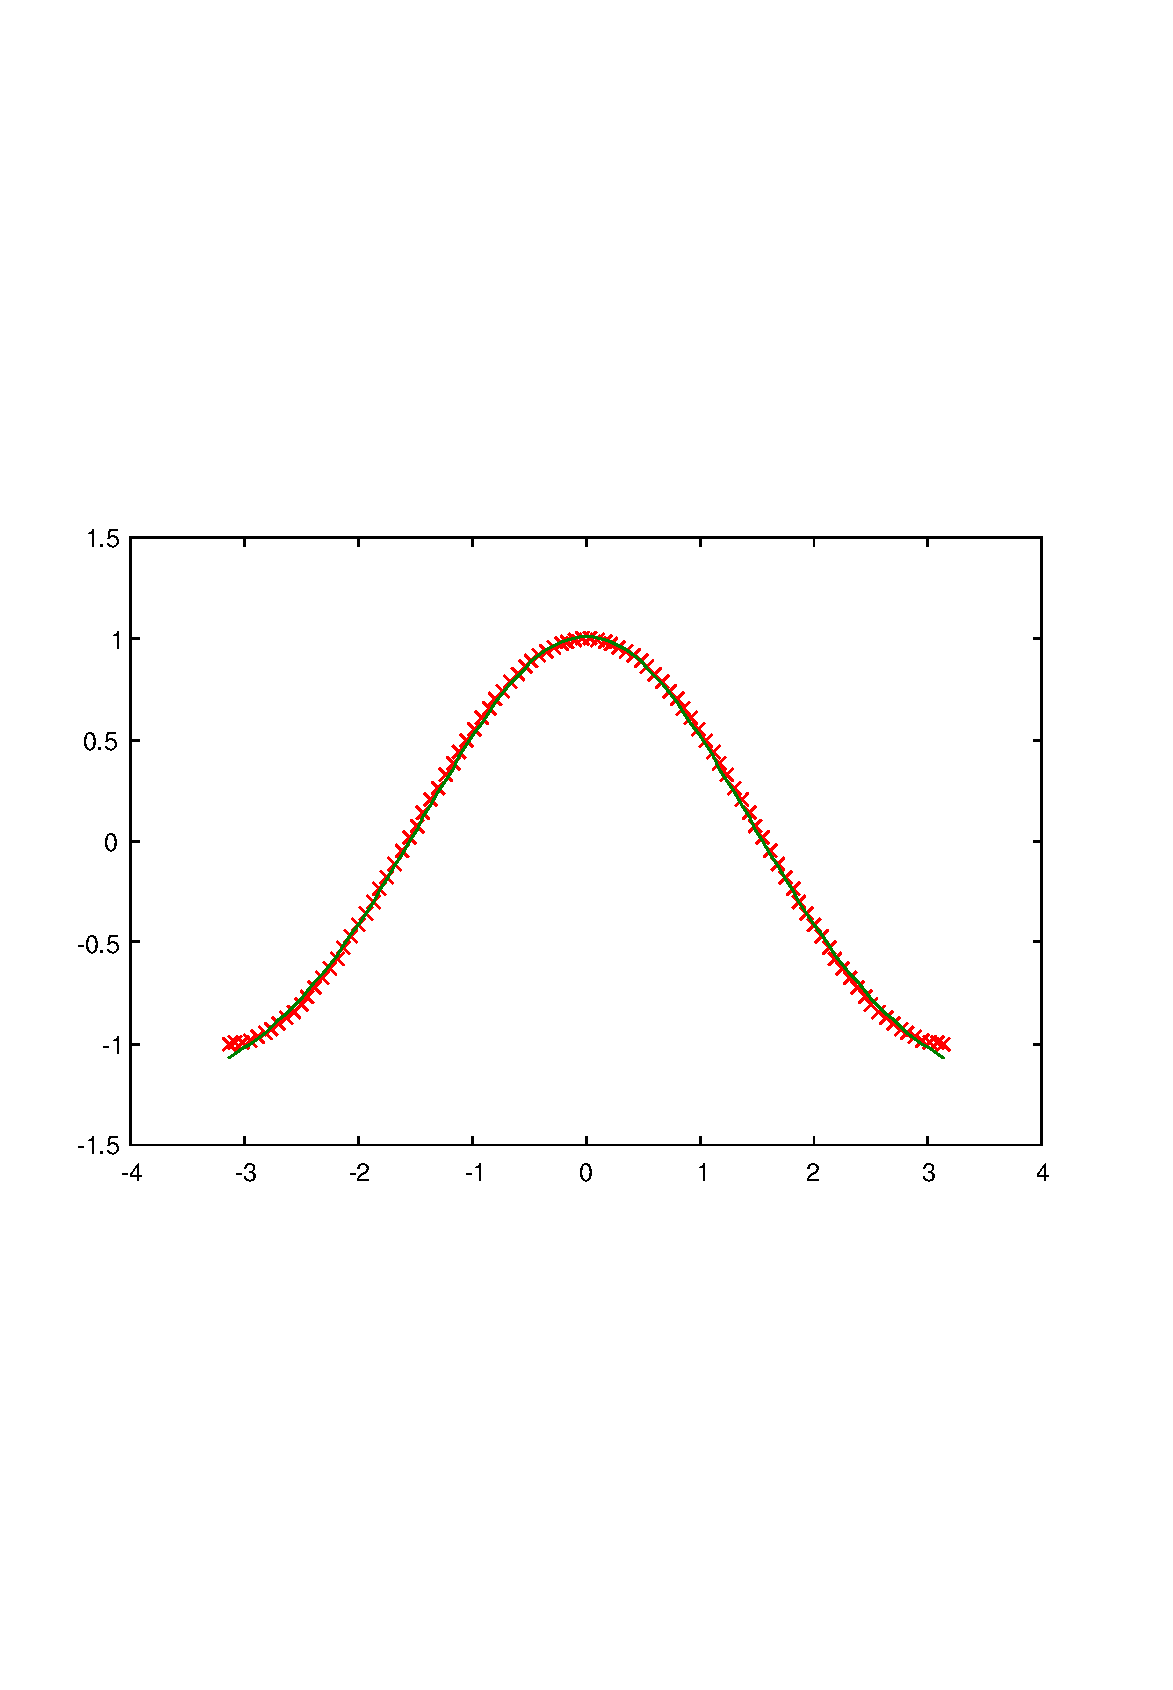
\includegraphics[width=12cm]{gausfit1}
\caption{gausfit1}
\end{DoxyImage}
 \hypertarget{curvefit_interp2}{}\section{I\-N\-T\-E\-R\-P2 2-\/\-D Interpolation}\label{curvefit_interp2}
Section\-: \hyperlink{sec_curvefit}{Optimization and Curve Fitting} \hypertarget{vtkwidgets_vtkxyplotwidget_Usage}{}\subsection{Usage}\label{vtkwidgets_vtkxyplotwidget_Usage}
Given a set of monotonically increasing {\ttfamily x} coordinates and a corresponding set of {\ttfamily y} values, performs simple linear interpolation to a new set of {\ttfamily x} coordinates. The general syntax for its usage is \begin{DoxyVerb}   zi = interp2(z,xi,yi)
\end{DoxyVerb}
 where {\ttfamily xi} and {\ttfamily yi} are vectors of the same length. The output vector {\ttfamily zi} is the same size as the input vector {\ttfamily xi}. For each element of {\ttfamily xi}, the values in {\ttfamily zi} are linearly interpolated by default. Interpolation method can be selected as\-: \begin{DoxyVerb}   zi = interp2(z,xi,yi,method)
\end{DoxyVerb}
 Default interpolation method is {\ttfamily 'linear'}. Other methods are {\ttfamily 'nearest'}, and {\ttfamily 'cubic'}. For values in {\ttfamily xi, yi} that are outside the size of {\ttfamily z}, the default value returned is Na\-N. To change this behavior, you can specify the extrapolation value\-: \begin{DoxyVerb}   zi = interp2(z,xi,yi,method,extrapval)
\end{DoxyVerb}
 The {\ttfamily z} and {\ttfamily xi,yi} vectors must be real, although complex types are allowed for {\ttfamily z}. \hypertarget{curvefit_interplin1}{}\section{I\-N\-T\-E\-R\-P\-L\-I\-N1 Linear 1-\/\-D Interpolation}\label{curvefit_interplin1}
Section\-: \hyperlink{sec_curvefit}{Optimization and Curve Fitting} \hypertarget{vtkwidgets_vtkxyplotwidget_Usage}{}\subsection{Usage}\label{vtkwidgets_vtkxyplotwidget_Usage}
Given a set of monotonically increasing {\ttfamily x} coordinates and a corresponding set of {\ttfamily y} values, performs simple linear interpolation to a new set of {\ttfamily x} coordinates. The general syntax for its usage is \begin{DoxyVerb}   yi = interplin1(x1,y1,xi)
\end{DoxyVerb}
 where {\ttfamily x1} and {\ttfamily y1} are vectors of the same length, and the entries in {\ttfamily x1} are monotoniccally increasing. The output vector {\ttfamily yi} is the same size as the input vector {\ttfamily xi}. For each element of {\ttfamily xi}, the values in {\ttfamily y1} are linearly interpolated. For values in {\ttfamily xi} that are outside the range of {\ttfamily x1} the default value returned is {\ttfamily nan}. To change this behavior, you can specify the extrapolation flag\-: \begin{DoxyVerb}   yi = interplin1(x1,y1,xi,extrapflag)
\end{DoxyVerb}
 Valid options for {\ttfamily extrapflag} are\-: 
\begin{DoxyItemize}
\item {\ttfamily 'nan'} -\/ extrapolated values are tagged with {\ttfamily nan}s  
\item {\ttfamily 'zero'} -\/ extrapolated values are set to zero  
\item {\ttfamily 'endpoint'} -\/ extrapolated values are set to the endpoint values  
\item {\ttfamily 'extrap'} -\/ linear extrapolation is performed  
\end{DoxyItemize}The {\ttfamily x1} and {\ttfamily xi} vectors must be real, although complex types are allowed for {\ttfamily y1}. \hypertarget{variables_struct_Example}{}\subsection{Example}\label{variables_struct_Example}
Here is an example of simple linear interpolation with the different extrapolation modes. We start with a fairly coarse sampling of a cosine.


\begin{DoxyVerbInclude}
--> x = linspace(-pi*7/8,pi*7/8,15);
--> y = cos(x);
--> plot(x,y,'ro');
\end{DoxyVerbInclude}


which is shown here  
\begin{DoxyImage}
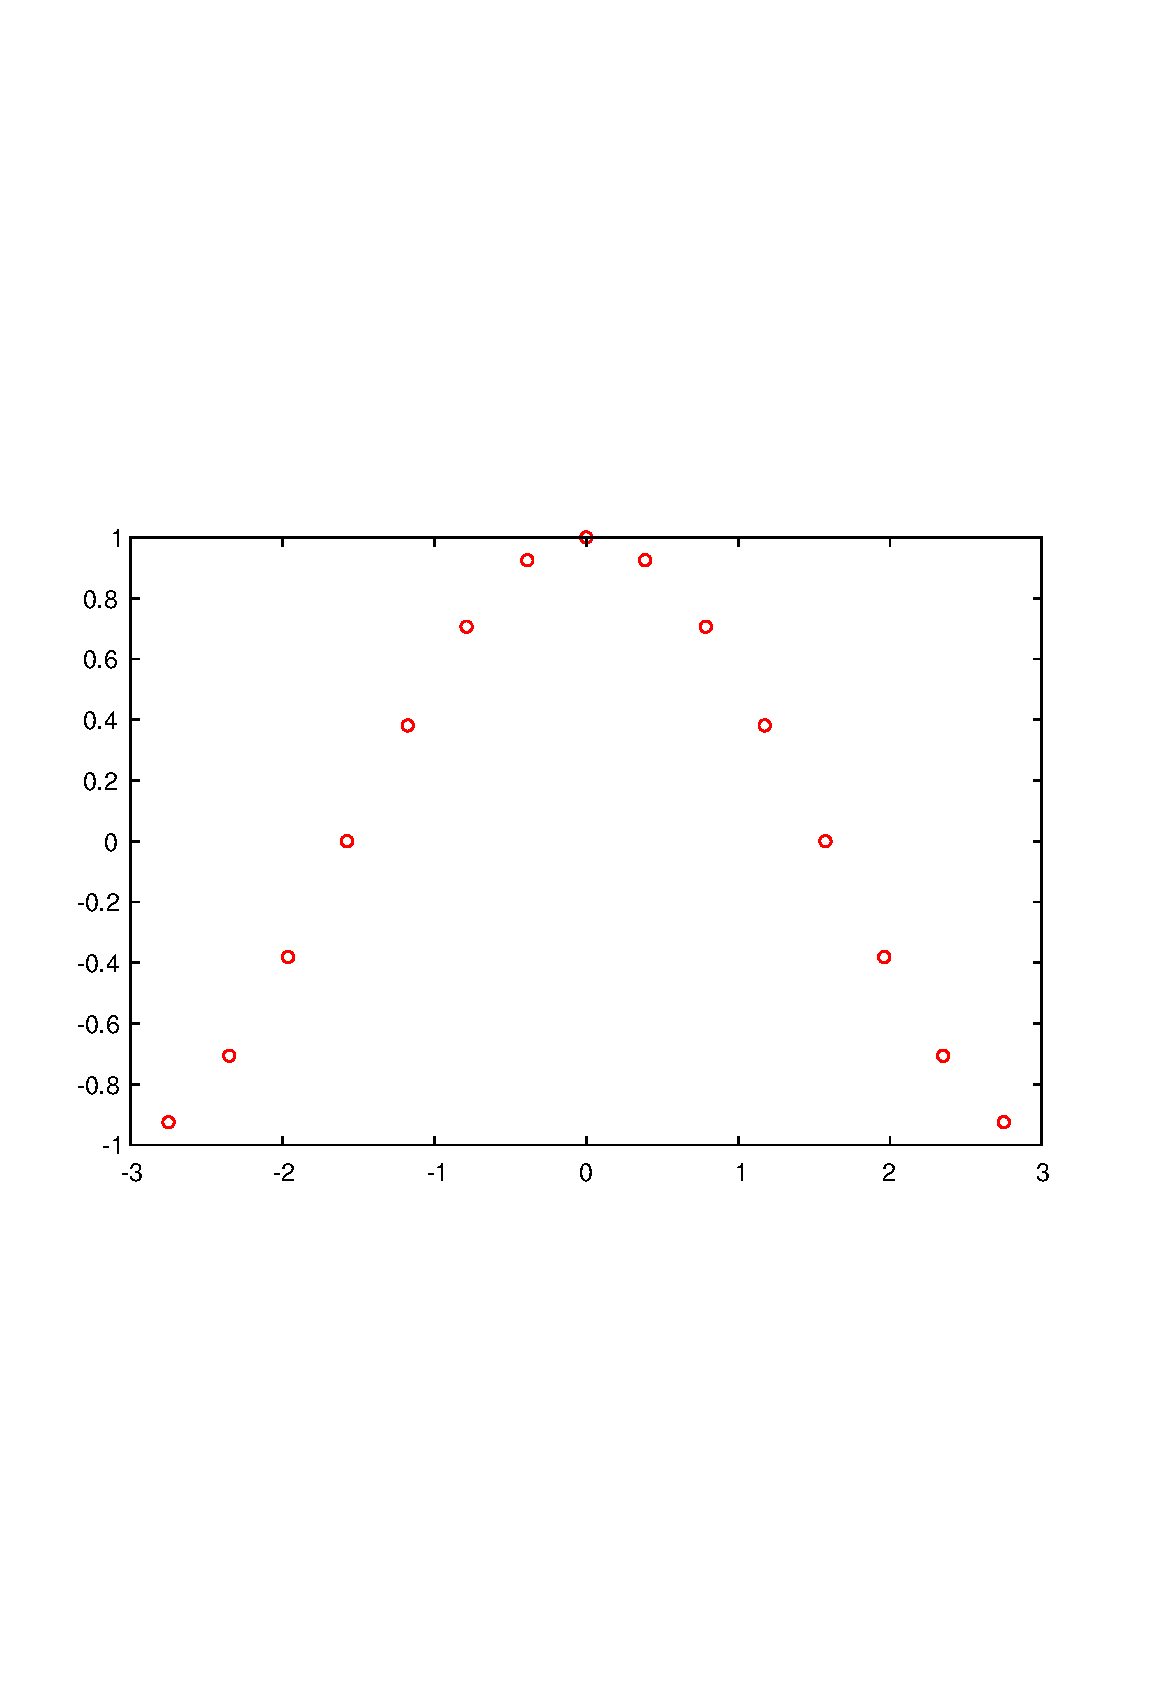
\includegraphics[width=12cm]{interplin1_1}
\caption{interplin1\-\_\-1}
\end{DoxyImage}
 Next, we generate a finer sampling over a slightly broader range (in this case {\ttfamily \mbox{[}-\/pi,pi\mbox{]}}). First, we demonstrate the {\ttfamily 'nan'} extrapolation method


\begin{DoxyVerbInclude}
--> xi = linspace(-4,4,100);
--> yi_nan = interplin1(x,y,xi,'nan');
--> yi_zero = interplin1(x,y,xi,'zero');
--> yi_endpoint = interplin1(x,y,xi,'endpoint');
--> yi_extrap = interplin1(x,y,xi,'extrap');
--> plot(x,y,'ro',xi,yi_nan,'g-x',xi,yi_zero,'g-x',xi,yi_endpoint,'g-x',xi,yi_extrap,'g-x');
\end{DoxyVerbInclude}


which is shown here  
\begin{DoxyImage}
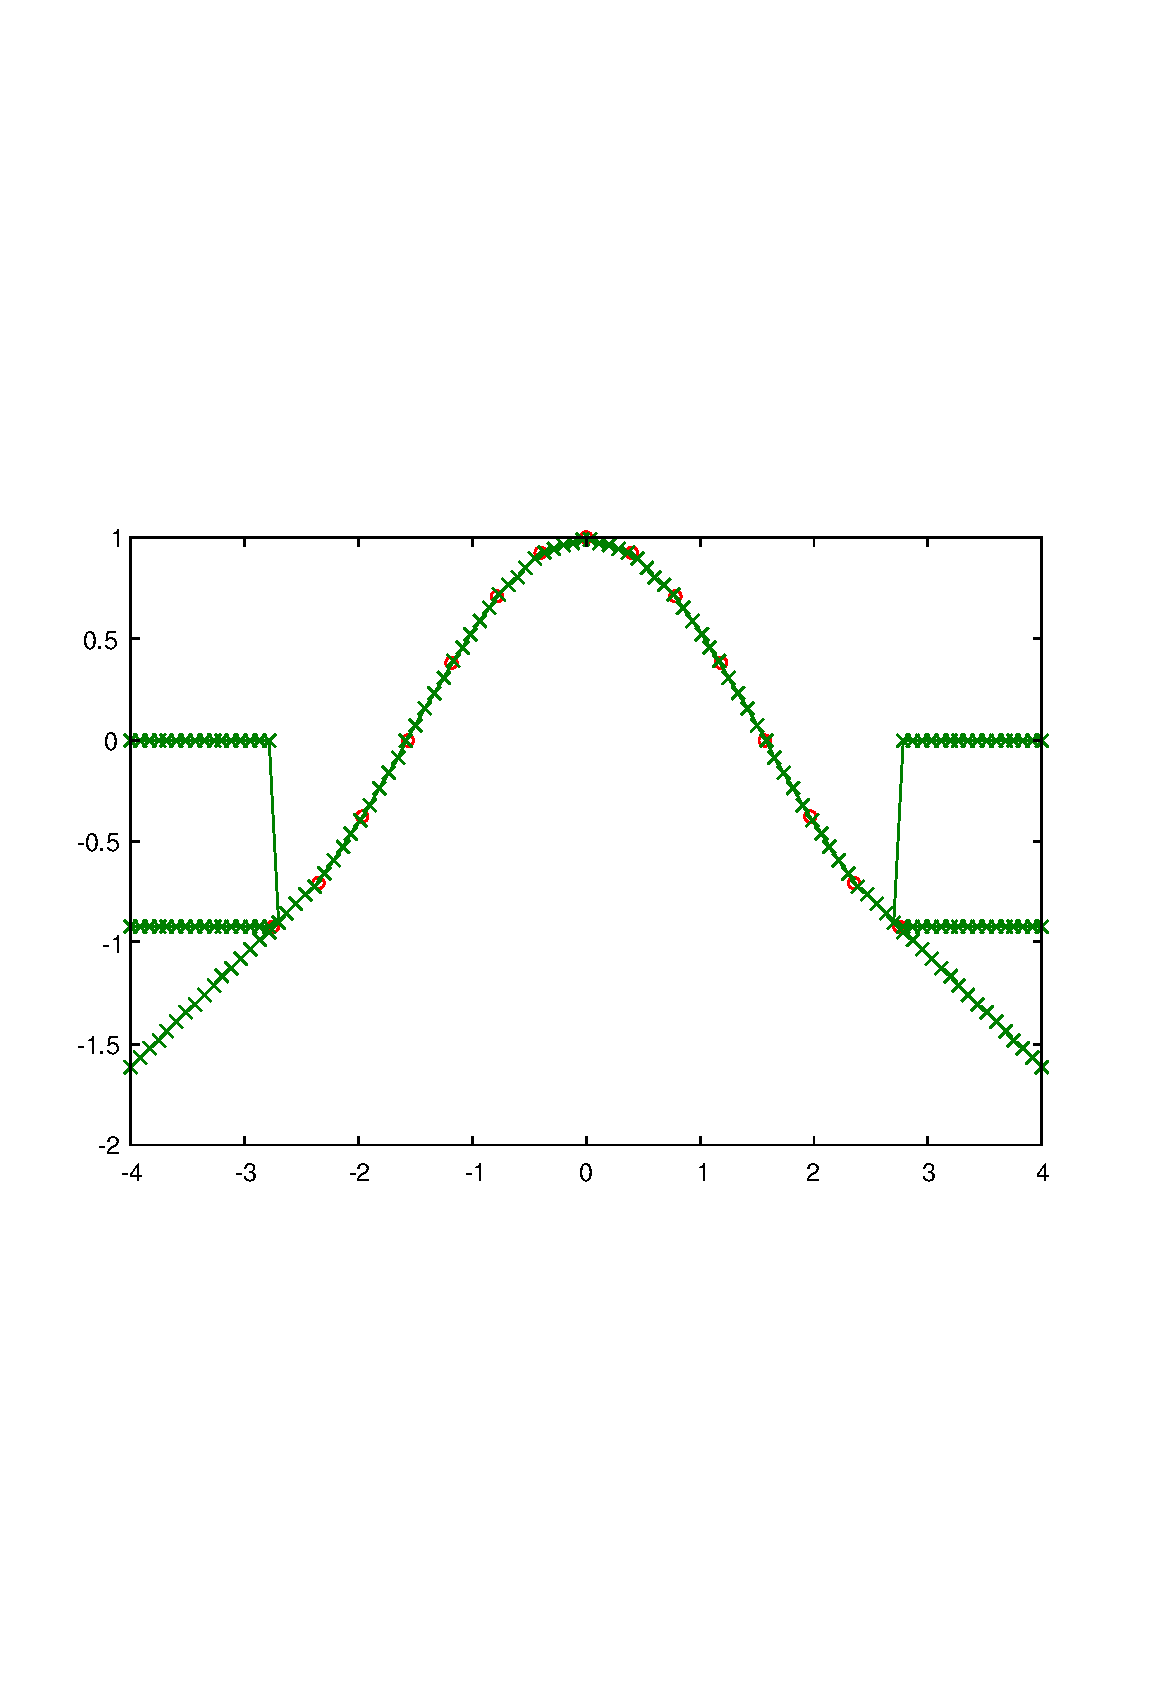
\includegraphics[width=12cm]{interplin1_2}
\caption{interplin1\-\_\-2}
\end{DoxyImage}
 \hypertarget{curvefit_poly}{}\section{P\-O\-L\-Y Convert Roots To Polynomial Coefficients}\label{curvefit_poly}
Section\-: \hyperlink{sec_curvefit}{Optimization and Curve Fitting} \hypertarget{vtkwidgets_vtkxyplotwidget_Usage}{}\subsection{Usage}\label{vtkwidgets_vtkxyplotwidget_Usage}
This function calculates the polynomial coefficients for given roots \begin{DoxyVerb}    p = poly(r)
\end{DoxyVerb}
 when {\ttfamily r} is a vector, is a vector whose elements are the coefficients of the polynomial whose roots are the elements of {\ttfamily r}. Alternately, you can provide a matrix \begin{DoxyVerb}    p = poly(A)
\end{DoxyVerb}
 when {\ttfamily A} is an {\ttfamily N x N} square matrix, is a row vector with {\ttfamily N+1} elements which are the coefficients of the characteristic polynomial, {\ttfamily det(lambda$\ast$eye(size(\-A))-\/\-A)}.

Contributed by Paulo Xavier Candeias under G\-P\-L. \hypertarget{variables_struct_Example}{}\subsection{Example}\label{variables_struct_Example}
Here are some examples of the use of {\ttfamily poly}


\begin{DoxyVerbInclude}
--> A = [1,2,3;4,5,6;7,8,0]

A = 
 1 2 3 
 4 5 6 
 7 8 0 

--> p = poly(A)

p = 
    1.0000   -6.0000  -72.0000  -27.0000 

--> r = roots(p)

r = 
   12.1229 
   -5.7345 
   -0.3884 
\end{DoxyVerbInclude}
 \hypertarget{curvefit_polyder}{}\section{P\-O\-L\-Y\-D\-E\-R Polynomial Coefficient Differentiation}\label{curvefit_polyder}
Section\-: \hyperlink{sec_curvefit}{Optimization and Curve Fitting} \hypertarget{vtkwidgets_vtkxyplotwidget_Usage}{}\subsection{Usage}\label{vtkwidgets_vtkxyplotwidget_Usage}
The {\ttfamily polyder} function returns the polynomial coefficients resulting from differentiation of polynomial {\ttfamily p}. The syntax for its use is either \begin{DoxyVerb} pder = polyder(p)
\end{DoxyVerb}
 for the derivitave of polynomial p, or \begin{DoxyVerb} convp1p2der = polyder(p1,p2)
\end{DoxyVerb}
 for the derivitave of polynomial conv(p1,p2), or still \begin{DoxyVerb} [nder,dder] = polyder(n,d)
\end{DoxyVerb}
 for the derivative of polynomial {\ttfamily n/d} ({\ttfamily nder} is the numerator and {\ttfamily dder} is the denominator). In all cases the polynomial coefficients are assumed to be in decreasing degree. Contributed by Paulo Xavier Candeias under G\-P\-L \hypertarget{variables_struct_Example}{}\subsection{Example}\label{variables_struct_Example}
Here are some examples of the use of {\ttfamily polyder}


\begin{DoxyVerbInclude}
--> polyder([2,3,4])

ans = 
 4 3 
\end{DoxyVerbInclude}



\begin{DoxyVerbInclude}
--> polyder([2,3,4],7)

ans = 
 28 21 
\end{DoxyVerbInclude}



\begin{DoxyVerbInclude}
--> [n,d] = polyder([2,3,4],5)
n = 
 -20 -15 

d = 
 25 
\end{DoxyVerbInclude}
 \hypertarget{curvefit_polyfit}{}\section{P\-O\-L\-Y\-F\-I\-T Fit Polynomial To Data}\label{curvefit_polyfit}
Section\-: \hyperlink{sec_curvefit}{Optimization and Curve Fitting} \hypertarget{vtkwidgets_vtkxyplotwidget_Usage}{}\subsection{Usage}\label{vtkwidgets_vtkxyplotwidget_Usage}
The {\ttfamily polyfit} routine has the following syntax \begin{DoxyVerb}  p = polyfit(x,y,n)
\end{DoxyVerb}
 where {\ttfamily x} and {\ttfamily y} are vectors of the same size, and {\ttfamily n} is the degree of the approximating polynomial. The resulting vector {\ttfamily p} forms the coefficients of the optimal polynomial (in descending degree) that fit {\ttfamily y} with {\ttfamily x}. \hypertarget{transforms_svd_Function}{}\subsection{Internals}\label{transforms_svd_Function}
The {\ttfamily polyfit} routine finds the approximating polynomial \[ p(x) = p_1 x^n + p_2 x^{n-1} + \dots + p_n x + p_{n+1} \] such that \[ \sum_{i} (p(x_i) - y_i)^2 \] is minimized. It does so by forming the Vandermonde matrix and solving the resulting set of equations using the backslash operator. Note that the Vandermonde matrix can become poorly conditioned with large {\ttfamily n} quite rapidly. \hypertarget{variables_struct_Example}{}\subsection{Example}\label{variables_struct_Example}
A classic example from Edwards and Penny, consider the problem of approximating a sinusoid with a polynomial. We start with a vector of points evenly spaced on the unit interval, along with a vector of the sine of these points.


\begin{DoxyVerbInclude}
--> x = linspace(0,1,20);
--> y = sin(2*pi*x);
--> plot(x,y,'r-')
\end{DoxyVerbInclude}


The resulting plot is shown here  
\begin{DoxyImage}
\includegraphics[width=12cm]{polyfit1}
\caption{polyfit1}
\end{DoxyImage}
 Next, we fit a third degree polynomial to the sine, and use {\ttfamily polyval} to plot it


\begin{DoxyVerbInclude}
--> p = polyfit(x,y,3)

p = 
   21.9170  -32.8756   11.1897   -0.1156 

--> f = polyval(p,x);
--> plot(x,y,'r-',x,f,'ko');
\end{DoxyVerbInclude}


The resulting plot is shown here  
\begin{DoxyImage}
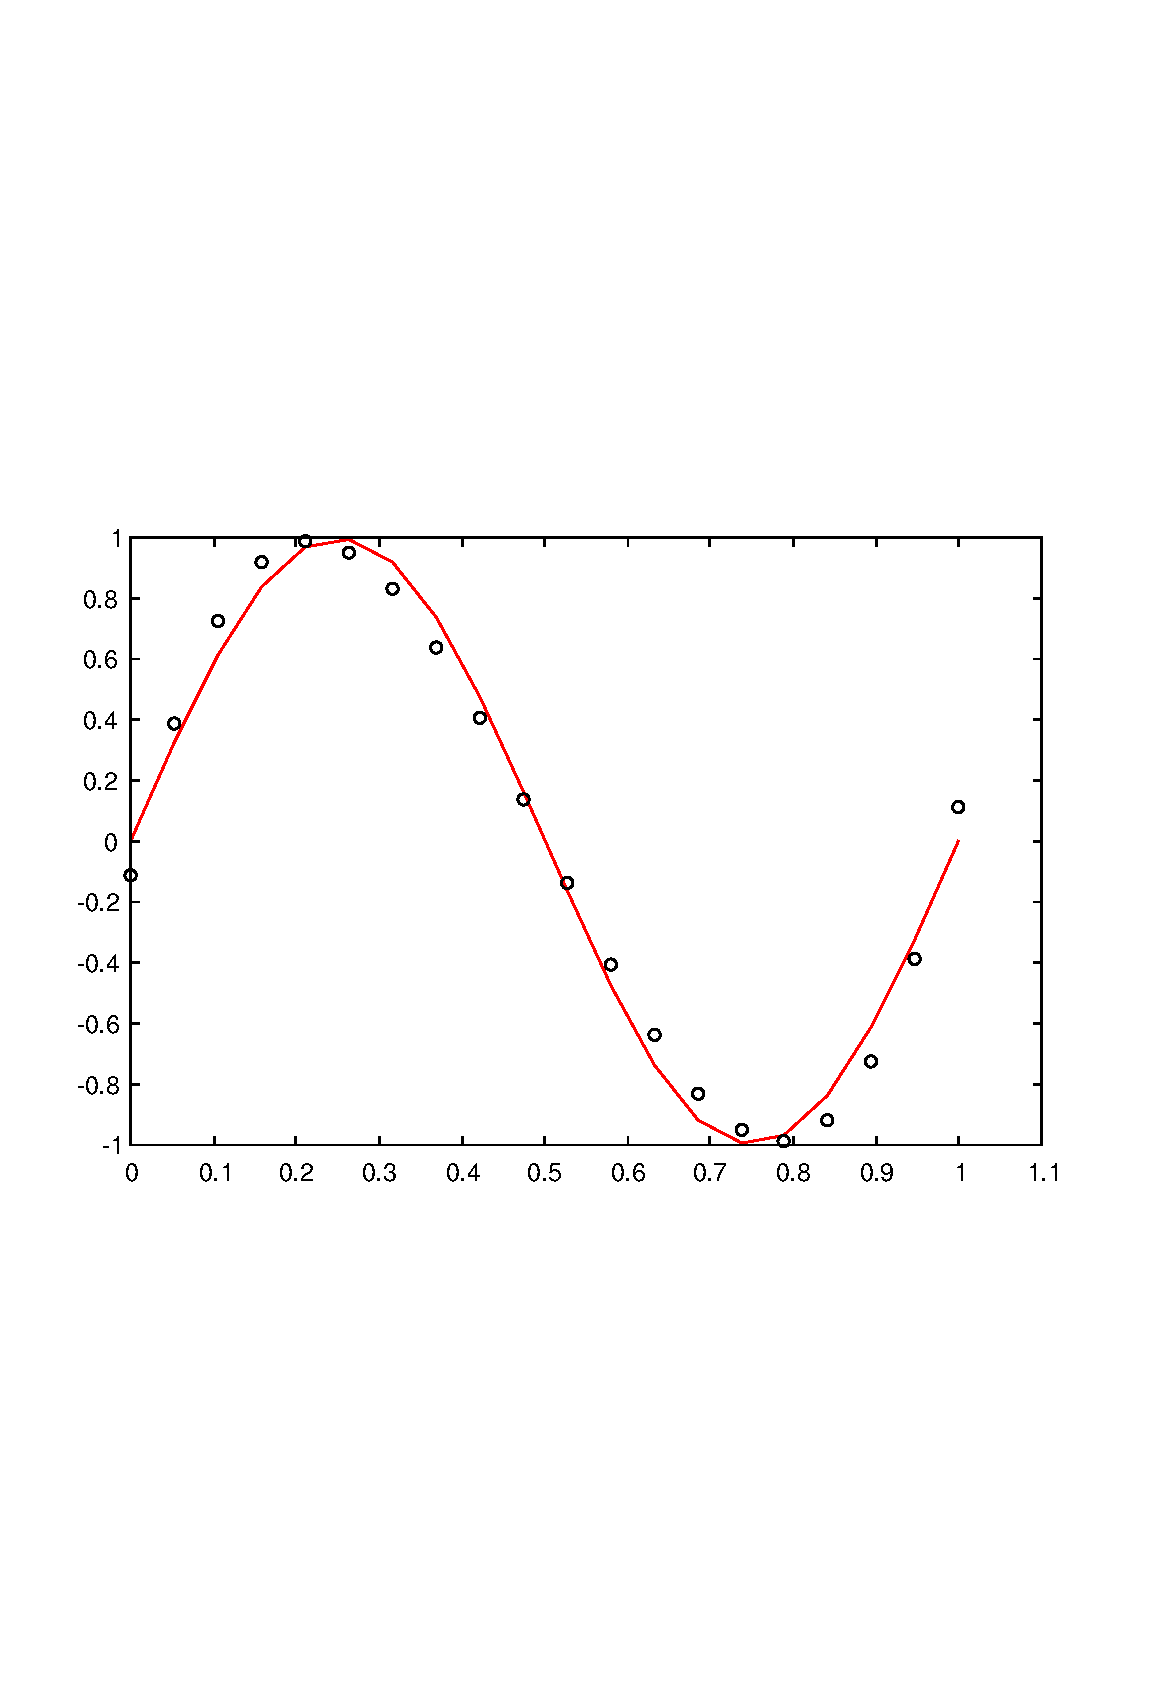
\includegraphics[width=12cm]{polyfit2}
\caption{polyfit2}
\end{DoxyImage}
 Increasing the order improves the fit, as


\begin{DoxyVerbInclude}
--> p = polyfit(x,y,11)

p = 

 Columns 1 to 7

   12.4644  -68.5541  130.0555  -71.0940  -38.2814  -14.1222   85.1018 

 Columns 8 to 12

   -0.5642  -41.2861   -0.0029    6.2832   -0.0000 

--> f = polyval(p,x);
--> plot(x,y,'r-',x,f,'ko');
\end{DoxyVerbInclude}


The resulting plot is shown here  
\begin{DoxyImage}
\includegraphics[width=12cm]{polyfit3}
\caption{polyfit3}
\end{DoxyImage}
 \hypertarget{curvefit_polyint}{}\section{P\-O\-L\-Y\-I\-N\-T Polynomial Coefficient Integration}\label{curvefit_polyint}
Section\-: \hyperlink{sec_curvefit}{Optimization and Curve Fitting} \hypertarget{vtkwidgets_vtkxyplotwidget_Usage}{}\subsection{Usage}\label{vtkwidgets_vtkxyplotwidget_Usage}
The polyint function returns the polynomial coefficients resulting from integration of polynomial p. The syntax for its use is either \begin{DoxyVerb} pint = polyint(p,k)
\end{DoxyVerb}
 or, for a default {\ttfamily k = 0}, \begin{DoxyVerb} pint = polyint(p);
\end{DoxyVerb}
 where {\ttfamily p} is a vector of polynomial coefficients assumed to be in decreasing degree and {\ttfamily k} is the integration constant. Contributed by Paulo Xavier Candeias under G\-P\-L \hypertarget{variables_struct_Example}{}\subsection{Example}\label{variables_struct_Example}
Here is are some examples of the use of {\ttfamily polyint}.


\begin{DoxyVerbInclude}
--> polyint([2,3,4])

ans = 
    0.6667    1.5000    4.0000         0 
\end{DoxyVerbInclude}


And


\begin{DoxyVerbInclude}
--> polyint([2,3,4],5)

ans = 
    0.6667    1.5000    4.0000    5.0000 
\end{DoxyVerbInclude}
 \hypertarget{curvefit_polyval}{}\section{P\-O\-L\-Y\-V\-A\-L Evaluate Polynomial Fit at Selected Points}\label{curvefit_polyval}
Section\-: \hyperlink{sec_curvefit}{Optimization and Curve Fitting} \hypertarget{vtkwidgets_vtkxyplotwidget_Usage}{}\subsection{Usage}\label{vtkwidgets_vtkxyplotwidget_Usage}
The {\ttfamily polyval} routine has the following syntax \begin{DoxyVerb}  y = polyval(p,x)
\end{DoxyVerb}
 where {\ttfamily p} is a vector of polynomial coefficients, in decreasing degree (as generated by {\ttfamily polyfit}, for example). If {\ttfamily x} is a matrix, the polynomial is evaluated in the matrix sense (in which case {\ttfamily x} must be square). \hypertarget{transforms_svd_Function}{}\subsection{Internals}\label{transforms_svd_Function}
The polynomial is evaluated using a recursion method. If the polynomial is \[ p(x) = p_1 x^n + p_2 x^{n-1} + \dots + p_n x + p_{n+1} \] then the calculation is performed as \[ p(x) = ((p_1) x + p_2) x + p_3 \] \hypertarget{variables_struct_Example}{}\subsection{Example}\label{variables_struct_Example}
Here is a plot of {\ttfamily x$^\wedge$3} generated using polyval


\begin{DoxyVerbInclude}
--> p = [1 0 0 0]

p = 
 1 0 0 0 

--> x = linspace(-1,1);
--> y = polyval(p,x);
--> plot(x,y,'r-')
\end{DoxyVerbInclude}


Here is the resulting plot  
\begin{DoxyImage}
\includegraphics[width=12cm]{polyval1}
\caption{polyval1}
\end{DoxyImage}
 \hypertarget{curvefit_roots}{}\section{R\-O\-O\-T\-S Find Roots of Polynomial}\label{curvefit_roots}
Section\-: \hyperlink{sec_curvefit}{Optimization and Curve Fitting} \hypertarget{vtkwidgets_vtkxyplotwidget_Usage}{}\subsection{Usage}\label{vtkwidgets_vtkxyplotwidget_Usage}
The {\ttfamily roots} routine will return a column vector containing the roots of a polynomial. The general syntax is \begin{DoxyVerb}   z = roots(p)
\end{DoxyVerb}
 where {\ttfamily p} is a vector containing the coefficients of the polynomial ordered in descending powers. \hypertarget{transforms_svd_Function}{}\subsection{Internals}\label{transforms_svd_Function}
Given a vector \[ [p_1, p_2, \dots p_n] \] which describes a polynomial \[ p_1 x^{n-1} + p_2 x^{n-2} + \dots + p_n \] we construct the companion matrix (which has a characteristic polynomial matching the polynomial described by {\ttfamily p}), and then find the eigenvalues of it (which are the roots of its characteristic polynomial), and which are also the roots of the polynomial of interest. This technique for finding the roots is described in the help page for {\ttfamily roots} on the Mathworks website. \hypertarget{variables_struct_Example}{}\subsection{Example}\label{variables_struct_Example}
Here is an example of finding the roots to the polynomial \[ x^3 - 6x^2 - 72x - 27 \]


\begin{DoxyVerbInclude}
--> roots([1 -6 -72 -27])

ans = 
   12.1229 
   -5.7345 
   -0.3884 
\end{DoxyVerbInclude}
 
\chapter{Debugging Free\-Mat Code}
\label{sec_debug}
\hypertarget{sec_debug}{}

\begin{DoxyItemize}
\item \hyperlink{debug_dbauto}{D\-B\-A\-U\-T\-O Control Dbauto Functionality}  
\item \hyperlink{debug_dbdelete}{D\-B\-D\-E\-L\-E\-T\-E Delete a Breakpoint}  
\item \hyperlink{debug_dbdown}{D\-B\-Down Move Down One Debug Level}  
\item \hyperlink{debug_dblist}{D\-B\-L\-I\-S\-T List Breakpoints}  
\item \hyperlink{debug_dbstep}{D\-B\-S\-T\-E\-P Step N Statements}  
\item \hyperlink{debug_dbstop}{D\-B\-S\-T\-O\-P}  
\item \hyperlink{debug_dbup}{D\-B\-U\-P Move Up One Debug Level}  
\item \hyperlink{debug_fdump}{F\-D\-U\-M\-P Dump Information on Function}  
\end{DoxyItemize}\hypertarget{debug_dbauto}{}\section{D\-B\-A\-U\-T\-O Control Dbauto Functionality}\label{debug_dbauto}
Section\-: \hyperlink{sec_debug}{Debugging Free\-Mat Code} \hypertarget{vtkwidgets_vtkxyplotwidget_Usage}{}\subsection{Usage}\label{vtkwidgets_vtkxyplotwidget_Usage}
The dbauto functionality in Free\-Mat allows you to debug your Free\-Mat programs. When {\ttfamily dbauto} is {\ttfamily on}, then any error that occurs while the program is running causes Free\-Mat to stop execution at that point and return you to the command line (just as if you had placed a {\ttfamily keyboard} command there). You can then examine variables, modify them, and resume execution using {\ttfamily return}. Alternately, you can exit out of all running routines via a {\ttfamily retall} statement. Note that errors that occur inside of {\ttfamily try}/{\ttfamily catch} blocks do not (by design) cause auto breakpoints. The {\ttfamily dbauto} function toggles the dbauto state of Free\-Mat. The syntax for its use is \begin{DoxyVerb}   dbauto(state)
\end{DoxyVerb}
 where {\ttfamily state} is either \begin{DoxyVerb}   dbauto('on')
\end{DoxyVerb}
 to activate dbauto, or \begin{DoxyVerb}   dbauto('off')
\end{DoxyVerb}
 to deactivate dbauto. Alternately, you can use Free\-Mat's string-\/syntax equivalence and enter \begin{DoxyVerb}   dbauto on
\end{DoxyVerb}
 or \begin{DoxyVerb}   dbauto off
\end{DoxyVerb}
 to turn dbauto on or off (respectively). Entering {\ttfamily dbauto} with no arguments returns the current state (either 'on' or 'off'). \hypertarget{debug_dbdelete}{}\section{D\-B\-D\-E\-L\-E\-T\-E Delete a Breakpoint}\label{debug_dbdelete}
Section\-: \hyperlink{sec_debug}{Debugging Free\-Mat Code} \hypertarget{vtkwidgets_vtkxyplotwidget_Usage}{}\subsection{Usage}\label{vtkwidgets_vtkxyplotwidget_Usage}
The {\ttfamily dbdelete} function deletes a breakpoint. The syntax for the {\ttfamily dbdelete} function is \begin{DoxyVerb}  dbdelete(num)
\end{DoxyVerb}
 where {\ttfamily num} is the number of the breakpoint to delete. \hypertarget{debug_dbdown}{}\section{D\-B\-Down Move Down One Debug Level}\label{debug_dbdown}
Section\-: \hyperlink{sec_debug}{Debugging Free\-Mat Code} \hypertarget{vtkwidgets_vtkxyplotwidget_Usage}{}\subsection{Usage}\label{vtkwidgets_vtkxyplotwidget_Usage}
The {\ttfamily dbdown} function moves up one level in the debug hierarchy. The syntax for the {\ttfamily dbdown} function is \begin{DoxyVerb} dbdown
\end{DoxyVerb}
 \hypertarget{debug_dblist}{}\section{D\-B\-L\-I\-S\-T List Breakpoints}\label{debug_dblist}
Section\-: \hyperlink{sec_debug}{Debugging Free\-Mat Code} \hypertarget{vtkwidgets_vtkxyplotwidget_Usage}{}\subsection{Usage}\label{vtkwidgets_vtkxyplotwidget_Usage}
List the current set of breakpoints. The syntax for the {\ttfamily dblist} is simply \begin{DoxyVerb}  dblist
\end{DoxyVerb}
 \hypertarget{debug_dbstep}{}\section{D\-B\-S\-T\-E\-P Step N Statements}\label{debug_dbstep}
Section\-: \hyperlink{sec_debug}{Debugging Free\-Mat Code} \hypertarget{vtkwidgets_vtkxyplotwidget_Usage}{}\subsection{Usage}\label{vtkwidgets_vtkxyplotwidget_Usage}
Step {\ttfamily N} statements during debug mode. The synax for this is either \begin{DoxyVerb}  dbstep(N)
\end{DoxyVerb}
 to step {\ttfamily N} statements, or \begin{DoxyVerb}  dbstep
\end{DoxyVerb}
 to step one statement. \hypertarget{debug_dbstop}{}\section{D\-B\-S\-T\-O\-P}\label{debug_dbstop}
Section\-: \hyperlink{sec_debug}{Debugging Free\-Mat Code} \hypertarget{vtkwidgets_vtkxyplotwidget_Usage}{}\subsection{Usage}\label{vtkwidgets_vtkxyplotwidget_Usage}
Set a breakpoint. The syntax for this is\-: \begin{DoxyVerb}  dbstop(funcname,linenumber)
\end{DoxyVerb}
 where {\ttfamily funcname} is the name of the function where we want to set the breakpoint, and {\ttfamily linenumber} is the line number. \hypertarget{debug_dbup}{}\section{D\-B\-U\-P Move Up One Debug Level}\label{debug_dbup}
Section\-: \hyperlink{sec_debug}{Debugging Free\-Mat Code} \hypertarget{vtkwidgets_vtkxyplotwidget_Usage}{}\subsection{Usage}\label{vtkwidgets_vtkxyplotwidget_Usage}
The {\ttfamily dbup} function moves up one level in the debug hierarchy. The syntax for the {\ttfamily dbup} function is \begin{DoxyVerb} dbup
\end{DoxyVerb}
 \hypertarget{debug_fdump}{}\section{F\-D\-U\-M\-P Dump Information on Function}\label{debug_fdump}
Section\-: \hyperlink{sec_debug}{Debugging Free\-Mat Code} \hypertarget{vtkwidgets_vtkxyplotwidget_Usage}{}\subsection{Usage}\label{vtkwidgets_vtkxyplotwidget_Usage}
Dumps information about a function (diagnostic information only) \begin{DoxyVerb}   fdump fname
\end{DoxyVerb}
 
\chapter{Elementary Functions}
\label{sec_elementary}
\hypertarget{sec_elementary}{}

\begin{DoxyItemize}
\item \hyperlink{elementary_abs}{A\-B\-S Absolute Value Function}  
\item \hyperlink{elementary_all}{A\-L\-L All True Function}  
\item \hyperlink{elementary_any}{A\-N\-Y Any True Function}  
\item \hyperlink{elementary_ceil}{C\-E\-I\-L Ceiling Function}  
\item \hyperlink{elementary_conj}{C\-O\-N\-J Conjugate Function}  
\item \hyperlink{elementary_cov}{C\-O\-V Covariance Matrix}  
\item \hyperlink{elementary_cumprod}{C\-U\-M\-P\-R\-O\-D Cumulative Product Function}  
\item \hyperlink{elementary_cumsum}{C\-U\-M\-S\-U\-M Cumulative Summation Function}  
\item \hyperlink{elementary_deal}{D\-E\-A\-L Multiple Simultaneous Assignments}  
\item \hyperlink{elementary_dec2hex}{D\-E\-C2\-H\-E\-X Convert Decimal Number to Hexadecimal}  
\item \hyperlink{elementary_diff}{D\-I\-F\-F Difference Function}  
\item \hyperlink{elementary_dot}{D\-O\-T Dot Product Function}  
\item \hyperlink{elementary_floor}{F\-L\-O\-O\-R Floor Function}  
\item \hyperlink{elementary_getfield}{G\-E\-T\-F\-I\-E\-L\-D Get Field Contents}  
\item \hyperlink{elementary_hex2dec}{H\-E\-X2\-D\-E\-C Convert Hexadecimal Numbers To Decimal}  
\item \hyperlink{elementary_imag}{I\-M\-A\-G Imaginary Function}  
\item \hyperlink{elementary_ind2sub}{I\-N\-D2\-S\-U\-B Convert Linear Indexing To Multiple Indexing }  
\item \hyperlink{elementary_max}{M\-A\-X Maximum Function}  
\item \hyperlink{elementary_mean}{M\-E\-A\-N Mean Function}  
\item \hyperlink{elementary_min}{M\-I\-N Minimum Function}  
\item \hyperlink{elementary_num2hex}{N\-U\-M2\-H\-E\-X Convert Numbers to I\-E\-E\-E Hex Strings}  
\item \hyperlink{elementary_prod}{P\-R\-O\-D Product Function}  
\item \hyperlink{elementary_real}{R\-E\-A\-L Real Function}  
\item \hyperlink{elementary_round}{R\-O\-U\-N\-D Round Function}  
\item \hyperlink{elementary_std}{S\-T\-D Standard Deviation Function}  
\item \hyperlink{elementary_sub2ind}{S\-U\-B2\-I\-N\-D Convert Multiple Indexing To Linear Indexing}  
\item \hyperlink{elementary_sum}{S\-U\-M Sum Function}  
\item \hyperlink{elementary_test}{T\-E\-S\-T Test Function}  
\item \hyperlink{elementary_var}{V\-A\-R Variance Function}  
\item \hyperlink{elementary_vec}{V\-E\-C Reshape to a Vector}  
\end{DoxyItemize}\hypertarget{elementary_abs}{}\section{A\-B\-S Absolute Value Function}\label{elementary_abs}
Section\-: \hyperlink{sec_elementary}{Elementary Functions} \hypertarget{vtkwidgets_vtkxyplotwidget_Usage}{}\subsection{Usage}\label{vtkwidgets_vtkxyplotwidget_Usage}
Returns the absolute value of the input array for all elements. The general syntax for its use is \begin{DoxyVerb}   y = abs(x)
\end{DoxyVerb}
 where {\ttfamily x} is an {\ttfamily n}-\/dimensional array of numerical type. The output is the same numerical type as the input, unless the input is {\ttfamily complex} or {\ttfamily dcomplex}. For {\ttfamily complex} inputs, the absolute value is a floating point array, so that the return type is {\ttfamily float}. For {\ttfamily dcomplex} inputs, the absolute value is a double precision floating point array, so that the return type is {\ttfamily double}. \hypertarget{variables_struct_Example}{}\subsection{Example}\label{variables_struct_Example}
The following demonstrates the {\ttfamily abs} applied to a complex scalar.


\begin{DoxyVerbInclude}
--> abs(3+4*i)

ans = 
 5 
\end{DoxyVerbInclude}


The {\ttfamily abs} function applied to integer and real values\-:


\begin{DoxyVerbInclude}
--> abs([-2,3,-4,5])

ans = 
 2 3 4 5 
\end{DoxyVerbInclude}


For a double-\/precision complex array,


\begin{DoxyVerbInclude}
--> abs([2.0+3.0*i,i])

ans = 
    3.6056    1.0000 
\end{DoxyVerbInclude}
 \hypertarget{elementary_all}{}\section{A\-L\-L All True Function}\label{elementary_all}
Section\-: \hyperlink{sec_elementary}{Elementary Functions} \hypertarget{vtkwidgets_vtkxyplotwidget_Usage}{}\subsection{Usage}\label{vtkwidgets_vtkxyplotwidget_Usage}
Reduces a logical array along a given dimension by testing for all logical 1s. The general syntax for its use is \begin{DoxyVerb}  y = all(x,d)
\end{DoxyVerb}
 where {\ttfamily x} is an {\ttfamily n}-\/dimensions array of {\ttfamily logical} type. The output is of {\ttfamily logical} type. The argument {\ttfamily d} is optional, and denotes the dimension along which to operate. The output {\ttfamily y} is the same size as {\ttfamily x}, except that it is singular along the operated direction. So, for example, if {\ttfamily x} is a {\ttfamily 3 x 3 x 4} array, and we {\ttfamily all} operation along dimension {\ttfamily d=2}, then the output is of size {\ttfamily 3 x 1 x 4}. \hypertarget{transforms_svd_Function}{}\subsection{Internals}\label{transforms_svd_Function}
The output is computed via \[ y(m_1,\ldots,m_{d-1},1,m_{d+1},\ldots,m_{p}) = \min_{k} x(m_1,\ldots,m_{d-1},k,m_{d+1},\ldots,m_{p}) \] If {\ttfamily d} is omitted, then the minimum is taken over all elements of {\ttfamily x}. \hypertarget{variables_struct_Example}{}\subsection{Example}\label{variables_struct_Example}
The following piece of code demonstrates various uses of the {\ttfamily all} function


\begin{DoxyVerbInclude}
--> A = [1,0,0;1,0,0;0,0,1]

A = 
 1 0 0 
 1 0 0 
 0 0 1 
\end{DoxyVerbInclude}


We start by calling {\ttfamily all} without a dimension argument, in which case it defaults to testing all values of {\ttfamily A}


\begin{DoxyVerbInclude}
--> all(A)

ans = 
 0 0 0 
\end{DoxyVerbInclude}


The {\ttfamily all} function is useful in expressions also.


\begin{DoxyVerbInclude}
--> all(A>=0)

ans = 
 1 1 1 
\end{DoxyVerbInclude}


Next, we apply the {\ttfamily all} operation along the rows.


\begin{DoxyVerbInclude}
--> all(A,2)

ans = 
 0 
 0 
 0 
\end{DoxyVerbInclude}
 \hypertarget{elementary_any}{}\section{A\-N\-Y Any True Function}\label{elementary_any}
Section\-: \hyperlink{sec_elementary}{Elementary Functions} \hypertarget{vtkwidgets_vtkxyplotwidget_Usage}{}\subsection{Usage}\label{vtkwidgets_vtkxyplotwidget_Usage}
Reduces a logical array along a given dimension by testing for any logical 1s. The general syntax for its use is \begin{DoxyVerb}  y = any(x,d)
\end{DoxyVerb}
 where {\ttfamily x} is an {\ttfamily n}-\/dimensions array of {\ttfamily logical} type. The output is of {\ttfamily logical} type. The argument {\ttfamily d} is optional, and denotes the dimension along which to operate. The output {\ttfamily y} is the same size as {\ttfamily x}, except that it is singular along the operated direction. So, for example, if {\ttfamily x} is a {\ttfamily 3 x 3 x 4} array, and we {\ttfamily any} operation along dimension {\ttfamily d=2}, then the output is of size {\ttfamily 3 x 1 x 4}. \hypertarget{transforms_svd_Function}{}\subsection{Internals}\label{transforms_svd_Function}
The output is computed via \[ y(m_1,\ldots,m_{d-1},1,m_{d+1},\ldots,m_{p}) = \max_{k} x(m_1,\ldots,m_{d-1},k,m_{d+1},\ldots,m_{p}) \] If {\ttfamily d} is omitted, then the summation is taken along the first non-\/singleton dimension of {\ttfamily x}. \hypertarget{variables_struct_Example}{}\subsection{Example}\label{variables_struct_Example}
The following piece of code demonstrates various uses of the summation function


\begin{DoxyVerbInclude}
--> A = [1,0,0;1,0,0;0,0,1]

A = 
 1 0 0 
 1 0 0 
 0 0 1 
\end{DoxyVerbInclude}


We start by calling {\ttfamily any} without a dimension argument, in which case it defaults to the first nonsingular dimension (in this case, along the columns or {\ttfamily d = 1}).


\begin{DoxyVerbInclude}
--> any(A)

ans = 
 1 0 1 
\end{DoxyVerbInclude}


Next, we apply the {\ttfamily any} operation along the rows.


\begin{DoxyVerbInclude}
--> any(A,2)

ans = 
 1 
 1 
 1 
\end{DoxyVerbInclude}
 \hypertarget{elementary_ceil}{}\section{C\-E\-I\-L Ceiling Function}\label{elementary_ceil}
Section\-: \hyperlink{sec_elementary}{Elementary Functions} \hypertarget{vtkwidgets_vtkxyplotwidget_Usage}{}\subsection{Usage}\label{vtkwidgets_vtkxyplotwidget_Usage}
Computes the ceiling of an n-\/dimensional array elementwise. The ceiling of a number is defined as the smallest integer that is larger than or equal to that number. The general syntax for its use is \begin{DoxyVerb}   y = ceil(x)
\end{DoxyVerb}
 where {\ttfamily x} is a multidimensional array of numerical type. The {\ttfamily ceil} function preserves the type of the argument. So integer arguments are not modified, and {\ttfamily float} arrays return {\ttfamily float} arrays as outputs, and similarly for {\ttfamily double} arrays. The {\ttfamily ceil} function is not defined for {\ttfamily complex} or {\ttfamily dcomplex} types. \hypertarget{variables_struct_Example}{}\subsection{Example}\label{variables_struct_Example}
The following demonstrates the {\ttfamily ceil} function applied to various (numerical) arguments. For integer arguments, the ceil function has no effect\-:


\begin{DoxyVerbInclude}
--> ceil(3)

ans = 
 3 

--> ceil(-3)

ans = 
 -3 
\end{DoxyVerbInclude}


Next, we take the {\ttfamily ceil} of a floating point value\-:


\begin{DoxyVerbInclude}
--> ceil(float(3.023))

ans = 
 4 

--> ceil(float(-2.341))

ans = 
 -2 
\end{DoxyVerbInclude}


Note that the return type is a {\ttfamily float} also. Finally, for a {\ttfamily double} type\-:


\begin{DoxyVerbInclude}
--> ceil(4.312)

ans = 
 5 

--> ceil(-5.32)

ans = 
 -5 
\end{DoxyVerbInclude}
 \hypertarget{elementary_conj}{}\section{C\-O\-N\-J Conjugate Function}\label{elementary_conj}
Section\-: \hyperlink{sec_elementary}{Elementary Functions} \hypertarget{vtkwidgets_vtkxyplotwidget_Usage}{}\subsection{Usage}\label{vtkwidgets_vtkxyplotwidget_Usage}
Returns the complex conjugate of the input array for all elements. The general syntax for its use is \begin{DoxyVerb}   y = conj(x)
\end{DoxyVerb}
 where {\ttfamily x} is an {\ttfamily n}-\/dimensional array of numerical type. The output is the same numerical type as the input. The {\ttfamily conj} function does nothing to real and integer types. \hypertarget{variables_struct_Example}{}\subsection{Example}\label{variables_struct_Example}
The following demonstrates the complex conjugate applied to a complex scalar.


\begin{DoxyVerbInclude}
--> conj(3+4*i)

ans = 
   3.0000 -  4.0000i 
\end{DoxyVerbInclude}


The {\ttfamily conj} function has no effect on real arguments\-:


\begin{DoxyVerbInclude}
--> conj([2,3,4])

ans = 
 2 3 4 
\end{DoxyVerbInclude}


For a double-\/precision complex array,


\begin{DoxyVerbInclude}
--> conj([2.0+3.0*i,i])

ans = 
   2.0000 -  3.0000i   0.0000 -  1.0000i 
\end{DoxyVerbInclude}
 \hypertarget{elementary_cov}{}\section{C\-O\-V Covariance Matrix}\label{elementary_cov}
Section\-: \hyperlink{sec_elementary}{Elementary Functions} \hypertarget{vtkwidgets_vtkxyplotwidget_Usage}{}\subsection{Usage}\label{vtkwidgets_vtkxyplotwidget_Usage}
Computes the covariance of a matrix or a vector. The general syntax for its use is \begin{DoxyVerb}  y = cov(x)
\end{DoxyVerb}
 where {\ttfamily x} is a matrix or a vector. If {\ttfamily x} is a vector then {\ttfamily cov} returns the variance of {\ttfamily x}. If {\ttfamily x} is a matrix then {\ttfamily cov} returns the covariance matrix of the columns of {\ttfamily x}. You can also call {\ttfamily cov} with two arguments to compute the matrix of cross correlations. The syntax for this mode is \begin{DoxyVerb}  y = cov(x,z)
\end{DoxyVerb}
 where {\ttfamily x} and {\ttfamily z} are matrices of the same size. Finally, you can provide a normalization flag {\ttfamily d} that is either {\ttfamily 0} or {\ttfamily 1}, which changes the normalization factor from {\ttfamily L-\/1} (for {\ttfamily d=0}) to {\ttfamily L} (for {\ttfamily d=1}) where {\ttfamily L} is the number of rows in the matrix {\ttfamily x}. In this case, the syntaxes are \begin{DoxyVerb}  y = cov(x,z,d)
\end{DoxyVerb}
 for the two-\/argument case, and \begin{DoxyVerb}  y = cov(x,d)
\end{DoxyVerb}
 for the one-\/argument case. \hypertarget{variables_struct_Example}{}\subsection{Example}\label{variables_struct_Example}
The following demonstrates some uses of the {\ttfamily cov} function


\begin{DoxyVerbInclude}
--> A = [5,1,3;3,2,1;0,3,1]

A = 
 5 1 3 
 3 2 1 
 0 3 1 

--> B = [4,-2,0;1,5,2;-2,0,1];
\end{DoxyVerbInclude}


We start with the covariance matrix for {\ttfamily A}


\begin{DoxyVerbInclude}
--> cov(A)

ans = 
    4.2222   -1.6667    1.5556 
   -1.6667    0.6667   -0.6667 
    1.5556   -0.6667    0.8889 
\end{DoxyVerbInclude}


and again with the (biased) normalization


\begin{DoxyVerbInclude}
--> cov(A,1)

ans = 
    4.2222   -1.6667    1.5556 
   -1.6667    0.6667   -0.6667 
    1.5556   -0.6667    0.8889 
\end{DoxyVerbInclude}


Here we compute the cross covariance between {\ttfamily A} and {\ttfamily B}


\begin{DoxyVerbInclude}
--> cov(A,B)

ans = 
    2.0988    1.6667 
    1.6667    5.1111 
\end{DoxyVerbInclude}


and again with biased normalization


\begin{DoxyVerbInclude}
--> cov(A,B,1)

ans = 
    2.0988    1.6667 
    1.6667    5.1111 
\end{DoxyVerbInclude}
 \hypertarget{elementary_cumprod}{}\section{C\-U\-M\-P\-R\-O\-D Cumulative Product Function}\label{elementary_cumprod}
Section\-: \hyperlink{sec_elementary}{Elementary Functions} \hypertarget{vtkwidgets_vtkxyplotwidget_Usage}{}\subsection{Usage}\label{vtkwidgets_vtkxyplotwidget_Usage}
Computes the cumulative product of an n-\/dimensional array along a given dimension. The general syntax for its use is \begin{DoxyVerb}  y = cumprod(x,d)
\end{DoxyVerb}
 where {\ttfamily x} is a multidimensional array of numerical type, and {\ttfamily d} is the dimension along which to perform the cumulative product. The output {\ttfamily y} is the same size of {\ttfamily x}. Integer types are promoted to {\ttfamily int32}. If the dimension {\ttfamily d} is not specified, then the cumulative sum is applied along the first non-\/singular dimension. \hypertarget{transforms_svd_Function}{}\subsection{Internals}\label{transforms_svd_Function}
The output is computed via \[ y(m_1,\ldots,m_{d-1},j,m_{d+1},\ldots,m_{p}) = \prod_{k=1}^{j} x(m_1,\ldots,m_{d-1},k,m_{d+1},\ldots,m_{p}). \] \hypertarget{variables_struct_Example}{}\subsection{Example}\label{variables_struct_Example}
The default action is to perform the cumulative product along the first non-\/singular dimension.


\begin{DoxyVerbInclude}
--> A = [5,1,3;3,2,1;0,3,1]

A = 
 5 1 3 
 3 2 1 
 0 3 1 

--> cumprod(A)

ans = 
  5  1  3 
 15  2  3 
  0  6  3 
\end{DoxyVerbInclude}


To compute the cumulative product along the columns\-:


\begin{DoxyVerbInclude}
--> cumprod(A,2)

ans = 
  5  5 15 
  3  6  6 
  0  0  0 
\end{DoxyVerbInclude}


The cumulative product also works along arbitrary dimensions


\begin{DoxyVerbInclude}
--> B(:,:,1) = [5,2;8,9];
--> B(:,:,2) = [1,0;3,0]

B = 

(:,:,1) = 
 5 2 
 8 9 

(:,:,2) = 
 1 0 
 3 0 

--> cumprod(B,3)

ans = 

(:,:,1) = 
  5  2 
  8  9 

(:,:,2) = 
  5  0 
 24  0 
\end{DoxyVerbInclude}
 \hypertarget{elementary_cumsum}{}\section{C\-U\-M\-S\-U\-M Cumulative Summation Function}\label{elementary_cumsum}
Section\-: \hyperlink{sec_elementary}{Elementary Functions} \hypertarget{vtkwidgets_vtkxyplotwidget_Usage}{}\subsection{Usage}\label{vtkwidgets_vtkxyplotwidget_Usage}
Computes the cumulative sum of an n-\/dimensional array along a given dimension. The general syntax for its use is \begin{DoxyVerb}  y = cumsum(x,d)
\end{DoxyVerb}
 where {\ttfamily x} is a multidimensional array of numerical type, and {\ttfamily d} is the dimension along which to perform the cumulative sum. The output {\ttfamily y} is the same size of {\ttfamily x}. Integer types are promoted to {\ttfamily int32}. If the dimension {\ttfamily d} is not specified, then the cumulative sum is applied along the first non-\/singular dimension. \hypertarget{transforms_svd_Function}{}\subsection{Internals}\label{transforms_svd_Function}
The output is computed via \[ y(m_1,\ldots,m_{d-1},j,m_{d+1},\ldots,m_{p}) = \sum_{k=1}^{j} x(m_1,\ldots,m_{d-1},k,m_{d+1},\ldots,m_{p}). \] \hypertarget{variables_struct_Example}{}\subsection{Example}\label{variables_struct_Example}
The default action is to perform the cumulative sum along the first non-\/singular dimension.


\begin{DoxyVerbInclude}
--> A = [5,1,3;3,2,1;0,3,1]

A = 
 5 1 3 
 3 2 1 
 0 3 1 

--> cumsum(A)

ans = 
 5 1 3 
 8 3 4 
 8 6 5 
\end{DoxyVerbInclude}


To compute the cumulative sum along the columns\-:


\begin{DoxyVerbInclude}
--> cumsum(A,2)

ans = 
 5 6 9 
 3 5 6 
 0 3 4 
\end{DoxyVerbInclude}


The cumulative sum also works along arbitrary dimensions


\begin{DoxyVerbInclude}
--> B(:,:,1) = [5,2;8,9];
--> B(:,:,2) = [1,0;3,0]

B = 

(:,:,1) = 
 5 2 
 8 9 

(:,:,2) = 
 1 0 
 3 0 

--> cumsum(B,3)

ans = 

(:,:,1) = 
  5  2 
  8  9 

(:,:,2) = 
  6  2 
 11  9 
\end{DoxyVerbInclude}
 \hypertarget{elementary_deal}{}\section{D\-E\-A\-L Multiple Simultaneous Assignments}\label{elementary_deal}
Section\-: \hyperlink{sec_elementary}{Elementary Functions} \hypertarget{vtkwidgets_vtkxyplotwidget_Usage}{}\subsection{Usage}\label{vtkwidgets_vtkxyplotwidget_Usage}
When making a function call, it is possible to assign multiple outputs in a single call, (see, e.\-g., {\ttfamily max} for an example). The {\ttfamily deal} call allows you to do the same thing with a simple assignment. The syntax for its use is \begin{DoxyVerb}   [a,b,c,...] = deal(expr)
\end{DoxyVerb}
 where {\ttfamily expr} is an expression with multiple values. The simplest example is where {\ttfamily expr} is the dereference of a cell array, e.\-g. {\ttfamily expr $<$-- A\{\-:\}}. In this case, the {\ttfamily deal} call is equivalent to \begin{DoxyVerb}   a = A{1}; b = A{2}; C = A{3}; 
\end{DoxyVerb}
 Other expressions which are multivalued are structure arrays with multiple entries (non-\/scalar), where field dereferencing has been applied. \hypertarget{elementary_dec2hex}{}\section{D\-E\-C2\-H\-E\-X Convert Decimal Number to Hexadecimal}\label{elementary_dec2hex}
Section\-: \hyperlink{sec_elementary}{Elementary Functions} \hypertarget{vtkwidgets_vtkxyplotwidget_Usage}{}\subsection{Usage}\label{vtkwidgets_vtkxyplotwidget_Usage}
Converts an integer value into its hexadecimal representation. The syntax for its use is \begin{DoxyVerb}   y = dec2hex(x)
\end{DoxyVerb}
 where {\ttfamily x} is an integer (and is promoted to a 64-\/bit integer if it is not). The returned value {\ttfamily y} is a string containing the hexadecimal representation of that integer. If you require a minimum length for the hexadecimal representation, you can specify an optional second argument \begin{DoxyVerb}   y = dec2hex(x,n)
\end{DoxyVerb}
 where {\ttfamily n} indicates the minimum number of digits in the representation. \hypertarget{variables_struct_Example}{}\subsection{Example}\label{variables_struct_Example}
Here are some simple examples\-:


\begin{DoxyVerbInclude}
--> dec2hex(1023)

ans = 
3FF
\end{DoxyVerbInclude}



\begin{DoxyVerbInclude}
--> dec2hex(58128493)

ans = 
376F86D
\end{DoxyVerbInclude}
 \hypertarget{elementary_diff}{}\section{D\-I\-F\-F Difference Function}\label{elementary_diff}
Section\-: \hyperlink{sec_elementary}{Elementary Functions} \hypertarget{vtkwidgets_vtkxyplotwidget_Usage}{}\subsection{Usage}\label{vtkwidgets_vtkxyplotwidget_Usage}
\begin{DoxyVerb}        y=diff(x)
        y=diff(x,k)
        y=diff(x,k,dim)
\end{DoxyVerb}
 Produce difference of successive vector elements.

If {\ttfamily x} is a vector of length n, {\ttfamily diff (x)} is the vector of first differences \mbox{[} \mbox{[}x\-\_\-2 -\/ x\-\_\-1, ..., x\-\_\-n -\/ x\-\_\-\{n-\/1\}\mbox{]}. \mbox{]}

If {\ttfamily x} is a matrix, {\ttfamily diff (x)} is the matrix of column differences along the first non-\/singleton dimension.

The second argument is optional. If supplied, {\ttfamily diff (x,k)}, where {\ttfamily k} is a nonnegative integer, returns the {\ttfamily k}-\/th differences. It is possible that {\ttfamily k} is larger than then first non-\/singleton dimension of the matrix. In this case, {\ttfamily diff} continues to take the differences along the next non-\/singleton dimension.

The dimension along which to take the difference can be explicitly stated with the optional variable {\ttfamily dim}. In this case the {\ttfamily k}-\/th order differences are calculated along this dimension. In the case where {\ttfamily k} exceeds {\ttfamily size (x, dim)} then an empty matrix is returned. \hypertarget{elementary_dot}{}\section{D\-O\-T Dot Product Function}\label{elementary_dot}
Section\-: \hyperlink{sec_elementary}{Elementary Functions} \hypertarget{vtkwidgets_vtkxyplotwidget_Usage}{}\subsection{Usage}\label{vtkwidgets_vtkxyplotwidget_Usage}
Computes the scalar dot product of its two arguments. The general syntax for its use is \begin{DoxyVerb}  y = dot(x,z)
\end{DoxyVerb}
 where {\ttfamily x} and {\ttfamily z} are numerical vectors of the same length. If {\ttfamily x} and {\ttfamily z} are multi-\/dimensional arrays of the same size, then the dot product is taken along the first non-\/singleton dimension. You can also specify the dimension to take the dot product along using the alternate form \begin{DoxyVerb}  y = dot(x,z,dim)
\end{DoxyVerb}
 where {\ttfamily dim} specifies the dimension to take the dot product along. \hypertarget{elementary_floor}{}\section{F\-L\-O\-O\-R Floor Function}\label{elementary_floor}
Section\-: \hyperlink{sec_elementary}{Elementary Functions} \hypertarget{vtkwidgets_vtkxyplotwidget_Usage}{}\subsection{Usage}\label{vtkwidgets_vtkxyplotwidget_Usage}
Computes the floor of an n-\/dimensional array elementwise. The floor of a number is defined as the smallest integer that is less than or equal to that number. The general syntax for its use is \begin{DoxyVerb}   y = floor(x)
\end{DoxyVerb}
 where {\ttfamily x} is a multidimensional array of numerical type. The {\ttfamily floor} function preserves the type of the argument. So integer arguments are not modified, and {\ttfamily float} arrays return {\ttfamily float} arrays as outputs, and similarly for {\ttfamily double} arrays. The {\ttfamily floor} function is not defined for complex types. \hypertarget{variables_struct_Example}{}\subsection{Example}\label{variables_struct_Example}
The following demonstrates the {\ttfamily floor} function applied to various (numerical) arguments. For integer arguments, the floor function has no effect\-:


\begin{DoxyVerbInclude}
--> floor(3)

ans = 
 3 

--> floor(-3)

ans = 
 -3 
\end{DoxyVerbInclude}


Next, we take the {\ttfamily floor} of a floating point value\-:


\begin{DoxyVerbInclude}
--> floor(3.023)

ans = 
 3 

--> floor(-2.341)

ans = 
 -3 
\end{DoxyVerbInclude}
 \hypertarget{elementary_getfield}{}\section{G\-E\-T\-F\-I\-E\-L\-D Get Field Contents}\label{elementary_getfield}
Section\-: \hyperlink{sec_elementary}{Elementary Functions} \hypertarget{vtkwidgets_vtkxyplotwidget_Usage}{}\subsection{Usage}\label{vtkwidgets_vtkxyplotwidget_Usage}
Given a structure or structure array, returns the contents of the specified field. The first version is for scalar structures, and has the following syntax \begin{DoxyVerb}   y = getfield(x,'fieldname')
\end{DoxyVerb}
 and is equivalent to {\ttfamily y = x.\-fieldname} where {\ttfamily x} is a scalar (1 x 1) structure. If {\ttfamily x} is not a scalar structure, then {\ttfamily y} is the first value, i.\-e., it is equivalent to {\ttfamily y = x(1).fieldname}. The second form allows you to specify a subindex into a structure array, and has the following syntax \begin{DoxyVerb}    y = getfield(x, {m,n}, 'fieldname')
\end{DoxyVerb}
 and is equivalent to {\ttfamily y = x(m,n).fieldname}. You can chain multiple references together using this syntax. \hypertarget{elementary_hex2dec}{}\section{H\-E\-X2\-D\-E\-C Convert Hexadecimal Numbers To Decimal}\label{elementary_hex2dec}
Section\-: \hyperlink{sec_elementary}{Elementary Functions} \hypertarget{vtkwidgets_vtkxyplotwidget_Usage}{}\subsection{Usage}\label{vtkwidgets_vtkxyplotwidget_Usage}
Converts a hexadecimal number (encoded as a string matrix) into integers. The syntax for its use is \begin{DoxyVerb}   y = hex2dec(x)
\end{DoxyVerb}
 where {\ttfamily x} is a character matrix where each row represents an integer in hexadecimal form. The output is of type {\ttfamily Double}. \hypertarget{variables_matrix_Examples}{}\subsection{Examples}\label{variables_matrix_Examples}

\begin{DoxyVerbInclude}
--> hex2dec('3ff')

ans = 
 1023 
\end{DoxyVerbInclude}


Or for a more complex example


\begin{DoxyVerbInclude}
--> hex2dec(['0ff';'2de';'123'])

ans = 
 255 
 734 
 291 
\end{DoxyVerbInclude}
 \hypertarget{elementary_imag}{}\section{I\-M\-A\-G Imaginary Function}\label{elementary_imag}
Section\-: \hyperlink{sec_elementary}{Elementary Functions} \hypertarget{vtkwidgets_vtkxyplotwidget_Usage}{}\subsection{Usage}\label{vtkwidgets_vtkxyplotwidget_Usage}
Returns the imaginary part of the input array for all elements. The general syntax for its use is \begin{DoxyVerb}   y = imag(x)
\end{DoxyVerb}
 where {\ttfamily x} is an {\ttfamily n}-\/dimensional array of numerical type. The output is the same numerical type as the input, unless the input is {\ttfamily complex} or {\ttfamily dcomplex}. For {\ttfamily complex} inputs, the imaginary part is a floating point array, so that the return type is {\ttfamily float}. For {\ttfamily dcomplex} inputs, the imaginary part is a double precision floating point array, so that the return type is {\ttfamily double}. The {\ttfamily imag} function returns zeros for real and integer types. \hypertarget{variables_struct_Example}{}\subsection{Example}\label{variables_struct_Example}
The following demonstrates {\ttfamily imag} applied to a complex scalar.


\begin{DoxyVerbInclude}
--> imag(3+4*i)

ans = 
 4 
\end{DoxyVerbInclude}


The imaginary part of real and integer arguments is a vector of zeros, the same type and size of the argument.


\begin{DoxyVerbInclude}
--> imag([2,4,5,6])

ans = 
 0 0 0 0 
\end{DoxyVerbInclude}


For a double-\/precision complex array,


\begin{DoxyVerbInclude}
--> imag([2.0+3.0*i,i])

ans = 
 3 1 
\end{DoxyVerbInclude}
 \hypertarget{elementary_ind2sub}{}\section{I\-N\-D2\-S\-U\-B Convert Linear Indexing To Multiple Indexing}\label{elementary_ind2sub}
Section\-: \hyperlink{sec_elementary}{Elementary Functions} \hypertarget{vtkwidgets_vtkxyplotwidget_Usage}{}\subsection{Usage}\label{vtkwidgets_vtkxyplotwidget_Usage}
The {\ttfamily ind2sub} function converts linear indexing expression into a multi-\/dimensional indexing expressionl The syntax for its use is \begin{DoxyVerb}   [d1, d2, ..., dn] = ind2sub(sizevec,index)
\end{DoxyVerb}
 where {\ttfamily sizevec} is the size of the array being indexed into, index is the index value. Each {\ttfamily di} is a vector of the same length, containing index values. \hypertarget{variables_struct_Example}{}\subsection{Example}\label{variables_struct_Example}
Suppose we have a simple {\ttfamily 3 x 4} matrix {\ttfamily A} containing some random integer elements


\begin{DoxyVerbInclude}
--> A = randi(ones(3,4),10*ones(3,4))

A = 
  6  6  9  6 
 10  1  8  6 
  9  1  6  2 
\end{DoxyVerbInclude}



\begin{DoxyVerbInclude}
--> [d1 d2] = ind2sub(size(A),7)
d1 = 
 1 

d2 = 
 3 

--> A(d1,d2)

ans = 
 9 
\end{DoxyVerbInclude}
 \hypertarget{elementary_max}{}\section{M\-A\-X Maximum Function}\label{elementary_max}
Section\-: \hyperlink{sec_elementary}{Elementary Functions} \hypertarget{vtkwidgets_vtkxyplotwidget_Usage}{}\subsection{Usage}\label{vtkwidgets_vtkxyplotwidget_Usage}
Computes the maximum of an array along a given dimension, or alternately, computes two arrays (entry-\/wise) and keeps the smaller value for each array. As a result, the {\ttfamily max} function has a number of syntaxes. The first one computes the maximum of an array along a given dimension. The first general syntax for its use is either \begin{DoxyVerb}   [y,n] = max(x,[],d)
\end{DoxyVerb}
 where {\ttfamily x} is a multidimensional array of numerical type, in which case the output {\ttfamily y} is the maximum of {\ttfamily x} along dimension {\ttfamily d}. The second argument {\ttfamily n} is the index that results in the maximum. In the event that multiple maxima are present with the same value, the index of the first maximum is used. The second general syntax for the use of the {\ttfamily max} function is \begin{DoxyVerb}   [y,n] = max(x)
\end{DoxyVerb}
 In this case, the maximum is taken along the first non-\/singleton dimension of {\ttfamily x}. For complex data types, the maximum is based on the magnitude of the numbers. Na\-Ns are ignored in the calculations. The third general syntax for the use of the {\ttfamily max} function is as a comparison function for pairs of arrays. Here, the general syntax is \begin{DoxyVerb}   y = max(x,z)
\end{DoxyVerb}
 where {\ttfamily x} and {\ttfamily z} are either both numerical arrays of the same dimensions, or one of the two is a scalar. In the first case, the output is the same size as both arrays, and is defined elementwise by the smaller of the two arrays. In the second case, the output is defined elementwise by the smaller of the array entries and the scalar. \hypertarget{transforms_svd_Function}{}\subsection{Internals}\label{transforms_svd_Function}
In the general version of the {\ttfamily max} function which is applied to a single array (using the {\ttfamily max(x,\mbox{[}$\,$\mbox{]},d)} or {\ttfamily max(x)} syntaxes), The output is computed via \[ y(m_1,\ldots,m_{d-1},1,m_{d+1},\ldots,m_{p}) = \max_{k} x(m_1,\ldots,m_{d-1},k,m_{d+1},\ldots,m_{p}), \] and the output array {\ttfamily n} of indices is calculated via \[ n(m_1,\ldots,m_{d-1},1,m_{d+1},\ldots,m_{p}) = \arg \max_{k} x(m_1,\ldots,m_{d-1},k,m_{d+1},\ldots,m_{p}) \] In the two-\/array version ({\ttfamily max(x,z)}), the single output is computed as \[ y(m_1,\ldots,m_{d-1},1,m_{d+1},\ldots,m_{p}) = \begin{cases} x(m_1,\ldots,m_{d-1},k,m_{d+1},\ldots,m_{p}) & x(\cdots) \leq z(\cdots) \\ z(m_1,\ldots,m_{d-1},k,m_{d+1},\ldots,m_{p}) & z(\cdots) < x(\cdots). \end{cases} \] \hypertarget{variables_struct_Example}{}\subsection{Example}\label{variables_struct_Example}
The following piece of code demonstrates various uses of the maximum function. We start with the one-\/array version.


\begin{DoxyVerbInclude}
--> A = [5,1,3;3,2,1;0,3,1]

A = 
 5 1 3 
 3 2 1 
 0 3 1 
\end{DoxyVerbInclude}


We first take the maximum along the columns, resulting in a row vector.


\begin{DoxyVerbInclude}
--> max(A)

ans = 
 5 3 3 
\end{DoxyVerbInclude}


Next, we take the maximum along the rows, resulting in a column vector.


\begin{DoxyVerbInclude}
--> max(A,[],2)

ans = 
 5 
 3 
 3 
\end{DoxyVerbInclude}


When the dimension argument is not supplied, {\ttfamily max} acts along the first non-\/singular dimension. For a row vector, this is the column direction\-:


\begin{DoxyVerbInclude}
--> max([5,3,2,9])

ans = 
 9 
\end{DoxyVerbInclude}


For the two-\/argument version, we can compute the smaller of two arrays, as in this example\-:


\begin{DoxyVerbInclude}
--> a = int8(100*randn(4))

a = 
  -16   65  -38  -45 
  -33  -46  127  -14 
 -110   18  -15  -11 
  127 -128 -128 -120 

--> b = int8(100*randn(4))

b = 
  -60  127 -128   91 
   71 -128  -36  -53 
    8  127 -106 -128 
 -128   47  -93  -34 

--> max(a,b)

ans = 
 -16 127 -38  91 
  71 -46 127 -14 
   8 127 -15 -11 
 127  47 -93 -34 
\end{DoxyVerbInclude}


Or alternately, we can compare an array with a scalar


\begin{DoxyVerbInclude}
--> a = randn(2)

a = 
   -0.0574    1.1346 
   -1.3497   -2.3248 

--> max(a,0)

ans = 
         0    1.1346 
         0         0 
\end{DoxyVerbInclude}
 \hypertarget{elementary_mean}{}\section{M\-E\-A\-N Mean Function}\label{elementary_mean}
Section\-: \hyperlink{sec_elementary}{Elementary Functions} \hypertarget{vtkwidgets_vtkxyplotwidget_Usage}{}\subsection{Usage}\label{vtkwidgets_vtkxyplotwidget_Usage}
Computes the mean of an array along a given dimension. The general syntax for its use is \begin{DoxyVerb}  y = mean(x,d)
\end{DoxyVerb}
 where {\ttfamily x} is an {\ttfamily n}-\/dimensions array of numerical type. The output is of the same numerical type as the input. The argument {\ttfamily d} is optional, and denotes the dimension along which to take the mean. The output {\ttfamily y} is the same size as {\ttfamily x}, except that it is singular along the mean direction. So, for example, if {\ttfamily x} is a {\ttfamily 3 x 3 x 4} array, and we compute the mean along dimension {\ttfamily d=2}, then the output is of size {\ttfamily 3 x 1 x 4}. \hypertarget{transforms_svd_Function}{}\subsection{Internals}\label{transforms_svd_Function}
The output is computed via \[ y(m_1,\ldots,m_{d-1},1,m_{d+1},\ldots,m_{p}) = \frac{1}{N} \sum_{k=1}^{N} x(m_1,\ldots,m_{d-1},k,m_{d+1},\ldots,m_{p}) \] If {\ttfamily d} is omitted, then the mean is taken along the first non-\/singleton dimension of {\ttfamily x}. \hypertarget{variables_struct_Example}{}\subsection{Example}\label{variables_struct_Example}
The following piece of code demonstrates various uses of the mean function


\begin{DoxyVerbInclude}
--> A = [5,1,3;3,2,1;0,3,1]

A = 
 5 1 3 
 3 2 1 
 0 3 1 
\end{DoxyVerbInclude}


We start by calling {\ttfamily mean} without a dimension argument, in which case it defaults to the first nonsingular dimension (in this case, along the columns or {\ttfamily d = 1}).


\begin{DoxyVerbInclude}
--> mean(A)

ans = 
    2.6667    2.0000    1.6667 
\end{DoxyVerbInclude}


Next, we take the mean along the rows.


\begin{DoxyVerbInclude}
--> mean(A,2)

ans = 
    3.0000 
    2.0000 
    1.3333 
\end{DoxyVerbInclude}
 \hypertarget{elementary_min}{}\section{M\-I\-N Minimum Function}\label{elementary_min}
Section\-: \hyperlink{sec_elementary}{Elementary Functions} \hypertarget{vtkwidgets_vtkxyplotwidget_Usage}{}\subsection{Usage}\label{vtkwidgets_vtkxyplotwidget_Usage}
Computes the minimum of an array along a given dimension, or alternately, computes two arrays (entry-\/wise) and keeps the smaller value for each array. As a result, the {\ttfamily min} function has a number of syntaxes. The first one computes the minimum of an array along a given dimension. The first general syntax for its use is either \begin{DoxyVerb}   [y,n] = min(x,[],d)
\end{DoxyVerb}
 where {\ttfamily x} is a multidimensional array of numerical type, in which case the output {\ttfamily y} is the minimum of {\ttfamily x} along dimension {\ttfamily d}. The second argument {\ttfamily n} is the index that results in the minimum. In the event that multiple minima are present with the same value, the index of the first minimum is used. The second general syntax for the use of the {\ttfamily min} function is \begin{DoxyVerb}   [y,n] = min(x)
\end{DoxyVerb}
 In this case, the minimum is taken along the first non-\/singleton dimension of {\ttfamily x}. For complex data types, the minimum is based on the magnitude of the numbers. Na\-Ns are ignored in the calculations. The third general syntax for the use of the {\ttfamily min} function is as a comparison function for pairs of arrays. Here, the general syntax is \begin{DoxyVerb}   y = min(x,z)
\end{DoxyVerb}
 where {\ttfamily x} and {\ttfamily z} are either both numerical arrays of the same dimensions, or one of the two is a scalar. In the first case, the output is the same size as both arrays, and is defined elementwise by the smaller of the two arrays. In the second case, the output is defined elementwise by the smaller of the array entries and the scalar. \hypertarget{transforms_svd_Function}{}\subsection{Internals}\label{transforms_svd_Function}
In the general version of the {\ttfamily min} function which is applied to a single array (using the {\ttfamily min(x,\mbox{[}$\,$\mbox{]},d)} or {\ttfamily min(x)} syntaxes), The output is computed via \[ y(m_1,\ldots,m_{d-1},1,m_{d+1},\ldots,m_{p}) = \min_{k} x(m_1,\ldots,m_{d-1},k,m_{d+1},\ldots,m_{p}), \] and the output array {\ttfamily n} of indices is calculated via \[ n(m_1,\ldots,m_{d-1},1,m_{d+1},\ldots,m_{p}) = \arg \min_{k} x(m_1,\ldots,m_{d-1},k,m_{d+1},\ldots,m_{p}) \] In the two-\/array version ({\ttfamily min(x,z)}), the single output is computed as \[ y(m_1,\ldots,m_{d-1},1,m_{d+1},\ldots,m_{p}) = \begin{cases} x(m_1,\ldots,m_{d-1},k,m_{d+1},\ldots,m_{p}) & x(\cdots) \leq z(\cdots) \\ z(m_1,\ldots,m_{d-1},k,m_{d+1},\ldots,m_{p}) & z(\cdots) < x(\cdots). \end{cases} \] \hypertarget{variables_struct_Example}{}\subsection{Example}\label{variables_struct_Example}
The following piece of code demonstrates various uses of the minimum function. We start with the one-\/array version.


\begin{DoxyVerbInclude}
--> A = [5,1,3;3,2,1;0,3,1]

A = 
 5 1 3 
 3 2 1 
 0 3 1 
\end{DoxyVerbInclude}


We first take the minimum along the columns, resulting in a row vector.


\begin{DoxyVerbInclude}
--> min(A)

ans = 
 0 1 1 
\end{DoxyVerbInclude}


Next, we take the minimum along the rows, resulting in a column vector.


\begin{DoxyVerbInclude}
--> min(A,[],2)

ans = 
 1 
 1 
 0 
\end{DoxyVerbInclude}


When the dimension argument is not supplied, {\ttfamily min} acts along the first non-\/singular dimension. For a row vector, this is the column direction\-:


\begin{DoxyVerbInclude}
--> min([5,3,2,9])

ans = 
 2 
\end{DoxyVerbInclude}


For the two-\/argument version, we can compute the smaller of two arrays, as in this example\-:


\begin{DoxyVerbInclude}
--> a = int8(100*randn(4))

a = 
  -66  -74  -74   32 
 -128  -14 -110 -128 
  127  -96  -49   72 
  127   50   83  120 

--> b = int8(100*randn(4))

b = 
  -94  108  -99  -35 
  127   50 -100  113 
  -98  -39 -127 -107 
  -12  127  103  -44 

--> min(a,b)

ans = 
  -94  -74  -99  -35 
 -128  -14 -110 -128 
  -98  -96 -127 -107 
  -12   50   83  -44 
\end{DoxyVerbInclude}


Or alternately, we can compare an array with a scalar


\begin{DoxyVerbInclude}
--> a = randn(2)

a = 
    0.7713    0.6716 
   -1.0581   -1.3734 

--> min(a,0)

ans = 
         0         0 
   -1.0581   -1.3734 
\end{DoxyVerbInclude}
 \hypertarget{elementary_num2hex}{}\section{N\-U\-M2\-H\-E\-X Convert Numbers to I\-E\-E\-E Hex Strings}\label{elementary_num2hex}
Section\-: \hyperlink{sec_elementary}{Elementary Functions} \hypertarget{vtkwidgets_vtkxyplotwidget_Usage}{}\subsection{Usage}\label{vtkwidgets_vtkxyplotwidget_Usage}
Converts single and double precision arrays to I\-E\-E\-E hex strings. The syntax for its use is \begin{DoxyVerb}   y = num2hex(x)
\end{DoxyVerb}
 where {\ttfamily x} is either a {\ttfamily float} or {\ttfamily double} array. The output {\ttfamily y} is a {\ttfamily n-\/by-\/p} character array, where {\ttfamily n} is the number of elements in {\ttfamily x}, and {\ttfamily p} is 16 for {\ttfamily double} arrays, and 8 for {\ttfamily single} arrays. \hypertarget{variables_struct_Example}{}\subsection{Example}\label{variables_struct_Example}
Some interesting numbers


\begin{DoxyVerbInclude}
--> num2hex([1 0 0.1 -pi inf nan])

ans = 
3ff0000000000000
0000000000000000
3fb999999999999a
c00921fb54442d18
7ff0000000000000
fff8000000000000
\end{DoxyVerbInclude}


The same in single precision


\begin{DoxyVerbInclude}
--> num2hex(float([1 0 0.1 -pi inf nan]))

ans = 
3f800000
00000000
3dcccccd
c0490fdb
7f800000
fff80000
\end{DoxyVerbInclude}
 \hypertarget{elementary_prod}{}\section{P\-R\-O\-D Product Function}\label{elementary_prod}
Section\-: \hyperlink{sec_elementary}{Elementary Functions} \hypertarget{vtkwidgets_vtkxyplotwidget_Usage}{}\subsection{Usage}\label{vtkwidgets_vtkxyplotwidget_Usage}
Computes the product of an array along a given dimension. The general syntax for its use is \begin{DoxyVerb}   y = prod(x,d)
\end{DoxyVerb}
 where {\ttfamily x} is an {\ttfamily n}-\/dimensions array of numerical type. The output is of the same numerical type as the input, except for integer types, which are automatically promoted to {\ttfamily int32}. The argument {\ttfamily d} is optional, and denotes the dimension along which to take the product. The output is computed via \[ y(m_1,\ldots,m_{d-1},1,m_{d+1},\ldots,m_{p}) = \prod_{k} x(m_1,\ldots,m_{d-1},k,m_{d+1},\ldots,m_{p}) \] If {\ttfamily d} is omitted, then the product is taken along the first non-\/singleton dimension of {\ttfamily x}. Note that by definition (starting with Free\-Mat 2.\-1) {\ttfamily prod(\mbox{[}$\,$\mbox{]}) = 1}. \hypertarget{variables_struct_Example}{}\subsection{Example}\label{variables_struct_Example}
The following piece of code demonstrates various uses of the product function


\begin{DoxyVerbInclude}
--> A = [5,1,3;3,2,1;0,3,1]

A = 
 5 1 3 
 3 2 1 
 0 3 1 
\end{DoxyVerbInclude}


We start by calling {\ttfamily prod} without a dimension argument, in which case it defaults to the first nonsingular dimension (in this case, along the columns or {\ttfamily d = 1}).


\begin{DoxyVerbInclude}
--> prod(A)

ans = 
 0 6 3 
\end{DoxyVerbInclude}


Next, we take the product along the rows.


\begin{DoxyVerbInclude}
--> prod(A,2)

ans = 
 15 
  6 
  0 
\end{DoxyVerbInclude}
 \hypertarget{elementary_real}{}\section{R\-E\-A\-L Real Function}\label{elementary_real}
Section\-: \hyperlink{sec_elementary}{Elementary Functions} \hypertarget{vtkwidgets_vtkxyplotwidget_Usage}{}\subsection{Usage}\label{vtkwidgets_vtkxyplotwidget_Usage}
Returns the real part of the input array for all elements. The general syntax for its use is \begin{DoxyVerb}   y = real(x)
\end{DoxyVerb}
 where {\ttfamily x} is an {\ttfamily n}-\/dimensional array of numerical type. The output is the same numerical type as the input, unless the input is {\ttfamily complex} or {\ttfamily dcomplex}. For {\ttfamily complex} inputs, the real part is a floating point array, so that the return type is {\ttfamily float}. For {\ttfamily dcomplex} inputs, the real part is a double precision floating point array, so that the return type is {\ttfamily double}. The {\ttfamily real} function does nothing to real and integer types. \hypertarget{variables_struct_Example}{}\subsection{Example}\label{variables_struct_Example}
The following demonstrates the {\ttfamily real} applied to a complex scalar.


\begin{DoxyVerbInclude}
--> real(3+4*i)

ans = 
 3 
\end{DoxyVerbInclude}


The {\ttfamily real} function has no effect on real arguments\-:


\begin{DoxyVerbInclude}
--> real([2,3,4])

ans = 
 2 3 4 
\end{DoxyVerbInclude}


For a double-\/precision complex array,


\begin{DoxyVerbInclude}
--> real([2.0+3.0*i,i])

ans = 
 2 0 
\end{DoxyVerbInclude}
 \hypertarget{elementary_round}{}\section{R\-O\-U\-N\-D Round Function}\label{elementary_round}
Section\-: \hyperlink{sec_elementary}{Elementary Functions} \hypertarget{vtkwidgets_vtkxyplotwidget_Usage}{}\subsection{Usage}\label{vtkwidgets_vtkxyplotwidget_Usage}
Rounds an n-\/dimensional array to the nearest integer elementwise. The general syntax for its use is \begin{DoxyVerb}   y = round(x)
\end{DoxyVerb}
 where {\ttfamily x} is a multidimensional array of numerical type. The {\ttfamily round} function preserves the type of the argument. So integer arguments are not modified, and {\ttfamily float} arrays return {\ttfamily float} arrays as outputs, and similarly for {\ttfamily double} arrays. The {\ttfamily round} function is not defined for {\ttfamily complex} or {\ttfamily dcomplex} types. \hypertarget{variables_struct_Example}{}\subsection{Example}\label{variables_struct_Example}
The following demonstrates the {\ttfamily round} function applied to various (numerical) arguments. For integer arguments, the round function has no effect\-:


\begin{DoxyVerbInclude}
--> round(3)

ans = 
 3 

--> round(-3)

ans = 
 -3 
\end{DoxyVerbInclude}


Next, we take the {\ttfamily round} of a floating point value\-:


\begin{DoxyVerbInclude}
--> round(3.023f)

ans = 
 3 

--> round(-2.341f)

ans = 
 -2 
\end{DoxyVerbInclude}


Note that the return type is a {\ttfamily float} also. Finally, for a {\ttfamily double} type\-:


\begin{DoxyVerbInclude}
--> round(4.312)

ans = 
 4 

--> round(-5.32)

ans = 
 -5 
\end{DoxyVerbInclude}
 \hypertarget{elementary_std}{}\section{S\-T\-D Standard Deviation Function}\label{elementary_std}
Section\-: \hyperlink{sec_elementary}{Elementary Functions} \hypertarget{vtkwidgets_vtkxyplotwidget_Usage}{}\subsection{Usage}\label{vtkwidgets_vtkxyplotwidget_Usage}
Computes the standard deviation of an array along a given dimension. The general syntax for its use is \begin{DoxyVerb}  y = std(x,d)
\end{DoxyVerb}
 where {\ttfamily x} is an {\ttfamily n}-\/dimensions array of numerical type. The output is of the same numerical type as the input. The argument {\ttfamily d} is optional, and denotes the dimension along which to take the variance. The output {\ttfamily y} is the same size as {\ttfamily x}, except that it is singular along the mean direction. So, for example, if {\ttfamily x} is a {\ttfamily 3 x 3 x 4} array, and we compute the mean along dimension {\ttfamily d=2}, then the output is of size {\ttfamily 3 x 1 x 4}. \hypertarget{variables_struct_Example}{}\subsection{Example}\label{variables_struct_Example}
The following piece of code demonstrates various uses of the {\ttfamily std} function


\begin{DoxyVerbInclude}
--> A = [5,1,3;3,2,1;0,3,1]

A = 
 5 1 3 
 3 2 1 
 0 3 1 
\end{DoxyVerbInclude}


We start by calling {\ttfamily std} without a dimension argument, in which case it defaults to the first nonsingular dimension (in this case, along the columns or {\ttfamily d = 1}).


\begin{DoxyVerbInclude}
--> std(A)

ans = 
    2.5166    1.0000    1.1547 
\end{DoxyVerbInclude}


Next, we take the variance along the rows.


\begin{DoxyVerbInclude}
--> std(A,2)

ans = 
    2.0000 
    1.0000 
    1.5275 
\end{DoxyVerbInclude}
 \hypertarget{elementary_sub2ind}{}\section{S\-U\-B2\-I\-N\-D Convert Multiple Indexing To Linear Indexing}\label{elementary_sub2ind}
Section\-: \hyperlink{sec_elementary}{Elementary Functions} \hypertarget{vtkwidgets_vtkxyplotwidget_Usage}{}\subsection{Usage}\label{vtkwidgets_vtkxyplotwidget_Usage}
The {\ttfamily sub2ind} function converts a multi-\/dimensional indexing expression into a linear (or vector) indexing expression. The syntax for its use is \begin{DoxyVerb}   y = sub2ind(sizevec,d1,d2,...,dn)
\end{DoxyVerb}
 where {\ttfamily sizevec} is the size of the array being indexed into, and each {\ttfamily di} is a vector of the same length, containing index values. The basic idea behind {\ttfamily sub2ind} is that it makes \begin{DoxyVerb}  [z(d1(1),d2(1),...,dn(1)),...,z(d1(n),d2(n),...,dn(n))]
\end{DoxyVerb}
 equivalent to \begin{DoxyVerb}  z(sub2ind(size(z),d1,d2,...,dn))
\end{DoxyVerb}
 where the later form is using vector indexing, and the former one is using native, multi-\/dimensional indexing. \hypertarget{variables_struct_Example}{}\subsection{Example}\label{variables_struct_Example}
Suppose we have a simple {\ttfamily 3 x 4} matrix {\ttfamily A} containing some random integer elements


\begin{DoxyVerbInclude}
--> A = randi(ones(3,4),10*ones(3,4))

A = 
  2  3  2  3 
 10  2  4  8 
  5 10  1  2 
\end{DoxyVerbInclude}


We can extract the elements {\ttfamily (1,3),(2,3),(3,4)} of {\ttfamily A} via {\ttfamily sub2ind}. To calculate which elements of {\ttfamily A} this corresponds to, we can use {\ttfamily sub2ind} as


\begin{DoxyVerbInclude}
--> n = sub2ind(size(A),1:3,2:4)

n = 
  4  8 12 

--> A(n)

ans = 
 3 4 2 
\end{DoxyVerbInclude}
 \hypertarget{elementary_sum}{}\section{S\-U\-M Sum Function}\label{elementary_sum}
Section\-: \hyperlink{sec_elementary}{Elementary Functions} \hypertarget{vtkwidgets_vtkxyplotwidget_Usage}{}\subsection{Usage}\label{vtkwidgets_vtkxyplotwidget_Usage}
Computes the summation of an array along a given dimension. The general syntax for its use is \begin{DoxyVerb}  y = sum(x,d)
\end{DoxyVerb}
 where {\ttfamily x} is an {\ttfamily n}-\/dimensions array of numerical type. The output is of the same numerical type as the input. The argument {\ttfamily d} is optional, and denotes the dimension along which to take the summation. The output {\ttfamily y} is the same size as {\ttfamily x}, except that it is singular along the summation direction. So, for example, if {\ttfamily x} is a {\ttfamily 3 x 3 x 4} array, and we compute the summation along dimension {\ttfamily d=2}, then the output is of size {\ttfamily 3 x 1 x 4}. \hypertarget{transforms_svd_Function}{}\subsection{Internals}\label{transforms_svd_Function}
The output is computed via \[ y(m_1,\ldots,m_{d-1},1,m_{d+1},\ldots,m_{p}) = \sum_{k} x(m_1,\ldots,m_{d-1},k,m_{d+1},\ldots,m_{p}) \] If {\ttfamily d} is omitted, then the summation is taken along the first non-\/singleton dimension of {\ttfamily x}. \hypertarget{variables_struct_Example}{}\subsection{Example}\label{variables_struct_Example}
The following piece of code demonstrates various uses of the summation function


\begin{DoxyVerbInclude}
--> A = [5,1,3;3,2,1;0,3,1]

A = 
 5 1 3 
 3 2 1 
 0 3 1 
\end{DoxyVerbInclude}


We start by calling {\ttfamily sum} without a dimension argument, in which case it defaults to the first nonsingular dimension (in this case, along the columns or {\ttfamily d = 1}).


\begin{DoxyVerbInclude}
--> sum(A)

ans = 
 8 6 5 
\end{DoxyVerbInclude}


Next, we take the sum along the rows.


\begin{DoxyVerbInclude}
--> sum(A,2)

ans = 
 9 
 6 
 4 
\end{DoxyVerbInclude}
 \hypertarget{elementary_test}{}\section{T\-E\-S\-T Test Function}\label{elementary_test}
Section\-: \hyperlink{sec_elementary}{Elementary Functions} \hypertarget{vtkwidgets_vtkxyplotwidget_Usage}{}\subsection{Usage}\label{vtkwidgets_vtkxyplotwidget_Usage}
Tests for the argument array to be all logical 1s. It is completely equivalent to the {\ttfamily all} function applied to a vectorized form of the input. The syntax for the {\ttfamily test} function is \begin{DoxyVerb}   y = test(x)
\end{DoxyVerb}
 and the result is equivalent to {\ttfamily all(x(\-:))}. \hypertarget{elementary_var}{}\section{V\-A\-R Variance Function}\label{elementary_var}
Section\-: \hyperlink{sec_elementary}{Elementary Functions} \hypertarget{vtkwidgets_vtkxyplotwidget_Usage}{}\subsection{Usage}\label{vtkwidgets_vtkxyplotwidget_Usage}
Computes the variance of an array along a given dimension. The general syntax for its use is \begin{DoxyVerb}  y = var(x,d)
\end{DoxyVerb}
 where {\ttfamily x} is an {\ttfamily n}-\/dimensions array of numerical type. The output is of the same numerical type as the input. The argument {\ttfamily d} is optional, and denotes the dimension along which to take the variance. The output {\ttfamily y} is the same size as {\ttfamily x}, except that it is singular along the mean direction. So, for example, if {\ttfamily x} is a {\ttfamily 3 x 3 x 4} array, and we compute the mean along dimension {\ttfamily d=2}, then the output is of size {\ttfamily 3 x 1 x 4}. \hypertarget{transforms_svd_Function}{}\subsection{Internals}\label{transforms_svd_Function}
The output is computed via \[ y(m_1,\ldots,m_{d-1},1,m_{d+1},\ldots,m_{p}) = \frac{1}{N-1} \sum_{k=1}^{N} \left(x(m_1,\ldots,m_{d-1},k,m_{d+1},\ldots,m_{p}) - \bar{x}\right)^2, \] where \[ \bar{x} = \frac{1}{N} \sum_{k=1}^{N} x(m_1,\ldots,m_{d-1},k,m_{d+1},\ldots,m_{p}) \] If {\ttfamily d} is omitted, then the mean is taken along the first non-\/singleton dimension of {\ttfamily x}. \hypertarget{variables_struct_Example}{}\subsection{Example}\label{variables_struct_Example}
The following piece of code demonstrates various uses of the var function


\begin{DoxyVerbInclude}
--> A = [5,1,3;3,2,1;0,3,1]

A = 
 5 1 3 
 3 2 1 
 0 3 1 
\end{DoxyVerbInclude}


We start by calling {\ttfamily var} without a dimension argument, in which case it defaults to the first nonsingular dimension (in this case, along the columns or {\ttfamily d = 1}).


\begin{DoxyVerbInclude}
--> var(A)

ans = 
    6.3333    1.0000    1.3333 
\end{DoxyVerbInclude}


Next, we take the variance along the rows.


\begin{DoxyVerbInclude}
--> var(A,2)

ans = 
    4.0000 
    1.0000 
    2.3333 
\end{DoxyVerbInclude}
 \hypertarget{elementary_vec}{}\section{V\-E\-C Reshape to a Vector}\label{elementary_vec}
Section\-: \hyperlink{sec_elementary}{Elementary Functions} \hypertarget{vtkwidgets_vtkxyplotwidget_Usage}{}\subsection{Usage}\label{vtkwidgets_vtkxyplotwidget_Usage}
Reshapes an n-\/dimensional array into a column vector. The general syntax for its use is \begin{DoxyVerb}   y = vec(x)
\end{DoxyVerb}
 where {\ttfamily x} is an n-\/dimensional array (not necessarily numeric). This function is equivalent to the expression {\ttfamily y = x(\-:)}. \hypertarget{variables_struct_Example}{}\subsection{Example}\label{variables_struct_Example}
A simple example of the {\ttfamily vec} operator reshaping a 2\-D matrix\-:


\begin{DoxyVerbInclude}
--> A = [1,2,4,3;2,3,4,5]

A = 
 1 2 4 3 
 2 3 4 5 

--> vec(A)

ans = 
 1 
 2 
 2 
 3 
 4 
 4 
 3 
 5 
\end{DoxyVerbInclude}
 
\chapter{Free\-Mat External Interface}
\label{sec_external}
\hypertarget{sec_external}{}

\begin{DoxyItemize}
\item \hyperlink{external_cenum}{C\-E\-N\-U\-M Lookup Enumerated C Type}  
\item \hyperlink{external_ctypecast}{C\-T\-Y\-P\-E\-C\-A\-S\-T Cast Free\-Mat Structure to C Structure}  
\item \hyperlink{external_ctypedefine}{C\-T\-Y\-P\-E\-D\-E\-F\-I\-N\-E Define C Type}  
\item \hyperlink{external_ctypefreeze}{C\-T\-Y\-P\-E\-F\-R\-E\-E\-Z\-E Convert Free\-Mat Structure to C Type}  
\item \hyperlink{external_ctypenew}{C\-T\-Y\-P\-E\-N\-E\-W Create New Instance of C Structure}  
\item \hyperlink{external_ctypeprint}{C\-T\-Y\-P\-E\-P\-R\-I\-N\-T Print C Type}  
\item \hyperlink{external_ctyperead}{C\-T\-Y\-P\-E\-R\-E\-A\-D Read a C Structure From File}  
\item \hyperlink{external_ctypesize}{C\-T\-Y\-P\-E\-S\-I\-Z\-E Compute Size of C Struct}  
\item \hyperlink{external_ctypethaw}{C\-T\-Y\-P\-E\-T\-H\-A\-W Convert C Struct to Free\-Mat Structure}  
\item \hyperlink{external_ctypewrite}{C\-T\-Y\-P\-E\-W\-R\-I\-T\-E Write a C Typedef To File}  
\item \hyperlink{external_import}{I\-M\-P\-O\-R\-T Foreign Function Import}  
\item \hyperlink{external_loadlib}{L\-O\-A\-D\-L\-I\-B Load Library Function}  
\end{DoxyItemize}\hypertarget{external_cenum}{}\section{C\-E\-N\-U\-M Lookup Enumerated C Type}\label{external_cenum}
Section\-: \hyperlink{sec_external}{Free\-Mat External Interface} \hypertarget{vtkwidgets_vtkxyplotwidget_Usage}{}\subsection{Usage}\label{vtkwidgets_vtkxyplotwidget_Usage}
The {\ttfamily cenum} function allows you to use the textual strings of C enumerated types (that have been defined using {\ttfamily ctypedefine}) in your Free\-Mat scripts isntead of the hardcoded numerical values. The general syntax for its use is \begin{DoxyVerb}  enum_int = cenum(enum_type,enum_string)
\end{DoxyVerb}
 which looks up the integer value of the enumerated type based on the string. You can also supply an integer argument, in which case {\ttfamily cenum} will find the matching string \begin{DoxyVerb}  enum_string = cenum(enum_type,enum_int)
\end{DoxyVerb}
 \hypertarget{external_ctypecast}{}\section{C\-T\-Y\-P\-E\-C\-A\-S\-T Cast Free\-Mat Structure to C Structure}\label{external_ctypecast}
Section\-: \hyperlink{sec_external}{Free\-Mat External Interface} \hypertarget{vtkwidgets_vtkxyplotwidget_Usage}{}\subsection{Usage}\label{vtkwidgets_vtkxyplotwidget_Usage}
The {\ttfamily ctypecast} function is a convenience function for ensuring that a Free\-Mat structure fits the definition of a C struct (as defined via {\ttfamily ctypedefine}. It does so by encoding the structure to a byte array using {\ttfamily ctypefreeze} and then recovering it using the {\ttfamily ctypethaw} function. The usage is simply \begin{DoxyVerb}   s = ctypecast(s,typename)
\end{DoxyVerb}
 where {\ttfamily s} is the structure and {\ttfamily typename} is the name of the C structure that describes the desired layout and types for elements of {\ttfamily s}. This function is equivalent to calling {\ttfamily ctypefreeze} and {\ttfamily ctypethaw} in succession on a Free\-Mat structure. \hypertarget{external_ctypedefine}{}\section{C\-T\-Y\-P\-E\-D\-E\-F\-I\-N\-E Define C Type}\label{external_ctypedefine}
Section\-: \hyperlink{sec_external}{Free\-Mat External Interface} \hypertarget{vtkwidgets_vtkxyplotwidget_Usage}{}\subsection{Usage}\label{vtkwidgets_vtkxyplotwidget_Usage}
The {\ttfamily ctypedefine} function allows you to define C types for use with Free\-Mat. Three variants of C types can be used. You can use structures, enumerations, and aliases (typedefs). All three are defined through a single function {\ttfamily ctypedefine}. The general syntax for its use is \begin{DoxyVerb}  ctypedefine(typeclass,typename,...)
\end{DoxyVerb}
 where {\ttfamily typeclass} is the variant of the type (legal values are {\ttfamily 'struct'}, {\ttfamily 'alias'}, {\ttfamily 'enum'}). The second argument is the name of the C type. The remaining arguments depend on what the class of the typedef is.

To define a C structure, use the {\ttfamily 'struct'} type class. The usage in this case is\-: \begin{DoxyVerb}  ctypedefine('struct',typename,field1,type1,field2,type2,...)
\end{DoxyVerb}
 The argument {\ttfamily typename} must be a valid identifier string. Each of of the {\ttfamily field} arguments is also a valid identifier string that describe in order, the elements of the C structure. The {\ttfamily type} arguments are {\ttfamily typespecs}. They can be of three types\-: 
\begin{DoxyItemize}
\item Built in types, e.\-g. {\ttfamily 'uint8'} or {\ttfamily 'double'} to name a couple of examples.  
\item C types that have previously been defined with a call to {\ttfamily ctypedefine}, e.\-g. {\ttfamily 'mytype'} where {\ttfamily 'mytype'} has already been defined through a call to {\ttfamily ctypedefine}.  
\item Arrays of either built in types or previously defined C types with the length of the array coded as an integer in square brackets, for example\-: {\ttfamily 'uint8\mbox{[}10\mbox{]}'} or {\ttfamily 'double\mbox{[}1000\mbox{]}'}.  
\end{DoxyItemize}

To define a C enumeration, use the {\ttfamily 'enum'} type class. The usage in this case is\-: ctypedefine('enum',typename,name1,value1,name2,value2,...) @\mbox{]} The argument {\ttfamily typename} must be a valid identifier string. Each of the {\ttfamily name} arguments must also be valid identifier strings that describe the possible values that the enumeration can take an, and their corresponding integer values. Note that the names should be unique. The behavior of the various {\ttfamily cenum} functions is undefined if the names are not unique.

To define a C alias (or typedef), use the following form of {\ttfamily ctypedefine}\-: \begin{DoxyVerb}  ctypedefine('alias',typename,aliased_typename)
\end{DoxyVerb}
 where {\ttfamily aliased\-\_\-typename} is the type that is being aliased to. \hypertarget{external_ctypefreeze}{}\section{C\-T\-Y\-P\-E\-F\-R\-E\-E\-Z\-E Convert Free\-Mat Structure to C Type}\label{external_ctypefreeze}
Section\-: \hyperlink{sec_external}{Free\-Mat External Interface} \hypertarget{vtkwidgets_vtkxyplotwidget_Usage}{}\subsection{Usage}\label{vtkwidgets_vtkxyplotwidget_Usage}
The {\ttfamily ctypefreeze} function is used to convert a Free\-Mat structure into a C struct as defined by a C structure typedef. To use the {\ttfamily cstructfreeze} function, you must first define the type of the C structure using the {\ttfamily ctypedefine} function. The {\ttfamily ctypefreeze} function then serializes a Free\-Mat structure to a set of bytes, and returns it as an array. The usage for {\ttfamily ctypefreeze} is \begin{DoxyVerb}  byte_array = ctypefreeze(mystruct, 'typename')
\end{DoxyVerb}
 where {\ttfamily mystruct} is the array we want to 'freeze' to a memory array, and {\ttfamily typename} is the name of the C type that we want the resulting byte array to conform to. \hypertarget{external_ctypenew}{}\section{C\-T\-Y\-P\-E\-N\-E\-W Create New Instance of C Structure}\label{external_ctypenew}
Section\-: \hyperlink{sec_external}{Free\-Mat External Interface} \hypertarget{vtkwidgets_vtkxyplotwidget_Usage}{}\subsection{Usage}\label{vtkwidgets_vtkxyplotwidget_Usage}
The {\ttfamily ctypenew} function is a convenience function for creating a Free\-Mat structure that corresponds to a C structure. The entire structure is initialized with zeros. This has some negative implications, because if the structure definition uses {\ttfamily cenums}, they may come out as {\ttfamily 'unknown'} values if there are no enumerations corresponding to zero. The use of the function is \begin{DoxyVerb}   a = ctypenew('typename')
\end{DoxyVerb}
 which creates a single structure of C structure type {\ttfamily 'typename'}. To create an array of structures, we can provide a second argument \begin{DoxyVerb}   a = ctypenew('typename',count)
\end{DoxyVerb}
 where {\ttfamily count} is the number of elements in the structure array. \hypertarget{external_ctypeprint}{}\section{C\-T\-Y\-P\-E\-P\-R\-I\-N\-T Print C Type}\label{external_ctypeprint}
Section\-: \hyperlink{sec_external}{Free\-Mat External Interface} \hypertarget{vtkwidgets_vtkxyplotwidget_Usage}{}\subsection{Usage}\label{vtkwidgets_vtkxyplotwidget_Usage}
The {\ttfamily ctypeprint} function prints a C type on the console. The usage is \begin{DoxyVerb}  ctypeprint(typename)
\end{DoxyVerb}
 where {\ttfamily typename} is a string containing the name of the C type to print. Depending on the class of the C type (e.\-g., structure, alias or enumeration) the {\ttfamily ctypeprint} function will dump information about the type definition. \hypertarget{external_ctyperead}{}\section{C\-T\-Y\-P\-E\-R\-E\-A\-D Read a C Structure From File}\label{external_ctyperead}
Section\-: \hyperlink{sec_external}{Free\-Mat External Interface} \hypertarget{vtkwidgets_vtkxyplotwidget_Usage}{}\subsection{Usage}\label{vtkwidgets_vtkxyplotwidget_Usage}
The {\ttfamily ctyperead} function is a convenience function for reading a C structure from a file. This is generally a very bad idea, as direct writing of C structures to files is notoriously unportable. Consider yourself warned. The syntax for this function is \begin{DoxyVerb}   a = ctyperead(fid,'typename')
\end{DoxyVerb}
 where {\ttfamily 'typename'} is a string containing the name of the C structure as defined using {\ttfamily ctypedefine}, and {\ttfamily fid} is the file handle returned by the {\ttfamily fopen} command. Note that this form will read a single structure from the file. If you want to read multiple structures into an array, use the following form \begin{DoxyVerb}   a = ctyperead(fid,'typename',count)
\end{DoxyVerb}
 Note that the way this function works is by using {\ttfamily ctypesize} to compute the size of the structure, reading that many bytes from the file, and then calling {\ttfamily ctypethaw} on the resulting buffer. A consequence of this behavior is that the byte-\/endian corrective behavior of Free\-Mat does not work. \hypertarget{external_ctypesize}{}\section{C\-T\-Y\-P\-E\-S\-I\-Z\-E Compute Size of C Struct}\label{external_ctypesize}
Section\-: \hyperlink{sec_external}{Free\-Mat External Interface} \hypertarget{vtkwidgets_vtkxyplotwidget_Usage}{}\subsection{Usage}\label{vtkwidgets_vtkxyplotwidget_Usage}
The {\ttfamily ctypesize} function is used to compute the size of a C structure that is defined using the {\ttfamily ctypedefine} function. The usage of {\ttfamily ctypesize} is \begin{DoxyVerb}   size = ctypesize('typename')
\end{DoxyVerb}
 where {\ttfamily typename} is the name of the C structure you want to compute the size of. The returned count is measured in bytes. Note that as indicated in the help for {\ttfamily ctypedefine} that Free\-Mat does not automatically pad the entries of the structure to match the particulars of your C compiler. Instead, the assumption is that you have adequate padding entries in your structure to align the Free\-Mat members with the C ones. See {\ttfamily ctypedefine} for more details. You can also specify an optional count parameter if you want to determine how large multiple structures are \begin{DoxyVerb}   size = ctypesize('typename',count)
\end{DoxyVerb}
 \hypertarget{external_ctypethaw}{}\section{C\-T\-Y\-P\-E\-T\-H\-A\-W Convert C Struct to Free\-Mat Structure}\label{external_ctypethaw}
Section\-: \hyperlink{sec_external}{Free\-Mat External Interface} \hypertarget{vtkwidgets_vtkxyplotwidget_Usage}{}\subsection{Usage}\label{vtkwidgets_vtkxyplotwidget_Usage}
The {\ttfamily ctypethaw} function is used to convert a C structure that is encoded in a byte array into a Free\-Mat structure using a C structure typedef. To use the {\ttfamily ctypethaw} function, you must first define the type of the C structure using the {\ttfamily ctypedefine} function. The usage of {\ttfamily ctypethaw} is \begin{DoxyVerb}  mystruct = ctypethaw(byte_array, 'typename')
\end{DoxyVerb}
 where {\ttfamily byte\-\_\-array} is a {\ttfamily uint8} array containing the bytes that encode the C structure, and {\ttfamily typename} is a string that contains the type description as registered with {\ttfamily ctypedefine}. If you want to retrieve multiple structures from a single byte array, you can specify a count as \begin{DoxyVerb}  mystruct = ctypethaw(byte_array, 'typename', count)
\end{DoxyVerb}
 where {\ttfamily count} is an integer containing the number of structures to retrieve. Sometimes it is also useful to retrieve only part of the structure from a byte array, and then (based on the contents of the structure) retrieve more data. In this case, you can retrieve the residual byte array using the optional second output argument of {\ttfamily ctypethaw}\-: \begin{DoxyVerb}  [mystruct,byte_array_remaining] = ctypethaw(byte_array, 'typename',...)
\end{DoxyVerb}
 \hypertarget{external_ctypewrite}{}\section{C\-T\-Y\-P\-E\-W\-R\-I\-T\-E Write a C Typedef To File}\label{external_ctypewrite}
Section\-: \hyperlink{sec_external}{Free\-Mat External Interface} \hypertarget{vtkwidgets_vtkxyplotwidget_Usage}{}\subsection{Usage}\label{vtkwidgets_vtkxyplotwidget_Usage}
The {\ttfamily ctypewrite} function is a convenience function for writing a C typedef to a file. This is generally a very bad idea, as writing of C typedefs to files is notoriously unportable. Consider yourself warned. The syntax for this function is \begin{DoxyVerb}  ctypewrite(fid,a,'typename')
\end{DoxyVerb}
 where {\ttfamily a} is the Free\-Mat typedef to write, {\ttfamily 'typename'} is a string containing the name of the C typedef to use when writing the typedef to the file (previously defined using {\ttfamily ctypedefine}), and {\ttfamily fid} is the file handle returned by {\ttfamily fopen}. \hypertarget{external_import}{}\section{I\-M\-P\-O\-R\-T Foreign Function Import}\label{external_import}
Section\-: \hyperlink{sec_external}{Free\-Mat External Interface} \hypertarget{vtkwidgets_vtkxyplotwidget_Usage}{}\subsection{Usage}\label{vtkwidgets_vtkxyplotwidget_Usage}
The import function allows you to call functions that are compiled into shared libraries, as if they were Free\-Mat functions. The usage is \begin{DoxyVerb}  import(libraryname,symbol,function,return,arguments)
\end{DoxyVerb}
 The argument {\ttfamily libraryname} is the name of the library (as a string) to import the function from. The second argument {\ttfamily symbol} (also a string), is the name of the symbol to import from the library. The third argument {\ttfamily function} is the the name of the function after its been imported into Freemat. The fourth argument is a string that specifies the return type of the function. It can take on one of the following types\-: 
\begin{DoxyItemize}
\item 'uint8' for an unsigned, 8-\/bit integer.  
\item 'int8' for a signed, 8-\/bit integer.  
\item 'uint16' an unsigned, 16-\/bit integer.  
\item 'int16' a signed, 16-\/bit integer.  
\item 'uint32' for an unsigned, 32-\/bit integer.  
\item 'int32' for a signed, 32-\/bit integer.  
\item 'single' for a 32-\/bit floating point.  
\item 'double' for a 64-\/bit floating point.  
\item 'void' for no return type.  
\end{DoxyItemize}The fourth argument is more complicated. It encodes the arguments of the imported function using a special syntax. In general, the argument list is a string consisting of entries of the form\-:

\begin{DoxyVerb}  type[optional bounds check] {optional &}name
\end{DoxyVerb}


Here is a list of various scenarios (expressed in 'C'), and the corresponding entries, along with snippets of code.

\subsection*{Scalar variable passed by value}

Suppose a function is defined in the library as \begin{DoxyVerb}  int fooFunction(float t),
\end{DoxyVerb}
 i.\-e., it takes a scalar value (or a string) that is passed by value. Then the corresponding argument string would be \begin{DoxyVerb}  'float t'
\end{DoxyVerb}
 For a C-\/string, which corresponds to a function prototype of \begin{DoxyVerb}  int fooFunction(const char *t),
\end{DoxyVerb}
 the corresponding argument string would be \begin{DoxyVerb}  'string t'
\end{DoxyVerb}
 Other types are as listed above. Note that Free\-Mat will automatically promote the type of scalar variables to the type expected by the {\ttfamily C} function. For example, if we call a function expecting a {\ttfamily float} with a {\ttfamily double} or {\ttfamily int16} argument, then Free\-Mat will automatically apply type promotion rules prior to calling the function.

\subsection*{Scalar variable passed by reference\-:}

Suppose a function is defined in the library as \begin{DoxyVerb}  int fooFunction(float *t),
\end{DoxyVerb}
 i.\-e., it takes a scalar value (or a string) that is passed as a pointer. Then the corresponding argument string would be \begin{DoxyVerb}  'float &t'
\end{DoxyVerb}
 If the function {\ttfamily foo\-Function} modifies {\ttfamily t}, then the argument passed in Free\-Mat will also be modified.

\subsection*{Array variable passed by value\-:}

In {\ttfamily C}, it is impossible to distinguish an array being passed from a simple pointer being passed. More often than not, another argument indicates the length of the array. Free\-Mat has the ability to perform bounds-\/checking on array values. For example, suppose we have a function of the form \begin{DoxyVerb}  int sum_onehundred_ints(int *t),
\end{DoxyVerb}
 where {\ttfamily sum\-\_\-onehundred\-\_\-ints} assumes that {\ttfamily t} is a length {\ttfamily 100} vector. Then the corresponding Free\-Mat argument is \begin{DoxyVerb}  'float32[100] t'.
\end{DoxyVerb}
 Note that because the argument is marked as not being passed by reference, that if {\ttfamily sub\-\_\-onehundred\-\_\-ints} modifies the array {\ttfamily t}, this will not affect the Free\-Mat argument. Note that the bounds-\/check expression can be any legal scalar expression that evaluates to an integer, and can be a function of the arguments. For example to pass a square $N \times N$ matrix to the following function\-: \begin{DoxyVerb}  float determinantmatrix(int N, float *A),
\end{DoxyVerb}
 we can use the following argument to {\ttfamily import}\-: \begin{DoxyVerb}  'int32 N, float[N*N] t'.
\end{DoxyVerb}


\subsection*{Array variable passed by reference\-:}

If the function in {\ttfamily C} modifies an array, and we wish this to be reflected in the Free\-Mat side, we must pass that argument by reference. Hence, consider the following hypothetical function that squares the elements of an array (functionally equivalent to $x.^2$)\-: \begin{DoxyVerb}  void squarearray(int N, float *A)
\end{DoxyVerb}
 we can use the following argument to {\ttfamily import}\-: \begin{DoxyVerb}  'int32 N, float[N] &A'.
\end{DoxyVerb}
 Note that to avoid problems with memory allocation, external functions are not allowed to return pointers. As a result, as a general operating mechanism, the Free\-Mat code must allocate the proper arrays, and then pass them by reference to the external function.

\subsection*{Sending text to the Free\-Mat console\-:}

Starting with Free\-Mat 4.\-0, it is possible for external code that is called using the {\ttfamily import} statement to send text to the Free\-Mat console. To do so, you must define in each library that wants to send text a function with the name {\ttfamily freemat\-\_\-io\-\_\-handler} that captures its argument (a function pointer), and stores it for use by functions in the library. That function pointer takes a standard C string argument. Here is a snippet of code to demonstrate how this works\-: \begin{DoxyVerb}  /* just to make it readable */
  typedef void (*strfunc)(const char*); 

  /* The name we want to use for the function */
  strfunc FreeMatText;                  

  /* this name is case sensitive and must not be mangled (i.e., use extern "C") */
  void freemat_io_handler(strfunc printFunc) {
     FreeMatText = printFunc;
  }

  double SomeImportedFunction(double t) {
     FreeMatText("I am going to double that argument!\n");
     return (t*2);
  }
\end{DoxyVerb}
 In this case, once {\ttfamily Some\-Imported\-Function} is called from within Free\-Mat, the text {\ttfamily \char`\"{}\-I am going to double that argument\char`\"{}} will appear in the Free\-Mat console.

Your {\ttfamily freemat\-\_\-io\-\_\-handler} function is automatically called when your library is loaded by Free\-Mat, which happens with the first {\ttfamily import} statement that references it.

Repeating {\ttfamily import} calls to import the same function name will be ignored, except the first call. In order to refresh the function without restarting Free\-Mat, you have to first clear all imported libraries via\-: \begin{DoxyVerb}   clear 'libs'
\end{DoxyVerb}
\hypertarget{variables_struct_Example}{}\subsection{Example}\label{variables_struct_Example}
Here is a complete example. We have a {\ttfamily C} function that adds two float vectors of the same length, and stores the result in a third array that is modified by the function. First, the {\ttfamily C} code\-:

\begin{DoxyVerb}     addArrays.c
\end{DoxyVerb}



\begin{DoxyVerbInclude}
void addArrays(int N, float *a, float *b, float *c) {
  int i;
 
  for (i=0;i<N;i++)
   c[i] = a[i] + b[i];
}
\end{DoxyVerbInclude}


We then compile this into a dynamic library, say, {\ttfamily add.\-so}. The import command would then be\-: \begin{DoxyVerb}  import('add.so','addArrays','addArrays','void', ...
         'int32 N, float[N] a, float[N] b, float[N] &c');
\end{DoxyVerb}
 We could then exercise the function exactly as if it had been written in Free\-Mat. The following only works on systems using the G\-N\-U C Compiler\-:


\begin{DoxyVerbInclude}
--> if (strcmp(computer,'MAC')) system('gcc -bundle -flat_namespace -undefined suppress -o add.so addArrays.c'); end;
--> if (~strcmp(computer,'MAC')) system('gcc -shared -fPIC -o add.so addArrays.c'); end;
--> import('add.so','addArrays','addArrays','void','int32 N, float[N] a, float[N] b, float[N] &c');
--> a = [3,2,3,1];
--> b = [5,6,0,2]; 
--> c = [0,0,0,0];
--> addArrays(length(a),a,b,c)

ans = 
  []
--> c

ans = 
 8 8 3 3 
\end{DoxyVerbInclude}
 \hypertarget{external_loadlib}{}\section{L\-O\-A\-D\-L\-I\-B Load Library Function}\label{external_loadlib}
Section\-: \hyperlink{sec_external}{Free\-Mat External Interface} \hypertarget{vtkwidgets_vtkxyplotwidget_Usage}{}\subsection{Usage}\label{vtkwidgets_vtkxyplotwidget_Usage}
The {\ttfamily loadlib} function allows a function in an external library to be added to Free\-Mat dynamically. This interface is generally to be used as last resort, as the form of the function being called is assumed to match the internal implementation. In short, this is not the interface mechanism of choice. For all but very complicated functions, the {\ttfamily import} function is the preferred approach. Thus, only a very brief summary of it is presented here. The syntax for {\ttfamily loadlib} is \begin{DoxyVerb}  loadlib(libfile, symbolname, functionname, nargin, nargout)
\end{DoxyVerb}
 where {\ttfamily libfile} is the complete path to the library to use, {\ttfamily symbolname} is the name of the symbol in the library, {\ttfamily functionname} is the name of the function after it is imported into Free\-Mat (this is optional, it defaults to the {\ttfamily symbolname}), {\ttfamily nargin} is the number of input arguments (defaults to 0), and {\ttfamily nargout} is the number of output arguments (defaults to 0). If the number of (input or output) arguments is variable then set the corresponding argument to {\ttfamily -\/1}. 
\chapter{Flow Control}
\label{sec_flow}
\hypertarget{sec_flow}{}

\begin{DoxyItemize}
\item \hyperlink{flow_break}{B\-R\-E\-A\-K Exit Execution In Loop}  
\item \hyperlink{flow_continue}{C\-O\-N\-T\-I\-N\-U\-E Continue Execution In Loop}  
\item \hyperlink{flow_error}{E\-R\-R\-O\-R Causes an Error Condition Raised}  
\item \hyperlink{flow_for}{F\-O\-R For Loop}  
\item \hyperlink{flow_if}{I\-F-\/\-E\-L\-S\-E\-I\-F-\/\-E\-L\-S\-E Conditional Statements}  
\item \hyperlink{flow_keyboard}{K\-E\-Y\-B\-O\-A\-R\-D Initiate Interactive Debug Session}  
\item \hyperlink{flow_lasterr}{L\-A\-S\-T\-E\-R\-R Retrieve Last Error Message}  
\item \hyperlink{flow_retall}{R\-E\-T\-A\-L\-L Return From All Keyboard Sessions}  
\item \hyperlink{flow_return}{R\-E\-T\-U\-R\-N Return From Function}  
\item \hyperlink{flow_switch}{S\-W\-I\-T\-C\-H Switch statement}  
\item \hyperlink{flow_try}{T\-R\-Y-\/\-C\-A\-T\-C\-H Try and Catch Statement}  
\item \hyperlink{flow_warning}{W\-A\-R\-N\-I\-N\-G Emits a Warning Message}  
\item \hyperlink{flow_while}{W\-H\-I\-L\-E While Loop}  
\end{DoxyItemize}\hypertarget{flow_break}{}\section{B\-R\-E\-A\-K Exit Execution In Loop}\label{flow_break}
Section\-: \hyperlink{sec_flow}{Flow Control} \hypertarget{vtkwidgets_vtkxyplotwidget_Usage}{}\subsection{Usage}\label{vtkwidgets_vtkxyplotwidget_Usage}
The {\ttfamily break} statement is used to exit a loop prematurely. It can be used inside a {\ttfamily for} loop or a {\ttfamily while} loop. The syntax for its use is \begin{DoxyVerb}   break
\end{DoxyVerb}
 inside the body of the loop. The {\ttfamily break} statement forces execution to exit the loop immediately. \hypertarget{variables_struct_Example}{}\subsection{Example}\label{variables_struct_Example}
Here is a simple example of how {\ttfamily break} exits the loop. We have a loop that sums integers from {\ttfamily 1} to {\ttfamily 10}, but that stops prematurely at {\ttfamily 5} using a {\ttfamily break}. We will use a {\ttfamily while} loop.

\begin{DoxyVerb}     break_ex.m
\end{DoxyVerb}



\begin{DoxyVerbInclude}
function accum = break_ex
  accum = 0;
  i = 1;
  while (i<=10)
    accum = accum + i;
    if (i == 5)
      break;
    end
    i = i + 1;
  end
\end{DoxyVerbInclude}


The function is exercised here\-:


\begin{DoxyVerbInclude}
--> break_ex

ans = 
 15 

--> sum(1:5)

ans = 
 15 
\end{DoxyVerbInclude}
 \hypertarget{flow_continue}{}\section{C\-O\-N\-T\-I\-N\-U\-E Continue Execution In Loop}\label{flow_continue}
Section\-: \hyperlink{sec_flow}{Flow Control} \hypertarget{vtkwidgets_vtkxyplotwidget_Usage}{}\subsection{Usage}\label{vtkwidgets_vtkxyplotwidget_Usage}
The {\ttfamily continue} statement is used to change the order of execution within a loop. The {\ttfamily continue} statement can be used inside a {\ttfamily for} loop or a {\ttfamily while} loop. The syntax for its use is \begin{DoxyVerb}   continue
\end{DoxyVerb}
 inside the body of the loop. The {\ttfamily continue} statement forces execution to start at the top of the loop with the next iteration. The examples section shows how the {\ttfamily continue} statement works. \hypertarget{variables_struct_Example}{}\subsection{Example}\label{variables_struct_Example}
Here is a simple example of using a {\ttfamily continue} statement. We want to sum the integers from {\ttfamily 1} to {\ttfamily 10}, but not the number {\ttfamily 5}. We will use a {\ttfamily for} loop and a continue statement.

\begin{DoxyVerb}     continue_ex.m
\end{DoxyVerb}



\begin{DoxyVerbInclude}
function accum = continue_ex
  accum = 0;
  for i=1:10
    if (i==5)
      continue;
    end
    accum = accum + 1; %skipped if i == 5!
  end
\end{DoxyVerbInclude}


The function is exercised here\-:


\begin{DoxyVerbInclude}
--> continue_ex

ans = 
 9 

--> sum([1:4,6:10])

ans = 
 50 
\end{DoxyVerbInclude}
 \hypertarget{flow_error}{}\section{E\-R\-R\-O\-R Causes an Error Condition Raised}\label{flow_error}
Section\-: \hyperlink{sec_flow}{Flow Control} \hypertarget{vtkwidgets_vtkxyplotwidget_Usage}{}\subsection{Usage}\label{vtkwidgets_vtkxyplotwidget_Usage}
The {\ttfamily error} function causes an error condition (exception to be raised). The general syntax for its use is \begin{DoxyVerb}   error(s),
\end{DoxyVerb}
 where {\ttfamily s} is the string message describing the error. The {\ttfamily error} function is usually used in conjunction with {\ttfamily try} and {\ttfamily catch} to provide error handling. If the string {\ttfamily s}, then (to conform to the M\-A\-T\-L\-A\-B A\-P\-I), {\ttfamily error} does nothing. \hypertarget{variables_struct_Example}{}\subsection{Example}\label{variables_struct_Example}
Here is a simple example of an {\ttfamily error} being issued by a function {\ttfamily evenoddtest}\-:

\begin{DoxyVerb}     evenoddtest.m
\end{DoxyVerb}



\begin{DoxyVerbInclude}
function evenoddtest(n)
  if (n==0)
    error('zero is neither even nor odd');
  elseif ( n ~= fix(n) )
    error('expecting integer argument');
  end;
  if (n==int32(n/2)*2)
    printf('%d is even\n',n);
  else
    printf('%d is odd\n',n);
  end
\end{DoxyVerbInclude}


The normal command line prompt {\ttfamily --$>$} simply prints the error that occured.


\begin{DoxyVerbInclude}
--> evenoddtest(4)
4 is even
--> evenoddtest(5)
5 is odd
--> evenoddtest(0)
In /home/sbasu/Devel/FreeMat4/doc/fragments/evenoddtest.m(evenoddtest) at line 3
    In scratch() at line 1
    In base(base)
    In base()
    In global()
Error: zero is neither even nor odd
--> evenoddtest(pi)
In /home/sbasu/Devel/FreeMat4/doc/fragments/evenoddtest.m(evenoddtest) at line 5
    In scratch() at line 1
    In base(base)
    In base()
    In global()
Error: expecting integer argument
\end{DoxyVerbInclude}
 \hypertarget{flow_for}{}\section{F\-O\-R For Loop}\label{flow_for}
Section\-: \hyperlink{sec_flow}{Flow Control} \hypertarget{vtkwidgets_vtkxyplotwidget_Usage}{}\subsection{Usage}\label{vtkwidgets_vtkxyplotwidget_Usage}
The {\ttfamily for} loop executes a set of statements with an index variable looping through each element in a vector. The syntax of a {\ttfamily for} loop is one of the following\-: \begin{DoxyVerb}  for (variable=expression)
     statements
  end
\end{DoxyVerb}
 Alternately, the parenthesis can be eliminated \begin{DoxyVerb}  for variable=expression
     statements
  end
\end{DoxyVerb}
 or alternately, the index variable can be pre-\/initialized with the vector of values it is going to take\-: \begin{DoxyVerb}  for variable
     statements
  end
\end{DoxyVerb}
 The third form is essentially equivalent to {\ttfamily for variable=variable}, where {\ttfamily variable} is both the index variable and the set of values over which the for loop executes. See the examples section for an example of this form of the {\ttfamily for} loop. \hypertarget{variables_matrix_Examples}{}\subsection{Examples}\label{variables_matrix_Examples}
Here we write {\ttfamily for} loops to add all the integers from {\ttfamily 1} to {\ttfamily 100}. We will use all three forms of the {\ttfamily for} statement.


\begin{DoxyVerbInclude}
--> accum = 0;
--> for (i=1:100); accum = accum + i; end
--> accum

ans = 
 5050 
\end{DoxyVerbInclude}


The second form is functionally the same, without the extra parenthesis


\begin{DoxyVerbInclude}
--> accum = 0;
--> for i=1:100; accum = accum + i; end
--> accum

ans = 
 5050 
\end{DoxyVerbInclude}


In the third example, we pre-\/initialize the loop variable with the values it is to take


\begin{DoxyVerbInclude}

\end{DoxyVerbInclude}
 \hypertarget{flow_if}{}\section{I\-F-\/\-E\-L\-S\-E\-I\-F-\/\-E\-L\-S\-E Conditional Statements}\label{flow_if}
Section\-: \hyperlink{sec_flow}{Flow Control} \hypertarget{vtkwidgets_vtkxyplotwidget_Usage}{}\subsection{Usage}\label{vtkwidgets_vtkxyplotwidget_Usage}
The {\ttfamily if} and {\ttfamily else} statements form a control structure for conditional execution. The general syntax involves an {\ttfamily if} test, followed by zero or more {\ttfamily elseif} clauses, and finally an optional {\ttfamily else} clause\-: \begin{DoxyVerb}  if conditional_expression_1
    statements_1
  elseif conditional_expression_2
    statements_2
  elseif conditional_expresiion_3
    statements_3
  ...
  else
    statements_N
  end
\end{DoxyVerb}
 Note that a conditional expression is considered true if the real part of the result of the expression contains all non-\/zero elements (this strange convention is adopted for compatibility with M\-A\-T\-L\-A\-B). \hypertarget{variables_matrix_Examples}{}\subsection{Examples}\label{variables_matrix_Examples}
Here is an example of a function that uses an {\ttfamily if} statement

\begin{DoxyVerb}     if_test.m
\end{DoxyVerb}



\begin{DoxyVerbInclude}
function c = if_test(a)
  if (a == 1)
     c = 'one';
  elseif (a==2)
     c = 'two';
  elseif (a==3)
     c = 'three';
  else
     c = 'something else';
  end
\end{DoxyVerbInclude}


Some examples of {\ttfamily if\-\_\-test} in action\-:


\begin{DoxyVerbInclude}
--> if_test(1)

ans = 
one
--> if_test(2)

ans = 
two
--> if_test(3)

ans = 
three
--> if_test(pi)

ans = 
something else
\end{DoxyVerbInclude}
 \hypertarget{flow_keyboard}{}\section{K\-E\-Y\-B\-O\-A\-R\-D Initiate Interactive Debug Session}\label{flow_keyboard}
Section\-: \hyperlink{sec_flow}{Flow Control} \hypertarget{vtkwidgets_vtkxyplotwidget_Usage}{}\subsection{Usage}\label{vtkwidgets_vtkxyplotwidget_Usage}
The {\ttfamily keyboard} statement is used to initiate an interactive session at a specific point in a function. The general syntax for the {\ttfamily keyboard} statement is \begin{DoxyVerb}   keyboard
\end{DoxyVerb}
 A {\ttfamily keyboard} statement can be issued in a {\ttfamily script}, in a {\ttfamily function}, or from within another {\ttfamily keyboard} session. The result of a {\ttfamily keyboard} statement is that execution of the program is halted, and you are given a prompt of the form\-: \begin{DoxyVerb} [scope,n] -->
\end{DoxyVerb}
 where {\ttfamily scope} is the current scope of execution (either the name of the function we are executing, or {\ttfamily base} otherwise). And {\ttfamily n} is the depth of the {\ttfamily keyboard} session. If, for example, we are in a {\ttfamily keyboard} session, and we call a function that issues another {\ttfamily keyboard} session, the depth of that second session will be one higher. Put another way, {\ttfamily n} is the number of {\ttfamily return} statements you have to issue to get back to the base workspace. Incidentally, a {\ttfamily return} is how you exit the {\ttfamily keyboard} session and resume execution of the program from where it left off. A {\ttfamily retall} can be used to shortcut execution and return to the base workspace.

The {\ttfamily keyboard} statement is an excellent tool for debugging Free\-Mat code, and along with {\ttfamily eval} provide a unique set of capabilities not usually found in compiled environments. Indeed, the {\ttfamily keyboard} statement is equivalent to a debugger breakpoint in more traditional environments, but with significantly more inspection power. \hypertarget{variables_struct_Example}{}\subsection{Example}\label{variables_struct_Example}
Here we demonstrate a two-\/level {\ttfamily keyboard} situation. We have a simple function that calls {\ttfamily keyboard} internally\-:

\begin{DoxyVerb}     key_one.m
\end{DoxyVerb}



\begin{DoxyVerbInclude}
function c = key_one(a,b)
c = a + b;
keyboard
\end{DoxyVerbInclude}


Now, we execute the function from the base workspace, and at the {\ttfamily keyboard} prompt, we call it again. This action puts us at depth 2. We can confirm that we are in the second invocation of the function by examining the arguments. We then issue two {\ttfamily return} statements to return to the base workspace.


\begin{DoxyVerbInclude}
--> key_one(1,2)
[key_one,3]--> key_one(5,7)
[key_one,3]--> a

ans = 
 5 

[key_one,3]--> b

ans = 
 7 

[key_one,3]--> c

ans = 
 12 

[key_one,3]--> return

ans = 
 12 

[key_one,3]--> a

ans = 
 1 

[key_one,3]--> b

ans = 
 2 

[key_one,3]--> c

ans = 
 3 

[key_one,3]--> return

ans = 
 3 
\end{DoxyVerbInclude}
 \hypertarget{flow_lasterr}{}\section{L\-A\-S\-T\-E\-R\-R Retrieve Last Error Message}\label{flow_lasterr}
Section\-: \hyperlink{sec_flow}{Flow Control} \hypertarget{vtkwidgets_vtkxyplotwidget_Usage}{}\subsection{Usage}\label{vtkwidgets_vtkxyplotwidget_Usage}
Either returns or sets the last error message. The general syntax for its use is either \begin{DoxyVerb}  msg = lasterr
\end{DoxyVerb}
 which returns the last error message that occured, or \begin{DoxyVerb}  lasterr(msg)
\end{DoxyVerb}
 which sets the contents of the last error message. \hypertarget{variables_struct_Example}{}\subsection{Example}\label{variables_struct_Example}
Here is an example of using the {\ttfamily error} function to set the last error, and then retrieving it using lasterr.


\begin{DoxyVerbInclude}
--> try; error('Test error message'); catch; end;
--> lasterr

ans = 
Test error message
\end{DoxyVerbInclude}


Or equivalently, using the second form\-:


\begin{DoxyVerbInclude}
--> lasterr('Test message');
--> lasterr

ans = 
Test message
\end{DoxyVerbInclude}
 \hypertarget{flow_retall}{}\section{R\-E\-T\-A\-L\-L Return From All Keyboard Sessions}\label{flow_retall}
Section\-: \hyperlink{sec_flow}{Flow Control} \hypertarget{vtkwidgets_vtkxyplotwidget_Usage}{}\subsection{Usage}\label{vtkwidgets_vtkxyplotwidget_Usage}
The {\ttfamily retall} statement is used to return to the base workspace from a nested {\ttfamily keyboard} session. It is equivalent to forcing execution to return to the main prompt, regardless of the level of nesting of {\ttfamily keyboard} sessions, or which functions are running. The syntax is simple \begin{DoxyVerb}   retall
\end{DoxyVerb}
 The {\ttfamily retall} is a convenient way to stop debugging. In the process of debugging a complex program or set of functions, you may find yourself 5 function calls down into the program only to discover the problem. After fixing it, issueing a {\ttfamily retall} effectively forces Free\-Mat to exit your program and return to the interactive prompt. \hypertarget{variables_struct_Example}{}\subsection{Example}\label{variables_struct_Example}
Here we demonstrate an extreme example of {\ttfamily retall}. We are debugging a recursive function {\ttfamily self} to calculate the sum of the first N integers. When the function is called, a {\ttfamily keyboard} session is initiated after the function has called itself N times. At this {\ttfamily keyboard} prompt, we issue another call to {\ttfamily self} and get another {\ttfamily keyboard} prompt, this time with a depth of 2. A {\ttfamily retall} statement returns us to the top level without executing the remainder of either the first or second call to {\ttfamily self}\-:

\begin{DoxyVerb}     self.m
\end{DoxyVerb}



\begin{DoxyVerbInclude}
function y = self(n)
  if (n>1)
    y = n + self(n-1);
    printf('y is %d\n',y);
  else
    y = 1;
    printf('y is initialized to one\n');
    keyboard
  end
\end{DoxyVerbInclude}



\begin{DoxyVerbInclude}
--> self(4)
y is initialized to one
[self,8]--> self(6)
y is initialized to one
[self,8]--> retall
\end{DoxyVerbInclude}
 \hypertarget{flow_return}{}\section{R\-E\-T\-U\-R\-N Return From Function}\label{flow_return}
Section\-: \hyperlink{sec_flow}{Flow Control} \hypertarget{vtkwidgets_vtkxyplotwidget_Usage}{}\subsection{Usage}\label{vtkwidgets_vtkxyplotwidget_Usage}
The {\ttfamily return} statement is used to immediately return from a function, or to return from a {\ttfamily keyboard} session. The syntax for its use is \begin{DoxyVerb}  return
\end{DoxyVerb}
 Inside a function, a {\ttfamily return} statement causes Free\-Mat to exit the function immediately. When a {\ttfamily keyboard} session is active, the {\ttfamily return} statement causes execution to resume where the {\ttfamily keyboard} session started. \hypertarget{variables_struct_Example}{}\subsection{Example}\label{variables_struct_Example}
In the first example, we define a function that uses a {\ttfamily return} to exit the function if a certain test condition is satisfied.

\begin{DoxyVerb}     return_func.m
\end{DoxyVerb}



\begin{DoxyVerbInclude}
function ret = return_func(a,b)
  ret = 'a is greater';
  if (a > b)
    return;
  end
  ret = 'b is greater';
  printf('finishing up...\n');
\end{DoxyVerbInclude}


Next we exercise the function with a few simple test cases\-:


\begin{DoxyVerbInclude}
--> return_func(1,3)
finishing up...

ans = 
b is greater
--> return_func(5,2)

ans = 
a is greater
\end{DoxyVerbInclude}


In the second example, we take the function and rewrite it to use a {\ttfamily keyboard} statement inside the {\ttfamily if} statement.

\begin{DoxyVerb}     return_func2.m
\end{DoxyVerb}



\begin{DoxyVerbInclude}
function ret = return_func2(a,b)
  if (a > b)
     ret = 'a is greater';
     keyboard;
  else
     ret = 'b is greater';
  end
  printf('finishing up...\n');
\end{DoxyVerbInclude}


Now, we call the function with a larger first argument, which triggers the {\ttfamily keyboard} session. After verifying a few values inside the {\ttfamily keyboard} session, we issue a {\ttfamily return} statement to resume execution.


\begin{DoxyVerbInclude}
--> return_func2(2,4)
finishing up...

ans = 
b is greater
--> return_func2(5,1)
[return_func2,4]--> ret

ans = 
a is greater
[return_func2,4]--> a

ans = 
 5 

[return_func2,4]--> b

ans = 
 1 

[return_func2,4]--> return
finishing up...

ans = 
a is greater
\end{DoxyVerbInclude}
 \hypertarget{flow_switch}{}\section{S\-W\-I\-T\-C\-H Switch statement}\label{flow_switch}
Section\-: \hyperlink{sec_flow}{Flow Control} \hypertarget{vtkwidgets_vtkxyplotwidget_Usage}{}\subsection{Usage}\label{vtkwidgets_vtkxyplotwidget_Usage}
The {\ttfamily switch} statement is used to selective execute code based on the value of either scalar value or a string. The general syntax for a {\ttfamily switch} statement is \begin{DoxyVerb}  switch(expression)
    case test_expression_1
      statements
    case test_expression_2
      statements
    otherwise
      statements
  end
\end{DoxyVerb}
 The {\ttfamily otherwise} clause is optional. Note that each test expression can either be a scalar value, a string to test against (if the switch expression is a string), or a {\ttfamily cell-\/array} of expressions to test against. Note that unlike {\ttfamily C} {\ttfamily switch} statements, the Free\-Mat {\ttfamily switch} does not have fall-\/through, meaning that the statements associated with the first matching case are executed, and then the {\ttfamily switch} ends. Also, if the {\ttfamily switch} expression matches multiple {\ttfamily case} expressions, only the first one is executed. \hypertarget{variables_matrix_Examples}{}\subsection{Examples}\label{variables_matrix_Examples}
Here is an example of a {\ttfamily switch} expression that tests against a string input\-:

\begin{DoxyVerb}     switch_test.m
\end{DoxyVerb}



\begin{DoxyVerbInclude}
function c = switch_test(a)
  switch(a)
    case {'lima beans','root beer'}
      c = 'food';
    case {'red','green','blue'}
      c = 'color';
    otherwise
      c = 'not sure';
  end
\end{DoxyVerbInclude}


Now we exercise the switch statements


\begin{DoxyVerbInclude}
--> switch_test('root beer')

ans = 
food
--> switch_test('red')

ans = 
color
--> switch_test('carpet')

ans = 
not sure
\end{DoxyVerbInclude}
 \hypertarget{flow_try}{}\section{T\-R\-Y-\/\-C\-A\-T\-C\-H Try and Catch Statement}\label{flow_try}
Section\-: \hyperlink{sec_flow}{Flow Control} \hypertarget{vtkwidgets_vtkxyplotwidget_Usage}{}\subsection{Usage}\label{vtkwidgets_vtkxyplotwidget_Usage}
The {\ttfamily try} and {\ttfamily catch} statements are used for error handling and control. A concept present in {\ttfamily C++}, the {\ttfamily try} and {\ttfamily catch} statements are used with two statement blocks as follows \begin{DoxyVerb}   try
     statements_1
   catch
     statements_2
   end
\end{DoxyVerb}
 The meaning of this construction is\-: try to execute {\ttfamily statements\-\_\-1}, and if any errors occur during the execution, then execute the code in {\ttfamily statements\-\_\-2}. An error can either be a Free\-Mat generated error (such as a syntax error in the use of a built in function), or an error raised with the {\ttfamily error} command. \hypertarget{variables_matrix_Examples}{}\subsection{Examples}\label{variables_matrix_Examples}
Here is an example of a function that uses error control via {\ttfamily try} and {\ttfamily catch} to check for failures in {\ttfamily fopen}.

\begin{DoxyVerb}     read_file.m
\end{DoxyVerb}



\begin{DoxyVerbInclude}
function c = read_file(filename)
try
   fp = fopen(filename,'r');
   c = fgetline(fp);
   fclose(fp);
catch
   c = ['could not open file because of error :' lasterr]
end
\end{DoxyVerbInclude}


Now we try it on an example file -\/ first one that does not exist, and then on one that we create (so that we know it exists).


\begin{DoxyVerbInclude}
--> read_file('this_filename_is_invalid')

c = 
could not open file because of error :Invalid handle!

ans = 
could not open file because of error :Invalid handle!
--> fp = fopen('test_text.txt','w');
--> fprintf(fp,'a line of text\n');
--> fclose(fp);
--> read_file('test_text.txt')

ans = 
a line of text
\end{DoxyVerbInclude}
 \hypertarget{flow_warning}{}\section{W\-A\-R\-N\-I\-N\-G Emits a Warning Message}\label{flow_warning}
Section\-: \hyperlink{sec_flow}{Flow Control} \hypertarget{vtkwidgets_vtkxyplotwidget_Usage}{}\subsection{Usage}\label{vtkwidgets_vtkxyplotwidget_Usage}
The {\ttfamily warning} function causes a warning message to be sent to the user. The general syntax for its use is \begin{DoxyVerb}   warning(s)
\end{DoxyVerb}
 where {\ttfamily s} is the string message containing the warning.

The {\ttfamily warning} function can also be used to turn off warnings, and to retrieve the current state of the warning flag. To turn off warnings use the syntax \begin{DoxyVerb}   warning off
\end{DoxyVerb}
 at which point, warnings will not be displayed. To turn on warnings use the syntax \begin{DoxyVerb}   warning on
\end{DoxyVerb}
 In both cases, you can also retrieve the current state of the warnings flag \begin{DoxyVerb}   y = warning('on')
   y = warning('off')
\end{DoxyVerb}
 \hypertarget{flow_while}{}\section{W\-H\-I\-L\-E While Loop}\label{flow_while}
Section\-: \hyperlink{sec_flow}{Flow Control} \hypertarget{vtkwidgets_vtkxyplotwidget_Usage}{}\subsection{Usage}\label{vtkwidgets_vtkxyplotwidget_Usage}
The {\ttfamily while} loop executes a set of statements as long as a the test condition remains {\ttfamily true}. The syntax of a {\ttfamily while} loop is \begin{DoxyVerb}  while test_expression
     statements
  end
\end{DoxyVerb}
 Note that a conditional expression is considered true if the real part of the result of the expression contains any non-\/zero elements (this strange convention is adopted for compatibility with M\-A\-T\-L\-A\-B). \hypertarget{variables_matrix_Examples}{}\subsection{Examples}\label{variables_matrix_Examples}
Here is a {\ttfamily while} loop that adds the integers from {\ttfamily 1} to {\ttfamily 100}\-:


\begin{DoxyVerbInclude}
--> accum = 0;
--> k=1;
--> while (k<=100), accum = accum + k; k = k + 1; end
--> accum

ans = 
 5050 
\end{DoxyVerbInclude}
 
\chapter{Free\-Mat Functions}
\label{sec_freemat}
\hypertarget{sec_freemat}{}

\begin{DoxyItemize}
\item \hyperlink{freemat_addpath}{A\-D\-D\-P\-A\-T\-H Add }  
\item \hyperlink{freemat_assignin}{A\-S\-S\-I\-G\-N\-I\-N Assign Variable in Workspace}  
\item \hyperlink{freemat_blaslib}{B\-L\-A\-S\-L\-I\-B Select B\-L\-A\-S library}  
\item \hyperlink{freemat_builtin}{B\-U\-I\-L\-T\-I\-N Evaulate Builtin Function}  
\item \hyperlink{freemat_clc}{C\-L\-C Clear Dislplay}  
\item \hyperlink{freemat_clock}{C\-L\-O\-C\-K Get Current Time}  
\item \hyperlink{freemat_clocktotime}{C\-L\-O\-C\-K\-T\-O\-T\-I\-M\-E Convert Clock Vector to Epoch Time}  
\item \hyperlink{freemat_computer}{C\-O\-M\-P\-U\-T\-E\-R Computer System Free\-Mat is Running On}  
\item \hyperlink{freemat_diary}{D\-I\-A\-R\-Y Create a Log File of Console}  
\item \hyperlink{freemat_docli}{D\-O\-C\-L\-I Start a Command Line Interface}  
\item \hyperlink{freemat_edit}{E\-D\-I\-T Open Editor Window}  
\item \hyperlink{freemat_editor}{E\-D\-I\-T\-O\-R Open Editor Window}  
\item \hyperlink{freemat_errorcount}{E\-R\-R\-O\-R\-C\-O\-U\-N\-T Retrieve the Error Counter for the Interpreter}  
\item \hyperlink{freemat_etime}{E\-T\-I\-M\-E Elapsed Time Function}  
\item \hyperlink{freemat_eval}{E\-V\-A\-L Evaluate a String}  
\item \hyperlink{freemat_evalin}{E\-V\-A\-L\-I\-N Evaluate a String in Workspace}  
\item \hyperlink{freemat_exit}{E\-X\-I\-T Exit Program}  
\item \hyperlink{freemat_feval}{F\-E\-V\-A\-L Evaluate a Function}  
\item \hyperlink{freemat_filesep}{F\-I\-L\-E\-S\-E\-P Directory Separation Character}  
\item \hyperlink{freemat_help}{H\-E\-L\-P Help}  
\item \hyperlink{freemat_helpwin}{H\-E\-L\-P\-W\-I\-N Online Help Window}  
\item \hyperlink{freemat_jitcontrol}{J\-I\-T\-C\-O\-N\-T\-R\-O\-L Control the Just In Time Compiler}  
\item \hyperlink{freemat_mfilename}{M\-F\-I\-L\-E\-N\-A\-M\-E Name of Current Function}  
\item \hyperlink{freemat_path}{P\-A\-T\-H Get or Set Free\-Mat Path}  
\item \hyperlink{freemat_pathsep}{P\-A\-T\-H\-S\-E\-P Path Directories Separation Character}  
\item \hyperlink{freemat_pathtool}{P\-A\-T\-H\-T\-O\-O\-L Open Path Setting Tool}  
\item \hyperlink{freemat_pcode}{P\-C\-O\-D\-E Convert a Script or Function to P-\/\-Code}  
\item \hyperlink{freemat_profiler}{P\-R\-O\-F\-I\-L\-E\-R Control Profiling}  
\item \hyperlink{freemat_quiet}{Q\-U\-I\-E\-T Control the Verbosity of the Interpreter}  
\item \hyperlink{freemat_quit}{Q\-U\-I\-T Quit Program}  
\item \hyperlink{freemat_rehash}{R\-E\-H\-A\-S\-H Rehash Directory Caches}  
\item \hyperlink{freemat_rescan}{R\-E\-S\-C\-A\-N Rescan M Files for Changes}  
\item \hyperlink{freemat_rootpath}{R\-O\-O\-T\-P\-A\-T\-H Set Free\-Mat Root Path}  
\item \hyperlink{freemat_saveretvalue}{S\-A\-V\-E\-R\-E\-T\-V\-A\-L\-U\-E Save Return Value Of Function}  
\item \hyperlink{freemat_simkeys}{S\-I\-M\-K\-E\-Y\-S Simulate Keypresses from the User}  
\item \hyperlink{freemat_sleep}{S\-L\-E\-E\-P Sleep For Specified Number of Seconds}  
\item \hyperlink{freemat_source}{S\-O\-U\-R\-C\-E Execute an Arbitrary File}  
\item \hyperlink{freemat_startup}{S\-T\-A\-R\-T\-U\-P Startup Script}  
\item \hyperlink{freemat_tic}{T\-I\-C Start Stopwatch Timer}  
\item \hyperlink{freemat_toc}{T\-O\-C Stop Stopwatch Timer}  
\item \hyperlink{freemat_version}{V\-E\-R\-S\-I\-O\-N The Current Version Number}  
\item \hyperlink{freemat_verstring}{V\-E\-R\-S\-T\-R\-I\-N\-G The Current Version String}  
\end{DoxyItemize}\hypertarget{freemat_addpath}{}\section{A\-D\-D\-P\-A\-T\-H Add}\label{freemat_addpath}
Section\-: \hyperlink{sec_freemat}{Free\-Mat Functions} \hypertarget{vtkwidgets_vtkxyplotwidget_Usage}{}\subsection{Usage}\label{vtkwidgets_vtkxyplotwidget_Usage}
The {\ttfamily addpath} routine adds a set of directories to the current path. The first form takes a single directory and adds it to the beginning or top of the path\-: \begin{DoxyVerb}  addpath('directory')
\end{DoxyVerb}
 The second form add several directories to the top of the path\-: \begin{DoxyVerb}  addpath('dir1','dir2',...,'dirn')
\end{DoxyVerb}
 Finally, you can provide a flag to control where the directories get added to the path \begin{DoxyVerb}  addpath('dir1','dir2',...,'dirn','-flag')
\end{DoxyVerb}
 where if {\ttfamily flag} is either {\ttfamily '-\/0'} or {\ttfamily '-\/begin'}, the directories are added to the top of the path, and if the {\ttfamily flag} is either {\ttfamily '-\/1'} or {\ttfamily '-\/end'} the directories are added to the bottom (or end) of the path. \hypertarget{freemat_assignin}{}\section{A\-S\-S\-I\-G\-N\-I\-N Assign Variable in Workspace}\label{freemat_assignin}
Section\-: \hyperlink{sec_freemat}{Free\-Mat Functions} \hypertarget{vtkwidgets_vtkxyplotwidget_Usage}{}\subsection{Usage}\label{vtkwidgets_vtkxyplotwidget_Usage}
The {\ttfamily assignin} function allows you to assign a value to a variable in either the callers work space or the base work space. The syntax for {\ttfamily assignin} is \begin{DoxyVerb}   assignin(workspace,variablename,value)
\end{DoxyVerb}
 The argument {\ttfamily workspace} must be either 'caller' or 'base'. If it is 'caller' then the variable is assigned in the caller's work space. That does not mean the caller of {\ttfamily assignin}, but the caller of the current function or script. On the other hand if the argument is 'base', then the assignment is done in the base work space. Note that the variable is created if it does not already exist. \hypertarget{freemat_blaslib}{}\section{B\-L\-A\-S\-L\-I\-B Select B\-L\-A\-S library}\label{freemat_blaslib}
Section\-: \hyperlink{sec_freemat}{Free\-Mat Functions} \hypertarget{vtkwidgets_vtkxyplotwidget_Usage}{}\subsection{Usage}\label{vtkwidgets_vtkxyplotwidget_Usage}
The {\ttfamily blaslib} function allows you to select the Free\-Mat blas library. It has two modes of operation. The first is to select blas library\-: \begin{DoxyVerb}  blaslib LIB_NAME
\end{DoxyVerb}
 If you want to see current blas library selected issue a {\ttfamily blaslib} command with no arguments. \begin{DoxyVerb}   blaslib
\end{DoxyVerb}
 the returned list of libraries will include an asterix next to the library currently selected. If no library is selected, Free\-Mat will use its internal (reference) B\-L\-A\-S implementation, which is slow, but portable.

Location of the optimized library is specified in blas.\-ini file which is installed in the binary directory (i.\-e. directory where Free\-Mat executable is located).

The format of blas.\-ini file is following\-: \begin{DoxyVerb} [Linux64]
ATLAS64\libname=/usr/lib64/atlas/libblas.so
ATLAS64\capfnames=false
ATLAS64\prefix=
ATLAS64\suffix=_
ATLAS64\desc="ATLAS BLAS. Optimized."
\end{DoxyVerb}
 Where Linux64 is the O\-S flavor for the blas library described below it. Other options are \mbox{[}Win32\mbox{]}, \mbox{[}Linux32\mbox{]}, \mbox{[}O\-S\-X\mbox{]}. Note that Linux is our name for all unix platforms. 
\begin{DoxyItemize}
\item {\ttfamily A\-T\-L\-A\-S64} -\/ name of the library as it will appear in the list when you type blaslib command in Free\-Mat.  
\item {\ttfamily A\-T\-L\-A\-S64\textbackslash{}libname} -\/ path to the library. It has to be a shared library (Linux), D\-L\-L (Windows), Bundle (? O\-S\-X). This library has to be a Fortran B\-L\-A\-S library, not cblas!  
\item {\ttfamily A\-T\-L\-A\-S64\textbackslash{}capfnames} -\/ does the library use capital letters for function names (usually false).  
\item {\ttfamily A\-T\-L\-A\-S64\textbackslash{}prefix} -\/ prefix (characters that are put in front of) for all blas functions in the library (e.\-g. {\ttfamily A\-T\-L\-\_\-} or {\ttfamily A\-M\-D\-\_\-}).  
\item {\ttfamily A\-T\-L\-A\-S64\textbackslash{}suffix} -\/ suffix (characters that are put after) for all blas function in the library (e.\-g. {\ttfamily \-\_\-})  
\item {\ttfamily A\-T\-L\-A\-S64\textbackslash{}desc} -\/ text description of the library.  
\end{DoxyItemize}

On Free\-Mat startup it looks at the blas.\-ini file, and tries to load each library described in the section for the given O\-S flavor. Free\-Mat will use the first library it can successfully load. If you want to switch the B\-L\-A\-S libraries dynamically in the running Free\-Mat session you need to use blaslib command.

If Free\-Mat can't load any library it will default to using built in B\-L\-A\-S.

You should be a careful when using non-\/default B\-L\-A\-S libraries. Some libraries do not implement all the B\-L\-A\-S functions correctly. You should run Free\-Mat test suite (type {\ttfamily run\-\_\-tests()}) and use common sense when evaluating the results of numerical computations. \hypertarget{freemat_builtin}{}\section{B\-U\-I\-L\-T\-I\-N Evaulate Builtin Function}\label{freemat_builtin}
Section\-: \hyperlink{sec_freemat}{Free\-Mat Functions} \hypertarget{vtkwidgets_vtkxyplotwidget_Usage}{}\subsection{Usage}\label{vtkwidgets_vtkxyplotwidget_Usage}
The {\ttfamily builtin} function evaluates a built in function with the given name, bypassing any overloaded functions. The syntax of {\ttfamily builtin} is \begin{DoxyVerb}  [y1,y2,...,yn] = builtin(fname,x1,x2,...,xm)
\end{DoxyVerb}
 where {\ttfamily fname} is the name of the function to call. Apart from the fact that {\ttfamily fname} must be a string, and that {\ttfamily builtin} always calls the non-\/overloaded method, it operates exactly like {\ttfamily feval}. Note that unlike M\-A\-T\-L\-A\-B, {\ttfamily builtin} does not force evaluation to an actual compiled function. It simply subverts the activation of overloaded method calls. \hypertarget{freemat_clc}{}\section{C\-L\-C Clear Dislplay}\label{freemat_clc}
Section\-: \hyperlink{sec_freemat}{Free\-Mat Functions} \hypertarget{vtkwidgets_vtkxyplotwidget_Usage}{}\subsection{Usage}\label{vtkwidgets_vtkxyplotwidget_Usage}
The {\ttfamily clc} function clears the current display. The syntax for its use is \begin{DoxyVerb}   clc
\end{DoxyVerb}
 \hypertarget{freemat_clock}{}\section{C\-L\-O\-C\-K Get Current Time}\label{freemat_clock}
Section\-: \hyperlink{sec_freemat}{Free\-Mat Functions} \hypertarget{vtkwidgets_vtkxyplotwidget_Usage}{}\subsection{Usage}\label{vtkwidgets_vtkxyplotwidget_Usage}
Returns the current date and time as a vector. The syntax for its use is \begin{DoxyVerb}   y = clock
\end{DoxyVerb}
 where {\ttfamily y} has the following format\-: \begin{DoxyVerb}   y = [year month day hour minute seconds]
\end{DoxyVerb}
 \hypertarget{variables_struct_Example}{}\subsection{Example}\label{variables_struct_Example}
Here is the time that this manual was last built\-:


\begin{DoxyVerbInclude}
--> clock

ans = 

   1.0e+03 * 
    2.0120    0.0020    0.0080    0.0220    0.0420    0.0412 
\end{DoxyVerbInclude}
 \hypertarget{freemat_clocktotime}{}\section{C\-L\-O\-C\-K\-T\-O\-T\-I\-M\-E Convert Clock Vector to Epoch Time}\label{freemat_clocktotime}
Section\-: \hyperlink{sec_freemat}{Free\-Mat Functions} \hypertarget{vtkwidgets_vtkxyplotwidget_Usage}{}\subsection{Usage}\label{vtkwidgets_vtkxyplotwidget_Usage}
Given the output of the {\ttfamily clock} command, this function computes the epoch time, i.\-e, the time in seconds since January 1,1970 at 00\-:00\-:00 U\-T\-C. This function is most useful for calculating elapsed times using the clock, and should be accurate to less than a millisecond (although the true accuracy depends on accuracy of the argument vector). The usage for {\ttfamily clocktotime} is \begin{DoxyVerb}   y = clocktotime(x)
\end{DoxyVerb}
 where {\ttfamily x} must be in the form of the output of {\ttfamily clock}, that is \begin{DoxyVerb}   x = [year month day hour minute seconds]
\end{DoxyVerb}
 \hypertarget{variables_struct_Example}{}\subsection{Example}\label{variables_struct_Example}
Here is an example of using {\ttfamily clocktotime} to time a delay of 1 second


\begin{DoxyVerbInclude}
--> x = clock

x = 

   1.0e+03 * 
    2.0120    0.0020    0.0080    0.0220    0.0420    0.0415 

--> sleep(1)
--> y = clock

y = 

   1.0e+03 * 
    2.0120    0.0020    0.0080    0.0220    0.0420    0.0425 

--> clocktotime(y) - clocktotime(x)

ans = 
    1.0010 
\end{DoxyVerbInclude}
 \hypertarget{freemat_computer}{}\section{C\-O\-M\-P\-U\-T\-E\-R Computer System Free\-Mat is Running On}\label{freemat_computer}
Section\-: \hyperlink{sec_freemat}{Free\-Mat Functions} \hypertarget{vtkwidgets_vtkxyplotwidget_Usage}{}\subsection{Usage}\label{vtkwidgets_vtkxyplotwidget_Usage}
Returns a string describing the name of the system Free\-Mat is running on. The exact value of this string is subject to change, although the {\ttfamily 'M\-A\-C'} and {\ttfamily 'P\-C\-W\-I\-N'} values are probably fixed. \begin{DoxyVerb}  str = computer
\end{DoxyVerb}
 Currently, the following return values are defined 
\begin{DoxyItemize}
\item {\ttfamily 'P\-C\-W\-I\-N'} -\/ M\-S Windows  
\item {\ttfamily 'M\-A\-C'} -\/ Mac O\-S X  
\item {\ttfamily 'U\-N\-I\-X'} -\/ All others  
\end{DoxyItemize}\hypertarget{freemat_diary}{}\section{D\-I\-A\-R\-Y Create a Log File of Console}\label{freemat_diary}
Section\-: \hyperlink{sec_freemat}{Free\-Mat Functions} \hypertarget{vtkwidgets_vtkxyplotwidget_Usage}{}\subsection{Usage}\label{vtkwidgets_vtkxyplotwidget_Usage}
The {\ttfamily diary} function controls the creation of a log file that duplicates the text that would normally appear on the console. The simplest syntax for the command is simply\-: \begin{DoxyVerb}   diary
\end{DoxyVerb}
 which toggles the current state of the diary command. You can also explicitly set the state of the diary command via the syntax \begin{DoxyVerb}   diary off
\end{DoxyVerb}
 or \begin{DoxyVerb}   diary on
\end{DoxyVerb}
 To specify a filename for the log (other than the default of {\ttfamily diary}), you can use the form\-: \begin{DoxyVerb}   diary filename
\end{DoxyVerb}
 or \begin{DoxyVerb}   diary('filename')
\end{DoxyVerb}
 which activates the diary with an output filename of {\ttfamily filename}. Note that the {\ttfamily diary} command is thread specific, but that the output is appended to a given file. That means that if you call {\ttfamily diary} with the same filename on multiple threads, their outputs will be intermingled in the log file (just as on the console). Because the {\ttfamily diary} state is tied to individual threads, you cannot retrieve the current diary state using the {\ttfamily get(0,'Diary')} syntax from M\-A\-T\-L\-A\-B. Instead, you must call the {\ttfamily diary} function with no inputs and one output\-: \begin{DoxyVerb}   state = diary
\end{DoxyVerb}
 which returns a logical {\ttfamily 1} if the output of the current thread is currently going to a diary, and a logical {\ttfamily 0} if not. \hypertarget{freemat_docli}{}\section{D\-O\-C\-L\-I Start a Command Line Interface}\label{freemat_docli}
Section\-: \hyperlink{sec_freemat}{Free\-Mat Functions} \hypertarget{vtkwidgets_vtkxyplotwidget_Usage}{}\subsection{Usage}\label{vtkwidgets_vtkxyplotwidget_Usage}
The {\ttfamily docli} function is the main function that you interact with when you run Free\-Mat. I am not sure why you would want to use it, but hey -\/ its there if you want to use it. \hypertarget{freemat_edit}{}\section{E\-D\-I\-T Open Editor Window}\label{freemat_edit}
Section\-: \hyperlink{sec_freemat}{Free\-Mat Functions} \hypertarget{vtkwidgets_vtkxyplotwidget_Usage}{}\subsection{Usage}\label{vtkwidgets_vtkxyplotwidget_Usage}
Brings up the editor window. The arguments of {\ttfamily edit} function are names of files for editing\-: \begin{DoxyVerb}  edit file1 file2 file3
\end{DoxyVerb}
 \hypertarget{freemat_editor}{}\section{E\-D\-I\-T\-O\-R Open Editor Window}\label{freemat_editor}
Section\-: \hyperlink{sec_freemat}{Free\-Mat Functions} \hypertarget{vtkwidgets_vtkxyplotwidget_Usage}{}\subsection{Usage}\label{vtkwidgets_vtkxyplotwidget_Usage}
Brings up the editor window. The {\ttfamily editor} function takes no arguments\-: \begin{DoxyVerb}  editor
\end{DoxyVerb}
 \hypertarget{freemat_errorcount}{}\section{E\-R\-R\-O\-R\-C\-O\-U\-N\-T Retrieve the Error Counter for the Interpreter}\label{freemat_errorcount}
Section\-: \hyperlink{sec_freemat}{Free\-Mat Functions} \hypertarget{vtkwidgets_vtkxyplotwidget_Usage}{}\subsection{Usage}\label{vtkwidgets_vtkxyplotwidget_Usage}
This routine retrieves the internal counter for the interpreter, and resets it to zero. The general syntax for its use is \begin{DoxyVerb}   count = errorcount
\end{DoxyVerb}
 \hypertarget{freemat_etime}{}\section{E\-T\-I\-M\-E Elapsed Time Function}\label{freemat_etime}
Section\-: \hyperlink{sec_freemat}{Free\-Mat Functions} \hypertarget{vtkwidgets_vtkxyplotwidget_Usage}{}\subsection{Usage}\label{vtkwidgets_vtkxyplotwidget_Usage}
The {\ttfamily etime} calculates the elapsed time between two {\ttfamily clock} vectors {\ttfamily x1} and {\ttfamily x2}. The syntax for its use is \begin{DoxyVerb}   y = etime(x1,x2)
\end{DoxyVerb}
 where {\ttfamily x1} and {\ttfamily x2} are in the {\ttfamily clock} output format \begin{DoxyVerb}   x = [year month day hour minute seconds]
\end{DoxyVerb}
 \hypertarget{variables_struct_Example}{}\subsection{Example}\label{variables_struct_Example}
Here we use {\ttfamily etime} as a substitute for {\ttfamily tic} and {\ttfamily toc}


\begin{DoxyVerbInclude}
--> x1 = clock;
--> sleep(1);
--> x2 = clock;
--> etime(x2,x1);
\end{DoxyVerbInclude}
 \hypertarget{freemat_eval}{}\section{E\-V\-A\-L Evaluate a String}\label{freemat_eval}
Section\-: \hyperlink{sec_freemat}{Free\-Mat Functions} \hypertarget{vtkwidgets_vtkxyplotwidget_Usage}{}\subsection{Usage}\label{vtkwidgets_vtkxyplotwidget_Usage}
The {\ttfamily eval} function evaluates a string. The general syntax for its use is \begin{DoxyVerb}   eval(s)
\end{DoxyVerb}
 where {\ttfamily s} is the string to evaluate. If {\ttfamily s} is an expression (instead of a set of statements), you can assign the output of the {\ttfamily eval} call to one or more variables, via \begin{DoxyVerb}   x = eval(s)
   [x,y,z] = eval(s)
\end{DoxyVerb}


Another form of {\ttfamily eval} allows you to specify an expression or set of statements to execute if an error occurs. In this form, the syntax for {\ttfamily eval} is \begin{DoxyVerb}   eval(try_clause,catch_clause),
\end{DoxyVerb}
 or with return values, \begin{DoxyVerb}   x = eval(try_clause,catch_clause)
   [x,y,z] = eval(try_clause,catch_clause)
\end{DoxyVerb}
 These later forms are useful for specifying defaults. Note that both the {\ttfamily try\-\_\-clause} and {\ttfamily catch\-\_\-clause} must be expressions, as the equivalent code is \begin{DoxyVerb}  try
    [x,y,z] = try_clause
  catch
    [x,y,z] = catch_clause
  end
\end{DoxyVerb}
 so that the assignment must make sense in both cases. \hypertarget{variables_struct_Example}{}\subsection{Example}\label{variables_struct_Example}
Here are some examples of {\ttfamily eval} being used.


\begin{DoxyVerbInclude}
--> eval('a = 32')

a = 
 32 

--> b = eval('a')

b = 
 32 
\end{DoxyVerbInclude}


The primary use of the {\ttfamily eval} statement is to enable construction of expressions at run time.


\begin{DoxyVerbInclude}
--> s = ['b = a' ' + 2']

s = 
b = a + 2
--> eval(s)

b = 
 34 
\end{DoxyVerbInclude}


Here we demonstrate the use of the catch-\/clause to provide a default value


\begin{DoxyVerbInclude}
--> a = 32

a = 
 32 

--> b = eval('a','1')

b = 
 32 

--> b = eval('z','a+1')

b = 
 33 
\end{DoxyVerbInclude}


Note that in the second case, {\ttfamily b} takes the value of 33, indicating that the evaluation of the first expression failed (because {\ttfamily z} is not defined). \hypertarget{freemat_evalin}{}\section{E\-V\-A\-L\-I\-N Evaluate a String in Workspace}\label{freemat_evalin}
Section\-: \hyperlink{sec_freemat}{Free\-Mat Functions} \hypertarget{vtkwidgets_vtkxyplotwidget_Usage}{}\subsection{Usage}\label{vtkwidgets_vtkxyplotwidget_Usage}
The {\ttfamily evalin} function is similar to the {\ttfamily eval} function, with an additional argument up front that indicates the workspace that the expressions are to be evaluated in. The various syntaxes for {\ttfamily evalin} are\-: \begin{DoxyVerb}   evalin(workspace,expression)
   x = evalin(workspace,expression)
   [x,y,z] = evalin(workspace,expression)
   evalin(workspace,try_clause,catch_clause)
   x = evalin(workspace,try_clause,catch_clause)
   [x,y,z] = evalin(workspace,try_clause,catch_clause)
\end{DoxyVerb}
 The argument {\ttfamily workspace} must be either 'caller' or 'base'. If it is 'caller', then the expression is evaluated in the caller's work space. That does not mean the caller of {\ttfamily evalin}, but the caller of the current function or script. On the other hand if the argument is 'base', then the expression is evaluated in the base work space. See {\ttfamily eval} for details on the use of each variation. \hypertarget{freemat_exit}{}\section{E\-X\-I\-T Exit Program}\label{freemat_exit}
Section\-: \hyperlink{sec_freemat}{Free\-Mat Functions} \hypertarget{vtkwidgets_vtkxyplotwidget_Usage}{}\subsection{Usage}\label{vtkwidgets_vtkxyplotwidget_Usage}
The usage is \begin{DoxyVerb}   exit
\end{DoxyVerb}
 Quits Free\-Mat. This script is a simple synonym for {\ttfamily quit}. \hypertarget{freemat_feval}{}\section{F\-E\-V\-A\-L Evaluate a Function}\label{freemat_feval}
Section\-: \hyperlink{sec_freemat}{Free\-Mat Functions} \hypertarget{vtkwidgets_vtkxyplotwidget_Usage}{}\subsection{Usage}\label{vtkwidgets_vtkxyplotwidget_Usage}
The {\ttfamily feval} function executes a function using its name. The syntax of {\ttfamily feval} is \begin{DoxyVerb}  [y1,y2,...,yn] = feval(f,x1,x2,...,xm)
\end{DoxyVerb}
 where {\ttfamily f} is the name of the function to evaluate, and {\ttfamily xi} are the arguments to the function, and {\ttfamily yi} are the return values.

Alternately, {\ttfamily f} can be a function handle to a function (see the section on {\ttfamily function handles} for more information).

Finally, Free\-Mat also supports {\ttfamily f} being a user defined class in which case it will atttempt to invoke the {\ttfamily subsref} method of the class. \hypertarget{variables_struct_Example}{}\subsection{Example}\label{variables_struct_Example}
Here is an example of using {\ttfamily feval} to call the {\ttfamily cos} function indirectly.


\begin{DoxyVerbInclude}
--> feval('cos',pi/4)

ans = 
    0.7071 
\end{DoxyVerbInclude}


Now, we call it through a function handle


\begin{DoxyVerbInclude}
--> c = @cos

c = 
 @cos
--> feval(c,pi/4)

ans = 
    0.7071 
\end{DoxyVerbInclude}


Here we construct an inline object (which is a user-\/defined class) and use {\ttfamily feval} to call it


\begin{DoxyVerbInclude}
--> afunc = inline('cos(t)+sin(t)','t')

afunc = 
  inline function object
  f(t) = cos(t)+sin(t)
--> feval(afunc,pi)

ans = 
   -1.0000 

--> afunc(pi)

ans = 
   -1.0000 
\end{DoxyVerbInclude}


In both cases, (the {\ttfamily feval} call and the direct invokation), Free\-Mat calls the {\ttfamily subsref} method of the class, which computes the requested function. \hypertarget{freemat_filesep}{}\section{F\-I\-L\-E\-S\-E\-P Directory Separation Character}\label{freemat_filesep}
Section\-: \hyperlink{sec_freemat}{Free\-Mat Functions} \hypertarget{vtkwidgets_vtkxyplotwidget_Usage}{}\subsection{Usage}\label{vtkwidgets_vtkxyplotwidget_Usage}
The {\ttfamily filesep} routine returns the character used to separate directory names on the current platform (basically, a forward slash for Windows, and a backward slash for all other O\-Ses). The syntax is simple\-: \begin{DoxyVerb}  x = filesep
\end{DoxyVerb}
 \hypertarget{freemat_help}{}\section{H\-E\-L\-P Help}\label{freemat_help}
Section\-: \hyperlink{sec_freemat}{Free\-Mat Functions} \hypertarget{vtkwidgets_vtkxyplotwidget_Usage}{}\subsection{Usage}\label{vtkwidgets_vtkxyplotwidget_Usage}
Displays help on a function available in Free\-Mat. The help function takes one argument\-: \begin{DoxyVerb}  help topic
\end{DoxyVerb}
 where {\ttfamily topic} is the topic to look for help on. For scripts, the result of running {\ttfamily help} is the contents of the comments at the top of the file. If Free\-Mat finds no comments, then it simply displays the function declaration. \hypertarget{freemat_helpwin}{}\section{H\-E\-L\-P\-W\-I\-N Online Help Window}\label{freemat_helpwin}
Section\-: \hyperlink{sec_freemat}{Free\-Mat Functions} \hypertarget{vtkwidgets_vtkxyplotwidget_Usage}{}\subsection{Usage}\label{vtkwidgets_vtkxyplotwidget_Usage}
Brings up the online help window with the Free\-Mat manual. The {\ttfamily helpwin} function takes no arguments\-: \begin{DoxyVerb}  helpwin
  helpwin FunctionName
\end{DoxyVerb}
 \hypertarget{freemat_jitcontrol}{}\section{J\-I\-T\-C\-O\-N\-T\-R\-O\-L Control the Just In Time Compiler}\label{freemat_jitcontrol}
Section\-: \hyperlink{sec_freemat}{Free\-Mat Functions} \hypertarget{vtkwidgets_vtkxyplotwidget_Usage}{}\subsection{Usage}\label{vtkwidgets_vtkxyplotwidget_Usage}
The {\ttfamily jitcontrol} functionality in Free\-Mat allows you to control the use of the Just In Time (J\-I\-T) compiler. Starting in Free\-Mat version 4, the J\-I\-T compiler is enabled by default on all platforms where it is successfully built. The J\-I\-T compiler should significantly improve the performance of loop intensive, scalar code. As development progresses, more and more functionality will be enabled under the J\-I\-T. In the mean time (if you use the G\-U\-I version of Free\-Mat) you can use the J\-I\-T chat window to get information on why your code was J\-I\-T compiled (or not). \hypertarget{freemat_mfilename}{}\section{M\-F\-I\-L\-E\-N\-A\-M\-E Name of Current Function}\label{freemat_mfilename}
Section\-: \hyperlink{sec_freemat}{Free\-Mat Functions} \hypertarget{vtkwidgets_vtkxyplotwidget_Usage}{}\subsection{Usage}\label{vtkwidgets_vtkxyplotwidget_Usage}
Returns a string describing the name of the current function. For M-\/files this string will be the complete filename of the function. This is true even for subfunctions. The syntax for its use is \begin{DoxyVerb}    y = mfilename
\end{DoxyVerb}
 \hypertarget{freemat_path}{}\section{P\-A\-T\-H Get or Set Free\-Mat Path}\label{freemat_path}
Section\-: \hyperlink{sec_freemat}{Free\-Mat Functions} \hypertarget{vtkwidgets_vtkxyplotwidget_Usage}{}\subsection{Usage}\label{vtkwidgets_vtkxyplotwidget_Usage}
The {\ttfamily path} routine has one of the following syntaxes. In the first form \begin{DoxyVerb}  x = path
\end{DoxyVerb}
 {\ttfamily path} simply returns the current path. In the second, the current path is replaced by the argument string {\ttfamily 'thepath'} \begin{DoxyVerb}  path('thepath')
\end{DoxyVerb}
 In the third form, a new path is appended to the current search path \begin{DoxyVerb}  path(path,'newpath')
\end{DoxyVerb}
 In the fourth form, a new path is prepended to the current search path \begin{DoxyVerb}  path('newpath',path)
\end{DoxyVerb}
 In the final form, the path command prints out the current path \begin{DoxyVerb}  path
\end{DoxyVerb}
 \hypertarget{freemat_pathsep}{}\section{P\-A\-T\-H\-S\-E\-P Path Directories Separation Character}\label{freemat_pathsep}
Section\-: \hyperlink{sec_freemat}{Free\-Mat Functions} \hypertarget{vtkwidgets_vtkxyplotwidget_Usage}{}\subsection{Usage}\label{vtkwidgets_vtkxyplotwidget_Usage}
The {\ttfamily pathsep} routine returns the character used to separate multiple directories on a path string for the current platform (basically, a semicolon for Windows, and a regular colon for all other O\-Ses). The syntax is simple\-: \begin{DoxyVerb}  x = pathsep
\end{DoxyVerb}
 \hypertarget{freemat_pathtool}{}\section{P\-A\-T\-H\-T\-O\-O\-L Open Path Setting Tool}\label{freemat_pathtool}
Section\-: \hyperlink{sec_freemat}{Free\-Mat Functions} \hypertarget{vtkwidgets_vtkxyplotwidget_Usage}{}\subsection{Usage}\label{vtkwidgets_vtkxyplotwidget_Usage}
Brings up the pathtool dialog. The {\ttfamily pathtool} function takes no arguments\-: \begin{DoxyVerb}  pathtool
\end{DoxyVerb}
 \hypertarget{freemat_pcode}{}\section{P\-C\-O\-D\-E Convert a Script or Function to P-\/\-Code}\label{freemat_pcode}
Section\-: \hyperlink{sec_freemat}{Free\-Mat Functions} \hypertarget{vtkwidgets_vtkxyplotwidget_Usage}{}\subsection{Usage}\label{vtkwidgets_vtkxyplotwidget_Usage}
Writes out a script or function as a P-\/code function. The general syntax for its use is\-: \begin{DoxyVerb}   pcode fun1 fun2 ...
\end{DoxyVerb}
 The compiled functions are written to the current directory. \hypertarget{freemat_profiler}{}\section{P\-R\-O\-F\-I\-L\-E\-R Control Profiling}\label{freemat_profiler}
Section\-: \hyperlink{sec_freemat}{Free\-Mat Functions} \hypertarget{vtkwidgets_vtkxyplotwidget_Usage}{}\subsection{Usage}\label{vtkwidgets_vtkxyplotwidget_Usage}
The {\ttfamily profile} function allows you to control the Free\-Mat profiler. It has two modes of operation. The first is to enable-\/disable the profiler. To turn on profiling\-: \begin{DoxyVerb}  profiler on
\end{DoxyVerb}
 to turn off profiling, use \begin{DoxyVerb}  profiler off
\end{DoxyVerb}
 Note that regardless of the state of the profiler, only functions and scripts are profiled. Commands entered on the command line are not profiled. To see information that has accumulated in a profile, you use the variant of the command\-: \begin{DoxyVerb}  profiler list
\end{DoxyVerb}
 which lists current sorted profiling resuls. You can use this form to obtain profiler results as a cell array \begin{DoxyVerb}  r=profiler('list')
\end{DoxyVerb}
 If you want to see current profile status issue a {\ttfamily profile} command with no arguments. \begin{DoxyVerb}   profiler
\end{DoxyVerb}
 \hypertarget{freemat_quiet}{}\section{Q\-U\-I\-E\-T Control the Verbosity of the Interpreter}\label{freemat_quiet}
Section\-: \hyperlink{sec_freemat}{Free\-Mat Functions} \hypertarget{vtkwidgets_vtkxyplotwidget_Usage}{}\subsection{Usage}\label{vtkwidgets_vtkxyplotwidget_Usage}
The {\ttfamily quiet} function controls how verbose the interpreter is when executing code. The syntax for the function is \begin{DoxyVerb}   quiet flag
\end{DoxyVerb}
 where {\ttfamily flag} is one of 
\begin{DoxyItemize}
\item {\ttfamily 'normal'} -\/ normal output from the interpreter  
\item {\ttfamily 'quiet'} -\/ only intentional output (e.\-g. {\ttfamily printf} calls and {\ttfamily disp} calls) is printed. The output of expressions that are not terminated in semicolons are not printed.  
\item {\ttfamily 'silent'} -\/ nothing is printed to the output.  
\end{DoxyItemize}The {\ttfamily quiet} command also returns the current quiet flag. \hypertarget{freemat_quit}{}\section{Q\-U\-I\-T Quit Program}\label{freemat_quit}
Section\-: \hyperlink{sec_freemat}{Free\-Mat Functions} \hypertarget{vtkwidgets_vtkxyplotwidget_Usage}{}\subsection{Usage}\label{vtkwidgets_vtkxyplotwidget_Usage}
The {\ttfamily quit} statement is used to immediately exit the Free\-Mat application. The syntax for its use is \begin{DoxyVerb}   quit
\end{DoxyVerb}
 \hypertarget{freemat_rehash}{}\section{R\-E\-H\-A\-S\-H Rehash Directory Caches}\label{freemat_rehash}
Section\-: \hyperlink{sec_freemat}{Free\-Mat Functions} \hypertarget{vtkwidgets_vtkxyplotwidget_Usage}{}\subsection{Usage}\label{vtkwidgets_vtkxyplotwidget_Usage}
Usually, Free\-Mat will automatically determine when M Files have changed, and pick up changes you have made to M files. Sometimes, you have to force a refresh. Use the {\ttfamily rehash} command for this purpose. The syntax for its use is \begin{DoxyVerb}  rehash
\end{DoxyVerb}
 \hypertarget{freemat_rescan}{}\section{R\-E\-S\-C\-A\-N Rescan M Files for Changes}\label{freemat_rescan}
Section\-: \hyperlink{sec_freemat}{Free\-Mat Functions} \hypertarget{vtkwidgets_vtkxyplotwidget_Usage}{}\subsection{Usage}\label{vtkwidgets_vtkxyplotwidget_Usage}
Usually, Free\-Mat will automatically determine when M Files have changed, and pick up changes you have made to M files. Sometimes, you have to force a refresh. Use the {\ttfamily rescan} command for this purpose. The syntax for its use is \begin{DoxyVerb}  rescan
\end{DoxyVerb}
 \hypertarget{freemat_rootpath}{}\section{R\-O\-O\-T\-P\-A\-T\-H Set Free\-Mat Root Path}\label{freemat_rootpath}
Section\-: \hyperlink{sec_freemat}{Free\-Mat Functions} \hypertarget{vtkwidgets_vtkxyplotwidget_Usage}{}\subsection{Usage}\label{vtkwidgets_vtkxyplotwidget_Usage}
In order to function properly, Free\-Mat needs to know where to find the {\ttfamily toolbox} directory as well as the {\ttfamily help} directory. These directories are located on what is known as the {\ttfamily root path}. Normally, Free\-Mat should know where these directories are located. However under some circumstances (usually when Free\-Mat is installed into a non-\/default location), it may be necessary to indicate a different root path location, or to specify a particular one. Note that on the Mac O\-S platform, Free\-Mat is installed as a bundle, and will use the toolbox that is installed in the bundle regardless of the setting for {\ttfamily rootpath}. For Linux, Free\-Mat will typically use {\ttfamily /usr/local/share/\-Free\-Mat-\/$<$Version$>$/} for the root path. Installations from source code will generally work, but binary installations (e.\-g., from an {\ttfamily R\-P\-M}) may need to have the rootpath set.

The {\ttfamily rootpath} function has two forms. The first form takes no arguments and returns the current root path \begin{DoxyVerb}   rootpath
\end{DoxyVerb}
 The second form will set a rootpath directly from the command line \begin{DoxyVerb}   rootpath(path)
\end{DoxyVerb}
 where {\ttfamily path} is the full path to where the {\ttfamily toolbox} and {\ttfamily help} directories are located. For example, {\ttfamily rootpath('/usr/share/\-Free\-Mat-\/4.0')}. The third form enables the G\-U\-I form \begin{DoxyVerb}   rootpath gui
\end{DoxyVerb}
 which activates a dialog box to pick a directory that is the root directory of the Free\-Mat installation (e.\-g., where {\ttfamily help} and {\ttfamily toolbox} are located. Changes to {\ttfamily rootpath} are persistent (you do not need to run it every time you start Free\-Mat). \hypertarget{freemat_saveretvalue}{}\section{S\-A\-V\-E\-R\-E\-T\-V\-A\-L\-U\-E Save Return Value Of Function}\label{freemat_saveretvalue}
Section\-: \hyperlink{sec_freemat}{Free\-Mat Functions} \hypertarget{vtkwidgets_vtkxyplotwidget_Usage}{}\subsection{Usage}\label{vtkwidgets_vtkxyplotwidget_Usage}
saves the given argument value for return when Free\-Mat (the application) exits. \hypertarget{freemat_simkeys}{}\section{S\-I\-M\-K\-E\-Y\-S Simulate Keypresses from the User}\label{freemat_simkeys}
Section\-: \hyperlink{sec_freemat}{Free\-Mat Functions} \hypertarget{vtkwidgets_vtkxyplotwidget_Usage}{}\subsection{Usage}\label{vtkwidgets_vtkxyplotwidget_Usage}
This routine simulates keystrokes from the user on Free\-Mat. The general syntax for its use is \begin{DoxyVerb}   otext = simkeys(text)
\end{DoxyVerb}
 where {\ttfamily text} is a string to simulate as input to the console. The output of the commands are captured and returned in the string {\ttfamily otext}. This is primarily used by the testing infrastructure. \hypertarget{freemat_sleep}{}\section{S\-L\-E\-E\-P Sleep For Specified Number of Seconds}\label{freemat_sleep}
Section\-: \hyperlink{sec_freemat}{Free\-Mat Functions} \hypertarget{vtkwidgets_vtkxyplotwidget_Usage}{}\subsection{Usage}\label{vtkwidgets_vtkxyplotwidget_Usage}
Suspends execution of Free\-Mat for the specified number of seconds. The general syntax for its use is \begin{DoxyVerb}  sleep(n),
\end{DoxyVerb}
 where {\ttfamily n} is the number of seconds to wait. \hypertarget{freemat_source}{}\section{S\-O\-U\-R\-C\-E Execute an Arbitrary File}\label{freemat_source}
Section\-: \hyperlink{sec_freemat}{Free\-Mat Functions} \hypertarget{vtkwidgets_vtkxyplotwidget_Usage}{}\subsection{Usage}\label{vtkwidgets_vtkxyplotwidget_Usage}
The {\ttfamily source} function executes the contents of the given filename one line at a time (as if it had been typed at the {\ttfamily --$>$} prompt). The {\ttfamily source} function syntax is \begin{DoxyVerb}  source(filename)
\end{DoxyVerb}
 where {\ttfamily filename} is a {\ttfamily string} containing the name of the file to process. \hypertarget{variables_struct_Example}{}\subsection{Example}\label{variables_struct_Example}
First, we write some commands to a file (note that it does not end in the usual {\ttfamily .m} extension)\-:

\begin{DoxyVerb}     source_test
\end{DoxyVerb}



\begin{DoxyVerbInclude}
a = 32;
b = a;
printf('a is %d and b is %d\n',a,b);
\end{DoxyVerbInclude}


Now we source the resulting file.


\begin{DoxyVerbInclude}
--> clear a b
--> source source_test
a is 32 and b is 32
\end{DoxyVerbInclude}
 \hypertarget{freemat_startup}{}\section{S\-T\-A\-R\-T\-U\-P Startup Script}\label{freemat_startup}
Section\-: \hyperlink{sec_freemat}{Free\-Mat Functions} \hypertarget{vtkwidgets_vtkxyplotwidget_Usage}{}\subsection{Usage}\label{vtkwidgets_vtkxyplotwidget_Usage}
Upon starting, Free\-Mat searches for a script names {\ttfamily startup.\-m}, and if it finds it, it executes it. This script can be in the current directory, or on the Free\-Mat path (set using {\ttfamily setpath}). The contents of startup.\-m must be a valid script (not a function). \hypertarget{freemat_tic}{}\section{T\-I\-C Start Stopwatch Timer}\label{freemat_tic}
Section\-: \hyperlink{sec_freemat}{Free\-Mat Functions} \hypertarget{vtkwidgets_vtkxyplotwidget_Usage}{}\subsection{Usage}\label{vtkwidgets_vtkxyplotwidget_Usage}
Starts the stopwatch timer, which can be used to time tasks in Free\-Mat. The {\ttfamily tic} takes no arguments, and returns no outputs. You must use {\ttfamily toc} to get the elapsed time. The usage is \begin{DoxyVerb}  tic
\end{DoxyVerb}
 \hypertarget{variables_struct_Example}{}\subsection{Example}\label{variables_struct_Example}
Here is an example of timing the solution of a large matrix equation.


\begin{DoxyVerbInclude}
--> A = rand(100);
--> b = rand(100,1);
--> tic; c = A\b; toc

ans = 
    0.0050 
\end{DoxyVerbInclude}
 \hypertarget{freemat_toc}{}\section{T\-O\-C Stop Stopwatch Timer}\label{freemat_toc}
Section\-: \hyperlink{sec_freemat}{Free\-Mat Functions} \hypertarget{vtkwidgets_vtkxyplotwidget_Usage}{}\subsection{Usage}\label{vtkwidgets_vtkxyplotwidget_Usage}
Stop the stopwatch timer, which can be used to time tasks in Free\-Mat. The {\ttfamily toc} function takes no arguments, and returns no outputs. You must use {\ttfamily toc} to get the elapsed time. The usage is \begin{DoxyVerb}  toc
\end{DoxyVerb}
 \hypertarget{variables_struct_Example}{}\subsection{Example}\label{variables_struct_Example}
Here is an example of timing the solution of a large matrix equation.


\begin{DoxyVerbInclude}
--> A = rand(100);
--> b = rand(100,1);
--> tic; c = A\b; toc

ans = 
    0.0050 
\end{DoxyVerbInclude}
 \hypertarget{freemat_version}{}\section{V\-E\-R\-S\-I\-O\-N The Current Version Number}\label{freemat_version}
Section\-: \hyperlink{sec_freemat}{Free\-Mat Functions} \hypertarget{vtkwidgets_vtkxyplotwidget_Usage}{}\subsection{Usage}\label{vtkwidgets_vtkxyplotwidget_Usage}
The {\ttfamily version} function returns the current version number for Free\-Mat (as a string). The general syntax for its use is \begin{DoxyVerb}    v = version
\end{DoxyVerb}
 \hypertarget{variables_struct_Example}{}\subsection{Example}\label{variables_struct_Example}
The current version of Free\-Mat is


\begin{DoxyVerbInclude}
--> version

ans = 
4.2
\end{DoxyVerbInclude}
 \hypertarget{freemat_verstring}{}\section{V\-E\-R\-S\-T\-R\-I\-N\-G The Current Version String}\label{freemat_verstring}
Section\-: \hyperlink{sec_freemat}{Free\-Mat Functions} \hypertarget{vtkwidgets_vtkxyplotwidget_Usage}{}\subsection{Usage}\label{vtkwidgets_vtkxyplotwidget_Usage}
The {\ttfamily verstring} function returns the current version string for Free\-Mat. The general syntax for its use is \begin{DoxyVerb}    version = verstring
\end{DoxyVerb}
 \hypertarget{variables_struct_Example}{}\subsection{Example}\label{variables_struct_Example}
The current version of Free\-Mat is


\begin{DoxyVerbInclude}
--> verstring

ans = 
FreeMat v4.2
\end{DoxyVerbInclude}
 
\chapter{Function Related Functions}
\label{sec_function}
\hypertarget{sec_function}{}

\begin{DoxyItemize}
\item \hyperlink{function_inline}{I\-N\-L\-I\-N\-E Construct Inline Function}  
\item \hyperlink{function_symvar}{S\-Y\-M\-V\-A\-R Find Symbolic Variables in an Expression}  
\end{DoxyItemize}\hypertarget{function_inline}{}\section{I\-N\-L\-I\-N\-E Construct Inline Function}\label{function_inline}
Section\-: \hyperlink{sec_function}{Function Related Functions} \hypertarget{vtkwidgets_vtkxyplotwidget_Usage}{}\subsection{Usage}\label{vtkwidgets_vtkxyplotwidget_Usage}
Constructs an inline function object. The syntax for its use is either \begin{DoxyVerb}   y = inline(expr)
\end{DoxyVerb}
 which uses the {\ttfamily symvar} function to identify the variables in the expression, or the explicit form \begin{DoxyVerb}   y = inline(expr,var1,var2,...,varn)
\end{DoxyVerb}
 where the variables are explicitly given. Note that inline functions are only partially supported in Free\-Mat. If you need features of the inline function that are not currently implemented, please file a feature request at the Free\-Mat website. \hypertarget{variables_struct_Example}{}\subsection{Example}\label{variables_struct_Example}
Here we construct an inline expression using the autodetection of {\ttfamily symvar}


\begin{DoxyVerbInclude}
--> a = inline('x^2')

a = 
  inline function object
  f(x) = x^2
--> a(3)

ans = 
 9 

--> a(i)

ans = 
  -1.0000 +  0.0000i 
\end{DoxyVerbInclude}


In this case, we have multiple arguments (again, autodetected)


\begin{DoxyVerbInclude}
--> a = inline('x+y-cos(x+y)')

a = 
  inline function object
  f(x,y) = x+y-cos(x+y)
--> a(pi,-pi)

ans = 
 -1 
\end{DoxyVerbInclude}


In this form, we specify which arguments we want to use (thereby also specifying the order of the arguments


\begin{DoxyVerbInclude}
--> a = inline('x+t-sin(x)','x','t')

a = 
  inline function object
  f(x,t) = x+t-sin(x)
--> a(0.5,1)

ans = 
    1.0206 
\end{DoxyVerbInclude}


Inline objects can also be used with {\ttfamily feval}


\begin{DoxyVerbInclude}
--> a = inline('cos(t)')

a = 
  inline function object
  f(t) = cos(t)
--> feval(a,pi/2)

ans = 
 6.1232e-17 
\end{DoxyVerbInclude}
 \hypertarget{function_symvar}{}\section{S\-Y\-M\-V\-A\-R Find Symbolic Variables in an Expression}\label{function_symvar}
Section\-: \hyperlink{sec_function}{Function Related Functions} \hypertarget{vtkwidgets_vtkxyplotwidget_Usage}{}\subsection{Usage}\label{vtkwidgets_vtkxyplotwidget_Usage}
Finds the symbolic variables in an expression. The syntax for its use is \begin{DoxyVerb}  syms = symvar(expr)
\end{DoxyVerb}
 where {\ttfamily expr} is a string containing an expression, such as {\ttfamily 'x$^\wedge$2 + cos(t+alpha)'}. The result is a cell array of strings containing the non-\/function identifiers in the expression. Because they are usually not used as identifiers in expressions, the strings {\ttfamily 'pi','inf','nan','eps','i','j'} are ignored. \hypertarget{variables_struct_Example}{}\subsection{Example}\label{variables_struct_Example}
Here are some simple examples\-:


\begin{DoxyVerbInclude}
--> symvar('x^2+sqrt(x)')  % sqrt is eliminated as a function

ans = 
 [x] 

--> symvar('pi+3')         % No identifiers here

ans = 
  Empty array 0x1
--> symvar('x + t*alpha')  % x, t and alpha

ans = 
 [alpha] 
 [t] 
 [x] 
\end{DoxyVerbInclude}
 
\chapter{Functions and Scripts}
\label{sec_functions}
\hypertarget{sec_functions}{}

\begin{DoxyItemize}
\item \hyperlink{functions_anonymous}{A\-N\-O\-N\-Y\-M\-O\-U\-S Anonymous Functions}  
\item \hyperlink{functions_func2str}{F\-U\-N\-C2\-S\-T\-R Function to String conversion}  
\item \hyperlink{functions_function}{F\-U\-N\-C\-T\-I\-O\-N Function Declarations}  
\item \hyperlink{functions_keywords}{K\-E\-Y\-W\-O\-R\-D\-S Function Keywords}  
\item \hyperlink{functions_nargin}{N\-A\-R\-G\-I\-N Number of Input Arguments}  
\item \hyperlink{functions_nargout}{N\-A\-R\-G\-O\-U\-T Number of Output Arguments}  
\item \hyperlink{functions_script}{S\-C\-R\-I\-P\-T Script Files}  
\item \hyperlink{functions_special}{S\-P\-E\-C\-I\-A\-L Special Calling Syntax}  
\item \hyperlink{functions_str2func}{S\-T\-R2\-F\-U\-N\-C String to Function conversion}  
\item \hyperlink{functions_varargin}{V\-A\-R\-A\-R\-G\-I\-N Variable Input Arguments}  
\item \hyperlink{functions_varargout}{V\-A\-R\-A\-R\-G\-O\-U\-T Variable Output Arguments}  
\end{DoxyItemize}\hypertarget{functions_anonymous}{}\section{A\-N\-O\-N\-Y\-M\-O\-U\-S Anonymous Functions}\label{functions_anonymous}
Section\-: \hyperlink{sec_functions}{Functions and Scripts} \hypertarget{vtkwidgets_vtkxyplotwidget_Usage}{}\subsection{Usage}\label{vtkwidgets_vtkxyplotwidget_Usage}
Anonymous functions are simple, nameless functions that can be defined anywhere (in a script, function, or at the prompt). They are intended to supplant {\ttfamily inline} functions. The syntax for an anonymous function is simple\-: \begin{DoxyVerb}   y = @(arg1,arg2,...,argn) expression
\end{DoxyVerb}
 where {\ttfamily arg1,arg2,...,argn} is a list of valid identifiers that define the arguments to the function, and {\ttfamily expression} is the expression to compute in the function. The returned value {\ttfamily y} is a function handle for the anonymous function that can then be used to evaluate the expression. Note that {\ttfamily y} will capture the value of variables that are not indicated in the argument list from the current scope or workspace at the time it is defined. So, for example, consider the simple anonymous function definition \begin{DoxyVerb}   y = @(x) a*(x+b)
\end{DoxyVerb}
 In order for this definition to work, the variables {\ttfamily a} and {\ttfamily b} need to be defined in the current workspace. Whatever value they have is captured in the function handle {\ttfamily y}. To change the values of {\ttfamily a} and {\ttfamily b} in the anonymous function, you must recreate the handle using another call. See the examples section for more information. In order to use the anonymous function, you can use it just like any other function handle. For example, \begin{DoxyVerb}   p = y(3)
   p = y()
   p = feval(y,3)
\end{DoxyVerb}
 are all examples of using the {\ttfamily y} anonymous function to perform a calculation. \hypertarget{variables_matrix_Examples}{}\subsection{Examples}\label{variables_matrix_Examples}
Here are some examples of using an anonymous function


\begin{DoxyVerbInclude}
--> a = 2; b = 4;    % define a and b (slope and intercept)
--> y = @(x) a*x+b   % create the anonymous function

y = 
 @(x)   a*x+b   % create the anonymous function
--> y(2)             % evaluate it for x = 2

ans = 
 8 

--> a = 5; b = 7;    % change a and b
--> y(2)             % the value did not change!  because a=2,b=4 are captured in y

ans = 
 8 

--> y = @(x) a*x+b   % recreate the function

y = 
 @(x)   a*x+b   % recreate the function
--> y(2)             % now the new values are used

ans = 
 17 
\end{DoxyVerbInclude}
 \hypertarget{functions_func2str}{}\section{F\-U\-N\-C2\-S\-T\-R Function to String conversion}\label{functions_func2str}
Section\-: \hyperlink{sec_functions}{Functions and Scripts} \hypertarget{vtkwidgets_vtkxyplotwidget_Usage}{}\subsection{Usage}\label{vtkwidgets_vtkxyplotwidget_Usage}
The {\ttfamily func2str} function converts a function pointer into a string. The syntax is \begin{DoxyVerb}    y = func2str(funcptr)
\end{DoxyVerb}
 where {\ttfamily funcptr} is a function pointer. If {\ttfamily funcptr} is a pointer to a function, then {\ttfamily y} is the name of the function. On the other hand, if {\ttfamily funcptr} is an anonymous function then {\ttfamily func2str} returns the definition of the anonymous function. \hypertarget{variables_struct_Example}{}\subsection{Example}\label{variables_struct_Example}
Here is a simple example of using {\ttfamily func2str}


\begin{DoxyVerbInclude}
--> y = @sin

y = 
 @sin
--> x = func2str(y)

x = 
sin
\end{DoxyVerbInclude}


If we use an anonymous function, then {\ttfamily func2str} returns the definition of the anonymous function


\begin{DoxyVerbInclude}
--> y = @(x) x.^2

y = 
 @(x)   x.^2
--> x = func2str(y)

x = 
 @(x)   x.^2
\end{DoxyVerbInclude}
 \hypertarget{functions_function}{}\section{F\-U\-N\-C\-T\-I\-O\-N Function Declarations}\label{functions_function}
Section\-: \hyperlink{sec_functions}{Functions and Scripts} \hypertarget{vtkwidgets_vtkxyplotwidget_Usage}{}\subsection{Usage}\label{vtkwidgets_vtkxyplotwidget_Usage}
There are several forms for function declarations in Free\-Mat. The most general syntax for a function declaration is the following\-: \begin{DoxyVerb}  function [out_1,...,out_M,varargout] = fname(in_1,...,in_N,varargin)
\end{DoxyVerb}
 where {\ttfamily out\-\_\-i} are the output parameters, {\ttfamily in\-\_\-i} are the input parameters, and {\ttfamily varargout} and {\ttfamily varargin} are special keywords used for functions that have variable inputs or outputs. For functions with a fixed number of input or output parameters, the syntax is somewhat simpler\-: \begin{DoxyVerb}  function [out_1,...,out_M] = fname(in_1,...,in_N)
\end{DoxyVerb}
 Note that functions that have no return arguments can omit the return argument list (of {\ttfamily out\-\_\-i}) and the equals sign\-: \begin{DoxyVerb}  function fname(in_1,...,in_N)
\end{DoxyVerb}
 Likewise, a function with no arguments can eliminate the list of parameters in the declaration\-: \begin{DoxyVerb}  function [out_1,...,out_M] = fname
\end{DoxyVerb}
 Functions that return only a single value can omit the brackets \begin{DoxyVerb}  function out_1 = fname(in_1,...,in_N)
\end{DoxyVerb}


In the body of the function {\ttfamily in\-\_\-i} are initialized with the values passed when the function is called. Also, the function must assign values for {\ttfamily out\-\_\-i} to pass values to the caller. Note that by default, Free\-Mat passes arguments by value, meaning that if we modify the contents of {\ttfamily in\-\_\-i} inside the function, it has no effect on any variables used by the caller. Arguments can be passed by reference by prepending an ampersand {\ttfamily \&} before the name of the input, e.\-g. \begin{DoxyVerb}  function [out1,...,out_M] = fname(in_1,&in_2,in_3,...,in_N)
\end{DoxyVerb}
 in which case {\ttfamily in\-\_\-2} is passed by reference and not by value. Also, Free\-Mat works like {\ttfamily C} in that the caller does not have to supply the full list of arguments. Also, when {\ttfamily keywords} (see help {\ttfamily keywords}) are used, an arbitrary subset of the parameters may be unspecified. To assist in deciphering the exact parameters that were passed, Free\-Mat also defines two variables inside the function context\-: {\ttfamily nargin} and {\ttfamily nargout}, which provide the number of input and output parameters of the caller, respectively. See help for {\ttfamily nargin} and {\ttfamily nargout} for more details. In some circumstances, it is necessary to have functions that take a variable number of arguments, or that return a variable number of results. In these cases, the last argument to the parameter list is the special argument {\ttfamily varargin}. Inside the function, {\ttfamily varargin} is a cell-\/array that contains all arguments passed to the function that have not already been accounted for. Similarly, the function can create a cell array named {\ttfamily varargout} for variable length output lists. See help {\ttfamily varargin} and {\ttfamily varargout} for more details.

The function name {\ttfamily fname} can be any legal Free\-Mat identifier. Functions are stored in files with the {\ttfamily .m} extension. Note that the name of the file (and not the function name {\ttfamily fname} used in the declaration) is how the function appears in Free\-Mat. So, for example, if the file is named {\ttfamily foo.\-m}, but the declaration uses {\ttfamily bar} for the name of the function, in Free\-Mat, it will still appear as function {\ttfamily foo}. Note that this is only true for the first function that appears in a {\ttfamily .m} file. Additional functions that appear after the first function are known as {\ttfamily helper functions} or {\ttfamily local} functions. These are functions that can only be called by other functions in the same {\ttfamily .m} file. Furthermore the names of these helper functions are determined by their declaration and not by the name of the {\ttfamily .m} file. An example of using helper functions is included in the examples.

Another important feature of functions, as opposed to, say {\ttfamily scripts}, is that they have their own {\ttfamily scope}. That means that variables defined or modified inside a function do not affect the scope of the caller. That means that a function can freely define and use variables without unintentionally using a variable name reserved elsewhere. The flip side of this fact is that functions are harder to debug than scripts without using the {\ttfamily keyboard} function, because the intermediate calculations used in the function are not available once the function exits. \hypertarget{variables_matrix_Examples}{}\subsection{Examples}\label{variables_matrix_Examples}
Here is an example of a trivial function that adds its first argument to twice its second argument\-:

\begin{DoxyVerb}     addtest.m
\end{DoxyVerb}



\begin{DoxyVerbInclude}
function c = addtest(a,b)
  c = a + 2*b;
\end{DoxyVerbInclude}



\begin{DoxyVerbInclude}
--> addtest(1,3)

ans = 
 7 

--> addtest(3,0)

ans = 
 3 
\end{DoxyVerbInclude}


Suppose, however, we want to replace the value of the first argument by the computed sum. A first attempt at doing so has no effect\-:

\begin{DoxyVerb}     addtest2.m
\end{DoxyVerb}



\begin{DoxyVerbInclude}
function addtest2(a,b)
  a = a + 2*b;
\end{DoxyVerbInclude}



\begin{DoxyVerbInclude}
--> arg1 = 1

arg1 = 
 1 

--> arg2 = 3

arg2 = 
 3 

--> addtest2(arg1,arg2)
--> arg1

ans = 
 1 

--> arg2

ans = 
 3 
\end{DoxyVerbInclude}


The values of {\ttfamily arg1} and {\ttfamily arg2} are unchanged, because they are passed by value, so that any changes to {\ttfamily a} and {\ttfamily b} inside the function do not affect {\ttfamily arg1} and {\ttfamily arg2}. We can change that by passing the first argument by reference\-:

\begin{DoxyVerb}     addtest3.m
\end{DoxyVerb}



\begin{DoxyVerbInclude}
function addtest3(&a,b)
  a = a + 2*b
\end{DoxyVerbInclude}


Note that it is now illegal to pass a literal value for {\ttfamily a} when calling {\ttfamily addtest3}\-:


\begin{DoxyVerbInclude}
--> addtest3(3,4)

a = 
 11 

Error: Must have lvalue in argument passed by reference
--> addtest3(arg1,arg2)

a = 
 7 

--> arg1

ans = 
 7 

--> arg2

ans = 
 3 
\end{DoxyVerbInclude}


The first example fails because we cannot pass a literal like the number {\ttfamily 3} by reference. However, the second call succeeds, and note that {\ttfamily arg1} has now changed. Note\-: please be careful when passing by reference -\/ this feature is not available in M\-A\-T\-L\-A\-B and you must be clear that you are using it.

As variable argument and return functions are covered elsewhere, as are keywords, we include one final example that demonstrates the use of helper functions, or local functions, where multiple function declarations occur in the same file.

\begin{DoxyVerb}     euclidlength.m
\end{DoxyVerb}



\begin{DoxyVerbInclude}
function y = foo(x,y)
  square_me(x);
  square_me(y);
  y = sqrt(x+y);

function square_me(&t)
  t = t^2;
\end{DoxyVerbInclude}



\begin{DoxyVerbInclude}
--> euclidlength(3,4)

ans = 
 5 

--> euclidlength(2,0)

ans = 
 2 
\end{DoxyVerbInclude}
 \hypertarget{functions_keywords}{}\section{K\-E\-Y\-W\-O\-R\-D\-S Function Keywords}\label{functions_keywords}
Section\-: \hyperlink{sec_functions}{Functions and Scripts} \hypertarget{vtkwidgets_vtkxyplotwidget_Usage}{}\subsection{Usage}\label{vtkwidgets_vtkxyplotwidget_Usage}
A feature of I\-D\-L that Free\-Mat has adopted is a modified form of {\ttfamily keywords}. The purpose of {\ttfamily keywords} is to allow you to call a function with the arguments to the function specified in an arbitrary order. To specify the syntax of {\ttfamily keywords}, suppose there is a function with prototype \begin{DoxyVerb}  function [out_1,...,out_M] = foo(in_1,...,in_N)
\end{DoxyVerb}
 Then the general syntax for calling function {\ttfamily foo} using keywords is \begin{DoxyVerb}  foo(val_1, val_2, /in_k=3)
\end{DoxyVerb}
 which is exactly equivalent to \begin{DoxyVerb}  foo(val_1, val_2, [], [], ..., [], 3),
\end{DoxyVerb}
 where the 3 is passed as the k-\/th argument, or alternately, \begin{DoxyVerb}  foo(val_1, val_2, /in_k)
\end{DoxyVerb}
 which is exactly equivalent to \begin{DoxyVerb}  foo(val_1, val_2, [], [], ..., [], logical(1)),
\end{DoxyVerb}
 Note that you can even pass reference arguments using keywords. \hypertarget{variables_struct_Example}{}\subsection{Example}\label{variables_struct_Example}
The most common use of keywords is in controlling options for functions. For example, the following function takes a number of binary options that control its behavior. For example, consider the following function with two arguments and two options. The function has been written to properly use and handle keywords. The result is much cleaner than the M\-A\-T\-L\-A\-B approach involving testing all possible values of {\ttfamily nargin}, and forcing explicit empty brackets for don't care parameters.

\begin{DoxyVerb}     keyfunc.m
\end{DoxyVerb}



\begin{DoxyVerbInclude}
function c = keyfunc(a,b,operation,printit)
  if (~isset('a') | ~isset('b'))
    error('keyfunc requires at least the first two 2 arguments');
  end;
  if (~isset('operation'))
    % user did not define the operation, default to '+'
    operation = '+';
  end
  if (~isset('printit'))
    % user did not specify the printit flag, default is false
    printit = 0;
  end
  % simple operation...
  eval(['c = a ' operation ' b;']);
  if (printit)
    printf('%f %s %f = %f\n',a,operation,b,c);
  end
\end{DoxyVerbInclude}


Now some examples of how this function can be called using {\ttfamily keywords}.


\begin{DoxyVerbInclude}
--> keyfunc(1,3)                % specify a and b, defaults for the others

ans = 
 4 

--> keyfunc(1,3,/printit)       % specify printit is true
1.000000 + 3.000000 = 4.000000

ans = 
 4 

--> keyfunc(/operation='-',2,3) % assigns a=2, b=3

ans = 
 -1 

--> keyfunc(4,/operation='*',/printit) % error as b is unspecified
In /home/sbasu/Devel/FreeMat4/doc/fragments/keyfunc.m(keyfunc) at line 3
    In scratch() at line 1
    In base(base)
    In base()
    In global()
Error: keyfunc requires at least the first two 2 arguments
\end{DoxyVerbInclude}
 \hypertarget{functions_nargin}{}\section{N\-A\-R\-G\-I\-N Number of Input Arguments}\label{functions_nargin}
Section\-: \hyperlink{sec_functions}{Functions and Scripts} \hypertarget{vtkwidgets_vtkxyplotwidget_Usage}{}\subsection{Usage}\label{vtkwidgets_vtkxyplotwidget_Usage}
The {\ttfamily nargin} function returns the number of arguments passed to a function when it was called. The general syntax for its use is \begin{DoxyVerb}  y = nargin
\end{DoxyVerb}
 Free\-Mat allows for fewer arguments to be passed to a function than were declared, and {\ttfamily nargin}, along with {\ttfamily isset} can be used to determine exactly what subset of the arguments were defined.

You can also use {\ttfamily nargin} on a function handle to return the number of input arguments expected by the function \begin{DoxyVerb}  y = nargin(fun)
\end{DoxyVerb}
 where {\ttfamily fun} is the name of the function (e.\-g. {\ttfamily 'sin'}) or a function handle. \hypertarget{variables_struct_Example}{}\subsection{Example}\label{variables_struct_Example}
Here is a function that is declared to take five arguments, and that simply prints the value of {\ttfamily nargin} each time it is called.

\begin{DoxyVerb}     nargintest.m
\end{DoxyVerb}



\begin{DoxyVerbInclude}
function nargintest(a1,a2,a3,a4,a5)
  printf('nargin = %d\n',nargin);
\end{DoxyVerbInclude}



\begin{DoxyVerbInclude}
--> nargintest(3);
nargin = 1
--> nargintest(3,'h');
nargin = 2
--> nargintest(3,'h',1.34);
nargin = 3
--> nargintest(3,'h',1.34,pi,e);
nargin = 5
--> nargin('sin')

ans = 
 1 

--> y = @sin

y = 
 @sin
--> nargin(y)

ans = 
 1 
\end{DoxyVerbInclude}
 \hypertarget{functions_nargout}{}\section{N\-A\-R\-G\-O\-U\-T Number of Output Arguments}\label{functions_nargout}
Section\-: \hyperlink{sec_functions}{Functions and Scripts} \hypertarget{vtkwidgets_vtkxyplotwidget_Usage}{}\subsection{Usage}\label{vtkwidgets_vtkxyplotwidget_Usage}
The {\ttfamily nargout} function computes the number of return values requested from a function when it was called. The general syntax for its use \begin{DoxyVerb}   y = nargout
\end{DoxyVerb}
 Free\-Mat allows for fewer return values to be requested from a function than were declared, and {\ttfamily nargout} can be used to determine exactly what subset of the functions outputs are required.

You can also use {\ttfamily nargout} on a function handle to return the number of input arguments expected by the function \begin{DoxyVerb}  y = nargout(fun)
\end{DoxyVerb}
 where {\ttfamily fun} is the name of the function (e.\-g. {\ttfamily 'sin'}) or a function handle. \hypertarget{variables_struct_Example}{}\subsection{Example}\label{variables_struct_Example}
Here is a function that is declared to return five values, and that simply prints the value of {\ttfamily nargout} each time it is called.

\begin{DoxyVerb}     nargouttest.m
\end{DoxyVerb}



\begin{DoxyVerbInclude}
function [a1,a2,a3,a4,a5] = nargouttest
  printf('nargout = %d\n',nargout);
  a1 = 1; a2 = 2; a3 = 3; a4 = 4; a5 = 5;
\end{DoxyVerbInclude}



\begin{DoxyVerbInclude}
--> a1 = nargouttest
nargout = 1

a1 = 
 1 

--> [a1,a2] = nargouttest
nargout = 2
a1 = 
 1 

a2 = 
 2 

--> [a1,a2,a3] = nargouttest
nargout = 3
a1 = 
 1 

a2 = 
 2 

a3 = 
 3 

--> [a1,a2,a3,a4,a5] = nargouttest
nargout = 5
a1 = 
 1 

a2 = 
 2 

a3 = 
 3 

a4 = 
 4 

a5 = 
 5 

--> nargout('sin')

ans = 
 1 

--> y = @sin

y = 
 @sin
--> nargout(y)

ans = 
 1 
\end{DoxyVerbInclude}
 \hypertarget{functions_script}{}\section{S\-C\-R\-I\-P\-T Script Files}\label{functions_script}
Section\-: \hyperlink{sec_functions}{Functions and Scripts} \hypertarget{vtkwidgets_vtkxyplotwidget_Usage}{}\subsection{Usage}\label{vtkwidgets_vtkxyplotwidget_Usage}
A script is a sequence of Free\-Mat commands contained in a {\ttfamily .m} file. When the script is called (via the name of the file), the effect is the same as if the commands inside the script file were issued one at a time from the keyboard. Unlike {\ttfamily function} files (which have the same extension, but have a {\ttfamily function} declaration), script files share the same environment as their callers. Hence, assignments, etc, made inside a script are visible to the caller (which is not the case for functions. \hypertarget{variables_struct_Example}{}\subsection{Example}\label{variables_struct_Example}
Here is an example of a script that makes some simple assignments and {\ttfamily printf} statements.

\begin{DoxyVerb}     tscript.m
\end{DoxyVerb}



\begin{DoxyVerbInclude}
a = 13;
printf('a is %d\n',a);
b = a + 32
\end{DoxyVerbInclude}


If we execute the script and then look at the defined variables


\begin{DoxyVerbInclude}
--> tscript
a is 13

b = 
 45 

--> who
  Variable Name       Type   Flags             Size
              a    double                    [1x1]
            ans    double                    [0x0]
              b    double                    [1x1]
\end{DoxyVerbInclude}


we see that {\ttfamily a} and {\ttfamily b} are defined appropriately. \hypertarget{functions_special}{}\section{S\-P\-E\-C\-I\-A\-L Special Calling Syntax}\label{functions_special}
Section\-: \hyperlink{sec_functions}{Functions and Scripts} \hypertarget{vtkwidgets_vtkxyplotwidget_Usage}{}\subsection{Usage}\label{vtkwidgets_vtkxyplotwidget_Usage}
To reduce the effort to call certain functions, Free\-Mat supports a special calling syntax for functions that take string arguments. In particular, the three following syntaxes are equivalent, with one caveat\-: \begin{DoxyVerb}   functionname('arg1','arg2',...,'argn')
\end{DoxyVerb}
 or the parenthesis and commas can be removed \begin{DoxyVerb}   functionname 'arg1' 'arg2' ... 'argn'
\end{DoxyVerb}
 The quotes are also optional (providing, of course, that the argument strings have no spaces in them) \begin{DoxyVerb}   functionname arg1 arg2 ... argn
\end{DoxyVerb}
 This special syntax enables you to type {\ttfamily hold on} instead of the more cumbersome {\ttfamily hold('on')}. The caveat is that Free\-Mat currently only recognizes the special calling syntax as the first statement on a line of input. Thus, the following construction \begin{DoxyVerb}  for i=1:10; plot(vec(i)); hold on; end
\end{DoxyVerb}
 would not work. This limitation may be removed in a future version. \hypertarget{variables_struct_Example}{}\subsection{Example}\label{variables_struct_Example}
Here is a function that takes two string arguments and returns the concatenation of them.

\begin{DoxyVerb}     strcattest.m
\end{DoxyVerb}



\begin{DoxyVerbInclude}
function strcattest(str1,str2)
  str3 = [str1,str2];
  printf('str1 = %s, str2 = %s, str3 = %s\n',str1,str2,str3);
\end{DoxyVerbInclude}


We call {\ttfamily strcattest} using all three syntaxes.


\begin{DoxyVerbInclude}
--> strcattest('hi','ho')
str1 = hi, str2 = ho, str3 = hiho
--> strcattest 'hi' 'ho'
str1 = hi, str2 = ho, str3 = hiho
--> strcattest hi ho
str1 = hi, str2 = ho, str3 = hiho
\end{DoxyVerbInclude}
 \hypertarget{functions_str2func}{}\section{S\-T\-R2\-F\-U\-N\-C String to Function conversion}\label{functions_str2func}
Section\-: \hyperlink{sec_functions}{Functions and Scripts} \hypertarget{vtkwidgets_vtkxyplotwidget_Usage}{}\subsection{Usage}\label{vtkwidgets_vtkxyplotwidget_Usage}
The {\ttfamily str2func} function converts a function name into a function pointer. The syntax is \begin{DoxyVerb}    y = str2func('funcname')
\end{DoxyVerb}
 where {\ttfamily funcname} is the name of the function. The return variable {\ttfamily y} is a function handle that points to the given function.

An alternate syntax is used to construct an anonymous function given an expression. They syntax is \begin{DoxyVerb}    y = str2func('anonymous def')
\end{DoxyVerb}
 where {\ttfamily anonymous def} is an expression that defines an anonymous function, for example {\ttfamily '@(x) x.$^\wedge$2'}. \hypertarget{variables_struct_Example}{}\subsection{Example}\label{variables_struct_Example}
Here is a simple example of using {\ttfamily str2func}.


\begin{DoxyVerbInclude}
--> sin(.5)              % Calling the function directly

ans = 
    0.4794 

--> y = str2func('sin')  % Convert it into a function handle

y = 
 @sin
--> y(.5)                % Calling 'sin' via the function handle

ans = 
    0.4794 
\end{DoxyVerbInclude}


Here we use {\ttfamily str2func} to define an anonymous function


\begin{DoxyVerbInclude}
--> y = str2func('@(x) x.^2')

y = 
 @(x)   x.^2
--> y(2)

ans = 
 4 
\end{DoxyVerbInclude}
 \hypertarget{functions_varargin}{}\section{V\-A\-R\-A\-R\-G\-I\-N Variable Input Arguments}\label{functions_varargin}
Section\-: \hyperlink{sec_functions}{Functions and Scripts} \hypertarget{vtkwidgets_vtkxyplotwidget_Usage}{}\subsection{Usage}\label{vtkwidgets_vtkxyplotwidget_Usage}
Free\-Mat functions can take a variable number of input arguments by setting the last argument in the argument list to {\ttfamily varargin}. This special keyword indicates that all arguments to the function (beyond the last non-\/{\ttfamily varargin} keyword) are assigned to a cell array named {\ttfamily varargin} available to the function. Variable argument functions are usually used when writing driver functions, i.\-e., functions that need to pass arguments to another function. The general syntax for a function that takes a variable number of arguments is \begin{DoxyVerb}  function [out_1,...,out_M] = fname(in_1,..,in_M,varargin)
\end{DoxyVerb}
 Inside the function body, {\ttfamily varargin} collects the arguments to {\ttfamily fname} that are not assigned to the {\ttfamily in\-\_\-k}. \hypertarget{variables_struct_Example}{}\subsection{Example}\label{variables_struct_Example}
Here is a simple wrapper to {\ttfamily feval} that demonstrates the use of variable arguments functions.

\begin{DoxyVerb}     wrapcall.m
\end{DoxyVerb}



\begin{DoxyVerbInclude}
function wrapcall(fname,varargin)
  feval(fname,varargin{:});
\end{DoxyVerbInclude}


Now we show a call of the {\ttfamily wrapcall} function with a number of arguments


\begin{DoxyVerbInclude}
--> wrapcall('printf','%f...%f\n',pi,e)
3.141593...2.718282
\end{DoxyVerbInclude}


A more serious driver routine could, for example, optimize a one dimensional function that takes a number of auxilliary parameters that are passed through {\ttfamily varargin}. \hypertarget{functions_varargout}{}\section{V\-A\-R\-A\-R\-G\-O\-U\-T Variable Output Arguments}\label{functions_varargout}
Section\-: \hyperlink{sec_functions}{Functions and Scripts} \hypertarget{vtkwidgets_vtkxyplotwidget_Usage}{}\subsection{Usage}\label{vtkwidgets_vtkxyplotwidget_Usage}
Free\-Mat functions can return a variable number of output arguments by setting the last argument in the argument list to {\ttfamily varargout}. This special keyword indicates that the number of return values is variable. The general syntax for a function that returns a variable number of outputs is \begin{DoxyVerb}  function [out_1,...,out_M,varargout] = fname(in_1,...,in_M)
\end{DoxyVerb}
 The function is responsible for ensuring that {\ttfamily varargout} is a cell array that contains the values to assign to the outputs beyond {\ttfamily out\-\_\-\-M}. Generally, variable output functions use {\ttfamily nargout} to figure out how many outputs have been requested. \hypertarget{variables_struct_Example}{}\subsection{Example}\label{variables_struct_Example}
This is a function that returns a varying number of values depending on the value of the argument.

\begin{DoxyVerb}     varoutfunc.m
\end{DoxyVerb}



\begin{DoxyVerbInclude}
function [varargout] = varoutfunc
  switch(nargout)
    case 1
      varargout = {'one of one'};
    case 2
      varargout = {'one of two','two of two'};
    case 3
      varargout = {'one of three','two of three','three of three'};
  end
\end{DoxyVerbInclude}


Here are some examples of exercising {\ttfamily varoutfunc}\-:


\begin{DoxyVerbInclude}
--> [c1] = varoutfunc
c1 = 
one of one
--> [c1,c2] = varoutfunc
c1 = 
one of two
c2 = 
two of two
--> [c1,c2,c3] = varoutfunc
c1 = 
one of three
c2 = 
two of three
c3 = 
three of three
\end{DoxyVerbInclude}
 
\chapter{Open\-G\-L Models}
\label{sec_glwin}
\hypertarget{sec_glwin}{}

\begin{DoxyItemize}
\item \hyperlink{glwin_glassembly}{G\-L\-A\-S\-S\-E\-M\-B\-L\-Y Create a G\-L Assembly}  
\item \hyperlink{glwin_glclump}{G\-L\-C\-L\-U\-M\-P Create a G\-L Clump}  
\item \hyperlink{glwin_gldefmaterial}{G\-L\-D\-E\-F\-M\-A\-T\-E\-R\-I\-A\-L Defines a G\-L Material}  
\item \hyperlink{glwin_gllines}{G\-L\-L\-I\-N\-E\-S Create a G\-L Lineset}  
\item \hyperlink{glwin_glnode}{G\-L\-N\-O\-D\-E Create a G\-L Node}  
\end{DoxyItemize}\hypertarget{glwin_glassembly}{}\section{G\-L\-A\-S\-S\-E\-M\-B\-L\-Y Create a G\-L Assembly}\label{glwin_glassembly}
Section\-: \hyperlink{sec_glwin}{Open\-G\-L Models} \hypertarget{vtkwidgets_vtkxyplotwidget_Usage}{}\subsection{Usage}\label{vtkwidgets_vtkxyplotwidget_Usage}
Define a G\-L Assembly. A G\-L Assembly consists of one or more G\-L Nodes or G\-L Assemblies that are placed relative to the coordinate system of the assembly. For example, if we have {\ttfamily glnode} definitions for {\ttfamily 'bread'} and {\ttfamily 'cheese'}, then a {\ttfamily glassembly} of sandwich would consist of placements of two {\ttfamily 'bread'} nodes with a {\ttfamily 'cheese'} node in between. Furthermore, a {\ttfamily 'lunch'} assembly could consist of a {\ttfamily 'sandwich'} a {\ttfamily 'chips'} and {\ttfamily 'soda'}. Hopefully, you get the idea. The syntax for the {\ttfamily glassembly} command is \begin{DoxyVerb}   glassembly(name,part1,transform1,part2,transform2,...)
\end{DoxyVerb}
 where {\ttfamily part1} is the name of the first part, and could be either a {\ttfamily glnode} or itself be another {\ttfamily glassembly}. Here {\ttfamily transform1} is the {\ttfamily 4 x 4 matrix} that transforms the part into the local reference coordinate system.

W\-A\-R\-N\-I\-N\-G!! Currently Free\-Mat does not detect or gracefully handle self-\/referential assemblies (i.\-e, if you try to make a {\ttfamily sandwich} contain a {\ttfamily sandwich}, which you can do by devious methods that I refuse to explain). Do not do this! You have been warned. \hypertarget{glwin_glclump}{}\section{G\-L\-C\-L\-U\-M\-P Create a G\-L Clump}\label{glwin_glclump}
Section\-: \hyperlink{sec_glwin}{Open\-G\-L Models} \hypertarget{vtkwidgets_vtkxyplotwidget_Usage}{}\subsection{Usage}\label{vtkwidgets_vtkxyplotwidget_Usage}
Defines an aggregate clump of objects that can be treated as a node. A G\-L Clump is defined by a vector consisting of the following elements\-: \begin{DoxyVerb}   [r1 g1 b1 n1 p1 p2 p3 ... r2 g2 b2 n2 p1 p2 p3 ... ]
\end{DoxyVerb}
 i.\-e., an R\-G\-B color spec, followed by a point count {\ttfamily ni}, followed by a length {\ttfamily ni} vector of coordinates that are {\ttfamily x,y,z} triplets. The usage of this function is \begin{DoxyVerb}   glclump(name,vector)
\end{DoxyVerb}
 where {\ttfamily name} is the name of the clump and {\ttfamily vector} is the aforementioned vector of points. \hypertarget{glwin_gldefmaterial}{}\section{G\-L\-D\-E\-F\-M\-A\-T\-E\-R\-I\-A\-L Defines a G\-L Material}\label{glwin_gldefmaterial}
Section\-: \hyperlink{sec_glwin}{Open\-G\-L Models} \hypertarget{vtkwidgets_vtkxyplotwidget_Usage}{}\subsection{Usage}\label{vtkwidgets_vtkxyplotwidget_Usage}
Define a material. The syntax for its use is \begin{DoxyVerb}  gldefmaterial(name,ambient,diffuse,specular,shininess)
\end{DoxyVerb}
 where {\ttfamily name} is the name of the material, and {\ttfamily ambient} is a {\ttfamily 4 x 1} vector containing the ambient component of the material property, and {\ttfamily diffuse} is a {\ttfamily 4 x 1} vector and {\ttfamily specular} is a {\ttfamily 4 x 1} vector containing the specular component of the material properties and {\ttfamily shininess} is the exponent that governs the shinines of the material. \hypertarget{glwin_gllines}{}\section{G\-L\-L\-I\-N\-E\-S Create a G\-L Lineset}\label{glwin_gllines}
Section\-: \hyperlink{sec_glwin}{Open\-G\-L Models} \hypertarget{vtkwidgets_vtkxyplotwidget_Usage}{}\subsection{Usage}\label{vtkwidgets_vtkxyplotwidget_Usage}
Defines a set of lines that can be treated as a node. A G\-L Lines is defined by a vector consisting of the following elements\-: \begin{DoxyVerb}   [m1 x1 y1 z1 ... xn yn zn m2 x1 y1 z1 .... ]
\end{DoxyVerb}
 i.\-e., a point count followed by that number of triplets. The usage of this function is \begin{DoxyVerb}  gllines(name,vector,color)
\end{DoxyVerb}
 where {\ttfamily name} is the name of the lineset and {\ttfamily vector} is the aforementioned vector of points. \hypertarget{glwin_glnode}{}\section{G\-L\-N\-O\-D\-E Create a G\-L Node}\label{glwin_glnode}
Section\-: \hyperlink{sec_glwin}{Open\-G\-L Models} \hypertarget{vtkwidgets_vtkxyplotwidget_Usage}{}\subsection{Usage}\label{vtkwidgets_vtkxyplotwidget_Usage}
Define a G\-L Node. A G\-L Node is an object that can be displayed in a G\-L Window. It is defined by a triangular mesh of vertices. It must also have a material that defines its appearance (i.\-e. color, shininess, etc.). The syntax for the {\ttfamily glnode} command is \begin{DoxyVerb}  glnode(name,material,pointset)  
\end{DoxyVerb}
 where {\ttfamily material} is the name of a material that has already been defined with {\ttfamily gldefmaterial}, {\ttfamily pointset} is a {\ttfamily 3 x N} matrix of points that define the geometry of the object. Note that the points are assumed to be connected in triangular facts, with the points defined counter clock-\/wise as seen from the outside of the facet. {\ttfamily Free\-Mat} will compute the normals. The {\ttfamily name} argument must be unique. If you want multiple instances of a given {\ttfamily glnode} in your G\-L\-Window, that is fine, as instances of a {\ttfamily glnode} are created through a {\ttfamily glassembly}. 
\chapter{Handle-\/\-Based Graphics}
\label{sec_handle}
\hypertarget{sec_handle}{}

\begin{DoxyItemize}
\item \hyperlink{handle_axes}{A\-X\-E\-S Create Handle Axes}  
\item \hyperlink{handle_axis}{A\-X\-I\-S Setup Axis Behavior}  
\item \hyperlink{handle_axisproperties}{A\-X\-I\-S\-P\-R\-O\-P\-E\-R\-T\-I\-E\-S Axis Object Properties}  
\item \hyperlink{handle_cla}{C\-L\-A Clear Current Axis}  
\item \hyperlink{handle_clabel}{C\-L\-A\-B\-E\-L Add Labels To Contour Plot}  
\item \hyperlink{handle_clf}{C\-L\-F Clear Figure}  
\item \hyperlink{handle_clim}{C\-L\-I\-M Adjust Color limits of plot}  
\item \hyperlink{handle_close}{C\-L\-O\-S\-E Close Figure Window}  
\item \hyperlink{handle_colorbar}{C\-O\-L\-O\-R\-B\-A\-R Add Colorbar to Current Plot}  
\item \hyperlink{handle_colormap}{C\-O\-L\-O\-R\-M\-A\-P Image Colormap Function}  
\item \hyperlink{handle_colorspec}{C\-O\-L\-O\-R\-S\-P\-E\-C Color Property Description}  
\item \hyperlink{handle_contour}{C\-O\-N\-T\-O\-U\-R Contour Plot Function}  
\item \hyperlink{handle_contour3}{C\-O\-N\-T\-O\-U\-R3 3\-D Contour Plot Function}  
\item \hyperlink{handle_copper}{C\-O\-P\-P\-E\-R Copper Colormap}  
\item \hyperlink{handle_copy}{C\-O\-P\-Y Copy Figure Window}  
\item \hyperlink{handle_countour}{C\-O\-U\-N\-T\-O\-U\-R Contour Object Properties}  
\item \hyperlink{handle_datacursormode}{D\-A\-T\-A\-C\-U\-R\-S\-O\-R\-M\-O\-D\-E Interactive Data Cursor}  
\item \hyperlink{handle_drawnow}{D\-R\-A\-W\-N\-O\-W Flush the Event Queue}  
\item \hyperlink{handle_figlower}{F\-I\-G\-L\-O\-W\-E\-R Lower a Figure Window}  
\item \hyperlink{handle_figraise}{F\-I\-G\-R\-A\-I\-S\-E Raise a Figure Window}  
\item \hyperlink{handle_figure}{F\-I\-G\-U\-R\-E Figure Window Select and Create Function}  
\item \hyperlink{handle_figureproperties}{F\-I\-G\-U\-R\-E\-P\-R\-O\-P\-E\-R\-T\-I\-E\-S Figure Object Properties}  
\item \hyperlink{handle_gca}{G\-C\-A Get Current Axis}  
\item \hyperlink{handle_gcf}{G\-C\-F Get Current Figure}  
\item \hyperlink{handle_get}{G\-E\-T Get Object Property}  
\item \hyperlink{handle_glshow}{G\-L\-S\-H\-O\-W Show a G\-L Assembly in a G\-L Window}  
\item \hyperlink{handle_gray}{G\-R\-A\-Y Gray Colormap}  
\item \hyperlink{handle_grid}{G\-R\-I\-D Plot Grid Toggle Function}  
\item \hyperlink{handle_hcontour}{H\-C\-O\-N\-T\-O\-U\-R Create a contour object}  
\item \hyperlink{handle_himage}{H\-I\-M\-A\-G\-E Create a image object}  
\item \hyperlink{handle_hist}{H\-I\-S\-T Histogram Function}  
\item \hyperlink{handle_hline}{H\-L\-I\-N\-E Create a line object}  
\item \hyperlink{handle_hold}{H\-O\-L\-D Plot Hold Toggle Function}  
\item \hyperlink{handle_hpatch}{H\-P\-A\-T\-C\-H Create a patch object}  
\item \hyperlink{handle_hpoint}{H\-P\-O\-I\-N\-T Get Point From Window}  
\item \hyperlink{handle_hrawplot}{H\-R\-A\-W\-P\-L\-O\-T Generate a Raw Plot File}  
\item \hyperlink{handle_hsurface}{H\-S\-U\-R\-F\-A\-C\-E Create a surface object}  
\item \hyperlink{handle_htext}{H\-T\-E\-X\-T Create a text object}  
\item \hyperlink{handle_htextbitmap}{H\-T\-E\-X\-T\-B\-I\-T\-M\-A\-P Get Text Rendered as a Bitmap}  
\item \hyperlink{handle_image}{I\-M\-A\-G\-E Image Display Function}  
\item \hyperlink{handle_imageproperties}{I\-M\-A\-G\-E\-P\-R\-O\-P\-E\-R\-T\-I\-E\-S Image Object Properties}  
\item \hyperlink{handle_imagesc}{I\-M\-A\-G\-E\-S\-C Image Display Function}  
\item \hyperlink{handle_is2dview}{I\-S2\-D\-V\-I\-E\-W Test Axes For 2\-D View}  
\item \hyperlink{handle_ishold}{I\-S\-H\-O\-L\-D Test Hold Status}  
\item \hyperlink{handle_legend}{L\-E\-G\-E\-N\-D Add Legent to Plot}  
\item \hyperlink{handle_line}{L\-I\-N\-E Line Display Function}  
\item \hyperlink{handle_lineproperties}{L\-I\-N\-E\-P\-R\-O\-P\-E\-R\-T\-I\-E\-S Line Series Object Properties}  
\item \hyperlink{handle_loglog}{L\-O\-G\-L\-O\-G Log-\/\-Log Plot Function}  
\item \hyperlink{handle_newplot}{N\-E\-W\-P\-L\-O\-T Get Handle For Next Plot}  
\item \hyperlink{handle_patch}{P\-A\-T\-C\-H Patch Graphics Function}  
\item \hyperlink{handle_pcolor}{P\-C\-O\-L\-O\-R Pseudocolor Plot}  
\item \hyperlink{handle_plot}{P\-L\-O\-T Plot Function}  
\item \hyperlink{handle_plot3}{P\-L\-O\-T3 Plot 3\-D Function}  
\item \hyperlink{handle_point}{P\-O\-I\-N\-T Get Axis Position From Mouse Click}  
\item \hyperlink{handle_print}{P\-R\-I\-N\-T Print a Figure To A File}  
\item \hyperlink{handle_pvalid}{P\-V\-A\-L\-I\-D Validate Property Name}  
\item \hyperlink{handle_semilogx}{S\-E\-M\-I\-L\-O\-G\-X Semilog X Axis Plot Function}  
\item \hyperlink{handle_semilogy}{S\-E\-M\-I\-L\-O\-G\-Y Semilog Y Axis Plot Function}  
\item \hyperlink{handle_set}{S\-E\-T Set Object Property}  
\item \hyperlink{handle_sizefig}{S\-I\-Z\-E\-F\-I\-G Set Size of Figure}  
\item \hyperlink{handle_subplot}{S\-U\-B\-P\-L\-O\-T Subplot Function}  
\item \hyperlink{handle_surf}{S\-U\-R\-F Surface Plot Function}  
\item \hyperlink{handle_surfaceproperties}{S\-U\-R\-F\-A\-C\-E\-P\-R\-O\-P\-E\-R\-T\-I\-E\-S Surface Object Properties}  
\item \hyperlink{handle_text}{T\-E\-X\-T Add Text Label to Plot}  
\item \hyperlink{handle_textproperties}{T\-E\-X\-T\-P\-R\-O\-P\-E\-R\-T\-I\-E\-S Text Object Properties}  
\item \hyperlink{handle_title}{T\-I\-T\-L\-E Plot Title Function}  
\item \hyperlink{handle_tubeplot}{T\-U\-B\-E\-P\-L\-O\-T Creates a Tubeplot}  
\item \hyperlink{handle_uicontrol}{U\-I\-C\-O\-N\-T\-R\-O\-L Create a U\-I Control object}  
\item \hyperlink{handle_uicontrolproperties}{U\-I\-C\-O\-N\-T\-R\-O\-L\-P\-R\-O\-P\-E\-R\-T\-I\-E\-S U\-I Control Properties}  
\item \hyperlink{handle_view}{V\-I\-E\-W Set Graphical View}  
\item \hyperlink{handle_winlev}{W\-I\-N\-L\-E\-V Image Window-\/\-Level Function}  
\item \hyperlink{handle_xlabel}{X\-L\-A\-B\-E\-L Plot X-\/axis Label Function}  
\item \hyperlink{handle_xlim}{X\-L\-I\-M Adjust X Axis limits of plot}  
\item \hyperlink{handle_ylabel}{Y\-L\-A\-B\-E\-L Plot Y-\/axis Label Function}  
\item \hyperlink{handle_ylim}{Y\-L\-I\-M Adjust Y Axis limits of plot}  
\item \hyperlink{handle_zlabel}{Z\-L\-A\-B\-E\-L Plot Z-\/axis Label Function}  
\item \hyperlink{handle_zlim}{Z\-L\-I\-M Adjust Z Axis limits of plot}  
\item \hyperlink{handle_zoom}{Z\-O\-O\-M Image Zoom Function}  
\item \hyperlink{handle_zplane}{Z\-P\-L\-A\-N\-E Zero-\/pole plot}  
\end{DoxyItemize}\hypertarget{handle_axes}{}\section{A\-X\-E\-S Create Handle Axes}\label{handle_axes}
Section\-: \hyperlink{sec_handle}{Handle-\/\-Based Graphics} \hypertarget{vtkwidgets_vtkxyplotwidget_Usage}{}\subsection{Usage}\label{vtkwidgets_vtkxyplotwidget_Usage}
This function has three different syntaxes. The first takes no arguments, \begin{DoxyVerb}  h = axes
\end{DoxyVerb}
 and creates a new set of axes that are parented to the current figure (see {\ttfamily gcf}). The newly created axes are made the current axes (see {\ttfamily gca}) and are added to the end of the list of children for the current figure. The second form takes a set of property names and values \begin{DoxyVerb}  h = axes(propertyname,value,propertyname,value,...)
\end{DoxyVerb}
 Creates a new set of axes, and then sets the specified properties to the given value. This is a shortcut for calling {\ttfamily set(h,propertyname,value)} for each pair. The third form takes a handle as an argument \begin{DoxyVerb}  axes(handle)
\end{DoxyVerb}
 and makes {\ttfamily handle} the current axes, placing it at the head of the list of children for the current figure. \hypertarget{handle_axis}{}\section{A\-X\-I\-S Setup Axis Behavior}\label{handle_axis}
Section\-: \hyperlink{sec_handle}{Handle-\/\-Based Graphics} \hypertarget{vtkwidgets_vtkxyplotwidget_Usage}{}\subsection{Usage}\label{vtkwidgets_vtkxyplotwidget_Usage}
Control the axis behavior. There are several versions of the axis command based on what you would like the axis command to do. The first versions set scalings for the current plot. The general syntax for its use is \begin{DoxyVerb}  axis([xmin xmax ymin ymax zmin zmax cmin cmax])
\end{DoxyVerb}
 which sets the limits in the X, Y, Z and color axes. You can also set only the X, Y and Z axes\-: \begin{DoxyVerb}  axis([xmin xmax ymin ymax zmin zmax])
\end{DoxyVerb}
 or only the X and Y axes\-: \begin{DoxyVerb}  axis([xmin xmax ymin ymax])
\end{DoxyVerb}
 To retrieve the current axis limits, use the syntax \begin{DoxyVerb}  x = axis
\end{DoxyVerb}
 where {\ttfamily x} is a 4-\/vector for 2\-D plots, and a 6-\/vector for 3\-D plots.

There are a number of axis options supported by Free\-Mat. The first version sets the axis limits to be automatically selected by Free\-Mat for each dimension. This state is the default one for new axes created by Free\-Mat. \begin{DoxyVerb}  axis auto
\end{DoxyVerb}
 The next option sets all of the axis limits to {\ttfamily manual} mode. This state turns off automatic scaling of the axis based on the children of the current axis object. \begin{DoxyVerb}  axis manual
\end{DoxyVerb}
 The next option sets the axis limits to fit tightly around the data. \begin{DoxyVerb}  axis tight
\end{DoxyVerb}
 The next option adjusts the axis limits and plotbox aspect ratio so that the axis fills the position rectangle. \begin{DoxyVerb}  axis fill
\end{DoxyVerb}
 The next option puts the axis in matrix mode. This mode is equivalent to the standard mode, but with the vertical axis reversed. Thus, the origin of the coordinate system is at the top left corner of the plot. This mode makes plots of matrix elements look normal (i.\-e., an identity matrix goes from upper left to lower right). \begin{DoxyVerb}  axis ij
\end{DoxyVerb}
 The next option puts the axis in normal mode, with the origin at the lower left corner. \begin{DoxyVerb}  axis xy
\end{DoxyVerb}
 The next option sets the axis parameters (specifically the data aspect ratio) so that equal ticks on each axis represent equal length. In this mode, spheres look spherical insteal of ellipsoidal. \begin{DoxyVerb}  axis equal
\end{DoxyVerb}
 The next option is the same as {\ttfamily axis equal}, but sets the plot box to fit tightly around the data (so no background shows through). It is the best option to use when displaying images. \begin{DoxyVerb}  axis image
\end{DoxyVerb}
 The next option makes the axis box square. \begin{DoxyVerb}  axis square
\end{DoxyVerb}
 The next option restores many of the normal characteristics of the axis. In particular, it undoes the effects of {\ttfamily square} {\ttfamily image} and {\ttfamily equal} modes. \begin{DoxyVerb}  axis normal
\end{DoxyVerb}
 The next mode freezes axis properties so that 3\-D objects can be rotated properly. \begin{DoxyVerb}  axis vis3d
\end{DoxyVerb}
 The next mode turns off all labels, tick marks and background. \begin{DoxyVerb}  axis on
\end{DoxyVerb}
 The next mode turns on all labels, tick marks and background. \begin{DoxyVerb}  axis off
\end{DoxyVerb}
 The next mode is similar to {\ttfamily axis off}, but also repacks the figure as tightly as possible. The result is a plot box that takes up the entire {\ttfamily outerposition} vector. \begin{DoxyVerb}  axis maximal
\end{DoxyVerb}
 The {\ttfamily axis} command can also be applied to a particular axis (as opposed to the current axis as returned by {\ttfamily gca}) handle \begin{DoxyVerb}  axis(M,...)
\end{DoxyVerb}
 \hypertarget{handle_axisproperties}{}\section{A\-X\-I\-S\-P\-R\-O\-P\-E\-R\-T\-I\-E\-S Axis Object Properties}\label{handle_axisproperties}
Section\-: \hyperlink{sec_handle}{Handle-\/\-Based Graphics} \hypertarget{vtkwidgets_vtkxyplotwidget_Usage}{}\subsection{Usage}\label{vtkwidgets_vtkxyplotwidget_Usage}
Below is a summary of the properties for the axis. 
\begin{DoxyItemize}
\item {\ttfamily activepositionproperty} -\/ {\ttfamily four vector} -\/ Not used.  
\item {\ttfamily alim} -\/ {\ttfamily two vector} -\/ Controls the mapping of transparency. The vector {\ttfamily \mbox{[}a\-\_\-1,a\-\_\-2\mbox{]}}@ defines the scale for transparency. Plots then map {\ttfamily a\-\_\-1} to a completely opaque value, and {\ttfamily a\-\_\-2} to a completely transparent value. This mapping is applied to the alpha data of the plot data.  
\item {\ttfamily alimmode} -\/ {\ttfamily \{'auto','manual'\}} -\/ For {\ttfamily auto} mode, we map the alpha ranges of all objects in the plot to a full scale. For {\ttfamily manual} mode, we use the {\ttfamily alim} vector.  
\item {\ttfamily ambientlightcolor} -\/ {\ttfamily colorspec} -\/ Not used.  
\item {\ttfamily box} -\/ {\ttfamily On/\-Off} -\/ Not used.  
\item {\ttfamily cameraposition} -\/ {\ttfamily three vector} -\/ Set the position for the camera in axis space.  
\item {\ttfamily camerapositionmode} -\/ {\ttfamily \{'auto','manual'\}} -\/ For {\ttfamily manual} mode, the camera position is picked up from the {\ttfamily cameraposition} vector. For {\ttfamily auto} mode, the camera position is set to be centered on the {\ttfamily x} and {\ttfamily y} axis limits, and beyond the {\ttfamily z} maximum limit.  
\item {\ttfamily cameratarget} -\/ {\ttfamily three vector} -\/ Defines the point in axis space that the camera is targetted at.  
\item {\ttfamily cameratargetmode} -\/ {\ttfamily \{'auto','manual'\}} -\/ For {\ttfamily manual} mode the camera target is picked up from the {\ttfamily cameratarget} vector. For {\ttfamily auto} mode, the camera target is chosen to be the center of the three axes.  
\item {\ttfamily cameraupvector} -\/ {\ttfamily three vector} -\/ Defines the upwards vector for the camera (what is ultimately mapped to the vertical axis of the plot or screen). This vector must not be parallel to the vector that is defined by the optical axis (i.\-e., the one connecting the target to the camera position).  
\item {\ttfamily cameraupvectormode} -\/ {\ttfamily \{'auto','manual'\}} -\/ For {\ttfamily manual} mode, the camera up vector is picked up from the {\ttfamily cameraupvector}. The {\ttfamily auto} mode chooses the up vector to point along the positive {\ttfamily y} axis.  
\item {\ttfamily cameraviewangle} -\/ {\ttfamily scalar} -\/ Not used.  
\item {\ttfamily cameraviewanglemode} -\/ {\ttfamily \{'auto','manual'\}} -\/ Not used.  
\item {\ttfamily children} -\/ {\ttfamily vector of handles} -\/ A vector containing handles to children of the current axis. Be careful as to how you manipulate this vector. Free\-Mat uses a reference counting mechanism for graphics objects, so if you remove a handle from the {\ttfamily children} property of an axis, and you have not added it to the {\ttfamily children} property of another object, it will be deleted.  
\item {\ttfamily clim} -\/ {\ttfamily two vector} -\/ The color range vector. This vector contains two values that dictate how children of this axis get mapped to the colormap. Values between the two endpoints of this vector are mapped to the extremes of the colormap.  
\item {\ttfamily climmode} -\/ {\ttfamily \{'auto','manual'\}} -\/ For {\ttfamily auto} mode, the color limits are chosen to span the colordata for all of the children objects. For {\ttfamily manual} mode, the color mapping is based on {\ttfamily clim}.  
\item {\ttfamily clipping} -\/ {\ttfamily \{'on','off'\}} -\/ Not used.  
\item {\ttfamily color} -\/ {\ttfamily colorspec} -\/ The color used to draw the background box for the axes. Defaults to white.  
\item {\ttfamily colororder} -\/ {\ttfamily color vector} -\/ A vector of color specs (in R\-G\-B) that are cycled between when drawing line plots into this axis. The default is order blue,green,red,cyan,magenta,yellow,black.  
\item {\ttfamily datalimits} -\/ {\ttfamily six vector} -\/ A vector that contains the x, y and z limits of the data for children of the current axis. Changes to this property are ignored -\/ it is calculated by Free\-Mat based on the datasets.  
\item {\ttfamily dataaspectratio} -\/ {\ttfamily three vector} -\/ A vector that describes the aspect ratio of the data. You can think of this as the relative scaling of units for each axis. For example, if one unit along the x axis is twice as long as one unit along the y axis, you would specify a data aspect ratio of {\ttfamily \mbox{[}2,1,1\mbox{]}}.  
\item {\ttfamily dataaspectratiomode} -\/ {\ttfamily \{'auto','manual'\}} -\/ When the data aspect ratio is set to {\ttfamily manual}, the data is scaled by the data aspect ratio before being plotted. When the data aspect ratio mode is {\ttfamily auto} a complex set of rules are applied to determine how the data should be scaled. If {\ttfamily dataaspectratio} mode is {\ttfamily auto} and {\ttfamily plotboxaspectratio} is {\ttfamily auto}, then the default data aspect ratio is set to {\ttfamily \mbox{[}1,1,1\mbox{]}} and the default plot box aspect ratio is chosen proportional to {\ttfamily \mbox{[}xrange,yrange,zrange\mbox{]}}, where {\ttfamily xrange} is the span of data along the {\ttfamily x} axis, and similarly for {\ttfamily yrange} and {\ttfamily zrange}. If {\ttfamily plotboxaspectratio} is set to {\ttfamily \mbox{[}px,py,pz\mbox{]}}, then the {\ttfamily dataaspectratio} is set to {\ttfamily \mbox{[}xrange/px,yrange/py,zrange/pz\mbox{]}}. If one of the axes has been specified manually, then the data will be scaled to fit the axes as well as possible.  
\item {\ttfamily fontangle} -\/ {\ttfamily \{'normal','italic','oblique'\}} -\/ The angle of the fonts used for text labels (e.\-g., tick labels).  
\item {\ttfamily fontsize} -\/ {\ttfamily scalar} -\/ The size of fonts used for text labels (tick labels).  
\item {\ttfamily fontunits} -\/ Not used.  
\item {\ttfamily fontweight} -\/ {\ttfamily \{'normal','bold','light','demi'\}} -\/ The weight of the font used for tick labels.  
\item {\ttfamily gridlinestyle} -\/ {\ttfamily \{'-\/','--','\-:','-\/.','none'\}} -\/ The line style to use for drawing the grid lines. Defaults to {\ttfamily '\-:'}.  
\item {\ttfamily handlevisibility} -\/ Not used.  
\item {\ttfamily hittest} -\/ Not used.  
\item {\ttfamily interruptible} -\/ Not used.  
\item {\ttfamily layer} -\/ Not used.  
\item {\ttfamily linestyleorder} -\/ {\ttfamily linestyle vector} -\/ A vector of linestyles that are cycled through when plotted line series.  
\item {\ttfamily linewidth} -\/ {\ttfamily scalar} -\/ The width of line used to draw grid lines, axis lines, and other lines.  
\item {\ttfamily minorgridlinestyle} -\/ {\ttfamily \{'-\/','--','\-:','-\/.','none'\}} -\/ The line style used for drawing grid lines through minor ticks.  
\item {\ttfamily nextplot} -\/ {\ttfamily \{'add','replace','replacechildren'\}} -\/ Controls how the next plot interacts with the axis. If it is set to {\ttfamily 'add'} the next plot will be added to the current axis. If it is set to {\ttfamily 'replace'} the new plot replaces all of the previous children.  
\item {\ttfamily outerposition} -\/ {\ttfamily four vector} -\/ Specifies the coordinates of the outermost box that contains the axis relative to the containing figure. This vector is in normalized coordinates and corresponds to the {\ttfamily x, y, width, height} coordinates of the box.  
\item {\ttfamily parent} -\/ {\ttfamily handle} -\/ The handle for the containing object (a figure).  
\item {\ttfamily plotboxaspectratio} -\/ {\ttfamily three vector} -\/ Controls the aspect ratio of the plot box. See the entry under {\ttfamily dataaspectratio} for details on how Free\-Mat uses this vector in combination with the axis limits and the {\ttfamily plotboxaspectratio} to determine how to scale the data.  
\item {\ttfamily plotboxaspectratiomode} -\/ {\ttfamily \{'auto','manual'\}} -\/ The plot box aspect ratio mode interacts with the {\ttfamily dataaspectratiomode} and the axis limits.  
\item {\ttfamily position} -\/ {\ttfamily fourvector} -\/ The normalized coordinates of the plot box space. Should be inside the rectable defined by {\ttfamily outerposition}.  
\item {\ttfamily positionmode} -\/ {\ttfamily \{'auto','manual'\}} -\/ the position mode is normally {\ttfamily 'auto'} which means that Free\-Mat computes the position vector to fit the plot inside the {\ttfamily outerposition} vector. If you set the {\ttfamily position} vector manually (using a {\ttfamily set} command), this {\ttfamily mode} flag becomes {\ttfamily 'manual'} and remains that way until reset to @$|$'auto'.  
\item {\ttfamily projection} -\/ Not used.  
\item {\ttfamily selected} -\/ Not used.  
\item {\ttfamily selectionhighlight} -\/ Not used.  
\item {\ttfamily tag} -\/ A string that can be set to tag the axes with a name.  
\item {\ttfamily textheight} -\/ {\ttfamily scalar} -\/ This value is set by Free\-Mat to the height of the current font in pixels.  
\item {\ttfamily tickdir} -\/ {\ttfamily \{'in','out'\}} -\/ The direction of ticks. Defaults to {\ttfamily 'in'} for 2\-D plots, and {\ttfamily 'out'} for 3\-D plots if {\ttfamily tickdirmode} is {\ttfamily auto}.  
\item {\ttfamily tickdirmode} -\/ {\ttfamily \{'auto','manual'\}} -\/ When set to {\ttfamily 'auto'} the {\ttfamily tickdir} defaults to {\ttfamily 'in'} for 2\-D plots, and {\ttfamily 'out'} for 3\-D plots.  
\item {\ttfamily ticklength} -\/ {\ttfamily two vector} -\/ The first element is the length of the tick in 2\-D plots, and the second is the length of the tick in the 3\-D plots. The lengths are described as fractions of the longer dimension (width or height).  
\item {\ttfamily tightinset} -\/ Not used.  
\item {\ttfamily title} -\/ {\ttfamily handle} -\/ The handle of the label used to represent the title of the plot.  
\item {\ttfamily type} -\/ {\ttfamily string} -\/ Takes the value of {\ttfamily 'axes'} for objects of the axes type.  
\item {\ttfamily units} -\/ Not used.  
\item {\ttfamily userdata} -\/ {\ttfamily array} -\/ An arbitrary array you can set to anything you want.  
\item {\ttfamily visible} -\/ {\ttfamily \{'on','off'\}} -\/ If set to {\ttfamily 'on'} the axes are drawn as normal. If set to {\ttfamily 'off'}, only the children of the axes are drawn. The plot box, axis lines, and tick labels are not drawn.  
\item {\ttfamily xaxislocation} -\/ {\ttfamily \{'top','bottom'\}} -\/ Controls placement of the x axis.  
\item {\ttfamily yaxislocation} -\/ {\ttfamily \{'left','right'\}} -\/ Controls placement of the y axis.  
\item {\ttfamily xcolor} -\/ {\ttfamily colorspec} -\/ The color of the x elements including the the x axis line, ticks, grid lines and tick labels  
\item {\ttfamily ycolor} -\/ {\ttfamily colorspec} -\/ The color of the y elements including the the y axis line, ticks, grid lines and tick labels.  
\item {\ttfamily zcolor} -\/ {\ttfamily colorspec} -\/ The color of the z elements including the the z axis line, ticks, grid lines and tick labels.  
\item {\ttfamily xdir} -\/ {\ttfamily \{'normal','reverse'\}} -\/ For {\ttfamily normal}, axes are drawn as you would expect (e.\-g, in default 2\-D mode, the x axis has values increasing from left to right. For {\ttfamily reverse}, the x axis has values increasing from right to left.  
\item {\ttfamily ydir} -\/ {\ttfamily \{'normal','reverse'\}} -\/ For {\ttfamily normal}, axes are drawn as you would expect (e.\-g, in default 2\-D mode, the y axis has values increasing from bottom to top. For {\ttfamily reverse}, the y axis has values increasing from top to bottom.  
\item {\ttfamily zdir} -\/ {\ttfamily \{'normal','reverse'\}} -\/ For {\ttfamily normal}, axes are drawn as you would expect. In default 3\-D mode, the z axis has values increasing in some direction (usually up). For {\ttfamily reverse} the z axis increases in the opposite direction.  
\item {\ttfamily xgrid} -\/ {\ttfamily \{'on','off'\}} -\/ Set to {\ttfamily on} to draw grid lines from ticks on the x axis.  
\item {\ttfamily ygrid} -\/ {\ttfamily \{'on','off'\}} -\/ Set to {\ttfamily on} to draw grid lines from ticks on the y axis.  
\item {\ttfamily zgrid} -\/ {\ttfamily \{'on','off'\}} -\/ Set to {\ttfamily on} to draw grid lines from ticks on the z axis.  
\item {\ttfamily xlabel} -\/ {\ttfamily handle} -\/ The handle of the text label attached to the x axis. The position of that label and the rotation angle is computed automatically by Free\-Mat.  
\item {\ttfamily ylabel} -\/ {\ttfamily handle} -\/ The handle of the text label attached to the y axis. The position of that label and the rotation angle is computed automatically by Free\-Mat.  
\item {\ttfamily zlabel} -\/ {\ttfamily handle} -\/ The handle of the text label attached to the z axis. The position of that label and the rotation angle is computed automatically by Free\-Mat.  
\item {\ttfamily xlim} -\/ {\ttfamily two vector} -\/ Contains the limits of the data along the x axis. These are set automatically for {\ttfamily xlimmode}. When manually set it allows you to zoom into the data. The first element of this vector should be the smallest x value you want mapped to the axis, and the second element should be the largest.  
\item {\ttfamily ylim} -\/ {\ttfamily two vector} -\/ Contains the limits of the data along the y axis. These are set automatically for {\ttfamily ylimmode}. When manually set it allows you to zoom into the data. The first element of this vector should be the smallest y value you want mapped to the axis, and the second element should be the largest.  
\item {\ttfamily zlim} -\/ {\ttfamily two vector} -\/ Contains the limits of the data along the z axis. These are set automatically for {\ttfamily zlimmode}. When manually set it allows you to zoom into the data. The first element of this vector should be the smallest z value you want mapped to the axis, and the second element should be the largest.  
\item {\ttfamily xlimmode} -\/ {\ttfamily \{'auto','manual'\}} -\/ Determines if {\ttfamily xlim} is determined automatically or if it is determined manually. When determined automatically, it is chosen to span the data range (at least).  
\item {\ttfamily ylimmode} -\/ {\ttfamily \{'auto','manual'\}} -\/ Determines if {\ttfamily ylim} is determined automatically or if it is determined manually. When determined automatically, it is chosen to span the data range (at least).  
\item {\ttfamily zlimmode} -\/ {\ttfamily \{'auto','manual'\}} -\/ Determines if {\ttfamily zlim} is determined automatically or if it is determined manually. When determined automatically, it is chosen to span the data range (at least).  
\item {\ttfamily xminorgrid} -\/ {\ttfamily \{'on','off'\}} -\/ Set to {\ttfamily on} to draw grid lines from minor ticks on the x axis.  
\item {\ttfamily yminorgrid} -\/ {\ttfamily \{'on','off'\}} -\/ Set to {\ttfamily on} to draw grid lines from minor ticks on the y axis.  
\item {\ttfamily zminorgrid} -\/ {\ttfamily \{'on','off'\}} -\/ Set to {\ttfamily on} to draw grid lines from minor ticks on the z axis.  
\item {\ttfamily xscale} -\/ {\ttfamily \{'linear','log'\}} -\/ Determines if the data on the x axis is linear or logarithmically scaled.  
\item {\ttfamily yscale} -\/ {\ttfamily \{'linear','log'\}} -\/ Determines if the data on the y axis is linear or logarithmically scaled.  
\item {\ttfamily zscale} -\/ {\ttfamily \{'linear','log'\}} -\/ Determines if the data on the z axis is linear or logarithmically scaled.  
\item {\ttfamily xtick} -\/ {\ttfamily vector} -\/ A vector of x coordinates where ticks are placed on the x axis. Setting this vector allows you complete control over the placement of ticks on the axis.  
\item {\ttfamily ytick} -\/ {\ttfamily vector} -\/ A vector of y coordinates where ticks are placed on the y axis. Setting this vector allows you complete control over the placement of ticks on the axis.  
\item {\ttfamily ztick} -\/ {\ttfamily vector} -\/ A vector of z coordinates where ticks are placed on the z axis. Setting this vector allows you complete control over the placement of ticks on the axis.  
\item {\ttfamily xticklabel} -\/ {\ttfamily string vector} -\/ A string vector, of the form {\ttfamily 'string}string$|$string'$|$ that contains labels to assign to the labels on the axis. If this vector is shorter than {\ttfamily xtick}, then Free\-Mat will cycle through the elements of this vector to fill out the labels.  
\item {\ttfamily yticklabel} -\/ {\ttfamily string vector} -\/ A string vector, of the form {\ttfamily 'string}string$|$string'$|$ that contains labels to assign to the labels on the axis. If this vector is shorter than {\ttfamily ytick}, then Free\-Mat will cycle through the elements of this vector to fill out the labels.  
\item {\ttfamily zticklabel} -\/ {\ttfamily string vector} -\/ A string vector, of the form {\ttfamily 'string}string$|$string'$|$ that contains labels to assign to the labels on the axis. If this vector is shorter than {\ttfamily ztick}, then Free\-Mat will cycle through the elements of this vector to fill out the labels.  
\item {\ttfamily xtickmode} -\/ {\ttfamily \{'auto','manual'\}} -\/ Set to {\ttfamily 'auto'} if you want Free\-Mat to calculate the tick locations. Setting {\ttfamily 'xtick'} will cause this property to switch to {\ttfamily 'manual'}.  
\item {\ttfamily ytickmode} -\/ {\ttfamily \{'auto','manual'\}} -\/ Set to {\ttfamily 'auto'} if you want Free\-Mat to calculate the tick locations. Setting {\ttfamily 'ytick'} will cause this property to switch to {\ttfamily 'manual'}.  
\item {\ttfamily ztickmode} -\/ {\ttfamily \{'auto','manual'\}} -\/ Set to {\ttfamily 'auto'} if you want Free\-Mat to calculate the tick locations. Setting {\ttfamily 'ztick'} will cause this property to switch to {\ttfamily 'manual'}.  
\item {\ttfamily xticklabelmode} -\/ {\ttfamily \{'auto','manual'\}} -\/ Set to {\ttfamily 'auto'} if you want Free\-Mat to set the tick labels. This will be based on the vector {\ttfamily xtick}.  
\item {\ttfamily yticklabelmode} -\/ {\ttfamily \{'auto','manual'\}} -\/ Set to {\ttfamily 'auto'} if you want Free\-Mat to set the tick labels. This will be based on the vector {\ttfamily ytick}.  
\item {\ttfamily zticklabelmode} -\/ {\ttfamily \{'auto','manual'\}} -\/ Set to {\ttfamily 'auto'} if you want Free\-Mat to set the tick labels. This will be based on the vector {\ttfamily ztick}.  
\end{DoxyItemize}\hypertarget{handle_cla}{}\section{C\-L\-A Clear Current Axis}\label{handle_cla}
Section\-: \hyperlink{sec_handle}{Handle-\/\-Based Graphics} \hypertarget{vtkwidgets_vtkxyplotwidget_Usage}{}\subsection{Usage}\label{vtkwidgets_vtkxyplotwidget_Usage}
Clears the current axes. The syntax for its use is \begin{DoxyVerb}  cla
\end{DoxyVerb}
 \hypertarget{handle_clabel}{}\section{C\-L\-A\-B\-E\-L Add Labels To Contour Plot}\label{handle_clabel}
Section\-: \hyperlink{sec_handle}{Handle-\/\-Based Graphics} \hypertarget{vtkwidgets_vtkxyplotwidget_Usage}{}\subsection{Usage}\label{vtkwidgets_vtkxyplotwidget_Usage}
The {\ttfamily clabel} function adds labels to a contour plot Generate contour labels for a contour plot. The syntax for its use is either\-: \begin{DoxyVerb}   handles = clabel(contourhandle,property,value,property,value,...)
\end{DoxyVerb}
 which labels all of the contours in the plot, or \begin{DoxyVerb}   handles = clabel(contourhandle,vals,property,value,property,value,...)
\end{DoxyVerb}
 which only labels those contours indicated by the vector {\ttfamily vals}. The {\ttfamily contourhandle} must be the handle to a contour plot object. The remaining property/value pairs are passed to the {\ttfamily text} function to control the parameters of the generated text labels. See the {\ttfamily text properties} for the details on what can be used in those labels. \hypertarget{variables_struct_Example}{}\subsection{Example}\label{variables_struct_Example}

\begin{DoxyVerbInclude}
--> [x,y] = meshgrid(linspace(-1,1,50));
--> z = x.*exp(-(x.^2+y.^2));
--> h = contour(z);
--> clabel(h,'backgroundcolor',[1,1,.6],'edgecolor',[.7,.7,.7]);
\end{DoxyVerbInclude}


which results in  
\begin{DoxyImage}
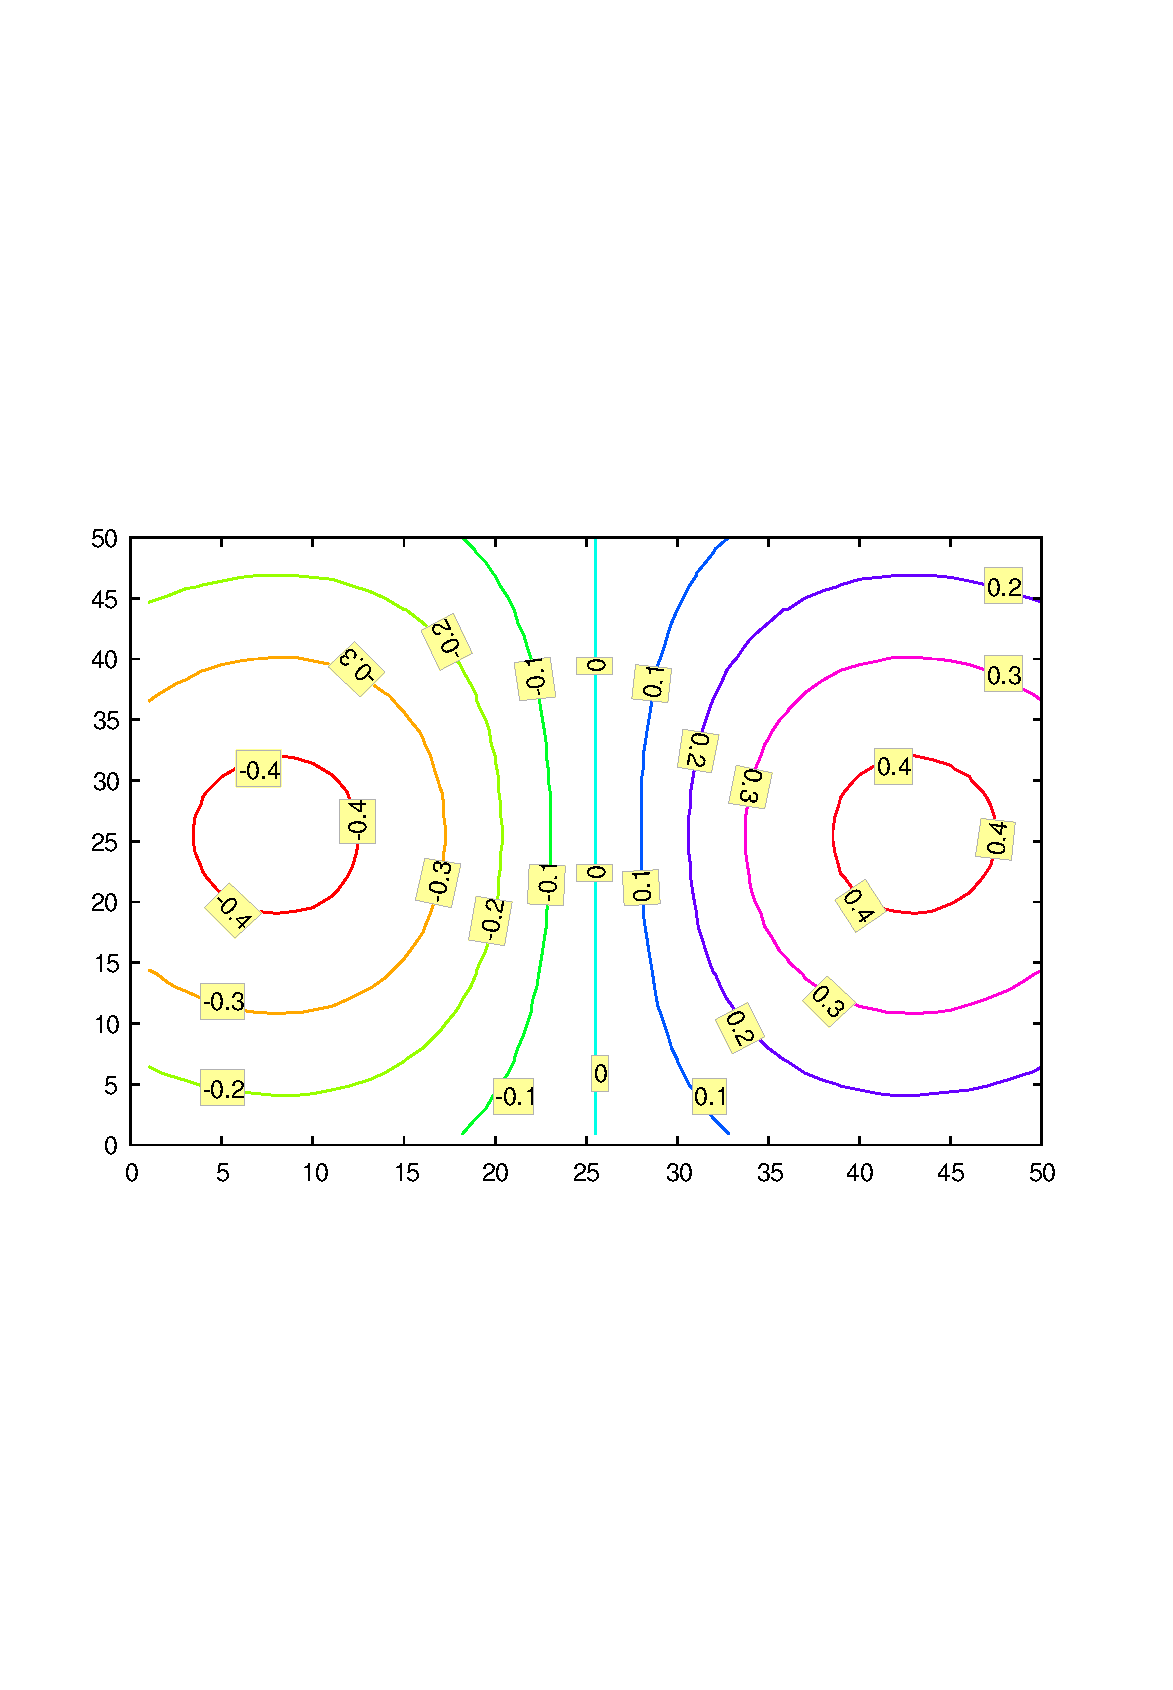
\includegraphics[width=12cm]{clabel1}
\caption{clabel1}
\end{DoxyImage}
 Alternately, we can just label a subset of the contours


\begin{DoxyVerbInclude}
--> h = contour(z);
--> clabel(h,[-.2,0,.3]);
\end{DoxyVerbInclude}


which results in  
\begin{DoxyImage}
\includegraphics[width=12cm]{clabel2}
\caption{clabel2}
\end{DoxyImage}
 \hypertarget{handle_clf}{}\section{C\-L\-F Clear Figure}\label{handle_clf}
Section\-: \hyperlink{sec_handle}{Handle-\/\-Based Graphics} \hypertarget{vtkwidgets_vtkxyplotwidget_Usage}{}\subsection{Usage}\label{vtkwidgets_vtkxyplotwidget_Usage}
This function clears the contents of the current figure. The syntax for its use is \begin{DoxyVerb}   clf
\end{DoxyVerb}
 \hypertarget{handle_clim}{}\section{C\-L\-I\-M Adjust Color limits of plot}\label{handle_clim}
Section\-: \hyperlink{sec_handle}{Handle-\/\-Based Graphics} \hypertarget{vtkwidgets_vtkxyplotwidget_Usage}{}\subsection{Usage}\label{vtkwidgets_vtkxyplotwidget_Usage}
There are several ways to use {\ttfamily clim} to adjust the color limits of a plot. The various syntaxes are \begin{DoxyVerb}   clim
   clim([lo,hi])   
   clim('auto')
   clim('manual')
   clim('mode')
   clim(handle,...)
\end{DoxyVerb}
 The first form (without arguments), returns a 2-\/vector containing the current limits. The second form sets the limits on the plot to {\ttfamily \mbox{[}lo,hi\mbox{]}}. The third and fourth form set the mode for the limit to {\ttfamily auto} and {\ttfamily manual} respectively. In {\ttfamily auto} mode, Free\-Mat chooses the range for the axis automatically. The {\ttfamily clim('mode')} form returns the current mode for the axis (either {\ttfamily 'auto'} or {\ttfamily 'manual'}).

Switching to {\ttfamily manual} mode does not change the limits, it simply allows you to modify them (and disables the automatic adjustment of the limits as more objects are added to the plot). Also, if you specify a set of limits explicitly, the mode is set to {\ttfamily manual}

Finally, you can specify the handle of an axis to manipulate instead of using the current one. \hypertarget{variables_struct_Example}{}\subsection{Example}\label{variables_struct_Example}
Here is an example of using {\ttfamily clim} to change the effective window and level onto an image. First, the image with default limits


\begin{DoxyVerbInclude}
--> x = repmat(linspace(-1,1),[100,1]); y = x';
--> z = exp(-x.^2-y.^2);
--> image(z);
--> min(z(:))

ans = 
    0.1353 

--> max(z(:))

ans = 
    0.9998 
\end{DoxyVerbInclude}


which results in  
\begin{DoxyImage}
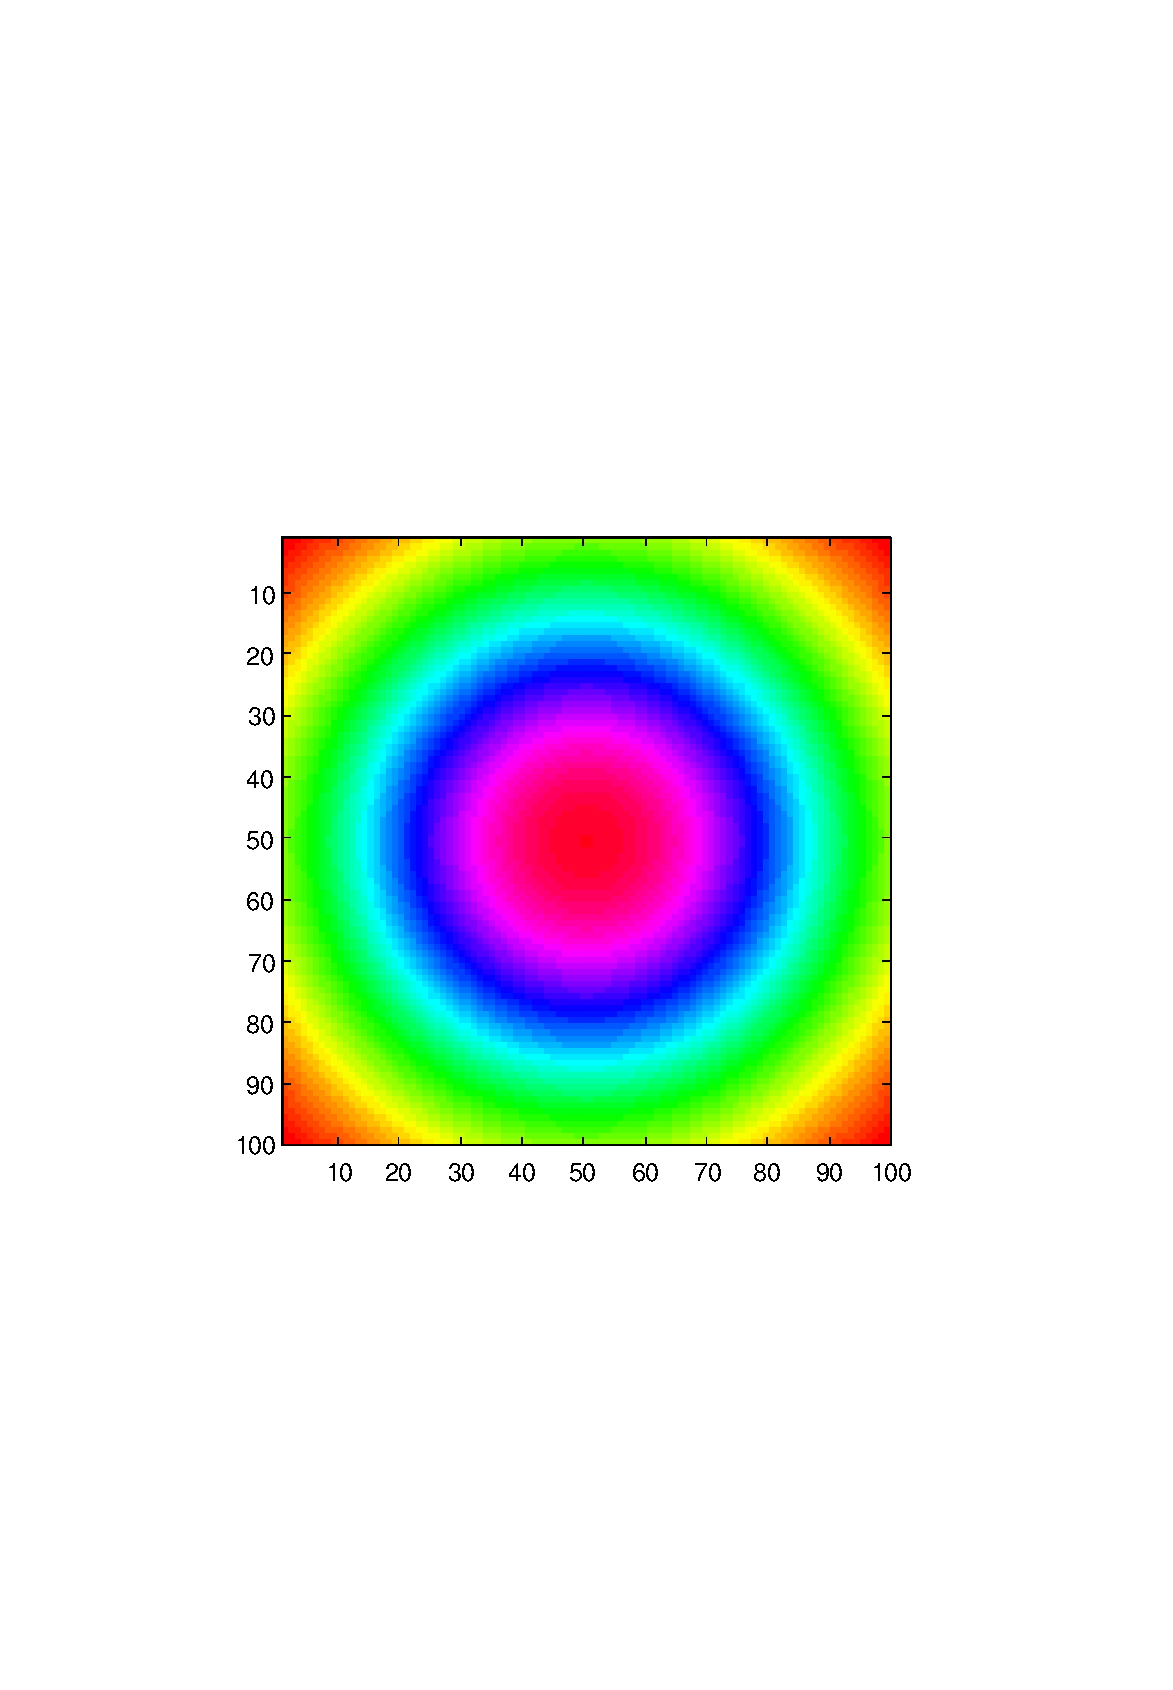
\includegraphics[width=12cm]{clim1}
\caption{clim1}
\end{DoxyImage}
 Next, we change the colorscale of the image using the {\ttfamily clim} function


\begin{DoxyVerbInclude}
--> image(z);
--> clim([0,0.2]);
\end{DoxyVerbInclude}


which results in  
\begin{DoxyImage}
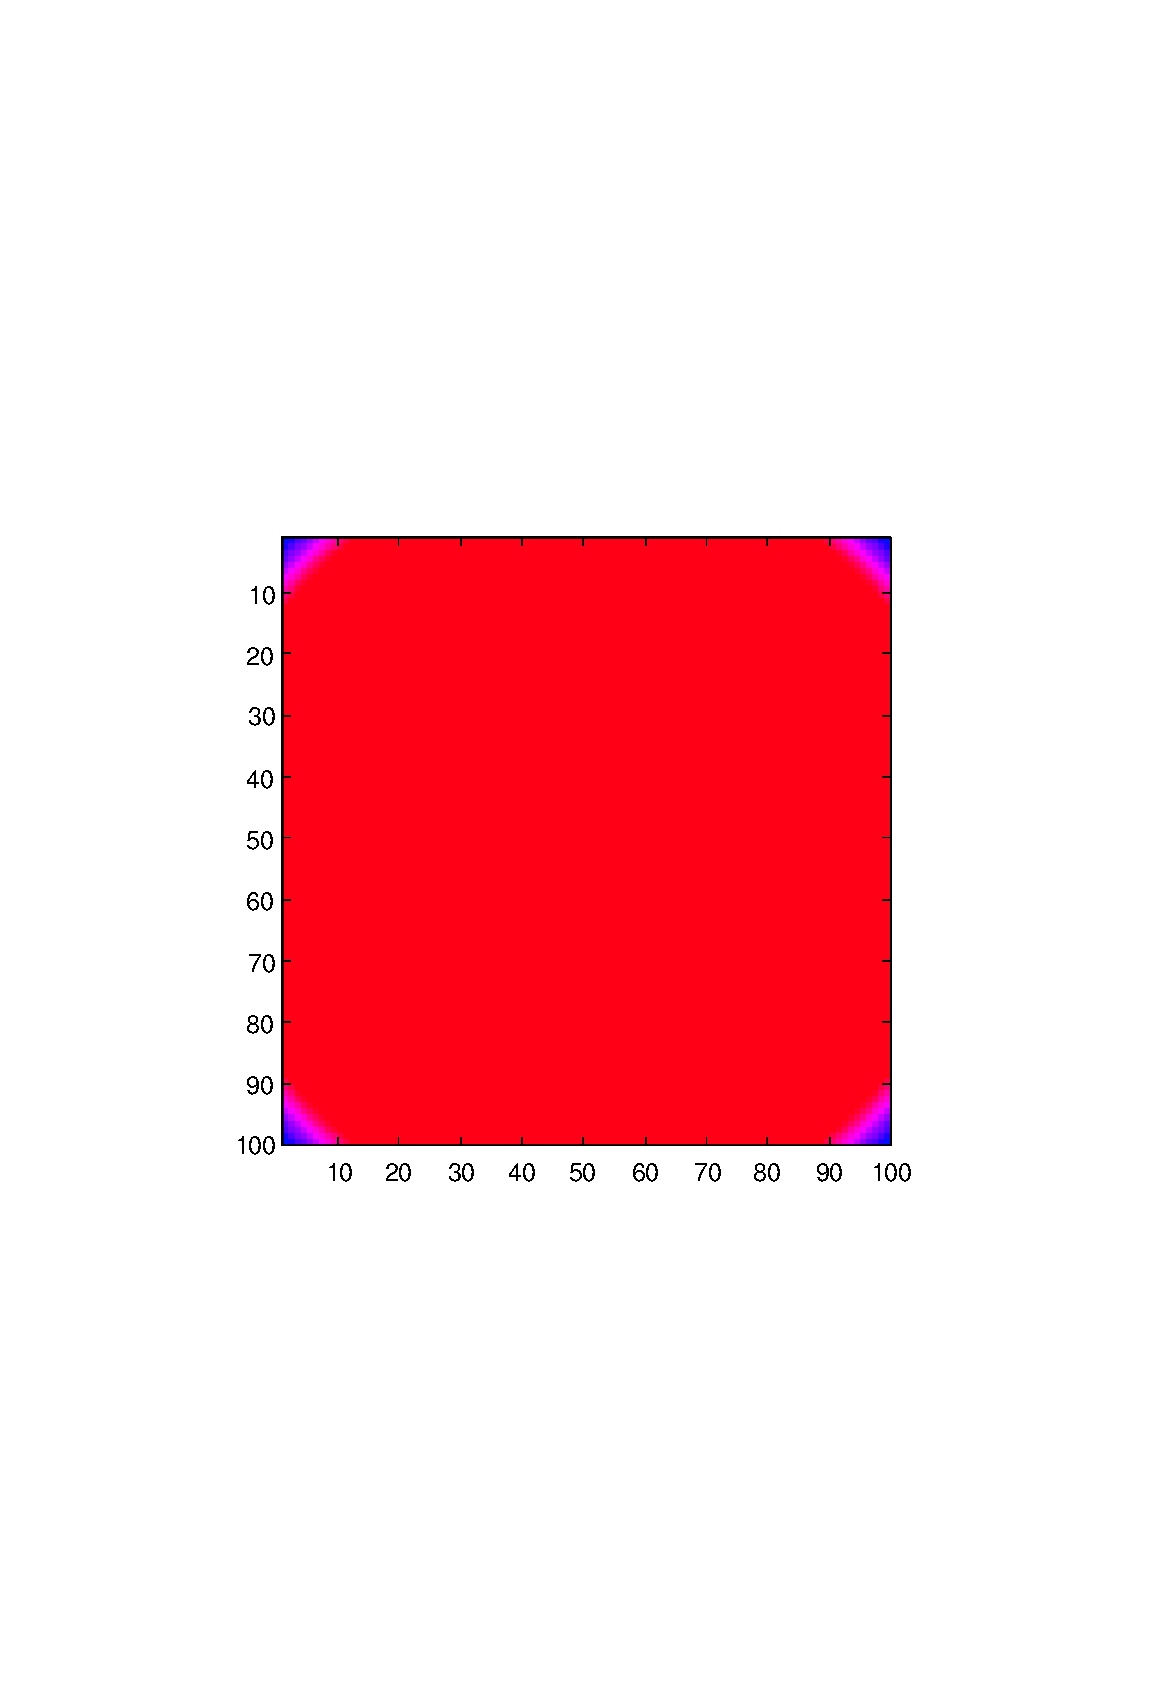
\includegraphics[width=12cm]{clim2}
\caption{clim2}
\end{DoxyImage}
 \hypertarget{handle_close}{}\section{C\-L\-O\-S\-E Close Figure Window}\label{handle_close}
Section\-: \hyperlink{sec_handle}{Handle-\/\-Based Graphics} \hypertarget{vtkwidgets_vtkxyplotwidget_Usage}{}\subsection{Usage}\label{vtkwidgets_vtkxyplotwidget_Usage}
Closes a figure window, either the currently active window, a window with a specific handle, or all figure windows. The general syntax for its use is \begin{DoxyVerb}   close(handle)
\end{DoxyVerb}
 in which case the figure window with the speicified {\ttfamily handle} is closed. Alternately, issuing the command with no argument \begin{DoxyVerb}   close
\end{DoxyVerb}
 is equivalent to closing the currently active figure window. Finally the command \begin{DoxyVerb}   close('all')
\end{DoxyVerb}
 closes all figure windows currently open. \hypertarget{handle_colorbar}{}\section{C\-O\-L\-O\-R\-B\-A\-R Add Colorbar to Current Plot}\label{handle_colorbar}
Section\-: \hyperlink{sec_handle}{Handle-\/\-Based Graphics} \hypertarget{vtkwidgets_vtkxyplotwidget_Usage}{}\subsection{Usage}\label{vtkwidgets_vtkxyplotwidget_Usage}
There are a number of syntaxes for the {\ttfamily colorbar} command. The first takes no arguments, and adds a vertical colorbar to the right of the current axes. \begin{DoxyVerb}  colorbar
\end{DoxyVerb}
 You can also pass properties to the newly created axes object using the second syntax for colorbar \begin{DoxyVerb}  colorbar(properties...)
\end{DoxyVerb}
 \hypertarget{handle_colormap}{}\section{C\-O\-L\-O\-R\-M\-A\-P Image Colormap Function}\label{handle_colormap}
Section\-: \hyperlink{sec_handle}{Handle-\/\-Based Graphics} \hypertarget{vtkwidgets_vtkxyplotwidget_Usage}{}\subsection{Usage}\label{vtkwidgets_vtkxyplotwidget_Usage}
Changes the colormap for the current figure. The generic syntax for its use is \begin{DoxyVerb}  colormap(map)
\end{DoxyVerb}
 where {\ttfamily map} is a an array organized as $3 \times N$), which defines the R\-G\-B (Red Green Blue) coordinates for each color in the colormap. You can also use the function with no arguments to recover the current colormap \begin{DoxyVerb}  map = colormap
\end{DoxyVerb}
 \hypertarget{transforms_svd_Function}{}\subsection{Internals}\label{transforms_svd_Function}
Assuming that the contents of the colormap function argument {\ttfamily c} are labeled as\-: \[ c = \begin{bmatrix} r_1 & g_1 & b_1 \\ r_1 & g_2 & b_2 \\ r_1 & g_3 & b_3 \\ \vdots & \vdots & \vdots \end{bmatrix} \] then these columns for the R\-G\-B coordinates of pixel in the mapped image. Assume that the image occupies the range \$\mbox{[}a,b\mbox{]}\$. Then the R\-G\-B color of each pixel depends on the value \$x\$ via the following integer \[ k = 1 + \lfloor 256 \frac{x-a}{b-a} \rfloor, \] so that a pixel corresponding to image value \$x\$ will receive R\-G\-B color \$\mbox{[}r\-\_\-k,g\-\_\-k,b\-\_\-k\mbox{]}\$. Colormaps are generally used to pseudo color images to enhance visibility of features, etc. \hypertarget{variables_matrix_Examples}{}\subsection{Examples}\label{variables_matrix_Examples}
We start by creating a smoothly varying image of a 2\-D Gaussian pulse.


\begin{DoxyVerbInclude}
--> x = linspace(-1,1,512)'*ones(1,512);
--> y = x';
--> Z = exp(-(x.^2+y.^2)/0.3);
--> image(Z);
\end{DoxyVerbInclude}


which we display with the default (grayscale) colormap here.  
\begin{DoxyImage}
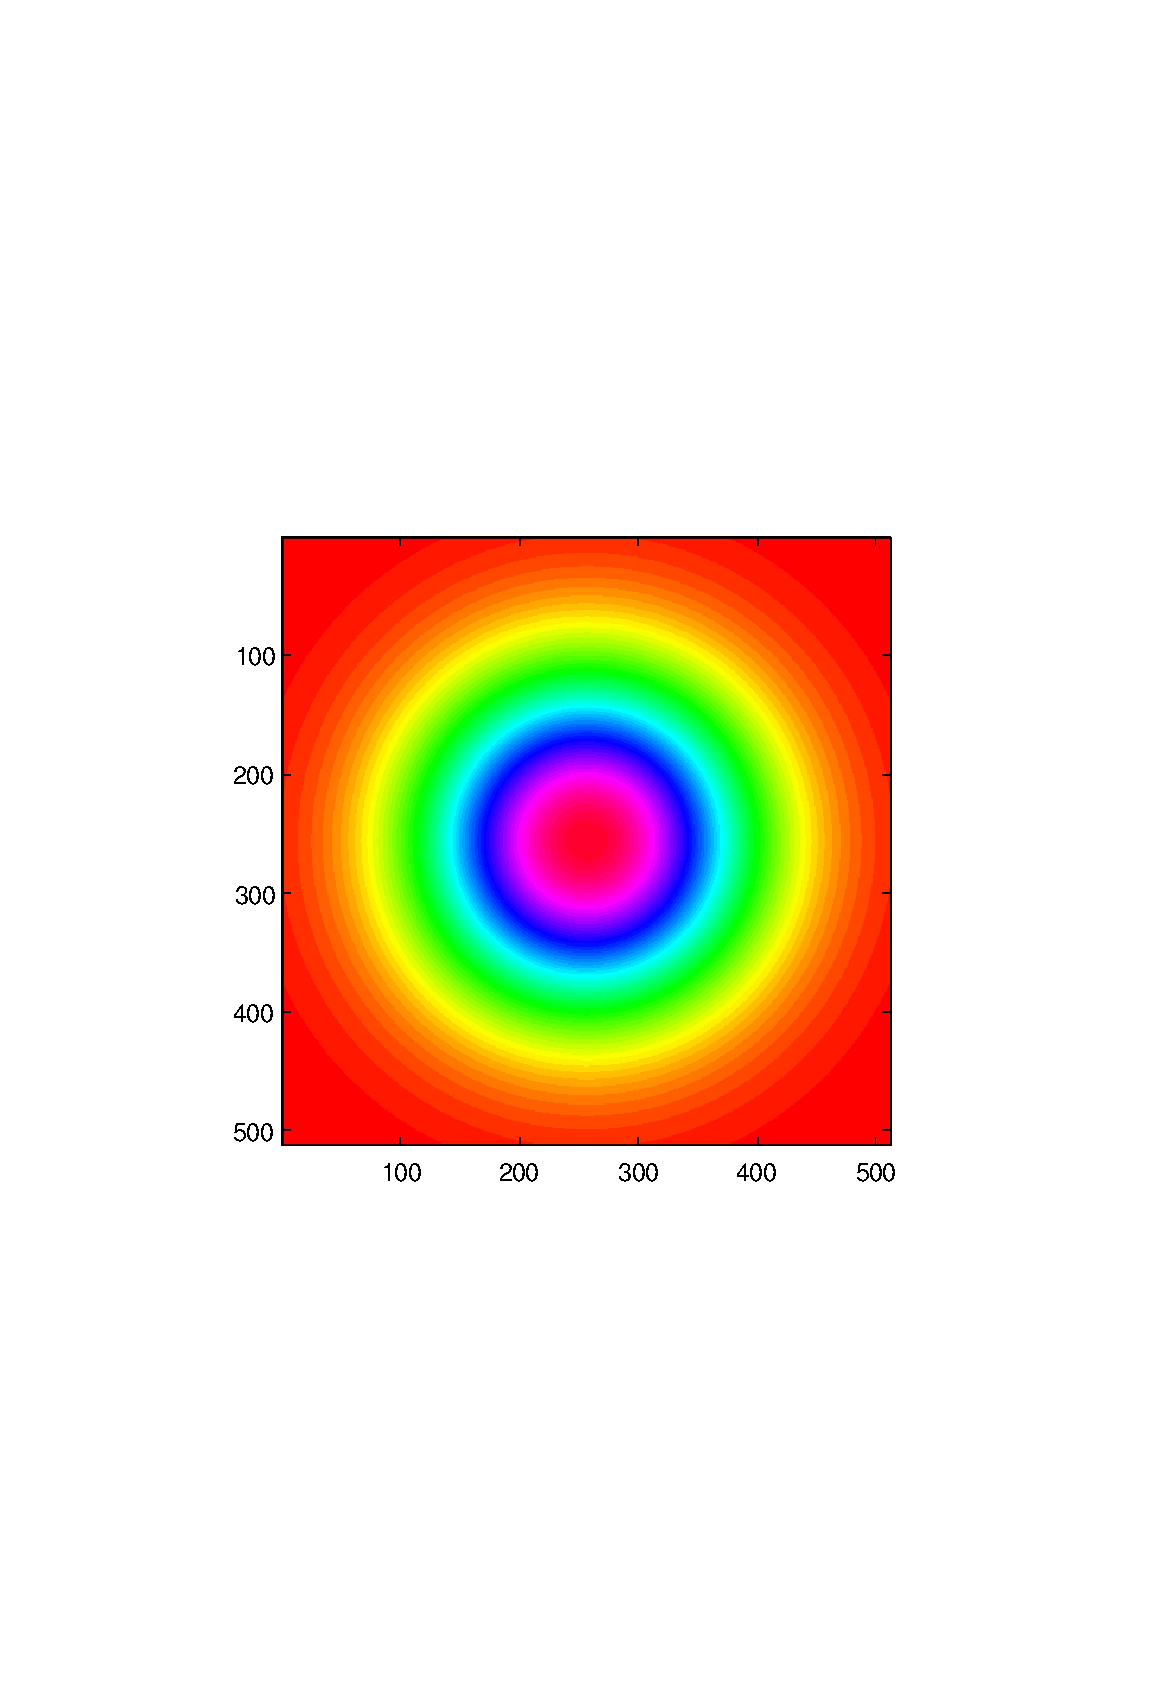
\includegraphics[width=12cm]{colormap1}
\caption{colormap1}
\end{DoxyImage}


Next we switch to the {\ttfamily copper} colormap, and redisplay the image.


\begin{DoxyVerbInclude}
--> colormap(copper);
--> image(Z);
\end{DoxyVerbInclude}


which results in the following image.  
\begin{DoxyImage}
\includegraphics[width=12cm]{colormap2}
\caption{colormap2}
\end{DoxyImage}


If we capture the output of the {\ttfamily copper} command and plot it, we obtain the following result\-:


\begin{DoxyVerbInclude}
--> a = copper;
--> plot(a);
\end{DoxyVerbInclude}


 
\begin{DoxyImage}
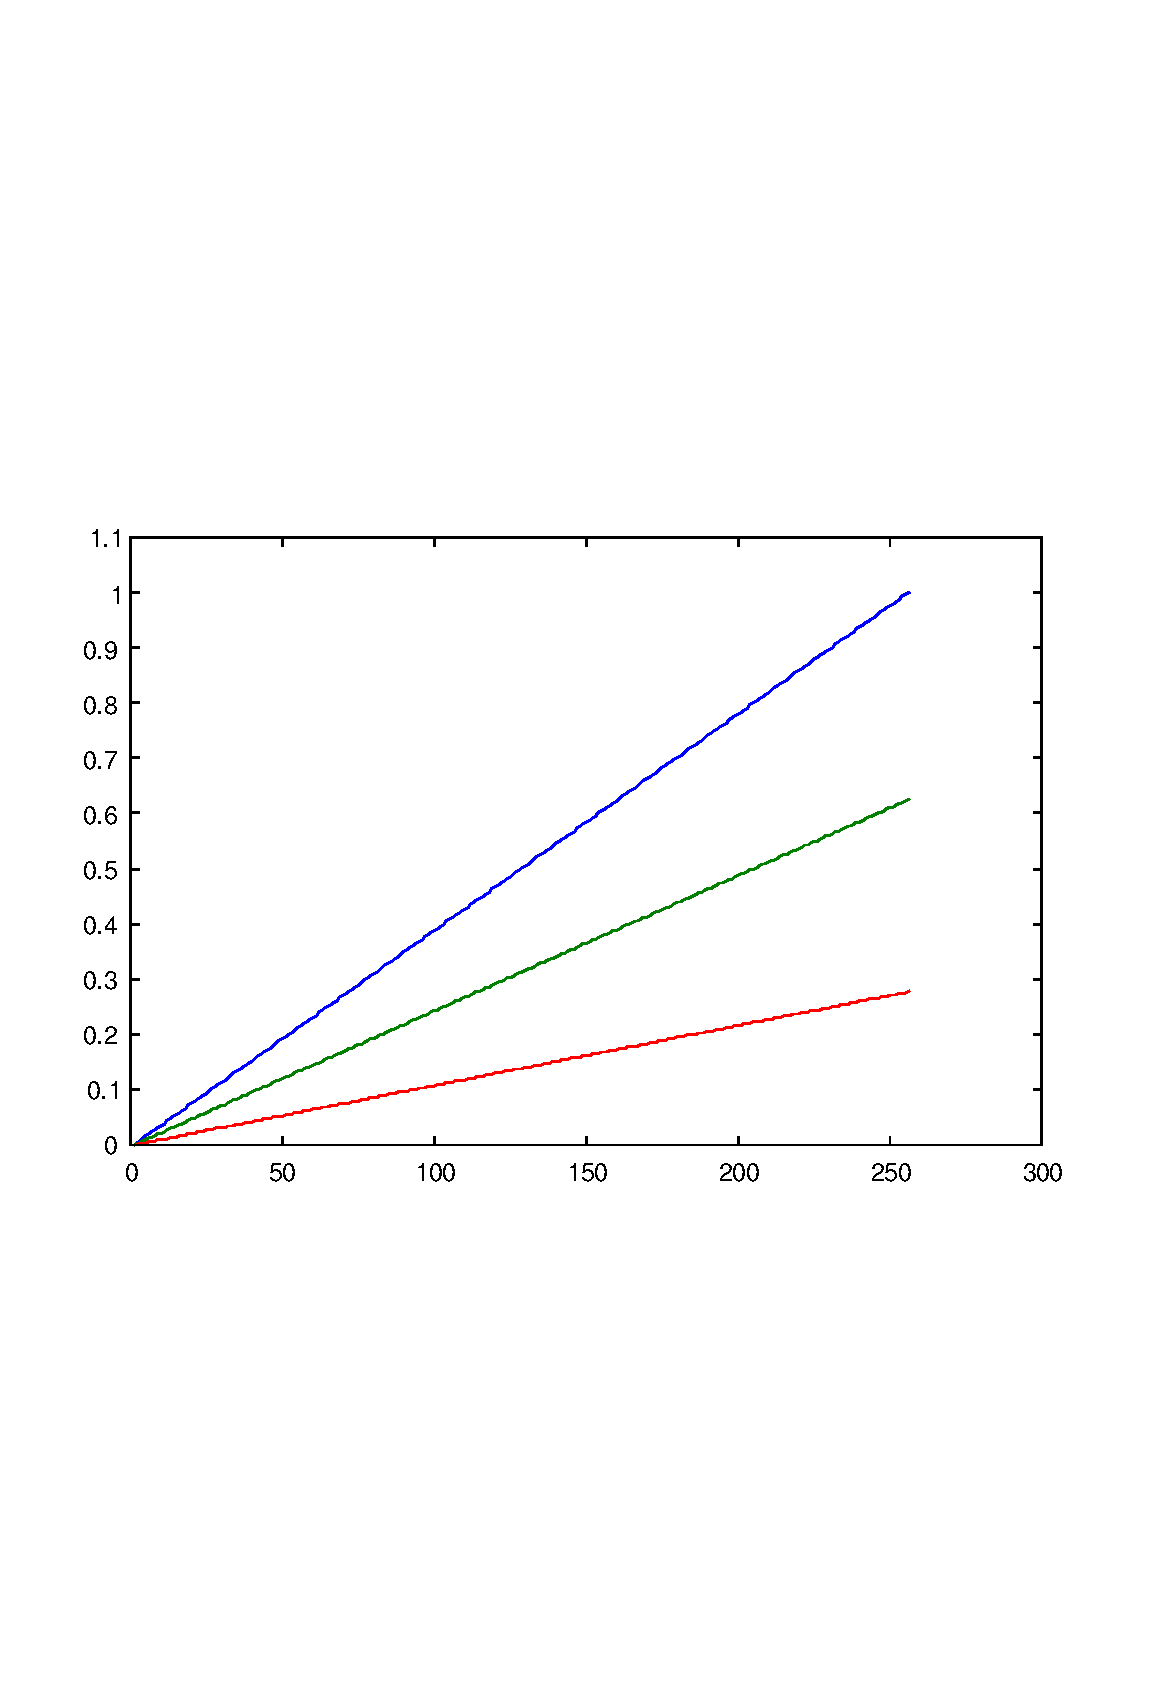
\includegraphics[width=12cm]{colormap3}
\caption{colormap3}
\end{DoxyImage}


Note that in the output that each of the color components are linear functions of the index, with the ratio between the red, blue and green components remaining constant as a function of index. The result is an intensity map with a copper tint. We can similarly construct a colormap of our own by defining the three components seperately. For example, suppose we take three gaussian curves, one for each color, centered on different parts of the index space\-:


\begin{DoxyVerbInclude}
--> t = linspace(0,1,256);
--> A = [exp(-(t-1.0).^2/0.1);exp(-(t-0.5).^2/0.1);exp(-t.^2/0.1)]';
--> plot(A);
\end{DoxyVerbInclude}


 
\begin{DoxyImage}
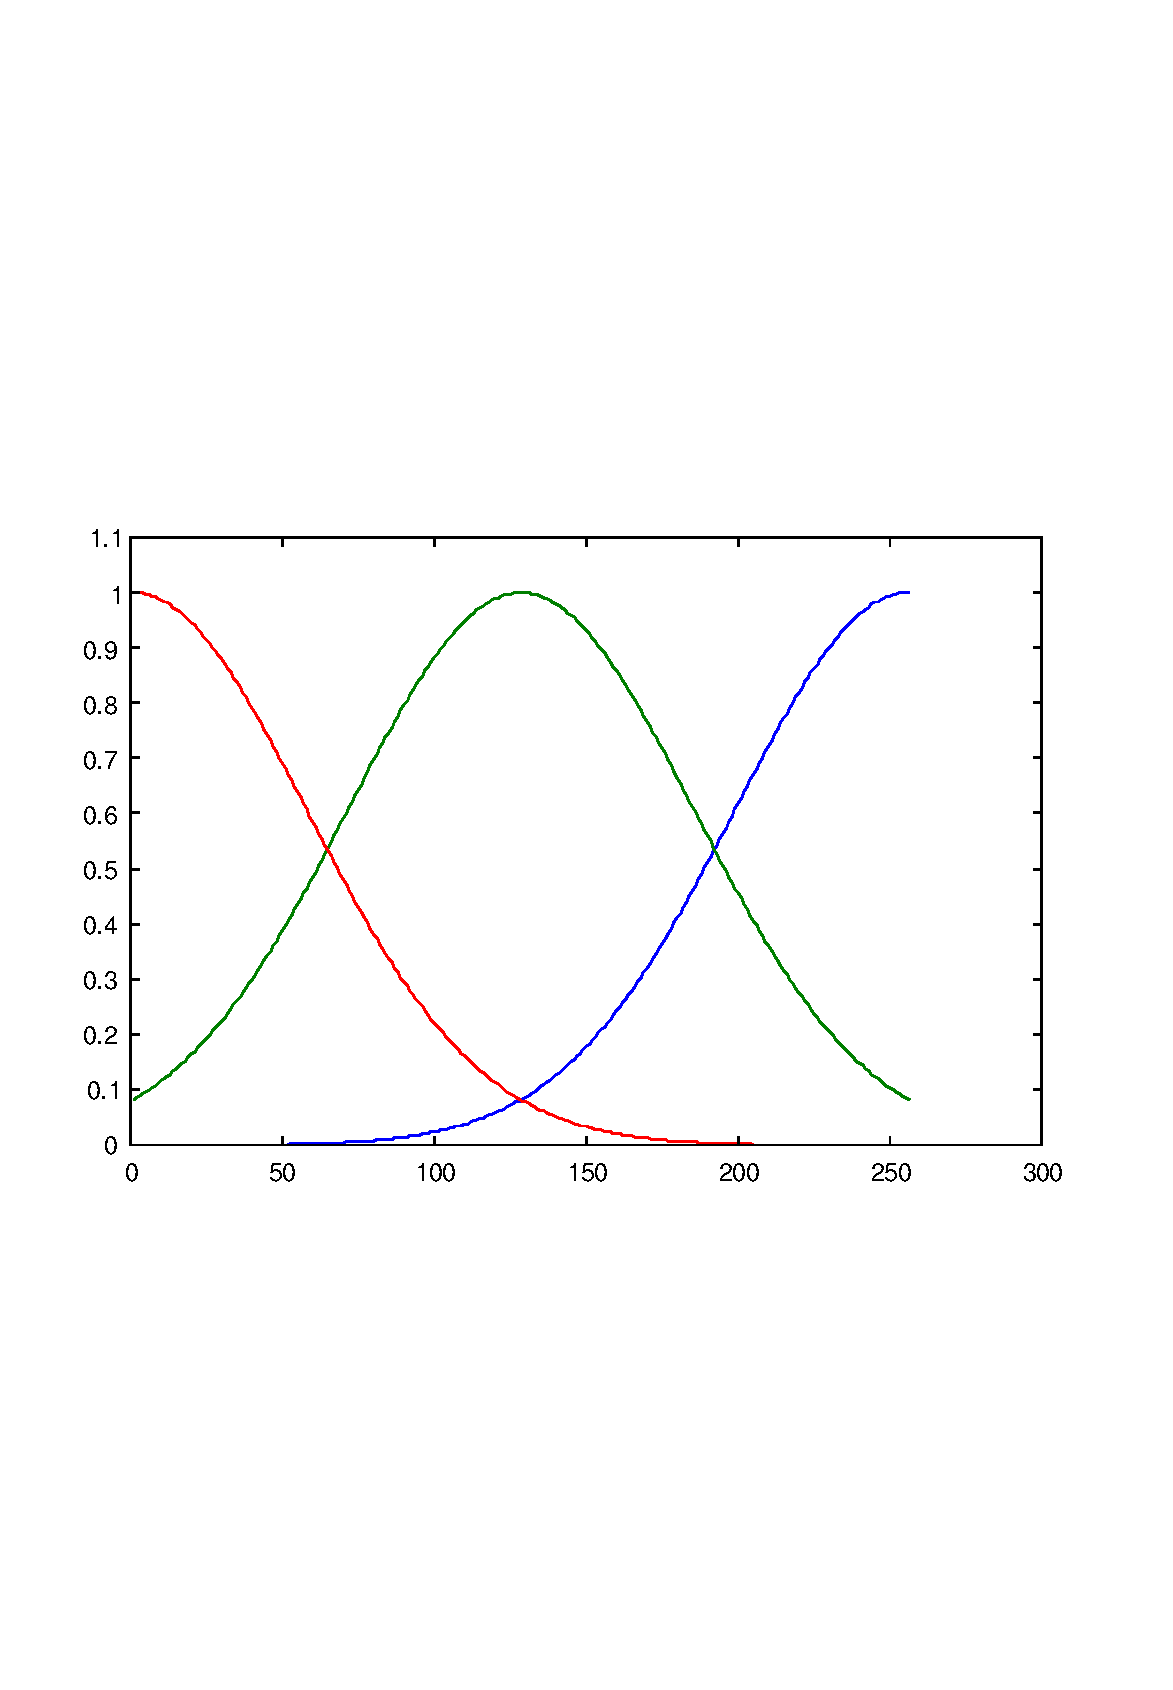
\includegraphics[width=12cm]{colormap4}
\caption{colormap4}
\end{DoxyImage}


The resulting image has dark bands in it near the color transitions.


\begin{DoxyVerbInclude}
--> image(Z);
--> colormap(A);
\end{DoxyVerbInclude}


 
\begin{DoxyImage}
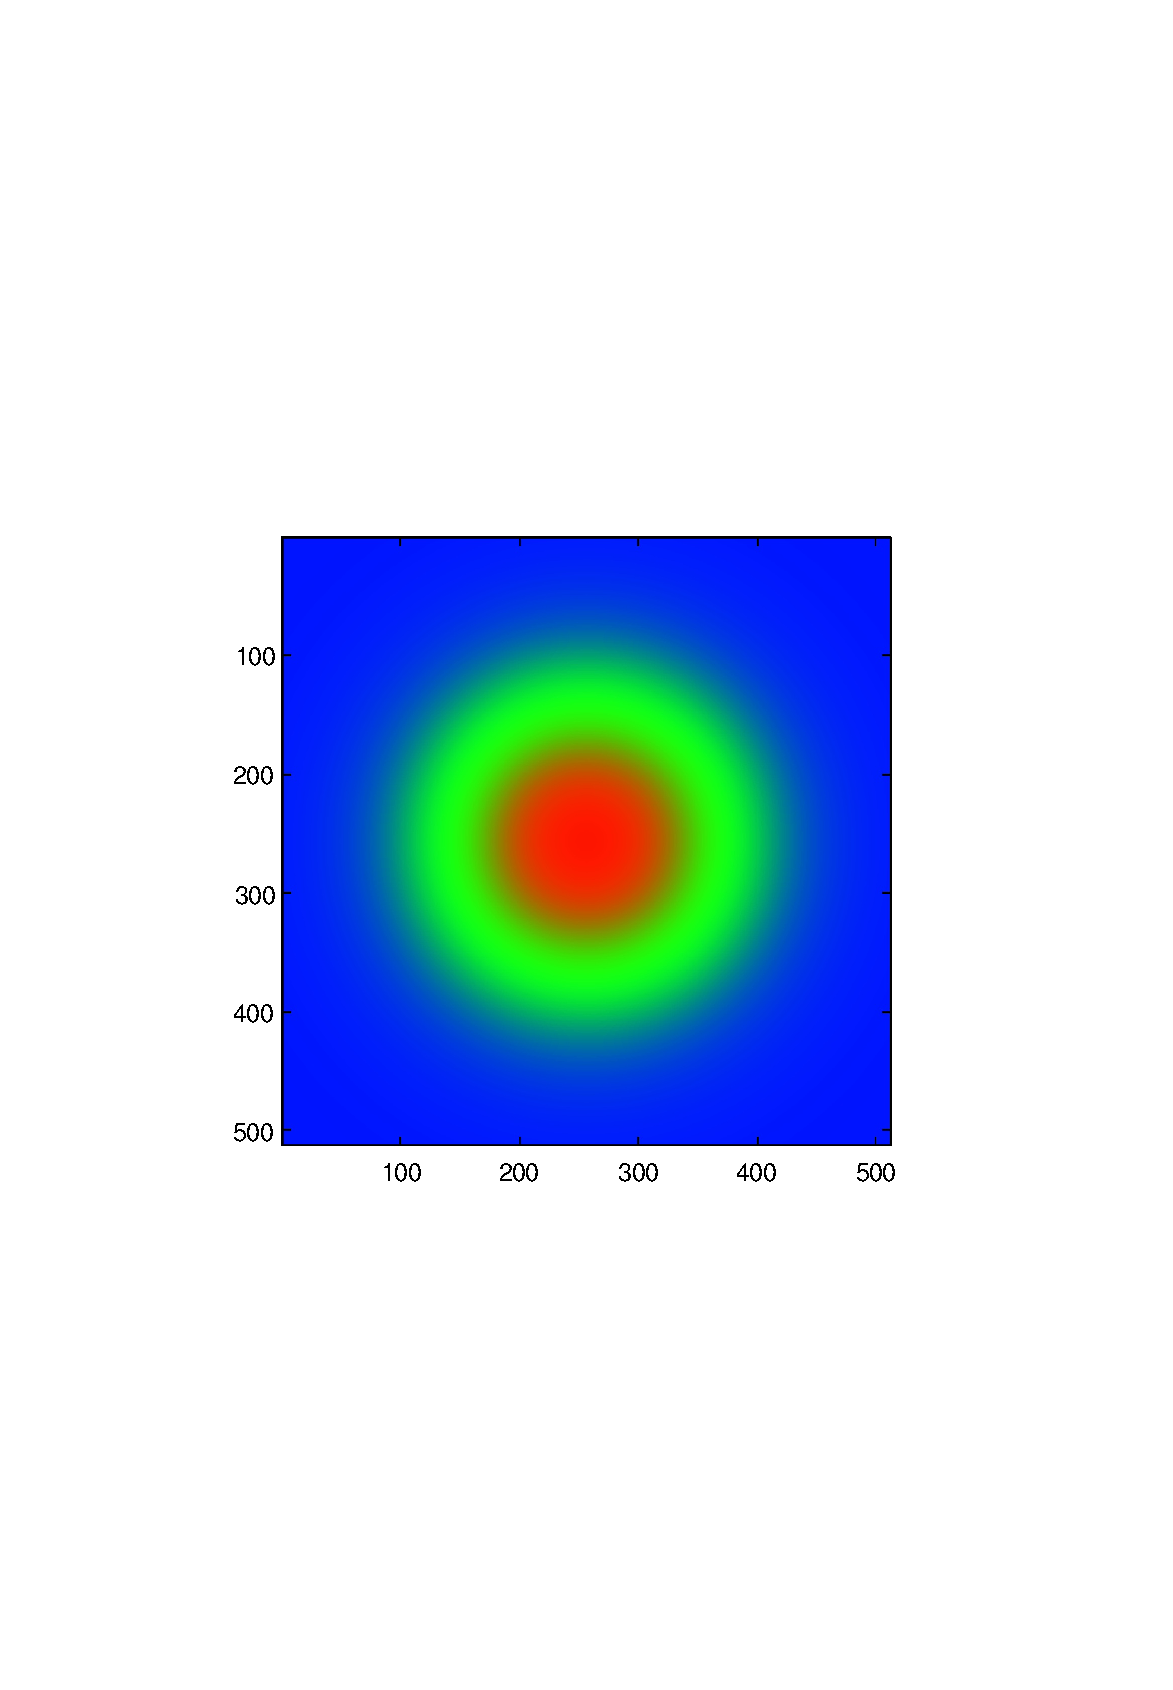
\includegraphics[width=12cm]{colormap5}
\caption{colormap5}
\end{DoxyImage}


These dark bands are a result of the nonuniform color intensity, which we can correct for by renormalizing each color to have the same norm.


\begin{DoxyVerbInclude}
--> w = sqrt(sum(A'.^2));
--> sA = diag(1./w)*A;
--> plot(A);
\end{DoxyVerbInclude}


 
\begin{DoxyImage}
\includegraphics[width=12cm]{colormap6}
\caption{colormap6}
\end{DoxyImage}


The resulting image has no more dark bands.


\begin{DoxyVerbInclude}
--> image(Z);
--> colormap(A);
\end{DoxyVerbInclude}


 
\begin{DoxyImage}
\includegraphics[width=12cm]{colormap7}
\caption{colormap7}
\end{DoxyImage}
 \hypertarget{handle_colorspec}{}\section{C\-O\-L\-O\-R\-S\-P\-E\-C Color Property Description}\label{handle_colorspec}
Section\-: \hyperlink{sec_handle}{Handle-\/\-Based Graphics} \hypertarget{vtkwidgets_vtkxyplotwidget_Usage}{}\subsection{Usage}\label{vtkwidgets_vtkxyplotwidget_Usage}
There are a number of ways of specifying a color value for a color-\/based property. Examples include line colors, marker colors, and the like. One option is to specify color as an R\-G\-B triplet \begin{DoxyVerb}   set(h,'color',[r,g,b])
\end{DoxyVerb}
 where {\ttfamily r,g,b} are between @\mbox{[}0,1\mbox{]} Alternately, you can use color names to specify a color. 
\begin{DoxyItemize}
\item {\ttfamily 'none'} -\/ No color.  
\item {\ttfamily 'y','yellow'} -\/ The color @\mbox{[}1,1,0\mbox{]}@ in R\-G\-B space.  
\item {\ttfamily 'm','magenta'} -\/ The color @\mbox{[}1,0,1\mbox{]}@ in R\-G\-B space.  
\item {\ttfamily 'c','cyan'} -\/ The color @\mbox{[}0,1,1\mbox{]}@ in R\-G\-B space.  
\item {\ttfamily 'r','red'} -\/ The color @\mbox{[}1,0,0\mbox{]}@ in R\-G\-B space.  
\item {\ttfamily 'g','green'} -\/ The color @\mbox{[}0,1,0\mbox{]}@ in R\-G\-B space.  
\item {\ttfamily 'b','blue'} -\/ The color @\mbox{[}0,0,1\mbox{]}@ in R\-G\-B space.  
\item {\ttfamily 'w','white'} -\/ The color @\mbox{[}1,1,1\mbox{]}@ in R\-G\-B space.  
\item {\ttfamily 'k','black'} -\/ The color @\mbox{[}0,0,0\mbox{]}@ in R\-G\-B space.  
\end{DoxyItemize}\hypertarget{handle_contour}{}\section{C\-O\-N\-T\-O\-U\-R Contour Plot Function}\label{handle_contour}
Section\-: \hyperlink{sec_handle}{Handle-\/\-Based Graphics} \hypertarget{vtkwidgets_vtkxyplotwidget_Usage}{}\subsection{Usage}\label{vtkwidgets_vtkxyplotwidget_Usage}
This command generates contour plots. There are several syntaxes for the command. The simplest is \begin{DoxyVerb}  contour(Z)
\end{DoxyVerb}
 which generates a contour plot of the data in matrix {\ttfamily Z}, and will automatically select the contour levels. The {\ttfamily x,y} coordinates of the contour default to {\ttfamily 1\-:n} and {\ttfamily 1\-:m}, where {\ttfamily n} is the number of columns and {\ttfamily m} is the number of rows in the {\ttfamily Z} matrix. Alternately, you can specify a scalar {\ttfamily n} \begin{DoxyVerb}  contour(Z,n)
\end{DoxyVerb}
 which indicates that you want {\ttfamily n} contour levels. For more control, you can provide a vector {\ttfamily v} containing the levels to contour. If you want to generate a contour for a particular level, you must pass a vector {\ttfamily \mbox{[}t,t\mbox{]}} where {\ttfamily t} is the level you want to contour. If you have data that lies on a particular {\ttfamily X,Y} grid, you can pass either vectors {\ttfamily x,y} or matrices {\ttfamily X,Y} to the contour function via \begin{DoxyVerb}  contour(X,Y,Z)
  contour(X,Y,Z,n)
  contour(X,Y,Z,v)
\end{DoxyVerb}
 Each form of {\ttfamily contour} can optionally take a line spec to indicate the color and linestyle of the contours to draw\-: \begin{DoxyVerb}  contour(...,linespec)
\end{DoxyVerb}
 or any of the other forms of {\ttfamily contour}. Furthermore, you can supply an axis to target the {\ttfamily contour} plot to (so that it does not get added to the current axis, which is the default)\-: \begin{DoxyVerb}  contour(axis_handle,...)
\end{DoxyVerb}
 Finally, the {\ttfamily contour} command returns a handle to the newly returned contour plot. \begin{DoxyVerb}  handle = contour(...)
\end{DoxyVerb}
 To place labels on the contour plot, use the {\ttfamily clabel} function. \hypertarget{variables_struct_Example}{}\subsection{Example}\label{variables_struct_Example}
Here is a simple example of a contour plot with the default {\ttfamily x,y} coordinates\-:


\begin{DoxyVerbInclude}
--> [x,y] = meshgrid(linspace(-1,1,25),linspace(-2,2,30));
--> z = x.*exp(-x.^2-y.^2);
--> contour(z)
\end{DoxyVerbInclude}


which results in the following plot  
\begin{DoxyImage}
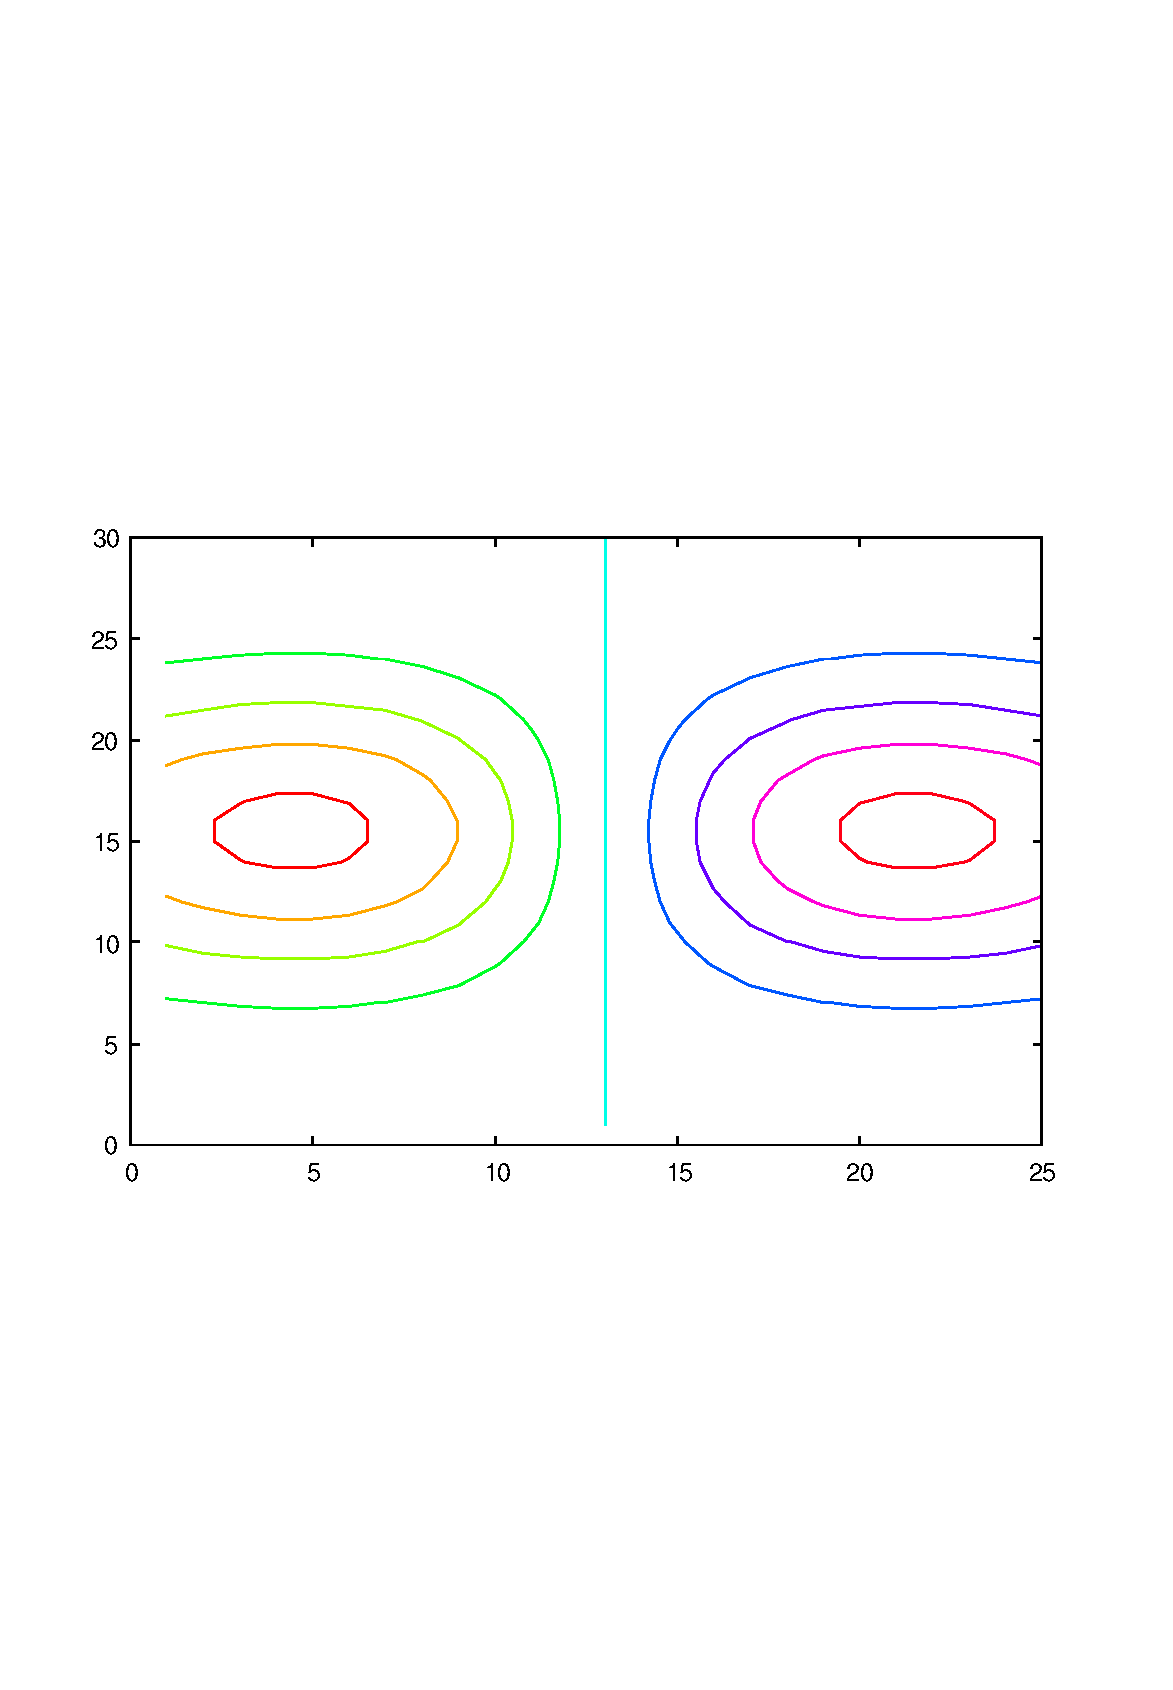
\includegraphics[width=12cm]{contour1}
\caption{contour1}
\end{DoxyImage}
 Here, we specify the {\ttfamily x} and {\ttfamily y} coordinates explictly


\begin{DoxyVerbInclude}
--> contour(x,y,z)
\end{DoxyVerbInclude}


note that the axis limits have changed appropriately  
\begin{DoxyImage}
\includegraphics[width=12cm]{contour2}
\caption{contour2}
\end{DoxyImage}
 By default, contours are created at values selected by Free\-Mat. To provide our own set of contour values (asymmetrically about zero in this case), we supply them as


\begin{DoxyVerbInclude}
--> contour(x,y,z,[-.4,0.,3])
\end{DoxyVerbInclude}


which is here  
\begin{DoxyImage}
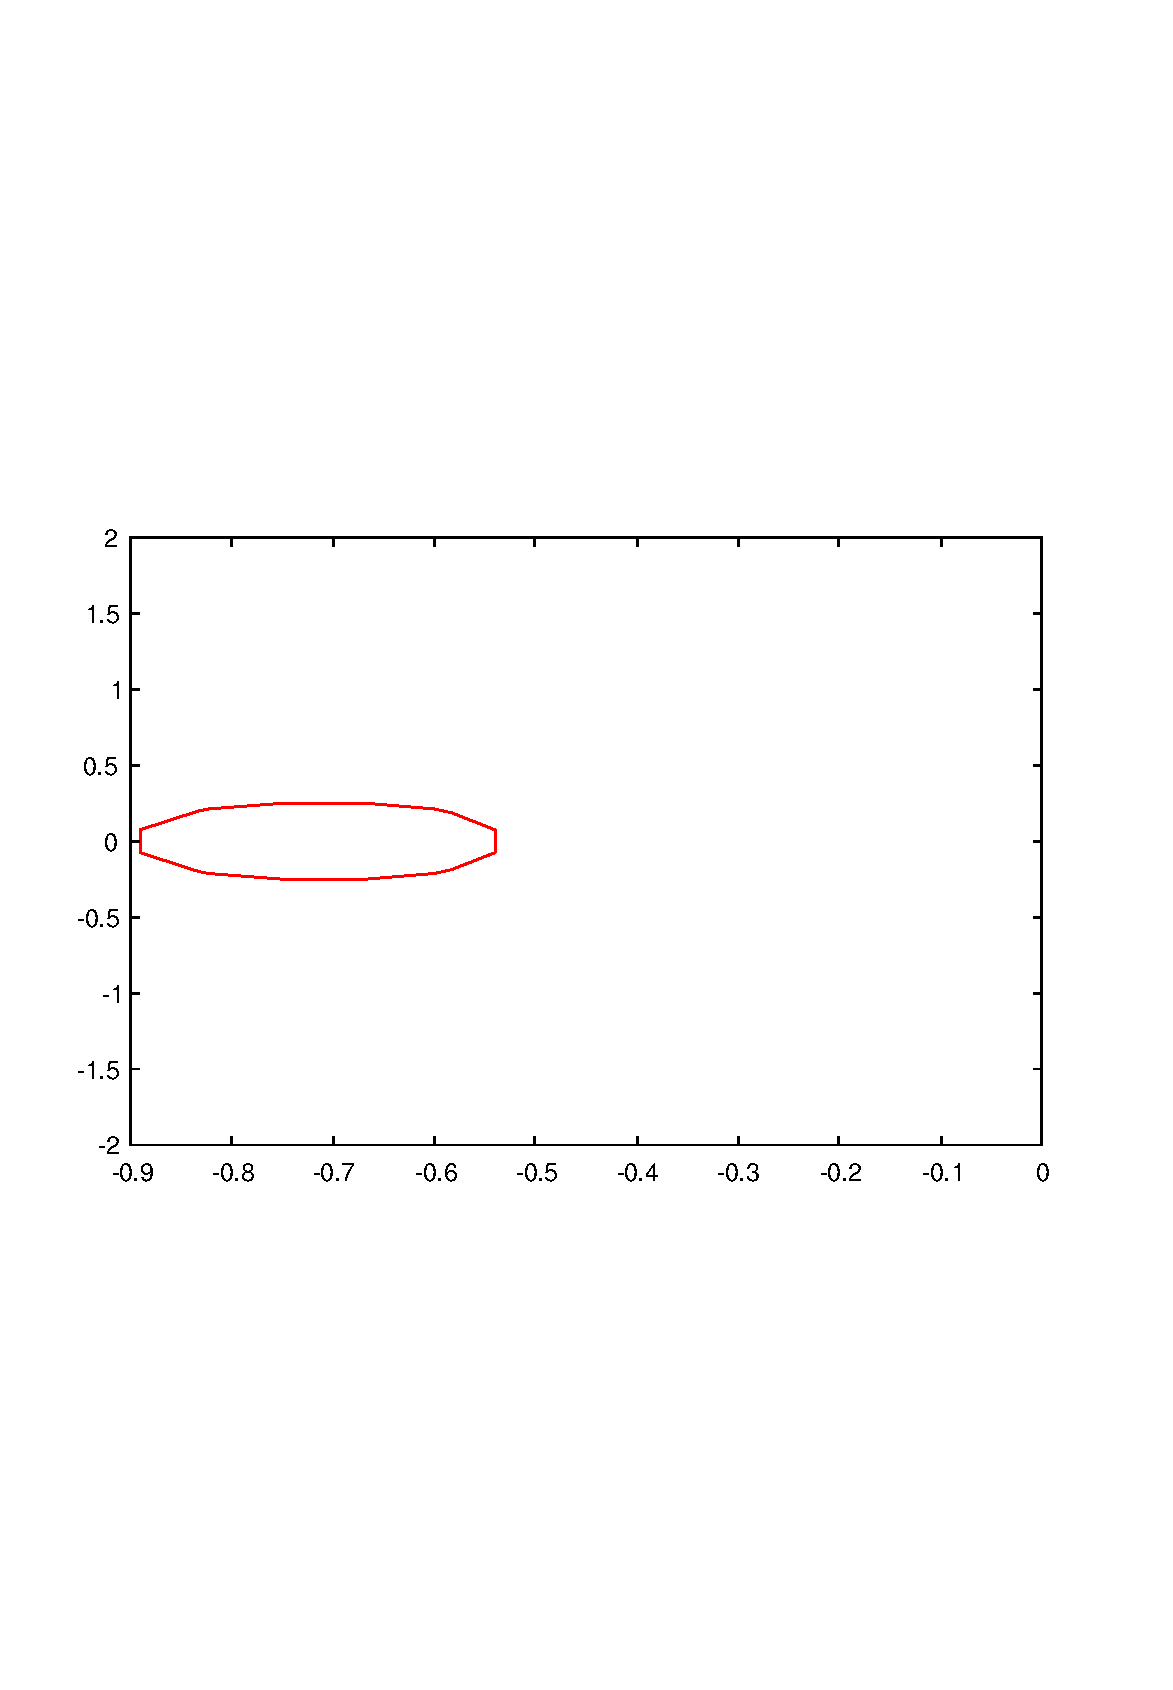
\includegraphics[width=12cm]{contour3}
\caption{contour3}
\end{DoxyImage}
 Also be default, {\ttfamily contour} uses the current color map and {\ttfamily clim} limits to determine the coloring of the contours. Here, we override the color spec so that we have all black contour


\begin{DoxyVerbInclude}
--> contour(x,y,z,'b-')
\end{DoxyVerbInclude}


which is here  
\begin{DoxyImage}
\includegraphics[width=12cm]{contour4}
\caption{contour4}
\end{DoxyImage}
 \hypertarget{handle_contour3}{}\section{C\-O\-N\-T\-O\-U\-R3 3\-D Contour Plot Function}\label{handle_contour3}
Section\-: \hyperlink{sec_handle}{Handle-\/\-Based Graphics} \hypertarget{vtkwidgets_vtkxyplotwidget_Usage}{}\subsection{Usage}\label{vtkwidgets_vtkxyplotwidget_Usage}
This command generates contour plots where the lines are plotted in 3\-D. The syntax for its use is identical to the {\ttfamily contour} function. Please see its help for details. \hypertarget{variables_struct_Example}{}\subsection{Example}\label{variables_struct_Example}
Here is a simple example of a 3\-D contour plot.


\begin{DoxyVerbInclude}
--> [x,y] = meshgrid([-2:.25:2]);
--> z=x.*exp(-x.^2-y.^2);
--> contour3(x,y,z,30);
--> axis square;
--> view(-15,25)
\end{DoxyVerbInclude}


The resulting plot  
\begin{DoxyImage}
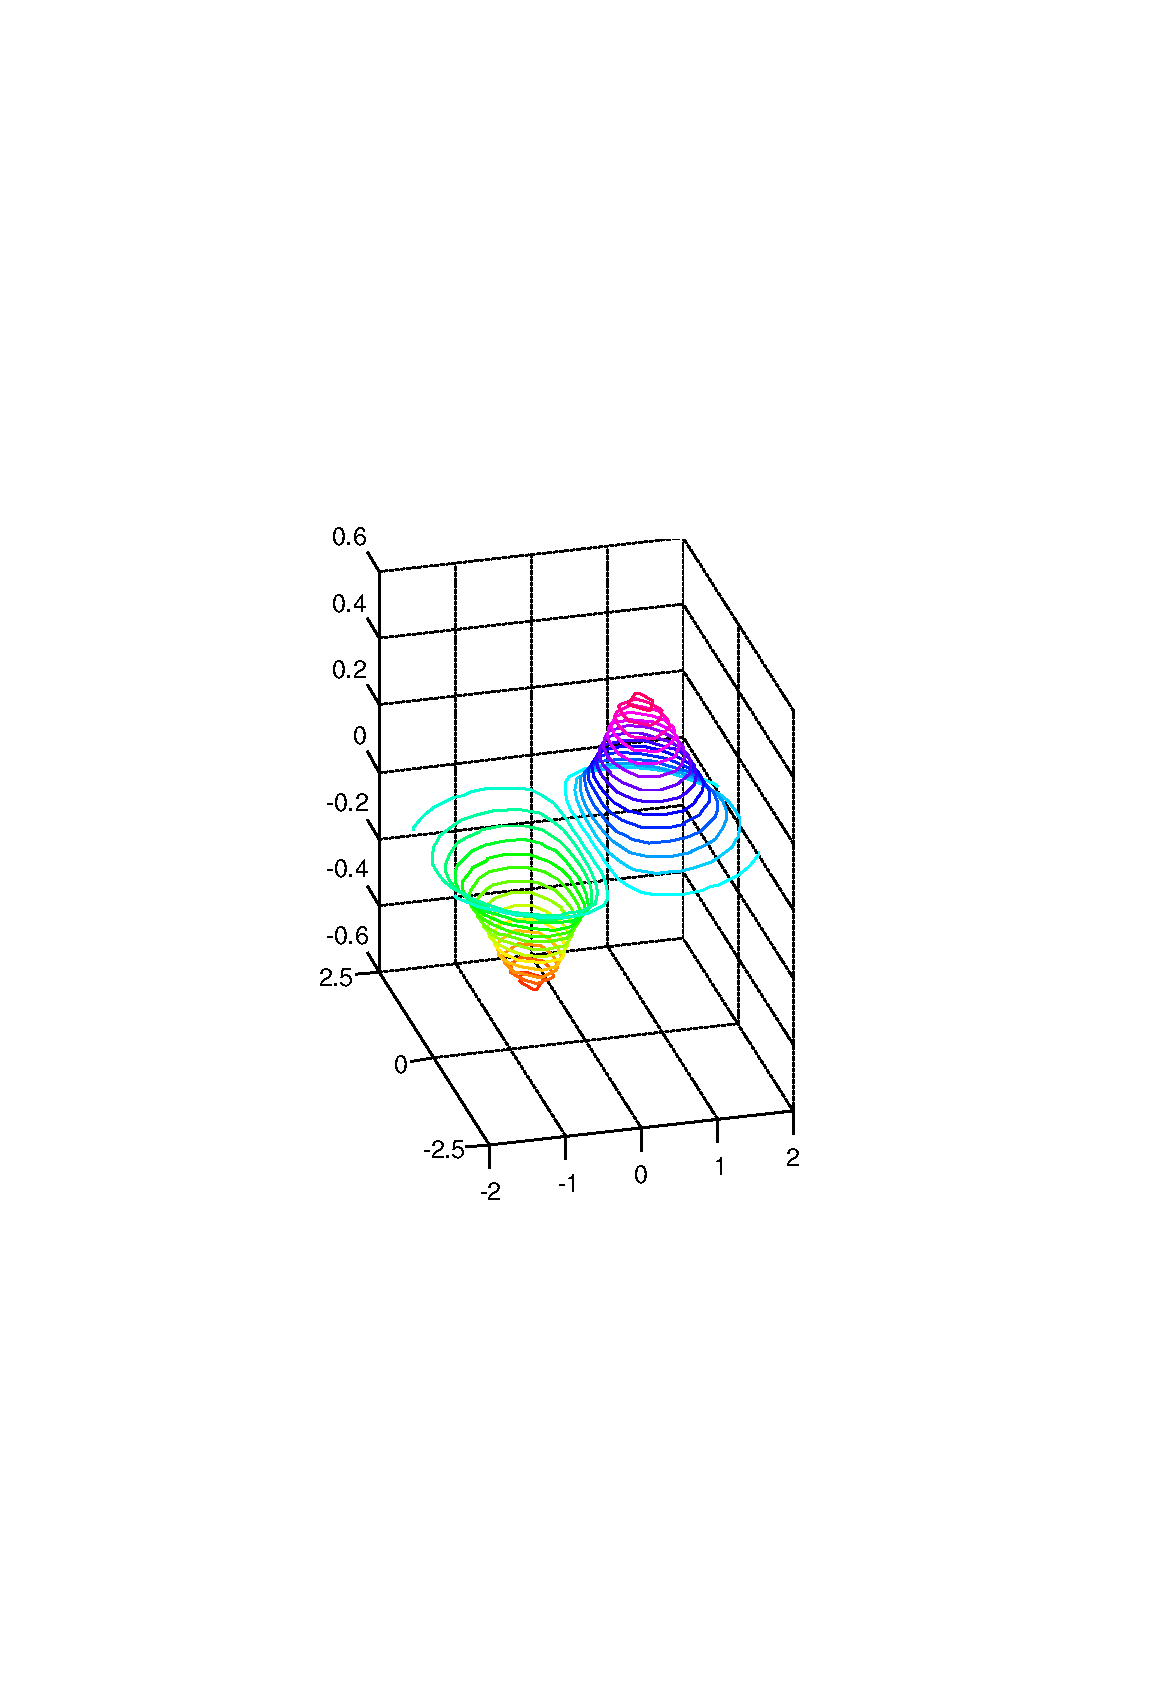
\includegraphics[width=12cm]{contour3_1}
\caption{contour3\-\_\-1}
\end{DoxyImage}
 \hypertarget{handle_copper}{}\section{C\-O\-P\-P\-E\-R Copper Colormap}\label{handle_copper}
Section\-: \hyperlink{sec_handle}{Handle-\/\-Based Graphics} \hypertarget{vtkwidgets_vtkxyplotwidget_Usage}{}\subsection{Usage}\label{vtkwidgets_vtkxyplotwidget_Usage}
Returns a copper colormap. The syntax for its use is \begin{DoxyVerb}   y = copper
\end{DoxyVerb}
 \hypertarget{variables_struct_Example}{}\subsection{Example}\label{variables_struct_Example}
Here is an example of an image displayed with the {\ttfamily copper} colormap


\begin{DoxyVerbInclude}
--> x = linspace(-1,1,512)'*ones(1,512);
--> y = x';
--> Z = exp(-(x.^2+y.^2)/0.3);
--> image(Z);
--> colormap(copper);
\end{DoxyVerbInclude}


which results in the following image  
\begin{DoxyImage}
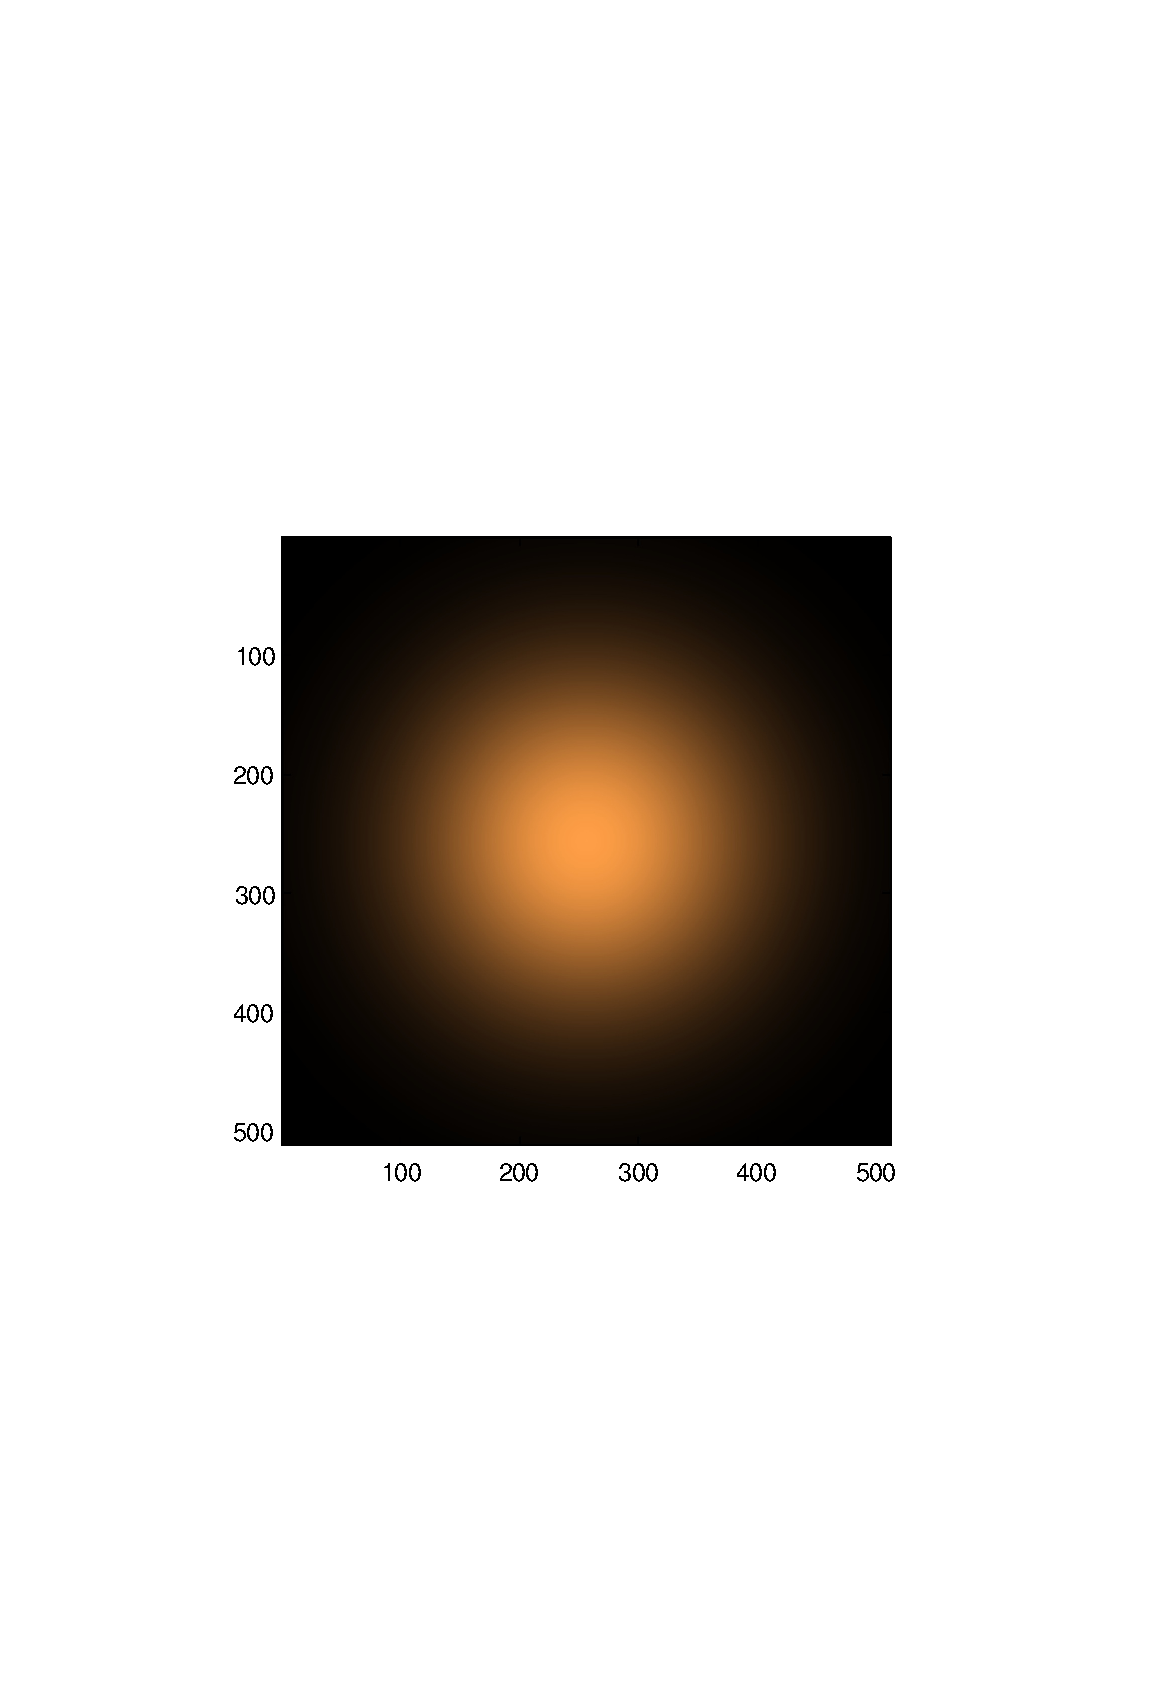
\includegraphics[width=12cm]{copper1}
\caption{copper1}
\end{DoxyImage}
 \hypertarget{handle_copy}{}\section{C\-O\-P\-Y Copy Figure Window}\label{handle_copy}
Section\-: \hyperlink{sec_handle}{Handle-\/\-Based Graphics} \hypertarget{vtkwidgets_vtkxyplotwidget_Usage}{}\subsection{Usage}\label{vtkwidgets_vtkxyplotwidget_Usage}
Copies the currently active figure window to the clipboard. The syntax for its use is\-: \begin{DoxyVerb}   copy
\end{DoxyVerb}
 The resulting figure is copied as a bitmap to the clipboard, and can then be pasted into any suitable application. \hypertarget{handle_countour}{}\section{C\-O\-U\-N\-T\-O\-U\-R Contour Object Properties}\label{handle_countour}
Section\-: \hyperlink{sec_handle}{Handle-\/\-Based Graphics} \hypertarget{vtkwidgets_vtkxyplotwidget_Usage}{}\subsection{Usage}\label{vtkwidgets_vtkxyplotwidget_Usage}
Below is a summary of the properties for a line series. 
\begin{DoxyItemize}
\item {\ttfamily contourmatrix} -\/ {\ttfamily array} -\/ the matrix containing contour data for the plot. This is a {\ttfamily 2 x N} matrix containing x and y coordinates for points on the contours. In addition, each contour line starts with a column containing the number of points and the contour value.  
\item {\ttfamily displayname} -\/ {\ttfamily string} -\/ The name of this line series as it appears in a legend.  
\item {\ttfamily floating} -\/ {\ttfamily \{'on','off'\}} -\/ set to on to have floating (3\-D) contours  
\item {\ttfamily levellist} -\/ {\ttfamily vector} -\/ a vector of Z-\/values for the contours  
\item {\ttfamily levellistmode} -\/ {\ttfamily \{'auto','manual'\}} -\/ set to auto for automatic selection of Z-\/values of the contours.  
\item {\ttfamily linecolor} -\/ color of the contour lines.  
\item {\ttfamily linestyle} -\/ {\ttfamily \{'-\/','--','\-:','-\/.','none'\}} -\/ the line style to draw the contour in.  
\item {\ttfamily linewidth} -\/ {\ttfamily scalar} -\/ the width of the lines  
\item {\ttfamily parent} -\/ {\ttfamily handle} -\/ The axis that contains this object  
\item {\ttfamily tag} -\/ {\ttfamily string} -\/ A string that can be used to tag the object.  
\item {\ttfamily type} -\/ {\ttfamily string} -\/ Returns the string {\ttfamily 'contour'}.  
\item {\ttfamily userdata} -\/ {\ttfamily array} -\/ Available to store any variable you want in the handle object.  
\item {\ttfamily visible} -\/ {\ttfamily \{'on','off'\}} -\/ Controls visibility of the the line.  
\item {\ttfamily xdata} -\/ {\ttfamily matrix} -\/ Contains the x coordinates of the surface on which the zdata is defined. This can either be a monotonic vector of the same number of columns as {\ttfamily zdata}, or a 2\-D matrix that is the same size as {\ttfamily zdata}.  
\item {\ttfamily xdatamode} -\/ {\ttfamily \{'auto','manual'\}} -\/ When set to {\ttfamily 'auto'} Free\-Mat will autogenerate the x coordinates for the contours. These values will be {\ttfamily 1,..,N} where {\ttfamily N} is the number of columns of {\ttfamily zdata}.  
\item {\ttfamily ydata} -\/ {\ttfamily matrix} -\/ Contains the y coordinates of the surface on which the zdata is defined. This can either be a monotonic vector of the same number of rows as {\ttfamily zdata} or a 2\-D matrix that is the same size as {\ttfamily zdata}.  
\item {\ttfamily ydatamode} -\/ {\ttfamily \{'auto','manual'\}} -\/ When set to {\ttfamily 'auto'} Free\-Mat will autogenerate the y coordinates for the contour data.  
\item {\ttfamily zdata} -\/ {\ttfamily matrix} -\/ The matrix of z values that are to be contoured.  
\end{DoxyItemize}\hypertarget{handle_datacursormode}{}\section{D\-A\-T\-A\-C\-U\-R\-S\-O\-R\-M\-O\-D\-E Interactive Data Cursor}\label{handle_datacursormode}
Section\-: \hyperlink{sec_handle}{Handle-\/\-Based Graphics} \hypertarget{vtkwidgets_vtkxyplotwidget_Usage}{}\subsection{Usage}\label{vtkwidgets_vtkxyplotwidget_Usage}
Toggles the data cursor which allows interactive data exploration. \begin{DoxyVerb}   datacursormode('on')
\end{DoxyVerb}
 \hypertarget{handle_drawnow}{}\section{D\-R\-A\-W\-N\-O\-W Flush the Event Queue}\label{handle_drawnow}
Section\-: \hyperlink{sec_handle}{Handle-\/\-Based Graphics} \hypertarget{vtkwidgets_vtkxyplotwidget_Usage}{}\subsection{Usage}\label{vtkwidgets_vtkxyplotwidget_Usage}
The {\ttfamily drawnow} function can be used to process the events in the event queue of the Free\-Mat application. The syntax for its use is \begin{DoxyVerb}   drawnow
\end{DoxyVerb}
 Now that Free\-Mat is threaded, you do not generally need to call this function, but it is provided for compatibility. \hypertarget{handle_figlower}{}\section{F\-I\-G\-L\-O\-W\-E\-R Lower a Figure Window}\label{handle_figlower}
Section\-: \hyperlink{sec_handle}{Handle-\/\-Based Graphics} \hypertarget{vtkwidgets_vtkxyplotwidget_Usage}{}\subsection{Usage}\label{vtkwidgets_vtkxyplotwidget_Usage}
Lowers a figure window indicated by the figure number. The syntax for its use is \begin{DoxyVerb}  figlower(fignum)
\end{DoxyVerb}
 where {\ttfamily fignum} is the number of the figure to lower. The figure will be lowerd to the bottom of the G\-U\-I stack (meaning that it we be behind other windows). Note that this function does not cause {\ttfamily fignum} to become the current figure, you must use the {\ttfamily figure} command for that. Similarly, if {\ttfamily fignum} is the current figure, it will remain the current figure (even though the figure is now behind others). \hypertarget{handle_figraise}{}\section{F\-I\-G\-R\-A\-I\-S\-E Raise a Figure Window}\label{handle_figraise}
Section\-: \hyperlink{sec_handle}{Handle-\/\-Based Graphics} \hypertarget{vtkwidgets_vtkxyplotwidget_Usage}{}\subsection{Usage}\label{vtkwidgets_vtkxyplotwidget_Usage}
Raises a figure window indicated by the figure number. The syntax for its use is \begin{DoxyVerb}  figraise(fignum)
\end{DoxyVerb}
 where {\ttfamily fignum} is the number of the figure to raise. The figure will be raised to the top of the G\-U\-I stack (meaning that it we be visible). Note that this function does not cause {\ttfamily fignum} to become the current figure, you must use the {\ttfamily figure} command for that. \hypertarget{handle_figure}{}\section{F\-I\-G\-U\-R\-E Figure Window Select and Create Function}\label{handle_figure}
Section\-: \hyperlink{sec_handle}{Handle-\/\-Based Graphics} \hypertarget{vtkwidgets_vtkxyplotwidget_Usage}{}\subsection{Usage}\label{vtkwidgets_vtkxyplotwidget_Usage}
Changes the active figure window to the specified figure number. The general syntax for its use is \begin{DoxyVerb}  figure(number)
\end{DoxyVerb}
 where {\ttfamily number} is the figure number to use. If the figure window corresponding to {\ttfamily number} does not already exist, a new window with this number is created. If it does exist then it is brought to the forefront and made active. You can use {\ttfamily gcf} to obtain the number of the current figure.

Note that the figure number is also the handle for the figure. While for most graphical objects (e.\-g., axes, lines, images), the handles are large integers, for figures, the handle is the same as the figure number. This means that the figure number can be passed to {\ttfamily set} and {\ttfamily get} to modify the properties of the current figure, (e.\-g., the colormap). So, for figure {\ttfamily 3}, for example, you can use {\ttfamily get(3,'colormap')} to retrieve the colormap for the current figure. \hypertarget{handle_figureproperties}{}\section{F\-I\-G\-U\-R\-E\-P\-R\-O\-P\-E\-R\-T\-I\-E\-S Figure Object Properties}\label{handle_figureproperties}
Section\-: \hyperlink{sec_handle}{Handle-\/\-Based Graphics} \hypertarget{vtkwidgets_vtkxyplotwidget_Usage}{}\subsection{Usage}\label{vtkwidgets_vtkxyplotwidget_Usage}
Below is a summary of the properties for the axis. 
\begin{DoxyItemize}
\item {\ttfamily alphamap} -\/ {\ttfamily vector} -\/ Contains the alpha (transparency) map for the figure. If this is set to a scalar, then all values are mapped to the same transparency. It defaults to {\ttfamily 1}, which is all values being fully opaque. If you set this to a vector, the values of graphics objects will be mapped to different transparency values, based on the setting of their {\ttfamily alphadatamapping} property.  
\item {\ttfamily color} -\/ {\ttfamily colorspec} -\/ The background color of the figure (defaults to a gray {\ttfamily \mbox{[}0.\-6,0.\-6,0.\-6\mbox{]}}). During printing, this color is set to white, and then is restored.  
\item {\ttfamily colormap} -\/ {\ttfamily color vector} -\/ an {\ttfamily N x 3} matrix of R\-G\-B values that specifies the colormap for the figure. Defaults to an {\ttfamily H\-S\-V} map.  
\item {\ttfamily children} -\/ {\ttfamily handle vector} -\/ the handles for objects that are children of this figure. These should be axis objects.  
\item {\ttfamily currentaxes} -\/ {\ttfamily handle} -\/ the handle for the current axes. Also returned by {\ttfamily gca}.  
\item {\ttfamily doublebuffer} -\/ Not used.  
\item {\ttfamily parent} -\/ Not used.  
\item {\ttfamily position} -\/ Not used.  
\item {\ttfamily type} -\/ {\ttfamily string} -\/ returns the string {\ttfamily 'figure'}.  
\item {\ttfamily userdata} -\/ {\ttfamily array} -\/ arbitrary array you can use to store data associated with the figure.  
\item {\ttfamily nextplot} -\/ {\ttfamily \{'add','replace','replacechildren'\}} -\/ If set to {\ttfamily 'add'} then additional axes are added to the list of children for the current figure. If set to {\ttfamily 'replace'}, then a new axis replaces all of the existing children.  
\item {\ttfamily figsize} -\/ {\ttfamily two vector} -\/ the size of the figure window in pixels (width x height).  
\item {\ttfamily renderer} -\/ {\ttfamily \{'painters','opengl'\}} -\/ When set to {\ttfamily 'painters'} drawing is based on the Qt drawing methods (which can handle flat shading of surfaces with transparency). If you set the renderer to {\ttfamily 'opengl'} then Open\-G\-L is used for rendering. Support for Open\-G\-L is currently in the alpha stage, and Free\-Mat does not enable it automatically. You can set the renderer mode to {\ttfamily 'opengl'} manually to experiment. Also, Open\-G\-L figures cannot be printed yet.  
\end{DoxyItemize}\hypertarget{handle_gca}{}\section{G\-C\-A Get Current Axis}\label{handle_gca}
Section\-: \hyperlink{sec_handle}{Handle-\/\-Based Graphics} \hypertarget{vtkwidgets_vtkxyplotwidget_Usage}{}\subsection{Usage}\label{vtkwidgets_vtkxyplotwidget_Usage}
Returns the handle for the current axis. The syntax for its use is \begin{DoxyVerb}  handle = gca
\end{DoxyVerb}
 where {\ttfamily handle} is the handle of the active axis. All object creation functions will be children of this axis. \hypertarget{handle_gcf}{}\section{G\-C\-F Get Current Figure}\label{handle_gcf}
Section\-: \hyperlink{sec_handle}{Handle-\/\-Based Graphics} \hypertarget{vtkwidgets_vtkxyplotwidget_Usage}{}\subsection{Usage}\label{vtkwidgets_vtkxyplotwidget_Usage}
Returns the figure number for the current figure (which is also its handle, and can be used to set properties of the current figure using {\ttfamily set}). The syntax for its use is \begin{DoxyVerb}  figure_number = gcf
\end{DoxyVerb}
 where {\ttfamily figure\-\_\-number} is the number of the active figure (also the handle of the figure).

Note that figures have handles, just like axes, images, plots, etc. However the handles for figures match the figure number (while handles for other graphics objects tend to be large, somewhat arbitrary integers). So, to retrieve the colormap of the current figure, you could use {\ttfamily get(gcf,'colormap')}, or to obtain the colormap for figure 3, use {\ttfamily get(3,'colormap')}. \hypertarget{handle_get}{}\section{G\-E\-T Get Object Property}\label{handle_get}
Section\-: \hyperlink{sec_handle}{Handle-\/\-Based Graphics} \hypertarget{vtkwidgets_vtkxyplotwidget_Usage}{}\subsection{Usage}\label{vtkwidgets_vtkxyplotwidget_Usage}
This function allows you to retrieve the value associated with a property. The syntax for its use is \begin{DoxyVerb}  value = get(handle,property)
\end{DoxyVerb}
 where {\ttfamily property} is a string containing the name of the property, and {\ttfamily value} is the value for that property. The type of the variable {\ttfamily value} depends on the property being set. See the help for the properties to see what values you can set. \hypertarget{handle_glshow}{}\section{G\-L\-S\-H\-O\-W Show a G\-L Assembly in a G\-L Window}\label{handle_glshow}
Section\-: \hyperlink{sec_handle}{Handle-\/\-Based Graphics} \hypertarget{vtkwidgets_vtkxyplotwidget_Usage}{}\subsection{Usage}\label{vtkwidgets_vtkxyplotwidget_Usage}
Shows a G\-L Assembly in a G\-L Window. The syntax for its use is \begin{DoxyVerb}  glshow(name,scale)
\end{DoxyVerb}
 which shows the {\ttfamily glassembly} named {\ttfamily name} in a new G\-L window, with the scale set to {\ttfamily scale}. Roughly speaking {\ttfamily scale} should represent the radial size of the object that you want to see in the window. \hypertarget{handle_gray}{}\section{G\-R\-A\-Y Gray Colormap}\label{handle_gray}
Section\-: \hyperlink{sec_handle}{Handle-\/\-Based Graphics} \hypertarget{vtkwidgets_vtkxyplotwidget_Usage}{}\subsection{Usage}\label{vtkwidgets_vtkxyplotwidget_Usage}
Returns a gray colormap. The syntax for its use is \begin{DoxyVerb}   y = gray
\end{DoxyVerb}
 \hypertarget{variables_struct_Example}{}\subsection{Example}\label{variables_struct_Example}
Here is an example of an image displayed with the {\ttfamily gray} colormap


\begin{DoxyVerbInclude}
--> x = linspace(-1,1,512)'*ones(1,512);
--> y = x';
--> Z = exp(-(x.^2+y.^2)/0.3);
--> image(Z);
--> colormap(gray);
\end{DoxyVerbInclude}


which results in the following image  
\begin{DoxyImage}
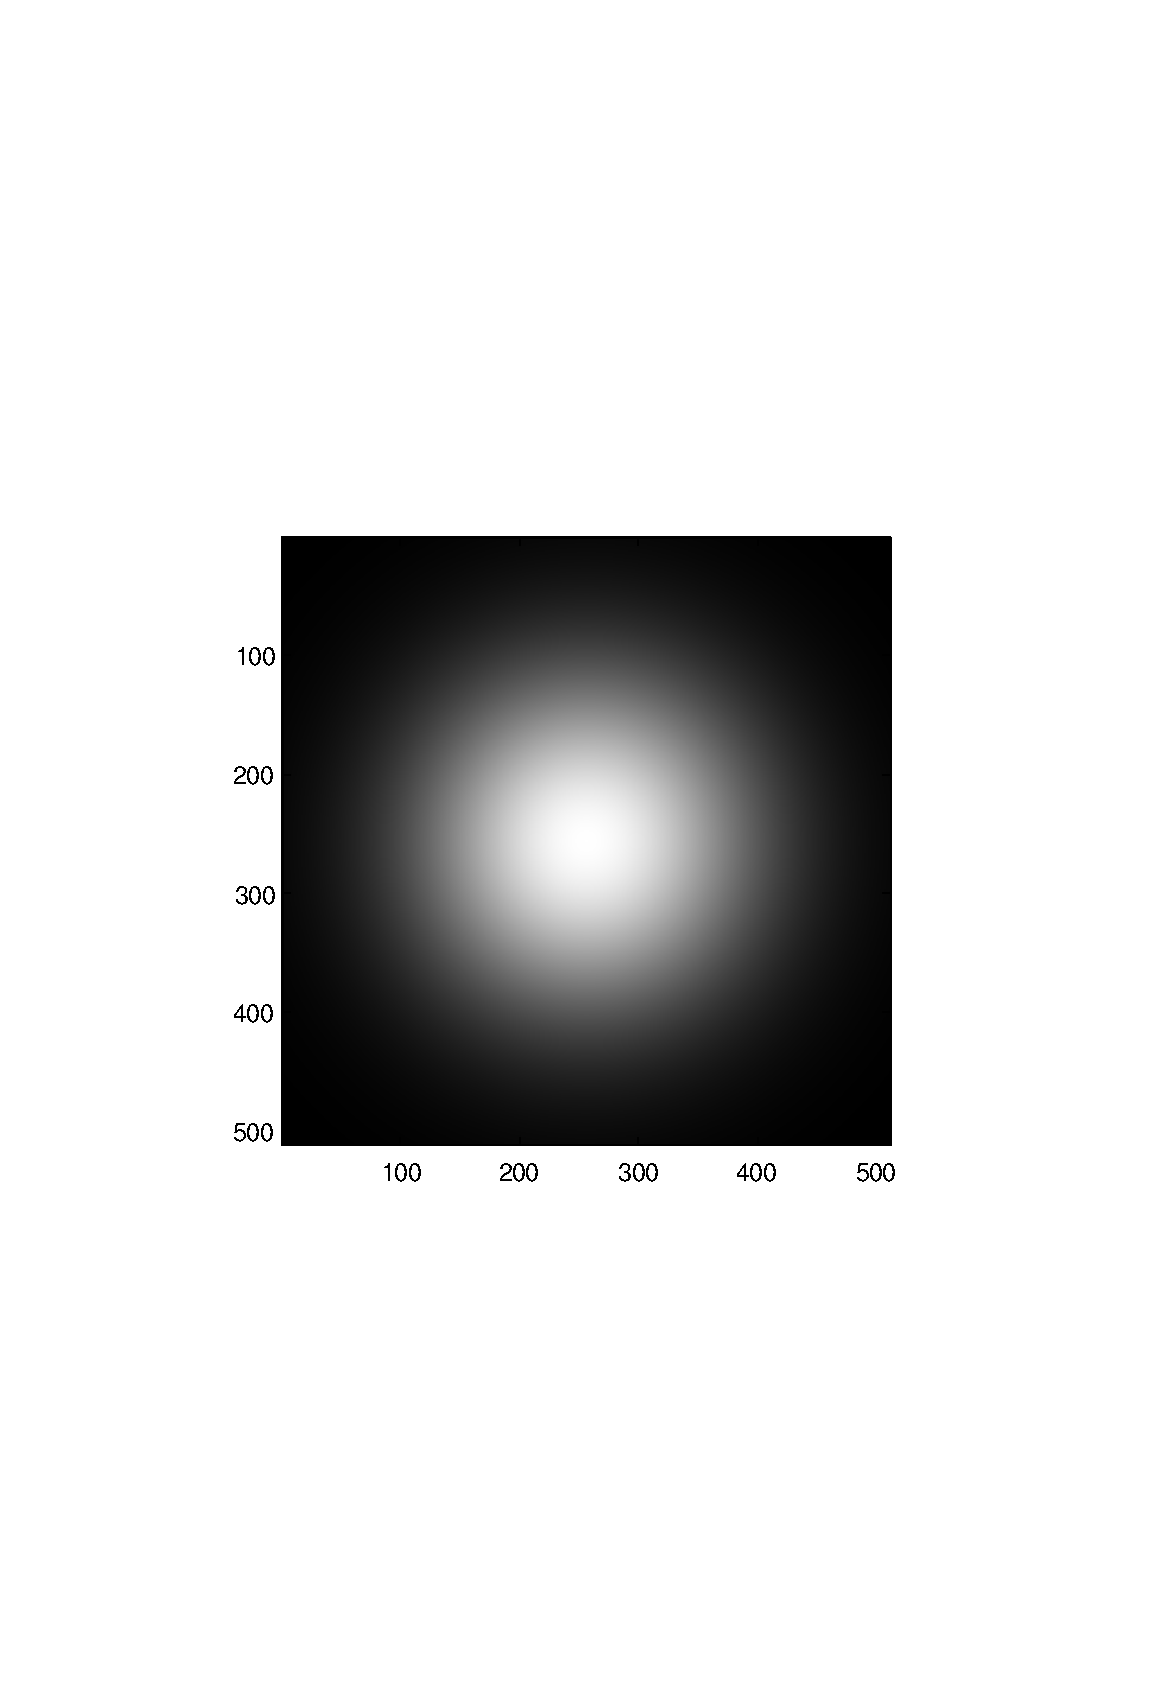
\includegraphics[width=12cm]{gray1}
\caption{gray1}
\end{DoxyImage}
 \hypertarget{handle_grid}{}\section{G\-R\-I\-D Plot Grid Toggle Function}\label{handle_grid}
Section\-: \hyperlink{sec_handle}{Handle-\/\-Based Graphics} \hypertarget{vtkwidgets_vtkxyplotwidget_Usage}{}\subsection{Usage}\label{vtkwidgets_vtkxyplotwidget_Usage}
Toggles the drawing of grid lines on the currently active plot. The general syntax for its use is \begin{DoxyVerb}   grid(state)
\end{DoxyVerb}
 where {\ttfamily state} is either \begin{DoxyVerb}   grid('on')
\end{DoxyVerb}
 to activate the grid lines, or \begin{DoxyVerb}   grid('off')
\end{DoxyVerb}
 to deactivate the grid lines. If you specify no argument then {\ttfamily grid} toggles the state of the grid\-: \begin{DoxyVerb}   grid
\end{DoxyVerb}
 You can also specify a particular axis to the grid command \begin{DoxyVerb}   grid(handle,...)
\end{DoxyVerb}
 where {\ttfamily handle} is the handle for a particular axis. \hypertarget{variables_struct_Example}{}\subsection{Example}\label{variables_struct_Example}
Here is a simple plot without grid lines.


\begin{DoxyVerbInclude}
--> x = linspace(-1,1);
--> y = cos(3*pi*x);
--> plot(x,y,'r-');
\end{DoxyVerbInclude}


 
\begin{DoxyImage}
\includegraphics[width=12cm]{grid1}
\caption{grid1}
\end{DoxyImage}


Next, we activate the grid lines.


\begin{DoxyVerbInclude}
--> plot(x,y,'r-');
--> grid on
\end{DoxyVerbInclude}


 
\begin{DoxyImage}
\includegraphics[width=12cm]{grid2}
\caption{grid2}
\end{DoxyImage}
 \hypertarget{handle_hcontour}{}\section{H\-C\-O\-N\-T\-O\-U\-R Create a contour object}\label{handle_hcontour}
Section\-: \hyperlink{sec_handle}{Handle-\/\-Based Graphics} \hypertarget{vtkwidgets_vtkxyplotwidget_Usage}{}\subsection{Usage}\label{vtkwidgets_vtkxyplotwidget_Usage}
Creates a contour object and parents it to the current axis. The syntax for its use is \begin{DoxyVerb}  handle = hcontour(property,value,property,value,...)
\end{DoxyVerb}
 where {\ttfamily property} and {\ttfamily value} are set. The handle I\-D for the resulting object is returned. It is automatically added to the children of the current axis. \hypertarget{handle_himage}{}\section{H\-I\-M\-A\-G\-E Create a image object}\label{handle_himage}
Section\-: \hyperlink{sec_handle}{Handle-\/\-Based Graphics} \hypertarget{vtkwidgets_vtkxyplotwidget_Usage}{}\subsection{Usage}\label{vtkwidgets_vtkxyplotwidget_Usage}
Creates a image object and parents it to the current axis. The syntax for its use is \begin{DoxyVerb}  handle = himage(property,value,property,value,...)
\end{DoxyVerb}
 where {\ttfamily property} and {\ttfamily value} are set. The handle I\-D for the resulting object is returned. It is automatically added to the children of the current axis. \hypertarget{handle_hist}{}\section{H\-I\-S\-T Histogram Function}\label{handle_hist}
Section\-: \hyperlink{sec_handle}{Handle-\/\-Based Graphics} \hypertarget{vtkwidgets_vtkxyplotwidget_Usage}{}\subsection{Usage}\label{vtkwidgets_vtkxyplotwidget_Usage}
\begin{DoxyVerb}        n=hist (y)
        n=hist (y,x)
        n=hist (y,x,norm)
\end{DoxyVerb}
 Produce histogram counts or plots.

With one vector input argument, plot a histogram of the values with 10 bins. The range of the histogram bins is determined by the range of the data.

Given a second scalar argument, use that as the number of bins.

Given a second vector argument, use that as the centers of the bins, with the width of the bins determined from the adjacent values in the vector.

If third argument is provided, the histogram is normalised such that the sum of the bars is equal to {\ttfamily norm}.

Extreme values are lumped in the first and last bins. \hypertarget{handle_hline}{}\section{H\-L\-I\-N\-E Create a line object}\label{handle_hline}
Section\-: \hyperlink{sec_handle}{Handle-\/\-Based Graphics} \hypertarget{vtkwidgets_vtkxyplotwidget_Usage}{}\subsection{Usage}\label{vtkwidgets_vtkxyplotwidget_Usage}
Creates a line object and parents it to the current axis. The syntax for its use is \begin{DoxyVerb}  handle = hline(property,value,property,value,...)
\end{DoxyVerb}
 where {\ttfamily property} and {\ttfamily value} are set. The handle I\-D for the resulting object is returned. It is automatically added to the children of the current axis. \hypertarget{handle_hold}{}\section{H\-O\-L\-D Plot Hold Toggle Function}\label{handle_hold}
Section\-: \hyperlink{sec_handle}{Handle-\/\-Based Graphics} \hypertarget{vtkwidgets_vtkxyplotwidget_Usage}{}\subsection{Usage}\label{vtkwidgets_vtkxyplotwidget_Usage}
Toggles the hold state on the currently active plot. The general syntax for its use is \begin{DoxyVerb}   hold(state)
\end{DoxyVerb}
 where {\ttfamily state} is either \begin{DoxyVerb}   hold('on')
\end{DoxyVerb}
 to turn hold on, or \begin{DoxyVerb}   hold('off')
\end{DoxyVerb}
 to turn hold off. If you specify no argument then {\ttfamily hold} toggles the state of the hold\-: \begin{DoxyVerb}   hold
\end{DoxyVerb}
 You can also specify a particular axis to the hold command \begin{DoxyVerb}   hold(handle,...)
\end{DoxyVerb}
 where {\ttfamily handle} is the handle for a particular axis. \hypertarget{transforms_svd_Function}{}\subsection{Internals}\label{transforms_svd_Function}
The {\ttfamily hold} function allows one to construct a plot sequence incrementally, instead of issuing all of the plots simultaneously using the {\ttfamily plot} command. \hypertarget{variables_struct_Example}{}\subsection{Example}\label{variables_struct_Example}
Here is an example of using both the {\ttfamily hold} command and the multiple-\/argument {\ttfamily plot} command to construct a plot composed of three sets of data. The first is a plot of a modulated Gaussian.


\begin{DoxyVerbInclude}
--> x = linspace(-5,5,500);
--> t = exp(-x.^2);
--> y = t.*cos(2*pi*x*3);
--> plot(x,y);
\end{DoxyVerbInclude}


 
\begin{DoxyImage}
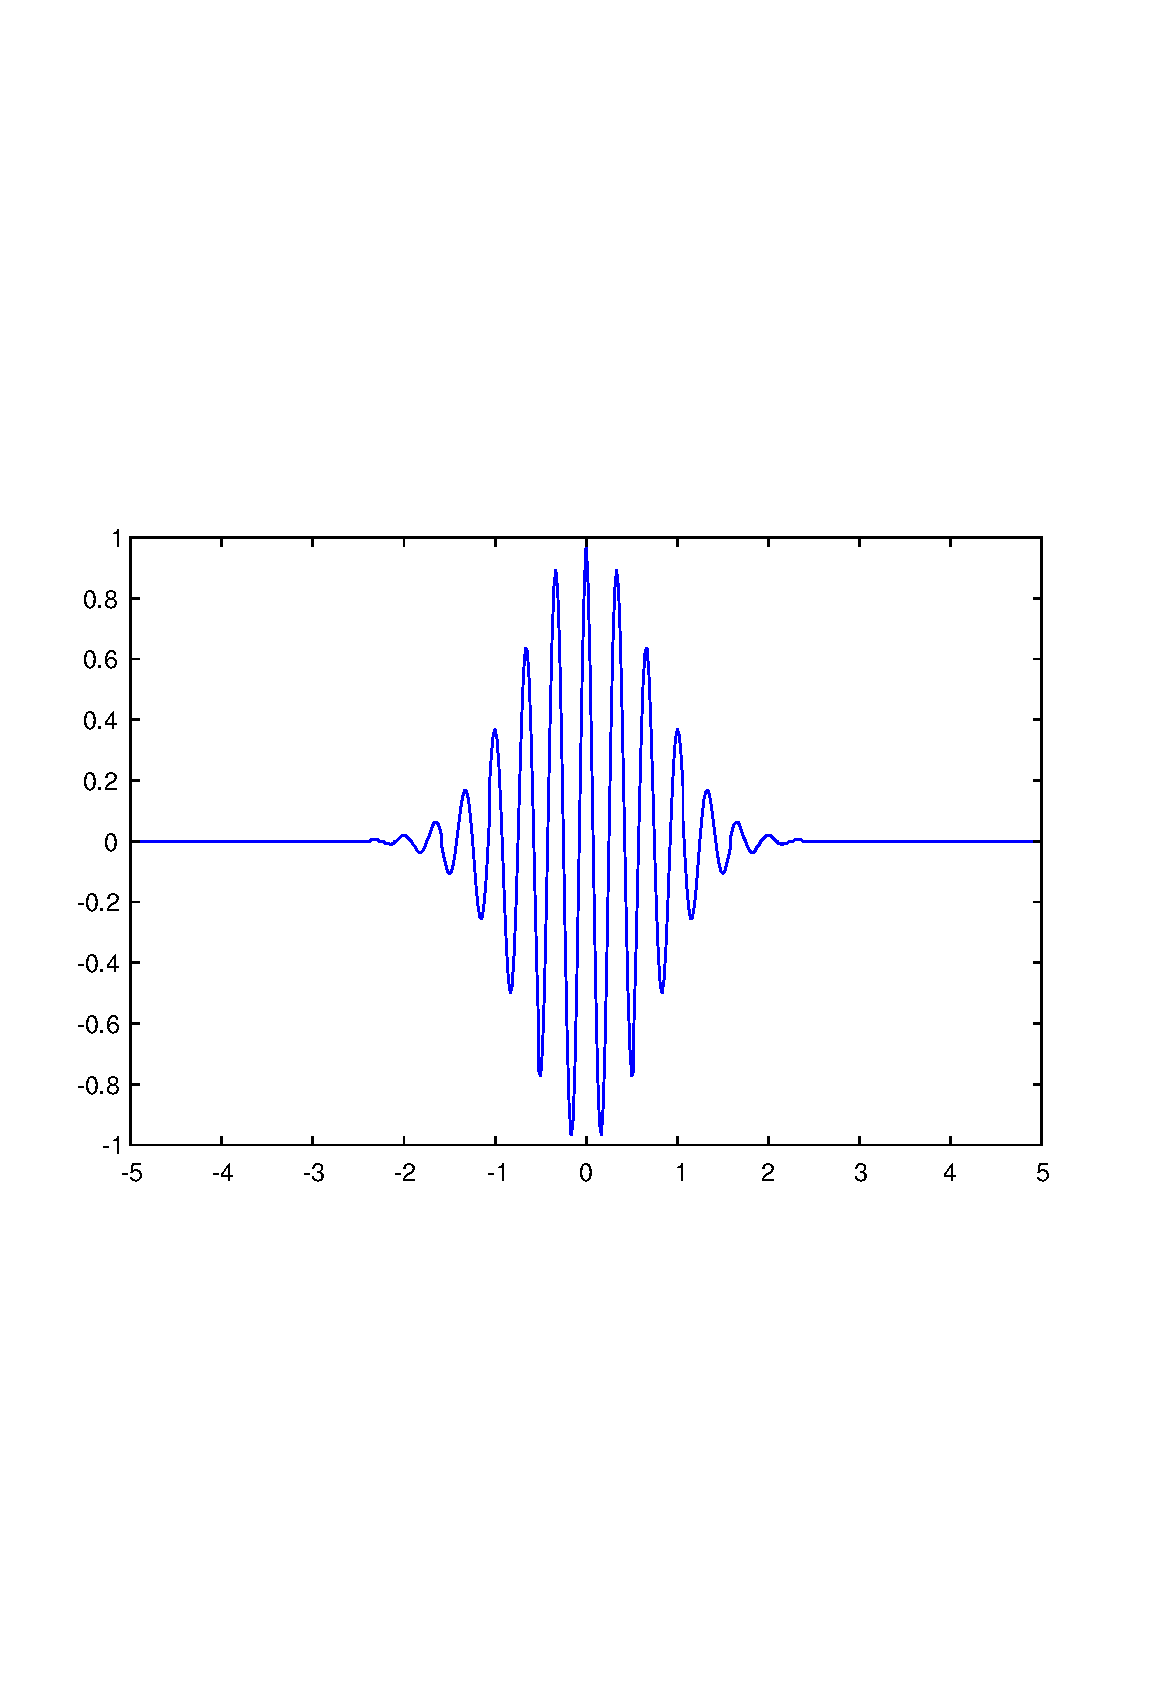
\includegraphics[width=12cm]{hold1}
\caption{hold1}
\end{DoxyImage}


We now turn the hold state to {\ttfamily 'on'}, and add another plot sequence, this time composed of the top and bottom envelopes of the modulated Gaussian. We add the two envelopes simultaneously using a single {\ttfamily plot} command. The fact that {\ttfamily hold} is {\ttfamily 'on'} means that these two envelopes are added to (instead of replace) the current contents of the plot.


\begin{DoxyVerbInclude}
--> plot(x,y);
--> hold on
--> plot(x,t,'g-',x,-t,'b-')
\end{DoxyVerbInclude}


 
\begin{DoxyImage}
\includegraphics[width=12cm]{hold2}
\caption{hold2}
\end{DoxyImage}
 \hypertarget{handle_hpatch}{}\section{H\-P\-A\-T\-C\-H Create a patch object}\label{handle_hpatch}
Section\-: \hyperlink{sec_handle}{Handle-\/\-Based Graphics} \hypertarget{vtkwidgets_vtkxyplotwidget_Usage}{}\subsection{Usage}\label{vtkwidgets_vtkxyplotwidget_Usage}
Creates a patch object and parents it to the current axis. The syntax for its use is \begin{DoxyVerb}  handle = hpatch(property,value,property,value,...)
\end{DoxyVerb}
 where {\ttfamily property} and {\ttfamily value} are set. The handle I\-D for the resulting object is returned. It is automatically added to the children of the current axis. \hypertarget{handle_hpoint}{}\section{H\-P\-O\-I\-N\-T Get Point From Window}\label{handle_hpoint}
Section\-: \hyperlink{sec_handle}{Handle-\/\-Based Graphics} \hypertarget{vtkwidgets_vtkxyplotwidget_Usage}{}\subsection{Usage}\label{vtkwidgets_vtkxyplotwidget_Usage}
This function waits for the user to click on the current figure window, and then returns the coordinates of that click. The generic syntax for its use is \begin{DoxyVerb}  [x,y] = hpoint
\end{DoxyVerb}
 \hypertarget{handle_hrawplot}{}\section{H\-R\-A\-W\-P\-L\-O\-T Generate a Raw Plot File}\label{handle_hrawplot}
Section\-: \hyperlink{sec_handle}{Handle-\/\-Based Graphics} \hypertarget{vtkwidgets_vtkxyplotwidget_Usage}{}\subsection{Usage}\label{vtkwidgets_vtkxyplotwidget_Usage}
This function takes a sequence of commands, and generates a raw plot (to a file) that renders the commands. It is a useful tool for creating high quality fully customized P\-D\-F plots from within Free\-Mat scripts that are portable. The syntax for its use \begin{DoxyVerb}  hrawplot(filename,commands)
\end{DoxyVerb}
 where {\ttfamily filename} is the name of the file to plot to, and {\ttfamily commands} is a cell array of strings. Each entry in the cell array contains a string with a command text. The commands describe a simple mini-\/language for describing plots. The complete dictionary of commands is given 
\begin{DoxyItemize}
\item {\ttfamily L\-I\-N\-E x1 y1 x2 y2} -- draw a line  
\item {\ttfamily F\-O\-N\-T name size} -- select a font of the given name and size  
\item {\ttfamily T\-E\-X\-T x1 y1 string} -- draw the given text string at the given location  
\item {\ttfamily S\-T\-Y\-L\-E style} -- select line style ('solid' or 'dotted')  
\item {\ttfamily P\-A\-G\-E} -- force a new page  
\item {\ttfamily S\-I\-Z\-E x1 y1} -- Set the page mapping  
\item {\ttfamily B\-O\-X x1 y1 x2 y2} -- draw a filled box covering the given coordinates  
\item {\ttfamily H\-T\-E\-X\-T\-B\-O\-X x1 y1 x2 y2 string} -- Draw a horizontal box with the given string centered in it  
\item {\ttfamily V\-T\-E\-X\-T\-B\-O\-X x1 y1 x2 y2 string} -- Draw a vertical box with the given string centered in it (rotated 90 degrees)  
\item {\ttfamily B\-R\-U\-S\-H string} -- Set the brush color ('red','blue', etc)  
\item {\ttfamily P\-E\-N string} -- Set the pen color  
\end{DoxyItemize}\hypertarget{handle_hsurface}{}\section{H\-S\-U\-R\-F\-A\-C\-E Create a surface object}\label{handle_hsurface}
Section\-: \hyperlink{sec_handle}{Handle-\/\-Based Graphics} \hypertarget{vtkwidgets_vtkxyplotwidget_Usage}{}\subsection{Usage}\label{vtkwidgets_vtkxyplotwidget_Usage}
Creates a surface object and parents it to the current axis. The syntax for its use is \begin{DoxyVerb}  handle = hsurface(property,value,property,value,...)
\end{DoxyVerb}
 where {\ttfamily property} and {\ttfamily value} are set. The handle I\-D for the resulting object is returned. It is automatically added to the children of the current axis. \hypertarget{handle_htext}{}\section{H\-T\-E\-X\-T Create a text object}\label{handle_htext}
Section\-: \hyperlink{sec_handle}{Handle-\/\-Based Graphics} \hypertarget{vtkwidgets_vtkxyplotwidget_Usage}{}\subsection{Usage}\label{vtkwidgets_vtkxyplotwidget_Usage}
Creates a text object and parents it to the current axis. The syntax for its use is \begin{DoxyVerb}  handle = htext(property,value,property,value,...)
\end{DoxyVerb}
 where {\ttfamily property} and {\ttfamily value} are set. The handle I\-D for the resulting object is returned. It is automatically added to the children of the current axis. \hypertarget{handle_htextbitmap}{}\section{H\-T\-E\-X\-T\-B\-I\-T\-M\-A\-P Get Text Rendered as a Bitmap}\label{handle_htextbitmap}
Section\-: \hyperlink{sec_handle}{Handle-\/\-Based Graphics} \hypertarget{vtkwidgets_vtkxyplotwidget_Usage}{}\subsection{Usage}\label{vtkwidgets_vtkxyplotwidget_Usage}
This function takes a fontname, a size, and a text string and returns a bitmap containing the text. The generic syntax for its use is \begin{DoxyVerb}  bitmap = htextbitmap(fontname,size,text)
\end{DoxyVerb}
 where the output bitmap contains the text rendered into a matrix. \hypertarget{handle_image}{}\section{I\-M\-A\-G\-E Image Display Function}\label{handle_image}
Section\-: \hyperlink{sec_handle}{Handle-\/\-Based Graphics} \hypertarget{vtkwidgets_vtkxyplotwidget_Usage}{}\subsection{Usage}\label{vtkwidgets_vtkxyplotwidget_Usage}
The {\ttfamily image} command has the following general syntax \begin{DoxyVerb}  handle = image(x,y,C,properties...)
\end{DoxyVerb}
 where {\ttfamily x} is a two vector containing the {\ttfamily x} coordinates of the first and last pixels along a column, and {\ttfamily y} is a two vector containing the {\ttfamily y} coordinates of the first and last pixels along a row. The matrix {\ttfamily C} constitutes the image data. It must either be a scalar matrix, in which case the image is colormapped using the {\ttfamily colormap} for the current figure. If the matrix is {\ttfamily M x N x 3}, then {\ttfamily C} is intepreted as R\-G\-B data, and the image is not colormapped. The {\ttfamily properties} argument is a set of {\ttfamily property/value} pairs that affect the final image. You can also omit the {\ttfamily x} and {\ttfamily y}, \begin{DoxyVerb}  handle = image(C, properties...)
\end{DoxyVerb}
 in which case they default to {\ttfamily x = \mbox{[}1,size(\-C,2)\mbox{]}} and {\ttfamily y = \mbox{[}1,size(\-C,1)\mbox{]}}. Finally, you can use the {\ttfamily image} function with only formal arguments \begin{DoxyVerb}  handle = image(properties...)
\end{DoxyVerb}


To support legacy Free\-Mat code, you can also use the following form of {\ttfamily image} \begin{DoxyVerb}  image(C, zoomfactor)
\end{DoxyVerb}
 which is equivalent to {\ttfamily image(\-C)} with the axes removed so that the image takes up the full figure window, and the size of the figure window adjusted to achieve the desired zoom factor using the {\ttfamily zoom} command. \hypertarget{variables_struct_Example}{}\subsection{Example}\label{variables_struct_Example}
In this example, we create an image that is {\ttfamily 512 x 512} pixels square, and set the background to a noise pattern. We set the central {\ttfamily 128 x 256} pixels to be white.


\begin{DoxyVerbInclude}
--> x = rand(512);
--> x((-64:63)+256,(-128:127)+256) = 1.0;
--> figure

ans = 
 1 

--> image(x)
--> colormap(gray)
\end{DoxyVerbInclude}


The resulting image looks like\-:  
\begin{DoxyImage}
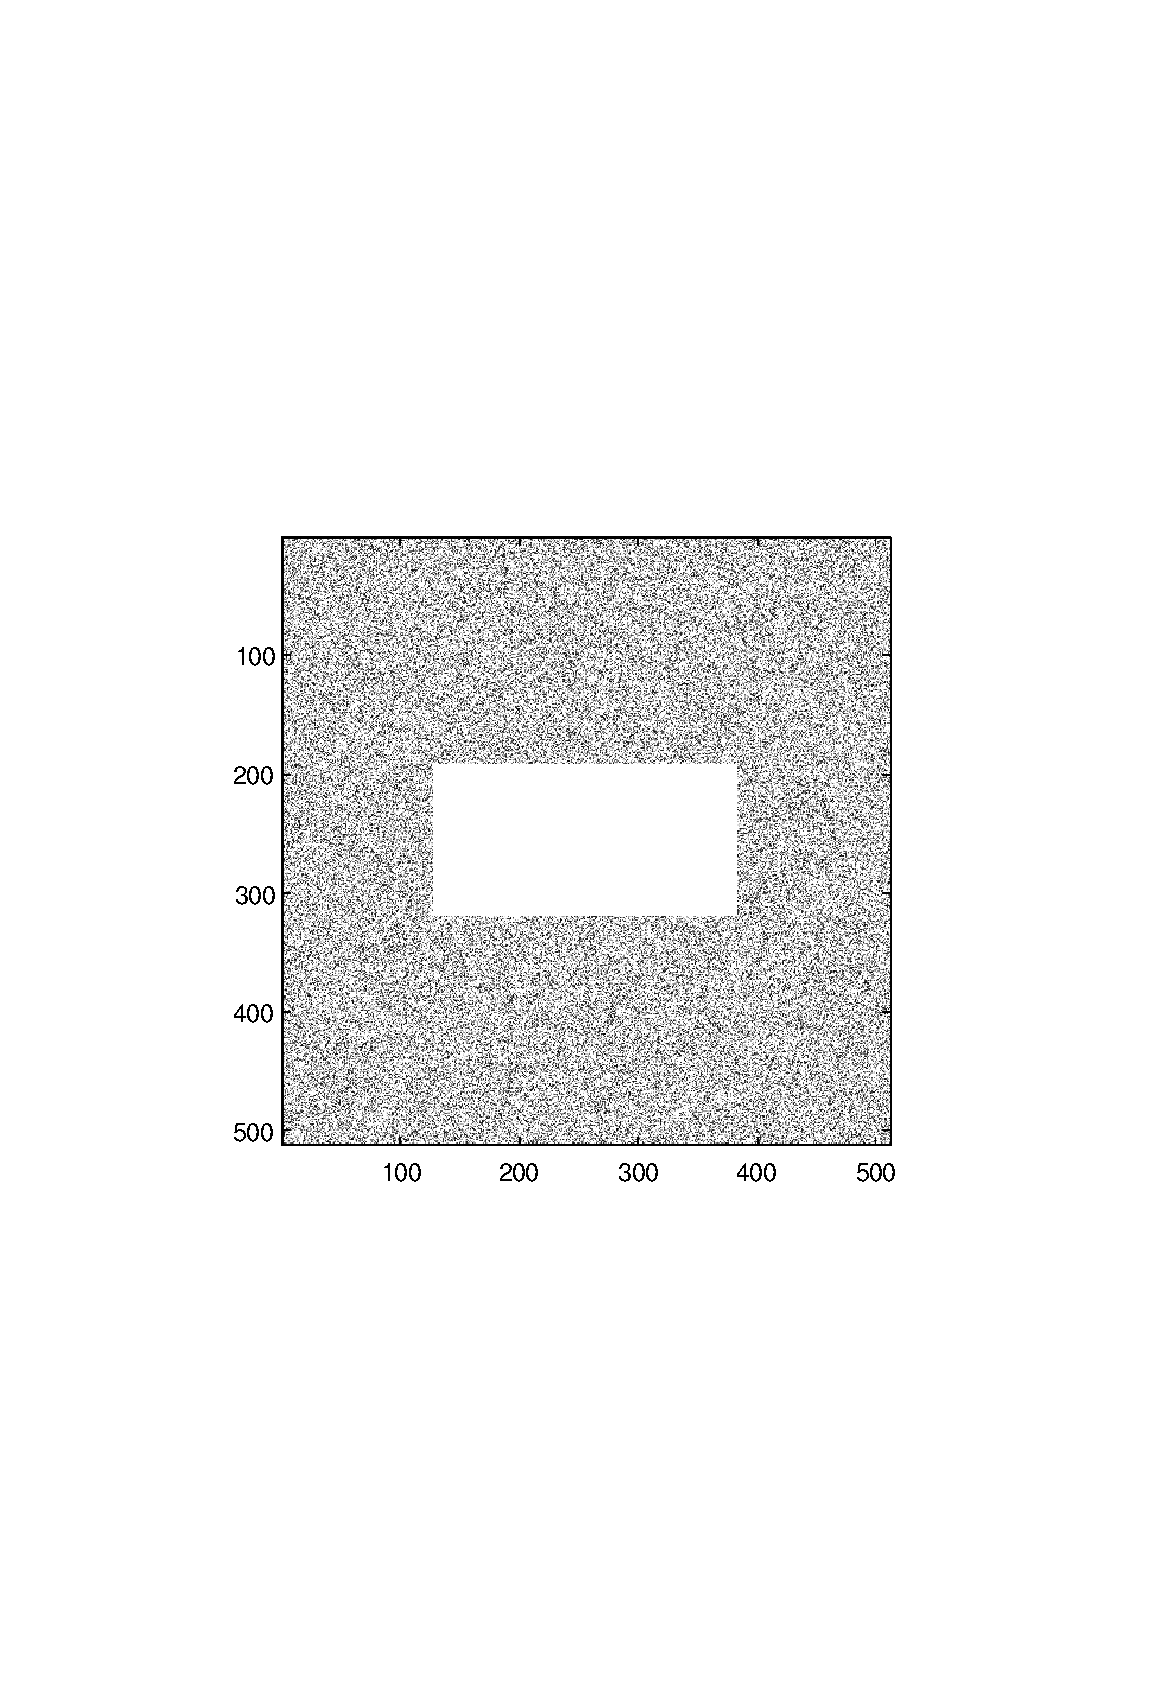
\includegraphics[width=12cm]{image1}
\caption{image1}
\end{DoxyImage}
 Here is an example of an R\-G\-B image


\begin{DoxyVerbInclude}
--> t = linspace(0,1);
--> red = t'*t;
--> green = t'*(t.^2);
--> blue = t'*(0*t+1);
--> A(:,:,1) = red; 
--> A(:,:,2) = green; 
--> A(:,:,3) = blue;
--> image(A);
\end{DoxyVerbInclude}


The resulting image looks like\-:  
\begin{DoxyImage}
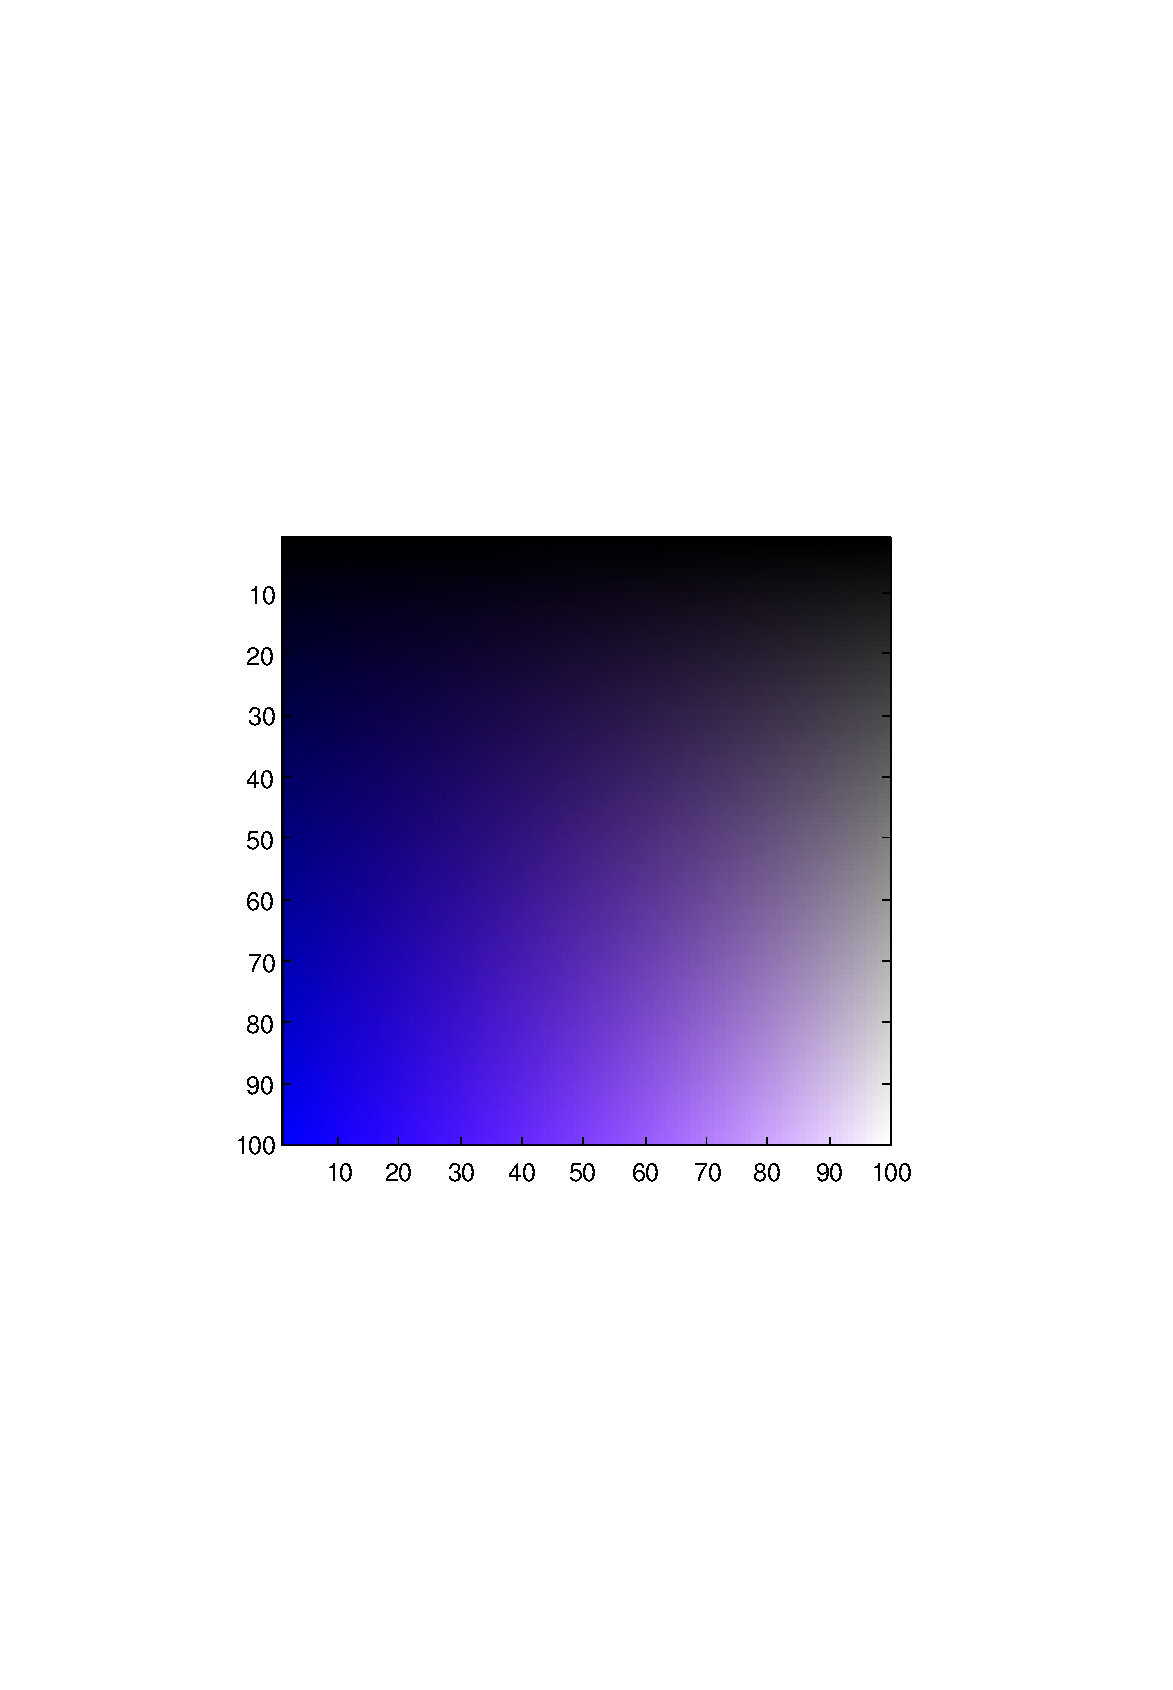
\includegraphics[width=12cm]{image2}
\caption{image2}
\end{DoxyImage}
 \hypertarget{handle_imageproperties}{}\section{I\-M\-A\-G\-E\-P\-R\-O\-P\-E\-R\-T\-I\-E\-S Image Object Properties}\label{handle_imageproperties}
Section\-: \hyperlink{sec_handle}{Handle-\/\-Based Graphics} \hypertarget{vtkwidgets_vtkxyplotwidget_Usage}{}\subsection{Usage}\label{vtkwidgets_vtkxyplotwidget_Usage}
Below is a summary of the properties for the axis. 
\begin{DoxyItemize}
\item {\ttfamily alphadata} -\/ {\ttfamily vector} -\/ This is a vector that should contain as many elements as the image data itself {\ttfamily cdata}, or a single scalar. For a single scalar, all values of the image take on the same transparency. Otherwise, the transparency of each pixel is determined by the corresponding value from the {\ttfamily alphadata} vector.  
\item {\ttfamily alphadatamapping} -\/ {\ttfamily \{'scaled','direct','none'\}} -\/ For {\ttfamily none} mode (the default), no transparency is applied to the data. For {\ttfamily direct} mode, the vector {\ttfamily alphadata} contains values between @\mbox{[}0,M-\/1\mbox{]}$|$ where {\ttfamily M} is the length of the alpha map stored in the figure. For {\ttfamily scaled} mode, the {\ttfamily alim} vector for the figure is used to linearly rescale the alpha data prior to lookup in the alpha map.  
\item {\ttfamily cdata} -\/ {\ttfamily array} -\/ This is either a {\ttfamily M x N} array or an {\ttfamily M x N x 3} array. If the data is {\ttfamily M x N} the image is a scalar image (indexed mode), where the color associated with each image pixel is computed using the colormap and the {\ttfamily cdatamapping} mode. If the data is {\ttfamily M x N x 3} the image is assumed to be in R\-G\-B mode, and the colorpanes are taken directly from {\ttfamily cdata} (the colormap is ignored). Note that in this case, the data values must be between @\mbox{[}0,1\mbox{]}$|$ for each color channel and each pixel.  
\item {\ttfamily cdatamapping} -\/ {\ttfamily \{'scaled','direct'\}} -\/ For {\ttfamily scaled} (the default), the pixel values are scaled using the {\ttfamily clim} vector for the figure prior to looking up in the colormap. For {\ttfamily direct} mode, the pixel values must be in the range {\ttfamily \mbox{[}0,N-\/1} where {\ttfamily N} is the number of colors in the colormap if the data is integer type. For floating point data types, values must be in the range {\ttfamily \mbox{[}1,N\mbox{]}}.  
\item {\ttfamily children} -\/ Not used.  
\item {\ttfamily parent} -\/ {\ttfamily handle} -\/ The axis containing the image.  
\item {\ttfamily tag} -\/ {\ttfamily string} -\/ You can set this to any string you want.  
\item {\ttfamily type} -\/ {\ttfamily string} -\/ Set to the string {\ttfamily 'image'}.  
\item {\ttfamily xdata} -\/ {\ttfamily two vector} -\/ contains the x coordinates of the first and last column (respectively). Defaults to {\ttfamily \mbox{[}1,C\mbox{]}} where {\ttfamily C} is the number of columns in the image.  
\item {\ttfamily ydata} -\/ {\ttfamily two vector} -\/ contains the y coordinates of the first and last row (respectively). Defaults to {\ttfamily \mbox{[}1,R\mbox{]}} where {\ttfamily R} is the number of rows in the image.  
\item {\ttfamily userdata} -\/ {\ttfamily array} -\/ Available to store any variable you want in the handle object.  
\item {\ttfamily visible} -\/ {\ttfamily \{'on','off'\}} -\/ Controls whether the image is visible or not.  
\end{DoxyItemize}\hypertarget{handle_imagesc}{}\section{I\-M\-A\-G\-E\-S\-C Image Display Function}\label{handle_imagesc}
Section\-: \hyperlink{sec_handle}{Handle-\/\-Based Graphics} \hypertarget{vtkwidgets_vtkxyplotwidget_Usage}{}\subsection{Usage}\label{vtkwidgets_vtkxyplotwidget_Usage}
The {\ttfamily imagesc} command has the following general syntax \begin{DoxyVerb}  handle = imagesc(x,y,C,clim)
\end{DoxyVerb}
 where {\ttfamily x} is a two vector containing the {\ttfamily x} coordinates of the first and last pixels along a column, and {\ttfamily y} is a two vector containing the {\ttfamily y} coordinates of the first and last pixels along a row. The matrix {\ttfamily C} constitutes the image data. It must either be a scalar matrix, in which case the image is colormapped using the {\ttfamily colormap} for the current figure. If the matrix is {\ttfamily M x N x 3}, then {\ttfamily C} is intepreted as R\-G\-B data, and the image is not colormapped. The {\ttfamily clim} argument is a pairs \mbox{[}low high\mbox{]} that specifies scaling. You can also omit the {\ttfamily x} and {\ttfamily y}, \begin{DoxyVerb}  handle = imagesc(C, clim)
\end{DoxyVerb}
 in which case they default to {\ttfamily x = \mbox{[}1,size(\-C,2)\mbox{]}} and {\ttfamily y = \mbox{[}1,size(\-C,1)\mbox{]}}. Finally, you can use the {\ttfamily image} function with only formal arguments \begin{DoxyVerb}  handle = imagesc(properties...)
\end{DoxyVerb}
\hypertarget{variables_struct_Example}{}\subsection{Example}\label{variables_struct_Example}
In this example, we create an image that is {\ttfamily 512 x 512} pixels square, and set the background to a noise pattern. We set the central {\ttfamily 128 x 256} pixels to be white.


\begin{DoxyVerbInclude}
--> x = rand(512);
--> x((-64:63)+256,(-128:127)+256) = 1.0;
--> figure

ans = 
 1 

--> imagesc(x,[0 .5])
--> colormap(gray)
\end{DoxyVerbInclude}
 \hypertarget{handle_is2dview}{}\section{I\-S2\-D\-V\-I\-E\-W Test Axes For 2\-D View}\label{handle_is2dview}
Section\-: \hyperlink{sec_handle}{Handle-\/\-Based Graphics} \hypertarget{vtkwidgets_vtkxyplotwidget_Usage}{}\subsection{Usage}\label{vtkwidgets_vtkxyplotwidget_Usage}
This function returns {\ttfamily true} if the current axes are in a 2-\/\-D view, and false otherwise. The generic syntax for its use is \begin{DoxyVerb}  y = is2dview(x)
\end{DoxyVerb}
 where {\ttfamily x} is the handle of an axes object. \hypertarget{handle_ishold}{}\section{I\-S\-H\-O\-L\-D Test Hold Status}\label{handle_ishold}
Section\-: \hyperlink{sec_handle}{Handle-\/\-Based Graphics} \hypertarget{vtkwidgets_vtkxyplotwidget_Usage}{}\subsection{Usage}\label{vtkwidgets_vtkxyplotwidget_Usage}
Returns the state of the {\ttfamily hold} flag on the currently active plot. The general syntax for its use is \begin{DoxyVerb}   ishold
\end{DoxyVerb}
 and it returns a logical 1 if {\ttfamily hold} is {\ttfamily on}, and a logical 0 otherwise. \hypertarget{handle_legend}{}\section{L\-E\-G\-E\-N\-D Add Legent to Plot}\label{handle_legend}
Section\-: \hyperlink{sec_handle}{Handle-\/\-Based Graphics} \hypertarget{vtkwidgets_vtkxyplotwidget_Usage}{}\subsection{Usage}\label{vtkwidgets_vtkxyplotwidget_Usage}
This command adds a legend to the current plot. Currently, the following forms of the {\ttfamily legend} command are supported. The first form creates a legend with the given labels for the data series\-: \begin{DoxyVerb}  legend('label1','label2',...)
\end{DoxyVerb}
 where {\ttfamily 'label1'} is the text label associated with data plot 1 and so on. You can also use the {\ttfamily legend} command to control the appearance of the legend in the current plot. To remove the legend from the current plot, use \begin{DoxyVerb}  legend('off')
\end{DoxyVerb}
 To hide the legend for the current plot (but do not remove it) \begin{DoxyVerb}  legend('hide')
\end{DoxyVerb}
 And to show the legend that has been hidden, use \begin{DoxyVerb}  legend('show')
\end{DoxyVerb}
 You can also toggle the display of the box surrounding the legend. Use \begin{DoxyVerb}  legend('boxoff')
\end{DoxyVerb}
 or \begin{DoxyVerb}  legend('boxon')
\end{DoxyVerb}
 to turn the legend box off or on, respectively. To toggle the visible state of the current legend, use \begin{DoxyVerb}  legend('toggle')
\end{DoxyVerb}
 Specifying no arguments at all (apart from an optional location argument as specified below) results in the legend being rebuilt. This form is useful for picking up font changes or relocating the legend. \begin{DoxyVerb}  legend
\end{DoxyVerb}
 By default, the {\ttfamily legend} command places the new legend in the upper right corner of the current plot. To change this behavior, use the {\ttfamily 'location'} specifier (must be the last two options to the command) \begin{DoxyVerb}  legend(...,'location',option)
\end{DoxyVerb}
 where {\ttfamily option} takes on the following possible values 
\begin{DoxyItemize}
\item {\ttfamily north},{\ttfamily N} -\/ top center of plot  
\item {\ttfamily south},{\ttfamily S} -\/ bottom center of plot  
\item {\ttfamily east},{\ttfamily E} -\/ middle right of plot  
\item {\ttfamily west},{\ttfamily W} -\/ middle left of plot  
\item {\ttfamily northeast},{\ttfamily N\-E} -\/ top right of plot (default behavior)  
\item {\ttfamily northwest},{\ttfamily N\-W} -\/ top left of plot  
\item {\ttfamily southeast},{\ttfamily S\-E} -\/ bottom right of plot  
\item {\ttfamily southwest},{\ttfamily S\-W} -\/ bottom left of plot  
\end{DoxyItemize}This implementation of {\ttfamily legend} is incomplete relative to the M\-A\-T\-L\-A\-B A\-P\-I. The functionality will be improved in future versions of Free\-Mat. \hypertarget{handle_line}{}\section{L\-I\-N\-E Line Display Function}\label{handle_line}
Section\-: \hyperlink{sec_handle}{Handle-\/\-Based Graphics} \hypertarget{vtkwidgets_vtkxyplotwidget_Usage}{}\subsection{Usage}\label{vtkwidgets_vtkxyplotwidget_Usage}
The {\ttfamily line} command has the following general syntax \begin{DoxyVerb}   handle = line(x,y,z,properties...)
\end{DoxyVerb}
 where... \hypertarget{handle_lineproperties}{}\section{L\-I\-N\-E\-P\-R\-O\-P\-E\-R\-T\-I\-E\-S Line Series Object Properties}\label{handle_lineproperties}
Section\-: \hyperlink{sec_handle}{Handle-\/\-Based Graphics} \hypertarget{vtkwidgets_vtkxyplotwidget_Usage}{}\subsection{Usage}\label{vtkwidgets_vtkxyplotwidget_Usage}
Below is a summary of the properties for a line series. 
\begin{DoxyItemize}
\item {\ttfamily color} -\/ {\ttfamily colorspec} -\/ The color that is used to draw the line.  
\item {\ttfamily children} -\/ Not used.  
\item {\ttfamily displayname} -\/ The name of this line series as it appears in a legend.  
\item {\ttfamily linestyle} -\/ {\ttfamily \{'-\/','--','\-:','-\/.','none'\}} -\/ The style of the line.  
\item {\ttfamily linewidth} -\/ {\ttfamily scalar} -\/ The width of the line.  
\item {\ttfamily marker} -\/ {\ttfamily \{'+','o','$\ast$','.','x','square','s','diamond','d','$^\wedge$','v','$>$','$<$'\}} -\/ The marker for data points on the line. Some of these are redundant, as {\ttfamily 'square'} {\ttfamily 's'} are synonyms, and {\ttfamily 'diamond'} and {\ttfamily 'd'} are also synonyms.  
\item {\ttfamily markeredgecolor} -\/ {\ttfamily colorspec} -\/ The color used to draw the marker. For some of the markers (circle, square, etc.) there are two colors used to draw the marker. This property controls the edge color (which for unfilled markers) is the primary color of the marker.  
\item {\ttfamily markerfacecolor} -\/ {\ttfamily colorspec} -\/ The color used to fill the marker. For some of the markers (circle, square, etc.) there are two colors used to fill the marker.  
\item {\ttfamily markersize} -\/ {\ttfamily scalar} -\/ Control the size of the marker. Defaults to 6, which is effectively the radius (in pixels) of the markers.  
\item {\ttfamily parent} -\/ {\ttfamily handle} -\/ The axis that contains this object.  
\item {\ttfamily tag} -\/ {\ttfamily string} -\/ A string that can be used to tag the object.  
\item {\ttfamily type} -\/ {\ttfamily string} -\/ Returns the string {\ttfamily 'line'}.  
\item {\ttfamily visible} -\/ {\ttfamily \{'on','off'\}} -\/ Controls visibility of the the line.  
\item {\ttfamily xdata} -\/ {\ttfamily vector} -\/ Vector of x coordinates of points on the line. Must be the same size as the {\ttfamily ydata} and {\ttfamily zdata} vectors.  
\item {\ttfamily ydata} -\/ {\ttfamily vector} -\/ Vector of y coordinates of points on the line. Must be the same size as the {\ttfamily xdata} and {\ttfamily zdata} vectors.  
\item {\ttfamily zdata} -\/ {\ttfamily vector} -\/ Vector of z coordinates of points on the line. Must be the same size as the {\ttfamily xdata} and {\ttfamily ydata} vectors.  
\item {\ttfamily xdatamode} -\/ {\ttfamily \{'auto','manual'\}} -\/ When set to {\ttfamily 'auto'} Free\-Mat will autogenerate the x coordinates for the points on the line. These values will be {\ttfamily 1,..,N} where {\ttfamily N} is the number of points in the line.  
\item {\ttfamily userdata} -\/ {\ttfamily array} -\/ Available to store any variable you want in the handle object.  
\end{DoxyItemize}\hypertarget{handle_loglog}{}\section{L\-O\-G\-L\-O\-G Log-\/\-Log Plot Function}\label{handle_loglog}
Section\-: \hyperlink{sec_handle}{Handle-\/\-Based Graphics} \hypertarget{vtkwidgets_vtkxyplotwidget_Usage}{}\subsection{Usage}\label{vtkwidgets_vtkxyplotwidget_Usage}
This command has the exact same syntax as the {\ttfamily plot} command\-: \begin{DoxyVerb}  loglog(<data 1>,{linespec 1},<data 2>,{linespec 2}...,properties...)
\end{DoxyVerb}
 in fact, it is a simple wrapper around {\ttfamily plot} that sets the x and y axis to have a logarithmic scale. \hypertarget{variables_struct_Example}{}\subsection{Example}\label{variables_struct_Example}
Here is an example of a doubly exponential signal plotted first on a linear plot\-:


\begin{DoxyVerbInclude}
--> x = linspace(1,100);
--> y = x;
--> plot(x,y,'r-');
\end{DoxyVerbInclude}


 
\begin{DoxyImage}
\includegraphics[width=12cm]{loglog1}
\caption{loglog1}
\end{DoxyImage}
 and now on a log-\/log plot


\begin{DoxyVerbInclude}
--> loglog(x,y,'r-');
\end{DoxyVerbInclude}


 
\begin{DoxyImage}
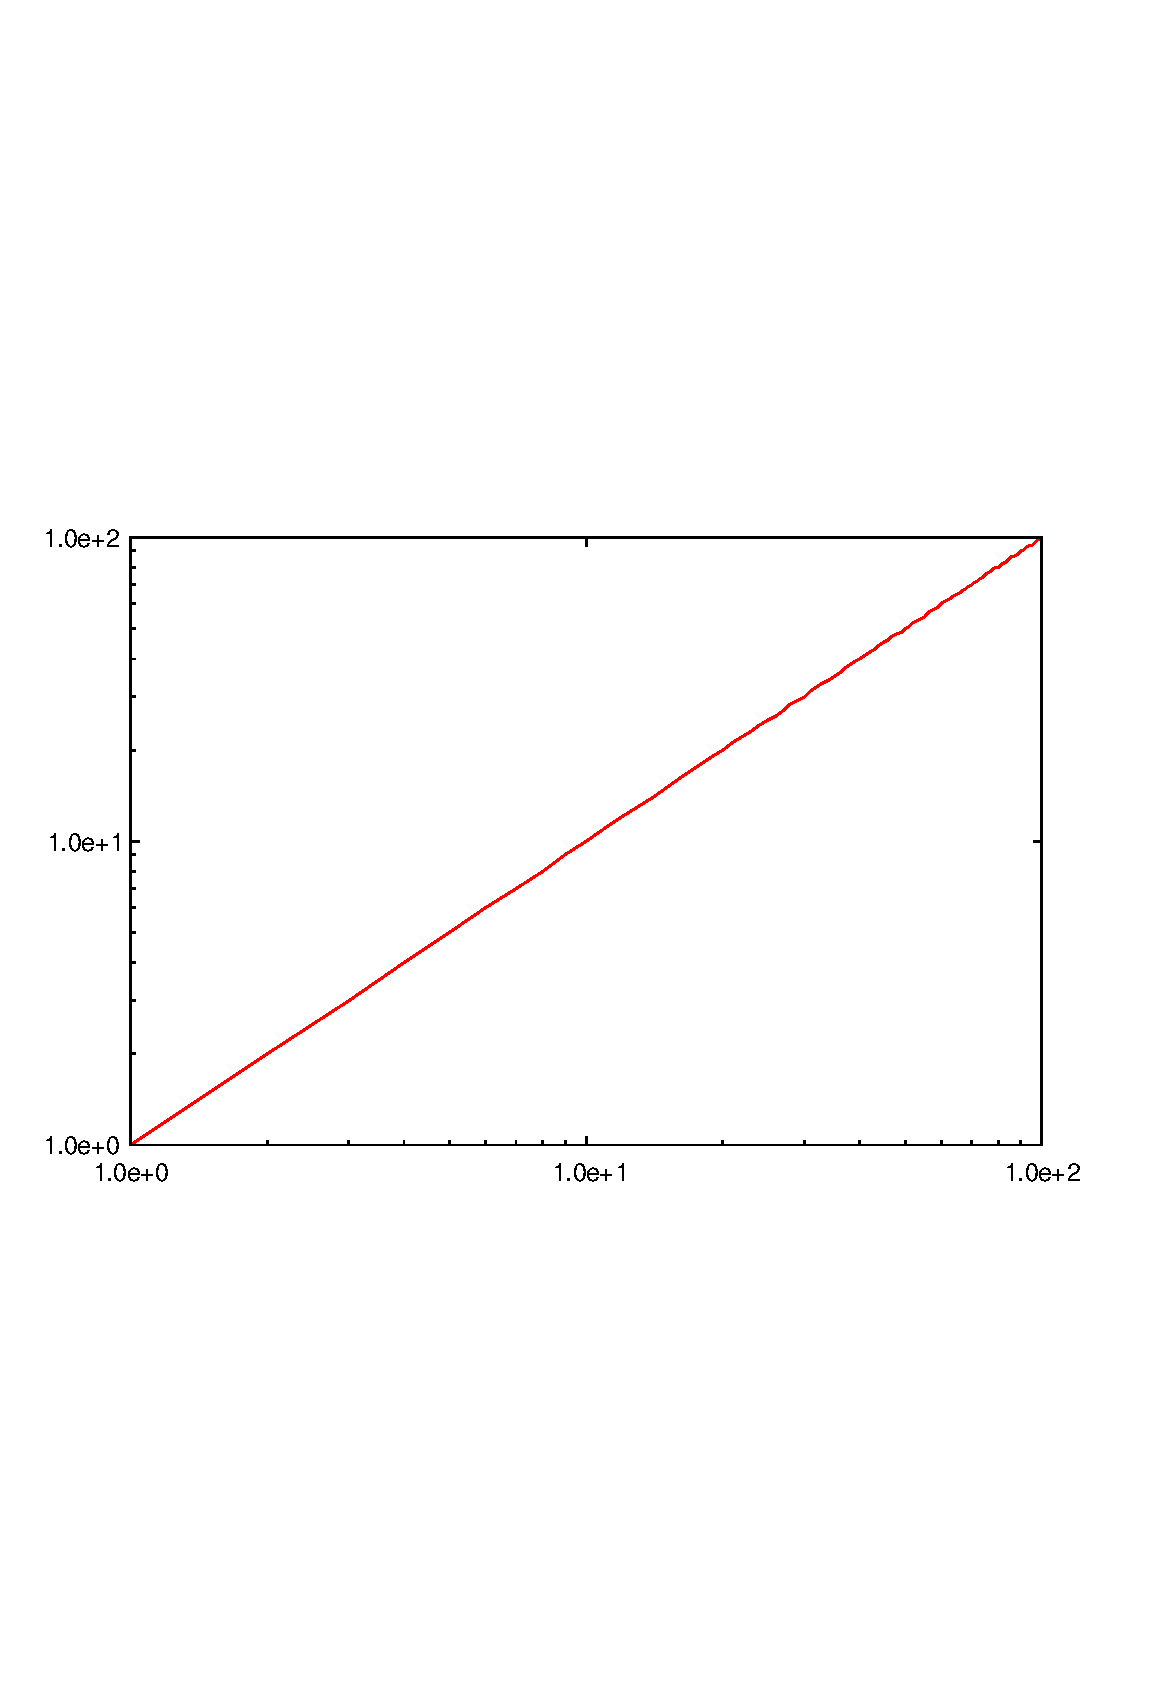
\includegraphics[width=12cm]{loglog2}
\caption{loglog2}
\end{DoxyImage}
 \hypertarget{handle_newplot}{}\section{N\-E\-W\-P\-L\-O\-T Get Handle For Next Plot}\label{handle_newplot}
Section\-: \hyperlink{sec_handle}{Handle-\/\-Based Graphics} \hypertarget{vtkwidgets_vtkxyplotwidget_Usage}{}\subsection{Usage}\label{vtkwidgets_vtkxyplotwidget_Usage}
Returns the handle for the next plot operation. The general syntax for its use is \begin{DoxyVerb}  h = newplot
\end{DoxyVerb}
 This routine checks the {\ttfamily nextplot} properties of the current figure and axes to see if they are set to {\ttfamily replace} or not. If the figures {\ttfamily nextplot} property is set to replace, the current figure is cleared. If the axes {\ttfamily nextplot} property is set to {\ttfamily replace} then the axes are cleared for the next operation. \hypertarget{handle_patch}{}\section{P\-A\-T\-C\-H Patch Graphics Function}\label{handle_patch}
Section\-: \hyperlink{sec_handle}{Handle-\/\-Based Graphics} \hypertarget{vtkwidgets_vtkxyplotwidget_Usage}{}\subsection{Usage}\label{vtkwidgets_vtkxyplotwidget_Usage}
This routine is used to create a patch object that can be plotting 2\-D and 3\-D surfaces. A patch is a polygon defined by the xyz coordinates of its vertices and optionally by the color at the vertices. There are several forms for the {\ttfamily patch} function\-: \begin{DoxyVerb}  h = patch(X,Y,C,properties...)
  h = patch(X,Y,Z,C,properties...)
  h = patch(properties...)
  h = patch(V)
\end{DoxyVerb}
 Where {\ttfamily X}, {\ttfamily Y} and {\ttfamily Z} are matrices or vectors of {\ttfamily x}, {\ttfamily y} or {\ttfamily z} coordinates and {\ttfamily C} is a matrix or vector of color values (the colormap for the current fig is applied). \hypertarget{variables_struct_Example}{}\subsection{Example}\label{variables_struct_Example}
Here we generate a surface specifying all four components.


\begin{DoxyVerbInclude}
--> x = [ 0 1 0 1]';
--> y = [ 0 0 1 1]';
--> c = [ 1 1 1 ];
--> patch(x,y,c)
--> axis equal
--> view(3)
\end{DoxyVerbInclude}


 
\begin{DoxyImage}
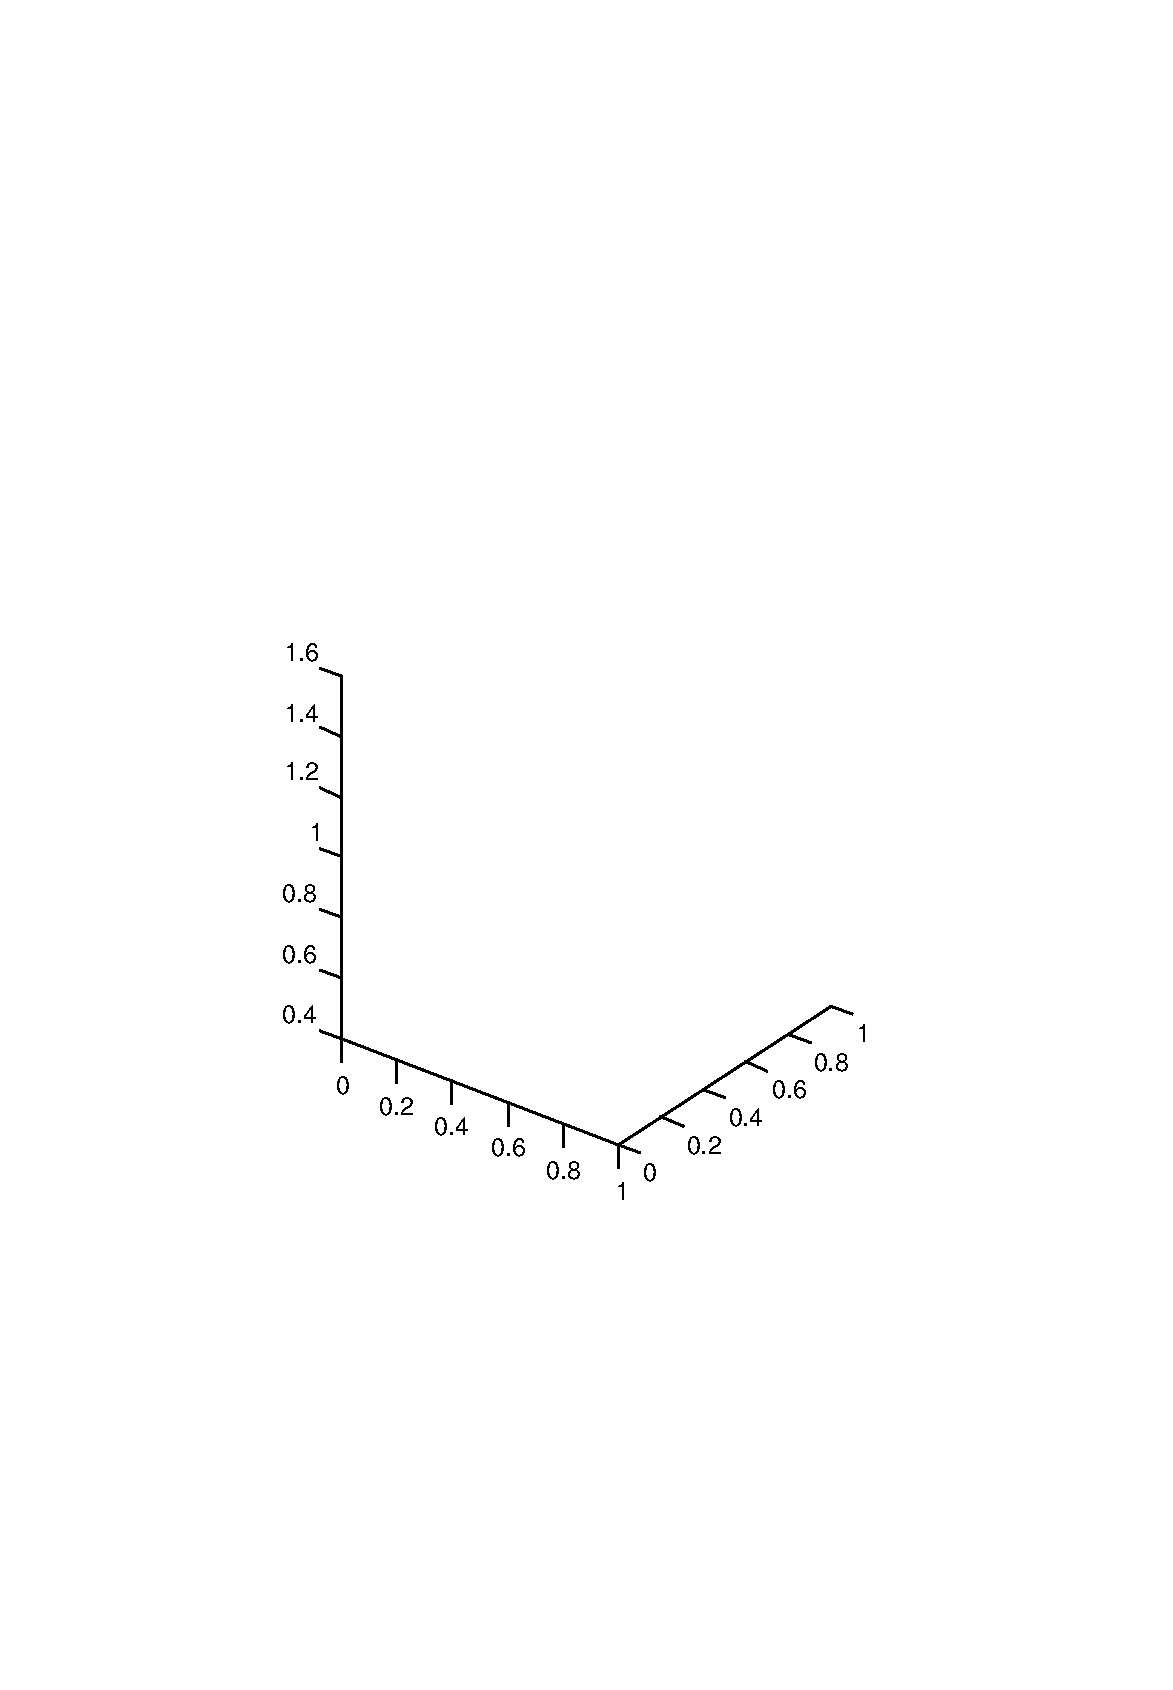
\includegraphics[width=12cm]{patch1}
\caption{patch1}
\end{DoxyImage}
 \hypertarget{handle_pcolor}{}\section{P\-C\-O\-L\-O\-R Pseudocolor Plot}\label{handle_pcolor}
Section\-: \hyperlink{sec_handle}{Handle-\/\-Based Graphics} \hypertarget{vtkwidgets_vtkxyplotwidget_Usage}{}\subsection{Usage}\label{vtkwidgets_vtkxyplotwidget_Usage}
This routine is used to create a pseudocolor plot of the data. A pseudocolor plot is a essentially a surface plot seen from above. There are two forms for the {\ttfamily pcolor} command\-: \begin{DoxyVerb}   pcolor(C)
\end{DoxyVerb}
 which uses a rectangular grid. Alternately, you can specify {\ttfamily X,Y} matrices or vectors. \begin{DoxyVerb}   pcolor(X,Y,C)
\end{DoxyVerb}
 \hypertarget{handle_plot}{}\section{P\-L\-O\-T Plot Function}\label{handle_plot}
Section\-: \hyperlink{sec_handle}{Handle-\/\-Based Graphics} \hypertarget{vtkwidgets_vtkxyplotwidget_Usage}{}\subsection{Usage}\label{vtkwidgets_vtkxyplotwidget_Usage}
This is the basic plot command for Free\-Mat. The general syntax for its use is \begin{DoxyVerb}  plot(\<data 1\>,{linespec 1},\<data 2\>,{linespec 2}...,properties...)
\end{DoxyVerb}
 where the {\ttfamily $<$data$>$} arguments can have various forms, and the {\ttfamily linespec} arguments are optional. We start with the {\ttfamily $<$data$>$} term, which can take on one of multiple forms\-: 
\begin{DoxyItemize}
\item Vector Matrix Case -- In this case the argument data is a pair of variables. A set of {\ttfamily x} coordinates in a numeric vector, and a set of {\ttfamily y} coordinates in the columns of the second, numeric matrix. {\ttfamily x} must have as many elements as {\ttfamily y} has columns (unless {\ttfamily y} is a vector, in which case only the number of elements must match). Each column of {\ttfamily y} is plotted sequentially against the common vector {\ttfamily x}.  
\item Unpaired Matrix Case -- In this case the argument data is a single numeric matrix {\ttfamily y} that constitutes the {\ttfamily y}-\/values of the plot. An {\ttfamily x} vector is synthesized as {\ttfamily x = 1\-:length(y)}, and each column of {\ttfamily y} is plotted sequentially against this common {\ttfamily x} axis.  
\item Complex Matrix Case -- Here the argument data is a complex matrix, in which case, the real part of each column is plotted against the imaginary part of each column. All columns receive the same line styles.  
\end{DoxyItemize}Multiple data arguments in a single plot command are treated as a {\bfseries sequence}, meaning that all of the plots are overlapped on the same set of axes. The {\ttfamily linespec} is a string used to change the characteristics of the line. In general, the {\ttfamily linespec} is composed of three optional parts, the {\ttfamily colorspec}, the {\ttfamily symbolspec} and the {\ttfamily linestylespec} in any order. Each of these specifications is a single character that determines the corresponding characteristic. First, the {\ttfamily colorspec}\-: 
\begin{DoxyItemize}
\item {\ttfamily 'b'} -\/ Color Blue  
\item {\ttfamily 'g'} -\/ Color Green  
\item {\ttfamily 'r'} -\/ Color Red  
\item {\ttfamily 'c'} -\/ Color Cyan  
\item {\ttfamily 'm'} -\/ Color Magenta  
\item {\ttfamily 'y'} -\/ Color Yellow  
\item {\ttfamily 'k'} -\/ Color Black  
\end{DoxyItemize}The {\ttfamily symbolspec} specifies the (optional) symbol to be drawn at each data point\-: 
\begin{DoxyItemize}
\item {\ttfamily '.'} -\/ Dot symbol  
\item {\ttfamily 'o'} -\/ Circle symbol  
\item {\ttfamily 'x'} -\/ Times symbol  
\item {\ttfamily '+'} -\/ Plus symbol  
\item {\ttfamily '$\ast$'} -\/ Asterisk symbol  
\item {\ttfamily 's'} -\/ Square symbol  
\item {\ttfamily 'd'} -\/ Diamond symbol  
\item {\ttfamily 'v'} -\/ Downward-\/pointing triangle symbol  
\item {\ttfamily '$^\wedge$'} -\/ Upward-\/pointing triangle symbol  
\item {\ttfamily '$<$'} -\/ Left-\/pointing triangle symbol  
\item {\ttfamily '$>$'} -\/ Right-\/pointing triangle symbol  
\end{DoxyItemize}The {\ttfamily linestylespec} specifies the (optional) line style to use for each data series\-: 
\begin{DoxyItemize}
\item {\ttfamily '-\/'} -\/ Solid line style  
\item {\ttfamily '\-:'} -\/ Dotted line style  
\item {\ttfamily '-\/.'} -\/ Dot-\/\-Dash-\/\-Dot-\/\-Dash line style  
\item {\ttfamily '--'} -\/ Dashed line style  
\end{DoxyItemize}For sequences of plots, the {\ttfamily linespec} is recycled with color order determined by the properties of the current axes. You can also use the {\ttfamily properties} argument to specify handle properties that will be inherited by all of the plots generated during this event. Finally, you can also specify the handle for the axes that are the target of the {\ttfamily plot} operation. \begin{DoxyVerb}  handle = plot(handle,...)
\end{DoxyVerb}
 \hypertarget{variables_struct_Example}{}\subsection{Example}\label{variables_struct_Example}
The most common use of the {\ttfamily plot} command probably involves the vector-\/matrix paired case. Here, we generate a simple cosine, and plot it using a red line, with no symbols (i.\-e., a {\ttfamily linespec} of {\ttfamily 'r-\/'}).


\begin{DoxyVerbInclude}
--> x = linspace(-pi,pi);
--> y = cos(x);
--> plot(x,y,'r-');
\end{DoxyVerbInclude}


which results in the following plot.  
\begin{DoxyImage}
\includegraphics[width=12cm]{plot1}
\caption{plot1}
\end{DoxyImage}


Next, we plot multiple sinusoids (at different frequencies). First, we construct a matrix, in which each column corresponds to a different sinusoid, and then plot them all at once.


\begin{DoxyVerbInclude}
--> x = linspace(-pi,pi);
--> y = [cos(x(:)),cos(3*x(:)),cos(5*x(:))];
--> plot(x,y);
\end{DoxyVerbInclude}


In this case, we do not specify a {\ttfamily linespec}, so that we cycle through the colors automatically (in the order listed in the previous section).  
\begin{DoxyImage}
\includegraphics[width=12cm]{plot2}
\caption{plot2}
\end{DoxyImage}


This time, we produce the same plot, but as we want to assign individual {\ttfamily linespec}s to each line, we use a sequence of arguments in a single plot command, which has the effect of plotting all of the data sets on a common axis, but which allows us to control the {\ttfamily linespec} of each plot. In the following example, the first line (harmonic) has red, solid lines with times symbols marking the data points, the second line (third harmonic) has blue, solid lines with right-\/pointing triangle symbols, and the third line (fifth harmonic) has green, dotted lines with asterisk symbols.


\begin{DoxyVerbInclude}
--> plot(x,y(:,1),'rx-',x,y(:,2),'b>-',x,y(:,3),'g*:');
\end{DoxyVerbInclude}


 
\begin{DoxyImage}
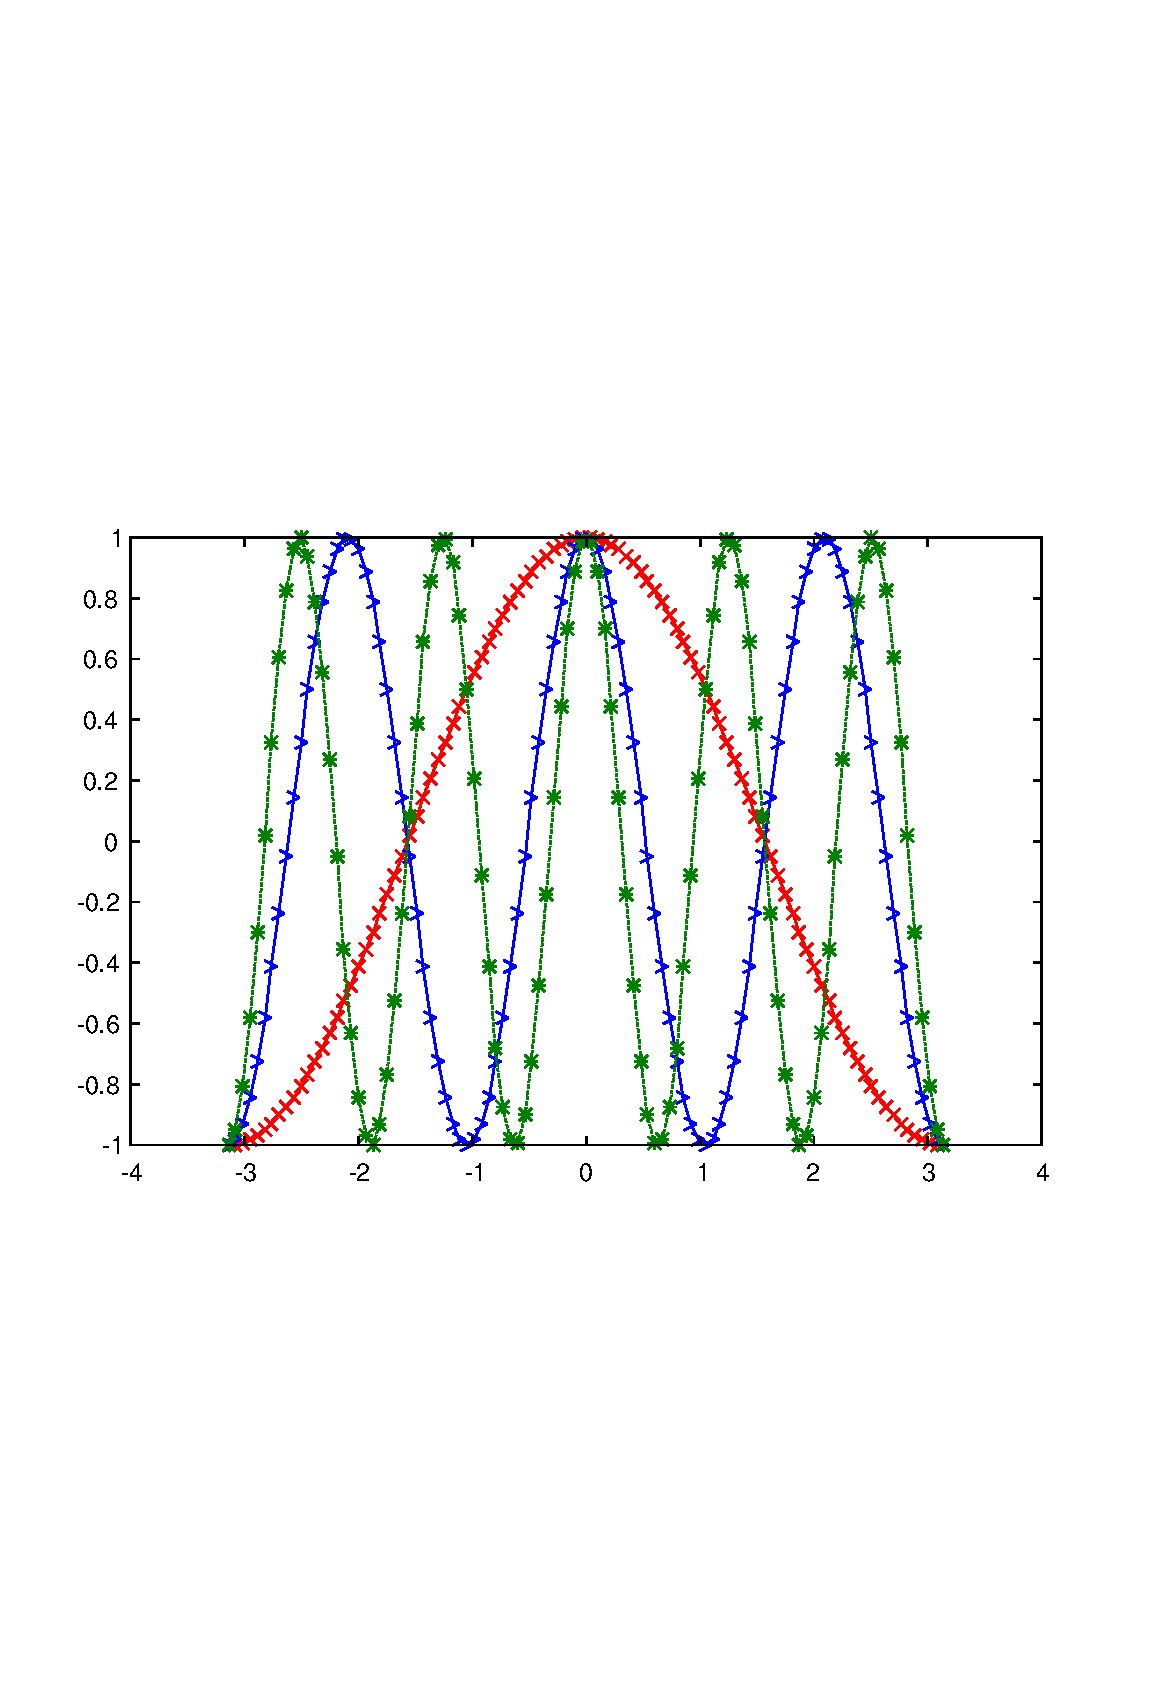
\includegraphics[width=12cm]{plot3}
\caption{plot3}
\end{DoxyImage}


The second most frequently used case is the unpaired matrix case. Here, we need to provide only one data component, which will be automatically plotted against a vector of natural number of the appropriate length. Here, we use a plot sequence to change the style of each line to be dotted, dot-\/dashed, and dashed.


\begin{DoxyVerbInclude}
--> plot(y(:,1),'r:',y(:,2),'b;',y(:,3),'g|');
\end{DoxyVerbInclude}


Note in the resulting plot that the {\ttfamily x}-\/axis no longer runs from {\ttfamily \mbox{[}-\/pi,pi\mbox{]}}, but instead runs from {\ttfamily \mbox{[}1,100\mbox{]}}.  
\begin{DoxyImage}
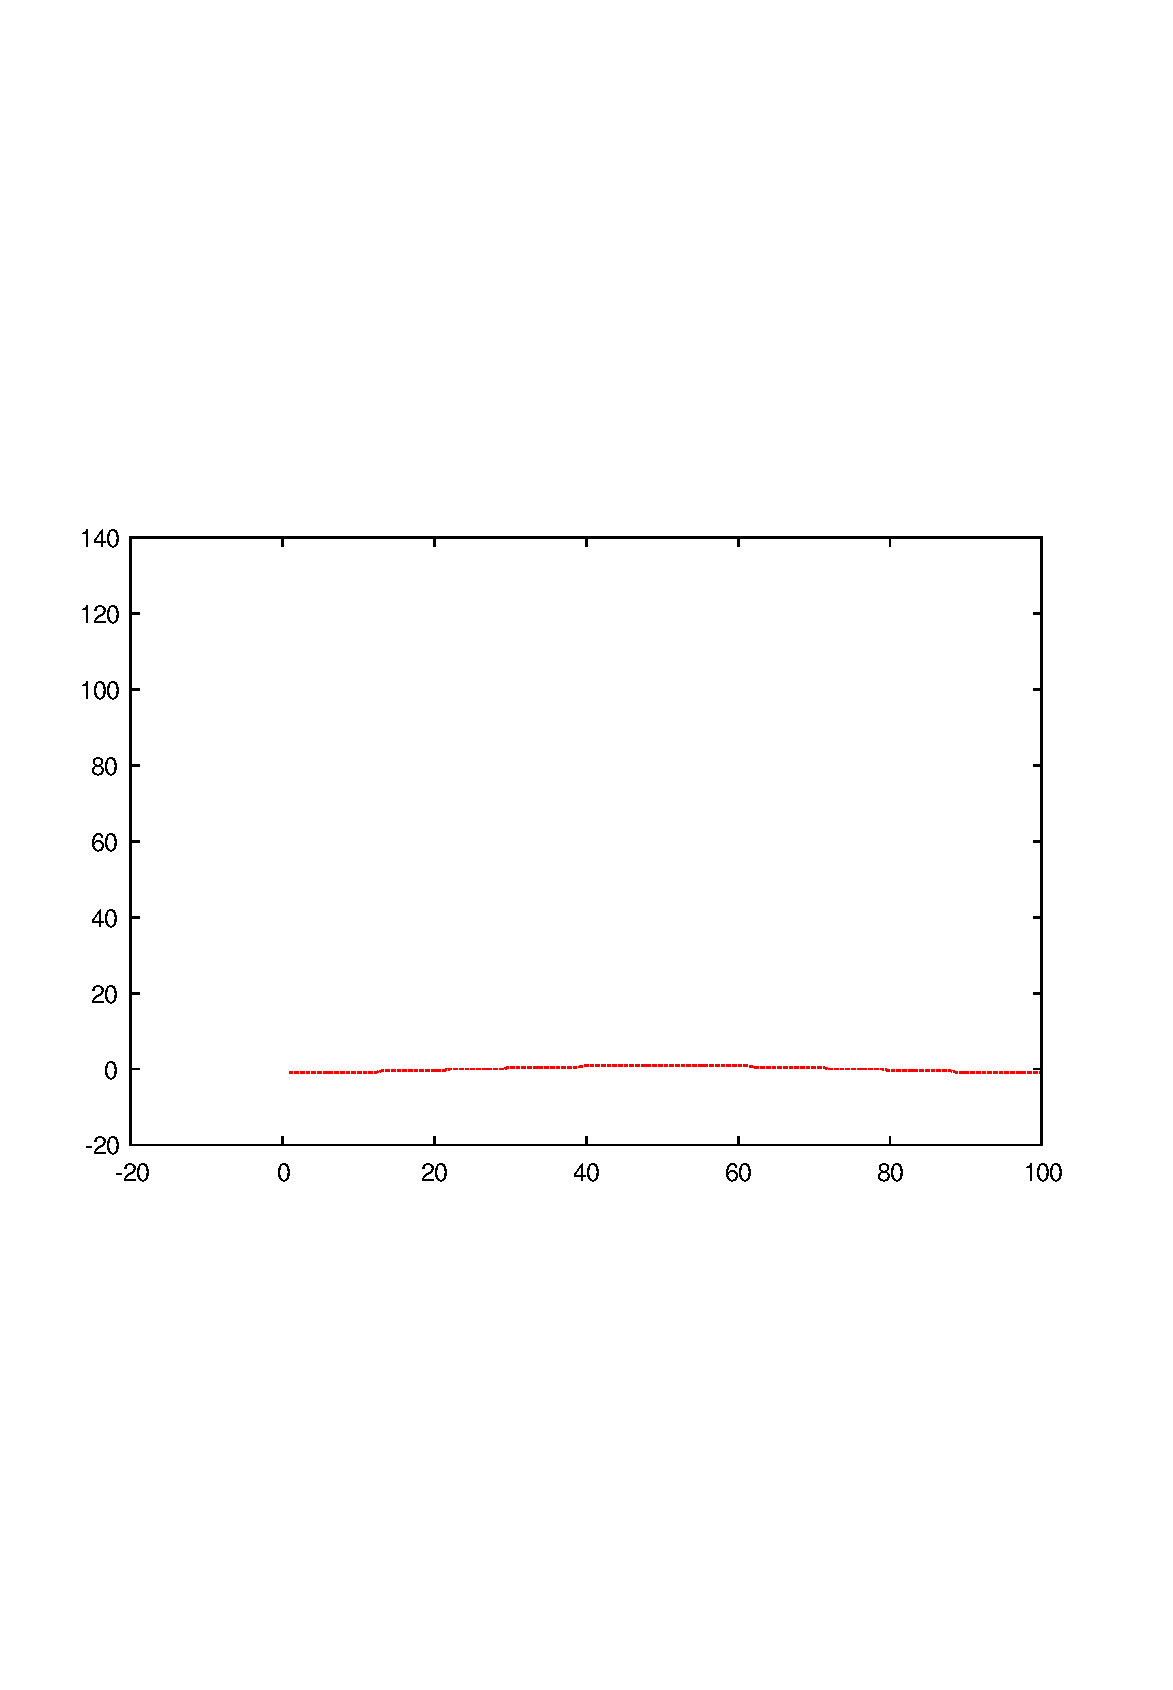
\includegraphics[width=12cm]{plot4}
\caption{plot4}
\end{DoxyImage}


The final case is for complex matrices. For complex arguments, the real part is plotted against the imaginary part. Hence, we can generate a 2-\/dimensional plot from a vector as follows.


\begin{DoxyVerbInclude}
--> y = cos(2*x) + i * cos(3*x);
--> plot(y);
\end{DoxyVerbInclude}


 
\begin{DoxyImage}
\includegraphics[width=12cm]{plot5}
\caption{plot5}
\end{DoxyImage}


Here is an example of using the handle properties to influence the behavior of the generated lines.


\begin{DoxyVerbInclude}
--> t = linspace(-3,3);
--> plot(cos(5*t).*exp(-t),'r-','linewidth',3);
\end{DoxyVerbInclude}


 
\begin{DoxyImage}
\includegraphics[width=12cm]{plot6}
\caption{plot6}
\end{DoxyImage}
 \hypertarget{handle_plot3}{}\section{P\-L\-O\-T3 Plot 3\-D Function}\label{handle_plot3}
Section\-: \hyperlink{sec_handle}{Handle-\/\-Based Graphics} \hypertarget{vtkwidgets_vtkxyplotwidget_Usage}{}\subsection{Usage}\label{vtkwidgets_vtkxyplotwidget_Usage}
This is the 3\-D plot command. The general syntax for its use is \begin{DoxyVerb}  plot3(X,Y,Z,{linespec 1},X,Y,Z,{linespec 2},...,properties...)
\end{DoxyVerb}
 where {\ttfamily X} {\ttfamily Y} and {\ttfamily Z} are the coordinates of the points on the 3\-D line. Note that in general, all three should be vectors. If some or all of the quantities are matrices, then Free\-Mat will attempt to expand the vector arguments to the same size, and then generate multiple plots, one for each column of the matrices. The linespec is optional, see {\ttfamily plot} for details. You can specify {\ttfamily properties} for the generated line plots. You can also specify a handle as an axes to target \begin{DoxyVerb}  plot3(handle,...)
\end{DoxyVerb}
 \hypertarget{variables_struct_Example}{}\subsection{Example}\label{variables_struct_Example}
Here is a simple example of a 3\-D helix.


\begin{DoxyVerbInclude}
--> t = linspace(0,5*pi,200);
--> x = cos(t); y = sin(t); z = t;
--> plot3(x,y,z);
--> view(3);
\end{DoxyVerbInclude}


Shown here  
\begin{DoxyImage}
\includegraphics[width=12cm]{plt3}
\caption{plt3}
\end{DoxyImage}
 \hypertarget{handle_point}{}\section{P\-O\-I\-N\-T Get Axis Position From Mouse Click}\label{handle_point}
Section\-: \hyperlink{sec_handle}{Handle-\/\-Based Graphics} \hypertarget{vtkwidgets_vtkxyplotwidget_Usage}{}\subsection{Usage}\label{vtkwidgets_vtkxyplotwidget_Usage}
Returns information about the currently displayed image based on a use supplied mouse-\/click. The general syntax for its use is \begin{DoxyVerb}   t = point
\end{DoxyVerb}
 The returned vector {\ttfamily y} has two elements\-: \[ t = [x,y] \] where {\ttfamily x,y} are the coordinates in the current axes of the click. This function has changed since Free\-Mat 1.\-10. If the click is not inside the active area of any set of axes, a pair of Na\-Ns are returned. \hypertarget{handle_print}{}\section{P\-R\-I\-N\-T Print a Figure To A File}\label{handle_print}
Section\-: \hyperlink{sec_handle}{Handle-\/\-Based Graphics} \hypertarget{vtkwidgets_vtkxyplotwidget_Usage}{}\subsection{Usage}\label{vtkwidgets_vtkxyplotwidget_Usage}
This function ``prints'' the currently active fig to a file. The generic syntax for its use is \begin{DoxyVerb}  print(filename)
\end{DoxyVerb}
 or, alternately, \begin{DoxyVerb}  print filename
\end{DoxyVerb}
 where {\ttfamily filename} is the (string) filename of the destined file. The current fig is then saved to the output file using a format that is determined by the extension of the filename. The exact output formats may vary on different platforms, but generally speaking, the following extensions should be supported cross-\/platform\-: 
\begin{DoxyItemize}
\item {\ttfamily jpg}, {\ttfamily jpeg} -- J\-P\-E\-G file  
\item {\ttfamily pdf} -- Portable Document Format file  
\item {\ttfamily png} -- Portable Net Graphics file  
\item {\ttfamily svg} -- Scalable Vector Graphics file  
\end{DoxyItemize}Postscript (P\-S, E\-P\-S) is supported on non-\/\-Mac-\/\-O\-S\-X Unix only. Note that only the fig is printed, not the window displaying the fig. If you want something like that (essentially a window-\/capture) use a seperate utility or your operating system's built in screen capture ability. \hypertarget{variables_struct_Example}{}\subsection{Example}\label{variables_struct_Example}
Here is a simple example of how the figures in this manual are generated.


\begin{DoxyVerbInclude}
--> x = linspace(-1,1);
--> y = cos(5*pi*x);
--> plot(x,y,'r-');
--> print('printfig1.jpg')
--> print('printfig1.eps')
\end{DoxyVerbInclude}


which creates three plots {\ttfamily printfig.\-eps}, which is an Encapsulated Post\-Script file, {\ttfamily printfig1.\-png}, which is a Portable Net Graphics file, and {\ttfamily printfig1.\-jpg} which is a J\-P\-E\-G file.  
\begin{DoxyImage}
\includegraphics[width=12cm]{printfig1}
\caption{printfig1}
\end{DoxyImage}
 \hypertarget{handle_pvalid}{}\section{P\-V\-A\-L\-I\-D Validate Property Name}\label{handle_pvalid}
Section\-: \hyperlink{sec_handle}{Handle-\/\-Based Graphics} \hypertarget{vtkwidgets_vtkxyplotwidget_Usage}{}\subsection{Usage}\label{vtkwidgets_vtkxyplotwidget_Usage}
This function checks to see if the given string is a valid property name for an object of the given type. The syntax for its use is \begin{DoxyVerb}  b = pvalid(type,propertyname)
\end{DoxyVerb}
 where {\ttfamily string} is a string that contains the name of a valid graphics object type, and {\ttfamily propertyname} is a string that contains the name of the property to test for. \hypertarget{variables_struct_Example}{}\subsection{Example}\label{variables_struct_Example}
Here we test for some properties on an {\ttfamily axes} object.


\begin{DoxyVerbInclude}
--> pvalid('axes','type')

ans = 
 1 

--> pvalid('axes','children')

ans = 
 1 

--> pvalid('axes','foobar')

ans = 
 0 
\end{DoxyVerbInclude}
 \hypertarget{handle_semilogx}{}\section{S\-E\-M\-I\-L\-O\-G\-X Semilog X Axis Plot Function}\label{handle_semilogx}
Section\-: \hyperlink{sec_handle}{Handle-\/\-Based Graphics} \hypertarget{vtkwidgets_vtkxyplotwidget_Usage}{}\subsection{Usage}\label{vtkwidgets_vtkxyplotwidget_Usage}
This command has the exact same syntax as the {\ttfamily plot} command\-: \begin{DoxyVerb}  semilogx(<data 1>,{linespec 1},<data 2>,{linespec 2}...,properties...)
\end{DoxyVerb}
 in fact, it is a simple wrapper around {\ttfamily plot} that sets the x axis to have a logarithmic scale. \hypertarget{variables_struct_Example}{}\subsection{Example}\label{variables_struct_Example}
Here is an example of an exponential signal plotted first on a linear plot\-:


\begin{DoxyVerbInclude}
--> y = linspace(0,2);
--> x = (10).^y;
--> plot(x,y,'r-');
\end{DoxyVerbInclude}


 
\begin{DoxyImage}
\includegraphics[width=12cm]{semilogx1}
\caption{semilogx1}
\end{DoxyImage}
 and now with a logarithmic x axis


\begin{DoxyVerbInclude}
--> semilogx(x,y,'r-');
\end{DoxyVerbInclude}


 
\begin{DoxyImage}
\includegraphics[width=12cm]{semilogx2}
\caption{semilogx2}
\end{DoxyImage}
 \hypertarget{handle_semilogy}{}\section{S\-E\-M\-I\-L\-O\-G\-Y Semilog Y Axis Plot Function}\label{handle_semilogy}
Section\-: \hyperlink{sec_handle}{Handle-\/\-Based Graphics} \hypertarget{vtkwidgets_vtkxyplotwidget_Usage}{}\subsection{Usage}\label{vtkwidgets_vtkxyplotwidget_Usage}
This command has the exact same syntax as the {\ttfamily plot} command\-: \begin{DoxyVerb}  semilogy(<data 1>,{linespec 1},<data 2>,{linespec 2}...,properties...)
\end{DoxyVerb}
 in fact, it is a simple wrapper around {\ttfamily plot} that sets the y axis to have a logarithmic scale. \hypertarget{variables_struct_Example}{}\subsection{Example}\label{variables_struct_Example}
Here is an example of an exponential signal plotted first on a linear plot\-:


\begin{DoxyVerbInclude}
--> x = linspace(0,2);
--> y = 10.0.^x;
--> plot(x,y,'r-');
\end{DoxyVerbInclude}


 
\begin{DoxyImage}
\includegraphics[width=12cm]{semilogy1}
\caption{semilogy1}
\end{DoxyImage}
 and now with a logarithmic y axis


\begin{DoxyVerbInclude}
--> semilogy(x,y,'r-');
\end{DoxyVerbInclude}


 
\begin{DoxyImage}
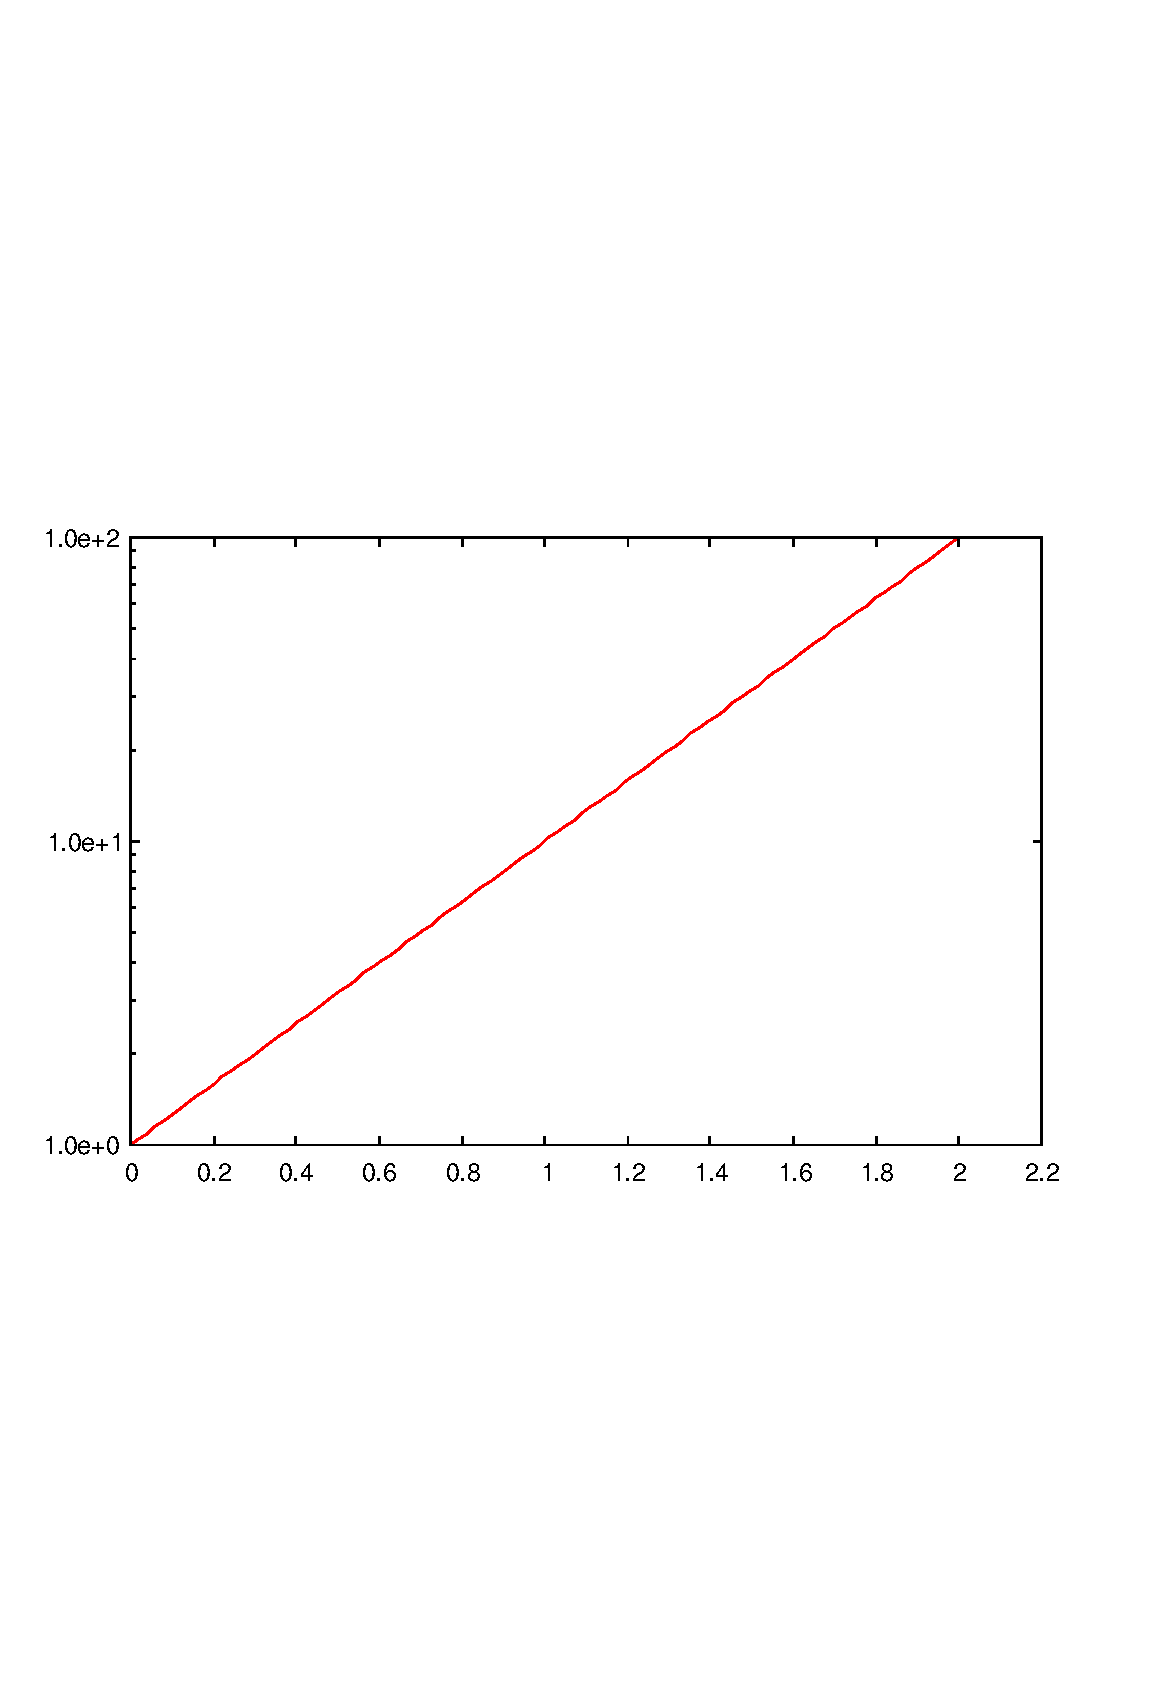
\includegraphics[width=12cm]{semilogy2}
\caption{semilogy2}
\end{DoxyImage}
 \hypertarget{handle_set}{}\section{S\-E\-T Set Object Property}\label{handle_set}
Section\-: \hyperlink{sec_handle}{Handle-\/\-Based Graphics} \hypertarget{vtkwidgets_vtkxyplotwidget_Usage}{}\subsection{Usage}\label{vtkwidgets_vtkxyplotwidget_Usage}
This function allows you to change the value associated with a property. The syntax for its use is \begin{DoxyVerb}  set(handle,property,value,property,value,...)
\end{DoxyVerb}
 where {\ttfamily property} is a string containing the name of the property, and {\ttfamily value} is the value for that property. The type of the variable {\ttfamily value} depends on the property being set. See the help for the properties to see what values you can set. \hypertarget{handle_sizefig}{}\section{S\-I\-Z\-E\-F\-I\-G Set Size of Figure}\label{handle_sizefig}
Section\-: \hyperlink{sec_handle}{Handle-\/\-Based Graphics} \hypertarget{vtkwidgets_vtkxyplotwidget_Usage}{}\subsection{Usage}\label{vtkwidgets_vtkxyplotwidget_Usage}
The {\ttfamily sizefig} function changes the size of the currently selected fig window. The general syntax for its use is \begin{DoxyVerb}   sizefig(width,height)
\end{DoxyVerb}
 where {\ttfamily width} and {\ttfamily height} are the dimensions of the fig window. \hypertarget{handle_subplot}{}\section{S\-U\-B\-P\-L\-O\-T Subplot Function}\label{handle_subplot}
Section\-: \hyperlink{sec_handle}{Handle-\/\-Based Graphics} \hypertarget{vtkwidgets_vtkxyplotwidget_Usage}{}\subsection{Usage}\label{vtkwidgets_vtkxyplotwidget_Usage}
This function divides the current figure into a 2-\/dimensional grid, each of which can contain a plot of some kind. The function has a number of syntaxes. The first version \begin{DoxyVerb}   subplot(row,col,num)
\end{DoxyVerb}
 which either activates subplot number {\ttfamily num}, or sets up a subplot grid of size {\ttfamily row x col}, and then activates {\ttfamily num}. You can also set up subplots that cover multiple grid elements \begin{DoxyVerb}   subplot(row,col,[vec])
\end{DoxyVerb}
 where {\ttfamily vec} is a set of indexes covered by the new subplot. Finally, as a shortcut, you can specify a string with three components \begin{DoxyVerb}   subplot('mnp')
\end{DoxyVerb}
 or using the alternate notation \begin{DoxyVerb}   subplot mnp
\end{DoxyVerb}
 where {\ttfamily m} is the number of rows, {\ttfamily n} is the number of columns and {\ttfamily p} is the index. You can also specify the location of the subplot explicitly using the syntax \begin{DoxyVerb}   subplot('position',[left bottom width height])
\end{DoxyVerb}
\hypertarget{variables_struct_Example}{}\subsection{Example}\label{variables_struct_Example}
Here is the use of {\ttfamily subplot} to set up a {\ttfamily 2 x 2} grid of plots


\begin{DoxyVerbInclude}
--> t = linspace(-pi,pi);
--> subplot(2,2,1)
--> plot(t,cos(t).*exp(-2*t));
--> subplot(2,2,2);
--> plot(t,cos(t*2).*exp(-2*t));
--> subplot(2,2,3);
--> plot(t,cos(t*3).*exp(-2*t));
--> subplot(2,2,4);
--> plot(t,cos(t*4).*exp(-2*t));
\end{DoxyVerbInclude}


 
\begin{DoxyImage}
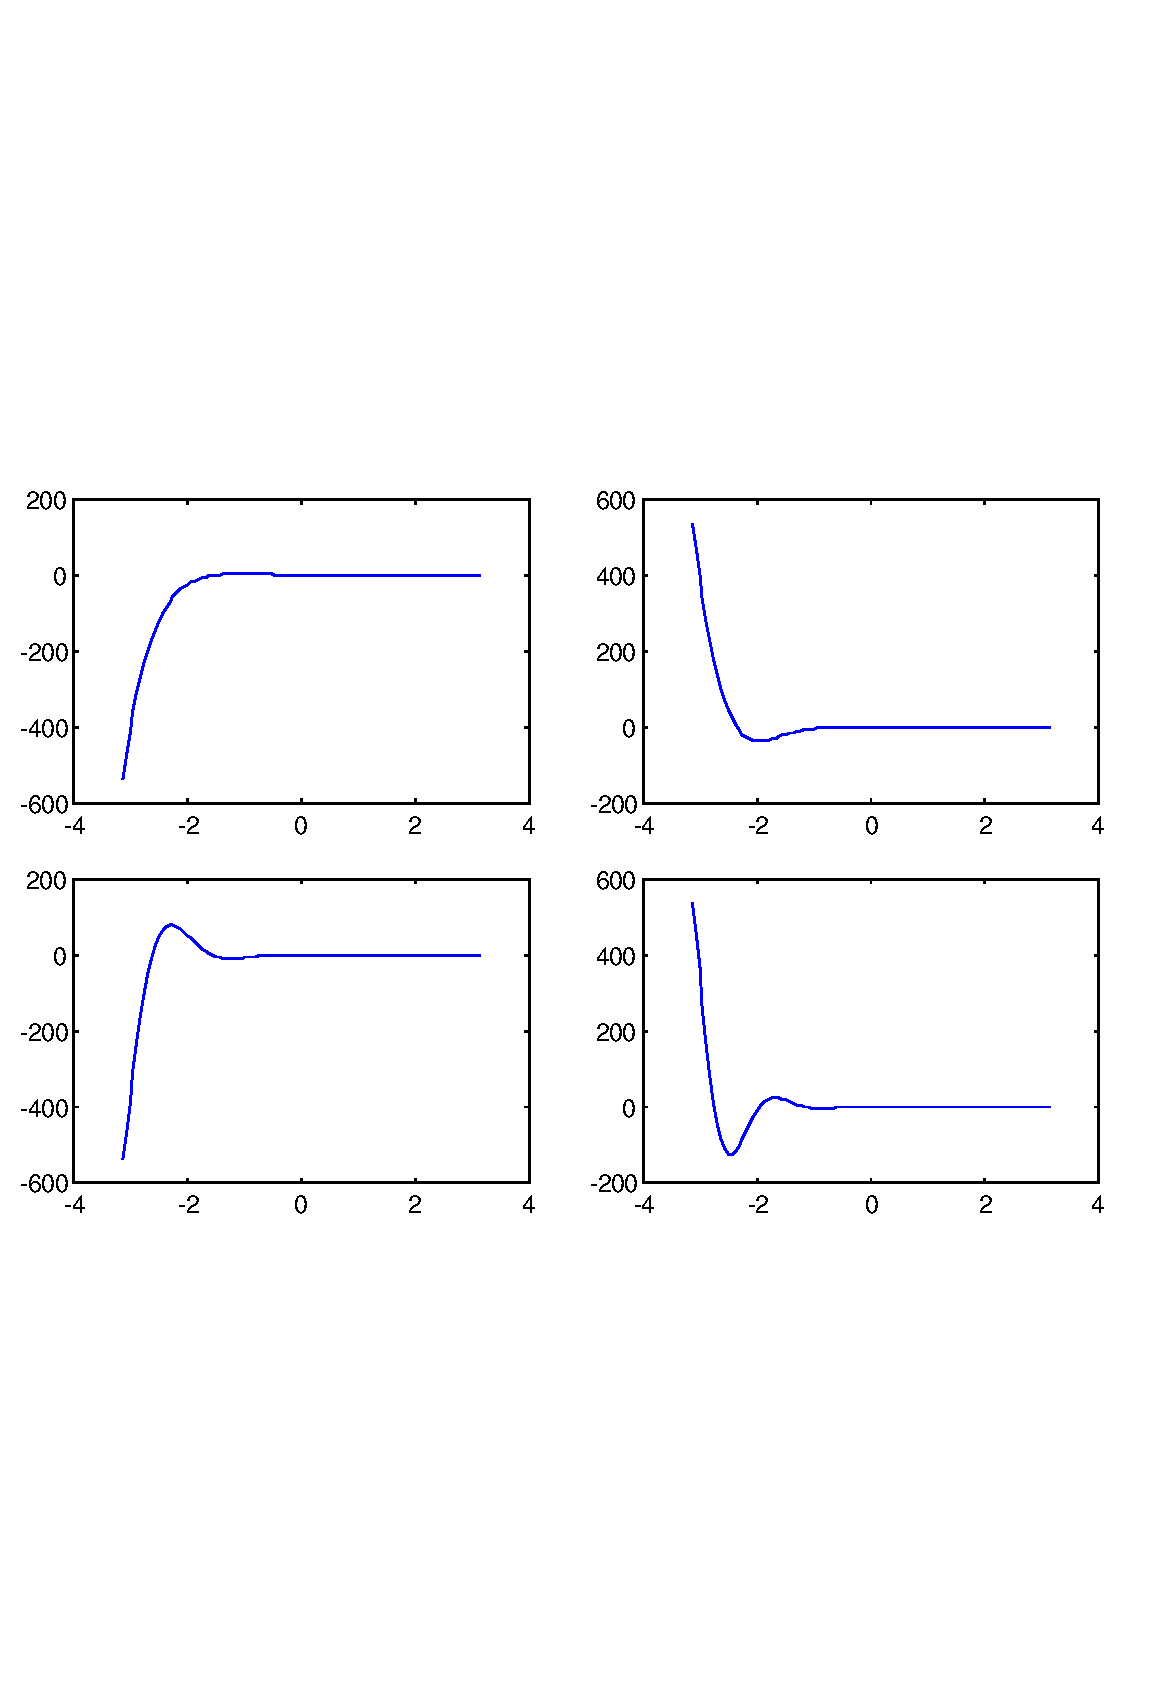
\includegraphics[width=12cm]{subplot1}
\caption{subplot1}
\end{DoxyImage}
 Here we use the second form of {\ttfamily subplot} to generate one subplot that is twice as large.


\begin{DoxyVerbInclude}
--> t = linspace(-pi,pi);
--> subplot(2,2,[1,2])
--> plot(t,cos(t).*exp(-2*t));
--> subplot(2,2,3);
--> plot(t,cos(t*3).*exp(-2*t));
--> subplot(2,2,4);
--> plot(t,cos(t*4).*exp(-2*t));
\end{DoxyVerbInclude}


 
\begin{DoxyImage}
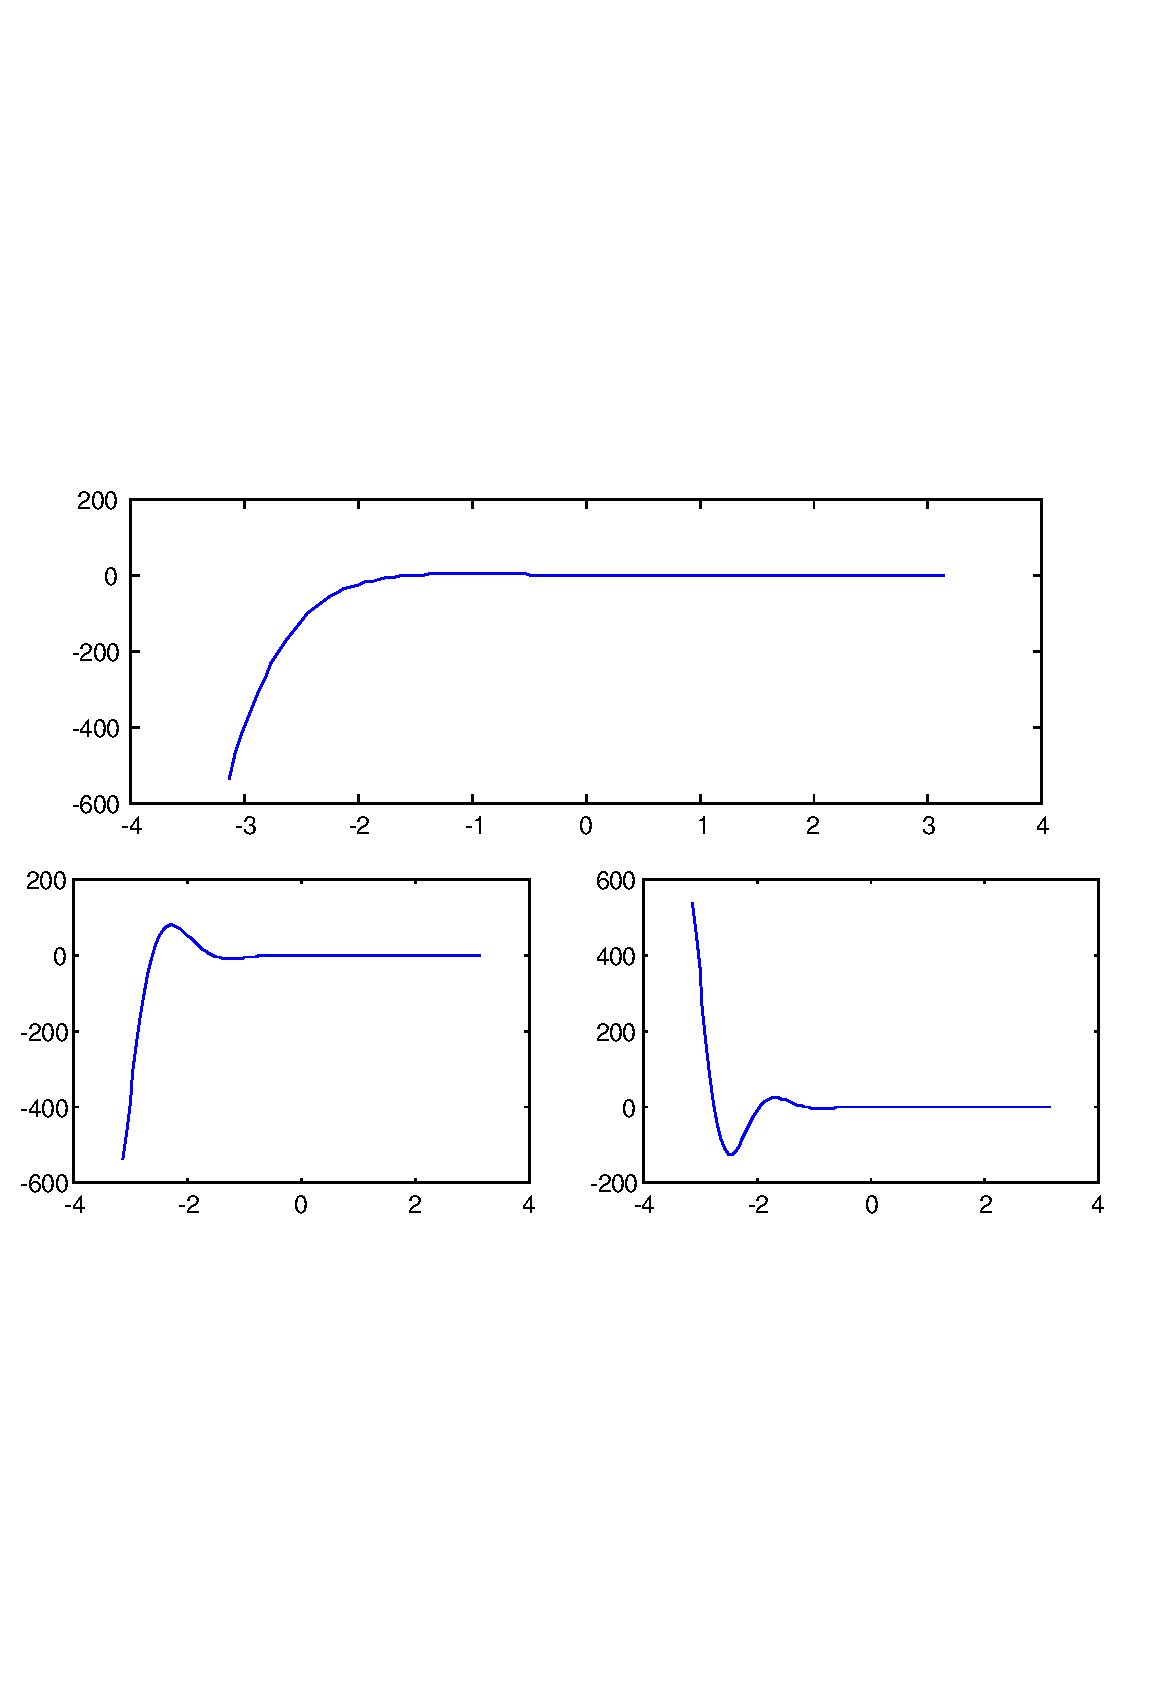
\includegraphics[width=12cm]{subplot2}
\caption{subplot2}
\end{DoxyImage}
 Note that the subplots can contain any handle graphics objects, not only simple plots.


\begin{DoxyVerbInclude}
--> t=0:(2*pi/100):(2*pi);
--> x=cos(t*2).*(2+sin(t*3)*.3);
--> y=sin(t*2).*(2+sin(t*3)*.3);
--> z=cos(t*3)*.3;
--> subplot(2,2,1)
--> plot(t,x);
--> subplot(2,2,2);
--> plot(t,y);
--> subplot(2,2,3);
--> plot(t,z);
--> subplot(2,2,4);
--> tubeplot(x,y,z,0.14*sin(t*5)+.29,t,10)
--> axis equal
--> view(3)
\end{DoxyVerbInclude}


 
\begin{DoxyImage}
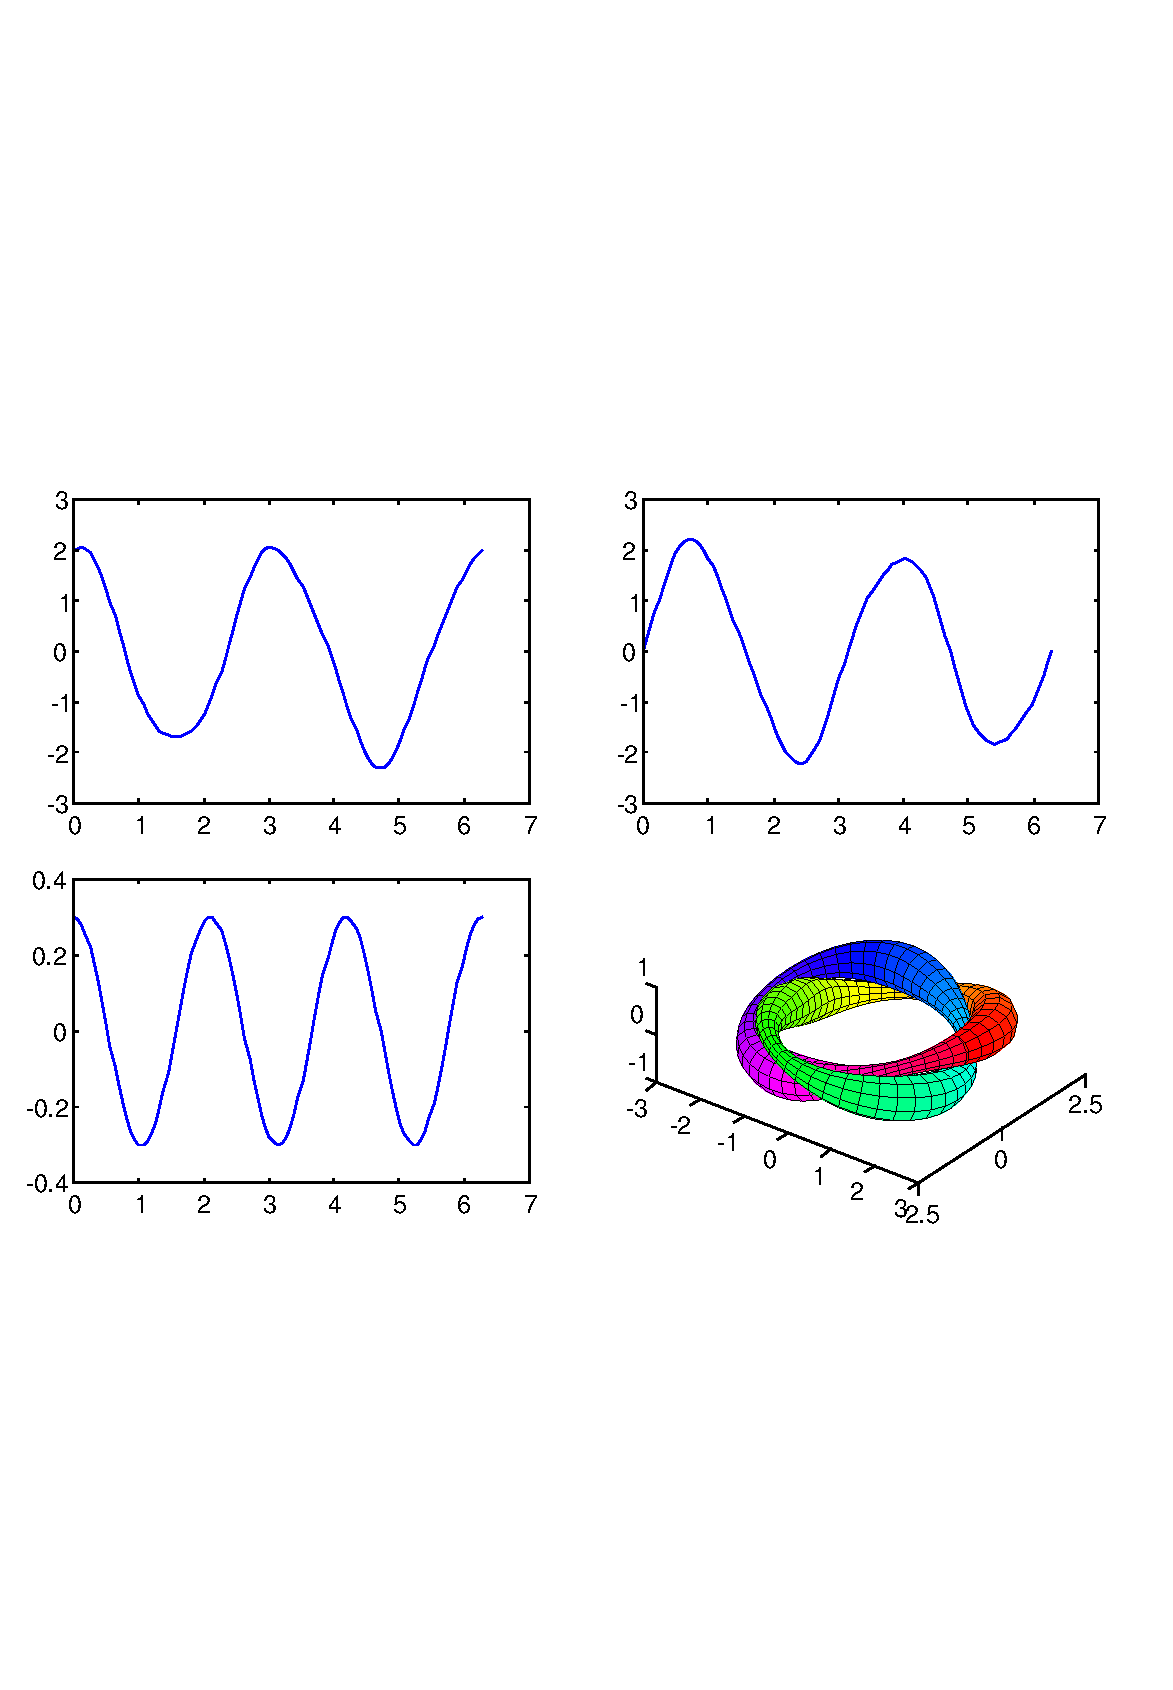
\includegraphics[width=12cm]{subplot3}
\caption{subplot3}
\end{DoxyImage}
 \hypertarget{handle_surf}{}\section{S\-U\-R\-F Surface Plot Function}\label{handle_surf}
Section\-: \hyperlink{sec_handle}{Handle-\/\-Based Graphics} \hypertarget{vtkwidgets_vtkxyplotwidget_Usage}{}\subsection{Usage}\label{vtkwidgets_vtkxyplotwidget_Usage}
This routine is used to create a surface plot of data. A surface plot is a 3\-D surface defined by the xyz coordinates of its vertices and optionally by the color at the vertices. The most general syntax for the {\ttfamily surf} function is \begin{DoxyVerb}  h = surf(X,Y,Z,C,properties...)
\end{DoxyVerb}
 Where {\ttfamily X} is a matrix or vector of {\ttfamily x} coordinates, {\ttfamily Y} is a matrix or vector of {\ttfamily y} coordinates, {\ttfamily Z} is a 2\-D matrix of coordinates, and {\ttfamily C} is a 2\-D matrix of color values (the colormap for the current fig is applied). In general, {\ttfamily X} and {\ttfamily Y} should be the same size as {\ttfamily Z}, but Free\-Mat will expand vectors to match the matrix if possible. If you want the color of the surface to be defined by the height of the surface, you can omit {\ttfamily C} \begin{DoxyVerb}  h = surf(X,Y,Z,properties...)
\end{DoxyVerb}
 in which case {\ttfamily C=Z}. You can also eliminate the {\ttfamily X} and {\ttfamily Y} matrices in the specification \begin{DoxyVerb}  h = surf(Z,properties)
\end{DoxyVerb}
 in which case they are set to {\ttfamily 1\-:size(\-Z,2)} and {\ttfamily 1\-:size(\-Y,2)} respectively. You can also specify a handle as the target of the {\ttfamily surf} command via \begin{DoxyVerb}  h = surf(handle,...)
\end{DoxyVerb}
 \hypertarget{variables_struct_Example}{}\subsection{Example}\label{variables_struct_Example}
Here we generate a surface specifying all four components.


\begin{DoxyVerbInclude}
--> x = repmat(linspace(-1,1),[100,1]);
--> y = x';
--> r = x.^2+y.^2;
--> z = exp(-r*3).*cos(5*r);
--> c = r;
--> surf(x,y,z,c)
--> axis equal
--> view(3)
\end{DoxyVerbInclude}


 
\begin{DoxyImage}
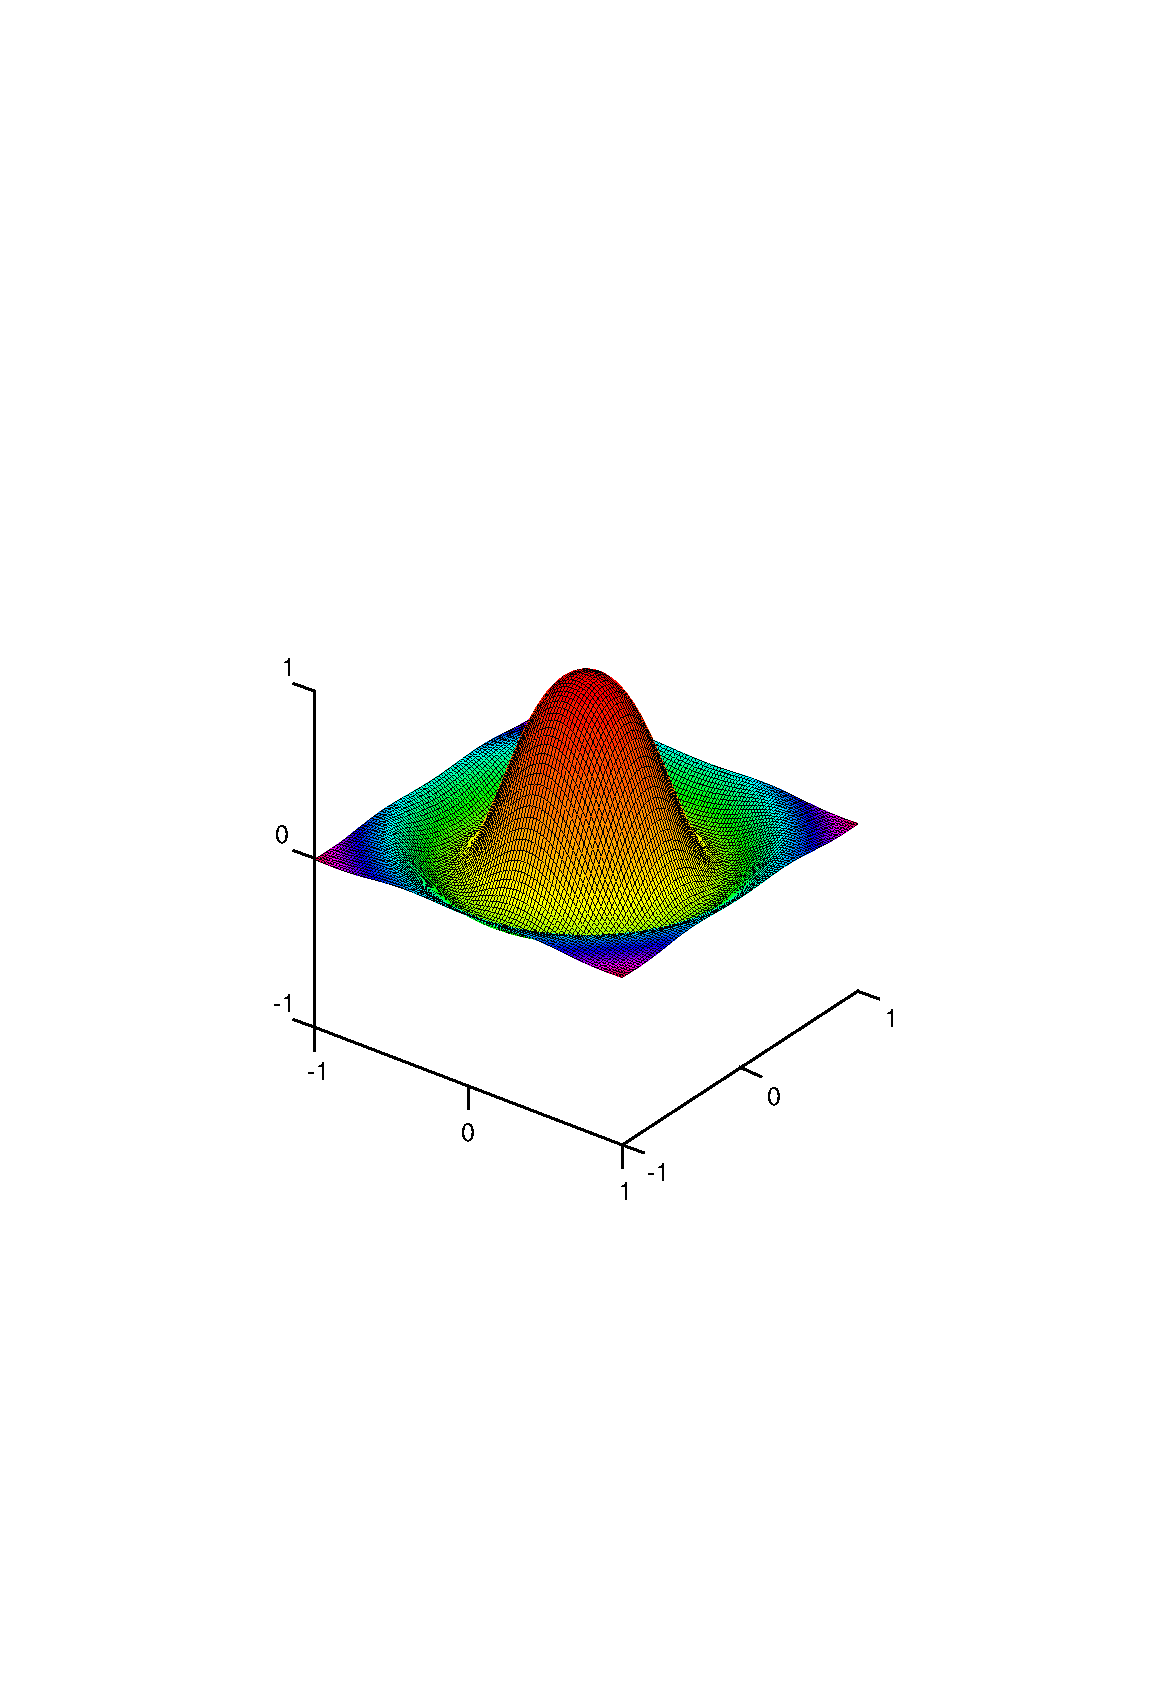
\includegraphics[width=12cm]{surf1}
\caption{surf1}
\end{DoxyImage}
 If we allow Free\-Mat to specify the color component, we see that the colorfield is the same as the height


\begin{DoxyVerbInclude}
--> surf(x,y,z)
--> axis equal
--> view(3)
\end{DoxyVerbInclude}


 
\begin{DoxyImage}
\includegraphics[width=12cm]{surf2}
\caption{surf2}
\end{DoxyImage}
 \hypertarget{handle_surfaceproperties}{}\section{S\-U\-R\-F\-A\-C\-E\-P\-R\-O\-P\-E\-R\-T\-I\-E\-S Surface Object Properties}\label{handle_surfaceproperties}
Section\-: \hyperlink{sec_handle}{Handle-\/\-Based Graphics} \hypertarget{vtkwidgets_vtkxyplotwidget_Usage}{}\subsection{Usage}\label{vtkwidgets_vtkxyplotwidget_Usage}
Below is a summary of the properties for the axis. 
\begin{DoxyItemize}
\item {\ttfamily alphadata} -\/ {\ttfamily vector} -\/ This is a vector that should contain as many elements as the surface data itself {\ttfamily cdata}, or a single scalar. For a single scalar, all values of the surface take on the same transparency. Otherwise, the transparency of each pixel is determined by the corresponding value from the {\ttfamily alphadata} vector.  
\item {\ttfamily alphadatamapping} -\/ {\ttfamily \{'scaled','direct','none'\}} -\/ For {\ttfamily none} mode (the default), no transparency is applied to the data. For {\ttfamily direct} mode, the vector {\ttfamily alphadata} contains values between @\mbox{[}0,M-\/1\mbox{]}$|$ where {\ttfamily M} is the length of the alpha map stored in the figure. For {\ttfamily scaled} mode, the {\ttfamily alim} vector for the figure is used to linearly rescale the alpha data prior to lookup in the alpha map.  
\item {\ttfamily ambientstrength} -\/ Not used.  
\item {\ttfamily backfacelighting} -\/ Not used.  
\item {\ttfamily cdata} -\/ {\ttfamily array} -\/ This is either a {\ttfamily M x N} array or an {\ttfamily M x N x 3} array. If the data is {\ttfamily M x N} the surface is a scalar surface (indexed mode), where the color associated with each surface pixel is computed using the colormap and the {\ttfamily cdatamapping} mode. If the data is {\ttfamily M x N x 3} the surface is assumed to be in R\-G\-B mode, and the colorpanes are taken directly from {\ttfamily cdata} (the colormap is ignored). Note that in this case, the data values must be between @\mbox{[}0,1\mbox{]}$|$ for each color channel and each point on the surface.  
\item {\ttfamily cdatamapping} -\/ {\ttfamily \{'scaled','direct'\}} -\/ For {\ttfamily scaled} (the default), the pixel values are scaled using the {\ttfamily clim} vector for the figure prior to looking up in the colormap. For {\ttfamily direct} mode, the pixel values must be in the range {\ttfamily \mbox{[}0,N-\/1} where {\ttfamily N} is the number of colors in the colormap.  
\item {\ttfamily children} -\/ Not used.  
\item {\ttfamily diffusestrength} -\/ Not used.  
\item {\ttfamily edgealpha} -\/ {\ttfamily \{'flat','interp','scalar'\}} -\/ Controls how the transparency is mapped for the edges of the surface.  
\item {\ttfamily edgecolor} -\/ {\ttfamily \{'flat','interp','none',colorspec\}} -\/ Specifies how the edges are colored. For {\ttfamily 'flat'} the edges are flat colored, meaning that the line segments that make up the edges are not shaded. The color for the line is determined by the first edge point it is connected to.  
\item {\ttfamily edgelighting} -\/ Not used.  
\item {\ttfamily facealpha} -\/ {\ttfamily \{'flat','interp','texturemap',scalar\}} -\/ Controls how the transparency of the faces of the surface are controlled. For flat shading, the faces are constant transparency. For interp mode, the faces are smoothly transparently mapped. If set to a scalar, all faces have the same transparency.  
\item {\ttfamily facecolor} -\/ {\ttfamily \{'none','flat','interp',colorspec\}} -\/ Controls how the faces are colored. For {\ttfamily 'none'} the faces are uncolored, and the surface appears as a mesh without hidden lines removed. For {\ttfamily 'flat'} the surface faces have a constant color. For {\ttfamily 'interp'} smooth shading is applied to the surface. And if a colorspec is provided, then the faces all have the same color.  
\item {\ttfamily facelighting} -\/ Not used.  
\item {\ttfamily linestyle} -\/ {\ttfamily \{'-\/','--','\-:','-\/.','none'\}} -\/ The style of the line used to draw the edges.  
\item {\ttfamily linewidth} -\/ {\ttfamily scalar} -\/ The width of the line used to draw the edges.  
\item {\ttfamily marker} -\/ {\ttfamily \{'+','o','$\ast$','.','x','square','s','diamond','d','$^\wedge$','v','$>$','$<$'\}} -\/ The marker for data points on the line. Some of these are redundant, as {\ttfamily 'square'} {\ttfamily 's'} are synonyms, and {\ttfamily 'diamond'} and {\ttfamily 'd'} are also synonyms.  
\item {\ttfamily markeredgecolor} -\/ {\ttfamily colorspec} -\/ The color used to draw the marker. For some of the markers (circle, square, etc.) there are two colors used to draw the marker. This property controls the edge color (which for unfilled markers) is the primary color of the marker.  
\item {\ttfamily markerfacecolor} -\/ {\ttfamily colorspec} -\/ The color used to fill the marker. For some of the markers (circle, square, etc.) there are two colors used to fill the marker.  
\item {\ttfamily markersize} -\/ {\ttfamily scalar} -\/ Control the size of the marker. Defaults to 6, which is effectively the radius (in pixels) of the markers.  
\item {\ttfamily meshstyle} -\/ {\ttfamily \{'both','rows','cols\}} -\/ This property controls how the mesh is drawn for the surface. For {\ttfamily rows} and {\ttfamily cols} modes, only one set of edges is drawn.  
\item {\ttfamily normalmode} -\/ Not used.  
\item {\ttfamily parent} -\/ {\ttfamily handle} -\/ The axis containing the surface.  
\item {\ttfamily specularcolorreflectance} -\/ Not used.  
\item {\ttfamily specularexponent} -\/ Not used.  
\item {\ttfamily specularstrength} -\/ Not used.  
\item {\ttfamily tag} -\/ {\ttfamily string} -\/ You can set this to any string you want.  
\item {\ttfamily type} -\/ {\ttfamily string} -\/ Set to the string {\ttfamily 'surface'}.  
\item {\ttfamily userdata} -\/ {\ttfamily array} -\/ Available to store any variable you want in the handle object.  
\item {\ttfamily vertexnormals} -\/ Not used.  
\item {\ttfamily xdata} -\/ {\ttfamily array} -\/ Must be a numeric array of size {\ttfamily M x N} which contains the x location of each point in the defined surface. Must be the same size as {\ttfamily ydata} and {\ttfamily zdata}. Alternately, you can specify an array of size {\ttfamily 1 x N} in which case Free\-Mat replicates the vector to fill out an {\ttfamily M x N} matrix.  
\item {\ttfamily xdatamode} -\/ {\ttfamily \{'auto','manual'\}} -\/ When set to {\ttfamily auto} then Free\-Mat will automatically generate the x coordinates.  
\item {\ttfamily ydata} -\/ {\ttfamily array} -\/ Must be a numeric array of size {\ttfamily M x N} which contains the y location of each point in the defined surface. Must be the same size as {\ttfamily xdata} and {\ttfamily zdata}. Alternately, you can specify an array of size {\ttfamily M x 1} in which case Free\-Mat replicates the vector to fill out an {\ttfamily M x N} matrix.  
\item {\ttfamily ydatamode} -\/ {\ttfamily \{'auto','manual'\}} -\/ When set to {\ttfamily auto} then Free\-Mat will automatically generate the y coordinates.  
\item {\ttfamily zdata} -\/ {\ttfamily array} -\/ Must be a numeric array of size {\ttfamily M x N} which contains the y location of each point in the defined surface. Must be the same size as {\ttfamily xdata} and {\ttfamily ydata}.  
\item {\ttfamily visible} -\/ {\ttfamily \{'on','off'\}} -\/ Controls whether the surface is visible or not.  
\end{DoxyItemize}\hypertarget{handle_text}{}\section{T\-E\-X\-T Add Text Label to Plot}\label{handle_text}
Section\-: \hyperlink{sec_handle}{Handle-\/\-Based Graphics} \hypertarget{vtkwidgets_vtkxyplotwidget_Usage}{}\subsection{Usage}\label{vtkwidgets_vtkxyplotwidget_Usage}
Adds a text label to the currently active plot. The general syntax for it is use is either \begin{DoxyVerb}   text(x,y,'label')
\end{DoxyVerb}
 where {\ttfamily x} and {\ttfamily y} are both vectors of the same length, in which case the text {\ttfamily 'label'} is added to the current plot at each of the coordinates {\ttfamily x(i),y(i)} (using the current axis to map these to screen coordinates). The second form supplies a cell-\/array of strings as the second argument, and allows you to place many labels simultaneously \begin{DoxyVerb}   text(x,y,{'label1','label2',....})
\end{DoxyVerb}
 where the number of elements in the cell array must match the size of vectors {\ttfamily x} and {\ttfamily y}. You can also specify properties for the labels via \begin{DoxyVerb}   handles = text(x,y,{labels},properties...)
\end{DoxyVerb}
 \hypertarget{variables_struct_Example}{}\subsection{Example}\label{variables_struct_Example}
Here is an example of a few labels being added to a random plot\-:


\begin{DoxyVerbInclude}
--> plot(rand(1,4))
--> text([2,3],[0.5,0.5],{'hello','there'})
\end{DoxyVerbInclude}


 
\begin{DoxyImage}
\includegraphics[width=12cm]{text1}
\caption{text1}
\end{DoxyImage}
 Here is the same example, but with larger labels\-:


\begin{DoxyVerbInclude}
--> plot(rand(1,4))
--> text([2,3],[0.5,0.5],{'hello','there'},'fontsize',20)
\end{DoxyVerbInclude}


 
\begin{DoxyImage}
\includegraphics[width=12cm]{text2}
\caption{text2}
\end{DoxyImage}
 \hypertarget{handle_textproperties}{}\section{T\-E\-X\-T\-P\-R\-O\-P\-E\-R\-T\-I\-E\-S Text Object Properties}\label{handle_textproperties}
Section\-: \hyperlink{sec_handle}{Handle-\/\-Based Graphics} \hypertarget{vtkwidgets_vtkxyplotwidget_Usage}{}\subsection{Usage}\label{vtkwidgets_vtkxyplotwidget_Usage}
Below is a summary of the properties for a text object. 
\begin{DoxyItemize}
\item {\ttfamily boundingbox} -\/ {\ttfamily four vector} -\/ The size of the bounding box containing the text (in pixels). May contain negative values if the text is slanted.  
\item {\ttfamily children} -\/ Not used.  
\item {\ttfamily string} -\/ {\ttfamily string} -\/ The text contained in the label.  
\item {\ttfamily extent} -\/ Not used.  
\item {\ttfamily horizontalalignment} -\/ {\ttfamily \{'left','center','right'\}} -\/ Controls the alignment of the text relative to the specified position point.  
\item {\ttfamily position} -\/ {\ttfamily three vector} -\/ The position of the label in axis coordinates.  
\item {\ttfamily rotation} -\/ {\ttfamily scalar} -\/ The rotation angle (in degrees) of the label.  
\item {\ttfamily units} -\/ Not used.  
\item {\ttfamily verticalalignment} -\/ {\ttfamily \{'top','bottom','middle'\}} -\/ Controls the alignment fo the text relative to the specified position point in the vertical position.  
\item {\ttfamily backgroundcolor} -\/ {\ttfamily colorspec} -\/ The color used to fill in the background rectangle for the label. Normally this is {\ttfamily none}.  
\item {\ttfamily edgecolor} -\/ {\ttfamily colorspec} -\/ The color used to draw the bounding rectangle for the label. Normally this is {\ttfamily none}.  
\item {\ttfamily linewidth} -\/ {\ttfamily scalar} -\/ The width of the line used to draw the border.  
\item {\ttfamily linestyle} -\/ {\ttfamily \{'-\/','--','\-:','-\/.','none'\}} -\/ The style of the line used to draw the border.  
\item {\ttfamily margin} -\/ {\ttfamily scalar} -\/ The amount of spacing to place around the text as padding when drawing the rectangle.  
\item {\ttfamily fontangle} -\/ {\ttfamily \{'normal','italic','oblique'\}} -\/ The angle of the fonts used for the labels.  
\item {\ttfamily fontsize} -\/ {\ttfamily scalar} -\/ The size of fonts used for the text.  
\item {\ttfamily fontunits} -\/ Not used.  
\item {\ttfamily fontweight} -\/ {\ttfamily \{'normal','bold','light','demi'\}} -\/ The weight of the font used for the label  
\item {\ttfamily visible} -\/ {\ttfamily \{'on','off'\}} -\/ Controls visibility of the the line.  
\item {\ttfamily color} -\/ {\ttfamily colorspec} -\/ The color of the text of the label.  
\item {\ttfamily children} -\/ Not used.  
\item {\ttfamily parent} -\/ The handle of the axis that owns this label.  
\item {\ttfamily tag} -\/ {\ttfamily string} -\/ A string that can be used to tag the object.  
\item {\ttfamily type} -\/ {\ttfamily string} -\/ Returns the string {\ttfamily 'text'}.  
\item {\ttfamily userdata} -\/ {\ttfamily array} -\/ Available to store any variable you want in the handle object.  
\end{DoxyItemize}\hypertarget{handle_title}{}\section{T\-I\-T\-L\-E Plot Title Function}\label{handle_title}
Section\-: \hyperlink{sec_handle}{Handle-\/\-Based Graphics} \hypertarget{vtkwidgets_vtkxyplotwidget_Usage}{}\subsection{Usage}\label{vtkwidgets_vtkxyplotwidget_Usage}
This command adds a title to the plot. The general syntax for its use is \begin{DoxyVerb}  title('label')
\end{DoxyVerb}
 or in the alternate form \begin{DoxyVerb}  title 'label'
\end{DoxyVerb}
 or simply \begin{DoxyVerb}  title label
\end{DoxyVerb}
 Here {\ttfamily label} is a string variable. You can also specify properties for the label, and a handle to serve as a target for the operation \begin{DoxyVerb}  title(handle,'label',properties...)
\end{DoxyVerb}
 \hypertarget{variables_struct_Example}{}\subsection{Example}\label{variables_struct_Example}
Here is an example of a simple plot with a title.


\begin{DoxyVerbInclude}
--> x = linspace(-1,1);
--> y = cos(2*pi*x);
--> plot(x,y,'r-');
--> title('cost over time');
\end{DoxyVerbInclude}


which results in the following plot.  
\begin{DoxyImage}
\includegraphics[width=12cm]{title1}
\caption{title1}
\end{DoxyImage}
 We now increase the size of the font using the properties of the {\ttfamily label}


\begin{DoxyVerbInclude}
--> title('cost over time','fontsize',20);
\end{DoxyVerbInclude}


 
\begin{DoxyImage}
\includegraphics[width=12cm]{title2}
\caption{title2}
\end{DoxyImage}
 \hypertarget{handle_tubeplot}{}\section{T\-U\-B\-E\-P\-L\-O\-T Creates a Tubeplot}\label{handle_tubeplot}
Section\-: \hyperlink{sec_handle}{Handle-\/\-Based Graphics} \hypertarget{vtkwidgets_vtkxyplotwidget_Usage}{}\subsection{Usage}\label{vtkwidgets_vtkxyplotwidget_Usage}
This {\ttfamily tubeplot} function is from the tubeplot package written by Anders Sandberg. The simplest syntax for the {\ttfamily tubeplot} routine is \begin{DoxyVerb}    tubeplot(x,y,z)
\end{DoxyVerb}
 plots the basic tube with radius 1, where {\ttfamily x,y,z} are vectors that describe the tube. If the radius of the tube is to be varied, use the second form \begin{DoxyVerb}    tubeplot(x,y,z,r) 
\end{DoxyVerb}
 which plots the basic tube with variable radius r (either a vector or a scalar value). The third form allows you to specify the coloring using a vector of values\-: \begin{DoxyVerb}    tubeplot(x,y,z,r,v)
\end{DoxyVerb}
 where the coloring is now dependent on the values in the vector {\ttfamily v}. If you want to create a tube plot with a greater degree of tangential subdivisions (i.\-e., the tube is more circular, use the form \begin{DoxyVerb}    tubeplot(x,y,z,r,v,s)
\end{DoxyVerb}
 where {\ttfamily s} is the number of tangential subdivisions (default is 6) You can also use {\ttfamily tubeplot} to calculate matrices to feed to {\ttfamily mesh} and {\ttfamily surf}. \begin{DoxyVerb}    [X,Y,Z]=tubeplot(x,y,z)
\end{DoxyVerb}
 returns {\ttfamily N x 3} matrices suitable for mesh or surf.

Note that the tube may pinch at points where the normal and binormal misbehaves. It is suitable for general space curves, not ones that contain straight sections. Normally the tube is calculated using the Frenet frame, making the tube minimally twisted except at inflexion points.

To deal with this problem there is an alternative frame\-: \begin{DoxyVerb}    tubeplot(x,y,z,r,v,s,vec)
\end{DoxyVerb}
 calculates the tube by setting the normal to the cross product of the tangent and the vector vec. If it is chosen so that it is always far from the tangent vector the frame will not twist unduly. \hypertarget{variables_struct_Example}{}\subsection{Example}\label{variables_struct_Example}
Here is an example of a {\ttfamily tubeplot}.


\begin{DoxyVerbInclude}
--> t=0:(2*pi/100):(2*pi);
--> x=cos(t*2).*(2+sin(t*3)*.3);
--> y=sin(t*2).*(2+sin(t*3)*.3);
--> z=cos(t*3)*.3;
--> tubeplot(x,y,z,0.14*sin(t*5)+.29,t,10);
\end{DoxyVerbInclude}


 
\begin{DoxyImage}
\includegraphics[width=12cm]{tubeplot1}
\caption{tubeplot1}
\end{DoxyImage}


Written by Anders Sandberg, \href{mailto:asa@nada.kth.se}{\tt asa@nada.\-kth.\-se}, 2005 Website says the package is free for anybody to use. www.\-nada.\-kth.\-se/$\sim$asa/\-Ray/\-Tubeplot/tubeplot.html \hypertarget{handle_uicontrol}{}\section{U\-I\-C\-O\-N\-T\-R\-O\-L Create a U\-I Control object}\label{handle_uicontrol}
Section\-: \hyperlink{sec_handle}{Handle-\/\-Based Graphics} \hypertarget{vtkwidgets_vtkxyplotwidget_Usage}{}\subsection{Usage}\label{vtkwidgets_vtkxyplotwidget_Usage}
Creates a U\-I control object and parents it to the current figure. The syntax for its use is \begin{DoxyVerb}  handle = uicontrol(property,value,property,value,...)
\end{DoxyVerb}
 where {\ttfamily property} and {\ttfamily value} are set. The handle I\-D for the resulting object is returned. It is automatically added to the children of the current figure. \hypertarget{handle_uicontrolproperties}{}\section{U\-I\-C\-O\-N\-T\-R\-O\-L\-P\-R\-O\-P\-E\-R\-T\-I\-E\-S U\-I Control Properties}\label{handle_uicontrolproperties}
Section\-: \hyperlink{sec_handle}{Handle-\/\-Based Graphics} \hypertarget{vtkwidgets_vtkxyplotwidget_Usage}{}\subsection{Usage}\label{vtkwidgets_vtkxyplotwidget_Usage}
Below is a summary of the properties for user interface controls. 
\begin{DoxyItemize}
\item {\ttfamily backgroundcolor} -\/ {\ttfamily colorspec} -\/ The background color for the widget.  
\item {\ttfamily busyaction} -\/ Not used.  
\item {\ttfamily buttondownfcn} -\/ Not used.  
\item {\ttfamily callback} -\/ {\ttfamily string} -\/ the callback to execute when the G\-U\-I control does its action. Clicking a button or moving a scroller will cause the callback to be executed. Also, pressing enter in a text box causes the callback to be executed.  
\item {\ttfamily cdata} -\/ an {\ttfamily M x N x 3} array that represents an R\-G\-B image to use as the truecolor image displayed on push bottons or toggle buttons. The values must be between 0 and 1.  
\item {\ttfamily children} -\/ Not used.  
\item {\ttfamily createfcn} -\/ Not used.  
\item {\ttfamily deletefcn} -\/ Not used;  
\item {\ttfamily enable} -\/ {\ttfamily \{'on','inactive','off'\}} -\/ For {\ttfamily on} (the default) the uicontrol behaves normally. For inactive, it is not operational, but looks the same as {\ttfamily on}. For {\ttfamily off}, the control is grayed out.  
\item {\ttfamily extent} -\/ a read only property that contains the extent of the text for the control.  
\item {\ttfamily fontangle} -\/ {\ttfamily \{'normal','italic','oblique'\}} -\/ The angle of the fonts used for text labels (e.\-g., tick labels).  
\item {\ttfamily fontsize} -\/ {\ttfamily scalar} -\/ The size of fonts used for text labels (tick labels).  
\item {\ttfamily fontunits} -\/ Not used.  
\item {\ttfamily fontname} -\/ {\ttfamily string} -\/ The name of the font to use for the widget.  
\item {\ttfamily fontweight} -\/ {\ttfamily \{'normal','bold','light','demi'\}} -\/ The weight of the font used  
\item {\ttfamily foregroundcolor} -\/ {\ttfamily colorspec} -\/ the foreground color for text.  
\item {\ttfamily handlevisibility} -\/ Not used.  
\item {\ttfamily hittest} -\/ Not used.  
\item {\ttfamily horizontalalignment} -\/ {\ttfamily \{'left','center','right\}} -\/ determines the justification of text.  
\item {\ttfamily interruptible} -\/ Not used.  
\item {\ttfamily keypressfcn} -\/ {\ttfamily functionspec} -\/ a string or function handle that is called when a key is pressed and a uicontrol object has focus.  
\item {\ttfamily listboxtop} -\/ a scalar (used only by the listbox style of uicontrols) that specifies which string appears at the top of the list box.  
\item {\ttfamily max} -\/ a scalar that specifies the largest value allowed for the {\ttfamily value} property. The interpretation varies depending on the type of the control  
\begin{DoxyItemize}
\item {\ttfamily check boxes} -\/ specifies what {\ttfamily value} is set to when the check box is selected.  
\item {\ttfamily edit box} -\/ if {\ttfamily max-\/min$>$1} then the text box allows for multiple lines of input. Otherwise, it is a single line only.  
\item {\ttfamily list box} -\/ if {\ttfamily max-\/min$>$1} then multiple item selections are allowed. Otherwise, only single item selections are allowed.  
\item {\ttfamily radio buttons} -\/ specifies what {\ttfamily value} is set to when the radio button is selected.  
\item {\ttfamily slider} -\/ the maximum value the slider can take.  
\item {\ttfamily toggle button} -\/ specifies what {\ttfamily value} is set to when the toggle button is selected.  
\end{DoxyItemize}
\item {\ttfamily min} -\/ a scalar that specifies the smallest value for the {\ttfamily value} property. The interpretation of it depends on the type of the control  
\begin{DoxyItemize}
\item {\ttfamily check boxes} -\/ specifies what {\ttfamily value} is set to when the check box is not selected.  
\item {\ttfamily edit box} -\/ if {\ttfamily max-\/min$>$1} then the text box allows for multiple lines of input. Otherwise, it is a single line only.  
\item {\ttfamily list box} -\/ if {\ttfamily max-\/min$>$1} then multiple item selections are allowed. Otherwise, only single item selections are allowed.  
\item {\ttfamily radio buttons} -\/ specifies what {\ttfamily value} is set to when the radio button is not selected.  
\item {\ttfamily slider} -\/ the minimum value the slider can take.  
\item {\ttfamily toggle button} -\/ specifies what {\ttfamily value} is set to when the toggle button is not selected.  
\end{DoxyItemize}
\item {\ttfamily parent} -\/ the handle of the parent object.  
\item {\ttfamily position} -\/ size and location of the uicontrol as a four vector {\ttfamily \mbox{[}left, bottom, width, height\mbox{]}}. If {\ttfamily width$>$height} then sliders are horizontal, otherwise the slider is oriented vertically.  
\item {\ttfamily selected} -\/ {\ttfamily \{'on','off'\}} -\/ not used.  
\item {\ttfamily selectionhighlight} -\/ {\ttfamily \{'on','off'\}} -\/ not used.  
\item {\ttfamily sliderstep} -\/ a two vector {\ttfamily \mbox{[}min\-\_\-step max\-\_\-step\mbox{]}} that controls the amount the slider {\ttfamily value} changes when you click the mouse on the control. If you click the arrow for the slider, the value changes by {\ttfamily min\-\_\-step}, while if you click the trough, the value changes by {\ttfamily max\-\_\-step}. Each value must be in the range {\ttfamily \mbox{[}0,1\mbox{]}}, and is a percentage of the range {\ttfamily max-\/min}.  
\item {\ttfamily string} -\/ {\ttfamily string} -\/ the text for the control.  
\item {\ttfamily style} -\/ @$|$\{'pushbutton','toggle','radiobutton','checkbox', 'edit','text','slider','frame','listbox','popupmenu'\}$|$.  
\item {\ttfamily tag} -\/ {\ttfamily string} -\/ user specified label.  
\item {\ttfamily tooltipstring} -\/ {\ttfamily string} the tooltip for the control.  
\item {\ttfamily type} -\/ {\ttfamily string} -\/ the text is set to {\ttfamily 'uicontrol'}.  
\item {\ttfamily uicontextmenu} -\/ {\ttfamily handle} the handle of the {\ttfamily uicontextmenu} that shows up when you right-\/click over the control.  
\item {\ttfamily units} -\/ not used.  
\item {\ttfamily userdata} -\/ {\ttfamily array} -\/ any data you want to associate with the control.  
\item {\ttfamily value} -\/ The meaning of this property depends on the type of the control\-: 
\begin{DoxyItemize}
\item check box -\/ set to {\ttfamily max} when checked, and {\ttfamily min} when off.  
\item list box -\/ set to a vector of indices corresponding to selected items, with {\ttfamily 1} corresponding to the first item in the list.  
\item pop up menu -\/ set to the index of the item selected (starting with 1)  
\item radio buttons -\/ set to {\ttfamily max} when selected, and set to {\ttfamily min} when not selected.  
\item sliders -\/ set to the value of the slider  
\item toggle buttons -\/ set to {\ttfamily max} when selected, and set to {\ttfamily min} when not selected.  
\item text controls, push buttons -\/ do not use this property.  
\end{DoxyItemize}
\item {\ttfamily visible} -\/ {\ttfamily \{'on','off'\}} -\/ controls whether the control is visible or not  
\end{DoxyItemize}\hypertarget{handle_view}{}\section{V\-I\-E\-W Set Graphical View}\label{handle_view}
Section\-: \hyperlink{sec_handle}{Handle-\/\-Based Graphics} \hypertarget{vtkwidgets_vtkxyplotwidget_Usage}{}\subsection{Usage}\label{vtkwidgets_vtkxyplotwidget_Usage}
The {\ttfamily view} function sets the view into the current plot. The simplest form is \begin{DoxyVerb}  view(n)
\end{DoxyVerb}
 where {\ttfamily n=2} sets a standard view (azimuth 0 and elevation 90), and {\ttfamily n=3} sets a standard 3\-D view (azimuth 37.\-5 and elevation 30). With two arguments, \begin{DoxyVerb}  view(az,el)
\end{DoxyVerb}
 you set the viewpoint to azimuth {\ttfamily az} and elevation {\ttfamily el}. \hypertarget{variables_struct_Example}{}\subsection{Example}\label{variables_struct_Example}
Here is a 3\-D surface plot shown with a number of viewpoints. First, the default view for a 3\-D plot.


\begin{DoxyVerbInclude}
--> x = repmat(linspace(-1,1),[100,1]);
--> y = x';
--> r = x.^2+y.^2;
--> z = exp(-r*3).*cos(5*pi*r);
--> surf(x,y,z);
--> axis equal
--> view(3)
\end{DoxyVerbInclude}


 
\begin{DoxyImage}
\includegraphics[width=12cm]{view1}
\caption{view1}
\end{DoxyImage}
 Next, we look at it as a 2\-D plot


\begin{DoxyVerbInclude}
--> surf(x,y,z);
--> axis equal
--> view(2)
\end{DoxyVerbInclude}


 
\begin{DoxyImage}
\includegraphics[width=12cm]{view2}
\caption{view2}
\end{DoxyImage}
 Finally, we generate a different view of the same surface.


\begin{DoxyVerbInclude}
--> surf(x,y,z);
--> axis equal
--> view(25,50);
\end{DoxyVerbInclude}


 
\begin{DoxyImage}
\includegraphics[width=12cm]{view3}
\caption{view3}
\end{DoxyImage}
 \hypertarget{handle_winlev}{}\section{W\-I\-N\-L\-E\-V Image Window-\/\-Level Function}\label{handle_winlev}
Section\-: \hyperlink{sec_handle}{Handle-\/\-Based Graphics} \hypertarget{vtkwidgets_vtkxyplotwidget_Usage}{}\subsection{Usage}\label{vtkwidgets_vtkxyplotwidget_Usage}
Adjusts the data range used to map the current image to the current colormap. The general syntax for its use is \begin{DoxyVerb}  winlev(window,level)
\end{DoxyVerb}
 where {\ttfamily window} is the new window, and {\ttfamily level} is the new level, or \begin{DoxyVerb}  winlev
\end{DoxyVerb}
 in which case it returns a vector containing the current window and level for the active image. \hypertarget{transforms_svd_Function}{}\subsection{Internals}\label{transforms_svd_Function}
Free\-Mat deals with scalar images on the range of {\ttfamily \mbox{[}0,1\mbox{]}}, and must therefor map an arbitrary image {\ttfamily x} to this range before it can be displayed. By default, the {\ttfamily image} command chooses \[ \mathrm{window} = \max x - \min x, \] and \[ \mathrm{level} = \frac{\mathrm{window}}{2} \] This ensures that the entire range of image values in {\ttfamily x} are mapped to the screen. With the {\ttfamily winlev} function, you can change the range of values mapped. In general, before display, a pixel {\ttfamily x} is mapped to {\ttfamily \mbox{[}0,1\mbox{]}} via\-: \[ \max\left(0,\min\left(1,\frac{x - \mathrm{level}}{\mathrm{window}} \right)\right) \] \hypertarget{variables_matrix_Examples}{}\subsection{Examples}\label{variables_matrix_Examples}
The window level function is fairly easy to demonstrate. Consider the following image, which is a Gaussian pulse image that is very narrow\-:


\begin{DoxyVerbInclude}
--> t = linspace(-1,1,256);
--> xmat = ones(256,1)*t; ymat = xmat';
--> A = exp(-(xmat.^2 + ymat.^2)*100);
--> image(A);
\end{DoxyVerbInclude}


The data range of {\ttfamily A} is {\ttfamily \mbox{[}0,1\mbox{]}}, as we can verify numerically\-:


\begin{DoxyVerbInclude}
--> min(A(:))

ans = 
 1.3839e-87 

--> max(A(:))

ans = 
    0.9969 
\end{DoxyVerbInclude}


To see the tail behavior, we use the {\ttfamily winlev} command to force Free\-Mat to map a smaller range of {\ttfamily A} to the colormap.


\begin{DoxyVerbInclude}
--> image(A);
--> winlev(1e-4,0.5e-4)
\end{DoxyVerbInclude}


The result is a look at more of the tail behavior of {\ttfamily A}. We can also use the winlev function to find out what the window and level are once set, as in the following example.


\begin{DoxyVerbInclude}
--> image(A);
--> winlev(1e-4,0.5e-4)
--> winlev

ans = 
 1.0000e-04 
\end{DoxyVerbInclude}
 \hypertarget{handle_xlabel}{}\section{X\-L\-A\-B\-E\-L Plot X-\/axis Label Function}\label{handle_xlabel}
Section\-: \hyperlink{sec_handle}{Handle-\/\-Based Graphics} \hypertarget{vtkwidgets_vtkxyplotwidget_Usage}{}\subsection{Usage}\label{vtkwidgets_vtkxyplotwidget_Usage}
This command adds a label to the x-\/axis of the plot. The general syntax for its use is \begin{DoxyVerb}  xlabel('label')
\end{DoxyVerb}
 or in the alternate form \begin{DoxyVerb}  xlabel 'label'
\end{DoxyVerb}
 or simply \begin{DoxyVerb}  xlabel label
\end{DoxyVerb}
 Here {\ttfamily label} is a string variable. You can also specify properties for that label using the syntax \begin{DoxyVerb}  xlabel('label',properties...) 
\end{DoxyVerb}
 \hypertarget{variables_struct_Example}{}\subsection{Example}\label{variables_struct_Example}
Here is an example of a simple plot with a label on the {\ttfamily x}-\/axis.


\begin{DoxyVerbInclude}
--> x = linspace(-1,1);
--> y = cos(2*pi*x);
--> plot(x,y,'r-');
--> xlabel('time');
\end{DoxyVerbInclude}


which results in the following plot.  
\begin{DoxyImage}
\includegraphics[width=12cm]{xlabel1}
\caption{xlabel1}
\end{DoxyImage}
 \hypertarget{handle_xlim}{}\section{X\-L\-I\-M Adjust X Axis limits of plot}\label{handle_xlim}
Section\-: \hyperlink{sec_handle}{Handle-\/\-Based Graphics} \hypertarget{vtkwidgets_vtkxyplotwidget_Usage}{}\subsection{Usage}\label{vtkwidgets_vtkxyplotwidget_Usage}
There are several ways to use {\ttfamily xlim} to adjust the X axis limits of a plot. The various syntaxes are \begin{DoxyVerb}   xlim
   xlim([lo,hi])   
   xlim('auto')
   xlim('manual')
   xlim('mode')
   xlim(handle,...)
\end{DoxyVerb}
 The first form (without arguments), returns a 2-\/vector containing the current limits. The second form sets the limits on the plot to {\ttfamily \mbox{[}lo,hi\mbox{]}}. The third and fourth form set the mode for the limit to {\ttfamily auto} and {\ttfamily manual} respectively. In {\ttfamily auto} mode, Free\-Mat chooses the range for the axis automatically. The {\ttfamily xlim('mode')} form returns the current mode for the axis (either {\ttfamily 'auto'} or {\ttfamily 'manual'}). Finally, you can specify the handle of an axis to manipulate instead of using the current one.

As an additional feature, you can now specify {\ttfamily inf} for a limit, and Free\-Mat will take that limit from the automatic set. So, for example {\ttfamily xlim(\mbox{[}10,inf\mbox{]})} will set the minimum for the x axis, but use the automatic value for the maximum. \hypertarget{variables_struct_Example}{}\subsection{Example}\label{variables_struct_Example}

\begin{DoxyVerbInclude}
--> x = linspace(-1,1);
--> y = sin(2*pi*x);
--> plot(x,y,'r-');
--> xlim  % what are the current limits?

ans = 
 -1  1 
\end{DoxyVerbInclude}


which results in  
\begin{DoxyImage}
\includegraphics[width=12cm]{xlim1}
\caption{xlim1}
\end{DoxyImage}
 Next, we zoom in on the plot using the {\ttfamily xlim} function


\begin{DoxyVerbInclude}
--> plot(x,y,'r-')
--> xlim([-0.2,0.2])
\end{DoxyVerbInclude}


which results in  
\begin{DoxyImage}
\includegraphics[width=12cm]{xlim2}
\caption{xlim2}
\end{DoxyImage}
 To demonstrate the infinite limits feature. Consider the following


\begin{DoxyVerbInclude}
--> plot(x,y,'r-');
--> xlim([0,inf])
\end{DoxyVerbInclude}


which results in  
\begin{DoxyImage}
\includegraphics[width=12cm]{xlim3}
\caption{xlim3}
\end{DoxyImage}
 \hypertarget{handle_ylabel}{}\section{Y\-L\-A\-B\-E\-L Plot Y-\/axis Label Function}\label{handle_ylabel}
Section\-: \hyperlink{sec_handle}{Handle-\/\-Based Graphics} \hypertarget{vtkwidgets_vtkxyplotwidget_Usage}{}\subsection{Usage}\label{vtkwidgets_vtkxyplotwidget_Usage}
This command adds a label to the y-\/axis of the plot. The general syntax for its use is \begin{DoxyVerb}  ylabel('label')
\end{DoxyVerb}
 or in the alternate form \begin{DoxyVerb}  ylabel 'label'
\end{DoxyVerb}
 or simply \begin{DoxyVerb}  ylabel label
\end{DoxyVerb}
 You can also specify properties for that label using the syntax \begin{DoxyVerb}  ylabel('label',properties...) 
\end{DoxyVerb}
 \hypertarget{variables_struct_Example}{}\subsection{Example}\label{variables_struct_Example}
Here is an example of a simple plot with a label on the {\ttfamily y}-\/axis.


\begin{DoxyVerbInclude}
--> x = linspace(-1,1);
--> y = cos(2*pi*x);
--> plot(x,y,'r-');
--> ylabel('cost');
\end{DoxyVerbInclude}


which results in the following plot.  
\begin{DoxyImage}
\includegraphics[width=12cm]{ylabel1}
\caption{ylabel1}
\end{DoxyImage}
 \hypertarget{handle_ylim}{}\section{Y\-L\-I\-M Adjust Y Axis limits of plot}\label{handle_ylim}
Section\-: \hyperlink{sec_handle}{Handle-\/\-Based Graphics} \hypertarget{vtkwidgets_vtkxyplotwidget_Usage}{}\subsection{Usage}\label{vtkwidgets_vtkxyplotwidget_Usage}
There are several ways to use {\ttfamily ylim} to adjust the Y axis limits of a plot. The various syntaxes are \begin{DoxyVerb}   ylim
   ylim([lo,hi])   
   ylim('auto')
   ylim('manual')
   ylim('mode')
   ylim(handle,...)
\end{DoxyVerb}
 The first form (without arguments), returns a 2-\/vector containing the current limits. The second form sets the limits on the plot to {\ttfamily \mbox{[}lo,hi\mbox{]}}. The third and fourth form set the mode for the limit to {\ttfamily auto} and {\ttfamily manual} respectively. In {\ttfamily auto} mode, Free\-Mat chooses the range for the axis automatically. The {\ttfamily ylim('mode')} form returns the current mode for the axis (either {\ttfamily 'auto'} or {\ttfamily 'manual'}). Finally, you can specify the handle of an axis to manipulate instead of using the current one.

As an additional feature, you can now specify {\ttfamily inf} for a limit, and Free\-Mat will take that limit from the automatic set. So, for example {\ttfamily ylim(\mbox{[}10,inf\mbox{]})} will set the minimum for the y axis, but use the automatic value for the maximum. \hypertarget{variables_struct_Example}{}\subsection{Example}\label{variables_struct_Example}

\begin{DoxyVerbInclude}
--> x = linspace(-1,1);
--> y = sin(2*pi*x);
--> plot(x,y,'r-');
--> ylim  % what are the current limits?

ans = 
   -0.9999    0.9999 
\end{DoxyVerbInclude}


which results in  
\begin{DoxyImage}
\includegraphics[width=12cm]{ylim1}
\caption{ylim1}
\end{DoxyImage}
 Next, we zoom in on the plot using the {\ttfamily ylim} function


\begin{DoxyVerbInclude}
--> plot(x,y,'r-')
--> ylim([-0.2,0.2])
\end{DoxyVerbInclude}


which results in  
\begin{DoxyImage}
\includegraphics[width=12cm]{ylim2}
\caption{ylim2}
\end{DoxyImage}
 To demonstrate the infinite limits feature. Consider the following


\begin{DoxyVerbInclude}
--> plot(x,y,'r-');
--> ylim([0,inf])
\end{DoxyVerbInclude}


which results in  
\begin{DoxyImage}
\includegraphics[width=12cm]{ylim3}
\caption{ylim3}
\end{DoxyImage}
 \hypertarget{handle_zlabel}{}\section{Z\-L\-A\-B\-E\-L Plot Z-\/axis Label Function}\label{handle_zlabel}
Section\-: \hyperlink{sec_handle}{Handle-\/\-Based Graphics} \hypertarget{vtkwidgets_vtkxyplotwidget_Usage}{}\subsection{Usage}\label{vtkwidgets_vtkxyplotwidget_Usage}
This command adds a label to the z-\/axis of the plot. The general syntax for its use is \begin{DoxyVerb}  zlabel('label')
\end{DoxyVerb}
 or in the alternate form \begin{DoxyVerb}  zlabel 'label'
\end{DoxyVerb}
 or simply \begin{DoxyVerb}  zlabel label
\end{DoxyVerb}
 Here {\ttfamily label} is a string variable. You can also specify properties for that label using the syntax \begin{DoxyVerb}  zlabel('label',properties...) 
\end{DoxyVerb}
 \hypertarget{variables_struct_Example}{}\subsection{Example}\label{variables_struct_Example}
Here is an example of a simple plot with a label on the {\ttfamily z}-\/axis.


\begin{DoxyVerbInclude}
--> t = linspace(0,5*pi);
--> x = cos(t);
--> y = sin(t);
--> z = t;
--> plot3(x,y,z,'r-');
--> view(3);
--> zlabel('time');
\end{DoxyVerbInclude}


which results in the following plot.  
\begin{DoxyImage}
\includegraphics[width=12cm]{zlabel1}
\caption{zlabel1}
\end{DoxyImage}
 \hypertarget{handle_zlim}{}\section{Z\-L\-I\-M Adjust Z Axis limits of plot}\label{handle_zlim}
Section\-: \hyperlink{sec_handle}{Handle-\/\-Based Graphics} \hypertarget{vtkwidgets_vtkxyplotwidget_Usage}{}\subsection{Usage}\label{vtkwidgets_vtkxyplotwidget_Usage}
There are several ways to use {\ttfamily zlim} to adjust the Z axis limits of a plot. The various syntaxes are \begin{DoxyVerb}   zlim
   zlim([lo,hi])   
   zlim('auto')
   zlim('manual')
   zlim('mode')
   zlim(handle,...)
\end{DoxyVerb}
 The first form (without arguments), returns a 2-\/vector containing the current limits. The second form sets the limits on the plot to {\ttfamily \mbox{[}lo,hi\mbox{]}}. The third and fourth form set the mode for the limit to {\ttfamily auto} and {\ttfamily manual} respectively. In {\ttfamily auto} mode, Free\-Mat chooses the range for the axis automatically. The {\ttfamily zlim('mode')} form returns the current mode for the axis (either {\ttfamily 'auto'} or {\ttfamily 'manual'}). Finally, you can specify the handle of an axis to manipulate instead of using the current one. \hypertarget{handle_zoom}{}\section{Z\-O\-O\-M Image Zoom Function}\label{handle_zoom}
Section\-: \hyperlink{sec_handle}{Handle-\/\-Based Graphics} \hypertarget{vtkwidgets_vtkxyplotwidget_Usage}{}\subsection{Usage}\label{vtkwidgets_vtkxyplotwidget_Usage}
This function changes the zoom factor associated with the currently active image. It is a legacy support function only, and thus is not quite equivalent to the {\ttfamily zoom} function from previous versions of Free\-Mat. However, it should achieve roughly the same effect. The generic syntax for its use is \begin{DoxyVerb}  zoom(x)
\end{DoxyVerb}
 where {\ttfamily x} is the zoom factor to be used. The exact behavior of the zoom factor is as follows\-: 
\begin{DoxyItemize}
\item {\ttfamily x$>$0} The image is zoomed by a factor {\ttfamily x} in both directions.  
\item {\ttfamily x=0} The image on display is zoomed to fit the size of the image window, but the aspect ratio of the image is not changed. (see the Examples section for more details). This is the default zoom level for images displayed with the {\ttfamily image} command.  
\item {\ttfamily x$<$0} The image on display is zoomed to fit the size of the image window, with the zoom factor in the row and column directions chosen to fill the entire window. The aspect ratio of the image is not preserved. The exact value of {\ttfamily x} is irrelevant.  
\end{DoxyItemize}\hypertarget{variables_struct_Example}{}\subsection{Example}\label{variables_struct_Example}
To demonstrate the use of the {\ttfamily zoom} function, we create a rectangular image of a Gaussian pulse. We start with a display of the image using the {\ttfamily image} command, and a zoom of 1.


\begin{DoxyVerbInclude}
--> x = linspace(-1,1,300)'*ones(1,600);
--> y = ones(300,1)*linspace(-1,1,600);
--> Z = exp(-(x.^2+y.^2)/0.3);
--> image(Z);
--> zoom(1.0);
\end{DoxyVerbInclude}


 
\begin{DoxyImage}
\includegraphics[width=12cm]{zoom1}
\caption{zoom1}
\end{DoxyImage}


At this point, resizing the window accomplishes nothing, as with a zoom factor greater than zero, the size of the image is fixed.

If we change the zoom to another factor larger than 1, we enlarge the image by the specified factor (or shrink it, for zoom factors {\ttfamily 0 $<$ x $<$ 1}. Here is the same image zoomed out to 60\%


\begin{DoxyVerbInclude}
--> image(Z);
--> zoom(0.6);
\end{DoxyVerbInclude}


 
\begin{DoxyImage}
\includegraphics[width=12cm]{zoom3}
\caption{zoom3}
\end{DoxyImage}


Similarly, we can enlarge it to 130\%


\begin{DoxyVerbInclude}
--> image(Z)
--> zoom(1.3);
\end{DoxyVerbInclude}


 
\begin{DoxyImage}
\includegraphics[width=12cm]{zoom4}
\caption{zoom4}
\end{DoxyImage}


The ``free'' zoom of {\ttfamily x = 0} results in the image being zoomed to fit the window without changing the aspect ratio. The image is zoomed as much as possible in one direction.


\begin{DoxyVerbInclude}
--> image(Z);
--> zoom(0);
--> sizefig(200,400);
\end{DoxyVerbInclude}


 
\begin{DoxyImage}
\includegraphics[width=12cm]{zoom5}
\caption{zoom5}
\end{DoxyImage}


The case of a negative zoom {\ttfamily x $<$ 0} results in the image being scaled arbitrarily. This allows the image aspect ratio to be changed, as in the following example.


\begin{DoxyVerbInclude}
--> image(Z);
--> zoom(-1);
--> sizefig(200,400);
\end{DoxyVerbInclude}


 
\begin{DoxyImage}
\includegraphics[width=12cm]{zoom6}
\caption{zoom6}
\end{DoxyImage}
 \hypertarget{handle_zplane}{}\section{Z\-P\-L\-A\-N\-E Zero-\/pole plot}\label{handle_zplane}
Section\-: \hyperlink{sec_handle}{Handle-\/\-Based Graphics} \hypertarget{vtkwidgets_vtkxyplotwidget_Usage}{}\subsection{Usage}\label{vtkwidgets_vtkxyplotwidget_Usage}
This function makes a zero-\/pole plot of a discrete-\/time system defined by its zeros and poles. The various syntaxes are \begin{DoxyVerb}    zplane(z,p)
\end{DoxyVerb}
 where {\ttfamily z} and {\ttfamily p} are the zeros and the poles of the system stored as column vectors, or \begin{DoxyVerb}    zplane(b,a)
\end{DoxyVerb}
 where {\ttfamily a} and {\ttfamily b} are the polynomial coefficients of the numerator and denominator stored as line vectors ({\ttfamily roots} is used to find the zeros and poles). The symbol {\ttfamily 'o'} represents a zero and the symbol {\ttfamily 'x'} represents a pole. The plot includes the unit circle for reference. Contributed by Paulo Xavier Candeias under G\-P\-L 
\chapter{Inspection Functions}
\label{sec_inspection}
\hypertarget{sec_inspection}{}

\begin{DoxyItemize}
\item \hyperlink{inspection_clear}{C\-L\-E\-A\-R Clear or Delete a Variable}  
\item \hyperlink{inspection_end}{E\-N\-D End Function}  
\item \hyperlink{inspection_exist}{E\-X\-I\-S\-T Test for Existence}  
\item \hyperlink{inspection_fieldnames}{F\-I\-E\-L\-D\-N\-A\-M\-E\-S Fieldnames of a Structure}  
\item \hyperlink{inspection_isa}{I\-S\-A Test Type of Variable}  
\item \hyperlink{inspection_iscell}{I\-S\-C\-E\-L\-L Test For Cell Array}  
\item \hyperlink{inspection_iscellstr}{I\-S\-C\-E\-L\-L\-S\-T\-R Test For Cell Array of Strings}  
\item \hyperlink{inspection_ischar}{I\-S\-C\-H\-A\-R Test For Character Array (string)}  
\item \hyperlink{inspection_isempty}{I\-S\-E\-M\-P\-T\-Y Test For Variable Empty}  
\item \hyperlink{inspection_isequal}{I\-S\-E\-Q\-U\-A\-L Test For Matrix Equality}  
\item \hyperlink{inspection_isequalwithequalnans}{I\-S\-E\-Q\-U\-A\-L\-W\-I\-T\-H\-E\-Q\-U\-A\-L\-N\-A\-N\-S Test For Matrix Equality}  
\item \hyperlink{inspection_isfield}{I\-S\-F\-I\-E\-L\-D Test for Existence of a Structure Field}  
\item \hyperlink{inspection_ishandle}{I\-S\-H\-A\-N\-D\-L\-E Test for Graphics Handle}  
\item \hyperlink{inspection_isinf}{I\-S\-I\-N\-F Test for infinities}  
\item \hyperlink{inspection_isinttype}{I\-S\-I\-N\-T\-T\-Y\-P\-E Test For Integer-\/type Array}  
\item \hyperlink{inspection_islogical}{I\-S\-L\-O\-G\-I\-C\-A\-L Test for Logical Array}  
\item \hyperlink{inspection_ismatrix}{I\-S\-M\-A\-T\-R\-I\-X Test For a 2\-D Matrix}  
\item \hyperlink{inspection_isnan}{I\-S\-N\-A\-N Test for Not-\/a-\/\-Numbers}  
\item \hyperlink{inspection_isnumeric}{I\-S\-N\-U\-M\-E\-R\-I\-C Test for Numeric Array}  
\item \hyperlink{inspection_isreal}{I\-S\-R\-E\-A\-L Test For Real Array}  
\item \hyperlink{inspection_issame}{I\-S\-S\-A\-M\-E Test If Two Arrays Are Identical}  
\item \hyperlink{inspection_isscalar}{I\-S\-S\-C\-A\-L\-A\-R Test For Scalar}  
\item \hyperlink{inspection_isset}{I\-S\-S\-E\-T Test If Variable Set}  
\item \hyperlink{inspection_issparse}{I\-S\-S\-P\-A\-R\-S\-E Test for Sparse Matrix}  
\item \hyperlink{inspection_issquare}{I\-S\-S\-Q\-U\-A\-R\-E Test For a Square matrix}  
\item \hyperlink{inspection_isstr}{I\-S\-S\-T\-R Test For Character Array (string)}  
\item \hyperlink{inspection_isstruct}{I\-S\-S\-T\-R\-U\-C\-T Test For Structure Array}  
\item \hyperlink{inspection_isvector}{I\-S\-V\-E\-C\-T\-O\-R Test For a Vector}  
\item \hyperlink{inspection_length}{L\-E\-N\-G\-T\-H Length of an Array}  
\item \hyperlink{inspection_maxdim}{M\-A\-X\-D\-I\-M Maximum Dimension in Array}  
\item \hyperlink{inspection_ndims}{N\-D\-I\-M\-S Number of Dimensions in Array}  
\item \hyperlink{inspection_nnz}{N\-N\-Z Number of Nonzeros}  
\item \hyperlink{inspection_numel}{N\-U\-M\-E\-L Number of Elements in an Array}  
\item \hyperlink{inspection_size}{S\-I\-Z\-E Size of a Variable}  
\item \hyperlink{inspection_typeof}{T\-Y\-P\-E\-O\-F Determine the Type of an Argument}  
\item \hyperlink{inspection_what}{W\-H\-A\-T List Free\-Mat Files In Directory}  
\item \hyperlink{inspection_where}{W\-H\-E\-R\-E Get Information on Program Stack}  
\item \hyperlink{inspection_which}{W\-H\-I\-C\-H Get Information on Function}  
\item \hyperlink{inspection_who}{W\-H\-O Describe Currently Defined Variables}  
\item \hyperlink{inspection_whos}{W\-H\-O\-S Describe Currently Defined Variables With Memory Usage}  
\end{DoxyItemize}\hypertarget{inspection_clear}{}\section{C\-L\-E\-A\-R Clear or Delete a Variable}\label{inspection_clear}
Section\-: \hyperlink{sec_inspection}{Inspection Functions} \hypertarget{vtkwidgets_vtkxyplotwidget_Usage}{}\subsection{Usage}\label{vtkwidgets_vtkxyplotwidget_Usage}
Clears a set of variables from the current context, or alternately, delete all variables defined in the current context. There are several formats for the function call. The first is the explicit form in which a list of variables are provided\-: \begin{DoxyVerb}   clear a1 a2 ...
\end{DoxyVerb}
 The variables can be persistent or global, and they will be deleted. The second form \begin{DoxyVerb}   clear 'all'
\end{DoxyVerb}
 clears all variables and libraries from the current context. Alternately, you can use the form\-: \begin{DoxyVerb}   clear 'libs'
\end{DoxyVerb}
 which will unload any libraries or D\-L\-Ls that have been {\ttfamily import}ed. Optionally, you can specify that persistent variables should be cleared via\-: \begin{DoxyVerb}   clear 'persistent'
\end{DoxyVerb}
 and similarly for global variables\-: \begin{DoxyVerb}   clear 'global'
\end{DoxyVerb}
 You can use \begin{DoxyVerb}   clear 'classes'
\end{DoxyVerb}
 to clear all definitions of user-\/defined classes. With no arguments, {\ttfamily clear} defaults to clearing {\ttfamily 'all'}. \hypertarget{variables_struct_Example}{}\subsection{Example}\label{variables_struct_Example}
Here is a simple example of using {\ttfamily clear} to delete a variable. First, we create a variable called {\ttfamily a}\-:


\begin{DoxyVerbInclude}
--> a = 53

a = 
 53 
\end{DoxyVerbInclude}


Next, we clear {\ttfamily a} using the {\ttfamily clear} function, and verify that it is deleted.


\begin{DoxyVerbInclude}
--> clear a
--> a
Error: Undefined function or variable a
\end{DoxyVerbInclude}
 \hypertarget{inspection_end}{}\section{E\-N\-D End Function}\label{inspection_end}
Section\-: \hyperlink{sec_inspection}{Inspection Functions} \hypertarget{vtkwidgets_vtkxyplotwidget_Usage}{}\subsection{Usage}\label{vtkwidgets_vtkxyplotwidget_Usage}
Computes the size of a variable along a given dimension. The syntax for its use is \begin{DoxyVerb}   y = end(x,dim,subindexes)
\end{DoxyVerb}
 where {\ttfamily x} is the array to be analyzed, {\ttfamily dim} is the dimension along which to compute the end, and {\ttfamily subindexes} indicates how many dimensions are involved in the {\ttfamily end} calculation. \hypertarget{inspection_exist}{}\section{E\-X\-I\-S\-T Test for Existence}\label{inspection_exist}
Section\-: \hyperlink{sec_inspection}{Inspection Functions} \hypertarget{vtkwidgets_vtkxyplotwidget_Usage}{}\subsection{Usage}\label{vtkwidgets_vtkxyplotwidget_Usage}
Tests for the existence of a variable, function, directory or file. The general syntax for its use is \begin{DoxyVerb}  y = exist(item,kind)
\end{DoxyVerb}
 where {\ttfamily item} is a string containing the name of the item to look for, and {\ttfamily kind} is a string indicating the type of the search. The {\ttfamily kind} must be one of 
\begin{DoxyItemize}
\item {\ttfamily 'builtin'} checks for built-\/in functions  
\item {\ttfamily 'dir'} checks for directories  
\item {\ttfamily 'file'} checks for files  
\item {\ttfamily 'var'} checks for variables  
\item {\ttfamily 'all'} checks all possibilities (same as leaving out {\ttfamily kind})  
\end{DoxyItemize}You can also leave the {\ttfamily kind} specification out, in which case the calling syntax is \begin{DoxyVerb}  y = exist(item)
\end{DoxyVerb}
 The return code is one of the following\-: 
\begin{DoxyItemize}
\item 0 -\/ if {\ttfamily item} does not exist  
\item 1 -\/ if {\ttfamily item} is a variable in the workspace  
\item 2 -\/ if {\ttfamily item} is an M file on the search path, a full pathname to a file, or an ordinary file on your search path  
\item 5 -\/ if {\ttfamily item} is a built-\/in Free\-Mat function  
\item 7 -\/ if {\ttfamily item} is a directory  
\end{DoxyItemize}Note\-: previous to version {\ttfamily 1.\-10}, {\ttfamily exist} used a different notion of existence for variables\-: a variable was said to exist if it was defined and non-\/empty. This test is now performed by {\ttfamily isset}. \hypertarget{variables_struct_Example}{}\subsection{Example}\label{variables_struct_Example}
Some examples of the {\ttfamily exist} function. Note that generally {\ttfamily exist} is used in functions to test for keywords. For example, \begin{DoxyVerb}  function y = testfunc(a, b, c)
  if (~exist('c'))
    % c was not defined, so establish a default
    c = 13;
  end
  y = a + b + c;
\end{DoxyVerb}
 An example of {\ttfamily exist} in action.


\begin{DoxyVerbInclude}
--> a = randn(3,5,2)

a = 

(:,:,1) = 
    0.7785    0.6357    1.7582    1.5784   -0.8470 
    0.7235    1.0468   -0.6919   -0.6796    0.4767 
    0.2100    0.0865    1.5704   -0.1267    2.1381 

(:,:,2) = 
    1.5525   -0.2908   -1.4220    1.1076    0.2419 
    0.1652   -0.5668   -0.8018   -0.5975    0.8483 
    0.3147   -0.1109   -0.5203    0.5851    1.1503 

--> b = []

b = 
  []
--> who
  Variable Name       Type   Flags             Size
              a    double                    [3x5x2]
              b    double                    [0x0]
--> exist('a')

ans = 
 1 

--> exist('b')

ans = 
 1 

--> exist('c')

ans = 
 0 
\end{DoxyVerbInclude}
 \hypertarget{inspection_fieldnames}{}\section{F\-I\-E\-L\-D\-N\-A\-M\-E\-S Fieldnames of a Structure}\label{inspection_fieldnames}
Section\-: \hyperlink{sec_inspection}{Inspection Functions} \hypertarget{vtkwidgets_vtkxyplotwidget_Usage}{}\subsection{Usage}\label{vtkwidgets_vtkxyplotwidget_Usage}
Returns a cell array containing the names of the fields in a structure array. The syntax for its use is \begin{DoxyVerb}   x = fieldnames(y)
\end{DoxyVerb}
 where {\ttfamily y} is a structure array of object array. The result is a cell array, with one entry per field in {\ttfamily y}. \hypertarget{variables_struct_Example}{}\subsection{Example}\label{variables_struct_Example}
We define a simple structure array\-:


\begin{DoxyVerbInclude}
--> y.foo = 3; y.goo = 'hello';
--> x = fieldnames(y)

x = 
 [foo] 
 [goo] 
\end{DoxyVerbInclude}
 \hypertarget{inspection_isa}{}\section{I\-S\-A Test Type of Variable}\label{inspection_isa}
Section\-: \hyperlink{sec_inspection}{Inspection Functions} \hypertarget{vtkwidgets_vtkxyplotwidget_Usage}{}\subsection{Usage}\label{vtkwidgets_vtkxyplotwidget_Usage}
Tests the type of a variable. The syntax for its use is \begin{DoxyVerb}   y = isa(x,type)
\end{DoxyVerb}
 where {\ttfamily x} is the variable to test, and {\ttfamily type} is the type. Supported built-\/in types are 
\begin{DoxyItemize}
\item {\ttfamily 'cell'} for cell-\/arrays  
\item {\ttfamily 'struct'} for structure-\/arrays  
\item {\ttfamily 'logical'} for logical arrays  
\item {\ttfamily 'uint8'} for unsigned 8-\/bit integers  
\item {\ttfamily 'int8'} for signed 8-\/bit integers  
\item {\ttfamily 'uint16'} for unsigned 16-\/bit integers  
\item {\ttfamily 'int16'} for signed 16-\/bit integers  
\item {\ttfamily 'uint32'} for unsigned 32-\/bit integers  
\item {\ttfamily 'int32'} for signed 32-\/bit integers  
\item {\ttfamily 'uint64'} for unsigned 64-\/bit integers  
\item {\ttfamily 'int64'} for signed 64-\/bit integers  
\item {\ttfamily 'single'} for 32-\/bit floating point numbers  
\item {\ttfamily 'double'} for 64-\/bit floating point numbers  
\item {\ttfamily 'char'} for string arrays  
\end{DoxyItemize}If the argument is a user-\/defined type (via the {\ttfamily class} function), then the name of that class is returned. \hypertarget{variables_matrix_Examples}{}\subsection{Examples}\label{variables_matrix_Examples}
Here are some examples of the {\ttfamily isa} call.


\begin{DoxyVerbInclude}
--> a = {1}

a = 
 [1] 

--> isa(a,'char')

ans = 
 0 

--> isa(a,'cell')

ans = 
 1 
\end{DoxyVerbInclude}


Here we use {\ttfamily isa} along with shortcut boolean evaluation to safely determine if a variable contains the string {\ttfamily 'hello'}


\begin{DoxyVerbInclude}
--> a = 'hello'

a = 
hello
--> isa(a,'char') && strcmp(a,'hello')

ans = 
 1 
\end{DoxyVerbInclude}
 \hypertarget{inspection_iscell}{}\section{I\-S\-C\-E\-L\-L Test For Cell Array}\label{inspection_iscell}
Section\-: \hyperlink{sec_inspection}{Inspection Functions} \hypertarget{vtkwidgets_vtkxyplotwidget_Usage}{}\subsection{Usage}\label{vtkwidgets_vtkxyplotwidget_Usage}
The syntax for {\ttfamily iscell} is \begin{DoxyVerb}   x = iscell(y)
\end{DoxyVerb}
 and it returns a logical 1 if the argument is a cell array and a logical 0 otherwise. \hypertarget{variables_struct_Example}{}\subsection{Example}\label{variables_struct_Example}
Here are some examples of {\ttfamily iscell}


\begin{DoxyVerbInclude}
--> iscell('foo')

ans = 
 0 

--> iscell(2)

ans = 
 0 

--> iscell({1,2,3})

ans = 
 1 
\end{DoxyVerbInclude}
 \hypertarget{inspection_iscellstr}{}\section{I\-S\-C\-E\-L\-L\-S\-T\-R Test For Cell Array of Strings}\label{inspection_iscellstr}
Section\-: \hyperlink{sec_inspection}{Inspection Functions} \hypertarget{vtkwidgets_vtkxyplotwidget_Usage}{}\subsection{Usage}\label{vtkwidgets_vtkxyplotwidget_Usage}
The syntax for {\ttfamily iscellstr} is \begin{DoxyVerb}   x = iscellstr(y)
\end{DoxyVerb}
 and it returns a logical 1 if the argument is a cell array in which every cell is a character array (or is empty), and a logical 0 otherwise. \hypertarget{variables_struct_Example}{}\subsection{Example}\label{variables_struct_Example}
Here is a simple example


\begin{DoxyVerbInclude}
--> A = {'Hello','Yellow';'Mellow','Othello'}

A = 
 [Hello] [Yellow] 
 [Mellow] [Othello] 

--> iscellstr(A)

ans = 
 1 
\end{DoxyVerbInclude}
 \hypertarget{inspection_ischar}{}\section{I\-S\-C\-H\-A\-R Test For Character Array (string)}\label{inspection_ischar}
Section\-: \hyperlink{sec_inspection}{Inspection Functions} \hypertarget{vtkwidgets_vtkxyplotwidget_Usage}{}\subsection{Usage}\label{vtkwidgets_vtkxyplotwidget_Usage}
The syntax for {\ttfamily ischar} is \begin{DoxyVerb}   x = ischar(y)
\end{DoxyVerb}
 and it returns a logical 1 if the argument is a string and a logical 0 otherwise. \hypertarget{inspection_isempty}{}\section{I\-S\-E\-M\-P\-T\-Y Test For Variable Empty}\label{inspection_isempty}
Section\-: \hyperlink{sec_inspection}{Inspection Functions} \hypertarget{vtkwidgets_vtkxyplotwidget_Usage}{}\subsection{Usage}\label{vtkwidgets_vtkxyplotwidget_Usage}
The {\ttfamily isempty} function returns a boolean that indicates if the argument variable is empty or not. The general syntax for its use is \begin{DoxyVerb}  y = isempty(x).
\end{DoxyVerb}
 \hypertarget{variables_matrix_Examples}{}\subsection{Examples}\label{variables_matrix_Examples}
Here are some examples of the {\ttfamily isempty} function


\begin{DoxyVerbInclude}
--> a = []

a = 
  []
--> isempty(a)

ans = 
 1 

--> b = 1:3

b = 
 1 2 3 

--> isempty(b)

ans = 
 0 
\end{DoxyVerbInclude}


Note that if the variable is not defined, {\ttfamily isempty} does not return true.


\begin{DoxyVerbInclude}
--> clear x
--> isempty(x)
Error: Undefined function or variable x
\end{DoxyVerbInclude}
 \hypertarget{inspection_isequal}{}\section{I\-S\-E\-Q\-U\-A\-L Test For Matrix Equality}\label{inspection_isequal}
Section\-: \hyperlink{sec_inspection}{Inspection Functions} \hypertarget{vtkwidgets_vtkxyplotwidget_Usage}{}\subsection{Usage}\label{vtkwidgets_vtkxyplotwidget_Usage}
Test two arrays for equality. The general format for its use is \begin{DoxyVerb}   y = isequal(a,b)
\end{DoxyVerb}
 This function returns true if the two arrays are equal (compared element-\/wise). Unlike {\ttfamily issame} the {\ttfamily isequal} function will type convert where possible to do the comparison. \hypertarget{inspection_isequalwithequalnans}{}\section{I\-S\-E\-Q\-U\-A\-L\-W\-I\-T\-H\-E\-Q\-U\-A\-L\-N\-A\-N\-S Test For Matrix Equality}\label{inspection_isequalwithequalnans}
Section\-: \hyperlink{sec_inspection}{Inspection Functions} \hypertarget{vtkwidgets_vtkxyplotwidget_Usage}{}\subsection{Usage}\label{vtkwidgets_vtkxyplotwidget_Usage}
Test two arrays for equality, with Na\-Ns being equal. The general format for its use is \begin{DoxyVerb}   y = isequalwithequalnans(a,b)
\end{DoxyVerb}
 This function returns true if the two arrays are equal (compared element-\/wise). Unlike {\ttfamily issame} the {\ttfamily isequalwithequalnans} function will type convert where possible to do the comparison. \hypertarget{inspection_isfield}{}\section{I\-S\-F\-I\-E\-L\-D Test for Existence of a Structure Field}\label{inspection_isfield}
Section\-: \hyperlink{sec_inspection}{Inspection Functions} \hypertarget{vtkwidgets_vtkxyplotwidget_Usage}{}\subsection{Usage}\label{vtkwidgets_vtkxyplotwidget_Usage}
Given a structure array, tests to see if that structure array contains a field with the given name. The syntax for its use is \begin{DoxyVerb}  y = isfield(x,field)
\end{DoxyVerb}
 and returns a logical {\ttfamily 1} if {\ttfamily x} has a field with the name {\ttfamily field} and a logical {\ttfamily 0} if not. It also returns a logical {\ttfamily 0} if the argument {\ttfamily x} is not a structure array. \hypertarget{variables_struct_Example}{}\subsection{Example}\label{variables_struct_Example}
Here we define a simple struct, and then test for some fields


\begin{DoxyVerbInclude}
--> a.foo = 32

a = 
    foo: 32
--> a.goo = 64

a = 
    foo: 32
    goo: 64
--> isfield(a,'goo')

ans = 
 1 

--> isfield(a,'got')

ans = 
 0 

--> isfield(pi,'round')

ans = 
 0 
\end{DoxyVerbInclude}
 \hypertarget{inspection_ishandle}{}\section{I\-S\-H\-A\-N\-D\-L\-E Test for Graphics Handle}\label{inspection_ishandle}
Section\-: \hyperlink{sec_inspection}{Inspection Functions} \hypertarget{vtkwidgets_vtkxyplotwidget_Usage}{}\subsection{Usage}\label{vtkwidgets_vtkxyplotwidget_Usage}
Given a constant, this routine will test to see if the constant is a valid graphics handle or not. The syntax for its use is \begin{DoxyVerb}  y = ishandle(h,type)
\end{DoxyVerb}
 and returns a logical {\ttfamily 1} if {\ttfamily x} is a handle of type {\ttfamily type} and a logical {\ttfamily 0} if not. \hypertarget{inspection_isinf}{}\section{I\-S\-I\-N\-F Test for infinities}\label{inspection_isinf}
Section\-: \hyperlink{sec_inspection}{Inspection Functions} \hypertarget{vtkwidgets_vtkxyplotwidget_Usage}{}\subsection{Usage}\label{vtkwidgets_vtkxyplotwidget_Usage}
Returns true for entries of an array that are infs (i.\-e., infinities). The usage is \begin{DoxyVerb}   y = isinf(x)
\end{DoxyVerb}
 The result is a logical array of the same size as {\ttfamily x}, which is true if {\ttfamily x} is not-\/a-\/number, and false otherwise. Note that for {\ttfamily complex} or {\ttfamily dcomplex} data types that the result is true if either the real or imaginary parts are infinite. \hypertarget{variables_struct_Example}{}\subsection{Example}\label{variables_struct_Example}
Suppose we have an array of floats with one element that is {\ttfamily inf}\-:


\begin{DoxyVerbInclude}
--> a = [1.2 3.4 inf 5]

a = 
    1.2000    3.4000 Inf    5.0000 

--> isinf(a)

ans = 
 0 0 1 0 

--> b = 3./[2 5 0 3 1]

b = 
    1.5000    0.6000 Inf    1.0000    3.0000 
\end{DoxyVerbInclude}
 \hypertarget{inspection_isinttype}{}\section{I\-S\-I\-N\-T\-T\-Y\-P\-E Test For Integer-\/type Array}\label{inspection_isinttype}
Section\-: \hyperlink{sec_inspection}{Inspection Functions} \hypertarget{vtkwidgets_vtkxyplotwidget_Usage}{}\subsection{Usage}\label{vtkwidgets_vtkxyplotwidget_Usage}
The syntax for {\ttfamily isinttype} is \begin{DoxyVerb}   x = isinttype(y)
\end{DoxyVerb}
 and it returns a logical 1 if the argument is an integer type and a logical 0 otherwise. Note that this function only tests the type of the variable, not the value. So if, for example, {\ttfamily y} is a {\ttfamily float} array containing all integer values, it will still return a logical 0. \hypertarget{inspection_islogical}{}\section{I\-S\-L\-O\-G\-I\-C\-A\-L Test for Logical Array}\label{inspection_islogical}
Section\-: \hyperlink{sec_inspection}{Inspection Functions} \hypertarget{vtkwidgets_vtkxyplotwidget_Usage}{}\subsection{Usage}\label{vtkwidgets_vtkxyplotwidget_Usage}
The syntax for {\ttfamily islogical} is \begin{DoxyVerb}   x = islogical(y)
\end{DoxyVerb}
 and it returns a logical 1 if the argument is a logical array and a logical 0 otherwise. \hypertarget{inspection_ismatrix}{}\section{I\-S\-M\-A\-T\-R\-I\-X Test For a 2\-D Matrix}\label{inspection_ismatrix}
Section\-: \hyperlink{sec_inspection}{Inspection Functions} \hypertarget{vtkwidgets_vtkxyplotwidget_Usage}{}\subsection{Usage}\label{vtkwidgets_vtkxyplotwidget_Usage}
This function tests to see if the argument is a matrix. The syntax for {\ttfamily ismatrix} is \begin{DoxyVerb}   x = ismatrix(y)
\end{DoxyVerb}
 and it returns a logical 1 if the argument is size {\ttfamily N x M} or {\ttfamily M x N} and a logical 0 otherwise. \hypertarget{inspection_isnan}{}\section{I\-S\-N\-A\-N Test for Not-\/a-\/\-Numbers}\label{inspection_isnan}
Section\-: \hyperlink{sec_inspection}{Inspection Functions} \hypertarget{vtkwidgets_vtkxyplotwidget_Usage}{}\subsection{Usage}\label{vtkwidgets_vtkxyplotwidget_Usage}
Returns true for entries of an array that are Na\-N's (i.\-e., Not-\/a-\/\-Numbers). The usage is \begin{DoxyVerb}   y = isnan(x)
\end{DoxyVerb}
 The result is a logical array of the same size as {\ttfamily x}, which is true if {\ttfamily x} is not-\/a-\/number, and false otherwise. Note that for complex data types that the result is true if either the real or imaginary parts are Na\-Ns. \hypertarget{variables_struct_Example}{}\subsection{Example}\label{variables_struct_Example}
Suppose we have an array of floats with one element that is {\ttfamily nan}\-:


\begin{DoxyVerbInclude}
--> a = [1.2 3.4 nan 5]

a = 
    1.2000    3.4000 NaN    5.0000 

--> isnan(a)

ans = 
 0 0 1 0 
\end{DoxyVerbInclude}
 \hypertarget{inspection_isnumeric}{}\section{I\-S\-N\-U\-M\-E\-R\-I\-C Test for Numeric Array}\label{inspection_isnumeric}
Section\-: \hyperlink{sec_inspection}{Inspection Functions} \hypertarget{vtkwidgets_vtkxyplotwidget_Usage}{}\subsection{Usage}\label{vtkwidgets_vtkxyplotwidget_Usage}
The syntax for {\ttfamily isnumeric} is \begin{DoxyVerb}  x = isnumeric(y)
\end{DoxyVerb}
 and it returns a logical 1 if the argument is a numeric (i.\-e., not a structure array, cell array, string or user defined class), and a logical 0 otherwise. \hypertarget{inspection_isreal}{}\section{I\-S\-R\-E\-A\-L Test For Real Array}\label{inspection_isreal}
Section\-: \hyperlink{sec_inspection}{Inspection Functions} \hypertarget{vtkwidgets_vtkxyplotwidget_Usage}{}\subsection{Usage}\label{vtkwidgets_vtkxyplotwidget_Usage}
The syntax for {\ttfamily isreal} is \begin{DoxyVerb}   x = isreal(y)
\end{DoxyVerb}
 and it returns a logical 1 if the argument is real valued and a logical 0 otherwise. \hypertarget{inspection_issame}{}\section{I\-S\-S\-A\-M\-E Test If Two Arrays Are Identical}\label{inspection_issame}
Section\-: \hyperlink{sec_inspection}{Inspection Functions} \hypertarget{vtkwidgets_vtkxyplotwidget_Usage}{}\subsection{Usage}\label{vtkwidgets_vtkxyplotwidget_Usage}
Tests for two arrays to be identical. The syntax for its use is \begin{DoxyVerb}   y = issame(a,b)
\end{DoxyVerb}
 where {\ttfamily a} and {\ttfamily b} are two arrays to compare. This comparison succeeds only if {\ttfamily a} and {\ttfamily b} are of the same data type, size, and contents. Unlike numerical equivalence tests, the {\ttfamily issame} function considers {\ttfamily Na\-N} to be equal in both arguments. \hypertarget{inspection_isscalar}{}\section{I\-S\-S\-C\-A\-L\-A\-R Test For Scalar}\label{inspection_isscalar}
Section\-: \hyperlink{sec_inspection}{Inspection Functions} \hypertarget{vtkwidgets_vtkxyplotwidget_Usage}{}\subsection{Usage}\label{vtkwidgets_vtkxyplotwidget_Usage}
The syntax for {\ttfamily isscalar} is \begin{DoxyVerb}   x = isscalar(y)
\end{DoxyVerb}
 and it returns a logical 1 if the argument is a scalar, and a logical 0 otherwise. \hypertarget{inspection_isset}{}\section{I\-S\-S\-E\-T Test If Variable Set}\label{inspection_isset}
Section\-: \hyperlink{sec_inspection}{Inspection Functions} \hypertarget{vtkwidgets_vtkxyplotwidget_Usage}{}\subsection{Usage}\label{vtkwidgets_vtkxyplotwidget_Usage}
Tests for the existence and non-\/emptiness of a variable. the general syntax for its use is \begin{DoxyVerb}   y = isset('name')
\end{DoxyVerb}
 where {\ttfamily name} is the name of the variable to test. This is functionally equivalent to \begin{DoxyVerb}   y = exist('name','var') & ~isempty(name)
\end{DoxyVerb}
 It returns a {\ttfamily logical} 1 if the variable is defined in the current workspace, and is not empty, and returns a 0 otherwise. \hypertarget{variables_struct_Example}{}\subsection{Example}\label{variables_struct_Example}
Some simple examples of using {\ttfamily isset}


\begin{DoxyVerbInclude}
--> who
  Variable Name       Type   Flags             Size
--> isset('a')

ans = 
 0 

--> a = [];
--> isset('a')

ans = 
 0 

--> a = 2;
--> isset('a')

ans = 
 1 
\end{DoxyVerbInclude}
 \hypertarget{inspection_issparse}{}\section{I\-S\-S\-P\-A\-R\-S\-E Test for Sparse Matrix}\label{inspection_issparse}
Section\-: \hyperlink{sec_inspection}{Inspection Functions} \hypertarget{vtkwidgets_vtkxyplotwidget_Usage}{}\subsection{Usage}\label{vtkwidgets_vtkxyplotwidget_Usage}
Test a matrix to see if it is sparse or not. The general format for its use is \begin{DoxyVerb}   y = issparse(x)
\end{DoxyVerb}
 This function returns true if {\ttfamily x} is encoded as a sparse matrix, and false otherwise. \hypertarget{variables_struct_Example}{}\subsection{Example}\label{variables_struct_Example}
Here is an example of using {\ttfamily issparse}\-:


\begin{DoxyVerbInclude}
--> a = [1,0,0,5;0,3,2,0]

a = 
 1 0 0 5 
 0 3 2 0 

--> issparse(a)

ans = 
 0 

--> A = sparse(a)

A = 
 1 1 1
 2 2 3
 2 3 2
 1 4 5
--> issparse(A)

ans = 
 1 
\end{DoxyVerbInclude}
 \hypertarget{inspection_issquare}{}\section{I\-S\-S\-Q\-U\-A\-R\-E Test For a Square matrix}\label{inspection_issquare}
Section\-: \hyperlink{sec_inspection}{Inspection Functions} \hypertarget{vtkwidgets_vtkxyplotwidget_Usage}{}\subsection{Usage}\label{vtkwidgets_vtkxyplotwidget_Usage}
This function tests to see if the argument is a square matrix. The syntax for {\ttfamily issquare} is \begin{DoxyVerb}   x = issquare(y)
\end{DoxyVerb}
 and it returns a logical 1 if the argument is size {\ttfamily N x N} logical 0 otherwise. \hypertarget{inspection_isstr}{}\section{I\-S\-S\-T\-R Test For Character Array (string)}\label{inspection_isstr}
Section\-: \hyperlink{sec_inspection}{Inspection Functions} \hypertarget{vtkwidgets_vtkxyplotwidget_Usage}{}\subsection{Usage}\label{vtkwidgets_vtkxyplotwidget_Usage}
The syntax for {\ttfamily isstr} is \begin{DoxyVerb}   x = isstr(y)
\end{DoxyVerb}
 and it returns a logical 1 if the argument is a string and a logical 0 otherwise. \hypertarget{inspection_isstruct}{}\section{I\-S\-S\-T\-R\-U\-C\-T Test For Structure Array}\label{inspection_isstruct}
Section\-: \hyperlink{sec_inspection}{Inspection Functions} \hypertarget{vtkwidgets_vtkxyplotwidget_Usage}{}\subsection{Usage}\label{vtkwidgets_vtkxyplotwidget_Usage}
The syntax for {\ttfamily isstruct} is \begin{DoxyVerb}   x = isstruct(y)
\end{DoxyVerb}
 and it returns a logical 1 if the argument is a structure array, and a logical 0 otherwise. \hypertarget{inspection_isvector}{}\section{I\-S\-V\-E\-C\-T\-O\-R Test For a Vector}\label{inspection_isvector}
Section\-: \hyperlink{sec_inspection}{Inspection Functions} \hypertarget{vtkwidgets_vtkxyplotwidget_Usage}{}\subsection{Usage}\label{vtkwidgets_vtkxyplotwidget_Usage}
This function tests to see if the argument is a vector. The syntax for {\ttfamily isvector} is \begin{DoxyVerb}   x = isvector(y)
\end{DoxyVerb}
 and it returns a logical 1 if the argument is size {\ttfamily N x 1} or {\ttfamily 1 x N} and a logical 0 otherwise. \hypertarget{inspection_length}{}\section{L\-E\-N\-G\-T\-H Length of an Array}\label{inspection_length}
Section\-: \hyperlink{sec_inspection}{Inspection Functions} \hypertarget{vtkwidgets_vtkxyplotwidget_Usage}{}\subsection{Usage}\label{vtkwidgets_vtkxyplotwidget_Usage}
Returns the length of an array {\ttfamily x}. The syntax for its use is \begin{DoxyVerb}   y = length(x)
\end{DoxyVerb}
 and is defined as the maximum length of {\ttfamily x} along any of its dimensions, i.\-e., {\ttfamily max(size(x))}. If you want to determine the number of elements in {\ttfamily x}, use the {\ttfamily numel} function instead. \hypertarget{variables_struct_Example}{}\subsection{Example}\label{variables_struct_Example}
For a {\ttfamily 4 x 4 x 3} matrix, the length is {\ttfamily 4}, not {\ttfamily 48}, as you might expect.


\begin{DoxyVerbInclude}
--> x = rand(4,4,3);
--> length(x)

ans = 
 4 
\end{DoxyVerbInclude}
 \hypertarget{inspection_maxdim}{}\section{M\-A\-X\-D\-I\-M Maximum Dimension in Array}\label{inspection_maxdim}
Section\-: \hyperlink{sec_inspection}{Inspection Functions} \hypertarget{vtkwidgets_vtkxyplotwidget_Usage}{}\subsection{Usage}\label{vtkwidgets_vtkxyplotwidget_Usage}
The {\ttfamily maxdim} function returns the lowest order dimension along which an array is largest. The general syntax for its use is \begin{DoxyVerb}  n = maxdim(x)
\end{DoxyVerb}
 and is equivalent to min(find(size(x) == max(size(x)))). \hypertarget{inspection_ndims}{}\section{N\-D\-I\-M\-S Number of Dimensions in Array}\label{inspection_ndims}
Section\-: \hyperlink{sec_inspection}{Inspection Functions} \hypertarget{vtkwidgets_vtkxyplotwidget_Usage}{}\subsection{Usage}\label{vtkwidgets_vtkxyplotwidget_Usage}
The {\ttfamily ndims} function returns the number of dimensions allocated in an array. The general syntax for its use is \begin{DoxyVerb}  n = ndims(x)
\end{DoxyVerb}
 and is equivalent to {\ttfamily length(size(x))}. \hypertarget{inspection_nnz}{}\section{N\-N\-Z Number of Nonzeros}\label{inspection_nnz}
Section\-: \hyperlink{sec_inspection}{Inspection Functions} \hypertarget{vtkwidgets_vtkxyplotwidget_Usage}{}\subsection{Usage}\label{vtkwidgets_vtkxyplotwidget_Usage}
Returns the number of nonzero elements in a matrix. The general format for its use is \begin{DoxyVerb}   y = nnz(x)
\end{DoxyVerb}
 This function returns the number of nonzero elements in a matrix or array. This function works for both sparse and non-\/sparse arrays. For \hypertarget{variables_struct_Example}{}\subsection{Example}\label{variables_struct_Example}

\begin{DoxyVerbInclude}
--> a = [1,0,0,5;0,3,2,0]

a = 
 1 0 0 5 
 0 3 2 0 

--> nnz(a)

ans = 
 4 

--> A = sparse(a)

A = 
 1 1 1
 2 2 3
 2 3 2
 1 4 5
--> nnz(A)

ans = 
 4 
\end{DoxyVerbInclude}
 \hypertarget{inspection_numel}{}\section{N\-U\-M\-E\-L Number of Elements in an Array}\label{inspection_numel}
Section\-: \hyperlink{sec_inspection}{Inspection Functions} \hypertarget{vtkwidgets_vtkxyplotwidget_Usage}{}\subsection{Usage}\label{vtkwidgets_vtkxyplotwidget_Usage}
Returns the number of elements in an array {\ttfamily x}, or in a subindex expression. The syntax for its use is either \begin{DoxyVerb}   y = numel(x)
\end{DoxyVerb}
 or \begin{DoxyVerb}   y = numel(x,varargin)
\end{DoxyVerb}
 Generally, {\ttfamily numel} returns {\ttfamily prod(size(x))}, the number of total elements in {\ttfamily x}. However, you can specify a number of indexing expressions for {\ttfamily varagin} such as {\ttfamily index1, index2, ..., indexm}. In that case, the output of {\ttfamily numel} is {\ttfamily prod(size(x(index1,...,indexm)))}. \hypertarget{variables_struct_Example}{}\subsection{Example}\label{variables_struct_Example}
For a {\ttfamily 4 x 4 x 3} matrix, the length is {\ttfamily 4}, not {\ttfamily 48}, as you might expect, but {\ttfamily numel} is {\ttfamily 48}.


\begin{DoxyVerbInclude}
--> x = rand(4,4,3);
--> length(x)

ans = 
 4 

--> numel(x)

ans = 
 48 
\end{DoxyVerbInclude}


Here is an example of using {\ttfamily numel} with indexing expressions.


\begin{DoxyVerbInclude}
--> numel(x,1:3,1:2,2)

ans = 
 6 
\end{DoxyVerbInclude}
 \hypertarget{inspection_size}{}\section{S\-I\-Z\-E Size of a Variable}\label{inspection_size}
Section\-: \hyperlink{sec_inspection}{Inspection Functions} \hypertarget{vtkwidgets_vtkxyplotwidget_Usage}{}\subsection{Usage}\label{vtkwidgets_vtkxyplotwidget_Usage}
Returns the size of a variable. There are two syntaxes for its use. The first syntax returns the size of the array as a vector of integers, one integer for each dimension \begin{DoxyVerb}  [d1,d2,...,dn] = size(x)
\end{DoxyVerb}
 The other format returns the size of {\ttfamily x} along a particular dimension\-: \begin{DoxyVerb}  d = size(x,n)
\end{DoxyVerb}
 where {\ttfamily n} is the dimension along which to return the size. \hypertarget{variables_struct_Example}{}\subsection{Example}\label{variables_struct_Example}

\begin{DoxyVerbInclude}
--> a = randn(23,12,5);
--> size(a)

ans = 
 23 12  5 
\end{DoxyVerbInclude}


Here is an example of the second form of {\ttfamily size}.


\begin{DoxyVerbInclude}
--> size(a,2)

ans = 
 12 
\end{DoxyVerbInclude}
 \hypertarget{inspection_typeof}{}\section{T\-Y\-P\-E\-O\-F Determine the Type of an Argument}\label{inspection_typeof}
Section\-: \hyperlink{sec_inspection}{Inspection Functions} \hypertarget{vtkwidgets_vtkxyplotwidget_Usage}{}\subsection{Usage}\label{vtkwidgets_vtkxyplotwidget_Usage}
Returns a string describing the type of an array. The syntax for its use is \begin{DoxyVerb}   y = typeof(x),
\end{DoxyVerb}
 The returned string is one of 
\begin{DoxyItemize}
\item {\ttfamily 'cell'} for cell-\/arrays  
\item {\ttfamily 'struct'} for structure-\/arrays  
\item {\ttfamily 'logical'} for logical arrays  
\item {\ttfamily 'uint8'} for unsigned 8-\/bit integers  
\item {\ttfamily 'int8'} for signed 8-\/bit integers  
\item {\ttfamily 'uint16'} for unsigned 16-\/bit integers  
\item {\ttfamily 'int16'} for signed 16-\/bit integers  
\item {\ttfamily 'uint32'} for unsigned 32-\/bit integers  
\item {\ttfamily 'int32'} for signed 32-\/bit integers  
\item {\ttfamily 'float'} for 32-\/bit floating point numbers  
\item {\ttfamily 'double'} for 64-\/bit floating point numbers  
\item {\ttfamily 'string'} for string arrays  
\end{DoxyItemize}\hypertarget{variables_struct_Example}{}\subsection{Example}\label{variables_struct_Example}
The following piece of code demonstrates the output of the {\ttfamily typeof} command for each possible type. The first example is with a simple cell array.


\begin{DoxyVerbInclude}
--> typeof({1})

ans = 
cell
\end{DoxyVerbInclude}


The next example uses the {\ttfamily struct} constructor to make a simple scalar struct.


\begin{DoxyVerbInclude}
--> typeof(struct('foo',3))

ans = 
struct
\end{DoxyVerbInclude}


The next example uses a comparison between two scalar integers to generate a scalar logical type.


\begin{DoxyVerbInclude}
--> typeof(3>5)

ans = 
logical
\end{DoxyVerbInclude}


For the integers, the typecast operations are used to generate the arguments.


\begin{DoxyVerbInclude}
--> typeof(uint8(3))

ans = 
uint8
--> typeof(int8(8))

ans = 
int8
--> typeof(uint16(3))

ans = 
uint16
--> typeof(int16(8))

ans = 
int16
--> typeof(uint32(3))

ans = 
uint32
--> typeof(int32(3))

ans = 
int32
--> typeof(uint64(3))

ans = 
uint64
--> typeof(int64(3))

ans = 
int64
\end{DoxyVerbInclude}


Float, and double can be created using the suffixes.


\begin{DoxyVerbInclude}
--> typeof(1.0f)

ans = 
single
--> typeof(1.0D)

ans = 
double
--> typeof(1.0f+i)

ans = 
single
--> typeof(1.0D+2.0D*i)

ans = 
double
\end{DoxyVerbInclude}
 \hypertarget{inspection_what}{}\section{W\-H\-A\-T List Free\-Mat Files In Directory}\label{inspection_what}
Section\-: \hyperlink{sec_inspection}{Inspection Functions} \hypertarget{vtkwidgets_vtkxyplotwidget_Usage}{}\subsection{Usage}\label{vtkwidgets_vtkxyplotwidget_Usage}
Lists files in a directory (or the current directory if no argument is supplied) that are relevant to Free\-Mat. These are {\ttfamily M}-\/files, {\ttfamily M\-A\-T}-\/files, and class directories. There are several syntaxes for its use. The first is \begin{DoxyVerb}   what
\end{DoxyVerb}
 which lists the aforementioned items. If you provide a path instead \begin{DoxyVerb}   what path-to-folder
\end{DoxyVerb}
 then {\ttfamily what} will list the relevant Free\-Mat items in the specified directory. \hypertarget{inspection_where}{}\section{W\-H\-E\-R\-E Get Information on Program Stack}\label{inspection_where}
Section\-: \hyperlink{sec_inspection}{Inspection Functions} \hypertarget{vtkwidgets_vtkxyplotwidget_Usage}{}\subsection{Usage}\label{vtkwidgets_vtkxyplotwidget_Usage}
Returns information on the current stack. The usage is \begin{DoxyVerb}   where
\end{DoxyVerb}
 The result is a kind of stack trace that indicates the state of the current call stack, and where you are relative to the stack. \hypertarget{variables_struct_Example}{}\subsection{Example}\label{variables_struct_Example}
Suppose we have the following chain of functions.

\begin{DoxyVerb}     chain1.m
\end{DoxyVerb}



\begin{DoxyVerbInclude}
function chain1
  a = 32;
  b = a + 5;
  chain2(b)
\end{DoxyVerbInclude}


\begin{DoxyVerb}     chain2.m
\end{DoxyVerb}



\begin{DoxyVerbInclude}
function chain2(d)
  d = d + 5;
  chain3
\end{DoxyVerbInclude}


\begin{DoxyVerb}     chain3.m
\end{DoxyVerb}



\begin{DoxyVerbInclude}
function chain3
  g = 54;
  f = g + 1;
  keyboard
\end{DoxyVerbInclude}


The execution of the {\ttfamily where} command shows the stack trace.


\begin{DoxyVerbInclude}
--> chain1
[chain3,4]--> where
In /home/sbasu/Devel/FreeMat4/doc/fragments/chain3.m(chain3) at line 4
    In /home/sbasu/Devel/FreeMat4/doc/fragments/chain2.m(chain2) at line 4
    In /home/sbasu/Devel/FreeMat4/doc/fragments/chain1.m(chain1) at line 4
    In scratch() at line 2
    In base(base)
    In base()
    In global()
[chain3,4]
\end{DoxyVerbInclude}
 \hypertarget{inspection_which}{}\section{W\-H\-I\-C\-H Get Information on Function}\label{inspection_which}
Section\-: \hyperlink{sec_inspection}{Inspection Functions} \hypertarget{vtkwidgets_vtkxyplotwidget_Usage}{}\subsection{Usage}\label{vtkwidgets_vtkxyplotwidget_Usage}
Returns information on a function (if defined). The usage is \begin{DoxyVerb}   which(fname)
\end{DoxyVerb}
 where {\ttfamily fname} is a {\ttfamily string} argument that contains the name of the function. For functions and scripts defined via {\ttfamily .m} files, the {\ttfamily which} command returns the location of the source file\-: \begin{DoxyVerb}   y = which(fname)
\end{DoxyVerb}
 will return the filename for the {\ttfamily .m} file corresponding to the given function, and an empty string otherwise. \hypertarget{variables_struct_Example}{}\subsection{Example}\label{variables_struct_Example}
First, we apply the {\ttfamily which} command to a built in function.


\begin{DoxyVerbInclude}
--> which fft
Function fft is a built in function
\end{DoxyVerbInclude}


Next, we apply it to a function defined via a {\ttfamily .m} file.


\begin{DoxyVerbInclude}
--> which fliplr
Function fliplr, M-File function in file '/home/sbasu/Devel/FreeMat4/toolbox/array/fliplr.m'
\end{DoxyVerbInclude}
 \hypertarget{inspection_who}{}\section{W\-H\-O Describe Currently Defined Variables}\label{inspection_who}
Section\-: \hyperlink{sec_inspection}{Inspection Functions} \hypertarget{vtkwidgets_vtkxyplotwidget_Usage}{}\subsection{Usage}\label{vtkwidgets_vtkxyplotwidget_Usage}
Reports information on either all variables in the current context or on a specified set of variables. For each variable, the {\ttfamily who} function indicates the size and type of the variable as well as if it is a global or persistent. There are two formats for the function call. The first is the explicit form, in which a list of variables are provided\-: \begin{DoxyVerb}  who a1 a2 ...
\end{DoxyVerb}
 In the second form \begin{DoxyVerb}  who
\end{DoxyVerb}
 the {\ttfamily who} function lists all variables defined in the current context (as well as global and persistent variables). Note that there are two alternate forms for calling the {\ttfamily who} function\-: \begin{DoxyVerb}  who 'a1' 'a2' ...
\end{DoxyVerb}
 and \begin{DoxyVerb}  who('a1','a2',...)
\end{DoxyVerb}
 \hypertarget{variables_struct_Example}{}\subsection{Example}\label{variables_struct_Example}
Here is an example of the general use of {\ttfamily who}, which lists all of the variables defined.


\begin{DoxyVerbInclude}
--> c = [1,2,3];
--> f = 'hello';
--> p = randn(1,256);
--> who
  Variable Name       Type   Flags             Size
              c    double                    [1x3]
              f      char                    [1x5]
              p    double                    [1x256]
\end{DoxyVerbInclude}


In the second case, we examine only a specific variable\-:


\begin{DoxyVerbInclude}
--> who c
  Variable Name       Type   Flags             Size
              c    double                    [1x3]
--> who('c')
  Variable Name       Type   Flags             Size
              c    double                    [1x3]
\end{DoxyVerbInclude}
 \hypertarget{inspection_whos}{}\section{W\-H\-O\-S Describe Currently Defined Variables With Memory Usage}\label{inspection_whos}
Section\-: \hyperlink{sec_inspection}{Inspection Functions} \hypertarget{vtkwidgets_vtkxyplotwidget_Usage}{}\subsection{Usage}\label{vtkwidgets_vtkxyplotwidget_Usage}
Reports information on either all variables in the current context or on a specified set of variables. For each variable, the {\ttfamily who} function indicates the size and type of the variable as well as if it is a global or persistent. There are two formats for the function call. The first is the explicit form, in which a list of variables are provided\-: \begin{DoxyVerb}  whos a1 a2 ...
\end{DoxyVerb}
 In the second form \begin{DoxyVerb}  whos
\end{DoxyVerb}
 the {\ttfamily whos} function lists all variables defined in the current context (as well as global and persistent variables). Note that there are two alternate forms for calling the {\ttfamily whos} function\-: \begin{DoxyVerb}  whos 'a1' 'a2' ...
\end{DoxyVerb}
 and \begin{DoxyVerb}  whos('a1','a2',...)
\end{DoxyVerb}
 
\chapter{Introduction and Getting Started}
\label{sec_introduction}
\hypertarget{sec_introduction}{}

\begin{DoxyItemize}
\item \hyperlink{introduction_install}{I\-N\-S\-T\-A\-L\-L Installing Free\-Mat}  
\end{DoxyItemize}\hypertarget{introduction_install}{}\section{I\-N\-S\-T\-A\-L\-L Installing Free\-Mat}\label{introduction_install}
Section\-: \hyperlink{sec_introduction}{Introduction and Getting Started} \hypertarget{introduction_install_General}{}\subsection{Instructions}\label{introduction_install_General}
Here are the general instructions for installing Free\-Mat. First, follow the instructions listed below for the platform of interest. Then, run the \begin{DoxyVerb}-->pathtool
\end{DoxyVerb}
 which brings up the path setup tool. More documentation on the G\-U\-I elements (and how to use them) will be forthcoming. \hypertarget{introduction_install_Linux}{}\subsection{Linux}\label{introduction_install_Linux}
For Linux, Free\-Mat is now provided as a binary installation. To install it simply download the binary using your web browser, and then unpack it \begin{DoxyVerb}  tar xvfz FreeMat-\<VERSION_NUMBER\>-Linux-Binary.tar.gz
\end{DoxyVerb}
 You can then run Free\-Mat directly without any additional effort \begin{DoxyVerb}  FreeMat-\<VERSION_NUMBER\>-Linux-Binary/Contents/bin/FreeMat
\end{DoxyVerb}
 will start up Free\-Mat as an X application. If you want to run it as a command line application (to run from within an xterm), use the {\ttfamily nogui} flag \begin{DoxyVerb}  FreeMat-\<VERSION_NUMBER\>-Linux-Binary/Contents/bin/FreeMat -nogui
\end{DoxyVerb}
 If you do not want Free\-Mat to use X at all (no graphics at all), use the {\ttfamily no\-X} flag \begin{DoxyVerb}  FreeMat-\<VERSION_NUMBER\>-Linux-Binary/Contents/bin/FreeMat -noX
\end{DoxyVerb}
 For convenience, you may want to add Free\-Mat to your path. The exact mechanism for doing this depends on your shell. Assume that you have unpacked {\ttfamily Free\-Mat-\/$<$V\-E\-R\-S\-I\-O\-N\-\_\-\-N\-U\-M\-B\-E\-R$>$-\/\-Linux-\/\-Binary.\-tar.\-gz} into the directory {\ttfamily /home/myname}. Then if you use {\ttfamily csh} or its derivatives (like {\ttfamily tcsh}) you should add the following line to your {\ttfamily .cshrc} file\-: \begin{DoxyVerb}  set path=($path /home/myname/FreeMat-\<VERSION_NUMBER\>-Linux/Binary/Contents/bin)
\end{DoxyVerb}
 If you use {\ttfamily bash}, then add the following line to your {\ttfamily .bash\-\_\-profile} \begin{DoxyVerb}  PATH=$PATH:/home/myname/FreeMat-\<VERSION_NUMBER\>-Linux/Binary/Contents/bin
\end{DoxyVerb}
 If the prebuilt binary package does not work for your Linux distribution, you will need to build Free\-Mat from source (see the source section below). When you have Free\-Mat running, you can setup your path using the {\ttfamily pathtool}. Note that the {\ttfamily F\-R\-E\-E\-M\-A\-T\-\_\-\-P\-A\-T\-H} is no longer used by Free\-Mat. You must use the {\ttfamily pathtool} to adjust the path. \hypertarget{introduction_install_Windows}{}\subsection{Windows}\label{introduction_install_Windows}
For Windows, Free\-Mat is installed via a binary installer program. To use it, simply download the setup program {\ttfamily Free\-Mat-\/$<$V\-E\-R\-S\-I\-O\-N\-\_\-\-N\-U\-M\-B\-E\-R$>$-\/\-Setup.\-exe}, and double click it. Follow the instructions to do the installation, then setup your path using {\ttfamily pathtool}. \hypertarget{introduction_install_Mac}{}\subsection{O\-S X}\label{introduction_install_Mac}
For Mac O\-S X, Free\-Mat is distributed as an application bundle. To install it, simply download the compressed disk image file {\ttfamily Free\-Mat-\/$<$V\-E\-R\-S\-I\-O\-N\-\_\-\-N\-U\-M\-B\-E\-R$>$.dmg}, double click to mount the disk image, and then copy the application {\ttfamily Free\-Mat-\/$<$V\-E\-R\-S\-I\-O\-N\-\_\-\-N\-U\-M\-B\-E\-R$>$} to some convenient place. To run Free\-Mat, simply double click on the application. Run {\ttfamily pathtool} to setup your Free\-Mat path. \hypertarget{introduction_install_Source}{}\subsection{Code}\label{introduction_install_Source}
The source code build is a little more complicated than previous versions of Free\-Mat. Here are the current build instructions for all platforms. 
\begin{DoxyEnumerate}
\item Build and install Qt 4.\-3 or later -\/ {\ttfamily \href{http://trolltech.com/developer/downloads/opensource}{\tt http\-://trolltech.\-com/developer/downloads/opensource}}  
\item Install g77 or gfortran (use fink for Mac O\-S X, use {\ttfamily gcc-\/g77} package for Min\-G\-W)  
\item Download the source code {\ttfamily Free\-Mat-\/$<$V\-E\-R\-S\-I\-O\-N\-\_\-\-N\-U\-M\-B\-E\-R$>$-\/src.\-tar.\-gz}.  
\item Unpack the source code\-: {\ttfamily tar xvfz Free\-Mat-\/$<$V\-E\-R\-S\-I\-O\-N\-\_\-\-N\-U\-M\-B\-E\-R$>$-\/src.\-tar.\-gz}.  
\item For Windows, you will need to install M\-S\-Y\-S as well as M\-I\-N\-G\-W to build Free\-Mat. You will also need unzip to unpack the enclosed matio.\-zip archive. Alternately, you can cross-\/build the W\-Indows version of Free\-Mat under Linux (this is how I build it now).  
\item If you are extraordinarily lucky (or prepared), you can issue the usual ./configure, then the make and make install. This is not likely to work because of the somewhat esoteric dependencies of Free\-Mat. The configure step will probably fail and indicate what external dependencies are still needed.  
\item I assume that you are familiar with the process of installing dependencies if you are trying to build Free\-Mat from source.  
\end{DoxyEnumerate}To build a binary distributable (app bundle on the Mac, setup installer on win32, and a binary distribution on Linux), you will need to run {\ttfamily make package} instead of {\ttfamily make install}. 
\chapter{Input/\-Ouput Functions}
\label{sec_io}
\hypertarget{sec_io}{}

\begin{DoxyItemize}
\item \hyperlink{io_csvread}{C\-S\-V\-R\-E\-A\-D Read Comma Separated Value (C\-S\-V) File}  
\item \hyperlink{io_csvwrite}{C\-S\-V\-W\-R\-I\-T\-E Write Comma Separated Value (C\-S\-V) File}  
\item \hyperlink{io_disp}{D\-I\-S\-P Display a Variable or Expression}  
\item \hyperlink{io_dlmread}{D\-L\-M\-R\-E\-A\-D Read A\-S\-C\-I\-I-\/delimited File}  
\item \hyperlink{io_fclose}{F\-C\-L\-O\-S\-E File Close Function}  
\item \hyperlink{io_feof}{F\-E\-O\-F End Of File Function}  
\item \hyperlink{io_fflush}{F\-F\-L\-U\-S\-H Force File Flush}  
\item \hyperlink{io_fgetline}{F\-G\-E\-T\-L\-I\-N\-E Read a String from a File}  
\item \hyperlink{io_fopen}{F\-O\-P\-E\-N File Open Function}  
\item \hyperlink{io_format}{F\-O\-R\-M\-A\-T Control the Format of Matrix Display}  
\item \hyperlink{io_fprintf}{F\-P\-R\-I\-N\-T\-F Formated File Output Function (C-\/\-Style)}  
\item \hyperlink{io_fread}{F\-R\-E\-A\-D File Read Function}  
\item \hyperlink{io_fscanf}{F\-S\-C\-A\-N\-F Formatted File Input Function (C-\/\-Style)}  
\item \hyperlink{io_fseek}{F\-S\-E\-E\-K Seek File To A Given Position}  
\item \hyperlink{io_ftell}{F\-T\-E\-L\-L File Position Function}  
\item \hyperlink{io_fwrite}{F\-W\-R\-I\-T\-E File Write Function}  
\item \hyperlink{io_getline}{G\-E\-T\-L\-I\-N\-E Get a Line of Input from User}  
\item \hyperlink{io_getprintlimit}{G\-E\-T\-P\-R\-I\-N\-T\-L\-I\-M\-I\-T Get Limit For Printing Of Arrays}  
\item \hyperlink{io_htmlread}{H\-T\-M\-L\-R\-E\-A\-D Read an H\-T\-M\-L Document into Free\-Mat}  
\item \hyperlink{io_imread}{I\-M\-R\-E\-A\-D Read Image File To Matrix}  
\item \hyperlink{io_imwrite}{I\-M\-W\-R\-I\-T\-E Write Matrix to Image File}  
\item \hyperlink{io_input}{I\-N\-P\-U\-T Get Input From User}  
\item \hyperlink{io_load}{L\-O\-A\-D Load Variables From A File}  
\item \hyperlink{io_pause}{P\-A\-U\-S\-E Pause Script Execution}  
\item \hyperlink{io_printf}{P\-R\-I\-N\-T\-F Formated Output Function (C-\/\-Style)}  
\item \hyperlink{io_rawread}{R\-A\-W\-R\-E\-A\-D Read N-\/dimensional Array From File}  
\item \hyperlink{io_rawwrite}{R\-A\-W\-W\-R\-I\-T\-E Write N-\/dimensional Array From File}  
\item \hyperlink{io_save}{S\-A\-V\-E Save Variables To A File}  
\item \hyperlink{io_setprintlimit}{S\-E\-T\-P\-R\-I\-N\-T\-L\-I\-M\-I\-T Set Limit For Printing Of Arrays}  
\item \hyperlink{io_sprintf}{S\-P\-R\-I\-N\-T\-F Formated String Output Function (C-\/\-Style)}  
\item \hyperlink{io_sscanf}{S\-S\-C\-A\-N\-F Formated String Input Function (C-\/\-Style)}  
\item \hyperlink{io_str2num}{S\-T\-R2\-N\-U\-M Convert a String to a Number}  
\item \hyperlink{io_type}{T\-Y\-P\-E Type Contents of File or Function}  
\item \hyperlink{io_urlwrite}{U\-R\-L\-W\-R\-I\-T\-E Retrieve a U\-R\-L into a File}  
\item \hyperlink{io_wavplay}{W\-A\-V\-P\-L\-A\-Y}  
\item \hyperlink{io_wavread}{W\-A\-V\-R\-E\-A\-D Read a W\-A\-V Audio File}  
\item \hyperlink{io_wavrecord}{W\-A\-V\-R\-E\-C\-O\-R\-D}  
\item \hyperlink{io_wavwrite}{W\-A\-V\-W\-R\-I\-T\-E Write a W\-A\-V Audio File}  
\item \hyperlink{io_xmlread}{X\-M\-L\-R\-E\-A\-D Read an X\-M\-L Document into Free\-Mat}  
\end{DoxyItemize}\hypertarget{io_csvread}{}\section{C\-S\-V\-R\-E\-A\-D Read Comma Separated Value (C\-S\-V) File}\label{io_csvread}
Section\-: \hyperlink{sec_io}{Input/\-Ouput Functions} \hypertarget{vtkwidgets_vtkxyplotwidget_Usage}{}\subsection{Usage}\label{vtkwidgets_vtkxyplotwidget_Usage}
The {\ttfamily csvread} function reads a text file containing comma separated values (C\-S\-V), and returns the resulting numeric matrix (2\-D). The function supports multiple syntaxes. The first syntax for {\ttfamily csvread} is \begin{DoxyVerb}   x = csvread('filename')
\end{DoxyVerb}
 which attempts to read the entire C\-S\-V file into array {\ttfamily x}. The file can contain only numeric values. Each entry in the file should be separated from other entries by a comma. However, Free\-Mat will attempt to make sense of the entries if the comma is missing (e.\-g., a space separated file will also parse correctly). For complex values, you must be careful with the spaces). The second form of {\ttfamily csvread} allows you to specify the first row and column (zero-\/based index) \begin{DoxyVerb}  x = csvread('filename',firstrow,firstcol)
\end{DoxyVerb}
 The last form allows you to specify the range to read also. This form is \begin{DoxyVerb}  x = csvread('filename',firstrow,firstcol,readrange)
\end{DoxyVerb}
 where {\ttfamily readrange} is either a 4-\/vector of the form {\ttfamily \mbox{[}R1,C1,R2,C2\mbox{]}}, where {\ttfamily R1,C1} is the first row and column to use, and {\ttfamily R2,C2} is the last row and column to use. You can also specify the {\ttfamily readrange} as a spreadsheet range {\ttfamily B12..C34}, in which case the index for the range is 1-\/based (as in a typical spreadsheet), so that {\ttfamily A1} is the first cell in the upper left corner. Note also that {\ttfamily csvread} is somewhat limited. \hypertarget{variables_struct_Example}{}\subsection{Example}\label{variables_struct_Example}
Here is an example of a C\-S\-V file that we wish to read in

\begin{DoxyVerb}     sample_data.csv
\end{DoxyVerb}



\begin{DoxyVerbInclude}
10, 12, 13, 00, 45, 16
09, 11, 52, 93, 05, 06
01, 03, 04, 04, 90, -3
14, 17, 13, 67, 30, 43
21, 33, 14, 44, 01, 00
\end{DoxyVerbInclude}


We start by reading the entire file


\begin{DoxyVerbInclude}
--> csvread('sample_data.csv')

ans = 
 10 12 13  0 45 16 
  9 11 52 93  5  6 
  1  3  4  4 90 -3 
 14 17 13 67 30 43 
 21 33 14 44  1  0 
\end{DoxyVerbInclude}


Next, we read everything starting with the second row, and third column


\begin{DoxyVerbInclude}
--> csvread('sample_data.csv',1,2)

ans = 
 52 93  5  6 
  4  4 90 -3 
 13 67 30 43 
 14 44  1  0 
\end{DoxyVerbInclude}


Finally, we specify that we only want the {\ttfamily 3 x 3} submatrix starting with the second row, and third column


\begin{DoxyVerbInclude}
--> csvread('sample_data.csv',1,2,[1,2,3,4])

ans = 
 52 93  5 
  4  4 90 
 13 67 30 
\end{DoxyVerbInclude}
 \hypertarget{io_csvwrite}{}\section{C\-S\-V\-W\-R\-I\-T\-E Write Comma Separated Value (C\-S\-V) File}\label{io_csvwrite}
Section\-: \hyperlink{sec_io}{Input/\-Ouput Functions} \hypertarget{vtkwidgets_vtkxyplotwidget_Usage}{}\subsection{Usage}\label{vtkwidgets_vtkxyplotwidget_Usage}
The {\ttfamily csvwrite} function writes a given matrix to a text file using comma separated value (C\-S\-V) notation. Note that you can create C\-S\-V files with arbitrary sized matrices, but that {\ttfamily csvread} has limits on line length. If you need to reliably read and write large matrices, use {\ttfamily rawwrite} and {\ttfamily rawread} respectively. The syntax for {\ttfamily csvwrite} is \begin{DoxyVerb}   csvwrite('filename',x)
\end{DoxyVerb}
 where {\ttfamily x} is a numeric array. The contents of {\ttfamily x} are written to {\ttfamily filename} as comma-\/separated values. You can also specify a row and column offset to {\ttfamily csvwrite} to force {\ttfamily csvwrite} to write the matrix {\ttfamily x} starting at the specified location in the file. This syntax of the function is \begin{DoxyVerb}   csvwrite('filename',x,startrow,startcol)
\end{DoxyVerb}
 where {\ttfamily startrow} and {\ttfamily startcol} are the offsets in zero-\/based indexing. \hypertarget{variables_struct_Example}{}\subsection{Example}\label{variables_struct_Example}
Here we create a simple matrix, and write it to a C\-S\-V file


\begin{DoxyVerbInclude}
--> x = [1,2,3;5,6,7]

x = 
 1 2 3 
 5 6 7 

--> csvwrite('csvwrite.csv',x)
--> csvread('csvwrite.csv')

ans = 
 1 2 3 
 5 6 7 
\end{DoxyVerbInclude}


Next, we do the same with an offset.


\begin{DoxyVerbInclude}
--> csvwrite('csvwrite.csv',x,1,2)
--> csvread('csvwrite.csv')

ans = 
 0 0 0 0 
 0 1 2 3 
 0 5 6 7 
\end{DoxyVerbInclude}


Note the extra zeros. \hypertarget{io_disp}{}\section{D\-I\-S\-P Display a Variable or Expression}\label{io_disp}
Section\-: \hyperlink{sec_io}{Input/\-Ouput Functions} \hypertarget{vtkwidgets_vtkxyplotwidget_Usage}{}\subsection{Usage}\label{vtkwidgets_vtkxyplotwidget_Usage}
Displays the result of a set of expressions. The {\ttfamily disp} function takes a variable number of arguments, each of which is an expression to output\-: \begin{DoxyVerb}  disp(expr1,expr2,...,exprn)
\end{DoxyVerb}
 This is functionally equivalent to evaluating each of the expressions without a semicolon after each. \hypertarget{variables_struct_Example}{}\subsection{Example}\label{variables_struct_Example}
Here are some simple examples of using {\ttfamily disp}.


\begin{DoxyVerbInclude}
--> a = 32;
--> b = 1:4;
--> disp(a,b,pi)
 32 

 1 2 3 4 

    3.1416 
\end{DoxyVerbInclude}
 \hypertarget{io_dlmread}{}\section{D\-L\-M\-R\-E\-A\-D Read A\-S\-C\-I\-I-\/delimited File}\label{io_dlmread}
Section\-: \hyperlink{sec_io}{Input/\-Ouput Functions} \hypertarget{vtkwidgets_vtkxyplotwidget_Usage}{}\subsection{Usage}\label{vtkwidgets_vtkxyplotwidget_Usage}
Loads a matrix from an A\-S\-C\-I\-I-\/formatted text file with a delimiter between the entries. This function is similar to the {\ttfamily load -\/ascii} command, except that it can handle complex data, and it allows you to specify the delimiter. Also, you can read only a subset of the data from the file. The general syntax for the {\ttfamily dlmread} function is \begin{DoxyVerb}    y = dlmread(filename)
\end{DoxyVerb}
 where {\ttfamily filename} is a string containing the name of the file to read. In this form, Free\-Mat will guess at the type of the delimiter in the file. The guess is made by examining the input for common delimiter characters, which are {\ttfamily ,;\-:} or a whitespace (e.\-g., tab). The text in the file is preprocessed to replace these characters with whitespace and the file is then read in using a whitespace for the delimiter.

If you know the delimiter in the file, you can specify it using this form of the function\-: \begin{DoxyVerb}    y = dlmread(filename, delimiter)
\end{DoxyVerb}
 where {\ttfamily delimiter} is a string containing the delimiter. If {\ttfamily delimiter} is the empty string, then the delimiter is guessed from the file.

You can also read only a portion of the file by specifying a start row and start column\-: \begin{DoxyVerb}    y = dlmread(filename, delimiter, startrow, startcol)
\end{DoxyVerb}
 where {\ttfamily startrow} and {\ttfamily startcol} are zero-\/based. You can also specify the data to read using a range argument\-: \begin{DoxyVerb}    y = dlmread(filename, delimiter, range)
\end{DoxyVerb}
 where {\ttfamily range} is either a vector {\ttfamily \mbox{[}startrow,startcol,stoprow,stopcol\mbox{]}} or is specified in spreadsheet notation as {\ttfamily B4..Z\-A5}.

Note that complex numbers can be present in the file if they are encoded without whitespaces inside the number, and use either {\ttfamily i} or {\ttfamily j} as the indicator. Note also that when the delimiter is given, each incidence of the delimiter counts as a separator. Multiple separators generate zeros in the matrix. \hypertarget{io_fclose}{}\section{F\-C\-L\-O\-S\-E File Close Function}\label{io_fclose}
Section\-: \hyperlink{sec_io}{Input/\-Ouput Functions} \hypertarget{vtkwidgets_vtkxyplotwidget_Usage}{}\subsection{Usage}\label{vtkwidgets_vtkxyplotwidget_Usage}
Closes a file handle, or all open file handles. The general syntax for its use is either \begin{DoxyVerb}  fclose(handle)
\end{DoxyVerb}
 or \begin{DoxyVerb}  fclose('all')
\end{DoxyVerb}
 In the first case a specific file is closed, In the second, all open files are closed. Note that until a file is closed the file buffers are not flushed. Returns a '0' if the close was successful and a '-\/1' if the close failed for some reason. \hypertarget{variables_struct_Example}{}\subsection{Example}\label{variables_struct_Example}
A simple example of a file being opened with {\ttfamily fopen} and then closed with {\ttfamily fclose}.


\begin{DoxyVerbInclude}
--> fp = fopen('test.dat','wb','ieee-le')

fp = 
 3 

--> fclose(fp)
\end{DoxyVerbInclude}
 \hypertarget{io_feof}{}\section{F\-E\-O\-F End Of File Function}\label{io_feof}
Section\-: \hyperlink{sec_io}{Input/\-Ouput Functions} \hypertarget{vtkwidgets_vtkxyplotwidget_Usage}{}\subsection{Usage}\label{vtkwidgets_vtkxyplotwidget_Usage}
Check to see if we are at the end of the file. The usage is \begin{DoxyVerb}  b = feof(handle)
\end{DoxyVerb}
 The {\ttfamily handle} argument must be a valid and active file handle. The return is true (logical 1) if the current position is at the end of the file, and false (logical 0) otherwise. Note that simply reading to the end of a file will not cause {\ttfamily feof} to return {\ttfamily true}. You must read past the end of the file (which will cause an error anyway). See the example for more details. \hypertarget{variables_struct_Example}{}\subsection{Example}\label{variables_struct_Example}
Here, we read to the end of the file to demonstrate how {\ttfamily feof} works. At first pass, we force a read of the contents of the file by specifying {\ttfamily inf} for the dimension of the array to read. We then test the end of file, and somewhat counter-\/intuitively, the answer is {\ttfamily false}. We then attempt to read past the end of the file, which causes an error. An {\ttfamily feof} test now returns the expected value of {\ttfamily true}.


\begin{DoxyVerbInclude}
--> fp = fopen('test.dat','rb');
--> x = fread(fp,[512,inf],'float');
--> feof(fp)

ans = 
 1 

--> x = fread(fp,[1,1],'float');
--> feof(fp)

ans = 
 1 
\end{DoxyVerbInclude}
 \hypertarget{io_fflush}{}\section{F\-F\-L\-U\-S\-H Force File Flush}\label{io_fflush}
Section\-: \hyperlink{sec_io}{Input/\-Ouput Functions} \hypertarget{vtkwidgets_vtkxyplotwidget_Usage}{}\subsection{Usage}\label{vtkwidgets_vtkxyplotwidget_Usage}
Flushes any pending output to a given file. The general use of this function is \begin{DoxyVerb}   fflush(handle)
\end{DoxyVerb}
 where {\ttfamily handle} is an active file handle (as returned by {\ttfamily fopen}). \hypertarget{io_fgetline}{}\section{F\-G\-E\-T\-L\-I\-N\-E Read a String from a File}\label{io_fgetline}
Section\-: \hyperlink{sec_io}{Input/\-Ouput Functions} \hypertarget{vtkwidgets_vtkxyplotwidget_Usage}{}\subsection{Usage}\label{vtkwidgets_vtkxyplotwidget_Usage}
Reads a string from a file. The general syntax for its use is \begin{DoxyVerb}  s = fgetline(handle)
\end{DoxyVerb}
 This function reads characters from the file {\ttfamily handle} into a {\ttfamily string} array {\ttfamily s} until it encounters the end of the file or a newline. The newline, if any, is retained in the output string. If the file is at its end, (i.\-e., that {\ttfamily feof} would return true on this handle), {\ttfamily fgetline} returns an empty string. \hypertarget{variables_struct_Example}{}\subsection{Example}\label{variables_struct_Example}
First we write a couple of strings to a test file.


\begin{DoxyVerbInclude}
--> fp = fopen('testtext','w');
--> fprintf(fp,'String 1\n');
--> fprintf(fp,'String 2\n');
--> fclose(fp);
\end{DoxyVerbInclude}


Next, we read then back.


\begin{DoxyVerbInclude}
--> fp = fopen('testtext','r')

fp = 
 4 

--> fgetline(fp)

ans = 
String 1

--> fgetline(fp)

ans = 
String 2

--> fclose(fp);
\end{DoxyVerbInclude}
 \hypertarget{io_fopen}{}\section{F\-O\-P\-E\-N File Open Function}\label{io_fopen}
Section\-: \hyperlink{sec_io}{Input/\-Ouput Functions} \hypertarget{vtkwidgets_vtkxyplotwidget_Usage}{}\subsection{Usage}\label{vtkwidgets_vtkxyplotwidget_Usage}
Opens a file and returns a handle which can be used for subsequent file manipulations. The general syntax for its use is \begin{DoxyVerb}  fp = fopen(fname,mode,byteorder)
\end{DoxyVerb}
 Here {\ttfamily fname} is a string containing the name of the file to be opened. {\ttfamily mode} is the mode string for the file open command. The first character of the mode string is one of the following\-: 
\begin{DoxyItemize}
\item {\ttfamily 'r'} Open file for reading. The file pointer is placed at the beginning of the file. The file can be read from, but not written to.  
\item {\ttfamily 'r+'} Open for reading and writing. The file pointer is placed at the beginning of the file. The file can be read from and written to, but must exist at the outset.  
\item {\ttfamily 'w'} Open file for writing. If the file already exists, it is truncated to zero length. Otherwise, a new file is created. The file pointer is placed at the beginning of the file.  
\item {\ttfamily 'w+'} Open for reading and writing. The file is created if it does not exist, otherwise it is truncated to zero length. The file pointer placed at the beginning of the file.  
\item {\ttfamily 'a'} Open for appending (writing at end of file). The file is created if it does not exist. The file pointer is placed at the end of the file.  
\item {\ttfamily 'a+'} Open for reading and appending (writing at end of file). The file is created if it does not exist. The file pointer is placed at the end of the file.  
\end{DoxyItemize}Starting with Free\-Mat 4, all files are treated as binary files by default. To invoke the operating systems 'C\-R/\-L\-F $<$-\/$>$ C\-R' translation (on Win32) add a 't' to the mode string, as in 'rt+'.

Also, you can supply a second argument to {\ttfamily fopen} to retrieve error messages if the {\ttfamily fopen} fails. \begin{DoxyVerb}  [fp,messages] = fopen(fname,mode,byteorder)
\end{DoxyVerb}


Finally, Free\-Mat has the ability to read and write files of any byte-\/sex (endian). The third (optional) input indicates the byte-\/endianness of the file. If it is omitted, the native endian-\/ness of the machine running Free\-Mat is used. Otherwise, the third argument should be one of the following strings\-: 
\begin{DoxyItemize}
\item {\ttfamily 'le','ieee-\/le','little-\/endian','little\-Endian','little','l','ieee-\/le.\-l64','s'}  
\item {\ttfamily 'be','ieee-\/be','big-\/endian','big\-Endian','big','b','ieee-\/be.\-l64','a'}  
\end{DoxyItemize}

If the file cannot be opened, or the file mode is illegal, then an error occurs. Otherwise, a file handle is returned (which is an integer). This file handle can then be used with {\ttfamily fread}, {\ttfamily fwrite}, or {\ttfamily fclose} for file access.

Note that three handles are assigned at initialization time\-: 
\begin{DoxyItemize}
\item Handle 0 -\/ is assigned to standard input  
\item Handle 1 -\/ is assigned to standard output  
\item Handle 2 -\/ is assigned to standard error  
\end{DoxyItemize}These handles cannot be closed, so that user created file handles start at {\ttfamily 3}.\hypertarget{variables_matrix_Examples}{}\subsection{Examples}\label{variables_matrix_Examples}
Here are some examples of how to use {\ttfamily fopen}. First, we create a new file, which we want to be little-\/endian, regardless of the type of the machine. We also use the {\ttfamily fwrite} function to write some floating point data to the file.


\begin{DoxyVerbInclude}
--> fp = fopen('test.dat','w','ieee-le')

fp = 
 4 

--> fwrite(fp,float([1.2,4.3,2.1]))

ans = 
 12 

--> fclose(fp)
\end{DoxyVerbInclude}


Next, we open the file and read the data back


\begin{DoxyVerbInclude}
--> fp = fopen('test.dat','r','ieee-le')

fp = 
 4 

--> fread(fp,[1,3],'float')

ans = 
    1.2000    4.3000    2.1000 

--> fclose(fp)
\end{DoxyVerbInclude}


Now, we re-\/open the file in append mode and add two additional {\ttfamily float}s to the file.


\begin{DoxyVerbInclude}
--> fp = fopen('test.dat','a+','le')

fp = 
 4 

--> fwrite(fp,float([pi,e]))

ans = 
 8 

--> fclose(fp)
\end{DoxyVerbInclude}


Finally, we read all 5 {\ttfamily float} values from the file


\begin{DoxyVerbInclude}
--> fp = fopen('test.dat','r','ieee-le')

fp = 
 4 

--> fread(fp,[1,5],'float')

ans = 
    1.2000    4.3000    2.1000    3.1416    2.7183 

--> fclose(fp)
\end{DoxyVerbInclude}
 \hypertarget{io_format}{}\section{F\-O\-R\-M\-A\-T Control the Format of Matrix Display}\label{io_format}
Section\-: \hyperlink{sec_io}{Input/\-Ouput Functions} \hypertarget{vtkwidgets_vtkxyplotwidget_Usage}{}\subsection{Usage}\label{vtkwidgets_vtkxyplotwidget_Usage}
Free\-Mat supports several modes for displaying matrices (either through the {\ttfamily disp} function or simply by entering expressions on the command line. There are several options for the format command. The default mode is equivalent to \begin{DoxyVerb}   format short
\end{DoxyVerb}
 which generally displays matrices with 4 decimals, and scales matrices if the entries have magnitudes larger than roughly {\ttfamily 1e2} or smaller than {\ttfamily 1e-\/2}. For more information you can use \begin{DoxyVerb}   format long
\end{DoxyVerb}
 which displays roughly 7 decimals for {\ttfamily float} and {\ttfamily complex} arrays, and 14 decimals for {\ttfamily double} and {\ttfamily dcomplex}. You can also use \begin{DoxyVerb}   format short e
\end{DoxyVerb}
 to get exponential format with 4 decimals. Matrices are not scaled for exponential formats. Similarly, you can use \begin{DoxyVerb}   format long e
\end{DoxyVerb}
 which displays the same decimals as {\ttfamily format long}, but in exponential format. You can also use the {\ttfamily format} command to retrieve the current format\-: \begin{DoxyVerb}   s = format
\end{DoxyVerb}
 where {\ttfamily s} is a string describing the current format. \hypertarget{variables_struct_Example}{}\subsection{Example}\label{variables_struct_Example}
We start with the short format, and two matrices, one of double precision, and the other of single precision.


\begin{DoxyVerbInclude}
--> format short
--> a = randn(4)

a = 
   -0.3756    0.0920    0.9516    1.8527 
    0.5078   -0.2088   -0.3120   -0.2380 
    0.5578    0.7695    0.0226    2.9326 
   -0.4420   -0.4871   -0.7582   -0.5059 

--> b = float(randn(4))

b = 
    0.2010    0.3416    0.1562   -0.5460 
    1.2842   -0.3808   -1.2720   -0.3398 
   -0.7660   -0.6251    2.4811    0.7956 
   -0.1727    0.8577    1.5701   -1.5048 
\end{DoxyVerbInclude}


Note that in the short format, these two matrices are displayed with the same format. In {\ttfamily long} format, however, they display differently


\begin{DoxyVerbInclude}
--> format long
--> a

ans = 

 Columns 1 to 3

  -0.37559630424227   0.09196341864118   0.95155934364300 
   0.50776589164635  -0.20877480315311  -0.31198760445638 
   0.55783547335483   0.76954243414671   0.02264031516947 
  -0.44202929771190  -0.48708606879623  -0.75822963661106 

 Columns 4 to 4

   1.85265231634028 
  -0.23799081322695 
   2.93263318869123 
  -0.50590405332950 

--> b

ans = 
   0.2010476   0.3415550   0.1561587  -0.5460028 
   1.2841575  -0.3808453  -1.2719837  -0.3397521 
  -0.7659672  -0.6251388   2.4811494   0.7956446 
  -0.1726678   0.8576548   1.5701485  -1.5048176 
\end{DoxyVerbInclude}


Note also that we we scale the contents of the matrices, Free\-Mat rescales the entries with a scale premultiplier.


\begin{DoxyVerbInclude}
--> format short
--> a*1e4

ans = 

   1.0e+04 * 
   -0.3756    0.0920    0.9516    1.8527 
    0.5078   -0.2088   -0.3120   -0.2380 
    0.5578    0.7695    0.0226    2.9326 
   -0.4420   -0.4871   -0.7582   -0.5059 

--> a*1e-4

ans = 

   1.0e-04 * 
   -0.3756    0.0920    0.9516    1.8527 
    0.5078   -0.2088   -0.3120   -0.2380 
    0.5578    0.7695    0.0226    2.9326 
   -0.4420   -0.4871   -0.7582   -0.5059 

--> b*1e4

ans = 

   1.0e+04 * 
    0.2010    0.3416    0.1562   -0.5460 
    1.2842   -0.3808   -1.2720   -0.3398 
   -0.7660   -0.6251    2.4811    0.7956 
   -0.1727    0.8577    1.5701   -1.5048 

--> b*1e-4

ans = 

   1.0e-04 * 
    0.2010    0.3416    0.1562   -0.5460 
    1.2842   -0.3808   -1.2720   -0.3398 
   -0.7660   -0.6251    2.4811    0.7956 
   -0.1727    0.8577    1.5701   -1.5048 
\end{DoxyVerbInclude}


Next, we use the exponential formats\-:


\begin{DoxyVerbInclude}
--> format short e
--> a*1e4

ans = 
 -3.7560e+03  9.1963e+02  9.5156e+03  1.8527e+04 
  5.0777e+03 -2.0877e+03 -3.1199e+03 -2.3799e+03 
  5.5784e+03  7.6954e+03  2.2640e+02  2.9326e+04 
 -4.4203e+03 -4.8709e+03 -7.5823e+03 -5.0590e+03 

--> a*1e-4

ans = 
 -3.7560e-05  9.1963e-06  9.5156e-05  1.8527e-04 
  5.0777e-05 -2.0877e-05 -3.1199e-05 -2.3799e-05 
  5.5784e-05  7.6954e-05  2.2640e-06  2.9326e-04 
 -4.4203e-05 -4.8709e-05 -7.5823e-05 -5.0590e-05 

--> b*1e4

ans = 
  2.0105e+03  3.4156e+03  1.5616e+03 -5.4600e+03 
  1.2842e+04 -3.8085e+03 -1.2720e+04 -3.3975e+03 
 -7.6597e+03 -6.2514e+03  2.4811e+04  7.9564e+03 
 -1.7267e+03  8.5765e+03  1.5701e+04 -1.5048e+04 

--> b*1e-4

ans = 
  2.0105e-05  3.4155e-05  1.5616e-05 -5.4600e-05 
  1.2842e-04 -3.8085e-05 -1.2720e-04 -3.3975e-05 
 -7.6597e-05 -6.2514e-05  2.4811e-04  7.9564e-05 
 -1.7267e-05  8.5765e-05  1.5701e-04 -1.5048e-04 
\end{DoxyVerbInclude}


Finally, if we assign the {\ttfamily format} function to a variable, we can retrieve the current format\-:


\begin{DoxyVerbInclude}
--> format short
--> t = format

t = 
short
\end{DoxyVerbInclude}
 \hypertarget{io_fprintf}{}\section{F\-P\-R\-I\-N\-T\-F Formated File Output Function (C-\/\-Style)}\label{io_fprintf}
Section\-: \hyperlink{sec_io}{Input/\-Ouput Functions} \hypertarget{vtkwidgets_vtkxyplotwidget_Usage}{}\subsection{Usage}\label{vtkwidgets_vtkxyplotwidget_Usage}
Prints values to a file. The general syntax for its use is \begin{DoxyVerb}  fprintf(fp,format,a1,a2,...).
\end{DoxyVerb}
 or, \begin{DoxyVerb}  fprintf(format,a1,a2,...).
\end{DoxyVerb}
 Here {\ttfamily format} is the format string, which is a string that controls the format of the output. The values of the variables {\ttfamily ai} are substituted into the output as required. It is an error if there are not enough variables to satisfy the format string. Note that this {\ttfamily fprintf} command is not vectorized! Each variable must be a scalar. The value {\ttfamily fp} is the file handle. If {\ttfamily fp} is omitted, file handle {\ttfamily 1} is assumed, and the behavior of {\ttfamily fprintf} is effectively equivalent to {\ttfamily printf}. For more details on the format string, see {\ttfamily printf}. \hypertarget{variables_matrix_Examples}{}\subsection{Examples}\label{variables_matrix_Examples}
A number of examples are present in the Examples section of the {\ttfamily printf} command. \hypertarget{io_fread}{}\section{F\-R\-E\-A\-D File Read Function}\label{io_fread}
Section\-: \hyperlink{sec_io}{Input/\-Ouput Functions} \hypertarget{vtkwidgets_vtkxyplotwidget_Usage}{}\subsection{Usage}\label{vtkwidgets_vtkxyplotwidget_Usage}
Reads a block of binary data from the given file handle into a variable of a given shape and precision. The general use of the function is \begin{DoxyVerb}  A = fread(handle,size,precision)
\end{DoxyVerb}
 The {\ttfamily handle} argument must be a valid value returned by the fopen function, and accessable for reading. The {\ttfamily size} argument determines the number of values read from the file. The {\ttfamily size} argument is simply a vector indicating the size of the array {\ttfamily A}. The {\ttfamily size} argument can also contain a single {\ttfamily inf} dimension, indicating that Free\-Mat should calculate the size of the array along that dimension so as to read as much data as possible from the file (see the examples listed below for more details). The data is stored as columns in the file, not rows.

Alternately, you can specify two return values to the {\ttfamily fread} function, in which case the second value contains the number of elements read \begin{DoxyVerb}   [A,count] = fread(...)
\end{DoxyVerb}
 where {\ttfamily count} is the number of elements in {\ttfamily A}.

The third argument determines the type of the data. Legal values for this argument are listed below\-: 
\begin{DoxyItemize}
\item 'uint8','uchar','unsigned char' for an unsigned, 8-\/bit integer.  
\item 'int8','char','integer$\ast$1' for a signed, 8-\/bit integer.  
\item 'uint16','unsigned short' for an unsigned, 16-\/bit integer.  
\item 'int16','short','integer$\ast$2' for a signed, 16-\/bit integer.  
\item 'uint32','unsigned int' for an unsigned, 32-\/bit integer.  
\item 'int32','int','integer$\ast$4' for a signed, 32-\/bit integer.  
\item 'single','float32','float','real$\ast$4' for a 32-\/bit floating point.  
\item 'double','float64','real$\ast$8' for a 64-\/bit floating point.  
\end{DoxyItemize}

Starting with Free\-Mat 4, the format for the third argument has changed. If you specify only a type, such as {\ttfamily 'float'}, the data is read in as single precision, but the output type is always {\ttfamily 'double'}. This behavior is consistent with Matlab. If you want the output type to match the input type (as was previous behavior in Free\-Mat), you must preface the precision string with a {\ttfamily '$\ast$'}. Thus, the precision string {\ttfamily '$\ast$float'} implies that data is read in as single precision, and the output is also single precision.

The third option is to specify the input and output types explicitly. You can do this by specifiying a precision string of the form {\ttfamily 'type1 =$>$ type2'}, where {\ttfamily 'type1'} is the input type and {\ttfamily 'type2'} is the output type. For example, if the input type is {\ttfamily 'double'} and the output type is to be a {\ttfamily 'float'}, then a type spec of {\ttfamily 'double =$>$ float'} should be used.\hypertarget{variables_struct_Example}{}\subsection{Example}\label{variables_struct_Example}
First, we create an array of {\ttfamily 512 x 512} Gaussian-\/distributed {\ttfamily float} random variables, and then writing them to a file called {\ttfamily test.\-dat}.


\begin{DoxyVerbInclude}
--> A = float(randn(512));
--> fp = fopen('test.dat','w');
--> fwrite(fp,A);
--> fclose(fp);
\end{DoxyVerbInclude}


Read as many floats as possible into a row vector


\begin{DoxyVerbInclude}
--> fp = fopen('test.dat','r');
--> x = fread(fp,[1,inf],'float');
--> fclose(fp);
--> who x
  Variable Name       Type   Flags             Size
              x    double                    [1x262144]
\end{DoxyVerbInclude}


Note that {\ttfamily x} is a {\ttfamily double} array. This behavior is new to Free\-Mat 4. Read the same floats into a 2-\/\-D float array.


\begin{DoxyVerbInclude}
--> fp = fopen('test.dat','r');
--> x = fread(fp,[512,inf],'float');
--> fclose(fp);
--> who x
  Variable Name       Type   Flags             Size
              x    double                    [512x512]
\end{DoxyVerbInclude}


To read them as a single precision float array, we can use the following form\-:


\begin{DoxyVerbInclude}
--> fp = fopen('test.dat','r');
--> x = fread(fp,[512,inf],'*float');
--> fclose(fp);
--> who x
  Variable Name       Type   Flags             Size
              x    single                    [512x512]
\end{DoxyVerbInclude}
 \hypertarget{io_fscanf}{}\section{F\-S\-C\-A\-N\-F Formatted File Input Function (C-\/\-Style)}\label{io_fscanf}
Section\-: \hyperlink{sec_io}{Input/\-Ouput Functions} \hypertarget{vtkwidgets_vtkxyplotwidget_Usage}{}\subsection{Usage}\label{vtkwidgets_vtkxyplotwidget_Usage}
Reads values from a file. The general syntax for its use is \begin{DoxyVerb}  [a,count] = fscanf(handle,format,[size])
\end{DoxyVerb}
 Here {\ttfamily format} is the format string, which is a string that controls the format of the input, {\ttfamily size} specifies the amount of data to be read. Values that are parsed from the {\ttfamily text} are stored in a. Note that fscanf is vectorized -\/ the format string is reused as long as there are entries in the {\ttfamily text} string. See {\ttfamily printf} for a description of the format. Note that if the file is at the end-\/of-\/file, the fscanf will return \hypertarget{io_fseek}{}\section{F\-S\-E\-E\-K Seek File To A Given Position}\label{io_fseek}
Section\-: \hyperlink{sec_io}{Input/\-Ouput Functions} \hypertarget{vtkwidgets_vtkxyplotwidget_Usage}{}\subsection{Usage}\label{vtkwidgets_vtkxyplotwidget_Usage}
Moves the file pointer associated with the given file handle to the specified offset (in bytes). The usage is \begin{DoxyVerb}  fseek(handle,offset,style)
\end{DoxyVerb}
 The {\ttfamily handle} argument must be a value and active file handle. The {\ttfamily offset} parameter indicates the desired seek offset (how much the file pointer is moved in bytes). The {\ttfamily style} parameter determines how the offset is treated. Three values for the {\ttfamily style} parameter are understood\-: 
\begin{DoxyItemize}
\item string {\ttfamily 'bof'} or the value -\/1, which indicate the seek is relative to the beginning of the file. This is equivalent to {\ttfamily S\-E\-E\-K\-\_\-\-S\-E\-T} in A\-N\-S\-I C.  
\item string {\ttfamily 'cof'} or the value 0, which indicates the seek is relative to the current position of the file. This is equivalent to {\ttfamily S\-E\-E\-K\-\_\-\-C\-U\-R} in A\-N\-S\-I C.  
\item string {\ttfamily 'eof'} or the value 1, which indicates the seek is relative to the end of the file. This is equivalent to {\ttfamily S\-E\-E\-K\-\_\-\-E\-N\-D} in A\-N\-S\-I C.  
\end{DoxyItemize}The offset can be positive or negative. \hypertarget{variables_struct_Example}{}\subsection{Example}\label{variables_struct_Example}
The first example reads a file and then ``rewinds'' the file pointer by seeking to the beginning. The next example seeks forward by 2048 bytes from the files current position, and then reads a line of 512 floats.


\begin{DoxyVerbInclude}
--> % First we create the file
--> fp = fopen('test.dat','wb');
--> fwrite(fp,float(rand(4096,1)));
--> fclose(fp);
--> % Now we open it
--> fp = fopen('test.dat','rb');
--> % Read the whole thing
--> x = fread(fp,[1,inf],'float');
--> % Rewind to the beginning
--> fseek(fp,0,'bof');
--> % Read part of the file
--> y = fread(fp,[1,1024],'float');
--> who x y
  Variable Name       Type   Flags             Size
              x    double                    [1x4096]
              y    double                    [1x1024]
--> % Seek 2048 bytes into the file
--> fseek(fp,2048,'cof');
--> % Read 512 floats from the file
--> x = fread(fp,[512,1],'float');
--> % Close the file
--> fclose(fp);
\end{DoxyVerbInclude}
 \hypertarget{io_ftell}{}\section{F\-T\-E\-L\-L File Position Function}\label{io_ftell}
Section\-: \hyperlink{sec_io}{Input/\-Ouput Functions} \hypertarget{vtkwidgets_vtkxyplotwidget_Usage}{}\subsection{Usage}\label{vtkwidgets_vtkxyplotwidget_Usage}
Returns the current file position for a valid file handle. The general use of this function is \begin{DoxyVerb}  n = ftell(handle)
\end{DoxyVerb}
 The {\ttfamily handle} argument must be a valid and active file handle. The return is the offset into the file relative to the start of the file (in bytes). \hypertarget{variables_struct_Example}{}\subsection{Example}\label{variables_struct_Example}
Here is an example of using {\ttfamily ftell} to determine the current file position. We read 512 4-\/byte floats, which results in the file pointer being at position 512$\ast$4 = 2048.


\begin{DoxyVerbInclude}
--> fp = fopen('test.dat','wb');
--> fwrite(fp,randn(512,1));
--> fclose(fp);
--> fp = fopen('test.dat','rb');
--> x = fread(fp,[512,1],'float');
--> ftell(fp)

ans = 
 2048 
\end{DoxyVerbInclude}
 \hypertarget{io_fwrite}{}\section{F\-W\-R\-I\-T\-E File Write Function}\label{io_fwrite}
Section\-: \hyperlink{sec_io}{Input/\-Ouput Functions} \hypertarget{vtkwidgets_vtkxyplotwidget_Usage}{}\subsection{Usage}\label{vtkwidgets_vtkxyplotwidget_Usage}
Writes an array to a given file handle as a block of binary (raw) data. The general use of the function is \begin{DoxyVerb}  n = fwrite(handle,A)
\end{DoxyVerb}
 The {\ttfamily handle} argument must be a valid value returned by the fopen function, and accessable for writing. The array {\ttfamily A} is written to the file a column at a time. The form of the output data depends on (and is inferred from) the precision of the array {\ttfamily A}. If the write fails (because we ran out of disk space, etc.) then an error is returned. The output {\ttfamily n} indicates the number of elements successfully written.

Note that unlike M\-A\-T\-L\-A\-B, Free\-Mat 4 does not default to {\ttfamily uint8} for writing arrays to files. Alternately, the type of the data to be written to the file can be specified with the syntax \begin{DoxyVerb}  n = fwrite(handle,A,type)
\end{DoxyVerb}
 where {\ttfamily type} is one of the following legal values\-: 
\begin{DoxyItemize}
\item 'uint8','uchar','unsigned char' for an unsigned, 8-\/bit integer.  
\item 'int8','char','integer$\ast$1' for a signed, 8-\/bit integer.  
\item 'uint16','unsigned short' for an unsigned, 16-\/bit integer.  
\item 'int16','short','integer$\ast$2' for a signed, 16-\/bit integer.  
\item 'uint32','unsigned int' for an unsigned, 32-\/bit integer.  
\item 'int32','int','integer$\ast$4' for a signed, 32-\/bit integer.  
\item 'single','float32','float','real$\ast$4' for a 32-\/bit floating point.  
\item 'double','float64','real$\ast$8' for a 64-\/bit floating point.  
\end{DoxyItemize}\hypertarget{variables_struct_Example}{}\subsection{Example}\label{variables_struct_Example}
Heres an example of writing an array of {\ttfamily 512 x 512} Gaussian-\/distributed {\ttfamily float} random variables, and then writing them to a file called {\ttfamily test.\-dat}.


\begin{DoxyVerbInclude}
--> A = float(randn(512));
--> fp = fopen('test.dat','w');
--> fwrite(fp,A,'single');
--> fclose(fp);
\end{DoxyVerbInclude}
 \hypertarget{io_getline}{}\section{G\-E\-T\-L\-I\-N\-E Get a Line of Input from User}\label{io_getline}
Section\-: \hyperlink{sec_io}{Input/\-Ouput Functions} \hypertarget{vtkwidgets_vtkxyplotwidget_Usage}{}\subsection{Usage}\label{vtkwidgets_vtkxyplotwidget_Usage}
Reads a line (as a string) from the user. This function has two syntaxes. The first is \begin{DoxyVerb}  a = getline(prompt)
\end{DoxyVerb}
 where {\ttfamily prompt} is a prompt supplied to the user for the query. The second syntax omits the {\ttfamily prompt} argument\-: \begin{DoxyVerb}  a = getline
\end{DoxyVerb}
 Note that this function requires command line input, i.\-e., it will only operate correctly for programs or scripts written to run inside the Free\-Mat G\-U\-I environment or from the X11 terminal. If you build a stand-\/alone application and expect it to operate cross-\/platform, do not use this function (unless you include the Free\-Mat console in the final application). \hypertarget{io_getprintlimit}{}\section{G\-E\-T\-P\-R\-I\-N\-T\-L\-I\-M\-I\-T Get Limit For Printing Of Arrays}\label{io_getprintlimit}
Section\-: \hyperlink{sec_io}{Input/\-Ouput Functions} \hypertarget{vtkwidgets_vtkxyplotwidget_Usage}{}\subsection{Usage}\label{vtkwidgets_vtkxyplotwidget_Usage}
Returns the limit on how many elements of an array are printed using either the {\ttfamily disp} function or using expressions on the command line without a semi-\/colon. The default is set to one thousand elements. You can increase or decrease this limit by calling {\ttfamily setprintlimit}. This function is provided primarily so that you can temporarily change the output truncation and then restore it to the previous value (see the examples). \begin{DoxyVerb}   n=getprintlimit
\end{DoxyVerb}
 where {\ttfamily n} is the current limit in use. \hypertarget{variables_struct_Example}{}\subsection{Example}\label{variables_struct_Example}
Here is an example of using {\ttfamily getprintlimit} along with {\ttfamily setprintlimit} to temporarily change the output behavior of Free\-Mat.


\begin{DoxyVerbInclude}
--> A = randn(100,1);
--> n = getprintlimit

n = 
 1000 

--> setprintlimit(5);
--> A

ans = 
   -0.6933 
   -0.9500 
    0.0824 
   -1.1740 
   -0.3467
Print limit has been reached.  Use setprintlimit function to enable longer printouts
--> setprintlimit(n)
\end{DoxyVerbInclude}
 \hypertarget{io_htmlread}{}\section{H\-T\-M\-L\-R\-E\-A\-D Read an H\-T\-M\-L Document into Free\-Mat}\label{io_htmlread}
Section\-: \hyperlink{sec_io}{Input/\-Ouput Functions} \hypertarget{vtkwidgets_vtkxyplotwidget_Usage}{}\subsection{Usage}\label{vtkwidgets_vtkxyplotwidget_Usage}
Given a filename, reads an H\-T\-M\-L document, (attempts to) parse it, and returns the result as a Free\-Mat data structure. The syntax for its use is\-: \begin{DoxyVerb}   p = htmlread(filename)
\end{DoxyVerb}
 where {\ttfamily filename} is a {\ttfamily string}. The resulting object {\ttfamily p} is a data structure containing the information in the document. Note that this function works by internally converting the H\-T\-M\-L document into something closer to X\-H\-T\-M\-L, and then using the X\-M\-L parser to parse it. In some cases, the converted H\-T\-M\-L cannot be properly parsed. In such cases, a third party tool such as \char`\"{}tidy\char`\"{} will probably do a better job. \hypertarget{io_imread}{}\section{I\-M\-R\-E\-A\-D Read Image File To Matrix}\label{io_imread}
Section\-: \hyperlink{sec_io}{Input/\-Ouput Functions} \hypertarget{vtkwidgets_vtkxyplotwidget_Usage}{}\subsection{Usage}\label{vtkwidgets_vtkxyplotwidget_Usage}
Reads the image data from the given file into a matrix. Note that Free\-Mat's support for {\ttfamily imread} is not complete. Only some of the formats specified in the M\-A\-T\-L\-A\-B A\-P\-I are implemented. The syntax for its use is \begin{DoxyVerb}  [A,map,alpha] = imread(filename)
\end{DoxyVerb}
 where {\ttfamily filename} is the name of the file to read from. The returned arrays {\ttfamily A} contain the image data, {\ttfamily map} contains the colormap information (for indexed images), and {\ttfamily alpha} contains the alphamap (transparency). The returned values will depend on the type of the original image. Generally you can read images in the {\ttfamily jpg,png,xpm,ppm} and some other formats. \hypertarget{io_imwrite}{}\section{I\-M\-W\-R\-I\-T\-E Write Matrix to Image File}\label{io_imwrite}
Section\-: \hyperlink{sec_io}{Input/\-Ouput Functions} \hypertarget{vtkwidgets_vtkxyplotwidget_Usage}{}\subsection{Usage}\label{vtkwidgets_vtkxyplotwidget_Usage}
Write the image data from the matrix into a given file. Note that Free\-Mat's support for {\ttfamily imwrite} is not complete. You can write images in the {\ttfamily jpg,png,xpm,ppm} and some other formats. The syntax for its use is \begin{DoxyVerb}  imwrite(A, filename)
  imwrite(A, map, filename)
  imwrite(A, map, filename, 'Alpha', alpha)

or Octave-style syntax:
  imwrite(filename, A)
  imwrite(filename, A, map)
  imwrite(filename, A, map, alpha)
\end{DoxyVerb}
 where {\ttfamily filename} is the name of the file to write to. The input array {\ttfamily A} contains the image data (2\-D for gray or indexed, and 3\-D for color). If {\ttfamily A} is an integer array (int8, uint8, int16, uint16, int32, uint32), the values of its elements should be within 0-\/255. If {\ttfamily A} is a floating-\/point array (float or double), the value of its elements should be in the range \mbox{[}0,1\mbox{]}. {\ttfamily map} contains the colormap information (for indexed images), and {\ttfamily alpha} the alphamap (transparency). \hypertarget{variables_struct_Example}{}\subsection{Example}\label{variables_struct_Example}
Here is a simple example of {\ttfamily imread}/{\ttfamily imwrite}. First, we generate a grayscale image and save it to an image file.


\begin{DoxyVerbInclude}
--> a =  uint8(255*rand(64));
--> figure(1), image(a), colormap(gray)
--> title('image to save')
--> imwrite(a, 'test.bmp')
\end{DoxyVerbInclude}


Then, we read image file and show it\-:


\begin{DoxyVerbInclude}
--> b = imread('test.bmp');
--> figure(2), image(b), colormap(gray)
--> title('loaded image')
\end{DoxyVerbInclude}
 \hypertarget{io_input}{}\section{I\-N\-P\-U\-T Get Input From User}\label{io_input}
Section\-: \hyperlink{sec_io}{Input/\-Ouput Functions} \hypertarget{vtkwidgets_vtkxyplotwidget_Usage}{}\subsection{Usage}\label{vtkwidgets_vtkxyplotwidget_Usage}
The {\ttfamily input} function is used to obtain input from the user. There are two syntaxes for its use. The first is \begin{DoxyVerb}    r = input('prompt')
\end{DoxyVerb}
 in which case, the prompt is presented, and the user is allowed to enter an expression. The expression is evaluated in the current workspace or context (so it can use any defined variables or functions), and returned for assignment to the variable ({\ttfamily r} in this case). In the second form of the {\ttfamily input} function, the syntax is \begin{DoxyVerb}    r = input('prompt','s')
\end{DoxyVerb}
 in which case the text entered by the user is copied verbatim to the output. \hypertarget{io_load}{}\section{L\-O\-A\-D Load Variables From A File}\label{io_load}
Section\-: \hyperlink{sec_io}{Input/\-Ouput Functions} \hypertarget{vtkwidgets_vtkxyplotwidget_Usage}{}\subsection{Usage}\label{vtkwidgets_vtkxyplotwidget_Usage}
Loads a set of variables from a file in a machine independent format. The {\ttfamily load} function takes one argument\-: \begin{DoxyVerb}  load filename,
\end{DoxyVerb}
 or alternately, \begin{DoxyVerb}  load('filename')
\end{DoxyVerb}
 This command is the companion to {\ttfamily save}. It loads the contents of the file generated by {\ttfamily save} back into the current context. Global and persistent variables are also loaded and flagged appropriately. By default, Free\-Mat assumes that files that end in a {\ttfamily .mat} or {\ttfamily .M\-A\-T} extension are M\-A\-T\-L\-A\-B-\/formatted files. Also, Free\-Mat assumes that files that end in {\ttfamily .txt} or {\ttfamily .T\-X\-T} are A\-S\-C\-I\-I files. For other filenames, Free\-Mat first tries to open the file as a Free\-Mat binary format file (as created by the {\ttfamily save} function). If the file fails to open as a Free\-Mat binary file, then Free\-Mat attempts to read it as an A\-S\-C\-I\-I file.

You can force Free\-Mat to assume a particular format for the file by using alternate forms of the {\ttfamily load} command. In particular, \begin{DoxyVerb}  load -ascii filename
\end{DoxyVerb}
 will load the data in file {\ttfamily filename} as an A\-S\-C\-I\-I file (space delimited numeric text) loaded into a single variable in the current workspace with the name {\ttfamily filename} (without the extension).

For M\-A\-T\-L\-A\-B-\/formatted data files, you can use \begin{DoxyVerb}  load -mat filename
\end{DoxyVerb}
 which forces Free\-Mat to assume that {\ttfamily filename} is a M\-A\-T-\/file, regardless of the extension on the filename.

You can also specify which variables to load from a file (not from an A\-S\-C\-I\-I file -\/ only single 2-\/\-D variables can be successfully saved and retrieved from A\-S\-C\-I\-I files) using the additional syntaxes of the {\ttfamily load} command. In particular, you can specify a set of variables to load by name \begin{DoxyVerb}  load filename Var_1 Var_2 Var_3 ...
\end{DoxyVerb}
 where {\ttfamily Var\-\_\-n} is the name of a variable to load from the file. Alternately, you can use the regular expression syntax \begin{DoxyVerb}  load filename -regexp expr_1 expr_2 expr_3 ...
\end{DoxyVerb}
 where {\ttfamily expr\-\_\-n} is a regular expression (roughly as expected by {\ttfamily regexp}). Note that a simpler regular expression mechanism is used for this syntax than the full mechanism used by the {\ttfamily regexp} command.

Finally, you can use {\ttfamily load} to create a variable containing the contents of the file, instead of automatically inserting the variables into the curent workspace. For this form of {\ttfamily load} you must use the function syntax, and capture the output\-: \begin{DoxyVerb}  V = load('arg1','arg2',...)
\end{DoxyVerb}
 which returns a structure {\ttfamily V} with one field for each variable retrieved from the file. For A\-S\-C\-I\-I files, {\ttfamily V} is a double precision matrix.\hypertarget{variables_struct_Example}{}\subsection{Example}\label{variables_struct_Example}
Here is a simple example of {\ttfamily save}/{\ttfamily load}. First, we save some variables to a file.


\begin{DoxyVerbInclude}
--> D = {1,5,'hello'};
--> s = 'test string';
--> x = randn(512,1);
--> z = zeros(512);
--> who
  Variable Name       Type   Flags             Size
              D      cell                    [1x3]
              s      char                    [1x11]
              x    double                    [512x1]
              z    double                    [512x512]
--> save loadsave.dat
\end{DoxyVerbInclude}


Next, we clear the variables, and then load them back from the file.


\begin{DoxyVerbInclude}
--> clear D s x z
--> who
  Variable Name       Type   Flags             Size
            ans    double                    [0x0]
--> load loadsave.dat
--> who
  Variable Name       Type   Flags             Size
              D      cell                    [1x3]
            ans    double                    [0x0]
              s      char                    [1x11]
              x    double                    [512x1]
              z    double                    [512x512]
\end{DoxyVerbInclude}
 \hypertarget{io_pause}{}\section{P\-A\-U\-S\-E Pause Script Execution}\label{io_pause}
Section\-: \hyperlink{sec_io}{Input/\-Ouput Functions} \hypertarget{vtkwidgets_vtkxyplotwidget_Usage}{}\subsection{Usage}\label{vtkwidgets_vtkxyplotwidget_Usage}
The {\ttfamily pause} function can be used to pause execution of Free\-Mat scripts. There are several syntaxes for its use. The first form is \begin{DoxyVerb}   pause
\end{DoxyVerb}
 This form of the {\ttfamily pause} function pauses Free\-Mat until you press any key. The second form of the {\ttfamily pause} function takes an argument \begin{DoxyVerb}   pause(p)
\end{DoxyVerb}
 where {\ttfamily p} is the number of seconds to pause Free\-Mat for. The pause argument should be accurate to a millisecond on all supported platforms. Alternately, you can control all {\ttfamily pause} statements using\-: \begin{DoxyVerb}   pause on
\end{DoxyVerb}
 which enables pauses and \begin{DoxyVerb}   pause off
\end{DoxyVerb}
 which disables all {\ttfamily pause} statements, both with and without arguments. \hypertarget{io_printf}{}\section{P\-R\-I\-N\-T\-F Formated Output Function (C-\/\-Style)}\label{io_printf}
Section\-: \hyperlink{sec_io}{Input/\-Ouput Functions} \hypertarget{vtkwidgets_vtkxyplotwidget_Usage}{}\subsection{Usage}\label{vtkwidgets_vtkxyplotwidget_Usage}
Prints values to the output. The general syntax for its use is \begin{DoxyVerb}  printf(format,a1,a2,...)
\end{DoxyVerb}
 Here {\ttfamily format} is the format string, which is a string that controls the format of the output. The values of the variables {\ttfamily a\-\_\-i} are substituted into the output as required. It is an error if there are not enough variables to satisfy the format string. Note that this {\ttfamily printf} command is not vectorized! Each variable must be a scalar.

It is important to point out that the {\ttfamily printf} function does not add a newline (or carriage return) to the output by default. That can lead to some confusing behavior if you do not know what to expect. For example, the command {\ttfamily printf('Hello')} does not appear to produce any output. In fact, it does produce the text, but it then gets overwritten by the prompt. To see the text, you need {\ttfamily printf('Hello\par
')}. This seems odd, but allows you to assemble a line using multiple {\ttfamily printf} commands, including the {\ttfamily '\par
'} when you are done with the line. You can also use the {\ttfamily '\textbackslash{}r'} character as an explicit carriage return (with no line feed). This allows you to write to the same line many times (to show a progress string, for example).\hypertarget{io_printf_Format}{}\subsection{of the format string}\label{io_printf_Format}
The format string is a character string, beginning and ending in its initial shift state, if any. The format string is composed of zero or more directives\-: ordinary characters (not \%), which are copied unchanged to the output stream; and conversion specifications, each of which results in fetching zero or more subsequent arguments. Each conversion specification is introduced by the character \%, and ends with a conversion specifier. In between there may be (in this order) zero or more flags, an optional minimum field width, and an optional precision.

The arguments must correspond properly (after type promotion) with the conversion specifier, and are used in the order given.\hypertarget{io_printf_The}{}\subsection{conversion specifier}\label{io_printf_The}
The character {\ttfamily \%} is followed by zero or more of the following flags\-: 
\begin{DoxyItemize}
\item {\ttfamily \#} The value should be converted to an ``alternate form''. For {\ttfamily o} conversions, the first character of the output string is made zero (by prefixing a {\ttfamily 0} if it was not zero already). For {\ttfamily x} and {\ttfamily X} conversions, a nonzero result has the string {\ttfamily '0x'} (or {\ttfamily '0\-X'} for {\ttfamily X} conversions) prepended to it. For {\ttfamily a, A, e, E, f, F, g,} and {\ttfamily G} conversions, the result will always contain a decimal point, even if no digits follow it (normally, a decimal point appears in the results of those conversions only if a digit follows). For {\ttfamily g} and {\ttfamily G} conversions, trailing zeros are not removed from the result as they would otherwise be. For other conversions, the result is undefined.  
\item {\ttfamily 0} The value should be zero padded. For {\ttfamily d, i, o, u, x, X, a, A, e, E, f, F, g,} and {\ttfamily G} conversions, the converted value is padded on the left with zeros rather than blanks. If the {\ttfamily 0} and {\ttfamily -\/} flags both appear, the {\ttfamily 0} flag is ignored. If a precision is given with a numeric conversion {\ttfamily (d, i, o, u, x, and X)}, the {\ttfamily 0} flag is ignored. For other conversions, the behavior is undefined.  
\item {\ttfamily -\/} The converted value is to be left adjusted on the field boundary. (The default is right justification.) Except for {\ttfamily n} conversions, the converted value is padded on the right with blanks, rather than on the left with blanks or zeros. A {\ttfamily -\/} overrides a {\ttfamily 0} if both are given.  
\item {\ttfamily ' '} (a space) A blank should be left before a positive number (or empty string) produced by a signed conversion.  
\item {\ttfamily +} A sign ({\ttfamily +} or {\ttfamily -\/}) always be placed before a number produced by a signed conversion. By default a sign is used only for negative numbers. A {\ttfamily +} overrides a space if both are used.  
\end{DoxyItemize}\hypertarget{io_printf_The}{}\subsection{conversion specifier}\label{io_printf_The}
An optional decimal digit string (with nonzero first digit) specifying a minimum field width. If the converted value has fewer characters than the field width, it will be padded with spaces on the left (or right, if the left-\/adjustment flag has been given). A negative field width is taken as a {\ttfamily '-\/'} flag followed by a positive field width. In no case does a non-\/existent or small field width cause truncation of a field; if the result of a conversion is wider than the field width, the field is expanded to contain the conversion result.\hypertarget{io_printf_The}{}\subsection{conversion specifier}\label{io_printf_The}
An optional precision, in the form of a period ({\ttfamily '.'}) followed by an optional decimal digit string. If the precision is given as just {\ttfamily '.'}, or the precision is negative, the precision is taken to be zero. This gives the minimum number of digits to appear for {\ttfamily d, i, o, u, x}, and {\ttfamily X} conversions, the number of digits to appear after the radix character for {\ttfamily a, A, e, E, f}, and {\ttfamily F} conversions, the maximum number of significant digits for {\ttfamily g} and {\ttfamily G} conversions, or the maximum number of characters to be printed from a string for s conversions.\hypertarget{io_printf_The}{}\subsection{conversion specifier}\label{io_printf_The}
A character that specifies the type of conversion to be applied. The conversion specifiers and their meanings are\-: 
\begin{DoxyItemize}
\item {\ttfamily d,i} The int argument is converted to signed decimal notation. The precision, if any, gives the minimum number of digits that must appear; if the converted value requires fewer digits, it is padded on the left with zeros. The default precision is {\ttfamily 1}. When {\ttfamily 0} is printed with an explicit precision {\ttfamily 0}, the output is empty.  
\item {\ttfamily o,u,x,X} The unsigned int argument is converted to unsigned octal ({\ttfamily o}), unsigned decimal ({\ttfamily u}), or unsigned hexadecimal ({\ttfamily x} and {\ttfamily X}) notation. The letters {\ttfamily abcdef} are used for {\ttfamily x} conversions; the letters {\ttfamily A\-B\-C\-D\-E\-F} are used for {\ttfamily X} conversions. The precision, if any, gives the minimum number of digits that must appear; if the converted value requires fewer digits, it is padded on the left with zeros. The default precision is {\ttfamily 1}. When {\ttfamily 0} is printed with an explicit precision {\ttfamily 0}, the output is empty.  
\item {\ttfamily e,E} The double argument is rounded and converted in the style {\ttfamily \mbox{[}-\/\mbox{]}d.\-ddde dd} where there is one digit before the decimal-\/point character and the number of digits after it is equal to the precision; if the precision is missing, it is taken as {\ttfamily 6}; if the precision is zero, no decimal-\/point character appears. An {\ttfamily E} conversion uses the letter {\ttfamily E} (rather than {\ttfamily e}) to introduce the exponent. The exponent always contains at least two digits; if the value is zero, the exponent is {\ttfamily 00}.  
\item {\ttfamily f,F} The double argument is rounded and converted to decimal notation in the style {\ttfamily \mbox{[}-\/\mbox{]}ddd.\-ddd}, where the number of digits after the decimal-\/point character is equal to the precision specification. If the precision is missing, it is taken as {\ttfamily 6}; if the precision is explicitly zero, no decimal-\/point character appears. If a decimal point appears, at least one digit appears before it.  
\item {\ttfamily g,G} The double argument is converted in style {\ttfamily f} or {\ttfamily e} (or {\ttfamily F} or {\ttfamily E} for {\ttfamily G} conversions). The precision specifies the number of significant digits. If the precision is missing, {\ttfamily 6} digits are given; if the precision is zero, it is treated as {\ttfamily 1}. Style e is used if the exponent from its conversion is less than {\ttfamily -\/4} or greater than or equal to the precision. Trailing zeros are removed from the fractional part of the result; a decimal point appears only if it is followed by at least one digit.  
\item {\ttfamily c} The int argument is converted to an unsigned char, and the resulting character is written.  
\item {\ttfamily s} The string argument is printed.  
\item {\ttfamily \%} A {\ttfamily ''} is written. No argument is converted. The complete conversion specification is {\ttfamily '\%'}.  
\end{DoxyItemize}\hypertarget{variables_struct_Example}{}\subsection{Example}\label{variables_struct_Example}
Here are some examples of the use of {\ttfamily printf} with various arguments. First we print out an integer and double value.


\begin{DoxyVerbInclude}
--> printf('intvalue is %d, floatvalue is %f\n',3,1.53);
intvalue is 3, floatvalue is 1.530000
\end{DoxyVerbInclude}


Next, we print out a string value.


\begin{DoxyVerbInclude}
--> printf('string value is %s\n','hello');
string value is hello
\end{DoxyVerbInclude}


Now, we print out an integer using 12 digits, zeros up front.


\begin{DoxyVerbInclude}
--> printf('integer padded is %012d\n',32);
integer padded is 000000000032
\end{DoxyVerbInclude}


Print out a double precision value with a sign, a total of 18 characters (zero prepended if necessary), a decimal point, and 12 digit precision.


\begin{DoxyVerbInclude}
--> printf('float value is %+018.12f\n',pi);
float value is +0003.141592653590
\end{DoxyVerbInclude}
 \hypertarget{io_rawread}{}\section{R\-A\-W\-R\-E\-A\-D Read N-\/dimensional Array From File}\label{io_rawread}
Section\-: \hyperlink{sec_io}{Input/\-Ouput Functions} \hypertarget{vtkwidgets_vtkxyplotwidget_Usage}{}\subsection{Usage}\label{vtkwidgets_vtkxyplotwidget_Usage}
The syntax for {\ttfamily rawread} is \begin{DoxyVerb}   function x = rawread(fname,size,precision,byteorder)
\end{DoxyVerb}
 where {\ttfamily fname} is the name of the file to read from, and {\ttfamily size} is an n-\/dimensional vector that stores the size of the array in each dimension. The argument {\ttfamily precision} is the type of the data to read in\-: 
\begin{DoxyItemize}
\item 'uint8','uchar','unsigned char' for unsigned, 8-\/bit integers  
\item 'int8','char','integer$\ast$1' for signed, 8-\/bit integers  
\item 'uint16','unsigned short' for unsigned, 16-\/bit integers  
\item 'int16','short','integer$\ast$2' for signed, 16-\/bit integers  
\item 'uint32','unsigned int' for unsigned, 32-\/bit integers  
\item 'int32','int','integer$\ast$4' for signed, 32-\/bit integers  
\item 'uint64','unsigned int' for unsigned, 64-\/bit integers  
\item 'int64','int','integer$\ast$8' for signed, 64-\/bit integers  
\item 'single','float32','float','real$\ast$4' for 32-\/bit floating point  
\item 'double','float64','real$\ast$8' for 64-\/bit floating point  
\item 'complex','complex$\ast$8' for 64-\/bit complex floating point (32 bits for the real and imaginary part).  
\item 'dcomplex','complex$\ast$16' for 128-\/bit complex floating point (64 bits for the real and imaginary part).  
\end{DoxyItemize}As a special feature, one of the size elements can be 'inf', in which case, the largest possible array is read in. If {\ttfamily byteorder} is left unspecified, the file is assumed to be of the same byte-\/order as the machine {\ttfamily Free\-Mat} is running on. If you wish to force a particular byte order, specify the {\ttfamily byteorder} argument as 
\begin{DoxyItemize}
\item {\ttfamily 'le','ieee-\/le','little-\/endian','little\-Endian','little'}  
\item {\ttfamily 'be','ieee-\/be','big-\/endian','big\-Endian','big'}  
\end{DoxyItemize}\hypertarget{io_rawwrite}{}\section{R\-A\-W\-W\-R\-I\-T\-E Write N-\/dimensional Array From File}\label{io_rawwrite}
Section\-: \hyperlink{sec_io}{Input/\-Ouput Functions} \hypertarget{vtkwidgets_vtkxyplotwidget_Usage}{}\subsection{Usage}\label{vtkwidgets_vtkxyplotwidget_Usage}
The syntax for {\ttfamily rawwrite} is \begin{DoxyVerb}   function rawwrite(fname,x,byteorder)
\end{DoxyVerb}
 where {\ttfamily fname} is the name of the file to write to, and the (numeric) array {\ttfamily x} is writen to the file in its native type (e.\-g. if {\ttfamily x} is of type {\ttfamily int16}, then it will be written to the file as 16-\/bit signed integers. If {\ttfamily byteorder} is left unspecified, the file is assumed to be of the same byte-\/order as the machine {\ttfamily Free\-Mat} is running on. If you wish to force a particular byte order, specify the {\ttfamily byteorder} argument as 
\begin{DoxyItemize}
\item {\ttfamily 'le','ieee-\/le','little-\/endian','little\-Endian','little'}  
\item {\ttfamily 'be','ieee-\/be','big-\/endian','big\-Endian','big'}  
\end{DoxyItemize}\hypertarget{io_save}{}\section{S\-A\-V\-E Save Variables To A File}\label{io_save}
Section\-: \hyperlink{sec_io}{Input/\-Ouput Functions} \hypertarget{vtkwidgets_vtkxyplotwidget_Usage}{}\subsection{Usage}\label{vtkwidgets_vtkxyplotwidget_Usage}
Saves a set of variables to a file in a machine independent format. There are two formats for the function call. The first is the explicit form, in which a list of variables are provided to write to the file\-: \begin{DoxyVerb}  save filename a1 a2 ...
\end{DoxyVerb}
 In the second form, \begin{DoxyVerb}  save filename
\end{DoxyVerb}
 all variables in the current context are written to the file. The format of the file is a simple binary encoding (raw) of the data with enough information to restore the variables with the {\ttfamily load} command. The endianness of the machine is encoded in the file, and the resulting file should be portable between machines of similar types (in particular, machines that support I\-E\-E\-E floating point representation).

You can also specify both the filename as a string, in which case you also have to specify the names of the variables to save. In particular \begin{DoxyVerb}   save('filename','a1','a2')
\end{DoxyVerb}
 will save variables {\ttfamily a1} and {\ttfamily a2} to the file.

Starting with version 2.\-0, Free\-Mat can also read and write M\-A\-T files (the file format used by M\-A\-T\-L\-A\-B) thanks to substantial work by Thomas Beutlich. Support for M\-A\-T files in version 2.\-1 has improved over previous versions. In particular, classes should be saved properly, as well as a broader range of sparse matrices. Compression is supported for both reading and writing to M\-A\-T files. M\-A\-T file support is still in the alpha stages, so please be cautious with using it to store critical data. The file format is triggered by the extension. To save files with a M\-A\-T format, simply use a filename with a \char`\"{}.\-mat\char`\"{} ending.

The {\ttfamily save} function also supports A\-S\-C\-I\-I output. This is a very limited form of the save command -\/ it can only save numeric arrays that are 2-\/dimensional. This form of the {\ttfamily save} command is triggered using \begin{DoxyVerb}   save -ascii filename var1 var 2
\end{DoxyVerb}
 although where {\ttfamily -\/ascii} appears on the command line is arbitrary (provided it comes after the {\ttfamily save} command, of course). Be default, the {\ttfamily save} command uses an 8-\/digit exponential format notation to save the values to the file. You can specify that you want 16-\/digits using the \begin{DoxyVerb}   save -ascii -double filename var1 var2
\end{DoxyVerb}
 form of the command. Also, by default, {\ttfamily save} uses spaces as the delimiters between the entries in the matrix. If you want tabs instead, you can use \begin{DoxyVerb}   save -ascii -tabs filename var1 var2
\end{DoxyVerb}
 (you can also use both the {\ttfamily -\/tabs} and {\ttfamily -\/double} flags simultaneously).

Finally, you can specify that {\ttfamily save} should only save variables that match a particular regular expression. Any of the above forms can be combined with the {\ttfamily -\/regexp} flag\-: \begin{DoxyVerb}   save filename -regexp pattern1 pattern2
\end{DoxyVerb}
 in which case variables that match any of the patterns will be saved. \hypertarget{variables_struct_Example}{}\subsection{Example}\label{variables_struct_Example}
Here is a simple example of {\ttfamily save}/{\ttfamily load}. First, we save some variables to a file.


\begin{DoxyVerbInclude}
--> D = {1,5,'hello'};
--> s = 'test string';
--> x = randn(512,1);
--> z = zeros(512);
--> who
  Variable Name       Type   Flags             Size
              D      cell                    [1x3]
              s      char                    [1x11]
              x    double                    [512x1]
              z    double                    [512x512]
--> save loadsave.dat
\end{DoxyVerbInclude}


Next, we clear the variables, and then load them back from the file.


\begin{DoxyVerbInclude}
--> clear D s x z
--> who
  Variable Name       Type   Flags             Size
            ans    double                    [0x0]
--> load loadsave.dat
--> who
  Variable Name       Type   Flags             Size
              D      cell                    [1x3]
            ans    double                    [0x0]
              s      char                    [1x11]
              x    double                    [512x1]
              z    double                    [512x512]
\end{DoxyVerbInclude}
 \hypertarget{io_setprintlimit}{}\section{S\-E\-T\-P\-R\-I\-N\-T\-L\-I\-M\-I\-T Set Limit For Printing Of Arrays}\label{io_setprintlimit}
Section\-: \hyperlink{sec_io}{Input/\-Ouput Functions} \hypertarget{vtkwidgets_vtkxyplotwidget_Usage}{}\subsection{Usage}\label{vtkwidgets_vtkxyplotwidget_Usage}
Changes the limit on how many elements of an array are printed using either the {\ttfamily disp} function or using expressions on the command line without a semi-\/colon. The default is set to one thousand elements. You can increase or decrease this limit by calling \begin{DoxyVerb}  setprintlimit(n)
\end{DoxyVerb}
 where {\ttfamily n} is the new limit to use. \hypertarget{variables_struct_Example}{}\subsection{Example}\label{variables_struct_Example}
Setting a smaller print limit avoids pages of output when you forget the semicolon on an expression.


\begin{DoxyVerbInclude}
--> A = randn(512);
--> setprintlimit(10)
--> A

ans = 

 Columns 1 to 7

   -0.2514   -0.1353   -1.3148    1.7915   -0.4740   -1.6836   -0.2605 
   -0.6206   -0.6711   -0.4389
Print limit has been reached.  Use setprintlimit function to enable longer printouts
--> setprintlimit(1000)
\end{DoxyVerbInclude}
 \hypertarget{io_sprintf}{}\section{S\-P\-R\-I\-N\-T\-F Formated String Output Function (C-\/\-Style)}\label{io_sprintf}
Section\-: \hyperlink{sec_io}{Input/\-Ouput Functions} \hypertarget{vtkwidgets_vtkxyplotwidget_Usage}{}\subsection{Usage}\label{vtkwidgets_vtkxyplotwidget_Usage}
Prints values to a string. The general syntax for its use is \begin{DoxyVerb}  y = sprintf(format,a1,a2,...).
\end{DoxyVerb}
 Here {\ttfamily format} is the format string, which is a string that controls the format of the output. The values of the variables {\ttfamily a\-\_\-i} are substituted into the output as required. It is an error if there are not enough variables to satisfy the format string. Note that this {\ttfamily sprintf} command is not vectorized! Each variable must be a scalar. The returned value {\ttfamily y} contains the string that would normally have been printed. For more details on the format string, see {\ttfamily printf}. \hypertarget{variables_matrix_Examples}{}\subsection{Examples}\label{variables_matrix_Examples}
Here is an example of a loop that generates a sequence of files based on a template name, and stores them in a cell array.


\begin{DoxyVerbInclude}
--> l = {}; for i = 1:5; s = sprintf('file_%d.dat',i); l(i) = {s}; end;
--> l

ans = 
 [file_1.dat] [file_2.dat] [file_3.dat] [file_4.dat] [file_5.dat] 
\end{DoxyVerbInclude}
 \hypertarget{io_sscanf}{}\section{S\-S\-C\-A\-N\-F Formated String Input Function (C-\/\-Style)}\label{io_sscanf}
Section\-: \hyperlink{sec_io}{Input/\-Ouput Functions} \hypertarget{vtkwidgets_vtkxyplotwidget_Usage}{}\subsection{Usage}\label{vtkwidgets_vtkxyplotwidget_Usage}
Reads values from a string. The general syntax for its use is \begin{DoxyVerb}  [a, count, errmsg, nextind] = sscanf(text,format,[size])
\end{DoxyVerb}
 Here {\ttfamily format} is the format string, which is a string that controls the format of the input, {\ttfamily size} specifies the amount of data to be read. Values that are parsed from the {\ttfamily text} are stored in a. Note that sscanf is vectorized -\/ the format string is reused as long as there are entries in the {\ttfamily text} string. See {\ttfamily printf} for a description of the format. \hypertarget{io_str2num}{}\section{S\-T\-R2\-N\-U\-M Convert a String to a Number}\label{io_str2num}
Section\-: \hyperlink{sec_io}{Input/\-Ouput Functions} \hypertarget{vtkwidgets_vtkxyplotwidget_Usage}{}\subsection{Usage}\label{vtkwidgets_vtkxyplotwidget_Usage}
Converts a string to a number. The general syntax for its use is \begin{DoxyVerb}  x = str2num(string)
\end{DoxyVerb}
 Here {\ttfamily string} is the data string, which contains the data to be converted into a number. The output is in double precision, and must be typecasted to the appropriate type based on what you need. Note that by definition, {\ttfamily str2num} is entirely equivalent to {\ttfamily eval(\mbox{[}'\mbox{[}' string '\mbox{]}'\mbox{]},\mbox{[}\mbox{]})} with all of the associated problems where {\ttfamily string} contains text that causes side effects. \hypertarget{io_type}{}\section{T\-Y\-P\-E Type Contents of File or Function}\label{io_type}
Section\-: \hyperlink{sec_io}{Input/\-Ouput Functions} \hypertarget{vtkwidgets_vtkxyplotwidget_Usage}{}\subsection{Usage}\label{vtkwidgets_vtkxyplotwidget_Usage}
Displays the contents of a file or a function to the screen or console. The syntax for its use is \begin{DoxyVerb}   type filename
   type('filename')
\end{DoxyVerb}
 or \begin{DoxyVerb}   type function
   type('function')
\end{DoxyVerb}
 in which case the function named {\ttfamily 'function.\-m'} will be displayed. \hypertarget{variables_struct_Example}{}\subsection{Example}\label{variables_struct_Example}
Here we use {\ttfamily type} to display the contents of itself


\begin{DoxyVerbInclude}
--> type('type')
% DOCBLOCK io_type

function type(filename)
fp = fopen(filename,'r');
if (fp == -1)
  f = which(filename);
  if (isempty(f)), return; end
  filename = f;
  fp = fopen(filename,'r');
end
if (fp == -1), return; end
while (~feof(fp))
  printf('%s',fgetline(fp));
end
fclose(fp);
\end{DoxyVerbInclude}
 \hypertarget{io_urlwrite}{}\section{U\-R\-L\-W\-R\-I\-T\-E Retrieve a U\-R\-L into a File}\label{io_urlwrite}
Section\-: \hyperlink{sec_io}{Input/\-Ouput Functions} \hypertarget{vtkwidgets_vtkxyplotwidget_Usage}{}\subsection{Usage}\label{vtkwidgets_vtkxyplotwidget_Usage}
Given a U\-R\-L and a timeout, attempts to retrieve the U\-R\-L and write the contents to a file. The syntax is \begin{DoxyVerb}   f = urlwrite(url,filename,timeout)
\end{DoxyVerb}
 The {\ttfamily timeout} is in milliseconds. Note that the U\-R\-L must be a complete spec (i.\-e., including the name of the resource you wish to retrieve). So for example, you cannot use {\ttfamily \href{http://www.google.com}{\tt http\-://www.\-google.\-com}} as a U\-R\-L, but must instead use {\ttfamily \href{http://www.google.com/index.html}{\tt http\-://www.\-google.\-com/index.\-html}}. \hypertarget{io_wavplay}{}\section{W\-A\-V\-P\-L\-A\-Y}\label{io_wavplay}
Section\-: \hyperlink{sec_io}{Input/\-Ouput Functions} \hypertarget{vtkwidgets_vtkxyplotwidget_Usage}{}\subsection{Usage}\label{vtkwidgets_vtkxyplotwidget_Usage}
Plays a linear P\-C\-M set of samples through the audio system. This function is only available if the {\ttfamily portaudio} library was available when Free\-Mat was built. The syntax for the command is one of\-: \begin{DoxyVerb}   wavplay(y)
   wavplay(y,sampling_rate)
   wavplay(...,mode)
\end{DoxyVerb}
 where {\ttfamily y} is a matrix of audio samples. If {\ttfamily y} has two columns, then the audio playback is in stereo. The {\ttfamily y} input can be of types {\ttfamily float, double, int32, int16, int8, uint8}. For {\ttfamily float} and {\ttfamily double} types, the sample values in {\ttfamily y} must be between {\ttfamily -\/1} and {\ttfamily 1}. The {\ttfamily sampling\-\_\-rate} specifies the rate at which the data is recorded. If not specified, the {\ttfamily sampling\-\_\-rate} defaults to {\ttfamily 11025\-Hz}. Finally, you can specify a playback mode of {\ttfamily 'sync'} which is synchronous playback or a playback mode of {\ttfamily 'async'} which is asynchronous playback. For {\ttfamily 'sync'} playback, the wavplay function returns when the playback is complete. For {\ttfamily 'async'} playback, the function returns immediately (unless a former playback is still issuing). \hypertarget{io_wavread}{}\section{W\-A\-V\-R\-E\-A\-D Read a W\-A\-V Audio File}\label{io_wavread}
Section\-: \hyperlink{sec_io}{Input/\-Ouput Functions} \hypertarget{vtkwidgets_vtkxyplotwidget_Usage}{}\subsection{Usage}\label{vtkwidgets_vtkxyplotwidget_Usage}
The {\ttfamily wavread} function (attempts) to read the contents of a linear P\-C\-M audio W\-A\-V file. This function could definitely use improvements -\/ it is based on a very simplistic notion of a W\-A\-V file. The simplest form for its use is \begin{DoxyVerb}   y = wavread(filename)
\end{DoxyVerb}
 where {\ttfamily filename} is the name of the W\-A\-V file to read. If no extension is provided, Free\-Mat will add a '.wav' extension. This loads the data from the W\-A\-V file into {\ttfamily y}, and returns it in {\ttfamily double} precision, normalized format. If you want additional information on, for example, the W\-A\-V sampling rate or bit depth, you can request it via \begin{DoxyVerb}  [y, SamplingRate, BitDepth] = wavread(filename)
\end{DoxyVerb}
 where {\ttfamily Sampling\-Rate} and {\ttfamily Bit\-Depth} are the sampling rate (in Hz) and the bit depth of the original data in the W\-A\-V file. If you only want to load part of the W\-A\-V file, you can use \begin{DoxyVerb}  [...] = wavread(filename, N)
\end{DoxyVerb}
 where {\ttfamily N} indicates the number of samples to read from the file. Alternately, you can indicate a range of samples to load via \begin{DoxyVerb}  [...] = wavread(filename, [N1 N2])
\end{DoxyVerb}
 which returns only the indicated samples from each channel in the file. By default, the output format is {\ttfamily double} precision. You can cntrol the format of the output by indicating \begin{DoxyVerb}  [...] = wavread(filename, format)
\end{DoxyVerb}
 where {\ttfamily format} is either {\ttfamily 'double'} for double precision output, or {\ttfamily 'native'} for native precision output (meaning whatever bitdepth that was present in the original file). Finally, you can use the {\ttfamily 'size'} flag \begin{DoxyVerb}  y_siz = wavread(filename,'size')
\end{DoxyVerb}
 which returns a vector {\ttfamily \mbox{[}samples channels\mbox{]}} indicating the size of the data present in the W\-A\-V file. \hypertarget{io_wavrecord}{}\section{W\-A\-V\-R\-E\-C\-O\-R\-D}\label{io_wavrecord}
Section\-: \hyperlink{sec_io}{Input/\-Ouput Functions} \hypertarget{vtkwidgets_vtkxyplotwidget_Usage}{}\subsection{Usage}\label{vtkwidgets_vtkxyplotwidget_Usage}
Records linear P\-C\-M sound from the audio system. This function is only available if the {\ttfamily portaudio} library was available when Free\-Mat was built. The syntax for this command is one of\-: \begin{DoxyVerb}  y = wavrecord(samples,rate)
  y = wavrecord(...,channels)
  y = wavrecord(...,'datatype')
\end{DoxyVerb}
 where {\ttfamily samples} is the number of samples to record, and {\ttfamily rate} is the sampling rate. If not specified, the {\ttfamily rate} defaults to {\ttfamily 11025\-Hz}. If you want to record in stero, specify {\ttfamily channels = 2}. Finally, you can specify the type of the recorded data (defaults to {\ttfamily F\-M\-\_\-\-D\-O\-U\-B\-L\-E}). Valid choices are {\ttfamily float, double, int32, int16, int8, uint8}. \hypertarget{io_wavwrite}{}\section{W\-A\-V\-W\-R\-I\-T\-E Write a W\-A\-V Audio File}\label{io_wavwrite}
Section\-: \hyperlink{sec_io}{Input/\-Ouput Functions} \hypertarget{vtkwidgets_vtkxyplotwidget_Usage}{}\subsection{Usage}\label{vtkwidgets_vtkxyplotwidget_Usage}
The {\ttfamily wavwrite} funtion writes an audio signal to a linear P\-C\-M W\-A\-V file. The simplest form for its use is \begin{DoxyVerb}    wavwrite(y,filename)
\end{DoxyVerb}
 which writes the data stored in {\ttfamily y} to a W\-A\-V file with the name {\ttfamily filename}. By default, the output data is assumed to be sampled at a rate of 8 K\-Hz, and is output using 16 bit integer format. Each column of {\ttfamily y} is written as a separate channel. The data are clipped to the range {\ttfamily \mbox{[}-\/1,1\mbox{]}} prior to writing them out. If you want the data to be written with a different sampling frequency, you can use the following form of the {\ttfamily wavwrite} command\-: \begin{DoxyVerb}   wavwrite(y,SampleRate,filename)
\end{DoxyVerb}
 where {\ttfamily Sample\-Rate} is in Hz. Finally, you can specify the number of bits to use in the output form of the file using the form \begin{DoxyVerb}   wavwrite(y,SampleRate,NBits,filename)
\end{DoxyVerb}
 where {\ttfamily N\-Bits} is the number of bits to use. Legal values include {\ttfamily 8,16,24,32}. For less than 32 bit output format, the data is truncated to the range {\ttfamily \mbox{[}-\/1,1\mbox{]}}, and an integer output format is used (type 1 P\-C\-M in W\-A\-V-\/speak). For 32 bit output format, the data is written in type 3 P\-C\-M as floating point data. \hypertarget{io_xmlread}{}\section{X\-M\-L\-R\-E\-A\-D Read an X\-M\-L Document into Free\-Mat}\label{io_xmlread}
Section\-: \hyperlink{sec_io}{Input/\-Ouput Functions} \hypertarget{vtkwidgets_vtkxyplotwidget_Usage}{}\subsection{Usage}\label{vtkwidgets_vtkxyplotwidget_Usage}
Given a filename, reads an X\-M\-L document, parses it, and returns the result as a Free\-Mat data structure. The syntax for its use is\-: \begin{DoxyVerb}   p = xmlread(filename)
\end{DoxyVerb}
 where {\ttfamily filename} is a {\ttfamily string}. The resulting object {\ttfamily p} is a data structure containing the information in the document. Note that the returned object {\ttfamily p} is not the same object as the one returned by M\-A\-T\-L\-A\-B's {\ttfamily xmlread}, although the information content is the same. The output is largely compatible with the output of the parse\-X\-M\-L example in the {\ttfamily xmlread} documentation of the M\-A\-T\-L\-A\-B A\-P\-I. 
\chapter{Mathematical Functions}
\label{sec_mathfunctions}
\hypertarget{sec_mathfunctions}{}

\begin{DoxyItemize}
\item \hyperlink{mathfunctions_acos}{A\-C\-O\-S Inverse Trigonometric Arccosine Function}  
\item \hyperlink{mathfunctions_acosd}{A\-C\-O\-S\-D Inverse Cosine Degrees Function}  
\item \hyperlink{mathfunctions_acosh}{A\-C\-O\-S\-H Inverse Hyperbolic Cosine Function}  
\item \hyperlink{mathfunctions_acot}{A\-C\-O\-T Inverse Cotangent Function}  
\item \hyperlink{mathfunctions_acotd}{A\-C\-O\-T\-D Inverse Cotangent Degrees Function}  
\item \hyperlink{mathfunctions_acoth}{A\-C\-O\-T\-H Inverse Hyperbolic Cotangent Function}  
\item \hyperlink{mathfunctions_acsc}{A\-C\-S\-C Inverse Cosecant Function}  
\item \hyperlink{mathfunctions_acscd}{A\-C\-S\-C\-D Inverse Cosecant Degrees Function}  
\item \hyperlink{mathfunctions_acsch}{A\-C\-S\-C\-H Inverse Hyperbolic Cosecant Function}  
\item \hyperlink{mathfunctions_angle}{A\-N\-G\-L\-E Phase Angle Function}  
\item \hyperlink{mathfunctions_asec}{A\-S\-E\-C Inverse Secant Function}  
\item \hyperlink{mathfunctions_asecd}{A\-S\-E\-C\-D Inverse Secant Degrees Function}  
\item \hyperlink{mathfunctions_asech}{A\-S\-E\-C\-H Inverse Hyperbolic Secant Function}  
\item \hyperlink{mathfunctions_asin}{A\-S\-I\-N Inverse Trigonometric Arcsine Function}  
\item \hyperlink{mathfunctions_asind}{A\-S\-I\-N\-D Inverse Sine Degrees Function}  
\item \hyperlink{mathfunctions_asinh}{A\-S\-I\-N\-H Inverse Hyperbolic Sine Function}  
\item \hyperlink{mathfunctions_atan}{A\-T\-A\-N Inverse Trigonometric Arctangent Function}  
\item \hyperlink{mathfunctions_atan2}{A\-T\-A\-N2 Inverse Trigonometric 4-\/\-Quadrant Arctangent Function}  
\item \hyperlink{mathfunctions_atand}{A\-T\-A\-N\-D Inverse Tangent Degrees Function}  
\item \hyperlink{mathfunctions_atanh}{A\-T\-A\-N\-H Inverse Hyperbolic Tangent Function}  
\item \hyperlink{mathfunctions_betainc}{B\-E\-T\-A\-I\-N\-C Incomplete Beta Function}  
\item \hyperlink{mathfunctions_cos}{C\-O\-S Trigonometric Cosine Function}  
\item \hyperlink{mathfunctions_cosd}{C\-O\-S\-D Cosine Degrees Function}  
\item \hyperlink{mathfunctions_cosh}{C\-O\-S\-H Hyperbolic Cosine Function}  
\item \hyperlink{mathfunctions_cot}{C\-O\-T Trigonometric Cotangent Function}  
\item \hyperlink{mathfunctions_cotd}{C\-O\-T\-D Cotangent Degrees Function}  
\item \hyperlink{mathfunctions_coth}{C\-O\-T\-H Hyperbolic Cotangent Function}  
\item \hyperlink{mathfunctions_cross}{C\-R\-O\-S\-S Cross Product of Two Vectors}  
\item \hyperlink{mathfunctions_csc}{C\-S\-C Trigonometric Cosecant Function}  
\item \hyperlink{mathfunctions_cscd}{C\-S\-C\-D Cosecant Degrees Function}  
\item \hyperlink{mathfunctions_csch}{C\-S\-C\-H Hyperbolic Cosecant Function}  
\item \hyperlink{mathfunctions_deg2rad}{D\-E\-G2\-R\-A\-D Convert From Degrees To Radians}  
\item \hyperlink{mathfunctions_erf}{E\-R\-F Error Function}  
\item \hyperlink{mathfunctions_erfc}{E\-R\-F\-C Complimentary Error Function}  
\item \hyperlink{mathfunctions_erfinv}{E\-R\-F\-I\-N\-V Inverse Error Function}  
\item \hyperlink{mathfunctions_exp}{E\-X\-P Exponential Function}  
\item \hyperlink{mathfunctions_expm1}{E\-X\-P\-M1 Exponential Minus One Function}  
\item \hyperlink{mathfunctions_fix}{F\-I\-X Round Towards Zero}  
\item \hyperlink{mathfunctions_gamma}{G\-A\-M\-M\-A Gamma Function}  
\item \hyperlink{mathfunctions_gammaln}{G\-A\-M\-M\-A\-L\-N Log Gamma Function}  
\item \hyperlink{mathfunctions_idiv}{I\-D\-I\-V Integer Division Operation}  
\item \hyperlink{mathfunctions_legendre}{L\-E\-G\-E\-N\-D\-R\-E Associated Legendre Polynomial}  
\item \hyperlink{mathfunctions_log}{L\-O\-G Natural Logarithm Function}  
\item \hyperlink{mathfunctions_log10}{L\-O\-G10 Base-\/10 Logarithm Function}  
\item \hyperlink{mathfunctions_log1p}{L\-O\-G1\-P Natural Logarithm of 1+\-P Function}  
\item \hyperlink{mathfunctions_log2}{L\-O\-G2 Base-\/2 Logarithm Function}  
\item \hyperlink{mathfunctions_mod}{M\-O\-D Modulus Operation}  
\item \hyperlink{mathfunctions_mpower}{M\-P\-O\-W\-E\-R Matrix Power Function}  
\item \hyperlink{mathfunctions_power}{P\-O\-W\-E\-R Element-\/wise Power Function}  
\item \hyperlink{mathfunctions_rad2deg}{R\-A\-D2\-D\-E\-G Radians To Degrees Conversion Function}  
\item \hyperlink{mathfunctions_rem}{R\-E\-M Remainder After Division}  
\item \hyperlink{mathfunctions_sec}{S\-E\-C Trigonometric Secant Function}  
\item \hyperlink{mathfunctions_secd}{S\-E\-C\-D Secant Degrees Function}  
\item \hyperlink{mathfunctions_sech}{S\-E\-C\-H Hyperbolic Secant Function}  
\item \hyperlink{mathfunctions_sin}{S\-I\-N Trigonometric Sine Function}  
\item \hyperlink{mathfunctions_sind}{S\-I\-N\-D Sine Degrees Function}  
\item \hyperlink{mathfunctions_sinh}{S\-I\-N\-H Hyperbolic Sine Function}  
\item \hyperlink{mathfunctions_sqrt}{S\-Q\-R\-T Square Root of an Array}  
\item \hyperlink{mathfunctions_tan}{T\-A\-N Trigonometric Tangent Function}  
\item \hyperlink{mathfunctions_tand}{T\-A\-N\-D Tangent Degrees Function}  
\item \hyperlink{mathfunctions_tanh}{T\-A\-N\-H Hyperbolic Tangent Function}  
\end{DoxyItemize}\hypertarget{mathfunctions_acos}{}\section{A\-C\-O\-S Inverse Trigonometric Arccosine Function}\label{mathfunctions_acos}
Section\-: \hyperlink{sec_mathfunctions}{Mathematical Functions} \hypertarget{vtkwidgets_vtkxyplotwidget_Usage}{}\subsection{Usage}\label{vtkwidgets_vtkxyplotwidget_Usage}
Computes the {\ttfamily acos} function for its argument. The general syntax for its use is \begin{DoxyVerb}  y = acos(x)
\end{DoxyVerb}
 where {\ttfamily x} is an {\ttfamily n}-\/dimensional array of numerical type. Integer types are promoted to the {\ttfamily double} type prior to calculation of the {\ttfamily acos} function. Output {\ttfamily y} is of the same size and type as the input {\ttfamily x}, (unless {\ttfamily x} is an integer, in which case {\ttfamily y} is a {\ttfamily double} type). \hypertarget{transforms_svd_Function}{}\subsection{Internals}\label{transforms_svd_Function}
Mathematically, the {\ttfamily acos} function is defined for all arguments {\ttfamily x} as \[ \mathrm{acos} x \equiv \frac{pi}{2} + i \log \left(i x + \sqrt{1-x^2}\right). \] For real valued variables {\ttfamily x} in the range {\ttfamily \mbox{[}-\/1,1\mbox{]}}, the function is computed directly using the standard C library's numerical {\ttfamily acos} function. For both real and complex arguments {\ttfamily x}, note that generally \[ \mathrm{acos}(\cos(x)) \neq x, \] \hypertarget{variables_struct_Example}{}\subsection{Example}\label{variables_struct_Example}
The following code demonstates the {\ttfamily acos} function over the range {\ttfamily \mbox{[}-\/1,1\mbox{]}}.


\begin{DoxyVerbInclude}
--> t = linspace(-1,1);
--> plot(t,acos(t))
\end{DoxyVerbInclude}


 
\begin{DoxyImage}
\includegraphics[width=12cm]{acosplot}
\caption{acosplot}
\end{DoxyImage}
 \hypertarget{mathfunctions_acosd}{}\section{A\-C\-O\-S\-D Inverse Cosine Degrees Function}\label{mathfunctions_acosd}
Section\-: \hyperlink{sec_mathfunctions}{Mathematical Functions} \hypertarget{vtkwidgets_vtkxyplotwidget_Usage}{}\subsection{Usage}\label{vtkwidgets_vtkxyplotwidget_Usage}
Computes the inverse cosine of the argument, but returns the argument in degrees instead of radians (as is the case for {\ttfamily acos}. The syntax for its use is \begin{DoxyVerb}   y = acosd(x)
\end{DoxyVerb}
 \hypertarget{variables_matrix_Examples}{}\subsection{Examples}\label{variables_matrix_Examples}
The inverse cosine of {\ttfamily sqrt(2)/2} should be 45 degrees\-:


\begin{DoxyVerbInclude}
--> acosd(sqrt(2)/2)

ans = 
  45.0000 +  0.0000i 
\end{DoxyVerbInclude}


and the inverse cosine of {\ttfamily 0.\-5} should be 60 degrees\-:


\begin{DoxyVerbInclude}
--> acosd(0.5)

ans = 
  60.0000 +  0.0000i 
\end{DoxyVerbInclude}
 \hypertarget{mathfunctions_acosh}{}\section{A\-C\-O\-S\-H Inverse Hyperbolic Cosine Function}\label{mathfunctions_acosh}
Section\-: \hyperlink{sec_mathfunctions}{Mathematical Functions} \hypertarget{vtkwidgets_vtkxyplotwidget_Usage}{}\subsection{Usage}\label{vtkwidgets_vtkxyplotwidget_Usage}
Computes the inverse hyperbolic cosine of its argument. The general syntax for its use is \begin{DoxyVerb}  y = acosh(x)
\end{DoxyVerb}
 where {\ttfamily x} is an {\ttfamily n}-\/dimensional array of numerical type. \hypertarget{transforms_svd_Function}{}\subsection{Internals}\label{transforms_svd_Function}
The {\ttfamily acosh} function is computed from the formula \[ \cosh^{-1}(x) = \log\left(x + (x^2 - 1)^0.5\right) \] where the {\ttfamily log} (and square root) is taken in its most general sense. \hypertarget{variables_matrix_Examples}{}\subsection{Examples}\label{variables_matrix_Examples}
Here is a simple plot of the inverse hyperbolic cosine function


\begin{DoxyVerbInclude}
--> x = linspace(1,pi);
--> plot(x,acosh(x)); grid('on');
\end{DoxyVerbInclude}


 
\begin{DoxyImage}
\includegraphics[width=12cm]{acoshplot}
\caption{acoshplot}
\end{DoxyImage}
 \hypertarget{mathfunctions_acot}{}\section{A\-C\-O\-T Inverse Cotangent Function}\label{mathfunctions_acot}
Section\-: \hyperlink{sec_mathfunctions}{Mathematical Functions} \hypertarget{vtkwidgets_vtkxyplotwidget_Usage}{}\subsection{Usage}\label{vtkwidgets_vtkxyplotwidget_Usage}
Computes the inverse cotangent of its argument. The general syntax for its use is \begin{DoxyVerb}  y = acot(x)
\end{DoxyVerb}
 where {\ttfamily x} is an {\ttfamily n}-\/dimensional array of numerical type. \hypertarget{transforms_svd_Function}{}\subsection{Internals}\label{transforms_svd_Function}
The {\ttfamily acot} function is computed from the formula \[ \cot^{-1}(x) = \tan^{-1}\left(\frac{1}{x}\right) \] \hypertarget{variables_matrix_Examples}{}\subsection{Examples}\label{variables_matrix_Examples}
Here is a simple plot of the inverse cotangent function


\begin{DoxyVerbInclude}
--> x1 = -2*pi:pi/30:-0.1;
--> x2 = 0.1:pi/30:2*pi;
--> plot(x1,acot(x1),x2,acot(x2)); grid('on');
\end{DoxyVerbInclude}


 
\begin{DoxyImage}
\includegraphics[width=12cm]{acotplot}
\caption{acotplot}
\end{DoxyImage}
 \hypertarget{mathfunctions_acotd}{}\section{A\-C\-O\-T\-D Inverse Cotangent Degrees Function}\label{mathfunctions_acotd}
Section\-: \hyperlink{sec_mathfunctions}{Mathematical Functions} \hypertarget{vtkwidgets_vtkxyplotwidget_Usage}{}\subsection{Usage}\label{vtkwidgets_vtkxyplotwidget_Usage}
Computes the inverse cotangent of its argument in degrees. The general syntax for its use is \begin{DoxyVerb}  y = acotd(x)
\end{DoxyVerb}
 where {\ttfamily x} is an {\ttfamily n}-\/dimensional array of numerical type. \hypertarget{mathfunctions_acoth}{}\section{A\-C\-O\-T\-H Inverse Hyperbolic Cotangent Function}\label{mathfunctions_acoth}
Section\-: \hyperlink{sec_mathfunctions}{Mathematical Functions} \hypertarget{vtkwidgets_vtkxyplotwidget_Usage}{}\subsection{Usage}\label{vtkwidgets_vtkxyplotwidget_Usage}
Computes the inverse hyperbolic cotangent of its argument. The general syntax for its use is \begin{DoxyVerb}  y = acoth(x)
\end{DoxyVerb}
 where {\ttfamily x} is an {\ttfamily n}-\/dimensional array of numerical type. \hypertarget{transforms_svd_Function}{}\subsection{Internals}\label{transforms_svd_Function}
The {\ttfamily acoth} function is computed from the formula \[ \coth^{-1}(x) = \tanh^{-1}\left(\frac{1}{x}\right) \] \hypertarget{variables_matrix_Examples}{}\subsection{Examples}\label{variables_matrix_Examples}
Here is a simple plot of the inverse hyperbolic cotangent function


\begin{DoxyVerbInclude}
--> x = linspace(1,pi);
--> plot(x,acoth(x)); grid('on');
\end{DoxyVerbInclude}


 
\begin{DoxyImage}
\includegraphics[width=12cm]{acothplot}
\caption{acothplot}
\end{DoxyImage}
 \hypertarget{mathfunctions_acsc}{}\section{A\-C\-S\-C Inverse Cosecant Function}\label{mathfunctions_acsc}
Section\-: \hyperlink{sec_mathfunctions}{Mathematical Functions} \hypertarget{vtkwidgets_vtkxyplotwidget_Usage}{}\subsection{Usage}\label{vtkwidgets_vtkxyplotwidget_Usage}
Computes the inverse cosecant of its argument. The general syntax for its use is \begin{DoxyVerb}  y = acsc(x)
\end{DoxyVerb}
 where {\ttfamily x} is an {\ttfamily n}-\/dimensional array of numerical type. \hypertarget{transforms_svd_Function}{}\subsection{Internals}\label{transforms_svd_Function}
The {\ttfamily acosh} function is computed from the formula \[ \csc^{-1}(x) = \sin^{-1}\left(\frac{1}{x}\right) \] \hypertarget{variables_matrix_Examples}{}\subsection{Examples}\label{variables_matrix_Examples}
Here is a simple plot of the inverse cosecant function


\begin{DoxyVerbInclude}
--> x1 = -10:.01:-1.01;
--> x2 = 1.01:.01:10;
--> plot(x1,acsc(x1),x2,acsc(x2)); grid('on');
\end{DoxyVerbInclude}


 
\begin{DoxyImage}
\includegraphics[width=12cm]{acschplot}
\caption{acschplot}
\end{DoxyImage}
 \hypertarget{mathfunctions_acscd}{}\section{A\-C\-S\-C\-D Inverse Cosecant Degrees Function}\label{mathfunctions_acscd}
Section\-: \hyperlink{sec_mathfunctions}{Mathematical Functions} \hypertarget{vtkwidgets_vtkxyplotwidget_Usage}{}\subsection{Usage}\label{vtkwidgets_vtkxyplotwidget_Usage}
Computes the inverse cosecant of the argument, but returns the argument in degrees instead of radians (as is the case for {\ttfamily acsc}. The syntax for its use is \begin{DoxyVerb}   y = acscd(x)
\end{DoxyVerb}
 \hypertarget{variables_matrix_Examples}{}\subsection{Examples}\label{variables_matrix_Examples}
The inverse cosecant of {\ttfamily 2/sqrt(2)} should be 45 degrees\-:


\begin{DoxyVerbInclude}
--> acscd(2/sqrt(2))

ans = 
   45.0000 
\end{DoxyVerbInclude}


and the inverse cosecant of {\ttfamily 2} should be 30 degrees\-:


\begin{DoxyVerbInclude}
--> acscd(0.5)

ans = 
  90.0000 - 75.4561i 
\end{DoxyVerbInclude}
 \hypertarget{mathfunctions_acsch}{}\section{A\-C\-S\-C\-H Inverse Hyperbolic Cosecant Function}\label{mathfunctions_acsch}
Section\-: \hyperlink{sec_mathfunctions}{Mathematical Functions} \hypertarget{vtkwidgets_vtkxyplotwidget_Usage}{}\subsection{Usage}\label{vtkwidgets_vtkxyplotwidget_Usage}
Computes the inverse hyperbolic cosecant of its argument. The general syntax for its use is \begin{DoxyVerb}  y = acsch(x)
\end{DoxyVerb}
 where {\ttfamily x} is an {\ttfamily n}-\/dimensional array of numerical type. \hypertarget{transforms_svd_Function}{}\subsection{Internals}\label{transforms_svd_Function}
The {\ttfamily acsch} function is computed from the formula \[ \mathrm{csch}^{-1}(x) = \sinh^{-1}\left(\frac{1}{x}\right) \] \hypertarget{variables_matrix_Examples}{}\subsection{Examples}\label{variables_matrix_Examples}
Here is a simple plot of the inverse hyperbolic cosecant function


\begin{DoxyVerbInclude}
--> x1 = -20:.01:-1;
--> x2 = 1:.01:20;
--> plot(x1,acsch(x1),x2,acsch(x2)); grid('on');
\end{DoxyVerbInclude}


 
\begin{DoxyImage}
\includegraphics[width=12cm]{acschplot}
\caption{acschplot}
\end{DoxyImage}
 \hypertarget{mathfunctions_angle}{}\section{A\-N\-G\-L\-E Phase Angle Function}\label{mathfunctions_angle}
Section\-: \hyperlink{sec_mathfunctions}{Mathematical Functions} \hypertarget{vtkwidgets_vtkxyplotwidget_Usage}{}\subsection{Usage}\label{vtkwidgets_vtkxyplotwidget_Usage}
Compute the phase angle in radians of a complex matrix. The general syntax for its use is \begin{DoxyVerb}  p = angle(c)
\end{DoxyVerb}
 where {\ttfamily c} is an {\ttfamily n}-\/dimensional array of numerical type. \hypertarget{transforms_svd_Function}{}\subsection{Internals}\label{transforms_svd_Function}
For a complex number {\ttfamily x}, its polar representation is given by \[ x = |x| e^{j\theta} \] and we can compute \[ \theta = \mathrm{atan2}(\Im x, \Re x) \] \hypertarget{variables_struct_Example}{}\subsection{Example}\label{variables_struct_Example}
Here are some examples of the use of {\ttfamily angle} in the polar decomposition of a complex number.


\begin{DoxyVerbInclude}
--> x = 3+4*i

x = 
   3.0000 +  4.0000i 

--> a = abs(x)

a = 
 5 

--> t = angle(x)

t = 
    0.9273 

--> a*exp(i*t)

ans = 
   3.0000 +  4.0000i 
\end{DoxyVerbInclude}


M version contributor\-: M.\-W. Vogel 01-\/30-\/06 \hypertarget{mathfunctions_asec}{}\section{A\-S\-E\-C Inverse Secant Function}\label{mathfunctions_asec}
Section\-: \hyperlink{sec_mathfunctions}{Mathematical Functions} \hypertarget{vtkwidgets_vtkxyplotwidget_Usage}{}\subsection{Usage}\label{vtkwidgets_vtkxyplotwidget_Usage}
Computes the inverse secant of its argument. The general syntax for its use is \begin{DoxyVerb}  y = asec(x)
\end{DoxyVerb}
 where {\ttfamily x} is an {\ttfamily n}-\/dimensional array of numerical type. \hypertarget{transforms_svd_Function}{}\subsection{Internals}\label{transforms_svd_Function}
The {\ttfamily acosh} function is computed from the formula \[ \sec^{-1}(x) = \cos^{-1}\left(\frac{1}{x}\right) \] \hypertarget{variables_matrix_Examples}{}\subsection{Examples}\label{variables_matrix_Examples}
Here is a simple plot of the inverse secant function


\begin{DoxyVerbInclude}
--> x1 = -5:.01:-1;
--> x2 = 1:.01:5;
--> plot(x1,asec(x1),x2,asec(x2)); grid('on');
\end{DoxyVerbInclude}


 
\begin{DoxyImage}
\includegraphics[width=12cm]{asecplot}
\caption{asecplot}
\end{DoxyImage}
 \hypertarget{mathfunctions_asecd}{}\section{A\-S\-E\-C\-D Inverse Secant Degrees Function}\label{mathfunctions_asecd}
Section\-: \hyperlink{sec_mathfunctions}{Mathematical Functions} \hypertarget{vtkwidgets_vtkxyplotwidget_Usage}{}\subsection{Usage}\label{vtkwidgets_vtkxyplotwidget_Usage}
Computes the inverse secant of the argument, but returns the argument in degrees instead of radians (as is the case for {\ttfamily asec}. The syntax for its use is \begin{DoxyVerb}   y = asecd(x)
\end{DoxyVerb}
 \hypertarget{variables_matrix_Examples}{}\subsection{Examples}\label{variables_matrix_Examples}
The inverse secant of {\ttfamily 2/sqrt(2)} should be 45 degrees\-:


\begin{DoxyVerbInclude}
--> asecd(2/sqrt(2))

ans = 
  45.0000 +  0.0000i 
\end{DoxyVerbInclude}


and the inverse secant of {\ttfamily 2} should be 60 degrees\-:


\begin{DoxyVerbInclude}
--> asecd(2)

ans = 
  60.0000 +  0.0000i 
\end{DoxyVerbInclude}
 \hypertarget{mathfunctions_asech}{}\section{A\-S\-E\-C\-H Inverse Hyperbolic Secant Function}\label{mathfunctions_asech}
Section\-: \hyperlink{sec_mathfunctions}{Mathematical Functions} \hypertarget{vtkwidgets_vtkxyplotwidget_Usage}{}\subsection{Usage}\label{vtkwidgets_vtkxyplotwidget_Usage}
Computes the inverse hyperbolic secant of its argument. The general syntax for its use is \begin{DoxyVerb}  y = asech(x)
\end{DoxyVerb}
 where {\ttfamily x} is an {\ttfamily n}-\/dimensional array of numerical type. \hypertarget{transforms_svd_Function}{}\subsection{Internals}\label{transforms_svd_Function}
The {\ttfamily asech} function is computed from the formula \[ \mathrm{sech}^{-1}(x) = \cosh^{-1}\left(\frac{1}{x}\right) \] \hypertarget{variables_matrix_Examples}{}\subsection{Examples}\label{variables_matrix_Examples}
Here is a simple plot of the inverse hyperbolic secant function


\begin{DoxyVerbInclude}
--> x1 = -20:.01:-1;
--> x2 = 1:.01:20;
--> plot(x1,imag(asech(x1)),x2,imag(asech(x2))); grid('on');
\end{DoxyVerbInclude}


 
\begin{DoxyImage}
\includegraphics[width=12cm]{asechplot}
\caption{asechplot}
\end{DoxyImage}
 \hypertarget{mathfunctions_asin}{}\section{A\-S\-I\-N Inverse Trigonometric Arcsine Function}\label{mathfunctions_asin}
Section\-: \hyperlink{sec_mathfunctions}{Mathematical Functions} \hypertarget{vtkwidgets_vtkxyplotwidget_Usage}{}\subsection{Usage}\label{vtkwidgets_vtkxyplotwidget_Usage}
Computes the {\ttfamily asin} function for its argument. The general syntax for its use is \begin{DoxyVerb}  y = asin(x)
\end{DoxyVerb}
 where {\ttfamily x} is an {\ttfamily n}-\/dimensional array of numerical type. Integer types are promoted to the {\ttfamily double} type prior to calculation of the {\ttfamily asin} function. Output {\ttfamily y} is of the same size and type as the input {\ttfamily x}, (unless {\ttfamily x} is an integer, in which case {\ttfamily y} is a {\ttfamily double} type). \hypertarget{transforms_svd_Function}{}\subsection{Internals}\label{transforms_svd_Function}
Mathematically, the {\ttfamily asin} function is defined for all arguments {\ttfamily x} as \[ \mathrm{asin} x \equiv - i \log \left(i x + \sqrt{1-x^2}\right). \] For real valued variables {\ttfamily x} in the range {\ttfamily \mbox{[}-\/1,1\mbox{]}}, the function is computed directly using the standard C library's numerical {\ttfamily asin} function. For both real and complex arguments {\ttfamily x}, note that generally \[ \mathrm{asin}(\sin(x)) \neq x, \] due to the periodicity of {\ttfamily sin(x)}. \hypertarget{variables_struct_Example}{}\subsection{Example}\label{variables_struct_Example}
The following code demonstates the {\ttfamily asin} function over the range {\ttfamily \mbox{[}-\/1,1\mbox{]}}.


\begin{DoxyVerbInclude}
--> t = linspace(-1,1);
--> plot(t,asin(t))
\end{DoxyVerbInclude}


 
\begin{DoxyImage}
\includegraphics[width=12cm]{asinplot}
\caption{asinplot}
\end{DoxyImage}
 \hypertarget{mathfunctions_asind}{}\section{A\-S\-I\-N\-D Inverse Sine Degrees Function}\label{mathfunctions_asind}
Section\-: \hyperlink{sec_mathfunctions}{Mathematical Functions} \hypertarget{vtkwidgets_vtkxyplotwidget_Usage}{}\subsection{Usage}\label{vtkwidgets_vtkxyplotwidget_Usage}
Computes the inverse sine of the argument, but returns the argument in degrees instead of radians (as is the case for {\ttfamily asin}). The syntax for its use is \begin{DoxyVerb}   y = asind(x)
\end{DoxyVerb}
 \hypertarget{variables_matrix_Examples}{}\subsection{Examples}\label{variables_matrix_Examples}
The inverse sine of {\ttfamily sqrt(2)/2} should be 45 degrees\-:


\begin{DoxyVerbInclude}
--> asind(sqrt(2)/2)

ans = 
   45.0000 
\end{DoxyVerbInclude}


and the inverse sine of {\ttfamily 0.\-5} should be 30 degrees\-:


\begin{DoxyVerbInclude}
--> asind(0.5)

ans = 
   30.0000 
\end{DoxyVerbInclude}
 \hypertarget{mathfunctions_asinh}{}\section{A\-S\-I\-N\-H Inverse Hyperbolic Sine Function}\label{mathfunctions_asinh}
Section\-: \hyperlink{sec_mathfunctions}{Mathematical Functions} \hypertarget{vtkwidgets_vtkxyplotwidget_Usage}{}\subsection{Usage}\label{vtkwidgets_vtkxyplotwidget_Usage}
Computes the inverse hyperbolic sine of its argument. The general syntax for its use is \begin{DoxyVerb}  y = asinh(x)
\end{DoxyVerb}
 where {\ttfamily x} is an {\ttfamily n}-\/dimensional array of numerical type. \hypertarget{transforms_svd_Function}{}\subsection{Internals}\label{transforms_svd_Function}
The {\ttfamily asinh} function is computed from the formula \[ \sinh^{-1}(x) = \log\left(x + (x^2 + 1)^0.5\right) \] where the {\ttfamily log} (and square root) is taken in its most general sense. \hypertarget{variables_matrix_Examples}{}\subsection{Examples}\label{variables_matrix_Examples}
Here is a simple plot of the inverse hyperbolic sine function


\begin{DoxyVerbInclude}
--> x = -5:.01:5;
--> plot(x,asinh(x)); grid('on');
\end{DoxyVerbInclude}


 
\begin{DoxyImage}
\includegraphics[width=12cm]{asinhplot}
\caption{asinhplot}
\end{DoxyImage}
 \hypertarget{mathfunctions_atan}{}\section{A\-T\-A\-N Inverse Trigonometric Arctangent Function}\label{mathfunctions_atan}
Section\-: \hyperlink{sec_mathfunctions}{Mathematical Functions} \hypertarget{vtkwidgets_vtkxyplotwidget_Usage}{}\subsection{Usage}\label{vtkwidgets_vtkxyplotwidget_Usage}
Computes the {\ttfamily atan} function for its argument. The general syntax for its use is \begin{DoxyVerb}  y = atan(x)
\end{DoxyVerb}
 where {\ttfamily x} is an {\ttfamily n}-\/dimensional array of numerical type. Integer types are promoted to the {\ttfamily double} type prior to calculation of the {\ttfamily atan} function. Output {\ttfamily y} is of the same size and type as the input {\ttfamily x}, (unless {\ttfamily x} is an integer, in which case {\ttfamily y} is a {\ttfamily double} type). \hypertarget{transforms_svd_Function}{}\subsection{Internals}\label{transforms_svd_Function}
Mathematically, the {\ttfamily atan} function is defined for all arguments {\ttfamily x} as \[ \mathrm{atan} x \equiv \frac{i}{2}\left(\log(1-i x) - \log(i x + 1)\right). \] For real valued variables {\ttfamily x}, the function is computed directly using the standard C library's numerical {\ttfamily atan} function. For both real and complex arguments {\ttfamily x}, note that generally

\[ \mathrm{atan}(\tan(x)) \neq x, \] due to the periodicity of {\ttfamily tan(x)}. \hypertarget{variables_struct_Example}{}\subsection{Example}\label{variables_struct_Example}
The following code demonstates the {\ttfamily atan} function over the range {\ttfamily \mbox{[}-\/1,1\mbox{]}}.


\begin{DoxyVerbInclude}
--> t = linspace(-1,1);
--> plot(t,atan(t))
\end{DoxyVerbInclude}


 
\begin{DoxyImage}
\includegraphics[width=12cm]{atanplot}
\caption{atanplot}
\end{DoxyImage}
 \hypertarget{mathfunctions_atan2}{}\section{A\-T\-A\-N2 Inverse Trigonometric 4-\/\-Quadrant Arctangent Function}\label{mathfunctions_atan2}
Section\-: \hyperlink{sec_mathfunctions}{Mathematical Functions} \hypertarget{vtkwidgets_vtkxyplotwidget_Usage}{}\subsection{Usage}\label{vtkwidgets_vtkxyplotwidget_Usage}
Computes the {\ttfamily atan2} function for its argument. The general syntax for its use is \begin{DoxyVerb}  z = atan2(y,x)
\end{DoxyVerb}
 where {\ttfamily x} and {\ttfamily y} are {\ttfamily n}-\/dimensional arrays of numerical type. Integer types are promoted to the {\ttfamily double} type prior to calculation of the {\ttfamily atan2} function. The size of the output depends on the size of {\ttfamily x} and {\ttfamily y}. If {\ttfamily x} is a scalar, then {\ttfamily z} is the same size as {\ttfamily y}, and if {\ttfamily y} is a scalar, then {\ttfamily z} is the same size as {\ttfamily x}. The type of the output is equal to the type of $|$y/x$|$. \hypertarget{transforms_svd_Function}{}\subsection{Internals}\label{transforms_svd_Function}
The function is defined (for real values) to return an angle between {\ttfamily -\/pi} and {\ttfamily pi}. The signs of {\ttfamily x} and {\ttfamily y} are used to find the correct quadrant for the solution. For complex arguments, the two-\/argument arctangent is computed via \[ \mathrm{atan2}(y,x) \equiv -i \log\left(\frac{x+i y}{\sqrt{x^2+y^2}} \right) \] For real valued arguments {\ttfamily x,y}, the function is computed directly using the standard C library's numerical {\ttfamily atan2} function. For both real and complex arguments {\ttfamily x}, note that generally \[ \mathrm{atan2}(\sin(x),\cos(x)) \neq x, \] due to the periodicities of {\ttfamily cos(x)} and {\ttfamily sin(x)}. \hypertarget{variables_struct_Example}{}\subsection{Example}\label{variables_struct_Example}
The following code demonstates the difference between the {\ttfamily atan2} function and the {\ttfamily atan} function over the range {\ttfamily \mbox{[}-\/pi,pi\mbox{]}}.


\begin{DoxyVerbInclude}
--> x = linspace(-pi,pi);
--> sx = sin(x); cx = cos(x);
--> plot(x,atan(sx./cx),x,atan2(sx,cx))
\end{DoxyVerbInclude}


 
\begin{DoxyImage}
\includegraphics[width=12cm]{atan2plot}
\caption{atan2plot}
\end{DoxyImage}
 Note how the two-\/argument {\ttfamily atan2} function (green line) correctly ``unwraps'' the phase of the angle, while the {\ttfamily atan} function (red line) wraps the angle to the interval $[-\pi/2,\pi/2]$. \hypertarget{mathfunctions_atand}{}\section{A\-T\-A\-N\-D Inverse Tangent Degrees Function}\label{mathfunctions_atand}
Section\-: \hyperlink{sec_mathfunctions}{Mathematical Functions} \hypertarget{vtkwidgets_vtkxyplotwidget_Usage}{}\subsection{Usage}\label{vtkwidgets_vtkxyplotwidget_Usage}
Computes the inverse tangent of the argument, but returns the argument in degrees instead of radians (as is the case for {\ttfamily atan}. The syntax for its use is \begin{DoxyVerb}   y = atand(x)
\end{DoxyVerb}
 \hypertarget{variables_matrix_Examples}{}\subsection{Examples}\label{variables_matrix_Examples}
The inverse tangent of {\ttfamily 1} should be 45 degrees\-:


\begin{DoxyVerbInclude}
--> atand(1)

ans = 
 45 
\end{DoxyVerbInclude}
 \hypertarget{mathfunctions_atanh}{}\section{A\-T\-A\-N\-H Inverse Hyperbolic Tangent Function}\label{mathfunctions_atanh}
Section\-: \hyperlink{sec_mathfunctions}{Mathematical Functions} \hypertarget{vtkwidgets_vtkxyplotwidget_Usage}{}\subsection{Usage}\label{vtkwidgets_vtkxyplotwidget_Usage}
Computes the inverse hyperbolic tangent of its argument. The general syntax for its use is \begin{DoxyVerb}  y = atanh(x)
\end{DoxyVerb}
 where {\ttfamily x} is an {\ttfamily n}-\/dimensional array of numerical type. \hypertarget{transforms_svd_Function}{}\subsection{Internals}\label{transforms_svd_Function}
The {\ttfamily atanh} function is computed from the formula \[ \tanh^{-1}(x) = \frac{1}{2}\log\left(\frac{1+x}{1-x}\right) \] where the {\ttfamily log} (and square root) is taken in its most general sense. \hypertarget{variables_matrix_Examples}{}\subsection{Examples}\label{variables_matrix_Examples}
Here is a simple plot of the inverse hyperbolic tangent function


\begin{DoxyVerbInclude}
--> x = -0.99:.01:0.99;
--> plot(x,atanh(x)); grid('on');
\end{DoxyVerbInclude}


 
\begin{DoxyImage}
\includegraphics[width=12cm]{atanhplot}
\caption{atanhplot}
\end{DoxyImage}
 \hypertarget{mathfunctions_betainc}{}\section{B\-E\-T\-A\-I\-N\-C Incomplete Beta Function}\label{mathfunctions_betainc}
Section\-: \hyperlink{sec_mathfunctions}{Mathematical Functions} \hypertarget{vtkwidgets_vtkxyplotwidget_Usage}{}\subsection{Usage}\label{vtkwidgets_vtkxyplotwidget_Usage}
Computes the incomplete beta function. The {\ttfamily betainc} function takes 3 or 4 arguments \begin{DoxyVerb}  A = betainc(X,Y,Z)
\end{DoxyVerb}
 \begin{DoxyVerb}  A = betainc(X,Y,Z,tail)
\end{DoxyVerb}
 where {\ttfamily X} is either a {\ttfamily float} or {\ttfamily double} array with elements in \mbox{[}0,1\mbox{]} interval, {\ttfamily Y} and {\ttfamily Z} are real non-\/negative arrays. {\ttfamily tail} specifies the tail of the incomplete beta function. If {\ttfamily tail} is 'lower' (default) than the integral from 0 to x is computed. If {\ttfamily tail} is 'upper' than the integral from x to 1 is computed. All arrays must be the same size or be scalar. The output vector {\ttfamily A} is the same size (and type) as input arrays. \hypertarget{transforms_svd_Function}{}\subsection{Internals}\label{transforms_svd_Function}
The incomplete beta function is defined by the integral\-: \[ BetaI_x(a,b)=B_x(a,b)/B(a,b) where B_x(a,b) = \int_0^x t^{a-1} (1-t)^{b-1} dt for 0 <= x <= 1. For a > 0, b > 0 \] \hypertarget{variables_struct_Example}{}\subsection{Example}\label{variables_struct_Example}
Here is a plot of the betainc function over the range {\ttfamily \mbox{[}.2,.8\mbox{]}}.


\begin{DoxyVerbInclude}
--> x=.2:.01:.8;
--> y = betainc(x,5,3);
--> plot(x,y); xlabel('x'); ylabel('betainc(x,5,3)');
\end{DoxyVerbInclude}


which results in the following plot.  
\begin{DoxyImage}
\includegraphics[width=12cm]{betainc1}
\caption{betainc1}
\end{DoxyImage}
 \hypertarget{mathfunctions_cos}{}\section{C\-O\-S Trigonometric Cosine Function}\label{mathfunctions_cos}
Section\-: \hyperlink{sec_mathfunctions}{Mathematical Functions} \hypertarget{vtkwidgets_vtkxyplotwidget_Usage}{}\subsection{Usage}\label{vtkwidgets_vtkxyplotwidget_Usage}
Computes the {\ttfamily cos} function for its argument. The general syntax for its use is \begin{DoxyVerb}  y = cos(x)
\end{DoxyVerb}
 where {\ttfamily x} is an {\ttfamily n}-\/dimensional array of numerical type. Integer types are promoted to the {\ttfamily double} type prior to calculation of the {\ttfamily cos} function. Output {\ttfamily y} is of the same size and type as the input {\ttfamily x}, (unless {\ttfamily x} is an integer, in which case {\ttfamily y} is a {\ttfamily double} type). \hypertarget{transforms_svd_Function}{}\subsection{Internals}\label{transforms_svd_Function}
Mathematically, the {\ttfamily cos} function is defined for all real valued arguments {\ttfamily x} by the infinite summation \[ \cos x \equiv \sum_{n=0}^{\infty} \frac{(-1)^n x^{2n}}{(2n)!}. \] For complex valued arguments {\ttfamily z}, the cosine is computed via \[ \cos z \equiv \cos \Re z \cosh \Im z - \sin \Re z \sinh \Im z. \] \hypertarget{variables_struct_Example}{}\subsection{Example}\label{variables_struct_Example}
The following piece of code plots the real-\/valued {\ttfamily cos(2 pi x)} function over one period of {\ttfamily \mbox{[}0,1\mbox{]}}\-:


\begin{DoxyVerbInclude}
--> x = linspace(0,1);
--> plot(x,cos(2*pi*x))
\end{DoxyVerbInclude}


 
\begin{DoxyImage}
\includegraphics[width=12cm]{cosplot}
\caption{cosplot}
\end{DoxyImage}
 \hypertarget{mathfunctions_cosd}{}\section{C\-O\-S\-D Cosine Degrees Function}\label{mathfunctions_cosd}
Section\-: \hyperlink{sec_mathfunctions}{Mathematical Functions} \hypertarget{vtkwidgets_vtkxyplotwidget_Usage}{}\subsection{Usage}\label{vtkwidgets_vtkxyplotwidget_Usage}
Computes the cosine of the argument, but takes the argument in degrees instead of radians (as is the case for {\ttfamily cos}). The syntax for its use is \begin{DoxyVerb}   y = cosd(x)
\end{DoxyVerb}
 \hypertarget{variables_matrix_Examples}{}\subsection{Examples}\label{variables_matrix_Examples}
The cosine of 45 degrees should be {\ttfamily sqrt(2)/2}


\begin{DoxyVerbInclude}
--> cosd(45)

ans = 
    0.7071 
\end{DoxyVerbInclude}


and the cosine of {\ttfamily 60} degrees should be 0.\-5\-:


\begin{DoxyVerbInclude}
--> cosd(60)

ans = 
    0.5000 
\end{DoxyVerbInclude}
 \hypertarget{mathfunctions_cosh}{}\section{C\-O\-S\-H Hyperbolic Cosine Function}\label{mathfunctions_cosh}
Section\-: \hyperlink{sec_mathfunctions}{Mathematical Functions} \hypertarget{vtkwidgets_vtkxyplotwidget_Usage}{}\subsection{Usage}\label{vtkwidgets_vtkxyplotwidget_Usage}
Computes the hyperbolic cosine of the argument. The syntax for its use is \begin{DoxyVerb}   y = cosh(x)
\end{DoxyVerb}
 \hypertarget{transforms_svd_Function}{}\subsection{Internals}\label{transforms_svd_Function}
The {\ttfamily cosh} function is computed from the formula \[ \cosh(x) = \frac{e^x+e^{-x}}{2} \] For {\ttfamily x} complex, it follows that \[ \cosh(a+i*b) = \frac{e^a(\cos(b)+i*\sin(b)) + e^{-a}(\cos(-b)+i*\sin(-b))}{2} \] \hypertarget{variables_matrix_Examples}{}\subsection{Examples}\label{variables_matrix_Examples}
Here is a simple plot of the hyperbolic cosine function


\begin{DoxyVerbInclude}
--> x = linspace(-5,5);
--> plot(x,cosh(x)); grid('on');
\end{DoxyVerbInclude}


 
\begin{DoxyImage}
\includegraphics[width=12cm]{coshplot}
\caption{coshplot}
\end{DoxyImage}
 \hypertarget{mathfunctions_cot}{}\section{C\-O\-T Trigonometric Cotangent Function}\label{mathfunctions_cot}
Section\-: \hyperlink{sec_mathfunctions}{Mathematical Functions} \hypertarget{vtkwidgets_vtkxyplotwidget_Usage}{}\subsection{Usage}\label{vtkwidgets_vtkxyplotwidget_Usage}
Computes the {\ttfamily cot} function for its argument. The general syntax for its use is \begin{DoxyVerb}  y = cot(x)
\end{DoxyVerb}
 where {\ttfamily x} is an {\ttfamily n}-\/dimensional array of numerical type. Integer types are promoted to the {\ttfamily double} type prior to calculation of the {\ttfamily cot} function. Output {\ttfamily y} is of the same size and type as the input {\ttfamily x}, (unless {\ttfamily x} is an integer, in which case {\ttfamily y} is a {\ttfamily double} type). \hypertarget{transforms_svd_Function}{}\subsection{Internals}\label{transforms_svd_Function}
Mathematically, the {\ttfamily cot} function is defined for all arguments {\ttfamily x} as \[ \cot x \equiv \frac{\cos x}{\sin x} \] For complex valued arguments {\ttfamily z}, the cotangent is computed via \[ \cot z \equiv \frac{\cos 2 \Re z + \cosh 2 \Im z}{\sin 2 \Re z + i \sinh 2 \Im z}. \] \hypertarget{variables_struct_Example}{}\subsection{Example}\label{variables_struct_Example}
The following piece of code plots the real-\/valued {\ttfamily cot(x)} function over the interval {\ttfamily \mbox{[}-\/1,1\mbox{]}}\-:


\begin{DoxyVerbInclude}
--> t = linspace(-1,1);
--> plot(t,cot(t))
\end{DoxyVerbInclude}


 
\begin{DoxyImage}
\includegraphics[width=12cm]{cotplot}
\caption{cotplot}
\end{DoxyImage}
 \hypertarget{mathfunctions_cotd}{}\section{C\-O\-T\-D Cotangent Degrees Function}\label{mathfunctions_cotd}
Section\-: \hyperlink{sec_mathfunctions}{Mathematical Functions} \hypertarget{vtkwidgets_vtkxyplotwidget_Usage}{}\subsection{Usage}\label{vtkwidgets_vtkxyplotwidget_Usage}
Computes the cotangent of the argument, but takes the argument in degrees instead of radians (as is the case for {\ttfamily cot}). The syntax for its use is \begin{DoxyVerb}   y = cotd(x)
\end{DoxyVerb}
 \hypertarget{variables_matrix_Examples}{}\subsection{Examples}\label{variables_matrix_Examples}
The cotangent of 45 degrees should be 1.


\begin{DoxyVerbInclude}
--> cotd(45)

ans = 
    1.0000 
\end{DoxyVerbInclude}
 \hypertarget{mathfunctions_coth}{}\section{C\-O\-T\-H Hyperbolic Cotangent Function}\label{mathfunctions_coth}
Section\-: \hyperlink{sec_mathfunctions}{Mathematical Functions} \hypertarget{vtkwidgets_vtkxyplotwidget_Usage}{}\subsection{Usage}\label{vtkwidgets_vtkxyplotwidget_Usage}
Computes the hyperbolic cotangent of the argument. The syntax for its use is \begin{DoxyVerb}   y = coth(x)
\end{DoxyVerb}
 \hypertarget{transforms_svd_Function}{}\subsection{Internals}\label{transforms_svd_Function}
The {\ttfamily coth} function is computed from the formula \[ \coth(x) = \frac{1}{\tanh(x)} \] \hypertarget{variables_matrix_Examples}{}\subsection{Examples}\label{variables_matrix_Examples}
Here is a simple plot of the hyperbolic cotangent function


\begin{DoxyVerbInclude}
--> x1 = -pi+.01:.01:-.01;
--> x2 = .01:.01:pi-.01;
--> plot(x1,coth(x1),x2,coth(x2)); grid('on');
\end{DoxyVerbInclude}


 
\begin{DoxyImage}
\includegraphics[width=12cm]{cothplot}
\caption{cothplot}
\end{DoxyImage}
 \hypertarget{mathfunctions_cross}{}\section{C\-R\-O\-S\-S Cross Product of Two Vectors}\label{mathfunctions_cross}
Section\-: \hyperlink{sec_mathfunctions}{Mathematical Functions} \hypertarget{vtkwidgets_vtkxyplotwidget_Usage}{}\subsection{Usage}\label{vtkwidgets_vtkxyplotwidget_Usage}
Computes the cross product of two vectors. The general syntax for its use is \begin{DoxyVerb}    c = cross(a,b)
\end{DoxyVerb}
 where {\ttfamily a} and {\ttfamily b} are 3-\/element vectors. \hypertarget{mathfunctions_csc}{}\section{C\-S\-C Trigonometric Cosecant Function}\label{mathfunctions_csc}
Section\-: \hyperlink{sec_mathfunctions}{Mathematical Functions} \hypertarget{vtkwidgets_vtkxyplotwidget_Usage}{}\subsection{Usage}\label{vtkwidgets_vtkxyplotwidget_Usage}
Computes the {\ttfamily csc} function for its argument. The general syntax for its use is \begin{DoxyVerb}  y = csc(x)
\end{DoxyVerb}
 where {\ttfamily x} is an {\ttfamily n}-\/dimensional array of numerical type. Integer types are promoted to the {\ttfamily double} type prior to calculation of the {\ttfamily csc} function. Output {\ttfamily y} is of the same size and type as the input {\ttfamily x}, (unless {\ttfamily x} is an integer, in which case {\ttfamily y} is a {\ttfamily double} type). \hypertarget{transforms_svd_Function}{}\subsection{Internals}\label{transforms_svd_Function}
Mathematically, the {\ttfamily csc} function is defined for all arguments as \[ \csc x \equiv \frac{1}{\sin x}. \] \hypertarget{variables_struct_Example}{}\subsection{Example}\label{variables_struct_Example}
The following piece of code plots the real-\/valued {\ttfamily csc(2 pi x)} function over the interval of {\ttfamily \mbox{[}-\/1,1\mbox{]}}\-:


\begin{DoxyVerbInclude}
--> t = linspace(-1,1,1000);
--> plot(t,csc(2*pi*t))
--> axis([-1,1,-10,10]);
\end{DoxyVerbInclude}


 
\begin{DoxyImage}
\includegraphics[width=12cm]{cscplot}
\caption{cscplot}
\end{DoxyImage}
 \hypertarget{mathfunctions_cscd}{}\section{C\-S\-C\-D Cosecant Degrees Function}\label{mathfunctions_cscd}
Section\-: \hyperlink{sec_mathfunctions}{Mathematical Functions} \hypertarget{vtkwidgets_vtkxyplotwidget_Usage}{}\subsection{Usage}\label{vtkwidgets_vtkxyplotwidget_Usage}
Computes the cosecant of the argument, but takes the argument in degrees instead of radians (as is the case for {\ttfamily csc}). The syntax for its use is \begin{DoxyVerb}   y = cscd(x)
\end{DoxyVerb}
 \hypertarget{mathfunctions_csch}{}\section{C\-S\-C\-H Hyperbolic Cosecant Function}\label{mathfunctions_csch}
Section\-: \hyperlink{sec_mathfunctions}{Mathematical Functions} \hypertarget{vtkwidgets_vtkxyplotwidget_Usage}{}\subsection{Usage}\label{vtkwidgets_vtkxyplotwidget_Usage}
Computes the hyperbolic cosecant of the argument. The syntax for its use is \begin{DoxyVerb}   y = csch(x)
\end{DoxyVerb}
 \hypertarget{transforms_svd_Function}{}\subsection{Internals}\label{transforms_svd_Function}
The {\ttfamily csch} function is computed from the formula \[ \mathrm{csch}(x) = \frac{1}{\sinh(x)} \] \hypertarget{variables_matrix_Examples}{}\subsection{Examples}\label{variables_matrix_Examples}
Here is a simple plot of the hyperbolic cosecant function


\begin{DoxyVerbInclude}
--> x1 = -pi+.01:.01:-.01;
--> x2 = .01:.01:pi-.01;
--> plot(x1,csch(x1),x2,csch(x2)); grid('on');
\end{DoxyVerbInclude}


 
\begin{DoxyImage}
\includegraphics[width=12cm]{cschplot}
\caption{cschplot}
\end{DoxyImage}
 \hypertarget{mathfunctions_deg2rad}{}\section{D\-E\-G2\-R\-A\-D Convert From Degrees To Radians}\label{mathfunctions_deg2rad}
Section\-: \hyperlink{sec_mathfunctions}{Mathematical Functions} \hypertarget{vtkwidgets_vtkxyplotwidget_Usage}{}\subsection{Usage}\label{vtkwidgets_vtkxyplotwidget_Usage}
Converts the argument from degrees to radians. The syntax for its use is \begin{DoxyVerb}   y = deg2rad(x)
\end{DoxyVerb}
 where {\ttfamily x} is a numeric array. Conversion is done by simply multiplying {\ttfamily x} by {\ttfamily pi/180}. \hypertarget{variables_struct_Example}{}\subsection{Example}\label{variables_struct_Example}
How many radians in a circle\-:


\begin{DoxyVerbInclude}
--> deg2rad(360) - 2*pi

ans = 
 0 
\end{DoxyVerbInclude}
 \hypertarget{mathfunctions_erf}{}\section{E\-R\-F Error Function}\label{mathfunctions_erf}
Section\-: \hyperlink{sec_mathfunctions}{Mathematical Functions} \hypertarget{vtkwidgets_vtkxyplotwidget_Usage}{}\subsection{Usage}\label{vtkwidgets_vtkxyplotwidget_Usage}
Computes the error function for real arguments. The {\ttfamily erf} function takes only a single argument \begin{DoxyVerb}  y = erf(x)
\end{DoxyVerb}
 where {\ttfamily x} is either a {\ttfamily float} or {\ttfamily double} array. The output vector {\ttfamily y} is the same size (and type) as {\ttfamily x}. \hypertarget{transforms_svd_Function}{}\subsection{Internals}\label{transforms_svd_Function}
The erf function is defined by the integral\-: \[ \mathrm{erf}(x) = \frac{2}{\sqrt{\pi}}\int_{0}^{x} e^{-t^2} \, dt, \] and is the integral of the normal distribution. \hypertarget{variables_struct_Example}{}\subsection{Example}\label{variables_struct_Example}
Here is a plot of the erf function over the range {\ttfamily \mbox{[}-\/5,5\mbox{]}}.


\begin{DoxyVerbInclude}
--> x = linspace(-5,5);
--> y = erf(x);
--> plot(x,y); xlabel('x'); ylabel('erf(x)');
\end{DoxyVerbInclude}


which results in the following plot.  
\begin{DoxyImage}
\includegraphics[width=12cm]{erf1}
\caption{erf1}
\end{DoxyImage}
 \hypertarget{mathfunctions_erfc}{}\section{E\-R\-F\-C Complimentary Error Function}\label{mathfunctions_erfc}
Section\-: \hyperlink{sec_mathfunctions}{Mathematical Functions} \hypertarget{vtkwidgets_vtkxyplotwidget_Usage}{}\subsection{Usage}\label{vtkwidgets_vtkxyplotwidget_Usage}
Computes the complimentary error function for real arguments. The {\ttfamily erfc} function takes only a single argument \begin{DoxyVerb}  y = erfc(x)
\end{DoxyVerb}
 where {\ttfamily x} is either a {\ttfamily float} or {\ttfamily double} array. The output vector {\ttfamily y} is the same size (and type) as {\ttfamily x}. \hypertarget{transforms_svd_Function}{}\subsection{Internals}\label{transforms_svd_Function}
The erfc function is defined by the integral\-: \[ \mathrm{erfc}(x) = \frac{2}{\sqrt{\pi}}\int_{x}^{\infty} e^{-t^2} \, dt, \] and is the integral of the normal distribution. \hypertarget{variables_struct_Example}{}\subsection{Example}\label{variables_struct_Example}
Here is a plot of the {\ttfamily erfc} function over the range {\ttfamily \mbox{[}-\/5,5\mbox{]}}.


\begin{DoxyVerbInclude}
--> x = linspace(-5,5);
--> y = erfc(x);
--> plot(x,y); xlabel('x'); ylabel('erfc(x)');
\end{DoxyVerbInclude}


which results in the following plot.  
\begin{DoxyImage}
\includegraphics[width=12cm]{erfc1}
\caption{erfc1}
\end{DoxyImage}
 \hypertarget{mathfunctions_erfinv}{}\section{E\-R\-F\-I\-N\-V Inverse Error Function}\label{mathfunctions_erfinv}
Section\-: \hyperlink{sec_mathfunctions}{Mathematical Functions} \hypertarget{vtkwidgets_vtkxyplotwidget_Usage}{}\subsection{Usage}\label{vtkwidgets_vtkxyplotwidget_Usage}
Computes the inverse error function for each element of x. The {\ttfamily erf} function takes only a single argument \begin{DoxyVerb}  y = erfinv(x)
\end{DoxyVerb}
 where {\ttfamily x} is either a {\ttfamily float} or {\ttfamily double} array. The output vector {\ttfamily y} is the same size (and type) as {\ttfamily x}. For values outside the interval \mbox{[}-\/1, 1\mbox{]} function returns Na\-N. \hypertarget{variables_struct_Example}{}\subsection{Example}\label{variables_struct_Example}
Here is a plot of the erf function over the range {\ttfamily \mbox{[}-\/.\-9,.9\mbox{]}}.


\begin{DoxyVerbInclude}
--> x = linspace(-.9,.9,100);
--> y = erfinv(x);
--> plot(x,y); xlabel('x'); ylabel('erfinv(x)');
\end{DoxyVerbInclude}


which results in the following plot.  
\begin{DoxyImage}
\includegraphics[width=12cm]{erfinv1}
\caption{erfinv1}
\end{DoxyImage}
 \hypertarget{mathfunctions_exp}{}\section{E\-X\-P Exponential Function}\label{mathfunctions_exp}
Section\-: \hyperlink{sec_mathfunctions}{Mathematical Functions} \hypertarget{vtkwidgets_vtkxyplotwidget_Usage}{}\subsection{Usage}\label{vtkwidgets_vtkxyplotwidget_Usage}
Computes the {\ttfamily exp} function for its argument. The general syntax for its use is \begin{DoxyVerb}   y = exp(x)
\end{DoxyVerb}
 where {\ttfamily x} is an {\ttfamily n}-\/dimensional array of numerical type. Integer types are promoted to the {\ttfamily double} type prior to calculation of the {\ttfamily exp} function. Output {\ttfamily y} is of the same size and type as the input {\ttfamily x}, (unless {\ttfamily x} is an integer, in which case {\ttfamily y} is a {\ttfamily double} type). \hypertarget{transforms_svd_Function}{}\subsection{Internals}\label{transforms_svd_Function}
Mathematically, the {\ttfamily exp} function is defined for all real valued arguments {\ttfamily x} as \[ \exp x \equiv e^{x}, \] where \[ e = \sum_{0}^{\infty} \frac{1}{k!} \] and is approximately {\ttfamily 2.\-718281828459045} (returned by the function {\ttfamily e}). For complex values {\ttfamily z}, the famous Euler formula is used to calculate the exponential \[ e^{z} = e^{|z|} \left[ \cos \Re z + i \sin \Re z \right] \] \hypertarget{variables_struct_Example}{}\subsection{Example}\label{variables_struct_Example}
The following piece of code plots the real-\/valued {\ttfamily exp} function over the interval {\ttfamily \mbox{[}-\/1,1\mbox{]}}\-:


\begin{DoxyVerbInclude}
--> x = linspace(-1,1);
--> plot(x,exp(x))
\end{DoxyVerbInclude}


 
\begin{DoxyImage}
\includegraphics[width=12cm]{expplot1}
\caption{expplot1}
\end{DoxyImage}
 In the second example, we plot the unit circle in the complex plane {\ttfamily e$^\wedge$\{i 2 pi x\}} for {\ttfamily x in \mbox{[}-\/1,1\mbox{]}}.


\begin{DoxyVerbInclude}
--> x = linspace(-1,1);
--> plot(exp(-i*x*2*pi))
\end{DoxyVerbInclude}


 
\begin{DoxyImage}
\includegraphics[width=12cm]{expplot2}
\caption{expplot2}
\end{DoxyImage}
 \hypertarget{mathfunctions_expm1}{}\section{E\-X\-P\-M1 Exponential Minus One Function}\label{mathfunctions_expm1}
Section\-: \hyperlink{sec_mathfunctions}{Mathematical Functions} \hypertarget{vtkwidgets_vtkxyplotwidget_Usage}{}\subsection{Usage}\label{vtkwidgets_vtkxyplotwidget_Usage}
Computes {\ttfamily exp(x)-\/1} function accurately for {\ttfamily x} small. The syntax for its use is \begin{DoxyVerb}   y = expm1(x)
\end{DoxyVerb}
 where {\ttfamily x} is an {\ttfamily n}-\/dimensional array of numerical type. \hypertarget{mathfunctions_fix}{}\section{F\-I\-X Round Towards Zero}\label{mathfunctions_fix}
Section\-: \hyperlink{sec_mathfunctions}{Mathematical Functions} \hypertarget{vtkwidgets_vtkxyplotwidget_Usage}{}\subsection{Usage}\label{vtkwidgets_vtkxyplotwidget_Usage}
Rounds the argument array towards zero. The syntax for its use is \begin{DoxyVerb}   y = fix(x)
\end{DoxyVerb}
 where {\ttfamily x} is a numeric array. For positive elements of {\ttfamily x}, the output is the largest integer smaller than {\ttfamily x}. For negative elements of {\ttfamily x} the output is the smallest integer larger than {\ttfamily x}. For complex {\ttfamily x}, the operation is applied seperately to the real and imaginary parts. \hypertarget{variables_struct_Example}{}\subsection{Example}\label{variables_struct_Example}
Here is a simple example of the {\ttfamily fix} operation on some values


\begin{DoxyVerbInclude}
--> a = [-1.8,pi,8,-pi,-0.001,2.3+0.3i]

a = 

 Columns 1 to 3

  -1.8000 +  0.0000i   3.1416 +  0.0000i   8.0000 +  0.0000i 

 Columns 4 to 6

  -3.1416 +  0.0000i  -0.0010 +  0.0000i   2.3000 +  0.3000i 

--> fix(a)

ans = 

 Columns 1 to 3

  -1.0000 +  0.0000i   3.0000 +  0.0000i   8.0000 +  0.0000i 

 Columns 4 to 6

  -3.0000 +  0.0000i        0             2.0000 +  0.0000i 
\end{DoxyVerbInclude}
 \hypertarget{mathfunctions_gamma}{}\section{G\-A\-M\-M\-A Gamma Function}\label{mathfunctions_gamma}
Section\-: \hyperlink{sec_mathfunctions}{Mathematical Functions} \hypertarget{vtkwidgets_vtkxyplotwidget_Usage}{}\subsection{Usage}\label{vtkwidgets_vtkxyplotwidget_Usage}
Computes the gamma function for real arguments. The {\ttfamily gamma} function takes only a single argument \begin{DoxyVerb}  y = gamma(x)
\end{DoxyVerb}
 where {\ttfamily x} is either a {\ttfamily float} or {\ttfamily double} array. The output vector {\ttfamily y} is the same size (and type) as {\ttfamily x}. \hypertarget{transforms_svd_Function}{}\subsection{Internals}\label{transforms_svd_Function}
The gamma function is defined by the integral\-: \[ \Gamma(x) = \int_{0}^{\infty} e^{-t} t^{x-1} \, dt \] The gamma function obeys the interesting relationship \[ \Gamma(x) = (x-1)\Gamma(x-1), \] and for integer arguments, is equivalent to the factorial function. \hypertarget{variables_struct_Example}{}\subsection{Example}\label{variables_struct_Example}
Here is a plot of the gamma function over the range {\ttfamily \mbox{[}-\/5,5\mbox{]}}.


\begin{DoxyVerbInclude}
--> x = linspace(-5,5);
--> y = gamma(x);
--> plot(x,y); xlabel('x'); ylabel('gamma(x)');
--> axis([-5,5,-5,5]);
\end{DoxyVerbInclude}


which results in the following plot.  
\begin{DoxyImage}
\includegraphics[width=12cm]{gamma1}
\caption{gamma1}
\end{DoxyImage}
 \hypertarget{mathfunctions_gammaln}{}\section{G\-A\-M\-M\-A\-L\-N Log Gamma Function}\label{mathfunctions_gammaln}
Section\-: \hyperlink{sec_mathfunctions}{Mathematical Functions} \hypertarget{vtkwidgets_vtkxyplotwidget_Usage}{}\subsection{Usage}\label{vtkwidgets_vtkxyplotwidget_Usage}
Computes the natural log of the gamma function for real arguments. The {\ttfamily gammaln} function takes only a single argument \begin{DoxyVerb}  y = gammaln(x)
\end{DoxyVerb}
 where {\ttfamily x} is either a {\ttfamily float} or {\ttfamily double} array. The output vector {\ttfamily y} is the same size (and type) as {\ttfamily x}. \hypertarget{variables_struct_Example}{}\subsection{Example}\label{variables_struct_Example}
Here is a plot of the {\ttfamily gammaln} function over the range {\ttfamily \mbox{[}-\/5,5\mbox{]}}.


\begin{DoxyVerbInclude}
--> x = linspace(0,10);
--> y = gammaln(x);
--> plot(x,y); xlabel('x'); ylabel('gammaln(x)');
\end{DoxyVerbInclude}


which results in the following plot.  
\begin{DoxyImage}
\includegraphics[width=12cm]{gammaln1}
\caption{gammaln1}
\end{DoxyImage}
 \hypertarget{mathfunctions_idiv}{}\section{I\-D\-I\-V Integer Division Operation}\label{mathfunctions_idiv}
Section\-: \hyperlink{sec_mathfunctions}{Mathematical Functions} \hypertarget{vtkwidgets_vtkxyplotwidget_Usage}{}\subsection{Usage}\label{vtkwidgets_vtkxyplotwidget_Usage}
Computes the integer division of two arrays. The syntax for its use is \begin{DoxyVerb}   y = idiv(a,b)
\end{DoxyVerb}
 where {\ttfamily a} and {\ttfamily b} are arrays or scalars. The effect of the {\ttfamily idiv} is to compute the integer division of {\ttfamily b} into {\ttfamily a}. \hypertarget{variables_struct_Example}{}\subsection{Example}\label{variables_struct_Example}
The following examples show some uses of {\ttfamily idiv} arrays.


\begin{DoxyVerbInclude}
--> idiv(27,6)

ans = 
 4 

--> idiv(4,-2)

ans = 
 -2 

--> idiv(15,3)

ans = 
 5 
\end{DoxyVerbInclude}
 \hypertarget{mathfunctions_legendre}{}\section{L\-E\-G\-E\-N\-D\-R\-E Associated Legendre Polynomial}\label{mathfunctions_legendre}
Section\-: \hyperlink{sec_mathfunctions}{Mathematical Functions} \hypertarget{vtkwidgets_vtkxyplotwidget_Usage}{}\subsection{Usage}\label{vtkwidgets_vtkxyplotwidget_Usage}
Computes the associated Legendre function of degree n. \begin{DoxyVerb}  y = legendre(n,x)
\end{DoxyVerb}
 where {\ttfamily x} is either a {\ttfamily float} or {\ttfamily double} array in range {\ttfamily \mbox{[}-\/1,1\mbox{]}}, {\ttfamily n} is integer scalar. The output vector {\ttfamily y} is the same size (and type) as {\ttfamily x}. \hypertarget{variables_struct_Example}{}\subsection{Example}\label{variables_struct_Example}
Here is a plot of the {\ttfamily legendre} function over the range {\ttfamily \mbox{[}-\/1,1\mbox{]}}.


\begin{DoxyVerbInclude}
--> x = linspace(-1,1,30);
--> y = legendre(4,x);
--> plot(x,y); xlabel('x'); ylabel('legendre(4,x)');
\end{DoxyVerbInclude}


which results in the following plot.  
\begin{DoxyImage}
\includegraphics[width=12cm]{legendre}
\caption{legendre}
\end{DoxyImage}
 \hypertarget{mathfunctions_log}{}\section{L\-O\-G Natural Logarithm Function}\label{mathfunctions_log}
Section\-: \hyperlink{sec_mathfunctions}{Mathematical Functions} \hypertarget{vtkwidgets_vtkxyplotwidget_Usage}{}\subsection{Usage}\label{vtkwidgets_vtkxyplotwidget_Usage}
Computes the {\ttfamily log} function for its argument. The general syntax for its use is \begin{DoxyVerb}  y = log(x)
\end{DoxyVerb}
 where {\ttfamily x} is an {\ttfamily n}-\/dimensional array of numerical type. Integer types are promoted to the {\ttfamily double} type prior to calculation of the {\ttfamily log} function. Output {\ttfamily y} is of the same size as the input {\ttfamily x}. For strictly positive, real inputs, the output type is the same as the input. For negative and complex arguments, the output is complex. \hypertarget{transforms_svd_Function}{}\subsection{Internals}\label{transforms_svd_Function}
Mathematically, the {\ttfamily log} function is defined for all real valued arguments {\ttfamily x} by the integral \[ \log x \equiv \int_1^{x} \frac{d\,t}{t}. \] For complex-\/valued arguments, {\ttfamily z}, the complex logarithm is defined as \[ \log z \equiv \log |z| + i \arg z, \] where {\ttfamily arg} is the complex argument of {\ttfamily z}. \hypertarget{variables_struct_Example}{}\subsection{Example}\label{variables_struct_Example}
The following piece of code plots the real-\/valued {\ttfamily log} function over the interval {\ttfamily \mbox{[}1,100\mbox{]}}\-:


\begin{DoxyVerbInclude}
--> x = linspace(1,100);
--> plot(x,log(x))
--> xlabel('x');
--> ylabel('log(x)');
\end{DoxyVerbInclude}


 
\begin{DoxyImage}
\includegraphics[width=12cm]{logplot}
\caption{logplot}
\end{DoxyImage}
 \hypertarget{mathfunctions_log10}{}\section{L\-O\-G10 Base-\/10 Logarithm Function}\label{mathfunctions_log10}
Section\-: \hyperlink{sec_mathfunctions}{Mathematical Functions} \hypertarget{vtkwidgets_vtkxyplotwidget_Usage}{}\subsection{Usage}\label{vtkwidgets_vtkxyplotwidget_Usage}
Computes the {\ttfamily log10} function for its argument. The general syntax for its use is \begin{DoxyVerb}  y = log10(x)
\end{DoxyVerb}
 where {\ttfamily x} is an {\ttfamily n}-\/dimensional array of numerical type. Integer types are promoted to the {\ttfamily double} type prior to calculation of the {\ttfamily log10} function. Output {\ttfamily y} is of the same size as the input {\ttfamily x}. For strictly positive, real inputs, the output type is the same as the input. For negative and complex arguments, the output is complex. \hypertarget{variables_struct_Example}{}\subsection{Example}\label{variables_struct_Example}
The following piece of code plots the real-\/valued {\ttfamily log10} function over the interval {\ttfamily \mbox{[}1,100\mbox{]}}\-:


\begin{DoxyVerbInclude}
--> x = linspace(1,100);
--> plot(x,log10(x))
--> xlabel('x');
--> ylabel('log10(x)');
\end{DoxyVerbInclude}


 
\begin{DoxyImage}
\includegraphics[width=12cm]{log10plot}
\caption{log10plot}
\end{DoxyImage}
 \hypertarget{mathfunctions_log1p}{}\section{L\-O\-G1\-P Natural Logarithm of 1+\-P Function}\label{mathfunctions_log1p}
Section\-: \hyperlink{sec_mathfunctions}{Mathematical Functions} \hypertarget{vtkwidgets_vtkxyplotwidget_Usage}{}\subsection{Usage}\label{vtkwidgets_vtkxyplotwidget_Usage}
Computes the {\ttfamily log} function for one plus its argument. The general syntax for its use is \begin{DoxyVerb}  y = log1p(x)
\end{DoxyVerb}
 where {\ttfamily x} is an {\ttfamily n}-\/dimensional array of numerical type. \hypertarget{mathfunctions_log2}{}\section{L\-O\-G2 Base-\/2 Logarithm Function}\label{mathfunctions_log2}
Section\-: \hyperlink{sec_mathfunctions}{Mathematical Functions} \hypertarget{vtkwidgets_vtkxyplotwidget_Usage}{}\subsection{Usage}\label{vtkwidgets_vtkxyplotwidget_Usage}
Computes the {\ttfamily log2} function for its argument. The general syntax for its use is \begin{DoxyVerb}  y = log2(x)
\end{DoxyVerb}
 where {\ttfamily x} is an {\ttfamily n}-\/dimensional array of numerical type. Integer types are promoted to the {\ttfamily double} type prior to calculation of the {\ttfamily log2} function. Output {\ttfamily y} is of the same size as the input {\ttfamily x}. For strictly positive, real inputs, the output type is the same as the input. For negative and complex arguments, the output is complex. \hypertarget{variables_struct_Example}{}\subsection{Example}\label{variables_struct_Example}
The following piece of code plots the real-\/valued {\ttfamily log2} function over the interval {\ttfamily \mbox{[}1,100\mbox{]}}\-:


\begin{DoxyVerbInclude}
--> x = linspace(1,100);
--> plot(x,log2(x))
--> xlabel('x');
--> ylabel('log2(x)');
\end{DoxyVerbInclude}


 
\begin{DoxyImage}
\includegraphics[width=12cm]{log2plot}
\caption{log2plot}
\end{DoxyImage}
 \hypertarget{mathfunctions_mod}{}\section{M\-O\-D Modulus Operation}\label{mathfunctions_mod}
Section\-: \hyperlink{sec_mathfunctions}{Mathematical Functions} \hypertarget{vtkwidgets_vtkxyplotwidget_Usage}{}\subsection{Usage}\label{vtkwidgets_vtkxyplotwidget_Usage}
Computes the modulus of an array. The syntax for its use is \begin{DoxyVerb}   y = mod(x,n)
\end{DoxyVerb}
 where {\ttfamily x} is matrix, and {\ttfamily n} is the base of the modulus. The effect of the {\ttfamily mod} operator is to add or subtract multiples of {\ttfamily n} to the vector {\ttfamily x} so that each element {\ttfamily x\-\_\-i} is between {\ttfamily 0} and {\ttfamily n} (strictly). Note that {\ttfamily n} does not have to be an integer. Also, {\ttfamily n} can either be a scalar (same base for all elements of {\ttfamily x}), or a vector (different base for each element of {\ttfamily x}).

Note that the following are defined behaviors\-: 
\begin{DoxyEnumerate}
\item {\ttfamily mod(x,0) = x}@  
\item {\ttfamily mod(x,x) = 0}@  
\item {\ttfamily mod(x,n)}@ has the same sign as {\ttfamily n} for all other cases.  
\end{DoxyEnumerate}\hypertarget{variables_struct_Example}{}\subsection{Example}\label{variables_struct_Example}
The following examples show some uses of {\ttfamily mod} arrays.


\begin{DoxyVerbInclude}
--> mod(18,12)

ans = 
 6 

--> mod(6,5)

ans = 
 1 

--> mod(2*pi,pi)

ans = 
 0 
\end{DoxyVerbInclude}


Here is an example of using {\ttfamily mod} to determine if integers are even or odd\-:


\begin{DoxyVerbInclude}
--> mod([1,3,5,2],2)

ans = 
 1 1 1 0 
\end{DoxyVerbInclude}


Here we use the second form of {\ttfamily mod}, with each element using a separate base.


\begin{DoxyVerbInclude}
--> mod([9 3 2 0],[1 0 2 2])

ans = 
 0 3 0 0 
\end{DoxyVerbInclude}
 \hypertarget{mathfunctions_mpower}{}\section{M\-P\-O\-W\-E\-R Matrix Power Function}\label{mathfunctions_mpower}
Section\-: \hyperlink{sec_mathfunctions}{Mathematical Functions} \hypertarget{vtkwidgets_vtkxyplotwidget_Usage}{}\subsection{Usage}\label{vtkwidgets_vtkxyplotwidget_Usage}
Computes the matrix power operator for two arrays. It is an M-\/file version of the {\ttfamily $^\wedge$} operator. The syntax for its use is \begin{DoxyVerb}   y = mpower(a,b)
\end{DoxyVerb}
 where {\ttfamily y=a$^\wedge$b}. See the {\ttfamily matrixpower} documentation for more details on what this function actually does. \hypertarget{mathfunctions_power}{}\section{P\-O\-W\-E\-R Element-\/wise Power Function}\label{mathfunctions_power}
Section\-: \hyperlink{sec_mathfunctions}{Mathematical Functions} \hypertarget{vtkwidgets_vtkxyplotwidget_Usage}{}\subsection{Usage}\label{vtkwidgets_vtkxyplotwidget_Usage}
Computes the element-\/wise power operator for two arrays. It is an M-\/file version of the {\ttfamily .$^\wedge$} operator. The syntax for its use is \begin{DoxyVerb}   y = power(a,b)
\end{DoxyVerb}
 where {\ttfamily y=a.$^\wedge$b}. See the {\ttfamily dotpower} documentation for more details on what this function actually does. \hypertarget{mathfunctions_rad2deg}{}\section{R\-A\-D2\-D\-E\-G Radians To Degrees Conversion Function}\label{mathfunctions_rad2deg}
Section\-: \hyperlink{sec_mathfunctions}{Mathematical Functions} \hypertarget{vtkwidgets_vtkxyplotwidget_Usage}{}\subsection{Usage}\label{vtkwidgets_vtkxyplotwidget_Usage}
Converts the argument array from radians to degrees. The general syntax for its use is \begin{DoxyVerb}   y = rad2deg(x)
\end{DoxyVerb}
 Note that the output type will be the same as the input type, and that complex arguments are allowed. The output is not wrapped to {\ttfamily \mbox{[}0,360)}. \hypertarget{variables_matrix_Examples}{}\subsection{Examples}\label{variables_matrix_Examples}
Some known conversion factors


\begin{DoxyVerbInclude}
--> rad2deg(1) % one radian is about 57 degrees

ans = 
   57.2958 

--> rad2deg(pi/4) % should be 45 degrees

ans = 
 45 

--> rad2deg(2*pi) % Note that this is 360 not 0 degrees

ans = 
 360 
\end{DoxyVerbInclude}
 \hypertarget{mathfunctions_rem}{}\section{R\-E\-M Remainder After Division}\label{mathfunctions_rem}
Section\-: \hyperlink{sec_mathfunctions}{Mathematical Functions} \hypertarget{vtkwidgets_vtkxyplotwidget_Usage}{}\subsection{Usage}\label{vtkwidgets_vtkxyplotwidget_Usage}
Computes the remainder after division of an array. The syntax for its use is \begin{DoxyVerb}   y = rem(x,n)
\end{DoxyVerb}
 where {\ttfamily x} is matrix, and {\ttfamily n} is the base of the modulus. The effect of the {\ttfamily rem} operator is to add or subtract multiples of {\ttfamily n} to the vector {\ttfamily x} so that each element {\ttfamily x\-\_\-i} is between {\ttfamily 0} and {\ttfamily n} (strictly). Note that {\ttfamily n} does not have to be an integer. Also, {\ttfamily n} can either be a scalar (same base for all elements of {\ttfamily x}), or a vector (different base for each element of {\ttfamily x}).

Note that the following are defined behaviors\-: 
\begin{DoxyEnumerate}
\item {\ttfamily rem(x,0) = nan}@  
\item {\ttfamily rem(x,x) = 0}@ for nonzero {\ttfamily x}  
\item {\ttfamily rem(x,n)}@ has the same sign as {\ttfamily x} for all other cases.  
\end{DoxyEnumerate}Note that {\ttfamily rem} and {\ttfamily mod} return the same value if {\ttfamily x} and {\ttfamily n} are of the same sign. But differ by {\ttfamily n} if {\ttfamily x} and {\ttfamily y} have different signs. \hypertarget{variables_struct_Example}{}\subsection{Example}\label{variables_struct_Example}
The following examples show some uses of {\ttfamily rem} arrays.


\begin{DoxyVerbInclude}
--> rem(18,12)

ans = 
 6 

--> rem(6,5)

ans = 
 1 

--> rem(2*pi,pi)

ans = 
 0 
\end{DoxyVerbInclude}


Here is an example of using {\ttfamily rem} to determine if integers are even or odd\-:


\begin{DoxyVerbInclude}
--> rem([1,3,5,2],2)

ans = 
 1 1 1 0 
\end{DoxyVerbInclude}


Here we use the second form of {\ttfamily rem}, with each element using a separate base.


\begin{DoxyVerbInclude}
--> rem([9 3 2 0],[1 0 2 2])

ans = 
         0 NaN         0         0 
\end{DoxyVerbInclude}
 \hypertarget{mathfunctions_sec}{}\section{S\-E\-C Trigonometric Secant Function}\label{mathfunctions_sec}
Section\-: \hyperlink{sec_mathfunctions}{Mathematical Functions} \hypertarget{vtkwidgets_vtkxyplotwidget_Usage}{}\subsection{Usage}\label{vtkwidgets_vtkxyplotwidget_Usage}
Computes the {\ttfamily sec} function for its argument. The general syntax for its use is \begin{DoxyVerb}  y = sec(x)
\end{DoxyVerb}
 where {\ttfamily x} is an {\ttfamily n}-\/dimensional array of numerical type. Integer types are promoted to the {\ttfamily double} type prior to calculation of the {\ttfamily sec} function. Output {\ttfamily y} is of the same size and type as the input {\ttfamily x}, (unless {\ttfamily x} is an integer, in which case {\ttfamily y} is a {\ttfamily double} type). \hypertarget{transforms_svd_Function}{}\subsection{Internals}\label{transforms_svd_Function}
Mathematically, the {\ttfamily sec} function is defined for all arguments as \[ \sec x \equiv \frac{1}{\cos x}. \] \hypertarget{variables_struct_Example}{}\subsection{Example}\label{variables_struct_Example}
The following piece of code plots the real-\/valued {\ttfamily sec(2 pi x)} function over the interval of {\ttfamily \mbox{[}-\/1,1\mbox{]}}\-:


\begin{DoxyVerbInclude}
--> t = linspace(-1,1,1000);
--> plot(t,sec(2*pi*t))
--> axis([-1,1,-10,10]);
\end{DoxyVerbInclude}


 
\begin{DoxyImage}
\includegraphics[width=12cm]{secplot}
\caption{secplot}
\end{DoxyImage}
 \hypertarget{mathfunctions_secd}{}\section{S\-E\-C\-D Secant Degrees Function}\label{mathfunctions_secd}
Section\-: \hyperlink{sec_mathfunctions}{Mathematical Functions} \hypertarget{vtkwidgets_vtkxyplotwidget_Usage}{}\subsection{Usage}\label{vtkwidgets_vtkxyplotwidget_Usage}
Computes the secant of the argument, but takes the argument in degrees instead of radians (as is the case for {\ttfamily sec}). The syntax for its use is \begin{DoxyVerb}   y = secd(x)
\end{DoxyVerb}
 \hypertarget{mathfunctions_sech}{}\section{S\-E\-C\-H Hyperbolic Secant Function}\label{mathfunctions_sech}
Section\-: \hyperlink{sec_mathfunctions}{Mathematical Functions} \hypertarget{vtkwidgets_vtkxyplotwidget_Usage}{}\subsection{Usage}\label{vtkwidgets_vtkxyplotwidget_Usage}
Computes the hyperbolic secant of the argument. The syntax for its use is \begin{DoxyVerb}   y = sech(x)
\end{DoxyVerb}
 \hypertarget{transforms_svd_Function}{}\subsection{Internals}\label{transforms_svd_Function}
The {\ttfamily sech} function is computed from the formula \[ \mathrm{sech}(x) = \frac{1}{\cosh(x)} \] \hypertarget{variables_matrix_Examples}{}\subsection{Examples}\label{variables_matrix_Examples}
Here is a simple plot of the hyperbolic secant function


\begin{DoxyVerbInclude}
--> x = -2*pi:.01:2*pi;
--> plot(x,sech(x)); grid('on');
\end{DoxyVerbInclude}


 
\begin{DoxyImage}
\includegraphics[width=12cm]{sechplot}
\caption{sechplot}
\end{DoxyImage}
 \hypertarget{mathfunctions_sin}{}\section{S\-I\-N Trigonometric Sine Function}\label{mathfunctions_sin}
Section\-: \hyperlink{sec_mathfunctions}{Mathematical Functions} \hypertarget{vtkwidgets_vtkxyplotwidget_Usage}{}\subsection{Usage}\label{vtkwidgets_vtkxyplotwidget_Usage}
Computes the {\ttfamily sin} function for its argument. The general syntax for its use is \begin{DoxyVerb}  y = sin(x)
\end{DoxyVerb}
 where {\ttfamily x} is an {\ttfamily n}-\/dimensional array of numerical type. Integer types are promoted to the {\ttfamily double} type prior to calculation of the {\ttfamily sin} function. Output {\ttfamily y} is of the same size and type as the input {\ttfamily x}, (unless {\ttfamily x} is an integer, in which case {\ttfamily y} is a {\ttfamily double} type). \hypertarget{transforms_svd_Function}{}\subsection{Internals}\label{transforms_svd_Function}
Mathematically, the {\ttfamily sin} function is defined for all real valued arguments {\ttfamily x} by the infinite summation \[ \sin x \equiv \sum_{n=1}^{\infty} \frac{(-1)^{n-1} x^{2n-1}}{(2n-1)!}. \] For complex valued arguments {\ttfamily z}, the sine is computed via \[ \sin z \equiv \sin \Re z \cosh \Im z - i \cos \Re z \sinh \Im z. \] \hypertarget{variables_struct_Example}{}\subsection{Example}\label{variables_struct_Example}
The following piece of code plots the real-\/valued {\ttfamily sin(2 pi x)} function over one period of {\ttfamily \mbox{[}0,1\mbox{]}}\-:


\begin{DoxyVerbInclude}
--> x = linspace(0,1);
--> plot(x,sin(2*pi*x))
\end{DoxyVerbInclude}


 
\begin{DoxyImage}
\includegraphics[width=12cm]{sinplot}
\caption{sinplot}
\end{DoxyImage}
 \hypertarget{mathfunctions_sind}{}\section{S\-I\-N\-D Sine Degrees Function}\label{mathfunctions_sind}
Section\-: \hyperlink{sec_mathfunctions}{Mathematical Functions} \hypertarget{vtkwidgets_vtkxyplotwidget_Usage}{}\subsection{Usage}\label{vtkwidgets_vtkxyplotwidget_Usage}
Computes the sine of the argument, but takes the argument in degrees instead of radians (as is the case for {\ttfamily cos}). The syntax for its use is \begin{DoxyVerb}   y = sind(x)
\end{DoxyVerb}
 \hypertarget{variables_matrix_Examples}{}\subsection{Examples}\label{variables_matrix_Examples}
The sine of 45 degrees should be {\ttfamily sqrt(2)/2}


\begin{DoxyVerbInclude}
--> sind(45)

ans = 
    0.7071 
\end{DoxyVerbInclude}


and the sine of {\ttfamily 30} degrees should be 0.\-5\-:


\begin{DoxyVerbInclude}
--> sind(30)

ans = 
    0.5000 
\end{DoxyVerbInclude}
 \hypertarget{mathfunctions_sinh}{}\section{S\-I\-N\-H Hyperbolic Sine Function}\label{mathfunctions_sinh}
Section\-: \hyperlink{sec_mathfunctions}{Mathematical Functions} \hypertarget{vtkwidgets_vtkxyplotwidget_Usage}{}\subsection{Usage}\label{vtkwidgets_vtkxyplotwidget_Usage}
Computes the hyperbolic sine of the argument. The syntax for its use is \begin{DoxyVerb}   y = sinh(x)
\end{DoxyVerb}
 \hypertarget{transforms_svd_Function}{}\subsection{Internals}\label{transforms_svd_Function}
The {\ttfamily sinh} function is computed from the formula \[ \sinh(x) = \frac{e^x-e^{-x}}{2} \] \hypertarget{variables_matrix_Examples}{}\subsection{Examples}\label{variables_matrix_Examples}
Here is a simple plot of the hyperbolic sine function


\begin{DoxyVerbInclude}
--> x = linspace(-5,5);
--> plot(x,sinh(x)); grid('on');
\end{DoxyVerbInclude}


 
\begin{DoxyImage}
\includegraphics[width=12cm]{sinhplot}
\caption{sinhplot}
\end{DoxyImage}
 \hypertarget{mathfunctions_sqrt}{}\section{S\-Q\-R\-T Square Root of an Array}\label{mathfunctions_sqrt}
Section\-: \hyperlink{sec_mathfunctions}{Mathematical Functions} \hypertarget{vtkwidgets_vtkxyplotwidget_Usage}{}\subsection{Usage}\label{vtkwidgets_vtkxyplotwidget_Usage}
Computes the square root of the argument matrix. The general syntax for its use is \begin{DoxyVerb}   y = sqrt(x)
\end{DoxyVerb}
 where {\ttfamily x} is an N-\/dimensional numerical array. \hypertarget{variables_struct_Example}{}\subsection{Example}\label{variables_struct_Example}
Here are some examples of using {\ttfamily sqrt}


\begin{DoxyVerbInclude}
--> sqrt(9)

ans = 
 3 

--> sqrt(i)

ans = 
   0.7071 +  0.7071i 

--> sqrt(-1)

ans = 
   0.0000 +  1.0000i 

--> x = rand(4)

x = 
    0.4871    0.5309    0.3343    0.1123 
    0.7049    0.6431    0.3320    0.7799 
    0.5845    0.8331    0.9892    0.9155 
    0.5407    0.9178    0.3408    0.2274 

--> sqrt(x)

ans = 
    0.6980    0.7286    0.5782    0.3352 
    0.8396    0.8020    0.5762    0.8831 
    0.7645    0.9127    0.9946    0.9568 
    0.7354    0.9580    0.5838    0.4769 
\end{DoxyVerbInclude}
 \hypertarget{mathfunctions_tan}{}\section{T\-A\-N Trigonometric Tangent Function}\label{mathfunctions_tan}
Section\-: \hyperlink{sec_mathfunctions}{Mathematical Functions} \hypertarget{vtkwidgets_vtkxyplotwidget_Usage}{}\subsection{Usage}\label{vtkwidgets_vtkxyplotwidget_Usage}
Computes the {\ttfamily tan} function for its argument. The general syntax for its use is \begin{DoxyVerb}  y = tan(x)
\end{DoxyVerb}
 where {\ttfamily x} is an {\ttfamily n}-\/dimensional array of numerical type. Integer types are promoted to the {\ttfamily double} type prior to calculation of the {\ttfamily tan} function. Output {\ttfamily y} is of the same size and type as the input {\ttfamily x}, (unless {\ttfamily x} is an integer, in which case {\ttfamily y} is a {\ttfamily double} type). \hypertarget{transforms_svd_Function}{}\subsection{Internals}\label{transforms_svd_Function}
Mathematically, the {\ttfamily tan} function is defined for all real valued arguments {\ttfamily x} by the infinite summation \[ \tan x \equiv x + \frac{x^3}{3} + \frac{2x^5}{15} + \cdots, \] or alternately by the ratio \[ \tan x \equiv \frac{\sin x}{\cos x} \] For complex valued arguments {\ttfamily z}, the tangent is computed via \[ \tan z \equiv \frac{\sin 2 \Re z + i \sinh 2 \Im z} {\cos 2 \Re z + \cosh 2 \Im z}. \] \hypertarget{variables_struct_Example}{}\subsection{Example}\label{variables_struct_Example}
The following piece of code plots the real-\/valued {\ttfamily tan(x)} function over the interval {\ttfamily \mbox{[}-\/1,1\mbox{]}}\-:


\begin{DoxyVerbInclude}
--> t = linspace(-1,1);
--> plot(t,tan(t))
\end{DoxyVerbInclude}


 
\begin{DoxyImage}
\includegraphics[width=12cm]{tanplot}
\caption{tanplot}
\end{DoxyImage}
 \hypertarget{mathfunctions_tand}{}\section{T\-A\-N\-D Tangent Degrees Function}\label{mathfunctions_tand}
Section\-: \hyperlink{sec_mathfunctions}{Mathematical Functions} \hypertarget{vtkwidgets_vtkxyplotwidget_Usage}{}\subsection{Usage}\label{vtkwidgets_vtkxyplotwidget_Usage}
Computes the tangent of the argument, but takes the argument in degrees instead of radians (as is the case for {\ttfamily cos}). The syntax for its use is \begin{DoxyVerb}   y = tand(x)
\end{DoxyVerb}
 \hypertarget{variables_matrix_Examples}{}\subsection{Examples}\label{variables_matrix_Examples}
The tangent of 45 degrees should be {\ttfamily 1}


\begin{DoxyVerbInclude}
--> tand(45)

ans = 
    1.0000 
\end{DoxyVerbInclude}
 \hypertarget{mathfunctions_tanh}{}\section{T\-A\-N\-H Hyperbolic Tangent Function}\label{mathfunctions_tanh}
Section\-: \hyperlink{sec_mathfunctions}{Mathematical Functions} \hypertarget{vtkwidgets_vtkxyplotwidget_Usage}{}\subsection{Usage}\label{vtkwidgets_vtkxyplotwidget_Usage}
Computes the hyperbolic tangent of the argument. The syntax for its use is \begin{DoxyVerb}   y = tanh(x)
\end{DoxyVerb}
 \hypertarget{transforms_svd_Function}{}\subsection{Internals}\label{transforms_svd_Function}
The {\ttfamily tanh} function is computed from the formula \[ \tanh(x) = \frac{\sinh(x)}{\cosh(x)} \] \hypertarget{variables_matrix_Examples}{}\subsection{Examples}\label{variables_matrix_Examples}
Here is a simple plot of the hyperbolic tangent function


\begin{DoxyVerbInclude}
--> x = linspace(-5,5);
--> plot(x,tanh(x)); grid('on');
\end{DoxyVerbInclude}


 
\begin{DoxyImage}
\includegraphics[width=12cm]{tanhplot}
\caption{tanhplot}
\end{DoxyImage}
 
\chapter{Numerical Methods}
\label{sec_num}
\hypertarget{sec_num}{}

\begin{DoxyItemize}
\item \hyperlink{num_cumtrapz}{C\-U\-M\-T\-R\-A\-P\-Z Trapezoidal Rule Cumulative Integration}  
\item \hyperlink{num_ode45}{O\-D\-E45 Numerical Solution of O\-D\-Es}  
\item \hyperlink{num_trapz}{T\-R\-A\-P\-Z Trapezoidal Rule Integration}  
\end{DoxyItemize}\hypertarget{num_cumtrapz}{}\section{C\-U\-M\-T\-R\-A\-P\-Z Trapezoidal Rule Cumulative Integration}\label{num_cumtrapz}
Section\-: \hyperlink{sec_num}{Numerical Methods} \hypertarget{vtkwidgets_vtkxyplotwidget_Usage}{}\subsection{Usage}\label{vtkwidgets_vtkxyplotwidget_Usage}
The cumtrapz routine has the following syntax @\mbox{[} \mbox{[}z\mbox{]} = cumtrapz(x,y) @\mbox{]} where $|$x$|$ is a dependent vector and $|$y$|$ an m-\/by-\/n matrix equal in at least one dimension to x. (e.\-g.\-:x = time samples, y = f(t))

Alternatively, you can enter \begin{DoxyVerb}      [z] = cumtrapz(y) 
\end{DoxyVerb}
 for a unit integration of $|$y$|$.

If $|$y$|$ is a matrix, m must be equal to length(x) (e.\-g.\-: y must have the same number of rows as x has elements). In this case, integrals are taken for each row, returned in a resulting vector z of dimension (1,n) \hypertarget{num_ode45}{}\section{O\-D\-E45 Numerical Solution of O\-D\-Es}\label{num_ode45}
Section\-: \hyperlink{sec_num}{Numerical Methods} \hypertarget{vtkwidgets_vtkxyplotwidget_Usage}{}\subsection{Usage}\label{vtkwidgets_vtkxyplotwidget_Usage}
function \mbox{[}t,y\mbox{]} = ode45(f,tspan,y0,options,varargin) function S\-O\-L = ode45(f,tspan,y0,options,varargin)

ode45 is a solver for ordinary differential equations and initial value problems. To solve the O\-D\-E \begin{DoxyVerb}      y'(t) =  f(t,y)
      y(0)  =  y0
\end{DoxyVerb}
 over the interval tspan=\mbox{[}t0 t1\mbox{]}, you can use ode45. For example, to solve the ode \begin{DoxyVerb} y'   =  y
 y(0) =  1
\end{DoxyVerb}


whose exact solution is y(t)=exp(t), over the interval t0=0, t1=3, do


\begin{DoxyVerbInclude}
-->       [t,y]=ode45(@(t,y) y,[0 3],1)
t = 

 Columns 1 to 7

         0    0.0030    0.0180    0.0930    0.3930    0.6930    0.9930 

 Columns 8 to 14

    1.2930    1.5930    1.8930    2.1930    2.4930    2.7930    3.0000 

y = 
    1.0000 
    1.0030 
    1.0182 
    1.0975 
    1.4814 
    1.9997 
    2.6993 
    3.6437 
    4.9185 
    6.6392 
    8.9620 
   12.0975 
   16.3299 
   20.0854 
\end{DoxyVerbInclude}


If you want a dense output (i.\-e., an output that also contains an interpolating spline), use instead


\begin{DoxyVerbInclude}
-->       SOL=ode45(@(t,y) y,[0 3],1)

SOL = 
    x: 1x14 double array
    y: 1x14 double array
    xe: 
    ye: 
    ie: 
    solver: generic_ode_solver
    interpolant: 1x1 functionpointer array
    idata: 1x1 struct array
\end{DoxyVerbInclude}


You can view the result using \begin{DoxyVerb}      plot(0:0.01:3,deval(SOL,0:0.01:3))
\end{DoxyVerb}
 You will notice that this function is available for \char`\"{}every\char`\"{} value of t, while \begin{DoxyVerb} plot(t,y,'o-')
\end{DoxyVerb}


is only available at a few points.

The optional argument 'options' is a structure. It may contain any of the following fields\-:

'Abs\-Tol' -\/ Absolute tolerance, default is 1e-\/6. 'Rel\-Tol' -\/ Relative tolerance, default is 1e-\/3. 'Max\-Step' -\/ Maximum step size, default is (tspan(2)-\/tspan(1))/10 'Initial\-Step' -\/ Initial step size, default is maxstep/100 'Stepper' -\/ To override the default Fehlberg integrator 'Events' -\/ To provide an event function 'Projection' -\/ To provide a projection function

The varargin is ignored by this function, but is passed to all your callbacks, i.\-e., f, the event function and the projection function.

==Event Function==

The event function can be used to detect situations where the integrator should stop, possibly because the right-\/hand-\/side has changed, because of a collision, etc...

An event function should look like

function \mbox{[}val,isterminal,direction\mbox{]}=event(t,y,...)

The return values are\-:

val -\/ the value of the event function. isterminal -\/ whether or not this event should cause termination of the integrator. direction -\/ 1=upcrossings only matter, -\/1=downcrossings only, 0=both.

== Projection function ==

For geometric integration, you can provide a projection function which will be called after each time step. The projection function has the following signature\-: \begin{DoxyVerb}function yn=project(t,yn,...);
\end{DoxyVerb}


If the output yn is very different from the input yn, the quality of interpolation may decrease. \hypertarget{num_trapz}{}\section{T\-R\-A\-P\-Z Trapezoidal Rule Integration}\label{num_trapz}
Section\-: \hyperlink{sec_num}{Numerical Methods} \hypertarget{vtkwidgets_vtkxyplotwidget_Usage}{}\subsection{Usage}\label{vtkwidgets_vtkxyplotwidget_Usage}
The trapz routine has the following syntax @\mbox{[} z = trapz(x,y) @\mbox{]} where $|$x$|$ is a dependent vector and $|$y$|$ an m-\/by-\/n matrix equal in at least one dimension to x. (e.\-g.\-:$|$x$|$ = time samples, y = f(t))

Alternatively, you can enter \begin{DoxyVerb}     z = trapz(y) 
\end{DoxyVerb}
 for a unit integration of y.

If y is a matrix, m must be equal to length(x) (e.\-g.\-: y must have the same number of rows as x has elements). In this case, integrals are taken for each row, returned in a resulting vector z of dimension (1,n) 
\chapter{Mathematical Operators}
\label{sec_operators}
\hypertarget{sec_operators}{}

\begin{DoxyItemize}
\item \hyperlink{operators_colon}{C\-O\-L\-O\-N Index Generation Operator}  
\item \hyperlink{operators_comparisonops}{C\-O\-M\-P\-A\-R\-I\-S\-O\-N\-O\-P\-S Array Comparison Operators}  
\item \hyperlink{operators_dotleftdivide}{D\-O\-T\-L\-E\-F\-T\-D\-I\-V\-I\-D\-E Element-\/wise Left-\/\-Division Operator}  
\item \hyperlink{operators_dotpower}{D\-O\-T\-P\-O\-W\-E\-R Element-\/wise Power Operator}  
\item \hyperlink{operators_dotrightdivide}{D\-O\-T\-R\-I\-G\-H\-T\-D\-I\-V\-I\-D\-E Element-\/wise Right-\/\-Division Operator}  
\item \hyperlink{operators_dottimes}{D\-O\-T\-T\-I\-M\-E\-S Element-\/wise Multiplication Operator}  
\item \hyperlink{operators_hermitian}{H\-E\-R\-M\-I\-T\-I\-A\-N Matrix Hermitian (Conjugate Transpose) Operator}  
\item \hyperlink{operators_leftdivide}{L\-E\-F\-T\-D\-I\-V\-I\-D\-E Matrix Equation Solver/\-Divide Operator}  
\item \hyperlink{operators_logicalops}{L\-O\-G\-I\-C\-A\-L\-O\-P\-S Logical Array Operators}  
\item \hyperlink{operators_matrixpower}{M\-A\-T\-R\-I\-X\-P\-O\-W\-E\-R Matrix Power Operator}  
\item \hyperlink{operators_minus}{M\-I\-N\-U\-S Subtraction Operator}  
\item \hyperlink{operators_plus}{P\-L\-U\-S Addition Operator}  
\item \hyperlink{operators_rightdivide}{R\-I\-G\-H\-T\-D\-I\-V\-I\-D\-E Matrix Equation Solver/\-Divide Operator}  
\item \hyperlink{operators_times}{T\-I\-M\-E\-S Matrix Multiply Operator}  
\item \hyperlink{operators_transpose}{T\-R\-A\-N\-S\-P\-O\-S\-E Matrix Transpose Operator}  
\item \hyperlink{operators_typerules}{T\-Y\-P\-E\-R\-U\-L\-E\-S Type Rules for Operators}  
\end{DoxyItemize}\hypertarget{operators_colon}{}\section{C\-O\-L\-O\-N Index Generation Operator}\label{operators_colon}
Section\-: \hyperlink{sec_operators}{Mathematical Operators} \hypertarget{vtkwidgets_vtkxyplotwidget_Usage}{}\subsection{Usage}\label{vtkwidgets_vtkxyplotwidget_Usage}
There are two distinct syntaxes for the colon {\ttfamily \-:} operator -\/ the two argument form \begin{DoxyVerb}  y = a : c
\end{DoxyVerb}
 and the three argument form \begin{DoxyVerb}  y = a : b : c
\end{DoxyVerb}
 The two argument form is exactly equivalent to {\ttfamily a\-:1\-:c}. The output {\ttfamily y} is the vector \[ y = [a,a+b,a+2b,\ldots,a+nb] \] where {\ttfamily a+nb $<$= c}. There is a third form of the colon operator, the no-\/argument form used in indexing (see {\ttfamily indexing} for more details). \hypertarget{transforms_svd_Function}{}\subsection{Internals}\label{transforms_svd_Function}
The colon operator turns out to be trickier to implement than one might believe at first, primarily because the floating point versions should do the right thing, which is not the obvious behavior. For example, suppose the user issues a three point colon command \begin{DoxyVerb}   y = a : b : c
\end{DoxyVerb}
 The first question that one might need to answer is\-: how many points in this vector? If you answered \[ n = \frac{c-a}{b}+1 \] then you would be doing the straighforward, but not correct thing. because a, b, and c are all floating point values, there are errors associated with each of the quantities that can lead to n not being an integer. A better way (and the way Free\-Mat currently does the calculation) is to compute the bounding values (for b positive) \[ n \in \left[\frac{(c-a) \rightarrow 0}{b \rightarrow \infty}, \frac{(c-a) \rightarrow \infty}{b \rightarrow 0} \right] + 1 \] where \[ x \rightarrow y \] means we replace x by the floating point number that is closest to it in the direction of y. Once we have determined the number of points we have to compute the intermediate values \[ [a, a+b, a+2*b, \ldots, a+n*b] \] but one can readily verify for themselves that this may {\bfseries not} be the same as the vector \[ \mathrm{fliplr} [c, c-b, c-2*b, \ldots, c-n*b] \] even for the case where \[ c = a + n*b \] for some n. The reason is that the roundoff in the calculations may be different depending on the nature of the sum. Free\-Mat uses the following strategy to compute the double-\/colon vector\-: 
\begin{DoxyEnumerate}
\item The value {\ttfamily n} is computed by taking the floor of the larger value in the interval defined above.  
\item If {\ttfamily n} falls inside the interval defined above, then it is assumed that the user intended {\ttfamily c = a + n$\ast$b}, and the symmetric algorithm is used. Otherwise, the nonsymmetric algorithm is used.  
\item The symmetric algorithm computes the vector via \[ [a, a+b, a+2b,\ldots,c-2b,c-b,c] \] working symmetrically from both ends of the vector (hence the nomenclature), while the nonsymmetric algorithm computes \[ [a, a+b ,a+2b,\ldots,a+nb] \] In practice, the entries are computed by repeated accumulation instead of multiplying the step size by an integer.  
\item The real interval calculation is modified so that we get the exact same result with {\ttfamily a\-:b\-:c} and {\ttfamily c\-:-\/b\-:a} (which basically means that instead of moving towards infinity, we move towards the signed infinity where the sign is inherited from {\ttfamily b}).  
\end{DoxyEnumerate}If you think this is all very obscure, it is. But without it, you will be confronted by mysterious vectors where the last entry is dropped, or where the values show progressively larger amounts of accumulated roundoff error. \hypertarget{variables_matrix_Examples}{}\subsection{Examples}\label{variables_matrix_Examples}
Some simple examples of index generation.


\begin{DoxyVerbInclude}
--> y = 1:4

y = 
 1 2 3 4 
\end{DoxyVerbInclude}


Now by half-\/steps\-:


\begin{DoxyVerbInclude}
--> y = 1:.5:4

y = 
    1.0000    1.5000    2.0000    2.5000    3.0000    3.5000    4.0000 
\end{DoxyVerbInclude}


Now going backwards (negative steps)


\begin{DoxyVerbInclude}
--> y = 4:-.5:1

y = 
    4.0000    3.5000    3.0000    2.5000    2.0000    1.5000    1.0000 
\end{DoxyVerbInclude}


If the endpoints are the same, one point is generated, regardless of the step size (middle argument)


\begin{DoxyVerbInclude}
--> y = 4:1:4

y = 
 4 
\end{DoxyVerbInclude}


If the endpoints define an empty interval, the output is an empty matrix\-:


\begin{DoxyVerbInclude}
--> y = 5:4

y = 
  Empty array 1x0
\end{DoxyVerbInclude}
 \hypertarget{operators_comparisonops}{}\section{C\-O\-M\-P\-A\-R\-I\-S\-O\-N\-O\-P\-S Array Comparison Operators}\label{operators_comparisonops}
Section\-: \hyperlink{sec_operators}{Mathematical Operators} \hypertarget{vtkwidgets_vtkxyplotwidget_Usage}{}\subsection{Usage}\label{vtkwidgets_vtkxyplotwidget_Usage}
There are a total of six comparison operators available in Free\-Mat, all of which are binary operators with the following syntax \begin{DoxyVerb}  y = a < b
  y = a <= b
  y = a > b
  y = a >= b
  y = a ~= b
  y = a == b
\end{DoxyVerb}
 where {\ttfamily a} and {\ttfamily b} are numerical arrays or scalars, and {\ttfamily y} is a {\ttfamily logical} array of the appropriate size. Each of the operators has three modes of operation, summarized in the following list\-: 
\begin{DoxyEnumerate}
\item {\ttfamily a} is a scalar, {\ttfamily b} is an n-\/dimensional array -\/ the output is then the same size as {\ttfamily b}, and contains the result of comparing each element in {\ttfamily b} to the scalar {\ttfamily a}.  
\item {\ttfamily a} is an n-\/dimensional array, {\ttfamily b} is a scalar -\/ the output is the same size as {\ttfamily a}, and contains the result of comparing each element in {\ttfamily a} to the scalar {\ttfamily b}.  
\item {\ttfamily a} and {\ttfamily b} are both n-\/dimensional arrays of the same size -\/ the output is then the same size as both {\ttfamily a} and {\ttfamily b}, and contains the result of an element-\/wise comparison between {\ttfamily a} and {\ttfamily b}.  
\end{DoxyEnumerate}The operators behave the same way as in {\ttfamily C}, with unequal types being promoted using the standard type promotion rules prior to comparisons. The only difference is that in Free\-Mat, the not-\/equals operator is {\ttfamily $\sim$=} instead of {\ttfamily !=}. \hypertarget{variables_matrix_Examples}{}\subsection{Examples}\label{variables_matrix_Examples}
Some simple examples of comparison operations. First a comparison with a scalar\-:


\begin{DoxyVerbInclude}
--> a = randn(1,5)

a = 
   -0.0454   -0.1876    1.5987   -0.9136   -0.2120 

--> a>0

ans = 
 0 0 1 0 0 
\end{DoxyVerbInclude}


Next, we construct two vectors, and test for equality\-:


\begin{DoxyVerbInclude}
--> a = [1,2,5,7,3]

a = 
 1 2 5 7 3 

--> b = [2,2,5,9,4]

b = 
 2 2 5 9 4 

--> c = a == b

c = 
 0 1 1 0 0 
\end{DoxyVerbInclude}
 \hypertarget{operators_dotleftdivide}{}\section{D\-O\-T\-L\-E\-F\-T\-D\-I\-V\-I\-D\-E Element-\/wise Left-\/\-Division Operator}\label{operators_dotleftdivide}
Section\-: \hyperlink{sec_operators}{Mathematical Operators} \hypertarget{vtkwidgets_vtkxyplotwidget_Usage}{}\subsection{Usage}\label{vtkwidgets_vtkxyplotwidget_Usage}
Divides two numerical arrays (elementwise) -\/ gets its name from the fact that the divisor is on the left. There are two forms for its use, both with the same general syntax\-: \begin{DoxyVerb}  y = a .\ b
\end{DoxyVerb}
 where {\ttfamily a} and {\ttfamily b} are {\ttfamily n}-\/dimensional arrays of numerical type. In the first case, the two arguments are the same size, in which case, the output {\ttfamily y} is the same size as the inputs, and is the element-\/wise division of {\ttfamily b} by {\ttfamily a}. In the second case, either {\ttfamily a} or {\ttfamily b} is a scalar, in which case {\ttfamily y} is the same size as the larger argument, and is the division of the scalar with each element of the other argument.

The rules for manipulating types has changed in Free\-Mat 4.\-0. See {\ttfamily typerules} for more details.\hypertarget{transforms_svd_Function}{}\subsection{Internals}\label{transforms_svd_Function}
There are three formulae for the dot-\/left-\/divide operator, depending on the sizes of the three arguments. In the most general case, in which the two arguments are the same size, the output is computed via\-: \[ y(m_1,\ldots,m_d) = \frac{b(m_1,\ldots,m_d)}{a(m_1,\ldots,m_d)} \] If {\ttfamily a} is a scalar, then the output is computed via \[ y(m_1,\ldots,m_d) = \frac{b(m_1,\ldots,m_d)}{a} \] On the other hand, if {\ttfamily b} is a scalar, then the output is computed via \[ y(m_1,\ldots,m_d) = \frac{b}{a(m_1,\ldots,m_d)}. \] \hypertarget{variables_matrix_Examples}{}\subsection{Examples}\label{variables_matrix_Examples}
Here are some examples of using the dot-\/left-\/divide operator. First, a straight-\/forward usage of the {\ttfamily .\textbackslash{}} operator. The first example is straightforward\-:


\begin{DoxyVerbInclude}
--> 3 .\ 8

ans = 
    2.6667 
\end{DoxyVerbInclude}


We can also divide complex arguments\-:


\begin{DoxyVerbInclude}
--> a = 3 + 4*i

a = 
   3.0000 +  4.0000i 

--> b = 5 + 8*i

b = 
   5.0000 +  8.0000i 

--> c = b .\ a

c = 
   0.5281 -  0.0449i 
\end{DoxyVerbInclude}


We can also demonstrate the three forms of the dot-\/left-\/divide operator. First the element-\/wise version\-:


\begin{DoxyVerbInclude}
--> a = [1,2;3,4]

a = 
 1 2 
 3 4 

--> b = [2,3;6,7]

b = 
 2 3 
 6 7 

--> c = a .\ b

c = 
    2.0000    1.5000 
    2.0000    1.7500 
\end{DoxyVerbInclude}


Then the scalar versions


\begin{DoxyVerbInclude}
--> c = a .\ 3

c = 
    3.0000    1.5000 
    1.0000    0.7500 

--> c = 3 .\ a

c = 
    0.3333    0.6667 
    1.0000    1.3333 
\end{DoxyVerbInclude}
 \hypertarget{operators_dotpower}{}\section{D\-O\-T\-P\-O\-W\-E\-R Element-\/wise Power Operator}\label{operators_dotpower}
Section\-: \hyperlink{sec_operators}{Mathematical Operators} \hypertarget{vtkwidgets_vtkxyplotwidget_Usage}{}\subsection{Usage}\label{vtkwidgets_vtkxyplotwidget_Usage}
Raises one numerical array to another array (elementwise). There are three operators all with the same general syntax\-: \begin{DoxyVerb}  y = a .^ b
\end{DoxyVerb}
 The result {\ttfamily y} depends on which of the following three situations applies to the arguments {\ttfamily a} and {\ttfamily b}\-: 
\begin{DoxyEnumerate}
\item {\ttfamily a} is a scalar, {\ttfamily b} is an arbitrary {\ttfamily n}-\/dimensional numerical array, in which case the output is {\ttfamily a} raised to the power of each element of {\ttfamily b}, and the output is the same size as {\ttfamily b}.  
\item {\ttfamily a} is an {\ttfamily n}-\/dimensional numerical array, and {\ttfamily b} is a scalar, then the output is the same size as {\ttfamily a}, and is defined by each element of {\ttfamily a} raised to the power {\ttfamily b}.  
\item {\ttfamily a} and {\ttfamily b} are both {\ttfamily n}-\/dimensional numerical arrays of {\bfseries the same size}. In this case, each element of the output is the corresponding element of {\ttfamily a} raised to the power defined by the corresponding element of {\ttfamily b}.  
\end{DoxyEnumerate}

The rules for manipulating types has changed in Free\-Mat 4.\-0. See {\ttfamily typerules} for more details.\hypertarget{transforms_svd_Function}{}\subsection{Internals}\label{transforms_svd_Function}
There are three formulae for this operator. For the first form \[ y(m_1,\ldots,m_d) = a^{b(m_1,\ldots,m_d)}, \] and the second form \[ y(m_1,\ldots,m_d) = a(m_1,\ldots,m_d)^b, \] and in the third form \[ y(m_1,\ldots,m_d) = a(m_1,\ldots,m_d)^{b(m_1,\ldots,m_d)}. \] \hypertarget{variables_matrix_Examples}{}\subsection{Examples}\label{variables_matrix_Examples}
We demonstrate the three forms of the dot-\/power operator using some simple examples. First, the case of a scalar raised to a series of values.


\begin{DoxyVerbInclude}
--> a = 2

a = 
 2 

--> b = 1:4

b = 
 1 2 3 4 

--> c = a.^b

c = 
  2  4  8 16 
\end{DoxyVerbInclude}


The second case shows a vector raised to a scalar.


\begin{DoxyVerbInclude}
--> c = b.^a

c = 
  1  4  9 16 
\end{DoxyVerbInclude}


The third case shows the most general use of the dot-\/power operator.


\begin{DoxyVerbInclude}
--> A = [1,2;3,2]

A = 
 1 2 
 3 2 

--> B = [2,1.5;0.5,0.6]

B = 
    2.0000    1.5000 
    0.5000    0.6000 

--> C = A.^B

C = 
    1.0000    2.8284 
    1.7321    1.5157 
\end{DoxyVerbInclude}
 \hypertarget{operators_dotrightdivide}{}\section{D\-O\-T\-R\-I\-G\-H\-T\-D\-I\-V\-I\-D\-E Element-\/wise Right-\/\-Division Operator}\label{operators_dotrightdivide}
Section\-: \hyperlink{sec_operators}{Mathematical Operators} \hypertarget{vtkwidgets_vtkxyplotwidget_Usage}{}\subsection{Usage}\label{vtkwidgets_vtkxyplotwidget_Usage}
Divides two numerical arrays (elementwise). There are two forms for its use, both with the same general syntax\-: \begin{DoxyVerb}  y = a ./ b
\end{DoxyVerb}
 where {\ttfamily a} and {\ttfamily b} are {\ttfamily n}-\/dimensional arrays of numerical type. In the first case, the two arguments are the same size, in which case, the output {\ttfamily y} is the same size as the inputs, and is the element-\/wise division of {\ttfamily b} by {\ttfamily a}. In the second case, either {\ttfamily a} or {\ttfamily b} is a scalar, in which case {\ttfamily y} is the same size as the larger argument, and is the division of the scalar with each element of the other argument.

The rules for manipulating types has changed in Free\-Mat 4.\-0. See {\ttfamily typerules} for more details.\hypertarget{transforms_svd_Function}{}\subsection{Internals}\label{transforms_svd_Function}
There are three formulae for the dot-\/right-\/divide operator, depending on the sizes of the three arguments. In the most general case, in which the two arguments are the same size, the output is computed via\-: \[ y(m_1,\ldots,m_d) = \frac{a(m_1,\ldots,m_d)}{b(m_1,\ldots,m_d)} \] If {\ttfamily a} is a scalar, then the output is computed via \[ y(m_1,\ldots,m_d) = \frac{a}{b(m_1,\ldots,m_d)} \] On the other hand, if {\ttfamily b} is a scalar, then the output is computed via \[ y(m_1,\ldots,m_d) = \frac{a(m_1,\ldots,m_d)}{b}. \] \hypertarget{variables_matrix_Examples}{}\subsection{Examples}\label{variables_matrix_Examples}
Here are some examples of using the dot-\/right-\/divide operator. First, a straight-\/forward usage of the {\ttfamily ./} operator. The first example is straightforward\-:


\begin{DoxyVerbInclude}
--> 3 ./ 8

ans = 
    0.3750 
\end{DoxyVerbInclude}


We can also divide complex arguments\-:


\begin{DoxyVerbInclude}
--> a = 3 + 4*i

a = 
   3.0000 +  4.0000i 

--> b = 5 + 8*i

b = 
   5.0000 +  8.0000i 

--> c = a ./ b

c = 
   0.5281 -  0.0449i 
\end{DoxyVerbInclude}


We can also demonstrate the three forms of the dot-\/right-\/divide operator. First the element-\/wise version\-:


\begin{DoxyVerbInclude}
--> a = [1,2;3,4]

a = 
 1 2 
 3 4 

--> b = [2,3;6,7]

b = 
 2 3 
 6 7 

--> c = a ./ b

c = 
    0.5000    0.6667 
    0.5000    0.5714 
\end{DoxyVerbInclude}


Then the scalar versions


\begin{DoxyVerbInclude}
--> c = a ./ 3

c = 
    0.3333    0.6667 
    1.0000    1.3333 

--> c = 3 ./ a

c = 
    3.0000    1.5000 
    1.0000    0.7500 
\end{DoxyVerbInclude}
 \hypertarget{operators_dottimes}{}\section{D\-O\-T\-T\-I\-M\-E\-S Element-\/wise Multiplication Operator}\label{operators_dottimes}
Section\-: \hyperlink{sec_operators}{Mathematical Operators} \hypertarget{vtkwidgets_vtkxyplotwidget_Usage}{}\subsection{Usage}\label{vtkwidgets_vtkxyplotwidget_Usage}
Multiplies two numerical arrays (elementwise). There are two forms for its use, both with the same general syntax\-: \begin{DoxyVerb}  y = a .* b
\end{DoxyVerb}
 where {\ttfamily a} and {\ttfamily b} are {\ttfamily n}-\/dimensional arrays of numerical type. In the first case, the two arguments are the same size, in which case, the output {\ttfamily y} is the same size as the inputs, and is the element-\/wise product of {\ttfamily a} and {\ttfamily b}. In the second case, either {\ttfamily a} or {\ttfamily b} is a scalar, in which case {\ttfamily y} is the same size as the larger argument, and is the product of the scalar with each element of the other argument.

The rules for manipulating types has changed in Free\-Mat 4.\-0. See {\ttfamily typerules} for more details.\hypertarget{transforms_svd_Function}{}\subsection{Internals}\label{transforms_svd_Function}
There are three formulae for the dot-\/times operator, depending on the sizes of the three arguments. In the most general case, in which the two arguments are the same size, the output is computed via\-: \[ y(m_1,\ldots,m_d) = a(m_1,\ldots,m_d) \times b(m_1,\ldots,m_d) \] If {\ttfamily a} is a scalar, then the output is computed via \[ y(m_1,\ldots,m_d) = a \times b(m_1,\ldots,m_d). \] On the other hand, if {\ttfamily b} is a scalar, then the output is computed via \[ y(m_1,\ldots,m_d) = a(m_1,\ldots,m_d) \times b. \] \hypertarget{variables_matrix_Examples}{}\subsection{Examples}\label{variables_matrix_Examples}
Here are some examples of using the dottimes operator. First, a straight-\/forward usage of the {\ttfamily .$\ast$} operator. The first example is straightforward\-:


\begin{DoxyVerbInclude}
--> 3 .* 8

ans = 
 24 
\end{DoxyVerbInclude}


Next, we multiply a scalar by a vector of values\-:


\begin{DoxyVerbInclude}
--> 3.1 .* [2,4,5,6,7]

ans = 
    6.2000   12.4000   15.5000   18.6000   21.7000 
\end{DoxyVerbInclude}


With complex values


\begin{DoxyVerbInclude}
--> a = 3 + 4*i

a = 
   3.0000 +  4.0000i 

--> b = a .* 2

b = 
   6.0000 +  8.0000i 
\end{DoxyVerbInclude}


Finally, the element-\/wise version\-:


\begin{DoxyVerbInclude}
--> a = [1,2;3,4]

a = 
 1 2 
 3 4 

--> b = [2,3;6,7]

b = 
 2 3 
 6 7 

--> c = a .* b

c = 
  2  6 
 18 28 
\end{DoxyVerbInclude}
 \hypertarget{operators_hermitian}{}\section{H\-E\-R\-M\-I\-T\-I\-A\-N Matrix Hermitian (Conjugate Transpose) Operator}\label{operators_hermitian}
Section\-: \hyperlink{sec_operators}{Mathematical Operators} \hypertarget{vtkwidgets_vtkxyplotwidget_Usage}{}\subsection{Usage}\label{vtkwidgets_vtkxyplotwidget_Usage}
Computes the Hermitian of the argument (a 2\-D matrix). The syntax for its use is \begin{DoxyVerb}  y = a';
\end{DoxyVerb}
 where {\ttfamily a} is a {\ttfamily M x N} numerical matrix. The output {\ttfamily y} is a numerical matrix of the same type of size {\ttfamily N x M}. This operator is the conjugating transpose, which is different from the transpose operator {\ttfamily .'} (which does not conjugate complex values). \hypertarget{transforms_svd_Function}{}\subsection{Internals}\label{transforms_svd_Function}
The Hermitian operator is defined simply as \[ y_{i,j} = \overline{a_{j,i}} \] where {\ttfamily y\-\_\-ij} is the element in the {\ttfamily i}th row and {\ttfamily j}th column of the output matrix {\ttfamily y}. \hypertarget{variables_matrix_Examples}{}\subsection{Examples}\label{variables_matrix_Examples}
A simple transpose example\-:


\begin{DoxyVerbInclude}
--> A = [1,2,0;4,1,-1]

A = 
  1  2  0 
  4  1 -1 

--> A'

ans = 
  1  4 
  2  1 
  0 -1 
\end{DoxyVerbInclude}


Here, we use a complex matrix to demonstrate how the Hermitian operator conjugates the entries.


\begin{DoxyVerbInclude}
--> A = [1+i,2-i]

A = 
   1.0000 +  1.0000i   2.0000 -  1.0000i 

--> A.'

ans = 
   1.0000 +  1.0000i 
   2.0000 -  1.0000i 
\end{DoxyVerbInclude}
 \hypertarget{operators_leftdivide}{}\section{L\-E\-F\-T\-D\-I\-V\-I\-D\-E Matrix Equation Solver/\-Divide Operator}\label{operators_leftdivide}
Section\-: \hyperlink{sec_operators}{Mathematical Operators} \hypertarget{vtkwidgets_vtkxyplotwidget_Usage}{}\subsection{Usage}\label{vtkwidgets_vtkxyplotwidget_Usage}
The divide operator {\ttfamily $<$/tt$>$ is really a combination of three operators, all of which have the same general syntax\-: \begin{DoxyVerb}  Y = A \ B
\end{DoxyVerb}
 where {\ttfamily A} and {\ttfamily B} are arrays of numerical type. The result {\ttfamily Y} depends on which of the following three situations applies to the arguments {\ttfamily A} and {\ttfamily B}\-: 
\begin{DoxyEnumerate}
\item {\ttfamily A} is a scalar, {\ttfamily B} is an arbitrary {\ttfamily n}-\/dimensional numerical array, in which case the output is each element of {\ttfamily B} divided by the scalar {\ttfamily A}.  
\item {\ttfamily A,B} are matrices with the same number of rows, i.\-e., {\ttfamily A} is of size {\ttfamily M x K}, and {\ttfamily B} is of size {\ttfamily M x L}, in which case the output is of size {\ttfamily K x L}.  
\end{DoxyEnumerate}The output follows the standard type promotion rules, although in the first two cases, if {\ttfamily A} and {\ttfamily B} are integers, the output is an integer also, while in the third case if {\ttfamily A} and {\ttfamily B} are integers, the output is of type {\ttfamily double}.}

{\ttfamily A few additional words about the third version, in which {\ttfamily A} and {\ttfamily B} are matrices. Very loosely speaking, {\ttfamily Y} is the matrix that satisfies $A * Y = B$. In cases where such a matrix exists. If such a matrix does not exist, then a matrix {\ttfamily Y} is returned that approximates $A * Y \approx B$. }\hypertarget{transforms_svd_Function}{}\subsection{Internals}\label{transforms_svd_Function}
{\ttfamily There are three formulae for the times operator. For the first form \[ Y(m_1,\ldots,m_d) = \frac{B(m_1,\ldots,m_d)}{A}. \] In the second form, the calculation of the output depends on the size of {\ttfamily A}. Because each column of {\ttfamily B} is treated independantly, we can rewrite the equation $A Y = B$ as \[ A [y_1, y_2,\ldots, y_l] = [b_1, b_2, \ldots, b_l] \] where {\ttfamily y\-\_\-i} are the columns of {\ttfamily Y}, and {\ttfamily b\-\_\-i} are the columns of the matrix {\ttfamily B}. If {\ttfamily A} is a square matrix, then the L\-A\-P\-A\-C\-K routine {\ttfamily $\ast$gesvx} (where the {\ttfamily $\ast$} is replaced with {\ttfamily sdcz} depending on the type of the arguments) is used, which uses an L\-U decomposition of {\ttfamily A} to solve the sequence of equations sequentially. If {\ttfamily A} is singular, then a warning is emitted.}

{\ttfamily On the other hand, if {\ttfamily A} is rectangular, then the L\-A\-P\-A\-C\-K routine {\ttfamily $\ast$gelsy} is used. Note that these routines are designed to work with matrices {\ttfamily A} that are full rank -\/ either full column rank or full row rank. If {\ttfamily A} fails to satisfy this assumption, a warning is emitted. If {\ttfamily A} has full column rank (and thus necessarily has more rows than columns), then theoretically, this operator finds the columns {\ttfamily y\-\_\-i} that satisfy\-: \[ y_i = \arg \min_y \| A y - b_i \|_2 \] and each column is thus the Least Squares solution of {\ttfamily A y = b\-\_\-i}. On the other hand, if {\ttfamily A} has full row rank (and thus necessarily has more columns than rows), then theoretically, this operator finds the columns {\ttfamily y\-\_\-i} that satisfy \[ y_i = \arg \min_{A y = b_i} \| y \|_2 \] and each column is thus the Minimum Norm vector {\ttfamily y\-\_\-i} that satisfies $A y_i = b_i$. In the event that the matrix {\ttfamily A} is neither full row rank nor full column rank, a solution is returned, that is the minimum norm least squares solution. The solution is computed using an orthogonal factorization technique that is documented in the L\-A\-P\-A\-C\-K User's Guide (see the References section for details). }\hypertarget{variables_matrix_Examples}{}\subsection{Examples}\label{variables_matrix_Examples}
{\ttfamily Here are some simple examples of the divide operator. We start with a simple example of a full rank, square matrix\-:}

{\ttfamily 
\begin{DoxyVerbInclude}
--> A = [1,1;0,1]

A = 
 1 1 
 0 1 
\end{DoxyVerbInclude}
}

{\ttfamily Suppose we wish to solve \[ \begin{bmatrix} 1 & 1 \\ 0 & 1 \end{bmatrix} \begin{bmatrix} y_1 \\ y_2 \end{bmatrix} = \begin{bmatrix} 3 \\ 2 \end{bmatrix} \] (which by inspection has the solution {\ttfamily y\-\_\-1 = 1}, {\ttfamily y\-\_\-2 = 2}). Thus we compute\-:}

{\ttfamily 
\begin{DoxyVerbInclude}
--> B = [3;2]

B = 
 3 
 2 

--> Y = A\B

Y = 
 1 
 2 
\end{DoxyVerbInclude}
}

{\ttfamily Suppose we wish to solve a trivial Least Squares (L\-S) problem. We want to find a simple scaling of the vector {\ttfamily \mbox{[}1;1\mbox{]}} that is closest to the point {\ttfamily \mbox{[}2,1\mbox{]}}. This is equivalent to solving \[ \begin{bmatrix} 1 \\ 1 \end{bmatrix} y = \begin{bmatrix} 2 \\ 1 \end{bmatrix} \] in a least squares sense. For fun, we can calculate the solution using calculus by hand. The error we wish to minimize is \[ \varepsilon(y) = (y - 2)^2 + (y-1)^2. \] Taking a derivative with respect to {\ttfamily y}, and setting to zero (which we must have for an extrema when {\ttfamily y} is unconstrained) \[ 2 (y-2) + 2 (y-1) = 0 \] which we can simplify to {\ttfamily 4y = 6} or {\ttfamily y = 3/2} (we must, technically, check to make sure this is a minimum, and not a maximum or an inflection point). Here is the same calculation performed using Free\-Mat\-:}

{\ttfamily 
\begin{DoxyVerbInclude}
--> A = [1;1]

A = 
 1 
 1 

--> B = [2;1]

B = 
 2 
 1 

--> A\B

ans = 
    1.5000 
\end{DoxyVerbInclude}
}

{\ttfamily which is the same solution. }\hypertarget{operators_logicalops}{}\section{L\-O\-G\-I\-C\-A\-L\-O\-P\-S Logical Array Operators}\label{operators_logicalops}
Section\-: \hyperlink{sec_operators}{Mathematical Operators} \hypertarget{vtkwidgets_vtkxyplotwidget_Usage}{}\subsection{Usage}\label{vtkwidgets_vtkxyplotwidget_Usage}
There are three Boolean operators available in Free\-Mat. The syntax for their use is\-: \begin{DoxyVerb}  y = ~x
  y = a & b
  y = a | b
\end{DoxyVerb}
 where {\ttfamily x}, {\ttfamily a} and {\ttfamily b} are {\ttfamily logical} arrays. The operators are 
\begin{DoxyItemize}
\item N\-O\-T ({\ttfamily $\sim$}) -\/ output {\ttfamily y} is true if the corresponding element of {\ttfamily x} is false, and ouput {\ttfamily y} is false if the corresponding element of {\ttfamily x} is true.  
\item O\-R ({\ttfamily }$|$) -\/ output {\ttfamily y} is true if corresponding element of {\ttfamily a} is true or if corresponding element of {\ttfamily b} is true (or if both are true).  
\item A\-N\-D ({\ttfamily \&}) -\/ output {\ttfamily y} is true only if both the corresponding elements of {\ttfamily a} and {\ttfamily b} are both true.  
\end{DoxyItemize}The binary operators A\-N\-D and O\-R can take scalar arguments as well as vector arguments, in which case, the scalar is operated on with each element of the vector. As of version 1.\-10, Free\-Mat supports {\ttfamily shortcut} evaluation. This means that if we have two expressions \begin{DoxyVerb}  if (expr1 & expr2)
\end{DoxyVerb}
 then if {\ttfamily expr1} evaluates to {\ttfamily false}, then {\ttfamily expr2} is not evaluated at all. Similarly, for the expression \begin{DoxyVerb}  if (expr1 | expr2)
\end{DoxyVerb}
 then if {\ttfamily expr1} evaluates to {\ttfamily true}, then {\ttfamily expr2} is not evaluated at all. Shortcut evaluation is useful for doing a sequence of tests, each of which is not valid unless the prior test is successful. For example, \begin{DoxyVerb}  if isa(p,'string') & strcmp(p,'fro')
\end{DoxyVerb}
 is not valid without shortcut evaluation (if {\ttfamily p} is an integer, for example, the first test returns false, and an attempt to evaluate the second expression would lead to an error). Note that shortcut evaluation only works with scalar expressions. \hypertarget{variables_matrix_Examples}{}\subsection{Examples}\label{variables_matrix_Examples}
Some simple examples of logical operators. Suppose we want to calculate the exclusive-\/or (X\-O\-R) of two vectors of logical variables. First, we create a pair of vectors to perform the X\-O\-R operation on\-:


\begin{DoxyVerbInclude}
--> a = (randn(1,6)>0)

a = 
 0 0 0 0 1 0 

--> b = (randn(1,6)>0)

b = 
 1 1 0 1 0 1 
\end{DoxyVerbInclude}


Next, we can compute the O\-R of {\ttfamily a} and {\ttfamily b}\-:


\begin{DoxyVerbInclude}
--> c = a | b

c = 
 1 1 0 1 1 1 
\end{DoxyVerbInclude}


However, the X\-O\-R and O\-R operations differ on the fifth entry -\/ the X\-O\-R would be false, since it is true if and only if exactly one of the two inputs is true. To isolate this case, we can A\-N\-D the two vectors, to find exactly those entries that appear as true in both {\ttfamily a} and {\ttfamily b}\-:


\begin{DoxyVerbInclude}
--> d = a & b

d = 
 0 0 0 0 0 0 
\end{DoxyVerbInclude}


At this point, we can modify the contents of {\ttfamily c} in two ways -- the Boolean way is to A\-N\-D $\sim d$ with {\ttfamily c}, like so


\begin{DoxyVerbInclude}
--> xor = c & (~d)

xor = 
 1 1 0 1 1 1 
\end{DoxyVerbInclude}


The other way to do this is simply force {\ttfamily c(d) = 0}, which uses the logical indexing mode of Free\-Mat (see the chapter on indexing for more details). This, however, will cause {\ttfamily c} to become an {\ttfamily int32} type, as opposed to a logical type.


\begin{DoxyVerbInclude}
--> c(d) = 0

c = 
 1 1 0 1 1 1 
\end{DoxyVerbInclude}
 \hypertarget{operators_matrixpower}{}\section{M\-A\-T\-R\-I\-X\-P\-O\-W\-E\-R Matrix Power Operator}\label{operators_matrixpower}
Section\-: \hyperlink{sec_operators}{Mathematical Operators} \hypertarget{vtkwidgets_vtkxyplotwidget_Usage}{}\subsection{Usage}\label{vtkwidgets_vtkxyplotwidget_Usage}
The power operator for scalars and square matrices. This operator is really a combination of two operators, both of which have the same general syntax\-: \begin{DoxyVerb}  y = a ^ b
\end{DoxyVerb}
 The exact action taken by this operator, and the size and type of the output, depends on which of the two configurations of {\ttfamily a} and {\ttfamily b} is present\-: 
\begin{DoxyEnumerate}
\item {\ttfamily a} is a scalar, {\ttfamily b} is a square matrix  
\item {\ttfamily a} is a square matrix, {\ttfamily b} is a scalar  
\end{DoxyEnumerate}\hypertarget{transforms_svd_Function}{}\subsection{Internals}\label{transforms_svd_Function}
In the first case that {\ttfamily a} is a scalar, and {\ttfamily b} is a square matrix, the matrix power is defined in terms of the eigenvalue decomposition of {\ttfamily b}. Let {\ttfamily b} have the following eigen-\/decomposition (problems arise with non-\/symmetric matrices {\ttfamily b}, so let us assume that {\ttfamily b} is symmetric)\-: \[ b = E \begin{bmatrix} \lambda_1 & 0 & \cdots & 0 \\ 0 & \lambda_2 & \ddots & \vdots \\ \vdots & \ddots & \ddots & 0 \\ 0 & \hdots & 0 & \lambda_n \end{bmatrix} E^{-1} \] Then {\ttfamily a} raised to the power {\ttfamily b} is defined as \[ a^{b} = E \begin{bmatrix} a^{\lambda_1} & 0 & \cdots & 0 \\ 0 & a^{\lambda_2} & \ddots & \vdots \\ \vdots & \ddots & \ddots & 0 \\ 0 & \hdots & 0 & a^{\lambda_n} \end{bmatrix} E^{-1} \] Similarly, if {\ttfamily a} is a square matrix, then {\ttfamily a} has the following eigen-\/decomposition (again, suppose {\ttfamily a} is symmetric)\-: \[ a = E \begin{bmatrix} \lambda_1 & 0 & \cdots & 0 \\ 0 & \lambda_2 & \ddots & \vdots \\ \vdots & \ddots & \ddots & 0 \\ 0 & \hdots & 0 & \lambda_n \end{bmatrix} E^{-1} \] Then {\ttfamily a} raised to the power {\ttfamily b} is defined as \[ a^{b} = E \begin{bmatrix} \lambda_1^b & 0 & \cdots & 0 \\ 0 & \lambda_2^b & \ddots & \vdots \\ \vdots & \ddots & \ddots & 0 \\ 0 & \hdots & 0 & \lambda_n^b \end{bmatrix} E^{-1} \] \hypertarget{variables_matrix_Examples}{}\subsection{Examples}\label{variables_matrix_Examples}
We first define a simple {\ttfamily 2 x 2} symmetric matrix


\begin{DoxyVerbInclude}
--> A = 1.5

A = 
    1.5000 

--> B = [1,.2;.2,1]

B = 
    1.0000    0.2000 
    0.2000    1.0000 
\end{DoxyVerbInclude}


First, we raise {\ttfamily B} to the (scalar power) {\ttfamily A}\-:


\begin{DoxyVerbInclude}
--> C = B^A

C = 
    1.0150    0.2995 
    0.2995    1.0150 
\end{DoxyVerbInclude}


Next, we raise {\ttfamily A} to the matrix power {\ttfamily B}\-:


\begin{DoxyVerbInclude}
--> C = A^B

C = 
    1.5049    0.1218 
    0.1218    1.5049 
\end{DoxyVerbInclude}
 \hypertarget{operators_minus}{}\section{M\-I\-N\-U\-S Subtraction Operator}\label{operators_minus}
Section\-: \hyperlink{sec_operators}{Mathematical Operators} \hypertarget{vtkwidgets_vtkxyplotwidget_Usage}{}\subsection{Usage}\label{vtkwidgets_vtkxyplotwidget_Usage}
Subtracts two numerical arrays (elementwise). There are two forms for its use, both with the same general syntax\-: \begin{DoxyVerb}  y = a - b
\end{DoxyVerb}
 where {\ttfamily a} and {\ttfamily b} are {\ttfamily n}-\/dimensional arrays of numerical type. In the first case, the two arguments are the same size, in which case, the output {\ttfamily y} is the same size as the inputs, and is the element-\/wise difference of {\ttfamily a} and {\ttfamily b}. In the second case, either {\ttfamily a} or {\ttfamily b} is a scalar, in which case {\ttfamily y} is the same size as the larger argument, and is the difference of the scalar to each element of the other argument.

The rules for manipulating types has changed in Free\-Mat 4.\-0. See {\ttfamily typerules} for more details.\hypertarget{transforms_svd_Function}{}\subsection{Internals}\label{transforms_svd_Function}
There are three formulae for the subtraction operator, depending on the sizes of the three arguments. In the most general case, in which the two arguments are the same size, the output is computed via\-: \[ y(m_1,\ldots,m_d) = a(m_1,\ldots,m_d) - b(m_1,\ldots,m_d) \] If {\ttfamily a} is a scalar, then the output is computed via \[ y(m_1,\ldots,m_d) = a - b(m_1,\ldots,m_d). \] On the other hand, if {\ttfamily b} is a scalar, then the output is computed via \[ y(m_1,\ldots,m_d) = a(m_1,\ldots,m_d) - b. \] \hypertarget{variables_matrix_Examples}{}\subsection{Examples}\label{variables_matrix_Examples}
Here are some examples of using the subtraction operator. First, a straight-\/forward usage of the minus operator. The first example is straightforward\-:


\begin{DoxyVerbInclude}
--> 3 - 8

ans = 
 -5 
\end{DoxyVerbInclude}


Next, we subtract a vector of values from a scalar\-:


\begin{DoxyVerbInclude}
--> 3.1 - [2,4,5,6,7]

ans = 
    1.1000   -0.9000   -1.9000   -2.9000   -3.9000 
\end{DoxyVerbInclude}


With complex values


\begin{DoxyVerbInclude}
--> a = 3 - 4*i

a = 
   3.0000 -  4.0000i 

--> b = a - 2

b = 
   1.0000 -  4.0000i 
\end{DoxyVerbInclude}


Finally, the element-\/wise version\-:


\begin{DoxyVerbInclude}
--> a = [1,2;3,4]

a = 
 1 2 
 3 4 

--> b = [2,3;6,7]

b = 
 2 3 
 6 7 

--> c = a - b

c = 
 -1 -1 
 -3 -3 
\end{DoxyVerbInclude}
 \hypertarget{operators_plus}{}\section{P\-L\-U\-S Addition Operator}\label{operators_plus}
Section\-: \hyperlink{sec_operators}{Mathematical Operators} \hypertarget{vtkwidgets_vtkxyplotwidget_Usage}{}\subsection{Usage}\label{vtkwidgets_vtkxyplotwidget_Usage}
Adds two numerical arrays (elementwise) together. There are two forms for its use, both with the same general syntax\-: \begin{DoxyVerb}  y = a + b
\end{DoxyVerb}
 where {\ttfamily a} and {\ttfamily b} are {\ttfamily n}-\/dimensional arrays of numerical type. In the first case, the two arguments are the same size, in which case, the output {\ttfamily y} is the same size as the inputs, and is the element-\/wise the sum of {\ttfamily a} and {\ttfamily b}. In the second case, either {\ttfamily a} or {\ttfamily b} is a scalar, in which case {\ttfamily y} is the same size as the larger argument, and is the sum of the scalar added to each element of the other argument.

The rules for manipulating types has changed in Free\-Mat 4.\-0. See {\ttfamily typerules} for more details.\hypertarget{transforms_svd_Function}{}\subsection{Internals}\label{transforms_svd_Function}
There are three formulae for the addition operator, depending on the sizes of the three arguments. In the most general case, in which the two arguments are the same size, the output is computed via\-: \[ y(m_1,\ldots,m_d) = a(m_1,\ldots,m_d) + b(m_1,\ldots,m_d) \] If {\ttfamily a} is a scalar, then the output is computed via \[ y(m_1,\ldots,m_d) = a + b(m_1,\ldots,m_d). \] On the other hand, if {\ttfamily b} is a scalar, then the output is computed via \[ y(m_1,\ldots,m_d) = a(m_1,\ldots,m_d) + b. \] \hypertarget{variables_matrix_Examples}{}\subsection{Examples}\label{variables_matrix_Examples}
Here are some examples of using the addition operator. First, a straight-\/forward usage of the plus operator. The first example is straightforward\-:


\begin{DoxyVerbInclude}
--> 3 + 8

ans = 
 11 
\end{DoxyVerbInclude}


Next, we add a scalar to a vector of values\-:


\begin{DoxyVerbInclude}
--> 3.1 + [2,4,5,6,7]

ans = 
    5.1000    7.1000    8.1000    9.1000   10.1000 
\end{DoxyVerbInclude}


With complex values


\begin{DoxyVerbInclude}
--> a = 3 + 4*i

a = 
   3.0000 +  4.0000i 

--> b = a + 2

b = 
   5.0000 +  4.0000i 
\end{DoxyVerbInclude}


Finally, the element-\/wise version\-:


\begin{DoxyVerbInclude}
--> a = [1,2;3,4]

a = 
 1 2 
 3 4 

--> b = [2,3;6,7]

b = 
 2 3 
 6 7 

--> c = a + b

c = 
  3  5 
  9 11 
\end{DoxyVerbInclude}
 \hypertarget{operators_rightdivide}{}\section{R\-I\-G\-H\-T\-D\-I\-V\-I\-D\-E Matrix Equation Solver/\-Divide Operator}\label{operators_rightdivide}
Section\-: \hyperlink{sec_operators}{Mathematical Operators} \hypertarget{vtkwidgets_vtkxyplotwidget_Usage}{}\subsection{Usage}\label{vtkwidgets_vtkxyplotwidget_Usage}
The divide operator {\ttfamily /} is really a combination of three operators, all of which have the same general syntax\-: \begin{DoxyVerb}  Y = A / B
\end{DoxyVerb}
 where {\ttfamily A} and {\ttfamily B} are arrays of numerical type. The result {\ttfamily Y} depends on which of the following three situations applies to the arguments {\ttfamily A} and {\ttfamily B}\-: 
\begin{DoxyEnumerate}
\item {\ttfamily A} is a scalar, {\ttfamily B} is an arbitrary {\ttfamily n}-\/dimensional numerical array, in which case the output is the scalar {\ttfamily A} divided into each element of {\ttfamily B}.  
\item {\ttfamily B} is a scalar, {\ttfamily A} is an arbitrary {\ttfamily n}-\/dimensional numerical array, in which case the output is each element of {\ttfamily A} divided by the scalar {\ttfamily B}.  
\item {\ttfamily A,B} are matrices with the same number of columns, i.\-e., {\ttfamily A} is of size {\ttfamily K x M}, and {\ttfamily B} is of size {\ttfamily L x M}, in which case the output is of size {\ttfamily K x L}.  
\end{DoxyEnumerate}The output follows the standard type promotion rules, although in the first two cases, if {\ttfamily A} and {\ttfamily B} are integers, the output is an integer also, while in the third case if {\ttfamily A} and {\ttfamily B} are integers, the output is of type {\ttfamily double}.\hypertarget{transforms_svd_Function}{}\subsection{Internals}\label{transforms_svd_Function}
There are three formulae for the times operator. For the first form \[ Y(m_1,\ldots,m_d) = \frac{A}{B(m_1,\ldots,m_d)}, \] and the second form \[ Y(m_1,\ldots,m_d) = \frac{A(m_1,\ldots,m_d)}{B}. \] In the third form, the output is defined as\-: \[ Y = (B' \backslash A')' \] and is used in the equation {\ttfamily Y B = A}. \hypertarget{variables_matrix_Examples}{}\subsection{Examples}\label{variables_matrix_Examples}
The right-\/divide operator is much less frequently used than the left-\/divide operator, but the concepts are similar. It can be used to find least-\/squares and minimum norm solutions. It can also be used to solve systems of equations in much the same way. Here's a simple example\-:


\begin{DoxyVerbInclude}
--> B = [1,1;0,1];
--> A = [4,5]

A = 
 4 5 

--> A/B

ans = 
 4 1 
\end{DoxyVerbInclude}
 \hypertarget{operators_times}{}\section{T\-I\-M\-E\-S Matrix Multiply Operator}\label{operators_times}
Section\-: \hyperlink{sec_operators}{Mathematical Operators} \hypertarget{vtkwidgets_vtkxyplotwidget_Usage}{}\subsection{Usage}\label{vtkwidgets_vtkxyplotwidget_Usage}
Multiplies two numerical arrays. This operator is really a combination of three operators, all of which have the same general syntax\-: \begin{DoxyVerb}  y = a * b
\end{DoxyVerb}
 where {\ttfamily a} and {\ttfamily b} are arrays of numerical type. The result {\ttfamily y} depends on which of the following three situations applies to the arguments {\ttfamily a} and {\ttfamily b}\-: 
\begin{DoxyEnumerate}
\item {\ttfamily a} is a scalar, {\ttfamily b} is an arbitrary {\ttfamily n}-\/dimensional numerical array, in which case the output is the element-\/wise product of {\ttfamily b} with the scalar {\ttfamily a}.  
\item {\ttfamily b} is a scalar, {\ttfamily a} is an arbitrary {\ttfamily n}-\/dimensional numerical array, in which case the output is the element-\/wise product of {\ttfamily a} with the scalar {\ttfamily b}.  
\item {\ttfamily a,b} are conformant matrices, i.\-e., {\ttfamily a} is of size {\ttfamily M x K}, and {\ttfamily b} is of size {\ttfamily K x N}, in which case the output is of size {\ttfamily M x N} and is the matrix product of {\ttfamily a}, and {\ttfamily b}.  
\end{DoxyEnumerate}Matrix multiplication is only defined for matrices of type {\ttfamily double} and {\ttfamily single}. \hypertarget{transforms_svd_Function}{}\subsection{Internals}\label{transforms_svd_Function}
There are three formulae for the times operator. For the first form \[ y(m_1,\ldots,m_d) = a \times b(m_1,\ldots,m_d), \] and the second form \[ y(m_1,\ldots,m_d) = a(m_1,\ldots,m_d) \times b. \] In the third form, the output is the matrix product of the arguments \[ y(m,n) = \sum_{k=1}^{K} a(m,k) b(k,n) \] \hypertarget{variables_matrix_Examples}{}\subsection{Examples}\label{variables_matrix_Examples}
Here are some examples of using the matrix multiplication operator. First, the scalar examples (types 1 and 2 from the list above)\-:


\begin{DoxyVerbInclude}
--> a = [1,3,4;0,2,1]

a = 
 1 3 4 
 0 2 1 

--> b = a * 2

b = 
 2 6 8 
 0 4 2 
\end{DoxyVerbInclude}


The matrix form, where the first argument is {\ttfamily 2 x 3}, and the second argument is {\ttfamily 3 x 1}, so that the product is size {\ttfamily 2 x 1}.


\begin{DoxyVerbInclude}
--> a = [1,2,0;4,2,3]

a = 
 1 2 0 
 4 2 3 

--> b = [5;3;1]

b = 
 5 
 3 
 1 

--> c = a*b

c = 
 11 
 29 
\end{DoxyVerbInclude}


Note that the output is double precision. \hypertarget{operators_transpose}{}\section{T\-R\-A\-N\-S\-P\-O\-S\-E Matrix Transpose Operator}\label{operators_transpose}
Section\-: \hyperlink{sec_operators}{Mathematical Operators} \hypertarget{vtkwidgets_vtkxyplotwidget_Usage}{}\subsection{Usage}\label{vtkwidgets_vtkxyplotwidget_Usage}
Performs a transpose of the argument (a 2\-D matrix). The syntax for its use is \begin{DoxyVerb}  y = a.';
\end{DoxyVerb}
 where {\ttfamily a} is a {\ttfamily M x N} numerical matrix. The output {\ttfamily y} is a numerical matrix of the same type of size {\ttfamily N x M}. This operator is the non-\/conjugating transpose, which is different from the Hermitian operator {\ttfamily '} (which conjugates complex values). \hypertarget{transforms_svd_Function}{}\subsection{Internals}\label{transforms_svd_Function}
The transpose operator is defined simply as \[ y_{i,j} = a_{j,i} \] where {\ttfamily y\-\_\-ij} is the element in the {\ttfamily i}th row and {\ttfamily j}th column of the output matrix {\ttfamily y}. \hypertarget{variables_matrix_Examples}{}\subsection{Examples}\label{variables_matrix_Examples}
A simple transpose example\-:


\begin{DoxyVerbInclude}
--> A = [1,2,0;4,1,-1]

A = 
  1  2  0 
  4  1 -1 

--> A.'

ans = 
  1  4 
  2  1 
  0 -1 
\end{DoxyVerbInclude}


Here, we use a complex matrix to demonstrate how the transpose does {\bfseries not} conjugate the entries.


\begin{DoxyVerbInclude}
--> A = [1+i,2-i]

A = 
   1.0000 +  1.0000i   2.0000 -  1.0000i 

--> A.'

ans = 
   1.0000 +  1.0000i 
   2.0000 -  1.0000i 
\end{DoxyVerbInclude}
 \hypertarget{operators_typerules}{}\section{T\-Y\-P\-E\-R\-U\-L\-E\-S Type Rules for Operators}\label{operators_typerules}
Section\-: \hyperlink{sec_operators}{Mathematical Operators} \hypertarget{vtkwidgets_vtkxyplotwidget_Usage}{}\subsection{Usage}\label{vtkwidgets_vtkxyplotwidget_Usage}
Starting with Free\-Mat 4.\-0, the type of {\ttfamily y} is determined according to the same rules as Matlab. These are the rules\-: 
\begin{DoxyEnumerate}
\item Integer types of the same class can be combined. The answer is the same type as the inputs, and the operation is performed using saturating arithmetic. Integer types can also be combined with double precision values (again, the result is of the integer type).  
\item Single precision floating point values can be combined with double precision, logical and character array classes. The result is of class single.  
\item Double precision floating point values can be combined with all other types. Except as noted above, the output is of double precision.  
\end{DoxyEnumerate}These rules look strange, and they are. In general, computations are done in double precision in almost all cases. When single precision values are involved, the computations take place in single precision. 
\chapter{Operating System Functions}
\label{sec_os}
\hypertarget{sec_os}{}

\begin{DoxyItemize}
\item \hyperlink{os_cd}{C\-D Change Working Directory Function}  
\item \hyperlink{os_copyfile}{C\-O\-P\-Y\-F\-I\-L\-E Copy Files}  
\item \hyperlink{os_delete}{D\-E\-L\-E\-T\-E Delete a File}  
\item \hyperlink{os_dir}{D\-I\-R List Files Function}  
\item \hyperlink{os_dirsep}{D\-I\-R\-S\-E\-P Director Seperator}  
\item \hyperlink{os_fileattrib}{F\-I\-L\-E\-A\-T\-T\-R\-I\-B Get and Set File or Directory Attributes}  
\item \hyperlink{os_fileparts}{F\-I\-L\-E\-P\-A\-R\-T\-S Extract Filename Parts}  
\item \hyperlink{os_fullfile}{F\-U\-L\-L\-F\-I\-L\-E Build a Full Filename From Pieces}  
\item \hyperlink{os_getenv}{G\-E\-T\-E\-N\-V Get the Value of an Environment Variable}  
\item \hyperlink{os_getpath}{G\-E\-T\-P\-A\-T\-H Get Current Search Path}  
\item \hyperlink{os_ls}{L\-S List Files Function}  
\item \hyperlink{os_mkdir}{M\-K\-D\-I\-R Make Directory}  
\item \hyperlink{os_pwd}{P\-W\-D Print Working Directory Function}  
\item \hyperlink{os_rmdir}{R\-M\-D\-I\-R Remove Directory}  
\item \hyperlink{os_setpath}{S\-E\-T\-P\-A\-T\-H Set Current Search Path}  
\item \hyperlink{os_system}{S\-Y\-S\-T\-E\-M Call an External Program}  
\end{DoxyItemize}\hypertarget{os_cd}{}\section{C\-D Change Working Directory Function}\label{os_cd}
Section\-: \hyperlink{sec_os}{Operating System Functions} \hypertarget{vtkwidgets_vtkxyplotwidget_Usage}{}\subsection{Usage}\label{vtkwidgets_vtkxyplotwidget_Usage}
Changes the current working directory to the one specified as the argument. The general syntax for its use is \begin{DoxyVerb}  cd('dirname')
\end{DoxyVerb}
 but this can also be expressed as \begin{DoxyVerb}  cd 'dirname'
\end{DoxyVerb}
 or \begin{DoxyVerb}  cd dirname
\end{DoxyVerb}
 Examples of all three usages are given below. Generally speaking, {\ttfamily dirname} is any string that would be accepted by the underlying O\-S as a valid directory name. For example, on most systems, {\ttfamily '.'} refers to the current directory, and {\ttfamily '..'} refers to the parent directory. Also, depending on the O\-S, it may be necessary to ``escape'' the directory seperators. In particular, if directories are seperated with the backwards-\/slash character {\ttfamily '\textbackslash{}'}, then the path specification must use double-\/slashes {\ttfamily '\textbackslash{}\textbackslash{}'}. Note\-: to get file-\/name completion to work at this time, you must use one of the first two forms of the command.\hypertarget{variables_struct_Example}{}\subsection{Example}\label{variables_struct_Example}
The {\ttfamily pwd} command returns the current directory location. First, we use the simplest form of the {\ttfamily cd} command, in which the directory name argument is given unquoted.


\begin{DoxyVerbInclude}
--> pwd

ans = 
/home/sbasu/Devel/FreeMat4/doc/fragments
--> cd ..
--> pwd

ans = 
/home/sbasu/Devel/FreeMat4/doc
\end{DoxyVerbInclude}


Next, we use the ``traditional'' form of the function call, using both the parenthesis and a variable to store the quoted string.


\begin{DoxyVerbInclude}
--> a = pwd;
--> cd(a)
--> pwd

ans = 
/home/sbasu/Devel/FreeMat4/doc/fragments
\end{DoxyVerbInclude}
 \hypertarget{os_copyfile}{}\section{C\-O\-P\-Y\-F\-I\-L\-E Copy Files}\label{os_copyfile}
Section\-: \hyperlink{sec_os}{Operating System Functions} \hypertarget{vtkwidgets_vtkxyplotwidget_Usage}{}\subsection{Usage}\label{vtkwidgets_vtkxyplotwidget_Usage}
Copies a file or files from one location to another. There are several syntaxes for this function that are acceptable\-: \begin{DoxyVerb}   copyfile(file_in,file_out)
\end{DoxyVerb}
 copies the file from {\ttfamily file\-\_\-in} to {\ttfamily file\-\_\-out}. Also, the second argument can be a directory name\-: \begin{DoxyVerb}   copyfile(file_in,directory_out)
\end{DoxyVerb}
 in which case {\ttfamily file\-\_\-in} is copied into the directory specified by {\ttfamily directory\-\_\-out}. You can also use {\ttfamily copyfile} to copy entire directories as in \begin{DoxyVerb}   copyfile(dir_in,dir_out)
\end{DoxyVerb}
 in which case the directory contents are copied to the destination directory (which is created if necessary). Finally, the first argument to {\ttfamily copyfile} can contain wildcards \begin{DoxyVerb}   copyfile(pattern,directory_out)
\end{DoxyVerb}
 in which case all files that match the given pattern are copied to the output directory. Note that to remain compatible with the M\-A\-T\-L\-A\-B A\-P\-I, this function will delete/replace destination files that already exist, unless they are marked as read-\/only. If you want to force the copy to succeed, you can append a {\ttfamily 'f'} argument to the {\ttfamily copyfile} function\-: \begin{DoxyVerb}   copyfile(arg1,arg2,'f')
\end{DoxyVerb}
 or equivalently \begin{DoxyVerb}   copyfile arg1 arg2 f
\end{DoxyVerb}
 \hypertarget{os_delete}{}\section{D\-E\-L\-E\-T\-E Delete a File}\label{os_delete}
Section\-: \hyperlink{sec_os}{Operating System Functions} \hypertarget{vtkwidgets_vtkxyplotwidget_Usage}{}\subsection{Usage}\label{vtkwidgets_vtkxyplotwidget_Usage}
Deletes a file. The general syntax for its use is \begin{DoxyVerb}  delete('filename')
\end{DoxyVerb}
 or alternately \begin{DoxyVerb}  delete filename
\end{DoxyVerb}
 which removes the file described by {\ttfamily filename} which must be relative to the current path. \hypertarget{os_dir}{}\section{D\-I\-R List Files Function}\label{os_dir}
Section\-: \hyperlink{sec_os}{Operating System Functions} \hypertarget{vtkwidgets_vtkxyplotwidget_Usage}{}\subsection{Usage}\label{vtkwidgets_vtkxyplotwidget_Usage}
In some versions of Free\-Mat (pre 3.\-1), the {\ttfamily dir} function was aliased to the {\ttfamily ls} function. Starting with version {\ttfamily 3.\-1}, the {\ttfamily dir} function has been rewritten to provide compatibility with M\-A\-T\-L\-A\-B. The general syntax for its use is \begin{DoxyVerb}  dir
\end{DoxyVerb}
 in which case, a listing of the files in the current directory are output to the console. Alternately, you can specify a target via \begin{DoxyVerb}  dir('name')
\end{DoxyVerb}
 or using the string syntax \begin{DoxyVerb}  dir name
\end{DoxyVerb}
 If you want to capture the output of the {\ttfamily dir} command, you can assign the output to an array \begin{DoxyVerb}  result = dir('name')
\end{DoxyVerb}
 (or you can omit {\ttfamily 'name'} to get a directory listing of the current directory. The resulting array {\ttfamily result} is a structure array containing the fields\-: 
\begin{DoxyItemize}
\item {\ttfamily name} the filename as a string  
\item {\ttfamily date} the modification date and time stamp as a string  
\item {\ttfamily bytes} the size of the file in bytes as a {\ttfamily uint64}  
\item {\ttfamily isdir} a logical that is {\ttfamily 1} if the file corresponds to a directory.  
\end{DoxyItemize}Note that {\ttfamily 'name'} can also contain wildcards (e.\-g., {\ttfamily dir $\ast$.m} to get a listing of all Free\-Mat scripts in the current directory. \hypertarget{os_dirsep}{}\section{D\-I\-R\-S\-E\-P Director Seperator}\label{os_dirsep}
Section\-: \hyperlink{sec_os}{Operating System Functions} \hypertarget{vtkwidgets_vtkxyplotwidget_Usage}{}\subsection{Usage}\label{vtkwidgets_vtkxyplotwidget_Usage}
Returns the directory seperator character for the current platform. The general syntax for its use is \begin{DoxyVerb}   y = dirsep
\end{DoxyVerb}
 This function can be used to build up paths (or see {\ttfamily fullfile} for another way to do this. \hypertarget{os_fileattrib}{}\section{F\-I\-L\-E\-A\-T\-T\-R\-I\-B Get and Set File or Directory Attributes}\label{os_fileattrib}
Section\-: \hyperlink{sec_os}{Operating System Functions} \hypertarget{vtkwidgets_vtkxyplotwidget_Usage}{}\subsection{Usage}\label{vtkwidgets_vtkxyplotwidget_Usage}
Retrieves information about a file or directory. The first version uses the syntax \begin{DoxyVerb}   y = fileattrib(filename)
\end{DoxyVerb}
 where {\ttfamily filename} is the name of a file or directory. The returned structure contains several entries, corresponding to the attributes of the file. Here is a list of the entries, and their meaning\-: 
\begin{DoxyItemize}
\item {\ttfamily Name} -\/ the full pathname for the file  
\item {\ttfamily archive} -\/ not used, set to {\ttfamily 0}  
\item {\ttfamily system} -\/ not used, set to {\ttfamily 0}  
\item {\ttfamily hidden} -\/ set to {\ttfamily 1} for a hidden file, and {\ttfamily 0} else.  
\item {\ttfamily directory} -\/ set to {\ttfamily 1} for a directory, and {\ttfamily 0} for a file.  
\item {\ttfamily User\-Read} -\/ set to {\ttfamily 1} if the user has read permission, {\ttfamily 0} otherwise.  
\item {\ttfamily User\-Write} -\/ set to {\ttfamily 1} if the user has write permission, {\ttfamily 0} otherwise.  
\item {\ttfamily User\-Execute} -\/ set to {\ttfamily 1} if the user has execute permission, {\ttfamily 0} otherwise.  
\item {\ttfamily Group\-Read} -\/ set to {\ttfamily 1} if the group has read permission, {\ttfamily 0} otherwise.  
\item {\ttfamily Group\-Write} -\/ set to {\ttfamily 1} if the group has write permission, {\ttfamily 0} otherwise.  
\item {\ttfamily Group\-Execute} -\/ set to {\ttfamily 1} if the group has execute permission, {\ttfamily 0} otherwise.  
\item {\ttfamily Other\-Read} -\/ set to {\ttfamily 1} if the world has read permission, {\ttfamily 0} otherwise.  
\item {\ttfamily Other\-Write} -\/ set to {\ttfamily 1} if the world has write permission, {\ttfamily 0} otherwise.  
\item {\ttfamily Other\-Execute} -\/ set to {\ttfamily 1} if the world has execute permission, {\ttfamily 0} otherwise.  
\end{DoxyItemize}You can also provide a wildcard filename to get the attributes for a set of files e.\-g., \begin{DoxyVerb}   y = fileattrib('foo*')
\end{DoxyVerb}


You can also use {\ttfamily fileattrib} to change the attributes of a file and/or directories. To change attributes, use one of the following syntaxes \begin{DoxyVerb}   y = fileattrib(filename,attributelist)
   y = fileattrib(filename,attributelist,userlist)
   y = fileattrib(filename,attributelist,userlist,'s')
\end{DoxyVerb}
 where {\ttfamily attributelist} is a string that consists of a list of attributes, each preceeded by a {\ttfamily +} to enable the attribute, and {\ttfamily -\/} to disable the attribute. The valid list of attributes that can be changed are 
\begin{DoxyItemize}
\item {\ttfamily 'w'} -\/ change write permissions  
\item {\ttfamily 'r'} -\/ change read permissions  
\item {\ttfamily 'x'} -\/ change execute permissions  
\end{DoxyItemize}for example, {\ttfamily '-\/w +r'} would indicate removal of write permissions and addition of read permissions. The {\ttfamily userlist} is a string that lists the realm of the permission changes. If it is not specified, it defaults to {\ttfamily 'u'}. 
\begin{DoxyItemize}
\item {\ttfamily 'u'} -\/ user or owner permissions  
\item {\ttfamily 'g'} -\/ group permissions  
\item {\ttfamily 'o'} -\/ other permissions (\char`\"{}world\char`\"{} in normal Unix terminology)  
\item {\ttfamily 'a'} -\/ equivalent to 'ugo'.  
\end{DoxyItemize}Finally, if you specify a {\ttfamily 's'} for the last argument, the attribute change is applied recursively, so that setting the attributes for a directory will apply to all the entries within the directory. \hypertarget{os_fileparts}{}\section{F\-I\-L\-E\-P\-A\-R\-T\-S Extract Filename Parts}\label{os_fileparts}
Section\-: \hyperlink{sec_os}{Operating System Functions} \hypertarget{vtkwidgets_vtkxyplotwidget_Usage}{}\subsection{Usage}\label{vtkwidgets_vtkxyplotwidget_Usage}
The {\ttfamily fileparts} takes a filename, and returns the path, filename, extension, and (for M\-A\-T\-L\-A\-B-\/compatibility) an empty version number of the file. The syntax for its use is \begin{DoxyVerb}    [path,name,extension,version] = fileparts(filename)
\end{DoxyVerb}
 where {\ttfamily filename} is a string containing the description of the file, and {\ttfamily path} is the {\ttfamily path} to the file, \hypertarget{os_fullfile}{}\section{F\-U\-L\-L\-F\-I\-L\-E Build a Full Filename From Pieces}\label{os_fullfile}
Section\-: \hyperlink{sec_os}{Operating System Functions} \hypertarget{vtkwidgets_vtkxyplotwidget_Usage}{}\subsection{Usage}\label{vtkwidgets_vtkxyplotwidget_Usage}
The {\ttfamily fullfile} routine constructs a full filename from a set of pieces, namely, directory names and a filename. The syntax is\-: \begin{DoxyVerb}  x = fullfile(dir1,dir2,...,dirn,filename)
\end{DoxyVerb}
 where each of the arguments are strings. The {\ttfamily fullfile} function is equivalent to {\ttfamily \mbox{[}dir1 dirsep dir2 dirsep ... dirn dirsep filename\mbox{]}}. \hypertarget{variables_struct_Example}{}\subsection{Example}\label{variables_struct_Example}

\begin{DoxyVerbInclude}
--> fullfile('path','to','my','file.m')

ans = 
path/to/my/file.m
\end{DoxyVerbInclude}
 \hypertarget{os_getenv}{}\section{G\-E\-T\-E\-N\-V Get the Value of an Environment Variable}\label{os_getenv}
Section\-: \hyperlink{sec_os}{Operating System Functions} \hypertarget{vtkwidgets_vtkxyplotwidget_Usage}{}\subsection{Usage}\label{vtkwidgets_vtkxyplotwidget_Usage}
The {\ttfamily getenv} function returns the value for an environment variable from the underlying O\-S. The syntax for the {\ttfamily getenv} function is \begin{DoxyVerb}   y = getenv(environment_variable)
\end{DoxyVerb}
 where {\ttfamily environment\-\_\-variable} is the name of the environment variable to return. The return is a string. \hypertarget{variables_struct_Example}{}\subsection{Example}\label{variables_struct_Example}
Here is an example of using the {\ttfamily getenv} function to get the value for the {\ttfamily H\-O\-M\-E} variable


\begin{DoxyVerbInclude}
--> getenv('HOME')

ans = 
/home/sbasu
\end{DoxyVerbInclude}
 \hypertarget{os_getpath}{}\section{G\-E\-T\-P\-A\-T\-H Get Current Search Path}\label{os_getpath}
Section\-: \hyperlink{sec_os}{Operating System Functions} \hypertarget{vtkwidgets_vtkxyplotwidget_Usage}{}\subsection{Usage}\label{vtkwidgets_vtkxyplotwidget_Usage}
Returns a {\ttfamily string} containing the current Free\-Mat search path. The general syntax for its use is \begin{DoxyVerb}  y = getpath
\end{DoxyVerb}
 The delimiter between the paths depends on the system being used. For Win32, the delimiter is a semicolon. For all other systems, the delimiter is a colon.\hypertarget{variables_struct_Example}{}\subsection{Example}\label{variables_struct_Example}
The {\ttfamily getpath} function is straightforward.


\begin{DoxyVerbInclude}
--> getpath

ans = 
/usr/local/FreeMat/MFiles:/localhome/basu/MFiles
\end{DoxyVerbInclude}
 \hypertarget{os_ls}{}\section{L\-S List Files Function}\label{os_ls}
Section\-: \hyperlink{sec_os}{Operating System Functions} \hypertarget{vtkwidgets_vtkxyplotwidget_Usage}{}\subsection{Usage}\label{vtkwidgets_vtkxyplotwidget_Usage}
Lists the files in a directory or directories. The general syntax for its use is \begin{DoxyVerb}  ls('dirname1','dirname2',...,'dirnameN')
\end{DoxyVerb}
 but this can also be expressed as \begin{DoxyVerb}  ls 'dirname1' 'dirname2' ... 'dirnameN'
\end{DoxyVerb}
 or \begin{DoxyVerb}  ls dirname1 dirname2 ... dirnameN
\end{DoxyVerb}
 For compatibility with some environments, the function {\ttfamily dir} can also be used instead of {\ttfamily ls}. Generally speaking, {\ttfamily dirname} is any string that would be accepted by the underlying O\-S as a valid directory name. For example, on most systems, {\ttfamily '.'} refers to the current directory, and {\ttfamily '..'} refers to the parent directory. Also, depending on the O\-S, it may be necessary to ``escape'' the directory seperators. In particular, if directories are seperated with the backwards-\/slash character {\ttfamily '\textbackslash{}'}, then the path specification must use double-\/slashes {\ttfamily '\textbackslash{}\textbackslash{}'}. Two points worth mentioning about the {\ttfamily ls} function\-: 
\begin{DoxyItemize}
\item To get file-\/name completion to work at this time, you must use one of the first two forms of the command.  
\item If you want to capture the output of the {\ttfamily ls} command, use the {\ttfamily system} function instead.  
\end{DoxyItemize}\hypertarget{variables_struct_Example}{}\subsection{Example}\label{variables_struct_Example}
First, we use the simplest form of the {\ttfamily ls} command, in which the directory name argument is given unquoted.


\begin{DoxyVerbInclude}
--> ls m*.m
\end{DoxyVerbInclude}


Next, we use the ``traditional'' form of the function call, using both the parenthesis and the quoted string.


\begin{DoxyVerbInclude}
--> ls('m*.m')
\end{DoxyVerbInclude}


In the third version, we use only the quoted string argument without parenthesis.


\begin{DoxyVerbInclude}
--> ls 'm*.m'
\end{DoxyVerbInclude}
 \hypertarget{os_mkdir}{}\section{M\-K\-D\-I\-R Make Directory}\label{os_mkdir}
Section\-: \hyperlink{sec_os}{Operating System Functions} \hypertarget{vtkwidgets_vtkxyplotwidget_Usage}{}\subsection{Usage}\label{vtkwidgets_vtkxyplotwidget_Usage}
Creates a directory. The general syntax for its use is \begin{DoxyVerb}  mkdir('dirname')
\end{DoxyVerb}
 which creates the directory {\ttfamily dirname} if it does not exist. The argument {\ttfamily dirname} can be either a relative path or an absolute path. For compatibility with M\-A\-T\-L\-A\-B, the following syntax is also allowed \begin{DoxyVerb}  mkdir('parentdir','dirname')
\end{DoxyVerb}
 which attempts to create a directory {\ttfamily dirname} in the directory given by {\ttfamily parentdir}. However, this simply calls {\ttfamily mkdir(\mbox{[}parentdir dirsep dirname\mbox{]})}, and if this is not the required behavior, please file an enhancement request to have it changed. Note that {\ttfamily mkdir} returns a logical {\ttfamily 1} if the call succeeded, and a logical {\ttfamily 0} if not. \hypertarget{os_pwd}{}\section{P\-W\-D Print Working Directory Function}\label{os_pwd}
Section\-: \hyperlink{sec_os}{Operating System Functions} \hypertarget{vtkwidgets_vtkxyplotwidget_Usage}{}\subsection{Usage}\label{vtkwidgets_vtkxyplotwidget_Usage}
Returns a {\ttfamily string} describing the current working directory. The general syntax for its use is \begin{DoxyVerb}  y = pwd
\end{DoxyVerb}
\hypertarget{variables_struct_Example}{}\subsection{Example}\label{variables_struct_Example}
The {\ttfamily pwd} function is fairly straightforward.


\begin{DoxyVerbInclude}
--> pwd

ans = 
/home/sbasu/Devel/FreeMat4/doc/fragments
\end{DoxyVerbInclude}
 \hypertarget{os_rmdir}{}\section{R\-M\-D\-I\-R Remove Directory}\label{os_rmdir}
Section\-: \hyperlink{sec_os}{Operating System Functions} \hypertarget{vtkwidgets_vtkxyplotwidget_Usage}{}\subsection{Usage}\label{vtkwidgets_vtkxyplotwidget_Usage}
Deletes a directory. The general syntax for its use is \begin{DoxyVerb}  rmdir('dirname')
\end{DoxyVerb}
 which removes the directory {\ttfamily dirname} if it is empty. If you want to delete the directory and all subdirectories and files in it, use the syntax \begin{DoxyVerb}  rmdir('dirname','s')
\end{DoxyVerb}
 \hypertarget{os_setpath}{}\section{S\-E\-T\-P\-A\-T\-H Set Current Search Path}\label{os_setpath}
Section\-: \hyperlink{sec_os}{Operating System Functions} \hypertarget{vtkwidgets_vtkxyplotwidget_Usage}{}\subsection{Usage}\label{vtkwidgets_vtkxyplotwidget_Usage}
Changes the current Free\-Mat search path. The general syntax for its use is \begin{DoxyVerb}  setpath(y)
\end{DoxyVerb}
 where {\ttfamily y} is a {\ttfamily string} containing a delimited list of directories to be searched for M files and libraries. The delimiter between the paths depends on the system being used. For Win32, the delimiter is a semicolon. For all other systems, the delimiter is a colon.\hypertarget{variables_struct_Example}{}\subsection{Example}\label{variables_struct_Example}
The {\ttfamily setpath} function is straightforward.


\begin{DoxyVerbInclude}
--> getpath

ans = 
/usr/local/FreeMat/MFiles:/localhome/basu/MFiles
--> setpath('/usr/local/FreeMat/MFiles:/localhome/basu/MFiles')
--> getpath

ans = 
/usr/local/FreeMat/MFiles:/localhome/basu/MFiles
\end{DoxyVerbInclude}
 \hypertarget{os_system}{}\section{S\-Y\-S\-T\-E\-M Call an External Program}\label{os_system}
Section\-: \hyperlink{sec_os}{Operating System Functions} \hypertarget{vtkwidgets_vtkxyplotwidget_Usage}{}\subsection{Usage}\label{vtkwidgets_vtkxyplotwidget_Usage}
The {\ttfamily system} function allows you to call an external program from within Free\-Mat, and capture the output. The syntax of the {\ttfamily system} function is \begin{DoxyVerb}  y = system(cmd)
\end{DoxyVerb}
 where {\ttfamily cmd} is the command to execute. The return array {\ttfamily y} is of type {\ttfamily cell-\/array}, where each entry in the array corresponds to a line from the output. \hypertarget{variables_struct_Example}{}\subsection{Example}\label{variables_struct_Example}
Here is an example of calling the {\ttfamily ls} function (the list files function under Un$\ast$x-\/like operating system).


\begin{DoxyVerbInclude}
--> y = system('ls a*.m')

y = 
 [addtest2.m] [addtest3.m] [addtest.m] 

--> y{1}

ans = 
addtest2.m
\end{DoxyVerbInclude}
 
\chapter{Random Number Generation}
\label{sec_random}
\hypertarget{sec_random}{}

\begin{DoxyItemize}
\item \hyperlink{random_rand}{R\-A\-N\-D Uniform Random Number Generator}  
\item \hyperlink{random_randbeta}{R\-A\-N\-D\-B\-E\-T\-A Beta Deviate Random Number Generator}  
\item \hyperlink{random_randbin}{R\-A\-N\-D\-B\-I\-N Generate Binomial Random Variables}  
\item \hyperlink{random_randchi}{R\-A\-N\-D\-C\-H\-I Generate Chi-\/\-Square Random Variable}  
\item \hyperlink{random_randexp}{R\-A\-N\-D\-E\-X\-P Generate Exponential Random Variable}  
\item \hyperlink{random_randf}{R\-A\-N\-D\-F Generate F-\/\-Distributed Random Variable}  
\item \hyperlink{random_randgamma}{R\-A\-N\-D\-G\-A\-M\-M\-A Generate Gamma-\/\-Distributed Random Variable}  
\item \hyperlink{random_randi}{R\-A\-N\-D\-I Uniformly Distributed Integer}  
\item \hyperlink{random_randmulti}{R\-A\-N\-D\-M\-U\-L\-T\-I Generate Multinomial-\/distributed Random Variables}  
\item \hyperlink{random_randn}{R\-A\-N\-D\-N Gaussian (Normal) Random Number Generator}  
\item \hyperlink{random_randnbin}{R\-A\-N\-D\-N\-B\-I\-N Generate Negative Binomial Random Variables}  
\item \hyperlink{random_randnchi}{R\-A\-N\-D\-N\-C\-H\-I Generate Noncentral Chi-\/\-Square Random Variable}  
\item \hyperlink{random_randnf}{R\-A\-N\-D\-N\-F Generate Noncentral F-\/\-Distribution Random Variable}  
\item \hyperlink{random_randp}{R\-A\-N\-D\-P Generate Poisson Random Variable}  
\item \hyperlink{random_randperm}{R\-A\-N\-D\-P\-E\-R\-M Random permutation}  
\item \hyperlink{random_seed}{S\-E\-E\-D Seed the Random Number Generator}  
\end{DoxyItemize}\hypertarget{random_rand}{}\section{R\-A\-N\-D Uniform Random Number Generator}\label{random_rand}
Section\-: \hyperlink{sec_random}{Random Number Generation} \hypertarget{vtkwidgets_vtkxyplotwidget_Usage}{}\subsection{Usage}\label{vtkwidgets_vtkxyplotwidget_Usage}
Creates an array of pseudo-\/random numbers of the specified size. The numbers are uniformly distributed on {\ttfamily \mbox{[}0,1)}. Two seperate syntaxes are possible. The first syntax specifies the array dimensions as a sequence of scalar dimensions\-: \begin{DoxyVerb}  y = rand(d1,d2,...,dn).
\end{DoxyVerb}
 The resulting array has the given dimensions, and is filled with random numbers. The type of {\ttfamily y} is {\ttfamily double}, a 64-\/bit floating point array. To get arrays of other types, use the typecast functions.

The second syntax specifies the array dimensions as a vector, where each element in the vector specifies a dimension length\-: \begin{DoxyVerb}  y = rand([d1,d2,...,dn]).
\end{DoxyVerb}
 This syntax is more convenient for calling {\ttfamily rand} using a variable for the argument.

Finally, {\ttfamily rand} supports two additional forms that allow you to manipulate the state of the random number generator. The first retrieves the state \begin{DoxyVerb}  y = rand('state')
\end{DoxyVerb}
 which is a 625 length integer vector. The second form sets the state \begin{DoxyVerb}  rand('state',y)
\end{DoxyVerb}
 or alternately, you can reset the random number generator with \begin{DoxyVerb}  rand('state',0)
\end{DoxyVerb}
 \hypertarget{variables_struct_Example}{}\subsection{Example}\label{variables_struct_Example}
The following example demonstrates an example of using the first form of the {\ttfamily rand} function.


\begin{DoxyVerbInclude}
--> rand(2,2,2)

ans = 

(:,:,1) = 
    0.8539    0.1733 
    0.0415    0.1300 

(:,:,2) = 
    0.7163    0.5752 
    0.5953    0.3728 
\end{DoxyVerbInclude}


The second example demonstrates the second form of the {\ttfamily rand} function.


\begin{DoxyVerbInclude}
--> rand([2,2,2])

ans = 

(:,:,1) = 
    0.4992    0.2797 
    0.6513    0.3209 

(:,:,2) = 
    0.6244    0.7774 
    0.0934    0.1820 
\end{DoxyVerbInclude}


The third example computes the mean and variance of a large number of uniform random numbers. Recall that the mean should be {\ttfamily 1/2}, and the variance should be {\ttfamily 1/12 $\sim$ 0.\-083}.


\begin{DoxyVerbInclude}
--> x = rand(1,10000);
--> mean(x)

ans = 
    0.4952 

--> var(x)

ans = 
    0.0845 
\end{DoxyVerbInclude}


Now, we use the state manipulation functions of {\ttfamily rand} to exactly reproduce a random sequence. Note that unlike using {\ttfamily seed}, we can exactly control where the random number generator starts by saving the state.


\begin{DoxyVerbInclude}
--> rand('state',0)    % restores us to startup conditions
--> a = rand(1,3)      % random sequence 1

a = 
    0.3759    0.0183    0.9134 

--> b = rand('state'); % capture the state vector
--> c = rand(1,3)      % random sequence 2  

c = 
    0.3580    0.7604    0.8077 

--> rand('state',b);   % restart the random generator so...
--> c = rand(1,3)      % we get random sequence 2 again

c = 
    0.3580    0.7604    0.8077 
\end{DoxyVerbInclude}
 \hypertarget{random_randbeta}{}\section{R\-A\-N\-D\-B\-E\-T\-A Beta Deviate Random Number Generator}\label{random_randbeta}
Section\-: \hyperlink{sec_random}{Random Number Generation} \hypertarget{vtkwidgets_vtkxyplotwidget_Usage}{}\subsection{Usage}\label{vtkwidgets_vtkxyplotwidget_Usage}
Creates an array of beta random deviates based on the supplied two parameters. The general syntax for {\ttfamily randbeta} is \begin{DoxyVerb}   y = randbeta(alpha, beta)
\end{DoxyVerb}
 where {\ttfamily alpha} and {\ttfamily beta} are the two parameters of the random deviate. There are three forms for calling {\ttfamily randbeta}. The first uses two vectors {\ttfamily alpha} and {\ttfamily beta} of the same size, in which case the output {\ttfamily y} is the same size as both inputs, and each deviate uses the corresponding values of {\ttfamily alpha} and {\ttfamily beta} from the arguments. In the other forms, either {\ttfamily alpha} or {\ttfamily beta} are scalars. \hypertarget{transforms_svd_Function}{}\subsection{Internals}\label{transforms_svd_Function}
The probability density function (P\-D\-F) of a beta random variable is \[ f(x) = x^(a-1) * (1-x)^(b-1) / B(a,b) \] for {\ttfamily x} between 0 and 1. The function {\ttfamily B(a,b)} is defined so that the integral of {\ttfamily f(x)} is 1. \hypertarget{variables_struct_Example}{}\subsection{Example}\label{variables_struct_Example}
Here is a plot of the P\-D\-F of a beta random variable with {\ttfamily a=3}, {\ttfamily b=7}.


\begin{DoxyVerbInclude}
--> a = 3; b = 7;
--> x = (0:100)/100; t = x.^(a-1).*(1-x).^(b-1); 
--> t = t/(sum(t)*.01);
--> plot(x,t);
\end{DoxyVerbInclude}


which is plotted as  
\begin{DoxyImage}
\includegraphics[width=12cm]{betapdf}
\caption{betapdf}
\end{DoxyImage}
 If we generate a few random deviates with these values, we see they are distributed around the peak of roughly {\ttfamily 0.\-25}.


\begin{DoxyVerbInclude}
--> randbeta(3*ones(1,5),7*ones(1,5))

ans = 
    0.4343    0.4220    0.3992    0.2727    0.2475 
\end{DoxyVerbInclude}
 \hypertarget{random_randbin}{}\section{R\-A\-N\-D\-B\-I\-N Generate Binomial Random Variables}\label{random_randbin}
Section\-: \hyperlink{sec_random}{Random Number Generation} \hypertarget{vtkwidgets_vtkxyplotwidget_Usage}{}\subsection{Usage}\label{vtkwidgets_vtkxyplotwidget_Usage}
Generates random variables with a binomial distribution. The general syntax for its use is \begin{DoxyVerb}   y = randbin(N,p)
\end{DoxyVerb}
 where {\ttfamily N} is a vector representing the number of Bernoulli trials, and {\ttfamily p} is the success probability associated with each trial. \hypertarget{transforms_svd_Function}{}\subsection{Internals}\label{transforms_svd_Function}
A Binomial random variable describes the number of successful outcomes from {\ttfamily N} Bernoulli trials, with the probability of success in each trial being {\ttfamily p}. The probability distribution is \[ P(n) = \frac{N!}{n!(N-n)!}p^n(1-p)^{N-n} \] \hypertarget{variables_struct_Example}{}\subsection{Example}\label{variables_struct_Example}
Here we generate {\ttfamily 10} binomial random variables, corresponding to {\ttfamily N=100} trials, each with probability {\ttfamily p=0.\-1}, using both {\ttfamily randbin} and then again using {\ttfamily rand} (to simulate the trials)\-:


\begin{DoxyVerbInclude}
--> randbin(100,.1*ones(1,10))

ans = 
  6  7  6  7 13  7  7 10 13 15 

--> sum(rand(100,10)<0.1)

ans = 
 11  9  8  9 15 16 11 17  4  7 
\end{DoxyVerbInclude}
 \hypertarget{random_randchi}{}\section{R\-A\-N\-D\-C\-H\-I Generate Chi-\/\-Square Random Variable}\label{random_randchi}
Section\-: \hyperlink{sec_random}{Random Number Generation} \hypertarget{vtkwidgets_vtkxyplotwidget_Usage}{}\subsection{Usage}\label{vtkwidgets_vtkxyplotwidget_Usage}
Generates a vector of chi-\/square random variables with the given number of degrees of freedom. The general syntax for its use is \begin{DoxyVerb}   y = randchi(n)
\end{DoxyVerb}
 where {\ttfamily n} is an array containing the degrees of freedom for each generated random variable. \hypertarget{transforms_svd_Function}{}\subsection{Internals}\label{transforms_svd_Function}
A chi-\/square random variable is essentially distributed as the squared Euclidean norm of a vector of standard Gaussian random variables. The number of degrees of freedom is generally the number of elements in the vector. In general, the P\-D\-F of a chi-\/square random variable is \[ f(x) = \frac{x^{r/2-1}e^{-x/2}}{\Gamma(r/2)2^{r/2}} \] \hypertarget{variables_struct_Example}{}\subsection{Example}\label{variables_struct_Example}
First, a plot of the P\-D\-F for a family of chi-\/square random variables


\begin{DoxyVerbInclude}
--> f = zeros(7,100);
--> x = (1:100)/10;
--> for n=1:7;t=x.^(n/2-1).*exp(-x/2);f(n,:)=10*t/sum(t);end
--> plot(x,f');
\end{DoxyVerbInclude}


The P\-D\-F is below\-:  
\begin{DoxyImage}
\includegraphics[width=12cm]{chipdf}
\caption{chipdf}
\end{DoxyImage}
 Here is an example of using {\ttfamily randchi} and {\ttfamily randn} to compute some chi-\/square random variables with four degrees of freedom.


\begin{DoxyVerbInclude}
--> randchi(4*ones(1,6))

ans = 
    2.6122    6.2362    0.8717    1.4935    6.0370    5.2771 

--> sum(randn(4,6).^2)

ans = 
    0.0399    4.6296    0.8697    0.5796    1.5490    5.8538 
\end{DoxyVerbInclude}
 \hypertarget{random_randexp}{}\section{R\-A\-N\-D\-E\-X\-P Generate Exponential Random Variable}\label{random_randexp}
Section\-: \hyperlink{sec_random}{Random Number Generation} \hypertarget{vtkwidgets_vtkxyplotwidget_Usage}{}\subsection{Usage}\label{vtkwidgets_vtkxyplotwidget_Usage}
Generates a vector of exponential random variables with the specified parameter. The general syntax for its use is \begin{DoxyVerb}   y = randexp(lambda)
\end{DoxyVerb}
 where {\ttfamily lambda} is a vector containing the parameters for the generated random variables. \hypertarget{transforms_svd_Function}{}\subsection{Internals}\label{transforms_svd_Function}
The exponential random variable is usually associated with the waiting time between events in a Poisson random process. The P\-D\-F of an exponential random variable is\-: \[ f(x) = \lambda e^{-\lambda x} \] \hypertarget{variables_struct_Example}{}\subsection{Example}\label{variables_struct_Example}
Here is an example of using the {\ttfamily randexp} function to generate some exponentially distributed random variables


\begin{DoxyVerbInclude}
--> randexp(ones(1,6))

ans = 
    0.7969    0.2401    0.5891    1.5129    0.9998    2.7738 
\end{DoxyVerbInclude}
 \hypertarget{random_randf}{}\section{R\-A\-N\-D\-F Generate F-\/\-Distributed Random Variable}\label{random_randf}
Section\-: \hyperlink{sec_random}{Random Number Generation} \hypertarget{vtkwidgets_vtkxyplotwidget_Usage}{}\subsection{Usage}\label{vtkwidgets_vtkxyplotwidget_Usage}
Generates random variables with an F-\/distribution. The general syntax for its use is \begin{DoxyVerb}   y = randf(n,m)
\end{DoxyVerb}
 where {\ttfamily n} and {\ttfamily m} are vectors of the number of degrees of freedom in the numerator and denominator of the chi-\/square random variables whose ratio defines the statistic. \hypertarget{transforms_svd_Function}{}\subsection{Internals}\label{transforms_svd_Function}
The statistic {\ttfamily F\-\_\-\{n,m\}} is defined as the ratio of two chi-\/square random variables\-: \[ F_{n,m} = \frac{\chi_n^2/n}{\chi_m^2/m} \] The P\-D\-F is given by \[ f_{n,m} = \frac{m^{m/2}n^{n/2}x^{n/2-1}}{(m+nx)^{(n+m)/2}B(n/2,m/2)}, \] where {\ttfamily B(a,b)} is the beta function. \hypertarget{variables_struct_Example}{}\subsection{Example}\label{variables_struct_Example}
Here we use {\ttfamily randf} to generate some F-\/distributed random variables, and then again using the {\ttfamily randchi} function\-:


\begin{DoxyVerbInclude}
--> randf(5*ones(1,9),7)

ans = 

 Columns 1 to 7

    0.5241    0.8414    0.4859    1.1266    0.4792    2.3743    2.9095 

 Columns 8 to 9

    0.5825    0.4244 

--> randchi(5*ones(1,9))./randchi(7*ones(1,9))

ans = 

 Columns 1 to 7

    0.3737    0.2363    1.5733    0.7003    1.1385    0.6337    0.4597 

 Columns 8 to 9

    0.2691    0.5190 
\end{DoxyVerbInclude}
 \hypertarget{random_randgamma}{}\section{R\-A\-N\-D\-G\-A\-M\-M\-A Generate Gamma-\/\-Distributed Random Variable}\label{random_randgamma}
Section\-: \hyperlink{sec_random}{Random Number Generation} \hypertarget{vtkwidgets_vtkxyplotwidget_Usage}{}\subsection{Usage}\label{vtkwidgets_vtkxyplotwidget_Usage}
Generates random variables with a gamma distribution. The general syntax for its use is \begin{DoxyVerb}   y = randgamma(a,r),
\end{DoxyVerb}
 where {\ttfamily a} and {\ttfamily r} are vectors describing the parameters of the gamma distribution. Roughly speaking, if {\ttfamily a} is the mean time between changes of a Poisson random process, and we wait for the {\ttfamily r} change, the resulting wait time is Gamma distributed with parameters {\ttfamily a} and {\ttfamily r}. \hypertarget{transforms_svd_Function}{}\subsection{Internals}\label{transforms_svd_Function}
The Gamma distribution arises in Poisson random processes. It represents the waiting time to the occurance of the {\ttfamily r}-\/th event in a process with mean time {\ttfamily a} between events. The probability distribution of a Gamma random variable is \[ P(x) = \frac{a^r x^{r-1} e^{-ax}}{\Gamma(r)}. \] Note also that for integer values of {\ttfamily r} that a Gamma random variable is effectively the sum of {\ttfamily r} exponential random variables with parameter {\ttfamily a}. \hypertarget{variables_struct_Example}{}\subsection{Example}\label{variables_struct_Example}
Here we use the {\ttfamily randgamma} function to generate Gamma-\/distributed random variables, and then generate them again using the {\ttfamily randexp} function.


\begin{DoxyVerbInclude}
--> randgamma(1,15*ones(1,9))

ans = 

 Columns 1 to 7

   10.0227   12.4783   18.0388   21.7056   14.1249   15.9260   22.0177 

 Columns 8 to 9

   15.9170   24.3781 

--> sum(randexp(ones(15,9)))

ans = 

 Columns 1 to 7

   14.5031   12.8908   10.5201   16.9976    9.8463   12.7479   13.6879 

 Columns 8 to 9

   21.7005   11.4172 
\end{DoxyVerbInclude}
 \hypertarget{random_randi}{}\section{R\-A\-N\-D\-I Uniformly Distributed Integer}\label{random_randi}
Section\-: \hyperlink{sec_random}{Random Number Generation} \hypertarget{vtkwidgets_vtkxyplotwidget_Usage}{}\subsection{Usage}\label{vtkwidgets_vtkxyplotwidget_Usage}
Generates an array of uniformly distributed integers between the two supplied limits. The general syntax for {\ttfamily randi} is \begin{DoxyVerb}   y = randi(low,high)
\end{DoxyVerb}
 where {\ttfamily low} and {\ttfamily high} are arrays of integers. Scalars can be used for one of the arguments. The output {\ttfamily y} is a uniformly distributed pseudo-\/random number between {\ttfamily low} and {\ttfamily high} (inclusive). \hypertarget{variables_struct_Example}{}\subsection{Example}\label{variables_struct_Example}
Here is an example of a set of random integers between zero and 5\-:


\begin{DoxyVerbInclude}
--> randi(zeros(1,6),5*ones(1,6))

ans = 
 5 5 0 4 4 2 
\end{DoxyVerbInclude}
 \hypertarget{random_randmulti}{}\section{R\-A\-N\-D\-M\-U\-L\-T\-I Generate Multinomial-\/distributed Random Variables}\label{random_randmulti}
Section\-: \hyperlink{sec_random}{Random Number Generation} \hypertarget{vtkwidgets_vtkxyplotwidget_Usage}{}\subsection{Usage}\label{vtkwidgets_vtkxyplotwidget_Usage}
This function generates samples from a multinomial distribution given the probability of each outcome. The general syntax for its use is \begin{DoxyVerb}   y = randmulti(N,pvec)
\end{DoxyVerb}
 where {\ttfamily N} is the number of experiments to perform, and {\ttfamily pvec} is the vector of probabilities describing the distribution of outcomes. \hypertarget{transforms_svd_Function}{}\subsection{Internals}\label{transforms_svd_Function}
A multinomial distribution describes the number of times each of {\ttfamily m} possible outcomes occurs out of {\ttfamily N} trials, where each outcome has a probability {\ttfamily p\-\_\-i}. More generally, suppose that the probability of a Bernoulli random variable {\ttfamily X\-\_\-i} is {\ttfamily p\-\_\-i}, and that \[ \sum_{i=1}^{m} p_i = 1. \] Then the probability that {\ttfamily X\-\_\-i} occurs {\ttfamily x\-\_\-i} times is \[ P_N(x_1,x_2,\ldots,x_n) = \frac{N!}{x_1!\cdots x_n!} p_1^{x_1}\cdots p_n^{x_n}. \] \hypertarget{variables_struct_Example}{}\subsection{Example}\label{variables_struct_Example}
Suppose an experiment has three possible outcomes, say heads, tails and edge, with probabilities {\ttfamily 0.\-4999}, {\ttfamily 0.\-4999} and {\ttfamily 0.\-0002}, respectively. Then if we perform ten thousand coin flips we get


\begin{DoxyVerbInclude}
--> randmulti(10000,[0.4999,0.4999,0.0002])

ans = 
 5051    0 4948 
\end{DoxyVerbInclude}
 \hypertarget{random_randn}{}\section{R\-A\-N\-D\-N Gaussian (Normal) Random Number Generator}\label{random_randn}
Section\-: \hyperlink{sec_random}{Random Number Generation} \hypertarget{vtkwidgets_vtkxyplotwidget_Usage}{}\subsection{Usage}\label{vtkwidgets_vtkxyplotwidget_Usage}
Creates an array of pseudo-\/random numbers of the specified size. The numbers are normally distributed with zero mean and a unit standard deviation (i.\-e., {\ttfamily mu = 0, sigma = 1}). Two seperate syntaxes are possible. The first syntax specifies the array dimensions as a sequence of scalar dimensions\-: \begin{DoxyVerb}  y = randn(d1,d2,...,dn).
\end{DoxyVerb}
 The resulting array has the given dimensions, and is filled with random numbers. The type of {\ttfamily y} is {\ttfamily double}, a 64-\/bit floating point array. To get arrays of other types, use the typecast functions.

The second syntax specifies the array dimensions as a vector, where each element in the vector specifies a dimension length\-: \begin{DoxyVerb}  y = randn([d1,d2,...,dn]).
\end{DoxyVerb}
 This syntax is more convenient for calling {\ttfamily randn} using a variable for the argument.

Finally, {\ttfamily randn} supports two additional forms that allow you to manipulate the state of the random number generator. The first retrieves the state \begin{DoxyVerb}  y = randn('state')
\end{DoxyVerb}
 which is a 625 length integer vector. The second form sets the state \begin{DoxyVerb}  randn('state',y)
\end{DoxyVerb}
 or alternately, you can reset the random number generator with \begin{DoxyVerb}  randn('state',0)
\end{DoxyVerb}
 \hypertarget{transforms_svd_Function}{}\subsection{Internals}\label{transforms_svd_Function}
Recall that the probability density function (P\-D\-F) of a normal random variable is \[ f(x) = \frac{1}{\sqrt{2\pi \sigma^2}} e^{\frac{-(x-\mu)^2}{2\sigma^2}}. \] The Gaussian random numbers are generated from pairs of uniform random numbers using a transformation technique. \hypertarget{variables_struct_Example}{}\subsection{Example}\label{variables_struct_Example}
The following example demonstrates an example of using the first form of the {\ttfamily randn} function.


\begin{DoxyVerbInclude}
--> randn(2,2,2)

ans = 

(:,:,1) = 
   -1.3838    0.9091 
   -1.1738    0.1705 

(:,:,2) = 
   -0.0336    0.4572 
    0.7566   -1.1720 
\end{DoxyVerbInclude}


The second example demonstrates the second form of the {\ttfamily randn} function.


\begin{DoxyVerbInclude}
--> randn([2,2,2])

ans = 

(:,:,1) = 
    1.2183   -0.5558 
    0.1605    0.1819 

(:,:,2) = 
    0.5727   -0.5929 
   -0.3895   -0.2424 
\end{DoxyVerbInclude}


In the next example, we create a large array of 10000 normally distributed pseudo-\/random numbers. We then shift the mean to 10, and the variance to 5. We then numerically calculate the mean and variance using {\ttfamily mean} and {\ttfamily var}, respectively.


\begin{DoxyVerbInclude}
--> x = 10+sqrt(5)*randn(1,10000);
--> mean(x)

ans = 
   10.0370 

--> var(x)

ans = 
    4.9402 
\end{DoxyVerbInclude}


Now, we use the state manipulation functions of {\ttfamily randn} to exactly reproduce a random sequence. Note that unlike using {\ttfamily seed}, we can exactly control where the random number generator starts by saving the state.


\begin{DoxyVerbInclude}
--> randn('state',0)    % restores us to startup conditions
--> a = randn(1,3)      % random sequence 1

a = 
   -0.0362   -0.1404    0.6934 

--> b = randn('state'); % capture the state vector
--> c = randn(1,3)      % random sequence 2  

c = 
    0.5998    0.7086   -0.9394 

--> randn('state',b);   % restart the random generator so...
--> c = randn(1,3)      % we get random sequence 2 again

c = 
    0.5998    0.7086   -0.9394 
\end{DoxyVerbInclude}
 \hypertarget{random_randnbin}{}\section{R\-A\-N\-D\-N\-B\-I\-N Generate Negative Binomial Random Variables}\label{random_randnbin}
Section\-: \hyperlink{sec_random}{Random Number Generation} \hypertarget{vtkwidgets_vtkxyplotwidget_Usage}{}\subsection{Usage}\label{vtkwidgets_vtkxyplotwidget_Usage}
Generates random variables with a negative binomial distribution. The general syntax for its use is \begin{DoxyVerb}   y = randnbin(r,p)
\end{DoxyVerb}
 where {\ttfamily r} is a vector of integers representing the number of successes, and {\ttfamily p} is the probability of success. \hypertarget{transforms_svd_Function}{}\subsection{Internals}\label{transforms_svd_Function}
A negative binomial random variable describes the number of failures {\ttfamily x} that occur in {\ttfamily x+r} bernoulli trials, with a success on the {\ttfamily x+r} trial. The pdf is given by \[ P_{r,p}(x)=\left(\begin{matrix} x+r-1 \\ r-1 \end{matrix}\right)p^r(1-p)^x. \] \hypertarget{variables_struct_Example}{}\subsection{Example}\label{variables_struct_Example}
Here we generate some negative binomial random variables\-:


\begin{DoxyVerbInclude}
--> randnbin(3*ones(1,4),.01)

ans = 
 437 215 199 187 

--> randnbin(6*ones(1,4),.01)

ans = 
  471 1233  768  338 
\end{DoxyVerbInclude}
 \hypertarget{random_randnchi}{}\section{R\-A\-N\-D\-N\-C\-H\-I Generate Noncentral Chi-\/\-Square Random Variable}\label{random_randnchi}
Section\-: \hyperlink{sec_random}{Random Number Generation} \hypertarget{vtkwidgets_vtkxyplotwidget_Usage}{}\subsection{Usage}\label{vtkwidgets_vtkxyplotwidget_Usage}
Generates a vector of non-\/central chi-\/square random variables with the given number of degrees of freedom and the given non-\/centrality parameters. The general syntax for its use is \begin{DoxyVerb}   y = randnchi(n,mu)
\end{DoxyVerb}
 where {\ttfamily n} is an array containing the degrees of freedom for each generated random variable (with each element of {\ttfamily n} $>$= 1), and {\ttfamily mu} is the non-\/centrality shift (must be positive). \hypertarget{transforms_svd_Function}{}\subsection{Internals}\label{transforms_svd_Function}
A non-\/central chi-\/square random variable is the sum of a chisquare deviate with {\ttfamily n-\/1} degrees of freedom plus the square of a normal deviate with mean {\ttfamily mu} and standard deviation 1. \hypertarget{variables_matrix_Examples}{}\subsection{Examples}\label{variables_matrix_Examples}
Here is an example of a non-\/central chi-\/square random variable\-:


\begin{DoxyVerbInclude}
--> randnchi(5*ones(1,9),0.3)

ans = 

 Columns 1 to 7

   12.8187    1.5030    1.9084    3.6028    1.1185    4.1872    4.5202 

 Columns 8 to 9

    3.4539    0.4578 
\end{DoxyVerbInclude}
 \hypertarget{random_randnf}{}\section{R\-A\-N\-D\-N\-F Generate Noncentral F-\/\-Distribution Random Variable}\label{random_randnf}
Section\-: \hyperlink{sec_random}{Random Number Generation} \hypertarget{vtkwidgets_vtkxyplotwidget_Usage}{}\subsection{Usage}\label{vtkwidgets_vtkxyplotwidget_Usage}
Generates a vector of non-\/central F-\/distributed random variables with the specified parameters. The general syntax for its use is \begin{DoxyVerb}   y = randnf(n,m,c)
\end{DoxyVerb}
 where {\ttfamily n} is the number of degrees of freedom in the numerator, and {\ttfamily m} is the number of degrees of freedom in the denominator. The vector {\ttfamily c} determines the non-\/centrality shift of the numerator. \hypertarget{transforms_svd_Function}{}\subsection{Internals}\label{transforms_svd_Function}
A non-\/central F-\/distributed random variable is the ratio of a non-\/central chi-\/square random variable and a central chi-\/square random variable, i.\-e., \[ F_{n,m,c} = \frac{\chi_{n,c}^2/n}{\chi_m^2/m}. \] \hypertarget{variables_struct_Example}{}\subsection{Example}\label{variables_struct_Example}
Here we use the {\ttfamily randf} to generate some non-\/central F-\/distributed random variables\-:


\begin{DoxyVerbInclude}
--> randnf(5*ones(1,9),7,1.34)

ans = 

 Columns 1 to 7

    0.5880    1.6093    0.4639    0.7857    2.5543    0.5044    3.3383 

 Columns 8 to 9

    1.4102    1.1489 
\end{DoxyVerbInclude}
 \hypertarget{random_randp}{}\section{R\-A\-N\-D\-P Generate Poisson Random Variable}\label{random_randp}
Section\-: \hyperlink{sec_random}{Random Number Generation} \hypertarget{vtkwidgets_vtkxyplotwidget_Usage}{}\subsection{Usage}\label{vtkwidgets_vtkxyplotwidget_Usage}
Generates a vector Poisson random variables with the given parameters. The general syntax for its use is \begin{DoxyVerb}   y = randp(nu),
\end{DoxyVerb}
 where {\ttfamily nu} is an array containing the rate parameters for the generated random variables. \hypertarget{transforms_svd_Function}{}\subsection{Internals}\label{transforms_svd_Function}
A Poisson random variable is generally defined by taking the limit of a binomial distribution as the sample size becomes large, with the expected number of successes being fixed (so that the probability of success decreases as {\ttfamily 1/\-N}). The Poisson distribution is given by \[ P_{\nu}(n) = \frac{\nu^n e^{-nu}}{n!}. \] \hypertarget{variables_struct_Example}{}\subsection{Example}\label{variables_struct_Example}
Here is an exmaple of using {\ttfamily randp} to generate some Poisson random variables, and also using {\ttfamily randbin} to do the same using {\ttfamily N=1000} trials to approximate the Poisson result.


\begin{DoxyVerbInclude}
--> randp(33*ones(1,10))

ans = 
 39 39 27 27 35 31 29 28 33 25 

--> randbin(1000*ones(1,10),33/1000*ones(1,10))

ans = 
 31 17 42 19 34 36 34 41 30 30 
\end{DoxyVerbInclude}
 \hypertarget{random_randperm}{}\section{R\-A\-N\-D\-P\-E\-R\-M Random permutation}\label{random_randperm}
Section\-: \hyperlink{sec_random}{Random Number Generation} \hypertarget{typecast_dec2bin_USAGE}{}\subsection{U\-S\-A\-G\-E}\label{typecast_dec2bin_USAGE}
\begin{DoxyVerb}   y = randperm(n)
\end{DoxyVerb}
 {\ttfamily y} is a random permutation of integers from 1 to {\ttfamily n}. {\ttfamily randperm} calls {\ttfamily rand} and changes its state. \hypertarget{variables_struct_Example}{}\subsection{Example}\label{variables_struct_Example}

\begin{DoxyVerbInclude}
--> y = randperm(10)

y = 
  2  5 10  8  1  6  3  7  9  4 
\end{DoxyVerbInclude}
 \hypertarget{random_seed}{}\section{S\-E\-E\-D Seed the Random Number Generator}\label{random_seed}
Section\-: \hyperlink{sec_random}{Random Number Generation} \hypertarget{vtkwidgets_vtkxyplotwidget_Usage}{}\subsection{Usage}\label{vtkwidgets_vtkxyplotwidget_Usage}
Seeds the random number generator using the given integer seeds. Changing the seed allows you to choose which pseudo-\/random sequence is generated. The seed takes two {\ttfamily uint32} values\-: \begin{DoxyVerb}  seed(s,t)
\end{DoxyVerb}
 where {\ttfamily s} and {\ttfamily t} are the seed values. Note that due to limitations in {\ttfamily ranlib}, the values of {\ttfamily s,t} must be between {\ttfamily 0 $<$= s,t $<$= 2$^\wedge$30}. \hypertarget{variables_struct_Example}{}\subsection{Example}\label{variables_struct_Example}
Here's an example of how the seed value can be used to reproduce a specific random number sequence.


\begin{DoxyVerbInclude}
--> seed(32,41);
--> rand(1,5)

ans = 
    0.8589    0.3727    0.5551    0.9557    0.7367 

--> seed(32,41);
--> rand(1,5)

ans = 
    0.8589    0.3727    0.5551    0.9557    0.7367 
\end{DoxyVerbInclude}
 
\chapter{Signal Processing Functions}
\label{sec_signal}
\hypertarget{sec_signal}{}

\begin{DoxyItemize}
\item \hyperlink{signal_conv}{C\-O\-N\-V Convolution Function}  
\item \hyperlink{signal_conv2}{C\-O\-N\-V2 Matrix Convolution}  
\end{DoxyItemize}\hypertarget{signal_conv}{}\section{C\-O\-N\-V Convolution Function}\label{signal_conv}
Section\-: \hyperlink{sec_signal}{Signal Processing Functions} \hypertarget{vtkwidgets_vtkxyplotwidget_Usage}{}\subsection{Usage}\label{vtkwidgets_vtkxyplotwidget_Usage}
The {\ttfamily conv} function performs a one-\/dimensional convolution of two vector arguments. The syntax for its use is \begin{DoxyVerb}     z = conv(x,y)
\end{DoxyVerb}
 where {\ttfamily x} and {\ttfamily y} are vectors. The output is of length {\ttfamily nx + ny -\/1}. The {\ttfamily conv} function calls {\ttfamily conv2} to do the calculation. See its help for more details. \hypertarget{signal_conv2}{}\section{C\-O\-N\-V2 Matrix Convolution}\label{signal_conv2}
Section\-: \hyperlink{sec_signal}{Signal Processing Functions} \hypertarget{vtkwidgets_vtkxyplotwidget_Usage}{}\subsection{Usage}\label{vtkwidgets_vtkxyplotwidget_Usage}
The {\ttfamily conv2} function performs a two-\/dimensional convolution of matrix arguments. The syntax for its use is \begin{DoxyVerb}    Z = conv2(X,Y)
\end{DoxyVerb}
 which performs the full 2-\/\-D convolution of {\ttfamily X} and {\ttfamily Y}. If the input matrices are of size {\ttfamily \mbox{[}xm,xn\mbox{]}} and {\ttfamily \mbox{[}ym,yn\mbox{]}} respectively, then the output is of size {\ttfamily \mbox{[}xm+ym-\/1,xn+yn-\/1\mbox{]}}. Another form is \begin{DoxyVerb}    Z = conv2(hcol,hrow,X)
\end{DoxyVerb}
 where {\ttfamily hcol} and {\ttfamily hrow} are vectors. In this form, {\ttfamily conv2} first convolves {\ttfamily Y} along the columns with {\ttfamily hcol}, and then convolves {\ttfamily Y} along the rows with {\ttfamily hrow}. This is equivalent to {\ttfamily conv2(hcol(\-:)$\ast$hrow(\-:)',Y)}.

You can also provide an optional {\ttfamily shape} argument to {\ttfamily conv2} via either \begin{DoxyVerb}    Z = conv2(X,Y,'shape')
    Z = conv2(hcol,hrow,X,'shape')
\end{DoxyVerb}
 where {\ttfamily shape} is one of the following strings 
\begin{DoxyItemize}
\item {\ttfamily 'full'} -\/ compute the full convolution result -\/ this is the default if no {\ttfamily shape} argument is provided.  
\item {\ttfamily 'same'} -\/ returns the central part of the result that is the same size as {\ttfamily X}.  
\item {\ttfamily 'valid'} -\/ returns the portion of the convolution that is computed without the zero-\/padded edges. In this situation, {\ttfamily Z} has size {\ttfamily \mbox{[}xm-\/ym+1,xn-\/yn+1\mbox{]}} when {\ttfamily xm$>$=ym} and {\ttfamily xn$>$=yn}. Otherwise {\ttfamily conv2} returns an empty matrix.  
\end{DoxyItemize}\hypertarget{transforms_svd_Function}{}\subsection{Internals}\label{transforms_svd_Function}
The convolution is computed explicitly using the definition\-: \[ Z(m,n) = \sum_{k} \sum_{j} X(k,j) Y(m-k,n-j) \] If the full output is requested, then {\ttfamily m} ranges over {\ttfamily 0 $<$= m $<$ xm+ym-\/1} and {\ttfamily n} ranges over {\ttfamily 0 $<$= n $<$ xn+yn-\/1}. For the case where {\ttfamily shape} is {\ttfamily 'same'}, the output ranges over {\ttfamily (ym-\/1)/2 $<$= m $<$ xm + (ym-\/1)/2} and {\ttfamily (yn-\/1)/2 $<$= n $<$ xn + (yn-\/1)/2}. 
\chapter{Sparse Matrix Support}
\label{sec_sparse}
\hypertarget{sec_sparse}{}

\begin{DoxyItemize}
\item \hyperlink{sparse_eigs}{E\-I\-G\-S Sparse Matrix Eigendecomposition}  
\item \hyperlink{sparse_full}{F\-U\-L\-L Convert Sparse Matrix to Full Matrix}  
\item \hyperlink{sparse_sparse}{S\-P\-A\-R\-S\-E Construct a Sparse Matrix}  
\item \hyperlink{sparse_speye}{S\-P\-E\-Y\-E Sparse Identity Matrix}  
\item \hyperlink{sparse_spones}{S\-P\-O\-N\-E\-S Sparse Ones Function}  
\item \hyperlink{sparse_sprand}{S\-P\-R\-A\-N\-D Sparse Uniform Random Matrix}  
\item \hyperlink{sparse_sprandn}{S\-P\-R\-A\-N\-D\-N Sparse Normal Random Matrix}  
\item \hyperlink{sparse_spy}{S\-P\-Y Visualize Sparsity Pattern of a Sparse Matrix}  
\end{DoxyItemize}\hypertarget{sparse_eigs}{}\section{E\-I\-G\-S Sparse Matrix Eigendecomposition}\label{sparse_eigs}
Section\-: \hyperlink{sec_sparse}{Sparse Matrix Support} \hypertarget{vtkwidgets_vtkxyplotwidget_Usage}{}\subsection{Usage}\label{vtkwidgets_vtkxyplotwidget_Usage}
Computes the eigendecomsition of a sparse square matrix. The {\ttfamily eigs} function has several forms. The most general form is \begin{DoxyVerb}  [V,D] = eigs(A,k,sigma)
\end{DoxyVerb}
 where {\ttfamily A} is the matrix to analyze, {\ttfamily k} is the number of eigenvalues to compute and {\ttfamily sigma} determines which eigenvallues to solve for. Valid values for {\ttfamily sigma} are 'lm' -\/ largest magnitude 'sm' -\/ smallest magnitude 'la' -\/ largest algebraic (for real symmetric problems) 'sa' -\/ smallest algebraic (for real symmetric problems) 'be' -\/ both ends (for real symmetric problems) 'lr' -\/ largest real part 'sr' -\/ smallest real part 'li' -\/ largest imaginary part 'si' -\/ smallest imaginary part scalar -\/ find the eigenvalues closest to {\ttfamily sigma}. The returned matrix {\ttfamily V} contains the eigenvectors, and {\ttfamily D} stores the eigenvalues. The related form \begin{DoxyVerb}   d = eigs(A,k,sigma)
\end{DoxyVerb}
 computes only the eigenvalues and not the eigenvectors. If {\ttfamily sigma} is omitted, as in the forms \begin{DoxyVerb}  [V,D] = eigs(A,k)
\end{DoxyVerb}
 and \begin{DoxyVerb}  d = eigs(A,k)
\end{DoxyVerb}
 then {\ttfamily eigs} returns the largest magnitude eigenvalues (and optionally the associated eigenvectors). As an even simpler form, the forms \begin{DoxyVerb}  [V,D] = eigs(A)
\end{DoxyVerb}
 and \begin{DoxyVerb}  d = eigs(A)
\end{DoxyVerb}
 then {\ttfamily eigs} returns the six largest magnitude eigenvalues of {\ttfamily A} and optionally the eigenvectors. The {\ttfamily eigs} function uses A\-R\-P\-A\-C\-K to compute the eigenvectors and/or eigenvalues. Note that due to a limitation in the interface into A\-R\-P\-A\-C\-K from Free\-Mat, the number of eigenvalues that are to be computed must be strictly smaller than the number of columns (or rows) in the matrix. \hypertarget{variables_struct_Example}{}\subsection{Example}\label{variables_struct_Example}
Here is an example of using {\ttfamily eigs} to calculate eigenvalues of a matrix, and a comparison of the results with {\ttfamily eig}


\begin{DoxyVerbInclude}
--> a = sparse(rand(9));
--> eigs(a)

ans = 
   4.1831 +  0.0000i 
   0.3249 -  0.5504i 
   0.3249 +  0.5504i 
   0.5932 -  0.1774i 
   0.5932 +  0.1774i 
  -0.5572 +  0.0000i 

--> eig(full(a))

ans = 
   4.1831 +  0.0000i 
   0.5932 +  0.1774i 
   0.5932 -  0.1774i 
   0.3249 +  0.5504i 
   0.3249 -  0.5504i 
  -0.5572 +  0.0000i 
  -0.1285 +  0.0901i 
  -0.1285 -  0.0901i 
  -0.3219 +  0.0000i 
\end{DoxyVerbInclude}


Next, we exercise some of the variants of {\ttfamily eigs}\-:


\begin{DoxyVerbInclude}
--> eigs(a,4,'sm')

ans = 
  -0.1285 +  0.0901i 
  -0.1285 -  0.0901i 
  -0.3219 +  0.0000i 
  -0.5572 +  0.0000i 

--> eigs(a,4,'lr')

ans = 
   4.1831 +  0.0000i 
   0.5932 +  0.1774i 
   0.5932 -  0.1774i 
   0.3249 +  0.5504i 

--> eigs(a,4,'sr')

ans = 
  -0.5572 +  0.0000i 
  -0.3219 +  0.0000i 
  -0.1285 +  0.0901i 
  -0.1285 -  0.0901i 
\end{DoxyVerbInclude}
 \hypertarget{sparse_full}{}\section{F\-U\-L\-L Convert Sparse Matrix to Full Matrix}\label{sparse_full}
Section\-: \hyperlink{sec_sparse}{Sparse Matrix Support} \hypertarget{vtkwidgets_vtkxyplotwidget_Usage}{}\subsection{Usage}\label{vtkwidgets_vtkxyplotwidget_Usage}
Converts a sparse matrix to a full matrix. The syntax for its use is \begin{DoxyVerb}   y = full(x)
\end{DoxyVerb}
 The type of {\ttfamily x} is preserved. Be careful with the function. As a general rule of thumb, if you can work with the {\ttfamily full} representation of a function, you probably do not need the sparse representation. \hypertarget{variables_struct_Example}{}\subsection{Example}\label{variables_struct_Example}
Here we convert a full matrix to a sparse one, and back again.


\begin{DoxyVerbInclude}
--> a = [1,0,4,2,0;0,0,0,0,0;0,1,0,0,2]

a = 
 1 0 4 2 0 
 0 0 0 0 0 
 0 1 0 0 2 

--> A = sparse(a)

A = 
 1 1 1
 3 2 1
 1 3 4
 1 4 2
 3 5 2
--> full(A)

ans = 
 1 0 4 2 0 
 0 0 0 0 0 
 0 1 0 0 2 
\end{DoxyVerbInclude}
 \hypertarget{sparse_sparse}{}\section{S\-P\-A\-R\-S\-E Construct a Sparse Matrix}\label{sparse_sparse}
Section\-: \hyperlink{sec_sparse}{Sparse Matrix Support} \hypertarget{vtkwidgets_vtkxyplotwidget_Usage}{}\subsection{Usage}\label{vtkwidgets_vtkxyplotwidget_Usage}
Creates a sparse matrix using one of several formats. The first creates a sparse matrix from a full matrix \begin{DoxyVerb}   y = sparse(x).
\end{DoxyVerb}
 The second form creates a sparse matrix containing all zeros that is of the specified size (the sparse equivalent of {\ttfamily zeros}). \begin{DoxyVerb}   y = sparse(m,n)
\end{DoxyVerb}
 where {\ttfamily m} and {\ttfamily n} are integers. Just like the {\ttfamily zeros} function, the sparse matrix returned is of type {\ttfamily float}. The third form constructs a sparse matrix from the I\-J\-V syntax. It has two forms. The first version autosizes the sparse matrix \begin{DoxyVerb}   y = sparse(i,j,v)
\end{DoxyVerb}
 while the second version uses an explicit size specification \begin{DoxyVerb}   y = sparse(i,j,v,m,n)
\end{DoxyVerb}
 \hypertarget{sparse_speye}{}\section{S\-P\-E\-Y\-E Sparse Identity Matrix}\label{sparse_speye}
Section\-: \hyperlink{sec_sparse}{Sparse Matrix Support} \hypertarget{vtkwidgets_vtkxyplotwidget_Usage}{}\subsection{Usage}\label{vtkwidgets_vtkxyplotwidget_Usage}
Creates a sparse identity matrix of the given size. The syntax for its use is \begin{DoxyVerb}  y = speye(m,n)
\end{DoxyVerb}
 which forms an {\ttfamily m x n} sparse matrix with ones on the main diagonal, or \begin{DoxyVerb}  y = speye(n)
\end{DoxyVerb}
 which forms an {\ttfamily n x n} sparse matrix with ones on the main diagonal. The matrix type is a {\ttfamily float} single precision matrix. \hypertarget{variables_struct_Example}{}\subsection{Example}\label{variables_struct_Example}
The following creates a 5000 by 5000 identity matrix, which would be difficult to do using {\ttfamily sparse(eye(5000))} because of the large amount of intermediate storage required.


\begin{DoxyVerbInclude}
--> I = speye(5000);
--> who I
  Variable Name       Type   Flags             Size
              I    double   sparse           [5000x5000]
--> full(I(1:10,1:10))

ans = 
 1 0 0 0 0 0 0 0 0 0 
 0 1 0 0 0 0 0 0 0 0 
 0 0 1 0 0 0 0 0 0 0 
 0 0 0 1 0 0 0 0 0 0 
 0 0 0 0 1 0 0 0 0 0 
 0 0 0 0 0 1 0 0 0 0 
 0 0 0 0 0 0 1 0 0 0 
 0 0 0 0 0 0 0 1 0 0 
 0 0 0 0 0 0 0 0 1 0 
 0 0 0 0 0 0 0 0 0 1 
\end{DoxyVerbInclude}
 \hypertarget{sparse_spones}{}\section{S\-P\-O\-N\-E\-S Sparse Ones Function}\label{sparse_spones}
Section\-: \hyperlink{sec_sparse}{Sparse Matrix Support} \hypertarget{vtkwidgets_vtkxyplotwidget_Usage}{}\subsection{Usage}\label{vtkwidgets_vtkxyplotwidget_Usage}
Returns a sparse {\ttfamily float} matrix with ones where the argument matrix has nonzero values. The general syntax for it is \begin{DoxyVerb}  y = spones(x)
\end{DoxyVerb}
 where {\ttfamily x} is a matrix (it may be full or sparse). The output matrix {\ttfamily y} is the same size as {\ttfamily x}, has type {\ttfamily float}, and contains ones in the nonzero positions of {\ttfamily x}. \hypertarget{variables_matrix_Examples}{}\subsection{Examples}\label{variables_matrix_Examples}
Here are some examples of the {\ttfamily spones} function


\begin{DoxyVerbInclude}
--> a = [1,0,3,0,5;0,0,2,3,0;1,0,0,0,1]

a = 
 1 0 3 0 5 
 0 0 2 3 0 
 1 0 0 0 1 

--> b = spones(a)

b = 
 1 1 1
 1 2 1
 1 3 1
 1 4 1
 1 5 1
--> full(b)

ans = 
 1 1 1 1 1 
 0 0 0 0 0 
 0 0 0 0 0 
\end{DoxyVerbInclude}
 \hypertarget{sparse_sprand}{}\section{S\-P\-R\-A\-N\-D Sparse Uniform Random Matrix}\label{sparse_sprand}
Section\-: \hyperlink{sec_sparse}{Sparse Matrix Support} \hypertarget{vtkwidgets_vtkxyplotwidget_Usage}{}\subsection{Usage}\label{vtkwidgets_vtkxyplotwidget_Usage}
Creates a sparse matrix with uniformly distributed random entries (on \mbox{[}0,1\mbox{]}). The syntax for its use is \begin{DoxyVerb}  y = sprand(x)
\end{DoxyVerb}
 where {\ttfamily x} is a sparse matrix, where {\ttfamily y} is a sparse matrix that has random entries where {\ttfamily x} is nonzero. The second form specifies the size of the matrix and the density \begin{DoxyVerb}  y = sprand(m,n,density)
\end{DoxyVerb}
 where {\ttfamily m} is the number of rows in the output, {\ttfamily n} is the number of columns in the output, and {\ttfamily density} (which is between 0 and 1) is the density of nonzeros in the resulting matrix. Note that for very high densities the actual density of the output matrix may differ from the density you specify. This difference is a result of the way the random entries into the matrix are generated. If you need a very dense random matrix, it is better to generate a full matrix and zero out the entries you do not need. \hypertarget{variables_matrix_Examples}{}\subsection{Examples}\label{variables_matrix_Examples}
Here we seed {\ttfamily sprand} with a full matrix (to demonstrate how the structure of the output is determined by the input matrix when using the first form).


\begin{DoxyVerbInclude}
--> x = [1,0,0;0,0,1;1,0,0]

x = 
 1 0 0 
 0 0 1 
 1 0 0 

--> y = sprand(x)

y = 
 1 1 0.171364
 3 1 0.245464
 2 3 0.0426635
--> full(y)

ans = 
    0.1714         0         0 
         0         0    0.0427 
    0.2455         0         0 
\end{DoxyVerbInclude}


The more generic version with a density of {\ttfamily 0.\-001}. On many systems the following is impossible using full matrices


\begin{DoxyVerbInclude}
--> y = sprand(10000,10000,.001);
--> nnz(y)/10000^2

ans = 
 9.9946e-04 
\end{DoxyVerbInclude}
 \hypertarget{sparse_sprandn}{}\section{S\-P\-R\-A\-N\-D\-N Sparse Normal Random Matrix}\label{sparse_sprandn}
Section\-: \hyperlink{sec_sparse}{Sparse Matrix Support} \hypertarget{vtkwidgets_vtkxyplotwidget_Usage}{}\subsection{Usage}\label{vtkwidgets_vtkxyplotwidget_Usage}
Creates a sparse matrix with normally distributed random entries (mean 0, sigma 1). The syntax for its use is \begin{DoxyVerb}  y = sprandn(x)
\end{DoxyVerb}
 where {\ttfamily x} is a sparse matrix, where {\ttfamily y} is a sparse matrix that has random entries where {\ttfamily x} is nonzero. The second form specifies the size of the matrix and the density \begin{DoxyVerb}  y = sprandn(m,n,density)
\end{DoxyVerb}
 where {\ttfamily m} is the number of rows in the output, {\ttfamily n} is the number of columns in the output, and {\ttfamily density} (which is between 0 and 1) is the density of nonzeros in the resulting matrix. Note that for very high densities the actual density of the output matrix may differ from the density you specify. This difference is a result of the way the random entries into the matrix are generated. If you need a very dense random matrix, it is better to generate a full matrix and zero out the entries you do not need. \hypertarget{variables_matrix_Examples}{}\subsection{Examples}\label{variables_matrix_Examples}
Here we seed {\ttfamily sprandn} with a full matrix (to demonstrate how the structure of the output is determined by the input matrix when using the first form).


\begin{DoxyVerbInclude}
--> x = [1,0,0;0,0,1;1,0,0]

x = 
 1 0 0 
 0 0 1 
 1 0 0 

--> y = sprandn(x)

y = 
 1 1 -0.498012
 3 1 0.813313
 2 3 -1.10282
--> full(y)

ans = 
   -0.4980         0         0 
         0         0   -1.1028 
    0.8133         0         0 
\end{DoxyVerbInclude}


The more generic version with a density of {\ttfamily 0.\-001}. On many systems the following is impossible using full matrices


\begin{DoxyVerbInclude}
--> y = sprandn(10000,10000,.001);
--> nnz(y)/10000^2

ans = 
 9.9952e-04 
\end{DoxyVerbInclude}
 \hypertarget{sparse_spy}{}\section{S\-P\-Y Visualize Sparsity Pattern of a Sparse Matrix}\label{sparse_spy}
Section\-: \hyperlink{sec_sparse}{Sparse Matrix Support} \hypertarget{vtkwidgets_vtkxyplotwidget_Usage}{}\subsection{Usage}\label{vtkwidgets_vtkxyplotwidget_Usage}
Plots the sparsity pattern of a sparse matrix. The syntax for its use is \begin{DoxyVerb}   spy(x)
\end{DoxyVerb}
 which uses a default color and symbol. Alternately, you can use \begin{DoxyVerb}   spy(x,colspec)
\end{DoxyVerb}
 where {\ttfamily colspec} is any valid color and symbol spec accepted by {\ttfamily plot}. \hypertarget{variables_struct_Example}{}\subsection{Example}\label{variables_struct_Example}
First, an example of a random sparse matrix.


\begin{DoxyVerbInclude}
--> y = sprand(1000,1000,.001);
--> spy(y,'ro')
\end{DoxyVerbInclude}


which is shown here  
\begin{DoxyImage}
\includegraphics[width=12cm]{spy1}
\caption{spy1}
\end{DoxyImage}
 Here is a sparse matrix with a little more structure. First we build a sparse matrix with block diagonal structure, and then use {\ttfamily spy} to visualize the structure.


\begin{DoxyVerbInclude}
--> A = sparse(1000,1000);
--> for i=1:25; A((1:40) + 40*(i-1),(1:40) + 40*(i-1)) = 1; end;
--> spy(A,'gx')
\end{DoxyVerbInclude}


with the result shown here  
\begin{DoxyImage}
\includegraphics[width=12cm]{spy2}
\caption{spy2}
\end{DoxyImage}
 
\chapter{String Functions}
\label{sec_string}
\hypertarget{sec_string}{}

\begin{DoxyItemize}
\item \hyperlink{string_blanks}{B\-L\-A\-N\-K\-S Create a blank string}  
\item \hyperlink{string_cellstr}{C\-E\-L\-L\-S\-T\-R Convert character array to cell array of strings}  
\item \hyperlink{string_deblank}{D\-E\-B\-L\-A\-N\-K Remove trailing blanks from a string}  
\item \hyperlink{string_isalpha}{I\-S\-A\-L\-P\-H\-A Test for Alpha Characters in a String}  
\item \hyperlink{string_isdigit}{I\-S\-D\-I\-G\-I\-T Test for Digit Characters in a String}  
\item \hyperlink{string_isspace}{I\-S\-S\-P\-A\-C\-E Test for Space Characters in a String}  
\item \hyperlink{string_lower}{L\-O\-W\-E\-R Convert strings to lower case}  
\item \hyperlink{string_regexp}{R\-E\-G\-E\-X\-P Regular Expression Matching Function}  
\item \hyperlink{string_regexprep}{R\-E\-G\-E\-X\-P\-R\-E\-P Regular Expression Replacement Function}  
\item \hyperlink{string_strcmp}{S\-T\-R\-C\-M\-P String Compare Function}  
\item \hyperlink{string_strcmpi}{S\-T\-R\-C\-M\-P\-I String Compare Case Insensitive Function}  
\item \hyperlink{string_strfind}{S\-T\-R\-F\-I\-N\-D Find Substring in a String}  
\item \hyperlink{string_strncmp}{S\-T\-R\-N\-C\-M\-P String Compare Function To Length N }  
\item \hyperlink{string_strrep}{S\-T\-R\-R\-E\-P String Replace Function}  
\item \hyperlink{string_strstr}{S\-T\-R\-S\-T\-R String Search Function}  
\item \hyperlink{string_strtrim}{S\-T\-R\-T\-R\-I\-M Trim Spaces from a String}  
\item \hyperlink{string_upper}{U\-P\-P\-E\-R Convert strings to upper case}  
\end{DoxyItemize}\hypertarget{string_blanks}{}\section{B\-L\-A\-N\-K\-S Create a blank string}\label{string_blanks}
Section\-: \hyperlink{sec_string}{String Functions} \hypertarget{vtkwidgets_vtkxyplotwidget_Usage}{}\subsection{Usage}\label{vtkwidgets_vtkxyplotwidget_Usage}
\begin{DoxyVerb}    str = blanks(n)
\end{DoxyVerb}
 Create a string {\ttfamily str} containing {\ttfamily n} blank charaters. \hypertarget{variables_struct_Example}{}\subsection{Example}\label{variables_struct_Example}
A simple example\-:


\begin{DoxyVerbInclude}
--> sprintf(['x0123456789y\n','x',blanks(10),'y\n'])

ans = 
x0123456789y
x          y
\end{DoxyVerbInclude}
 \hypertarget{string_cellstr}{}\section{C\-E\-L\-L\-S\-T\-R Convert character array to cell array of strings}\label{string_cellstr}
Section\-: \hyperlink{sec_string}{String Functions} \hypertarget{vtkwidgets_vtkxyplotwidget_Usage}{}\subsection{Usage}\label{vtkwidgets_vtkxyplotwidget_Usage}
The {\ttfamily cellstr} converts a character array matrix into a a cell array of individual strings. Each string in the matrix is placed in a different cell, and extra spaces are removed. The syntax for the command is \begin{DoxyVerb}   y = cellstr(x)
\end{DoxyVerb}
 where {\ttfamily x} is an {\ttfamily N x M} array of characters as a string. \hypertarget{variables_struct_Example}{}\subsection{Example}\label{variables_struct_Example}
Here is an example of how to use {\ttfamily cellstr}


\begin{DoxyVerbInclude}
--> a = ['quick';'brown';'fox  ';'is   ']

a = 
quick
brown
fox  
is   
--> cellstr(a)

ans = 
 [quick] 
 [brown] 
 [fox] 
 [is] 
\end{DoxyVerbInclude}
 \hypertarget{string_deblank}{}\section{D\-E\-B\-L\-A\-N\-K Remove trailing blanks from a string}\label{string_deblank}
Section\-: \hyperlink{sec_string}{String Functions} \hypertarget{vtkwidgets_vtkxyplotwidget_Usage}{}\subsection{Usage}\label{vtkwidgets_vtkxyplotwidget_Usage}
The {\ttfamily deblank} function removes spaces at the end of a string when used with the syntax \begin{DoxyVerb}   y = deblank(x)
\end{DoxyVerb}
 where {\ttfamily x} is a string, in which case, all of the extra spaces in {\ttfamily x} are stripped from the end of the string. Alternately, you can call {\ttfamily deblank} with a cell array of strings \begin{DoxyVerb}   y = deblank(c)
\end{DoxyVerb}
 in which case each string in the cell array is deblanked. \hypertarget{variables_struct_Example}{}\subsection{Example}\label{variables_struct_Example}
A simple example


\begin{DoxyVerbInclude}
--> deblank('hello   ')

ans = 
hello
\end{DoxyVerbInclude}


and a more complex example with a cell array of strings


\begin{DoxyVerbInclude}
--> deblank({'hello  ','there ','  is  ','  sign  '})

ans = 
 [hello] [there] [  is] [  sign] 
\end{DoxyVerbInclude}
 \hypertarget{string_isalpha}{}\section{I\-S\-A\-L\-P\-H\-A Test for Alpha Characters in a String}\label{string_isalpha}
Section\-: \hyperlink{sec_string}{String Functions} \hypertarget{vtkwidgets_vtkxyplotwidget_Usage}{}\subsection{Usage}\label{vtkwidgets_vtkxyplotwidget_Usage}
The {\ttfamily isalpha} functions returns a logical array that is 1 for characters in the argument string that are letters, and is a logical 0 for characters in the argument that are not letters. The syntax for its use is \begin{DoxyVerb}   x = isalpha(s)
\end{DoxyVerb}
 where {\ttfamily s} is a {\ttfamily string}. Note that this function is not locale sensitive, and returns a logical 1 for letters in the classic A\-S\-C\-I\-I sense (a through z, and A through Z). \hypertarget{variables_struct_Example}{}\subsection{Example}\label{variables_struct_Example}
A simple example of {\ttfamily isalpha}\-:


\begin{DoxyVerbInclude}
--> isalpha('numb3r5')

ans = 
 1 1 1 1 0 1 0 
\end{DoxyVerbInclude}
 \hypertarget{string_isdigit}{}\section{I\-S\-D\-I\-G\-I\-T Test for Digit Characters in a String}\label{string_isdigit}
Section\-: \hyperlink{sec_string}{String Functions} \hypertarget{vtkwidgets_vtkxyplotwidget_Usage}{}\subsection{Usage}\label{vtkwidgets_vtkxyplotwidget_Usage}
The {\ttfamily isdigit} functions returns a logical array that is 1 for characters in the argument string that are digits, and is a logical 0 for characters in the argument that are not digits. The syntax for its use is \begin{DoxyVerb}   x = isdigit(s)
\end{DoxyVerb}
 where {\ttfamily s} is a {\ttfamily string}. \hypertarget{variables_struct_Example}{}\subsection{Example}\label{variables_struct_Example}
A simple example of {\ttfamily isdigit}\-:


\begin{DoxyVerbInclude}
--> isdigit('numb3r5')

ans = 
 0 0 0 0 1 0 1 
\end{DoxyVerbInclude}
 \hypertarget{string_isspace}{}\section{I\-S\-S\-P\-A\-C\-E Test for Space Characters in a String}\label{string_isspace}
Section\-: \hyperlink{sec_string}{String Functions} \hypertarget{vtkwidgets_vtkxyplotwidget_Usage}{}\subsection{Usage}\label{vtkwidgets_vtkxyplotwidget_Usage}
The {\ttfamily isspace} functions returns a logical array that is 1 for characters in the argument string that are spaces, and is a logical 0 for characters in the argument that are not spaces. The syntax for its use is \begin{DoxyVerb}   x = isspace(s)
\end{DoxyVerb}
 where {\ttfamily s} is a {\ttfamily string}. A blank character is considered a space, newline, tab, carriage return, formfeed, and vertical tab. \hypertarget{variables_struct_Example}{}\subsection{Example}\label{variables_struct_Example}
A simple example of {\ttfamily isspace}\-:


\begin{DoxyVerbInclude}
--> isspace('  hello there world ')

ans = 
 1 1 0 0 0 0 0 1 0 0 0 0 0 1 0 0 0 0 0 1 
\end{DoxyVerbInclude}
 \hypertarget{string_lower}{}\section{L\-O\-W\-E\-R Convert strings to lower case}\label{string_lower}
Section\-: \hyperlink{sec_string}{String Functions} \hypertarget{vtkwidgets_vtkxyplotwidget_Usage}{}\subsection{Usage}\label{vtkwidgets_vtkxyplotwidget_Usage}
The {\ttfamily lower} function converts a string to lower case with the syntax \begin{DoxyVerb}   y = lower(x)
\end{DoxyVerb}
 where {\ttfamily x} is a string, in which case all of the upper case characters in {\ttfamily x} (defined as the range {\ttfamily 'A'-\/'Z'}) are converted to lower case. Alternately, you can call {\ttfamily lower} with a cell array of strings \begin{DoxyVerb}   y = lower(c)
\end{DoxyVerb}
 in which case each string in the cell array is converted to lower case. \hypertarget{variables_struct_Example}{}\subsection{Example}\label{variables_struct_Example}
A simple example\-:


\begin{DoxyVerbInclude}
--> lower('this Is Strange CAPitalizaTion')

ans = 
this is strange capitalization
\end{DoxyVerbInclude}


and a more complex example with a cell array of strings


\begin{DoxyVerbInclude}
--> lower({'This','Is','Strange','CAPitalizaTion'})

ans = 
 [this] [is] [strange] [capitalization] 
\end{DoxyVerbInclude}
 \hypertarget{string_regexp}{}\section{R\-E\-G\-E\-X\-P Regular Expression Matching Function}\label{string_regexp}
Section\-: \hyperlink{sec_string}{String Functions} \hypertarget{vtkwidgets_vtkxyplotwidget_Usage}{}\subsection{Usage}\label{vtkwidgets_vtkxyplotwidget_Usage}
Matches regular expressions in the provided string. This function is complicated, and compatibility with M\-A\-T\-L\-A\-Bs syntax is not perfect. The syntax for its use is \begin{DoxyVerb}  regexp('str','expr')
\end{DoxyVerb}
 which returns a row vector containing the starting index of each substring of {\ttfamily str} that matches the regular expression described by {\ttfamily expr}. The second form of {\ttfamily regexp} returns six outputs in the following order\-: \begin{DoxyVerb}  [start stop tokenExtents match tokens names] = regexp('str','expr')
\end{DoxyVerb}
 where the meaning of each of the outputs is defined below. 
\begin{DoxyItemize}
\item {\ttfamily start} is a row vector containing the starting index of each substring that matches the regular expression.  
\item {\ttfamily stop} is a row vector containing the ending index of each substring that matches the regular expression.  
\item {\ttfamily token\-Extents} is a cell array containing the starting and ending indices of each substring that matches the {\ttfamily tokens} in the regular expression. A token is a captured part of the regular expression. If the {\ttfamily 'once'} mode is used, then this output is a {\ttfamily double} array.  
\item {\ttfamily match} is a cell array containing the text for each substring that matches the regular expression. In {\ttfamily 'once'} mode, this is a string.  
\item {\ttfamily tokens} is a cell array of cell arrays of strings that correspond to the tokens in the regular expression. In {\ttfamily 'once'} mode, this is a cell array of strings.  
\item {\ttfamily named} is a structure array containing the named tokens captured in a regular expression. Each named token is assigned a field in the resulting structure array, and each element of the array corresponds to a different match.  
\end{DoxyItemize}If you want only some of the the outputs, you can use the following variant of {\ttfamily regexp}\-: \begin{DoxyVerb}  [o1 o2 ...] = regexp('str','expr', 'p1', 'p2', ...)
\end{DoxyVerb}
 where {\ttfamily p1} etc. are the names of the outputs (and the order we want the outputs in). As a final variant, you can supply some mode flags to {\ttfamily regexp} \begin{DoxyVerb}  [o1 o2 ...] = regexp('str','expr', p1, p2, ..., 'mode1', 'mode2')
\end{DoxyVerb}
 where acceptable {\ttfamily mode} flags are\-: 
\begin{DoxyItemize}
\item {\ttfamily 'once'} -\/ only the first match is returned.  
\item {\ttfamily 'matchcase'} -\/ letter case must match (selected by default for {\ttfamily regexp})  
\item {\ttfamily 'ignorecase'} -\/ letter case is ignored (selected by default for {\ttfamily regexpi})  
\item {\ttfamily 'dotall'} -\/ the {\ttfamily '.'} operator matches any character (default)  
\item {\ttfamily 'dotexceptnewline'} -\/ the {\ttfamily '.'} operator does not match the newline character  
\item {\ttfamily 'stringanchors'} -\/ the {\ttfamily $^\wedge$} and {\ttfamily \$} operators match at the beginning and end (respectively) of a string.  
\item {\ttfamily 'lineanchors'} -\/ the {\ttfamily $^\wedge$} and {\ttfamily \$} operators match at the beginning and end (respectively) of a line.  
\item {\ttfamily 'literalspacing'} -\/ the space characters and comment characters {\ttfamily \#} are matched as literals, just like any other ordinary character (default).  
\item {\ttfamily 'freespacing'} -\/ all spaces and comments are ignored in the regular expression. You must use '\textbackslash{} ' and '\#' to match spaces and comment characters, respectively.  
\end{DoxyItemize}Note the following behavior differences between M\-A\-T\-L\-A\-Bs regexp and Free\-Mats\-: 
\begin{DoxyItemize}
\item If you have an old version of {\ttfamily pcre} installed, then named tokens must use the older {\ttfamily $<$?P$<$name$>$} syntax, instead of the new {\ttfamily $<$?$<$name$>$} syntax.  
\item The {\ttfamily pcre} library is pickier about named tokens and their appearance in expressions. So, for example, the regexp from the M\-A\-T\-L\-A\-B manual {\ttfamily '(?$<$first$>$\textbackslash{}w+)\textbackslash{}s+(?$<$last$>$\textbackslash{}w+)}(?$<$last$>$\textbackslash{}w+),\textbackslash{}s+(?$<$first$>$\textbackslash{}w+)'$|$ does not work correctly (as of this writing) because the same named tokens appear multiple times. The workaround is to assign different names to each token, and then collapse the results later.  
\end{DoxyItemize}\hypertarget{variables_struct_Example}{}\subsection{Example}\label{variables_struct_Example}
Some examples of using the {\ttfamily regexp} function


\begin{DoxyVerbInclude}
--> [start,stop,tokenExtents,match,tokens,named] = regexp('quick down town zoo','(.)own')
start = 
  7 12 

stop = 
 10 15 

tokenExtents = 
 [1x2 double array] [1x2 double array] 

match = 
 [down] [town] 

tokens = 
 [1x1 cell array] [1x1 cell array] 

named = 
  []
\end{DoxyVerbInclude}
 \hypertarget{string_regexprep}{}\section{R\-E\-G\-E\-X\-P\-R\-E\-P Regular Expression Replacement Function}\label{string_regexprep}
Section\-: \hyperlink{sec_string}{String Functions} \hypertarget{vtkwidgets_vtkxyplotwidget_Usage}{}\subsection{Usage}\label{vtkwidgets_vtkxyplotwidget_Usage}
Replaces regular expressions in the provided string. The syntax for its use is \begin{DoxyVerb}  outstring = regexprep(instring,pattern,replacement,modes)
\end{DoxyVerb}
 Here {\ttfamily instring} is the string to be operated on. And {\ttfamily pattern} is a regular expression of the type accepted by {\ttfamily regexp}. For each match, the contents of the matched string are replaced with the replacement text. Tokens in the regular expression can be used in the replacement text using {\ttfamily \$\-N} where {\ttfamily N} is the number of the token to use. You can also specify the same {\ttfamily mode} flags that are used by {\ttfamily regexp}. \hypertarget{string_strcmp}{}\section{S\-T\-R\-C\-M\-P String Compare Function}\label{string_strcmp}
Section\-: \hyperlink{sec_string}{String Functions} \hypertarget{typecast_dec2bin_USAGE}{}\subsection{U\-S\-A\-G\-E}\label{typecast_dec2bin_USAGE}
Compares two strings for equality. The general syntax for its use is \begin{DoxyVerb}  p = strcmp(x,y)
\end{DoxyVerb}
 where {\ttfamily x} and {\ttfamily y} are two strings. Returns {\ttfamily true} if {\ttfamily x} and {\ttfamily y} are the same size, and are equal (as strings). Otherwise, it returns {\ttfamily false}. In the second form, {\ttfamily strcmp} can be applied to a cell array of strings. The syntax for this form is \begin{DoxyVerb}  p = strcmp(cellstra,cellstrb)
\end{DoxyVerb}
 where {\ttfamily cellstra} and {\ttfamily cellstrb} are cell arrays of a strings to compare. Also, you can also supply a character matrix as an argument to {\ttfamily strcmp}, in which case it will be converted via {\ttfamily cellstr} (so that trailing spaces are removed), before being compared. \hypertarget{variables_struct_Example}{}\subsection{Example}\label{variables_struct_Example}
The following piece of code compares two strings\-:


\begin{DoxyVerbInclude}
--> x1 = 'astring';
--> x2 = 'bstring';
--> x3 = 'astring';
--> strcmp(x1,x2)

ans = 
 0 

--> strcmp(x1,x3)

ans = 
 1 
\end{DoxyVerbInclude}


Here we use a cell array strings


\begin{DoxyVerbInclude}
--> x = {'astring','bstring',43,'astring'}

x = 
 [astring] [bstring] [43] [astring] 

--> p = strcmp(x,'astring')

p = 
 1 0 0 1 
\end{DoxyVerbInclude}


Here we compare two cell arrays of strings


\begin{DoxyVerbInclude}
--> strcmp({'this','is','a','pickle'},{'what','is','to','pickle'})

ans = 
 0 1 0 1 
\end{DoxyVerbInclude}


Finally, the case where one of the arguments is a matrix string


\begin{DoxyVerbInclude}
--> strcmp({'this','is','a','pickle'},['peter ';'piper ';'hated ';'pickle'])

ans = 
 0 0 0 0 
\end{DoxyVerbInclude}
 \hypertarget{string_strcmpi}{}\section{S\-T\-R\-C\-M\-P\-I String Compare Case Insensitive Function}\label{string_strcmpi}
Section\-: \hyperlink{sec_string}{String Functions} \hypertarget{vtkwidgets_vtkxyplotwidget_Usage}{}\subsection{Usage}\label{vtkwidgets_vtkxyplotwidget_Usage}
Compares two strings for equality ignoring case. The general syntax for its use is \begin{DoxyVerb}   p = strcmpi(x,y)
\end{DoxyVerb}
 where {\ttfamily x} and {\ttfamily y} are two strings, or cell arrays of strings. See {\ttfamily strcmp} for more help. \hypertarget{string_strfind}{}\section{S\-T\-R\-F\-I\-N\-D Find Substring in a String}\label{string_strfind}
Section\-: \hyperlink{sec_string}{String Functions} \hypertarget{vtkwidgets_vtkxyplotwidget_Usage}{}\subsection{Usage}\label{vtkwidgets_vtkxyplotwidget_Usage}
Searches through a string for a pattern, and returns the starting positions of the pattern in an array. There are two forms for the {\ttfamily strfind} function. The first is for single strings \begin{DoxyVerb}   ndx = strfind(string, pattern)
\end{DoxyVerb}
 the resulting array {\ttfamily ndx} contains the starting indices in {\ttfamily string} for the pattern {\ttfamily pattern}. The second form takes a cell array of strings \begin{DoxyVerb}   ndx = strfind(cells, pattern)
\end{DoxyVerb}
 and applies the search operation to each string in the cell array. \hypertarget{variables_struct_Example}{}\subsection{Example}\label{variables_struct_Example}
Here we apply {\ttfamily strfind} to a simple string


\begin{DoxyVerbInclude}
--> a = 'how now brown cow?'

a = 
how now brown cow?
--> b = strfind(a,'ow')

b = 
  2  6 11 16 
\end{DoxyVerbInclude}


Here we search over multiple strings contained in a cell array.


\begin{DoxyVerbInclude}
--> a = {'how now brown cow','quick brown fox','coffee anyone?'}

a = 
 [how now brown cow] [quick brown fox] [coffee anyone?] 

--> b = strfind(a,'ow')

b = 
 [1x4 double array] [9] [] 
\end{DoxyVerbInclude}
 \hypertarget{string_strncmp}{}\section{S\-T\-R\-N\-C\-M\-P String Compare Function To Length N}\label{string_strncmp}
Section\-: \hyperlink{sec_string}{String Functions} \hypertarget{typecast_dec2bin_USAGE}{}\subsection{U\-S\-A\-G\-E}\label{typecast_dec2bin_USAGE}
Compares two strings for equality, but only looks at the first N characters from each string. The general syntax for its use is \begin{DoxyVerb}  p = strncmp(x,y,n)
\end{DoxyVerb}
 where {\ttfamily x} and {\ttfamily y} are two strings. Returns {\ttfamily true} if {\ttfamily x} and {\ttfamily y} are each at least {\ttfamily n} characters long, and if the first {\ttfamily n} characters from each string are the same. Otherwise, it returns {\ttfamily false}. In the second form, {\ttfamily strncmp} can be applied to a cell array of strings. The syntax for this form is \begin{DoxyVerb}  p = strncmp(cellstra,cellstrb,n)
\end{DoxyVerb}
 where {\ttfamily cellstra} and {\ttfamily cellstrb} are cell arrays of a strings to compare. Also, you can also supply a character matrix as an argument to {\ttfamily strcmp}, in which case it will be converted via {\ttfamily cellstr} (so that trailing spaces are removed), before being compared. \hypertarget{variables_struct_Example}{}\subsection{Example}\label{variables_struct_Example}
The following piece of code compares two strings\-:


\begin{DoxyVerbInclude}
--> x1 = 'astring';
--> x2 = 'bstring';
--> x3 = 'astring';
--> strncmp(x1,x2,4)

ans = 
 0 

--> strncmp(x1,x3,4)

ans = 
 1 
\end{DoxyVerbInclude}


Here we use a cell array strings


\begin{DoxyVerbInclude}
--> x = {'ast','bst',43,'astr'}

x = 
 [ast] [bst] [43] [astr] 

--> p = strncmp(x,'ast',3)

p = 
 1 0 0 1 
\end{DoxyVerbInclude}


Here we compare two cell arrays of strings


\begin{DoxyVerbInclude}
--> strncmp({'this','is','a','pickle'},{'think','is','to','pickle'},3)

ans = 
 1 0 0 1 
\end{DoxyVerbInclude}


Finally, the case where one of the arguments is a matrix string


\begin{DoxyVerbInclude}
--> strncmp({'this','is','a','pickle'},['peter ';'piper ';'hated ';'pickle'],4);
\end{DoxyVerbInclude}
 \hypertarget{string_strrep}{}\section{S\-T\-R\-R\-E\-P String Replace Function}\label{string_strrep}
Section\-: \hyperlink{sec_string}{String Functions} \hypertarget{vtkwidgets_vtkxyplotwidget_Usage}{}\subsection{Usage}\label{vtkwidgets_vtkxyplotwidget_Usage}
Replace every occurance of one string with another. The general syntax for its use is \begin{DoxyVerb}  p = strrep(source,find,replace)
\end{DoxyVerb}
 Every instance of the string {\ttfamily find} in the string {\ttfamily source} is replaced with the string {\ttfamily replace}. Any of {\ttfamily source}, {\ttfamily find} and {\ttfamily replace} can be a cell array of strings, in which case each entry has the replace operation applied. \hypertarget{variables_struct_Example}{}\subsection{Example}\label{variables_struct_Example}
Here are some examples of the use of {\ttfamily strrep}. First the case where are the arguments are simple strings


\begin{DoxyVerbInclude}
--> strrep('Matlab is great','Matlab','FreeMat')

ans = 
FreeMat is great
\end{DoxyVerbInclude}


And here we have the replace operation for a number of strings\-:


\begin{DoxyVerbInclude}
--> strrep({'time is money';'A stitch in time';'No time for games'},'time','money')

ans = 
 [money is money] 
 [A stitch in money] 
 [No money for games] 
\end{DoxyVerbInclude}
 \hypertarget{string_strstr}{}\section{S\-T\-R\-S\-T\-R String Search Function}\label{string_strstr}
Section\-: \hyperlink{sec_string}{String Functions} \hypertarget{vtkwidgets_vtkxyplotwidget_Usage}{}\subsection{Usage}\label{vtkwidgets_vtkxyplotwidget_Usage}
Searches for the first occurance of one string inside another. The general syntax for its use is \begin{DoxyVerb}   p = strstr(x,y)
\end{DoxyVerb}
 where {\ttfamily x} and {\ttfamily y} are two strings. The returned integer {\ttfamily p} indicates the index into the string {\ttfamily x} where the substring {\ttfamily y} occurs. If no instance of {\ttfamily y} is found, then {\ttfamily p} is set to zero. \hypertarget{variables_struct_Example}{}\subsection{Example}\label{variables_struct_Example}
Some examples of {\ttfamily strstr} in action


\begin{DoxyVerbInclude}
--> strstr('hello','lo')

ans = 
 4 

--> strstr('quick brown fox','own')

ans = 
 9 

--> strstr('free stuff','lunch')

ans = 
 0 
\end{DoxyVerbInclude}
 \hypertarget{string_strtrim}{}\section{S\-T\-R\-T\-R\-I\-M Trim Spaces from a String}\label{string_strtrim}
Section\-: \hyperlink{sec_string}{String Functions} \hypertarget{vtkwidgets_vtkxyplotwidget_Usage}{}\subsection{Usage}\label{vtkwidgets_vtkxyplotwidget_Usage}
Removes the white-\/spaces at the beginning and end of a string (or a cell array of strings). See {\ttfamily isspace} for a definition of a white-\/space. There are two forms for the {\ttfamily strtrim} function. The first is for single strings \begin{DoxyVerb}   y = strtrim(strng)
\end{DoxyVerb}
 where {\ttfamily strng} is a string. The second form operates on a cell array of strings \begin{DoxyVerb}   y = strtrim(cellstr)
\end{DoxyVerb}
 and trims each string in the cell array. \hypertarget{variables_struct_Example}{}\subsection{Example}\label{variables_struct_Example}
Here we apply {\ttfamily strtrim} to a simple string


\begin{DoxyVerbInclude}
--> strtrim('  lot of blank spaces    ');
\end{DoxyVerbInclude}


and here we apply it to a cell array


\begin{DoxyVerbInclude}
--> strtrim({'  space','enough ',' for ',''})

ans = 
 [space] [enough] [for] [] 
\end{DoxyVerbInclude}
 \hypertarget{string_upper}{}\section{U\-P\-P\-E\-R Convert strings to upper case}\label{string_upper}
Section\-: \hyperlink{sec_string}{String Functions} \hypertarget{vtkwidgets_vtkxyplotwidget_Usage}{}\subsection{Usage}\label{vtkwidgets_vtkxyplotwidget_Usage}
The {\ttfamily upper} function converts a string to upper case with the syntax \begin{DoxyVerb}   y = upper(x)
\end{DoxyVerb}
 where {\ttfamily x} is a string, in which case all of the lower case characters in {\ttfamily x} (defined as the range {\ttfamily 'a'-\/'z'}) are converted to upper case. Alternately, you can call {\ttfamily upper} with a cell array of strings \begin{DoxyVerb}   y = upper(c)
\end{DoxyVerb}
 in which case each string in the cell array is converted to upper case. \hypertarget{variables_struct_Example}{}\subsection{Example}\label{variables_struct_Example}
A simple example\-:


\begin{DoxyVerbInclude}
--> upper('this Is Strange CAPitalizaTion')

ans = 
THIS IS STRANGE CAPITALIZATION
\end{DoxyVerbInclude}


and a more complex example with a cell array of strings


\begin{DoxyVerbInclude}
--> upper({'This','Is','Strange','CAPitalizaTion'})

ans = 
 [THIS] [IS] [STRANGE] [CAPITALIZATION] 
\end{DoxyVerbInclude}
 
\chapter{Free\-Mat Threads}
\label{sec_thread}
\hypertarget{sec_thread}{}

\begin{DoxyItemize}
\item \hyperlink{thread_threadcall}{T\-H\-R\-E\-A\-D\-C\-A\-L\-L Call Function In A Thread}  
\item \hyperlink{thread_threadfree}{T\-H\-R\-E\-A\-D\-F\-R\-E\-E Free thread resources}  
\item \hyperlink{thread_threadid}{T\-H\-R\-E\-A\-D\-I\-D Get Current Thread Handle}  
\item \hyperlink{thread_threadkill}{T\-H\-R\-E\-A\-D\-K\-I\-L\-L Halt execution of a thread}  
\item \hyperlink{thread_threadnew}{T\-H\-R\-E\-A\-D\-N\-E\-W Create a New Thread}  
\item \hyperlink{thread_threadstart}{T\-H\-R\-E\-A\-D\-S\-T\-A\-R\-T Start a New Thread Computation}  
\item \hyperlink{thread_threadvalue}{T\-H\-R\-E\-A\-D\-V\-A\-L\-U\-E Retrieve the return values from a thread}  
\item \hyperlink{thread_threadwait}{T\-H\-R\-E\-A\-D\-W\-A\-I\-T Wait on a thread to complete execution}  
\end{DoxyItemize}\hypertarget{thread_threadcall}{}\section{T\-H\-R\-E\-A\-D\-C\-A\-L\-L Call Function In A Thread}\label{thread_threadcall}
Section\-: \hyperlink{sec_thread}{Free\-Mat Threads} \hypertarget{vtkwidgets_vtkxyplotwidget_Usage}{}\subsection{Usage}\label{vtkwidgets_vtkxyplotwidget_Usage}
The {\ttfamily threadcall} function is a convenience function for executing a function call in a thread. The syntax for its use is \begin{DoxyVerb}   [val1,...,valn] = threadcall(threadid,timeout,funcname,arg1,arg2,...)
\end{DoxyVerb}
 where {\ttfamily threadid} is the I\-D of the thread (as returned by the {\ttfamily threadnew} function), {\ttfamily funcname} is the name of the function to call, and {\ttfamily argi} are the arguments to the function, and {\ttfamily timeout} is the amount of time (in milliseconds) that the function is allowed to take. \hypertarget{variables_struct_Example}{}\subsection{Example}\label{variables_struct_Example}
Here is an example of executing a simple function in a different thread.


\begin{DoxyVerbInclude}
--> id = threadnew

id = 
 3 

--> d = threadcall(id,1000,'cos',1.02343)

d = 
    0.5204 

--> threadfree(id)
\end{DoxyVerbInclude}
 \hypertarget{thread_threadfree}{}\section{T\-H\-R\-E\-A\-D\-F\-R\-E\-E Free thread resources}\label{thread_threadfree}
Section\-: \hyperlink{sec_thread}{Free\-Mat Threads} \hypertarget{vtkwidgets_vtkxyplotwidget_Usage}{}\subsection{Usage}\label{vtkwidgets_vtkxyplotwidget_Usage}
The {\ttfamily threadfree} is a function to free the resources claimed by a thread that has finished. The syntax for its use is \begin{DoxyVerb}   threadfree(handle)
\end{DoxyVerb}
 where {\ttfamily handle} is the handle returned by the call to {\ttfamily threadnew}. The {\ttfamily threadfree} function requires that the thread be completed. Otherwise it will wait for the thread to complete, potentially for an arbitrarily long period of time. To fix this, you can either call {\ttfamily threadfree} only on threads that are known to have completed, or you can call it using the syntax \begin{DoxyVerb}   threadfree(handle,timeout)
\end{DoxyVerb}
 where {\ttfamily timeout} is a time to wait in milliseconds. If the thread fails to complete before the timeout expires, an error occurs. \hypertarget{thread_threadid}{}\section{T\-H\-R\-E\-A\-D\-I\-D Get Current Thread Handle}\label{thread_threadid}
Section\-: \hyperlink{sec_thread}{Free\-Mat Threads} \hypertarget{vtkwidgets_vtkxyplotwidget_Usage}{}\subsection{Usage}\label{vtkwidgets_vtkxyplotwidget_Usage}
The {\ttfamily threadid} function in Free\-Mat tells you which thread is executing the context you are in. Normally, this is thread 1, the main thread. However, if you start a new thread using {\ttfamily threadnew}, you will be operating in a new thread, and functions that call {\ttfamily threadid} from the new thread will return their handles. \hypertarget{variables_struct_Example}{}\subsection{Example}\label{variables_struct_Example}
From the main thread, we have


\begin{DoxyVerbInclude}
--> threadid

ans = 
 2 
\end{DoxyVerbInclude}


But from a launched auxilliary thread, we have


\begin{DoxyVerbInclude}
--> t_id = threadnew

t_id = 
 3 

--> id = threadcall(t_id,1000,'threadid')

id = 
 3 

--> threadfree(t_id);
\end{DoxyVerbInclude}
 \hypertarget{thread_threadkill}{}\section{T\-H\-R\-E\-A\-D\-K\-I\-L\-L Halt execution of a thread}\label{thread_threadkill}
Section\-: \hyperlink{sec_thread}{Free\-Mat Threads} \hypertarget{vtkwidgets_vtkxyplotwidget_Usage}{}\subsection{Usage}\label{vtkwidgets_vtkxyplotwidget_Usage}
The {\ttfamily threadkill} function stops (or attempts to stop) execution of the given thread. It works only for functions defined in M-\/files (i.\-e., not for built in or imported functions), and it works by setting a flag that causes the thread to stop execution at the next available statement. The syntax for this function is \begin{DoxyVerb}  threadkill(handle)
\end{DoxyVerb}
 where {\ttfamily handle} is the value returned by a {\ttfamily threadnew} call. Note that the {\ttfamily threadkill} function returns immediately. It is still your responsibility to call {\ttfamily threadfree} to free the thread you have halted.

You cannot kill the main thread (thread id {\ttfamily 1}). \hypertarget{variables_struct_Example}{}\subsection{Example}\label{variables_struct_Example}
Here is an example of stopping a runaway thread using {\ttfamily threadkill}. Note that the thread function in this case is an M-\/file function. We start by setting up a free running counter, where we can access the counter from the global variables.

\begin{DoxyVerb}     freecount.m
\end{DoxyVerb}



\begin{DoxyVerbInclude}
function freecount
  global count
  if (~exist('count')) count = 0; end  % Initialize the counter
  while (1)
    count = count + 1;                 % Update the counter
  end
\end{DoxyVerbInclude}


We now launch this function in a thread, and use {\ttfamily threadkill} to stop it\-:


\begin{DoxyVerbInclude}
--> a = threadnew;
--> global count                   % register the global variable count
--> count = 0;
--> threadstart(a,'freecount',0)   % start the thread
--> count                          % it is counting

ans = 
 0 

--> sleep(1)                       % Wait a bit
--> count                          % it is still counting

ans = 
 225458 

--> threadkill(a)                  % kill the counter
--> threadwait(a,1000)             % wait for it to finish

ans = 
 1 

--> count                          % The count will no longer increase

ans = 
 225497 

--> sleep(1)
--> count

ans = 
 225497 

--> threadfree(a)
\end{DoxyVerbInclude}
 \hypertarget{thread_threadnew}{}\section{T\-H\-R\-E\-A\-D\-N\-E\-W Create a New Thread}\label{thread_threadnew}
Section\-: \hyperlink{sec_thread}{Free\-Mat Threads} \hypertarget{vtkwidgets_vtkxyplotwidget_Usage}{}\subsection{Usage}\label{vtkwidgets_vtkxyplotwidget_Usage}
The {\ttfamily threadnew} function creates a new Free\-Mat thread, and returns a handle to the resulting thread. The {\ttfamily threadnew} function takes no arguments. They general syntax for the {\ttfamily threadnew} function is \begin{DoxyVerb}   handle = threadnew
\end{DoxyVerb}
 Once you have a handle to a thread, you can start the thread on a computation using the {\ttfamily threadstart} function. The threads returned by {\ttfamily threadnew} are in a dormant state (i.\-e., not running). Once you are finished with the thread you must call {\ttfamily threadfree} to free the resources associated with that thread.

Some additional important information. Thread functions operate in their own context or workspace, which means that data cannot be shared between threads. The exception is {\ttfamily global} variables, which provide a thread-\/safe way for multiple threads to share data. Accesses to global variables are serialized so that they can be used to share data. Threads and Free\-Mat are a new feature, so there is room for improvement in the A\-P\-I and behavior. The best way to improve threads is to experiment with them, and send feedback. \hypertarget{thread_threadstart}{}\section{T\-H\-R\-E\-A\-D\-S\-T\-A\-R\-T Start a New Thread Computation}\label{thread_threadstart}
Section\-: \hyperlink{sec_thread}{Free\-Mat Threads} \hypertarget{vtkwidgets_vtkxyplotwidget_Usage}{}\subsection{Usage}\label{vtkwidgets_vtkxyplotwidget_Usage}
The {\ttfamily threadstart} function starts a new computation on a Free\-Mat thread, and you must provide a function (no scripts are allowed) to run inside the thread, pass any parameters that the thread function requires, as well as the number of output arguments expected. The general syntax for the {\ttfamily threadstart} function is \begin{DoxyVerb}   threadstart(threadid,function,nargout,arg1,arg2,...)
\end{DoxyVerb}
 where {\ttfamily threadid} is a thread handle (returned by {\ttfamily threadnew}), where {\ttfamily function} is a valid function name (it can be a built-\/in imported or M-\/function), {\ttfamily nargout} is the number of output arguments expected from the function, and {\ttfamily arg1} is the first argument that is passed to the function. Because the function runs in its own thread, the return values of the function are not available imediately. Instead, execution of that function will continue in parallel with the current thread. To retrieve the output of the thread function, you must wait for the thread to complete using the {\ttfamily threadwait} function, and then call {\ttfamily threadvalue} to retrieve the result. You can also stop the running thread prematurely by using the {\ttfamily threadkill} function. It is important to call {\ttfamily threadfree} on the handle you get from {\ttfamily threadnew} when you are finished with the thread to ensure that the resoures are properly freed.

It is also perfectly reasonable to use a single thread multiple times, calling {\ttfamily threadstart} and {\ttfamily threadreturn} multiple times on a single thread. The context is preserved between threads. When calling {\ttfamily threadstart} on a pre-\/existing thread, Free\-Mat will attempt to wait on the thread. If the wait fails, then an error will occur.

Some additional important information. Thread functions operate in their own context or workspace, which means that data cannot be shared between threads. The exception is {\ttfamily global} variables, which provide a thread-\/safe way for multiple threads to share data. Accesses to global variables are serialized so that they can be used to share data. Threads and Free\-Mat are a new feature, so there is room for improvement in the A\-P\-I and behavior. The best way to improve threads is to experiment with them, and send feedback.\hypertarget{variables_struct_Example}{}\subsection{Example}\label{variables_struct_Example}
Here we do something very simple. We want to obtain a listing of all files on the system, but do not want the results to stop our computation. So we run the {\ttfamily system} call in a thread.


\begin{DoxyVerbInclude}
--> a = threadnew;                         % Create the thread
--> threadstart(a,'system',1,'ls -lrt /'); % Start the thread
--> b = rand(100)\rand(100,1);             % Solve some equations simultaneously
--> c = threadvalue(a);                    % Retrieve the file list
--> size(c)                                % It is large!

ans = 
  1 28 

--> threadfree(a);
\end{DoxyVerbInclude}


The possibilities for threads are significant. For example, we can solve equations in parallel, or take Fast Fourier Transforms on multiple threads. On multi-\/processor machines or multicore C\-P\-Us, these threaded calculations will execute in parallel. Neat.

The reason for the {\ttfamily nargout} argument is best illustrated with an example. Suppose we want to compute the Singular Value Decomposition {\ttfamily svd} of a matrix {\ttfamily A} in a thread. The documentation for the {\ttfamily svd} function tells us that the behavior depends on the number of output arguments we request. For example, if we want a full decomposition, including the left and right singular vectors, and a diagonal singular matrix, we need to use the three-\/output syntax, instead of the single output syntax (which returns only the singular values in a column vector)\-:


\begin{DoxyVerbInclude}
--> A = float(rand(4))

A = 
    0.4011    0.4747    0.9193    0.8655 
    0.8633    0.0123    0.0599    0.5917 
    0.4939    0.5458    0.9481    0.4566 
    0.9335    0.8614    0.7993    0.6394 

--> [u,s,v] = svd(A)    % Compute the full decomposition
u = 
   -0.5290    0.2711    0.7178    0.3626 
   -0.3004   -0.8911    0.2379   -0.2431 
   -0.4868    0.3556   -0.0927   -0.7925 
   -0.6269   -0.0778   -0.6478    0.4259 

s = 
    2.5579         0         0         0 
         0    0.7905         0         0 
         0         0    0.4392         0 
         0         0         0    0.1705 

v = 
   -0.5071   -0.7054   -0.3579   -0.3422 
   -0.4146    0.3096   -0.6032    0.6070 
   -0.5735    0.5955    0.1558   -0.5406 
   -0.4921   -0.2279    0.6955    0.4713 

--> sigmas = svd(A)     % Only want the singular values

sigmas = 
    2.5579 
    0.7905 
    0.4392 
    0.1705 
\end{DoxyVerbInclude}


Normally, Free\-Mat uses the left hand side of an assignment to calculate the number of outputs for the function. When running a function in a thread, we separate the assignment of the output from the invokation of the function. Hence, we have to provide the number of arguments at the time we invoke the function. For example, to compute a full decomposition in a thread, we specify that we want 3 output arguments\-:


\begin{DoxyVerbInclude}
--> a = threadnew;               % Create the thread
--> threadstart(a,'svd',3,A);    % Start a full decomposition 
--> [u1,s1,v1] = threadvalue(a); % Retrieve the function values
--> threadfree(a);
\end{DoxyVerbInclude}


If we want to compute just the singular values, we start the thread function with only one output argument\-:


\begin{DoxyVerbInclude}
--> a = threadnew;
--> threadstart(a,'svd',1,A);
--> sigmas = threadvalue(a);
--> threadfree(a)
\end{DoxyVerbInclude}
 \hypertarget{thread_threadvalue}{}\section{T\-H\-R\-E\-A\-D\-V\-A\-L\-U\-E Retrieve the return values from a thread}\label{thread_threadvalue}
Section\-: \hyperlink{sec_thread}{Free\-Mat Threads} \hypertarget{vtkwidgets_vtkxyplotwidget_Usage}{}\subsection{Usage}\label{vtkwidgets_vtkxyplotwidget_Usage}
The {\ttfamily threadvalue} function retrieves the values returned by the function specified in the {\ttfamily threadnew} call. The syntax for its use is \begin{DoxyVerb}   [arg1,arg2,...,argN] = threadvalue(handle)
\end{DoxyVerb}
 where {\ttfamily handle} is the value returned by a {\ttfamily threadnew} call. Note that there are issues with {\ttfamily nargout}. See the examples section of {\ttfamily threadnew} for details on how to work around this limitation. Because the function you have spawned with {\ttfamily threadnew} may still be executing, {\ttfamily threadvalue} must first {\ttfamily threadwait} for the function to complete before retrieving the output values. This wait may take an arbitrarily long time if the thread function is caught in an infinite loop. Hence, you can also specify a timeout parameter to {\ttfamily threadvalue} as \begin{DoxyVerb}   [arg1,arg2,...,argN] = threadvalue(handle,timeout)
\end{DoxyVerb}
 where the {\ttfamily timeout} is specified in milliseconds. If the wait times out, an error is raised (that can be caught with a {\ttfamily try} and {\ttfamily catch} block.

In either case, if the thread function itself caused an error and ceased execution abruptly, then calling {\ttfamily threadvalue} will cause that function to raise an error, allowing you to retrieve the error that was caused and correct it. See the examples section for more information. \hypertarget{variables_struct_Example}{}\subsection{Example}\label{variables_struct_Example}
Here we do something very simple. We want to obtain a listing of all files on the system, but do not want the results to stop our computation. So we run the {\ttfamily system} call in a thread.


\begin{DoxyVerbInclude}
--> a = threadnew;                         % Create the thread
--> threadstart(a,'system',1,'ls -lrt /'); % Start the thread
--> b = rand(100)\rand(100,1);             % Solve some equations simultaneously
--> c = threadvalue(a);                    % Retrieve the file list
--> size(c)                                % It is large!

ans = 
  1 28 

--> threadfree(a);
\end{DoxyVerbInclude}


In this example, we force the threaded function to cause an exception (by calling the {\ttfamily error} function as the thread function). When we call {\ttfamily threadvalue}, we get an error, instead of the return value of the function


\begin{DoxyVerbInclude}
--> a = threadnew

a = 
 3 

--> threadstart(a,'error',0,'Hello world!'); % Will immediately stop due to error
--> c = threadvalue(a)                     % The error comes to us
Error: Thread: Hello world!
--> threadfree(a)
\end{DoxyVerbInclude}


Note that the error has the text {\ttfamily Thread\-:} prepended to the message to help you identify that this was an error in a different thread. \hypertarget{thread_threadwait}{}\section{T\-H\-R\-E\-A\-D\-W\-A\-I\-T Wait on a thread to complete execution}\label{thread_threadwait}
Section\-: \hyperlink{sec_thread}{Free\-Mat Threads} \hypertarget{vtkwidgets_vtkxyplotwidget_Usage}{}\subsection{Usage}\label{vtkwidgets_vtkxyplotwidget_Usage}
The {\ttfamily threadwait} function waits for the given thread to complete execution, and stops execution of the current thread (the one calling {\ttfamily threadwait}) until the given thread completes. The syntax for its use is \begin{DoxyVerb}   success = threadwait(handle)
\end{DoxyVerb}
 where {\ttfamily handle} is the value returned by {\ttfamily threadnew} and {\ttfamily success} is a {\ttfamily logical} vaariable that will be {\ttfamily 1} if the wait was successful or {\ttfamily 0} if the wait times out. By default, the wait is indefinite. It is better to use the following form of the function \begin{DoxyVerb}   success = threadwait(handle,timeout)
\end{DoxyVerb}
 where {\ttfamily timeout} is the amount of time (in milliseconds) for the {\ttfamily threadwait} function to wait before a timeout occurs. If the {\ttfamily threadwait} function succeeds, then the return value is a logical {\ttfamily 1}, and if it fails, the return value is a logical {\ttfamily 0}. Note that you can call {\ttfamily threadwait} multiple times on a thread, and if the thread is completed, each one will succeed. \hypertarget{variables_struct_Example}{}\subsection{Example}\label{variables_struct_Example}
Here we lauch the {\ttfamily sleep} function in a thread with a time delay of 10 seconds. This means that the thread function will not complete until 10 seconds have elapsed. When we call {\ttfamily threadwait} on this thread with a short timeout, it fails, but not when the timeout is long enough to capture the end of the function call.


\begin{DoxyVerbInclude}
--> a = threadnew;
--> threadstart(a,'sleep',0,10);  % start a thread that will sleep for 10
--> threadwait(a,2000)            % 2 second wait is not long enough

ans = 
 0 

--> threadwait(a,10000)           % 10 second wait is long enough

ans = 
 1 

--> threadfree(a)
\end{DoxyVerbInclude}
 
\chapter{Transforms/\-Decompositions}
\label{sec_transforms}
\hypertarget{sec_transforms}{}

\begin{DoxyItemize}
\item \hyperlink{transforms_eig}{E\-I\-G Eigendecomposition of a Matrix}  
\item \hyperlink{transforms_fft}{F\-F\-T (Inverse) Fast Fourier Transform Function}  
\item \hyperlink{transforms_fftn}{F\-F\-T\-N N-\/\-Dimensional Forward F\-F\-T }  
\item \hyperlink{transforms_fftshift}{F\-F\-T\-S\-H\-I\-F\-T Shift F\-F\-T Output}  
\item \hyperlink{transforms_hilbert}{H\-I\-L\-B\-E\-R\-T Hilbert Transform}  
\item \hyperlink{transforms_ifftn}{I\-F\-F\-T\-N N-\/\-Dimensional Inverse F\-F\-T }  
\item \hyperlink{transforms_ifftshift}{I\-F\-F\-T\-S\-H\-I\-F\-T Inverse Shift F\-F\-T Output}  
\item \hyperlink{transforms_inv}{I\-N\-V Invert Matrix}  
\item \hyperlink{transforms_lu}{L\-U L\-U Decomposition for Matrices}  
\item \hyperlink{transforms_qr}{Q\-R Q\-R Decomposition of a Matrix}  
\item \hyperlink{transforms_svd}{S\-V\-D Singular Value Decomposition of a Matrix}  
\end{DoxyItemize}\hypertarget{transforms_eig}{}\section{E\-I\-G Eigendecomposition of a Matrix}\label{transforms_eig}
Section\-: \hyperlink{sec_transforms}{Transforms/\-Decompositions} \hypertarget{vtkwidgets_vtkxyplotwidget_Usage}{}\subsection{Usage}\label{vtkwidgets_vtkxyplotwidget_Usage}
Computes the eigendecomposition of a square matrix. The {\ttfamily eig} function has several forms. The first returns only the eigenvalues of the matrix\-: \begin{DoxyVerb}  s = eig(A)
\end{DoxyVerb}
 The second form returns both the eigenvectors and eigenvalues as two matrices (the eigenvalues are stored in a diagonal matrix)\-: \begin{DoxyVerb}  [V,D] = eig(A)
\end{DoxyVerb}
 where {\ttfamily D} is the diagonal matrix of eigenvalues, and {\ttfamily V} is the matrix of eigenvectors.

Eigenvalues and eigenvectors for asymmetric matrices {\ttfamily A} normally are computed with balancing applied. Balancing is a scaling step that normaly improves the quality of the eigenvalues and eigenvectors. In some instances (see the Function Internals section for more details) it is necessary to disable balancing. For these cases, two additional forms of {\ttfamily eig} are available\-: \begin{DoxyVerb}  s = eig(A,'nobalance'),
\end{DoxyVerb}
 which computes the eigenvalues of {\ttfamily A} only, and does not balance the matrix prior to computation. Similarly, \begin{DoxyVerb}  [V,D] = eig(A,'nobalance')
\end{DoxyVerb}
 recovers both the eigenvectors and eigenvalues of {\ttfamily A} without balancing. Note that the 'nobalance' option has no affect on symmetric matrices.

Free\-Mat also provides the ability to calculate generalized eigenvalues and eigenvectors. Similarly to the regular case, there are two forms for {\ttfamily eig} when computing generalized eigenvector (see the Function Internals section for a description of what a generalized eigenvector is). The first returns only the generalized eigenvalues of the matrix pair {\ttfamily A,B} \begin{DoxyVerb}  s = eig(A,B)
\end{DoxyVerb}
 The second form also computes the generalized eigenvectors, and is accessible via \begin{DoxyVerb}  [V,D] = eig(A,B)
\end{DoxyVerb}
 \hypertarget{transforms_svd_Function}{}\subsection{Internals}\label{transforms_svd_Function}
Recall that {\ttfamily v} is an eigenvector of {\ttfamily A} with associated eigenvalue {\ttfamily d} if \[ A v = d v. \] This decomposition can be written in matrix form as \[ A V = V D \] where \[ V = [v_1,v_2,\ldots,v_n], D = \mathrm{diag}(d_1,d_2,\ldots,d_n). \] The {\ttfamily eig} function uses the {\ttfamily L\-A\-P\-A\-C\-K} class of functions {\ttfamily G\-E\-E\-V\-X} to compute the eigenvalue decomposition for non-\/symmetric (or non-\/\-Hermitian) matrices {\ttfamily A}. For symmetric matrices, {\ttfamily S\-S\-Y\-E\-V} and {\ttfamily D\-S\-Y\-E\-V} are used for {\ttfamily float} and {\ttfamily double} matrices (respectively). For Hermitian matrices, {\ttfamily C\-H\-E\-E\-V} and {\ttfamily Z\-H\-E\-E\-V} are used for {\ttfamily complex} and {\ttfamily dcomplex} matrices.

For some matrices, the process of balancing (in which the rows and columns of the matrix are pre-\/scaled to facilitate the search for eigenvalues) is detrimental to the quality of the final solution. This is particularly true if the matrix contains some elements on the order of round off error. See the Example section for an example.

A generalized eigenvector of the matrix pair {\ttfamily A,B} is simply a vector {\ttfamily v} with associated eigenvalue {\ttfamily d} such that \[ A v = d B v, \] where {\ttfamily B} is a square matrix of the same size as {\ttfamily A}. This decomposition can be written in matrix form as \[ A V = B V D \] where \[ V = [v_1,v_2,\ldots,v_n], D = \mathrm{diag}(d_1,d_2,\ldots,d_n). \] For general matrices {\ttfamily A} and {\ttfamily B}, the {\ttfamily G\-G\-E\-V} class of routines are used to compute the generalized eigendecomposition. If howevever, {\ttfamily A} and {\ttfamily B} are both symmetric (or Hermitian, as appropriate), Then Free\-Mat first attempts to use {\ttfamily S\-S\-Y\-G\-V} and {\ttfamily D\-S\-Y\-G\-V} for {\ttfamily float} and {\ttfamily double} arguments and {\ttfamily C\-H\-E\-G\-V} and {\ttfamily Z\-H\-E\-G\-V} for {\ttfamily complex} and {\ttfamily dcomplex} arguments (respectively). These routines requires that {\ttfamily B} also be positive definite, and if it fails to be, Free\-Mat will revert to the routines used for general arguments. \hypertarget{variables_struct_Example}{}\subsection{Example}\label{variables_struct_Example}
Some examples of eigenvalue decompositions. First, for a diagonal matrix, the eigenvalues are the diagonal elements of the matrix.


\begin{DoxyVerbInclude}
--> A = diag([1.02f,3.04f,1.53f])

A = 
    1.0200         0         0 
         0    3.0400         0 
         0         0    1.5300 

--> eig(A)

ans = 
    1.0200 
    1.5300 
    3.0400 
\end{DoxyVerbInclude}


Next, we compute the eigenvalues of an upper triangular matrix, where the eigenvalues are again the diagonal elements.


\begin{DoxyVerbInclude}
--> A = [1.0f,3.0f,4.0f;0,2.0f,6.7f;0.0f,0.0f,1.0f]

A = 
    1.0000    3.0000    4.0000 
         0    2.0000    6.7000 
         0         0    1.0000 

--> eig(A)

ans = 
 1 
 2 
 1 
\end{DoxyVerbInclude}


Next, we compute the complete eigenvalue decomposition of a random matrix, and then demonstrate the accuracy of the solution


\begin{DoxyVerbInclude}
--> A = float(randn(2))

A = 
    0.3747   -1.5129 
   -0.6283   -1.1096 

--> [V,D] = eig(A)
V = 
    0.9526    0.6096 
   -0.3042    0.7927 

D = 
    0.8578         0 
         0   -1.5928 

--> A*V - V*D

ans = 

   1.0e-08 * 
   -5.9605         0 
   -2.9802         0 
\end{DoxyVerbInclude}


Now, we consider a matrix that requires the nobalance option to compute the eigenvalues and eigenvectors properly. Here is an example from M\-A\-T\-L\-A\-B's manual.


\begin{DoxyVerbInclude}
--> B = [3,-2,-.9,2*eps;-2,4,1,-eps;-eps/4,eps/2,-1,0;-.5,-.5,.1,1]

B = 
    3.0000   -2.0000   -0.9000    0.0000 
   -2.0000    4.0000    1.0000   -0.0000 
   -0.0000    0.0000   -1.0000         0 
   -0.5000   -0.5000    0.1000    1.0000 

--> [VB,DB] = eig(B)
VB = 
    0.6153   -0.4176   -0.0000   -0.1495 
   -0.7881   -0.3261   -0.0000    0.1316 
   -0.0000   -0.0000    0.0000   -0.9570 
    0.0189    0.8481    1.0000   -0.2110 

DB = 
    5.5616         0         0         0 
         0    1.4384         0         0 
         0         0    1.0000         0 
         0         0         0   -1.0000 

--> B*VB - VB*DB

ans = 
         0         0    0.0000   -0.0000 
         0    0.0000   -0.0000    0.0000 
   -0.0000   -0.0000   -0.0000   -0.0000 
    0.0000    0.0000    0.0000   -0.5088 

--> [VN,DN] = eig(B,'nobalance')
VN = 
    0.6153   -0.4176   -0.0000   -0.1528 
   -0.7881   -0.3261         0    0.1345 
   -0.0000   -0.0000   -0.0000   -0.9781 
    0.0189    0.8481   -1.0000    0.0443 

DN = 
    5.5616         0         0         0 
         0    1.4384         0         0 
         0         0    1.0000         0 
         0         0         0   -1.0000 

--> B*VN - VN*DN

ans = 

   1.0e-15 * 
   -1.7764   -0.1110   -0.5587   -0.1665 
    3.5527    1.0547    0.3364   -0.1943 
    0.0172    0.0015    0.0066         0 
    0.1527   -0.2220    0.2220    0.0833 
\end{DoxyVerbInclude}
 \hypertarget{transforms_fft}{}\section{F\-F\-T (Inverse) Fast Fourier Transform Function}\label{transforms_fft}
Section\-: \hyperlink{sec_transforms}{Transforms/\-Decompositions} \hypertarget{vtkwidgets_vtkxyplotwidget_Usage}{}\subsection{Usage}\label{vtkwidgets_vtkxyplotwidget_Usage}
Computes the Discrete Fourier Transform (D\-F\-T) of a vector using the Fast Fourier Transform technique. The general syntax for its use is \begin{DoxyVerb}  y = fft(x,n,d)
\end{DoxyVerb}
 where {\ttfamily x} is an {\ttfamily n}-\/dimensional array of numerical type. Integer types are promoted to the {\ttfamily double} type prior to calculation of the D\-F\-T. The argument {\ttfamily n} is the length of the F\-F\-T, and {\ttfamily d} is the dimension along which to take the D\-F\-T. If $|$n$|$ is larger than the length of {\ttfamily x} along dimension {\ttfamily d}, then {\ttfamily x} is zero-\/padded (by appending zeros) prior to calculation of the D\-F\-T. If {\ttfamily n} is smaller than the length of {\ttfamily x} along the given dimension, then {\ttfamily x} is truncated (by removing elements at the end) to length {\ttfamily n}.

If {\ttfamily d} is omitted, then the D\-F\-T is taken along the first non-\/singleton dimension of {\ttfamily x}. If {\ttfamily n} is omitted, then the D\-F\-T length is chosen to match of the length of {\ttfamily x} along dimension {\ttfamily d}.

Note that F\-F\-T support on Linux builds requires availability of the F\-F\-T\-W libraries at compile time. On Windows and Mac O\-S X, single and double precision F\-F\-Ts are available by default. \hypertarget{transforms_svd_Function}{}\subsection{Internals}\label{transforms_svd_Function}
The output is computed via \[ y(m_1,\ldots,m_{d-1},l,m_{d+1},\ldots,m_{p}) = \sum_{k=1}^{n} x(m_1,\ldots,m_{d-1},k,m_{d+1},\ldots,m_{p}) e^{-\frac{2\pi(k-1)l}{n}}. \]

For the inverse D\-F\-T, the calculation is similar, and the arguments have the same meanings as the D\-F\-T\-: \[ y(m_1,\ldots,m_{d-1},l,m_{d+1},\ldots,m_{p}) = \frac{1}{n} \sum_{k=1}^{n} x(m_1,\ldots,m_{d-1},k,m_{d+1},\ldots,m_{p}) e^{\frac{2\pi(k-1)l}{n}}. \] The F\-F\-T is computed using the F\-F\-T\-Pack library, available from netlib at {\ttfamily \href{http://www.netlib.org}{\tt http\-://www.\-netlib.\-org}}. Generally speaking, the computational cost for a F\-F\-T is (in worst case) {\ttfamily O(n$^\wedge$2)}. However, if {\ttfamily n} is composite, and can be factored as \[ n = \prod_{k=1}^{p} m_k, \] then the D\-F\-T can be computed in \[ O(n \sum_{k=1}^{p} m_k) \] operations. If {\ttfamily n} is a power of 2, then the F\-F\-T can be calculated in {\ttfamily O(n log\-\_\-2 n)}. The calculations for the inverse F\-F\-T are identical. \hypertarget{variables_struct_Example}{}\subsection{Example}\label{variables_struct_Example}
The following piece of code plots the F\-F\-T for a sinusoidal signal\-:


\begin{DoxyVerbInclude}
--> t = linspace(0,2*pi,128);
--> x = cos(15*t);
--> y = fft(x);
--> plot(t,abs(y));
\end{DoxyVerbInclude}


The resulting plot is\-:  
\begin{DoxyImage}
\includegraphics[width=12cm]{fft1}
\caption{fft1}
\end{DoxyImage}


The F\-F\-T can also be taken along different dimensions, and with padding and/or truncation. The following example demonstrates the Fourier Transform being computed along each column, and then along each row.


\begin{DoxyVerbInclude}
--> A = [2,5;3,6]

A = 
 2 5 
 3 6 

--> real(fft(A,[],1))

ans = 
  5 11 
 -1 -1 

--> real(fft(A,[],2))

ans = 
  7 -3 
  9 -3 
\end{DoxyVerbInclude}


Fourier transforms can also be padded using the {\ttfamily n} argument. This pads the signal with zeros prior to taking the Fourier transform. Zero padding in the time domain results in frequency interpolation. The following example demonstrates the F\-F\-T of a pulse (consisting of 10 ones) with (red line) and without (green circles) padding.


\begin{DoxyVerbInclude}
--> delta(1:10) = 1;
--> plot((0:255)/256*pi*2,real(fft(delta,256)),'r-');
--> hold on
--> plot((0:9)/10*pi*2,real(fft(delta)),'go');
\end{DoxyVerbInclude}


The resulting plot is\-:  
\begin{DoxyImage}
\includegraphics[width=12cm]{fft2}
\caption{fft2}
\end{DoxyImage}
 \hypertarget{transforms_fftn}{}\section{F\-F\-T\-N N-\/\-Dimensional Forward F\-F\-T}\label{transforms_fftn}
Section\-: \hyperlink{sec_transforms}{Transforms/\-Decompositions} \hypertarget{vtkwidgets_vtkxyplotwidget_Usage}{}\subsection{Usage}\label{vtkwidgets_vtkxyplotwidget_Usage}
Computes the D\-F\-T of an N-\/dimensional numerical array along all dimensions. The general syntax for its use is \begin{DoxyVerb}  y = fftn(x)
\end{DoxyVerb}
 which computes the same-\/size F\-F\-Ts for each dimension of {\ttfamily x}. Alternately, you can specify the size vector \begin{DoxyVerb}  y = fftn(x,dims)
\end{DoxyVerb}
 where {\ttfamily dims} is a vector of sizes. The array {\ttfamily x} is zero padded or truncated as necessary in each dimension so that the output is of size {\ttfamily dims}. The {\ttfamily fftn} function is implemented by a sequence of calls to {\ttfamily fft}. \hypertarget{transforms_fftshift}{}\section{F\-F\-T\-S\-H\-I\-F\-T Shift F\-F\-T Output}\label{transforms_fftshift}
Section\-: \hyperlink{sec_transforms}{Transforms/\-Decompositions} \hypertarget{vtkwidgets_vtkxyplotwidget_Usage}{}\subsection{Usage}\label{vtkwidgets_vtkxyplotwidget_Usage}
The {\ttfamily fftshift} function shifts the D\-C component (zero-\/frequency) of the output from an F\-F\-T to the center of the array. For vectors this means swapping the two halves of the vector. For matrices, the first and third quadrants are swapped. So on for N-\/dimensional arrays. The syntax for its use is \begin{DoxyVerb}     y = fftshift(x).
\end{DoxyVerb}
 Alternately, you can specify that only one dimension be shifted \begin{DoxyVerb}     y = fftshift(x,dim).
\end{DoxyVerb}
 \hypertarget{transforms_hilbert}{}\section{H\-I\-L\-B\-E\-R\-T Hilbert Transform}\label{transforms_hilbert}
Section\-: \hyperlink{sec_transforms}{Transforms/\-Decompositions} \hypertarget{vtkwidgets_vtkxyplotwidget_Usage}{}\subsection{Usage}\label{vtkwidgets_vtkxyplotwidget_Usage}
The {\ttfamily hilbert} function computes the hilbert transform of the argument vector or matrix. The Free\-Mat {\ttfamily hilbert} function is compatible with the one from the M\-A\-T\-L\-A\-B A\-P\-I. This means that the output of the {\ttfamily hilbert} function is the sum of the original function and an imaginary signal containing the Hilbert transform of it. There are two syntaxes for the hilbert function. The first is \begin{DoxyVerb}  y = hilbert(x)
\end{DoxyVerb}
 where {\ttfamily x} is real vector or matrix. If {\ttfamily x} is a matrix, then he Hilbert transform is computed along the columns of {\ttfamily x}. The second syntax provides a dimension along which to take the transform. \begin{DoxyVerb}  y = hilbert(x,n)
\end{DoxyVerb}
 where {\ttfamily n} is the dimension along which to apply the transformation. \hypertarget{transforms_ifftn}{}\section{I\-F\-F\-T\-N N-\/\-Dimensional Inverse F\-F\-T}\label{transforms_ifftn}
Section\-: \hyperlink{sec_transforms}{Transforms/\-Decompositions} \hypertarget{vtkwidgets_vtkxyplotwidget_Usage}{}\subsection{Usage}\label{vtkwidgets_vtkxyplotwidget_Usage}
Computes the inverse D\-F\-T of an N-\/dimensional numerical array along all dimensions. The general syntax for its use is \begin{DoxyVerb}  y = ifftn(x)
\end{DoxyVerb}
 which computes the same-\/size inverse F\-F\-Ts for each dimension of {\ttfamily x}. Alternately, you can specify the size vector \begin{DoxyVerb}  y = ifftn(x,dims)
\end{DoxyVerb}
 where {\ttfamily dims} is a vector of sizes. The array {\ttfamily x} is zero padded or truncated as necessary in each dimension so that the output is of size {\ttfamily dims}. The {\ttfamily ifftn} function is implemented by a sequence of calls to {\ttfamily ifft}. \hypertarget{transforms_ifftshift}{}\section{I\-F\-F\-T\-S\-H\-I\-F\-T Inverse Shift F\-F\-T Output}\label{transforms_ifftshift}
Section\-: \hyperlink{sec_transforms}{Transforms/\-Decompositions} \hypertarget{vtkwidgets_vtkxyplotwidget_Usage}{}\subsection{Usage}\label{vtkwidgets_vtkxyplotwidget_Usage}
The {\ttfamily ifftshift} function shifts the D\-C component (zero-\/frequency) of the output from the center of the array back to the first position and iseffectively the inverse of {\ttfamily fftshift}. For vectors this means swapping the two halves of the vector. For matrices, the first and third quadrants are swapped. So on for N-\/dimensional arrays. The syntax for its use is \begin{DoxyVerb}     y = ifftshift(x).
\end{DoxyVerb}
 Alternately, you can specify that only one dimension be shifted \begin{DoxyVerb}     y = ifftshift(x,dim).
\end{DoxyVerb}
 \hypertarget{transforms_inv}{}\section{I\-N\-V Invert Matrix}\label{transforms_inv}
Section\-: \hyperlink{sec_transforms}{Transforms/\-Decompositions} \hypertarget{vtkwidgets_vtkxyplotwidget_Usage}{}\subsection{Usage}\label{vtkwidgets_vtkxyplotwidget_Usage}
Inverts the argument matrix, provided it is square and invertible. The syntax for its use is \begin{DoxyVerb}   y = inv(x)
\end{DoxyVerb}
 Internally, the {\ttfamily inv} function uses the matrix divide operators. For sparse matrices, a sparse matrix solver is used. \hypertarget{variables_struct_Example}{}\subsection{Example}\label{variables_struct_Example}
Here we invert some simple matrices


\begin{DoxyVerbInclude}
--> a = randi(zeros(3),5*ones(3))

a = 
 5 3 3 
 4 1 3 
 5 2 5 

--> b = inv(a)

b = 
    0.0909    0.8182   -0.5455 
    0.4545   -0.9091    0.2727 
   -0.2727   -0.4545    0.6364 

--> a*b

ans = 
    1.0000    0.0000   -0.0000 
    0.0000    1.0000         0 
    0.0000    0.0000    1.0000 

--> b*a

ans = 
    1.0000    0.0000         0 
    0.0000    1.0000         0 
    0.0000   -0.0000    1.0000 
\end{DoxyVerbInclude}
 \hypertarget{transforms_lu}{}\section{L\-U L\-U Decomposition for Matrices}\label{transforms_lu}
Section\-: \hyperlink{sec_transforms}{Transforms/\-Decompositions} \hypertarget{vtkwidgets_vtkxyplotwidget_Usage}{}\subsection{Usage}\label{vtkwidgets_vtkxyplotwidget_Usage}
Computes the L\-U decomposition for a matrix. The form of the command depends on the type of the argument. For full (non-\/sparse) matrices, the primary form for {\ttfamily lu} is \begin{DoxyVerb}   [L,U,P] = lu(A),
\end{DoxyVerb}
 where {\ttfamily L} is lower triangular, {\ttfamily U} is upper triangular, and {\ttfamily P} is a permutation matrix such that {\ttfamily L$\ast$\-U = P$\ast$\-A}. The second form is \begin{DoxyVerb}   [V,U] = lu(A),
\end{DoxyVerb}
 where {\ttfamily V} is {\ttfamily P'$\ast$\-L} (a row-\/permuted lower triangular matrix), and {\ttfamily U} is upper triangular. For sparse, square matrices, the L\-U decomposition has the following form\-: \begin{DoxyVerb}   [L,U,P,Q,R] = lu(A),
\end{DoxyVerb}
 where {\ttfamily A} is a sparse matrix of either {\ttfamily double} or {\ttfamily dcomplex} type. The matrices are such that {\ttfamily L$\ast$\-U=P$\ast$\-R$\ast$\-A$\ast$\-Q}, where {\ttfamily L} is a lower triangular matrix, {\ttfamily U} is upper triangular, {\ttfamily P} and {\ttfamily Q} are permutation vectors and {\ttfamily R} is a diagonal matrix of row scaling factors. The decomposition is computed using U\-M\-F\-P\-A\-C\-K for sparse matrices, and L\-A\-P\-A\-C\-K for dense matrices. \hypertarget{variables_struct_Example}{}\subsection{Example}\label{variables_struct_Example}
First, we compute the L\-U decomposition of a dense matrix.


\begin{DoxyVerbInclude}
--> a = float([1,2,3;4,5,8;10,12,3])

a = 
  1  2  3 
  4  5  8 
 10 12  3 

--> [l,u,p] = lu(a)
l = 
    1.0000         0         0 
    0.1000    1.0000         0 
    0.4000    0.2500    1.0000 

u = 
   10.0000   12.0000    3.0000 
         0    0.8000    2.7000 
         0         0    6.1250 

p = 
 0 0 1 
 1 0 0 
 0 1 0 

--> l*u

ans = 
 10 12  3 
  1  2  3 
  4  5  8 

--> p*a

ans = 
 10 12  3 
  1  2  3 
  4  5  8 
\end{DoxyVerbInclude}


Now we repeat the exercise with a sparse matrix, and demonstrate the use of the permutation vectors.


\begin{DoxyVerbInclude}
--> a = sparse([1,0,0,4;3,2,0,0;0,0,0,1;4,3,2,4])

a = 
 1 1 1
 2 1 3
 4 1 4
 2 2 2
 4 2 3
 4 3 2
 1 4 4
 3 4 1
 4 4 4
--> [l,u,p,q,r] = lu(a)
l = 
 1 1 1
 2 2 1
 3 3 1
 4 4 1
u = 
 1 1 0.153846
 1 2 0.230769
 2 2 0.4
 1 3 0.307692
 2 3 0.6
 3 3 0.2
 1 4 0.307692
 3 4 0.8
 4 4 1
p = 
 4 
 2 
 1 
 3 

q = 
 3 
 2 
 1 
 4 

r = 
 1 1 0.2
 2 2 0.2
 3 3 1
 4 4 0.0769231
--> full(l*a)

ans = 
 1 0 0 4 
 3 2 0 0 
 0 0 0 1 
 4 3 2 4 

--> b = r*a

b = 
 1 1 0.2
 2 1 0.6
 3 1 0
 4 1 0.307692
 1 2 0
 2 2 0.4
 3 2 0
 4 2 0.230769
 1 3 0
 2 3 0
 3 3 0
 4 3 0.153846
 1 4 0.8
 2 4 0
 3 4 1
 4 4 0.307692
--> full(b(p,q))

ans = 
    0.1538    0.2308    0.3077    0.3077 
         0    0.4000    0.6000         0 
         0         0    0.2000    0.8000 
         0         0         0    1.0000 
\end{DoxyVerbInclude}
 \hypertarget{transforms_qr}{}\section{Q\-R Q\-R Decomposition of a Matrix}\label{transforms_qr}
Section\-: \hyperlink{sec_transforms}{Transforms/\-Decompositions} \hypertarget{vtkwidgets_vtkxyplotwidget_Usage}{}\subsection{Usage}\label{vtkwidgets_vtkxyplotwidget_Usage}
Computes the Q\-R factorization of a matrix. The {\ttfamily qr} function has multiple forms, with and without pivoting. The non-\/pivot version has two forms, a compact version and a full-\/blown decomposition version. The compact version of the decomposition of a matrix of size {\ttfamily M x N} is \begin{DoxyVerb}  [q,r] = qr(a,0)
\end{DoxyVerb}
 where {\ttfamily q} is a matrix of size {\ttfamily M x L} and {\ttfamily r} is a matrix of size {\ttfamily L x N} and {\ttfamily L = min(\-N,\-M)}, and {\ttfamily q$\ast$r = a}. The Q\-R decomposition is such that the columns of {\ttfamily Q} are orthonormal, and {\ttfamily R} is upper triangular. The decomposition is computed using the L\-A\-P\-A\-C\-K routine {\ttfamily xgeqrf}, where {\ttfamily x} is the precision of the matrix. Free\-Mat supports decompositions of {\ttfamily single} and {\ttfamily double} types.

The second form of the non-\/pivot decomposition omits the second {\ttfamily 0} argument\-: \begin{DoxyVerb}  [q,r] = qr(a)
\end{DoxyVerb}
 This second form differs from the previous form only for matrices with more rows than columns ({\ttfamily M $>$ N}). For these matrices, the full decomposition is of a matrix {\ttfamily Q} of size {\ttfamily M x M} and a matrix {\ttfamily R} of size {\ttfamily M x N}. The full decomposition is computed using the same L\-A\-P\-A\-C\-K routines as the compact decomposition, but on an augmented matrix {\ttfamily \mbox{[}a 0\mbox{]}}, where enough columns are added to form a square matrix.

Generally, the Q\-R decomposition will not return a matrix {\ttfamily R} with diagonal elements in any specific order. The remaining two forms of the {\ttfamily qr} command utilize permutations of the columns of {\ttfamily a} so that the diagonal elements of {\ttfamily r} are in decreasing magnitude. To trigger this form of the decomposition, a third argument is required, which records the permutation applied to the argument {\ttfamily a}. The compact version is \begin{DoxyVerb}  [q,r,e] = qr(a,0)
\end{DoxyVerb}
 where {\ttfamily e} is an integer vector that describes the permutation of the columns of {\ttfamily a} necessary to reorder the diagonal elements of {\ttfamily r}. This result is computed using the L\-A\-P\-A\-C\-K routines {\ttfamily (s,d)geqp3}. In the non-\/compact version of the Q\-R decomposition with pivoting, \begin{DoxyVerb}  [q,r,e] = qr(a)
\end{DoxyVerb}
 the returned matrix {\ttfamily e} is a permutation matrix, such that {\ttfamily q$\ast$r$\ast$e' = a}. \hypertarget{transforms_svd}{}\section{S\-V\-D Singular Value Decomposition of a Matrix}\label{transforms_svd}
Section\-: \hyperlink{sec_transforms}{Transforms/\-Decompositions} \hypertarget{vtkwidgets_vtkxyplotwidget_Usage}{}\subsection{Usage}\label{vtkwidgets_vtkxyplotwidget_Usage}
Computes the singular value decomposition (S\-V\-D) of a matrix. The {\ttfamily svd} function has three forms. The first returns only the singular values of the matrix\-: \begin{DoxyVerb}  s = svd(A)
\end{DoxyVerb}
 The second form returns both the singular values in a diagonal matrix {\ttfamily S}, as well as the left and right eigenvectors. \begin{DoxyVerb}  [U,S,V] = svd(A)
\end{DoxyVerb}
 The third form returns a more compact decomposition, with the left and right singular vectors corresponding to zero singular values being eliminated. The syntax is \begin{DoxyVerb}  [U,S,V] = svd(A,0)
\end{DoxyVerb}
 \hypertarget{transforms_svd_Function}{}\subsection{Internals}\label{transforms_svd_Function}
Recall that {\ttfamily sigma\-\_\-i} is a singular value of an {\ttfamily M x N} matrix {\ttfamily A} if there exists two vectors {\ttfamily u\-\_\-i, v\-\_\-i} where {\ttfamily u\-\_\-i} is of length {\ttfamily M}, and {\ttfamily v\-\_\-i} is of length {\ttfamily u\-\_\-i} and \[ A v_i = \sigma_i u_i \] and generally \[ A = \sum_{i=1}^{K} \sigma_i u_i*v_i', \] where {\ttfamily K} is the rank of {\ttfamily A}. In matrix form, the left singular vectors {\ttfamily u\-\_\-i} are stored in the matrix {\ttfamily U} as \[ U = [u_1,\ldots,u_m], V = [v_1,\ldots,v_n] \] The matrix {\ttfamily S} is then of size {\ttfamily M x N} with the singular values along the diagonal. The S\-V\-D is computed using the {\ttfamily L\-A\-P\-A\-C\-K} class of functions {\ttfamily G\-E\-S\-V\-D} (Note that this has changed. Previous versions of Free\-Mat used {\ttfamily G\-E\-S\-D\-D}, which yields a valid, but slightly different choice of the decomposition. Starting in version 4, it was changed to {\ttfamily G\-E\-S\-V\-D} to improve compatibility. \hypertarget{variables_matrix_Examples}{}\subsection{Examples}\label{variables_matrix_Examples}
Here is an example of a partial and complete singular value decomposition.


\begin{DoxyVerbInclude}
--> A = float(randn(2,3))

A = 
    0.1962   -1.7828   -1.0621 
   -0.6022   -0.6335    0.5810 

--> [U,S,V] = svd(A)
U = 
   -0.9929   -0.1189 
   -0.1189    0.9929 

S = 
    2.0957         0         0 
         0    1.0268         0 

V = 
   -0.0588   -0.6051    0.7940 
    0.8806   -0.4061   -0.2443 
    0.4702    0.6848    0.5567 

--> U*S*V'

ans = 
    0.1962   -1.7828   -1.0621 
   -0.6022   -0.6335    0.5810 

--> svd(A)

ans = 
    2.0957 
    1.0268 
\end{DoxyVerbInclude}
 
\chapter{Type Conversion Functions}
\label{sec_typecast}
\hypertarget{sec_typecast}{}

\begin{DoxyItemize}
\item \hyperlink{typecast_bin2dec}{B\-I\-N2\-D\-E\-C Convert Binary String to Decimal}  
\item \hyperlink{typecast_bin2int}{B\-I\-N2\-I\-N\-T Convert Binary Arrays to Integer}  
\item \hyperlink{typecast_cast}{C\-A\-S\-T Typecast Variable to Specified Type}  
\item \hyperlink{typecast_char}{C\-H\-A\-R Convert to character array or string}  
\item \hyperlink{typecast_complex}{C\-O\-M\-P\-L\-E\-X Create a Complex Number}  
\item \hyperlink{typecast_dcomplex}{D\-C\-O\-M\-P\-L\-E\-X Convert to Double Precision (deprecated)}  
\item \hyperlink{typecast_dec2bin}{D\-E\-C2\-B\-I\-N Convert Decimal to Binary String}  
\item \hyperlink{typecast_double}{D\-O\-U\-B\-L\-E Convert to 64-\/bit Floating Point}  
\item \hyperlink{typecast_float}{F\-L\-O\-A\-T Convert to 32-\/bit Floating Point}  
\item \hyperlink{typecast_int16}{I\-N\-T16 Convert to Signed 16-\/bit Integer}  
\item \hyperlink{typecast_int2bin}{I\-N\-T2\-B\-I\-N Convert Integer Arrays to Binary}  
\item \hyperlink{typecast_int32}{I\-N\-T32 Convert to Signed 32-\/bit Integer}  
\item \hyperlink{typecast_int64}{I\-N\-T64 Convert to Signed 64-\/bit Integer}  
\item \hyperlink{typecast_int8}{I\-N\-T8 Convert to Signed 8-\/bit Integer}  
\item \hyperlink{typecast_logical}{L\-O\-G\-I\-C\-A\-L Convert to Logical}  
\item \hyperlink{typecast_single}{S\-I\-N\-G\-L\-E Convert to 32-\/bit Floating Point}  
\item \hyperlink{typecast_string}{S\-T\-R\-I\-N\-G Convert Array to String}  
\item \hyperlink{typecast_uint16}{U\-I\-N\-T16 Convert to Unsigned 16-\/bit Integer}  
\item \hyperlink{typecast_uint32}{U\-I\-N\-T32 Convert to Unsigned 32-\/bit Integer}  
\item \hyperlink{typecast_uint64}{U\-I\-N\-T64 Convert to Unsigned 64-\/bit Integer}  
\item \hyperlink{typecast_uint8}{U\-I\-N\-T8 Convert to Unsigned 8-\/bit Integer}  
\end{DoxyItemize}\hypertarget{typecast_bin2dec}{}\section{B\-I\-N2\-D\-E\-C Convert Binary String to Decimal}\label{typecast_bin2dec}
Section\-: \hyperlink{sec_typecast}{Type Conversion Functions} \hypertarget{typecast_dec2bin_USAGE}{}\subsection{U\-S\-A\-G\-E}\label{typecast_dec2bin_USAGE}
Converts a binary string to an integer. The syntax for its use is \begin{DoxyVerb}   y = bin2dec(x)
\end{DoxyVerb}
 where {\ttfamily x} is a binary string. If {\ttfamily x} is a matrix, then the resulting {\ttfamily y} is a column vector. \hypertarget{variables_struct_Example}{}\subsection{Example}\label{variables_struct_Example}
Here we convert some numbers to bits


\begin{DoxyVerbInclude}
--> bin2dec('101110')

ans = 
 46 

--> bin2dec('010')

ans = 
 2 
\end{DoxyVerbInclude}
 \hypertarget{typecast_bin2int}{}\section{B\-I\-N2\-I\-N\-T Convert Binary Arrays to Integer}\label{typecast_bin2int}
Section\-: \hyperlink{sec_typecast}{Type Conversion Functions} \hypertarget{vtkwidgets_vtkxyplotwidget_Usage}{}\subsection{Usage}\label{vtkwidgets_vtkxyplotwidget_Usage}
Converts the binary decomposition of an integer array back to an integer array. The general syntax for its use is \begin{DoxyVerb}   y = bin2int(x)
\end{DoxyVerb}
 where {\ttfamily x} is a multi-\/dimensional logical array, where the last dimension indexes the bit planes (see {\ttfamily int2bin} for an example). By default, the output of {\ttfamily bin2int} is unsigned {\ttfamily uint32}. To get a signed integer, it must be typecast correctly. A second form for {\ttfamily bin2int} takes a {\ttfamily 'signed'} flag \begin{DoxyVerb}   y = bin2int(x,'signed')
\end{DoxyVerb}
 in which case the output is signed. \hypertarget{variables_struct_Example}{}\subsection{Example}\label{variables_struct_Example}
The following piece of code demonstrates various uses of the int2bin function. First the simplest example\-:


\begin{DoxyVerbInclude}
--> A = [2;5;6;2]

A = 
 2 
 5 
 6 
 2 

--> B = int2bin(A,8)

B = 
 0 0 0 0 0 0 1 0 
 0 0 0 0 0 1 0 1 
 0 0 0 0 0 1 1 0 
 0 0 0 0 0 0 1 0 

--> bin2int(B)

ans = 
 2 
 5 
 6 
 2 

--> A = [1;2;-5;2]

A = 
  1 
  2 
 -5 
  2 

--> B = int2bin(A,8)

B = 
 0 0 0 0 0 0 0 1 
 0 0 0 0 0 0 1 0 
 1 1 1 1 1 0 1 1 
 0 0 0 0 0 0 1 0 

--> bin2int(B)

ans = 
   1 
   2 
 251 
   2 

--> int32(bin2int(B))

ans = 
   1 
   2 
 251 
   2 
\end{DoxyVerbInclude}
\hypertarget{/home/sbasu/Devel/FreeMat/doc/typecast/bin2int.doc_Tets}{}\subsection{Tets}\label{/home/sbasu/Devel/FreeMat/doc/typecast/bin2int.doc_Tets}
\hypertarget{typecast_cast}{}\section{C\-A\-S\-T Typecast Variable to Specified Type}\label{typecast_cast}
Section\-: \hyperlink{sec_typecast}{Type Conversion Functions} \hypertarget{vtkwidgets_vtkxyplotwidget_Usage}{}\subsection{Usage}\label{vtkwidgets_vtkxyplotwidget_Usage}
The {\ttfamily cast} function allows you to typecast a variable from one type to another. The syntax for its use is \begin{DoxyVerb}    y = cast(x,toclass)
\end{DoxyVerb}
 where {\ttfamily toclass} is the name of the class to cast {\ttfamily x} to. Note that the typecast must make sense, and that {\ttfamily toclass} must be one of the builtin types. The current list of supported types is 
\begin{DoxyItemize}
\item {\ttfamily 'cell'} for cell-\/arrays  
\item {\ttfamily 'struct'} for structure-\/arrays  
\item {\ttfamily 'logical'} for logical arrays  
\item {\ttfamily 'uint8'} for unsigned 8-\/bit integers  
\item {\ttfamily 'int8'} for signed 8-\/bit integers  
\item {\ttfamily 'uint16'} for unsigned 16-\/bit integers  
\item {\ttfamily 'int16'} for signed 16-\/bit integers  
\item {\ttfamily 'uint32'} for unsigned 32-\/bit integers  
\item {\ttfamily 'int32'} for signed 32-\/bit integers  
\item {\ttfamily 'uint64'} for unsigned 64-\/bit integers  
\item {\ttfamily 'int64'} for signed 64-\/bit integers  
\item {\ttfamily 'float'} for 32-\/bit floating point numbers  
\item {\ttfamily 'single'} is a synonym for {\ttfamily 'float'}  
\item {\ttfamily 'double'} for 64-\/bit floating point numbers  
\item {\ttfamily 'char'} for string arrays  
\end{DoxyItemize}\hypertarget{variables_struct_Example}{}\subsection{Example}\label{variables_struct_Example}
Here is an example of a typecast from a float to an 8-\/bit integer


\begin{DoxyVerbInclude}
--> cast(pi,'uint8')

ans = 
 3 
\end{DoxyVerbInclude}


and here we cast an array of arbitrary integers to a logical array


\begin{DoxyVerbInclude}
--> cast([1 0 3 0],'logical')

ans = 
 1 0 1 0 
\end{DoxyVerbInclude}
 \hypertarget{typecast_char}{}\section{C\-H\-A\-R Convert to character array or string}\label{typecast_char}
Section\-: \hyperlink{sec_typecast}{Type Conversion Functions} \hypertarget{vtkwidgets_vtkxyplotwidget_Usage}{}\subsection{Usage}\label{vtkwidgets_vtkxyplotwidget_Usage}
The {\ttfamily char} function can be used to convert an array into a string. It has several forms. The first form is \begin{DoxyVerb}   y = char(x)
\end{DoxyVerb}
 where {\ttfamily x} is a numeric array containing character codes. Free\-Mat does not currently support Unicode, so the character codes must be in the range of {\ttfamily \mbox{[}0,255\mbox{]}}. The output is a string of the same size as {\ttfamily x}. A second form is \begin{DoxyVerb}   y = char(c)
\end{DoxyVerb}
 where {\ttfamily c} is a cell array of strings, creates a matrix string where each row contains a string from the corresponding cell array. The third form is \begin{DoxyVerb}   y = char(s1, s2, s3, ...)
\end{DoxyVerb}
 where {\ttfamily si} are a character arrays. The result is a matrix string where each row contains a string from the corresponding argument. \hypertarget{variables_struct_Example}{}\subsection{Example}\label{variables_struct_Example}
Here is an example of the first technique being used to generate a string containing some A\-S\-C\-I\-I characters


\begin{DoxyVerbInclude}
--> char([32:64;65:97])

ans = 
 !"#$%&'()*+,-./0123456789:;<=>?@
ABCDEFGHIJKLMNOPQRSTUVWXYZ[\]^_`a
\end{DoxyVerbInclude}


In the next example, we form a character array from a set of strings in a cell array. Note that the character array is padded with spaces to make the rows all have the same length.


\begin{DoxyVerbInclude}
--> char({'hello','to','the','world'})

ans = 
hello
to   
the  
world
\end{DoxyVerbInclude}


In the last example, we pass the individual strings as explicit arguments to {\ttfamily char}


\begin{DoxyVerbInclude}
--> char('hello','to','the','world')

ans = 
hello
to   
the  
world
\end{DoxyVerbInclude}
 \hypertarget{typecast_complex}{}\section{C\-O\-M\-P\-L\-E\-X Create a Complex Number}\label{typecast_complex}
Section\-: \hyperlink{sec_typecast}{Type Conversion Functions} \hypertarget{vtkwidgets_vtkxyplotwidget_Usage}{}\subsection{Usage}\label{vtkwidgets_vtkxyplotwidget_Usage}
Converts the two real input arguments into the real and imaginary part (respectively) of a complex number. The syntax for its use is \begin{DoxyVerb}   y = complex(x,z)
\end{DoxyVerb}
 where {\ttfamily x} and {\ttfamily z} are {\ttfamily n}-\/dimensional numerical arrays. The usual rules for binary operators apply (i.\-e., one of the arguments can be a scalar, if either is of type {\ttfamily single} the output is single, etc.). \hypertarget{typecast_dcomplex}{}\section{D\-C\-O\-M\-P\-L\-E\-X Convert to Double Precision (deprecated)}\label{typecast_dcomplex}
Section\-: \hyperlink{sec_typecast}{Type Conversion Functions} \hypertarget{vtkwidgets_vtkxyplotwidget_Usage}{}\subsection{Usage}\label{vtkwidgets_vtkxyplotwidget_Usage}
The {\ttfamily dcomplex} function used to convert variables into 64-\/bit complex data types in prior versions of Free\-Mat. Starting with Free\-Mat 4, the type rules are the same as Matlab, hence, there is no distinction between a 64-\/bit complex type and and 64-\/bit real type. Thus, the {\ttfamily dcomplex} function is just a synonym for {\ttfamily double}. \hypertarget{typecast_dec2bin}{}\section{D\-E\-C2\-B\-I\-N Convert Decimal to Binary String}\label{typecast_dec2bin}
Section\-: \hyperlink{sec_typecast}{Type Conversion Functions} \hypertarget{typecast_dec2bin_USAGE}{}\subsection{U\-S\-A\-G\-E}\label{typecast_dec2bin_USAGE}
Converts an integer to a binary string. The syntax for its use is \begin{DoxyVerb}   y = dec2bin(x,n)
\end{DoxyVerb}
 where {\ttfamily x} is the positive integer, and {\ttfamily n} is the number of bits to use in the representation. Alternately, if you leave {\ttfamily n} unspecified, \begin{DoxyVerb}   y = dec2bin(x)
\end{DoxyVerb}
 the minimum number of bits needed to represent {\ttfamily x} are used. If {\ttfamily x} is a vector, then the resulting {\ttfamily y} is a character matrix. \hypertarget{variables_struct_Example}{}\subsection{Example}\label{variables_struct_Example}
Here we convert some numbers to bits


\begin{DoxyVerbInclude}
--> dec2bin(56)

ans = 
111000
--> dec2bin(1039456)

ans = 
11111101110001100000
--> dec2bin([63,73,32],5)

ans = 
11111
01001
00000
\end{DoxyVerbInclude}
 \hypertarget{typecast_double}{}\section{D\-O\-U\-B\-L\-E Convert to 64-\/bit Floating Point}\label{typecast_double}
Section\-: \hyperlink{sec_typecast}{Type Conversion Functions} \hypertarget{vtkwidgets_vtkxyplotwidget_Usage}{}\subsection{Usage}\label{vtkwidgets_vtkxyplotwidget_Usage}
Converts the argument to a 64-\/bit floating point number. The syntax for its use is \begin{DoxyVerb}   y = double(x)
\end{DoxyVerb}
 where {\ttfamily x} is an {\ttfamily n}-\/dimensional numerical array. Conversion follows the saturation rules. Note that both {\ttfamily Na\-N} and {\ttfamily Inf} are both preserved under type conversion. \hypertarget{variables_struct_Example}{}\subsection{Example}\label{variables_struct_Example}
The following piece of code demonstrates several uses of {\ttfamily double}. First, we convert from an integer (the argument is an integer because no decimal is present)\-:


\begin{DoxyVerbInclude}
--> double(200)

ans = 
 200 
\end{DoxyVerbInclude}


In the next example, a single precision argument is passed in (the presence of the {\ttfamily f} suffix implies single precision).


\begin{DoxyVerbInclude}
--> double(400.0f)

ans = 
 400 
\end{DoxyVerbInclude}


In the next example, a complex argument is passed in.


\begin{DoxyVerbInclude}
--> double(3.0+4.0*i)

ans = 
   3.0000 +  4.0000i 
\end{DoxyVerbInclude}


In the next example, a string argument is passed in. The string argument is converted into an integer array corresponding to the A\-S\-C\-I\-I values of each character.


\begin{DoxyVerbInclude}
--> double('helo')

ans = 
 104 101 108 111 
\end{DoxyVerbInclude}


In the last example, a cell-\/array is passed in. For cell-\/arrays and structure arrays, the result is an error.


\begin{DoxyVerbInclude}
--> double({4})
Error: Cannot perform type conversions with this type
\end{DoxyVerbInclude}
 \hypertarget{typecast_float}{}\section{F\-L\-O\-A\-T Convert to 32-\/bit Floating Point}\label{typecast_float}
Section\-: \hyperlink{sec_typecast}{Type Conversion Functions} \hypertarget{vtkwidgets_vtkxyplotwidget_Usage}{}\subsection{Usage}\label{vtkwidgets_vtkxyplotwidget_Usage}
Converts the argument to a 32-\/bit floating point number. The syntax for its use is \begin{DoxyVerb}   y = float(x)
\end{DoxyVerb}
 where {\ttfamily x} is an {\ttfamily n}-\/dimensional numerical array. Conversion follows the saturation rules. Note that both {\ttfamily Na\-N} and {\ttfamily Inf} are both preserved under type conversion. \hypertarget{variables_struct_Example}{}\subsection{Example}\label{variables_struct_Example}
The following piece of code demonstrates several uses of {\ttfamily float}. First, we convert from an integer (the argument is an integer because no decimal is present)\-:


\begin{DoxyVerbInclude}
--> float(200)

ans = 
 200 
\end{DoxyVerbInclude}


In the next example, a double precision argument is passed in


\begin{DoxyVerbInclude}
--> float(400.0)

ans = 
 400 
\end{DoxyVerbInclude}


In the next example, a complex argument is passed in.


\begin{DoxyVerbInclude}
--> float(3.0+4.0*i)

ans = 
   3.0000 +  4.0000i 
\end{DoxyVerbInclude}


In the next example, a string argument is passed in. The string argument is converted into an integer array corresponding to the A\-S\-C\-I\-I values of each character.


\begin{DoxyVerbInclude}
--> float('helo')

ans = 
 104 101 108 111 
\end{DoxyVerbInclude}


In the last example, a cell-\/array is passed in. For cell-\/arrays and structure arrays, the result is an error.


\begin{DoxyVerbInclude}
--> float({4})
Error: Cannot perform type conversions with this type
\end{DoxyVerbInclude}
 \hypertarget{typecast_int16}{}\section{I\-N\-T16 Convert to Signed 16-\/bit Integer}\label{typecast_int16}
Section\-: \hyperlink{sec_typecast}{Type Conversion Functions} \hypertarget{vtkwidgets_vtkxyplotwidget_Usage}{}\subsection{Usage}\label{vtkwidgets_vtkxyplotwidget_Usage}
Converts the argument to an signed 16-\/bit Integer. The syntax for its use is \begin{DoxyVerb}   y = int16(x)
\end{DoxyVerb}
 where {\ttfamily x} is an {\ttfamily n}-\/dimensional numerical array. Conversion follows the saturation rules (e.\-g., if {\ttfamily x} is outside the normal range for a signed 16-\/bit integer of {\ttfamily \mbox{[}-\/32767,32767\mbox{]}}, it is truncated to that range). Note that both {\ttfamily Na\-N} and {\ttfamily Inf} both map to 0. \hypertarget{variables_struct_Example}{}\subsection{Example}\label{variables_struct_Example}
The following piece of code demonstrates several uses of {\ttfamily int16}. First, the routine uses


\begin{DoxyVerbInclude}
--> int16(100)

ans = 
 100 

--> int16(-100)

ans = 
 -100 
\end{DoxyVerbInclude}


In the next example, an integer outside the range of the type is passed in. The result is truncated to the range of the data type.


\begin{DoxyVerbInclude}
--> int16(40000)

ans = 
 32767 
\end{DoxyVerbInclude}


In the next example, a positive double precision argument is passed in. The result is the signed integer that is closest to the argument.


\begin{DoxyVerbInclude}
--> int16(pi)

ans = 
 3 
\end{DoxyVerbInclude}


In the next example, a complex argument is passed in. The result is the signed complex integer that is closest to the argument.


\begin{DoxyVerbInclude}
--> int16(5+2*i)

ans = 
   5.0000 +  2.0000i 
\end{DoxyVerbInclude}


In the next example, a string argument is passed in. The string argument is converted into an integer array corresponding to the A\-S\-C\-I\-I values of each character.


\begin{DoxyVerbInclude}
--> int16('helo')

ans = 
 104 101 108 111 
\end{DoxyVerbInclude}


In the last example, a cell-\/array is passed in. For cell-\/arrays and structure arrays, the result is an error.


\begin{DoxyVerbInclude}
--> int16({4})
Error: Cannot perform type conversions with this type
\end{DoxyVerbInclude}
 \hypertarget{typecast_int2bin}{}\section{I\-N\-T2\-B\-I\-N Convert Integer Arrays to Binary}\label{typecast_int2bin}
Section\-: \hyperlink{sec_typecast}{Type Conversion Functions} \hypertarget{vtkwidgets_vtkxyplotwidget_Usage}{}\subsection{Usage}\label{vtkwidgets_vtkxyplotwidget_Usage}
Computes the binary decomposition of an integer array to the specified number of bits. The general syntax for its use is \begin{DoxyVerb}   y = int2bin(x,n)
\end{DoxyVerb}
 where {\ttfamily x} is a multi-\/dimensional integer array, and {\ttfamily n} is the number of bits to expand it to. The output array {\ttfamily y} has one extra dimension to it than the input. The bits are expanded along this extra dimension. \hypertarget{variables_struct_Example}{}\subsection{Example}\label{variables_struct_Example}
The following piece of code demonstrates various uses of the int2bin function. First the simplest example\-:


\begin{DoxyVerbInclude}
--> A = [2;5;6;2]

A = 
 2 
 5 
 6 
 2 

--> int2bin(A,8)

ans = 
 0 0 0 0 0 0 1 0 
 0 0 0 0 0 1 0 1 
 0 0 0 0 0 1 1 0 
 0 0 0 0 0 0 1 0 

--> A = [1;2;-5;2]

A = 
  1 
  2 
 -5 
  2 

--> int2bin(A,8)

ans = 
 0 0 0 0 0 0 0 1 
 0 0 0 0 0 0 1 0 
 1 1 1 1 1 0 1 1 
 0 0 0 0 0 0 1 0 
\end{DoxyVerbInclude}
 \hypertarget{typecast_int32}{}\section{I\-N\-T32 Convert to Signed 32-\/bit Integer}\label{typecast_int32}
Section\-: \hyperlink{sec_typecast}{Type Conversion Functions} \hypertarget{vtkwidgets_vtkxyplotwidget_Usage}{}\subsection{Usage}\label{vtkwidgets_vtkxyplotwidget_Usage}
Converts the argument to an signed 32-\/bit Integer. The syntax for its use is \begin{DoxyVerb}   y = int32(x)
\end{DoxyVerb}
 where {\ttfamily x} is an {\ttfamily n}-\/dimensional numerical array. Conversion follows the saturation rules (e.\-g., if {\ttfamily x} is outside the normal range for a signed 32-\/bit integer of {\ttfamily \mbox{[}-\/2147483647,2147483647\mbox{]}}, it is truncated to that range). Note that both {\ttfamily Na\-N} and {\ttfamily Inf} both map to 0. \hypertarget{variables_struct_Example}{}\subsection{Example}\label{variables_struct_Example}
The following piece of code demonstrates several uses of {\ttfamily int32}. First, the routine uses


\begin{DoxyVerbInclude}
--> int32(100)

ans = 
 100 

--> int32(-100)

ans = 
 -100 
\end{DoxyVerbInclude}


In the next example, an integer outside the range of the type is passed in. The result is truncated to the range of the data type.


\begin{DoxyVerbInclude}
--> int32(40e9)

ans = 
 2147483647 
\end{DoxyVerbInclude}


In the next example, a positive double precision argument is passed in. The result is the signed integer that is closest to the argument.


\begin{DoxyVerbInclude}
--> int32(pi)

ans = 
 3 
\end{DoxyVerbInclude}


In the next example, a complex argument is passed in. The result is the signed complex integer that is closest to the argument.


\begin{DoxyVerbInclude}
--> int32(5+2*i)

ans = 
   5.0000 +  2.0000i 
\end{DoxyVerbInclude}


In the next example, a string argument is passed in. The string argument is converted into an integer array corresponding to the A\-S\-C\-I\-I values of each character.


\begin{DoxyVerbInclude}
--> int32('helo')

ans = 
 104 101 108 111 
\end{DoxyVerbInclude}


In the last example, a cell-\/array is passed in. For cell-\/arrays and structure arrays, the result is an error.


\begin{DoxyVerbInclude}
--> int32({4})
Error: Cannot perform type conversions with this type
\end{DoxyVerbInclude}
 \hypertarget{typecast_int64}{}\section{I\-N\-T64 Convert to Signed 64-\/bit Integer}\label{typecast_int64}
Section\-: \hyperlink{sec_typecast}{Type Conversion Functions} \hypertarget{vtkwidgets_vtkxyplotwidget_Usage}{}\subsection{Usage}\label{vtkwidgets_vtkxyplotwidget_Usage}
Converts the argument to an signed 64-\/bit Integer. The syntax for its use is \begin{DoxyVerb}   y = int64(x)
\end{DoxyVerb}
 where {\ttfamily x} is an {\ttfamily n}-\/dimensional numerical array. Conversion follows the saturation rules (e.\-g., if {\ttfamily x} is outside the normal range for a signed 64-\/bit integer of {\ttfamily \mbox{[}-\/2$^\wedge$63+1,2$^\wedge$63-\/1\mbox{]}}, it is truncated to that range). Note that both {\ttfamily Na\-N} and {\ttfamily Inf} both map to 0. \hypertarget{variables_struct_Example}{}\subsection{Example}\label{variables_struct_Example}
The following piece of code demonstrates several uses of {\ttfamily int64}. First, the routine uses


\begin{DoxyVerbInclude}
--> int64(100)

ans = 
 100 

--> int64(-100)

ans = 
 -100 
\end{DoxyVerbInclude}


In the next example, an integer outside the range of the type is passed in. The result is truncated to the range of the data type.


\begin{DoxyVerbInclude}
--> int64(40e9)

ans = 
 40000000000 
\end{DoxyVerbInclude}


In the next example, a positive double precision argument is passed in. The result is the signed integer that is closest to the argument.


\begin{DoxyVerbInclude}
--> int64(pi)

ans = 
 3 
\end{DoxyVerbInclude}


In the next example, a complex argument is passed in. The result is the complex signed integer that is closest to the argument.


\begin{DoxyVerbInclude}
--> int64(5+2*i)

ans = 
   5.0000 +  2.0000i 
\end{DoxyVerbInclude}


In the next example, a string argument is passed in. The string argument is converted into an integer array corresponding to the A\-S\-C\-I\-I values of each character.


\begin{DoxyVerbInclude}
--> int64('helo')

ans = 
 104 101 108 111 
\end{DoxyVerbInclude}


In the last example, a cell-\/array is passed in. For cell-\/arrays and structure arrays, the result is an error.


\begin{DoxyVerbInclude}
--> int64({4})
Error: Cannot perform type conversions with this type
\end{DoxyVerbInclude}
 \hypertarget{typecast_int8}{}\section{I\-N\-T8 Convert to Signed 8-\/bit Integer}\label{typecast_int8}
Section\-: \hyperlink{sec_typecast}{Type Conversion Functions} \hypertarget{vtkwidgets_vtkxyplotwidget_Usage}{}\subsection{Usage}\label{vtkwidgets_vtkxyplotwidget_Usage}
Converts the argument to an signed 8-\/bit Integer. The syntax for its use is \begin{DoxyVerb}   y = int8(x)
\end{DoxyVerb}
 where {\ttfamily x} is an {\ttfamily n}-\/dimensional numerical array. Conversion follows the saturation rules (e.\-g., if {\ttfamily x} is outside the normal range for a signed 8-\/bit integer of {\ttfamily \mbox{[}-\/127,127\mbox{]}}, it is truncated to that range. Note that both {\ttfamily Na\-N} and {\ttfamily Inf} both map to 0. \hypertarget{variables_struct_Example}{}\subsection{Example}\label{variables_struct_Example}
The following piece of code demonstrates several uses of {\ttfamily int8}. First, the routine uses


\begin{DoxyVerbInclude}
--> int8(100)

ans = 
 100 

--> int8(-100)

ans = 
 -100 
\end{DoxyVerbInclude}


In the next example, an integer outside the range of the type is passed in. The result is truncated to the range of the type.


\begin{DoxyVerbInclude}
--> int8(400)

ans = 
 127 
\end{DoxyVerbInclude}


In the next example, a positive double precision argument is passed in. The result is the signed integer that is closest to the argument.


\begin{DoxyVerbInclude}
--> int8(pi)

ans = 
 3 
\end{DoxyVerbInclude}


In the next example, a complex argument is passed in. The result is the signed complex integer that is closest to the argument.


\begin{DoxyVerbInclude}
--> int8(5+2*i)

ans = 
   5.0000 +  2.0000i 
\end{DoxyVerbInclude}


In the next example, a string argument is passed in. The string argument is converted into an integer array corresponding to the A\-S\-C\-I\-I values of each character.


\begin{DoxyVerbInclude}
--> int8('helo')

ans = 
 104 101 108 111 
\end{DoxyVerbInclude}


In the last example, a cell-\/array is passed in. For cell-\/arrays and structure arrays, the result is an error.


\begin{DoxyVerbInclude}
--> int8({4})
Error: Cannot perform type conversions with this type
\end{DoxyVerbInclude}
 \hypertarget{typecast_logical}{}\section{L\-O\-G\-I\-C\-A\-L Convert to Logical}\label{typecast_logical}
Section\-: \hyperlink{sec_typecast}{Type Conversion Functions} \hypertarget{vtkwidgets_vtkxyplotwidget_Usage}{}\subsection{Usage}\label{vtkwidgets_vtkxyplotwidget_Usage}
Converts the argument to a logical array. The syntax for its use is \begin{DoxyVerb}   y = logical(x)
\end{DoxyVerb}
 where {\ttfamily x} is an {\ttfamily n}-\/dimensional numerical array. Any nonzero element maps to a logical 1. \hypertarget{variables_struct_Example}{}\subsection{Example}\label{variables_struct_Example}
Here we convert an integer array to {\ttfamily logical}\-:


\begin{DoxyVerbInclude}
--> logical([1,2,3,0,0,0,5,2,2])

ans = 
 1 1 1 0 0 0 1 1 1 
\end{DoxyVerbInclude}


The same example with double precision values\-:


\begin{DoxyVerbInclude}
--> logical([pi,pi,0,e,0,-1])

ans = 
 1 1 0 1 0 1 
\end{DoxyVerbInclude}
 \hypertarget{typecast_single}{}\section{S\-I\-N\-G\-L\-E Convert to 32-\/bit Floating Point}\label{typecast_single}
Section\-: \hyperlink{sec_typecast}{Type Conversion Functions} \hypertarget{vtkwidgets_vtkxyplotwidget_Usage}{}\subsection{Usage}\label{vtkwidgets_vtkxyplotwidget_Usage}
A synonym for the {\ttfamily float} function, converts the argument to a 32-\/bit floating point number. The syntax for its use is \begin{DoxyVerb}   y = single(x)
\end{DoxyVerb}
 where {\ttfamily x} is an {\ttfamily n}-\/dimensional numerical array. Conversion follows the general C rules. Note that both {\ttfamily Na\-N} and {\ttfamily Inf} are both preserved under type conversion. \hypertarget{typecast_string}{}\section{S\-T\-R\-I\-N\-G Convert Array to String}\label{typecast_string}
Section\-: \hyperlink{sec_typecast}{Type Conversion Functions} \hypertarget{vtkwidgets_vtkxyplotwidget_Usage}{}\subsection{Usage}\label{vtkwidgets_vtkxyplotwidget_Usage}
Converts the argument array into a string. The syntax for its use is \begin{DoxyVerb}   y = string(x)
\end{DoxyVerb}
 where {\ttfamily x} is an {\ttfamily n}-\/dimensional numerical array. \hypertarget{variables_struct_Example}{}\subsection{Example}\label{variables_struct_Example}
Here we take an array containing A\-S\-C\-I\-I codes for a string, and convert it into a string.


\begin{DoxyVerbInclude}
--> a = [104,101,108,108,111]

a = 
 104 101 108 108 111 

--> string(a)

ans = 
hello
\end{DoxyVerbInclude}
 \hypertarget{typecast_uint16}{}\section{U\-I\-N\-T16 Convert to Unsigned 16-\/bit Integer}\label{typecast_uint16}
Section\-: \hyperlink{sec_typecast}{Type Conversion Functions} \hypertarget{vtkwidgets_vtkxyplotwidget_Usage}{}\subsection{Usage}\label{vtkwidgets_vtkxyplotwidget_Usage}
Converts the argument to an unsigned 16-\/bit Integer. The syntax for its use is \begin{DoxyVerb}   y = uint16(x)
\end{DoxyVerb}
 where {\ttfamily x} is an {\ttfamily n}-\/dimensional numerical array. Conversion follows saturation rules (e.\-g., if {\ttfamily x} is outside the normal range for an unsigned 16-\/bit integer of {\ttfamily \mbox{[}0,65535\mbox{]}}, it is truncated to that range. Note that both {\ttfamily Na\-N} and {\ttfamily Inf} both map to 0. \hypertarget{variables_struct_Example}{}\subsection{Example}\label{variables_struct_Example}
The following piece of code demonstrates several uses of {\ttfamily uint16}.


\begin{DoxyVerbInclude}
--> uint16(200)

ans = 
 200 
\end{DoxyVerbInclude}


In the next example, an integer outside the range of the type is passed in. The result is truncated to the maximum value of the data type.


\begin{DoxyVerbInclude}
--> uint16(99400)

ans = 
 65535 
\end{DoxyVerbInclude}


In the next example, a negative integer is passed in. The result is truncated to zero.


\begin{DoxyVerbInclude}
--> uint16(-100)

ans = 
 0 
\end{DoxyVerbInclude}


In the next example, a positive double precision argument is passed in. The result is the unsigned integer that is closest to the argument.


\begin{DoxyVerbInclude}
--> uint16(pi)

ans = 
 3 
\end{DoxyVerbInclude}


In the next example, a complex argument is passed in. The result is the complex unsigned integer that is closest to the argument.


\begin{DoxyVerbInclude}
--> uint16(5+2*i)

ans = 
   5.0000 +  2.0000i 
\end{DoxyVerbInclude}


In the next example, a string argument is passed in. The string argument is converted into an integer array corresponding to the A\-S\-C\-I\-I values of each character.


\begin{DoxyVerbInclude}
--> uint16('helo')

ans = 
 104 101 108 111 
\end{DoxyVerbInclude}


In the last example, a cell-\/array is passed in. For cell-\/arrays and structure arrays, the result is an error.


\begin{DoxyVerbInclude}
--> uint16({4})
Error: Cannot perform type conversions with this type
\end{DoxyVerbInclude}
 \hypertarget{typecast_uint32}{}\section{U\-I\-N\-T32 Convert to Unsigned 32-\/bit Integer}\label{typecast_uint32}
Section\-: \hyperlink{sec_typecast}{Type Conversion Functions} \hypertarget{vtkwidgets_vtkxyplotwidget_Usage}{}\subsection{Usage}\label{vtkwidgets_vtkxyplotwidget_Usage}
Converts the argument to an unsigned 32-\/bit Integer. The syntax for its use is \begin{DoxyVerb}   y = uint32(x)
\end{DoxyVerb}
 where {\ttfamily x} is an {\ttfamily n}-\/dimensional numerical array. Conversion follows saturation rules (e.\-g., if {\ttfamily x} is outside the normal range for an unsigned 32-\/bit integer of {\ttfamily \mbox{[}0,4294967295\mbox{]}}, it is truncated to that range. Note that both {\ttfamily Na\-N} and {\ttfamily Inf} both map to 0. \hypertarget{variables_struct_Example}{}\subsection{Example}\label{variables_struct_Example}
The following piece of code demonstrates several uses of {\ttfamily uint32}.


\begin{DoxyVerbInclude}
--> uint32(200)

ans = 
 200 
\end{DoxyVerbInclude}


In the next example, an integer outside the range of the type is passed in. The result is truncated to the maximum value of the data type.


\begin{DoxyVerbInclude}
--> uint32(40e9)

ans = 
 4294967295 
\end{DoxyVerbInclude}


In the next example, a negative integer is passed in. The result is truncated to zero.


\begin{DoxyVerbInclude}
--> uint32(-100)

ans = 
 0 
\end{DoxyVerbInclude}


In the next example, a positive double precision argument is passed in. The result is the unsigned integer that is closest to the argument.


\begin{DoxyVerbInclude}
--> uint32(pi)

ans = 
 3 
\end{DoxyVerbInclude}


In the next example, a complex argument is passed in. The result is the complex unsigned integer that is closest to the argument.


\begin{DoxyVerbInclude}
--> uint32(5+2*i)

ans = 
   5.0000 +  2.0000i 
\end{DoxyVerbInclude}


In the next example, a string argument is passed in. The string argument is converted into an integer array corresponding to the A\-S\-C\-I\-I values of each character.


\begin{DoxyVerbInclude}
--> uint32('helo')

ans = 
 104 101 108 111 
\end{DoxyVerbInclude}


In the last example, a cell-\/array is passed in. For cell-\/arrays and structure arrays, the result is an error.


\begin{DoxyVerbInclude}
--> uint32({4})
Error: Cannot perform type conversions with this type
\end{DoxyVerbInclude}
 \hypertarget{typecast_uint64}{}\section{U\-I\-N\-T64 Convert to Unsigned 64-\/bit Integer}\label{typecast_uint64}
Section\-: \hyperlink{sec_typecast}{Type Conversion Functions} \hypertarget{vtkwidgets_vtkxyplotwidget_Usage}{}\subsection{Usage}\label{vtkwidgets_vtkxyplotwidget_Usage}
Converts the argument to an unsigned 64-\/bit Integer. The syntax for its use is \begin{DoxyVerb}   y = uint64(x)
\end{DoxyVerb}
 where {\ttfamily x} is an {\ttfamily n}-\/dimensional numerical array. Conversion follows saturation rules (e.\-g., if {\ttfamily x} is outside the normal range for an unsigned 64-\/bit integer of {\ttfamily \mbox{[}0,2$^\wedge$64-\/1\mbox{]}}, it is truncated to that range. Note that both {\ttfamily Na\-N} and {\ttfamily Inf} both map to 0. \hypertarget{variables_struct_Example}{}\subsection{Example}\label{variables_struct_Example}
The following piece of code demonstrates several uses of {\ttfamily uint64}.


\begin{DoxyVerbInclude}
--> uint64(200)

ans = 
 200 
\end{DoxyVerbInclude}


In the next example, an integer outside the range of the type is passed in. The result is truncated to the maximum value of the data type.


\begin{DoxyVerbInclude}
--> uint64(40e9)

ans = 
 40000000000 
\end{DoxyVerbInclude}


In the next example, a negative integer is passed in. The result is zero.


\begin{DoxyVerbInclude}
--> uint64(-100)

ans = 
 0 
\end{DoxyVerbInclude}


In the next example, a positive double precision argument is passed in. The result is the unsigned integer that is closest to the argument.


\begin{DoxyVerbInclude}
--> uint64(pi)

ans = 
 3 
\end{DoxyVerbInclude}


In the next example, a complex argument is passed in. The result is the complex unsigned integer that is closest to the argument.


\begin{DoxyVerbInclude}
--> uint64(5+2*i)

ans = 
   5.0000 +  2.0000i 
\end{DoxyVerbInclude}


In the next example, a string argument is passed in. The string argument is converted into an integer array corresponding to the A\-S\-C\-I\-I values of each character.


\begin{DoxyVerbInclude}
--> uint64('helo')

ans = 
 104 101 108 111 
\end{DoxyVerbInclude}


In the last example, a cell-\/array is passed in. For cell-\/arrays and structure arrays, the result is an error.


\begin{DoxyVerbInclude}
--> uint64({4})
Error: Cannot perform type conversions with this type
\end{DoxyVerbInclude}
 \hypertarget{typecast_uint8}{}\section{U\-I\-N\-T8 Convert to Unsigned 8-\/bit Integer}\label{typecast_uint8}
Section\-: \hyperlink{sec_typecast}{Type Conversion Functions} \hypertarget{vtkwidgets_vtkxyplotwidget_Usage}{}\subsection{Usage}\label{vtkwidgets_vtkxyplotwidget_Usage}
Converts the argument to an unsigned 8-\/bit Integer. The syntax for its use is \begin{DoxyVerb}   y = uint8(x)
\end{DoxyVerb}
 where {\ttfamily x} is an {\ttfamily n}-\/dimensional numerical array. Conversion follows saturation rules (e.\-g., if {\ttfamily x} is outside the normal range for an unsigned 8-\/bit integer of {\ttfamily \mbox{[}0,255\mbox{]}}, it is truncated to that range. Note that both {\ttfamily Na\-N} and {\ttfamily Inf} both map to 0. \hypertarget{variables_struct_Example}{}\subsection{Example}\label{variables_struct_Example}
The following piece of code demonstrates several uses of {\ttfamily uint8}.


\begin{DoxyVerbInclude}
--> uint8(200)

ans = 
 200 
\end{DoxyVerbInclude}


In the next example, an integer outside the range of the type is passed in. The result is truncated to the maximum value of the data type.


\begin{DoxyVerbInclude}
--> uint8(400)

ans = 
 255 
\end{DoxyVerbInclude}


In the next example, a negative integer is passed in. The result is trunated to zero.


\begin{DoxyVerbInclude}
--> uint8(-100)

ans = 
 0 
\end{DoxyVerbInclude}


In the next example, a positive double precision argument is passed in. The result is the unsigned integer that is closest to the argument.


\begin{DoxyVerbInclude}
--> uint8(pi)

ans = 
 3 
\end{DoxyVerbInclude}


In the next example, a complex argument is passed in. The result is complex unsigned integer that is closest to the argument.


\begin{DoxyVerbInclude}
--> uint8(5+2*i)

ans = 
   5.0000 +  2.0000i 
\end{DoxyVerbInclude}


In the next example, a string argument is passed in. The string argument is converted into an integer array corresponding to the A\-S\-C\-I\-I values of each character.


\begin{DoxyVerbInclude}
--> uint8('helo')

ans = 
 104 101 108 111 
\end{DoxyVerbInclude}


In the last example, a cell-\/array is passed in. For cell-\/arrays and structure arrays, the result is an error.


\begin{DoxyVerbInclude}
--> uint8({4})
Error: Cannot perform type conversions with this type
\end{DoxyVerbInclude}
 
\chapter{Variables and Arrays}
\label{sec_variables}
\hypertarget{sec_variables}{}

\begin{DoxyItemize}
\item \hyperlink{variables_cell}{C\-E\-L\-L Cell Array Definitions}  
\item \hyperlink{variables_functionhandles}{F\-U\-N\-C\-T\-I\-O\-N\-H\-A\-N\-D\-L\-E\-S Function Handles}  
\item \hyperlink{variables_global}{G\-L\-O\-B\-A\-L Global Variables}  
\item \hyperlink{variables_indexing}{I\-N\-D\-E\-X\-I\-N\-G Indexing Expressions}  
\item \hyperlink{variables_matrix}{M\-A\-T\-R\-I\-X Matrix Definitions}  
\item \hyperlink{variables_persistent}{P\-E\-R\-S\-I\-S\-T\-E\-N\-T Persistent Variables}  
\item \hyperlink{variables_struct}{S\-T\-R\-U\-C\-T Structure Array Constructor}  
\end{DoxyItemize}\hypertarget{variables_cell}{}\section{C\-E\-L\-L Cell Array Definitions}\label{variables_cell}
Section\-: \hyperlink{sec_variables}{Variables and Arrays} \hypertarget{vtkwidgets_vtkxyplotwidget_Usage}{}\subsection{Usage}\label{vtkwidgets_vtkxyplotwidget_Usage}
The cell array is a fairly powerful array type that is available in Free\-Mat. Generally speaking, a cell array is a heterogenous array type, meaning that different elements in the array can contain variables of different type (including other cell arrays). For those of you familiar with {\ttfamily C}, it is the equivalent to the {\ttfamily void $\ast$} array. The general syntax for their construction is \begin{DoxyVerb}   A = {row_def1;row_def2;...;row_defN}
\end{DoxyVerb}
 where each row consists of one or more elements, seperated by commas \begin{DoxyVerb}  row_defi = element_i1,element_i2,...,element_iM
\end{DoxyVerb}
 Each element can be any type of Free\-Mat variable, including matrices, arrays, cell-\/arrays, structures, strings, etc. The restriction on the definition is that each row must have the same number of elements in it. \hypertarget{variables_matrix_Examples}{}\subsection{Examples}\label{variables_matrix_Examples}
Here is an example of a cell-\/array that contains a number, a string, and an array


\begin{DoxyVerbInclude}
--> A = {14,'hello',[1:10]}

A = 
 [14] [hello] [1x10 double array] 
\end{DoxyVerbInclude}


Note that in the output, the number and string are explicitly printed, but the array is summarized. We can create a 2-\/dimensional cell-\/array by adding another row definition


\begin{DoxyVerbInclude}
--> B = {pi,i;e,-1}

B = 
 [3.14159] [0+1i] 
 [2.71828] [-1] 
\end{DoxyVerbInclude}


Finally, we create a new cell array by placing {\ttfamily A} and {\ttfamily B} together


\begin{DoxyVerbInclude}
--> C = {A,B}

C = 
 [1x3 cell array] [2x2 cell array] 
\end{DoxyVerbInclude}
 \hypertarget{variables_functionhandles}{}\section{F\-U\-N\-C\-T\-I\-O\-N\-H\-A\-N\-D\-L\-E\-S Function Handles}\label{variables_functionhandles}
Section\-: \hyperlink{sec_variables}{Variables and Arrays} \hypertarget{vtkwidgets_vtkxyplotwidget_Usage}{}\subsection{Usage}\label{vtkwidgets_vtkxyplotwidget_Usage}
Starting with version 1.\-11, Free\-Mat now supports {\ttfamily function handles}, or {\ttfamily function pointers}. A {\ttfamily function handle} is an alias for a function or script that is stored in a variable. First, the way to assign a function handle is to use the notation \begin{DoxyVerb}    handle = @func
\end{DoxyVerb}
 where {\ttfamily func} is the name to point to. The function {\ttfamily func} must exist at the time we make the call. It can be a local function (i.\-e., a subfunction). To use the {\ttfamily handle}, we can either pass it to {\ttfamily feval} via \begin{DoxyVerb}   [x,y] = feval(handle,arg1,arg2).
\end{DoxyVerb}
 Alternately, you can the function directly using the notation \begin{DoxyVerb}   [x,y] = handle(arg1,arg2)
\end{DoxyVerb}
 \hypertarget{variables_global}{}\section{G\-L\-O\-B\-A\-L Global Variables}\label{variables_global}
Section\-: \hyperlink{sec_variables}{Variables and Arrays} \hypertarget{vtkwidgets_vtkxyplotwidget_Usage}{}\subsection{Usage}\label{vtkwidgets_vtkxyplotwidget_Usage}
Global variables are shared variables that can be seen and modified from any function or script that declares them. The syntax for the {\ttfamily global} statement is \begin{DoxyVerb}  global variable_1 variable_2 ...
\end{DoxyVerb}
 The {\ttfamily global} statement must occur before the variables appear. \hypertarget{variables_struct_Example}{}\subsection{Example}\label{variables_struct_Example}
Here is an example of two functions that use a global variable to communicate an array between them. The first function sets the global variable.

\begin{DoxyVerb}     set_global.m
\end{DoxyVerb}



\begin{DoxyVerbInclude}
function set_global(x)
  global common_array
  common_array = x;
\end{DoxyVerbInclude}


The second function retrieves the value from the global variable

\begin{DoxyVerb}     get_global.m
\end{DoxyVerb}



\begin{DoxyVerbInclude}
function x = get_global
  global common_array
  x = common_array;
\end{DoxyVerbInclude}


Here we exercise the two functions


\begin{DoxyVerbInclude}
--> set_global('Hello')
--> get_global

ans = 
Hello
\end{DoxyVerbInclude}
 \hypertarget{variables_indexing}{}\section{I\-N\-D\-E\-X\-I\-N\-G Indexing Expressions}\label{variables_indexing}
Section\-: \hyperlink{sec_variables}{Variables and Arrays} \hypertarget{vtkwidgets_vtkxyplotwidget_Usage}{}\subsection{Usage}\label{vtkwidgets_vtkxyplotwidget_Usage}
There are three classes of indexing expressions available in Free\-Mat\-: {\ttfamily ()}, {\ttfamily \{\}}, and {\ttfamily .} Each is explained below in some detail, and with its own example section. \hypertarget{variables_indexing_Array}{}\subsection{Indexing}\label{variables_indexing_Array}
We start with array indexing {\ttfamily ()}, which is the most general indexing expression, and can be used on any array. There are two general forms for the indexing expression -\/ the N-\/dimensional form, for which the general syntax is \begin{DoxyVerb}  variable(index_1,index_2,...,index_n)
\end{DoxyVerb}
 and the vector form, for which the general syntax is \begin{DoxyVerb}  variable(index)
\end{DoxyVerb}
 Here each index expression is either a scalar, a range of integer values, or the special token {\ttfamily \-:}, which is shorthand for {\ttfamily 1\-:end}. The keyword {\ttfamily end}, when included in an indexing expression, is assigned the length of the array in that dimension. The concept is easier to demonstrate than explain. Consider the following examples\-:


\begin{DoxyVerbInclude}
--> A = zeros(4)

A = 
 0 0 0 0 
 0 0 0 0 
 0 0 0 0 
 0 0 0 0 

--> B = float(randn(2))

B = 
   -0.1688    0.5183 
    0.9485   -0.6864 

--> A(2:3,2:3) = B

A = 
         0         0         0         0 
         0   -0.1688    0.5183         0 
         0    0.9485   -0.6864         0 
         0         0         0         0 
\end{DoxyVerbInclude}


Here the array indexing was used on the left hand side only. It can also be used for right hand side indexing, as in


\begin{DoxyVerbInclude}
--> C = A(2:3,1:end)

C = 
         0   -0.1688    0.5183         0 
         0    0.9485   -0.6864         0 
\end{DoxyVerbInclude}


Note that we used the {\ttfamily end} keyword to avoid having to know that {\ttfamily A} has 4 columns. Of course, we could also use the {\ttfamily \-:} token instead\-:


\begin{DoxyVerbInclude}
--> C = A(2:3,:)

C = 
         0   -0.1688    0.5183         0 
         0    0.9485   -0.6864         0 
\end{DoxyVerbInclude}


An extremely useful example of {\ttfamily \-:} with array indexing is for slicing. Suppose we have a 3-\/\-D array, that is {\ttfamily 2 x 2 x 3}, and we want to set the middle slice\-:


\begin{DoxyVerbInclude}
--> D = zeros(2,2,3)

D = 

(:,:,1) = 
 0 0 
 0 0 

(:,:,2) = 
 0 0 
 0 0 

(:,:,3) = 
 0 0 
 0 0 

--> D(:,:,2) = int32(10*rand(2,2))

D = 

(:,:,1) = 
  0  0 
  0  0 

(:,:,2) = 
  9 10 
  5  8 

(:,:,3) = 
  0  0 
  0  0 
\end{DoxyVerbInclude}


In another level of nuance, the assignment expression will automatically fill in the indexed rectangle on the left using data from the right hand side, as long as the lengths match. So we can take a vector and roll it into a matrix using this approach\-:


\begin{DoxyVerbInclude}
--> A = zeros(4)

A = 
 0 0 0 0 
 0 0 0 0 
 0 0 0 0 
 0 0 0 0 

--> v = [1;2;3;4]

v = 
 1 
 2 
 3 
 4 

--> A(2:3,2:3) = v

A = 
 0 0 0 0 
 0 1 3 0 
 0 2 4 0 
 0 0 0 0 
\end{DoxyVerbInclude}


The N-\/dimensional form of the variable index is limited to accessing only (hyper-\/) rectangular regions of the array. You cannot, for example, use it to access only the diagonal elements of the array. To do that, you use the second form of the array access (or a loop). The vector form treats an arbitrary N-\/dimensional array as though it were a column vector. You can then access arbitrary subsets of the arrays elements (for example, through a {\ttfamily find} expression) efficiently. Note that in vector form, the {\ttfamily end} keyword takes the meaning of the total length of the array (defined as the product of its dimensions), as opposed to the size along the first dimension. \hypertarget{variables_indexing_Cell}{}\subsection{Indexing}\label{variables_indexing_Cell}
The second form of indexing operates, to a large extent, in the same manner as the array indexing, but it is by no means interchangable. As the name implies, {\ttfamily cell}-\/indexing applies only to {\ttfamily cell} arrays. For those familiar with {\ttfamily C}, cell-\/ indexing is equivalent to pointer derefencing in {\ttfamily C}. First, the syntax\-: \begin{DoxyVerb}  variable{index_1,index_2,...,index_n}
\end{DoxyVerb}
 and the vector form, for which the general syntax is \begin{DoxyVerb}  variable{index}
\end{DoxyVerb}
 The rules and interpretation for N-\/dimensional and vector indexing are identical to {\ttfamily ()}, so we will describe only the differences. In simple terms, applying {\ttfamily ()} to a cell-\/array returns another cell array that is a subset of the original array. On the other hand, applying {\ttfamily \{\}} to a cell-\/array returns the contents of that cell array. A simple example makes the difference quite clear\-:


\begin{DoxyVerbInclude}
--> A = {1, 'hello', [1:4]}

A = 
 [1] [hello] [1x4 double array] 

--> A(1:2)

ans = 
 [1] [hello] 

--> A{1:2}

ans = 

1 of 2:
 1 


2 of 2:
hello
\end{DoxyVerbInclude}


You may be surprised by the response to the last line. The output is multiple assignments to {\ttfamily ans}!. The output of a cell-\/array dereference can be used anywhere a list of expressions is required. This includes arguments and returns for function calls, matrix construction, etc. Here is an example of using cell-\/arrays to pass parameters to a function\-:


\begin{DoxyVerbInclude}
--> A = {[1,3,0],[5,2,7]}

A = 
 [1x3 double array] [1x3 double array] 

--> max(A{1:end})

ans = 
 5 3 7 
\end{DoxyVerbInclude}


And here, cell-\/arrays are used to capture the return.


\begin{DoxyVerbInclude}
--> [K{1:2}] = max(randn(1,4))
K = 
 [0.779398] [4] 
\end{DoxyVerbInclude}


Here, cell-\/arrays are used in the matrix construction process\-:


\begin{DoxyVerbInclude}
--> C = [A{1};A{2}]

C = 
 1 3 0 
 5 2 7 
\end{DoxyVerbInclude}


Note that this form of indexing is used to implement variable length arguments to function. See {\ttfamily varargin} and {\ttfamily varargout} for more details. \hypertarget{variables_indexing_Structure}{}\subsection{Indexing}\label{variables_indexing_Structure}
The third form of indexing is structure indexing. It can only be applied to structure arrays, and has the general syntax \begin{DoxyVerb}  variable.fieldname
\end{DoxyVerb}
 where {\ttfamily fieldname} is one of the fields on the structure. Note that in Free\-Mat, fields are allocated dynamically, so if you reference a field that does not exist in an assignment, it is created automatically for you. If variable is an array, then the result of the {\ttfamily .} reference is an expression list, exactly like the {\ttfamily \{\}} operator. Hence, we can use structure indexing in a simple fashion\-:


\begin{DoxyVerbInclude}
--> clear A
--> A.color = 'blue'

A = 
    color: blue
--> B = A.color

B = 
blue
\end{DoxyVerbInclude}


Or in more complicated ways using expression lists for function arguments


\begin{DoxyVerbInclude}
--> clear A
--> A(1).maxargs = [1,6,7,3]

A = 
    maxargs: 1x4 double array
--> A(2).maxargs = [5,2,9,0]

A = 
1x2 struct array with fields:
    maxargs
--> max(A.maxargs)

ans = 
 5 6 9 3 
\end{DoxyVerbInclude}


or to store function outputs


\begin{DoxyVerbInclude}
--> clear A
--> A(1).maxreturn = [];
--> A(2).maxreturn = [];
--> [A.maxreturn] = max(randn(1,4))
A = 
1x2 struct array with fields:
    maxreturn
\end{DoxyVerbInclude}


Free\-Mat now also supports the so called dynamic-\/field indexing expressions. In this mode, the fieldname is supplied through an expression instead of being explicitly provided. For example, suppose we have a set of structure indexed by color,


\begin{DoxyVerbInclude}
--> x.red = 430;
--> x.green = 240;
--> x.blue = 53;
--> x.yello = 105

x = 
    red: 430
    green: 240
    blue: 53
    yello: 105
\end{DoxyVerbInclude}


Then we can index into the structure {\ttfamily x} using a dynamic field reference\-:


\begin{DoxyVerbInclude}
--> y = 'green'

y = 
green
--> a = x.(y)

a = 
 240 
\end{DoxyVerbInclude}


Note that the indexing expression has to resolve to a string for dynamic field indexing to work. \hypertarget{variables_indexing_Complex}{}\subsection{Indexing}\label{variables_indexing_Complex}
The indexing expressions described above can be freely combined to affect complicated indexing expressions. Here is an example that exercises all three indexing expressions in one assignment.


\begin{DoxyVerbInclude}
--> Z{3}.foo(2) = pi

Z = 
 [0] [0] [1x1 struct array] 
\end{DoxyVerbInclude}


From this statement, Free\-Mat infers that Z is a cell-\/array of length 3, that the third element is a structure array (with one element), and that this structure array contains a field named 'foo' with two double elements, the second of which is assigned a value of pi. \hypertarget{variables_matrix}{}\section{M\-A\-T\-R\-I\-X Matrix Definitions}\label{variables_matrix}
Section\-: \hyperlink{sec_variables}{Variables and Arrays} \hypertarget{vtkwidgets_vtkxyplotwidget_Usage}{}\subsection{Usage}\label{vtkwidgets_vtkxyplotwidget_Usage}
The matrix is the basic datatype of Free\-Mat. Matrices can be defined using the following syntax \begin{DoxyVerb}  A = [row_def1;row_def2;...,row_defN]
\end{DoxyVerb}
 where each row consists of one or more elements, seperated by commas \begin{DoxyVerb}  row_defi = element_i1,element_i2,...,element_iM
\end{DoxyVerb}
 Each element can either be a scalar value or another matrix, provided that the resulting matrix definition makes sense. In general this means that all of the elements belonging to a row have the same number of rows themselves, and that all of the row definitions have the same number of columns. Matrices are actually special cases of N-\/dimensional arrays where {\ttfamily N$<$=2}. Higher dimensional arrays cannot be constructed using the bracket notation described above. The type of a matrix defined in this way (using the bracket notation) is determined by examining the types of the elements. The resulting type is chosen so no information is lost on any of the elements (or equivalently, by choosing the highest order type from those present in the elements). \hypertarget{variables_matrix_Examples}{}\subsection{Examples}\label{variables_matrix_Examples}
Here is an example of a matrix of {\ttfamily int32} elements (note that untyped integer constants default to type {\ttfamily int32}).


\begin{DoxyVerbInclude}
--> A = [1,2;5,8]

A = 
 1 2 
 5 8 
\end{DoxyVerbInclude}


Now we define a new matrix by adding a column to the right of {\ttfamily A}, and using float constants.


\begin{DoxyVerbInclude}
--> B = [A,[3.2f;5.1f]]

B = 
    1.0000    2.0000    3.2000 
    5.0000    8.0000    5.1000 
\end{DoxyVerbInclude}


Next, we add extend {\ttfamily B} by adding a row at the bottom. Note how the use of an untyped floating point constant forces the result to be of type {\ttfamily double}


\begin{DoxyVerbInclude}
--> C = [B;5.2,1.0,0.0]

C = 
    1.0000    2.0000    3.2000 
    5.0000    8.0000    5.1000 
    5.2000    1.0000         0 
\end{DoxyVerbInclude}


If we instead add a row of {\ttfamily complex} values (recall that {\ttfamily i} is a {\ttfamily complex} constant, not a {\ttfamily dcomplex} constant)


\begin{DoxyVerbInclude}
--> D = [B;2.0f+3.0f*i,i,0.0f]

D = 
   1.0000 +  0.0000i   2.0000 +  0.0000i   3.2000 +  0.0000i 
   5.0000 +  0.0000i   8.0000 +  0.0000i   5.1000 +  0.0000i 
   2.0000 +  3.0000i   0.0000 +  1.0000i        0           
\end{DoxyVerbInclude}


Likewise, but using {\ttfamily dcomplex} constants


\begin{DoxyVerbInclude}
--> E = [B;2.0+3.0*i,i,0.0]

E = 
   1.0000 +  0.0000i   2.0000 +  0.0000i   3.2000 +  0.0000i 
   5.0000 +  0.0000i   8.0000 +  0.0000i   5.1000 +  0.0000i 
   2.0000 +  3.0000i   0.0000 +  1.0000i        0           
\end{DoxyVerbInclude}


Finally, in Free\-Mat, you can construct matrices with strings as contents, but you have to make sure that if the matrix has more than one row, that all the strings have the same length.


\begin{DoxyVerbInclude}
--> F = ['hello';'there']

F = 
hello
there
\end{DoxyVerbInclude}
 \hypertarget{variables_persistent}{}\section{P\-E\-R\-S\-I\-S\-T\-E\-N\-T Persistent Variables}\label{variables_persistent}
Section\-: \hyperlink{sec_variables}{Variables and Arrays} \hypertarget{vtkwidgets_vtkxyplotwidget_Usage}{}\subsection{Usage}\label{vtkwidgets_vtkxyplotwidget_Usage}
Persistent variables are variables whose value persists between calls to a function or script. The general syntax for its use is \begin{DoxyVerb}   persistent variable1 variable2 ... variableN
\end{DoxyVerb}
 The {\ttfamily persistent} statement must occur before the variable is the tagged as persistent. Per the M\-A\-T\-L\-A\-B A\-P\-I documentation an empty variable is created when the {\ttfamily persistent} statement is called. \hypertarget{variables_struct_Example}{}\subsection{Example}\label{variables_struct_Example}
Here is an example of a function that counts how many times it has been called.

\begin{DoxyVerb}     count_calls.m
\end{DoxyVerb}



\begin{DoxyVerbInclude}
function count_calls
  persistent ccount
  if isempty(ccount); ccount = 0; end;
  ccount = ccount + 1;
  printf('Function has been called %d times\n',ccount);
\end{DoxyVerbInclude}


We now call the function several times\-:


\begin{DoxyVerbInclude}
--> for i=1:10; count_calls; end
Function has been called 1 times
Function has been called 2 times
Function has been called 3 times
Function has been called 4 times
Function has been called 5 times
Function has been called 6 times
Function has been called 7 times
Function has been called 8 times
Function has been called 9 times
Function has been called 10 times
\end{DoxyVerbInclude}
 \hypertarget{variables_struct}{}\section{S\-T\-R\-U\-C\-T Structure Array Constructor}\label{variables_struct}
Section\-: \hyperlink{sec_variables}{Variables and Arrays} \hypertarget{vtkwidgets_vtkxyplotwidget_Usage}{}\subsection{Usage}\label{vtkwidgets_vtkxyplotwidget_Usage}
Creates an array of structures from a set of field, value pairs. The syntax is \begin{DoxyVerb}   y = struct(n_1,v_1,n_2,v_2,...)
\end{DoxyVerb}
 where {\ttfamily n\-\_\-i} are the names of the fields in the structure array, and {\ttfamily v\-\_\-i} are the values. The values {\ttfamily v\-\_\-i} must either all be scalars, or be cell-\/arrays of all the same dimensions. In the latter case, the output structure array will have dimensions dictated by this common size. Scalar entries for the {\ttfamily v\-\_\-i} are replicated to fill out their dimensions. An error is raised if the inputs are not properly matched (i.\-e., are not pairs of field names and values), or if the size of any two non-\/scalar values cell-\/arrays are different.

Another use of the {\ttfamily struct} function is to convert a class into a structure. This allows you to access the members of the class, directly but removes the class information from the object.\hypertarget{variables_struct_Example}{}\subsection{Example}\label{variables_struct_Example}
This example creates a 3-\/element structure array with three fields, {\ttfamily foo} {\ttfamily bar} and {\ttfamily key}, where the contents of {\ttfamily foo} and {\ttfamily bar} are provided explicitly as cell arrays of the same size, and the contents of {\ttfamily bar} are replicated from a scalar.


\begin{DoxyVerbInclude}
--> y = struct('foo',{1,3,4},'bar',{'cheese','cola','beer'},'key',508)

y = 
1x3 struct array with fields:
    foo
    bar
    key
--> y(1)

ans = 
    foo: 1
    bar: cheese
    key: 508
--> y(2)

ans = 
    foo: 3
    bar: cola
    key: 508
--> y(3)

ans = 
    foo: 4
    bar: beer
    key: 508
\end{DoxyVerbInclude}


An alternate way to create a structure array is to initialize the last element of each field of the structure


\begin{DoxyVerbInclude}
--> Test(2,3).Type = 'Beer';
--> Test(2,3).Ounces = 12;
--> Test(2,3).Container = 'Can';
--> Test(2,3)

ans = 
    Type: Beer
    Ounces: 12
    Container: Can
--> Test(1,1)

ans = 
    Type: 0
    Ounces: 0
    Container: 0
\end{DoxyVerbInclude}
 
\chapter{Visualization Toolkit Common Classes}
\label{sec_vtkcommon}
\hypertarget{sec_vtkcommon}{}

\begin{DoxyItemize}
\item \hyperlink{vtkcommon_vtkabstractarray}{vtk\-Abstract\-Array}  
\item \hyperlink{vtkcommon_vtkabstracttransform}{vtk\-Abstract\-Transform}  
\item \hyperlink{vtkcommon_vtkamoebaminimizer}{vtk\-Amoeba\-Minimizer}  
\item \hyperlink{vtkcommon_vtkanimationcue}{vtk\-Animation\-Cue}  
\item \hyperlink{vtkcommon_vtkanimationscene}{vtk\-Animation\-Scene}  
\item \hyperlink{vtkcommon_vtkarray}{vtk\-Array}  
\item \hyperlink{vtkcommon_vtkarrayiterator}{vtk\-Array\-Iterator}  
\item \hyperlink{vtkcommon_vtkassemblynode}{vtk\-Assembly\-Node}  
\item \hyperlink{vtkcommon_vtkassemblypath}{vtk\-Assembly\-Path}  
\item \hyperlink{vtkcommon_vtkassemblypaths}{vtk\-Assembly\-Paths}  
\item \hyperlink{vtkcommon_vtkbitarray}{vtk\-Bit\-Array}  
\item \hyperlink{vtkcommon_vtkbox}{vtk\-Box}  
\item \hyperlink{vtkcommon_vtkboxmuellerrandomsequence}{vtk\-Box\-Mueller\-Random\-Sequence}  
\item \hyperlink{vtkcommon_vtkbyteswap}{vtk\-Byte\-Swap}  
\item \hyperlink{vtkcommon_vtkchararray}{vtk\-Char\-Array}  
\item \hyperlink{vtkcommon_vtkcollection}{vtk\-Collection}  
\item \hyperlink{vtkcommon_vtkcollectioniterator}{vtk\-Collection\-Iterator}  
\item \hyperlink{vtkcommon_vtkconditionvariable}{vtk\-Condition\-Variable}  
\item \hyperlink{vtkcommon_vtkcontourvalues}{vtk\-Contour\-Values}  
\item \hyperlink{vtkcommon_vtkcriticalsection}{vtk\-Critical\-Section}  
\item \hyperlink{vtkcommon_vtkcylindricaltransform}{vtk\-Cylindrical\-Transform}  
\item \hyperlink{vtkcommon_vtkdataarray}{vtk\-Data\-Array}  
\item \hyperlink{vtkcommon_vtkdataarraycollection}{vtk\-Data\-Array\-Collection}  
\item \hyperlink{vtkcommon_vtkdataarraycollectioniterator}{vtk\-Data\-Array\-Collection\-Iterator}  
\item \hyperlink{vtkcommon_vtkdataarrayselection}{vtk\-Data\-Array\-Selection}  
\item \hyperlink{vtkcommon_vtkdebugleaks}{vtk\-Debug\-Leaks}  
\item \hyperlink{vtkcommon_vtkdirectory}{vtk\-Directory}  
\item \hyperlink{vtkcommon_vtkdoublearray}{vtk\-Double\-Array}  
\item \hyperlink{vtkcommon_vtkdynamicloader}{vtk\-Dynamic\-Loader}  
\item \hyperlink{vtkcommon_vtkedgetable}{vtk\-Edge\-Table}  
\item \hyperlink{vtkcommon_vtkextentsplitter}{vtk\-Extent\-Splitter}  
\item \hyperlink{vtkcommon_vtkextenttranslator}{vtk\-Extent\-Translator}  
\item \hyperlink{vtkcommon_vtkfastnumericconversion}{vtk\-Fast\-Numeric\-Conversion}  
\item \hyperlink{vtkcommon_vtkfileoutputwindow}{vtk\-File\-Output\-Window}  
\item \hyperlink{vtkcommon_vtkfloatarray}{vtk\-Float\-Array}  
\item \hyperlink{vtkcommon_vtkfunctionparser}{vtk\-Function\-Parser}  
\item \hyperlink{vtkcommon_vtkfunctionset}{vtk\-Function\-Set}  
\item \hyperlink{vtkcommon_vtkgarbagecollector}{vtk\-Garbage\-Collector}  
\item \hyperlink{vtkcommon_vtkgaussianrandomsequence}{vtk\-Gaussian\-Random\-Sequence}  
\item \hyperlink{vtkcommon_vtkgeneraltransform}{vtk\-General\-Transform}  
\item \hyperlink{vtkcommon_vtkheap}{vtk\-Heap}  
\item \hyperlink{vtkcommon_vtkhomogeneoustransform}{vtk\-Homogeneous\-Transform}  
\item \hyperlink{vtkcommon_vtkidentitytransform}{vtk\-Identity\-Transform}  
\item \hyperlink{vtkcommon_vtkidlist}{vtk\-Id\-List}  
\item \hyperlink{vtkcommon_vtkidlistcollection}{vtk\-Id\-List\-Collection}  
\item \hyperlink{vtkcommon_vtkidtypearray}{vtk\-Id\-Type\-Array}  
\item \hyperlink{vtkcommon_vtkimplicitfunction}{vtk\-Implicit\-Function}  
\item \hyperlink{vtkcommon_vtkimplicitfunctioncollection}{vtk\-Implicit\-Function\-Collection}  
\item \hyperlink{vtkcommon_vtkinformation}{vtk\-Information}  
\item \hyperlink{vtkcommon_vtkinformationdataobjectkey}{vtk\-Information\-Data\-Object\-Key}  
\item \hyperlink{vtkcommon_vtkinformationdoublekey}{vtk\-Information\-Double\-Key}  
\item \hyperlink{vtkcommon_vtkinformationdoublevectorkey}{vtk\-Information\-Double\-Vector\-Key}  
\item \hyperlink{vtkcommon_vtkinformationidtypekey}{vtk\-Information\-Id\-Type\-Key}  
\item \hyperlink{vtkcommon_vtkinformationinformationkey}{vtk\-Information\-Information\-Key}  
\item \hyperlink{vtkcommon_vtkinformationinformationvectorkey}{vtk\-Information\-Information\-Vector\-Key}  
\item \hyperlink{vtkcommon_vtkinformationintegerkey}{vtk\-Information\-Integer\-Key}  
\item \hyperlink{vtkcommon_vtkinformationintegerpointerkey}{vtk\-Information\-Integer\-Pointer\-Key}  
\item \hyperlink{vtkcommon_vtkinformationintegervectorkey}{vtk\-Information\-Integer\-Vector\-Key}  
\item \hyperlink{vtkcommon_vtkinformationiterator}{vtk\-Information\-Iterator}  
\item \hyperlink{vtkcommon_vtkinformationkey}{vtk\-Information\-Key}  
\item \hyperlink{vtkcommon_vtkinformationkeyvectorkey}{vtk\-Information\-Key\-Vector\-Key}  
\item \hyperlink{vtkcommon_vtkinformationobjectbasekey}{vtk\-Information\-Object\-Base\-Key}  
\item \hyperlink{vtkcommon_vtkinformationobjectbasevectorkey}{vtk\-Information\-Object\-Base\-Vector\-Key}  
\item \hyperlink{vtkcommon_vtkinformationquadratureschemedefinitionvectorkey}{vtk\-Information\-Quadrature\-Scheme\-Definition\-Vector\-Key}  
\item \hyperlink{vtkcommon_vtkinformationrequestkey}{vtk\-Information\-Request\-Key}  
\item \hyperlink{vtkcommon_vtkinformationstringkey}{vtk\-Information\-String\-Key}  
\item \hyperlink{vtkcommon_vtkinformationstringvectorkey}{vtk\-Information\-String\-Vector\-Key}  
\item \hyperlink{vtkcommon_vtkinformationunsignedlongkey}{vtk\-Information\-Unsigned\-Long\-Key}  
\item \hyperlink{vtkcommon_vtkinformationvector}{vtk\-Information\-Vector}  
\item \hyperlink{vtkcommon_vtkinitialvalueproblemsolver}{vtk\-Initial\-Value\-Problem\-Solver}  
\item \hyperlink{vtkcommon_vtkinstantiator}{vtk\-Instantiator}  
\item \hyperlink{vtkcommon_vtkintarray}{vtk\-Int\-Array}  
\item \hyperlink{vtkcommon_vtklineartransform}{vtk\-Linear\-Transform}  
\item \hyperlink{vtkcommon_vtkloglookuptable}{vtk\-Log\-Lookup\-Table}  
\item \hyperlink{vtkcommon_vtklongarray}{vtk\-Long\-Array}  
\item \hyperlink{vtkcommon_vtklonglongarray}{vtk\-Long\-Long\-Array}  
\item \hyperlink{vtkcommon_vtklookuptable}{vtk\-Lookup\-Table}  
\item \hyperlink{vtkcommon_vtklookuptablewithenabling}{vtk\-Lookup\-Table\-With\-Enabling}  
\item \hyperlink{vtkcommon_vtkmath}{vtk\-Math}  
\item \hyperlink{vtkcommon_vtkmatrix3x3}{vtk\-Matrix3x3}  
\item \hyperlink{vtkcommon_vtkmatrix4x4}{vtk\-Matrix4x4}  
\item \hyperlink{vtkcommon_vtkmatrixtohomogeneoustransform}{vtk\-Matrix\-To\-Homogeneous\-Transform}  
\item \hyperlink{vtkcommon_vtkmatrixtolineartransform}{vtk\-Matrix\-To\-Linear\-Transform}  
\item \hyperlink{vtkcommon_vtkminimalstandardrandomsequence}{vtk\-Minimal\-Standard\-Random\-Sequence}  
\item \hyperlink{vtkcommon_vtkmultithreader}{vtk\-Multi\-Threader}  
\item \hyperlink{vtkcommon_vtkmutexlock}{vtk\-Mutex\-Lock}  
\item \hyperlink{vtkcommon_vtkobject}{vtk\-Object}  
\item \hyperlink{vtkcommon_vtkobjectbase}{vtk\-Object\-Base}  
\item \hyperlink{vtkcommon_vtkobjectfactory}{vtk\-Object\-Factory}  
\item \hyperlink{vtkcommon_vtkobjectfactorycollection}{vtk\-Object\-Factory\-Collection}  
\item \hyperlink{vtkcommon_vtkoutputwindow}{vtk\-Output\-Window}  
\item \hyperlink{vtkcommon_vtkoverrideinformation}{vtk\-Override\-Information}  
\item \hyperlink{vtkcommon_vtkoverrideinformationcollection}{vtk\-Override\-Information\-Collection}  
\item \hyperlink{vtkcommon_vtkparametricboy}{vtk\-Parametric\-Boy}  
\item \hyperlink{vtkcommon_vtkparametricconicspiral}{vtk\-Parametric\-Conic\-Spiral}  
\item \hyperlink{vtkcommon_vtkparametriccrosscap}{vtk\-Parametric\-Cross\-Cap}  
\item \hyperlink{vtkcommon_vtkparametricdini}{vtk\-Parametric\-Dini}  
\item \hyperlink{vtkcommon_vtkparametricellipsoid}{vtk\-Parametric\-Ellipsoid}  
\item \hyperlink{vtkcommon_vtkparametricenneper}{vtk\-Parametric\-Enneper}  
\item \hyperlink{vtkcommon_vtkparametricfigure8klein}{vtk\-Parametric\-Figure8\-Klein}  
\item \hyperlink{vtkcommon_vtkparametricfunction}{vtk\-Parametric\-Function}  
\item \hyperlink{vtkcommon_vtkparametricklein}{vtk\-Parametric\-Klein}  
\item \hyperlink{vtkcommon_vtkparametricmobius}{vtk\-Parametric\-Mobius}  
\item \hyperlink{vtkcommon_vtkparametricrandomhills}{vtk\-Parametric\-Random\-Hills}  
\item \hyperlink{vtkcommon_vtkparametricroman}{vtk\-Parametric\-Roman}  
\item \hyperlink{vtkcommon_vtkparametricsuperellipsoid}{vtk\-Parametric\-Super\-Ellipsoid}  
\item \hyperlink{vtkcommon_vtkparametricsupertoroid}{vtk\-Parametric\-Super\-Toroid}  
\item \hyperlink{vtkcommon_vtkparametrictorus}{vtk\-Parametric\-Torus}  
\item \hyperlink{vtkcommon_vtkperspectivetransform}{vtk\-Perspective\-Transform}  
\item \hyperlink{vtkcommon_vtkplane}{vtk\-Plane}  
\item \hyperlink{vtkcommon_vtkplanecollection}{vtk\-Plane\-Collection}  
\item \hyperlink{vtkcommon_vtkplanes}{vtk\-Planes}  
\item \hyperlink{vtkcommon_vtkpoints}{vtk\-Points}  
\item \hyperlink{vtkcommon_vtkpoints2d}{vtk\-Points2\-D}  
\item \hyperlink{vtkcommon_vtkpolynomialsolversunivariate}{vtk\-Polynomial\-Solvers\-Univariate}  
\item \hyperlink{vtkcommon_vtkpriorityqueue}{vtk\-Priority\-Queue}  
\item \hyperlink{vtkcommon_vtkprop}{vtk\-Prop}  
\item \hyperlink{vtkcommon_vtkpropcollection}{vtk\-Prop\-Collection}  
\item \hyperlink{vtkcommon_vtkproperty2d}{vtk\-Property2\-D}  
\item \hyperlink{vtkcommon_vtkquadratureschemedefinition}{vtk\-Quadrature\-Scheme\-Definition}  
\item \hyperlink{vtkcommon_vtkquadric}{vtk\-Quadric}  
\item \hyperlink{vtkcommon_vtkrandomsequence}{vtk\-Random\-Sequence}  
\item \hyperlink{vtkcommon_vtkreferencecount}{vtk\-Reference\-Count}  
\item \hyperlink{vtkcommon_vtkrungekutta2}{vtk\-Runge\-Kutta2}  
\item \hyperlink{vtkcommon_vtkrungekutta4}{vtk\-Runge\-Kutta4}  
\item \hyperlink{vtkcommon_vtkrungekutta45}{vtk\-Runge\-Kutta45}  
\item \hyperlink{vtkcommon_vtkscalarstocolors}{vtk\-Scalars\-To\-Colors}  
\item \hyperlink{vtkcommon_vtkserversocket}{vtk\-Server\-Socket}  
\item \hyperlink{vtkcommon_vtkshortarray}{vtk\-Short\-Array}  
\item \hyperlink{vtkcommon_vtksignedchararray}{vtk\-Signed\-Char\-Array}  
\item \hyperlink{vtkcommon_vtksocket}{vtk\-Socket}  
\item \hyperlink{vtkcommon_vtksocketcollection}{vtk\-Socket\-Collection}  
\item \hyperlink{vtkcommon_vtksphericaltransform}{vtk\-Spherical\-Transform}  
\item \hyperlink{vtkcommon_vtkstringarray}{vtk\-String\-Array}  
\item \hyperlink{vtkcommon_vtkstructureddata}{vtk\-Structured\-Data}  
\item \hyperlink{vtkcommon_vtkstructuredvisibilityconstraint}{vtk\-Structured\-Visibility\-Constraint}  
\item \hyperlink{vtkcommon_vtktableextenttranslator}{vtk\-Table\-Extent\-Translator}  
\item \hyperlink{vtkcommon_vtktensor}{vtk\-Tensor}  
\item \hyperlink{vtkcommon_vtkthreadmessager}{vtk\-Thread\-Messager}  
\item \hyperlink{vtkcommon_vtktimepointutility}{vtk\-Time\-Point\-Utility}  
\item \hyperlink{vtkcommon_vtktimerlog}{vtk\-Timer\-Log}  
\item \hyperlink{vtkcommon_vtktransform}{vtk\-Transform}  
\item \hyperlink{vtkcommon_vtktransform2d}{vtk\-Transform2\-D}  
\item \hyperlink{vtkcommon_vtktransformcollection}{vtk\-Transform\-Collection}  
\item \hyperlink{vtkcommon_vtktypefloat32array}{vtk\-Type\-Float32\-Array}  
\item \hyperlink{vtkcommon_vtktypefloat64array}{vtk\-Type\-Float64\-Array}  
\item \hyperlink{vtkcommon_vtktypeint16array}{vtk\-Type\-Int16\-Array}  
\item \hyperlink{vtkcommon_vtktypeint32array}{vtk\-Type\-Int32\-Array}  
\item \hyperlink{vtkcommon_vtktypeint64array}{vtk\-Type\-Int64\-Array}  
\item \hyperlink{vtkcommon_vtktypeint8array}{vtk\-Type\-Int8\-Array}  
\item \hyperlink{vtkcommon_vtktypeuint16array}{vtk\-Type\-U\-Int16\-Array}  
\item \hyperlink{vtkcommon_vtktypeuint32array}{vtk\-Type\-U\-Int32\-Array}  
\item \hyperlink{vtkcommon_vtktypeuint64array}{vtk\-Type\-U\-Int64\-Array}  
\item \hyperlink{vtkcommon_vtktypeuint8array}{vtk\-Type\-U\-Int8\-Array}  
\item \hyperlink{vtkcommon_vtkunicodestringarray}{vtk\-Unicode\-String\-Array}  
\item \hyperlink{vtkcommon_vtkunsignedchararray}{vtk\-Unsigned\-Char\-Array}  
\item \hyperlink{vtkcommon_vtkunsignedintarray}{vtk\-Unsigned\-Int\-Array}  
\item \hyperlink{vtkcommon_vtkunsignedlongarray}{vtk\-Unsigned\-Long\-Array}  
\item \hyperlink{vtkcommon_vtkunsignedlonglongarray}{vtk\-Unsigned\-Long\-Long\-Array}  
\item \hyperlink{vtkcommon_vtkunsignedshortarray}{vtk\-Unsigned\-Short\-Array}  
\item \hyperlink{vtkcommon_vtkvariantarray}{vtk\-Variant\-Array}  
\item \hyperlink{vtkcommon_vtkversion}{vtk\-Version}  
\item \hyperlink{vtkcommon_vtkvoidarray}{vtk\-Void\-Array}  
\item \hyperlink{vtkcommon_vtkwarptransform}{vtk\-Warp\-Transform}  
\item \hyperlink{vtkcommon_vtkwindow}{vtk\-Window}  
\item \hyperlink{vtkcommon_vtkwindowlevellookuptable}{vtk\-Window\-Level\-Lookup\-Table}  
\item \hyperlink{vtkcommon_vtkxmldataelement}{vtk\-X\-M\-L\-Data\-Element}  
\item \hyperlink{vtkcommon_vtkxmlfileoutputwindow}{vtk\-X\-M\-L\-File\-Output\-Window}  
\end{DoxyItemize}\hypertarget{vtkcommon_vtkabstractarray}{}\section{vtk\-Abstract\-Array}\label{vtkcommon_vtkabstractarray}
Section\-: \hyperlink{sec_vtkcommon}{Visualization Toolkit Common Classes} \hypertarget{vtkwidgets_vtkxyplotwidget_Usage}{}\subsection{Usage}\label{vtkwidgets_vtkxyplotwidget_Usage}
vtk\-Abstract\-Array is an abstract superclass for data array objects. This class defines an A\-P\-I that all subclasses must support. The data type must be assignable and copy-\/constructible, but no other assumptions about its type are made. Most of the subclasses of this array deal with numeric data either as scalars or tuples of scalars. A program can use the Is\-Numeric() method to check whether an instance of vtk\-Abstract\-Array contains numbers. It is also possible to test for this by attempting to Safe\-Down\-Cast an array to an instance of vtk\-Data\-Array, although this assumes that all numeric arrays will always be descended from vtk\-Data\-Array.

Every array has a character-\/string name. The naming of the array occurs automatically when it is instantiated, but you are free to change this name using the Set\-Name() method. (The array name is used for data manipulation.)

To create an instance of class vtk\-Abstract\-Array, simply invoke its constructor as follows \begin{DoxyVerb}  obj = vtkAbstractArray
\end{DoxyVerb}
 \hypertarget{vtkwidgets_vtkxyplotwidget_Methods}{}\subsection{Methods}\label{vtkwidgets_vtkxyplotwidget_Methods}
The class vtk\-Abstract\-Array has several methods that can be used. They are listed below. Note that the documentation is translated automatically from the V\-T\-K sources, and may not be completely intelligible. When in doubt, consult the V\-T\-K website. In the methods listed below, {\ttfamily obj} is an instance of the vtk\-Abstract\-Array class. 
\begin{DoxyItemize}
\item {\ttfamily string = obj.\-Get\-Class\-Name ()}  
\item {\ttfamily int = obj.\-Is\-A (string name)}  
\item {\ttfamily vtk\-Abstract\-Array = obj.\-New\-Instance ()}  
\item {\ttfamily vtk\-Abstract\-Array = obj.\-Safe\-Down\-Cast (vtk\-Object o)}  
\item {\ttfamily int = obj.\-Allocate (vtk\-Id\-Type sz, vtk\-Id\-Type ext)} -\/ Allocate memory for this array. Delete old storage only if necessary. Note that ext is no longer used.  
\item {\ttfamily obj.\-Initialize ()} -\/ Release storage and reset array to initial state.  
\item {\ttfamily int = obj.\-Get\-Data\-Type ()} -\/ Return the underlying data type. An integer indicating data type is returned as specified in vtk\-Set\-Get.\-h.  
\item {\ttfamily int = obj.\-Get\-Data\-Type\-Size ()} -\/ Return the size of the underlying data type. For a bit, 0 is returned. For string 0 is returned. Arrays with variable length components return 0.  
\item {\ttfamily int = obj.\-Get\-Element\-Component\-Size ()} -\/ Return the size, in bytes, of the lowest-\/level element of an array. For vtk\-Data\-Array and subclasses this is the size of the data type. For vtk\-String\-Array, this is sizeof(vtk\-Std\-String\-::value\-\_\-type), which winds up being sizeof(char).  
\item {\ttfamily obj.\-Set\-Number\-Of\-Components (int )} -\/ Set/\-Get the dimention (n) of the components. Must be $>$= 1. Make sure that this is set before allocation.  
\item {\ttfamily int = obj.\-Get\-Number\-Of\-Components\-Min\-Value ()} -\/ Set/\-Get the dimention (n) of the components. Must be $>$= 1. Make sure that this is set before allocation.  
\item {\ttfamily int = obj.\-Get\-Number\-Of\-Components\-Max\-Value ()} -\/ Set/\-Get the dimention (n) of the components. Must be $>$= 1. Make sure that this is set before allocation.  
\item {\ttfamily int = obj.\-Get\-Number\-Of\-Components ()} -\/ Set the number of tuples (a component group) in the array. Note that this may allocate space depending on the number of components. Also note that if allocation is performed no copy is performed so existing data will be lost (if data conservation is sought, one may use the Resize method instead).  
\item {\ttfamily obj.\-Set\-Number\-Of\-Tuples (vtk\-Id\-Type number)} -\/ Set the number of tuples (a component group) in the array. Note that this may allocate space depending on the number of components. Also note that if allocation is performed no copy is performed so existing data will be lost (if data conservation is sought, one may use the Resize method instead).  
\item {\ttfamily vtk\-Id\-Type = obj.\-Get\-Number\-Of\-Tuples ()} -\/ Set the tuple at the ith location using the jth tuple in the source array. This method assumes that the two arrays have the same type and structure. Note that range checking and memory allocation is not performed; use in conjunction with Set\-Number\-Of\-Tuples() to allocate space.  
\item {\ttfamily obj.\-Set\-Tuple (vtk\-Id\-Type i, vtk\-Id\-Type j, vtk\-Abstract\-Array source)} -\/ Set the tuple at the ith location using the jth tuple in the source array. This method assumes that the two arrays have the same type and structure. Note that range checking and memory allocation is not performed; use in conjunction with Set\-Number\-Of\-Tuples() to allocate space.  
\item {\ttfamily obj.\-Insert\-Tuple (vtk\-Id\-Type i, vtk\-Id\-Type j, vtk\-Abstract\-Array source)} -\/ Insert the jth tuple in the source array, at ith location in this array. Note that memory allocation is performed as necessary to hold the data.  
\item {\ttfamily vtk\-Id\-Type = obj.\-Insert\-Next\-Tuple (vtk\-Id\-Type j, vtk\-Abstract\-Array source)} -\/ Insert the jth tuple in the source array, at the end in this array. Note that memory allocation is performed as necessary to hold the data. Returns the location at which the data was inserted.  
\item {\ttfamily obj.\-Get\-Tuples (vtk\-Id\-List pt\-Ids, vtk\-Abstract\-Array output)} -\/ Given a list of point ids, return an array of tuples. You must insure that the output array has been previously allocated with enough space to hold the data.  
\item {\ttfamily obj.\-Get\-Tuples (vtk\-Id\-Type p1, vtk\-Id\-Type p2, vtk\-Abstract\-Array output)} -\/ Get the tuples for the range of points ids specified (i.\-e., p1-\/$>$p2 inclusive). You must insure that the output array has been previously allocated with enough space to hold the data.  
\item {\ttfamily obj.\-Deep\-Copy (vtk\-Abstract\-Array da)} -\/ Deep copy of data. Implementation left to subclasses, which should support as many type conversions as possible given the data type.

Subclasses should call vtk\-Abstract\-Array\-::\-Deep\-Copy() so that the information object (if one exists) is copied from {\itshape da}.  
\item {\ttfamily obj.\-Interpolate\-Tuple (vtk\-Id\-Type i, vtk\-Id\-List pt\-Indices, vtk\-Abstract\-Array source, double weights)} -\/ Set the ith tuple in this array as the interpolated tuple value, given the pt\-Indices in the source array and associated interpolation weights. This method assumes that the two arrays are of the same type and strcuture.  
\item {\ttfamily obj.\-Interpolate\-Tuple (vtk\-Id\-Type i, vtk\-Id\-Type id1, vtk\-Abstract\-Array source1, vtk\-Id\-Type id2, vtk\-Abstract\-Array source2, double t)}  
\item {\ttfamily obj.\-Squeeze ()} -\/ Resize object to just fit data requirement. Reclaims extra memory.  
\item {\ttfamily int = obj.\-Resize (vtk\-Id\-Type num\-Tuples)} -\/ Resize the array while conserving the data. Returns 1 if resizing succeeded and 0 otherwise.  
\item {\ttfamily obj.\-Reset ()} -\/ Return the size of the data.  
\item {\ttfamily vtk\-Id\-Type = obj.\-Get\-Size ()} -\/ What is the maximum id currently in the array.  
\item {\ttfamily vtk\-Id\-Type = obj.\-Get\-Max\-Id ()} -\/ This method lets the user specify data to be held by the array. The array argument is a pointer to the data. size is the size of the array supplied by the user. Set save to 1 to keep the class from deleting the array when it cleans up or reallocates memory. The class uses the actual array provided; it does not copy the data from the supplied array.  
\item {\ttfamily long = obj.\-Get\-Actual\-Memory\-Size ()} -\/ Return the memory in kilobytes consumed by this data array. Used to support streaming and reading/writing data. The value returned is guaranteed to be greater than or equal to the memory required to actually represent the data represented by this object. The information returned is valid only after the pipeline has been updated.  
\item {\ttfamily obj.\-Set\-Name (string )} -\/ Set/get array's name  
\item {\ttfamily string = obj.\-Get\-Name ()} -\/ Set/get array's name  
\item {\ttfamily string = obj.\-Get\-Data\-Type\-As\-String (void )} -\/ Creates an array for data\-Type where data\-Type is one of V\-T\-K\-\_\-\-B\-I\-T, V\-T\-K\-\_\-\-C\-H\-A\-R, V\-T\-K\-\_\-\-U\-N\-S\-I\-G\-N\-E\-D\-\_\-\-C\-H\-A\-R, V\-T\-K\-\_\-\-S\-H\-O\-R\-T, V\-T\-K\-\_\-\-U\-N\-S\-I\-G\-N\-E\-D\-\_\-\-S\-H\-O\-R\-T, V\-T\-K\-\_\-\-I\-N\-T, V\-T\-K\-\_\-\-U\-N\-S\-I\-G\-N\-E\-D\-\_\-\-I\-N\-T, V\-T\-K\-\_\-\-L\-O\-N\-G, V\-T\-K\-\_\-\-U\-N\-S\-I\-G\-N\-E\-D\-\_\-\-L\-O\-N\-G, V\-T\-K\-\_\-\-D\-O\-U\-B\-L\-E, V\-T\-K\-\_\-\-D\-O\-U\-B\-L\-E, V\-T\-K\-\_\-\-I\-D\-\_\-\-T\-Y\-P\-E, V\-T\-K\-\_\-\-S\-T\-R\-I\-N\-G. Note that the data array returned has be deleted by the user.  
\item {\ttfamily int = obj.\-Is\-Numeric ()} -\/ This method is here to make backward compatibility easier. It must return true if and only if an array contains numeric data.  
\item {\ttfamily vtk\-Array\-Iterator = obj.\-New\-Iterator ()} -\/ Subclasses must override this method and provide the right kind of templated vtk\-Array\-Iterator\-Template.  
\item {\ttfamily vtk\-Id\-Type = obj.\-Get\-Data\-Size ()} -\/ Tell the array explicitly that the data has changed. This is only necessary to call when you modify the array contents without using the array's A\-P\-I (i.\-e. you retrieve a pointer to the data and modify the array contents). You need to call this so that the fast lookup will know to rebuild itself. Otherwise, the lookup functions will give incorrect results.  
\item {\ttfamily obj.\-Data\-Changed ()} -\/ Tell the array explicitly that the data has changed. This is only necessary to call when you modify the array contents without using the array's A\-P\-I (i.\-e. you retrieve a pointer to the data and modify the array contents). You need to call this so that the fast lookup will know to rebuild itself. Otherwise, the lookup functions will give incorrect results.  
\item {\ttfamily obj.\-Clear\-Lookup ()} -\/ Delete the associated fast lookup data structure on this array, if it exists. The lookup will be rebuilt on the next call to a lookup function.  
\item {\ttfamily vtk\-Information = obj.\-Get\-Information ()} -\/ Get an information object that can be used to annotate the array. This will always return an instance of vtk\-Information, if one is not currently associated with the array it will be created.  
\item {\ttfamily bool = obj.\-Has\-Information ()}  
\end{DoxyItemize}\hypertarget{vtkcommon_vtkabstracttransform}{}\section{vtk\-Abstract\-Transform}\label{vtkcommon_vtkabstracttransform}
Section\-: \hyperlink{sec_vtkcommon}{Visualization Toolkit Common Classes} \hypertarget{vtkwidgets_vtkxyplotwidget_Usage}{}\subsection{Usage}\label{vtkwidgets_vtkxyplotwidget_Usage}
vtk\-Abstract\-Transform is the superclass for all V\-T\-K geometric transformations. The V\-T\-K transform hierarchy is split into two major branches\-: warp transformations and homogeneous (including linear) transformations. The latter can be represented in terms of a 4x4 transformation matrix, the former cannot. 

Transformations can be pipelined through two mechanisms\-: 

1) Get\-Inverse() returns the pipelined inverse of a transformation i.\-e. if you modify the original transform, any transform previously returned by the Get\-Inverse() method will automatically update itself according to the change. 

2) You can do pipelined concatenation of transformations through the vtk\-General\-Transform class, the vtk\-Perspective\-Transform class, or the vtk\-Transform class.

To create an instance of class vtk\-Abstract\-Transform, simply invoke its constructor as follows \begin{DoxyVerb}  obj = vtkAbstractTransform
\end{DoxyVerb}
 \hypertarget{vtkwidgets_vtkxyplotwidget_Methods}{}\subsection{Methods}\label{vtkwidgets_vtkxyplotwidget_Methods}
The class vtk\-Abstract\-Transform has several methods that can be used. They are listed below. Note that the documentation is translated automatically from the V\-T\-K sources, and may not be completely intelligible. When in doubt, consult the V\-T\-K website. In the methods listed below, {\ttfamily obj} is an instance of the vtk\-Abstract\-Transform class. 
\begin{DoxyItemize}
\item {\ttfamily string = obj.\-Get\-Class\-Name ()}  
\item {\ttfamily int = obj.\-Is\-A (string name)}  
\item {\ttfamily vtk\-Abstract\-Transform = obj.\-New\-Instance ()}  
\item {\ttfamily vtk\-Abstract\-Transform = obj.\-Safe\-Down\-Cast (vtk\-Object o)}  
\item {\ttfamily obj.\-Transform\-Point (float in\mbox{[}3\mbox{]}, float out\mbox{[}3\mbox{]})} -\/ Apply the transformation to a coordinate. You can use the same array to store both the input and output point.  
\item {\ttfamily obj.\-Transform\-Point (double in\mbox{[}3\mbox{]}, double out\mbox{[}3\mbox{]})} -\/ Apply the transformation to a double-\/precision coordinate. You can use the same array to store both the input and output point.  
\item {\ttfamily double = obj.\-Transform\-Point (double x, double y, double z)} -\/ Apply the transformation to a double-\/precision coordinate. Use this if you are programming in Python, tcl or Java.  
\item {\ttfamily double = obj.\-Transform\-Point (double point\mbox{[}3\mbox{]})} -\/ Apply the transformation to a double-\/precision coordinate. Use this if you are programming in Python, tcl or Java.  
\item {\ttfamily float = obj.\-Transform\-Float\-Point (float x, float y, float z)} -\/ Apply the transformation to an (x,y,z) coordinate. Use this if you are programming in Python, tcl or Java.  
\item {\ttfamily float = obj.\-Transform\-Float\-Point (float point\mbox{[}3\mbox{]})} -\/ Apply the transformation to an (x,y,z) coordinate. Use this if you are programming in Python, tcl or Java.  
\item {\ttfamily double = obj.\-Transform\-Double\-Point (double x, double y, double z)} -\/ Apply the transformation to a double-\/precision (x,y,z) coordinate. Use this if you are programming in Python, tcl or Java.  
\item {\ttfamily double = obj.\-Transform\-Double\-Point (double point\mbox{[}3\mbox{]})} -\/ Apply the transformation to a double-\/precision (x,y,z) coordinate. Use this if you are programming in Python, tcl or Java.  
\item {\ttfamily obj.\-Transform\-Normal\-At\-Point (float point\mbox{[}3\mbox{]}, float in\mbox{[}3\mbox{]}, float out\mbox{[}3\mbox{]})} -\/ Apply the transformation to a normal at the specified vertex. If the transformation is a vtk\-Linear\-Transform, you can use Transform\-Normal() instead.  
\item {\ttfamily obj.\-Transform\-Normal\-At\-Point (double point\mbox{[}3\mbox{]}, double in\mbox{[}3\mbox{]}, double out\mbox{[}3\mbox{]})} -\/ Apply the transformation to a normal at the specified vertex. If the transformation is a vtk\-Linear\-Transform, you can use Transform\-Normal() instead.  
\item {\ttfamily double = obj.\-Transform\-Normal\-At\-Point (double point\mbox{[}3\mbox{]}, double normal\mbox{[}3\mbox{]})}  
\item {\ttfamily double = obj.\-Transform\-Double\-Normal\-At\-Point (double point\mbox{[}3\mbox{]}, double normal\mbox{[}3\mbox{]})} -\/ Apply the transformation to a double-\/precision normal at the specified vertex. If the transformation is a vtk\-Linear\-Transform, you can use Transform\-Double\-Normal() instead.  
\item {\ttfamily float = obj.\-Transform\-Float\-Normal\-At\-Point (float point\mbox{[}3\mbox{]}, float normal\mbox{[}3\mbox{]})} -\/ Apply the transformation to a single-\/precision normal at the specified vertex. If the transformation is a vtk\-Linear\-Transform, you can use Transform\-Float\-Normal() instead.  
\item {\ttfamily obj.\-Transform\-Vector\-At\-Point (float point\mbox{[}3\mbox{]}, float in\mbox{[}3\mbox{]}, float out\mbox{[}3\mbox{]})} -\/ Apply the transformation to a vector at the specified vertex. If the transformation is a vtk\-Linear\-Transform, you can use Transform\-Vector() instead.  
\item {\ttfamily obj.\-Transform\-Vector\-At\-Point (double point\mbox{[}3\mbox{]}, double in\mbox{[}3\mbox{]}, double out\mbox{[}3\mbox{]})} -\/ Apply the transformation to a vector at the specified vertex. If the transformation is a vtk\-Linear\-Transform, you can use Transform\-Vector() instead.  
\item {\ttfamily double = obj.\-Transform\-Vector\-At\-Point (double point\mbox{[}3\mbox{]}, double vector\mbox{[}3\mbox{]})}  
\item {\ttfamily double = obj.\-Transform\-Double\-Vector\-At\-Point (double point\mbox{[}3\mbox{]}, double vector\mbox{[}3\mbox{]})} -\/ Apply the transformation to a double-\/precision vector at the specified vertex. If the transformation is a vtk\-Linear\-Transform, you can use Transform\-Double\-Vector() instead.  
\item {\ttfamily float = obj.\-Transform\-Float\-Vector\-At\-Point (float point\mbox{[}3\mbox{]}, float vector\mbox{[}3\mbox{]})} -\/ Apply the transformation to a single-\/precision vector at the specified vertex. If the transformation is a vtk\-Linear\-Transform, you can use Transform\-Float\-Vector() instead.  
\item {\ttfamily obj.\-Transform\-Points (vtk\-Points in\-Pts, vtk\-Points out\-Pts)} -\/ Apply the transformation to a series of points, and append the results to out\-Pts.  
\item {\ttfamily obj.\-Transform\-Points\-Normals\-Vectors (vtk\-Points in\-Pts, vtk\-Points out\-Pts, vtk\-Data\-Array in\-Nms, vtk\-Data\-Array out\-Nms, vtk\-Data\-Array in\-Vrs, vtk\-Data\-Array out\-Vrs)} -\/ Apply the transformation to a combination of points, normals and vectors.  
\item {\ttfamily vtk\-Abstract\-Transform = obj.\-Get\-Inverse ()} -\/ Get the inverse of this transform. If you modify this transform, the returned inverse transform will automatically update. If you want the inverse of a vtk\-Transform, you might want to use Get\-Linear\-Inverse() instead which will type cast the result from vtk\-Abstract\-Transform to vtk\-Linear\-Transform.  
\item {\ttfamily obj.\-Set\-Inverse (vtk\-Abstract\-Transform transform)} -\/ Set a transformation that this transform will be the inverse of. This transform will automatically update to agree with the inverse transform that you set.  
\item {\ttfamily obj.\-Inverse ()} -\/ Invert the transformation.  
\item {\ttfamily obj.\-Deep\-Copy (vtk\-Abstract\-Transform )} -\/ Copy this transform from another of the same type.  
\item {\ttfamily obj.\-Update ()} -\/ Update the transform to account for any changes which have been made. You do not have to call this method yourself, it is called automatically whenever the transform needs an update.  
\item {\ttfamily obj.\-Internal\-Transform\-Point (float in\mbox{[}3\mbox{]}, float out\mbox{[}3\mbox{]})} -\/ This will calculate the transformation without calling Update. Meant for use only within other V\-T\-K classes.  
\item {\ttfamily obj.\-Internal\-Transform\-Point (double in\mbox{[}3\mbox{]}, double out\mbox{[}3\mbox{]})} -\/ This will calculate the transformation without calling Update. Meant for use only within other V\-T\-K classes.  
\item {\ttfamily vtk\-Abstract\-Transform = obj.\-Make\-Transform ()} -\/ Make another transform of the same type.  
\item {\ttfamily int = obj.\-Circuit\-Check (vtk\-Abstract\-Transform transform)} -\/ Check for self-\/reference. Will return true if concatenating with the specified transform, setting it to be our inverse, or setting it to be our input will create a circular reference. Circuit\-Check is automatically called by Set\-Input(), Set\-Inverse(), and Concatenate(vtk\-X\-Transform $\ast$). Avoid using this function, it is experimental.  
\item {\ttfamily long = obj.\-Get\-M\-Time ()} -\/ Override Get\-M\-Time necessary because of inverse transforms.  
\item {\ttfamily obj.\-Un\-Register (vtk\-Object\-Base O)} -\/ Needs a special Un\-Register() implementation to avoid circular references.  
\item {\ttfamily obj.\-Identity ()} -\/  
\end{DoxyItemize}\hypertarget{vtkcommon_vtkamoebaminimizer}{}\section{vtk\-Amoeba\-Minimizer}\label{vtkcommon_vtkamoebaminimizer}
Section\-: \hyperlink{sec_vtkcommon}{Visualization Toolkit Common Classes} \hypertarget{vtkwidgets_vtkxyplotwidget_Usage}{}\subsection{Usage}\label{vtkwidgets_vtkxyplotwidget_Usage}
vtk\-Amoeba\-Minimizer will modify a set of parameters in order to find the minimum of a specified function. The method used is commonly known as the amoeba method, it constructs an n-\/dimensional simplex in parameter space (i.\-e. a tetrahedron if the number or parameters is 3) and moves the vertices around parameter space until a local minimum is found. The amoeba method is robust, reasonably efficient, but is not guaranteed to find the global minimum if several local minima exist.

To create an instance of class vtk\-Amoeba\-Minimizer, simply invoke its constructor as follows \begin{DoxyVerb}  obj = vtkAmoebaMinimizer
\end{DoxyVerb}
 \hypertarget{vtkwidgets_vtkxyplotwidget_Methods}{}\subsection{Methods}\label{vtkwidgets_vtkxyplotwidget_Methods}
The class vtk\-Amoeba\-Minimizer has several methods that can be used. They are listed below. Note that the documentation is translated automatically from the V\-T\-K sources, and may not be completely intelligible. When in doubt, consult the V\-T\-K website. In the methods listed below, {\ttfamily obj} is an instance of the vtk\-Amoeba\-Minimizer class. 
\begin{DoxyItemize}
\item {\ttfamily string = obj.\-Get\-Class\-Name ()}  
\item {\ttfamily int = obj.\-Is\-A (string name)}  
\item {\ttfamily vtk\-Amoeba\-Minimizer = obj.\-New\-Instance ()}  
\item {\ttfamily vtk\-Amoeba\-Minimizer = obj.\-Safe\-Down\-Cast (vtk\-Object o)}  
\item {\ttfamily obj.\-Set\-Parameter\-Value (string name, double value)} -\/ Set the initial value for the specified parameter. Calling this function for any parameter will reset the Iterations and the Function\-Evaluations counts to zero. You must also use Set\-Parameter\-Scale() to specify the step size by which the parameter will be modified during the minimization. It is preferable to specify parameters by name, rather than by number.  
\item {\ttfamily obj.\-Set\-Parameter\-Value (int i, double value)} -\/ Set the initial value for the specified parameter. Calling this function for any parameter will reset the Iterations and the Function\-Evaluations counts to zero. You must also use Set\-Parameter\-Scale() to specify the step size by which the parameter will be modified during the minimization. It is preferable to specify parameters by name, rather than by number.  
\item {\ttfamily obj.\-Set\-Parameter\-Scale (string name, double scale)} -\/ Set the scale to use when modifying a parameter, i.\-e. the initial amount by which the parameter will be modified during the search for the minimum. It is preferable to identify scalars by name rather than by number.  
\item {\ttfamily double = obj.\-Get\-Parameter\-Scale (string name)} -\/ Set the scale to use when modifying a parameter, i.\-e. the initial amount by which the parameter will be modified during the search for the minimum. It is preferable to identify scalars by name rather than by number.  
\item {\ttfamily obj.\-Set\-Parameter\-Scale (int i, double scale)} -\/ Set the scale to use when modifying a parameter, i.\-e. the initial amount by which the parameter will be modified during the search for the minimum. It is preferable to identify scalars by name rather than by number.  
\item {\ttfamily double = obj.\-Get\-Parameter\-Scale (int i)} -\/ Set the scale to use when modifying a parameter, i.\-e. the initial amount by which the parameter will be modified during the search for the minimum. It is preferable to identify scalars by name rather than by number.  
\item {\ttfamily double = obj.\-Get\-Parameter\-Value (string name)} -\/ Get the value of a parameter at the current stage of the minimization. Call this method within the function that you are minimizing in order to get the current parameter values. It is preferable to specify parameters by name rather than by index.  
\item {\ttfamily double = obj.\-Get\-Parameter\-Value (int i)} -\/ Get the value of a parameter at the current stage of the minimization. Call this method within the function that you are minimizing in order to get the current parameter values. It is preferable to specify parameters by name rather than by index.  
\item {\ttfamily string = obj.\-Get\-Parameter\-Name (int i)} -\/ For completeness, an unchecked method to get the name for particular parameter (the result will be N\-U\-L\-L if no name was set).  
\item {\ttfamily int = obj.\-Get\-Number\-Of\-Parameters ()} -\/ Get the number of parameters that have been set.  
\item {\ttfamily obj.\-Initialize ()} -\/ Initialize the minimizer. This will reset the number of parameters to zero so that the minimizer can be reused.  
\item {\ttfamily obj.\-Minimize ()} -\/ Iterate until the minimum is found to within the specified tolerance, or until the Max\-Iterations has been reached.  
\item {\ttfamily int = obj.\-Iterate ()} -\/ Perform one iteration of minimization. Returns zero if the tolerance stopping criterion has been met.  
\item {\ttfamily obj.\-Set\-Function\-Value (double )} -\/ Get the function value resulting from the minimization.  
\item {\ttfamily double = obj.\-Get\-Function\-Value ()} -\/ Get the function value resulting from the minimization.  
\item {\ttfamily obj.\-Set\-Tolerance (double )} -\/ Specify the fractional tolerance to aim for during the minimization.  
\item {\ttfamily double = obj.\-Get\-Tolerance ()} -\/ Specify the fractional tolerance to aim for during the minimization.  
\item {\ttfamily obj.\-Set\-Max\-Iterations (int )} -\/ Specify the maximum number of iterations to try before giving up.  
\item {\ttfamily int = obj.\-Get\-Max\-Iterations ()} -\/ Specify the maximum number of iterations to try before giving up.  
\item {\ttfamily int = obj.\-Get\-Iterations ()} -\/ Return the number of interations that have been performed. This is not necessarily the same as the number of function evaluations.  
\item {\ttfamily int = obj.\-Get\-Function\-Evaluations ()} -\/ Return the number of times that the function has been evaluated.  
\item {\ttfamily obj.\-Evaluate\-Function ()} -\/ Evaluate the function. This is usually called internally by the minimization code, but it is provided here as a public method.  
\end{DoxyItemize}\hypertarget{vtkcommon_vtkanimationcue}{}\section{vtk\-Animation\-Cue}\label{vtkcommon_vtkanimationcue}
Section\-: \hyperlink{sec_vtkcommon}{Visualization Toolkit Common Classes} \hypertarget{vtkwidgets_vtkxyplotwidget_Usage}{}\subsection{Usage}\label{vtkwidgets_vtkxyplotwidget_Usage}
vtk\-Animation\-Cue and vtk\-Animation\-Scene provide the framework to support animations in V\-T\-K. vtk\-Animation\-Cue represents an entity that changes/ animates with time, while vtk\-Animation\-Scene represents scene or setup for the animation, which consists on individual cues or other scenes.

A cue has three states\-: U\-N\-I\-N\-I\-T\-I\-A\-L\-I\-Z\-E\-D, A\-C\-T\-I\-V\-E and I\-N\-A\-C\-T\-I\-V\-E. U\-N\-I\-N\-I\-T\-I\-A\-L\-I\-Z\-E\-D represents an point in time before the start time of the cue. The cue is in A\-C\-T\-I\-V\-E state at a point in time between start time and end time for the cue. While, beyond the end time, it is in I\-N\-A\-C\-T\-I\-V\-E state. When the cue enters the A\-C\-T\-I\-V\-E state, Start\-Animation\-Cue\-Event is fired. This event may be handled to initialize the entity to be animated. When the cue leaves the A\-C\-T\-I\-V\-E state, End\-Animation\-Cue\-Event is fired, which can be handled to cleanup after having run the animation. For every request to render during the A\-C\-T\-I\-V\-E state, Animation\-Cue\-Tick\-Event is fired, which must be handled to perform the actual animation.

To create an instance of class vtk\-Animation\-Cue, simply invoke its constructor as follows \begin{DoxyVerb}  obj = vtkAnimationCue
\end{DoxyVerb}
 \hypertarget{vtkwidgets_vtkxyplotwidget_Methods}{}\subsection{Methods}\label{vtkwidgets_vtkxyplotwidget_Methods}
The class vtk\-Animation\-Cue has several methods that can be used. They are listed below. Note that the documentation is translated automatically from the V\-T\-K sources, and may not be completely intelligible. When in doubt, consult the V\-T\-K website. In the methods listed below, {\ttfamily obj} is an instance of the vtk\-Animation\-Cue class. 
\begin{DoxyItemize}
\item {\ttfamily string = obj.\-Get\-Class\-Name ()}  
\item {\ttfamily int = obj.\-Is\-A (string name)}  
\item {\ttfamily vtk\-Animation\-Cue = obj.\-New\-Instance ()}  
\item {\ttfamily vtk\-Animation\-Cue = obj.\-Safe\-Down\-Cast (vtk\-Object o)}  
\item {\ttfamily obj.\-Set\-Time\-Mode (int mode)} -\/ Get/\-Set the time mode. In Normalized mode, the start and end times of the cue are normalized \mbox{[}0,1\mbox{]} with respect to the start and end times of the container scene. In Relative mode the start and end time of the cue are specified in offset seconds relative to the start time of the container scene.  
\item {\ttfamily int = obj.\-Get\-Time\-Mode ()} -\/ Get/\-Set the time mode. In Normalized mode, the start and end times of the cue are normalized \mbox{[}0,1\mbox{]} with respect to the start and end times of the container scene. In Relative mode the start and end time of the cue are specified in offset seconds relative to the start time of the container scene.  
\item {\ttfamily obj.\-Set\-Time\-Mode\-To\-Relative ()} -\/ Get/\-Set the time mode. In Normalized mode, the start and end times of the cue are normalized \mbox{[}0,1\mbox{]} with respect to the start and end times of the container scene. In Relative mode the start and end time of the cue are specified in offset seconds relative to the start time of the container scene.  
\item {\ttfamily obj.\-Set\-Time\-Mode\-To\-Normalized ()} -\/ Get/\-Set the Start time for this cue. When the current time is $>$= Start\-Time, the Cue is in A\-C\-T\-I\-V\-E state. if Current time i $<$ Start\-Time, the Cue is in U\-N\-I\-N\-I\-T\-I\-A\-L\-I\-Z\-E\-D state. Whenever the cue enters the A\-C\-T\-I\-V\-E state from an I\-N\-A\-C\-T\-I\-V\-E state, it triggers the Start\-Event. The Start time is in seconds relative to the start of the container Scene (when in Relative time mode) or is normalized over the span of the container Scene (when in Normalized time mode).  
\item {\ttfamily obj.\-Set\-Start\-Time (double )} -\/ Get/\-Set the Start time for this cue. When the current time is $>$= Start\-Time, the Cue is in A\-C\-T\-I\-V\-E state. if Current time i $<$ Start\-Time, the Cue is in U\-N\-I\-N\-I\-T\-I\-A\-L\-I\-Z\-E\-D state. Whenever the cue enters the A\-C\-T\-I\-V\-E state from an I\-N\-A\-C\-T\-I\-V\-E state, it triggers the Start\-Event. The Start time is in seconds relative to the start of the container Scene (when in Relative time mode) or is normalized over the span of the container Scene (when in Normalized time mode).  
\item {\ttfamily double = obj.\-Get\-Start\-Time ()} -\/ Get/\-Set the Start time for this cue. When the current time is $>$= Start\-Time, the Cue is in A\-C\-T\-I\-V\-E state. if Current time i $<$ Start\-Time, the Cue is in U\-N\-I\-N\-I\-T\-I\-A\-L\-I\-Z\-E\-D state. Whenever the cue enters the A\-C\-T\-I\-V\-E state from an I\-N\-A\-C\-T\-I\-V\-E state, it triggers the Start\-Event. The Start time is in seconds relative to the start of the container Scene (when in Relative time mode) or is normalized over the span of the container Scene (when in Normalized time mode).  
\item {\ttfamily obj.\-Set\-End\-Time (double )} -\/ Get/\-Set the End time for this cue. When the current time is $>$ End\-Time, the Cue is in I\-N\-A\-C\-T\-I\-V\-E state. Whenever the cue leaves an A\-C\-T\-I\-V\-E state to enter I\-N\-A\-C\-T\-I\-V\-E state, the End\-Event is triggered. The End time is in seconds relative to the start of the container Scene (when in Relative time mode) or is normalized over the span of the container Scene (when in Normalized time mode).  
\item {\ttfamily double = obj.\-Get\-End\-Time ()} -\/ Get/\-Set the End time for this cue. When the current time is $>$ End\-Time, the Cue is in I\-N\-A\-C\-T\-I\-V\-E state. Whenever the cue leaves an A\-C\-T\-I\-V\-E state to enter I\-N\-A\-C\-T\-I\-V\-E state, the End\-Event is triggered. The End time is in seconds relative to the start of the container Scene (when in Relative time mode) or is normalized over the span of the container Scene (when in Normalized time mode).  
\item {\ttfamily obj.\-Tick (double currenttime, double deltatime, double clocktime)} -\/ Indicates a tick or point in time in the animation. Triggers a Tick event if currenttime $>$= Start\-Time and currenttime $<$= End\-Time. Whenever the state of the cue changes, either Start\-Event or End\-Event is triggerred depending upon whether the cue entered Active state or quit active state respectively. The current time is relative to the start of the container Scene (when in Relative time mode) or is normalized over the span of the container Scene (when in Normalized time mode). deltatime is the time since last call to Tick. deltatime also can be in seconds relative to the start of the container Scene or normalized depending upon the cue's Time mode. clocktime is the time from the scene i.\-e. it does not depend on the time mode for the cue. For the first call to Tick after a call to Initialize(), the deltatime is 0;  
\item {\ttfamily obj.\-Initialize ()} -\/ Called when the playing of the scene begins. This will set the Cue to U\-N\-I\-N\-I\-T\-I\-A\-L\-I\-Z\-E\-D state.  
\item {\ttfamily obj.\-Finalize ()} -\/ Called when the scene reaches the end. If the cue state is A\-C\-T\-I\-V\-E when this method is called, this will trigger a End\-Animation\-Cue\-Event.  
\item {\ttfamily double = obj.\-Get\-Animation\-Time ()} -\/ This is valid only in a Animation\-Cue\-Tick\-Event handler. Before firing the event the animation cue sets the Animation\-Time to the time of the tick.  
\item {\ttfamily double = obj.\-Get\-Delta\-Time ()} -\/ This is valid only in a Animation\-Cue\-Tick\-Event handler. Before firing the event the animation cue sets the Delta\-Time to the difference in time between the current tick and the last tick.  
\item {\ttfamily double = obj.\-Get\-Clock\-Time ()} -\/ This is valid only in a Animation\-Cue\-Tick\-Event handler. Before firing the event the animation cue sets the Clock\-Time to the time of the tick. Clock\-Time is directly the time from the animation scene neither normalized nor offsetted to the start of the scene.  
\end{DoxyItemize}\hypertarget{vtkcommon_vtkanimationscene}{}\section{vtk\-Animation\-Scene}\label{vtkcommon_vtkanimationscene}
Section\-: \hyperlink{sec_vtkcommon}{Visualization Toolkit Common Classes} \hypertarget{vtkwidgets_vtkxyplotwidget_Usage}{}\subsection{Usage}\label{vtkwidgets_vtkxyplotwidget_Usage}
vtk\-Animation\-Cue and vtk\-Animation\-Scene provide the framework to support animations in V\-T\-K. vtk\-Animation\-Cue represents an entity that changes/ animates with time, while vtk\-Animation\-Scene represents scene or setup for the animation, which consists of individual cues or other scenes.

A scene can be played in real time mode, or as a seqence of frames 1/frame rate apart in time.

To create an instance of class vtk\-Animation\-Scene, simply invoke its constructor as follows \begin{DoxyVerb}  obj = vtkAnimationScene
\end{DoxyVerb}
 \hypertarget{vtkwidgets_vtkxyplotwidget_Methods}{}\subsection{Methods}\label{vtkwidgets_vtkxyplotwidget_Methods}
The class vtk\-Animation\-Scene has several methods that can be used. They are listed below. Note that the documentation is translated automatically from the V\-T\-K sources, and may not be completely intelligible. When in doubt, consult the V\-T\-K website. In the methods listed below, {\ttfamily obj} is an instance of the vtk\-Animation\-Scene class. 
\begin{DoxyItemize}
\item {\ttfamily string = obj.\-Get\-Class\-Name ()}  
\item {\ttfamily int = obj.\-Is\-A (string name)}  
\item {\ttfamily vtk\-Animation\-Scene = obj.\-New\-Instance ()}  
\item {\ttfamily vtk\-Animation\-Scene = obj.\-Safe\-Down\-Cast (vtk\-Object o)}  
\item {\ttfamily obj.\-Set\-Play\-Mode (int )} -\/ Get/\-Set the Play\-Mode for running/playing the animation scene. In the Sequence mode, all the frames are generated one after the other. The time reported to each Tick of the constituent cues (during Play) is incremented by 1/frame rate, irrespective of the current time. In the Real\-Time mode, time indicates the instance in time.  
\item {\ttfamily obj.\-Set\-Mode\-To\-Sequence ()} -\/ Get/\-Set the Play\-Mode for running/playing the animation scene. In the Sequence mode, all the frames are generated one after the other. The time reported to each Tick of the constituent cues (during Play) is incremented by 1/frame rate, irrespective of the current time. In the Real\-Time mode, time indicates the instance in time.  
\item {\ttfamily obj.\-Set\-Mode\-To\-Real\-Time ()} -\/ Get/\-Set the Play\-Mode for running/playing the animation scene. In the Sequence mode, all the frames are generated one after the other. The time reported to each Tick of the constituent cues (during Play) is incremented by 1/frame rate, irrespective of the current time. In the Real\-Time mode, time indicates the instance in time.  
\item {\ttfamily int = obj.\-Get\-Play\-Mode ()} -\/ Get/\-Set the Play\-Mode for running/playing the animation scene. In the Sequence mode, all the frames are generated one after the other. The time reported to each Tick of the constituent cues (during Play) is incremented by 1/frame rate, irrespective of the current time. In the Real\-Time mode, time indicates the instance in time.  
\item {\ttfamily obj.\-Set\-Frame\-Rate (double )} -\/ Get/\-Set the frame rate (in frames per second). This parameter affects only in the Sequence mode. The time interval indicated to each cue on every tick is progressed by 1/frame-\/rate seconds.  
\item {\ttfamily double = obj.\-Get\-Frame\-Rate ()} -\/ Get/\-Set the frame rate (in frames per second). This parameter affects only in the Sequence mode. The time interval indicated to each cue on every tick is progressed by 1/frame-\/rate seconds.  
\item {\ttfamily obj.\-Add\-Cue (vtk\-Animation\-Cue cue)} -\/ Add/\-Remove an Animation\-Cue to/from the Scene. It's an error to add a cue twice to the Scene.  
\item {\ttfamily obj.\-Remove\-Cue (vtk\-Animation\-Cue cue)} -\/ Add/\-Remove an Animation\-Cue to/from the Scene. It's an error to add a cue twice to the Scene.  
\item {\ttfamily obj.\-Remove\-All\-Cues ()} -\/ Add/\-Remove an Animation\-Cue to/from the Scene. It's an error to add a cue twice to the Scene.  
\item {\ttfamily int = obj.\-Get\-Number\-Of\-Cues ()} -\/ Add/\-Remove an Animation\-Cue to/from the Scene. It's an error to add a cue twice to the Scene.  
\item {\ttfamily obj.\-Play ()} -\/ Starts playing the animation scene. Fires a vtk\-Command\-::\-Start\-Event before play beings and vtk\-Command\-::\-End\-Event after play ends.  
\item {\ttfamily obj.\-Stop ()} -\/ Stops the animation scene that is running.  
\item {\ttfamily obj.\-Set\-Loop (int )} -\/ Enable/\-Disable animation loop.  
\item {\ttfamily int = obj.\-Get\-Loop ()} -\/ Enable/\-Disable animation loop.  
\item {\ttfamily obj.\-Set\-Animation\-Time (double time)} -\/ Makes the state of the scene same as the given time.  
\item {\ttfamily double = obj.\-Get\-Animation\-Time ()} -\/ Makes the state of the scene same as the given time.  
\item {\ttfamily obj.\-Set\-Time\-Mode (int mode)} -\/ Overridden to allow change to Normalized mode only if none of the constituent cues is in Relative time mode.  
\item {\ttfamily int = obj.\-Is\-In\-Play ()}  
\end{DoxyItemize}\hypertarget{vtkcommon_vtkarray}{}\section{vtk\-Array}\label{vtkcommon_vtkarray}
Section\-: \hyperlink{sec_vtkcommon}{Visualization Toolkit Common Classes} \hypertarget{vtkwidgets_vtkxyplotwidget_Usage}{}\subsection{Usage}\label{vtkwidgets_vtkxyplotwidget_Usage}
vtk\-Array is the root of a hierarchy of arrays that can be used to store data with any number of dimensions. It provides an abstract interface for retrieving and setting array attributes that are independent of the type of values stored in the array -\/ such as the number of dimensions, extents along each dimension, and number of values stored in the array.

To get and set array values, the vtk\-Typed\-Array template class derives from vtk\-Array and provides type-\/specific methods for retrieval and update.

Two concrete derivatives of vtk\-Typed\-Array are provided at the moment\-: vtk\-Dense\-Array and vtk\-Sparse\-Array, which provide dense and sparse storage for arbitrary-\/dimension data, respectively. Toolkit users can create their own concrete derivatives that implement alternative storage strategies, such as compressed-\/sparse-\/row, etc. You could also create an array that provided read-\/only access to 'virtual' data, such as an array that returned a Fibonacci sequence, etc.

To create an instance of class vtk\-Array, simply invoke its constructor as follows \begin{DoxyVerb}  obj = vtkArray
\end{DoxyVerb}
 \hypertarget{vtkwidgets_vtkxyplotwidget_Methods}{}\subsection{Methods}\label{vtkwidgets_vtkxyplotwidget_Methods}
The class vtk\-Array has several methods that can be used. They are listed below. Note that the documentation is translated automatically from the V\-T\-K sources, and may not be completely intelligible. When in doubt, consult the V\-T\-K website. In the methods listed below, {\ttfamily obj} is an instance of the vtk\-Array class. 
\begin{DoxyItemize}
\item {\ttfamily string = obj.\-Get\-Class\-Name ()}  
\item {\ttfamily int = obj.\-Is\-A (string name)}  
\item {\ttfamily vtk\-Array = obj.\-New\-Instance ()}  
\item {\ttfamily vtk\-Array = obj.\-Safe\-Down\-Cast (vtk\-Object o)}  
\item {\ttfamily bool = obj.\-Is\-Dense ()} -\/ Returns true iff the underlying array storage is \char`\"{}dense\char`\"{}, i.\-e. that Get\-Size() and Get\-Non\-Null\-Size() will always return the same value. If not, the array is \char`\"{}sparse\char`\"{}.  
\item {\ttfamily obj.\-Resize (vtk\-Id\-Type i)} -\/ Resizes the array to the given extents (number of dimensions and size of each dimension). Note that concrete implementations of vtk\-Array may place constraints on the the extents that they will store, so you cannot assume that Get\-Extents() will always return the same value passed to Resize().

The contents of the array are undefined after calling Resize() -\/ you should initialize its contents accordingly. In particular, dimension-\/labels will be undefined, dense array values will be undefined, and sparse arrays will be empty.  
\item {\ttfamily obj.\-Resize (vtk\-Id\-Type i, vtk\-Id\-Type j)} -\/ Resizes the array to the given extents (number of dimensions and size of each dimension). Note that concrete implementations of vtk\-Array may place constraints on the the extents that they will store, so you cannot assume that Get\-Extents() will always return the same value passed to Resize().

The contents of the array are undefined after calling Resize() -\/ you should initialize its contents accordingly. In particular, dimension-\/labels will be undefined, dense array values will be undefined, and sparse arrays will be empty.  
\item {\ttfamily obj.\-Resize (vtk\-Id\-Type i, vtk\-Id\-Type j, vtk\-Id\-Type k)} -\/ Resizes the array to the given extents (number of dimensions and size of each dimension). Note that concrete implementations of vtk\-Array may place constraints on the the extents that they will store, so you cannot assume that Get\-Extents() will always return the same value passed to Resize().

The contents of the array are undefined after calling Resize() -\/ you should initialize its contents accordingly. In particular, dimension-\/labels will be undefined, dense array values will be undefined, and sparse arrays will be empty.  
\item {\ttfamily vtk\-Id\-Type = obj.\-Get\-Dimensions ()} -\/ Returns the number of dimensions stored in the array. Note that this is the same as calling Get\-Extents().Get\-Dimensions().  
\item {\ttfamily vtk\-Id\-Type = obj.\-Get\-Size ()} -\/ Returns the number of values stored in the array. Note that this is the same as calling Get\-Extents().Get\-Size(), and represents the maximum number of values that could ever be stored using the current extents. This is equal to the number of values stored in a dense array, but may be larger than the number of values stored in a sparse array.  
\item {\ttfamily vtk\-Id\-Type = obj.\-Get\-Non\-Null\-Size ()} -\/ Returns the number of non-\/null values stored in the array. Note that this value will equal Get\-Size() for dense arrays, and will be less-\/than-\/or-\/equal to Get\-Size() for sparse arrays.  
\item {\ttfamily obj.\-Set\-Name (vtk\-Std\-String \&name)} -\/ Sets the array name.  
\item {\ttfamily vtk\-Std\-String = obj.\-Get\-Name ()} -\/ Returns the array name.  
\item {\ttfamily obj.\-Set\-Dimension\-Label (vtk\-Id\-Type i, vtk\-Std\-String \&label)} -\/ Sets the label for the i-\/th array dimension.  
\item {\ttfamily vtk\-Std\-String = obj.\-Get\-Dimension\-Label (vtk\-Id\-Type i)} -\/ Returns the label for the i-\/th array dimension.  
\item {\ttfamily vtk\-Array = obj.\-Deep\-Copy ()} -\/ Returns a new array that is a deep copy of this array.  
\end{DoxyItemize}\hypertarget{vtkcommon_vtkarrayiterator}{}\section{vtk\-Array\-Iterator}\label{vtkcommon_vtkarrayiterator}
Section\-: \hyperlink{sec_vtkcommon}{Visualization Toolkit Common Classes} \hypertarget{vtkwidgets_vtkxyplotwidget_Usage}{}\subsection{Usage}\label{vtkwidgets_vtkxyplotwidget_Usage}
vtk\-Array\-Iterator is used to iterate over elements in any vtk\-Abstract\-Array subclass. The vtk\-Array\-Iterator\-Template\-Macro is used to centralize the set of types supported by Execute methods. It also avoids duplication of long switch statement case lists. Note that in this macro V\-T\-K\-\_\-\-T\-T is defined to be the type of the iterator for the given type of array. One must include the vtk\-Array\-Iterator\-Includes.\-h header file to provide for extending of this macro by addition of new iterators.

Example usage\-: \begin{DoxyVerb} vtkArrayIter* iter = array->NewIterator();
 switch(array->GetDataType())
   {
   vtkArrayIteratorTemplateMacro(myFunc(static_cast<VTK_TT*>(iter), arg2));
   }
 iter->Delete();
\end{DoxyVerb}


To create an instance of class vtk\-Array\-Iterator, simply invoke its constructor as follows \begin{DoxyVerb}  obj = vtkArrayIterator
\end{DoxyVerb}
 \hypertarget{vtkwidgets_vtkxyplotwidget_Methods}{}\subsection{Methods}\label{vtkwidgets_vtkxyplotwidget_Methods}
The class vtk\-Array\-Iterator has several methods that can be used. They are listed below. Note that the documentation is translated automatically from the V\-T\-K sources, and may not be completely intelligible. When in doubt, consult the V\-T\-K website. In the methods listed below, {\ttfamily obj} is an instance of the vtk\-Array\-Iterator class. 
\begin{DoxyItemize}
\item {\ttfamily string = obj.\-Get\-Class\-Name ()}  
\item {\ttfamily int = obj.\-Is\-A (string name)}  
\item {\ttfamily vtk\-Array\-Iterator = obj.\-New\-Instance ()}  
\item {\ttfamily vtk\-Array\-Iterator = obj.\-Safe\-Down\-Cast (vtk\-Object o)}  
\item {\ttfamily obj.\-Initialize (vtk\-Abstract\-Array array)} -\/ Set the array this iterator will iterate over. After Initialize() has been called, the iterator is valid so long as the Array has not been modified (except using the iterator itself). If the array is modified, the iterator must be re-\/intialized.  
\item {\ttfamily int = obj.\-Get\-Data\-Type ()}  
\end{DoxyItemize}\hypertarget{vtkcommon_vtkassemblynode}{}\section{vtk\-Assembly\-Node}\label{vtkcommon_vtkassemblynode}
Section\-: \hyperlink{sec_vtkcommon}{Visualization Toolkit Common Classes} \hypertarget{vtkwidgets_vtkxyplotwidget_Usage}{}\subsection{Usage}\label{vtkwidgets_vtkxyplotwidget_Usage}
vtk\-Assembly\-Node represents a node in an assembly. It is used by vtk\-Assembly\-Path to create hierarchical assemblies of props. The props can be either 2\-D or 3\-D.

An assembly node refers to a vtk\-Prop, and possibly a vtk\-Matrix4x4. Nodes are used by vtk\-Assembly\-Path to build fully evaluated path (matrices are concatenated through the path) that is used by picking and other operations involving assemblies.

To create an instance of class vtk\-Assembly\-Node, simply invoke its constructor as follows \begin{DoxyVerb}  obj = vtkAssemblyNode
\end{DoxyVerb}
 \hypertarget{vtkwidgets_vtkxyplotwidget_Methods}{}\subsection{Methods}\label{vtkwidgets_vtkxyplotwidget_Methods}
The class vtk\-Assembly\-Node has several methods that can be used. They are listed below. Note that the documentation is translated automatically from the V\-T\-K sources, and may not be completely intelligible. When in doubt, consult the V\-T\-K website. In the methods listed below, {\ttfamily obj} is an instance of the vtk\-Assembly\-Node class. 
\begin{DoxyItemize}
\item {\ttfamily string = obj.\-Get\-Class\-Name ()}  
\item {\ttfamily int = obj.\-Is\-A (string name)}  
\item {\ttfamily vtk\-Assembly\-Node = obj.\-New\-Instance ()}  
\item {\ttfamily vtk\-Assembly\-Node = obj.\-Safe\-Down\-Cast (vtk\-Object o)}  
\item {\ttfamily obj.\-Set\-View\-Prop (vtk\-Prop prop)} -\/ Set/\-Get the prop that this assembly node refers to.  
\item {\ttfamily vtk\-Prop = obj.\-Get\-View\-Prop ()} -\/ Set/\-Get the prop that this assembly node refers to.  
\item {\ttfamily obj.\-Set\-Matrix (vtk\-Matrix4x4 matrix)} -\/ Specify a transformation matrix associated with the prop. Note\-: if the prop is not a type of vtk\-Prop3\-D, then the transformation matrix is ignored (and expected to be N\-U\-L\-L). Also, internal to this object the matrix is copied because the matrix is used for computation by vtk\-Assembly\-Path.  
\item {\ttfamily vtk\-Matrix4x4 = obj.\-Get\-Matrix ()} -\/ Specify a transformation matrix associated with the prop. Note\-: if the prop is not a type of vtk\-Prop3\-D, then the transformation matrix is ignored (and expected to be N\-U\-L\-L). Also, internal to this object the matrix is copied because the matrix is used for computation by vtk\-Assembly\-Path.  
\item {\ttfamily long = obj.\-Get\-M\-Time ()} -\/ Override the standard Get\-M\-Time() to check for the modified times of the prop and matrix.  
\item {\ttfamily obj.\-Set\-Prop (vtk\-Prop prop)} -\/  
\end{DoxyItemize}\hypertarget{vtkcommon_vtkassemblypath}{}\section{vtk\-Assembly\-Path}\label{vtkcommon_vtkassemblypath}
Section\-: \hyperlink{sec_vtkcommon}{Visualization Toolkit Common Classes} \hypertarget{vtkwidgets_vtkxyplotwidget_Usage}{}\subsection{Usage}\label{vtkwidgets_vtkxyplotwidget_Usage}
vtk\-Assembly\-Path represents an ordered list of assembly nodes that represent a fully evaluated assembly path. This class is used primarily for picking. Note that the use of this class is to add one or more assembly nodes to form the path. (An assembly node consists of an instance of vtk\-Prop and vtk\-Matrix4x4, the matrix may be N\-U\-L\-L.) As each node is added, the matrices are concatenated to create a final, evaluated matrix.

To create an instance of class vtk\-Assembly\-Path, simply invoke its constructor as follows \begin{DoxyVerb}  obj = vtkAssemblyPath
\end{DoxyVerb}
 \hypertarget{vtkwidgets_vtkxyplotwidget_Methods}{}\subsection{Methods}\label{vtkwidgets_vtkxyplotwidget_Methods}
The class vtk\-Assembly\-Path has several methods that can be used. They are listed below. Note that the documentation is translated automatically from the V\-T\-K sources, and may not be completely intelligible. When in doubt, consult the V\-T\-K website. In the methods listed below, {\ttfamily obj} is an instance of the vtk\-Assembly\-Path class. 
\begin{DoxyItemize}
\item {\ttfamily string = obj.\-Get\-Class\-Name ()}  
\item {\ttfamily int = obj.\-Is\-A (string name)}  
\item {\ttfamily vtk\-Assembly\-Path = obj.\-New\-Instance ()}  
\item {\ttfamily vtk\-Assembly\-Path = obj.\-Safe\-Down\-Cast (vtk\-Object o)}  
\item {\ttfamily obj.\-Add\-Node (vtk\-Prop p, vtk\-Matrix4x4 m)} -\/ Convenience method adds a prop and matrix together, creating an assembly node transparently. The matrix pointer m may be N\-U\-L\-L. Note\-: that matrix is the one, if any, associated with the prop.  
\item {\ttfamily vtk\-Assembly\-Node = obj.\-Get\-Next\-Node ()} -\/ Get the next assembly node in the list. The node returned contains a pointer to a prop and a 4x4 matrix. The matrix is evaluated based on the preceding assembly hierarchy (i.\-e., the matrix is not necessarily as the same as the one that was added with Add\-Node() because of the concatenation of matrices in the assembly hierarchy).  
\item {\ttfamily vtk\-Assembly\-Node = obj.\-Get\-First\-Node ()} -\/ Get the first assembly node in the list. See the comments for Get\-Next\-Node() regarding the contents of the returned node. (Note\-: This node corresponds to the vtk\-Prop associated with the vtk\-Renderer.  
\item {\ttfamily vtk\-Assembly\-Node = obj.\-Get\-Last\-Node ()} -\/ Get the last assembly node in the list. See the comments for Get\-Next\-Node() regarding the contents of the returned node.  
\item {\ttfamily obj.\-Delete\-Last\-Node ()} -\/ Delete the last assembly node in the list. This is like a stack pop.  
\item {\ttfamily obj.\-Shallow\-Copy (vtk\-Assembly\-Path path)} -\/ Perform a shallow copy (reference counted) on the incoming path.  
\item {\ttfamily long = obj.\-Get\-M\-Time ()} -\/ Override the standard Get\-M\-Time() to check for the modified times of the nodes in this path.  
\end{DoxyItemize}\hypertarget{vtkcommon_vtkassemblypaths}{}\section{vtk\-Assembly\-Paths}\label{vtkcommon_vtkassemblypaths}
Section\-: \hyperlink{sec_vtkcommon}{Visualization Toolkit Common Classes} \hypertarget{vtkwidgets_vtkxyplotwidget_Usage}{}\subsection{Usage}\label{vtkwidgets_vtkxyplotwidget_Usage}
vtk\-Assembly\-Paths represents an assembly hierarchy as a list of vtk\-Assembly\-Path. Each path represents the complete path from the top level assembly (if any) down to the leaf prop.

To create an instance of class vtk\-Assembly\-Paths, simply invoke its constructor as follows \begin{DoxyVerb}  obj = vtkAssemblyPaths
\end{DoxyVerb}
 \hypertarget{vtkwidgets_vtkxyplotwidget_Methods}{}\subsection{Methods}\label{vtkwidgets_vtkxyplotwidget_Methods}
The class vtk\-Assembly\-Paths has several methods that can be used. They are listed below. Note that the documentation is translated automatically from the V\-T\-K sources, and may not be completely intelligible. When in doubt, consult the V\-T\-K website. In the methods listed below, {\ttfamily obj} is an instance of the vtk\-Assembly\-Paths class. 
\begin{DoxyItemize}
\item {\ttfamily string = obj.\-Get\-Class\-Name ()}  
\item {\ttfamily int = obj.\-Is\-A (string name)}  
\item {\ttfamily vtk\-Assembly\-Paths = obj.\-New\-Instance ()}  
\item {\ttfamily vtk\-Assembly\-Paths = obj.\-Safe\-Down\-Cast (vtk\-Object o)}  
\item {\ttfamily obj.\-Add\-Item (vtk\-Assembly\-Path p)} -\/ Add a path to the list.  
\item {\ttfamily obj.\-Remove\-Item (vtk\-Assembly\-Path p)} -\/ Remove a path from the list.  
\item {\ttfamily int = obj.\-Is\-Item\-Present (vtk\-Assembly\-Path p)} -\/ Determine whether a particular path is present. Returns its position in the list.  
\item {\ttfamily vtk\-Assembly\-Path = obj.\-Get\-Next\-Item ()} -\/ Get the next path in the list.  
\item {\ttfamily long = obj.\-Get\-M\-Time ()} -\/ Override the standard Get\-M\-Time() to check for the modified times of the paths.  
\end{DoxyItemize}\hypertarget{vtkcommon_vtkbitarray}{}\section{vtk\-Bit\-Array}\label{vtkcommon_vtkbitarray}
Section\-: \hyperlink{sec_vtkcommon}{Visualization Toolkit Common Classes} \hypertarget{vtkwidgets_vtkxyplotwidget_Usage}{}\subsection{Usage}\label{vtkwidgets_vtkxyplotwidget_Usage}
vtk\-Bit\-Array is an array of bits (0/1 data value). The array is packed so that each byte stores eight bits. vtk\-Bit\-Array provides methods for insertion and retrieval of bits, and will automatically resize itself to hold new data.

To create an instance of class vtk\-Bit\-Array, simply invoke its constructor as follows \begin{DoxyVerb}  obj = vtkBitArray
\end{DoxyVerb}
 \hypertarget{vtkwidgets_vtkxyplotwidget_Methods}{}\subsection{Methods}\label{vtkwidgets_vtkxyplotwidget_Methods}
The class vtk\-Bit\-Array has several methods that can be used. They are listed below. Note that the documentation is translated automatically from the V\-T\-K sources, and may not be completely intelligible. When in doubt, consult the V\-T\-K website. In the methods listed below, {\ttfamily obj} is an instance of the vtk\-Bit\-Array class. 
\begin{DoxyItemize}
\item {\ttfamily string = obj.\-Get\-Class\-Name ()}  
\item {\ttfamily int = obj.\-Is\-A (string name)}  
\item {\ttfamily vtk\-Bit\-Array = obj.\-New\-Instance ()}  
\item {\ttfamily vtk\-Bit\-Array = obj.\-Safe\-Down\-Cast (vtk\-Object o)}  
\item {\ttfamily int = obj.\-Allocate (vtk\-Id\-Type sz, vtk\-Id\-Type ext)} -\/ Allocate memory for this array. Delete old storage only if necessary. Note that ext is no longer used.  
\item {\ttfamily obj.\-Initialize ()} -\/ Release storage and reset array to initial state.  
\item {\ttfamily int = obj.\-Get\-Data\-Type ()}  
\item {\ttfamily int = obj.\-Get\-Data\-Type\-Size ()} -\/ Set the number of n-\/tuples in the array.  
\item {\ttfamily obj.\-Set\-Number\-Of\-Tuples (vtk\-Id\-Type number)} -\/ Set the number of n-\/tuples in the array.  
\item {\ttfamily obj.\-Set\-Tuple (vtk\-Id\-Type i, vtk\-Id\-Type j, vtk\-Abstract\-Array source)} -\/ Set the tuple at the ith location using the jth tuple in the source array. This method assumes that the two arrays have the same type and structure. Note that range checking and memory allocation is not performed; use in conjunction with Set\-Number\-Of\-Tuples() to allocate space.  
\item {\ttfamily obj.\-Insert\-Tuple (vtk\-Id\-Type i, vtk\-Id\-Type j, vtk\-Abstract\-Array source)} -\/ Insert the jth tuple in the source array, at ith location in this array. Note that memory allocation is performed as necessary to hold the data.  
\item {\ttfamily vtk\-Id\-Type = obj.\-Insert\-Next\-Tuple (vtk\-Id\-Type j, vtk\-Abstract\-Array source)} -\/ Insert the jth tuple in the source array, at the end in this array. Note that memory allocation is performed as necessary to hold the data. Returns the location at which the data was inserted.  
\item {\ttfamily obj.\-Get\-Tuple (vtk\-Id\-Type i, double tuple)} -\/ Copy the tuple value into a user-\/provided array.  
\item {\ttfamily obj.\-Set\-Tuple (vtk\-Id\-Type i, float tuple)} -\/ Set the tuple value at the ith location in the array.  
\item {\ttfamily obj.\-Set\-Tuple (vtk\-Id\-Type i, double tuple)} -\/ Set the tuple value at the ith location in the array.  
\item {\ttfamily obj.\-Insert\-Tuple (vtk\-Id\-Type i, float tuple)} -\/ Insert (memory allocation performed) the tuple into the ith location in the array.  
\item {\ttfamily obj.\-Insert\-Tuple (vtk\-Id\-Type i, double tuple)} -\/ Insert (memory allocation performed) the tuple into the ith location in the array.  
\item {\ttfamily vtk\-Id\-Type = obj.\-Insert\-Next\-Tuple (float tuple)} -\/ Insert (memory allocation performed) the tuple onto the end of the array.  
\item {\ttfamily vtk\-Id\-Type = obj.\-Insert\-Next\-Tuple (double tuple)} -\/ Insert (memory allocation performed) the tuple onto the end of the array.  
\item {\ttfamily obj.\-Remove\-Tuple (vtk\-Id\-Type id)} -\/ These methods remove tuples from the data array. They shift data and resize array, so the data array is still valid after this operation. Note, this operation is fairly slow.  
\item {\ttfamily obj.\-Remove\-First\-Tuple ()} -\/ These methods remove tuples from the data array. They shift data and resize array, so the data array is still valid after this operation. Note, this operation is fairly slow.  
\item {\ttfamily obj.\-Remove\-Last\-Tuple ()} -\/ These methods remove tuples from the data array. They shift data and resize array, so the data array is still valid after this operation. Note, this operation is fairly slow.  
\item {\ttfamily obj.\-Set\-Component (vtk\-Id\-Type i, int j, double c)} -\/ Set the data component at the ith tuple and jth component location. Note that i is less then Number\-Of\-Tuples and j is less then Number\-Of\-Components. Make sure enough memory has been allocated (use Set\-Number\-Of\-Tuples() and Set\-Number\-Of\-Components()).  
\item {\ttfamily obj.\-Squeeze ()} -\/ Free any unneeded memory.  
\item {\ttfamily int = obj.\-Resize (vtk\-Id\-Type num\-Tuples)} -\/ Resize the array while conserving the data.  
\item {\ttfamily int = obj.\-Get\-Value (vtk\-Id\-Type id)} -\/ Get the data at a particular index.  
\item {\ttfamily obj.\-Set\-Number\-Of\-Values (vtk\-Id\-Type number)} -\/ Fast method based setting of values without memory checks. First use Set\-Number\-Of\-Values then use Set\-Value to actually set them. Specify the number of values for this object to hold. Does an allocation as well as setting the Max\-Id ivar. Used in conjunction with Set\-Value() method for fast insertion.  
\item {\ttfamily obj.\-Set\-Value (vtk\-Id\-Type id, int value)} -\/ Set the data at a particular index. Does not do range checking. Make sure you use the method Set\-Number\-Of\-Values() before inserting data.  
\item {\ttfamily obj.\-Insert\-Value (vtk\-Id\-Type id, int i)} -\/ Insets values and checks to make sure there is enough memory  
\item {\ttfamily vtk\-Id\-Type = obj.\-Insert\-Next\-Value (int i)}  
\item {\ttfamily obj.\-Insert\-Component (vtk\-Id\-Type i, int j, double c)} -\/ Insert the data component at ith tuple and jth component location. Note that memory allocation is performed as necessary to hold the data.  
\item {\ttfamily obj.\-Deep\-Copy (vtk\-Data\-Array da)} -\/ Deep copy of another bit array.  
\item {\ttfamily obj.\-Deep\-Copy (vtk\-Abstract\-Array aa)} -\/ This method lets the user specify data to be held by the array. The array argument is a pointer to the data. size is the size of the array supplied by the user. Set save to 1 to keep the class from deleting the array when it cleans up or reallocates memory. The class uses the actual array provided; it does not copy the data from the suppled array. If save 0, the array must have been allocated with new\mbox{[}\mbox{]} not malloc.  
\item {\ttfamily obj.\-Set\-Array (string array, vtk\-Id\-Type size, int save)} -\/ This method lets the user specify data to be held by the array. The array argument is a pointer to the data. size is the size of the array supplied by the user. Set save to 1 to keep the class from deleting the array when it cleans up or reallocates memory. The class uses the actual array provided; it does not copy the data from the suppled array. If save 0, the array must have been allocated with new\mbox{[}\mbox{]} not malloc.  
\item {\ttfamily vtk\-Array\-Iterator = obj.\-New\-Iterator ()} -\/ Returns a new vtk\-Bit\-Array\-Iterator instance.  
\item {\ttfamily vtk\-Id\-Type = obj.\-Lookup\-Value (int value)}  
\item {\ttfamily obj.\-Lookup\-Value (int value, vtk\-Id\-List ids)}  
\item {\ttfamily obj.\-Data\-Changed ()} -\/ Tell the array explicitly that the data has changed. This is only necessary to call when you modify the array contents without using the array's A\-P\-I (i.\-e. you retrieve a pointer to the data and modify the array contents). You need to call this so that the fast lookup will know to rebuild itself. Otherwise, the lookup functions will give incorrect results.  
\item {\ttfamily obj.\-Clear\-Lookup ()} -\/ Delete the associated fast lookup data structure on this array, if it exists. The lookup will be rebuilt on the next call to a lookup function.  
\end{DoxyItemize}\hypertarget{vtkcommon_vtkbox}{}\section{vtk\-Box}\label{vtkcommon_vtkbox}
Section\-: \hyperlink{sec_vtkcommon}{Visualization Toolkit Common Classes} \hypertarget{vtkwidgets_vtkxyplotwidget_Usage}{}\subsection{Usage}\label{vtkwidgets_vtkxyplotwidget_Usage}
vtk\-Box computes the implicit function and/or gradient for a axis-\/aligned bounding box. (The superclasses transform can be used to modify this orientation.) Each side of the box is orthogonal to all other sides meeting along shared edges and all faces are orthogonal to the x-\/y-\/z coordinate axes. (If you wish to orient this box differently, recall that the superclass vtk\-Implicit\-Function supports a transformation matrix.) vtk\-Cube is a concrete implementation of vtk\-Implicit\-Function.

To create an instance of class vtk\-Box, simply invoke its constructor as follows \begin{DoxyVerb}  obj = vtkBox
\end{DoxyVerb}
 \hypertarget{vtkwidgets_vtkxyplotwidget_Methods}{}\subsection{Methods}\label{vtkwidgets_vtkxyplotwidget_Methods}
The class vtk\-Box has several methods that can be used. They are listed below. Note that the documentation is translated automatically from the V\-T\-K sources, and may not be completely intelligible. When in doubt, consult the V\-T\-K website. In the methods listed below, {\ttfamily obj} is an instance of the vtk\-Box class. 
\begin{DoxyItemize}
\item {\ttfamily string = obj.\-Get\-Class\-Name ()}  
\item {\ttfamily int = obj.\-Is\-A (string name)}  
\item {\ttfamily vtk\-Box = obj.\-New\-Instance ()}  
\item {\ttfamily vtk\-Box = obj.\-Safe\-Down\-Cast (vtk\-Object o)}  
\item {\ttfamily double = obj.\-Evaluate\-Function (double x\mbox{[}3\mbox{]})}  
\item {\ttfamily double = obj.\-Evaluate\-Function (double x, double y, double z)}  
\item {\ttfamily obj.\-Evaluate\-Gradient (double x\mbox{[}3\mbox{]}, double n\mbox{[}3\mbox{]})}  
\item {\ttfamily obj.\-Set\-X\-Min (double p\mbox{[}3\mbox{]})} -\/ Set / get the bounding box using various methods.  
\item {\ttfamily obj.\-Set\-X\-Min (double x, double y, double z)} -\/ Set / get the bounding box using various methods.  
\item {\ttfamily obj.\-Get\-X\-Min (double p\mbox{[}3\mbox{]})} -\/ Set / get the bounding box using various methods.  
\item {\ttfamily obj.\-Set\-X\-Max (double p\mbox{[}3\mbox{]})}  
\item {\ttfamily obj.\-Set\-X\-Max (double x, double y, double z)}  
\item {\ttfamily obj.\-Get\-X\-Max (double p\mbox{[}3\mbox{]})}  
\item {\ttfamily obj.\-Set\-Bounds (double x\-Min, double x\-Max, double y\-Min, double y\-Max, double z\-Min, double z\-Max)}  
\item {\ttfamily obj.\-Set\-Bounds (double bounds\mbox{[}6\mbox{]})}  
\item {\ttfamily obj.\-Get\-Bounds (double bounds\mbox{[}6\mbox{]})}  
\item {\ttfamily obj.\-Add\-Bounds (double bounds\mbox{[}6\mbox{]})} -\/ A special method that allows union set operation on bounding boxes. Start with a Set\-Bounds(). Subsequent Add\-Bounds() methods are union set operations on the original bounds. Retrieve the final bounds with a Get\-Bounds() method.  
\end{DoxyItemize}\hypertarget{vtkcommon_vtkboxmuellerrandomsequence}{}\section{vtk\-Box\-Mueller\-Random\-Sequence}\label{vtkcommon_vtkboxmuellerrandomsequence}
Section\-: \hyperlink{sec_vtkcommon}{Visualization Toolkit Common Classes} \hypertarget{vtkwidgets_vtkxyplotwidget_Usage}{}\subsection{Usage}\label{vtkwidgets_vtkxyplotwidget_Usage}
vtk\-Gaussian\-Random\-Sequence is a sequence of pseudo random numbers distributed according to the Gaussian/normal distribution (mean=0 and standard deviation=1).

It based is calculation from a uniformly distributed pseudo random sequence. The initial sequence is a vtk\-Minimal\-Standard\-Random\-Sequence.

To create an instance of class vtk\-Box\-Mueller\-Random\-Sequence, simply invoke its constructor as follows \begin{DoxyVerb}  obj = vtkBoxMuellerRandomSequence
\end{DoxyVerb}
 \hypertarget{vtkwidgets_vtkxyplotwidget_Methods}{}\subsection{Methods}\label{vtkwidgets_vtkxyplotwidget_Methods}
The class vtk\-Box\-Mueller\-Random\-Sequence has several methods that can be used. They are listed below. Note that the documentation is translated automatically from the V\-T\-K sources, and may not be completely intelligible. When in doubt, consult the V\-T\-K website. In the methods listed below, {\ttfamily obj} is an instance of the vtk\-Box\-Mueller\-Random\-Sequence class. 
\begin{DoxyItemize}
\item {\ttfamily string = obj.\-Get\-Class\-Name ()}  
\item {\ttfamily int = obj.\-Is\-A (string name)}  
\item {\ttfamily vtk\-Box\-Mueller\-Random\-Sequence = obj.\-New\-Instance ()}  
\item {\ttfamily vtk\-Box\-Mueller\-Random\-Sequence = obj.\-Safe\-Down\-Cast (vtk\-Object o)}  
\item {\ttfamily double = obj.\-Get\-Value ()} -\/ Current value.  
\item {\ttfamily obj.\-Next ()} -\/ Move to the next number in the random sequence.  
\item {\ttfamily vtk\-Random\-Sequence = obj.\-Get\-Uniform\-Sequence ()} -\/ Return the uniformly distributed sequence of random numbers.  
\item {\ttfamily obj.\-Set\-Uniform\-Sequence (vtk\-Random\-Sequence uniform\-Sequence)} -\/ Set the uniformly distributed sequence of random numbers. Default is a .  
\end{DoxyItemize}\hypertarget{vtkcommon_vtkbyteswap}{}\section{vtk\-Byte\-Swap}\label{vtkcommon_vtkbyteswap}
Section\-: \hyperlink{sec_vtkcommon}{Visualization Toolkit Common Classes} \hypertarget{vtkwidgets_vtkxyplotwidget_Usage}{}\subsection{Usage}\label{vtkwidgets_vtkxyplotwidget_Usage}
vtk\-Byte\-Swap is used by other classes to perform machine dependent byte swapping. Byte swapping is often used when reading or writing binary files.

To create an instance of class vtk\-Byte\-Swap, simply invoke its constructor as follows \begin{DoxyVerb}  obj = vtkByteSwap
\end{DoxyVerb}
 \hypertarget{vtkwidgets_vtkxyplotwidget_Methods}{}\subsection{Methods}\label{vtkwidgets_vtkxyplotwidget_Methods}
The class vtk\-Byte\-Swap has several methods that can be used. They are listed below. Note that the documentation is translated automatically from the V\-T\-K sources, and may not be completely intelligible. When in doubt, consult the V\-T\-K website. In the methods listed below, {\ttfamily obj} is an instance of the vtk\-Byte\-Swap class. 
\begin{DoxyItemize}
\item {\ttfamily string = obj.\-Get\-Class\-Name ()}  
\item {\ttfamily int = obj.\-Is\-A (string name)}  
\item {\ttfamily vtk\-Byte\-Swap = obj.\-New\-Instance ()}  
\item {\ttfamily vtk\-Byte\-Swap = obj.\-Safe\-Down\-Cast (vtk\-Object o)}  
\end{DoxyItemize}\hypertarget{vtkcommon_vtkchararray}{}\section{vtk\-Char\-Array}\label{vtkcommon_vtkchararray}
Section\-: \hyperlink{sec_vtkcommon}{Visualization Toolkit Common Classes} \hypertarget{vtkwidgets_vtkxyplotwidget_Usage}{}\subsection{Usage}\label{vtkwidgets_vtkxyplotwidget_Usage}
vtk\-Char\-Array is an array of values of type char. It provides methods for insertion and retrieval of values and will automatically resize itself to hold new data.

To create an instance of class vtk\-Char\-Array, simply invoke its constructor as follows \begin{DoxyVerb}  obj = vtkCharArray
\end{DoxyVerb}
 \hypertarget{vtkwidgets_vtkxyplotwidget_Methods}{}\subsection{Methods}\label{vtkwidgets_vtkxyplotwidget_Methods}
The class vtk\-Char\-Array has several methods that can be used. They are listed below. Note that the documentation is translated automatically from the V\-T\-K sources, and may not be completely intelligible. When in doubt, consult the V\-T\-K website. In the methods listed below, {\ttfamily obj} is an instance of the vtk\-Char\-Array class. 
\begin{DoxyItemize}
\item {\ttfamily string = obj.\-Get\-Class\-Name ()}  
\item {\ttfamily int = obj.\-Is\-A (string name)}  
\item {\ttfamily vtk\-Char\-Array = obj.\-New\-Instance ()}  
\item {\ttfamily vtk\-Char\-Array = obj.\-Safe\-Down\-Cast (vtk\-Object o)}  
\item {\ttfamily int = obj.\-Get\-Data\-Type ()} -\/ Copy the tuple value into a user-\/provided array.  
\item {\ttfamily obj.\-Get\-Tuple\-Value (vtk\-Id\-Type i, string tuple)} -\/ Set the tuple value at the ith location in the array.  
\item {\ttfamily obj.\-Set\-Tuple\-Value (vtk\-Id\-Type i, string tuple)} -\/ Insert (memory allocation performed) the tuple into the ith location in the array.  
\item {\ttfamily obj.\-Insert\-Tuple\-Value (vtk\-Id\-Type i, string tuple)} -\/ Insert (memory allocation performed) the tuple onto the end of the array.  
\item {\ttfamily vtk\-Id\-Type = obj.\-Insert\-Next\-Tuple\-Value (string tuple)} -\/ Get the data at a particular index.  
\item {\ttfamily char = obj.\-Get\-Value (vtk\-Id\-Type id)} -\/ Set the data at a particular index. Does not do range checking. Make sure you use the method Set\-Number\-Of\-Values() before inserting data.  
\item {\ttfamily obj.\-Set\-Value (vtk\-Id\-Type id, char value)} -\/ Specify the number of values for this object to hold. Does an allocation as well as setting the Max\-Id ivar. Used in conjunction with Set\-Value() method for fast insertion.  
\item {\ttfamily obj.\-Set\-Number\-Of\-Values (vtk\-Id\-Type number)} -\/ Insert data at a specified position in the array.  
\item {\ttfamily obj.\-Insert\-Value (vtk\-Id\-Type id, char f)} -\/ Insert data at the end of the array. Return its location in the array.  
\item {\ttfamily vtk\-Id\-Type = obj.\-Insert\-Next\-Value (char f)} -\/ Get the address of a particular data index. Make sure data is allocated for the number of items requested. Set Max\-Id according to the number of data values requested.  
\item {\ttfamily string = obj.\-Write\-Pointer (vtk\-Id\-Type id, vtk\-Id\-Type number)} -\/ Get the address of a particular data index. Performs no checks to verify that the memory has been allocated etc.  
\item {\ttfamily string = obj.\-Get\-Pointer (vtk\-Id\-Type id)} -\/ This method lets the user specify data to be held by the array. The array argument is a pointer to the data. size is the size of the array supplied by the user. Set save to 1 to keep the class from deleting the array when it cleans up or reallocates memory. The class uses the actual array provided; it does not copy the data from the suppled array.  
\item {\ttfamily obj.\-Set\-Array (string array, vtk\-Id\-Type size, int save)} -\/ This method lets the user specify data to be held by the array. The array argument is a pointer to the data. size is the size of the array supplied by the user. Set save to 1 to keep the class from deleting the array when it cleans up or reallocates memory. The class uses the actual array provided; it does not copy the data from the suppled array.  
\item {\ttfamily obj.\-Set\-Array (string array, vtk\-Id\-Type size, int save, int delete\-Method)}  
\end{DoxyItemize}\hypertarget{vtkcommon_vtkcollection}{}\section{vtk\-Collection}\label{vtkcommon_vtkcollection}
Section\-: \hyperlink{sec_vtkcommon}{Visualization Toolkit Common Classes} \hypertarget{vtkwidgets_vtkxyplotwidget_Usage}{}\subsection{Usage}\label{vtkwidgets_vtkxyplotwidget_Usage}
vtk\-Collection is a general object for creating and manipulating lists of objects. The lists are unsorted and allow duplicate entries. vtk\-Collection also serves as a base class for lists of specific types of objects.

To create an instance of class vtk\-Collection, simply invoke its constructor as follows \begin{DoxyVerb}  obj = vtkCollection
\end{DoxyVerb}
 \hypertarget{vtkwidgets_vtkxyplotwidget_Methods}{}\subsection{Methods}\label{vtkwidgets_vtkxyplotwidget_Methods}
The class vtk\-Collection has several methods that can be used. They are listed below. Note that the documentation is translated automatically from the V\-T\-K sources, and may not be completely intelligible. When in doubt, consult the V\-T\-K website. In the methods listed below, {\ttfamily obj} is an instance of the vtk\-Collection class. 
\begin{DoxyItemize}
\item {\ttfamily string = obj.\-Get\-Class\-Name ()}  
\item {\ttfamily int = obj.\-Is\-A (string name)}  
\item {\ttfamily vtk\-Collection = obj.\-New\-Instance ()}  
\item {\ttfamily vtk\-Collection = obj.\-Safe\-Down\-Cast (vtk\-Object o)}  
\item {\ttfamily obj.\-Add\-Item (vtk\-Object )} -\/ Add an object to the list. Does not prevent duplicate entries.  
\item {\ttfamily obj.\-Insert\-Item (int i, vtk\-Object )} -\/ Insert item into the list after the i'th item. Does not prevent duplicate entries. If i $<$ 0 the item is placed at the top of the list.  
\item {\ttfamily obj.\-Replace\-Item (int i, vtk\-Object )} -\/ Replace the i'th item in the collection with a  
\item {\ttfamily obj.\-Remove\-Item (int i)} -\/ Remove the i'th item in the list. Be careful if using this function during traversal of the list using Get\-Next\-Item\-As\-Object (or Get\-Next\-Item in derived class). The list W\-I\-L\-L be shortened if a valid index is given! If this-\/$>$Current is equal to the element being removed, have it point to then next element in the list.  
\item {\ttfamily obj.\-Remove\-Item (vtk\-Object )} -\/ Remove an object from the list. Removes the first object found, not all occurrences. If no object found, list is unaffected. See warning in description of Remove\-Item(int).  
\item {\ttfamily obj.\-Remove\-All\-Items ()} -\/ Remove all objects from the list.  
\item {\ttfamily int = obj.\-Is\-Item\-Present (vtk\-Object a)} -\/ Search for an object and return location in list. If the return value is 0, the object was not found. If the object was found, the location is the return value-\/1.  
\item {\ttfamily int = obj.\-Get\-Number\-Of\-Items ()} -\/ Return the number of objects in the list.  
\item {\ttfamily obj.\-Init\-Traversal ()} -\/ Initialize the traversal of the collection. This means the data pointer is set at the beginning of the list.  
\item {\ttfamily vtk\-Object = obj.\-Get\-Next\-Item\-As\-Object ()} -\/ Get the next item in the collection. N\-U\-L\-L is returned if the collection is exhausted.  
\item {\ttfamily vtk\-Object = obj.\-Get\-Item\-As\-Object (int i)} -\/ Get the i'th item in the collection. N\-U\-L\-L is returned if i is out of range  
\item {\ttfamily vtk\-Collection\-Iterator = obj.\-New\-Iterator ()} -\/ Get an iterator to traverse the objects in this collection.  
\item {\ttfamily obj.\-Register (vtk\-Object\-Base o)} -\/ Participate in garbage collection.  
\item {\ttfamily obj.\-Un\-Register (vtk\-Object\-Base o)} -\/ Participate in garbage collection.  
\end{DoxyItemize}\hypertarget{vtkcommon_vtkcollectioniterator}{}\section{vtk\-Collection\-Iterator}\label{vtkcommon_vtkcollectioniterator}
Section\-: \hyperlink{sec_vtkcommon}{Visualization Toolkit Common Classes} \hypertarget{vtkwidgets_vtkxyplotwidget_Usage}{}\subsection{Usage}\label{vtkwidgets_vtkxyplotwidget_Usage}
vtk\-Collection\-Iterator provides an alternative way to traverse through the objects in a vtk\-Collection. Unlike the collection's built in interface, this allows multiple iterators to simultaneously traverse the collection. If items are removed from the collection, only the iterators currently pointing to those items are invalidated. Other iterators will still continue to function normally.

To create an instance of class vtk\-Collection\-Iterator, simply invoke its constructor as follows \begin{DoxyVerb}  obj = vtkCollectionIterator
\end{DoxyVerb}
 \hypertarget{vtkwidgets_vtkxyplotwidget_Methods}{}\subsection{Methods}\label{vtkwidgets_vtkxyplotwidget_Methods}
The class vtk\-Collection\-Iterator has several methods that can be used. They are listed below. Note that the documentation is translated automatically from the V\-T\-K sources, and may not be completely intelligible. When in doubt, consult the V\-T\-K website. In the methods listed below, {\ttfamily obj} is an instance of the vtk\-Collection\-Iterator class. 
\begin{DoxyItemize}
\item {\ttfamily string = obj.\-Get\-Class\-Name ()}  
\item {\ttfamily int = obj.\-Is\-A (string name)}  
\item {\ttfamily vtk\-Collection\-Iterator = obj.\-New\-Instance ()}  
\item {\ttfamily vtk\-Collection\-Iterator = obj.\-Safe\-Down\-Cast (vtk\-Object o)}  
\item {\ttfamily obj.\-Set\-Collection (vtk\-Collection )} -\/ Set/\-Get the collection over which to iterate.  
\item {\ttfamily vtk\-Collection = obj.\-Get\-Collection ()} -\/ Set/\-Get the collection over which to iterate.  
\item {\ttfamily obj.\-Init\-Traversal ()} -\/ Position the iterator at the first item in the collection.  
\item {\ttfamily obj.\-Go\-To\-First\-Item ()} -\/ Position the iterator at the first item in the collection.  
\item {\ttfamily obj.\-Go\-To\-Next\-Item ()} -\/ Move the iterator to the next item in the collection.  
\item {\ttfamily int = obj.\-Is\-Done\-With\-Traversal ()} -\/ Test whether the iterator is currently positioned at a valid item. Returns 1 for yes, 0 for no.  
\item {\ttfamily vtk\-Object = obj.\-Get\-Current\-Object ()} -\/ Get the item at the current iterator position. Valid only when Is\-Done\-With\-Traversal() returns 1.  
\item {\ttfamily vtk\-Object = obj.\-Get\-Object ()} -\/  
\end{DoxyItemize}\hypertarget{vtkcommon_vtkconditionvariable}{}\section{vtk\-Condition\-Variable}\label{vtkcommon_vtkconditionvariable}
Section\-: \hyperlink{sec_vtkcommon}{Visualization Toolkit Common Classes} \hypertarget{vtkwidgets_vtkxyplotwidget_Usage}{}\subsection{Usage}\label{vtkwidgets_vtkxyplotwidget_Usage}
vtk\-Condition\-Variable allows the locking of variables which are accessed through different threads. This header file also defines vtk\-Simple\-Condition\-Variable which is not a subclass of vtk\-Object.

The win32 implementation is based on notes provided by Douglas C. Schmidt and Irfan Pyarali, Department of Computer Science, Washington University, St. Louis, Missouri. \href{http://www.cs.wustl.edu/~schmidt/win32-cv-1.html}{\tt http\-://www.\-cs.\-wustl.\-edu/$\sim$schmidt/win32-\/cv-\/1.\-html}

To create an instance of class vtk\-Condition\-Variable, simply invoke its constructor as follows \begin{DoxyVerb}  obj = vtkConditionVariable
\end{DoxyVerb}
 \hypertarget{vtkwidgets_vtkxyplotwidget_Methods}{}\subsection{Methods}\label{vtkwidgets_vtkxyplotwidget_Methods}
The class vtk\-Condition\-Variable has several methods that can be used. They are listed below. Note that the documentation is translated automatically from the V\-T\-K sources, and may not be completely intelligible. When in doubt, consult the V\-T\-K website. In the methods listed below, {\ttfamily obj} is an instance of the vtk\-Condition\-Variable class. 
\begin{DoxyItemize}
\item {\ttfamily string = obj.\-Get\-Class\-Name ()}  
\item {\ttfamily int = obj.\-Is\-A (string name)}  
\item {\ttfamily vtk\-Condition\-Variable = obj.\-New\-Instance ()}  
\item {\ttfamily vtk\-Condition\-Variable = obj.\-Safe\-Down\-Cast (vtk\-Object o)}  
\item {\ttfamily obj.\-Signal ()} -\/ Wake one thread waiting for the condition to change.  
\item {\ttfamily obj.\-Broadcast ()} -\/ Wake all threads waiting for the condition to change.  
\item {\ttfamily int = obj.\-Wait (vtk\-Mutex\-Lock mutex)} -\/ Wait for the condition to change. Upon entry, the mutex must be locked and the lock held by the calling thread. Upon exit, the mutex will be locked and held by the calling thread. Between entry and exit, the mutex will be unlocked and may be held by other threads.


\begin{DoxyParams}{Parameters}
{\em mutex} & The mutex that should be locked on entry and will be locked on exit (but not in between) \\
\hline
\end{DoxyParams}

\begin{DoxyRetVals}{Return values}
{\em Normally,this} & function returns 0. Should a thread be interrupted by a signal, a non-\/zero value may be returned.  \\
\hline
\end{DoxyRetVals}

\end{DoxyItemize}\hypertarget{vtkcommon_vtkcontourvalues}{}\section{vtk\-Contour\-Values}\label{vtkcommon_vtkcontourvalues}
Section\-: \hyperlink{sec_vtkcommon}{Visualization Toolkit Common Classes} \hypertarget{vtkwidgets_vtkxyplotwidget_Usage}{}\subsection{Usage}\label{vtkwidgets_vtkxyplotwidget_Usage}
vtk\-Contour\-Values is a general class to manage the creation, generation, and retrieval of contour values. This class serves as a helper class for contouring classes, or those classes operating on lists of contour values.

To create an instance of class vtk\-Contour\-Values, simply invoke its constructor as follows \begin{DoxyVerb}  obj = vtkContourValues
\end{DoxyVerb}
 \hypertarget{vtkwidgets_vtkxyplotwidget_Methods}{}\subsection{Methods}\label{vtkwidgets_vtkxyplotwidget_Methods}
The class vtk\-Contour\-Values has several methods that can be used. They are listed below. Note that the documentation is translated automatically from the V\-T\-K sources, and may not be completely intelligible. When in doubt, consult the V\-T\-K website. In the methods listed below, {\ttfamily obj} is an instance of the vtk\-Contour\-Values class. 
\begin{DoxyItemize}
\item {\ttfamily string = obj.\-Get\-Class\-Name ()}  
\item {\ttfamily int = obj.\-Is\-A (string name)}  
\item {\ttfamily vtk\-Contour\-Values = obj.\-New\-Instance ()}  
\item {\ttfamily vtk\-Contour\-Values = obj.\-Safe\-Down\-Cast (vtk\-Object o)}  
\item {\ttfamily obj.\-Set\-Value (int i, double value)} -\/ Set the ith contour value.  
\item {\ttfamily double = obj.\-Get\-Value (int i)} -\/ Get the ith contour value. The return value will be clamped if the index i is out of range.  
\item {\ttfamily obj.\-Get\-Values (double contour\-Values)} -\/ Fill a supplied list with contour values. Make sure you've allocated memory of size Get\-Number\-Of\-Contours().  
\item {\ttfamily obj.\-Set\-Number\-Of\-Contours (int number)} -\/ Set the number of contours to place into the list. You only really need to use this method to reduce list size. The method Set\-Value() will automatically increase list size as needed.  
\item {\ttfamily int = obj.\-Get\-Number\-Of\-Contours ()} -\/ Return the number of contours in the  
\item {\ttfamily obj.\-Generate\-Values (int num\-Contours, double range\mbox{[}2\mbox{]})} -\/ Generate num\-Contours equally spaced contour values between specified range. Contour values will include min/max range values.  
\item {\ttfamily obj.\-Generate\-Values (int num\-Contours, double range\-Start, double range\-End)} -\/ Generate num\-Contours equally spaced contour values between specified range. Contour values will include min/max range values.  
\end{DoxyItemize}\hypertarget{vtkcommon_vtkcriticalsection}{}\section{vtk\-Critical\-Section}\label{vtkcommon_vtkcriticalsection}
Section\-: \hyperlink{sec_vtkcommon}{Visualization Toolkit Common Classes} \hypertarget{vtkwidgets_vtkxyplotwidget_Usage}{}\subsection{Usage}\label{vtkwidgets_vtkxyplotwidget_Usage}
vtk\-Critical\-Section allows the locking of variables which are accessed through different threads. This header file also defines vtk\-Simple\-Critical\-Section which is not a subclass of vtk\-Object. The A\-P\-I is identical to that of vtk\-Mutex\-Lock, and the behavior is identical as well, except on Windows 9x/\-N\-T platforms. The only difference on these platforms is that vtk\-Mutex\-Lock is more flexible, in that it works across processes as well as across threads, but also costs more, in that it evokes a 600-\/cycle x86 ring transition. The vtk\-Critical\-Section provides a higher-\/performance equivalent (on Windows) but won't work across processes. Since it is unclear how, in vtk, an object at the vtk level can be shared across processes in the first place, one should use vtk\-Critical\-Section unless one has a very good reason to use vtk\-Mutex\-Lock. If higher-\/performance equivalents for non-\/\-Windows platforms (Irix, Sun\-O\-S, etc) are discovered, they should replace the implementations in this class

To create an instance of class vtk\-Critical\-Section, simply invoke its constructor as follows \begin{DoxyVerb}  obj = vtkCriticalSection
\end{DoxyVerb}
 \hypertarget{vtkwidgets_vtkxyplotwidget_Methods}{}\subsection{Methods}\label{vtkwidgets_vtkxyplotwidget_Methods}
The class vtk\-Critical\-Section has several methods that can be used. They are listed below. Note that the documentation is translated automatically from the V\-T\-K sources, and may not be completely intelligible. When in doubt, consult the V\-T\-K website. In the methods listed below, {\ttfamily obj} is an instance of the vtk\-Critical\-Section class. 
\begin{DoxyItemize}
\item {\ttfamily string = obj.\-Get\-Class\-Name ()}  
\item {\ttfamily int = obj.\-Is\-A (string name)}  
\item {\ttfamily vtk\-Critical\-Section = obj.\-New\-Instance ()}  
\item {\ttfamily vtk\-Critical\-Section = obj.\-Safe\-Down\-Cast (vtk\-Object o)}  
\item {\ttfamily obj.\-Lock ()} -\/ Lock the vtk\-Critical\-Section  
\item {\ttfamily obj.\-Unlock ()} -\/ Unlock the vtk\-Critical\-Section  
\end{DoxyItemize}\hypertarget{vtkcommon_vtkcylindricaltransform}{}\section{vtk\-Cylindrical\-Transform}\label{vtkcommon_vtkcylindricaltransform}
Section\-: \hyperlink{sec_vtkcommon}{Visualization Toolkit Common Classes} \hypertarget{vtkwidgets_vtkxyplotwidget_Usage}{}\subsection{Usage}\label{vtkwidgets_vtkxyplotwidget_Usage}
vtk\-Cylindrical\-Transform will convert (r,theta,z) coordinates to (x,y,z) coordinates and back again. The angles are given in radians. By default, it converts cylindrical coordinates to rectangular, but Get\-Inverse() returns a transform that will do the opposite. The equation that is used is x = r$\ast$cos(theta), y = r$\ast$sin(theta), z = z.

To create an instance of class vtk\-Cylindrical\-Transform, simply invoke its constructor as follows \begin{DoxyVerb}  obj = vtkCylindricalTransform
\end{DoxyVerb}
 \hypertarget{vtkwidgets_vtkxyplotwidget_Methods}{}\subsection{Methods}\label{vtkwidgets_vtkxyplotwidget_Methods}
The class vtk\-Cylindrical\-Transform has several methods that can be used. They are listed below. Note that the documentation is translated automatically from the V\-T\-K sources, and may not be completely intelligible. When in doubt, consult the V\-T\-K website. In the methods listed below, {\ttfamily obj} is an instance of the vtk\-Cylindrical\-Transform class. 
\begin{DoxyItemize}
\item {\ttfamily string = obj.\-Get\-Class\-Name ()}  
\item {\ttfamily int = obj.\-Is\-A (string name)}  
\item {\ttfamily vtk\-Cylindrical\-Transform = obj.\-New\-Instance ()}  
\item {\ttfamily vtk\-Cylindrical\-Transform = obj.\-Safe\-Down\-Cast (vtk\-Object o)}  
\item {\ttfamily vtk\-Abstract\-Transform = obj.\-Make\-Transform ()} -\/ Make another transform of the same type.  
\end{DoxyItemize}\hypertarget{vtkcommon_vtkdataarray}{}\section{vtk\-Data\-Array}\label{vtkcommon_vtkdataarray}
Section\-: \hyperlink{sec_vtkcommon}{Visualization Toolkit Common Classes} \hypertarget{vtkwidgets_vtkxyplotwidget_Usage}{}\subsection{Usage}\label{vtkwidgets_vtkxyplotwidget_Usage}
vtk\-Data\-Array is an abstract superclass for data array objects containing numeric data. It extends the A\-P\-I defined in vtk\-Abstract\-Array. vtk\-Data\-Array is an abstract superclass for data array objects. This class defines an A\-P\-I that all array objects must support. Note that the concrete subclasses of this class represent data in native form (char, int, etc.) and often have specialized more efficient methods for operating on this data (for example, getting pointers to data or getting/inserting data in native form). Subclasses of vtk\-Data\-Array are assumed to contain data whose components are meaningful when cast to and from double.

To create an instance of class vtk\-Data\-Array, simply invoke its constructor as follows \begin{DoxyVerb}  obj = vtkDataArray
\end{DoxyVerb}
 \hypertarget{vtkwidgets_vtkxyplotwidget_Methods}{}\subsection{Methods}\label{vtkwidgets_vtkxyplotwidget_Methods}
The class vtk\-Data\-Array has several methods that can be used. They are listed below. Note that the documentation is translated automatically from the V\-T\-K sources, and may not be completely intelligible. When in doubt, consult the V\-T\-K website. In the methods listed below, {\ttfamily obj} is an instance of the vtk\-Data\-Array class. 
\begin{DoxyItemize}
\item {\ttfamily string = obj.\-Get\-Class\-Name ()}  
\item {\ttfamily int = obj.\-Is\-A (string name)}  
\item {\ttfamily vtk\-Data\-Array = obj.\-New\-Instance ()}  
\item {\ttfamily vtk\-Data\-Array = obj.\-Safe\-Down\-Cast (vtk\-Object o)}  
\item {\ttfamily int = obj.\-Is\-Numeric ()} -\/ Return the size, in bytes, of the lowest-\/level element of an array. For vtk\-Data\-Array and subclasses this is the size of the data type.  
\item {\ttfamily int = obj.\-Get\-Element\-Component\-Size ()} -\/ Set the tuple at the ith location using the jth tuple in the source array. This method assumes that the two arrays have the same type and structure. Note that range checking and memory allocation is not performed; use in conjunction with Set\-Number\-Of\-Tuples() to allocate space.  
\item {\ttfamily obj.\-Set\-Tuple (vtk\-Id\-Type i, vtk\-Id\-Type j, vtk\-Abstract\-Array source)} -\/ Set the tuple at the ith location using the jth tuple in the source array. This method assumes that the two arrays have the same type and structure. Note that range checking and memory allocation is not performed; use in conjunction with Set\-Number\-Of\-Tuples() to allocate space.  
\item {\ttfamily obj.\-Insert\-Tuple (vtk\-Id\-Type i, vtk\-Id\-Type j, vtk\-Abstract\-Array source)} -\/ Insert the jth tuple in the source array, at ith location in this array. Note that memory allocation is performed as necessary to hold the data. This pure virtual function is redeclared here to avoid declaration hidden warnings.  
\item {\ttfamily vtk\-Id\-Type = obj.\-Insert\-Next\-Tuple (vtk\-Id\-Type j, vtk\-Abstract\-Array source)} -\/ Insert the jth tuple in the source array, at the end in this array. Note that memory allocation is performed as necessary to hold the data. Returns the location at which the data was inserted. This pure virtual function is redeclared here to avoid declaration hidden warnings.  
\item {\ttfamily obj.\-Get\-Tuples (vtk\-Id\-List pt\-Ids, vtk\-Abstract\-Array output)} -\/ Given a list of point ids, return an array of tuples. You must insure that the output array has been previously allocated with enough space to hold the data.  
\item {\ttfamily obj.\-Get\-Tuples (vtk\-Id\-Type p1, vtk\-Id\-Type p2, vtk\-Abstract\-Array output)} -\/ Get the tuples for the range of points ids specified (i.\-e., p1-\/$>$p2 inclusive). You must insure that the output array has been previously allocated with enough space to hold the data.  
\item {\ttfamily obj.\-Interpolate\-Tuple (vtk\-Id\-Type i, vtk\-Id\-List pt\-Indices, vtk\-Abstract\-Array source, double weights)} -\/ Set the ith tuple in this array as the interpolated tuple value, given the pt\-Indices in the source array and associated interpolation weights. This method assumes that the two arrays are of the same type and strcuture.  
\item {\ttfamily obj.\-Interpolate\-Tuple (vtk\-Id\-Type i, vtk\-Id\-Type id1, vtk\-Abstract\-Array source1, vtk\-Id\-Type id2, vtk\-Abstract\-Array source2, double t)}  
\item {\ttfamily obj.\-Get\-Tuple (vtk\-Id\-Type i, double tuple)} -\/ Get the data tuple at ith location by filling in a user-\/provided array, Make sure that your array is large enough to hold the Number\-Of\-Components amount of data being returned.  
\item {\ttfamily double = obj.\-Get\-Tuple1 (vtk\-Id\-Type i)} -\/ These methods are included as convenience for the wrappers. Get\-Tuple() and Set\-Tuple() which return/take arrays can not be used from wrapped languages. These methods can be used instead.  
\item {\ttfamily double = obj.\-Get\-Tuple2 (vtk\-Id\-Type i)} -\/ These methods are included as convenience for the wrappers. Get\-Tuple() and Set\-Tuple() which return/take arrays can not be used from wrapped languages. These methods can be used instead.  
\item {\ttfamily double = obj.\-Get\-Tuple3 (vtk\-Id\-Type i)} -\/ These methods are included as convenience for the wrappers. Get\-Tuple() and Set\-Tuple() which return/take arrays can not be used from wrapped languages. These methods can be used instead.  
\item {\ttfamily double = obj.\-Get\-Tuple4 (vtk\-Id\-Type i)} -\/ These methods are included as convenience for the wrappers. Get\-Tuple() and Set\-Tuple() which return/take arrays can not be used from wrapped languages. These methods can be used instead.  
\item {\ttfamily double = obj.\-Get\-Tuple9 (vtk\-Id\-Type i)} -\/ These methods are included as convenience for the wrappers. Get\-Tuple() and Set\-Tuple() which return/take arrays can not be used from wrapped languages. These methods can be used instead.  
\item {\ttfamily obj.\-Set\-Tuple (vtk\-Id\-Type i, float tuple)} -\/ Set the data tuple at ith location. Note that range checking or memory allocation is not performed; use this method in conjunction with Set\-Number\-Of\-Tuples() to allocate space.  
\item {\ttfamily obj.\-Set\-Tuple (vtk\-Id\-Type i, double tuple)} -\/ Set the data tuple at ith location. Note that range checking or memory allocation is not performed; use this method in conjunction with Set\-Number\-Of\-Tuples() to allocate space.  
\item {\ttfamily obj.\-Set\-Tuple1 (vtk\-Id\-Type i, double value)} -\/ These methods are included as convenience for the wrappers. Get\-Tuple() and Set\-Tuple() which return/take arrays can not be used from wrapped languages. These methods can be used instead.  
\item {\ttfamily obj.\-Set\-Tuple2 (vtk\-Id\-Type i, double val0, double val1)} -\/ These methods are included as convenience for the wrappers. Get\-Tuple() and Set\-Tuple() which return/take arrays can not be used from wrapped languages. These methods can be used instead.  
\item {\ttfamily obj.\-Set\-Tuple3 (vtk\-Id\-Type i, double val0, double val1, double val2)} -\/ These methods are included as convenience for the wrappers. Get\-Tuple() and Set\-Tuple() which return/take arrays can not be used from wrapped languages. These methods can be used instead.  
\item {\ttfamily obj.\-Set\-Tuple4 (vtk\-Id\-Type i, double val0, double val1, double val2, double val3)} -\/ These methods are included as convenience for the wrappers. Get\-Tuple() and Set\-Tuple() which return/take arrays can not be used from wrapped languages. These methods can be used instead.  
\item {\ttfamily obj.\-Set\-Tuple9 (vtk\-Id\-Type i, double val0, double val1, double val2, double val3, double val4, double val5, double val6, double val7, double val8)} -\/ These methods are included as convenience for the wrappers. Get\-Tuple() and Set\-Tuple() which return/take arrays can not be used from wrapped languages. These methods can be used instead.  
\item {\ttfamily obj.\-Insert\-Tuple (vtk\-Id\-Type i, float tuple)} -\/ Insert the data tuple at ith location. Note that memory allocation is performed as necessary to hold the data.  
\item {\ttfamily obj.\-Insert\-Tuple (vtk\-Id\-Type i, double tuple)} -\/ Insert the data tuple at ith location. Note that memory allocation is performed as necessary to hold the data.  
\item {\ttfamily obj.\-Insert\-Tuple1 (vtk\-Id\-Type i, double value)} -\/ These methods are included as convenience for the wrappers. Insert\-Tuple() which takes arrays can not be used from wrapped languages. These methods can be used instead.  
\item {\ttfamily obj.\-Insert\-Tuple2 (vtk\-Id\-Type i, double val0, double val1)} -\/ These methods are included as convenience for the wrappers. Insert\-Tuple() which takes arrays can not be used from wrapped languages. These methods can be used instead.  
\item {\ttfamily obj.\-Insert\-Tuple3 (vtk\-Id\-Type i, double val0, double val1, double val2)} -\/ These methods are included as convenience for the wrappers. Insert\-Tuple() which takes arrays can not be used from wrapped languages. These methods can be used instead.  
\item {\ttfamily obj.\-Insert\-Tuple4 (vtk\-Id\-Type i, double val0, double val1, double val2, double val3)} -\/ These methods are included as convenience for the wrappers. Insert\-Tuple() which takes arrays can not be used from wrapped languages. These methods can be used instead.  
\item {\ttfamily obj.\-Insert\-Tuple9 (vtk\-Id\-Type i, double val0, double val1, double val2, double val3, double val4, double val5, double val6, double val7, double val8)} -\/ These methods are included as convenience for the wrappers. Insert\-Tuple() which takes arrays can not be used from wrapped languages. These methods can be used instead.  
\item {\ttfamily vtk\-Id\-Type = obj.\-Insert\-Next\-Tuple (float tuple)} -\/ Insert the data tuple at the end of the array and return the location at which the data was inserted. Memory is allocated as necessary to hold the data.  
\item {\ttfamily vtk\-Id\-Type = obj.\-Insert\-Next\-Tuple (double tuple)} -\/ Insert the data tuple at the end of the array and return the location at which the data was inserted. Memory is allocated as necessary to hold the data.  
\item {\ttfamily obj.\-Insert\-Next\-Tuple1 (double value)} -\/ These methods are included as convenience for the wrappers. Insert\-Tuple() which takes arrays can not be used from wrapped languages. These methods can be used instead.  
\item {\ttfamily obj.\-Insert\-Next\-Tuple2 (double val0, double val1)} -\/ These methods are included as convenience for the wrappers. Insert\-Tuple() which takes arrays can not be used from wrapped languages. These methods can be used instead.  
\item {\ttfamily obj.\-Insert\-Next\-Tuple3 (double val0, double val1, double val2)} -\/ These methods are included as convenience for the wrappers. Insert\-Tuple() which takes arrays can not be used from wrapped languages. These methods can be used instead.  
\item {\ttfamily obj.\-Insert\-Next\-Tuple4 (double val0, double val1, double val2, double val3)} -\/ These methods are included as convenience for the wrappers. Insert\-Tuple() which takes arrays can not be used from wrapped languages. These methods can be used instead.  
\item {\ttfamily obj.\-Insert\-Next\-Tuple9 (double val0, double val1, double val2, double val3, double val4, double val5, double val6, double val7, double val8)} -\/ These methods are included as convenience for the wrappers. Insert\-Tuple() which takes arrays can not be used from wrapped languages. These methods can be used instead.  
\item {\ttfamily obj.\-Remove\-Tuple (vtk\-Id\-Type id)} -\/ These methods remove tuples from the data array. They shift data and resize array, so the data array is still valid after this operation. Note, this operation is fairly slow.  
\item {\ttfamily obj.\-Remove\-First\-Tuple ()} -\/ These methods remove tuples from the data array. They shift data and resize array, so the data array is still valid after this operation. Note, this operation is fairly slow.  
\item {\ttfamily obj.\-Remove\-Last\-Tuple ()} -\/ These methods remove tuples from the data array. They shift data and resize array, so the data array is still valid after this operation. Note, this operation is fairly slow.  
\item {\ttfamily double = obj.\-Get\-Component (vtk\-Id\-Type i, int j)} -\/ Return the data component at the ith tuple and jth component location. Note that i is less than Number\-Of\-Tuples and j is less than Number\-Of\-Components.  
\item {\ttfamily obj.\-Set\-Component (vtk\-Id\-Type i, int j, double c)} -\/ Set the data component at the ith tuple and jth component location. Note that i is less than Number\-Of\-Tuples and j is less than Number\-Of\-Components. Make sure enough memory has been allocated (use Set\-Number\-Of\-Tuples() and Set\-Number\-Of\-Components()).  
\item {\ttfamily obj.\-Insert\-Component (vtk\-Id\-Type i, int j, double c)} -\/ Insert the data component at ith tuple and jth component location. Note that memory allocation is performed as necessary to hold the data.  
\item {\ttfamily obj.\-Get\-Data (vtk\-Id\-Type tuple\-Min, vtk\-Id\-Type tuple\-Max, int comp\-Min, int comp\-Max, vtk\-Double\-Array data)} -\/ Get the data as a double array in the range (tuple\-Min,tuple\-Max) and (comp\-Min, comp\-Max). The resulting double array consists of all data in the tuple range specified and only the component range specified. This process typically requires casting the data from native form into doubleing point values. This method is provided as a convenience for data exchange, and is not very fast.  
\item {\ttfamily obj.\-Deep\-Copy (vtk\-Abstract\-Array aa)} -\/ Deep copy of data. Copies data from different data arrays even if they are different types (using doubleing-\/point exchange).  
\item {\ttfamily obj.\-Deep\-Copy (vtk\-Data\-Array da)} -\/ Deep copy of data. Copies data from different data arrays even if they are different types (using doubleing-\/point exchange).  
\item {\ttfamily obj.\-Fill\-Component (int j, double c)} -\/ Fill a component of a data array with a specified value. This method sets the specified component to specified value for all tuples in the data array. This methods can be used to initialize or reinitialize a single component of a multi-\/component array.  
\item {\ttfamily obj.\-Copy\-Component (int j, vtk\-Data\-Array from, int from\-Component)} -\/ Copy a component from one data array into a component on this data array. This method copies the specified component (\char`\"{}from\-Component\char`\"{}) from the specified data array (\char`\"{}from\char`\"{}) to the specified component (\char`\"{}j\char`\"{}) over all the tuples in this data array. This method can be used to extract a component (column) from one data array and paste that data into a component on this data array.  
\item {\ttfamily long = obj.\-Get\-Actual\-Memory\-Size ()} -\/ Return the memory in kilobytes consumed by this data array. Used to support streaming and reading/writing data. The value returned is guaranteed to be greater than or equal to the memory required to actually represent the data represented by this object. The information returned is valid only after the pipeline has been updated.  
\item {\ttfamily obj.\-Create\-Default\-Lookup\-Table ()} -\/ Create default lookup table. Generally used to create one when none is available.  
\item {\ttfamily obj.\-Set\-Lookup\-Table (vtk\-Lookup\-Table lut)} -\/ Set/get the lookup table associated with this scalar data, if any.  
\item {\ttfamily vtk\-Lookup\-Table = obj.\-Get\-Lookup\-Table ()} -\/ Set/get the lookup table associated with this scalar data, if any.  
\item {\ttfamily obj.\-Get\-Range (double range\mbox{[}2\mbox{]}, int comp)} -\/ Return the range of the array values for the given component. Range is copied into the array provided. If comp is equal to -\/1, it returns the range of the magnitude (if the number of components is equal to 1 it still returns the range of component 0).  
\item {\ttfamily double = obj.\-Get\-Range (int comp)} -\/ Return the range of the array values for the 0th component. Range is copied into the array provided.  
\item {\ttfamily double = obj.\-Get\-Range ()} -\/ Return the range of the array values for the 0th component. Range is copied into the array provided.  
\item {\ttfamily obj.\-Get\-Range (double range\mbox{[}2\mbox{]})} -\/ These methods return the Min and Max possible range of the native data type. For example if a vtk\-Scalars consists of unsigned char data these will return (0,255).  
\item {\ttfamily obj.\-Get\-Data\-Type\-Range (double range\mbox{[}2\mbox{]})} -\/ These methods return the Min and Max possible range of the native data type. For example if a vtk\-Scalars consists of unsigned char data these will return (0,255).  
\item {\ttfamily double = obj.\-Get\-Data\-Type\-Min ()} -\/ These methods return the Min and Max possible range of the native data type. For example if a vtk\-Scalars consists of unsigned char data these will return (0,255).  
\item {\ttfamily double = obj.\-Get\-Data\-Type\-Max ()} -\/ These methods return the Min and Max possible range of the native data type. For example if a vtk\-Scalars consists of unsigned char data these will return (0,255).  
\item {\ttfamily double = obj.\-Get\-Max\-Norm ()} -\/ Return the maximum norm for the tuples. Note that the max. is computed everytime Get\-Max\-Norm is called.  
\item {\ttfamily int = obj.\-Copy\-Information (vtk\-Information info\-From, int deep)} -\/ Copy information instance. Arrays use information objects in a variety of ways. It is important to have flexibility in this regard because certain keys should not be coppied, while others must be. N\-O\-T\-E\-: Up to the implmeneter to make sure that keys not inteneded to be coppied are excluded here.  
\end{DoxyItemize}\hypertarget{vtkcommon_vtkdataarraycollection}{}\section{vtk\-Data\-Array\-Collection}\label{vtkcommon_vtkdataarraycollection}
Section\-: \hyperlink{sec_vtkcommon}{Visualization Toolkit Common Classes} \hypertarget{vtkwidgets_vtkxyplotwidget_Usage}{}\subsection{Usage}\label{vtkwidgets_vtkxyplotwidget_Usage}
vtk\-Data\-Array\-Collection is an object that creates and manipulates lists of datasets. See also vtk\-Collection and subclasses.

To create an instance of class vtk\-Data\-Array\-Collection, simply invoke its constructor as follows \begin{DoxyVerb}  obj = vtkDataArrayCollection
\end{DoxyVerb}
 \hypertarget{vtkwidgets_vtkxyplotwidget_Methods}{}\subsection{Methods}\label{vtkwidgets_vtkxyplotwidget_Methods}
The class vtk\-Data\-Array\-Collection has several methods that can be used. They are listed below. Note that the documentation is translated automatically from the V\-T\-K sources, and may not be completely intelligible. When in doubt, consult the V\-T\-K website. In the methods listed below, {\ttfamily obj} is an instance of the vtk\-Data\-Array\-Collection class. 
\begin{DoxyItemize}
\item {\ttfamily string = obj.\-Get\-Class\-Name ()}  
\item {\ttfamily int = obj.\-Is\-A (string name)}  
\item {\ttfamily vtk\-Data\-Array\-Collection = obj.\-New\-Instance ()}  
\item {\ttfamily vtk\-Data\-Array\-Collection = obj.\-Safe\-Down\-Cast (vtk\-Object o)}  
\item {\ttfamily obj.\-Add\-Item (vtk\-Data\-Array ds)} -\/ Get the next dataarray in the list.  
\item {\ttfamily vtk\-Data\-Array = obj.\-Get\-Next\-Item ()} -\/ Get the next dataarray in the list.  
\item {\ttfamily vtk\-Data\-Array = obj.\-Get\-Item (int i)} -\/ Get the ith dataarray in the list.  
\end{DoxyItemize}\hypertarget{vtkcommon_vtkdataarraycollectioniterator}{}\section{vtk\-Data\-Array\-Collection\-Iterator}\label{vtkcommon_vtkdataarraycollectioniterator}
Section\-: \hyperlink{sec_vtkcommon}{Visualization Toolkit Common Classes} \hypertarget{vtkwidgets_vtkxyplotwidget_Usage}{}\subsection{Usage}\label{vtkwidgets_vtkxyplotwidget_Usage}
vtk\-Data\-Array\-Collection\-Iterator provides an implementation of vtk\-Collection\-Iterator which allows the items to be retrieved with the proper subclass pointer type for vtk\-Data\-Array\-Collection.

To create an instance of class vtk\-Data\-Array\-Collection\-Iterator, simply invoke its constructor as follows \begin{DoxyVerb}  obj = vtkDataArrayCollectionIterator
\end{DoxyVerb}
 \hypertarget{vtkwidgets_vtkxyplotwidget_Methods}{}\subsection{Methods}\label{vtkwidgets_vtkxyplotwidget_Methods}
The class vtk\-Data\-Array\-Collection\-Iterator has several methods that can be used. They are listed below. Note that the documentation is translated automatically from the V\-T\-K sources, and may not be completely intelligible. When in doubt, consult the V\-T\-K website. In the methods listed below, {\ttfamily obj} is an instance of the vtk\-Data\-Array\-Collection\-Iterator class. 
\begin{DoxyItemize}
\item {\ttfamily string = obj.\-Get\-Class\-Name ()}  
\item {\ttfamily int = obj.\-Is\-A (string name)}  
\item {\ttfamily vtk\-Data\-Array\-Collection\-Iterator = obj.\-New\-Instance ()}  
\item {\ttfamily vtk\-Data\-Array\-Collection\-Iterator = obj.\-Safe\-Down\-Cast (vtk\-Object o)}  
\item {\ttfamily obj.\-Set\-Collection (vtk\-Collection )} -\/ Set the collection over which to iterate.  
\item {\ttfamily obj.\-Set\-Collection (vtk\-Data\-Array\-Collection )} -\/ Set the collection over which to iterate.  
\item {\ttfamily vtk\-Data\-Array = obj.\-Get\-Data\-Array ()} -\/ Get the item at the current iterator position. Valid only when Is\-Done\-With\-Traversal() returns 1.  
\end{DoxyItemize}\hypertarget{vtkcommon_vtkdataarrayselection}{}\section{vtk\-Data\-Array\-Selection}\label{vtkcommon_vtkdataarrayselection}
Section\-: \hyperlink{sec_vtkcommon}{Visualization Toolkit Common Classes} \hypertarget{vtkwidgets_vtkxyplotwidget_Usage}{}\subsection{Usage}\label{vtkwidgets_vtkxyplotwidget_Usage}
vtk\-Data\-Array\-Selection can be used by vtk\-Source subclasses to store on/off settings for whether each vtk\-Data\-Array in its input should be passed in the source's output. This is primarily intended to allow file readers to configure what data arrays are read from the file.

To create an instance of class vtk\-Data\-Array\-Selection, simply invoke its constructor as follows \begin{DoxyVerb}  obj = vtkDataArraySelection
\end{DoxyVerb}
 \hypertarget{vtkwidgets_vtkxyplotwidget_Methods}{}\subsection{Methods}\label{vtkwidgets_vtkxyplotwidget_Methods}
The class vtk\-Data\-Array\-Selection has several methods that can be used. They are listed below. Note that the documentation is translated automatically from the V\-T\-K sources, and may not be completely intelligible. When in doubt, consult the V\-T\-K website. In the methods listed below, {\ttfamily obj} is an instance of the vtk\-Data\-Array\-Selection class. 
\begin{DoxyItemize}
\item {\ttfamily string = obj.\-Get\-Class\-Name ()}  
\item {\ttfamily int = obj.\-Is\-A (string name)}  
\item {\ttfamily vtk\-Data\-Array\-Selection = obj.\-New\-Instance ()}  
\item {\ttfamily vtk\-Data\-Array\-Selection = obj.\-Safe\-Down\-Cast (vtk\-Object o)}  
\item {\ttfamily obj.\-Enable\-Array (string name)} -\/ Enable the array with the given name. Creates a new entry if none exists.  
\item {\ttfamily obj.\-Disable\-Array (string name)} -\/ Disable the array with the given name. Creates a new entry if none exists.  
\item {\ttfamily int = obj.\-Array\-Is\-Enabled (string name)} -\/ Return whether the array with the given name is enabled. If there is no entry, the array is assumed to be disabled.  
\item {\ttfamily int = obj.\-Array\-Exists (string name)} -\/ Return whether the array with the given name exists.  
\item {\ttfamily obj.\-Enable\-All\-Arrays ()} -\/ Enable all arrays that currently have an entry.  
\item {\ttfamily obj.\-Disable\-All\-Arrays ()} -\/ Disable all arrays that currently have an entry.  
\item {\ttfamily int = obj.\-Get\-Number\-Of\-Arrays ()} -\/ Get the number of arrays that currently have an entry.  
\item {\ttfamily int = obj.\-Get\-Number\-Of\-Arrays\-Enabled ()} -\/ Get the number of arrays that are enabled.  
\item {\ttfamily string = obj.\-Get\-Array\-Name (int index)} -\/ Get the name of the array entry at the given index.  
\item {\ttfamily int = obj.\-Get\-Array\-Index (string name)} -\/ Get an index of the array containing name within the enabled arrays  
\item {\ttfamily int = obj.\-Get\-Enabled\-Array\-Index (string name)} -\/ Get the index of an array with the given name among those that are enabled. Returns -\/1 if the array is not enabled.  
\item {\ttfamily int = obj.\-Get\-Array\-Setting (string name)} -\/ Get whether the array at the given index is enabled.  
\item {\ttfamily int = obj.\-Get\-Array\-Setting (int index)} -\/ Get whether the array at the given index is enabled.  
\item {\ttfamily obj.\-Remove\-All\-Arrays ()} -\/ Remove all array entries.  
\item {\ttfamily obj.\-Copy\-Selections (vtk\-Data\-Array\-Selection selections)} -\/ Copy the selections from the given vtk\-Data\-Array\-Selection instance.  
\end{DoxyItemize}\hypertarget{vtkcommon_vtkdebugleaks}{}\section{vtk\-Debug\-Leaks}\label{vtkcommon_vtkdebugleaks}
Section\-: \hyperlink{sec_vtkcommon}{Visualization Toolkit Common Classes} \hypertarget{vtkwidgets_vtkxyplotwidget_Usage}{}\subsection{Usage}\label{vtkwidgets_vtkxyplotwidget_Usage}
vtk\-Debug\-Leaks is used to report memory leaks at the exit of the program. It uses the vtk\-Object\-Factory to intercept the construction of all V\-T\-K objects. It uses the Un\-Register method of vtk\-Object to intercept the destruction of all objects. A table of object name to number of instances is kept. At the exit of the program if there are still V\-T\-K objects around it will print them out. To enable this class add the flag -\/\-D\-V\-T\-K\-\_\-\-D\-E\-B\-U\-G\-\_\-\-L\-E\-A\-K\-S to the compile line, and rebuild vtk\-Object and vtk\-Object\-Factory.

To create an instance of class vtk\-Debug\-Leaks, simply invoke its constructor as follows \begin{DoxyVerb}  obj = vtkDebugLeaks
\end{DoxyVerb}
 \hypertarget{vtkwidgets_vtkxyplotwidget_Methods}{}\subsection{Methods}\label{vtkwidgets_vtkxyplotwidget_Methods}
The class vtk\-Debug\-Leaks has several methods that can be used. They are listed below. Note that the documentation is translated automatically from the V\-T\-K sources, and may not be completely intelligible. When in doubt, consult the V\-T\-K website. In the methods listed below, {\ttfamily obj} is an instance of the vtk\-Debug\-Leaks class. 
\begin{DoxyItemize}
\item {\ttfamily string = obj.\-Get\-Class\-Name ()}  
\item {\ttfamily int = obj.\-Is\-A (string name)}  
\item {\ttfamily vtk\-Debug\-Leaks = obj.\-New\-Instance ()}  
\item {\ttfamily vtk\-Debug\-Leaks = obj.\-Safe\-Down\-Cast (vtk\-Object o)}  
\end{DoxyItemize}\hypertarget{vtkcommon_vtkdirectory}{}\section{vtk\-Directory}\label{vtkcommon_vtkdirectory}
Section\-: \hyperlink{sec_vtkcommon}{Visualization Toolkit Common Classes} \hypertarget{vtkwidgets_vtkxyplotwidget_Usage}{}\subsection{Usage}\label{vtkwidgets_vtkxyplotwidget_Usage}
vtk\-Directory provides a portable way of finding the names of the files in a system directory. It also provides methods of manipulating directories.

To create an instance of class vtk\-Directory, simply invoke its constructor as follows \begin{DoxyVerb}  obj = vtkDirectory
\end{DoxyVerb}
 \hypertarget{vtkwidgets_vtkxyplotwidget_Methods}{}\subsection{Methods}\label{vtkwidgets_vtkxyplotwidget_Methods}
The class vtk\-Directory has several methods that can be used. They are listed below. Note that the documentation is translated automatically from the V\-T\-K sources, and may not be completely intelligible. When in doubt, consult the V\-T\-K website. In the methods listed below, {\ttfamily obj} is an instance of the vtk\-Directory class. 
\begin{DoxyItemize}
\item {\ttfamily string = obj.\-Get\-Class\-Name ()} -\/ Return the class name as a string.  
\item {\ttfamily int = obj.\-Is\-A (string name)} -\/ Return the class name as a string.  
\item {\ttfamily vtk\-Directory = obj.\-New\-Instance ()} -\/ Return the class name as a string.  
\item {\ttfamily vtk\-Directory = obj.\-Safe\-Down\-Cast (vtk\-Object o)} -\/ Return the class name as a string.  
\item {\ttfamily int = obj.\-Open (string dir)} -\/ Open the specified directory and load the names of the files in that directory. 0 is returned if the directory can not be opened, 1 if it is opened.  
\item {\ttfamily vtk\-Id\-Type = obj.\-Get\-Number\-Of\-Files ()} -\/ Return the number of files in the current directory.  
\item {\ttfamily string = obj.\-Get\-File (vtk\-Id\-Type index)} -\/ Return the file at the given index, the indexing is 0 based  
\item {\ttfamily int = obj.\-File\-Is\-Directory (string name)} -\/ Return true if the file is a directory. If the file is not an absolute path, it is assumed to be relative to the opened directory. If no directory has been opened, it is assumed to be relative to the current working directory.  
\item {\ttfamily vtk\-String\-Array = obj.\-Get\-Files ()} -\/ Get an array that contains all the file names.  
\end{DoxyItemize}\hypertarget{vtkcommon_vtkdoublearray}{}\section{vtk\-Double\-Array}\label{vtkcommon_vtkdoublearray}
Section\-: \hyperlink{sec_vtkcommon}{Visualization Toolkit Common Classes} \hypertarget{vtkwidgets_vtkxyplotwidget_Usage}{}\subsection{Usage}\label{vtkwidgets_vtkxyplotwidget_Usage}
vtk\-Double\-Array is an array of values of type double. It provides methods for insertion and retrieval of values and will automatically resize itself to hold new data.

To create an instance of class vtk\-Double\-Array, simply invoke its constructor as follows \begin{DoxyVerb}  obj = vtkDoubleArray
\end{DoxyVerb}
 \hypertarget{vtkwidgets_vtkxyplotwidget_Methods}{}\subsection{Methods}\label{vtkwidgets_vtkxyplotwidget_Methods}
The class vtk\-Double\-Array has several methods that can be used. They are listed below. Note that the documentation is translated automatically from the V\-T\-K sources, and may not be completely intelligible. When in doubt, consult the V\-T\-K website. In the methods listed below, {\ttfamily obj} is an instance of the vtk\-Double\-Array class. 
\begin{DoxyItemize}
\item {\ttfamily string = obj.\-Get\-Class\-Name ()}  
\item {\ttfamily int = obj.\-Is\-A (string name)}  
\item {\ttfamily vtk\-Double\-Array = obj.\-New\-Instance ()}  
\item {\ttfamily vtk\-Double\-Array = obj.\-Safe\-Down\-Cast (vtk\-Object o)}  
\item {\ttfamily int = obj.\-Get\-Data\-Type ()} -\/ Copy the tuple value into a user-\/provided array.  
\item {\ttfamily obj.\-Get\-Tuple\-Value (vtk\-Id\-Type i, double tuple)} -\/ Set the tuple value at the ith location in the array.  
\item {\ttfamily obj.\-Set\-Tuple\-Value (vtk\-Id\-Type i, double tuple)} -\/ Insert (memory allocation performed) the tuple into the ith location in the array.  
\item {\ttfamily obj.\-Insert\-Tuple\-Value (vtk\-Id\-Type i, double tuple)} -\/ Insert (memory allocation performed) the tuple onto the end of the array.  
\item {\ttfamily vtk\-Id\-Type = obj.\-Insert\-Next\-Tuple\-Value (double tuple)} -\/ Get the data at a particular index.  
\item {\ttfamily double = obj.\-Get\-Value (vtk\-Id\-Type id)} -\/ Set the data at a particular index. Does not do range checking. Make sure you use the method Set\-Number\-Of\-Values() before inserting data.  
\item {\ttfamily obj.\-Set\-Value (vtk\-Id\-Type id, double value)} -\/ Specify the number of values for this object to hold. Does an allocation as well as setting the Max\-Id ivar. Used in conjunction with Set\-Value() method for fast insertion.  
\item {\ttfamily obj.\-Set\-Number\-Of\-Values (vtk\-Id\-Type number)} -\/ Insert data at a specified position in the array.  
\item {\ttfamily obj.\-Insert\-Value (vtk\-Id\-Type id, double f)} -\/ Insert data at the end of the array. Return its location in the array.  
\item {\ttfamily vtk\-Id\-Type = obj.\-Insert\-Next\-Value (double f)} -\/ Get the address of a particular data index. Make sure data is allocated for the number of items requested. Set Max\-Id according to the number of data values requested.  
\item {\ttfamily obj.\-Set\-Array (double array, vtk\-Id\-Type size, int save)} -\/ This method lets the user specify data to be held by the array. The array argument is a pointer to the data. size is the size of the array supplied by the user. Set save to 1 to keep the class from deleting the array when it cleans up or reallocates memory. The class uses the actual array provided; it does not copy the data from the suppled array.  
\item {\ttfamily obj.\-Set\-Array (double array, vtk\-Id\-Type size, int save, int delete\-Method)}  
\end{DoxyItemize}\hypertarget{vtkcommon_vtkdynamicloader}{}\section{vtk\-Dynamic\-Loader}\label{vtkcommon_vtkdynamicloader}
Section\-: \hyperlink{sec_vtkcommon}{Visualization Toolkit Common Classes} \hypertarget{vtkwidgets_vtkxyplotwidget_Usage}{}\subsection{Usage}\label{vtkwidgets_vtkxyplotwidget_Usage}
vtk\-Dynamic\-Loader provides a portable interface to loading dynamic libraries into a process.

To create an instance of class vtk\-Dynamic\-Loader, simply invoke its constructor as follows \begin{DoxyVerb}  obj = vtkDynamicLoader
\end{DoxyVerb}
 \hypertarget{vtkwidgets_vtkxyplotwidget_Methods}{}\subsection{Methods}\label{vtkwidgets_vtkxyplotwidget_Methods}
The class vtk\-Dynamic\-Loader has several methods that can be used. They are listed below. Note that the documentation is translated automatically from the V\-T\-K sources, and may not be completely intelligible. When in doubt, consult the V\-T\-K website. In the methods listed below, {\ttfamily obj} is an instance of the vtk\-Dynamic\-Loader class. 
\begin{DoxyItemize}
\item {\ttfamily string = obj.\-Get\-Class\-Name ()}  
\item {\ttfamily int = obj.\-Is\-A (string name)}  
\item {\ttfamily vtk\-Dynamic\-Loader = obj.\-New\-Instance ()}  
\item {\ttfamily vtk\-Dynamic\-Loader = obj.\-Safe\-Down\-Cast (vtk\-Object o)}  
\end{DoxyItemize}\hypertarget{vtkcommon_vtkedgetable}{}\section{vtk\-Edge\-Table}\label{vtkcommon_vtkedgetable}
Section\-: \hyperlink{sec_vtkcommon}{Visualization Toolkit Common Classes} \hypertarget{vtkwidgets_vtkxyplotwidget_Usage}{}\subsection{Usage}\label{vtkwidgets_vtkxyplotwidget_Usage}
vtk\-Edge\-Table is a general object for keeping track of lists of edges. An edge is defined by the pair of point id's (p1,p2). Methods are available to insert edges, check if edges exist, and traverse the list of edges. Also, it's possible to associate attribute information with each edge. The attribute information may take the form of vtk\-Id\-Type id's, void$\ast$ pointers, or points. To store attributes, make sure that Init\-Edge\-Insertion() is invoked with the store\-Attributes flag set properly. If points are inserted, use the methods Init\-Point\-Insertion() and Insert\-Unique\-Point().

To create an instance of class vtk\-Edge\-Table, simply invoke its constructor as follows \begin{DoxyVerb}  obj = vtkEdgeTable
\end{DoxyVerb}
 \hypertarget{vtkwidgets_vtkxyplotwidget_Methods}{}\subsection{Methods}\label{vtkwidgets_vtkxyplotwidget_Methods}
The class vtk\-Edge\-Table has several methods that can be used. They are listed below. Note that the documentation is translated automatically from the V\-T\-K sources, and may not be completely intelligible. When in doubt, consult the V\-T\-K website. In the methods listed below, {\ttfamily obj} is an instance of the vtk\-Edge\-Table class. 
\begin{DoxyItemize}
\item {\ttfamily string = obj.\-Get\-Class\-Name ()}  
\item {\ttfamily int = obj.\-Is\-A (string name)}  
\item {\ttfamily vtk\-Edge\-Table = obj.\-New\-Instance ()}  
\item {\ttfamily vtk\-Edge\-Table = obj.\-Safe\-Down\-Cast (vtk\-Object o)}  
\item {\ttfamily obj.\-Initialize ()} -\/ Free memory and return to the initially instantiated state.  
\item {\ttfamily int = obj.\-Init\-Edge\-Insertion (vtk\-Id\-Type num\-Points, int store\-Attributes)} -\/ Initialize the edge insertion process. Provide an estimate of the number of points in a dataset (the maximum range value of p1 or p2). The store\-Attributes variable controls whether attributes are to be stored with the edge, and what type of attributes. If store\-Attributes==1, then attributes of vtk\-Id\-Type can be stored. If store\-Attributes==2, then attributes of type void$\ast$ can be stored. In either case, additional memory will be required by the data structure to store attribute data per each edge. This method is used in conjunction with one of the three Insert\-Edge() methods described below (don't mix the Insert\-Edge() methods---make sure that the one used is consistent with the store\-Attributes flag set in Init\-Edge\-Insertion()).  
\item {\ttfamily vtk\-Id\-Type = obj.\-Insert\-Edge (vtk\-Id\-Type p1, vtk\-Id\-Type p2)} -\/ Insert the edge (p1,p2) into the table. It is the user's responsibility to check if the edge has already been inserted (use Is\-Edge()). If the store\-Attributes flag in Init\-Edge\-Insertion() has been set, then the method returns a unique integer id (i.\-e., the edge id) that can be used to set and get edge attributes. Otherwise, the method will return 1. Do not mix this method with the Insert\-Edge() method that follows.  
\item {\ttfamily obj.\-Insert\-Edge (vtk\-Id\-Type p1, vtk\-Id\-Type p2, vtk\-Id\-Type attribute\-Id)} -\/ Insert the edge (p1,p2) into the table with the attribute id specified (make sure the attribute\-Id $>$= 0). Note that the attribute\-Id is ignored if the store\-Attributes variable was set to 0 in the Init\-Edge\-Insertion() method. It is the user's responsibility to check if the edge has already been inserted (use Is\-Edge()). Do not mix this method with the other two Insert\-Edge() methods.  
\item {\ttfamily vtk\-Id\-Type = obj.\-Is\-Edge (vtk\-Id\-Type p1, vtk\-Id\-Type p2)} -\/ Return an integer id for the edge, or an attribute id of the edge (p1,p2) if the edge has been previously defined (it depends upon which version of Insert\-Edge() is being used); otherwise -\/1. The unique integer id can be used to set and retrieve attributes to the edge.  
\item {\ttfamily int = obj.\-Init\-Point\-Insertion (vtk\-Points new\-Pts, vtk\-Id\-Type est\-Size)} -\/ Initialize the point insertion process. The new\-Pts is an object representing point coordinates into which incremental insertion methods place their data. The points are associated with the edge.  
\item {\ttfamily vtk\-Id\-Type = obj.\-Get\-Number\-Of\-Edges ()} -\/ Return the number of edges that have been inserted thus far.  
\item {\ttfamily obj.\-Init\-Traversal ()} -\/ Intialize traversal of edges in table.  
\item {\ttfamily obj.\-Reset ()} -\/ Reset the object and prepare for reinsertion of edges. Does not delete memory like the Initialize() method.  
\end{DoxyItemize}\hypertarget{vtkcommon_vtkextentsplitter}{}\section{vtk\-Extent\-Splitter}\label{vtkcommon_vtkextentsplitter}
Section\-: \hyperlink{sec_vtkcommon}{Visualization Toolkit Common Classes} \hypertarget{vtkwidgets_vtkxyplotwidget_Usage}{}\subsection{Usage}\label{vtkwidgets_vtkxyplotwidget_Usage}
vtk\-Extent\-Splitter splits each input extent into non-\/overlapping sub-\/extents that are completely contained within other \char`\"{}source
 extents\char`\"{}. A source extent corresponds to some resource providing an extent. Each source extent has an integer identifier, integer priority, and an extent. The input extents are split into sub-\/extents according to priority, availability, and amount of overlap of the source extents. This can be used by parallel data readers to read as few piece files as possible.

To create an instance of class vtk\-Extent\-Splitter, simply invoke its constructor as follows \begin{DoxyVerb}  obj = vtkExtentSplitter
\end{DoxyVerb}
 \hypertarget{vtkwidgets_vtkxyplotwidget_Methods}{}\subsection{Methods}\label{vtkwidgets_vtkxyplotwidget_Methods}
The class vtk\-Extent\-Splitter has several methods that can be used. They are listed below. Note that the documentation is translated automatically from the V\-T\-K sources, and may not be completely intelligible. When in doubt, consult the V\-T\-K website. In the methods listed below, {\ttfamily obj} is an instance of the vtk\-Extent\-Splitter class. 
\begin{DoxyItemize}
\item {\ttfamily string = obj.\-Get\-Class\-Name ()}  
\item {\ttfamily int = obj.\-Is\-A (string name)}  
\item {\ttfamily vtk\-Extent\-Splitter = obj.\-New\-Instance ()}  
\item {\ttfamily vtk\-Extent\-Splitter = obj.\-Safe\-Down\-Cast (vtk\-Object o)}  
\item {\ttfamily obj.\-Add\-Extent\-Source (int id, int priority, int x0, int x1, int y0, int y1, int z0, int z1)} -\/ Add/\-Remove a source providing the given extent. Sources with higher priority numbers are favored. Source id numbers and priorities must be non-\/negative.  
\item {\ttfamily obj.\-Add\-Extent\-Source (int id, int priority, int extent)} -\/ Add/\-Remove a source providing the given extent. Sources with higher priority numbers are favored. Source id numbers and priorities must be non-\/negative.  
\item {\ttfamily obj.\-Remove\-Extent\-Source (int id)} -\/ Add/\-Remove a source providing the given extent. Sources with higher priority numbers are favored. Source id numbers and priorities must be non-\/negative.  
\item {\ttfamily obj.\-Remove\-All\-Extent\-Sources ()} -\/ Add/\-Remove a source providing the given extent. Sources with higher priority numbers are favored. Source id numbers and priorities must be non-\/negative.  
\item {\ttfamily obj.\-Add\-Extent (int x0, int x1, int y0, int y1, int z0, int z1)} -\/ Add an extent to the queue of extents to be split among the available sources.  
\item {\ttfamily obj.\-Add\-Extent (int extent)} -\/ Add an extent to the queue of extents to be split among the available sources.  
\item {\ttfamily int = obj.\-Compute\-Sub\-Extents ()} -\/ Split the extents currently in the queue among the available sources. The queue is empty when this returns. Returns 1 if all extents could be read. Returns 0 if any portion of any extent was not available through any source.  
\item {\ttfamily int = obj.\-Get\-Number\-Of\-Sub\-Extents ()} -\/ Get the number of sub-\/extents into which the original set of extents have been split across the available sources. Valid after a call to Compute\-Sub\-Extents.  
\item {\ttfamily int = obj.\-Get\-Sub\-Extent (int index)} -\/ Get the sub-\/extent associated with the given index. Use Get\-Sub\-Extent\-Source to get the id of the source from which this sub-\/extent should be read. Valid after a call to Compute\-Sub\-Extents.  
\item {\ttfamily obj.\-Get\-Sub\-Extent (int index, int extent)} -\/ Get the sub-\/extent associated with the given index. Use Get\-Sub\-Extent\-Source to get the id of the source from which this sub-\/extent should be read. Valid after a call to Compute\-Sub\-Extents.  
\item {\ttfamily int = obj.\-Get\-Sub\-Extent\-Source (int index)} -\/ Get the id of the source from which the sub-\/extent associated with the given index should be read. Returns -\/1 if no source provides the sub-\/extent.  
\item {\ttfamily int = obj.\-Get\-Point\-Mode ()} -\/ Get/\-Set whether \char`\"{}point mode\char`\"{} is on. In point mode, sub-\/extents are generated to ensure every point in the update request is read, but not necessarily every cell. This can be used when point data are stored in a planar slice per piece with no cell data. The default is O\-F\-F.  
\item {\ttfamily obj.\-Set\-Point\-Mode (int )} -\/ Get/\-Set whether \char`\"{}point mode\char`\"{} is on. In point mode, sub-\/extents are generated to ensure every point in the update request is read, but not necessarily every cell. This can be used when point data are stored in a planar slice per piece with no cell data. The default is O\-F\-F.  
\item {\ttfamily obj.\-Point\-Mode\-On ()} -\/ Get/\-Set whether \char`\"{}point mode\char`\"{} is on. In point mode, sub-\/extents are generated to ensure every point in the update request is read, but not necessarily every cell. This can be used when point data are stored in a planar slice per piece with no cell data. The default is O\-F\-F.  
\item {\ttfamily obj.\-Point\-Mode\-Off ()} -\/ Get/\-Set whether \char`\"{}point mode\char`\"{} is on. In point mode, sub-\/extents are generated to ensure every point in the update request is read, but not necessarily every cell. This can be used when point data are stored in a planar slice per piece with no cell data. The default is O\-F\-F.  
\end{DoxyItemize}\hypertarget{vtkcommon_vtkextenttranslator}{}\section{vtk\-Extent\-Translator}\label{vtkcommon_vtkextenttranslator}
Section\-: \hyperlink{sec_vtkcommon}{Visualization Toolkit Common Classes} \hypertarget{vtkwidgets_vtkxyplotwidget_Usage}{}\subsection{Usage}\label{vtkwidgets_vtkxyplotwidget_Usage}
vtk\-Extent\-Translator generates a structured extent from an unstructured extent. It uses a recursive scheme that splits the largest axis. A hard coded extent can be used for a starting point.

To create an instance of class vtk\-Extent\-Translator, simply invoke its constructor as follows \begin{DoxyVerb}  obj = vtkExtentTranslator
\end{DoxyVerb}
 \hypertarget{vtkwidgets_vtkxyplotwidget_Methods}{}\subsection{Methods}\label{vtkwidgets_vtkxyplotwidget_Methods}
The class vtk\-Extent\-Translator has several methods that can be used. They are listed below. Note that the documentation is translated automatically from the V\-T\-K sources, and may not be completely intelligible. When in doubt, consult the V\-T\-K website. In the methods listed below, {\ttfamily obj} is an instance of the vtk\-Extent\-Translator class. 
\begin{DoxyItemize}
\item {\ttfamily string = obj.\-Get\-Class\-Name ()}  
\item {\ttfamily int = obj.\-Is\-A (string name)}  
\item {\ttfamily vtk\-Extent\-Translator = obj.\-New\-Instance ()}  
\item {\ttfamily vtk\-Extent\-Translator = obj.\-Safe\-Down\-Cast (vtk\-Object o)}  
\item {\ttfamily obj.\-Set\-Whole\-Extent (int , int , int , int , int , int )} -\/ Set the Piece/\-Num\-Pieces. Set the Whole\-Extent and then call Piece\-To\-Extent. The result can be obtained from the Extent ivar.  
\item {\ttfamily obj.\-Set\-Whole\-Extent (int a\mbox{[}6\mbox{]})} -\/ Set the Piece/\-Num\-Pieces. Set the Whole\-Extent and then call Piece\-To\-Extent. The result can be obtained from the Extent ivar.  
\item {\ttfamily int = obj. Get\-Whole\-Extent ()} -\/ Set the Piece/\-Num\-Pieces. Set the Whole\-Extent and then call Piece\-To\-Extent. The result can be obtained from the Extent ivar.  
\item {\ttfamily obj.\-Set\-Extent (int , int , int , int , int , int )} -\/ Set the Piece/\-Num\-Pieces. Set the Whole\-Extent and then call Piece\-To\-Extent. The result can be obtained from the Extent ivar.  
\item {\ttfamily obj.\-Set\-Extent (int a\mbox{[}6\mbox{]})} -\/ Set the Piece/\-Num\-Pieces. Set the Whole\-Extent and then call Piece\-To\-Extent. The result can be obtained from the Extent ivar.  
\item {\ttfamily int = obj. Get\-Extent ()} -\/ Set the Piece/\-Num\-Pieces. Set the Whole\-Extent and then call Piece\-To\-Extent. The result can be obtained from the Extent ivar.  
\item {\ttfamily obj.\-Set\-Piece (int )} -\/ Set the Piece/\-Num\-Pieces. Set the Whole\-Extent and then call Piece\-To\-Extent. The result can be obtained from the Extent ivar.  
\item {\ttfamily int = obj.\-Get\-Piece ()} -\/ Set the Piece/\-Num\-Pieces. Set the Whole\-Extent and then call Piece\-To\-Extent. The result can be obtained from the Extent ivar.  
\item {\ttfamily obj.\-Set\-Number\-Of\-Pieces (int )} -\/ Set the Piece/\-Num\-Pieces. Set the Whole\-Extent and then call Piece\-To\-Extent. The result can be obtained from the Extent ivar.  
\item {\ttfamily int = obj.\-Get\-Number\-Of\-Pieces ()} -\/ Set the Piece/\-Num\-Pieces. Set the Whole\-Extent and then call Piece\-To\-Extent. The result can be obtained from the Extent ivar.  
\item {\ttfamily obj.\-Set\-Ghost\-Level (int )} -\/ Set the Piece/\-Num\-Pieces. Set the Whole\-Extent and then call Piece\-To\-Extent. The result can be obtained from the Extent ivar.  
\item {\ttfamily int = obj.\-Get\-Ghost\-Level ()} -\/ Set the Piece/\-Num\-Pieces. Set the Whole\-Extent and then call Piece\-To\-Extent. The result can be obtained from the Extent ivar.  
\item {\ttfamily int = obj.\-Piece\-To\-Extent ()} -\/ These are the main methods that should be called. These methods are responsible for converting a piece to an extent. The signatures without arguments are only thread safe when each thread accesses a different instance. The signatures with arguements are fully thread safe.  
\item {\ttfamily int = obj.\-Piece\-To\-Extent\-By\-Points ()} -\/ These are the main methods that should be called. These methods are responsible for converting a piece to an extent. The signatures without arguments are only thread safe when each thread accesses a different instance. The signatures with arguements are fully thread safe.  
\item {\ttfamily int = obj.\-Piece\-To\-Extent\-Thread\-Safe (int piece, int num\-Pieces, int ghost\-Level, int whole\-Extent, int result\-Extent, int split\-Mode, int by\-Points)} -\/ These are the main methods that should be called. These methods are responsible for converting a piece to an extent. The signatures without arguments are only thread safe when each thread accesses a different instance. The signatures with arguements are fully thread safe.  
\item {\ttfamily obj.\-Set\-Split\-Mode\-To\-Block ()} -\/ How should the streamer break up extents. Block mode tries to break an extent up into cube blocks. It always chooses the largest axis to split. Slab mode first breaks up the Z axis. If it gets to one slice, then it starts breaking up other axes.  
\item {\ttfamily obj.\-Set\-Split\-Mode\-To\-X\-Slab ()} -\/ How should the streamer break up extents. Block mode tries to break an extent up into cube blocks. It always chooses the largest axis to split. Slab mode first breaks up the Z axis. If it gets to one slice, then it starts breaking up other axes.  
\item {\ttfamily obj.\-Set\-Split\-Mode\-To\-Y\-Slab ()} -\/ How should the streamer break up extents. Block mode tries to break an extent up into cube blocks. It always chooses the largest axis to split. Slab mode first breaks up the Z axis. If it gets to one slice, then it starts breaking up other axes.  
\item {\ttfamily obj.\-Set\-Split\-Mode\-To\-Z\-Slab ()} -\/ How should the streamer break up extents. Block mode tries to break an extent up into cube blocks. It always chooses the largest axis to split. Slab mode first breaks up the Z axis. If it gets to one slice, then it starts breaking up other axes.  
\item {\ttfamily int = obj.\-Get\-Split\-Mode ()} -\/ How should the streamer break up extents. Block mode tries to break an extent up into cube blocks. It always chooses the largest axis to split. Slab mode first breaks up the Z axis. If it gets to one slice, then it starts breaking up other axes.  
\item {\ttfamily obj.\-Set\-Split\-Path (int len, int splitpath)}  
\end{DoxyItemize}\hypertarget{vtkcommon_vtkfastnumericconversion}{}\section{vtk\-Fast\-Numeric\-Conversion}\label{vtkcommon_vtkfastnumericconversion}
Section\-: \hyperlink{sec_vtkcommon}{Visualization Toolkit Common Classes} \hypertarget{vtkwidgets_vtkxyplotwidget_Usage}{}\subsection{Usage}\label{vtkwidgets_vtkxyplotwidget_Usage}
vtk\-Fast\-Numeric\-Conversion uses a portable (assuming I\-E\-E\-E format) method for converting single and double precision floating point values to a fixed point representation. This allows fast integer floor operations on platforms, such as Intel X86, in which C\-P\-U floating point conversion algorithms are very slow. It is based on the techniques described in Chris Hecker's article, \char`\"{}\-Let's Get to the (\-Floating) Point\char`\"{}, in Game Developer Magazine, Feb/\-Mar 1996, and the techniques described in Michael Herf's website, \href{http://www.stereopsis.com/FPU.html}{\tt http\-://www.\-stereopsis.\-com/\-F\-P\-U.\-html}. The Hecker article can be found at \href{http://www.d6.com/users/checker/pdfs/gdmfp.pdf}{\tt http\-://www.\-d6.\-com/users/checker/pdfs/gdmfp.\-pdf}. Unfortunately, each of these techniques is incomplete, and doesn't convert properly, in a way that depends on how many bits are reserved for fixed point fractional use, due to failing to properly account for the default round-\/towards-\/even rounding mode of the X86. Thus, my implementation incorporates some rounding correction that undoes the rounding that the F\-P\-U performs during denormalization of the floating point value. Note that the rounding affect I'm talking about here is not the effect on the fistp instruction, but rather the effect that occurs during the denormalization of a value that occurs when adding it to a much larger value. The bits must be shifted to the right, and when a \char`\"{}1\char`\"{} bit falls off the edge, the rounding mode determines what happens next, in order to avoid completely \char`\"{}losing\char`\"{} the 1-\/bit. Furthermore, my implementation works on Linux, where the default precision mode is 64-\/bit extended precision.

To create an instance of class vtk\-Fast\-Numeric\-Conversion, simply invoke its constructor as follows \begin{DoxyVerb}  obj = vtkFastNumericConversion
\end{DoxyVerb}
 \hypertarget{vtkwidgets_vtkxyplotwidget_Methods}{}\subsection{Methods}\label{vtkwidgets_vtkxyplotwidget_Methods}
The class vtk\-Fast\-Numeric\-Conversion has several methods that can be used. They are listed below. Note that the documentation is translated automatically from the V\-T\-K sources, and may not be completely intelligible. When in doubt, consult the V\-T\-K website. In the methods listed below, {\ttfamily obj} is an instance of the vtk\-Fast\-Numeric\-Conversion class. 
\begin{DoxyItemize}
\item {\ttfamily string = obj.\-Get\-Class\-Name ()}  
\item {\ttfamily int = obj.\-Is\-A (string name)}  
\item {\ttfamily vtk\-Fast\-Numeric\-Conversion = obj.\-New\-Instance ()}  
\item {\ttfamily vtk\-Fast\-Numeric\-Conversion = obj.\-Safe\-Down\-Cast (vtk\-Object o)}  
\item {\ttfamily int = obj.\-Test\-Quick\-Floor (double val)} -\/ Wrappable method for script-\/testing of correct cross-\/platform functionality  
\item {\ttfamily int = obj.\-Test\-Safe\-Floor (double val)} -\/ Wrappable method for script-\/testing of correct cross-\/platform functionality  
\item {\ttfamily int = obj.\-Test\-Round (double val)} -\/ Wrappable method for script-\/testing of correct cross-\/platform functionality  
\item {\ttfamily int = obj.\-Test\-Convert\-Fixed\-Point\-Int\-Part (double val)} -\/ Wrappable method for script-\/testing of correct cross-\/platform functionality  
\item {\ttfamily int = obj.\-Test\-Convert\-Fixed\-Point\-Frac\-Part (double val)} -\/ Wrappable method for script-\/testing of correct cross-\/platform functionality  
\item {\ttfamily obj.\-Set\-Reserved\-Frac\-Bits (int bits)} -\/ Set the number of bits reserved for fractional precision that are maintained as part of the flooring process. This number affects the flooring arithmetic. It may be useful if the factional part is to be used to index into a lookup table of some sort. However, if you are only interested in knowing the fractional remainder after flooring, there doesn't appear to be any advantage to using these bits, either in terms of a lookup table, or by directly multiplying by some unit fraction, over simply subtracting the floored value from the original value. Note that since only 32 bits are used for the entire fixed point representation, increasing the number of reserved fractional bits reduces the range of integer values that can be floored to. Add one to the requested number of fractional bits, to make the conversion safe with respect to rounding mode. This is the same as the difference between Quick\-Floor and Safe\-Floor.  
\item {\ttfamily obj.\-Performance\-Tests (void )} -\/ Conduct timing tests so that the usefulness of this class can be ascertained on whatever platform it is being used. Output can be retrieved via Print method.  
\end{DoxyItemize}\hypertarget{vtkcommon_vtkfileoutputwindow}{}\section{vtk\-File\-Output\-Window}\label{vtkcommon_vtkfileoutputwindow}
Section\-: \hyperlink{sec_vtkcommon}{Visualization Toolkit Common Classes} \hypertarget{vtkwidgets_vtkxyplotwidget_Usage}{}\subsection{Usage}\label{vtkwidgets_vtkxyplotwidget_Usage}
Writes debug/warning/error output to a log file instead of the console. To use this class, instantiate it and then call Set\-Instance(this).

To create an instance of class vtk\-File\-Output\-Window, simply invoke its constructor as follows \begin{DoxyVerb}  obj = vtkFileOutputWindow
\end{DoxyVerb}
 \hypertarget{vtkwidgets_vtkxyplotwidget_Methods}{}\subsection{Methods}\label{vtkwidgets_vtkxyplotwidget_Methods}
The class vtk\-File\-Output\-Window has several methods that can be used. They are listed below. Note that the documentation is translated automatically from the V\-T\-K sources, and may not be completely intelligible. When in doubt, consult the V\-T\-K website. In the methods listed below, {\ttfamily obj} is an instance of the vtk\-File\-Output\-Window class. 
\begin{DoxyItemize}
\item {\ttfamily string = obj.\-Get\-Class\-Name ()}  
\item {\ttfamily int = obj.\-Is\-A (string name)}  
\item {\ttfamily vtk\-File\-Output\-Window = obj.\-New\-Instance ()}  
\item {\ttfamily vtk\-File\-Output\-Window = obj.\-Safe\-Down\-Cast (vtk\-Object o)}  
\item {\ttfamily obj.\-Display\-Text (string )} -\/ Put the text into the log file. New lines are converted to carriage return new lines.  
\item {\ttfamily obj.\-Set\-File\-Name (string )} -\/ Sets the name for the log file.  
\item {\ttfamily string = obj.\-Get\-File\-Name ()} -\/ Sets the name for the log file.  
\item {\ttfamily obj.\-Set\-Flush (int )} -\/ Turns on buffer flushing for the output to the log file.  
\item {\ttfamily int = obj.\-Get\-Flush ()} -\/ Turns on buffer flushing for the output to the log file.  
\item {\ttfamily obj.\-Flush\-On ()} -\/ Turns on buffer flushing for the output to the log file.  
\item {\ttfamily obj.\-Flush\-Off ()} -\/ Turns on buffer flushing for the output to the log file.  
\item {\ttfamily obj.\-Set\-Append (int )} -\/ Setting append will cause the log file to be opened in append mode. Otherwise, if the log file exists, it will be overwritten each time the vtk\-File\-Output\-Window is created.  
\item {\ttfamily int = obj.\-Get\-Append ()} -\/ Setting append will cause the log file to be opened in append mode. Otherwise, if the log file exists, it will be overwritten each time the vtk\-File\-Output\-Window is created.  
\item {\ttfamily obj.\-Append\-On ()} -\/ Setting append will cause the log file to be opened in append mode. Otherwise, if the log file exists, it will be overwritten each time the vtk\-File\-Output\-Window is created.  
\item {\ttfamily obj.\-Append\-Off ()} -\/ Setting append will cause the log file to be opened in append mode. Otherwise, if the log file exists, it will be overwritten each time the vtk\-File\-Output\-Window is created.  
\end{DoxyItemize}\hypertarget{vtkcommon_vtkfloatarray}{}\section{vtk\-Float\-Array}\label{vtkcommon_vtkfloatarray}
Section\-: \hyperlink{sec_vtkcommon}{Visualization Toolkit Common Classes} \hypertarget{vtkwidgets_vtkxyplotwidget_Usage}{}\subsection{Usage}\label{vtkwidgets_vtkxyplotwidget_Usage}
vtk\-Float\-Array is an array of values of type float. It provides methods for insertion and retrieval of values and will automatically resize itself to hold new data.

To create an instance of class vtk\-Float\-Array, simply invoke its constructor as follows \begin{DoxyVerb}  obj = vtkFloatArray
\end{DoxyVerb}
 \hypertarget{vtkwidgets_vtkxyplotwidget_Methods}{}\subsection{Methods}\label{vtkwidgets_vtkxyplotwidget_Methods}
The class vtk\-Float\-Array has several methods that can be used. They are listed below. Note that the documentation is translated automatically from the V\-T\-K sources, and may not be completely intelligible. When in doubt, consult the V\-T\-K website. In the methods listed below, {\ttfamily obj} is an instance of the vtk\-Float\-Array class. 
\begin{DoxyItemize}
\item {\ttfamily string = obj.\-Get\-Class\-Name ()}  
\item {\ttfamily int = obj.\-Is\-A (string name)}  
\item {\ttfamily vtk\-Float\-Array = obj.\-New\-Instance ()}  
\item {\ttfamily vtk\-Float\-Array = obj.\-Safe\-Down\-Cast (vtk\-Object o)}  
\item {\ttfamily int = obj.\-Get\-Data\-Type ()} -\/ Copy the tuple value into a user-\/provided array.  
\item {\ttfamily obj.\-Get\-Tuple\-Value (vtk\-Id\-Type i, float tuple)} -\/ Set the tuple value at the ith location in the array.  
\item {\ttfamily obj.\-Set\-Tuple\-Value (vtk\-Id\-Type i, float tuple)} -\/ Insert (memory allocation performed) the tuple into the ith location in the array.  
\item {\ttfamily obj.\-Insert\-Tuple\-Value (vtk\-Id\-Type i, float tuple)} -\/ Insert (memory allocation performed) the tuple onto the end of the array.  
\item {\ttfamily vtk\-Id\-Type = obj.\-Insert\-Next\-Tuple\-Value (float tuple)} -\/ Get the data at a particular index.  
\item {\ttfamily float = obj.\-Get\-Value (vtk\-Id\-Type id)} -\/ Set the data at a particular index. Does not do range checking. Make sure you use the method Set\-Number\-Of\-Values() before inserting data.  
\item {\ttfamily obj.\-Set\-Value (vtk\-Id\-Type id, float value)} -\/ Specify the number of values for this object to hold. Does an allocation as well as setting the Max\-Id ivar. Used in conjunction with Set\-Value() method for fast insertion.  
\item {\ttfamily obj.\-Set\-Number\-Of\-Values (vtk\-Id\-Type number)} -\/ Insert data at a specified position in the array.  
\item {\ttfamily obj.\-Insert\-Value (vtk\-Id\-Type id, float f)} -\/ Insert data at the end of the array. Return its location in the array.  
\item {\ttfamily vtk\-Id\-Type = obj.\-Insert\-Next\-Value (float f)} -\/ Get the address of a particular data index. Make sure data is allocated for the number of items requested. Set Max\-Id according to the number of data values requested.  
\item {\ttfamily obj.\-Set\-Array (float array, vtk\-Id\-Type size, int save)} -\/ This method lets the user specify data to be held by the array. The array argument is a pointer to the data. size is the size of the array supplied by the user. Set save to 1 to keep the class from deleting the array when it cleans up or reallocates memory. The class uses the actual array provided; it does not copy the data from the suppled array.  
\item {\ttfamily obj.\-Set\-Array (float array, vtk\-Id\-Type size, int save, int delete\-Method)}  
\end{DoxyItemize}\hypertarget{vtkcommon_vtkfunctionparser}{}\section{vtk\-Function\-Parser}\label{vtkcommon_vtkfunctionparser}
Section\-: \hyperlink{sec_vtkcommon}{Visualization Toolkit Common Classes} \hypertarget{vtkwidgets_vtkxyplotwidget_Usage}{}\subsection{Usage}\label{vtkwidgets_vtkxyplotwidget_Usage}
vtk\-Function\-Parser is a class that takes in a mathematical expression as a char string, parses it, and evaluates it at the specified values of the variables in the input string.

You can use the \char`\"{}if\char`\"{} operator to create conditional expressions such as if ( test, trueresult, falseresult). These evaluate the boolean valued test expression and then evaluate either the trueresult or the falseresult expression to produce a final (scalar or vector valued) value. \char`\"{}test\char`\"{} may contain $<$,$>$,=,$|$,\&, and () and all three subexpressions can evaluate arbitrary function operators (ln, cos, +, if, etc)

.S\-E\-C\-T\-I\-O\-N Thanks Thomas Dunne (\href{mailto:thomas.dunne@iwr.uni-heidelberg.de}{\tt thomas.\-dunne@iwr.\-uni-\/heidelberg.\-de}) for adding code for two-\/parameter-\/parsing and a few functions (sign, min, max).

Sid Sydoriak (\href{mailto:sxs@lanl.gov}{\tt sxs@lanl.\-gov}) for adding boolean operations and conditional expressions and for fixing a variety of bugs.

To create an instance of class vtk\-Function\-Parser, simply invoke its constructor as follows \begin{DoxyVerb}  obj = vtkFunctionParser
\end{DoxyVerb}
 \hypertarget{vtkwidgets_vtkxyplotwidget_Methods}{}\subsection{Methods}\label{vtkwidgets_vtkxyplotwidget_Methods}
The class vtk\-Function\-Parser has several methods that can be used. They are listed below. Note that the documentation is translated automatically from the V\-T\-K sources, and may not be completely intelligible. When in doubt, consult the V\-T\-K website. In the methods listed below, {\ttfamily obj} is an instance of the vtk\-Function\-Parser class. 
\begin{DoxyItemize}
\item {\ttfamily string = obj.\-Get\-Class\-Name ()}  
\item {\ttfamily int = obj.\-Is\-A (string name)}  
\item {\ttfamily vtk\-Function\-Parser = obj.\-New\-Instance ()}  
\item {\ttfamily vtk\-Function\-Parser = obj.\-Safe\-Down\-Cast (vtk\-Object o)}  
\item {\ttfamily obj.\-Set\-Function (string function)}  
\item {\ttfamily string = obj.\-Get\-Function ()}  
\item {\ttfamily int = obj.\-Is\-Scalar\-Result ()} -\/ Check whether the result is a scalar result. If it isn't, then either the result is a vector or an error has occurred.  
\item {\ttfamily int = obj.\-Is\-Vector\-Result ()} -\/ Check whether the result is a vector result. If it isn't, then either the result is scalar or an error has occurred.  
\item {\ttfamily double = obj.\-Get\-Scalar\-Result ()} -\/ Get a scalar result from evaluating the input function.  
\item {\ttfamily double = obj.\-Get\-Vector\-Result ()} -\/ Get a vector result from evaluating the input function.  
\item {\ttfamily obj.\-Get\-Vector\-Result (double result\mbox{[}3\mbox{]})} -\/ Get a vector result from evaluating the input function.  
\item {\ttfamily obj.\-Set\-Scalar\-Variable\-Value (string variable\-Name, double value)} -\/ Set the value of a scalar variable. If a variable with this name exists, then its value will be set to the new value. If there is not already a variable with this name, variable\-Name will be added to the list of variables, and its value will be set to the new value.  
\item {\ttfamily obj.\-Set\-Scalar\-Variable\-Value (int i, double value)} -\/ Set the value of a scalar variable. If a variable with this name exists, then its value will be set to the new value. If there is not already a variable with this name, variable\-Name will be added to the list of variables, and its value will be set to the new value.  
\item {\ttfamily double = obj.\-Get\-Scalar\-Variable\-Value (string variable\-Name)} -\/ Get the value of a scalar variable.  
\item {\ttfamily double = obj.\-Get\-Scalar\-Variable\-Value (int i)} -\/ Get the value of a scalar variable.  
\item {\ttfamily obj.\-Set\-Vector\-Variable\-Value (string variable\-Name, double x\-Value, double y\-Value, double z\-Value)} -\/ Set the value of a vector variable. If a variable with this name exists, then its value will be set to the new value. If there is not already a variable with this name, variable\-Name will be added to the list of variables, and its value will be set to the new value.  
\item {\ttfamily obj.\-Set\-Vector\-Variable\-Value (string variable\-Name, double values\mbox{[}3\mbox{]})} -\/ Set the value of a vector variable. If a variable with this name exists, then its value will be set to the new value. If there is not already a variable with this name, variable\-Name will be added to the list of variables, and its value will be set to the new value.  
\item {\ttfamily obj.\-Set\-Vector\-Variable\-Value (int i, double x\-Value, double y\-Value, double z\-Value)} -\/ Set the value of a vector variable. If a variable with this name exists, then its value will be set to the new value. If there is not already a variable with this name, variable\-Name will be added to the list of variables, and its value will be set to the new value.  
\item {\ttfamily obj.\-Set\-Vector\-Variable\-Value (int i, double values\mbox{[}3\mbox{]})} -\/ Set the value of a vector variable. If a variable with this name exists, then its value will be set to the new value. If there is not already a variable with this name, variable\-Name will be added to the list of variables, and its value will be set to the new value.  
\item {\ttfamily double = obj.\-Get\-Vector\-Variable\-Value (string variable\-Name)} -\/ Get the value of a vector variable.  
\item {\ttfamily obj.\-Get\-Vector\-Variable\-Value (string variable\-Name, double value\mbox{[}3\mbox{]})} -\/ Get the value of a vector variable.  
\item {\ttfamily double = obj.\-Get\-Vector\-Variable\-Value (int i)} -\/ Get the value of a vector variable.  
\item {\ttfamily obj.\-Get\-Vector\-Variable\-Value (int i, double value\mbox{[}3\mbox{]})} -\/ Get the value of a vector variable.  
\item {\ttfamily int = obj.\-Get\-Number\-Of\-Scalar\-Variables ()} -\/ Get the number of scalar variables.  
\item {\ttfamily int = obj.\-Get\-Number\-Of\-Vector\-Variables ()} -\/ Get the number of vector variables.  
\item {\ttfamily string = obj.\-Get\-Scalar\-Variable\-Name (int i)} -\/ Get the ith scalar variable name.  
\item {\ttfamily string = obj.\-Get\-Vector\-Variable\-Name (int i)} -\/ Get the ith vector variable name.  
\item {\ttfamily obj.\-Remove\-All\-Variables ()} -\/ Remove all the current variables.  
\item {\ttfamily obj.\-Remove\-Scalar\-Variables ()} -\/ Remove all the scalar variables.  
\item {\ttfamily obj.\-Remove\-Vector\-Variables ()} -\/ Remove all the vector variables.  
\item {\ttfamily obj.\-Set\-Replace\-Invalid\-Values (int )} -\/ When Replace\-Invalid\-Values is on, all invalid values (such as sqrt(-\/2), note that function parser does not handle complex numbers) will be replaced by Replacement\-Value. Otherwise an error will be reported  
\item {\ttfamily int = obj.\-Get\-Replace\-Invalid\-Values ()} -\/ When Replace\-Invalid\-Values is on, all invalid values (such as sqrt(-\/2), note that function parser does not handle complex numbers) will be replaced by Replacement\-Value. Otherwise an error will be reported  
\item {\ttfamily obj.\-Replace\-Invalid\-Values\-On ()} -\/ When Replace\-Invalid\-Values is on, all invalid values (such as sqrt(-\/2), note that function parser does not handle complex numbers) will be replaced by Replacement\-Value. Otherwise an error will be reported  
\item {\ttfamily obj.\-Replace\-Invalid\-Values\-Off ()} -\/ When Replace\-Invalid\-Values is on, all invalid values (such as sqrt(-\/2), note that function parser does not handle complex numbers) will be replaced by Replacement\-Value. Otherwise an error will be reported  
\item {\ttfamily obj.\-Set\-Replacement\-Value (double )} -\/ When Replace\-Invalid\-Values is on, all invalid values (such as sqrt(-\/2), note that function parser does not handle complex numbers) will be replaced by Replacement\-Value. Otherwise an error will be reported  
\item {\ttfamily double = obj.\-Get\-Replacement\-Value ()} -\/ When Replace\-Invalid\-Values is on, all invalid values (such as sqrt(-\/2), note that function parser does not handle complex numbers) will be replaced by Replacement\-Value. Otherwise an error will be reported  
\end{DoxyItemize}\hypertarget{vtkcommon_vtkfunctionset}{}\section{vtk\-Function\-Set}\label{vtkcommon_vtkfunctionset}
Section\-: \hyperlink{sec_vtkcommon}{Visualization Toolkit Common Classes} \hypertarget{vtkwidgets_vtkxyplotwidget_Usage}{}\subsection{Usage}\label{vtkwidgets_vtkxyplotwidget_Usage}
vtk\-Function\-Set specifies an abstract interface for set of functions of the form F\-\_\-i = F\-\_\-i(x\-\_\-j) where F (with i=1..m) are the functions and x (with j=1..n) are the independent variables. The only supported operation is the function evaluation at x\-\_\-j.

To create an instance of class vtk\-Function\-Set, simply invoke its constructor as follows \begin{DoxyVerb}  obj = vtkFunctionSet
\end{DoxyVerb}
 \hypertarget{vtkwidgets_vtkxyplotwidget_Methods}{}\subsection{Methods}\label{vtkwidgets_vtkxyplotwidget_Methods}
The class vtk\-Function\-Set has several methods that can be used. They are listed below. Note that the documentation is translated automatically from the V\-T\-K sources, and may not be completely intelligible. When in doubt, consult the V\-T\-K website. In the methods listed below, {\ttfamily obj} is an instance of the vtk\-Function\-Set class. 
\begin{DoxyItemize}
\item {\ttfamily string = obj.\-Get\-Class\-Name ()}  
\item {\ttfamily int = obj.\-Is\-A (string name)}  
\item {\ttfamily vtk\-Function\-Set = obj.\-New\-Instance ()}  
\item {\ttfamily vtk\-Function\-Set = obj.\-Safe\-Down\-Cast (vtk\-Object o)}  
\item {\ttfamily int = obj.\-Function\-Values (double x, double f)} -\/ Evaluate functions at x\-\_\-j. x and f have to point to valid double arrays of appropriate sizes obtained with Get\-Number\-Of\-Functions() and Get\-Number\-Of\-Independent\-Variables.  
\item {\ttfamily int = obj.\-Get\-Number\-Of\-Functions ()} -\/ Return the number of independent variables. Note that this is constant for a given type of set of functions and can not be changed at run time.  
\item {\ttfamily int = obj.\-Get\-Number\-Of\-Independent\-Variables ()}  
\end{DoxyItemize}\hypertarget{vtkcommon_vtkgarbagecollector}{}\section{vtk\-Garbage\-Collector}\label{vtkcommon_vtkgarbagecollector}
Section\-: \hyperlink{sec_vtkcommon}{Visualization Toolkit Common Classes} \hypertarget{vtkwidgets_vtkxyplotwidget_Usage}{}\subsection{Usage}\label{vtkwidgets_vtkxyplotwidget_Usage}
vtk\-Garbage\-Collector is used by V\-T\-K classes that may be involved in reference counting loops (such as Algorithm $<$-\/$>$ Executive). It detects strongly connected components of the reference graph that have been leaked deletes them. The garbage collector uses the Report\-References method to search the reference graph and construct a net reference count for each connected component. If the net reference count is zero the entire set of objects is deleted. Deleting each component may leak other components, which are then collected recursively.

To enable garbage collection for a class, add these members\-:

\begin{DoxyVerb}  public:
   virtual void Register(vtkObjectBase* o)
     {
     this->RegisterInternal(o, 1);
     }
   virtual void UnRegister(vtkObjectBase* o)
     {
     this->UnRegisterInternal(o, 1);
     }

  protected:

   virtual void ReportReferences(vtkGarbageCollector* collector)
     {
     // Report references held by this object that may be in a loop.
     this->Superclass::ReportReferences(collector);
     vtkGarbageCollectorReport(collector, this->OtherObject, "Other Object");
     }\end{DoxyVerb}


The implementations should be in the .cxx file in practice. It is important that the reference be reported using the real pointer or smart pointer instance that holds the reference. When collecting the garbage collector will actually set this pointer to N\-U\-L\-L. The destructor of the class should be written to deal with this. It is also expected that an invariant is maintained for any reference that is reported. The variable holding the reference must always either be N\-U\-L\-L or refer to a fully constructed valid object. Therefore code like \char`\"{}this-\/$>$\-Object-\/$>$\-Un\-Register(this)\char`\"{} must be avoided if \char`\"{}this-\/$>$\-Object\char`\"{} is a reported reference because it is possible that the object is deleted before Un\-Register returns but then \char`\"{}this-\/$>$\-Object\char`\"{} will be left as a dangling pointer. Instead use code like

\begin{DoxyVerb}   vtkObjectBase* obj = this->Object;
   this->Object = 0;
   obj->UnRegister(this);\end{DoxyVerb}


so that the reported reference maintains the invariant.

If subclassing from a class that already supports garbage collection, one need only provide the Report\-References method.

To create an instance of class vtk\-Garbage\-Collector, simply invoke its constructor as follows \begin{DoxyVerb}  obj = vtkGarbageCollector
\end{DoxyVerb}
 \hypertarget{vtkwidgets_vtkxyplotwidget_Methods}{}\subsection{Methods}\label{vtkwidgets_vtkxyplotwidget_Methods}
The class vtk\-Garbage\-Collector has several methods that can be used. They are listed below. Note that the documentation is translated automatically from the V\-T\-K sources, and may not be completely intelligible. When in doubt, consult the V\-T\-K website. In the methods listed below, {\ttfamily obj} is an instance of the vtk\-Garbage\-Collector class. 
\begin{DoxyItemize}
\item {\ttfamily string = obj.\-Get\-Class\-Name ()}  
\item {\ttfamily int = obj.\-Is\-A (string name)}  
\item {\ttfamily vtk\-Garbage\-Collector = obj.\-New\-Instance ()}  
\item {\ttfamily vtk\-Garbage\-Collector = obj.\-Safe\-Down\-Cast (vtk\-Object o)}  
\end{DoxyItemize}\hypertarget{vtkcommon_vtkgaussianrandomsequence}{}\section{vtk\-Gaussian\-Random\-Sequence}\label{vtkcommon_vtkgaussianrandomsequence}
Section\-: \hyperlink{sec_vtkcommon}{Visualization Toolkit Common Classes} \hypertarget{vtkwidgets_vtkxyplotwidget_Usage}{}\subsection{Usage}\label{vtkwidgets_vtkxyplotwidget_Usage}
vtk\-Gaussian\-Random\-Sequence is a sequence of pseudo random numbers distributed according to the Gaussian/normal distribution (mean=0 and standard deviation=1)

This is just an interface.

To create an instance of class vtk\-Gaussian\-Random\-Sequence, simply invoke its constructor as follows \begin{DoxyVerb}  obj = vtkGaussianRandomSequence
\end{DoxyVerb}
 \hypertarget{vtkwidgets_vtkxyplotwidget_Methods}{}\subsection{Methods}\label{vtkwidgets_vtkxyplotwidget_Methods}
The class vtk\-Gaussian\-Random\-Sequence has several methods that can be used. They are listed below. Note that the documentation is translated automatically from the V\-T\-K sources, and may not be completely intelligible. When in doubt, consult the V\-T\-K website. In the methods listed below, {\ttfamily obj} is an instance of the vtk\-Gaussian\-Random\-Sequence class. 
\begin{DoxyItemize}
\item {\ttfamily string = obj.\-Get\-Class\-Name ()}  
\item {\ttfamily int = obj.\-Is\-A (string name)}  
\item {\ttfamily vtk\-Gaussian\-Random\-Sequence = obj.\-New\-Instance ()}  
\item {\ttfamily vtk\-Gaussian\-Random\-Sequence = obj.\-Safe\-Down\-Cast (vtk\-Object o)}  
\item {\ttfamily double = obj.\-Get\-Scaled\-Value (double mean, double standard\-Deviation)} -\/ Convenient method to return a value given the mean and standard deviation of the Gaussian distribution from the the Gaussian distribution of mean=0 and standard deviation=1.\-0. There is an initial implementation that can be overridden by a subclass.  
\end{DoxyItemize}\hypertarget{vtkcommon_vtkgeneraltransform}{}\section{vtk\-General\-Transform}\label{vtkcommon_vtkgeneraltransform}
Section\-: \hyperlink{sec_vtkcommon}{Visualization Toolkit Common Classes} \hypertarget{vtkwidgets_vtkxyplotwidget_Usage}{}\subsection{Usage}\label{vtkwidgets_vtkxyplotwidget_Usage}
vtk\-General\-Transform is like vtk\-Transform and vtk\-Perspective\-Transform, but it will work with any vtk\-Abstract\-Transform as input. It is not as efficient as the other two, however, because arbitrary transformations cannot be concatenated by matrix multiplication. Transform concatenation is simulated by passing each input point through each transform in turn.

To create an instance of class vtk\-General\-Transform, simply invoke its constructor as follows \begin{DoxyVerb}  obj = vtkGeneralTransform
\end{DoxyVerb}
 \hypertarget{vtkwidgets_vtkxyplotwidget_Methods}{}\subsection{Methods}\label{vtkwidgets_vtkxyplotwidget_Methods}
The class vtk\-General\-Transform has several methods that can be used. They are listed below. Note that the documentation is translated automatically from the V\-T\-K sources, and may not be completely intelligible. When in doubt, consult the V\-T\-K website. In the methods listed below, {\ttfamily obj} is an instance of the vtk\-General\-Transform class. 
\begin{DoxyItemize}
\item {\ttfamily string = obj.\-Get\-Class\-Name ()}  
\item {\ttfamily int = obj.\-Is\-A (string name)}  
\item {\ttfamily vtk\-General\-Transform = obj.\-New\-Instance ()}  
\item {\ttfamily vtk\-General\-Transform = obj.\-Safe\-Down\-Cast (vtk\-Object o)}  
\item {\ttfamily obj.\-Identity ()} -\/ Set this transformation to the identity transformation. If the transform has an Input, then the transformation will be reset so that it is the same as the Input.  
\item {\ttfamily obj.\-Inverse ()} -\/ Invert the transformation. This will also set a flag so that the transformation will use the inverse of its Input, if an Input has been set.  
\item {\ttfamily obj.\-Translate (double x, double y, double z)} -\/ Create a translation matrix and concatenate it with the current transformation according to Pre\-Multiply or Post\-Multiply semantics.  
\item {\ttfamily obj.\-Translate (double x\mbox{[}3\mbox{]})} -\/ Create a translation matrix and concatenate it with the current transformation according to Pre\-Multiply or Post\-Multiply semantics.  
\item {\ttfamily obj.\-Translate (float x\mbox{[}3\mbox{]})} -\/ Create a translation matrix and concatenate it with the current transformation according to Pre\-Multiply or Post\-Multiply semantics.  
\item {\ttfamily obj.\-Rotate\-W\-X\-Y\-Z (double angle, double x, double y, double z)} -\/ Create a rotation matrix and concatenate it with the current transformation according to Pre\-Multiply or Post\-Multiply semantics. The angle is in degrees, and (x,y,z) specifies the axis that the rotation will be performed around.  
\item {\ttfamily obj.\-Rotate\-W\-X\-Y\-Z (double angle, double axis\mbox{[}3\mbox{]})} -\/ Create a rotation matrix and concatenate it with the current transformation according to Pre\-Multiply or Post\-Multiply semantics. The angle is in degrees, and (x,y,z) specifies the axis that the rotation will be performed around.  
\item {\ttfamily obj.\-Rotate\-W\-X\-Y\-Z (double angle, float axis\mbox{[}3\mbox{]})} -\/ Create a rotation matrix and concatenate it with the current transformation according to Pre\-Multiply or Post\-Multiply semantics. The angle is in degrees, and (x,y,z) specifies the axis that the rotation will be performed around.  
\item {\ttfamily obj.\-Rotate\-X (double angle)} -\/ Create a rotation matrix about the X, Y, or Z axis and concatenate it with the current transformation according to Pre\-Multiply or Post\-Multiply semantics. The angle is expressed in degrees.  
\item {\ttfamily obj.\-Rotate\-Y (double angle)} -\/ Create a rotation matrix about the X, Y, or Z axis and concatenate it with the current transformation according to Pre\-Multiply or Post\-Multiply semantics. The angle is expressed in degrees.  
\item {\ttfamily obj.\-Rotate\-Z (double angle)} -\/ Create a rotation matrix about the X, Y, or Z axis and concatenate it with the current transformation according to Pre\-Multiply or Post\-Multiply semantics. The angle is expressed in degrees.  
\item {\ttfamily obj.\-Scale (double x, double y, double z)} -\/ Create a scale matrix (i.\-e. set the diagonal elements to x, y, z) and concatenate it with the current transformation according to Pre\-Multiply or Post\-Multiply semantics.  
\item {\ttfamily obj.\-Scale (double s\mbox{[}3\mbox{]})} -\/ Create a scale matrix (i.\-e. set the diagonal elements to x, y, z) and concatenate it with the current transformation according to Pre\-Multiply or Post\-Multiply semantics.  
\item {\ttfamily obj.\-Scale (float s\mbox{[}3\mbox{]})} -\/ Create a scale matrix (i.\-e. set the diagonal elements to x, y, z) and concatenate it with the current transformation according to Pre\-Multiply or Post\-Multiply semantics.  
\item {\ttfamily obj.\-Concatenate (vtk\-Matrix4x4 matrix)} -\/ Concatenates the matrix with the current transformation according to Pre\-Multiply or Post\-Multiply semantics.  
\item {\ttfamily obj.\-Concatenate (double elements\mbox{[}16\mbox{]})} -\/ Concatenates the matrix with the current transformation according to Pre\-Multiply or Post\-Multiply semantics.  
\item {\ttfamily obj.\-Concatenate (vtk\-Abstract\-Transform transform)} -\/ Concatenate the specified transform with the current transformation according to Pre\-Multiply or Post\-Multiply semantics. The concatenation is pipelined, meaning that if any of the transformations are changed, even after Concatenate() is called, those changes will be reflected when you call Transform\-Point().  
\item {\ttfamily obj.\-Pre\-Multiply ()} -\/ Sets the internal state of the transform to Pre\-Multiply. All subsequent operations will occur before those already represented in the current transformation. In homogeneous matrix notation, M = M$\ast$\-A where M is the current transformation matrix and A is the applied matrix. The default is Pre\-Multiply.  
\item {\ttfamily obj.\-Post\-Multiply ()} -\/ Sets the internal state of the transform to Post\-Multiply. All subsequent operations will occur after those already represented in the current transformation. In homogeneous matrix notation, M = A$\ast$\-M where M is the current transformation matrix and A is the applied matrix. The default is Pre\-Multiply.  
\item {\ttfamily int = obj.\-Get\-Number\-Of\-Concatenated\-Transforms ()} -\/ Get the total number of transformations that are linked into this one via Concatenate() operations or via Set\-Input().  
\item {\ttfamily vtk\-Abstract\-Transform = obj.\-Get\-Concatenated\-Transform (int i)}  
\item {\ttfamily obj.\-Set\-Input (vtk\-Abstract\-Transform input)} -\/ Set the input for this transformation. This will be used as the base transformation if it is set. This method allows you to build a transform pipeline\-: if the input is modified, then this transformation will automatically update accordingly. Note that the Inverse\-Flag, controlled via Inverse(), determines whether this transformation will use the Input or the inverse of the Input.  
\item {\ttfamily vtk\-Abstract\-Transform = obj.\-Get\-Input ()} -\/ Set the input for this transformation. This will be used as the base transformation if it is set. This method allows you to build a transform pipeline\-: if the input is modified, then this transformation will automatically update accordingly. Note that the Inverse\-Flag, controlled via Inverse(), determines whether this transformation will use the Input or the inverse of the Input.  
\item {\ttfamily int = obj.\-Get\-Inverse\-Flag ()} -\/ Get the inverse flag of the transformation. This controls whether it is the Input or the inverse of the Input that is used as the base transformation. The Inverse\-Flag is flipped every time Inverse() is called. The Inverse\-Flag is off when a transform is first created.  
\item {\ttfamily obj.\-Push ()} -\/ Pushes the current transformation onto the transformation stack.  
\item {\ttfamily obj.\-Pop ()} -\/ Deletes the transformation on the top of the stack and sets the top to the next transformation on the stack.  
\item {\ttfamily obj.\-Internal\-Transform\-Point (float in\mbox{[}3\mbox{]}, float out\mbox{[}3\mbox{]})} -\/ This will calculate the transformation without calling Update. Meant for use only within other V\-T\-K classes.  
\item {\ttfamily obj.\-Internal\-Transform\-Point (double in\mbox{[}3\mbox{]}, double out\mbox{[}3\mbox{]})} -\/ This will calculate the transformation without calling Update. Meant for use only within other V\-T\-K classes.  
\item {\ttfamily int = obj.\-Circuit\-Check (vtk\-Abstract\-Transform transform)} -\/ Check for self-\/reference. Will return true if concatenating with the specified transform, setting it to be our inverse, or setting it to be our input will create a circular reference. Circuit\-Check is automatically called by Set\-Input(), Set\-Inverse(), and Concatenate(vtk\-X\-Transform $\ast$). Avoid using this function, it is experimental.  
\item {\ttfamily vtk\-Abstract\-Transform = obj.\-Make\-Transform ()} -\/ Make another transform of the same type.  
\item {\ttfamily long = obj.\-Get\-M\-Time ()} -\/ Override Get\-M\-Time to account for input and concatenation.  
\end{DoxyItemize}\hypertarget{vtkcommon_vtkheap}{}\section{vtk\-Heap}\label{vtkcommon_vtkheap}
Section\-: \hyperlink{sec_vtkcommon}{Visualization Toolkit Common Classes} \hypertarget{vtkwidgets_vtkxyplotwidget_Usage}{}\subsection{Usage}\label{vtkwidgets_vtkxyplotwidget_Usage}
This class is a replacement for malloc/free and new/delete for software that has inherent memory leak or performance problems. For example, external software such as the P\-L\-Y library (vtk\-P\-L\-Y) and V\-R\-M\-L importer (vtk\-V\-R\-M\-L\-Importer) are often written with lots of malloc() calls but without the corresponding free() invocations. The class vtk\-Ordered\-Triangulator may create and delete millions of new/delete calls. This class allows the overloading of the C++ new operator (or other memory allocation requests) by using the method Allocate\-Memory(). Memory is deleted with an invocation of Clean\-All() (which deletes A\-L\-L memory; any given memory allocation cannot be deleted). Note\-: a block size can be used to control the size of each memory allocation. Requests for memory are fulfilled from the block until the block runs out, then a new block is created.

To create an instance of class vtk\-Heap, simply invoke its constructor as follows \begin{DoxyVerb}  obj = vtkHeap
\end{DoxyVerb}
 \hypertarget{vtkwidgets_vtkxyplotwidget_Methods}{}\subsection{Methods}\label{vtkwidgets_vtkxyplotwidget_Methods}
The class vtk\-Heap has several methods that can be used. They are listed below. Note that the documentation is translated automatically from the V\-T\-K sources, and may not be completely intelligible. When in doubt, consult the V\-T\-K website. In the methods listed below, {\ttfamily obj} is an instance of the vtk\-Heap class. 
\begin{DoxyItemize}
\item {\ttfamily string = obj.\-Get\-Class\-Name ()}  
\item {\ttfamily int = obj.\-Is\-A (string name)}  
\item {\ttfamily vtk\-Heap = obj.\-New\-Instance ()}  
\item {\ttfamily vtk\-Heap = obj.\-Safe\-Down\-Cast (vtk\-Object o)}  
\item {\ttfamily int = obj.\-Get\-Number\-Of\-Blocks ()} -\/ Get the number of allocations thus far.  
\item {\ttfamily int = obj.\-Get\-Number\-Of\-Allocations ()} -\/ Get the number of allocations thus far.  
\item {\ttfamily obj.\-Reset ()} -\/ This methods resets the current allocation location back to the beginning of the heap. This allows reuse of previously allocated memory which may be beneficial to performance in many cases.  
\item {\ttfamily string = obj.\-String\-Dup (string str)} -\/ Convenience method performs string duplication.  
\end{DoxyItemize}\hypertarget{vtkcommon_vtkhomogeneoustransform}{}\section{vtk\-Homogeneous\-Transform}\label{vtkcommon_vtkhomogeneoustransform}
Section\-: \hyperlink{sec_vtkcommon}{Visualization Toolkit Common Classes} \hypertarget{vtkwidgets_vtkxyplotwidget_Usage}{}\subsection{Usage}\label{vtkwidgets_vtkxyplotwidget_Usage}
vtk\-Homogeneous\-Transform provides a generic interface for homogeneous transformations, i.\-e. transformations which can be represented by multiplying a 4x4 matrix with a homogeneous coordinate.

To create an instance of class vtk\-Homogeneous\-Transform, simply invoke its constructor as follows \begin{DoxyVerb}  obj = vtkHomogeneousTransform
\end{DoxyVerb}
 \hypertarget{vtkwidgets_vtkxyplotwidget_Methods}{}\subsection{Methods}\label{vtkwidgets_vtkxyplotwidget_Methods}
The class vtk\-Homogeneous\-Transform has several methods that can be used. They are listed below. Note that the documentation is translated automatically from the V\-T\-K sources, and may not be completely intelligible. When in doubt, consult the V\-T\-K website. In the methods listed below, {\ttfamily obj} is an instance of the vtk\-Homogeneous\-Transform class. 
\begin{DoxyItemize}
\item {\ttfamily string = obj.\-Get\-Class\-Name ()}  
\item {\ttfamily int = obj.\-Is\-A (string name)}  
\item {\ttfamily vtk\-Homogeneous\-Transform = obj.\-New\-Instance ()}  
\item {\ttfamily vtk\-Homogeneous\-Transform = obj.\-Safe\-Down\-Cast (vtk\-Object o)}  
\item {\ttfamily obj.\-Transform\-Points (vtk\-Points in\-Pts, vtk\-Points out\-Pts)} -\/ Apply the transformation to a series of points, and append the results to out\-Pts.  
\item {\ttfamily obj.\-Transform\-Points\-Normals\-Vectors (vtk\-Points in\-Pts, vtk\-Points out\-Pts, vtk\-Data\-Array in\-Nms, vtk\-Data\-Array out\-Nms, vtk\-Data\-Array in\-Vrs, vtk\-Data\-Array out\-Vrs)} -\/ Apply the transformation to a combination of points, normals and vectors.  
\item {\ttfamily obj.\-Get\-Matrix (vtk\-Matrix4x4 m)} -\/ Get a copy of the internal transformation matrix. The transform is Updated first, to guarantee that the matrix is valid.  
\item {\ttfamily vtk\-Matrix4x4 = obj.\-Get\-Matrix ()} -\/ Get a pointer to an internal vtk\-Matrix4x4 that represents the transformation. An Update() is called on the transform to ensure that the matrix is up-\/to-\/date when you get it. You should not store the matrix pointer anywhere because it might become stale.  
\item {\ttfamily vtk\-Homogeneous\-Transform = obj.\-Get\-Homogeneous\-Inverse ()} -\/ This will calculate the transformation without calling Update. Meant for use only within other V\-T\-K classes.  
\item {\ttfamily obj.\-Internal\-Transform\-Point (float in\mbox{[}3\mbox{]}, float out\mbox{[}3\mbox{]})} -\/ This will calculate the transformation without calling Update. Meant for use only within other V\-T\-K classes.  
\item {\ttfamily obj.\-Internal\-Transform\-Point (double in\mbox{[}3\mbox{]}, double out\mbox{[}3\mbox{]})} -\/ This will calculate the transformation without calling Update. Meant for use only within other V\-T\-K classes.  
\end{DoxyItemize}\hypertarget{vtkcommon_vtkidentitytransform}{}\section{vtk\-Identity\-Transform}\label{vtkcommon_vtkidentitytransform}
Section\-: \hyperlink{sec_vtkcommon}{Visualization Toolkit Common Classes} \hypertarget{vtkwidgets_vtkxyplotwidget_Usage}{}\subsection{Usage}\label{vtkwidgets_vtkxyplotwidget_Usage}
vtk\-Identity\-Transform is a transformation which will simply pass coordinate data unchanged. All other transform types can also do this, however, the vtk\-Identity\-Transform does so with much greater efficiency.

To create an instance of class vtk\-Identity\-Transform, simply invoke its constructor as follows \begin{DoxyVerb}  obj = vtkIdentityTransform
\end{DoxyVerb}
 \hypertarget{vtkwidgets_vtkxyplotwidget_Methods}{}\subsection{Methods}\label{vtkwidgets_vtkxyplotwidget_Methods}
The class vtk\-Identity\-Transform has several methods that can be used. They are listed below. Note that the documentation is translated automatically from the V\-T\-K sources, and may not be completely intelligible. When in doubt, consult the V\-T\-K website. In the methods listed below, {\ttfamily obj} is an instance of the vtk\-Identity\-Transform class. 
\begin{DoxyItemize}
\item {\ttfamily string = obj.\-Get\-Class\-Name ()}  
\item {\ttfamily int = obj.\-Is\-A (string name)}  
\item {\ttfamily vtk\-Identity\-Transform = obj.\-New\-Instance ()}  
\item {\ttfamily vtk\-Identity\-Transform = obj.\-Safe\-Down\-Cast (vtk\-Object o)}  
\item {\ttfamily obj.\-Transform\-Points (vtk\-Points in\-Pts, vtk\-Points out\-Pts)} -\/ Apply the transformation to a series of points, and append the results to out\-Pts.  
\item {\ttfamily obj.\-Transform\-Normals (vtk\-Data\-Array in\-Nms, vtk\-Data\-Array out\-Nms)} -\/ Apply the transformation to a series of normals, and append the results to out\-Nms.  
\item {\ttfamily obj.\-Transform\-Vectors (vtk\-Data\-Array in\-Vrs, vtk\-Data\-Array out\-Vrs)} -\/ Apply the transformation to a series of vectors, and append the results to out\-Vrs.  
\item {\ttfamily obj.\-Transform\-Points\-Normals\-Vectors (vtk\-Points in\-Pts, vtk\-Points out\-Pts, vtk\-Data\-Array in\-Nms, vtk\-Data\-Array out\-Nms, vtk\-Data\-Array in\-Vrs, vtk\-Data\-Array out\-Vrs)} -\/ Apply the transformation to a combination of points, normals and vectors.  
\item {\ttfamily obj.\-Inverse ()}  
\item {\ttfamily obj.\-Internal\-Transform\-Point (float in\mbox{[}3\mbox{]}, float out\mbox{[}3\mbox{]})} -\/ This will calculate the transformation without calling Update. Meant for use only within other V\-T\-K classes.  
\item {\ttfamily obj.\-Internal\-Transform\-Point (double in\mbox{[}3\mbox{]}, double out\mbox{[}3\mbox{]})} -\/ This will calculate the transformation without calling Update. Meant for use only within other V\-T\-K classes.  
\item {\ttfamily obj.\-Internal\-Transform\-Normal (float in\mbox{[}3\mbox{]}, float out\mbox{[}3\mbox{]})} -\/ This will calculate the transformation without calling Update. Meant for use only within other V\-T\-K classes.  
\item {\ttfamily obj.\-Internal\-Transform\-Normal (double in\mbox{[}3\mbox{]}, double out\mbox{[}3\mbox{]})} -\/ This will calculate the transformation without calling Update. Meant for use only within other V\-T\-K classes.  
\item {\ttfamily obj.\-Internal\-Transform\-Vector (float in\mbox{[}3\mbox{]}, float out\mbox{[}3\mbox{]})} -\/ This will calculate the transformation without calling Update. Meant for use only within other V\-T\-K classes.  
\item {\ttfamily obj.\-Internal\-Transform\-Vector (double in\mbox{[}3\mbox{]}, double out\mbox{[}3\mbox{]})} -\/ This will calculate the transformation without calling Update. Meant for use only within other V\-T\-K classes.  
\item {\ttfamily vtk\-Abstract\-Transform = obj.\-Make\-Transform ()} -\/ Make a transform of the same type. This will actually return the same transform.  
\end{DoxyItemize}\hypertarget{vtkcommon_vtkidlist}{}\section{vtk\-Id\-List}\label{vtkcommon_vtkidlist}
Section\-: \hyperlink{sec_vtkcommon}{Visualization Toolkit Common Classes} \hypertarget{vtkwidgets_vtkxyplotwidget_Usage}{}\subsection{Usage}\label{vtkwidgets_vtkxyplotwidget_Usage}
vtk\-Id\-List is used to represent and pass data id's between objects. vtk\-Id\-List may represent any type of integer id, but usually represents point and cell ids.

To create an instance of class vtk\-Id\-List, simply invoke its constructor as follows \begin{DoxyVerb}  obj = vtkIdList
\end{DoxyVerb}
 \hypertarget{vtkwidgets_vtkxyplotwidget_Methods}{}\subsection{Methods}\label{vtkwidgets_vtkxyplotwidget_Methods}
The class vtk\-Id\-List has several methods that can be used. They are listed below. Note that the documentation is translated automatically from the V\-T\-K sources, and may not be completely intelligible. When in doubt, consult the V\-T\-K website. In the methods listed below, {\ttfamily obj} is an instance of the vtk\-Id\-List class. 
\begin{DoxyItemize}
\item {\ttfamily obj.\-Initialize ()}  
\item {\ttfamily int = obj.\-Allocate (vtk\-Id\-Type sz, int strategy)}  
\item {\ttfamily string = obj.\-Get\-Class\-Name ()}  
\item {\ttfamily int = obj.\-Is\-A (string name)}  
\item {\ttfamily vtk\-Id\-List = obj.\-New\-Instance ()}  
\item {\ttfamily vtk\-Id\-List = obj.\-Safe\-Down\-Cast (vtk\-Object o)}  
\item {\ttfamily vtk\-Id\-Type = obj.\-Get\-Number\-Of\-Ids ()} -\/ Return the number of id's in the list.  
\item {\ttfamily vtk\-Id\-Type = obj.\-Get\-Id (vtk\-Id\-Type i)} -\/ Return the id at location i.  
\item {\ttfamily obj.\-Set\-Number\-Of\-Ids (vtk\-Id\-Type number)} -\/ Specify the number of ids for this object to hold. Does an allocation as well as setting the number of ids.  
\item {\ttfamily obj.\-Set\-Id (vtk\-Id\-Type i, vtk\-Id\-Type vtkid)} -\/ Set the id at location i. Doesn't do range checking so it's a bit faster than Insert\-Id. Make sure you use Set\-Number\-Of\-Ids() to allocate memory prior to using Set\-Id().  
\item {\ttfamily obj.\-Insert\-Id (vtk\-Id\-Type i, vtk\-Id\-Type vtkid)} -\/ Set the id at location i. Does range checking and allocates memory as necessary.  
\item {\ttfamily vtk\-Id\-Type = obj.\-Insert\-Next\-Id (vtk\-Id\-Type vtkid)} -\/ Add the id specified to the end of the list. Range checking is performed.  
\item {\ttfamily vtk\-Id\-Type = obj.\-Insert\-Unique\-Id (vtk\-Id\-Type vtkid)} -\/ If id is not already in list, insert it and return location in list. Otherwise return just location in list.  
\item {\ttfamily vtk\-Id\-Type = obj.\-Get\-Pointer (vtk\-Id\-Type i)} -\/ Get a pointer to a particular data index.  
\item {\ttfamily vtk\-Id\-Type = obj.\-Write\-Pointer (vtk\-Id\-Type i, vtk\-Id\-Type number)} -\/ Get a pointer to a particular data index. Make sure data is allocated for the number of items requested. Set Max\-Id according to the number of data values requested.  
\item {\ttfamily obj.\-Reset ()} -\/ Reset to an empty state.  
\item {\ttfamily obj.\-Squeeze ()} -\/ Free any unused memory.  
\item {\ttfamily obj.\-Deep\-Copy (vtk\-Id\-List ids)} -\/ Copy an id list by explicitly copying the internal array.  
\item {\ttfamily obj.\-Delete\-Id (vtk\-Id\-Type vtkid)} -\/ Delete specified id from list. Will remove all occurrences of id in list.  
\item {\ttfamily vtk\-Id\-Type = obj.\-Is\-Id (vtk\-Id\-Type vtkid)} -\/ Return -\/1 if id specified is not contained in the list; otherwise return the position in the list.  
\item {\ttfamily obj.\-Intersect\-With (vtk\-Id\-List \&other\-Ids)} -\/ Intersect this list with another vtk\-Id\-List. Updates current list according to result of intersection operation.  
\end{DoxyItemize}\hypertarget{vtkcommon_vtkidlistcollection}{}\section{vtk\-Id\-List\-Collection}\label{vtkcommon_vtkidlistcollection}
Section\-: \hyperlink{sec_vtkcommon}{Visualization Toolkit Common Classes} \hypertarget{vtkwidgets_vtkxyplotwidget_Usage}{}\subsection{Usage}\label{vtkwidgets_vtkxyplotwidget_Usage}
vtk\-Id\-List\-Collection is an object that creates and manipulates lists of datasets. See also vtk\-Collection and subclasses.

To create an instance of class vtk\-Id\-List\-Collection, simply invoke its constructor as follows \begin{DoxyVerb}  obj = vtkIdListCollection
\end{DoxyVerb}
 \hypertarget{vtkwidgets_vtkxyplotwidget_Methods}{}\subsection{Methods}\label{vtkwidgets_vtkxyplotwidget_Methods}
The class vtk\-Id\-List\-Collection has several methods that can be used. They are listed below. Note that the documentation is translated automatically from the V\-T\-K sources, and may not be completely intelligible. When in doubt, consult the V\-T\-K website. In the methods listed below, {\ttfamily obj} is an instance of the vtk\-Id\-List\-Collection class. 
\begin{DoxyItemize}
\item {\ttfamily string = obj.\-Get\-Class\-Name ()}  
\item {\ttfamily int = obj.\-Is\-A (string name)}  
\item {\ttfamily vtk\-Id\-List\-Collection = obj.\-New\-Instance ()}  
\item {\ttfamily vtk\-Id\-List\-Collection = obj.\-Safe\-Down\-Cast (vtk\-Object o)}  
\item {\ttfamily obj.\-Add\-Item (vtk\-Id\-List ds)} -\/ Get the next dataset in the list.  
\item {\ttfamily vtk\-Id\-List = obj.\-Get\-Next\-Item ()} -\/ Get the next dataset in the list.  
\item {\ttfamily vtk\-Id\-List = obj.\-Get\-Item (int i)} -\/ Get the ith dataset in the list.  
\end{DoxyItemize}\hypertarget{vtkcommon_vtkidtypearray}{}\section{vtk\-Id\-Type\-Array}\label{vtkcommon_vtkidtypearray}
Section\-: \hyperlink{sec_vtkcommon}{Visualization Toolkit Common Classes} \hypertarget{vtkwidgets_vtkxyplotwidget_Usage}{}\subsection{Usage}\label{vtkwidgets_vtkxyplotwidget_Usage}
vtk\-Id\-Type\-Array is an array of values of type vtk\-Id\-Type. It provides methods for insertion and retrieval of values and will automatically resize itself to hold new data.

To create an instance of class vtk\-Id\-Type\-Array, simply invoke its constructor as follows \begin{DoxyVerb}  obj = vtkIdTypeArray
\end{DoxyVerb}
 \hypertarget{vtkwidgets_vtkxyplotwidget_Methods}{}\subsection{Methods}\label{vtkwidgets_vtkxyplotwidget_Methods}
The class vtk\-Id\-Type\-Array has several methods that can be used. They are listed below. Note that the documentation is translated automatically from the V\-T\-K sources, and may not be completely intelligible. When in doubt, consult the V\-T\-K website. In the methods listed below, {\ttfamily obj} is an instance of the vtk\-Id\-Type\-Array class. 
\begin{DoxyItemize}
\item {\ttfamily string = obj.\-Get\-Class\-Name ()}  
\item {\ttfamily int = obj.\-Is\-A (string name)}  
\item {\ttfamily vtk\-Id\-Type\-Array = obj.\-New\-Instance ()}  
\item {\ttfamily vtk\-Id\-Type\-Array = obj.\-Safe\-Down\-Cast (vtk\-Object o)}  
\item {\ttfamily int = obj.\-Get\-Data\-Type ()} -\/ Copy the tuple value into a user-\/provided array.  
\item {\ttfamily vtk\-Id\-Type = obj.\-Get\-Value (vtk\-Id\-Type id)} -\/ Set the data at a particular index. Does not do range checking. Make sure you use the method Set\-Number\-Of\-Values() before inserting data.  
\item {\ttfamily obj.\-Set\-Value (vtk\-Id\-Type id, vtk\-Id\-Type value)} -\/ Specify the number of values for this object to hold. Does an allocation as well as setting the Max\-Id ivar. Used in conjunction with Set\-Value() method for fast insertion.  
\item {\ttfamily obj.\-Set\-Number\-Of\-Values (vtk\-Id\-Type number)} -\/ Insert data at a specified position in the array.  
\item {\ttfamily obj.\-Insert\-Value (vtk\-Id\-Type id, vtk\-Id\-Type f)} -\/ Insert data at the end of the array. Return its location in the array.  
\item {\ttfamily vtk\-Id\-Type = obj.\-Insert\-Next\-Value (vtk\-Id\-Type f)} -\/ Get the address of a particular data index. Make sure data is allocated for the number of items requested. Set Max\-Id according to the number of data values requested.  
\item {\ttfamily vtk\-Id\-Type = obj.\-Write\-Pointer (vtk\-Id\-Type id, vtk\-Id\-Type number)} -\/ Get the address of a particular data index. Performs no checks to verify that the memory has been allocated etc.  
\item {\ttfamily vtk\-Id\-Type = obj.\-Get\-Pointer (vtk\-Id\-Type id)} -\/ This method lets the user specify data to be held by the array. The array argument is a pointer to the data. size is the size of the array supplied by the user. Set save to 1 to keep the class from deleting the array when it cleans up or reallocates memory. The class uses the actual array provided; it does not copy the data from the suppled array.  
\end{DoxyItemize}\hypertarget{vtkcommon_vtkimplicitfunction}{}\section{vtk\-Implicit\-Function}\label{vtkcommon_vtkimplicitfunction}
Section\-: \hyperlink{sec_vtkcommon}{Visualization Toolkit Common Classes} \hypertarget{vtkwidgets_vtkxyplotwidget_Usage}{}\subsection{Usage}\label{vtkwidgets_vtkxyplotwidget_Usage}
vtk\-Implicit\-Function specifies an abstract interface for implicit functions. Implicit functions are real valued functions defined in 3\-D space, w = F(x,y,z). Two primitive operations are required\-: the ability to evaluate the function, and the function gradient at a given point. The implicit function divides space into three regions\-: on the surface (F(x,y,z)=w), outside of the surface (F(x,y,z)$>$c), and inside the surface (F(x,y,z)$<$c). (When c is zero, positive values are outside, negative values are inside, and zero is on the surface. Note also that the function gradient points from inside to outside.)

Implicit functions are very powerful. It is possible to represent almost any type of geometry with the level sets w = const, especially if you use boolean combinations of implicit functions (see vtk\-Implicit\-Boolean).

vtk\-Implicit\-Function provides a mechanism to transform the implicit function(s) via a vtk\-Abstract\-Transform. This capability can be used to translate, orient, scale, or warp implicit functions. For example, a sphere implicit function can be transformed into an oriented ellipse.

To create an instance of class vtk\-Implicit\-Function, simply invoke its constructor as follows \begin{DoxyVerb}  obj = vtkImplicitFunction
\end{DoxyVerb}
 \hypertarget{vtkwidgets_vtkxyplotwidget_Methods}{}\subsection{Methods}\label{vtkwidgets_vtkxyplotwidget_Methods}
The class vtk\-Implicit\-Function has several methods that can be used. They are listed below. Note that the documentation is translated automatically from the V\-T\-K sources, and may not be completely intelligible. When in doubt, consult the V\-T\-K website. In the methods listed below, {\ttfamily obj} is an instance of the vtk\-Implicit\-Function class. 
\begin{DoxyItemize}
\item {\ttfamily string = obj.\-Get\-Class\-Name ()}  
\item {\ttfamily int = obj.\-Is\-A (string name)}  
\item {\ttfamily vtk\-Implicit\-Function = obj.\-New\-Instance ()}  
\item {\ttfamily vtk\-Implicit\-Function = obj.\-Safe\-Down\-Cast (vtk\-Object o)}  
\item {\ttfamily long = obj.\-Get\-M\-Time ()} -\/ Overload standard modified time function. If Transform is modified, then this object is modified as well.  
\item {\ttfamily double = obj.\-Function\-Value (double x\mbox{[}3\mbox{]})} -\/ Evaluate function at position x-\/y-\/z and return value. Point x\mbox{[}3\mbox{]} is transformed through transform (if provided).  
\item {\ttfamily double = obj.\-Function\-Value (double x, double y, double z)} -\/ Evaluate function at position x-\/y-\/z and return value. Point x\mbox{[}3\mbox{]} is transformed through transform (if provided).  
\item {\ttfamily obj.\-Function\-Gradient (double x\mbox{[}3\mbox{]}, double g\mbox{[}3\mbox{]})} -\/ Evaluate function gradient at position x-\/y-\/z and pass back vector. Point x\mbox{[}3\mbox{]} is transformed through transform (if provided).  
\item {\ttfamily double = obj.\-Function\-Gradient (double x\mbox{[}3\mbox{]})} -\/ Evaluate function gradient at position x-\/y-\/z and pass back vector. Point x\mbox{[}3\mbox{]} is transformed through transform (if provided).  
\item {\ttfamily double = obj.\-Function\-Gradient (double x, double y, double z)} -\/ Evaluate function gradient at position x-\/y-\/z and pass back vector. Point x\mbox{[}3\mbox{]} is transformed through transform (if provided).  
\item {\ttfamily obj.\-Set\-Transform (vtk\-Abstract\-Transform )} -\/ Set/\-Get a transformation to apply to input points before executing the implicit function.  
\item {\ttfamily obj.\-Set\-Transform (double elements\mbox{[}16\mbox{]})} -\/ Set/\-Get a transformation to apply to input points before executing the implicit function.  
\item {\ttfamily vtk\-Abstract\-Transform = obj.\-Get\-Transform ()} -\/ Set/\-Get a transformation to apply to input points before executing the implicit function.  
\item {\ttfamily double = obj.\-Evaluate\-Function (double x\mbox{[}3\mbox{]})} -\/ Evaluate function at position x-\/y-\/z and return value. You should generally not call this method directly, you should use Function\-Value() instead. This method must be implemented by any derived class.  
\item {\ttfamily double = obj.\-Evaluate\-Function (double x, double y, double z)} -\/ Evaluate function at position x-\/y-\/z and return value. You should generally not call this method directly, you should use Function\-Value() instead. This method must be implemented by any derived class.  
\item {\ttfamily obj.\-Evaluate\-Gradient (double x\mbox{[}3\mbox{]}, double g\mbox{[}3\mbox{]})} -\/ Evaluate function gradient at position x-\/y-\/z and pass back vector. You should generally not call this method directly, you should use Function\-Gradient() instead. This method must be implemented by any derived class.  
\end{DoxyItemize}\hypertarget{vtkcommon_vtkimplicitfunctioncollection}{}\section{vtk\-Implicit\-Function\-Collection}\label{vtkcommon_vtkimplicitfunctioncollection}
Section\-: \hyperlink{sec_vtkcommon}{Visualization Toolkit Common Classes} \hypertarget{vtkwidgets_vtkxyplotwidget_Usage}{}\subsection{Usage}\label{vtkwidgets_vtkxyplotwidget_Usage}
vtk\-Implicit\-Function\-Collection is an object that creates and manipulates lists of objects of type vtk\-Implicit\-Function.

To create an instance of class vtk\-Implicit\-Function\-Collection, simply invoke its constructor as follows \begin{DoxyVerb}  obj = vtkImplicitFunctionCollection
\end{DoxyVerb}
 \hypertarget{vtkwidgets_vtkxyplotwidget_Methods}{}\subsection{Methods}\label{vtkwidgets_vtkxyplotwidget_Methods}
The class vtk\-Implicit\-Function\-Collection has several methods that can be used. They are listed below. Note that the documentation is translated automatically from the V\-T\-K sources, and may not be completely intelligible. When in doubt, consult the V\-T\-K website. In the methods listed below, {\ttfamily obj} is an instance of the vtk\-Implicit\-Function\-Collection class. 
\begin{DoxyItemize}
\item {\ttfamily string = obj.\-Get\-Class\-Name ()}  
\item {\ttfamily int = obj.\-Is\-A (string name)}  
\item {\ttfamily vtk\-Implicit\-Function\-Collection = obj.\-New\-Instance ()}  
\item {\ttfamily vtk\-Implicit\-Function\-Collection = obj.\-Safe\-Down\-Cast (vtk\-Object o)}  
\item {\ttfamily obj.\-Add\-Item (vtk\-Implicit\-Function )} -\/ Add an implicit function to the list.  
\item {\ttfamily vtk\-Implicit\-Function = obj.\-Get\-Next\-Item ()} -\/ Get the next implicit function in the list.  
\end{DoxyItemize}\hypertarget{vtkcommon_vtkinformation}{}\section{vtk\-Information}\label{vtkcommon_vtkinformation}
Section\-: \hyperlink{sec_vtkcommon}{Visualization Toolkit Common Classes} \hypertarget{vtkwidgets_vtkxyplotwidget_Usage}{}\subsection{Usage}\label{vtkwidgets_vtkxyplotwidget_Usage}
vtk\-Information represents information and/or data for one input or one output of a vtk\-Algorithm. It maps from keys to values of several data types. Instances of this class are collected in vtk\-Information\-Vector instances and passed to vtk\-Algorithm\-::\-Process\-Request calls. The information and data referenced by the instance on a particular input or output define the request made to the vtk\-Algorithm instance.

To create an instance of class vtk\-Information, simply invoke its constructor as follows \begin{DoxyVerb}  obj = vtkInformation
\end{DoxyVerb}
 \hypertarget{vtkwidgets_vtkxyplotwidget_Methods}{}\subsection{Methods}\label{vtkwidgets_vtkxyplotwidget_Methods}
The class vtk\-Information has several methods that can be used. They are listed below. Note that the documentation is translated automatically from the V\-T\-K sources, and may not be completely intelligible. When in doubt, consult the V\-T\-K website. In the methods listed below, {\ttfamily obj} is an instance of the vtk\-Information class. 
\begin{DoxyItemize}
\item {\ttfamily string = obj.\-Get\-Class\-Name ()}  
\item {\ttfamily int = obj.\-Is\-A (string name)}  
\item {\ttfamily vtk\-Information = obj.\-New\-Instance ()}  
\item {\ttfamily vtk\-Information = obj.\-Safe\-Down\-Cast (vtk\-Object o)}  
\item {\ttfamily obj.\-Modified ()} -\/ Modified signature with no arguments that calls Modified on vtk\-Object superclass.  
\item {\ttfamily obj.\-Modified (vtk\-Information\-Key key)} -\/ Modified signature that takes an information key as an argument. Sets the new M\-Time and invokes a modified event with the information key as call data.  
\item {\ttfamily obj.\-Clear ()} -\/ Clear all information entries.  
\item {\ttfamily int = obj.\-Get\-Number\-Of\-Keys ()} -\/ Return the number of keys in this information object (as would be returned by iterating over the keys).  
\item {\ttfamily obj.\-Copy (vtk\-Information from, int deep)} -\/ Copy all information entries from the given vtk\-Information instance. Any previously existing entries are removed. If deep==1, a deep copy of the information structure is performed (new instances of any contained vtk\-Information and vtk\-Information\-Vector objects are created).  
\item {\ttfamily obj.\-Copy\-Entry (vtk\-Information from, vtk\-Information\-Key key, int deep)} -\/ Copy the key/value pair associated with the given key in the given information object. If deep=1, a deep copy of the information structure is performed (new instances of any contained vtk\-Information and vtk\-Information\-Vector objects are created).  
\item {\ttfamily obj.\-Copy\-Entry (vtk\-Information from, vtk\-Information\-Data\-Object\-Key key, int deep)} -\/ Copy the key/value pair associated with the given key in the given information object. If deep=1, a deep copy of the information structure is performed (new instances of any contained vtk\-Information and vtk\-Information\-Vector objects are created).  
\item {\ttfamily obj.\-Copy\-Entry (vtk\-Information from, vtk\-Information\-Double\-Vector\-Key key, int deep)} -\/ Copy the key/value pair associated with the given key in the given information object. If deep=1, a deep copy of the information structure is performed (new instances of any contained vtk\-Information and vtk\-Information\-Vector objects are created).  
\item {\ttfamily obj.\-Copy\-Entry (vtk\-Information from, vtk\-Information\-Information\-Key key, int deep)} -\/ Copy the key/value pair associated with the given key in the given information object. If deep=1, a deep copy of the information structure is performed (new instances of any contained vtk\-Information and vtk\-Information\-Vector objects are created).  
\item {\ttfamily obj.\-Copy\-Entry (vtk\-Information from, vtk\-Information\-Information\-Vector\-Key key, int deep)} -\/ Copy the key/value pair associated with the given key in the given information object. If deep=1, a deep copy of the information structure is performed (new instances of any contained vtk\-Information and vtk\-Information\-Vector objects are created).  
\item {\ttfamily obj.\-Copy\-Entry (vtk\-Information from, vtk\-Information\-Integer\-Key key, int deep)} -\/ Copy the key/value pair associated with the given key in the given information object. If deep=1, a deep copy of the information structure is performed (new instances of any contained vtk\-Information and vtk\-Information\-Vector objects are created).  
\item {\ttfamily obj.\-Copy\-Entry (vtk\-Information from, vtk\-Information\-Integer\-Vector\-Key key, int deep)} -\/ Copy the key/value pair associated with the given key in the given information object. If deep=1, a deep copy of the information structure is performed (new instances of any contained vtk\-Information and vtk\-Information\-Vector objects are created).  
\item {\ttfamily obj.\-Copy\-Entry (vtk\-Information from, vtk\-Information\-Request\-Key key, int deep)} -\/ Copy the key/value pair associated with the given key in the given information object. If deep=1, a deep copy of the information structure is performed (new instances of any contained vtk\-Information and vtk\-Information\-Vector objects are created).  
\item {\ttfamily obj.\-Copy\-Entry (vtk\-Information from, vtk\-Information\-String\-Key key, int deep)} -\/ Copy the key/value pair associated with the given key in the given information object. If deep=1, a deep copy of the information structure is performed (new instances of any contained vtk\-Information and vtk\-Information\-Vector objects are created).  
\item {\ttfamily obj.\-Copy\-Entry (vtk\-Information from, vtk\-Information\-String\-Vector\-Key key, int deep)} -\/ Copy the key/value pair associated with the given key in the given information object. If deep=1, a deep copy of the information structure is performed (new instances of any contained vtk\-Information and vtk\-Information\-Vector objects are created).  
\item {\ttfamily obj.\-Copy\-Entry (vtk\-Information from, vtk\-Information\-Unsigned\-Long\-Key key, int deep)} -\/ Copy the key/value pair associated with the given key in the given information object. If deep=1, a deep copy of the information structure is performed (new instances of any contained vtk\-Information and vtk\-Information\-Vector objects are created).  
\item {\ttfamily obj.\-Copy\-Entries (vtk\-Information from, vtk\-Information\-Key\-Vector\-Key key, int deep)} -\/ Use the given key to lookup a list of other keys in the given information object. The key/value pairs associated with these other keys will be copied. If deep==1, a deep copy of the information structure is performed.  
\item {\ttfamily int = obj.\-Has (vtk\-Information\-Key key)} -\/ Check whether the given key appears in this information object.  
\item {\ttfamily obj.\-Remove (vtk\-Information\-Key key)} -\/ Remove the given key and its data from this information object.  
\item {\ttfamily obj.\-Set (vtk\-Information\-Request\-Key key)} -\/ Get/\-Set a request-\/valued entry.  
\item {\ttfamily obj.\-Remove (vtk\-Information\-Request\-Key key)} -\/ Get/\-Set a request-\/valued entry.  
\item {\ttfamily int = obj.\-Has (vtk\-Information\-Request\-Key key)} -\/ Get/\-Set a request-\/valued entry.  
\item {\ttfamily obj.\-Set (vtk\-Information\-Integer\-Key key, int value)} -\/ Get/\-Set an integer-\/valued entry.  
\item {\ttfamily int = obj.\-Get (vtk\-Information\-Integer\-Key key)} -\/ Get/\-Set an integer-\/valued entry.  
\item {\ttfamily obj.\-Remove (vtk\-Information\-Integer\-Key key)} -\/ Get/\-Set an integer-\/valued entry.  
\item {\ttfamily int = obj.\-Has (vtk\-Information\-Integer\-Key key)} -\/ Get/\-Set an integer-\/valued entry.  
\item {\ttfamily obj.\-Set (vtk\-Information\-Id\-Type\-Key key, vtk\-Id\-Type value)} -\/ Get/\-Set a vtk\-Id\-Type-\/valued entry.  
\item {\ttfamily vtk\-Id\-Type = obj.\-Get (vtk\-Information\-Id\-Type\-Key key)} -\/ Get/\-Set a vtk\-Id\-Type-\/valued entry.  
\item {\ttfamily obj.\-Remove (vtk\-Information\-Id\-Type\-Key key)} -\/ Get/\-Set a vtk\-Id\-Type-\/valued entry.  
\item {\ttfamily int = obj.\-Has (vtk\-Information\-Id\-Type\-Key key)} -\/ Get/\-Set a vtk\-Id\-Type-\/valued entry.  
\item {\ttfamily obj.\-Set (vtk\-Information\-Double\-Key key, double value)} -\/ Get/\-Set an double-\/valued entry.  
\item {\ttfamily double = obj.\-Get (vtk\-Information\-Double\-Key key)} -\/ Get/\-Set an double-\/valued entry.  
\item {\ttfamily obj.\-Remove (vtk\-Information\-Double\-Key key)} -\/ Get/\-Set an double-\/valued entry.  
\item {\ttfamily int = obj.\-Has (vtk\-Information\-Double\-Key key)} -\/ Get/\-Set an double-\/valued entry.  
\item {\ttfamily obj.\-Append (vtk\-Information\-Integer\-Vector\-Key key, int value)} -\/ Get/\-Set an integer-\/vector-\/valued entry.  
\item {\ttfamily obj.\-Set (vtk\-Information\-Integer\-Vector\-Key key, int value, int length)} -\/ Get/\-Set an integer-\/vector-\/valued entry.  
\item {\ttfamily obj.\-Set (vtk\-Information\-Integer\-Vector\-Key key, int value1, int value2, int value3)} -\/ Get/\-Set an integer-\/vector-\/valued entry.  
\item {\ttfamily obj.\-Set (vtk\-Information\-Integer\-Vector\-Key key, int value1, int value2, int value3, int value4, int value5, int value6)} -\/ Get/\-Set an integer-\/vector-\/valued entry.  
\item {\ttfamily int = obj.\-Get (vtk\-Information\-Integer\-Vector\-Key key, int idx)} -\/ Get/\-Set an integer-\/vector-\/valued entry.  
\item {\ttfamily obj.\-Get (vtk\-Information\-Integer\-Vector\-Key key, int value)} -\/ Get/\-Set an integer-\/vector-\/valued entry.  
\item {\ttfamily int = obj.\-Length (vtk\-Information\-Integer\-Vector\-Key key)} -\/ Get/\-Set an integer-\/vector-\/valued entry.  
\item {\ttfamily obj.\-Remove (vtk\-Information\-Integer\-Vector\-Key key)} -\/ Get/\-Set an integer-\/vector-\/valued entry.  
\item {\ttfamily int = obj.\-Has (vtk\-Information\-Integer\-Vector\-Key key)} -\/ Get/\-Set an integer-\/vector-\/valued entry.  
\item {\ttfamily obj.\-Append (vtk\-Information\-String\-Vector\-Key key, string value)} -\/ Get/\-Set a string-\/vector-\/valued entry.  
\item {\ttfamily obj.\-Set (vtk\-Information\-String\-Vector\-Key key, string value, int idx)} -\/ Get/\-Set a string-\/vector-\/valued entry.  
\item {\ttfamily string = obj.\-Get (vtk\-Information\-String\-Vector\-Key key, int idx)} -\/ Get/\-Set a string-\/vector-\/valued entry.  
\item {\ttfamily int = obj.\-Length (vtk\-Information\-String\-Vector\-Key key)} -\/ Get/\-Set a string-\/vector-\/valued entry.  
\item {\ttfamily obj.\-Remove (vtk\-Information\-String\-Vector\-Key key)} -\/ Get/\-Set a string-\/vector-\/valued entry.  
\item {\ttfamily int = obj.\-Has (vtk\-Information\-String\-Vector\-Key key)} -\/ Get/\-Set a string-\/vector-\/valued entry.  
\item {\ttfamily obj.\-Set (vtk\-Information\-Integer\-Pointer\-Key key, int value, int length)} -\/ Get/\-Set an integer-\/pointer-\/valued entry.  
\item {\ttfamily obj.\-Get (vtk\-Information\-Integer\-Pointer\-Key key, int value)} -\/ Get/\-Set an integer-\/pointer-\/valued entry.  
\item {\ttfamily int = obj.\-Length (vtk\-Information\-Integer\-Pointer\-Key key)} -\/ Get/\-Set an integer-\/pointer-\/valued entry.  
\item {\ttfamily obj.\-Remove (vtk\-Information\-Integer\-Pointer\-Key key)} -\/ Get/\-Set an integer-\/pointer-\/valued entry.  
\item {\ttfamily int = obj.\-Has (vtk\-Information\-Integer\-Pointer\-Key key)} -\/ Get/\-Set an integer-\/pointer-\/valued entry.  
\item {\ttfamily obj.\-Set (vtk\-Information\-Unsigned\-Long\-Key key, long value)} -\/ Get/\-Set an unsigned-\/long-\/valued entry.  
\item {\ttfamily long = obj.\-Get (vtk\-Information\-Unsigned\-Long\-Key key)} -\/ Get/\-Set an unsigned-\/long-\/valued entry.  
\item {\ttfamily obj.\-Remove (vtk\-Information\-Unsigned\-Long\-Key key)} -\/ Get/\-Set an unsigned-\/long-\/valued entry.  
\item {\ttfamily int = obj.\-Has (vtk\-Information\-Unsigned\-Long\-Key key)} -\/ Get/\-Set an unsigned-\/long-\/valued entry.  
\item {\ttfamily obj.\-Append (vtk\-Information\-Double\-Vector\-Key key, double value)} -\/ Get/\-Set an double-\/vector-\/valued entry.  
\item {\ttfamily obj.\-Set (vtk\-Information\-Double\-Vector\-Key key, double value, int length)} -\/ Get/\-Set an double-\/vector-\/valued entry.  
\item {\ttfamily obj.\-Set (vtk\-Information\-Double\-Vector\-Key key, double value1, double value2, double value3)} -\/ Get/\-Set an double-\/vector-\/valued entry.  
\item {\ttfamily obj.\-Set (vtk\-Information\-Double\-Vector\-Key key, double value1, double value2, double value3, double value4, double value5, double value6)} -\/ Get/\-Set an double-\/vector-\/valued entry.  
\item {\ttfamily double = obj.\-Get (vtk\-Information\-Double\-Vector\-Key key, int idx)} -\/ Get/\-Set an double-\/vector-\/valued entry.  
\item {\ttfamily obj.\-Get (vtk\-Information\-Double\-Vector\-Key key, double value)} -\/ Get/\-Set an double-\/vector-\/valued entry.  
\item {\ttfamily int = obj.\-Length (vtk\-Information\-Double\-Vector\-Key key)} -\/ Get/\-Set an double-\/vector-\/valued entry.  
\item {\ttfamily obj.\-Remove (vtk\-Information\-Double\-Vector\-Key key)} -\/ Get/\-Set an double-\/vector-\/valued entry.  
\item {\ttfamily int = obj.\-Has (vtk\-Information\-Double\-Vector\-Key key)} -\/ Get/\-Set an double-\/vector-\/valued entry.  
\item {\ttfamily obj.\-Append (vtk\-Information\-Key\-Vector\-Key key, vtk\-Information\-Key value)} -\/ Get/\-Set an Information\-Key-\/vector-\/valued entry.  
\item {\ttfamily obj.\-Append\-Unique (vtk\-Information\-Key\-Vector\-Key key, vtk\-Information\-Key value)} -\/ Get/\-Set an Information\-Key-\/vector-\/valued entry.  
\item {\ttfamily obj.\-Remove (vtk\-Information\-Key\-Vector\-Key key, vtk\-Information\-Key value)} -\/ Get/\-Set an Information\-Key-\/vector-\/valued entry.  
\item {\ttfamily vtk\-Information\-Key = obj.\-Get (vtk\-Information\-Key\-Vector\-Key key, int idx)} -\/ Get/\-Set an Information\-Key-\/vector-\/valued entry.  
\item {\ttfamily int = obj.\-Length (vtk\-Information\-Key\-Vector\-Key key)} -\/ Get/\-Set an Information\-Key-\/vector-\/valued entry.  
\item {\ttfamily obj.\-Remove (vtk\-Information\-Key\-Vector\-Key key)} -\/ Get/\-Set an Information\-Key-\/vector-\/valued entry.  
\item {\ttfamily int = obj.\-Has (vtk\-Information\-Key\-Vector\-Key key)} -\/ Get/\-Set an Information\-Key-\/vector-\/valued entry.  
\item {\ttfamily obj.\-Set (vtk\-Information\-String\-Key key, string )} -\/ Get/\-Set a string-\/valued entry.  
\item {\ttfamily string = obj.\-Get (vtk\-Information\-String\-Key key)} -\/ Get/\-Set a string-\/valued entry.  
\item {\ttfamily obj.\-Remove (vtk\-Information\-String\-Key key)} -\/ Get/\-Set a string-\/valued entry.  
\item {\ttfamily int = obj.\-Has (vtk\-Information\-String\-Key key)} -\/ Get/\-Set a string-\/valued entry.  
\item {\ttfamily obj.\-Set (vtk\-Information\-Information\-Key key, vtk\-Information )} -\/ Get/\-Set an entry storing another vtk\-Information instance.  
\item {\ttfamily vtk\-Information = obj.\-Get (vtk\-Information\-Information\-Key key)} -\/ Get/\-Set an entry storing another vtk\-Information instance.  
\item {\ttfamily obj.\-Remove (vtk\-Information\-Information\-Key key)} -\/ Get/\-Set an entry storing another vtk\-Information instance.  
\item {\ttfamily int = obj.\-Has (vtk\-Information\-Information\-Key key)} -\/ Get/\-Set an entry storing another vtk\-Information instance.  
\item {\ttfamily obj.\-Set (vtk\-Information\-Information\-Vector\-Key key, vtk\-Information\-Vector )} -\/ Get/\-Set an entry storing a vtk\-Information\-Vector instance.  
\item {\ttfamily vtk\-Information\-Vector = obj.\-Get (vtk\-Information\-Information\-Vector\-Key key)} -\/ Get/\-Set an entry storing a vtk\-Information\-Vector instance.  
\item {\ttfamily obj.\-Remove (vtk\-Information\-Information\-Vector\-Key key)} -\/ Get/\-Set an entry storing a vtk\-Information\-Vector instance.  
\item {\ttfamily int = obj.\-Has (vtk\-Information\-Information\-Vector\-Key key)} -\/ Get/\-Set an entry storing a vtk\-Information\-Vector instance.  
\item {\ttfamily obj.\-Set (vtk\-Information\-Object\-Base\-Key key, vtk\-Object\-Base )} -\/ Get/\-Set an entry storing a vtk\-Object\-Base instance.  
\item {\ttfamily vtk\-Object\-Base = obj.\-Get (vtk\-Information\-Object\-Base\-Key key)} -\/ Get/\-Set an entry storing a vtk\-Object\-Base instance.  
\item {\ttfamily obj.\-Remove (vtk\-Information\-Object\-Base\-Key key)} -\/ Get/\-Set an entry storing a vtk\-Object\-Base instance.  
\item {\ttfamily int = obj.\-Has (vtk\-Information\-Object\-Base\-Key key)} -\/ Get/\-Set an entry storing a vtk\-Object\-Base instance.  
\item {\ttfamily obj.\-Set (vtk\-Information\-Data\-Object\-Key key, vtk\-Data\-Object )} -\/ Get/\-Set an entry storing a vtk\-Data\-Object instance.  
\item {\ttfamily vtk\-Data\-Object = obj.\-Get (vtk\-Information\-Data\-Object\-Key key)} -\/ Get/\-Set an entry storing a vtk\-Data\-Object instance.  
\item {\ttfamily obj.\-Remove (vtk\-Information\-Data\-Object\-Key key)} -\/ Get/\-Set an entry storing a vtk\-Data\-Object instance.  
\item {\ttfamily int = obj.\-Has (vtk\-Information\-Data\-Object\-Key key)} -\/ Get/\-Set an entry storing a vtk\-Data\-Object instance.  
\item {\ttfamily obj.\-Register (vtk\-Object\-Base o)} -\/ Initiate garbage collection when a reference is removed.  
\item {\ttfamily obj.\-Un\-Register (vtk\-Object\-Base o)} -\/ Initiate garbage collection when a reference is removed.  
\item {\ttfamily obj.\-Set\-Request (vtk\-Information\-Request\-Key request)} -\/ Get/\-Set the Request ivar  
\item {\ttfamily vtk\-Information\-Request\-Key = obj.\-Get\-Request ()} -\/ Get/\-Set the Request ivar  
\end{DoxyItemize}\hypertarget{vtkcommon_vtkinformationdataobjectkey}{}\section{vtk\-Information\-Data\-Object\-Key}\label{vtkcommon_vtkinformationdataobjectkey}
Section\-: \hyperlink{sec_vtkcommon}{Visualization Toolkit Common Classes} \hypertarget{vtkwidgets_vtkxyplotwidget_Usage}{}\subsection{Usage}\label{vtkwidgets_vtkxyplotwidget_Usage}
vtk\-Information\-Data\-Object\-Key is used to represent keys in vtk\-Information for values that are vtk\-Data\-Object instances.

To create an instance of class vtk\-Information\-Data\-Object\-Key, simply invoke its constructor as follows \begin{DoxyVerb}  obj = vtkInformationDataObjectKey
\end{DoxyVerb}
 \hypertarget{vtkwidgets_vtkxyplotwidget_Methods}{}\subsection{Methods}\label{vtkwidgets_vtkxyplotwidget_Methods}
The class vtk\-Information\-Data\-Object\-Key has several methods that can be used. They are listed below. Note that the documentation is translated automatically from the V\-T\-K sources, and may not be completely intelligible. When in doubt, consult the V\-T\-K website. In the methods listed below, {\ttfamily obj} is an instance of the vtk\-Information\-Data\-Object\-Key class. 
\begin{DoxyItemize}
\item {\ttfamily string = obj.\-Get\-Class\-Name ()}  
\item {\ttfamily int = obj.\-Is\-A (string name)}  
\item {\ttfamily vtk\-Information\-Data\-Object\-Key = obj.\-New\-Instance ()}  
\item {\ttfamily vtk\-Information\-Data\-Object\-Key = obj.\-Safe\-Down\-Cast (vtk\-Object o)}  
\item {\ttfamily vtk\-Information\-Data\-Object\-Key = obj.(string name, string location)}  
\item {\ttfamily $\sim$vtk\-Information\-Data\-Object\-Key = obj.()}  
\item {\ttfamily obj.\-Shallow\-Copy (vtk\-Information from, vtk\-Information to)} -\/ Copy the entry associated with this key from one information object to another. If there is no entry in the first information object for this key, the value is removed from the second.  
\item {\ttfamily obj.\-Report (vtk\-Information info, vtk\-Garbage\-Collector collector)} -\/ Report a reference this key has in the given information object.  
\end{DoxyItemize}\hypertarget{vtkcommon_vtkinformationdoublekey}{}\section{vtk\-Information\-Double\-Key}\label{vtkcommon_vtkinformationdoublekey}
Section\-: \hyperlink{sec_vtkcommon}{Visualization Toolkit Common Classes} \hypertarget{vtkwidgets_vtkxyplotwidget_Usage}{}\subsection{Usage}\label{vtkwidgets_vtkxyplotwidget_Usage}
vtk\-Information\-Double\-Key is used to represent keys for double values in vtk\-Information.

To create an instance of class vtk\-Information\-Double\-Key, simply invoke its constructor as follows \begin{DoxyVerb}  obj = vtkInformationDoubleKey
\end{DoxyVerb}
 \hypertarget{vtkwidgets_vtkxyplotwidget_Methods}{}\subsection{Methods}\label{vtkwidgets_vtkxyplotwidget_Methods}
The class vtk\-Information\-Double\-Key has several methods that can be used. They are listed below. Note that the documentation is translated automatically from the V\-T\-K sources, and may not be completely intelligible. When in doubt, consult the V\-T\-K website. In the methods listed below, {\ttfamily obj} is an instance of the vtk\-Information\-Double\-Key class. 
\begin{DoxyItemize}
\item {\ttfamily string = obj.\-Get\-Class\-Name ()}  
\item {\ttfamily int = obj.\-Is\-A (string name)}  
\item {\ttfamily vtk\-Information\-Double\-Key = obj.\-New\-Instance ()}  
\item {\ttfamily vtk\-Information\-Double\-Key = obj.\-Safe\-Down\-Cast (vtk\-Object o)}  
\item {\ttfamily vtk\-Information\-Double\-Key = obj.(string name, string location)}  
\item {\ttfamily $\sim$vtk\-Information\-Double\-Key = obj.()}  
\item {\ttfamily obj.\-Set (vtk\-Information info, double )} -\/ Get/\-Set the value associated with this key in the given information object.  
\item {\ttfamily double = obj.\-Get (vtk\-Information info)} -\/ Get/\-Set the value associated with this key in the given information object.  
\item {\ttfamily obj.\-Shallow\-Copy (vtk\-Information from, vtk\-Information to)} -\/ Copy the entry associated with this key from one information object to another. If there is no entry in the first information object for this key, the value is removed from the second.  
\end{DoxyItemize}\hypertarget{vtkcommon_vtkinformationdoublevectorkey}{}\section{vtk\-Information\-Double\-Vector\-Key}\label{vtkcommon_vtkinformationdoublevectorkey}
Section\-: \hyperlink{sec_vtkcommon}{Visualization Toolkit Common Classes} \hypertarget{vtkwidgets_vtkxyplotwidget_Usage}{}\subsection{Usage}\label{vtkwidgets_vtkxyplotwidget_Usage}
vtk\-Information\-Double\-Vector\-Key is used to represent keys for double vector values in vtk\-Information.\-h

To create an instance of class vtk\-Information\-Double\-Vector\-Key, simply invoke its constructor as follows \begin{DoxyVerb}  obj = vtkInformationDoubleVectorKey
\end{DoxyVerb}
 \hypertarget{vtkwidgets_vtkxyplotwidget_Methods}{}\subsection{Methods}\label{vtkwidgets_vtkxyplotwidget_Methods}
The class vtk\-Information\-Double\-Vector\-Key has several methods that can be used. They are listed below. Note that the documentation is translated automatically from the V\-T\-K sources, and may not be completely intelligible. When in doubt, consult the V\-T\-K website. In the methods listed below, {\ttfamily obj} is an instance of the vtk\-Information\-Double\-Vector\-Key class. 
\begin{DoxyItemize}
\item {\ttfamily string = obj.\-Get\-Class\-Name ()}  
\item {\ttfamily int = obj.\-Is\-A (string name)}  
\item {\ttfamily vtk\-Information\-Double\-Vector\-Key = obj.\-New\-Instance ()}  
\item {\ttfamily vtk\-Information\-Double\-Vector\-Key = obj.\-Safe\-Down\-Cast (vtk\-Object o)}  
\item {\ttfamily vtk\-Information\-Double\-Vector\-Key = obj.(string name, string location, int length)}  
\item {\ttfamily $\sim$vtk\-Information\-Double\-Vector\-Key = obj.()}  
\item {\ttfamily obj.\-Append (vtk\-Information info, double value)} -\/ Get/\-Set the value associated with this key in the given information object.  
\item {\ttfamily obj.\-Set (vtk\-Information info, double value, int length)} -\/ Get/\-Set the value associated with this key in the given information object.  
\item {\ttfamily double = obj.\-Get (vtk\-Information info, int idx)} -\/ Get/\-Set the value associated with this key in the given information object.  
\item {\ttfamily obj.\-Get (vtk\-Information info, double value)} -\/ Get/\-Set the value associated with this key in the given information object.  
\item {\ttfamily int = obj.\-Length (vtk\-Information info)} -\/ Get/\-Set the value associated with this key in the given information object.  
\item {\ttfamily obj.\-Shallow\-Copy (vtk\-Information from, vtk\-Information to)} -\/ Copy the entry associated with this key from one information object to another. If there is no entry in the first information object for this key, the value is removed from the second.  
\end{DoxyItemize}\hypertarget{vtkcommon_vtkinformationidtypekey}{}\section{vtk\-Information\-Id\-Type\-Key}\label{vtkcommon_vtkinformationidtypekey}
Section\-: \hyperlink{sec_vtkcommon}{Visualization Toolkit Common Classes} \hypertarget{vtkwidgets_vtkxyplotwidget_Usage}{}\subsection{Usage}\label{vtkwidgets_vtkxyplotwidget_Usage}
vtk\-Information\-Id\-Type\-Key is used to represent keys for vtk\-Id\-Type values in vtk\-Information.

To create an instance of class vtk\-Information\-Id\-Type\-Key, simply invoke its constructor as follows \begin{DoxyVerb}  obj = vtkInformationIdTypeKey
\end{DoxyVerb}
 \hypertarget{vtkwidgets_vtkxyplotwidget_Methods}{}\subsection{Methods}\label{vtkwidgets_vtkxyplotwidget_Methods}
The class vtk\-Information\-Id\-Type\-Key has several methods that can be used. They are listed below. Note that the documentation is translated automatically from the V\-T\-K sources, and may not be completely intelligible. When in doubt, consult the V\-T\-K website. In the methods listed below, {\ttfamily obj} is an instance of the vtk\-Information\-Id\-Type\-Key class. 
\begin{DoxyItemize}
\item {\ttfamily string = obj.\-Get\-Class\-Name ()}  
\item {\ttfamily int = obj.\-Is\-A (string name)}  
\item {\ttfamily vtk\-Information\-Id\-Type\-Key = obj.\-New\-Instance ()}  
\item {\ttfamily vtk\-Information\-Id\-Type\-Key = obj.\-Safe\-Down\-Cast (vtk\-Object o)}  
\item {\ttfamily vtk\-Information\-Id\-Type\-Key = obj.(string name, string location)}  
\item {\ttfamily $\sim$vtk\-Information\-Id\-Type\-Key = obj.()}  
\item {\ttfamily obj.\-Set (vtk\-Information info, vtk\-Id\-Type )} -\/ Get/\-Set the value associated with this key in the given information object.  
\item {\ttfamily vtk\-Id\-Type = obj.\-Get (vtk\-Information info)} -\/ Get/\-Set the value associated with this key in the given information object.  
\item {\ttfamily obj.\-Shallow\-Copy (vtk\-Information from, vtk\-Information to)} -\/ Copy the entry associated with this key from one information object to another. If there is no entry in the first information object for this key, the value is removed from the second.  
\end{DoxyItemize}\hypertarget{vtkcommon_vtkinformationinformationkey}{}\section{vtk\-Information\-Information\-Key}\label{vtkcommon_vtkinformationinformationkey}
Section\-: \hyperlink{sec_vtkcommon}{Visualization Toolkit Common Classes} \hypertarget{vtkwidgets_vtkxyplotwidget_Usage}{}\subsection{Usage}\label{vtkwidgets_vtkxyplotwidget_Usage}
vtk\-Information\-Information\-Key is used to represent keys in vtk\-Information for other information objects.

To create an instance of class vtk\-Information\-Information\-Key, simply invoke its constructor as follows \begin{DoxyVerb}  obj = vtkInformationInformationKey
\end{DoxyVerb}
 \hypertarget{vtkwidgets_vtkxyplotwidget_Methods}{}\subsection{Methods}\label{vtkwidgets_vtkxyplotwidget_Methods}
The class vtk\-Information\-Information\-Key has several methods that can be used. They are listed below. Note that the documentation is translated automatically from the V\-T\-K sources, and may not be completely intelligible. When in doubt, consult the V\-T\-K website. In the methods listed below, {\ttfamily obj} is an instance of the vtk\-Information\-Information\-Key class. 
\begin{DoxyItemize}
\item {\ttfamily string = obj.\-Get\-Class\-Name ()}  
\item {\ttfamily int = obj.\-Is\-A (string name)}  
\item {\ttfamily vtk\-Information\-Information\-Key = obj.\-New\-Instance ()}  
\item {\ttfamily vtk\-Information\-Information\-Key = obj.\-Safe\-Down\-Cast (vtk\-Object o)}  
\item {\ttfamily vtk\-Information\-Information\-Key = obj.(string name, string location)}  
\item {\ttfamily $\sim$vtk\-Information\-Information\-Key = obj.()}  
\item {\ttfamily obj.\-Set (vtk\-Information info, vtk\-Information )} -\/ Get/\-Set the value associated with this key in the given information object.  
\item {\ttfamily vtk\-Information = obj.\-Get (vtk\-Information info)} -\/ Get/\-Set the value associated with this key in the given information object.  
\item {\ttfamily obj.\-Shallow\-Copy (vtk\-Information from, vtk\-Information to)} -\/ Copy the entry associated with this key from one information object to another. If there is no entry in the first information object for this key, the value is removed from the second.  
\item {\ttfamily obj.\-Deep\-Copy (vtk\-Information from, vtk\-Information to)} -\/ Duplicate (new instance created) the entry associated with this key from one information object to another (new instances of any contained vtk\-Information and vtk\-Information\-Vector objects are created).  
\end{DoxyItemize}\hypertarget{vtkcommon_vtkinformationinformationvectorkey}{}\section{vtk\-Information\-Information\-Vector\-Key}\label{vtkcommon_vtkinformationinformationvectorkey}
Section\-: \hyperlink{sec_vtkcommon}{Visualization Toolkit Common Classes} \hypertarget{vtkwidgets_vtkxyplotwidget_Usage}{}\subsection{Usage}\label{vtkwidgets_vtkxyplotwidget_Usage}
vtk\-Information\-Information\-Vector\-Key is used to represent keys in vtk\-Information for vectors of other vtk\-Information objects.

To create an instance of class vtk\-Information\-Information\-Vector\-Key, simply invoke its constructor as follows \begin{DoxyVerb}  obj = vtkInformationInformationVectorKey
\end{DoxyVerb}
 \hypertarget{vtkwidgets_vtkxyplotwidget_Methods}{}\subsection{Methods}\label{vtkwidgets_vtkxyplotwidget_Methods}
The class vtk\-Information\-Information\-Vector\-Key has several methods that can be used. They are listed below. Note that the documentation is translated automatically from the V\-T\-K sources, and may not be completely intelligible. When in doubt, consult the V\-T\-K website. In the methods listed below, {\ttfamily obj} is an instance of the vtk\-Information\-Information\-Vector\-Key class. 
\begin{DoxyItemize}
\item {\ttfamily string = obj.\-Get\-Class\-Name ()}  
\item {\ttfamily int = obj.\-Is\-A (string name)}  
\item {\ttfamily vtk\-Information\-Information\-Vector\-Key = obj.\-New\-Instance ()}  
\item {\ttfamily vtk\-Information\-Information\-Vector\-Key = obj.\-Safe\-Down\-Cast (vtk\-Object o)}  
\item {\ttfamily vtk\-Information\-Information\-Vector\-Key = obj.(string name, string location)}  
\item {\ttfamily $\sim$vtk\-Information\-Information\-Vector\-Key = obj.()}  
\item {\ttfamily obj.\-Set (vtk\-Information info, vtk\-Information\-Vector )} -\/ Get/\-Set the value associated with this key in the given information object.  
\item {\ttfamily vtk\-Information\-Vector = obj.\-Get (vtk\-Information info)} -\/ Get/\-Set the value associated with this key in the given information object.  
\item {\ttfamily obj.\-Shallow\-Copy (vtk\-Information from, vtk\-Information to)} -\/ Copy the entry associated with this key from one information object to another. If there is no entry in the first information object for this key, the value is removed from the second.  
\item {\ttfamily obj.\-Deep\-Copy (vtk\-Information from, vtk\-Information to)} -\/ Duplicate (new instance created) the entry associated with this key from one information object to another (new instances of any contained vtk\-Information and vtk\-Information\-Vector objects are created).  
\item {\ttfamily obj.\-Report (vtk\-Information info, vtk\-Garbage\-Collector collector)} -\/ Report a reference this key has in the given information object.  
\end{DoxyItemize}\hypertarget{vtkcommon_vtkinformationintegerkey}{}\section{vtk\-Information\-Integer\-Key}\label{vtkcommon_vtkinformationintegerkey}
Section\-: \hyperlink{sec_vtkcommon}{Visualization Toolkit Common Classes} \hypertarget{vtkwidgets_vtkxyplotwidget_Usage}{}\subsection{Usage}\label{vtkwidgets_vtkxyplotwidget_Usage}
vtk\-Information\-Integer\-Key is used to represent keys for integer values in vtk\-Information.

To create an instance of class vtk\-Information\-Integer\-Key, simply invoke its constructor as follows \begin{DoxyVerb}  obj = vtkInformationIntegerKey
\end{DoxyVerb}
 \hypertarget{vtkwidgets_vtkxyplotwidget_Methods}{}\subsection{Methods}\label{vtkwidgets_vtkxyplotwidget_Methods}
The class vtk\-Information\-Integer\-Key has several methods that can be used. They are listed below. Note that the documentation is translated automatically from the V\-T\-K sources, and may not be completely intelligible. When in doubt, consult the V\-T\-K website. In the methods listed below, {\ttfamily obj} is an instance of the vtk\-Information\-Integer\-Key class. 
\begin{DoxyItemize}
\item {\ttfamily string = obj.\-Get\-Class\-Name ()}  
\item {\ttfamily int = obj.\-Is\-A (string name)}  
\item {\ttfamily vtk\-Information\-Integer\-Key = obj.\-New\-Instance ()}  
\item {\ttfamily vtk\-Information\-Integer\-Key = obj.\-Safe\-Down\-Cast (vtk\-Object o)}  
\item {\ttfamily vtk\-Information\-Integer\-Key = obj.(string name, string location)}  
\item {\ttfamily $\sim$vtk\-Information\-Integer\-Key = obj.()}  
\item {\ttfamily obj.\-Set (vtk\-Information info, int )} -\/ Get/\-Set the value associated with this key in the given information object.  
\item {\ttfamily int = obj.\-Get (vtk\-Information info)} -\/ Get/\-Set the value associated with this key in the given information object.  
\item {\ttfamily obj.\-Shallow\-Copy (vtk\-Information from, vtk\-Information to)} -\/ Copy the entry associated with this key from one information object to another. If there is no entry in the first information object for this key, the value is removed from the second.  
\end{DoxyItemize}\hypertarget{vtkcommon_vtkinformationintegerpointerkey}{}\section{vtk\-Information\-Integer\-Pointer\-Key}\label{vtkcommon_vtkinformationintegerpointerkey}
Section\-: \hyperlink{sec_vtkcommon}{Visualization Toolkit Common Classes} \hypertarget{vtkwidgets_vtkxyplotwidget_Usage}{}\subsection{Usage}\label{vtkwidgets_vtkxyplotwidget_Usage}
vtk\-Information\-Integer\-Pointer\-Key is used to represent keys for pointer to integer values in vtk\-Information.\-h

To create an instance of class vtk\-Information\-Integer\-Pointer\-Key, simply invoke its constructor as follows \begin{DoxyVerb}  obj = vtkInformationIntegerPointerKey
\end{DoxyVerb}
 \hypertarget{vtkwidgets_vtkxyplotwidget_Methods}{}\subsection{Methods}\label{vtkwidgets_vtkxyplotwidget_Methods}
The class vtk\-Information\-Integer\-Pointer\-Key has several methods that can be used. They are listed below. Note that the documentation is translated automatically from the V\-T\-K sources, and may not be completely intelligible. When in doubt, consult the V\-T\-K website. In the methods listed below, {\ttfamily obj} is an instance of the vtk\-Information\-Integer\-Pointer\-Key class. 
\begin{DoxyItemize}
\item {\ttfamily string = obj.\-Get\-Class\-Name ()}  
\item {\ttfamily int = obj.\-Is\-A (string name)}  
\item {\ttfamily vtk\-Information\-Integer\-Pointer\-Key = obj.\-New\-Instance ()}  
\item {\ttfamily vtk\-Information\-Integer\-Pointer\-Key = obj.\-Safe\-Down\-Cast (vtk\-Object o)}  
\item {\ttfamily vtk\-Information\-Integer\-Pointer\-Key = obj.(string name, string location, int length)}  
\item {\ttfamily $\sim$vtk\-Information\-Integer\-Pointer\-Key = obj.()}  
\item {\ttfamily obj.\-Set (vtk\-Information info, int value, int length)} -\/ Get/\-Set the value associated with this key in the given information object.  
\item {\ttfamily obj.\-Get (vtk\-Information info, int value)} -\/ Get/\-Set the value associated with this key in the given information object.  
\item {\ttfamily int = obj.\-Length (vtk\-Information info)} -\/ Get/\-Set the value associated with this key in the given information object.  
\item {\ttfamily obj.\-Shallow\-Copy (vtk\-Information from, vtk\-Information to)} -\/ Copy the entry associated with this key from one information object to another. If there is no entry in the first information object for this key, the value is removed from the second.  
\end{DoxyItemize}\hypertarget{vtkcommon_vtkinformationintegervectorkey}{}\section{vtk\-Information\-Integer\-Vector\-Key}\label{vtkcommon_vtkinformationintegervectorkey}
Section\-: \hyperlink{sec_vtkcommon}{Visualization Toolkit Common Classes} \hypertarget{vtkwidgets_vtkxyplotwidget_Usage}{}\subsection{Usage}\label{vtkwidgets_vtkxyplotwidget_Usage}
vtk\-Information\-Integer\-Vector\-Key is used to represent keys for integer vector values in vtk\-Information.\-h

To create an instance of class vtk\-Information\-Integer\-Vector\-Key, simply invoke its constructor as follows \begin{DoxyVerb}  obj = vtkInformationIntegerVectorKey
\end{DoxyVerb}
 \hypertarget{vtkwidgets_vtkxyplotwidget_Methods}{}\subsection{Methods}\label{vtkwidgets_vtkxyplotwidget_Methods}
The class vtk\-Information\-Integer\-Vector\-Key has several methods that can be used. They are listed below. Note that the documentation is translated automatically from the V\-T\-K sources, and may not be completely intelligible. When in doubt, consult the V\-T\-K website. In the methods listed below, {\ttfamily obj} is an instance of the vtk\-Information\-Integer\-Vector\-Key class. 
\begin{DoxyItemize}
\item {\ttfamily string = obj.\-Get\-Class\-Name ()}  
\item {\ttfamily int = obj.\-Is\-A (string name)}  
\item {\ttfamily vtk\-Information\-Integer\-Vector\-Key = obj.\-New\-Instance ()}  
\item {\ttfamily vtk\-Information\-Integer\-Vector\-Key = obj.\-Safe\-Down\-Cast (vtk\-Object o)}  
\item {\ttfamily vtk\-Information\-Integer\-Vector\-Key = obj.(string name, string location, int length)}  
\item {\ttfamily $\sim$vtk\-Information\-Integer\-Vector\-Key = obj.()}  
\item {\ttfamily obj.\-Append (vtk\-Information info, int value)} -\/ Get/\-Set the value associated with this key in the given information object.  
\item {\ttfamily obj.\-Set (vtk\-Information info, int value, int length)} -\/ Get/\-Set the value associated with this key in the given information object.  
\item {\ttfamily int = obj.\-Get (vtk\-Information info, int idx)} -\/ Get/\-Set the value associated with this key in the given information object.  
\item {\ttfamily obj.\-Get (vtk\-Information info, int value)} -\/ Get/\-Set the value associated with this key in the given information object.  
\item {\ttfamily int = obj.\-Length (vtk\-Information info)} -\/ Get/\-Set the value associated with this key in the given information object.  
\item {\ttfamily obj.\-Shallow\-Copy (vtk\-Information from, vtk\-Information to)} -\/ Copy the entry associated with this key from one information object to another. If there is no entry in the first information object for this key, the value is removed from the second.  
\end{DoxyItemize}\hypertarget{vtkcommon_vtkinformationiterator}{}\section{vtk\-Information\-Iterator}\label{vtkcommon_vtkinformationiterator}
Section\-: \hyperlink{sec_vtkcommon}{Visualization Toolkit Common Classes} \hypertarget{vtkwidgets_vtkxyplotwidget_Usage}{}\subsection{Usage}\label{vtkwidgets_vtkxyplotwidget_Usage}
vtk\-Information\-Iterator can be used to iterate over the keys of an information object. The corresponding values can then be directly obtained from the information object using the keys.

To create an instance of class vtk\-Information\-Iterator, simply invoke its constructor as follows \begin{DoxyVerb}  obj = vtkInformationIterator
\end{DoxyVerb}
 \hypertarget{vtkwidgets_vtkxyplotwidget_Methods}{}\subsection{Methods}\label{vtkwidgets_vtkxyplotwidget_Methods}
The class vtk\-Information\-Iterator has several methods that can be used. They are listed below. Note that the documentation is translated automatically from the V\-T\-K sources, and may not be completely intelligible. When in doubt, consult the V\-T\-K website. In the methods listed below, {\ttfamily obj} is an instance of the vtk\-Information\-Iterator class. 
\begin{DoxyItemize}
\item {\ttfamily string = obj.\-Get\-Class\-Name ()}  
\item {\ttfamily int = obj.\-Is\-A (string name)}  
\item {\ttfamily vtk\-Information\-Iterator = obj.\-New\-Instance ()}  
\item {\ttfamily vtk\-Information\-Iterator = obj.\-Safe\-Down\-Cast (vtk\-Object o)}  
\item {\ttfamily obj.\-Set\-Information (vtk\-Information )} -\/ Set/\-Get the information to iterator over.  
\item {\ttfamily vtk\-Information = obj.\-Get\-Information ()} -\/ Set/\-Get the information to iterator over.  
\item {\ttfamily obj.\-Init\-Traversal ()} -\/ Move the iterator to the beginning of the collection.  
\item {\ttfamily obj.\-Go\-To\-First\-Item ()} -\/ Move the iterator to the beginning of the collection.  
\item {\ttfamily obj.\-Go\-To\-Next\-Item ()} -\/ Move the iterator to the next item in the collection.  
\item {\ttfamily int = obj.\-Is\-Done\-With\-Traversal ()} -\/ Test whether the iterator is currently pointing to a valid item. Returns 1 for yes, 0 for no.  
\item {\ttfamily vtk\-Information\-Key = obj.\-Get\-Current\-Key ()} -\/ Get the current item. Valid only when Is\-Done\-With\-Traversal() returns 1.  
\end{DoxyItemize}\hypertarget{vtkcommon_vtkinformationkey}{}\section{vtk\-Information\-Key}\label{vtkcommon_vtkinformationkey}
Section\-: \hyperlink{sec_vtkcommon}{Visualization Toolkit Common Classes} \hypertarget{vtkwidgets_vtkxyplotwidget_Usage}{}\subsection{Usage}\label{vtkwidgets_vtkxyplotwidget_Usage}
vtk\-Information\-Key is the superclass for all keys used to access the map represented by vtk\-Information. The vtk\-Information\-::\-Set and vtk\-Information\-::\-Get methods of vtk\-Information are accessed by information keys. A key is a pointer to an instance of a subclass of vtk\-Information\-Key. The type of the subclass determines the overload of Set/\-Get that is selected. This ensures that the type of value stored in a vtk\-Information instance corresponding to a given key matches the type expected for that key.

To create an instance of class vtk\-Information\-Key, simply invoke its constructor as follows \begin{DoxyVerb}  obj = vtkInformationKey
\end{DoxyVerb}
 \hypertarget{vtkwidgets_vtkxyplotwidget_Methods}{}\subsection{Methods}\label{vtkwidgets_vtkxyplotwidget_Methods}
The class vtk\-Information\-Key has several methods that can be used. They are listed below. Note that the documentation is translated automatically from the V\-T\-K sources, and may not be completely intelligible. When in doubt, consult the V\-T\-K website. In the methods listed below, {\ttfamily obj} is an instance of the vtk\-Information\-Key class. 
\begin{DoxyItemize}
\item {\ttfamily string = obj.\-Get\-Class\-Name ()}  
\item {\ttfamily int = obj.\-Is\-A (string name)}  
\item {\ttfamily vtk\-Information\-Key = obj.\-New\-Instance ()}  
\item {\ttfamily vtk\-Information\-Key = obj.\-Safe\-Down\-Cast (vtk\-Object o)}  
\item {\ttfamily obj.\-Register (vtk\-Object\-Base )} -\/ Prevent normal vtk\-Object reference counting behavior.  
\item {\ttfamily obj.\-Un\-Register (vtk\-Object\-Base )} -\/ Prevent normal vtk\-Object reference counting behavior.  
\item {\ttfamily string = obj.\-Get\-Name ()} -\/ Get the name of the key. This is not the type of the key, but the name of the key instance.  
\item {\ttfamily string = obj.\-Get\-Location ()} -\/ Get the location of the key. This is the name of the class in which the key is defined.  
\item {\ttfamily vtk\-Information\-Key = obj.(string name, string location)} -\/ Key instances are static data that need to be created and destroyed. The constructor and destructor must be public. The name of the static instance and the class in which it is defined should be passed to the constructor. They must be string literals because the strings are not copied.  
\item {\ttfamily $\sim$vtk\-Information\-Key = obj.()} -\/ Key instances are static data that need to be created and destroyed. The constructor and destructor must be public. The name of the static instance and the class in which it is defined should be passed to the constructor. They must be string literals because the strings are not copied.  
\item {\ttfamily obj.\-Shallow\-Copy (vtk\-Information from, vtk\-Information to)} -\/ Copy the entry associated with this key from one information object to another. If there is no entry in the first information object for this key, the value is removed from the second.  
\item {\ttfamily obj.\-Deep\-Copy (vtk\-Information from, vtk\-Information to)} -\/ Check whether this key appears in the given information object.  
\item {\ttfamily int = obj.\-Has (vtk\-Information info)} -\/ Check whether this key appears in the given information object.  
\item {\ttfamily obj.\-Remove (vtk\-Information info)} -\/ Remove this key from the given information object.  
\item {\ttfamily obj.\-Report (vtk\-Information info, vtk\-Garbage\-Collector collector)} -\/ Report a reference this key has in the given information object.  
\end{DoxyItemize}\hypertarget{vtkcommon_vtkinformationkeyvectorkey}{}\section{vtk\-Information\-Key\-Vector\-Key}\label{vtkcommon_vtkinformationkeyvectorkey}
Section\-: \hyperlink{sec_vtkcommon}{Visualization Toolkit Common Classes} \hypertarget{vtkwidgets_vtkxyplotwidget_Usage}{}\subsection{Usage}\label{vtkwidgets_vtkxyplotwidget_Usage}
vtk\-Information\-Key\-Vector\-Key is used to represent keys for vector-\/of-\/keys values in vtk\-Information.

To create an instance of class vtk\-Information\-Key\-Vector\-Key, simply invoke its constructor as follows \begin{DoxyVerb}  obj = vtkInformationKeyVectorKey
\end{DoxyVerb}
 \hypertarget{vtkwidgets_vtkxyplotwidget_Methods}{}\subsection{Methods}\label{vtkwidgets_vtkxyplotwidget_Methods}
The class vtk\-Information\-Key\-Vector\-Key has several methods that can be used. They are listed below. Note that the documentation is translated automatically from the V\-T\-K sources, and may not be completely intelligible. When in doubt, consult the V\-T\-K website. In the methods listed below, {\ttfamily obj} is an instance of the vtk\-Information\-Key\-Vector\-Key class. 
\begin{DoxyItemize}
\item {\ttfamily string = obj.\-Get\-Class\-Name ()}  
\item {\ttfamily int = obj.\-Is\-A (string name)}  
\item {\ttfamily vtk\-Information\-Key\-Vector\-Key = obj.\-New\-Instance ()}  
\item {\ttfamily vtk\-Information\-Key\-Vector\-Key = obj.\-Safe\-Down\-Cast (vtk\-Object o)}  
\item {\ttfamily vtk\-Information\-Key\-Vector\-Key = obj.(string name, string location)}  
\item {\ttfamily $\sim$vtk\-Information\-Key\-Vector\-Key = obj.()}  
\item {\ttfamily obj.\-Append (vtk\-Information info, vtk\-Information\-Key value)} -\/ Get/\-Set the value associated with this key in the given information object.  
\item {\ttfamily obj.\-Append\-Unique (vtk\-Information info, vtk\-Information\-Key value)} -\/ Get/\-Set the value associated with this key in the given information object.  
\item {\ttfamily obj.\-Remove\-Item (vtk\-Information info, vtk\-Information\-Key value)} -\/ Get/\-Set the value associated with this key in the given information object.  
\item {\ttfamily vtk\-Information\-Key = obj.\-Get (vtk\-Information info, int idx)} -\/ Get/\-Set the value associated with this key in the given information object.  
\item {\ttfamily int = obj.\-Length (vtk\-Information info)} -\/ Get/\-Set the value associated with this key in the given information object.  
\item {\ttfamily obj.\-Shallow\-Copy (vtk\-Information from, vtk\-Information to)} -\/ Copy the entry associated with this key from one information object to another. If there is no entry in the first information object for this key, the value is removed from the second.  
\end{DoxyItemize}\hypertarget{vtkcommon_vtkinformationobjectbasekey}{}\section{vtk\-Information\-Object\-Base\-Key}\label{vtkcommon_vtkinformationobjectbasekey}
Section\-: \hyperlink{sec_vtkcommon}{Visualization Toolkit Common Classes} \hypertarget{vtkwidgets_vtkxyplotwidget_Usage}{}\subsection{Usage}\label{vtkwidgets_vtkxyplotwidget_Usage}
vtk\-Information\-Object\-Base\-Key is used to represent keys in vtk\-Information for values that are vtk\-Object\-Base instances.

To create an instance of class vtk\-Information\-Object\-Base\-Key, simply invoke its constructor as follows \begin{DoxyVerb}  obj = vtkInformationObjectBaseKey
\end{DoxyVerb}
 \hypertarget{vtkwidgets_vtkxyplotwidget_Methods}{}\subsection{Methods}\label{vtkwidgets_vtkxyplotwidget_Methods}
The class vtk\-Information\-Object\-Base\-Key has several methods that can be used. They are listed below. Note that the documentation is translated automatically from the V\-T\-K sources, and may not be completely intelligible. When in doubt, consult the V\-T\-K website. In the methods listed below, {\ttfamily obj} is an instance of the vtk\-Information\-Object\-Base\-Key class. 
\begin{DoxyItemize}
\item {\ttfamily string = obj.\-Get\-Class\-Name ()}  
\item {\ttfamily int = obj.\-Is\-A (string name)}  
\item {\ttfamily vtk\-Information\-Object\-Base\-Key = obj.\-New\-Instance ()}  
\item {\ttfamily vtk\-Information\-Object\-Base\-Key = obj.\-Safe\-Down\-Cast (vtk\-Object o)}  
\item {\ttfamily vtk\-Information\-Object\-Base\-Key = obj.(string name, string location, string required\-Class)}  
\item {\ttfamily $\sim$vtk\-Information\-Object\-Base\-Key = obj.()}  
\item {\ttfamily obj.\-Set (vtk\-Information info, vtk\-Object\-Base )} -\/ Get/\-Set the value associated with this key in the given information object.  
\item {\ttfamily vtk\-Object\-Base = obj.\-Get (vtk\-Information info)} -\/ Get/\-Set the value associated with this key in the given information object.  
\item {\ttfamily obj.\-Shallow\-Copy (vtk\-Information from, vtk\-Information to)} -\/ Copy the entry associated with this key from one information object to another. If there is no entry in the first information object for this key, the value is removed from the second.  
\item {\ttfamily obj.\-Report (vtk\-Information info, vtk\-Garbage\-Collector collector)} -\/ Report a reference this key has in the given information object.  
\end{DoxyItemize}\hypertarget{vtkcommon_vtkinformationobjectbasevectorkey}{}\section{vtk\-Information\-Object\-Base\-Vector\-Key}\label{vtkcommon_vtkinformationobjectbasevectorkey}
Section\-: \hyperlink{sec_vtkcommon}{Visualization Toolkit Common Classes} \hypertarget{vtkwidgets_vtkxyplotwidget_Usage}{}\subsection{Usage}\label{vtkwidgets_vtkxyplotwidget_Usage}
vtk\-Information\-Object\-Base\-Vector\-Key is used to represent keys for double vector values in vtk\-Information.\-h. N\-O\-T\-E the interface in this key differs from that in other similar keys because of our internal use of smart pointers.

To create an instance of class vtk\-Information\-Object\-Base\-Vector\-Key, simply invoke its constructor as follows \begin{DoxyVerb}  obj = vtkInformationObjectBaseVectorKey
\end{DoxyVerb}
 \hypertarget{vtkwidgets_vtkxyplotwidget_Methods}{}\subsection{Methods}\label{vtkwidgets_vtkxyplotwidget_Methods}
The class vtk\-Information\-Object\-Base\-Vector\-Key has several methods that can be used. They are listed below. Note that the documentation is translated automatically from the V\-T\-K sources, and may not be completely intelligible. When in doubt, consult the V\-T\-K website. In the methods listed below, {\ttfamily obj} is an instance of the vtk\-Information\-Object\-Base\-Vector\-Key class. 
\begin{DoxyItemize}
\item {\ttfamily string = obj.\-Get\-Class\-Name ()}  
\item {\ttfamily int = obj.\-Is\-A (string name)}  
\item {\ttfamily vtk\-Information\-Object\-Base\-Vector\-Key = obj.\-New\-Instance ()}  
\item {\ttfamily vtk\-Information\-Object\-Base\-Vector\-Key = obj.\-Safe\-Down\-Cast (vtk\-Object o)}  
\item {\ttfamily vtk\-Information\-Object\-Base\-Vector\-Key = obj.(string name, string location, string required\-Class)} -\/ The name of the static instance and the class in which it is defined(location) should be passed to the constructor. Providing \char`\"{}required\-Class\char`\"{} name one can insure that only objects of type \char`\"{}required\-Class\char`\"{} are stored in vectors associated with the instance of this key type created. These should be string literals as they are not coppied.  
\item {\ttfamily $\sim$vtk\-Information\-Object\-Base\-Vector\-Key = obj.()} -\/ The name of the static instance and the class in which it is defined(location) should be passed to the constructor. Providing \char`\"{}required\-Class\char`\"{} name one can insure that only objects of type \char`\"{}required\-Class\char`\"{} are stored in vectors associated with the instance of this key type created. These should be string literals as they are not coppied.


\item {\ttfamily obj.\-Clear (vtk\-Information info)} -\/ Clear the vector.  
\item {\ttfamily obj.\-Resize (vtk\-Information info, int n)} -\/ Resize (extend) the vector to hold n objects. Any new elements created will be null initialized.  
\item {\ttfamily int = obj.\-Size (vtk\-Information info)} -\/ Get the vector's length.  
\item {\ttfamily int = obj.\-Length (vtk\-Information info)} -\/ Put the value on the back of the vector, with ref counting.  
\item {\ttfamily obj.\-Append (vtk\-Information info, vtk\-Object\-Base value)} -\/ Put the value on the back of the vector, with ref counting.  
\item {\ttfamily obj.\-Set (vtk\-Information info, vtk\-Object\-Base value, int i)} -\/ Set element i of the vector to value. Resizes the vector if needed.  
\item {\ttfamily vtk\-Object\-Base = obj.\-Get (vtk\-Information info, int idx)} -\/ Get the vtk\-Object\-Base at a specific location in the vector.  
\item {\ttfamily obj.\-Shallow\-Copy (vtk\-Information from, vtk\-Information to)} -\/ Copy the entry associated with this key from one information object to another. If there is no entry in the first information object for this key, the value is removed from the second.  
\end{DoxyItemize}\hypertarget{vtkcommon_vtkinformationquadratureschemedefinitionvectorkey}{}\section{vtk\-Information\-Quadrature\-Scheme\-Definition\-Vector\-Key}\label{vtkcommon_vtkinformationquadratureschemedefinitionvectorkey}
Section\-: \hyperlink{sec_vtkcommon}{Visualization Toolkit Common Classes} \hypertarget{vtkwidgets_vtkxyplotwidget_Usage}{}\subsection{Usage}\label{vtkwidgets_vtkxyplotwidget_Usage}
vtk\-Information\-Quadrature\-Scheme\-Definition\-Vector\-Key is used to represent keys for double vector values in vtk\-Information.\-h. N\-O\-T\-E the interface in this key differs from that in other similar keys because of our internal use of smart pointers.

To create an instance of class vtk\-Information\-Quadrature\-Scheme\-Definition\-Vector\-Key, simply invoke its constructor as follows \begin{DoxyVerb}  obj = vtkInformationQuadratureSchemeDefinitionVectorKey
\end{DoxyVerb}
 \hypertarget{vtkwidgets_vtkxyplotwidget_Methods}{}\subsection{Methods}\label{vtkwidgets_vtkxyplotwidget_Methods}
The class vtk\-Information\-Quadrature\-Scheme\-Definition\-Vector\-Key has several methods that can be used. They are listed below. Note that the documentation is translated automatically from the V\-T\-K sources, and may not be completely intelligible. When in doubt, consult the V\-T\-K website. In the methods listed below, {\ttfamily obj} is an instance of the vtk\-Information\-Quadrature\-Scheme\-Definition\-Vector\-Key class. 
\begin{DoxyItemize}
\item {\ttfamily string = obj.\-Get\-Class\-Name ()}  
\item {\ttfamily int = obj.\-Is\-A (string name)}  
\item {\ttfamily vtk\-Information\-Quadrature\-Scheme\-Definition\-Vector\-Key = obj.\-New\-Instance ()}  
\item {\ttfamily vtk\-Information\-Quadrature\-Scheme\-Definition\-Vector\-Key = obj.\-Safe\-Down\-Cast (vtk\-Object o)}  
\item {\ttfamily vtk\-Information\-Quadrature\-Scheme\-Definition\-Vector\-Key = obj.(string name, string location)} -\/ The name of the static instance and the class in which it is defined(location) should be passed to the constructor.  
\item {\ttfamily $\sim$vtk\-Information\-Quadrature\-Scheme\-Definition\-Vector\-Key = obj.()} -\/ The name of the static instance and the class in which it is defined(location) should be passed to the constructor.


\item {\ttfamily obj.\-Clear (vtk\-Information info)} -\/ Clear the vector.  
\item {\ttfamily obj.\-Resize (vtk\-Information info, int n)} -\/ Resize (extend) the vector to hold n objects. Any new elements created will be null initialized.  
\item {\ttfamily int = obj.\-Size (vtk\-Information info)} -\/ Get the vector's length.  
\item {\ttfamily int = obj.\-Length (vtk\-Information info)} -\/ Put the value on the back of the vector, with reference counting.  
\item {\ttfamily obj.\-Append (vtk\-Information info, vtk\-Quadrature\-Scheme\-Definition value)} -\/ Put the value on the back of the vector, with reference counting.  
\item {\ttfamily obj.\-Set (vtk\-Information info, vtk\-Quadrature\-Scheme\-Definition value, int i)} -\/ Set element i of the vector to value. Resizes the vector if needed.  
\item {\ttfamily vtk\-Quadrature\-Scheme\-Definition = obj.\-Get (vtk\-Information info, int idx)} -\/ Get the vtk\-Quadrature\-Scheme\-Definition at a specific location in the vector.  
\item {\ttfamily obj.\-Shallow\-Copy (vtk\-Information from, vtk\-Information to)} -\/ Copy the entry associated with this key from one information object to another. If there is no entry in the first information object for this key, the value is removed from the second.  
\item {\ttfamily obj.\-Deep\-Copy (vtk\-Information from, vtk\-Information to)} -\/ Copy the entry associated with this key from one information object to another. If there is no entry in the first information object for this key, the value is removed from the second.  
\item {\ttfamily int = obj.\-Save\-State (vtk\-Information info, vtk\-X\-M\-L\-Data\-Element element)} -\/ Generate an X\-M\-L representation of the object. Each key/value pair will be nested in the resulting X\-M\-L hierarchy. The element passed in is assumed to be empty.  
\item {\ttfamily int = obj.\-Restore\-State (vtk\-Information info, vtk\-X\-M\-L\-Data\-Element element)} -\/ Load key/value pairs from an X\-M\-L state representation created with Save\-State. Duplicate keys will generate a fatal error.  
\end{DoxyItemize}\hypertarget{vtkcommon_vtkinformationrequestkey}{}\section{vtk\-Information\-Request\-Key}\label{vtkcommon_vtkinformationrequestkey}
Section\-: \hyperlink{sec_vtkcommon}{Visualization Toolkit Common Classes} \hypertarget{vtkwidgets_vtkxyplotwidget_Usage}{}\subsection{Usage}\label{vtkwidgets_vtkxyplotwidget_Usage}
vtk\-Information\-Request\-Key is used to represent keys for pointer to pointer values in vtk\-Information.\-h

To create an instance of class vtk\-Information\-Request\-Key, simply invoke its constructor as follows \begin{DoxyVerb}  obj = vtkInformationRequestKey
\end{DoxyVerb}
 \hypertarget{vtkwidgets_vtkxyplotwidget_Methods}{}\subsection{Methods}\label{vtkwidgets_vtkxyplotwidget_Methods}
The class vtk\-Information\-Request\-Key has several methods that can be used. They are listed below. Note that the documentation is translated automatically from the V\-T\-K sources, and may not be completely intelligible. When in doubt, consult the V\-T\-K website. In the methods listed below, {\ttfamily obj} is an instance of the vtk\-Information\-Request\-Key class. 
\begin{DoxyItemize}
\item {\ttfamily string = obj.\-Get\-Class\-Name ()}  
\item {\ttfamily int = obj.\-Is\-A (string name)}  
\item {\ttfamily vtk\-Information\-Request\-Key = obj.\-New\-Instance ()}  
\item {\ttfamily vtk\-Information\-Request\-Key = obj.\-Safe\-Down\-Cast (vtk\-Object o)}  
\item {\ttfamily vtk\-Information\-Request\-Key = obj.(string name, string location)}  
\item {\ttfamily $\sim$vtk\-Information\-Request\-Key = obj.()}  
\item {\ttfamily obj.\-Set (vtk\-Information info)} -\/ Get/\-Set the value associated with this key in the given information object.  
\item {\ttfamily obj.\-Remove (vtk\-Information info)} -\/ Get/\-Set the value associated with this key in the given information object.  
\item {\ttfamily int = obj.\-Has (vtk\-Information info)} -\/ Get/\-Set the value associated with this key in the given information object.  
\item {\ttfamily obj.\-Shallow\-Copy (vtk\-Information from, vtk\-Information to)} -\/ Copy the entry associated with this key from one information object to another. If there is no entry in the first information object for this key, the value is removed from the second.  
\end{DoxyItemize}\hypertarget{vtkcommon_vtkinformationstringkey}{}\section{vtk\-Information\-String\-Key}\label{vtkcommon_vtkinformationstringkey}
Section\-: \hyperlink{sec_vtkcommon}{Visualization Toolkit Common Classes} \hypertarget{vtkwidgets_vtkxyplotwidget_Usage}{}\subsection{Usage}\label{vtkwidgets_vtkxyplotwidget_Usage}
vtk\-Information\-String\-Key is used to represent keys for string values in vtk\-Information.

To create an instance of class vtk\-Information\-String\-Key, simply invoke its constructor as follows \begin{DoxyVerb}  obj = vtkInformationStringKey
\end{DoxyVerb}
 \hypertarget{vtkwidgets_vtkxyplotwidget_Methods}{}\subsection{Methods}\label{vtkwidgets_vtkxyplotwidget_Methods}
The class vtk\-Information\-String\-Key has several methods that can be used. They are listed below. Note that the documentation is translated automatically from the V\-T\-K sources, and may not be completely intelligible. When in doubt, consult the V\-T\-K website. In the methods listed below, {\ttfamily obj} is an instance of the vtk\-Information\-String\-Key class. 
\begin{DoxyItemize}
\item {\ttfamily string = obj.\-Get\-Class\-Name ()}  
\item {\ttfamily int = obj.\-Is\-A (string name)}  
\item {\ttfamily vtk\-Information\-String\-Key = obj.\-New\-Instance ()}  
\item {\ttfamily vtk\-Information\-String\-Key = obj.\-Safe\-Down\-Cast (vtk\-Object o)}  
\item {\ttfamily vtk\-Information\-String\-Key = obj.(string name, string location)}  
\item {\ttfamily $\sim$vtk\-Information\-String\-Key = obj.()}  
\item {\ttfamily obj.\-Set (vtk\-Information info, string )} -\/ Get/\-Set the value associated with this key in the given information object.  
\item {\ttfamily string = obj.\-Get (vtk\-Information info)} -\/ Get/\-Set the value associated with this key in the given information object.  
\item {\ttfamily obj.\-Shallow\-Copy (vtk\-Information from, vtk\-Information to)} -\/ Copy the entry associated with this key from one information object to another. If there is no entry in the first information object for this key, the value is removed from the second.  
\end{DoxyItemize}\hypertarget{vtkcommon_vtkinformationstringvectorkey}{}\section{vtk\-Information\-String\-Vector\-Key}\label{vtkcommon_vtkinformationstringvectorkey}
Section\-: \hyperlink{sec_vtkcommon}{Visualization Toolkit Common Classes} \hypertarget{vtkwidgets_vtkxyplotwidget_Usage}{}\subsection{Usage}\label{vtkwidgets_vtkxyplotwidget_Usage}
vtk\-Information\-String\-Vector\-Key is used to represent keys for String vector values in vtk\-Information.\-h

To create an instance of class vtk\-Information\-String\-Vector\-Key, simply invoke its constructor as follows \begin{DoxyVerb}  obj = vtkInformationStringVectorKey
\end{DoxyVerb}
 \hypertarget{vtkwidgets_vtkxyplotwidget_Methods}{}\subsection{Methods}\label{vtkwidgets_vtkxyplotwidget_Methods}
The class vtk\-Information\-String\-Vector\-Key has several methods that can be used. They are listed below. Note that the documentation is translated automatically from the V\-T\-K sources, and may not be completely intelligible. When in doubt, consult the V\-T\-K website. In the methods listed below, {\ttfamily obj} is an instance of the vtk\-Information\-String\-Vector\-Key class. 
\begin{DoxyItemize}
\item {\ttfamily string = obj.\-Get\-Class\-Name ()}  
\item {\ttfamily int = obj.\-Is\-A (string name)}  
\item {\ttfamily vtk\-Information\-String\-Vector\-Key = obj.\-New\-Instance ()}  
\item {\ttfamily vtk\-Information\-String\-Vector\-Key = obj.\-Safe\-Down\-Cast (vtk\-Object o)}  
\item {\ttfamily vtk\-Information\-String\-Vector\-Key = obj.(string name, string location, int length)}  
\item {\ttfamily $\sim$vtk\-Information\-String\-Vector\-Key = obj.()}  
\item {\ttfamily obj.\-Append (vtk\-Information info, string value)} -\/ Get/\-Set the value associated with this key in the given information object.  
\item {\ttfamily obj.\-Set (vtk\-Information info, string value, int idx)} -\/ Get/\-Set the value associated with this key in the given information object.  
\item {\ttfamily string = obj.\-Get (vtk\-Information info, int idx)} -\/ Get/\-Set the value associated with this key in the given information object.  
\item {\ttfamily int = obj.\-Length (vtk\-Information info)} -\/ Get/\-Set the value associated with this key in the given information object.  
\item {\ttfamily obj.\-Shallow\-Copy (vtk\-Information from, vtk\-Information to)} -\/ Copy the entry associated with this key from one information object to another. If there is no entry in the first information object for this key, the value is removed from the second.  
\end{DoxyItemize}\hypertarget{vtkcommon_vtkinformationunsignedlongkey}{}\section{vtk\-Information\-Unsigned\-Long\-Key}\label{vtkcommon_vtkinformationunsignedlongkey}
Section\-: \hyperlink{sec_vtkcommon}{Visualization Toolkit Common Classes} \hypertarget{vtkwidgets_vtkxyplotwidget_Usage}{}\subsection{Usage}\label{vtkwidgets_vtkxyplotwidget_Usage}
vtk\-Information\-Unsigned\-Long\-Key is used to represent keys for unsigned long values in vtk\-Information.

To create an instance of class vtk\-Information\-Unsigned\-Long\-Key, simply invoke its constructor as follows \begin{DoxyVerb}  obj = vtkInformationUnsignedLongKey
\end{DoxyVerb}
 \hypertarget{vtkwidgets_vtkxyplotwidget_Methods}{}\subsection{Methods}\label{vtkwidgets_vtkxyplotwidget_Methods}
The class vtk\-Information\-Unsigned\-Long\-Key has several methods that can be used. They are listed below. Note that the documentation is translated automatically from the V\-T\-K sources, and may not be completely intelligible. When in doubt, consult the V\-T\-K website. In the methods listed below, {\ttfamily obj} is an instance of the vtk\-Information\-Unsigned\-Long\-Key class. 
\begin{DoxyItemize}
\item {\ttfamily string = obj.\-Get\-Class\-Name ()}  
\item {\ttfamily int = obj.\-Is\-A (string name)}  
\item {\ttfamily vtk\-Information\-Unsigned\-Long\-Key = obj.\-New\-Instance ()}  
\item {\ttfamily vtk\-Information\-Unsigned\-Long\-Key = obj.\-Safe\-Down\-Cast (vtk\-Object o)}  
\item {\ttfamily vtk\-Information\-Unsigned\-Long\-Key = obj.(string name, string location)}  
\item {\ttfamily $\sim$vtk\-Information\-Unsigned\-Long\-Key = obj.()}  
\item {\ttfamily obj.\-Set (vtk\-Information info, long )} -\/ Get/\-Set the value associated with this key in the given information object.  
\item {\ttfamily long = obj.\-Get (vtk\-Information info)} -\/ Get/\-Set the value associated with this key in the given information object.  
\item {\ttfamily obj.\-Shallow\-Copy (vtk\-Information from, vtk\-Information to)} -\/ Copy the entry associated with this key from one information object to another. If there is no entry in the first information object for this key, the value is removed from the second.  
\end{DoxyItemize}\hypertarget{vtkcommon_vtkinformationvector}{}\section{vtk\-Information\-Vector}\label{vtkcommon_vtkinformationvector}
Section\-: \hyperlink{sec_vtkcommon}{Visualization Toolkit Common Classes} \hypertarget{vtkwidgets_vtkxyplotwidget_Usage}{}\subsection{Usage}\label{vtkwidgets_vtkxyplotwidget_Usage}
To create an instance of class vtk\-Information\-Vector, simply invoke its constructor as follows \begin{DoxyVerb}  obj = vtkInformationVector
\end{DoxyVerb}
 \hypertarget{vtkwidgets_vtkxyplotwidget_Methods}{}\subsection{Methods}\label{vtkwidgets_vtkxyplotwidget_Methods}
The class vtk\-Information\-Vector has several methods that can be used. They are listed below. Note that the documentation is translated automatically from the V\-T\-K sources, and may not be completely intelligible. When in doubt, consult the V\-T\-K website. In the methods listed below, {\ttfamily obj} is an instance of the vtk\-Information\-Vector class. 
\begin{DoxyItemize}
\item {\ttfamily string = obj.\-Get\-Class\-Name ()}  
\item {\ttfamily int = obj.\-Is\-A (string name)}  
\item {\ttfamily vtk\-Information\-Vector = obj.\-New\-Instance ()}  
\item {\ttfamily vtk\-Information\-Vector = obj.\-Safe\-Down\-Cast (vtk\-Object o)}  
\item {\ttfamily int = obj.\-Get\-Number\-Of\-Information\-Objects ()} -\/ Get/\-Set the number of information objects in the vector. Setting the number to larger than the current number will create empty vtk\-Information instances. Setting the number to smaller than the current number will remove entries from higher indices.  
\item {\ttfamily obj.\-Set\-Number\-Of\-Information\-Objects (int n)} -\/ Get/\-Set the number of information objects in the vector. Setting the number to larger than the current number will create empty vtk\-Information instances. Setting the number to smaller than the current number will remove entries from higher indices.  
\item {\ttfamily obj.\-Set\-Information\-Object (int index, vtk\-Information info)} -\/ Get/\-Set the vtk\-Information instance stored at the given index in the vector. The vector will automatically expand to include the index given if necessary. Missing entries in-\/between will be filled with empty vtk\-Information instances.  
\item {\ttfamily vtk\-Information = obj.\-Get\-Information\-Object (int index)} -\/ Get/\-Set the vtk\-Information instance stored at the given index in the vector. The vector will automatically expand to include the index given if necessary. Missing entries in-\/between will be filled with empty vtk\-Information instances.  
\item {\ttfamily obj.\-Append (vtk\-Information info)} -\/ Append/\-Remove an information object.  
\item {\ttfamily obj.\-Remove (vtk\-Information info)} -\/ Append/\-Remove an information object.  
\item {\ttfamily obj.\-Register (vtk\-Object\-Base o)} -\/ Initiate garbage collection when a reference is removed.  
\item {\ttfamily obj.\-Un\-Register (vtk\-Object\-Base o)} -\/ Initiate garbage collection when a reference is removed.  
\item {\ttfamily obj.\-Copy (vtk\-Information\-Vector from, int deep)} -\/ Copy all information entries from the given vtk\-Information instance. Any previously existing entries are removed. If deep==1, a deep copy of the information structure is performed (new instances of any contained vtk\-Information and vtk\-Information\-Vector objects are created).  
\end{DoxyItemize}\hypertarget{vtkcommon_vtkinitialvalueproblemsolver}{}\section{vtk\-Initial\-Value\-Problem\-Solver}\label{vtkcommon_vtkinitialvalueproblemsolver}
Section\-: \hyperlink{sec_vtkcommon}{Visualization Toolkit Common Classes} \hypertarget{vtkwidgets_vtkxyplotwidget_Usage}{}\subsection{Usage}\label{vtkwidgets_vtkxyplotwidget_Usage}
Given a vtk\-Function\-Set which returns d\-F\-\_\-i(x\-\_\-j, t)/dt given x\-\_\-j and t, vtk\-Initial\-Value\-Problem\-Solver computes the value of F\-\_\-i at t+deltat.

To create an instance of class vtk\-Initial\-Value\-Problem\-Solver, simply invoke its constructor as follows \begin{DoxyVerb}  obj = vtkInitialValueProblemSolver
\end{DoxyVerb}
 \hypertarget{vtkwidgets_vtkxyplotwidget_Methods}{}\subsection{Methods}\label{vtkwidgets_vtkxyplotwidget_Methods}
The class vtk\-Initial\-Value\-Problem\-Solver has several methods that can be used. They are listed below. Note that the documentation is translated automatically from the V\-T\-K sources, and may not be completely intelligible. When in doubt, consult the V\-T\-K website. In the methods listed below, {\ttfamily obj} is an instance of the vtk\-Initial\-Value\-Problem\-Solver class. 
\begin{DoxyItemize}
\item {\ttfamily string = obj.\-Get\-Class\-Name ()}  
\item {\ttfamily int = obj.\-Is\-A (string name)}  
\item {\ttfamily vtk\-Initial\-Value\-Problem\-Solver = obj.\-New\-Instance ()}  
\item {\ttfamily vtk\-Initial\-Value\-Problem\-Solver = obj.\-Safe\-Down\-Cast (vtk\-Object o)}  
\item {\ttfamily obj.\-Set\-Function\-Set (vtk\-Function\-Set functionset)} -\/ Set / get the dataset used for the implicit function evaluation.  
\item {\ttfamily vtk\-Function\-Set = obj.\-Get\-Function\-Set ()} -\/ Set / get the dataset used for the implicit function evaluation.  
\item {\ttfamily int = obj.\-Is\-Adaptive ()}  
\end{DoxyItemize}\hypertarget{vtkcommon_vtkinstantiator}{}\section{vtk\-Instantiator}\label{vtkcommon_vtkinstantiator}
Section\-: \hyperlink{sec_vtkcommon}{Visualization Toolkit Common Classes} \hypertarget{vtkwidgets_vtkxyplotwidget_Usage}{}\subsection{Usage}\label{vtkwidgets_vtkxyplotwidget_Usage}
vtk\-Instantiator provides an interface to create an instance of any V\-T\-K class from its name. Instances are created through registered pointers to functions returning the objects. New classes can also be registered with the creator. V\-T\-K libraries automatically register their classes with the creator when they are loaded. Instances are created using the static New() method, so the normal vtk\-Object\-Factory mechanism is still invoked.

When using this class from language wrappers (Tcl, Python, or Java), the vtk\-Instantiator should be able to create any class from any kit that has been loaded.

In C++ code, one should include the header for each kit from which one wishes to create instances through vtk\-Instantiator. This is necessary to ensure proper linking when building static libraries. Be careful, though, because including each kit's header means every class from that kit will be linked into your executable whether or not the class is used. The headers are\-:

vtk\-Common -\/ vtk\-Common\-Instantiator.\-h vtk\-Filtering -\/ vtk\-Filtering\-Instantiator.\-h vtk\-I\-O -\/ vtk\-I\-O\-Instantiator.\-h vtk\-Imaging -\/ vtk\-Imaging\-Instantiator.\-h vtk\-Graphics -\/ vtk\-Graphics\-Instantiator.\-h vtk\-Rendering -\/ vtk\-Rendering\-Instantiator.\-h vtk\-Volume\-Rendering -\/ vtk\-Volume\-Rendering\-Instantiator.\-h vtk\-Hybrid -\/ vtk\-Hybrid\-Instantiator.\-h vtk\-Parallel -\/ vtk\-Parallel\-Instantiator.\-h

The V\-T\-K\-\_\-\-M\-A\-K\-E\-\_\-\-I\-N\-S\-T\-A\-N\-T\-I\-A\-T\-O\-R() command in C\-Make is used to automatically generate the creator registration for each V\-T\-K library. It can also be used to create registration code for V\-T\-K-\/style user libraries that are linked to vtk\-Common. After using this command to register classes from a new library, the generated header must be included.

To create an instance of class vtk\-Instantiator, simply invoke its constructor as follows \begin{DoxyVerb}  obj = vtkInstantiator
\end{DoxyVerb}
 \hypertarget{vtkwidgets_vtkxyplotwidget_Methods}{}\subsection{Methods}\label{vtkwidgets_vtkxyplotwidget_Methods}
The class vtk\-Instantiator has several methods that can be used. They are listed below. Note that the documentation is translated automatically from the V\-T\-K sources, and may not be completely intelligible. When in doubt, consult the V\-T\-K website. In the methods listed below, {\ttfamily obj} is an instance of the vtk\-Instantiator class. 
\begin{DoxyItemize}
\item {\ttfamily string = obj.\-Get\-Class\-Name ()}  
\item {\ttfamily int = obj.\-Is\-A (string name)}  
\item {\ttfamily vtk\-Instantiator = obj.\-New\-Instance ()}  
\item {\ttfamily vtk\-Instantiator = obj.\-Safe\-Down\-Cast (vtk\-Object o)}  
\end{DoxyItemize}\hypertarget{vtkcommon_vtkintarray}{}\section{vtk\-Int\-Array}\label{vtkcommon_vtkintarray}
Section\-: \hyperlink{sec_vtkcommon}{Visualization Toolkit Common Classes} \hypertarget{vtkwidgets_vtkxyplotwidget_Usage}{}\subsection{Usage}\label{vtkwidgets_vtkxyplotwidget_Usage}
vtk\-Int\-Array is an array of values of type int. It provides methods for insertion and retrieval of values and will automatically resize itself to hold new data.

To create an instance of class vtk\-Int\-Array, simply invoke its constructor as follows \begin{DoxyVerb}  obj = vtkIntArray
\end{DoxyVerb}
 \hypertarget{vtkwidgets_vtkxyplotwidget_Methods}{}\subsection{Methods}\label{vtkwidgets_vtkxyplotwidget_Methods}
The class vtk\-Int\-Array has several methods that can be used. They are listed below. Note that the documentation is translated automatically from the V\-T\-K sources, and may not be completely intelligible. When in doubt, consult the V\-T\-K website. In the methods listed below, {\ttfamily obj} is an instance of the vtk\-Int\-Array class. 
\begin{DoxyItemize}
\item {\ttfamily string = obj.\-Get\-Class\-Name ()}  
\item {\ttfamily int = obj.\-Is\-A (string name)}  
\item {\ttfamily vtk\-Int\-Array = obj.\-New\-Instance ()}  
\item {\ttfamily vtk\-Int\-Array = obj.\-Safe\-Down\-Cast (vtk\-Object o)}  
\item {\ttfamily int = obj.\-Get\-Data\-Type ()} -\/ Copy the tuple value into a user-\/provided array.  
\item {\ttfamily obj.\-Get\-Tuple\-Value (vtk\-Id\-Type i, int tuple)} -\/ Set the tuple value at the ith location in the array.  
\item {\ttfamily obj.\-Set\-Tuple\-Value (vtk\-Id\-Type i, int tuple)} -\/ Insert (memory allocation performed) the tuple into the ith location in the array.  
\item {\ttfamily obj.\-Insert\-Tuple\-Value (vtk\-Id\-Type i, int tuple)} -\/ Insert (memory allocation performed) the tuple onto the end of the array.  
\item {\ttfamily vtk\-Id\-Type = obj.\-Insert\-Next\-Tuple\-Value (int tuple)} -\/ Get the data at a particular index.  
\item {\ttfamily int = obj.\-Get\-Value (vtk\-Id\-Type id)} -\/ Set the data at a particular index. Does not do range checking. Make sure you use the method Set\-Number\-Of\-Values() before inserting data.  
\item {\ttfamily obj.\-Set\-Value (vtk\-Id\-Type id, int value)} -\/ Specify the number of values for this object to hold. Does an allocation as well as setting the Max\-Id ivar. Used in conjunction with Set\-Value() method for fast insertion.  
\item {\ttfamily obj.\-Set\-Number\-Of\-Values (vtk\-Id\-Type number)} -\/ Insert data at a specified position in the array.  
\item {\ttfamily obj.\-Insert\-Value (vtk\-Id\-Type id, int f)} -\/ Insert data at the end of the array. Return its location in the array.  
\item {\ttfamily vtk\-Id\-Type = obj.\-Insert\-Next\-Value (int f)} -\/ Get the address of a particular data index. Make sure data is allocated for the number of items requested. Set Max\-Id according to the number of data values requested.  
\item {\ttfamily obj.\-Set\-Array (int array, vtk\-Id\-Type size, int save)} -\/ This method lets the user specify data to be held by the array. The array argument is a pointer to the data. size is the size of the array supplied by the user. Set save to 1 to keep the class from deleting the array when it cleans up or reallocates memory. The class uses the actual array provided; it does not copy the data from the suppled array.  
\item {\ttfamily obj.\-Set\-Array (int array, vtk\-Id\-Type size, int save, int delete\-Method)}  
\end{DoxyItemize}\hypertarget{vtkcommon_vtklineartransform}{}\section{vtk\-Linear\-Transform}\label{vtkcommon_vtklineartransform}
Section\-: \hyperlink{sec_vtkcommon}{Visualization Toolkit Common Classes} \hypertarget{vtkwidgets_vtkxyplotwidget_Usage}{}\subsection{Usage}\label{vtkwidgets_vtkxyplotwidget_Usage}
vtk\-Linear\-Transform provides a generic interface for linear (affine or 12 degree-\/of-\/freedom) geometric transformations.

To create an instance of class vtk\-Linear\-Transform, simply invoke its constructor as follows \begin{DoxyVerb}  obj = vtkLinearTransform
\end{DoxyVerb}
 \hypertarget{vtkwidgets_vtkxyplotwidget_Methods}{}\subsection{Methods}\label{vtkwidgets_vtkxyplotwidget_Methods}
The class vtk\-Linear\-Transform has several methods that can be used. They are listed below. Note that the documentation is translated automatically from the V\-T\-K sources, and may not be completely intelligible. When in doubt, consult the V\-T\-K website. In the methods listed below, {\ttfamily obj} is an instance of the vtk\-Linear\-Transform class. 
\begin{DoxyItemize}
\item {\ttfamily string = obj.\-Get\-Class\-Name ()}  
\item {\ttfamily int = obj.\-Is\-A (string name)}  
\item {\ttfamily vtk\-Linear\-Transform = obj.\-New\-Instance ()}  
\item {\ttfamily vtk\-Linear\-Transform = obj.\-Safe\-Down\-Cast (vtk\-Object o)}  
\item {\ttfamily obj.\-Transform\-Normal (float in\mbox{[}3\mbox{]}, float out\mbox{[}3\mbox{]})} -\/ Apply the transformation to a normal. You can use the same array to store both the input and output.  
\item {\ttfamily obj.\-Transform\-Normal (double in\mbox{[}3\mbox{]}, double out\mbox{[}3\mbox{]})} -\/ Apply the transformation to a double-\/precision normal. You can use the same array to store both the input and output.  
\item {\ttfamily double = obj.\-Transform\-Normal (double x, double y, double z)} -\/ Synonymous with Transform\-Double\-Normal(x,y,z). Use this if you are programming in python, tcl or Java.  
\item {\ttfamily double = obj.\-Transform\-Normal (double normal\mbox{[}3\mbox{]})} -\/ Synonymous with Transform\-Double\-Normal(x,y,z). Use this if you are programming in python, tcl or Java.  
\item {\ttfamily float = obj.\-Transform\-Float\-Normal (float x, float y, float z)} -\/ Apply the transformation to an (x,y,z) normal. Use this if you are programming in python, tcl or Java.  
\item {\ttfamily float = obj.\-Transform\-Float\-Normal (float normal\mbox{[}3\mbox{]})} -\/ Apply the transformation to an (x,y,z) normal. Use this if you are programming in python, tcl or Java.  
\item {\ttfamily double = obj.\-Transform\-Double\-Normal (double x, double y, double z)} -\/ Apply the transformation to a double-\/precision (x,y,z) normal. Use this if you are programming in python, tcl or Java.  
\item {\ttfamily double = obj.\-Transform\-Double\-Normal (double normal\mbox{[}3\mbox{]})} -\/ Apply the transformation to a double-\/precision (x,y,z) normal. Use this if you are programming in python, tcl or Java.  
\item {\ttfamily double = obj.\-Transform\-Vector (double x, double y, double z)} -\/ Synonymous with Transform\-Double\-Vector(x,y,z). Use this if you are programming in python, tcl or Java.  
\item {\ttfamily double = obj.\-Transform\-Vector (double normal\mbox{[}3\mbox{]})} -\/ Synonymous with Transform\-Double\-Vector(x,y,z). Use this if you are programming in python, tcl or Java.  
\item {\ttfamily obj.\-Transform\-Vector (float in\mbox{[}3\mbox{]}, float out\mbox{[}3\mbox{]})} -\/ Apply the transformation to a vector. You can use the same array to store both the input and output.  
\item {\ttfamily obj.\-Transform\-Vector (double in\mbox{[}3\mbox{]}, double out\mbox{[}3\mbox{]})} -\/ Apply the transformation to a double-\/precision vector. You can use the same array to store both the input and output.  
\item {\ttfamily float = obj.\-Transform\-Float\-Vector (float x, float y, float z)} -\/ Apply the transformation to an (x,y,z) vector. Use this if you are programming in python, tcl or Java.  
\item {\ttfamily float = obj.\-Transform\-Float\-Vector (float vec\mbox{[}3\mbox{]})} -\/ Apply the transformation to an (x,y,z) vector. Use this if you are programming in python, tcl or Java.  
\item {\ttfamily double = obj.\-Transform\-Double\-Vector (double x, double y, double z)} -\/ Apply the transformation to a double-\/precision (x,y,z) vector. Use this if you are programming in python, tcl or Java.  
\item {\ttfamily double = obj.\-Transform\-Double\-Vector (double vec\mbox{[}3\mbox{]})} -\/ Apply the transformation to a double-\/precision (x,y,z) vector. Use this if you are programming in python, tcl or Java.  
\item {\ttfamily obj.\-Transform\-Points (vtk\-Points in\-Pts, vtk\-Points out\-Pts)} -\/ Apply the transformation to a series of points, and append the results to out\-Pts.  
\item {\ttfamily obj.\-Transform\-Normals (vtk\-Data\-Array in\-Nms, vtk\-Data\-Array out\-Nms)} -\/ Apply the transformation to a series of normals, and append the results to out\-Nms.  
\item {\ttfamily obj.\-Transform\-Vectors (vtk\-Data\-Array in\-Vrs, vtk\-Data\-Array out\-Vrs)} -\/ Apply the transformation to a series of vectors, and append the results to out\-Vrs.  
\item {\ttfamily obj.\-Transform\-Points\-Normals\-Vectors (vtk\-Points in\-Pts, vtk\-Points out\-Pts, vtk\-Data\-Array in\-Nms, vtk\-Data\-Array out\-Nms, vtk\-Data\-Array in\-Vrs, vtk\-Data\-Array out\-Vrs)} -\/ Apply the transformation to a combination of points, normals and vectors.  
\item {\ttfamily vtk\-Linear\-Transform = obj.\-Get\-Linear\-Inverse ()} -\/ This will calculate the transformation without calling Update. Meant for use only within other V\-T\-K classes.  
\item {\ttfamily obj.\-Internal\-Transform\-Point (float in\mbox{[}3\mbox{]}, float out\mbox{[}3\mbox{]})} -\/ This will calculate the transformation without calling Update. Meant for use only within other V\-T\-K classes.  
\item {\ttfamily obj.\-Internal\-Transform\-Point (double in\mbox{[}3\mbox{]}, double out\mbox{[}3\mbox{]})} -\/ This will calculate the transformation without calling Update. Meant for use only within other V\-T\-K classes.  
\item {\ttfamily obj.\-Internal\-Transform\-Normal (float in\mbox{[}3\mbox{]}, float out\mbox{[}3\mbox{]})} -\/ This will calculate the transformation without calling Update. Meant for use only within other V\-T\-K classes.  
\item {\ttfamily obj.\-Internal\-Transform\-Normal (double in\mbox{[}3\mbox{]}, double out\mbox{[}3\mbox{]})} -\/ This will calculate the transformation without calling Update. Meant for use only within other V\-T\-K classes.  
\item {\ttfamily obj.\-Internal\-Transform\-Vector (float in\mbox{[}3\mbox{]}, float out\mbox{[}3\mbox{]})} -\/ This will calculate the transformation without calling Update. Meant for use only within other V\-T\-K classes.  
\item {\ttfamily obj.\-Internal\-Transform\-Vector (double in\mbox{[}3\mbox{]}, double out\mbox{[}3\mbox{]})} -\/ This will calculate the transformation without calling Update. Meant for use only within other V\-T\-K classes.  
\end{DoxyItemize}\hypertarget{vtkcommon_vtkloglookuptable}{}\section{vtk\-Log\-Lookup\-Table}\label{vtkcommon_vtkloglookuptable}
Section\-: \hyperlink{sec_vtkcommon}{Visualization Toolkit Common Classes} \hypertarget{vtkwidgets_vtkxyplotwidget_Usage}{}\subsection{Usage}\label{vtkwidgets_vtkxyplotwidget_Usage}
This class is an empty shell. Use vtk\-Lookup\-Table with Set\-Scale\-To\-Log10() instead.

To create an instance of class vtk\-Log\-Lookup\-Table, simply invoke its constructor as follows \begin{DoxyVerb}  obj = vtkLogLookupTable
\end{DoxyVerb}
 \hypertarget{vtkwidgets_vtkxyplotwidget_Methods}{}\subsection{Methods}\label{vtkwidgets_vtkxyplotwidget_Methods}
The class vtk\-Log\-Lookup\-Table has several methods that can be used. They are listed below. Note that the documentation is translated automatically from the V\-T\-K sources, and may not be completely intelligible. When in doubt, consult the V\-T\-K website. In the methods listed below, {\ttfamily obj} is an instance of the vtk\-Log\-Lookup\-Table class. 
\begin{DoxyItemize}
\item {\ttfamily string = obj.\-Get\-Class\-Name ()}  
\item {\ttfamily int = obj.\-Is\-A (string name)}  
\item {\ttfamily vtk\-Log\-Lookup\-Table = obj.\-New\-Instance ()}  
\item {\ttfamily vtk\-Log\-Lookup\-Table = obj.\-Safe\-Down\-Cast (vtk\-Object o)}  
\end{DoxyItemize}\hypertarget{vtkcommon_vtklongarray}{}\section{vtk\-Long\-Array}\label{vtkcommon_vtklongarray}
Section\-: \hyperlink{sec_vtkcommon}{Visualization Toolkit Common Classes} \hypertarget{vtkwidgets_vtkxyplotwidget_Usage}{}\subsection{Usage}\label{vtkwidgets_vtkxyplotwidget_Usage}
vtk\-Long\-Array is an array of values of type long. It provides methods for insertion and retrieval of values and will automatically resize itself to hold new data.

To create an instance of class vtk\-Long\-Array, simply invoke its constructor as follows \begin{DoxyVerb}  obj = vtkLongArray
\end{DoxyVerb}
 \hypertarget{vtkwidgets_vtkxyplotwidget_Methods}{}\subsection{Methods}\label{vtkwidgets_vtkxyplotwidget_Methods}
The class vtk\-Long\-Array has several methods that can be used. They are listed below. Note that the documentation is translated automatically from the V\-T\-K sources, and may not be completely intelligible. When in doubt, consult the V\-T\-K website. In the methods listed below, {\ttfamily obj} is an instance of the vtk\-Long\-Array class. 
\begin{DoxyItemize}
\item {\ttfamily string = obj.\-Get\-Class\-Name ()}  
\item {\ttfamily int = obj.\-Is\-A (string name)}  
\item {\ttfamily vtk\-Long\-Array = obj.\-New\-Instance ()}  
\item {\ttfamily vtk\-Long\-Array = obj.\-Safe\-Down\-Cast (vtk\-Object o)}  
\item {\ttfamily int = obj.\-Get\-Data\-Type ()} -\/ Copy the tuple value into a user-\/provided array.  
\item {\ttfamily obj.\-Get\-Tuple\-Value (vtk\-Id\-Type i, long tuple)} -\/ Set the tuple value at the ith location in the array.  
\item {\ttfamily obj.\-Set\-Tuple\-Value (vtk\-Id\-Type i, long tuple)} -\/ Insert (memory allocation performed) the tuple into the ith location in the array.  
\item {\ttfamily obj.\-Insert\-Tuple\-Value (vtk\-Id\-Type i, long tuple)} -\/ Insert (memory allocation performed) the tuple onto the end of the array.  
\item {\ttfamily vtk\-Id\-Type = obj.\-Insert\-Next\-Tuple\-Value (long tuple)} -\/ Get the data at a particular index.  
\item {\ttfamily long = obj.\-Get\-Value (vtk\-Id\-Type id)} -\/ Set the data at a particular index. Does not do range checking. Make sure you use the method Set\-Number\-Of\-Values() before inserting data.  
\item {\ttfamily obj.\-Set\-Value (vtk\-Id\-Type id, long value)} -\/ Specify the number of values for this object to hold. Does an allocation as well as setting the Max\-Id ivar. Used in conjunction with Set\-Value() method for fast insertion.  
\item {\ttfamily obj.\-Set\-Number\-Of\-Values (vtk\-Id\-Type number)} -\/ Insert data at a specified position in the array.  
\item {\ttfamily obj.\-Insert\-Value (vtk\-Id\-Type id, long f)} -\/ Insert data at the end of the array. Return its location in the array.  
\item {\ttfamily vtk\-Id\-Type = obj.\-Insert\-Next\-Value (long f)} -\/ Get the address of a particular data index. Make sure data is allocated for the number of items requested. Set Max\-Id according to the number of data values requested.  
\item {\ttfamily obj.\-Set\-Array (long array, vtk\-Id\-Type size, int save)} -\/ This method lets the user specify data to be held by the array. The array argument is a pointer to the data. size is the size of the array supplied by the user. Set save to 1 to keep the class from deleting the array when it cleans up or reallocates memory. The class uses the actual array provided; it does not copy the data from the suppled array.  
\item {\ttfamily obj.\-Set\-Array (long array, vtk\-Id\-Type size, int save, int delete\-Method)}  
\end{DoxyItemize}\hypertarget{vtkcommon_vtklonglongarray}{}\section{vtk\-Long\-Long\-Array}\label{vtkcommon_vtklonglongarray}
Section\-: \hyperlink{sec_vtkcommon}{Visualization Toolkit Common Classes} \hypertarget{vtkwidgets_vtkxyplotwidget_Usage}{}\subsection{Usage}\label{vtkwidgets_vtkxyplotwidget_Usage}
vtk\-Long\-Long\-Array is an array of values of type long long. It provides methods for insertion and retrieval of values and will automatically resize itself to hold new data.

To create an instance of class vtk\-Long\-Long\-Array, simply invoke its constructor as follows \begin{DoxyVerb}  obj = vtkLongLongArray
\end{DoxyVerb}
 \hypertarget{vtkwidgets_vtkxyplotwidget_Methods}{}\subsection{Methods}\label{vtkwidgets_vtkxyplotwidget_Methods}
The class vtk\-Long\-Long\-Array has several methods that can be used. They are listed below. Note that the documentation is translated automatically from the V\-T\-K sources, and may not be completely intelligible. When in doubt, consult the V\-T\-K website. In the methods listed below, {\ttfamily obj} is an instance of the vtk\-Long\-Long\-Array class. 
\begin{DoxyItemize}
\item {\ttfamily string = obj.\-Get\-Class\-Name ()}  
\item {\ttfamily int = obj.\-Is\-A (string name)}  
\item {\ttfamily vtk\-Long\-Long\-Array = obj.\-New\-Instance ()}  
\item {\ttfamily vtk\-Long\-Long\-Array = obj.\-Safe\-Down\-Cast (vtk\-Object o)}  
\item {\ttfamily int = obj.\-Get\-Data\-Type ()} -\/ Copy the tuple value into a user-\/provided array.  
\item {\ttfamily long = obj.\-long Get\-Value (vtk\-Id\-Type id)} -\/ Set the data at a particular index. Does not do range checking. Make sure you use the method Set\-Number\-Of\-Values() before inserting data.  
\item {\ttfamily obj.\-Set\-Value (vtk\-Id\-Type id, long long value)} -\/ Specify the number of values for this object to hold. Does an allocation as well as setting the Max\-Id ivar. Used in conjunction with Set\-Value() method for fast insertion.  
\item {\ttfamily obj.\-Set\-Number\-Of\-Values (vtk\-Id\-Type number)} -\/ Insert data at a specified position in the array.  
\item {\ttfamily obj.\-Insert\-Value (vtk\-Id\-Type id, long long f)} -\/ Insert data at the end of the array. Return its location in the array.  
\item {\ttfamily vtk\-Id\-Type = obj.\-Insert\-Next\-Value (long long f)} -\/ Get the address of a particular data index. Make sure data is allocated for the number of items requested. Set Max\-Id according to the number of data values requested.  
\item {\ttfamily long = obj.\-long Write\-Pointer (vtk\-Id\-Type id, vtk\-Id\-Type number)} -\/ Get the address of a particular data index. Performs no checks to verify that the memory has been allocated etc.  
\item {\ttfamily long = obj.\-long Get\-Pointer (vtk\-Id\-Type id)} -\/ This method lets the user specify data to be held by the array. The array argument is a pointer to the data. size is the size of the array supplied by the user. Set save to 1 to keep the class from deleting the array when it cleans up or reallocates memory. The class uses the actual array provided; it does not copy the data from the suppled array.  
\end{DoxyItemize}\hypertarget{vtkcommon_vtklookuptable}{}\section{vtk\-Lookup\-Table}\label{vtkcommon_vtklookuptable}
Section\-: \hyperlink{sec_vtkcommon}{Visualization Toolkit Common Classes} \hypertarget{vtkwidgets_vtkxyplotwidget_Usage}{}\subsection{Usage}\label{vtkwidgets_vtkxyplotwidget_Usage}
vtk\-Lookup\-Table is an object that is used by mapper objects to map scalar values into rgba (red-\/green-\/blue-\/alpha transparency) color specification, or rgba into scalar values. The color table can be created by direct insertion of color values, or by specifying hue, saturation, value, and alpha range and generating a table.

To create an instance of class vtk\-Lookup\-Table, simply invoke its constructor as follows \begin{DoxyVerb}  obj = vtkLookupTable
\end{DoxyVerb}
 \hypertarget{vtkwidgets_vtkxyplotwidget_Methods}{}\subsection{Methods}\label{vtkwidgets_vtkxyplotwidget_Methods}
The class vtk\-Lookup\-Table has several methods that can be used. They are listed below. Note that the documentation is translated automatically from the V\-T\-K sources, and may not be completely intelligible. When in doubt, consult the V\-T\-K website. In the methods listed below, {\ttfamily obj} is an instance of the vtk\-Lookup\-Table class. 
\begin{DoxyItemize}
\item {\ttfamily string = obj.\-Get\-Class\-Name ()}  
\item {\ttfamily int = obj.\-Is\-A (string name)}  
\item {\ttfamily vtk\-Lookup\-Table = obj.\-New\-Instance ()}  
\item {\ttfamily vtk\-Lookup\-Table = obj.\-Safe\-Down\-Cast (vtk\-Object o)}  
\item {\ttfamily int = obj.\-Is\-Opaque ()} -\/ Return true if all of the values defining the mapping have an opacity equal to 1. Default implementation return true.  
\item {\ttfamily int = obj.\-Allocate (int sz, int ext)} -\/ Allocate a color table of specified size.  
\item {\ttfamily obj.\-Build ()} -\/ Generate lookup table from hue, saturation, value, alpha min/max values. Table is built from linear ramp of each value.  
\item {\ttfamily obj.\-Force\-Build ()} -\/ Force the lookup table to regenerate from hue, saturation, value, and alpha min/max values. Table is built from a linear ramp of each value. Force\-Build() is useful if a lookup table has been defined manually (using Set\-Table\-Value) and then an application decides to rebuild the lookup table using the implicit process.  
\item {\ttfamily obj.\-Set\-Ramp (int )} -\/ Set the shape of the table ramp to either linear or S-\/curve. The default is S-\/curve, which tails off gradually at either end. The equation used for the S-\/curve is y = (sin((x -\/ 1/2)$\ast$pi) + 1)/2, while the equation for the linear ramp is simply y = x. For an S-\/curve greyscale ramp, you should set Number\-Of\-Table\-Values to 402 (which is 256$\ast$pi/2) to provide room for the tails of the ramp. The equation for the S\-Q\-R\-T is y = sqrt(x).  
\item {\ttfamily obj.\-Set\-Ramp\-To\-Linear ()} -\/ Set the shape of the table ramp to either linear or S-\/curve. The default is S-\/curve, which tails off gradually at either end. The equation used for the S-\/curve is y = (sin((x -\/ 1/2)$\ast$pi) + 1)/2, while the equation for the linear ramp is simply y = x. For an S-\/curve greyscale ramp, you should set Number\-Of\-Table\-Values to 402 (which is 256$\ast$pi/2) to provide room for the tails of the ramp. The equation for the S\-Q\-R\-T is y = sqrt(x).  
\item {\ttfamily obj.\-Set\-Ramp\-To\-S\-Curve ()} -\/ Set the shape of the table ramp to either linear or S-\/curve. The default is S-\/curve, which tails off gradually at either end. The equation used for the S-\/curve is y = (sin((x -\/ 1/2)$\ast$pi) + 1)/2, while the equation for the linear ramp is simply y = x. For an S-\/curve greyscale ramp, you should set Number\-Of\-Table\-Values to 402 (which is 256$\ast$pi/2) to provide room for the tails of the ramp. The equation for the S\-Q\-R\-T is y = sqrt(x).  
\item {\ttfamily obj.\-Set\-Ramp\-To\-S\-Q\-R\-T ()} -\/ Set the shape of the table ramp to either linear or S-\/curve. The default is S-\/curve, which tails off gradually at either end. The equation used for the S-\/curve is y = (sin((x -\/ 1/2)$\ast$pi) + 1)/2, while the equation for the linear ramp is simply y = x. For an S-\/curve greyscale ramp, you should set Number\-Of\-Table\-Values to 402 (which is 256$\ast$pi/2) to provide room for the tails of the ramp. The equation for the S\-Q\-R\-T is y = sqrt(x).  
\item {\ttfamily int = obj.\-Get\-Ramp ()} -\/ Set the shape of the table ramp to either linear or S-\/curve. The default is S-\/curve, which tails off gradually at either end. The equation used for the S-\/curve is y = (sin((x -\/ 1/2)$\ast$pi) + 1)/2, while the equation for the linear ramp is simply y = x. For an S-\/curve greyscale ramp, you should set Number\-Of\-Table\-Values to 402 (which is 256$\ast$pi/2) to provide room for the tails of the ramp. The equation for the S\-Q\-R\-T is y = sqrt(x).  
\item {\ttfamily obj.\-Set\-Scale (int scale)} -\/ Set the type of scale to use, linear or logarithmic. The default is linear. If the scale is logarithmic, then the Table\-Range must not cross the value zero.  
\item {\ttfamily obj.\-Set\-Scale\-To\-Linear ()} -\/ Set the type of scale to use, linear or logarithmic. The default is linear. If the scale is logarithmic, then the Table\-Range must not cross the value zero.  
\item {\ttfamily obj.\-Set\-Scale\-To\-Log10 ()} -\/ Set the type of scale to use, linear or logarithmic. The default is linear. If the scale is logarithmic, then the Table\-Range must not cross the value zero.  
\item {\ttfamily int = obj.\-Get\-Scale ()} -\/ Set the type of scale to use, linear or logarithmic. The default is linear. If the scale is logarithmic, then the Table\-Range must not cross the value zero.  
\item {\ttfamily obj.\-Set\-Table\-Range (double r\mbox{[}2\mbox{]})} -\/ Set/\-Get the minimum/maximum scalar values for scalar mapping. Scalar values less than minimum range value are clamped to minimum range value. Scalar values greater than maximum range value are clamped to maximum range value.  
\item {\ttfamily obj.\-Set\-Table\-Range (double min, double max)} -\/ Set/\-Get the minimum/maximum scalar values for scalar mapping. Scalar values less than minimum range value are clamped to minimum range value. Scalar values greater than maximum range value are clamped to maximum range value.  
\item {\ttfamily double = obj. Get\-Table\-Range ()} -\/ Set/\-Get the minimum/maximum scalar values for scalar mapping. Scalar values less than minimum range value are clamped to minimum range value. Scalar values greater than maximum range value are clamped to maximum range value.  
\item {\ttfamily obj.\-Set\-Hue\-Range (double , double )} -\/ Set the range in hue (using automatic generation). Hue ranges between \mbox{[}0,1\mbox{]}.  
\item {\ttfamily obj.\-Set\-Hue\-Range (double a\mbox{[}2\mbox{]})} -\/ Set the range in hue (using automatic generation). Hue ranges between \mbox{[}0,1\mbox{]}.  
\item {\ttfamily double = obj. Get\-Hue\-Range ()} -\/ Set the range in hue (using automatic generation). Hue ranges between \mbox{[}0,1\mbox{]}.  
\item {\ttfamily obj.\-Set\-Saturation\-Range (double , double )} -\/ Set the range in saturation (using automatic generation). Saturation ranges between \mbox{[}0,1\mbox{]}.  
\item {\ttfamily obj.\-Set\-Saturation\-Range (double a\mbox{[}2\mbox{]})} -\/ Set the range in saturation (using automatic generation). Saturation ranges between \mbox{[}0,1\mbox{]}.  
\item {\ttfamily double = obj. Get\-Saturation\-Range ()} -\/ Set the range in saturation (using automatic generation). Saturation ranges between \mbox{[}0,1\mbox{]}.  
\item {\ttfamily obj.\-Set\-Value\-Range (double , double )} -\/ Set the range in value (using automatic generation). Value ranges between \mbox{[}0,1\mbox{]}.  
\item {\ttfamily obj.\-Set\-Value\-Range (double a\mbox{[}2\mbox{]})} -\/ Set the range in value (using automatic generation). Value ranges between \mbox{[}0,1\mbox{]}.  
\item {\ttfamily double = obj. Get\-Value\-Range ()} -\/ Set the range in value (using automatic generation). Value ranges between \mbox{[}0,1\mbox{]}.  
\item {\ttfamily obj.\-Set\-Alpha\-Range (double , double )} -\/ Set the range in alpha (using automatic generation). Alpha ranges from \mbox{[}0,1\mbox{]}.  
\item {\ttfamily obj.\-Set\-Alpha\-Range (double a\mbox{[}2\mbox{]})} -\/ Set the range in alpha (using automatic generation). Alpha ranges from \mbox{[}0,1\mbox{]}.  
\item {\ttfamily double = obj. Get\-Alpha\-Range ()} -\/ Set the range in alpha (using automatic generation). Alpha ranges from \mbox{[}0,1\mbox{]}.  
\item {\ttfamily obj.\-Get\-Color (double x, double rgb\mbox{[}3\mbox{]})} -\/ Map one value through the lookup table and return the color as an R\-G\-B array of doubles between 0 and 1.  
\item {\ttfamily double = obj.\-Get\-Opacity (double v)} -\/ Map one value through the lookup table and return the alpha value (the opacity) as a double between 0 and 1.  
\item {\ttfamily vtk\-Id\-Type = obj.\-Get\-Index (double v)} -\/ Return the table index associated with a particular value.  
\item {\ttfamily obj.\-Set\-Number\-Of\-Table\-Values (vtk\-Id\-Type number)} -\/ Specify the number of values (i.\-e., colors) in the lookup table.  
\item {\ttfamily vtk\-Id\-Type = obj.\-Get\-Number\-Of\-Table\-Values ()} -\/ Specify the number of values (i.\-e., colors) in the lookup table.  
\item {\ttfamily obj.\-Set\-Table\-Value (vtk\-Id\-Type indx, double rgba\mbox{[}4\mbox{]})} -\/ Directly load color into lookup table. Use \mbox{[}0,1\mbox{]} double values for color component specification. Make sure that you've either used the Build() method or used Set\-Number\-Of\-Table\-Values() prior to using this method.  
\item {\ttfamily obj.\-Set\-Table\-Value (vtk\-Id\-Type indx, double r, double g, double b, double a)} -\/ Directly load color into lookup table. Use \mbox{[}0,1\mbox{]} double values for color component specification.  
\item {\ttfamily double = obj.\-Get\-Table\-Value (vtk\-Id\-Type id)} -\/ Return a rgba color value for the given index into the lookup table. Color components are expressed as \mbox{[}0,1\mbox{]} double values.  
\item {\ttfamily obj.\-Get\-Table\-Value (vtk\-Id\-Type id, double rgba\mbox{[}4\mbox{]})} -\/ Return a rgba color value for the given index into the lookup table. Color components are expressed as \mbox{[}0,1\mbox{]} double values.  
\item {\ttfamily double = obj.\-Get\-Range ()} -\/ Sets/\-Gets the range of scalars which will be mapped. This is a duplicate of Get/\-Set\-Table\-Range.  
\item {\ttfamily obj.\-Set\-Range (double min, double max)} -\/ Sets/\-Gets the range of scalars which will be mapped. This is a duplicate of Get/\-Set\-Table\-Range.  
\item {\ttfamily obj.\-Set\-Range (double rng\mbox{[}2\mbox{]})} -\/ Sets/\-Gets the range of scalars which will be mapped. This is a duplicate of Get/\-Set\-Table\-Range.  
\item {\ttfamily obj.\-Set\-Number\-Of\-Colors (vtk\-Id\-Type )} -\/ Set the number of colors in the lookup table. Use Set\-Number\-Of\-Table\-Values() instead, it can be used both before and after the table has been built whereas Set\-Number\-Of\-Colors() has no effect after the table has been built.  
\item {\ttfamily vtk\-Id\-Type = obj.\-Get\-Number\-Of\-Colors\-Min\-Value ()} -\/ Set the number of colors in the lookup table. Use Set\-Number\-Of\-Table\-Values() instead, it can be used both before and after the table has been built whereas Set\-Number\-Of\-Colors() has no effect after the table has been built.  
\item {\ttfamily vtk\-Id\-Type = obj.\-Get\-Number\-Of\-Colors\-Max\-Value ()} -\/ Set the number of colors in the lookup table. Use Set\-Number\-Of\-Table\-Values() instead, it can be used both before and after the table has been built whereas Set\-Number\-Of\-Colors() has no effect after the table has been built.  
\item {\ttfamily vtk\-Id\-Type = obj.\-Get\-Number\-Of\-Colors ()} -\/ Set the number of colors in the lookup table. Use Set\-Number\-Of\-Table\-Values() instead, it can be used both before and after the table has been built whereas Set\-Number\-Of\-Colors() has no effect after the table has been built.  
\item {\ttfamily obj.\-Set\-Table (vtk\-Unsigned\-Char\-Array )} -\/ Set/\-Get the internal table array that is used to map the scalars to colors. The table array is an unsigned char array with 4 components representing R\-G\-B\-A.  
\item {\ttfamily vtk\-Unsigned\-Char\-Array = obj.\-Get\-Table ()} -\/ Set/\-Get the internal table array that is used to map the scalars to colors. The table array is an unsigned char array with 4 components representing R\-G\-B\-A.  
\item {\ttfamily obj.\-Deep\-Copy (vtk\-Lookup\-Table lut)} -\/ Copy the contents from another Lookup\-Table  
\item {\ttfamily int = obj.\-Using\-Log\-Scale ()}  
\end{DoxyItemize}\hypertarget{vtkcommon_vtklookuptablewithenabling}{}\section{vtk\-Lookup\-Table\-With\-Enabling}\label{vtkcommon_vtklookuptablewithenabling}
Section\-: \hyperlink{sec_vtkcommon}{Visualization Toolkit Common Classes} \hypertarget{vtkwidgets_vtkxyplotwidget_Usage}{}\subsection{Usage}\label{vtkwidgets_vtkxyplotwidget_Usage}
vtk\-Lookup\-Table\-With\-Enabling \char`\"{}disables\char`\"{} or \char`\"{}grays out\char`\"{} output colors based on whether the given value in Enabled\-Array is \char`\"{}0\char`\"{} or not.

To create an instance of class vtk\-Lookup\-Table\-With\-Enabling, simply invoke its constructor as follows \begin{DoxyVerb}  obj = vtkLookupTableWithEnabling
\end{DoxyVerb}
 \hypertarget{vtkwidgets_vtkxyplotwidget_Methods}{}\subsection{Methods}\label{vtkwidgets_vtkxyplotwidget_Methods}
The class vtk\-Lookup\-Table\-With\-Enabling has several methods that can be used. They are listed below. Note that the documentation is translated automatically from the V\-T\-K sources, and may not be completely intelligible. When in doubt, consult the V\-T\-K website. In the methods listed below, {\ttfamily obj} is an instance of the vtk\-Lookup\-Table\-With\-Enabling class. 
\begin{DoxyItemize}
\item {\ttfamily string = obj.\-Get\-Class\-Name ()}  
\item {\ttfamily int = obj.\-Is\-A (string name)}  
\item {\ttfamily vtk\-Lookup\-Table\-With\-Enabling = obj.\-New\-Instance ()}  
\item {\ttfamily vtk\-Lookup\-Table\-With\-Enabling = obj.\-Safe\-Down\-Cast (vtk\-Object o)}  
\item {\ttfamily vtk\-Data\-Array = obj.\-Get\-Enabled\-Array ()} -\/ This must be set before Map\-Scalars() is called. Indices of this array must map directly to those in the scalars array passed to Map\-Scalars(). Values of 0 in the array indicate the color should be desaturatated.  
\item {\ttfamily obj.\-Set\-Enabled\-Array (vtk\-Data\-Array enabled\-Array)} -\/ This must be set before Map\-Scalars() is called. Indices of this array must map directly to those in the scalars array passed to Map\-Scalars(). Values of 0 in the array indicate the color should be desaturatated.  
\item {\ttfamily obj.\-Disable\-Color (char r, char g, char b, string rd, string gd, string bd)} -\/ A convenience method for taking a color and desaturating it.  
\end{DoxyItemize}\hypertarget{vtkcommon_vtkmath}{}\section{vtk\-Math}\label{vtkcommon_vtkmath}
Section\-: \hyperlink{sec_vtkcommon}{Visualization Toolkit Common Classes} \hypertarget{vtkwidgets_vtkxyplotwidget_Usage}{}\subsection{Usage}\label{vtkwidgets_vtkxyplotwidget_Usage}
vtk\-Math provides methods to perform common math operations. These include providing constants such as Pi; conversion from degrees to radians; vector operations such as dot and cross products and vector norm; matrix determinant for 2x2 and 3x3 matrices; univariate polynomial solvers; and for random number generation (for backward compatibility only).

To create an instance of class vtk\-Math, simply invoke its constructor as follows \begin{DoxyVerb}  obj = vtkMath
\end{DoxyVerb}
 \hypertarget{vtkwidgets_vtkxyplotwidget_Methods}{}\subsection{Methods}\label{vtkwidgets_vtkxyplotwidget_Methods}
The class vtk\-Math has several methods that can be used. They are listed below. Note that the documentation is translated automatically from the V\-T\-K sources, and may not be completely intelligible. When in doubt, consult the V\-T\-K website. In the methods listed below, {\ttfamily obj} is an instance of the vtk\-Math class. 
\begin{DoxyItemize}
\item {\ttfamily string = obj.\-Get\-Class\-Name ()}  
\item {\ttfamily int = obj.\-Is\-A (string name)}  
\item {\ttfamily vtk\-Math = obj.\-New\-Instance ()}  
\item {\ttfamily vtk\-Math = obj.\-Safe\-Down\-Cast (vtk\-Object o)}  
\end{DoxyItemize}\hypertarget{vtkcommon_vtkmatrix3x3}{}\section{vtk\-Matrix3x3}\label{vtkcommon_vtkmatrix3x3}
Section\-: \hyperlink{sec_vtkcommon}{Visualization Toolkit Common Classes} \hypertarget{vtkwidgets_vtkxyplotwidget_Usage}{}\subsection{Usage}\label{vtkwidgets_vtkxyplotwidget_Usage}
vtk\-Matrix3x3 is a class to represent and manipulate 3x3 matrices. Specifically, it is designed to work on 3x3 transformation matrices found in 2\-D rendering using homogeneous coordinates \mbox{[}x y w\mbox{]}.

To create an instance of class vtk\-Matrix3x3, simply invoke its constructor as follows \begin{DoxyVerb}  obj = vtkMatrix3x3
\end{DoxyVerb}
 \hypertarget{vtkwidgets_vtkxyplotwidget_Methods}{}\subsection{Methods}\label{vtkwidgets_vtkxyplotwidget_Methods}
The class vtk\-Matrix3x3 has several methods that can be used. They are listed below. Note that the documentation is translated automatically from the V\-T\-K sources, and may not be completely intelligible. When in doubt, consult the V\-T\-K website. In the methods listed below, {\ttfamily obj} is an instance of the vtk\-Matrix3x3 class. 
\begin{DoxyItemize}
\item {\ttfamily string = obj.\-Get\-Class\-Name ()}  
\item {\ttfamily int = obj.\-Is\-A (string name)}  
\item {\ttfamily vtk\-Matrix3x3 = obj.\-New\-Instance ()}  
\item {\ttfamily vtk\-Matrix3x3 = obj.\-Safe\-Down\-Cast (vtk\-Object o)}  
\item {\ttfamily obj.\-Deep\-Copy (vtk\-Matrix3x3 source)} -\/ Non-\/static member function. Assigns {\itshape from} elements array  
\item {\ttfamily obj.\-Deep\-Copy (double Elements\mbox{[}9\mbox{]})} -\/ Set all of the elements to zero.  
\item {\ttfamily obj.\-Zero ()} -\/ Set equal to Identity matrix  
\item {\ttfamily obj.\-Identity ()} -\/ Matrix Inversion (adapted from Richard Carling in \char`\"{}\-Graphics Gems,\char`\"{} Academic Press, 1990).  
\item {\ttfamily obj.\-Invert ()} -\/ Transpose the matrix and put it into out.  
\item {\ttfamily obj.\-Transpose ()} -\/ Multiply a homogeneous coordinate by this matrix, i.\-e. out = A$\ast$in. The in\mbox{[}3\mbox{]} and out\mbox{[}3\mbox{]} can be the same array.  
\item {\ttfamily obj.\-Multiply\-Point (float in\mbox{[}3\mbox{]}, float out\mbox{[}3\mbox{]})} -\/ Multiply a homogeneous coordinate by this matrix, i.\-e. out = A$\ast$in. The in\mbox{[}3\mbox{]} and out\mbox{[}3\mbox{]} can be the same array.  
\item {\ttfamily obj.\-Multiply\-Point (double in\mbox{[}3\mbox{]}, double out\mbox{[}3\mbox{]})} -\/ Multiplies matrices a and b and stores the result in c (c=a$\ast$b).  
\item {\ttfamily obj.\-Adjoint (vtk\-Matrix3x3 in, vtk\-Matrix3x3 out)} -\/ Compute the determinant of the matrix and return it.  
\item {\ttfamily double = obj.\-Determinant ()} -\/ Sets the element i,j in the matrix.  
\item {\ttfamily obj.\-Set\-Element (int i, int j, double value)} -\/ Sets the element i,j in the matrix.  
\item {\ttfamily double = obj.\-Get\-Element (int i, int j) const}  
\item {\ttfamily bool = obj.\-Is\-Identity ()}  
\end{DoxyItemize}\hypertarget{vtkcommon_vtkmatrix4x4}{}\section{vtk\-Matrix4x4}\label{vtkcommon_vtkmatrix4x4}
Section\-: \hyperlink{sec_vtkcommon}{Visualization Toolkit Common Classes} \hypertarget{vtkwidgets_vtkxyplotwidget_Usage}{}\subsection{Usage}\label{vtkwidgets_vtkxyplotwidget_Usage}
vtk\-Matrix4x4 is a class to represent and manipulate 4x4 matrices. Specifically, it is designed to work on 4x4 transformation matrices found in 3\-D rendering using homogeneous coordinates \mbox{[}x y z w\mbox{]}.

To create an instance of class vtk\-Matrix4x4, simply invoke its constructor as follows \begin{DoxyVerb}  obj = vtkMatrix4x4
\end{DoxyVerb}
 \hypertarget{vtkwidgets_vtkxyplotwidget_Methods}{}\subsection{Methods}\label{vtkwidgets_vtkxyplotwidget_Methods}
The class vtk\-Matrix4x4 has several methods that can be used. They are listed below. Note that the documentation is translated automatically from the V\-T\-K sources, and may not be completely intelligible. When in doubt, consult the V\-T\-K website. In the methods listed below, {\ttfamily obj} is an instance of the vtk\-Matrix4x4 class. 
\begin{DoxyItemize}
\item {\ttfamily string = obj.\-Get\-Class\-Name ()}  
\item {\ttfamily int = obj.\-Is\-A (string name)}  
\item {\ttfamily vtk\-Matrix4x4 = obj.\-New\-Instance ()}  
\item {\ttfamily vtk\-Matrix4x4 = obj.\-Safe\-Down\-Cast (vtk\-Object o)}  
\item {\ttfamily obj.\-Deep\-Copy (vtk\-Matrix4x4 source)} -\/ Non-\/static member function. Assigns {\itshape from} elements array  
\item {\ttfamily obj.\-Deep\-Copy (double Elements\mbox{[}16\mbox{]})} -\/ Set all of the elements to zero.  
\item {\ttfamily obj.\-Zero ()} -\/ Set equal to Identity matrix  
\item {\ttfamily obj.\-Identity ()} -\/ Matrix Inversion (adapted from Richard Carling in \char`\"{}\-Graphics Gems,\char`\"{} Academic Press, 1990).  
\item {\ttfamily obj.\-Invert ()} -\/ Transpose the matrix and put it into out.  
\item {\ttfamily obj.\-Transpose ()} -\/ Multiply a homogeneous coordinate by this matrix, i.\-e. out = A$\ast$in. The in\mbox{[}4\mbox{]} and out\mbox{[}4\mbox{]} can be the same array.  
\item {\ttfamily obj.\-Multiply\-Point (float in\mbox{[}4\mbox{]}, float out\mbox{[}4\mbox{]})} -\/ Multiply a homogeneous coordinate by this matrix, i.\-e. out = A$\ast$in. The in\mbox{[}4\mbox{]} and out\mbox{[}4\mbox{]} can be the same array.  
\item {\ttfamily obj.\-Multiply\-Point (double in\mbox{[}4\mbox{]}, double out\mbox{[}4\mbox{]})} -\/ For use in Java, Python or Tcl. The default Multiply\-Point() uses a single-\/precision point.  
\item {\ttfamily float = obj.\-Multiply\-Point (float in\mbox{[}4\mbox{]})} -\/ For use in Java, Python or Tcl. The default Multiply\-Point() uses a single-\/precision point.  
\item {\ttfamily float = obj.\-Multiply\-Float\-Point (float in\mbox{[}4\mbox{]})} -\/ For use in Java, Python or Tcl. The default Multiply\-Point() uses a single-\/precision point.  
\item {\ttfamily double = obj.\-Multiply\-Double\-Point (double in\mbox{[}4\mbox{]})} -\/ Multiplies matrices a and b and stores the result in c.  
\item {\ttfamily obj.\-Adjoint (vtk\-Matrix4x4 in, vtk\-Matrix4x4 out)} -\/ Compute the determinant of the matrix and return it.  
\item {\ttfamily double = obj.\-Determinant ()} -\/ Sets the element i,j in the matrix.  
\item {\ttfamily obj.\-Set\-Element (int i, int j, double value)} -\/ Sets the element i,j in the matrix.  
\item {\ttfamily double = obj.\-Get\-Element (int i, int j) const}  
\end{DoxyItemize}\hypertarget{vtkcommon_vtkmatrixtohomogeneoustransform}{}\section{vtk\-Matrix\-To\-Homogeneous\-Transform}\label{vtkcommon_vtkmatrixtohomogeneoustransform}
Section\-: \hyperlink{sec_vtkcommon}{Visualization Toolkit Common Classes} \hypertarget{vtkwidgets_vtkxyplotwidget_Usage}{}\subsection{Usage}\label{vtkwidgets_vtkxyplotwidget_Usage}
This is a very simple class which allows a vtk\-Matrix4x4 to be used in place of a vtk\-Homogeneous\-Transform or vtk\-Abstract\-Transform. For example, if you use it as a proxy between a matrix and vtk\-Transform\-Poly\-Data\-Filter then any modifications to the matrix will automatically be reflected in the output of the filter.

To create an instance of class vtk\-Matrix\-To\-Homogeneous\-Transform, simply invoke its constructor as follows \begin{DoxyVerb}  obj = vtkMatrixToHomogeneousTransform
\end{DoxyVerb}
 \hypertarget{vtkwidgets_vtkxyplotwidget_Methods}{}\subsection{Methods}\label{vtkwidgets_vtkxyplotwidget_Methods}
The class vtk\-Matrix\-To\-Homogeneous\-Transform has several methods that can be used. They are listed below. Note that the documentation is translated automatically from the V\-T\-K sources, and may not be completely intelligible. When in doubt, consult the V\-T\-K website. In the methods listed below, {\ttfamily obj} is an instance of the vtk\-Matrix\-To\-Homogeneous\-Transform class. 
\begin{DoxyItemize}
\item {\ttfamily string = obj.\-Get\-Class\-Name ()}  
\item {\ttfamily int = obj.\-Is\-A (string name)}  
\item {\ttfamily vtk\-Matrix\-To\-Homogeneous\-Transform = obj.\-New\-Instance ()}  
\item {\ttfamily vtk\-Matrix\-To\-Homogeneous\-Transform = obj.\-Safe\-Down\-Cast (vtk\-Object o)}  
\item {\ttfamily obj.\-Set\-Input (vtk\-Matrix4x4 )}  
\item {\ttfamily vtk\-Matrix4x4 = obj.\-Get\-Input ()}  
\item {\ttfamily obj.\-Inverse ()} -\/ The input matrix is left as-\/is, but the transformation matrix is inverted.  
\item {\ttfamily long = obj.\-Get\-M\-Time ()} -\/ Get the M\-Time\-: this is the bit of magic that makes everything work.  
\item {\ttfamily vtk\-Abstract\-Transform = obj.\-Make\-Transform ()} -\/ Make a new transform of the same type.  
\item {\ttfamily obj.\-Set\-Matrix (vtk\-Matrix4x4 matrix)} -\/  
\end{DoxyItemize}\hypertarget{vtkcommon_vtkmatrixtolineartransform}{}\section{vtk\-Matrix\-To\-Linear\-Transform}\label{vtkcommon_vtkmatrixtolineartransform}
Section\-: \hyperlink{sec_vtkcommon}{Visualization Toolkit Common Classes} \hypertarget{vtkwidgets_vtkxyplotwidget_Usage}{}\subsection{Usage}\label{vtkwidgets_vtkxyplotwidget_Usage}
This is a very simple class which allows a vtk\-Matrix4x4 to be used in place of a vtk\-Linear\-Transform or vtk\-Abstract\-Transform. For example, if you use it as a proxy between a matrix and vtk\-Transform\-Poly\-Data\-Filter then any modifications to the matrix will automatically be reflected in the output of the filter.

To create an instance of class vtk\-Matrix\-To\-Linear\-Transform, simply invoke its constructor as follows \begin{DoxyVerb}  obj = vtkMatrixToLinearTransform
\end{DoxyVerb}
 \hypertarget{vtkwidgets_vtkxyplotwidget_Methods}{}\subsection{Methods}\label{vtkwidgets_vtkxyplotwidget_Methods}
The class vtk\-Matrix\-To\-Linear\-Transform has several methods that can be used. They are listed below. Note that the documentation is translated automatically from the V\-T\-K sources, and may not be completely intelligible. When in doubt, consult the V\-T\-K website. In the methods listed below, {\ttfamily obj} is an instance of the vtk\-Matrix\-To\-Linear\-Transform class. 
\begin{DoxyItemize}
\item {\ttfamily string = obj.\-Get\-Class\-Name ()}  
\item {\ttfamily int = obj.\-Is\-A (string name)}  
\item {\ttfamily vtk\-Matrix\-To\-Linear\-Transform = obj.\-New\-Instance ()}  
\item {\ttfamily vtk\-Matrix\-To\-Linear\-Transform = obj.\-Safe\-Down\-Cast (vtk\-Object o)}  
\item {\ttfamily obj.\-Set\-Input (vtk\-Matrix4x4 )} -\/ Set the input matrix. Any modifications to the matrix will be reflected in the transformation.  
\item {\ttfamily vtk\-Matrix4x4 = obj.\-Get\-Input ()} -\/ Set the input matrix. Any modifications to the matrix will be reflected in the transformation.  
\item {\ttfamily obj.\-Inverse ()} -\/ The input matrix is left as-\/is, but the transformation matrix is inverted.  
\item {\ttfamily long = obj.\-Get\-M\-Time ()} -\/ Get the M\-Time\-: this is the bit of magic that makes everything work.  
\item {\ttfamily vtk\-Abstract\-Transform = obj.\-Make\-Transform ()} -\/ Make a new transform of the same type.  
\item {\ttfamily obj.\-Set\-Matrix (vtk\-Matrix4x4 matrix)} -\/  
\end{DoxyItemize}\hypertarget{vtkcommon_vtkminimalstandardrandomsequence}{}\section{vtk\-Minimal\-Standard\-Random\-Sequence}\label{vtkcommon_vtkminimalstandardrandomsequence}
Section\-: \hyperlink{sec_vtkcommon}{Visualization Toolkit Common Classes} \hypertarget{vtkwidgets_vtkxyplotwidget_Usage}{}\subsection{Usage}\label{vtkwidgets_vtkxyplotwidget_Usage}
vtk\-Minimal\-Standard\-Random\-Sequence is a sequence of statistically independent pseudo random numbers uniformly distributed between 0.\-0 and 1.\-0.

The sequence is generated by a prime modulus multiplicative linear congruential generator (P\-M\-M\-L\-C\-G) or \char`\"{}\-Lehmer generator\char`\"{} with multiplier 16807 and prime modulus 2$^\wedge$(31)-\/1. The authors calls it \char`\"{}minimal standard random number generator\char`\"{}

ref\-: \char`\"{}\-Random Number Generators\-: Good Ones are Hard to Find,\char`\"{} by Stephen K. Park and Keith W. Miller in Communications of the A\-C\-M, 31, 10 (Oct. 1988) pp. 1192-\/1201. Code is at page 1195, \char`\"{}\-Integer version 2\char`\"{}

Correctness test is described in first column, page 1195\-: A seed of 1 at step 1 should give a seed of 1043618065 at step 10001.

To create an instance of class vtk\-Minimal\-Standard\-Random\-Sequence, simply invoke its constructor as follows \begin{DoxyVerb}  obj = vtkMinimalStandardRandomSequence
\end{DoxyVerb}
 \hypertarget{vtkwidgets_vtkxyplotwidget_Methods}{}\subsection{Methods}\label{vtkwidgets_vtkxyplotwidget_Methods}
The class vtk\-Minimal\-Standard\-Random\-Sequence has several methods that can be used. They are listed below. Note that the documentation is translated automatically from the V\-T\-K sources, and may not be completely intelligible. When in doubt, consult the V\-T\-K website. In the methods listed below, {\ttfamily obj} is an instance of the vtk\-Minimal\-Standard\-Random\-Sequence class. 
\begin{DoxyItemize}
\item {\ttfamily string = obj.\-Get\-Class\-Name ()}  
\item {\ttfamily int = obj.\-Is\-A (string name)}  
\item {\ttfamily vtk\-Minimal\-Standard\-Random\-Sequence = obj.\-New\-Instance ()}  
\item {\ttfamily vtk\-Minimal\-Standard\-Random\-Sequence = obj.\-Safe\-Down\-Cast (vtk\-Object o)}  
\item {\ttfamily obj.\-Set\-Seed (int value)} -\/ Set the seed of the random sequence. The following pre-\/condition is stated page 1197, second column\-: valid\-\_\-seed\-: value$>$=1 \&\& value$<$=2147483646 2147483646=(2$^\wedge$31)-\/2 This method does not have this criterium as a pre-\/condition (ie it will not fail if an incorrect seed value is passed) but the value is silently changed to fit in the valid range \mbox{[}1,2147483646\mbox{]}. 2147483646 is added to a null or negative value. 2147483647 is changed to be 1 (ie 2147483646 is substracted). Implementation note\-: it also performs 3 calls to Next() to avoid the bad property that the first random number is proportional to the seed value.  
\item {\ttfamily obj.\-Set\-Seed\-Only (int value)} -\/ Set the seed of the random sequence. There is no extra internal ajustment. Only useful for writing correctness test. The following pre-\/condition is stated page 1197, second column 2147483646=(2$^\wedge$31)-\/2 This method does not have this criterium as a pre-\/condition (ie it will not fail if an incorrect seed value is passed) but the value is silently changed to fit in the valid range \mbox{[}1,2147483646\mbox{]}. 2147483646 is added to a null or negative value. 2147483647 is changed to be 1 (ie 2147483646 is substracted).  
\item {\ttfamily int = obj.\-Get\-Seed ()} -\/ Get the seed of the random sequence. Only useful for writing correctness test.  
\item {\ttfamily double = obj.\-Get\-Value ()} -\/ Current value \begin{DoxyPostcond}{Postcondition}
unit\-\_\-range\-: result$>$=0.\-0 \&\& result$<$=1.\-0  
\end{DoxyPostcond}

\item {\ttfamily obj.\-Next ()} -\/ Move to the next number in the random sequence.  
\item {\ttfamily double = obj.\-Get\-Range\-Value (double range\-Min, double range\-Max)} -\/ Convenient method to return a value in a specific range from the range \mbox{[}0,1. There is an initial implementation that can be overridden by a subclass. There is no pre-\/condition on the range\-:
\begin{DoxyItemize}
\item it can be in increasing order\-: range\-Min$<$range\-Max
\item it can be empty\-: range\-Min=range\-Max
\item it can be in decreasing order\-: range\-Min$>$range\-Max \begin{DoxyPostcond}{Postcondition}
result\-\_\-in\-\_\-range\-: (range\-Min$<$=range\-Max \&\& result$>$=range\-Min \&\& result$<$=range\-Max) $|$$|$ (range\-Max$<$=range\-Min \&\& result$>$=range\-Max \&\& result$<$=range\-Min)  
\end{DoxyPostcond}

\end{DoxyItemize}
\end{DoxyItemize}\hypertarget{vtkcommon_vtkmultithreader}{}\section{vtk\-Multi\-Threader}\label{vtkcommon_vtkmultithreader}
Section\-: \hyperlink{sec_vtkcommon}{Visualization Toolkit Common Classes} \hypertarget{vtkwidgets_vtkxyplotwidget_Usage}{}\subsection{Usage}\label{vtkwidgets_vtkxyplotwidget_Usage}
vtk\-Multithreader is a class that provides support for multithreaded execution using sproc() on an S\-G\-I, or pthread\-\_\-create on any platform supporting P\-O\-S\-I\-X threads. This class can be used to execute a single method on multiple threads, or to specify a method per thread.

To create an instance of class vtk\-Multi\-Threader, simply invoke its constructor as follows \begin{DoxyVerb}  obj = vtkMultiThreader
\end{DoxyVerb}
 \hypertarget{vtkwidgets_vtkxyplotwidget_Methods}{}\subsection{Methods}\label{vtkwidgets_vtkxyplotwidget_Methods}
The class vtk\-Multi\-Threader has several methods that can be used. They are listed below. Note that the documentation is translated automatically from the V\-T\-K sources, and may not be completely intelligible. When in doubt, consult the V\-T\-K website. In the methods listed below, {\ttfamily obj} is an instance of the vtk\-Multi\-Threader class. 
\begin{DoxyItemize}
\item {\ttfamily string = obj.\-Get\-Class\-Name ()}  
\item {\ttfamily int = obj.\-Is\-A (string name)}  
\item {\ttfamily vtk\-Multi\-Threader = obj.\-New\-Instance ()}  
\item {\ttfamily vtk\-Multi\-Threader = obj.\-Safe\-Down\-Cast (vtk\-Object o)}  
\item {\ttfamily obj.\-Set\-Number\-Of\-Threads (int )} -\/ Get/\-Set the number of threads to create. It will be clamped to the range 1 -\/ V\-T\-K\-\_\-\-M\-A\-X\-\_\-\-T\-H\-R\-E\-A\-D\-S, so the caller of this method should check that the requested number of threads was accepted.  
\item {\ttfamily int = obj.\-Get\-Number\-Of\-Threads\-Min\-Value ()} -\/ Get/\-Set the number of threads to create. It will be clamped to the range 1 -\/ V\-T\-K\-\_\-\-M\-A\-X\-\_\-\-T\-H\-R\-E\-A\-D\-S, so the caller of this method should check that the requested number of threads was accepted.  
\item {\ttfamily int = obj.\-Get\-Number\-Of\-Threads\-Max\-Value ()} -\/ Get/\-Set the number of threads to create. It will be clamped to the range 1 -\/ V\-T\-K\-\_\-\-M\-A\-X\-\_\-\-T\-H\-R\-E\-A\-D\-S, so the caller of this method should check that the requested number of threads was accepted.  
\item {\ttfamily int = obj.\-Get\-Number\-Of\-Threads ()} -\/ Get/\-Set the number of threads to create. It will be clamped to the range 1 -\/ V\-T\-K\-\_\-\-M\-A\-X\-\_\-\-T\-H\-R\-E\-A\-D\-S, so the caller of this method should check that the requested number of threads was accepted.  
\end{DoxyItemize}\hypertarget{vtkcommon_vtkmutexlock}{}\section{vtk\-Mutex\-Lock}\label{vtkcommon_vtkmutexlock}
Section\-: \hyperlink{sec_vtkcommon}{Visualization Toolkit Common Classes} \hypertarget{vtkwidgets_vtkxyplotwidget_Usage}{}\subsection{Usage}\label{vtkwidgets_vtkxyplotwidget_Usage}
vtk\-Mutex\-Lock allows the locking of variables which are accessed through different threads. This header file also defines vtk\-Simple\-Mutex\-Lock which is not a subclass of vtk\-Object.

To create an instance of class vtk\-Mutex\-Lock, simply invoke its constructor as follows \begin{DoxyVerb}  obj = vtkMutexLock
\end{DoxyVerb}
 \hypertarget{vtkwidgets_vtkxyplotwidget_Methods}{}\subsection{Methods}\label{vtkwidgets_vtkxyplotwidget_Methods}
The class vtk\-Mutex\-Lock has several methods that can be used. They are listed below. Note that the documentation is translated automatically from the V\-T\-K sources, and may not be completely intelligible. When in doubt, consult the V\-T\-K website. In the methods listed below, {\ttfamily obj} is an instance of the vtk\-Mutex\-Lock class. 
\begin{DoxyItemize}
\item {\ttfamily string = obj.\-Get\-Class\-Name ()}  
\item {\ttfamily int = obj.\-Is\-A (string name)}  
\item {\ttfamily vtk\-Mutex\-Lock = obj.\-New\-Instance ()}  
\item {\ttfamily vtk\-Mutex\-Lock = obj.\-Safe\-Down\-Cast (vtk\-Object o)}  
\item {\ttfamily obj.\-Lock (void )} -\/ Lock the vtk\-Mutex\-Lock  
\item {\ttfamily obj.\-Unlock (void )} -\/ Unlock the vtk\-Mutex\-Lock  
\end{DoxyItemize}\hypertarget{vtkcommon_vtkobject}{}\section{vtk\-Object}\label{vtkcommon_vtkobject}
Section\-: \hyperlink{sec_vtkcommon}{Visualization Toolkit Common Classes} \hypertarget{vtkwidgets_vtkxyplotwidget_Usage}{}\subsection{Usage}\label{vtkwidgets_vtkxyplotwidget_Usage}
vtk\-Object is the base class for most objects in the visualization toolkit. vtk\-Object provides methods for tracking modification time, debugging, printing, and event callbacks. Most objects created within the V\-T\-K framework should be a subclass of vtk\-Object or one of its children. The few exceptions tend to be very small helper classes that usually never get instantiated or situations where multiple inheritance gets in the way. vtk\-Object also performs reference counting\-: objects that are reference counted exist as long as another object uses them. Once the last reference to a reference counted object is removed, the object will spontaneously destruct.

To create an instance of class vtk\-Object, simply invoke its constructor as follows \begin{DoxyVerb}  obj = vtkObject
\end{DoxyVerb}
 \hypertarget{vtkwidgets_vtkxyplotwidget_Methods}{}\subsection{Methods}\label{vtkwidgets_vtkxyplotwidget_Methods}
The class vtk\-Object has several methods that can be used. They are listed below. Note that the documentation is translated automatically from the V\-T\-K sources, and may not be completely intelligible. When in doubt, consult the V\-T\-K website. In the methods listed below, {\ttfamily obj} is an instance of the vtk\-Object class. 
\begin{DoxyItemize}
\item {\ttfamily string = obj.\-Get\-Class\-Name ()}  
\item {\ttfamily int = obj.\-Is\-A (string name)}  
\item {\ttfamily vtk\-Object = obj.\-New\-Instance ()}  
\item {\ttfamily vtk\-Object = obj.\-Safe\-Down\-Cast (vtk\-Object o)}  
\item {\ttfamily obj.\-Debug\-On ()} -\/ Turn debugging output on.  
\item {\ttfamily obj.\-Debug\-Off ()} -\/ Turn debugging output off.  
\item {\ttfamily char = obj.\-Get\-Debug ()} -\/ Get the value of the debug flag.  
\item {\ttfamily obj.\-Set\-Debug (char debug\-Flag)} -\/ Set the value of the debug flag. A non-\/zero value turns debugging on.  
\item {\ttfamily obj.\-Modified ()} -\/ Update the modification time for this object. Many filters rely on the modification time to determine if they need to recompute their data. The modification time is a unique monotonically increasing unsigned long integer.  
\item {\ttfamily long = obj.\-Get\-M\-Time ()} -\/ Return this object's modified time.  
\item {\ttfamily obj.\-Remove\-Observer (long tag)} -\/ Allow people to add/remove/invoke observers (callbacks) to any V\-T\-K object. This is an implementation of the subject/observer design pattern. An observer is added by specifying an event to respond to and a vtk\-Command to execute. It returns an unsigned long tag which can be used later to remove the event or retrieve the command. When events are invoked, the observers are called in the order they were added. If a priority value is specified, then the higher priority commands are called first. A command may set an abort flag to stop processing of the event. (See vtk\-Command.\-h for more information.)  
\item {\ttfamily obj.\-Remove\-Observers (long event)} -\/ Allow people to add/remove/invoke observers (callbacks) to any V\-T\-K object. This is an implementation of the subject/observer design pattern. An observer is added by specifying an event to respond to and a vtk\-Command to execute. It returns an unsigned long tag which can be used later to remove the event or retrieve the command. When events are invoked, the observers are called in the order they were added. If a priority value is specified, then the higher priority commands are called first. A command may set an abort flag to stop processing of the event. (See vtk\-Command.\-h for more information.)  
\item {\ttfamily obj.\-Remove\-Observers (string event)} -\/ Allow people to add/remove/invoke observers (callbacks) to any V\-T\-K object. This is an implementation of the subject/observer design pattern. An observer is added by specifying an event to respond to and a vtk\-Command to execute. It returns an unsigned long tag which can be used later to remove the event or retrieve the command. When events are invoked, the observers are called in the order they were added. If a priority value is specified, then the higher priority commands are called first. A command may set an abort flag to stop processing of the event. (See vtk\-Command.\-h for more information.)  
\item {\ttfamily obj.\-Remove\-All\-Observers ()} -\/ Allow people to add/remove/invoke observers (callbacks) to any V\-T\-K object. This is an implementation of the subject/observer design pattern. An observer is added by specifying an event to respond to and a vtk\-Command to execute. It returns an unsigned long tag which can be used later to remove the event or retrieve the command. When events are invoked, the observers are called in the order they were added. If a priority value is specified, then the higher priority commands are called first. A command may set an abort flag to stop processing of the event. (See vtk\-Command.\-h for more information.)  
\item {\ttfamily int = obj.\-Has\-Observer (long event)} -\/ Allow people to add/remove/invoke observers (callbacks) to any V\-T\-K object. This is an implementation of the subject/observer design pattern. An observer is added by specifying an event to respond to and a vtk\-Command to execute. It returns an unsigned long tag which can be used later to remove the event or retrieve the command. When events are invoked, the observers are called in the order they were added. If a priority value is specified, then the higher priority commands are called first. A command may set an abort flag to stop processing of the event. (See vtk\-Command.\-h for more information.)  
\item {\ttfamily int = obj.\-Has\-Observer (string event)} -\/ Allow people to add/remove/invoke observers (callbacks) to any V\-T\-K object. This is an implementation of the subject/observer design pattern. An observer is added by specifying an event to respond to and a vtk\-Command to execute. It returns an unsigned long tag which can be used later to remove the event or retrieve the command. When events are invoked, the observers are called in the order they were added. If a priority value is specified, then the higher priority commands are called first. A command may set an abort flag to stop processing of the event. (See vtk\-Command.\-h for more information.)  
\item {\ttfamily int = obj.\-Invoke\-Event (long event)}  
\item {\ttfamily int = obj.\-Invoke\-Event (string event)}  
\end{DoxyItemize}\hypertarget{vtkcommon_vtkobjectbase}{}\section{vtk\-Object\-Base}\label{vtkcommon_vtkobjectbase}
Section\-: \hyperlink{sec_vtkcommon}{Visualization Toolkit Common Classes} \hypertarget{vtkwidgets_vtkxyplotwidget_Usage}{}\subsection{Usage}\label{vtkwidgets_vtkxyplotwidget_Usage}
vtk\-Object\-Base is the base class for all reference counted classes in the V\-T\-K. These classes include vtk\-Command classes, vtk\-Information\-Key classes, and vtk\-Object classes.

vtk\-Object\-Base performs reference counting\-: objects that are reference counted exist as long as another object uses them. Once the last reference to a reference counted object is removed, the object will spontaneously destruct.

Constructor and destructor of the subclasses of vtk\-Object\-Base should be protected, so that only New() and Un\-Register() actually call them. Debug leaks can be used to see if there are any objects left with nonzero reference count.

To create an instance of class vtk\-Object\-Base, simply invoke its constructor as follows \begin{DoxyVerb}  obj = vtkObjectBase
\end{DoxyVerb}
 \hypertarget{vtkwidgets_vtkxyplotwidget_Methods}{}\subsection{Methods}\label{vtkwidgets_vtkxyplotwidget_Methods}
The class vtk\-Object\-Base has several methods that can be used. They are listed below. Note that the documentation is translated automatically from the V\-T\-K sources, and may not be completely intelligible. When in doubt, consult the V\-T\-K website. In the methods listed below, {\ttfamily obj} is an instance of the vtk\-Object\-Base class. 
\begin{DoxyItemize}
\item {\ttfamily string = obj.\-Get\-Class\-Name () const} -\/ Return the class name as a string. This method is defined in all subclasses of vtk\-Object\-Base with the vtk\-Type\-Revision\-Macro found in vtk\-Set\-Get.\-h.  
\item {\ttfamily int = obj.\-Is\-A (string name)} -\/ Return 1 if this class is the same type of (or a subclass of) the named class. Returns 0 otherwise. This method works in combination with vtk\-Type\-Revision\-Macro found in vtk\-Set\-Get.\-h.  
\item {\ttfamily obj.\-Delete ()} -\/ Delete a V\-T\-K object. This method should always be used to delete an object when the New() method was used to create it. Using the C++ delete method will not work with reference counting.  
\item {\ttfamily obj.\-Fast\-Delete ()} -\/ Delete a reference to this object. This version will not invoke garbage collection and can potentially leak the object if it is part of a reference loop. Use this method only when it is known that the object has another reference and would not be collected if a full garbage collection check were done.  
\item {\ttfamily obj.\-Register (vtk\-Object\-Base o)} -\/ Increase the reference count (mark as used by another object).  
\item {\ttfamily obj.\-Un\-Register (vtk\-Object\-Base o)} -\/ Decrease the reference count (release by another object). This has the same effect as invoking Delete() (i.\-e., it reduces the reference count by 1).  
\item {\ttfamily int = obj.\-Get\-Reference\-Count ()} -\/ Sets the reference count. (This is very dangerous, use with care.)  
\item {\ttfamily obj.\-Set\-Reference\-Count (int )} -\/ Sets the reference count. (This is very dangerous, use with care.)  
\end{DoxyItemize}\hypertarget{vtkcommon_vtkobjectfactory}{}\section{vtk\-Object\-Factory}\label{vtkcommon_vtkobjectfactory}
Section\-: \hyperlink{sec_vtkcommon}{Visualization Toolkit Common Classes} \hypertarget{vtkwidgets_vtkxyplotwidget_Usage}{}\subsection{Usage}\label{vtkwidgets_vtkxyplotwidget_Usage}
vtk\-Object\-Factory is used to create vtk objects. The base class vtk\-Object\-Factory contains a static method Create\-Instance which is used to create vtk objects from the list of registered vtk\-Object\-Factory sub-\/classes. The first time Create\-Instance is called, all dll's or shared libraries in the environment variable V\-T\-K\-\_\-\-A\-U\-T\-O\-L\-O\-A\-D\-\_\-\-P\-A\-T\-H are loaded into the current process. The C functions vtk\-Load, vtk\-Get\-Factory\-Compiler\-Used, and vtk\-Get\-Factory\-Version are called on each dll. To implement these functions in a shared library or dll, use the macro\-: V\-T\-K\-\_\-\-F\-A\-C\-T\-O\-R\-Y\-\_\-\-I\-N\-T\-E\-R\-F\-A\-C\-E\-\_\-\-I\-M\-P\-L\-E\-M\-E\-N\-T. V\-T\-K\-\_\-\-A\-U\-T\-O\-L\-O\-A\-D\-\_\-\-P\-A\-T\-H is an environment variable containing a colon separated (semi-\/colon on win32) list of paths.

The vtk\-Object\-Factory can be use to override the creation of any object in V\-T\-K with a sub-\/class of that object. The factories can be registered either at run time with the V\-T\-K\-\_\-\-A\-U\-T\-O\-L\-O\-A\-D\-\_\-\-P\-A\-T\-H, or at compile time with the vtk\-Object\-Factory\-::\-Register\-Factory method.

To create an instance of class vtk\-Object\-Factory, simply invoke its constructor as follows \begin{DoxyVerb}  obj = vtkObjectFactory
\end{DoxyVerb}
 \hypertarget{vtkwidgets_vtkxyplotwidget_Methods}{}\subsection{Methods}\label{vtkwidgets_vtkxyplotwidget_Methods}
The class vtk\-Object\-Factory has several methods that can be used. They are listed below. Note that the documentation is translated automatically from the V\-T\-K sources, and may not be completely intelligible. When in doubt, consult the V\-T\-K website. In the methods listed below, {\ttfamily obj} is an instance of the vtk\-Object\-Factory class. 
\begin{DoxyItemize}
\item {\ttfamily string = obj.\-Get\-Class\-Name ()}  
\item {\ttfamily int = obj.\-Is\-A (string name)}  
\item {\ttfamily vtk\-Object\-Factory = obj.\-New\-Instance ()}  
\item {\ttfamily vtk\-Object\-Factory = obj.\-Safe\-Down\-Cast (vtk\-Object o)}  
\item {\ttfamily string = obj.\-Get\-V\-T\-K\-Source\-Version ()} -\/ All sub-\/classes of vtk\-Object\-Factory should must return the version of V\-T\-K they were built with. This should be implemented with the macro V\-T\-K\-\_\-\-S\-O\-U\-R\-C\-E\-\_\-\-V\-E\-R\-S\-I\-O\-N and N\-O\-T a call to vtk\-Version\-::\-Get\-V\-T\-K\-Source\-Version. As the version needs to be compiled into the file as a string constant. This is critical to determine possible incompatible dynamic factory loads.  
\item {\ttfamily string = obj.\-Get\-Description ()} -\/ Return a descriptive string describing the factory.  
\item {\ttfamily int = obj.\-Get\-Number\-Of\-Overrides ()} -\/ Return number of overrides this factory can create.  
\item {\ttfamily string = obj.\-Get\-Class\-Override\-Name (int index)} -\/ Return the name of a class override at the given index.  
\item {\ttfamily string = obj.\-Get\-Class\-Override\-With\-Name (int index)} -\/ Return the name of the class that will override the class at the given index  
\item {\ttfamily int = obj.\-Get\-Enable\-Flag (int index)} -\/ Return the enable flag for the class at the given index.  
\item {\ttfamily string = obj.\-Get\-Override\-Description (int index)} -\/ Return the description for a the class override at the given index.  
\item {\ttfamily obj.\-Set\-Enable\-Flag (int flag, string class\-Name, string subclass\-Name)} -\/ Set and Get the Enable flag for the specific override of class\-Name. if subclass\-Name is null, then it is ignored.  
\item {\ttfamily int = obj.\-Get\-Enable\-Flag (string class\-Name, string subclass\-Name)} -\/ Set and Get the Enable flag for the specific override of class\-Name. if subclass\-Name is null, then it is ignored.  
\item {\ttfamily int = obj.\-Has\-Override (string class\-Name)} -\/ Return 1 if this factory overrides the given class name, 0 otherwise.  
\item {\ttfamily int = obj.\-Has\-Override (string class\-Name, string subclass\-Name)} -\/ Return 1 if this factory overrides the given class name, 0 otherwise.  
\item {\ttfamily obj.\-Disable (string class\-Name)} -\/ Set all enable flags for the given class to 0. This will mean that the factory will stop producing class with the given name.  
\item {\ttfamily string = obj.\-Get\-Library\-Path ()} -\/ This returns the path to a dynamically loaded factory.  
\end{DoxyItemize}\hypertarget{vtkcommon_vtkobjectfactorycollection}{}\section{vtk\-Object\-Factory\-Collection}\label{vtkcommon_vtkobjectfactorycollection}
Section\-: \hyperlink{sec_vtkcommon}{Visualization Toolkit Common Classes} \hypertarget{vtkwidgets_vtkxyplotwidget_Usage}{}\subsection{Usage}\label{vtkwidgets_vtkxyplotwidget_Usage}
vtk\-Object\-Factory\-Collection is an object that creates and manipulates lists of object of type vtk\-Object\-Factory.

To create an instance of class vtk\-Object\-Factory\-Collection, simply invoke its constructor as follows \begin{DoxyVerb}  obj = vtkObjectFactoryCollection
\end{DoxyVerb}
 \hypertarget{vtkwidgets_vtkxyplotwidget_Methods}{}\subsection{Methods}\label{vtkwidgets_vtkxyplotwidget_Methods}
The class vtk\-Object\-Factory\-Collection has several methods that can be used. They are listed below. Note that the documentation is translated automatically from the V\-T\-K sources, and may not be completely intelligible. When in doubt, consult the V\-T\-K website. In the methods listed below, {\ttfamily obj} is an instance of the vtk\-Object\-Factory\-Collection class. 
\begin{DoxyItemize}
\item {\ttfamily string = obj.\-Get\-Class\-Name ()}  
\item {\ttfamily int = obj.\-Is\-A (string name)}  
\item {\ttfamily vtk\-Object\-Factory\-Collection = obj.\-New\-Instance ()}  
\item {\ttfamily vtk\-Object\-Factory\-Collection = obj.\-Safe\-Down\-Cast (vtk\-Object o)}  
\item {\ttfamily obj.\-Add\-Item (vtk\-Object\-Factory t)} -\/ Get the next Object\-Factory in the list. Return N\-U\-L\-L when the end of the list is reached.  
\item {\ttfamily vtk\-Object\-Factory = obj.\-Get\-Next\-Item ()}  
\end{DoxyItemize}\hypertarget{vtkcommon_vtkoutputwindow}{}\section{vtk\-Output\-Window}\label{vtkcommon_vtkoutputwindow}
Section\-: \hyperlink{sec_vtkcommon}{Visualization Toolkit Common Classes} \hypertarget{vtkwidgets_vtkxyplotwidget_Usage}{}\subsection{Usage}\label{vtkwidgets_vtkxyplotwidget_Usage}
This class is used to encapsulate all text output, so that it will work with operating systems that have a stdout and stderr, and ones that do not. (i.\-e windows does not). Sub-\/classes can be provided which can redirect the output to a window.

To create an instance of class vtk\-Output\-Window, simply invoke its constructor as follows \begin{DoxyVerb}  obj = vtkOutputWindow
\end{DoxyVerb}
 \hypertarget{vtkwidgets_vtkxyplotwidget_Methods}{}\subsection{Methods}\label{vtkwidgets_vtkxyplotwidget_Methods}
The class vtk\-Output\-Window has several methods that can be used. They are listed below. Note that the documentation is translated automatically from the V\-T\-K sources, and may not be completely intelligible. When in doubt, consult the V\-T\-K website. In the methods listed below, {\ttfamily obj} is an instance of the vtk\-Output\-Window class. 
\begin{DoxyItemize}
\item {\ttfamily string = obj.\-Get\-Class\-Name ()}  
\item {\ttfamily int = obj.\-Is\-A (string name)}  
\item {\ttfamily vtk\-Output\-Window = obj.\-New\-Instance ()}  
\item {\ttfamily vtk\-Output\-Window = obj.\-Safe\-Down\-Cast (vtk\-Object o)}  
\item {\ttfamily obj.\-Display\-Text (string )} -\/ Display the text. Four virtual methods exist, depending on the type of message to display. This allows redirection or reformatting of the messages. The default implementation uses Display\-Text for all.  
\item {\ttfamily obj.\-Display\-Error\-Text (string )} -\/ Display the text. Four virtual methods exist, depending on the type of message to display. This allows redirection or reformatting of the messages. The default implementation uses Display\-Text for all.  
\item {\ttfamily obj.\-Display\-Warning\-Text (string )} -\/ Display the text. Four virtual methods exist, depending on the type of message to display. This allows redirection or reformatting of the messages. The default implementation uses Display\-Text for all.  
\item {\ttfamily obj.\-Display\-Generic\-Warning\-Text (string )} -\/ Display the text. Four virtual methods exist, depending on the type of message to display. This allows redirection or reformatting of the messages. The default implementation uses Display\-Text for all.  
\item {\ttfamily obj.\-Display\-Debug\-Text (string )}  
\item {\ttfamily obj.\-Prompt\-User\-On ()} -\/ If Prompt\-User is set to true then each time a line of text is displayed, the user is asked if they want to keep getting messages.  
\item {\ttfamily obj.\-Prompt\-User\-Off ()} -\/ If Prompt\-User is set to true then each time a line of text is displayed, the user is asked if they want to keep getting messages.  
\item {\ttfamily obj.\-Set\-Prompt\-User (int )} -\/ If Prompt\-User is set to true then each time a line of text is displayed, the user is asked if they want to keep getting messages.  
\end{DoxyItemize}\hypertarget{vtkcommon_vtkoverrideinformation}{}\section{vtk\-Override\-Information}\label{vtkcommon_vtkoverrideinformation}
Section\-: \hyperlink{sec_vtkcommon}{Visualization Toolkit Common Classes} \hypertarget{vtkwidgets_vtkxyplotwidget_Usage}{}\subsection{Usage}\label{vtkwidgets_vtkxyplotwidget_Usage}
vtk\-Override\-Information is used to represent the information about a class which is overriden in a vtk\-Object\-Factory.

To create an instance of class vtk\-Override\-Information, simply invoke its constructor as follows \begin{DoxyVerb}  obj = vtkOverrideInformation
\end{DoxyVerb}
 \hypertarget{vtkwidgets_vtkxyplotwidget_Methods}{}\subsection{Methods}\label{vtkwidgets_vtkxyplotwidget_Methods}
The class vtk\-Override\-Information has several methods that can be used. They are listed below. Note that the documentation is translated automatically from the V\-T\-K sources, and may not be completely intelligible. When in doubt, consult the V\-T\-K website. In the methods listed below, {\ttfamily obj} is an instance of the vtk\-Override\-Information class. 
\begin{DoxyItemize}
\item {\ttfamily string = obj.\-Get\-Class\-Name ()}  
\item {\ttfamily int = obj.\-Is\-A (string name)}  
\item {\ttfamily vtk\-Override\-Information = obj.\-New\-Instance ()}  
\item {\ttfamily vtk\-Override\-Information = obj.\-Safe\-Down\-Cast (vtk\-Object o)}  
\item {\ttfamily string = obj.\-Get\-Class\-Override\-Name ()} -\/ Returns the name of the class that will override the class. For example, if you had a factory that provided an override for vtk\-Vertex called vtk\-My\-Vertex, then this would return \char`\"{}vtk\-My\-Vertex\char`\"{}  
\item {\ttfamily string = obj.\-Get\-Class\-Override\-With\-Name ()} -\/ Return a human readable or G\-U\-I displayable description of this override.  
\item {\ttfamily string = obj.\-Get\-Description ()} -\/ Return the specific object factory that this override occurs in.  
\item {\ttfamily vtk\-Object\-Factory = obj.\-Get\-Object\-Factory ()} -\/ Set the class override name  
\item {\ttfamily obj.\-Set\-Class\-Override\-Name (string )} -\/ Set the class override name  
\item {\ttfamily obj.\-Set\-Class\-Override\-With\-Name (string )} -\/ Set the class override name Set the class override with name  
\item {\ttfamily obj.\-Set\-Description (string )} -\/ Set the class override name Set the class override with name Set the description  
\end{DoxyItemize}\hypertarget{vtkcommon_vtkoverrideinformationcollection}{}\section{vtk\-Override\-Information\-Collection}\label{vtkcommon_vtkoverrideinformationcollection}
Section\-: \hyperlink{sec_vtkcommon}{Visualization Toolkit Common Classes} \hypertarget{vtkwidgets_vtkxyplotwidget_Usage}{}\subsection{Usage}\label{vtkwidgets_vtkxyplotwidget_Usage}
vtk\-Override\-Information\-Collection is an object that creates and manipulates lists of objects of type vtk\-Override\-Information.

To create an instance of class vtk\-Override\-Information\-Collection, simply invoke its constructor as follows \begin{DoxyVerb}  obj = vtkOverrideInformationCollection
\end{DoxyVerb}
 \hypertarget{vtkwidgets_vtkxyplotwidget_Methods}{}\subsection{Methods}\label{vtkwidgets_vtkxyplotwidget_Methods}
The class vtk\-Override\-Information\-Collection has several methods that can be used. They are listed below. Note that the documentation is translated automatically from the V\-T\-K sources, and may not be completely intelligible. When in doubt, consult the V\-T\-K website. In the methods listed below, {\ttfamily obj} is an instance of the vtk\-Override\-Information\-Collection class. 
\begin{DoxyItemize}
\item {\ttfamily string = obj.\-Get\-Class\-Name ()}  
\item {\ttfamily int = obj.\-Is\-A (string name)}  
\item {\ttfamily vtk\-Override\-Information\-Collection = obj.\-New\-Instance ()}  
\item {\ttfamily vtk\-Override\-Information\-Collection = obj.\-Safe\-Down\-Cast (vtk\-Object o)}  
\item {\ttfamily obj.\-Add\-Item (vtk\-Override\-Information )} -\/ Add a Override\-Information to the list.  
\item {\ttfamily vtk\-Override\-Information = obj.\-Get\-Next\-Item ()} -\/ Get the next Override\-Information in the list.  
\end{DoxyItemize}\hypertarget{vtkcommon_vtkparametricboy}{}\section{vtk\-Parametric\-Boy}\label{vtkcommon_vtkparametricboy}
Section\-: \hyperlink{sec_vtkcommon}{Visualization Toolkit Common Classes} \hypertarget{vtkwidgets_vtkxyplotwidget_Usage}{}\subsection{Usage}\label{vtkwidgets_vtkxyplotwidget_Usage}
vtk\-Parametric\-Boy generates Boy's surface. This is a Model of the projective plane without singularities. It was found by Werner Boy on assignment from David Hilbert.

For further information about this surface, please consult the technical description \char`\"{}\-Parametric surfaces\char`\"{} in \href{http://www.vtk.org/documents.php}{\tt http\-://www.\-vtk.\-org/documents.\-php} in the \char`\"{}\-V\-T\-K Technical Documents\char`\"{} section in the V\-Tk.\-org web pages.

.S\-E\-C\-T\-I\-O\-N Thanks Andrew Maclean \href{mailto:a.maclean@cas.edu.au}{\tt a.\-maclean@cas.\-edu.\-au} for creating and contributing the class.

To create an instance of class vtk\-Parametric\-Boy, simply invoke its constructor as follows \begin{DoxyVerb}  obj = vtkParametricBoy
\end{DoxyVerb}
 \hypertarget{vtkwidgets_vtkxyplotwidget_Methods}{}\subsection{Methods}\label{vtkwidgets_vtkxyplotwidget_Methods}
The class vtk\-Parametric\-Boy has several methods that can be used. They are listed below. Note that the documentation is translated automatically from the V\-T\-K sources, and may not be completely intelligible. When in doubt, consult the V\-T\-K website. In the methods listed below, {\ttfamily obj} is an instance of the vtk\-Parametric\-Boy class. 
\begin{DoxyItemize}
\item {\ttfamily string = obj.\-Get\-Class\-Name ()}  
\item {\ttfamily int = obj.\-Is\-A (string name)}  
\item {\ttfamily vtk\-Parametric\-Boy = obj.\-New\-Instance ()}  
\item {\ttfamily vtk\-Parametric\-Boy = obj.\-Safe\-Down\-Cast (vtk\-Object o)}  
\item {\ttfamily int = obj.\-Get\-Dimension ()} -\/ Set/\-Get the scale factor for the z-\/coordinate. Default = 1/8, giving a nice shape.  
\item {\ttfamily obj.\-Set\-Z\-Scale (double )} -\/ Set/\-Get the scale factor for the z-\/coordinate. Default = 1/8, giving a nice shape.  
\item {\ttfamily double = obj.\-Get\-Z\-Scale ()} -\/ Set/\-Get the scale factor for the z-\/coordinate. Default = 1/8, giving a nice shape.  
\item {\ttfamily obj.\-Evaluate (double uvw\mbox{[}3\mbox{]}, double Pt\mbox{[}3\mbox{]}, double Duvw\mbox{[}9\mbox{]})} -\/ Boy's surface.

This function performs the mapping $f(u,v) \rightarrow (x,y,x)$, returning it as Pt. It also returns the partial derivatives Du and Dv. $Pt = (x, y, z), Du = (dx/du, dy/du, dz/du), Dv = (dx/dv, dy/dv, dz/dv)$ . Then the normal is $N = Du X Dv$ .  
\item {\ttfamily double = obj.\-Evaluate\-Scalar (double uvw\mbox{[}3\mbox{]}, double Pt\mbox{[}3\mbox{]}, double Duvw\mbox{[}9\mbox{]})} -\/ Calculate a user defined scalar using one or all of uvw, Pt, Duvw.

uvw are the parameters with Pt being the the cartesian point, Duvw are the derivatives of this point with respect to u, v and w. Pt, Duvw are obtained from Evaluate().

This function is only called if the Scalar\-Mode has the value vtk\-Parametric\-Function\-Source\-::\-S\-C\-A\-L\-A\-R\-\_\-\-F\-U\-N\-C\-T\-I\-O\-N\-\_\-\-D\-E\-F\-I\-N\-E\-D

If the user does not need to calculate a scalar, then the instantiated function should return zero.


\end{DoxyItemize}\hypertarget{vtkcommon_vtkparametricconicspiral}{}\section{vtk\-Parametric\-Conic\-Spiral}\label{vtkcommon_vtkparametricconicspiral}
Section\-: \hyperlink{sec_vtkcommon}{Visualization Toolkit Common Classes} \hypertarget{vtkwidgets_vtkxyplotwidget_Usage}{}\subsection{Usage}\label{vtkwidgets_vtkxyplotwidget_Usage}
vtk\-Parametric\-Conic\-Spiral generates conic spiral surfaces. These can resemble sea shells, or may look like a torus \char`\"{}eating\char`\"{} its own tail.

For further information about this surface, please consult the technical description \char`\"{}\-Parametric surfaces\char`\"{} in \href{http://www.vtk.org/documents.php}{\tt http\-://www.\-vtk.\-org/documents.\-php} in the \char`\"{}\-V\-T\-K Technical Documents\char`\"{} section in the V\-Tk.\-org web pages.

.S\-E\-C\-T\-I\-O\-N Thanks Andrew Maclean \href{mailto:a.maclean@cas.edu.au}{\tt a.\-maclean@cas.\-edu.\-au} for creating and contributing the class.

To create an instance of class vtk\-Parametric\-Conic\-Spiral, simply invoke its constructor as follows \begin{DoxyVerb}  obj = vtkParametricConicSpiral
\end{DoxyVerb}
 \hypertarget{vtkwidgets_vtkxyplotwidget_Methods}{}\subsection{Methods}\label{vtkwidgets_vtkxyplotwidget_Methods}
The class vtk\-Parametric\-Conic\-Spiral has several methods that can be used. They are listed below. Note that the documentation is translated automatically from the V\-T\-K sources, and may not be completely intelligible. When in doubt, consult the V\-T\-K website. In the methods listed below, {\ttfamily obj} is an instance of the vtk\-Parametric\-Conic\-Spiral class. 
\begin{DoxyItemize}
\item {\ttfamily string = obj.\-Get\-Class\-Name ()}  
\item {\ttfamily int = obj.\-Is\-A (string name)}  
\item {\ttfamily vtk\-Parametric\-Conic\-Spiral = obj.\-New\-Instance ()}  
\item {\ttfamily vtk\-Parametric\-Conic\-Spiral = obj.\-Safe\-Down\-Cast (vtk\-Object o)}  
\item {\ttfamily int = obj.\-Get\-Dimension ()} -\/ Set/\-Get the scale factor. Default = 0.\-2  
\item {\ttfamily obj.\-Set\-A (double )} -\/ Set/\-Get the scale factor. Default = 0.\-2  
\item {\ttfamily double = obj.\-Get\-A ()} -\/ Set/\-Get the scale factor. Default = 0.\-2  
\item {\ttfamily obj.\-Set\-B (double )} -\/ Set/\-Get the A function coefficient (see equation below). Default = 1.  
\item {\ttfamily double = obj.\-Get\-B ()} -\/ Set/\-Get the A function coefficient (see equation below). Default = 1.  
\item {\ttfamily obj.\-Set\-C (double )} -\/ Set/\-Get the B function coefficient (see equation below). Default = 0.\-1.  
\item {\ttfamily double = obj.\-Get\-C ()} -\/ Set/\-Get the B function coefficient (see equation below). Default = 0.\-1.  
\item {\ttfamily obj.\-Set\-N (double )} -\/ Set/\-Get the C function coefficient (see equation below). Default = 2.  
\item {\ttfamily double = obj.\-Get\-N ()} -\/ Set/\-Get the C function coefficient (see equation below). Default = 2.  
\item {\ttfamily obj.\-Evaluate (double uvw\mbox{[}3\mbox{]}, double Pt\mbox{[}3\mbox{]}, double Duvw\mbox{[}9\mbox{]})} -\/ A conic spiral surface.

This function performs the mapping $f(u,v) \rightarrow (x,y,x)$, returning it as Pt. It also returns the partial derivatives Du and Dv. $Pt = (x, y, z), Du = (dx/du, dy/du, dz/du), Dv = (dx/dv, dy/dv, dz/dv)$ . Then the normal is $N = Du X Dv$ .  
\item {\ttfamily double = obj.\-Evaluate\-Scalar (double uvw\mbox{[}3\mbox{]}, double Pt\mbox{[}3\mbox{]}, double Duvw\mbox{[}9\mbox{]})} -\/ Calculate a user defined scalar using one or all of uvw, Pt, Duvw.

uvw are the parameters with Pt being the the cartesian point, Duvw are the derivatives of this point with respect to u, v and w. Pt, Duvw are obtained from Evaluate().

This function is only called if the Scalar\-Mode has the value vtk\-Parametric\-Function\-Source\-::\-S\-C\-A\-L\-A\-R\-\_\-\-F\-U\-N\-C\-T\-I\-O\-N\-\_\-\-D\-E\-F\-I\-N\-E\-D

If the user does not need to calculate a scalar, then the instantiated function should return zero.  
\end{DoxyItemize}\hypertarget{vtkcommon_vtkparametriccrosscap}{}\section{vtk\-Parametric\-Cross\-Cap}\label{vtkcommon_vtkparametriccrosscap}
Section\-: \hyperlink{sec_vtkcommon}{Visualization Toolkit Common Classes} \hypertarget{vtkwidgets_vtkxyplotwidget_Usage}{}\subsection{Usage}\label{vtkwidgets_vtkxyplotwidget_Usage}
vtk\-Parametric\-Cross\-Cap generates a cross-\/cap which is a non-\/orientable self-\/intersecting single-\/sided surface. This is one possible image of a projective plane in three-\/space.

For further information about this surface, please consult the technical description \char`\"{}\-Parametric surfaces\char`\"{} in \href{http://www.vtk.org/documents.php}{\tt http\-://www.\-vtk.\-org/documents.\-php} in the \char`\"{}\-V\-T\-K Technical Documents\char`\"{} section in the V\-Tk.\-org web pages.

.S\-E\-C\-T\-I\-O\-N Thanks Andrew Maclean \href{mailto:a.maclean@cas.edu.au}{\tt a.\-maclean@cas.\-edu.\-au} for creating and contributing the class.

To create an instance of class vtk\-Parametric\-Cross\-Cap, simply invoke its constructor as follows \begin{DoxyVerb}  obj = vtkParametricCrossCap
\end{DoxyVerb}
 \hypertarget{vtkwidgets_vtkxyplotwidget_Methods}{}\subsection{Methods}\label{vtkwidgets_vtkxyplotwidget_Methods}
The class vtk\-Parametric\-Cross\-Cap has several methods that can be used. They are listed below. Note that the documentation is translated automatically from the V\-T\-K sources, and may not be completely intelligible. When in doubt, consult the V\-T\-K website. In the methods listed below, {\ttfamily obj} is an instance of the vtk\-Parametric\-Cross\-Cap class. 
\begin{DoxyItemize}
\item {\ttfamily string = obj.\-Get\-Class\-Name ()}  
\item {\ttfamily int = obj.\-Is\-A (string name)}  
\item {\ttfamily vtk\-Parametric\-Cross\-Cap = obj.\-New\-Instance ()}  
\item {\ttfamily vtk\-Parametric\-Cross\-Cap = obj.\-Safe\-Down\-Cast (vtk\-Object o)}  
\item {\ttfamily int = obj.\-Get\-Dimension ()} -\/ A cross-\/cap.

This function performs the mapping $f(u,v) \rightarrow (x,y,x)$, returning it as Pt. It also returns the partial derivatives Du and Dv. $Pt = (x, y, z), Du = (dx/du, dy/du, dz/du), Dv = (dx/dv, dy/dv, dz/dv)$ . Then the normal is $N = Du X Dv$ .  
\item {\ttfamily obj.\-Evaluate (double uvw\mbox{[}3\mbox{]}, double Pt\mbox{[}3\mbox{]}, double Duvw\mbox{[}9\mbox{]})} -\/ A cross-\/cap.

This function performs the mapping $f(u,v) \rightarrow (x,y,x)$, returning it as Pt. It also returns the partial derivatives Du and Dv. $Pt = (x, y, z), Du = (dx/du, dy/du, dz/du), Dv = (dx/dv, dy/dv, dz/dv)$ . Then the normal is $N = Du X Dv$ .  
\item {\ttfamily double = obj.\-Evaluate\-Scalar (double uvw\mbox{[}3\mbox{]}, double Pt\mbox{[}3\mbox{]}, double Duvw\mbox{[}9\mbox{]})} -\/ Calculate a user defined scalar using one or all of uvw, Pt, Duvw.

uvw are the parameters with Pt being the the cartesian point, Duvw are the derivatives of this point with respect to u, v and w. Pt, Duvw are obtained from Evaluate().

This function is only called if the Scalar\-Mode has the value vtk\-Parametric\-Function\-Source\-::\-S\-C\-A\-L\-A\-R\-\_\-\-F\-U\-N\-C\-T\-I\-O\-N\-\_\-\-D\-E\-F\-I\-N\-E\-D

If the user does not need to calculate a scalar, then the instantiated function should return zero.


\end{DoxyItemize}\hypertarget{vtkcommon_vtkparametricdini}{}\section{vtk\-Parametric\-Dini}\label{vtkcommon_vtkparametricdini}
Section\-: \hyperlink{sec_vtkcommon}{Visualization Toolkit Common Classes} \hypertarget{vtkwidgets_vtkxyplotwidget_Usage}{}\subsection{Usage}\label{vtkwidgets_vtkxyplotwidget_Usage}
vtk\-Parametric\-Dini generates Dini's surface. Dini's surface is a surface that posesses constant negative Gaussian curvature

For further information about this surface, please consult the technical description \char`\"{}\-Parametric surfaces\char`\"{} in \href{http://www.vtk.org/documents.php}{\tt http\-://www.\-vtk.\-org/documents.\-php} in the \char`\"{}\-V\-T\-K Technical Documents\char`\"{} section in the V\-Tk.\-org web pages.

.S\-E\-C\-T\-I\-O\-N Thanks Andrew Maclean \href{mailto:a.maclean@cas.edu.au}{\tt a.\-maclean@cas.\-edu.\-au} for creating and contributing the class.

To create an instance of class vtk\-Parametric\-Dini, simply invoke its constructor as follows \begin{DoxyVerb}  obj = vtkParametricDini
\end{DoxyVerb}
 \hypertarget{vtkwidgets_vtkxyplotwidget_Methods}{}\subsection{Methods}\label{vtkwidgets_vtkxyplotwidget_Methods}
The class vtk\-Parametric\-Dini has several methods that can be used. They are listed below. Note that the documentation is translated automatically from the V\-T\-K sources, and may not be completely intelligible. When in doubt, consult the V\-T\-K website. In the methods listed below, {\ttfamily obj} is an instance of the vtk\-Parametric\-Dini class. 
\begin{DoxyItemize}
\item {\ttfamily string = obj.\-Get\-Class\-Name ()}  
\item {\ttfamily int = obj.\-Is\-A (string name)}  
\item {\ttfamily vtk\-Parametric\-Dini = obj.\-New\-Instance ()}  
\item {\ttfamily vtk\-Parametric\-Dini = obj.\-Safe\-Down\-Cast (vtk\-Object o)}  
\item {\ttfamily int = obj.\-Get\-Dimension ()} -\/ Set/\-Get the scale factor. Default = 1.  
\item {\ttfamily obj.\-Set\-A (double )} -\/ Set/\-Get the scale factor. Default = 1.  
\item {\ttfamily double = obj.\-Get\-A ()} -\/ Set/\-Get the scale factor. Default = 1.  
\item {\ttfamily obj.\-Set\-B (double )} -\/ Set/\-Get the scale factor. Default = 0.\-2  
\item {\ttfamily double = obj.\-Get\-B ()} -\/ Set/\-Get the scale factor. Default = 0.\-2  
\item {\ttfamily obj.\-Evaluate (double uvw\mbox{[}3\mbox{]}, double Pt\mbox{[}3\mbox{]}, double Duvw\mbox{[}9\mbox{]})} -\/ Dini's surface.

This function performs the mapping $f(u,v) \rightarrow (x,y,x)$, returning it as Pt. It also returns the partial derivatives Du and Dv. $Pt = (x, y, z), Du = (dx/du, dy/du, dz/du), Dv = (dx/dv, dy/dv, dz/dv)$ . Then the normal is $N = Du X Dv$ .  
\item {\ttfamily double = obj.\-Evaluate\-Scalar (double uvw\mbox{[}3\mbox{]}, double Pt\mbox{[}3\mbox{]}, double Duvw\mbox{[}9\mbox{]})} -\/ Calculate a user defined scalar using one or all of uvw, Pt, Duvw.

uvw are the parameters with Pt being the the cartesian point, Duvw are the derivatives of this point with respect to u, v and w. Pt, Duvw are obtained from Evaluate().

This function is only called if the Scalar\-Mode has the value vtk\-Parametric\-Function\-Source\-::\-S\-C\-A\-L\-A\-R\-\_\-\-F\-U\-N\-C\-T\-I\-O\-N\-\_\-\-D\-E\-F\-I\-N\-E\-D

If the user does not need to calculate a scalar, then the instantiated function should return zero.


\end{DoxyItemize}\hypertarget{vtkcommon_vtkparametricellipsoid}{}\section{vtk\-Parametric\-Ellipsoid}\label{vtkcommon_vtkparametricellipsoid}
Section\-: \hyperlink{sec_vtkcommon}{Visualization Toolkit Common Classes} \hypertarget{vtkwidgets_vtkxyplotwidget_Usage}{}\subsection{Usage}\label{vtkwidgets_vtkxyplotwidget_Usage}
vtk\-Parametric\-Ellipsoid generates an ellipsoid. If all the radii are the same, we have a sphere. An oblate spheroid occurs if Radius\-X = Radius\-Y $>$ Radius\-Z. Here the Z-\/axis forms the symmetry axis. To a first approximation, this is the shape of the earth. A prolate spheroid occurs if Radius\-X = Radius\-Y $<$ Radius\-Z.

For further information about this surface, please consult the technical description \char`\"{}\-Parametric surfaces\char`\"{} in \href{http://www.vtk.org/documents.php}{\tt http\-://www.\-vtk.\-org/documents.\-php} in the \char`\"{}\-V\-T\-K Technical Documents\char`\"{} section in the V\-Tk.\-org web pages.

.S\-E\-C\-T\-I\-O\-N Thanks Andrew Maclean \href{mailto:a.maclean@cas.edu.au}{\tt a.\-maclean@cas.\-edu.\-au} for creating and contributing the class.

To create an instance of class vtk\-Parametric\-Ellipsoid, simply invoke its constructor as follows \begin{DoxyVerb}  obj = vtkParametricEllipsoid
\end{DoxyVerb}
 \hypertarget{vtkwidgets_vtkxyplotwidget_Methods}{}\subsection{Methods}\label{vtkwidgets_vtkxyplotwidget_Methods}
The class vtk\-Parametric\-Ellipsoid has several methods that can be used. They are listed below. Note that the documentation is translated automatically from the V\-T\-K sources, and may not be completely intelligible. When in doubt, consult the V\-T\-K website. In the methods listed below, {\ttfamily obj} is an instance of the vtk\-Parametric\-Ellipsoid class. 
\begin{DoxyItemize}
\item {\ttfamily string = obj.\-Get\-Class\-Name ()}  
\item {\ttfamily int = obj.\-Is\-A (string name)}  
\item {\ttfamily vtk\-Parametric\-Ellipsoid = obj.\-New\-Instance ()}  
\item {\ttfamily vtk\-Parametric\-Ellipsoid = obj.\-Safe\-Down\-Cast (vtk\-Object o)}  
\item {\ttfamily int = obj.\-Get\-Dimension ()} -\/ Set/\-Get the scaling factor for the x-\/axis. Default = 1.  
\item {\ttfamily obj.\-Set\-X\-Radius (double )} -\/ Set/\-Get the scaling factor for the x-\/axis. Default = 1.  
\item {\ttfamily double = obj.\-Get\-X\-Radius ()} -\/ Set/\-Get the scaling factor for the x-\/axis. Default = 1.  
\item {\ttfamily obj.\-Set\-Y\-Radius (double )} -\/ Set/\-Get the scaling factor for the y-\/axis. Default = 1.  
\item {\ttfamily double = obj.\-Get\-Y\-Radius ()} -\/ Set/\-Get the scaling factor for the y-\/axis. Default = 1.  
\item {\ttfamily obj.\-Set\-Z\-Radius (double )} -\/ Set/\-Get the scaling factor for the z-\/axis. Default = 1.  
\item {\ttfamily double = obj.\-Get\-Z\-Radius ()} -\/ Set/\-Get the scaling factor for the z-\/axis. Default = 1.  
\item {\ttfamily obj.\-Evaluate (double uvw\mbox{[}3\mbox{]}, double Pt\mbox{[}3\mbox{]}, double Duvw\mbox{[}9\mbox{]})} -\/ An ellipsoid.

This function performs the mapping $f(u,v) \rightarrow (x,y,x)$, returning it as Pt. It also returns the partial derivatives Du and Dv. $Pt = (x, y, z), Du = (dx/du, dy/du, dz/du), Dv = (dx/dv, dy/dv, dz/dv)$ . Then the normal is $N = Du X Dv$ .  
\item {\ttfamily double = obj.\-Evaluate\-Scalar (double uvw\mbox{[}3\mbox{]}, double Pt\mbox{[}3\mbox{]}, double Duvw\mbox{[}9\mbox{]})} -\/ Calculate a user defined scalar using one or all of uvw, Pt, Duvw.

uvw are the parameters with Pt being the the cartesian point, Duvw are the derivatives of this point with respect to u, v and w. Pt, Duvw are obtained from Evaluate().

This function is only called if the Scalar\-Mode has the value vtk\-Parametric\-Function\-Source\-::\-S\-C\-A\-L\-A\-R\-\_\-\-F\-U\-N\-C\-T\-I\-O\-N\-\_\-\-D\-E\-F\-I\-N\-E\-D

If the user does not need to calculate a scalar, then the instantiated function should return zero.


\end{DoxyItemize}\hypertarget{vtkcommon_vtkparametricenneper}{}\section{vtk\-Parametric\-Enneper}\label{vtkcommon_vtkparametricenneper}
Section\-: \hyperlink{sec_vtkcommon}{Visualization Toolkit Common Classes} \hypertarget{vtkwidgets_vtkxyplotwidget_Usage}{}\subsection{Usage}\label{vtkwidgets_vtkxyplotwidget_Usage}
vtk\-Parametric\-Enneper generates Enneper's surface. Enneper's surface is a a self-\/intersecting minimal surface posessing constant negative Gaussian curvature

For further information about this surface, please consult the technical description \char`\"{}\-Parametric surfaces\char`\"{} in \href{http://www.vtk.org/documents.php}{\tt http\-://www.\-vtk.\-org/documents.\-php} in the \char`\"{}\-V\-T\-K Technical Documents\char`\"{} section in the V\-Tk.\-org web pages.

.S\-E\-C\-T\-I\-O\-N Thanks Andrew Maclean \href{mailto:a.maclean@cas.edu.au}{\tt a.\-maclean@cas.\-edu.\-au} for creating and contributing the class.

To create an instance of class vtk\-Parametric\-Enneper, simply invoke its constructor as follows \begin{DoxyVerb}  obj = vtkParametricEnneper
\end{DoxyVerb}
 \hypertarget{vtkwidgets_vtkxyplotwidget_Methods}{}\subsection{Methods}\label{vtkwidgets_vtkxyplotwidget_Methods}
The class vtk\-Parametric\-Enneper has several methods that can be used. They are listed below. Note that the documentation is translated automatically from the V\-T\-K sources, and may not be completely intelligible. When in doubt, consult the V\-T\-K website. In the methods listed below, {\ttfamily obj} is an instance of the vtk\-Parametric\-Enneper class. 
\begin{DoxyItemize}
\item {\ttfamily string = obj.\-Get\-Class\-Name ()}  
\item {\ttfamily int = obj.\-Is\-A (string name)}  
\item {\ttfamily vtk\-Parametric\-Enneper = obj.\-New\-Instance ()}  
\item {\ttfamily vtk\-Parametric\-Enneper = obj.\-Safe\-Down\-Cast (vtk\-Object o)}  
\item {\ttfamily int = obj.\-Get\-Dimension ()} -\/ Enneper's surface.

This function performs the mapping $f(u,v) \rightarrow (x,y,x)$, returning it as Pt. It also returns the partial derivatives Du and Dv. $Pt = (x, y, z), Du = (dx/du, dy/du, dz/du), Dv = (dx/dv, dy/dv, dz/dv)$ . Then the normal is $N = Du X Dv$ .  
\item {\ttfamily obj.\-Evaluate (double uvw\mbox{[}3\mbox{]}, double Pt\mbox{[}3\mbox{]}, double Duvw\mbox{[}9\mbox{]})} -\/ Enneper's surface.

This function performs the mapping $f(u,v) \rightarrow (x,y,x)$, returning it as Pt. It also returns the partial derivatives Du and Dv. $Pt = (x, y, z), Du = (dx/du, dy/du, dz/du), Dv = (dx/dv, dy/dv, dz/dv)$ . Then the normal is $N = Du X Dv$ .  
\item {\ttfamily double = obj.\-Evaluate\-Scalar (double uvw\mbox{[}3\mbox{]}, double Pt\mbox{[}3\mbox{]}, double Duvw\mbox{[}9\mbox{]})} -\/ Calculate a user defined scalar using one or all of uvw, Pt, Duvw.

uv are the parameters with Pt being the the cartesian point, Duvw are the derivatives of this point with respect to u, v and w. Pt, Duvw are obtained from Evaluate().

This function is only called if the Scalar\-Mode has the value vtk\-Parametric\-Function\-Source\-::\-S\-C\-A\-L\-A\-R\-\_\-\-F\-U\-N\-C\-T\-I\-O\-N\-\_\-\-D\-E\-F\-I\-N\-E\-D

If the user does not need to calculate a scalar, then the instantiated function should return zero.


\end{DoxyItemize}\hypertarget{vtkcommon_vtkparametricfigure8klein}{}\section{vtk\-Parametric\-Figure8\-Klein}\label{vtkcommon_vtkparametricfigure8klein}
Section\-: \hyperlink{sec_vtkcommon}{Visualization Toolkit Common Classes} \hypertarget{vtkwidgets_vtkxyplotwidget_Usage}{}\subsection{Usage}\label{vtkwidgets_vtkxyplotwidget_Usage}
vtk\-Parametric\-Figure8\-Klein generates a figure-\/8 Klein bottle. A Klein bottle is a closed surface with no interior and only one surface. It is unrealisable in 3 dimensions without intersecting surfaces. It can be realised in 4 dimensions by considering the map $F:R^2 \rightarrow R^4$ given by\-:


\begin{DoxyItemize}
\item $f(u,v) = ((r*cos(v)+a)*cos(u),(r*cos(v)+a)*sin(u),r*sin(v)*cos(u/2),r*sin(v)*sin(u/2))$
\end{DoxyItemize}

This representation of the immersion in $R^3$ is formed by taking two Mobius strips and joining them along their boundaries, this is the so called \char`\"{}\-Figure-\/8 Klein Bottle\char`\"{}

For further information about this surface, please consult the technical description \char`\"{}\-Parametric surfaces\char`\"{} in \href{http://www.vtk.org/documents.php}{\tt http\-://www.\-vtk.\-org/documents.\-php} in the \char`\"{}\-V\-T\-K Technical Documents\char`\"{} section in the V\-Tk.\-org web pages.

.S\-E\-C\-T\-I\-O\-N Thanks Andrew Maclean \href{mailto:a.maclean@cas.edu.au}{\tt a.\-maclean@cas.\-edu.\-au} for creating and contributing the class.

To create an instance of class vtk\-Parametric\-Figure8\-Klein, simply invoke its constructor as follows \begin{DoxyVerb}  obj = vtkParametricFigure8Klein
\end{DoxyVerb}
 \hypertarget{vtkwidgets_vtkxyplotwidget_Methods}{}\subsection{Methods}\label{vtkwidgets_vtkxyplotwidget_Methods}
The class vtk\-Parametric\-Figure8\-Klein has several methods that can be used. They are listed below. Note that the documentation is translated automatically from the V\-T\-K sources, and may not be completely intelligible. When in doubt, consult the V\-T\-K website. In the methods listed below, {\ttfamily obj} is an instance of the vtk\-Parametric\-Figure8\-Klein class. 
\begin{DoxyItemize}
\item {\ttfamily string = obj.\-Get\-Class\-Name ()}  
\item {\ttfamily int = obj.\-Is\-A (string name)}  
\item {\ttfamily vtk\-Parametric\-Figure8\-Klein = obj.\-New\-Instance ()}  
\item {\ttfamily vtk\-Parametric\-Figure8\-Klein = obj.\-Safe\-Down\-Cast (vtk\-Object o)}  
\item {\ttfamily obj.\-Set\-Radius (double )} -\/ Set/\-Get the radius of the bottle.  
\item {\ttfamily double = obj.\-Get\-Radius ()} -\/ Set/\-Get the radius of the bottle.  
\item {\ttfamily int = obj.\-Get\-Dimension ()} -\/ A Figure-\/8 Klein bottle.

This function performs the mapping $f(u,v) \rightarrow (x,y,x)$, returning it as Pt. It also returns the partial derivatives Du and Dv. $Pt = (x, y, z), Du = (dx/du, dy/du, dz/du), Dv = (dx/dv, dy/dv, dz/dv)$ . Then the normal is $N = Du X Dv$ .  
\item {\ttfamily obj.\-Evaluate (double uvw\mbox{[}3\mbox{]}, double Pt\mbox{[}3\mbox{]}, double Duvw\mbox{[}9\mbox{]})} -\/ A Figure-\/8 Klein bottle.

This function performs the mapping $f(u,v) \rightarrow (x,y,x)$, returning it as Pt. It also returns the partial derivatives Du and Dv. $Pt = (x, y, z), Du = (dx/du, dy/du, dz/du), Dv = (dx/dv, dy/dv, dz/dv)$ . Then the normal is $N = Du X Dv$ .  
\item {\ttfamily double = obj.\-Evaluate\-Scalar (double uvw\mbox{[}3\mbox{]}, double Pt\mbox{[}3\mbox{]}, double Duvw\mbox{[}9\mbox{]})} -\/ Calculate a user defined scalar using one or all of uvw, Pt, Duvw.

uvw are the parameters with Pt being the the cartesian point, Duvw are the derivatives of this point with respect to u, v and w. Pt, Duvw are obtained from Evaluate().

This function is only called if the Scalar\-Mode has the value vtk\-Parametric\-Function\-Source\-::\-S\-C\-A\-L\-A\-R\-\_\-\-F\-U\-N\-C\-T\-I\-O\-N\-\_\-\-D\-E\-F\-I\-N\-E\-D

If the user does not need to calculate a scalar, then the instantiated function should return zero.


\end{DoxyItemize}\hypertarget{vtkcommon_vtkparametricfunction}{}\section{vtk\-Parametric\-Function}\label{vtkcommon_vtkparametricfunction}
Section\-: \hyperlink{sec_vtkcommon}{Visualization Toolkit Common Classes} \hypertarget{vtkwidgets_vtkxyplotwidget_Usage}{}\subsection{Usage}\label{vtkwidgets_vtkxyplotwidget_Usage}
vtk\-Parametric\-Function is an abstract interface for functions defined by parametric mapping i.\-e. f(u,v,w)-\/$>$(x,y,z) where u\-\_\-min $<$= u $<$ u\-\_\-max, v\-\_\-min $<$= v $<$ v\-\_\-max, w\-\_\-min $<$= w $<$ w\-\_\-max. (For notational convenience, we will write f(u)-\/$>$x and assume that u means (u,v,w) and x means (x,y,z).)

The interface contains the pure virtual function, Evaluate(), that generates a point and the derivatives at that point which are then used to construct the surface. A second pure virtual function, Evaluate\-Scalar(), can be used to generate a scalar for the surface. Finally, the Get\-Dimension() virtual function is used to differentiate 1\-D, 2\-D, and 3\-D parametric functions. Since this abstract class defines a pure virtual A\-P\-I, its subclasses must implement the pure virtual functions Get\-Dimension(), Evaluate() and Evaluate\-Scalar().

This class has also methods for defining a range of parametric values (u,v,w).

.S\-E\-C\-T\-I\-O\-N Thanks Andrew Maclean \href{mailto:a.maclean@cas.edu.au}{\tt a.\-maclean@cas.\-edu.\-au} for creating and contributing the class.

To create an instance of class vtk\-Parametric\-Function, simply invoke its constructor as follows \begin{DoxyVerb}  obj = vtkParametricFunction
\end{DoxyVerb}
 \hypertarget{vtkwidgets_vtkxyplotwidget_Methods}{}\subsection{Methods}\label{vtkwidgets_vtkxyplotwidget_Methods}
The class vtk\-Parametric\-Function has several methods that can be used. They are listed below. Note that the documentation is translated automatically from the V\-T\-K sources, and may not be completely intelligible. When in doubt, consult the V\-T\-K website. In the methods listed below, {\ttfamily obj} is an instance of the vtk\-Parametric\-Function class. 
\begin{DoxyItemize}
\item {\ttfamily string = obj.\-Get\-Class\-Name ()}  
\item {\ttfamily int = obj.\-Is\-A (string name)}  
\item {\ttfamily vtk\-Parametric\-Function = obj.\-New\-Instance ()}  
\item {\ttfamily vtk\-Parametric\-Function = obj.\-Safe\-Down\-Cast (vtk\-Object o)}  
\item {\ttfamily int = obj.\-Get\-Dimension ()}  
\item {\ttfamily obj.\-Evaluate (double uvw\mbox{[}3\mbox{]}, double Pt\mbox{[}3\mbox{]}, double Duvw\mbox{[}9\mbox{]})} -\/ Performs the mapping \$f(uvw)-\/$>$(Pt,Duvw)\$f. This is a pure virtual function that must be instantiated in a derived class.

uvw are the parameters, with u corresponding to uvw\mbox{[}0\mbox{]}, v to uvw\mbox{[}1\mbox{]} and w to uvw\mbox{[}2\mbox{]} respectively. Pt is the returned Cartesian point, Duvw are the derivatives of this point with respect to u, v and w. Note that the first three values in Duvw are Du, the next three are Dv, and the final three are Dw. Du Dv Dw are the partial derivatives of the function at the point Pt with respect to u, v and w respectively.  
\item {\ttfamily double = obj.\-Evaluate\-Scalar (double uvw\mbox{[}3\mbox{]}, double Pt\mbox{[}3\mbox{]}, double Duvw\mbox{[}9\mbox{]})} -\/ Calculate a user defined scalar using one or all of uvw, Pt, Duvw. This is a pure virtual function that must be instantiated in a derived class.

uvw are the parameters with Pt being the the cartesian point, Duvw are the derivatives of this point with respect to u, v, and w. Pt, Duvw are obtained from Evaluate().  
\item {\ttfamily obj.\-Set\-Minimum\-U (double )} -\/ Set/\-Get the minimum u-\/value.  
\item {\ttfamily double = obj.\-Get\-Minimum\-U ()} -\/ Set/\-Get the minimum u-\/value.  
\item {\ttfamily obj.\-Set\-Maximum\-U (double )} -\/ Set/\-Get the maximum u-\/value.  
\item {\ttfamily double = obj.\-Get\-Maximum\-U ()} -\/ Set/\-Get the maximum u-\/value.  
\item {\ttfamily obj.\-Set\-Minimum\-V (double )} -\/ Set/\-Get the minimum v-\/value.  
\item {\ttfamily double = obj.\-Get\-Minimum\-V ()} -\/ Set/\-Get the minimum v-\/value.  
\item {\ttfamily obj.\-Set\-Maximum\-V (double )} -\/ Set/\-Get the maximum v-\/value.  
\item {\ttfamily double = obj.\-Get\-Maximum\-V ()} -\/ Set/\-Get the maximum v-\/value.  
\item {\ttfamily obj.\-Set\-Minimum\-W (double )} -\/ Set/\-Get the minimum w-\/value.  
\item {\ttfamily double = obj.\-Get\-Minimum\-W ()} -\/ Set/\-Get the minimum w-\/value.  
\item {\ttfamily obj.\-Set\-Maximum\-W (double )} -\/ Set/\-Get the maximum w-\/value.  
\item {\ttfamily double = obj.\-Get\-Maximum\-W ()} -\/ Set/\-Get the maximum w-\/value.  
\item {\ttfamily obj.\-Set\-Join\-U (int )} -\/ Set/\-Get the flag which joins the first triangle strip to the last one.  
\item {\ttfamily int = obj.\-Get\-Join\-U ()} -\/ Set/\-Get the flag which joins the first triangle strip to the last one.  
\item {\ttfamily obj.\-Join\-U\-On ()} -\/ Set/\-Get the flag which joins the first triangle strip to the last one.  
\item {\ttfamily obj.\-Join\-U\-Off ()} -\/ Set/\-Get the flag which joins the first triangle strip to the last one.  
\item {\ttfamily obj.\-Set\-Join\-V (int )} -\/ Set/\-Get the flag which joins the the ends of the triangle strips.  
\item {\ttfamily int = obj.\-Get\-Join\-V ()} -\/ Set/\-Get the flag which joins the the ends of the triangle strips.  
\item {\ttfamily obj.\-Join\-V\-On ()} -\/ Set/\-Get the flag which joins the the ends of the triangle strips.  
\item {\ttfamily obj.\-Join\-V\-Off ()} -\/ Set/\-Get the flag which joins the the ends of the triangle strips.  
\item {\ttfamily obj.\-Set\-Twist\-U (int )} -\/ Set/\-Get the flag which joins the first triangle strip to the last one with a twist. Join\-U must also be set if this is set. Used when building some non-\/orientable surfaces.  
\item {\ttfamily int = obj.\-Get\-Twist\-U ()} -\/ Set/\-Get the flag which joins the first triangle strip to the last one with a twist. Join\-U must also be set if this is set. Used when building some non-\/orientable surfaces.  
\item {\ttfamily obj.\-Twist\-U\-On ()} -\/ Set/\-Get the flag which joins the first triangle strip to the last one with a twist. Join\-U must also be set if this is set. Used when building some non-\/orientable surfaces.  
\item {\ttfamily obj.\-Twist\-U\-Off ()} -\/ Set/\-Get the flag which joins the first triangle strip to the last one with a twist. Join\-U must also be set if this is set. Used when building some non-\/orientable surfaces.  
\item {\ttfamily obj.\-Set\-Twist\-V (int )} -\/ Set/\-Get the flag which joins the ends of the triangle strips with a twist. Join\-V must also be set if this is set. Used when building some non-\/orientable surfaces.  
\item {\ttfamily int = obj.\-Get\-Twist\-V ()} -\/ Set/\-Get the flag which joins the ends of the triangle strips with a twist. Join\-V must also be set if this is set. Used when building some non-\/orientable surfaces.  
\item {\ttfamily obj.\-Twist\-V\-On ()} -\/ Set/\-Get the flag which joins the ends of the triangle strips with a twist. Join\-V must also be set if this is set. Used when building some non-\/orientable surfaces.  
\item {\ttfamily obj.\-Twist\-V\-Off ()} -\/ Set/\-Get the flag which joins the ends of the triangle strips with a twist. Join\-V must also be set if this is set. Used when building some non-\/orientable surfaces.  
\item {\ttfamily obj.\-Set\-Clockwise\-Ordering (int )} -\/ Set/\-Get the flag which determines the ordering of the the vertices forming the triangle strips. The ordering of the points being inserted into the triangle strip is important because it determines the direction of the normals for the lighting. If set, the ordering is clockwise, otherwise the ordering is anti-\/clockwise. Default is true (i.\-e. clockwise ordering).  
\item {\ttfamily int = obj.\-Get\-Clockwise\-Ordering ()} -\/ Set/\-Get the flag which determines the ordering of the the vertices forming the triangle strips. The ordering of the points being inserted into the triangle strip is important because it determines the direction of the normals for the lighting. If set, the ordering is clockwise, otherwise the ordering is anti-\/clockwise. Default is true (i.\-e. clockwise ordering).  
\item {\ttfamily obj.\-Clockwise\-Ordering\-On ()} -\/ Set/\-Get the flag which determines the ordering of the the vertices forming the triangle strips. The ordering of the points being inserted into the triangle strip is important because it determines the direction of the normals for the lighting. If set, the ordering is clockwise, otherwise the ordering is anti-\/clockwise. Default is true (i.\-e. clockwise ordering).  
\item {\ttfamily obj.\-Clockwise\-Ordering\-Off ()} -\/ Set/\-Get the flag which determines the ordering of the the vertices forming the triangle strips. The ordering of the points being inserted into the triangle strip is important because it determines the direction of the normals for the lighting. If set, the ordering is clockwise, otherwise the ordering is anti-\/clockwise. Default is true (i.\-e. clockwise ordering).  
\item {\ttfamily obj.\-Set\-Derivatives\-Available (int )} -\/ Set/\-Get the flag which determines whether derivatives are available from the parametric function (i.\-e., whether the Evaluate() method returns valid derivatives).  
\item {\ttfamily int = obj.\-Get\-Derivatives\-Available ()} -\/ Set/\-Get the flag which determines whether derivatives are available from the parametric function (i.\-e., whether the Evaluate() method returns valid derivatives).  
\item {\ttfamily obj.\-Derivatives\-Available\-On ()} -\/ Set/\-Get the flag which determines whether derivatives are available from the parametric function (i.\-e., whether the Evaluate() method returns valid derivatives).  
\item {\ttfamily obj.\-Derivatives\-Available\-Off ()} -\/ Set/\-Get the flag which determines whether derivatives are available from the parametric function (i.\-e., whether the Evaluate() method returns valid derivatives).  
\end{DoxyItemize}\hypertarget{vtkcommon_vtkparametricklein}{}\section{vtk\-Parametric\-Klein}\label{vtkcommon_vtkparametricklein}
Section\-: \hyperlink{sec_vtkcommon}{Visualization Toolkit Common Classes} \hypertarget{vtkwidgets_vtkxyplotwidget_Usage}{}\subsection{Usage}\label{vtkwidgets_vtkxyplotwidget_Usage}
vtk\-Parametric\-Klein generates a \char`\"{}classical\char`\"{} representation of a Klein bottle. A Klein bottle is a closed surface with no interior and only one surface. It is unrealisable in 3 dimensions without intersecting surfaces. It can be realised in 4 dimensions by considering the map $F:R^2 \rightarrow R^4$ given by\-:


\begin{DoxyItemize}
\item $f(u,v) = ((r*cos(v)+a)*cos(u),(r*cos(v)+a)*sin(u),r*sin(v)*cos(u/2),r*sin(v)*sin(u/2))$
\end{DoxyItemize}

The classical representation of the immersion in $R^3$ is returned by this function.

For further information about this surface, please consult the technical description \char`\"{}\-Parametric surfaces\char`\"{} in \href{http://www.vtk.org/documents.php}{\tt http\-://www.\-vtk.\-org/documents.\-php} in the \char`\"{}\-V\-T\-K Technical Documents\char`\"{} section in the V\-Tk.\-org web pages.

.S\-E\-C\-T\-I\-O\-N Thanks Andrew Maclean \href{mailto:a.maclean@cas.edu.au}{\tt a.\-maclean@cas.\-edu.\-au} for creating and contributing the class.

To create an instance of class vtk\-Parametric\-Klein, simply invoke its constructor as follows \begin{DoxyVerb}  obj = vtkParametricKlein
\end{DoxyVerb}
 \hypertarget{vtkwidgets_vtkxyplotwidget_Methods}{}\subsection{Methods}\label{vtkwidgets_vtkxyplotwidget_Methods}
The class vtk\-Parametric\-Klein has several methods that can be used. They are listed below. Note that the documentation is translated automatically from the V\-T\-K sources, and may not be completely intelligible. When in doubt, consult the V\-T\-K website. In the methods listed below, {\ttfamily obj} is an instance of the vtk\-Parametric\-Klein class. 
\begin{DoxyItemize}
\item {\ttfamily string = obj.\-Get\-Class\-Name ()}  
\item {\ttfamily int = obj.\-Is\-A (string name)}  
\item {\ttfamily vtk\-Parametric\-Klein = obj.\-New\-Instance ()}  
\item {\ttfamily vtk\-Parametric\-Klein = obj.\-Safe\-Down\-Cast (vtk\-Object o)}  
\item {\ttfamily int = obj.\-Get\-Dimension ()} -\/ A Klein bottle.

This function performs the mapping $f(u,v) \rightarrow (x,y,x)$, returning it as Pt. It also returns the partial derivatives Du and Dv. $Pt = (x, y, z), Du = (dx/du, dy/du, dz/du), Dv = (dx/dv, dy/dv, dz/dv)$ . Then the normal is $N = Du X Dv$ .  
\item {\ttfamily obj.\-Evaluate (double uvw\mbox{[}3\mbox{]}, double Pt\mbox{[}3\mbox{]}, double Duvw\mbox{[}9\mbox{]})} -\/ A Klein bottle.

This function performs the mapping $f(u,v) \rightarrow (x,y,x)$, returning it as Pt. It also returns the partial derivatives Du and Dv. $Pt = (x, y, z), Du = (dx/du, dy/du, dz/du), Dv = (dx/dv, dy/dv, dz/dv)$ . Then the normal is $N = Du X Dv$ .  
\item {\ttfamily double = obj.\-Evaluate\-Scalar (double uvw\mbox{[}3\mbox{]}, double Pt\mbox{[}3\mbox{]}, double Duvw\mbox{[}9\mbox{]})} -\/ Calculate a user defined scalar using one or all of uvw, Pt, Duvw.

uvw are the parameters with Pt being the the cartesian point, Duvw are the derivatives of this point with respect to u, v and w. Pt, Duvw are obtained from Evaluate().

This function is only called if the Scalar\-Mode has the value vtk\-Parametric\-Function\-Source\-::\-S\-C\-A\-L\-A\-R\-\_\-\-F\-U\-N\-C\-T\-I\-O\-N\-\_\-\-D\-E\-F\-I\-N\-E\-D

If the user does not need to calculate a scalar, then the instantiated function should return zero.


\end{DoxyItemize}\hypertarget{vtkcommon_vtkparametricmobius}{}\section{vtk\-Parametric\-Mobius}\label{vtkcommon_vtkparametricmobius}
Section\-: \hyperlink{sec_vtkcommon}{Visualization Toolkit Common Classes} \hypertarget{vtkwidgets_vtkxyplotwidget_Usage}{}\subsection{Usage}\label{vtkwidgets_vtkxyplotwidget_Usage}
vtk\-Parametric\-Mobius generates a Mobius strip.

For further information about this surface, please consult the technical description \char`\"{}\-Parametric surfaces\char`\"{} in \href{http://www.vtk.org/documents.php}{\tt http\-://www.\-vtk.\-org/documents.\-php} in the \char`\"{}\-V\-T\-K Technical Documents\char`\"{} section in the V\-Tk.\-org web pages.

.S\-E\-C\-T\-I\-O\-N Thanks Andrew Maclean \href{mailto:a.maclean@cas.edu.au}{\tt a.\-maclean@cas.\-edu.\-au} for creating and contributing the class.

To create an instance of class vtk\-Parametric\-Mobius, simply invoke its constructor as follows \begin{DoxyVerb}  obj = vtkParametricMobius
\end{DoxyVerb}
 \hypertarget{vtkwidgets_vtkxyplotwidget_Methods}{}\subsection{Methods}\label{vtkwidgets_vtkxyplotwidget_Methods}
The class vtk\-Parametric\-Mobius has several methods that can be used. They are listed below. Note that the documentation is translated automatically from the V\-T\-K sources, and may not be completely intelligible. When in doubt, consult the V\-T\-K website. In the methods listed below, {\ttfamily obj} is an instance of the vtk\-Parametric\-Mobius class. 
\begin{DoxyItemize}
\item {\ttfamily string = obj.\-Get\-Class\-Name ()}  
\item {\ttfamily int = obj.\-Is\-A (string name)}  
\item {\ttfamily vtk\-Parametric\-Mobius = obj.\-New\-Instance ()}  
\item {\ttfamily vtk\-Parametric\-Mobius = obj.\-Safe\-Down\-Cast (vtk\-Object o)}  
\item {\ttfamily obj.\-Set\-Radius (double )} -\/ Set/\-Get the radius of the Mobius strip.  
\item {\ttfamily double = obj.\-Get\-Radius ()} -\/ Set/\-Get the radius of the Mobius strip.  
\item {\ttfamily int = obj.\-Get\-Dimension ()} -\/ The Mobius strip.

This function performs the mapping $f(u,v) \rightarrow (x,y,x)$, returning it as Pt. It also returns the partial derivatives Du and Dv. $Pt = (x, y, z), Du = (dx/du, dy/du, dz/du), Dv = (dx/dv, dy/dv, dz/dv)$ . Then the normal is $N = Du X Dv$ .  
\item {\ttfamily obj.\-Evaluate (double uvw\mbox{[}3\mbox{]}, double Pt\mbox{[}3\mbox{]}, double Duvw\mbox{[}9\mbox{]})} -\/ The Mobius strip.

This function performs the mapping $f(u,v) \rightarrow (x,y,x)$, returning it as Pt. It also returns the partial derivatives Du and Dv. $Pt = (x, y, z), Du = (dx/du, dy/du, dz/du), Dv = (dx/dv, dy/dv, dz/dv)$ . Then the normal is $N = Du X Dv$ .  
\item {\ttfamily double = obj.\-Evaluate\-Scalar (double uvw\mbox{[}3\mbox{]}, double Pt\mbox{[}3\mbox{]}, double Duvw\mbox{[}9\mbox{]})} -\/ Calculate a user defined scalar using one or all of uvw, Pt, Duvw.

uvw are the parameters with Pt being the the cartesian point, Duvw are the derivatives of this point with respect to u, v and w. Pt, Du, Dv are obtained from Evaluate().

This function is only called if the Scalar\-Mode has the value vtk\-Parametric\-Function\-Source\-::\-S\-C\-A\-L\-A\-R\-\_\-\-F\-U\-N\-C\-T\-I\-O\-N\-\_\-\-D\-E\-F\-I\-N\-E\-D

If the user does not need to calculate a scalar, then the instantiated function should return zero.


\end{DoxyItemize}\hypertarget{vtkcommon_vtkparametricrandomhills}{}\section{vtk\-Parametric\-Random\-Hills}\label{vtkcommon_vtkparametricrandomhills}
Section\-: \hyperlink{sec_vtkcommon}{Visualization Toolkit Common Classes} \hypertarget{vtkwidgets_vtkxyplotwidget_Usage}{}\subsection{Usage}\label{vtkwidgets_vtkxyplotwidget_Usage}
vtk\-Parametric\-Random\-Hills generates a surface covered with randomly placed hills.

For further information about this surface, please consult the technical description \char`\"{}\-Parametric surfaces\char`\"{} in \href{http://www.vtk.org/documents.php}{\tt http\-://www.\-vtk.\-org/documents.\-php} in the \char`\"{}\-V\-T\-K Technical Documents\char`\"{} section in the V\-Tk.\-org web pages.

.S\-E\-C\-T\-I\-O\-N Thanks Andrew Maclean \href{mailto:a.maclean@cas.edu.au}{\tt a.\-maclean@cas.\-edu.\-au} for creating and contributing the class.

To create an instance of class vtk\-Parametric\-Random\-Hills, simply invoke its constructor as follows \begin{DoxyVerb}  obj = vtkParametricRandomHills
\end{DoxyVerb}
 \hypertarget{vtkwidgets_vtkxyplotwidget_Methods}{}\subsection{Methods}\label{vtkwidgets_vtkxyplotwidget_Methods}
The class vtk\-Parametric\-Random\-Hills has several methods that can be used. They are listed below. Note that the documentation is translated automatically from the V\-T\-K sources, and may not be completely intelligible. When in doubt, consult the V\-T\-K website. In the methods listed below, {\ttfamily obj} is an instance of the vtk\-Parametric\-Random\-Hills class. 
\begin{DoxyItemize}
\item {\ttfamily string = obj.\-Get\-Class\-Name ()}  
\item {\ttfamily int = obj.\-Is\-A (string name)}  
\item {\ttfamily vtk\-Parametric\-Random\-Hills = obj.\-New\-Instance ()}  
\item {\ttfamily vtk\-Parametric\-Random\-Hills = obj.\-Safe\-Down\-Cast (vtk\-Object o)}  
\item {\ttfamily int = obj.\-Get\-Dimension ()} -\/ Construct a surface of random hills with the following parameters\-: Minimum\-U = -\/10, Maximum\-U = 10, Minimum\-V = -\/10, Maximum\-V = 10, Join\-U = 0, Join\-V = 0, Twist\-U = 0, Twist\-V = 0; Clockwise\-Ordering = 1, Derivatives\-Available = 0, Number of hills = 30, Variance of the hills 2.\-5 in both x-\/ and y-\/ directions, Scaling factor for the variances 1/3 in both x-\/ and y-\/ directions, Amplitude of each hill = 1, Scaling factor for the amplitude = 1/3, Random\-Seed = 1, Allow\-Random\-Generation = 1.  
\item {\ttfamily obj.\-Set\-Number\-Of\-Hills (int )} -\/ Set/\-Get the number of hills. Default is 30.  
\item {\ttfamily int = obj.\-Get\-Number\-Of\-Hills ()} -\/ Set/\-Get the number of hills. Default is 30.  
\item {\ttfamily obj.\-Set\-Hill\-X\-Variance (double )} -\/ Set/\-Get the hill variance in the x-\/direction. Default is 2.\-5.  
\item {\ttfamily double = obj.\-Get\-Hill\-X\-Variance ()} -\/ Set/\-Get the hill variance in the x-\/direction. Default is 2.\-5.  
\item {\ttfamily obj.\-Set\-Hill\-Y\-Variance (double )} -\/ Set/\-Get the hill variance in the y-\/direction. Default is 2.\-5.  
\item {\ttfamily double = obj.\-Get\-Hill\-Y\-Variance ()} -\/ Set/\-Get the hill variance in the y-\/direction. Default is 2.\-5.  
\item {\ttfamily obj.\-Set\-Hill\-Amplitude (double )} -\/ Set/\-Get the hill amplitude (height). Default is 2.  
\item {\ttfamily double = obj.\-Get\-Hill\-Amplitude ()} -\/ Set/\-Get the hill amplitude (height). Default is 2.  
\item {\ttfamily obj.\-Set\-Random\-Seed (int )} -\/ Set/\-Get the Seed for the random number generator, a value of 1 will initialize the random number generator, a negative value will initialize it with the system time. Default is 1.  
\item {\ttfamily int = obj.\-Get\-Random\-Seed ()} -\/ Set/\-Get the Seed for the random number generator, a value of 1 will initialize the random number generator, a negative value will initialize it with the system time. Default is 1.  
\item {\ttfamily obj.\-Set\-Allow\-Random\-Generation (int )} -\/ Set/\-Get the random generation flag. A value of 0 will disable the generation of random hills on the surface. This allows a reproducible shape to be generated. Any other value means that the generation of the hills will be done randomly. Default is 1.  
\item {\ttfamily int = obj.\-Get\-Allow\-Random\-Generation ()} -\/ Set/\-Get the random generation flag. A value of 0 will disable the generation of random hills on the surface. This allows a reproducible shape to be generated. Any other value means that the generation of the hills will be done randomly. Default is 1.  
\item {\ttfamily obj.\-Allow\-Random\-Generation\-On ()} -\/ Set/\-Get the random generation flag. A value of 0 will disable the generation of random hills on the surface. This allows a reproducible shape to be generated. Any other value means that the generation of the hills will be done randomly. Default is 1.  
\item {\ttfamily obj.\-Allow\-Random\-Generation\-Off ()} -\/ Set/\-Get the random generation flag. A value of 0 will disable the generation of random hills on the surface. This allows a reproducible shape to be generated. Any other value means that the generation of the hills will be done randomly. Default is 1.  
\item {\ttfamily obj.\-Set\-X\-Variance\-Scale\-Factor (double )} -\/ Set/\-Get the scaling factor for the variance in the x-\/direction. Default is 1/3.  
\item {\ttfamily double = obj.\-Get\-X\-Variance\-Scale\-Factor ()} -\/ Set/\-Get the scaling factor for the variance in the x-\/direction. Default is 1/3.  
\item {\ttfamily obj.\-Set\-Y\-Variance\-Scale\-Factor (double )} -\/ Set/\-Get the scaling factor for the variance in the y-\/direction. Default is 1/3.  
\item {\ttfamily double = obj.\-Get\-Y\-Variance\-Scale\-Factor ()} -\/ Set/\-Get the scaling factor for the variance in the y-\/direction. Default is 1/3.  
\item {\ttfamily obj.\-Set\-Amplitude\-Scale\-Factor (double )} -\/ Set/\-Get the scaling factor for the amplitude. Default is 1/3.  
\item {\ttfamily double = obj.\-Get\-Amplitude\-Scale\-Factor ()} -\/ Set/\-Get the scaling factor for the amplitude. Default is 1/3.  
\item {\ttfamily obj.\-Generate\-The\-Hills (void )} -\/ Generate the centers of the hills, their standard deviations and their amplitudes. This function creates a series of vectors representing the u, v coordinates of each hill, its variance in the u, v directions and the amplitude.

N\-O\-T\-E\-: This function must be called whenever any of the parameters are changed.  
\item {\ttfamily obj.\-Evaluate (double uvw\mbox{[}3\mbox{]}, double Pt\mbox{[}3\mbox{]}, double Duvw\mbox{[}9\mbox{]})} -\/ Construct a terrain consisting of randomly placed hills on a surface.

It is assumed that the function Generate\-The\-Hills() has been executed to build the vectors of coordinates required to generate the point Pt. Pt represents the sum of all the amplitudes over the space.

This function performs the mapping $f(u,v) \rightarrow (x,y,x)$, returning it as Pt. It also returns the partial derivatives Du and Dv. $Pt = (x, y, z), Du = (dx/du, dy/du, dz/du), Dv = (dx/dv, dy/dv, dz/dv)$ . Then the normal is $N = Du X Dv$ .  
\item {\ttfamily double = obj.\-Evaluate\-Scalar (double uvw\mbox{[}3\mbox{]}, double Pt\mbox{[}3\mbox{]}, double Duvw\mbox{[}9\mbox{]})} -\/ Calculate a user defined scalar using one or all of uvw, Pt, Duvw.

uvw are the parameters with Pt being the the Cartesian point, Duvw are the derivatives of this point with respect to u, v and w. Pt, Duvw are obtained from Evaluate().

This function is only called if the Scalar\-Mode has the value vtk\-Parametric\-Function\-Source\-::\-S\-C\-A\-L\-A\-R\-\_\-\-F\-U\-N\-C\-T\-I\-O\-N\-\_\-\-D\-E\-F\-I\-N\-E\-D

If the user does not need to calculate a scalar, then the instantiated function should return zero.


\end{DoxyItemize}\hypertarget{vtkcommon_vtkparametricroman}{}\section{vtk\-Parametric\-Roman}\label{vtkcommon_vtkparametricroman}
Section\-: \hyperlink{sec_vtkcommon}{Visualization Toolkit Common Classes} \hypertarget{vtkwidgets_vtkxyplotwidget_Usage}{}\subsection{Usage}\label{vtkwidgets_vtkxyplotwidget_Usage}
vtk\-Parametric\-Roman generates Steiner's Roman Surface.

For further information about this surface, please consult the technical description \char`\"{}\-Parametric surfaces\char`\"{} in \href{http://www.vtk.org/documents.php}{\tt http\-://www.\-vtk.\-org/documents.\-php} in the \char`\"{}\-V\-T\-K Technical Documents\char`\"{} section in the V\-Tk.\-org web pages.

.S\-E\-C\-T\-I\-O\-N Thanks Andrew Maclean \href{mailto:a.maclean@cas.edu.au}{\tt a.\-maclean@cas.\-edu.\-au} for creating and contributing the class.

To create an instance of class vtk\-Parametric\-Roman, simply invoke its constructor as follows \begin{DoxyVerb}  obj = vtkParametricRoman
\end{DoxyVerb}
 \hypertarget{vtkwidgets_vtkxyplotwidget_Methods}{}\subsection{Methods}\label{vtkwidgets_vtkxyplotwidget_Methods}
The class vtk\-Parametric\-Roman has several methods that can be used. They are listed below. Note that the documentation is translated automatically from the V\-T\-K sources, and may not be completely intelligible. When in doubt, consult the V\-T\-K website. In the methods listed below, {\ttfamily obj} is an instance of the vtk\-Parametric\-Roman class. 
\begin{DoxyItemize}
\item {\ttfamily string = obj.\-Get\-Class\-Name ()}  
\item {\ttfamily int = obj.\-Is\-A (string name)}  
\item {\ttfamily vtk\-Parametric\-Roman = obj.\-New\-Instance ()}  
\item {\ttfamily vtk\-Parametric\-Roman = obj.\-Safe\-Down\-Cast (vtk\-Object o)}  
\item {\ttfamily int = obj.\-Get\-Dimension ()} -\/ Construct Steiner's Roman Surface with the following parameters\-: Minimum\-U = 0, Maximum\-U = Pi, Minimum\-V = 0, Maximum\-V = Pi, Join\-U = 1, Join\-V = 1, Twist\-U = 1, Twist\-V = 0; Clockwise\-Ordering = 1, Derivatives\-Available = 1, Radius = 1  
\item {\ttfamily obj.\-Set\-Radius (double )} -\/ Set/\-Get the radius.  
\item {\ttfamily double = obj.\-Get\-Radius ()} -\/ Set/\-Get the radius.  
\item {\ttfamily obj.\-Evaluate (double uvw\mbox{[}3\mbox{]}, double Pt\mbox{[}3\mbox{]}, double Duvw\mbox{[}9\mbox{]})} -\/ Steiner's Roman Surface

This function performs the mapping $f(u,v) \rightarrow (x,y,x)$, returning it as Pt. It also returns the partial derivatives Du and Dv. $Pt = (x, y, z), Du = (dx/du, dy/du, dz/du), Dv = (dx/dv, dy/dv, dz/dv)$ . Then the normal is $N = Du X Dv$ .  
\item {\ttfamily double = obj.\-Evaluate\-Scalar (double uvw\mbox{[}3\mbox{]}, double Pt\mbox{[}3\mbox{]}, double Duvw\mbox{[}9\mbox{]})} -\/ Calculate a user defined scalar using one or all of uvw, Pt, Duvw.

uvw are the parameters with Pt being the the Cartesian point, Duvw are the derivatives of this point with respect to u, v and w. Pt, Duvw are obtained from Evaluate().

This function is only called if the Scalar\-Mode has the value vtk\-Parametric\-Function\-Source\-::\-S\-C\-A\-L\-A\-R\-\_\-\-F\-U\-N\-C\-T\-I\-O\-N\-\_\-\-D\-E\-F\-I\-N\-E\-D

If the user does not need to calculate a scalar, then the instantiated function should return zero.


\end{DoxyItemize}\hypertarget{vtkcommon_vtkparametricsuperellipsoid}{}\section{vtk\-Parametric\-Super\-Ellipsoid}\label{vtkcommon_vtkparametricsuperellipsoid}
Section\-: \hyperlink{sec_vtkcommon}{Visualization Toolkit Common Classes} \hypertarget{vtkwidgets_vtkxyplotwidget_Usage}{}\subsection{Usage}\label{vtkwidgets_vtkxyplotwidget_Usage}
vtk\-Parametric\-Super\-Ellipsoid generates a superellipsoid. A superellipsoid is a versatile primitive that is controlled by two parameters n1 and n2. As special cases it can represent a sphere, square box, and closed cylindrical can.

For further information about this surface, please consult the technical description \char`\"{}\-Parametric surfaces\char`\"{} in \href{http://www.vtk.org/documents.php}{\tt http\-://www.\-vtk.\-org/documents.\-php} in the \char`\"{}\-V\-T\-K Technical Documents\char`\"{} section in the V\-Tk.\-org web pages.

Also see\-: \href{http://astronomy.swin.edu.au/~pbourke/surfaces/}{\tt http\-://astronomy.\-swin.\-edu.\-au/$\sim$pbourke/surfaces/}

To create an instance of class vtk\-Parametric\-Super\-Ellipsoid, simply invoke its constructor as follows \begin{DoxyVerb}  obj = vtkParametricSuperEllipsoid
\end{DoxyVerb}
 \hypertarget{vtkwidgets_vtkxyplotwidget_Methods}{}\subsection{Methods}\label{vtkwidgets_vtkxyplotwidget_Methods}
The class vtk\-Parametric\-Super\-Ellipsoid has several methods that can be used. They are listed below. Note that the documentation is translated automatically from the V\-T\-K sources, and may not be completely intelligible. When in doubt, consult the V\-T\-K website. In the methods listed below, {\ttfamily obj} is an instance of the vtk\-Parametric\-Super\-Ellipsoid class. 
\begin{DoxyItemize}
\item {\ttfamily string = obj.\-Get\-Class\-Name ()}  
\item {\ttfamily int = obj.\-Is\-A (string name)}  
\item {\ttfamily vtk\-Parametric\-Super\-Ellipsoid = obj.\-New\-Instance ()}  
\item {\ttfamily vtk\-Parametric\-Super\-Ellipsoid = obj.\-Safe\-Down\-Cast (vtk\-Object o)}  
\item {\ttfamily int = obj.\-Get\-Dimension ()} -\/ Set/\-Get the scaling factor for the x-\/axis. Default = 1.  
\item {\ttfamily obj.\-Set\-X\-Radius (double )} -\/ Set/\-Get the scaling factor for the x-\/axis. Default = 1.  
\item {\ttfamily double = obj.\-Get\-X\-Radius ()} -\/ Set/\-Get the scaling factor for the x-\/axis. Default = 1.  
\item {\ttfamily obj.\-Set\-Y\-Radius (double )} -\/ Set/\-Get the scaling factor for the y-\/axis. Default = 1.  
\item {\ttfamily double = obj.\-Get\-Y\-Radius ()} -\/ Set/\-Get the scaling factor for the y-\/axis. Default = 1.  
\item {\ttfamily obj.\-Set\-Z\-Radius (double )} -\/ Set/\-Get the scaling factor for the z-\/axis. Default = 1.  
\item {\ttfamily double = obj.\-Get\-Z\-Radius ()} -\/ Set/\-Get the scaling factor for the z-\/axis. Default = 1.  
\item {\ttfamily obj.\-Set\-N1 (double )} -\/ Set/\-Get the \char`\"{}squareness\char`\"{} parameter in the z axis. Default = 1.  
\item {\ttfamily double = obj.\-Get\-N1 ()} -\/ Set/\-Get the \char`\"{}squareness\char`\"{} parameter in the z axis. Default = 1.  
\item {\ttfamily obj.\-Set\-N2 (double )} -\/ Set/\-Get the \char`\"{}squareness\char`\"{} parameter in the x-\/y plane. Default = 1.  
\item {\ttfamily double = obj.\-Get\-N2 ()} -\/ Set/\-Get the \char`\"{}squareness\char`\"{} parameter in the x-\/y plane. Default = 1.  
\item {\ttfamily obj.\-Evaluate (double uvw\mbox{[}3\mbox{]}, double Pt\mbox{[}3\mbox{]}, double Duvw\mbox{[}9\mbox{]})} -\/ A superellipsoid.

This function performs the mapping $f(u,v) \rightarrow (x,y,x)$, returning it as Pt. It also returns the partial derivatives Du and Dv. $Pt = (x, y, z), Du = (dx/du, dy/du, dz/du), Dv = (dx/dv, dy/dv, dz/dv)$ . Then the normal is $N = Du X Dv$ .  
\item {\ttfamily double = obj.\-Evaluate\-Scalar (double uvw\mbox{[}3\mbox{]}, double Pt\mbox{[}3\mbox{]}, double Duvw\mbox{[}9\mbox{]})} -\/ Calculate a user defined scalar using one or all of uvw, Pt, Duvw.

uvw are the parameters with Pt being the the cartesian point, Duvw are the derivatives of this point with respect to u, v and w. Pt, Duvw are obtained from Evaluate().

This function is only called if the Scalar\-Mode has the value vtk\-Parametric\-Function\-Source\-::\-S\-C\-A\-L\-A\-R\-\_\-\-F\-U\-N\-C\-T\-I\-O\-N\-\_\-\-D\-E\-F\-I\-N\-E\-D

If the user does not need to calculate a scalar, then the instantiated function should return zero.


\end{DoxyItemize}\hypertarget{vtkcommon_vtkparametricsupertoroid}{}\section{vtk\-Parametric\-Super\-Toroid}\label{vtkcommon_vtkparametricsupertoroid}
Section\-: \hyperlink{sec_vtkcommon}{Visualization Toolkit Common Classes} \hypertarget{vtkwidgets_vtkxyplotwidget_Usage}{}\subsection{Usage}\label{vtkwidgets_vtkxyplotwidget_Usage}
vtk\-Parametric\-Super\-Toroid generates a supertoroid. Essentially a supertoroid is a torus with the sine and cosine terms raised to a power. A supertoroid is a versatile primitive that is controlled by four parameters r0, r1, n1 and n2. r0, r1 determine the type of torus whilst the value of n1 determines the shape of the torus ring and n2 determines the shape of the cross section of the ring. It is the different values of these powers which give rise to a family of 3\-D shapes that are all basically toroidal in shape.

For further information about this surface, please consult the technical description \char`\"{}\-Parametric surfaces\char`\"{} in \href{http://www.vtk.org/documents.php}{\tt http\-://www.\-vtk.\-org/documents.\-php} in the \char`\"{}\-V\-T\-K Technical Documents\char`\"{} section in the V\-Tk.\-org web pages.

Also see\-: \href{http://astronomy.swin.edu.au/~pbourke/surfaces/}{\tt http\-://astronomy.\-swin.\-edu.\-au/$\sim$pbourke/surfaces/}.

To create an instance of class vtk\-Parametric\-Super\-Toroid, simply invoke its constructor as follows \begin{DoxyVerb}  obj = vtkParametricSuperToroid
\end{DoxyVerb}
 \hypertarget{vtkwidgets_vtkxyplotwidget_Methods}{}\subsection{Methods}\label{vtkwidgets_vtkxyplotwidget_Methods}
The class vtk\-Parametric\-Super\-Toroid has several methods that can be used. They are listed below. Note that the documentation is translated automatically from the V\-T\-K sources, and may not be completely intelligible. When in doubt, consult the V\-T\-K website. In the methods listed below, {\ttfamily obj} is an instance of the vtk\-Parametric\-Super\-Toroid class. 
\begin{DoxyItemize}
\item {\ttfamily string = obj.\-Get\-Class\-Name ()}  
\item {\ttfamily int = obj.\-Is\-A (string name)}  
\item {\ttfamily vtk\-Parametric\-Super\-Toroid = obj.\-New\-Instance ()}  
\item {\ttfamily vtk\-Parametric\-Super\-Toroid = obj.\-Safe\-Down\-Cast (vtk\-Object o)}  
\item {\ttfamily int = obj.\-Get\-Dimension ()} -\/ Set/\-Get the radius from the center to the middle of the ring of the supertoroid. Default = 1.  
\item {\ttfamily obj.\-Set\-Ring\-Radius (double )} -\/ Set/\-Get the radius from the center to the middle of the ring of the supertoroid. Default = 1.  
\item {\ttfamily double = obj.\-Get\-Ring\-Radius ()} -\/ Set/\-Get the radius from the center to the middle of the ring of the supertoroid. Default = 1.  
\item {\ttfamily obj.\-Set\-Cross\-Section\-Radius (double )} -\/ Set/\-Get the radius of the cross section of ring of the supertoroid. Default = 0.\-5.  
\item {\ttfamily double = obj.\-Get\-Cross\-Section\-Radius ()} -\/ Set/\-Get the radius of the cross section of ring of the supertoroid. Default = 0.\-5.  
\item {\ttfamily obj.\-Set\-X\-Radius (double )} -\/ Set/\-Get the scaling factor for the x-\/axis. Default = 1.  
\item {\ttfamily double = obj.\-Get\-X\-Radius ()} -\/ Set/\-Get the scaling factor for the x-\/axis. Default = 1.  
\item {\ttfamily obj.\-Set\-Y\-Radius (double )} -\/ Set/\-Get the scaling factor for the y-\/axis. Default = 1.  
\item {\ttfamily double = obj.\-Get\-Y\-Radius ()} -\/ Set/\-Get the scaling factor for the y-\/axis. Default = 1.  
\item {\ttfamily obj.\-Set\-Z\-Radius (double )} -\/ Set/\-Get the scaling factor for the z-\/axis. Default = 1.  
\item {\ttfamily double = obj.\-Get\-Z\-Radius ()} -\/ Set/\-Get the scaling factor for the z-\/axis. Default = 1.  
\item {\ttfamily obj.\-Set\-N1 (double )} -\/ Set/\-Get the shape of the torus ring. Default = 1.  
\item {\ttfamily double = obj.\-Get\-N1 ()} -\/ Set/\-Get the shape of the torus ring. Default = 1.  
\item {\ttfamily obj.\-Set\-N2 (double )} -\/ Set/\-Get the shape of the cross section of the ring. Default = 1.  
\item {\ttfamily double = obj.\-Get\-N2 ()} -\/ Set/\-Get the shape of the cross section of the ring. Default = 1.  
\item {\ttfamily obj.\-Evaluate (double uvw\mbox{[}3\mbox{]}, double Pt\mbox{[}3\mbox{]}, double Duvw\mbox{[}9\mbox{]})} -\/ A supertoroid.

This function performs the mapping $f(u,v) \rightarrow (x,y,x)$, returning it as Pt. It also returns the partial derivatives Du and Dv. $Pt = (x, y, z), Du = (dx/du, dy/du, dz/du), Dv = (dx/dv, dy/dv, dz/dv)$ . Then the normal is $N = Du X Dv$ .  
\item {\ttfamily double = obj.\-Evaluate\-Scalar (double uvw\mbox{[}3\mbox{]}, double Pt\mbox{[}3\mbox{]}, double Duvw\mbox{[}9\mbox{]})} -\/ Calculate a user defined scalar using one or all of uvw, Pt, Duvw.

uvw are the parameters with Pt being the the cartesian point, Duvw are the derivatives of this point with respect to u, v and w. Pt, Duvw are obtained from Evaluate().

This function is only called if the Scalar\-Mode has the value vtk\-Parametric\-Function\-Source\-::\-S\-C\-A\-L\-A\-R\-\_\-\-F\-U\-N\-C\-T\-I\-O\-N\-\_\-\-D\-E\-F\-I\-N\-E\-D

If the user does not need to calculate a scalar, then the instantiated function should return zero.


\end{DoxyItemize}\hypertarget{vtkcommon_vtkparametrictorus}{}\section{vtk\-Parametric\-Torus}\label{vtkcommon_vtkparametrictorus}
Section\-: \hyperlink{sec_vtkcommon}{Visualization Toolkit Common Classes} \hypertarget{vtkwidgets_vtkxyplotwidget_Usage}{}\subsection{Usage}\label{vtkwidgets_vtkxyplotwidget_Usage}
vtk\-Parametric\-Torus generates a torus.

For further information about this surface, please consult the technical description \char`\"{}\-Parametric surfaces\char`\"{} in \href{http://www.vtk.org/documents.php}{\tt http\-://www.\-vtk.\-org/documents.\-php} in the \char`\"{}\-V\-T\-K Technical Documents\char`\"{} section in the V\-Tk.\-org web pages.

.S\-E\-C\-T\-I\-O\-N Thanks Andrew Maclean \href{mailto:a.maclean@cas.edu.au}{\tt a.\-maclean@cas.\-edu.\-au} for creating and contributing the class.

To create an instance of class vtk\-Parametric\-Torus, simply invoke its constructor as follows \begin{DoxyVerb}  obj = vtkParametricTorus
\end{DoxyVerb}
 \hypertarget{vtkwidgets_vtkxyplotwidget_Methods}{}\subsection{Methods}\label{vtkwidgets_vtkxyplotwidget_Methods}
The class vtk\-Parametric\-Torus has several methods that can be used. They are listed below. Note that the documentation is translated automatically from the V\-T\-K sources, and may not be completely intelligible. When in doubt, consult the V\-T\-K website. In the methods listed below, {\ttfamily obj} is an instance of the vtk\-Parametric\-Torus class. 
\begin{DoxyItemize}
\item {\ttfamily string = obj.\-Get\-Class\-Name ()}  
\item {\ttfamily int = obj.\-Is\-A (string name)}  
\item {\ttfamily vtk\-Parametric\-Torus = obj.\-New\-Instance ()}  
\item {\ttfamily vtk\-Parametric\-Torus = obj.\-Safe\-Down\-Cast (vtk\-Object o)}  
\item {\ttfamily obj.\-Set\-Ring\-Radius (double )} -\/ Set/\-Get the radius from the center to the middle of the ring of the torus. The default value is 1.\-0.  
\item {\ttfamily double = obj.\-Get\-Ring\-Radius ()} -\/ Set/\-Get the radius from the center to the middle of the ring of the torus. The default value is 1.\-0.  
\item {\ttfamily obj.\-Set\-Cross\-Section\-Radius (double )} -\/ Set/\-Get the radius of the cross section of ring of the torus. The default value is 0.\-5.  
\item {\ttfamily double = obj.\-Get\-Cross\-Section\-Radius ()} -\/ Set/\-Get the radius of the cross section of ring of the torus. The default value is 0.\-5.  
\item {\ttfamily int = obj.\-Get\-Dimension ()} -\/ A torus.

This function performs the mapping $f(u,v) \rightarrow (x,y,x)$, returning it as Pt. It also returns the partial derivatives Du and Dv. $Pt = (x, y, z), Du = (dx/du, dy/du, dz/du), Dv = (dx/dv, dy/dv, dz/dv)$. Then the normal is $N = Du X Dv$.  
\item {\ttfamily obj.\-Evaluate (double uvw\mbox{[}3\mbox{]}, double Pt\mbox{[}3\mbox{]}, double Duvw\mbox{[}9\mbox{]})} -\/ A torus.

This function performs the mapping $f(u,v) \rightarrow (x,y,x)$, returning it as Pt. It also returns the partial derivatives Du and Dv. $Pt = (x, y, z), Du = (dx/du, dy/du, dz/du), Dv = (dx/dv, dy/dv, dz/dv)$. Then the normal is $N = Du X Dv$.  
\item {\ttfamily double = obj.\-Evaluate\-Scalar (double uvw\mbox{[}3\mbox{]}, double Pt\mbox{[}3\mbox{]}, double Duvw\mbox{[}9\mbox{]})} -\/ Calculate a user defined scalar using one or all of uvw, Pt, Duvw.

uvw are the parameters with Pt being the the Cartesian point, Duvw are the derivatives of this point with respect to u, v and w. Pt, Duvw are obtained from Evaluate().

This function is only called if the Scalar\-Mode has the value vtk\-Parametric\-Function\-Source\-::\-S\-C\-A\-L\-A\-R\-\_\-\-F\-U\-N\-C\-T\-I\-O\-N\-\_\-\-D\-E\-F\-I\-N\-E\-D

If the user does not need to calculate a scalar, then the instantiated function should return zero.


\end{DoxyItemize}\hypertarget{vtkcommon_vtkperspectivetransform}{}\section{vtk\-Perspective\-Transform}\label{vtkcommon_vtkperspectivetransform}
Section\-: \hyperlink{sec_vtkcommon}{Visualization Toolkit Common Classes} \hypertarget{vtkwidgets_vtkxyplotwidget_Usage}{}\subsection{Usage}\label{vtkwidgets_vtkxyplotwidget_Usage}
A vtk\-Perspective\-Transform can be used to describe the full range of homogeneous transformations. It was designed in particular to describe a camera-\/view of a scene. 

The order in which you set up the display coordinates (via Adjust\-Z\-Buffer() and Adjust\-Viewport()), the projection (via Perspective(), Frustum(), or Ortho()) and the camera view (via Setup\-Camera()) are important. If the transform is in Pre\-Multiply mode, which is the default, set the Viewport and Z\-Buffer first, then the projection, and finally the camera view. Once the view is set up, the Translate and Rotate methods can be used to move the camera around in world coordinates. If the Oblique() or Stereo() methods are used, they should be called just before Setup\-Camera(). 

In Post\-Multiply mode, you must perform all transformations in the opposite order. This is necessary, for example, if you already have a perspective transformation set up but must adjust the viewport. Another example is if you have a view transformation, and wish to perform translations and rotations in the camera's coordinate system rather than in world coordinates. 

The Set\-Input and Concatenate methods can be used to create a transformation pipeline with vtk\-Perspective\-Transform. See vtk\-Transform for more information on the transformation pipeline.

To create an instance of class vtk\-Perspective\-Transform, simply invoke its constructor as follows \begin{DoxyVerb}  obj = vtkPerspectiveTransform
\end{DoxyVerb}
 \hypertarget{vtkwidgets_vtkxyplotwidget_Methods}{}\subsection{Methods}\label{vtkwidgets_vtkxyplotwidget_Methods}
The class vtk\-Perspective\-Transform has several methods that can be used. They are listed below. Note that the documentation is translated automatically from the V\-T\-K sources, and may not be completely intelligible. When in doubt, consult the V\-T\-K website. In the methods listed below, {\ttfamily obj} is an instance of the vtk\-Perspective\-Transform class. 
\begin{DoxyItemize}
\item {\ttfamily string = obj.\-Get\-Class\-Name ()}  
\item {\ttfamily int = obj.\-Is\-A (string name)}  
\item {\ttfamily vtk\-Perspective\-Transform = obj.\-New\-Instance ()}  
\item {\ttfamily vtk\-Perspective\-Transform = obj.\-Safe\-Down\-Cast (vtk\-Object o)}  
\item {\ttfamily obj.\-Identity ()} -\/ Set this transformation to the identity transformation. If the transform has an Input, then the transformation will be reset so that it is the same as the Input.  
\item {\ttfamily obj.\-Inverse ()} -\/ Invert the transformation. This will also set a flag so that the transformation will use the inverse of its Input, if an Input has been set.  
\item {\ttfamily obj.\-Adjust\-Viewport (double old\-X\-Min, double old\-X\-Max, double old\-Y\-Min, double old\-Y\-Max, double new\-X\-Min, double new\-X\-Max, double new\-Y\-Min, double new\-Y\-Max)} -\/ Perform an adjustment to the viewport coordinates. By default Ortho, Frustum, and Perspective provide a window of (\mbox{[}-\/1,+1\mbox{]},\mbox{[}-\/1,+1\mbox{]}). In Pre\-Multiply mode, you call this method before calling Ortho, Frustum, or Perspective. In Post\-Multiply mode you can call it after. Note that if you must apply both Adjust\-Z\-Buffer and Adjust\-Viewport, it makes no difference which order you apply them in.  
\item {\ttfamily obj.\-Adjust\-Z\-Buffer (double old\-Near\-Z, double old\-Far\-Z, double new\-Near\-Z, double new\-Far\-Z)} -\/ Perform an adjustment to the Z-\/\-Buffer range that the near and far clipping planes map to. By default Ortho, Frustum, and Perspective map the near clipping plane to -\/1 and the far clipping plane to +1. In Pre\-Multiply mode, you call this method before calling Ortho, Frustum, or Perspective. In Post\-Multiply mode you can call it after.  
\item {\ttfamily obj.\-Ortho (double xmin, double xmax, double ymin, double ymax, double znear, double zfar)} -\/ Create an orthogonal projection matrix and concatenate it by the current transformation. The matrix maps \mbox{[}xmin,xmax\mbox{]}, \mbox{[}ymin,ymax\mbox{]}, \mbox{[}-\/znear,-\/zfar\mbox{]} to \mbox{[}-\/1,+1\mbox{]}, \mbox{[}-\/1,+1\mbox{]}, \mbox{[}+1,-\/1\mbox{]}.  
\item {\ttfamily obj.\-Frustum (double xmin, double xmax, double ymin, double ymax, double znear, double zfar)} -\/ Create an perspective projection matrix and concatenate it by the current transformation. The matrix maps a frustum with a back plane at -\/zfar and a front plane at -\/znear with extent \mbox{[}xmin,xmax\mbox{]},\mbox{[}ymin,ymax\mbox{]} to \mbox{[}-\/1,+1\mbox{]}, \mbox{[}-\/1,+1\mbox{]}, \mbox{[}+1,-\/1\mbox{]}.  
\item {\ttfamily obj.\-Perspective (double angle, double aspect, double znear, double zfar)} -\/ Create a perspective projection matrix by specifying the view angle (this angle is in the y direction), the aspect ratio, and the near and far clipping range. The projection matrix is concatenated with the current transformation. This method works via Frustum.  
\item {\ttfamily obj.\-Shear (double dxdz, double dydz, double zplane)} -\/ Create a shear transformation about a plane at distance z from the camera. The values dxdz (i.\-e. dx/dz) and dydz specify the amount of shear in the x and y directions. The 'zplane' specifies the distance from the camera to the plane at which the shear causes zero displacement. Generally you want this plane to be the focal plane. This transformation can be used in combination with Ortho to create an oblique projection. It can also be used in combination with Perspective to provide correct stereo views when the eye is at arbitrary but known positions relative to the center of a flat viewing screen.  
\item {\ttfamily obj.\-Stereo (double angle, double focaldistance)} -\/ Create a stereo shear matrix and concatenate it with the current transformation. This can be applied in conjunction with either a perspective transformation (via Frustum or Projection) or an orthographic projection. You must specify the distance from the camera plane to the focal plane, and the angle between the distance vector and the eye. The angle should be negative for the left eye, and positive for the right. This method works via Oblique.  
\item {\ttfamily obj.\-Setup\-Camera (double position\mbox{[}3\mbox{]}, double focalpoint\mbox{[}3\mbox{]}, double viewup\mbox{[}3\mbox{]})} -\/ Set a view transformation matrix for the camera (this matrix does not contain any perspective) and concatenate it with the current transformation.  
\item {\ttfamily obj.\-Setup\-Camera (double p0, double p1, double p2, double fp0, double fp1, double fp2, double vup0, double vup1, double vup2)}  
\item {\ttfamily obj.\-Translate (double x, double y, double z)} -\/ Create a translation matrix and concatenate it with the current transformation according to Pre\-Multiply or Post\-Multiply semantics.  
\item {\ttfamily obj.\-Translate (double x\mbox{[}3\mbox{]})} -\/ Create a translation matrix and concatenate it with the current transformation according to Pre\-Multiply or Post\-Multiply semantics.  
\item {\ttfamily obj.\-Translate (float x\mbox{[}3\mbox{]})} -\/ Create a translation matrix and concatenate it with the current transformation according to Pre\-Multiply or Post\-Multiply semantics.  
\item {\ttfamily obj.\-Rotate\-W\-X\-Y\-Z (double angle, double x, double y, double z)} -\/ Create a rotation matrix and concatenate it with the current transformation according to Pre\-Multiply or Post\-Multiply semantics. The angle is in degrees, and (x,y,z) specifies the axis that the rotation will be performed around.  
\item {\ttfamily obj.\-Rotate\-W\-X\-Y\-Z (double angle, double axis\mbox{[}3\mbox{]})} -\/ Create a rotation matrix and concatenate it with the current transformation according to Pre\-Multiply or Post\-Multiply semantics. The angle is in degrees, and (x,y,z) specifies the axis that the rotation will be performed around.  
\item {\ttfamily obj.\-Rotate\-W\-X\-Y\-Z (double angle, float axis\mbox{[}3\mbox{]})} -\/ Create a rotation matrix and concatenate it with the current transformation according to Pre\-Multiply or Post\-Multiply semantics. The angle is in degrees, and (x,y,z) specifies the axis that the rotation will be performed around.  
\item {\ttfamily obj.\-Rotate\-X (double angle)} -\/ Create a rotation matrix about the X, Y, or Z axis and concatenate it with the current transformation according to Pre\-Multiply or Post\-Multiply semantics. The angle is expressed in degrees.  
\item {\ttfamily obj.\-Rotate\-Y (double angle)} -\/ Create a rotation matrix about the X, Y, or Z axis and concatenate it with the current transformation according to Pre\-Multiply or Post\-Multiply semantics. The angle is expressed in degrees.  
\item {\ttfamily obj.\-Rotate\-Z (double angle)} -\/ Create a rotation matrix about the X, Y, or Z axis and concatenate it with the current transformation according to Pre\-Multiply or Post\-Multiply semantics. The angle is expressed in degrees.  
\item {\ttfamily obj.\-Scale (double x, double y, double z)} -\/ Create a scale matrix (i.\-e. set the diagonal elements to x, y, z) and concatenate it with the current transformation according to Pre\-Multiply or Post\-Multiply semantics.  
\item {\ttfamily obj.\-Scale (double s\mbox{[}3\mbox{]})} -\/ Create a scale matrix (i.\-e. set the diagonal elements to x, y, z) and concatenate it with the current transformation according to Pre\-Multiply or Post\-Multiply semantics.  
\item {\ttfamily obj.\-Scale (float s\mbox{[}3\mbox{]})} -\/ Create a scale matrix (i.\-e. set the diagonal elements to x, y, z) and concatenate it with the current transformation according to Pre\-Multiply or Post\-Multiply semantics.  
\item {\ttfamily obj.\-Set\-Matrix (vtk\-Matrix4x4 matrix)} -\/ Set the current matrix directly. This actually calls Identity(), followed by Concatenate(matrix).  
\item {\ttfamily obj.\-Set\-Matrix (double elements\mbox{[}16\mbox{]})} -\/ Set the current matrix directly. This actually calls Identity(), followed by Concatenate(matrix).  
\item {\ttfamily obj.\-Concatenate (vtk\-Matrix4x4 matrix)} -\/ Concatenates the matrix with the current transformation according to Pre\-Multiply or Post\-Multiply semantics.  
\item {\ttfamily obj.\-Concatenate (double elements\mbox{[}16\mbox{]})} -\/ Concatenates the matrix with the current transformation according to Pre\-Multiply or Post\-Multiply semantics.  
\item {\ttfamily obj.\-Concatenate (vtk\-Homogeneous\-Transform transform)} -\/ Concatenate the specified transform with the current transformation according to Pre\-Multiply or Post\-Multiply semantics. The concatenation is pipelined, meaning that if any of the transformations are changed, even after Concatenate() is called, those changes will be reflected when you call Transform\-Point().  
\item {\ttfamily obj.\-Pre\-Multiply ()} -\/ Sets the internal state of the transform to Pre\-Multiply. All subsequent operations will occur before those already represented in the current transformation. In homogeneous matrix notation, M = M$\ast$\-A where M is the current transformation matrix and A is the applied matrix. The default is Pre\-Multiply.  
\item {\ttfamily obj.\-Post\-Multiply ()} -\/ Sets the internal state of the transform to Post\-Multiply. All subsequent operations will occur after those already represented in the current transformation. In homogeneous matrix notation, M = A$\ast$\-M where M is the current transformation matrix and A is the applied matrix. The default is Pre\-Multiply.  
\item {\ttfamily int = obj.\-Get\-Number\-Of\-Concatenated\-Transforms ()} -\/ Get the total number of transformations that are linked into this one via Concatenate() operations or via Set\-Input().  
\item {\ttfamily vtk\-Homogeneous\-Transform = obj.\-Get\-Concatenated\-Transform (int i)} -\/ Set the input for this transformation. This will be used as the base transformation if it is set. This method allows you to build a transform pipeline\-: if the input is modified, then this transformation will automatically update accordingly. Note that the Inverse\-Flag, controlled via Inverse(), determines whether this transformation will use the Input or the inverse of the Input.  
\item {\ttfamily obj.\-Set\-Input (vtk\-Homogeneous\-Transform input)} -\/ Set the input for this transformation. This will be used as the base transformation if it is set. This method allows you to build a transform pipeline\-: if the input is modified, then this transformation will automatically update accordingly. Note that the Inverse\-Flag, controlled via Inverse(), determines whether this transformation will use the Input or the inverse of the Input.  
\item {\ttfamily vtk\-Homogeneous\-Transform = obj.\-Get\-Input ()} -\/ Set the input for this transformation. This will be used as the base transformation if it is set. This method allows you to build a transform pipeline\-: if the input is modified, then this transformation will automatically update accordingly. Note that the Inverse\-Flag, controlled via Inverse(), determines whether this transformation will use the Input or the inverse of the Input.  
\item {\ttfamily int = obj.\-Get\-Inverse\-Flag ()} -\/ Get the inverse flag of the transformation. This controls whether it is the Input or the inverse of the Input that is used as the base transformation. The Inverse\-Flag is flipped every time Inverse() is called. The Inverse\-Flag is off when a transform is first created.  
\item {\ttfamily obj.\-Push ()} -\/ Pushes the current transformation onto the transformation stack.  
\item {\ttfamily obj.\-Pop ()} -\/ Deletes the transformation on the top of the stack and sets the top to the next transformation on the stack.  
\item {\ttfamily vtk\-Abstract\-Transform = obj.\-Make\-Transform ()} -\/ Make a new transform of the same type -- you are responsible for deleting the transform when you are done with it.  
\item {\ttfamily int = obj.\-Circuit\-Check (vtk\-Abstract\-Transform transform)} -\/ Check for self-\/reference. Will return true if concatenating with the specified transform, setting it to be our inverse, or setting it to be our input will create a circular reference. Circuit\-Check is automatically called by Set\-Input(), Set\-Inverse(), and Concatenate(vtk\-X\-Transform $\ast$). Avoid using this function, it is experimental.  
\item {\ttfamily long = obj.\-Get\-M\-Time ()} -\/ Override Get\-M\-Time to account for input and concatenation.  
\end{DoxyItemize}\hypertarget{vtkcommon_vtkplane}{}\section{vtk\-Plane}\label{vtkcommon_vtkplane}
Section\-: \hyperlink{sec_vtkcommon}{Visualization Toolkit Common Classes} \hypertarget{vtkwidgets_vtkxyplotwidget_Usage}{}\subsection{Usage}\label{vtkwidgets_vtkxyplotwidget_Usage}
vtk\-Plane provides methods for various plane computations. These include projecting points onto a plane, evaluating the plane equation, and returning plane normal. vtk\-Plane is a concrete implementation of the abstract class vtk\-Implicit\-Function.

To create an instance of class vtk\-Plane, simply invoke its constructor as follows \begin{DoxyVerb}  obj = vtkPlane
\end{DoxyVerb}
 \hypertarget{vtkwidgets_vtkxyplotwidget_Methods}{}\subsection{Methods}\label{vtkwidgets_vtkxyplotwidget_Methods}
The class vtk\-Plane has several methods that can be used. They are listed below. Note that the documentation is translated automatically from the V\-T\-K sources, and may not be completely intelligible. When in doubt, consult the V\-T\-K website. In the methods listed below, {\ttfamily obj} is an instance of the vtk\-Plane class. 
\begin{DoxyItemize}
\item {\ttfamily string = obj.\-Get\-Class\-Name ()}  
\item {\ttfamily int = obj.\-Is\-A (string name)}  
\item {\ttfamily vtk\-Plane = obj.\-New\-Instance ()}  
\item {\ttfamily vtk\-Plane = obj.\-Safe\-Down\-Cast (vtk\-Object o)}  
\item {\ttfamily double = obj.\-Evaluate\-Function (double x\mbox{[}3\mbox{]})}  
\item {\ttfamily double = obj.\-Evaluate\-Function (double x, double y, double z)}  
\item {\ttfamily obj.\-Evaluate\-Gradient (double x\mbox{[}3\mbox{]}, double g\mbox{[}3\mbox{]})}  
\item {\ttfamily obj.\-Set\-Normal (double , double , double )} -\/ Set/get plane normal. Plane is defined by point and normal.  
\item {\ttfamily obj.\-Set\-Normal (double a\mbox{[}3\mbox{]})} -\/ Set/get plane normal. Plane is defined by point and normal.  
\item {\ttfamily double = obj. Get\-Normal ()} -\/ Set/get plane normal. Plane is defined by point and normal.  
\item {\ttfamily obj.\-Set\-Origin (double , double , double )} -\/ Set/get point through which plane passes. Plane is defined by point and normal.  
\item {\ttfamily obj.\-Set\-Origin (double a\mbox{[}3\mbox{]})} -\/ Set/get point through which plane passes. Plane is defined by point and normal.  
\item {\ttfamily double = obj. Get\-Origin ()} -\/ Set/get point through which plane passes. Plane is defined by point and normal.  
\item {\ttfamily obj.\-Push (double distance)} -\/ Translate the plane in the direction of the normal by the distance specified. Negative values move the plane in the opposite direction.  
\item {\ttfamily obj.\-Project\-Point (double x\mbox{[}3\mbox{]}, double xproj\mbox{[}3\mbox{]})}  
\item {\ttfamily obj.\-Generalized\-Project\-Point (double x\mbox{[}3\mbox{]}, double xproj\mbox{[}3\mbox{]})}  
\item {\ttfamily double = obj.\-Distance\-To\-Plane (double x\mbox{[}3\mbox{]})} -\/ Return the distance of a point x to a plane defined by n(x-\/p0) = 0. The normal n\mbox{[}3\mbox{]} must be magnitude=1.  
\end{DoxyItemize}\hypertarget{vtkcommon_vtkplanecollection}{}\section{vtk\-Plane\-Collection}\label{vtkcommon_vtkplanecollection}
Section\-: \hyperlink{sec_vtkcommon}{Visualization Toolkit Common Classes} \hypertarget{vtkwidgets_vtkxyplotwidget_Usage}{}\subsection{Usage}\label{vtkwidgets_vtkxyplotwidget_Usage}
vtk\-Plane\-Collection is an object that creates and manipulates lists of objects of type vtk\-Plane.

To create an instance of class vtk\-Plane\-Collection, simply invoke its constructor as follows \begin{DoxyVerb}  obj = vtkPlaneCollection
\end{DoxyVerb}
 \hypertarget{vtkwidgets_vtkxyplotwidget_Methods}{}\subsection{Methods}\label{vtkwidgets_vtkxyplotwidget_Methods}
The class vtk\-Plane\-Collection has several methods that can be used. They are listed below. Note that the documentation is translated automatically from the V\-T\-K sources, and may not be completely intelligible. When in doubt, consult the V\-T\-K website. In the methods listed below, {\ttfamily obj} is an instance of the vtk\-Plane\-Collection class. 
\begin{DoxyItemize}
\item {\ttfamily string = obj.\-Get\-Class\-Name ()}  
\item {\ttfamily int = obj.\-Is\-A (string name)}  
\item {\ttfamily vtk\-Plane\-Collection = obj.\-New\-Instance ()}  
\item {\ttfamily vtk\-Plane\-Collection = obj.\-Safe\-Down\-Cast (vtk\-Object o)}  
\item {\ttfamily obj.\-Add\-Item (vtk\-Plane )} -\/ Add a plane to the list.  
\item {\ttfamily vtk\-Plane = obj.\-Get\-Next\-Item ()} -\/ Get the next plane in the list.  
\item {\ttfamily vtk\-Plane = obj.\-Get\-Item (int i)} -\/ Get the ith plane in the list.  
\end{DoxyItemize}\hypertarget{vtkcommon_vtkplanes}{}\section{vtk\-Planes}\label{vtkcommon_vtkplanes}
Section\-: \hyperlink{sec_vtkcommon}{Visualization Toolkit Common Classes} \hypertarget{vtkwidgets_vtkxyplotwidget_Usage}{}\subsection{Usage}\label{vtkwidgets_vtkxyplotwidget_Usage}
vtk\-Planes computes the implicit function and function gradient for a set of planes. The planes must define a convex space.

The function value is the closest first order distance of a point to the convex region defined by the planes. The function gradient is the plane normal at the function value. Note that the normals must point outside of the convex region. Thus, a negative function value means that a point is inside the convex region.

There are several methods to define the set of planes. The most general is to supply an instance of vtk\-Points and an instance of vtk\-Data\-Array. (The points define a point on the plane, and the normals corresponding plane normals.) Two other specialized ways are to 1) supply six planes defining the view frustrum of a camera, and 2) provide a bounding box.

To create an instance of class vtk\-Planes, simply invoke its constructor as follows \begin{DoxyVerb}  obj = vtkPlanes
\end{DoxyVerb}
 \hypertarget{vtkwidgets_vtkxyplotwidget_Methods}{}\subsection{Methods}\label{vtkwidgets_vtkxyplotwidget_Methods}
The class vtk\-Planes has several methods that can be used. They are listed below. Note that the documentation is translated automatically from the V\-T\-K sources, and may not be completely intelligible. When in doubt, consult the V\-T\-K website. In the methods listed below, {\ttfamily obj} is an instance of the vtk\-Planes class. 
\begin{DoxyItemize}
\item {\ttfamily string = obj.\-Get\-Class\-Name ()}  
\item {\ttfamily int = obj.\-Is\-A (string name)}  
\item {\ttfamily vtk\-Planes = obj.\-New\-Instance ()}  
\item {\ttfamily vtk\-Planes = obj.\-Safe\-Down\-Cast (vtk\-Object o)}  
\item {\ttfamily double = obj.\-Evaluate\-Function (double x\mbox{[}3\mbox{]})}  
\item {\ttfamily double = obj.\-Evaluate\-Function (double x, double y, double z)}  
\item {\ttfamily obj.\-Evaluate\-Gradient (double x\mbox{[}3\mbox{]}, double n\mbox{[}3\mbox{]})}  
\item {\ttfamily obj.\-Set\-Points (vtk\-Points )} -\/ Specify a list of points defining points through which the planes pass.  
\item {\ttfamily vtk\-Points = obj.\-Get\-Points ()} -\/ Specify a list of points defining points through which the planes pass.  
\item {\ttfamily obj.\-Set\-Normals (vtk\-Data\-Array normals)} -\/ Specify a list of normal vectors for the planes. There is a one-\/to-\/one correspondence between plane points and plane normals.  
\item {\ttfamily vtk\-Data\-Array = obj.\-Get\-Normals ()} -\/ Specify a list of normal vectors for the planes. There is a one-\/to-\/one correspondence between plane points and plane normals.  
\item {\ttfamily obj.\-Set\-Frustum\-Planes (double planes\mbox{[}24\mbox{]})} -\/ An alternative method to specify six planes defined by the camera view frustrum. See vtk\-Camera\-::\-Get\-Frustum\-Planes() documentation.  
\item {\ttfamily obj.\-Set\-Bounds (double bounds\mbox{[}6\mbox{]})} -\/ An alternative method to specify six planes defined by a bounding box. The bounding box is a six-\/vector defined as (xmin,xmax,ymin,ymax,zmin,zmax). It defines six planes orthogonal to the x-\/y-\/z coordinate axes.  
\item {\ttfamily obj.\-Set\-Bounds (double xmin, double xmax, double ymin, double ymax, double zmin, double zmax)} -\/ An alternative method to specify six planes defined by a bounding box. The bounding box is a six-\/vector defined as (xmin,xmax,ymin,ymax,zmin,zmax). It defines six planes orthogonal to the x-\/y-\/z coordinate axes.  
\item {\ttfamily int = obj.\-Get\-Number\-Of\-Planes ()} -\/ Return the number of planes in the set of planes.  
\item {\ttfamily vtk\-Plane = obj.\-Get\-Plane (int i)} -\/ Create and return a pointer to a vtk\-Plane object at the ith position. Asking for a plane outside the allowable range returns N\-U\-L\-L. This method always returns the same object. Use Get\-Plane(int i, vtk\-Plane $\ast$plane) instead  
\item {\ttfamily obj.\-Get\-Plane (int i, vtk\-Plane plane)} -\/ Create and return a pointer to a vtk\-Plane object at the ith position. Asking for a plane outside the allowable range returns N\-U\-L\-L. This method always returns the same object. Use Get\-Plane(int i, vtk\-Plane $\ast$plane) instead  
\end{DoxyItemize}\hypertarget{vtkcommon_vtkpoints}{}\section{vtk\-Points}\label{vtkcommon_vtkpoints}
Section\-: \hyperlink{sec_vtkcommon}{Visualization Toolkit Common Classes} \hypertarget{vtkwidgets_vtkxyplotwidget_Usage}{}\subsection{Usage}\label{vtkwidgets_vtkxyplotwidget_Usage}
vtk\-Points represents 3\-D points. The data model for vtk\-Points is an array of vx-\/vy-\/vz triplets accessible by (point or cell) id.

To create an instance of class vtk\-Points, simply invoke its constructor as follows \begin{DoxyVerb}  obj = vtkPoints
\end{DoxyVerb}
 \hypertarget{vtkwidgets_vtkxyplotwidget_Methods}{}\subsection{Methods}\label{vtkwidgets_vtkxyplotwidget_Methods}
The class vtk\-Points has several methods that can be used. They are listed below. Note that the documentation is translated automatically from the V\-T\-K sources, and may not be completely intelligible. When in doubt, consult the V\-T\-K website. In the methods listed below, {\ttfamily obj} is an instance of the vtk\-Points class. 
\begin{DoxyItemize}
\item {\ttfamily string = obj.\-Get\-Class\-Name ()}  
\item {\ttfamily int = obj.\-Is\-A (string name)}  
\item {\ttfamily vtk\-Points = obj.\-New\-Instance ()}  
\item {\ttfamily vtk\-Points = obj.\-Safe\-Down\-Cast (vtk\-Object o)}  
\item {\ttfamily int = obj.\-Allocate (vtk\-Id\-Type sz, vtk\-Id\-Type ext)} -\/ Allocate initial memory size.  
\item {\ttfamily obj.\-Initialize ()} -\/ Return object to instantiated state.  
\item {\ttfamily obj.\-Set\-Data (vtk\-Data\-Array )} -\/ Set/\-Get the underlying data array. This function must be implemented in a concrete subclass to check for consistency. (The tuple size must match the type of data. For example, 3-\/tuple data array can be assigned to a vector, normal, or points object, but not a tensor object, which has a tuple dimension of 9. Scalars, on the other hand, can have tuple dimension from 1-\/4, depending on the type of scalar.)  
\item {\ttfamily vtk\-Data\-Array = obj.\-Get\-Data ()} -\/ Set/\-Get the underlying data array. This function must be implemented in a concrete subclass to check for consistency. (The tuple size must match the type of data. For example, 3-\/tuple data array can be assigned to a vector, normal, or points object, but not a tensor object, which has a tuple dimension of 9. Scalars, on the other hand, can have tuple dimension from 1-\/4, depending on the type of scalar.)  
\item {\ttfamily int = obj.\-Get\-Data\-Type ()} -\/ Return the underlying data type. An integer indicating data type is returned as specified in vtk\-Set\-Get.\-h.  
\item {\ttfamily obj.\-Set\-Data\-Type (int data\-Type)} -\/ Specify the underlying data type of the object.  
\item {\ttfamily obj.\-Set\-Data\-Type\-To\-Bit ()} -\/ Specify the underlying data type of the object.  
\item {\ttfamily obj.\-Set\-Data\-Type\-To\-Char ()} -\/ Specify the underlying data type of the object.  
\item {\ttfamily obj.\-Set\-Data\-Type\-To\-Unsigned\-Char ()} -\/ Specify the underlying data type of the object.  
\item {\ttfamily obj.\-Set\-Data\-Type\-To\-Short ()} -\/ Specify the underlying data type of the object.  
\item {\ttfamily obj.\-Set\-Data\-Type\-To\-Unsigned\-Short ()} -\/ Specify the underlying data type of the object.  
\item {\ttfamily obj.\-Set\-Data\-Type\-To\-Int ()} -\/ Specify the underlying data type of the object.  
\item {\ttfamily obj.\-Set\-Data\-Type\-To\-Unsigned\-Int ()} -\/ Specify the underlying data type of the object.  
\item {\ttfamily obj.\-Set\-Data\-Type\-To\-Long ()} -\/ Specify the underlying data type of the object.  
\item {\ttfamily obj.\-Set\-Data\-Type\-To\-Unsigned\-Long ()} -\/ Specify the underlying data type of the object.  
\item {\ttfamily obj.\-Set\-Data\-Type\-To\-Float ()} -\/ Specify the underlying data type of the object.  
\item {\ttfamily obj.\-Set\-Data\-Type\-To\-Double ()} -\/ Specify the underlying data type of the object.  
\item {\ttfamily obj.\-Squeeze ()} -\/ Reclaim any extra memory.  
\item {\ttfamily obj.\-Reset ()} -\/ Make object look empty but do not delete memory.  
\item {\ttfamily obj.\-Deep\-Copy (vtk\-Points ad)} -\/ Different ways to copy data. Shallow copy does reference count (i.\-e., assigns pointers and updates reference count); deep copy runs through entire data array assigning values.  
\item {\ttfamily obj.\-Shallow\-Copy (vtk\-Points ad)} -\/ Different ways to copy data. Shallow copy does reference count (i.\-e., assigns pointers and updates reference count); deep copy runs through entire data array assigning values.  
\item {\ttfamily long = obj.\-Get\-Actual\-Memory\-Size ()} -\/ Return the memory in kilobytes consumed by this attribute data. Used to support streaming and reading/writing data. The value returned is guaranteed to be greater than or equal to the memory required to actually represent the data represented by this object. The information returned is valid only after the pipeline has been updated.  
\item {\ttfamily vtk\-Id\-Type = obj.\-Get\-Number\-Of\-Points ()} -\/ Return number of points in array.  
\item {\ttfamily double = obj.\-Get\-Point (vtk\-Id\-Type id)} -\/ Return a pointer to a double point x\mbox{[}3\mbox{]} for a specific id. W\-A\-R\-N\-I\-N\-G\-: Just don't use this error-\/prone method, the returned pointer and its values are only valid as long as another method invocation is not performed. Prefer Get\-Point() with the return value in argument.  
\item {\ttfamily obj.\-Get\-Point (vtk\-Id\-Type id, double x\mbox{[}3\mbox{]})} -\/ Copy point components into user provided array v\mbox{[}3\mbox{]} for specified id.  
\item {\ttfamily obj.\-Set\-Point (vtk\-Id\-Type id, float x\mbox{[}3\mbox{]})} -\/ Insert point into object. No range checking performed (fast!). Make sure you use Set\-Number\-Of\-Points() to allocate memory prior to using Set\-Point().  
\item {\ttfamily obj.\-Set\-Point (vtk\-Id\-Type id, double x\mbox{[}3\mbox{]})} -\/ Insert point into object. No range checking performed (fast!). Make sure you use Set\-Number\-Of\-Points() to allocate memory prior to using Set\-Point().  
\item {\ttfamily obj.\-Set\-Point (vtk\-Id\-Type id, double x, double y, double z)} -\/ Insert point into object. No range checking performed (fast!). Make sure you use Set\-Number\-Of\-Points() to allocate memory prior to using Set\-Point().  
\item {\ttfamily obj.\-Insert\-Point (vtk\-Id\-Type id, float x\mbox{[}3\mbox{]})} -\/ Insert point into object. Range checking performed and memory allocated as necessary.  
\item {\ttfamily obj.\-Insert\-Point (vtk\-Id\-Type id, double x\mbox{[}3\mbox{]})} -\/ Insert point into object. Range checking performed and memory allocated as necessary.  
\item {\ttfamily obj.\-Insert\-Point (vtk\-Id\-Type id, double x, double y, double z)} -\/ Insert point into object. Range checking performed and memory allocated as necessary.  
\item {\ttfamily vtk\-Id\-Type = obj.\-Insert\-Next\-Point (float x\mbox{[}3\mbox{]})} -\/ Insert point into next available slot. Returns id of slot.  
\item {\ttfamily vtk\-Id\-Type = obj.\-Insert\-Next\-Point (double x\mbox{[}3\mbox{]})} -\/ Insert point into next available slot. Returns id of slot.  
\item {\ttfamily vtk\-Id\-Type = obj.\-Insert\-Next\-Point (double x, double y, double z)} -\/ Insert point into next available slot. Returns id of slot.  
\item {\ttfamily obj.\-Set\-Number\-Of\-Points (vtk\-Id\-Type number)} -\/ Specify the number of points for this object to hold. Does an allocation as well as setting the Max\-Id ivar. Used in conjunction with Set\-Point() method for fast insertion.  
\item {\ttfamily obj.\-Get\-Points (vtk\-Id\-List pt\-Id, vtk\-Points fp)} -\/ Given a list of pt ids, return an array of points.  
\item {\ttfamily obj.\-Compute\-Bounds ()} -\/ Determine (xmin,xmax, ymin,ymax, zmin,zmax) bounds of points.  
\item {\ttfamily double = obj.\-Get\-Bounds ()} -\/ Return the bounds of the points.  
\item {\ttfamily obj.\-Get\-Bounds (double bounds\mbox{[}6\mbox{]})} -\/ Return the bounds of the points.  
\end{DoxyItemize}\hypertarget{vtkcommon_vtkpoints2d}{}\section{vtk\-Points2\-D}\label{vtkcommon_vtkpoints2d}
Section\-: \hyperlink{sec_vtkcommon}{Visualization Toolkit Common Classes} \hypertarget{vtkwidgets_vtkxyplotwidget_Usage}{}\subsection{Usage}\label{vtkwidgets_vtkxyplotwidget_Usage}
vtk\-Points2\-D represents 2\-D points. The data model for vtk\-Points2\-D is an array of vx-\/vy doublets accessible by (point or cell) id.

To create an instance of class vtk\-Points2\-D, simply invoke its constructor as follows \begin{DoxyVerb}  obj = vtkPoints2D
\end{DoxyVerb}
 \hypertarget{vtkwidgets_vtkxyplotwidget_Methods}{}\subsection{Methods}\label{vtkwidgets_vtkxyplotwidget_Methods}
The class vtk\-Points2\-D has several methods that can be used. They are listed below. Note that the documentation is translated automatically from the V\-T\-K sources, and may not be completely intelligible. When in doubt, consult the V\-T\-K website. In the methods listed below, {\ttfamily obj} is an instance of the vtk\-Points2\-D class. 
\begin{DoxyItemize}
\item {\ttfamily string = obj.\-Get\-Class\-Name ()}  
\item {\ttfamily int = obj.\-Is\-A (string name)}  
\item {\ttfamily vtk\-Points2\-D = obj.\-New\-Instance ()}  
\item {\ttfamily vtk\-Points2\-D = obj.\-Safe\-Down\-Cast (vtk\-Object o)}  
\item {\ttfamily int = obj.\-Allocate (vtk\-Id\-Type sz, vtk\-Id\-Type ext)} -\/ Allocate initial memory size.  
\item {\ttfamily obj.\-Initialize ()} -\/ Return object to instantiated state.  
\item {\ttfamily obj.\-Set\-Data (vtk\-Data\-Array )} -\/ Set/\-Get the underlying data array. This function must be implemented in a concrete subclass to check for consistency. (The tuple size must match the type of data. For example, 3-\/tuple data array can be assigned to a vector, normal, or points object, but not a tensor object, which has a tuple dimension of 9. Scalars, on the other hand, can have tuple dimension from 1-\/4, depending on the type of scalar.)  
\item {\ttfamily vtk\-Data\-Array = obj.\-Get\-Data ()} -\/ Return the underlying data type. An integer indicating data type is returned as specified in vtk\-Set\-Get.\-h.  
\item {\ttfamily int = obj.\-Get\-Data\-Type ()} -\/ Return the underlying data type. An integer indicating data type is returned as specified in vtk\-Set\-Get.\-h.  
\item {\ttfamily obj.\-Set\-Data\-Type (int data\-Type)} -\/ Specify the underlying data type of the object.  
\item {\ttfamily obj.\-Set\-Data\-Type\-To\-Bit ()} -\/ Specify the underlying data type of the object.  
\item {\ttfamily obj.\-Set\-Data\-Type\-To\-Char ()} -\/ Specify the underlying data type of the object.  
\item {\ttfamily obj.\-Set\-Data\-Type\-To\-Unsigned\-Char ()} -\/ Specify the underlying data type of the object.  
\item {\ttfamily obj.\-Set\-Data\-Type\-To\-Short ()} -\/ Specify the underlying data type of the object.  
\item {\ttfamily obj.\-Set\-Data\-Type\-To\-Unsigned\-Short ()} -\/ Specify the underlying data type of the object.  
\item {\ttfamily obj.\-Set\-Data\-Type\-To\-Int ()} -\/ Specify the underlying data type of the object.  
\item {\ttfamily obj.\-Set\-Data\-Type\-To\-Unsigned\-Int ()} -\/ Specify the underlying data type of the object.  
\item {\ttfamily obj.\-Set\-Data\-Type\-To\-Long ()} -\/ Specify the underlying data type of the object.  
\item {\ttfamily obj.\-Set\-Data\-Type\-To\-Unsigned\-Long ()} -\/ Specify the underlying data type of the object.  
\item {\ttfamily obj.\-Set\-Data\-Type\-To\-Float ()} -\/ Specify the underlying data type of the object.  
\item {\ttfamily obj.\-Set\-Data\-Type\-To\-Double ()} -\/ Return a void pointer. For image pipeline interface and other special pointer manipulation.  
\item {\ttfamily obj.\-Squeeze ()} -\/ Reclaim any extra memory.  
\item {\ttfamily obj.\-Reset ()} -\/ Make object look empty but do not delete memory.  
\item {\ttfamily obj.\-Deep\-Copy (vtk\-Points2\-D ad)} -\/ Different ways to copy data. Shallow copy does reference count (i.\-e., assigns pointers and updates reference count); deep copy runs through entire data array assigning values.  
\item {\ttfamily obj.\-Shallow\-Copy (vtk\-Points2\-D ad)} -\/ Different ways to copy data. Shallow copy does reference count (i.\-e., assigns pointers and updates reference count); deep copy runs through entire data array assigning values.  
\item {\ttfamily long = obj.\-Get\-Actual\-Memory\-Size ()} -\/ Return the memory in kilobytes consumed by this attribute data. Used to support streaming and reading/writing data. The value returned is guaranteed to be greater than or equal to the memory required to actually represent the data represented by this object. The information returned is valid only after the pipeline has been updated.  
\item {\ttfamily vtk\-Id\-Type = obj.\-Get\-Number\-Of\-Points ()} -\/ Return a pointer to a double point x\mbox{[}2\mbox{]} for a specific id. W\-A\-R\-N\-I\-N\-G\-: Just don't use this error-\/prone method, the returned pointer and its values are only valid as long as another method invocation is not performed. Prefer Get\-Point() with the return value in argument.  
\item {\ttfamily obj.\-Get\-Point (vtk\-Id\-Type id, double x\mbox{[}2\mbox{]})} -\/ Insert point into object. No range checking performed (fast!). Make sure you use Set\-Number\-Of\-Points() to allocate memory prior to using Set\-Point().  
\item {\ttfamily obj.\-Set\-Point (vtk\-Id\-Type id, float x\mbox{[}2\mbox{]})} -\/ Insert point into object. No range checking performed (fast!). Make sure you use Set\-Number\-Of\-Points() to allocate memory prior to using Set\-Point().  
\item {\ttfamily obj.\-Set\-Point (vtk\-Id\-Type id, double x\mbox{[}2\mbox{]})} -\/ Insert point into object. No range checking performed (fast!). Make sure you use Set\-Number\-Of\-Points() to allocate memory prior to using Set\-Point().  
\item {\ttfamily obj.\-Set\-Point (vtk\-Id\-Type id, double x, double y)} -\/ Insert point into object. No range checking performed (fast!). Make sure you use Set\-Number\-Of\-Points() to allocate memory prior to using Set\-Point().  
\item {\ttfamily obj.\-Insert\-Point (vtk\-Id\-Type id, float x\mbox{[}2\mbox{]})} -\/ Insert point into object. Range checking performed and memory allocated as necessary.  
\item {\ttfamily obj.\-Insert\-Point (vtk\-Id\-Type id, double x\mbox{[}2\mbox{]})} -\/ Insert point into object. Range checking performed and memory allocated as necessary.  
\item {\ttfamily obj.\-Insert\-Point (vtk\-Id\-Type id, double x, double y)} -\/ Insert point into object. Range checking performed and memory allocated as necessary.  
\item {\ttfamily vtk\-Id\-Type = obj.\-Insert\-Next\-Point (float x\mbox{[}2\mbox{]})} -\/ Insert point into next available slot. Returns id of slot.  
\item {\ttfamily vtk\-Id\-Type = obj.\-Insert\-Next\-Point (double x\mbox{[}2\mbox{]})} -\/ Insert point into next available slot. Returns id of slot.  
\item {\ttfamily vtk\-Id\-Type = obj.\-Insert\-Next\-Point (double x, double y)} -\/ Insert point into next available slot. Returns id of slot.  
\item {\ttfamily obj.\-Set\-Number\-Of\-Points (vtk\-Id\-Type number)} -\/ Specify the number of points for this object to hold. Does an allocation as well as setting the Max\-Id ivar. Used in conjunction with Set\-Point() method for fast insertion.  
\item {\ttfamily obj.\-Get\-Points (vtk\-Id\-List pt\-Id, vtk\-Points2\-D fp)} -\/ Given a list of pt ids, return an array of points.  
\item {\ttfamily obj.\-Compute\-Bounds ()} -\/ Determine (xmin,xmax, ymin,ymax) bounds of points.  
\item {\ttfamily obj.\-Get\-Bounds (double bounds\mbox{[}4\mbox{]})} -\/ Return the bounds of the points.  
\end{DoxyItemize}\hypertarget{vtkcommon_vtkpolynomialsolversunivariate}{}\section{vtk\-Polynomial\-Solvers\-Univariate}\label{vtkcommon_vtkpolynomialsolversunivariate}
Section\-: \hyperlink{sec_vtkcommon}{Visualization Toolkit Common Classes} \hypertarget{vtkwidgets_vtkxyplotwidget_Usage}{}\subsection{Usage}\label{vtkwidgets_vtkxyplotwidget_Usage}
vtk\-Polynomial\-Solvers\-Univariate provides solvers for univariate polynomial equations with real coefficients. The Tartaglia-\/\-Cardan and Ferrari solvers work on polynomials of fixed degree 3 and 4, respectively. The Lin-\/\-Bairstow and Sturm solvers work on polynomials of arbitrary degree. The Sturm solver is the most robust solver but only reports roots within an interval and does not report multiplicities. The Lin-\/\-Bairstow solver reports multiplicities.

For difficult polynomials, you may wish to use Filter\-Roots to eliminate some of the roots reported by the Sturm solver. Filter\-Roots evaluates the derivatives near each root to eliminate cases where a local minimum or maximum is close to zero.

.S\-E\-C\-T\-I\-O\-N Thanks Thanks to Philippe Pebay, Korben Rusek, David Thompson, and Maurice Rojas for implementing these solvers.

To create an instance of class vtk\-Polynomial\-Solvers\-Univariate, simply invoke its constructor as follows \begin{DoxyVerb}  obj = vtkPolynomialSolversUnivariate
\end{DoxyVerb}
 \hypertarget{vtkwidgets_vtkxyplotwidget_Methods}{}\subsection{Methods}\label{vtkwidgets_vtkxyplotwidget_Methods}
The class vtk\-Polynomial\-Solvers\-Univariate has several methods that can be used. They are listed below. Note that the documentation is translated automatically from the V\-T\-K sources, and may not be completely intelligible. When in doubt, consult the V\-T\-K website. In the methods listed below, {\ttfamily obj} is an instance of the vtk\-Polynomial\-Solvers\-Univariate class. 
\begin{DoxyItemize}
\item {\ttfamily string = obj.\-Get\-Class\-Name ()}  
\item {\ttfamily int = obj.\-Is\-A (string name)}  
\item {\ttfamily vtk\-Polynomial\-Solvers\-Univariate = obj.\-New\-Instance ()}  
\item {\ttfamily vtk\-Polynomial\-Solvers\-Univariate = obj.\-Safe\-Down\-Cast (vtk\-Object o)}  
\end{DoxyItemize}\hypertarget{vtkcommon_vtkpriorityqueue}{}\section{vtk\-Priority\-Queue}\label{vtkcommon_vtkpriorityqueue}
Section\-: \hyperlink{sec_vtkcommon}{Visualization Toolkit Common Classes} \hypertarget{vtkwidgets_vtkxyplotwidget_Usage}{}\subsection{Usage}\label{vtkwidgets_vtkxyplotwidget_Usage}
vtk\-Priority\-Queue is a general object for creating and manipulating lists of object ids (e.\-g., point or cell ids). Object ids are sorted according to a user-\/specified priority, where entries at the top of the queue have the smallest values.

This implementation provides a feature beyond the usual ability to insert and retrieve (or pop) values from the queue. It is also possible to pop any item in the queue given its id number. This allows you to delete entries in the queue which can useful for reinserting an item into the queue.

To create an instance of class vtk\-Priority\-Queue, simply invoke its constructor as follows \begin{DoxyVerb}  obj = vtkPriorityQueue
\end{DoxyVerb}
 \hypertarget{vtkwidgets_vtkxyplotwidget_Methods}{}\subsection{Methods}\label{vtkwidgets_vtkxyplotwidget_Methods}
The class vtk\-Priority\-Queue has several methods that can be used. They are listed below. Note that the documentation is translated automatically from the V\-T\-K sources, and may not be completely intelligible. When in doubt, consult the V\-T\-K website. In the methods listed below, {\ttfamily obj} is an instance of the vtk\-Priority\-Queue class. 
\begin{DoxyItemize}
\item {\ttfamily string = obj.\-Get\-Class\-Name ()}  
\item {\ttfamily int = obj.\-Is\-A (string name)}  
\item {\ttfamily vtk\-Priority\-Queue = obj.\-New\-Instance ()}  
\item {\ttfamily vtk\-Priority\-Queue = obj.\-Safe\-Down\-Cast (vtk\-Object o)}  
\item {\ttfamily obj.\-Allocate (vtk\-Id\-Type sz, vtk\-Id\-Type ext)} -\/ Allocate initial space for priority queue.  
\item {\ttfamily obj.\-Insert (double priority, vtk\-Id\-Type id)} -\/ Insert id with priority specified. The id is generally an index like a point id or cell id.  
\item {\ttfamily vtk\-Id\-Type = obj.\-Pop (vtk\-Id\-Type location)} -\/ Same as above but simplified for easier wrapping into interpreted languages.  
\item {\ttfamily vtk\-Id\-Type = obj.\-Peek (vtk\-Id\-Type location)} -\/ Peek into the queue without actually removing anything. Returns the id.  
\item {\ttfamily double = obj.\-Delete\-Id (vtk\-Id\-Type id)} -\/ Delete entry in queue with specified id. Returns priority value associated with that id; or V\-T\-K\-\_\-\-D\-O\-U\-B\-L\-E\-\_\-\-M\-A\-X if not in queue.  
\item {\ttfamily double = obj.\-Get\-Priority (vtk\-Id\-Type id)} -\/ Get the priority of an entry in the queue with specified id. Returns priority value of that id or V\-T\-K\-\_\-\-D\-O\-U\-B\-L\-E\-\_\-\-M\-A\-X if not in queue.  
\item {\ttfamily vtk\-Id\-Type = obj.\-Get\-Number\-Of\-Items ()} -\/ Return the number of items in this queue.  
\item {\ttfamily obj.\-Reset ()} -\/ Empty the queue but without releasing memory. This avoids the overhead of memory allocation/deletion.  
\end{DoxyItemize}\hypertarget{vtkcommon_vtkprop}{}\section{vtk\-Prop}\label{vtkcommon_vtkprop}
Section\-: \hyperlink{sec_vtkcommon}{Visualization Toolkit Common Classes} \hypertarget{vtkwidgets_vtkxyplotwidget_Usage}{}\subsection{Usage}\label{vtkwidgets_vtkxyplotwidget_Usage}
vtk\-Prop is an abstract superclass for any objects that can exist in a rendered scene (either 2\-D or 3\-D). Instances of vtk\-Prop may respond to various render methods (e.\-g., Render\-Opaque\-Geometry()). vtk\-Prop also defines the A\-P\-I for picking, L\-O\-D manipulation, and common instance variables that control visibility, picking, and dragging.

To create an instance of class vtk\-Prop, simply invoke its constructor as follows \begin{DoxyVerb}  obj = vtkProp
\end{DoxyVerb}
 \hypertarget{vtkwidgets_vtkxyplotwidget_Methods}{}\subsection{Methods}\label{vtkwidgets_vtkxyplotwidget_Methods}
The class vtk\-Prop has several methods that can be used. They are listed below. Note that the documentation is translated automatically from the V\-T\-K sources, and may not be completely intelligible. When in doubt, consult the V\-T\-K website. In the methods listed below, {\ttfamily obj} is an instance of the vtk\-Prop class. 
\begin{DoxyItemize}
\item {\ttfamily string = obj.\-Get\-Class\-Name ()}  
\item {\ttfamily int = obj.\-Is\-A (string name)}  
\item {\ttfamily vtk\-Prop = obj.\-New\-Instance ()}  
\item {\ttfamily vtk\-Prop = obj.\-Safe\-Down\-Cast (vtk\-Object o)}  
\item {\ttfamily obj.\-Get\-Actors (vtk\-Prop\-Collection )} -\/ For some exporters and other other operations we must be able to collect all the actors or volumes. These methods are used in that process.  
\item {\ttfamily obj.\-Get\-Actors2\-D (vtk\-Prop\-Collection )} -\/ For some exporters and other other operations we must be able to collect all the actors or volumes. These methods are used in that process.  
\item {\ttfamily obj.\-Get\-Volumes (vtk\-Prop\-Collection )} -\/ Set/\-Get visibility of this vtk\-Prop. Initial value is true.  
\item {\ttfamily obj.\-Set\-Visibility (int )} -\/ Set/\-Get visibility of this vtk\-Prop. Initial value is true.  
\item {\ttfamily int = obj.\-Get\-Visibility ()} -\/ Set/\-Get visibility of this vtk\-Prop. Initial value is true.  
\item {\ttfamily obj.\-Visibility\-On ()} -\/ Set/\-Get visibility of this vtk\-Prop. Initial value is true.  
\item {\ttfamily obj.\-Visibility\-Off ()} -\/ Set/\-Get visibility of this vtk\-Prop. Initial value is true.  
\item {\ttfamily obj.\-Set\-Pickable (int )} -\/ Set/\-Get the pickable instance variable. This determines if the vtk\-Prop can be picked (typically using the mouse). Also see dragable. Initial value is true.  
\item {\ttfamily int = obj.\-Get\-Pickable ()} -\/ Set/\-Get the pickable instance variable. This determines if the vtk\-Prop can be picked (typically using the mouse). Also see dragable. Initial value is true.  
\item {\ttfamily obj.\-Pickable\-On ()} -\/ Set/\-Get the pickable instance variable. This determines if the vtk\-Prop can be picked (typically using the mouse). Also see dragable. Initial value is true.  
\item {\ttfamily obj.\-Pickable\-Off ()} -\/ Set/\-Get the pickable instance variable. This determines if the vtk\-Prop can be picked (typically using the mouse). Also see dragable. Initial value is true.  
\item {\ttfamily obj.\-Pick ()} -\/ Method fires Pick\-Event if the prop is picked.  
\item {\ttfamily obj.\-Set\-Dragable (int )} -\/ Set/\-Get the value of the dragable instance variable. This determines if an Prop, once picked, can be dragged (translated) through space. This is typically done through an interactive mouse interface. This does not affect methods such as Set\-Position, which will continue to work. It is just intended to prevent some vtk\-Prop'ss from being dragged from within a user interface. Initial value is true.  
\item {\ttfamily int = obj.\-Get\-Dragable ()} -\/ Set/\-Get the value of the dragable instance variable. This determines if an Prop, once picked, can be dragged (translated) through space. This is typically done through an interactive mouse interface. This does not affect methods such as Set\-Position, which will continue to work. It is just intended to prevent some vtk\-Prop'ss from being dragged from within a user interface. Initial value is true.  
\item {\ttfamily obj.\-Dragable\-On ()} -\/ Set/\-Get the value of the dragable instance variable. This determines if an Prop, once picked, can be dragged (translated) through space. This is typically done through an interactive mouse interface. This does not affect methods such as Set\-Position, which will continue to work. It is just intended to prevent some vtk\-Prop'ss from being dragged from within a user interface. Initial value is true.  
\item {\ttfamily obj.\-Dragable\-Off ()} -\/ Set/\-Get the value of the dragable instance variable. This determines if an Prop, once picked, can be dragged (translated) through space. This is typically done through an interactive mouse interface. This does not affect methods such as Set\-Position, which will continue to work. It is just intended to prevent some vtk\-Prop'ss from being dragged from within a user interface. Initial value is true.  
\item {\ttfamily long = obj.\-Get\-Redraw\-M\-Time ()} -\/ In case the Visibility flag is true, tell if the bounds of this prop should be taken into account or ignored during the computation of other bounding boxes, like in vtk\-Renderer\-::\-Reset\-Camera(). Initial value is true.  
\item {\ttfamily obj.\-Set\-Use\-Bounds (bool )} -\/ In case the Visibility flag is true, tell if the bounds of this prop should be taken into account or ignored during the computation of other bounding boxes, like in vtk\-Renderer\-::\-Reset\-Camera(). Initial value is true.  
\item {\ttfamily bool = obj.\-Get\-Use\-Bounds ()} -\/ In case the Visibility flag is true, tell if the bounds of this prop should be taken into account or ignored during the computation of other bounding boxes, like in vtk\-Renderer\-::\-Reset\-Camera(). Initial value is true.  
\item {\ttfamily obj.\-Use\-Bounds\-On ()} -\/ In case the Visibility flag is true, tell if the bounds of this prop should be taken into account or ignored during the computation of other bounding boxes, like in vtk\-Renderer\-::\-Reset\-Camera(). Initial value is true.  
\item {\ttfamily obj.\-Use\-Bounds\-Off ()} -\/ In case the Visibility flag is true, tell if the bounds of this prop should be taken into account or ignored during the computation of other bounding boxes, like in vtk\-Renderer\-::\-Reset\-Camera(). Initial value is true.  
\item {\ttfamily double = obj.\-Get\-Bounds ()} -\/ Shallow copy of this vtk\-Prop.  
\item {\ttfamily obj.\-Shallow\-Copy (vtk\-Prop prop)} -\/ Shallow copy of this vtk\-Prop.  
\item {\ttfamily obj.\-Init\-Path\-Traversal ()} -\/ vtk\-Prop and its subclasses can be picked by subclasses of vtk\-Abstract\-Picker (e.\-g., vtk\-Prop\-Picker). The following methods interface with the picking classes and return \char`\"{}pick paths\char`\"{}. A pick path is a hierarchical, ordered list of props that form an assembly. Most often, when a vtk\-Prop is picked, its path consists of a single node (i.\-e., the prop). However, classes like vtk\-Assembly and vtk\-Prop\-Assembly can return more than one path, each path being several layers deep. (See vtk\-Assembly\-Path for more information.) To use these methods -\/ first invoke Init\-Path\-Traversal() followed by repeated calls to Get\-Next\-Path(). Get\-Next\-Path() returns a N\-U\-L\-L pointer when the list is exhausted.  
\item {\ttfamily vtk\-Assembly\-Path = obj.\-Get\-Next\-Path ()} -\/ vtk\-Prop and its subclasses can be picked by subclasses of vtk\-Abstract\-Picker (e.\-g., vtk\-Prop\-Picker). The following methods interface with the picking classes and return \char`\"{}pick paths\char`\"{}. A pick path is a hierarchical, ordered list of props that form an assembly. Most often, when a vtk\-Prop is picked, its path consists of a single node (i.\-e., the prop). However, classes like vtk\-Assembly and vtk\-Prop\-Assembly can return more than one path, each path being several layers deep. (See vtk\-Assembly\-Path for more information.) To use these methods -\/ first invoke Init\-Path\-Traversal() followed by repeated calls to Get\-Next\-Path(). Get\-Next\-Path() returns a N\-U\-L\-L pointer when the list is exhausted.  
\item {\ttfamily int = obj.\-Get\-Number\-Of\-Paths ()} -\/ These methods are used by subclasses to place a matrix (if any) in the prop prior to rendering. Generally used only for picking. See vtk\-Prop3\-D for more information.  
\item {\ttfamily obj.\-Poke\-Matrix (vtk\-Matrix4x4 )} -\/ These methods are used by subclasses to place a matrix (if any) in the prop prior to rendering. Generally used only for picking. See vtk\-Prop3\-D for more information.  
\item {\ttfamily vtk\-Matrix4x4 = obj.\-Get\-Matrix ()} -\/ Set/\-Get property keys. Property keys can be digest by some rendering passes. For instance, the user may mark a prop as a shadow caster for a shadow mapping render pass. Keys are documented in render pass classes. Initial value is N\-U\-L\-L.  
\item {\ttfamily vtk\-Information = obj.\-Get\-Property\-Keys ()} -\/ Set/\-Get property keys. Property keys can be digest by some rendering passes. For instance, the user may mark a prop as a shadow caster for a shadow mapping render pass. Keys are documented in render pass classes. Initial value is N\-U\-L\-L.  
\item {\ttfamily obj.\-Set\-Property\-Keys (vtk\-Information keys)} -\/ Set/\-Get property keys. Property keys can be digest by some rendering passes. For instance, the user may mark a prop as a shadow caster for a shadow mapping render pass. Keys are documented in render pass classes. Initial value is N\-U\-L\-L.  
\item {\ttfamily bool = obj.\-Has\-Keys (vtk\-Information required\-Keys)} -\/ Tells if the prop has all the required keys. \begin{DoxyPrecond}{Precondition}
keys\-\_\-can\-\_\-be\-\_\-null\-: required\-Keys==0 $|$$|$ required\-Keys!=0  
\end{DoxyPrecond}

\end{DoxyItemize}\hypertarget{vtkcommon_vtkpropcollection}{}\section{vtk\-Prop\-Collection}\label{vtkcommon_vtkpropcollection}
Section\-: \hyperlink{sec_vtkcommon}{Visualization Toolkit Common Classes} \hypertarget{vtkwidgets_vtkxyplotwidget_Usage}{}\subsection{Usage}\label{vtkwidgets_vtkxyplotwidget_Usage}
vtk\-Prop\-Collection represents and provides methods to manipulate a list of Props (i.\-e., vtk\-Prop and subclasses). The list is unsorted and duplicate entries are not prevented.

To create an instance of class vtk\-Prop\-Collection, simply invoke its constructor as follows \begin{DoxyVerb}  obj = vtkPropCollection
\end{DoxyVerb}
 \hypertarget{vtkwidgets_vtkxyplotwidget_Methods}{}\subsection{Methods}\label{vtkwidgets_vtkxyplotwidget_Methods}
The class vtk\-Prop\-Collection has several methods that can be used. They are listed below. Note that the documentation is translated automatically from the V\-T\-K sources, and may not be completely intelligible. When in doubt, consult the V\-T\-K website. In the methods listed below, {\ttfamily obj} is an instance of the vtk\-Prop\-Collection class. 
\begin{DoxyItemize}
\item {\ttfamily string = obj.\-Get\-Class\-Name ()}  
\item {\ttfamily int = obj.\-Is\-A (string name)}  
\item {\ttfamily vtk\-Prop\-Collection = obj.\-New\-Instance ()}  
\item {\ttfamily vtk\-Prop\-Collection = obj.\-Safe\-Down\-Cast (vtk\-Object o)}  
\item {\ttfamily obj.\-Add\-Item (vtk\-Prop a)} -\/ Add an Prop to the list.  
\item {\ttfamily vtk\-Prop = obj.\-Get\-Next\-Prop ()} -\/ Get the next Prop in the list.  
\item {\ttfamily vtk\-Prop = obj.\-Get\-Last\-Prop ()} -\/ Get the last Prop in the list.  
\item {\ttfamily int = obj.\-Get\-Number\-Of\-Paths ()} -\/ Get the number of paths contained in this list. (Recall that a vtk\-Prop can consist of multiple parts.) Used in picking and other activities to get the parts of composite entities like vtk\-Assembly or vtk\-Prop\-Assembly.  
\end{DoxyItemize}\hypertarget{vtkcommon_vtkproperty2d}{}\section{vtk\-Property2\-D}\label{vtkcommon_vtkproperty2d}
Section\-: \hyperlink{sec_vtkcommon}{Visualization Toolkit Common Classes} \hypertarget{vtkwidgets_vtkxyplotwidget_Usage}{}\subsection{Usage}\label{vtkwidgets_vtkxyplotwidget_Usage}
vtk\-Property2\-D contains properties used to render two dimensional images and annotations.

To create an instance of class vtk\-Property2\-D, simply invoke its constructor as follows \begin{DoxyVerb}  obj = vtkProperty2D
\end{DoxyVerb}
 \hypertarget{vtkwidgets_vtkxyplotwidget_Methods}{}\subsection{Methods}\label{vtkwidgets_vtkxyplotwidget_Methods}
The class vtk\-Property2\-D has several methods that can be used. They are listed below. Note that the documentation is translated automatically from the V\-T\-K sources, and may not be completely intelligible. When in doubt, consult the V\-T\-K website. In the methods listed below, {\ttfamily obj} is an instance of the vtk\-Property2\-D class. 
\begin{DoxyItemize}
\item {\ttfamily string = obj.\-Get\-Class\-Name ()}  
\item {\ttfamily int = obj.\-Is\-A (string name)}  
\item {\ttfamily vtk\-Property2\-D = obj.\-New\-Instance ()}  
\item {\ttfamily vtk\-Property2\-D = obj.\-Safe\-Down\-Cast (vtk\-Object o)}  
\item {\ttfamily obj.\-Deep\-Copy (vtk\-Property2\-D p)} -\/ Assign one property to another.  
\item {\ttfamily obj.\-Set\-Color (double , double , double )} -\/ Set/\-Get the R\-G\-B color of this property.  
\item {\ttfamily obj.\-Set\-Color (double a\mbox{[}3\mbox{]})} -\/ Set/\-Get the R\-G\-B color of this property.  
\item {\ttfamily double = obj. Get\-Color ()} -\/ Set/\-Get the R\-G\-B color of this property.  
\item {\ttfamily double = obj.\-Get\-Opacity ()} -\/ Set/\-Get the Opacity of this property.  
\item {\ttfamily obj.\-Set\-Opacity (double )} -\/ Set/\-Get the Opacity of this property.  
\item {\ttfamily obj.\-Set\-Point\-Size (float )} -\/ Set/\-Get the diameter of a Point. The size is expressed in screen units. This is only implemented for Open\-G\-L. The default is 1.\-0.  
\item {\ttfamily float = obj.\-Get\-Point\-Size\-Min\-Value ()} -\/ Set/\-Get the diameter of a Point. The size is expressed in screen units. This is only implemented for Open\-G\-L. The default is 1.\-0.  
\item {\ttfamily float = obj.\-Get\-Point\-Size\-Max\-Value ()} -\/ Set/\-Get the diameter of a Point. The size is expressed in screen units. This is only implemented for Open\-G\-L. The default is 1.\-0.  
\item {\ttfamily float = obj.\-Get\-Point\-Size ()} -\/ Set/\-Get the diameter of a Point. The size is expressed in screen units. This is only implemented for Open\-G\-L. The default is 1.\-0.  
\item {\ttfamily obj.\-Set\-Line\-Width (float )} -\/ Set/\-Get the width of a Line. The width is expressed in screen units. This is only implemented for Open\-G\-L. The default is 1.\-0.  
\item {\ttfamily float = obj.\-Get\-Line\-Width\-Min\-Value ()} -\/ Set/\-Get the width of a Line. The width is expressed in screen units. This is only implemented for Open\-G\-L. The default is 1.\-0.  
\item {\ttfamily float = obj.\-Get\-Line\-Width\-Max\-Value ()} -\/ Set/\-Get the width of a Line. The width is expressed in screen units. This is only implemented for Open\-G\-L. The default is 1.\-0.  
\item {\ttfamily float = obj.\-Get\-Line\-Width ()} -\/ Set/\-Get the width of a Line. The width is expressed in screen units. This is only implemented for Open\-G\-L. The default is 1.\-0.  
\item {\ttfamily obj.\-Set\-Line\-Stipple\-Pattern (int )} -\/ Set/\-Get the stippling pattern of a Line, as a 16-\/bit binary pattern (1 = pixel on, 0 = pixel off). This is only implemented for Open\-G\-L. The default is 0x\-F\-F\-F\-F.  
\item {\ttfamily int = obj.\-Get\-Line\-Stipple\-Pattern ()} -\/ Set/\-Get the stippling pattern of a Line, as a 16-\/bit binary pattern (1 = pixel on, 0 = pixel off). This is only implemented for Open\-G\-L. The default is 0x\-F\-F\-F\-F.  
\item {\ttfamily obj.\-Set\-Line\-Stipple\-Repeat\-Factor (int )} -\/ Set/\-Get the stippling repeat factor of a Line, which specifies how many times each bit in the pattern is to be repeated. This is only implemented for Open\-G\-L. The default is 1.  
\item {\ttfamily int = obj.\-Get\-Line\-Stipple\-Repeat\-Factor\-Min\-Value ()} -\/ Set/\-Get the stippling repeat factor of a Line, which specifies how many times each bit in the pattern is to be repeated. This is only implemented for Open\-G\-L. The default is 1.  
\item {\ttfamily int = obj.\-Get\-Line\-Stipple\-Repeat\-Factor\-Max\-Value ()} -\/ Set/\-Get the stippling repeat factor of a Line, which specifies how many times each bit in the pattern is to be repeated. This is only implemented for Open\-G\-L. The default is 1.  
\item {\ttfamily int = obj.\-Get\-Line\-Stipple\-Repeat\-Factor ()} -\/ Set/\-Get the stippling repeat factor of a Line, which specifies how many times each bit in the pattern is to be repeated. This is only implemented for Open\-G\-L. The default is 1.  
\item {\ttfamily obj.\-Set\-Display\-Location (int )} -\/ The Display\-Location is either background or foreground. If it is background, then this 2\-D actor will be drawn behind all 3\-D props or foreground 2\-D actors. If it is background, then this 2\-D actor will be drawn in front of all 3\-D props and background 2\-D actors. Within 2\-D actors of the same Display\-Location type, order is determined by the order in which the 2\-D actors were added to the viewport.  
\item {\ttfamily int = obj.\-Get\-Display\-Location\-Min\-Value ()} -\/ The Display\-Location is either background or foreground. If it is background, then this 2\-D actor will be drawn behind all 3\-D props or foreground 2\-D actors. If it is background, then this 2\-D actor will be drawn in front of all 3\-D props and background 2\-D actors. Within 2\-D actors of the same Display\-Location type, order is determined by the order in which the 2\-D actors were added to the viewport.  
\item {\ttfamily int = obj.\-Get\-Display\-Location\-Max\-Value ()} -\/ The Display\-Location is either background or foreground. If it is background, then this 2\-D actor will be drawn behind all 3\-D props or foreground 2\-D actors. If it is background, then this 2\-D actor will be drawn in front of all 3\-D props and background 2\-D actors. Within 2\-D actors of the same Display\-Location type, order is determined by the order in which the 2\-D actors were added to the viewport.  
\item {\ttfamily int = obj.\-Get\-Display\-Location ()} -\/ The Display\-Location is either background or foreground. If it is background, then this 2\-D actor will be drawn behind all 3\-D props or foreground 2\-D actors. If it is background, then this 2\-D actor will be drawn in front of all 3\-D props and background 2\-D actors. Within 2\-D actors of the same Display\-Location type, order is determined by the order in which the 2\-D actors were added to the viewport.  
\item {\ttfamily obj.\-Set\-Display\-Location\-To\-Background ()} -\/ The Display\-Location is either background or foreground. If it is background, then this 2\-D actor will be drawn behind all 3\-D props or foreground 2\-D actors. If it is background, then this 2\-D actor will be drawn in front of all 3\-D props and background 2\-D actors. Within 2\-D actors of the same Display\-Location type, order is determined by the order in which the 2\-D actors were added to the viewport.  
\item {\ttfamily obj.\-Set\-Display\-Location\-To\-Foreground ()} -\/ The Display\-Location is either background or foreground. If it is background, then this 2\-D actor will be drawn behind all 3\-D props or foreground 2\-D actors. If it is background, then this 2\-D actor will be drawn in front of all 3\-D props and background 2\-D actors. Within 2\-D actors of the same Display\-Location type, order is determined by the order in which the 2\-D actors were added to the viewport.  
\end{DoxyItemize}\hypertarget{vtkcommon_vtkquadratureschemedefinition}{}\section{vtk\-Quadrature\-Scheme\-Definition}\label{vtkcommon_vtkquadratureschemedefinition}
Section\-: \hyperlink{sec_vtkcommon}{Visualization Toolkit Common Classes} \hypertarget{vtkwidgets_vtkxyplotwidget_Usage}{}\subsection{Usage}\label{vtkwidgets_vtkxyplotwidget_Usage}
An Elemental data type that holds a definition of a numerical quadrature scheme. The definition contains the requisite information to interpolate to the so called quadrature points of the specific scheme. namely\-:


\begin{DoxyPre}
 1)
 A matrix of shape function weights(shape functions evaluated
 at parametric coordinates of the quadrature points).\end{DoxyPre}



\begin{DoxyPre} 2)
 The number of quadrature points and cell nodes. These parameters
 size the matrix, and allow for convinent evaluation by users
 of the definition.
 \end{DoxyPre}


To create an instance of class vtk\-Quadrature\-Scheme\-Definition, simply invoke its constructor as follows \begin{DoxyVerb}  obj = vtkQuadratureSchemeDefinition
\end{DoxyVerb}
 \hypertarget{vtkwidgets_vtkxyplotwidget_Methods}{}\subsection{Methods}\label{vtkwidgets_vtkxyplotwidget_Methods}
The class vtk\-Quadrature\-Scheme\-Definition has several methods that can be used. They are listed below. Note that the documentation is translated automatically from the V\-T\-K sources, and may not be completely intelligible. When in doubt, consult the V\-T\-K website. In the methods listed below, {\ttfamily obj} is an instance of the vtk\-Quadrature\-Scheme\-Definition class. 
\begin{DoxyItemize}
\item {\ttfamily string = obj.\-Get\-Class\-Name ()}  
\item {\ttfamily int = obj.\-Is\-A (string name)}  
\item {\ttfamily vtk\-Quadrature\-Scheme\-Definition = obj.\-New\-Instance ()}  
\item {\ttfamily vtk\-Quadrature\-Scheme\-Definition = obj.\-Safe\-Down\-Cast (vtk\-Object o)}  
\item {\ttfamily int = obj.\-Deep\-Copy (vtk\-Quadrature\-Scheme\-Definition other)} -\/ Deep copy.  
\item {\ttfamily int = obj.\-Save\-State (vtk\-X\-M\-L\-Data\-Element e)} -\/ Put the object into an X\-M\-L representation. The element passed in is assumed to be empty.  
\item {\ttfamily int = obj.\-Restore\-State (vtk\-X\-M\-L\-Data\-Element e)} -\/ Restore the object from an X\-M\-L representation.  
\item {\ttfamily obj.\-Clear ()} -\/ Release all allocated resources and set the object to an unitialized state.  
\item {\ttfamily obj.\-Initialize (int cell\-Type, int number\-Of\-Nodes, int number\-Of\-Quadrature\-Points, double shape\-Function\-Weights)} -\/ Initialize the object allocating resources as needed.  
\item {\ttfamily obj.\-Initialize (int cell\-Type, int number\-Of\-Nodes, int number\-Of\-Quadrature\-Points, double shape\-Function\-Weights, double quadrature\-Weights)} -\/ Initialize the object allocating resources as needed.  
\item {\ttfamily int = obj.\-Get\-Cell\-Type () const} -\/ Access to an alternative key.  
\item {\ttfamily int = obj.\-Get\-Quadrature\-Key () const} -\/ Get the number of nodes associated with the interpolation.  
\item {\ttfamily int = obj.\-Get\-Number\-Of\-Nodes () const} -\/ Get the number of quadrature points associated with the scheme.  
\item {\ttfamily int = obj.\-Get\-Number\-Of\-Quadrature\-Points () const} -\/ Get the array of shape function weights. Shape function weights are the shape functions evaluated at the quadrature points. There are \char`\"{}\-Number\-Of\-Nodes\char`\"{} weights for each quadrature point.  
\end{DoxyItemize}\hypertarget{vtkcommon_vtkquadric}{}\section{vtk\-Quadric}\label{vtkcommon_vtkquadric}
Section\-: \hyperlink{sec_vtkcommon}{Visualization Toolkit Common Classes} \hypertarget{vtkwidgets_vtkxyplotwidget_Usage}{}\subsection{Usage}\label{vtkwidgets_vtkxyplotwidget_Usage}
vtk\-Quadric evaluates the quadric function F(x,y,z) = a0$\ast$x$^\wedge$2 + a1$\ast$y$^\wedge$2 + a2$\ast$z$^\wedge$2 + a3$\ast$x$\ast$y + a4$\ast$y$\ast$z + a5$\ast$x$\ast$z + a6$\ast$x + a7$\ast$y + a8$\ast$z + a9. vtk\-Quadric is a concrete implementation of vtk\-Implicit\-Function.

To create an instance of class vtk\-Quadric, simply invoke its constructor as follows \begin{DoxyVerb}  obj = vtkQuadric
\end{DoxyVerb}
 \hypertarget{vtkwidgets_vtkxyplotwidget_Methods}{}\subsection{Methods}\label{vtkwidgets_vtkxyplotwidget_Methods}
The class vtk\-Quadric has several methods that can be used. They are listed below. Note that the documentation is translated automatically from the V\-T\-K sources, and may not be completely intelligible. When in doubt, consult the V\-T\-K website. In the methods listed below, {\ttfamily obj} is an instance of the vtk\-Quadric class. 
\begin{DoxyItemize}
\item {\ttfamily string = obj.\-Get\-Class\-Name ()}  
\item {\ttfamily int = obj.\-Is\-A (string name)}  
\item {\ttfamily vtk\-Quadric = obj.\-New\-Instance ()}  
\item {\ttfamily vtk\-Quadric = obj.\-Safe\-Down\-Cast (vtk\-Object o)}  
\item {\ttfamily double = obj.\-Evaluate\-Function (double x\mbox{[}3\mbox{]})}  
\item {\ttfamily double = obj.\-Evaluate\-Function (double x, double y, double z)}  
\item {\ttfamily obj.\-Evaluate\-Gradient (double x\mbox{[}3\mbox{]}, double g\mbox{[}3\mbox{]})}  
\item {\ttfamily obj.\-Set\-Coefficients (double a\mbox{[}10\mbox{]})}  
\item {\ttfamily obj.\-Set\-Coefficients (double a0, double a1, double a2, double a3, double a4, double a5, double a6, double a7, double a8, double a9)}  
\item {\ttfamily double = obj. Get\-Coefficients ()}  
\end{DoxyItemize}\hypertarget{vtkcommon_vtkrandomsequence}{}\section{vtk\-Random\-Sequence}\label{vtkcommon_vtkrandomsequence}
Section\-: \hyperlink{sec_vtkcommon}{Visualization Toolkit Common Classes} \hypertarget{vtkwidgets_vtkxyplotwidget_Usage}{}\subsection{Usage}\label{vtkwidgets_vtkxyplotwidget_Usage}
vtk\-Random\-Sequence defines the interface of any sequence of random numbers.

At this level of abstraction, there is no assumption about the distribution of the numbers or about the quality of the sequence of numbers to be statistically independent. There is no assumption about the range of values.

To the question about why a random \char`\"{}sequence\char`\"{} class instead of a random \char`\"{}generator\char`\"{} class or to a random \char`\"{}number\char`\"{} class?, see the O\-O\-S\-C book\-: \char`\"{}\-Object-\/\-Oriented Software Construction\char`\"{}, 2nd Edition, by Bertrand Meyer. chapter 23, \char`\"{}\-Principles of class design\char`\"{}, \char`\"{}\-Pseudo-\/random number generators\-:
 a design exercise\char`\"{}, page 754--755.

To create an instance of class vtk\-Random\-Sequence, simply invoke its constructor as follows \begin{DoxyVerb}  obj = vtkRandomSequence
\end{DoxyVerb}
 \hypertarget{vtkwidgets_vtkxyplotwidget_Methods}{}\subsection{Methods}\label{vtkwidgets_vtkxyplotwidget_Methods}
The class vtk\-Random\-Sequence has several methods that can be used. They are listed below. Note that the documentation is translated automatically from the V\-T\-K sources, and may not be completely intelligible. When in doubt, consult the V\-T\-K website. In the methods listed below, {\ttfamily obj} is an instance of the vtk\-Random\-Sequence class. 
\begin{DoxyItemize}
\item {\ttfamily string = obj.\-Get\-Class\-Name ()}  
\item {\ttfamily int = obj.\-Is\-A (string name)}  
\item {\ttfamily vtk\-Random\-Sequence = obj.\-New\-Instance ()}  
\item {\ttfamily vtk\-Random\-Sequence = obj.\-Safe\-Down\-Cast (vtk\-Object o)}  
\item {\ttfamily double = obj.\-Get\-Value ()} -\/ Current value  
\item {\ttfamily obj.\-Next ()} -\/ Move to the next number in the random sequence.  
\end{DoxyItemize}\hypertarget{vtkcommon_vtkreferencecount}{}\section{vtk\-Reference\-Count}\label{vtkcommon_vtkreferencecount}
Section\-: \hyperlink{sec_vtkcommon}{Visualization Toolkit Common Classes} \hypertarget{vtkwidgets_vtkxyplotwidget_Usage}{}\subsection{Usage}\label{vtkwidgets_vtkxyplotwidget_Usage}
vtk\-Reference\-Count functionality has now been moved into vtk\-Object

To create an instance of class vtk\-Reference\-Count, simply invoke its constructor as follows \begin{DoxyVerb}  obj = vtkReferenceCount
\end{DoxyVerb}
 \hypertarget{vtkwidgets_vtkxyplotwidget_Methods}{}\subsection{Methods}\label{vtkwidgets_vtkxyplotwidget_Methods}
The class vtk\-Reference\-Count has several methods that can be used. They are listed below. Note that the documentation is translated automatically from the V\-T\-K sources, and may not be completely intelligible. When in doubt, consult the V\-T\-K website. In the methods listed below, {\ttfamily obj} is an instance of the vtk\-Reference\-Count class. 
\begin{DoxyItemize}
\item {\ttfamily string = obj.\-Get\-Class\-Name ()}  
\item {\ttfamily int = obj.\-Is\-A (string name)}  
\item {\ttfamily vtk\-Reference\-Count = obj.\-New\-Instance ()}  
\item {\ttfamily vtk\-Reference\-Count = obj.\-Safe\-Down\-Cast (vtk\-Object o)}  
\end{DoxyItemize}\hypertarget{vtkcommon_vtkrungekutta2}{}\section{vtk\-Runge\-Kutta2}\label{vtkcommon_vtkrungekutta2}
Section\-: \hyperlink{sec_vtkcommon}{Visualization Toolkit Common Classes} \hypertarget{vtkwidgets_vtkxyplotwidget_Usage}{}\subsection{Usage}\label{vtkwidgets_vtkxyplotwidget_Usage}
This is a concrete sub-\/class of vtk\-Initial\-Value\-Problem\-Solver. It uses a 2nd order Runge-\/\-Kutta method to obtain the values of a set of functions at the next time step.

To create an instance of class vtk\-Runge\-Kutta2, simply invoke its constructor as follows \begin{DoxyVerb}  obj = vtkRungeKutta2
\end{DoxyVerb}
 \hypertarget{vtkwidgets_vtkxyplotwidget_Methods}{}\subsection{Methods}\label{vtkwidgets_vtkxyplotwidget_Methods}
The class vtk\-Runge\-Kutta2 has several methods that can be used. They are listed below. Note that the documentation is translated automatically from the V\-T\-K sources, and may not be completely intelligible. When in doubt, consult the V\-T\-K website. In the methods listed below, {\ttfamily obj} is an instance of the vtk\-Runge\-Kutta2 class. 
\begin{DoxyItemize}
\item {\ttfamily string = obj.\-Get\-Class\-Name ()}  
\item {\ttfamily int = obj.\-Is\-A (string name)}  
\item {\ttfamily vtk\-Runge\-Kutta2 = obj.\-New\-Instance ()}  
\item {\ttfamily vtk\-Runge\-Kutta2 = obj.\-Safe\-Down\-Cast (vtk\-Object o)}  
\end{DoxyItemize}\hypertarget{vtkcommon_vtkrungekutta4}{}\section{vtk\-Runge\-Kutta4}\label{vtkcommon_vtkrungekutta4}
Section\-: \hyperlink{sec_vtkcommon}{Visualization Toolkit Common Classes} \hypertarget{vtkwidgets_vtkxyplotwidget_Usage}{}\subsection{Usage}\label{vtkwidgets_vtkxyplotwidget_Usage}
This is a concrete sub-\/class of vtk\-Initial\-Value\-Problem\-Solver. It uses a 4th order Runge-\/\-Kutta method to obtain the values of a set of functions at the next time step.

To create an instance of class vtk\-Runge\-Kutta4, simply invoke its constructor as follows \begin{DoxyVerb}  obj = vtkRungeKutta4
\end{DoxyVerb}
 \hypertarget{vtkwidgets_vtkxyplotwidget_Methods}{}\subsection{Methods}\label{vtkwidgets_vtkxyplotwidget_Methods}
The class vtk\-Runge\-Kutta4 has several methods that can be used. They are listed below. Note that the documentation is translated automatically from the V\-T\-K sources, and may not be completely intelligible. When in doubt, consult the V\-T\-K website. In the methods listed below, {\ttfamily obj} is an instance of the vtk\-Runge\-Kutta4 class. 
\begin{DoxyItemize}
\item {\ttfamily string = obj.\-Get\-Class\-Name ()}  
\item {\ttfamily int = obj.\-Is\-A (string name)}  
\item {\ttfamily vtk\-Runge\-Kutta4 = obj.\-New\-Instance ()}  
\item {\ttfamily vtk\-Runge\-Kutta4 = obj.\-Safe\-Down\-Cast (vtk\-Object o)}  
\end{DoxyItemize}\hypertarget{vtkcommon_vtkrungekutta45}{}\section{vtk\-Runge\-Kutta45}\label{vtkcommon_vtkrungekutta45}
Section\-: \hyperlink{sec_vtkcommon}{Visualization Toolkit Common Classes} \hypertarget{vtkwidgets_vtkxyplotwidget_Usage}{}\subsection{Usage}\label{vtkwidgets_vtkxyplotwidget_Usage}
This is a concrete sub-\/class of vtk\-Initial\-Value\-Problem\-Solver. It uses a 5th order Runge-\/\-Kutta method with stepsize control to obtain the values of a set of functions at the next time step. The stepsize is adjusted by calculating an estimated error using an embedded 4th order Runge-\/\-Kutta formula\-: Press, W. H. et al., 1992, Numerical Recipes in Fortran, Second Edition, Cambridge University Press Cash, J.\-R. and Karp, A.\-H. 1990, A\-C\-M Transactions on Mathematical Software, vol 16, pp 201-\/222

To create an instance of class vtk\-Runge\-Kutta45, simply invoke its constructor as follows \begin{DoxyVerb}  obj = vtkRungeKutta45
\end{DoxyVerb}
 \hypertarget{vtkwidgets_vtkxyplotwidget_Methods}{}\subsection{Methods}\label{vtkwidgets_vtkxyplotwidget_Methods}
The class vtk\-Runge\-Kutta45 has several methods that can be used. They are listed below. Note that the documentation is translated automatically from the V\-T\-K sources, and may not be completely intelligible. When in doubt, consult the V\-T\-K website. In the methods listed below, {\ttfamily obj} is an instance of the vtk\-Runge\-Kutta45 class. 
\begin{DoxyItemize}
\item {\ttfamily string = obj.\-Get\-Class\-Name ()}  
\item {\ttfamily int = obj.\-Is\-A (string name)}  
\item {\ttfamily vtk\-Runge\-Kutta45 = obj.\-New\-Instance ()}  
\item {\ttfamily vtk\-Runge\-Kutta45 = obj.\-Safe\-Down\-Cast (vtk\-Object o)}  
\end{DoxyItemize}\hypertarget{vtkcommon_vtkscalarstocolors}{}\section{vtk\-Scalars\-To\-Colors}\label{vtkcommon_vtkscalarstocolors}
Section\-: \hyperlink{sec_vtkcommon}{Visualization Toolkit Common Classes} \hypertarget{vtkwidgets_vtkxyplotwidget_Usage}{}\subsection{Usage}\label{vtkwidgets_vtkxyplotwidget_Usage}
vtk\-Scalars\-To\-Colors is a general purpose superclass for objects that convert scalars to colors. This include vtk\-Lookup\-Table classes and color transfer functions.

The scalars to color mapping can be augmented with an additional uniform alpha blend. This is used, for example, to blend a vtk\-Actor's opacity with the lookup table values.

To create an instance of class vtk\-Scalars\-To\-Colors, simply invoke its constructor as follows \begin{DoxyVerb}  obj = vtkScalarsToColors
\end{DoxyVerb}
 \hypertarget{vtkwidgets_vtkxyplotwidget_Methods}{}\subsection{Methods}\label{vtkwidgets_vtkxyplotwidget_Methods}
The class vtk\-Scalars\-To\-Colors has several methods that can be used. They are listed below. Note that the documentation is translated automatically from the V\-T\-K sources, and may not be completely intelligible. When in doubt, consult the V\-T\-K website. In the methods listed below, {\ttfamily obj} is an instance of the vtk\-Scalars\-To\-Colors class. 
\begin{DoxyItemize}
\item {\ttfamily string = obj.\-Get\-Class\-Name ()}  
\item {\ttfamily int = obj.\-Is\-A (string name)}  
\item {\ttfamily vtk\-Scalars\-To\-Colors = obj.\-New\-Instance ()}  
\item {\ttfamily vtk\-Scalars\-To\-Colors = obj.\-Safe\-Down\-Cast (vtk\-Object o)}  
\item {\ttfamily int = obj.\-Is\-Opaque ()} -\/ Return true if all of the values defining the mapping have an opacity equal to 1. Default implementation return true.  
\item {\ttfamily obj.\-Build ()} -\/ Perform any processing required (if any) before processing scalars.  
\item {\ttfamily double = obj.\-Get\-Range ()} -\/ Sets/\-Gets the range of scalars which will be mapped.  
\item {\ttfamily obj.\-Set\-Range (double min, double max)} -\/ Sets/\-Gets the range of scalars which will be mapped.  
\item {\ttfamily obj.\-Set\-Range (double rng\mbox{[}2\mbox{]})} -\/ Map one value through the lookup table and return a color defined as a R\-G\-B\-A unsigned char tuple (4 bytes).  
\item {\ttfamily obj.\-Get\-Color (double v, double rgb\mbox{[}3\mbox{]})} -\/ Map one value through the lookup table and return the color as an R\-G\-B array of doubles between 0 and 1.  
\item {\ttfamily double = obj.\-Get\-Color (double v)} -\/ Map one value through the lookup table and return the alpha value (the opacity) as a double between 0 and 1.  
\item {\ttfamily double = obj.\-Get\-Opacity (double )} -\/ Map one value through the lookup table and return the luminance 0.\-3$\ast$red + 0.\-59$\ast$green + 0.\-11$\ast$blue as a double between 0 and 1. Returns the luminance value for the specified scalar value.  
\item {\ttfamily double = obj.\-Get\-Luminance (double x)} -\/ Specify an additional opacity (alpha) value to blend with. Values != 1 modify the resulting color consistent with the requested form of the output. This is typically used by an actor in order to blend its opacity.  
\item {\ttfamily obj.\-Set\-Alpha (double alpha)} -\/ Specify an additional opacity (alpha) value to blend with. Values != 1 modify the resulting color consistent with the requested form of the output. This is typically used by an actor in order to blend its opacity.  
\item {\ttfamily double = obj.\-Get\-Alpha ()} -\/ Specify an additional opacity (alpha) value to blend with. Values != 1 modify the resulting color consistent with the requested form of the output. This is typically used by an actor in order to blend its opacity.  
\item {\ttfamily vtk\-Unsigned\-Char\-Array = obj.\-Map\-Scalars (vtk\-Data\-Array scalars, int color\-Mode, int component)} -\/ An internal method maps a data array into a 4-\/component, unsigned char R\-G\-B\-A array. The color mode determines the behavior of mapping. If V\-T\-K\-\_\-\-C\-O\-L\-O\-R\-\_\-\-M\-O\-D\-E\-\_\-\-D\-E\-F\-A\-U\-L\-T is set, then unsigned char data arrays are treated as colors (and converted to R\-G\-B\-A if necessary); otherwise, the data is mapped through this instance of Scalars\-To\-Colors. The offset is used for data arrays with more than one component; it indicates which component to use to do the blending. When the component argument is -\/1, then the this object uses its own selected technique to change a vector into a scalar to map.  
\item {\ttfamily obj.\-Set\-Vector\-Mode (int )} -\/ Change mode that maps vectors by magnitude vs. component.  
\item {\ttfamily int = obj.\-Get\-Vector\-Mode ()} -\/ Change mode that maps vectors by magnitude vs. component.  
\item {\ttfamily obj.\-Set\-Vector\-Mode\-To\-Magnitude ()} -\/ Change mode that maps vectors by magnitude vs. component.  
\item {\ttfamily obj.\-Set\-Vector\-Mode\-To\-Component ()} -\/ Change mode that maps vectors by magnitude vs. component.  
\item {\ttfamily obj.\-Set\-Vector\-Component (int )} -\/ If the mapper does not select which component of a vector to map to colors, you can specify it here.  
\item {\ttfamily int = obj.\-Get\-Vector\-Component ()} -\/ If the mapper does not select which component of a vector to map to colors, you can specify it here.  
\item {\ttfamily obj.\-Map\-Scalars\-Through\-Table (vtk\-Data\-Array scalars, string output, int output\-Format)} -\/ Map a set of scalars through the lookup table in a single operation. The output format can be set to V\-T\-K\-\_\-\-R\-G\-B\-A (4 components), V\-T\-K\-\_\-\-R\-G\-B (3 components), V\-T\-K\-\_\-\-L\-U\-M\-I\-N\-A\-N\-C\-E (1 component, greyscale), or V\-T\-K\-\_\-\-L\-U\-M\-I\-N\-A\-N\-C\-E\-\_\-\-A\-L\-P\-H\-A (2 components) If not supplied, the output format defaults to R\-G\-B\-A.  
\item {\ttfamily obj.\-Map\-Scalars\-Through\-Table (vtk\-Data\-Array scalars, string output)} -\/ An internal method typically not used in applications.  
\item {\ttfamily vtk\-Unsigned\-Char\-Array = obj.\-Convert\-Unsigned\-Char\-To\-R\-G\-B\-A (vtk\-Unsigned\-Char\-Array colors, int num\-Comp, int num\-Tuples)} -\/ An internal method used to convert a color array to R\-G\-B\-A. The method instantiates a vtk\-Unsigned\-Char\-Array and returns it. The user is responsible for managing the memory.  
\item {\ttfamily int = obj.\-Using\-Log\-Scale ()} -\/ This should return 1 is the subclass is using log scale for mapping scalars to colors. Default implementation returns 0.  
\end{DoxyItemize}\hypertarget{vtkcommon_vtkserversocket}{}\section{vtk\-Server\-Socket}\label{vtkcommon_vtkserversocket}
Section\-: \hyperlink{sec_vtkcommon}{Visualization Toolkit Common Classes} \hypertarget{vtkwidgets_vtkxyplotwidget_Usage}{}\subsection{Usage}\label{vtkwidgets_vtkxyplotwidget_Usage}
To create an instance of class vtk\-Server\-Socket, simply invoke its constructor as follows \begin{DoxyVerb}  obj = vtkServerSocket
\end{DoxyVerb}
 \hypertarget{vtkwidgets_vtkxyplotwidget_Methods}{}\subsection{Methods}\label{vtkwidgets_vtkxyplotwidget_Methods}
The class vtk\-Server\-Socket has several methods that can be used. They are listed below. Note that the documentation is translated automatically from the V\-T\-K sources, and may not be completely intelligible. When in doubt, consult the V\-T\-K website. In the methods listed below, {\ttfamily obj} is an instance of the vtk\-Server\-Socket class. 
\begin{DoxyItemize}
\item {\ttfamily string = obj.\-Get\-Class\-Name ()}  
\item {\ttfamily int = obj.\-Is\-A (string name)}  
\item {\ttfamily vtk\-Server\-Socket = obj.\-New\-Instance ()}  
\item {\ttfamily vtk\-Server\-Socket = obj.\-Safe\-Down\-Cast (vtk\-Object o)}  
\item {\ttfamily int = obj.\-Create\-Server (int port)} -\/ Creates a server socket at a given port and binds to it. Returns -\/1 on error. 0 on success.  
\item {\ttfamily vtk\-Client\-Socket = obj.\-Wait\-For\-Connection (long msec)} -\/ Waits for a connection. When a connection is received a new vtk\-Client\-Socket object is created and returned. Returns N\-U\-L\-L on timeout.  
\item {\ttfamily int = obj.\-Get\-Server\-Port ()} -\/ Returns the port on which the server is running.  
\end{DoxyItemize}\hypertarget{vtkcommon_vtkshortarray}{}\section{vtk\-Short\-Array}\label{vtkcommon_vtkshortarray}
Section\-: \hyperlink{sec_vtkcommon}{Visualization Toolkit Common Classes} \hypertarget{vtkwidgets_vtkxyplotwidget_Usage}{}\subsection{Usage}\label{vtkwidgets_vtkxyplotwidget_Usage}
vtk\-Short\-Array is an array of values of type short. It provides methods for insertion and retrieval of values and will automatically resize itself to hold new data.

To create an instance of class vtk\-Short\-Array, simply invoke its constructor as follows \begin{DoxyVerb}  obj = vtkShortArray
\end{DoxyVerb}
 \hypertarget{vtkwidgets_vtkxyplotwidget_Methods}{}\subsection{Methods}\label{vtkwidgets_vtkxyplotwidget_Methods}
The class vtk\-Short\-Array has several methods that can be used. They are listed below. Note that the documentation is translated automatically from the V\-T\-K sources, and may not be completely intelligible. When in doubt, consult the V\-T\-K website. In the methods listed below, {\ttfamily obj} is an instance of the vtk\-Short\-Array class. 
\begin{DoxyItemize}
\item {\ttfamily string = obj.\-Get\-Class\-Name ()}  
\item {\ttfamily int = obj.\-Is\-A (string name)}  
\item {\ttfamily vtk\-Short\-Array = obj.\-New\-Instance ()}  
\item {\ttfamily vtk\-Short\-Array = obj.\-Safe\-Down\-Cast (vtk\-Object o)}  
\item {\ttfamily int = obj.\-Get\-Data\-Type ()} -\/ Copy the tuple value into a user-\/provided array.  
\item {\ttfamily obj.\-Get\-Tuple\-Value (vtk\-Id\-Type i, short tuple)} -\/ Set the tuple value at the ith location in the array.  
\item {\ttfamily obj.\-Set\-Tuple\-Value (vtk\-Id\-Type i, short tuple)} -\/ Insert (memory allocation performed) the tuple into the ith location in the array.  
\item {\ttfamily obj.\-Insert\-Tuple\-Value (vtk\-Id\-Type i, short tuple)} -\/ Insert (memory allocation performed) the tuple onto the end of the array.  
\item {\ttfamily vtk\-Id\-Type = obj.\-Insert\-Next\-Tuple\-Value (short tuple)} -\/ Get the data at a particular index.  
\item {\ttfamily short = obj.\-Get\-Value (vtk\-Id\-Type id)} -\/ Set the data at a particular index. Does not do range checking. Make sure you use the method Set\-Number\-Of\-Values() before inserting data.  
\item {\ttfamily obj.\-Set\-Value (vtk\-Id\-Type id, short value)} -\/ Specify the number of values for this object to hold. Does an allocation as well as setting the Max\-Id ivar. Used in conjunction with Set\-Value() method for fast insertion.  
\item {\ttfamily obj.\-Set\-Number\-Of\-Values (vtk\-Id\-Type number)} -\/ Insert data at a specified position in the array.  
\item {\ttfamily obj.\-Insert\-Value (vtk\-Id\-Type id, short f)} -\/ Insert data at the end of the array. Return its location in the array.  
\item {\ttfamily vtk\-Id\-Type = obj.\-Insert\-Next\-Value (short f)} -\/ Get the address of a particular data index. Make sure data is allocated for the number of items requested. Set Max\-Id according to the number of data values requested.  
\item {\ttfamily obj.\-Set\-Array (short array, vtk\-Id\-Type size, int save)} -\/ This method lets the user specify data to be held by the array. The array argument is a pointer to the data. size is the size of the array supplied by the user. Set save to 1 to keep the class from deleting the array when it cleans up or reallocates memory. The class uses the actual array provided; it does not copy the data from the suppled array.  
\item {\ttfamily obj.\-Set\-Array (short array, vtk\-Id\-Type size, int save, int delete\-Method)}  
\end{DoxyItemize}\hypertarget{vtkcommon_vtksignedchararray}{}\section{vtk\-Signed\-Char\-Array}\label{vtkcommon_vtksignedchararray}
Section\-: \hyperlink{sec_vtkcommon}{Visualization Toolkit Common Classes} \hypertarget{vtkwidgets_vtkxyplotwidget_Usage}{}\subsection{Usage}\label{vtkwidgets_vtkxyplotwidget_Usage}
vtk\-Signed\-Char\-Array is an array of values of type signed char. It provides methods for insertion and retrieval of values and will automatically resize itself to hold new data.

To create an instance of class vtk\-Signed\-Char\-Array, simply invoke its constructor as follows \begin{DoxyVerb}  obj = vtkSignedCharArray
\end{DoxyVerb}
 \hypertarget{vtkwidgets_vtkxyplotwidget_Methods}{}\subsection{Methods}\label{vtkwidgets_vtkxyplotwidget_Methods}
The class vtk\-Signed\-Char\-Array has several methods that can be used. They are listed below. Note that the documentation is translated automatically from the V\-T\-K sources, and may not be completely intelligible. When in doubt, consult the V\-T\-K website. In the methods listed below, {\ttfamily obj} is an instance of the vtk\-Signed\-Char\-Array class. 
\begin{DoxyItemize}
\item {\ttfamily string = obj.\-Get\-Class\-Name ()}  
\item {\ttfamily int = obj.\-Is\-A (string name)}  
\item {\ttfamily vtk\-Signed\-Char\-Array = obj.\-New\-Instance ()}  
\item {\ttfamily vtk\-Signed\-Char\-Array = obj.\-Safe\-Down\-Cast (vtk\-Object o)}  
\item {\ttfamily int = obj.\-Get\-Data\-Type ()} -\/ Copy the tuple value into a user-\/provided array.  
\item {\ttfamily signed = obj.\-char Get\-Value (vtk\-Id\-Type id)} -\/ Set the data at a particular index. Does not do range checking. Make sure you use the method Set\-Number\-Of\-Values() before inserting data.  
\item {\ttfamily obj.\-Set\-Value (vtk\-Id\-Type id, signed char value)} -\/ Specify the number of values for this object to hold. Does an allocation as well as setting the Max\-Id ivar. Used in conjunction with Set\-Value() method for fast insertion.  
\item {\ttfamily obj.\-Set\-Number\-Of\-Values (vtk\-Id\-Type number)} -\/ Insert data at a specified position in the array.  
\item {\ttfamily obj.\-Insert\-Value (vtk\-Id\-Type id, signed char f)} -\/ Insert data at the end of the array. Return its location in the array.  
\item {\ttfamily vtk\-Id\-Type = obj.\-Insert\-Next\-Value (signed char f)} -\/ Get the address of a particular data index. Make sure data is allocated for the number of items requested. Set Max\-Id according to the number of data values requested.  
\item {\ttfamily signed = obj.\-string Write\-Pointer (vtk\-Id\-Type id, vtk\-Id\-Type number)} -\/ Get the address of a particular data index. Performs no checks to verify that the memory has been allocated etc.  
\item {\ttfamily signed = obj.\-string Get\-Pointer (vtk\-Id\-Type id)} -\/ This method lets the user specify data to be held by the array. The array argument is a pointer to the data. size is the size of the array supplied by the user. Set save to 1 to keep the class from deleting the array when it cleans up or reallocates memory. The class uses the actual array provided; it does not copy the data from the suppled array.  
\end{DoxyItemize}\hypertarget{vtkcommon_vtksocket}{}\section{vtk\-Socket}\label{vtkcommon_vtksocket}
Section\-: \hyperlink{sec_vtkcommon}{Visualization Toolkit Common Classes} \hypertarget{vtkwidgets_vtkxyplotwidget_Usage}{}\subsection{Usage}\label{vtkwidgets_vtkxyplotwidget_Usage}
This abstract class encapsulates a B\-S\-D socket. It provides an A\-P\-I for basic socket operations.

To create an instance of class vtk\-Socket, simply invoke its constructor as follows \begin{DoxyVerb}  obj = vtkSocket
\end{DoxyVerb}
 \hypertarget{vtkwidgets_vtkxyplotwidget_Methods}{}\subsection{Methods}\label{vtkwidgets_vtkxyplotwidget_Methods}
The class vtk\-Socket has several methods that can be used. They are listed below. Note that the documentation is translated automatically from the V\-T\-K sources, and may not be completely intelligible. When in doubt, consult the V\-T\-K website. In the methods listed below, {\ttfamily obj} is an instance of the vtk\-Socket class. 
\begin{DoxyItemize}
\item {\ttfamily string = obj.\-Get\-Class\-Name ()}  
\item {\ttfamily int = obj.\-Is\-A (string name)}  
\item {\ttfamily vtk\-Socket = obj.\-New\-Instance ()}  
\item {\ttfamily vtk\-Socket = obj.\-Safe\-Down\-Cast (vtk\-Object o)}  
\item {\ttfamily int = obj.\-Get\-Connected ()} -\/ Close the socket.  
\item {\ttfamily obj.\-Close\-Socket ()} -\/ These methods send data over the socket. Returns 1 on success, 0 on error and raises vtk\-Command\-::\-Error\-Event.  
\end{DoxyItemize}\hypertarget{vtkcommon_vtksocketcollection}{}\section{vtk\-Socket\-Collection}\label{vtkcommon_vtksocketcollection}
Section\-: \hyperlink{sec_vtkcommon}{Visualization Toolkit Common Classes} \hypertarget{vtkwidgets_vtkxyplotwidget_Usage}{}\subsection{Usage}\label{vtkwidgets_vtkxyplotwidget_Usage}
Apart from being vtk\-Collection subclass for sockets, this class provides means to wait for activity on all the sockets in the collection simultaneously.

To create an instance of class vtk\-Socket\-Collection, simply invoke its constructor as follows \begin{DoxyVerb}  obj = vtkSocketCollection
\end{DoxyVerb}
 \hypertarget{vtkwidgets_vtkxyplotwidget_Methods}{}\subsection{Methods}\label{vtkwidgets_vtkxyplotwidget_Methods}
The class vtk\-Socket\-Collection has several methods that can be used. They are listed below. Note that the documentation is translated automatically from the V\-T\-K sources, and may not be completely intelligible. When in doubt, consult the V\-T\-K website. In the methods listed below, {\ttfamily obj} is an instance of the vtk\-Socket\-Collection class. 
\begin{DoxyItemize}
\item {\ttfamily string = obj.\-Get\-Class\-Name ()}  
\item {\ttfamily int = obj.\-Is\-A (string name)}  
\item {\ttfamily vtk\-Socket\-Collection = obj.\-New\-Instance ()}  
\item {\ttfamily vtk\-Socket\-Collection = obj.\-Safe\-Down\-Cast (vtk\-Object o)}  
\item {\ttfamily obj.\-Add\-Item (vtk\-Socket soc)}  
\item {\ttfamily int = obj.\-Select\-Sockets (long msec)} -\/ Select all Connected sockets in the collection. If msec is specified, it timesout after msec milliseconds on inactivity. Returns 0 on timeout, -\/1 on error; 1 is a socket was selected. The selected socket can be retrieved by Get\-Last\-Selected\-Socket().  
\item {\ttfamily vtk\-Socket = obj.\-Get\-Last\-Selected\-Socket ()} -\/ Overridden to unset Selected\-Socket.  
\item {\ttfamily obj.\-Replace\-Item (int i, vtk\-Object )} -\/ Overridden to unset Selected\-Socket.  
\item {\ttfamily obj.\-Remove\-Item (int i)} -\/ Overridden to unset Selected\-Socket.  
\item {\ttfamily obj.\-Remove\-Item (vtk\-Object )} -\/ Overridden to unset Selected\-Socket.  
\item {\ttfamily obj.\-Remove\-All\-Items ()} -\/ Overridden to unset Selected\-Socket.  
\end{DoxyItemize}\hypertarget{vtkcommon_vtksphericaltransform}{}\section{vtk\-Spherical\-Transform}\label{vtkcommon_vtksphericaltransform}
Section\-: \hyperlink{sec_vtkcommon}{Visualization Toolkit Common Classes} \hypertarget{vtkwidgets_vtkxyplotwidget_Usage}{}\subsection{Usage}\label{vtkwidgets_vtkxyplotwidget_Usage}
vtk\-Spherical\-Transform will convert (r,phi,theta) coordinates to (x,y,z) coordinates and back again. The angles are given in radians. By default, it converts spherical coordinates to rectangular, but Get\-Inverse() returns a transform that will do the opposite. The equation that is used is x = r$\ast$sin(phi)$\ast$cos(theta), y = r$\ast$sin(phi)$\ast$sin(theta), z = r$\ast$cos(phi).

To create an instance of class vtk\-Spherical\-Transform, simply invoke its constructor as follows \begin{DoxyVerb}  obj = vtkSphericalTransform
\end{DoxyVerb}
 \hypertarget{vtkwidgets_vtkxyplotwidget_Methods}{}\subsection{Methods}\label{vtkwidgets_vtkxyplotwidget_Methods}
The class vtk\-Spherical\-Transform has several methods that can be used. They are listed below. Note that the documentation is translated automatically from the V\-T\-K sources, and may not be completely intelligible. When in doubt, consult the V\-T\-K website. In the methods listed below, {\ttfamily obj} is an instance of the vtk\-Spherical\-Transform class. 
\begin{DoxyItemize}
\item {\ttfamily string = obj.\-Get\-Class\-Name ()}  
\item {\ttfamily int = obj.\-Is\-A (string name)}  
\item {\ttfamily vtk\-Spherical\-Transform = obj.\-New\-Instance ()}  
\item {\ttfamily vtk\-Spherical\-Transform = obj.\-Safe\-Down\-Cast (vtk\-Object o)}  
\item {\ttfamily vtk\-Abstract\-Transform = obj.\-Make\-Transform ()} -\/ Make another transform of the same type.  
\end{DoxyItemize}\hypertarget{vtkcommon_vtkstringarray}{}\section{vtk\-String\-Array}\label{vtkcommon_vtkstringarray}
Section\-: \hyperlink{sec_vtkcommon}{Visualization Toolkit Common Classes} \hypertarget{vtkwidgets_vtkxyplotwidget_Usage}{}\subsection{Usage}\label{vtkwidgets_vtkxyplotwidget_Usage}
Points and cells may sometimes have associated data that are stored as strings, e.\-g. many information visualization projects. This class provides a reasonably clean way to store and access those.

To create an instance of class vtk\-String\-Array, simply invoke its constructor as follows \begin{DoxyVerb}  obj = vtkStringArray
\end{DoxyVerb}
 \hypertarget{vtkwidgets_vtkxyplotwidget_Methods}{}\subsection{Methods}\label{vtkwidgets_vtkxyplotwidget_Methods}
The class vtk\-String\-Array has several methods that can be used. They are listed below. Note that the documentation is translated automatically from the V\-T\-K sources, and may not be completely intelligible. When in doubt, consult the V\-T\-K website. In the methods listed below, {\ttfamily obj} is an instance of the vtk\-String\-Array class. 
\begin{DoxyItemize}
\item {\ttfamily string = obj.\-Get\-Class\-Name ()}  
\item {\ttfamily int = obj.\-Is\-A (string name)}  
\item {\ttfamily vtk\-String\-Array = obj.\-New\-Instance ()}  
\item {\ttfamily vtk\-String\-Array = obj.\-Safe\-Down\-Cast (vtk\-Object o)}  
\item {\ttfamily int = obj.\-Get\-Data\-Type ()}  
\item {\ttfamily int = obj.\-Is\-Numeric ()} -\/ Release storage and reset array to initial state.  
\item {\ttfamily obj.\-Initialize ()} -\/ Release storage and reset array to initial state.  
\item {\ttfamily int = obj.\-Get\-Data\-Type\-Size ()} -\/ Return the size of the data type. W\-A\-R\-N\-I\-N\-G\-: This may not mean what you expect with strings. It will return sizeof(vtkstd\-::string) and not take into account the data included in any particular string.  
\item {\ttfamily obj.\-Squeeze ()} -\/ Resize the array while conserving the data.  
\item {\ttfamily int = obj.\-Resize (vtk\-Id\-Type num\-Tuples)} -\/ Resize the array while conserving the data.  
\item {\ttfamily obj.\-Set\-Tuple (vtk\-Id\-Type i, vtk\-Id\-Type j, vtk\-Abstract\-Array source)} -\/ Set the tuple at the ith location using the jth tuple in the source array. This method assumes that the two arrays have the same type and structure. Note that range checking and memory allocation is not performed; use in conjunction with Set\-Number\-Of\-Tuples() to allocate space.  
\item {\ttfamily obj.\-Insert\-Tuple (vtk\-Id\-Type i, vtk\-Id\-Type j, vtk\-Abstract\-Array source)} -\/ Insert the jth tuple in the source array, at ith location in this array. Note that memory allocation is performed as necessary to hold the data.  
\item {\ttfamily vtk\-Id\-Type = obj.\-Insert\-Next\-Tuple (vtk\-Id\-Type j, vtk\-Abstract\-Array source)} -\/ Insert the jth tuple in the source array, at the end in this array. Note that memory allocation is performed as necessary to hold the data. Returns the location at which the data was inserted.  
\item {\ttfamily obj.\-Interpolate\-Tuple (vtk\-Id\-Type i, vtk\-Id\-List pt\-Indices, vtk\-Abstract\-Array source, double weights)} -\/ Set the ith tuple in this array as the interpolated tuple value, given the pt\-Indices in the source array and associated interpolation weights. This method assumes that the two arrays are of the same type and strcuture.  
\item {\ttfamily obj.\-Interpolate\-Tuple (vtk\-Id\-Type i, vtk\-Id\-Type id1, vtk\-Abstract\-Array source1, vtk\-Id\-Type id2, vtk\-Abstract\-Array source2, double t)}  
\item {\ttfamily obj.\-Get\-Tuples (vtk\-Id\-List pt\-Ids, vtk\-Abstract\-Array output)} -\/ Given a list of indices, return an array of values. You must insure that the output array has been previously allocated with enough space to hold the data and that the types match sufficiently to allow conversion (if necessary).  
\item {\ttfamily obj.\-Get\-Tuples (vtk\-Id\-Type p1, vtk\-Id\-Type p2, vtk\-Abstract\-Array output)} -\/ Get the values for the range of indices specified (i.\-e., p1-\/$>$p2 inclusive). You must insure that the output array has been previously allocated with enough space to hold the data and that the type of the output array is compatible with the type of this array.  
\item {\ttfamily int = obj.\-Allocate (vtk\-Id\-Type sz, vtk\-Id\-Type ext)} -\/ Allocate memory for this array. Delete old storage only if necessary. Note that ext is no longer used.  
\item {\ttfamily vtk\-Std\-String = obj.\&Get\-Value (vtk\-Id\-Type id)} -\/ Get the data at a particular index.  
\item {\ttfamily obj.\-Set\-Value (vtk\-Id\-Type id, string value)} -\/ Set the data at a particular index. Does not do range checking. Make sure you use the method Set\-Number\-Of\-Values() before inserting data.  
\item {\ttfamily obj.\-Set\-Number\-Of\-Tuples (vtk\-Id\-Type number)} -\/ Specify the number of values for this object to hold. Does an allocation as well as setting the Max\-Id ivar. Used in conjunction with Set\-Value() method for fast insertion.  
\item {\ttfamily obj.\-Set\-Number\-Of\-Values (vtk\-Id\-Type number)} -\/ Specify the number of values for this object to hold. Does an allocation as well as setting the Max\-Id ivar. Used in conjunction with Set\-Value() method for fast insertion.  
\item {\ttfamily vtk\-Id\-Type = obj.\-Get\-Number\-Of\-Values ()}  
\item {\ttfamily int = obj.\-Get\-Number\-Of\-Element\-Components ()}  
\item {\ttfamily int = obj.\-Get\-Element\-Component\-Size ()} -\/ Insert data at a specified position in the array.  
\item {\ttfamily obj.\-Insert\-Value (vtk\-Id\-Type id, string val)} -\/ Insert data at a specified position in the array.  
\item {\ttfamily vtk\-Id\-Type = obj.\-Insert\-Next\-Value (string f)} -\/ Insert data at the end of the array. Return its location in the array.  
\item {\ttfamily obj.\-Deep\-Copy (vtk\-Abstract\-Array aa)} -\/ Deep copy of another string array. Will complain and change nothing if the array passed in is not a vtk\-String\-Array.  
\item {\ttfamily long = obj.\-Get\-Actual\-Memory\-Size ()} -\/ Return the memory in kilobytes consumed by this data array. Used to support streaming and reading/writing data. The value returned is guaranteed to be greater than or equal to the memory required to actually represent the data represented by this object. The information returned is valid only after the pipeline has been updated.

This function takes into account the size of the contents of the strings as well as the string containers themselves.  
\item {\ttfamily vtk\-Array\-Iterator = obj.\-New\-Iterator ()} -\/ Returns a vtk\-Array\-Iterator\-Template$<$vtk\-Std\-String$>$.  
\item {\ttfamily vtk\-Id\-Type = obj.\-Get\-Data\-Size ()} -\/ Returns the size of the data in Data\-Type\-Size units. Thus, the number of bytes for the data can be computed by Get\-Data\-Size() $\ast$ Get\-Data\-Type\-Size(). The size computation includes the string termination character for each string.  
\item {\ttfamily vtk\-Id\-Type = obj.\-Lookup\-Value (string value)}  
\item {\ttfamily obj.\-Lookup\-Value (string value, vtk\-Id\-List ids)}  
\item {\ttfamily obj.\-Data\-Changed ()} -\/ Tell the array explicitly that the data has changed. This is only necessary to call when you modify the array contents without using the array's A\-P\-I (i.\-e. you retrieve a pointer to the data and modify the array contents). You need to call this so that the fast lookup will know to rebuild itself. Otherwise, the lookup functions will give incorrect results.  
\item {\ttfamily obj.\-Data\-Element\-Changed (vtk\-Id\-Type id)} -\/ Tell the array explicitly that a single data element has changed. Like Data\-Changed(), then is only necessary when you modify the array contents without using the array's A\-P\-I.  
\item {\ttfamily obj.\-Clear\-Lookup ()} -\/ Delete the associated fast lookup data structure on this array, if it exists. The lookup will be rebuilt on the next call to a lookup function.  
\end{DoxyItemize}\hypertarget{vtkcommon_vtkstructureddata}{}\section{vtk\-Structured\-Data}\label{vtkcommon_vtkstructureddata}
Section\-: \hyperlink{sec_vtkcommon}{Visualization Toolkit Common Classes} \hypertarget{vtkwidgets_vtkxyplotwidget_Usage}{}\subsection{Usage}\label{vtkwidgets_vtkxyplotwidget_Usage}
vtk\-Structured\-Data is an abstract class that specifies an interface for topologically regular data. Regular data is data that can be accessed in rectangular fashion using an i-\/j-\/k index. A finite difference grid, a volume, or a pixmap are all considered regular.

To create an instance of class vtk\-Structured\-Data, simply invoke its constructor as follows \begin{DoxyVerb}  obj = vtkStructuredData
\end{DoxyVerb}
 \hypertarget{vtkwidgets_vtkxyplotwidget_Methods}{}\subsection{Methods}\label{vtkwidgets_vtkxyplotwidget_Methods}
The class vtk\-Structured\-Data has several methods that can be used. They are listed below. Note that the documentation is translated automatically from the V\-T\-K sources, and may not be completely intelligible. When in doubt, consult the V\-T\-K website. In the methods listed below, {\ttfamily obj} is an instance of the vtk\-Structured\-Data class. 
\begin{DoxyItemize}
\item {\ttfamily string = obj.\-Get\-Class\-Name ()}  
\item {\ttfamily int = obj.\-Is\-A (string name)}  
\item {\ttfamily vtk\-Structured\-Data = obj.\-New\-Instance ()}  
\item {\ttfamily vtk\-Structured\-Data = obj.\-Safe\-Down\-Cast (vtk\-Object o)}  
\end{DoxyItemize}\hypertarget{vtkcommon_vtkstructuredvisibilityconstraint}{}\section{vtk\-Structured\-Visibility\-Constraint}\label{vtkcommon_vtkstructuredvisibilityconstraint}
Section\-: \hyperlink{sec_vtkcommon}{Visualization Toolkit Common Classes} \hypertarget{vtkwidgets_vtkxyplotwidget_Usage}{}\subsection{Usage}\label{vtkwidgets_vtkxyplotwidget_Usage}
vtk\-Structured\-Visibility\-Constraint is a general class to manage a list of points/cell marked as invalid or invisible. Currently, it does this by maintaining an unsigned char array associated with points/cells. To conserve memory, this array is allocated only when it is needed (when Blank() is called the first time). Make sure to call Initialize() with the right dimensions before calling any methods that set/get visibility.

To create an instance of class vtk\-Structured\-Visibility\-Constraint, simply invoke its constructor as follows \begin{DoxyVerb}  obj = vtkStructuredVisibilityConstraint
\end{DoxyVerb}
 \hypertarget{vtkwidgets_vtkxyplotwidget_Methods}{}\subsection{Methods}\label{vtkwidgets_vtkxyplotwidget_Methods}
The class vtk\-Structured\-Visibility\-Constraint has several methods that can be used. They are listed below. Note that the documentation is translated automatically from the V\-T\-K sources, and may not be completely intelligible. When in doubt, consult the V\-T\-K website. In the methods listed below, {\ttfamily obj} is an instance of the vtk\-Structured\-Visibility\-Constraint class. 
\begin{DoxyItemize}
\item {\ttfamily string = obj.\-Get\-Class\-Name ()}  
\item {\ttfamily int = obj.\-Is\-A (string name)}  
\item {\ttfamily vtk\-Structured\-Visibility\-Constraint = obj.\-New\-Instance ()}  
\item {\ttfamily vtk\-Structured\-Visibility\-Constraint = obj.\-Safe\-Down\-Cast (vtk\-Object o)}  
\item {\ttfamily char = obj.\-Is\-Visible (vtk\-Id\-Type id)} -\/ Returns 1 is the point/cell is visible, 0 otherwise.  
\item {\ttfamily obj.\-Blank (vtk\-Id\-Type id)} -\/ Sets the visibility flag of the given point/cell off. The first time blank is called, a new visibility array is created if it doesn't exist.  
\item {\ttfamily obj.\-Un\-Blank (vtk\-Id\-Type id)} -\/ Sets the visibility flag of the given point/cell on.  
\item {\ttfamily int = obj. Get\-Dimensions ()} -\/ Get the dimensions used to initialize the object.  
\item {\ttfamily obj.\-Initialize (int dims\mbox{[}3\mbox{]})} -\/ Set the dimensions and set the Initialized flag to 1. Once an object is initialized, it's dimensions can not be changed anymore.  
\item {\ttfamily obj.\-Set\-Visibility\-By\-Id (vtk\-Unsigned\-Char\-Array vis)} -\/ Set/\-Get the array used to store the visibility flags.  
\item {\ttfamily vtk\-Unsigned\-Char\-Array = obj.\-Get\-Visibility\-By\-Id ()} -\/ Set/\-Get the array used to store the visibility flags.  
\item {\ttfamily obj.\-Shallow\-Copy (vtk\-Structured\-Visibility\-Constraint src)} -\/ Copies the dimensions, the visibility array pointer and the initialized flag.  
\item {\ttfamily obj.\-Deep\-Copy (vtk\-Structured\-Visibility\-Constraint src)} -\/ Copies the dimensions, the visibility array and the initialized flag.  
\item {\ttfamily char = obj.\-Is\-Constrained ()}  
\end{DoxyItemize}\hypertarget{vtkcommon_vtktableextenttranslator}{}\section{vtk\-Table\-Extent\-Translator}\label{vtkcommon_vtktableextenttranslator}
Section\-: \hyperlink{sec_vtkcommon}{Visualization Toolkit Common Classes} \hypertarget{vtkwidgets_vtkxyplotwidget_Usage}{}\subsection{Usage}\label{vtkwidgets_vtkxyplotwidget_Usage}
vtk\-Table\-Extent\-Translator provides a vtk\-Extent\-Translator that is programmed with a specific extent corresponding to each piece number. Readers can provide this to an application to allow the pipeline to execute using the same piece breakdown that is provided in the input file.

To create an instance of class vtk\-Table\-Extent\-Translator, simply invoke its constructor as follows \begin{DoxyVerb}  obj = vtkTableExtentTranslator
\end{DoxyVerb}
 \hypertarget{vtkwidgets_vtkxyplotwidget_Methods}{}\subsection{Methods}\label{vtkwidgets_vtkxyplotwidget_Methods}
The class vtk\-Table\-Extent\-Translator has several methods that can be used. They are listed below. Note that the documentation is translated automatically from the V\-T\-K sources, and may not be completely intelligible. When in doubt, consult the V\-T\-K website. In the methods listed below, {\ttfamily obj} is an instance of the vtk\-Table\-Extent\-Translator class. 
\begin{DoxyItemize}
\item {\ttfamily string = obj.\-Get\-Class\-Name ()}  
\item {\ttfamily int = obj.\-Is\-A (string name)}  
\item {\ttfamily vtk\-Table\-Extent\-Translator = obj.\-New\-Instance ()}  
\item {\ttfamily vtk\-Table\-Extent\-Translator = obj.\-Safe\-Down\-Cast (vtk\-Object o)}  
\item {\ttfamily obj.\-Set\-Number\-Of\-Pieces (int pieces)}  
\item {\ttfamily obj.\-Set\-Number\-Of\-Pieces\-In\-Table (int pieces)} -\/ Set the real number of pieces in the extent table.  
\item {\ttfamily int = obj.\-Get\-Number\-Of\-Pieces\-In\-Table ()} -\/ Set the real number of pieces in the extent table.  
\item {\ttfamily int = obj.\-Piece\-To\-Extent ()} -\/ Called to translate the current piece into an extent. This is not thread safe.  
\item {\ttfamily int = obj.\-Piece\-To\-Extent\-By\-Points ()} -\/ Not supported by this subclass of vtk\-Extent\-Translator.  
\item {\ttfamily int = obj.\-Piece\-To\-Extent\-Thread\-Safe (int piece, int num\-Pieces, int ghost\-Level, int whole\-Extent, int result\-Extent, int split\-Mode, int by\-Points)} -\/ Not supported by this subclass of vtk\-Extent\-Translator.  
\item {\ttfamily obj.\-Set\-Extent\-For\-Piece (int piece, int extent)} -\/ Set the extent to be used for a piece. This sets the extent table entry for the piece.  
\item {\ttfamily obj.\-Get\-Extent\-For\-Piece (int piece, int extent)} -\/ Get the extent table entry for the given piece. This is only for code that is setting up the table. Extent translation should always be done through the Piece\-To\-Extent method.  
\item {\ttfamily obj.\-Set\-Maximum\-Ghost\-Level (int )} -\/ Set the maximum ghost level that can be requested. This can be used by a reader to make sure an extent request does not go outside the boundaries of the piece's file.  
\item {\ttfamily int = obj.\-Get\-Maximum\-Ghost\-Level ()} -\/ Set the maximum ghost level that can be requested. This can be used by a reader to make sure an extent request does not go outside the boundaries of the piece's file.  
\item {\ttfamily obj.\-Set\-Piece\-Available (int piece, int available)} -\/ Get/\-Set whether the given piece is available. Requesting a piece that is not available will produce errors in the pipeline.  
\item {\ttfamily int = obj.\-Get\-Piece\-Available (int piece)} -\/ Get/\-Set whether the given piece is available. Requesting a piece that is not available will produce errors in the pipeline.  
\end{DoxyItemize}\hypertarget{vtkcommon_vtktensor}{}\section{vtk\-Tensor}\label{vtkcommon_vtktensor}
Section\-: \hyperlink{sec_vtkcommon}{Visualization Toolkit Common Classes} \hypertarget{vtkwidgets_vtkxyplotwidget_Usage}{}\subsection{Usage}\label{vtkwidgets_vtkxyplotwidget_Usage}
vtk\-Tensor is a floating point representation of an nxn tensor. vtk\-Tensor provides methods for assignment and reference of tensor components. It does it in such a way as to minimize data copying.

To create an instance of class vtk\-Tensor, simply invoke its constructor as follows \begin{DoxyVerb}  obj = vtkTensor
\end{DoxyVerb}
 \hypertarget{vtkwidgets_vtkxyplotwidget_Methods}{}\subsection{Methods}\label{vtkwidgets_vtkxyplotwidget_Methods}
The class vtk\-Tensor has several methods that can be used. They are listed below. Note that the documentation is translated automatically from the V\-T\-K sources, and may not be completely intelligible. When in doubt, consult the V\-T\-K website. In the methods listed below, {\ttfamily obj} is an instance of the vtk\-Tensor class. 
\begin{DoxyItemize}
\item {\ttfamily string = obj.\-Get\-Class\-Name ()}  
\item {\ttfamily int = obj.\-Is\-A (string name)}  
\item {\ttfamily vtk\-Tensor = obj.\-New\-Instance ()}  
\item {\ttfamily vtk\-Tensor = obj.\-Safe\-Down\-Cast (vtk\-Object o)}  
\item {\ttfamily obj.\-Initialize ()} -\/ Initialize tensor components to 0.\-0.  
\item {\ttfamily double = obj.\-Get\-Component (int i, int j)} -\/ Get the tensor component (i,j).  
\item {\ttfamily obj.\-Set\-Component (int i, int j, double v)} -\/ Set the value of the tensor component (i,j).  
\item {\ttfamily obj.\-Add\-Component (int i, int j, double v)} -\/ Add to the value of the tensor component at location (i,j).  
\item {\ttfamily obj.\-Deep\-Copy (vtk\-Tensor t)} -\/ Deep copy of one tensor to another tensor.  
\end{DoxyItemize}\hypertarget{vtkcommon_vtkthreadmessager}{}\section{vtk\-Thread\-Messager}\label{vtkcommon_vtkthreadmessager}
Section\-: \hyperlink{sec_vtkcommon}{Visualization Toolkit Common Classes} \hypertarget{vtkwidgets_vtkxyplotwidget_Usage}{}\subsection{Usage}\label{vtkwidgets_vtkxyplotwidget_Usage}
vtk\-Multithreader is a class that provides support for messaging between threads multithreaded using pthreads or Windows messaging.

To create an instance of class vtk\-Thread\-Messager, simply invoke its constructor as follows \begin{DoxyVerb}  obj = vtkThreadMessager
\end{DoxyVerb}
 \hypertarget{vtkwidgets_vtkxyplotwidget_Methods}{}\subsection{Methods}\label{vtkwidgets_vtkxyplotwidget_Methods}
The class vtk\-Thread\-Messager has several methods that can be used. They are listed below. Note that the documentation is translated automatically from the V\-T\-K sources, and may not be completely intelligible. When in doubt, consult the V\-T\-K website. In the methods listed below, {\ttfamily obj} is an instance of the vtk\-Thread\-Messager class. 
\begin{DoxyItemize}
\item {\ttfamily string = obj.\-Get\-Class\-Name ()}  
\item {\ttfamily int = obj.\-Is\-A (string name)}  
\item {\ttfamily vtk\-Thread\-Messager = obj.\-New\-Instance ()}  
\item {\ttfamily vtk\-Thread\-Messager = obj.\-Safe\-Down\-Cast (vtk\-Object o)}  
\item {\ttfamily obj.\-Wait\-For\-Message ()} -\/ Wait (block, non-\/busy) until another thread sends a message.  
\item {\ttfamily obj.\-Send\-Wake\-Message ()} -\/ Send a message to all threads who are waiting via Wait\-For\-Message().  
\item {\ttfamily obj.\-Enable\-Wait\-For\-Receiver ()} -\/ pthreads only. If the wait is enabled, the thread who is to call Wait\-For\-Message() will block until a receiver thread is ready to receive.  
\item {\ttfamily obj.\-Disable\-Wait\-For\-Receiver ()} -\/ pthreads only. If the wait is enabled, the thread who is to call Wait\-For\-Message() will block until a receiver thread is ready to receive.  
\item {\ttfamily obj.\-Wait\-For\-Receiver ()} -\/ pthreads only. If wait is enable, this will block until one thread is ready to receive a message.  
\item {\ttfamily obj.\-Send\-Message ()} -\/  
\end{DoxyItemize}\hypertarget{vtkcommon_vtktimepointutility}{}\section{vtk\-Time\-Point\-Utility}\label{vtkcommon_vtktimepointutility}
Section\-: \hyperlink{sec_vtkcommon}{Visualization Toolkit Common Classes} \hypertarget{vtkwidgets_vtkxyplotwidget_Usage}{}\subsection{Usage}\label{vtkwidgets_vtkxyplotwidget_Usage}
vtk\-Time\-Point\-Utility is provides methods to perform common time operations.

To create an instance of class vtk\-Time\-Point\-Utility, simply invoke its constructor as follows \begin{DoxyVerb}  obj = vtkTimePointUtility
\end{DoxyVerb}
 \hypertarget{vtkwidgets_vtkxyplotwidget_Methods}{}\subsection{Methods}\label{vtkwidgets_vtkxyplotwidget_Methods}
The class vtk\-Time\-Point\-Utility has several methods that can be used. They are listed below. Note that the documentation is translated automatically from the V\-T\-K sources, and may not be completely intelligible. When in doubt, consult the V\-T\-K website. In the methods listed below, {\ttfamily obj} is an instance of the vtk\-Time\-Point\-Utility class. 
\begin{DoxyItemize}
\item {\ttfamily string = obj.\-Get\-Class\-Name ()}  
\item {\ttfamily int = obj.\-Is\-A (string name)}  
\item {\ttfamily vtk\-Time\-Point\-Utility = obj.\-New\-Instance ()}  
\item {\ttfamily vtk\-Time\-Point\-Utility = obj.\-Safe\-Down\-Cast (vtk\-Object o)}  
\end{DoxyItemize}\hypertarget{vtkcommon_vtktimerlog}{}\section{vtk\-Timer\-Log}\label{vtkcommon_vtktimerlog}
Section\-: \hyperlink{sec_vtkcommon}{Visualization Toolkit Common Classes} \hypertarget{vtkwidgets_vtkxyplotwidget_Usage}{}\subsection{Usage}\label{vtkwidgets_vtkxyplotwidget_Usage}
vtk\-Timer\-Log contains walltime and cputime measurements associated with a given event. These results can be later analyzed when \char`\"{}dumping out\char`\"{} the table.

In addition, vtk\-Timer\-Log allows the user to simply get the current time, and to start/stop a simple timer separate from the timing table logging.

To create an instance of class vtk\-Timer\-Log, simply invoke its constructor as follows \begin{DoxyVerb}  obj = vtkTimerLog
\end{DoxyVerb}
 \hypertarget{vtkwidgets_vtkxyplotwidget_Methods}{}\subsection{Methods}\label{vtkwidgets_vtkxyplotwidget_Methods}
The class vtk\-Timer\-Log has several methods that can be used. They are listed below. Note that the documentation is translated automatically from the V\-T\-K sources, and may not be completely intelligible. When in doubt, consult the V\-T\-K website. In the methods listed below, {\ttfamily obj} is an instance of the vtk\-Timer\-Log class. 
\begin{DoxyItemize}
\item {\ttfamily string = obj.\-Get\-Class\-Name ()}  
\item {\ttfamily int = obj.\-Is\-A (string name)}  
\item {\ttfamily vtk\-Timer\-Log = obj.\-New\-Instance ()}  
\item {\ttfamily vtk\-Timer\-Log = obj.\-Safe\-Down\-Cast (vtk\-Object o)}  
\item {\ttfamily obj.\-Start\-Timer ()} -\/ Set the Start\-Time to the current time. Used with Get\-Elapsed\-Time().  
\item {\ttfamily obj.\-Stop\-Timer ()} -\/ Sets End\-Time to the current time. Used with Get\-Elapsed\-Time().  
\item {\ttfamily double = obj.\-Get\-Elapsed\-Time ()} -\/ Returns the difference between Start\-Time and End\-Time as a doubleing point value indicating the elapsed time in seconds.  
\end{DoxyItemize}\hypertarget{vtkcommon_vtktransform}{}\section{vtk\-Transform}\label{vtkcommon_vtktransform}
Section\-: \hyperlink{sec_vtkcommon}{Visualization Toolkit Common Classes} \hypertarget{vtkwidgets_vtkxyplotwidget_Usage}{}\subsection{Usage}\label{vtkwidgets_vtkxyplotwidget_Usage}
A vtk\-Transform can be used to describe the full range of linear (also known as affine) coordinate transformations in three dimensions, which are internally represented as a 4x4 homogeneous transformation matrix. When you create a new vtk\-Transform, it is always initialized to the identity transformation. 

The Set\-Input() method allows you to set another transform, instead of the identity transform, to be the base transformation. There is a pipeline mechanism to ensure that when the input is modified, the current transformation will be updated accordingly. This pipeline mechanism is also supported by the Concatenate() method. 

Most of the methods for manipulating this transformation, e.\-g. Translate, Rotate, and Concatenate, can operate in either Pre\-Multiply (the default) or Post\-Multiply mode. In Pre\-Multiply mode, the translation, concatenation, etc. will occur before any transformations which are represented by the current matrix. In Post\-Multiply mode, the additional transformation will occur after any transformations represented by the current matrix. 

This class performs all of its operations in a right handed coordinate system with right handed rotations. Some other graphics libraries use left handed coordinate systems and rotations.

To create an instance of class vtk\-Transform, simply invoke its constructor as follows \begin{DoxyVerb}  obj = vtkTransform
\end{DoxyVerb}
 \hypertarget{vtkwidgets_vtkxyplotwidget_Methods}{}\subsection{Methods}\label{vtkwidgets_vtkxyplotwidget_Methods}
The class vtk\-Transform has several methods that can be used. They are listed below. Note that the documentation is translated automatically from the V\-T\-K sources, and may not be completely intelligible. When in doubt, consult the V\-T\-K website. In the methods listed below, {\ttfamily obj} is an instance of the vtk\-Transform class. 
\begin{DoxyItemize}
\item {\ttfamily string = obj.\-Get\-Class\-Name ()}  
\item {\ttfamily int = obj.\-Is\-A (string name)}  
\item {\ttfamily vtk\-Transform = obj.\-New\-Instance ()}  
\item {\ttfamily vtk\-Transform = obj.\-Safe\-Down\-Cast (vtk\-Object o)}  
\item {\ttfamily obj.\-Identity ()} -\/ Set the transformation to the identity transformation. If the transform has an Input, then the transformation will be reset so that it is the same as the Input.  
\item {\ttfamily obj.\-Inverse ()} -\/ Invert the transformation. This will also set a flag so that the transformation will use the inverse of its Input, if an Input has been set.  
\item {\ttfamily obj.\-Translate (double x, double y, double z)} -\/ Create a translation matrix and concatenate it with the current transformation according to Pre\-Multiply or Post\-Multiply semantics.  
\item {\ttfamily obj.\-Translate (double x\mbox{[}3\mbox{]})} -\/ Create a translation matrix and concatenate it with the current transformation according to Pre\-Multiply or Post\-Multiply semantics.  
\item {\ttfamily obj.\-Translate (float x\mbox{[}3\mbox{]})} -\/ Create a translation matrix and concatenate it with the current transformation according to Pre\-Multiply or Post\-Multiply semantics.  
\item {\ttfamily obj.\-Rotate\-W\-X\-Y\-Z (double angle, double x, double y, double z)} -\/ Create a rotation matrix and concatenate it with the current transformation according to Pre\-Multiply or Post\-Multiply semantics. The angle is in degrees, and (x,y,z) specifies the axis that the rotation will be performed around.  
\item {\ttfamily obj.\-Rotate\-W\-X\-Y\-Z (double angle, double axis\mbox{[}3\mbox{]})} -\/ Create a rotation matrix and concatenate it with the current transformation according to Pre\-Multiply or Post\-Multiply semantics. The angle is in degrees, and (x,y,z) specifies the axis that the rotation will be performed around.  
\item {\ttfamily obj.\-Rotate\-W\-X\-Y\-Z (double angle, float axis\mbox{[}3\mbox{]})} -\/ Create a rotation matrix and concatenate it with the current transformation according to Pre\-Multiply or Post\-Multiply semantics. The angle is in degrees, and (x,y,z) specifies the axis that the rotation will be performed around.  
\item {\ttfamily obj.\-Rotate\-X (double angle)} -\/ Create a rotation matrix about the X, Y, or Z axis and concatenate it with the current transformation according to Pre\-Multiply or Post\-Multiply semantics. The angle is expressed in degrees.  
\item {\ttfamily obj.\-Rotate\-Y (double angle)} -\/ Create a rotation matrix about the X, Y, or Z axis and concatenate it with the current transformation according to Pre\-Multiply or Post\-Multiply semantics. The angle is expressed in degrees.  
\item {\ttfamily obj.\-Rotate\-Z (double angle)} -\/ Create a rotation matrix about the X, Y, or Z axis and concatenate it with the current transformation according to Pre\-Multiply or Post\-Multiply semantics. The angle is expressed in degrees.  
\item {\ttfamily obj.\-Scale (double x, double y, double z)} -\/ Create a scale matrix (i.\-e. set the diagonal elements to x, y, z) and concatenate it with the current transformation according to Pre\-Multiply or Post\-Multiply semantics.  
\item {\ttfamily obj.\-Scale (double s\mbox{[}3\mbox{]})} -\/ Create a scale matrix (i.\-e. set the diagonal elements to x, y, z) and concatenate it with the current transformation according to Pre\-Multiply or Post\-Multiply semantics.  
\item {\ttfamily obj.\-Scale (float s\mbox{[}3\mbox{]})} -\/ Create a scale matrix (i.\-e. set the diagonal elements to x, y, z) and concatenate it with the current transformation according to Pre\-Multiply or Post\-Multiply semantics.  
\item {\ttfamily obj.\-Set\-Matrix (vtk\-Matrix4x4 matrix)} -\/ Set the current matrix directly. This actually calls Identity(), followed by Concatenate(matrix).  
\item {\ttfamily obj.\-Set\-Matrix (double elements\mbox{[}16\mbox{]})} -\/ Set the current matrix directly. This actually calls Identity(), followed by Concatenate(matrix).  
\item {\ttfamily obj.\-Concatenate (vtk\-Matrix4x4 matrix)} -\/ Concatenates the matrix with the current transformation according to Pre\-Multiply or Post\-Multiply semantics.  
\item {\ttfamily obj.\-Concatenate (double elements\mbox{[}16\mbox{]})} -\/ Concatenates the matrix with the current transformation according to Pre\-Multiply or Post\-Multiply semantics.  
\item {\ttfamily obj.\-Concatenate (vtk\-Linear\-Transform transform)} -\/ Concatenate the specified transform with the current transformation according to Pre\-Multiply or Post\-Multiply semantics. The concatenation is pipelined, meaning that if any of the transformations are changed, even after Concatenate() is called, those changes will be reflected when you call Transform\-Point().  
\item {\ttfamily obj.\-Pre\-Multiply ()} -\/ Sets the internal state of the transform to Pre\-Multiply. All subsequent operations will occur before those already represented in the current transformation. In homogeneous matrix notation, M = M$\ast$\-A where M is the current transformation matrix and A is the applied matrix. The default is Pre\-Multiply.  
\item {\ttfamily obj.\-Post\-Multiply ()} -\/ Sets the internal state of the transform to Post\-Multiply. All subsequent operations will occur after those already represented in the current transformation. In homogeneous matrix notation, M = A$\ast$\-M where M is the current transformation matrix and A is the applied matrix. The default is Pre\-Multiply.  
\item {\ttfamily int = obj.\-Get\-Number\-Of\-Concatenated\-Transforms ()} -\/ Get the total number of transformations that are linked into this one via Concatenate() operations or via Set\-Input().  
\item {\ttfamily vtk\-Linear\-Transform = obj.\-Get\-Concatenated\-Transform (int i)} -\/ Get the x, y, z orientation angles from the transformation matrix as an array of three floating point values.  
\item {\ttfamily obj.\-Get\-Orientation (double orient\mbox{[}3\mbox{]})} -\/ Get the x, y, z orientation angles from the transformation matrix as an array of three floating point values.  
\item {\ttfamily obj.\-Get\-Orientation (float orient\mbox{[}3\mbox{]})} -\/ Get the x, y, z orientation angles from the transformation matrix as an array of three floating point values.  
\item {\ttfamily double = obj.\-Get\-Orientation ()} -\/ Get the x, y, z orientation angles from the transformation matrix as an array of three floating point values.  
\item {\ttfamily obj.\-Get\-Orientation\-W\-X\-Y\-Z (double wxyz\mbox{[}4\mbox{]})} -\/ Return the wxyz angle+axis representing the current orientation. The angle is in degrees and the axis is a unit vector.  
\item {\ttfamily obj.\-Get\-Orientation\-W\-X\-Y\-Z (float wxyz\mbox{[}4\mbox{]})} -\/ Return the wxyz angle+axis representing the current orientation. The angle is in degrees and the axis is a unit vector.  
\item {\ttfamily double = obj.\-Get\-Orientation\-W\-X\-Y\-Z ()} -\/ Return the wxyz angle+axis representing the current orientation. The angle is in degrees and the axis is a unit vector.  
\item {\ttfamily obj.\-Get\-Position (double pos\mbox{[}3\mbox{]})} -\/ Return the position from the current transformation matrix as an array of three floating point numbers. This is simply returning the translation component of the 4x4 matrix.  
\item {\ttfamily obj.\-Get\-Position (float pos\mbox{[}3\mbox{]})} -\/ Return the position from the current transformation matrix as an array of three floating point numbers. This is simply returning the translation component of the 4x4 matrix.  
\item {\ttfamily double = obj.\-Get\-Position ()} -\/ Return the position from the current transformation matrix as an array of three floating point numbers. This is simply returning the translation component of the 4x4 matrix.  
\item {\ttfamily obj.\-Get\-Scale (double scale\mbox{[}3\mbox{]})} -\/ Return the scale factors of the current transformation matrix as an array of three float numbers. These scale factors are not necessarily about the x, y, and z axes unless unless the scale transformation was applied before any rotations.  
\item {\ttfamily obj.\-Get\-Scale (float scale\mbox{[}3\mbox{]})} -\/ Return the scale factors of the current transformation matrix as an array of three float numbers. These scale factors are not necessarily about the x, y, and z axes unless unless the scale transformation was applied before any rotations.  
\item {\ttfamily double = obj.\-Get\-Scale ()} -\/ Return the scale factors of the current transformation matrix as an array of three float numbers. These scale factors are not necessarily about the x, y, and z axes unless unless the scale transformation was applied before any rotations.  
\item {\ttfamily obj.\-Get\-Inverse (vtk\-Matrix4x4 inverse)} -\/ Return a matrix which is the inverse of the current transformation matrix.  
\item {\ttfamily obj.\-Get\-Transpose (vtk\-Matrix4x4 transpose)} -\/ Return a matrix which is the transpose of the current transformation matrix. This is equivalent to the inverse if and only if the transformation is a pure rotation with no translation or scale.  
\item {\ttfamily obj.\-Set\-Input (vtk\-Linear\-Transform input)} -\/ Set the input for this transformation. This will be used as the base transformation if it is set. This method allows you to build a transform pipeline\-: if the input is modified, then this transformation will automatically update accordingly. Note that the Inverse\-Flag, controlled via Inverse(), determines whether this transformation will use the Input or the inverse of the Input.  
\item {\ttfamily vtk\-Linear\-Transform = obj.\-Get\-Input ()} -\/ Set the input for this transformation. This will be used as the base transformation if it is set. This method allows you to build a transform pipeline\-: if the input is modified, then this transformation will automatically update accordingly. Note that the Inverse\-Flag, controlled via Inverse(), determines whether this transformation will use the Input or the inverse of the Input.  
\item {\ttfamily int = obj.\-Get\-Inverse\-Flag ()} -\/ Get the inverse flag of the transformation. This controls whether it is the Input or the inverse of the Input that is used as the base transformation. The Inverse\-Flag is flipped every time Inverse() is called. The Inverse\-Flag is off when a transform is first created.  
\item {\ttfamily obj.\-Push ()} -\/ Pushes the current transformation onto the transformation stack.  
\item {\ttfamily obj.\-Pop ()} -\/ Deletes the transformation on the top of the stack and sets the top to the next transformation on the stack.  
\item {\ttfamily int = obj.\-Circuit\-Check (vtk\-Abstract\-Transform transform)} -\/ Check for self-\/reference. Will return true if concatenating with the specified transform, setting it to be our inverse, or setting it to be our input will create a circular reference. Circuit\-Check is automatically called by Set\-Input(), Set\-Inverse(), and Concatenate(vtk\-X\-Transform $\ast$). Avoid using this function, it is experimental.  
\item {\ttfamily vtk\-Abstract\-Transform = obj.\-Get\-Inverse ()} -\/ Make a new transform of the same type.  
\item {\ttfamily vtk\-Abstract\-Transform = obj.\-Make\-Transform ()} -\/ Make a new transform of the same type.  
\item {\ttfamily long = obj.\-Get\-M\-Time ()} -\/ Override Get\-M\-Time to account for input and concatenation.  
\item {\ttfamily obj.\-Multiply\-Point (float in\mbox{[}4\mbox{]}, float out\mbox{[}4\mbox{]})} -\/ Use this method only if you wish to compute the transformation in homogeneous (x,y,z,w) coordinates, otherwise use Transform\-Point(). This method calls this-\/$>$Get\-Matrix()-\/$>$Multiply\-Point().  
\item {\ttfamily obj.\-Multiply\-Point (double in\mbox{[}4\mbox{]}, double out\mbox{[}4\mbox{]})} -\/ Use this method only if you wish to compute the transformation in homogeneous (x,y,z,w) coordinates, otherwise use Transform\-Point(). This method calls this-\/$>$Get\-Matrix()-\/$>$Multiply\-Point().  
\end{DoxyItemize}\hypertarget{vtkcommon_vtktransform2d}{}\section{vtk\-Transform2\-D}\label{vtkcommon_vtktransform2d}
Section\-: \hyperlink{sec_vtkcommon}{Visualization Toolkit Common Classes} \hypertarget{vtkwidgets_vtkxyplotwidget_Usage}{}\subsection{Usage}\label{vtkwidgets_vtkxyplotwidget_Usage}
A vtk\-Transform2\-D can be used to describe the full range of linear (also known as affine) coordinate transformations in two dimensions, which are internally represented as a 3x3 homogeneous transformation matrix. When you create a new vtk\-Transform2\-D, it is always initialized to the identity transformation.

This class performs all of its operations in a right handed coordinate system with right handed rotations. Some other graphics libraries use left handed coordinate systems and rotations.

To create an instance of class vtk\-Transform2\-D, simply invoke its constructor as follows \begin{DoxyVerb}  obj = vtkTransform2D
\end{DoxyVerb}
 \hypertarget{vtkwidgets_vtkxyplotwidget_Methods}{}\subsection{Methods}\label{vtkwidgets_vtkxyplotwidget_Methods}
The class vtk\-Transform2\-D has several methods that can be used. They are listed below. Note that the documentation is translated automatically from the V\-T\-K sources, and may not be completely intelligible. When in doubt, consult the V\-T\-K website. In the methods listed below, {\ttfamily obj} is an instance of the vtk\-Transform2\-D class. 
\begin{DoxyItemize}
\item {\ttfamily string = obj.\-Get\-Class\-Name ()}  
\item {\ttfamily int = obj.\-Is\-A (string name)}  
\item {\ttfamily vtk\-Transform2\-D = obj.\-New\-Instance ()}  
\item {\ttfamily vtk\-Transform2\-D = obj.\-Safe\-Down\-Cast (vtk\-Object o)}  
\item {\ttfamily obj.\-Identity ()} -\/ Set the transformation to the identity transformation.  
\item {\ttfamily obj.\-Inverse ()} -\/ Invert the transformation.  
\item {\ttfamily obj.\-Translate (double x, double y)} -\/ Create a translation matrix and concatenate it with the current transformation.  
\item {\ttfamily obj.\-Translate (double x\mbox{[}2\mbox{]})} -\/ Create a translation matrix and concatenate it with the current transformation.  
\item {\ttfamily obj.\-Translate (float x\mbox{[}2\mbox{]})} -\/ Create a rotation matrix and concatenate it with the current transformation. The angle is in degrees.  
\item {\ttfamily obj.\-Rotate (double angle)} -\/ Create a rotation matrix and concatenate it with the current transformation. The angle is in degrees.  
\item {\ttfamily obj.\-Scale (double x, double y)} -\/ Create a scale matrix (i.\-e. set the diagonal elements to x, y) and concatenate it with the current transformation.  
\item {\ttfamily obj.\-Scale (double s\mbox{[}2\mbox{]})} -\/ Create a scale matrix (i.\-e. set the diagonal elements to x, y) and concatenate it with the current transformation.  
\item {\ttfamily obj.\-Scale (float s\mbox{[}2\mbox{]})} -\/ Set the current matrix directly.  
\item {\ttfamily obj.\-Set\-Matrix (vtk\-Matrix3x3 matrix)} -\/ Set the current matrix directly.  
\item {\ttfamily obj.\-Set\-Matrix (double elements\mbox{[}9\mbox{]})} -\/ Set the current matrix directly.  
\item {\ttfamily vtk\-Matrix3x3 = obj.\-Get\-Matrix ()} -\/ Get the underlying 3x3 matrix.  
\item {\ttfamily obj.\-Get\-Matrix (vtk\-Matrix3x3 matrix)} -\/ Get the underlying 3x3 matrix.  
\item {\ttfamily obj.\-Get\-Position (double pos\mbox{[}2\mbox{]})} -\/ Return the position from the current transformation matrix as an array of two floating point numbers. This is simply returning the translation component of the 3x3 matrix.  
\item {\ttfamily obj.\-Get\-Position (float pos\mbox{[}2\mbox{]})} -\/ Return a matrix which is the inverse of the current transformation matrix.  
\item {\ttfamily obj.\-Get\-Inverse (vtk\-Matrix3x3 inverse)} -\/ Return a matrix which is the inverse of the current transformation matrix.  
\item {\ttfamily obj.\-Get\-Transpose (vtk\-Matrix3x3 transpose)} -\/ Return a matrix which is the transpose of the current transformation matrix. This is equivalent to the inverse if and only if the transformation is a pure rotation with no translation or scale.  
\item {\ttfamily long = obj.\-Get\-M\-Time ()} -\/ Override Get\-M\-Time to account for input and concatenation.  
\item {\ttfamily obj.\-Transform\-Points (float in\-Pts, float out\-Pts, int n)} -\/ Apply the transformation to a series of points, and append the results to out\-Pts. Where n is the number of points, and the float pointers are of length 2$\ast$n.  
\item {\ttfamily obj.\-Transform\-Points (double in\-Pts, double out\-Pts, int n)} -\/ Apply the transformation to a series of points, and append the results to out\-Pts. Where n is the number of points, and the float pointers are of length 2$\ast$n.  
\item {\ttfamily obj.\-Transform\-Points (vtk\-Points2\-D in\-Pts, vtk\-Points2\-D out\-Pts)} -\/ Apply the transformation to a series of points, and append the results to out\-Pts.  
\item {\ttfamily obj.\-Inverse\-Transform\-Points (float in\-Pts, float out\-Pts, int n)} -\/ Apply the transformation to a series of points, and append the results to out\-Pts. Where n is the number of points, and the float pointers are of length 2$\ast$n.  
\item {\ttfamily obj.\-Inverse\-Transform\-Points (double in\-Pts, double out\-Pts, int n)} -\/ Apply the transformation to a series of points, and append the results to out\-Pts. Where n is the number of points, and the float pointers are of length 2$\ast$n.  
\item {\ttfamily obj.\-Inverse\-Transform\-Points (vtk\-Points2\-D in\-Pts, vtk\-Points2\-D out\-Pts)} -\/ Apply the transformation to a series of points, and append the results to out\-Pts.  
\item {\ttfamily obj.\-Multiply\-Point (float in\mbox{[}3\mbox{]}, float out\mbox{[}3\mbox{]})} -\/ Use this method only if you wish to compute the transformation in homogeneous (x,y,w) coordinates, otherwise use Transform\-Point(). This method calls this-\/$>$Get\-Matrix()-\/$>$Multiply\-Point().  
\item {\ttfamily obj.\-Multiply\-Point (double in\mbox{[}3\mbox{]}, double out\mbox{[}3\mbox{]})} -\/ Use this method only if you wish to compute the transformation in homogeneous (x,y,w) coordinates, otherwise use Transform\-Point(). This method calls this-\/$>$Get\-Matrix()-\/$>$Multiply\-Point().  
\end{DoxyItemize}\hypertarget{vtkcommon_vtktransformcollection}{}\section{vtk\-Transform\-Collection}\label{vtkcommon_vtktransformcollection}
Section\-: \hyperlink{sec_vtkcommon}{Visualization Toolkit Common Classes} \hypertarget{vtkwidgets_vtkxyplotwidget_Usage}{}\subsection{Usage}\label{vtkwidgets_vtkxyplotwidget_Usage}
vtk\-Transform\-Collection is an object that creates and manipulates lists of objects of type vtk\-Transform.

To create an instance of class vtk\-Transform\-Collection, simply invoke its constructor as follows \begin{DoxyVerb}  obj = vtkTransformCollection
\end{DoxyVerb}
 \hypertarget{vtkwidgets_vtkxyplotwidget_Methods}{}\subsection{Methods}\label{vtkwidgets_vtkxyplotwidget_Methods}
The class vtk\-Transform\-Collection has several methods that can be used. They are listed below. Note that the documentation is translated automatically from the V\-T\-K sources, and may not be completely intelligible. When in doubt, consult the V\-T\-K website. In the methods listed below, {\ttfamily obj} is an instance of the vtk\-Transform\-Collection class. 
\begin{DoxyItemize}
\item {\ttfamily string = obj.\-Get\-Class\-Name ()}  
\item {\ttfamily int = obj.\-Is\-A (string name)}  
\item {\ttfamily vtk\-Transform\-Collection = obj.\-New\-Instance ()}  
\item {\ttfamily vtk\-Transform\-Collection = obj.\-Safe\-Down\-Cast (vtk\-Object o)}  
\item {\ttfamily obj.\-Add\-Item (vtk\-Transform )} -\/ Add a Transform to the list.  
\item {\ttfamily vtk\-Transform = obj.\-Get\-Next\-Item ()} -\/ Get the next Transform in the list. Return N\-U\-L\-L when the end of the list is reached.  
\end{DoxyItemize}\hypertarget{vtkcommon_vtktypefloat32array}{}\section{vtk\-Type\-Float32\-Array}\label{vtkcommon_vtktypefloat32array}
Section\-: \hyperlink{sec_vtkcommon}{Visualization Toolkit Common Classes} \hypertarget{vtkwidgets_vtkxyplotwidget_Usage}{}\subsection{Usage}\label{vtkwidgets_vtkxyplotwidget_Usage}
vtk\-Type\-Float32\-Array is an array of values of type vtk\-Type\-Float32. It provides methods for insertion and retrieval of values and will automatically resize itself to hold new data.

To create an instance of class vtk\-Type\-Float32\-Array, simply invoke its constructor as follows \begin{DoxyVerb}  obj = vtkTypeFloat32Array
\end{DoxyVerb}
 \hypertarget{vtkwidgets_vtkxyplotwidget_Methods}{}\subsection{Methods}\label{vtkwidgets_vtkxyplotwidget_Methods}
The class vtk\-Type\-Float32\-Array has several methods that can be used. They are listed below. Note that the documentation is translated automatically from the V\-T\-K sources, and may not be completely intelligible. When in doubt, consult the V\-T\-K website. In the methods listed below, {\ttfamily obj} is an instance of the vtk\-Type\-Float32\-Array class. 
\begin{DoxyItemize}
\item {\ttfamily string = obj.\-Get\-Class\-Name ()}  
\item {\ttfamily int = obj.\-Is\-A (string name)}  
\item {\ttfamily vtk\-Type\-Float32\-Array = obj.\-New\-Instance ()}  
\item {\ttfamily vtk\-Type\-Float32\-Array = obj.\-Safe\-Down\-Cast (vtk\-Object o)}  
\end{DoxyItemize}\hypertarget{vtkcommon_vtktypefloat64array}{}\section{vtk\-Type\-Float64\-Array}\label{vtkcommon_vtktypefloat64array}
Section\-: \hyperlink{sec_vtkcommon}{Visualization Toolkit Common Classes} \hypertarget{vtkwidgets_vtkxyplotwidget_Usage}{}\subsection{Usage}\label{vtkwidgets_vtkxyplotwidget_Usage}
vtk\-Type\-Float64\-Array is an array of values of type vtk\-Type\-Float64. It provides methods for insertion and retrieval of values and will automatically resize itself to hold new data.

To create an instance of class vtk\-Type\-Float64\-Array, simply invoke its constructor as follows \begin{DoxyVerb}  obj = vtkTypeFloat64Array
\end{DoxyVerb}
 \hypertarget{vtkwidgets_vtkxyplotwidget_Methods}{}\subsection{Methods}\label{vtkwidgets_vtkxyplotwidget_Methods}
The class vtk\-Type\-Float64\-Array has several methods that can be used. They are listed below. Note that the documentation is translated automatically from the V\-T\-K sources, and may not be completely intelligible. When in doubt, consult the V\-T\-K website. In the methods listed below, {\ttfamily obj} is an instance of the vtk\-Type\-Float64\-Array class. 
\begin{DoxyItemize}
\item {\ttfamily string = obj.\-Get\-Class\-Name ()}  
\item {\ttfamily int = obj.\-Is\-A (string name)}  
\item {\ttfamily vtk\-Type\-Float64\-Array = obj.\-New\-Instance ()}  
\item {\ttfamily vtk\-Type\-Float64\-Array = obj.\-Safe\-Down\-Cast (vtk\-Object o)}  
\end{DoxyItemize}\hypertarget{vtkcommon_vtktypeint16array}{}\section{vtk\-Type\-Int16\-Array}\label{vtkcommon_vtktypeint16array}
Section\-: \hyperlink{sec_vtkcommon}{Visualization Toolkit Common Classes} \hypertarget{vtkwidgets_vtkxyplotwidget_Usage}{}\subsection{Usage}\label{vtkwidgets_vtkxyplotwidget_Usage}
vtk\-Type\-Int16\-Array is an array of values of type vtk\-Type\-Int16. It provides methods for insertion and retrieval of values and will automatically resize itself to hold new data.

To create an instance of class vtk\-Type\-Int16\-Array, simply invoke its constructor as follows \begin{DoxyVerb}  obj = vtkTypeInt16Array
\end{DoxyVerb}
 \hypertarget{vtkwidgets_vtkxyplotwidget_Methods}{}\subsection{Methods}\label{vtkwidgets_vtkxyplotwidget_Methods}
The class vtk\-Type\-Int16\-Array has several methods that can be used. They are listed below. Note that the documentation is translated automatically from the V\-T\-K sources, and may not be completely intelligible. When in doubt, consult the V\-T\-K website. In the methods listed below, {\ttfamily obj} is an instance of the vtk\-Type\-Int16\-Array class. 
\begin{DoxyItemize}
\item {\ttfamily string = obj.\-Get\-Class\-Name ()}  
\item {\ttfamily int = obj.\-Is\-A (string name)}  
\item {\ttfamily vtk\-Type\-Int16\-Array = obj.\-New\-Instance ()}  
\item {\ttfamily vtk\-Type\-Int16\-Array = obj.\-Safe\-Down\-Cast (vtk\-Object o)}  
\end{DoxyItemize}\hypertarget{vtkcommon_vtktypeint32array}{}\section{vtk\-Type\-Int32\-Array}\label{vtkcommon_vtktypeint32array}
Section\-: \hyperlink{sec_vtkcommon}{Visualization Toolkit Common Classes} \hypertarget{vtkwidgets_vtkxyplotwidget_Usage}{}\subsection{Usage}\label{vtkwidgets_vtkxyplotwidget_Usage}
vtk\-Type\-Int32\-Array is an array of values of type vtk\-Type\-Int32. It provides methods for insertion and retrieval of values and will automatically resize itself to hold new data.

To create an instance of class vtk\-Type\-Int32\-Array, simply invoke its constructor as follows \begin{DoxyVerb}  obj = vtkTypeInt32Array
\end{DoxyVerb}
 \hypertarget{vtkwidgets_vtkxyplotwidget_Methods}{}\subsection{Methods}\label{vtkwidgets_vtkxyplotwidget_Methods}
The class vtk\-Type\-Int32\-Array has several methods that can be used. They are listed below. Note that the documentation is translated automatically from the V\-T\-K sources, and may not be completely intelligible. When in doubt, consult the V\-T\-K website. In the methods listed below, {\ttfamily obj} is an instance of the vtk\-Type\-Int32\-Array class. 
\begin{DoxyItemize}
\item {\ttfamily string = obj.\-Get\-Class\-Name ()}  
\item {\ttfamily int = obj.\-Is\-A (string name)}  
\item {\ttfamily vtk\-Type\-Int32\-Array = obj.\-New\-Instance ()}  
\item {\ttfamily vtk\-Type\-Int32\-Array = obj.\-Safe\-Down\-Cast (vtk\-Object o)}  
\end{DoxyItemize}\hypertarget{vtkcommon_vtktypeint64array}{}\section{vtk\-Type\-Int64\-Array}\label{vtkcommon_vtktypeint64array}
Section\-: \hyperlink{sec_vtkcommon}{Visualization Toolkit Common Classes} \hypertarget{vtkwidgets_vtkxyplotwidget_Usage}{}\subsection{Usage}\label{vtkwidgets_vtkxyplotwidget_Usage}
vtk\-Type\-Int64\-Array is an array of values of type vtk\-Type\-Int64. It provides methods for insertion and retrieval of values and will automatically resize itself to hold new data.

To create an instance of class vtk\-Type\-Int64\-Array, simply invoke its constructor as follows \begin{DoxyVerb}  obj = vtkTypeInt64Array
\end{DoxyVerb}
 \hypertarget{vtkwidgets_vtkxyplotwidget_Methods}{}\subsection{Methods}\label{vtkwidgets_vtkxyplotwidget_Methods}
The class vtk\-Type\-Int64\-Array has several methods that can be used. They are listed below. Note that the documentation is translated automatically from the V\-T\-K sources, and may not be completely intelligible. When in doubt, consult the V\-T\-K website. In the methods listed below, {\ttfamily obj} is an instance of the vtk\-Type\-Int64\-Array class. 
\begin{DoxyItemize}
\item {\ttfamily string = obj.\-Get\-Class\-Name ()}  
\item {\ttfamily int = obj.\-Is\-A (string name)}  
\item {\ttfamily vtk\-Type\-Int64\-Array = obj.\-New\-Instance ()}  
\item {\ttfamily vtk\-Type\-Int64\-Array = obj.\-Safe\-Down\-Cast (vtk\-Object o)}  
\end{DoxyItemize}\hypertarget{vtkcommon_vtktypeint8array}{}\section{vtk\-Type\-Int8\-Array}\label{vtkcommon_vtktypeint8array}
Section\-: \hyperlink{sec_vtkcommon}{Visualization Toolkit Common Classes} \hypertarget{vtkwidgets_vtkxyplotwidget_Usage}{}\subsection{Usage}\label{vtkwidgets_vtkxyplotwidget_Usage}
vtk\-Type\-Int8\-Array is an array of values of type vtk\-Type\-Int8. It provides methods for insertion and retrieval of values and will automatically resize itself to hold new data.

To create an instance of class vtk\-Type\-Int8\-Array, simply invoke its constructor as follows \begin{DoxyVerb}  obj = vtkTypeInt8Array
\end{DoxyVerb}
 \hypertarget{vtkwidgets_vtkxyplotwidget_Methods}{}\subsection{Methods}\label{vtkwidgets_vtkxyplotwidget_Methods}
The class vtk\-Type\-Int8\-Array has several methods that can be used. They are listed below. Note that the documentation is translated automatically from the V\-T\-K sources, and may not be completely intelligible. When in doubt, consult the V\-T\-K website. In the methods listed below, {\ttfamily obj} is an instance of the vtk\-Type\-Int8\-Array class. 
\begin{DoxyItemize}
\item {\ttfamily string = obj.\-Get\-Class\-Name ()}  
\item {\ttfamily int = obj.\-Is\-A (string name)}  
\item {\ttfamily vtk\-Type\-Int8\-Array = obj.\-New\-Instance ()}  
\item {\ttfamily vtk\-Type\-Int8\-Array = obj.\-Safe\-Down\-Cast (vtk\-Object o)}  
\end{DoxyItemize}\hypertarget{vtkcommon_vtktypeuint16array}{}\section{vtk\-Type\-U\-Int16\-Array}\label{vtkcommon_vtktypeuint16array}
Section\-: \hyperlink{sec_vtkcommon}{Visualization Toolkit Common Classes} \hypertarget{vtkwidgets_vtkxyplotwidget_Usage}{}\subsection{Usage}\label{vtkwidgets_vtkxyplotwidget_Usage}
vtk\-Type\-U\-Int16\-Array is an array of values of type vtk\-Type\-U\-Int16. It provides methods for insertion and retrieval of values and will automatically resize itself to hold new data.

To create an instance of class vtk\-Type\-U\-Int16\-Array, simply invoke its constructor as follows \begin{DoxyVerb}  obj = vtkTypeUInt16Array
\end{DoxyVerb}
 \hypertarget{vtkwidgets_vtkxyplotwidget_Methods}{}\subsection{Methods}\label{vtkwidgets_vtkxyplotwidget_Methods}
The class vtk\-Type\-U\-Int16\-Array has several methods that can be used. They are listed below. Note that the documentation is translated automatically from the V\-T\-K sources, and may not be completely intelligible. When in doubt, consult the V\-T\-K website. In the methods listed below, {\ttfamily obj} is an instance of the vtk\-Type\-U\-Int16\-Array class. 
\begin{DoxyItemize}
\item {\ttfamily string = obj.\-Get\-Class\-Name ()}  
\item {\ttfamily int = obj.\-Is\-A (string name)}  
\item {\ttfamily vtk\-Type\-U\-Int16\-Array = obj.\-New\-Instance ()}  
\item {\ttfamily vtk\-Type\-U\-Int16\-Array = obj.\-Safe\-Down\-Cast (vtk\-Object o)}  
\end{DoxyItemize}\hypertarget{vtkcommon_vtktypeuint32array}{}\section{vtk\-Type\-U\-Int32\-Array}\label{vtkcommon_vtktypeuint32array}
Section\-: \hyperlink{sec_vtkcommon}{Visualization Toolkit Common Classes} \hypertarget{vtkwidgets_vtkxyplotwidget_Usage}{}\subsection{Usage}\label{vtkwidgets_vtkxyplotwidget_Usage}
vtk\-Type\-U\-Int32\-Array is an array of values of type vtk\-Type\-U\-Int32. It provides methods for insertion and retrieval of values and will automatically resize itself to hold new data.

To create an instance of class vtk\-Type\-U\-Int32\-Array, simply invoke its constructor as follows \begin{DoxyVerb}  obj = vtkTypeUInt32Array
\end{DoxyVerb}
 \hypertarget{vtkwidgets_vtkxyplotwidget_Methods}{}\subsection{Methods}\label{vtkwidgets_vtkxyplotwidget_Methods}
The class vtk\-Type\-U\-Int32\-Array has several methods that can be used. They are listed below. Note that the documentation is translated automatically from the V\-T\-K sources, and may not be completely intelligible. When in doubt, consult the V\-T\-K website. In the methods listed below, {\ttfamily obj} is an instance of the vtk\-Type\-U\-Int32\-Array class. 
\begin{DoxyItemize}
\item {\ttfamily string = obj.\-Get\-Class\-Name ()}  
\item {\ttfamily int = obj.\-Is\-A (string name)}  
\item {\ttfamily vtk\-Type\-U\-Int32\-Array = obj.\-New\-Instance ()}  
\item {\ttfamily vtk\-Type\-U\-Int32\-Array = obj.\-Safe\-Down\-Cast (vtk\-Object o)}  
\end{DoxyItemize}\hypertarget{vtkcommon_vtktypeuint64array}{}\section{vtk\-Type\-U\-Int64\-Array}\label{vtkcommon_vtktypeuint64array}
Section\-: \hyperlink{sec_vtkcommon}{Visualization Toolkit Common Classes} \hypertarget{vtkwidgets_vtkxyplotwidget_Usage}{}\subsection{Usage}\label{vtkwidgets_vtkxyplotwidget_Usage}
vtk\-Type\-U\-Int64\-Array is an array of values of type vtk\-Type\-U\-Int64. It provides methods for insertion and retrieval of values and will automatically resize itself to hold new data.

To create an instance of class vtk\-Type\-U\-Int64\-Array, simply invoke its constructor as follows \begin{DoxyVerb}  obj = vtkTypeUInt64Array
\end{DoxyVerb}
 \hypertarget{vtkwidgets_vtkxyplotwidget_Methods}{}\subsection{Methods}\label{vtkwidgets_vtkxyplotwidget_Methods}
The class vtk\-Type\-U\-Int64\-Array has several methods that can be used. They are listed below. Note that the documentation is translated automatically from the V\-T\-K sources, and may not be completely intelligible. When in doubt, consult the V\-T\-K website. In the methods listed below, {\ttfamily obj} is an instance of the vtk\-Type\-U\-Int64\-Array class. 
\begin{DoxyItemize}
\item {\ttfamily string = obj.\-Get\-Class\-Name ()}  
\item {\ttfamily int = obj.\-Is\-A (string name)}  
\item {\ttfamily vtk\-Type\-U\-Int64\-Array = obj.\-New\-Instance ()}  
\item {\ttfamily vtk\-Type\-U\-Int64\-Array = obj.\-Safe\-Down\-Cast (vtk\-Object o)}  
\end{DoxyItemize}\hypertarget{vtkcommon_vtktypeuint8array}{}\section{vtk\-Type\-U\-Int8\-Array}\label{vtkcommon_vtktypeuint8array}
Section\-: \hyperlink{sec_vtkcommon}{Visualization Toolkit Common Classes} \hypertarget{vtkwidgets_vtkxyplotwidget_Usage}{}\subsection{Usage}\label{vtkwidgets_vtkxyplotwidget_Usage}
vtk\-Type\-U\-Int8\-Array is an array of values of type vtk\-Type\-U\-Int8. It provides methods for insertion and retrieval of values and will automatically resize itself to hold new data.

To create an instance of class vtk\-Type\-U\-Int8\-Array, simply invoke its constructor as follows \begin{DoxyVerb}  obj = vtkTypeUInt8Array
\end{DoxyVerb}
 \hypertarget{vtkwidgets_vtkxyplotwidget_Methods}{}\subsection{Methods}\label{vtkwidgets_vtkxyplotwidget_Methods}
The class vtk\-Type\-U\-Int8\-Array has several methods that can be used. They are listed below. Note that the documentation is translated automatically from the V\-T\-K sources, and may not be completely intelligible. When in doubt, consult the V\-T\-K website. In the methods listed below, {\ttfamily obj} is an instance of the vtk\-Type\-U\-Int8\-Array class. 
\begin{DoxyItemize}
\item {\ttfamily string = obj.\-Get\-Class\-Name ()}  
\item {\ttfamily int = obj.\-Is\-A (string name)}  
\item {\ttfamily vtk\-Type\-U\-Int8\-Array = obj.\-New\-Instance ()}  
\item {\ttfamily vtk\-Type\-U\-Int8\-Array = obj.\-Safe\-Down\-Cast (vtk\-Object o)}  
\end{DoxyItemize}\hypertarget{vtkcommon_vtkunicodestringarray}{}\section{vtk\-Unicode\-String\-Array}\label{vtkcommon_vtkunicodestringarray}
Section\-: \hyperlink{sec_vtkcommon}{Visualization Toolkit Common Classes} \hypertarget{vtkwidgets_vtkxyplotwidget_Usage}{}\subsection{Usage}\label{vtkwidgets_vtkxyplotwidget_Usage}
.S\-E\-C\-T\-I\-O\-N Thanks Developed by Timothy M. Shead (\href{mailto:tshead@sandia.gov}{\tt tshead@sandia.\-gov}) at Sandia National Laboratories.

To create an instance of class vtk\-Unicode\-String\-Array, simply invoke its constructor as follows \begin{DoxyVerb}  obj = vtkUnicodeStringArray
\end{DoxyVerb}
 \hypertarget{vtkwidgets_vtkxyplotwidget_Methods}{}\subsection{Methods}\label{vtkwidgets_vtkxyplotwidget_Methods}
The class vtk\-Unicode\-String\-Array has several methods that can be used. They are listed below. Note that the documentation is translated automatically from the V\-T\-K sources, and may not be completely intelligible. When in doubt, consult the V\-T\-K website. In the methods listed below, {\ttfamily obj} is an instance of the vtk\-Unicode\-String\-Array class. 
\begin{DoxyItemize}
\item {\ttfamily string = obj.\-Get\-Class\-Name ()}  
\item {\ttfamily int = obj.\-Is\-A (string name)}  
\item {\ttfamily vtk\-Unicode\-String\-Array = obj.\-New\-Instance ()}  
\item {\ttfamily vtk\-Unicode\-String\-Array = obj.\-Safe\-Down\-Cast (vtk\-Object o)}  
\item {\ttfamily int = obj.\-Allocate (vtk\-Id\-Type sz, vtk\-Id\-Type ext)}  
\item {\ttfamily obj.\-Initialize ()}  
\item {\ttfamily int = obj.\-Get\-Data\-Type ()}  
\item {\ttfamily int = obj.\-Get\-Data\-Type\-Size ()}  
\item {\ttfamily int = obj.\-Get\-Element\-Component\-Size ()}  
\item {\ttfamily obj.\-Set\-Number\-Of\-Tuples (vtk\-Id\-Type number)}  
\item {\ttfamily obj.\-Set\-Tuple (vtk\-Id\-Type i, vtk\-Id\-Type j, vtk\-Abstract\-Array source)}  
\item {\ttfamily obj.\-Insert\-Tuple (vtk\-Id\-Type i, vtk\-Id\-Type j, vtk\-Abstract\-Array source)}  
\item {\ttfamily vtk\-Id\-Type = obj.\-Insert\-Next\-Tuple (vtk\-Id\-Type j, vtk\-Abstract\-Array source)}  
\item {\ttfamily obj.\-Deep\-Copy (vtk\-Abstract\-Array da)}  
\item {\ttfamily obj.\-Interpolate\-Tuple (vtk\-Id\-Type i, vtk\-Id\-List pt\-Indices, vtk\-Abstract\-Array source, double weights)}  
\item {\ttfamily obj.\-Interpolate\-Tuple (vtk\-Id\-Type i, vtk\-Id\-Type id1, vtk\-Abstract\-Array source1, vtk\-Id\-Type id2, vtk\-Abstract\-Array source2, double t)}  
\item {\ttfamily obj.\-Squeeze ()}  
\item {\ttfamily int = obj.\-Resize (vtk\-Id\-Type num\-Tuples)}  
\item {\ttfamily long = obj.\-Get\-Actual\-Memory\-Size ()}  
\item {\ttfamily int = obj.\-Is\-Numeric ()}  
\item {\ttfamily vtk\-Array\-Iterator = obj.\-New\-Iterator ()}  
\item {\ttfamily obj.\-Data\-Changed ()}  
\item {\ttfamily obj.\-Clear\-Lookup ()}  
\item {\ttfamily obj.\-Insert\-Next\-U\-T\-F8\-Value (string )}  
\item {\ttfamily obj.\-Set\-U\-T\-F8\-Value (vtk\-Id\-Type i, string )}  
\item {\ttfamily string = obj.\-Get\-U\-T\-F8\-Value (vtk\-Id\-Type i)}  
\end{DoxyItemize}\hypertarget{vtkcommon_vtkunsignedchararray}{}\section{vtk\-Unsigned\-Char\-Array}\label{vtkcommon_vtkunsignedchararray}
Section\-: \hyperlink{sec_vtkcommon}{Visualization Toolkit Common Classes} \hypertarget{vtkwidgets_vtkxyplotwidget_Usage}{}\subsection{Usage}\label{vtkwidgets_vtkxyplotwidget_Usage}
vtk\-Unsigned\-Char\-Array is an array of values of type unsigned char. It provides methods for insertion and retrieval of values and will automatically resize itself to hold new data.

To create an instance of class vtk\-Unsigned\-Char\-Array, simply invoke its constructor as follows \begin{DoxyVerb}  obj = vtkUnsignedCharArray
\end{DoxyVerb}
 \hypertarget{vtkwidgets_vtkxyplotwidget_Methods}{}\subsection{Methods}\label{vtkwidgets_vtkxyplotwidget_Methods}
The class vtk\-Unsigned\-Char\-Array has several methods that can be used. They are listed below. Note that the documentation is translated automatically from the V\-T\-K sources, and may not be completely intelligible. When in doubt, consult the V\-T\-K website. In the methods listed below, {\ttfamily obj} is an instance of the vtk\-Unsigned\-Char\-Array class. 
\begin{DoxyItemize}
\item {\ttfamily string = obj.\-Get\-Class\-Name ()}  
\item {\ttfamily int = obj.\-Is\-A (string name)}  
\item {\ttfamily vtk\-Unsigned\-Char\-Array = obj.\-New\-Instance ()}  
\item {\ttfamily vtk\-Unsigned\-Char\-Array = obj.\-Safe\-Down\-Cast (vtk\-Object o)}  
\item {\ttfamily int = obj.\-Get\-Data\-Type ()} -\/ Copy the tuple value into a user-\/provided array.  
\item {\ttfamily obj.\-Get\-Tuple\-Value (vtk\-Id\-Type i, string tuple)} -\/ Set the tuple value at the ith location in the array.  
\item {\ttfamily obj.\-Set\-Tuple\-Value (vtk\-Id\-Type i, string tuple)} -\/ Insert (memory allocation performed) the tuple into the ith location in the array.  
\item {\ttfamily obj.\-Insert\-Tuple\-Value (vtk\-Id\-Type i, string tuple)} -\/ Insert (memory allocation performed) the tuple onto the end of the array.  
\item {\ttfamily vtk\-Id\-Type = obj.\-Insert\-Next\-Tuple\-Value (string tuple)} -\/ Get the data at a particular index.  
\item {\ttfamily char = obj.\-Get\-Value (vtk\-Id\-Type id)} -\/ Set the data at a particular index. Does not do range checking. Make sure you use the method Set\-Number\-Of\-Values() before inserting data.  
\item {\ttfamily obj.\-Set\-Value (vtk\-Id\-Type id, char value)} -\/ Specify the number of values for this object to hold. Does an allocation as well as setting the Max\-Id ivar. Used in conjunction with Set\-Value() method for fast insertion.  
\item {\ttfamily obj.\-Set\-Number\-Of\-Values (vtk\-Id\-Type number)} -\/ Insert data at a specified position in the array.  
\item {\ttfamily obj.\-Insert\-Value (vtk\-Id\-Type id, char f)} -\/ Insert data at the end of the array. Return its location in the array.  
\item {\ttfamily vtk\-Id\-Type = obj.\-Insert\-Next\-Value (char f)} -\/ Get the address of a particular data index. Make sure data is allocated for the number of items requested. Set Max\-Id according to the number of data values requested.  
\item {\ttfamily obj.\-Set\-Array (string array, vtk\-Id\-Type size, int save)} -\/ This method lets the user specify data to be held by the array. The array argument is a pointer to the data. size is the size of the array supplied by the user. Set save to 1 to keep the class from deleting the array when it cleans up or reallocates memory. The class uses the actual array provided; it does not copy the data from the suppled array.  
\item {\ttfamily obj.\-Set\-Array (string array, vtk\-Id\-Type size, int save, int delete\-Method)}  
\end{DoxyItemize}\hypertarget{vtkcommon_vtkunsignedintarray}{}\section{vtk\-Unsigned\-Int\-Array}\label{vtkcommon_vtkunsignedintarray}
Section\-: \hyperlink{sec_vtkcommon}{Visualization Toolkit Common Classes} \hypertarget{vtkwidgets_vtkxyplotwidget_Usage}{}\subsection{Usage}\label{vtkwidgets_vtkxyplotwidget_Usage}
vtk\-Unsigned\-Int\-Array is an array of values of type unsigned int. It provides methods for insertion and retrieval of values and will automatically resize itself to hold new data.

To create an instance of class vtk\-Unsigned\-Int\-Array, simply invoke its constructor as follows \begin{DoxyVerb}  obj = vtkUnsignedIntArray
\end{DoxyVerb}
 \hypertarget{vtkwidgets_vtkxyplotwidget_Methods}{}\subsection{Methods}\label{vtkwidgets_vtkxyplotwidget_Methods}
The class vtk\-Unsigned\-Int\-Array has several methods that can be used. They are listed below. Note that the documentation is translated automatically from the V\-T\-K sources, and may not be completely intelligible. When in doubt, consult the V\-T\-K website. In the methods listed below, {\ttfamily obj} is an instance of the vtk\-Unsigned\-Int\-Array class. 
\begin{DoxyItemize}
\item {\ttfamily string = obj.\-Get\-Class\-Name ()}  
\item {\ttfamily int = obj.\-Is\-A (string name)}  
\item {\ttfamily vtk\-Unsigned\-Int\-Array = obj.\-New\-Instance ()}  
\item {\ttfamily vtk\-Unsigned\-Int\-Array = obj.\-Safe\-Down\-Cast (vtk\-Object o)}  
\item {\ttfamily int = obj.\-Get\-Data\-Type ()} -\/ Copy the tuple value into a user-\/provided array.  
\item {\ttfamily obj.\-Get\-Tuple\-Value (vtk\-Id\-Type i, int tuple)} -\/ Set the tuple value at the ith location in the array.  
\item {\ttfamily obj.\-Set\-Tuple\-Value (vtk\-Id\-Type i, int tuple)} -\/ Insert (memory allocation performed) the tuple into the ith location in the array.  
\item {\ttfamily obj.\-Insert\-Tuple\-Value (vtk\-Id\-Type i, int tuple)} -\/ Insert (memory allocation performed) the tuple onto the end of the array.  
\item {\ttfamily vtk\-Id\-Type = obj.\-Insert\-Next\-Tuple\-Value (int tuple)} -\/ Get the data at a particular index.  
\item {\ttfamily int = obj.\-Get\-Value (vtk\-Id\-Type id)} -\/ Set the data at a particular index. Does not do range checking. Make sure you use the method Set\-Number\-Of\-Values() before inserting data.  
\item {\ttfamily obj.\-Set\-Value (vtk\-Id\-Type id, int value)} -\/ Specify the number of values for this object to hold. Does an allocation as well as setting the Max\-Id ivar. Used in conjunction with Set\-Value() method for fast insertion.  
\item {\ttfamily obj.\-Set\-Number\-Of\-Values (vtk\-Id\-Type number)} -\/ Insert data at a specified position in the array.  
\item {\ttfamily obj.\-Insert\-Value (vtk\-Id\-Type id, int f)} -\/ Insert data at the end of the array. Return its location in the array.  
\item {\ttfamily vtk\-Id\-Type = obj.\-Insert\-Next\-Value (int f)} -\/ Get the address of a particular data index. Make sure data is allocated for the number of items requested. Set Max\-Id according to the number of data values requested.  
\item {\ttfamily obj.\-Set\-Array (int array, vtk\-Id\-Type size, int save)} -\/ This method lets the user specify data to be held by the array. The array argument is a pointer to the data. size is the size of the array supplied by the user. Set save to 1 to keep the class from deleting the array when it cleans up or reallocates memory. The class uses the actual array provided; it does not copy the data from the suppled array.  
\item {\ttfamily obj.\-Set\-Array (int array, vtk\-Id\-Type size, int save, int delete\-Method)}  
\end{DoxyItemize}\hypertarget{vtkcommon_vtkunsignedlongarray}{}\section{vtk\-Unsigned\-Long\-Array}\label{vtkcommon_vtkunsignedlongarray}
Section\-: \hyperlink{sec_vtkcommon}{Visualization Toolkit Common Classes} \hypertarget{vtkwidgets_vtkxyplotwidget_Usage}{}\subsection{Usage}\label{vtkwidgets_vtkxyplotwidget_Usage}
vtk\-Unsigned\-Long\-Array is an array of values of type unsigned long. It provides methods for insertion and retrieval of values and will automatically resize itself to hold new data.

To create an instance of class vtk\-Unsigned\-Long\-Array, simply invoke its constructor as follows \begin{DoxyVerb}  obj = vtkUnsignedLongArray
\end{DoxyVerb}
 \hypertarget{vtkwidgets_vtkxyplotwidget_Methods}{}\subsection{Methods}\label{vtkwidgets_vtkxyplotwidget_Methods}
The class vtk\-Unsigned\-Long\-Array has several methods that can be used. They are listed below. Note that the documentation is translated automatically from the V\-T\-K sources, and may not be completely intelligible. When in doubt, consult the V\-T\-K website. In the methods listed below, {\ttfamily obj} is an instance of the vtk\-Unsigned\-Long\-Array class. 
\begin{DoxyItemize}
\item {\ttfamily string = obj.\-Get\-Class\-Name ()}  
\item {\ttfamily int = obj.\-Is\-A (string name)}  
\item {\ttfamily vtk\-Unsigned\-Long\-Array = obj.\-New\-Instance ()}  
\item {\ttfamily vtk\-Unsigned\-Long\-Array = obj.\-Safe\-Down\-Cast (vtk\-Object o)}  
\item {\ttfamily int = obj.\-Get\-Data\-Type ()} -\/ Copy the tuple value into a user-\/provided array.  
\item {\ttfamily obj.\-Get\-Tuple\-Value (vtk\-Id\-Type i, long tuple)} -\/ Set the tuple value at the ith location in the array.  
\item {\ttfamily obj.\-Set\-Tuple\-Value (vtk\-Id\-Type i, long tuple)} -\/ Insert (memory allocation performed) the tuple into the ith location in the array.  
\item {\ttfamily obj.\-Insert\-Tuple\-Value (vtk\-Id\-Type i, long tuple)} -\/ Insert (memory allocation performed) the tuple onto the end of the array.  
\item {\ttfamily vtk\-Id\-Type = obj.\-Insert\-Next\-Tuple\-Value (long tuple)} -\/ Get the data at a particular index.  
\item {\ttfamily long = obj.\-Get\-Value (vtk\-Id\-Type id)} -\/ Set the data at a particular index. Does not do range checking. Make sure you use the method Set\-Number\-Of\-Values() before inserting data.  
\item {\ttfamily obj.\-Set\-Value (vtk\-Id\-Type id, long value)} -\/ Specify the number of values for this object to hold. Does an allocation as well as setting the Max\-Id ivar. Used in conjunction with Set\-Value() method for fast insertion.  
\item {\ttfamily obj.\-Set\-Number\-Of\-Values (vtk\-Id\-Type number)} -\/ Insert data at a specified position in the array.  
\item {\ttfamily obj.\-Insert\-Value (vtk\-Id\-Type id, long f)} -\/ Insert data at the end of the array. Return its location in the array.  
\item {\ttfamily vtk\-Id\-Type = obj.\-Insert\-Next\-Value (long f)} -\/ Get the address of a particular data index. Make sure data is allocated for the number of items requested. Set Max\-Id according to the number of data values requested.  
\item {\ttfamily obj.\-Set\-Array (long array, vtk\-Id\-Type size, int save)} -\/ This method lets the user specify data to be held by the array. The array argument is a pointer to the data. size is the size of the array supplied by the user. Set save to 1 to keep the class from deleting the array when it cleans up or reallocates memory. The class uses the actual array provided; it does not copy the data from the suppled array.  
\item {\ttfamily obj.\-Set\-Array (long array, vtk\-Id\-Type size, int save, int delete\-Method)}  
\end{DoxyItemize}\hypertarget{vtkcommon_vtkunsignedlonglongarray}{}\section{vtk\-Unsigned\-Long\-Long\-Array}\label{vtkcommon_vtkunsignedlonglongarray}
Section\-: \hyperlink{sec_vtkcommon}{Visualization Toolkit Common Classes} \hypertarget{vtkwidgets_vtkxyplotwidget_Usage}{}\subsection{Usage}\label{vtkwidgets_vtkxyplotwidget_Usage}
vtk\-Unsigned\-Long\-Long\-Array is an array of values of type unsigned long long. It provides methods for insertion and retrieval of values and will automatically resize itself to hold new data.

To create an instance of class vtk\-Unsigned\-Long\-Long\-Array, simply invoke its constructor as follows \begin{DoxyVerb}  obj = vtkUnsignedLongLongArray
\end{DoxyVerb}
 \hypertarget{vtkwidgets_vtkxyplotwidget_Methods}{}\subsection{Methods}\label{vtkwidgets_vtkxyplotwidget_Methods}
The class vtk\-Unsigned\-Long\-Long\-Array has several methods that can be used. They are listed below. Note that the documentation is translated automatically from the V\-T\-K sources, and may not be completely intelligible. When in doubt, consult the V\-T\-K website. In the methods listed below, {\ttfamily obj} is an instance of the vtk\-Unsigned\-Long\-Long\-Array class. 
\begin{DoxyItemize}
\item {\ttfamily string = obj.\-Get\-Class\-Name ()}  
\item {\ttfamily int = obj.\-Is\-A (string name)}  
\item {\ttfamily vtk\-Unsigned\-Long\-Long\-Array = obj.\-New\-Instance ()}  
\item {\ttfamily vtk\-Unsigned\-Long\-Long\-Array = obj.\-Safe\-Down\-Cast (vtk\-Object o)}  
\item {\ttfamily int = obj.\-Get\-Data\-Type ()} -\/ Copy the tuple value into a user-\/provided array.  
\item {\ttfamily long = obj.\-long Get\-Value (vtk\-Id\-Type id)} -\/ Set the data at a particular index. Does not do range checking. Make sure you use the method Set\-Number\-Of\-Values() before inserting data.  
\item {\ttfamily obj.\-Set\-Value (vtk\-Id\-Type id, long long value)} -\/ Specify the number of values for this object to hold. Does an allocation as well as setting the Max\-Id ivar. Used in conjunction with Set\-Value() method for fast insertion.  
\item {\ttfamily obj.\-Set\-Number\-Of\-Values (vtk\-Id\-Type number)} -\/ Insert data at a specified position in the array.  
\item {\ttfamily obj.\-Insert\-Value (vtk\-Id\-Type id, long long f)} -\/ Insert data at the end of the array. Return its location in the array.  
\item {\ttfamily vtk\-Id\-Type = obj.\-Insert\-Next\-Value (long long f)} -\/ Get the address of a particular data index. Make sure data is allocated for the number of items requested. Set Max\-Id according to the number of data values requested.  
\item {\ttfamily long = obj.\-long Write\-Pointer (vtk\-Id\-Type id, vtk\-Id\-Type number)} -\/ Get the address of a particular data index. Performs no checks to verify that the memory has been allocated etc.  
\item {\ttfamily long = obj.\-long Get\-Pointer (vtk\-Id\-Type id)} -\/ This method lets the user specify data to be held by the array. The array argument is a pointer to the data. size is the size of the array supplied by the user. Set save to 1 to keep the class from deleting the array when it cleans up or reallocates memory. The class uses the actual array provided; it does not copy the data from the suppled array.  
\end{DoxyItemize}\hypertarget{vtkcommon_vtkunsignedshortarray}{}\section{vtk\-Unsigned\-Short\-Array}\label{vtkcommon_vtkunsignedshortarray}
Section\-: \hyperlink{sec_vtkcommon}{Visualization Toolkit Common Classes} \hypertarget{vtkwidgets_vtkxyplotwidget_Usage}{}\subsection{Usage}\label{vtkwidgets_vtkxyplotwidget_Usage}
vtk\-Unsigned\-Short\-Array is an array of values of type unsigned short. It provides methods for insertion and retrieval of values and will automatically resize itself to hold new data.

To create an instance of class vtk\-Unsigned\-Short\-Array, simply invoke its constructor as follows \begin{DoxyVerb}  obj = vtkUnsignedShortArray
\end{DoxyVerb}
 \hypertarget{vtkwidgets_vtkxyplotwidget_Methods}{}\subsection{Methods}\label{vtkwidgets_vtkxyplotwidget_Methods}
The class vtk\-Unsigned\-Short\-Array has several methods that can be used. They are listed below. Note that the documentation is translated automatically from the V\-T\-K sources, and may not be completely intelligible. When in doubt, consult the V\-T\-K website. In the methods listed below, {\ttfamily obj} is an instance of the vtk\-Unsigned\-Short\-Array class. 
\begin{DoxyItemize}
\item {\ttfamily string = obj.\-Get\-Class\-Name ()}  
\item {\ttfamily int = obj.\-Is\-A (string name)}  
\item {\ttfamily vtk\-Unsigned\-Short\-Array = obj.\-New\-Instance ()}  
\item {\ttfamily vtk\-Unsigned\-Short\-Array = obj.\-Safe\-Down\-Cast (vtk\-Object o)}  
\item {\ttfamily int = obj.\-Get\-Data\-Type ()} -\/ Copy the tuple value into a user-\/provided array.  
\item {\ttfamily obj.\-Get\-Tuple\-Value (vtk\-Id\-Type i, short tuple)} -\/ Set the tuple value at the ith location in the array.  
\item {\ttfamily obj.\-Set\-Tuple\-Value (vtk\-Id\-Type i, short tuple)} -\/ Insert (memory allocation performed) the tuple into the ith location in the array.  
\item {\ttfamily obj.\-Insert\-Tuple\-Value (vtk\-Id\-Type i, short tuple)} -\/ Insert (memory allocation performed) the tuple onto the end of the array.  
\item {\ttfamily vtk\-Id\-Type = obj.\-Insert\-Next\-Tuple\-Value (short tuple)} -\/ Get the data at a particular index.  
\item {\ttfamily short = obj.\-Get\-Value (vtk\-Id\-Type id)} -\/ Set the data at a particular index. Does not do range checking. Make sure you use the method Set\-Number\-Of\-Values() before inserting data.  
\item {\ttfamily obj.\-Set\-Value (vtk\-Id\-Type id, short value)} -\/ Specify the number of values for this object to hold. Does an allocation as well as setting the Max\-Id ivar. Used in conjunction with Set\-Value() method for fast insertion.  
\item {\ttfamily obj.\-Set\-Number\-Of\-Values (vtk\-Id\-Type number)} -\/ Insert data at a specified position in the array.  
\item {\ttfamily obj.\-Insert\-Value (vtk\-Id\-Type id, short f)} -\/ Insert data at the end of the array. Return its location in the array.  
\item {\ttfamily vtk\-Id\-Type = obj.\-Insert\-Next\-Value (short f)} -\/ Get the address of a particular data index. Make sure data is allocated for the number of items requested. Set Max\-Id according to the number of data values requested.  
\item {\ttfamily obj.\-Set\-Array (short array, vtk\-Id\-Type size, int save)} -\/ This method lets the user specify data to be held by the array. The array argument is a pointer to the data. size is the size of the array supplied by the user. Set save to 1 to keep the class from deleting the array when it cleans up or reallocates memory. The class uses the actual array provided; it does not copy the data from the suppled array.  
\item {\ttfamily obj.\-Set\-Array (short array, vtk\-Id\-Type size, int save, int delete\-Method)}  
\end{DoxyItemize}\hypertarget{vtkcommon_vtkvariantarray}{}\section{vtk\-Variant\-Array}\label{vtkcommon_vtkvariantarray}
Section\-: \hyperlink{sec_vtkcommon}{Visualization Toolkit Common Classes} \hypertarget{vtkwidgets_vtkxyplotwidget_Usage}{}\subsection{Usage}\label{vtkwidgets_vtkxyplotwidget_Usage}
.S\-E\-C\-T\-I\-O\-N Thanks Thanks to Patricia Crossno, Ken Moreland, Andrew Wilson and Brian Wylie from Sandia National Laboratories for their help in developing this class.

To create an instance of class vtk\-Variant\-Array, simply invoke its constructor as follows \begin{DoxyVerb}  obj = vtkVariantArray
\end{DoxyVerb}
 \hypertarget{vtkwidgets_vtkxyplotwidget_Methods}{}\subsection{Methods}\label{vtkwidgets_vtkxyplotwidget_Methods}
The class vtk\-Variant\-Array has several methods that can be used. They are listed below. Note that the documentation is translated automatically from the V\-T\-K sources, and may not be completely intelligible. When in doubt, consult the V\-T\-K website. In the methods listed below, {\ttfamily obj} is an instance of the vtk\-Variant\-Array class. 
\begin{DoxyItemize}
\item {\ttfamily string = obj.\-Get\-Class\-Name ()}  
\item {\ttfamily int = obj.\-Is\-A (string name)}  
\item {\ttfamily vtk\-Variant\-Array = obj.\-New\-Instance ()}  
\item {\ttfamily vtk\-Variant\-Array = obj.\-Safe\-Down\-Cast (vtk\-Object o)}  
\item {\ttfamily int = obj.\-Allocate (vtk\-Id\-Type sz, vtk\-Id\-Type ext)} -\/ Allocate memory for this array. Delete old storage only if necessary. Note that ext is no longer used.  
\item {\ttfamily obj.\-Initialize ()} -\/ Release storage and reset array to initial state.  
\item {\ttfamily int = obj.\-Get\-Data\-Type ()} -\/ Return the underlying data type. An integer indicating data type is returned as specified in vtk\-Set\-Get.\-h.  
\item {\ttfamily int = obj.\-Get\-Data\-Type\-Size ()} -\/ Return the size of the underlying data type. For a bit, 1 is returned. For string 0 is returned. Arrays with variable length components return 0.  
\item {\ttfamily int = obj.\-Get\-Element\-Component\-Size ()} -\/ Return the size, in bytes, of the lowest-\/level element of an array. For vtk\-Data\-Array and subclasses this is the size of the data type. For vtk\-String\-Array, this is sizeof(vtk\-Std\-String\-::value\-\_\-type), which winds up being sizeof(char).  
\item {\ttfamily obj.\-Set\-Number\-Of\-Tuples (vtk\-Id\-Type number)} -\/ Set the number of tuples (a component group) in the array. Note that this may allocate space depending on the number of components.  
\item {\ttfamily obj.\-Set\-Tuple (vtk\-Id\-Type i, vtk\-Id\-Type j, vtk\-Abstract\-Array source)} -\/ Set the tuple at the ith location using the jth tuple in the source array. This method assumes that the two arrays have the same type and structure. Note that range checking and memory allocation is not performed; use in conjunction with Set\-Number\-Of\-Tuples() to allocate space.  
\item {\ttfamily obj.\-Insert\-Tuple (vtk\-Id\-Type i, vtk\-Id\-Type j, vtk\-Abstract\-Array source)} -\/ Insert the jth tuple in the source array, at ith location in this array. Note that memory allocation is performed as necessary to hold the data.  
\item {\ttfamily vtk\-Id\-Type = obj.\-Insert\-Next\-Tuple (vtk\-Id\-Type j, vtk\-Abstract\-Array source)} -\/ Insert the jth tuple in the source array, at the end in this array. Note that memory allocation is performed as necessary to hold the data. Returns the location at which the data was inserted.  
\item {\ttfamily obj.\-Deep\-Copy (vtk\-Abstract\-Array da)} -\/ Deep copy of data. Implementation left to subclasses, which should support as many type conversions as possible given the data type.  
\item {\ttfamily obj.\-Interpolate\-Tuple (vtk\-Id\-Type i, vtk\-Id\-List pt\-Indices, vtk\-Abstract\-Array source, double weights)} -\/ Set the ith tuple in this array as the interpolated tuple value, given the pt\-Indices in the source array and associated interpolation weights. This method assumes that the two arrays are of the same type and strcuture.  
\item {\ttfamily obj.\-Interpolate\-Tuple (vtk\-Id\-Type i, vtk\-Id\-Type id1, vtk\-Abstract\-Array source1, vtk\-Id\-Type id2, vtk\-Abstract\-Array source2, double t)}  
\item {\ttfamily obj.\-Squeeze ()} -\/ Resize object to just fit data requirement. Reclaims extra memory.  
\item {\ttfamily int = obj.\-Resize (vtk\-Id\-Type num\-Tuples)} -\/ Resize the array while conserving the data. Returns 1 if resizing succeeded and 0 otherwise.  
\item {\ttfamily long = obj.\-Get\-Actual\-Memory\-Size ()} -\/ Return the memory in kilobytes consumed by this data array. Used to support streaming and reading/writing data. The value returned is guaranteed to be greater than or equal to the memory required to actually represent the data represented by this object. The information returned is valid only after the pipeline has been updated.  
\item {\ttfamily int = obj.\-Is\-Numeric ()} -\/ Since each item can be of a different type, we say that a variant array is not numeric.  
\item {\ttfamily vtk\-Array\-Iterator = obj.\-New\-Iterator ()} -\/ Subclasses must override this method and provide the right kind of templated vtk\-Array\-Iterator\-Template.  
\item {\ttfamily obj.\-Set\-Number\-Of\-Values (vtk\-Id\-Type number)} -\/ Specify the number of values for this object to hold. Does an allocation as well as setting the Max\-Id ivar. Used in conjunction with Set\-Value() method for fast insertion.  
\item {\ttfamily vtk\-Id\-Type = obj.\-Get\-Number\-Of\-Values ()} -\/ Tell the array explicitly that the data has changed. This is only necessary to call when you modify the array contents without using the array's A\-P\-I (i.\-e. you retrieve a pointer to the data and modify the array contents). You need to call this so that the fast lookup will know to rebuild itself. Otherwise, the lookup functions will give incorrect results.  
\item {\ttfamily obj.\-Data\-Changed ()} -\/ Tell the array explicitly that the data has changed. This is only necessary to call when you modify the array contents without using the array's A\-P\-I (i.\-e. you retrieve a pointer to the data and modify the array contents). You need to call this so that the fast lookup will know to rebuild itself. Otherwise, the lookup functions will give incorrect results.  
\item {\ttfamily obj.\-Data\-Element\-Changed (vtk\-Id\-Type id)} -\/ Tell the array explicitly that a single data element has changed. Like Data\-Changed(), then is only necessary when you modify the array contents without using the array's A\-P\-I.  
\item {\ttfamily obj.\-Clear\-Lookup ()} -\/ Delete the associated fast lookup data structure on this array, if it exists. The lookup will be rebuilt on the next call to a lookup function.  
\item {\ttfamily $\sim$vtk\-Variant\-Array = obj.()} -\/ This destructor is public to work around a bug in version 1.\-36.\-0 of the Boost.\-Serialization library.  
\end{DoxyItemize}\hypertarget{vtkcommon_vtkversion}{}\section{vtk\-Version}\label{vtkcommon_vtkversion}
Section\-: \hyperlink{sec_vtkcommon}{Visualization Toolkit Common Classes} \hypertarget{vtkwidgets_vtkxyplotwidget_Usage}{}\subsection{Usage}\label{vtkwidgets_vtkxyplotwidget_Usage}
Holds methods for defining/determining the current vtk version (major, minor, build).

To create an instance of class vtk\-Version, simply invoke its constructor as follows \begin{DoxyVerb}  obj = vtkVersion
\end{DoxyVerb}
 \hypertarget{vtkwidgets_vtkxyplotwidget_Methods}{}\subsection{Methods}\label{vtkwidgets_vtkxyplotwidget_Methods}
The class vtk\-Version has several methods that can be used. They are listed below. Note that the documentation is translated automatically from the V\-T\-K sources, and may not be completely intelligible. When in doubt, consult the V\-T\-K website. In the methods listed below, {\ttfamily obj} is an instance of the vtk\-Version class. 
\begin{DoxyItemize}
\item {\ttfamily string = obj.\-Get\-Class\-Name ()}  
\item {\ttfamily int = obj.\-Is\-A (string name)}  
\item {\ttfamily vtk\-Version = obj.\-New\-Instance ()}  
\item {\ttfamily vtk\-Version = obj.\-Safe\-Down\-Cast (vtk\-Object o)}  
\end{DoxyItemize}\hypertarget{vtkcommon_vtkvoidarray}{}\section{vtk\-Void\-Array}\label{vtkcommon_vtkvoidarray}
Section\-: \hyperlink{sec_vtkcommon}{Visualization Toolkit Common Classes} \hypertarget{vtkwidgets_vtkxyplotwidget_Usage}{}\subsection{Usage}\label{vtkwidgets_vtkxyplotwidget_Usage}
vtk\-Void\-Array is an array of pointers to void. It provides methods for insertion and retrieval of these pointers values, and will automatically resize itself to hold new data.

To create an instance of class vtk\-Void\-Array, simply invoke its constructor as follows \begin{DoxyVerb}  obj = vtkVoidArray
\end{DoxyVerb}
 \hypertarget{vtkwidgets_vtkxyplotwidget_Methods}{}\subsection{Methods}\label{vtkwidgets_vtkxyplotwidget_Methods}
The class vtk\-Void\-Array has several methods that can be used. They are listed below. Note that the documentation is translated automatically from the V\-T\-K sources, and may not be completely intelligible. When in doubt, consult the V\-T\-K website. In the methods listed below, {\ttfamily obj} is an instance of the vtk\-Void\-Array class. 
\begin{DoxyItemize}
\item {\ttfamily string = obj.\-Get\-Class\-Name ()}  
\item {\ttfamily int = obj.\-Is\-A (string name)}  
\item {\ttfamily vtk\-Void\-Array = obj.\-New\-Instance ()}  
\item {\ttfamily vtk\-Void\-Array = obj.\-Safe\-Down\-Cast (vtk\-Object o)}  
\item {\ttfamily int = obj.\-Allocate (vtk\-Id\-Type sz, vtk\-Id\-Type ext)} -\/ Allocate memory for this array. Delete old storage only if necessary. Note that the parameter ext is no longer used.  
\item {\ttfamily obj.\-Initialize ()} -\/ Release storage and reset array to initial state.  
\item {\ttfamily int = obj.\-Get\-Data\-Type ()} -\/ Return the size of the data contained in the array.  
\item {\ttfamily int = obj.\-Get\-Data\-Type\-Size ()} -\/ Set the number of void$\ast$ pointers held in the array.  
\item {\ttfamily obj.\-Set\-Number\-Of\-Pointers (vtk\-Id\-Type number)} -\/ Get the number of void$\ast$ pointers held in the array.  
\item {\ttfamily vtk\-Id\-Type = obj.\-Get\-Number\-Of\-Pointers ()} -\/ Get the void$\ast$ pointer at the ith location.  
\item {\ttfamily obj.\-Reset ()} -\/ Resize the array to just fit the inserted memory. Reclaims extra memory.  
\item {\ttfamily obj.\-Squeeze ()} -\/ Get the address of a particular data index. Performs no checks to verify that the memory has been allocated etc.  
\item {\ttfamily obj.\-Deep\-Copy (vtk\-Void\-Array va)} -\/ Deep copy of another void array.  
\end{DoxyItemize}\hypertarget{vtkcommon_vtkwarptransform}{}\section{vtk\-Warp\-Transform}\label{vtkcommon_vtkwarptransform}
Section\-: \hyperlink{sec_vtkcommon}{Visualization Toolkit Common Classes} \hypertarget{vtkwidgets_vtkxyplotwidget_Usage}{}\subsection{Usage}\label{vtkwidgets_vtkxyplotwidget_Usage}
vtk\-Warp\-Transform provides a generic interface for nonlinear warp transformations.

To create an instance of class vtk\-Warp\-Transform, simply invoke its constructor as follows \begin{DoxyVerb}  obj = vtkWarpTransform
\end{DoxyVerb}
 \hypertarget{vtkwidgets_vtkxyplotwidget_Methods}{}\subsection{Methods}\label{vtkwidgets_vtkxyplotwidget_Methods}
The class vtk\-Warp\-Transform has several methods that can be used. They are listed below. Note that the documentation is translated automatically from the V\-T\-K sources, and may not be completely intelligible. When in doubt, consult the V\-T\-K website. In the methods listed below, {\ttfamily obj} is an instance of the vtk\-Warp\-Transform class. 
\begin{DoxyItemize}
\item {\ttfamily string = obj.\-Get\-Class\-Name ()}  
\item {\ttfamily int = obj.\-Is\-A (string name)}  
\item {\ttfamily vtk\-Warp\-Transform = obj.\-New\-Instance ()}  
\item {\ttfamily vtk\-Warp\-Transform = obj.\-Safe\-Down\-Cast (vtk\-Object o)}  
\item {\ttfamily obj.\-Inverse ()} -\/ Invert the transformation. Warp transformations are usually inverted using an iterative technique such as Newton's method. The inverse transform is usually around five or six times as computationally expensive as the forward transform.  
\item {\ttfamily int = obj.\-Get\-Inverse\-Flag ()} -\/ Get the inverse flag of the transformation. This flag is set to zero when the transformation is first created, and is flipped each time Inverse() is called.  
\item {\ttfamily obj.\-Set\-Inverse\-Tolerance (double )} -\/ Set the tolerance for inverse transformation. The default is 0.\-001.  
\item {\ttfamily double = obj.\-Get\-Inverse\-Tolerance ()} -\/ Set the tolerance for inverse transformation. The default is 0.\-001.  
\item {\ttfamily obj.\-Set\-Inverse\-Iterations (int )} -\/ Set the maximum number of iterations for the inverse transformation. The default is 500, but usually only 2 to 5 iterations are used. The inversion method is fairly robust, and it should converge for nearly all smooth transformations that do not fold back on themselves.  
\item {\ttfamily int = obj.\-Get\-Inverse\-Iterations ()} -\/ Set the maximum number of iterations for the inverse transformation. The default is 500, but usually only 2 to 5 iterations are used. The inversion method is fairly robust, and it should converge for nearly all smooth transformations that do not fold back on themselves.  
\item {\ttfamily obj.\-Internal\-Transform\-Point (float in\mbox{[}3\mbox{]}, float out\mbox{[}3\mbox{]})} -\/ This will calculate the transformation without calling Update. Meant for use only within other V\-T\-K classes.  
\item {\ttfamily obj.\-Internal\-Transform\-Point (double in\mbox{[}3\mbox{]}, double out\mbox{[}3\mbox{]})} -\/ This will calculate the transformation without calling Update. Meant for use only within other V\-T\-K classes.  
\item {\ttfamily obj.\-Template\-Transform\-Point (float in\mbox{[}3\mbox{]}, float out\mbox{[}3\mbox{]})} -\/ Do not use these methods. They exists only as a work-\/around for internal templated functions (I really didn't want to make the Forward/\-Inverse methods public, is there a decent work around for this sort of thing?)  
\item {\ttfamily obj.\-Template\-Transform\-Point (double in\mbox{[}3\mbox{]}, double out\mbox{[}3\mbox{]})} -\/ Do not use these methods. They exists only as a work-\/around for internal templated functions (I really didn't want to make the Forward/\-Inverse methods public, is there a decent work around for this sort of thing?)  
\item {\ttfamily obj.\-Template\-Transform\-Inverse (float in\mbox{[}3\mbox{]}, float out\mbox{[}3\mbox{]})} -\/ Do not use these methods. They exists only as a work-\/around for internal templated functions (I really didn't want to make the Forward/\-Inverse methods public, is there a decent work around for this sort of thing?)  
\item {\ttfamily obj.\-Template\-Transform\-Inverse (double in\mbox{[}3\mbox{]}, double out\mbox{[}3\mbox{]})} -\/ Do not use these methods. They exists only as a work-\/around for internal templated functions (I really didn't want to make the Forward/\-Inverse methods public, is there a decent work around for this sort of thing?)  
\end{DoxyItemize}\hypertarget{vtkcommon_vtkwindow}{}\section{vtk\-Window}\label{vtkcommon_vtkwindow}
Section\-: \hyperlink{sec_vtkcommon}{Visualization Toolkit Common Classes} \hypertarget{vtkwidgets_vtkxyplotwidget_Usage}{}\subsection{Usage}\label{vtkwidgets_vtkxyplotwidget_Usage}
vtk\-Window is an abstract object to specify the behavior of a rendering window. It contains vtk\-Viewports.

To create an instance of class vtk\-Window, simply invoke its constructor as follows \begin{DoxyVerb}  obj = vtkWindow
\end{DoxyVerb}
 \hypertarget{vtkwidgets_vtkxyplotwidget_Methods}{}\subsection{Methods}\label{vtkwidgets_vtkxyplotwidget_Methods}
The class vtk\-Window has several methods that can be used. They are listed below. Note that the documentation is translated automatically from the V\-T\-K sources, and may not be completely intelligible. When in doubt, consult the V\-T\-K website. In the methods listed below, {\ttfamily obj} is an instance of the vtk\-Window class. 
\begin{DoxyItemize}
\item {\ttfamily string = obj.\-Get\-Class\-Name ()}  
\item {\ttfamily int = obj.\-Is\-A (string name)}  
\item {\ttfamily vtk\-Window = obj.\-New\-Instance ()}  
\item {\ttfamily vtk\-Window = obj.\-Safe\-Down\-Cast (vtk\-Object o)}  
\item {\ttfamily obj.\-Set\-Window\-Info (string )} -\/ These are window system independent methods that are used to help interface vtk\-Window to native windowing systems.  
\item {\ttfamily obj.\-Set\-Parent\-Info (string )} -\/ These are window system independent methods that are used to help interface vtk\-Window to native windowing systems.  
\item {\ttfamily int = obj.\-Get\-Position ()} -\/ Set/\-Get the position in screen coordinates of the rendering window.  
\item {\ttfamily obj.\-Set\-Position (int , int )} -\/ Set/\-Get the position in screen coordinates of the rendering window.  
\item {\ttfamily obj.\-Set\-Position (int a\mbox{[}2\mbox{]})} -\/ Set/\-Get the position in screen coordinates of the rendering window.  
\item {\ttfamily int = obj.\-Get\-Size ()} -\/ Set/\-Get the size of the window in screen coordinates in pixels.  
\item {\ttfamily obj.\-Set\-Size (int , int )} -\/ Set/\-Get the size of the window in screen coordinates in pixels.  
\item {\ttfamily obj.\-Set\-Size (int a\mbox{[}2\mbox{]})} -\/ Set/\-Get the size of the window in screen coordinates in pixels.  
\item {\ttfamily obj.\-Set\-Mapped (int )} -\/ Keep track of whether the rendering window has been mapped to screen.  
\item {\ttfamily int = obj.\-Get\-Mapped ()} -\/ Keep track of whether the rendering window has been mapped to screen.  
\item {\ttfamily obj.\-Mapped\-On ()} -\/ Keep track of whether the rendering window has been mapped to screen.  
\item {\ttfamily obj.\-Mapped\-Off ()} -\/ Keep track of whether the rendering window has been mapped to screen.  
\item {\ttfamily obj.\-Set\-Erase (int )} -\/ Turn on/off erasing the screen between images. This allows multiple exposure sequences if turned on. You will need to turn double buffering off or make use of the Swap\-Buffers methods to prevent you from swapping buffers between exposures.  
\item {\ttfamily int = obj.\-Get\-Erase ()} -\/ Turn on/off erasing the screen between images. This allows multiple exposure sequences if turned on. You will need to turn double buffering off or make use of the Swap\-Buffers methods to prevent you from swapping buffers between exposures.  
\item {\ttfamily obj.\-Erase\-On ()} -\/ Turn on/off erasing the screen between images. This allows multiple exposure sequences if turned on. You will need to turn double buffering off or make use of the Swap\-Buffers methods to prevent you from swapping buffers between exposures.  
\item {\ttfamily obj.\-Erase\-Off ()} -\/ Turn on/off erasing the screen between images. This allows multiple exposure sequences if turned on. You will need to turn double buffering off or make use of the Swap\-Buffers methods to prevent you from swapping buffers between exposures.  
\item {\ttfamily obj.\-Set\-Double\-Buffer (int )} -\/ Keep track of whether double buffering is on or off  
\item {\ttfamily int = obj.\-Get\-Double\-Buffer ()} -\/ Keep track of whether double buffering is on or off  
\item {\ttfamily obj.\-Double\-Buffer\-On ()} -\/ Keep track of whether double buffering is on or off  
\item {\ttfamily obj.\-Double\-Buffer\-Off ()} -\/ Keep track of whether double buffering is on or off  
\item {\ttfamily string = obj.\-Get\-Window\-Name ()} -\/ Get name of rendering window  
\item {\ttfamily obj.\-Set\-Window\-Name (string )} -\/ Get name of rendering window  
\item {\ttfamily obj.\-Render ()} -\/ Ask each viewport owned by this Window to render its image and synchronize this process.  
\item {\ttfamily int = obj.\-Get\-Pixel\-Data (int x, int y, int x2, int y2, int front, vtk\-Unsigned\-Char\-Array data)} -\/ Get the pixel data of an image, transmitted as R\-G\-B\-R\-G\-B\-R\-G\-B. The front argument indicates if the front buffer should be used or the back buffer. It is the caller's responsibility to delete the resulting array. It is very important to realize that the memory in this array is organized from the bottom of the window to the top. The origin of the screen is in the lower left corner. The y axis increases as you go up the screen. So the storage of pixels is from left to right and from bottom to top. (x,y) is any corner of the rectangle. (x2,y2) is its opposite corner on the diagonal.  
\item {\ttfamily int = obj.\-Get\-D\-P\-I ()} -\/ Return a best estimate to the dots per inch of the display device being rendered (or printed).  
\item {\ttfamily obj.\-Set\-D\-P\-I (int )} -\/ Return a best estimate to the dots per inch of the display device being rendered (or printed).  
\item {\ttfamily int = obj.\-Get\-D\-P\-I\-Min\-Value ()} -\/ Return a best estimate to the dots per inch of the display device being rendered (or printed).  
\item {\ttfamily int = obj.\-Get\-D\-P\-I\-Max\-Value ()} -\/ Return a best estimate to the dots per inch of the display device being rendered (or printed).  
\item {\ttfamily obj.\-Set\-Off\-Screen\-Rendering (int )} -\/ Create a window in memory instead of on the screen. This may not be supported for every type of window and on some windows you may need to invoke this prior to the first render.  
\item {\ttfamily int = obj.\-Get\-Off\-Screen\-Rendering ()} -\/ Create a window in memory instead of on the screen. This may not be supported for every type of window and on some windows you may need to invoke this prior to the first render.  
\item {\ttfamily obj.\-Off\-Screen\-Rendering\-On ()} -\/ Create a window in memory instead of on the screen. This may not be supported for every type of window and on some windows you may need to invoke this prior to the first render.  
\item {\ttfamily obj.\-Off\-Screen\-Rendering\-Off ()} -\/ Create a window in memory instead of on the screen. This may not be supported for every type of window and on some windows you may need to invoke this prior to the first render.  
\item {\ttfamily obj.\-Make\-Current ()} -\/ Make the window current. May be overridden in subclasses to do for example a gl\-X\-Make\-Current or a wgl\-Make\-Current.  
\item {\ttfamily obj.\-Set\-Tile\-Scale (int , int )} -\/ These methods are used by vtk\-Window\-To\-Image\-Filter to tell a V\-T\-K window to simulate a larger window by tiling. For 3\-D geometry these methods have no impact. It is just in handling annotation that this information must be available to the mappers and the coordinate calculations.  
\item {\ttfamily obj.\-Set\-Tile\-Scale (int a\mbox{[}2\mbox{]})} -\/ These methods are used by vtk\-Window\-To\-Image\-Filter to tell a V\-T\-K window to simulate a larger window by tiling. For 3\-D geometry these methods have no impact. It is just in handling annotation that this information must be available to the mappers and the coordinate calculations.  
\item {\ttfamily int = obj. Get\-Tile\-Scale ()} -\/ These methods are used by vtk\-Window\-To\-Image\-Filter to tell a V\-T\-K window to simulate a larger window by tiling. For 3\-D geometry these methods have no impact. It is just in handling annotation that this information must be available to the mappers and the coordinate calculations.  
\item {\ttfamily obj.\-Set\-Tile\-Scale (int s)} -\/ These methods are used by vtk\-Window\-To\-Image\-Filter to tell a V\-T\-K window to simulate a larger window by tiling. For 3\-D geometry these methods have no impact. It is just in handling annotation that this information must be available to the mappers and the coordinate calculations.  
\item {\ttfamily obj.\-Set\-Tile\-Viewport (double , double , double , double )} -\/ These methods are used by vtk\-Window\-To\-Image\-Filter to tell a V\-T\-K window to simulate a larger window by tiling. For 3\-D geometry these methods have no impact. It is just in handling annotation that this information must be available to the mappers and the coordinate calculations.  
\item {\ttfamily obj.\-Set\-Tile\-Viewport (double a\mbox{[}4\mbox{]})} -\/ These methods are used by vtk\-Window\-To\-Image\-Filter to tell a V\-T\-K window to simulate a larger window by tiling. For 3\-D geometry these methods have no impact. It is just in handling annotation that this information must be available to the mappers and the coordinate calculations.  
\item {\ttfamily double = obj. Get\-Tile\-Viewport ()} -\/ These methods are used by vtk\-Window\-To\-Image\-Filter to tell a V\-T\-K window to simulate a larger window by tiling. For 3\-D geometry these methods have no impact. It is just in handling annotation that this information must be available to the mappers and the coordinate calculations.  
\end{DoxyItemize}\hypertarget{vtkcommon_vtkwindowlevellookuptable}{}\section{vtk\-Window\-Level\-Lookup\-Table}\label{vtkcommon_vtkwindowlevellookuptable}
Section\-: \hyperlink{sec_vtkcommon}{Visualization Toolkit Common Classes} \hypertarget{vtkwidgets_vtkxyplotwidget_Usage}{}\subsection{Usage}\label{vtkwidgets_vtkxyplotwidget_Usage}
vtk\-Window\-Level\-Lookup\-Table is an object that is used by mapper objects to map scalar values into rgba (red-\/green-\/blue-\/alpha transparency) color specification, or rgba into scalar values. The color table can be created by direct insertion of color values, or by specifying a window and level. Window / Level is used in medical imaging to specify a linear greyscale ramp. The Level is the center of the ramp. The Window is the width of the ramp.

To create an instance of class vtk\-Window\-Level\-Lookup\-Table, simply invoke its constructor as follows \begin{DoxyVerb}  obj = vtkWindowLevelLookupTable
\end{DoxyVerb}
 \hypertarget{vtkwidgets_vtkxyplotwidget_Methods}{}\subsection{Methods}\label{vtkwidgets_vtkxyplotwidget_Methods}
The class vtk\-Window\-Level\-Lookup\-Table has several methods that can be used. They are listed below. Note that the documentation is translated automatically from the V\-T\-K sources, and may not be completely intelligible. When in doubt, consult the V\-T\-K website. In the methods listed below, {\ttfamily obj} is an instance of the vtk\-Window\-Level\-Lookup\-Table class. 
\begin{DoxyItemize}
\item {\ttfamily string = obj.\-Get\-Class\-Name ()}  
\item {\ttfamily int = obj.\-Is\-A (string name)}  
\item {\ttfamily vtk\-Window\-Level\-Lookup\-Table = obj.\-New\-Instance ()}  
\item {\ttfamily vtk\-Window\-Level\-Lookup\-Table = obj.\-Safe\-Down\-Cast (vtk\-Object o)}  
\item {\ttfamily obj.\-Build ()} -\/ Generate lookup table as a linear ramp between Minimum\-Table\-Value and Maximum\-Table\-Value.  
\item {\ttfamily obj.\-Set\-Window (double window)} -\/ Set the window for the lookup table. The window is the difference between Table\-Range\mbox{[}0\mbox{]} and Table\-Range\mbox{[}1\mbox{]}.  
\item {\ttfamily double = obj.\-Get\-Window ()} -\/ Set the window for the lookup table. The window is the difference between Table\-Range\mbox{[}0\mbox{]} and Table\-Range\mbox{[}1\mbox{]}.  
\item {\ttfamily obj.\-Set\-Level (double level)} -\/ Set the Level for the lookup table. The level is the average of Table\-Range\mbox{[}0\mbox{]} and Table\-Range\mbox{[}1\mbox{]}.  
\item {\ttfamily double = obj.\-Get\-Level ()} -\/ Set the Level for the lookup table. The level is the average of Table\-Range\mbox{[}0\mbox{]} and Table\-Range\mbox{[}1\mbox{]}.  
\item {\ttfamily obj.\-Set\-Inverse\-Video (int iv)} -\/ Set inverse video on or off. You can achieve the same effect by switching the Minimum\-Table\-Value and the Maximum\-Table\-Value.  
\item {\ttfamily int = obj.\-Get\-Inverse\-Video ()} -\/ Set inverse video on or off. You can achieve the same effect by switching the Minimum\-Table\-Value and the Maximum\-Table\-Value.  
\item {\ttfamily obj.\-Inverse\-Video\-On ()} -\/ Set inverse video on or off. You can achieve the same effect by switching the Minimum\-Table\-Value and the Maximum\-Table\-Value.  
\item {\ttfamily obj.\-Inverse\-Video\-Off ()} -\/ Set inverse video on or off. You can achieve the same effect by switching the Minimum\-Table\-Value and the Maximum\-Table\-Value.  
\item {\ttfamily obj.\-Set\-Minimum\-Table\-Value (double , double , double , double )} -\/ Set the minimum table value. All lookup table entries below the start of the ramp will be set to this color. After you change this value, you must re-\/build the lookup table.  
\item {\ttfamily obj.\-Set\-Minimum\-Table\-Value (double a\mbox{[}4\mbox{]})} -\/ Set the minimum table value. All lookup table entries below the start of the ramp will be set to this color. After you change this value, you must re-\/build the lookup table.  
\item {\ttfamily double = obj. Get\-Minimum\-Table\-Value ()} -\/ Set the minimum table value. All lookup table entries below the start of the ramp will be set to this color. After you change this value, you must re-\/build the lookup table.  
\item {\ttfamily obj.\-Set\-Maximum\-Table\-Value (double , double , double , double )} -\/ Set the maximum table value. All lookup table entries above the end of the ramp will be set to this color. After you change this value, you must re-\/build the lookup table.  
\item {\ttfamily obj.\-Set\-Maximum\-Table\-Value (double a\mbox{[}4\mbox{]})} -\/ Set the maximum table value. All lookup table entries above the end of the ramp will be set to this color. After you change this value, you must re-\/build the lookup table.  
\item {\ttfamily double = obj. Get\-Maximum\-Table\-Value ()} -\/ Set the maximum table value. All lookup table entries above the end of the ramp will be set to this color. After you change this value, you must re-\/build the lookup table.  
\item {\ttfamily obj.\-Set\-Minimum\-Color (int r, int g, int b, int a)} -\/  
\end{DoxyItemize}\hypertarget{vtkcommon_vtkxmldataelement}{}\section{vtk\-X\-M\-L\-Data\-Element}\label{vtkcommon_vtkxmldataelement}
Section\-: \hyperlink{sec_vtkcommon}{Visualization Toolkit Common Classes} \hypertarget{vtkwidgets_vtkxyplotwidget_Usage}{}\subsection{Usage}\label{vtkwidgets_vtkxyplotwidget_Usage}
vtk\-X\-M\-L\-Data\-Element is used by vtk\-X\-M\-L\-Data\-Parser to represent an X\-M\-L element. It provides methods to access the element's attributes and nested elements in a convenient manner. This allows easy traversal of an input X\-M\-L file by vtk\-X\-M\-L\-Reader and its subclasses.

To create an instance of class vtk\-X\-M\-L\-Data\-Element, simply invoke its constructor as follows \begin{DoxyVerb}  obj = vtkXMLDataElement
\end{DoxyVerb}
 \hypertarget{vtkwidgets_vtkxyplotwidget_Methods}{}\subsection{Methods}\label{vtkwidgets_vtkxyplotwidget_Methods}
The class vtk\-X\-M\-L\-Data\-Element has several methods that can be used. They are listed below. Note that the documentation is translated automatically from the V\-T\-K sources, and may not be completely intelligible. When in doubt, consult the V\-T\-K website. In the methods listed below, {\ttfamily obj} is an instance of the vtk\-X\-M\-L\-Data\-Element class. 
\begin{DoxyItemize}
\item {\ttfamily string = obj.\-Get\-Class\-Name ()}  
\item {\ttfamily int = obj.\-Is\-A (string name)}  
\item {\ttfamily vtk\-X\-M\-L\-Data\-Element = obj.\-New\-Instance ()}  
\item {\ttfamily vtk\-X\-M\-L\-Data\-Element = obj.\-Safe\-Down\-Cast (vtk\-Object o)}  
\item {\ttfamily string = obj.\-Get\-Name ()} -\/ Set/\-Get the name of the element. This is its X\-M\-L tag.  
\item {\ttfamily obj.\-Set\-Name (string \-\_\-arg)} -\/ Set/\-Get the name of the element. This is its X\-M\-L tag.  
\item {\ttfamily string = obj.\-Get\-Id ()} -\/ Set/\-Get the value of the id attribute of the element, if any.  
\item {\ttfamily obj.\-Set\-Id (string )} -\/ Set/\-Get the value of the id attribute of the element, if any.  
\item {\ttfamily string = obj.\-Get\-Attribute (string name)} -\/ Get the attribute with the given name. If it doesn't exist, returns 0.  
\item {\ttfamily obj.\-Set\-Attribute (string name, string value)} -\/ Set the attribute with the given name and value. If it doesn't exist, adds it.  
\item {\ttfamily obj.\-Set\-Character\-Data (string c, int length)} -\/ Set/\-Get the character data between X\-M\-L start/end tags.  
\item {\ttfamily string = obj.\-Get\-Character\-Data ()} -\/ Set/\-Get the character data between X\-M\-L start/end tags.  
\item {\ttfamily obj.\-Set\-Int\-Attribute (string name, int value)} -\/ Set the attribute with the given name. We can not use the same Get\-Scalar\-Attribute() construct since the compiler will not be able to resolve between Set\-Attribute(..., int) and Set\-Attribute(..., unsigned long).  
\item {\ttfamily obj.\-Set\-Float\-Attribute (string name, float value)} -\/ Set the attribute with the given name. We can not use the same Get\-Scalar\-Attribute() construct since the compiler will not be able to resolve between Set\-Attribute(..., int) and Set\-Attribute(..., unsigned long).  
\item {\ttfamily obj.\-Set\-Double\-Attribute (string name, double value)} -\/ Set the attribute with the given name. We can not use the same Get\-Scalar\-Attribute() construct since the compiler will not be able to resolve between Set\-Attribute(..., int) and Set\-Attribute(..., unsigned long).  
\item {\ttfamily obj.\-Set\-Unsigned\-Long\-Attribute (string name, long value)} -\/ Set the attribute with the given name. We can not use the same Get\-Scalar\-Attribute() construct since the compiler will not be able to resolve between Set\-Attribute(..., int) and Set\-Attribute(..., unsigned long).  
\item {\ttfamily int = obj.\-Get\-Vector\-Attribute (string name, int length, int value)} -\/ Get the attribute with the given name and converted to a scalar value. Returns length of vector read.  
\item {\ttfamily int = obj.\-Get\-Vector\-Attribute (string name, int length, float value)} -\/ Get the attribute with the given name and converted to a scalar value. Returns length of vector read.  
\item {\ttfamily int = obj.\-Get\-Vector\-Attribute (string name, int length, double value)} -\/ Get the attribute with the given name and converted to a scalar value. Returns length of vector read.  
\item {\ttfamily int = obj.\-Get\-Vector\-Attribute (string name, int length, long value)} -\/ Get the attribute with the given name and converted to a scalar value. Returns length of vector read.  
\item {\ttfamily obj.\-Set\-Vector\-Attribute (string name, int length, int value)} -\/ Set the attribute with the given name.  
\item {\ttfamily obj.\-Set\-Vector\-Attribute (string name, int length, float value)} -\/ Set the attribute with the given name.  
\item {\ttfamily obj.\-Set\-Vector\-Attribute (string name, int length, double value)} -\/ Set the attribute with the given name.  
\item {\ttfamily obj.\-Set\-Vector\-Attribute (string name, int length, long value)} -\/ Set the attribute with the given name.  
\item {\ttfamily int = obj.\-Get\-Number\-Of\-Attributes ()} -\/ Get the number of attributes.  
\item {\ttfamily string = obj.\-Get\-Attribute\-Name (int idx)} -\/ Get the n-\/th attribute name. Returns 0 if there is no such attribute.  
\item {\ttfamily string = obj.\-Get\-Attribute\-Value (int idx)} -\/ Get the n-\/th attribute value. Returns 0 if there is no such attribute.  
\item {\ttfamily obj.\-Remove\-Attribute (string name)} -\/ Remove one or all attributes.  
\item {\ttfamily obj.\-Remove\-All\-Attributes ()} -\/ Remove one or all attributes.  
\item {\ttfamily vtk\-X\-M\-L\-Data\-Element = obj.\-Get\-Parent ()} -\/ Set/\-Get the parent of this element.  
\item {\ttfamily obj.\-Set\-Parent (vtk\-X\-M\-L\-Data\-Element parent)} -\/ Set/\-Get the parent of this element.  
\item {\ttfamily vtk\-X\-M\-L\-Data\-Element = obj.\-Get\-Root ()} -\/ Get root of the X\-M\-L tree this element is part of.  
\item {\ttfamily int = obj.\-Get\-Number\-Of\-Nested\-Elements ()} -\/ Get the number of elements nested in this one.  
\item {\ttfamily vtk\-X\-M\-L\-Data\-Element = obj.\-Get\-Nested\-Element (int index)} -\/ Get the element nested in this one at the given index.  
\item {\ttfamily obj.\-Add\-Nested\-Element (vtk\-X\-M\-L\-Data\-Element element)} -\/ Add nested element  
\item {\ttfamily obj.\-Remove\-Nested\-Element (vtk\-X\-M\-L\-Data\-Element )} -\/ Remove nested element.  
\item {\ttfamily obj.\-Remove\-All\-Nested\-Elements ()} -\/ Remove all nested elements.  
\item {\ttfamily vtk\-X\-M\-L\-Data\-Element = obj.\-Find\-Nested\-Element (string id)} -\/ Find the first nested element with the given id, given name, or given name and id. W\-A\-R\-N\-I\-N\-G\-: the search is only performed on the children, not the grand-\/children.  
\item {\ttfamily vtk\-X\-M\-L\-Data\-Element = obj.\-Find\-Nested\-Element\-With\-Name (string name)} -\/ Find the first nested element with the given id, given name, or given name and id. W\-A\-R\-N\-I\-N\-G\-: the search is only performed on the children, not the grand-\/children.  
\item {\ttfamily vtk\-X\-M\-L\-Data\-Element = obj.\-Find\-Nested\-Element\-With\-Name\-And\-Id (string name, string id)} -\/ Find the first nested element with the given id, given name, or given name and id. W\-A\-R\-N\-I\-N\-G\-: the search is only performed on the children, not the grand-\/children.  
\item {\ttfamily vtk\-X\-M\-L\-Data\-Element = obj.\-Find\-Nested\-Element\-With\-Name\-And\-Attribute (string name, string att\-\_\-name, string att\-\_\-value)} -\/ Find the first nested element with the given id, given name, or given name and id. W\-A\-R\-N\-I\-N\-G\-: the search is only performed on the children, not the grand-\/children.  
\item {\ttfamily vtk\-X\-M\-L\-Data\-Element = obj.\-Lookup\-Element\-With\-Name (string name)} -\/ Find the first nested element with given name. W\-A\-R\-N\-I\-N\-G\-: the search is performed on the whole X\-M\-L tree.  
\item {\ttfamily vtk\-X\-M\-L\-Data\-Element = obj.\-Lookup\-Element (string id)} -\/ Lookup the element with the given id, starting at this scope.  
\item {\ttfamily long = obj.\-Get\-X\-M\-L\-Byte\-Index ()} -\/ Set/\-Get the offset from the beginning of the X\-M\-L document to this element.  
\item {\ttfamily obj.\-Set\-X\-M\-L\-Byte\-Index (long )} -\/ Set/\-Get the offset from the beginning of the X\-M\-L document to this element.  
\item {\ttfamily int = obj.\-Is\-Equal\-To (vtk\-X\-M\-L\-Data\-Element elem)} -\/ Check if the instance has the same name, attributes, character data and nested elements contents than the given element (this method is applied recursively on the nested elements, and they must be stored in the same order). Warning\-: Id, Parent, X\-M\-L\-Byte\-Index are ignored.  
\item {\ttfamily obj.\-Deep\-Copy (vtk\-X\-M\-L\-Data\-Element elem)} -\/ Copy this element from another of the same type (elem), recursively. Old attributes and nested elements are removed, new ones are created given the contents of 'elem'. Warning\-: Parent is ignored.  
\item {\ttfamily obj.\-Set\-Attribute\-Encoding (int )} -\/ Get/\-Set the internal character encoding of the attributes. Default type is V\-T\-K\-\_\-\-E\-N\-C\-O\-D\-I\-N\-G\-\_\-\-U\-T\-F\-\_\-8. Note that a vtk\-X\-M\-L\-Data\-Parser has its own Attributes\-Encoding ivar. If this ivar is set to something other than V\-T\-K\-\_\-\-E\-N\-C\-O\-D\-I\-N\-G\-\_\-\-N\-O\-N\-E, it will be used to set the attribute encoding of each vtk\-X\-M\-L\-Data\-Element created by this vtk\-X\-M\-L\-Data\-Parser.  
\item {\ttfamily int = obj.\-Get\-Attribute\-Encoding\-Min\-Value ()} -\/ Get/\-Set the internal character encoding of the attributes. Default type is V\-T\-K\-\_\-\-E\-N\-C\-O\-D\-I\-N\-G\-\_\-\-U\-T\-F\-\_\-8. Note that a vtk\-X\-M\-L\-Data\-Parser has its own Attributes\-Encoding ivar. If this ivar is set to something other than V\-T\-K\-\_\-\-E\-N\-C\-O\-D\-I\-N\-G\-\_\-\-N\-O\-N\-E, it will be used to set the attribute encoding of each vtk\-X\-M\-L\-Data\-Element created by this vtk\-X\-M\-L\-Data\-Parser.  
\item {\ttfamily int = obj.\-Get\-Attribute\-Encoding\-Max\-Value ()} -\/ Get/\-Set the internal character encoding of the attributes. Default type is V\-T\-K\-\_\-\-E\-N\-C\-O\-D\-I\-N\-G\-\_\-\-U\-T\-F\-\_\-8. Note that a vtk\-X\-M\-L\-Data\-Parser has its own Attributes\-Encoding ivar. If this ivar is set to something other than V\-T\-K\-\_\-\-E\-N\-C\-O\-D\-I\-N\-G\-\_\-\-N\-O\-N\-E, it will be used to set the attribute encoding of each vtk\-X\-M\-L\-Data\-Element created by this vtk\-X\-M\-L\-Data\-Parser.  
\item {\ttfamily int = obj.\-Get\-Attribute\-Encoding ()} -\/ Get/\-Set the internal character encoding of the attributes. Default type is V\-T\-K\-\_\-\-E\-N\-C\-O\-D\-I\-N\-G\-\_\-\-U\-T\-F\-\_\-8. Note that a vtk\-X\-M\-L\-Data\-Parser has its own Attributes\-Encoding ivar. If this ivar is set to something other than V\-T\-K\-\_\-\-E\-N\-C\-O\-D\-I\-N\-G\-\_\-\-N\-O\-N\-E, it will be used to set the attribute encoding of each vtk\-X\-M\-L\-Data\-Element created by this vtk\-X\-M\-L\-Data\-Parser.  
\item {\ttfamily obj.\-Print\-X\-M\-L (string fname)} -\/ Prints element tree as X\-M\-L.  
\item {\ttfamily int = obj.\-Get\-Character\-Data\-Width ()} -\/ Get/\-Set the width (in number of fields) that character data (that between open and closing tags ie. $<$\-X$>$ ... $<$/\-X$>$) is printed. If the width is less than one the tag's character data is printed all on one line. If it is greater than one the character data is streamed insterting line feeds every width number of fields. See Print\-X\-M\-L.  
\item {\ttfamily obj.\-Set\-Character\-Data\-Width (int )} -\/ Get/\-Set the width (in number of fields) that character data (that between open and closing tags ie. $<$\-X$>$ ... $<$/\-X$>$) is printed. If the width is less than one the tag's character data is printed all on one line. If it is greater than one the character data is streamed insterting line feeds every width number of fields. See Print\-X\-M\-L.  
\end{DoxyItemize}\hypertarget{vtkcommon_vtkxmlfileoutputwindow}{}\section{vtk\-X\-M\-L\-File\-Output\-Window}\label{vtkcommon_vtkxmlfileoutputwindow}
Section\-: \hyperlink{sec_vtkcommon}{Visualization Toolkit Common Classes} \hypertarget{vtkwidgets_vtkxyplotwidget_Usage}{}\subsection{Usage}\label{vtkwidgets_vtkxyplotwidget_Usage}
Writes debug/warning/error output to an X\-M\-L file. Uses prefined X\-M\-L tags for each text display method. The text is processed to replace X\-M\-L markup characters.

Display\-Text -\/ $<$\-Text$>$

Display\-Error\-Text -\/ $<$\-Error$>$

Display\-Warning\-Text -\/ $<$\-Warning$>$

Display\-Generic\-Warning\-Text -\/ $<$\-Generic\-Warning$>$

Display\-Debug\-Text -\/ $<$\-Debug$>$

The method Display\-Tag outputs the text unprocessed. To use this class, instantiate it and then call Set\-Instance(this).

To create an instance of class vtk\-X\-M\-L\-File\-Output\-Window, simply invoke its constructor as follows \begin{DoxyVerb}  obj = vtkXMLFileOutputWindow
\end{DoxyVerb}
 \hypertarget{vtkwidgets_vtkxyplotwidget_Methods}{}\subsection{Methods}\label{vtkwidgets_vtkxyplotwidget_Methods}
The class vtk\-X\-M\-L\-File\-Output\-Window has several methods that can be used. They are listed below. Note that the documentation is translated automatically from the V\-T\-K sources, and may not be completely intelligible. When in doubt, consult the V\-T\-K website. In the methods listed below, {\ttfamily obj} is an instance of the vtk\-X\-M\-L\-File\-Output\-Window class. 
\begin{DoxyItemize}
\item {\ttfamily string = obj.\-Get\-Class\-Name ()}  
\item {\ttfamily int = obj.\-Is\-A (string name)}  
\item {\ttfamily vtk\-X\-M\-L\-File\-Output\-Window = obj.\-New\-Instance ()}  
\item {\ttfamily vtk\-X\-M\-L\-File\-Output\-Window = obj.\-Safe\-Down\-Cast (vtk\-Object o)}  
\item {\ttfamily obj.\-Display\-Text (string )} -\/ Put the text into the log file. The text is processed to replace \&, $<$, $>$ with \&amp, \&lt, and \&gt. Each display method outputs a different X\-M\-L tag.  
\item {\ttfamily obj.\-Display\-Error\-Text (string )} -\/ Put the text into the log file. The text is processed to replace \&, $<$, $>$ with \&amp, \&lt, and \&gt. Each display method outputs a different X\-M\-L tag.  
\item {\ttfamily obj.\-Display\-Warning\-Text (string )} -\/ Put the text into the log file. The text is processed to replace \&, $<$, $>$ with \&amp, \&lt, and \&gt. Each display method outputs a different X\-M\-L tag.  
\item {\ttfamily obj.\-Display\-Generic\-Warning\-Text (string )} -\/ Put the text into the log file. The text is processed to replace \&, $<$, $>$ with \&amp, \&lt, and \&gt. Each display method outputs a different X\-M\-L tag.  
\item {\ttfamily obj.\-Display\-Debug\-Text (string )} -\/ Put the text into the log file. The text is processed to replace \&, $<$, $>$ with \&amp, \&lt, and \&gt. Each display method outputs a different X\-M\-L tag.  
\item {\ttfamily obj.\-Display\-Tag (string )} -\/ Put the text into the log file without processing it.  
\end{DoxyItemize}
\chapter{Visualization Toolkit Filtering Classes}
\label{sec_vtkfiltering}
\hypertarget{sec_vtkfiltering}{}

\begin{DoxyItemize}
\item \hyperlink{vtkfiltering_vtkabstractcelllocator}{vtk\-Abstract\-Cell\-Locator}  
\item \hyperlink{vtkfiltering_vtkabstractinterpolatedvelocityfield}{vtk\-Abstract\-Interpolated\-Velocity\-Field}  
\item \hyperlink{vtkfiltering_vtkabstractmapper}{vtk\-Abstract\-Mapper}  
\item \hyperlink{vtkfiltering_vtkabstractpointlocator}{vtk\-Abstract\-Point\-Locator}  
\item \hyperlink{vtkfiltering_vtkactor2d}{vtk\-Actor2\-D}  
\item \hyperlink{vtkfiltering_vtkactor2dcollection}{vtk\-Actor2\-D\-Collection}  
\item \hyperlink{vtkfiltering_vtkadjacentvertexiterator}{vtk\-Adjacent\-Vertex\-Iterator}  
\item \hyperlink{vtkfiltering_vtkalgorithm}{vtk\-Algorithm}  
\item \hyperlink{vtkfiltering_vtkalgorithmoutput}{vtk\-Algorithm\-Output}  
\item \hyperlink{vtkfiltering_vtkannotation}{vtk\-Annotation}  
\item \hyperlink{vtkfiltering_vtkannotationlayers}{vtk\-Annotation\-Layers}  
\item \hyperlink{vtkfiltering_vtkannotationlayersalgorithm}{vtk\-Annotation\-Layers\-Algorithm}  
\item \hyperlink{vtkfiltering_vtkarraydata}{vtk\-Array\-Data}  
\item \hyperlink{vtkfiltering_vtkarraydataalgorithm}{vtk\-Array\-Data\-Algorithm}  
\item \hyperlink{vtkfiltering_vtkattributeserrormetric}{vtk\-Attributes\-Error\-Metric}  
\item \hyperlink{vtkfiltering_vtkbiquadraticquad}{vtk\-Bi\-Quadratic\-Quad}  
\item \hyperlink{vtkfiltering_vtkbiquadraticquadratichexahedron}{vtk\-Bi\-Quadratic\-Quadratic\-Hexahedron}  
\item \hyperlink{vtkfiltering_vtkbiquadraticquadraticwedge}{vtk\-Bi\-Quadratic\-Quadratic\-Wedge}  
\item \hyperlink{vtkfiltering_vtkbiquadratictriangle}{vtk\-Bi\-Quadratic\-Triangle}  
\item \hyperlink{vtkfiltering_vtkbspcuts}{vtk\-B\-S\-P\-Cuts}  
\item \hyperlink{vtkfiltering_vtkbspintersections}{vtk\-B\-S\-P\-Intersections}  
\item \hyperlink{vtkfiltering_vtkcachedstreamingdemanddrivenpipeline}{vtk\-Cached\-Streaming\-Demand\-Driven\-Pipeline}  
\item \hyperlink{vtkfiltering_vtkcardinalspline}{vtk\-Cardinal\-Spline}  
\item \hyperlink{vtkfiltering_vtkcasttoconcrete}{vtk\-Cast\-To\-Concrete}  
\item \hyperlink{vtkfiltering_vtkcell}{vtk\-Cell}  
\item \hyperlink{vtkfiltering_vtkcell3d}{vtk\-Cell3\-D}  
\item \hyperlink{vtkfiltering_vtkcellarray}{vtk\-Cell\-Array}  
\item \hyperlink{vtkfiltering_vtkcelldata}{vtk\-Cell\-Data}  
\item \hyperlink{vtkfiltering_vtkcelllinks}{vtk\-Cell\-Links}  
\item \hyperlink{vtkfiltering_vtkcelllocator}{vtk\-Cell\-Locator}  
\item \hyperlink{vtkfiltering_vtkcelllocatorinterpolatedvelocityfield}{vtk\-Cell\-Locator\-Interpolated\-Velocity\-Field}  
\item \hyperlink{vtkfiltering_vtkcelltypes}{vtk\-Cell\-Types}  
\item \hyperlink{vtkfiltering_vtkcolortransferfunction}{vtk\-Color\-Transfer\-Function}  
\item \hyperlink{vtkfiltering_vtkcompositedataiterator}{vtk\-Composite\-Data\-Iterator}  
\item \hyperlink{vtkfiltering_vtkcompositedatapipeline}{vtk\-Composite\-Data\-Pipeline}  
\item \hyperlink{vtkfiltering_vtkcompositedataset}{vtk\-Composite\-Data\-Set}  
\item \hyperlink{vtkfiltering_vtkcompositedatasetalgorithm}{vtk\-Composite\-Data\-Set\-Algorithm}  
\item \hyperlink{vtkfiltering_vtkcone}{vtk\-Cone}  
\item \hyperlink{vtkfiltering_vtkconvexpointset}{vtk\-Convex\-Point\-Set}  
\item \hyperlink{vtkfiltering_vtkcoordinate}{vtk\-Coordinate}  
\item \hyperlink{vtkfiltering_vtkcubicline}{vtk\-Cubic\-Line}  
\item \hyperlink{vtkfiltering_vtkcylinder}{vtk\-Cylinder}  
\item \hyperlink{vtkfiltering_vtkdataobject}{vtk\-Data\-Object}  
\item \hyperlink{vtkfiltering_vtkdataobjectalgorithm}{vtk\-Data\-Object\-Algorithm}  
\item \hyperlink{vtkfiltering_vtkdataobjectcollection}{vtk\-Data\-Object\-Collection}  
\item \hyperlink{vtkfiltering_vtkdataobjectsource}{vtk\-Data\-Object\-Source}  
\item \hyperlink{vtkfiltering_vtkdataobjecttypes}{vtk\-Data\-Object\-Types}  
\item \hyperlink{vtkfiltering_vtkdataset}{vtk\-Data\-Set}  
\item \hyperlink{vtkfiltering_vtkdatasetalgorithm}{vtk\-Data\-Set\-Algorithm}  
\item \hyperlink{vtkfiltering_vtkdatasetattributes}{vtk\-Data\-Set\-Attributes}  
\item \hyperlink{vtkfiltering_vtkdatasetcollection}{vtk\-Data\-Set\-Collection}  
\item \hyperlink{vtkfiltering_vtkdatasetsource}{vtk\-Data\-Set\-Source}  
\item \hyperlink{vtkfiltering_vtkdatasettodatasetfilter}{vtk\-Data\-Set\-To\-Data\-Set\-Filter}  
\item \hyperlink{vtkfiltering_vtkdatasettoimagefilter}{vtk\-Data\-Set\-To\-Image\-Filter}  
\item \hyperlink{vtkfiltering_vtkdatasettopolydatafilter}{vtk\-Data\-Set\-To\-Poly\-Data\-Filter}  
\item \hyperlink{vtkfiltering_vtkdatasettostructuredgridfilter}{vtk\-Data\-Set\-To\-Structured\-Grid\-Filter}  
\item \hyperlink{vtkfiltering_vtkdatasettostructuredpointsfilter}{vtk\-Data\-Set\-To\-Structured\-Points\-Filter}  
\item \hyperlink{vtkfiltering_vtkdatasettounstructuredgridfilter}{vtk\-Data\-Set\-To\-Unstructured\-Grid\-Filter}  
\item \hyperlink{vtkfiltering_vtkdemanddrivenpipeline}{vtk\-Demand\-Driven\-Pipeline}  
\item \hyperlink{vtkfiltering_vtkdirectedacyclicgraph}{vtk\-Directed\-Acyclic\-Graph}  
\item \hyperlink{vtkfiltering_vtkdirectedgraph}{vtk\-Directed\-Graph}  
\item \hyperlink{vtkfiltering_vtkdirectedgraphalgorithm}{vtk\-Directed\-Graph\-Algorithm}  
\item \hyperlink{vtkfiltering_vtkdiscretizablecolortransferfunction}{vtk\-Discretizable\-Color\-Transfer\-Function}  
\item \hyperlink{vtkfiltering_vtkdistributedgraphhelper}{vtk\-Distributed\-Graph\-Helper}  
\item \hyperlink{vtkfiltering_vtkedgelistiterator}{vtk\-Edge\-List\-Iterator}  
\item \hyperlink{vtkfiltering_vtkemptycell}{vtk\-Empty\-Cell}  
\item \hyperlink{vtkfiltering_vtkexecutive}{vtk\-Executive}  
\item \hyperlink{vtkfiltering_vtkexecutivecollection}{vtk\-Executive\-Collection}  
\item \hyperlink{vtkfiltering_vtkexplicitcell}{vtk\-Explicit\-Cell}  
\item \hyperlink{vtkfiltering_vtkfielddata}{vtk\-Field\-Data}  
\item \hyperlink{vtkfiltering_vtkgenericadaptorcell}{vtk\-Generic\-Adaptor\-Cell}  
\item \hyperlink{vtkfiltering_vtkgenericattribute}{vtk\-Generic\-Attribute}  
\item \hyperlink{vtkfiltering_vtkgenericattributecollection}{vtk\-Generic\-Attribute\-Collection}  
\item \hyperlink{vtkfiltering_vtkgenericcell}{vtk\-Generic\-Cell}  
\item \hyperlink{vtkfiltering_vtkgenericcelliterator}{vtk\-Generic\-Cell\-Iterator}  
\item \hyperlink{vtkfiltering_vtkgenericcelltessellator}{vtk\-Generic\-Cell\-Tessellator}  
\item \hyperlink{vtkfiltering_vtkgenericdataset}{vtk\-Generic\-Data\-Set}  
\item \hyperlink{vtkfiltering_vtkgenericdatasetalgorithm}{vtk\-Generic\-Data\-Set\-Algorithm}  
\item \hyperlink{vtkfiltering_vtkgenericedgetable}{vtk\-Generic\-Edge\-Table}  
\item \hyperlink{vtkfiltering_vtkgenericinterpolatedvelocityfield}{vtk\-Generic\-Interpolated\-Velocity\-Field}  
\item \hyperlink{vtkfiltering_vtkgenericpointiterator}{vtk\-Generic\-Point\-Iterator}  
\item \hyperlink{vtkfiltering_vtkgenericsubdivisionerrormetric}{vtk\-Generic\-Subdivision\-Error\-Metric}  
\item \hyperlink{vtkfiltering_vtkgeometricerrormetric}{vtk\-Geometric\-Error\-Metric}  
\item \hyperlink{vtkfiltering_vtkgraph}{vtk\-Graph}  
\item \hyperlink{vtkfiltering_vtkgraphalgorithm}{vtk\-Graph\-Algorithm}  
\item \hyperlink{vtkfiltering_vtkgraphedge}{vtk\-Graph\-Edge}  
\item \hyperlink{vtkfiltering_vtkgraphinternals}{vtk\-Graph\-Internals}  
\item \hyperlink{vtkfiltering_vtkhexagonalprism}{vtk\-Hexagonal\-Prism}  
\item \hyperlink{vtkfiltering_vtkhexahedron}{vtk\-Hexahedron}  
\item \hyperlink{vtkfiltering_vtkhierarchicalboxdataiterator}{vtk\-Hierarchical\-Box\-Data\-Iterator}  
\item \hyperlink{vtkfiltering_vtkhierarchicalboxdataset}{vtk\-Hierarchical\-Box\-Data\-Set}  
\item \hyperlink{vtkfiltering_vtkhierarchicalboxdatasetalgorithm}{vtk\-Hierarchical\-Box\-Data\-Set\-Algorithm}  
\item \hyperlink{vtkfiltering_vtkhyperoctree}{vtk\-Hyper\-Octree}  
\item \hyperlink{vtkfiltering_vtkhyperoctreealgorithm}{vtk\-Hyper\-Octree\-Algorithm}  
\item \hyperlink{vtkfiltering_vtkhyperoctreecursor}{vtk\-Hyper\-Octree\-Cursor}  
\item \hyperlink{vtkfiltering_vtkimagealgorithm}{vtk\-Image\-Algorithm}  
\item \hyperlink{vtkfiltering_vtkimagedata}{vtk\-Image\-Data}  
\item \hyperlink{vtkfiltering_vtkimageinplacefilter}{vtk\-Image\-In\-Place\-Filter}  
\item \hyperlink{vtkfiltering_vtkimagemultipleinputfilter}{vtk\-Image\-Multiple\-Input\-Filter}  
\item \hyperlink{vtkfiltering_vtkimagemultipleinputoutputfilter}{vtk\-Image\-Multiple\-Input\-Output\-Filter}  
\item \hyperlink{vtkfiltering_vtkimagesource}{vtk\-Image\-Source}  
\item \hyperlink{vtkfiltering_vtkimagetoimagefilter}{vtk\-Image\-To\-Image\-Filter}  
\item \hyperlink{vtkfiltering_vtkimagetostructuredpoints}{vtk\-Image\-To\-Structured\-Points}  
\item \hyperlink{vtkfiltering_vtkimagetwoinputfilter}{vtk\-Image\-Two\-Input\-Filter}  
\item \hyperlink{vtkfiltering_vtkimplicitboolean}{vtk\-Implicit\-Boolean}  
\item \hyperlink{vtkfiltering_vtkimplicitdataset}{vtk\-Implicit\-Data\-Set}  
\item \hyperlink{vtkfiltering_vtkimplicithalo}{vtk\-Implicit\-Halo}  
\item \hyperlink{vtkfiltering_vtkimplicitselectionloop}{vtk\-Implicit\-Selection\-Loop}  
\item \hyperlink{vtkfiltering_vtkimplicitsum}{vtk\-Implicit\-Sum}  
\item \hyperlink{vtkfiltering_vtkimplicitvolume}{vtk\-Implicit\-Volume}  
\item \hyperlink{vtkfiltering_vtkimplicitwindowfunction}{vtk\-Implicit\-Window\-Function}  
\item \hyperlink{vtkfiltering_vtkincrementaloctreenode}{vtk\-Incremental\-Octree\-Node}  
\item \hyperlink{vtkfiltering_vtkincrementaloctreepointlocator}{vtk\-Incremental\-Octree\-Point\-Locator}  
\item \hyperlink{vtkfiltering_vtkincrementalpointlocator}{vtk\-Incremental\-Point\-Locator}  
\item \hyperlink{vtkfiltering_vtkinedgeiterator}{vtk\-In\-Edge\-Iterator}  
\item \hyperlink{vtkfiltering_vtkinformationexecutiveportkey}{vtk\-Information\-Executive\-Port\-Key}  
\item \hyperlink{vtkfiltering_vtkinformationexecutiveportvectorkey}{vtk\-Information\-Executive\-Port\-Vector\-Key}  
\item \hyperlink{vtkfiltering_vtkinterpolatedvelocityfield}{vtk\-Interpolated\-Velocity\-Field}  
\item \hyperlink{vtkfiltering_vtkkdnode}{vtk\-Kd\-Node}  
\item \hyperlink{vtkfiltering_vtkkdtree}{vtk\-Kd\-Tree}  
\item \hyperlink{vtkfiltering_vtkkdtreepointlocator}{vtk\-Kd\-Tree\-Point\-Locator}  
\item \hyperlink{vtkfiltering_vtkkochanekspline}{vtk\-Kochanek\-Spline}  
\item \hyperlink{vtkfiltering_vtkline}{vtk\-Line}  
\item \hyperlink{vtkfiltering_vtklocator}{vtk\-Locator}  
\item \hyperlink{vtkfiltering_vtkmapper2d}{vtk\-Mapper2\-D}  
\item \hyperlink{vtkfiltering_vtkmergepoints}{vtk\-Merge\-Points}  
\item \hyperlink{vtkfiltering_vtkmodifiedbsptree}{vtk\-Modified\-B\-S\-P\-Tree}  
\item \hyperlink{vtkfiltering_vtkmultiblockdataset}{vtk\-Multi\-Block\-Data\-Set}  
\item \hyperlink{vtkfiltering_vtkmultiblockdatasetalgorithm}{vtk\-Multi\-Block\-Data\-Set\-Algorithm}  
\item \hyperlink{vtkfiltering_vtkmultipiecedataset}{vtk\-Multi\-Piece\-Data\-Set}  
\item \hyperlink{vtkfiltering_vtkmutabledirectedgraph}{vtk\-Mutable\-Directed\-Graph}  
\item \hyperlink{vtkfiltering_vtkmutableundirectedgraph}{vtk\-Mutable\-Undirected\-Graph}  
\item \hyperlink{vtkfiltering_vtknonlinearcell}{vtk\-Non\-Linear\-Cell}  
\item \hyperlink{vtkfiltering_vtknonmergingpointlocator}{vtk\-Non\-Merging\-Point\-Locator}  
\item \hyperlink{vtkfiltering_vtkoctreepointlocator}{vtk\-Octree\-Point\-Locator}  
\item \hyperlink{vtkfiltering_vtkoctreepointlocatornode}{vtk\-Octree\-Point\-Locator\-Node}  
\item \hyperlink{vtkfiltering_vtkorderedtriangulator}{vtk\-Ordered\-Triangulator}  
\item \hyperlink{vtkfiltering_vtkoutedgeiterator}{vtk\-Out\-Edge\-Iterator}  
\item \hyperlink{vtkfiltering_vtkparametricspline}{vtk\-Parametric\-Spline}  
\item \hyperlink{vtkfiltering_vtkpassinputtypealgorithm}{vtk\-Pass\-Input\-Type\-Algorithm}  
\item \hyperlink{vtkfiltering_vtkpentagonalprism}{vtk\-Pentagonal\-Prism}  
\item \hyperlink{vtkfiltering_vtkperlinnoise}{vtk\-Perlin\-Noise}  
\item \hyperlink{vtkfiltering_vtkpiecewisefunction}{vtk\-Piecewise\-Function}  
\item \hyperlink{vtkfiltering_vtkpiecewisefunctionalgorithm}{vtk\-Piecewise\-Function\-Algorithm}  
\item \hyperlink{vtkfiltering_vtkpiecewisefunctionshiftscale}{vtk\-Piecewise\-Function\-Shift\-Scale}  
\item \hyperlink{vtkfiltering_vtkpixel}{vtk\-Pixel}  
\item \hyperlink{vtkfiltering_vtkplanesintersection}{vtk\-Planes\-Intersection}  
\item \hyperlink{vtkfiltering_vtkpointdata}{vtk\-Point\-Data}  
\item \hyperlink{vtkfiltering_vtkpointlocator}{vtk\-Point\-Locator}  
\item \hyperlink{vtkfiltering_vtkpointset}{vtk\-Point\-Set}  
\item \hyperlink{vtkfiltering_vtkpointsetalgorithm}{vtk\-Point\-Set\-Algorithm}  
\item \hyperlink{vtkfiltering_vtkpointsetsource}{vtk\-Point\-Set\-Source}  
\item \hyperlink{vtkfiltering_vtkpointsettopointsetfilter}{vtk\-Point\-Set\-To\-Point\-Set\-Filter}  
\item \hyperlink{vtkfiltering_vtkpointsprojectedhull}{vtk\-Points\-Projected\-Hull}  
\item \hyperlink{vtkfiltering_vtkpolydata}{vtk\-Poly\-Data}  
\item \hyperlink{vtkfiltering_vtkpolydataalgorithm}{vtk\-Poly\-Data\-Algorithm}  
\item \hyperlink{vtkfiltering_vtkpolydatacollection}{vtk\-Poly\-Data\-Collection}  
\item \hyperlink{vtkfiltering_vtkpolydatasource}{vtk\-Poly\-Data\-Source}  
\item \hyperlink{vtkfiltering_vtkpolydatatopolydatafilter}{vtk\-Poly\-Data\-To\-Poly\-Data\-Filter}  
\item \hyperlink{vtkfiltering_vtkpolygon}{vtk\-Polygon}  
\item \hyperlink{vtkfiltering_vtkpolyline}{vtk\-Poly\-Line}  
\item \hyperlink{vtkfiltering_vtkpolyvertex}{vtk\-Poly\-Vertex}  
\item \hyperlink{vtkfiltering_vtkprocessobject}{vtk\-Process\-Object}  
\item \hyperlink{vtkfiltering_vtkpropassembly}{vtk\-Prop\-Assembly}  
\item \hyperlink{vtkfiltering_vtkpyramid}{vtk\-Pyramid}  
\item \hyperlink{vtkfiltering_vtkquad}{vtk\-Quad}  
\item \hyperlink{vtkfiltering_vtkquadraticedge}{vtk\-Quadratic\-Edge}  
\item \hyperlink{vtkfiltering_vtkquadratichexahedron}{vtk\-Quadratic\-Hexahedron}  
\item \hyperlink{vtkfiltering_vtkquadraticlinearquad}{vtk\-Quadratic\-Linear\-Quad}  
\item \hyperlink{vtkfiltering_vtkquadraticlinearwedge}{vtk\-Quadratic\-Linear\-Wedge}  
\item \hyperlink{vtkfiltering_vtkquadraticpyramid}{vtk\-Quadratic\-Pyramid}  
\item \hyperlink{vtkfiltering_vtkquadraticquad}{vtk\-Quadratic\-Quad}  
\item \hyperlink{vtkfiltering_vtkquadratictetra}{vtk\-Quadratic\-Tetra}  
\item \hyperlink{vtkfiltering_vtkquadratictriangle}{vtk\-Quadratic\-Triangle}  
\item \hyperlink{vtkfiltering_vtkquadraticwedge}{vtk\-Quadratic\-Wedge}  
\item \hyperlink{vtkfiltering_vtkrectilineargrid}{vtk\-Rectilinear\-Grid}  
\item \hyperlink{vtkfiltering_vtkrectilineargridalgorithm}{vtk\-Rectilinear\-Grid\-Algorithm}  
\item \hyperlink{vtkfiltering_vtkrectilineargridsource}{vtk\-Rectilinear\-Grid\-Source}  
\item \hyperlink{vtkfiltering_vtkrectilineargridtopolydatafilter}{vtk\-Rectilinear\-Grid\-To\-Poly\-Data\-Filter}  
\item \hyperlink{vtkfiltering_vtkscalartree}{vtk\-Scalar\-Tree}  
\item \hyperlink{vtkfiltering_vtkselection}{vtk\-Selection}  
\item \hyperlink{vtkfiltering_vtkselectionalgorithm}{vtk\-Selection\-Algorithm}  
\item \hyperlink{vtkfiltering_vtkselectionnode}{vtk\-Selection\-Node}  
\item \hyperlink{vtkfiltering_vtksimplecelltessellator}{vtk\-Simple\-Cell\-Tessellator}  
\item \hyperlink{vtkfiltering_vtksimpleimagetoimagefilter}{vtk\-Simple\-Image\-To\-Image\-Filter}  
\item \hyperlink{vtkfiltering_vtksimplescalartree}{vtk\-Simple\-Scalar\-Tree}  
\item \hyperlink{vtkfiltering_vtksmootherrormetric}{vtk\-Smooth\-Error\-Metric}  
\item \hyperlink{vtkfiltering_vtksource}{vtk\-Source}  
\item \hyperlink{vtkfiltering_vtksphere}{vtk\-Sphere}  
\item \hyperlink{vtkfiltering_vtkspline}{vtk\-Spline}  
\item \hyperlink{vtkfiltering_vtkstreamingdemanddrivenpipeline}{vtk\-Streaming\-Demand\-Driven\-Pipeline}  
\item \hyperlink{vtkfiltering_vtkstructuredgrid}{vtk\-Structured\-Grid}  
\item \hyperlink{vtkfiltering_vtkstructuredgridalgorithm}{vtk\-Structured\-Grid\-Algorithm}  
\item \hyperlink{vtkfiltering_vtkstructuredgridsource}{vtk\-Structured\-Grid\-Source}  
\item \hyperlink{vtkfiltering_vtkstructuredgridtopolydatafilter}{vtk\-Structured\-Grid\-To\-Poly\-Data\-Filter}  
\item \hyperlink{vtkfiltering_vtkstructuredgridtostructuredgridfilter}{vtk\-Structured\-Grid\-To\-Structured\-Grid\-Filter}  
\item \hyperlink{vtkfiltering_vtkstructuredpoints}{vtk\-Structured\-Points}  
\item \hyperlink{vtkfiltering_vtkstructuredpointscollection}{vtk\-Structured\-Points\-Collection}  
\item \hyperlink{vtkfiltering_vtkstructuredpointssource}{vtk\-Structured\-Points\-Source}  
\item \hyperlink{vtkfiltering_vtkstructuredpointstopolydatafilter}{vtk\-Structured\-Points\-To\-Poly\-Data\-Filter}  
\item \hyperlink{vtkfiltering_vtkstructuredpointstostructuredpointsfilter}{vtk\-Structured\-Points\-To\-Structured\-Points\-Filter}  
\item \hyperlink{vtkfiltering_vtkstructuredpointstounstructuredgridfilter}{vtk\-Structured\-Points\-To\-Unstructured\-Grid\-Filter}  
\item \hyperlink{vtkfiltering_vtksuperquadric}{vtk\-Superquadric}  
\item \hyperlink{vtkfiltering_vtktable}{vtk\-Table}  
\item \hyperlink{vtkfiltering_vtktablealgorithm}{vtk\-Table\-Algorithm}  
\item \hyperlink{vtkfiltering_vtktemporaldataset}{vtk\-Temporal\-Data\-Set}  
\item \hyperlink{vtkfiltering_vtktemporaldatasetalgorithm}{vtk\-Temporal\-Data\-Set\-Algorithm}  
\item \hyperlink{vtkfiltering_vtktetra}{vtk\-Tetra}  
\item \hyperlink{vtkfiltering_vtkthreadedimagealgorithm}{vtk\-Threaded\-Image\-Algorithm}  
\item \hyperlink{vtkfiltering_vtktree}{vtk\-Tree}  
\item \hyperlink{vtkfiltering_vtktreealgorithm}{vtk\-Tree\-Algorithm}  
\item \hyperlink{vtkfiltering_vtktreedfsiterator}{vtk\-Tree\-D\-F\-S\-Iterator}  
\item \hyperlink{vtkfiltering_vtktriangle}{vtk\-Triangle}  
\item \hyperlink{vtkfiltering_vtktrianglestrip}{vtk\-Triangle\-Strip}  
\item \hyperlink{vtkfiltering_vtktriquadratichexahedron}{vtk\-Tri\-Quadratic\-Hexahedron}  
\item \hyperlink{vtkfiltering_vtktrivialproducer}{vtk\-Trivial\-Producer}  
\item \hyperlink{vtkfiltering_vtkundirectedgraph}{vtk\-Undirected\-Graph}  
\item \hyperlink{vtkfiltering_vtkundirectedgraphalgorithm}{vtk\-Undirected\-Graph\-Algorithm}  
\item \hyperlink{vtkfiltering_vtkuniformgrid}{vtk\-Uniform\-Grid}  
\item \hyperlink{vtkfiltering_vtkunstructuredgrid}{vtk\-Unstructured\-Grid}  
\item \hyperlink{vtkfiltering_vtkunstructuredgridalgorithm}{vtk\-Unstructured\-Grid\-Algorithm}  
\item \hyperlink{vtkfiltering_vtkunstructuredgridsource}{vtk\-Unstructured\-Grid\-Source}  
\item \hyperlink{vtkfiltering_vtkunstructuredgridtopolydatafilter}{vtk\-Unstructured\-Grid\-To\-Poly\-Data\-Filter}  
\item \hyperlink{vtkfiltering_vtkunstructuredgridtounstructuredgridfilter}{vtk\-Unstructured\-Grid\-To\-Unstructured\-Grid\-Filter}  
\item \hyperlink{vtkfiltering_vtkvertex}{vtk\-Vertex}  
\item \hyperlink{vtkfiltering_vtkvertexlistiterator}{vtk\-Vertex\-List\-Iterator}  
\item \hyperlink{vtkfiltering_vtkviewdependenterrormetric}{vtk\-View\-Dependent\-Error\-Metric}  
\item \hyperlink{vtkfiltering_vtkviewport}{vtk\-Viewport}  
\item \hyperlink{vtkfiltering_vtkvoxel}{vtk\-Voxel}  
\item \hyperlink{vtkfiltering_vtkwedge}{vtk\-Wedge}  
\end{DoxyItemize}\hypertarget{vtkfiltering_vtkabstractcelllocator}{}\section{vtk\-Abstract\-Cell\-Locator}\label{vtkfiltering_vtkabstractcelllocator}
Section\-: \hyperlink{sec_vtkfiltering}{Visualization Toolkit Filtering Classes} \hypertarget{vtkwidgets_vtkxyplotwidget_Usage}{}\subsection{Usage}\label{vtkwidgets_vtkxyplotwidget_Usage}
vtk\-Abstract\-Cell\-Locator is a spatial search object to quickly locate cells in 3\-D. vtk\-Abstract\-Cell\-Locator supplies a basic interface which concrete subclasses should implement.

.S\-E\-C\-T\-I\-O\-N Warning When deriving a class from vtk\-Abstract\-Cell\-Locator, one should include the 'hidden' member functions by the following construct in the derived class \begin{DoxyVerb} //BTX
  using vtkAbstractCellLocator::IntersectWithLine;
  using vtkAbstractCellLocator::FindClosestPoint;
  using vtkAbstractCellLocator::FindClosestPointWithinRadius;
 //ETX\end{DoxyVerb}


To create an instance of class vtk\-Abstract\-Cell\-Locator, simply invoke its constructor as follows \begin{DoxyVerb}  obj = vtkAbstractCellLocator
\end{DoxyVerb}
 \hypertarget{vtkwidgets_vtkxyplotwidget_Methods}{}\subsection{Methods}\label{vtkwidgets_vtkxyplotwidget_Methods}
The class vtk\-Abstract\-Cell\-Locator has several methods that can be used. They are listed below. Note that the documentation is translated automatically from the V\-T\-K sources, and may not be completely intelligible. When in doubt, consult the V\-T\-K website. In the methods listed below, {\ttfamily obj} is an instance of the vtk\-Abstract\-Cell\-Locator class. 
\begin{DoxyItemize}
\item {\ttfamily string = obj.\-Get\-Class\-Name ()}  
\item {\ttfamily int = obj.\-Is\-A (string name)}  
\item {\ttfamily vtk\-Abstract\-Cell\-Locator = obj.\-New\-Instance ()}  
\item {\ttfamily vtk\-Abstract\-Cell\-Locator = obj.\-Safe\-Down\-Cast (vtk\-Object o)}  
\item {\ttfamily obj.\-Set\-Number\-Of\-Cells\-Per\-Node (int )} -\/ Specify the preferred/maximum number of cells in each node/bucket. Default 32. Locators generally operate by subdividing space into smaller regions until the number of cells in each region (or node) reaches the desired level.  
\item {\ttfamily int = obj.\-Get\-Number\-Of\-Cells\-Per\-Node\-Min\-Value ()} -\/ Specify the preferred/maximum number of cells in each node/bucket. Default 32. Locators generally operate by subdividing space into smaller regions until the number of cells in each region (or node) reaches the desired level.  
\item {\ttfamily int = obj.\-Get\-Number\-Of\-Cells\-Per\-Node\-Max\-Value ()} -\/ Specify the preferred/maximum number of cells in each node/bucket. Default 32. Locators generally operate by subdividing space into smaller regions until the number of cells in each region (or node) reaches the desired level.  
\item {\ttfamily int = obj.\-Get\-Number\-Of\-Cells\-Per\-Node ()} -\/ Specify the preferred/maximum number of cells in each node/bucket. Default 32. Locators generally operate by subdividing space into smaller regions until the number of cells in each region (or node) reaches the desired level.  
\item {\ttfamily obj.\-Set\-Cache\-Cell\-Bounds (int )} -\/ Boolean controls whether the bounds of each cell are computed only once and then saved. Should be 10 to 20\% faster if repeatedly calling any of the Intersect/\-Find routines and the extra memory won't cause disk caching (24 extra bytes per cell are required to save the bounds).  
\item {\ttfamily int = obj.\-Get\-Cache\-Cell\-Bounds ()} -\/ Boolean controls whether the bounds of each cell are computed only once and then saved. Should be 10 to 20\% faster if repeatedly calling any of the Intersect/\-Find routines and the extra memory won't cause disk caching (24 extra bytes per cell are required to save the bounds).  
\item {\ttfamily obj.\-Cache\-Cell\-Bounds\-On ()} -\/ Boolean controls whether the bounds of each cell are computed only once and then saved. Should be 10 to 20\% faster if repeatedly calling any of the Intersect/\-Find routines and the extra memory won't cause disk caching (24 extra bytes per cell are required to save the bounds).  
\item {\ttfamily obj.\-Cache\-Cell\-Bounds\-Off ()} -\/ Boolean controls whether the bounds of each cell are computed only once and then saved. Should be 10 to 20\% faster if repeatedly calling any of the Intersect/\-Find routines and the extra memory won't cause disk caching (24 extra bytes per cell are required to save the bounds).  
\item {\ttfamily obj.\-Set\-Retain\-Cell\-Lists (int )} -\/ Boolean controls whether to maintain list of cells in each node. not applicable to all implementations, but if the locator is being used as a geometry simplification technique, there is no need to keep them.  
\item {\ttfamily int = obj.\-Get\-Retain\-Cell\-Lists ()} -\/ Boolean controls whether to maintain list of cells in each node. not applicable to all implementations, but if the locator is being used as a geometry simplification technique, there is no need to keep them.  
\item {\ttfamily obj.\-Retain\-Cell\-Lists\-On ()} -\/ Boolean controls whether to maintain list of cells in each node. not applicable to all implementations, but if the locator is being used as a geometry simplification technique, there is no need to keep them.  
\item {\ttfamily obj.\-Retain\-Cell\-Lists\-Off ()} -\/ Boolean controls whether to maintain list of cells in each node. not applicable to all implementations, but if the locator is being used as a geometry simplification technique, there is no need to keep them.  
\item {\ttfamily obj.\-Set\-Lazy\-Evaluation (int )} -\/ Most Locators build their search structures during Build\-Locator but some may delay construction until it is actually needed. If Lazy\-Evaluation is supported, this turns on/off the feature. if not supported, it is ignored.  
\item {\ttfamily int = obj.\-Get\-Lazy\-Evaluation ()} -\/ Most Locators build their search structures during Build\-Locator but some may delay construction until it is actually needed. If Lazy\-Evaluation is supported, this turns on/off the feature. if not supported, it is ignored.  
\item {\ttfamily obj.\-Lazy\-Evaluation\-On ()} -\/ Most Locators build their search structures during Build\-Locator but some may delay construction until it is actually needed. If Lazy\-Evaluation is supported, this turns on/off the feature. if not supported, it is ignored.  
\item {\ttfamily obj.\-Lazy\-Evaluation\-Off ()} -\/ Most Locators build their search structures during Build\-Locator but some may delay construction until it is actually needed. If Lazy\-Evaluation is supported, this turns on/off the feature. if not supported, it is ignored.  
\item {\ttfamily obj.\-Set\-Use\-Existing\-Search\-Structure (int )} -\/ Some locators support querying a new dataset without rebuilding the search structure (typically this may occur when a dataset changes due to a time update, but is actually the same topology) Turning on this flag enables some locators to skip the rebuilding phase  
\item {\ttfamily int = obj.\-Get\-Use\-Existing\-Search\-Structure ()} -\/ Some locators support querying a new dataset without rebuilding the search structure (typically this may occur when a dataset changes due to a time update, but is actually the same topology) Turning on this flag enables some locators to skip the rebuilding phase  
\item {\ttfamily obj.\-Use\-Existing\-Search\-Structure\-On ()} -\/ Some locators support querying a new dataset without rebuilding the search structure (typically this may occur when a dataset changes due to a time update, but is actually the same topology) Turning on this flag enables some locators to skip the rebuilding phase  
\item {\ttfamily obj.\-Use\-Existing\-Search\-Structure\-Off ()} -\/ Some locators support querying a new dataset without rebuilding the search structure (typically this may occur when a dataset changes due to a time update, but is actually the same topology) Turning on this flag enables some locators to skip the rebuilding phase  
\item {\ttfamily int = obj.\-Intersect\-With\-Line (double p1\mbox{[}3\mbox{]}, double p2\mbox{[}3\mbox{]}, vtk\-Points points, vtk\-Id\-List cell\-Ids)} -\/ Take the passed line segment and intersect it with the data set. This method assumes that the data set is a vtk\-Poly\-Data that describes a closed surface, and the intersection points that are returned in 'points' alternate between entrance points and exit points. The return value of the function is 0 if no intersections were found, -\/1 if point 'a0' lies inside the closed surface, or +1 if point 'a0' lies outside the closed surface. Either 'points' or 'cell\-Ids' can be set to N\-U\-L\-L if you don't want to receive that information. This method is currently only implemented in vtk\-O\-B\-B\-Tree  
\item {\ttfamily obj.\-Find\-Cells\-Within\-Bounds (double bbox, vtk\-Id\-List cells)} -\/ Return a list of unique cell ids inside of a given bounding box. The user must provide the vtk\-Id\-List to populate. This method returns data only after the locator has been built.  
\item {\ttfamily obj.\-Find\-Cells\-Along\-Line (double p1\mbox{[}3\mbox{]}, double p2\mbox{[}3\mbox{]}, double tolerance, vtk\-Id\-List cells)} -\/ Given a finite line defined by the two points (p1,p2), return the list of unique cell ids in the buckets containing the line. It is possible that an empty cell list is returned. The user must provide the vtk\-Id\-List to populate. This method returns data only after the locator has been built.  
\item {\ttfamily vtk\-Id\-Type = obj.\-Find\-Cell (double x\mbox{[}3\mbox{]})} -\/ Returns the Id of the cell containing the point, returns -\/1 if no cell found. This interface uses a tolerance of zero  
\item {\ttfamily vtk\-Id\-Type = obj.\-Find\-Cell (double x\mbox{[}3\mbox{]}, double tol2, vtk\-Generic\-Cell Gen\-Cell, double pcoords\mbox{[}3\mbox{]}, double weights)} -\/ Find the cell containing a given point. returns -\/1 if no cell found the cell parameters are copied into the supplied variables, a cell must be provided to store the information.  
\item {\ttfamily bool = obj.\-Inside\-Cell\-Bounds (double x\mbox{[}3\mbox{]}, vtk\-Id\-Type cell\-\_\-\-I\-D)} -\/ Quickly test if a point is inside the bounds of a particular cell. Some locators cache cell bounds and this function can make use of fast access to the data.  
\end{DoxyItemize}\hypertarget{vtkfiltering_vtkabstractinterpolatedvelocityfield}{}\section{vtk\-Abstract\-Interpolated\-Velocity\-Field}\label{vtkfiltering_vtkabstractinterpolatedvelocityfield}
Section\-: \hyperlink{sec_vtkfiltering}{Visualization Toolkit Filtering Classes} \hypertarget{vtkwidgets_vtkxyplotwidget_Usage}{}\subsection{Usage}\label{vtkwidgets_vtkxyplotwidget_Usage}
vtk\-Abstract\-Interpolated\-Velocity\-Field acts as a continuous velocity field by performing cell interpolation on the underlying vtk\-Data\-Set. This is an abstract sub-\/class of vtk\-Function\-Set, Number\-Of\-Independent\-Variables = 4 (x,y,z,t) and Number\-Of\-Functions = 3 (u,v,w). With a brute-\/force scheme, every time an evaluation is performed, the target cell containing point (x,y,z) needs to be found by calling Find\-Cell(), via either vtk\-Data\-Set or vtk\-Abstract\-Celllocator's sub-\/classes (vtk\-Cell\-Locator \& vtk\-Modified\-B\-S\-P\-Tree). As it incurs a large cost, one (for vtk\-Cell\-Locator\-Interpolated\-Velocity\-Field via vtk\-Abstract\-Cell\-Locator) or two (for vtk\-Interpolated\-Velocity\-Field via vtk\-Data\-Set that involves vtk\-Point\-Locator in addressing vtk\-Point\-Set) levels of cell caching may be exploited to increase the performance.

For vtk\-Interpolated\-Velocity\-Field, level \#0 begins with intra-\/cell caching. Specifically if the previous cell is valid and the next point is still in it ( i.\-e., vtk\-Cell\-::\-Evaluate\-Position() returns 1, coupled with newly created parametric coordinates \& weights ), the function values can be interpolated and only vtk\-Cell\-::\-Evaluate\-Position() is invoked. If this fails, then level \#1 follows by inter-\/cell search for the target cell that contains the next point. By an inter-\/cell search, the previous cell provides an important clue or serves as an immediate neighbor to aid in locating the target cell via vtk\-Point\-Set\-:\-: Find\-Cell(). If this still fails, a global cell location / search is invoked via vtk\-Point\-Set\-::\-Find\-Cell(). Here regardless of either inter-\/cell or global search, vtk\-Point\-Locator is in fact employed (for datasets of type vtk\-Point\-Set only, note vtk\-Image\-Data and vtk\-Rectilinear\-Grid are able to provide rapid and robust cell location due to the simple mesh topology) as a crucial tool underlying the cell locator. However, the use of vtk\-Point\-Locator makes vtk\-Interpolated\-Velocity\-Field non-\/robust in cell location for vtk\-Point\-Set.

For vtk\-Cell\-Locator\-Interpolated\-Velocity\-Field, the only caching (level \#0) works by intra-\/cell trial. In case of failure, a global search for the target cell is invoked via vtk\-Abstract\-Cell\-Locator\-::\-Find\-Cell() and the actual work is done by either vtk\-Cell\-Locator or vtk\-Modified\-B\-S\-P\-Tree (for datasets of type vtk\-Point\-Set only, while vtk\-Image\-Data and vtk\-Rectilinear\-Grid themselves are able to provide fast robust cell location). Without the involvement of vtk\-Point\-Locator, robust cell location is achieved for vtk\-Point\-Set.

To create an instance of class vtk\-Abstract\-Interpolated\-Velocity\-Field, simply invoke its constructor as follows \begin{DoxyVerb}  obj = vtkAbstractInterpolatedVelocityField
\end{DoxyVerb}
 \hypertarget{vtkwidgets_vtkxyplotwidget_Methods}{}\subsection{Methods}\label{vtkwidgets_vtkxyplotwidget_Methods}
The class vtk\-Abstract\-Interpolated\-Velocity\-Field has several methods that can be used. They are listed below. Note that the documentation is translated automatically from the V\-T\-K sources, and may not be completely intelligible. When in doubt, consult the V\-T\-K website. In the methods listed below, {\ttfamily obj} is an instance of the vtk\-Abstract\-Interpolated\-Velocity\-Field class. 
\begin{DoxyItemize}
\item {\ttfamily string = obj.\-Get\-Class\-Name ()}  
\item {\ttfamily int = obj.\-Is\-A (string name)}  
\item {\ttfamily vtk\-Abstract\-Interpolated\-Velocity\-Field = obj.\-New\-Instance ()}  
\item {\ttfamily vtk\-Abstract\-Interpolated\-Velocity\-Field = obj.\-Safe\-Down\-Cast (vtk\-Object o)}  
\item {\ttfamily obj.\-Set\-Caching (bool )} -\/ Set/\-Get the caching flag. If this flag is turned O\-N, there are two levels of caching for derived concrete class vtk\-Interpolated\-Velocity\-Field and one level of caching for derived concrete class vtk\-Cell\-Locator\-Interpolated\-Velocity\-Field. Otherwise a global cell location is always invoked for evaluating the function values at any point.  
\item {\ttfamily bool = obj.\-Get\-Caching ()} -\/ Set/\-Get the caching flag. If this flag is turned O\-N, there are two levels of caching for derived concrete class vtk\-Interpolated\-Velocity\-Field and one level of caching for derived concrete class vtk\-Cell\-Locator\-Interpolated\-Velocity\-Field. Otherwise a global cell location is always invoked for evaluating the function values at any point.  
\item {\ttfamily int = obj.\-Get\-Cache\-Hit ()} -\/ Get the caching statistics. Cache\-Hit refers to the number of level \#0 cache hits while Cache\-Miss is the number of level \#0 cache misses.  
\item {\ttfamily int = obj.\-Get\-Cache\-Miss ()} -\/ Get the caching statistics. Cache\-Hit refers to the number of level \#0 cache hits while Cache\-Miss is the number of level \#0 cache misses.  
\item {\ttfamily int = obj.\-Get\-Last\-Data\-Set\-Index ()} -\/ Get the most recently visited dataset and it id. The dataset is used for a guess regarding where the next point will be, without searching through all datasets. When setting the last dataset, care is needed as no reference counting or checks are performed. This feature is intended for custom interpolators only that cache datasets independently.  
\item {\ttfamily vtk\-Data\-Set = obj.\-Get\-Last\-Data\-Set ()} -\/ Get the most recently visited dataset and it id. The dataset is used for a guess regarding where the next point will be, without searching through all datasets. When setting the last dataset, care is needed as no reference counting or checks are performed. This feature is intended for custom interpolators only that cache datasets independently.  
\item {\ttfamily vtk\-Id\-Type = obj.\-Get\-Last\-Cell\-Id ()} -\/ Get/\-Set the id of the cell cached from last evaluation.  
\item {\ttfamily obj.\-Set\-Last\-Cell\-Id (vtk\-Id\-Type c)} -\/ Set the id of the most recently visited cell of a dataset.  
\item {\ttfamily obj.\-Set\-Last\-Cell\-Id (vtk\-Id\-Type c, int dataindex)} -\/ Set the id of the most recently visited cell of a dataset.  
\item {\ttfamily string = obj.\-Get\-Vectors\-Selection ()} -\/ Get/\-Set the name of a spcified vector array. By default it is N\-U\-L\-L, with the active vector array for use.  
\item {\ttfamily obj.\-Select\-Vectors (string field\-Name)} -\/ Set/\-Get the flag indicating vector post-\/normalization (following vector interpolation). Vector post-\/normalization is required to avoid the 'curve-\/overshooting' problem (caused by high velocity magnitude) that occurs when Cell-\/\-Length is used as the step size unit (particularly the Minimum step size unit). Furthermore, it is required by R\-K45 to achieve, as expected, high numerical accuracy (or high smoothness of flow lines) through adaptive step sizing. Note this operation is performed (when Normalize\-Vector T\-R\-U\-E) right after vector interpolation such that the differing amount of contribution of each node (of a cell) to the resulting direction of the interpolated vector, due to the possibly significantly-\/differing velocity magnitude values at the nodes (which is the case with large cells), can be reflected as is. Also note that this flag needs to be turned to F\-A\-L\-S\-E after vtk\-Initial\-Value\-Problem\-Solver\-:\-: Compute\-Next\-Step() as subsequent operations, e.\-g., vorticity computation, may need non-\/normalized vectors.  
\item {\ttfamily obj.\-Set\-Normalize\-Vector (bool )} -\/ Set/\-Get the flag indicating vector post-\/normalization (following vector interpolation). Vector post-\/normalization is required to avoid the 'curve-\/overshooting' problem (caused by high velocity magnitude) that occurs when Cell-\/\-Length is used as the step size unit (particularly the Minimum step size unit). Furthermore, it is required by R\-K45 to achieve, as expected, high numerical accuracy (or high smoothness of flow lines) through adaptive step sizing. Note this operation is performed (when Normalize\-Vector T\-R\-U\-E) right after vector interpolation such that the differing amount of contribution of each node (of a cell) to the resulting direction of the interpolated vector, due to the possibly significantly-\/differing velocity magnitude values at the nodes (which is the case with large cells), can be reflected as is. Also note that this flag needs to be turned to F\-A\-L\-S\-E after vtk\-Initial\-Value\-Problem\-Solver\-:\-: Compute\-Next\-Step() as subsequent operations, e.\-g., vorticity computation, may need non-\/normalized vectors.  
\item {\ttfamily bool = obj.\-Get\-Normalize\-Vector ()} -\/ Set/\-Get the flag indicating vector post-\/normalization (following vector interpolation). Vector post-\/normalization is required to avoid the 'curve-\/overshooting' problem (caused by high velocity magnitude) that occurs when Cell-\/\-Length is used as the step size unit (particularly the Minimum step size unit). Furthermore, it is required by R\-K45 to achieve, as expected, high numerical accuracy (or high smoothness of flow lines) through adaptive step sizing. Note this operation is performed (when Normalize\-Vector T\-R\-U\-E) right after vector interpolation such that the differing amount of contribution of each node (of a cell) to the resulting direction of the interpolated vector, due to the possibly significantly-\/differing velocity magnitude values at the nodes (which is the case with large cells), can be reflected as is. Also note that this flag needs to be turned to F\-A\-L\-S\-E after vtk\-Initial\-Value\-Problem\-Solver\-:\-: Compute\-Next\-Step() as subsequent operations, e.\-g., vorticity computation, may need non-\/normalized vectors.  
\item {\ttfamily obj.\-Copy\-Parameters (vtk\-Abstract\-Interpolated\-Velocity\-Field from)} -\/ Add a dataset for implicit velocity function evaluation. If more than one dataset is added, the evaluation point is searched in all until a match is found. T\-H\-I\-S F\-U\-N\-C\-T\-I\-O\-N D\-O\-E\-S N\-O\-T C\-H\-A\-N\-G\-E T\-H\-E R\-E\-F\-E\-R\-E\-N\-C\-E C\-O\-U\-N\-T O\-F dataset F\-O\-R T\-H\-R\-E\-A\-D S\-A\-F\-E\-T\-Y R\-E\-A\-S\-O\-N\-S.  
\item {\ttfamily obj.\-Add\-Data\-Set (vtk\-Data\-Set dataset)} -\/ Add a dataset for implicit velocity function evaluation. If more than one dataset is added, the evaluation point is searched in all until a match is found. T\-H\-I\-S F\-U\-N\-C\-T\-I\-O\-N D\-O\-E\-S N\-O\-T C\-H\-A\-N\-G\-E T\-H\-E R\-E\-F\-E\-R\-E\-N\-C\-E C\-O\-U\-N\-T O\-F dataset F\-O\-R T\-H\-R\-E\-A\-D S\-A\-F\-E\-T\-Y R\-E\-A\-S\-O\-N\-S.  
\item {\ttfamily int = obj.\-Function\-Values (double x, double f)} -\/ Evaluate the velocity field f at point (x, y, z).  
\item {\ttfamily obj.\-Clear\-Last\-Cell\-Id ()} -\/ Get the interpolation weights cached from last evaluation. Return 1 if the cached cell is valid and 0 otherwise.  
\item {\ttfamily int = obj.\-Get\-Last\-Weights (double w)} -\/ Get the interpolation weights cached from last evaluation. Return 1 if the cached cell is valid and 0 otherwise.  
\item {\ttfamily int = obj.\-Get\-Last\-Local\-Coordinates (double pcoords\mbox{[}3\mbox{]})} -\/ Get the interpolation weights cached from last evaluation. Return 1 if the cached cell is valid and 0 otherwise.  
\end{DoxyItemize}\hypertarget{vtkfiltering_vtkabstractmapper}{}\section{vtk\-Abstract\-Mapper}\label{vtkfiltering_vtkabstractmapper}
Section\-: \hyperlink{sec_vtkfiltering}{Visualization Toolkit Filtering Classes} \hypertarget{vtkwidgets_vtkxyplotwidget_Usage}{}\subsection{Usage}\label{vtkwidgets_vtkxyplotwidget_Usage}
vtk\-Abstract\-Mapper is an abstract class to specify interface between data and graphics primitives or software rendering techniques. Subclasses of vtk\-Abstract\-Mapper can be used for rendering 2\-D data, geometry, or volumetric data.

To create an instance of class vtk\-Abstract\-Mapper, simply invoke its constructor as follows \begin{DoxyVerb}  obj = vtkAbstractMapper
\end{DoxyVerb}
 \hypertarget{vtkwidgets_vtkxyplotwidget_Methods}{}\subsection{Methods}\label{vtkwidgets_vtkxyplotwidget_Methods}
The class vtk\-Abstract\-Mapper has several methods that can be used. They are listed below. Note that the documentation is translated automatically from the V\-T\-K sources, and may not be completely intelligible. When in doubt, consult the V\-T\-K website. In the methods listed below, {\ttfamily obj} is an instance of the vtk\-Abstract\-Mapper class. 
\begin{DoxyItemize}
\item {\ttfamily string = obj.\-Get\-Class\-Name ()}  
\item {\ttfamily int = obj.\-Is\-A (string name)}  
\item {\ttfamily vtk\-Abstract\-Mapper = obj.\-New\-Instance ()}  
\item {\ttfamily vtk\-Abstract\-Mapper = obj.\-Safe\-Down\-Cast (vtk\-Object o)}  
\item {\ttfamily long = obj.\-Get\-M\-Time ()} -\/ Override Modifiedtime as we have added Clipping planes  
\item {\ttfamily obj.\-Release\-Graphics\-Resources (vtk\-Window )} -\/ Release any graphics resources that are being consumed by this mapper. The parameter window could be used to determine which graphic resources to release.  
\item {\ttfamily double = obj.\-Get\-Time\-To\-Draw ()} -\/ Get the time required to draw the geometry last time it was rendered  
\item {\ttfamily obj.\-Add\-Clipping\-Plane (vtk\-Plane plane)} -\/ Specify clipping planes to be applied when the data is mapped (at most 6 clipping planes can be specified).  
\item {\ttfamily obj.\-Remove\-Clipping\-Plane (vtk\-Plane plane)} -\/ Specify clipping planes to be applied when the data is mapped (at most 6 clipping planes can be specified).  
\item {\ttfamily obj.\-Remove\-All\-Clipping\-Planes ()} -\/ Specify clipping planes to be applied when the data is mapped (at most 6 clipping planes can be specified).  
\item {\ttfamily obj.\-Set\-Clipping\-Planes (vtk\-Plane\-Collection )} -\/ Get/\-Set the vtk\-Plane\-Collection which specifies the clipping planes.  
\item {\ttfamily vtk\-Plane\-Collection = obj.\-Get\-Clipping\-Planes ()} -\/ Get/\-Set the vtk\-Plane\-Collection which specifies the clipping planes.  
\item {\ttfamily obj.\-Set\-Clipping\-Planes (vtk\-Planes planes)} -\/ An alternative way to set clipping planes\-: use up to six planes found in the supplied instance of the implicit function vtk\-Planes.  
\item {\ttfamily obj.\-Shallow\-Copy (vtk\-Abstract\-Mapper m)} -\/ Make a shallow copy of this mapper.  
\end{DoxyItemize}\hypertarget{vtkfiltering_vtkabstractpointlocator}{}\section{vtk\-Abstract\-Point\-Locator}\label{vtkfiltering_vtkabstractpointlocator}
Section\-: \hyperlink{sec_vtkfiltering}{Visualization Toolkit Filtering Classes} \hypertarget{vtkwidgets_vtkxyplotwidget_Usage}{}\subsection{Usage}\label{vtkwidgets_vtkxyplotwidget_Usage}
vtk\-Abstract\-Point\-Locator is an abstract spatial search object to quickly locate points in 3\-D. vtk\-Abstract\-Point\-Locator works by dividing a specified region of space into \char`\"{}rectangular\char`\"{} buckets, and then keeping a list of points that lie in each bucket. Typical operation involves giving a position in 3\-D and finding the closest point. The points are provided from the specified dataset input.

To create an instance of class vtk\-Abstract\-Point\-Locator, simply invoke its constructor as follows \begin{DoxyVerb}  obj = vtkAbstractPointLocator
\end{DoxyVerb}
 \hypertarget{vtkwidgets_vtkxyplotwidget_Methods}{}\subsection{Methods}\label{vtkwidgets_vtkxyplotwidget_Methods}
The class vtk\-Abstract\-Point\-Locator has several methods that can be used. They are listed below. Note that the documentation is translated automatically from the V\-T\-K sources, and may not be completely intelligible. When in doubt, consult the V\-T\-K website. In the methods listed below, {\ttfamily obj} is an instance of the vtk\-Abstract\-Point\-Locator class. 
\begin{DoxyItemize}
\item {\ttfamily string = obj.\-Get\-Class\-Name ()}  
\item {\ttfamily int = obj.\-Is\-A (string name)}  
\item {\ttfamily vtk\-Abstract\-Point\-Locator = obj.\-New\-Instance ()}  
\item {\ttfamily vtk\-Abstract\-Point\-Locator = obj.\-Safe\-Down\-Cast (vtk\-Object o)}  
\item {\ttfamily vtk\-Id\-Type = obj.\-Find\-Closest\-Point (double x\mbox{[}3\mbox{]})} -\/ Given a position x, return the id of the point closest to it. Alternative method requires separate x-\/y-\/z values. These methods are thread safe if Build\-Locator() is directly or indirectly called from a single thread first.  
\item {\ttfamily vtk\-Id\-Type = obj.\-Find\-Closest\-Point (double x, double y, double z)} -\/ Given a position x, return the id of the point closest to it. Alternative method requires separate x-\/y-\/z values. These methods are thread safe if Build\-Locator() is directly or indirectly called from a single thread first.  
\item {\ttfamily obj.\-Find\-Closest\-N\-Points (int N, double x\mbox{[}3\mbox{]}, vtk\-Id\-List result)} -\/ Find the closest N points to a position. This returns the closest N points to a position. A faster method could be created that returned N close points to a position, but necessarily the exact N closest. The returned points are sorted from closest to farthest. These methods are thread safe if Build\-Locator() is directly or indirectly called from a single thread first.  
\item {\ttfamily obj.\-Find\-Closest\-N\-Points (int N, double x, double y, double z, vtk\-Id\-List result)} -\/ Find the closest N points to a position. This returns the closest N points to a position. A faster method could be created that returned N close points to a position, but necessarily the exact N closest. The returned points are sorted from closest to farthest. These methods are thread safe if Build\-Locator() is directly or indirectly called from a single thread first.  
\item {\ttfamily obj.\-Find\-Points\-Within\-Radius (double R, double x\mbox{[}3\mbox{]}, vtk\-Id\-List result)} -\/ Find all points within a specified radius R of position x. The result is not sorted in any specific manner. These methods are thread safe if Build\-Locator() is directly or indirectly called from a single thread first.  
\item {\ttfamily obj.\-Find\-Points\-Within\-Radius (double R, double x, double y, double z, vtk\-Id\-List result)} -\/ Find all points within a specified radius R of position x. The result is not sorted in any specific manner. These methods are thread safe if Build\-Locator() is directly or indirectly called from a single thread first.  
\item {\ttfamily obj.\-Get\-Bounds (double )} -\/ Provide an accessor to the bounds.  
\item {\ttfamily obj.\-Free\-Search\-Structure ()} -\/ See vtk\-Locator interface documentation. These methods are not thread safe.  
\item {\ttfamily obj.\-Build\-Locator ()} -\/ See vtk\-Locator interface documentation. These methods are not thread safe.  
\item {\ttfamily obj.\-Generate\-Representation (int level, vtk\-Poly\-Data pd)} -\/ See vtk\-Locator interface documentation. These methods are not thread safe.  
\end{DoxyItemize}\hypertarget{vtkfiltering_vtkactor2d}{}\section{vtk\-Actor2\-D}\label{vtkfiltering_vtkactor2d}
Section\-: \hyperlink{sec_vtkfiltering}{Visualization Toolkit Filtering Classes} \hypertarget{vtkwidgets_vtkxyplotwidget_Usage}{}\subsection{Usage}\label{vtkwidgets_vtkxyplotwidget_Usage}
vtk\-Actor2\-D is similar to vtk\-Actor, but it is made to be used with two dimensional images and annotation. vtk\-Actor2\-D has a position but does not use a transformation matrix like vtk\-Actor (see the superclass vtk\-Prop for information on positioning vtk\-Actor2\-D). vtk\-Actor2\-D has a reference to a vtk\-Mapper2\-D object which does the rendering.

To create an instance of class vtk\-Actor2\-D, simply invoke its constructor as follows \begin{DoxyVerb}  obj = vtkActor2D
\end{DoxyVerb}
 \hypertarget{vtkwidgets_vtkxyplotwidget_Methods}{}\subsection{Methods}\label{vtkwidgets_vtkxyplotwidget_Methods}
The class vtk\-Actor2\-D has several methods that can be used. They are listed below. Note that the documentation is translated automatically from the V\-T\-K sources, and may not be completely intelligible. When in doubt, consult the V\-T\-K website. In the methods listed below, {\ttfamily obj} is an instance of the vtk\-Actor2\-D class. 
\begin{DoxyItemize}
\item {\ttfamily string = obj.\-Get\-Class\-Name ()}  
\item {\ttfamily int = obj.\-Is\-A (string name)}  
\item {\ttfamily vtk\-Actor2\-D = obj.\-New\-Instance ()}  
\item {\ttfamily vtk\-Actor2\-D = obj.\-Safe\-Down\-Cast (vtk\-Object o)}  
\item {\ttfamily int = obj.\-Render\-Overlay (vtk\-Viewport viewport)} -\/ Support the standard render methods.  
\item {\ttfamily int = obj.\-Render\-Opaque\-Geometry (vtk\-Viewport viewport)} -\/ Support the standard render methods.  
\item {\ttfamily int = obj.\-Render\-Translucent\-Polygonal\-Geometry (vtk\-Viewport viewport)} -\/ Support the standard render methods.  
\item {\ttfamily int = obj.\-Has\-Translucent\-Polygonal\-Geometry ()} -\/ Does this prop have some translucent polygonal geometry?  
\item {\ttfamily obj.\-Set\-Mapper (vtk\-Mapper2\-D mapper)} -\/ Set/\-Get the vtk\-Mapper2\-D which defines the data to be drawn.  
\item {\ttfamily vtk\-Mapper2\-D = obj.\-Get\-Mapper ()} -\/ Set/\-Get the vtk\-Mapper2\-D which defines the data to be drawn.  
\item {\ttfamily obj.\-Set\-Layer\-Number (int )} -\/ Set/\-Get the layer number in the overlay planes into which to render.  
\item {\ttfamily int = obj.\-Get\-Layer\-Number ()} -\/ Set/\-Get the layer number in the overlay planes into which to render.  
\item {\ttfamily vtk\-Property2\-D = obj.\-Get\-Property ()} -\/ Returns this actor's vtk\-Property2\-D. Creates a property if one doesn't already exist.  
\item {\ttfamily obj.\-Set\-Property (vtk\-Property2\-D )} -\/ Set this vtk\-Prop's vtk\-Property2\-D.  
\item {\ttfamily vtk\-Coordinate = obj.\-Get\-Position\-Coordinate ()} -\/ Get the Position\-Coordinate instance of vtk\-Coordinate. This is used for for complicated or relative positioning. The position variable controls the lower left corner of the Actor2\-D  
\item {\ttfamily obj.\-Set\-Position (double, double)} -\/ Get the Position\-Coordinate instance of vtk\-Coordinate. This is used for for complicated or relative positioning. The position variable controls the lower left corner of the Actor2\-D  
\item {\ttfamily obj.\-Set\-Position (double a\mbox{[}2\mbox{]})} -\/ Get the Position\-Coordinate instance of vtk\-Coordinate. This is used for for complicated or relative positioning. The position variable controls the lower left corner of the Actor2\-D  
\item {\ttfamily double = obj.\-Get\-Position ()} -\/ Get the Position\-Coordinate instance of vtk\-Coordinate. This is used for for complicated or relative positioning. The position variable controls the lower left corner of the Actor2\-D  
\item {\ttfamily obj.\-Set\-Display\-Position (int , int )} -\/ Set the Prop2\-D's position in display coordinates.  
\item {\ttfamily vtk\-Coordinate = obj.\-Get\-Position2\-Coordinate ()} -\/ Access the Position2 instance variable. This variable controls the upper right corner of the Actor2\-D. It is by default relative to Position and in normalized viewport coordinates. Some 2\-D actor subclasses ignore the position2 variable  
\item {\ttfamily obj.\-Set\-Position2 (double, double)} -\/ Access the Position2 instance variable. This variable controls the upper right corner of the Actor2\-D. It is by default relative to Position and in normalized viewport coordinates. Some 2\-D actor subclasses ignore the position2 variable  
\item {\ttfamily obj.\-Set\-Position2 (double a\mbox{[}2\mbox{]})} -\/ Access the Position2 instance variable. This variable controls the upper right corner of the Actor2\-D. It is by default relative to Position and in normalized viewport coordinates. Some 2\-D actor subclasses ignore the position2 variable  
\item {\ttfamily double = obj.\-Get\-Position2 ()} -\/ Access the Position2 instance variable. This variable controls the upper right corner of the Actor2\-D. It is by default relative to Position and in normalized viewport coordinates. Some 2\-D actor subclasses ignore the position2 variable  
\item {\ttfamily obj.\-Set\-Width (double w)} -\/ Set/\-Get the height and width of the Actor2\-D. The value is expressed as a fraction of the viewport. This really is just another way of setting the Position2 instance variable.  
\item {\ttfamily double = obj.\-Get\-Width ()} -\/ Set/\-Get the height and width of the Actor2\-D. The value is expressed as a fraction of the viewport. This really is just another way of setting the Position2 instance variable.  
\item {\ttfamily obj.\-Set\-Height (double h)} -\/ Set/\-Get the height and width of the Actor2\-D. The value is expressed as a fraction of the viewport. This really is just another way of setting the Position2 instance variable.  
\item {\ttfamily double = obj.\-Get\-Height ()} -\/ Set/\-Get the height and width of the Actor2\-D. The value is expressed as a fraction of the viewport. This really is just another way of setting the Position2 instance variable.  
\item {\ttfamily long = obj.\-Get\-M\-Time ()} -\/ Return this objects M\-Time.  
\item {\ttfamily obj.\-Get\-Actors2\-D (vtk\-Prop\-Collection pc)} -\/ For some exporters and other other operations we must be able to collect all the actors or volumes. These methods are used in that process.  
\item {\ttfamily obj.\-Shallow\-Copy (vtk\-Prop prop)} -\/ Shallow copy of this vtk\-Actor2\-D. Overloads the virtual vtk\-Prop method.  
\item {\ttfamily obj.\-Release\-Graphics\-Resources (vtk\-Window )} -\/ Release any graphics resources that are being consumed by this actor. The parameter window could be used to determine which graphic resources to release.  
\item {\ttfamily vtk\-Coordinate = obj.\-Get\-Actual\-Position\-Coordinate (void )} -\/ Return the actual vtk\-Coordinate reference that the mapper should use to position the actor. This is used internally by the mappers and should be overridden in specialized subclasses and otherwise ignored.  
\item {\ttfamily vtk\-Coordinate = obj.\-Get\-Actual\-Position2\-Coordinate (void )}  
\end{DoxyItemize}\hypertarget{vtkfiltering_vtkactor2dcollection}{}\section{vtk\-Actor2\-D\-Collection}\label{vtkfiltering_vtkactor2dcollection}
Section\-: \hyperlink{sec_vtkfiltering}{Visualization Toolkit Filtering Classes} \hypertarget{vtkwidgets_vtkxyplotwidget_Usage}{}\subsection{Usage}\label{vtkwidgets_vtkxyplotwidget_Usage}
vtk\-Actor2\-D\-Collection is a subclass of vtk\-Collection. vtk\-Actor2\-D\-Collection maintains a collection of vtk\-Actor2\-D objects that is sorted by layer number, with lower layer numbers at the start of the list. This allows the vtk\-Actor2\-D objects to be rendered in the correct order.

To create an instance of class vtk\-Actor2\-D\-Collection, simply invoke its constructor as follows \begin{DoxyVerb}  obj = vtkActor2DCollection
\end{DoxyVerb}
 \hypertarget{vtkwidgets_vtkxyplotwidget_Methods}{}\subsection{Methods}\label{vtkwidgets_vtkxyplotwidget_Methods}
The class vtk\-Actor2\-D\-Collection has several methods that can be used. They are listed below. Note that the documentation is translated automatically from the V\-T\-K sources, and may not be completely intelligible. When in doubt, consult the V\-T\-K website. In the methods listed below, {\ttfamily obj} is an instance of the vtk\-Actor2\-D\-Collection class. 
\begin{DoxyItemize}
\item {\ttfamily string = obj.\-Get\-Class\-Name ()}  
\item {\ttfamily int = obj.\-Is\-A (string name)}  
\item {\ttfamily vtk\-Actor2\-D\-Collection = obj.\-New\-Instance ()}  
\item {\ttfamily vtk\-Actor2\-D\-Collection = obj.\-Safe\-Down\-Cast (vtk\-Object o)}  
\item {\ttfamily obj.\-Sort ()} -\/ Sorts the vtk\-Actor2\-D\-Collection by layer number. Smaller layer numbers are first. Layer numbers can be any integer value.  
\item {\ttfamily obj.\-Add\-Item (vtk\-Actor2\-D a)} -\/ Add an actor to the list. The new actor is inserted in the list according to it's layer number.  
\item {\ttfamily int = obj.\-Is\-Item\-Present (vtk\-Actor2\-D a)} -\/ Standard Collection methods  
\item {\ttfamily vtk\-Actor2\-D = obj.\-Get\-Next\-Actor2\-D ()} -\/ Standard Collection methods  
\item {\ttfamily vtk\-Actor2\-D = obj.\-Get\-Last\-Actor2\-D ()} -\/ Standard Collection methods  
\item {\ttfamily vtk\-Actor2\-D = obj.\-Get\-Next\-Item ()} -\/ Access routines that are provided for compatibility with previous version of V\-T\-K. Please use the Get\-Next\-Actor2\-D(), Get\-Last\-Actor2\-D() variants where possible.  
\item {\ttfamily vtk\-Actor2\-D = obj.\-Get\-Last\-Item ()} -\/ Access routines that are provided for compatibility with previous version of V\-T\-K. Please use the Get\-Next\-Actor2\-D(), Get\-Last\-Actor2\-D() variants where possible.  
\item {\ttfamily obj.\-Render\-Overlay (vtk\-Viewport viewport)} -\/ Sort and then render the collection of 2\-D actors.  
\end{DoxyItemize}\hypertarget{vtkfiltering_vtkadjacentvertexiterator}{}\section{vtk\-Adjacent\-Vertex\-Iterator}\label{vtkfiltering_vtkadjacentvertexiterator}
Section\-: \hyperlink{sec_vtkfiltering}{Visualization Toolkit Filtering Classes} \hypertarget{vtkwidgets_vtkxyplotwidget_Usage}{}\subsection{Usage}\label{vtkwidgets_vtkxyplotwidget_Usage}
vtk\-Adjacent\-Vertex\-Iterator iterates through all vertices adjacent to a vertex, i.\-e. the vertices which may be reached by traversing an out edge of the source vertex. Use graph-\/$>$Get\-Adjacent\-Vertices(v, it) to initialize the iterator.

To create an instance of class vtk\-Adjacent\-Vertex\-Iterator, simply invoke its constructor as follows \begin{DoxyVerb}  obj = vtkAdjacentVertexIterator
\end{DoxyVerb}
 \hypertarget{vtkwidgets_vtkxyplotwidget_Methods}{}\subsection{Methods}\label{vtkwidgets_vtkxyplotwidget_Methods}
The class vtk\-Adjacent\-Vertex\-Iterator has several methods that can be used. They are listed below. Note that the documentation is translated automatically from the V\-T\-K sources, and may not be completely intelligible. When in doubt, consult the V\-T\-K website. In the methods listed below, {\ttfamily obj} is an instance of the vtk\-Adjacent\-Vertex\-Iterator class. 
\begin{DoxyItemize}
\item {\ttfamily string = obj.\-Get\-Class\-Name ()}  
\item {\ttfamily int = obj.\-Is\-A (string name)}  
\item {\ttfamily vtk\-Adjacent\-Vertex\-Iterator = obj.\-New\-Instance ()}  
\item {\ttfamily vtk\-Adjacent\-Vertex\-Iterator = obj.\-Safe\-Down\-Cast (vtk\-Object o)}  
\item {\ttfamily obj.\-Initialize (vtk\-Graph g, vtk\-Id\-Type v)} -\/ Initialize the iterator with a graph and vertex.  
\item {\ttfamily vtk\-Graph = obj.\-Get\-Graph ()} -\/ Get the graph and vertex associated with this iterator.  
\item {\ttfamily vtk\-Id\-Type = obj.\-Get\-Vertex ()} -\/ Get the graph and vertex associated with this iterator.  
\item {\ttfamily vtk\-Id\-Type = obj.\-Next ()} -\/ Whether this iterator has more edges.  
\item {\ttfamily bool = obj.\-Has\-Next ()}  
\end{DoxyItemize}\hypertarget{vtkfiltering_vtkalgorithm}{}\section{vtk\-Algorithm}\label{vtkfiltering_vtkalgorithm}
Section\-: \hyperlink{sec_vtkfiltering}{Visualization Toolkit Filtering Classes} \hypertarget{vtkwidgets_vtkxyplotwidget_Usage}{}\subsection{Usage}\label{vtkwidgets_vtkxyplotwidget_Usage}
vtk\-Algorithm is the superclass for all sources, filters, and sinks in V\-T\-K. It defines a generalized interface for executing data processing algorithms. Pipeline connections are associated with input and output ports that are independent of the type of data passing through the connections.

Instances may be used independently or within pipelines with a variety of architectures and update mechanisms. Pipelines are controlled by instances of vtk\-Executive. Every vtk\-Algorithm instance has an associated vtk\-Executive when it is used in a pipeline. The executive is responsible for data flow.

To create an instance of class vtk\-Algorithm, simply invoke its constructor as follows \begin{DoxyVerb}  obj = vtkAlgorithm
\end{DoxyVerb}
 \hypertarget{vtkwidgets_vtkxyplotwidget_Methods}{}\subsection{Methods}\label{vtkwidgets_vtkxyplotwidget_Methods}
The class vtk\-Algorithm has several methods that can be used. They are listed below. Note that the documentation is translated automatically from the V\-T\-K sources, and may not be completely intelligible. When in doubt, consult the V\-T\-K website. In the methods listed below, {\ttfamily obj} is an instance of the vtk\-Algorithm class. 
\begin{DoxyItemize}
\item {\ttfamily string = obj.\-Get\-Class\-Name ()}  
\item {\ttfamily int = obj.\-Is\-A (string name)}  
\item {\ttfamily vtk\-Algorithm = obj.\-New\-Instance ()}  
\item {\ttfamily vtk\-Algorithm = obj.\-Safe\-Down\-Cast (vtk\-Object o)}  
\item {\ttfamily int = obj.\-Has\-Executive ()} -\/ Check whether this algorithm has an assigned executive. This will N\-O\-T create a default executive.  
\item {\ttfamily vtk\-Executive = obj.\-Get\-Executive ()} -\/ Get this algorithm's executive. If it has none, a default executive will be created.  
\item {\ttfamily obj.\-Set\-Executive (vtk\-Executive executive)} -\/ Set this algorithm's executive. This algorithm is removed from any executive to which it has previously been assigned and then assigned to the given executive.  
\item {\ttfamily int = obj.\-Modify\-Request (vtk\-Information request, int when)} -\/ This method gives the algorithm a chance to modify the contents of a request before or after (specified in the when argument) it is forwarded. The default implementation is empty. Returns 1 on success, 0 on failure. When can be either vtk\-Executive\-::\-Before\-Forward or vtk\-Executive\-::\-After\-Forward.  
\item {\ttfamily vtk\-Information = obj.\-Get\-Input\-Port\-Information (int port)} -\/ Get the information object associated with an input port. There is one input port per kind of input to the algorithm. Each input port tells executives what kind of data and downstream requests this algorithm can handle for that input.  
\item {\ttfamily vtk\-Information = obj.\-Get\-Output\-Port\-Information (int port)} -\/ Get the information object associated with an output port. There is one output port per output from the algorithm. Each output port tells executives what kind of upstream requests this algorithm can handle for that output.  
\item {\ttfamily vtk\-Information = obj.\-Get\-Information ()} -\/ Set/\-Get the information object associated with this algorithm.  
\item {\ttfamily obj.\-Set\-Information (vtk\-Information )} -\/ Set/\-Get the information object associated with this algorithm.  
\item {\ttfamily int = obj.\-Get\-Number\-Of\-Input\-Ports ()} -\/ Get the number of input ports used by the algorithm.  
\item {\ttfamily int = obj.\-Get\-Number\-Of\-Output\-Ports ()} -\/ Get the number of output ports provided by the algorithm.  
\item {\ttfamily obj.\-Register (vtk\-Object\-Base o)} -\/ Participate in garbage collection.  
\item {\ttfamily obj.\-Un\-Register (vtk\-Object\-Base o)} -\/ Participate in garbage collection.  
\item {\ttfamily obj.\-Set\-Abort\-Execute (int )} -\/ Set/\-Get the Abort\-Execute flag for the process object. Process objects may handle premature termination of execution in different ways.  
\item {\ttfamily int = obj.\-Get\-Abort\-Execute ()} -\/ Set/\-Get the Abort\-Execute flag for the process object. Process objects may handle premature termination of execution in different ways.  
\item {\ttfamily obj.\-Abort\-Execute\-On ()} -\/ Set/\-Get the Abort\-Execute flag for the process object. Process objects may handle premature termination of execution in different ways.  
\item {\ttfamily obj.\-Abort\-Execute\-Off ()} -\/ Set/\-Get the Abort\-Execute flag for the process object. Process objects may handle premature termination of execution in different ways.  
\item {\ttfamily obj.\-Set\-Progress (double )} -\/ Set/\-Get the execution progress of a process object.  
\item {\ttfamily double = obj.\-Get\-Progress\-Min\-Value ()} -\/ Set/\-Get the execution progress of a process object.  
\item {\ttfamily double = obj.\-Get\-Progress\-Max\-Value ()} -\/ Set/\-Get the execution progress of a process object.  
\item {\ttfamily double = obj.\-Get\-Progress ()} -\/ Set/\-Get the execution progress of a process object.  
\item {\ttfamily obj.\-Update\-Progress (double amount)} -\/ Update the progress of the process object. If a Progress\-Method exists, executes it. Then set the Progress ivar to amount. The parameter amount should range between (0,1).  
\item {\ttfamily obj.\-Set\-Progress\-Text (string ptext)} -\/ Set the current text message associated with the progress state. This may be used by a calling process/\-G\-U\-I. Note\-: Because Set\-Progress\-Text() is called from inside Request\-Data() it does not modify the algorithm object. Algorithms are not allowed to modify themselves from inside Request\-Data().  
\item {\ttfamily string = obj.\-Get\-Progress\-Text ()} -\/ Set the current text message associated with the progress state. This may be used by a calling process/\-G\-U\-I. Note\-: Because Set\-Progress\-Text() is called from inside Request\-Data() it does not modify the algorithm object. Algorithms are not allowed to modify themselves from inside Request\-Data().  
\item {\ttfamily long = obj.\-Get\-Error\-Code ()} -\/ The error code contains a possible error that occured while reading or writing the file.  
\item {\ttfamily obj.\-Set\-Input\-Array\-To\-Process (int idx, int port, int connection, int field\-Association, string name)} -\/ Set the input data arrays that this algorithm will process. Specifically the idx array that this algorithm will process (starting from 0) is the array on port, connection with the specified association and name or attribute type (such as S\-C\-A\-L\-A\-R\-S). The field\-Association refers to which field in the data object the array is stored. See vtk\-Data\-Object\-::\-Field\-Associations for detail.  
\item {\ttfamily obj.\-Set\-Input\-Array\-To\-Process (int idx, int port, int connection, int field\-Association, int field\-Attribute\-Type)} -\/ Set the input data arrays that this algorithm will process. Specifically the idx array that this algorithm will process (starting from 0) is the array on port, connection with the specified association and name or attribute type (such as S\-C\-A\-L\-A\-R\-S). The field\-Association refers to which field in the data object the array is stored. See vtk\-Data\-Object\-::\-Field\-Associations for detail.  
\item {\ttfamily obj.\-Set\-Input\-Array\-To\-Process (int idx, vtk\-Information info)} -\/ Set the input data arrays that this algorithm will process. Specifically the idx array that this algorithm will process (starting from 0) is the array on port, connection with the specified association and name or attribute type (such as S\-C\-A\-L\-A\-R\-S). The field\-Association refers to which field in the data object the array is stored. See vtk\-Data\-Object\-::\-Field\-Associations for detail.  
\item {\ttfamily obj.\-Set\-Input\-Array\-To\-Process (int idx, int port, int connection, string field\-Association, string attribute\-Typeor\-Name)} -\/ String based versions of Set\-Input\-Array\-To\-Process(). Because field\-Association and field\-Attribute\-Type are enums, they cannot be easily accessed from scripting language. These methods provides an easy and safe way of passing association and attribute type information. Field association is one of the following\-: \begin{DoxyVerb} vtkDataObject::FIELD_ASSOCIATION_POINTS
 vtkDataObject::FIELD_ASSOCIATION_CELLS
 vtkDataObject::FIELD_ASSOCIATION_NONE
 vtkDataObject::FIELD_ASSOCIATION_POINTS_THEN_CELLS\end{DoxyVerb}
 Attribute type is one of the following\-: \begin{DoxyVerb} vtkDataSetAttributes::SCALARS
 vtkDataSetAttributes::VECTORS
 vtkDataSetAttributes::NORMALS
 vtkDataSetAttributes::TCOORDS
 vtkDataSetAttributes::TENSORS\end{DoxyVerb}
 If the last argument is not an attribute type, it is assumed to be an array name.  
\item {\ttfamily vtk\-Information = obj.\-Get\-Input\-Array\-Information (int idx)} -\/ Get the info object for the specified input array to this algorithm  
\item {\ttfamily obj.\-Remove\-All\-Inputs ()} -\/ Remove all the input data.  
\item {\ttfamily vtk\-Data\-Object = obj.\-Get\-Output\-Data\-Object (int port)} -\/ Get the data object that will contain the algorithm output for the given port.  
\item {\ttfamily vtk\-Data\-Object = obj.\-Get\-Input\-Data\-Object (int port, int connection)} -\/ Get the data object that will contain the algorithm input for the given port and given connection.  
\item {\ttfamily obj.\-Set\-Input\-Connection (int port, vtk\-Algorithm\-Output input)} -\/ Set the connection for the given input port index. Each input port of a filter has a specific purpose. A port may have zero or more connections and the required number is specified by each filter. Setting the connection with this method removes all other connections from the port. To add more than one connection use Add\-Input\-Connection().

The input for the connection is the output port of another filter, which is obtained with Get\-Output\-Port(). Typical usage is

filter2-\/$>$Set\-Input\-Connection(0, filter1-\/$>$Get\-Output\-Port(0)).  
\item {\ttfamily obj.\-Set\-Input\-Connection (vtk\-Algorithm\-Output input)} -\/ Set the connection for the given input port index. Each input port of a filter has a specific purpose. A port may have zero or more connections and the required number is specified by each filter. Setting the connection with this method removes all other connections from the port. To add more than one connection use Add\-Input\-Connection().

The input for the connection is the output port of another filter, which is obtained with Get\-Output\-Port(). Typical usage is

filter2-\/$>$Set\-Input\-Connection(0, filter1-\/$>$Get\-Output\-Port(0)).  
\item {\ttfamily obj.\-Add\-Input\-Connection (int port, vtk\-Algorithm\-Output input)} -\/ Add a connection to the given input port index. See Set\-Input\-Connection() for details on input connections. This method is the complement to Remove\-Input\-Connection() in that it adds only the connection specified without affecting other connections. Typical usage is

filter2-\/$>$Add\-Input\-Connection(0, filter1-\/$>$Get\-Output\-Port(0)).  
\item {\ttfamily obj.\-Add\-Input\-Connection (vtk\-Algorithm\-Output input)} -\/ Add a connection to the given input port index. See Set\-Input\-Connection() for details on input connections. This method is the complement to Remove\-Input\-Connection() in that it adds only the connection specified without affecting other connections. Typical usage is

filter2-\/$>$Add\-Input\-Connection(0, filter1-\/$>$Get\-Output\-Port(0)).  
\item {\ttfamily obj.\-Remove\-Input\-Connection (int port, vtk\-Algorithm\-Output input)} -\/ Remove a connection from the given input port index. See Set\-Input\-Connection() for details on input connection. This method is the complement to Add\-Input\-Connection() in that it removes only the connection specified without affecting other connections. Typical usage is

filter2-\/$>$Remove\-Input\-Connection(0, filter1-\/$>$Get\-Output\-Port(0)).  
\item {\ttfamily vtk\-Algorithm\-Output = obj.\-Get\-Output\-Port (int index)} -\/ Get a proxy object corresponding to the given output port of this algorithm. The proxy object can be passed to another algorithm's Set\-Input\-Connection(), Add\-Input\-Connection(), and Remove\-Input\-Connection() methods to modify pipeline connectivity.  
\item {\ttfamily vtk\-Algorithm\-Output = obj.\-Get\-Output\-Port ()} -\/ Get the number of inputs currently connected to a port.  
\item {\ttfamily int = obj.\-Get\-Number\-Of\-Input\-Connections (int port)} -\/ Get the number of inputs currently connected to a port.  
\item {\ttfamily int = obj.\-Get\-Total\-Number\-Of\-Input\-Connections ()} -\/ Get the total number of inputs for this algorithm  
\item {\ttfamily vtk\-Algorithm\-Output = obj.\-Get\-Input\-Connection (int port, int index)} -\/ Get the algorithm output port connected to an input port.  
\item {\ttfamily obj.\-Update ()} -\/ Bring this algorithm's outputs up-\/to-\/date.  
\item {\ttfamily obj.\-Update\-Information ()} -\/ Backward compatibility method to invoke Update\-Information on executive.  
\item {\ttfamily obj.\-Update\-Whole\-Extent ()} -\/ Bring this algorithm's outputs up-\/to-\/date.  
\item {\ttfamily obj.\-Set\-Release\-Data\-Flag (int )} -\/ Turn release data flag on or off for all output ports.  
\item {\ttfamily int = obj.\-Get\-Release\-Data\-Flag ()} -\/ Turn release data flag on or off for all output ports.  
\item {\ttfamily obj.\-Release\-Data\-Flag\-On ()} -\/ Turn release data flag on or off for all output ports.  
\item {\ttfamily obj.\-Release\-Data\-Flag\-Off ()} -\/ Turn release data flag on or off for all output ports.  
\item {\ttfamily int = obj.\-Update\-Extent\-Is\-Empty (vtk\-Data\-Object output)} -\/ This detects when the Update\-Extent will generate no data This condition is satisfied when the Update\-Extent has zero volume (0,-\/1,...) or the Update\-Number\-Of\-Pieces is 0. The source uses this call to determine whether to call Execute.  
\item {\ttfamily int = obj.\-Update\-Extent\-Is\-Empty (vtk\-Information pinfo, int extent\-Type)} -\/ This detects when the Update\-Extent will generate no data This condition is satisfied when the Update\-Extent has zero volume (0,-\/1,...) or the Update\-Number\-Of\-Pieces is 0. The source uses this call to determine whether to call Execute.  
\item {\ttfamily double = obj.\-Compute\-Priority ()} -\/ Returns the priority of the piece described by the current update extent. The priority is a number between 0.\-0 and 1.\-0 with 0 meaning skippable (R\-E\-Q\-U\-E\-S\-T\-\_\-\-D\-A\-T\-A not needed) and 1.\-0 meaning important.  
\end{DoxyItemize}\hypertarget{vtkfiltering_vtkalgorithmoutput}{}\section{vtk\-Algorithm\-Output}\label{vtkfiltering_vtkalgorithmoutput}
Section\-: \hyperlink{sec_vtkfiltering}{Visualization Toolkit Filtering Classes} \hypertarget{vtkwidgets_vtkxyplotwidget_Usage}{}\subsection{Usage}\label{vtkwidgets_vtkxyplotwidget_Usage}
vtk\-Algorithm\-Output is a proxy object returned by the Get\-Output\-Port method of vtk\-Algorithm. It may be passed to the Set\-Input\-Connection, Add\-Input\-Connection, or Remove\-Input\-Connection methods of another vtk\-Algorithm to establish a connection between an output and input port. The connection is not stored in the proxy object\-: it is simply a convenience for creating or removing connections.

To create an instance of class vtk\-Algorithm\-Output, simply invoke its constructor as follows \begin{DoxyVerb}  obj = vtkAlgorithmOutput
\end{DoxyVerb}
 \hypertarget{vtkwidgets_vtkxyplotwidget_Methods}{}\subsection{Methods}\label{vtkwidgets_vtkxyplotwidget_Methods}
The class vtk\-Algorithm\-Output has several methods that can be used. They are listed below. Note that the documentation is translated automatically from the V\-T\-K sources, and may not be completely intelligible. When in doubt, consult the V\-T\-K website. In the methods listed below, {\ttfamily obj} is an instance of the vtk\-Algorithm\-Output class. 
\begin{DoxyItemize}
\item {\ttfamily string = obj.\-Get\-Class\-Name ()}  
\item {\ttfamily int = obj.\-Is\-A (string name)}  
\item {\ttfamily vtk\-Algorithm\-Output = obj.\-New\-Instance ()}  
\item {\ttfamily vtk\-Algorithm\-Output = obj.\-Safe\-Down\-Cast (vtk\-Object o)}  
\item {\ttfamily obj.\-Set\-Index (int index)}  
\item {\ttfamily int = obj.\-Get\-Index ()}  
\item {\ttfamily vtk\-Algorithm = obj.\-Get\-Producer ()}  
\item {\ttfamily obj.\-Set\-Producer (vtk\-Algorithm producer)}  
\end{DoxyItemize}\hypertarget{vtkfiltering_vtkannotation}{}\section{vtk\-Annotation}\label{vtkfiltering_vtkannotation}
Section\-: \hyperlink{sec_vtkfiltering}{Visualization Toolkit Filtering Classes} \hypertarget{vtkwidgets_vtkxyplotwidget_Usage}{}\subsection{Usage}\label{vtkwidgets_vtkxyplotwidget_Usage}
vtk\-Annotation is a collection of annotation properties along with an associated selection indicating the portion of data the annotation refers to.

.S\-E\-C\-T\-I\-O\-N Thanks Timothy M. Shead (\href{mailto:tshead@sandia.gov}{\tt tshead@sandia.\-gov}) at Sandia National Laboratories contributed code to this class.

To create an instance of class vtk\-Annotation, simply invoke its constructor as follows \begin{DoxyVerb}  obj = vtkAnnotation
\end{DoxyVerb}
 \hypertarget{vtkwidgets_vtkxyplotwidget_Methods}{}\subsection{Methods}\label{vtkwidgets_vtkxyplotwidget_Methods}
The class vtk\-Annotation has several methods that can be used. They are listed below. Note that the documentation is translated automatically from the V\-T\-K sources, and may not be completely intelligible. When in doubt, consult the V\-T\-K website. In the methods listed below, {\ttfamily obj} is an instance of the vtk\-Annotation class. 
\begin{DoxyItemize}
\item {\ttfamily string = obj.\-Get\-Class\-Name ()}  
\item {\ttfamily int = obj.\-Is\-A (string name)}  
\item {\ttfamily vtk\-Annotation = obj.\-New\-Instance ()}  
\item {\ttfamily vtk\-Annotation = obj.\-Safe\-Down\-Cast (vtk\-Object o)}  
\item {\ttfamily vtk\-Selection = obj.\-Get\-Selection ()} -\/ The selection to which this set of annotations will apply.  
\item {\ttfamily obj.\-Set\-Selection (vtk\-Selection selection)} -\/ The selection to which this set of annotations will apply.  
\item {\ttfamily obj.\-Initialize ()} -\/ Initialize the annotation to an empty state.  
\item {\ttfamily obj.\-Shallow\-Copy (vtk\-Data\-Object other)} -\/ Make this annotation have the same properties and have the same selection of another annotation.  
\item {\ttfamily obj.\-Deep\-Copy (vtk\-Data\-Object other)} -\/ Make this annotation have the same properties and have a copy of the selection of another annotation.  
\item {\ttfamily long = obj.\-Get\-M\-Time ()} -\/ Get the modified time of this object.  
\end{DoxyItemize}\hypertarget{vtkfiltering_vtkannotationlayers}{}\section{vtk\-Annotation\-Layers}\label{vtkfiltering_vtkannotationlayers}
Section\-: \hyperlink{sec_vtkfiltering}{Visualization Toolkit Filtering Classes} \hypertarget{vtkwidgets_vtkxyplotwidget_Usage}{}\subsection{Usage}\label{vtkwidgets_vtkxyplotwidget_Usage}
vtk\-Annotation\-Layers stores a vector of annotation layers. Each layer may contain any number of vtk\-Annotation objects. The ordering of the layers introduces a prioritization of annotations. Annotations in higher layers may obscure annotations in lower layers.

To create an instance of class vtk\-Annotation\-Layers, simply invoke its constructor as follows \begin{DoxyVerb}  obj = vtkAnnotationLayers
\end{DoxyVerb}
 \hypertarget{vtkwidgets_vtkxyplotwidget_Methods}{}\subsection{Methods}\label{vtkwidgets_vtkxyplotwidget_Methods}
The class vtk\-Annotation\-Layers has several methods that can be used. They are listed below. Note that the documentation is translated automatically from the V\-T\-K sources, and may not be completely intelligible. When in doubt, consult the V\-T\-K website. In the methods listed below, {\ttfamily obj} is an instance of the vtk\-Annotation\-Layers class. 
\begin{DoxyItemize}
\item {\ttfamily string = obj.\-Get\-Class\-Name ()}  
\item {\ttfamily int = obj.\-Is\-A (string name)}  
\item {\ttfamily vtk\-Annotation\-Layers = obj.\-New\-Instance ()}  
\item {\ttfamily vtk\-Annotation\-Layers = obj.\-Safe\-Down\-Cast (vtk\-Object o)}  
\item {\ttfamily obj.\-Set\-Current\-Annotation (vtk\-Annotation ann)} -\/ The current annotation associated with this annotation link.  
\item {\ttfamily vtk\-Annotation = obj.\-Get\-Current\-Annotation ()} -\/ The current annotation associated with this annotation link.  
\item {\ttfamily obj.\-Set\-Current\-Selection (vtk\-Selection sel)} -\/ The current selection associated with this annotation link. This is simply the selection contained in the current annotation.  
\item {\ttfamily vtk\-Selection = obj.\-Get\-Current\-Selection ()} -\/ The current selection associated with this annotation link. This is simply the selection contained in the current annotation.  
\item {\ttfamily int = obj.\-Get\-Number\-Of\-Annotations ()} -\/ The number of annotations in a specific layer.  
\item {\ttfamily vtk\-Annotation = obj.\-Get\-Annotation (int idx)} -\/ Retrieve an annotation from a layer.  
\item {\ttfamily obj.\-Add\-Annotation (vtk\-Annotation ann)} -\/ Add an annotation to a layer.  
\item {\ttfamily obj.\-Remove\-Annotation (vtk\-Annotation ann)} -\/ Remove an annotation from a layer.  
\item {\ttfamily obj.\-Initialize ()} -\/ Initialize the data structure to an empty state.  
\item {\ttfamily obj.\-Shallow\-Copy (vtk\-Data\-Object other)} -\/ Copy data from another data object into this one which references the same member annotations.  
\item {\ttfamily obj.\-Deep\-Copy (vtk\-Data\-Object other)} -\/ Copy data from another data object into this one, performing a deep copy of member annotations.  
\item {\ttfamily long = obj.\-Get\-M\-Time ()} -\/ The modified time for this object.  
\end{DoxyItemize}\hypertarget{vtkfiltering_vtkannotationlayersalgorithm}{}\section{vtk\-Annotation\-Layers\-Algorithm}\label{vtkfiltering_vtkannotationlayersalgorithm}
Section\-: \hyperlink{sec_vtkfiltering}{Visualization Toolkit Filtering Classes} \hypertarget{vtkwidgets_vtkxyplotwidget_Usage}{}\subsection{Usage}\label{vtkwidgets_vtkxyplotwidget_Usage}
vtk\-Annotation\-Layers\-Algorithm is a convenience class to make writing algorithms easier. It is also designed to help transition old algorithms to the new pipeline architecture. There are some assumptions and defaults made by this class you should be aware of. This class defaults such that your filter will have one input port and one output port. If that is not the case simply change it with Set\-Number\-Of\-Input\-Ports etc. See this class constructor for the default. This class also provides a Fill\-Input\-Port\-Info method that by default says that all inputs will be vtk\-Annotation\-Layers. If that isn't the case then please override this method in your subclass. This class breaks out the downstream requests into separate functions such as Execute\-Data and Execute\-Information. For new algorithms you should implement Request\-Data( request, input\-Vec, output\-Vec) but for older filters there is a default implementation that calls the old Execute\-Data(output) signature. For even older filters that don't implement Execute\-Data the default implementation calls the even older Execute() signature.

To create an instance of class vtk\-Annotation\-Layers\-Algorithm, simply invoke its constructor as follows \begin{DoxyVerb}  obj = vtkAnnotationLayersAlgorithm
\end{DoxyVerb}
 \hypertarget{vtkwidgets_vtkxyplotwidget_Methods}{}\subsection{Methods}\label{vtkwidgets_vtkxyplotwidget_Methods}
The class vtk\-Annotation\-Layers\-Algorithm has several methods that can be used. They are listed below. Note that the documentation is translated automatically from the V\-T\-K sources, and may not be completely intelligible. When in doubt, consult the V\-T\-K website. In the methods listed below, {\ttfamily obj} is an instance of the vtk\-Annotation\-Layers\-Algorithm class. 
\begin{DoxyItemize}
\item {\ttfamily string = obj.\-Get\-Class\-Name ()}  
\item {\ttfamily int = obj.\-Is\-A (string name)}  
\item {\ttfamily vtk\-Annotation\-Layers\-Algorithm = obj.\-New\-Instance ()}  
\item {\ttfamily vtk\-Annotation\-Layers\-Algorithm = obj.\-Safe\-Down\-Cast (vtk\-Object o)}  
\item {\ttfamily vtk\-Annotation\-Layers = obj.\-Get\-Output ()} -\/ Get the output data object for a port on this algorithm.  
\item {\ttfamily vtk\-Annotation\-Layers = obj.\-Get\-Output (int index)} -\/ Get the output data object for a port on this algorithm.  
\item {\ttfamily obj.\-Set\-Input (vtk\-Data\-Object obj)} -\/ Set an input of this algorithm. You should not override these methods because they are not the only way to connect a pipeline. Note that these methods support old-\/style pipeline connections. When writing new code you should use the more general vtk\-Algorithm\-::\-Set\-Input\-Connection(). These methods transform the input index to the input port index, not an index of a connection within a single port.  
\item {\ttfamily obj.\-Set\-Input (int index, vtk\-Data\-Object obj)} -\/ Set an input of this algorithm. You should not override these methods because they are not the only way to connect a pipeline. Note that these methods support old-\/style pipeline connections. When writing new code you should use the more general vtk\-Algorithm\-::\-Set\-Input\-Connection(). These methods transform the input index to the input port index, not an index of a connection within a single port.  
\end{DoxyItemize}\hypertarget{vtkfiltering_vtkarraydata}{}\section{vtk\-Array\-Data}\label{vtkfiltering_vtkarraydata}
Section\-: \hyperlink{sec_vtkfiltering}{Visualization Toolkit Filtering Classes} \hypertarget{vtkwidgets_vtkxyplotwidget_Usage}{}\subsection{Usage}\label{vtkwidgets_vtkxyplotwidget_Usage}
Because vtk\-Array cannot be stored as attributes of data objects (yet), a \char`\"{}carrier\char`\"{} object is needed to pass vtk\-Array through the pipeline. vtk\-Array\-Data acts as a container of zero-\/to-\/many vtk\-Array instances, which can be retrieved via a zero-\/based index. Note that a collection of arrays stored in vtk\-Array\-Data may-\/or-\/may-\/not have related types, dimensions, or extents.

To create an instance of class vtk\-Array\-Data, simply invoke its constructor as follows \begin{DoxyVerb}  obj = vtkArrayData
\end{DoxyVerb}
 \hypertarget{vtkwidgets_vtkxyplotwidget_Methods}{}\subsection{Methods}\label{vtkwidgets_vtkxyplotwidget_Methods}
The class vtk\-Array\-Data has several methods that can be used. They are listed below. Note that the documentation is translated automatically from the V\-T\-K sources, and may not be completely intelligible. When in doubt, consult the V\-T\-K website. In the methods listed below, {\ttfamily obj} is an instance of the vtk\-Array\-Data class. 
\begin{DoxyItemize}
\item {\ttfamily string = obj.\-Get\-Class\-Name ()}  
\item {\ttfamily int = obj.\-Is\-A (string name)}  
\item {\ttfamily vtk\-Array\-Data = obj.\-New\-Instance ()}  
\item {\ttfamily vtk\-Array\-Data = obj.\-Safe\-Down\-Cast (vtk\-Object o)}  
\item {\ttfamily obj.\-Add\-Array (vtk\-Array )} -\/ Adds a vtk\-Array to the collection  
\item {\ttfamily obj.\-Clear\-Arrays ()} -\/ Clears the contents of the collection  
\item {\ttfamily vtk\-Id\-Type = obj.\-Get\-Number\-Of\-Arrays ()} -\/ Returns the number of vtk\-Array instances in the collection  
\item {\ttfamily vtk\-Array = obj.\-Get\-Array (vtk\-Id\-Type index)} -\/ Returns the n-\/th vtk\-Array in the collection  
\item {\ttfamily vtk\-Array = obj.\-Get\-Array\-By\-Name (string name)} -\/ Returns the array having called name from the collection  
\item {\ttfamily int = obj.\-Get\-Data\-Object\-Type ()}  
\item {\ttfamily obj.\-Shallow\-Copy (vtk\-Data\-Object other)}  
\item {\ttfamily obj.\-Deep\-Copy (vtk\-Data\-Object other)}  
\end{DoxyItemize}\hypertarget{vtkfiltering_vtkarraydataalgorithm}{}\section{vtk\-Array\-Data\-Algorithm}\label{vtkfiltering_vtkarraydataalgorithm}
Section\-: \hyperlink{sec_vtkfiltering}{Visualization Toolkit Filtering Classes} \hypertarget{vtkwidgets_vtkxyplotwidget_Usage}{}\subsection{Usage}\label{vtkwidgets_vtkxyplotwidget_Usage}
vtk\-Array\-Data\-Algorithm is a convenience class to make writing algorithms easier. It is also designed to help transition old algorithms to the new pipeline architecture. There are some assumptions and defaults made by this class you should be aware of. This class defaults such that your filter will have one input port and one output port. If that is not the case simply change it with Set\-Number\-Of\-Input\-Ports etc. See this class constructor for the default. This class also provides a Fill\-Input\-Port\-Info method that by default says that all inputs will be vtk\-Array\-Data. If that isn't the case then please override this method in your subclass. This class breaks out the downstream requests into separate functions such as Execute\-Data and Execute\-Information. For new algorithms you should implement Request\-Data( request, input\-Vec, output\-Vec) but for older filters there is a default implementation that calls the old Execute\-Data(output) signature. For even older filters that don't implement Execute\-Data the default implementation calls the even older Execute() signature.

To create an instance of class vtk\-Array\-Data\-Algorithm, simply invoke its constructor as follows \begin{DoxyVerb}  obj = vtkArrayDataAlgorithm
\end{DoxyVerb}
 \hypertarget{vtkwidgets_vtkxyplotwidget_Methods}{}\subsection{Methods}\label{vtkwidgets_vtkxyplotwidget_Methods}
The class vtk\-Array\-Data\-Algorithm has several methods that can be used. They are listed below. Note that the documentation is translated automatically from the V\-T\-K sources, and may not be completely intelligible. When in doubt, consult the V\-T\-K website. In the methods listed below, {\ttfamily obj} is an instance of the vtk\-Array\-Data\-Algorithm class. 
\begin{DoxyItemize}
\item {\ttfamily string = obj.\-Get\-Class\-Name ()}  
\item {\ttfamily int = obj.\-Is\-A (string name)}  
\item {\ttfamily vtk\-Array\-Data\-Algorithm = obj.\-New\-Instance ()}  
\item {\ttfamily vtk\-Array\-Data\-Algorithm = obj.\-Safe\-Down\-Cast (vtk\-Object o)}  
\item {\ttfamily vtk\-Array\-Data = obj.\-Get\-Output ()} -\/ Get the output data object for a port on this algorithm.  
\item {\ttfamily vtk\-Array\-Data = obj.\-Get\-Output (int index)} -\/ Get the output data object for a port on this algorithm.  
\item {\ttfamily obj.\-Set\-Input (vtk\-Data\-Object obj)} -\/ Set an input of this algorithm. You should not override these methods because they are not the only way to connect a pipeline. Note that these methods support old-\/style pipeline connections. When writing new code you should use the more general vtk\-Algorithm\-::\-Set\-Input\-Connection(). These methods transform the input index to the input port index, not an index of a connection within a single port.  
\item {\ttfamily obj.\-Set\-Input (int index, vtk\-Data\-Object obj)} -\/ Set an input of this algorithm. You should not override these methods because they are not the only way to connect a pipeline. Note that these methods support old-\/style pipeline connections. When writing new code you should use the more general vtk\-Algorithm\-::\-Set\-Input\-Connection(). These methods transform the input index to the input port index, not an index of a connection within a single port.  
\end{DoxyItemize}\hypertarget{vtkfiltering_vtkattributeserrormetric}{}\section{vtk\-Attributes\-Error\-Metric}\label{vtkfiltering_vtkattributeserrormetric}
Section\-: \hyperlink{sec_vtkfiltering}{Visualization Toolkit Filtering Classes} \hypertarget{vtkwidgets_vtkxyplotwidget_Usage}{}\subsection{Usage}\label{vtkwidgets_vtkxyplotwidget_Usage}
It is a concrete error metric, based on an attribute criterium\-: the variation of the active attribute/component value from a linear ramp

To create an instance of class vtk\-Attributes\-Error\-Metric, simply invoke its constructor as follows \begin{DoxyVerb}  obj = vtkAttributesErrorMetric
\end{DoxyVerb}
 \hypertarget{vtkwidgets_vtkxyplotwidget_Methods}{}\subsection{Methods}\label{vtkwidgets_vtkxyplotwidget_Methods}
The class vtk\-Attributes\-Error\-Metric has several methods that can be used. They are listed below. Note that the documentation is translated automatically from the V\-T\-K sources, and may not be completely intelligible. When in doubt, consult the V\-T\-K website. In the methods listed below, {\ttfamily obj} is an instance of the vtk\-Attributes\-Error\-Metric class. 
\begin{DoxyItemize}
\item {\ttfamily string = obj.\-Get\-Class\-Name ()} -\/ Standard V\-T\-K type and error macros.  
\item {\ttfamily int = obj.\-Is\-A (string name)} -\/ Standard V\-T\-K type and error macros.  
\item {\ttfamily vtk\-Attributes\-Error\-Metric = obj.\-New\-Instance ()} -\/ Standard V\-T\-K type and error macros.  
\item {\ttfamily vtk\-Attributes\-Error\-Metric = obj.\-Safe\-Down\-Cast (vtk\-Object o)} -\/ Standard V\-T\-K type and error macros.  
\item {\ttfamily double = obj.\-Get\-Absolute\-Attribute\-Tolerance ()} -\/ Absolute tolerance of the active scalar (attribute+component). Subdivision is required if the square distance between the real attribute at the mid point on the edge and the interpolated attribute is greater than Absolute\-Attribute\-Tolerance. This is the attribute accuracy. 0.\-01 will give better result than 0.\-1.  
\item {\ttfamily obj.\-Set\-Absolute\-Attribute\-Tolerance (double value)} -\/ Set the absolute attribute accuracy to `value'. See Get\-Absolute\-Attribute\-Tolerance() for details. It is particularly useful when some concrete implementation of vtk\-Generic\-Attribute does not support Get\-Range() request, called internally in Set\-Attribute\-Tolerance(). It may happen when the implementation support higher order attributes but cannot compute the range. \begin{DoxyPrecond}{Precondition}
valid\-\_\-range\-\_\-value\-: value$>$0  
\end{DoxyPrecond}

\item {\ttfamily double = obj.\-Get\-Attribute\-Tolerance ()} -\/ Relative tolerance of the active scalar (attribute+component). Subdivision is required if the square distance between the real attribute at the mid point on the edge and the interpolated attribute is greater than Attribute\-Tolerance. This is the attribute accuracy. 0.\-01 will give better result than 0.\-1.  
\item {\ttfamily obj.\-Set\-Attribute\-Tolerance (double value)} -\/ Set the relative attribute accuracy to `value'. See Get\-Attribute\-Tolerance() for details. \begin{DoxyPrecond}{Precondition}
valid\-\_\-range\-\_\-value\-: value$>$0 \&\& value$<$1  
\end{DoxyPrecond}

\item {\ttfamily int = obj.\-Requires\-Edge\-Subdivision (double left\-Point, double mid\-Point, double right\-Point, double alpha)} -\/ Does the edge need to be subdivided according to the distance between the value of the active attribute/component at the midpoint and the mean value between the endpoints? The edge is defined by its `left\-Point' and its `right\-Point'. `left\-Point', `mid\-Point' and `right\-Point' have to be initialized before calling Requires\-Edge\-Subdivision(). Their format is global coordinates, parametric coordinates and point centered attributes\-: xyx rst abc de... `alpha' is the normalized abscissa of the midpoint along the edge. (close to 0 means close to the left point, close to 1 means close to the right point) \begin{DoxyPrecond}{Precondition}
left\-Point\-\_\-exists\-: left\-Point!=0 

mid\-Point\-\_\-exists\-: mid\-Point!=0 

right\-Point\-\_\-exists\-: right\-Point!=0 

clamped\-\_\-alpha\-: alpha$>$0 \&\& alpha$<$1 

valid\-\_\-size\-: sizeof(left\-Point)=sizeof(mid\-Point)=sizeof(right\-Point) =Get\-Attribute\-Collection()-\/$>$Get\-Number\-Of\-Point\-Centered\-Components()+6  
\end{DoxyPrecond}

\item {\ttfamily double = obj.\-Get\-Error (double left\-Point, double mid\-Point, double right\-Point, double alpha)} -\/ Return the error at the mid-\/point. The type of error depends on the state of the concrete error metric. For instance, it can return an absolute or relative error metric. See Requires\-Edge\-Subdivision() for a description of the arguments. \begin{DoxyPrecond}{Precondition}
left\-Point\-\_\-exists\-: left\-Point!=0 

mid\-Point\-\_\-exists\-: mid\-Point!=0 

right\-Point\-\_\-exists\-: right\-Point!=0 

clamped\-\_\-alpha\-: alpha$>$0 \&\& alpha$<$1 

valid\-\_\-size\-: sizeof(left\-Point)=sizeof(mid\-Point)=sizeof(right\-Point) =Get\-Attribute\-Collection()-\/$>$Get\-Number\-Of\-Point\-Centered\-Components()+6 
\end{DoxyPrecond}
\begin{DoxyPostcond}{Postcondition}
positive\-\_\-result\-: result$>$=0  
\end{DoxyPostcond}

\end{DoxyItemize}\hypertarget{vtkfiltering_vtkbiquadraticquad}{}\section{vtk\-Bi\-Quadratic\-Quad}\label{vtkfiltering_vtkbiquadraticquad}
Section\-: \hyperlink{sec_vtkfiltering}{Visualization Toolkit Filtering Classes} \hypertarget{vtkwidgets_vtkxyplotwidget_Usage}{}\subsection{Usage}\label{vtkwidgets_vtkxyplotwidget_Usage}
vtk\-Quadratic\-Quad is a concrete implementation of vtk\-Non\-Linear\-Cell to represent a two-\/dimensional, 9-\/node isoparametric parabolic quadrilateral element with a Centerpoint. The interpolation is the standard finite element, quadratic isoparametric shape function. The cell includes a mid-\/edge node for each of the four edges of the cell and a center node at the surface. The ordering of the eight points defining the cell are point ids (0-\/3,4-\/8) where ids 0-\/3 define the four corner vertices of the quad; ids 4-\/7 define the midedge nodes (0,1), (1,2), (2,3), (3,0) and 8 define the face center node.

To create an instance of class vtk\-Bi\-Quadratic\-Quad, simply invoke its constructor as follows \begin{DoxyVerb}  obj = vtkBiQuadraticQuad
\end{DoxyVerb}
 \hypertarget{vtkwidgets_vtkxyplotwidget_Methods}{}\subsection{Methods}\label{vtkwidgets_vtkxyplotwidget_Methods}
The class vtk\-Bi\-Quadratic\-Quad has several methods that can be used. They are listed below. Note that the documentation is translated automatically from the V\-T\-K sources, and may not be completely intelligible. When in doubt, consult the V\-T\-K website. In the methods listed below, {\ttfamily obj} is an instance of the vtk\-Bi\-Quadratic\-Quad class. 
\begin{DoxyItemize}
\item {\ttfamily string = obj.\-Get\-Class\-Name ()}  
\item {\ttfamily int = obj.\-Is\-A (string name)}  
\item {\ttfamily vtk\-Bi\-Quadratic\-Quad = obj.\-New\-Instance ()}  
\item {\ttfamily vtk\-Bi\-Quadratic\-Quad = obj.\-Safe\-Down\-Cast (vtk\-Object o)}  
\item {\ttfamily int = obj.\-Get\-Cell\-Type ()} -\/ Implement the vtk\-Cell A\-P\-I. See the vtk\-Cell A\-P\-I for descriptions of these methods.  
\item {\ttfamily int = obj.\-Get\-Cell\-Dimension ()} -\/ Implement the vtk\-Cell A\-P\-I. See the vtk\-Cell A\-P\-I for descriptions of these methods.  
\item {\ttfamily int = obj.\-Get\-Number\-Of\-Edges ()} -\/ Implement the vtk\-Cell A\-P\-I. See the vtk\-Cell A\-P\-I for descriptions of these methods.  
\item {\ttfamily int = obj.\-Get\-Number\-Of\-Faces ()} -\/ Implement the vtk\-Cell A\-P\-I. See the vtk\-Cell A\-P\-I for descriptions of these methods.  
\item {\ttfamily vtk\-Cell = obj.\-Get\-Edge (int )} -\/ Implement the vtk\-Cell A\-P\-I. See the vtk\-Cell A\-P\-I for descriptions of these methods.  
\item {\ttfamily vtk\-Cell = obj.\-Get\-Face (int )}  
\item {\ttfamily int = obj.\-Cell\-Boundary (int sub\-Id, double pcoords\mbox{[}3\mbox{]}, vtk\-Id\-List pts)}  
\item {\ttfamily int = obj.\-Triangulate (int index, vtk\-Id\-List pt\-Ids, vtk\-Points pts)}  
\item {\ttfamily obj.\-Derivatives (int sub\-Id, double pcoords\mbox{[}3\mbox{]}, double values, int dim, double derivs)}  
\item {\ttfamily obj.\-Contour (double value, vtk\-Data\-Array cell\-Scalars, vtk\-Incremental\-Point\-Locator locator, vtk\-Cell\-Array verts, vtk\-Cell\-Array lines, vtk\-Cell\-Array polys, vtk\-Point\-Data in\-Pd, vtk\-Point\-Data out\-Pd, vtk\-Cell\-Data in\-Cd, vtk\-Id\-Type cell\-Id, vtk\-Cell\-Data out\-Cd)}  
\item {\ttfamily obj.\-Clip (double value, vtk\-Data\-Array cell\-Scalars, vtk\-Incremental\-Point\-Locator locator, vtk\-Cell\-Array polys, vtk\-Point\-Data in\-Pd, vtk\-Point\-Data out\-Pd, vtk\-Cell\-Data in\-Cd, vtk\-Id\-Type cell\-Id, vtk\-Cell\-Data out\-Cd, int inside\-Out)} -\/ Clip this biquadratic quad using scalar value provided. Like contouring, except that it cuts the twi quads to produce linear triangles.  
\item {\ttfamily int = obj.\-Get\-Parametric\-Center (double pcoords\mbox{[}3\mbox{]})} -\/ Return the center of the pyramid in parametric coordinates.  
\item {\ttfamily obj.\-Interpolate\-Functions (double pcoords\mbox{[}3\mbox{]}, double weights\mbox{[}9\mbox{]})} -\/ Compute the interpolation functions/derivatives (aka shape functions/derivatives)  
\item {\ttfamily obj.\-Interpolate\-Derivs (double pcoords\mbox{[}3\mbox{]}, double derivs\mbox{[}18\mbox{]})}  
\end{DoxyItemize}\hypertarget{vtkfiltering_vtkbiquadraticquadratichexahedron}{}\section{vtk\-Bi\-Quadratic\-Quadratic\-Hexahedron}\label{vtkfiltering_vtkbiquadraticquadratichexahedron}
Section\-: \hyperlink{sec_vtkfiltering}{Visualization Toolkit Filtering Classes} \hypertarget{vtkwidgets_vtkxyplotwidget_Usage}{}\subsection{Usage}\label{vtkwidgets_vtkxyplotwidget_Usage}
vtk\-Bi\-Quadratic\-Quadratic\-Hexahedron is a concrete implementation of vtk\-Non\-Linear\-Cell to represent a three-\/dimensional, 24-\/node isoparametric biquadratic hexahedron. The interpolation is the standard finite element, biquadratic-\/quadratic isoparametric shape function. The cell includes mid-\/edge and center-\/face nodes. The ordering of the 24 points defining the cell is point ids (0-\/7,8-\/19, 20-\/23) where point ids 0-\/7 are the eight corner vertices of the cube; followed by twelve midedge nodes (8-\/19), nodes 20-\/23 are the center-\/face nodes. Note that these midedge nodes correspond lie on the edges defined by (0,1), (1,2), (2,3), (3,0), (4,5), (5,6), (6,7), (7,4), (0,4), (1,5), (2,6), (3,7). The center face nodes lieing in quad 22-\/(0,1,5,4), 21-\/(1,2,6,5), 23-\/(2,3,7,6) and 22-\/(3,0,4,7)

\begin{DoxyVerb} top 
  7--14--6
  |      |
 15      13
  |      |
  4--12--5

  middle
 19--23--18
  |      |
 20      21
  |      |
 16--22--17

 bottom
  3--10--2
  |      |
 11      9 
  |      |
  0-- 8--1\end{DoxyVerb}


To create an instance of class vtk\-Bi\-Quadratic\-Quadratic\-Hexahedron, simply invoke its constructor as follows \begin{DoxyVerb}  obj = vtkBiQuadraticQuadraticHexahedron
\end{DoxyVerb}
 \hypertarget{vtkwidgets_vtkxyplotwidget_Methods}{}\subsection{Methods}\label{vtkwidgets_vtkxyplotwidget_Methods}
The class vtk\-Bi\-Quadratic\-Quadratic\-Hexahedron has several methods that can be used. They are listed below. Note that the documentation is translated automatically from the V\-T\-K sources, and may not be completely intelligible. When in doubt, consult the V\-T\-K website. In the methods listed below, {\ttfamily obj} is an instance of the vtk\-Bi\-Quadratic\-Quadratic\-Hexahedron class. 
\begin{DoxyItemize}
\item {\ttfamily string = obj.\-Get\-Class\-Name ()}  
\item {\ttfamily int = obj.\-Is\-A (string name)}  
\item {\ttfamily vtk\-Bi\-Quadratic\-Quadratic\-Hexahedron = obj.\-New\-Instance ()}  
\item {\ttfamily vtk\-Bi\-Quadratic\-Quadratic\-Hexahedron = obj.\-Safe\-Down\-Cast (vtk\-Object o)}  
\item {\ttfamily int = obj.\-Get\-Cell\-Type ()} -\/ Implement the vtk\-Cell A\-P\-I. See the vtk\-Cell A\-P\-I for descriptions of these methods.  
\item {\ttfamily int = obj.\-Get\-Cell\-Dimension ()} -\/ Implement the vtk\-Cell A\-P\-I. See the vtk\-Cell A\-P\-I for descriptions of these methods.  
\item {\ttfamily int = obj.\-Get\-Number\-Of\-Edges ()} -\/ Implement the vtk\-Cell A\-P\-I. See the vtk\-Cell A\-P\-I for descriptions of these methods.  
\item {\ttfamily int = obj.\-Get\-Number\-Of\-Faces ()} -\/ Implement the vtk\-Cell A\-P\-I. See the vtk\-Cell A\-P\-I for descriptions of these methods.  
\item {\ttfamily vtk\-Cell = obj.\-Get\-Edge (int )} -\/ Implement the vtk\-Cell A\-P\-I. See the vtk\-Cell A\-P\-I for descriptions of these methods.  
\item {\ttfamily vtk\-Cell = obj.\-Get\-Face (int )} -\/ Implement the vtk\-Cell A\-P\-I. See the vtk\-Cell A\-P\-I for descriptions of these methods.  
\item {\ttfamily int = obj.\-Cell\-Boundary (int sub\-Id, double pcoords\mbox{[}3\mbox{]}, vtk\-Id\-List pts)}  
\item {\ttfamily obj.\-Contour (double value, vtk\-Data\-Array cell\-Scalars, vtk\-Incremental\-Point\-Locator locator, vtk\-Cell\-Array verts, vtk\-Cell\-Array lines, vtk\-Cell\-Array polys, vtk\-Point\-Data in\-Pd, vtk\-Point\-Data out\-Pd, vtk\-Cell\-Data in\-Cd, vtk\-Id\-Type cell\-Id, vtk\-Cell\-Data out\-Cd)}  
\item {\ttfamily int = obj.\-Triangulate (int index, vtk\-Id\-List pt\-Ids, vtk\-Points pts)}  
\item {\ttfamily obj.\-Derivatives (int sub\-Id, double pcoords\mbox{[}3\mbox{]}, double values, int dim, double derivs)}  
\item {\ttfamily obj.\-Clip (double value, vtk\-Data\-Array cell\-Scalars, vtk\-Incremental\-Point\-Locator locator, vtk\-Cell\-Array tetras, vtk\-Point\-Data in\-Pd, vtk\-Point\-Data out\-Pd, vtk\-Cell\-Data in\-Cd, vtk\-Id\-Type cell\-Id, vtk\-Cell\-Data out\-Cd, int inside\-Out)} -\/ Clip this biquadratic hexahedron using scalar value provided. Like contouring, except that it cuts the hex to produce linear tetrahedron.  
\item {\ttfamily obj.\-Interpolate\-Functions (double pcoords\mbox{[}3\mbox{]}, double weights\mbox{[}24\mbox{]})} -\/ Compute the interpolation functions/derivatives (aka shape functions/derivatives)  
\item {\ttfamily obj.\-Interpolate\-Derivs (double pcoords\mbox{[}3\mbox{]}, double derivs\mbox{[}72\mbox{]})} -\/ Return the ids of the vertices defining edge/face ({\ttfamily edge\-Id}/`face\-Id'). Ids are related to the cell, not to the dataset.  
\end{DoxyItemize}\hypertarget{vtkfiltering_vtkbiquadraticquadraticwedge}{}\section{vtk\-Bi\-Quadratic\-Quadratic\-Wedge}\label{vtkfiltering_vtkbiquadraticquadraticwedge}
Section\-: \hyperlink{sec_vtkfiltering}{Visualization Toolkit Filtering Classes} \hypertarget{vtkwidgets_vtkxyplotwidget_Usage}{}\subsection{Usage}\label{vtkwidgets_vtkxyplotwidget_Usage}
vtk\-Bi\-Quadratic\-Quadratic\-Wedge is a concrete implementation of vtk\-Non\-Linear\-Cell to represent a three-\/dimensional, 18-\/node isoparametric biquadratic wedge. The interpolation is the standard finite element, biquadratic-\/quadratic isoparametric shape function plus the linear functions. The cell includes a mid-\/edge node. The ordering of the 18 points defining the cell is point ids (0-\/5,6-\/15, 16-\/18) where point ids 0-\/5 are the six corner vertices of the wedge; followed by nine midedge nodes (6-\/15) and 3 center-\/face nodes. Note that these midedge nodes correspond lie on the edges defined by (0,1), (1,2), (2,0), (3,4), (4,5), (5,3), (0,3), (1,4), (2,5), and the center-\/face nodes are lieing in quads 16-\/(0,1,4,3), 17-\/(1,2,5,4) and (2,0,3,5).

To create an instance of class vtk\-Bi\-Quadratic\-Quadratic\-Wedge, simply invoke its constructor as follows \begin{DoxyVerb}  obj = vtkBiQuadraticQuadraticWedge
\end{DoxyVerb}
 \hypertarget{vtkwidgets_vtkxyplotwidget_Methods}{}\subsection{Methods}\label{vtkwidgets_vtkxyplotwidget_Methods}
The class vtk\-Bi\-Quadratic\-Quadratic\-Wedge has several methods that can be used. They are listed below. Note that the documentation is translated automatically from the V\-T\-K sources, and may not be completely intelligible. When in doubt, consult the V\-T\-K website. In the methods listed below, {\ttfamily obj} is an instance of the vtk\-Bi\-Quadratic\-Quadratic\-Wedge class. 
\begin{DoxyItemize}
\item {\ttfamily string = obj.\-Get\-Class\-Name ()}  
\item {\ttfamily int = obj.\-Is\-A (string name)}  
\item {\ttfamily vtk\-Bi\-Quadratic\-Quadratic\-Wedge = obj.\-New\-Instance ()}  
\item {\ttfamily vtk\-Bi\-Quadratic\-Quadratic\-Wedge = obj.\-Safe\-Down\-Cast (vtk\-Object o)}  
\item {\ttfamily int = obj.\-Get\-Cell\-Type ()} -\/ Implement the vtk\-Cell A\-P\-I. See the vtk\-Cell A\-P\-I for descriptions of these methods.  
\item {\ttfamily int = obj.\-Get\-Cell\-Dimension ()} -\/ Implement the vtk\-Cell A\-P\-I. See the vtk\-Cell A\-P\-I for descriptions of these methods.  
\item {\ttfamily int = obj.\-Get\-Number\-Of\-Edges ()} -\/ Implement the vtk\-Cell A\-P\-I. See the vtk\-Cell A\-P\-I for descriptions of these methods.  
\item {\ttfamily int = obj.\-Get\-Number\-Of\-Faces ()} -\/ Implement the vtk\-Cell A\-P\-I. See the vtk\-Cell A\-P\-I for descriptions of these methods.  
\item {\ttfamily vtk\-Cell = obj.\-Get\-Edge (int edge\-Id)} -\/ Implement the vtk\-Cell A\-P\-I. See the vtk\-Cell A\-P\-I for descriptions of these methods.  
\item {\ttfamily vtk\-Cell = obj.\-Get\-Face (int face\-Id)} -\/ Implement the vtk\-Cell A\-P\-I. See the vtk\-Cell A\-P\-I for descriptions of these methods.  
\item {\ttfamily int = obj.\-Cell\-Boundary (int sub\-Id, double pcoords\mbox{[}3\mbox{]}, vtk\-Id\-List pts)}  
\item {\ttfamily obj.\-Contour (double value, vtk\-Data\-Array cell\-Scalars, vtk\-Incremental\-Point\-Locator locator, vtk\-Cell\-Array verts, vtk\-Cell\-Array lines, vtk\-Cell\-Array polys, vtk\-Point\-Data in\-Pd, vtk\-Point\-Data out\-Pd, vtk\-Cell\-Data in\-Cd, vtk\-Id\-Type cell\-Id, vtk\-Cell\-Data out\-Cd)}  
\item {\ttfamily int = obj.\-Triangulate (int index, vtk\-Id\-List pt\-Ids, vtk\-Points pts)}  
\item {\ttfamily obj.\-Derivatives (int sub\-Id, double pcoords\mbox{[}3\mbox{]}, double values, int dim, double derivs)}  
\item {\ttfamily obj.\-Clip (double value, vtk\-Data\-Array cell\-Scalars, vtk\-Incremental\-Point\-Locator locator, vtk\-Cell\-Array tetras, vtk\-Point\-Data in\-Pd, vtk\-Point\-Data out\-Pd, vtk\-Cell\-Data in\-Cd, vtk\-Id\-Type cell\-Id, vtk\-Cell\-Data out\-Cd, int inside\-Out)} -\/ Clip this quadratic Wedge using scalar value provided. Like contouring, except that it cuts the hex to produce linear tetrahedron.  
\item {\ttfamily int = obj.\-Get\-Parametric\-Center (double pcoords\mbox{[}3\mbox{]})} -\/ Return the center of the quadratic wedge in parametric coordinates.  
\item {\ttfamily obj.\-Interpolate\-Functions (double pcoords\mbox{[}3\mbox{]}, double weights\mbox{[}15\mbox{]})} -\/ Compute the interpolation functions/derivatives (aka shape functions/derivatives)  
\item {\ttfamily obj.\-Interpolate\-Derivs (double pcoords\mbox{[}3\mbox{]}, double derivs\mbox{[}45\mbox{]})} -\/ Return the ids of the vertices defining edge/face ({\ttfamily edge\-Id}/`face\-Id'). Ids are related to the cell, not to the dataset.  
\end{DoxyItemize}\hypertarget{vtkfiltering_vtkbiquadratictriangle}{}\section{vtk\-Bi\-Quadratic\-Triangle}\label{vtkfiltering_vtkbiquadratictriangle}
Section\-: \hyperlink{sec_vtkfiltering}{Visualization Toolkit Filtering Classes} \hypertarget{vtkwidgets_vtkxyplotwidget_Usage}{}\subsection{Usage}\label{vtkwidgets_vtkxyplotwidget_Usage}
vtk\-Bi\-Quadratic\-Triangle is a concrete implementation of vtk\-Non\-Linear\-Cell to represent a two-\/dimensional, 7-\/node, isoparametric parabolic triangle. The interpolation is the standard finite element, bi-\/quadratic isoparametric shape function. The cell includes three mid-\/edge nodes besides the three triangle vertices and a center node. The ordering of the three points defining the cell is point ids (0-\/2,3-\/6) where id \#3 is the midedge node between points (0,1); id \#4 is the midedge node between points (1,2); and id \#5 is the midedge node between points (2,0). id \#6 is the center node of the cell.

To create an instance of class vtk\-Bi\-Quadratic\-Triangle, simply invoke its constructor as follows \begin{DoxyVerb}  obj = vtkBiQuadraticTriangle
\end{DoxyVerb}
 \hypertarget{vtkwidgets_vtkxyplotwidget_Methods}{}\subsection{Methods}\label{vtkwidgets_vtkxyplotwidget_Methods}
The class vtk\-Bi\-Quadratic\-Triangle has several methods that can be used. They are listed below. Note that the documentation is translated automatically from the V\-T\-K sources, and may not be completely intelligible. When in doubt, consult the V\-T\-K website. In the methods listed below, {\ttfamily obj} is an instance of the vtk\-Bi\-Quadratic\-Triangle class. 
\begin{DoxyItemize}
\item {\ttfamily string = obj.\-Get\-Class\-Name ()}  
\item {\ttfamily int = obj.\-Is\-A (string name)}  
\item {\ttfamily vtk\-Bi\-Quadratic\-Triangle = obj.\-New\-Instance ()}  
\item {\ttfamily vtk\-Bi\-Quadratic\-Triangle = obj.\-Safe\-Down\-Cast (vtk\-Object o)}  
\item {\ttfamily int = obj.\-Get\-Cell\-Type ()} -\/ Implement the vtk\-Cell A\-P\-I. See the vtk\-Cell A\-P\-I for descriptions of these methods.  
\item {\ttfamily int = obj.\-Get\-Cell\-Dimension ()} -\/ Implement the vtk\-Cell A\-P\-I. See the vtk\-Cell A\-P\-I for descriptions of these methods.  
\item {\ttfamily int = obj.\-Get\-Number\-Of\-Edges ()} -\/ Implement the vtk\-Cell A\-P\-I. See the vtk\-Cell A\-P\-I for descriptions of these methods.  
\item {\ttfamily int = obj.\-Get\-Number\-Of\-Faces ()} -\/ Implement the vtk\-Cell A\-P\-I. See the vtk\-Cell A\-P\-I for descriptions of these methods.  
\item {\ttfamily vtk\-Cell = obj.\-Get\-Edge (int edge\-Id)} -\/ Implement the vtk\-Cell A\-P\-I. See the vtk\-Cell A\-P\-I for descriptions of these methods.  
\item {\ttfamily vtk\-Cell = obj.\-Get\-Face (int )}  
\item {\ttfamily int = obj.\-Cell\-Boundary (int sub\-Id, double pcoords\mbox{[}3\mbox{]}, vtk\-Id\-List pts)}  
\item {\ttfamily obj.\-Contour (double value, vtk\-Data\-Array cell\-Scalars, vtk\-Incremental\-Point\-Locator locator, vtk\-Cell\-Array verts, vtk\-Cell\-Array lines, vtk\-Cell\-Array polys, vtk\-Point\-Data in\-Pd, vtk\-Point\-Data out\-Pd, vtk\-Cell\-Data in\-Cd, vtk\-Id\-Type cell\-Id, vtk\-Cell\-Data out\-Cd)}  
\item {\ttfamily int = obj.\-Triangulate (int index, vtk\-Id\-List pt\-Ids, vtk\-Points pts)}  
\item {\ttfamily obj.\-Derivatives (int sub\-Id, double pcoords\mbox{[}3\mbox{]}, double values, int dim, double derivs)}  
\item {\ttfamily obj.\-Clip (double value, vtk\-Data\-Array cell\-Scalars, vtk\-Incremental\-Point\-Locator locator, vtk\-Cell\-Array polys, vtk\-Point\-Data in\-Pd, vtk\-Point\-Data out\-Pd, vtk\-Cell\-Data in\-Cd, vtk\-Id\-Type cell\-Id, vtk\-Cell\-Data out\-Cd, int inside\-Out)} -\/ Clip this quadratic triangle using scalar value provided. Like contouring, except that it cuts the triangle to produce linear triangles.  
\item {\ttfamily int = obj.\-Get\-Parametric\-Center (double pcoords\mbox{[}3\mbox{]})} -\/ Return the center of the quadratic triangle in parametric coordinates.  
\item {\ttfamily double = obj.\-Get\-Parametric\-Distance (double pcoords\mbox{[}3\mbox{]})} -\/ Return the distance of the parametric coordinate provided to the cell. If inside the cell, a distance of zero is returned.  
\item {\ttfamily obj.\-Interpolate\-Functions (double pcoords\mbox{[}3\mbox{]}, double weights\mbox{[}7\mbox{]})} -\/ Compute the interpolation functions/derivatives (aka shape functions/derivatives)  
\item {\ttfamily obj.\-Interpolate\-Derivs (double pcoords\mbox{[}3\mbox{]}, double derivs\mbox{[}14\mbox{]})}  
\end{DoxyItemize}\hypertarget{vtkfiltering_vtkbspcuts}{}\section{vtk\-B\-S\-P\-Cuts}\label{vtkfiltering_vtkbspcuts}
Section\-: \hyperlink{sec_vtkfiltering}{Visualization Toolkit Filtering Classes} \hypertarget{vtkwidgets_vtkxyplotwidget_Usage}{}\subsection{Usage}\label{vtkwidgets_vtkxyplotwidget_Usage}
This class converts between the vtk\-Kd\-Tree representation of a tree of vtk\-Kd\-Nodes (used by vtk\-Distributed\-Data\-Filter) and a compact array representation that might be provided by a graph partitioning library like Zoltan. Such a representation could be used in message passing.

To create an instance of class vtk\-B\-S\-P\-Cuts, simply invoke its constructor as follows \begin{DoxyVerb}  obj = vtkBSPCuts
\end{DoxyVerb}
 \hypertarget{vtkwidgets_vtkxyplotwidget_Methods}{}\subsection{Methods}\label{vtkwidgets_vtkxyplotwidget_Methods}
The class vtk\-B\-S\-P\-Cuts has several methods that can be used. They are listed below. Note that the documentation is translated automatically from the V\-T\-K sources, and may not be completely intelligible. When in doubt, consult the V\-T\-K website. In the methods listed below, {\ttfamily obj} is an instance of the vtk\-B\-S\-P\-Cuts class. 
\begin{DoxyItemize}
\item {\ttfamily string = obj.\-Get\-Class\-Name ()}  
\item {\ttfamily int = obj.\-Is\-A (string name)}  
\item {\ttfamily vtk\-B\-S\-P\-Cuts = obj.\-New\-Instance ()}  
\item {\ttfamily vtk\-B\-S\-P\-Cuts = obj.\-Safe\-Down\-Cast (vtk\-Object o)}  
\item {\ttfamily obj.\-Create\-Cuts (double bounds, int ncuts, int dim, double coord, int lower, int upper, double lower\-Data\-Coord, double upper\-Data\-Coord, int npoints)}  
\item {\ttfamily obj.\-Create\-Cuts (vtk\-Kd\-Node kd)}  
\item {\ttfamily vtk\-Kd\-Node = obj.\-Get\-Kd\-Node\-Tree ()}  
\item {\ttfamily int = obj.\-Get\-Number\-Of\-Cuts ()}  
\item {\ttfamily int = obj.\-Get\-Arrays (int len, int dim, double coord, int lower, int upper, double lower\-Data\-Coord, double upper\-Data\-Coord, int npoints)}  
\item {\ttfamily int = obj.\-Equals (vtk\-B\-S\-P\-Cuts other, double tolerance)} -\/ Compare these cuts with those of the other tree. Returns true if the two trees are the same.  
\item {\ttfamily obj.\-Print\-Tree ()}  
\item {\ttfamily obj.\-Print\-Arrays ()}  
\end{DoxyItemize}\hypertarget{vtkfiltering_vtkbspintersections}{}\section{vtk\-B\-S\-P\-Intersections}\label{vtkfiltering_vtkbspintersections}
Section\-: \hyperlink{sec_vtkfiltering}{Visualization Toolkit Filtering Classes} \hypertarget{vtkwidgets_vtkxyplotwidget_Usage}{}\subsection{Usage}\label{vtkwidgets_vtkxyplotwidget_Usage}
Given an axis aligned binary spatial partitioning described by a vtk\-B\-S\-P\-Cuts object, perform intersection queries on various geometric entities with regions of the spatial partitioning.

To create an instance of class vtk\-B\-S\-P\-Intersections, simply invoke its constructor as follows \begin{DoxyVerb}  obj = vtkBSPIntersections
\end{DoxyVerb}
 \hypertarget{vtkwidgets_vtkxyplotwidget_Methods}{}\subsection{Methods}\label{vtkwidgets_vtkxyplotwidget_Methods}
The class vtk\-B\-S\-P\-Intersections has several methods that can be used. They are listed below. Note that the documentation is translated automatically from the V\-T\-K sources, and may not be completely intelligible. When in doubt, consult the V\-T\-K website. In the methods listed below, {\ttfamily obj} is an instance of the vtk\-B\-S\-P\-Intersections class. 
\begin{DoxyItemize}
\item {\ttfamily string = obj.\-Get\-Class\-Name ()}  
\item {\ttfamily int = obj.\-Is\-A (string name)}  
\item {\ttfamily vtk\-B\-S\-P\-Intersections = obj.\-New\-Instance ()}  
\item {\ttfamily vtk\-B\-S\-P\-Intersections = obj.\-Safe\-Down\-Cast (vtk\-Object o)}  
\item {\ttfamily obj.\-Set\-Cuts (vtk\-B\-S\-P\-Cuts cuts)}  
\item {\ttfamily vtk\-B\-S\-P\-Cuts = obj.\-Get\-Cuts ()}  
\item {\ttfamily int = obj.\-Get\-Bounds (double bounds)}  
\item {\ttfamily int = obj.\-Get\-Number\-Of\-Regions ()}  
\item {\ttfamily int = obj.\-Get\-Region\-Bounds (int region\-I\-D, double bounds\mbox{[}6\mbox{]})}  
\item {\ttfamily int = obj.\-Get\-Region\-Data\-Bounds (int region\-I\-D, double bounds\mbox{[}6\mbox{]})}  
\item {\ttfamily int = obj.\-Intersects\-Box (int region\-Id, double x)} -\/ Determine whether a region of the spatial decomposition intersects an axis aligned box.  
\item {\ttfamily int = obj.\-Intersects\-Box (int region\-Id, double xmin, double xmax, double ymin, double ymax, double zmin, double zmax)} -\/ Determine whether a region of the spatial decomposition intersects an axis aligned box.  
\item {\ttfamily int = obj.\-Intersects\-Box (int ids, int len, double x)} -\/ Compute a list of the Ids of all regions that intersect the specified axis aligned box. Returns\-: the number of ids in the list.  
\item {\ttfamily int = obj.\-Intersects\-Box (int ids, int len, double x0, double x1, double y0, double y1, double z0, double z1)} -\/ Compute a list of the Ids of all regions that intersect the specified axis aligned box. Returns\-: the number of ids in the list.  
\item {\ttfamily int = obj.\-Intersects\-Sphere2 (int region\-Id, double x, double y, double z, double r\-Squared)} -\/ Determine whether a region of the spatial decomposition intersects a sphere, given the center of the sphere and the square of it's radius.  
\item {\ttfamily int = obj.\-Intersects\-Sphere2 (int ids, int len, double x, double y, double z, double r\-Squared)} -\/ Compute a list of the Ids of all regions that intersect the specified sphere. The sphere is given by it's center and the square of it's radius. Returns\-: the number of ids in the list.  
\item {\ttfamily int = obj.\-Intersects\-Cell (int region\-Id, vtk\-Cell cell, int cell\-Region)} -\/ Determine whether a region of the spatial decomposition intersects the given cell. If you already know the region that the cell centroid lies in, provide that as the last argument to make the computation quicker.  
\item {\ttfamily int = obj.\-Intersects\-Cell (int ids, int len, vtk\-Cell cell, int cell\-Region)} -\/ Compute a list of the Ids of all regions that intersect the given cell. If you alrady know the region that the cell centroid lies in, provide that as the last argument to make the computation quicker. Returns the number of regions the cell intersects.  
\item {\ttfamily int = obj.\-Get\-Compute\-Intersections\-Using\-Data\-Bounds ()}  
\item {\ttfamily obj.\-Set\-Compute\-Intersections\-Using\-Data\-Bounds (int c)}  
\item {\ttfamily obj.\-Compute\-Intersections\-Using\-Data\-Bounds\-On ()}  
\item {\ttfamily obj.\-Compute\-Intersections\-Using\-Data\-Bounds\-Off ()}  
\end{DoxyItemize}\hypertarget{vtkfiltering_vtkcachedstreamingdemanddrivenpipeline}{}\section{vtk\-Cached\-Streaming\-Demand\-Driven\-Pipeline}\label{vtkfiltering_vtkcachedstreamingdemanddrivenpipeline}
Section\-: \hyperlink{sec_vtkfiltering}{Visualization Toolkit Filtering Classes} \hypertarget{vtkwidgets_vtkxyplotwidget_Usage}{}\subsection{Usage}\label{vtkwidgets_vtkxyplotwidget_Usage}
vtk\-Cached\-Streaming\-Demand\-Driven\-Pipeline

To create an instance of class vtk\-Cached\-Streaming\-Demand\-Driven\-Pipeline, simply invoke its constructor as follows \begin{DoxyVerb}  obj = vtkCachedStreamingDemandDrivenPipeline
\end{DoxyVerb}
 \hypertarget{vtkwidgets_vtkxyplotwidget_Methods}{}\subsection{Methods}\label{vtkwidgets_vtkxyplotwidget_Methods}
The class vtk\-Cached\-Streaming\-Demand\-Driven\-Pipeline has several methods that can be used. They are listed below. Note that the documentation is translated automatically from the V\-T\-K sources, and may not be completely intelligible. When in doubt, consult the V\-T\-K website. In the methods listed below, {\ttfamily obj} is an instance of the vtk\-Cached\-Streaming\-Demand\-Driven\-Pipeline class. 
\begin{DoxyItemize}
\item {\ttfamily string = obj.\-Get\-Class\-Name ()}  
\item {\ttfamily int = obj.\-Is\-A (string name)}  
\item {\ttfamily vtk\-Cached\-Streaming\-Demand\-Driven\-Pipeline = obj.\-New\-Instance ()}  
\item {\ttfamily vtk\-Cached\-Streaming\-Demand\-Driven\-Pipeline = obj.\-Safe\-Down\-Cast (vtk\-Object o)}  
\item {\ttfamily int = obj.\-Update ()} -\/ Bring the algorithm's outputs up-\/to-\/date.  
\item {\ttfamily int = obj.\-Update (int port)} -\/ Bring the algorithm's outputs up-\/to-\/date.  
\item {\ttfamily obj.\-Set\-Cache\-Size (int size)} -\/ This is the maximum number of images that can be retained in memory. it defaults to 10.  
\item {\ttfamily int = obj.\-Get\-Cache\-Size ()} -\/ This is the maximum number of images that can be retained in memory. it defaults to 10.  
\end{DoxyItemize}\hypertarget{vtkfiltering_vtkcardinalspline}{}\section{vtk\-Cardinal\-Spline}\label{vtkfiltering_vtkcardinalspline}
Section\-: \hyperlink{sec_vtkfiltering}{Visualization Toolkit Filtering Classes} \hypertarget{vtkwidgets_vtkxyplotwidget_Usage}{}\subsection{Usage}\label{vtkwidgets_vtkxyplotwidget_Usage}
vtk\-Cardinal\-Spline is a concrete implementation of vtk\-Spline using a Cardinal basis.

To create an instance of class vtk\-Cardinal\-Spline, simply invoke its constructor as follows \begin{DoxyVerb}  obj = vtkCardinalSpline
\end{DoxyVerb}
 \hypertarget{vtkwidgets_vtkxyplotwidget_Methods}{}\subsection{Methods}\label{vtkwidgets_vtkxyplotwidget_Methods}
The class vtk\-Cardinal\-Spline has several methods that can be used. They are listed below. Note that the documentation is translated automatically from the V\-T\-K sources, and may not be completely intelligible. When in doubt, consult the V\-T\-K website. In the methods listed below, {\ttfamily obj} is an instance of the vtk\-Cardinal\-Spline class. 
\begin{DoxyItemize}
\item {\ttfamily string = obj.\-Get\-Class\-Name ()}  
\item {\ttfamily int = obj.\-Is\-A (string name)}  
\item {\ttfamily vtk\-Cardinal\-Spline = obj.\-New\-Instance ()}  
\item {\ttfamily vtk\-Cardinal\-Spline = obj.\-Safe\-Down\-Cast (vtk\-Object o)}  
\item {\ttfamily obj.\-Compute ()}  
\item {\ttfamily double = obj.\-Evaluate (double t)} -\/ Evaluate a 1\-D cardinal spline.  
\item {\ttfamily obj.\-Deep\-Copy (vtk\-Spline s)} -\/ Deep copy of cardinal spline data.  
\end{DoxyItemize}\hypertarget{vtkfiltering_vtkcasttoconcrete}{}\section{vtk\-Cast\-To\-Concrete}\label{vtkfiltering_vtkcasttoconcrete}
Section\-: \hyperlink{sec_vtkfiltering}{Visualization Toolkit Filtering Classes} \hypertarget{vtkwidgets_vtkxyplotwidget_Usage}{}\subsection{Usage}\label{vtkwidgets_vtkxyplotwidget_Usage}
vtk\-Cast\-To\-Concrete is a filter that works around type-\/checking limitations in the filter classes. Some filters generate abstract types on output, and cannot be connected to the input of filters requiring a concrete input type. For example, vtk\-Elevation\-Filter generates vtk\-Data\-Set for output, and cannot be connected to vtk\-Decimate, because vtk\-Decimate requires vtk\-Poly\-Data as input. This is true even though (in this example) the input to vtk\-Elevation\-Filter is of type vtk\-Poly\-Data, and you know the output of vtk\-Elevation\-Filter is the same type as its input.

vtk\-Cast\-To\-Concrete performs run-\/time checking to insure that output type is of the right type. An error message will result if you try to cast an input type improperly. Otherwise, the filter performs the appropriate cast and returns the data.

To create an instance of class vtk\-Cast\-To\-Concrete, simply invoke its constructor as follows \begin{DoxyVerb}  obj = vtkCastToConcrete
\end{DoxyVerb}
 \hypertarget{vtkwidgets_vtkxyplotwidget_Methods}{}\subsection{Methods}\label{vtkwidgets_vtkxyplotwidget_Methods}
The class vtk\-Cast\-To\-Concrete has several methods that can be used. They are listed below. Note that the documentation is translated automatically from the V\-T\-K sources, and may not be completely intelligible. When in doubt, consult the V\-T\-K website. In the methods listed below, {\ttfamily obj} is an instance of the vtk\-Cast\-To\-Concrete class. 
\begin{DoxyItemize}
\item {\ttfamily string = obj.\-Get\-Class\-Name ()}  
\item {\ttfamily int = obj.\-Is\-A (string name)}  
\item {\ttfamily vtk\-Cast\-To\-Concrete = obj.\-New\-Instance ()}  
\item {\ttfamily vtk\-Cast\-To\-Concrete = obj.\-Safe\-Down\-Cast (vtk\-Object o)}  
\end{DoxyItemize}\hypertarget{vtkfiltering_vtkcell}{}\section{vtk\-Cell}\label{vtkfiltering_vtkcell}
Section\-: \hyperlink{sec_vtkfiltering}{Visualization Toolkit Filtering Classes} \hypertarget{vtkwidgets_vtkxyplotwidget_Usage}{}\subsection{Usage}\label{vtkwidgets_vtkxyplotwidget_Usage}
vtk\-Cell is an abstract class that specifies the interfaces for data cells. Data cells are simple topological elements like points, lines, polygons, and tetrahedra of which visualization datasets are composed. In some cases visualization datasets may explicitly represent cells (e.\-g., vtk\-Poly\-Data, vtk\-Unstructured\-Grid), and in some cases, the datasets are implicitly composed of cells (e.\-g., vtk\-Structured\-Points).

To create an instance of class vtk\-Cell, simply invoke its constructor as follows \begin{DoxyVerb}  obj = vtkCell
\end{DoxyVerb}
 \hypertarget{vtkwidgets_vtkxyplotwidget_Methods}{}\subsection{Methods}\label{vtkwidgets_vtkxyplotwidget_Methods}
The class vtk\-Cell has several methods that can be used. They are listed below. Note that the documentation is translated automatically from the V\-T\-K sources, and may not be completely intelligible. When in doubt, consult the V\-T\-K website. In the methods listed below, {\ttfamily obj} is an instance of the vtk\-Cell class. 
\begin{DoxyItemize}
\item {\ttfamily string = obj.\-Get\-Class\-Name ()}  
\item {\ttfamily int = obj.\-Is\-A (string name)}  
\item {\ttfamily vtk\-Cell = obj.\-New\-Instance ()}  
\item {\ttfamily vtk\-Cell = obj.\-Safe\-Down\-Cast (vtk\-Object o)}  
\item {\ttfamily obj.\-Shallow\-Copy (vtk\-Cell c)} -\/ Copy this cell by reference counting the internal data structures. This is safe if you want a \char`\"{}read-\/only\char`\"{} copy. If you modify the cell you might wish to use Deep\-Copy().  
\item {\ttfamily obj.\-Deep\-Copy (vtk\-Cell c)} -\/ Copy this cell by completely copying internal data structures. This is slower but safer than Shallow\-Copy().  
\item {\ttfamily int = obj.\-Get\-Cell\-Type ()} -\/ Return the type of cell.  
\item {\ttfamily int = obj.\-Get\-Cell\-Dimension ()} -\/ Return the topological dimensional of the cell (0,1,2, or 3).  
\item {\ttfamily int = obj.\-Is\-Linear ()} -\/ Some cells require initialization prior to access. For example, they may have to triangulate themselves or set up internal data structures.  
\item {\ttfamily int = obj.\-Requires\-Initialization ()} -\/ Some cells require initialization prior to access. For example, they may have to triangulate themselves or set up internal data structures.  
\item {\ttfamily obj.\-Initialize ()} -\/ Explicit cells require additional representational information beyond the usual cell type and connectivity list information. Most cells in V\-T\-K are implicit cells.  
\item {\ttfamily int = obj.\-Is\-Explicit\-Cell ()} -\/ Get the point coordinates for the cell.  
\item {\ttfamily vtk\-Points = obj.\-Get\-Points ()} -\/ Return the number of points in the cell.  
\item {\ttfamily vtk\-Id\-Type = obj.\-Get\-Number\-Of\-Points ()} -\/ Return the number of edges in the cell.  
\item {\ttfamily int = obj.\-Get\-Number\-Of\-Edges ()} -\/ Return the number of edges in the cell.  
\item {\ttfamily int = obj.\-Get\-Number\-Of\-Faces ()} -\/ Return the number of faces in the cell.  
\item {\ttfamily vtk\-Id\-List = obj.\-Get\-Point\-Ids ()} -\/ For cell point i, return the actual point id.  
\item {\ttfamily vtk\-Id\-Type = obj.\-Get\-Point\-Id (int pt\-Id)} -\/ Return the edge cell from the edge\-Id of the cell.  
\item {\ttfamily vtk\-Cell = obj.\-Get\-Edge (int edge\-Id)} -\/ Return the edge cell from the edge\-Id of the cell.  
\item {\ttfamily vtk\-Cell = obj.\-Get\-Face (int face\-Id)} -\/ Return the face cell from the face\-Id of the cell.  
\item {\ttfamily int = obj.\-Cell\-Boundary (int sub\-Id, double pcoords\mbox{[}3\mbox{]}, vtk\-Id\-List pts)} -\/ Given parametric coordinates of a point, return the closest cell boundary, and whether the point is inside or outside of the cell. The cell boundary is defined by a list of points (pts) that specify a face (3\-D cell), edge (2\-D cell), or vertex (1\-D cell). If the return value of the method is != 0, then the point is inside the cell.  
\item {\ttfamily obj.\-Contour (double value, vtk\-Data\-Array cell\-Scalars, vtk\-Incremental\-Point\-Locator locator, vtk\-Cell\-Array verts, vtk\-Cell\-Array lines, vtk\-Cell\-Array polys, vtk\-Point\-Data in\-Pd, vtk\-Point\-Data out\-Pd, vtk\-Cell\-Data in\-Cd, vtk\-Id\-Type cell\-Id, vtk\-Cell\-Data out\-Cd)} -\/ Generate contouring primitives. The scalar list cell\-Scalars are scalar values at each cell point. The point locator is essentially a points list that merges points as they are inserted (i.\-e., prevents duplicates). Contouring primitives can be vertices, lines, or polygons. It is possible to interpolate point data along the edge by providing input and output point data -\/ if out\-Pd is N\-U\-L\-L, then no interpolation is performed. Also, if the output cell data is non-\/\-N\-U\-L\-L, the cell data from the contoured cell is passed to the generated contouring primitives. (Note\-: the Copy\-Allocate() method must be invoked on both the output cell and point data. The cell\-Id refers to the cell from which the cell data is copied.)  
\item {\ttfamily obj.\-Clip (double value, vtk\-Data\-Array cell\-Scalars, vtk\-Incremental\-Point\-Locator locator, vtk\-Cell\-Array connectivity, vtk\-Point\-Data in\-Pd, vtk\-Point\-Data out\-Pd, vtk\-Cell\-Data in\-Cd, vtk\-Id\-Type cell\-Id, vtk\-Cell\-Data out\-Cd, int inside\-Out)} -\/ Cut (or clip) the cell based on the input cell\-Scalars and the specified value. The output of the clip operation will be one or more cells of the same topological dimension as the original cell. The flag inside\-Out controls what part of the cell is considered inside -\/ normally cell points whose scalar value is greater than \char`\"{}value\char`\"{} are considered inside. If inside\-Out is on, this is reversed. Also, if the output cell data is non-\/\-N\-U\-L\-L, the cell data from the clipped cell is passed to the generated contouring primitives. (Note\-: the Copy\-Allocate() method must be invoked on both the output cell and point data. The cell\-Id refers to the cell from which the cell data is copied.)  
\item {\ttfamily int = obj.\-Triangulate (int index, vtk\-Id\-List pt\-Ids, vtk\-Points pts)} -\/ Generate simplices of proper dimension. If cell is 3\-D, tetrahedron are generated; if 2\-D triangles; if 1\-D lines; if 0\-D points. The form of the output is a sequence of points, each n+1 points (where n is topological cell dimension) defining a simplex. The index is a parameter that controls which triangulation to use (if more than one is possible). If numerical degeneracy encountered, 0 is returned, otherwise 1 is returned. This method does not insert new points\-: all the points that define the simplices are the points that define the cell.  
\item {\ttfamily obj.\-Derivatives (int sub\-Id, double pcoords\mbox{[}3\mbox{]}, double values, int dim, double derivs)} -\/ Compute derivatives given cell sub\-Id and parametric coordinates. The values array is a series of data value(s) at the cell points. There is a one-\/to-\/one correspondence between cell point and data value(s). Dim is the number of data values per cell point. Derivs are derivatives in the x-\/y-\/z coordinate directions for each data value. Thus, if computing derivatives for a scalar function in a hexahedron, dim=1, 8 values are supplied, and 3 deriv values are returned (i.\-e., derivatives in x-\/y-\/z directions). On the other hand, if computing derivatives of velocity (vx,vy,vz) dim=3, 24 values are supplied ((vx,vy,vz)1, (vx,vy,vz)2, ....()8), and 9 deriv values are returned ((d(vx)/dx),(d(vx)/dy),(d(vx)/dz), (d(vy)/dx),(d(vy)/dy), (d(vy)/dz), (d(vz)/dx),(d(vz)/dy),(d(vz)/dz)).  
\item {\ttfamily obj.\-Get\-Bounds (double bounds\mbox{[}6\mbox{]})} -\/ Compute cell bounding box (xmin,xmax,ymin,ymax,zmin,zmax). Copy result into user provided array.  
\item {\ttfamily double = obj.\-Get\-Bounds ()} -\/ Compute cell bounding box (xmin,xmax,ymin,ymax,zmin,zmax). Return pointer to array of six double values.  
\item {\ttfamily double = obj.\-Get\-Length2 ()} -\/ Compute Length squared of cell (i.\-e., bounding box diagonal squared).  
\item {\ttfamily int = obj.\-Get\-Parametric\-Center (double pcoords\mbox{[}3\mbox{]})} -\/ Return center of the cell in parametric coordinates. Note that the parametric center is not always located at (0.\-5,0.\-5,0.\-5). The return value is the sub\-Id that the center is in (if a composite cell). If you want the center in x-\/y-\/z space, invoke the Evaluate\-Location() method.  
\item {\ttfamily double = obj.\-Get\-Parametric\-Distance (double pcoords\mbox{[}3\mbox{]})} -\/ Return the distance of the parametric coordinate provided to the cell. If inside the cell, a distance of zero is returned. This is used during picking to get the correct cell picked. (The tolerance will occasionally allow cells to be picked who are not really intersected \char`\"{}inside\char`\"{} the cell.)  
\item {\ttfamily int = obj.\-Is\-Primary\-Cell ()} -\/ Return a contiguous array of parametric coordinates of the points defining this cell. In other words, (px,py,pz, px,py,pz, etc..) The coordinates are ordered consistent with the definition of the point ordering for the cell. This method returns a non-\/\-N\-U\-L\-L pointer when the cell is a primary type (i.\-e., Is\-Primary\-Cell() is true). Note that 3\-D parametric coordinates are returned no matter what the topological dimension of the cell.  
\item {\ttfamily obj.\-Interpolate\-Functions (double pcoords\mbox{[}3\mbox{]}, double weights\mbox{[}3\mbox{]})} -\/ Compute the interpolation functions/derivatives (aka shape functions/derivatives) No-\/ops at this level. Typically overridden in subclasses.  
\item {\ttfamily obj.\-Interpolate\-Derivs (double pcoords\mbox{[}3\mbox{]}, double derivs\mbox{[}3\mbox{]})}  
\end{DoxyItemize}\hypertarget{vtkfiltering_vtkcell3d}{}\section{vtk\-Cell3\-D}\label{vtkfiltering_vtkcell3d}
Section\-: \hyperlink{sec_vtkfiltering}{Visualization Toolkit Filtering Classes} \hypertarget{vtkwidgets_vtkxyplotwidget_Usage}{}\subsection{Usage}\label{vtkwidgets_vtkxyplotwidget_Usage}
vtk\-Cell3\-D is an abstract class that extends the interfaces for 3\-D data cells, and implements methods needed to satisfy the vtk\-Cell A\-P\-I. The 3\-D cells include hexehedra, tetrahedra, wedge, pyramid, and voxel.

To create an instance of class vtk\-Cell3\-D, simply invoke its constructor as follows \begin{DoxyVerb}  obj = vtkCell3D
\end{DoxyVerb}
 \hypertarget{vtkwidgets_vtkxyplotwidget_Methods}{}\subsection{Methods}\label{vtkwidgets_vtkxyplotwidget_Methods}
The class vtk\-Cell3\-D has several methods that can be used. They are listed below. Note that the documentation is translated automatically from the V\-T\-K sources, and may not be completely intelligible. When in doubt, consult the V\-T\-K website. In the methods listed below, {\ttfamily obj} is an instance of the vtk\-Cell3\-D class. 
\begin{DoxyItemize}
\item {\ttfamily string = obj.\-Get\-Class\-Name ()}  
\item {\ttfamily int = obj.\-Is\-A (string name)}  
\item {\ttfamily vtk\-Cell3\-D = obj.\-New\-Instance ()}  
\item {\ttfamily vtk\-Cell3\-D = obj.\-Safe\-Down\-Cast (vtk\-Object o)}  
\item {\ttfamily obj.\-Contour (double value, vtk\-Data\-Array cell\-Scalars, vtk\-Incremental\-Point\-Locator locator, vtk\-Cell\-Array verts, vtk\-Cell\-Array lines, vtk\-Cell\-Array polys, vtk\-Point\-Data in\-Pd, vtk\-Point\-Data out\-Pd, vtk\-Cell\-Data in\-Cd, vtk\-Id\-Type cell\-Id, vtk\-Cell\-Data out\-Cd)}  
\item {\ttfamily obj.\-Clip (double value, vtk\-Data\-Array cell\-Scalars, vtk\-Incremental\-Point\-Locator locator, vtk\-Cell\-Array connectivity, vtk\-Point\-Data in\-Pd, vtk\-Point\-Data out\-Pd, vtk\-Cell\-Data in\-Cd, vtk\-Id\-Type cell\-Id, vtk\-Cell\-Data out\-Cd, int inside\-Out)} -\/ Cut (or clip) the cell based on the input cell\-Scalars and the specified value. The output of the clip operation will be one or more cells of the same topological dimension as the original cell. The flag inside\-Out controls what part of the cell is considered inside -\/ normally cell points whose scalar value is greater than \char`\"{}value\char`\"{} are considered inside. If inside\-Out is on, this is reversed. Also, if the output cell data is non-\/\-N\-U\-L\-L, the cell data from the clipped cell is passed to the generated contouring primitives. (Note\-: the Copy\-Allocate() method must be invoked on both the output cell and point data. The cell\-Id refers to the cell from which the cell data is copied.) (Satisfies vtk\-Cell A\-P\-I.)  
\item {\ttfamily int = obj.\-Get\-Cell\-Dimension ()} -\/ Set the tolerance for merging clip intersection points that are near the vertices of cells. This tolerance is used to prevent the generation of degenerate tetrahedra during clipping.  
\item {\ttfamily obj.\-Set\-Merge\-Tolerance (double )} -\/ Set the tolerance for merging clip intersection points that are near the vertices of cells. This tolerance is used to prevent the generation of degenerate tetrahedra during clipping.  
\item {\ttfamily double = obj.\-Get\-Merge\-Tolerance\-Min\-Value ()} -\/ Set the tolerance for merging clip intersection points that are near the vertices of cells. This tolerance is used to prevent the generation of degenerate tetrahedra during clipping.  
\item {\ttfamily double = obj.\-Get\-Merge\-Tolerance\-Max\-Value ()} -\/ Set the tolerance for merging clip intersection points that are near the vertices of cells. This tolerance is used to prevent the generation of degenerate tetrahedra during clipping.  
\item {\ttfamily double = obj.\-Get\-Merge\-Tolerance ()} -\/ Set the tolerance for merging clip intersection points that are near the vertices of cells. This tolerance is used to prevent the generation of degenerate tetrahedra during clipping.  
\end{DoxyItemize}\hypertarget{vtkfiltering_vtkcellarray}{}\section{vtk\-Cell\-Array}\label{vtkfiltering_vtkcellarray}
Section\-: \hyperlink{sec_vtkfiltering}{Visualization Toolkit Filtering Classes} \hypertarget{vtkwidgets_vtkxyplotwidget_Usage}{}\subsection{Usage}\label{vtkwidgets_vtkxyplotwidget_Usage}
vtk\-Cell\-Array is a supporting object that explicitly represents cell connectivity. The cell array structure is a raw integer list of the form\-: (n,id1,id2,...,idn, n,id1,id2,...,idn, ...) where n is the number of points in the cell, and id is a zero-\/offset index into an associated point list.

Advantages of this data structure are its compactness, simplicity, and easy interface to external data. However, it is totally inadequate for random access. This functionality (when necessary) is accomplished by using the vtk\-Cell\-Types and vtk\-Cell\-Links objects to extend the definition of the data structure.

To create an instance of class vtk\-Cell\-Array, simply invoke its constructor as follows \begin{DoxyVerb}  obj = vtkCellArray
\end{DoxyVerb}
 \hypertarget{vtkwidgets_vtkxyplotwidget_Methods}{}\subsection{Methods}\label{vtkwidgets_vtkxyplotwidget_Methods}
The class vtk\-Cell\-Array has several methods that can be used. They are listed below. Note that the documentation is translated automatically from the V\-T\-K sources, and may not be completely intelligible. When in doubt, consult the V\-T\-K website. In the methods listed below, {\ttfamily obj} is an instance of the vtk\-Cell\-Array class. 
\begin{DoxyItemize}
\item {\ttfamily string = obj.\-Get\-Class\-Name ()}  
\item {\ttfamily int = obj.\-Is\-A (string name)}  
\item {\ttfamily vtk\-Cell\-Array = obj.\-New\-Instance ()}  
\item {\ttfamily vtk\-Cell\-Array = obj.\-Safe\-Down\-Cast (vtk\-Object o)}  
\item {\ttfamily int = obj.\-Allocate (vtk\-Id\-Type sz, int ext)} -\/ Free any memory and reset to an empty state.  
\item {\ttfamily obj.\-Initialize ()} -\/ Free any memory and reset to an empty state.  
\item {\ttfamily vtk\-Id\-Type = obj.\-Get\-Number\-Of\-Cells ()} -\/ Get the number of cells in the array.  
\item {\ttfamily obj.\-Set\-Number\-Of\-Cells (vtk\-Id\-Type )} -\/ Set the number of cells in the array. D\-O N\-O\-T do any kind of allocation, advanced use only.  
\item {\ttfamily vtk\-Id\-Type = obj.\-Estimate\-Size (vtk\-Id\-Type num\-Cells, int max\-Pts\-Per\-Cell)} -\/ A cell traversal methods that is more efficient than vtk\-Data\-Set traversal methods. Init\-Traversal() initializes the traversal of the list of cells.  
\item {\ttfamily obj.\-Init\-Traversal ()} -\/ A cell traversal methods that is more efficient than vtk\-Data\-Set traversal methods. Init\-Traversal() initializes the traversal of the list of cells.  
\item {\ttfamily vtk\-Id\-Type = obj.\-Get\-Size ()} -\/ Get the total number of entries (i.\-e., data values) in the connectivity array. This may be much less than the allocated size (i.\-e., return value from Get\-Size().)  
\item {\ttfamily vtk\-Id\-Type = obj.\-Get\-Number\-Of\-Connectivity\-Entries ()} -\/ Internal method used to retrieve a cell given an offset into the internal array.  
\item {\ttfamily vtk\-Id\-Type = obj.\-Insert\-Next\-Cell (vtk\-Cell cell)} -\/ Insert a cell object. Return the cell id of the cell.  
\item {\ttfamily vtk\-Id\-Type = obj.\-Insert\-Next\-Cell (vtk\-Id\-List pts)} -\/ Create a cell by specifying a list of point ids. Return the cell id of the cell.  
\item {\ttfamily vtk\-Id\-Type = obj.\-Insert\-Next\-Cell (int npts)} -\/ Create cells by specifying count, and then adding points one at a time using method Insert\-Cell\-Point(). If you don't know the count initially, use the method Update\-Cell\-Count() to complete the cell. Return the cell id of the cell.  
\item {\ttfamily obj.\-Insert\-Cell\-Point (vtk\-Id\-Type id)} -\/ Used in conjunction with Insert\-Next\-Cell(int npts) to add another point to the list of cells.  
\item {\ttfamily obj.\-Update\-Cell\-Count (int npts)} -\/ Used in conjunction with Insert\-Next\-Cell(int npts) and Insert\-Cell\-Point() to update the number of points defining the cell.  
\item {\ttfamily vtk\-Id\-Type = obj.\-Get\-Insert\-Location (int npts)} -\/ Computes the current insertion location within the internal array. Used in conjunction with Get\-Cell(int loc,...).  
\item {\ttfamily vtk\-Id\-Type = obj.\-Get\-Traversal\-Location ()} -\/ Get/\-Set the current traversal location.  
\item {\ttfamily obj.\-Set\-Traversal\-Location (vtk\-Id\-Type loc)} -\/ Computes the current traversal location within the internal array. Used in conjunction with Get\-Cell(int loc,...).  
\item {\ttfamily vtk\-Id\-Type = obj.\-Get\-Traversal\-Location (vtk\-Id\-Type npts)} -\/ Special method inverts ordering of current cell. Must be called carefully or the cell topology may be corrupted.  
\item {\ttfamily obj.\-Reverse\-Cell (vtk\-Id\-Type loc)} -\/ Special method inverts ordering of current cell. Must be called carefully or the cell topology may be corrupted.  
\item {\ttfamily int = obj.\-Get\-Max\-Cell\-Size ()} -\/ Returns the size of the largest cell. The size is the number of points defining the cell.  
\item {\ttfamily vtk\-Id\-Type = obj.\-Get\-Pointer ()} -\/ Get pointer to data array for purpose of direct writes of data. Size is the total storage consumed by the cell array. ncells is the number of cells represented in the array.  
\item {\ttfamily vtk\-Id\-Type = obj.\-Write\-Pointer (vtk\-Id\-Type ncells, vtk\-Id\-Type size)} -\/ Get pointer to data array for purpose of direct writes of data. Size is the total storage consumed by the cell array. ncells is the number of cells represented in the array.  
\item {\ttfamily obj.\-Set\-Cells (vtk\-Id\-Type ncells, vtk\-Id\-Type\-Array cells)} -\/ Define multiple cells by providing a connectivity list. The list is in the form (npts,p0,p1,...p(npts-\/1), repeated for each cell). Be careful using this method because it discards the old cells, and anything referring these cells becomes invalid (for example, if Build\-Cells() has been called see vtk\-Poly\-Data). The traversal location is reset to the beginning of the list; the insertion location is set to the end of the list.  
\item {\ttfamily obj.\-Deep\-Copy (vtk\-Cell\-Array ca)} -\/ Perform a deep copy (no reference counting) of the given cell array.  
\item {\ttfamily vtk\-Id\-Type\-Array = obj.\-Get\-Data ()} -\/ Reuse list. Reset to initial condition.  
\item {\ttfamily obj.\-Reset ()} -\/ Reuse list. Reset to initial condition.  
\item {\ttfamily obj.\-Squeeze ()} -\/ Return the memory in kilobytes consumed by this cell array. Used to support streaming and reading/writing data. The value returned is guaranteed to be greater than or equal to the memory required to actually represent the data represented by this object. The information returned is valid only after the pipeline has been updated.  
\item {\ttfamily long = obj.\-Get\-Actual\-Memory\-Size ()} -\/ Return the memory in kilobytes consumed by this cell array. Used to support streaming and reading/writing data. The value returned is guaranteed to be greater than or equal to the memory required to actually represent the data represented by this object. The information returned is valid only after the pipeline has been updated.  
\end{DoxyItemize}\hypertarget{vtkfiltering_vtkcelldata}{}\section{vtk\-Cell\-Data}\label{vtkfiltering_vtkcelldata}
Section\-: \hyperlink{sec_vtkfiltering}{Visualization Toolkit Filtering Classes} \hypertarget{vtkwidgets_vtkxyplotwidget_Usage}{}\subsection{Usage}\label{vtkwidgets_vtkxyplotwidget_Usage}
vtk\-Cell\-Data is a class that is used to represent and manipulate cell attribute data (e.\-g., scalars, vectors, normals, texture coordinates, etc.) Special methods are provided to work with filter objects, such as passing data through filter, copying data from one cell to another, and interpolating data given cell interpolation weights.

To create an instance of class vtk\-Cell\-Data, simply invoke its constructor as follows \begin{DoxyVerb}  obj = vtkCellData
\end{DoxyVerb}
 \hypertarget{vtkwidgets_vtkxyplotwidget_Methods}{}\subsection{Methods}\label{vtkwidgets_vtkxyplotwidget_Methods}
The class vtk\-Cell\-Data has several methods that can be used. They are listed below. Note that the documentation is translated automatically from the V\-T\-K sources, and may not be completely intelligible. When in doubt, consult the V\-T\-K website. In the methods listed below, {\ttfamily obj} is an instance of the vtk\-Cell\-Data class. 
\begin{DoxyItemize}
\item {\ttfamily string = obj.\-Get\-Class\-Name ()}  
\item {\ttfamily int = obj.\-Is\-A (string name)}  
\item {\ttfamily vtk\-Cell\-Data = obj.\-New\-Instance ()}  
\item {\ttfamily vtk\-Cell\-Data = obj.\-Safe\-Down\-Cast (vtk\-Object o)}  
\end{DoxyItemize}\hypertarget{vtkfiltering_vtkcelllinks}{}\section{vtk\-Cell\-Links}\label{vtkfiltering_vtkcelllinks}
Section\-: \hyperlink{sec_vtkfiltering}{Visualization Toolkit Filtering Classes} \hypertarget{vtkwidgets_vtkxyplotwidget_Usage}{}\subsection{Usage}\label{vtkwidgets_vtkxyplotwidget_Usage}
vtk\-Cell\-Links is a supplemental object to vtk\-Cell\-Array and vtk\-Cell\-Types, enabling access from points to the cells using the points. vtk\-Cell\-Links is a list of Links, each link represents a dynamic list of cell id's using the point. The information provided by this object can be used to determine neighbors and construct other local topological information.

To create an instance of class vtk\-Cell\-Links, simply invoke its constructor as follows \begin{DoxyVerb}  obj = vtkCellLinks
\end{DoxyVerb}
 \hypertarget{vtkwidgets_vtkxyplotwidget_Methods}{}\subsection{Methods}\label{vtkwidgets_vtkxyplotwidget_Methods}
The class vtk\-Cell\-Links has several methods that can be used. They are listed below. Note that the documentation is translated automatically from the V\-T\-K sources, and may not be completely intelligible. When in doubt, consult the V\-T\-K website. In the methods listed below, {\ttfamily obj} is an instance of the vtk\-Cell\-Links class. 
\begin{DoxyItemize}
\item {\ttfamily string = obj.\-Get\-Class\-Name ()}  
\item {\ttfamily int = obj.\-Is\-A (string name)}  
\item {\ttfamily vtk\-Cell\-Links = obj.\-New\-Instance ()}  
\item {\ttfamily vtk\-Cell\-Links = obj.\-Safe\-Down\-Cast (vtk\-Object o)}  
\item {\ttfamily obj.\-Allocate (vtk\-Id\-Type num\-Links, vtk\-Id\-Type ext)} -\/ Allocate the specified number of links (i.\-e., number of points) that will be built.  
\item {\ttfamily short = obj.\-Get\-Ncells (vtk\-Id\-Type pt\-Id)} -\/ Get the number of cells using the point specified by pt\-Id.  
\item {\ttfamily obj.\-Build\-Links (vtk\-Data\-Set data)} -\/ Build the link list array.  
\item {\ttfamily obj.\-Build\-Links (vtk\-Data\-Set data, vtk\-Cell\-Array Connectivity)} -\/ Build the link list array.  
\item {\ttfamily vtk\-Id\-Type = obj.\-Get\-Cells (vtk\-Id\-Type pt\-Id)} -\/ Return a list of cell ids using the point.  
\item {\ttfamily vtk\-Id\-Type = obj.\-Insert\-Next\-Point (int num\-Links)} -\/ Insert a new point into the cell-\/links data structure. The size parameter is the initial size of the list.  
\item {\ttfamily obj.\-Insert\-Next\-Cell\-Reference (vtk\-Id\-Type pt\-Id, vtk\-Id\-Type cell\-Id)} -\/ Insert a cell id into the list of cells (at the end) using the cell id provided. (Make sure to extend the link list (if necessary) using the method Resize\-Cell\-List().)  
\item {\ttfamily obj.\-Delete\-Point (vtk\-Id\-Type pt\-Id)} -\/ Delete point (and storage) by destroying links to using cells.  
\item {\ttfamily obj.\-Remove\-Cell\-Reference (vtk\-Id\-Type cell\-Id, vtk\-Id\-Type pt\-Id)} -\/ Delete the reference to the cell (cell\-Id) from the point (pt\-Id). This removes the reference to the cell\-Id from the cell list, but does not resize the list (recover memory with Resize\-Cell\-List(), if necessary).  
\item {\ttfamily obj.\-Add\-Cell\-Reference (vtk\-Id\-Type cell\-Id, vtk\-Id\-Type pt\-Id)} -\/ Add the reference to the cell (cell\-Id) from the point (pt\-Id). This adds a reference to the cell\-Id from the cell list, but does not resize the list (extend memory with Resize\-Cell\-List(), if necessary).  
\item {\ttfamily obj.\-Resize\-Cell\-List (vtk\-Id\-Type pt\-Id, int size)} -\/ Change the length of a point's link list (i.\-e., list of cells using a point) by the size specified.  
\item {\ttfamily obj.\-Squeeze ()} -\/ Reclaim any unused memory.  
\item {\ttfamily obj.\-Reset ()} -\/ Reset to a state of no entries without freeing the memory.  
\item {\ttfamily long = obj.\-Get\-Actual\-Memory\-Size ()} -\/ Return the memory in kilobytes consumed by this cell links array. Used to support streaming and reading/writing data. The value returned is guaranteed to be greater than or equal to the memory required to actually represent the data represented by this object. The information returned is valid only after the pipeline has been updated.  
\item {\ttfamily obj.\-Deep\-Copy (vtk\-Cell\-Links src)} -\/ Standard Deep\-Copy method. Since this object contains no reference to other objects, there is no Shallow\-Copy.  
\end{DoxyItemize}\hypertarget{vtkfiltering_vtkcelllocator}{}\section{vtk\-Cell\-Locator}\label{vtkfiltering_vtkcelllocator}
Section\-: \hyperlink{sec_vtkfiltering}{Visualization Toolkit Filtering Classes} \hypertarget{vtkwidgets_vtkxyplotwidget_Usage}{}\subsection{Usage}\label{vtkwidgets_vtkxyplotwidget_Usage}
vtk\-Cell\-Locator is a spatial search object to quickly locate cells in 3\-D. vtk\-Cell\-Locator uses a uniform-\/level octree subdivision, where each octant (an octant is also referred to as a bucket) carries an indication of whether it is empty or not, and each leaf octant carries a list of the cells inside of it. (An octant is not empty if it has one or more cells inside of it.) Typical operations are intersection with a line to return candidate cells, or intersection with another vtk\-Cell\-Locator to return candidate cells.

To create an instance of class vtk\-Cell\-Locator, simply invoke its constructor as follows \begin{DoxyVerb}  obj = vtkCellLocator
\end{DoxyVerb}
 \hypertarget{vtkwidgets_vtkxyplotwidget_Methods}{}\subsection{Methods}\label{vtkwidgets_vtkxyplotwidget_Methods}
The class vtk\-Cell\-Locator has several methods that can be used. They are listed below. Note that the documentation is translated automatically from the V\-T\-K sources, and may not be completely intelligible. When in doubt, consult the V\-T\-K website. In the methods listed below, {\ttfamily obj} is an instance of the vtk\-Cell\-Locator class. 
\begin{DoxyItemize}
\item {\ttfamily string = obj.\-Get\-Class\-Name ()}  
\item {\ttfamily int = obj.\-Is\-A (string name)}  
\item {\ttfamily vtk\-Cell\-Locator = obj.\-New\-Instance ()}  
\item {\ttfamily vtk\-Cell\-Locator = obj.\-Safe\-Down\-Cast (vtk\-Object o)}  
\item {\ttfamily obj.\-Set\-Number\-Of\-Cells\-Per\-Bucket (int N)} -\/ Specify the average number of cells in each octant.  
\item {\ttfamily int = obj.\-Get\-Number\-Of\-Cells\-Per\-Bucket ()} -\/ reimplemented from vtk\-Abstract\-Cell\-Locator to support bad compilers  
\item {\ttfamily int = obj.\-Intersect\-With\-Line (double a0\mbox{[}3\mbox{]}, double a1\mbox{[}3\mbox{]}, vtk\-Points points, vtk\-Id\-List cell\-Ids)} -\/ Return intersection point (if any) A\-N\-D the cell which was intersected by the finite line. The cell is returned as a cell id and as a generic cell. For other Intersect\-With\-Line signatures, see vtk\-Abstract\-Cell\-Locator  
\item {\ttfamily vtk\-Id\-List = obj.\-Get\-Cells (int bucket)} -\/ Get the cells in a particular bucket.  
\item {\ttfamily int = obj.\-Get\-Number\-Of\-Buckets (void )} -\/ Return number of buckets available. Insure that the locator has been built before attempting to access buckets (octants).  
\item {\ttfamily vtk\-Id\-Type = obj.\-Find\-Cell (double x\mbox{[}3\mbox{]})} -\/ Find the cell containing a given point. returns -\/1 if no cell found the cell parameters are copied into the supplied variables, a cell must be provided to store the information.  
\item {\ttfamily vtk\-Id\-Type = obj.\-Find\-Cell (double x\mbox{[}3\mbox{]}, double tol2, vtk\-Generic\-Cell Gen\-Cell, double pcoords\mbox{[}3\mbox{]}, double weights)} -\/ Find the cell containing a given point. returns -\/1 if no cell found the cell parameters are copied into the supplied variables, a cell must be provided to store the information.  
\item {\ttfamily obj.\-Find\-Cells\-Within\-Bounds (double bbox, vtk\-Id\-List cells)} -\/ Return a list of unique cell ids inside of a given bounding box. The user must provide the vtk\-Id\-List to populate. This method returns data only after the locator has been built.  
\item {\ttfamily obj.\-Find\-Cells\-Along\-Line (double p1\mbox{[}3\mbox{]}, double p2\mbox{[}3\mbox{]}, double tolerance, vtk\-Id\-List cells)} -\/ Given a finite line defined by the two points (p1,p2), return the list of unique cell ids in the buckets containing the line. It is possible that an empty cell list is returned. The user must provide the vtk\-Id\-List to populate. This method returns data only after the locator has been built.  
\item {\ttfamily obj.\-Free\-Search\-Structure ()} -\/ Satisfy vtk\-Locator abstract interface.  
\item {\ttfamily obj.\-Build\-Locator ()} -\/ Satisfy vtk\-Locator abstract interface.  
\item {\ttfamily obj.\-Build\-Locator\-If\-Needed ()} -\/ Satisfy vtk\-Locator abstract interface.  
\item {\ttfamily obj.\-Force\-Build\-Locator ()} -\/ Satisfy vtk\-Locator abstract interface.  
\item {\ttfamily obj.\-Build\-Locator\-Internal ()} -\/ Satisfy vtk\-Locator abstract interface.  
\item {\ttfamily obj.\-Generate\-Representation (int level, vtk\-Poly\-Data pd)} -\/ Satisfy vtk\-Locator abstract interface.  
\end{DoxyItemize}\hypertarget{vtkfiltering_vtkcelllocatorinterpolatedvelocityfield}{}\section{vtk\-Cell\-Locator\-Interpolated\-Velocity\-Field}\label{vtkfiltering_vtkcelllocatorinterpolatedvelocityfield}
Section\-: \hyperlink{sec_vtkfiltering}{Visualization Toolkit Filtering Classes} \hypertarget{vtkwidgets_vtkxyplotwidget_Usage}{}\subsection{Usage}\label{vtkwidgets_vtkxyplotwidget_Usage}
vtk\-Cell\-Locator\-Interpolated\-Velocity\-Field acts as a continuous velocity field via cell interpolation on a vtk\-Data\-Set, Number\-Of\-Independent\-Variables = 4 (x,y,z,t) and Number\-Of\-Functions = 3 (u,v,w). As a concrete sub-\/class of vtk\-Abstract\-Interpolated\-Velocity\-Field, it adopts vtk\-Abstract\-Cell\-Locator's sub-\/classes, e.\-g., vtk\-Cell\-Locator and vtk\-Modified\-B\-S\-P\-Tree, without the use of vtk\-Point\-Locator ( employed by vtk\-Data\-Set/vtk\-Point\-Set\-::\-Find\-Cell() in vtk\-Interpolated\-Velocity\-Field ). vtk\-Cell\-Locator\-Interpolated\-Velocity\-Field adopts one level of cell caching. Specifically, if the next point is still within the previous cell, cell location is then simply skipped and vtk\-Cell\-:\-: Evaluate\-Position() is called to obtain the new parametric coordinates and weights that are used to interpolate the velocity function values across the vertices of this cell. Otherwise a global cell (the target containing the next point) location is instead directly invoked, without exploiting the clue that vtk\-Interpolated\-Velocity\-Field makes use of from the previous cell (an immediate neighbor). Although ignoring the neighbor cell may incur a relatively high computational cost, vtk\-Cell\-Locator\-Interpolated\-Velocity\-Field is more robust in locating the target cell than its sibling class vtk\-Interpolated\-Velocity\-Field.

To create an instance of class vtk\-Cell\-Locator\-Interpolated\-Velocity\-Field, simply invoke its constructor as follows \begin{DoxyVerb}  obj = vtkCellLocatorInterpolatedVelocityField
\end{DoxyVerb}
 \hypertarget{vtkwidgets_vtkxyplotwidget_Methods}{}\subsection{Methods}\label{vtkwidgets_vtkxyplotwidget_Methods}
The class vtk\-Cell\-Locator\-Interpolated\-Velocity\-Field has several methods that can be used. They are listed below. Note that the documentation is translated automatically from the V\-T\-K sources, and may not be completely intelligible. When in doubt, consult the V\-T\-K website. In the methods listed below, {\ttfamily obj} is an instance of the vtk\-Cell\-Locator\-Interpolated\-Velocity\-Field class. 
\begin{DoxyItemize}
\item {\ttfamily string = obj.\-Get\-Class\-Name ()}  
\item {\ttfamily int = obj.\-Is\-A (string name)}  
\item {\ttfamily vtk\-Cell\-Locator\-Interpolated\-Velocity\-Field = obj.\-New\-Instance ()}  
\item {\ttfamily vtk\-Cell\-Locator\-Interpolated\-Velocity\-Field = obj.\-Safe\-Down\-Cast (vtk\-Object o)}  
\item {\ttfamily vtk\-Abstract\-Cell\-Locator = obj.\-Get\-Last\-Cell\-Locator ()} -\/ Get the cell locator attached to the most recently visited dataset.  
\item {\ttfamily vtk\-Abstract\-Cell\-Locator = obj.\-Get\-Cell\-Locator\-Prototype ()} -\/ Get the prototype of the cell locator that is used for interpolating the velocity field during integration.  
\item {\ttfamily obj.\-Set\-Cell\-Locator\-Prototype (vtk\-Abstract\-Cell\-Locator prototype)} -\/ Set a prototype of the cell locator that is used for interpolating the velocity field during integration.  
\item {\ttfamily obj.\-Copy\-Parameters (vtk\-Abstract\-Interpolated\-Velocity\-Field from)} -\/ Import parameters. Sub-\/classes can add more after chaining.  
\item {\ttfamily obj.\-Add\-Data\-Set (vtk\-Data\-Set dataset)} -\/ Add a dataset coupled with a cell locator (of type vtk\-Abstract\-Cell\-Locator) for vector function evaluation. Note the use of a vtk\-Abstract\-Cell\-Locator enables robust cell location. If more than one dataset is added, the evaluation point is searched in all until a match is found. T\-H\-I\-S F\-U\-N\-C\-T\-I\-O\-N D\-O\-E\-S N\-O\-T C\-H\-A\-N\-G\-E T\-H\-E R\-E\-F\-E\-R\-E\-N\-C\-E C\-O\-U\-N\-T O\-F dataset F\-O\-R T\-H\-R\-E\-A\-D S\-A\-F\-E\-T\-Y R\-E\-A\-S\-O\-N\-S.  
\item {\ttfamily int = obj.\-Function\-Values (double x, double f)} -\/ Evaluate the velocity field f at point (x, y, z).  
\item {\ttfamily obj.\-Set\-Last\-Cell\-Id (vtk\-Id\-Type c, int dataindex)} -\/ Set the cell id cached by the last evaluation within a specified dataset.  
\item {\ttfamily obj.\-Set\-Last\-Cell\-Id (vtk\-Id\-Type c)}  
\end{DoxyItemize}\hypertarget{vtkfiltering_vtkcelltypes}{}\section{vtk\-Cell\-Types}\label{vtkfiltering_vtkcelltypes}
Section\-: \hyperlink{sec_vtkfiltering}{Visualization Toolkit Filtering Classes} \hypertarget{vtkwidgets_vtkxyplotwidget_Usage}{}\subsection{Usage}\label{vtkwidgets_vtkxyplotwidget_Usage}
This class is a supplemental object to vtk\-Cell\-Array to allow random access into cells as well as representing cell type information. The \char`\"{}location\char`\"{} field is the location in the vtk\-Cell\-Array list in terms of an integer offset. An integer offset was used instead of a pointer for easy storage and inter-\/process communication. The type information is defined in the file vtk\-Cell\-Type.\-h.

To create an instance of class vtk\-Cell\-Types, simply invoke its constructor as follows \begin{DoxyVerb}  obj = vtkCellTypes
\end{DoxyVerb}
 \hypertarget{vtkwidgets_vtkxyplotwidget_Methods}{}\subsection{Methods}\label{vtkwidgets_vtkxyplotwidget_Methods}
The class vtk\-Cell\-Types has several methods that can be used. They are listed below. Note that the documentation is translated automatically from the V\-T\-K sources, and may not be completely intelligible. When in doubt, consult the V\-T\-K website. In the methods listed below, {\ttfamily obj} is an instance of the vtk\-Cell\-Types class. 
\begin{DoxyItemize}
\item {\ttfamily string = obj.\-Get\-Class\-Name ()}  
\item {\ttfamily int = obj.\-Is\-A (string name)}  
\item {\ttfamily vtk\-Cell\-Types = obj.\-New\-Instance ()}  
\item {\ttfamily vtk\-Cell\-Types = obj.\-Safe\-Down\-Cast (vtk\-Object o)}  
\item {\ttfamily int = obj.\-Allocate (int sz, int ext)} -\/ Allocate memory for this array. Delete old storage only if necessary.  
\item {\ttfamily obj.\-Insert\-Cell (int id, char type, int loc)} -\/ Add a cell at specified id.  
\item {\ttfamily int = obj.\-Insert\-Next\-Cell (char type, int loc)} -\/ Add a cell to the object in the next available slot.  
\item {\ttfamily obj.\-Set\-Cell\-Types (int ncells, vtk\-Unsigned\-Char\-Array cell\-Types, vtk\-Int\-Array cell\-Locations)} -\/ Specify a group of cell types.  
\item {\ttfamily int = obj.\-Get\-Cell\-Location (int cell\-Id)} -\/ Return the location of the cell in the associated vtk\-Cell\-Array.  
\item {\ttfamily obj.\-Delete\-Cell (vtk\-Id\-Type cell\-Id)} -\/ Delete cell by setting to N\-U\-L\-L cell type.  
\item {\ttfamily int = obj.\-Get\-Number\-Of\-Types ()} -\/ Return the number of types in the list.  
\item {\ttfamily int = obj.\-Is\-Type (char type)} -\/ Return 1 if type specified is contained in list; 0 otherwise.  
\item {\ttfamily int = obj.\-Insert\-Next\-Type (char type)} -\/ Add the type specified to the end of the list. Range checking is performed.  
\item {\ttfamily char = obj.\-Get\-Cell\-Type (int cell\-Id)} -\/ Return the type of cell.  
\item {\ttfamily obj.\-Squeeze ()} -\/ Reclaim any extra memory.  
\item {\ttfamily obj.\-Reset ()} -\/ Initialize object without releasing memory.  
\item {\ttfamily long = obj.\-Get\-Actual\-Memory\-Size ()} -\/ Return the memory in kilobytes consumed by this cell type array. Used to support streaming and reading/writing data. The value returned is guaranteed to be greater than or equal to the memory required to actually represent the data represented by this object. The information returned is valid only after the pipeline has been updated.  
\item {\ttfamily obj.\-Deep\-Copy (vtk\-Cell\-Types src)} -\/ Standard Deep\-Copy method. Since this object contains no reference to other objects, there is no Shallow\-Copy.  
\end{DoxyItemize}\hypertarget{vtkfiltering_vtkcolortransferfunction}{}\section{vtk\-Color\-Transfer\-Function}\label{vtkfiltering_vtkcolortransferfunction}
Section\-: \hyperlink{sec_vtkfiltering}{Visualization Toolkit Filtering Classes} \hypertarget{vtkwidgets_vtkxyplotwidget_Usage}{}\subsection{Usage}\label{vtkwidgets_vtkxyplotwidget_Usage}
vtk\-Color\-Transfer\-Function is a color mapping in R\-G\-B or H\-S\-V space that uses piecewise hermite functions to allow interpolation that can be piecewise constant, piecewise linear, or somewhere in-\/between (a modified piecewise hermite function that squishes the function according to a sharpness parameter). The function also allows for the specification of the midpoint (the place where the function reaches the average of the two bounding nodes) as a normalize distance between nodes. See the description of class vtk\-Piecewise\-Function for an explanation of midpoint and sharpness.

To create an instance of class vtk\-Color\-Transfer\-Function, simply invoke its constructor as follows \begin{DoxyVerb}  obj = vtkColorTransferFunction
\end{DoxyVerb}
 \hypertarget{vtkwidgets_vtkxyplotwidget_Methods}{}\subsection{Methods}\label{vtkwidgets_vtkxyplotwidget_Methods}
The class vtk\-Color\-Transfer\-Function has several methods that can be used. They are listed below. Note that the documentation is translated automatically from the V\-T\-K sources, and may not be completely intelligible. When in doubt, consult the V\-T\-K website. In the methods listed below, {\ttfamily obj} is an instance of the vtk\-Color\-Transfer\-Function class. 
\begin{DoxyItemize}
\item {\ttfamily string = obj.\-Get\-Class\-Name ()}  
\item {\ttfamily int = obj.\-Is\-A (string name)}  
\item {\ttfamily vtk\-Color\-Transfer\-Function = obj.\-New\-Instance ()}  
\item {\ttfamily vtk\-Color\-Transfer\-Function = obj.\-Safe\-Down\-Cast (vtk\-Object o)}  
\item {\ttfamily obj.\-Deep\-Copy (vtk\-Color\-Transfer\-Function f)}  
\item {\ttfamily obj.\-Shallow\-Copy (vtk\-Color\-Transfer\-Function f)}  
\item {\ttfamily int = obj.\-Get\-Size ()} -\/ How many points are there defining this function?  
\item {\ttfamily int = obj.\-Add\-R\-G\-B\-Point (double x, double r, double g, double b)} -\/ Add/\-Remove a point to/from the function defined in R\-G\-B or H\-S\-V Return the index of the point (0 based), or -\/1 on error. See the description of class vtk\-Piecewise\-Function for an explanation of midpoint and sharpness.  
\item {\ttfamily int = obj.\-Add\-R\-G\-B\-Point (double x, double r, double g, double b, double midpoint, double sharpness)} -\/ Add/\-Remove a point to/from the function defined in R\-G\-B or H\-S\-V Return the index of the point (0 based), or -\/1 on error. See the description of class vtk\-Piecewise\-Function for an explanation of midpoint and sharpness.  
\item {\ttfamily int = obj.\-Add\-H\-S\-V\-Point (double x, double h, double s, double v)} -\/ Add/\-Remove a point to/from the function defined in R\-G\-B or H\-S\-V Return the index of the point (0 based), or -\/1 on error. See the description of class vtk\-Piecewise\-Function for an explanation of midpoint and sharpness.  
\item {\ttfamily int = obj.\-Add\-H\-S\-V\-Point (double x, double h, double s, double v, double midpoint, double sharpness)} -\/ Add/\-Remove a point to/from the function defined in R\-G\-B or H\-S\-V Return the index of the point (0 based), or -\/1 on error. See the description of class vtk\-Piecewise\-Function for an explanation of midpoint and sharpness.  
\item {\ttfamily int = obj.\-Remove\-Point (double x)} -\/ Add/\-Remove a point to/from the function defined in R\-G\-B or H\-S\-V Return the index of the point (0 based), or -\/1 on error. See the description of class vtk\-Piecewise\-Function for an explanation of midpoint and sharpness.  
\item {\ttfamily obj.\-Add\-R\-G\-B\-Segment (double x1, double r1, double g1, double b1, double x2, double r2, double g2, double b2)} -\/ Add two points to the function and remove all the points between them  
\item {\ttfamily obj.\-Add\-H\-S\-V\-Segment (double x1, double h1, double s1, double v1, double x2, double h2, double s2, double v2)} -\/ Add two points to the function and remove all the points between them  
\item {\ttfamily obj.\-Remove\-All\-Points ()} -\/ Remove all points  
\item {\ttfamily double = obj.\-Get\-Color (double x)} -\/ Returns an R\-G\-B color for the specified scalar value  
\item {\ttfamily obj.\-Get\-Color (double x, double rgb\mbox{[}3\mbox{]})} -\/ Returns an R\-G\-B color for the specified scalar value  
\item {\ttfamily double = obj.\-Get\-Red\-Value (double x)} -\/ Get the color components individually.  
\item {\ttfamily double = obj.\-Get\-Green\-Value (double x)} -\/ Get the color components individually.  
\item {\ttfamily double = obj.\-Get\-Blue\-Value (double x)} -\/ Get the color components individually.  
\item {\ttfamily int = obj.\-Get\-Node\-Value (int index, double val\mbox{[}6\mbox{]})} -\/ For the node specified by index, set/get the location (X), R, G, and B values, midpoint, and sharpness values at the node.  
\item {\ttfamily int = obj.\-Set\-Node\-Value (int index, double val\mbox{[}6\mbox{]})} -\/ For the node specified by index, set/get the location (X), R, G, and B values, midpoint, and sharpness values at the node.  
\item {\ttfamily double = obj. Get\-Range ()} -\/ Returns min and max position of all function points.  
\item {\ttfamily int = obj.\-Adjust\-Range (double range\mbox{[}2\mbox{]})} -\/ Remove all points out of the new range, and make sure there is a point at each end of that range. Return 1 on success, 0 otherwise.  
\item {\ttfamily obj.\-Get\-Table (double x1, double x2, int n, double table)} -\/ Fills in a table of n function values between x1 and x2  
\item {\ttfamily obj.\-Get\-Table (double x1, double x2, int n, float table)} -\/ Fills in a table of n function values between x1 and x2  
\item {\ttfamily obj.\-Build\-Function\-From\-Table (double x1, double x2, int size, double table)} -\/ Construct a color transfer function from a table. Function range is is set to \mbox{[}x1, x2\mbox{]}, each function size is set to size, and function points are regularly spaced between x1 and x2. Parameter \char`\"{}table\char`\"{} is assumed to be a block of memory of size \mbox{[}3$\ast$size\mbox{]}  
\item {\ttfamily obj.\-Set\-Clamping (int )} -\/ Sets and gets the clamping value for this transfer function.  
\item {\ttfamily int = obj.\-Get\-Clamping\-Min\-Value ()} -\/ Sets and gets the clamping value for this transfer function.  
\item {\ttfamily int = obj.\-Get\-Clamping\-Max\-Value ()} -\/ Sets and gets the clamping value for this transfer function.  
\item {\ttfamily int = obj.\-Get\-Clamping ()} -\/ Sets and gets the clamping value for this transfer function.  
\item {\ttfamily obj.\-Clamping\-On ()} -\/ Sets and gets the clamping value for this transfer function.  
\item {\ttfamily obj.\-Clamping\-Off ()} -\/ Sets and gets the clamping value for this transfer function.  
\item {\ttfamily obj.\-Set\-Color\-Space (int )} -\/ Set/\-Get the color space used for interpolation\-: R\-G\-B, H\-S\-V, C\-I\-E\-L\-A\-B, or Diverging. In H\-S\-V mode, if H\-S\-V\-Wrap is on, it will take the shortest path in Hue (going back through 0 if that is the shortest way around the hue circle) whereas if H\-S\-V\-Wrap is off it will not go through 0 (in order the match the current functionality of vtk\-Lookup\-Table). Diverging is a special mode where colors will pass through white when interpolating between two saturated colors.  
\item {\ttfamily int = obj.\-Get\-Color\-Space\-Min\-Value ()} -\/ Set/\-Get the color space used for interpolation\-: R\-G\-B, H\-S\-V, C\-I\-E\-L\-A\-B, or Diverging. In H\-S\-V mode, if H\-S\-V\-Wrap is on, it will take the shortest path in Hue (going back through 0 if that is the shortest way around the hue circle) whereas if H\-S\-V\-Wrap is off it will not go through 0 (in order the match the current functionality of vtk\-Lookup\-Table). Diverging is a special mode where colors will pass through white when interpolating between two saturated colors.  
\item {\ttfamily int = obj.\-Get\-Color\-Space\-Max\-Value ()} -\/ Set/\-Get the color space used for interpolation\-: R\-G\-B, H\-S\-V, C\-I\-E\-L\-A\-B, or Diverging. In H\-S\-V mode, if H\-S\-V\-Wrap is on, it will take the shortest path in Hue (going back through 0 if that is the shortest way around the hue circle) whereas if H\-S\-V\-Wrap is off it will not go through 0 (in order the match the current functionality of vtk\-Lookup\-Table). Diverging is a special mode where colors will pass through white when interpolating between two saturated colors.  
\item {\ttfamily obj.\-Set\-Color\-Space\-To\-R\-G\-B ()} -\/ Set/\-Get the color space used for interpolation\-: R\-G\-B, H\-S\-V, C\-I\-E\-L\-A\-B, or Diverging. In H\-S\-V mode, if H\-S\-V\-Wrap is on, it will take the shortest path in Hue (going back through 0 if that is the shortest way around the hue circle) whereas if H\-S\-V\-Wrap is off it will not go through 0 (in order the match the current functionality of vtk\-Lookup\-Table). Diverging is a special mode where colors will pass through white when interpolating between two saturated colors.  
\item {\ttfamily obj.\-Set\-Color\-Space\-To\-H\-S\-V ()} -\/ Set/\-Get the color space used for interpolation\-: R\-G\-B, H\-S\-V, C\-I\-E\-L\-A\-B, or Diverging. In H\-S\-V mode, if H\-S\-V\-Wrap is on, it will take the shortest path in Hue (going back through 0 if that is the shortest way around the hue circle) whereas if H\-S\-V\-Wrap is off it will not go through 0 (in order the match the current functionality of vtk\-Lookup\-Table). Diverging is a special mode where colors will pass through white when interpolating between two saturated colors.  
\item {\ttfamily obj.\-Set\-Color\-Space\-To\-Lab ()} -\/ Set/\-Get the color space used for interpolation\-: R\-G\-B, H\-S\-V, C\-I\-E\-L\-A\-B, or Diverging. In H\-S\-V mode, if H\-S\-V\-Wrap is on, it will take the shortest path in Hue (going back through 0 if that is the shortest way around the hue circle) whereas if H\-S\-V\-Wrap is off it will not go through 0 (in order the match the current functionality of vtk\-Lookup\-Table). Diverging is a special mode where colors will pass through white when interpolating between two saturated colors.  
\item {\ttfamily obj.\-Set\-Color\-Space\-To\-Diverging ()} -\/ Set/\-Get the color space used for interpolation\-: R\-G\-B, H\-S\-V, C\-I\-E\-L\-A\-B, or Diverging. In H\-S\-V mode, if H\-S\-V\-Wrap is on, it will take the shortest path in Hue (going back through 0 if that is the shortest way around the hue circle) whereas if H\-S\-V\-Wrap is off it will not go through 0 (in order the match the current functionality of vtk\-Lookup\-Table). Diverging is a special mode where colors will pass through white when interpolating between two saturated colors.  
\item {\ttfamily int = obj.\-Get\-Color\-Space ()} -\/ Set/\-Get the color space used for interpolation\-: R\-G\-B, H\-S\-V, C\-I\-E\-L\-A\-B, or Diverging. In H\-S\-V mode, if H\-S\-V\-Wrap is on, it will take the shortest path in Hue (going back through 0 if that is the shortest way around the hue circle) whereas if H\-S\-V\-Wrap is off it will not go through 0 (in order the match the current functionality of vtk\-Lookup\-Table). Diverging is a special mode where colors will pass through white when interpolating between two saturated colors.  
\item {\ttfamily obj.\-Set\-H\-S\-V\-Wrap (int )} -\/ Set/\-Get the color space used for interpolation\-: R\-G\-B, H\-S\-V, C\-I\-E\-L\-A\-B, or Diverging. In H\-S\-V mode, if H\-S\-V\-Wrap is on, it will take the shortest path in Hue (going back through 0 if that is the shortest way around the hue circle) whereas if H\-S\-V\-Wrap is off it will not go through 0 (in order the match the current functionality of vtk\-Lookup\-Table). Diverging is a special mode where colors will pass through white when interpolating between two saturated colors.  
\item {\ttfamily int = obj.\-Get\-H\-S\-V\-Wrap ()} -\/ Set/\-Get the color space used for interpolation\-: R\-G\-B, H\-S\-V, C\-I\-E\-L\-A\-B, or Diverging. In H\-S\-V mode, if H\-S\-V\-Wrap is on, it will take the shortest path in Hue (going back through 0 if that is the shortest way around the hue circle) whereas if H\-S\-V\-Wrap is off it will not go through 0 (in order the match the current functionality of vtk\-Lookup\-Table). Diverging is a special mode where colors will pass through white when interpolating between two saturated colors.  
\item {\ttfamily obj.\-H\-S\-V\-Wrap\-On ()} -\/ Set/\-Get the color space used for interpolation\-: R\-G\-B, H\-S\-V, C\-I\-E\-L\-A\-B, or Diverging. In H\-S\-V mode, if H\-S\-V\-Wrap is on, it will take the shortest path in Hue (going back through 0 if that is the shortest way around the hue circle) whereas if H\-S\-V\-Wrap is off it will not go through 0 (in order the match the current functionality of vtk\-Lookup\-Table). Diverging is a special mode where colors will pass through white when interpolating between two saturated colors.  
\item {\ttfamily obj.\-H\-S\-V\-Wrap\-Off ()} -\/ Set/\-Get the color space used for interpolation\-: R\-G\-B, H\-S\-V, C\-I\-E\-L\-A\-B, or Diverging. In H\-S\-V mode, if H\-S\-V\-Wrap is on, it will take the shortest path in Hue (going back through 0 if that is the shortest way around the hue circle) whereas if H\-S\-V\-Wrap is off it will not go through 0 (in order the match the current functionality of vtk\-Lookup\-Table). Diverging is a special mode where colors will pass through white when interpolating between two saturated colors.  
\item {\ttfamily obj.\-Set\-Scale (int )} -\/ Set the type of scale to use, linear or logarithmic. The default is linear. If the scale is logarithmic, and the range contains zero, the color mapping will be linear.  
\item {\ttfamily obj.\-Set\-Scale\-To\-Linear ()} -\/ Set the type of scale to use, linear or logarithmic. The default is linear. If the scale is logarithmic, and the range contains zero, the color mapping will be linear.  
\item {\ttfamily obj.\-Set\-Scale\-To\-Log10 ()} -\/ Set the type of scale to use, linear or logarithmic. The default is linear. If the scale is logarithmic, and the range contains zero, the color mapping will be linear.  
\item {\ttfamily int = obj.\-Get\-Scale ()} -\/ Set the type of scale to use, linear or logarithmic. The default is linear. If the scale is logarithmic, and the range contains zero, the color mapping will be linear.  
\item {\ttfamily obj.\-Fill\-From\-Data\-Pointer (int , double )} -\/ Returns a list of all nodes Fills from a pointer to data stored in a similar list of nodes.  
\item {\ttfamily obj.\-Set\-Allow\-Duplicate\-Scalars (int )} -\/ Toggle whether to allow duplicate scalar values in the color transfer function (off by default).  
\item {\ttfamily int = obj.\-Get\-Allow\-Duplicate\-Scalars ()} -\/ Toggle whether to allow duplicate scalar values in the color transfer function (off by default).  
\item {\ttfamily obj.\-Allow\-Duplicate\-Scalars\-On ()} -\/ Toggle whether to allow duplicate scalar values in the color transfer function (off by default).  
\item {\ttfamily obj.\-Allow\-Duplicate\-Scalars\-Off ()} -\/ Toggle whether to allow duplicate scalar values in the color transfer function (off by default).  
\end{DoxyItemize}\hypertarget{vtkfiltering_vtkcompositedataiterator}{}\section{vtk\-Composite\-Data\-Iterator}\label{vtkfiltering_vtkcompositedataiterator}
Section\-: \hyperlink{sec_vtkfiltering}{Visualization Toolkit Filtering Classes} \hypertarget{vtkwidgets_vtkxyplotwidget_Usage}{}\subsection{Usage}\label{vtkwidgets_vtkxyplotwidget_Usage}
vtk\-Composite\-Data\-Iterator provides an interface for accessing datasets in a collection (vtk\-Composite\-Data\-Iterator).

To create an instance of class vtk\-Composite\-Data\-Iterator, simply invoke its constructor as follows \begin{DoxyVerb}  obj = vtkCompositeDataIterator
\end{DoxyVerb}
 \hypertarget{vtkwidgets_vtkxyplotwidget_Methods}{}\subsection{Methods}\label{vtkwidgets_vtkxyplotwidget_Methods}
The class vtk\-Composite\-Data\-Iterator has several methods that can be used. They are listed below. Note that the documentation is translated automatically from the V\-T\-K sources, and may not be completely intelligible. When in doubt, consult the V\-T\-K website. In the methods listed below, {\ttfamily obj} is an instance of the vtk\-Composite\-Data\-Iterator class. 
\begin{DoxyItemize}
\item {\ttfamily string = obj.\-Get\-Class\-Name ()}  
\item {\ttfamily int = obj.\-Is\-A (string name)}  
\item {\ttfamily vtk\-Composite\-Data\-Iterator = obj.\-New\-Instance ()}  
\item {\ttfamily vtk\-Composite\-Data\-Iterator = obj.\-Safe\-Down\-Cast (vtk\-Object o)}  
\item {\ttfamily obj.\-Set\-Data\-Set (vtk\-Composite\-Data\-Set ds)} -\/ Set the composite dataset this iterator is iterating over. Must be set before traversal begins.  
\item {\ttfamily vtk\-Composite\-Data\-Set = obj.\-Get\-Data\-Set ()} -\/ Set the composite dataset this iterator is iterating over. Must be set before traversal begins.  
\item {\ttfamily obj.\-Init\-Traversal ()} -\/ Begin iterating over the composite dataset structure.  
\item {\ttfamily obj.\-Init\-Reverse\-Traversal ()} -\/ Begin iterating over the composite dataset structure in reverse order.  
\item {\ttfamily obj.\-Go\-To\-First\-Item ()} -\/ Move the iterator to the beginning of the collection.  
\item {\ttfamily obj.\-Go\-To\-Next\-Item ()} -\/ Move the iterator to the next item in the collection.  
\item {\ttfamily int = obj.\-Is\-Done\-With\-Traversal ()} -\/ Test whether the iterator is finished with the traversal. Returns 1 for yes, and 0 for no. It is safe to call any of the Get\-Current...() methods only when Is\-Done\-With\-Traversal() returns 0.  
\item {\ttfamily vtk\-Data\-Object = obj.\-Get\-Current\-Data\-Object ()} -\/ Returns the current item. Valid only when Is\-Done\-With\-Traversal() returns 0.  
\item {\ttfamily vtk\-Information = obj.\-Get\-Current\-Meta\-Data ()} -\/ Returns the meta-\/data associated with the current item. This will allocate a new vtk\-Information object is none is already present. Use Has\-Current\-Meta\-Data to avoid unnecessary creation of vtk\-Information objects.  
\item {\ttfamily int = obj.\-Has\-Current\-Meta\-Data ()} -\/ Returns if the a meta-\/data information object is present for the current item. Return 1 on success, 0 otherwise.  
\item {\ttfamily obj.\-Set\-Visit\-Only\-Leaves (int )} -\/ If Visit\-Only\-Leaves is true, the iterator will only visit nodes (sub-\/datasets) that are not composite. If it encounters a composite data set, it will automatically traverse that composite dataset until it finds non-\/composite datasets. With this options, it is possible to visit all non-\/composite datasets in tree of composite datasets (composite of composite of composite for example \-:-\/) ) If Visit\-Only\-Leaves is false, Get\-Current\-Data\-Object() may return vtk\-Composite\-Data\-Set. By default, Visit\-Only\-Leaves is 1.  
\item {\ttfamily int = obj.\-Get\-Visit\-Only\-Leaves ()} -\/ If Visit\-Only\-Leaves is true, the iterator will only visit nodes (sub-\/datasets) that are not composite. If it encounters a composite data set, it will automatically traverse that composite dataset until it finds non-\/composite datasets. With this options, it is possible to visit all non-\/composite datasets in tree of composite datasets (composite of composite of composite for example \-:-\/) ) If Visit\-Only\-Leaves is false, Get\-Current\-Data\-Object() may return vtk\-Composite\-Data\-Set. By default, Visit\-Only\-Leaves is 1.  
\item {\ttfamily obj.\-Visit\-Only\-Leaves\-On ()} -\/ If Visit\-Only\-Leaves is true, the iterator will only visit nodes (sub-\/datasets) that are not composite. If it encounters a composite data set, it will automatically traverse that composite dataset until it finds non-\/composite datasets. With this options, it is possible to visit all non-\/composite datasets in tree of composite datasets (composite of composite of composite for example \-:-\/) ) If Visit\-Only\-Leaves is false, Get\-Current\-Data\-Object() may return vtk\-Composite\-Data\-Set. By default, Visit\-Only\-Leaves is 1.  
\item {\ttfamily obj.\-Visit\-Only\-Leaves\-Off ()} -\/ If Visit\-Only\-Leaves is true, the iterator will only visit nodes (sub-\/datasets) that are not composite. If it encounters a composite data set, it will automatically traverse that composite dataset until it finds non-\/composite datasets. With this options, it is possible to visit all non-\/composite datasets in tree of composite datasets (composite of composite of composite for example \-:-\/) ) If Visit\-Only\-Leaves is false, Get\-Current\-Data\-Object() may return vtk\-Composite\-Data\-Set. By default, Visit\-Only\-Leaves is 1.  
\item {\ttfamily obj.\-Set\-Traverse\-Sub\-Tree (int )} -\/ If Traverse\-Sub\-Tree is set to true, the iterator will visit the entire tree structure, otherwise it only visits the first level children. Set to 1 by default.  
\item {\ttfamily int = obj.\-Get\-Traverse\-Sub\-Tree ()} -\/ If Traverse\-Sub\-Tree is set to true, the iterator will visit the entire tree structure, otherwise it only visits the first level children. Set to 1 by default.  
\item {\ttfamily obj.\-Traverse\-Sub\-Tree\-On ()} -\/ If Traverse\-Sub\-Tree is set to true, the iterator will visit the entire tree structure, otherwise it only visits the first level children. Set to 1 by default.  
\item {\ttfamily obj.\-Traverse\-Sub\-Tree\-Off ()} -\/ If Traverse\-Sub\-Tree is set to true, the iterator will visit the entire tree structure, otherwise it only visits the first level children. Set to 1 by default.  
\item {\ttfamily obj.\-Set\-Skip\-Empty\-Nodes (int )} -\/ If Skip\-Empty\-Nodes is true, then N\-U\-L\-L datasets will be skipped. Default is true.  
\item {\ttfamily int = obj.\-Get\-Skip\-Empty\-Nodes ()} -\/ If Skip\-Empty\-Nodes is true, then N\-U\-L\-L datasets will be skipped. Default is true.  
\item {\ttfamily obj.\-Skip\-Empty\-Nodes\-On ()} -\/ If Skip\-Empty\-Nodes is true, then N\-U\-L\-L datasets will be skipped. Default is true.  
\item {\ttfamily obj.\-Skip\-Empty\-Nodes\-Off ()} -\/ If Skip\-Empty\-Nodes is true, then N\-U\-L\-L datasets will be skipped. Default is true.  
\item {\ttfamily int = obj.\-Get\-Current\-Flat\-Index ()} -\/ Flat index is an index obtained by traversing the tree in preorder. This can be used to uniquely identify nodes in the tree. Not valid if Is\-Done\-With\-Traversal() returns true.  
\item {\ttfamily int = obj.\-Get\-Reverse ()} -\/ Returns if the iteration is in reverse order.  
\end{DoxyItemize}\hypertarget{vtkfiltering_vtkcompositedatapipeline}{}\section{vtk\-Composite\-Data\-Pipeline}\label{vtkfiltering_vtkcompositedatapipeline}
Section\-: \hyperlink{sec_vtkfiltering}{Visualization Toolkit Filtering Classes} \hypertarget{vtkwidgets_vtkxyplotwidget_Usage}{}\subsection{Usage}\label{vtkwidgets_vtkxyplotwidget_Usage}
vtk\-Composite\-Data\-Pipeline is an executive that supports the processing of composite dataset. It supports algorithms that are aware of composite dataset as well as those that are not. Type checking is performed at run time. Algorithms that are not composite dataset-\/aware have to support all dataset types contained in the composite dataset. The pipeline execution can be summarized as follows\-:

R\-E\-Q\-U\-E\-S\-T\-\_\-\-I\-N\-F\-O\-R\-M\-A\-T\-I\-O\-N\-: The producers have to provide information about the contents of the composite dataset in this pass. Sources that can produce more than one piece (note that a piece is different than a block; each piece consistes of 0 or more blocks) should set M\-A\-X\-I\-M\-U\-M\-\_\-\-N\-U\-M\-B\-E\-R\-\_\-\-O\-F\-\_\-\-P\-I\-E\-C\-E\-S to -\/1.

R\-E\-Q\-U\-E\-S\-T\-\_\-\-U\-P\-D\-A\-T\-E\-\_\-\-E\-X\-T\-E\-N\-T\-: This pass is identical to the one implemented in vtk\-Streaming\-Demand\-Driven\-Pipeline

R\-E\-Q\-U\-E\-S\-T\-\_\-\-D\-A\-T\-A\-: This is where the algorithms execute. If the vtk\-Composite\-Data\-Pipeline is assigned to a simple filter, it will invoke the vtk\-Streaming\-Demand\-Driven\-Pipeline passes in a loop, passing a different block each time and will collect the results in a composite dataset. .S\-E\-C\-T\-I\-O\-N See also vtk\-Composite\-Data\-Set

To create an instance of class vtk\-Composite\-Data\-Pipeline, simply invoke its constructor as follows \begin{DoxyVerb}  obj = vtkCompositeDataPipeline
\end{DoxyVerb}
 \hypertarget{vtkwidgets_vtkxyplotwidget_Methods}{}\subsection{Methods}\label{vtkwidgets_vtkxyplotwidget_Methods}
The class vtk\-Composite\-Data\-Pipeline has several methods that can be used. They are listed below. Note that the documentation is translated automatically from the V\-T\-K sources, and may not be completely intelligible. When in doubt, consult the V\-T\-K website. In the methods listed below, {\ttfamily obj} is an instance of the vtk\-Composite\-Data\-Pipeline class. 
\begin{DoxyItemize}
\item {\ttfamily string = obj.\-Get\-Class\-Name ()}  
\item {\ttfamily int = obj.\-Is\-A (string name)}  
\item {\ttfamily vtk\-Composite\-Data\-Pipeline = obj.\-New\-Instance ()}  
\item {\ttfamily vtk\-Composite\-Data\-Pipeline = obj.\-Safe\-Down\-Cast (vtk\-Object o)}  
\item {\ttfamily vtk\-Data\-Object = obj.\-Get\-Composite\-Output\-Data (int port)} -\/ Returns the data object stored with the D\-A\-T\-A\-\_\-\-O\-B\-J\-E\-C\-T() in the output port  
\end{DoxyItemize}\hypertarget{vtkfiltering_vtkcompositedataset}{}\section{vtk\-Composite\-Data\-Set}\label{vtkfiltering_vtkcompositedataset}
Section\-: \hyperlink{sec_vtkfiltering}{Visualization Toolkit Filtering Classes} \hypertarget{vtkwidgets_vtkxyplotwidget_Usage}{}\subsection{Usage}\label{vtkwidgets_vtkxyplotwidget_Usage}
vtk\-Composite\-Data\-Set is an abstract class that represents a collection of datasets (including other composite datasets). It provides an interface to access the datasets through iterators. vtk\-Composite\-Data\-Set provides methods that are used by subclasses to store the datasets. vtk\-Composite\-Data\-Set provides the datastructure for a full tree representation. Subclasses provide the semantics for it and control how this tree is built.

To create an instance of class vtk\-Composite\-Data\-Set, simply invoke its constructor as follows \begin{DoxyVerb}  obj = vtkCompositeDataSet
\end{DoxyVerb}
 \hypertarget{vtkwidgets_vtkxyplotwidget_Methods}{}\subsection{Methods}\label{vtkwidgets_vtkxyplotwidget_Methods}
The class vtk\-Composite\-Data\-Set has several methods that can be used. They are listed below. Note that the documentation is translated automatically from the V\-T\-K sources, and may not be completely intelligible. When in doubt, consult the V\-T\-K website. In the methods listed below, {\ttfamily obj} is an instance of the vtk\-Composite\-Data\-Set class. 
\begin{DoxyItemize}
\item {\ttfamily string = obj.\-Get\-Class\-Name ()}  
\item {\ttfamily int = obj.\-Is\-A (string name)}  
\item {\ttfamily vtk\-Composite\-Data\-Set = obj.\-New\-Instance ()}  
\item {\ttfamily vtk\-Composite\-Data\-Set = obj.\-Safe\-Down\-Cast (vtk\-Object o)}  
\item {\ttfamily vtk\-Composite\-Data\-Iterator = obj.\-New\-Iterator ()} -\/ Return a new iterator (the iterator has to be deleted by user).  
\item {\ttfamily int = obj.\-Get\-Data\-Object\-Type ()} -\/ Get the port currently producing this object.  
\item {\ttfamily vtk\-Algorithm\-Output = obj.\-Get\-Producer\-Port ()} -\/ Get the port currently producing this object.  
\item {\ttfamily obj.\-Copy\-Structure (vtk\-Composite\-Data\-Set input)} -\/ Copies the tree structure from the input. All pointers to non-\/composite data objects are intialized to N\-U\-L\-L. This also shallow copies the meta data associated with all the nodes.  
\item {\ttfamily obj.\-Set\-Data\-Set (vtk\-Composite\-Data\-Iterator iter, vtk\-Data\-Object data\-Obj)} -\/ Sets the data set at the location pointed by the iterator. The iterator does not need to be iterating over this dataset itself. It can be any composite datasite with similar structure (achieved by using Copy\-Structure).  
\item {\ttfamily vtk\-Data\-Object = obj.\-Get\-Data\-Set (vtk\-Composite\-Data\-Iterator iter)} -\/ Returns the dataset located at the positiong pointed by the iterator. The iterator does not need to be iterating over this dataset itself. It can be an iterator for composite dataset with similar structure (achieved by using Copy\-Structure).  
\item {\ttfamily vtk\-Information = obj.\-Get\-Meta\-Data (vtk\-Composite\-Data\-Iterator iter)} -\/ Returns the meta-\/data associated with the position pointed by the iterator. This will create a new vtk\-Information object if none already exists. Use Has\-Meta\-Data to avoid creating the vtk\-Information object unnecessarily. The iterator does not need to be iterating over this dataset itself. It can be an iterator for composite dataset with similar structure (achieved by using Copy\-Structure).  
\item {\ttfamily int = obj.\-Has\-Meta\-Data (vtk\-Composite\-Data\-Iterator iter)} -\/ Returns if any meta-\/data associated with the position pointed by the iterator. The iterator does not need to be iterating over this dataset itself. It can be an iterator for composite dataset with similar structure (achieved by using Copy\-Structure).  
\item {\ttfamily obj.\-Initialize ()} -\/ Restore data object to initial state,  
\item {\ttfamily obj.\-Shallow\-Copy (vtk\-Data\-Object src)} -\/ Shallow and Deep copy.  
\item {\ttfamily obj.\-Deep\-Copy (vtk\-Data\-Object src)} -\/ Shallow and Deep copy.  
\item {\ttfamily vtk\-Id\-Type = obj.\-Get\-Number\-Of\-Points ()} -\/ Returns the total number of points of all blocks. This will iterate over all blocks and call Get\-Number\-Of\-Points() so it might be expansive.  
\end{DoxyItemize}\hypertarget{vtkfiltering_vtkcompositedatasetalgorithm}{}\section{vtk\-Composite\-Data\-Set\-Algorithm}\label{vtkfiltering_vtkcompositedatasetalgorithm}
Section\-: \hyperlink{sec_vtkfiltering}{Visualization Toolkit Filtering Classes} \hypertarget{vtkwidgets_vtkxyplotwidget_Usage}{}\subsection{Usage}\label{vtkwidgets_vtkxyplotwidget_Usage}
Algorithms that take any type of data object (including composite dataset) and produce a vtk\-Composite\-Data\-Set in the output can subclass from this class.

To create an instance of class vtk\-Composite\-Data\-Set\-Algorithm, simply invoke its constructor as follows \begin{DoxyVerb}  obj = vtkCompositeDataSetAlgorithm
\end{DoxyVerb}
 \hypertarget{vtkwidgets_vtkxyplotwidget_Methods}{}\subsection{Methods}\label{vtkwidgets_vtkxyplotwidget_Methods}
The class vtk\-Composite\-Data\-Set\-Algorithm has several methods that can be used. They are listed below. Note that the documentation is translated automatically from the V\-T\-K sources, and may not be completely intelligible. When in doubt, consult the V\-T\-K website. In the methods listed below, {\ttfamily obj} is an instance of the vtk\-Composite\-Data\-Set\-Algorithm class. 
\begin{DoxyItemize}
\item {\ttfamily string = obj.\-Get\-Class\-Name ()}  
\item {\ttfamily int = obj.\-Is\-A (string name)}  
\item {\ttfamily vtk\-Composite\-Data\-Set\-Algorithm = obj.\-New\-Instance ()}  
\item {\ttfamily vtk\-Composite\-Data\-Set\-Algorithm = obj.\-Safe\-Down\-Cast (vtk\-Object o)}  
\item {\ttfamily vtk\-Composite\-Data\-Set = obj.\-Get\-Output ()} -\/ Get the output data object for a port on this algorithm.  
\item {\ttfamily vtk\-Composite\-Data\-Set = obj.\-Get\-Output (int )} -\/ Get the output data object for a port on this algorithm.  
\item {\ttfamily obj.\-Set\-Input (vtk\-Data\-Object )} -\/ Set an input of this algorithm. You should not override these methods because they are not the only way to connect a pipeline. Note that these methods support old-\/style pipeline connections. When writing new code you should use the more general vtk\-Algorithm\-::\-Set\-Input\-Connection(). These methods transform the input index to the input port index, not an index of a connection within a single port.  
\item {\ttfamily obj.\-Set\-Input (int , vtk\-Data\-Object )} -\/ Set an input of this algorithm. You should not override these methods because they are not the only way to connect a pipeline. Note that these methods support old-\/style pipeline connections. When writing new code you should use the more general vtk\-Algorithm\-::\-Set\-Input\-Connection(). These methods transform the input index to the input port index, not an index of a connection within a single port.  
\end{DoxyItemize}\hypertarget{vtkfiltering_vtkcone}{}\section{vtk\-Cone}\label{vtkfiltering_vtkcone}
Section\-: \hyperlink{sec_vtkfiltering}{Visualization Toolkit Filtering Classes} \hypertarget{vtkwidgets_vtkxyplotwidget_Usage}{}\subsection{Usage}\label{vtkwidgets_vtkxyplotwidget_Usage}
vtk\-Cone computes the implicit function and function gradient for a cone. vtk\-Cone is a concrete implementation of vtk\-Implicit\-Function. The cone vertex is located at the origin with axis of rotation coincident with x-\/axis. (Use the superclass' vtk\-Implicit\-Function transformation matrix if necessary to reposition.) The angle specifies the angle between the axis of rotation and the side of the cone.

To create an instance of class vtk\-Cone, simply invoke its constructor as follows \begin{DoxyVerb}  obj = vtkCone
\end{DoxyVerb}
 \hypertarget{vtkwidgets_vtkxyplotwidget_Methods}{}\subsection{Methods}\label{vtkwidgets_vtkxyplotwidget_Methods}
The class vtk\-Cone has several methods that can be used. They are listed below. Note that the documentation is translated automatically from the V\-T\-K sources, and may not be completely intelligible. When in doubt, consult the V\-T\-K website. In the methods listed below, {\ttfamily obj} is an instance of the vtk\-Cone class. 
\begin{DoxyItemize}
\item {\ttfamily string = obj.\-Get\-Class\-Name ()}  
\item {\ttfamily int = obj.\-Is\-A (string name)}  
\item {\ttfamily vtk\-Cone = obj.\-New\-Instance ()}  
\item {\ttfamily vtk\-Cone = obj.\-Safe\-Down\-Cast (vtk\-Object o)}  
\item {\ttfamily double = obj.\-Evaluate\-Function (double x\mbox{[}3\mbox{]})}  
\item {\ttfamily double = obj.\-Evaluate\-Function (double x, double y, double z)}  
\item {\ttfamily obj.\-Evaluate\-Gradient (double x\mbox{[}3\mbox{]}, double g\mbox{[}3\mbox{]})}  
\item {\ttfamily obj.\-Set\-Angle (double )} -\/ Set/\-Get the cone angle (expressed in degrees).  
\item {\ttfamily double = obj.\-Get\-Angle\-Min\-Value ()} -\/ Set/\-Get the cone angle (expressed in degrees).  
\item {\ttfamily double = obj.\-Get\-Angle\-Max\-Value ()} -\/ Set/\-Get the cone angle (expressed in degrees).  
\item {\ttfamily double = obj.\-Get\-Angle ()} -\/ Set/\-Get the cone angle (expressed in degrees).  
\end{DoxyItemize}\hypertarget{vtkfiltering_vtkconvexpointset}{}\section{vtk\-Convex\-Point\-Set}\label{vtkfiltering_vtkconvexpointset}
Section\-: \hyperlink{sec_vtkfiltering}{Visualization Toolkit Filtering Classes} \hypertarget{vtkwidgets_vtkxyplotwidget_Usage}{}\subsection{Usage}\label{vtkwidgets_vtkxyplotwidget_Usage}
vtk\-Convex\-Point\-Set is a concrete implementation that represents a 3\-D cell defined by a convex set of points. An example of such a cell is an octant (from an octree). vtk\-Convex\-Point\-Set uses the ordered triangulations approach (vtk\-Ordered\-Triangulator) to create triangulations guaranteed to be compatible across shared faces. This allows a general approach to processing complex, convex cell types.

To create an instance of class vtk\-Convex\-Point\-Set, simply invoke its constructor as follows \begin{DoxyVerb}  obj = vtkConvexPointSet
\end{DoxyVerb}
 \hypertarget{vtkwidgets_vtkxyplotwidget_Methods}{}\subsection{Methods}\label{vtkwidgets_vtkxyplotwidget_Methods}
The class vtk\-Convex\-Point\-Set has several methods that can be used. They are listed below. Note that the documentation is translated automatically from the V\-T\-K sources, and may not be completely intelligible. When in doubt, consult the V\-T\-K website. In the methods listed below, {\ttfamily obj} is an instance of the vtk\-Convex\-Point\-Set class. 
\begin{DoxyItemize}
\item {\ttfamily string = obj.\-Get\-Class\-Name ()}  
\item {\ttfamily int = obj.\-Is\-A (string name)}  
\item {\ttfamily vtk\-Convex\-Point\-Set = obj.\-New\-Instance ()}  
\item {\ttfamily vtk\-Convex\-Point\-Set = obj.\-Safe\-Down\-Cast (vtk\-Object o)}  
\item {\ttfamily int = obj.\-Has\-Fixed\-Topology ()} -\/ See vtk\-Cell3\-D A\-P\-I for description of these methods.  
\item {\ttfamily int = obj.\-Get\-Cell\-Type ()} -\/ This cell requires that it be initialized prior to access.  
\item {\ttfamily int = obj.\-Requires\-Initialization ()} -\/ This cell requires that it be initialized prior to access.  
\item {\ttfamily obj.\-Initialize ()} -\/ This cell requires that it be initialized prior to access.  
\item {\ttfamily int = obj.\-Get\-Number\-Of\-Edges ()} -\/ A convex point set has no explicit cell edge or faces; however implicitly (after triangulation) it does. Currently the method Get\-Number\-Of\-Edges() always returns 0 while the Get\-Number\-Of\-Faces() returns the number of boundary triangles of the triangulation of the convex point set. The method Get\-Number\-Of\-Faces() triggers a triangulation of the convex point set; repeated calls to Get\-Face() then return the boundary faces. (Note\-: Get\-Number\-Of\-Edges() currently returns 0 because it is a rarely used method and hard to implement. It can be changed in the future.  
\item {\ttfamily vtk\-Cell = obj.\-Get\-Edge (int )} -\/ A convex point set has no explicit cell edge or faces; however implicitly (after triangulation) it does. Currently the method Get\-Number\-Of\-Edges() always returns 0 while the Get\-Number\-Of\-Faces() returns the number of boundary triangles of the triangulation of the convex point set. The method Get\-Number\-Of\-Faces() triggers a triangulation of the convex point set; repeated calls to Get\-Face() then return the boundary faces. (Note\-: Get\-Number\-Of\-Edges() currently returns 0 because it is a rarely used method and hard to implement. It can be changed in the future.  
\item {\ttfamily int = obj.\-Get\-Number\-Of\-Faces ()} -\/ A convex point set has no explicit cell edge or faces; however implicitly (after triangulation) it does. Currently the method Get\-Number\-Of\-Edges() always returns 0 while the Get\-Number\-Of\-Faces() returns the number of boundary triangles of the triangulation of the convex point set. The method Get\-Number\-Of\-Faces() triggers a triangulation of the convex point set; repeated calls to Get\-Face() then return the boundary faces. (Note\-: Get\-Number\-Of\-Edges() currently returns 0 because it is a rarely used method and hard to implement. It can be changed in the future.  
\item {\ttfamily vtk\-Cell = obj.\-Get\-Face (int face\-Id)} -\/ A convex point set has no explicit cell edge or faces; however implicitly (after triangulation) it does. Currently the method Get\-Number\-Of\-Edges() always returns 0 while the Get\-Number\-Of\-Faces() returns the number of boundary triangles of the triangulation of the convex point set. The method Get\-Number\-Of\-Faces() triggers a triangulation of the convex point set; repeated calls to Get\-Face() then return the boundary faces. (Note\-: Get\-Number\-Of\-Edges() currently returns 0 because it is a rarely used method and hard to implement. It can be changed in the future.  
\item {\ttfamily obj.\-Contour (double value, vtk\-Data\-Array cell\-Scalars, vtk\-Incremental\-Point\-Locator locator, vtk\-Cell\-Array verts, vtk\-Cell\-Array lines, vtk\-Cell\-Array polys, vtk\-Point\-Data in\-Pd, vtk\-Point\-Data out\-Pd, vtk\-Cell\-Data in\-Cd, vtk\-Id\-Type cell\-Id, vtk\-Cell\-Data out\-Cd)} -\/ Satisfy the vtk\-Cell A\-P\-I. This method contours by triangulating the cell and then contouring the resulting tetrahedra.  
\item {\ttfamily obj.\-Clip (double value, vtk\-Data\-Array cell\-Scalars, vtk\-Incremental\-Point\-Locator locator, vtk\-Cell\-Array connectivity, vtk\-Point\-Data in\-Pd, vtk\-Point\-Data out\-Pd, vtk\-Cell\-Data in\-Cd, vtk\-Id\-Type cell\-Id, vtk\-Cell\-Data out\-Cd, int inside\-Out)} -\/ Satisfy the vtk\-Cell A\-P\-I. This method contours by triangulating the cell and then adding clip-\/edge intersection points into the triangulation; extracting the clipped region.  
\item {\ttfamily int = obj.\-Triangulate (int index, vtk\-Id\-List pt\-Ids, vtk\-Points pts)} -\/ Triangulate using methods of vtk\-Ordered\-Triangulator.  
\item {\ttfamily obj.\-Derivatives (int sub\-Id, double pcoords\mbox{[}3\mbox{]}, double values, int dim, double derivs)} -\/ Computes derivatives by triangulating and from sub\-Id and pcoords, evaluating derivatives on the resulting tetrahedron.  
\item {\ttfamily int = obj.\-Cell\-Boundary (int sub\-Id, double pcoords\mbox{[}3\mbox{]}, vtk\-Id\-List pts)} -\/ Returns the set of points forming a face of the triangulation of these points that are on the boundary of the cell that are closest parametrically to the point specified.  
\item {\ttfamily int = obj.\-Get\-Parametric\-Center (double pcoords\mbox{[}3\mbox{]})} -\/ Return the center of the cell in parametric coordinates.  
\item {\ttfamily int = obj.\-Is\-Primary\-Cell ()} -\/ Compute the interpolation functions/derivatives (aka shape functions/derivatives)  
\item {\ttfamily obj.\-Interpolate\-Functions (double pcoords\mbox{[}3\mbox{]}, double sf)} -\/ Compute the interpolation functions/derivatives (aka shape functions/derivatives)  
\item {\ttfamily obj.\-Interpolate\-Derivs (double pcoords\mbox{[}3\mbox{]}, double derivs)} -\/ Compute the interpolation functions/derivatives (aka shape functions/derivatives)  
\end{DoxyItemize}\hypertarget{vtkfiltering_vtkcoordinate}{}\section{vtk\-Coordinate}\label{vtkfiltering_vtkcoordinate}
Section\-: \hyperlink{sec_vtkfiltering}{Visualization Toolkit Filtering Classes} \hypertarget{vtkwidgets_vtkxyplotwidget_Usage}{}\subsection{Usage}\label{vtkwidgets_vtkxyplotwidget_Usage}
vtk\-Coordinate represents position in a variety of coordinate systems, and converts position to other coordinate systems. It also supports relative positioning, so you can create a cascade of vtk\-Coordinate objects (no loops please!) that refer to each other. The typical usage of this object is to set the coordinate system in which to represent a position (e.\-g., Set\-Coordinate\-System\-To\-Normalized\-Display()), set the value of the coordinate (e.\-g., Set\-Value()), and then invoke the appropriate method to convert to another coordinate system (e.\-g., Get\-Computed\-World\-Value()).

The coordinate systems in vtk are as follows\-: 
\begin{DoxyPre}
  DISPLAY -             x-y pixel values in window
  NORMALIZED DISPLAY -  x-y (0,1) normalized values
  VIEWPORT -            x-y pixel values in viewport
  NORMALIZED VIEWPORT - x-y (0,1) normalized value in viewport
  VIEW -                x-y-z (-1,1) values in camera coordinates. (z is depth)
  WORLD -               x-y-z global coordinate values
  USERDEFINED -         x-y-z in User defined space
\end{DoxyPre}


If you cascade vtk\-Coordinate objects, you refer to another vtk\-Coordinate object which in turn can refer to others, and so on. This allows you to create composite groups of things like vtk\-Actor2\-D that are positioned relative to one another. Note that in cascaded sequences, each vtk\-Coordinate object may be specified in different coordinate systems!

To create an instance of class vtk\-Coordinate, simply invoke its constructor as follows \begin{DoxyVerb}  obj = vtkCoordinate
\end{DoxyVerb}
 \hypertarget{vtkwidgets_vtkxyplotwidget_Methods}{}\subsection{Methods}\label{vtkwidgets_vtkxyplotwidget_Methods}
The class vtk\-Coordinate has several methods that can be used. They are listed below. Note that the documentation is translated automatically from the V\-T\-K sources, and may not be completely intelligible. When in doubt, consult the V\-T\-K website. In the methods listed below, {\ttfamily obj} is an instance of the vtk\-Coordinate class. 
\begin{DoxyItemize}
\item {\ttfamily string = obj.\-Get\-Class\-Name ()}  
\item {\ttfamily int = obj.\-Is\-A (string name)}  
\item {\ttfamily vtk\-Coordinate = obj.\-New\-Instance ()}  
\item {\ttfamily vtk\-Coordinate = obj.\-Safe\-Down\-Cast (vtk\-Object o)}  
\item {\ttfamily obj.\-Set\-Coordinate\-System (int )} -\/ Set/get the coordinate system which this coordinate is defined in. The options are Display, Normalized Display, Viewport, Normalized Viewport, View, and World.  
\item {\ttfamily int = obj.\-Get\-Coordinate\-System ()} -\/ Set/get the coordinate system which this coordinate is defined in. The options are Display, Normalized Display, Viewport, Normalized Viewport, View, and World.  
\item {\ttfamily obj.\-Set\-Coordinate\-System\-To\-Display ()} -\/ Set/get the coordinate system which this coordinate is defined in. The options are Display, Normalized Display, Viewport, Normalized Viewport, View, and World.  
\item {\ttfamily obj.\-Set\-Coordinate\-System\-To\-Normalized\-Display ()} -\/ Set/get the coordinate system which this coordinate is defined in. The options are Display, Normalized Display, Viewport, Normalized Viewport, View, and World.  
\item {\ttfamily obj.\-Set\-Coordinate\-System\-To\-Viewport ()} -\/ Set/get the coordinate system which this coordinate is defined in. The options are Display, Normalized Display, Viewport, Normalized Viewport, View, and World.  
\item {\ttfamily obj.\-Set\-Coordinate\-System\-To\-Normalized\-Viewport ()} -\/ Set/get the coordinate system which this coordinate is defined in. The options are Display, Normalized Display, Viewport, Normalized Viewport, View, and World.  
\item {\ttfamily obj.\-Set\-Coordinate\-System\-To\-View ()} -\/ Set/get the coordinate system which this coordinate is defined in. The options are Display, Normalized Display, Viewport, Normalized Viewport, View, and World.  
\item {\ttfamily obj.\-Set\-Coordinate\-System\-To\-World ()}  
\item {\ttfamily string = obj.\-Get\-Coordinate\-System\-As\-String ()}  
\item {\ttfamily obj.\-Set\-Value (double , double , double )} -\/ Set/get the value of this coordinate. This can be thought of as the position of this coordinate in its coordinate system.  
\item {\ttfamily obj.\-Set\-Value (double a\mbox{[}3\mbox{]})} -\/ Set/get the value of this coordinate. This can be thought of as the position of this coordinate in its coordinate system.  
\item {\ttfamily double = obj. Get\-Value ()} -\/ Set/get the value of this coordinate. This can be thought of as the position of this coordinate in its coordinate system.  
\item {\ttfamily obj.\-Set\-Value (double a, double b)} -\/ If this coordinate is relative to another coordinate, then specify that coordinate as the Reference\-Coordinate. If this is N\-U\-L\-L the coordinate is assumed to be absolute.  
\item {\ttfamily obj.\-Set\-Reference\-Coordinate (vtk\-Coordinate )} -\/ If this coordinate is relative to another coordinate, then specify that coordinate as the Reference\-Coordinate. If this is N\-U\-L\-L the coordinate is assumed to be absolute.  
\item {\ttfamily vtk\-Coordinate = obj.\-Get\-Reference\-Coordinate ()} -\/ If this coordinate is relative to another coordinate, then specify that coordinate as the Reference\-Coordinate. If this is N\-U\-L\-L the coordinate is assumed to be absolute.  
\item {\ttfamily obj.\-Set\-Viewport (vtk\-Viewport viewport)} -\/ If you want this coordinate to be relative to a specific vtk\-Viewport (vtk\-Renderer) then you can specify that here. N\-O\-T\-E\-: this is a raw pointer, not a weak pointer not a reference counted object to avoid reference cycle loop between rendering classes and filter classes.  
\item {\ttfamily vtk\-Viewport = obj.\-Get\-Viewport ()} -\/ If you want this coordinate to be relative to a specific vtk\-Viewport (vtk\-Renderer) then you can specify that here. N\-O\-T\-E\-: this is a raw pointer, not a weak pointer not a reference counted object to avoid reference cycle loop between rendering classes and filter classes.  
\item {\ttfamily double = obj.\-Get\-Computed\-World\-Value (vtk\-Viewport )} -\/ Return the computed value in a specified coordinate system.  
\item {\ttfamily int = obj.\-Get\-Computed\-Viewport\-Value (vtk\-Viewport )} -\/ Return the computed value in a specified coordinate system.  
\item {\ttfamily int = obj.\-Get\-Computed\-Display\-Value (vtk\-Viewport )} -\/ Return the computed value in a specified coordinate system.  
\item {\ttfamily int = obj.\-Get\-Computed\-Local\-Display\-Value (vtk\-Viewport )} -\/ Return the computed value in a specified coordinate system.  
\item {\ttfamily double = obj.\-Get\-Computed\-Double\-Viewport\-Value (vtk\-Viewport )}  
\item {\ttfamily double = obj.\-Get\-Computed\-Double\-Display\-Value (vtk\-Viewport )}  
\end{DoxyItemize}\hypertarget{vtkfiltering_vtkcubicline}{}\section{vtk\-Cubic\-Line}\label{vtkfiltering_vtkcubicline}
Section\-: \hyperlink{sec_vtkfiltering}{Visualization Toolkit Filtering Classes} \hypertarget{vtkwidgets_vtkxyplotwidget_Usage}{}\subsection{Usage}\label{vtkwidgets_vtkxyplotwidget_Usage}
vtk\-Cubic\-Line is a concrete implementation of vtk\-Non\-Linear\-Cell to represent a 1\-D Cubic line. The Cubic Line is the 4 nodes isoparametric parabolic line . The interpolation is the standard finite element, cubic isoparametric shape function. The cell includes two mid-\/edge nodes. The ordering of the four points defining the cell is point ids (0,1,2,3) where id \#2 and \#3 are the mid-\/edge nodes. Please note that the parametric coordinates lie between -\/1 and 1 in accordance with most standard documentations. .S\-E\-C\-T\-I\-O\-N Thanks $<$verbatim$>$ This file has been developed by Oxalya -\/ www.\-oxalya.\-com Copyright (c) E\-D\-F -\/ www.\-edf.\-fr $<$/verbatim$>$

To create an instance of class vtk\-Cubic\-Line, simply invoke its constructor as follows \begin{DoxyVerb}  obj = vtkCubicLine
\end{DoxyVerb}
 \hypertarget{vtkwidgets_vtkxyplotwidget_Methods}{}\subsection{Methods}\label{vtkwidgets_vtkxyplotwidget_Methods}
The class vtk\-Cubic\-Line has several methods that can be used. They are listed below. Note that the documentation is translated automatically from the V\-T\-K sources, and may not be completely intelligible. When in doubt, consult the V\-T\-K website. In the methods listed below, {\ttfamily obj} is an instance of the vtk\-Cubic\-Line class. 
\begin{DoxyItemize}
\item {\ttfamily string = obj.\-Get\-Class\-Name ()}  
\item {\ttfamily int = obj.\-Is\-A (string name)}  
\item {\ttfamily vtk\-Cubic\-Line = obj.\-New\-Instance ()}  
\item {\ttfamily vtk\-Cubic\-Line = obj.\-Safe\-Down\-Cast (vtk\-Object o)}  
\item {\ttfamily int = obj.\-Get\-Cell\-Type ()} -\/ See the vtk\-Cell A\-P\-I for descriptions of these methods.  
\item {\ttfamily int = obj.\-Get\-Cell\-Dimension ()} -\/ See the vtk\-Cell A\-P\-I for descriptions of these methods.  
\item {\ttfamily int = obj.\-Get\-Number\-Of\-Edges ()} -\/ See the vtk\-Cell A\-P\-I for descriptions of these methods.  
\item {\ttfamily int = obj.\-Get\-Number\-Of\-Faces ()} -\/ See the vtk\-Cell A\-P\-I for descriptions of these methods.  
\item {\ttfamily vtk\-Cell = obj.\-Get\-Edge (int )} -\/ See the vtk\-Cell A\-P\-I for descriptions of these methods.  
\item {\ttfamily vtk\-Cell = obj.\-Get\-Face (int )} -\/ See the vtk\-Cell A\-P\-I for descriptions of these methods.  
\item {\ttfamily int = obj.\-Cell\-Boundary (int sub\-Id, double pcoords\mbox{[}3\mbox{]}, vtk\-Id\-List pts)} -\/ See the vtk\-Cell A\-P\-I for descriptions of these methods.  
\item {\ttfamily obj.\-Contour (double value, vtk\-Data\-Array cell\-Scalars, vtk\-Incremental\-Point\-Locator locator, vtk\-Cell\-Array verts, vtk\-Cell\-Array lines, vtk\-Cell\-Array polys, vtk\-Point\-Data in\-Pd, vtk\-Point\-Data out\-Pd, vtk\-Cell\-Data in\-Cd, vtk\-Id\-Type cell\-Id, vtk\-Cell\-Data out\-Cd)} -\/ See the vtk\-Cell A\-P\-I for descriptions of these methods.  
\item {\ttfamily int = obj.\-Triangulate (int index, vtk\-Id\-List pt\-Ids, vtk\-Points pts)} -\/ See the vtk\-Cell A\-P\-I for descriptions of these methods.  
\item {\ttfamily obj.\-Derivatives (int sub\-Id, double pcoords\mbox{[}3\mbox{]}, double values, int dim, double derivs)} -\/ See the vtk\-Cell A\-P\-I for descriptions of these methods.  
\item {\ttfamily double = obj.\-Get\-Parametric\-Distance (double pcoords\mbox{[}3\mbox{]})} -\/ Return the distance of the parametric coordinate provided to the cell. If inside the cell, a distance of zero is returned.  
\item {\ttfamily obj.\-Clip (double value, vtk\-Data\-Array cell\-Scalars, vtk\-Incremental\-Point\-Locator locator, vtk\-Cell\-Array lines, vtk\-Point\-Data in\-Pd, vtk\-Point\-Data out\-Pd, vtk\-Cell\-Data in\-Cd, vtk\-Id\-Type cell\-Id, vtk\-Cell\-Data out\-Cd, int inside\-Out)} -\/ Clip this line using scalar value provided. Like contouring, except that it cuts the line to produce other lines.  
\item {\ttfamily int = obj.\-Get\-Parametric\-Center (double pcoords\mbox{[}3\mbox{]})} -\/ Return the center of the triangle in parametric coordinates.  
\item {\ttfamily obj.\-Interpolate\-Functions (double pcoords\mbox{[}3\mbox{]}, double weights\mbox{[}4\mbox{]})} -\/ Compute the interpolation functions/derivatives (aka shape functions/derivatives)  
\item {\ttfamily obj.\-Interpolate\-Derivs (double pcoords\mbox{[}3\mbox{]}, double derivs\mbox{[}4\mbox{]})}  
\end{DoxyItemize}\hypertarget{vtkfiltering_vtkcylinder}{}\section{vtk\-Cylinder}\label{vtkfiltering_vtkcylinder}
Section\-: \hyperlink{sec_vtkfiltering}{Visualization Toolkit Filtering Classes} \hypertarget{vtkwidgets_vtkxyplotwidget_Usage}{}\subsection{Usage}\label{vtkwidgets_vtkxyplotwidget_Usage}
vtk\-Cylinder computes the implicit function and function gradient for a cylinder. vtk\-Cylinder is a concrete implementation of vtk\-Implicit\-Function. Cylinder is centered at Center and axes of rotation is along the y-\/axis. (Use the superclass' vtk\-Implicit\-Function transformation matrix if necessary to reposition.)

To create an instance of class vtk\-Cylinder, simply invoke its constructor as follows \begin{DoxyVerb}  obj = vtkCylinder
\end{DoxyVerb}
 \hypertarget{vtkwidgets_vtkxyplotwidget_Methods}{}\subsection{Methods}\label{vtkwidgets_vtkxyplotwidget_Methods}
The class vtk\-Cylinder has several methods that can be used. They are listed below. Note that the documentation is translated automatically from the V\-T\-K sources, and may not be completely intelligible. When in doubt, consult the V\-T\-K website. In the methods listed below, {\ttfamily obj} is an instance of the vtk\-Cylinder class. 
\begin{DoxyItemize}
\item {\ttfamily string = obj.\-Get\-Class\-Name ()}  
\item {\ttfamily int = obj.\-Is\-A (string name)}  
\item {\ttfamily vtk\-Cylinder = obj.\-New\-Instance ()}  
\item {\ttfamily vtk\-Cylinder = obj.\-Safe\-Down\-Cast (vtk\-Object o)}  
\item {\ttfamily double = obj.\-Evaluate\-Function (double x\mbox{[}3\mbox{]})}  
\item {\ttfamily double = obj.\-Evaluate\-Function (double x, double y, double z)}  
\item {\ttfamily obj.\-Evaluate\-Gradient (double x\mbox{[}3\mbox{]}, double g\mbox{[}3\mbox{]})}  
\item {\ttfamily obj.\-Set\-Radius (double )} -\/ Set/\-Get cylinder radius.  
\item {\ttfamily double = obj.\-Get\-Radius ()} -\/ Set/\-Get cylinder radius.  
\item {\ttfamily obj.\-Set\-Center (double , double , double )} -\/ Set/\-Get cylinder center  
\item {\ttfamily obj.\-Set\-Center (double a\mbox{[}3\mbox{]})} -\/ Set/\-Get cylinder center  
\item {\ttfamily double = obj. Get\-Center ()} -\/ Set/\-Get cylinder center  
\end{DoxyItemize}\hypertarget{vtkfiltering_vtkdataobject}{}\section{vtk\-Data\-Object}\label{vtkfiltering_vtkdataobject}
Section\-: \hyperlink{sec_vtkfiltering}{Visualization Toolkit Filtering Classes} \hypertarget{vtkwidgets_vtkxyplotwidget_Usage}{}\subsection{Usage}\label{vtkwidgets_vtkxyplotwidget_Usage}
vtk\-Data\-Object is an general representation of visualization data. It serves to encapsulate instance variables and methods for visualization network execution, as well as representing data consisting of a field (i.\-e., just an unstructured pile of data). This is to be compared with a vtk\-Data\-Set, which is data with geometric and/or topological structure.

vtk\-Data\-Objects are used to represent arbitrary repositories of data via the vtk\-Field\-Data instance variable. These data must be eventually mapped into a concrete subclass of vtk\-Data\-Set before they can actually be displayed.

To create an instance of class vtk\-Data\-Object, simply invoke its constructor as follows \begin{DoxyVerb}  obj = vtkDataObject
\end{DoxyVerb}
 \hypertarget{vtkwidgets_vtkxyplotwidget_Methods}{}\subsection{Methods}\label{vtkwidgets_vtkxyplotwidget_Methods}
The class vtk\-Data\-Object has several methods that can be used. They are listed below. Note that the documentation is translated automatically from the V\-T\-K sources, and may not be completely intelligible. When in doubt, consult the V\-T\-K website. In the methods listed below, {\ttfamily obj} is an instance of the vtk\-Data\-Object class. 
\begin{DoxyItemize}
\item {\ttfamily string = obj.\-Get\-Class\-Name ()}  
\item {\ttfamily int = obj.\-Is\-A (string name)}  
\item {\ttfamily vtk\-Data\-Object = obj.\-New\-Instance ()}  
\item {\ttfamily vtk\-Data\-Object = obj.\-Safe\-Down\-Cast (vtk\-Object o)}  
\item {\ttfamily vtk\-Source = obj.\-Get\-Source ()} -\/ Set/\-Get the source object creating this data object.  
\item {\ttfamily obj.\-Set\-Source (vtk\-Source s)} -\/ Set/\-Get the source object creating this data object.  
\item {\ttfamily vtk\-Information = obj.\-Get\-Information ()} -\/ Set/\-Get the information object associated with this data object.  
\item {\ttfamily obj.\-Set\-Information (vtk\-Information )} -\/ Set/\-Get the information object associated with this data object.  
\item {\ttfamily vtk\-Information = obj.\-Get\-Pipeline\-Information ()} -\/ Get/\-Set the pipeline information object that owns this data object.  
\item {\ttfamily obj.\-Set\-Pipeline\-Information (vtk\-Information )} -\/ Get/\-Set the pipeline information object that owns this data object.  
\item {\ttfamily vtk\-Algorithm\-Output = obj.\-Get\-Producer\-Port ()} -\/ Get the port currently producing this object.  
\item {\ttfamily long = obj.\-Get\-M\-Time ()} -\/ Data objects are composite objects and need to check each part for M\-Time. The information object also needs to be considered.  
\item {\ttfamily obj.\-Initialize ()} -\/ Restore data object to initial state,  
\item {\ttfamily obj.\-Release\-Data ()} -\/ Release data back to system to conserve memory resource. Used during visualization network execution. Releasing this data does not make down-\/stream data invalid, so it does not modify the M\-Time of this data object.  
\item {\ttfamily int = obj.\-Should\-I\-Release\-Data ()} -\/ Return flag indicating whether data should be released after use by a filter.  
\item {\ttfamily int = obj.\-Get\-Data\-Released ()} -\/ Get the flag indicating the data has been released.  
\item {\ttfamily obj.\-Set\-Release\-Data\-Flag (int )} -\/ Turn on/off flag to control whether this object's data is released after being used by a filter.  
\item {\ttfamily int = obj.\-Get\-Release\-Data\-Flag ()} -\/ Turn on/off flag to control whether this object's data is released after being used by a filter.  
\item {\ttfamily obj.\-Release\-Data\-Flag\-On ()} -\/ Turn on/off flag to control whether this object's data is released after being used by a filter.  
\item {\ttfamily obj.\-Release\-Data\-Flag\-Off ()} -\/ Turn on/off flag to control whether this object's data is released after being used by a filter.  
\item {\ttfamily obj.\-Global\-Release\-Data\-Flag\-On ()} -\/ Turn on/off flag to control whether every object releases its data after being used by a filter.  
\item {\ttfamily obj.\-Global\-Release\-Data\-Flag\-Off ()} -\/ Turn on/off flag to control whether every object releases its data after being used by a filter.  
\item {\ttfamily obj.\-Set\-Field\-Data (vtk\-Field\-Data )} -\/ Assign or retrieve a general field data to this data object.  
\item {\ttfamily vtk\-Field\-Data = obj.\-Get\-Field\-Data ()} -\/ Assign or retrieve a general field data to this data object.  
\item {\ttfamily obj.\-Register (vtk\-Object\-Base o)}  
\item {\ttfamily obj.\-Un\-Register (vtk\-Object\-Base o)}  
\item {\ttfamily obj.\-Update ()} -\/ Provides opportunity for the data object to insure internal consistency before access. Also causes owning source/filter (if any) to update itself. The Update() method is composed of Update\-Information(), Propagate\-Update\-Extent(), Trigger\-Asynchronous\-Update(), and Update\-Data().  
\item {\ttfamily obj.\-Update\-Information ()} -\/ W\-A\-R\-N\-I\-N\-G\-: I\-N\-T\-E\-R\-N\-A\-L M\-E\-T\-H\-O\-D -\/ N\-O\-T F\-O\-R G\-E\-N\-E\-R\-A\-L U\-S\-E. T\-H\-I\-S M\-E\-T\-H\-O\-D I\-S P\-A\-R\-T O\-F T\-H\-E P\-I\-P\-E\-L\-I\-N\-E U\-P\-D\-A\-T\-E F\-U\-N\-C\-T\-I\-O\-N\-A\-L\-I\-T\-Y. Update all the \char`\"{}easy to update\char`\"{} information about the object such as the extent which will be used to control the update. This propagates all the way up then back down the pipeline. As a by-\/product the Pipeline\-M\-Time is updated.  
\item {\ttfamily obj.\-Propagate\-Update\-Extent ()} -\/ W\-A\-R\-N\-I\-N\-G\-: I\-N\-T\-E\-R\-N\-A\-L M\-E\-T\-H\-O\-D -\/ N\-O\-T F\-O\-R G\-E\-N\-E\-R\-A\-L U\-S\-E. T\-H\-I\-S M\-E\-T\-H\-O\-D I\-S P\-A\-R\-T O\-F T\-H\-E P\-I\-P\-E\-L\-I\-N\-E U\-P\-D\-A\-T\-E F\-U\-N\-C\-T\-I\-O\-N\-A\-L\-I\-T\-Y. The update extent for this object is propagated up the pipeline. This propagation may early terminate based on the Pipeline\-M\-Time.  
\item {\ttfamily obj.\-Trigger\-Asynchronous\-Update ()} -\/ W\-A\-R\-N\-I\-N\-G\-: I\-N\-T\-E\-R\-N\-A\-L M\-E\-T\-H\-O\-D -\/ N\-O\-T F\-O\-R G\-E\-N\-E\-R\-A\-L U\-S\-E. T\-H\-I\-S M\-E\-T\-H\-O\-D I\-S P\-A\-R\-T O\-F T\-H\-E P\-I\-P\-E\-L\-I\-N\-E U\-P\-D\-A\-T\-E F\-U\-N\-C\-T\-I\-O\-N\-A\-L\-I\-T\-Y. Propagate back up the pipeline for ports and trigger the update on the other side of the port to allow for asynchronous parallel processing in the pipeline. This propagation may early terminate based on the Pipeline\-M\-Time.  
\item {\ttfamily obj.\-Update\-Data ()} -\/ W\-A\-R\-N\-I\-N\-G\-: I\-N\-T\-E\-R\-N\-A\-L M\-E\-T\-H\-O\-D -\/ N\-O\-T F\-O\-R G\-E\-N\-E\-R\-A\-L U\-S\-E. T\-H\-I\-S M\-E\-T\-H\-O\-D I\-S P\-A\-R\-T O\-F T\-H\-E P\-I\-P\-E\-L\-I\-N\-E U\-P\-D\-A\-T\-E F\-U\-N\-C\-T\-I\-O\-N\-A\-L\-I\-T\-Y. Propagate the update back up the pipeline, and perform the actual work of updating on the way down. When the propagate arrives at a port, block and wait for the asynchronous update to finish on the other side. This propagation may early terminate based on the Pipeline\-M\-Time.  
\item {\ttfamily long = obj.\-Get\-Estimated\-Memory\-Size ()} -\/ Get the estimated size of this data object itself. Should be called after Update\-Information() and Propagate\-Update\-Extent() have both been called. Should be overridden in a subclass -\/ otherwise the default is to assume that this data object requires no memory. The size is returned in kilobytes.  
\item {\ttfamily obj.\-Set\-Update\-Extent (int piece, int num\-Pieces, int ghost\-Level)} -\/ A generic way of specifying an update extent. Subclasses must decide what a piece is. When the Number\-Of\-Pieces is zero, then no data is requested, and the source will not execute.  
\item {\ttfamily obj.\-Set\-Update\-Extent (int piece, int num\-Pieces)} -\/ Set the update extent for data objects that use 3\-D extents. Using this method on data objects that set extents as pieces (such as vtk\-Poly\-Data or vtk\-Unstructured\-Grid) has no real effect. Don't use the set macro to set the update extent since we don't want this object to be modified just due to a change in update extent. When the volume of the extent is zero (0, -\/1,..), then no data is requested, and the source will not execute.  
\item {\ttfamily obj.\-Set\-Update\-Extent (int x0, int x1, int y0, int y1, int z0, int z1)} -\/ Set the update extent for data objects that use 3\-D extents. Using this method on data objects that set extents as pieces (such as vtk\-Poly\-Data or vtk\-Unstructured\-Grid) has no real effect. Don't use the set macro to set the update extent since we don't want this object to be modified just due to a change in update extent. When the volume of the extent is zero (0, -\/1,..), then no data is requested, and the source will not execute.  
\item {\ttfamily obj.\-Set\-Update\-Extent (int extent\mbox{[}6\mbox{]})} -\/ Set the update extent for data objects that use 3\-D extents. Using this method on data objects that set extents as pieces (such as vtk\-Poly\-Data or vtk\-Unstructured\-Grid) has no real effect. Don't use the set macro to set the update extent since we don't want this object to be modified just due to a change in update extent. When the volume of the extent is zero (0, -\/1,..), then no data is requested, and the source will not execute.  
\item {\ttfamily int = obj.\-Get\-Update\-Extent ()} -\/ Set the update extent for data objects that use 3\-D extents. Using this method on data objects that set extents as pieces (such as vtk\-Poly\-Data or vtk\-Unstructured\-Grid) has no real effect. Don't use the set macro to set the update extent since we don't want this object to be modified just due to a change in update extent. When the volume of the extent is zero (0, -\/1,..), then no data is requested, and the source will not execute.  
\item {\ttfamily obj.\-Get\-Update\-Extent (int extent\mbox{[}6\mbox{]})} -\/ Set the update extent for data objects that use 3\-D extents. Using this method on data objects that set extents as pieces (such as vtk\-Poly\-Data or vtk\-Unstructured\-Grid) has no real effect. Don't use the set macro to set the update extent since we don't want this object to be modified just due to a change in update extent. When the volume of the extent is zero (0, -\/1,..), then no data is requested, and the source will not execute.  
\item {\ttfamily int = obj.\-Get\-Data\-Object\-Type ()} -\/ Used by Threaded ports to determine if they should initiate an asynchronous update (still in development).  
\item {\ttfamily long = obj.\-Get\-Update\-Time ()} -\/ Used by Threaded ports to determine if they should initiate an asynchronous update (still in development).  
\item {\ttfamily obj.\-Set\-Update\-Extent\-To\-Whole\-Extent ()} -\/ If the whole input extent is required to generate the requested output extent, this method can be called to set the input update extent to the whole input extent. This method assumes that the whole extent is known (that Update\-Information has been called)  
\item {\ttfamily long = obj.\-Get\-Pipeline\-M\-Time ()} -\/ Get the cumulative modified time of everything upstream. Does not include the M\-Time of this object.  
\item {\ttfamily long = obj.\-Get\-Actual\-Memory\-Size ()} -\/ Return the actual size of the data in kilobytes. This number is valid only after the pipeline has updated. The memory size returned is guaranteed to be greater than or equal to the memory required to represent the data (e.\-g., extra space in arrays, etc. are not included in the return value).  
\item {\ttfamily obj.\-Copy\-Information (vtk\-Data\-Object data)} -\/ Copy the generic information (Whole\-Extent ...)  
\item {\ttfamily obj.\-Copy\-Type\-Specific\-Information (vtk\-Data\-Object data)} -\/ By default, there is no type specific information  
\item {\ttfamily obj.\-Set\-Update\-Piece (int piece)} -\/ Set / Get the update piece and the update number of pieces. Similar to update extent in 3\-D.  
\item {\ttfamily obj.\-Set\-Update\-Number\-Of\-Pieces (int num)} -\/ Set / Get the update piece and the update number of pieces. Similar to update extent in 3\-D.  
\item {\ttfamily int = obj.\-Get\-Update\-Piece ()} -\/ Set / Get the update piece and the update number of pieces. Similar to update extent in 3\-D.  
\item {\ttfamily int = obj.\-Get\-Update\-Number\-Of\-Pieces ()} -\/ Set / Get the update piece and the update number of pieces. Similar to update extent in 3\-D.  
\item {\ttfamily obj.\-Set\-Update\-Ghost\-Level (int level)} -\/ Set / Get the update ghost level and the update number of ghost levels. Similar to update extent in 3\-D.  
\item {\ttfamily int = obj.\-Get\-Update\-Ghost\-Level ()} -\/ Set / Get the update ghost level and the update number of ghost levels. Similar to update extent in 3\-D.  
\item {\ttfamily obj.\-Set\-Request\-Exact\-Extent (int flag)} -\/ This request flag indicates whether the requester can handle more data than requested. Right now it is used in vtk\-Image\-Data. Image filters can return more data than requested. The the consumer cannot handle this (i.\-e. Data\-Set\-To\-Data\-Set\-Fitler) the image will crop itself. This functionality used to be in Image\-To\-Structured\-Points.  
\item {\ttfamily int = obj.\-Get\-Request\-Exact\-Extent ()} -\/ This request flag indicates whether the requester can handle more data than requested. Right now it is used in vtk\-Image\-Data. Image filters can return more data than requested. The the consumer cannot handle this (i.\-e. Data\-Set\-To\-Data\-Set\-Fitler) the image will crop itself. This functionality used to be in Image\-To\-Structured\-Points.  
\item {\ttfamily obj.\-Request\-Exact\-Extent\-On ()} -\/ This request flag indicates whether the requester can handle more data than requested. Right now it is used in vtk\-Image\-Data. Image filters can return more data than requested. The the consumer cannot handle this (i.\-e. Data\-Set\-To\-Data\-Set\-Fitler) the image will crop itself. This functionality used to be in Image\-To\-Structured\-Points.  
\item {\ttfamily obj.\-Request\-Exact\-Extent\-Off ()} -\/ This request flag indicates whether the requester can handle more data than requested. Right now it is used in vtk\-Image\-Data. Image filters can return more data than requested. The the consumer cannot handle this (i.\-e. Data\-Set\-To\-Data\-Set\-Fitler) the image will crop itself. This functionality used to be in Image\-To\-Structured\-Points.  
\item {\ttfamily obj.\-Set\-Whole\-Extent (int x0, int x1, int y0, int y1, int z0, int z1)} -\/ Set/\-Get the whole extent of this data object. The whole extent is meta data for structured data sets. It gets set by the source during the update information call.  
\item {\ttfamily obj.\-Set\-Whole\-Extent (int extent\mbox{[}6\mbox{]})} -\/ Set/\-Get the whole extent of this data object. The whole extent is meta data for structured data sets. It gets set by the source during the update information call.  
\item {\ttfamily int = obj.\-Get\-Whole\-Extent ()} -\/ Set/\-Get the whole extent of this data object. The whole extent is meta data for structured data sets. It gets set by the source during the update information call.  
\item {\ttfamily obj.\-Get\-Whole\-Extent (int extent\mbox{[}6\mbox{]})} -\/ Set/\-Get the whole extent of this data object. The whole extent is meta data for structured data sets. It gets set by the source during the update information call.  
\item {\ttfamily obj.\-Set\-Whole\-Bounding\-Box (double x0, double x1, double y0, double y1, double z0, double z1)} -\/ Set/\-Get the whole bounding box of this data object. The whole whole bounding box is meta data for data sets It gets set by the source during the update information call.  
\item {\ttfamily obj.\-Set\-Whole\-Bounding\-Box (double bb\mbox{[}6\mbox{]})} -\/ Set/\-Get the whole bounding box of this data object. The whole whole bounding box is meta data for data sets It gets set by the source during the update information call.  
\item {\ttfamily double = obj.\-Get\-Whole\-Bounding\-Box ()} -\/ Set/\-Get the whole bounding box of this data object. The whole whole bounding box is meta data for data sets It gets set by the source during the update information call.  
\item {\ttfamily obj.\-Get\-Whole\-Bounding\-Box (double extent\mbox{[}6\mbox{]})} -\/ Set/\-Get the whole bounding box of this data object. The whole whole bounding box is meta data for data sets It gets set by the source during the update information call.  
\item {\ttfamily obj.\-Set\-Maximum\-Number\-Of\-Pieces (int )} -\/ Set/\-Get the maximum number of pieces that can be requested. The maximum number of pieces is meta data for unstructured data sets. It gets set by the source during the update information call. A value of -\/1 indicates that there is no maximum. A value of  
\item {\ttfamily int = obj.\-Get\-Maximum\-Number\-Of\-Pieces ()} -\/ Set/\-Get the maximum number of pieces that can be requested. The maximum number of pieces is meta data for unstructured data sets. It gets set by the source during the update information call. A value of -\/1 indicates that there is no maximum. A value of  
\item {\ttfamily obj.\-Copy\-Information\-To\-Pipeline (vtk\-Information request, vtk\-Information input, vtk\-Information output, int force\-Copy)} -\/ Copy information about this data object to the output information from its own Information for the given request. If the second argument is not N\-U\-L\-L then it is the pipeline information object for the input to this data object's producer. If force\-Copy is true, information is copied even if it exists in the output.  
\item {\ttfamily obj.\-Copy\-Information\-To\-Pipeline (vtk\-Information request, vtk\-Information input)} -\/ Copy information about this data object from the Pipeline\-Information to its own Information for the given request.  
\item {\ttfamily obj.\-Copy\-Information\-From\-Pipeline (vtk\-Information request)} -\/ Copy information about this data object from the Pipeline\-Information to its own Information for the given request.  
\item {\ttfamily obj.\-Data\-Has\-Been\-Generated ()} -\/ This method is called by the source when it executes to generate data. It is sort of the opposite of Release\-Data. It sets the Data\-Released flag to 0, and sets a new Update\-Time.  
\item {\ttfamily obj.\-Prepare\-For\-New\-Data ()} -\/ make the output data ready for new data to be inserted. For most objects we just call Initialize. But for vtk\-Image\-Data we leave the old data in case the memory can be reused.  
\item {\ttfamily obj.\-Shallow\-Copy (vtk\-Data\-Object src)} -\/ Shallow and Deep copy. These copy the data, but not any of the pipeline connections.  
\item {\ttfamily obj.\-Deep\-Copy (vtk\-Data\-Object src)} -\/ Shallow and Deep copy. These copy the data, but not any of the pipeline connections.  
\item {\ttfamily obj.\-Set\-Extent\-Translator (vtk\-Extent\-Translator translator)} -\/ An object that will translate pieces into structured extents.  
\item {\ttfamily vtk\-Extent\-Translator = obj.\-Get\-Extent\-Translator ()} -\/ An object that will translate pieces into structured extents.  
\item {\ttfamily int = obj.\-Get\-Extent\-Type ()} -\/ The Extent\-Type will be left as V\-T\-K\-\_\-\-P\-I\-E\-C\-E\-S\-\_\-\-E\-X\-T\-E\-N\-T for data objects such as vtk\-Poly\-Data and vtk\-Unstructured\-Grid. The Extent\-Type will be changed to V\-T\-K\-\_\-3\-D\-\_\-\-E\-X\-T\-E\-N\-T for data objects with 3\-D structure such as vtk\-Image\-Data (and its subclass vtk\-Structured\-Points), vtk\-Rectilinear\-Grid, and vtk\-Structured\-Grid. The default is the have an extent in pieces, with only one piece (no streaming possible).  
\item {\ttfamily obj.\-Crop ()} -\/ This method crops the data object (if necesary) so that the extent matches the update extent.  
\item {\ttfamily vtk\-Data\-Set\-Attributes = obj.\-Get\-Attributes (int type)} -\/ Returns the attributes of the data object of the specified attribute type. The type may be\-: 
\begin{DoxyItemize}
\item P\-O\-I\-N\-T -\/ Defined in vtk\-Data\-Set subclasses. 
\item C\-E\-L\-L -\/ Defined in vtk\-Data\-Set subclasses. 
\item V\-E\-R\-T\-E\-X -\/ Defined in vtk\-Graph subclasses. 
\item E\-D\-G\-E -\/ Defined in vtk\-Graph subclasses. 
\item R\-O\-W -\/ Defined in vtk\-Table. 
\end{DoxyItemize}The other attribute type, F\-I\-E\-L\-D, will return N\-U\-L\-L since field data is stored as a vtk\-Field\-Data instance, not a vtk\-Data\-Set\-Attributes instance. To retrieve field data, use Get\-Attributes\-As\-Field\-Data.  
\item {\ttfamily vtk\-Field\-Data = obj.\-Get\-Attributes\-As\-Field\-Data (int type)} -\/ Returns the attributes of the data object as a vtk\-Field\-Data. This returns non-\/null values in all the same cases as Get\-Attributes, in addition to the case of F\-I\-E\-L\-D, which will return the field data for any vtk\-Data\-Object subclass.  
\item {\ttfamily int = obj.\-Get\-Attribute\-Type\-For\-Array (vtk\-Abstract\-Array arr)} -\/ Retrieves the attribute type that an array came from. This is useful for obtaining which attribute type a input array to an algorithm came from (retrieved from Get\-Input\-Abstract\-Array\-To\-Processs).  
\item {\ttfamily vtk\-Id\-Type = obj.\-Get\-Number\-Of\-Elements (int type)} -\/ Get the number of elements for a specific attribute type (P\-O\-I\-N\-T, C\-E\-L\-L, etc.).  
\end{DoxyItemize}\hypertarget{vtkfiltering_vtkdataobjectalgorithm}{}\section{vtk\-Data\-Object\-Algorithm}\label{vtkfiltering_vtkdataobjectalgorithm}
Section\-: \hyperlink{sec_vtkfiltering}{Visualization Toolkit Filtering Classes} \hypertarget{vtkwidgets_vtkxyplotwidget_Usage}{}\subsection{Usage}\label{vtkwidgets_vtkxyplotwidget_Usage}
To create an instance of class vtk\-Data\-Object\-Algorithm, simply invoke its constructor as follows \begin{DoxyVerb}  obj = vtkDataObjectAlgorithm
\end{DoxyVerb}
 \hypertarget{vtkwidgets_vtkxyplotwidget_Methods}{}\subsection{Methods}\label{vtkwidgets_vtkxyplotwidget_Methods}
The class vtk\-Data\-Object\-Algorithm has several methods that can be used. They are listed below. Note that the documentation is translated automatically from the V\-T\-K sources, and may not be completely intelligible. When in doubt, consult the V\-T\-K website. In the methods listed below, {\ttfamily obj} is an instance of the vtk\-Data\-Object\-Algorithm class. 
\begin{DoxyItemize}
\item {\ttfamily string = obj.\-Get\-Class\-Name ()}  
\item {\ttfamily int = obj.\-Is\-A (string name)}  
\item {\ttfamily vtk\-Data\-Object\-Algorithm = obj.\-New\-Instance ()}  
\item {\ttfamily vtk\-Data\-Object\-Algorithm = obj.\-Safe\-Down\-Cast (vtk\-Object o)}  
\item {\ttfamily vtk\-Data\-Object = obj.\-Get\-Output ()} -\/ Get the output data object for a port on this algorithm.  
\item {\ttfamily vtk\-Data\-Object = obj.\-Get\-Output (int )} -\/ Get the output data object for a port on this algorithm.  
\item {\ttfamily obj.\-Set\-Output (vtk\-Data\-Object d)} -\/ Get the output data object for a port on this algorithm.  
\item {\ttfamily vtk\-Data\-Object = obj.\-Get\-Input ()}  
\item {\ttfamily vtk\-Data\-Object = obj.\-Get\-Input (int port)}  
\item {\ttfamily obj.\-Set\-Input (vtk\-Data\-Object )} -\/ Set an input of this algorithm. You should not override these methods because they are not the only way to connect a pipeline. Note that these methods support old-\/style pipeline connections. When writing new code you should use the more general vtk\-Algorithm\-::\-Set\-Input\-Connection(). These methods transform the input index to the input port index, not an index of a connection within a single port.  
\item {\ttfamily obj.\-Set\-Input (int , vtk\-Data\-Object )} -\/ Set an input of this algorithm. You should not override these methods because they are not the only way to connect a pipeline. Note that these methods support old-\/style pipeline connections. When writing new code you should use the more general vtk\-Algorithm\-::\-Set\-Input\-Connection(). These methods transform the input index to the input port index, not an index of a connection within a single port.  
\item {\ttfamily obj.\-Add\-Input (vtk\-Data\-Object )} -\/ Add an input of this algorithm. Note that these methods support old-\/style pipeline connections. When writing new code you should use the more general vtk\-Algorithm\-::\-Add\-Input\-Connection(). See Set\-Input() for details.  
\item {\ttfamily obj.\-Add\-Input (int , vtk\-Data\-Object )} -\/ Add an input of this algorithm. Note that these methods support old-\/style pipeline connections. When writing new code you should use the more general vtk\-Algorithm\-::\-Add\-Input\-Connection(). See Set\-Input() for details.  
\end{DoxyItemize}\hypertarget{vtkfiltering_vtkdataobjectcollection}{}\section{vtk\-Data\-Object\-Collection}\label{vtkfiltering_vtkdataobjectcollection}
Section\-: \hyperlink{sec_vtkfiltering}{Visualization Toolkit Filtering Classes} \hypertarget{vtkwidgets_vtkxyplotwidget_Usage}{}\subsection{Usage}\label{vtkwidgets_vtkxyplotwidget_Usage}
vtk\-Data\-Object\-Collection is an object that creates and manipulates lists of data objects. See also vtk\-Collection and subclasses.

To create an instance of class vtk\-Data\-Object\-Collection, simply invoke its constructor as follows \begin{DoxyVerb}  obj = vtkDataObjectCollection
\end{DoxyVerb}
 \hypertarget{vtkwidgets_vtkxyplotwidget_Methods}{}\subsection{Methods}\label{vtkwidgets_vtkxyplotwidget_Methods}
The class vtk\-Data\-Object\-Collection has several methods that can be used. They are listed below. Note that the documentation is translated automatically from the V\-T\-K sources, and may not be completely intelligible. When in doubt, consult the V\-T\-K website. In the methods listed below, {\ttfamily obj} is an instance of the vtk\-Data\-Object\-Collection class. 
\begin{DoxyItemize}
\item {\ttfamily string = obj.\-Get\-Class\-Name ()}  
\item {\ttfamily int = obj.\-Is\-A (string name)}  
\item {\ttfamily vtk\-Data\-Object\-Collection = obj.\-New\-Instance ()}  
\item {\ttfamily vtk\-Data\-Object\-Collection = obj.\-Safe\-Down\-Cast (vtk\-Object o)}  
\item {\ttfamily obj.\-Add\-Item (vtk\-Data\-Object ds)} -\/ Get the next data object in the list.  
\item {\ttfamily vtk\-Data\-Object = obj.\-Get\-Next\-Item ()} -\/ Get the ith data object in the list.  
\item {\ttfamily vtk\-Data\-Object = obj.\-Get\-Item (int i)}  
\end{DoxyItemize}\hypertarget{vtkfiltering_vtkdataobjectsource}{}\section{vtk\-Data\-Object\-Source}\label{vtkfiltering_vtkdataobjectsource}
Section\-: \hyperlink{sec_vtkfiltering}{Visualization Toolkit Filtering Classes} \hypertarget{vtkwidgets_vtkxyplotwidget_Usage}{}\subsection{Usage}\label{vtkwidgets_vtkxyplotwidget_Usage}
vtk\-Data\-Object\-Source is an abstract object that specifies behavior and interface of field source objects. Field source objects are source objects that create vtk\-Field\-Data (field data) on output.

Concrete subclasses of vtk\-Data\-Object\-Source must define Update() and Execute() methods. The public method Update() invokes network execution and will bring the network up-\/to-\/date. The protected Execute() method actually does the work of data creation/generation. The difference between the two methods is that Update() implements input consistency checks and modified time comparisons and then invokes the Execute() which is an implementation of a particular algorithm.

vtk\-Data\-Object\-Source provides a mechanism for invoking the methods Start\-Method() and End\-Method() before and after object execution (via Execute()). These are convenience methods you can use for any purpose (e.\-g., debugging info, highlighting/notifying user interface, etc.) These methods accept a single void$\ast$ pointer that can be used to send data to the methods. It is also possible to specify a function to delete the argument via Start\-Method\-Arg\-Delete and End\-Method\-Arg\-Delete.

Another method, Progress\-Method() can be specified. Some filters invoke this method periodically during their execution. The use is similar to that of Start\-Method() and End\-Method().

An important feature of subclasses of vtk\-Data\-Object\-Source is that it is possible to control the memory-\/management model (i.\-e., retain output versus delete output data). If enabled the Release\-Data\-Flag enables the deletion of the output data once the downstream process object finishes processing the data (please see text).

To create an instance of class vtk\-Data\-Object\-Source, simply invoke its constructor as follows \begin{DoxyVerb}  obj = vtkDataObjectSource
\end{DoxyVerb}
 \hypertarget{vtkwidgets_vtkxyplotwidget_Methods}{}\subsection{Methods}\label{vtkwidgets_vtkxyplotwidget_Methods}
The class vtk\-Data\-Object\-Source has several methods that can be used. They are listed below. Note that the documentation is translated automatically from the V\-T\-K sources, and may not be completely intelligible. When in doubt, consult the V\-T\-K website. In the methods listed below, {\ttfamily obj} is an instance of the vtk\-Data\-Object\-Source class. 
\begin{DoxyItemize}
\item {\ttfamily string = obj.\-Get\-Class\-Name ()}  
\item {\ttfamily int = obj.\-Is\-A (string name)}  
\item {\ttfamily vtk\-Data\-Object\-Source = obj.\-New\-Instance ()}  
\item {\ttfamily vtk\-Data\-Object\-Source = obj.\-Safe\-Down\-Cast (vtk\-Object o)}  
\item {\ttfamily vtk\-Data\-Object = obj.\-Get\-Output ()} -\/ Get the output field of this source.  
\item {\ttfamily vtk\-Data\-Object = obj.\-Get\-Output (int idx)}  
\item {\ttfamily obj.\-Set\-Output (vtk\-Data\-Object )}  
\end{DoxyItemize}\hypertarget{vtkfiltering_vtkdataobjecttypes}{}\section{vtk\-Data\-Object\-Types}\label{vtkfiltering_vtkdataobjecttypes}
Section\-: \hyperlink{sec_vtkfiltering}{Visualization Toolkit Filtering Classes} \hypertarget{vtkwidgets_vtkxyplotwidget_Usage}{}\subsection{Usage}\label{vtkwidgets_vtkxyplotwidget_Usage}
vtk\-Data\-Object\-Types is a helper class that supports conversion between integer types defined in vtk\-Type.\-h and string names as well as creation of data objects from either integer or string types. This class has to be updated every time a new data type is added to V\-T\-K.

To create an instance of class vtk\-Data\-Object\-Types, simply invoke its constructor as follows \begin{DoxyVerb}  obj = vtkDataObjectTypes
\end{DoxyVerb}
 \hypertarget{vtkwidgets_vtkxyplotwidget_Methods}{}\subsection{Methods}\label{vtkwidgets_vtkxyplotwidget_Methods}
The class vtk\-Data\-Object\-Types has several methods that can be used. They are listed below. Note that the documentation is translated automatically from the V\-T\-K sources, and may not be completely intelligible. When in doubt, consult the V\-T\-K website. In the methods listed below, {\ttfamily obj} is an instance of the vtk\-Data\-Object\-Types class. 
\begin{DoxyItemize}
\item {\ttfamily string = obj.\-Get\-Class\-Name ()}  
\item {\ttfamily int = obj.\-Is\-A (string name)}  
\item {\ttfamily vtk\-Data\-Object\-Types = obj.\-New\-Instance ()}  
\item {\ttfamily vtk\-Data\-Object\-Types = obj.\-Safe\-Down\-Cast (vtk\-Object o)}  
\end{DoxyItemize}\hypertarget{vtkfiltering_vtkdataset}{}\section{vtk\-Data\-Set}\label{vtkfiltering_vtkdataset}
Section\-: \hyperlink{sec_vtkfiltering}{Visualization Toolkit Filtering Classes} \hypertarget{vtkwidgets_vtkxyplotwidget_Usage}{}\subsection{Usage}\label{vtkwidgets_vtkxyplotwidget_Usage}
vtk\-Data\-Set is an abstract class that specifies an interface for dataset objects. vtk\-Data\-Set also provides methods to provide informations about the data, such as center, bounding box, and representative length.

In vtk a dataset consists of a structure (geometry and topology) and attribute data. The structure is defined implicitly or explicitly as a collection of cells. The geometry of the structure is contained in point coordinates plus the cell interpolation functions. The topology of the dataset structure is defined by cell types and how the cells share their defining points.

Attribute data in vtk is either point data (data at points) or cell data (data at cells). Typically filters operate on point data, but some may operate on cell data, both cell and point data, either one, or none.

To create an instance of class vtk\-Data\-Set, simply invoke its constructor as follows \begin{DoxyVerb}  obj = vtkDataSet
\end{DoxyVerb}
 \hypertarget{vtkwidgets_vtkxyplotwidget_Methods}{}\subsection{Methods}\label{vtkwidgets_vtkxyplotwidget_Methods}
The class vtk\-Data\-Set has several methods that can be used. They are listed below. Note that the documentation is translated automatically from the V\-T\-K sources, and may not be completely intelligible. When in doubt, consult the V\-T\-K website. In the methods listed below, {\ttfamily obj} is an instance of the vtk\-Data\-Set class. 
\begin{DoxyItemize}
\item {\ttfamily string = obj.\-Get\-Class\-Name ()}  
\item {\ttfamily int = obj.\-Is\-A (string name)}  
\item {\ttfamily vtk\-Data\-Set = obj.\-New\-Instance ()}  
\item {\ttfamily vtk\-Data\-Set = obj.\-Safe\-Down\-Cast (vtk\-Object o)}  
\item {\ttfamily obj.\-Copy\-Structure (vtk\-Data\-Set ds)} -\/ Copy the geometric and topological structure of an object. Note that the invoking object and the object pointed to by the parameter ds must be of the same type. T\-H\-I\-S M\-E\-T\-H\-O\-D I\-S N\-O\-T T\-H\-R\-E\-A\-D S\-A\-F\-E.  
\item {\ttfamily obj.\-Copy\-Attributes (vtk\-Data\-Set ds)} -\/ Copy the attributes associated with the specified dataset to this instance of vtk\-Data\-Set. T\-H\-I\-S M\-E\-T\-H\-O\-D I\-S N\-O\-T T\-H\-R\-E\-A\-D S\-A\-F\-E.  
\item {\ttfamily vtk\-Id\-Type = obj.\-Get\-Number\-Of\-Points ()} -\/ Determine the number of points composing the dataset. T\-H\-I\-S M\-E\-T\-H\-O\-D I\-S T\-H\-R\-E\-A\-D S\-A\-F\-E  
\item {\ttfamily vtk\-Id\-Type = obj.\-Get\-Number\-Of\-Cells ()} -\/ Determine the number of cells composing the dataset. T\-H\-I\-S M\-E\-T\-H\-O\-D I\-S T\-H\-R\-E\-A\-D S\-A\-F\-E  
\item {\ttfamily double = obj.\-Get\-Point (vtk\-Id\-Type pt\-Id)} -\/ Get point coordinates with pt\-Id such that\-: 0 $<$= pt\-Id $<$ Number\-Of\-Points. T\-H\-I\-S M\-E\-T\-H\-O\-D I\-S N\-O\-T T\-H\-R\-E\-A\-D S\-A\-F\-E.  
\item {\ttfamily obj.\-Get\-Point (vtk\-Id\-Type id, double x\mbox{[}3\mbox{]})} -\/ Copy point coordinates into user provided array x\mbox{[}3\mbox{]} for specified point id. T\-H\-I\-S M\-E\-T\-H\-O\-D I\-S T\-H\-R\-E\-A\-D S\-A\-F\-E I\-F F\-I\-R\-S\-T C\-A\-L\-L\-E\-D F\-R\-O\-M A S\-I\-N\-G\-L\-E T\-H\-R\-E\-A\-D A\-N\-D T\-H\-E D\-A\-T\-A\-S\-E\-T I\-S N\-O\-T M\-O\-D\-I\-F\-I\-E\-D  
\item {\ttfamily vtk\-Cell = obj.\-Get\-Cell (vtk\-Id\-Type cell\-Id)} -\/ Get cell with cell\-Id such that\-: 0 $<$= cell\-Id $<$ Number\-Of\-Cells. T\-H\-I\-S M\-E\-T\-H\-O\-D I\-S N\-O\-T T\-H\-R\-E\-A\-D S\-A\-F\-E.  
\item {\ttfamily obj.\-Get\-Cell (vtk\-Id\-Type cell\-Id, vtk\-Generic\-Cell cell)} -\/ Get cell with cell\-Id such that\-: 0 $<$= cell\-Id $<$ Number\-Of\-Cells. This is a thread-\/safe alternative to the previous Get\-Cell() method. T\-H\-I\-S M\-E\-T\-H\-O\-D I\-S T\-H\-R\-E\-A\-D S\-A\-F\-E I\-F F\-I\-R\-S\-T C\-A\-L\-L\-E\-D F\-R\-O\-M A S\-I\-N\-G\-L\-E T\-H\-R\-E\-A\-D A\-N\-D T\-H\-E D\-A\-T\-A\-S\-E\-T I\-S N\-O\-T M\-O\-D\-I\-F\-I\-E\-D  
\item {\ttfamily obj.\-Get\-Cell\-Bounds (vtk\-Id\-Type cell\-Id, double bounds\mbox{[}6\mbox{]})} -\/ Get the bounds of the cell with cell\-Id such that\-: 0 $<$= cell\-Id $<$ Number\-Of\-Cells. A subclass may be able to determine the bounds of cell without using an expensive Get\-Cell() method. A default implementation is provided that actually uses a Get\-Cell() call. This is to ensure the method is available to all datasets. Subclasses should override this method to provide an efficient implementation. T\-H\-I\-S M\-E\-T\-H\-O\-D I\-S T\-H\-R\-E\-A\-D S\-A\-F\-E I\-F F\-I\-R\-S\-T C\-A\-L\-L\-E\-D F\-R\-O\-M A S\-I\-N\-G\-L\-E T\-H\-R\-E\-A\-D A\-N\-D T\-H\-E D\-A\-T\-A\-S\-E\-T I\-S N\-O\-T M\-O\-D\-I\-F\-I\-E\-D  
\item {\ttfamily int = obj.\-Get\-Cell\-Type (vtk\-Id\-Type cell\-Id)} -\/ Get type of cell with cell\-Id such that\-: 0 $<$= cell\-Id $<$ Number\-Of\-Cells. T\-H\-I\-S M\-E\-T\-H\-O\-D I\-S T\-H\-R\-E\-A\-D S\-A\-F\-E I\-F F\-I\-R\-S\-T C\-A\-L\-L\-E\-D F\-R\-O\-M A S\-I\-N\-G\-L\-E T\-H\-R\-E\-A\-D A\-N\-D T\-H\-E D\-A\-T\-A\-S\-E\-T I\-S N\-O\-T M\-O\-D\-I\-F\-I\-E\-D  
\item {\ttfamily obj.\-Get\-Cell\-Types (vtk\-Cell\-Types types)} -\/ Get a list of types of cells in a dataset. The list consists of an array of types (not necessarily in any order), with a single entry per type. For example a dataset 5 triangles, 3 lines, and 100 hexahedra would result a list of three entries, corresponding to the types V\-T\-K\-\_\-\-T\-R\-I\-A\-N\-G\-L\-E, V\-T\-K\-\_\-\-L\-I\-N\-E, and V\-T\-K\-\_\-\-H\-E\-X\-A\-H\-E\-D\-R\-O\-N. T\-H\-I\-S M\-E\-T\-H\-O\-D I\-S T\-H\-R\-E\-A\-D S\-A\-F\-E I\-F F\-I\-R\-S\-T C\-A\-L\-L\-E\-D F\-R\-O\-M A S\-I\-N\-G\-L\-E T\-H\-R\-E\-A\-D A\-N\-D T\-H\-E D\-A\-T\-A\-S\-E\-T I\-S N\-O\-T M\-O\-D\-I\-F\-I\-E\-D  
\item {\ttfamily obj.\-Get\-Cell\-Points (vtk\-Id\-Type cell\-Id, vtk\-Id\-List pt\-Ids)} -\/ Topological inquiry to get points defining cell. T\-H\-I\-S M\-E\-T\-H\-O\-D I\-S T\-H\-R\-E\-A\-D S\-A\-F\-E I\-F F\-I\-R\-S\-T C\-A\-L\-L\-E\-D F\-R\-O\-M A S\-I\-N\-G\-L\-E T\-H\-R\-E\-A\-D A\-N\-D T\-H\-E D\-A\-T\-A\-S\-E\-T I\-S N\-O\-T M\-O\-D\-I\-F\-I\-E\-D  
\item {\ttfamily obj.\-Get\-Point\-Cells (vtk\-Id\-Type pt\-Id, vtk\-Id\-List cell\-Ids)} -\/ Topological inquiry to get cells using point. T\-H\-I\-S M\-E\-T\-H\-O\-D I\-S T\-H\-R\-E\-A\-D S\-A\-F\-E I\-F F\-I\-R\-S\-T C\-A\-L\-L\-E\-D F\-R\-O\-M A S\-I\-N\-G\-L\-E T\-H\-R\-E\-A\-D A\-N\-D T\-H\-E D\-A\-T\-A\-S\-E\-T I\-S N\-O\-T M\-O\-D\-I\-F\-I\-E\-D  
\item {\ttfamily obj.\-Get\-Cell\-Neighbors (vtk\-Id\-Type cell\-Id, vtk\-Id\-List pt\-Ids, vtk\-Id\-List cell\-Ids)} -\/ Topological inquiry to get all cells using list of points exclusive of cell specified (e.\-g., cell\-Id). Note that the list consists of only cells that use A\-L\-L the points provided. T\-H\-I\-S M\-E\-T\-H\-O\-D I\-S T\-H\-R\-E\-A\-D S\-A\-F\-E I\-F F\-I\-R\-S\-T C\-A\-L\-L\-E\-D F\-R\-O\-M A S\-I\-N\-G\-L\-E T\-H\-R\-E\-A\-D A\-N\-D T\-H\-E D\-A\-T\-A\-S\-E\-T I\-S N\-O\-T M\-O\-D\-I\-F\-I\-E\-D  
\item {\ttfamily vtk\-Id\-Type = obj.\-Find\-Point (double x, double y, double z)} -\/ Locate the closest point to the global coordinate x. Return the point id. If point id $<$ 0; then no point found. (This may arise when point is outside of dataset.) T\-H\-I\-S M\-E\-T\-H\-O\-D I\-S T\-H\-R\-E\-A\-D S\-A\-F\-E I\-F F\-I\-R\-S\-T C\-A\-L\-L\-E\-D F\-R\-O\-M A S\-I\-N\-G\-L\-E T\-H\-R\-E\-A\-D A\-N\-D T\-H\-E D\-A\-T\-A\-S\-E\-T I\-S N\-O\-T M\-O\-D\-I\-F\-I\-E\-D  
\item {\ttfamily vtk\-Id\-Type = obj.\-Find\-Point (double x\mbox{[}3\mbox{]})} -\/ Locate the closest point to the global coordinate x. Return the point id. If point id $<$ 0; then no point found. (This may arise when point is outside of dataset.) T\-H\-I\-S M\-E\-T\-H\-O\-D I\-S T\-H\-R\-E\-A\-D S\-A\-F\-E I\-F F\-I\-R\-S\-T C\-A\-L\-L\-E\-D F\-R\-O\-M A S\-I\-N\-G\-L\-E T\-H\-R\-E\-A\-D A\-N\-D T\-H\-E D\-A\-T\-A\-S\-E\-T I\-S N\-O\-T M\-O\-D\-I\-F\-I\-E\-D  
\item {\ttfamily long = obj.\-Get\-M\-Time ()} -\/ Datasets are composite objects and need to check each part for M\-Time T\-H\-I\-S M\-E\-T\-H\-O\-D I\-S T\-H\-R\-E\-A\-D S\-A\-F\-E  
\item {\ttfamily vtk\-Cell\-Data = obj.\-Get\-Cell\-Data ()} -\/ Return a pointer to this dataset's cell data. T\-H\-I\-S M\-E\-T\-H\-O\-D I\-S T\-H\-R\-E\-A\-D S\-A\-F\-E  
\item {\ttfamily vtk\-Point\-Data = obj.\-Get\-Point\-Data ()} -\/ Return a pointer to this dataset's point data. T\-H\-I\-S M\-E\-T\-H\-O\-D I\-S T\-H\-R\-E\-A\-D S\-A\-F\-E  
\item {\ttfamily obj.\-Squeeze ()} -\/ Reclaim any extra memory used to store data. T\-H\-I\-S M\-E\-T\-H\-O\-D I\-S N\-O\-T T\-H\-R\-E\-A\-D S\-A\-F\-E.  
\item {\ttfamily obj.\-Compute\-Bounds ()} -\/ Compute the data bounding box from data points. T\-H\-I\-S M\-E\-T\-H\-O\-D I\-S N\-O\-T T\-H\-R\-E\-A\-D S\-A\-F\-E.  
\item {\ttfamily double = obj.\-Get\-Bounds ()} -\/ Return a pointer to the geometry bounding box in the form (xmin,xmax, ymin,ymax, zmin,zmax). T\-H\-I\-S M\-E\-T\-H\-O\-D I\-S N\-O\-T T\-H\-R\-E\-A\-D S\-A\-F\-E.  
\item {\ttfamily obj.\-Get\-Bounds (double bounds\mbox{[}6\mbox{]})} -\/ Return a pointer to the geometry bounding box in the form (xmin,xmax, ymin,ymax, zmin,zmax). T\-H\-I\-S M\-E\-T\-H\-O\-D I\-S T\-H\-R\-E\-A\-D S\-A\-F\-E I\-F F\-I\-R\-S\-T C\-A\-L\-L\-E\-D F\-R\-O\-M A S\-I\-N\-G\-L\-E T\-H\-R\-E\-A\-D A\-N\-D T\-H\-E D\-A\-T\-A\-S\-E\-T I\-S N\-O\-T M\-O\-D\-I\-F\-I\-E\-D  
\item {\ttfamily double = obj.\-Get\-Center ()} -\/ Get the center of the bounding box. T\-H\-I\-S M\-E\-T\-H\-O\-D I\-S N\-O\-T T\-H\-R\-E\-A\-D S\-A\-F\-E.  
\item {\ttfamily obj.\-Get\-Center (double center\mbox{[}3\mbox{]})} -\/ Get the center of the bounding box. T\-H\-I\-S M\-E\-T\-H\-O\-D I\-S T\-H\-R\-E\-A\-D S\-A\-F\-E I\-F F\-I\-R\-S\-T C\-A\-L\-L\-E\-D F\-R\-O\-M A S\-I\-N\-G\-L\-E T\-H\-R\-E\-A\-D A\-N\-D T\-H\-E D\-A\-T\-A\-S\-E\-T I\-S N\-O\-T M\-O\-D\-I\-F\-I\-E\-D  
\item {\ttfamily double = obj.\-Get\-Length ()} -\/ Return the length of the diagonal of the bounding box. T\-H\-I\-S M\-E\-T\-H\-O\-D I\-S T\-H\-R\-E\-A\-D S\-A\-F\-E I\-F F\-I\-R\-S\-T C\-A\-L\-L\-E\-D F\-R\-O\-M A S\-I\-N\-G\-L\-E T\-H\-R\-E\-A\-D A\-N\-D T\-H\-E D\-A\-T\-A\-S\-E\-T I\-S N\-O\-T M\-O\-D\-I\-F\-I\-E\-D  
\item {\ttfamily obj.\-Initialize ()} -\/ Restore data object to initial state, T\-H\-I\-S M\-E\-T\-H\-O\-D I\-S N\-O\-T T\-H\-R\-E\-A\-D S\-A\-F\-E.  
\item {\ttfamily obj.\-Get\-Scalar\-Range (double range\mbox{[}2\mbox{]})} -\/ Convenience method to get the range of the scalar data (if there is any scalar data). Returns the (min/max) range of combined point and cell data. If there are no point or cell scalars the method will return (0,1). Note\-: Update needs to be called to create the scalars. T\-H\-I\-S M\-E\-T\-H\-O\-D I\-S T\-H\-R\-E\-A\-D S\-A\-F\-E I\-F F\-I\-R\-S\-T C\-A\-L\-L\-E\-D F\-R\-O\-M A S\-I\-N\-G\-L\-E T\-H\-R\-E\-A\-D A\-N\-D T\-H\-E D\-A\-T\-A\-S\-E\-T I\-S N\-O\-T M\-O\-D\-I\-F\-I\-E\-D  
\item {\ttfamily double = obj.\-Get\-Scalar\-Range ()} -\/ Convenience method to get the range of the scalar data (if there is any scalar data). T\-H\-I\-S M\-E\-T\-H\-O\-D I\-S N\-O\-T T\-H\-R\-E\-A\-D S\-A\-F\-E.  
\item {\ttfamily int = obj.\-Get\-Max\-Cell\-Size ()} -\/ Convenience method returns largest cell size in dataset. This is generally used to allocate memory for supporting data structures. T\-H\-I\-S M\-E\-T\-H\-O\-D I\-S T\-H\-R\-E\-A\-D S\-A\-F\-E  
\item {\ttfamily long = obj.\-Get\-Actual\-Memory\-Size ()} -\/ Return the actual size of the data in kilobytes. This number is valid only after the pipeline has updated. The memory size returned is guaranteed to be greater than or equal to the memory required to represent the data (e.\-g., extra space in arrays, etc. are not included in the return value). T\-H\-I\-S M\-E\-T\-H\-O\-D I\-S T\-H\-R\-E\-A\-D S\-A\-F\-E.  
\item {\ttfamily int = obj.\-Get\-Data\-Object\-Type ()} -\/ Shallow and Deep copy.  
\item {\ttfamily obj.\-Shallow\-Copy (vtk\-Data\-Object src)} -\/ Shallow and Deep copy.  
\item {\ttfamily obj.\-Deep\-Copy (vtk\-Data\-Object src)} -\/ Shallow and Deep copy.  
\item {\ttfamily int = obj.\-Check\-Attributes ()} -\/ This method checks to see if the cell and point attributes match the geometry. Many filters will crash if the number of tupples in an array is less than the number of points/cells. This method returns 1 if there is a mismatch, and 0 if everything is ok. It prints an error if an array is too short, and a warning if an array is too long.  
\item {\ttfamily obj.\-Generate\-Ghost\-Level\-Array ()} -\/ Normally called by pipeline executives or algoritgms only. This method computes the ghost arrays for a given dataset.  
\item {\ttfamily vtk\-Field\-Data = obj.\-Get\-Attributes\-As\-Field\-Data (int type)} -\/ Returns the attributes of the data object as a vtk\-Field\-Data. This returns non-\/null values in all the same cases as Get\-Attributes, in addition to the case of F\-I\-E\-L\-D, which will return the field data for any vtk\-Data\-Object subclass.  
\item {\ttfamily vtk\-Id\-Type = obj.\-Get\-Number\-Of\-Elements (int type)} -\/ Get the number of elements for a specific attribute type (P\-O\-I\-N\-T, C\-E\-L\-L, etc.).  
\end{DoxyItemize}\hypertarget{vtkfiltering_vtkdatasetalgorithm}{}\section{vtk\-Data\-Set\-Algorithm}\label{vtkfiltering_vtkdatasetalgorithm}
Section\-: \hyperlink{sec_vtkfiltering}{Visualization Toolkit Filtering Classes} \hypertarget{vtkwidgets_vtkxyplotwidget_Usage}{}\subsection{Usage}\label{vtkwidgets_vtkxyplotwidget_Usage}
vtk\-Data\-Set\-Algorithm is a convenience class to make writing algorithms easier. It is also designed to help transition old algorithms to the new pipeline architecture. Ther are some assumptions and defaults made by this class you should be aware of. This class defaults such that your filter will have one input port and one output port. If that is not the case simply change it with Set\-Number\-Of\-Input\-Ports etc. See this classes contstructor for the default. This class also provides a Fill\-Input\-Port\-Info method that by default says that all inputs will be Data\-Set. If that isn't the case then please override this method in your subclass. This class breaks out the downstream requests into seperate functions such as Request\-Data\-Object Request\-Data and Request\-Information. The default implementation of Request\-Data\-Object will create an output data of the same type as the input.

To create an instance of class vtk\-Data\-Set\-Algorithm, simply invoke its constructor as follows \begin{DoxyVerb}  obj = vtkDataSetAlgorithm
\end{DoxyVerb}
 \hypertarget{vtkwidgets_vtkxyplotwidget_Methods}{}\subsection{Methods}\label{vtkwidgets_vtkxyplotwidget_Methods}
The class vtk\-Data\-Set\-Algorithm has several methods that can be used. They are listed below. Note that the documentation is translated automatically from the V\-T\-K sources, and may not be completely intelligible. When in doubt, consult the V\-T\-K website. In the methods listed below, {\ttfamily obj} is an instance of the vtk\-Data\-Set\-Algorithm class. 
\begin{DoxyItemize}
\item {\ttfamily string = obj.\-Get\-Class\-Name ()}  
\item {\ttfamily int = obj.\-Is\-A (string name)}  
\item {\ttfamily vtk\-Data\-Set\-Algorithm = obj.\-New\-Instance ()}  
\item {\ttfamily vtk\-Data\-Set\-Algorithm = obj.\-Safe\-Down\-Cast (vtk\-Object o)}  
\item {\ttfamily vtk\-Data\-Set = obj.\-Get\-Output ()} -\/ Get the output data object for a port on this algorithm.  
\item {\ttfamily vtk\-Data\-Set = obj.\-Get\-Output (int )} -\/ Get the output data object for a port on this algorithm.  
\item {\ttfamily vtk\-Data\-Object = obj.\-Get\-Input ()} -\/ Get the input data object. This method is not recommended for use, but lots of old style filters use it.  
\item {\ttfamily vtk\-Poly\-Data = obj.\-Get\-Poly\-Data\-Output ()} -\/ Get the output as vtk\-Poly\-Data.  
\item {\ttfamily vtk\-Structured\-Points = obj.\-Get\-Structured\-Points\-Output ()} -\/ Get the output as vtk\-Structured\-Points.  
\item {\ttfamily vtk\-Image\-Data = obj.\-Get\-Image\-Data\-Output ()} -\/ Get the output as vtk\-Structured\-Points.  
\item {\ttfamily vtk\-Structured\-Grid = obj.\-Get\-Structured\-Grid\-Output ()} -\/ Get the output as vtk\-Structured\-Grid.  
\item {\ttfamily vtk\-Unstructured\-Grid = obj.\-Get\-Unstructured\-Grid\-Output ()} -\/ Get the output as vtk\-Unstructured\-Grid.  
\item {\ttfamily vtk\-Rectilinear\-Grid = obj.\-Get\-Rectilinear\-Grid\-Output ()} -\/ Get the output as vtk\-Rectilinear\-Grid.  
\item {\ttfamily obj.\-Set\-Input (vtk\-Data\-Object )} -\/ Set an input of this algorithm. You should not override these methods because they are not the only way to connect a pipeline. Note that these methods support old-\/style pipeline connections. When writing new code you should use the more general vtk\-Algorithm\-::\-Set\-Input\-Connection(). These methods transform the input index to the input port index, not an index of a connection within a single port.  
\item {\ttfamily obj.\-Set\-Input (int , vtk\-Data\-Object )} -\/ Set an input of this algorithm. You should not override these methods because they are not the only way to connect a pipeline. Note that these methods support old-\/style pipeline connections. When writing new code you should use the more general vtk\-Algorithm\-::\-Set\-Input\-Connection(). These methods transform the input index to the input port index, not an index of a connection within a single port.  
\item {\ttfamily obj.\-Set\-Input (vtk\-Data\-Set )} -\/ Set an input of this algorithm. You should not override these methods because they are not the only way to connect a pipeline. Note that these methods support old-\/style pipeline connections. When writing new code you should use the more general vtk\-Algorithm\-::\-Set\-Input\-Connection(). These methods transform the input index to the input port index, not an index of a connection within a single port.  
\item {\ttfamily obj.\-Set\-Input (int , vtk\-Data\-Set )} -\/ Set an input of this algorithm. You should not override these methods because they are not the only way to connect a pipeline. Note that these methods support old-\/style pipeline connections. When writing new code you should use the more general vtk\-Algorithm\-::\-Set\-Input\-Connection(). These methods transform the input index to the input port index, not an index of a connection within a single port.  
\item {\ttfamily obj.\-Add\-Input (vtk\-Data\-Object )} -\/ Add an input of this algorithm. Note that these methods support old-\/style pipeline connections. When writing new code you should use the more general vtk\-Algorithm\-::\-Add\-Input\-Connection(). See Set\-Input() for details.  
\item {\ttfamily obj.\-Add\-Input (vtk\-Data\-Set )} -\/ Add an input of this algorithm. Note that these methods support old-\/style pipeline connections. When writing new code you should use the more general vtk\-Algorithm\-::\-Add\-Input\-Connection(). See Set\-Input() for details.  
\item {\ttfamily obj.\-Add\-Input (int , vtk\-Data\-Set )} -\/ Add an input of this algorithm. Note that these methods support old-\/style pipeline connections. When writing new code you should use the more general vtk\-Algorithm\-::\-Add\-Input\-Connection(). See Set\-Input() for details.  
\item {\ttfamily obj.\-Add\-Input (int , vtk\-Data\-Object )} -\/ Add an input of this algorithm. Note that these methods support old-\/style pipeline connections. When writing new code you should use the more general vtk\-Algorithm\-::\-Add\-Input\-Connection(). See Set\-Input() for details.  
\end{DoxyItemize}\hypertarget{vtkfiltering_vtkdatasetattributes}{}\section{vtk\-Data\-Set\-Attributes}\label{vtkfiltering_vtkdatasetattributes}
Section\-: \hyperlink{sec_vtkfiltering}{Visualization Toolkit Filtering Classes} \hypertarget{vtkwidgets_vtkxyplotwidget_Usage}{}\subsection{Usage}\label{vtkwidgets_vtkxyplotwidget_Usage}
vtk\-Data\-Set\-Attributes is a class that is used to represent and manipulate attribute data (e.\-g., scalars, vectors, normals, texture coordinates, tensors, global ids, pedigree ids, and field data).

This adds to vtk\-Field\-Data the ability to pick one of the arrays from the field as the currently active array for each attribute type. In other words, you pick one array to be called \char`\"{}\-T\-H\-E\char`\"{} Scalars, and then filters down the pipeline will treat that array specially. For example vtk\-Contour\-Filter will contour \char`\"{}\-T\-H\-E\char`\"{} Scalar array unless a different array is asked for.

Additionally vtk\-Data\-Set\-Attributes provides methods that filters call to pass data through, copy data into, and interpolate from Fields. Pass\-Data passes entire arrays from the source to the destination. Copy passes through some subset of the tuples from the source to the destination. Interpolate interpolates from the chosen tuple(s) in the source data, using the provided weights, to produce new tuples in the destination. Each attribute type has pass, copy and interpolate \char`\"{}copy\char`\"{} flags that can be set in the destination to choose which attribute arrays will be transfered from the source to the destination.

Finally this class provides a mechanism to determine which attributes a group of sources have in common, and to copy tuples from a source into the destination, for only those attributes that are held by all.

To create an instance of class vtk\-Data\-Set\-Attributes, simply invoke its constructor as follows \begin{DoxyVerb}  obj = vtkDataSetAttributes
\end{DoxyVerb}
 \hypertarget{vtkwidgets_vtkxyplotwidget_Methods}{}\subsection{Methods}\label{vtkwidgets_vtkxyplotwidget_Methods}
The class vtk\-Data\-Set\-Attributes has several methods that can be used. They are listed below. Note that the documentation is translated automatically from the V\-T\-K sources, and may not be completely intelligible. When in doubt, consult the V\-T\-K website. In the methods listed below, {\ttfamily obj} is an instance of the vtk\-Data\-Set\-Attributes class. 
\begin{DoxyItemize}
\item {\ttfamily string = obj.\-Get\-Class\-Name ()}  
\item {\ttfamily int = obj.\-Is\-A (string name)}  
\item {\ttfamily vtk\-Data\-Set\-Attributes = obj.\-New\-Instance ()}  
\item {\ttfamily vtk\-Data\-Set\-Attributes = obj.\-Safe\-Down\-Cast (vtk\-Object o)}  
\item {\ttfamily obj.\-Initialize ()} -\/ Initialize all of the object's data to N\-U\-L\-L Also, clear the copy flags.  
\item {\ttfamily obj.\-Update ()} -\/ Deep copy of data (i.\-e., create new data arrays and copy from input data). Ignores the copy flags but preserves them in the output.  
\item {\ttfamily obj.\-Deep\-Copy (vtk\-Field\-Data pd)} -\/ Deep copy of data (i.\-e., create new data arrays and copy from input data). Ignores the copy flags but preserves them in the output.  
\item {\ttfamily obj.\-Shallow\-Copy (vtk\-Field\-Data pd)} -\/ Shallow copy of data (i.\-e., use reference counting). Ignores the copy flags but preserves them in the output.  
\item {\ttfamily int = obj.\-Set\-Scalars (vtk\-Data\-Array da)} -\/ Set/\-Get the scalar data.  
\item {\ttfamily int = obj.\-Set\-Active\-Scalars (string name)} -\/ Set/\-Get the scalar data.  
\item {\ttfamily vtk\-Data\-Array = obj.\-Get\-Scalars ()} -\/ Set/\-Get the scalar data.  
\item {\ttfamily int = obj.\-Set\-Vectors (vtk\-Data\-Array da)} -\/ Set/\-Get the vector data.  
\item {\ttfamily int = obj.\-Set\-Active\-Vectors (string name)} -\/ Set/\-Get the vector data.  
\item {\ttfamily vtk\-Data\-Array = obj.\-Get\-Vectors ()} -\/ Set/\-Get the vector data.  
\item {\ttfamily int = obj.\-Set\-Normals (vtk\-Data\-Array da)} -\/ Set/get the normal data.  
\item {\ttfamily int = obj.\-Set\-Active\-Normals (string name)} -\/ Set/get the normal data.  
\item {\ttfamily vtk\-Data\-Array = obj.\-Get\-Normals ()} -\/ Set/get the normal data.  
\item {\ttfamily int = obj.\-Set\-T\-Coords (vtk\-Data\-Array da)} -\/ Set/\-Get the texture coordinate data.  
\item {\ttfamily int = obj.\-Set\-Active\-T\-Coords (string name)} -\/ Set/\-Get the texture coordinate data.  
\item {\ttfamily vtk\-Data\-Array = obj.\-Get\-T\-Coords ()} -\/ Set/\-Get the texture coordinate data.  
\item {\ttfamily int = obj.\-Set\-Tensors (vtk\-Data\-Array da)} -\/ Set/\-Get the tensor data.  
\item {\ttfamily int = obj.\-Set\-Active\-Tensors (string name)} -\/ Set/\-Get the tensor data.  
\item {\ttfamily vtk\-Data\-Array = obj.\-Get\-Tensors ()} -\/ Set/\-Get the tensor data.  
\item {\ttfamily int = obj.\-Set\-Global\-Ids (vtk\-Data\-Array da)} -\/ Set/\-Get the global id data.  
\item {\ttfamily int = obj.\-Set\-Active\-Global\-Ids (string name)} -\/ Set/\-Get the global id data.  
\item {\ttfamily vtk\-Data\-Array = obj.\-Get\-Global\-Ids ()} -\/ Set/\-Get the global id data.  
\item {\ttfamily int = obj.\-Set\-Pedigree\-Ids (vtk\-Abstract\-Array da)} -\/ Set/\-Get the pedigree id data.  
\item {\ttfamily int = obj.\-Set\-Active\-Pedigree\-Ids (string name)} -\/ Set/\-Get the pedigree id data.  
\item {\ttfamily vtk\-Abstract\-Array = obj.\-Get\-Pedigree\-Ids ()} -\/ Set/\-Get the pedigree id data.  
\item {\ttfamily vtk\-Data\-Array = obj.\-Get\-Scalars (string name)} -\/ This will first look for an array with the correct name. If one exists, it is returned. Otherwise, the name argument is ignored, and the active attribute is returned.  
\item {\ttfamily vtk\-Data\-Array = obj.\-Get\-Vectors (string name)} -\/ This will first look for an array with the correct name. If one exists, it is returned. Otherwise, the name argument is ignored, and the active attribute is returned.  
\item {\ttfamily vtk\-Data\-Array = obj.\-Get\-Normals (string name)} -\/ This will first look for an array with the correct name. If one exists, it is returned. Otherwise, the name argument is ignored, and the active attribute is returned.  
\item {\ttfamily vtk\-Data\-Array = obj.\-Get\-T\-Coords (string name)} -\/ This will first look for an array with the correct name. If one exists, it is returned. Otherwise, the name argument is ignored, and the active attribute is returned.  
\item {\ttfamily vtk\-Data\-Array = obj.\-Get\-Tensors (string name)} -\/ This will first look for an array with the correct name. If one exists, it is returned. Otherwise, the name argument is ignored, and the active attribute is returned.  
\item {\ttfamily vtk\-Data\-Array = obj.\-Get\-Global\-Ids (string name)} -\/ This will first look for an array with the correct name. If one exists, it is returned. Otherwise, the name argument is ignored, and the active attribute is returned.  
\item {\ttfamily vtk\-Abstract\-Array = obj.\-Get\-Pedigree\-Ids (string name)} -\/ This will first look for an array with the correct name. If one exists, it is returned. Otherwise, the name argument is ignored, and the active attribute is returned.  
\item {\ttfamily int = obj.\-Set\-Active\-Attribute (string name, int attribute\-Type)} -\/ Make the array with the given name the active attribute. Attribute types are\-: vtk\-Data\-Set\-Attributes\-::\-S\-C\-A\-L\-A\-R\-S = 0 vtk\-Data\-Set\-Attributes\-::\-V\-E\-C\-T\-O\-R\-S = 1 vtk\-Data\-Set\-Attributes\-::\-N\-O\-R\-M\-A\-L\-S = 2 vtk\-Data\-Set\-Attributes\-::\-T\-C\-O\-O\-R\-D\-S = 3 vtk\-Data\-Set\-Attributes\-::\-T\-E\-N\-S\-O\-R\-S = 4 vtk\-Data\-Set\-Attributes\-::\-G\-L\-O\-B\-A\-L\-I\-D\-S = 5 vtk\-Data\-Set\-Attributes\-::\-P\-E\-D\-I\-G\-R\-E\-E\-I\-D\-S = 6 Returns the index of the array if succesful, -\/1 if the array is not in the list of arrays.  
\item {\ttfamily int = obj.\-Set\-Active\-Attribute (int index, int attribute\-Type)} -\/ Make the array with the given index the active attribute.  
\item {\ttfamily obj.\-Get\-Attribute\-Indices (int index\-Array)} -\/ Get the field data array indices corresponding to scalars, vectors, tensors, etc.  
\item {\ttfamily int = obj.\-Is\-Array\-An\-Attribute (int idx)} -\/ Determine whether a data array of index idx is considered a data set attribute (i.\-e., scalar, vector, tensor, etc). Return less-\/than zero if it is, otherwise an index 0$<$=idx$<$N\-U\-M\-\_\-\-A\-T\-T\-R\-I\-B\-U\-T\-E\-S to indicate which attribute.  
\item {\ttfamily vtk\-Data\-Array = obj.\-Get\-Attribute (int attribute\-Type)} -\/ Return an attribute given the attribute type (see vtk\-Data\-Set\-Attributes\-::\-Attribute\-Types). Some attributes (such as P\-E\-D\-I\-G\-R\-E\-E\-I\-D\-S) may not be vtk\-Data\-Array subclass, so in that case use Get\-Abstract\-Attribute().  
\item {\ttfamily vtk\-Abstract\-Array = obj.\-Get\-Abstract\-Attribute (int attribute\-Type)} -\/ Return an attribute given the attribute type (see vtk\-Data\-Set\-Attributes\-::\-Attribute\-Types). This is the same as Get\-Attribute(), except that the returned array is a vtk\-Abstract\-Array instead of vtk\-Data\-Array. Some attributes (such as P\-E\-D\-I\-G\-R\-E\-E\-I\-D\-S) may not be vtk\-Data\-Array subclass.  
\item {\ttfamily obj.\-Remove\-Array (string name)} -\/ Remove an array (with the given name) from the list of arrays.  
\item {\ttfamily obj.\-Set\-Copy\-Attribute (int index, int value, int ctype\-A\-L\-L\-C\-O\-P\-Y)} -\/ Specify whether to copy the data attribute referred to by index. ctype selects from the Attribute\-Copy\-Operations. If ctype is set to A\-L\-L\-C\-O\-P\-Y, then C\-O\-P\-Y\-T\-U\-P\-L\-E, I\-N\-T\-E\-R\-P\-O\-L\-A\-T\-E, and P\-A\-S\-S\-D\-A\-T\-A are set to value. If value is 0, copying is disallowed. otherwise it is allowed.  
\item {\ttfamily obj.\-Set\-Copy\-Scalars (int i, int ctype\-A\-L\-L\-C\-O\-P\-Y)} -\/ Turn on/off the copying of scalar data. ctype is one of the Attribute\-Copy\-Operations, and controls copy, interpolate and passdata behavior. For set, ctype=A\-L\-L\-C\-O\-P\-Y means set all three flags to the same value. For get, ctype=A\-L\-L\-C\-O\-P\-Y returns true only if all three flags are true.

During copying, interpolation and passdata, the following rules are followed for each array\-:
\begin{DoxyEnumerate}
\item If the copy/interpolate/pass flag for an attribute is set (on or off), it is applied. This overrides rules 2 and 3.
\item If the copy flag for an array is set (on or off), it is applied This overrides rule 3.
\item If Copy\-All\-On is set, copy the array. If Copy\-All\-Off is set, do not copy the array  
\end{DoxyEnumerate}
\item {\ttfamily int = obj.\-Get\-Copy\-Scalars (int ctype\-A\-L\-L\-C\-O\-P\-Y)} -\/ Turn on/off the copying of scalar data. ctype is one of the Attribute\-Copy\-Operations, and controls copy, interpolate and passdata behavior. For set, ctype=A\-L\-L\-C\-O\-P\-Y means set all three flags to the same value. For get, ctype=A\-L\-L\-C\-O\-P\-Y returns true only if all three flags are true.

During copying, interpolation and passdata, the following rules are followed for each array\-:
\begin{DoxyEnumerate}
\item If the copy/interpolate/pass flag for an attribute is set (on or off), it is applied. This overrides rules 2 and 3.
\item If the copy flag for an array is set (on or off), it is applied This overrides rule 3.
\item If Copy\-All\-On is set, copy the array. If Copy\-All\-Off is set, do not copy the array  
\end{DoxyEnumerate}
\item {\ttfamily obj.\-Copy\-Scalars\-On ()} -\/ Turn on/off the copying of scalar data. ctype is one of the Attribute\-Copy\-Operations, and controls copy, interpolate and passdata behavior. For set, ctype=A\-L\-L\-C\-O\-P\-Y means set all three flags to the same value. For get, ctype=A\-L\-L\-C\-O\-P\-Y returns true only if all three flags are true.

During copying, interpolation and passdata, the following rules are followed for each array\-:
\begin{DoxyEnumerate}
\item If the copy/interpolate/pass flag for an attribute is set (on or off), it is applied. This overrides rules 2 and 3.
\item If the copy flag for an array is set (on or off), it is applied This overrides rule 3.
\item If Copy\-All\-On is set, copy the array. If Copy\-All\-Off is set, do not copy the array  
\end{DoxyEnumerate}
\item {\ttfamily obj.\-Copy\-Scalars\-Off ()} -\/ Turn on/off the copying of scalar data. ctype is one of the Attribute\-Copy\-Operations, and controls copy, interpolate and passdata behavior. For set, ctype=A\-L\-L\-C\-O\-P\-Y means set all three flags to the same value. For get, ctype=A\-L\-L\-C\-O\-P\-Y returns true only if all three flags are true.

During copying, interpolation and passdata, the following rules are followed for each array\-:
\begin{DoxyEnumerate}
\item If the copy/interpolate/pass flag for an attribute is set (on or off), it is applied. This overrides rules 2 and 3.
\item If the copy flag for an array is set (on or off), it is applied This overrides rule 3.
\item If Copy\-All\-On is set, copy the array. If Copy\-All\-Off is set, do not copy the array  
\end{DoxyEnumerate}
\item {\ttfamily obj.\-Set\-Copy\-Vectors (int i, int ctype\-A\-L\-L\-C\-O\-P\-Y)} -\/ Turn on/off the copying of vector data. ctype is one of the Attribute\-Copy\-Operations, and controls copy, interpolate and passdata behavior. For set, ctype=A\-L\-L\-C\-O\-P\-Y means set all three flags to the same value. For get, ctype=A\-L\-L\-C\-O\-P\-Y returns true only if all three flags are true.

During copying, interpolation and passdata, the following rules are followed for each array\-:
\begin{DoxyEnumerate}
\item If the copy/interpolate/pass flag for an attribute is set (on or off), it is applied. This overrides rules 2 and 3.
\item If the copy flag for an array is set (on or off), it is applied This overrides rule 3.
\item If Copy\-All\-On is set, copy the array. If Copy\-All\-Off is set, do not copy the array  
\end{DoxyEnumerate}
\item {\ttfamily int = obj.\-Get\-Copy\-Vectors (int ctype\-A\-L\-L\-C\-O\-P\-Y)} -\/ Turn on/off the copying of vector data. ctype is one of the Attribute\-Copy\-Operations, and controls copy, interpolate and passdata behavior. For set, ctype=A\-L\-L\-C\-O\-P\-Y means set all three flags to the same value. For get, ctype=A\-L\-L\-C\-O\-P\-Y returns true only if all three flags are true.

During copying, interpolation and passdata, the following rules are followed for each array\-:
\begin{DoxyEnumerate}
\item If the copy/interpolate/pass flag for an attribute is set (on or off), it is applied. This overrides rules 2 and 3.
\item If the copy flag for an array is set (on or off), it is applied This overrides rule 3.
\item If Copy\-All\-On is set, copy the array. If Copy\-All\-Off is set, do not copy the array  
\end{DoxyEnumerate}
\item {\ttfamily obj.\-Copy\-Vectors\-On ()} -\/ Turn on/off the copying of vector data. ctype is one of the Attribute\-Copy\-Operations, and controls copy, interpolate and passdata behavior. For set, ctype=A\-L\-L\-C\-O\-P\-Y means set all three flags to the same value. For get, ctype=A\-L\-L\-C\-O\-P\-Y returns true only if all three flags are true.

During copying, interpolation and passdata, the following rules are followed for each array\-:
\begin{DoxyEnumerate}
\item If the copy/interpolate/pass flag for an attribute is set (on or off), it is applied. This overrides rules 2 and 3.
\item If the copy flag for an array is set (on or off), it is applied This overrides rule 3.
\item If Copy\-All\-On is set, copy the array. If Copy\-All\-Off is set, do not copy the array  
\end{DoxyEnumerate}
\item {\ttfamily obj.\-Copy\-Vectors\-Off ()} -\/ Turn on/off the copying of vector data. ctype is one of the Attribute\-Copy\-Operations, and controls copy, interpolate and passdata behavior. For set, ctype=A\-L\-L\-C\-O\-P\-Y means set all three flags to the same value. For get, ctype=A\-L\-L\-C\-O\-P\-Y returns true only if all three flags are true.

During copying, interpolation and passdata, the following rules are followed for each array\-:
\begin{DoxyEnumerate}
\item If the copy/interpolate/pass flag for an attribute is set (on or off), it is applied. This overrides rules 2 and 3.
\item If the copy flag for an array is set (on or off), it is applied This overrides rule 3.
\item If Copy\-All\-On is set, copy the array. If Copy\-All\-Off is set, do not copy the array  
\end{DoxyEnumerate}
\item {\ttfamily obj.\-Set\-Copy\-Normals (int i, int ctype\-A\-L\-L\-C\-O\-P\-Y)} -\/ Turn on/off the copying of normals data. ctype is one of the Attribute\-Copy\-Operations, and controls copy, interpolate and passdata behavior. For set, ctype=A\-L\-L\-C\-O\-P\-Y means set all three flags to the same value. For get, ctype=A\-L\-L\-C\-O\-P\-Y returns true only if all three flags are true.

During copying, interpolation and passdata, the following rules are followed for each array\-:
\begin{DoxyEnumerate}
\item If the copy/interpolate/pass flag for an attribute is set (on or off), it is applied. This overrides rules 2 and 3.
\item If the copy flag for an array is set (on or off), it is applied This overrides rule 3.
\item If Copy\-All\-On is set, copy the array. If Copy\-All\-Off is set, do not copy the array  
\end{DoxyEnumerate}
\item {\ttfamily int = obj.\-Get\-Copy\-Normals (int ctype\-A\-L\-L\-C\-O\-P\-Y)} -\/ Turn on/off the copying of normals data. ctype is one of the Attribute\-Copy\-Operations, and controls copy, interpolate and passdata behavior. For set, ctype=A\-L\-L\-C\-O\-P\-Y means set all three flags to the same value. For get, ctype=A\-L\-L\-C\-O\-P\-Y returns true only if all three flags are true.

During copying, interpolation and passdata, the following rules are followed for each array\-:
\begin{DoxyEnumerate}
\item If the copy/interpolate/pass flag for an attribute is set (on or off), it is applied. This overrides rules 2 and 3.
\item If the copy flag for an array is set (on or off), it is applied This overrides rule 3.
\item If Copy\-All\-On is set, copy the array. If Copy\-All\-Off is set, do not copy the array  
\end{DoxyEnumerate}
\item {\ttfamily obj.\-Copy\-Normals\-On ()} -\/ Turn on/off the copying of normals data. ctype is one of the Attribute\-Copy\-Operations, and controls copy, interpolate and passdata behavior. For set, ctype=A\-L\-L\-C\-O\-P\-Y means set all three flags to the same value. For get, ctype=A\-L\-L\-C\-O\-P\-Y returns true only if all three flags are true.

During copying, interpolation and passdata, the following rules are followed for each array\-:
\begin{DoxyEnumerate}
\item If the copy/interpolate/pass flag for an attribute is set (on or off), it is applied. This overrides rules 2 and 3.
\item If the copy flag for an array is set (on or off), it is applied This overrides rule 3.
\item If Copy\-All\-On is set, copy the array. If Copy\-All\-Off is set, do not copy the array  
\end{DoxyEnumerate}
\item {\ttfamily obj.\-Copy\-Normals\-Off ()} -\/ Turn on/off the copying of normals data. ctype is one of the Attribute\-Copy\-Operations, and controls copy, interpolate and passdata behavior. For set, ctype=A\-L\-L\-C\-O\-P\-Y means set all three flags to the same value. For get, ctype=A\-L\-L\-C\-O\-P\-Y returns true only if all three flags are true.

During copying, interpolation and passdata, the following rules are followed for each array\-:
\begin{DoxyEnumerate}
\item If the copy/interpolate/pass flag for an attribute is set (on or off), it is applied. This overrides rules 2 and 3.
\item If the copy flag for an array is set (on or off), it is applied This overrides rule 3.
\item If Copy\-All\-On is set, copy the array. If Copy\-All\-Off is set, do not copy the array  
\end{DoxyEnumerate}
\item {\ttfamily obj.\-Set\-Copy\-T\-Coords (int i, int ctype\-A\-L\-L\-C\-O\-P\-Y)} -\/ Turn on/off the copying of texture coordinates data. ctype is one of the Attribute\-Copy\-Operations, and controls copy, interpolate and passdata behavior. For set, ctype=A\-L\-L\-C\-O\-P\-Y means set all three flags to the same value. For get, ctype=A\-L\-L\-C\-O\-P\-Y returns true only if all three flags are true.

During copying, interpolation and passdata, the following rules are followed for each array\-:
\begin{DoxyEnumerate}
\item If the copy/interpolate/pass flag for an attribute is set (on or off), it is applied. This overrides rules 2 and 3.
\item If the copy flag for an array is set (on or off), it is applied This overrides rule 3.
\item If Copy\-All\-On is set, copy the array. If Copy\-All\-Off is set, do not copy the array  
\end{DoxyEnumerate}
\item {\ttfamily int = obj.\-Get\-Copy\-T\-Coords (int ctype\-A\-L\-L\-C\-O\-P\-Y)} -\/ Turn on/off the copying of texture coordinates data. ctype is one of the Attribute\-Copy\-Operations, and controls copy, interpolate and passdata behavior. For set, ctype=A\-L\-L\-C\-O\-P\-Y means set all three flags to the same value. For get, ctype=A\-L\-L\-C\-O\-P\-Y returns true only if all three flags are true.

During copying, interpolation and passdata, the following rules are followed for each array\-:
\begin{DoxyEnumerate}
\item If the copy/interpolate/pass flag for an attribute is set (on or off), it is applied. This overrides rules 2 and 3.
\item If the copy flag for an array is set (on or off), it is applied This overrides rule 3.
\item If Copy\-All\-On is set, copy the array. If Copy\-All\-Off is set, do not copy the array  
\end{DoxyEnumerate}
\item {\ttfamily obj.\-Copy\-T\-Coords\-On ()} -\/ Turn on/off the copying of texture coordinates data. ctype is one of the Attribute\-Copy\-Operations, and controls copy, interpolate and passdata behavior. For set, ctype=A\-L\-L\-C\-O\-P\-Y means set all three flags to the same value. For get, ctype=A\-L\-L\-C\-O\-P\-Y returns true only if all three flags are true.

During copying, interpolation and passdata, the following rules are followed for each array\-:
\begin{DoxyEnumerate}
\item If the copy/interpolate/pass flag for an attribute is set (on or off), it is applied. This overrides rules 2 and 3.
\item If the copy flag for an array is set (on or off), it is applied This overrides rule 3.
\item If Copy\-All\-On is set, copy the array. If Copy\-All\-Off is set, do not copy the array  
\end{DoxyEnumerate}
\item {\ttfamily obj.\-Copy\-T\-Coords\-Off ()} -\/ Turn on/off the copying of texture coordinates data. ctype is one of the Attribute\-Copy\-Operations, and controls copy, interpolate and passdata behavior. For set, ctype=A\-L\-L\-C\-O\-P\-Y means set all three flags to the same value. For get, ctype=A\-L\-L\-C\-O\-P\-Y returns true only if all three flags are true.

During copying, interpolation and passdata, the following rules are followed for each array\-:
\begin{DoxyEnumerate}
\item If the copy/interpolate/pass flag for an attribute is set (on or off), it is applied. This overrides rules 2 and 3.
\item If the copy flag for an array is set (on or off), it is applied This overrides rule 3.
\item If Copy\-All\-On is set, copy the array. If Copy\-All\-Off is set, do not copy the array  
\end{DoxyEnumerate}
\item {\ttfamily obj.\-Set\-Copy\-Tensors (int i, int ctype\-A\-L\-L\-C\-O\-P\-Y)} -\/ Turn on/off the copying of tensor data. ctype is one of the Attribute\-Copy\-Operations, and controls copy, interpolate and passdata behavior. For set, ctype=A\-L\-L\-C\-O\-P\-Y means set all three flags to the same value. For get, ctype=A\-L\-L\-C\-O\-P\-Y returns true only if all three flags are true.

During copying, interpolation and passdata, the following rules are followed for each array\-:
\begin{DoxyEnumerate}
\item If the copy/interpolate/pass flag for an attribute is set (on or off), it is applied. This overrides rules 2 and 3.
\item If the copy flag for an array is set (on or off), it is applied This overrides rule 3.
\item If Copy\-All\-On is set, copy the array. If Copy\-All\-Off is set, do not copy the array  
\end{DoxyEnumerate}
\item {\ttfamily int = obj.\-Get\-Copy\-Tensors (int ctype\-A\-L\-L\-C\-O\-P\-Y)} -\/ Turn on/off the copying of tensor data. ctype is one of the Attribute\-Copy\-Operations, and controls copy, interpolate and passdata behavior. For set, ctype=A\-L\-L\-C\-O\-P\-Y means set all three flags to the same value. For get, ctype=A\-L\-L\-C\-O\-P\-Y returns true only if all three flags are true.

During copying, interpolation and passdata, the following rules are followed for each array\-:
\begin{DoxyEnumerate}
\item If the copy/interpolate/pass flag for an attribute is set (on or off), it is applied. This overrides rules 2 and 3.
\item If the copy flag for an array is set (on or off), it is applied This overrides rule 3.
\item If Copy\-All\-On is set, copy the array. If Copy\-All\-Off is set, do not copy the array  
\end{DoxyEnumerate}
\item {\ttfamily obj.\-Copy\-Tensors\-On ()} -\/ Turn on/off the copying of tensor data. ctype is one of the Attribute\-Copy\-Operations, and controls copy, interpolate and passdata behavior. For set, ctype=A\-L\-L\-C\-O\-P\-Y means set all three flags to the same value. For get, ctype=A\-L\-L\-C\-O\-P\-Y returns true only if all three flags are true.

During copying, interpolation and passdata, the following rules are followed for each array\-:
\begin{DoxyEnumerate}
\item If the copy/interpolate/pass flag for an attribute is set (on or off), it is applied. This overrides rules 2 and 3.
\item If the copy flag for an array is set (on or off), it is applied This overrides rule 3.
\item If Copy\-All\-On is set, copy the array. If Copy\-All\-Off is set, do not copy the array  
\end{DoxyEnumerate}
\item {\ttfamily obj.\-Copy\-Tensors\-Off ()} -\/ Turn on/off the copying of tensor data. ctype is one of the Attribute\-Copy\-Operations, and controls copy, interpolate and passdata behavior. For set, ctype=A\-L\-L\-C\-O\-P\-Y means set all three flags to the same value. For get, ctype=A\-L\-L\-C\-O\-P\-Y returns true only if all three flags are true.

During copying, interpolation and passdata, the following rules are followed for each array\-:
\begin{DoxyEnumerate}
\item If the copy/interpolate/pass flag for an attribute is set (on or off), it is applied. This overrides rules 2 and 3.
\item If the copy flag for an array is set (on or off), it is applied This overrides rule 3.
\item If Copy\-All\-On is set, copy the array. If Copy\-All\-Off is set, do not copy the array  
\end{DoxyEnumerate}
\item {\ttfamily obj.\-Set\-Copy\-Global\-Ids (int i, int ctype\-A\-L\-L\-C\-O\-P\-Y)} -\/ Turn on/off the copying of global id data. ctype is one of the Attribute\-Copy\-Operations, and controls copy, interpolate and passdata behavior. For set, ctype=A\-L\-L\-C\-O\-P\-Y means set all three flags to the same value. For get, ctype=A\-L\-L\-C\-O\-P\-Y returns true only if all three flags are true.

During copying, interpolation and passdata, the following rules are followed for each array\-:
\begin{DoxyEnumerate}
\item If the copy/interpolate/pass for an attribute is set (on or off), it is applied. This overrides rules 2 and 3.
\item If the copy flag for an array is set (on or off), it is applied This overrides rule 3.
\item If Copy\-All\-On is set, copy the array. If Copy\-All\-Off is set, do not copy the array  
\end{DoxyEnumerate}
\item {\ttfamily int = obj.\-Get\-Copy\-Global\-Ids (int ctype\-A\-L\-L\-C\-O\-P\-Y)} -\/ Turn on/off the copying of global id data. ctype is one of the Attribute\-Copy\-Operations, and controls copy, interpolate and passdata behavior. For set, ctype=A\-L\-L\-C\-O\-P\-Y means set all three flags to the same value. For get, ctype=A\-L\-L\-C\-O\-P\-Y returns true only if all three flags are true.

During copying, interpolation and passdata, the following rules are followed for each array\-:
\begin{DoxyEnumerate}
\item If the copy/interpolate/pass for an attribute is set (on or off), it is applied. This overrides rules 2 and 3.
\item If the copy flag for an array is set (on or off), it is applied This overrides rule 3.
\item If Copy\-All\-On is set, copy the array. If Copy\-All\-Off is set, do not copy the array  
\end{DoxyEnumerate}
\item {\ttfamily obj.\-Copy\-Global\-Ids\-On ()} -\/ Turn on/off the copying of global id data. ctype is one of the Attribute\-Copy\-Operations, and controls copy, interpolate and passdata behavior. For set, ctype=A\-L\-L\-C\-O\-P\-Y means set all three flags to the same value. For get, ctype=A\-L\-L\-C\-O\-P\-Y returns true only if all three flags are true.

During copying, interpolation and passdata, the following rules are followed for each array\-:
\begin{DoxyEnumerate}
\item If the copy/interpolate/pass for an attribute is set (on or off), it is applied. This overrides rules 2 and 3.
\item If the copy flag for an array is set (on or off), it is applied This overrides rule 3.
\item If Copy\-All\-On is set, copy the array. If Copy\-All\-Off is set, do not copy the array  
\end{DoxyEnumerate}
\item {\ttfamily obj.\-Copy\-Global\-Ids\-Off ()} -\/ Turn on/off the copying of global id data. ctype is one of the Attribute\-Copy\-Operations, and controls copy, interpolate and passdata behavior. For set, ctype=A\-L\-L\-C\-O\-P\-Y means set all three flags to the same value. For get, ctype=A\-L\-L\-C\-O\-P\-Y returns true only if all three flags are true.

During copying, interpolation and passdata, the following rules are followed for each array\-:
\begin{DoxyEnumerate}
\item If the copy/interpolate/pass for an attribute is set (on or off), it is applied. This overrides rules 2 and 3.
\item If the copy flag for an array is set (on or off), it is applied This overrides rule 3.
\item If Copy\-All\-On is set, copy the array. If Copy\-All\-Off is set, do not copy the array  
\end{DoxyEnumerate}
\item {\ttfamily obj.\-Set\-Copy\-Pedigree\-Ids (int i, int ctype\-A\-L\-L\-C\-O\-P\-Y)} -\/ Turn on/off the copying of pedigree id data. ctype is one of the Attribute\-Copy\-Operations, and controls copy, interpolate and passdata behavior. For set, ctype=A\-L\-L\-C\-O\-P\-Y means set all three flags to the same value. For get, ctype=A\-L\-L\-C\-O\-P\-Y returns true only if all three flags are true.

During copying, interpolation and passdata, the following rules are followed for each array\-:
\begin{DoxyEnumerate}
\item If the copy/interpolate/pass for an attribute is set (on or off), it is applied. This overrides rules 2 and 3.
\item If the copy flag for an array is set (on or off), it is applied This overrides rule 3.
\item If Copy\-All\-On is set, copy the array. If Copy\-All\-Off is set, do not copy the array  
\end{DoxyEnumerate}
\item {\ttfamily int = obj.\-Get\-Copy\-Pedigree\-Ids (int ctype\-A\-L\-L\-C\-O\-P\-Y)} -\/ Turn on/off the copying of pedigree id data. ctype is one of the Attribute\-Copy\-Operations, and controls copy, interpolate and passdata behavior. For set, ctype=A\-L\-L\-C\-O\-P\-Y means set all three flags to the same value. For get, ctype=A\-L\-L\-C\-O\-P\-Y returns true only if all three flags are true.

During copying, interpolation and passdata, the following rules are followed for each array\-:
\begin{DoxyEnumerate}
\item If the copy/interpolate/pass for an attribute is set (on or off), it is applied. This overrides rules 2 and 3.
\item If the copy flag for an array is set (on or off), it is applied This overrides rule 3.
\item If Copy\-All\-On is set, copy the array. If Copy\-All\-Off is set, do not copy the array  
\end{DoxyEnumerate}
\item {\ttfamily obj.\-Copy\-Pedigree\-Ids\-On ()} -\/ Turn on/off the copying of pedigree id data. ctype is one of the Attribute\-Copy\-Operations, and controls copy, interpolate and passdata behavior. For set, ctype=A\-L\-L\-C\-O\-P\-Y means set all three flags to the same value. For get, ctype=A\-L\-L\-C\-O\-P\-Y returns true only if all three flags are true.

During copying, interpolation and passdata, the following rules are followed for each array\-:
\begin{DoxyEnumerate}
\item If the copy/interpolate/pass for an attribute is set (on or off), it is applied. This overrides rules 2 and 3.
\item If the copy flag for an array is set (on or off), it is applied This overrides rule 3.
\item If Copy\-All\-On is set, copy the array. If Copy\-All\-Off is set, do not copy the array  
\end{DoxyEnumerate}
\item {\ttfamily obj.\-Copy\-Pedigree\-Ids\-Off ()} -\/ Turn on/off the copying of pedigree id data. ctype is one of the Attribute\-Copy\-Operations, and controls copy, interpolate and passdata behavior. For set, ctype=A\-L\-L\-C\-O\-P\-Y means set all three flags to the same value. For get, ctype=A\-L\-L\-C\-O\-P\-Y returns true only if all three flags are true.

During copying, interpolation and passdata, the following rules are followed for each array\-:
\begin{DoxyEnumerate}
\item If the copy/interpolate/pass for an attribute is set (on or off), it is applied. This overrides rules 2 and 3.
\item If the copy flag for an array is set (on or off), it is applied This overrides rule 3.
\item If Copy\-All\-On is set, copy the array. If Copy\-All\-Off is set, do not copy the array  
\end{DoxyEnumerate}
\item {\ttfamily obj.\-Copy\-All\-On (int ctype\-A\-L\-L\-C\-O\-P\-Y)} -\/ Turn on copying of all data. ctype is one of the Attribute\-Copy\-Operations, and controls copy, interpolate and passdata behavior. For set, ctype=A\-L\-L\-C\-O\-P\-Y means set all three flags to the same value. For get, ctype=A\-L\-L\-C\-O\-P\-Y returns true only if all three flags are true.

During copying, interpolation and passdata, the following rules are followed for each array\-:
\begin{DoxyEnumerate}
\item If the copy/interpolate/pass flag for an attribute is set (on or off), it is applied. This overrides rules 2 and 3.
\item If the copy flag for an array is set (on or off), it is applied This overrides rule 3.
\item If Copy\-All\-On is set, copy the array. If Copy\-All\-Off is set, do not copy the array  
\end{DoxyEnumerate}
\item {\ttfamily obj.\-Copy\-All\-Off (int ctype\-A\-L\-L\-C\-O\-P\-Y)} -\/ Turn off copying of all data. ctype is one of the Attribute\-Copy\-Operations, and controls copy, interpolate and passdata behavior. For set, ctype=A\-L\-L\-C\-O\-P\-Y means set all three flags to the same value. For get, ctype=A\-L\-L\-C\-O\-P\-Y returns true only if all three flags are true.

During copying, interpolation and passdata, the following rules are followed for each array\-:
\begin{DoxyEnumerate}
\item If the copy/interpolate/pass flag for an attribute is set (on or off), it is applied. This overrides rules 2 and 3.
\item If the copy flag for an array is set (on or off), it is applied This overrides rule 3.
\item If Copy\-All\-On is set, copy the array. If Copy\-All\-Off is set, do not copy the array  
\end{DoxyEnumerate}
\item {\ttfamily obj.\-Pass\-Data (vtk\-Field\-Data fd)} -\/ Pass entire arrays of input data through to output. Obey the \char`\"{}copy\char`\"{} flags. When passing a field, the following copying rules are followed\-: 1) Check if a field is an attribute, if yes and if there is a P\-A\-S\-S\-D\-A\-T\-A copy flag for that attribute (on or off), obey the flag for that attribute, ignore (2) and (3), 2) if there is a copy field for that field (on or off), obey the flag, ignore (3) 3) obey Copy\-All\-On/\-Off  
\item {\ttfamily obj.\-Copy\-Allocate (vtk\-Data\-Set\-Attributes pd, vtk\-Id\-Type sze, vtk\-Id\-Type ext)} -\/ Allocates point data for point-\/by-\/point (or cell-\/by-\/cell) copy operation. If sze=0, then use the input Data\-Set\-Attributes to create (i.\-e., find initial size of) new objects; otherwise use the sze variable. Note that pd H\-A\-S to be the vtk\-Data\-Set\-Attributes object which will later be used with Copy\-Data. If this is not the case, consider using the alternative forms of Copy\-Allocate and Copy\-Data. ext is no longer used. If shallow\-Copy\-Arrays is true, input arrays are copied to the output instead of new ones being allocated.  
\item {\ttfamily obj.\-Copy\-Allocate (vtk\-Data\-Set\-Attributes pd, vtk\-Id\-Type sze, vtk\-Id\-Type ext, int shallow\-Copy\-Arrays)} -\/ Allocates point data for point-\/by-\/point (or cell-\/by-\/cell) copy operation. If sze=0, then use the input Data\-Set\-Attributes to create (i.\-e., find initial size of) new objects; otherwise use the sze variable. Note that pd H\-A\-S to be the vtk\-Data\-Set\-Attributes object which will later be used with Copy\-Data. If this is not the case, consider using the alternative forms of Copy\-Allocate and Copy\-Data. ext is no longer used. If shallow\-Copy\-Arrays is true, input arrays are copied to the output instead of new ones being allocated.  
\item {\ttfamily obj.\-Copy\-Structured\-Data (vtk\-Data\-Set\-Attributes in\-Dsa, int in\-Ext, int out\-Ext)} -\/ This method is used to copy data arrays in images. You should call \char`\"{}\-Copy\-Allocate\char`\"{} before calling this method.  
\item {\ttfamily obj.\-Copy\-Data (vtk\-Data\-Set\-Attributes from\-Pd, vtk\-Id\-Type from\-Id, vtk\-Id\-Type to\-Id)} -\/ Copy the attribute data from one id to another. Make sure Copy\-Allocate() has been invoked before using this method. When copying a field, the following copying rules are followed\-: 1) Check if a field is an attribute, if yes and if there is a C\-O\-P\-Y\-T\-U\-P\-L\-E copy flag for that attribute (on or off), obey the flag for that attribute, ignore (2) and (3), 2) if there is a copy field for that field (on or off), obey the flag, ignore (3) 3) obey Copy\-All\-On/\-Off  
\item {\ttfamily obj.\-Copy\-Tuple (vtk\-Abstract\-Array from\-Data, vtk\-Abstract\-Array to\-Data, vtk\-Id\-Type from\-Id, vtk\-Id\-Type to\-Id)} -\/ Copy a tuple of data from one data array to another. This method assumes that the from\-Data and to\-Data objects are of the same type, and have the same number of components. This is true if you invoke Copy\-Allocate() or Interpolate\-Allocate().  
\item {\ttfamily obj.\-Interpolate\-Allocate (vtk\-Data\-Set\-Attributes pd, vtk\-Id\-Type sze, vtk\-Id\-Type ext)} -\/ Initialize point interpolation method. Note that pd H\-A\-S to be the vtk\-Data\-Set\-Attributes object which will later be used with Interpolate\-Point or Interpolate\-Edge. ext is no longer used. If shallow\-Copy\-Arrays is true, input arrays are copied to the output instead of new ones being allocated.  
\item {\ttfamily obj.\-Interpolate\-Allocate (vtk\-Data\-Set\-Attributes pd, vtk\-Id\-Type sze, vtk\-Id\-Type ext, int shallow\-Copy\-Arrays)} -\/ Initialize point interpolation method. Note that pd H\-A\-S to be the vtk\-Data\-Set\-Attributes object which will later be used with Interpolate\-Point or Interpolate\-Edge. ext is no longer used. If shallow\-Copy\-Arrays is true, input arrays are copied to the output instead of new ones being allocated.  
\item {\ttfamily obj.\-Interpolate\-Point (vtk\-Data\-Set\-Attributes from\-Pd, vtk\-Id\-Type to\-Id, vtk\-Id\-List ids, double weights)} -\/ Interpolate data set attributes from other data set attributes given cell or point ids and associated interpolation weights. If the I\-N\-T\-E\-R\-P\-O\-L\-A\-T\-I\-O\-N copy flag is set to 0 for an array, interpolation is prevented. If the flag is set to 1, weighted interpolation occurs. If the flag is set to 2, nearest neighbor interpolation is used.  
\item {\ttfamily obj.\-Interpolate\-Edge (vtk\-Data\-Set\-Attributes from\-Pd, vtk\-Id\-Type to\-Id, vtk\-Id\-Type p1, vtk\-Id\-Type p2, double t)} -\/ Interpolate data from the two points p1,p2 (forming an edge) and an interpolation factor, t, along the edge. The weight ranges from (0,1), with t=0 located at p1. Make sure that the method Interpolate\-Allocate() has been invoked before using this method. If the I\-N\-T\-E\-R\-P\-O\-L\-A\-T\-I\-O\-N copy flag is set to 0 for an array, interpolation is prevented. If the flag is set to 1, weighted interpolation occurs. If the flag is set to 2, nearest neighbor interpolation is used.  
\item {\ttfamily obj.\-Interpolate\-Time (vtk\-Data\-Set\-Attributes from1, vtk\-Data\-Set\-Attributes from2, vtk\-Id\-Type id, double t)} -\/ Interpolate data from the same id (point or cell) at different points in time (parameter t). Two input data set attributes objects are input. The parameter t lies between (0$<$=t$<$=1). I\-M\-P\-O\-R\-T\-A\-N\-T\-: it is assumed that the number of attributes and number of components is the same for both from1 and from2, and the type of data for from1 and from2 are the same. Make sure that the method Interpolate\-Allocate() has been invoked before using this method. If the I\-N\-T\-E\-R\-P\-O\-L\-A\-T\-I\-O\-N copy flag is set to 0 for an array, interpolation is prevented. If the flag is set to 1, weighted interpolation occurs. If the flag is set to 2, nearest neighbor interpolation is used.  
\end{DoxyItemize}\hypertarget{vtkfiltering_vtkdatasetcollection}{}\section{vtk\-Data\-Set\-Collection}\label{vtkfiltering_vtkdatasetcollection}
Section\-: \hyperlink{sec_vtkfiltering}{Visualization Toolkit Filtering Classes} \hypertarget{vtkwidgets_vtkxyplotwidget_Usage}{}\subsection{Usage}\label{vtkwidgets_vtkxyplotwidget_Usage}
vtk\-Data\-Set\-Collection is an object that creates and manipulates lists of datasets. See also vtk\-Collection and subclasses.

To create an instance of class vtk\-Data\-Set\-Collection, simply invoke its constructor as follows \begin{DoxyVerb}  obj = vtkDataSetCollection
\end{DoxyVerb}
 \hypertarget{vtkwidgets_vtkxyplotwidget_Methods}{}\subsection{Methods}\label{vtkwidgets_vtkxyplotwidget_Methods}
The class vtk\-Data\-Set\-Collection has several methods that can be used. They are listed below. Note that the documentation is translated automatically from the V\-T\-K sources, and may not be completely intelligible. When in doubt, consult the V\-T\-K website. In the methods listed below, {\ttfamily obj} is an instance of the vtk\-Data\-Set\-Collection class. 
\begin{DoxyItemize}
\item {\ttfamily string = obj.\-Get\-Class\-Name ()}  
\item {\ttfamily int = obj.\-Is\-A (string name)}  
\item {\ttfamily vtk\-Data\-Set\-Collection = obj.\-New\-Instance ()}  
\item {\ttfamily vtk\-Data\-Set\-Collection = obj.\-Safe\-Down\-Cast (vtk\-Object o)}  
\item {\ttfamily obj.\-Add\-Item (vtk\-Data\-Set ds)} -\/ Get the next dataset in the list.  
\item {\ttfamily vtk\-Data\-Set = obj.\-Get\-Next\-Item ()} -\/ Get the next dataset in the list.  
\item {\ttfamily vtk\-Data\-Set = obj.\-Get\-Next\-Data\-Set ()} -\/ Get the next dataset in the list.  
\item {\ttfamily vtk\-Data\-Set = obj.\-Get\-Item (int i)} -\/ Get the ith dataset in the list.  
\item {\ttfamily vtk\-Data\-Set = obj.\-Get\-Data\-Set (int i)} -\/ Get the ith dataset in the list.  
\end{DoxyItemize}\hypertarget{vtkfiltering_vtkdatasetsource}{}\section{vtk\-Data\-Set\-Source}\label{vtkfiltering_vtkdatasetsource}
Section\-: \hyperlink{sec_vtkfiltering}{Visualization Toolkit Filtering Classes} \hypertarget{vtkwidgets_vtkxyplotwidget_Usage}{}\subsection{Usage}\label{vtkwidgets_vtkxyplotwidget_Usage}
vtk\-Data\-Set\-Source is an abstract class whose subclasses generate datasets.

To create an instance of class vtk\-Data\-Set\-Source, simply invoke its constructor as follows \begin{DoxyVerb}  obj = vtkDataSetSource
\end{DoxyVerb}
 \hypertarget{vtkwidgets_vtkxyplotwidget_Methods}{}\subsection{Methods}\label{vtkwidgets_vtkxyplotwidget_Methods}
The class vtk\-Data\-Set\-Source has several methods that can be used. They are listed below. Note that the documentation is translated automatically from the V\-T\-K sources, and may not be completely intelligible. When in doubt, consult the V\-T\-K website. In the methods listed below, {\ttfamily obj} is an instance of the vtk\-Data\-Set\-Source class. 
\begin{DoxyItemize}
\item {\ttfamily string = obj.\-Get\-Class\-Name ()}  
\item {\ttfamily int = obj.\-Is\-A (string name)}  
\item {\ttfamily vtk\-Data\-Set\-Source = obj.\-New\-Instance ()}  
\item {\ttfamily vtk\-Data\-Set\-Source = obj.\-Safe\-Down\-Cast (vtk\-Object o)}  
\item {\ttfamily vtk\-Data\-Set = obj.\-Get\-Output ()} -\/ Get the output of this source.  
\item {\ttfamily vtk\-Data\-Set = obj.\-Get\-Output (int idx)} -\/ Get the output of this source.  
\item {\ttfamily obj.\-Set\-Output (vtk\-Data\-Set )}  
\end{DoxyItemize}\hypertarget{vtkfiltering_vtkdatasettodatasetfilter}{}\section{vtk\-Data\-Set\-To\-Data\-Set\-Filter}\label{vtkfiltering_vtkdatasettodatasetfilter}
Section\-: \hyperlink{sec_vtkfiltering}{Visualization Toolkit Filtering Classes} \hypertarget{vtkwidgets_vtkxyplotwidget_Usage}{}\subsection{Usage}\label{vtkwidgets_vtkxyplotwidget_Usage}
vtk\-Data\-Set\-To\-Data\-Set\-Filter is an abstract filter class. Subclasses of vtk\-Data\-Set\-To\-Data\-Set\-Filter take a dataset as input and create a dataset as output. The form of the input geometry is not changed in these filters, only the point attributes (e.\-g. scalars, vectors, etc.).

This is an abstract filter type. What that means is that the output of the filter is an abstract type (i.\-e., vtk\-Data\-Set), no matter what the input of the filter is. This can cause problems connecting together filters due to the change in dataset type. (For example, in a series of filters processing vtk\-Poly\-Data, when a vtk\-Data\-Set\-To\-Data\-Set\-Filter or subclass is introduced into the pipeline, if the filter downstream of it takes vtk\-Poly\-Data as input, the pipeline connection cannot be made.) To get around this problem, use one of the convenience methods to return a concrete type (e.\-g., vtk\-Get\-Poly\-Data\-Output(), Get\-Structured\-Points\-Output(), etc.).

To create an instance of class vtk\-Data\-Set\-To\-Data\-Set\-Filter, simply invoke its constructor as follows \begin{DoxyVerb}  obj = vtkDataSetToDataSetFilter
\end{DoxyVerb}
 \hypertarget{vtkwidgets_vtkxyplotwidget_Methods}{}\subsection{Methods}\label{vtkwidgets_vtkxyplotwidget_Methods}
The class vtk\-Data\-Set\-To\-Data\-Set\-Filter has several methods that can be used. They are listed below. Note that the documentation is translated automatically from the V\-T\-K sources, and may not be completely intelligible. When in doubt, consult the V\-T\-K website. In the methods listed below, {\ttfamily obj} is an instance of the vtk\-Data\-Set\-To\-Data\-Set\-Filter class. 
\begin{DoxyItemize}
\item {\ttfamily string = obj.\-Get\-Class\-Name ()}  
\item {\ttfamily int = obj.\-Is\-A (string name)}  
\item {\ttfamily vtk\-Data\-Set\-To\-Data\-Set\-Filter = obj.\-New\-Instance ()}  
\item {\ttfamily vtk\-Data\-Set\-To\-Data\-Set\-Filter = obj.\-Safe\-Down\-Cast (vtk\-Object o)}  
\item {\ttfamily obj.\-Set\-Input (vtk\-Data\-Set input)} -\/ Specify the input data or filter.  
\item {\ttfamily vtk\-Data\-Set = obj.\-Get\-Output ()} -\/ Get the output of this filter. If output is N\-U\-L\-L then input hasn't been set which is necessary for abstract objects.  
\item {\ttfamily vtk\-Data\-Set = obj.\-Get\-Output (int idx)} -\/ Get the output of this filter. If output is N\-U\-L\-L then input hasn't been set which is necessary for abstract objects.  
\item {\ttfamily vtk\-Poly\-Data = obj.\-Get\-Poly\-Data\-Output ()} -\/ Get the output as vtk\-Poly\-Data.  
\item {\ttfamily vtk\-Structured\-Points = obj.\-Get\-Structured\-Points\-Output ()} -\/ Get the output as vtk\-Structured\-Points.  
\item {\ttfamily vtk\-Structured\-Grid = obj.\-Get\-Structured\-Grid\-Output ()} -\/ Get the output as vtk\-Structured\-Grid.  
\item {\ttfamily vtk\-Unstructured\-Grid = obj.\-Get\-Unstructured\-Grid\-Output ()} -\/ Get the output as vtk\-Unstructured\-Grid.  
\item {\ttfamily vtk\-Rectilinear\-Grid = obj.\-Get\-Rectilinear\-Grid\-Output ()} -\/ Get the output as vtk\-Rectilinear\-Grid.  
\item {\ttfamily vtk\-Data\-Set = obj.\-Get\-Input ()} -\/ Get the input data or filter.  
\item {\ttfamily obj.\-Compute\-Input\-Update\-Extents (vtk\-Data\-Object output)} -\/ By default copy the output update extent to the input  
\end{DoxyItemize}\hypertarget{vtkfiltering_vtkdatasettoimagefilter}{}\section{vtk\-Data\-Set\-To\-Image\-Filter}\label{vtkfiltering_vtkdatasettoimagefilter}
Section\-: \hyperlink{sec_vtkfiltering}{Visualization Toolkit Filtering Classes} \hypertarget{vtkwidgets_vtkxyplotwidget_Usage}{}\subsection{Usage}\label{vtkwidgets_vtkxyplotwidget_Usage}
vtk\-Data\-Set\-To\-Image\-Filter is an abstract filter class whose subclasses take as input any dataset and generate image data on output.

To create an instance of class vtk\-Data\-Set\-To\-Image\-Filter, simply invoke its constructor as follows \begin{DoxyVerb}  obj = vtkDataSetToImageFilter
\end{DoxyVerb}
 \hypertarget{vtkwidgets_vtkxyplotwidget_Methods}{}\subsection{Methods}\label{vtkwidgets_vtkxyplotwidget_Methods}
The class vtk\-Data\-Set\-To\-Image\-Filter has several methods that can be used. They are listed below. Note that the documentation is translated automatically from the V\-T\-K sources, and may not be completely intelligible. When in doubt, consult the V\-T\-K website. In the methods listed below, {\ttfamily obj} is an instance of the vtk\-Data\-Set\-To\-Image\-Filter class. 
\begin{DoxyItemize}
\item {\ttfamily string = obj.\-Get\-Class\-Name ()}  
\item {\ttfamily int = obj.\-Is\-A (string name)}  
\item {\ttfamily vtk\-Data\-Set\-To\-Image\-Filter = obj.\-New\-Instance ()}  
\item {\ttfamily vtk\-Data\-Set\-To\-Image\-Filter = obj.\-Safe\-Down\-Cast (vtk\-Object o)}  
\item {\ttfamily obj.\-Set\-Input (vtk\-Data\-Set input)} -\/ Set / get the input data or filter.  
\item {\ttfamily vtk\-Data\-Set = obj.\-Get\-Input ()} -\/ Set / get the input data or filter.  
\end{DoxyItemize}\hypertarget{vtkfiltering_vtkdatasettopolydatafilter}{}\section{vtk\-Data\-Set\-To\-Poly\-Data\-Filter}\label{vtkfiltering_vtkdatasettopolydatafilter}
Section\-: \hyperlink{sec_vtkfiltering}{Visualization Toolkit Filtering Classes} \hypertarget{vtkwidgets_vtkxyplotwidget_Usage}{}\subsection{Usage}\label{vtkwidgets_vtkxyplotwidget_Usage}
vtk\-Data\-Set\-To\-Poly\-Data\-Filter is an abstract filter class whose subclasses take as input any dataset and generate polygonal data on output.

To create an instance of class vtk\-Data\-Set\-To\-Poly\-Data\-Filter, simply invoke its constructor as follows \begin{DoxyVerb}  obj = vtkDataSetToPolyDataFilter
\end{DoxyVerb}
 \hypertarget{vtkwidgets_vtkxyplotwidget_Methods}{}\subsection{Methods}\label{vtkwidgets_vtkxyplotwidget_Methods}
The class vtk\-Data\-Set\-To\-Poly\-Data\-Filter has several methods that can be used. They are listed below. Note that the documentation is translated automatically from the V\-T\-K sources, and may not be completely intelligible. When in doubt, consult the V\-T\-K website. In the methods listed below, {\ttfamily obj} is an instance of the vtk\-Data\-Set\-To\-Poly\-Data\-Filter class. 
\begin{DoxyItemize}
\item {\ttfamily string = obj.\-Get\-Class\-Name ()}  
\item {\ttfamily int = obj.\-Is\-A (string name)}  
\item {\ttfamily vtk\-Data\-Set\-To\-Poly\-Data\-Filter = obj.\-New\-Instance ()}  
\item {\ttfamily vtk\-Data\-Set\-To\-Poly\-Data\-Filter = obj.\-Safe\-Down\-Cast (vtk\-Object o)}  
\item {\ttfamily obj.\-Set\-Input (vtk\-Data\-Set input)} -\/ Set / get the input data or filter.  
\item {\ttfamily vtk\-Data\-Set = obj.\-Get\-Input ()} -\/ Set / get the input data or filter.  
\item {\ttfamily obj.\-Compute\-Input\-Update\-Extents (vtk\-Data\-Object output)} -\/ Do not let images return more than requested.  
\end{DoxyItemize}\hypertarget{vtkfiltering_vtkdatasettostructuredgridfilter}{}\section{vtk\-Data\-Set\-To\-Structured\-Grid\-Filter}\label{vtkfiltering_vtkdatasettostructuredgridfilter}
Section\-: \hyperlink{sec_vtkfiltering}{Visualization Toolkit Filtering Classes} \hypertarget{vtkwidgets_vtkxyplotwidget_Usage}{}\subsection{Usage}\label{vtkwidgets_vtkxyplotwidget_Usage}
vtk\-Data\-Set\-To\-Structured\-Grid\-Filter is an abstract filter class whose subclasses take as input any dataset and generate a structured grid on output.

To create an instance of class vtk\-Data\-Set\-To\-Structured\-Grid\-Filter, simply invoke its constructor as follows \begin{DoxyVerb}  obj = vtkDataSetToStructuredGridFilter
\end{DoxyVerb}
 \hypertarget{vtkwidgets_vtkxyplotwidget_Methods}{}\subsection{Methods}\label{vtkwidgets_vtkxyplotwidget_Methods}
The class vtk\-Data\-Set\-To\-Structured\-Grid\-Filter has several methods that can be used. They are listed below. Note that the documentation is translated automatically from the V\-T\-K sources, and may not be completely intelligible. When in doubt, consult the V\-T\-K website. In the methods listed below, {\ttfamily obj} is an instance of the vtk\-Data\-Set\-To\-Structured\-Grid\-Filter class. 
\begin{DoxyItemize}
\item {\ttfamily string = obj.\-Get\-Class\-Name ()}  
\item {\ttfamily int = obj.\-Is\-A (string name)}  
\item {\ttfamily vtk\-Data\-Set\-To\-Structured\-Grid\-Filter = obj.\-New\-Instance ()}  
\item {\ttfamily vtk\-Data\-Set\-To\-Structured\-Grid\-Filter = obj.\-Safe\-Down\-Cast (vtk\-Object o)}  
\item {\ttfamily obj.\-Set\-Input (vtk\-Data\-Set input)} -\/ Set / get the input data or filter.  
\item {\ttfamily vtk\-Data\-Set = obj.\-Get\-Input ()} -\/ Set / get the input data or filter.  
\end{DoxyItemize}\hypertarget{vtkfiltering_vtkdatasettostructuredpointsfilter}{}\section{vtk\-Data\-Set\-To\-Structured\-Points\-Filter}\label{vtkfiltering_vtkdatasettostructuredpointsfilter}
Section\-: \hyperlink{sec_vtkfiltering}{Visualization Toolkit Filtering Classes} \hypertarget{vtkwidgets_vtkxyplotwidget_Usage}{}\subsection{Usage}\label{vtkwidgets_vtkxyplotwidget_Usage}
vtk\-Data\-Set\-To\-Structured\-Points\-Filter is an abstract filter class whose subclasses take as input any dataset and generate structured points data on output.

To create an instance of class vtk\-Data\-Set\-To\-Structured\-Points\-Filter, simply invoke its constructor as follows \begin{DoxyVerb}  obj = vtkDataSetToStructuredPointsFilter
\end{DoxyVerb}
 \hypertarget{vtkwidgets_vtkxyplotwidget_Methods}{}\subsection{Methods}\label{vtkwidgets_vtkxyplotwidget_Methods}
The class vtk\-Data\-Set\-To\-Structured\-Points\-Filter has several methods that can be used. They are listed below. Note that the documentation is translated automatically from the V\-T\-K sources, and may not be completely intelligible. When in doubt, consult the V\-T\-K website. In the methods listed below, {\ttfamily obj} is an instance of the vtk\-Data\-Set\-To\-Structured\-Points\-Filter class. 
\begin{DoxyItemize}
\item {\ttfamily string = obj.\-Get\-Class\-Name ()}  
\item {\ttfamily int = obj.\-Is\-A (string name)}  
\item {\ttfamily vtk\-Data\-Set\-To\-Structured\-Points\-Filter = obj.\-New\-Instance ()}  
\item {\ttfamily vtk\-Data\-Set\-To\-Structured\-Points\-Filter = obj.\-Safe\-Down\-Cast (vtk\-Object o)}  
\item {\ttfamily obj.\-Set\-Input (vtk\-Data\-Set input)} -\/ Set / get the input data or filter.  
\item {\ttfamily vtk\-Data\-Set = obj.\-Get\-Input ()} -\/ Set / get the input data or filter.  
\end{DoxyItemize}\hypertarget{vtkfiltering_vtkdatasettounstructuredgridfilter}{}\section{vtk\-Data\-Set\-To\-Unstructured\-Grid\-Filter}\label{vtkfiltering_vtkdatasettounstructuredgridfilter}
Section\-: \hyperlink{sec_vtkfiltering}{Visualization Toolkit Filtering Classes} \hypertarget{vtkwidgets_vtkxyplotwidget_Usage}{}\subsection{Usage}\label{vtkwidgets_vtkxyplotwidget_Usage}
vtk\-Data\-Set\-To\-Unstructured\-Grid\-Filter is an abstract filter class whose subclasses take as input any dataset and generate an unstructured grid on output.

To create an instance of class vtk\-Data\-Set\-To\-Unstructured\-Grid\-Filter, simply invoke its constructor as follows \begin{DoxyVerb}  obj = vtkDataSetToUnstructuredGridFilter
\end{DoxyVerb}
 \hypertarget{vtkwidgets_vtkxyplotwidget_Methods}{}\subsection{Methods}\label{vtkwidgets_vtkxyplotwidget_Methods}
The class vtk\-Data\-Set\-To\-Unstructured\-Grid\-Filter has several methods that can be used. They are listed below. Note that the documentation is translated automatically from the V\-T\-K sources, and may not be completely intelligible. When in doubt, consult the V\-T\-K website. In the methods listed below, {\ttfamily obj} is an instance of the vtk\-Data\-Set\-To\-Unstructured\-Grid\-Filter class. 
\begin{DoxyItemize}
\item {\ttfamily string = obj.\-Get\-Class\-Name ()}  
\item {\ttfamily int = obj.\-Is\-A (string name)}  
\item {\ttfamily vtk\-Data\-Set\-To\-Unstructured\-Grid\-Filter = obj.\-New\-Instance ()}  
\item {\ttfamily vtk\-Data\-Set\-To\-Unstructured\-Grid\-Filter = obj.\-Safe\-Down\-Cast (vtk\-Object o)}  
\item {\ttfamily obj.\-Set\-Input (vtk\-Data\-Set input)} -\/ Set / get the input data or filter.  
\item {\ttfamily vtk\-Data\-Set = obj.\-Get\-Input ()} -\/ Set / get the input data or filter.  
\end{DoxyItemize}\hypertarget{vtkfiltering_vtkdemanddrivenpipeline}{}\section{vtk\-Demand\-Driven\-Pipeline}\label{vtkfiltering_vtkdemanddrivenpipeline}
Section\-: \hyperlink{sec_vtkfiltering}{Visualization Toolkit Filtering Classes} \hypertarget{vtkwidgets_vtkxyplotwidget_Usage}{}\subsection{Usage}\label{vtkwidgets_vtkxyplotwidget_Usage}
vtk\-Demand\-Driven\-Pipeline is an executive that will execute an algorithm only when its outputs are out-\/of-\/date with respect to its inputs.

To create an instance of class vtk\-Demand\-Driven\-Pipeline, simply invoke its constructor as follows \begin{DoxyVerb}  obj = vtkDemandDrivenPipeline
\end{DoxyVerb}
 \hypertarget{vtkwidgets_vtkxyplotwidget_Methods}{}\subsection{Methods}\label{vtkwidgets_vtkxyplotwidget_Methods}
The class vtk\-Demand\-Driven\-Pipeline has several methods that can be used. They are listed below. Note that the documentation is translated automatically from the V\-T\-K sources, and may not be completely intelligible. When in doubt, consult the V\-T\-K website. In the methods listed below, {\ttfamily obj} is an instance of the vtk\-Demand\-Driven\-Pipeline class. 
\begin{DoxyItemize}
\item {\ttfamily string = obj.\-Get\-Class\-Name ()}  
\item {\ttfamily int = obj.\-Is\-A (string name)}  
\item {\ttfamily vtk\-Demand\-Driven\-Pipeline = obj.\-New\-Instance ()}  
\item {\ttfamily vtk\-Demand\-Driven\-Pipeline = obj.\-Safe\-Down\-Cast (vtk\-Object o)}  
\item {\ttfamily int = obj.\-Update ()} -\/ Bring the algorithm's outputs up-\/to-\/date. Returns 1 for success and 0 for failure.  
\item {\ttfamily int = obj.\-Update (int port)} -\/ Bring the algorithm's outputs up-\/to-\/date. Returns 1 for success and 0 for failure.  
\item {\ttfamily long = obj.\-Get\-Pipeline\-M\-Time ()} -\/ Get the Pipeline\-M\-Time for this exective.  
\item {\ttfamily int = obj.\-Set\-Release\-Data\-Flag (int port, int n)} -\/ Set whether the given output port releases data when it is consumed. Returns 1 if the the value changes and 0 otherwise.  
\item {\ttfamily int = obj.\-Get\-Release\-Data\-Flag (int port)} -\/ Get whether the given output port releases data when it is consumed.  
\item {\ttfamily int = obj.\-Update\-Pipeline\-M\-Time ()} -\/ Bring the Pipeline\-M\-Time up to date.  
\item {\ttfamily int = obj.\-Update\-Data\-Object ()} -\/ Bring the output data object's existence up to date. This does not actually produce data, but does create the data object that will store data produced during the Update\-Data step.  
\item {\ttfamily int = obj.\-Update\-Information ()} -\/ Bring the output information up to date.  
\item {\ttfamily int = obj.\-Update\-Data (int output\-Port)} -\/ Bring the output data up to date. This should be called only when information is up to date. Use the Update method if it is not known that the information is up to date.  
\end{DoxyItemize}\hypertarget{vtkfiltering_vtkdirectedacyclicgraph}{}\section{vtk\-Directed\-Acyclic\-Graph}\label{vtkfiltering_vtkdirectedacyclicgraph}
Section\-: \hyperlink{sec_vtkfiltering}{Visualization Toolkit Filtering Classes} \hypertarget{vtkwidgets_vtkxyplotwidget_Usage}{}\subsection{Usage}\label{vtkwidgets_vtkxyplotwidget_Usage}
vtk\-Directed\-Acyclic\-Graph is a connected directed graph with no cycles. A tree is a type of directed graph, so works with all graph algorithms.

vtk\-Directed\-Acyclic\-Graph is a read-\/only data structure. To construct a tree, create an instance of vtk\-Mutable\-Directed\-Graph. Add vertices and edges with Add\-Vertex() and Add\-Edge(). You may alternately start by adding a single vertex as the root then call graph-\/$>$Add\-Child(parent) which adds a new vertex and connects the parent to the child. The tree M\-U\-S\-T have all edges in the proper direction, from parent to child. After building the tree, call tree-\/$>$Checked\-Shallow\-Copy(graph) to copy the structure into a vtk\-Directed\-Acyclic\-Graph. This method will return false if the graph is an invalid tree.

vtk\-Directed\-Acyclic\-Graph provides some convenience methods for obtaining the parent and children of a vertex, for finding the root, and determining if a vertex is a leaf (a vertex with no children).

To create an instance of class vtk\-Directed\-Acyclic\-Graph, simply invoke its constructor as follows \begin{DoxyVerb}  obj = vtkDirectedAcyclicGraph
\end{DoxyVerb}
 \hypertarget{vtkwidgets_vtkxyplotwidget_Methods}{}\subsection{Methods}\label{vtkwidgets_vtkxyplotwidget_Methods}
The class vtk\-Directed\-Acyclic\-Graph has several methods that can be used. They are listed below. Note that the documentation is translated automatically from the V\-T\-K sources, and may not be completely intelligible. When in doubt, consult the V\-T\-K website. In the methods listed below, {\ttfamily obj} is an instance of the vtk\-Directed\-Acyclic\-Graph class. 
\begin{DoxyItemize}
\item {\ttfamily string = obj.\-Get\-Class\-Name ()}  
\item {\ttfamily int = obj.\-Is\-A (string name)}  
\item {\ttfamily vtk\-Directed\-Acyclic\-Graph = obj.\-New\-Instance ()}  
\item {\ttfamily vtk\-Directed\-Acyclic\-Graph = obj.\-Safe\-Down\-Cast (vtk\-Object o)}  
\item {\ttfamily int = obj.\-Get\-Data\-Object\-Type ()}  
\end{DoxyItemize}\hypertarget{vtkfiltering_vtkdirectedgraph}{}\section{vtk\-Directed\-Graph}\label{vtkfiltering_vtkdirectedgraph}
Section\-: \hyperlink{sec_vtkfiltering}{Visualization Toolkit Filtering Classes} \hypertarget{vtkwidgets_vtkxyplotwidget_Usage}{}\subsection{Usage}\label{vtkwidgets_vtkxyplotwidget_Usage}
vtk\-Directed\-Graph is a collection of vertices along with a collection of directed edges (edges that have a source and target). Shallow\-Copy() and Deep\-Copy() (and Checked\-Shallow\-Copy(), Checked\-Deep\-Copy()) accept instances of vtk\-Tree and vtk\-Mutable\-Directed\-Graph.

vtk\-Directed\-Graph is read-\/only. To create an undirected graph, use an instance of vtk\-Mutable\-Directed\-Graph, then you may set the structure to a vtk\-Directed\-Graph using Shallow\-Copy().

To create an instance of class vtk\-Directed\-Graph, simply invoke its constructor as follows \begin{DoxyVerb}  obj = vtkDirectedGraph
\end{DoxyVerb}
 \hypertarget{vtkwidgets_vtkxyplotwidget_Methods}{}\subsection{Methods}\label{vtkwidgets_vtkxyplotwidget_Methods}
The class vtk\-Directed\-Graph has several methods that can be used. They are listed below. Note that the documentation is translated automatically from the V\-T\-K sources, and may not be completely intelligible. When in doubt, consult the V\-T\-K website. In the methods listed below, {\ttfamily obj} is an instance of the vtk\-Directed\-Graph class. 
\begin{DoxyItemize}
\item {\ttfamily string = obj.\-Get\-Class\-Name ()}  
\item {\ttfamily int = obj.\-Is\-A (string name)}  
\item {\ttfamily vtk\-Directed\-Graph = obj.\-New\-Instance ()}  
\item {\ttfamily vtk\-Directed\-Graph = obj.\-Safe\-Down\-Cast (vtk\-Object o)}  
\item {\ttfamily int = obj.\-Get\-Data\-Object\-Type ()}  
\end{DoxyItemize}\hypertarget{vtkfiltering_vtkdirectedgraphalgorithm}{}\section{vtk\-Directed\-Graph\-Algorithm}\label{vtkfiltering_vtkdirectedgraphalgorithm}
Section\-: \hyperlink{sec_vtkfiltering}{Visualization Toolkit Filtering Classes} \hypertarget{vtkwidgets_vtkxyplotwidget_Usage}{}\subsection{Usage}\label{vtkwidgets_vtkxyplotwidget_Usage}
vtk\-Directed\-Graph\-Algorithm is a convenience class to make writing algorithms easier. It is also designed to help transition old algorithms to the new pipeline edgehitecture. There are some assumptions and defaults made by this class you should be aware of. This class defaults such that your filter will have one input port and one output port. If that is not the case simply change it with Set\-Number\-Of\-Input\-Ports etc. See this class constructor for the default. This class also provides a Fill\-Input\-Port\-Info method that by default says that all inputs will be Graph. If that isn't the case then please override this method in your subclass. This class breaks out the downstream requests into separate functions such as Execute\-Data and Execute\-Information. For new algorithms you should implement Request\-Data( request, input\-Vec, output\-Vec) but for older filters there is a default implementation that calls the old Execute\-Data(output) signature. For even older filters that don't implement Execute\-Data the default implementation calls the even older Execute() signature.

.S\-E\-C\-T\-I\-O\-N Thanks Thanks to Patricia Crossno, Ken Moreland, Andrew Wilson and Brian Wylie from Sandia National Laboratories for their help in developing this class.

To create an instance of class vtk\-Directed\-Graph\-Algorithm, simply invoke its constructor as follows \begin{DoxyVerb}  obj = vtkDirectedGraphAlgorithm
\end{DoxyVerb}
 \hypertarget{vtkwidgets_vtkxyplotwidget_Methods}{}\subsection{Methods}\label{vtkwidgets_vtkxyplotwidget_Methods}
The class vtk\-Directed\-Graph\-Algorithm has several methods that can be used. They are listed below. Note that the documentation is translated automatically from the V\-T\-K sources, and may not be completely intelligible. When in doubt, consult the V\-T\-K website. In the methods listed below, {\ttfamily obj} is an instance of the vtk\-Directed\-Graph\-Algorithm class. 
\begin{DoxyItemize}
\item {\ttfamily string = obj.\-Get\-Class\-Name ()}  
\item {\ttfamily int = obj.\-Is\-A (string name)}  
\item {\ttfamily vtk\-Directed\-Graph\-Algorithm = obj.\-New\-Instance ()}  
\item {\ttfamily vtk\-Directed\-Graph\-Algorithm = obj.\-Safe\-Down\-Cast (vtk\-Object o)}  
\item {\ttfamily vtk\-Directed\-Graph = obj.\-Get\-Output ()} -\/ Get the output data object for a port on this algorithm.  
\item {\ttfamily vtk\-Directed\-Graph = obj.\-Get\-Output (int index)} -\/ Get the output data object for a port on this algorithm.  
\item {\ttfamily obj.\-Set\-Input (vtk\-Data\-Object obj)} -\/ Set an input of this algorithm. You should not override these methods because they are not the only way to connect a pipeline. Note that these methods support old-\/style pipeline connections. When writing new code you should use the more general vtk\-Algorithm\-::\-Set\-Input\-Connection(). These methods transform the input index to the input port index, not an index of a connection within a single port.  
\item {\ttfamily obj.\-Set\-Input (int index, vtk\-Data\-Object obj)} -\/ Set an input of this algorithm. You should not override these methods because they are not the only way to connect a pipeline. Note that these methods support old-\/style pipeline connections. When writing new code you should use the more general vtk\-Algorithm\-::\-Set\-Input\-Connection(). These methods transform the input index to the input port index, not an index of a connection within a single port.  
\end{DoxyItemize}\hypertarget{vtkfiltering_vtkdiscretizablecolortransferfunction}{}\section{vtk\-Discretizable\-Color\-Transfer\-Function}\label{vtkfiltering_vtkdiscretizablecolortransferfunction}
Section\-: \hyperlink{sec_vtkfiltering}{Visualization Toolkit Filtering Classes} \hypertarget{vtkwidgets_vtkxyplotwidget_Usage}{}\subsection{Usage}\label{vtkwidgets_vtkxyplotwidget_Usage}
This is a cross between a vtk\-Color\-Transfer\-Function and a vtk\-Lookup\-Table selectively combiniting the functionality of both. N\-O\-T\-E\-: One must call Build() after making any changes to the points in the Color\-Transfer\-Function to ensure that the discrete and non-\/discrete version match up.

To create an instance of class vtk\-Discretizable\-Color\-Transfer\-Function, simply invoke its constructor as follows \begin{DoxyVerb}  obj = vtkDiscretizableColorTransferFunction
\end{DoxyVerb}
 \hypertarget{vtkwidgets_vtkxyplotwidget_Methods}{}\subsection{Methods}\label{vtkwidgets_vtkxyplotwidget_Methods}
The class vtk\-Discretizable\-Color\-Transfer\-Function has several methods that can be used. They are listed below. Note that the documentation is translated automatically from the V\-T\-K sources, and may not be completely intelligible. When in doubt, consult the V\-T\-K website. In the methods listed below, {\ttfamily obj} is an instance of the vtk\-Discretizable\-Color\-Transfer\-Function class. 
\begin{DoxyItemize}
\item {\ttfamily string = obj.\-Get\-Class\-Name ()}  
\item {\ttfamily int = obj.\-Is\-A (string name)}  
\item {\ttfamily vtk\-Discretizable\-Color\-Transfer\-Function = obj.\-New\-Instance ()}  
\item {\ttfamily vtk\-Discretizable\-Color\-Transfer\-Function = obj.\-Safe\-Down\-Cast (vtk\-Object o)}  
\item {\ttfamily obj.\-Build ()} -\/ Generate discretized lookup table, if applicable. This method must be called after changes to the Color\-Transfer\-Function otherwise the discretized version will be inconsitent with the non-\/discretized one.  
\item {\ttfamily obj.\-Set\-Discretize (int )} -\/ Set if the values are to mapped after discretization. The number of discrete values is set by using Set\-Number\-Of\-Values(). Not set by default, i.\-e. color value is determined by interpolating at the scalar value.  
\item {\ttfamily int = obj.\-Get\-Discretize ()} -\/ Set if the values are to mapped after discretization. The number of discrete values is set by using Set\-Number\-Of\-Values(). Not set by default, i.\-e. color value is determined by interpolating at the scalar value.  
\item {\ttfamily obj.\-Discretize\-On ()} -\/ Set if the values are to mapped after discretization. The number of discrete values is set by using Set\-Number\-Of\-Values(). Not set by default, i.\-e. color value is determined by interpolating at the scalar value.  
\item {\ttfamily obj.\-Discretize\-Off ()} -\/ Set if the values are to mapped after discretization. The number of discrete values is set by using Set\-Number\-Of\-Values(). Not set by default, i.\-e. color value is determined by interpolating at the scalar value.  
\item {\ttfamily obj.\-Set\-Use\-Log\-Scale (int use\-Log\-Scale)} -\/ Get/\-Set if log scale must be used while mapping scalars to colors. The default is 0.  
\item {\ttfamily int = obj.\-Get\-Use\-Log\-Scale ()} -\/ Get/\-Set if log scale must be used while mapping scalars to colors. The default is 0.  
\item {\ttfamily obj.\-Set\-Number\-Of\-Values (vtk\-Id\-Type number)} -\/ Set the number of values i.\-e. colors to be generated in the discrete lookup table. This has no effect if Discretize is off. The default is 256.  
\item {\ttfamily vtk\-Id\-Type = obj.\-Get\-Number\-Of\-Values ()} -\/ Set the number of values i.\-e. colors to be generated in the discrete lookup table. This has no effect if Discretize is off. The default is 256.  
\item {\ttfamily obj.\-Get\-Color (double v, double rgb\mbox{[}3\mbox{]})} -\/ Map one value through the lookup table and return the color as an R\-G\-B array of doubles between 0 and 1.  
\item {\ttfamily vtk\-Unsigned\-Char\-Array = obj.\-Map\-Scalars (vtk\-Data\-Array scalars, int color\-Mode, int component)} -\/ An internal method maps a data array into a 4-\/component, unsigned char R\-G\-B\-A array. The color mode determines the behavior of mapping. If V\-T\-K\-\_\-\-C\-O\-L\-O\-R\-\_\-\-M\-O\-D\-E\-\_\-\-D\-E\-F\-A\-U\-L\-T is set, then unsigned char data arrays are treated as colors (and converted to R\-G\-B\-A if necessary); otherwise, the data is mapped through this instance of Scalars\-To\-Colors. The offset is used for data arrays with more than one component; it indicates which component to use to do the blending. When the component argument is -\/1, then the this object uses its own selected technique to change a vector into a scalar to map.  
\item {\ttfamily obj.\-Set\-Alpha (double alpha)} -\/ Specify an additional opacity (alpha) value to blend with. Values != 1 modify the resulting color consistent with the requested form of the output. This is typically used by an actor in order to blend its opacity. Overridden to pass the alpha to the internal vtk\-Lookup\-Table.  
\item {\ttfamily int = obj.\-Using\-Log\-Scale ()}  
\end{DoxyItemize}\hypertarget{vtkfiltering_vtkdistributedgraphhelper}{}\section{vtk\-Distributed\-Graph\-Helper}\label{vtkfiltering_vtkdistributedgraphhelper}
Section\-: \hyperlink{sec_vtkfiltering}{Visualization Toolkit Filtering Classes} \hypertarget{vtkwidgets_vtkxyplotwidget_Usage}{}\subsection{Usage}\label{vtkwidgets_vtkxyplotwidget_Usage}
A distributed graph helper can be attached to an empty vtk\-Graph object to turn the vtk\-Graph into a distributed graph, whose vertices and edges are distributed across several different processors. vtk\-Distributed\-Graph\-Helper is an abstract class. Use a subclass of vtk\-Distributed\-Graph\-Helper, such as vtk\-P\-B\-G\-L\-Distributed\-Graph\-Helper, to build distributed graphs.

The distributed graph helper provides facilities used by vtk\-Graph to communicate with other processors that store other parts of the same distributed graph. The only user-\/level functionality provided by vtk\-Distributed\-Graph\-Helper involves this communication among processors and the ability to map between \char`\"{}distributed\char`\"{} vertex and edge I\-Ds and their component parts (processor and local index). For example, the Synchronize() method provides a barrier that allows all processors to catch up to the same point in the code before any processor can leave that Synchronize() call. For example, one would call Synchronize() after adding many edges to a distributed graph, so that all processors can handle the addition of inter-\/processor edges and continue, after the Synchronize() call, with a consistent view of the distributed graph. For more information about manipulating (distributed) graphs, see the vtk\-Graph documentation.

To create an instance of class vtk\-Distributed\-Graph\-Helper, simply invoke its constructor as follows \begin{DoxyVerb}  obj = vtkDistributedGraphHelper
\end{DoxyVerb}
 \hypertarget{vtkwidgets_vtkxyplotwidget_Methods}{}\subsection{Methods}\label{vtkwidgets_vtkxyplotwidget_Methods}
The class vtk\-Distributed\-Graph\-Helper has several methods that can be used. They are listed below. Note that the documentation is translated automatically from the V\-T\-K sources, and may not be completely intelligible. When in doubt, consult the V\-T\-K website. In the methods listed below, {\ttfamily obj} is an instance of the vtk\-Distributed\-Graph\-Helper class. 
\begin{DoxyItemize}
\item {\ttfamily string = obj.\-Get\-Class\-Name ()}  
\item {\ttfamily int = obj.\-Is\-A (string name)}  
\item {\ttfamily vtk\-Distributed\-Graph\-Helper = obj.\-New\-Instance ()}  
\item {\ttfamily vtk\-Distributed\-Graph\-Helper = obj.\-Safe\-Down\-Cast (vtk\-Object o)}  
\item {\ttfamily vtk\-Id\-Type = obj.\-Get\-Vertex\-Owner (vtk\-Id\-Type v) const} -\/ Returns owner of vertex v, by extracting top ceil(log2 P) bits of v.  
\item {\ttfamily vtk\-Id\-Type = obj.\-Get\-Vertex\-Index (vtk\-Id\-Type v) const} -\/ Returns local index of vertex v, by masking off top ceil(log2 P) bits of v.  
\item {\ttfamily vtk\-Id\-Type = obj.\-Get\-Edge\-Owner (vtk\-Id\-Type e\-\_\-id) const} -\/ Returns owner of edge with I\-D e\-\_\-id, by extracting top ceil(log2 P) bits of e\-\_\-id.  
\item {\ttfamily vtk\-Id\-Type = obj.\-Get\-Edge\-Index (vtk\-Id\-Type e\-\_\-id) const} -\/ Returns local index of edge with I\-D e\-\_\-id, by masking off top ceil(log2 P) bits of e\-\_\-id.  
\item {\ttfamily vtk\-Id\-Type = obj.\-Make\-Distributed\-Id (int owner, vtk\-Id\-Type local)} -\/ Builds a distributed I\-D consisting of the given owner and the local I\-D.  
\item {\ttfamily obj.\-Synchronize ()} -\/ Synchronizes all of the processors involved in this distributed graph, so that all processors have a consistent view of the distributed graph for the computation that follows. This routine should be invoked after adding new edges into the distributed graph, so that other processors will see those edges (or their corresponding back-\/edges).  
\item {\ttfamily vtk\-Distributed\-Graph\-Helper = obj.\-Clone ()} -\/ Clones the distributed graph helper, returning another distributed graph helper of the same kind that can be used in another vtk\-Graph.  
\end{DoxyItemize}\hypertarget{vtkfiltering_vtkedgelistiterator}{}\section{vtk\-Edge\-List\-Iterator}\label{vtkfiltering_vtkedgelistiterator}
Section\-: \hyperlink{sec_vtkfiltering}{Visualization Toolkit Filtering Classes} \hypertarget{vtkwidgets_vtkxyplotwidget_Usage}{}\subsection{Usage}\label{vtkwidgets_vtkxyplotwidget_Usage}
vtk\-Edge\-List\-Iterator iterates through all the edges in a graph, by traversing the adjacency list for each vertex. You may instantiate this class directly and call Set\-Graph() to traverse a certain graph. You may also call the graph's Get\-Edges() method to set up the iterator for a certain graph.

Note that this class does N\-O\-T guarantee that the edges will be processed in order of their ids (i.\-e. it will not necessarily return edge 0, then edge 1, etc.).

To create an instance of class vtk\-Edge\-List\-Iterator, simply invoke its constructor as follows \begin{DoxyVerb}  obj = vtkEdgeListIterator
\end{DoxyVerb}
 \hypertarget{vtkwidgets_vtkxyplotwidget_Methods}{}\subsection{Methods}\label{vtkwidgets_vtkxyplotwidget_Methods}
The class vtk\-Edge\-List\-Iterator has several methods that can be used. They are listed below. Note that the documentation is translated automatically from the V\-T\-K sources, and may not be completely intelligible. When in doubt, consult the V\-T\-K website. In the methods listed below, {\ttfamily obj} is an instance of the vtk\-Edge\-List\-Iterator class. 
\begin{DoxyItemize}
\item {\ttfamily string = obj.\-Get\-Class\-Name ()}  
\item {\ttfamily int = obj.\-Is\-A (string name)}  
\item {\ttfamily vtk\-Edge\-List\-Iterator = obj.\-New\-Instance ()}  
\item {\ttfamily vtk\-Edge\-List\-Iterator = obj.\-Safe\-Down\-Cast (vtk\-Object o)}  
\item {\ttfamily vtk\-Graph = obj.\-Get\-Graph ()}  
\item {\ttfamily obj.\-Set\-Graph (vtk\-Graph graph)}  
\item {\ttfamily vtk\-Graph\-Edge = obj.\-Next\-Graph\-Edge ()} -\/ Just like Next(), but returns heavy-\/weight vtk\-Graph\-Edge object instead of the vtk\-Edge\-Type struct, for use with wrappers. The graph edge is owned by this iterator, and changes after each call to Next\-Graph\-Edge().  
\item {\ttfamily bool = obj.\-Has\-Next ()} -\/ Whether this iterator has more edges.  
\end{DoxyItemize}\hypertarget{vtkfiltering_vtkemptycell}{}\section{vtk\-Empty\-Cell}\label{vtkfiltering_vtkemptycell}
Section\-: \hyperlink{sec_vtkfiltering}{Visualization Toolkit Filtering Classes} \hypertarget{vtkwidgets_vtkxyplotwidget_Usage}{}\subsection{Usage}\label{vtkwidgets_vtkxyplotwidget_Usage}
vtk\-Empty\-Cell is a concrete implementation of vtk\-Cell. It is used during processing to represented a deleted element.

To create an instance of class vtk\-Empty\-Cell, simply invoke its constructor as follows \begin{DoxyVerb}  obj = vtkEmptyCell
\end{DoxyVerb}
 \hypertarget{vtkwidgets_vtkxyplotwidget_Methods}{}\subsection{Methods}\label{vtkwidgets_vtkxyplotwidget_Methods}
The class vtk\-Empty\-Cell has several methods that can be used. They are listed below. Note that the documentation is translated automatically from the V\-T\-K sources, and may not be completely intelligible. When in doubt, consult the V\-T\-K website. In the methods listed below, {\ttfamily obj} is an instance of the vtk\-Empty\-Cell class. 
\begin{DoxyItemize}
\item {\ttfamily string = obj.\-Get\-Class\-Name ()}  
\item {\ttfamily int = obj.\-Is\-A (string name)}  
\item {\ttfamily vtk\-Empty\-Cell = obj.\-New\-Instance ()}  
\item {\ttfamily vtk\-Empty\-Cell = obj.\-Safe\-Down\-Cast (vtk\-Object o)}  
\item {\ttfamily int = obj.\-Get\-Cell\-Type ()} -\/ See the vtk\-Cell A\-P\-I for descriptions of these methods.  
\item {\ttfamily int = obj.\-Get\-Cell\-Dimension ()} -\/ See the vtk\-Cell A\-P\-I for descriptions of these methods.  
\item {\ttfamily int = obj.\-Get\-Number\-Of\-Edges ()} -\/ See the vtk\-Cell A\-P\-I for descriptions of these methods.  
\item {\ttfamily int = obj.\-Get\-Number\-Of\-Faces ()} -\/ See the vtk\-Cell A\-P\-I for descriptions of these methods.  
\item {\ttfamily vtk\-Cell = obj.\-Get\-Edge (int )} -\/ See the vtk\-Cell A\-P\-I for descriptions of these methods.  
\item {\ttfamily vtk\-Cell = obj.\-Get\-Face (int )} -\/ See the vtk\-Cell A\-P\-I for descriptions of these methods.  
\item {\ttfamily int = obj.\-Cell\-Boundary (int sub\-Id, double pcoords\mbox{[}3\mbox{]}, vtk\-Id\-List pts)} -\/ See the vtk\-Cell A\-P\-I for descriptions of these methods.  
\item {\ttfamily obj.\-Contour (double value, vtk\-Data\-Array cell\-Scalars, vtk\-Incremental\-Point\-Locator locator, vtk\-Cell\-Array verts1, vtk\-Cell\-Array lines, vtk\-Cell\-Array verts2, vtk\-Point\-Data in\-Pd, vtk\-Point\-Data out\-Pd, vtk\-Cell\-Data in\-Cd, vtk\-Id\-Type cell\-Id, vtk\-Cell\-Data out\-Cd)} -\/ See the vtk\-Cell A\-P\-I for descriptions of these methods.  
\item {\ttfamily obj.\-Clip (double value, vtk\-Data\-Array cell\-Scalars, vtk\-Incremental\-Point\-Locator locator, vtk\-Cell\-Array pts, vtk\-Point\-Data in\-Pd, vtk\-Point\-Data out\-Pd, vtk\-Cell\-Data in\-Cd, vtk\-Id\-Type cell\-Id, vtk\-Cell\-Data out\-Cd, int inside\-Out)} -\/ See the vtk\-Cell A\-P\-I for descriptions of these methods.  
\item {\ttfamily int = obj.\-Triangulate (int index, vtk\-Id\-List pt\-Ids, vtk\-Points pts)}  
\item {\ttfamily obj.\-Derivatives (int sub\-Id, double pcoords\mbox{[}3\mbox{]}, double values, int dim, double derivs)}  
\item {\ttfamily obj.\-Interpolate\-Functions (double pcoords\mbox{[}3\mbox{]}, double weights)} -\/ Compute the interpolation functions/derivatives (aka shape functions/derivatives)  
\item {\ttfamily obj.\-Interpolate\-Derivs (double pcoords\mbox{[}3\mbox{]}, double derivs)} -\/ Compute the interpolation functions/derivatives (aka shape functions/derivatives)  
\end{DoxyItemize}\hypertarget{vtkfiltering_vtkexecutive}{}\section{vtk\-Executive}\label{vtkfiltering_vtkexecutive}
Section\-: \hyperlink{sec_vtkfiltering}{Visualization Toolkit Filtering Classes} \hypertarget{vtkwidgets_vtkxyplotwidget_Usage}{}\subsection{Usage}\label{vtkwidgets_vtkxyplotwidget_Usage}
vtk\-Executive is the superclass for all pipeline executives in V\-T\-K. A V\-T\-K executive is responsible for controlling one instance of vtk\-Algorithm. A pipeline consists of one or more executives that control data flow. Every reader, source, writer, or data processing algorithm in the pipeline is implemented in an instance of vtk\-Algorithm.

To create an instance of class vtk\-Executive, simply invoke its constructor as follows \begin{DoxyVerb}  obj = vtkExecutive
\end{DoxyVerb}
 \hypertarget{vtkwidgets_vtkxyplotwidget_Methods}{}\subsection{Methods}\label{vtkwidgets_vtkxyplotwidget_Methods}
The class vtk\-Executive has several methods that can be used. They are listed below. Note that the documentation is translated automatically from the V\-T\-K sources, and may not be completely intelligible. When in doubt, consult the V\-T\-K website. In the methods listed below, {\ttfamily obj} is an instance of the vtk\-Executive class. 
\begin{DoxyItemize}
\item {\ttfamily string = obj.\-Get\-Class\-Name ()}  
\item {\ttfamily int = obj.\-Is\-A (string name)}  
\item {\ttfamily vtk\-Executive = obj.\-New\-Instance ()}  
\item {\ttfamily vtk\-Executive = obj.\-Safe\-Down\-Cast (vtk\-Object o)}  
\item {\ttfamily vtk\-Algorithm = obj.\-Get\-Algorithm ()} -\/ Get the algorithm to which this executive has been assigned.  
\item {\ttfamily int = obj.\-Update ()} -\/ Bring the algorithm's outputs up-\/to-\/date. Returns 1 for success and 0 for failure.  
\item {\ttfamily int = obj.\-Update (int port)} -\/ Bring the algorithm's outputs up-\/to-\/date. Returns 1 for success and 0 for failure.  
\item {\ttfamily int = obj.\-Get\-Number\-Of\-Input\-Ports ()} -\/ Get the number of input/output ports for the algorithm associated with this executive. Returns 0 if no algorithm is set.  
\item {\ttfamily int = obj.\-Get\-Number\-Of\-Output\-Ports ()} -\/ Get the number of input/output ports for the algorithm associated with this executive. Returns 0 if no algorithm is set.  
\item {\ttfamily int = obj.\-Get\-Number\-Of\-Input\-Connections (int port)} -\/ Get the number of input connections on the given port.  
\item {\ttfamily vtk\-Information = obj.\-Get\-Output\-Information (int port)} -\/ Get the pipeline information object for the given output port.  
\item {\ttfamily vtk\-Information\-Vector = obj.\-Get\-Output\-Information ()} -\/ Get the pipeline information object for all output ports.  
\item {\ttfamily vtk\-Information = obj.\-Get\-Input\-Information (int port, int connection)} -\/ Get the pipeline information for the given input connection.  
\item {\ttfamily vtk\-Information\-Vector = obj.\-Get\-Input\-Information (int port)} -\/ Get the pipeline information vectors for the given input port.  
\item {\ttfamily vtk\-Executive = obj.\-Get\-Input\-Executive (int port, int connection)} -\/ Get the executive managing the given input connection.  
\item {\ttfamily vtk\-Data\-Object = obj.\-Get\-Output\-Data (int port)} -\/ Get/\-Set the data object for an output port of the algorithm.  
\item {\ttfamily obj.\-Set\-Output\-Data (int port, vtk\-Data\-Object , vtk\-Information info)} -\/ Get/\-Set the data object for an output port of the algorithm.  
\item {\ttfamily obj.\-Set\-Output\-Data (int port, vtk\-Data\-Object )} -\/ Get/\-Set the data object for an output port of the algorithm.  
\item {\ttfamily vtk\-Data\-Object = obj.\-Get\-Input\-Data (int port, int connection)} -\/ Get the data object for an input port of the algorithm.  
\item {\ttfamily vtk\-Algorithm\-Output = obj.\-Get\-Producer\-Port (vtk\-Data\-Object )} -\/ Get the output port that produces the given data object.  
\item {\ttfamily obj.\-Set\-Shared\-Output\-Information (vtk\-Information\-Vector out\-Info\-Vec)} -\/ Set a pointer to an outside instance of input or output information vectors. No references are held to the given vectors, and setting this does not change the executive object modification time. This is a preliminary interface to use in implementing filters with internal pipelines, and may change without notice when a future interface is created.  
\item {\ttfamily obj.\-Register (vtk\-Object\-Base o)} -\/ Participate in garbage collection.  
\item {\ttfamily obj.\-Un\-Register (vtk\-Object\-Base o)} -\/ Participate in garbage collection.  
\end{DoxyItemize}\hypertarget{vtkfiltering_vtkexecutivecollection}{}\section{vtk\-Executive\-Collection}\label{vtkfiltering_vtkexecutivecollection}
Section\-: \hyperlink{sec_vtkfiltering}{Visualization Toolkit Filtering Classes} \hypertarget{vtkwidgets_vtkxyplotwidget_Usage}{}\subsection{Usage}\label{vtkwidgets_vtkxyplotwidget_Usage}
vtk\-Executive\-Collection is an object that creates and manipulates lists of objects that are (inherited from) vtk\-Executives.

To create an instance of class vtk\-Executive\-Collection, simply invoke its constructor as follows \begin{DoxyVerb}  obj = vtkExecutiveCollection
\end{DoxyVerb}
 \hypertarget{vtkwidgets_vtkxyplotwidget_Methods}{}\subsection{Methods}\label{vtkwidgets_vtkxyplotwidget_Methods}
The class vtk\-Executive\-Collection has several methods that can be used. They are listed below. Note that the documentation is translated automatically from the V\-T\-K sources, and may not be completely intelligible. When in doubt, consult the V\-T\-K website. In the methods listed below, {\ttfamily obj} is an instance of the vtk\-Executive\-Collection class. 
\begin{DoxyItemize}
\item {\ttfamily string = obj.\-Get\-Class\-Name ()}  
\item {\ttfamily int = obj.\-Is\-A (string name)}  
\item {\ttfamily vtk\-Executive\-Collection = obj.\-New\-Instance ()}  
\item {\ttfamily vtk\-Executive\-Collection = obj.\-Safe\-Down\-Cast (vtk\-Object o)}  
\item {\ttfamily obj.\-Add\-Item (vtk\-Executive exec)} -\/ Get the next executive in the list.  
\item {\ttfamily vtk\-Executive = obj.\-Get\-Next\-Item ()}  
\end{DoxyItemize}\hypertarget{vtkfiltering_vtkexplicitcell}{}\section{vtk\-Explicit\-Cell}\label{vtkfiltering_vtkexplicitcell}
Section\-: \hyperlink{sec_vtkfiltering}{Visualization Toolkit Filtering Classes} \hypertarget{vtkwidgets_vtkxyplotwidget_Usage}{}\subsection{Usage}\label{vtkwidgets_vtkxyplotwidget_Usage}
vtk\-Explicit\-Cell is an abstract superclass for cells that cannot be represented implicitly. An implicit representation requires only a cell type and connectivity list (e.\-g., triangle). Explicit cells require information beyond this; e.\-g., a N\-U\-R\-B\-S surface or cells that require explicit face/edge descriptions. Most cells in V\-T\-K are implicitly represented.

To create an instance of class vtk\-Explicit\-Cell, simply invoke its constructor as follows \begin{DoxyVerb}  obj = vtkExplicitCell
\end{DoxyVerb}
 \hypertarget{vtkwidgets_vtkxyplotwidget_Methods}{}\subsection{Methods}\label{vtkwidgets_vtkxyplotwidget_Methods}
The class vtk\-Explicit\-Cell has several methods that can be used. They are listed below. Note that the documentation is translated automatically from the V\-T\-K sources, and may not be completely intelligible. When in doubt, consult the V\-T\-K website. In the methods listed below, {\ttfamily obj} is an instance of the vtk\-Explicit\-Cell class. 
\begin{DoxyItemize}
\item {\ttfamily string = obj.\-Get\-Class\-Name ()}  
\item {\ttfamily int = obj.\-Is\-A (string name)}  
\item {\ttfamily vtk\-Explicit\-Cell = obj.\-New\-Instance ()}  
\item {\ttfamily vtk\-Explicit\-Cell = obj.\-Safe\-Down\-Cast (vtk\-Object o)}  
\item {\ttfamily int = obj.\-Is\-Explicit\-Cell ()} -\/ Set/\-Get the cell id. This is necessary for explicit cells because they often need to keep extra information (typically contained in the cell data of a point set). This information might be things like knot points/weights, boundaries, etc.  
\item {\ttfamily obj.\-Set\-Cell\-Id (vtk\-Id\-Type )} -\/ Set/\-Get the cell id. This is necessary for explicit cells because they often need to keep extra information (typically contained in the cell data of a point set). This information might be things like knot points/weights, boundaries, etc.  
\item {\ttfamily vtk\-Id\-Type = obj.\-Get\-Cell\-Id ()} -\/ Set/\-Get the cell id. This is necessary for explicit cells because they often need to keep extra information (typically contained in the cell data of a point set). This information might be things like knot points/weights, boundaries, etc.  
\item {\ttfamily obj.\-Set\-Data\-Set (vtk\-Data\-Set )} -\/ Set/\-Get the mesh that owns this cell. This is necessary for explicit cells because they often need to keep extra information (typically contained in the cell data of a point set). This information might be things like knot points/weights, boundaries, etc.  
\item {\ttfamily vtk\-Data\-Set = obj.\-Get\-Data\-Set ()} -\/ Set/\-Get the mesh that owns this cell. This is necessary for explicit cells because they often need to keep extra information (typically contained in the cell data of a point set). This information might be things like knot points/weights, boundaries, etc.  
\end{DoxyItemize}\hypertarget{vtkfiltering_vtkfielddata}{}\section{vtk\-Field\-Data}\label{vtkfiltering_vtkfielddata}
Section\-: \hyperlink{sec_vtkfiltering}{Visualization Toolkit Filtering Classes} \hypertarget{vtkwidgets_vtkxyplotwidget_Usage}{}\subsection{Usage}\label{vtkwidgets_vtkxyplotwidget_Usage}
vtk\-Field\-Data represents and manipulates fields of data. The model of a field is a m x n matrix of data values, where m is the number of tuples, and n is the number of components. (A tuple is a row of n components in the matrix.) The field is assumed to be composed of a set of one or more data arrays, where the data in the arrays are of different types (e.\-g., int, double, char, etc.), and there may be variable numbers of components in each array. Note that each data array is assumed to be \char`\"{}m\char`\"{} in length (i.\-e., number of tuples), which typically corresponds to the number of points or cells in a dataset. Also, each data array must have a character-\/string name. (This is used to manipulate data.)

There are two ways of manipulating and interfacing to fields. You can do it generically by manipulating components/tuples via a double-\/type data exchange, or you can do it by grabbing the arrays and manipulating them directly. The former is simpler but performs type conversion, which is bad if your data has non-\/castable types like (void) pointers, or you lose information as a result of the cast. The, more efficient method means managing each array in the field. Using this method you can create faster, more efficient algorithms that do not lose information.

To create an instance of class vtk\-Field\-Data, simply invoke its constructor as follows \begin{DoxyVerb}  obj = vtkFieldData
\end{DoxyVerb}
 \hypertarget{vtkwidgets_vtkxyplotwidget_Methods}{}\subsection{Methods}\label{vtkwidgets_vtkxyplotwidget_Methods}
The class vtk\-Field\-Data has several methods that can be used. They are listed below. Note that the documentation is translated automatically from the V\-T\-K sources, and may not be completely intelligible. When in doubt, consult the V\-T\-K website. In the methods listed below, {\ttfamily obj} is an instance of the vtk\-Field\-Data class. 
\begin{DoxyItemize}
\item {\ttfamily string = obj.\-Get\-Class\-Name ()}  
\item {\ttfamily int = obj.\-Is\-A (string name)}  
\item {\ttfamily vtk\-Field\-Data = obj.\-New\-Instance ()}  
\item {\ttfamily vtk\-Field\-Data = obj.\-Safe\-Down\-Cast (vtk\-Object o)}  
\item {\ttfamily obj.\-Initialize ()} -\/ Release all data but do not delete object. Also, clear the copy flags.  
\item {\ttfamily int = obj.\-Allocate (vtk\-Id\-Type sz, vtk\-Id\-Type ext)} -\/ Allocate data for each array. Note that ext is no longer used.  
\item {\ttfamily obj.\-Copy\-Structure (vtk\-Field\-Data )} -\/ Copy data array structure from a given field. The same arrays will exist with the same types, but will contain nothing in the copy.  
\item {\ttfamily obj.\-Allocate\-Arrays (int num)} -\/ Allocate\-Of\-Arrays actually sets the number of vtk\-Abstract\-Array pointers in the vtk\-Field\-Data object, not the number of used pointers (arrays). Adding more arrays will cause the object to dynamically adjust the number of pointers if it needs to extend. Although Allocate\-Arrays can be used if the number of arrays which will be added is known, it can be omitted with a small computation cost.  
\item {\ttfamily int = obj.\-Get\-Number\-Of\-Arrays ()} -\/ Add an array to the array list. If an array with the same name already exists -\/ then the added array will replace it.  
\item {\ttfamily int = obj.\-Add\-Array (vtk\-Abstract\-Array array)} -\/ Add an array to the array list. If an array with the same name already exists -\/ then the added array will replace it.  
\item {\ttfamily obj.\-Remove\-Array (string name)} -\/ Return the ith array in the field. A N\-U\-L\-L is returned if the index i is out of range. A N\-U\-L\-L is returned if the array at the given index is not a vtk\-Data\-Array.  
\item {\ttfamily vtk\-Data\-Array = obj.\-Get\-Array (int i)} -\/ Return the ith array in the field. A N\-U\-L\-L is returned if the index i is out of range. A N\-U\-L\-L is returned if the array at the given index is not a vtk\-Data\-Array.  
\item {\ttfamily vtk\-Data\-Array = obj.\-Get\-Array (string array\-Name)} -\/ Returns the ith array in the field. Unlike Get\-Array(), this method returns a vtk\-Abstract\-Array. A N\-U\-L\-L is returned only if the index i is out of range.  
\item {\ttfamily vtk\-Abstract\-Array = obj.\-Get\-Abstract\-Array (int i)} -\/ Returns the ith array in the field. Unlike Get\-Array(), this method returns a vtk\-Abstract\-Array. A N\-U\-L\-L is returned only if the index i is out of range.  
\item {\ttfamily vtk\-Abstract\-Array = obj.\-Get\-Abstract\-Array (string array\-Name)} -\/ Return 1 if an array with the given name could be found. 0 otherwise.  
\item {\ttfamily int = obj.\-Has\-Array (string name)} -\/ Get the name of ith array. Note that this is equivalent to\-: Get\-Abstract\-Array(i)-\/$>$Get\-Name() if ith array pointer is not N\-U\-L\-L  
\item {\ttfamily string = obj.\-Get\-Array\-Name (int i)} -\/ Pass entire arrays of input data through to output. Obey the \char`\"{}copy\char`\"{} flags.  
\item {\ttfamily obj.\-Pass\-Data (vtk\-Field\-Data fd)} -\/ Pass entire arrays of input data through to output. Obey the \char`\"{}copy\char`\"{} flags.  
\item {\ttfamily obj.\-Copy\-Field\-On (string name)} -\/ Turn on/off the copying of the field specified by name. During the copying/passing, the following rules are followed for each array\-:
\begin{DoxyEnumerate}
\item If the copy flag for an array is set (on or off), it is applied This overrides rule 2.
\item If Copy\-All\-On is set, copy the array. If Copy\-All\-Off is set, do not copy the array  
\end{DoxyEnumerate}
\item {\ttfamily obj.\-Copy\-Field\-Off (string name)} -\/ Turn on copying of all data. During the copying/passing, the following rules are followed for each array\-:
\begin{DoxyEnumerate}
\item If the copy flag for an array is set (on or off), it is applied This overrides rule 2.
\item If Copy\-All\-On is set, copy the array. If Copy\-All\-Off is set, do not copy the array  
\end{DoxyEnumerate}
\item {\ttfamily obj.\-Copy\-All\-On (int unused)} -\/ Turn on copying of all data. During the copying/passing, the following rules are followed for each array\-:
\begin{DoxyEnumerate}
\item If the copy flag for an array is set (on or off), it is applied This overrides rule 2.
\item If Copy\-All\-On is set, copy the array. If Copy\-All\-Off is set, do not copy the array  
\end{DoxyEnumerate}
\item {\ttfamily obj.\-Copy\-All\-Off (int unused)} -\/ Turn off copying of all data. During the copying/passing, the following rules are followed for each array\-:
\begin{DoxyEnumerate}
\item If the copy flag for an array is set (on or off), it is applied This overrides rule 2.
\item If Copy\-All\-On is set, copy the array. If Copy\-All\-Off is set, do not copy the array  
\end{DoxyEnumerate}
\item {\ttfamily obj.\-Deep\-Copy (vtk\-Field\-Data da)} -\/ Copy a field by creating new data arrays (i.\-e., duplicate storage).  
\item {\ttfamily obj.\-Shallow\-Copy (vtk\-Field\-Data da)} -\/ Copy a field by reference counting the data arrays.  
\item {\ttfamily obj.\-Squeeze ()} -\/ Squeezes each data array in the field (Squeeze() reclaims unused memory.)  
\item {\ttfamily obj.\-Reset ()} -\/ Resets each data array in the field (Reset() does not release memory but it makes the arrays look like they are empty.)  
\item {\ttfamily long = obj.\-Get\-Actual\-Memory\-Size ()} -\/ Return the memory in kilobytes consumed by this field data. Used to support streaming and reading/writing data. The value returned is guaranteed to be greater than or equal to the memory required to actually represent the data represented by this object.  
\item {\ttfamily long = obj.\-Get\-M\-Time ()} -\/ Check object's components for modified times.  
\item {\ttfamily obj.\-Get\-Field (vtk\-Id\-List pt\-Id, vtk\-Field\-Data f)} -\/ Get a field from a list of ids. Supplied field f should have same types and number of data arrays as this one (i.\-e., like Copy\-Structure() creates). This method should not be used if the instance is from a subclass of vtk\-Field\-Data (vtk\-Point\-Data or vtk\-Cell\-Data). This is because in those cases, the attribute data is stored with the other fields and will cause the method to behave in an unexpected way.  
\item {\ttfamily int = obj.\-Get\-Number\-Of\-Components ()} -\/ Get the number of components in the field. This is determined by adding up the components in each non-\/\-N\-U\-L\-L array. This method should not be used if the instance is from a subclass of vtk\-Field\-Data (vtk\-Point\-Data or vtk\-Cell\-Data). This is because in those cases, the attribute data is stored with the other fields and will cause the method to behave in an unexpected way.  
\item {\ttfamily vtk\-Id\-Type = obj.\-Get\-Number\-Of\-Tuples ()} -\/ Get the number of tuples in the field. Note\-: some fields have arrays with different numbers of tuples; this method returns the number of tuples in the first array. Mixed-\/length arrays may have to be treated specially. This method should not be used if the instance is from a subclass of vtk\-Field\-Data (vtk\-Point\-Data or vtk\-Cell\-Data). This is because in those cases, the attribute data is stored with the other fields and will cause the method to behave in an unexpected way.  
\item {\ttfamily obj.\-Set\-Number\-Of\-Tuples (vtk\-Id\-Type number)} -\/ Set the number of tuples for each data array in the field. This method should not be used if the instance is from a subclass of vtk\-Field\-Data (vtk\-Point\-Data or vtk\-Cell\-Data). This is because in those cases, the attribute data is stored with the other fields and will cause the method to behave in an unexpected way.  
\item {\ttfamily obj.\-Set\-Tuple (vtk\-Id\-Type i, vtk\-Id\-Type j, vtk\-Field\-Data source)} -\/ Set the jth tuple in source field data at the ith location. Set operations mean that no range checking is performed, so they're faster.  
\item {\ttfamily obj.\-Insert\-Tuple (vtk\-Id\-Type i, vtk\-Id\-Type j, vtk\-Field\-Data source)} -\/ Insert the jth tuple in source field data at the ith location. Range checking is performed and memory allocates as necessary.  
\item {\ttfamily vtk\-Id\-Type = obj.\-Insert\-Next\-Tuple (vtk\-Id\-Type j, vtk\-Field\-Data source)} -\/ Insert the jth tuple in source field data at the end of the tuple matrix. Range checking is performed and memory is allocated as necessary.  
\item {\ttfamily obj.\-Get\-Tuple (vtk\-Id\-Type i, double tuple)} -\/ Copy the ith tuple value into a user provided tuple array. Make sure that you've allocated enough space for the copy.  
\end{DoxyItemize}\hypertarget{vtkfiltering_vtkgenericadaptorcell}{}\section{vtk\-Generic\-Adaptor\-Cell}\label{vtkfiltering_vtkgenericadaptorcell}
Section\-: \hyperlink{sec_vtkfiltering}{Visualization Toolkit Filtering Classes} \hypertarget{vtkwidgets_vtkxyplotwidget_Usage}{}\subsection{Usage}\label{vtkwidgets_vtkxyplotwidget_Usage}
In V\-T\-K, spatial-\/temporal data is defined in terms of a dataset which is composed of cells. The cells are topological entities over which an interpolation field is applied. Cells are defined in terms of a topology (e.\-g., vertices, lines, triangles, polygons, tetrahedra, etc.), points that instantiate the geometry of the cells, and interpolation fields (in the general case one interpolation field is for geometry, the other is for attribute data associated with the cell).

Currently most algorithms in V\-T\-K use vtk\-Cell and vtk\-Data\-Set, which make assumptions about the nature of datasets, cells, and attributes. In particular, this abstraction assumes that cell interpolation functions are linear, or products of linear functions. Further, V\-T\-K implements most of the interpolation functions. This implementation starts breaking down as the complexity of the interpolation (or basis) functions increases.

vtk\-Generic\-Adaptor\-Cell addresses these issues by providing more general abstraction for cells. It also adopts modern C++ practices including using iterators. The vtk\-Generic\-Adaptor\-Cell is designed to fit within the adaptor framework; meaning that it is meant to adapt V\-T\-K to external simulation systems (see the Generic\-Filtering/\-R\-E\-A\-D\-M\-E.\-html).

Please note that most cells are defined in terms of other cells (the boundary cells). They are also defined in terms of points, which are not the same as vertices (vertices are a 0-\/\-D cell; points represent a position in space).

Another important concept is the notion of D\-O\-F\-Nodes. These concept supports cell types with complex interpolation functions. For example, higher-\/order p-\/method finite elements may have different functions on each of their topological features (edges, faces, region). The coefficients of these polynomial functions are associated with D\-O\-F\-Nodes. (There is a single D\-O\-F\-Node for each topological feature.) Note that from this perspective, points are used to establish the topological form of the cell; mid-\/side nodes and such are considered D\-O\-F\-Nodes.

To create an instance of class vtk\-Generic\-Adaptor\-Cell, simply invoke its constructor as follows \begin{DoxyVerb}  obj = vtkGenericAdaptorCell
\end{DoxyVerb}
 \hypertarget{vtkwidgets_vtkxyplotwidget_Methods}{}\subsection{Methods}\label{vtkwidgets_vtkxyplotwidget_Methods}
The class vtk\-Generic\-Adaptor\-Cell has several methods that can be used. They are listed below. Note that the documentation is translated automatically from the V\-T\-K sources, and may not be completely intelligible. When in doubt, consult the V\-T\-K website. In the methods listed below, {\ttfamily obj} is an instance of the vtk\-Generic\-Adaptor\-Cell class. 
\begin{DoxyItemize}
\item {\ttfamily string = obj.\-Get\-Class\-Name ()}  
\item {\ttfamily int = obj.\-Is\-A (string name)}  
\item {\ttfamily vtk\-Generic\-Adaptor\-Cell = obj.\-New\-Instance ()}  
\item {\ttfamily vtk\-Generic\-Adaptor\-Cell = obj.\-Safe\-Down\-Cast (vtk\-Object o)}  
\item {\ttfamily vtk\-Id\-Type = obj.\-Get\-Id ()} -\/ Unique identification number of the cell over the whole data set. This unique key may not be contiguous.  
\item {\ttfamily int = obj.\-Is\-In\-Data\-Set ()} -\/ Does `this' a cell of a dataset? (otherwise, it is a boundary cell)  
\item {\ttfamily int = obj.\-Get\-Type ()} -\/ Return the type of the current cell. \begin{DoxyPostcond}{Postcondition}
(result==V\-T\-K\-\_\-\-H\-I\-G\-H\-E\-R\-\_\-\-O\-R\-D\-E\-R\-\_\-\-E\-D\-G\-E)$|$$|$ (result==V\-T\-K\-\_\-\-H\-I\-G\-H\-E\-R\-\_\-\-O\-R\-D\-E\-R\-\_\-\-T\-R\-I\-A\-N\-G\-L\-E)$|$$|$ (result==V\-T\-K\-\_\-\-H\-I\-G\-H\-E\-R\-\_\-\-O\-R\-D\-E\-R\-\_\-\-T\-E\-T\-R\-A\-H\-E\-D\-R\-O\-N)  
\end{DoxyPostcond}

\item {\ttfamily int = obj.\-Get\-Dimension ()} -\/ Return the topological dimension of the current cell. \begin{DoxyPostcond}{Postcondition}
valid\-\_\-result\-: result$>$=0 \&\& result$<$=3  
\end{DoxyPostcond}

\item {\ttfamily int = obj.\-Get\-Geometry\-Order ()} -\/ Return the interpolation order of the geometry. \begin{DoxyPostcond}{Postcondition}
positive\-\_\-result\-: result$>$=0  
\end{DoxyPostcond}

\item {\ttfamily int = obj.\-Is\-Geometry\-Linear ()} -\/ Does the cell have a non-\/linear interpolation for the geometry? \begin{DoxyPostcond}{Postcondition}
definition\-: result==(Get\-Geometry\-Order()==1)  
\end{DoxyPostcond}

\item {\ttfamily int = obj.\-Get\-Attribute\-Order (vtk\-Generic\-Attribute a)} -\/ Return the interpolation order of attribute `a' on the cell (may differ by cell). \begin{DoxyPrecond}{Precondition}
a\-\_\-exists\-: a!=0 
\end{DoxyPrecond}
\begin{DoxyPostcond}{Postcondition}
positive\-\_\-result\-: result$>$=0  
\end{DoxyPostcond}

\item {\ttfamily int = obj.\-Get\-Highest\-Order\-Attribute (vtk\-Generic\-Attribute\-Collection ac)} -\/ Return the index of the first point centered attribute with the highest order in `ac'. \begin{DoxyPrecond}{Precondition}
ac\-\_\-exists\-: ac!=0 
\end{DoxyPrecond}
\begin{DoxyPostcond}{Postcondition}
valid\-\_\-result\-: result$>$=-\/1 \&\& result$<$ac-\/$>$Get\-Number\-Of\-Attributes()  
\end{DoxyPostcond}

\item {\ttfamily int = obj.\-Is\-Attribute\-Linear (vtk\-Generic\-Attribute a)} -\/ Does the attribute `a' have a non-\/linear interpolation? \begin{DoxyPrecond}{Precondition}
a\-\_\-exists\-: a!=0 
\end{DoxyPrecond}
\begin{DoxyPostcond}{Postcondition}
definition\-: result==(Get\-Attribute\-Order()==1)  
\end{DoxyPostcond}

\item {\ttfamily int = obj.\-Is\-Primary ()} -\/ Is the cell primary (i.\-e. not composite) ?  
\item {\ttfamily int = obj.\-Get\-Number\-Of\-Points ()} -\/ Return the number of corner points that compose the cell. \begin{DoxyPostcond}{Postcondition}
positive\-\_\-result\-: result$>$=0  
\end{DoxyPostcond}

\item {\ttfamily int = obj.\-Get\-Number\-Of\-Boundaries (int dim)} -\/ Return the number of boundaries of dimension `dim' (or all dimensions greater than 0 and less than Get\-Dimension() if -\/1) of the cell. When {\itshape dim} is -\/1, the number of vertices is not included in the count because vertices are a special case\-: a vertex will have at most a single field value associated with it; D\-O\-F nodes may have an arbitrary number of field values associated with them. \begin{DoxyPrecond}{Precondition}
valid\-\_\-dim\-\_\-range\-: (dim==-\/1) $|$$|$ ((dim$>$=0)\&\&(dim$<$Get\-Dimension())) 
\end{DoxyPrecond}
\begin{DoxyPostcond}{Postcondition}
positive\-\_\-result\-: result$>$=0  
\end{DoxyPostcond}

\item {\ttfamily int = obj.\-Get\-Number\-Of\-D\-O\-F\-Nodes ()} -\/ Accumulated number of D\-O\-F nodes of the current cell. A D\-O\-F node is a component of cell with a given topological dimension. e.\-g.\-: a triangle has 4 D\-O\-F\-: 1 face and 3 edges. An hexahedron has 19 D\-O\-F\-: 1 region, 6 faces, and 12 edges.

The number of vertices is not included in the count because vertices are a special case\-: a vertex will have at most a single field value associated with it; D\-O\-F nodes may have an arbitrary number of field values associated with them. \begin{DoxyPostcond}{Postcondition}
valid\-\_\-result\-: result==Get\-Number\-Of\-Boundaries(-\/1)+1  
\end{DoxyPostcond}

\item {\ttfamily obj.\-Get\-Point\-Iterator (vtk\-Generic\-Point\-Iterator it)} -\/ Return the points of cell into `it'. \begin{DoxyPrecond}{Precondition}
it\-\_\-exists\-: it!=0  
\end{DoxyPrecond}

\item {\ttfamily vtk\-Generic\-Cell\-Iterator = obj.\-New\-Cell\-Iterator ()} -\/ Create an empty cell iterator. The user is responsible for deleting it. \begin{DoxyPostcond}{Postcondition}
result\-\_\-exists\-: result!=0  
\end{DoxyPostcond}

\item {\ttfamily obj.\-Get\-Boundary\-Iterator (vtk\-Generic\-Cell\-Iterator boundaries, int dim)} -\/ Return the `boundaries' cells of dimension `dim' (or all dimensions less than Get\-Dimension() if -\/1) that are part of the boundary of the cell. \begin{DoxyPrecond}{Precondition}
valid\-\_\-dim\-\_\-range\-: (dim==-\/1) $|$$|$ ((dim$>$=0)\&\&(dim$<$Get\-Dimension())) 

boundaries\-\_\-exist\-: boundaries!=0  
\end{DoxyPrecond}

\item {\ttfamily int = obj.\-Count\-Neighbors (vtk\-Generic\-Adaptor\-Cell boundary)} -\/ Number of cells (dimension$>$boundary-\/$>$Get\-Dimension()) of the dataset that share the boundary `boundary' of `this'. `this' I\-S N\-O\-T I\-N\-C\-L\-U\-D\-E\-D. \begin{DoxyPrecond}{Precondition}
boundary\-\_\-exists\-: boundary!=0 

real\-\_\-boundary\-: !boundary-\/$>$Is\-In\-Data\-Set() 

cell\-\_\-of\-\_\-the\-\_\-dataset\-: Is\-In\-Data\-Set() 

boundary\-: Has\-Boundary(boundary) 
\end{DoxyPrecond}
\begin{DoxyPostcond}{Postcondition}
positive\-\_\-result\-: result$>$=0  
\end{DoxyPostcond}

\item {\ttfamily obj.\-Count\-Edge\-Neighbors (int sharing)} -\/ Number of cells (dimension$>$boundary-\/$>$Get\-Dimension()) of the dataset that share the boundary `boundary' of `this'. `this' I\-S N\-O\-T I\-N\-C\-L\-U\-D\-E\-D. \begin{DoxyPrecond}{Precondition}
boundary\-\_\-exists\-: boundary!=0 

real\-\_\-boundary\-: !boundary-\/$>$Is\-In\-Data\-Set() 

cell\-\_\-of\-\_\-the\-\_\-dataset\-: Is\-In\-Data\-Set() 

boundary\-: Has\-Boundary(boundary) 
\end{DoxyPrecond}
\begin{DoxyPostcond}{Postcondition}
positive\-\_\-result\-: result$>$=0  
\end{DoxyPostcond}

\item {\ttfamily obj.\-Get\-Neighbors (vtk\-Generic\-Adaptor\-Cell boundary, vtk\-Generic\-Cell\-Iterator neighbors)} -\/ Put into `neighbors' the cells (dimension$>$boundary-\/$>$Get\-Dimension()) of the dataset that share the boundary `boundary' with this cell. `this' I\-S N\-O\-T I\-N\-C\-L\-U\-D\-E\-D. \begin{DoxyPrecond}{Precondition}
boundary\-\_\-exists\-: boundary!=0 

real\-\_\-boundary\-: !boundary-\/$>$Is\-In\-Data\-Set() 

cell\-\_\-of\-\_\-the\-\_\-dataset\-: Is\-In\-Data\-Set() 

boundary\-: Has\-Boundary(boundary) 

neighbors\-\_\-exist\-: neighbors!=0  
\end{DoxyPrecond}

\item {\ttfamily obj.\-Evaluate\-Location (int sub\-Id, double pcoords\mbox{[}3\mbox{]}, double x\mbox{[}3\mbox{]})} -\/ Determine the global coordinates `x' from sub-\/cell `sub\-Id' and parametric coordinates `pcoords' in the cell. \begin{DoxyPrecond}{Precondition}
positive\-\_\-sub\-Id\-: sub\-Id$>$=0 

clamped\-\_\-pcoords\-: (0$<$=pcoords\mbox{[}0\mbox{]})\&\&(pcoords\mbox{[}0\mbox{]}$<$=1)\&\&(0$<$=pcoords\mbox{[}1\mbox{]}) \&\&(pcoords\mbox{[}1\mbox{]}$<$=1)\&\&(0$<$=pcoords\mbox{[}2\mbox{]})\&\&(pcoords\mbox{[}2\mbox{]}$<$=1)  
\end{DoxyPrecond}

\item {\ttfamily obj.\-Interpolate\-Tuple (vtk\-Generic\-Attribute a, double pcoords\mbox{[}3\mbox{]}, double val)} -\/ Interpolate the attribute `a' at local position `pcoords' of the cell into `val'. \begin{DoxyPrecond}{Precondition}
a\-\_\-exists\-: a!=0 

a\-\_\-is\-\_\-point\-\_\-centered\-: a-\/$>$Get\-Centering()==vtk\-Point\-Centered 

clamped\-\_\-point\-: pcoords\mbox{[}0\mbox{]}$>$=0 \&\& pcoords\mbox{[}0\mbox{]}$<$=1 \&\& pcoords\mbox{[}1\mbox{]}$>$=0 \&\& pcoords\mbox{[}1\mbox{]}$<$=1 \&\& pcoords\mbox{[}2\mbox{]}$>$=0 \&\& pcoords\mbox{[}2\mbox{]}$<$=1 

val\-\_\-exists\-: val!=0 

valid\-\_\-size\-: sizeof(val)==a-\/$>$Get\-Number\-Of\-Components()  
\end{DoxyPrecond}

\item {\ttfamily obj.\-Interpolate\-Tuple (vtk\-Generic\-Attribute\-Collection c, double pcoords\mbox{[}3\mbox{]}, double val)} -\/ Interpolate the whole collection of attributes `c' at local position `pcoords' of the cell into `val'. Only point centered attributes are taken into account. \begin{DoxyPrecond}{Precondition}
c\-\_\-exists\-: c!=0 

clamped\-\_\-point\-: pcoords\mbox{[}0\mbox{]}$>$=0 \&\& pcoords\mbox{[}0\mbox{]}$<$=1 \&\& pcoords\mbox{[}1\mbox{]}$>$=0 \&\& pcoords\mbox{[}1\mbox{]}$<$=1 \&\& pcoords\mbox{[}2\mbox{]}$>$=0 \&\& pcoords\mbox{[}2\mbox{]}$<$=1 

val\-\_\-exists\-: val!=0 

valid\-\_\-size\-: sizeof(val)==c-\/$>$Get\-Number\-Of\-Point\-Centered\-Components()  
\end{DoxyPrecond}

\item {\ttfamily obj.\-Contour (vtk\-Contour\-Values values, vtk\-Implicit\-Function f, vtk\-Generic\-Attribute\-Collection attributes, vtk\-Generic\-Cell\-Tessellator tess, vtk\-Incremental\-Point\-Locator locator, vtk\-Cell\-Array verts, vtk\-Cell\-Array lines, vtk\-Cell\-Array polys, vtk\-Point\-Data out\-Pd, vtk\-Cell\-Data out\-Cd, vtk\-Point\-Data internal\-Pd, vtk\-Point\-Data secondary\-Pd, vtk\-Cell\-Data secondary\-Cd)} -\/ Generate a contour (contouring primitives) for each `values' or with respect to an implicit function `f'. Contouring is performed on the scalar attribute (`attributes-\/$>$Get\-Active\-Attribute()' `attributes-\/$>$Get\-Active\-Component()'). Contouring interpolates the `attributes-\/$>$Get\-Number\-Ofattributes\-To\-Interpolate()' attributes `attributes-\/$>$Get\-Attributes\-To\-Interpolate()'. The `locator', `verts', `lines', `polys', `out\-Pd' and `out\-Cd' are cumulative data arrays over cell iterations\-: they store the result of each call to Contour()\-:
\begin{DoxyItemize}
\item `locator' is a points list that merges points as they are inserted (i.\-e., prevents duplicates).
\item `verts' is an array of generated vertices
\item `lines' is an array of generated lines
\item `polys' is an array of generated polygons
\item `out\-Pd' is an array of interpolated point data along the edge (if not-\/\-N\-U\-L\-L)
\item `out\-Cd' is an array of copied cell data of the current cell (if not-\/\-N\-U\-L\-L) `internal\-Pd', `secondary\-Pd' and `secondary\-Cd' are initialized by the filter that call it from `attributes'.
\item `internal\-Pd' stores the result of the tessellation pass\-: the higher-\/order cell is tessellated into linear sub-\/cells.
\item `secondary\-Pd' and `secondary\-Cd' are used internally as inputs to the Contour() method on linear sub-\/cells. Note\-: the Copy\-Allocate() method must be invoked on both `out\-Pd' and `out\-Cd', from `secondary\-Pd' and `secondary\-Cd'.
\end{DoxyItemize}

N\-O\-T\-E\-: `vtk\-Generic\-Attribute\-Collection $\ast$attributes' will be replaced by a `vtk\-Information'.

\begin{DoxyPrecond}{Precondition}
values\-\_\-exist\-: (values!=0 \&\& f==0) $|$$|$ (values==0 \&\& f!=0) 

attributes\-\_\-exist\-: attributes!=0 

tessellator\-\_\-exists\-: tess!=0 

locator\-\_\-exists\-: locator!=0 

verts\-\_\-exist\-: verts!=0 

lines\-\_\-exist\-: lines!=0 

polys\-\_\-exist\-: polys!=0 

internal\-Pd\-\_\-exists\-: internal\-Pd!=0 

secondary\-Pd\-\_\-exists\-: secondary\-Pd!=0 

secondary\-Cd\-\_\-exists\-: secondary\-Cd!=0  
\end{DoxyPrecond}

\item {\ttfamily obj.\-Clip (double value, vtk\-Implicit\-Function f, vtk\-Generic\-Attribute\-Collection attributes, vtk\-Generic\-Cell\-Tessellator tess, int inside\-Out, vtk\-Incremental\-Point\-Locator locator, vtk\-Cell\-Array connectivity, vtk\-Point\-Data out\-Pd, vtk\-Cell\-Data out\-Cd, vtk\-Point\-Data internal\-Pd, vtk\-Point\-Data secondary\-Pd, vtk\-Cell\-Data secondary\-Cd)} -\/ Cut (or clip) the current cell with respect to the contour defined by the `value' or the implicit function `f' of the scalar attribute (`attributes-\/$>$Get\-Active\-Attribute()',`attributes-\/$>$Get\-Active\-Component()'). If `f' exists, `value' is not used. The output is the part of the current cell which is inside the contour. The output is a set of zero, one or more cells of the same topological dimension as the current cell. Normally, cell points whose scalar value is greater than \char`\"{}value\char`\"{} are considered inside. If `inside\-Out' is on, this is reversed. Clipping interpolates the `attributes-\/$>$Get\-Number\-Ofattributes\-To\-Interpolate()' attributes `attributes-\/$>$Get\-Attributes\-To\-Interpolate()'. `locator', `connectivity', `out\-Pd' and `out\-Cd' are cumulative data arrays over cell iterations\-: they store the result of each call to Clip()\-:
\begin{DoxyItemize}
\item `locator' is a points list that merges points as they are inserted (i.\-e., prevents duplicates).
\item `connectivity' is an array of generated cells
\item `out\-Pd' is an array of interpolated point data along the edge (if not-\/\-N\-U\-L\-L)
\item `out\-Cd' is an array of copied cell data of the current cell (if not-\/\-N\-U\-L\-L) `internal\-Pd', `secondary\-Pd' and `secondary\-Cd' are initialized by the filter that call it from `attributes'.
\item `internal\-Pd' stores the result of the tessellation pass\-: the higher-\/order cell is tessellated into linear sub-\/cells.
\item `secondary\-Pd' and `secondary\-Cd' are used internally as inputs to the Clip() method on linear sub-\/cells. Note\-: the Copy\-Allocate() method must be invoked on both `out\-Pd' and `out\-Cd', from `secondary\-Pd' and `secondary\-Cd'.
\end{DoxyItemize}

N\-O\-T\-E\-: `vtk\-Generic\-Attribute\-Collection $\ast$attributes' will be replaced by a `vtk\-Information'.

\begin{DoxyPrecond}{Precondition}
attributes\-\_\-exist\-: attributes!=0 

tessellator\-\_\-exists\-: tess!=0 

locator\-\_\-exists\-: locator!=0 

connectivity\-\_\-exists\-: connectivity!=0 

internal\-Pd\-\_\-exists\-: internal\-Pd!=0 

secondary\-Pd\-\_\-exists\-: secondary\-Pd!=0 

secondary\-Cd\-\_\-exists\-: secondary\-Cd!=0  
\end{DoxyPrecond}

\item {\ttfamily obj.\-Derivatives (int sub\-Id, double pcoords\mbox{[}3\mbox{]}, vtk\-Generic\-Attribute attribute, double derivs)} -\/ Compute derivatives `derivs' of the attribute `attribute' (from its values at the corner points of the cell) given sub-\/cell `sub\-Id' (0 means primary cell) and parametric coordinates `pcoords'. Derivatives are in the x-\/y-\/z coordinate directions for each data value. \begin{DoxyPrecond}{Precondition}
positive\-\_\-sub\-Id\-: sub\-Id$>$=0 

clamped\-\_\-pcoords\-: (0$<$=pcoords\mbox{[}0\mbox{]})\&\&(pcoords\mbox{[}0\mbox{]}$<$=1)\&\&(0$<$=pcoords\mbox{[}1\mbox{]}) \&\&(pcoords\mbox{[}1\mbox{]}$<$=1)\&\&(0$<$=pcoords\mbox{[}2\mbox{]})\%\%(pcoords\mbox{[}2\mbox{]}$<$=1) 

attribute\-\_\-exists\-: attribute!=0 

derivs\-\_\-exists\-: derivs!=0 

valid\-\_\-size\-: sizeof(derivs)$>$=attribute-\/$>$Get\-Number\-Of\-Components()$\ast$3  
\end{DoxyPrecond}

\item {\ttfamily obj.\-Get\-Bounds (double bounds\mbox{[}6\mbox{]})} -\/ Compute the bounding box of the current cell in `bounds' in global coordinates. T\-H\-R\-E\-A\-D S\-A\-F\-E  
\item {\ttfamily double = obj.\-Get\-Length2 ()} -\/ Return the bounding box diagonal squared of the current cell. \begin{DoxyPostcond}{Postcondition}
positive\-\_\-result\-: result$>$=0  
\end{DoxyPostcond}

\item {\ttfamily int = obj.\-Get\-Parametric\-Center (double pcoords\mbox{[}3\mbox{]})} -\/ Get the center of the current cell (in parametric coordinates) and place it in `pcoords'. If the current cell is a composite, the return value is the sub-\/cell id that the center is in. \begin{DoxyPostcond}{Postcondition}
valid\-\_\-result\-: (result$>$=0) \&\& (Is\-Primary() implies result==0)  
\end{DoxyPostcond}

\item {\ttfamily double = obj.\-Get\-Parametric\-Distance (double pcoords\mbox{[}3\mbox{]})} -\/ Return the distance of the parametric coordinate `pcoords' to the current cell. If inside the cell, a distance of zero is returned. This is used during picking to get the correct cell picked. (The tolerance will occasionally allow cells to be picked who are not really intersected \char`\"{}inside\char`\"{} the cell.) \begin{DoxyPostcond}{Postcondition}
positive\-\_\-result\-: result$>$=0  
\end{DoxyPostcond}

\item {\ttfamily obj.\-Tessellate (vtk\-Generic\-Attribute\-Collection attributes, vtk\-Generic\-Cell\-Tessellator tess, vtk\-Points points, vtk\-Incremental\-Point\-Locator locator, vtk\-Cell\-Array cell\-Array, vtk\-Point\-Data internal\-Pd, vtk\-Point\-Data pd, vtk\-Cell\-Data cd, vtk\-Unsigned\-Char\-Array types)} -\/ Tessellate the cell if it is not linear or if at least one attribute of `attributes' is not linear. The output are linear cells of the same dimension than the cell. If the cell is linear and all attributes are linear, the output is just a copy of the current cell. `points', `cell\-Array', `pd' and `cd' are cumulative output data arrays over cell iterations\-: they store the result of each call to Tessellate(). `internal\-Pd' is initialized by the calling filter and stores the result of the tessellation. If it is not null, `types' is filled with the types of the linear cells. `types' is null when it is called from vtk\-Generic\-Geometry\-Filter and not null when it is called from vtk\-Generic\-Dataset\-Tessellator. \begin{DoxyPrecond}{Precondition}
attributes\-\_\-exist\-: attributes!=0 

tessellator\-\_\-exists\-: tess!=0 

points\-\_\-exist\-: points!=0 

cell\-Array\-\_\-exists\-: cell\-Array!=0 

internal\-Pd\-\_\-exists\-: internal\-Pd!=0 

pd\-\_\-exist\-: pd!=0 

cd\-\_\-exists\-: cd!=0  
\end{DoxyPrecond}

\item {\ttfamily int = obj.\-Is\-Face\-On\-Boundary (vtk\-Id\-Type face\-Id)} -\/ Is the face `face\-Id' of the current cell on the exterior boundary of the dataset? \begin{DoxyPrecond}{Precondition}
3d\-: Get\-Dimension()==3  
\end{DoxyPrecond}

\item {\ttfamily int = obj.\-Is\-On\-Boundary ()} -\/ Is the cell on the exterior boundary of the dataset? \begin{DoxyPrecond}{Precondition}
2d\-: Get\-Dimension()==2  
\end{DoxyPrecond}

\item {\ttfamily obj.\-Triangulate\-Face (vtk\-Generic\-Attribute\-Collection attributes, vtk\-Generic\-Cell\-Tessellator tess, int index, vtk\-Points points, vtk\-Incremental\-Point\-Locator locator, vtk\-Cell\-Array cell\-Array, vtk\-Point\-Data internal\-Pd, vtk\-Point\-Data pd, vtk\-Cell\-Data cd)} -\/ Tessellate face `index' of the cell. See Tessellate() for further explanations. \begin{DoxyPrecond}{Precondition}
cell\-\_\-is\-\_\-3d\-: Get\-Dimension()==3 

attributes\-\_\-exist\-: attributes!=0 

tessellator\-\_\-exists\-: tess!=0 

valid\-\_\-face\-: index$>$=0 

points\-\_\-exist\-: points!=0 

cell\-Array\-\_\-exists\-: cell\-Array!=0 

internal\-Pd\-\_\-exists\-: internal\-Pd!=0 

pd\-\_\-exist\-: pd!=0 

cd\-\_\-exists\-: cd!=0  
\end{DoxyPrecond}

\item {\ttfamily int = obj.\-Get\-Number\-Of\-Vertices\-On\-Face (int face\-Id)} -\/ Return the number of vertices defining face `face\-Id'. \begin{DoxyPrecond}{Precondition}
is\-\_\-3d\-: this-\/$>$Get\-Dimension()==3 

valid\-\_\-face\-Id\-\_\-range\-: face\-Id$>$=0 \&\& face\-Id$<$this-\/$>$Get\-Number\-Of\-Boundaries(2) 
\end{DoxyPrecond}
\begin{DoxyPostcond}{Postcondition}
positive\-\_\-result\-: \&\& result$>$0  
\end{DoxyPostcond}

\end{DoxyItemize}\hypertarget{vtkfiltering_vtkgenericattribute}{}\section{vtk\-Generic\-Attribute}\label{vtkfiltering_vtkgenericattribute}
Section\-: \hyperlink{sec_vtkfiltering}{Visualization Toolkit Filtering Classes} \hypertarget{vtkwidgets_vtkxyplotwidget_Usage}{}\subsection{Usage}\label{vtkwidgets_vtkxyplotwidget_Usage}
vtk\-Generic\-Attribute is an abstract class that defines an A\-P\-I for attribute data. Attribute data is data associated with the topology or geometry of a dataset (i.\-e., points, cells, etc.). vtk\-Generic\-Attribute is part of the adaptor framework (see Generic\-Filtering/\-R\-E\-A\-D\-M\-E.\-html).

vtk\-Generic\-Attribute provides a more general interface to attribute data than its counterpart vtk\-Data\-Array (which assumes a linear, contiguous array). It adopts an iterator interface, and allows attributes to be associated with points, edges, faces, or edges.

To create an instance of class vtk\-Generic\-Attribute, simply invoke its constructor as follows \begin{DoxyVerb}  obj = vtkGenericAttribute
\end{DoxyVerb}
 \hypertarget{vtkwidgets_vtkxyplotwidget_Methods}{}\subsection{Methods}\label{vtkwidgets_vtkxyplotwidget_Methods}
The class vtk\-Generic\-Attribute has several methods that can be used. They are listed below. Note that the documentation is translated automatically from the V\-T\-K sources, and may not be completely intelligible. When in doubt, consult the V\-T\-K website. In the methods listed below, {\ttfamily obj} is an instance of the vtk\-Generic\-Attribute class. 
\begin{DoxyItemize}
\item {\ttfamily string = obj.\-Get\-Class\-Name ()}  
\item {\ttfamily int = obj.\-Is\-A (string name)}  
\item {\ttfamily vtk\-Generic\-Attribute = obj.\-New\-Instance ()}  
\item {\ttfamily vtk\-Generic\-Attribute = obj.\-Safe\-Down\-Cast (vtk\-Object o)}  
\item {\ttfamily string = obj.\-Get\-Name ()} -\/ Name of the attribute. (e.\-g. \char`\"{}velocity\char`\"{}) \begin{DoxyPostcond}{Postcondition}
result\-\_\-may\-\_\-not\-\_\-exist\-: result!=0 $|$$|$ result==0  
\end{DoxyPostcond}

\item {\ttfamily int = obj.\-Get\-Number\-Of\-Components ()} -\/ Dimension of the attribute. (1 for scalar, 3 for velocity) \begin{DoxyPostcond}{Postcondition}
positive\-\_\-result\-: result$>$=0 

Get\-Type()==V\-T\-K\-\_\-\-S\-C\-A\-L\-A\-R\-S implies result==1 

(Get\-Type()==V\-T\-K\-\_\-\-V\-E\-C\-T\-O\-R\-S$|$$|$(Get\-Type()==V\-T\-K\-\_\-\-N\-O\-R\-M\-A\-L\-S)$|$$|$(Get\-Type()==V\-T\-K\-\_\-\-T\-C\-O\-O\-R\-D\-S) implies result==3 

Get\-Type()==V\-T\-K\-\_\-\-T\-E\-N\-S\-O\-R\-S implies result==6  
\end{DoxyPostcond}

\item {\ttfamily int = obj.\-Get\-Centering ()} -\/ Is the attribute centered either on points, cells or boundaries? \begin{DoxyPostcond}{Postcondition}
valid\-\_\-result\-: (result==vtk\-Point\-Centered)$|$$|$(result==vtk\-Cell\-Centered)  
\end{DoxyPostcond}

\item {\ttfamily int = obj.\-Get\-Type ()} -\/ Type of the attribute\-: scalar, vector, normal, texture coordinate, tensor \begin{DoxyPostcond}{Postcondition}
valid\-\_\-result\-: (result==vtk\-Data\-Set\-Attributes\-::\-S\-C\-A\-L\-A\-R\-S) $|$$|$(result==vtk\-Data\-Set\-Attributes\-::\-V\-E\-C\-T\-O\-R\-S) $|$$|$(result==vtk\-Data\-Set\-Attributes\-::\-N\-O\-R\-M\-A\-L\-S) $|$$|$(result==vtk\-Data\-Set\-Attributes\-::\-T\-C\-O\-O\-R\-D\-S) $|$$|$(result==vtk\-Data\-Set\-Attributes\-::\-T\-E\-N\-S\-O\-R\-S)  
\end{DoxyPostcond}

\item {\ttfamily int = obj.\-Get\-Component\-Type ()} -\/ Type of the components of the attribute\-: int, float, double \begin{DoxyPostcond}{Postcondition}
valid\-\_\-result\-: (result==V\-T\-K\-\_\-\-B\-I\-T) $|$$|$(result==V\-T\-K\-\_\-\-C\-H\-A\-R) $|$$|$(result==V\-T\-K\-\_\-\-U\-N\-S\-I\-G\-N\-E\-D\-\_\-\-C\-H\-A\-R) $|$$|$(result==V\-T\-K\-\_\-\-S\-H\-O\-R\-T) $|$$|$(result==V\-T\-K\-\_\-\-U\-N\-S\-I\-G\-N\-E\-D\-\_\-\-S\-H\-O\-R\-T)$|$$|$(result==V\-T\-K\-\_\-\-I\-N\-T) $|$$|$(result==V\-T\-K\-\_\-\-U\-N\-S\-I\-G\-N\-E\-D\-\_\-\-I\-N\-T) $|$$|$(result==V\-T\-K\-\_\-\-L\-O\-N\-G) $|$$|$(result==V\-T\-K\-\_\-\-U\-N\-S\-I\-G\-N\-E\-D\-\_\-\-L\-O\-N\-G) $|$$|$(result==V\-T\-K\-\_\-\-F\-L\-O\-A\-T) $|$$|$(result==V\-T\-K\-\_\-\-D\-O\-U\-B\-L\-E) $|$$|$(result==V\-T\-K\-\_\-\-I\-D\-\_\-\-T\-Y\-P\-E)  
\end{DoxyPostcond}

\item {\ttfamily vtk\-Id\-Type = obj.\-Get\-Size ()} -\/ Number of tuples. \begin{DoxyPostcond}{Postcondition}
valid\-\_\-result\-: result$>$=0  
\end{DoxyPostcond}

\item {\ttfamily long = obj.\-Get\-Actual\-Memory\-Size ()} -\/ Size in kilobytes taken by the attribute.  
\item {\ttfamily obj.\-Get\-Range (int component, double range\mbox{[}2\mbox{]})} -\/ Range of the attribute component `component'. If `component'==-\/1, it returns the range of the magnitude (euclidean norm). T\-H\-R\-E\-A\-D S\-A\-F\-E \begin{DoxyPrecond}{Precondition}
valid\-\_\-component\-: (component$>$=-\/1)\&\&(component$<$Get\-Number\-Of\-Components())  
\end{DoxyPrecond}

\item {\ttfamily double = obj.\-Get\-Max\-Norm ()} -\/ Return the maximum euclidean norm for the tuples. \begin{DoxyPostcond}{Postcondition}
positive\-\_\-result\-: result$>$=0  
\end{DoxyPostcond}

\item {\ttfamily obj.\-Get\-Tuple (vtk\-Generic\-Adaptor\-Cell c, double tuple)} -\/ Put attribute at all points of cell `c' in `tuple'. \begin{DoxyPrecond}{Precondition}
c\-\_\-exists\-: c!=0 

c\-\_\-valid\-: !c-\/$>$Is\-At\-End() 

tuple\-\_\-exists\-: tuple!=0 

valid\-\_\-tuple\-: sizeof(tuple)$>$=Get\-Number\-Of\-Components()$\ast$c-\/$>$Get\-Cell()-\/$>$Get\-Number\-Of\-Points()  
\end{DoxyPrecond}

\item {\ttfamily obj.\-Get\-Tuple (vtk\-Generic\-Cell\-Iterator c, double tuple)} -\/ Put attribute at all points of cell `c' in `tuple'. \begin{DoxyPrecond}{Precondition}
c\-\_\-exists\-: c!=0 

c\-\_\-valid\-: !c-\/$>$Is\-At\-End() 

tuple\-\_\-exists\-: tuple!=0 

valid\-\_\-tuple\-: sizeof(tuple)$>$=Get\-Number\-Of\-Components()$\ast$c-\/$>$Get\-Cell()-\/$>$Get\-Number\-Of\-Points()  
\end{DoxyPrecond}

\item {\ttfamily obj.\-Get\-Tuple (vtk\-Generic\-Point\-Iterator p, double tuple)} -\/ Put the value of the attribute at position `p' into `tuple'. \begin{DoxyPrecond}{Precondition}
p\-\_\-exists\-: p!=0 

p\-\_\-valid\-: !p-\/$>$Is\-At\-End() 

tuple\-\_\-exists\-: tuple!=0 

valid\-\_\-tuple\-\_\-size\-: sizeof(tuple)$>$=Get\-Number\-Of\-Components()  
\end{DoxyPrecond}

\item {\ttfamily obj.\-Get\-Component (int i, vtk\-Generic\-Cell\-Iterator c, double values)} -\/ Put component `i' of the attribute at all points of cell `c' in `values'. \begin{DoxyPrecond}{Precondition}
valid\-\_\-component\-: (i$>$=0) \&\& (i$<$Get\-Number\-Of\-Components()) 

c\-\_\-exists\-: c!=0 

c\-\_\-valid\-: !c-\/$>$Is\-At\-End() 

values\-\_\-exist\-: values!=0 

valid\-\_\-values\-: sizeof(values)$>$=c-\/$>$Get\-Cell()-\/$>$Get\-Number\-Of\-Points()  
\end{DoxyPrecond}

\item {\ttfamily double = obj.\-Get\-Component (int i, vtk\-Generic\-Point\-Iterator p)} -\/ Value of the component `i' of the attribute at position `p'. \begin{DoxyPrecond}{Precondition}
valid\-\_\-component\-: (i$>$=0) \&\& (i$<$Get\-Number\-Of\-Components()) 

p\-\_\-exists\-: p!=0 

p\-\_\-valid\-: !p-\/$>$Is\-At\-End()  
\end{DoxyPrecond}

\item {\ttfamily obj.\-Deep\-Copy (vtk\-Generic\-Attribute other)} -\/ Recursive duplication of `other' in `this'. \begin{DoxyPrecond}{Precondition}
other\-\_\-exists\-: other!=0 

not\-\_\-self\-: other!=this  
\end{DoxyPrecond}

\item {\ttfamily obj.\-Shallow\-Copy (vtk\-Generic\-Attribute other)} -\/ Update `this' using fields of `other'. \begin{DoxyPrecond}{Precondition}
other\-\_\-exists\-: other!=0 

not\-\_\-self\-: other!=this  
\end{DoxyPrecond}

\end{DoxyItemize}\hypertarget{vtkfiltering_vtkgenericattributecollection}{}\section{vtk\-Generic\-Attribute\-Collection}\label{vtkfiltering_vtkgenericattributecollection}
Section\-: \hyperlink{sec_vtkfiltering}{Visualization Toolkit Filtering Classes} \hypertarget{vtkwidgets_vtkxyplotwidget_Usage}{}\subsection{Usage}\label{vtkwidgets_vtkxyplotwidget_Usage}
vtk\-Generic\-Attribute\-Collection is a class that collects attributes (represented by vtk\-Generic\-Attribute).

To create an instance of class vtk\-Generic\-Attribute\-Collection, simply invoke its constructor as follows \begin{DoxyVerb}  obj = vtkGenericAttributeCollection
\end{DoxyVerb}
 \hypertarget{vtkwidgets_vtkxyplotwidget_Methods}{}\subsection{Methods}\label{vtkwidgets_vtkxyplotwidget_Methods}
The class vtk\-Generic\-Attribute\-Collection has several methods that can be used. They are listed below. Note that the documentation is translated automatically from the V\-T\-K sources, and may not be completely intelligible. When in doubt, consult the V\-T\-K website. In the methods listed below, {\ttfamily obj} is an instance of the vtk\-Generic\-Attribute\-Collection class. 
\begin{DoxyItemize}
\item {\ttfamily string = obj.\-Get\-Class\-Name ()} -\/ Standard type definition and print methods for a V\-T\-K class.  
\item {\ttfamily int = obj.\-Is\-A (string name)} -\/ Standard type definition and print methods for a V\-T\-K class.  
\item {\ttfamily vtk\-Generic\-Attribute\-Collection = obj.\-New\-Instance ()} -\/ Standard type definition and print methods for a V\-T\-K class.  
\item {\ttfamily vtk\-Generic\-Attribute\-Collection = obj.\-Safe\-Down\-Cast (vtk\-Object o)} -\/ Standard type definition and print methods for a V\-T\-K class.  
\item {\ttfamily int = obj.\-Get\-Number\-Of\-Attributes ()} -\/ Return the number of attributes (e.\-g., instances of vtk\-Generic\-Attribute) in the collection. \begin{DoxyPostcond}{Postcondition}
positive\-\_\-result\-: result$>$=0  
\end{DoxyPostcond}

\item {\ttfamily int = obj.\-Get\-Number\-Of\-Components ()} -\/ Return the number of components. This is the sum of all components found in all attributes. \begin{DoxyPostcond}{Postcondition}
positive\-\_\-result\-: result$>$=0  
\end{DoxyPostcond}

\item {\ttfamily int = obj.\-Get\-Number\-Of\-Point\-Centered\-Components ()} -\/ Return the number of components. This is the sum of all components found in all point centered attributes. \begin{DoxyPostcond}{Postcondition}
positive\-\_\-result\-: result$>$=0  
\end{DoxyPostcond}

\item {\ttfamily int = obj.\-Get\-Max\-Number\-Of\-Components ()} -\/ Maximum number of components encountered among all attributes. \begin{DoxyPostcond}{Postcondition}
positive\-\_\-result\-: result$>$=0 

valid\-\_\-result\-: result$<$=Get\-Number\-Of\-Components()  
\end{DoxyPostcond}

\item {\ttfamily long = obj.\-Get\-Actual\-Memory\-Size ()} -\/ Actual size of the data in kilobytes; only valid after the pipeline has updated. It is guaranteed to be greater than or equal to the memory required to represent the data.  
\item {\ttfamily int = obj.\-Is\-Empty ()} -\/ Indicate whether the collection contains any attributes. \begin{DoxyPostcond}{Postcondition}
definition\-: result==(Get\-Number\-Of\-Attributes()==0)  
\end{DoxyPostcond}

\item {\ttfamily vtk\-Generic\-Attribute = obj.\-Get\-Attribute (int i)} -\/ Return a pointer to the ith instance of vtk\-Generic\-Attribute. \begin{DoxyPrecond}{Precondition}
not\-\_\-empty\-: !\-Is\-Empty() 

valid\-\_\-i\-: i$>$=0 \&\& i$<$Get\-Number\-Of\-Attributes() 
\end{DoxyPrecond}
\begin{DoxyPostcond}{Postcondition}
result\-\_\-exists\-: result!=0  
\end{DoxyPostcond}

\item {\ttfamily int = obj.\-Find\-Attribute (string name)} -\/ Return the index of the attribute named `name'. Return the non-\/negative index if found. Return -\/1 otherwise. \begin{DoxyPrecond}{Precondition}
name\-\_\-exists\-: name!=0 
\end{DoxyPrecond}
\begin{DoxyPostcond}{Postcondition}
valid\-\_\-result\-: (result==-\/1) $|$$|$ (result$>$=0) \&\& (result$<$=Get\-Number\-Of\-Attributes())  
\end{DoxyPostcond}

\item {\ttfamily int = obj.\-Get\-Attribute\-Index (int i)} -\/ Return the index of the first component of attribute `i' in an array of format attrib0comp0 attrib0comp1 ... attrib4comp0 ... \begin{DoxyPrecond}{Precondition}
valid\-\_\-i\-: i$>$=0 \&\& i$<$Get\-Number\-Of\-Attributes() 

is\-\_\-point\-\_\-centered\-: Get\-Attribute(i)-\/$>$Get\-Centering()==vtk\-Point\-Centered  
\end{DoxyPrecond}

\item {\ttfamily obj.\-Insert\-Next\-Attribute (vtk\-Generic\-Attribute a)} -\/ Add the attribute `a' to the end of the collection. \begin{DoxyPrecond}{Precondition}
a\-\_\-exists\-: a!=0 
\end{DoxyPrecond}
\begin{DoxyPostcond}{Postcondition}
more\-\_\-items\-: Get\-Number\-Of\-Attributes()==old Get\-Number\-Of\-Attributes()+1 

a\-\_\-is\-\_\-set\-: Get\-Attribute(Get\-Number\-Of\-Attributes()-\/1)==a  
\end{DoxyPostcond}

\item {\ttfamily obj.\-Insert\-Attribute (int i, vtk\-Generic\-Attribute a)} -\/ Replace the attribute at index `i' by `a'. \begin{DoxyPrecond}{Precondition}
not\-\_\-empty\-: !\-Is\-Empty() 

a\-\_\-exists\-: a!=0 

valid\-\_\-i\-: i$>$=0 \&\& i$<$Get\-Number\-Of\-Attributes() 
\end{DoxyPrecond}
\begin{DoxyPostcond}{Postcondition}
same\-\_\-size\-: Get\-Number\-Of\-Attributes()==old Get\-Number\-Of\-Attributes() 

item\-\_\-is\-\_\-set\-: Get\-Attribute(i)==a  
\end{DoxyPostcond}

\item {\ttfamily obj.\-Remove\-Attribute (int i)} -\/ Remove the attribute at `i'. \begin{DoxyPrecond}{Precondition}
not\-\_\-empty\-: !\-Is\-Empty() 

valid\-\_\-i\-: i$>$=0 \&\& i$<$Get\-Number\-Of\-Attributes() 
\end{DoxyPrecond}
\begin{DoxyPostcond}{Postcondition}
fewer\-\_\-items\-: Get\-Number\-Of\-Attributes()==old Get\-Number\-Of\-Attributes()-\/1  
\end{DoxyPostcond}

\item {\ttfamily obj.\-Reset ()} -\/ Remove all attributes. \begin{DoxyPostcond}{Postcondition}
is\-\_\-empty\-: Get\-Number\-Of\-Attributes()==0  
\end{DoxyPostcond}

\item {\ttfamily obj.\-Deep\-Copy (vtk\-Generic\-Attribute\-Collection other)} -\/ Copy, without reference counting, the other attribute array. \begin{DoxyPrecond}{Precondition}
other\-\_\-exists\-: other!=0 

not\-\_\-self\-: other!=this 
\end{DoxyPrecond}
\begin{DoxyPostcond}{Postcondition}
same\-\_\-size\-: Get\-Number\-Of\-Attributes()==other-\/$>$Get\-Number\-Of\-Attributes()  
\end{DoxyPostcond}

\item {\ttfamily obj.\-Shallow\-Copy (vtk\-Generic\-Attribute\-Collection other)} -\/ Copy, via reference counting, the other attribute array. \begin{DoxyPrecond}{Precondition}
other\-\_\-exists\-: other!=0 

not\-\_\-self\-: other!=this 
\end{DoxyPrecond}
\begin{DoxyPostcond}{Postcondition}
same\-\_\-size\-: Get\-Number\-Of\-Attributes()==other-\/$>$Get\-Number\-Of\-Attributes()  
\end{DoxyPostcond}

\item {\ttfamily long = obj.\-Get\-M\-Time ()} -\/ vtk\-Attribute\-Collection is a composite object and needs to check each member of its collection for modified time.  
\item {\ttfamily int = obj.\-Get\-Active\-Attribute ()} -\/ Index of the attribute to be processed (not necessarily scalar). \begin{DoxyPrecond}{Precondition}
not\-\_\-empty\-: !\-Is\-Empty() 
\end{DoxyPrecond}
\begin{DoxyPostcond}{Postcondition}
valid\-\_\-result\-: result$>$=0 \&\& result$<$Get\-Number\-Of\-Attributes()  
\end{DoxyPostcond}

\item {\ttfamily int = obj.\-Get\-Active\-Component ()} -\/ Component of the active attribute to be processed. -\/1 means module. \begin{DoxyPrecond}{Precondition}
not\-\_\-empty\-: Get\-Number\-Of\-Attributes()$>$0 
\end{DoxyPrecond}
\begin{DoxyPostcond}{Postcondition}
valid\-\_\-result\-: result$>$=-\/1 \&\& result$<$Get\-Attribute(Get\-Active\-Attribute())-\/$>$Get\-Number\-Of\-Components()  
\end{DoxyPostcond}

\item {\ttfamily obj.\-Set\-Active\-Attribute (int attribute, int component)} -\/ Set the scalar attribute to be processed. -\/1 means module. \begin{DoxyPrecond}{Precondition}
not\-\_\-empty\-: !\-Is\-Empty() 

valid\-\_\-attribute\-: attribute$>$=0 \&\& attribute$<$Get\-Number\-Of\-Attributes() 

valid\-\_\-component\-: component$>$=-\/1 \&\& component$<$Get\-Attribute(attribute)-\/$>$Get\-Number\-Of\-Components() 
\end{DoxyPrecond}
\begin{DoxyPostcond}{Postcondition}
is\-\_\-set\-: Get\-Active\-Attribute()==attribute \&\& Get\-Active\-Component()==component  
\end{DoxyPostcond}

\item {\ttfamily int = obj.\-Get\-Number\-Of\-Attributes\-To\-Interpolate ()} -\/ Number of attributes to interpolate. \begin{DoxyPrecond}{Precondition}
not\-\_\-empty\-: !\-Is\-Empty() 
\end{DoxyPrecond}
\begin{DoxyPostcond}{Postcondition}
positive\-\_\-result\-: result$>$=0  
\end{DoxyPostcond}

\item {\ttfamily int = obj.\-Has\-Attribute (int size, int attributes, int attribute)}  
\item {\ttfamily obj.\-Set\-Attributes\-To\-Interpolate (int size, int attributes)} -\/ Set the attributes to interpolate. \begin{DoxyPrecond}{Precondition}
not\-\_\-empty\-: !\-Is\-Empty() 

positive\-\_\-size\-: size$>$=0 

valid\-\_\-attributes\-: size$>$0 implies attributes!=0 

valid\-\_\-attributes\-\_\-contents\-: attributes!=0 implies !\-Has\-Attributes(size,attributes,Get\-Active\-Attribute()) 
\end{DoxyPrecond}
\begin{DoxyPostcond}{Postcondition}
is\-\_\-set\-: (Get\-Number\-Of\-Attributes\-To\-Interpolate()==size)\&\& (Get\-Attributes\-To\-Interpolate()==attributes)  
\end{DoxyPostcond}

\item {\ttfamily obj.\-Set\-Attributes\-To\-Interpolate\-To\-All ()} -\/ Set the attributes to interpolate. \begin{DoxyPrecond}{Precondition}
not\-\_\-empty\-: !\-Is\-Empty() 

positive\-\_\-size\-: size$>$=0 

valid\-\_\-attributes\-: size$>$0 implies attributes!=0 

valid\-\_\-attributes\-\_\-contents\-: attributes!=0 implies !\-Has\-Attributes(size,attributes,Get\-Active\-Attribute()) 
\end{DoxyPrecond}
\begin{DoxyPostcond}{Postcondition}
is\-\_\-set\-: (Get\-Number\-Of\-Attributes\-To\-Interpolate()==size)\&\& (Get\-Attributes\-To\-Interpolate()==attributes)  
\end{DoxyPostcond}

\end{DoxyItemize}\hypertarget{vtkfiltering_vtkgenericcell}{}\section{vtk\-Generic\-Cell}\label{vtkfiltering_vtkgenericcell}
Section\-: \hyperlink{sec_vtkfiltering}{Visualization Toolkit Filtering Classes} \hypertarget{vtkwidgets_vtkxyplotwidget_Usage}{}\subsection{Usage}\label{vtkwidgets_vtkxyplotwidget_Usage}
vtk\-Generic\-Cell is a class that provides access to concrete types of cells. It's main purpose is to allow thread-\/safe access to cells, supporting the vtk\-Data\-Set\-::\-Get\-Cell(vtk\-Generic\-Cell $\ast$) method. vtk\-Generic\-Cell acts like any type of cell, it just dereferences an internal representation. The Set\-Cell\-Type() methods use \#define constants; these are defined in the file vtk\-Cell\-Type.\-h.

To create an instance of class vtk\-Generic\-Cell, simply invoke its constructor as follows \begin{DoxyVerb}  obj = vtkGenericCell
\end{DoxyVerb}
 \hypertarget{vtkwidgets_vtkxyplotwidget_Methods}{}\subsection{Methods}\label{vtkwidgets_vtkxyplotwidget_Methods}
The class vtk\-Generic\-Cell has several methods that can be used. They are listed below. Note that the documentation is translated automatically from the V\-T\-K sources, and may not be completely intelligible. When in doubt, consult the V\-T\-K website. In the methods listed below, {\ttfamily obj} is an instance of the vtk\-Generic\-Cell class. 
\begin{DoxyItemize}
\item {\ttfamily string = obj.\-Get\-Class\-Name ()}  
\item {\ttfamily int = obj.\-Is\-A (string name)}  
\item {\ttfamily vtk\-Generic\-Cell = obj.\-New\-Instance ()}  
\item {\ttfamily vtk\-Generic\-Cell = obj.\-Safe\-Down\-Cast (vtk\-Object o)}  
\item {\ttfamily obj.\-Shallow\-Copy (vtk\-Cell c)} -\/ See the vtk\-Cell A\-P\-I for descriptions of these methods.  
\item {\ttfamily obj.\-Deep\-Copy (vtk\-Cell c)} -\/ See the vtk\-Cell A\-P\-I for descriptions of these methods.  
\item {\ttfamily int = obj.\-Get\-Cell\-Type ()} -\/ See the vtk\-Cell A\-P\-I for descriptions of these methods.  
\item {\ttfamily int = obj.\-Get\-Cell\-Dimension ()} -\/ See the vtk\-Cell A\-P\-I for descriptions of these methods.  
\item {\ttfamily int = obj.\-Is\-Linear ()} -\/ See the vtk\-Cell A\-P\-I for descriptions of these methods.  
\item {\ttfamily int = obj.\-Requires\-Initialization ()} -\/ See the vtk\-Cell A\-P\-I for descriptions of these methods.  
\item {\ttfamily obj.\-Initialize ()} -\/ See the vtk\-Cell A\-P\-I for descriptions of these methods.  
\item {\ttfamily int = obj.\-Get\-Number\-Of\-Edges ()} -\/ See the vtk\-Cell A\-P\-I for descriptions of these methods.  
\item {\ttfamily int = obj.\-Get\-Number\-Of\-Faces ()} -\/ See the vtk\-Cell A\-P\-I for descriptions of these methods.  
\item {\ttfamily vtk\-Cell = obj.\-Get\-Edge (int edge\-Id)} -\/ See the vtk\-Cell A\-P\-I for descriptions of these methods.  
\item {\ttfamily vtk\-Cell = obj.\-Get\-Face (int face\-Id)} -\/ See the vtk\-Cell A\-P\-I for descriptions of these methods.  
\item {\ttfamily int = obj.\-Cell\-Boundary (int sub\-Id, double pcoords\mbox{[}3\mbox{]}, vtk\-Id\-List pts)} -\/ See the vtk\-Cell A\-P\-I for descriptions of these methods.  
\item {\ttfamily obj.\-Contour (double value, vtk\-Data\-Array cell\-Scalars, vtk\-Incremental\-Point\-Locator locator, vtk\-Cell\-Array verts, vtk\-Cell\-Array lines, vtk\-Cell\-Array polys, vtk\-Point\-Data in\-Pd, vtk\-Point\-Data out\-Pd, vtk\-Cell\-Data in\-Cd, vtk\-Id\-Type cell\-Id, vtk\-Cell\-Data out\-Cd)} -\/ See the vtk\-Cell A\-P\-I for descriptions of these methods.  
\item {\ttfamily obj.\-Clip (double value, vtk\-Data\-Array cell\-Scalars, vtk\-Incremental\-Point\-Locator locator, vtk\-Cell\-Array connectivity, vtk\-Point\-Data in\-Pd, vtk\-Point\-Data out\-Pd, vtk\-Cell\-Data in\-Cd, vtk\-Id\-Type cell\-Id, vtk\-Cell\-Data out\-Cd, int inside\-Out)} -\/ See the vtk\-Cell A\-P\-I for descriptions of these methods.  
\item {\ttfamily int = obj.\-Triangulate (int index, vtk\-Id\-List pt\-Ids, vtk\-Points pts)} -\/ See the vtk\-Cell A\-P\-I for descriptions of these methods.  
\item {\ttfamily obj.\-Derivatives (int sub\-Id, double pcoords\mbox{[}3\mbox{]}, double values, int dim, double derivs)} -\/ See the vtk\-Cell A\-P\-I for descriptions of these methods.  
\item {\ttfamily int = obj.\-Get\-Parametric\-Center (double pcoords\mbox{[}3\mbox{]})} -\/ See the vtk\-Cell A\-P\-I for descriptions of these methods.  
\item {\ttfamily int = obj.\-Is\-Primary\-Cell ()} -\/ See the vtk\-Cell A\-P\-I for descriptions of these methods.  
\item {\ttfamily obj.\-Interpolate\-Functions (double pcoords\mbox{[}3\mbox{]}, double weights)} -\/ Compute the interpolation functions/derivatives (aka shape functions/derivatives)  
\item {\ttfamily obj.\-Interpolate\-Derivs (double pcoords\mbox{[}3\mbox{]}, double derivs)} -\/ Compute the interpolation functions/derivatives (aka shape functions/derivatives)  
\item {\ttfamily obj.\-Set\-Cell\-Type (int cell\-Type)} -\/ This method is used to support the vtk\-Data\-Set\-::\-Get\-Cell(vtk\-Generic\-Cell $\ast$) method. It allows vtk\-Generic\-Cell to act like any cell type by dereferencing an internal instance of a concrete cell type. When you set the cell type, you are resetting a pointer to an internal cell which is then used for computation.  
\item {\ttfamily obj.\-Set\-Cell\-Type\-To\-Empty\-Cell ()} -\/ This method is used to support the vtk\-Data\-Set\-::\-Get\-Cell(vtk\-Generic\-Cell $\ast$) method. It allows vtk\-Generic\-Cell to act like any cell type by dereferencing an internal instance of a concrete cell type. When you set the cell type, you are resetting a pointer to an internal cell which is then used for computation.  
\item {\ttfamily obj.\-Set\-Cell\-Type\-To\-Vertex ()} -\/ This method is used to support the vtk\-Data\-Set\-::\-Get\-Cell(vtk\-Generic\-Cell $\ast$) method. It allows vtk\-Generic\-Cell to act like any cell type by dereferencing an internal instance of a concrete cell type. When you set the cell type, you are resetting a pointer to an internal cell which is then used for computation.  
\item {\ttfamily obj.\-Set\-Cell\-Type\-To\-Poly\-Vertex ()} -\/ This method is used to support the vtk\-Data\-Set\-::\-Get\-Cell(vtk\-Generic\-Cell $\ast$) method. It allows vtk\-Generic\-Cell to act like any cell type by dereferencing an internal instance of a concrete cell type. When you set the cell type, you are resetting a pointer to an internal cell which is then used for computation.  
\item {\ttfamily obj.\-Set\-Cell\-Type\-To\-Line ()} -\/ This method is used to support the vtk\-Data\-Set\-::\-Get\-Cell(vtk\-Generic\-Cell $\ast$) method. It allows vtk\-Generic\-Cell to act like any cell type by dereferencing an internal instance of a concrete cell type. When you set the cell type, you are resetting a pointer to an internal cell which is then used for computation.  
\item {\ttfamily obj.\-Set\-Cell\-Type\-To\-Poly\-Line ()} -\/ This method is used to support the vtk\-Data\-Set\-::\-Get\-Cell(vtk\-Generic\-Cell $\ast$) method. It allows vtk\-Generic\-Cell to act like any cell type by dereferencing an internal instance of a concrete cell type. When you set the cell type, you are resetting a pointer to an internal cell which is then used for computation.  
\item {\ttfamily obj.\-Set\-Cell\-Type\-To\-Triangle ()} -\/ This method is used to support the vtk\-Data\-Set\-::\-Get\-Cell(vtk\-Generic\-Cell $\ast$) method. It allows vtk\-Generic\-Cell to act like any cell type by dereferencing an internal instance of a concrete cell type. When you set the cell type, you are resetting a pointer to an internal cell which is then used for computation.  
\item {\ttfamily obj.\-Set\-Cell\-Type\-To\-Triangle\-Strip ()} -\/ This method is used to support the vtk\-Data\-Set\-::\-Get\-Cell(vtk\-Generic\-Cell $\ast$) method. It allows vtk\-Generic\-Cell to act like any cell type by dereferencing an internal instance of a concrete cell type. When you set the cell type, you are resetting a pointer to an internal cell which is then used for computation.  
\item {\ttfamily obj.\-Set\-Cell\-Type\-To\-Polygon ()} -\/ This method is used to support the vtk\-Data\-Set\-::\-Get\-Cell(vtk\-Generic\-Cell $\ast$) method. It allows vtk\-Generic\-Cell to act like any cell type by dereferencing an internal instance of a concrete cell type. When you set the cell type, you are resetting a pointer to an internal cell which is then used for computation.  
\item {\ttfamily obj.\-Set\-Cell\-Type\-To\-Pixel ()} -\/ This method is used to support the vtk\-Data\-Set\-::\-Get\-Cell(vtk\-Generic\-Cell $\ast$) method. It allows vtk\-Generic\-Cell to act like any cell type by dereferencing an internal instance of a concrete cell type. When you set the cell type, you are resetting a pointer to an internal cell which is then used for computation.  
\item {\ttfamily obj.\-Set\-Cell\-Type\-To\-Quad ()} -\/ This method is used to support the vtk\-Data\-Set\-::\-Get\-Cell(vtk\-Generic\-Cell $\ast$) method. It allows vtk\-Generic\-Cell to act like any cell type by dereferencing an internal instance of a concrete cell type. When you set the cell type, you are resetting a pointer to an internal cell which is then used for computation.  
\item {\ttfamily obj.\-Set\-Cell\-Type\-To\-Tetra ()} -\/ This method is used to support the vtk\-Data\-Set\-::\-Get\-Cell(vtk\-Generic\-Cell $\ast$) method. It allows vtk\-Generic\-Cell to act like any cell type by dereferencing an internal instance of a concrete cell type. When you set the cell type, you are resetting a pointer to an internal cell which is then used for computation.  
\item {\ttfamily obj.\-Set\-Cell\-Type\-To\-Voxel ()} -\/ This method is used to support the vtk\-Data\-Set\-::\-Get\-Cell(vtk\-Generic\-Cell $\ast$) method. It allows vtk\-Generic\-Cell to act like any cell type by dereferencing an internal instance of a concrete cell type. When you set the cell type, you are resetting a pointer to an internal cell which is then used for computation.  
\item {\ttfamily obj.\-Set\-Cell\-Type\-To\-Hexahedron ()} -\/ This method is used to support the vtk\-Data\-Set\-::\-Get\-Cell(vtk\-Generic\-Cell $\ast$) method. It allows vtk\-Generic\-Cell to act like any cell type by dereferencing an internal instance of a concrete cell type. When you set the cell type, you are resetting a pointer to an internal cell which is then used for computation.  
\item {\ttfamily obj.\-Set\-Cell\-Type\-To\-Wedge ()} -\/ This method is used to support the vtk\-Data\-Set\-::\-Get\-Cell(vtk\-Generic\-Cell $\ast$) method. It allows vtk\-Generic\-Cell to act like any cell type by dereferencing an internal instance of a concrete cell type. When you set the cell type, you are resetting a pointer to an internal cell which is then used for computation.  
\item {\ttfamily obj.\-Set\-Cell\-Type\-To\-Pyramid ()} -\/ This method is used to support the vtk\-Data\-Set\-::\-Get\-Cell(vtk\-Generic\-Cell $\ast$) method. It allows vtk\-Generic\-Cell to act like any cell type by dereferencing an internal instance of a concrete cell type. When you set the cell type, you are resetting a pointer to an internal cell which is then used for computation.  
\item {\ttfamily obj.\-Set\-Cell\-Type\-To\-Pentagonal\-Prism ()} -\/ This method is used to support the vtk\-Data\-Set\-::\-Get\-Cell(vtk\-Generic\-Cell $\ast$) method. It allows vtk\-Generic\-Cell to act like any cell type by dereferencing an internal instance of a concrete cell type. When you set the cell type, you are resetting a pointer to an internal cell which is then used for computation.  
\item {\ttfamily obj.\-Set\-Cell\-Type\-To\-Hexagonal\-Prism ()} -\/ This method is used to support the vtk\-Data\-Set\-::\-Get\-Cell(vtk\-Generic\-Cell $\ast$) method. It allows vtk\-Generic\-Cell to act like any cell type by dereferencing an internal instance of a concrete cell type. When you set the cell type, you are resetting a pointer to an internal cell which is then used for computation.  
\item {\ttfamily obj.\-Set\-Cell\-Type\-To\-Convex\-Point\-Set ()} -\/ This method is used to support the vtk\-Data\-Set\-::\-Get\-Cell(vtk\-Generic\-Cell $\ast$) method. It allows vtk\-Generic\-Cell to act like any cell type by dereferencing an internal instance of a concrete cell type. When you set the cell type, you are resetting a pointer to an internal cell which is then used for computation.  
\item {\ttfamily obj.\-Set\-Cell\-Type\-To\-Quadratic\-Edge ()} -\/ This method is used to support the vtk\-Data\-Set\-::\-Get\-Cell(vtk\-Generic\-Cell $\ast$) method. It allows vtk\-Generic\-Cell to act like any cell type by dereferencing an internal instance of a concrete cell type. When you set the cell type, you are resetting a pointer to an internal cell which is then used for computation.  
\item {\ttfamily obj.\-Set\-Cell\-Type\-To\-Cubic\-Line ()} -\/ This method is used to support the vtk\-Data\-Set\-::\-Get\-Cell(vtk\-Generic\-Cell $\ast$) method. It allows vtk\-Generic\-Cell to act like any cell type by dereferencing an internal instance of a concrete cell type. When you set the cell type, you are resetting a pointer to an internal cell which is then used for computation.  
\item {\ttfamily obj.\-Set\-Cell\-Type\-To\-Quadratic\-Triangle ()} -\/ This method is used to support the vtk\-Data\-Set\-::\-Get\-Cell(vtk\-Generic\-Cell $\ast$) method. It allows vtk\-Generic\-Cell to act like any cell type by dereferencing an internal instance of a concrete cell type. When you set the cell type, you are resetting a pointer to an internal cell which is then used for computation.  
\item {\ttfamily obj.\-Set\-Cell\-Type\-To\-Bi\-Quadratic\-Triangle ()} -\/ This method is used to support the vtk\-Data\-Set\-::\-Get\-Cell(vtk\-Generic\-Cell $\ast$) method. It allows vtk\-Generic\-Cell to act like any cell type by dereferencing an internal instance of a concrete cell type. When you set the cell type, you are resetting a pointer to an internal cell which is then used for computation.  
\item {\ttfamily obj.\-Set\-Cell\-Type\-To\-Quadratic\-Quad ()} -\/ This method is used to support the vtk\-Data\-Set\-::\-Get\-Cell(vtk\-Generic\-Cell $\ast$) method. It allows vtk\-Generic\-Cell to act like any cell type by dereferencing an internal instance of a concrete cell type. When you set the cell type, you are resetting a pointer to an internal cell which is then used for computation.  
\item {\ttfamily obj.\-Set\-Cell\-Type\-To\-Quadratic\-Tetra ()} -\/ This method is used to support the vtk\-Data\-Set\-::\-Get\-Cell(vtk\-Generic\-Cell $\ast$) method. It allows vtk\-Generic\-Cell to act like any cell type by dereferencing an internal instance of a concrete cell type. When you set the cell type, you are resetting a pointer to an internal cell which is then used for computation.  
\item {\ttfamily obj.\-Set\-Cell\-Type\-To\-Quadratic\-Hexahedron ()} -\/ This method is used to support the vtk\-Data\-Set\-::\-Get\-Cell(vtk\-Generic\-Cell $\ast$) method. It allows vtk\-Generic\-Cell to act like any cell type by dereferencing an internal instance of a concrete cell type. When you set the cell type, you are resetting a pointer to an internal cell which is then used for computation.  
\item {\ttfamily obj.\-Set\-Cell\-Type\-To\-Quadratic\-Wedge ()} -\/ This method is used to support the vtk\-Data\-Set\-::\-Get\-Cell(vtk\-Generic\-Cell $\ast$) method. It allows vtk\-Generic\-Cell to act like any cell type by dereferencing an internal instance of a concrete cell type. When you set the cell type, you are resetting a pointer to an internal cell which is then used for computation.  
\item {\ttfamily obj.\-Set\-Cell\-Type\-To\-Quadratic\-Pyramid ()} -\/ This method is used to support the vtk\-Data\-Set\-::\-Get\-Cell(vtk\-Generic\-Cell $\ast$) method. It allows vtk\-Generic\-Cell to act like any cell type by dereferencing an internal instance of a concrete cell type. When you set the cell type, you are resetting a pointer to an internal cell which is then used for computation.  
\item {\ttfamily obj.\-Set\-Cell\-Type\-To\-Quadratic\-Linear\-Quad ()} -\/ This method is used to support the vtk\-Data\-Set\-::\-Get\-Cell(vtk\-Generic\-Cell $\ast$) method. It allows vtk\-Generic\-Cell to act like any cell type by dereferencing an internal instance of a concrete cell type. When you set the cell type, you are resetting a pointer to an internal cell which is then used for computation.  
\item {\ttfamily obj.\-Set\-Cell\-Type\-To\-Bi\-Quadratic\-Quad ()} -\/ This method is used to support the vtk\-Data\-Set\-::\-Get\-Cell(vtk\-Generic\-Cell $\ast$) method. It allows vtk\-Generic\-Cell to act like any cell type by dereferencing an internal instance of a concrete cell type. When you set the cell type, you are resetting a pointer to an internal cell which is then used for computation.  
\item {\ttfamily obj.\-Set\-Cell\-Type\-To\-Quadratic\-Linear\-Wedge ()} -\/ This method is used to support the vtk\-Data\-Set\-::\-Get\-Cell(vtk\-Generic\-Cell $\ast$) method. It allows vtk\-Generic\-Cell to act like any cell type by dereferencing an internal instance of a concrete cell type. When you set the cell type, you are resetting a pointer to an internal cell which is then used for computation.  
\item {\ttfamily obj.\-Set\-Cell\-Type\-To\-Bi\-Quadratic\-Quadratic\-Wedge ()} -\/ This method is used to support the vtk\-Data\-Set\-::\-Get\-Cell(vtk\-Generic\-Cell $\ast$) method. It allows vtk\-Generic\-Cell to act like any cell type by dereferencing an internal instance of a concrete cell type. When you set the cell type, you are resetting a pointer to an internal cell which is then used for computation.  
\item {\ttfamily obj.\-Set\-Cell\-Type\-To\-Tri\-Quadratic\-Hexahedron ()} -\/ This method is used to support the vtk\-Data\-Set\-::\-Get\-Cell(vtk\-Generic\-Cell $\ast$) method. It allows vtk\-Generic\-Cell to act like any cell type by dereferencing an internal instance of a concrete cell type. When you set the cell type, you are resetting a pointer to an internal cell which is then used for computation.  
\item {\ttfamily obj.\-Set\-Cell\-Type\-To\-Bi\-Quadratic\-Quadratic\-Hexahedron ()} -\/ Instantiate a new vtk\-Cell based on it's cell type value  
\end{DoxyItemize}\hypertarget{vtkfiltering_vtkgenericcelliterator}{}\section{vtk\-Generic\-Cell\-Iterator}\label{vtkfiltering_vtkgenericcelliterator}
Section\-: \hyperlink{sec_vtkfiltering}{Visualization Toolkit Filtering Classes} \hypertarget{vtkwidgets_vtkxyplotwidget_Usage}{}\subsection{Usage}\label{vtkwidgets_vtkxyplotwidget_Usage}
This class (and subclasses) are used to iterate over cells. Use it only in conjunction with vtk\-Generic\-Data\-Set (i.\-e., the adaptor framework).

Typical use is\-: 
\begin{DoxyPre}
 vtkGenericDataSet *dataset;
 vtkGenericCellIterator *it = dataset->NewCellIterator(2);
 for (it->Begin(); !it->IsAtEnd(); it->Next());
   \{
   spec=it->GetCell();
   \}
 \end{DoxyPre}


To create an instance of class vtk\-Generic\-Cell\-Iterator, simply invoke its constructor as follows \begin{DoxyVerb}  obj = vtkGenericCellIterator
\end{DoxyVerb}
 \hypertarget{vtkwidgets_vtkxyplotwidget_Methods}{}\subsection{Methods}\label{vtkwidgets_vtkxyplotwidget_Methods}
The class vtk\-Generic\-Cell\-Iterator has several methods that can be used. They are listed below. Note that the documentation is translated automatically from the V\-T\-K sources, and may not be completely intelligible. When in doubt, consult the V\-T\-K website. In the methods listed below, {\ttfamily obj} is an instance of the vtk\-Generic\-Cell\-Iterator class. 
\begin{DoxyItemize}
\item {\ttfamily string = obj.\-Get\-Class\-Name ()} -\/ Standard V\-T\-K construction and type macros.  
\item {\ttfamily int = obj.\-Is\-A (string name)} -\/ Standard V\-T\-K construction and type macros.  
\item {\ttfamily vtk\-Generic\-Cell\-Iterator = obj.\-New\-Instance ()} -\/ Standard V\-T\-K construction and type macros.  
\item {\ttfamily vtk\-Generic\-Cell\-Iterator = obj.\-Safe\-Down\-Cast (vtk\-Object o)} -\/ Standard V\-T\-K construction and type macros.  
\item {\ttfamily obj.\-Begin ()} -\/ Move iterator to first position if any (loop initialization).  
\item {\ttfamily int = obj.\-Is\-At\-End ()} -\/ Is the iterator at the end of traversal?  
\item {\ttfamily vtk\-Generic\-Adaptor\-Cell = obj.\-New\-Cell ()} -\/ Create an empty cell. The user is responsible for deleting it. \begin{DoxyPostcond}{Postcondition}
result\-\_\-exists\-: result!=0  
\end{DoxyPostcond}

\item {\ttfamily obj.\-Get\-Cell (vtk\-Generic\-Adaptor\-Cell c)} -\/ Get the cell at current position. The cell should be instantiated with the New\-Cell() method. \begin{DoxyPrecond}{Precondition}
not\-\_\-at\-\_\-end\-: !\-Is\-At\-End() 

c\-\_\-exists\-: c!=0 T\-H\-R\-E\-A\-D S\-A\-F\-E  
\end{DoxyPrecond}

\item {\ttfamily vtk\-Generic\-Adaptor\-Cell = obj.\-Get\-Cell ()} -\/ Get the cell at the current traversal position. N\-O\-T T\-H\-R\-E\-A\-D S\-A\-F\-E \begin{DoxyPrecond}{Precondition}
not\-\_\-at\-\_\-end\-: !\-Is\-At\-End() 
\end{DoxyPrecond}
\begin{DoxyPostcond}{Postcondition}
result\-\_\-exits\-: result!=0  
\end{DoxyPostcond}

\item {\ttfamily obj.\-Next ()} -\/ Move the iterator to the next position in the list. \begin{DoxyPrecond}{Precondition}
not\-\_\-at\-\_\-end\-: !\-Is\-At\-End()  
\end{DoxyPrecond}

\end{DoxyItemize}\hypertarget{vtkfiltering_vtkgenericcelltessellator}{}\section{vtk\-Generic\-Cell\-Tessellator}\label{vtkfiltering_vtkgenericcelltessellator}
Section\-: \hyperlink{sec_vtkfiltering}{Visualization Toolkit Filtering Classes} \hypertarget{vtkwidgets_vtkxyplotwidget_Usage}{}\subsection{Usage}\label{vtkwidgets_vtkxyplotwidget_Usage}
vtk\-Generic\-Cell\-Tessellator is a helper class to perform adaptive tessellation of particular cell topologies. The major purpose for this class is to transform higher-\/order cell types (e.\-g., higher-\/order finite elements) into linear cells that can then be easily visualized by V\-T\-K. This class works in conjunction with the vtk\-Generic\-Data\-Set and vtk\-Generic\-Adaptor\-Cell classes.

This algorithm is based on edge subdivision. An error metric along each edge is evaluated, and if the error is greater than some tolerance, the edge is subdivided (as well as all connected 2\-D and 3\-D cells). The process repeats until the error metric is satisfied.

A significant issue addressed by this algorithm is to insure face compatibility across neigboring cells. That is, diagonals due to face triangulation must match to insure that the mesh is compatible. The algorithm employs a precomputed table to accelerate the tessellation process. The table was generated with the help of vtk\-Ordered\-Triangulator; the basic idea is that the choice of diagonal is made by considering the relative value of the point ids.

To create an instance of class vtk\-Generic\-Cell\-Tessellator, simply invoke its constructor as follows \begin{DoxyVerb}  obj = vtkGenericCellTessellator
\end{DoxyVerb}
 \hypertarget{vtkwidgets_vtkxyplotwidget_Methods}{}\subsection{Methods}\label{vtkwidgets_vtkxyplotwidget_Methods}
The class vtk\-Generic\-Cell\-Tessellator has several methods that can be used. They are listed below. Note that the documentation is translated automatically from the V\-T\-K sources, and may not be completely intelligible. When in doubt, consult the V\-T\-K website. In the methods listed below, {\ttfamily obj} is an instance of the vtk\-Generic\-Cell\-Tessellator class. 
\begin{DoxyItemize}
\item {\ttfamily string = obj.\-Get\-Class\-Name ()}  
\item {\ttfamily int = obj.\-Is\-A (string name)}  
\item {\ttfamily vtk\-Generic\-Cell\-Tessellator = obj.\-New\-Instance ()}  
\item {\ttfamily vtk\-Generic\-Cell\-Tessellator = obj.\-Safe\-Down\-Cast (vtk\-Object o)}  
\item {\ttfamily obj.\-Tessellate\-Face (vtk\-Generic\-Adaptor\-Cell cell, vtk\-Generic\-Attribute\-Collection att, vtk\-Id\-Type index, vtk\-Double\-Array points, vtk\-Cell\-Array cell\-Array, vtk\-Point\-Data internal\-Pd)} -\/ Tessellate a face of a 3\-D `cell'. The face is specified by the index value. The result is a set of smaller linear triangles in `cell\-Array' with `points' and point data `internal\-Pd'. \begin{DoxyPrecond}{Precondition}
cell\-\_\-exists\-: cell!=0 

valid\-\_\-dimension\-: cell-\/$>$Get\-Dimension()==3 

valid\-\_\-index\-\_\-range\-: (index$>$=0) \&\& (index$<$cell-\/$>$Get\-Number\-Of\-Boundaries(2)) 

att\-\_\-exists\-: att!=0 

points\-\_\-exists\-: points!=0 

cell\-Array\-\_\-exists\-: cell\-Array!=0 

internal\-Pd\-\_\-exists\-: internal\-Pd!=0  
\end{DoxyPrecond}

\item {\ttfamily obj.\-Tessellate (vtk\-Generic\-Adaptor\-Cell cell, vtk\-Generic\-Attribute\-Collection att, vtk\-Double\-Array points, vtk\-Cell\-Array cell\-Array, vtk\-Point\-Data internal\-Pd)} -\/ Tessellate a 3\-D `cell'. The result is a set of smaller linear tetrahedra in `cell\-Array' with `points' and point data `internal\-Pd'. \begin{DoxyPrecond}{Precondition}
cell\-\_\-exists\-: cell!=0 

valid\-\_\-dimension\-: cell-\/$>$Get\-Dimension()==3 

att\-\_\-exists\-: att!=0 

points\-\_\-exists\-: points!=0 

cell\-Array\-\_\-exists\-: cell\-Array!=0 

internal\-Pd\-\_\-exists\-: internal\-Pd!=0  
\end{DoxyPrecond}

\item {\ttfamily obj.\-Triangulate (vtk\-Generic\-Adaptor\-Cell cell, vtk\-Generic\-Attribute\-Collection att, vtk\-Double\-Array points, vtk\-Cell\-Array cell\-Array, vtk\-Point\-Data internal\-Pd)} -\/ Triangulate a 2\-D `cell'. The result is a set of smaller linear triangles in `cell\-Array' with `points' and point data `internal\-Pd'. \begin{DoxyPrecond}{Precondition}
cell\-\_\-exists\-: cell!=0 

valid\-\_\-dimension\-: cell-\/$>$Get\-Dimension()==2 

att\-\_\-exists\-: att!=0 

points\-\_\-exists\-: points!=0 

cell\-Array\-\_\-exists\-: cell\-Array!=0 

internal\-Pd\-\_\-exists\-: internal\-Pd!=0  
\end{DoxyPrecond}

\item {\ttfamily obj.\-Set\-Error\-Metrics (vtk\-Collection some\-Error\-Metrics)} -\/ Specify the list of error metrics used to decide if an edge has to be splitted or not. It is a collection of vtk\-Generic\-Subdivision\-Error\-Metric-\/s.  
\item {\ttfamily vtk\-Collection = obj.\-Get\-Error\-Metrics ()} -\/ Specify the list of error metrics used to decide if an edge has to be splitted or not. It is a collection of vtk\-Generic\-Subdivision\-Error\-Metric-\/s.  
\item {\ttfamily obj.\-Initialize (vtk\-Generic\-Data\-Set ds)} -\/ Initialize the tessellator with a data set `ds'.  
\item {\ttfamily obj.\-Init\-Error\-Metrics (vtk\-Generic\-Data\-Set ds)} -\/ Init the error metric with the dataset. Should be called in each filter before any tessellation of any cell.  
\item {\ttfamily int = obj.\-Get\-Measurement ()} -\/ If true, measure the quality of the fixed subdivision.  
\item {\ttfamily obj.\-Set\-Measurement (int )} -\/ If true, measure the quality of the fixed subdivision.  
\item {\ttfamily obj.\-Get\-Max\-Errors (double errors)} -\/ Get the maximum error measured after the fixed subdivision. \begin{DoxyPrecond}{Precondition}
errors\-\_\-exists\-: errors!=0 

valid\-\_\-size\-: sizeof(errors)==Get\-Error\-Metrics()-\/$>$Get\-Number\-Of\-Items()  
\end{DoxyPrecond}

\end{DoxyItemize}\hypertarget{vtkfiltering_vtkgenericdataset}{}\section{vtk\-Generic\-Data\-Set}\label{vtkfiltering_vtkgenericdataset}
Section\-: \hyperlink{sec_vtkfiltering}{Visualization Toolkit Filtering Classes} \hypertarget{vtkwidgets_vtkxyplotwidget_Usage}{}\subsection{Usage}\label{vtkwidgets_vtkxyplotwidget_Usage}
In V\-T\-K, spatial-\/temporal data is defined in terms of a dataset. The dataset consists of geometry (e.\-g., points), topology (e.\-g., cells), and attributes (e.\-g., scalars, vectors, etc.) vtk\-Generic\-Data\-Set is an abstract class defining this abstraction.

Since vtk\-Generic\-Data\-Set provides a general interface to manipulate data, algorithms that process it tend to be slower than those specialized for a particular data type. For this reason, there are concrete, non-\/abstract subclasses that represent and provide access to data more efficiently. Note that filters to process this dataset type are currently found in the V\-T\-K/\-Generic\-Filtering/ subdirectory.

Unlike the vtk\-Data\-Set class, vtk\-Generic\-Data\-Set provides a more flexible interface including support for iterators. vtk\-Generic\-Data\-Set is also designed to interface V\-T\-K to external simulation packages without the penalty of copying memory (see V\-T\-K/\-Generic\-Filtering/\-R\-E\-A\-D\-M\-E.\-html) for more information. Thus vtk\-Generic\-Data\-Set plays a central role in the adaptor framework.

Please note that this class introduces the concepts of \char`\"{}boundary cells\char`\"{}. This refers to the boundaries of a cell (e.\-g., face of a tetrahedron) which may in turn be represented as a cell. Boundary cells are derivative topological features of cells, and are therefore never explicitly represented in the dataset. Often in visualization algorithms, looping over boundaries (edges or faces) is employed, while the actual dataset cells may not traversed. Thus there are methods to loop over these boundary cells.

Finally, as a point of clarification, points are not the same as vertices. Vertices refer to points, and points specify a position is space. Vertices are a type of 0-\/\-D cell. Also, the concept of a D\-O\-F\-Node, which is where coefficients for higher-\/order cells are kept, is a new concept introduced by the adaptor framework (see vtk\-Generic\-Adaptor\-Cell for more information).

To create an instance of class vtk\-Generic\-Data\-Set, simply invoke its constructor as follows \begin{DoxyVerb}  obj = vtkGenericDataSet
\end{DoxyVerb}
 \hypertarget{vtkwidgets_vtkxyplotwidget_Methods}{}\subsection{Methods}\label{vtkwidgets_vtkxyplotwidget_Methods}
The class vtk\-Generic\-Data\-Set has several methods that can be used. They are listed below. Note that the documentation is translated automatically from the V\-T\-K sources, and may not be completely intelligible. When in doubt, consult the V\-T\-K website. In the methods listed below, {\ttfamily obj} is an instance of the vtk\-Generic\-Data\-Set class. 
\begin{DoxyItemize}
\item {\ttfamily string = obj.\-Get\-Class\-Name ()} -\/ Standard V\-T\-K type and print macros.  
\item {\ttfamily int = obj.\-Is\-A (string name)} -\/ Standard V\-T\-K type and print macros.  
\item {\ttfamily vtk\-Generic\-Data\-Set = obj.\-New\-Instance ()} -\/ Standard V\-T\-K type and print macros.  
\item {\ttfamily vtk\-Generic\-Data\-Set = obj.\-Safe\-Down\-Cast (vtk\-Object o)} -\/ Standard V\-T\-K type and print macros.  
\item {\ttfamily vtk\-Id\-Type = obj.\-Get\-Number\-Of\-Points ()} -\/ Return the number of points composing the dataset. See New\-Point\-Iterator() for more details. \begin{DoxyPostcond}{Postcondition}
positive\-\_\-result\-: result$>$=0  
\end{DoxyPostcond}

\item {\ttfamily vtk\-Id\-Type = obj.\-Get\-Number\-Of\-Cells (int dim)} -\/ Return the number of cells that explicitly define the dataset. See New\-Cell\-Iterator() for more details. \begin{DoxyPrecond}{Precondition}
valid\-\_\-dim\-\_\-range\-: (dim$>$=-\/1) \&\& (dim$<$=3) 
\end{DoxyPrecond}
\begin{DoxyPostcond}{Postcondition}
positive\-\_\-result\-: result$>$=0  
\end{DoxyPostcond}

\item {\ttfamily int = obj.\-Get\-Cell\-Dimension ()} -\/ Return -\/1 if the dataset is explicitly defined by cells of varying dimensions or if there are no cells. If the dataset is explicitly defined by cells of a unique dimension, return this dimension. \begin{DoxyPostcond}{Postcondition}
valid\-\_\-range\-: (result$>$=-\/1) \&\& (result$<$=3)  
\end{DoxyPostcond}

\item {\ttfamily obj.\-Get\-Cell\-Types (vtk\-Cell\-Types types)} -\/ Get a list of types of cells in a dataset. The list consists of an array of types (not necessarily in any order), with a single entry per type. For example a dataset 5 triangles, 3 lines, and 100 hexahedra would result a list of three entries, corresponding to the types V\-T\-K\-\_\-\-T\-R\-I\-A\-N\-G\-L\-E, V\-T\-K\-\_\-\-L\-I\-N\-E, and V\-T\-K\-\_\-\-H\-E\-X\-A\-H\-E\-D\-R\-O\-N. T\-H\-I\-S M\-E\-T\-H\-O\-D I\-S T\-H\-R\-E\-A\-D S\-A\-F\-E I\-F F\-I\-R\-S\-T C\-A\-L\-L\-E\-D F\-R\-O\-M A S\-I\-N\-G\-L\-E T\-H\-R\-E\-A\-D A\-N\-D T\-H\-E D\-A\-T\-A\-S\-E\-T I\-S N\-O\-T M\-O\-D\-I\-F\-I\-E\-D \begin{DoxyPrecond}{Precondition}
types\-\_\-exist\-: types!=0  
\end{DoxyPrecond}

\item {\ttfamily vtk\-Generic\-Cell\-Iterator = obj.\-New\-Cell\-Iterator (int dim)} -\/ Return an iterator to traverse cells of dimension `dim' (or all dimensions if -\/1) that explicitly define the dataset. For instance, it will return only tetrahedra if the mesh is defined by tetrahedra. If the mesh is composed of two parts, one with tetrahedra and another part with triangles, it will return both, but will not return the boundary edges and vertices of these cells. The user is responsible for deleting the iterator. \begin{DoxyPrecond}{Precondition}
valid\-\_\-dim\-\_\-range\-: (dim$>$=-\/1) \&\& (dim$<$=3) 
\end{DoxyPrecond}
\begin{DoxyPostcond}{Postcondition}
result\-\_\-exists\-: result!=0  
\end{DoxyPostcond}

\item {\ttfamily vtk\-Generic\-Cell\-Iterator = obj.\-New\-Boundary\-Iterator (int dim, int exterior\-Only)} -\/ Return an iterator to traverse cell boundaries of dimension `dim' (or all dimensions if -\/1) of the dataset. If `exterior\-Only' is true, only the exterior cell boundaries of the dataset will be returned, otherwise it will return exterior and interior cell boundaries. The user is responsible for deleting the iterator. \begin{DoxyPrecond}{Precondition}
valid\-\_\-dim\-\_\-range\-: (dim$>$=-\/1) \&\& (dim$<$=2) 
\end{DoxyPrecond}
\begin{DoxyPostcond}{Postcondition}
result\-\_\-exists\-: result!=0  
\end{DoxyPostcond}

\item {\ttfamily vtk\-Generic\-Point\-Iterator = obj.\-New\-Point\-Iterator ()} -\/ Return an iterator to traverse the points composing the dataset; they can be points that define a cell (corner points) or isolated points. The user is responsible for deleting the iterator. \begin{DoxyPostcond}{Postcondition}
result\-\_\-exists\-: result!=0  
\end{DoxyPostcond}

\item {\ttfamily obj.\-Find\-Point (double x\mbox{[}3\mbox{]}, vtk\-Generic\-Point\-Iterator p)} -\/ Locate the closest point `p' to position `x' (global coordinates). \begin{DoxyPrecond}{Precondition}
not\-\_\-empty\-: Get\-Number\-Of\-Points()$>$0 

p\-\_\-exists\-: p!=0  
\end{DoxyPrecond}

\item {\ttfamily long = obj.\-Get\-M\-Time ()} -\/ Datasets are composite objects and need to check each part for their modified time.  
\item {\ttfamily obj.\-Compute\-Bounds ()} -\/ Compute the geometry bounding box.  
\item {\ttfamily obj.\-Get\-Bounds (double bounds\mbox{[}6\mbox{]})} -\/ Return the geometry bounding box in global coordinates in the form (xmin,xmax, ymin,ymax, zmin,zmax) in the `bounds' array.  
\item {\ttfamily obj.\-Get\-Center (double center\mbox{[}3\mbox{]})} -\/ Get the center of the bounding box in global coordinates.  
\item {\ttfamily double = obj.\-Get\-Length ()} -\/ Return the length of the diagonal of the bounding box. \begin{DoxyPostcond}{Postcondition}
positive\-\_\-result\-: result$>$=0  
\end{DoxyPostcond}

\item {\ttfamily vtk\-Generic\-Attribute\-Collection = obj.\-Get\-Attributes ()} -\/ Get the collection of attributes associated with this dataset.  
\item {\ttfamily vtk\-Data\-Set\-Attributes = obj.\-Get\-Attributes (int type)} -\/ Set/\-Get a cell tessellator if cells must be tessellated during processing. \begin{DoxyPrecond}{Precondition}
tessellator\-\_\-exists\-: tessellator!=0  
\end{DoxyPrecond}

\item {\ttfamily obj.\-Set\-Tessellator (vtk\-Generic\-Cell\-Tessellator tessellator)} -\/ Set/\-Get a cell tessellator if cells must be tessellated during processing. \begin{DoxyPrecond}{Precondition}
tessellator\-\_\-exists\-: tessellator!=0  
\end{DoxyPrecond}

\item {\ttfamily vtk\-Generic\-Cell\-Tessellator = obj.\-Get\-Tessellator ()} -\/ Set/\-Get a cell tessellator if cells must be tessellated during processing. \begin{DoxyPrecond}{Precondition}
tessellator\-\_\-exists\-: tessellator!=0  
\end{DoxyPrecond}

\item {\ttfamily long = obj.\-Get\-Actual\-Memory\-Size ()} -\/ Actual size of the data in kilobytes; only valid after the pipeline has updated. It is guaranteed to be greater than or equal to the memory required to represent the data.  
\item {\ttfamily int = obj.\-Get\-Data\-Object\-Type ()} -\/ Return the type of data object.  
\item {\ttfamily vtk\-Id\-Type = obj.\-Get\-Estimated\-Size ()} -\/ Estimated size needed after tessellation (or special operation)  
\end{DoxyItemize}\hypertarget{vtkfiltering_vtkgenericdatasetalgorithm}{}\section{vtk\-Generic\-Data\-Set\-Algorithm}\label{vtkfiltering_vtkgenericdatasetalgorithm}
Section\-: \hyperlink{sec_vtkfiltering}{Visualization Toolkit Filtering Classes} \hypertarget{vtkwidgets_vtkxyplotwidget_Usage}{}\subsection{Usage}\label{vtkwidgets_vtkxyplotwidget_Usage}
To create an instance of class vtk\-Generic\-Data\-Set\-Algorithm, simply invoke its constructor as follows \begin{DoxyVerb}  obj = vtkGenericDataSetAlgorithm
\end{DoxyVerb}
 \hypertarget{vtkwidgets_vtkxyplotwidget_Methods}{}\subsection{Methods}\label{vtkwidgets_vtkxyplotwidget_Methods}
The class vtk\-Generic\-Data\-Set\-Algorithm has several methods that can be used. They are listed below. Note that the documentation is translated automatically from the V\-T\-K sources, and may not be completely intelligible. When in doubt, consult the V\-T\-K website. In the methods listed below, {\ttfamily obj} is an instance of the vtk\-Generic\-Data\-Set\-Algorithm class. 
\begin{DoxyItemize}
\item {\ttfamily string = obj.\-Get\-Class\-Name ()}  
\item {\ttfamily int = obj.\-Is\-A (string name)}  
\item {\ttfamily vtk\-Generic\-Data\-Set\-Algorithm = obj.\-New\-Instance ()}  
\item {\ttfamily vtk\-Generic\-Data\-Set\-Algorithm = obj.\-Safe\-Down\-Cast (vtk\-Object o)}  
\item {\ttfamily vtk\-Generic\-Data\-Set = obj.\-Get\-Output ()} -\/ Get the output data object for a port on this algorithm.  
\item {\ttfamily vtk\-Generic\-Data\-Set = obj.\-Get\-Output (int )} -\/ Get the output data object for a port on this algorithm.  
\item {\ttfamily obj.\-Set\-Output (vtk\-Data\-Object d)} -\/ Get the output data object for a port on this algorithm.  
\item {\ttfamily vtk\-Data\-Object = obj.\-Get\-Input ()}  
\item {\ttfamily vtk\-Data\-Object = obj.\-Get\-Input (int port)}  
\item {\ttfamily vtk\-Generic\-Data\-Set = obj.\-Get\-Generic\-Data\-Set\-Input (int port)}  
\item {\ttfamily obj.\-Set\-Input (vtk\-Data\-Object )} -\/ Set an input of this algorithm. You should not override these methods because they are not the only way to connect a pipeline. Note that these methods support old-\/style pipeline connections. When writing new code you should use the more general vtk\-Algorithm\-::\-Set\-Input\-Connection(). These methods transform the input index to the input port index, not an index of a connection within a single port.  
\item {\ttfamily obj.\-Set\-Input (int , vtk\-Data\-Object )} -\/ Set an input of this algorithm. You should not override these methods because they are not the only way to connect a pipeline. Note that these methods support old-\/style pipeline connections. When writing new code you should use the more general vtk\-Algorithm\-::\-Set\-Input\-Connection(). These methods transform the input index to the input port index, not an index of a connection within a single port.  
\item {\ttfamily obj.\-Add\-Input (vtk\-Data\-Object )} -\/ Add an input of this algorithm. Note that these methods support old-\/style pipeline connections. When writing new code you should use the more general vtk\-Algorithm\-::\-Add\-Input\-Connection(). See Set\-Input() for details.  
\item {\ttfamily obj.\-Add\-Input (int , vtk\-Data\-Object )} -\/ Add an input of this algorithm. Note that these methods support old-\/style pipeline connections. When writing new code you should use the more general vtk\-Algorithm\-::\-Add\-Input\-Connection(). See Set\-Input() for details.  
\end{DoxyItemize}\hypertarget{vtkfiltering_vtkgenericedgetable}{}\section{vtk\-Generic\-Edge\-Table}\label{vtkfiltering_vtkgenericedgetable}
Section\-: \hyperlink{sec_vtkfiltering}{Visualization Toolkit Filtering Classes} \hypertarget{vtkwidgets_vtkxyplotwidget_Usage}{}\subsection{Usage}\label{vtkwidgets_vtkxyplotwidget_Usage}
vtk\-Generic\-Edge\-Table is used to indicate the existance of and hold information about edges. Similar to vtk\-Edge\-Table, this class is more sophisticated in that it uses reference counting to keep track of when information about an edge should be deleted.

vtk\-Generic\-Edge\-Table is a helper class used in the adaptor framework. It is used during the tessellation process to hold information about the error metric on each edge. This avoids recomputing the error metric each time the same edge is visited.

To create an instance of class vtk\-Generic\-Edge\-Table, simply invoke its constructor as follows \begin{DoxyVerb}  obj = vtkGenericEdgeTable
\end{DoxyVerb}
 \hypertarget{vtkwidgets_vtkxyplotwidget_Methods}{}\subsection{Methods}\label{vtkwidgets_vtkxyplotwidget_Methods}
The class vtk\-Generic\-Edge\-Table has several methods that can be used. They are listed below. Note that the documentation is translated automatically from the V\-T\-K sources, and may not be completely intelligible. When in doubt, consult the V\-T\-K website. In the methods listed below, {\ttfamily obj} is an instance of the vtk\-Generic\-Edge\-Table class. 
\begin{DoxyItemize}
\item {\ttfamily string = obj.\-Get\-Class\-Name ()} -\/ Standard V\-T\-K type and print macros.  
\item {\ttfamily int = obj.\-Is\-A (string name)} -\/ Standard V\-T\-K type and print macros.  
\item {\ttfamily vtk\-Generic\-Edge\-Table = obj.\-New\-Instance ()} -\/ Standard V\-T\-K type and print macros.  
\item {\ttfamily vtk\-Generic\-Edge\-Table = obj.\-Safe\-Down\-Cast (vtk\-Object o)} -\/ Standard V\-T\-K type and print macros.  
\item {\ttfamily obj.\-Insert\-Edge (vtk\-Id\-Type e1, vtk\-Id\-Type e2, vtk\-Id\-Type cell\-Id, int ref)} -\/ Insert an edge but do not split it.  
\item {\ttfamily int = obj.\-Remove\-Edge (vtk\-Id\-Type e1, vtk\-Id\-Type e2)} -\/ Method to remove an edge from the table. The method returns the current reference count.  
\item {\ttfamily int = obj.\-Increment\-Edge\-Reference\-Count (vtk\-Id\-Type e1, vtk\-Id\-Type e2, vtk\-Id\-Type cell\-Id)} -\/ Method that increments the referencecount and returns it.  
\item {\ttfamily int = obj.\-Check\-Edge\-Reference\-Count (vtk\-Id\-Type e1, vtk\-Id\-Type e2)} -\/ Return the edge reference count.  
\item {\ttfamily obj.\-Initialize (vtk\-Id\-Type start)} -\/ To specify the starting point id. It will initialize Last\-Point\-Id This is very sensitive the start point should be cautiously chosen  
\item {\ttfamily int = obj.\-Get\-Number\-Of\-Components ()} -\/ Return the total number of components for the point-\/centered attributes. \begin{DoxyPostcond}{Postcondition}
positive\-\_\-result\-: result$>$0  
\end{DoxyPostcond}

\item {\ttfamily obj.\-Set\-Number\-Of\-Components (int count)} -\/ Set the total number of components for the point-\/centered attributes. \begin{DoxyPrecond}{Precondition}
positive\-\_\-count\-: count$>$0  
\end{DoxyPrecond}

\item {\ttfamily int = obj.\-Check\-Point (vtk\-Id\-Type pt\-Id)} -\/ Check if a point is already in the point table.  
\item {\ttfamily int = obj.\-Check\-Point (vtk\-Id\-Type pt\-Id, double point\mbox{[}3\mbox{]}, double scalar)} -\/ Check for the existence of a point and return its coordinate value. \begin{DoxyPrecond}{Precondition}
scalar\-\_\-size\-: sizeof(scalar)==this-\/$>$Get\-Number\-Of\-Components()  
\end{DoxyPrecond}

\item {\ttfamily obj.\-Insert\-Point (vtk\-Id\-Type pt\-Id, double point\mbox{[}3\mbox{]})} -\/ Insert point associated with an edge.  
\item {\ttfamily obj.\-Insert\-Point\-And\-Scalar (vtk\-Id\-Type pt\-Id, double pt\mbox{[}3\mbox{]}, double s)} -\/ Insert point associated with an edge. \begin{DoxyPrecond}{Precondition}
\-: sizeof(s)==Get\-Number\-Of\-Components()  
\end{DoxyPrecond}

\item {\ttfamily obj.\-Remove\-Point (vtk\-Id\-Type pt\-Id)} -\/ Remove a point from the point table.  
\item {\ttfamily obj.\-Increment\-Point\-Reference\-Count (vtk\-Id\-Type pt\-Id)} -\/ Increment the reference count for the indicated point.  
\item {\ttfamily obj.\-Dump\-Table ()} -\/ For debugging purposes. It is particularly useful to dump the table and check that nothing is left after a complete iteration. Load\-Factor should ideally be very low to be able to have a constant time access  
\item {\ttfamily obj.\-Load\-Factor ()} -\/ For debugging purposes. It is particularly useful to dump the table and check that nothing is left after a complete iteration. Load\-Factor should ideally be very low to be able to have a constant time access  
\end{DoxyItemize}\hypertarget{vtkfiltering_vtkgenericinterpolatedvelocityfield}{}\section{vtk\-Generic\-Interpolated\-Velocity\-Field}\label{vtkfiltering_vtkgenericinterpolatedvelocityfield}
Section\-: \hyperlink{sec_vtkfiltering}{Visualization Toolkit Filtering Classes} \hypertarget{vtkwidgets_vtkxyplotwidget_Usage}{}\subsection{Usage}\label{vtkwidgets_vtkxyplotwidget_Usage}
vtk\-Generic\-Interpolated\-Velocity\-Field acts as a continuous velocity field by performing cell interpolation on the underlying vtk\-Data\-Set. This is a concrete sub-\/class of vtk\-Function\-Set with Number\-Of\-Independent\-Variables = 4 (x,y,z,t) and Number\-Of\-Functions = 3 (u,v,w). Normally, every time an evaluation is performed, the cell which contains the point (x,y,z) has to be found by calling Find\-Cell. This is a computationally expansive operation. In certain cases, the cell search can be avoided or shortened by providing a guess for the cell iterator. For example, in streamline integration, the next evaluation is usually in the same or a neighbour cell. For this reason, vtk\-Generic\-Interpolated\-Velocity\-Field stores the last cell iterator. If caching is turned on, it uses this iterator as the starting point.

To create an instance of class vtk\-Generic\-Interpolated\-Velocity\-Field, simply invoke its constructor as follows \begin{DoxyVerb}  obj = vtkGenericInterpolatedVelocityField
\end{DoxyVerb}
 \hypertarget{vtkwidgets_vtkxyplotwidget_Methods}{}\subsection{Methods}\label{vtkwidgets_vtkxyplotwidget_Methods}
The class vtk\-Generic\-Interpolated\-Velocity\-Field has several methods that can be used. They are listed below. Note that the documentation is translated automatically from the V\-T\-K sources, and may not be completely intelligible. When in doubt, consult the V\-T\-K website. In the methods listed below, {\ttfamily obj} is an instance of the vtk\-Generic\-Interpolated\-Velocity\-Field class. 
\begin{DoxyItemize}
\item {\ttfamily string = obj.\-Get\-Class\-Name ()}  
\item {\ttfamily int = obj.\-Is\-A (string name)}  
\item {\ttfamily vtk\-Generic\-Interpolated\-Velocity\-Field = obj.\-New\-Instance ()}  
\item {\ttfamily vtk\-Generic\-Interpolated\-Velocity\-Field = obj.\-Safe\-Down\-Cast (vtk\-Object o)}  
\item {\ttfamily int = obj.\-Function\-Values (double x, double f)} -\/ Evaluate the velocity field, f, at (x, y, z, t). For now, t is ignored.  
\item {\ttfamily obj.\-Add\-Data\-Set (vtk\-Generic\-Data\-Set dataset)} -\/ Add a dataset used for the implicit function evaluation. If more than one dataset is added, the evaluation point is searched in all until a match is found. T\-H\-I\-S F\-U\-N\-C\-T\-I\-O\-N D\-O\-E\-S N\-O\-T C\-H\-A\-N\-G\-E T\-H\-E R\-E\-F\-E\-R\-E\-N\-C\-E C\-O\-U\-N\-T O\-F dataset F\-O\-R T\-H\-R\-E\-A\-D S\-A\-F\-E\-T\-Y R\-E\-A\-S\-O\-N\-S.  
\item {\ttfamily obj.\-Clear\-Last\-Cell ()} -\/ Set the last cell id to -\/1 so that the next search does not start from the previous cell  
\item {\ttfamily vtk\-Generic\-Adaptor\-Cell = obj.\-Get\-Last\-Cell ()} -\/ Return the cell cached from last evaluation.  
\item {\ttfamily int = obj.\-Get\-Last\-Local\-Coordinates (double pcoords\mbox{[}3\mbox{]})} -\/ Returns the interpolation weights cached from last evaluation if the cached cell is valid (returns 1). Otherwise, it does not change w and returns 0.  
\item {\ttfamily int = obj.\-Get\-Caching ()} -\/ Turn caching on/off.  
\item {\ttfamily obj.\-Set\-Caching (int )} -\/ Turn caching on/off.  
\item {\ttfamily obj.\-Caching\-On ()} -\/ Turn caching on/off.  
\item {\ttfamily obj.\-Caching\-Off ()} -\/ Turn caching on/off.  
\item {\ttfamily int = obj.\-Get\-Cache\-Hit ()} -\/ Caching statistics.  
\item {\ttfamily int = obj.\-Get\-Cache\-Miss ()} -\/ Caching statistics.  
\item {\ttfamily string = obj.\-Get\-Vectors\-Selection ()} -\/ If you want to work with an arbitrary vector array, then set its name here. By default this in N\-U\-L\-L and the filter will use the active vector array.  
\item {\ttfamily obj.\-Select\-Vectors (string field\-Name)} -\/ Returns the last dataset that was visited. Can be used as a first guess as to where the next point will be as well as to avoid searching through all datasets to get more information about the point.  
\item {\ttfamily vtk\-Generic\-Data\-Set = obj.\-Get\-Last\-Data\-Set ()} -\/ Returns the last dataset that was visited. Can be used as a first guess as to where the next point will be as well as to avoid searching through all datasets to get more information about the point.  
\item {\ttfamily obj.\-Copy\-Parameters (vtk\-Generic\-Interpolated\-Velocity\-Field from)} -\/ Copy the user set parameters from source. This copies the Caching parameters. Sub-\/classes can add more after chaining.  
\end{DoxyItemize}\hypertarget{vtkfiltering_vtkgenericpointiterator}{}\section{vtk\-Generic\-Point\-Iterator}\label{vtkfiltering_vtkgenericpointiterator}
Section\-: \hyperlink{sec_vtkfiltering}{Visualization Toolkit Filtering Classes} \hypertarget{vtkwidgets_vtkxyplotwidget_Usage}{}\subsection{Usage}\label{vtkwidgets_vtkxyplotwidget_Usage}
This class (and subclasses) are used to iterate over points. Use it only in conjunction with vtk\-Generic\-Data\-Set (i.\-e., the adaptor framework).

Typical use is\-: 
\begin{DoxyPre}
 vtkGenericDataSet *dataset;
 vtkGenericPointIterator *it = dataset->NewPointIterator();
 for (it->Begin(); !it->IsAtEnd(); it->Next());
   \{
   x=it->GetPosition();
   \}
 \end{DoxyPre}


To create an instance of class vtk\-Generic\-Point\-Iterator, simply invoke its constructor as follows \begin{DoxyVerb}  obj = vtkGenericPointIterator
\end{DoxyVerb}
 \hypertarget{vtkwidgets_vtkxyplotwidget_Methods}{}\subsection{Methods}\label{vtkwidgets_vtkxyplotwidget_Methods}
The class vtk\-Generic\-Point\-Iterator has several methods that can be used. They are listed below. Note that the documentation is translated automatically from the V\-T\-K sources, and may not be completely intelligible. When in doubt, consult the V\-T\-K website. In the methods listed below, {\ttfamily obj} is an instance of the vtk\-Generic\-Point\-Iterator class. 
\begin{DoxyItemize}
\item {\ttfamily string = obj.\-Get\-Class\-Name ()} -\/ Standard V\-T\-K construction and type macros.  
\item {\ttfamily int = obj.\-Is\-A (string name)} -\/ Standard V\-T\-K construction and type macros.  
\item {\ttfamily vtk\-Generic\-Point\-Iterator = obj.\-New\-Instance ()} -\/ Standard V\-T\-K construction and type macros.  
\item {\ttfamily vtk\-Generic\-Point\-Iterator = obj.\-Safe\-Down\-Cast (vtk\-Object o)} -\/ Standard V\-T\-K construction and type macros.  
\item {\ttfamily obj.\-Begin ()} -\/ Move iterator to first position if any (loop initialization).  
\item {\ttfamily int = obj.\-Is\-At\-End ()} -\/ Is the iterator at the end of traversal?  
\item {\ttfamily obj.\-Next ()} -\/ Move the iterator to the next position in the list. \begin{DoxyPrecond}{Precondition}
not\-\_\-off\-: !\-Is\-At\-End()  
\end{DoxyPrecond}

\item {\ttfamily obj.\-Get\-Position (double x\mbox{[}3\mbox{]})} -\/ Get the coordinates of the point at the current iterator position. \begin{DoxyPrecond}{Precondition}
not\-\_\-off\-: !\-Is\-At\-End() 

x\-\_\-exists\-: x!=0  
\end{DoxyPrecond}

\item {\ttfamily vtk\-Id\-Type = obj.\-Get\-Id ()} -\/ Return the unique identifier for the point, could be non-\/contiguous. \begin{DoxyPrecond}{Precondition}
not\-\_\-off\-: !\-Is\-At\-End()  
\end{DoxyPrecond}

\end{DoxyItemize}\hypertarget{vtkfiltering_vtkgenericsubdivisionerrormetric}{}\section{vtk\-Generic\-Subdivision\-Error\-Metric}\label{vtkfiltering_vtkgenericsubdivisionerrormetric}
Section\-: \hyperlink{sec_vtkfiltering}{Visualization Toolkit Filtering Classes} \hypertarget{vtkwidgets_vtkxyplotwidget_Usage}{}\subsection{Usage}\label{vtkwidgets_vtkxyplotwidget_Usage}
Objects of that class answer the following question during the cell subdivision\-: \char`\"{}does the edge need to be subdivided?\char`\"{} through Requires\-Edge\-Subdivision(). The answer depends on the criterium actually used in the subclass of this abstract class\-: a geometric-\/based error metric (variation of edge from a straight line), an attribute-\/based error metric (variation of the active attribute/component value from a linear ramp) , a view-\/depend error metric, ... Cell subdivision is performed in the context of the adaptor framework\-: higher-\/order, or complex cells, are automatically tessellated into simplices so that they can be processed with conventional visualization algorithms.

To create an instance of class vtk\-Generic\-Subdivision\-Error\-Metric, simply invoke its constructor as follows \begin{DoxyVerb}  obj = vtkGenericSubdivisionErrorMetric
\end{DoxyVerb}
 \hypertarget{vtkwidgets_vtkxyplotwidget_Methods}{}\subsection{Methods}\label{vtkwidgets_vtkxyplotwidget_Methods}
The class vtk\-Generic\-Subdivision\-Error\-Metric has several methods that can be used. They are listed below. Note that the documentation is translated automatically from the V\-T\-K sources, and may not be completely intelligible. When in doubt, consult the V\-T\-K website. In the methods listed below, {\ttfamily obj} is an instance of the vtk\-Generic\-Subdivision\-Error\-Metric class. 
\begin{DoxyItemize}
\item {\ttfamily string = obj.\-Get\-Class\-Name ()} -\/ Standard V\-T\-K type and error macros.  
\item {\ttfamily int = obj.\-Is\-A (string name)} -\/ Standard V\-T\-K type and error macros.  
\item {\ttfamily vtk\-Generic\-Subdivision\-Error\-Metric = obj.\-New\-Instance ()} -\/ Standard V\-T\-K type and error macros.  
\item {\ttfamily vtk\-Generic\-Subdivision\-Error\-Metric = obj.\-Safe\-Down\-Cast (vtk\-Object o)} -\/ Standard V\-T\-K type and error macros.  
\item {\ttfamily int = obj.\-Requires\-Edge\-Subdivision (double left\-Point, double mid\-Point, double right\-Point, double alpha)} -\/ Does the edge need to be subdivided according to the implemented computation? The edge is defined by its `left\-Point' and its `right\-Point'. `left\-Point', `mid\-Point' and `right\-Point' have to be initialized before calling Requires\-Edge\-Subdivision(). Their format is global coordinates, parametric coordinates and point centered attributes\-: xyx rst abc de... `alpha' is the normalized abscissa of the midpoint along the edge. (close to 0 means close to the left point, close to 1 means close to the right point) \begin{DoxyPrecond}{Precondition}
left\-Point\-\_\-exists\-: left\-Point!=0 

mid\-Point\-\_\-exists\-: mid\-Point!=0 

right\-Point\-\_\-exists\-: right\-Point!=0 

clamped\-\_\-alpha\-: alpha$>$0 \&\& alpha$<$1 

valid\-\_\-size\-: sizeof(left\-Point)=sizeof(mid\-Point)=sizeof(right\-Point) =Get\-Attribute\-Collection()-\/$>$Get\-Number\-Of\-Point\-Centered\-Components()+6  
\end{DoxyPrecond}

\item {\ttfamily double = obj.\-Get\-Error (double left\-Point, double mid\-Point, double right\-Point, double alpha)} -\/ Return the error at the mid-\/point. The type of error depends on the state of the concrete error metric. For instance, it can return an absolute or relative error metric. See Requires\-Edge\-Subdivision() for a description of the arguments. \begin{DoxyPrecond}{Precondition}
left\-Point\-\_\-exists\-: left\-Point!=0 

mid\-Point\-\_\-exists\-: mid\-Point!=0 

right\-Point\-\_\-exists\-: right\-Point!=0 

clamped\-\_\-alpha\-: alpha$>$0 \&\& alpha$<$1 

valid\-\_\-size\-: sizeof(left\-Point)=sizeof(mid\-Point)=sizeof(right\-Point) =Get\-Attribute\-Collection()-\/$>$Get\-Number\-Of\-Point\-Centered\-Components()+6 
\end{DoxyPrecond}
\begin{DoxyPostcond}{Postcondition}
positive\-\_\-result\-: result$>$=0  
\end{DoxyPostcond}

\item {\ttfamily obj.\-Set\-Generic\-Cell (vtk\-Generic\-Adaptor\-Cell cell)} -\/ The cell that the edge belongs to.  
\item {\ttfamily vtk\-Generic\-Adaptor\-Cell = obj.\-Get\-Generic\-Cell ()} -\/ The cell that the edge belongs to.  
\item {\ttfamily obj.\-Set\-Data\-Set (vtk\-Generic\-Data\-Set ds)} -\/ Set/\-Get the dataset to be tessellated.  
\item {\ttfamily vtk\-Generic\-Data\-Set = obj.\-Get\-Data\-Set ()} -\/ Set/\-Get the dataset to be tessellated.  
\end{DoxyItemize}\hypertarget{vtkfiltering_vtkgeometricerrormetric}{}\section{vtk\-Geometric\-Error\-Metric}\label{vtkfiltering_vtkgeometricerrormetric}
Section\-: \hyperlink{sec_vtkfiltering}{Visualization Toolkit Filtering Classes} \hypertarget{vtkwidgets_vtkxyplotwidget_Usage}{}\subsection{Usage}\label{vtkwidgets_vtkxyplotwidget_Usage}
It is a concrete error metric, based on a geometric criterium\-: the variation of the edge from a straight line.

To create an instance of class vtk\-Geometric\-Error\-Metric, simply invoke its constructor as follows \begin{DoxyVerb}  obj = vtkGeometricErrorMetric
\end{DoxyVerb}
 \hypertarget{vtkwidgets_vtkxyplotwidget_Methods}{}\subsection{Methods}\label{vtkwidgets_vtkxyplotwidget_Methods}
The class vtk\-Geometric\-Error\-Metric has several methods that can be used. They are listed below. Note that the documentation is translated automatically from the V\-T\-K sources, and may not be completely intelligible. When in doubt, consult the V\-T\-K website. In the methods listed below, {\ttfamily obj} is an instance of the vtk\-Geometric\-Error\-Metric class. 
\begin{DoxyItemize}
\item {\ttfamily string = obj.\-Get\-Class\-Name ()} -\/ Standard V\-T\-K type and error macros.  
\item {\ttfamily int = obj.\-Is\-A (string name)} -\/ Standard V\-T\-K type and error macros.  
\item {\ttfamily vtk\-Geometric\-Error\-Metric = obj.\-New\-Instance ()} -\/ Standard V\-T\-K type and error macros.  
\item {\ttfamily vtk\-Geometric\-Error\-Metric = obj.\-Safe\-Down\-Cast (vtk\-Object o)} -\/ Standard V\-T\-K type and error macros.  
\item {\ttfamily double = obj.\-Get\-Absolute\-Geometric\-Tolerance ()} -\/ Return the squared absolute geometric accuracy. See Set\-Absolute\-Geometric\-Tolerance() for details. \begin{DoxyPostcond}{Postcondition}
positive\-\_\-result\-: result$>$0  
\end{DoxyPostcond}

\item {\ttfamily obj.\-Set\-Absolute\-Geometric\-Tolerance (double value)} -\/ Set the geometric accuracy with a squared absolute value. This is the geometric object-\/based accuracy. Subdivision will be required if the square distance between the real point and the straight line passing through the vertices of the edge is greater than `value'. For instance 0.\-01 will give better result than 0.\-1. \begin{DoxyPrecond}{Precondition}
positive\-\_\-value\-: value$>$0  
\end{DoxyPrecond}

\item {\ttfamily obj.\-Set\-Relative\-Geometric\-Tolerance (double value, vtk\-Generic\-Data\-Set ds)} -\/ Set the geometric accuracy with a value relative to the length of the bounding box of the dataset. Internally compute the absolute tolerance. For instance 0.\-01 will give better result than 0.\-1. \begin{DoxyPrecond}{Precondition}
valid\-\_\-range\-\_\-value\-: value$>$0 \&\& value$<$1 

ds\-\_\-exists\-: ds!=0  
\end{DoxyPrecond}

\item {\ttfamily int = obj.\-Requires\-Edge\-Subdivision (double left\-Point, double mid\-Point, double right\-Point, double alpha)} -\/ Does the edge need to be subdivided according to the distance between the line passing through its endpoints and the mid point? The edge is defined by its `left\-Point' and its `right\-Point'. `left\-Point', `mid\-Point' and `right\-Point' have to be initialized before calling Requires\-Edge\-Subdivision(). Their format is global coordinates, parametric coordinates and point centered attributes\-: xyx rst abc de... `alpha' is the normalized abscissa of the midpoint along the edge. (close to 0 means close to the left point, close to 1 means close to the right point) \begin{DoxyPrecond}{Precondition}
left\-Point\-\_\-exists\-: left\-Point!=0 

mid\-Point\-\_\-exists\-: mid\-Point!=0 

right\-Point\-\_\-exists\-: right\-Point!=0 

clamped\-\_\-alpha\-: alpha$>$0 \&\& alpha$<$1 

valid\-\_\-size\-: sizeof(left\-Point)=sizeof(mid\-Point)=sizeof(right\-Point) =Get\-Attribute\-Collection()-\/$>$Get\-Number\-Of\-Point\-Centered\-Components()+6  
\end{DoxyPrecond}

\item {\ttfamily double = obj.\-Get\-Error (double left\-Point, double mid\-Point, double right\-Point, double alpha)} -\/ Return the error at the mid-\/point. It will return an error relative to the bounding box size if Get\-Relative() is true, a square absolute error otherwise. See Requires\-Edge\-Subdivision() for a description of the arguments. \begin{DoxyPrecond}{Precondition}
left\-Point\-\_\-exists\-: left\-Point!=0 

mid\-Point\-\_\-exists\-: mid\-Point!=0 

right\-Point\-\_\-exists\-: right\-Point!=0 

clamped\-\_\-alpha\-: alpha$>$0 \&\& alpha$<$1 

valid\-\_\-size\-: sizeof(left\-Point)=sizeof(mid\-Point)=sizeof(right\-Point) =Get\-Attribute\-Collection()-\/$>$Get\-Number\-Of\-Point\-Centered\-Components()+6 
\end{DoxyPrecond}
\begin{DoxyPostcond}{Postcondition}
positive\-\_\-result\-: result$>$=0  
\end{DoxyPostcond}

\item {\ttfamily int = obj.\-Get\-Relative ()} -\/ Return the type of output of Get\-Error()  
\end{DoxyItemize}\hypertarget{vtkfiltering_vtkgraph}{}\section{vtk\-Graph}\label{vtkfiltering_vtkgraph}
Section\-: \hyperlink{sec_vtkfiltering}{Visualization Toolkit Filtering Classes} \hypertarget{vtkwidgets_vtkxyplotwidget_Usage}{}\subsection{Usage}\label{vtkwidgets_vtkxyplotwidget_Usage}
vtk\-Graph is the abstract base class that provides all read-\/only A\-P\-I for graph data types. A graph consists of a collection of vertices and a collection of edges connecting pairs of vertices. The vtk\-Directed\-Graph subclass represents a graph whose edges have inherent order from source vertex to target vertex, while vtk\-Undirected\-Graph is a graph whose edges have no inherent ordering.

Graph vertices may be traversed in two ways. In the current implementation, all vertices are assigned consecutive ids starting at zero, so they may be traversed in a simple for loop from 0 to graph-\/$>$Get\-Number\-Of\-Vertices() -\/ 1. You may alternately create a vtk\-Vertex\-List\-Iterator and call graph-\/$>$Get\-Vertices(it). it-\/$>$Next() will return the id of the next vertex, while it-\/$>$Has\-Next() indicates whether there are more vertices in the graph. This is the preferred method, since in the future graphs may support filtering or subsetting where the vertex ids may not be contiguous.

Graph edges must be traversed through iterators. To traverse all edges in a graph, create an instance of vtk\-Edge\-List\-Iterator and call graph-\/$>$Get\-Edges(it). it-\/$>$Next() returns lightweight vtk\-Edge\-Type structures, which contain the public fields Id, Source and Target. Id is the identifier for the edge, which may be used to look up values in assiciated edge data arrays. Source and Target store the ids of the source and target vertices of the edge. Note that the edge list iterator D\-O\-E\-S N\-O\-T necessarily iterate over edges in order of ascending id. To traverse edges from wrapper code (Python, Tcl, Java), use it-\/$>$Next\-Graph\-Edge() instead of it-\/$>$Next(). This will return a heavyweight, wrappable vtk\-Graph\-Edge object, which has the same fields as vtk\-Edge\-Type accessible through getter methods.

To traverse all edges outgoing from a vertex, create a vtk\-Out\-Edge\-Iterator and call graph-\/$>$Get\-Out\-Edges(v, it). it-\/$>$Next() returns a lightweight vtk\-Out\-Edge\-Type containing the fields Id and Target. The source of the edge is always the vertex that was passed as an argument to Get\-Out\-Edges(). Incoming edges may be similarly traversed with vtk\-In\-Edge\-Iterator, which returns vtk\-In\-Edge\-Type structures with Id and Source fields. Both vtk\-Out\-Edge\-Iterator and vtk\-In\-Edge\-Iterator also provide the wrapper functions Next\-Graph\-Edge() which return vtk\-Graph\-Edge objects.

An additional iterator, vtk\-Adjacent\-Vertex\-Iterator can traverse outgoing vertices directly, instead needing to parse through edges. Initialize the iterator by calling graph-\/$>$Get\-Adjacent\-Vertices(v, it).

vtk\-Graph has two instances of vtk\-Data\-Set\-Attributes for associated vertex and edge data. It also has a vtk\-Points instance which may store x,y,z locations for each vertex. This is populated by filters such as vtk\-Graph\-Layout and vtk\-Assign\-Coordinates.

All graph types share the same implementation, so the structure of one may be shared among multiple graphs, even graphs of different types. Structures from vtk\-Undirected\-Graph and vtk\-Mutable\-Undirected\-Graph may be shared directly. Structures from vtk\-Directed\-Graph, vtk\-Mutable\-Directed\-Graph, and vtk\-Tree may be shared directly with the exception that setting a structure to a tree requires that a \char`\"{}is a tree\char`\"{} test passes.

For graph types that are known to be compatible, calling Shallow\-Copy() or Deep\-Copy() will work as expected. When the outcome of a conversion is unknown (i.\-e. setting a graph to a tree), Checked\-Shallow\-Copy() and Checked\-Deep\-Copy() exist which are identical to Shallow\-Copy() and Deep\-Copy(), except that instead of emitting an error for an incompatible structure, the function returns false. This allows you to programmatically check structure compatibility without causing error messages.

To construct a graph, use vtk\-Mutable\-Directed\-Graph or vtk\-Mutable\-Undirected\-Graph. You may then use Checked\-Shallow\-Copy to set the contents of a mutable graph type into one of the non-\/mutable types vtk\-Directed\-Graph, vtk\-Undirected\-Graph. To construct a tree, use vtk\-Mutable\-Directed\-Graph, with directed edges which point from the parent to the child, then use Checked\-Shallow\-Copy to set the structure to a vtk\-Tree.

To create an instance of class vtk\-Graph, simply invoke its constructor as follows \begin{DoxyVerb}  obj = vtkGraph
\end{DoxyVerb}
 \hypertarget{vtkwidgets_vtkxyplotwidget_Methods}{}\subsection{Methods}\label{vtkwidgets_vtkxyplotwidget_Methods}
The class vtk\-Graph has several methods that can be used. They are listed below. Note that the documentation is translated automatically from the V\-T\-K sources, and may not be completely intelligible. When in doubt, consult the V\-T\-K website. In the methods listed below, {\ttfamily obj} is an instance of the vtk\-Graph class. 
\begin{DoxyItemize}
\item {\ttfamily string = obj.\-Get\-Class\-Name ()}  
\item {\ttfamily int = obj.\-Is\-A (string name)}  
\item {\ttfamily vtk\-Graph = obj.\-New\-Instance ()}  
\item {\ttfamily vtk\-Graph = obj.\-Safe\-Down\-Cast (vtk\-Object o)}  
\item {\ttfamily vtk\-Data\-Set\-Attributes = obj.\-Get\-Vertex\-Data ()} -\/ Get the vertex or edge data.  
\item {\ttfamily vtk\-Data\-Set\-Attributes = obj.\-Get\-Edge\-Data ()} -\/ Get the vertex or edge data.  
\item {\ttfamily int = obj.\-Get\-Data\-Object\-Type ()} -\/ Initialize to an empty graph.  
\item {\ttfamily obj.\-Initialize ()} -\/ Initialize to an empty graph.  
\item {\ttfamily obj.\-Get\-Point (vtk\-Id\-Type pt\-Id, double x\mbox{[}3\mbox{]})} -\/ These methods return the point (0,0,0) until the points structure is created, when it returns the actual point position. In a distributed graph, only the points for local vertices can be retrieved.  
\item {\ttfamily vtk\-Points = obj.\-Get\-Points ()} -\/ Returns the points array for this graph. If points is not yet constructed, generates and returns a new points array filled with (0,0,0) coordinates. In a distributed graph, only the points for local vertices can be retrieved or modified.  
\item {\ttfamily obj.\-Set\-Points (vtk\-Points points)} -\/ Returns the points array for this graph. If points is not yet constructed, generates and returns a new points array filled with (0,0,0) coordinates. In a distributed graph, only the points for local vertices can be retrieved or modified.  
\item {\ttfamily obj.\-Compute\-Bounds ()} -\/ Compute the bounds of the graph. In a distributed graph, this computes the bounds around the local part of the graph.  
\item {\ttfamily obj.\-Get\-Bounds (double bounds\mbox{[}6\mbox{]})} -\/ Return a pointer to the geometry bounding box in the form (xmin,xmax, ymin,ymax, zmin,zmax). In a distributed graph, this computes the bounds around the local part of the graph.  
\item {\ttfamily long = obj.\-Get\-M\-Time ()} -\/ The modified time of the graph.  
\item {\ttfamily obj.\-Get\-Out\-Edges (vtk\-Id\-Type v, vtk\-Out\-Edge\-Iterator it)} -\/ Initializes the out edge iterator to iterate over all outgoing edges of vertex v. For an undirected graph, returns all incident edges. In a distributed graph, the vertex v must be local to this processor.  
\item {\ttfamily vtk\-Id\-Type = obj.\-Get\-Degree (vtk\-Id\-Type v)} -\/ The total of all incoming and outgoing vertices for vertex v. For undirected graphs, this is simply the number of edges incident to v. In a distributed graph, the vertex v must be local to this processor.  
\item {\ttfamily vtk\-Id\-Type = obj.\-Get\-Out\-Degree (vtk\-Id\-Type v)} -\/ The number of outgoing edges from vertex v. For undirected graphs, returns the same as Get\-Degree(). In a distributed graph, the vertex v must be local to this processor.  
\item {\ttfamily obj.\-Get\-Out\-Edge (vtk\-Id\-Type v, vtk\-Id\-Type index, vtk\-Graph\-Edge e)} -\/ Random-\/access method for retrieving outgoing edges from vertex v. The method fills the vtk\-Graph\-Edge instance with the id, source, and target of the edge. This method is provided for wrappers, Get\-Out\-Edge(vtk\-Id\-Type, vtk\-Id\-Type) is preferred.  
\item {\ttfamily obj.\-Get\-In\-Edges (vtk\-Id\-Type v, vtk\-In\-Edge\-Iterator it)} -\/ Initializes the in edge iterator to iterate over all incoming edges to vertex v. For an undirected graph, returns all incident edges. In a distributed graph, the vertex v must be local to this processor.  
\item {\ttfamily vtk\-Id\-Type = obj.\-Get\-In\-Degree (vtk\-Id\-Type v)} -\/ The number of incoming edges to vertex v. For undirected graphs, returns the same as Get\-Degree(). In a distributed graph, the vertex v must be local to this processor.  
\item {\ttfamily obj.\-Get\-In\-Edge (vtk\-Id\-Type v, vtk\-Id\-Type index, vtk\-Graph\-Edge e)} -\/ Random-\/access method for retrieving incoming edges to vertex v. The method fills the vtk\-Graph\-Edge instance with the id, source, and target of the edge. This method is provided for wrappers, Get\-In\-Edge(vtk\-Id\-Type, vtk\-Id\-Type) is preferred.  
\item {\ttfamily obj.\-Get\-Adjacent\-Vertices (vtk\-Id\-Type v, vtk\-Adjacent\-Vertex\-Iterator it)} -\/ Initializes the adjacent vertex iterator to iterate over all outgoing vertices from vertex v. For an undirected graph, returns all adjacent vertices. In a distributed graph, the vertex v must be local to this processor.  
\item {\ttfamily obj.\-Get\-Edges (vtk\-Edge\-List\-Iterator it)} -\/ Initializes the edge list iterator to iterate over all edges in the graph. Edges may not be traversed in order of increasing edge id. In a distributed graph, this returns edges that are stored locally.  
\item {\ttfamily vtk\-Id\-Type = obj.\-Get\-Number\-Of\-Edges ()} -\/ The number of edges in the graph. In a distributed graph, this returns the number of edges stored locally.  
\item {\ttfamily obj.\-Get\-Vertices (vtk\-Vertex\-List\-Iterator it)} -\/ Initializes the vertex list iterator to iterate over all vertices in the graph. In a distributed graph, the iterator traverses all local vertices.  
\item {\ttfamily vtk\-Id\-Type = obj.\-Get\-Number\-Of\-Vertices ()} -\/ The number of vertices in the graph. In a distributed graph, returns the number of local vertices in the graph.  
\item {\ttfamily obj.\-Set\-Distributed\-Graph\-Helper (vtk\-Distributed\-Graph\-Helper helper)} -\/ Sets the distributed graph helper of this graph, turning it into a distributed graph. This operation can only be executed on an empty graph.  
\item {\ttfamily vtk\-Distributed\-Graph\-Helper = obj.\-Get\-Distributed\-Graph\-Helper ()} -\/ Retrieves the distributed graph helper for this graph  
\item {\ttfamily obj.\-Shallow\-Copy (vtk\-Data\-Object obj)} -\/ Shallow copies the data object into this graph. If it is an incompatible graph, reports an error.  
\item {\ttfamily obj.\-Deep\-Copy (vtk\-Data\-Object obj)} -\/ Deep copies the data object into this graph. If it is an incompatible graph, reports an error.  
\item {\ttfamily obj.\-Copy\-Structure (vtk\-Graph g)} -\/ Does a shallow copy of the topological information, but not the associated attributes.  
\item {\ttfamily bool = obj.\-Checked\-Shallow\-Copy (vtk\-Graph g)} -\/ Performs the same operation as Shallow\-Copy(), but instead of reporting an error for an incompatible graph, returns false.  
\item {\ttfamily bool = obj.\-Checked\-Deep\-Copy (vtk\-Graph g)} -\/ Performs the same operation as Deep\-Copy(), but instead of reporting an error for an incompatible graph, returns false.  
\item {\ttfamily obj.\-Squeeze ()}  
\item {\ttfamily obj.\-Reorder\-Out\-Vertices (vtk\-Id\-Type v, vtk\-Id\-Type\-Array vertices)} -\/ Reorder the outgoing vertices of a vertex. The vertex list must have the same elements as the current out edge list, just in a different order. This method does not change the topology of the graph. In a distributed graph, the vertex v must be local.  
\item {\ttfamily bool = obj.\-Is\-Same\-Structure (vtk\-Graph other)} -\/ Returns true if both graphs point to the same adjacency structure. Can be used to test the copy-\/on-\/write feature of the graph.  
\item {\ttfamily vtk\-Id\-Type = obj.\-Get\-Source\-Vertex (vtk\-Id\-Type e)} -\/ Retrieve the source and target vertices for an edge id. N\-O\-T\-E\-: The first time this is called, the graph will build a mapping array from edge id to source/target that is the same size as the number of edges in the graph. If you have access to a vtk\-Out\-Edge\-Type, vtk\-In\-Edge\-Type, vtk\-Edge\-Type, or vtk\-Graph\-Edge, you should directly use these structures to look up the source or target instead of this method.  
\item {\ttfamily vtk\-Id\-Type = obj.\-Get\-Target\-Vertex (vtk\-Id\-Type e)} -\/ Retrieve the source and target vertices for an edge id. N\-O\-T\-E\-: The first time this is called, the graph will build a mapping array from edge id to source/target that is the same size as the number of edges in the graph. If you have access to a vtk\-Out\-Edge\-Type, vtk\-In\-Edge\-Type, vtk\-Edge\-Type, or vtk\-Graph\-Edge, you should directly use these structures to look up the source or target instead of this method.  
\item {\ttfamily vtk\-Id\-Type = obj.\-Get\-Number\-Of\-Edge\-Points (vtk\-Id\-Type e)} -\/ Get the number of edge points associated with an edge.  
\item {\ttfamily double = obj.\-Get\-Edge\-Point (vtk\-Id\-Type e, vtk\-Id\-Type i)} -\/ Get the x,y,z location of a point along edge e.  
\item {\ttfamily obj.\-Clear\-Edge\-Points (vtk\-Id\-Type e)} -\/ Clear all points associated with an edge.  
\item {\ttfamily obj.\-Set\-Edge\-Point (vtk\-Id\-Type e, vtk\-Id\-Type i, double x\mbox{[}3\mbox{]})} -\/ Set an x,y,z location of a point along an edge. This assumes there is already a point at location i, and simply overwrites it.  
\item {\ttfamily obj.\-Set\-Edge\-Point (vtk\-Id\-Type e, vtk\-Id\-Type i, double x, double y, double z)} -\/ Adds a point to the end of the list of edge points for a certain edge.  
\item {\ttfamily obj.\-Add\-Edge\-Point (vtk\-Id\-Type e, double x\mbox{[}3\mbox{]})} -\/ Adds a point to the end of the list of edge points for a certain edge.  
\item {\ttfamily obj.\-Add\-Edge\-Point (vtk\-Id\-Type e, double x, double y, double z)} -\/ Copy the internal edge point data from another graph into this graph. Both graphs must have the same number of edges.  
\item {\ttfamily obj.\-Shallow\-Copy\-Edge\-Points (vtk\-Graph g)} -\/ Copy the internal edge point data from another graph into this graph. Both graphs must have the same number of edges.  
\item {\ttfamily obj.\-Deep\-Copy\-Edge\-Points (vtk\-Graph g)} -\/ Copy the internal edge point data from another graph into this graph. Both graphs must have the same number of edges.  
\item {\ttfamily vtk\-Graph\-Internals = obj.\-Get\-Graph\-Internals (bool modifying)} -\/ Returns the internal representation of the graph. If modifying is true, then the returned vtk\-Graph\-Internals object will be unique to this vtk\-Graph object.  
\item {\ttfamily obj.\-Get\-Induced\-Edges (vtk\-Id\-Type\-Array verts, vtk\-Id\-Type\-Array edges)} -\/ Fills a list of edge indices with the edges contained in the induced subgraph formed by the vertices in the vertex list.  
\item {\ttfamily vtk\-Field\-Data = obj.\-Get\-Attributes\-As\-Field\-Data (int type)} -\/ Returns the attributes of the data object as a vtk\-Field\-Data. This returns non-\/null values in all the same cases as Get\-Attributes, in addition to the case of F\-I\-E\-L\-D, which will return the field data for any vtk\-Data\-Object subclass.  
\item {\ttfamily vtk\-Id\-Type = obj.\-Get\-Number\-Of\-Elements (int type)} -\/ Get the number of elements for a specific attribute type (V\-E\-R\-T\-E\-X, E\-D\-G\-E, etc.).  
\item {\ttfamily obj.\-Dump ()} -\/ Dump the contents of the graph to standard output.  
\end{DoxyItemize}\hypertarget{vtkfiltering_vtkgraphalgorithm}{}\section{vtk\-Graph\-Algorithm}\label{vtkfiltering_vtkgraphalgorithm}
Section\-: \hyperlink{sec_vtkfiltering}{Visualization Toolkit Filtering Classes} \hypertarget{vtkwidgets_vtkxyplotwidget_Usage}{}\subsection{Usage}\label{vtkwidgets_vtkxyplotwidget_Usage}
vtk\-Graph\-Algorithm is a convenience class to make writing algorithms easier. It is also designed to help transition old algorithms to the new pipeline architecture. There are some assumptions and defaults made by this class you should be aware of. This class defaults such that your filter will have one input port and one output port. If that is not the case simply change it with Set\-Number\-Of\-Input\-Ports etc. See this class constructor for the default. This class also provides a Fill\-Input\-Port\-Info method that by default says that all inputs will be Graph. If that isn't the case then please override this method in your subclass. This class breaks out the downstream requests into separate functions such as Execute\-Data and Execute\-Information. For new algorithms you should implement Request\-Data( request, input\-Vec, output\-Vec) but for older filters there is a default implementation that calls the old Execute\-Data(output) signature. For even older filters that don't implement Execute\-Data the default implementation calls the even older Execute() signature.

.S\-E\-C\-T\-I\-O\-N Thanks Thanks to Patricia Crossno, Ken Moreland, Andrew Wilson and Brian Wylie from Sandia National Laboratories for their help in developing this class.

To create an instance of class vtk\-Graph\-Algorithm, simply invoke its constructor as follows \begin{DoxyVerb}  obj = vtkGraphAlgorithm
\end{DoxyVerb}
 \hypertarget{vtkwidgets_vtkxyplotwidget_Methods}{}\subsection{Methods}\label{vtkwidgets_vtkxyplotwidget_Methods}
The class vtk\-Graph\-Algorithm has several methods that can be used. They are listed below. Note that the documentation is translated automatically from the V\-T\-K sources, and may not be completely intelligible. When in doubt, consult the V\-T\-K website. In the methods listed below, {\ttfamily obj} is an instance of the vtk\-Graph\-Algorithm class. 
\begin{DoxyItemize}
\item {\ttfamily string = obj.\-Get\-Class\-Name ()}  
\item {\ttfamily int = obj.\-Is\-A (string name)}  
\item {\ttfamily vtk\-Graph\-Algorithm = obj.\-New\-Instance ()}  
\item {\ttfamily vtk\-Graph\-Algorithm = obj.\-Safe\-Down\-Cast (vtk\-Object o)}  
\item {\ttfamily vtk\-Graph = obj.\-Get\-Output ()} -\/ Get the output data object for a port on this algorithm.  
\item {\ttfamily vtk\-Graph = obj.\-Get\-Output (int index)} -\/ Get the output data object for a port on this algorithm.  
\item {\ttfamily obj.\-Set\-Input (vtk\-Data\-Object obj)} -\/ Set an input of this algorithm. You should not override these methods because they are not the only way to connect a pipeline. Note that these methods support old-\/style pipeline connections. When writing new code you should use the more general vtk\-Algorithm\-::\-Set\-Input\-Connection(). These methods transform the input index to the input port index, not an index of a connection within a single port.  
\item {\ttfamily obj.\-Set\-Input (int index, vtk\-Data\-Object obj)} -\/ Set an input of this algorithm. You should not override these methods because they are not the only way to connect a pipeline. Note that these methods support old-\/style pipeline connections. When writing new code you should use the more general vtk\-Algorithm\-::\-Set\-Input\-Connection(). These methods transform the input index to the input port index, not an index of a connection within a single port.  
\end{DoxyItemize}\hypertarget{vtkfiltering_vtkgraphedge}{}\section{vtk\-Graph\-Edge}\label{vtkfiltering_vtkgraphedge}
Section\-: \hyperlink{sec_vtkfiltering}{Visualization Toolkit Filtering Classes} \hypertarget{vtkwidgets_vtkxyplotwidget_Usage}{}\subsection{Usage}\label{vtkwidgets_vtkxyplotwidget_Usage}
A heavy-\/weight (vtk\-Object subclass) graph edge object that may be used instead of the vtk\-Edge\-Type struct, for use with wrappers. The edge contains the source and target vertex ids, and the edge id.

To create an instance of class vtk\-Graph\-Edge, simply invoke its constructor as follows \begin{DoxyVerb}  obj = vtkGraphEdge
\end{DoxyVerb}
 \hypertarget{vtkwidgets_vtkxyplotwidget_Methods}{}\subsection{Methods}\label{vtkwidgets_vtkxyplotwidget_Methods}
The class vtk\-Graph\-Edge has several methods that can be used. They are listed below. Note that the documentation is translated automatically from the V\-T\-K sources, and may not be completely intelligible. When in doubt, consult the V\-T\-K website. In the methods listed below, {\ttfamily obj} is an instance of the vtk\-Graph\-Edge class. 
\begin{DoxyItemize}
\item {\ttfamily string = obj.\-Get\-Class\-Name ()}  
\item {\ttfamily int = obj.\-Is\-A (string name)}  
\item {\ttfamily vtk\-Graph\-Edge = obj.\-New\-Instance ()}  
\item {\ttfamily vtk\-Graph\-Edge = obj.\-Safe\-Down\-Cast (vtk\-Object o)}  
\item {\ttfamily obj.\-Set\-Source (vtk\-Id\-Type )} -\/ The source of the edge.  
\item {\ttfamily vtk\-Id\-Type = obj.\-Get\-Source ()} -\/ The source of the edge.  
\item {\ttfamily obj.\-Set\-Target (vtk\-Id\-Type )} -\/ The target of the edge.  
\item {\ttfamily vtk\-Id\-Type = obj.\-Get\-Target ()} -\/ The target of the edge.  
\item {\ttfamily obj.\-Set\-Id (vtk\-Id\-Type )} -\/ The id of the edge.  
\item {\ttfamily vtk\-Id\-Type = obj.\-Get\-Id ()} -\/ The id of the edge.  
\end{DoxyItemize}\hypertarget{vtkfiltering_vtkgraphinternals}{}\section{vtk\-Graph\-Internals}\label{vtkfiltering_vtkgraphinternals}
Section\-: \hyperlink{sec_vtkfiltering}{Visualization Toolkit Filtering Classes} \hypertarget{vtkwidgets_vtkxyplotwidget_Usage}{}\subsection{Usage}\label{vtkwidgets_vtkxyplotwidget_Usage}
This is the internal representation of vtk\-Graph, used only in rare cases where one must modify that representation.

To create an instance of class vtk\-Graph\-Internals, simply invoke its constructor as follows \begin{DoxyVerb}  obj = vtkGraphInternals
\end{DoxyVerb}
 \hypertarget{vtkfiltering_vtkhexagonalprism}{}\section{vtk\-Hexagonal\-Prism}\label{vtkfiltering_vtkhexagonalprism}
Section\-: \hyperlink{sec_vtkfiltering}{Visualization Toolkit Filtering Classes} \hypertarget{vtkwidgets_vtkxyplotwidget_Usage}{}\subsection{Usage}\label{vtkwidgets_vtkxyplotwidget_Usage}
vtk\-Hexagonal\-Prism is a concrete implementation of vtk\-Cell to represent a linear 3\-D prism with hexagonal base. Such prism is defined by the twelve points (0-\/12) where (0,1,2,3,4,5) is the base of the prism which, using the right hand rule, forms a hexagon whose normal points is in the direction of the opposite face (6,7,8,9,10,11).

To create an instance of class vtk\-Hexagonal\-Prism, simply invoke its constructor as follows \begin{DoxyVerb}  obj = vtkHexagonalPrism
\end{DoxyVerb}
 \hypertarget{vtkwidgets_vtkxyplotwidget_Methods}{}\subsection{Methods}\label{vtkwidgets_vtkxyplotwidget_Methods}
The class vtk\-Hexagonal\-Prism has several methods that can be used. They are listed below. Note that the documentation is translated automatically from the V\-T\-K sources, and may not be completely intelligible. When in doubt, consult the V\-T\-K website. In the methods listed below, {\ttfamily obj} is an instance of the vtk\-Hexagonal\-Prism class. 
\begin{DoxyItemize}
\item {\ttfamily string = obj.\-Get\-Class\-Name ()}  
\item {\ttfamily int = obj.\-Is\-A (string name)}  
\item {\ttfamily vtk\-Hexagonal\-Prism = obj.\-New\-Instance ()}  
\item {\ttfamily vtk\-Hexagonal\-Prism = obj.\-Safe\-Down\-Cast (vtk\-Object o)}  
\item {\ttfamily int = obj.\-Get\-Cell\-Type ()} -\/ See the vtk\-Cell A\-P\-I for descriptions of these methods.  
\item {\ttfamily int = obj.\-Get\-Cell\-Dimension ()} -\/ See the vtk\-Cell A\-P\-I for descriptions of these methods.  
\item {\ttfamily int = obj.\-Get\-Number\-Of\-Edges ()} -\/ See the vtk\-Cell A\-P\-I for descriptions of these methods.  
\item {\ttfamily int = obj.\-Get\-Number\-Of\-Faces ()} -\/ See the vtk\-Cell A\-P\-I for descriptions of these methods.  
\item {\ttfamily vtk\-Cell = obj.\-Get\-Edge (int edge\-Id)} -\/ See the vtk\-Cell A\-P\-I for descriptions of these methods.  
\item {\ttfamily vtk\-Cell = obj.\-Get\-Face (int face\-Id)} -\/ See the vtk\-Cell A\-P\-I for descriptions of these methods.  
\item {\ttfamily int = obj.\-Cell\-Boundary (int sub\-Id, double pcoords\mbox{[}3\mbox{]}, vtk\-Id\-List pts)} -\/ See the vtk\-Cell A\-P\-I for descriptions of these methods.  
\item {\ttfamily int = obj.\-Triangulate (int index, vtk\-Id\-List pt\-Ids, vtk\-Points pts)}  
\item {\ttfamily obj.\-Derivatives (int sub\-Id, double pcoords\mbox{[}3\mbox{]}, double values, int dim, double derivs)}  
\item {\ttfamily int = obj.\-Get\-Parametric\-Center (double pcoords\mbox{[}3\mbox{]})} -\/ Return the center of the wedge in parametric coordinates.  
\item {\ttfamily obj.\-Interpolate\-Functions (double pcoords\mbox{[}3\mbox{]}, double weights\mbox{[}12\mbox{]})} -\/ Compute the interpolation functions/derivatives (aka shape functions/derivatives)  
\item {\ttfamily obj.\-Interpolate\-Derivs (double pcoords\mbox{[}3\mbox{]}, double derivs\mbox{[}36\mbox{]})} -\/ Return the ids of the vertices defining edge/face ({\ttfamily edge\-Id}/`face\-Id'). Ids are related to the cell, not to the dataset.  
\end{DoxyItemize}\hypertarget{vtkfiltering_vtkhexahedron}{}\section{vtk\-Hexahedron}\label{vtkfiltering_vtkhexahedron}
Section\-: \hyperlink{sec_vtkfiltering}{Visualization Toolkit Filtering Classes} \hypertarget{vtkwidgets_vtkxyplotwidget_Usage}{}\subsection{Usage}\label{vtkwidgets_vtkxyplotwidget_Usage}
vtk\-Hexahedron is a concrete implementation of vtk\-Cell to represent a linear, 3\-D rectangular hexahedron (e.\-g., \char`\"{}brick\char`\"{} topology). vtk\-Hexahedron uses the standard isoparametric shape functions for a linear hexahedron. The hexahedron is defined by the eight points (0-\/7) where (0,1,2,3) is the base of the hexahedron which, using the right hand rule, forms a quadrilaterial whose normal points in the direction of the opposite face (4,5,6,7).

To create an instance of class vtk\-Hexahedron, simply invoke its constructor as follows \begin{DoxyVerb}  obj = vtkHexahedron
\end{DoxyVerb}
 \hypertarget{vtkwidgets_vtkxyplotwidget_Methods}{}\subsection{Methods}\label{vtkwidgets_vtkxyplotwidget_Methods}
The class vtk\-Hexahedron has several methods that can be used. They are listed below. Note that the documentation is translated automatically from the V\-T\-K sources, and may not be completely intelligible. When in doubt, consult the V\-T\-K website. In the methods listed below, {\ttfamily obj} is an instance of the vtk\-Hexahedron class. 
\begin{DoxyItemize}
\item {\ttfamily string = obj.\-Get\-Class\-Name ()}  
\item {\ttfamily int = obj.\-Is\-A (string name)}  
\item {\ttfamily vtk\-Hexahedron = obj.\-New\-Instance ()}  
\item {\ttfamily vtk\-Hexahedron = obj.\-Safe\-Down\-Cast (vtk\-Object o)}  
\item {\ttfamily int = obj.\-Get\-Cell\-Type ()} -\/ See the vtk\-Cell A\-P\-I for descriptions of these methods.  
\item {\ttfamily int = obj.\-Get\-Number\-Of\-Edges ()} -\/ See the vtk\-Cell A\-P\-I for descriptions of these methods.  
\item {\ttfamily int = obj.\-Get\-Number\-Of\-Faces ()} -\/ See the vtk\-Cell A\-P\-I for descriptions of these methods.  
\item {\ttfamily vtk\-Cell = obj.\-Get\-Edge (int edge\-Id)} -\/ See the vtk\-Cell A\-P\-I for descriptions of these methods.  
\item {\ttfamily vtk\-Cell = obj.\-Get\-Face (int face\-Id)} -\/ See the vtk\-Cell A\-P\-I for descriptions of these methods.  
\item {\ttfamily int = obj.\-Cell\-Boundary (int sub\-Id, double pcoords\mbox{[}3\mbox{]}, vtk\-Id\-List pts)} -\/ See the vtk\-Cell A\-P\-I for descriptions of these methods.  
\item {\ttfamily obj.\-Contour (double value, vtk\-Data\-Array cell\-Scalars, vtk\-Incremental\-Point\-Locator locator, vtk\-Cell\-Array verts, vtk\-Cell\-Array lines, vtk\-Cell\-Array polys, vtk\-Point\-Data in\-Pd, vtk\-Point\-Data out\-Pd, vtk\-Cell\-Data in\-Cd, vtk\-Id\-Type cell\-Id, vtk\-Cell\-Data out\-Cd)} -\/ See the vtk\-Cell A\-P\-I for descriptions of these methods.  
\item {\ttfamily int = obj.\-Triangulate (int index, vtk\-Id\-List pt\-Ids, vtk\-Points pts)}  
\item {\ttfamily obj.\-Derivatives (int sub\-Id, double pcoords\mbox{[}3\mbox{]}, double values, int dim, double derivs)}  
\item {\ttfamily obj.\-Interpolate\-Functions (double pcoords\mbox{[}3\mbox{]}, double weights\mbox{[}8\mbox{]})} -\/ Compute the interpolation functions/derivatives (aka shape functions/derivatives)  
\item {\ttfamily obj.\-Interpolate\-Derivs (double pcoords\mbox{[}3\mbox{]}, double derivs\mbox{[}24\mbox{]})} -\/ Return the ids of the vertices defining edge/face ({\ttfamily edge\-Id}/`face\-Id'). Ids are related to the cell, not to the dataset.  
\end{DoxyItemize}\hypertarget{vtkfiltering_vtkhierarchicalboxdataiterator}{}\section{vtk\-Hierarchical\-Box\-Data\-Iterator}\label{vtkfiltering_vtkhierarchicalboxdataiterator}
Section\-: \hyperlink{sec_vtkfiltering}{Visualization Toolkit Filtering Classes} \hypertarget{vtkwidgets_vtkxyplotwidget_Usage}{}\subsection{Usage}\label{vtkwidgets_vtkxyplotwidget_Usage}
To create an instance of class vtk\-Hierarchical\-Box\-Data\-Iterator, simply invoke its constructor as follows \begin{DoxyVerb}  obj = vtkHierarchicalBoxDataIterator
\end{DoxyVerb}
 \hypertarget{vtkwidgets_vtkxyplotwidget_Methods}{}\subsection{Methods}\label{vtkwidgets_vtkxyplotwidget_Methods}
The class vtk\-Hierarchical\-Box\-Data\-Iterator has several methods that can be used. They are listed below. Note that the documentation is translated automatically from the V\-T\-K sources, and may not be completely intelligible. When in doubt, consult the V\-T\-K website. In the methods listed below, {\ttfamily obj} is an instance of the vtk\-Hierarchical\-Box\-Data\-Iterator class. 
\begin{DoxyItemize}
\item {\ttfamily string = obj.\-Get\-Class\-Name ()}  
\item {\ttfamily int = obj.\-Is\-A (string name)}  
\item {\ttfamily vtk\-Hierarchical\-Box\-Data\-Iterator = obj.\-New\-Instance ()}  
\item {\ttfamily vtk\-Hierarchical\-Box\-Data\-Iterator = obj.\-Safe\-Down\-Cast (vtk\-Object o)}  
\item {\ttfamily int = obj.\-Get\-Current\-Level ()} -\/ Returns the level for the current dataset.  
\item {\ttfamily int = obj.\-Get\-Current\-Index ()} -\/ Returns the dataset index for the current data object. Valid only if the current data is a leaf node i.\-e. no a composite dataset.  
\end{DoxyItemize}\hypertarget{vtkfiltering_vtkhierarchicalboxdataset}{}\section{vtk\-Hierarchical\-Box\-Data\-Set}\label{vtkfiltering_vtkhierarchicalboxdataset}
Section\-: \hyperlink{sec_vtkfiltering}{Visualization Toolkit Filtering Classes} \hypertarget{vtkwidgets_vtkxyplotwidget_Usage}{}\subsection{Usage}\label{vtkwidgets_vtkxyplotwidget_Usage}
vtk\-Hierarchical\-Box\-Data\-Set is a concrete implementation of vtk\-Composite\-Data\-Set. The dataset type is restricted to vtk\-Uniform\-Grid. Each dataset has an associated vtk\-A\-M\-R\-Box that represents it's region (similar to extent) in space.

.S\-E\-C\-T\-I\-O\-N Warning To compute the cell\-Id of a cell within a vtk\-Uniform\-Grid with A\-M\-R\-Box=box, you should not use vtk\-Uniform\-Grid\-::\-Compute\-Cell\-Id( \{x,y,z\} ) but instead use the following pseudo code\-: for (int i=0; i$<$3; i++) \{ cell\-Dims\mbox{[}i\mbox{]} = box.\-Hi\-Corner\mbox{[}i\mbox{]} -\/ box.\-Lo\-Corner\mbox{[}i\mbox{]} + 1; \} vtk\-Id\-Type cell\-Id = (z-\/box.\-Lo\-Corner\mbox{[}2\mbox{]})$\ast$cell\-Dims\mbox{[}0\mbox{]}$\ast$cell\-Dims\mbox{[}1\mbox{]} + (y-\/box.\-Lo\-Corner\mbox{[}1\mbox{]})$\ast$cell\-Dims\mbox{[}0\mbox{]} + (x-\/box.\-Lo\-Corner\mbox{[}0\mbox{]});

N\-O\-T\-E vtk\-A\-M\-R\-Box is used to compute cell visibility, therefor it should be dimensioned according to the visible region.

To create an instance of class vtk\-Hierarchical\-Box\-Data\-Set, simply invoke its constructor as follows \begin{DoxyVerb}  obj = vtkHierarchicalBoxDataSet
\end{DoxyVerb}
 \hypertarget{vtkwidgets_vtkxyplotwidget_Methods}{}\subsection{Methods}\label{vtkwidgets_vtkxyplotwidget_Methods}
The class vtk\-Hierarchical\-Box\-Data\-Set has several methods that can be used. They are listed below. Note that the documentation is translated automatically from the V\-T\-K sources, and may not be completely intelligible. When in doubt, consult the V\-T\-K website. In the methods listed below, {\ttfamily obj} is an instance of the vtk\-Hierarchical\-Box\-Data\-Set class. 
\begin{DoxyItemize}
\item {\ttfamily string = obj.\-Get\-Class\-Name ()}  
\item {\ttfamily int = obj.\-Is\-A (string name)}  
\item {\ttfamily vtk\-Hierarchical\-Box\-Data\-Set = obj.\-New\-Instance ()}  
\item {\ttfamily vtk\-Hierarchical\-Box\-Data\-Set = obj.\-Safe\-Down\-Cast (vtk\-Object o)}  
\item {\ttfamily vtk\-Composite\-Data\-Iterator = obj.\-New\-Iterator ()} -\/ Return a new iterator (the iterator has to be deleted by user).  
\item {\ttfamily int = obj.\-Get\-Data\-Object\-Type ()} -\/ Set the number of refinement levels. This call might cause allocation if the new number of levels is larger than the current one.  
\item {\ttfamily obj.\-Set\-Number\-Of\-Levels (int num\-Levels)} -\/ Set the number of refinement levels. This call might cause allocation if the new number of levels is larger than the current one.  
\item {\ttfamily int = obj.\-Get\-Number\-Of\-Levels ()} -\/ Returns the number of levels.  
\item {\ttfamily obj.\-Set\-Number\-Of\-Data\-Sets (int level, int numdatasets)} -\/ Set the number of data set at a given level.  
\item {\ttfamily int = obj.\-Get\-Number\-Of\-Data\-Sets (int level)} -\/ Returns the number of data sets available at any level.  
\item {\ttfamily obj.\-Set\-Data\-Set (vtk\-Composite\-Data\-Iterator iter, vtk\-Data\-Object data\-Obj)} -\/ Set the dataset pointer for a given node. This will resize the number of levels and the number of datasets in the level to fit level, id requested.  
\item {\ttfamily obj.\-Set\-Data\-Set (int level, int id, int Lo\-Corner\mbox{[}3\mbox{]}, int Hi\-Corner\mbox{[}3\mbox{]}, vtk\-Uniform\-Grid data\-Set)} -\/ Set the dataset pointer for a given node. This will resize the number of levels and the number of datasets in the level to fit level, id requested.  
\item {\ttfamily vtk\-Information = obj.\-Get\-Level\-Meta\-Data (int level)} -\/ Returns if meta-\/data exists for a given level.  
\item {\ttfamily int = obj.\-Has\-Level\-Meta\-Data (int level)} -\/ Get meta-\/data associated with a dataset. This may allocate a new vtk\-Information object if none is already present. Use Has\-Meta\-Data to avoid unnecessary allocations.  
\item {\ttfamily vtk\-Information = obj.\-Get\-Meta\-Data (int level, int index)} -\/ Get meta-\/data associated with a dataset. This may allocate a new vtk\-Information object if none is already present. Use Has\-Meta\-Data to avoid unnecessary allocations.  
\item {\ttfamily int = obj.\-Has\-Meta\-Data (int level, int index)} -\/ Returns if meta-\/data exists for a given dataset under a given level.  
\item {\ttfamily obj.\-Set\-Refinement\-Ratio (int level, int ref\-Ratio)} -\/ Sets the refinement of a given level. The spacing at level level+1 is defined as spacing(level+1) = spacing(level)/ref\-Ratio(level). Note that currently, this is not enforced by this class however some algorithms might not function properly if the spacing in the blocks (vtk\-Uniform\-Grid) does not match the one described by the refinement ratio.  
\item {\ttfamily int = obj.\-Get\-Refinement\-Ratio (int level)} -\/ Returns the refinement of a given level.  
\item {\ttfamily int = obj.\-Get\-Refinement\-Ratio (vtk\-Composite\-Data\-Iterator iter)} -\/ Returns the refinement ratio for the position pointed by the iterator.  
\item {\ttfamily obj.\-Generate\-Visibility\-Arrays ()} -\/ Blank lower level cells if they are overlapped by higher level ones.  
\item {\ttfamily obj.\-Get\-Scalar\-Range (double range\mbox{[}\mbox{]})} -\/ Copy the cached scalar range into range.  
\item {\ttfamily vtk\-Data\-Object = obj.\-Get\-Data\-Set (vtk\-Composite\-Data\-Iterator iter)} -\/ Unhiding superclass method.  
\item {\ttfamily vtk\-Information = obj.\-Get\-Meta\-Data (vtk\-Composite\-Data\-Iterator iter)} -\/ Unhiding superclass method.  
\item {\ttfamily int = obj.\-Has\-Meta\-Data (vtk\-Composite\-Data\-Iterator iter)} -\/ Given the level and dataset index, returns the flat index provided level and dataset index are valid.  
\item {\ttfamily int = obj.\-Get\-Flat\-Index (int level, int index)} -\/ Given the level and dataset index, returns the flat index provided level and dataset index are valid.  
\end{DoxyItemize}\hypertarget{vtkfiltering_vtkhierarchicalboxdatasetalgorithm}{}\section{vtk\-Hierarchical\-Box\-Data\-Set\-Algorithm}\label{vtkfiltering_vtkhierarchicalboxdatasetalgorithm}
Section\-: \hyperlink{sec_vtkfiltering}{Visualization Toolkit Filtering Classes} \hypertarget{vtkwidgets_vtkxyplotwidget_Usage}{}\subsection{Usage}\label{vtkwidgets_vtkxyplotwidget_Usage}
Algorithms that take any type of data object (including composite dataset) and produce a vtk\-Hierarchical\-Box\-Data\-Set in the output can subclass from this class.

To create an instance of class vtk\-Hierarchical\-Box\-Data\-Set\-Algorithm, simply invoke its constructor as follows \begin{DoxyVerb}  obj = vtkHierarchicalBoxDataSetAlgorithm
\end{DoxyVerb}
 \hypertarget{vtkwidgets_vtkxyplotwidget_Methods}{}\subsection{Methods}\label{vtkwidgets_vtkxyplotwidget_Methods}
The class vtk\-Hierarchical\-Box\-Data\-Set\-Algorithm has several methods that can be used. They are listed below. Note that the documentation is translated automatically from the V\-T\-K sources, and may not be completely intelligible. When in doubt, consult the V\-T\-K website. In the methods listed below, {\ttfamily obj} is an instance of the vtk\-Hierarchical\-Box\-Data\-Set\-Algorithm class. 
\begin{DoxyItemize}
\item {\ttfamily string = obj.\-Get\-Class\-Name ()}  
\item {\ttfamily int = obj.\-Is\-A (string name)}  
\item {\ttfamily vtk\-Hierarchical\-Box\-Data\-Set\-Algorithm = obj.\-New\-Instance ()}  
\item {\ttfamily vtk\-Hierarchical\-Box\-Data\-Set\-Algorithm = obj.\-Safe\-Down\-Cast (vtk\-Object o)}  
\item {\ttfamily vtk\-Hierarchical\-Box\-Data\-Set = obj.\-Get\-Output ()} -\/ Get the output data object for a port on this algorithm.  
\item {\ttfamily vtk\-Hierarchical\-Box\-Data\-Set = obj.\-Get\-Output (int )} -\/ Get the output data object for a port on this algorithm.  
\item {\ttfamily obj.\-Set\-Input (vtk\-Data\-Object )} -\/ Set an input of this algorithm. You should not override these methods because they are not the only way to connect a pipeline. Note that these methods support old-\/style pipeline connections. When writing new code you should use the more general vtk\-Algorithm\-::\-Set\-Input\-Connection(). These methods transform the input index to the input port index, not an index of a connection within a single port.  
\item {\ttfamily obj.\-Set\-Input (int , vtk\-Data\-Object )} -\/ Set an input of this algorithm. You should not override these methods because they are not the only way to connect a pipeline. Note that these methods support old-\/style pipeline connections. When writing new code you should use the more general vtk\-Algorithm\-::\-Set\-Input\-Connection(). These methods transform the input index to the input port index, not an index of a connection within a single port.  
\end{DoxyItemize}\hypertarget{vtkfiltering_vtkhyperoctree}{}\section{vtk\-Hyper\-Octree}\label{vtkfiltering_vtkhyperoctree}
Section\-: \hyperlink{sec_vtkfiltering}{Visualization Toolkit Filtering Classes} \hypertarget{vtkwidgets_vtkxyplotwidget_Usage}{}\subsection{Usage}\label{vtkwidgets_vtkxyplotwidget_Usage}
An hyperoctree is a dataset where each node has either exactly 2$^\wedge$n children or no child at all if the node is a leaf. `n' is the dimension of the dataset (1 (binary tree), 2 (quadtree) or 3 (octree) ). The class name comes from the following paper\-:

\begin{DoxyVerb} @ARTICLE{yau-srihari-1983,
  author={Mann-May Yau and Sargur N. Srihari},
  title={A Hierarchical Data Structure for Multidimensional Digital Images},
  journal={Communications of the ACM},
  month={July},
  year={1983},
  volume={26},
  number={7},
  pages={504--515}
  }\end{DoxyVerb}


Each node is a cell. Attributes are associated with cells, not with points. The geometry is implicitly given by the size of the root node on each axis and position of the center and the orientation. (T\-O\-D\-O\-: review center position and orientation). The geometry is then not limited to an hybercube but can have a rectangular shape. Attributes are associated with leaves. For L\-O\-D (Level-\/\-Of-\/\-Detail) purpose, attributes can be computed on none-\/leaf nodes by computing the average values from its children (which can be leaves or not).

By construction, an hyperoctree is efficient in memory usage when the geometry is sparse. The L\-O\-D feature allows to cull quickly part of the dataset.

A couple of filters can be applied on this dataset\-: contour, outline, geometry.

3\-D case (octree) for each node, each child index (from 0 to 7) is encoded in the following orientation. It is easy to access each child as a cell of a grid. Note also that the binary representation is relevant, each bit code a side\-: bit 0 encodes -\/x side (0) or +x side (1) bit 1 encodes -\/y side (0) or +y side (1) bit 2 encodes -\/z side (0) or +z side (2)
\begin{DoxyItemize}
\item the -\/z side first
\item 0\-: -\/y -\/x sides
\item 1\-: -\/y +x sides
\item 2\-: +y -\/x sides
\item 3\-: +y +x sides \begin{DoxyVerb}              +y
 +-+-+        ^
 |2|3|        |
 +-+-+  O +z  +-> +x
 |0|1|
 +-+-+\end{DoxyVerb}

\end{DoxyItemize}


\begin{DoxyItemize}
\item then the +z side, in counter-\/clockwise
\item 4\-: -\/y -\/x sides
\item 5\-: -\/y +x sides
\item 6\-: +y -\/x sides
\item 7\-: +y +x sides \begin{DoxyVerb}              +y
 +-+-+        ^
 |6|7|        |
 +-+-+  O +z  +-> +x
 |4|5|
 +-+-+\end{DoxyVerb}

\end{DoxyItemize}

The cases with fewer dimensions are consistent with the octree case\-:

Quadtree\-: in counter-\/clockwise
\begin{DoxyItemize}
\item 0\-: -\/y -\/x edges
\item 1\-: -\/y +x edges
\item 2\-: +y -\/x edges
\item 3\-: +y +x edges \begin{DoxyVerb}         +y
 +-+-+   ^
 |2|3|   |
 +-+-+  O+-> +x
 |0|1|
 +-+-+\end{DoxyVerb}


Binary tree\-: \begin{DoxyVerb} +0+1+  O+-> +x\end{DoxyVerb}

\end{DoxyItemize}

To create an instance of class vtk\-Hyper\-Octree, simply invoke its constructor as follows \begin{DoxyVerb}  obj = vtkHyperOctree
\end{DoxyVerb}
 \hypertarget{vtkwidgets_vtkxyplotwidget_Methods}{}\subsection{Methods}\label{vtkwidgets_vtkxyplotwidget_Methods}
The class vtk\-Hyper\-Octree has several methods that can be used. They are listed below. Note that the documentation is translated automatically from the V\-T\-K sources, and may not be completely intelligible. When in doubt, consult the V\-T\-K website. In the methods listed below, {\ttfamily obj} is an instance of the vtk\-Hyper\-Octree class. 
\begin{DoxyItemize}
\item {\ttfamily string = obj.\-Get\-Class\-Name ()}  
\item {\ttfamily int = obj.\-Is\-A (string name)}  
\item {\ttfamily vtk\-Hyper\-Octree = obj.\-New\-Instance ()}  
\item {\ttfamily vtk\-Hyper\-Octree = obj.\-Safe\-Down\-Cast (vtk\-Object o)}  
\item {\ttfamily int = obj.\-Get\-Data\-Object\-Type ()} -\/ Return what type of dataset this is.  
\item {\ttfamily obj.\-Copy\-Structure (vtk\-Data\-Set ds)} -\/ Copy the geometric and topological structure of an input rectilinear grid object.  
\item {\ttfamily int = obj.\-Get\-Dimension ()} -\/ Return the dimension of the tree (1\-D\-:binary tree(2 children), 2\-D\-:quadtree(4 children), 3\-D\-:octree (8 children)) \begin{DoxyPostcond}{Postcondition}
valid\-\_\-result\-: result$>$=1 \&\& result$<$=3  
\end{DoxyPostcond}

\item {\ttfamily obj.\-Set\-Dimension (int dim)} -\/ Set the dimension of the tree with `dim'. See Get\-Dimension() for details. \begin{DoxyPrecond}{Precondition}
valid\-\_\-dim\-: dim$>$=1 \&\& dim$<$=3 
\end{DoxyPrecond}
\begin{DoxyPostcond}{Postcondition}
dimension\-\_\-is\-\_\-set\-: Get\-Dimension()==dim  
\end{DoxyPostcond}

\item {\ttfamily vtk\-Id\-Type = obj.\-Get\-Number\-Of\-Cells ()} -\/ Return the number of cells in the dual grid. \begin{DoxyPostcond}{Postcondition}
positive\-\_\-result\-: result$>$=0  
\end{DoxyPostcond}

\item {\ttfamily vtk\-Id\-Type = obj.\-Get\-Number\-Of\-Leaves ()} -\/ Get the number of leaves in the tree.  
\item {\ttfamily vtk\-Id\-Type = obj.\-Get\-Number\-Of\-Points ()} -\/ Return the number of points in the dual grid. \begin{DoxyPostcond}{Postcondition}
positive\-\_\-result\-: result$>$=0  
\end{DoxyPostcond}

\item {\ttfamily vtk\-Id\-Type = obj.\-Get\-Max\-Number\-Of\-Points (int level)} -\/ Return the number of points corresponding to an hyperoctree starting at level `level' where all the leaves at at the last level. In this case, the hyperoctree is like a uniform grid. So this number is the number of points of the uniform grid. \begin{DoxyPrecond}{Precondition}
positive\-\_\-level\-: level$>$=0 \&\& level$<$this-\/$>$Get\-Number\-Of\-Levels() 
\end{DoxyPrecond}
\begin{DoxyPostcond}{Postcondition}
definition\-: result==(2$^\wedge$(Get\-Number\-Of\-Levels()-\/level-\/1)+1)$^\wedge$\-Get\-Dimension()  
\end{DoxyPostcond}

\item {\ttfamily vtk\-Id\-Type = obj.\-Get\-Max\-Number\-Of\-Points\-On\-Boundary (int level)} -\/ Return the number of points corresponding to the boundary of an hyperoctree starting at level `level' where all the leaves at at the last level. In this case, the hyperoctree is like a uniform grid. So this number is the number of points of on the boundary of the uniform grid. For an octree, the boundary are the faces. For a quadtree, the boundary are the edges. \begin{DoxyPrecond}{Precondition}
2d\-\_\-or\-\_\-3d\-: this-\/$>$Get\-Dimension()==2 $|$$|$ this-\/$>$Get\-Dimension()==3 

positive\-\_\-level\-: level$>$=0 \&\& level$<$this-\/$>$Get\-Number\-Of\-Levels() 
\end{DoxyPrecond}
\begin{DoxyPostcond}{Postcondition}
min\-\_\-result\-: result$>$=Get\-Max\-Number\-Of\-Points(this-\/$>$Get\-Number\-Of\-Levels()-\/1) 

max\-\_\-result\-: result$<$=Get\-Max\-Number\-Of\-Points(level)  
\end{DoxyPostcond}

\item {\ttfamily vtk\-Id\-Type = obj.\-Get\-Max\-Number\-Of\-Cells\-On\-Boundary (int level)} -\/ Return the number of cells corresponding to the boundary of a cell of level `level' where all the leaves at at the last level. \begin{DoxyPrecond}{Precondition}
positive\-\_\-level\-: level$>$=0 \&\& level$<$this-\/$>$Get\-Number\-Of\-Levels() 
\end{DoxyPrecond}
\begin{DoxyPostcond}{Postcondition}
positive\-\_\-result\-: result$>$=0  
\end{DoxyPostcond}

\item {\ttfamily vtk\-Id\-Type = obj.\-Get\-Number\-Of\-Levels ()} -\/ Return the number of levels. \begin{DoxyPostcond}{Postcondition}
result\-\_\-greater\-\_\-or\-\_\-equal\-\_\-to\-\_\-one\-: result$>$=1  
\end{DoxyPostcond}

\item {\ttfamily obj.\-Set\-Size (double , double , double )} -\/ Set the size on each axis.  
\item {\ttfamily obj.\-Set\-Size (double a\mbox{[}3\mbox{]})} -\/ Set the size on each axis.  
\item {\ttfamily double = obj. Get\-Size ()} -\/ Return the size on each axis.  
\item {\ttfamily obj.\-Set\-Origin (double , double , double )} -\/ Set the origin (position of corner (0,0,0) of the root.  
\item {\ttfamily obj.\-Set\-Origin (double a\mbox{[}3\mbox{]})} -\/ Set the origin (position of corner (0,0,0) of the root.  
\item {\ttfamily double = obj. Get\-Origin ()} -\/ Set the origin (position of corner (0,0,0) of the root. Return the origin (position of corner (0,0,0) ) of the root.  
\item {\ttfamily vtk\-Hyper\-Octree\-Cursor = obj.\-New\-Cell\-Cursor ()} -\/ Create a new cursor\-: an object that can traverse the cell of an hyperoctree. \begin{DoxyPostcond}{Postcondition}
result\-\_\-exists\-: result!=0  
\end{DoxyPostcond}

\item {\ttfamily obj.\-Subdivide\-Leaf (vtk\-Hyper\-Octree\-Cursor leaf)} -\/ Subdivide node pointed by cursor, only if its a leaf. At the end, cursor points on the node that used to be leaf. \begin{DoxyPrecond}{Precondition}
leaf\-\_\-exists\-: leaf!=0 

is\-\_\-a\-\_\-leaf\-: leaf-\/$>$Current\-Is\-Leaf()  
\end{DoxyPrecond}

\item {\ttfamily obj.\-Collapse\-Terminal\-Node (vtk\-Hyper\-Octree\-Cursor node)} -\/ Collapse a node for which all children are leaves. At the end, cursor points on the leaf that used to be a node. \begin{DoxyPrecond}{Precondition}
node\-\_\-exists\-: node!=0 

node\-\_\-is\-\_\-node\-: !node-\/$>$Current\-Is\-Leaf() 

children\-\_\-are\-\_\-leaves\-: node-\/$>$Current\-Is\-Terminal\-Node()  
\end{DoxyPrecond}

\item {\ttfamily double = obj.\-Get\-Point (vtk\-Id\-Type pt\-Id)} -\/ Get point coordinates with pt\-Id such that\-: 0 $<$= pt\-Id $<$ Number\-Of\-Points. T\-H\-I\-S M\-E\-T\-H\-O\-D I\-S N\-O\-T T\-H\-R\-E\-A\-D S\-A\-F\-E.  
\item {\ttfamily obj.\-Get\-Point (vtk\-Id\-Type id, double x\mbox{[}3\mbox{]})} -\/ Copy point coordinates into user provided array x\mbox{[}3\mbox{]} for specified point id. T\-H\-I\-S M\-E\-T\-H\-O\-D I\-S T\-H\-R\-E\-A\-D S\-A\-F\-E I\-F F\-I\-R\-S\-T C\-A\-L\-L\-E\-D F\-R\-O\-M A S\-I\-N\-G\-L\-E T\-H\-R\-E\-A\-D A\-N\-D T\-H\-E D\-A\-T\-A\-S\-E\-T I\-S N\-O\-T M\-O\-D\-I\-F\-I\-E\-D  
\item {\ttfamily vtk\-Cell = obj.\-Get\-Cell (vtk\-Id\-Type cell\-Id)} -\/ Get cell with cell\-Id such that\-: 0 $<$= cell\-Id $<$ Number\-Of\-Cells. T\-H\-I\-S M\-E\-T\-H\-O\-D I\-S N\-O\-T T\-H\-R\-E\-A\-D S\-A\-F\-E.  
\item {\ttfamily obj.\-Get\-Cell (vtk\-Id\-Type cell\-Id, vtk\-Generic\-Cell cell)} -\/ Get cell with cell\-Id such that\-: 0 $<$= cell\-Id $<$ Number\-Of\-Cells. This is a thread-\/safe alternative to the previous Get\-Cell() method. T\-H\-I\-S M\-E\-T\-H\-O\-D I\-S T\-H\-R\-E\-A\-D S\-A\-F\-E I\-F F\-I\-R\-S\-T C\-A\-L\-L\-E\-D F\-R\-O\-M A S\-I\-N\-G\-L\-E T\-H\-R\-E\-A\-D A\-N\-D T\-H\-E D\-A\-T\-A\-S\-E\-T I\-S N\-O\-T M\-O\-D\-I\-F\-I\-E\-D  
\item {\ttfamily int = obj.\-Get\-Cell\-Type (vtk\-Id\-Type cell\-Id)} -\/ Get type of cell with cell\-Id such that\-: 0 $<$= cell\-Id $<$ Number\-Of\-Cells. T\-H\-I\-S M\-E\-T\-H\-O\-D I\-S T\-H\-R\-E\-A\-D S\-A\-F\-E I\-F F\-I\-R\-S\-T C\-A\-L\-L\-E\-D F\-R\-O\-M A S\-I\-N\-G\-L\-E T\-H\-R\-E\-A\-D A\-N\-D T\-H\-E D\-A\-T\-A\-S\-E\-T I\-S N\-O\-T M\-O\-D\-I\-F\-I\-E\-D  
\item {\ttfamily obj.\-Get\-Cell\-Points (vtk\-Id\-Type cell\-Id, vtk\-Id\-List pt\-Ids)} -\/ Topological inquiry to get points defining cell. T\-H\-I\-S M\-E\-T\-H\-O\-D I\-S T\-H\-R\-E\-A\-D S\-A\-F\-E I\-F F\-I\-R\-S\-T C\-A\-L\-L\-E\-D F\-R\-O\-M A S\-I\-N\-G\-L\-E T\-H\-R\-E\-A\-D A\-N\-D T\-H\-E D\-A\-T\-A\-S\-E\-T I\-S N\-O\-T M\-O\-D\-I\-F\-I\-E\-D  
\item {\ttfamily obj.\-Get\-Point\-Cells (vtk\-Id\-Type pt\-Id, vtk\-Id\-List cell\-Ids)} -\/ Topological inquiry to get cells using point. T\-H\-I\-S M\-E\-T\-H\-O\-D I\-S T\-H\-R\-E\-A\-D S\-A\-F\-E I\-F F\-I\-R\-S\-T C\-A\-L\-L\-E\-D F\-R\-O\-M A S\-I\-N\-G\-L\-E T\-H\-R\-E\-A\-D A\-N\-D T\-H\-E D\-A\-T\-A\-S\-E\-T I\-S N\-O\-T M\-O\-D\-I\-F\-I\-E\-D  
\item {\ttfamily obj.\-Get\-Cell\-Neighbors (vtk\-Id\-Type cell\-Id, vtk\-Id\-List pt\-Ids, vtk\-Id\-List cell\-Ids)} -\/ Topological inquiry to get all cells using list of points exclusive of cell specified (e.\-g., cell\-Id). Note that the list consists of only cells that use A\-L\-L the points provided. T\-H\-I\-S M\-E\-T\-H\-O\-D I\-S T\-H\-R\-E\-A\-D S\-A\-F\-E I\-F F\-I\-R\-S\-T C\-A\-L\-L\-E\-D F\-R\-O\-M A S\-I\-N\-G\-L\-E T\-H\-R\-E\-A\-D A\-N\-D T\-H\-E D\-A\-T\-A\-S\-E\-T I\-S N\-O\-T M\-O\-D\-I\-F\-I\-E\-D  
\item {\ttfamily vtk\-Id\-Type = obj.\-Find\-Point (double x\mbox{[}3\mbox{]})}  
\item {\ttfamily obj.\-Initialize ()} -\/ Restore data object to initial state, T\-H\-I\-S M\-E\-T\-H\-O\-D I\-S N\-O\-T T\-H\-R\-E\-A\-D S\-A\-F\-E.  
\item {\ttfamily int = obj.\-Get\-Max\-Cell\-Size ()} -\/ Convenience method returns largest cell size in dataset. This is generally used to allocate memory for supporting data structures. This is the number of points of a cell. T\-H\-I\-S M\-E\-T\-H\-O\-D I\-S T\-H\-R\-E\-A\-D S\-A\-F\-E  
\item {\ttfamily obj.\-Shallow\-Copy (vtk\-Data\-Object src)} -\/ Shallow and Deep copy.  
\item {\ttfamily obj.\-Deep\-Copy (vtk\-Data\-Object src)} -\/ Shallow and Deep copy.  
\item {\ttfamily obj.\-Get\-Points\-On\-Face (vtk\-Hyper\-Octree\-Cursor sibling, int face, int level, vtk\-Hyper\-Octree\-Points\-Grabber grabber)} -\/ Get the points of node `sibling' on its face `face'. \begin{DoxyPrecond}{Precondition}
sibling\-\_\-exists\-: sibling!=0 

sibling\-\_\-not\-\_\-leaf\-: !sibling-\/$>$Current\-Is\-Leaf() 

sibling\-\_\-3d\-: sibling-\/$>$Get\-Dimension()==3 

valid\-\_\-face\-: face$>$=0 \&\& face$<$6 

valid\-\_\-level\-\_\-not\-\_\-leaf\-: level$>$=0 level$<$(this-\/$>$Get\-Number\-Of\-Levels()-\/1)  
\end{DoxyPrecond}

\item {\ttfamily obj.\-Get\-Points\-On\-Parent\-Faces (int faces\mbox{[}3\mbox{]}, int level, vtk\-Hyper\-Octree\-Cursor cursor, vtk\-Hyper\-Octree\-Points\-Grabber grabber)} -\/ Get the points of the parent node of `cursor' on its faces `faces' at level `level' or deeper. \begin{DoxyPrecond}{Precondition}
cursor\-\_\-exists\-: cursor!=0 

cursor\-\_\-3d\-: cursor-\/$>$Get\-Dimension()==3 

valid\-\_\-level\-: level$>$=0 

boolean\-\_\-faces\-: (faces\mbox{[}0\mbox{]}==0 $|$$|$ faces\mbox{[}0\mbox{]}==1) \&\& (faces\mbox{[}1\mbox{]}==0 $|$$|$ faces\mbox{[}1\mbox{]}==1) \&\& (faces\mbox{[}2\mbox{]}==0 $|$$|$ faces\mbox{[}2\mbox{]}==1)  
\end{DoxyPrecond}

\item {\ttfamily obj.\-Get\-Points\-On\-Edge (vtk\-Hyper\-Octree\-Cursor sibling, int level, int axis, int k, int j, vtk\-Hyper\-Octree\-Points\-Grabber grabber)} -\/ Get the points of node `sibling' on its edge `axis','k','j'. If axis==0, the edge is X-\/aligned and k gives the z coordinate and j the y-\/coordinate. If axis==1, the edge is Y-\/aligned and k gives the x coordinate and j the z coordinate. If axis==2, the edge is Z-\/aligned and k gives the y coordinate and j the x coordinate. \begin{DoxyPrecond}{Precondition}
sibling\-\_\-exists\-: sibling!=0 

sibling\-\_\-3d\-: sibling-\/$>$Get\-Dimension()==3 

sibling\-\_\-not\-\_\-leaf\-: !sibling-\/$>$Current\-Is\-Leaf() 

valid\-\_\-axis\-: axis$>$=0 \&\& axis$<$3 

valid\-\_\-k\-: k$>$=0 \&\& k$<$=1 

valid\-\_\-j\-: j$>$=0 \&\& j$<$=1 

valid\-\_\-level\-\_\-not\-\_\-leaf\-: level$>$=0 level$<$(this-\/$>$Input-\/$>$Get\-Number\-Of\-Levels()-\/1)  
\end{DoxyPrecond}

\item {\ttfamily obj.\-Get\-Points\-On\-Parent\-Edge (vtk\-Hyper\-Octree\-Cursor cursor, int level, int axis, int k, int j, vtk\-Hyper\-Octree\-Points\-Grabber grabber)} -\/ Get the points of the parent node of `cursor' on its edge `axis','k','j' at level `level' or deeper. If axis==0, the edge is X-\/aligned and k gives the z coordinate and j the y-\/coordinate. If axis==1, the edge is Y-\/aligned and k gives the x coordinate and j the z coordinate. If axis==2, the edge is Z-\/aligned and k gives the y coordinate and j the x coordinate. \begin{DoxyPrecond}{Precondition}
cursor\-\_\-exists\-: cursor!=0 

cursor\-\_\-3d\-: cursor-\/$>$Get\-Dimension()==3 

valid\-\_\-level\-: level$>$=0 

valid\-\_\-range\-\_\-axis\-: axis$>$=0 \&\& axis$<$3 

valid\-\_\-range\-\_\-k\-: k$>$=0 \&\& k$<$=1 

valid\-\_\-range\-\_\-j\-: j$>$=0 \&\& j$<$=1  
\end{DoxyPrecond}

\item {\ttfamily obj.\-Get\-Points\-On\-Edge2\-D (vtk\-Hyper\-Octree\-Cursor sibling, int edge, int level, vtk\-Hyper\-Octree\-Points\-Grabber grabber)} -\/ Get the points of node `sibling' on its edge `edge'. \begin{DoxyPrecond}{Precondition}
sibling\-\_\-exists\-: sibling!=0 

sibling\-\_\-not\-\_\-leaf\-: !sibling-\/$>$Current\-Is\-Leaf() 

sibling\-\_\-2d\-: sibling-\/$>$Get\-Dimension()==2 

valid\-\_\-edge\-: edge$>$=0 \&\& edge$<$4 

valid\-\_\-level\-\_\-not\-\_\-leaf\-: level$>$=0 level$<$(this-\/$>$Input-\/$>$Get\-Number\-Of\-Levels()-\/1)  
\end{DoxyPrecond}

\item {\ttfamily obj.\-Get\-Points\-On\-Parent\-Edge2\-D (vtk\-Hyper\-Octree\-Cursor cursor, int edge, int level, vtk\-Hyper\-Octree\-Points\-Grabber grabber)} -\/ Get the points of the parent node of `cursor' on its edge `edge' at level `level' or deeper. (edge=0 for -\/\-X, 1 for +\-X, 2 for -\/\-Y, 3 for +\-Y) \begin{DoxyPrecond}{Precondition}
cursor\-\_\-exists\-: cursor!=0 

cursor\-\_\-2d\-: cursor-\/$>$Get\-Dimension()==2 

valid\-\_\-level\-: level$>$=0 

valid\-\_\-edge\-: edge$>$=0 \&\& edge$<$4  
\end{DoxyPrecond}

\item {\ttfamily vtk\-Data\-Set\-Attributes = obj.\-Get\-Leaf\-Data ()} -\/ A generic way to set the leaf data attributes. This can be either point data for dual or cell data for normal grid.  
\item {\ttfamily obj.\-Set\-Dual\-Grid\-Flag (int flag)} -\/ Switch between returning leaves as cells, or the dual grid.  
\item {\ttfamily int = obj.\-Get\-Dual\-Grid\-Flag ()} -\/ Switch between returning leaves as cells, or the dual grid.  
\item {\ttfamily long = obj.\-Get\-Actual\-Memory\-Size ()} -\/ Return the actual size of the data in kilobytes. This number is valid only after the pipeline has updated. The memory size returned is guaranteed to be greater than or equal to the memory required to represent the data (e.\-g., extra space in arrays, etc. are not included in the return value). T\-H\-I\-S M\-E\-T\-H\-O\-D I\-S T\-H\-R\-E\-A\-D S\-A\-F\-E.  
\end{DoxyItemize}\hypertarget{vtkfiltering_vtkhyperoctreealgorithm}{}\section{vtk\-Hyper\-Octree\-Algorithm}\label{vtkfiltering_vtkhyperoctreealgorithm}
Section\-: \hyperlink{sec_vtkfiltering}{Visualization Toolkit Filtering Classes} \hypertarget{vtkwidgets_vtkxyplotwidget_Usage}{}\subsection{Usage}\label{vtkwidgets_vtkxyplotwidget_Usage}
To create an instance of class vtk\-Hyper\-Octree\-Algorithm, simply invoke its constructor as follows \begin{DoxyVerb}  obj = vtkHyperOctreeAlgorithm
\end{DoxyVerb}
 \hypertarget{vtkwidgets_vtkxyplotwidget_Methods}{}\subsection{Methods}\label{vtkwidgets_vtkxyplotwidget_Methods}
The class vtk\-Hyper\-Octree\-Algorithm has several methods that can be used. They are listed below. Note that the documentation is translated automatically from the V\-T\-K sources, and may not be completely intelligible. When in doubt, consult the V\-T\-K website. In the methods listed below, {\ttfamily obj} is an instance of the vtk\-Hyper\-Octree\-Algorithm class. 
\begin{DoxyItemize}
\item {\ttfamily string = obj.\-Get\-Class\-Name ()}  
\item {\ttfamily int = obj.\-Is\-A (string name)}  
\item {\ttfamily vtk\-Hyper\-Octree\-Algorithm = obj.\-New\-Instance ()}  
\item {\ttfamily vtk\-Hyper\-Octree\-Algorithm = obj.\-Safe\-Down\-Cast (vtk\-Object o)}  
\item {\ttfamily vtk\-Hyper\-Octree = obj.\-Get\-Output ()} -\/ Get the output data object for a port on this algorithm.  
\item {\ttfamily vtk\-Hyper\-Octree = obj.\-Get\-Output (int )} -\/ Get the output data object for a port on this algorithm.  
\item {\ttfamily obj.\-Set\-Output (vtk\-Data\-Object d)} -\/ Get the output data object for a port on this algorithm.  
\item {\ttfamily vtk\-Data\-Object = obj.\-Get\-Input ()}  
\item {\ttfamily vtk\-Data\-Object = obj.\-Get\-Input (int port)}  
\item {\ttfamily vtk\-Hyper\-Octree = obj.\-Get\-Hyper\-Octree\-Input (int port)}  
\item {\ttfamily obj.\-Set\-Input (vtk\-Data\-Object )} -\/ Set an input of this algorithm.  
\item {\ttfamily obj.\-Set\-Input (int , vtk\-Data\-Object )} -\/ Set an input of this algorithm.  
\item {\ttfamily obj.\-Add\-Input (vtk\-Data\-Object )} -\/ Add an input of this algorithm.  
\item {\ttfamily obj.\-Add\-Input (int , vtk\-Data\-Object )} -\/ Add an input of this algorithm.  
\end{DoxyItemize}\hypertarget{vtkfiltering_vtkhyperoctreecursor}{}\section{vtk\-Hyper\-Octree\-Cursor}\label{vtkfiltering_vtkhyperoctreecursor}
Section\-: \hyperlink{sec_vtkfiltering}{Visualization Toolkit Filtering Classes} \hypertarget{vtkwidgets_vtkxyplotwidget_Usage}{}\subsection{Usage}\label{vtkwidgets_vtkxyplotwidget_Usage}
Objects that can traverse hyperoctree nodes. It is an abstract class. Cursors are created by the hyperoctree.

To create an instance of class vtk\-Hyper\-Octree\-Cursor, simply invoke its constructor as follows \begin{DoxyVerb}  obj = vtkHyperOctreeCursor
\end{DoxyVerb}
 \hypertarget{vtkwidgets_vtkxyplotwidget_Methods}{}\subsection{Methods}\label{vtkwidgets_vtkxyplotwidget_Methods}
The class vtk\-Hyper\-Octree\-Cursor has several methods that can be used. They are listed below. Note that the documentation is translated automatically from the V\-T\-K sources, and may not be completely intelligible. When in doubt, consult the V\-T\-K website. In the methods listed below, {\ttfamily obj} is an instance of the vtk\-Hyper\-Octree\-Cursor class. 
\begin{DoxyItemize}
\item {\ttfamily string = obj.\-Get\-Class\-Name ()}  
\item {\ttfamily int = obj.\-Is\-A (string name)}  
\item {\ttfamily vtk\-Hyper\-Octree\-Cursor = obj.\-New\-Instance ()}  
\item {\ttfamily vtk\-Hyper\-Octree\-Cursor = obj.\-Safe\-Down\-Cast (vtk\-Object o)}  
\item {\ttfamily int = obj.\-Get\-Leaf\-Id ()} -\/ Return the index of the current leaf in the data arrays. \begin{DoxyPrecond}{Precondition}
is\-\_\-leaf\-: Current\-Is\-Leaf()  
\end{DoxyPrecond}

\item {\ttfamily int = obj.\-Current\-Is\-Leaf ()} -\/ Is the node pointed by the cursor a leaf?  
\item {\ttfamily int = obj.\-Current\-Is\-Root ()} -\/ Is the node pointed by the cursor the root?  
\item {\ttfamily int = obj.\-Get\-Current\-Level ()} -\/ Return the level of the node pointed by the cursor. \begin{DoxyPostcond}{Postcondition}
positive\-\_\-result\-: result$>$=0  
\end{DoxyPostcond}

\item {\ttfamily int = obj.\-Get\-Child\-Index ()} -\/ Return the child number of the current node relative to its parent. \begin{DoxyPrecond}{Precondition}
not\-\_\-root\-: !\-Current\-Is\-Root(). 
\end{DoxyPrecond}
\begin{DoxyPostcond}{Postcondition}
valid\-\_\-range\-: result$>$=0 \&\& result$<$Get\-Number\-Of\-Children()  
\end{DoxyPostcond}

\item {\ttfamily int = obj.\-Current\-Is\-Terminal\-Node ()}  
\item {\ttfamily obj.\-To\-Root ()} -\/ Move the cursor the root node. \begin{DoxyPrecond}{Precondition}
can be root 
\end{DoxyPrecond}
\begin{DoxyPostcond}{Postcondition}
is\-\_\-root\-: Current\-Is\-Root()  
\end{DoxyPostcond}

\item {\ttfamily obj.\-To\-Parent ()} -\/ Move the cursor to the parent of the current node. \begin{DoxyPrecond}{Precondition}
not\-\_\-root\-: !\-Current\-Is\-Root()  
\end{DoxyPrecond}

\item {\ttfamily obj.\-To\-Child (int child)} -\/ Move the cursor to child `child' of the current node. \begin{DoxyPrecond}{Precondition}
not\-\_\-leaf\-: !\-Current\-Is\-Leaf() 

valid\-\_\-child\-: child$>$=0 \&\& child$<$this-\/$>$Get\-Number\-Of\-Children()  
\end{DoxyPrecond}

\item {\ttfamily obj.\-To\-Same\-Node (vtk\-Hyper\-Octree\-Cursor other)} -\/ Move the cursor to the same node pointed by `other'. \begin{DoxyPrecond}{Precondition}
other\-\_\-exists\-: other!=0 

same\-\_\-hyperoctree\-: this-\/$>$Same\-Tree(other); 
\end{DoxyPrecond}
\begin{DoxyPostcond}{Postcondition}
equal\-: this-\/$>$Is\-Equal(other)  
\end{DoxyPostcond}

\item {\ttfamily int = obj.\-Is\-Equal (vtk\-Hyper\-Octree\-Cursor other)} -\/ Is `this' equal to `other'? \begin{DoxyPrecond}{Precondition}
other\-\_\-exists\-: other!=0 

same\-\_\-hyperoctree\-: this-\/$>$Same\-Tree(other);  
\end{DoxyPrecond}

\item {\ttfamily vtk\-Hyper\-Octree\-Cursor = obj.\-Clone ()} -\/ Create a copy of `this'. \begin{DoxyPostcond}{Postcondition}
results\-\_\-exists\-:result!=0 

same\-\_\-tree\-: result-\/$>$Same\-Tree(this)  
\end{DoxyPostcond}

\item {\ttfamily int = obj.\-Same\-Tree (vtk\-Hyper\-Octree\-Cursor other)} -\/ Are `this' and `other' pointing on the same hyperoctree? \begin{DoxyPrecond}{Precondition}
other\-\_\-exists\-: other!=0  
\end{DoxyPrecond}

\item {\ttfamily int = obj.\-Get\-Index (int d)} -\/ Return the index in dimension `d', as if the node was a cell of a uniform grid of 1$<$$<$Get\-Current\-Level() cells in each dimension. \begin{DoxyPrecond}{Precondition}
valid\-\_\-range\-: d$>$=0 \&\& d$<$Get\-Dimension() 
\end{DoxyPrecond}
\begin{DoxyPostcond}{Postcondition}
valid\-\_\-result\-: result$>$=0 \&\& result$<$(1$<$$<$Get\-Current\-Level())  
\end{DoxyPostcond}

\item {\ttfamily int = obj.\-Get\-Number\-Of\-Children ()} -\/ Return the number of children for each node of the tree. \begin{DoxyPostcond}{Postcondition}
positive\-\_\-number\-: result$>$0  
\end{DoxyPostcond}

\item {\ttfamily int = obj.\-Get\-Dimension ()} -\/ Return the dimension of the tree. \begin{DoxyPostcond}{Postcondition}
positive\-\_\-result\-: result$>$0  
\end{DoxyPostcond}

\item {\ttfamily obj.\-Move\-To\-Node (int indices, int level)} -\/ Move to the node described by its indices in each dimension and at a given level. If there is actually a node or a leaf at this location, Found() returns true. Otherwise, Found() returns false and the cursor moves to the closest parent of the query. It can be the root in the worst case. \begin{DoxyPrecond}{Precondition}
indices\-\_\-exists\-: indices!=0 

valid\-\_\-size\-: sizeof(indices)==Get\-Dimension() 

valid\-\_\-level\-: level$>$=0  
\end{DoxyPrecond}

\item {\ttfamily int = obj.\-Found ()}  
\end{DoxyItemize}\hypertarget{vtkfiltering_vtkimagealgorithm}{}\section{vtk\-Image\-Algorithm}\label{vtkfiltering_vtkimagealgorithm}
Section\-: \hyperlink{sec_vtkfiltering}{Visualization Toolkit Filtering Classes} \hypertarget{vtkwidgets_vtkxyplotwidget_Usage}{}\subsection{Usage}\label{vtkwidgets_vtkxyplotwidget_Usage}
vtk\-Image\-Algorithm is a filter superclass that hides much of the pipeline complexity. It handles breaking the pipeline execution into smaller extents so that the vtk\-Image\-Data limits are observed. It also provides support for multithreading. If you don't need any of this functionality, consider using vtk\-Simple\-Image\-To\-Image\-Filter instead. .S\-E\-C\-T\-I\-O\-N See also vtk\-Simple\-Image\-To\-Image\-Filter

To create an instance of class vtk\-Image\-Algorithm, simply invoke its constructor as follows \begin{DoxyVerb}  obj = vtkImageAlgorithm
\end{DoxyVerb}
 \hypertarget{vtkwidgets_vtkxyplotwidget_Methods}{}\subsection{Methods}\label{vtkwidgets_vtkxyplotwidget_Methods}
The class vtk\-Image\-Algorithm has several methods that can be used. They are listed below. Note that the documentation is translated automatically from the V\-T\-K sources, and may not be completely intelligible. When in doubt, consult the V\-T\-K website. In the methods listed below, {\ttfamily obj} is an instance of the vtk\-Image\-Algorithm class. 
\begin{DoxyItemize}
\item {\ttfamily string = obj.\-Get\-Class\-Name ()}  
\item {\ttfamily int = obj.\-Is\-A (string name)}  
\item {\ttfamily vtk\-Image\-Algorithm = obj.\-New\-Instance ()}  
\item {\ttfamily vtk\-Image\-Algorithm = obj.\-Safe\-Down\-Cast (vtk\-Object o)}  
\item {\ttfamily vtk\-Image\-Data = obj.\-Get\-Output ()} -\/ Get the output data object for a port on this algorithm.  
\item {\ttfamily vtk\-Image\-Data = obj.\-Get\-Output (int )} -\/ Get the output data object for a port on this algorithm.  
\item {\ttfamily obj.\-Set\-Output (vtk\-Data\-Object d)} -\/ Get the output data object for a port on this algorithm.  
\item {\ttfamily obj.\-Set\-Input (vtk\-Data\-Object )} -\/ Set an input of this algorithm. You should not override these methods because they are not the only way to connect a pipeline. Note that these methods support old-\/style pipeline connections. When writing new code you should use the more general vtk\-Algorithm\-::\-Set\-Input\-Connection(). These methods transform the input index to the input port index, not an index of a connection within a single port.  
\item {\ttfamily obj.\-Set\-Input (int , vtk\-Data\-Object )} -\/ Set an input of this algorithm. You should not override these methods because they are not the only way to connect a pipeline. Note that these methods support old-\/style pipeline connections. When writing new code you should use the more general vtk\-Algorithm\-::\-Set\-Input\-Connection(). These methods transform the input index to the input port index, not an index of a connection within a single port.  
\item {\ttfamily vtk\-Data\-Object = obj.\-Get\-Input (int port)}  
\item {\ttfamily vtk\-Data\-Object = obj.\-Get\-Input ()}  
\item {\ttfamily vtk\-Image\-Data = obj.\-Get\-Image\-Data\-Input (int port)}  
\item {\ttfamily obj.\-Add\-Input (vtk\-Data\-Object )} -\/ Add an input of this algorithm. Note that these methods support old-\/style pipeline connections. When writing new code you should use the more general vtk\-Algorithm\-::\-Add\-Input\-Connection(). See Set\-Input() for details.  
\item {\ttfamily obj.\-Add\-Input (int , vtk\-Data\-Object )} -\/ Add an input of this algorithm. Note that these methods support old-\/style pipeline connections. When writing new code you should use the more general vtk\-Algorithm\-::\-Add\-Input\-Connection(). See Set\-Input() for details.  
\end{DoxyItemize}\hypertarget{vtkfiltering_vtkimagedata}{}\section{vtk\-Image\-Data}\label{vtkfiltering_vtkimagedata}
Section\-: \hyperlink{sec_vtkfiltering}{Visualization Toolkit Filtering Classes} \hypertarget{vtkwidgets_vtkxyplotwidget_Usage}{}\subsection{Usage}\label{vtkwidgets_vtkxyplotwidget_Usage}
vtk\-Image\-Data is a data object that is a concrete implementation of vtk\-Data\-Set. vtk\-Image\-Data represents a geometric structure that is a topological and geometrical regular array of points. Examples include volumes (voxel data) and pixmaps.

To create an instance of class vtk\-Image\-Data, simply invoke its constructor as follows \begin{DoxyVerb}  obj = vtkImageData
\end{DoxyVerb}
 \hypertarget{vtkwidgets_vtkxyplotwidget_Methods}{}\subsection{Methods}\label{vtkwidgets_vtkxyplotwidget_Methods}
The class vtk\-Image\-Data has several methods that can be used. They are listed below. Note that the documentation is translated automatically from the V\-T\-K sources, and may not be completely intelligible. When in doubt, consult the V\-T\-K website. In the methods listed below, {\ttfamily obj} is an instance of the vtk\-Image\-Data class. 
\begin{DoxyItemize}
\item {\ttfamily string = obj.\-Get\-Class\-Name ()}  
\item {\ttfamily int = obj.\-Is\-A (string name)}  
\item {\ttfamily vtk\-Image\-Data = obj.\-New\-Instance ()}  
\item {\ttfamily vtk\-Image\-Data = obj.\-Safe\-Down\-Cast (vtk\-Object o)}  
\item {\ttfamily obj.\-Copy\-Structure (vtk\-Data\-Set ds)} -\/ Copy the geometric and topological structure of an input image data object.  
\item {\ttfamily int = obj.\-Get\-Data\-Object\-Type ()} -\/ Return what type of dataset this is.  
\item {\ttfamily vtk\-Id\-Type = obj.\-Get\-Number\-Of\-Cells ()} -\/ Standard vtk\-Data\-Set A\-P\-I methods. See vtk\-Data\-Set for more information.  
\item {\ttfamily vtk\-Id\-Type = obj.\-Get\-Number\-Of\-Points ()} -\/ Standard vtk\-Data\-Set A\-P\-I methods. See vtk\-Data\-Set for more information.  
\item {\ttfamily double = obj.\-Get\-Point (vtk\-Id\-Type pt\-Id)} -\/ Standard vtk\-Data\-Set A\-P\-I methods. See vtk\-Data\-Set for more information.  
\item {\ttfamily obj.\-Get\-Point (vtk\-Id\-Type id, double x\mbox{[}3\mbox{]})} -\/ Standard vtk\-Data\-Set A\-P\-I methods. See vtk\-Data\-Set for more information.  
\item {\ttfamily vtk\-Cell = obj.\-Get\-Cell (vtk\-Id\-Type cell\-Id)} -\/ Standard vtk\-Data\-Set A\-P\-I methods. See vtk\-Data\-Set for more information.  
\item {\ttfamily obj.\-Get\-Cell (vtk\-Id\-Type cell\-Id, vtk\-Generic\-Cell cell)} -\/ Standard vtk\-Data\-Set A\-P\-I methods. See vtk\-Data\-Set for more information.  
\item {\ttfamily obj.\-Get\-Cell\-Bounds (vtk\-Id\-Type cell\-Id, double bounds\mbox{[}6\mbox{]})} -\/ Standard vtk\-Data\-Set A\-P\-I methods. See vtk\-Data\-Set for more information.  
\item {\ttfamily vtk\-Id\-Type = obj.\-Find\-Point (double x, double y, double z)} -\/ Standard vtk\-Data\-Set A\-P\-I methods. See vtk\-Data\-Set for more information.  
\item {\ttfamily vtk\-Id\-Type = obj.\-Find\-Point (double x\mbox{[}3\mbox{]})} -\/ Standard vtk\-Data\-Set A\-P\-I methods. See vtk\-Data\-Set for more information.  
\item {\ttfamily int = obj.\-Get\-Cell\-Type (vtk\-Id\-Type cell\-Id)} -\/ Standard vtk\-Data\-Set A\-P\-I methods. See vtk\-Data\-Set for more information.  
\item {\ttfamily obj.\-Get\-Cell\-Points (vtk\-Id\-Type cell\-Id, vtk\-Id\-List pt\-Ids)} -\/ Standard vtk\-Data\-Set A\-P\-I methods. See vtk\-Data\-Set for more information.  
\item {\ttfamily obj.\-Get\-Point\-Cells (vtk\-Id\-Type pt\-Id, vtk\-Id\-List cell\-Ids)} -\/ Standard vtk\-Data\-Set A\-P\-I methods. See vtk\-Data\-Set for more information.  
\item {\ttfamily obj.\-Compute\-Bounds ()} -\/ Standard vtk\-Data\-Set A\-P\-I methods. See vtk\-Data\-Set for more information.  
\item {\ttfamily int = obj.\-Get\-Max\-Cell\-Size ()} -\/ Standard vtk\-Data\-Set A\-P\-I methods. See vtk\-Data\-Set for more information.  
\item {\ttfamily obj.\-Initialize ()} -\/ Restore data object to initial state,  
\item {\ttfamily obj.\-Set\-Dimensions (int i, int j, int k)} -\/ Pass your way. This is for backward compatibility only. Use Set\-Extent() instead. Same as Set\-Extent(0, i-\/1, 0, j-\/1, 0, k-\/1)  
\item {\ttfamily obj.\-Set\-Dimensions (int dims\mbox{[}3\mbox{]})} -\/ Pass your way. This is for backward compatibility only. Use Set\-Extent() instead. Same as Set\-Extent(0, dims\mbox{[}0\mbox{]}-\/1, 0, dims\mbox{[}1\mbox{]}-\/1, 0, dims\mbox{[}2\mbox{]}-\/1)  
\item {\ttfamily int = obj.\-Get\-Dimensions ()} -\/ Get dimensions of this structured points dataset. It is the number of points on each axis. Dimensions are computed from Extents during this call.  
\item {\ttfamily obj.\-Get\-Dimensions (int dims\mbox{[}3\mbox{]})} -\/ Get dimensions of this structured points dataset. It is the number of points on each axis. Dimensions are computed from Extents during this call.  
\item {\ttfamily int = obj.\-Compute\-Structured\-Coordinates (double x\mbox{[}3\mbox{]}, int ijk\mbox{[}3\mbox{]}, double pcoords\mbox{[}3\mbox{]})} -\/ Convenience function computes the structured coordinates for a point x\mbox{[}3\mbox{]}. The voxel is specified by the array ijk\mbox{[}3\mbox{]}, and the parametric coordinates in the cell are specified with pcoords\mbox{[}3\mbox{]}. The function returns a 0 if the point x is outside of the volume, and a 1 if inside the volume.  
\item {\ttfamily obj.\-Get\-Voxel\-Gradient (int i, int j, int k, vtk\-Data\-Array s, vtk\-Data\-Array g)} -\/ Given structured coordinates (i,j,k) for a voxel cell, compute the eight gradient values for the voxel corners. The order in which the gradient vectors are arranged corresponds to the ordering of the voxel points. Gradient vector is computed by central differences (except on edges of volume where forward difference is used). The scalars s are the scalars from which the gradient is to be computed. This method will treat only 3\-D structured point datasets (i.\-e., volumes).  
\item {\ttfamily obj.\-Get\-Point\-Gradient (int i, int j, int k, vtk\-Data\-Array s, double g\mbox{[}3\mbox{]})} -\/ Given structured coordinates (i,j,k) for a point in a structured point dataset, compute the gradient vector from the scalar data at that point. The scalars s are the scalars from which the gradient is to be computed. This method will treat structured point datasets of any dimension.  
\item {\ttfamily int = obj.\-Get\-Data\-Dimension ()} -\/ Return the dimensionality of the data.  
\item {\ttfamily vtk\-Id\-Type = obj.\-Compute\-Point\-Id (int ijk\mbox{[}3\mbox{]})} -\/ Given a location in structured coordinates (i-\/j-\/k), return the point id.  
\item {\ttfamily vtk\-Id\-Type = obj.\-Compute\-Cell\-Id (int ijk\mbox{[}3\mbox{]})} -\/ Given a location in structured coordinates (i-\/j-\/k), return the cell id.  
\item {\ttfamily obj.\-Set\-Axis\-Update\-Extent (int axis, int min, int max)} -\/ Set / Get the extent on just one axis  
\item {\ttfamily obj.\-Update\-Information ()} -\/ Override to copy information from pipeline information to data information for backward compatibility. See vtk\-Data\-Object\-::\-Update\-Information for details.  
\item {\ttfamily obj.\-Set\-Extent (int extent\mbox{[}6\mbox{]})} -\/ Set/\-Get the extent. On each axis, the extent is defined by the index of the first point and the index of the last point. The extent should be set before the \char`\"{}\-Scalars\char`\"{} are set or allocated. The Extent is stored in the order (X, Y, Z). The dataset extent does not have to start at (0,0,0). (0,0,0) is just the extent of the origin. The first point (the one with Id=0) is at extent (Extent\mbox{[}0\mbox{]},Extent\mbox{[}2\mbox{]},Extent\mbox{[}4\mbox{]}). As for any dataset, a data array on point data starts at Id=0.  
\item {\ttfamily obj.\-Set\-Extent (int x1, int x2, int y1, int y2, int z1, int z2)} -\/ Set/\-Get the extent. On each axis, the extent is defined by the index of the first point and the index of the last point. The extent should be set before the \char`\"{}\-Scalars\char`\"{} are set or allocated. The Extent is stored in the order (X, Y, Z). The dataset extent does not have to start at (0,0,0). (0,0,0) is just the extent of the origin. The first point (the one with Id=0) is at extent (Extent\mbox{[}0\mbox{]},Extent\mbox{[}2\mbox{]},Extent\mbox{[}4\mbox{]}). As for any dataset, a data array on point data starts at Id=0.  
\item {\ttfamily int = obj. Get\-Extent ()} -\/ Set/\-Get the extent. On each axis, the extent is defined by the index of the first point and the index of the last point. The extent should be set before the \char`\"{}\-Scalars\char`\"{} are set or allocated. The Extent is stored in the order (X, Y, Z). The dataset extent does not have to start at (0,0,0). (0,0,0) is just the extent of the origin. The first point (the one with Id=0) is at extent (Extent\mbox{[}0\mbox{]},Extent\mbox{[}2\mbox{]},Extent\mbox{[}4\mbox{]}). As for any dataset, a data array on point data starts at Id=0.  
\item {\ttfamily long = obj.\-Get\-Estimated\-Memory\-Size ()} -\/ Get the estimated size of this data object itself. Should be called after Update\-Information() and Propagate\-Update\-Extent() have both been called. This estimate should be fairly accurate since this is structured data.  
\item {\ttfamily double = obj.\-Get\-Scalar\-Type\-Min ()} -\/ These returns the minimum and maximum values the Scalar\-Type can hold without overflowing.  
\item {\ttfamily double = obj.\-Get\-Scalar\-Type\-Max ()} -\/ These returns the minimum and maximum values the Scalar\-Type can hold without overflowing.  
\item {\ttfamily int = obj.\-Get\-Scalar\-Size ()} -\/ Set the size of the scalar type in bytes.  
\item {\ttfamily vtk\-Id\-Type = obj.\-Get\-Increments ()} -\/ Different ways to get the increments for moving around the data. Get\-Increments() calls Compute\-Increments() to ensure the increments are up to date.  
\item {\ttfamily obj.\-Get\-Increments (vtk\-Id\-Type inc\mbox{[}3\mbox{]})} -\/ Different ways to get the increments for moving around the data. Get\-Increments() calls Compute\-Increments() to ensure the increments are up to date.  
\item {\ttfamily float = obj.\-Get\-Scalar\-Component\-As\-Float (int x, int y, int z, int component)} -\/ For access to data from tcl  
\item {\ttfamily obj.\-Set\-Scalar\-Component\-From\-Float (int x, int y, int z, int component, float v)} -\/ For access to data from tcl  
\item {\ttfamily double = obj.\-Get\-Scalar\-Component\-As\-Double (int x, int y, int z, int component)} -\/ For access to data from tcl  
\item {\ttfamily obj.\-Set\-Scalar\-Component\-From\-Double (int x, int y, int z, int component, double v)} -\/ For access to data from tcl  
\item {\ttfamily obj.\-Allocate\-Scalars ()} -\/ Allocate the vtk\-Scalars object associated with this object.  
\item {\ttfamily obj.\-Copy\-And\-Cast\-From (vtk\-Image\-Data in\-Data, int extent\mbox{[}6\mbox{]})} -\/ This method is passed a input and output region, and executes the filter algorithm to fill the output from the input. It just executes a switch statement to call the correct function for the regions data types.  
\item {\ttfamily obj.\-Copy\-And\-Cast\-From (vtk\-Image\-Data in\-Data, int x0, int x1, int y0, int y1, int z0, int z1)} -\/ Reallocates and copies to set the Extent to the Update\-Extent. This is used internally when the exact extent is requested, and the source generated more than the update extent.  
\item {\ttfamily obj.\-Crop ()} -\/ Reallocates and copies to set the Extent to the Update\-Extent. This is used internally when the exact extent is requested, and the source generated more than the update extent.  
\item {\ttfamily long = obj.\-Get\-Actual\-Memory\-Size ()} -\/ Return the actual size of the data in kilobytes. This number is valid only after the pipeline has updated. The memory size returned is guaranteed to be greater than or equal to the memory required to represent the data (e.\-g., extra space in arrays, etc. are not included in the return value). T\-H\-I\-S M\-E\-T\-H\-O\-D I\-S T\-H\-R\-E\-A\-D S\-A\-F\-E.  
\item {\ttfamily obj.\-Set\-Spacing (double , double , double )} -\/ Set the spacing (width,height,length) of the cubical cells that compose the data set.  
\item {\ttfamily obj.\-Set\-Spacing (double a\mbox{[}3\mbox{]})} -\/ Set the spacing (width,height,length) of the cubical cells that compose the data set.  
\item {\ttfamily double = obj. Get\-Spacing ()} -\/ Set the spacing (width,height,length) of the cubical cells that compose the data set.  
\item {\ttfamily obj.\-Set\-Origin (double , double , double )} -\/ Set/\-Get the origin of the dataset. The origin is the position in world coordinates of the point of extent (0,0,0). This point does not have to be part of the dataset, in other words, the dataset extent does not have to start at (0,0,0) and the origin can be outside of the dataset bounding box. The origin plus spacing determine the position in space of the points.  
\item {\ttfamily obj.\-Set\-Origin (double a\mbox{[}3\mbox{]})} -\/ Set/\-Get the origin of the dataset. The origin is the position in world coordinates of the point of extent (0,0,0). This point does not have to be part of the dataset, in other words, the dataset extent does not have to start at (0,0,0) and the origin can be outside of the dataset bounding box. The origin plus spacing determine the position in space of the points.  
\item {\ttfamily double = obj. Get\-Origin ()} -\/ Set/\-Get the origin of the dataset. The origin is the position in world coordinates of the point of extent (0,0,0). This point does not have to be part of the dataset, in other words, the dataset extent does not have to start at (0,0,0) and the origin can be outside of the dataset bounding box. The origin plus spacing determine the position in space of the points.  
\item {\ttfamily obj.\-Set\-Scalar\-Type\-To\-Float ()} -\/ Set/\-Get the data scalar type (i.\-e V\-T\-K\-\_\-\-D\-O\-U\-B\-L\-E). Note that these methods are setting and getting the pipeline scalar type. i.\-e. they are setting the type that the image data will be once it has executed. Until the R\-E\-Q\-U\-E\-S\-T\-\_\-\-D\-A\-T\-A pass the actual scalars may be of some other type. This is for backwards compatibility  
\item {\ttfamily obj.\-Set\-Scalar\-Type\-To\-Double ()} -\/ Set/\-Get the data scalar type (i.\-e V\-T\-K\-\_\-\-D\-O\-U\-B\-L\-E). Note that these methods are setting and getting the pipeline scalar type. i.\-e. they are setting the type that the image data will be once it has executed. Until the R\-E\-Q\-U\-E\-S\-T\-\_\-\-D\-A\-T\-A pass the actual scalars may be of some other type. This is for backwards compatibility  
\item {\ttfamily obj.\-Set\-Scalar\-Type\-To\-Int ()} -\/ Set/\-Get the data scalar type (i.\-e V\-T\-K\-\_\-\-D\-O\-U\-B\-L\-E). Note that these methods are setting and getting the pipeline scalar type. i.\-e. they are setting the type that the image data will be once it has executed. Until the R\-E\-Q\-U\-E\-S\-T\-\_\-\-D\-A\-T\-A pass the actual scalars may be of some other type. This is for backwards compatibility  
\item {\ttfamily obj.\-Set\-Scalar\-Type\-To\-Unsigned\-Int ()} -\/ Set/\-Get the data scalar type (i.\-e V\-T\-K\-\_\-\-D\-O\-U\-B\-L\-E). Note that these methods are setting and getting the pipeline scalar type. i.\-e. they are setting the type that the image data will be once it has executed. Until the R\-E\-Q\-U\-E\-S\-T\-\_\-\-D\-A\-T\-A pass the actual scalars may be of some other type. This is for backwards compatibility  
\item {\ttfamily obj.\-Set\-Scalar\-Type\-To\-Long ()} -\/ Set/\-Get the data scalar type (i.\-e V\-T\-K\-\_\-\-D\-O\-U\-B\-L\-E). Note that these methods are setting and getting the pipeline scalar type. i.\-e. they are setting the type that the image data will be once it has executed. Until the R\-E\-Q\-U\-E\-S\-T\-\_\-\-D\-A\-T\-A pass the actual scalars may be of some other type. This is for backwards compatibility  
\item {\ttfamily obj.\-Set\-Scalar\-Type\-To\-Unsigned\-Long ()} -\/ Set/\-Get the data scalar type (i.\-e V\-T\-K\-\_\-\-D\-O\-U\-B\-L\-E). Note that these methods are setting and getting the pipeline scalar type. i.\-e. they are setting the type that the image data will be once it has executed. Until the R\-E\-Q\-U\-E\-S\-T\-\_\-\-D\-A\-T\-A pass the actual scalars may be of some other type. This is for backwards compatibility  
\item {\ttfamily obj.\-Set\-Scalar\-Type\-To\-Short ()} -\/ Set/\-Get the data scalar type (i.\-e V\-T\-K\-\_\-\-D\-O\-U\-B\-L\-E). Note that these methods are setting and getting the pipeline scalar type. i.\-e. they are setting the type that the image data will be once it has executed. Until the R\-E\-Q\-U\-E\-S\-T\-\_\-\-D\-A\-T\-A pass the actual scalars may be of some other type. This is for backwards compatibility  
\item {\ttfamily obj.\-Set\-Scalar\-Type\-To\-Unsigned\-Short ()} -\/ Set/\-Get the data scalar type (i.\-e V\-T\-K\-\_\-\-D\-O\-U\-B\-L\-E). Note that these methods are setting and getting the pipeline scalar type. i.\-e. they are setting the type that the image data will be once it has executed. Until the R\-E\-Q\-U\-E\-S\-T\-\_\-\-D\-A\-T\-A pass the actual scalars may be of some other type. This is for backwards compatibility  
\item {\ttfamily obj.\-Set\-Scalar\-Type\-To\-Unsigned\-Char ()} -\/ Set/\-Get the data scalar type (i.\-e V\-T\-K\-\_\-\-D\-O\-U\-B\-L\-E). Note that these methods are setting and getting the pipeline scalar type. i.\-e. they are setting the type that the image data will be once it has executed. Until the R\-E\-Q\-U\-E\-S\-T\-\_\-\-D\-A\-T\-A pass the actual scalars may be of some other type. This is for backwards compatibility  
\item {\ttfamily obj.\-Set\-Scalar\-Type\-To\-Signed\-Char ()} -\/ Set/\-Get the data scalar type (i.\-e V\-T\-K\-\_\-\-D\-O\-U\-B\-L\-E). Note that these methods are setting and getting the pipeline scalar type. i.\-e. they are setting the type that the image data will be once it has executed. Until the R\-E\-Q\-U\-E\-S\-T\-\_\-\-D\-A\-T\-A pass the actual scalars may be of some other type. This is for backwards compatibility  
\item {\ttfamily obj.\-Set\-Scalar\-Type\-To\-Char ()} -\/ Set/\-Get the data scalar type (i.\-e V\-T\-K\-\_\-\-D\-O\-U\-B\-L\-E). Note that these methods are setting and getting the pipeline scalar type. i.\-e. they are setting the type that the image data will be once it has executed. Until the R\-E\-Q\-U\-E\-S\-T\-\_\-\-D\-A\-T\-A pass the actual scalars may be of some other type. This is for backwards compatibility  
\item {\ttfamily obj.\-Set\-Scalar\-Type (int )} -\/ Set/\-Get the data scalar type (i.\-e V\-T\-K\-\_\-\-D\-O\-U\-B\-L\-E). Note that these methods are setting and getting the pipeline scalar type. i.\-e. they are setting the type that the image data will be once it has executed. Until the R\-E\-Q\-U\-E\-S\-T\-\_\-\-D\-A\-T\-A pass the actual scalars may be of some other type. This is for backwards compatibility  
\item {\ttfamily int = obj.\-Get\-Scalar\-Type ()} -\/ Set/\-Get the data scalar type (i.\-e V\-T\-K\-\_\-\-D\-O\-U\-B\-L\-E). Note that these methods are setting and getting the pipeline scalar type. i.\-e. they are setting the type that the image data will be once it has executed. Until the R\-E\-Q\-U\-E\-S\-T\-\_\-\-D\-A\-T\-A pass the actual scalars may be of some other type. This is for backwards compatibility  
\item {\ttfamily string = obj.\-Get\-Scalar\-Type\-As\-String ()} -\/ Set/\-Get the data scalar type (i.\-e V\-T\-K\-\_\-\-D\-O\-U\-B\-L\-E). Note that these methods are setting and getting the pipeline scalar type. i.\-e. they are setting the type that the image data will be once it has executed. Until the R\-E\-Q\-U\-E\-S\-T\-\_\-\-D\-A\-T\-A pass the actual scalars may be of some other type. This is for backwards compatibility  
\item {\ttfamily obj.\-Set\-Number\-Of\-Scalar\-Components (int n)} -\/ Set/\-Get the number of scalar components for points. As with the Set\-Scalar\-Type method this is setting pipeline info.  
\item {\ttfamily int = obj.\-Get\-Number\-Of\-Scalar\-Components ()} -\/ Set/\-Get the number of scalar components for points. As with the Set\-Scalar\-Type method this is setting pipeline info.  
\item {\ttfamily obj.\-Copy\-Type\-Specific\-Information (vtk\-Data\-Object image)}  
\item {\ttfamily obj.\-Copy\-Information\-To\-Pipeline (vtk\-Information request, vtk\-Information input, vtk\-Information output, int force\-Copy)} -\/ Override these to handle origin, spacing, scalar type, and scalar number of components. See vtk\-Data\-Object for details.  
\item {\ttfamily obj.\-Copy\-Information\-From\-Pipeline (vtk\-Information request)} -\/ Override these to handle origin, spacing, scalar type, and scalar number of components. See vtk\-Data\-Object for details.  
\item {\ttfamily obj.\-Prepare\-For\-New\-Data ()} -\/ make the output data ready for new data to be inserted. For most objects we just call Initialize. But for image data we leave the old data in case the memory can be reused.  
\item {\ttfamily obj.\-Shallow\-Copy (vtk\-Data\-Object src)} -\/ Shallow and Deep copy.  
\item {\ttfamily obj.\-Deep\-Copy (vtk\-Data\-Object src)} -\/ Shallow and Deep copy.  
\item {\ttfamily obj.\-Compute\-Internal\-Extent (int int\-Ext, int tgt\-Ext, int bnds)} -\/ Given how many pixel are required on a side for bounrary conditions (in bnds), the target extent to traverse, compute the internal extent (the extent for this Image\-Data that does nto suffer from any boundary conditions) and place it in int\-Ext  
\item {\ttfamily int = obj.\-Get\-Extent\-Type ()} -\/ The extent type is a 3\-D extent  
\end{DoxyItemize}\hypertarget{vtkfiltering_vtkimageinplacefilter}{}\section{vtk\-Image\-In\-Place\-Filter}\label{vtkfiltering_vtkimageinplacefilter}
Section\-: \hyperlink{sec_vtkfiltering}{Visualization Toolkit Filtering Classes} \hypertarget{vtkwidgets_vtkxyplotwidget_Usage}{}\subsection{Usage}\label{vtkwidgets_vtkxyplotwidget_Usage}
vtk\-Image\-In\-Place\-Filter is a filter super class that operates directly on the input region. The data is copied if the requested region has different extent than the input region or some other object is referencing the input region.

To create an instance of class vtk\-Image\-In\-Place\-Filter, simply invoke its constructor as follows \begin{DoxyVerb}  obj = vtkImageInPlaceFilter
\end{DoxyVerb}
 \hypertarget{vtkwidgets_vtkxyplotwidget_Methods}{}\subsection{Methods}\label{vtkwidgets_vtkxyplotwidget_Methods}
The class vtk\-Image\-In\-Place\-Filter has several methods that can be used. They are listed below. Note that the documentation is translated automatically from the V\-T\-K sources, and may not be completely intelligible. When in doubt, consult the V\-T\-K website. In the methods listed below, {\ttfamily obj} is an instance of the vtk\-Image\-In\-Place\-Filter class. 
\begin{DoxyItemize}
\item {\ttfamily string = obj.\-Get\-Class\-Name ()}  
\item {\ttfamily int = obj.\-Is\-A (string name)}  
\item {\ttfamily vtk\-Image\-In\-Place\-Filter = obj.\-New\-Instance ()}  
\item {\ttfamily vtk\-Image\-In\-Place\-Filter = obj.\-Safe\-Down\-Cast (vtk\-Object o)}  
\end{DoxyItemize}\hypertarget{vtkfiltering_vtkimagemultipleinputfilter}{}\section{vtk\-Image\-Multiple\-Input\-Filter}\label{vtkfiltering_vtkimagemultipleinputfilter}
Section\-: \hyperlink{sec_vtkfiltering}{Visualization Toolkit Filtering Classes} \hypertarget{vtkwidgets_vtkxyplotwidget_Usage}{}\subsection{Usage}\label{vtkwidgets_vtkxyplotwidget_Usage}
vtk\-Image\-Multiple\-Input\-Filter is a super class for filters that have any number of inputs. Streaming is not available in this class yet.

To create an instance of class vtk\-Image\-Multiple\-Input\-Filter, simply invoke its constructor as follows \begin{DoxyVerb}  obj = vtkImageMultipleInputFilter
\end{DoxyVerb}
 \hypertarget{vtkwidgets_vtkxyplotwidget_Methods}{}\subsection{Methods}\label{vtkwidgets_vtkxyplotwidget_Methods}
The class vtk\-Image\-Multiple\-Input\-Filter has several methods that can be used. They are listed below. Note that the documentation is translated automatically from the V\-T\-K sources, and may not be completely intelligible. When in doubt, consult the V\-T\-K website. In the methods listed below, {\ttfamily obj} is an instance of the vtk\-Image\-Multiple\-Input\-Filter class. 
\begin{DoxyItemize}
\item {\ttfamily string = obj.\-Get\-Class\-Name ()}  
\item {\ttfamily int = obj.\-Is\-A (string name)}  
\item {\ttfamily vtk\-Image\-Multiple\-Input\-Filter = obj.\-New\-Instance ()}  
\item {\ttfamily vtk\-Image\-Multiple\-Input\-Filter = obj.\-Safe\-Down\-Cast (vtk\-Object o)}  
\item {\ttfamily obj.\-Set\-Input (int num, vtk\-Image\-Data input)} -\/ Set an Input of this filter.  
\item {\ttfamily obj.\-Add\-Input (vtk\-Image\-Data input)} -\/ Adds an input to the first null position in the input list. Expands the list memory if necessary  
\item {\ttfamily obj.\-Remove\-Input (vtk\-Image\-Data input)} -\/ Adds an input to the first null position in the input list. Expands the list memory if necessary  
\item {\ttfamily vtk\-Image\-Data = obj.\-Get\-Input (int num)} -\/ Get one input to this filter.  
\item {\ttfamily vtk\-Image\-Data = obj.\-Get\-Input ()} -\/ Get one input to this filter.  
\item {\ttfamily obj.\-Set\-Bypass (int )} -\/ Turning bypass on will cause the filter to turn off and simply pass the data from the first input (input0) through. It is implemented for consistency with vtk\-Image\-To\-Image\-Filter.  
\item {\ttfamily int = obj.\-Get\-Bypass ()} -\/ Turning bypass on will cause the filter to turn off and simply pass the data from the first input (input0) through. It is implemented for consistency with vtk\-Image\-To\-Image\-Filter.  
\item {\ttfamily obj.\-Bypass\-On ()} -\/ Turning bypass on will cause the filter to turn off and simply pass the data from the first input (input0) through. It is implemented for consistency with vtk\-Image\-To\-Image\-Filter.  
\item {\ttfamily obj.\-Bypass\-Off ()} -\/ Turning bypass on will cause the filter to turn off and simply pass the data from the first input (input0) through. It is implemented for consistency with vtk\-Image\-To\-Image\-Filter.  
\item {\ttfamily obj.\-Set\-Number\-Of\-Threads (int )} -\/ Get/\-Set the number of threads to create when rendering  
\item {\ttfamily int = obj.\-Get\-Number\-Of\-Threads\-Min\-Value ()} -\/ Get/\-Set the number of threads to create when rendering  
\item {\ttfamily int = obj.\-Get\-Number\-Of\-Threads\-Max\-Value ()} -\/ Get/\-Set the number of threads to create when rendering  
\item {\ttfamily int = obj.\-Get\-Number\-Of\-Threads ()} -\/ Get/\-Set the number of threads to create when rendering  
\item {\ttfamily int = obj.\-Split\-Extent (int split\-Ext\mbox{[}6\mbox{]}, int start\-Ext\mbox{[}6\mbox{]}, int num, int total)} -\/ Putting this here until I merge graphics and imaging streaming.  
\end{DoxyItemize}\hypertarget{vtkfiltering_vtkimagemultipleinputoutputfilter}{}\section{vtk\-Image\-Multiple\-Input\-Output\-Filter}\label{vtkfiltering_vtkimagemultipleinputoutputfilter}
Section\-: \hyperlink{sec_vtkfiltering}{Visualization Toolkit Filtering Classes} \hypertarget{vtkwidgets_vtkxyplotwidget_Usage}{}\subsection{Usage}\label{vtkwidgets_vtkxyplotwidget_Usage}
vtk\-Image\-Multiple\-Input\-Output\-Filter is a super class for filters that have any number of inputs. Streaming is not available in this class yet.

To create an instance of class vtk\-Image\-Multiple\-Input\-Output\-Filter, simply invoke its constructor as follows \begin{DoxyVerb}  obj = vtkImageMultipleInputOutputFilter
\end{DoxyVerb}
 \hypertarget{vtkwidgets_vtkxyplotwidget_Methods}{}\subsection{Methods}\label{vtkwidgets_vtkxyplotwidget_Methods}
The class vtk\-Image\-Multiple\-Input\-Output\-Filter has several methods that can be used. They are listed below. Note that the documentation is translated automatically from the V\-T\-K sources, and may not be completely intelligible. When in doubt, consult the V\-T\-K website. In the methods listed below, {\ttfamily obj} is an instance of the vtk\-Image\-Multiple\-Input\-Output\-Filter class. 
\begin{DoxyItemize}
\item {\ttfamily string = obj.\-Get\-Class\-Name ()}  
\item {\ttfamily int = obj.\-Is\-A (string name)}  
\item {\ttfamily vtk\-Image\-Multiple\-Input\-Output\-Filter = obj.\-New\-Instance ()}  
\item {\ttfamily vtk\-Image\-Multiple\-Input\-Output\-Filter = obj.\-Safe\-Down\-Cast (vtk\-Object o)}  
\item {\ttfamily vtk\-Image\-Data = obj.\-Get\-Output (int num)} -\/ Get one input to this filter.  
\item {\ttfamily vtk\-Image\-Data = obj.\-Get\-Output ()} -\/ Get one input to this filter.  
\end{DoxyItemize}\hypertarget{vtkfiltering_vtkimagesource}{}\section{vtk\-Image\-Source}\label{vtkfiltering_vtkimagesource}
Section\-: \hyperlink{sec_vtkfiltering}{Visualization Toolkit Filtering Classes} \hypertarget{vtkwidgets_vtkxyplotwidget_Usage}{}\subsection{Usage}\label{vtkwidgets_vtkxyplotwidget_Usage}
vtk\-Image\-Source is the superclass for all imaging sources and filters. The method Update(), called by the cache, is the major interface to the source.

To create an instance of class vtk\-Image\-Source, simply invoke its constructor as follows \begin{DoxyVerb}  obj = vtkImageSource
\end{DoxyVerb}
 \hypertarget{vtkwidgets_vtkxyplotwidget_Methods}{}\subsection{Methods}\label{vtkwidgets_vtkxyplotwidget_Methods}
The class vtk\-Image\-Source has several methods that can be used. They are listed below. Note that the documentation is translated automatically from the V\-T\-K sources, and may not be completely intelligible. When in doubt, consult the V\-T\-K website. In the methods listed below, {\ttfamily obj} is an instance of the vtk\-Image\-Source class. 
\begin{DoxyItemize}
\item {\ttfamily string = obj.\-Get\-Class\-Name ()}  
\item {\ttfamily int = obj.\-Is\-A (string name)}  
\item {\ttfamily vtk\-Image\-Source = obj.\-New\-Instance ()}  
\item {\ttfamily vtk\-Image\-Source = obj.\-Safe\-Down\-Cast (vtk\-Object o)}  
\item {\ttfamily obj.\-Set\-Output (vtk\-Image\-Data output)} -\/ Get the output of this source.  
\item {\ttfamily vtk\-Image\-Data = obj.\-Get\-Output ()} -\/ Get the output of this source.  
\item {\ttfamily vtk\-Image\-Data = obj.\-Get\-Output (int idx)} -\/ Get the output of this source.  
\end{DoxyItemize}\hypertarget{vtkfiltering_vtkimagetoimagefilter}{}\section{vtk\-Image\-To\-Image\-Filter}\label{vtkfiltering_vtkimagetoimagefilter}
Section\-: \hyperlink{sec_vtkfiltering}{Visualization Toolkit Filtering Classes} \hypertarget{vtkwidgets_vtkxyplotwidget_Usage}{}\subsection{Usage}\label{vtkwidgets_vtkxyplotwidget_Usage}
vtk\-Image\-To\-Image\-Filter is a filter superclass that hides much of the pipeline complexity. It handles breaking the pipeline execution into smaller extents so that the vtk\-Image\-Data limits are observed. It also provides support for multithreading. If you don't need any of this functionality, consider using vtk\-Simple\-Image\-To\-Image\-Filter instead. .S\-E\-C\-T\-I\-O\-N Warning This used to be the parent class for most imaging filter in V\-T\-K4.\-x, now this role has been replaced by vtk\-Image\-Algorithm. You should consider using vtk\-Image\-Algorithm instead, when writing filter for V\-T\-K5 and above. This class was kept to ensure full backward compatibility. .S\-E\-C\-T\-I\-O\-N See also vtk\-Simple\-Image\-To\-Image\-Filter vtk\-Image\-Spatial\-Filter vtk\-Image\-Algorithm

To create an instance of class vtk\-Image\-To\-Image\-Filter, simply invoke its constructor as follows \begin{DoxyVerb}  obj = vtkImageToImageFilter
\end{DoxyVerb}
 \hypertarget{vtkwidgets_vtkxyplotwidget_Methods}{}\subsection{Methods}\label{vtkwidgets_vtkxyplotwidget_Methods}
The class vtk\-Image\-To\-Image\-Filter has several methods that can be used. They are listed below. Note that the documentation is translated automatically from the V\-T\-K sources, and may not be completely intelligible. When in doubt, consult the V\-T\-K website. In the methods listed below, {\ttfamily obj} is an instance of the vtk\-Image\-To\-Image\-Filter class. 
\begin{DoxyItemize}
\item {\ttfamily string = obj.\-Get\-Class\-Name ()}  
\item {\ttfamily int = obj.\-Is\-A (string name)}  
\item {\ttfamily vtk\-Image\-To\-Image\-Filter = obj.\-New\-Instance ()}  
\item {\ttfamily vtk\-Image\-To\-Image\-Filter = obj.\-Safe\-Down\-Cast (vtk\-Object o)}  
\item {\ttfamily obj.\-Set\-Input (vtk\-Image\-Data input)} -\/ Set the Input of a filter.  
\item {\ttfamily vtk\-Image\-Data = obj.\-Get\-Input ()} -\/ Set the Input of a filter.  
\item {\ttfamily obj.\-Set\-Bypass (int )} -\/ Obsolete feature -\/ do not use.  
\item {\ttfamily obj.\-Bypass\-On ()} -\/ Obsolete feature -\/ do not use.  
\item {\ttfamily obj.\-Bypass\-Off ()} -\/ Obsolete feature -\/ do not use.  
\item {\ttfamily int = obj.\-Get\-Bypass ()} -\/ Obsolete feature -\/ do not use.  
\item {\ttfamily obj.\-Threaded\-Execute (vtk\-Image\-Data in\-Data, vtk\-Image\-Data out\-Data, int extent\mbox{[}6\mbox{]}, int thread\-Id)} -\/ If the subclass does not define an Execute method, then the task will be broken up, multiple threads will be spawned, and each thread will call this method. It is public so that the thread functions can call this method.  
\item {\ttfamily obj.\-Set\-Number\-Of\-Threads (int )} -\/ Get/\-Set the number of threads to create when rendering  
\item {\ttfamily int = obj.\-Get\-Number\-Of\-Threads\-Min\-Value ()} -\/ Get/\-Set the number of threads to create when rendering  
\item {\ttfamily int = obj.\-Get\-Number\-Of\-Threads\-Max\-Value ()} -\/ Get/\-Set the number of threads to create when rendering  
\item {\ttfamily int = obj.\-Get\-Number\-Of\-Threads ()} -\/ Get/\-Set the number of threads to create when rendering  
\item {\ttfamily obj.\-Set\-Input\-Memory\-Limit (int )}  
\item {\ttfamily long = obj.\-Get\-Input\-Memory\-Limit ()}  
\item {\ttfamily int = obj.\-Split\-Extent (int split\-Ext\mbox{[}6\mbox{]}, int start\-Ext\mbox{[}6\mbox{]}, int num, int total)} -\/ Putting this here until I merge graphics and imaging streaming.  
\end{DoxyItemize}\hypertarget{vtkfiltering_vtkimagetostructuredpoints}{}\section{vtk\-Image\-To\-Structured\-Points}\label{vtkfiltering_vtkimagetostructuredpoints}
Section\-: \hyperlink{sec_vtkfiltering}{Visualization Toolkit Filtering Classes} \hypertarget{vtkwidgets_vtkxyplotwidget_Usage}{}\subsection{Usage}\label{vtkwidgets_vtkxyplotwidget_Usage}
vtk\-Image\-To\-Structured\-Points changes an image cache format to a structured points dataset. It takes an Input plus an optional Vector\-Input. The Vector\-Input converts the R\-G\-B scalar components of the Vector\-Input to vector pointdata attributes. This filter will try to reference count the data but in some cases it must make a copy.

To create an instance of class vtk\-Image\-To\-Structured\-Points, simply invoke its constructor as follows \begin{DoxyVerb}  obj = vtkImageToStructuredPoints
\end{DoxyVerb}
 \hypertarget{vtkwidgets_vtkxyplotwidget_Methods}{}\subsection{Methods}\label{vtkwidgets_vtkxyplotwidget_Methods}
The class vtk\-Image\-To\-Structured\-Points has several methods that can be used. They are listed below. Note that the documentation is translated automatically from the V\-T\-K sources, and may not be completely intelligible. When in doubt, consult the V\-T\-K website. In the methods listed below, {\ttfamily obj} is an instance of the vtk\-Image\-To\-Structured\-Points class. 
\begin{DoxyItemize}
\item {\ttfamily string = obj.\-Get\-Class\-Name ()}  
\item {\ttfamily int = obj.\-Is\-A (string name)}  
\item {\ttfamily vtk\-Image\-To\-Structured\-Points = obj.\-New\-Instance ()}  
\item {\ttfamily vtk\-Image\-To\-Structured\-Points = obj.\-Safe\-Down\-Cast (vtk\-Object o)}  
\item {\ttfamily obj.\-Set\-Vector\-Input (vtk\-Image\-Data input)} -\/ Set/\-Get the input object from the image pipeline.  
\item {\ttfamily vtk\-Image\-Data = obj.\-Get\-Vector\-Input ()} -\/ Set/\-Get the input object from the image pipeline.  
\item {\ttfamily vtk\-Structured\-Points = obj.\-Get\-Structured\-Points\-Output ()} -\/ Get the output of the filter.  
\end{DoxyItemize}\hypertarget{vtkfiltering_vtkimagetwoinputfilter}{}\section{vtk\-Image\-Two\-Input\-Filter}\label{vtkfiltering_vtkimagetwoinputfilter}
Section\-: \hyperlink{sec_vtkfiltering}{Visualization Toolkit Filtering Classes} \hypertarget{vtkwidgets_vtkxyplotwidget_Usage}{}\subsection{Usage}\label{vtkwidgets_vtkxyplotwidget_Usage}
vtk\-Image\-Two\-Input\-Filter handles two inputs. It is just a subclass of vtk\-Image\-Multiple\-Input\-Filter with some methods that are specific to two inputs. Although the inputs are labeled input1 and input2, they are stored in an array indexed starting at 0.

To create an instance of class vtk\-Image\-Two\-Input\-Filter, simply invoke its constructor as follows \begin{DoxyVerb}  obj = vtkImageTwoInputFilter
\end{DoxyVerb}
 \hypertarget{vtkwidgets_vtkxyplotwidget_Methods}{}\subsection{Methods}\label{vtkwidgets_vtkxyplotwidget_Methods}
The class vtk\-Image\-Two\-Input\-Filter has several methods that can be used. They are listed below. Note that the documentation is translated automatically from the V\-T\-K sources, and may not be completely intelligible. When in doubt, consult the V\-T\-K website. In the methods listed below, {\ttfamily obj} is an instance of the vtk\-Image\-Two\-Input\-Filter class. 
\begin{DoxyItemize}
\item {\ttfamily string = obj.\-Get\-Class\-Name ()}  
\item {\ttfamily int = obj.\-Is\-A (string name)}  
\item {\ttfamily vtk\-Image\-Two\-Input\-Filter = obj.\-New\-Instance ()}  
\item {\ttfamily vtk\-Image\-Two\-Input\-Filter = obj.\-Safe\-Down\-Cast (vtk\-Object o)}  
\item {\ttfamily obj.\-Set\-Input1 (vtk\-Image\-Data input)} -\/ Set the Input1 of this filter. If a Scalar\-Type has not been set, then the Scalar\-Type of the input is used.  
\item {\ttfamily obj.\-Set\-Input2 (vtk\-Image\-Data input)} -\/ Set the Input2 of this filter. If a Scalar\-Type has not been set, then the Scalar\-Type of the input is used.  
\item {\ttfamily vtk\-Image\-Data = obj.\-Get\-Input1 ()} -\/ Get the inputs to this filter.  
\item {\ttfamily vtk\-Image\-Data = obj.\-Get\-Input2 ()} -\/ Get the inputs to this filter.  
\end{DoxyItemize}\hypertarget{vtkfiltering_vtkimplicitboolean}{}\section{vtk\-Implicit\-Boolean}\label{vtkfiltering_vtkimplicitboolean}
Section\-: \hyperlink{sec_vtkfiltering}{Visualization Toolkit Filtering Classes} \hypertarget{vtkwidgets_vtkxyplotwidget_Usage}{}\subsection{Usage}\label{vtkwidgets_vtkxyplotwidget_Usage}
vtk\-Implicit\-Boolean is an implicit function consisting of boolean combinations of implicit functions. The class has a list of functions (Function\-List) that are combined according to a specified operator (V\-T\-K\-\_\-\-U\-N\-I\-O\-N or V\-T\-K\-\_\-\-I\-N\-T\-E\-R\-S\-E\-C\-T\-I\-O\-N or V\-T\-K\-\_\-\-D\-I\-F\-F\-E\-R\-E\-N\-C\-E). You can use nested combinations of vtk\-Implicit\-Function's (and/or vtk\-Implicit\-Boolean) to create elaborate implicit functions. vtk\-Implicit\-Boolean is a concrete implementation of vtk\-Implicit\-Function.

The operators work as follows. The V\-T\-K\-\_\-\-U\-N\-I\-O\-N operator takes the minimum value of all implicit functions. The V\-T\-K\-\_\-\-I\-N\-T\-E\-R\-S\-E\-C\-T\-I\-O\-N operator takes the maximum value of all implicit functions. The V\-T\-K\-\_\-\-D\-I\-F\-F\-E\-R\-E\-N\-C\-E operator subtracts the 2nd through last implicit functions from the first. The V\-T\-K\-\_\-\-U\-N\-I\-O\-N\-\_\-\-O\-F\-\_\-\-M\-A\-G\-N\-I\-T\-U\-D\-E\-S takes the minimum absolute value of the implicit functions.

To create an instance of class vtk\-Implicit\-Boolean, simply invoke its constructor as follows \begin{DoxyVerb}  obj = vtkImplicitBoolean
\end{DoxyVerb}
 \hypertarget{vtkwidgets_vtkxyplotwidget_Methods}{}\subsection{Methods}\label{vtkwidgets_vtkxyplotwidget_Methods}
The class vtk\-Implicit\-Boolean has several methods that can be used. They are listed below. Note that the documentation is translated automatically from the V\-T\-K sources, and may not be completely intelligible. When in doubt, consult the V\-T\-K website. In the methods listed below, {\ttfamily obj} is an instance of the vtk\-Implicit\-Boolean class. 
\begin{DoxyItemize}
\item {\ttfamily string = obj.\-Get\-Class\-Name ()}  
\item {\ttfamily int = obj.\-Is\-A (string name)}  
\item {\ttfamily vtk\-Implicit\-Boolean = obj.\-New\-Instance ()}  
\item {\ttfamily vtk\-Implicit\-Boolean = obj.\-Safe\-Down\-Cast (vtk\-Object o)}  
\item {\ttfamily double = obj.\-Evaluate\-Function (double x\mbox{[}3\mbox{]})} -\/ Evaluate boolean combinations of implicit function using current operator.  
\item {\ttfamily double = obj.\-Evaluate\-Function (double x, double y, double z)} -\/ Evaluate boolean combinations of implicit function using current operator.  
\item {\ttfamily obj.\-Evaluate\-Gradient (double x\mbox{[}3\mbox{]}, double g\mbox{[}3\mbox{]})} -\/ Evaluate gradient of boolean combination.  
\item {\ttfamily long = obj.\-Get\-M\-Time ()} -\/ Override modified time retrieval because of object dependencies.  
\item {\ttfamily obj.\-Add\-Function (vtk\-Implicit\-Function in)} -\/ Add another implicit function to the list of functions.  
\item {\ttfamily obj.\-Remove\-Function (vtk\-Implicit\-Function in)} -\/ Remove a function from the list of implicit functions to boolean.  
\item {\ttfamily vtk\-Implicit\-Function\-Collection = obj.\-Get\-Function ()} -\/ Return the collection of implicit functions.  
\item {\ttfamily obj.\-Set\-Operation\-Type (int )} -\/ Specify the type of boolean operation.  
\item {\ttfamily int = obj.\-Get\-Operation\-Type\-Min\-Value ()} -\/ Specify the type of boolean operation.  
\item {\ttfamily int = obj.\-Get\-Operation\-Type\-Max\-Value ()} -\/ Specify the type of boolean operation.  
\item {\ttfamily int = obj.\-Get\-Operation\-Type ()} -\/ Specify the type of boolean operation.  
\item {\ttfamily obj.\-Set\-Operation\-Type\-To\-Union ()} -\/ Specify the type of boolean operation.  
\item {\ttfamily obj.\-Set\-Operation\-Type\-To\-Intersection ()} -\/ Specify the type of boolean operation.  
\item {\ttfamily obj.\-Set\-Operation\-Type\-To\-Difference ()} -\/ Specify the type of boolean operation.  
\item {\ttfamily obj.\-Set\-Operation\-Type\-To\-Union\-Of\-Magnitudes ()} -\/ Specify the type of boolean operation.  
\item {\ttfamily string = obj.\-Get\-Operation\-Type\-As\-String ()} -\/ Specify the type of boolean operation.  
\end{DoxyItemize}\hypertarget{vtkfiltering_vtkimplicitdataset}{}\section{vtk\-Implicit\-Data\-Set}\label{vtkfiltering_vtkimplicitdataset}
Section\-: \hyperlink{sec_vtkfiltering}{Visualization Toolkit Filtering Classes} \hypertarget{vtkwidgets_vtkxyplotwidget_Usage}{}\subsection{Usage}\label{vtkwidgets_vtkxyplotwidget_Usage}
vtk\-Implicit\-Data\-Set treats any type of dataset as if it were an implicit function. This means it computes a function value and gradient. vtk\-Implicit\-Data\-Set is a concrete implementation of vtk\-Implicit\-Function.

vtk\-Implicit\-Data\-Set computes the function (at the point x) by performing cell interpolation. That is, it finds the cell containing x, and then uses the cell's interpolation functions to compute an interpolated scalar value at x. (A similar approach is used to find the gradient, if requested.) Points outside of the dataset are assigned the value of the ivar Out\-Value, and the gradient value Out\-Gradient.

To create an instance of class vtk\-Implicit\-Data\-Set, simply invoke its constructor as follows \begin{DoxyVerb}  obj = vtkImplicitDataSet
\end{DoxyVerb}
 \hypertarget{vtkwidgets_vtkxyplotwidget_Methods}{}\subsection{Methods}\label{vtkwidgets_vtkxyplotwidget_Methods}
The class vtk\-Implicit\-Data\-Set has several methods that can be used. They are listed below. Note that the documentation is translated automatically from the V\-T\-K sources, and may not be completely intelligible. When in doubt, consult the V\-T\-K website. In the methods listed below, {\ttfamily obj} is an instance of the vtk\-Implicit\-Data\-Set class. 
\begin{DoxyItemize}
\item {\ttfamily string = obj.\-Get\-Class\-Name ()}  
\item {\ttfamily int = obj.\-Is\-A (string name)}  
\item {\ttfamily vtk\-Implicit\-Data\-Set = obj.\-New\-Instance ()}  
\item {\ttfamily vtk\-Implicit\-Data\-Set = obj.\-Safe\-Down\-Cast (vtk\-Object o)}  
\item {\ttfamily long = obj.\-Get\-M\-Time ()} -\/ Return the M\-Time also considering the Data\-Set dependency.  
\item {\ttfamily double = obj.\-Evaluate\-Function (double x\mbox{[}3\mbox{]})}  
\item {\ttfamily double = obj.\-Evaluate\-Function (double x, double y, double z)}  
\item {\ttfamily obj.\-Evaluate\-Gradient (double x\mbox{[}3\mbox{]}, double n\mbox{[}3\mbox{]})}  
\item {\ttfamily obj.\-Set\-Data\-Set (vtk\-Data\-Set )} -\/ Set / get the dataset used for the implicit function evaluation.  
\item {\ttfamily vtk\-Data\-Set = obj.\-Get\-Data\-Set ()} -\/ Set / get the dataset used for the implicit function evaluation.  
\item {\ttfamily obj.\-Set\-Out\-Value (double )} -\/ Set / get the function value to use for points outside of the dataset.  
\item {\ttfamily double = obj.\-Get\-Out\-Value ()} -\/ Set / get the function value to use for points outside of the dataset.  
\item {\ttfamily obj.\-Set\-Out\-Gradient (double , double , double )} -\/ Set / get the function gradient to use for points outside of the dataset.  
\item {\ttfamily obj.\-Set\-Out\-Gradient (double a\mbox{[}3\mbox{]})} -\/ Set / get the function gradient to use for points outside of the dataset.  
\item {\ttfamily double = obj. Get\-Out\-Gradient ()} -\/ Set / get the function gradient to use for points outside of the dataset.  
\end{DoxyItemize}\hypertarget{vtkfiltering_vtkimplicithalo}{}\section{vtk\-Implicit\-Halo}\label{vtkfiltering_vtkimplicithalo}
Section\-: \hyperlink{sec_vtkfiltering}{Visualization Toolkit Filtering Classes} \hypertarget{vtkwidgets_vtkxyplotwidget_Usage}{}\subsection{Usage}\label{vtkwidgets_vtkxyplotwidget_Usage}
vtk\-Implicit\-Halo evaluates to 1.\-0 for each position in the sphere of a given center and radius Radius$\ast$(1-\/\-Fade\-Out). It evaluates to 0.\-0 for each position out the sphere of a given Center and radius Radius. It fades out linearly from 1.\-0 to 0.\-0 for points in a radius from Radius$\ast$(1-\/\-Fade\-Out) to Radius. vtk\-Implicit\-Halo is a concrete implementation of vtk\-Implicit\-Function. It is useful as an input to vtk\-Sample\-Function to generate an 2\-D image of an halo. It is used this way by vtk\-Shadow\-Map\-Pass.

To create an instance of class vtk\-Implicit\-Halo, simply invoke its constructor as follows \begin{DoxyVerb}  obj = vtkImplicitHalo
\end{DoxyVerb}
 \hypertarget{vtkwidgets_vtkxyplotwidget_Methods}{}\subsection{Methods}\label{vtkwidgets_vtkxyplotwidget_Methods}
The class vtk\-Implicit\-Halo has several methods that can be used. They are listed below. Note that the documentation is translated automatically from the V\-T\-K sources, and may not be completely intelligible. When in doubt, consult the V\-T\-K website. In the methods listed below, {\ttfamily obj} is an instance of the vtk\-Implicit\-Halo class. 
\begin{DoxyItemize}
\item {\ttfamily string = obj.\-Get\-Class\-Name ()}  
\item {\ttfamily int = obj.\-Is\-A (string name)}  
\item {\ttfamily vtk\-Implicit\-Halo = obj.\-New\-Instance ()}  
\item {\ttfamily vtk\-Implicit\-Halo = obj.\-Safe\-Down\-Cast (vtk\-Object o)}  
\item {\ttfamily double = obj.\-Evaluate\-Function (double x\mbox{[}3\mbox{]})}  
\item {\ttfamily double = obj.\-Evaluate\-Function (double x, double y, double z)}  
\item {\ttfamily obj.\-Evaluate\-Gradient (double x\mbox{[}3\mbox{]}, double g\mbox{[}3\mbox{]})}  
\item {\ttfamily obj.\-Set\-Radius (double )} -\/ Radius of the sphere.  
\item {\ttfamily double = obj.\-Get\-Radius ()} -\/ Radius of the sphere.  
\item {\ttfamily obj.\-Set\-Center (double , double , double )} -\/ Center of the sphere.  
\item {\ttfamily obj.\-Set\-Center (double a\mbox{[}3\mbox{]})} -\/ Center of the sphere.  
\item {\ttfamily double = obj. Get\-Center ()} -\/ Center of the sphere.  
\item {\ttfamily obj.\-Set\-Fade\-Out (double )} -\/ Fade\-Out ratio. Valid values are between 0.\-0 and 1.\-0.  
\item {\ttfamily double = obj.\-Get\-Fade\-Out ()} -\/ Fade\-Out ratio. Valid values are between 0.\-0 and 1.\-0.  
\end{DoxyItemize}\hypertarget{vtkfiltering_vtkimplicitselectionloop}{}\section{vtk\-Implicit\-Selection\-Loop}\label{vtkfiltering_vtkimplicitselectionloop}
Section\-: \hyperlink{sec_vtkfiltering}{Visualization Toolkit Filtering Classes} \hypertarget{vtkwidgets_vtkxyplotwidget_Usage}{}\subsection{Usage}\label{vtkwidgets_vtkxyplotwidget_Usage}
vtk\-Implicit\-Selection\-Loop computes the implicit function value and function gradient for a irregular, cylinder-\/like object whose cross section is defined by a set of points forming a loop. The loop need not be convex nor its points coplanar. However, the loop must be non-\/self-\/intersecting when projected onto the plane defined by the accumulated cross product around the loop (i.\-e., the axis of the loop). (Alternatively, you can specify the normal to use.)

The following procedure is used to compute the implicit function value for a point x. Each point of the loop is first projected onto the plane defined by the loop normal. This forms a polygon. Then, to evaluate the implicit function value, inside/outside tests are used to determine if x is inside the polygon, and the distance to the loop boundary is computed (negative values are inside the loop).

One example application of this implicit function class is to draw a loop on the surface of a mesh, and use the loop to clip or extract cells from within the loop. Remember, the selection loop is \char`\"{}infinite\char`\"{} in length, you can use a plane (in boolean combination) to cap the extent of the selection loop. Another trick is to use a connectivity filter to extract the closest region to a given point (i.\-e., one of the points used to define the selection loop).

To create an instance of class vtk\-Implicit\-Selection\-Loop, simply invoke its constructor as follows \begin{DoxyVerb}  obj = vtkImplicitSelectionLoop
\end{DoxyVerb}
 \hypertarget{vtkwidgets_vtkxyplotwidget_Methods}{}\subsection{Methods}\label{vtkwidgets_vtkxyplotwidget_Methods}
The class vtk\-Implicit\-Selection\-Loop has several methods that can be used. They are listed below. Note that the documentation is translated automatically from the V\-T\-K sources, and may not be completely intelligible. When in doubt, consult the V\-T\-K website. In the methods listed below, {\ttfamily obj} is an instance of the vtk\-Implicit\-Selection\-Loop class. 
\begin{DoxyItemize}
\item {\ttfamily string = obj.\-Get\-Class\-Name ()} -\/ Standard V\-T\-K methods for printing and type information.  
\item {\ttfamily int = obj.\-Is\-A (string name)} -\/ Standard V\-T\-K methods for printing and type information.  
\item {\ttfamily vtk\-Implicit\-Selection\-Loop = obj.\-New\-Instance ()} -\/ Standard V\-T\-K methods for printing and type information.  
\item {\ttfamily vtk\-Implicit\-Selection\-Loop = obj.\-Safe\-Down\-Cast (vtk\-Object o)} -\/ Standard V\-T\-K methods for printing and type information.  
\item {\ttfamily double = obj.\-Evaluate\-Function (double x\mbox{[}3\mbox{]})} -\/ Evaluate selection loop returning a signed distance.  
\item {\ttfamily double = obj.\-Evaluate\-Function (double x, double y, double z)} -\/ Evaluate selection loop returning a signed distance.  
\item {\ttfamily obj.\-Evaluate\-Gradient (double x\mbox{[}3\mbox{]}, double n\mbox{[}3\mbox{]})} -\/ Evaluate selection loop returning the gradient.  
\item {\ttfamily obj.\-Set\-Loop (vtk\-Points )} -\/ Set/\-Get the array of point coordinates defining the loop. There must be at least three points used to define a loop.  
\item {\ttfamily vtk\-Points = obj.\-Get\-Loop ()} -\/ Set/\-Get the array of point coordinates defining the loop. There must be at least three points used to define a loop.  
\item {\ttfamily obj.\-Set\-Automatic\-Normal\-Generation (int )} -\/ Turn on/off automatic normal generation. By default, the normal is computed from the accumulated cross product of the edges. You can also specify the normal to use.  
\item {\ttfamily int = obj.\-Get\-Automatic\-Normal\-Generation ()} -\/ Turn on/off automatic normal generation. By default, the normal is computed from the accumulated cross product of the edges. You can also specify the normal to use.  
\item {\ttfamily obj.\-Automatic\-Normal\-Generation\-On ()} -\/ Turn on/off automatic normal generation. By default, the normal is computed from the accumulated cross product of the edges. You can also specify the normal to use.  
\item {\ttfamily obj.\-Automatic\-Normal\-Generation\-Off ()} -\/ Turn on/off automatic normal generation. By default, the normal is computed from the accumulated cross product of the edges. You can also specify the normal to use.  
\item {\ttfamily obj.\-Set\-Normal (double , double , double )} -\/ Set / get the normal used to determine whether a point is inside or outside the selection loop.  
\item {\ttfamily obj.\-Set\-Normal (double a\mbox{[}3\mbox{]})} -\/ Set / get the normal used to determine whether a point is inside or outside the selection loop.  
\item {\ttfamily double = obj. Get\-Normal ()} -\/ Set / get the normal used to determine whether a point is inside or outside the selection loop.  
\item {\ttfamily long = obj.\-Get\-M\-Time ()} -\/ Overload Get\-M\-Time() because we depend on the Loop  
\end{DoxyItemize}\hypertarget{vtkfiltering_vtkimplicitsum}{}\section{vtk\-Implicit\-Sum}\label{vtkfiltering_vtkimplicitsum}
Section\-: \hyperlink{sec_vtkfiltering}{Visualization Toolkit Filtering Classes} \hypertarget{vtkwidgets_vtkxyplotwidget_Usage}{}\subsection{Usage}\label{vtkwidgets_vtkxyplotwidget_Usage}
vtk\-Implicit\-Sum produces a linear combination of other implicit functions. The contribution of each function is weighted by a scalar coefficient. The Normalize\-By\-Weight option normalizes the output so that the scalar weights add up to 1. Note that this function gives accurate sums and gradients only if the input functions are linear.

To create an instance of class vtk\-Implicit\-Sum, simply invoke its constructor as follows \begin{DoxyVerb}  obj = vtkImplicitSum
\end{DoxyVerb}
 \hypertarget{vtkwidgets_vtkxyplotwidget_Methods}{}\subsection{Methods}\label{vtkwidgets_vtkxyplotwidget_Methods}
The class vtk\-Implicit\-Sum has several methods that can be used. They are listed below. Note that the documentation is translated automatically from the V\-T\-K sources, and may not be completely intelligible. When in doubt, consult the V\-T\-K website. In the methods listed below, {\ttfamily obj} is an instance of the vtk\-Implicit\-Sum class. 
\begin{DoxyItemize}
\item {\ttfamily string = obj.\-Get\-Class\-Name ()}  
\item {\ttfamily int = obj.\-Is\-A (string name)}  
\item {\ttfamily vtk\-Implicit\-Sum = obj.\-New\-Instance ()}  
\item {\ttfamily vtk\-Implicit\-Sum = obj.\-Safe\-Down\-Cast (vtk\-Object o)}  
\item {\ttfamily double = obj.\-Evaluate\-Function (double x\mbox{[}3\mbox{]})} -\/ Evaluate implicit function using current functions and weights.  
\item {\ttfamily double = obj.\-Evaluate\-Function (double x, double y, double z)} -\/ Evaluate implicit function using current functions and weights.  
\item {\ttfamily obj.\-Evaluate\-Gradient (double x\mbox{[}3\mbox{]}, double g\mbox{[}3\mbox{]})} -\/ Evaluate gradient of the weighted sum of functions. Input functions should be linear.  
\item {\ttfamily long = obj.\-Get\-M\-Time ()} -\/ Override modified time retrieval because of object dependencies.  
\item {\ttfamily obj.\-Add\-Function (vtk\-Implicit\-Function in, double weight)} -\/ Add another implicit function to the list of functions, along with a weighting factor.  
\item {\ttfamily obj.\-Add\-Function (vtk\-Implicit\-Function in)} -\/ Remove all functions from the list.  
\item {\ttfamily obj.\-Remove\-All\-Functions ()} -\/ Remove all functions from the list.  
\item {\ttfamily obj.\-Set\-Function\-Weight (vtk\-Implicit\-Function f, double weight)} -\/ Set the weight (coefficient) of the given function to be weight.  
\item {\ttfamily obj.\-Set\-Normalize\-By\-Weight (int )} -\/ When calculating the function and gradient values of the composite function, setting Normalize\-By\-Weight on will divide the final result by the total weight of the component functions. This process does not otherwise normalize the gradient vector. By default, Normalize\-By\-Weight is off.  
\item {\ttfamily int = obj.\-Get\-Normalize\-By\-Weight ()} -\/ When calculating the function and gradient values of the composite function, setting Normalize\-By\-Weight on will divide the final result by the total weight of the component functions. This process does not otherwise normalize the gradient vector. By default, Normalize\-By\-Weight is off.  
\item {\ttfamily obj.\-Normalize\-By\-Weight\-On ()} -\/ When calculating the function and gradient values of the composite function, setting Normalize\-By\-Weight on will divide the final result by the total weight of the component functions. This process does not otherwise normalize the gradient vector. By default, Normalize\-By\-Weight is off.  
\item {\ttfamily obj.\-Normalize\-By\-Weight\-Off ()} -\/ When calculating the function and gradient values of the composite function, setting Normalize\-By\-Weight on will divide the final result by the total weight of the component functions. This process does not otherwise normalize the gradient vector. By default, Normalize\-By\-Weight is off.  
\end{DoxyItemize}\hypertarget{vtkfiltering_vtkimplicitvolume}{}\section{vtk\-Implicit\-Volume}\label{vtkfiltering_vtkimplicitvolume}
Section\-: \hyperlink{sec_vtkfiltering}{Visualization Toolkit Filtering Classes} \hypertarget{vtkwidgets_vtkxyplotwidget_Usage}{}\subsection{Usage}\label{vtkwidgets_vtkxyplotwidget_Usage}
vtk\-Implicit\-Volume treats a volume (e.\-g., structured point dataset) as if it were an implicit function. This means it computes a function value and gradient. vtk\-Implicit\-Volume is a concrete implementation of vtk\-Implicit\-Function.

vtk\-Implicit\-Data\-Set computes the function (at the point x) by performing cell interpolation. That is, it finds the cell containing x, and then uses the cell's interpolation functions to compute an interpolated scalar value at x. (A similar approach is used to find the gradient, if requested.) Points outside of the dataset are assigned the value of the ivar Out\-Value, and the gradient value Out\-Gradient.

To create an instance of class vtk\-Implicit\-Volume, simply invoke its constructor as follows \begin{DoxyVerb}  obj = vtkImplicitVolume
\end{DoxyVerb}
 \hypertarget{vtkwidgets_vtkxyplotwidget_Methods}{}\subsection{Methods}\label{vtkwidgets_vtkxyplotwidget_Methods}
The class vtk\-Implicit\-Volume has several methods that can be used. They are listed below. Note that the documentation is translated automatically from the V\-T\-K sources, and may not be completely intelligible. When in doubt, consult the V\-T\-K website. In the methods listed below, {\ttfamily obj} is an instance of the vtk\-Implicit\-Volume class. 
\begin{DoxyItemize}
\item {\ttfamily string = obj.\-Get\-Class\-Name ()}  
\item {\ttfamily int = obj.\-Is\-A (string name)}  
\item {\ttfamily vtk\-Implicit\-Volume = obj.\-New\-Instance ()}  
\item {\ttfamily vtk\-Implicit\-Volume = obj.\-Safe\-Down\-Cast (vtk\-Object o)}  
\item {\ttfamily long = obj.\-Get\-M\-Time ()} -\/ Returns the mtime also considering the volume. This also calls Update on the volume, and it therefore must be called before the function is evaluated.  
\item {\ttfamily double = obj.\-Evaluate\-Function (double x\mbox{[}3\mbox{]})}  
\item {\ttfamily double = obj.\-Evaluate\-Function (double x, double y, double z)}  
\item {\ttfamily obj.\-Evaluate\-Gradient (double x\mbox{[}3\mbox{]}, double n\mbox{[}3\mbox{]})}  
\item {\ttfamily obj.\-Set\-Volume (vtk\-Image\-Data )} -\/ Specify the volume for the implicit function.  
\item {\ttfamily vtk\-Image\-Data = obj.\-Get\-Volume ()} -\/ Specify the volume for the implicit function.  
\item {\ttfamily obj.\-Set\-Out\-Value (double )} -\/ Set the function value to use for points outside of the dataset.  
\item {\ttfamily double = obj.\-Get\-Out\-Value ()} -\/ Set the function value to use for points outside of the dataset.  
\item {\ttfamily obj.\-Set\-Out\-Gradient (double , double , double )} -\/ Set the function gradient to use for points outside of the dataset.  
\item {\ttfamily obj.\-Set\-Out\-Gradient (double a\mbox{[}3\mbox{]})} -\/ Set the function gradient to use for points outside of the dataset.  
\item {\ttfamily double = obj. Get\-Out\-Gradient ()} -\/ Set the function gradient to use for points outside of the dataset.  
\end{DoxyItemize}\hypertarget{vtkfiltering_vtkimplicitwindowfunction}{}\section{vtk\-Implicit\-Window\-Function}\label{vtkfiltering_vtkimplicitwindowfunction}
Section\-: \hyperlink{sec_vtkfiltering}{Visualization Toolkit Filtering Classes} \hypertarget{vtkwidgets_vtkxyplotwidget_Usage}{}\subsection{Usage}\label{vtkwidgets_vtkxyplotwidget_Usage}
vtk\-Implicit\-Window\-Function is used to modify the output of another implicit function to lie within a specified \char`\"{}window\char`\"{}, or function range. This can be used to add \char`\"{}thickness\char`\"{} to cutting or clipping functions.

This class works as follows. First, it evaluates the function value of the user-\/specified implicit function. Then, based on the window range specified, it maps the function value into the window values specified.

To create an instance of class vtk\-Implicit\-Window\-Function, simply invoke its constructor as follows \begin{DoxyVerb}  obj = vtkImplicitWindowFunction
\end{DoxyVerb}
 \hypertarget{vtkwidgets_vtkxyplotwidget_Methods}{}\subsection{Methods}\label{vtkwidgets_vtkxyplotwidget_Methods}
The class vtk\-Implicit\-Window\-Function has several methods that can be used. They are listed below. Note that the documentation is translated automatically from the V\-T\-K sources, and may not be completely intelligible. When in doubt, consult the V\-T\-K website. In the methods listed below, {\ttfamily obj} is an instance of the vtk\-Implicit\-Window\-Function class. 
\begin{DoxyItemize}
\item {\ttfamily string = obj.\-Get\-Class\-Name ()}  
\item {\ttfamily int = obj.\-Is\-A (string name)}  
\item {\ttfamily vtk\-Implicit\-Window\-Function = obj.\-New\-Instance ()}  
\item {\ttfamily vtk\-Implicit\-Window\-Function = obj.\-Safe\-Down\-Cast (vtk\-Object o)}  
\item {\ttfamily double = obj.\-Evaluate\-Function (double x\mbox{[}3\mbox{]})}  
\item {\ttfamily double = obj.\-Evaluate\-Function (double x, double y, double z)}  
\item {\ttfamily obj.\-Evaluate\-Gradient (double x\mbox{[}3\mbox{]}, double n\mbox{[}3\mbox{]})}  
\item {\ttfamily obj.\-Set\-Implicit\-Function (vtk\-Implicit\-Function )} -\/ Specify an implicit function to operate on.  
\item {\ttfamily vtk\-Implicit\-Function = obj.\-Get\-Implicit\-Function ()} -\/ Specify an implicit function to operate on.  
\item {\ttfamily obj.\-Set\-Window\-Range (double , double )} -\/ Specify the range of function values which are considered to lie within the window. Window\-Range\mbox{[}0\mbox{]} is assumed to be less than Window\-Range\mbox{[}1\mbox{]}.  
\item {\ttfamily obj.\-Set\-Window\-Range (double a\mbox{[}2\mbox{]})} -\/ Specify the range of function values which are considered to lie within the window. Window\-Range\mbox{[}0\mbox{]} is assumed to be less than Window\-Range\mbox{[}1\mbox{]}.  
\item {\ttfamily double = obj. Get\-Window\-Range ()} -\/ Specify the range of function values which are considered to lie within the window. Window\-Range\mbox{[}0\mbox{]} is assumed to be less than Window\-Range\mbox{[}1\mbox{]}.  
\item {\ttfamily obj.\-Set\-Window\-Values (double , double )} -\/ Specify the range of output values that the window range is mapped into. This is effectively a scaling and shifting of the original function values.  
\item {\ttfamily obj.\-Set\-Window\-Values (double a\mbox{[}2\mbox{]})} -\/ Specify the range of output values that the window range is mapped into. This is effectively a scaling and shifting of the original function values.  
\item {\ttfamily double = obj. Get\-Window\-Values ()} -\/ Specify the range of output values that the window range is mapped into. This is effectively a scaling and shifting of the original function values.  
\item {\ttfamily long = obj.\-Get\-M\-Time ()} -\/ Override modified time retrieval because of object dependencies.  
\item {\ttfamily obj.\-Register (vtk\-Object\-Base o)} -\/ Participate in garbage collection.  
\item {\ttfamily obj.\-Un\-Register (vtk\-Object\-Base o)} -\/ Participate in garbage collection.  
\end{DoxyItemize}\hypertarget{vtkfiltering_vtkincrementaloctreenode}{}\section{vtk\-Incremental\-Octree\-Node}\label{vtkfiltering_vtkincrementaloctreenode}
Section\-: \hyperlink{sec_vtkfiltering}{Visualization Toolkit Filtering Classes} \hypertarget{vtkwidgets_vtkxyplotwidget_Usage}{}\subsection{Usage}\label{vtkwidgets_vtkxyplotwidget_Usage}
Octree nodes serve as spatial sub-\/division primitives to build the search structure of an incremental octree in a recursive top-\/down manner. The hierarchy takes the form of a tree-\/like representation by which a parent node contains eight mutually non-\/overlapping child nodes. Each child is assigned with an axis-\/aligned rectangular volume (Spatial Bounding Box) and the eight children together cover exactly the same region as governed by their parent. The eight child nodes / octants are ordered as

\{ (x\-B\-Box\-Min, x\-B\-Box\-Mid\mbox{]} \& (y\-B\-Box\-Min, y\-B\-Box\-Mid\mbox{]} \& (z\-B\-Box\-Min, z\-B\-Box\-Mid\mbox{]} \}, \{ (x\-B\-Box\-Mid, x\-B\-Box\-Max\mbox{]} \& (y\-B\-Box\-Min, y\-B\-Box\-Mid\mbox{]} \& (z\-B\-Box\-Min, z\-B\-Box\-Mid\mbox{]} \}, \{ (x\-B\-Box\-Min, x\-B\-Box\-Mid\mbox{]} \& (y\-B\-Box\-Mid, y\-B\-Box\-Max\mbox{]} \& (z\-B\-Box\-Min, z\-B\-Box\-Mid\mbox{]} \}, \{ (x\-B\-Box\-Mid, x\-B\-Box\-Max\mbox{]} \& (y\-B\-Box\-Mid, y\-B\-Box\-Max\mbox{]} \& (z\-B\-Box\-Min, z\-B\-Box\-Mid\mbox{]} \}, \{ (x\-B\-Box\-Min, x\-B\-Box\-Mid\mbox{]} \& (y\-B\-Box\-Min, y\-B\-Box\-Mid\mbox{]} \& (z\-B\-Box\-Mid, z\-B\-Box\-Max\mbox{]} \}, \{ (x\-B\-Box\-Mid, x\-B\-Box\-Max\mbox{]} \& (y\-B\-Box\-Min, y\-B\-Box\-Mid\mbox{]} \& (z\-B\-Box\-Mid, z\-B\-Box\-Max\mbox{]} \}, \{ (x\-B\-Box\-Min, x\-B\-Box\-Mid\mbox{]} \& (y\-B\-Box\-Mid, y\-B\-Box\-Max\mbox{]} \& (z\-B\-Box\-Mid, z\-B\-Box\-Max\mbox{]} \}, \{ (x\-B\-Box\-Mid, x\-B\-Box\-Max\mbox{]} \& (y\-B\-Box\-Mid, y\-B\-Box\-Max\mbox{]} \& (z\-B\-Box\-Mid, z\-B\-Box\-Max\mbox{]} \},

where \{ xrange \& y\-Range \& z\-Range \} defines the region of each 3\-D octant. In addition, the points falling within and registered, by means of point indices, in the parent node are distributed to the child nodes for delegated maintenance. In fact, only leaf nodes, i.\-e., those without any descendants, actually store point indices while each node, regardless of a leaf or non-\/ leaf node, keeps a dynamically updated Data Bounding Box of the inhabitant points, if any. Given a maximum number of points per leaf node, an octree is initialized with an empty leaf node that is then recursively sub-\/divided, but only on demand as points are incrementally inserted, to construct a populated tree.

Please note that this octree node class is able to handle a large number of E\-X\-A\-C\-T\-L\-Y duplicate points that is greater than the specified maximum number of points per leaf node. In other words, as an exception, a leaf node may maintain an arbitrary number of exactly duplicate points to deal with possible extreme cases.

To create an instance of class vtk\-Incremental\-Octree\-Node, simply invoke its constructor as follows \begin{DoxyVerb}  obj = vtkIncrementalOctreeNode
\end{DoxyVerb}
 \hypertarget{vtkwidgets_vtkxyplotwidget_Methods}{}\subsection{Methods}\label{vtkwidgets_vtkxyplotwidget_Methods}
The class vtk\-Incremental\-Octree\-Node has several methods that can be used. They are listed below. Note that the documentation is translated automatically from the V\-T\-K sources, and may not be completely intelligible. When in doubt, consult the V\-T\-K website. In the methods listed below, {\ttfamily obj} is an instance of the vtk\-Incremental\-Octree\-Node class. 
\begin{DoxyItemize}
\item {\ttfamily string = obj.\-Get\-Class\-Name ()}  
\item {\ttfamily int = obj.\-Is\-A (string name)}  
\item {\ttfamily vtk\-Incremental\-Octree\-Node = obj.\-New\-Instance ()}  
\item {\ttfamily vtk\-Incremental\-Octree\-Node = obj.\-Safe\-Down\-Cast (vtk\-Object o)}  
\item {\ttfamily int = obj.\-Get\-Number\-Of\-Points ()} -\/ Get the number of points inside or under this node.  
\item {\ttfamily vtk\-Id\-List = obj.\-Get\-Point\-Id\-Set ()} -\/ Get the list of point indices, N\-U\-L\-L for a non-\/leaf node.  
\item {\ttfamily obj.\-Delete\-Child\-Nodes ()} -\/ Delete the eight child nodes.  
\item {\ttfamily obj.\-Set\-Bounds (double x1, double x2, double y1, double y2, double z1, double z2)} -\/ Set the spatial bounding box of the node. This function sets a default data bounding box.  
\item {\ttfamily obj.\-Get\-Bounds (double bounds\mbox{[}6\mbox{]}) const} -\/ Get the spatial bounding box of the node. The values are returned via an array in order of\-: x\-\_\-min, x\-\_\-max, y\-\_\-min, y\-\_\-max, z\-\_\-min, z\-\_\-max.  
\item {\ttfamily double = obj. Get\-Min\-Bounds ()} -\/ Get access to Min\-Bounds. Do not free this pointer.  
\item {\ttfamily double = obj. Get\-Max\-Bounds ()} -\/ Get access to Max\-Bounds. Do not free this pointer.  
\item {\ttfamily int = obj.\-Is\-Leaf ()} -\/ Determine which specific child / octant contains a given point. Note that the point is assumed to be inside this node and no checking is performed on the inside issue.  
\item {\ttfamily int = obj.\-Get\-Child\-Index (double point\mbox{[}3\mbox{]})} -\/ Determine which specific child / octant contains a given point. Note that the point is assumed to be inside this node and no checking is performed on the inside issue.  
\item {\ttfamily vtk\-Incremental\-Octree\-Node = obj.\-Get\-Child (int i)} -\/ A point is in a node if and only if Min\-Bounds\mbox{[}i\mbox{]} $<$ p\mbox{[}i\mbox{]} $<$= Max\-Bounds\mbox{[}i\mbox{]}, which allows a node to be divided into eight non-\/overlapping children.  
\item {\ttfamily int = obj.\-Contains\-Point (double pnt\mbox{[}3\mbox{]})} -\/ A point is in a node if and only if Min\-Bounds\mbox{[}i\mbox{]} $<$ p\mbox{[}i\mbox{]} $<$= Max\-Bounds\mbox{[}i\mbox{]}, which allows a node to be divided into eight non-\/overlapping children.  
\item {\ttfamily int = obj.\-Contains\-Point\-By\-Data (double pnt\mbox{[}3\mbox{]})} -\/ A point is in a node, in terms of data, if and only if Min\-Data\-Bounds\mbox{[}i\mbox{]} $<$= p\mbox{[}i\mbox{]} $<$= Max\-Data\-Bounds\mbox{[}i\mbox{]}.  
\item {\ttfamily double = obj.\-Get\-Distance2\-To\-Inner\-Boundary (double point\mbox{[}3\mbox{]}, vtk\-Incremental\-Octree\-Node root\-Node)} -\/ Given a point inside this node, get the minimum squared distance to all inner boundaries. An inner boundary is a node's face that is shared by another non-\/root node.  
\item {\ttfamily double = obj.\-Get\-Distance2\-To\-Boundary (double point\mbox{[}3\mbox{]}, vtk\-Incremental\-Octree\-Node root\-Node, int check\-Data)} -\/ Compute the minimum squared distance from a point to this node, with all six boundaries considered. The data bounding box is checked if check\-Data is non-\/zero.  
\item {\ttfamily double = obj.\-Get\-Distance2\-To\-Boundary (double point\mbox{[}3\mbox{]}, double closest\mbox{[}3\mbox{]}, vtk\-Incremental\-Octree\-Node root\-Node, int check\-Data)} -\/ Compute the minimum squared distance from a point to this node, with all six boundaries considered. The data bounding box is checked if check\-Data is non-\/zero. The closest on-\/boundary point is returned via closest.  
\item {\ttfamily obj.\-Export\-All\-Point\-Ids\-By\-Insertion (vtk\-Id\-List id\-List)} -\/ Export all the indices of the points (contained in or under this node) by inserting them to an allocated vtk\-Id\-List via vtk\-Id\-List\-::\-Insert\-Next\-Id().  
\end{DoxyItemize}\hypertarget{vtkfiltering_vtkincrementaloctreepointlocator}{}\section{vtk\-Incremental\-Octree\-Point\-Locator}\label{vtkfiltering_vtkincrementaloctreepointlocator}
Section\-: \hyperlink{sec_vtkfiltering}{Visualization Toolkit Filtering Classes} \hypertarget{vtkwidgets_vtkxyplotwidget_Usage}{}\subsection{Usage}\label{vtkwidgets_vtkxyplotwidget_Usage}
As opposed to the uniform bin-\/based search structure (adopted in class vtk\-Point\-Locator) with a fixed spatial resolution, an octree mechanism employs a hierarchy of tree-\/like sub-\/division of the 3\-D data domain. Thus it enables data-\/aware multi-\/resolution and accordingly accelerated point location as well as insertion, particularly when handling a radically imbalanced layout of points as not uncommon in datasets defined on adaptive meshes. Compared to a static point locator supporting pure location functionalities through some search structure established from a fixed set of points, an incremental point locator allows for, in addition, point insertion capabilities, with the search structure maintaining a dynamically increasing number of points. Class vtk\-Incremental\-Octree\-Point\-Locator is an octree-\/based accelerated implementation of the functionalities of the uniform bin-\/based incremental point locator vtk\-Point\-Locator. For point location, an octree is built by accessing a vtk\-Data\-Set, specifically a vtk\-Point\-Set. For point insertion, an empty octree is inited and then incrementally populated as points are inserted. Three increasingly complex point insertion modes, i.\-e., direct check-\/free insertion, zero tolerance insertion, and non-\/zero tolerance insertion, are supported. In fact, the octree used in the point location mode is actually constructed via direct check-\/free point insertion. This class also provides a polygonal representation of the octree boundary.

To create an instance of class vtk\-Incremental\-Octree\-Point\-Locator, simply invoke its constructor as follows \begin{DoxyVerb}  obj = vtkIncrementalOctreePointLocator
\end{DoxyVerb}
 \hypertarget{vtkwidgets_vtkxyplotwidget_Methods}{}\subsection{Methods}\label{vtkwidgets_vtkxyplotwidget_Methods}
The class vtk\-Incremental\-Octree\-Point\-Locator has several methods that can be used. They are listed below. Note that the documentation is translated automatically from the V\-T\-K sources, and may not be completely intelligible. When in doubt, consult the V\-T\-K website. In the methods listed below, {\ttfamily obj} is an instance of the vtk\-Incremental\-Octree\-Point\-Locator class. 
\begin{DoxyItemize}
\item {\ttfamily string = obj.\-Get\-Class\-Name ()}  
\item {\ttfamily int = obj.\-Is\-A (string name)}  
\item {\ttfamily vtk\-Incremental\-Octree\-Point\-Locator = obj.\-New\-Instance ()}  
\item {\ttfamily vtk\-Incremental\-Octree\-Point\-Locator = obj.\-Safe\-Down\-Cast (vtk\-Object o)}  
\item {\ttfamily obj.\-Set\-Max\-Points\-Per\-Leaf (int )} -\/ Set/\-Get the maximum number of points that a leaf node may maintain. Note that the actual number of points maintained by a leaf node might exceed this threshold if there is a large number (equal to or greater than the threshold) of exactly duplicate points (with zero distance) to be inserted (e.\-g., to construct an octree for subsequent point location) in extreme cases. Respecting this threshold in such scenarios would cause endless node sub-\/division. Thus this threshold is broken, but only in case of such situations.  
\item {\ttfamily int = obj.\-Get\-Max\-Points\-Per\-Leaf\-Min\-Value ()} -\/ Set/\-Get the maximum number of points that a leaf node may maintain. Note that the actual number of points maintained by a leaf node might exceed this threshold if there is a large number (equal to or greater than the threshold) of exactly duplicate points (with zero distance) to be inserted (e.\-g., to construct an octree for subsequent point location) in extreme cases. Respecting this threshold in such scenarios would cause endless node sub-\/division. Thus this threshold is broken, but only in case of such situations.  
\item {\ttfamily int = obj.\-Get\-Max\-Points\-Per\-Leaf\-Max\-Value ()} -\/ Set/\-Get the maximum number of points that a leaf node may maintain. Note that the actual number of points maintained by a leaf node might exceed this threshold if there is a large number (equal to or greater than the threshold) of exactly duplicate points (with zero distance) to be inserted (e.\-g., to construct an octree for subsequent point location) in extreme cases. Respecting this threshold in such scenarios would cause endless node sub-\/division. Thus this threshold is broken, but only in case of such situations.  
\item {\ttfamily int = obj.\-Get\-Max\-Points\-Per\-Leaf ()} -\/ Set/\-Get the maximum number of points that a leaf node may maintain. Note that the actual number of points maintained by a leaf node might exceed this threshold if there is a large number (equal to or greater than the threshold) of exactly duplicate points (with zero distance) to be inserted (e.\-g., to construct an octree for subsequent point location) in extreme cases. Respecting this threshold in such scenarios would cause endless node sub-\/division. Thus this threshold is broken, but only in case of such situations.  
\item {\ttfamily obj.\-Set\-Build\-Cubic\-Octree (int )} -\/ Set/\-Get whether the search octree is built as a cubic shape or not.  
\item {\ttfamily int = obj.\-Get\-Build\-Cubic\-Octree ()} -\/ Set/\-Get whether the search octree is built as a cubic shape or not.  
\item {\ttfamily obj.\-Build\-Cubic\-Octree\-On ()} -\/ Set/\-Get whether the search octree is built as a cubic shape or not.  
\item {\ttfamily obj.\-Build\-Cubic\-Octree\-Off ()} -\/ Set/\-Get whether the search octree is built as a cubic shape or not.  
\item {\ttfamily vtk\-Points = obj.\-Get\-Locator\-Points ()} -\/ Get access to the vtk\-Points object in which point coordinates are stored for either point location or point insertion.  
\item {\ttfamily obj.\-Initialize ()} -\/ Delete the octree search structure.  
\item {\ttfamily obj.\-Free\-Search\-Structure ()} -\/ Delete the octree search structure.  
\item {\ttfamily obj.\-Get\-Bounds (double bounds)} -\/ Get the spatial bounding box of the octree.  
\item {\ttfamily int = obj.\-Get\-Number\-Of\-Points ()} -\/ Get the number of points maintained by the octree.  
\item {\ttfamily vtk\-Id\-Type = obj.\-Find\-Closest\-Inserted\-Point (double x\mbox{[}3\mbox{]})} -\/ Given a point x assumed to be covered by the octree, return the index of the closest in-\/octree point regardless of the associated minimum squared distance relative to the squared insertion-\/tolerance distance. This method is used when performing incremental point insertion. Note -\/1 indicates that no point is found. Init\-Point\-Insertion() should have been called in advance.  
\item {\ttfamily obj.\-Generate\-Representation (int node\-Level, vtk\-Poly\-Data polys\-Data)} -\/ Create a polygonal representation of the octree boundary (from the root node to a specified level).  
\item {\ttfamily obj.\-Build\-Locator ()} -\/ Load points from a dataset to construct an octree for point location. This function resorts to Init\-Point\-Insertion() to fulfill some of the work.  
\item {\ttfamily vtk\-Id\-Type = obj.\-Find\-Closest\-Point (double x\mbox{[}3\mbox{]})} -\/ Given a point x, return the id of the closest point. Build\-Locator() should have been called prior to this function. This method is thread safe if Build\-Locator() is directly or indirectly called from a single thread first.  
\item {\ttfamily vtk\-Id\-Type = obj.\-Find\-Closest\-Point (double x, double y, double z)} -\/ Given a point (x, y, z), return the id of the closest point. Note that Build\-Locator() should have been called prior to this function. This method is thread safe if Build\-Locator() is directly or indirectly called from a single thread first.  
\item {\ttfamily vtk\-Id\-Type = obj.\-Find\-Closest\-Point (double x\mbox{[}3\mbox{]}, double mini\-Dist2)} -\/ Given a point x, return the id of the closest point and the associated minimum squared distance (via mini\-Dist2). Note Build\-Locator() should have been called prior to this function. This method is thread safe if Build\-Locator() is directly or indirectly called from a single thread first.  
\item {\ttfamily vtk\-Id\-Type = obj.\-Find\-Closest\-Point (double x, double y, double z, double mini\-Dist2)} -\/ Given a point (x, y, z), return the id of the closest point and the associated minimum squared distance (via mini\-Dist2). Build\-Locator() should have been called prior to this function. This method is thread safe if Build\-Locator() is directly or indirectly called from a single thread first.  
\item {\ttfamily obj.\-Find\-Points\-Within\-Radius (double R, double x\mbox{[}3\mbox{]}, vtk\-Id\-List result)} -\/ Find all points within a radius R relative to a given point x. The returned point ids (stored in result) are not sorted in any way. Build\-Locator() should have been called prior to this function. This method is thread safe if Build\-Locator() is directly or indirectly called from a single thread first.  
\item {\ttfamily obj.\-Find\-Points\-Within\-Squared\-Radius (double R2, double x\mbox{[}3\mbox{]}, vtk\-Id\-List result)} -\/ Find all points within a squared radius R2 relative to a given point x. The returned point ids (stored in result) are not sorted in any way. Build\-Locator() should have been called prior to this function. This method is thread safe if Build\-Locator() is directly or indirectly called from a single thread first.  
\item {\ttfamily obj.\-Find\-Closest\-N\-Points (int N, double x\mbox{[}3\mbox{]}, vtk\-Id\-List result)} -\/ Find the closest N points to a given point. The returned point ids (via result) are sorted from closest to farthest. Build\-Locator() should have been called prior to this function. This method is thread safe if Build\-Locator() is directly or indirectly called from a single thread first.  
\item {\ttfamily int = obj.\-Init\-Point\-Insertion (vtk\-Points points, double bounds\mbox{[}6\mbox{]})} -\/ Initialize the point insertion process. points is an object, storing 3\-D point coordinates, to which incremental point insertion put coordinates. It is created and provided by an external V\-T\-K class. Argument bounds represents the spatial bounding box, into which the points fall. In fact, an adjusted version of the bounding box is used to build the octree to make sure no any point (to be inserted) falls outside the octree. This function is not thread safe.  
\item {\ttfamily int = obj.\-Init\-Point\-Insertion (vtk\-Points points, double bounds\mbox{[}6\mbox{]}, vtk\-Id\-Type est\-Size)} -\/ Initialize the point insertion process. points is an object, storing 3\-D point coordinates, to which incremental point insertion put coordinates. It is created and provided by an external V\-T\-K class. Argument bounds represents the spatial bounding box, into which the points fall. In fact, an adjusted version of the bounding box is used to build the octree to make sure no any point (to be inserted) falls outside the octree. Argument est\-Size specifies the initial estimated size of the vtk\-Points object. This function is not thread safe.  
\item {\ttfamily vtk\-Id\-Type = obj.\-Is\-Inserted\-Point (double x\mbox{[}3\mbox{]})} -\/ Determine whether or not a given point has been inserted into the octree. Return the id of the already inserted point if true, otherwise return -\/1. Init\-Point\-Insertion() should have been called in advance.  
\item {\ttfamily vtk\-Id\-Type = obj.\-Is\-Inserted\-Point (double x, double y, double z)} -\/ Determine whether or not a given point has been inserted into the octree. Return the id of the already inserted point if true, otherwise return -\/1. Init\-Point\-Insertion() should have been called in advance.  
\item {\ttfamily obj.\-Insert\-Point (vtk\-Id\-Type pt\-Id, double x\mbox{[}3\mbox{]})} -\/ Insert a given point into the octree with a specified point index pt\-Id. Init\-Point\-Insertion() should have been called prior to this function. In addition, Is\-Inserted\-Point() should have been called in advance to ensure that the given point has not been inserted unless point duplication is allowed (Note that in this case, this function involves a repeated leaf container location). vtk\-Points\-::\-Insert\-Point() is invoked.  
\item {\ttfamily vtk\-Id\-Type = obj.\-Insert\-Next\-Point (double x\mbox{[}3\mbox{]})} -\/ Insert a given point into the octree and return the point index. Note that Init\-Point\-Insertion() should have been called prior to this function. In addition, Is\-Inserted\-Point() should have been called in advance to ensure that the given point has not been inserted unless point duplication is allowed (in this case, this function invovles a repeated leaf container location). vtk\-Points\-::\-Insert\-Next\-Point() is invoked.  
\end{DoxyItemize}\hypertarget{vtkfiltering_vtkincrementalpointlocator}{}\section{vtk\-Incremental\-Point\-Locator}\label{vtkfiltering_vtkincrementalpointlocator}
Section\-: \hyperlink{sec_vtkfiltering}{Visualization Toolkit Filtering Classes} \hypertarget{vtkwidgets_vtkxyplotwidget_Usage}{}\subsection{Usage}\label{vtkwidgets_vtkxyplotwidget_Usage}
Compared to a static point locator for pure location functionalities through some search structure established from a fixed set of points, an incremental point locator allows for, in addition, point insertion capabilities, with the search structure maintaining a dynamically increasing number of points. There are two incremental point locators, i.\-e., vtk\-Point\-Locator and vtk\-Incremental\-Octree\-Point\-Locator. As opposed to the uniform bin-\/based search structure (adopted in vtk\-Point\-Locator) with a fixed spatial resolution, an octree mechanism (employed in vtk\-Incremental\-Octree\-Pointlocator) resorts to a hierarchy of tree-\/like sub-\/division of the 3\-D data domain. Thus it enables data-\/aware multi-\/ resolution and accordingly accelerated point location as well as point insertion, particularly when handling a radically imbalanced layout of points as not uncommon in datasets defined on adaptive meshes. In other words, vtk\-Incremental\-Octree\-Point\-Locator is an octree-\/based accelerated implementation of all functionalities of vtk\-Point\-Locator.

To create an instance of class vtk\-Incremental\-Point\-Locator, simply invoke its constructor as follows \begin{DoxyVerb}  obj = vtkIncrementalPointLocator
\end{DoxyVerb}
 \hypertarget{vtkwidgets_vtkxyplotwidget_Methods}{}\subsection{Methods}\label{vtkwidgets_vtkxyplotwidget_Methods}
The class vtk\-Incremental\-Point\-Locator has several methods that can be used. They are listed below. Note that the documentation is translated automatically from the V\-T\-K sources, and may not be completely intelligible. When in doubt, consult the V\-T\-K website. In the methods listed below, {\ttfamily obj} is an instance of the vtk\-Incremental\-Point\-Locator class. 
\begin{DoxyItemize}
\item {\ttfamily string = obj.\-Get\-Class\-Name ()}  
\item {\ttfamily int = obj.\-Is\-A (string name)}  
\item {\ttfamily vtk\-Incremental\-Point\-Locator = obj.\-New\-Instance ()}  
\item {\ttfamily vtk\-Incremental\-Point\-Locator = obj.\-Safe\-Down\-Cast (vtk\-Object o)}  
\item {\ttfamily obj.\-Initialize ()} -\/ Delete the search structure.  
\item {\ttfamily vtk\-Id\-Type = obj.\-Find\-Closest\-Inserted\-Point (double x\mbox{[}3\mbox{]})} -\/ Given a point x assumed to be covered by the search structure, return the index of the closest point (already inserted to the search structure) regardless of the associated minimum squared distance relative to the squared insertion-\/tolerance distance. This method is used when performing incremental point insertion. Note -\/1 indicates that no point is found. Init\-Point\-Insertion() should have been called in advance.  
\item {\ttfamily int = obj.\-Init\-Point\-Insertion (vtk\-Points new\-Pts, double bounds\mbox{[}6\mbox{]})} -\/ Initialize the point insertion process. new\-Pts is an object, storing 3\-D point coordinates, to which incremental point insertion puts coordinates. It is created and provided by an external V\-T\-K class. Argument bounds represents the spatial bounding box, into which the points fall.  
\item {\ttfamily int = obj.\-Init\-Point\-Insertion (vtk\-Points new\-Pts, double bounds\mbox{[}6\mbox{]}, vtk\-Id\-Type est\-Size)} -\/ Initialize the point insertion process. new\-Pts is an object, storing 3\-D point coordinates, to which incremental point insertion puts coordinates. It is created and provided by an external V\-T\-K class. Argument bounds represents the spatial bounding box, into which the points fall.  
\item {\ttfamily vtk\-Id\-Type = obj.\-Is\-Inserted\-Point (double x, double y, double z)} -\/ Determine whether or not a given point has been inserted. Return the id of the already inserted point if true, else return -\/1. Init\-Point\-Insertion() should have been called in advance.  
\item {\ttfamily vtk\-Id\-Type = obj.\-Is\-Inserted\-Point (double x\mbox{[}3\mbox{]})} -\/ Determine whether or not a given point has been inserted. Return the id of the already inserted point if true, else return -\/1. Init\-Point\-Insertion() should have been called in advance.  
\item {\ttfamily obj.\-Insert\-Point (vtk\-Id\-Type pt\-Id, double x\mbox{[}3\mbox{]})} -\/ Insert a given point with a specified point index pt\-Id. Init\-Point\-Insertion() should have been called prior to this function. Also, Is\-Inserted\-Point() should have been called in advance to ensure that the given point has not been inserted unless point duplication is allowed.  
\item {\ttfamily vtk\-Id\-Type = obj.\-Insert\-Next\-Point (double x\mbox{[}3\mbox{]})} -\/ Insert a given point and return the point index. Init\-Point\-Insertion() should have been called prior to this function. Also, Is\-Inserted\-Point() should have been called in advance to ensure that the given point has not been inserted unless point duplication is allowed.  
\end{DoxyItemize}\hypertarget{vtkfiltering_vtkinedgeiterator}{}\section{vtk\-In\-Edge\-Iterator}\label{vtkfiltering_vtkinedgeiterator}
Section\-: \hyperlink{sec_vtkfiltering}{Visualization Toolkit Filtering Classes} \hypertarget{vtkwidgets_vtkxyplotwidget_Usage}{}\subsection{Usage}\label{vtkwidgets_vtkxyplotwidget_Usage}
vtk\-In\-Edge\-Iterator iterates through all edges whose target is a particular vertex. Instantiate this class directly and call Initialize() to traverse the vertex of a graph. Alternately, use Get\-In\-Edges() on the graph to initialize the iterator. it-\/$>$Next() returns a vtk\-In\-Edge\-Type structure, which contains Id, the edge's id, and Source, the edge's source vertex.

To create an instance of class vtk\-In\-Edge\-Iterator, simply invoke its constructor as follows \begin{DoxyVerb}  obj = vtkInEdgeIterator
\end{DoxyVerb}
 \hypertarget{vtkwidgets_vtkxyplotwidget_Methods}{}\subsection{Methods}\label{vtkwidgets_vtkxyplotwidget_Methods}
The class vtk\-In\-Edge\-Iterator has several methods that can be used. They are listed below. Note that the documentation is translated automatically from the V\-T\-K sources, and may not be completely intelligible. When in doubt, consult the V\-T\-K website. In the methods listed below, {\ttfamily obj} is an instance of the vtk\-In\-Edge\-Iterator class. 
\begin{DoxyItemize}
\item {\ttfamily string = obj.\-Get\-Class\-Name ()}  
\item {\ttfamily int = obj.\-Is\-A (string name)}  
\item {\ttfamily vtk\-In\-Edge\-Iterator = obj.\-New\-Instance ()}  
\item {\ttfamily vtk\-In\-Edge\-Iterator = obj.\-Safe\-Down\-Cast (vtk\-Object o)}  
\item {\ttfamily obj.\-Initialize (vtk\-Graph g, vtk\-Id\-Type v)} -\/ Initialize the iterator with a graph and vertex.  
\item {\ttfamily vtk\-Graph = obj.\-Get\-Graph ()} -\/ Get the graph and vertex associated with this iterator.  
\item {\ttfamily vtk\-Id\-Type = obj.\-Get\-Vertex ()} -\/ Get the graph and vertex associated with this iterator.  
\item {\ttfamily vtk\-Graph\-Edge = obj.\-Next\-Graph\-Edge ()} -\/ Just like Next(), but returns heavy-\/weight vtk\-Graph\-Edge object instead of the vtk\-Edge\-Type struct, for use with wrappers. The graph edge is owned by this iterator, and changes after each call to Next\-Graph\-Edge().  
\item {\ttfamily bool = obj.\-Has\-Next ()}  
\end{DoxyItemize}\hypertarget{vtkfiltering_vtkinformationexecutiveportkey}{}\section{vtk\-Information\-Executive\-Port\-Key}\label{vtkfiltering_vtkinformationexecutiveportkey}
Section\-: \hyperlink{sec_vtkfiltering}{Visualization Toolkit Filtering Classes} \hypertarget{vtkwidgets_vtkxyplotwidget_Usage}{}\subsection{Usage}\label{vtkwidgets_vtkxyplotwidget_Usage}
vtk\-Information\-Executive\-Port\-Key is used to represent keys in vtk\-Information for values that are vtk\-Executive instances paired with port numbers.

To create an instance of class vtk\-Information\-Executive\-Port\-Key, simply invoke its constructor as follows \begin{DoxyVerb}  obj = vtkInformationExecutivePortKey
\end{DoxyVerb}
 \hypertarget{vtkwidgets_vtkxyplotwidget_Methods}{}\subsection{Methods}\label{vtkwidgets_vtkxyplotwidget_Methods}
The class vtk\-Information\-Executive\-Port\-Key has several methods that can be used. They are listed below. Note that the documentation is translated automatically from the V\-T\-K sources, and may not be completely intelligible. When in doubt, consult the V\-T\-K website. In the methods listed below, {\ttfamily obj} is an instance of the vtk\-Information\-Executive\-Port\-Key class. 
\begin{DoxyItemize}
\item {\ttfamily string = obj.\-Get\-Class\-Name ()}  
\item {\ttfamily int = obj.\-Is\-A (string name)}  
\item {\ttfamily vtk\-Information\-Executive\-Port\-Key = obj.\-New\-Instance ()}  
\item {\ttfamily vtk\-Information\-Executive\-Port\-Key = obj.\-Safe\-Down\-Cast (vtk\-Object o)}  
\item {\ttfamily vtk\-Information\-Executive\-Port\-Key = obj.(string name, string location)}  
\item {\ttfamily $\sim$vtk\-Information\-Executive\-Port\-Key = obj.()}  
\item {\ttfamily obj.\-Set (vtk\-Information info, vtk\-Executive , int )} -\/ Get/\-Set the value associated with this key in the given information object.  
\item {\ttfamily vtk\-Executive = obj.\-Get\-Executive (vtk\-Information info)} -\/ Get/\-Set the value associated with this key in the given information object.  
\item {\ttfamily int = obj.\-Get\-Port (vtk\-Information info)} -\/ Get/\-Set the value associated with this key in the given information object.  
\item {\ttfamily obj.\-Shallow\-Copy (vtk\-Information from, vtk\-Information to)} -\/ Copy the entry associated with this key from one information object to another. If there is no entry in the first information object for this key, the value is removed from the second.  
\item {\ttfamily obj.\-Report (vtk\-Information info, vtk\-Garbage\-Collector collector)} -\/ Report a reference this key has in the given information object.  
\end{DoxyItemize}\hypertarget{vtkfiltering_vtkinformationexecutiveportvectorkey}{}\section{vtk\-Information\-Executive\-Port\-Vector\-Key}\label{vtkfiltering_vtkinformationexecutiveportvectorkey}
Section\-: \hyperlink{sec_vtkfiltering}{Visualization Toolkit Filtering Classes} \hypertarget{vtkwidgets_vtkxyplotwidget_Usage}{}\subsection{Usage}\label{vtkwidgets_vtkxyplotwidget_Usage}
vtk\-Information\-Executive\-Port\-Vector\-Key is used to represent keys in vtk\-Information for values that are vectors of vtk\-Executive instances paired with port numbers.

To create an instance of class vtk\-Information\-Executive\-Port\-Vector\-Key, simply invoke its constructor as follows \begin{DoxyVerb}  obj = vtkInformationExecutivePortVectorKey
\end{DoxyVerb}
 \hypertarget{vtkwidgets_vtkxyplotwidget_Methods}{}\subsection{Methods}\label{vtkwidgets_vtkxyplotwidget_Methods}
The class vtk\-Information\-Executive\-Port\-Vector\-Key has several methods that can be used. They are listed below. Note that the documentation is translated automatically from the V\-T\-K sources, and may not be completely intelligible. When in doubt, consult the V\-T\-K website. In the methods listed below, {\ttfamily obj} is an instance of the vtk\-Information\-Executive\-Port\-Vector\-Key class. 
\begin{DoxyItemize}
\item {\ttfamily string = obj.\-Get\-Class\-Name ()}  
\item {\ttfamily int = obj.\-Is\-A (string name)}  
\item {\ttfamily vtk\-Information\-Executive\-Port\-Vector\-Key = obj.\-New\-Instance ()}  
\item {\ttfamily vtk\-Information\-Executive\-Port\-Vector\-Key = obj.\-Safe\-Down\-Cast (vtk\-Object o)}  
\item {\ttfamily vtk\-Information\-Executive\-Port\-Vector\-Key = obj.(string name, string location)}  
\item {\ttfamily $\sim$vtk\-Information\-Executive\-Port\-Vector\-Key = obj.()}  
\item {\ttfamily obj.\-Append (vtk\-Information info, vtk\-Executive executive, int port)} -\/ Get/\-Set the value associated with this key in the given information object.  
\item {\ttfamily obj.\-Remove (vtk\-Information info, vtk\-Executive executive, int port)} -\/ Get/\-Set the value associated with this key in the given information object.  
\item {\ttfamily int = obj.\-Length (vtk\-Information info)} -\/ Get/\-Set the value associated with this key in the given information object.  
\item {\ttfamily obj.\-Shallow\-Copy (vtk\-Information from, vtk\-Information to)} -\/ Copy the entry associated with this key from one information object to another. If there is no entry in the first information object for this key, the value is removed from the second.  
\item {\ttfamily obj.\-Remove (vtk\-Information info)} -\/ Remove this key from the given information object.  
\item {\ttfamily obj.\-Report (vtk\-Information info, vtk\-Garbage\-Collector collector)} -\/ Report a reference this key has in the given information object.  
\end{DoxyItemize}\hypertarget{vtkfiltering_vtkinterpolatedvelocityfield}{}\section{vtk\-Interpolated\-Velocity\-Field}\label{vtkfiltering_vtkinterpolatedvelocityfield}
Section\-: \hyperlink{sec_vtkfiltering}{Visualization Toolkit Filtering Classes} \hypertarget{vtkwidgets_vtkxyplotwidget_Usage}{}\subsection{Usage}\label{vtkwidgets_vtkxyplotwidget_Usage}
vtk\-Interpolated\-Velocity\-Field acts as a continuous velocity field via cell interpolation on a vtk\-Data\-Set, Number\-Of\-Independent\-Variables = 4 (x,y,z,t) and Number\-Of\-Functions = 3 (u,v,w). As a concrete sub-\/class of vtk\-Abstract\-Interpolated\-Velocity\-Field, this class adopts two levels of cell caching for faster though less robust cell location than its sibling class vtk\-Cell\-Locator\-Interpolated\-Velocity\-Field. Level \#0 begins with intra-\/cell caching. Specifically, if the previous cell is valid and the nex point is still within it, ( vtk\-Cell\-::\-Evaluate\-Position() returns 1, coupled with the new parametric coordinates and weights ), the function values are interpolated and vtk\-Cell\-::\-Evaluate\-Position() is invoked only. If it fails, level \#1 follows by inter-\/cell location of the target cell (that contains the next point). By inter-\/cell, the previous cell gives an important clue / guess or serves as an immediate neighbor to aid in the location of the target cell (as is typically the case with integrating a streamline across cells) by means of vtk\-Data\-Set\-:\-: Find\-Cell(). If this still fails, a global cell search is invoked via vtk\-Data\-Set\-::\-Find\-Cell().

Regardless of inter-\/cell or global search, vtk\-Point\-Locator is employed as a crucial tool underlying the cell locator. The use of vtk\-Point\-Locator casues vtk\-Interpolated\-Velocity\-Field to return false target cells for datasets defined on complex grids.

To create an instance of class vtk\-Interpolated\-Velocity\-Field, simply invoke its constructor as follows \begin{DoxyVerb}  obj = vtkInterpolatedVelocityField
\end{DoxyVerb}
 \hypertarget{vtkwidgets_vtkxyplotwidget_Methods}{}\subsection{Methods}\label{vtkwidgets_vtkxyplotwidget_Methods}
The class vtk\-Interpolated\-Velocity\-Field has several methods that can be used. They are listed below. Note that the documentation is translated automatically from the V\-T\-K sources, and may not be completely intelligible. When in doubt, consult the V\-T\-K website. In the methods listed below, {\ttfamily obj} is an instance of the vtk\-Interpolated\-Velocity\-Field class. 
\begin{DoxyItemize}
\item {\ttfamily string = obj.\-Get\-Class\-Name ()}  
\item {\ttfamily int = obj.\-Is\-A (string name)}  
\item {\ttfamily vtk\-Interpolated\-Velocity\-Field = obj.\-New\-Instance ()}  
\item {\ttfamily vtk\-Interpolated\-Velocity\-Field = obj.\-Safe\-Down\-Cast (vtk\-Object o)}  
\item {\ttfamily obj.\-Add\-Data\-Set (vtk\-Data\-Set dataset)} -\/ Add a dataset used for the implicit function evaluation. If more than one dataset is added, the evaluation point is searched in all until a match is found. T\-H\-I\-S F\-U\-N\-C\-T\-I\-O\-N D\-O\-E\-S N\-O\-T C\-H\-A\-N\-G\-E T\-H\-E R\-E\-F\-E\-R\-E\-N\-C\-E C\-O\-U\-N\-T O\-F D\-A\-T\-A\-S\-E\-T F\-O\-R T\-H\-R\-E\-A\-D S\-A\-F\-E\-T\-Y R\-E\-A\-S\-O\-N\-S.  
\item {\ttfamily int = obj.\-Function\-Values (double x, double f)} -\/ Evaluate the velocity field f at point (x, y, z).  
\item {\ttfamily obj.\-Set\-Last\-Cell\-Id (vtk\-Id\-Type c, int dataindex)} -\/ Set the cell id cached by the last evaluation within a specified dataset.  
\item {\ttfamily obj.\-Set\-Last\-Cell\-Id (vtk\-Id\-Type c)}  
\end{DoxyItemize}\hypertarget{vtkfiltering_vtkkdnode}{}\section{vtk\-Kd\-Node}\label{vtkfiltering_vtkkdnode}
Section\-: \hyperlink{sec_vtkfiltering}{Visualization Toolkit Filtering Classes} \hypertarget{vtkwidgets_vtkxyplotwidget_Usage}{}\subsection{Usage}\label{vtkwidgets_vtkxyplotwidget_Usage}
To create an instance of class vtk\-Kd\-Node, simply invoke its constructor as follows \begin{DoxyVerb}  obj = vtkKdNode
\end{DoxyVerb}
 \hypertarget{vtkwidgets_vtkxyplotwidget_Methods}{}\subsection{Methods}\label{vtkwidgets_vtkxyplotwidget_Methods}
The class vtk\-Kd\-Node has several methods that can be used. They are listed below. Note that the documentation is translated automatically from the V\-T\-K sources, and may not be completely intelligible. When in doubt, consult the V\-T\-K website. In the methods listed below, {\ttfamily obj} is an instance of the vtk\-Kd\-Node class. 
\begin{DoxyItemize}
\item {\ttfamily string = obj.\-Get\-Class\-Name ()}  
\item {\ttfamily int = obj.\-Is\-A (string name)}  
\item {\ttfamily vtk\-Kd\-Node = obj.\-New\-Instance ()}  
\item {\ttfamily vtk\-Kd\-Node = obj.\-Safe\-Down\-Cast (vtk\-Object o)}  
\item {\ttfamily obj.\-Set\-Dim (int )} -\/ Set/\-Get the dimension along which this region is divided. (0 -\/ x, 1 -\/ y, 2 -\/ z, 3 -\/ leaf node (default)).  
\item {\ttfamily int = obj.\-Get\-Dim ()} -\/ Set/\-Get the dimension along which this region is divided. (0 -\/ x, 1 -\/ y, 2 -\/ z, 3 -\/ leaf node (default)).  
\item {\ttfamily double = obj.\-Get\-Division\-Position ()} -\/ Get the location of the division plane along the axis the region is divided. See also Get\-Dim(). The result is undertermined if this node is not divided (a leaf node).  
\item {\ttfamily obj.\-Set\-Number\-Of\-Points (int )} -\/ Set/\-Get the number of points contained in this region.  
\item {\ttfamily int = obj.\-Get\-Number\-Of\-Points ()} -\/ Set/\-Get the number of points contained in this region.  
\item {\ttfamily obj.\-Set\-Bounds (double x1, double x2, double y1, double y2, double z1, double z2)} -\/ Set/\-Get the bounds of the spatial region represented by this node. Caller allocates storage for 6-\/vector in Get\-Bounds.  
\item {\ttfamily obj.\-Set\-Bounds (double b\mbox{[}6\mbox{]})} -\/ Set/\-Get the bounds of the spatial region represented by this node. Caller allocates storage for 6-\/vector in Get\-Bounds.  
\item {\ttfamily obj.\-Get\-Bounds (double b) const} -\/ Set/\-Get the bounds of the spatial region represented by this node. Caller allocates storage for 6-\/vector in Get\-Bounds.  
\item {\ttfamily obj.\-Set\-Data\-Bounds (double x1, double x2, double y1, double y2, double z1, double z2)} -\/ Set/\-Get the bounds of the points contained in this spatial region. This may be smaller than the bounds of the region itself. Caller allocates storage for 6-\/vector in Get\-Data\-Bounds.  
\item {\ttfamily obj.\-Get\-Data\-Bounds (double b) const} -\/ Set/\-Get the bounds of the points contained in this spatial region. This may be smaller than the bounds of the region itself. Caller allocates storage for 6-\/vector in Get\-Data\-Bounds.  
\item {\ttfamily obj.\-Set\-Data\-Bounds (float v)} -\/ Given a pointer to Number\-Of\-Points points, set the Data\-Bounds of this node to the bounds of these points.  
\item {\ttfamily double = obj.\-Get\-Min\-Bounds ()} -\/ Get a pointer to the 3 bound minima (xmin, ymin and zmin) or the 3 bound maxima (xmax, ymax, zmax). Don't free this pointer.  
\item {\ttfamily double = obj.\-Get\-Max\-Bounds ()} -\/ Set the xmin, ymin and zmin value of the bounds of this region  
\item {\ttfamily obj.\-Set\-Min\-Bounds (double mb)} -\/ Set the xmin, ymin and zmin value of the bounds of this region  
\item {\ttfamily obj.\-Set\-Max\-Bounds (double mb)} -\/ Set the xmax, ymax and zmax value of the bounds of this region  
\item {\ttfamily double = obj.\-Get\-Min\-Data\-Bounds ()} -\/ Get a pointer to the 3 data bound minima (xmin, ymin and zmin) or the 3 data bound maxima (xmax, ymax, zmax). Don't free this pointer.  
\item {\ttfamily double = obj.\-Get\-Max\-Data\-Bounds ()} -\/ Set the xmin, ymin and zmin value of the bounds of this data within this region  
\item {\ttfamily obj.\-Set\-Min\-Data\-Bounds (double mb)} -\/ Set the xmin, ymin and zmin value of the bounds of this data within this region  
\item {\ttfamily obj.\-Set\-Max\-Data\-Bounds (double mb)} -\/ Set the xmax, ymax and zmax value of the bounds of this data within this region  
\item {\ttfamily obj.\-Set\-I\-D (int )} -\/ Set/\-Get the I\-D associated with the region described by this node. If this is not a leaf node, this value should be -\/1.  
\item {\ttfamily int = obj.\-Get\-I\-D ()} -\/ Set/\-Get the I\-D associated with the region described by this node. If this is not a leaf node, this value should be -\/1.  
\item {\ttfamily int = obj.\-Get\-Min\-I\-D ()} -\/ If this node is not a leaf node, there are leaf nodes below it whose regions represent a partitioning of this region. The I\-Ds of these leaf nodes form a contigous set. Set/\-Get the range of the I\-Ds of the leaf nodes below this node. If this is already a leaf node, these values should be the same as the I\-D.  
\item {\ttfamily int = obj.\-Get\-Max\-I\-D ()} -\/ If this node is not a leaf node, there are leaf nodes below it whose regions represent a partitioning of this region. The I\-Ds of these leaf nodes form a contigous set. Set/\-Get the range of the I\-Ds of the leaf nodes below this node. If this is already a leaf node, these values should be the same as the I\-D.  
\item {\ttfamily obj.\-Set\-Min\-I\-D (int )} -\/ If this node is not a leaf node, there are leaf nodes below it whose regions represent a partitioning of this region. The I\-Ds of these leaf nodes form a contigous set. Set/\-Get the range of the I\-Ds of the leaf nodes below this node. If this is already a leaf node, these values should be the same as the I\-D.  
\item {\ttfamily obj.\-Set\-Max\-I\-D (int )} -\/ If this node is not a leaf node, there are leaf nodes below it whose regions represent a partitioning of this region. The I\-Ds of these leaf nodes form a contigous set. Set/\-Get the range of the I\-Ds of the leaf nodes below this node. If this is already a leaf node, these values should be the same as the I\-D.  
\item {\ttfamily obj.\-Add\-Child\-Nodes (vtk\-Kd\-Node left, vtk\-Kd\-Node right)} -\/ Add the left and right children.  
\item {\ttfamily obj.\-Delete\-Child\-Nodes ()} -\/ Delete the left and right children.  
\item {\ttfamily vtk\-Kd\-Node = obj.\-Get\-Left ()} -\/ Set/\-Get a pointer to the left child of this node.  
\item {\ttfamily obj.\-Set\-Left (vtk\-Kd\-Node left)} -\/ Set/\-Get a pointer to the left child of this node.  
\item {\ttfamily vtk\-Kd\-Node = obj.\-Get\-Right ()} -\/ Set/\-Get a pointer to the right child of this node.  
\item {\ttfamily obj.\-Set\-Right (vtk\-Kd\-Node right)} -\/ Set/\-Get a pointer to the right child of this node.  
\item {\ttfamily vtk\-Kd\-Node = obj.\-Get\-Up ()} -\/ Set/\-Get a pointer to the parent of this node.  
\item {\ttfamily obj.\-Set\-Up (vtk\-Kd\-Node up)} -\/ Set/\-Get a pointer to the parent of this node.  
\item {\ttfamily int = obj.\-Intersects\-Box (double x1, double x2, double y1, double y2, double z1, double z2, int use\-Data\-Bounds)} -\/ Return 1 if this spatial region intersects the axis-\/aligned box given by the bounds passed in. Use the possibly smaller bounds of the points within the region if use\-Data\-Bounds is non-\/zero.  
\item {\ttfamily int = obj.\-Intersects\-Sphere2 (double x, double y, double z, double r\-Squared, int use\-Data\-Bounds)} -\/ Return 1 if this spatial region intersects a sphere described by it's center and the square of it's radius. Use the possibly smaller bounds of the points within the region if use\-Data\-Bounds is non-\/zero.  
\item {\ttfamily int = obj.\-Intersects\-Region (vtk\-Planes\-Intersection pi, int use\-Data\-Bounds)} -\/ A vtk\-Planes\-Intersection object represents a convex 3\-D region bounded by planes, and it is capable of computing intersections of boxes with itself. Return 1 if this spatial region intersects the spatial region described by the vtk\-Planes\-Intersection object. Use the possibly smaller bounds of the points within the region if use\-Data\-Bounds is non-\/zero.  
\item {\ttfamily int = obj.\-Intersects\-Cell (vtk\-Cell cell, int use\-Data\-Bounds, int cell\-Region, double cell\-Bounds\-N\-U\-L\-L)} -\/ Return 1 if the cell specified intersects this region. If you already know the I\-D of the region containing the cell's centroid, provide that as an argument. If you already know the bounds of the cell, provide that as well, in the form of xmin,xmax,ymin,ymax,zmin, zmax. Either of these may speed the calculation. Use the possibly smaller bounds of the points within the region if use\-Data\-Bounds is non-\/zero.  
\item {\ttfamily int = obj.\-Contains\-Box (double x1, double x2, double y1, double y2, double z1, double z2, int use\-Data\-Bounds)} -\/ Return 1 if this spatial region entirely contains a box specified by it's bounds. Use the possibly smaller bounds of the points within the region if use\-Data\-Bounds is non-\/zero.  
\item {\ttfamily int = obj.\-Contains\-Point (double x, double y, double z, int use\-Data\-Bounds)} -\/ Return 1 if this spatial region entirely contains the given point. Use the possibly smaller bounds of the points within the region if use\-Data\-Bounds is non-\/zero.  
\item {\ttfamily double = obj.\-Get\-Distance2\-To\-Boundary (double x, double y, double z, int use\-Data\-Bounds)} -\/ Calculate the distance squared from any point to the boundary of this region. Use the boundary of the points within the region if use\-Data\-Bounds is non-\/zero.  
\item {\ttfamily double = obj.\-Get\-Distance2\-To\-Boundary (double x, double y, double z, double boundary\-Pt, int use\-Data\-Bounds)} -\/ Calculate the distance squared from any point to the boundary of this region. Use the boundary of the points within the region if use\-Data\-Bounds is non-\/zero. Set boundary\-Pt to the point on the boundary.  
\item {\ttfamily double = obj.\-Get\-Distance2\-To\-Inner\-Boundary (double x, double y, double z)} -\/ Calculate the distance from the specified point (which is required to be inside this spatial region) to an interior boundary. An interior boundary is one that is not also an boundary of the entire space partitioned by the tree of vtk\-Kd\-Node's.  
\item {\ttfamily obj.\-Print\-Node (int depth)} -\/ For debugging purposes, print out this node.  
\item {\ttfamily obj.\-Print\-Verbose\-Node (int depth)} -\/ For debugging purposes, print out this node.  
\end{DoxyItemize}\hypertarget{vtkfiltering_vtkkdtree}{}\section{vtk\-Kd\-Tree}\label{vtkfiltering_vtkkdtree}
Section\-: \hyperlink{sec_vtkfiltering}{Visualization Toolkit Filtering Classes} \hypertarget{vtkwidgets_vtkxyplotwidget_Usage}{}\subsection{Usage}\label{vtkwidgets_vtkxyplotwidget_Usage}
Given one or more vtk\-Data\-Sets, create a load balancing k-\/d tree decomposition of the points at the center of the cells. Or, create a k-\/d tree point locator from a list of points.

This class can also generate a Poly\-Data representation of the boundaries of the spatial regions in the decomposition.

It can sort the regions with respect to a viewing direction, and it can decompose a list of regions into subsets, each of which represent a convex spatial region (since many algorithms require a convex region).

If the points were derived from cells, vtk\-Kd\-Tree can create a list of cell Ids for each region for each data set. Two lists are available -\/ all cells with centroid in the region, and all cells that intersect the region but whose centroid lies in another region.

For the purpose of removing duplicate points quickly from large data sets, or for finding nearby points, we added another mode for building the locator. Build\-Locator\-From\-Points will build a k-\/d tree from one or more vtk\-Points objects. This can be followed by Build\-Map\-For\-Duplicate\-Points which returns a mapping from the original ids to a subset of the ids that is unique within a supplied tolerance, or you can use Find\-Point and Find\-Closest\-Point to locate points in the original set that the tree was built from.

To create an instance of class vtk\-Kd\-Tree, simply invoke its constructor as follows \begin{DoxyVerb}  obj = vtkKdTree
\end{DoxyVerb}
 \hypertarget{vtkwidgets_vtkxyplotwidget_Methods}{}\subsection{Methods}\label{vtkwidgets_vtkxyplotwidget_Methods}
The class vtk\-Kd\-Tree has several methods that can be used. They are listed below. Note that the documentation is translated automatically from the V\-T\-K sources, and may not be completely intelligible. When in doubt, consult the V\-T\-K website. In the methods listed below, {\ttfamily obj} is an instance of the vtk\-Kd\-Tree class. 
\begin{DoxyItemize}
\item {\ttfamily string = obj.\-Get\-Class\-Name ()}  
\item {\ttfamily int = obj.\-Is\-A (string name)}  
\item {\ttfamily vtk\-Kd\-Tree = obj.\-New\-Instance ()}  
\item {\ttfamily vtk\-Kd\-Tree = obj.\-Safe\-Down\-Cast (vtk\-Object o)}  
\item {\ttfamily obj.\-Timing\-On ()} -\/ Turn on timing of the k-\/d tree build  
\item {\ttfamily obj.\-Timing\-Off ()} -\/ Turn on timing of the k-\/d tree build  
\item {\ttfamily obj.\-Set\-Timing (int )} -\/ Turn on timing of the k-\/d tree build  
\item {\ttfamily int = obj.\-Get\-Timing ()} -\/ Turn on timing of the k-\/d tree build  
\item {\ttfamily obj.\-Set\-Min\-Cells (int )} -\/ Minimum number of cells per spatial region. Default is 100.  
\item {\ttfamily int = obj.\-Get\-Min\-Cells ()} -\/ Minimum number of cells per spatial region. Default is 100.  
\item {\ttfamily int = obj.\-Get\-Number\-Of\-Regions\-Or\-Less ()}  
\item {\ttfamily obj.\-Set\-Number\-Of\-Regions\-Or\-Less (int )}  
\item {\ttfamily int = obj.\-Get\-Number\-Of\-Regions\-Or\-More ()}  
\item {\ttfamily obj.\-Set\-Number\-Of\-Regions\-Or\-More (int )}  
\item {\ttfamily double = obj.\-Get\-Fudge\-Factor ()}  
\item {\ttfamily obj.\-Set\-Fudge\-Factor (double )}  
\item {\ttfamily vtk\-B\-S\-P\-Cuts = obj.\-Get\-Cuts ()}  
\item {\ttfamily obj.\-Set\-Cuts (vtk\-B\-S\-P\-Cuts cuts)}  
\item {\ttfamily obj.\-Omit\-X\-Partitioning ()} -\/ Omit partitions along the X axis, yielding shafts in the X direction  
\item {\ttfamily obj.\-Omit\-Y\-Partitioning ()} -\/ Omit partitions along the Y axis, yielding shafts in the Y direction  
\item {\ttfamily obj.\-Omit\-Z\-Partitioning ()} -\/ Omit partitions along the Z axis, yielding shafts in the Z direction  
\item {\ttfamily obj.\-Omit\-X\-Y\-Partitioning ()} -\/ Omit partitions along the X and Y axes, yielding slabs along Z  
\item {\ttfamily obj.\-Omit\-Y\-Z\-Partitioning ()} -\/ Omit partitions along the Y and Z axes, yielding slabs along X  
\item {\ttfamily obj.\-Omit\-Z\-X\-Partitioning ()} -\/ Omit partitions along the Z and X axes, yielding slabs along Y  
\item {\ttfamily obj.\-Omit\-No\-Partitioning ()} -\/ Partition along all three axes -\/ this is the default  
\item {\ttfamily obj.\-Set\-Data\-Set (vtk\-Data\-Set set)} -\/ Clear out all data sets and replace with single data set. For backward compatibility with superclass.  
\item {\ttfamily obj.\-Add\-Data\-Set (vtk\-Data\-Set set)} -\/ This class can compute a spatial decomposition based on the cells in a list of one or more input data sets. Add them one at a time with this method.  
\item {\ttfamily obj.\-Remove\-Data\-Set (int index)} -\/ Remove the given data set.  
\item {\ttfamily obj.\-Remove\-Data\-Set (vtk\-Data\-Set set)} -\/ Remove the given data set.  
\item {\ttfamily obj.\-Remove\-All\-Data\-Sets ()} -\/ Remove the given data set.  
\item {\ttfamily int = obj.\-Get\-Number\-Of\-Data\-Sets ()} -\/ Get the number of data sets included in spatial paritioning  
\item {\ttfamily vtk\-Data\-Set = obj.\-Get\-Data\-Set (int n)} -\/ Return the n'th data set.  
\item {\ttfamily vtk\-Data\-Set = obj.\-Get\-Data\-Set ()} -\/ Return a collection of all the data sets.  
\item {\ttfamily vtk\-Data\-Set\-Collection = obj.\-Get\-Data\-Sets ()} -\/ Return a collection of all the data sets.  
\item {\ttfamily int = obj.\-Get\-Data\-Set\-Index (vtk\-Data\-Set set)} -\/ Return the index of the given data set. Returns -\/1 if that data set does not exist.  
\item {\ttfamily obj.\-Get\-Bounds (double bounds)} -\/ Get the spatial bounds of the entire k-\/d tree space. Sets bounds array to xmin, xmax, ymin, ymax, zmin, zmax.  
\item {\ttfamily obj.\-Set\-New\-Bounds (double bounds)}  
\item {\ttfamily int = obj.\-Get\-Number\-Of\-Regions ()} -\/ The number of leaf nodes of the tree, the spatial regions  
\item {\ttfamily obj.\-Get\-Region\-Bounds (int region\-I\-D, double bounds\mbox{[}6\mbox{]})} -\/ Get the spatial bounds of k-\/d tree region  
\item {\ttfamily obj.\-Get\-Region\-Data\-Bounds (int region\-I\-D, double bounds\mbox{[}6\mbox{]})} -\/ Get the bounds of the data within the k-\/d tree region  
\item {\ttfamily obj.\-Print\-Tree ()} -\/ Print out nodes of kd tree  
\item {\ttfamily obj.\-Print\-Verbose\-Tree ()} -\/ Print out nodes of kd tree  
\item {\ttfamily obj.\-Print\-Region (int id)} -\/ Print out leaf node data for given id  
\item {\ttfamily obj.\-Create\-Cell\-Lists (int data\-Set\-Index, int region\-Req\-List, int req\-List\-Size)}  
\item {\ttfamily obj.\-Create\-Cell\-Lists (vtk\-Data\-Set set, int region\-Req\-List, int req\-List\-Size)}  
\item {\ttfamily obj.\-Create\-Cell\-Lists (int region\-Req\-List, int list\-Size)}  
\item {\ttfamily obj.\-Create\-Cell\-Lists ()}  
\item {\ttfamily obj.\-Set\-Include\-Region\-Boundary\-Cells (int )} -\/ If Include\-Region\-Boundary\-Cells is O\-N, Create\-Cell\-Lists() will also create a list of cells which intersect a given region, but are not assigned to the region. These lists are obtained with Get\-Boundary\-Cell\-List(). Default is O\-F\-F.  
\item {\ttfamily int = obj.\-Get\-Include\-Region\-Boundary\-Cells ()} -\/ If Include\-Region\-Boundary\-Cells is O\-N, Create\-Cell\-Lists() will also create a list of cells which intersect a given region, but are not assigned to the region. These lists are obtained with Get\-Boundary\-Cell\-List(). Default is O\-F\-F.  
\item {\ttfamily obj.\-Include\-Region\-Boundary\-Cells\-On ()} -\/ If Include\-Region\-Boundary\-Cells is O\-N, Create\-Cell\-Lists() will also create a list of cells which intersect a given region, but are not assigned to the region. These lists are obtained with Get\-Boundary\-Cell\-List(). Default is O\-F\-F.  
\item {\ttfamily obj.\-Include\-Region\-Boundary\-Cells\-Off ()} -\/ If Include\-Region\-Boundary\-Cells is O\-N, Create\-Cell\-Lists() will also create a list of cells which intersect a given region, but are not assigned to the region. These lists are obtained with Get\-Boundary\-Cell\-List(). Default is O\-F\-F.  
\item {\ttfamily obj.\-Delete\-Cell\-Lists ()} -\/ Free the memory used by the cell lists.  
\item {\ttfamily vtk\-Id\-List = obj.\-Get\-Cell\-List (int region\-I\-D)} -\/ Get the cell list for a region. This returns a pointer to vtk\-Kd\-Tree's memory, so don't free it.  
\item {\ttfamily vtk\-Id\-List = obj.\-Get\-Boundary\-Cell\-List (int region\-I\-D)} -\/ The cell list obtained with Get\-Cell\-List is the list of all cells such that their centroid is contained in the spatial region. It may also be desirable to get a list of all cells intersecting a spatial region, but with centroid in some other region. This is that list. This list is computed in Create\-Cell\-Lists() if and only if Include\-Region\-Boundary\-Cells is O\-N. This returns a pointer to Kd\-Tree's memory, so don't free it.  
\item {\ttfamily vtk\-Id\-Type = obj.\-Get\-Cell\-Lists (vtk\-Int\-Array regions, int set, vtk\-Id\-List in\-Region\-Cells, vtk\-Id\-List on\-Boundary\-Cells)} -\/ For a list of regions, get two cell lists. The first lists the I\-Ds all cells whose centroids lie in one of the regions. The second lists the I\-Ds of all cells that intersect the regions, but whose centroid lies in a region not on the list.

The total number of cell I\-Ds written to both lists is returned. Either list pointer passed in can be N\-U\-L\-L, and it will be ignored. If there are multiple data sets, you must specify which data set you wish cell I\-Ds for.

The caller should delete these two lists when done. This method uses the cell lists created in Create\-Cell\-Lists(). If the cell list for any of the requested regions does not exist, then this method will call Create\-Cell\-Lists() to create cell lists for {\itshape every} region of the k-\/d tree. You must remember to Delete\-Cell\-Lists() when done with all calls to this method, as cell lists can require a great deal of memory.  
\item {\ttfamily vtk\-Id\-Type = obj.\-Get\-Cell\-Lists (vtk\-Int\-Array regions, vtk\-Data\-Set set, vtk\-Id\-List in\-Region\-Cells, vtk\-Id\-List on\-Boundary\-Cells)} -\/ For a list of regions, get two cell lists. The first lists the I\-Ds all cells whose centroids lie in one of the regions. The second lists the I\-Ds of all cells that intersect the regions, but whose centroid lies in a region not on the list.

The total number of cell I\-Ds written to both lists is returned. Either list pointer passed in can be N\-U\-L\-L, and it will be ignored. If there are multiple data sets, you must specify which data set you wish cell I\-Ds for.

The caller should delete these two lists when done. This method uses the cell lists created in Create\-Cell\-Lists(). If the cell list for any of the requested regions does not exist, then this method will call Create\-Cell\-Lists() to create cell lists for {\itshape every} region of the k-\/d tree. You must remember to Delete\-Cell\-Lists() when done with all calls to this method, as cell lists can require a great deal of memory.  
\item {\ttfamily vtk\-Id\-Type = obj.\-Get\-Cell\-Lists (vtk\-Int\-Array regions, vtk\-Id\-List in\-Region\-Cells, vtk\-Id\-List on\-Boundary\-Cells)} -\/ For a list of regions, get two cell lists. The first lists the I\-Ds all cells whose centroids lie in one of the regions. The second lists the I\-Ds of all cells that intersect the regions, but whose centroid lies in a region not on the list.

The total number of cell I\-Ds written to both lists is returned. Either list pointer passed in can be N\-U\-L\-L, and it will be ignored. If there are multiple data sets, you must specify which data set you wish cell I\-Ds for.

The caller should delete these two lists when done. This method uses the cell lists created in Create\-Cell\-Lists(). If the cell list for any of the requested regions does not exist, then this method will call Create\-Cell\-Lists() to create cell lists for {\itshape every} region of the k-\/d tree. You must remember to Delete\-Cell\-Lists() when done with all calls to this method, as cell lists can require a great deal of memory.  
\item {\ttfamily int = obj.\-Get\-Region\-Containing\-Cell (vtk\-Data\-Set set, vtk\-Id\-Type cell\-I\-D)} -\/ Get the id of the region containing the cell centroid. If no Data\-Set is specified, assume Data\-Set 0. If you need the region I\-D for every cell, use All\-Get\-Region\-Containing\-Cell instead. It is more efficient.  
\item {\ttfamily int = obj.\-Get\-Region\-Containing\-Cell (int set, vtk\-Id\-Type cell\-I\-D)} -\/ Get the id of the region containing the cell centroid. If no Data\-Set is specified, assume Data\-Set 0. If you need the region I\-D for every cell, use All\-Get\-Region\-Containing\-Cell instead. It is more efficient.  
\item {\ttfamily int = obj.\-Get\-Region\-Containing\-Cell (vtk\-Id\-Type cell\-I\-D)} -\/ Get the id of the region containing the cell centroid. If no Data\-Set is specified, assume Data\-Set 0. If you need the region I\-D for every cell, use All\-Get\-Region\-Containing\-Cell instead. It is more efficient.  
\item {\ttfamily int = obj.\-Get\-Region\-Containing\-Point (double x, double y, double z)} -\/ Get the id of the region containing the specified location.  
\item {\ttfamily obj.\-Build\-Locator ()} -\/ Create the k-\/d tree decomposition of the cells of the data set or data sets. Cells are assigned to k-\/d tree spatial regions based on the location of their centroids.  
\item {\ttfamily int = obj.\-Depth\-Order\-All\-Regions (double dop, vtk\-Int\-Array ordered\-List)} -\/ D\-O N\-O\-T C\-A\-L\-L. Depricated in V\-T\-K 5.\-2. Use View\-Order\-All\-Regions\-In\-Direction or View\-Order\-All\-Regions\-From\-Position.  
\item {\ttfamily int = obj.\-Depth\-Order\-Regions (vtk\-Int\-Array region\-Ids, double dop, vtk\-Int\-Array ordered\-List)} -\/ D\-O N\-O\-T C\-A\-L\-L. Depricated in V\-T\-K 5.\-2. Use View\-Order\-Regions\-In\-Direction or View\-Order\-Regions\-From\-Position.  
\item {\ttfamily int = obj.\-View\-Order\-All\-Regions\-In\-Direction (double direction\-Of\-Projection\mbox{[}3\mbox{]}, vtk\-Int\-Array ordered\-List)} -\/ Given a direction of projection (typically obtained with vtk\-Camera\-::\-Get\-Direction\-Of\-Projection()), this method, creates a list of the k-\/d tree region I\-Ds in order from front to back with respect to that direction. The number of ordered regions is returned. Use this method to view order regions for cameras that use parallel projection.  
\item {\ttfamily int = obj.\-View\-Order\-Regions\-In\-Direction (vtk\-Int\-Array region\-Ids, double direction\-Of\-Projection\mbox{[}3\mbox{]}, vtk\-Int\-Array ordered\-List)} -\/ Given a direction of projection and a list of k-\/d tree region I\-Ds, this method, creates a list of the k-\/d tree region I\-Ds in order from front to back with respect to that direction. The number of ordered regions is returned. Use this method to view order regions for cameras that use parallel projection.  
\item {\ttfamily int = obj.\-View\-Order\-All\-Regions\-From\-Position (double direction\-Of\-Projection\mbox{[}3\mbox{]}, vtk\-Int\-Array ordered\-List)} -\/ Given a camera position (typically obtained with vtk\-Camera\-::\-Get\-Position()), this method, creates a list of the k-\/d tree region I\-Ds in order from front to back with respect to that direction. The number of ordered regions is returned. Use this method to view order regions for cameras that use perspective projection.  
\item {\ttfamily int = obj.\-View\-Order\-Regions\-From\-Position (vtk\-Int\-Array region\-Ids, double direction\-Of\-Projection\mbox{[}3\mbox{]}, vtk\-Int\-Array ordered\-List)} -\/ Given a camera position and a list of k-\/d tree region I\-Ds, this method, creates a list of the k-\/d tree region I\-Ds in order from front to back with respect to that direction. The number of ordered regions is returned. Use this method to view order regions for cameras that use perspective projection.  
\item {\ttfamily obj.\-Build\-Locator\-From\-Points (vtk\-Point\-Set pointset)} -\/ This is a special purpose locator that builds a k-\/d tree to find duplicate and near-\/by points. It builds the tree from one or more vtk\-Points objects instead of from the cells of a vtk\-Data\-Set. This build would normally be followed by Build\-Map\-For\-Duplicate\-Points, Find\-Point, or Find\-Closest\-Point. Since this will build a normal k-\/d tree, all the region intersection queries will still work, as will most other calls except those that have \char`\"{}\-Cell\char`\"{} in the name.

This method works most efficiently when the point arrays are float arrays.  
\item {\ttfamily obj.\-Build\-Locator\-From\-Points (vtk\-Points pt\-Array)} -\/ This is a special purpose locator that builds a k-\/d tree to find duplicate and near-\/by points. It builds the tree from one or more vtk\-Points objects instead of from the cells of a vtk\-Data\-Set. This build would normally be followed by Build\-Map\-For\-Duplicate\-Points, Find\-Point, or Find\-Closest\-Point. Since this will build a normal k-\/d tree, all the region intersection queries will still work, as will most other calls except those that have \char`\"{}\-Cell\char`\"{} in the name.

This method works most efficiently when the point arrays are float arrays.  
\item {\ttfamily vtk\-Id\-Type\-Array = obj.\-Build\-Map\-For\-Duplicate\-Points (float tolerance)} -\/ This call returns a mapping from the original point I\-Ds supplied to Build\-Locator\-From\-Points to a subset of those I\-Ds that is unique within the specified tolerance. If points 2, 5, and 12 are the same, then Id\-Map\mbox{[}2\mbox{]} = Id\-Map\mbox{[}5\mbox{]} = Id\-Map\mbox{[}12\mbox{]} = 2 (or 5 or 12).

\char`\"{}original point I\-Ds\char`\"{} -\/ For point I\-Ds we start at 0 for the first point in the first vtk\-Points object, and increase by 1 for subsequent points and subsequent vtk\-Points objects.

You must have called Build\-Locator\-From\-Points() before calling this. You are responsible for deleting the returned array.  
\item {\ttfamily vtk\-Id\-Type = obj.\-Find\-Point (double x)} -\/ Find the Id of the point that was previously supplied to Build\-Locator\-From\-Points(). Returns -\/1 if the point was not in the original array.  
\item {\ttfamily vtk\-Id\-Type = obj.\-Find\-Point (double x, double y, double z)} -\/ Find the Id of the point that was previously supplied to Build\-Locator\-From\-Points(). Returns -\/1 if the point was not in the original array.  
\item {\ttfamily obj.\-Find\-Points\-Within\-Radius (double R, double x\mbox{[}3\mbox{]}, vtk\-Id\-List result)} -\/ Find all points within a specified radius R of position x. The result is not sorted in any specific manner. These methods are thread safe if Build\-Locator() is directly or indirectly called from a single thread first.  
\item {\ttfamily obj.\-Find\-Closest\-N\-Points (int N, double x\mbox{[}3\mbox{]}, vtk\-Id\-List result)} -\/ Find the closest N points to a position. This returns the closest N points to a position. A faster method could be created that returned N close points to a position, but necessarily the exact N closest. The returned points are sorted from closest to farthest. These methods are thread safe if Build\-Locator() is directly or indirectly called from a single thread first.  
\item {\ttfamily vtk\-Id\-Type\-Array = obj.\-Get\-Points\-In\-Region (int region\-Id)} -\/ Get a list of the original I\-Ds of all points in a region. You must have called Build\-Locator\-From\-Points before calling this.  
\item {\ttfamily obj.\-Free\-Search\-Structure ()} -\/ Delete the k-\/d tree data structure. Also delete any cell lists that were computed with Create\-Cell\-Lists().  
\item {\ttfamily obj.\-Generate\-Representation (int level, vtk\-Poly\-Data pd)} -\/ Create a polydata representation of the boundaries of the k-\/d tree regions. If level equals Get\-Level(), the leaf nodes are represented.  
\item {\ttfamily obj.\-Generate\-Representation (int region\-List, int len, vtk\-Poly\-Data pd)} -\/ Generate a polygonal representation of a list of regions. Only leaf nodes have region I\-Ds, so these will be leaf nodes.  
\item {\ttfamily obj.\-Generate\-Representation\-Using\-Data\-Bounds\-On ()} -\/ The polydata representation of the k-\/d tree shows the boundaries of the k-\/d tree decomposition spatial regions. The data inside the regions may not occupy the entire space. To draw just the bounds of the data in the regions, set this variable O\-N.  
\item {\ttfamily obj.\-Generate\-Representation\-Using\-Data\-Bounds\-Off ()} -\/ The polydata representation of the k-\/d tree shows the boundaries of the k-\/d tree decomposition spatial regions. The data inside the regions may not occupy the entire space. To draw just the bounds of the data in the regions, set this variable O\-N.  
\item {\ttfamily obj.\-Set\-Generate\-Representation\-Using\-Data\-Bounds (int )} -\/ The polydata representation of the k-\/d tree shows the boundaries of the k-\/d tree decomposition spatial regions. The data inside the regions may not occupy the entire space. To draw just the bounds of the data in the regions, set this variable O\-N.  
\item {\ttfamily int = obj.\-Get\-Generate\-Representation\-Using\-Data\-Bounds ()} -\/ The polydata representation of the k-\/d tree shows the boundaries of the k-\/d tree decomposition spatial regions. The data inside the regions may not occupy the entire space. To draw just the bounds of the data in the regions, set this variable O\-N.  
\item {\ttfamily int = obj.\-New\-Geometry ()} -\/ Return 1 if the geometry of the input data sets has changed since the last time the k-\/d tree was built.  
\item {\ttfamily obj.\-Invalidate\-Geometry ()} -\/ Forget about the last geometry used. The next call to New\-Geometry will return 1. A new k-\/d tree will be built the next time Build\-Locator is called.  
\item {\ttfamily obj.\-Find\-Points\-In\-Area (double area, vtk\-Id\-Type\-Array ids, bool clear\-Arraytrue)} -\/ Fill ids with points found in area. The area is a 6-\/tuple containing (xmin, xmax, ymin, ymax, zmin, zmax). This method will clear the array by default. To append ids to an array, set clear\-Array to false.  
\end{DoxyItemize}\hypertarget{vtkfiltering_vtkkdtreepointlocator}{}\section{vtk\-Kd\-Tree\-Point\-Locator}\label{vtkfiltering_vtkkdtreepointlocator}
Section\-: \hyperlink{sec_vtkfiltering}{Visualization Toolkit Filtering Classes} \hypertarget{vtkwidgets_vtkxyplotwidget_Usage}{}\subsection{Usage}\label{vtkwidgets_vtkxyplotwidget_Usage}
vtk\-Kd\-Tree\-Point\-Locator is a wrapper class that derives from vtk\-Abstract\-Point\-Locator and calls the search functions in vtk\-Kd\-Tree.

To create an instance of class vtk\-Kd\-Tree\-Point\-Locator, simply invoke its constructor as follows \begin{DoxyVerb}  obj = vtkKdTreePointLocator
\end{DoxyVerb}
 \hypertarget{vtkwidgets_vtkxyplotwidget_Methods}{}\subsection{Methods}\label{vtkwidgets_vtkxyplotwidget_Methods}
The class vtk\-Kd\-Tree\-Point\-Locator has several methods that can be used. They are listed below. Note that the documentation is translated automatically from the V\-T\-K sources, and may not be completely intelligible. When in doubt, consult the V\-T\-K website. In the methods listed below, {\ttfamily obj} is an instance of the vtk\-Kd\-Tree\-Point\-Locator class. 
\begin{DoxyItemize}
\item {\ttfamily string = obj.\-Get\-Class\-Name ()}  
\item {\ttfamily int = obj.\-Is\-A (string name)}  
\item {\ttfamily vtk\-Kd\-Tree\-Point\-Locator = obj.\-New\-Instance ()}  
\item {\ttfamily vtk\-Kd\-Tree\-Point\-Locator = obj.\-Safe\-Down\-Cast (vtk\-Object o)}  
\item {\ttfamily vtk\-Id\-Type = obj.\-Find\-Closest\-Point (double x\mbox{[}3\mbox{]})} -\/ Given a position x, return the id of the point closest to it. Alternative method requires separate x-\/y-\/z values. These methods are thread safe if Build\-Locator() is directly or indirectly called from a single thread first.  
\item {\ttfamily obj.\-Find\-Closest\-N\-Points (int N, double x\mbox{[}3\mbox{]}, vtk\-Id\-List result)} -\/ Find the closest N points to a position. This returns the closest N points to a position. A faster method could be created that returned N close points to a position, but necessarily the exact N closest. The returned points are sorted from closest to farthest. These methods are thread safe if Build\-Locator() is directly or indirectly called from a single thread first.  
\item {\ttfamily obj.\-Find\-Points\-Within\-Radius (double R, double x\mbox{[}3\mbox{]}, vtk\-Id\-List result)} -\/ Find all points within a specified radius R of position x. The result is not sorted in any specific manner. These methods are thread safe if Build\-Locator() is directly or indirectly called from a single thread first.  
\item {\ttfamily obj.\-Free\-Search\-Structure ()} -\/ See vtk\-Locator interface documentation. These methods are not thread safe.  
\item {\ttfamily obj.\-Build\-Locator ()} -\/ See vtk\-Locator interface documentation. These methods are not thread safe.  
\item {\ttfamily obj.\-Generate\-Representation (int level, vtk\-Poly\-Data pd)} -\/ See vtk\-Locator interface documentation. These methods are not thread safe.  
\end{DoxyItemize}\hypertarget{vtkfiltering_vtkkochanekspline}{}\section{vtk\-Kochanek\-Spline}\label{vtkfiltering_vtkkochanekspline}
Section\-: \hyperlink{sec_vtkfiltering}{Visualization Toolkit Filtering Classes} \hypertarget{vtkwidgets_vtkxyplotwidget_Usage}{}\subsection{Usage}\label{vtkwidgets_vtkxyplotwidget_Usage}
Implements the Kochenek interpolating spline described in\-: Kochanek, D., Bartels, R., \char`\"{}\-Interpolating Splines with Local Tension, Continuity, and
 Bias Control,\char`\"{} Computer Graphics, vol. 18, no. 3, pp. 33-\/41, July 1984. These splines give the user more control over the shape of the curve than the cardinal splines implemented in vtk\-Cardinal\-Spline. Three parameters can be specified. All have a range from -\/1 to 1.

Tension controls how sharply the curve bends at an input point. A value of -\/1 produces more slack in the curve. A value of 1 tightens the curve.

Continuity controls the continuity of the first derivative at input points.

Bias controls the direction of the curve at it passes through an input point. A value of -\/1 undershoots the point while a value of 1 overshoots the point.

These three parameters give the user broad control over the shape of the interpolating spline. The original Kochanek paper describes the effects nicely and is recommended reading.

To create an instance of class vtk\-Kochanek\-Spline, simply invoke its constructor as follows \begin{DoxyVerb}  obj = vtkKochanekSpline
\end{DoxyVerb}
 \hypertarget{vtkwidgets_vtkxyplotwidget_Methods}{}\subsection{Methods}\label{vtkwidgets_vtkxyplotwidget_Methods}
The class vtk\-Kochanek\-Spline has several methods that can be used. They are listed below. Note that the documentation is translated automatically from the V\-T\-K sources, and may not be completely intelligible. When in doubt, consult the V\-T\-K website. In the methods listed below, {\ttfamily obj} is an instance of the vtk\-Kochanek\-Spline class. 
\begin{DoxyItemize}
\item {\ttfamily string = obj.\-Get\-Class\-Name ()}  
\item {\ttfamily int = obj.\-Is\-A (string name)}  
\item {\ttfamily vtk\-Kochanek\-Spline = obj.\-New\-Instance ()}  
\item {\ttfamily vtk\-Kochanek\-Spline = obj.\-Safe\-Down\-Cast (vtk\-Object o)}  
\item {\ttfamily obj.\-Compute ()} -\/ Compute Kochanek Spline coefficients.  
\item {\ttfamily double = obj.\-Evaluate (double t)} -\/ Evaluate a 1\-D Kochanek spline.  
\item {\ttfamily obj.\-Set\-Default\-Bias (double )} -\/ Set the bias for all points. Default is 0.  
\item {\ttfamily double = obj.\-Get\-Default\-Bias ()} -\/ Set the bias for all points. Default is 0.  
\item {\ttfamily obj.\-Set\-Default\-Tension (double )} -\/ Set the tension for all points. Default is 0.  
\item {\ttfamily double = obj.\-Get\-Default\-Tension ()} -\/ Set the tension for all points. Default is 0.  
\item {\ttfamily obj.\-Set\-Default\-Continuity (double )} -\/ Set the continuity for all points. Default is 0.  
\item {\ttfamily double = obj.\-Get\-Default\-Continuity ()} -\/ Set the continuity for all points. Default is 0.  
\item {\ttfamily obj.\-Deep\-Copy (vtk\-Spline s)} -\/ Deep copy of cardinal spline data.  
\end{DoxyItemize}\hypertarget{vtkfiltering_vtkline}{}\section{vtk\-Line}\label{vtkfiltering_vtkline}
Section\-: \hyperlink{sec_vtkfiltering}{Visualization Toolkit Filtering Classes} \hypertarget{vtkwidgets_vtkxyplotwidget_Usage}{}\subsection{Usage}\label{vtkwidgets_vtkxyplotwidget_Usage}
vtk\-Line is a concrete implementation of vtk\-Cell to represent a 1\-D line.

To create an instance of class vtk\-Line, simply invoke its constructor as follows \begin{DoxyVerb}  obj = vtkLine
\end{DoxyVerb}
 \hypertarget{vtkwidgets_vtkxyplotwidget_Methods}{}\subsection{Methods}\label{vtkwidgets_vtkxyplotwidget_Methods}
The class vtk\-Line has several methods that can be used. They are listed below. Note that the documentation is translated automatically from the V\-T\-K sources, and may not be completely intelligible. When in doubt, consult the V\-T\-K website. In the methods listed below, {\ttfamily obj} is an instance of the vtk\-Line class. 
\begin{DoxyItemize}
\item {\ttfamily string = obj.\-Get\-Class\-Name ()}  
\item {\ttfamily int = obj.\-Is\-A (string name)}  
\item {\ttfamily vtk\-Line = obj.\-New\-Instance ()}  
\item {\ttfamily vtk\-Line = obj.\-Safe\-Down\-Cast (vtk\-Object o)}  
\item {\ttfamily int = obj.\-Get\-Cell\-Type ()} -\/ See the vtk\-Cell A\-P\-I for descriptions of these methods.  
\item {\ttfamily int = obj.\-Get\-Cell\-Dimension ()} -\/ See the vtk\-Cell A\-P\-I for descriptions of these methods.  
\item {\ttfamily int = obj.\-Get\-Number\-Of\-Edges ()} -\/ See the vtk\-Cell A\-P\-I for descriptions of these methods.  
\item {\ttfamily int = obj.\-Get\-Number\-Of\-Faces ()} -\/ See the vtk\-Cell A\-P\-I for descriptions of these methods.  
\item {\ttfamily vtk\-Cell = obj.\-Get\-Edge (int )} -\/ See the vtk\-Cell A\-P\-I for descriptions of these methods.  
\item {\ttfamily vtk\-Cell = obj.\-Get\-Face (int )} -\/ See the vtk\-Cell A\-P\-I for descriptions of these methods.  
\item {\ttfamily int = obj.\-Cell\-Boundary (int sub\-Id, double pcoords\mbox{[}3\mbox{]}, vtk\-Id\-List pts)} -\/ See the vtk\-Cell A\-P\-I for descriptions of these methods.  
\item {\ttfamily obj.\-Contour (double value, vtk\-Data\-Array cell\-Scalars, vtk\-Incremental\-Point\-Locator locator, vtk\-Cell\-Array verts, vtk\-Cell\-Array lines, vtk\-Cell\-Array polys, vtk\-Point\-Data in\-Pd, vtk\-Point\-Data out\-Pd, vtk\-Cell\-Data in\-Cd, vtk\-Id\-Type cell\-Id, vtk\-Cell\-Data out\-Cd)} -\/ See the vtk\-Cell A\-P\-I for descriptions of these methods.  
\item {\ttfamily int = obj.\-Triangulate (int index, vtk\-Id\-List pt\-Ids, vtk\-Points pts)} -\/ See the vtk\-Cell A\-P\-I for descriptions of these methods.  
\item {\ttfamily obj.\-Derivatives (int sub\-Id, double pcoords\mbox{[}3\mbox{]}, double values, int dim, double derivs)} -\/ See the vtk\-Cell A\-P\-I for descriptions of these methods.  
\item {\ttfamily obj.\-Clip (double value, vtk\-Data\-Array cell\-Scalars, vtk\-Incremental\-Point\-Locator locator, vtk\-Cell\-Array lines, vtk\-Point\-Data in\-Pd, vtk\-Point\-Data out\-Pd, vtk\-Cell\-Data in\-Cd, vtk\-Id\-Type cell\-Id, vtk\-Cell\-Data out\-Cd, int inside\-Out)} -\/ Clip this line using scalar value provided. Like contouring, except that it cuts the line to produce other lines.  
\item {\ttfamily int = obj.\-Get\-Parametric\-Center (double pcoords\mbox{[}3\mbox{]})} -\/ Return the center of the triangle in parametric coordinates.  
\item {\ttfamily obj.\-Interpolate\-Functions (double pcoords\mbox{[}3\mbox{]}, double weights\mbox{[}2\mbox{]})} -\/ Compute the interpolation functions/derivatives (aka shape functions/derivatives)  
\item {\ttfamily obj.\-Interpolate\-Derivs (double pcoords\mbox{[}3\mbox{]}, double derivs\mbox{[}2\mbox{]})}  
\end{DoxyItemize}\hypertarget{vtkfiltering_vtklocator}{}\section{vtk\-Locator}\label{vtkfiltering_vtklocator}
Section\-: \hyperlink{sec_vtkfiltering}{Visualization Toolkit Filtering Classes} \hypertarget{vtkwidgets_vtkxyplotwidget_Usage}{}\subsection{Usage}\label{vtkwidgets_vtkxyplotwidget_Usage}
vtk\-Locator is an abstract base class for spatial search objects, or locators. The principle behind locators is that they divide 3-\/space into small pieces (or \char`\"{}buckets\char`\"{}) that can be quickly found in response to queries like point location, line intersection, or object-\/object intersection.

The purpose of this base class is to provide ivars and methods shared by all locators. The Generate\-Representation() is one such interesting method. This method works in conjunction with vtk\-Locator\-Filter to create polygonal representations for the locator. For example, if the locator is an O\-B\-B tree (i.\-e., vtk\-O\-B\-B\-Tree.\-h), then the representation is a set of one or more oriented bounding boxes, depending upon the specified level.

Locators typically work as follows. One or more \char`\"{}entities\char`\"{}, such as points or cells, are inserted into the tree. These entities are associated with one or more buckets. Then, when performing geometric operations, the operations are performed first on the buckets, and then if the operation tests positive, then on the entities in the bucket. For example, during collision tests, the locators are collided first to identify intersecting buckets. If an intersection is found, more expensive operations are then carried out on the entities in the bucket.

To obtain good performance, locators are often organized in a tree structure. In such a structure, there are frequently multiple \char`\"{}levels\char`\"{} corresponding to different nodes in the tree. So the word level (in the context of the locator) can be used to specify a particular representation in the tree. For example, in an octree (which is a tree with 8 children), level 0 is the bounding box, or root octant, and level 1 consists of its eight children.

To create an instance of class vtk\-Locator, simply invoke its constructor as follows \begin{DoxyVerb}  obj = vtkLocator
\end{DoxyVerb}
 \hypertarget{vtkwidgets_vtkxyplotwidget_Methods}{}\subsection{Methods}\label{vtkwidgets_vtkxyplotwidget_Methods}
The class vtk\-Locator has several methods that can be used. They are listed below. Note that the documentation is translated automatically from the V\-T\-K sources, and may not be completely intelligible. When in doubt, consult the V\-T\-K website. In the methods listed below, {\ttfamily obj} is an instance of the vtk\-Locator class. 
\begin{DoxyItemize}
\item {\ttfamily string = obj.\-Get\-Class\-Name ()}  
\item {\ttfamily int = obj.\-Is\-A (string name)}  
\item {\ttfamily vtk\-Locator = obj.\-New\-Instance ()}  
\item {\ttfamily vtk\-Locator = obj.\-Safe\-Down\-Cast (vtk\-Object o)}  
\item {\ttfamily obj.\-Set\-Data\-Set (vtk\-Data\-Set )} -\/ Build the locator from the points/cells defining this dataset.  
\item {\ttfamily vtk\-Data\-Set = obj.\-Get\-Data\-Set ()} -\/ Build the locator from the points/cells defining this dataset.  
\item {\ttfamily obj.\-Set\-Max\-Level (int )} -\/ Set the maximum allowable level for the tree. If the Automatic ivar is off, this will be the target depth of the locator. Initial value is 8.  
\item {\ttfamily int = obj.\-Get\-Max\-Level\-Min\-Value ()} -\/ Set the maximum allowable level for the tree. If the Automatic ivar is off, this will be the target depth of the locator. Initial value is 8.  
\item {\ttfamily int = obj.\-Get\-Max\-Level\-Max\-Value ()} -\/ Set the maximum allowable level for the tree. If the Automatic ivar is off, this will be the target depth of the locator. Initial value is 8.  
\item {\ttfamily int = obj.\-Get\-Max\-Level ()} -\/ Set the maximum allowable level for the tree. If the Automatic ivar is off, this will be the target depth of the locator. Initial value is 8.  
\item {\ttfamily int = obj.\-Get\-Level ()} -\/ Get the level of the locator (determined automatically if Automatic is true). The value of this ivar may change each time the locator is built. Initial value is 8.  
\item {\ttfamily obj.\-Set\-Automatic (int )} -\/ Boolean controls whether locator depth/resolution of locator is computed automatically from average number of entities in bucket. If not set, there will be an explicit method to control the construction of the locator (found in the subclass).  
\item {\ttfamily int = obj.\-Get\-Automatic ()} -\/ Boolean controls whether locator depth/resolution of locator is computed automatically from average number of entities in bucket. If not set, there will be an explicit method to control the construction of the locator (found in the subclass).  
\item {\ttfamily obj.\-Automatic\-On ()} -\/ Boolean controls whether locator depth/resolution of locator is computed automatically from average number of entities in bucket. If not set, there will be an explicit method to control the construction of the locator (found in the subclass).  
\item {\ttfamily obj.\-Automatic\-Off ()} -\/ Boolean controls whether locator depth/resolution of locator is computed automatically from average number of entities in bucket. If not set, there will be an explicit method to control the construction of the locator (found in the subclass).  
\item {\ttfamily obj.\-Set\-Tolerance (double )} -\/ Specify absolute tolerance (in world coordinates) for performing geometric operations.  
\item {\ttfamily double = obj.\-Get\-Tolerance\-Min\-Value ()} -\/ Specify absolute tolerance (in world coordinates) for performing geometric operations.  
\item {\ttfamily double = obj.\-Get\-Tolerance\-Max\-Value ()} -\/ Specify absolute tolerance (in world coordinates) for performing geometric operations.  
\item {\ttfamily double = obj.\-Get\-Tolerance ()} -\/ Specify absolute tolerance (in world coordinates) for performing geometric operations.  
\item {\ttfamily obj.\-Update ()} -\/ Cause the locator to rebuild itself if it or its input dataset has changed.  
\item {\ttfamily obj.\-Initialize ()} -\/ Initialize locator. Frees memory and resets object as appropriate.  
\item {\ttfamily obj.\-Build\-Locator ()} -\/ Build the locator from the input dataset.  
\item {\ttfamily obj.\-Free\-Search\-Structure ()} -\/ Free the memory required for the spatial data structure.  
\item {\ttfamily obj.\-Generate\-Representation (int level, vtk\-Poly\-Data pd)} -\/ Method to build a representation at a particular level. Note that the method Get\-Level() returns the maximum number of levels available for the tree. You must provide a vtk\-Poly\-Data object into which to place the data.  
\item {\ttfamily long = obj.\-Get\-Build\-Time ()} -\/ Return the time of the last data structure build.  
\item {\ttfamily obj.\-Register (vtk\-Object\-Base o)} -\/ Handle the Point\-Set $<$-\/$>$ Locator loop.  
\item {\ttfamily obj.\-Un\-Register (vtk\-Object\-Base o)} -\/ Handle the Point\-Set $<$-\/$>$ Locator loop.  
\end{DoxyItemize}\hypertarget{vtkfiltering_vtkmapper2d}{}\section{vtk\-Mapper2\-D}\label{vtkfiltering_vtkmapper2d}
Section\-: \hyperlink{sec_vtkfiltering}{Visualization Toolkit Filtering Classes} \hypertarget{vtkwidgets_vtkxyplotwidget_Usage}{}\subsection{Usage}\label{vtkwidgets_vtkxyplotwidget_Usage}
vtk\-Mapper2\-D is an abstract class which defines the interface for objects which render two dimensional actors (vtk\-Actor2\-D).

To create an instance of class vtk\-Mapper2\-D, simply invoke its constructor as follows \begin{DoxyVerb}  obj = vtkMapper2D
\end{DoxyVerb}
 \hypertarget{vtkwidgets_vtkxyplotwidget_Methods}{}\subsection{Methods}\label{vtkwidgets_vtkxyplotwidget_Methods}
The class vtk\-Mapper2\-D has several methods that can be used. They are listed below. Note that the documentation is translated automatically from the V\-T\-K sources, and may not be completely intelligible. When in doubt, consult the V\-T\-K website. In the methods listed below, {\ttfamily obj} is an instance of the vtk\-Mapper2\-D class. 
\begin{DoxyItemize}
\item {\ttfamily string = obj.\-Get\-Class\-Name ()}  
\item {\ttfamily int = obj.\-Is\-A (string name)}  
\item {\ttfamily vtk\-Mapper2\-D = obj.\-New\-Instance ()}  
\item {\ttfamily vtk\-Mapper2\-D = obj.\-Safe\-Down\-Cast (vtk\-Object o)}  
\item {\ttfamily obj.\-Render\-Overlay (vtk\-Viewport , vtk\-Actor2\-D )}  
\item {\ttfamily obj.\-Render\-Opaque\-Geometry (vtk\-Viewport , vtk\-Actor2\-D )}  
\item {\ttfamily obj.\-Render\-Translucent\-Polygonal\-Geometry (vtk\-Viewport , vtk\-Actor2\-D )}  
\item {\ttfamily int = obj.\-Has\-Translucent\-Polygonal\-Geometry ()}  
\end{DoxyItemize}\hypertarget{vtkfiltering_vtkmergepoints}{}\section{vtk\-Merge\-Points}\label{vtkfiltering_vtkmergepoints}
Section\-: \hyperlink{sec_vtkfiltering}{Visualization Toolkit Filtering Classes} \hypertarget{vtkwidgets_vtkxyplotwidget_Usage}{}\subsection{Usage}\label{vtkwidgets_vtkxyplotwidget_Usage}
vtk\-Merge\-Points is a locator object to quickly locate points in 3\-D. The primary difference between vtk\-Merge\-Points and its superclass vtk\-Point\-Locator is that vtk\-Merge\-Points merges precisely coincident points and is therefore much faster.

To create an instance of class vtk\-Merge\-Points, simply invoke its constructor as follows \begin{DoxyVerb}  obj = vtkMergePoints
\end{DoxyVerb}
 \hypertarget{vtkwidgets_vtkxyplotwidget_Methods}{}\subsection{Methods}\label{vtkwidgets_vtkxyplotwidget_Methods}
The class vtk\-Merge\-Points has several methods that can be used. They are listed below. Note that the documentation is translated automatically from the V\-T\-K sources, and may not be completely intelligible. When in doubt, consult the V\-T\-K website. In the methods listed below, {\ttfamily obj} is an instance of the vtk\-Merge\-Points class. 
\begin{DoxyItemize}
\item {\ttfamily string = obj.\-Get\-Class\-Name ()}  
\item {\ttfamily int = obj.\-Is\-A (string name)}  
\item {\ttfamily vtk\-Merge\-Points = obj.\-New\-Instance ()}  
\item {\ttfamily vtk\-Merge\-Points = obj.\-Safe\-Down\-Cast (vtk\-Object o)}  
\item {\ttfamily vtk\-Id\-Type = obj.\-Is\-Inserted\-Point (double x\mbox{[}3\mbox{]})} -\/ Determine whether point given by x\mbox{[}3\mbox{]} has been inserted into points list. Return id of previously inserted point if this is true, otherwise return -\/1.  
\item {\ttfamily vtk\-Id\-Type = obj.\-Is\-Inserted\-Point (double x, double y, double z)} -\/ Determine whether point given by x\mbox{[}3\mbox{]} has been inserted into points list. Return id of previously inserted point if this is true, otherwise return -\/1.  
\end{DoxyItemize}\hypertarget{vtkfiltering_vtkmodifiedbsptree}{}\section{vtk\-Modified\-B\-S\-P\-Tree}\label{vtkfiltering_vtkmodifiedbsptree}
Section\-: \hyperlink{sec_vtkfiltering}{Visualization Toolkit Filtering Classes} \hypertarget{vtkwidgets_vtkxyplotwidget_Usage}{}\subsection{Usage}\label{vtkwidgets_vtkxyplotwidget_Usage}
vtk\-Modified\-B\-S\-P\-Tree creates an evenly balanced B\-S\-P tree using a top down implementation. Axis aligned split planes are found which evenly divide cells into two buckets. Generally a split plane will intersect some cells and these are usually stored in both child nodes of the current parent. (Or split into separate cells which we cannot consider in this case). Storing cells in multiple buckets creates problems associated with multiple tests against rays and increases the required storage as complex meshes will have many cells straddling a split plane (and further splits may cause multiple copies of these).

During a discussion with Arno Formella in 1998 he suggested using a third child node to store objects which straddle split planes. I've not seen this published (Yes! -\/ see below), but thought it worth trying. This implementation of the B\-S\-P tree creates a third child node for storing cells lying across split planes, the third cell may overlap the other two, but the two 'proper' nodes otherwise conform to usual B\-S\-P rules.

The advantage of this implementation is cells only ever lie in one node and mailbox testing is avoided. All B\-Boxes are axis aligned and a ray cast uses an efficient search strategy based on near/far nodes and rejects all B\-Boxes using simple tests.

For fast raytracing, 6 copies of cell lists are stored in each leaf node each list is in axis sorted order +/-\/ x,y,z and cells are always tested in the direction of the ray dominant axis. Once an intersection is found any cell or B\-Box with a closest point further than the I-\/point can be instantly rejected and raytracing stops as soon as no nodes can be closer than the current best intersection point.

The addition of the 'middle' node upsets the optimal balance of the tree, but is a minor overhead during the raytrace. Each child node is contracted such that it tightly fits all cells inside it, enabling further ray/box rejections.

This class is intented for persons requiring many ray tests and is optimized for this purpose. As no cell ever lies in more than one leaf node, and parent nodes do not maintain cell lists, the memory overhead of the sorted cell lists is 6$\ast$num\-\_\-cells$\ast$4 for 6 lists of ints, each num\-\_\-cells in length. The memory requirement of the nodes themselves is usually of minor significance.

Subdividision is controlled by Max\-Cells\-Per\-Node -\/ any node with more than this number will be subdivided providing a good split plane can be found and the max depth is not exceeded.

The average cells per leaf will usually be around half the Max\-Cells\-Per\-Node, though the middle node is usually sparsely populated and lowers the average slightly. The middle node will not be created when not needed. Subdividing down to very small cells per node is not generally suggested as then the 6 stored cell lists are effectively redundant.

Values of Maxcells\-Per\-Node of around 16-\/$>$128 depending on dataset size will usually give good results.

Cells are only sorted into 6 lists once -\/ before tree creation, each node segments the lists and passes them down to the new child nodes whilst maintaining sorted order. This makes for an efficient subdivision strategy.

N\-B. The following reference has been sent to me \{formella-\/1995-\/ray, author = \char`\"{}\-Arno Formella and Christian Gill\char`\"{}, title = \char`\"{}\{\-Ray Tracing\-: A Quantitative Analysis and a New
                   Practical Algorithm\}\char`\"{}, journal = \char`\"{}\{\-The Visual Computer\}\char`\"{}, year = \char`\"{}\{1995\}\char`\"{}, month = dec, pages = \char`\"{}\{465-\/-\/476\}\char`\"{}, volume = \char`\"{}\{11\}\char`\"{}, number = \char`\"{}\{9\}\char`\"{}, publisher = \char`\"{}\{\-Springer\}\char`\"{}, keywords = \char`\"{}\{ray tracing, space subdivision, plane traversal,
                    octree, clustering, benchmark scenes\}\char`\"{}, annote = "\{We present a new method to accelerate the process of finding nearest ray--object intersections in ray tracing. The algorithm consumes an amount of memory more or less linear in the number of objects. The basic ideas can be characterized with a modified B\-S\-P--tree and plane traversal. Plane traversal is a fast linear time algorithm to find the closest intersection point in a list of bounding volumes hit by a ray. We use plane traversal at every node of the high outdegree B\-S\-P--tree. Our implementation is competitive to fast ray tracing programs. We present a benchmark suite which allows for an extensive comparison of ray tracing algorithms.\}", \}

.S\-E\-C\-T\-I\-O\-N Thanks John Biddiscombe for developing and contributing this class

\subsection*{.S\-E\-C\-T\-I\-O\-N To\-Do}

Implement intersection heap for testing rays against transparent objects

\subsection*{.S\-E\-C\-T\-I\-O\-N Style}

This class is currently maintained by J. Biddiscombe who has specially requested that the code style not be modified to the kitware standard. Please respect the contribution of this class by keeping the style as close as possible to the author's original.

To create an instance of class vtk\-Modified\-B\-S\-P\-Tree, simply invoke its constructor as follows \begin{DoxyVerb}  obj = vtkModifiedBSPTree
\end{DoxyVerb}
 \hypertarget{vtkwidgets_vtkxyplotwidget_Methods}{}\subsection{Methods}\label{vtkwidgets_vtkxyplotwidget_Methods}
The class vtk\-Modified\-B\-S\-P\-Tree has several methods that can be used. They are listed below. Note that the documentation is translated automatically from the V\-T\-K sources, and may not be completely intelligible. When in doubt, consult the V\-T\-K website. In the methods listed below, {\ttfamily obj} is an instance of the vtk\-Modified\-B\-S\-P\-Tree class. 
\begin{DoxyItemize}
\item {\ttfamily string = obj.\-Get\-Class\-Name ()} -\/ Standard Type-\/\-Macro  
\item {\ttfamily int = obj.\-Is\-A (string name)} -\/ Standard Type-\/\-Macro  
\item {\ttfamily vtk\-Modified\-B\-S\-P\-Tree = obj.\-New\-Instance ()} -\/ Standard Type-\/\-Macro  
\item {\ttfamily vtk\-Modified\-B\-S\-P\-Tree = obj.\-Safe\-Down\-Cast (vtk\-Object o)} -\/ Standard Type-\/\-Macro  
\item {\ttfamily obj.\-Free\-Search\-Structure ()} -\/ Free tree memory  
\item {\ttfamily obj.\-Build\-Locator ()} -\/ Build Tree  
\end{DoxyItemize}\hypertarget{vtkfiltering_vtkmultiblockdataset}{}\section{vtk\-Multi\-Block\-Data\-Set}\label{vtkfiltering_vtkmultiblockdataset}
Section\-: \hyperlink{sec_vtkfiltering}{Visualization Toolkit Filtering Classes} \hypertarget{vtkwidgets_vtkxyplotwidget_Usage}{}\subsection{Usage}\label{vtkwidgets_vtkxyplotwidget_Usage}
vtk\-Multi\-Block\-Data\-Set is a vtk\-Composite\-Data\-Set that stores a hierarchy of datasets. The dataset collection consists of multiple blocks. Each block can itself be a vtk\-Multi\-Block\-Data\-Set, thus providing for a full tree structure. Sub-\/blocks are usually used to distribute blocks across processors. For example, a 1 block dataset can be distributed as following\-: \begin{DoxyVerb} proc 0:
 Block 0:
   * ds 0
   * (null)

 proc 1:
 Block 0:
   * (null)
   * ds 1\end{DoxyVerb}


To create an instance of class vtk\-Multi\-Block\-Data\-Set, simply invoke its constructor as follows \begin{DoxyVerb}  obj = vtkMultiBlockDataSet
\end{DoxyVerb}
 \hypertarget{vtkwidgets_vtkxyplotwidget_Methods}{}\subsection{Methods}\label{vtkwidgets_vtkxyplotwidget_Methods}
The class vtk\-Multi\-Block\-Data\-Set has several methods that can be used. They are listed below. Note that the documentation is translated automatically from the V\-T\-K sources, and may not be completely intelligible. When in doubt, consult the V\-T\-K website. In the methods listed below, {\ttfamily obj} is an instance of the vtk\-Multi\-Block\-Data\-Set class. 
\begin{DoxyItemize}
\item {\ttfamily string = obj.\-Get\-Class\-Name ()}  
\item {\ttfamily int = obj.\-Is\-A (string name)}  
\item {\ttfamily vtk\-Multi\-Block\-Data\-Set = obj.\-New\-Instance ()}  
\item {\ttfamily vtk\-Multi\-Block\-Data\-Set = obj.\-Safe\-Down\-Cast (vtk\-Object o)}  
\item {\ttfamily int = obj.\-Get\-Data\-Object\-Type ()} -\/ Set the number of blocks. This will cause allocation if the new number of blocks is greater than the current size. All new blocks are initialized to null.  
\item {\ttfamily obj.\-Set\-Number\-Of\-Blocks (int num\-Blocks)} -\/ Set the number of blocks. This will cause allocation if the new number of blocks is greater than the current size. All new blocks are initialized to null.  
\item {\ttfamily int = obj.\-Get\-Number\-Of\-Blocks ()} -\/ Returns the number of blocks.  
\item {\ttfamily vtk\-Data\-Object = obj.\-Get\-Block (int blockno)} -\/ Returns the block at the given index. It is recommended that one uses the iterators to iterate over composite datasets rather than using this A\-P\-I.  
\item {\ttfamily obj.\-Set\-Block (int blockno, vtk\-Data\-Object block)} -\/ Sets the data object as the given block. The total number of blocks will be resized to fit the requested block no.  
\item {\ttfamily obj.\-Remove\-Block (int blockno)} -\/ Remove the given block from the dataset.  
\item {\ttfamily int = obj.\-Has\-Meta\-Data (int blockno)} -\/ Returns the meta-\/data for the block. If none is already present, a new vtk\-Information object will be allocated. Use Has\-Meta\-Data to avoid allocating vtk\-Information objects.  
\item {\ttfamily vtk\-Information = obj.\-Get\-Meta\-Data (int blockno)} -\/ Unhiding superclass method.  
\item {\ttfamily vtk\-Information = obj.\-Get\-Meta\-Data (vtk\-Composite\-Data\-Iterator iter)} -\/ Unhiding superclass method.  
\item {\ttfamily int = obj.\-Has\-Meta\-Data (vtk\-Composite\-Data\-Iterator iter)}  
\end{DoxyItemize}\hypertarget{vtkfiltering_vtkmultiblockdatasetalgorithm}{}\section{vtk\-Multi\-Block\-Data\-Set\-Algorithm}\label{vtkfiltering_vtkmultiblockdatasetalgorithm}
Section\-: \hyperlink{sec_vtkfiltering}{Visualization Toolkit Filtering Classes} \hypertarget{vtkwidgets_vtkxyplotwidget_Usage}{}\subsection{Usage}\label{vtkwidgets_vtkxyplotwidget_Usage}
Algorithms that take any type of data object (including composite dataset) and produce a vtk\-Multi\-Block\-Data\-Set in the output can subclass from this class.

To create an instance of class vtk\-Multi\-Block\-Data\-Set\-Algorithm, simply invoke its constructor as follows \begin{DoxyVerb}  obj = vtkMultiBlockDataSetAlgorithm
\end{DoxyVerb}
 \hypertarget{vtkwidgets_vtkxyplotwidget_Methods}{}\subsection{Methods}\label{vtkwidgets_vtkxyplotwidget_Methods}
The class vtk\-Multi\-Block\-Data\-Set\-Algorithm has several methods that can be used. They are listed below. Note that the documentation is translated automatically from the V\-T\-K sources, and may not be completely intelligible. When in doubt, consult the V\-T\-K website. In the methods listed below, {\ttfamily obj} is an instance of the vtk\-Multi\-Block\-Data\-Set\-Algorithm class. 
\begin{DoxyItemize}
\item {\ttfamily string = obj.\-Get\-Class\-Name ()}  
\item {\ttfamily int = obj.\-Is\-A (string name)}  
\item {\ttfamily vtk\-Multi\-Block\-Data\-Set\-Algorithm = obj.\-New\-Instance ()}  
\item {\ttfamily vtk\-Multi\-Block\-Data\-Set\-Algorithm = obj.\-Safe\-Down\-Cast (vtk\-Object o)}  
\item {\ttfamily vtk\-Multi\-Block\-Data\-Set = obj.\-Get\-Output ()} -\/ Get the output data object for a port on this algorithm.  
\item {\ttfamily vtk\-Multi\-Block\-Data\-Set = obj.\-Get\-Output (int )} -\/ Get the output data object for a port on this algorithm.  
\item {\ttfamily obj.\-Set\-Input (vtk\-Data\-Object )} -\/ Set an input of this algorithm. You should not override these methods because they are not the only way to connect a pipeline. Note that these methods support old-\/style pipeline connections. When writing new code you should use the more general vtk\-Algorithm\-::\-Set\-Input\-Connection(). These methods transform the input index to the input port index, not an index of a connection within a single port.  
\item {\ttfamily obj.\-Set\-Input (int , vtk\-Data\-Object )} -\/ Set an input of this algorithm. You should not override these methods because they are not the only way to connect a pipeline. Note that these methods support old-\/style pipeline connections. When writing new code you should use the more general vtk\-Algorithm\-::\-Set\-Input\-Connection(). These methods transform the input index to the input port index, not an index of a connection within a single port.  
\end{DoxyItemize}\hypertarget{vtkfiltering_vtkmultipiecedataset}{}\section{vtk\-Multi\-Piece\-Data\-Set}\label{vtkfiltering_vtkmultipiecedataset}
Section\-: \hyperlink{sec_vtkfiltering}{Visualization Toolkit Filtering Classes} \hypertarget{vtkwidgets_vtkxyplotwidget_Usage}{}\subsection{Usage}\label{vtkwidgets_vtkxyplotwidget_Usage}
A vtk\-Multi\-Piece\-Data\-Set dataset groups multiple data pieces together. For example, say that a simulation broke a volume into 16 piece so that each piece can be processed with 1 process in parallel. We want to load this volume in a visualization cluster of 4 nodes. Each node will get 4 pieces, not necessarily forming a whole rectangular piece. In this case, it is not possible to append the 4 pieces together into a vtk\-Image\-Data. In this case, these 4 pieces can be collected together using a vtk\-Multi\-Piece\-Data\-Set. Note that vtk\-Multi\-Piece\-Data\-Set is intended to be included in other composite datasets eg. vtk\-Multi\-Block\-Data\-Set, vtk\-Hierarchical\-Box\-Data\-Set. Hence the lack of algorithms producting vtk\-Multi\-Piece\-Data\-Set.

To create an instance of class vtk\-Multi\-Piece\-Data\-Set, simply invoke its constructor as follows \begin{DoxyVerb}  obj = vtkMultiPieceDataSet
\end{DoxyVerb}
 \hypertarget{vtkwidgets_vtkxyplotwidget_Methods}{}\subsection{Methods}\label{vtkwidgets_vtkxyplotwidget_Methods}
The class vtk\-Multi\-Piece\-Data\-Set has several methods that can be used. They are listed below. Note that the documentation is translated automatically from the V\-T\-K sources, and may not be completely intelligible. When in doubt, consult the V\-T\-K website. In the methods listed below, {\ttfamily obj} is an instance of the vtk\-Multi\-Piece\-Data\-Set class. 
\begin{DoxyItemize}
\item {\ttfamily string = obj.\-Get\-Class\-Name ()}  
\item {\ttfamily int = obj.\-Is\-A (string name)}  
\item {\ttfamily vtk\-Multi\-Piece\-Data\-Set = obj.\-New\-Instance ()}  
\item {\ttfamily vtk\-Multi\-Piece\-Data\-Set = obj.\-Safe\-Down\-Cast (vtk\-Object o)}  
\item {\ttfamily int = obj.\-Get\-Data\-Object\-Type ()} -\/ Set the number of pieces. This will cause allocation if the new number of pieces is greater than the current size. All new pieces are initialized to null.  
\item {\ttfamily obj.\-Set\-Number\-Of\-Pieces (int numpieces)} -\/ Set the number of pieces. This will cause allocation if the new number of pieces is greater than the current size. All new pieces are initialized to null.  
\item {\ttfamily int = obj.\-Get\-Number\-Of\-Pieces ()} -\/ Returns the number of pieces.  
\item {\ttfamily vtk\-Data\-Set = obj.\-Get\-Piece (int pieceno)} -\/ Returns the piece at the given index.  
\item {\ttfamily vtk\-Data\-Object = obj.\-Get\-Piece\-As\-Data\-Object (int pieceno)} -\/ Returns the piece at the given index.  
\item {\ttfamily obj.\-Set\-Piece (int pieceno, vtk\-Data\-Object piece)} -\/ Sets the data object as the given piece. The total number of pieces will be resized to fit the requested piece no.  
\item {\ttfamily int = obj.\-Has\-Meta\-Data (int piece)} -\/ Returns the meta-\/data for the piece. If none is already present, a new vtk\-Information object will be allocated. Use Has\-Meta\-Data to avoid allocating vtk\-Information objects.  
\item {\ttfamily vtk\-Information = obj.\-Get\-Meta\-Data (int pieceno)} -\/ Unhiding superclass method.  
\item {\ttfamily vtk\-Information = obj.\-Get\-Meta\-Data (vtk\-Composite\-Data\-Iterator iter)} -\/ Unhiding superclass method.  
\item {\ttfamily int = obj.\-Has\-Meta\-Data (vtk\-Composite\-Data\-Iterator iter)}  
\end{DoxyItemize}\hypertarget{vtkfiltering_vtkmutabledirectedgraph}{}\section{vtk\-Mutable\-Directed\-Graph}\label{vtkfiltering_vtkmutabledirectedgraph}
Section\-: \hyperlink{sec_vtkfiltering}{Visualization Toolkit Filtering Classes} \hypertarget{vtkwidgets_vtkxyplotwidget_Usage}{}\subsection{Usage}\label{vtkwidgets_vtkxyplotwidget_Usage}
vtk\-Mutable\-Directed\-Graph is a directed graph which has additional methods for adding edges and vertices. Add\-Child() is a convenience method for constructing trees. Shallow\-Copy(), Deep\-Copy(), Checked\-Shallow\-Copy() and Checked\-Deep\-Copy() will succeed for instances of vtk\-Directed\-Graph, vtk\-Mutable\-Directed\-Graph and vtk\-Tree.

To create an instance of class vtk\-Mutable\-Directed\-Graph, simply invoke its constructor as follows \begin{DoxyVerb}  obj = vtkMutableDirectedGraph
\end{DoxyVerb}
 \hypertarget{vtkwidgets_vtkxyplotwidget_Methods}{}\subsection{Methods}\label{vtkwidgets_vtkxyplotwidget_Methods}
The class vtk\-Mutable\-Directed\-Graph has several methods that can be used. They are listed below. Note that the documentation is translated automatically from the V\-T\-K sources, and may not be completely intelligible. When in doubt, consult the V\-T\-K website. In the methods listed below, {\ttfamily obj} is an instance of the vtk\-Mutable\-Directed\-Graph class. 
\begin{DoxyItemize}
\item {\ttfamily string = obj.\-Get\-Class\-Name ()}  
\item {\ttfamily int = obj.\-Is\-A (string name)}  
\item {\ttfamily vtk\-Mutable\-Directed\-Graph = obj.\-New\-Instance ()}  
\item {\ttfamily vtk\-Mutable\-Directed\-Graph = obj.\-Safe\-Down\-Cast (vtk\-Object o)}  
\item {\ttfamily vtk\-Id\-Type = obj.\-Add\-Vertex ()} -\/ Adds a vertex to the graph and returns the index of the new vertex.

Note\-: In a distributed graph (i.\-e. a graph whose Distributed\-Helper is non-\/null), this routine cannot be used to add a vertex if the vertices in the graph have pedigree I\-Ds, because this routine will always add the vertex locally, which may conflict with the proper location of the vertex based on the distribution of the pedigree I\-Ds.  
\item {\ttfamily vtk\-Id\-Type = obj.\-Add\-Vertex (vtk\-Variant\-Array property\-Arr)} -\/ Adds a vertex to the graph with associated properties defined in {\ttfamily property\-Arr} and returns the index of the new vertex. The number and order of values in {\ttfamily property\-Arr} must match up with the arrays in the vertex data retrieved by Get\-Vertex\-Data().

If a vertex with the given pedigree I\-D already exists, its properties will be overwritten with the properties in {\ttfamily property\-Arr} and the existing vertex index will be returned.

Note\-: In a distributed graph (i.\-e. a graph whose Distributed\-Helper is non-\/null) the vertex added or found might not be local. In this case, Add\-Vertex will wait until the vertex can be added or found remotely, so that the proper vertex index can be returned. If you don't actually need to use the vertex index, consider calling Lazy\-Add\-Vertex, which provides better performance by eliminating the delays associated with returning the vertex index.  
\item {\ttfamily obj.\-Lazy\-Add\-Vertex ()} -\/ Adds a vertex to the graph.

This method is lazily evaluated for distributed graphs (i.\-e. graphs whose Distributed\-Helper is non-\/null) the next time Synchronize is called on the helper.  
\item {\ttfamily obj.\-Lazy\-Add\-Vertex (vtk\-Variant\-Array property\-Arr)} -\/ Adds a vertex to the graph with associated properties defined in {\ttfamily property\-Arr}. The number and order of values in {\ttfamily property\-Arr} must match up with the arrays in the vertex data retrieved by Get\-Vertex\-Data().

If a vertex with the given pedigree I\-D already exists, its properties will be overwritten with the properties in {\ttfamily property\-Arr}.

This method is lazily evaluated for distributed graphs (i.\-e. graphs whose Distributed\-Helper is non-\/null) the next time Synchronize is called on the helper.  
\item {\ttfamily vtk\-Graph\-Edge = obj.\-Add\-Graph\-Edge (vtk\-Id\-Type u, vtk\-Id\-Type v)} -\/ Variant of Add\-Edge() that returns a heavyweight {\ttfamily vtk\-Graph\-Edge} object. The graph owns the reference of the edge and will replace its contents on the next call to Add\-Graph\-Edge().

Note\-: This is a less efficient method for use with wrappers. In C++ you should use the faster Add\-Edge().  
\item {\ttfamily vtk\-Id\-Type = obj.\-Add\-Child (vtk\-Id\-Type parent, vtk\-Variant\-Array property\-Arr)} -\/ Convenience method for creating trees. Returns the newly created vertex id. Shortcut for \begin{DoxyVerb} vtkIdType v = g->AddVertex();
 g->AddEdge(parent, v);\end{DoxyVerb}
 If non-\/null, {\ttfamily property\-Arr} provides edge properties for the newly-\/created edge. The values in {\ttfamily property\-Arr} must match up with the arrays in the edge data returned by Get\-Edge\-Data().  
\item {\ttfamily vtk\-Id\-Type = obj.\-Add\-Child (vtk\-Id\-Type parent)} -\/ Removes the vertex from the graph along with any connected edges. Note\-: This invalidates the last vertex index, which is reassigned to v.  
\item {\ttfamily obj.\-Remove\-Vertex (vtk\-Id\-Type v)} -\/ Removes the vertex from the graph along with any connected edges. Note\-: This invalidates the last vertex index, which is reassigned to v.  
\item {\ttfamily obj.\-Remove\-Edge (vtk\-Id\-Type e)} -\/ Removes the edge from the graph. Note\-: This invalidates the last edge index, which is reassigned to e.  
\item {\ttfamily obj.\-Remove\-Vertices (vtk\-Id\-Type\-Array arr)} -\/ Removes a collection of vertices from the graph along with any connected edges.  
\item {\ttfamily obj.\-Remove\-Edges (vtk\-Id\-Type\-Array arr)} -\/ Removes a collection of edges from the graph.  
\end{DoxyItemize}\hypertarget{vtkfiltering_vtkmutableundirectedgraph}{}\section{vtk\-Mutable\-Undirected\-Graph}\label{vtkfiltering_vtkmutableundirectedgraph}
Section\-: \hyperlink{sec_vtkfiltering}{Visualization Toolkit Filtering Classes} \hypertarget{vtkwidgets_vtkxyplotwidget_Usage}{}\subsection{Usage}\label{vtkwidgets_vtkxyplotwidget_Usage}
vtk\-Mutable\-Undirected\-Graph is an undirected graph with additional functions for adding vertices and edges. Shallow\-Copy(), Deep\-Copy(), Checked\-Shallow\-Copy(), and Checked\-Deep\-Copy() will succeed when the argument is a vtk\-Undirected\-Graph or vtk\-Mutable\-Undirected\-Graph.

To create an instance of class vtk\-Mutable\-Undirected\-Graph, simply invoke its constructor as follows \begin{DoxyVerb}  obj = vtkMutableUndirectedGraph
\end{DoxyVerb}
 \hypertarget{vtkwidgets_vtkxyplotwidget_Methods}{}\subsection{Methods}\label{vtkwidgets_vtkxyplotwidget_Methods}
The class vtk\-Mutable\-Undirected\-Graph has several methods that can be used. They are listed below. Note that the documentation is translated automatically from the V\-T\-K sources, and may not be completely intelligible. When in doubt, consult the V\-T\-K website. In the methods listed below, {\ttfamily obj} is an instance of the vtk\-Mutable\-Undirected\-Graph class. 
\begin{DoxyItemize}
\item {\ttfamily string = obj.\-Get\-Class\-Name ()}  
\item {\ttfamily int = obj.\-Is\-A (string name)}  
\item {\ttfamily vtk\-Mutable\-Undirected\-Graph = obj.\-New\-Instance ()}  
\item {\ttfamily vtk\-Mutable\-Undirected\-Graph = obj.\-Safe\-Down\-Cast (vtk\-Object o)}  
\item {\ttfamily vtk\-Id\-Type = obj.\-Add\-Vertex ()} -\/ Adds a vertex to the graph and returns the index of the new vertex.

Note\-: In a distributed graph (i.\-e. a graph whose Distributed\-Helper is non-\/null), this routine cannot be used to add a vertex if the vertices in the graph have pedigree I\-Ds, because this routine will always add the vertex locally, which may conflict with the proper location of the vertex based on the distribution of the pedigree I\-Ds.  
\item {\ttfamily vtk\-Id\-Type = obj.\-Add\-Vertex (vtk\-Variant\-Array property\-Arr)} -\/ Adds a vertex to the graph with associated properties defined in {\ttfamily property\-Arr} and returns the index of the new vertex. The number and order of values in {\ttfamily property\-Arr} must match up with the arrays in the vertex data retrieved by Get\-Vertex\-Data().

If a vertex with the given pedigree I\-D already exists, its properties will be overwritten with the properties in {\ttfamily property\-Arr} and the existing vertex index will be returned.

Note\-: In a distributed graph (i.\-e. a graph whose Distributed\-Helper is non-\/null) the vertex added or found might not be local. In this case, Add\-Vertex will wait until the vertex can be added or found remotely, so that the proper vertex index can be returned. If you don't actually need to use the vertex index, consider calling Lazy\-Add\-Vertex, which provides better performance by eliminating the delays associated with returning the vertex index.  
\item {\ttfamily obj.\-Lazy\-Add\-Vertex ()} -\/ Adds a vertex to the graph.

This method is lazily evaluated for distributed graphs (i.\-e. graphs whose Distributed\-Helper is non-\/null) the next time Synchronize is called on the helper.  
\item {\ttfamily obj.\-Lazy\-Add\-Vertex (vtk\-Variant\-Array property\-Arr)} -\/ Adds a vertex to the graph with associated properties defined in {\ttfamily property\-Arr}. The number and order of values in {\ttfamily property\-Arr} must match up with the arrays in the vertex data retrieved by Get\-Vertex\-Data().

If a vertex with the given pedigree I\-D already exists, its properties will be overwritten with the properties in {\ttfamily property\-Arr}.

This method is lazily evaluated for distributed graphs (i.\-e. graphs whose Distributed\-Helper is non-\/null) the next time Synchronize is called on the helper.  
\item {\ttfamily obj.\-Lazy\-Add\-Edge (vtk\-Id\-Type u, vtk\-Id\-Type v)} -\/ Adds an undirected edge from {\ttfamily u} to {\ttfamily v}, where {\ttfamily u} and {\ttfamily v} are vertex indices.

This method is lazily evaluated for distributed graphs (i.\-e. graphs whose Distributed\-Helper is non-\/null) the next time Synchronize is called on the helper.  
\item {\ttfamily obj.\-Lazy\-Add\-Edge (vtk\-Id\-Type u, vtk\-Id\-Type v, vtk\-Variant\-Array property\-Arr)} -\/ Adds an undirected edge from {\ttfamily u} to {\ttfamily v}, where {\ttfamily u} and {\ttfamily v} are vertex indices.

The number and order of values in {\ttfamily property\-Arr} must match up with the arrays in the edge data retrieved by Get\-Edge\-Data().

This method is lazily evaluated for distributed graphs (i.\-e. graphs whose Distributed\-Helper is non-\/null) the next time Synchronize is called on the helper.  
\item {\ttfamily vtk\-Graph\-Edge = obj.\-Add\-Graph\-Edge (vtk\-Id\-Type u, vtk\-Id\-Type v)} -\/ Variant of Add\-Edge() that returns a heavyweight {\ttfamily vtk\-Graph\-Edge} object. The graph owns the reference of the edge and will replace its contents on the next call to Add\-Graph\-Edge().

Note\-: This is a less efficient method for use with wrappers. In C++ you should use the faster Add\-Edge().  
\item {\ttfamily obj.\-Remove\-Vertex (vtk\-Id\-Type v)} -\/ Removes the vertex from the graph along with any connected edges. Note\-: This invalidates the last vertex index, which is reassigned to v.  
\item {\ttfamily obj.\-Remove\-Edge (vtk\-Id\-Type e)} -\/ Removes the edge from the graph. Note\-: This invalidates the last edge index, which is reassigned to e.  
\item {\ttfamily obj.\-Remove\-Vertices (vtk\-Id\-Type\-Array arr)} -\/ Removes a collection of vertices from the graph along with any connected edges.  
\item {\ttfamily obj.\-Remove\-Edges (vtk\-Id\-Type\-Array arr)} -\/ Removes a collection of edges from the graph.  
\end{DoxyItemize}\hypertarget{vtkfiltering_vtknonlinearcell}{}\section{vtk\-Non\-Linear\-Cell}\label{vtkfiltering_vtknonlinearcell}
Section\-: \hyperlink{sec_vtkfiltering}{Visualization Toolkit Filtering Classes} \hypertarget{vtkwidgets_vtkxyplotwidget_Usage}{}\subsection{Usage}\label{vtkwidgets_vtkxyplotwidget_Usage}
vtk\-Non\-Linear\-Cell is an abstract superclass for non-\/linear cell types. Cells that are a direct subclass of vtk\-Cell or vtk\-Cell3\-D are linear; cells that are a subclass of vtk\-Non\-Linear\-Cell have non-\/linear interpolation functions. Non-\/linear cells require special treatment when tessellating or converting to graphics primitives. Note that the linearity of the cell is a function of whether the cell needs tessellation, which does not strictly correlate with interpolation order (e.\-g., vtk\-Hexahedron has non-\/linear interpolation functions (a product of three linear functions in r-\/s-\/t) even thought vtk\-Hexahedron is considered linear.)

To create an instance of class vtk\-Non\-Linear\-Cell, simply invoke its constructor as follows \begin{DoxyVerb}  obj = vtkNonLinearCell
\end{DoxyVerb}
 \hypertarget{vtkwidgets_vtkxyplotwidget_Methods}{}\subsection{Methods}\label{vtkwidgets_vtkxyplotwidget_Methods}
The class vtk\-Non\-Linear\-Cell has several methods that can be used. They are listed below. Note that the documentation is translated automatically from the V\-T\-K sources, and may not be completely intelligible. When in doubt, consult the V\-T\-K website. In the methods listed below, {\ttfamily obj} is an instance of the vtk\-Non\-Linear\-Cell class. 
\begin{DoxyItemize}
\item {\ttfamily string = obj.\-Get\-Class\-Name ()}  
\item {\ttfamily int = obj.\-Is\-A (string name)}  
\item {\ttfamily vtk\-Non\-Linear\-Cell = obj.\-New\-Instance ()}  
\item {\ttfamily vtk\-Non\-Linear\-Cell = obj.\-Safe\-Down\-Cast (vtk\-Object o)}  
\item {\ttfamily int = obj.\-Is\-Linear ()}  
\end{DoxyItemize}\hypertarget{vtkfiltering_vtknonmergingpointlocator}{}\section{vtk\-Non\-Merging\-Point\-Locator}\label{vtkfiltering_vtknonmergingpointlocator}
Section\-: \hyperlink{sec_vtkfiltering}{Visualization Toolkit Filtering Classes} \hypertarget{vtkwidgets_vtkxyplotwidget_Usage}{}\subsection{Usage}\label{vtkwidgets_vtkxyplotwidget_Usage}
As a special sub-\/class of vtk\-Point\-Locator, vtk\-Non\-Merging\-Point\-Locator is intended for direct / check-\/free insertion of points into a vtk\-Points object. In other words, any given point is always directly inserted. The name emphasizes the difference between this class and its sibling class vtk\-Merge\-Points in that the latter class performs check-\/based zero tolerance point insertion (or to 'merge' exactly duplicate / coincident points) by exploiting the uniform bin mechanism employed by the parent class vtk\-Point\-Locator. vtk\-Point\-Locator allows for generic (zero and non-\/ zero) tolerance point insertion as well as point location.

To create an instance of class vtk\-Non\-Merging\-Point\-Locator, simply invoke its constructor as follows \begin{DoxyVerb}  obj = vtkNonMergingPointLocator
\end{DoxyVerb}
 \hypertarget{vtkwidgets_vtkxyplotwidget_Methods}{}\subsection{Methods}\label{vtkwidgets_vtkxyplotwidget_Methods}
The class vtk\-Non\-Merging\-Point\-Locator has several methods that can be used. They are listed below. Note that the documentation is translated automatically from the V\-T\-K sources, and may not be completely intelligible. When in doubt, consult the V\-T\-K website. In the methods listed below, {\ttfamily obj} is an instance of the vtk\-Non\-Merging\-Point\-Locator class. 
\begin{DoxyItemize}
\item {\ttfamily string = obj.\-Get\-Class\-Name ()}  
\item {\ttfamily int = obj.\-Is\-A (string name)}  
\item {\ttfamily vtk\-Non\-Merging\-Point\-Locator = obj.\-New\-Instance ()}  
\item {\ttfamily vtk\-Non\-Merging\-Point\-Locator = obj.\-Safe\-Down\-Cast (vtk\-Object o)}  
\end{DoxyItemize}\hypertarget{vtkfiltering_vtkoctreepointlocator}{}\section{vtk\-Octree\-Point\-Locator}\label{vtkfiltering_vtkoctreepointlocator}
Section\-: \hyperlink{sec_vtkfiltering}{Visualization Toolkit Filtering Classes} \hypertarget{vtkwidgets_vtkxyplotwidget_Usage}{}\subsection{Usage}\label{vtkwidgets_vtkxyplotwidget_Usage}
Given a vtk\-Data\-Setxs, create an octree that is locally refined such that all leaf octants contain less than a certain amount of points. Note that there is no size constraint that a leaf octant in relation to any of its neighbors.

This class can also generate a Poly\-Data representation of the boundaries of the spatial regions in the decomposition.

To create an instance of class vtk\-Octree\-Point\-Locator, simply invoke its constructor as follows \begin{DoxyVerb}  obj = vtkOctreePointLocator
\end{DoxyVerb}
 \hypertarget{vtkwidgets_vtkxyplotwidget_Methods}{}\subsection{Methods}\label{vtkwidgets_vtkxyplotwidget_Methods}
The class vtk\-Octree\-Point\-Locator has several methods that can be used. They are listed below. Note that the documentation is translated automatically from the V\-T\-K sources, and may not be completely intelligible. When in doubt, consult the V\-T\-K website. In the methods listed below, {\ttfamily obj} is an instance of the vtk\-Octree\-Point\-Locator class. 
\begin{DoxyItemize}
\item {\ttfamily string = obj.\-Get\-Class\-Name ()}  
\item {\ttfamily int = obj.\-Is\-A (string name)}  
\item {\ttfamily vtk\-Octree\-Point\-Locator = obj.\-New\-Instance ()}  
\item {\ttfamily vtk\-Octree\-Point\-Locator = obj.\-Safe\-Down\-Cast (vtk\-Object o)}  
\item {\ttfamily obj.\-Set\-Maximum\-Points\-Per\-Region (int )} -\/ Maximum number of points per spatial region. Default is 100.  
\item {\ttfamily int = obj.\-Get\-Maximum\-Points\-Per\-Region ()} -\/ Maximum number of points per spatial region. Default is 100.  
\item {\ttfamily obj.\-Set\-Create\-Cubic\-Octants (int )} -\/ Get/\-Set macro for Create\-Cubic\-Octants.  
\item {\ttfamily int = obj.\-Get\-Create\-Cubic\-Octants ()} -\/ Get/\-Set macro for Create\-Cubic\-Octants.  
\item {\ttfamily double = obj.\-Get\-Fudge\-Factor ()} -\/ Some algorithms on octrees require a value that is a very small distance relative to the diameter of the entire space divided by the octree. This factor is the maximum axis-\/aligned width of the space multipled by 10e-\/6.  
\item {\ttfamily obj.\-Set\-Fudge\-Factor (double )} -\/ Some algorithms on octrees require a value that is a very small distance relative to the diameter of the entire space divided by the octree. This factor is the maximum axis-\/aligned width of the space multipled by 10e-\/6.  
\item {\ttfamily obj.\-Get\-Bounds (double bounds)} -\/ Get the spatial bounds of the entire octree space. Sets bounds array to xmin, xmax, ymin, ymax, zmin, zmax.  
\item {\ttfamily int = obj.\-Get\-Number\-Of\-Leaf\-Nodes ()} -\/ The number of leaf nodes of the tree, the spatial regions  
\item {\ttfamily obj.\-Get\-Region\-Bounds (int region\-I\-D, double bounds\mbox{[}6\mbox{]})} -\/ Get the spatial bounds of octree region  
\item {\ttfamily obj.\-Get\-Region\-Data\-Bounds (int leaf\-Node\-I\-D, double bounds\mbox{[}6\mbox{]})} -\/ Get the bounds of the data within the leaf node  
\item {\ttfamily int = obj.\-Get\-Region\-Containing\-Point (double x, double y, double z)} -\/ Get the id of the leaf region containing the specified location.  
\item {\ttfamily obj.\-Build\-Locator ()} -\/ Create the octree decomposition of the cells of the data set or data sets. Cells are assigned to octree spatial regions based on the location of their centroids.  
\item {\ttfamily vtk\-Id\-Type = obj.\-Find\-Closest\-Point (double x\mbox{[}3\mbox{]})} -\/ Return the Id of the point that is closest to the given point. Set the square of the distance between the two points.  
\item {\ttfamily obj.\-Find\-Points\-Within\-Radius (double radius, double x\mbox{[}3\mbox{]}, vtk\-Id\-List result)} -\/ Find all points within a specified radius of position x. The result is not sorted in any specific manner.  
\item {\ttfamily obj.\-Find\-Closest\-N\-Points (int N, double x\mbox{[}3\mbox{]}, vtk\-Id\-List result)} -\/ Find the closest N points to a position. This returns the closest N points to a position. A faster method could be created that returned N close points to a position, but not necessarily the exact N closest. The returned points are sorted from closest to farthest. These methods are thread safe if Build\-Locator() is directly or indirectly called from a single thread first.  
\item {\ttfamily vtk\-Id\-Type\-Array = obj.\-Get\-Points\-In\-Region (int leaf\-Node\-Id)} -\/ Get a list of the original I\-Ds of all points in a leaf node.  
\item {\ttfamily obj.\-Free\-Search\-Structure ()} -\/ Delete the octree data structure.  
\item {\ttfamily obj.\-Generate\-Representation (int level, vtk\-Poly\-Data pd)} -\/ Create a polydata representation of the boundaries of the octree regions.  
\item {\ttfamily obj.\-Find\-Points\-In\-Area (double area, vtk\-Id\-Type\-Array ids, bool clear\-Arraytrue)} -\/ Fill ids with points found in area. The area is a 6-\/tuple containing (xmin, xmax, ymin, ymax, zmin, zmax). This method will clear the array by default. To append ids to an array, set clear\-Array to false.  
\end{DoxyItemize}\hypertarget{vtkfiltering_vtkoctreepointlocatornode}{}\section{vtk\-Octree\-Point\-Locator\-Node}\label{vtkfiltering_vtkoctreepointlocatornode}
Section\-: \hyperlink{sec_vtkfiltering}{Visualization Toolkit Filtering Classes} \hypertarget{vtkwidgets_vtkxyplotwidget_Usage}{}\subsection{Usage}\label{vtkwidgets_vtkxyplotwidget_Usage}
This class represents a single spatial region in a 3\-D axis octant partitioning. It is intended to work efficiently with the vtk\-Octree\-Point\-Locator and is not meant for general use. It is assumed the region bounds some set of points. The ordering of the children is (-\/x,-\/y,-\/z),(+x,-\/y,-\/z),(-\/x,+y,-\/z),(+x,+y,-\/z),(-\/x,-\/y,+z),(+x,-\/y,+z), (-\/x,+y,+z),(+x,+y,+z). The portion of the domain assigned to an octant is Min $<$ x $<$= Max.

To create an instance of class vtk\-Octree\-Point\-Locator\-Node, simply invoke its constructor as follows \begin{DoxyVerb}  obj = vtkOctreePointLocatorNode
\end{DoxyVerb}
 \hypertarget{vtkwidgets_vtkxyplotwidget_Methods}{}\subsection{Methods}\label{vtkwidgets_vtkxyplotwidget_Methods}
The class vtk\-Octree\-Point\-Locator\-Node has several methods that can be used. They are listed below. Note that the documentation is translated automatically from the V\-T\-K sources, and may not be completely intelligible. When in doubt, consult the V\-T\-K website. In the methods listed below, {\ttfamily obj} is an instance of the vtk\-Octree\-Point\-Locator\-Node class. 
\begin{DoxyItemize}
\item {\ttfamily string = obj.\-Get\-Class\-Name ()}  
\item {\ttfamily int = obj.\-Is\-A (string name)}  
\item {\ttfamily vtk\-Octree\-Point\-Locator\-Node = obj.\-New\-Instance ()}  
\item {\ttfamily vtk\-Octree\-Point\-Locator\-Node = obj.\-Safe\-Down\-Cast (vtk\-Object o)}  
\item {\ttfamily obj.\-Set\-Number\-Of\-Points (int number\-Of\-Points)} -\/ Set/\-Get the number of points contained in this region.  
\item {\ttfamily int = obj.\-Get\-Number\-Of\-Points ()} -\/ Set/\-Get the number of points contained in this region.  
\item {\ttfamily obj.\-Set\-Bounds (double x\-Min, double x\-Max, double y\-Min, double y\-Max, double z\-Min, double z\-Max)} -\/ Set/\-Get the bounds of the spatial region represented by this node. Caller allocates storage for 6-\/vector in Get\-Bounds.  
\item {\ttfamily obj.\-Set\-Bounds (double b\mbox{[}6\mbox{]})} -\/ Set/\-Get the bounds of the spatial region represented by this node. Caller allocates storage for 6-\/vector in Get\-Bounds.  
\item {\ttfamily obj.\-Get\-Bounds (double b) const} -\/ Set/\-Get the bounds of the spatial region represented by this node. Caller allocates storage for 6-\/vector in Get\-Bounds.  
\item {\ttfamily obj.\-Set\-Data\-Bounds (double x\-Min, double x\-Max, double y\-Min, double y\-Max, double z\-Min, double z\-Max)} -\/ Set/\-Get the bounds of the points contained in this spatial region. This may be smaller than the bounds of the region itself. Caller allocates storage for 6-\/vector in Get\-Data\-Bounds.  
\item {\ttfamily obj.\-Get\-Data\-Bounds (double b) const} -\/ Set/\-Get the bounds of the points contained in this spatial region. This may be smaller than the bounds of the region itself. Caller allocates storage for 6-\/vector in Get\-Data\-Bounds.  
\item {\ttfamily obj.\-Set\-Min\-Bounds (double min\-Bounds\mbox{[}3\mbox{]})} -\/ Set the xmax, ymax and zmax value of the bounds of this region  
\item {\ttfamily obj.\-Set\-Max\-Bounds (double max\-Bounds\mbox{[}3\mbox{]})} -\/ Set the xmin, ymin and zmin value of the bounds of this data within this region.  
\item {\ttfamily obj.\-Set\-Min\-Data\-Bounds (double min\-Data\-Bounds\mbox{[}3\mbox{]})} -\/ Set the xmax, ymax and zmax value of the bounds of this data within this region.  
\item {\ttfamily obj.\-Set\-Max\-Data\-Bounds (double max\-Data\-Bounds\mbox{[}3\mbox{]})} -\/ Get the I\-D associated with the region described by this node. If this is not a leaf node, this value should be -\/1.  
\item {\ttfamily int = obj.\-Get\-I\-D ()} -\/ Get the I\-D associated with the region described by this node. If this is not a leaf node, this value should be -\/1.  
\item {\ttfamily int = obj.\-Get\-Min\-I\-D ()} -\/ If this node is not a leaf node, there are leaf nodes below it whose regions represent a partitioning of this region. The I\-Ds of these leaf nodes form a contigous set. Get the first of the first point's I\-D that is contained in this node.  
\item {\ttfamily obj.\-Create\-Child\-Nodes ()} -\/ Add the 8 children.  
\item {\ttfamily obj.\-Delete\-Child\-Nodes ()} -\/ Delete the 8 children.  
\item {\ttfamily vtk\-Octree\-Point\-Locator\-Node = obj.\-Get\-Child (int i)} -\/ Get a pointer to the ith child of this node.  
\item {\ttfamily int = obj.\-Intersects\-Region (vtk\-Planes\-Intersection pi, int use\-Data\-Bounds)} -\/ A vtk\-Planes\-Intersection object represents a convex 3\-D region bounded by planes, and it is capable of computing intersections of boxes with itself. Return 1 if this spatial region intersects the spatial region described by the vtk\-Planes\-Intersection object. Use the possibly smaller bounds of the points within the region if use\-Data\-Bounds is non-\/zero.  
\item {\ttfamily int = obj.\-Contains\-Point (double x, double y, double z, int use\-Data\-Bounds)} -\/ Return 1 if this spatial region entirely contains the given point. Use the possibly smaller bounds of the points within the region if use\-Data\-Bounds is non-\/zero.  
\item {\ttfamily double = obj.\-Get\-Distance2\-To\-Boundary (double x, double y, double z, vtk\-Octree\-Point\-Locator\-Node top, int use\-Data\-Bounds)} -\/ Calculate the distance squared from any point to the boundary of this region. Use the boundary of the points within the region if use\-Data\-Bounds is non-\/zero.  
\item {\ttfamily double = obj.\-Get\-Distance2\-To\-Boundary (double x, double y, double z, double boundary\-Pt, vtk\-Octree\-Point\-Locator\-Node top, int use\-Data\-Bounds)} -\/ Calculate the distance squared from any point to the boundary of this region. Use the boundary of the points within the region if use\-Data\-Bounds is non-\/zero. Set boundary\-Pt to the point on the boundary.  
\item {\ttfamily double = obj.\-Get\-Distance2\-To\-Inner\-Boundary (double x, double y, double z, vtk\-Octree\-Point\-Locator\-Node top)} -\/ Calculate the distance from the specified point (which is required to be inside this spatial region) to an interior boundary. An interior boundary is one that is not also an boundary of the entire space partitioned by the tree of vtk\-Octree\-Point\-Locator\-Node's.  
\item {\ttfamily int = obj.\-Get\-Sub\-Octant\-Index (double point, int Check\-Containment)} -\/ Return the id of the suboctant that a given point is in. If Check\-Containment is non-\/zero then it checks whether the point is in the actual bounding box of the suboctant, otherwise it only checks which octant the point is in that is created from the axis-\/aligned partitioning of the domain at this octant's center.  
\end{DoxyItemize}\hypertarget{vtkfiltering_vtkorderedtriangulator}{}\section{vtk\-Ordered\-Triangulator}\label{vtkfiltering_vtkorderedtriangulator}
Section\-: \hyperlink{sec_vtkfiltering}{Visualization Toolkit Filtering Classes} \hypertarget{vtkwidgets_vtkxyplotwidget_Usage}{}\subsection{Usage}\label{vtkwidgets_vtkxyplotwidget_Usage}
This class is used to generate unique triangulations of points. The uniqueness of the triangulation is controlled by the id of the inserted points in combination with a Delaunay criterion. The class is designed to be as fast as possible (since the algorithm can be slow) and uses block memory allocations to support rapid triangulation generation. Also, the assumption behind the class is that a maximum of hundreds of points are to be triangulated. If you desire more robust triangulation methods use vtk\-Polygon\-::\-Triangulate(), vtk\-Delaunay2\-D, or vtk\-Delaunay3\-D.

.S\-E\-C\-T\-I\-O\-N Background This work is documented in the technical paper\-: W.\-J. Schroeder, B. Geveci, M. Malaterre. Compatible Triangulations of Spatial Decompositions. In Proceedings of Visualization 2004, I\-E\-E\-E Press October 2004.

Delaunay triangulations are unique assuming a random distribution of input points. The 3\-D Delaunay criterion is as follows\-: the circumsphere of each tetrahedron contains no other points of the triangulation except for the four points defining the tetrahedron. In application this property is hard to satisfy because objects like cubes are defined by eight points all sharing the same circumsphere (center and radius); hence the Delaunay triangulation is not unique. These so-\/called degenerate situations are typically resolved by arbitrary selecting a triangulation. This code does something different\-: it resolves degenerate triangulations by modifying the \char`\"{}\-In\-Circumsphere\char`\"{} method to use a slightly smaller radius. Hence, degenerate points are always considered \char`\"{}out\char`\"{} of the circumsphere. This, in combination with an ordering (based on id) of the input points, guarantees a unique triangulation.

There is another related characteristic of Delaunay triangulations. Given a N-\/dimensional Delaunay triangulation, points lying on a (N-\/1) dimensional plane also form a (N-\/1) Delaunay triangulation. This means for example, that if a 3\-D cell is defined by a set of (2\-D) planar faces, then the face triangulations are Delaunay. Combining this with the method to generate unique triangulations described previously, the triangulations on the face are guaranteed unique. This fact can be used to triangulate 3\-D objects in such a way to guarantee compatible face triangulations. This is a very useful fact for parallel processing, or performing operations like clipping that require compatible triangulations across 3\-D cell faces. (See vtk\-Clip\-Volume for an example.)

A special feature of this class is that it can generate triangulation templates on the fly. If template triangulation is enabled, then the ordered triangulator will first triangulate the cell using the slower ordered Delaunay approach, and then store the result as a template. Later, if the same cell type and cell configuration is encountered, then the template is reused which greatly speeds the triangulation.

To create an instance of class vtk\-Ordered\-Triangulator, simply invoke its constructor as follows \begin{DoxyVerb}  obj = vtkOrderedTriangulator
\end{DoxyVerb}
 \hypertarget{vtkwidgets_vtkxyplotwidget_Methods}{}\subsection{Methods}\label{vtkwidgets_vtkxyplotwidget_Methods}
The class vtk\-Ordered\-Triangulator has several methods that can be used. They are listed below. Note that the documentation is translated automatically from the V\-T\-K sources, and may not be completely intelligible. When in doubt, consult the V\-T\-K website. In the methods listed below, {\ttfamily obj} is an instance of the vtk\-Ordered\-Triangulator class. 
\begin{DoxyItemize}
\item {\ttfamily string = obj.\-Get\-Class\-Name ()}  
\item {\ttfamily int = obj.\-Is\-A (string name)}  
\item {\ttfamily vtk\-Ordered\-Triangulator = obj.\-New\-Instance ()}  
\item {\ttfamily vtk\-Ordered\-Triangulator = obj.\-Safe\-Down\-Cast (vtk\-Object o)}  
\item {\ttfamily obj.\-Init\-Triangulation (double xmin, double xmax, double ymin, double ymax, double zmin, double zmax, int num\-Pts)} -\/ Initialize the triangulation process. Provide a bounding box and the maximum number of points to be inserted. Note that since the triangulation is performed using parametric coordinates (see Insert\-Point()) the bounds should be represent the range of the parametric coordinates inserted. \begin{DoxyPostcond}{Postcondition}
no\-\_\-point\-\_\-inserted\-: Get\-Number\-Of\-Points()==0  
\end{DoxyPostcond}

\item {\ttfamily obj.\-Init\-Triangulation (double bounds\mbox{[}6\mbox{]}, int num\-Pts)} -\/ Initialize the triangulation process. Provide a bounding box and the maximum number of points to be inserted. Note that since the triangulation is performed using parametric coordinates (see Insert\-Point()) the bounds should be represent the range of the parametric coordinates inserted. \begin{DoxyPostcond}{Postcondition}
no\-\_\-point\-\_\-inserted\-: Get\-Number\-Of\-Points()==0  
\end{DoxyPostcond}

\item {\ttfamily vtk\-Id\-Type = obj.\-Insert\-Point (vtk\-Id\-Type id, double x\mbox{[}3\mbox{]}, double p\mbox{[}3\mbox{]}, int type)} -\/ For each point to be inserted, provide an id, a position x, parametric coordinate p, and whether the point is inside (type=0), outside (type=1), or on the boundary (type=2). You must call Init\-Triangulation() prior to invoking this method. Make sure that the number of points inserted does not exceed the num\-Pts specified in Init\-Triangulation(). Also note that the \char`\"{}id\char`\"{} can be any integer and can be greater than num\-Pts. It is used to create tetras (in Add\-Tetras()) with the appropriate connectivity ids. The method returns an internal id that can be used prior to the Triangulate() method to update the type of the point with Update\-Point\-Type(). (Note\-: the algorithm triangulated with the parametric coordinate p\mbox{[}3\mbox{]} and creates tetras with the global coordinate x\mbox{[}3\mbox{]}. The parametric coordinates and global coordinates may be the same.)  
\item {\ttfamily vtk\-Id\-Type = obj.\-Insert\-Point (vtk\-Id\-Type id, vtk\-Id\-Type sortid, double x\mbox{[}3\mbox{]}, double p\mbox{[}3\mbox{]}, int type)} -\/ For each point to be inserted, provide an id, a position x, parametric coordinate p, and whether the point is inside (type=0), outside (type=1), or on the boundary (type=2). You must call Init\-Triangulation() prior to invoking this method. Make sure that the number of points inserted does not exceed the num\-Pts specified in Init\-Triangulation(). Also note that the \char`\"{}id\char`\"{} can be any integer and can be greater than num\-Pts. It is used to create tetras (in Add\-Tetras()) with the appropriate connectivity ids. The method returns an internal id that can be used prior to the Triangulate() method to update the type of the point with Update\-Point\-Type(). (Note\-: the algorithm triangulated with the parametric coordinate p\mbox{[}3\mbox{]} and creates tetras with the global coordinate x\mbox{[}3\mbox{]}. The parametric coordinates and global coordinates may be the same.)  
\item {\ttfamily vtk\-Id\-Type = obj.\-Insert\-Point (vtk\-Id\-Type id, vtk\-Id\-Type sortid, vtk\-Id\-Type sortid2, double x\mbox{[}3\mbox{]}, double p\mbox{[}3\mbox{]}, int type)} -\/ For each point to be inserted, provide an id, a position x, parametric coordinate p, and whether the point is inside (type=0), outside (type=1), or on the boundary (type=2). You must call Init\-Triangulation() prior to invoking this method. Make sure that the number of points inserted does not exceed the num\-Pts specified in Init\-Triangulation(). Also note that the \char`\"{}id\char`\"{} can be any integer and can be greater than num\-Pts. It is used to create tetras (in Add\-Tetras()) with the appropriate connectivity ids. The method returns an internal id that can be used prior to the Triangulate() method to update the type of the point with Update\-Point\-Type(). (Note\-: the algorithm triangulated with the parametric coordinate p\mbox{[}3\mbox{]} and creates tetras with the global coordinate x\mbox{[}3\mbox{]}. The parametric coordinates and global coordinates may be the same.)  
\item {\ttfamily obj.\-Triangulate ()} -\/ Perform the triangulation. (Complete all calls to Insert\-Point() prior to invoking this method.) A special version is available when templates should be used.  
\item {\ttfamily obj.\-Template\-Triangulate (int cell\-Type, int num\-Pts, int num\-Edges)} -\/ Perform the triangulation. (Complete all calls to Insert\-Point() prior to invoking this method.) A special version is available when templates should be used.  
\item {\ttfamily obj.\-Update\-Point\-Type (vtk\-Id\-Type internal\-Id, int type)} -\/ Update the point type. This is useful when the merging of nearly coincident points is performed. The id is the internal id returned from Insert\-Point(). The method should be invoked prior to the Triangulate method. The type is specified as inside (type=0), outside (type=1), or on the boundary (type=2). \begin{DoxyPrecond}{Precondition}
valid\-\_\-range\-: internal\-Id$>$=0 \&\& internal\-Id$<$this-\/$>$Get\-Number\-Of\-Points()  
\end{DoxyPrecond}

\item {\ttfamily vtk\-Id\-Type = obj.\-Get\-Point\-Id (vtk\-Id\-Type internal\-Id)} -\/ Return the Id of point `internal\-Id'. This id is the one passed in argument of Insert\-Point. It assumes that the point has already been inserted. The method should be invoked prior to the Triangulate method. \begin{DoxyPrecond}{Precondition}
valid\-\_\-range\-: internal\-Id$>$=0 \&\& internal\-Id$<$this-\/$>$Get\-Number\-Of\-Points()  
\end{DoxyPrecond}

\item {\ttfamily int = obj.\-Get\-Number\-Of\-Points ()} -\/ Return the number of inserted points.  
\item {\ttfamily obj.\-Set\-Use\-Templates (int )} -\/ If this flag is set, then the ordered triangulator will create and use templates for the triangulation. To use templates, the Template\-Triangulate() method should be called when appropriate. (Note\-: the Template\-Triangulate() method works for complete (interior) cells without extra points due to intersection, etc.)  
\item {\ttfamily int = obj.\-Get\-Use\-Templates ()} -\/ If this flag is set, then the ordered triangulator will create and use templates for the triangulation. To use templates, the Template\-Triangulate() method should be called when appropriate. (Note\-: the Template\-Triangulate() method works for complete (interior) cells without extra points due to intersection, etc.)  
\item {\ttfamily obj.\-Use\-Templates\-On ()} -\/ If this flag is set, then the ordered triangulator will create and use templates for the triangulation. To use templates, the Template\-Triangulate() method should be called when appropriate. (Note\-: the Template\-Triangulate() method works for complete (interior) cells without extra points due to intersection, etc.)  
\item {\ttfamily obj.\-Use\-Templates\-Off ()} -\/ If this flag is set, then the ordered triangulator will create and use templates for the triangulation. To use templates, the Template\-Triangulate() method should be called when appropriate. (Note\-: the Template\-Triangulate() method works for complete (interior) cells without extra points due to intersection, etc.)  
\item {\ttfamily obj.\-Set\-Pre\-Sorted (int )} -\/ Boolean indicates whether the points have been pre-\/sorted. If pre-\/sorted is enabled, the points are not sorted on point id. By default, presorted is off. (The point id is defined in Insert\-Point().)  
\item {\ttfamily int = obj.\-Get\-Pre\-Sorted ()} -\/ Boolean indicates whether the points have been pre-\/sorted. If pre-\/sorted is enabled, the points are not sorted on point id. By default, presorted is off. (The point id is defined in Insert\-Point().)  
\item {\ttfamily obj.\-Pre\-Sorted\-On ()} -\/ Boolean indicates whether the points have been pre-\/sorted. If pre-\/sorted is enabled, the points are not sorted on point id. By default, presorted is off. (The point id is defined in Insert\-Point().)  
\item {\ttfamily obj.\-Pre\-Sorted\-Off ()} -\/ Boolean indicates whether the points have been pre-\/sorted. If pre-\/sorted is enabled, the points are not sorted on point id. By default, presorted is off. (The point id is defined in Insert\-Point().)  
\item {\ttfamily obj.\-Set\-Use\-Two\-Sort\-Ids (int )} -\/ Tells the triangulator that a second sort id is provided for each point and should also be considered when sorting.  
\item {\ttfamily int = obj.\-Get\-Use\-Two\-Sort\-Ids ()} -\/ Tells the triangulator that a second sort id is provided for each point and should also be considered when sorting.  
\item {\ttfamily obj.\-Use\-Two\-Sort\-Ids\-On ()} -\/ Tells the triangulator that a second sort id is provided for each point and should also be considered when sorting.  
\item {\ttfamily obj.\-Use\-Two\-Sort\-Ids\-Off ()} -\/ Tells the triangulator that a second sort id is provided for each point and should also be considered when sorting.  
\item {\ttfamily vtk\-Id\-Type = obj.\-Get\-Tetras (int classification, vtk\-Unstructured\-Grid ugrid)} -\/ Initialize and add the tetras and points from the triangulation to the unstructured grid provided. New points are created and the mesh is allocated. (This method differs from Add\-Tetras() in that it inserts points and cells; Add\-Tetras only adds the tetra cells.) The tetrahdera added are of the type specified (0=inside,1=outside,2=all). Inside tetrahedron are those whose points are classified \char`\"{}inside\char`\"{} or on the \char`\"{}boundary.\char`\"{} Outside tetrahedron have at least one point classified \char`\"{}outside.\char`\"{} The method returns the number of tetrahedrahedron of the type requested.  
\item {\ttfamily vtk\-Id\-Type = obj.\-Add\-Tetras (int classification, vtk\-Unstructured\-Grid ugrid)} -\/ Add the tetras to the unstructured grid provided. The unstructured grid is assumed to have been initialized (with Allocate()) and points set (with Set\-Points()). The tetrahdera added are of the type specified (0=inside,1=outside,2=all). Inside tetrahedron are those whose points are classified \char`\"{}inside\char`\"{} or on the \char`\"{}boundary.\char`\"{} Outside tetrahedron have at least one point classified \char`\"{}outside.\char`\"{} The method returns the number of tetrahedrahedron of the type requested.  
\item {\ttfamily vtk\-Id\-Type = obj.\-Add\-Tetras (int classification, vtk\-Cell\-Array connectivity)} -\/ Add the tetrahedra classified (0=inside,1=outside) to the connectivity list provided. Inside tetrahedron are those whose points are all classified \char`\"{}inside.\char`\"{} Outside tetrahedron have at least one point classified \char`\"{}outside.\char`\"{} The method returns the number of tetrahedron of the type requested.  
\item {\ttfamily vtk\-Id\-Type = obj.\-Add\-Tetras (int classification, vtk\-Incremental\-Point\-Locator locator, vtk\-Cell\-Array out\-Connectivity, vtk\-Point\-Data in\-P\-D, vtk\-Point\-Data out\-P\-D, vtk\-Cell\-Data in\-C\-D, vtk\-Id\-Type cell\-Id, vtk\-Cell\-Data out\-C\-D)} -\/ Assuming that all the inserted points come from a cell `cell\-Id' to triangulate, get the tetrahedra in out\-Connectivity, the points in locator and copy point data and cell data. Return the number of added tetras. \begin{DoxyPrecond}{Precondition}
locator\-\_\-exists\-: locator!=0 

out\-Connectivity\-: out\-Connectivity!=0 

in\-P\-D\-\_\-exists\-: in\-P\-D!=0 

out\-P\-D\-\_\-exists\-: out\-P\-D!=0 

in\-C\-D\-\_\-exists\-: in\-C\-D!=0 

out\-C\-D\-\_\-exists\-: out\-C\-D!=0  
\end{DoxyPrecond}

\item {\ttfamily vtk\-Id\-Type = obj.\-Add\-Tetras (int classification, vtk\-Id\-List pt\-Ids, vtk\-Points pts)} -\/ Add the tetrahedra classified (0=inside,1=outside) to the list of ids and coordinates provided. These assume that the first four points form a tetrahedron, the next four the next, and so on.  
\item {\ttfamily vtk\-Id\-Type = obj.\-Add\-Triangles (vtk\-Cell\-Array connectivity)} -\/ Add the triangle faces classified (2=boundary) to the connectivity list provided. The method returns the number of triangles.  
\item {\ttfamily vtk\-Id\-Type = obj.\-Add\-Triangles (vtk\-Id\-Type id, vtk\-Cell\-Array connectivity)} -\/ Add the triangle faces classified (2=boundary) and attached to the specified point id to the connectivity list provided. (The id is the same as that specified in Insert\-Point().)  
\item {\ttfamily obj.\-Init\-Tetra\-Traversal ()} -\/ Methods to get one tetra at a time. Start with Init\-Tetra\-Traversal() and then invoke Get\-Next\-Tetra() until the method returns 0.  
\item {\ttfamily int = obj.\-Get\-Next\-Tetra (int classification, vtk\-Tetra tet, vtk\-Data\-Array cell\-Scalars, vtk\-Double\-Array tet\-Scalars)} -\/ Methods to get one tetra at a time. Start with Init\-Tetra\-Traversal() and then invoke Get\-Next\-Tetra() until the method returns 0. cell\-Scalars are point-\/centered scalars on the original cell. tet\-Scalars are point-\/centered scalars on the tetra\-: the values will be copied from cell\-Scalars. \begin{DoxyPrecond}{Precondition}
tet\-\_\-exists\-: tet!=0 

cell\-Scalars\-\_\-exists\-: cell\-Scalars!=0 

tet\-Scalars\-\_\-exists\-: tet\-Scalars!=0 

tet\-Scalars\-\_\-valid\-\_\-size\-: tet\-Scalars-\/$>$Get\-Number\-Of\-Tuples()==4  
\end{DoxyPrecond}

\end{DoxyItemize}\hypertarget{vtkfiltering_vtkoutedgeiterator}{}\section{vtk\-Out\-Edge\-Iterator}\label{vtkfiltering_vtkoutedgeiterator}
Section\-: \hyperlink{sec_vtkfiltering}{Visualization Toolkit Filtering Classes} \hypertarget{vtkwidgets_vtkxyplotwidget_Usage}{}\subsection{Usage}\label{vtkwidgets_vtkxyplotwidget_Usage}
vtk\-Out\-Edge\-Iterator iterates through all edges whose source is a particular vertex. Instantiate this class directly and call Initialize() to traverse the vertex of a graph. Alternately, use Get\-In\-Edges() on the graph to initialize the iterator. it-\/$>$Next() returns a vtk\-Out\-Edge\-Type structure, which contains Id, the edge's id, and Target, the edge's target vertex.

To create an instance of class vtk\-Out\-Edge\-Iterator, simply invoke its constructor as follows \begin{DoxyVerb}  obj = vtkOutEdgeIterator
\end{DoxyVerb}
 \hypertarget{vtkwidgets_vtkxyplotwidget_Methods}{}\subsection{Methods}\label{vtkwidgets_vtkxyplotwidget_Methods}
The class vtk\-Out\-Edge\-Iterator has several methods that can be used. They are listed below. Note that the documentation is translated automatically from the V\-T\-K sources, and may not be completely intelligible. When in doubt, consult the V\-T\-K website. In the methods listed below, {\ttfamily obj} is an instance of the vtk\-Out\-Edge\-Iterator class. 
\begin{DoxyItemize}
\item {\ttfamily string = obj.\-Get\-Class\-Name ()}  
\item {\ttfamily int = obj.\-Is\-A (string name)}  
\item {\ttfamily vtk\-Out\-Edge\-Iterator = obj.\-New\-Instance ()}  
\item {\ttfamily vtk\-Out\-Edge\-Iterator = obj.\-Safe\-Down\-Cast (vtk\-Object o)}  
\item {\ttfamily obj.\-Initialize (vtk\-Graph g, vtk\-Id\-Type v)} -\/ Initialize the iterator with a graph and vertex.  
\item {\ttfamily vtk\-Graph = obj.\-Get\-Graph ()} -\/ Get the graph and vertex associated with this iterator.  
\item {\ttfamily vtk\-Id\-Type = obj.\-Get\-Vertex ()} -\/ Get the graph and vertex associated with this iterator.  
\item {\ttfamily vtk\-Graph\-Edge = obj.\-Next\-Graph\-Edge ()} -\/ Just like Next(), but returns heavy-\/weight vtk\-Graph\-Edge object instead of the vtk\-Edge\-Type struct, for use with wrappers. The graph edge is owned by this iterator, and changes after each call to Next\-Graph\-Edge().  
\item {\ttfamily bool = obj.\-Has\-Next ()}  
\end{DoxyItemize}\hypertarget{vtkfiltering_vtkparametricspline}{}\section{vtk\-Parametric\-Spline}\label{vtkfiltering_vtkparametricspline}
Section\-: \hyperlink{sec_vtkfiltering}{Visualization Toolkit Filtering Classes} \hypertarget{vtkwidgets_vtkxyplotwidget_Usage}{}\subsection{Usage}\label{vtkwidgets_vtkxyplotwidget_Usage}
vtk\-Parametric\-Spline is a parametric function for 1\-D interpolating splines. vtk\-Parametric\-Spline maps the single parameter u into a 3\-D point (x,y,z) using three instances of interpolating splines. This family of 1\-D splines is quaranteed to be parameterized in the interval \mbox{[}0,1\mbox{]}. Attempting to evaluate outside this interval will cause the parameter u to be clamped in the range \mbox{[}0,1\mbox{]}.

When constructed, this class creates instances of vtk\-Cardinal\-Spline for each of the x-\/y-\/z coordinates. The user may choose to replace these with their own instances of subclasses of vtk\-Spline.

To create an instance of class vtk\-Parametric\-Spline, simply invoke its constructor as follows \begin{DoxyVerb}  obj = vtkParametricSpline
\end{DoxyVerb}
 \hypertarget{vtkwidgets_vtkxyplotwidget_Methods}{}\subsection{Methods}\label{vtkwidgets_vtkxyplotwidget_Methods}
The class vtk\-Parametric\-Spline has several methods that can be used. They are listed below. Note that the documentation is translated automatically from the V\-T\-K sources, and may not be completely intelligible. When in doubt, consult the V\-T\-K website. In the methods listed below, {\ttfamily obj} is an instance of the vtk\-Parametric\-Spline class. 
\begin{DoxyItemize}
\item {\ttfamily string = obj.\-Get\-Class\-Name ()}  
\item {\ttfamily int = obj.\-Is\-A (string name)}  
\item {\ttfamily vtk\-Parametric\-Spline = obj.\-New\-Instance ()}  
\item {\ttfamily vtk\-Parametric\-Spline = obj.\-Safe\-Down\-Cast (vtk\-Object o)}  
\item {\ttfamily int = obj.\-Get\-Dimension ()} -\/ Evaluate the spline at parametric coordinate u\mbox{[}0\mbox{]} returning the point coordinate Pt\mbox{[}3\mbox{]}.  
\item {\ttfamily obj.\-Evaluate (double u\mbox{[}3\mbox{]}, double Pt\mbox{[}3\mbox{]}, double Du\mbox{[}9\mbox{]})} -\/ Evaluate the spline at parametric coordinate u\mbox{[}0\mbox{]} returning the point coordinate Pt\mbox{[}3\mbox{]}.  
\item {\ttfamily double = obj.\-Evaluate\-Scalar (double u\mbox{[}3\mbox{]}, double Pt\mbox{[}3\mbox{]}, double Du\mbox{[}9\mbox{]})} -\/ Evaluate a scalar value at parametric coordinate u\mbox{[}0\mbox{]} and Pt\mbox{[}3\mbox{]}. The scalar value is just the parameter u\mbox{[}0\mbox{]}.  
\item {\ttfamily obj.\-Set\-X\-Spline (vtk\-Spline )} -\/ By default, this class is constructed with three instances of vtk\-Cardinal\-Spline (for each of the x-\/y-\/z coordinate axes). The user may choose to create and assign their own instances of vtk\-Spline.  
\item {\ttfamily obj.\-Set\-Y\-Spline (vtk\-Spline )} -\/ By default, this class is constructed with three instances of vtk\-Cardinal\-Spline (for each of the x-\/y-\/z coordinate axes). The user may choose to create and assign their own instances of vtk\-Spline.  
\item {\ttfamily obj.\-Set\-Z\-Spline (vtk\-Spline )} -\/ By default, this class is constructed with three instances of vtk\-Cardinal\-Spline (for each of the x-\/y-\/z coordinate axes). The user may choose to create and assign their own instances of vtk\-Spline.  
\item {\ttfamily vtk\-Spline = obj.\-Get\-X\-Spline ()} -\/ By default, this class is constructed with three instances of vtk\-Cardinal\-Spline (for each of the x-\/y-\/z coordinate axes). The user may choose to create and assign their own instances of vtk\-Spline.  
\item {\ttfamily vtk\-Spline = obj.\-Get\-Y\-Spline ()} -\/ By default, this class is constructed with three instances of vtk\-Cardinal\-Spline (for each of the x-\/y-\/z coordinate axes). The user may choose to create and assign their own instances of vtk\-Spline.  
\item {\ttfamily vtk\-Spline = obj.\-Get\-Z\-Spline ()} -\/ By default, this class is constructed with three instances of vtk\-Cardinal\-Spline (for each of the x-\/y-\/z coordinate axes). The user may choose to create and assign their own instances of vtk\-Spline.  
\item {\ttfamily obj.\-Set\-Points (vtk\-Points )} -\/ Specify the list of points defining the spline. Do this by specifying a vtk\-Points array containing the points. Note that the order of the points in vtk\-Points is the order that the splines will be fit.  
\item {\ttfamily vtk\-Points = obj.\-Get\-Points ()} -\/ Specify the list of points defining the spline. Do this by specifying a vtk\-Points array containing the points. Note that the order of the points in vtk\-Points is the order that the splines will be fit.  
\item {\ttfamily obj.\-Set\-Number\-Of\-Points (vtk\-Id\-Type num\-Pts)} -\/ Another A\-P\-I to set the points. Set the number of points and then set the individual point coordinates.  
\item {\ttfamily obj.\-Set\-Point (vtk\-Id\-Type index, double x, double y, double z)} -\/ Another A\-P\-I to set the points. Set the number of points and then set the individual point coordinates.  
\item {\ttfamily obj.\-Set\-Closed (int )} -\/ Control whether the spline is open or closed. A closed spline forms a continuous loop\-: the first and last points are the same, and derivatives are continuous.  
\item {\ttfamily int = obj.\-Get\-Closed ()} -\/ Control whether the spline is open or closed. A closed spline forms a continuous loop\-: the first and last points are the same, and derivatives are continuous.  
\item {\ttfamily obj.\-Closed\-On ()} -\/ Control whether the spline is open or closed. A closed spline forms a continuous loop\-: the first and last points are the same, and derivatives are continuous.  
\item {\ttfamily obj.\-Closed\-Off ()} -\/ Control whether the spline is open or closed. A closed spline forms a continuous loop\-: the first and last points are the same, and derivatives are continuous.  
\item {\ttfamily obj.\-Set\-Parameterize\-By\-Length (int )} -\/ Control whether the spline is parameterized by length or by point index. Default is by length.  
\item {\ttfamily int = obj.\-Get\-Parameterize\-By\-Length ()} -\/ Control whether the spline is parameterized by length or by point index. Default is by length.  
\item {\ttfamily obj.\-Parameterize\-By\-Length\-On ()} -\/ Control whether the spline is parameterized by length or by point index. Default is by length.  
\item {\ttfamily obj.\-Parameterize\-By\-Length\-Off ()} -\/ Control whether the spline is parameterized by length or by point index. Default is by length.  
\item {\ttfamily obj.\-Set\-Left\-Constraint (int )} -\/ Set the type of constraint of the left(right) end points. Four constraints are available\-:

0\-: the first derivative at left(right) most point is determined from the line defined from the first(last) two points.

1\-: the first derivative at left(right) most point is set to Left(\-Right)Value.

2\-: the second derivative at left(right) most point is set to Left(\-Right)Value.

3\-: the second derivative at left(right)most points is Left(\-Right)Value times second derivative at first interior point.  
\item {\ttfamily int = obj.\-Get\-Left\-Constraint\-Min\-Value ()} -\/ Set the type of constraint of the left(right) end points. Four constraints are available\-:

0\-: the first derivative at left(right) most point is determined from the line defined from the first(last) two points.

1\-: the first derivative at left(right) most point is set to Left(\-Right)Value.

2\-: the second derivative at left(right) most point is set to Left(\-Right)Value.

3\-: the second derivative at left(right)most points is Left(\-Right)Value times second derivative at first interior point.  
\item {\ttfamily int = obj.\-Get\-Left\-Constraint\-Max\-Value ()} -\/ Set the type of constraint of the left(right) end points. Four constraints are available\-:

0\-: the first derivative at left(right) most point is determined from the line defined from the first(last) two points.

1\-: the first derivative at left(right) most point is set to Left(\-Right)Value.

2\-: the second derivative at left(right) most point is set to Left(\-Right)Value.

3\-: the second derivative at left(right)most points is Left(\-Right)Value times second derivative at first interior point.  
\item {\ttfamily int = obj.\-Get\-Left\-Constraint ()} -\/ Set the type of constraint of the left(right) end points. Four constraints are available\-:

0\-: the first derivative at left(right) most point is determined from the line defined from the first(last) two points.

1\-: the first derivative at left(right) most point is set to Left(\-Right)Value.

2\-: the second derivative at left(right) most point is set to Left(\-Right)Value.

3\-: the second derivative at left(right)most points is Left(\-Right)Value times second derivative at first interior point.  
\item {\ttfamily obj.\-Set\-Right\-Constraint (int )} -\/ Set the type of constraint of the left(right) end points. Four constraints are available\-:

0\-: the first derivative at left(right) most point is determined from the line defined from the first(last) two points.

1\-: the first derivative at left(right) most point is set to Left(\-Right)Value.

2\-: the second derivative at left(right) most point is set to Left(\-Right)Value.

3\-: the second derivative at left(right)most points is Left(\-Right)Value times second derivative at first interior point.  
\item {\ttfamily int = obj.\-Get\-Right\-Constraint\-Min\-Value ()} -\/ Set the type of constraint of the left(right) end points. Four constraints are available\-:

0\-: the first derivative at left(right) most point is determined from the line defined from the first(last) two points.

1\-: the first derivative at left(right) most point is set to Left(\-Right)Value.

2\-: the second derivative at left(right) most point is set to Left(\-Right)Value.

3\-: the second derivative at left(right)most points is Left(\-Right)Value times second derivative at first interior point.  
\item {\ttfamily int = obj.\-Get\-Right\-Constraint\-Max\-Value ()} -\/ Set the type of constraint of the left(right) end points. Four constraints are available\-:

0\-: the first derivative at left(right) most point is determined from the line defined from the first(last) two points.

1\-: the first derivative at left(right) most point is set to Left(\-Right)Value.

2\-: the second derivative at left(right) most point is set to Left(\-Right)Value.

3\-: the second derivative at left(right)most points is Left(\-Right)Value times second derivative at first interior point.  
\item {\ttfamily int = obj.\-Get\-Right\-Constraint ()} -\/ Set the type of constraint of the left(right) end points. Four constraints are available\-:

0\-: the first derivative at left(right) most point is determined from the line defined from the first(last) two points.

1\-: the first derivative at left(right) most point is set to Left(\-Right)Value.

2\-: the second derivative at left(right) most point is set to Left(\-Right)Value.

3\-: the second derivative at left(right)most points is Left(\-Right)Value times second derivative at first interior point.  
\item {\ttfamily obj.\-Set\-Left\-Value (double )} -\/ The values of the derivative on the left and right sides. The value is used only if the left(right) constraint is type 1-\/3.  
\item {\ttfamily double = obj.\-Get\-Left\-Value ()} -\/ The values of the derivative on the left and right sides. The value is used only if the left(right) constraint is type 1-\/3.  
\item {\ttfamily obj.\-Set\-Right\-Value (double )} -\/ The values of the derivative on the left and right sides. The value is used only if the left(right) constraint is type 1-\/3.  
\item {\ttfamily double = obj.\-Get\-Right\-Value ()} -\/ The values of the derivative on the left and right sides. The value is used only if the left(right) constraint is type 1-\/3.  
\end{DoxyItemize}\hypertarget{vtkfiltering_vtkpassinputtypealgorithm}{}\section{vtk\-Pass\-Input\-Type\-Algorithm}\label{vtkfiltering_vtkpassinputtypealgorithm}
Section\-: \hyperlink{sec_vtkfiltering}{Visualization Toolkit Filtering Classes} \hypertarget{vtkwidgets_vtkxyplotwidget_Usage}{}\subsection{Usage}\label{vtkwidgets_vtkxyplotwidget_Usage}
vtk\-Pass\-Input\-Type\-Algorithm is a convenience class to make writing algorithms easier. It is also designed to help transition old algorithms to the new pipeline architecture. Ther are some assumptions and defaults made by this class you should be aware of. This class defaults such that your filter will have one input port and one output port. If that is not the case simply change it with Set\-Number\-Of\-Input\-Ports etc. See this classes contstructor for the default. This class also provides a Fill\-Input\-Port\-Info method that by default says that all inputs will be Data\-Object. If that isn't the case then please override this method in your subclass. This class breaks out the downstream requests into seperate functions such as Request\-Data\-Object Request\-Data and Request\-Information. The default implementation of Request\-Data\-Object will create an output data of the same type as the input.

To create an instance of class vtk\-Pass\-Input\-Type\-Algorithm, simply invoke its constructor as follows \begin{DoxyVerb}  obj = vtkPassInputTypeAlgorithm
\end{DoxyVerb}
 \hypertarget{vtkwidgets_vtkxyplotwidget_Methods}{}\subsection{Methods}\label{vtkwidgets_vtkxyplotwidget_Methods}
The class vtk\-Pass\-Input\-Type\-Algorithm has several methods that can be used. They are listed below. Note that the documentation is translated automatically from the V\-T\-K sources, and may not be completely intelligible. When in doubt, consult the V\-T\-K website. In the methods listed below, {\ttfamily obj} is an instance of the vtk\-Pass\-Input\-Type\-Algorithm class. 
\begin{DoxyItemize}
\item {\ttfamily string = obj.\-Get\-Class\-Name ()}  
\item {\ttfamily int = obj.\-Is\-A (string name)}  
\item {\ttfamily vtk\-Pass\-Input\-Type\-Algorithm = obj.\-New\-Instance ()}  
\item {\ttfamily vtk\-Pass\-Input\-Type\-Algorithm = obj.\-Safe\-Down\-Cast (vtk\-Object o)}  
\item {\ttfamily vtk\-Data\-Object = obj.\-Get\-Output ()} -\/ Get the output data object for a port on this algorithm.  
\item {\ttfamily vtk\-Data\-Object = obj.\-Get\-Output (int )} -\/ Get the output data object for a port on this algorithm.  
\item {\ttfamily vtk\-Poly\-Data = obj.\-Get\-Poly\-Data\-Output ()} -\/ Get the output as vtk\-Poly\-Data.  
\item {\ttfamily vtk\-Structured\-Points = obj.\-Get\-Structured\-Points\-Output ()} -\/ Get the output as vtk\-Structured\-Points.  
\item {\ttfamily vtk\-Image\-Data = obj.\-Get\-Image\-Data\-Output ()} -\/ Get the output as vtk\-Structured\-Points.  
\item {\ttfamily vtk\-Structured\-Grid = obj.\-Get\-Structured\-Grid\-Output ()} -\/ Get the output as vtk\-Structured\-Grid.  
\item {\ttfamily vtk\-Unstructured\-Grid = obj.\-Get\-Unstructured\-Grid\-Output ()} -\/ Get the output as vtk\-Unstructured\-Grid.  
\item {\ttfamily vtk\-Rectilinear\-Grid = obj.\-Get\-Rectilinear\-Grid\-Output ()} -\/ Get the output as vtk\-Rectilinear\-Grid.  
\item {\ttfamily vtk\-Table = obj.\-Get\-Table\-Output ()} -\/ Get the output as vtk\-Table.  
\item {\ttfamily vtk\-Graph = obj.\-Get\-Graph\-Output ()} -\/ Get the output as vtk\-Graph.  
\item {\ttfamily vtk\-Data\-Object = obj.\-Get\-Input ()} -\/ Get the input data object. This method is not recommended for use, but lots of old style filters use it.  
\item {\ttfamily obj.\-Set\-Input (vtk\-Data\-Object )} -\/ Set an input of this algorithm. You should not override these methods because they are not the only way to connect a pipeline. Note that these methods support old-\/style pipeline connections. When writing new code you should use the more general vtk\-Algorithm\-::\-Set\-Input\-Connection(). These methods transform the input index to the input port index, not an index of a connection within a single port.  
\item {\ttfamily obj.\-Set\-Input (int , vtk\-Data\-Object )} -\/ Set an input of this algorithm. You should not override these methods because they are not the only way to connect a pipeline. Note that these methods support old-\/style pipeline connections. When writing new code you should use the more general vtk\-Algorithm\-::\-Set\-Input\-Connection(). These methods transform the input index to the input port index, not an index of a connection within a single port.  
\item {\ttfamily obj.\-Add\-Input (vtk\-Data\-Object )} -\/ Add an input of this algorithm. Note that these methods support old-\/style pipeline connections. When writing new code you should use the more general vtk\-Algorithm\-::\-Add\-Input\-Connection(). See Set\-Input() for details.  
\item {\ttfamily obj.\-Add\-Input (int , vtk\-Data\-Object )} -\/ Add an input of this algorithm. Note that these methods support old-\/style pipeline connections. When writing new code you should use the more general vtk\-Algorithm\-::\-Add\-Input\-Connection(). See Set\-Input() for details.  
\end{DoxyItemize}\hypertarget{vtkfiltering_vtkpentagonalprism}{}\section{vtk\-Pentagonal\-Prism}\label{vtkfiltering_vtkpentagonalprism}
Section\-: \hyperlink{sec_vtkfiltering}{Visualization Toolkit Filtering Classes} \hypertarget{vtkwidgets_vtkxyplotwidget_Usage}{}\subsection{Usage}\label{vtkwidgets_vtkxyplotwidget_Usage}
vtk\-Pentagonal\-Prism is a concrete implementation of vtk\-Cell to represent a linear 3\-D prism with pentagonal base. Such prism is defined by the ten points (0-\/9) where (0,1,2,3,4) is the base of the prism which, using the right hand rule, forms a pentagon whose normal points is in the direction of the opposite face (5,6,7,8,9).

To create an instance of class vtk\-Pentagonal\-Prism, simply invoke its constructor as follows \begin{DoxyVerb}  obj = vtkPentagonalPrism
\end{DoxyVerb}
 \hypertarget{vtkwidgets_vtkxyplotwidget_Methods}{}\subsection{Methods}\label{vtkwidgets_vtkxyplotwidget_Methods}
The class vtk\-Pentagonal\-Prism has several methods that can be used. They are listed below. Note that the documentation is translated automatically from the V\-T\-K sources, and may not be completely intelligible. When in doubt, consult the V\-T\-K website. In the methods listed below, {\ttfamily obj} is an instance of the vtk\-Pentagonal\-Prism class. 
\begin{DoxyItemize}
\item {\ttfamily string = obj.\-Get\-Class\-Name ()}  
\item {\ttfamily int = obj.\-Is\-A (string name)}  
\item {\ttfamily vtk\-Pentagonal\-Prism = obj.\-New\-Instance ()}  
\item {\ttfamily vtk\-Pentagonal\-Prism = obj.\-Safe\-Down\-Cast (vtk\-Object o)}  
\item {\ttfamily int = obj.\-Get\-Cell\-Type ()} -\/ See the vtk\-Cell3\-D A\-P\-I for descriptions of these methods.  
\item {\ttfamily int = obj.\-Get\-Cell\-Dimension ()} -\/ See the vtk\-Cell3\-D A\-P\-I for descriptions of these methods.  
\item {\ttfamily int = obj.\-Get\-Number\-Of\-Edges ()} -\/ See the vtk\-Cell3\-D A\-P\-I for descriptions of these methods.  
\item {\ttfamily int = obj.\-Get\-Number\-Of\-Faces ()} -\/ See the vtk\-Cell3\-D A\-P\-I for descriptions of these methods.  
\item {\ttfamily vtk\-Cell = obj.\-Get\-Edge (int edge\-Id)} -\/ See the vtk\-Cell3\-D A\-P\-I for descriptions of these methods.  
\item {\ttfamily vtk\-Cell = obj.\-Get\-Face (int face\-Id)} -\/ See the vtk\-Cell3\-D A\-P\-I for descriptions of these methods.  
\item {\ttfamily int = obj.\-Cell\-Boundary (int sub\-Id, double pcoords\mbox{[}3\mbox{]}, vtk\-Id\-List pts)} -\/ See the vtk\-Cell3\-D A\-P\-I for descriptions of these methods.  
\item {\ttfamily int = obj.\-Triangulate (int index, vtk\-Id\-List pt\-Ids, vtk\-Points pts)}  
\item {\ttfamily obj.\-Derivatives (int sub\-Id, double pcoords\mbox{[}3\mbox{]}, double values, int dim, double derivs)}  
\item {\ttfamily int = obj.\-Get\-Parametric\-Center (double pcoords\mbox{[}3\mbox{]})} -\/ Return the center of the wedge in parametric coordinates.  
\item {\ttfamily obj.\-Interpolate\-Functions (double pcoords\mbox{[}3\mbox{]}, double weights\mbox{[}10\mbox{]})} -\/ Compute the interpolation functions/derivatives (aka shape functions/derivatives)  
\item {\ttfamily obj.\-Interpolate\-Derivs (double pcoords\mbox{[}3\mbox{]}, double derivs\mbox{[}30\mbox{]})} -\/ Return the ids of the vertices defining edge/face ({\ttfamily edge\-Id}/`face\-Id'). Ids are related to the cell, not to the dataset.  
\end{DoxyItemize}\hypertarget{vtkfiltering_vtkperlinnoise}{}\section{vtk\-Perlin\-Noise}\label{vtkfiltering_vtkperlinnoise}
Section\-: \hyperlink{sec_vtkfiltering}{Visualization Toolkit Filtering Classes} \hypertarget{vtkwidgets_vtkxyplotwidget_Usage}{}\subsection{Usage}\label{vtkwidgets_vtkxyplotwidget_Usage}
vtk\-Perlin\-Noise computes a Perlin noise field as an implicit function. vtk\-Perlin\-Noise is a concrete implementation of vtk\-Implicit\-Function. Perlin noise, originally described by Ken Perlin, is a non-\/periodic and continuous noise function useful for modeling real-\/world objects.

The amplitude and frequency of the noise pattern are adjustable. This implementation of Perlin noise is derived closely from Greg Ward's version in Graphics Gems I\-I.

To create an instance of class vtk\-Perlin\-Noise, simply invoke its constructor as follows \begin{DoxyVerb}  obj = vtkPerlinNoise
\end{DoxyVerb}
 \hypertarget{vtkwidgets_vtkxyplotwidget_Methods}{}\subsection{Methods}\label{vtkwidgets_vtkxyplotwidget_Methods}
The class vtk\-Perlin\-Noise has several methods that can be used. They are listed below. Note that the documentation is translated automatically from the V\-T\-K sources, and may not be completely intelligible. When in doubt, consult the V\-T\-K website. In the methods listed below, {\ttfamily obj} is an instance of the vtk\-Perlin\-Noise class. 
\begin{DoxyItemize}
\item {\ttfamily string = obj.\-Get\-Class\-Name ()}  
\item {\ttfamily int = obj.\-Is\-A (string name)}  
\item {\ttfamily vtk\-Perlin\-Noise = obj.\-New\-Instance ()}  
\item {\ttfamily vtk\-Perlin\-Noise = obj.\-Safe\-Down\-Cast (vtk\-Object o)}  
\item {\ttfamily double = obj.\-Evaluate\-Function (double x\mbox{[}3\mbox{]})} -\/ Evaluate Perlin\-Noise function.  
\item {\ttfamily double = obj.\-Evaluate\-Function (double x, double y, double z)} -\/ Evaluate Perlin\-Noise function.  
\item {\ttfamily obj.\-Evaluate\-Gradient (double x\mbox{[}3\mbox{]}, double n\mbox{[}3\mbox{]})} -\/ Evaluate Perlin\-Noise gradient. Currently, the method returns a 0 gradient.  
\item {\ttfamily obj.\-Set\-Frequency (double , double , double )} -\/ Set/get the frequency, or physical scale, of the noise function (higher is finer scale). The frequency can be adjusted per axis, or the same for all axes.  
\item {\ttfamily obj.\-Set\-Frequency (double a\mbox{[}3\mbox{]})} -\/ Set/get the frequency, or physical scale, of the noise function (higher is finer scale). The frequency can be adjusted per axis, or the same for all axes.  
\item {\ttfamily double = obj. Get\-Frequency ()} -\/ Set/get the frequency, or physical scale, of the noise function (higher is finer scale). The frequency can be adjusted per axis, or the same for all axes.  
\item {\ttfamily obj.\-Set\-Phase (double , double , double )} -\/ Set/get the phase of the noise function. This parameter can be used to shift the noise function within space (perhaps to avoid a beat with a noise pattern at another scale). Phase tends to repeat about every unit, so a phase of 0.\-5 is a half-\/cycle shift.  
\item {\ttfamily obj.\-Set\-Phase (double a\mbox{[}3\mbox{]})} -\/ Set/get the phase of the noise function. This parameter can be used to shift the noise function within space (perhaps to avoid a beat with a noise pattern at another scale). Phase tends to repeat about every unit, so a phase of 0.\-5 is a half-\/cycle shift.  
\item {\ttfamily double = obj. Get\-Phase ()} -\/ Set/get the phase of the noise function. This parameter can be used to shift the noise function within space (perhaps to avoid a beat with a noise pattern at another scale). Phase tends to repeat about every unit, so a phase of 0.\-5 is a half-\/cycle shift.  
\item {\ttfamily obj.\-Set\-Amplitude (double )} -\/ Set/get the amplitude of the noise function. Amplitude can be negative. The noise function varies randomly between -\/$|$\-Amplitude$|$ and $|$\-Amplitude$|$. Therefore the range of values is 2$\ast$$|$\-Amplitude$|$ large. The initial amplitude is 1.  
\item {\ttfamily double = obj.\-Get\-Amplitude ()} -\/ Set/get the amplitude of the noise function. Amplitude can be negative. The noise function varies randomly between -\/$|$\-Amplitude$|$ and $|$\-Amplitude$|$. Therefore the range of values is 2$\ast$$|$\-Amplitude$|$ large. The initial amplitude is 1.  
\end{DoxyItemize}\hypertarget{vtkfiltering_vtkpiecewisefunction}{}\section{vtk\-Piecewise\-Function}\label{vtkfiltering_vtkpiecewisefunction}
Section\-: \hyperlink{sec_vtkfiltering}{Visualization Toolkit Filtering Classes} \hypertarget{vtkwidgets_vtkxyplotwidget_Usage}{}\subsection{Usage}\label{vtkwidgets_vtkxyplotwidget_Usage}
Defines a piecewise function mapping. This mapping allows the addition of control points, and allows the user to control the function between the control points. A piecewise hermite curve is used between control points, based on the sharpness and midpoint parameters. A sharpness of 0 yields a piecewise linear function and a sharpness of 1 yields a piecewise constant function. The midpoint is the normalized distance between control points at which the curve reaches the median Y value. The midpoint and sharpness values specified when adding a node are used to control the transition to the next node (the last node's values are ignored) Outside the range of nodes, the values are 0 if Clamping is off, or the nearest node point if Clamping is on. Using the legacy methods for adding points (which do not have Sharpness and Midpoint parameters) will default to Midpoint = 0.\-5 (halfway between the control points) and Sharpness = 0.\-0 (linear).

To create an instance of class vtk\-Piecewise\-Function, simply invoke its constructor as follows \begin{DoxyVerb}  obj = vtkPiecewiseFunction
\end{DoxyVerb}
 \hypertarget{vtkwidgets_vtkxyplotwidget_Methods}{}\subsection{Methods}\label{vtkwidgets_vtkxyplotwidget_Methods}
The class vtk\-Piecewise\-Function has several methods that can be used. They are listed below. Note that the documentation is translated automatically from the V\-T\-K sources, and may not be completely intelligible. When in doubt, consult the V\-T\-K website. In the methods listed below, {\ttfamily obj} is an instance of the vtk\-Piecewise\-Function class. 
\begin{DoxyItemize}
\item {\ttfamily string = obj.\-Get\-Class\-Name ()}  
\item {\ttfamily int = obj.\-Is\-A (string name)}  
\item {\ttfamily vtk\-Piecewise\-Function = obj.\-New\-Instance ()}  
\item {\ttfamily vtk\-Piecewise\-Function = obj.\-Safe\-Down\-Cast (vtk\-Object o)}  
\item {\ttfamily obj.\-Deep\-Copy (vtk\-Data\-Object f)}  
\item {\ttfamily obj.\-Shallow\-Copy (vtk\-Data\-Object f)}  
\item {\ttfamily int = obj.\-Get\-Data\-Object\-Type ()} -\/ Return what type of dataset this is.  
\item {\ttfamily int = obj.\-Get\-Size ()} -\/ Get the number of points used to specify the function  
\item {\ttfamily int = obj.\-Add\-Point (double x, double y)} -\/ Add/\-Remove points to/from the function. If a duplicate point is added then the function value is changed at that location. Return the index of the point (0 based), or -\/1 on error.  
\item {\ttfamily int = obj.\-Add\-Point (double x, double y, double midpoint, double sharpness)} -\/ Add/\-Remove points to/from the function. If a duplicate point is added then the function value is changed at that location. Return the index of the point (0 based), or -\/1 on error.  
\item {\ttfamily int = obj.\-Remove\-Point (double x)} -\/ Add/\-Remove points to/from the function. If a duplicate point is added then the function value is changed at that location. Return the index of the point (0 based), or -\/1 on error.  
\item {\ttfamily obj.\-Remove\-All\-Points ()} -\/ Removes all points from the function.  
\item {\ttfamily obj.\-Add\-Segment (double x1, double y1, double x2, double y2)} -\/ Add a line segment to the function. All points defined between the two points specified are removed from the function. This is a legacy method that does not allow the specification of the sharpness and midpoint values for the two nodes.  
\item {\ttfamily double = obj.\-Get\-Value (double x)} -\/ Returns the value of the function at the specified location using the specified interpolation.  
\item {\ttfamily int = obj.\-Get\-Node\-Value (int index, double val\mbox{[}4\mbox{]})} -\/ For the node specified by index, set/get the location (X), value (Y), midpoint, and sharpness values at the node.  
\item {\ttfamily int = obj.\-Set\-Node\-Value (int index, double val\mbox{[}4\mbox{]})} -\/ For the node specified by index, set/get the location (X), value (Y), midpoint, and sharpness values at the node.  
\item {\ttfamily obj.\-Fill\-From\-Data\-Pointer (int , double )} -\/ Returns a pointer to the data stored in the table. Fills from a pointer to data stored in a similar table. These are legacy methods which will be maintained for compatibility -\/ however, note that the vtk\-Piecewise\-Function no longer stores the nodes in a double array internally.  
\item {\ttfamily double = obj. Get\-Range ()} -\/ Returns the min and max node locations of the function.  
\item {\ttfamily int = obj.\-Adjust\-Range (double range\mbox{[}2\mbox{]})} -\/ Remove all points out of the new range, and make sure there is a point at each end of that range. Return 1 on success, 0 otherwise.  
\item {\ttfamily obj.\-Get\-Table (double x1, double x2, int size, float table, int stride)} -\/ Fills in an array of function values evaluated at regular intervals. Parameter \char`\"{}stride\char`\"{} is used to step through the output \char`\"{}table\char`\"{}.  
\item {\ttfamily obj.\-Get\-Table (double x1, double x2, int size, double table, int stride)} -\/ Fills in an array of function values evaluated at regular intervals. Parameter \char`\"{}stride\char`\"{} is used to step through the output \char`\"{}table\char`\"{}.  
\item {\ttfamily obj.\-Build\-Function\-From\-Table (double x1, double x2, int size, double table, int stride)} -\/ Constructs a piecewise function from a table. Function range is is set to \mbox{[}x1, x2\mbox{]}, function size is set to size, and function points are regularly spaced between x1 and x2. Parameter \char`\"{}stride\char`\"{} is is step through the input table.  
\item {\ttfamily obj.\-Set\-Clamping (int )} -\/ When zero range clamping is Off, Get\-Value() returns 0.\-0 when a value is requested outside of the points specified. When zero range clamping is On, Get\-Value() returns the value at the value at the lowest point for a request below all points specified and returns the value at the highest point for a request above all points specified. On is the default.  
\item {\ttfamily int = obj.\-Get\-Clamping ()} -\/ When zero range clamping is Off, Get\-Value() returns 0.\-0 when a value is requested outside of the points specified. When zero range clamping is On, Get\-Value() returns the value at the value at the lowest point for a request below all points specified and returns the value at the highest point for a request above all points specified. On is the default.  
\item {\ttfamily obj.\-Clamping\-On ()} -\/ When zero range clamping is Off, Get\-Value() returns 0.\-0 when a value is requested outside of the points specified. When zero range clamping is On, Get\-Value() returns the value at the value at the lowest point for a request below all points specified and returns the value at the highest point for a request above all points specified. On is the default.  
\item {\ttfamily obj.\-Clamping\-Off ()} -\/ When zero range clamping is Off, Get\-Value() returns 0.\-0 when a value is requested outside of the points specified. When zero range clamping is On, Get\-Value() returns the value at the value at the lowest point for a request below all points specified and returns the value at the highest point for a request above all points specified. On is the default.  
\item {\ttfamily string = obj.\-Get\-Type ()} -\/ Return the type of function\-: Function Types\-: 0 \-: Constant (No change in slope between end points) 1 \-: Non\-Decreasing (Always increasing or zero slope) 2 \-: Non\-Increasing (Always decreasing or zero slope) 3 \-: Varied (Contains both decreasing and increasing slopes)  
\item {\ttfamily double = obj.\-Get\-First\-Non\-Zero\-Value ()} -\/ Returns the first point location which precedes a non-\/zero segment of the function. Note that the value at this point may be zero.  
\item {\ttfamily obj.\-Initialize ()} -\/ Clears out the current function. A newly created vtk\-Piecewise\-Function is alreay initialized, so there is no need to call this method which in turn simply calls Remove\-All\-Points()  
\item {\ttfamily obj.\-Set\-Allow\-Duplicate\-Scalars (int )} -\/ Toggle whether to allow duplicate scalar values in the piecewise function (off by default).  
\item {\ttfamily int = obj.\-Get\-Allow\-Duplicate\-Scalars ()} -\/ Toggle whether to allow duplicate scalar values in the piecewise function (off by default).  
\item {\ttfamily obj.\-Allow\-Duplicate\-Scalars\-On ()} -\/ Toggle whether to allow duplicate scalar values in the piecewise function (off by default).  
\item {\ttfamily obj.\-Allow\-Duplicate\-Scalars\-Off ()} -\/ Toggle whether to allow duplicate scalar values in the piecewise function (off by default).  
\end{DoxyItemize}\hypertarget{vtkfiltering_vtkpiecewisefunctionalgorithm}{}\section{vtk\-Piecewise\-Function\-Algorithm}\label{vtkfiltering_vtkpiecewisefunctionalgorithm}
Section\-: \hyperlink{sec_vtkfiltering}{Visualization Toolkit Filtering Classes} \hypertarget{vtkwidgets_vtkxyplotwidget_Usage}{}\subsection{Usage}\label{vtkwidgets_vtkxyplotwidget_Usage}
To create an instance of class vtk\-Piecewise\-Function\-Algorithm, simply invoke its constructor as follows \begin{DoxyVerb}  obj = vtkPiecewiseFunctionAlgorithm
\end{DoxyVerb}
 \hypertarget{vtkwidgets_vtkxyplotwidget_Methods}{}\subsection{Methods}\label{vtkwidgets_vtkxyplotwidget_Methods}
The class vtk\-Piecewise\-Function\-Algorithm has several methods that can be used. They are listed below. Note that the documentation is translated automatically from the V\-T\-K sources, and may not be completely intelligible. When in doubt, consult the V\-T\-K website. In the methods listed below, {\ttfamily obj} is an instance of the vtk\-Piecewise\-Function\-Algorithm class. 
\begin{DoxyItemize}
\item {\ttfamily string = obj.\-Get\-Class\-Name ()}  
\item {\ttfamily int = obj.\-Is\-A (string name)}  
\item {\ttfamily vtk\-Piecewise\-Function\-Algorithm = obj.\-New\-Instance ()}  
\item {\ttfamily vtk\-Piecewise\-Function\-Algorithm = obj.\-Safe\-Down\-Cast (vtk\-Object o)}  
\item {\ttfamily vtk\-Data\-Object = obj.\-Get\-Output ()} -\/ Get the output data object for a port on this algorithm.  
\item {\ttfamily vtk\-Data\-Object = obj.\-Get\-Output (int )} -\/ Get the output data object for a port on this algorithm.  
\item {\ttfamily obj.\-Set\-Output (vtk\-Data\-Object d)} -\/ Get the output data object for a port on this algorithm.  
\item {\ttfamily vtk\-Data\-Object = obj.\-Get\-Input ()}  
\item {\ttfamily vtk\-Data\-Object = obj.\-Get\-Input (int port)}  
\item {\ttfamily obj.\-Set\-Input (vtk\-Data\-Object )} -\/ Set an input of this algorithm. You should not override these methods because they are not the only way to connect a pipeline. Note that these methods support old-\/style pipeline connections. When writing new code you should use the more general vtk\-Algorithm\-::\-Set\-Input\-Connection(). These methods transform the input index to the input port index, not an index of a connection within a single port.  
\item {\ttfamily obj.\-Set\-Input (int , vtk\-Data\-Object )} -\/ Set an input of this algorithm. You should not override these methods because they are not the only way to connect a pipeline. Note that these methods support old-\/style pipeline connections. When writing new code you should use the more general vtk\-Algorithm\-::\-Set\-Input\-Connection(). These methods transform the input index to the input port index, not an index of a connection within a single port.  
\item {\ttfamily obj.\-Add\-Input (vtk\-Data\-Object )} -\/ Add an input of this algorithm. Note that these methods support old-\/style pipeline connections. When writing new code you should use the more general vtk\-Algorithm\-::\-Add\-Input\-Connection(). See Set\-Input() for details.  
\item {\ttfamily obj.\-Add\-Input (int , vtk\-Data\-Object )} -\/ Add an input of this algorithm. Note that these methods support old-\/style pipeline connections. When writing new code you should use the more general vtk\-Algorithm\-::\-Add\-Input\-Connection(). See Set\-Input() for details.  
\end{DoxyItemize}\hypertarget{vtkfiltering_vtkpiecewisefunctionshiftscale}{}\section{vtk\-Piecewise\-Function\-Shift\-Scale}\label{vtkfiltering_vtkpiecewisefunctionshiftscale}
Section\-: \hyperlink{sec_vtkfiltering}{Visualization Toolkit Filtering Classes} \hypertarget{vtkwidgets_vtkxyplotwidget_Usage}{}\subsection{Usage}\label{vtkwidgets_vtkxyplotwidget_Usage}
To create an instance of class vtk\-Piecewise\-Function\-Shift\-Scale, simply invoke its constructor as follows \begin{DoxyVerb}  obj = vtkPiecewiseFunctionShiftScale
\end{DoxyVerb}
 \hypertarget{vtkwidgets_vtkxyplotwidget_Methods}{}\subsection{Methods}\label{vtkwidgets_vtkxyplotwidget_Methods}
The class vtk\-Piecewise\-Function\-Shift\-Scale has several methods that can be used. They are listed below. Note that the documentation is translated automatically from the V\-T\-K sources, and may not be completely intelligible. When in doubt, consult the V\-T\-K website. In the methods listed below, {\ttfamily obj} is an instance of the vtk\-Piecewise\-Function\-Shift\-Scale class. 
\begin{DoxyItemize}
\item {\ttfamily string = obj.\-Get\-Class\-Name ()}  
\item {\ttfamily int = obj.\-Is\-A (string name)}  
\item {\ttfamily vtk\-Piecewise\-Function\-Shift\-Scale = obj.\-New\-Instance ()}  
\item {\ttfamily vtk\-Piecewise\-Function\-Shift\-Scale = obj.\-Safe\-Down\-Cast (vtk\-Object o)}  
\item {\ttfamily obj.\-Set\-Position\-Shift (double )}  
\item {\ttfamily obj.\-Set\-Position\-Scale (double )}  
\item {\ttfamily obj.\-Set\-Value\-Shift (double )}  
\item {\ttfamily obj.\-Set\-Value\-Scale (double )}  
\item {\ttfamily double = obj.\-Get\-Position\-Shift ()}  
\item {\ttfamily double = obj.\-Get\-Position\-Scale ()}  
\item {\ttfamily double = obj.\-Get\-Value\-Shift ()}  
\item {\ttfamily double = obj.\-Get\-Value\-Scale ()}  
\end{DoxyItemize}\hypertarget{vtkfiltering_vtkpixel}{}\section{vtk\-Pixel}\label{vtkfiltering_vtkpixel}
Section\-: \hyperlink{sec_vtkfiltering}{Visualization Toolkit Filtering Classes} \hypertarget{vtkwidgets_vtkxyplotwidget_Usage}{}\subsection{Usage}\label{vtkwidgets_vtkxyplotwidget_Usage}
vtk\-Pixel is a concrete implementation of vtk\-Cell to represent a 2\-D orthogonal quadrilateral. Unlike vtk\-Quad, the corners are at right angles, and aligned along x-\/y-\/z coordinate axes leading to large increases in computational efficiency.

To create an instance of class vtk\-Pixel, simply invoke its constructor as follows \begin{DoxyVerb}  obj = vtkPixel
\end{DoxyVerb}
 \hypertarget{vtkwidgets_vtkxyplotwidget_Methods}{}\subsection{Methods}\label{vtkwidgets_vtkxyplotwidget_Methods}
The class vtk\-Pixel has several methods that can be used. They are listed below. Note that the documentation is translated automatically from the V\-T\-K sources, and may not be completely intelligible. When in doubt, consult the V\-T\-K website. In the methods listed below, {\ttfamily obj} is an instance of the vtk\-Pixel class. 
\begin{DoxyItemize}
\item {\ttfamily string = obj.\-Get\-Class\-Name ()}  
\item {\ttfamily int = obj.\-Is\-A (string name)}  
\item {\ttfamily vtk\-Pixel = obj.\-New\-Instance ()}  
\item {\ttfamily vtk\-Pixel = obj.\-Safe\-Down\-Cast (vtk\-Object o)}  
\item {\ttfamily int = obj.\-Get\-Cell\-Type ()} -\/ See the vtk\-Cell A\-P\-I for descriptions of these methods.  
\item {\ttfamily int = obj.\-Get\-Cell\-Dimension ()} -\/ See the vtk\-Cell A\-P\-I for descriptions of these methods.  
\item {\ttfamily int = obj.\-Get\-Number\-Of\-Edges ()} -\/ See the vtk\-Cell A\-P\-I for descriptions of these methods.  
\item {\ttfamily int = obj.\-Get\-Number\-Of\-Faces ()} -\/ See the vtk\-Cell A\-P\-I for descriptions of these methods.  
\item {\ttfamily vtk\-Cell = obj.\-Get\-Edge (int edge\-Id)} -\/ See the vtk\-Cell A\-P\-I for descriptions of these methods.  
\item {\ttfamily vtk\-Cell = obj.\-Get\-Face (int )} -\/ See the vtk\-Cell A\-P\-I for descriptions of these methods.  
\item {\ttfamily int = obj.\-Cell\-Boundary (int sub\-Id, double pcoords\mbox{[}3\mbox{]}, vtk\-Id\-List pts)} -\/ See the vtk\-Cell A\-P\-I for descriptions of these methods.  
\item {\ttfamily obj.\-Contour (double value, vtk\-Data\-Array cell\-Scalars, vtk\-Incremental\-Point\-Locator locator, vtk\-Cell\-Array verts, vtk\-Cell\-Array lines, vtk\-Cell\-Array polys, vtk\-Point\-Data in\-Pd, vtk\-Point\-Data out\-Pd, vtk\-Cell\-Data in\-Cd, vtk\-Id\-Type cell\-Id, vtk\-Cell\-Data out\-Cd)} -\/ See the vtk\-Cell A\-P\-I for descriptions of these methods.  
\item {\ttfamily obj.\-Clip (double value, vtk\-Data\-Array cell\-Scalars, vtk\-Incremental\-Point\-Locator locator, vtk\-Cell\-Array polys, vtk\-Point\-Data in\-Pd, vtk\-Point\-Data out\-Pd, vtk\-Cell\-Data in\-Cd, vtk\-Id\-Type cell\-Id, vtk\-Cell\-Data out\-Cd, int inside\-Out)} -\/ See the vtk\-Cell A\-P\-I for descriptions of these methods.  
\item {\ttfamily int = obj.\-Get\-Parametric\-Center (double pcoords\mbox{[}3\mbox{]})} -\/ Return the center of the triangle in parametric coordinates.  
\item {\ttfamily int = obj.\-Triangulate (int index, vtk\-Id\-List pt\-Ids, vtk\-Points pts)}  
\item {\ttfamily obj.\-Derivatives (int sub\-Id, double pcoords\mbox{[}3\mbox{]}, double values, int dim, double derivs)}  
\item {\ttfamily obj.\-Interpolate\-Functions (double pcoords\mbox{[}3\mbox{]}, double weights\mbox{[}4\mbox{]})} -\/ Compute the interpolation functions/derivatives (aka shape functions/derivatives)  
\item {\ttfamily obj.\-Interpolate\-Derivs (double pcoords\mbox{[}3\mbox{]}, double derivs\mbox{[}8\mbox{]})}  
\end{DoxyItemize}\hypertarget{vtkfiltering_vtkplanesintersection}{}\section{vtk\-Planes\-Intersection}\label{vtkfiltering_vtkplanesintersection}
Section\-: \hyperlink{sec_vtkfiltering}{Visualization Toolkit Filtering Classes} \hypertarget{vtkwidgets_vtkxyplotwidget_Usage}{}\subsection{Usage}\label{vtkwidgets_vtkxyplotwidget_Usage}
A subclass of vtk\-Planes, this class determines whether it intersects an axis aligned box. This is motivated by the need to intersect the axis aligned region of a spacial decomposition of volume data with various other regions. It uses the algorithm from Graphics Gems I\-V, page 81.

.S\-E\-C\-T\-I\-O\-N Caveat An instance of vtk\-Planes can be redefined by changing the planes, but this subclass then will not know if the region vertices are up to date. (Region vertices can be specified in Set\-Region\-Vertices or computed by the subclass.) So Delete and recreate if you want to change the set of planes.

To create an instance of class vtk\-Planes\-Intersection, simply invoke its constructor as follows \begin{DoxyVerb}  obj = vtkPlanesIntersection
\end{DoxyVerb}
 \hypertarget{vtkwidgets_vtkxyplotwidget_Methods}{}\subsection{Methods}\label{vtkwidgets_vtkxyplotwidget_Methods}
The class vtk\-Planes\-Intersection has several methods that can be used. They are listed below. Note that the documentation is translated automatically from the V\-T\-K sources, and may not be completely intelligible. When in doubt, consult the V\-T\-K website. In the methods listed below, {\ttfamily obj} is an instance of the vtk\-Planes\-Intersection class. 
\begin{DoxyItemize}
\item {\ttfamily string = obj.\-Get\-Class\-Name ()}  
\item {\ttfamily int = obj.\-Is\-A (string name)}  
\item {\ttfamily vtk\-Planes\-Intersection = obj.\-New\-Instance ()}  
\item {\ttfamily vtk\-Planes\-Intersection = obj.\-Safe\-Down\-Cast (vtk\-Object o)}  
\item {\ttfamily obj.\-Set\-Region\-Vertices (vtk\-Points pts)}  
\item {\ttfamily obj.\-Set\-Region\-Vertices (double v, int nvertices)}  
\item {\ttfamily int = obj.\-Get\-Num\-Region\-Vertices ()}  
\item {\ttfamily int = obj.\-Get\-Region\-Vertices (double v, int nvertices)}  
\item {\ttfamily int = obj.\-Intersects\-Region (vtk\-Points R)}  
\end{DoxyItemize}\hypertarget{vtkfiltering_vtkpointdata}{}\section{vtk\-Point\-Data}\label{vtkfiltering_vtkpointdata}
Section\-: \hyperlink{sec_vtkfiltering}{Visualization Toolkit Filtering Classes} \hypertarget{vtkwidgets_vtkxyplotwidget_Usage}{}\subsection{Usage}\label{vtkwidgets_vtkxyplotwidget_Usage}
vtk\-Point\-Data is a class that is used to represent and manipulate point attribute data (e.\-g., scalars, vectors, normals, texture coordinates, etc.) Most of the functionality is handled by vtk\-Data\-Set\-Attributes

To create an instance of class vtk\-Point\-Data, simply invoke its constructor as follows \begin{DoxyVerb}  obj = vtkPointData
\end{DoxyVerb}
 \hypertarget{vtkwidgets_vtkxyplotwidget_Methods}{}\subsection{Methods}\label{vtkwidgets_vtkxyplotwidget_Methods}
The class vtk\-Point\-Data has several methods that can be used. They are listed below. Note that the documentation is translated automatically from the V\-T\-K sources, and may not be completely intelligible. When in doubt, consult the V\-T\-K website. In the methods listed below, {\ttfamily obj} is an instance of the vtk\-Point\-Data class. 
\begin{DoxyItemize}
\item {\ttfamily string = obj.\-Get\-Class\-Name ()}  
\item {\ttfamily int = obj.\-Is\-A (string name)}  
\item {\ttfamily vtk\-Point\-Data = obj.\-New\-Instance ()}  
\item {\ttfamily vtk\-Point\-Data = obj.\-Safe\-Down\-Cast (vtk\-Object o)}  
\item {\ttfamily obj.\-Null\-Point (vtk\-Id\-Type pt\-Id)}  
\end{DoxyItemize}\hypertarget{vtkfiltering_vtkpointlocator}{}\section{vtk\-Point\-Locator}\label{vtkfiltering_vtkpointlocator}
Section\-: \hyperlink{sec_vtkfiltering}{Visualization Toolkit Filtering Classes} \hypertarget{vtkwidgets_vtkxyplotwidget_Usage}{}\subsection{Usage}\label{vtkwidgets_vtkxyplotwidget_Usage}
vtk\-Point\-Locator is a spatial search object to quickly locate points in 3\-D. vtk\-Point\-Locator works by dividing a specified region of space into a regular array of \char`\"{}rectangular\char`\"{} buckets, and then keeping a list of points that lie in each bucket. Typical operation involves giving a position in 3\-D and finding the closest point.

vtk\-Point\-Locator has two distinct methods of interaction. In the first method, you supply it with a dataset, and it operates on the points in the dataset. In the second method, you supply it with an array of points, and the object operates on the array.

To create an instance of class vtk\-Point\-Locator, simply invoke its constructor as follows \begin{DoxyVerb}  obj = vtkPointLocator
\end{DoxyVerb}
 \hypertarget{vtkwidgets_vtkxyplotwidget_Methods}{}\subsection{Methods}\label{vtkwidgets_vtkxyplotwidget_Methods}
The class vtk\-Point\-Locator has several methods that can be used. They are listed below. Note that the documentation is translated automatically from the V\-T\-K sources, and may not be completely intelligible. When in doubt, consult the V\-T\-K website. In the methods listed below, {\ttfamily obj} is an instance of the vtk\-Point\-Locator class. 
\begin{DoxyItemize}
\item {\ttfamily string = obj.\-Get\-Class\-Name ()}  
\item {\ttfamily int = obj.\-Is\-A (string name)}  
\item {\ttfamily vtk\-Point\-Locator = obj.\-New\-Instance ()}  
\item {\ttfamily vtk\-Point\-Locator = obj.\-Safe\-Down\-Cast (vtk\-Object o)}  
\item {\ttfamily obj.\-Set\-Divisions (int , int , int )} -\/ Set the number of divisions in x-\/y-\/z directions.  
\item {\ttfamily obj.\-Set\-Divisions (int a\mbox{[}3\mbox{]})} -\/ Set the number of divisions in x-\/y-\/z directions.  
\item {\ttfamily int = obj. Get\-Divisions ()} -\/ Set the number of divisions in x-\/y-\/z directions.  
\item {\ttfamily obj.\-Set\-Number\-Of\-Points\-Per\-Bucket (int )} -\/ Specify the average number of points in each bucket.  
\item {\ttfamily int = obj.\-Get\-Number\-Of\-Points\-Per\-Bucket\-Min\-Value ()} -\/ Specify the average number of points in each bucket.  
\item {\ttfamily int = obj.\-Get\-Number\-Of\-Points\-Per\-Bucket\-Max\-Value ()} -\/ Specify the average number of points in each bucket.  
\item {\ttfamily int = obj.\-Get\-Number\-Of\-Points\-Per\-Bucket ()} -\/ Specify the average number of points in each bucket.  
\item {\ttfamily vtk\-Id\-Type = obj.\-Find\-Closest\-Point (double x\mbox{[}3\mbox{]})} -\/ Given a position x, return the id of the point closest to it. Alternative method requires separate x-\/y-\/z values. These methods are thread safe if Build\-Locator() is directly or indirectly called from a single thread first.  
\item {\ttfamily int = obj.\-Init\-Point\-Insertion (vtk\-Points new\-Pts, double bounds\mbox{[}6\mbox{]})} -\/ Initialize the point insertion process. The new\-Pts is an object representing point coordinates into which incremental insertion methods place their data. Bounds are the box that the points lie in. Not thread safe.  
\item {\ttfamily int = obj.\-Init\-Point\-Insertion (vtk\-Points new\-Pts, double bounds\mbox{[}6\mbox{]}, vtk\-Id\-Type est\-Size)} -\/ Initialize the point insertion process. The new\-Pts is an object representing point coordinates into which incremental insertion methods place their data. Bounds are the box that the points lie in. Not thread safe.  
\item {\ttfamily obj.\-Insert\-Point (vtk\-Id\-Type pt\-Id, double x\mbox{[}3\mbox{]})} -\/ Incrementally insert a point into search structure with a particular index value. You should use the method Is\-Inserted\-Point() to see whether this point has already been inserted (that is, if you desire to prevent duplicate points). Before using this method you must make sure that new\-Pts have been supplied, the bounds has been set properly, and that divs are properly set. (See Init\-Point\-Insertion().) Not thread safe.  
\item {\ttfamily vtk\-Id\-Type = obj.\-Insert\-Next\-Point (double x\mbox{[}3\mbox{]})} -\/ Incrementally insert a point into search structure. The method returns the insertion location (i.\-e., point id). You should use the method Is\-Inserted\-Point() to see whether this point has already been inserted (that is, if you desire to prevent duplicate points). Before using this method you must make sure that new\-Pts have been supplied, the bounds has been set properly, and that divs are properly set. (See Init\-Point\-Insertion().) Not thread safe.  
\item {\ttfamily vtk\-Id\-Type = obj.\-Is\-Inserted\-Point (double x, double y, double z)} -\/ Determine whether point given by x\mbox{[}3\mbox{]} has been inserted into points list. Return id of previously inserted point if this is true, otherwise return -\/1. This method is thread safe.  
\item {\ttfamily vtk\-Id\-Type = obj.\-Is\-Inserted\-Point (double x\mbox{[}3\mbox{]})} -\/ Determine whether point given by x\mbox{[}3\mbox{]} has been inserted into points list. Return id of previously inserted point if this is true, otherwise return -\/1. This method is thread safe.  
\item {\ttfamily vtk\-Id\-Type = obj.\-Find\-Closest\-Inserted\-Point (double x\mbox{[}3\mbox{]})} -\/ Given a position x, return the id of the point closest to it. This method is used when performing incremental point insertion. Note that -\/1 indicates that no point was found. This method is thread safe if Build\-Locator() is directly or indirectly called from a single thread first.  
\item {\ttfamily obj.\-Find\-Closest\-N\-Points (int N, double x\mbox{[}3\mbox{]}, vtk\-Id\-List result)} -\/ Find the closest N points to a position. This returns the closest N points to a position. A faster method could be created that returned N close points to a position, but necessarily the exact N closest. The returned points are sorted from closest to farthest. These methods are thread safe if Build\-Locator() is directly or indirectly called from a single thread first.  
\item {\ttfamily obj.\-Find\-Distributed\-Points (int N, double x\mbox{[}3\mbox{]}, vtk\-Id\-List result, int M)} -\/ Find the closest points to a position such that each octant of space around the position contains at least N points. Loosely limit the search to a maximum number of points evaluated, M. These methods are thread safe if Build\-Locator() is directly or indirectly called from a single thread first.  
\item {\ttfamily obj.\-Find\-Distributed\-Points (int N, double x, double y, double z, vtk\-Id\-List result, int M)} -\/ Find the closest points to a position such that each octant of space around the position contains at least N points. Loosely limit the search to a maximum number of points evaluated, M. These methods are thread safe if Build\-Locator() is directly or indirectly called from a single thread first.  
\item {\ttfamily obj.\-Find\-Points\-Within\-Radius (double R, double x\mbox{[}3\mbox{]}, vtk\-Id\-List result)} -\/ Find all points within a specified radius R of position x. The result is not sorted in any specific manner. These methods are thread safe if Build\-Locator() is directly or indirectly called from a single thread first.  
\item {\ttfamily vtk\-Id\-List = obj.\-Get\-Points\-In\-Bucket (double x\mbox{[}3\mbox{]}, int ijk\mbox{[}3\mbox{]})} -\/ Given a position x, return the list of points in the bucket that contains the point. It is possible that N\-U\-L\-L is returned. The user provides an ijk array that is the indices into the locator. This method is thread safe.  
\item {\ttfamily vtk\-Points = obj.\-Get\-Points ()} -\/ Provide an accessor to the points.  
\item {\ttfamily obj.\-Initialize ()} -\/ See vtk\-Locator interface documentation. These methods are not thread safe.  
\item {\ttfamily obj.\-Free\-Search\-Structure ()} -\/ See vtk\-Locator interface documentation. These methods are not thread safe.  
\item {\ttfamily obj.\-Build\-Locator ()} -\/ See vtk\-Locator interface documentation. These methods are not thread safe.  
\item {\ttfamily obj.\-Generate\-Representation (int level, vtk\-Poly\-Data pd)} -\/ See vtk\-Locator interface documentation. These methods are not thread safe.  
\end{DoxyItemize}\hypertarget{vtkfiltering_vtkpointset}{}\section{vtk\-Point\-Set}\label{vtkfiltering_vtkpointset}
Section\-: \hyperlink{sec_vtkfiltering}{Visualization Toolkit Filtering Classes} \hypertarget{vtkwidgets_vtkxyplotwidget_Usage}{}\subsection{Usage}\label{vtkwidgets_vtkxyplotwidget_Usage}
vtk\-Point\-Set is an abstract class that specifies the interface for datasets that explicitly use \char`\"{}point\char`\"{} arrays to represent geometry. For example, vtk\-Poly\-Data and vtk\-Unstructured\-Grid require point arrays to specify point position, while vtk\-Structured\-Points generates point positions implicitly.

To create an instance of class vtk\-Point\-Set, simply invoke its constructor as follows \begin{DoxyVerb}  obj = vtkPointSet
\end{DoxyVerb}
 \hypertarget{vtkwidgets_vtkxyplotwidget_Methods}{}\subsection{Methods}\label{vtkwidgets_vtkxyplotwidget_Methods}
The class vtk\-Point\-Set has several methods that can be used. They are listed below. Note that the documentation is translated automatically from the V\-T\-K sources, and may not be completely intelligible. When in doubt, consult the V\-T\-K website. In the methods listed below, {\ttfamily obj} is an instance of the vtk\-Point\-Set class. 
\begin{DoxyItemize}
\item {\ttfamily string = obj.\-Get\-Class\-Name ()}  
\item {\ttfamily int = obj.\-Is\-A (string name)}  
\item {\ttfamily vtk\-Point\-Set = obj.\-New\-Instance ()}  
\item {\ttfamily vtk\-Point\-Set = obj.\-Safe\-Down\-Cast (vtk\-Object o)}  
\item {\ttfamily obj.\-Initialize ()} -\/ Reset to an empty state and free any memory.  
\item {\ttfamily obj.\-Copy\-Structure (vtk\-Data\-Set pd)} -\/ Copy the geometric structure of an input point set object.  
\item {\ttfamily vtk\-Id\-Type = obj.\-Get\-Number\-Of\-Points ()} -\/ See vtk\-Data\-Set for additional information.  
\item {\ttfamily double = obj.\-Get\-Point (vtk\-Id\-Type pt\-Id)} -\/ See vtk\-Data\-Set for additional information.  
\item {\ttfamily obj.\-Get\-Point (vtk\-Id\-Type pt\-Id, double x\mbox{[}3\mbox{]})} -\/ See vtk\-Data\-Set for additional information.  
\item {\ttfamily vtk\-Id\-Type = obj.\-Find\-Point (double x\mbox{[}3\mbox{]})} -\/ See vtk\-Data\-Set for additional information.  
\item {\ttfamily vtk\-Id\-Type = obj.\-Find\-Point (double x, double y, double z)} -\/ See vtk\-Data\-Set for additional information.  
\item {\ttfamily long = obj.\-Get\-M\-Time ()} -\/ Get M\-Time which also considers its vtk\-Points M\-Time.  
\item {\ttfamily obj.\-Compute\-Bounds ()} -\/ Compute the (X, Y, Z) bounds of the data.  
\item {\ttfamily obj.\-Squeeze ()} -\/ Reclaim any unused memory.  
\item {\ttfamily obj.\-Set\-Points (vtk\-Points )} -\/ Specify point array to define point coordinates.  
\item {\ttfamily vtk\-Points = obj.\-Get\-Points ()} -\/ Specify point array to define point coordinates.  
\item {\ttfamily long = obj.\-Get\-Actual\-Memory\-Size ()} -\/ Return the actual size of the data in kilobytes. This number is valid only after the pipeline has updated. The memory size returned is guaranteed to be greater than or equal to the memory required to represent the data (e.\-g., extra space in arrays, etc. are not included in the return value). T\-H\-I\-S M\-E\-T\-H\-O\-D I\-S T\-H\-R\-E\-A\-D S\-A\-F\-E.  
\item {\ttfamily obj.\-Shallow\-Copy (vtk\-Data\-Object src)} -\/ Shallow and Deep copy.  
\item {\ttfamily obj.\-Deep\-Copy (vtk\-Data\-Object src)} -\/ Shallow and Deep copy.  
\end{DoxyItemize}\hypertarget{vtkfiltering_vtkpointsetalgorithm}{}\section{vtk\-Point\-Set\-Algorithm}\label{vtkfiltering_vtkpointsetalgorithm}
Section\-: \hyperlink{sec_vtkfiltering}{Visualization Toolkit Filtering Classes} \hypertarget{vtkwidgets_vtkxyplotwidget_Usage}{}\subsection{Usage}\label{vtkwidgets_vtkxyplotwidget_Usage}
vtk\-Point\-Set\-Algorithm is a convenience class to make writing algorithms easier. It is also designed to help transition old algorithms to the new pipeline architecture. Ther are some assumptions and defaults made by this class you should be aware of. This class defaults such that your filter will have one input port and one output port. If that is not the case simply change it with Set\-Number\-Of\-Input\-Ports etc. See this classes contstructor for the default. This class also provides a Fill\-Input\-Port\-Info method that by default says that all inputs will be Point\-Set. If that isn't the case then please override this method in your subclass. This class breaks out the downstream requests into seperate functions such as Request\-Data\-Object Request\-Data and Execute\-Information. The default implementation of Request\-Data\-Object will create an output data of the same type as the input.

To create an instance of class vtk\-Point\-Set\-Algorithm, simply invoke its constructor as follows \begin{DoxyVerb}  obj = vtkPointSetAlgorithm
\end{DoxyVerb}
 \hypertarget{vtkwidgets_vtkxyplotwidget_Methods}{}\subsection{Methods}\label{vtkwidgets_vtkxyplotwidget_Methods}
The class vtk\-Point\-Set\-Algorithm has several methods that can be used. They are listed below. Note that the documentation is translated automatically from the V\-T\-K sources, and may not be completely intelligible. When in doubt, consult the V\-T\-K website. In the methods listed below, {\ttfamily obj} is an instance of the vtk\-Point\-Set\-Algorithm class. 
\begin{DoxyItemize}
\item {\ttfamily string = obj.\-Get\-Class\-Name ()}  
\item {\ttfamily int = obj.\-Is\-A (string name)}  
\item {\ttfamily vtk\-Point\-Set\-Algorithm = obj.\-New\-Instance ()}  
\item {\ttfamily vtk\-Point\-Set\-Algorithm = obj.\-Safe\-Down\-Cast (vtk\-Object o)}  
\item {\ttfamily vtk\-Point\-Set = obj.\-Get\-Output ()} -\/ Get the output data object for a port on this algorithm.  
\item {\ttfamily vtk\-Point\-Set = obj.\-Get\-Output (int )} -\/ Get the output data object for a port on this algorithm.  
\item {\ttfamily vtk\-Poly\-Data = obj.\-Get\-Poly\-Data\-Output ()} -\/ Get the output as vtk\-Poly\-Data.  
\item {\ttfamily vtk\-Structured\-Grid = obj.\-Get\-Structured\-Grid\-Output ()} -\/ Get the output as vtk\-Structured\-Grid.  
\item {\ttfamily vtk\-Unstructured\-Grid = obj.\-Get\-Unstructured\-Grid\-Output ()} -\/ Get the output as vtk\-Unstructured\-Grid.  
\item {\ttfamily obj.\-Set\-Input (vtk\-Data\-Object )} -\/ Set an input of this algorithm. You should not override these methods because they are not the only way to connect a pipeline. Note that these methods support old-\/style pipeline connections. When writing new code you should use the more general vtk\-Algorithm\-::\-Set\-Input\-Connection(). These methods transform the input index to the input port index, not an index of a connection within a single port.  
\item {\ttfamily obj.\-Set\-Input (int , vtk\-Data\-Object )} -\/ Set an input of this algorithm. You should not override these methods because they are not the only way to connect a pipeline. Note that these methods support old-\/style pipeline connections. When writing new code you should use the more general vtk\-Algorithm\-::\-Set\-Input\-Connection(). These methods transform the input index to the input port index, not an index of a connection within a single port.  
\item {\ttfamily obj.\-Set\-Input (vtk\-Point\-Set )} -\/ Set an input of this algorithm. You should not override these methods because they are not the only way to connect a pipeline. Note that these methods support old-\/style pipeline connections. When writing new code you should use the more general vtk\-Algorithm\-::\-Set\-Input\-Connection(). These methods transform the input index to the input port index, not an index of a connection within a single port.  
\item {\ttfamily obj.\-Set\-Input (int , vtk\-Point\-Set )} -\/ Set an input of this algorithm. You should not override these methods because they are not the only way to connect a pipeline. Note that these methods support old-\/style pipeline connections. When writing new code you should use the more general vtk\-Algorithm\-::\-Set\-Input\-Connection(). These methods transform the input index to the input port index, not an index of a connection within a single port.  
\item {\ttfamily obj.\-Add\-Input (vtk\-Data\-Object )} -\/ Add an input of this algorithm. Note that these methods support old-\/style pipeline connections. When writing new code you should use the more general vtk\-Algorithm\-::\-Add\-Input\-Connection(). See Set\-Input() for details.  
\item {\ttfamily obj.\-Add\-Input (vtk\-Point\-Set )} -\/ Add an input of this algorithm. Note that these methods support old-\/style pipeline connections. When writing new code you should use the more general vtk\-Algorithm\-::\-Add\-Input\-Connection(). See Set\-Input() for details.  
\item {\ttfamily obj.\-Add\-Input (int , vtk\-Point\-Set )} -\/ Add an input of this algorithm. Note that these methods support old-\/style pipeline connections. When writing new code you should use the more general vtk\-Algorithm\-::\-Add\-Input\-Connection(). See Set\-Input() for details.  
\item {\ttfamily obj.\-Add\-Input (int , vtk\-Data\-Object )} -\/ Add an input of this algorithm. Note that these methods support old-\/style pipeline connections. When writing new code you should use the more general vtk\-Algorithm\-::\-Add\-Input\-Connection(). See Set\-Input() for details.  
\item {\ttfamily vtk\-Data\-Object = obj.\-Get\-Input ()}  
\end{DoxyItemize}\hypertarget{vtkfiltering_vtkpointsetsource}{}\section{vtk\-Point\-Set\-Source}\label{vtkfiltering_vtkpointsetsource}
Section\-: \hyperlink{sec_vtkfiltering}{Visualization Toolkit Filtering Classes} \hypertarget{vtkwidgets_vtkxyplotwidget_Usage}{}\subsection{Usage}\label{vtkwidgets_vtkxyplotwidget_Usage}
vtk\-Point\-Set\-Source is an abstract class whose subclasses generate pointdata.

To create an instance of class vtk\-Point\-Set\-Source, simply invoke its constructor as follows \begin{DoxyVerb}  obj = vtkPointSetSource
\end{DoxyVerb}
 \hypertarget{vtkwidgets_vtkxyplotwidget_Methods}{}\subsection{Methods}\label{vtkwidgets_vtkxyplotwidget_Methods}
The class vtk\-Point\-Set\-Source has several methods that can be used. They are listed below. Note that the documentation is translated automatically from the V\-T\-K sources, and may not be completely intelligible. When in doubt, consult the V\-T\-K website. In the methods listed below, {\ttfamily obj} is an instance of the vtk\-Point\-Set\-Source class. 
\begin{DoxyItemize}
\item {\ttfamily string = obj.\-Get\-Class\-Name ()}  
\item {\ttfamily int = obj.\-Is\-A (string name)}  
\item {\ttfamily vtk\-Point\-Set\-Source = obj.\-New\-Instance ()}  
\item {\ttfamily vtk\-Point\-Set\-Source = obj.\-Safe\-Down\-Cast (vtk\-Object o)}  
\item {\ttfamily vtk\-Point\-Set = obj.\-Get\-Output ()} -\/ Get the output of this source.  
\item {\ttfamily vtk\-Point\-Set = obj.\-Get\-Output (int idx)} -\/ Get the output of this source.  
\item {\ttfamily obj.\-Set\-Output (vtk\-Point\-Set output)} -\/ Get the output of this source.  
\end{DoxyItemize}\hypertarget{vtkfiltering_vtkpointsettopointsetfilter}{}\section{vtk\-Point\-Set\-To\-Point\-Set\-Filter}\label{vtkfiltering_vtkpointsettopointsetfilter}
Section\-: \hyperlink{sec_vtkfiltering}{Visualization Toolkit Filtering Classes} \hypertarget{vtkwidgets_vtkxyplotwidget_Usage}{}\subsection{Usage}\label{vtkwidgets_vtkxyplotwidget_Usage}
vtk\-Point\-Set\-To\-Point\-Set\-Filter is an abstract filter class whose subclasses take as input a point set and generates a point set on output. At a minimum, the concrete subclasses of vtk\-Point\-Set\-To\-Point\-Set\-Filter modify their point coordinates. They never modify their topological form, however.

This is an abstract filter type. What that means is that the output of the filter is an abstract type (i.\-e., vtk\-Point\-Set), no matter what the input of the filter is. This can cause problems connecting together filters due to the change in dataset type. (For example, in a series of filters processing vtk\-Poly\-Data, when a vtk\-Point\-Set\-To\-Point\-Set\-Filter or subclass is introduced into the pipeline, if the filter downstream of it takes vtk\-Poly\-Data as input, the pipeline connection cannot be made.) To get around this problem, use one of the convenience methods to return a concrete type (e.\-g., vtk\-Get\-Poly\-Data\-Output(), Get\-Structured\-Grid\-Output(), etc.).

To create an instance of class vtk\-Point\-Set\-To\-Point\-Set\-Filter, simply invoke its constructor as follows \begin{DoxyVerb}  obj = vtkPointSetToPointSetFilter
\end{DoxyVerb}
 \hypertarget{vtkwidgets_vtkxyplotwidget_Methods}{}\subsection{Methods}\label{vtkwidgets_vtkxyplotwidget_Methods}
The class vtk\-Point\-Set\-To\-Point\-Set\-Filter has several methods that can be used. They are listed below. Note that the documentation is translated automatically from the V\-T\-K sources, and may not be completely intelligible. When in doubt, consult the V\-T\-K website. In the methods listed below, {\ttfamily obj} is an instance of the vtk\-Point\-Set\-To\-Point\-Set\-Filter class. 
\begin{DoxyItemize}
\item {\ttfamily string = obj.\-Get\-Class\-Name ()}  
\item {\ttfamily int = obj.\-Is\-A (string name)}  
\item {\ttfamily vtk\-Point\-Set\-To\-Point\-Set\-Filter = obj.\-New\-Instance ()}  
\item {\ttfamily vtk\-Point\-Set\-To\-Point\-Set\-Filter = obj.\-Safe\-Down\-Cast (vtk\-Object o)}  
\item {\ttfamily obj.\-Set\-Input (vtk\-Point\-Set input)} -\/ Specify the input data or filter.  
\item {\ttfamily vtk\-Point\-Set = obj.\-Get\-Input ()} -\/ Get the input data or filter.  
\item {\ttfamily vtk\-Point\-Set = obj.\-Get\-Output ()} -\/ Get the output of this filter. If output is N\-U\-L\-L, then input hasn't been set, which is necessary for abstract filter objects.  
\item {\ttfamily vtk\-Point\-Set = obj.\-Get\-Output (int idx)} -\/ Get the output as vtk\-Poly\-Data. Performs run-\/time checking.  
\item {\ttfamily vtk\-Poly\-Data = obj.\-Get\-Poly\-Data\-Output ()} -\/ Get the output as vtk\-Poly\-Data. Performs run-\/time checking.  
\item {\ttfamily vtk\-Structured\-Grid = obj.\-Get\-Structured\-Grid\-Output ()} -\/ Get the output as vtk\-Structured\-Grid. Performs run-\/time checking.  
\item {\ttfamily vtk\-Unstructured\-Grid = obj.\-Get\-Unstructured\-Grid\-Output ()} -\/ Get the output as vtk\-Unstructured\-Grid. Performs run-\/time checking.  
\item {\ttfamily obj.\-Compute\-Input\-Update\-Extents (vtk\-Data\-Object output)} -\/ By default copy the output update extent to the input  
\end{DoxyItemize}\hypertarget{vtkfiltering_vtkpointsprojectedhull}{}\section{vtk\-Points\-Projected\-Hull}\label{vtkfiltering_vtkpointsprojectedhull}
Section\-: \hyperlink{sec_vtkfiltering}{Visualization Toolkit Filtering Classes} \hypertarget{vtkwidgets_vtkxyplotwidget_Usage}{}\subsection{Usage}\label{vtkwidgets_vtkxyplotwidget_Usage}
a subclass of vtk\-Points, it maintains the counter clockwise convex hull of the points (projected orthogonally in the three coordinate directions) and has a method to test for intersection of that hull with an axis aligned rectangle. This is used for intersection tests of 3\-D volumes.

To create an instance of class vtk\-Points\-Projected\-Hull, simply invoke its constructor as follows \begin{DoxyVerb}  obj = vtkPointsProjectedHull
\end{DoxyVerb}
 \hypertarget{vtkwidgets_vtkxyplotwidget_Methods}{}\subsection{Methods}\label{vtkwidgets_vtkxyplotwidget_Methods}
The class vtk\-Points\-Projected\-Hull has several methods that can be used. They are listed below. Note that the documentation is translated automatically from the V\-T\-K sources, and may not be completely intelligible. When in doubt, consult the V\-T\-K website. In the methods listed below, {\ttfamily obj} is an instance of the vtk\-Points\-Projected\-Hull class. 
\begin{DoxyItemize}
\item {\ttfamily string = obj.\-Get\-Class\-Name ()}  
\item {\ttfamily int = obj.\-Is\-A (string name)}  
\item {\ttfamily vtk\-Points\-Projected\-Hull = obj.\-New\-Instance ()}  
\item {\ttfamily vtk\-Points\-Projected\-Hull = obj.\-Safe\-Down\-Cast (vtk\-Object o)}  
\item {\ttfamily int = obj.\-Rectangle\-Intersection\-X (vtk\-Points R)}  
\item {\ttfamily int = obj.\-Rectangle\-Intersection\-X (float ymin, float ymax, float zmin, float zmax)}  
\item {\ttfamily int = obj.\-Rectangle\-Intersection\-X (double ymin, double ymax, double zmin, double zmax)}  
\item {\ttfamily int = obj.\-Rectangle\-Intersection\-Y (vtk\-Points R)}  
\item {\ttfamily int = obj.\-Rectangle\-Intersection\-Y (float zmin, float zmax, float xmin, float xmax)}  
\item {\ttfamily int = obj.\-Rectangle\-Intersection\-Y (double zmin, double zmax, double xmin, double xmax)}  
\item {\ttfamily int = obj.\-Rectangle\-Intersection\-Z (vtk\-Points R)}  
\item {\ttfamily int = obj.\-Rectangle\-Intersection\-Z (float xmin, float xmax, float ymin, float ymax)}  
\item {\ttfamily int = obj.\-Rectangle\-Intersection\-Z (double xmin, double xmax, double ymin, double ymax)}  
\item {\ttfamily int = obj.\-Get\-C\-C\-W\-Hull\-X (float pts, int len)}  
\item {\ttfamily int = obj.\-Get\-C\-C\-W\-Hull\-X (double pts, int len)}  
\item {\ttfamily int = obj.\-Get\-C\-C\-W\-Hull\-Y (float pts, int len)}  
\item {\ttfamily int = obj.\-Get\-C\-C\-W\-Hull\-Y (double pts, int len)}  
\item {\ttfamily int = obj.\-Get\-C\-C\-W\-Hull\-Z (float pts, int len)}  
\item {\ttfamily int = obj.\-Get\-C\-C\-W\-Hull\-Z (double pts, int len)}  
\item {\ttfamily int = obj.\-Get\-Size\-C\-C\-W\-Hull\-X ()}  
\item {\ttfamily int = obj.\-Get\-Size\-C\-C\-W\-Hull\-Y ()}  
\item {\ttfamily int = obj.\-Get\-Size\-C\-C\-W\-Hull\-Z ()}  
\item {\ttfamily obj.\-Initialize ()}  
\item {\ttfamily obj.\-Reset ()}  
\item {\ttfamily obj.\-Update ()}  
\end{DoxyItemize}\hypertarget{vtkfiltering_vtkpolydata}{}\section{vtk\-Poly\-Data}\label{vtkfiltering_vtkpolydata}
Section\-: \hyperlink{sec_vtkfiltering}{Visualization Toolkit Filtering Classes} \hypertarget{vtkwidgets_vtkxyplotwidget_Usage}{}\subsection{Usage}\label{vtkwidgets_vtkxyplotwidget_Usage}
vtk\-Poly\-Data is a data object that is a concrete implementation of vtk\-Data\-Set. vtk\-Poly\-Data represents a geometric structure consisting of vertices, lines, polygons, and/or triangle strips. Point and cell attribute values (e.\-g., scalars, vectors, etc.) also are represented.

The actual cell types (vtk\-Cell\-Type.\-h) supported by vtk\-Poly\-Data are\-: vtk\-Vertex, vtk\-Poly\-Vertex, vtk\-Line, vtk\-Poly\-Line, vtk\-Triangle, vtk\-Quad, vtk\-Polygon, and vtk\-Triangle\-Strip.

One important feature of vtk\-Poly\-Data objects is that special traversal and data manipulation methods are available to process data. These methods are generally more efficient than vtk\-Data\-Set methods and should be used whenever possible. For example, traversing the cells in a dataset we would use Get\-Cell(). To traverse cells with vtk\-Poly\-Data we would retrieve the cell array object representing polygons (for example using Get\-Polys()) and then use vtk\-Cell\-Array's Init\-Traversal() and Get\-Next\-Cell() methods.

To create an instance of class vtk\-Poly\-Data, simply invoke its constructor as follows \begin{DoxyVerb}  obj = vtkPolyData
\end{DoxyVerb}
 \hypertarget{vtkwidgets_vtkxyplotwidget_Methods}{}\subsection{Methods}\label{vtkwidgets_vtkxyplotwidget_Methods}
The class vtk\-Poly\-Data has several methods that can be used. They are listed below. Note that the documentation is translated automatically from the V\-T\-K sources, and may not be completely intelligible. When in doubt, consult the V\-T\-K website. In the methods listed below, {\ttfamily obj} is an instance of the vtk\-Poly\-Data class. 
\begin{DoxyItemize}
\item {\ttfamily string = obj.\-Get\-Class\-Name ()}  
\item {\ttfamily int = obj.\-Is\-A (string name)}  
\item {\ttfamily vtk\-Poly\-Data = obj.\-New\-Instance ()}  
\item {\ttfamily vtk\-Poly\-Data = obj.\-Safe\-Down\-Cast (vtk\-Object o)}  
\item {\ttfamily int = obj.\-Get\-Data\-Object\-Type ()} -\/ Copy the geometric and topological structure of an input poly data object.  
\item {\ttfamily obj.\-Copy\-Structure (vtk\-Data\-Set ds)} -\/ Copy the geometric and topological structure of an input poly data object.  
\item {\ttfamily vtk\-Id\-Type = obj.\-Get\-Number\-Of\-Cells ()} -\/ Standard vtk\-Data\-Set interface.  
\item {\ttfamily vtk\-Cell = obj.\-Get\-Cell (vtk\-Id\-Type cell\-Id)} -\/ Standard vtk\-Data\-Set interface.  
\item {\ttfamily obj.\-Get\-Cell (vtk\-Id\-Type cell\-Id, vtk\-Generic\-Cell cell)} -\/ Standard vtk\-Data\-Set interface.  
\item {\ttfamily int = obj.\-Get\-Cell\-Type (vtk\-Id\-Type cell\-Id)} -\/ Standard vtk\-Data\-Set interface.  
\item {\ttfamily obj.\-Get\-Cell\-Bounds (vtk\-Id\-Type cell\-Id, double bounds\mbox{[}6\mbox{]})} -\/ Standard vtk\-Data\-Set interface.  
\item {\ttfamily obj.\-Get\-Cell\-Neighbors (vtk\-Id\-Type cell\-Id, vtk\-Id\-List pt\-Ids, vtk\-Id\-List cell\-Ids)} -\/ Standard vtk\-Data\-Set interface.  
\item {\ttfamily obj.\-Copy\-Cells (vtk\-Poly\-Data pd, vtk\-Id\-List id\-List, vtk\-Point\-Locator locator\-N\-U\-L\-L)} -\/ Copy cells listed in id\-List from pd, including points, point data, and cell data. This method assumes that point and cell data have been allocated. If you pass in a point locator, then the points won't be duplicated in the output.  
\item {\ttfamily obj.\-Get\-Cell\-Points (vtk\-Id\-Type cell\-Id, vtk\-Id\-List pt\-Ids)} -\/ Copy a cells point ids into list provided. (Less efficient.)  
\item {\ttfamily obj.\-Get\-Point\-Cells (vtk\-Id\-Type pt\-Id, vtk\-Id\-List cell\-Ids)} -\/ Efficient method to obtain cells using a particular point. Make sure that routine Build\-Links() has been called.  
\item {\ttfamily obj.\-Compute\-Bounds ()} -\/ Compute the (X, Y, Z) bounds of the data.  
\item {\ttfamily obj.\-Squeeze ()} -\/ Recover extra allocated memory when creating data whose initial size is unknown. Examples include using the Insert\-Next\-Cell() method, or when using the Cell\-Array\-::\-Estimate\-Size() method to create vertices, lines, polygons, or triangle strips.  
\item {\ttfamily int = obj.\-Get\-Max\-Cell\-Size ()} -\/ Return the maximum cell size in this poly data.  
\item {\ttfamily obj.\-Set\-Verts (vtk\-Cell\-Array v)} -\/ Set the cell array defining vertices.  
\item {\ttfamily vtk\-Cell\-Array = obj.\-Get\-Verts ()} -\/ Get the cell array defining vertices. If there are no vertices, an empty array will be returned (convenience to simplify traversal).  
\item {\ttfamily obj.\-Set\-Lines (vtk\-Cell\-Array l)} -\/ Set the cell array defining lines.  
\item {\ttfamily vtk\-Cell\-Array = obj.\-Get\-Lines ()} -\/ Get the cell array defining lines. If there are no lines, an empty array will be returned (convenience to simplify traversal).  
\item {\ttfamily obj.\-Set\-Polys (vtk\-Cell\-Array p)} -\/ Set the cell array defining polygons.  
\item {\ttfamily vtk\-Cell\-Array = obj.\-Get\-Polys ()} -\/ Get the cell array defining polygons. If there are no polygons, an empty array will be returned (convenience to simplify traversal).  
\item {\ttfamily obj.\-Set\-Strips (vtk\-Cell\-Array s)} -\/ Set the cell array defining triangle strips.  
\item {\ttfamily vtk\-Cell\-Array = obj.\-Get\-Strips ()} -\/ Get the cell array defining triangle strips. If there are no triangle strips, an empty array will be returned (convenience to simplify traversal).  
\item {\ttfamily vtk\-Id\-Type = obj.\-Get\-Number\-Of\-Verts ()} -\/ Return the number of primitives of a particular type held..  
\item {\ttfamily vtk\-Id\-Type = obj.\-Get\-Number\-Of\-Lines ()} -\/ Return the number of primitives of a particular type held..  
\item {\ttfamily vtk\-Id\-Type = obj.\-Get\-Number\-Of\-Polys ()} -\/ Return the number of primitives of a particular type held..  
\item {\ttfamily vtk\-Id\-Type = obj.\-Get\-Number\-Of\-Strips ()} -\/ Return the number of primitives of a particular type held..  
\item {\ttfamily obj.\-Allocate (vtk\-Id\-Type num\-Cells, int ext\-Size)} -\/ Method allocates initial storage for vertex, line, polygon, and triangle strip arrays. Use this method before the method Poly\-Data\-::\-Insert\-Next\-Cell(). (Or, provide vertex, line, polygon, and triangle strip cell arrays.)  
\item {\ttfamily obj.\-Allocate (vtk\-Poly\-Data in\-Poly\-Data, vtk\-Id\-Type num\-Cells, int ext\-Size)} -\/ Similar to the method above, this method allocates initial storage for vertex, line, polygon, and triangle strip arrays. It does this more intelligently, examining the supplied in\-Poly\-Data to determine whether to allocate the verts, lines, polys, and strips arrays. (These arrays are allocated only if there is data in the corresponding arrays in the in\-Poly\-Data.) Caution\-: if the in\-Poly\-Data has no verts, and after allocating with this method an Poly\-Data\-::\-Insert\-Next\-Cell() is invoked where a vertex is inserted, bad things will happen.  
\item {\ttfamily int = obj.\-Insert\-Next\-Cell (int type, vtk\-Id\-List pts)} -\/ Insert a cell of type V\-T\-K\-\_\-\-V\-E\-R\-T\-E\-X, V\-T\-K\-\_\-\-P\-O\-L\-Y\-\_\-\-V\-E\-R\-T\-E\-X, V\-T\-K\-\_\-\-L\-I\-N\-E, V\-T\-K\-\_\-\-P\-O\-L\-Y\-\_\-\-L\-I\-N\-E, V\-T\-K\-\_\-\-T\-R\-I\-A\-N\-G\-L\-E, V\-T\-K\-\_\-\-Q\-U\-A\-D, V\-T\-K\-\_\-\-P\-O\-L\-Y\-G\-O\-N, or V\-T\-K\-\_\-\-T\-R\-I\-A\-N\-G\-L\-E\-\_\-\-S\-T\-R\-I\-P. Make sure that the Poly\-Data\-::\-Allocate() function has been called first or that vertex, line, polygon, and triangle strip arrays have been supplied. Note\-: will also insert V\-T\-K\-\_\-\-P\-I\-X\-E\-L, but converts it to V\-T\-K\-\_\-\-Q\-U\-A\-D.  
\item {\ttfamily obj.\-Reset ()} -\/ Begin inserting data all over again. Memory is not freed but otherwise objects are returned to their initial state.  
\item {\ttfamily obj.\-Build\-Cells ()} -\/ Create data structure that allows random access of cells.  
\item {\ttfamily obj.\-Build\-Links (int initial\-Size)} -\/ Create upward links from points to cells that use each point. Enables topologically complex queries. Normally the links array is allocated based on the number of points in the vtk\-Poly\-Data. The optional initial\-Size parameter can be used to allocate a larger size initially.  
\item {\ttfamily obj.\-Delete\-Cells ()} -\/ Release data structure that allows random access of the cells. This must be done before a 2nd call to Build\-Links(). Delete\-Cells implicitly deletes the links as well since they are no longer valid.  
\item {\ttfamily obj.\-Delete\-Links ()} -\/ Release the upward links from point to cells that use each point.  
\item {\ttfamily obj.\-Get\-Cell\-Edge\-Neighbors (vtk\-Id\-Type cell\-Id, vtk\-Id\-Type p1, vtk\-Id\-Type p2, vtk\-Id\-List cell\-Ids)} -\/ Get the neighbors at an edge. More efficient than the general Get\-Cell\-Neighbors(). Assumes links have been built (with Build\-Links()), and looks specifically for edge neighbors.  
\item {\ttfamily int = obj.\-Is\-Triangle (int v1, int v2, int v3)} -\/ Given three vertices, determine whether it's a triangle. Make sure Build\-Links() has been called first.  
\item {\ttfamily int = obj.\-Is\-Edge (vtk\-Id\-Type p1, vtk\-Id\-Type p2)} -\/ Determine whether two points form an edge. If they do, return non-\/zero. By definition Poly\-Vertex and Poly\-Line have no edges since 1-\/dimensional edges are only found on cells 2\-D and higher. Edges are defined as 1-\/\-D boundary entities to cells. Make sure Build\-Links() has been called first.  
\item {\ttfamily int = obj.\-Is\-Point\-Used\-By\-Cell (vtk\-Id\-Type pt\-Id, vtk\-Id\-Type cell\-Id)} -\/ Determine whether a point is used by a particular cell. If it is, return non-\/zero. Make sure Build\-Cells() has been called first.  
\item {\ttfamily obj.\-Replace\-Cell\-Point (vtk\-Id\-Type cell\-Id, vtk\-Id\-Type old\-Pt\-Id, vtk\-Id\-Type new\-Pt\-Id)} -\/ Replace a point in the cell connectivity list with a different point.  
\item {\ttfamily obj.\-Reverse\-Cell (vtk\-Id\-Type cell\-Id)} -\/ Reverse the order of point ids defining the cell.  
\item {\ttfamily obj.\-Delete\-Point (vtk\-Id\-Type pt\-Id)} -\/ Mark a point/cell as deleted from this vtk\-Poly\-Data.  
\item {\ttfamily obj.\-Delete\-Cell (vtk\-Id\-Type cell\-Id)} -\/ Mark a point/cell as deleted from this vtk\-Poly\-Data.  
\item {\ttfamily obj.\-Remove\-Deleted\-Cells ()} -\/ The cells marked by calls to Delete\-Cell are stored in the Cell Array V\-T\-K\-\_\-\-E\-M\-P\-T\-Y\-\_\-\-C\-E\-L\-L, but they still exist in the polys array. Calling Remove\-Deleted\-Cells will travers the poly array and remove/compact the cell array as well as any cell data thus truly removing the cells from the polydata object. W\-A\-R\-N\-I\-N\-G. This only handles the polys at the moment  
\item {\ttfamily int = obj.\-Insert\-Next\-Linked\-Point (int num\-Links)} -\/ Add a point to the cell data structure (after cell pointers have been built). This method adds the point and then allocates memory for the links to the cells. (To use this method, make sure points are available and Build\-Links() has been invoked.) Of the two methods below, one inserts a point coordinate and the other just makes room for cell links.  
\item {\ttfamily int = obj.\-Insert\-Next\-Linked\-Point (double x\mbox{[}3\mbox{]}, int num\-Links)} -\/ Add a point to the cell data structure (after cell pointers have been built). This method adds the point and then allocates memory for the links to the cells. (To use this method, make sure points are available and Build\-Links() has been invoked.) Of the two methods below, one inserts a point coordinate and the other just makes room for cell links.  
\item {\ttfamily obj.\-Remove\-Cell\-Reference (vtk\-Id\-Type cell\-Id)} -\/ Remove all references to cell in cell structure. This means the links from the cell's points to the cell are deleted. Memory is not reclaimed. Use the method Resize\-Cell\-List() to resize the link list from a point to its using cells. (This operator assumes Build\-Links() has been called.)  
\item {\ttfamily obj.\-Add\-Cell\-Reference (vtk\-Id\-Type cell\-Id)} -\/ Add references to cell in cell structure. This means the links from the cell's points to the cell are modified. Memory is not extended. Use the method Resize\-Cell\-List() to resize the link list from a point to its using cells. (This operator assumes Build\-Links() has been called.)  
\item {\ttfamily obj.\-Remove\-Reference\-To\-Cell (vtk\-Id\-Type pt\-Id, vtk\-Id\-Type cell\-Id)} -\/ Remove a reference to a cell in a particular point's link list. You may also consider using Remove\-Cell\-Reference() to remove the references from all the cell's points to the cell. This operator does not reallocate memory; use the operator Resize\-Cell\-List() to do this if necessary.  
\item {\ttfamily obj.\-Add\-Reference\-To\-Cell (vtk\-Id\-Type pt\-Id, vtk\-Id\-Type cell\-Id)} -\/ Add a reference to a cell in a particular point's link list. (You may also consider using Add\-Cell\-Reference() to add the references from all the cell's points to the cell.) This operator does not realloc memory; use the operator Resize\-Cell\-List() to do this if necessary.  
\item {\ttfamily obj.\-Resize\-Cell\-List (vtk\-Id\-Type pt\-Id, int size)} -\/ Resize the list of cells using a particular point. (This operator assumes that Build\-Links() has been called.)  
\item {\ttfamily obj.\-Initialize ()} -\/ Restore object to initial state. Release memory back to system.  
\item {\ttfamily int = obj.\-Get\-Update\-Extent ()} -\/ We need this here to avoid hiding superclass method  
\item {\ttfamily obj.\-Get\-Update\-Extent (int extent\mbox{[}6\mbox{]})} -\/ We need this here to avoid hiding superclass method  
\item {\ttfamily int = obj.\-Get\-Piece ()} -\/ Get the piece and the number of pieces. Similar to extent in 3\-D.  
\item {\ttfamily int = obj.\-Get\-Number\-Of\-Pieces ()} -\/ Get the piece and the number of pieces. Similar to extent in 3\-D.  
\item {\ttfamily int = obj.\-Get\-Ghost\-Level ()} -\/ Get the ghost level.  
\item {\ttfamily long = obj.\-Get\-Actual\-Memory\-Size ()} -\/ Return the actual size of the data in kilobytes. This number is valid only after the pipeline has updated. The memory size returned is guaranteed to be greater than or equal to the memory required to represent the data (e.\-g., extra space in arrays, etc. are not included in the return value). T\-H\-I\-S M\-E\-T\-H\-O\-D I\-S T\-H\-R\-E\-A\-D S\-A\-F\-E.  
\item {\ttfamily obj.\-Shallow\-Copy (vtk\-Data\-Object src)} -\/ Shallow and Deep copy.  
\item {\ttfamily obj.\-Deep\-Copy (vtk\-Data\-Object src)} -\/ Shallow and Deep copy.  
\item {\ttfamily obj.\-Remove\-Ghost\-Cells (int level)} -\/ This method will remove any cell that has a ghost level array value greater or equal to level. It does not remove unused points (yet).  
\item {\ttfamily int = obj.\-Get\-Scalar\-Field\-Critical\-Index (vtk\-Id\-Type point\-Id, vtk\-Data\-Array scalar\-Field)} -\/ Scalar field critical point classification (for manifold 2\-D meshes). Reference\-: J. Milnor \char`\"{}\-Morse Theory\char`\"{}, Princeton University Press, 1963.

Given a point\-Id and an attribute representing a scalar field, this member returns the index of the critical point\-: vtk\-Poly\-Data\-::\-M\-I\-N\-I\-M\-U\-M (index 0)\-: local minimum; vtk\-Poly\-Data\-::\-S\-A\-D\-D\-L\-E (index 1)\-: local saddle; vtk\-Poly\-Data\-::\-M\-A\-X\-I\-M\-U\-M (index 2)\-: local maximum.

Other returned values are\-: vtk\-Poly\-Data\-::\-R\-E\-G\-U\-L\-A\-R\-\_\-\-P\-O\-I\-N\-T\-: regular point (the gradient does not vanish); vtk\-Poly\-Data\-::\-E\-R\-R\-\_\-\-N\-O\-N\-\_\-\-M\-A\-N\-I\-F\-O\-L\-D\-\_\-\-S\-T\-A\-R\-: the star of the considered vertex is not manifold (could not evaluate the index) vtk\-Poly\-Data\-::\-E\-R\-R\-\_\-\-I\-N\-C\-O\-R\-R\-E\-C\-T\-\_\-\-F\-I\-E\-L\-D\-: the number of entries in the scalar field array is different form the number of vertices in the mesh. vtk\-Poly\-Data\-::\-E\-R\-R\-\_\-\-N\-O\-\_\-\-S\-U\-C\-H\-\_\-\-F\-I\-E\-L\-D\-: the specified scalar field does not exist.  
\item {\ttfamily int = obj.\-Get\-Scalar\-Field\-Critical\-Index (vtk\-Id\-Type point\-Id, int field\-Id)} -\/ Scalar field critical point classification (for manifold 2\-D meshes). Reference\-: J. Milnor \char`\"{}\-Morse Theory\char`\"{}, Princeton University Press, 1963.

Given a point\-Id and an attribute representing a scalar field, this member returns the index of the critical point\-: vtk\-Poly\-Data\-::\-M\-I\-N\-I\-M\-U\-M (index 0)\-: local minimum; vtk\-Poly\-Data\-::\-S\-A\-D\-D\-L\-E (index 1)\-: local saddle; vtk\-Poly\-Data\-::\-M\-A\-X\-I\-M\-U\-M (index 2)\-: local maximum.

Other returned values are\-: vtk\-Poly\-Data\-::\-R\-E\-G\-U\-L\-A\-R\-\_\-\-P\-O\-I\-N\-T\-: regular point (the gradient does not vanish); vtk\-Poly\-Data\-::\-E\-R\-R\-\_\-\-N\-O\-N\-\_\-\-M\-A\-N\-I\-F\-O\-L\-D\-\_\-\-S\-T\-A\-R\-: the star of the considered vertex is not manifold (could not evaluate the index) vtk\-Poly\-Data\-::\-E\-R\-R\-\_\-\-I\-N\-C\-O\-R\-R\-E\-C\-T\-\_\-\-F\-I\-E\-L\-D\-: the number of entries in the scalar field array is different form the number of vertices in the mesh. vtk\-Poly\-Data\-::\-E\-R\-R\-\_\-\-N\-O\-\_\-\-S\-U\-C\-H\-\_\-\-F\-I\-E\-L\-D\-: the specified scalar field does not exist.  
\item {\ttfamily int = obj.\-Get\-Scalar\-Field\-Critical\-Index (vtk\-Id\-Type point\-Id, string field\-Name)} -\/ Scalar field critical point classification (for manifold 2\-D meshes). Reference\-: J. Milnor \char`\"{}\-Morse Theory\char`\"{}, Princeton University Press, 1963.

Given a point\-Id and an attribute representing a scalar field, this member returns the index of the critical point\-: vtk\-Poly\-Data\-::\-M\-I\-N\-I\-M\-U\-M (index 0)\-: local minimum; vtk\-Poly\-Data\-::\-S\-A\-D\-D\-L\-E (index 1)\-: local saddle; vtk\-Poly\-Data\-::\-M\-A\-X\-I\-M\-U\-M (index 2)\-: local maximum.

Other returned values are\-: vtk\-Poly\-Data\-::\-R\-E\-G\-U\-L\-A\-R\-\_\-\-P\-O\-I\-N\-T\-: regular point (the gradient does not vanish); vtk\-Poly\-Data\-::\-E\-R\-R\-\_\-\-N\-O\-N\-\_\-\-M\-A\-N\-I\-F\-O\-L\-D\-\_\-\-S\-T\-A\-R\-: the star of the considered vertex is not manifold (could not evaluate the index) vtk\-Poly\-Data\-::\-E\-R\-R\-\_\-\-I\-N\-C\-O\-R\-R\-E\-C\-T\-\_\-\-F\-I\-E\-L\-D\-: the number of entries in the scalar field array is different form the number of vertices in the mesh. vtk\-Poly\-Data\-::\-E\-R\-R\-\_\-\-N\-O\-\_\-\-S\-U\-C\-H\-\_\-\-F\-I\-E\-L\-D\-: the specified scalar field does not exist.  
\end{DoxyItemize}\hypertarget{vtkfiltering_vtkpolydataalgorithm}{}\section{vtk\-Poly\-Data\-Algorithm}\label{vtkfiltering_vtkpolydataalgorithm}
Section\-: \hyperlink{sec_vtkfiltering}{Visualization Toolkit Filtering Classes} \hypertarget{vtkwidgets_vtkxyplotwidget_Usage}{}\subsection{Usage}\label{vtkwidgets_vtkxyplotwidget_Usage}
To create an instance of class vtk\-Poly\-Data\-Algorithm, simply invoke its constructor as follows \begin{DoxyVerb}  obj = vtkPolyDataAlgorithm
\end{DoxyVerb}
 \hypertarget{vtkwidgets_vtkxyplotwidget_Methods}{}\subsection{Methods}\label{vtkwidgets_vtkxyplotwidget_Methods}
The class vtk\-Poly\-Data\-Algorithm has several methods that can be used. They are listed below. Note that the documentation is translated automatically from the V\-T\-K sources, and may not be completely intelligible. When in doubt, consult the V\-T\-K website. In the methods listed below, {\ttfamily obj} is an instance of the vtk\-Poly\-Data\-Algorithm class. 
\begin{DoxyItemize}
\item {\ttfamily string = obj.\-Get\-Class\-Name ()}  
\item {\ttfamily int = obj.\-Is\-A (string name)}  
\item {\ttfamily vtk\-Poly\-Data\-Algorithm = obj.\-New\-Instance ()}  
\item {\ttfamily vtk\-Poly\-Data\-Algorithm = obj.\-Safe\-Down\-Cast (vtk\-Object o)}  
\item {\ttfamily vtk\-Poly\-Data = obj.\-Get\-Output ()} -\/ Get the output data object for a port on this algorithm.  
\item {\ttfamily vtk\-Poly\-Data = obj.\-Get\-Output (int )} -\/ Get the output data object for a port on this algorithm.  
\item {\ttfamily obj.\-Set\-Output (vtk\-Data\-Object d)} -\/ Get the output data object for a port on this algorithm.  
\item {\ttfamily vtk\-Data\-Object = obj.\-Get\-Input ()}  
\item {\ttfamily vtk\-Data\-Object = obj.\-Get\-Input (int port)}  
\item {\ttfamily vtk\-Poly\-Data = obj.\-Get\-Poly\-Data\-Input (int port)}  
\item {\ttfamily obj.\-Set\-Input (vtk\-Data\-Object )} -\/ Set an input of this algorithm. You should not override these methods because they are not the only way to connect a pipeline. Note that these methods support old-\/style pipeline connections. When writing new code you should use the more general vtk\-Algorithm\-::\-Set\-Input\-Connection(). These methods transform the input index to the input port index, not an index of a connection within a single port.  
\item {\ttfamily obj.\-Set\-Input (int , vtk\-Data\-Object )} -\/ Set an input of this algorithm. You should not override these methods because they are not the only way to connect a pipeline. Note that these methods support old-\/style pipeline connections. When writing new code you should use the more general vtk\-Algorithm\-::\-Set\-Input\-Connection(). These methods transform the input index to the input port index, not an index of a connection within a single port.  
\item {\ttfamily obj.\-Add\-Input (vtk\-Data\-Object )} -\/ Add an input of this algorithm. Note that these methods support old-\/style pipeline connections. When writing new code you should use the more general vtk\-Algorithm\-::\-Add\-Input\-Connection(). See Set\-Input() for details.  
\item {\ttfamily obj.\-Add\-Input (int , vtk\-Data\-Object )} -\/ Add an input of this algorithm. Note that these methods support old-\/style pipeline connections. When writing new code you should use the more general vtk\-Algorithm\-::\-Add\-Input\-Connection(). See Set\-Input() for details.  
\end{DoxyItemize}\hypertarget{vtkfiltering_vtkpolydatacollection}{}\section{vtk\-Poly\-Data\-Collection}\label{vtkfiltering_vtkpolydatacollection}
Section\-: \hyperlink{sec_vtkfiltering}{Visualization Toolkit Filtering Classes} \hypertarget{vtkwidgets_vtkxyplotwidget_Usage}{}\subsection{Usage}\label{vtkwidgets_vtkxyplotwidget_Usage}
vtk\-Poly\-Data\-Collection is an object that creates and manipulates lists of datasets of type vtk\-Poly\-Data.

To create an instance of class vtk\-Poly\-Data\-Collection, simply invoke its constructor as follows \begin{DoxyVerb}  obj = vtkPolyDataCollection
\end{DoxyVerb}
 \hypertarget{vtkwidgets_vtkxyplotwidget_Methods}{}\subsection{Methods}\label{vtkwidgets_vtkxyplotwidget_Methods}
The class vtk\-Poly\-Data\-Collection has several methods that can be used. They are listed below. Note that the documentation is translated automatically from the V\-T\-K sources, and may not be completely intelligible. When in doubt, consult the V\-T\-K website. In the methods listed below, {\ttfamily obj} is an instance of the vtk\-Poly\-Data\-Collection class. 
\begin{DoxyItemize}
\item {\ttfamily string = obj.\-Get\-Class\-Name ()}  
\item {\ttfamily int = obj.\-Is\-A (string name)}  
\item {\ttfamily vtk\-Poly\-Data\-Collection = obj.\-New\-Instance ()}  
\item {\ttfamily vtk\-Poly\-Data\-Collection = obj.\-Safe\-Down\-Cast (vtk\-Object o)}  
\item {\ttfamily obj.\-Add\-Item (vtk\-Poly\-Data pd)} -\/ Get the next poly data in the list.  
\item {\ttfamily vtk\-Poly\-Data = obj.\-Get\-Next\-Item ()} -\/ Get the next poly data in the list.  
\end{DoxyItemize}\hypertarget{vtkfiltering_vtkpolydatasource}{}\section{vtk\-Poly\-Data\-Source}\label{vtkfiltering_vtkpolydatasource}
Section\-: \hyperlink{sec_vtkfiltering}{Visualization Toolkit Filtering Classes} \hypertarget{vtkwidgets_vtkxyplotwidget_Usage}{}\subsection{Usage}\label{vtkwidgets_vtkxyplotwidget_Usage}
vtk\-Poly\-Data\-Source is an abstract class whose subclasses generate polygonal data.

To create an instance of class vtk\-Poly\-Data\-Source, simply invoke its constructor as follows \begin{DoxyVerb}  obj = vtkPolyDataSource
\end{DoxyVerb}
 \hypertarget{vtkwidgets_vtkxyplotwidget_Methods}{}\subsection{Methods}\label{vtkwidgets_vtkxyplotwidget_Methods}
The class vtk\-Poly\-Data\-Source has several methods that can be used. They are listed below. Note that the documentation is translated automatically from the V\-T\-K sources, and may not be completely intelligible. When in doubt, consult the V\-T\-K website. In the methods listed below, {\ttfamily obj} is an instance of the vtk\-Poly\-Data\-Source class. 
\begin{DoxyItemize}
\item {\ttfamily string = obj.\-Get\-Class\-Name ()}  
\item {\ttfamily int = obj.\-Is\-A (string name)}  
\item {\ttfamily vtk\-Poly\-Data\-Source = obj.\-New\-Instance ()}  
\item {\ttfamily vtk\-Poly\-Data\-Source = obj.\-Safe\-Down\-Cast (vtk\-Object o)}  
\item {\ttfamily vtk\-Poly\-Data = obj.\-Get\-Output ()} -\/ Get the output of this source.  
\item {\ttfamily vtk\-Poly\-Data = obj.\-Get\-Output (int idx)} -\/ Get the output of this source.  
\item {\ttfamily obj.\-Set\-Output (vtk\-Poly\-Data output)} -\/ Get the output of this source.  
\end{DoxyItemize}\hypertarget{vtkfiltering_vtkpolydatatopolydatafilter}{}\section{vtk\-Poly\-Data\-To\-Poly\-Data\-Filter}\label{vtkfiltering_vtkpolydatatopolydatafilter}
Section\-: \hyperlink{sec_vtkfiltering}{Visualization Toolkit Filtering Classes} \hypertarget{vtkwidgets_vtkxyplotwidget_Usage}{}\subsection{Usage}\label{vtkwidgets_vtkxyplotwidget_Usage}
vtk\-Poly\-Data\-To\-Poly\-Data\-Filter is an abstract filter class whose subclasses take as input polygonal data and generate polygonal data on output. .S\-E\-C\-T\-I\-O\-N Warning This used to be the parent class for most polydata filter in V\-T\-K4.\-x, now this role has been replaced by vtk\-Poly\-Data\-Algorithm. You should consider using vtk\-Poly\-Data\-Algorithm instead of this class, when writing filter for V\-T\-K5 and above. This class was kept to ensure full backward compatibility.

To create an instance of class vtk\-Poly\-Data\-To\-Poly\-Data\-Filter, simply invoke its constructor as follows \begin{DoxyVerb}  obj = vtkPolyDataToPolyDataFilter
\end{DoxyVerb}
 \hypertarget{vtkwidgets_vtkxyplotwidget_Methods}{}\subsection{Methods}\label{vtkwidgets_vtkxyplotwidget_Methods}
The class vtk\-Poly\-Data\-To\-Poly\-Data\-Filter has several methods that can be used. They are listed below. Note that the documentation is translated automatically from the V\-T\-K sources, and may not be completely intelligible. When in doubt, consult the V\-T\-K website. In the methods listed below, {\ttfamily obj} is an instance of the vtk\-Poly\-Data\-To\-Poly\-Data\-Filter class. 
\begin{DoxyItemize}
\item {\ttfamily string = obj.\-Get\-Class\-Name ()}  
\item {\ttfamily int = obj.\-Is\-A (string name)}  
\item {\ttfamily vtk\-Poly\-Data\-To\-Poly\-Data\-Filter = obj.\-New\-Instance ()}  
\item {\ttfamily vtk\-Poly\-Data\-To\-Poly\-Data\-Filter = obj.\-Safe\-Down\-Cast (vtk\-Object o)}  
\item {\ttfamily obj.\-Set\-Input (vtk\-Poly\-Data input)} -\/ Set / get the input data or filter.  
\item {\ttfamily vtk\-Poly\-Data = obj.\-Get\-Input ()} -\/ Set / get the input data or filter.  
\end{DoxyItemize}\hypertarget{vtkfiltering_vtkpolygon}{}\section{vtk\-Polygon}\label{vtkfiltering_vtkpolygon}
Section\-: \hyperlink{sec_vtkfiltering}{Visualization Toolkit Filtering Classes} \hypertarget{vtkwidgets_vtkxyplotwidget_Usage}{}\subsection{Usage}\label{vtkwidgets_vtkxyplotwidget_Usage}
vtk\-Polygon is a concrete implementation of vtk\-Cell to represent a 2\-D n-\/sided polygon. The polygons cannot have any internal holes, and cannot self-\/intersect. Define the polygon with n-\/points ordered in the counter-\/ clockwise direction; do not repeat the last point.

To create an instance of class vtk\-Polygon, simply invoke its constructor as follows \begin{DoxyVerb}  obj = vtkPolygon
\end{DoxyVerb}
 \hypertarget{vtkwidgets_vtkxyplotwidget_Methods}{}\subsection{Methods}\label{vtkwidgets_vtkxyplotwidget_Methods}
The class vtk\-Polygon has several methods that can be used. They are listed below. Note that the documentation is translated automatically from the V\-T\-K sources, and may not be completely intelligible. When in doubt, consult the V\-T\-K website. In the methods listed below, {\ttfamily obj} is an instance of the vtk\-Polygon class. 
\begin{DoxyItemize}
\item {\ttfamily string = obj.\-Get\-Class\-Name ()}  
\item {\ttfamily int = obj.\-Is\-A (string name)}  
\item {\ttfamily vtk\-Polygon = obj.\-New\-Instance ()}  
\item {\ttfamily vtk\-Polygon = obj.\-Safe\-Down\-Cast (vtk\-Object o)}  
\item {\ttfamily int = obj.\-Get\-Cell\-Type ()} -\/ See the vtk\-Cell A\-P\-I for descriptions of these methods.  
\item {\ttfamily int = obj.\-Get\-Cell\-Dimension ()} -\/ See the vtk\-Cell A\-P\-I for descriptions of these methods.  
\item {\ttfamily int = obj.\-Get\-Number\-Of\-Edges ()} -\/ See the vtk\-Cell A\-P\-I for descriptions of these methods.  
\item {\ttfamily int = obj.\-Get\-Number\-Of\-Faces ()} -\/ See the vtk\-Cell A\-P\-I for descriptions of these methods.  
\item {\ttfamily vtk\-Cell = obj.\-Get\-Edge (int edge\-Id)} -\/ See the vtk\-Cell A\-P\-I for descriptions of these methods.  
\item {\ttfamily vtk\-Cell = obj.\-Get\-Face (int )} -\/ See the vtk\-Cell A\-P\-I for descriptions of these methods.  
\item {\ttfamily int = obj.\-Cell\-Boundary (int sub\-Id, double pcoords\mbox{[}3\mbox{]}, vtk\-Id\-List pts)} -\/ See the vtk\-Cell A\-P\-I for descriptions of these methods.  
\item {\ttfamily obj.\-Contour (double value, vtk\-Data\-Array cell\-Scalars, vtk\-Incremental\-Point\-Locator locator, vtk\-Cell\-Array verts, vtk\-Cell\-Array lines, vtk\-Cell\-Array polys, vtk\-Point\-Data in\-Pd, vtk\-Point\-Data out\-Pd, vtk\-Cell\-Data in\-Cd, vtk\-Id\-Type cell\-Id, vtk\-Cell\-Data out\-Cd)} -\/ See the vtk\-Cell A\-P\-I for descriptions of these methods.  
\item {\ttfamily obj.\-Clip (double value, vtk\-Data\-Array cell\-Scalars, vtk\-Incremental\-Point\-Locator locator, vtk\-Cell\-Array tris, vtk\-Point\-Data in\-Pd, vtk\-Point\-Data out\-Pd, vtk\-Cell\-Data in\-Cd, vtk\-Id\-Type cell\-Id, vtk\-Cell\-Data out\-Cd, int inside\-Out)} -\/ See the vtk\-Cell A\-P\-I for descriptions of these methods.  
\item {\ttfamily int = obj.\-Triangulate (int index, vtk\-Id\-List pt\-Ids, vtk\-Points pts)} -\/ See the vtk\-Cell A\-P\-I for descriptions of these methods.  
\item {\ttfamily obj.\-Derivatives (int sub\-Id, double pcoords\mbox{[}3\mbox{]}, double values, int dim, double derivs)} -\/ See the vtk\-Cell A\-P\-I for descriptions of these methods.  
\item {\ttfamily int = obj.\-Is\-Primary\-Cell ()} -\/ Compute the area of a polygon. This is a convenience function which simply calls static double Compute\-Area(vtk\-Points $\ast$p, vtk\-Id\-Type num\-Pts, vtk\-Id\-Type $\ast$pts, double normal\mbox{[}3\mbox{]}); with the appropriate parameters from the instantiated vtk\-Polygon.  
\item {\ttfamily double = obj.\-Compute\-Area ()} -\/ Compute the area of a polygon. This is a convenience function which simply calls static double Compute\-Area(vtk\-Points $\ast$p, vtk\-Id\-Type num\-Pts, vtk\-Id\-Type $\ast$pts, double normal\mbox{[}3\mbox{]}); with the appropriate parameters from the instantiated vtk\-Polygon.  
\item {\ttfamily obj.\-Interpolate\-Functions (double pcoords\mbox{[}3\mbox{]}, double sf)} -\/ Compute the interpolation functions/derivatives (aka shape functions/derivatives)  
\item {\ttfamily obj.\-Interpolate\-Derivs (double pcoords\mbox{[}3\mbox{]}, double derivs)} -\/ Compute the interpolation functions/derivatives (aka shape functions/derivatives)  
\item {\ttfamily obj.\-Compute\-Weights (double x\mbox{[}3\mbox{]}, double weights)} -\/ Compute interpolation weights using 1/r$\ast$$\ast$2 normalized sum.  
\end{DoxyItemize}\hypertarget{vtkfiltering_vtkpolyline}{}\section{vtk\-Poly\-Line}\label{vtkfiltering_vtkpolyline}
Section\-: \hyperlink{sec_vtkfiltering}{Visualization Toolkit Filtering Classes} \hypertarget{vtkwidgets_vtkxyplotwidget_Usage}{}\subsection{Usage}\label{vtkwidgets_vtkxyplotwidget_Usage}
vtk\-Poly\-Line is a concrete implementation of vtk\-Cell to represent a set of 1\-D lines.

To create an instance of class vtk\-Poly\-Line, simply invoke its constructor as follows \begin{DoxyVerb}  obj = vtkPolyLine
\end{DoxyVerb}
 \hypertarget{vtkwidgets_vtkxyplotwidget_Methods}{}\subsection{Methods}\label{vtkwidgets_vtkxyplotwidget_Methods}
The class vtk\-Poly\-Line has several methods that can be used. They are listed below. Note that the documentation is translated automatically from the V\-T\-K sources, and may not be completely intelligible. When in doubt, consult the V\-T\-K website. In the methods listed below, {\ttfamily obj} is an instance of the vtk\-Poly\-Line class. 
\begin{DoxyItemize}
\item {\ttfamily string = obj.\-Get\-Class\-Name ()}  
\item {\ttfamily int = obj.\-Is\-A (string name)}  
\item {\ttfamily vtk\-Poly\-Line = obj.\-New\-Instance ()}  
\item {\ttfamily vtk\-Poly\-Line = obj.\-Safe\-Down\-Cast (vtk\-Object o)}  
\item {\ttfamily int = obj.\-Get\-Cell\-Type ()} -\/ See the vtk\-Cell A\-P\-I for descriptions of these methods.  
\item {\ttfamily int = obj.\-Get\-Cell\-Dimension ()} -\/ See the vtk\-Cell A\-P\-I for descriptions of these methods.  
\item {\ttfamily int = obj.\-Get\-Number\-Of\-Edges ()} -\/ See the vtk\-Cell A\-P\-I for descriptions of these methods.  
\item {\ttfamily int = obj.\-Get\-Number\-Of\-Faces ()} -\/ See the vtk\-Cell A\-P\-I for descriptions of these methods.  
\item {\ttfamily vtk\-Cell = obj.\-Get\-Edge (int )} -\/ See the vtk\-Cell A\-P\-I for descriptions of these methods.  
\item {\ttfamily vtk\-Cell = obj.\-Get\-Face (int )} -\/ See the vtk\-Cell A\-P\-I for descriptions of these methods.  
\item {\ttfamily int = obj.\-Cell\-Boundary (int sub\-Id, double pcoords\mbox{[}3\mbox{]}, vtk\-Id\-List pts)} -\/ See the vtk\-Cell A\-P\-I for descriptions of these methods.  
\item {\ttfamily obj.\-Contour (double value, vtk\-Data\-Array cell\-Scalars, vtk\-Incremental\-Point\-Locator locator, vtk\-Cell\-Array verts, vtk\-Cell\-Array lines, vtk\-Cell\-Array polys, vtk\-Point\-Data in\-Pd, vtk\-Point\-Data out\-Pd, vtk\-Cell\-Data in\-Cd, vtk\-Id\-Type cell\-Id, vtk\-Cell\-Data out\-Cd)} -\/ See the vtk\-Cell A\-P\-I for descriptions of these methods.  
\item {\ttfamily obj.\-Clip (double value, vtk\-Data\-Array cell\-Scalars, vtk\-Incremental\-Point\-Locator locator, vtk\-Cell\-Array lines, vtk\-Point\-Data in\-Pd, vtk\-Point\-Data out\-Pd, vtk\-Cell\-Data in\-Cd, vtk\-Id\-Type cell\-Id, vtk\-Cell\-Data out\-Cd, int inside\-Out)} -\/ See the vtk\-Cell A\-P\-I for descriptions of these methods.  
\item {\ttfamily int = obj.\-Triangulate (int index, vtk\-Id\-List pt\-Ids, vtk\-Points pts)} -\/ See the vtk\-Cell A\-P\-I for descriptions of these methods.  
\item {\ttfamily obj.\-Derivatives (int sub\-Id, double pcoords\mbox{[}3\mbox{]}, double values, int dim, double derivs)} -\/ See the vtk\-Cell A\-P\-I for descriptions of these methods.  
\item {\ttfamily int = obj.\-Is\-Primary\-Cell ()} -\/ Return the center of the point cloud in parametric coordinates.  
\item {\ttfamily int = obj.\-Get\-Parametric\-Center (double pcoords\mbox{[}3\mbox{]})} -\/ Return the center of the point cloud in parametric coordinates.  
\item {\ttfamily obj.\-Interpolate\-Functions (double pcoords\mbox{[}3\mbox{]}, double weights)} -\/ Compute the interpolation functions/derivatives (aka shape functions/derivatives)  
\item {\ttfamily obj.\-Interpolate\-Derivs (double pcoords\mbox{[}3\mbox{]}, double derivs)} -\/ Compute the interpolation functions/derivatives (aka shape functions/derivatives)  
\end{DoxyItemize}\hypertarget{vtkfiltering_vtkpolyvertex}{}\section{vtk\-Poly\-Vertex}\label{vtkfiltering_vtkpolyvertex}
Section\-: \hyperlink{sec_vtkfiltering}{Visualization Toolkit Filtering Classes} \hypertarget{vtkwidgets_vtkxyplotwidget_Usage}{}\subsection{Usage}\label{vtkwidgets_vtkxyplotwidget_Usage}
vtk\-Poly\-Vertex is a concrete implementation of vtk\-Cell to represent a set of 3\-D vertices.

To create an instance of class vtk\-Poly\-Vertex, simply invoke its constructor as follows \begin{DoxyVerb}  obj = vtkPolyVertex
\end{DoxyVerb}
 \hypertarget{vtkwidgets_vtkxyplotwidget_Methods}{}\subsection{Methods}\label{vtkwidgets_vtkxyplotwidget_Methods}
The class vtk\-Poly\-Vertex has several methods that can be used. They are listed below. Note that the documentation is translated automatically from the V\-T\-K sources, and may not be completely intelligible. When in doubt, consult the V\-T\-K website. In the methods listed below, {\ttfamily obj} is an instance of the vtk\-Poly\-Vertex class. 
\begin{DoxyItemize}
\item {\ttfamily string = obj.\-Get\-Class\-Name ()}  
\item {\ttfamily int = obj.\-Is\-A (string name)}  
\item {\ttfamily vtk\-Poly\-Vertex = obj.\-New\-Instance ()}  
\item {\ttfamily vtk\-Poly\-Vertex = obj.\-Safe\-Down\-Cast (vtk\-Object o)}  
\item {\ttfamily int = obj.\-Get\-Cell\-Type ()} -\/ See the vtk\-Cell A\-P\-I for descriptions of these methods.  
\item {\ttfamily int = obj.\-Get\-Cell\-Dimension ()} -\/ See the vtk\-Cell A\-P\-I for descriptions of these methods.  
\item {\ttfamily int = obj.\-Get\-Number\-Of\-Edges ()} -\/ See the vtk\-Cell A\-P\-I for descriptions of these methods.  
\item {\ttfamily int = obj.\-Get\-Number\-Of\-Faces ()} -\/ See the vtk\-Cell A\-P\-I for descriptions of these methods.  
\item {\ttfamily vtk\-Cell = obj.\-Get\-Edge (int )} -\/ See the vtk\-Cell A\-P\-I for descriptions of these methods.  
\item {\ttfamily vtk\-Cell = obj.\-Get\-Face (int )} -\/ See the vtk\-Cell A\-P\-I for descriptions of these methods.  
\item {\ttfamily int = obj.\-Cell\-Boundary (int sub\-Id, double pcoords\mbox{[}3\mbox{]}, vtk\-Id\-List pts)} -\/ See the vtk\-Cell A\-P\-I for descriptions of these methods.  
\item {\ttfamily obj.\-Contour (double value, vtk\-Data\-Array cell\-Scalars, vtk\-Incremental\-Point\-Locator locator, vtk\-Cell\-Array verts, vtk\-Cell\-Array lines, vtk\-Cell\-Array polys, vtk\-Point\-Data in\-Pd, vtk\-Point\-Data out\-Pd, vtk\-Cell\-Data in\-Cd, vtk\-Id\-Type cell\-Id, vtk\-Cell\-Data out\-Cd)} -\/ See the vtk\-Cell A\-P\-I for descriptions of these methods.  
\item {\ttfamily obj.\-Clip (double value, vtk\-Data\-Array cell\-Scalars, vtk\-Incremental\-Point\-Locator locator, vtk\-Cell\-Array verts, vtk\-Point\-Data in\-Pd, vtk\-Point\-Data out\-Pd, vtk\-Cell\-Data in\-Cd, vtk\-Id\-Type cell\-Id, vtk\-Cell\-Data out\-Cd, int inside\-Out)} -\/ See the vtk\-Cell A\-P\-I for descriptions of these methods.  
\item {\ttfamily int = obj.\-Triangulate (int index, vtk\-Id\-List pt\-Ids, vtk\-Points pts)} -\/ See the vtk\-Cell A\-P\-I for descriptions of these methods.  
\item {\ttfamily obj.\-Derivatives (int sub\-Id, double pcoords\mbox{[}3\mbox{]}, double values, int dim, double derivs)} -\/ See the vtk\-Cell A\-P\-I for descriptions of these methods.  
\item {\ttfamily int = obj.\-Is\-Primary\-Cell ()} -\/ Return the center of the point cloud in parametric coordinates.  
\item {\ttfamily int = obj.\-Get\-Parametric\-Center (double pcoords\mbox{[}3\mbox{]})} -\/ Return the center of the point cloud in parametric coordinates.  
\item {\ttfamily obj.\-Interpolate\-Functions (double pcoords\mbox{[}3\mbox{]}, double weights)} -\/ Compute the interpolation functions/derivatives (aka shape functions/derivatives)  
\item {\ttfamily obj.\-Interpolate\-Derivs (double pcoords\mbox{[}3\mbox{]}, double derivs)} -\/ Compute the interpolation functions/derivatives (aka shape functions/derivatives)  
\end{DoxyItemize}\hypertarget{vtkfiltering_vtkprocessobject}{}\section{vtk\-Process\-Object}\label{vtkfiltering_vtkprocessobject}
Section\-: \hyperlink{sec_vtkfiltering}{Visualization Toolkit Filtering Classes} \hypertarget{vtkwidgets_vtkxyplotwidget_Usage}{}\subsection{Usage}\label{vtkwidgets_vtkxyplotwidget_Usage}
vtk\-Process\-Object is an abstract object that specifies behavior and interface of visualization network process objects (sources, filters, mappers). Source objects are creators of visualization data; filters input, process, and output visualization data; and mappers transform data into another form (like rendering primitives or write data to a file).

vtk\-Process\-Object fires events for Start and End events before and after object execution (via Execute()). These events can be used for any purpose (e.\-g., debugging info, highlighting/notifying user interface, etc.)

Another event, Progress, can be observed. Some filters fire this event periodically during their execution. The use is similar to that of Start and End events. Filters may also check their Abort\-Execute flag to determine whether to prematurely end their execution.

An important feature of subclasses of vtk\-Process\-Object is that it is possible to control the memory-\/management model (i.\-e., retain output versus delete output data). If enabled the Release\-Data\-Flag enables the deletion of the output data once the downstream process object finishes processing the data (please see text).

To create an instance of class vtk\-Process\-Object, simply invoke its constructor as follows \begin{DoxyVerb}  obj = vtkProcessObject
\end{DoxyVerb}
 \hypertarget{vtkwidgets_vtkxyplotwidget_Methods}{}\subsection{Methods}\label{vtkwidgets_vtkxyplotwidget_Methods}
The class vtk\-Process\-Object has several methods that can be used. They are listed below. Note that the documentation is translated automatically from the V\-T\-K sources, and may not be completely intelligible. When in doubt, consult the V\-T\-K website. In the methods listed below, {\ttfamily obj} is an instance of the vtk\-Process\-Object class. 
\begin{DoxyItemize}
\item {\ttfamily string = obj.\-Get\-Class\-Name ()}  
\item {\ttfamily int = obj.\-Is\-A (string name)}  
\item {\ttfamily vtk\-Process\-Object = obj.\-New\-Instance ()}  
\item {\ttfamily vtk\-Process\-Object = obj.\-Safe\-Down\-Cast (vtk\-Object o)}  
\item {\ttfamily int = obj.\-Get\-Number\-Of\-Inputs ()} -\/ Return an array with all the inputs of this process object. This is useful for tracing back in the pipeline to construct graphs etc.  
\item {\ttfamily obj.\-Squeeze\-Input\-Array ()} -\/ This method will rearrange the input array so that all N\-U\-L\-L entries are removed.  
\item {\ttfamily obj.\-Remove\-All\-Inputs ()} -\/ Remove all the input data.  
\item {\ttfamily obj.\-Set\-Input\-Connection (vtk\-Algorithm\-Output input)} -\/ Reimplemented from vtk\-Algorithm to maintain backward compatibility for vtk\-Process\-Object.  
\item {\ttfamily obj.\-Set\-Input\-Connection (int port, vtk\-Algorithm\-Output input)} -\/ Reimplemented from vtk\-Algorithm to maintain backward compatibility for vtk\-Process\-Object.  
\item {\ttfamily obj.\-Add\-Input\-Connection (int port, vtk\-Algorithm\-Output input)} -\/ Reimplemented from vtk\-Algorithm to maintain backward compatibility for vtk\-Process\-Object.  
\item {\ttfamily obj.\-Add\-Input\-Connection (vtk\-Algorithm\-Output input)} -\/ Reimplemented from vtk\-Algorithm to maintain backward compatibility for vtk\-Process\-Object.  
\item {\ttfamily obj.\-Remove\-Input\-Connection (int port, vtk\-Algorithm\-Output input)} -\/ Reimplemented from vtk\-Algorithm to maintain backward compatibility for vtk\-Process\-Object.  
\item {\ttfamily obj.\-Set\-Nth\-Input\-Connection (int port, int index, vtk\-Algorithm\-Output input)} -\/ Reimplemented from vtk\-Algorithm to maintain backward compatibility for vtk\-Process\-Object.  
\item {\ttfamily obj.\-Set\-Number\-Of\-Input\-Connections (int port, int n)} -\/ Reimplemented from vtk\-Algorithm to maintain backward compatibility for vtk\-Process\-Object.  
\end{DoxyItemize}\hypertarget{vtkfiltering_vtkpropassembly}{}\section{vtk\-Prop\-Assembly}\label{vtkfiltering_vtkpropassembly}
Section\-: \hyperlink{sec_vtkfiltering}{Visualization Toolkit Filtering Classes} \hypertarget{vtkwidgets_vtkxyplotwidget_Usage}{}\subsection{Usage}\label{vtkwidgets_vtkxyplotwidget_Usage}
vtk\-Prop\-Assembly is an object that groups props and other prop assemblies into a tree-\/like hierarchy. The props can then be treated as a group (e.\-g., turning visibility on and off).

A vtk\-Prop\-Assembly object can be used in place of an vtk\-Prop since it is a subclass of vtk\-Prop. The difference is that vtk\-Prop\-Assembly maintains a list of other prop and prop assembly instances (its \char`\"{}parts\char`\"{}) that form the assembly. Note that this process is recursive\-: you can create groups consisting of prop assemblies to arbitrary depth.

vtk\-Prop\-Assembly's and vtk\-Prop's that compose a prop assembly need not be added to a renderer's list of props, as long as the parent assembly is in the prop list. This is because they are automatically renderered during the hierarchical traversal process.

To create an instance of class vtk\-Prop\-Assembly, simply invoke its constructor as follows \begin{DoxyVerb}  obj = vtkPropAssembly
\end{DoxyVerb}
 \hypertarget{vtkwidgets_vtkxyplotwidget_Methods}{}\subsection{Methods}\label{vtkwidgets_vtkxyplotwidget_Methods}
The class vtk\-Prop\-Assembly has several methods that can be used. They are listed below. Note that the documentation is translated automatically from the V\-T\-K sources, and may not be completely intelligible. When in doubt, consult the V\-T\-K website. In the methods listed below, {\ttfamily obj} is an instance of the vtk\-Prop\-Assembly class. 
\begin{DoxyItemize}
\item {\ttfamily string = obj.\-Get\-Class\-Name ()}  
\item {\ttfamily int = obj.\-Is\-A (string name)}  
\item {\ttfamily vtk\-Prop\-Assembly = obj.\-New\-Instance ()}  
\item {\ttfamily vtk\-Prop\-Assembly = obj.\-Safe\-Down\-Cast (vtk\-Object o)}  
\item {\ttfamily obj.\-Add\-Part (vtk\-Prop )} -\/ Add a part to the list of parts.  
\item {\ttfamily obj.\-Remove\-Part (vtk\-Prop )} -\/ Remove a part from the list of parts,  
\item {\ttfamily vtk\-Prop\-Collection = obj.\-Get\-Parts ()} -\/ Return the list of parts.  
\item {\ttfamily int = obj.\-Render\-Opaque\-Geometry (vtk\-Viewport ren)} -\/ Render this assembly and all its parts. The rendering process is recursive. The parts of each assembly are rendered only if the visibility for the prop is turned on.  
\item {\ttfamily int = obj.\-Render\-Translucent\-Polygonal\-Geometry (vtk\-Viewport ren)} -\/ Render this assembly and all its parts. The rendering process is recursive. The parts of each assembly are rendered only if the visibility for the prop is turned on.  
\item {\ttfamily int = obj.\-Render\-Volumetric\-Geometry (vtk\-Viewport ren)} -\/ Render this assembly and all its parts. The rendering process is recursive. The parts of each assembly are rendered only if the visibility for the prop is turned on.  
\item {\ttfamily int = obj.\-Render\-Overlay (vtk\-Viewport ren)} -\/ Render this assembly and all its parts. The rendering process is recursive. The parts of each assembly are rendered only if the visibility for the prop is turned on.  
\item {\ttfamily int = obj.\-Has\-Translucent\-Polygonal\-Geometry ()} -\/ Does this prop have some translucent polygonal geometry?  
\item {\ttfamily obj.\-Release\-Graphics\-Resources (vtk\-Window )} -\/ Release any graphics resources that are being consumed by this actor. The parameter window could be used to determine which graphic resources to release.  
\item {\ttfamily double = obj.\-Get\-Bounds ()} -\/ Get the bounds for this prop assembly as (Xmin,Xmax,Ymin,Ymax,Zmin,Zmax). May return N\-U\-L\-L in some cases (meaning the bounds is undefined).  
\item {\ttfamily obj.\-Shallow\-Copy (vtk\-Prop Prop)} -\/ Shallow copy of this vtk\-Prop\-Assembly.  
\item {\ttfamily long = obj.\-Get\-M\-Time ()} -\/ Override default Get\-M\-Time method to also consider all of the prop assembly's parts.  
\item {\ttfamily obj.\-Init\-Path\-Traversal ()} -\/ Methods to traverse the paths (i.\-e., leaf nodes) of a prop assembly. These methods should be contrasted to those that traverse the list of parts using Get\-Parts(). Get\-Parts() returns a list of children of this assembly, not necessarily the leaf nodes of the assembly. To use the methods below -\/ first invoke Init\-Path\-Traversal() followed by repeated calls to Get\-Next\-Path(). Get\-Next\-Path() returns a N\-U\-L\-L pointer when the list is exhausted. (See the superclass vtk\-Prop for more information about paths.)  
\item {\ttfamily vtk\-Assembly\-Path = obj.\-Get\-Next\-Path ()} -\/ Methods to traverse the paths (i.\-e., leaf nodes) of a prop assembly. These methods should be contrasted to those that traverse the list of parts using Get\-Parts(). Get\-Parts() returns a list of children of this assembly, not necessarily the leaf nodes of the assembly. To use the methods below -\/ first invoke Init\-Path\-Traversal() followed by repeated calls to Get\-Next\-Path(). Get\-Next\-Path() returns a N\-U\-L\-L pointer when the list is exhausted. (See the superclass vtk\-Prop for more information about paths.)  
\item {\ttfamily int = obj.\-Get\-Number\-Of\-Paths ()} -\/ Methods to traverse the paths (i.\-e., leaf nodes) of a prop assembly. These methods should be contrasted to those that traverse the list of parts using Get\-Parts(). Get\-Parts() returns a list of children of this assembly, not necessarily the leaf nodes of the assembly. To use the methods below -\/ first invoke Init\-Path\-Traversal() followed by repeated calls to Get\-Next\-Path(). Get\-Next\-Path() returns a N\-U\-L\-L pointer when the list is exhausted. (See the superclass vtk\-Prop for more information about paths.)  
\end{DoxyItemize}\hypertarget{vtkfiltering_vtkpyramid}{}\section{vtk\-Pyramid}\label{vtkfiltering_vtkpyramid}
Section\-: \hyperlink{sec_vtkfiltering}{Visualization Toolkit Filtering Classes} \hypertarget{vtkwidgets_vtkxyplotwidget_Usage}{}\subsection{Usage}\label{vtkwidgets_vtkxyplotwidget_Usage}
vtk\-Pyramid is a concrete implementation of vtk\-Cell to represent a 3\-D pyramid. A pyramid consists of a rectangular base with four triangular faces. vtk\-Pyramid uses the standard isoparametric shape functions for a linear pyramid. The pyramid is defined by the five points (0-\/4) where (0,1,2,3) is the base of the pyramid which, using the right hand rule, forms a quadrilaterial whose normal points in the direction of the pyramid apex at vertex \#4.

To create an instance of class vtk\-Pyramid, simply invoke its constructor as follows \begin{DoxyVerb}  obj = vtkPyramid
\end{DoxyVerb}
 \hypertarget{vtkwidgets_vtkxyplotwidget_Methods}{}\subsection{Methods}\label{vtkwidgets_vtkxyplotwidget_Methods}
The class vtk\-Pyramid has several methods that can be used. They are listed below. Note that the documentation is translated automatically from the V\-T\-K sources, and may not be completely intelligible. When in doubt, consult the V\-T\-K website. In the methods listed below, {\ttfamily obj} is an instance of the vtk\-Pyramid class. 
\begin{DoxyItemize}
\item {\ttfamily string = obj.\-Get\-Class\-Name ()}  
\item {\ttfamily int = obj.\-Is\-A (string name)}  
\item {\ttfamily vtk\-Pyramid = obj.\-New\-Instance ()}  
\item {\ttfamily vtk\-Pyramid = obj.\-Safe\-Down\-Cast (vtk\-Object o)}  
\item {\ttfamily int = obj.\-Get\-Cell\-Type ()} -\/ See the vtk\-Cell A\-P\-I for descriptions of these methods.  
\item {\ttfamily int = obj.\-Get\-Cell\-Dimension ()} -\/ See the vtk\-Cell A\-P\-I for descriptions of these methods.  
\item {\ttfamily int = obj.\-Get\-Number\-Of\-Edges ()} -\/ See the vtk\-Cell A\-P\-I for descriptions of these methods.  
\item {\ttfamily int = obj.\-Get\-Number\-Of\-Faces ()} -\/ See the vtk\-Cell A\-P\-I for descriptions of these methods.  
\item {\ttfamily vtk\-Cell = obj.\-Get\-Edge (int edge\-Id)} -\/ See the vtk\-Cell A\-P\-I for descriptions of these methods.  
\item {\ttfamily vtk\-Cell = obj.\-Get\-Face (int face\-Id)} -\/ See the vtk\-Cell A\-P\-I for descriptions of these methods.  
\item {\ttfamily int = obj.\-Cell\-Boundary (int sub\-Id, double pcoords\mbox{[}3\mbox{]}, vtk\-Id\-List pts)} -\/ See the vtk\-Cell A\-P\-I for descriptions of these methods.  
\item {\ttfamily obj.\-Contour (double value, vtk\-Data\-Array cell\-Scalars, vtk\-Incremental\-Point\-Locator locator, vtk\-Cell\-Array verts, vtk\-Cell\-Array lines, vtk\-Cell\-Array polys, vtk\-Point\-Data in\-Pd, vtk\-Point\-Data out\-Pd, vtk\-Cell\-Data in\-Cd, vtk\-Id\-Type cell\-Id, vtk\-Cell\-Data out\-Cd)} -\/ See the vtk\-Cell A\-P\-I for descriptions of these methods.  
\item {\ttfamily int = obj.\-Triangulate (int index, vtk\-Id\-List pt\-Ids, vtk\-Points pts)} -\/ See the vtk\-Cell A\-P\-I for descriptions of these methods.  
\item {\ttfamily obj.\-Derivatives (int sub\-Id, double pcoords\mbox{[}3\mbox{]}, double values, int dim, double derivs)} -\/ See the vtk\-Cell A\-P\-I for descriptions of these methods.  
\item {\ttfamily int = obj.\-Get\-Parametric\-Center (double pcoords\mbox{[}3\mbox{]})} -\/ Return the center of the pyramid in parametric coordinates.  
\item {\ttfamily obj.\-Interpolate\-Functions (double pcoords\mbox{[}3\mbox{]}, double weights\mbox{[}5\mbox{]})} -\/ Compute the interpolation functions/derivatives (aka shape functions/derivatives)  
\item {\ttfamily obj.\-Interpolate\-Derivs (double pcoords\mbox{[}3\mbox{]}, double derivs\mbox{[}15\mbox{]})}  
\end{DoxyItemize}\hypertarget{vtkfiltering_vtkquad}{}\section{vtk\-Quad}\label{vtkfiltering_vtkquad}
Section\-: \hyperlink{sec_vtkfiltering}{Visualization Toolkit Filtering Classes} \hypertarget{vtkwidgets_vtkxyplotwidget_Usage}{}\subsection{Usage}\label{vtkwidgets_vtkxyplotwidget_Usage}
vtk\-Quad is a concrete implementation of vtk\-Cell to represent a 2\-D quadrilateral. vtk\-Quad is defined by the four points (0,1,2,3) in counterclockwise order. vtk\-Quad uses the standard isoparametric interpolation functions for a linear quadrilateral.

To create an instance of class vtk\-Quad, simply invoke its constructor as follows \begin{DoxyVerb}  obj = vtkQuad
\end{DoxyVerb}
 \hypertarget{vtkwidgets_vtkxyplotwidget_Methods}{}\subsection{Methods}\label{vtkwidgets_vtkxyplotwidget_Methods}
The class vtk\-Quad has several methods that can be used. They are listed below. Note that the documentation is translated automatically from the V\-T\-K sources, and may not be completely intelligible. When in doubt, consult the V\-T\-K website. In the methods listed below, {\ttfamily obj} is an instance of the vtk\-Quad class. 
\begin{DoxyItemize}
\item {\ttfamily string = obj.\-Get\-Class\-Name ()}  
\item {\ttfamily int = obj.\-Is\-A (string name)}  
\item {\ttfamily vtk\-Quad = obj.\-New\-Instance ()}  
\item {\ttfamily vtk\-Quad = obj.\-Safe\-Down\-Cast (vtk\-Object o)}  
\item {\ttfamily int = obj.\-Get\-Cell\-Type ()} -\/ See the vtk\-Cell A\-P\-I for descriptions of these methods.  
\item {\ttfamily int = obj.\-Get\-Cell\-Dimension ()} -\/ See the vtk\-Cell A\-P\-I for descriptions of these methods.  
\item {\ttfamily int = obj.\-Get\-Number\-Of\-Edges ()} -\/ See the vtk\-Cell A\-P\-I for descriptions of these methods.  
\item {\ttfamily int = obj.\-Get\-Number\-Of\-Faces ()} -\/ See the vtk\-Cell A\-P\-I for descriptions of these methods.  
\item {\ttfamily vtk\-Cell = obj.\-Get\-Edge (int edge\-Id)} -\/ See the vtk\-Cell A\-P\-I for descriptions of these methods.  
\item {\ttfamily vtk\-Cell = obj.\-Get\-Face (int )} -\/ See the vtk\-Cell A\-P\-I for descriptions of these methods.  
\item {\ttfamily int = obj.\-Cell\-Boundary (int sub\-Id, double pcoords\mbox{[}3\mbox{]}, vtk\-Id\-List pts)} -\/ See the vtk\-Cell A\-P\-I for descriptions of these methods.  
\item {\ttfamily obj.\-Contour (double value, vtk\-Data\-Array cell\-Scalars, vtk\-Incremental\-Point\-Locator locator, vtk\-Cell\-Array verts, vtk\-Cell\-Array lines, vtk\-Cell\-Array polys, vtk\-Point\-Data in\-Pd, vtk\-Point\-Data out\-Pd, vtk\-Cell\-Data in\-Cd, vtk\-Id\-Type cell\-Id, vtk\-Cell\-Data out\-Cd)} -\/ See the vtk\-Cell A\-P\-I for descriptions of these methods.  
\item {\ttfamily int = obj.\-Triangulate (int index, vtk\-Id\-List pt\-Ids, vtk\-Points pts)} -\/ See the vtk\-Cell A\-P\-I for descriptions of these methods.  
\item {\ttfamily obj.\-Derivatives (int sub\-Id, double pcoords\mbox{[}3\mbox{]}, double values, int dim, double derivs)} -\/ See the vtk\-Cell A\-P\-I for descriptions of these methods.  
\item {\ttfamily int = obj.\-Get\-Parametric\-Center (double pcoords\mbox{[}3\mbox{]})} -\/ Return the center of the triangle in parametric coordinates.  
\item {\ttfamily obj.\-Clip (double value, vtk\-Data\-Array cell\-Scalars, vtk\-Incremental\-Point\-Locator locator, vtk\-Cell\-Array polys, vtk\-Point\-Data in\-Pd, vtk\-Point\-Data out\-Pd, vtk\-Cell\-Data in\-Cd, vtk\-Id\-Type cell\-Id, vtk\-Cell\-Data out\-Cd, int inside\-Out)} -\/ Clip this quad using scalar value provided. Like contouring, except that it cuts the quad to produce other quads and/or triangles.  
\item {\ttfamily obj.\-Interpolate\-Functions (double pcoords\mbox{[}3\mbox{]}, double sf\mbox{[}4\mbox{]})} -\/ Compute the interpolation functions/derivatives (aka shape functions/derivatives)  
\item {\ttfamily obj.\-Interpolate\-Derivs (double pcoords\mbox{[}3\mbox{]}, double derivs\mbox{[}8\mbox{]})} -\/ Return the ids of the vertices defining edge ({\ttfamily edge\-Id}). Ids are related to the cell, not to the dataset.  
\end{DoxyItemize}\hypertarget{vtkfiltering_vtkquadraticedge}{}\section{vtk\-Quadratic\-Edge}\label{vtkfiltering_vtkquadraticedge}
Section\-: \hyperlink{sec_vtkfiltering}{Visualization Toolkit Filtering Classes} \hypertarget{vtkwidgets_vtkxyplotwidget_Usage}{}\subsection{Usage}\label{vtkwidgets_vtkxyplotwidget_Usage}
vtk\-Quadratic\-Edge is a concrete implementation of vtk\-Non\-Linear\-Cell to represent a one-\/dimensional, 3-\/nodes, isoparametric parabolic line. The interpolation is the standard finite element, quadratic isoparametric shape function. The cell includes a mid-\/edge node. The ordering of the three points defining the cell is point ids (0,1,2) where id \#2 is the midedge node.

To create an instance of class vtk\-Quadratic\-Edge, simply invoke its constructor as follows \begin{DoxyVerb}  obj = vtkQuadraticEdge
\end{DoxyVerb}
 \hypertarget{vtkwidgets_vtkxyplotwidget_Methods}{}\subsection{Methods}\label{vtkwidgets_vtkxyplotwidget_Methods}
The class vtk\-Quadratic\-Edge has several methods that can be used. They are listed below. Note that the documentation is translated automatically from the V\-T\-K sources, and may not be completely intelligible. When in doubt, consult the V\-T\-K website. In the methods listed below, {\ttfamily obj} is an instance of the vtk\-Quadratic\-Edge class. 
\begin{DoxyItemize}
\item {\ttfamily string = obj.\-Get\-Class\-Name ()}  
\item {\ttfamily int = obj.\-Is\-A (string name)}  
\item {\ttfamily vtk\-Quadratic\-Edge = obj.\-New\-Instance ()}  
\item {\ttfamily vtk\-Quadratic\-Edge = obj.\-Safe\-Down\-Cast (vtk\-Object o)}  
\item {\ttfamily int = obj.\-Get\-Cell\-Type ()} -\/ Implement the vtk\-Cell A\-P\-I. See the vtk\-Cell A\-P\-I for descriptions of these methods.  
\item {\ttfamily int = obj.\-Get\-Cell\-Dimension ()} -\/ Implement the vtk\-Cell A\-P\-I. See the vtk\-Cell A\-P\-I for descriptions of these methods.  
\item {\ttfamily int = obj.\-Get\-Number\-Of\-Edges ()} -\/ Implement the vtk\-Cell A\-P\-I. See the vtk\-Cell A\-P\-I for descriptions of these methods.  
\item {\ttfamily int = obj.\-Get\-Number\-Of\-Faces ()} -\/ Implement the vtk\-Cell A\-P\-I. See the vtk\-Cell A\-P\-I for descriptions of these methods.  
\item {\ttfamily vtk\-Cell = obj.\-Get\-Edge (int )} -\/ Implement the vtk\-Cell A\-P\-I. See the vtk\-Cell A\-P\-I for descriptions of these methods.  
\item {\ttfamily vtk\-Cell = obj.\-Get\-Face (int )}  
\item {\ttfamily int = obj.\-Cell\-Boundary (int sub\-Id, double pcoords\mbox{[}3\mbox{]}, vtk\-Id\-List pts)}  
\item {\ttfamily obj.\-Contour (double value, vtk\-Data\-Array cell\-Scalars, vtk\-Incremental\-Point\-Locator locator, vtk\-Cell\-Array verts, vtk\-Cell\-Array lines, vtk\-Cell\-Array polys, vtk\-Point\-Data in\-Pd, vtk\-Point\-Data out\-Pd, vtk\-Cell\-Data in\-Cd, vtk\-Id\-Type cell\-Id, vtk\-Cell\-Data out\-Cd)}  
\item {\ttfamily int = obj.\-Triangulate (int index, vtk\-Id\-List pt\-Ids, vtk\-Points pts)}  
\item {\ttfamily obj.\-Derivatives (int sub\-Id, double pcoords\mbox{[}3\mbox{]}, double values, int dim, double derivs)}  
\item {\ttfamily obj.\-Clip (double value, vtk\-Data\-Array cell\-Scalars, vtk\-Incremental\-Point\-Locator locator, vtk\-Cell\-Array lines, vtk\-Point\-Data in\-Pd, vtk\-Point\-Data out\-Pd, vtk\-Cell\-Data in\-Cd, vtk\-Id\-Type cell\-Id, vtk\-Cell\-Data out\-Cd, int inside\-Out)} -\/ Clip this edge using scalar value provided. Like contouring, except that it cuts the edge to produce linear line segments.  
\item {\ttfamily int = obj.\-Get\-Parametric\-Center (double pcoords\mbox{[}3\mbox{]})} -\/ Return the center of the quadratic tetra in parametric coordinates.  
\item {\ttfamily obj.\-Interpolate\-Functions (double pcoords\mbox{[}3\mbox{]}, double weights\mbox{[}3\mbox{]})} -\/ Compute the interpolation functions/derivatives (aka shape functions/derivatives)  
\item {\ttfamily obj.\-Interpolate\-Derivs (double pcoords\mbox{[}3\mbox{]}, double derivs\mbox{[}3\mbox{]})}  
\end{DoxyItemize}\hypertarget{vtkfiltering_vtkquadratichexahedron}{}\section{vtk\-Quadratic\-Hexahedron}\label{vtkfiltering_vtkquadratichexahedron}
Section\-: \hyperlink{sec_vtkfiltering}{Visualization Toolkit Filtering Classes} \hypertarget{vtkwidgets_vtkxyplotwidget_Usage}{}\subsection{Usage}\label{vtkwidgets_vtkxyplotwidget_Usage}
vtk\-Quadratic\-Hexahedron is a concrete implementation of vtk\-Non\-Linear\-Cell to represent a three-\/dimensional, 20-\/node isoparametric parabolic hexahedron. The interpolation is the standard finite element, quadratic isoparametric shape function. The cell includes a mid-\/edge node. The ordering of the twenty points defining the cell is point ids (0-\/7,8-\/19) where point ids 0-\/7 are the eight corner vertices of the cube; followed by twelve midedge nodes (8-\/19). Note that these midedge nodes correspond lie on the edges defined by (0,1), (1,2), (2,3), (3,0), (4,5), (5,6), (6,7), (7,4), (0,4), (1,5), (2,6), (3,7).

To create an instance of class vtk\-Quadratic\-Hexahedron, simply invoke its constructor as follows \begin{DoxyVerb}  obj = vtkQuadraticHexahedron
\end{DoxyVerb}
 \hypertarget{vtkwidgets_vtkxyplotwidget_Methods}{}\subsection{Methods}\label{vtkwidgets_vtkxyplotwidget_Methods}
The class vtk\-Quadratic\-Hexahedron has several methods that can be used. They are listed below. Note that the documentation is translated automatically from the V\-T\-K sources, and may not be completely intelligible. When in doubt, consult the V\-T\-K website. In the methods listed below, {\ttfamily obj} is an instance of the vtk\-Quadratic\-Hexahedron class. 
\begin{DoxyItemize}
\item {\ttfamily string = obj.\-Get\-Class\-Name ()}  
\item {\ttfamily int = obj.\-Is\-A (string name)}  
\item {\ttfamily vtk\-Quadratic\-Hexahedron = obj.\-New\-Instance ()}  
\item {\ttfamily vtk\-Quadratic\-Hexahedron = obj.\-Safe\-Down\-Cast (vtk\-Object o)}  
\item {\ttfamily int = obj.\-Get\-Cell\-Type ()} -\/ Implement the vtk\-Cell A\-P\-I. See the vtk\-Cell A\-P\-I for descriptions of these methods.  
\item {\ttfamily int = obj.\-Get\-Cell\-Dimension ()} -\/ Implement the vtk\-Cell A\-P\-I. See the vtk\-Cell A\-P\-I for descriptions of these methods.  
\item {\ttfamily int = obj.\-Get\-Number\-Of\-Edges ()} -\/ Implement the vtk\-Cell A\-P\-I. See the vtk\-Cell A\-P\-I for descriptions of these methods.  
\item {\ttfamily int = obj.\-Get\-Number\-Of\-Faces ()} -\/ Implement the vtk\-Cell A\-P\-I. See the vtk\-Cell A\-P\-I for descriptions of these methods.  
\item {\ttfamily vtk\-Cell = obj.\-Get\-Edge (int )} -\/ Implement the vtk\-Cell A\-P\-I. See the vtk\-Cell A\-P\-I for descriptions of these methods.  
\item {\ttfamily vtk\-Cell = obj.\-Get\-Face (int )} -\/ Implement the vtk\-Cell A\-P\-I. See the vtk\-Cell A\-P\-I for descriptions of these methods.  
\item {\ttfamily int = obj.\-Cell\-Boundary (int sub\-Id, double pcoords\mbox{[}3\mbox{]}, vtk\-Id\-List pts)}  
\item {\ttfamily obj.\-Contour (double value, vtk\-Data\-Array cell\-Scalars, vtk\-Incremental\-Point\-Locator locator, vtk\-Cell\-Array verts, vtk\-Cell\-Array lines, vtk\-Cell\-Array polys, vtk\-Point\-Data in\-Pd, vtk\-Point\-Data out\-Pd, vtk\-Cell\-Data in\-Cd, vtk\-Id\-Type cell\-Id, vtk\-Cell\-Data out\-Cd)}  
\item {\ttfamily int = obj.\-Triangulate (int index, vtk\-Id\-List pt\-Ids, vtk\-Points pts)}  
\item {\ttfamily obj.\-Derivatives (int sub\-Id, double pcoords\mbox{[}3\mbox{]}, double values, int dim, double derivs)}  
\item {\ttfamily obj.\-Clip (double value, vtk\-Data\-Array cell\-Scalars, vtk\-Incremental\-Point\-Locator locator, vtk\-Cell\-Array tetras, vtk\-Point\-Data in\-Pd, vtk\-Point\-Data out\-Pd, vtk\-Cell\-Data in\-Cd, vtk\-Id\-Type cell\-Id, vtk\-Cell\-Data out\-Cd, int inside\-Out)} -\/ Clip this quadratic hexahedron using scalar value provided. Like contouring, except that it cuts the hex to produce linear tetrahedron.  
\item {\ttfamily obj.\-Interpolate\-Functions (double pcoords\mbox{[}3\mbox{]}, double weights\mbox{[}20\mbox{]})} -\/ Compute the interpolation functions/derivatives (aka shape functions/derivatives)  
\item {\ttfamily obj.\-Interpolate\-Derivs (double pcoords\mbox{[}3\mbox{]}, double derivs\mbox{[}60\mbox{]})} -\/ Return the ids of the vertices defining edge/face ({\ttfamily edge\-Id}/`face\-Id'). Ids are related to the cell, not to the dataset.  
\end{DoxyItemize}\hypertarget{vtkfiltering_vtkquadraticlinearquad}{}\section{vtk\-Quadratic\-Linear\-Quad}\label{vtkfiltering_vtkquadraticlinearquad}
Section\-: \hyperlink{sec_vtkfiltering}{Visualization Toolkit Filtering Classes} \hypertarget{vtkwidgets_vtkxyplotwidget_Usage}{}\subsection{Usage}\label{vtkwidgets_vtkxyplotwidget_Usage}
vtk\-Quadratic\-Quad is a concrete implementation of vtk\-Non\-Linear\-Cell to represent a two-\/dimensional, 6-\/node isoparametric quadratic-\/linear quadrilateral element. The interpolation is the standard finite element, quadratic-\/linear isoparametric shape function. The cell includes a mid-\/edge node for two of the four edges. The ordering of the six points defining the cell are point ids (0-\/3,4-\/5) where ids 0-\/3 define the four corner vertices of the quad; ids 4-\/7 define the midedge nodes (0,1) and (2,3) .

To create an instance of class vtk\-Quadratic\-Linear\-Quad, simply invoke its constructor as follows \begin{DoxyVerb}  obj = vtkQuadraticLinearQuad
\end{DoxyVerb}
 \hypertarget{vtkwidgets_vtkxyplotwidget_Methods}{}\subsection{Methods}\label{vtkwidgets_vtkxyplotwidget_Methods}
The class vtk\-Quadratic\-Linear\-Quad has several methods that can be used. They are listed below. Note that the documentation is translated automatically from the V\-T\-K sources, and may not be completely intelligible. When in doubt, consult the V\-T\-K website. In the methods listed below, {\ttfamily obj} is an instance of the vtk\-Quadratic\-Linear\-Quad class. 
\begin{DoxyItemize}
\item {\ttfamily string = obj.\-Get\-Class\-Name ()}  
\item {\ttfamily int = obj.\-Is\-A (string name)}  
\item {\ttfamily vtk\-Quadratic\-Linear\-Quad = obj.\-New\-Instance ()}  
\item {\ttfamily vtk\-Quadratic\-Linear\-Quad = obj.\-Safe\-Down\-Cast (vtk\-Object o)}  
\item {\ttfamily int = obj.\-Get\-Cell\-Type ()} -\/ Implement the vtk\-Cell A\-P\-I. See the vtk\-Cell A\-P\-I for descriptions of these methods.  
\item {\ttfamily int = obj.\-Get\-Cell\-Dimension ()} -\/ Implement the vtk\-Cell A\-P\-I. See the vtk\-Cell A\-P\-I for descriptions of these methods.  
\item {\ttfamily int = obj.\-Get\-Number\-Of\-Edges ()} -\/ Implement the vtk\-Cell A\-P\-I. See the vtk\-Cell A\-P\-I for descriptions of these methods.  
\item {\ttfamily int = obj.\-Get\-Number\-Of\-Faces ()} -\/ Implement the vtk\-Cell A\-P\-I. See the vtk\-Cell A\-P\-I for descriptions of these methods.  
\item {\ttfamily vtk\-Cell = obj.\-Get\-Edge (int )} -\/ Implement the vtk\-Cell A\-P\-I. See the vtk\-Cell A\-P\-I for descriptions of these methods.  
\item {\ttfamily vtk\-Cell = obj.\-Get\-Face (int )}  
\item {\ttfamily int = obj.\-Cell\-Boundary (int sub\-Id, double pcoords\mbox{[}3\mbox{]}, vtk\-Id\-List pts)}  
\item {\ttfamily obj.\-Contour (double value, vtk\-Data\-Array cell\-Scalars, vtk\-Incremental\-Point\-Locator locator, vtk\-Cell\-Array verts, vtk\-Cell\-Array lines, vtk\-Cell\-Array polys, vtk\-Point\-Data in\-Pd, vtk\-Point\-Data out\-Pd, vtk\-Cell\-Data in\-Cd, vtk\-Id\-Type cell\-Id, vtk\-Cell\-Data out\-Cd)}  
\item {\ttfamily int = obj.\-Triangulate (int index, vtk\-Id\-List pt\-Ids, vtk\-Points pts)}  
\item {\ttfamily obj.\-Derivatives (int sub\-Id, double pcoords\mbox{[}3\mbox{]}, double values, int dim, double derivs)}  
\item {\ttfamily obj.\-Clip (double value, vtk\-Data\-Array cell\-Scalars, vtk\-Incremental\-Point\-Locator locator, vtk\-Cell\-Array polys, vtk\-Point\-Data in\-Pd, vtk\-Point\-Data out\-Pd, vtk\-Cell\-Data in\-Cd, vtk\-Id\-Type cell\-Id, vtk\-Cell\-Data out\-Cd, int inside\-Out)} -\/ Clip this quadratic linear quad using scalar value provided. Like contouring, except that it cuts the quad to produce linear triangles.  
\item {\ttfamily int = obj.\-Get\-Parametric\-Center (double pcoords\mbox{[}3\mbox{]})} -\/ Return the center of the pyramid in parametric coordinates.  
\item {\ttfamily obj.\-Interpolate\-Functions (double pcoords\mbox{[}3\mbox{]}, double weights\mbox{[}6\mbox{]})} -\/ Compute the interpolation functions/derivatives (aka shape functions/derivatives)  
\item {\ttfamily obj.\-Interpolate\-Derivs (double pcoords\mbox{[}3\mbox{]}, double derivs\mbox{[}12\mbox{]})} -\/ Return the ids of the vertices defining edge ({\ttfamily edge\-Id}). Ids are related to the cell, not to the dataset.  
\end{DoxyItemize}\hypertarget{vtkfiltering_vtkquadraticlinearwedge}{}\section{vtk\-Quadratic\-Linear\-Wedge}\label{vtkfiltering_vtkquadraticlinearwedge}
Section\-: \hyperlink{sec_vtkfiltering}{Visualization Toolkit Filtering Classes} \hypertarget{vtkwidgets_vtkxyplotwidget_Usage}{}\subsection{Usage}\label{vtkwidgets_vtkxyplotwidget_Usage}
vtk\-Quadratic\-Linear\-Wedge is a concrete implementation of vtk\-Non\-Linear\-Cell to represent a three-\/dimensional, 12-\/node isoparametric linear quadratic wedge. The interpolation is the standard finite element, quadratic isoparametric shape function in xy -\/ layer and the linear functions in z -\/ direction. The cell includes mid-\/edge node in the triangle edges. The ordering of the 12 points defining the cell is point ids (0-\/5,6-\/12) where point ids 0-\/5 are the six corner vertices of the wedge; followed by six midedge nodes (6-\/12). Note that these midedge nodes correspond lie on the edges defined by (0,1), (1,2), (2,0), (3,4), (4,5), (5,3). The Edges (0,3), (1,4), (2,5) dont have midedge nodes.

To create an instance of class vtk\-Quadratic\-Linear\-Wedge, simply invoke its constructor as follows \begin{DoxyVerb}  obj = vtkQuadraticLinearWedge
\end{DoxyVerb}
 \hypertarget{vtkwidgets_vtkxyplotwidget_Methods}{}\subsection{Methods}\label{vtkwidgets_vtkxyplotwidget_Methods}
The class vtk\-Quadratic\-Linear\-Wedge has several methods that can be used. They are listed below. Note that the documentation is translated automatically from the V\-T\-K sources, and may not be completely intelligible. When in doubt, consult the V\-T\-K website. In the methods listed below, {\ttfamily obj} is an instance of the vtk\-Quadratic\-Linear\-Wedge class. 
\begin{DoxyItemize}
\item {\ttfamily string = obj.\-Get\-Class\-Name ()}  
\item {\ttfamily int = obj.\-Is\-A (string name)}  
\item {\ttfamily vtk\-Quadratic\-Linear\-Wedge = obj.\-New\-Instance ()}  
\item {\ttfamily vtk\-Quadratic\-Linear\-Wedge = obj.\-Safe\-Down\-Cast (vtk\-Object o)}  
\item {\ttfamily int = obj.\-Get\-Cell\-Type ()} -\/ Implement the vtk\-Cell A\-P\-I. See the vtk\-Cell A\-P\-I for descriptions of these methods.  
\item {\ttfamily int = obj.\-Get\-Cell\-Dimension ()} -\/ Implement the vtk\-Cell A\-P\-I. See the vtk\-Cell A\-P\-I for descriptions of these methods.  
\item {\ttfamily int = obj.\-Get\-Number\-Of\-Edges ()} -\/ Implement the vtk\-Cell A\-P\-I. See the vtk\-Cell A\-P\-I for descriptions of these methods.  
\item {\ttfamily int = obj.\-Get\-Number\-Of\-Faces ()} -\/ Implement the vtk\-Cell A\-P\-I. See the vtk\-Cell A\-P\-I for descriptions of these methods.  
\item {\ttfamily vtk\-Cell = obj.\-Get\-Edge (int edge\-Id)} -\/ Implement the vtk\-Cell A\-P\-I. See the vtk\-Cell A\-P\-I for descriptions of these methods.  
\item {\ttfamily vtk\-Cell = obj.\-Get\-Face (int face\-Id)} -\/ Implement the vtk\-Cell A\-P\-I. See the vtk\-Cell A\-P\-I for descriptions of these methods.  
\item {\ttfamily int = obj.\-Cell\-Boundary (int sub\-Id, double pcoords\mbox{[}3\mbox{]}, vtk\-Id\-List pts)}  
\item {\ttfamily obj.\-Contour (double value, vtk\-Data\-Array cell\-Scalars, vtk\-Incremental\-Point\-Locator locator, vtk\-Cell\-Array verts, vtk\-Cell\-Array lines, vtk\-Cell\-Array polys, vtk\-Point\-Data in\-Pd, vtk\-Point\-Data out\-Pd, vtk\-Cell\-Data in\-Cd, vtk\-Id\-Type cell\-Id, vtk\-Cell\-Data out\-Cd)} -\/ The quadratic linear wege is splitted into 4 linear wedges, each of them is contoured by a provided scalar value  
\item {\ttfamily int = obj.\-Triangulate (int index, vtk\-Id\-List pt\-Ids, vtk\-Points pts)} -\/ The quadratic linear wege is splitted into 4 linear wedges, each of them is contoured by a provided scalar value  
\item {\ttfamily obj.\-Derivatives (int sub\-Id, double pcoords\mbox{[}3\mbox{]}, double values, int dim, double derivs)} -\/ The quadratic linear wege is splitted into 4 linear wedges, each of them is contoured by a provided scalar value  
\item {\ttfamily obj.\-Clip (double value, vtk\-Data\-Array cell\-Scalars, vtk\-Incremental\-Point\-Locator locator, vtk\-Cell\-Array tetras, vtk\-Point\-Data in\-Pd, vtk\-Point\-Data out\-Pd, vtk\-Cell\-Data in\-Cd, vtk\-Id\-Type cell\-Id, vtk\-Cell\-Data out\-Cd, int inside\-Out)} -\/ Clip this quadratic linear wedge using scalar value provided. Like contouring, except that it cuts the hex to produce linear tetrahedron.  
\item {\ttfamily int = obj.\-Get\-Parametric\-Center (double pcoords\mbox{[}3\mbox{]})} -\/ Return the center of the quadratic linear wedge in parametric coordinates.  
\item {\ttfamily obj.\-Interpolate\-Functions (double pcoords\mbox{[}3\mbox{]}, double weights\mbox{[}15\mbox{]})} -\/ Compute the interpolation functions/derivatives (aka shape functions/derivatives)  
\item {\ttfamily obj.\-Interpolate\-Derivs (double pcoords\mbox{[}3\mbox{]}, double derivs\mbox{[}45\mbox{]})} -\/ Return the ids of the vertices defining edge/face ({\ttfamily edge\-Id}/`face\-Id'). Ids are related to the cell, not to the dataset.  
\end{DoxyItemize}\hypertarget{vtkfiltering_vtkquadraticpyramid}{}\section{vtk\-Quadratic\-Pyramid}\label{vtkfiltering_vtkquadraticpyramid}
Section\-: \hyperlink{sec_vtkfiltering}{Visualization Toolkit Filtering Classes} \hypertarget{vtkwidgets_vtkxyplotwidget_Usage}{}\subsection{Usage}\label{vtkwidgets_vtkxyplotwidget_Usage}
vtk\-Quadratic\-Pyramid is a concrete implementation of vtk\-Non\-Linear\-Cell to represent a three-\/dimensional, 13-\/node isoparametric parabolic pyramid. The interpolation is the standard finite element, quadratic isoparametric shape function. The cell includes a mid-\/edge node. The ordering of the thirteen points defining the cell is point ids (0-\/4,5-\/12) where point ids 0-\/4 are the five corner vertices of the pyramid; followed by eight midedge nodes (5-\/12). Note that these midedge nodes correspond lie on the edges defined by (0,1), (1,2), (2,3), (3,0), (0,4), (1,4), (2,4), (3,4).

To create an instance of class vtk\-Quadratic\-Pyramid, simply invoke its constructor as follows \begin{DoxyVerb}  obj = vtkQuadraticPyramid
\end{DoxyVerb}
 \hypertarget{vtkwidgets_vtkxyplotwidget_Methods}{}\subsection{Methods}\label{vtkwidgets_vtkxyplotwidget_Methods}
The class vtk\-Quadratic\-Pyramid has several methods that can be used. They are listed below. Note that the documentation is translated automatically from the V\-T\-K sources, and may not be completely intelligible. When in doubt, consult the V\-T\-K website. In the methods listed below, {\ttfamily obj} is an instance of the vtk\-Quadratic\-Pyramid class. 
\begin{DoxyItemize}
\item {\ttfamily string = obj.\-Get\-Class\-Name ()}  
\item {\ttfamily int = obj.\-Is\-A (string name)}  
\item {\ttfamily vtk\-Quadratic\-Pyramid = obj.\-New\-Instance ()}  
\item {\ttfamily vtk\-Quadratic\-Pyramid = obj.\-Safe\-Down\-Cast (vtk\-Object o)}  
\item {\ttfamily int = obj.\-Get\-Cell\-Type ()} -\/ Implement the vtk\-Cell A\-P\-I. See the vtk\-Cell A\-P\-I for descriptions of these methods.  
\item {\ttfamily int = obj.\-Get\-Cell\-Dimension ()} -\/ Implement the vtk\-Cell A\-P\-I. See the vtk\-Cell A\-P\-I for descriptions of these methods.  
\item {\ttfamily int = obj.\-Get\-Number\-Of\-Edges ()} -\/ Implement the vtk\-Cell A\-P\-I. See the vtk\-Cell A\-P\-I for descriptions of these methods.  
\item {\ttfamily int = obj.\-Get\-Number\-Of\-Faces ()} -\/ Implement the vtk\-Cell A\-P\-I. See the vtk\-Cell A\-P\-I for descriptions of these methods.  
\item {\ttfamily vtk\-Cell = obj.\-Get\-Edge (int edge\-Id)} -\/ Implement the vtk\-Cell A\-P\-I. See the vtk\-Cell A\-P\-I for descriptions of these methods.  
\item {\ttfamily vtk\-Cell = obj.\-Get\-Face (int face\-Id)} -\/ Implement the vtk\-Cell A\-P\-I. See the vtk\-Cell A\-P\-I for descriptions of these methods.  
\item {\ttfamily int = obj.\-Cell\-Boundary (int sub\-Id, double pcoords\mbox{[}3\mbox{]}, vtk\-Id\-List pts)}  
\item {\ttfamily obj.\-Contour (double value, vtk\-Data\-Array cell\-Scalars, vtk\-Incremental\-Point\-Locator locator, vtk\-Cell\-Array verts, vtk\-Cell\-Array lines, vtk\-Cell\-Array polys, vtk\-Point\-Data in\-Pd, vtk\-Point\-Data out\-Pd, vtk\-Cell\-Data in\-Cd, vtk\-Id\-Type cell\-Id, vtk\-Cell\-Data out\-Cd)}  
\item {\ttfamily int = obj.\-Triangulate (int index, vtk\-Id\-List pt\-Ids, vtk\-Points pts)}  
\item {\ttfamily obj.\-Derivatives (int sub\-Id, double pcoords\mbox{[}3\mbox{]}, double values, int dim, double derivs)}  
\item {\ttfamily obj.\-Clip (double value, vtk\-Data\-Array cell\-Scalars, vtk\-Incremental\-Point\-Locator locator, vtk\-Cell\-Array tets, vtk\-Point\-Data in\-Pd, vtk\-Point\-Data out\-Pd, vtk\-Cell\-Data in\-Cd, vtk\-Id\-Type cell\-Id, vtk\-Cell\-Data out\-Cd, int inside\-Out)} -\/ Clip this quadratic triangle using scalar value provided. Like contouring, except that it cuts the triangle to produce linear triangles.  
\item {\ttfamily int = obj.\-Get\-Parametric\-Center (double pcoords\mbox{[}3\mbox{]})} -\/ Return the center of the quadratic pyramid in parametric coordinates.  
\item {\ttfamily obj.\-Interpolate\-Functions (double pcoords\mbox{[}3\mbox{]}, double weights\mbox{[}13\mbox{]})} -\/ Compute the interpolation functions/derivatives (aka shape functions/derivatives)  
\item {\ttfamily obj.\-Interpolate\-Derivs (double pcoords\mbox{[}3\mbox{]}, double derivs\mbox{[}39\mbox{]})} -\/ Return the ids of the vertices defining edge/face ({\ttfamily edge\-Id}/`face\-Id'). Ids are related to the cell, not to the dataset.  
\end{DoxyItemize}\hypertarget{vtkfiltering_vtkquadraticquad}{}\section{vtk\-Quadratic\-Quad}\label{vtkfiltering_vtkquadraticquad}
Section\-: \hyperlink{sec_vtkfiltering}{Visualization Toolkit Filtering Classes} \hypertarget{vtkwidgets_vtkxyplotwidget_Usage}{}\subsection{Usage}\label{vtkwidgets_vtkxyplotwidget_Usage}
vtk\-Quadratic\-Quad is a concrete implementation of vtk\-Non\-Linear\-Cell to represent a two-\/dimensional, 8-\/node isoparametric parabolic quadrilateral element. The interpolation is the standard finite element, quadratic isoparametric shape function. The cell includes a mid-\/edge node for each of the four edges of the cell. The ordering of the eight points defining the cell are point ids (0-\/3,4-\/7) where ids 0-\/3 define the four corner vertices of the quad; ids 4-\/7 define the midedge nodes (0,1), (1,2), (2,3), (3,0).

To create an instance of class vtk\-Quadratic\-Quad, simply invoke its constructor as follows \begin{DoxyVerb}  obj = vtkQuadraticQuad
\end{DoxyVerb}
 \hypertarget{vtkwidgets_vtkxyplotwidget_Methods}{}\subsection{Methods}\label{vtkwidgets_vtkxyplotwidget_Methods}
The class vtk\-Quadratic\-Quad has several methods that can be used. They are listed below. Note that the documentation is translated automatically from the V\-T\-K sources, and may not be completely intelligible. When in doubt, consult the V\-T\-K website. In the methods listed below, {\ttfamily obj} is an instance of the vtk\-Quadratic\-Quad class. 
\begin{DoxyItemize}
\item {\ttfamily string = obj.\-Get\-Class\-Name ()}  
\item {\ttfamily int = obj.\-Is\-A (string name)}  
\item {\ttfamily vtk\-Quadratic\-Quad = obj.\-New\-Instance ()}  
\item {\ttfamily vtk\-Quadratic\-Quad = obj.\-Safe\-Down\-Cast (vtk\-Object o)}  
\item {\ttfamily int = obj.\-Get\-Cell\-Type ()} -\/ Implement the vtk\-Cell A\-P\-I. See the vtk\-Cell A\-P\-I for descriptions of these methods.  
\item {\ttfamily int = obj.\-Get\-Cell\-Dimension ()} -\/ Implement the vtk\-Cell A\-P\-I. See the vtk\-Cell A\-P\-I for descriptions of these methods.  
\item {\ttfamily int = obj.\-Get\-Number\-Of\-Edges ()} -\/ Implement the vtk\-Cell A\-P\-I. See the vtk\-Cell A\-P\-I for descriptions of these methods.  
\item {\ttfamily int = obj.\-Get\-Number\-Of\-Faces ()} -\/ Implement the vtk\-Cell A\-P\-I. See the vtk\-Cell A\-P\-I for descriptions of these methods.  
\item {\ttfamily vtk\-Cell = obj.\-Get\-Edge (int )} -\/ Implement the vtk\-Cell A\-P\-I. See the vtk\-Cell A\-P\-I for descriptions of these methods.  
\item {\ttfamily vtk\-Cell = obj.\-Get\-Face (int )}  
\item {\ttfamily int = obj.\-Cell\-Boundary (int sub\-Id, double pcoords\mbox{[}3\mbox{]}, vtk\-Id\-List pts)}  
\item {\ttfamily obj.\-Contour (double value, vtk\-Data\-Array cell\-Scalars, vtk\-Incremental\-Point\-Locator locator, vtk\-Cell\-Array verts, vtk\-Cell\-Array lines, vtk\-Cell\-Array polys, vtk\-Point\-Data in\-Pd, vtk\-Point\-Data out\-Pd, vtk\-Cell\-Data in\-Cd, vtk\-Id\-Type cell\-Id, vtk\-Cell\-Data out\-Cd)}  
\item {\ttfamily int = obj.\-Triangulate (int index, vtk\-Id\-List pt\-Ids, vtk\-Points pts)}  
\item {\ttfamily obj.\-Derivatives (int sub\-Id, double pcoords\mbox{[}3\mbox{]}, double values, int dim, double derivs)}  
\item {\ttfamily obj.\-Clip (double value, vtk\-Data\-Array cell\-Scalars, vtk\-Incremental\-Point\-Locator locator, vtk\-Cell\-Array polys, vtk\-Point\-Data in\-Pd, vtk\-Point\-Data out\-Pd, vtk\-Cell\-Data in\-Cd, vtk\-Id\-Type cell\-Id, vtk\-Cell\-Data out\-Cd, int inside\-Out)} -\/ Clip this quadratic quad using scalar value provided. Like contouring, except that it cuts the quad to produce linear triangles.  
\item {\ttfamily int = obj.\-Get\-Parametric\-Center (double pcoords\mbox{[}3\mbox{]})} -\/ Return the center of the pyramid in parametric coordinates.  
\item {\ttfamily obj.\-Interpolate\-Functions (double pcoords\mbox{[}3\mbox{]}, double weights\mbox{[}8\mbox{]})} -\/ Compute the interpolation functions/derivatives (aka shape functions/derivatives)  
\item {\ttfamily obj.\-Interpolate\-Derivs (double pcoords\mbox{[}3\mbox{]}, double derivs\mbox{[}16\mbox{]})}  
\end{DoxyItemize}\hypertarget{vtkfiltering_vtkquadratictetra}{}\section{vtk\-Quadratic\-Tetra}\label{vtkfiltering_vtkquadratictetra}
Section\-: \hyperlink{sec_vtkfiltering}{Visualization Toolkit Filtering Classes} \hypertarget{vtkwidgets_vtkxyplotwidget_Usage}{}\subsection{Usage}\label{vtkwidgets_vtkxyplotwidget_Usage}
vtk\-Quadratic\-Tetra is a concrete implementation of vtk\-Non\-Linear\-Cell to represent a three-\/dimensional, 10-\/node, isoparametric parabolic tetrahedron. The interpolation is the standard finite element, quadratic isoparametric shape function. The cell includes a mid-\/edge node on each of the size edges of the tetrahedron. The ordering of the ten points defining the cell is point ids (0-\/3,4-\/9) where ids 0-\/3 are the four tetra vertices; and point ids 4-\/9 are the midedge nodes between (0,1), (1,2), (2,0), (0,3), (1,3), and (2,3).

To create an instance of class vtk\-Quadratic\-Tetra, simply invoke its constructor as follows \begin{DoxyVerb}  obj = vtkQuadraticTetra
\end{DoxyVerb}
 \hypertarget{vtkwidgets_vtkxyplotwidget_Methods}{}\subsection{Methods}\label{vtkwidgets_vtkxyplotwidget_Methods}
The class vtk\-Quadratic\-Tetra has several methods that can be used. They are listed below. Note that the documentation is translated automatically from the V\-T\-K sources, and may not be completely intelligible. When in doubt, consult the V\-T\-K website. In the methods listed below, {\ttfamily obj} is an instance of the vtk\-Quadratic\-Tetra class. 
\begin{DoxyItemize}
\item {\ttfamily string = obj.\-Get\-Class\-Name ()}  
\item {\ttfamily int = obj.\-Is\-A (string name)}  
\item {\ttfamily vtk\-Quadratic\-Tetra = obj.\-New\-Instance ()}  
\item {\ttfamily vtk\-Quadratic\-Tetra = obj.\-Safe\-Down\-Cast (vtk\-Object o)}  
\item {\ttfamily int = obj.\-Get\-Cell\-Type ()} -\/ Implement the vtk\-Cell A\-P\-I. See the vtk\-Cell A\-P\-I for descriptions of these methods.  
\item {\ttfamily int = obj.\-Get\-Cell\-Dimension ()} -\/ Implement the vtk\-Cell A\-P\-I. See the vtk\-Cell A\-P\-I for descriptions of these methods.  
\item {\ttfamily int = obj.\-Get\-Number\-Of\-Edges ()} -\/ Implement the vtk\-Cell A\-P\-I. See the vtk\-Cell A\-P\-I for descriptions of these methods.  
\item {\ttfamily int = obj.\-Get\-Number\-Of\-Faces ()} -\/ Implement the vtk\-Cell A\-P\-I. See the vtk\-Cell A\-P\-I for descriptions of these methods.  
\item {\ttfamily vtk\-Cell = obj.\-Get\-Edge (int )} -\/ Implement the vtk\-Cell A\-P\-I. See the vtk\-Cell A\-P\-I for descriptions of these methods.  
\item {\ttfamily vtk\-Cell = obj.\-Get\-Face (int )} -\/ Implement the vtk\-Cell A\-P\-I. See the vtk\-Cell A\-P\-I for descriptions of these methods.  
\item {\ttfamily int = obj.\-Cell\-Boundary (int sub\-Id, double pcoords\mbox{[}3\mbox{]}, vtk\-Id\-List pts)}  
\item {\ttfamily obj.\-Contour (double value, vtk\-Data\-Array cell\-Scalars, vtk\-Incremental\-Point\-Locator locator, vtk\-Cell\-Array verts, vtk\-Cell\-Array lines, vtk\-Cell\-Array polys, vtk\-Point\-Data in\-Pd, vtk\-Point\-Data out\-Pd, vtk\-Cell\-Data in\-Cd, vtk\-Id\-Type cell\-Id, vtk\-Cell\-Data out\-Cd)}  
\item {\ttfamily int = obj.\-Triangulate (int index, vtk\-Id\-List pt\-Ids, vtk\-Points pts)}  
\item {\ttfamily obj.\-Derivatives (int sub\-Id, double pcoords\mbox{[}3\mbox{]}, double values, int dim, double derivs)}  
\item {\ttfamily obj.\-Clip (double value, vtk\-Data\-Array cell\-Scalars, vtk\-Incremental\-Point\-Locator locator, vtk\-Cell\-Array tetras, vtk\-Point\-Data in\-Pd, vtk\-Point\-Data out\-Pd, vtk\-Cell\-Data in\-Cd, vtk\-Id\-Type cell\-Id, vtk\-Cell\-Data out\-Cd, int inside\-Out)} -\/ Clip this edge using scalar value provided. Like contouring, except that it cuts the tetra to produce new tetras.  
\item {\ttfamily int = obj.\-Get\-Parametric\-Center (double pcoords\mbox{[}3\mbox{]})} -\/ Return the center of the quadratic tetra in parametric coordinates.  
\item {\ttfamily double = obj.\-Get\-Parametric\-Distance (double pcoords\mbox{[}3\mbox{]})} -\/ Return the distance of the parametric coordinate provided to the cell. If inside the cell, a distance of zero is returned.  
\item {\ttfamily obj.\-Interpolate\-Functions (double pcoords\mbox{[}3\mbox{]}, double weights\mbox{[}10\mbox{]})} -\/ Compute the interpolation functions/derivatives (aka shape functions/derivatives)  
\item {\ttfamily obj.\-Interpolate\-Derivs (double pcoords\mbox{[}3\mbox{]}, double derivs\mbox{[}30\mbox{]})} -\/ Return the ids of the vertices defining edge/face ({\ttfamily edge\-Id}/`face\-Id'). Ids are related to the cell, not to the dataset.  
\end{DoxyItemize}\hypertarget{vtkfiltering_vtkquadratictriangle}{}\section{vtk\-Quadratic\-Triangle}\label{vtkfiltering_vtkquadratictriangle}
Section\-: \hyperlink{sec_vtkfiltering}{Visualization Toolkit Filtering Classes} \hypertarget{vtkwidgets_vtkxyplotwidget_Usage}{}\subsection{Usage}\label{vtkwidgets_vtkxyplotwidget_Usage}
vtk\-Quadratic\-Triangle is a concrete implementation of vtk\-Non\-Linear\-Cell to represent a two-\/dimensional, 6-\/node, isoparametric parabolic triangle. The interpolation is the standard finite element, quadratic isoparametric shape function. The cell includes three mid-\/edge nodes besides the three triangle vertices. The ordering of the three points defining the cell is point ids (0-\/2,3-\/5) where id \#3 is the midedge node between points (0,1); id \#4 is the midedge node between points (1,2); and id \#5 is the midedge node between points (2,0).

To create an instance of class vtk\-Quadratic\-Triangle, simply invoke its constructor as follows \begin{DoxyVerb}  obj = vtkQuadraticTriangle
\end{DoxyVerb}
 \hypertarget{vtkwidgets_vtkxyplotwidget_Methods}{}\subsection{Methods}\label{vtkwidgets_vtkxyplotwidget_Methods}
The class vtk\-Quadratic\-Triangle has several methods that can be used. They are listed below. Note that the documentation is translated automatically from the V\-T\-K sources, and may not be completely intelligible. When in doubt, consult the V\-T\-K website. In the methods listed below, {\ttfamily obj} is an instance of the vtk\-Quadratic\-Triangle class. 
\begin{DoxyItemize}
\item {\ttfamily string = obj.\-Get\-Class\-Name ()}  
\item {\ttfamily int = obj.\-Is\-A (string name)}  
\item {\ttfamily vtk\-Quadratic\-Triangle = obj.\-New\-Instance ()}  
\item {\ttfamily vtk\-Quadratic\-Triangle = obj.\-Safe\-Down\-Cast (vtk\-Object o)}  
\item {\ttfamily int = obj.\-Get\-Cell\-Type ()} -\/ Implement the vtk\-Cell A\-P\-I. See the vtk\-Cell A\-P\-I for descriptions of these methods.  
\item {\ttfamily int = obj.\-Get\-Cell\-Dimension ()} -\/ Implement the vtk\-Cell A\-P\-I. See the vtk\-Cell A\-P\-I for descriptions of these methods.  
\item {\ttfamily int = obj.\-Get\-Number\-Of\-Edges ()} -\/ Implement the vtk\-Cell A\-P\-I. See the vtk\-Cell A\-P\-I for descriptions of these methods.  
\item {\ttfamily int = obj.\-Get\-Number\-Of\-Faces ()} -\/ Implement the vtk\-Cell A\-P\-I. See the vtk\-Cell A\-P\-I for descriptions of these methods.  
\item {\ttfamily vtk\-Cell = obj.\-Get\-Edge (int edge\-Id)} -\/ Implement the vtk\-Cell A\-P\-I. See the vtk\-Cell A\-P\-I for descriptions of these methods.  
\item {\ttfamily vtk\-Cell = obj.\-Get\-Face (int )}  
\item {\ttfamily int = obj.\-Cell\-Boundary (int sub\-Id, double pcoords\mbox{[}3\mbox{]}, vtk\-Id\-List pts)}  
\item {\ttfamily obj.\-Contour (double value, vtk\-Data\-Array cell\-Scalars, vtk\-Incremental\-Point\-Locator locator, vtk\-Cell\-Array verts, vtk\-Cell\-Array lines, vtk\-Cell\-Array polys, vtk\-Point\-Data in\-Pd, vtk\-Point\-Data out\-Pd, vtk\-Cell\-Data in\-Cd, vtk\-Id\-Type cell\-Id, vtk\-Cell\-Data out\-Cd)}  
\item {\ttfamily int = obj.\-Triangulate (int index, vtk\-Id\-List pt\-Ids, vtk\-Points pts)}  
\item {\ttfamily obj.\-Derivatives (int sub\-Id, double pcoords\mbox{[}3\mbox{]}, double values, int dim, double derivs)}  
\item {\ttfamily obj.\-Clip (double value, vtk\-Data\-Array cell\-Scalars, vtk\-Incremental\-Point\-Locator locator, vtk\-Cell\-Array polys, vtk\-Point\-Data in\-Pd, vtk\-Point\-Data out\-Pd, vtk\-Cell\-Data in\-Cd, vtk\-Id\-Type cell\-Id, vtk\-Cell\-Data out\-Cd, int inside\-Out)} -\/ Clip this quadratic triangle using scalar value provided. Like contouring, except that it cuts the triangle to produce linear triangles.  
\item {\ttfamily int = obj.\-Get\-Parametric\-Center (double pcoords\mbox{[}3\mbox{]})} -\/ Return the center of the quadratic triangle in parametric coordinates.  
\item {\ttfamily double = obj.\-Get\-Parametric\-Distance (double pcoords\mbox{[}3\mbox{]})} -\/ Return the distance of the parametric coordinate provided to the cell. If inside the cell, a distance of zero is returned.  
\item {\ttfamily obj.\-Interpolate\-Functions (double pcoords\mbox{[}3\mbox{]}, double weights\mbox{[}6\mbox{]})} -\/ Compute the interpolation functions/derivatives (aka shape functions/derivatives)  
\item {\ttfamily obj.\-Interpolate\-Derivs (double pcoords\mbox{[}3\mbox{]}, double derivs\mbox{[}12\mbox{]})}  
\end{DoxyItemize}\hypertarget{vtkfiltering_vtkquadraticwedge}{}\section{vtk\-Quadratic\-Wedge}\label{vtkfiltering_vtkquadraticwedge}
Section\-: \hyperlink{sec_vtkfiltering}{Visualization Toolkit Filtering Classes} \hypertarget{vtkwidgets_vtkxyplotwidget_Usage}{}\subsection{Usage}\label{vtkwidgets_vtkxyplotwidget_Usage}
vtk\-Quadratic\-Wedge is a concrete implementation of vtk\-Non\-Linear\-Cell to represent a three-\/dimensional, 15-\/node isoparametric parabolic wedge. The interpolation is the standard finite element, quadratic isoparametric shape function. The cell includes a mid-\/edge node. The ordering of the fifteen points defining the cell is point ids (0-\/5,6-\/14) where point ids 0-\/5 are the six corner vertices of the wedge; followed by nine midedge nodes (6-\/14). Note that these midedge nodes correspond lie on the edges defined by (0,1), (1,2), (2,0), (3,4), (4,5), (5,3), (0,3), (1,4), (2,5).

To create an instance of class vtk\-Quadratic\-Wedge, simply invoke its constructor as follows \begin{DoxyVerb}  obj = vtkQuadraticWedge
\end{DoxyVerb}
 \hypertarget{vtkwidgets_vtkxyplotwidget_Methods}{}\subsection{Methods}\label{vtkwidgets_vtkxyplotwidget_Methods}
The class vtk\-Quadratic\-Wedge has several methods that can be used. They are listed below. Note that the documentation is translated automatically from the V\-T\-K sources, and may not be completely intelligible. When in doubt, consult the V\-T\-K website. In the methods listed below, {\ttfamily obj} is an instance of the vtk\-Quadratic\-Wedge class. 
\begin{DoxyItemize}
\item {\ttfamily string = obj.\-Get\-Class\-Name ()}  
\item {\ttfamily int = obj.\-Is\-A (string name)}  
\item {\ttfamily vtk\-Quadratic\-Wedge = obj.\-New\-Instance ()}  
\item {\ttfamily vtk\-Quadratic\-Wedge = obj.\-Safe\-Down\-Cast (vtk\-Object o)}  
\item {\ttfamily int = obj.\-Get\-Cell\-Type ()} -\/ Implement the vtk\-Cell A\-P\-I. See the vtk\-Cell A\-P\-I for descriptions of these methods.  
\item {\ttfamily int = obj.\-Get\-Cell\-Dimension ()} -\/ Implement the vtk\-Cell A\-P\-I. See the vtk\-Cell A\-P\-I for descriptions of these methods.  
\item {\ttfamily int = obj.\-Get\-Number\-Of\-Edges ()} -\/ Implement the vtk\-Cell A\-P\-I. See the vtk\-Cell A\-P\-I for descriptions of these methods.  
\item {\ttfamily int = obj.\-Get\-Number\-Of\-Faces ()} -\/ Implement the vtk\-Cell A\-P\-I. See the vtk\-Cell A\-P\-I for descriptions of these methods.  
\item {\ttfamily vtk\-Cell = obj.\-Get\-Edge (int edge\-Id)} -\/ Implement the vtk\-Cell A\-P\-I. See the vtk\-Cell A\-P\-I for descriptions of these methods.  
\item {\ttfamily vtk\-Cell = obj.\-Get\-Face (int face\-Id)} -\/ Implement the vtk\-Cell A\-P\-I. See the vtk\-Cell A\-P\-I for descriptions of these methods.  
\item {\ttfamily int = obj.\-Cell\-Boundary (int sub\-Id, double pcoords\mbox{[}3\mbox{]}, vtk\-Id\-List pts)}  
\item {\ttfamily obj.\-Contour (double value, vtk\-Data\-Array cell\-Scalars, vtk\-Incremental\-Point\-Locator locator, vtk\-Cell\-Array verts, vtk\-Cell\-Array lines, vtk\-Cell\-Array polys, vtk\-Point\-Data in\-Pd, vtk\-Point\-Data out\-Pd, vtk\-Cell\-Data in\-Cd, vtk\-Id\-Type cell\-Id, vtk\-Cell\-Data out\-Cd)}  
\item {\ttfamily int = obj.\-Triangulate (int index, vtk\-Id\-List pt\-Ids, vtk\-Points pts)}  
\item {\ttfamily obj.\-Derivatives (int sub\-Id, double pcoords\mbox{[}3\mbox{]}, double values, int dim, double derivs)}  
\item {\ttfamily obj.\-Clip (double value, vtk\-Data\-Array cell\-Scalars, vtk\-Incremental\-Point\-Locator locator, vtk\-Cell\-Array tetras, vtk\-Point\-Data in\-Pd, vtk\-Point\-Data out\-Pd, vtk\-Cell\-Data in\-Cd, vtk\-Id\-Type cell\-Id, vtk\-Cell\-Data out\-Cd, int inside\-Out)} -\/ Clip this quadratic hexahedron using scalar value provided. Like contouring, except that it cuts the hex to produce linear tetrahedron.  
\item {\ttfamily int = obj.\-Get\-Parametric\-Center (double pcoords\mbox{[}3\mbox{]})} -\/ Return the center of the quadratic wedge in parametric coordinates.  
\item {\ttfamily obj.\-Interpolate\-Functions (double pcoords\mbox{[}3\mbox{]}, double weights\mbox{[}15\mbox{]})} -\/ Compute the interpolation functions/derivatives (aka shape functions/derivatives)  
\item {\ttfamily obj.\-Interpolate\-Derivs (double pcoords\mbox{[}3\mbox{]}, double derivs\mbox{[}45\mbox{]})} -\/ Return the ids of the vertices defining edge/face ({\ttfamily edge\-Id}/`face\-Id'). Ids are related to the cell, not to the dataset.  
\end{DoxyItemize}\hypertarget{vtkfiltering_vtkrectilineargrid}{}\section{vtk\-Rectilinear\-Grid}\label{vtkfiltering_vtkrectilineargrid}
Section\-: \hyperlink{sec_vtkfiltering}{Visualization Toolkit Filtering Classes} \hypertarget{vtkwidgets_vtkxyplotwidget_Usage}{}\subsection{Usage}\label{vtkwidgets_vtkxyplotwidget_Usage}
vtk\-Rectilinear\-Grid is a data object that is a concrete implementation of vtk\-Data\-Set. vtk\-Rectilinear\-Grid represents a geometric structure that is topologically regular with variable spacing in the three coordinate directions x-\/y-\/z.

To define a vtk\-Rectilinear\-Grid, you must specify the dimensions of the data and provide three arrays of values specifying the coordinates along the x-\/y-\/z axes. The coordinate arrays are specified using three vtk\-Data\-Array objects (one for x, one for y, one for z).

To create an instance of class vtk\-Rectilinear\-Grid, simply invoke its constructor as follows \begin{DoxyVerb}  obj = vtkRectilinearGrid
\end{DoxyVerb}
 \hypertarget{vtkwidgets_vtkxyplotwidget_Methods}{}\subsection{Methods}\label{vtkwidgets_vtkxyplotwidget_Methods}
The class vtk\-Rectilinear\-Grid has several methods that can be used. They are listed below. Note that the documentation is translated automatically from the V\-T\-K sources, and may not be completely intelligible. When in doubt, consult the V\-T\-K website. In the methods listed below, {\ttfamily obj} is an instance of the vtk\-Rectilinear\-Grid class. 
\begin{DoxyItemize}
\item {\ttfamily string = obj.\-Get\-Class\-Name ()}  
\item {\ttfamily int = obj.\-Is\-A (string name)}  
\item {\ttfamily vtk\-Rectilinear\-Grid = obj.\-New\-Instance ()}  
\item {\ttfamily vtk\-Rectilinear\-Grid = obj.\-Safe\-Down\-Cast (vtk\-Object o)}  
\item {\ttfamily int = obj.\-Get\-Data\-Object\-Type ()} -\/ Return what type of dataset this is.  
\item {\ttfamily obj.\-Copy\-Structure (vtk\-Data\-Set ds)} -\/ Copy the geometric and topological structure of an input rectilinear grid object.  
\item {\ttfamily obj.\-Initialize ()} -\/ Restore object to initial state. Release memory back to system.  
\item {\ttfamily vtk\-Id\-Type = obj.\-Get\-Number\-Of\-Cells ()} -\/ Standard vtk\-Data\-Set A\-P\-I methods. See vtk\-Data\-Set for more information.  
\item {\ttfamily vtk\-Id\-Type = obj.\-Get\-Number\-Of\-Points ()} -\/ Standard vtk\-Data\-Set A\-P\-I methods. See vtk\-Data\-Set for more information.  
\item {\ttfamily double = obj.\-Get\-Point (vtk\-Id\-Type pt\-Id)} -\/ Standard vtk\-Data\-Set A\-P\-I methods. See vtk\-Data\-Set for more information.  
\item {\ttfamily obj.\-Get\-Point (vtk\-Id\-Type id, double x\mbox{[}3\mbox{]})} -\/ Standard vtk\-Data\-Set A\-P\-I methods. See vtk\-Data\-Set for more information.  
\item {\ttfamily vtk\-Cell = obj.\-Get\-Cell (vtk\-Id\-Type cell\-Id)} -\/ Standard vtk\-Data\-Set A\-P\-I methods. See vtk\-Data\-Set for more information.  
\item {\ttfamily obj.\-Get\-Cell (vtk\-Id\-Type cell\-Id, vtk\-Generic\-Cell cell)} -\/ Standard vtk\-Data\-Set A\-P\-I methods. See vtk\-Data\-Set for more information.  
\item {\ttfamily obj.\-Get\-Cell\-Bounds (vtk\-Id\-Type cell\-Id, double bounds\mbox{[}6\mbox{]})} -\/ Standard vtk\-Data\-Set A\-P\-I methods. See vtk\-Data\-Set for more information.  
\item {\ttfamily vtk\-Id\-Type = obj.\-Find\-Point (double x, double y, double z)} -\/ Standard vtk\-Data\-Set A\-P\-I methods. See vtk\-Data\-Set for more information.  
\item {\ttfamily vtk\-Id\-Type = obj.\-Find\-Point (double x\mbox{[}3\mbox{]})} -\/ Standard vtk\-Data\-Set A\-P\-I methods. See vtk\-Data\-Set for more information.  
\item {\ttfamily int = obj.\-Get\-Cell\-Type (vtk\-Id\-Type cell\-Id)} -\/ Standard vtk\-Data\-Set A\-P\-I methods. See vtk\-Data\-Set for more information.  
\item {\ttfamily obj.\-Get\-Cell\-Points (vtk\-Id\-Type cell\-Id, vtk\-Id\-List pt\-Ids)} -\/ Standard vtk\-Data\-Set A\-P\-I methods. See vtk\-Data\-Set for more information.  
\item {\ttfamily obj.\-Get\-Point\-Cells (vtk\-Id\-Type pt\-Id, vtk\-Id\-List cell\-Ids)} -\/ Standard vtk\-Data\-Set A\-P\-I methods. See vtk\-Data\-Set for more information.  
\item {\ttfamily obj.\-Compute\-Bounds ()} -\/ Standard vtk\-Data\-Set A\-P\-I methods. See vtk\-Data\-Set for more information.  
\item {\ttfamily int = obj.\-Get\-Max\-Cell\-Size ()} -\/ Standard vtk\-Data\-Set A\-P\-I methods. See vtk\-Data\-Set for more information.  
\item {\ttfamily obj.\-Get\-Cell\-Neighbors (vtk\-Id\-Type cell\-Id, vtk\-Id\-List pt\-Ids, vtk\-Id\-List cell\-Ids)} -\/ Standard vtk\-Data\-Set A\-P\-I methods. See vtk\-Data\-Set for more information.  
\item {\ttfamily obj.\-Set\-Dimensions (int i, int j, int k)} -\/ Set dimensions of rectilinear grid dataset. This also sets the extent.  
\item {\ttfamily obj.\-Set\-Dimensions (int dim\mbox{[}3\mbox{]})} -\/ Set dimensions of rectilinear grid dataset. This also sets the extent.  
\item {\ttfamily int = obj. Get\-Dimensions ()} -\/ Get dimensions of this rectilinear grid dataset.  
\item {\ttfamily int = obj.\-Get\-Data\-Dimension ()} -\/ Return the dimensionality of the data.  
\item {\ttfamily int = obj.\-Compute\-Structured\-Coordinates (double x\mbox{[}3\mbox{]}, int ijk\mbox{[}3\mbox{]}, double pcoords\mbox{[}3\mbox{]})} -\/ Convenience function computes the structured coordinates for a point x\mbox{[}3\mbox{]}. The cell is specified by the array ijk\mbox{[}3\mbox{]}, and the parametric coordinates in the cell are specified with pcoords\mbox{[}3\mbox{]}. The function returns a 0 if the point x is outside of the grid, and a 1 if inside the grid.  
\item {\ttfamily vtk\-Id\-Type = obj.\-Compute\-Point\-Id (int ijk\mbox{[}3\mbox{]})} -\/ Given a location in structured coordinates (i-\/j-\/k), return the point id.  
\item {\ttfamily vtk\-Id\-Type = obj.\-Compute\-Cell\-Id (int ijk\mbox{[}3\mbox{]})} -\/ Given a location in structured coordinates (i-\/j-\/k), return the cell id.  
\item {\ttfamily obj.\-Set\-X\-Coordinates (vtk\-Data\-Array )} -\/ Specify the grid coordinates in the x-\/direction.  
\item {\ttfamily vtk\-Data\-Array = obj.\-Get\-X\-Coordinates ()} -\/ Specify the grid coordinates in the x-\/direction.  
\item {\ttfamily obj.\-Set\-Y\-Coordinates (vtk\-Data\-Array )} -\/ Specify the grid coordinates in the y-\/direction.  
\item {\ttfamily vtk\-Data\-Array = obj.\-Get\-Y\-Coordinates ()} -\/ Specify the grid coordinates in the y-\/direction.  
\item {\ttfamily obj.\-Set\-Z\-Coordinates (vtk\-Data\-Array )} -\/ Specify the grid coordinates in the z-\/direction.  
\item {\ttfamily vtk\-Data\-Array = obj.\-Get\-Z\-Coordinates ()} -\/ Specify the grid coordinates in the z-\/direction.  
\item {\ttfamily obj.\-Set\-Extent (int extent\mbox{[}6\mbox{]})} -\/ Different ways to set the extent of the data array. The extent should be set before the \char`\"{}\-Scalars\char`\"{} are set or allocated. The Extent is stored in the order (X, Y, Z).  
\item {\ttfamily obj.\-Set\-Extent (int x1, int x2, int y1, int y2, int z1, int z2)} -\/ Different ways to set the extent of the data array. The extent should be set before the \char`\"{}\-Scalars\char`\"{} are set or allocated. The Extent is stored in the order (X, Y, Z).  
\item {\ttfamily int = obj. Get\-Extent ()} -\/ Different ways to set the extent of the data array. The extent should be set before the \char`\"{}\-Scalars\char`\"{} are set or allocated. The Extent is stored in the order (X, Y, Z).  
\item {\ttfamily long = obj.\-Get\-Actual\-Memory\-Size ()} -\/ Return the actual size of the data in kilobytes. This number is valid only after the pipeline has updated. The memory size returned is guaranteed to be greater than or equal to the memory required to represent the data (e.\-g., extra space in arrays, etc. are not included in the return value). T\-H\-I\-S M\-E\-T\-H\-O\-D I\-S T\-H\-R\-E\-A\-D S\-A\-F\-E.  
\item {\ttfamily obj.\-Shallow\-Copy (vtk\-Data\-Object src)} -\/ Shallow and Deep copy.  
\item {\ttfamily obj.\-Deep\-Copy (vtk\-Data\-Object src)} -\/ Shallow and Deep copy.  
\item {\ttfamily int = obj.\-Get\-Extent\-Type ()} -\/ Structured extent. The extent type is a 3\-D extent  
\item {\ttfamily obj.\-Crop ()} -\/ Reallocates and copies to set the Extent to the Update\-Extent. This is used internally when the exact extent is requested, and the source generated more than the update extent.  
\end{DoxyItemize}\hypertarget{vtkfiltering_vtkrectilineargridalgorithm}{}\section{vtk\-Rectilinear\-Grid\-Algorithm}\label{vtkfiltering_vtkrectilineargridalgorithm}
Section\-: \hyperlink{sec_vtkfiltering}{Visualization Toolkit Filtering Classes} \hypertarget{vtkwidgets_vtkxyplotwidget_Usage}{}\subsection{Usage}\label{vtkwidgets_vtkxyplotwidget_Usage}
To create an instance of class vtk\-Rectilinear\-Grid\-Algorithm, simply invoke its constructor as follows \begin{DoxyVerb}  obj = vtkRectilinearGridAlgorithm
\end{DoxyVerb}
 \hypertarget{vtkwidgets_vtkxyplotwidget_Methods}{}\subsection{Methods}\label{vtkwidgets_vtkxyplotwidget_Methods}
The class vtk\-Rectilinear\-Grid\-Algorithm has several methods that can be used. They are listed below. Note that the documentation is translated automatically from the V\-T\-K sources, and may not be completely intelligible. When in doubt, consult the V\-T\-K website. In the methods listed below, {\ttfamily obj} is an instance of the vtk\-Rectilinear\-Grid\-Algorithm class. 
\begin{DoxyItemize}
\item {\ttfamily string = obj.\-Get\-Class\-Name ()}  
\item {\ttfamily int = obj.\-Is\-A (string name)}  
\item {\ttfamily vtk\-Rectilinear\-Grid\-Algorithm = obj.\-New\-Instance ()}  
\item {\ttfamily vtk\-Rectilinear\-Grid\-Algorithm = obj.\-Safe\-Down\-Cast (vtk\-Object o)}  
\item {\ttfamily vtk\-Rectilinear\-Grid = obj.\-Get\-Output ()} -\/ Get the output data object for a port on this algorithm.  
\item {\ttfamily vtk\-Rectilinear\-Grid = obj.\-Get\-Output (int )} -\/ Get the output data object for a port on this algorithm.  
\item {\ttfamily obj.\-Set\-Output (vtk\-Data\-Object d)} -\/ Get the output data object for a port on this algorithm.  
\item {\ttfamily vtk\-Data\-Object = obj.\-Get\-Input ()}  
\item {\ttfamily vtk\-Data\-Object = obj.\-Get\-Input (int port)}  
\item {\ttfamily vtk\-Rectilinear\-Grid = obj.\-Get\-Rectilinear\-Grid\-Input (int port)}  
\item {\ttfamily obj.\-Set\-Input (vtk\-Data\-Object )} -\/ Set an input of this algorithm. You should not override these methods because they are not the only way to connect a pipeline. Note that these methods support old-\/style pipeline connections. When writing new code you should use the more general vtk\-Algorithm\-::\-Set\-Input\-Connection(). These methods transform the input index to the input port index, not an index of a connection within a single port.  
\item {\ttfamily obj.\-Set\-Input (int , vtk\-Data\-Object )} -\/ Set an input of this algorithm. You should not override these methods because they are not the only way to connect a pipeline. Note that these methods support old-\/style pipeline connections. When writing new code you should use the more general vtk\-Algorithm\-::\-Set\-Input\-Connection(). These methods transform the input index to the input port index, not an index of a connection within a single port.  
\item {\ttfamily obj.\-Add\-Input (vtk\-Data\-Object )} -\/ Add an input of this algorithm. Note that these methods support old-\/style pipeline connections. When writing new code you should use the more general vtk\-Algorithm\-::\-Add\-Input\-Connection(). See Set\-Input() for details.  
\item {\ttfamily obj.\-Add\-Input (int , vtk\-Data\-Object )} -\/ Add an input of this algorithm. Note that these methods support old-\/style pipeline connections. When writing new code you should use the more general vtk\-Algorithm\-::\-Add\-Input\-Connection(). See Set\-Input() for details.  
\end{DoxyItemize}\hypertarget{vtkfiltering_vtkrectilineargridsource}{}\section{vtk\-Rectilinear\-Grid\-Source}\label{vtkfiltering_vtkrectilineargridsource}
Section\-: \hyperlink{sec_vtkfiltering}{Visualization Toolkit Filtering Classes} \hypertarget{vtkwidgets_vtkxyplotwidget_Usage}{}\subsection{Usage}\label{vtkwidgets_vtkxyplotwidget_Usage}
vtk\-Rectilinear\-Grid\-Source is an abstract class whose subclasses generate rectilinear grid data.

To create an instance of class vtk\-Rectilinear\-Grid\-Source, simply invoke its constructor as follows \begin{DoxyVerb}  obj = vtkRectilinearGridSource
\end{DoxyVerb}
 \hypertarget{vtkwidgets_vtkxyplotwidget_Methods}{}\subsection{Methods}\label{vtkwidgets_vtkxyplotwidget_Methods}
The class vtk\-Rectilinear\-Grid\-Source has several methods that can be used. They are listed below. Note that the documentation is translated automatically from the V\-T\-K sources, and may not be completely intelligible. When in doubt, consult the V\-T\-K website. In the methods listed below, {\ttfamily obj} is an instance of the vtk\-Rectilinear\-Grid\-Source class. 
\begin{DoxyItemize}
\item {\ttfamily string = obj.\-Get\-Class\-Name ()}  
\item {\ttfamily int = obj.\-Is\-A (string name)}  
\item {\ttfamily vtk\-Rectilinear\-Grid\-Source = obj.\-New\-Instance ()}  
\item {\ttfamily vtk\-Rectilinear\-Grid\-Source = obj.\-Safe\-Down\-Cast (vtk\-Object o)}  
\item {\ttfamily vtk\-Rectilinear\-Grid = obj.\-Get\-Output ()} -\/ Get the output of this source.  
\item {\ttfamily vtk\-Rectilinear\-Grid = obj.\-Get\-Output (int idx)} -\/ Get the output of this source.  
\item {\ttfamily obj.\-Set\-Output (vtk\-Rectilinear\-Grid output)} -\/ Get the output of this source.  
\end{DoxyItemize}\hypertarget{vtkfiltering_vtkrectilineargridtopolydatafilter}{}\section{vtk\-Rectilinear\-Grid\-To\-Poly\-Data\-Filter}\label{vtkfiltering_vtkrectilineargridtopolydatafilter}
Section\-: \hyperlink{sec_vtkfiltering}{Visualization Toolkit Filtering Classes} \hypertarget{vtkwidgets_vtkxyplotwidget_Usage}{}\subsection{Usage}\label{vtkwidgets_vtkxyplotwidget_Usage}
vtk\-Rectilinear\-Grid\-To\-Poly\-Data\-Filter is a filter whose subclasses take as input rectilinear grid datasets and generate polygonal data on output.

To create an instance of class vtk\-Rectilinear\-Grid\-To\-Poly\-Data\-Filter, simply invoke its constructor as follows \begin{DoxyVerb}  obj = vtkRectilinearGridToPolyDataFilter
\end{DoxyVerb}
 \hypertarget{vtkwidgets_vtkxyplotwidget_Methods}{}\subsection{Methods}\label{vtkwidgets_vtkxyplotwidget_Methods}
The class vtk\-Rectilinear\-Grid\-To\-Poly\-Data\-Filter has several methods that can be used. They are listed below. Note that the documentation is translated automatically from the V\-T\-K sources, and may not be completely intelligible. When in doubt, consult the V\-T\-K website. In the methods listed below, {\ttfamily obj} is an instance of the vtk\-Rectilinear\-Grid\-To\-Poly\-Data\-Filter class. 
\begin{DoxyItemize}
\item {\ttfamily string = obj.\-Get\-Class\-Name ()}  
\item {\ttfamily int = obj.\-Is\-A (string name)}  
\item {\ttfamily vtk\-Rectilinear\-Grid\-To\-Poly\-Data\-Filter = obj.\-New\-Instance ()}  
\item {\ttfamily vtk\-Rectilinear\-Grid\-To\-Poly\-Data\-Filter = obj.\-Safe\-Down\-Cast (vtk\-Object o)}  
\item {\ttfamily obj.\-Set\-Input (vtk\-Rectilinear\-Grid input)} -\/ Set / get the input Grid or filter.  
\item {\ttfamily vtk\-Rectilinear\-Grid = obj.\-Get\-Input ()} -\/ Set / get the input Grid or filter.  
\end{DoxyItemize}\hypertarget{vtkfiltering_vtkscalartree}{}\section{vtk\-Scalar\-Tree}\label{vtkfiltering_vtkscalartree}
Section\-: \hyperlink{sec_vtkfiltering}{Visualization Toolkit Filtering Classes} \hypertarget{vtkwidgets_vtkxyplotwidget_Usage}{}\subsection{Usage}\label{vtkwidgets_vtkxyplotwidget_Usage}
vtk\-Scalar\-Tree is an abstract class that defines the A\-P\-I to concrete scalar tree subclasses. A scalar tree is a data structure that organizes data according to its scalar value. This allows rapid access to data for those algorithms that access the data based on scalar value. For example, isocontouring operates on cells based on the scalar (isocontour) value.

To use subclasses of this class, you must specify a dataset to operate on, and then specify a scalar value in the Init\-Traversal() method. Then calls to Get\-Next\-Cell() return cells whose scalar data contains the scalar value specified.

To create an instance of class vtk\-Scalar\-Tree, simply invoke its constructor as follows \begin{DoxyVerb}  obj = vtkScalarTree
\end{DoxyVerb}
 \hypertarget{vtkwidgets_vtkxyplotwidget_Methods}{}\subsection{Methods}\label{vtkwidgets_vtkxyplotwidget_Methods}
The class vtk\-Scalar\-Tree has several methods that can be used. They are listed below. Note that the documentation is translated automatically from the V\-T\-K sources, and may not be completely intelligible. When in doubt, consult the V\-T\-K website. In the methods listed below, {\ttfamily obj} is an instance of the vtk\-Scalar\-Tree class. 
\begin{DoxyItemize}
\item {\ttfamily string = obj.\-Get\-Class\-Name ()}  
\item {\ttfamily int = obj.\-Is\-A (string name)}  
\item {\ttfamily vtk\-Scalar\-Tree = obj.\-New\-Instance ()}  
\item {\ttfamily vtk\-Scalar\-Tree = obj.\-Safe\-Down\-Cast (vtk\-Object o)}  
\item {\ttfamily obj.\-Set\-Data\-Set (vtk\-Data\-Set )} -\/ Build the tree from the points/cells defining this dataset.  
\item {\ttfamily vtk\-Data\-Set = obj.\-Get\-Data\-Set ()} -\/ Build the tree from the points/cells defining this dataset.  
\item {\ttfamily obj.\-Build\-Tree ()} -\/ Construct the scalar tree from the dataset provided. Checks build times and modified time from input and reconstructs the tree if necessary.  
\item {\ttfamily obj.\-Initialize ()} -\/ Initialize locator. Frees memory and resets object as appropriate.  
\item {\ttfamily obj.\-Init\-Traversal (double scalar\-Value)} -\/ Begin to traverse the cells based on a scalar value. Returned cells will have scalar values that span the scalar value specified.  
\end{DoxyItemize}\hypertarget{vtkfiltering_vtkselection}{}\section{vtk\-Selection}\label{vtkfiltering_vtkselection}
Section\-: \hyperlink{sec_vtkfiltering}{Visualization Toolkit Filtering Classes} \hypertarget{vtkwidgets_vtkxyplotwidget_Usage}{}\subsection{Usage}\label{vtkwidgets_vtkxyplotwidget_Usage}
To create an instance of class vtk\-Selection, simply invoke its constructor as follows \begin{DoxyVerb}  obj = vtkSelection
\end{DoxyVerb}
 \hypertarget{vtkwidgets_vtkxyplotwidget_Methods}{}\subsection{Methods}\label{vtkwidgets_vtkxyplotwidget_Methods}
The class vtk\-Selection has several methods that can be used. They are listed below. Note that the documentation is translated automatically from the V\-T\-K sources, and may not be completely intelligible. When in doubt, consult the V\-T\-K website. In the methods listed below, {\ttfamily obj} is an instance of the vtk\-Selection class. 
\begin{DoxyItemize}
\item {\ttfamily string = obj.\-Get\-Class\-Name ()}  
\item {\ttfamily int = obj.\-Is\-A (string name)}  
\item {\ttfamily vtk\-Selection = obj.\-New\-Instance ()}  
\item {\ttfamily vtk\-Selection = obj.\-Safe\-Down\-Cast (vtk\-Object o)}  
\item {\ttfamily obj.\-Initialize ()} -\/ Restore data object to initial state,  
\item {\ttfamily int = obj.\-Get\-Data\-Object\-Type ()} -\/ Returns the number of nodes in this selection. Each node contains information about part of the selection.  
\item {\ttfamily int = obj.\-Get\-Number\-Of\-Nodes ()} -\/ Returns the number of nodes in this selection. Each node contains information about part of the selection.  
\item {\ttfamily vtk\-Selection\-Node = obj.\-Get\-Node (int idx)} -\/ Returns a node given it's index. Performs bound checking and will return 0 if out-\/of-\/bounds.  
\item {\ttfamily obj.\-Add\-Node (vtk\-Selection\-Node )} -\/ Adds a selection node.  
\item {\ttfamily obj.\-Remove\-Node (int idx)} -\/ Removes a selection node.  
\item {\ttfamily obj.\-Remove\-Node (vtk\-Selection\-Node )} -\/ Removes a selection node.  
\item {\ttfamily obj.\-Remove\-All\-Nodes ()} -\/ Removes a selection node.  
\item {\ttfamily obj.\-Deep\-Copy (vtk\-Data\-Object src)} -\/ Copy selection nodes of the input.  
\item {\ttfamily obj.\-Shallow\-Copy (vtk\-Data\-Object src)} -\/ Copy selection nodes of the input. This is a shallow copy\-: selection lists and pointers in the properties are passed by reference.  
\item {\ttfamily obj.\-Union (vtk\-Selection selection)} -\/ Union this selection with the specified selection. Attempts to reuse selection nodes in this selection if properties match exactly. Otherwise, creates new selection nodes.  
\item {\ttfamily obj.\-Union (vtk\-Selection\-Node node)} -\/ Union this selection with the specified selection node. Attempts to reuse a selection node in this selection if properties match exactly. Otherwise, creates a new selection node.  
\item {\ttfamily long = obj.\-Get\-M\-Time ()} -\/ Return the M\-Time taking into account changes to the properties  
\item {\ttfamily obj.\-Dump ()} -\/ Dumps the contents of the selection, giving basic information only.  
\end{DoxyItemize}\hypertarget{vtkfiltering_vtkselectionalgorithm}{}\section{vtk\-Selection\-Algorithm}\label{vtkfiltering_vtkselectionalgorithm}
Section\-: \hyperlink{sec_vtkfiltering}{Visualization Toolkit Filtering Classes} \hypertarget{vtkwidgets_vtkxyplotwidget_Usage}{}\subsection{Usage}\label{vtkwidgets_vtkxyplotwidget_Usage}
vtk\-Selection\-Algorithm is a convenience class to make writing algorithms easier. It is also designed to help transition old algorithms to the new pipeline edgehitecture. There are some assumptions and defaults made by this class you should be aware of. This class defaults such that your filter will have one input port and one output port. If that is not the case simply change it with Set\-Number\-Of\-Input\-Ports etc. See this class constructor for the default. This class also provides a Fill\-Input\-Port\-Info method that by default says that all inputs will be Selection. If that isn't the case then please override this method in your subclass. This class breaks out the downstream requests into separate functions such as Execute\-Data and Execute\-Information. For new algorithms you should implement Request\-Data( request, input\-Vec, output\-Vec) but for older filters there is a default implementation that calls the old Execute\-Data(output) signature. For even older filters that don't implement Execute\-Data the default implementation calls the even older Execute() signature.

.S\-E\-C\-T\-I\-O\-N Thanks Thanks to Patricia Crossno, Ken Moreland, Andrew Wilson and Brian Wylie from Sandia National Laboratories for their help in developing this class.

To create an instance of class vtk\-Selection\-Algorithm, simply invoke its constructor as follows \begin{DoxyVerb}  obj = vtkSelectionAlgorithm
\end{DoxyVerb}
 \hypertarget{vtkwidgets_vtkxyplotwidget_Methods}{}\subsection{Methods}\label{vtkwidgets_vtkxyplotwidget_Methods}
The class vtk\-Selection\-Algorithm has several methods that can be used. They are listed below. Note that the documentation is translated automatically from the V\-T\-K sources, and may not be completely intelligible. When in doubt, consult the V\-T\-K website. In the methods listed below, {\ttfamily obj} is an instance of the vtk\-Selection\-Algorithm class. 
\begin{DoxyItemize}
\item {\ttfamily string = obj.\-Get\-Class\-Name ()}  
\item {\ttfamily int = obj.\-Is\-A (string name)}  
\item {\ttfamily vtk\-Selection\-Algorithm = obj.\-New\-Instance ()}  
\item {\ttfamily vtk\-Selection\-Algorithm = obj.\-Safe\-Down\-Cast (vtk\-Object o)}  
\item {\ttfamily vtk\-Selection = obj.\-Get\-Output ()} -\/ Get the output data object for a port on this algorithm.  
\item {\ttfamily vtk\-Selection = obj.\-Get\-Output (int index)} -\/ Get the output data object for a port on this algorithm.  
\item {\ttfamily obj.\-Set\-Input (vtk\-Data\-Object obj)} -\/ Set an input of this algorithm. You should not override these methods because they are not the only way to connect a pipeline. Note that these methods support old-\/style pipeline connections. When writing new code you should use the more general vtk\-Algorithm\-::\-Set\-Input\-Connection(). These methods transform the input index to the input port index, not an index of a connection within a single port.  
\item {\ttfamily obj.\-Set\-Input (int index, vtk\-Data\-Object obj)} -\/ Set an input of this algorithm. You should not override these methods because they are not the only way to connect a pipeline. Note that these methods support old-\/style pipeline connections. When writing new code you should use the more general vtk\-Algorithm\-::\-Set\-Input\-Connection(). These methods transform the input index to the input port index, not an index of a connection within a single port.  
\end{DoxyItemize}\hypertarget{vtkfiltering_vtkselectionnode}{}\section{vtk\-Selection\-Node}\label{vtkfiltering_vtkselectionnode}
Section\-: \hyperlink{sec_vtkfiltering}{Visualization Toolkit Filtering Classes} \hypertarget{vtkwidgets_vtkxyplotwidget_Usage}{}\subsection{Usage}\label{vtkwidgets_vtkxyplotwidget_Usage}
To create an instance of class vtk\-Selection\-Node, simply invoke its constructor as follows \begin{DoxyVerb}  obj = vtkSelectionNode
\end{DoxyVerb}
 \hypertarget{vtkwidgets_vtkxyplotwidget_Methods}{}\subsection{Methods}\label{vtkwidgets_vtkxyplotwidget_Methods}
The class vtk\-Selection\-Node has several methods that can be used. They are listed below. Note that the documentation is translated automatically from the V\-T\-K sources, and may not be completely intelligible. When in doubt, consult the V\-T\-K website. In the methods listed below, {\ttfamily obj} is an instance of the vtk\-Selection\-Node class. 
\begin{DoxyItemize}
\item {\ttfamily string = obj.\-Get\-Class\-Name ()}  
\item {\ttfamily int = obj.\-Is\-A (string name)}  
\item {\ttfamily vtk\-Selection\-Node = obj.\-New\-Instance ()}  
\item {\ttfamily vtk\-Selection\-Node = obj.\-Safe\-Down\-Cast (vtk\-Object o)}  
\item {\ttfamily obj.\-Initialize ()} -\/ Restore data object to initial state,  
\item {\ttfamily obj.\-Set\-Selection\-List (vtk\-Abstract\-Array )} -\/ Sets the selection list.  
\item {\ttfamily vtk\-Abstract\-Array = obj.\-Get\-Selection\-List ()} -\/ Sets the selection list.  
\item {\ttfamily obj.\-Set\-Selection\-Data (vtk\-Data\-Set\-Attributes data)} -\/ Sets the selection table.  
\item {\ttfamily vtk\-Data\-Set\-Attributes = obj.\-Get\-Selection\-Data ()} -\/ Sets the selection table.  
\item {\ttfamily vtk\-Information = obj.\-Get\-Properties ()} -\/ Returns the property map.  
\item {\ttfamily obj.\-Deep\-Copy (vtk\-Selection\-Node src)} -\/ Copy properties, selection list and children of the input.  
\item {\ttfamily obj.\-Shallow\-Copy (vtk\-Selection\-Node src)} -\/ Copy properties, selection list and children of the input. This is a shallow copy\-: selection lists and pointers in the properties are passed by reference.  
\item {\ttfamily long = obj.\-Get\-M\-Time ()} -\/ Return the M\-Time taking into account changes to the properties  
\item {\ttfamily obj.\-Set\-Content\-Type (int type)} -\/ Get or set the content type of the selection. This is the same as setting the C\-O\-N\-T\-E\-N\-T\-\_\-\-T\-Y\-P\-E() key on the property.  
\item {\ttfamily int = obj.\-Get\-Content\-Type ()} -\/ Get or set the content type of the selection. This is the same as setting the C\-O\-N\-T\-E\-N\-T\-\_\-\-T\-Y\-P\-E() key on the property.  
\item {\ttfamily obj.\-Set\-Field\-Type (int type)} -\/ Get or set the field type of the selection. This is the same as setting the F\-I\-E\-L\-D\-\_\-\-T\-Y\-P\-E() key on the property.  
\item {\ttfamily int = obj.\-Get\-Field\-Type ()} -\/ Get or set the field type of the selection. This is the same as setting the F\-I\-E\-L\-D\-\_\-\-T\-Y\-P\-E() key on the property.  
\item {\ttfamily obj.\-Set\-Selected\-Prop (vtk\-Prop prop)} -\/ Get or set the prop of the selection. This is the same as setting the P\-R\-O\-P() key on the property.  
\item {\ttfamily vtk\-Prop = obj.\-Get\-Selected\-Prop ()} -\/ Get or set the prop of the selection. This is the same as setting the P\-R\-O\-P() key on the property.  
\item {\ttfamily obj.\-Union\-Selection\-List (vtk\-Selection\-Node other)} -\/ Merges the selection list between self and the other. Assumes that both has identical properties.  
\item {\ttfamily bool = obj.\-Equal\-Properties (vtk\-Selection\-Node other, bool fullcomparetrue)} -\/ Compares Properties of self and other to ensure that they are exactly same.  
\end{DoxyItemize}\hypertarget{vtkfiltering_vtksimplecelltessellator}{}\section{vtk\-Simple\-Cell\-Tessellator}\label{vtkfiltering_vtksimplecelltessellator}
Section\-: \hyperlink{sec_vtkfiltering}{Visualization Toolkit Filtering Classes} \hypertarget{vtkwidgets_vtkxyplotwidget_Usage}{}\subsection{Usage}\label{vtkwidgets_vtkxyplotwidget_Usage}
vtk\-Simple\-Cell\-Tessellator is a helper class to perform adaptive tessellation of particular cell topologies. The major purpose for this class is to transform higher-\/order cell types (e.\-g., higher-\/order finite elements) into linear cells that can then be easily visualized by V\-T\-K. This class works in conjunction with the vtk\-Generic\-Data\-Set and vtk\-Generic\-Adaptor\-Cell classes.

This algorithm is based on edge subdivision. An error metric along each edge is evaluated, and if the error is greater than some tolerance, the edge is subdivided (as well as all connected 2\-D and 3\-D cells). The process repeats until the error metric is satisfied. Since the algorithm is based on edge subdivision it inherently avoid T-\/junctions.

A significant issue addressed by this algorithm is to insure face compatibility across neigboring cells. That is, diagonals due to face triangulation must match to insure that the mesh is compatible. The algorithm employs a precomputed table to accelerate the tessellation process. The table was generated with the help of vtk\-Ordered\-Triangulator the basic idea is that the choice of diagonal is made only by considering the relative value of the point ids.

To create an instance of class vtk\-Simple\-Cell\-Tessellator, simply invoke its constructor as follows \begin{DoxyVerb}  obj = vtkSimpleCellTessellator
\end{DoxyVerb}
 \hypertarget{vtkwidgets_vtkxyplotwidget_Methods}{}\subsection{Methods}\label{vtkwidgets_vtkxyplotwidget_Methods}
The class vtk\-Simple\-Cell\-Tessellator has several methods that can be used. They are listed below. Note that the documentation is translated automatically from the V\-T\-K sources, and may not be completely intelligible. When in doubt, consult the V\-T\-K website. In the methods listed below, {\ttfamily obj} is an instance of the vtk\-Simple\-Cell\-Tessellator class. 
\begin{DoxyItemize}
\item {\ttfamily string = obj.\-Get\-Class\-Name ()}  
\item {\ttfamily int = obj.\-Is\-A (string name)}  
\item {\ttfamily vtk\-Simple\-Cell\-Tessellator = obj.\-New\-Instance ()}  
\item {\ttfamily vtk\-Simple\-Cell\-Tessellator = obj.\-Safe\-Down\-Cast (vtk\-Object o)}  
\item {\ttfamily vtk\-Generic\-Adaptor\-Cell = obj.\-Get\-Generic\-Cell ()} -\/ Get the higher order cell in order to access the evaluation function.  
\item {\ttfamily obj.\-Tessellate\-Face (vtk\-Generic\-Adaptor\-Cell cell, vtk\-Generic\-Attribute\-Collection att, vtk\-Id\-Type index, vtk\-Double\-Array points, vtk\-Cell\-Array cell\-Array, vtk\-Point\-Data internal\-Pd)} -\/ Tessellate a face of a 3\-D `cell'. The face is specified by the index value. The result is a set of smaller linear triangles in `cell\-Array' with `points' and point data `internal\-Pd'. \begin{DoxyPrecond}{Precondition}
cell\-\_\-exists\-: cell!=0 

valid\-\_\-dimension\-: cell-\/$>$Get\-Dimension()==3 

valid\-\_\-index\-\_\-range\-: (index$>$=0) \&\& (index$<$cell-\/$>$Get\-Number\-Of\-Boundaries(2)) 

att\-\_\-exists\-: att!=0 

points\-\_\-exists\-: points!=0 

cell\-Array\-\_\-exists\-: cell\-Array!=0 

internal\-Pd\-\_\-exists\-: internal\-Pd!=0  
\end{DoxyPrecond}

\item {\ttfamily obj.\-Tessellate (vtk\-Generic\-Adaptor\-Cell cell, vtk\-Generic\-Attribute\-Collection att, vtk\-Double\-Array points, vtk\-Cell\-Array cell\-Array, vtk\-Point\-Data internal\-Pd)} -\/ Tessellate a 3\-D `cell'. The result is a set of smaller linear tetrahedra in `cell\-Array' with `points' and point data `internal\-Pd'. \begin{DoxyPrecond}{Precondition}
cell\-\_\-exists\-: cell!=0 

valid\-\_\-dimension\-: cell-\/$>$Get\-Dimension()==3 

att\-\_\-exists\-: att!=0 

points\-\_\-exists\-: points!=0 

cell\-Array\-\_\-exists\-: cell\-Array!=0 

internal\-Pd\-\_\-exists\-: internal\-Pd!=0  
\end{DoxyPrecond}

\item {\ttfamily obj.\-Triangulate (vtk\-Generic\-Adaptor\-Cell cell, vtk\-Generic\-Attribute\-Collection att, vtk\-Double\-Array points, vtk\-Cell\-Array cell\-Array, vtk\-Point\-Data internal\-Pd)} -\/ Triangulate a 2\-D `cell'. The result is a set of smaller linear triangles in `cell\-Array' with `points' and point data `internal\-Pd'. \begin{DoxyPrecond}{Precondition}
cell\-\_\-exists\-: cell!=0 

valid\-\_\-dimension\-: cell-\/$>$Get\-Dimension()==2 

att\-\_\-exists\-: att!=0 

points\-\_\-exists\-: points!=0 

cell\-Array\-\_\-exists\-: cell\-Array!=0 

internal\-Pd\-\_\-exists\-: internal\-Pd!=0  
\end{DoxyPrecond}

\item {\ttfamily obj.\-Reset ()} -\/ Reset the output for repeated use of this class.  
\item {\ttfamily obj.\-Initialize (vtk\-Generic\-Data\-Set ds)} -\/ Initialize the tessellator with a data set `ds'.  
\item {\ttfamily int = obj.\-Get\-Fixed\-Subdivisions ()} -\/ Return the number of fixed subdivisions. It is used to prevent from infinite loop in degenerated cases. For order 3 or higher, if the inflection point is exactly on the mid-\/point, error metric will not detect that a subdivision is required. 0 means no fixed subdivision\-: there will be only adaptive subdivisions.

The algorithm first performs `\-Get\-Fixed\-Subdivisions' non adaptive subdivisions followed by at most `\-Get\-Max\-Adaptive\-Subdivisions' adaptive subdivisions. Hence, there are at most `\-Get\-Max\-Subdivision\-Level' subdivisions. \begin{DoxyPostcond}{Postcondition}
positive\-\_\-result\-: result$>$=0 \&\& result$<$=Get\-Max\-Subdivision\-Level()  
\end{DoxyPostcond}

\item {\ttfamily int = obj.\-Get\-Max\-Subdivision\-Level ()} -\/ Return the maximum level of subdivision. It is used to prevent from infinite loop in degenerated cases. For order 3 or higher, if the inflection point is exactly on the mid-\/point, error metric will not detect that a subdivision is required. 0 means no subdivision, neither fixed nor adaptive. \begin{DoxyPostcond}{Postcondition}
positive\-\_\-result\-: result$>$=Get\-Fixed\-Subdivisions()  
\end{DoxyPostcond}

\item {\ttfamily int = obj.\-Get\-Max\-Adaptive\-Subdivisions ()} -\/ Return the maximum number of adaptive subdivisions. \begin{DoxyPostcond}{Postcondition}
valid\-\_\-result\-: result==Get\-Max\-Subdivision\-Level()-\/\-Get\-Fixed\-Subdivisions()  
\end{DoxyPostcond}

\item {\ttfamily obj.\-Set\-Fixed\-Subdivisions (int level)} -\/ Set the number of fixed subdivisions. See Get\-Fixed\-Subdivisions() for more explanations. \begin{DoxyPrecond}{Precondition}
positive\-\_\-level\-: level$>$=0 \&\& level$<$=Get\-Max\-Subdivision\-Level() 
\end{DoxyPrecond}
\begin{DoxyPostcond}{Postcondition}
is\-\_\-set\-: Get\-Fixed\-Subdivisions()==level  
\end{DoxyPostcond}

\item {\ttfamily obj.\-Set\-Max\-Subdivision\-Level (int level)} -\/ Set the maximum level of subdivision. See Get\-Max\-Subdivision\-Level() for more explanations. \begin{DoxyPrecond}{Precondition}
positive\-\_\-level\-: level$>$=Get\-Fixed\-Subdivisions() 
\end{DoxyPrecond}
\begin{DoxyPostcond}{Postcondition}
is\-\_\-set\-: level==Get\-Max\-Subdivision\-Level()  
\end{DoxyPostcond}

\item {\ttfamily obj.\-Set\-Subdivision\-Levels (int fixed, int max\-Level)} -\/ Set both the number of fixed subdivisions and the maximum level of subdivisions. See Get\-Fixed\-Subdivisions(), Get\-Max\-Subdivision\-Level() and Get\-Max\-Adaptive\-Subdivisions() for more explanations. \begin{DoxyPrecond}{Precondition}
positive\-\_\-fixed\-: fixed$>$=0 

valid\-\_\-range\-: fixed$<$=max\-Level 
\end{DoxyPrecond}
\begin{DoxyPostcond}{Postcondition}
fixed\-\_\-is\-\_\-set\-: fixed==Get\-Fixed\-Subdivisions() 

max\-Level\-\_\-is\-\_\-set\-: max\-Level==Get\-Max\-Subdivision\-Level()  
\end{DoxyPostcond}

\end{DoxyItemize}\hypertarget{vtkfiltering_vtksimpleimagetoimagefilter}{}\section{vtk\-Simple\-Image\-To\-Image\-Filter}\label{vtkfiltering_vtksimpleimagetoimagefilter}
Section\-: \hyperlink{sec_vtkfiltering}{Visualization Toolkit Filtering Classes} \hypertarget{vtkwidgets_vtkxyplotwidget_Usage}{}\subsection{Usage}\label{vtkwidgets_vtkxyplotwidget_Usage}
vtk\-Simple\-Image\-To\-Image\-Filter is a filter which aims to avoid much of the complexity associated with vtk\-Image\-Algorithm (i.\-e. support for pieces, multi-\/threaded operation). If you need to write a simple image-\/image filter which operates on the whole input, use this as the superclass. The subclass has to provide only an execute method which takes input and output as arguments. Memory allocation is handled in vtk\-Simple\-Image\-To\-Image\-Filter. Also, you are guaranteed to have a valid input in the Execute(input, output) method. By default, this filter requests it's input's whole extent and copies the input's information (spacing, whole extent etc...) to the output. If the output's setup is different (for example, if it performs some sort of sub-\/sampling), Execute\-Information has to be overwritten. As an example of how this can be done, you can look at vtk\-Image\-Shrink3\-D\-::\-Execute\-Information. For a complete example which uses templates to support generic data types, see vtk\-Simple\-Image\-To\-Image\-Filter.

To create an instance of class vtk\-Simple\-Image\-To\-Image\-Filter, simply invoke its constructor as follows \begin{DoxyVerb}  obj = vtkSimpleImageToImageFilter
\end{DoxyVerb}
 \hypertarget{vtkwidgets_vtkxyplotwidget_Methods}{}\subsection{Methods}\label{vtkwidgets_vtkxyplotwidget_Methods}
The class vtk\-Simple\-Image\-To\-Image\-Filter has several methods that can be used. They are listed below. Note that the documentation is translated automatically from the V\-T\-K sources, and may not be completely intelligible. When in doubt, consult the V\-T\-K website. In the methods listed below, {\ttfamily obj} is an instance of the vtk\-Simple\-Image\-To\-Image\-Filter class. 
\begin{DoxyItemize}
\item {\ttfamily string = obj.\-Get\-Class\-Name ()}  
\item {\ttfamily int = obj.\-Is\-A (string name)}  
\item {\ttfamily vtk\-Simple\-Image\-To\-Image\-Filter = obj.\-New\-Instance ()}  
\item {\ttfamily vtk\-Simple\-Image\-To\-Image\-Filter = obj.\-Safe\-Down\-Cast (vtk\-Object o)}  
\end{DoxyItemize}\hypertarget{vtkfiltering_vtksimplescalartree}{}\section{vtk\-Simple\-Scalar\-Tree}\label{vtkfiltering_vtksimplescalartree}
Section\-: \hyperlink{sec_vtkfiltering}{Visualization Toolkit Filtering Classes} \hypertarget{vtkwidgets_vtkxyplotwidget_Usage}{}\subsection{Usage}\label{vtkwidgets_vtkxyplotwidget_Usage}
vtk\-Simple\-Scalar\-Tree creates a pointerless binary tree that helps search for cells that lie within a particular scalar range. This object is used to accelerate some contouring (and other scalar-\/based techniques).

The tree consists of an array of (min,max) scalar range pairs per node in the tree. The (min,max) range is determined from looking at the range of the children of the tree node. If the node is a leaf, then the range is determined by scanning the range of scalar data in n cells in the dataset. The n cells are determined by arbitrary selecting cell ids from id(i) to id(i+n), and where n is specified using the Branching\-Factor ivar. Note that leaf node i=0 contains the scalar range computed from cell ids (0,n-\/1); leaf node i=1 contains the range from cell ids (n,2n-\/1); and so on. The implication is that there are no direct lists of cell ids per leaf node, instead the cell ids are implicitly known.

To create an instance of class vtk\-Simple\-Scalar\-Tree, simply invoke its constructor as follows \begin{DoxyVerb}  obj = vtkSimpleScalarTree
\end{DoxyVerb}
 \hypertarget{vtkwidgets_vtkxyplotwidget_Methods}{}\subsection{Methods}\label{vtkwidgets_vtkxyplotwidget_Methods}
The class vtk\-Simple\-Scalar\-Tree has several methods that can be used. They are listed below. Note that the documentation is translated automatically from the V\-T\-K sources, and may not be completely intelligible. When in doubt, consult the V\-T\-K website. In the methods listed below, {\ttfamily obj} is an instance of the vtk\-Simple\-Scalar\-Tree class. 
\begin{DoxyItemize}
\item {\ttfamily string = obj.\-Get\-Class\-Name ()} -\/ Standard type related macros and Print\-Self() method.  
\item {\ttfamily int = obj.\-Is\-A (string name)} -\/ Standard type related macros and Print\-Self() method.  
\item {\ttfamily vtk\-Simple\-Scalar\-Tree = obj.\-New\-Instance ()} -\/ Standard type related macros and Print\-Self() method.  
\item {\ttfamily vtk\-Simple\-Scalar\-Tree = obj.\-Safe\-Down\-Cast (vtk\-Object o)} -\/ Standard type related macros and Print\-Self() method.  
\item {\ttfamily obj.\-Set\-Branching\-Factor (int )} -\/ Set the branching factor for the tree. This is the number of children per tree node. Smaller values (minimum is 2) mean deeper trees and more memory overhead. Larger values mean shallower trees, less memory usage, but worse performance.  
\item {\ttfamily int = obj.\-Get\-Branching\-Factor\-Min\-Value ()} -\/ Set the branching factor for the tree. This is the number of children per tree node. Smaller values (minimum is 2) mean deeper trees and more memory overhead. Larger values mean shallower trees, less memory usage, but worse performance.  
\item {\ttfamily int = obj.\-Get\-Branching\-Factor\-Max\-Value ()} -\/ Set the branching factor for the tree. This is the number of children per tree node. Smaller values (minimum is 2) mean deeper trees and more memory overhead. Larger values mean shallower trees, less memory usage, but worse performance.  
\item {\ttfamily int = obj.\-Get\-Branching\-Factor ()} -\/ Set the branching factor for the tree. This is the number of children per tree node. Smaller values (minimum is 2) mean deeper trees and more memory overhead. Larger values mean shallower trees, less memory usage, but worse performance.  
\item {\ttfamily int = obj.\-Get\-Level ()} -\/ Get the level of the scalar tree. This value may change each time the scalar tree is built and the branching factor changes.  
\item {\ttfamily obj.\-Set\-Max\-Level (int )} -\/ Set the maximum allowable level for the tree.  
\item {\ttfamily int = obj.\-Get\-Max\-Level\-Min\-Value ()} -\/ Set the maximum allowable level for the tree.  
\item {\ttfamily int = obj.\-Get\-Max\-Level\-Max\-Value ()} -\/ Set the maximum allowable level for the tree.  
\item {\ttfamily int = obj.\-Get\-Max\-Level ()} -\/ Set the maximum allowable level for the tree.  
\item {\ttfamily obj.\-Build\-Tree ()} -\/ Construct the scalar tree from the dataset provided. Checks build times and modified time from input and reconstructs the tree if necessary.  
\item {\ttfamily obj.\-Initialize ()} -\/ Initialize locator. Frees memory and resets object as appropriate.  
\item {\ttfamily obj.\-Init\-Traversal (double scalar\-Value)} -\/ Begin to traverse the cells based on a scalar value. Returned cells will have scalar values that span the scalar value specified.  
\end{DoxyItemize}\hypertarget{vtkfiltering_vtksmootherrormetric}{}\section{vtk\-Smooth\-Error\-Metric}\label{vtkfiltering_vtksmootherrormetric}
Section\-: \hyperlink{sec_vtkfiltering}{Visualization Toolkit Filtering Classes} \hypertarget{vtkwidgets_vtkxyplotwidget_Usage}{}\subsection{Usage}\label{vtkwidgets_vtkxyplotwidget_Usage}
It is a concrete error metric, based on a geometric criterium\-: a max angle between the chord passing through the midpoint and one of the endpoints and the other chord passing through the midpoint and the other endpoint of the edge. It is related to the flatness of an edge.

To create an instance of class vtk\-Smooth\-Error\-Metric, simply invoke its constructor as follows \begin{DoxyVerb}  obj = vtkSmoothErrorMetric
\end{DoxyVerb}
 \hypertarget{vtkwidgets_vtkxyplotwidget_Methods}{}\subsection{Methods}\label{vtkwidgets_vtkxyplotwidget_Methods}
The class vtk\-Smooth\-Error\-Metric has several methods that can be used. They are listed below. Note that the documentation is translated automatically from the V\-T\-K sources, and may not be completely intelligible. When in doubt, consult the V\-T\-K website. In the methods listed below, {\ttfamily obj} is an instance of the vtk\-Smooth\-Error\-Metric class. 
\begin{DoxyItemize}
\item {\ttfamily string = obj.\-Get\-Class\-Name ()} -\/ Standard V\-T\-K type and error macros.  
\item {\ttfamily int = obj.\-Is\-A (string name)} -\/ Standard V\-T\-K type and error macros.  
\item {\ttfamily vtk\-Smooth\-Error\-Metric = obj.\-New\-Instance ()} -\/ Standard V\-T\-K type and error macros.  
\item {\ttfamily vtk\-Smooth\-Error\-Metric = obj.\-Safe\-Down\-Cast (vtk\-Object o)} -\/ Standard V\-T\-K type and error macros.  
\item {\ttfamily double = obj.\-Get\-Angle\-Tolerance ()} -\/ Return the flatness threshold. \begin{DoxyPostcond}{Postcondition}
positive\-\_\-result\-: result$>$90 \&\& result$<$180  
\end{DoxyPostcond}

\item {\ttfamily obj.\-Set\-Angle\-Tolerance (double value)} -\/ Set the flatness threshold with an angle in degrees. Internally compute the cosine. value is supposed to be in \mbox{]}90,180\mbox{[}, if not it is clamped in \mbox{[}90.\-1,179.\-9\mbox{]}. For instance 178 will give better result than 150.  
\item {\ttfamily int = obj.\-Requires\-Edge\-Subdivision (double left\-Point, double mid\-Point, double right\-Point, double alpha)} -\/ Does the edge need to be subdivided according to the cosine between the two chords passing through the mid-\/point and the endpoints? The edge is defined by its `left\-Point' and its `right\-Point'. `left\-Point', `mid\-Point' and `right\-Point' have to be initialized before calling Requires\-Edge\-Subdivision(). Their format is global coordinates, parametric coordinates and point centered attributes\-: xyx rst abc de... `alpha' is the normalized abscissa of the midpoint along the edge. (close to 0 means close to the left point, close to 1 means close to the right point) \begin{DoxyPrecond}{Precondition}
left\-Point\-\_\-exists\-: left\-Point!=0 

mid\-Point\-\_\-exists\-: mid\-Point!=0 

right\-Point\-\_\-exists\-: right\-Point!=0 

clamped\-\_\-alpha\-: alpha$>$0 \&\& alpha$<$1 

valid\-\_\-size\-: sizeof(left\-Point)=sizeof(mid\-Point)=sizeof(right\-Point) =Get\-Attribute\-Collection()-\/$>$Get\-Number\-Of\-Point\-Centered\-Components()+6  
\end{DoxyPrecond}

\item {\ttfamily double = obj.\-Get\-Error (double left\-Point, double mid\-Point, double right\-Point, double alpha)} -\/ Return the error at the mid-\/point. It will return an error relative to the bounding box size if Get\-Relative() is true, a square absolute error otherwise. See Requires\-Edge\-Subdivision() for a description of the arguments. \begin{DoxyPrecond}{Precondition}
left\-Point\-\_\-exists\-: left\-Point!=0 

mid\-Point\-\_\-exists\-: mid\-Point!=0 

right\-Point\-\_\-exists\-: right\-Point!=0 

clamped\-\_\-alpha\-: alpha$>$0 \&\& alpha$<$1 

valid\-\_\-size\-: sizeof(left\-Point)=sizeof(mid\-Point)=sizeof(right\-Point) =Get\-Attribute\-Collection()-\/$>$Get\-Number\-Of\-Point\-Centered\-Components()+6 
\end{DoxyPrecond}
\begin{DoxyPostcond}{Postcondition}
positive\-\_\-result\-: result$>$=0  
\end{DoxyPostcond}

\end{DoxyItemize}\hypertarget{vtkfiltering_vtksource}{}\section{vtk\-Source}\label{vtkfiltering_vtksource}
Section\-: \hyperlink{sec_vtkfiltering}{Visualization Toolkit Filtering Classes} \hypertarget{vtkwidgets_vtkxyplotwidget_Usage}{}\subsection{Usage}\label{vtkwidgets_vtkxyplotwidget_Usage}
vtk\-Source is an abstract object that specifies behavior and interface of source objects. Source objects are objects that begin visualization pipeline. Sources include readers (read data from file or communications port) and procedural sources (generate data programmatically). vtk\-Source objects are also objects that generate output data. In this sense vtk\-Source is used as a superclass to vtk\-Filter.

Concrete subclasses of vtk\-Source must define Update() and Execute() methods. The public method Update() invokes network execution and will bring the network up-\/to-\/date. The protected Execute() method actually does the work of data creation/generation. The difference between the two methods is that Update() implements input consistency checks and modified time comparisons and then invokes the Execute() which is an implementation of a particular algorithm.

An important feature of subclasses of vtk\-Source is that it is possible to control the memory-\/management model (i.\-e., retain output versus delete output data). If enabled the Release\-Data\-Flag enables the deletion of the output data once the downstream process object finishes processing the data (please see text).

To create an instance of class vtk\-Source, simply invoke its constructor as follows \begin{DoxyVerb}  obj = vtkSource
\end{DoxyVerb}
 \hypertarget{vtkwidgets_vtkxyplotwidget_Methods}{}\subsection{Methods}\label{vtkwidgets_vtkxyplotwidget_Methods}
The class vtk\-Source has several methods that can be used. They are listed below. Note that the documentation is translated automatically from the V\-T\-K sources, and may not be completely intelligible. When in doubt, consult the V\-T\-K website. In the methods listed below, {\ttfamily obj} is an instance of the vtk\-Source class. 
\begin{DoxyItemize}
\item {\ttfamily string = obj.\-Get\-Class\-Name ()}  
\item {\ttfamily int = obj.\-Is\-A (string name)}  
\item {\ttfamily vtk\-Source = obj.\-New\-Instance ()}  
\item {\ttfamily vtk\-Source = obj.\-Safe\-Down\-Cast (vtk\-Object o)}  
\item {\ttfamily obj.\-Update ()} -\/ Bring object up-\/to-\/date before execution. Update() checks modified time against last execution time, and re-\/executes object if necessary.  
\item {\ttfamily obj.\-Update\-Whole\-Extent ()} -\/ Like update, but make sure the update extent is the whole extent in the output.  
\item {\ttfamily obj.\-Update\-Information ()} -\/ Updates any global information about the data (like spacing for images)  
\item {\ttfamily obj.\-Propagate\-Update\-Extent (vtk\-Data\-Object output)} -\/ W\-A\-R\-N\-I\-N\-G\-: I\-N\-T\-E\-R\-N\-A\-L M\-E\-T\-H\-O\-D -\/ N\-O\-T F\-O\-R G\-E\-N\-E\-R\-A\-L U\-S\-E. T\-H\-I\-S M\-E\-T\-H\-O\-D I\-S P\-A\-R\-T O\-F T\-H\-E P\-I\-P\-E\-L\-I\-N\-E U\-P\-D\-A\-T\-E F\-U\-N\-C\-T\-I\-O\-N\-A\-L\-I\-T\-Y. The update extent for this object is propagated up the pipeline. This propagation may early terminate based on the Pipeline\-M\-Time.  
\item {\ttfamily obj.\-Trigger\-Asynchronous\-Update ()} -\/ W\-A\-R\-N\-I\-N\-G\-: I\-N\-T\-E\-R\-N\-A\-L M\-E\-T\-H\-O\-D -\/ N\-O\-T F\-O\-R G\-E\-N\-E\-R\-A\-L U\-S\-E. T\-H\-I\-S M\-E\-T\-H\-O\-D I\-S P\-A\-R\-T O\-F T\-H\-E P\-I\-P\-E\-L\-I\-N\-E U\-P\-D\-A\-T\-E F\-U\-N\-C\-T\-I\-O\-N\-A\-L\-I\-T\-Y. Propagate back up the pipeline for ports and trigger the update on the other side of the port to allow for asynchronous parallel processing in the pipeline. This propagation may early terminate based on the Pipeline\-M\-Time.  
\item {\ttfamily obj.\-Update\-Data (vtk\-Data\-Object output)} -\/ W\-A\-R\-N\-I\-N\-G\-: I\-N\-T\-E\-R\-N\-A\-L M\-E\-T\-H\-O\-D -\/ N\-O\-T F\-O\-R G\-E\-N\-E\-R\-A\-L U\-S\-E. T\-H\-I\-S M\-E\-T\-H\-O\-D I\-S P\-A\-R\-T O\-F T\-H\-E P\-I\-P\-E\-L\-I\-N\-E U\-P\-D\-A\-T\-E F\-U\-N\-C\-T\-I\-O\-N\-A\-L\-I\-T\-Y. Propagate the update back up the pipeline, and perform the actual work of updating on the way down. When the propagate arrives at a port, block and wait for the asynchronous update to finish on the other side. This propagation may early terminate based on the Pipeline\-M\-Time.  
\item {\ttfamily obj.\-Compute\-Input\-Update\-Extents (vtk\-Data\-Object output)} -\/ What is the input update extent that is required to produce the desired output? By default, the whole input is always required but this is overridden in many subclasses.  
\item {\ttfamily obj.\-Set\-Release\-Data\-Flag (int )} -\/ Turn on/off flag to control whether this object's data is released after being used by a source.  
\item {\ttfamily int = obj.\-Get\-Release\-Data\-Flag ()} -\/ Turn on/off flag to control whether this object's data is released after being used by a source.  
\item {\ttfamily obj.\-Release\-Data\-Flag\-On ()} -\/ Turn on/off flag to control whether this object's data is released after being used by a source.  
\item {\ttfamily obj.\-Release\-Data\-Flag\-Off ()} -\/ Turn on/off flag to control whether this object's data is released after being used by a source.  
\item {\ttfamily int = obj.\-Get\-Number\-Of\-Outputs ()} -\/ Return an array with all the inputs of this process object. This is useful for tracing back in the pipeline to construct graphs etc.  
\item {\ttfamily obj.\-Un\-Register\-All\-Outputs (void )} -\/ Release/disconnect all outputs of this source. This is intended to be called prior to Delete() if the user is concerned about outputs holding on to the filter/source.  
\item {\ttfamily int = obj.\-Get\-Output\-Index (vtk\-Data\-Object out)} -\/ Return what index output the passed in output is, return -\/1 if it does not match any of the outputs  
\item {\ttfamily obj.\-Set\-Executive (vtk\-Executive executive)} -\/ Set this algorithm's executive. This algorithm is removed from any executive to which it has previously been assigned and then assigned to the given executive.  
\end{DoxyItemize}\hypertarget{vtkfiltering_vtksphere}{}\section{vtk\-Sphere}\label{vtkfiltering_vtksphere}
Section\-: \hyperlink{sec_vtkfiltering}{Visualization Toolkit Filtering Classes} \hypertarget{vtkwidgets_vtkxyplotwidget_Usage}{}\subsection{Usage}\label{vtkwidgets_vtkxyplotwidget_Usage}
vtk\-Sphere computes the implicit function and/or gradient for a sphere. vtk\-Sphere is a concrete implementation of vtk\-Implicit\-Function. Additional methods are available for sphere-\/related computations, such as computing bounding spheres for a set of points, or set of spheres.

To create an instance of class vtk\-Sphere, simply invoke its constructor as follows \begin{DoxyVerb}  obj = vtkSphere
\end{DoxyVerb}
 \hypertarget{vtkwidgets_vtkxyplotwidget_Methods}{}\subsection{Methods}\label{vtkwidgets_vtkxyplotwidget_Methods}
The class vtk\-Sphere has several methods that can be used. They are listed below. Note that the documentation is translated automatically from the V\-T\-K sources, and may not be completely intelligible. When in doubt, consult the V\-T\-K website. In the methods listed below, {\ttfamily obj} is an instance of the vtk\-Sphere class. 
\begin{DoxyItemize}
\item {\ttfamily string = obj.\-Get\-Class\-Name ()}  
\item {\ttfamily int = obj.\-Is\-A (string name)}  
\item {\ttfamily vtk\-Sphere = obj.\-New\-Instance ()}  
\item {\ttfamily vtk\-Sphere = obj.\-Safe\-Down\-Cast (vtk\-Object o)}  
\item {\ttfamily double = obj.\-Evaluate\-Function (double x\mbox{[}3\mbox{]})}  
\item {\ttfamily double = obj.\-Evaluate\-Function (double x, double y, double z)}  
\item {\ttfamily obj.\-Evaluate\-Gradient (double x\mbox{[}3\mbox{]}, double n\mbox{[}3\mbox{]})}  
\item {\ttfamily obj.\-Set\-Radius (double )} -\/ Set / get the radius of the sphere.  
\item {\ttfamily double = obj.\-Get\-Radius ()} -\/ Set / get the radius of the sphere.  
\item {\ttfamily obj.\-Set\-Center (double , double , double )} -\/ Set / get the center of the sphere.  
\item {\ttfamily obj.\-Set\-Center (double a\mbox{[}3\mbox{]})} -\/ Set / get the center of the sphere.  
\item {\ttfamily double = obj. Get\-Center ()} -\/ Set / get the center of the sphere.  
\end{DoxyItemize}\hypertarget{vtkfiltering_vtkspline}{}\section{vtk\-Spline}\label{vtkfiltering_vtkspline}
Section\-: \hyperlink{sec_vtkfiltering}{Visualization Toolkit Filtering Classes} \hypertarget{vtkwidgets_vtkxyplotwidget_Usage}{}\subsection{Usage}\label{vtkwidgets_vtkxyplotwidget_Usage}
vtk\-Spline interpolates a set of data points (i.\-e., interpolation means that the spline passes through the points). vtk\-Spline is an abstract class\-: its subclasses vtk\-Cardinal\-Spline and vtk\-Kochenek\-Spline do the interpolation. Note that this spline maps the 1\-D parametric coordinate t into a single value x. Thus if you want to use the spline to interpolate points (i.\-e. x\mbox{[}3\mbox{]}), you have to create three splines for each of the x-\/y-\/z coordinates. Fortunately, the vtk\-Parametric\-Spline class does this for you.

Typically a spline is used by adding a sequence of parametric coordinate / data (t,x) values followed by use of an evaluation function (e.\-g., vtk\-Cardinal\-Spline\-::\-Evaluate()). Since these splines are 1\-D, a point in this context is an independent / dependent variable pair.

Splines can also be set up to be closed or open. Closed splines continue from the last point to the first point with continuous function and derivative values. (You don't need to duplicate the first point to close the spline, just set Closed\-On.)

This implementation of splines does not use a normalized parametric coordinate. If the spline is open, then the parameter space is (t\-Min $<$= t $<$= t\-Max) where t\-Min and t\-Max are the minimum and maximum parametric values seen when performing Add\-Point(). If the spline is closed, then the parameter space is (t\-Min $<$= t $<$= (t\-Max+1)) where t\-Min and t\-Max are the minimum and maximum parametric values seen when performing Add\-Point(). Note, however, that this behavior can be changed by explicitly setting the Parametric\-Range(t\-Min,t\-Max). If set, the parameter space remains (t\-Min $<$= t $<$= t\-Max), except that additions of data with parametric values outside this range are clamped within this range.

To create an instance of class vtk\-Spline, simply invoke its constructor as follows \begin{DoxyVerb}  obj = vtkSpline
\end{DoxyVerb}
 \hypertarget{vtkwidgets_vtkxyplotwidget_Methods}{}\subsection{Methods}\label{vtkwidgets_vtkxyplotwidget_Methods}
The class vtk\-Spline has several methods that can be used. They are listed below. Note that the documentation is translated automatically from the V\-T\-K sources, and may not be completely intelligible. When in doubt, consult the V\-T\-K website. In the methods listed below, {\ttfamily obj} is an instance of the vtk\-Spline class. 
\begin{DoxyItemize}
\item {\ttfamily string = obj.\-Get\-Class\-Name ()}  
\item {\ttfamily int = obj.\-Is\-A (string name)}  
\item {\ttfamily vtk\-Spline = obj.\-New\-Instance ()}  
\item {\ttfamily vtk\-Spline = obj.\-Safe\-Down\-Cast (vtk\-Object o)}  
\item {\ttfamily obj.\-Set\-Parametric\-Range (double t\-Min, double t\-Max)} -\/ Set/\-Get the parametric range. If not set, the range is determined implicitly by keeping track of the (min,max) parameter values for t. If set, the Add\-Point() method will clamp the t value to lie within the specified range.  
\item {\ttfamily obj.\-Set\-Parametric\-Range (double t\-Range\mbox{[}2\mbox{]})} -\/ Set/\-Get the parametric range. If not set, the range is determined implicitly by keeping track of the (min,max) parameter values for t. If set, the Add\-Point() method will clamp the t value to lie within the specified range.  
\item {\ttfamily obj.\-Get\-Parametric\-Range (double t\-Range\mbox{[}2\mbox{]}) const} -\/ Set/\-Get the parametric range. If not set, the range is determined implicitly by keeping track of the (min,max) parameter values for t. If set, the Add\-Point() method will clamp the t value to lie within the specified range.  
\item {\ttfamily obj.\-Set\-Clamp\-Value (int )} -\/ Set/\-Get Clamp\-Value. If On, results of the interpolation will be clamped to the min/max of the input data.  
\item {\ttfamily int = obj.\-Get\-Clamp\-Value ()} -\/ Set/\-Get Clamp\-Value. If On, results of the interpolation will be clamped to the min/max of the input data.  
\item {\ttfamily obj.\-Clamp\-Value\-On ()} -\/ Set/\-Get Clamp\-Value. If On, results of the interpolation will be clamped to the min/max of the input data.  
\item {\ttfamily obj.\-Clamp\-Value\-Off ()} -\/ Set/\-Get Clamp\-Value. If On, results of the interpolation will be clamped to the min/max of the input data.  
\item {\ttfamily obj.\-Compute ()} -\/ Compute the coefficients for the spline.  
\item {\ttfamily double = obj.\-Evaluate (double t)} -\/ Interpolate the value of the spline at parametric location of t.  
\item {\ttfamily int = obj.\-Get\-Number\-Of\-Points ()} -\/ Return the number of points inserted thus far.  
\item {\ttfamily obj.\-Add\-Point (double t, double x)} -\/ Add a pair of points to be fit with the spline.  
\item {\ttfamily obj.\-Remove\-Point (double t)} -\/ Remove a point from the data to be fit with the spline.  
\item {\ttfamily obj.\-Remove\-All\-Points ()} -\/ Remove all points from the data.  
\item {\ttfamily obj.\-Set\-Closed (int )} -\/ Control whether the spline is open or closed. A closed spline forms a continuous loop\-: the first and last points are the same, and derivatives are continuous.  
\item {\ttfamily int = obj.\-Get\-Closed ()} -\/ Control whether the spline is open or closed. A closed spline forms a continuous loop\-: the first and last points are the same, and derivatives are continuous.  
\item {\ttfamily obj.\-Closed\-On ()} -\/ Control whether the spline is open or closed. A closed spline forms a continuous loop\-: the first and last points are the same, and derivatives are continuous.  
\item {\ttfamily obj.\-Closed\-Off ()} -\/ Control whether the spline is open or closed. A closed spline forms a continuous loop\-: the first and last points are the same, and derivatives are continuous.  
\item {\ttfamily obj.\-Set\-Left\-Constraint (int )} -\/ Set the type of constraint of the left(right) end points. Four constraints are available\-:

0\-: the first derivative at left(right) most point is determined from the line defined from the first(last) two points.

1\-: the first derivative at left(right) most point is set to Left(\-Right)Value.

2\-: the second derivative at left(right) most point is set to Left(\-Right)Value.

3\-: the second derivative at left(right)most points is Left(\-Right)Value times second derivative at first interior point.  
\item {\ttfamily int = obj.\-Get\-Left\-Constraint\-Min\-Value ()} -\/ Set the type of constraint of the left(right) end points. Four constraints are available\-:

0\-: the first derivative at left(right) most point is determined from the line defined from the first(last) two points.

1\-: the first derivative at left(right) most point is set to Left(\-Right)Value.

2\-: the second derivative at left(right) most point is set to Left(\-Right)Value.

3\-: the second derivative at left(right)most points is Left(\-Right)Value times second derivative at first interior point.  
\item {\ttfamily int = obj.\-Get\-Left\-Constraint\-Max\-Value ()} -\/ Set the type of constraint of the left(right) end points. Four constraints are available\-:

0\-: the first derivative at left(right) most point is determined from the line defined from the first(last) two points.

1\-: the first derivative at left(right) most point is set to Left(\-Right)Value.

2\-: the second derivative at left(right) most point is set to Left(\-Right)Value.

3\-: the second derivative at left(right)most points is Left(\-Right)Value times second derivative at first interior point.  
\item {\ttfamily int = obj.\-Get\-Left\-Constraint ()} -\/ Set the type of constraint of the left(right) end points. Four constraints are available\-:

0\-: the first derivative at left(right) most point is determined from the line defined from the first(last) two points.

1\-: the first derivative at left(right) most point is set to Left(\-Right)Value.

2\-: the second derivative at left(right) most point is set to Left(\-Right)Value.

3\-: the second derivative at left(right)most points is Left(\-Right)Value times second derivative at first interior point.  
\item {\ttfamily obj.\-Set\-Right\-Constraint (int )} -\/ Set the type of constraint of the left(right) end points. Four constraints are available\-:

0\-: the first derivative at left(right) most point is determined from the line defined from the first(last) two points.

1\-: the first derivative at left(right) most point is set to Left(\-Right)Value.

2\-: the second derivative at left(right) most point is set to Left(\-Right)Value.

3\-: the second derivative at left(right)most points is Left(\-Right)Value times second derivative at first interior point.  
\item {\ttfamily int = obj.\-Get\-Right\-Constraint\-Min\-Value ()} -\/ Set the type of constraint of the left(right) end points. Four constraints are available\-:

0\-: the first derivative at left(right) most point is determined from the line defined from the first(last) two points.

1\-: the first derivative at left(right) most point is set to Left(\-Right)Value.

2\-: the second derivative at left(right) most point is set to Left(\-Right)Value.

3\-: the second derivative at left(right)most points is Left(\-Right)Value times second derivative at first interior point.  
\item {\ttfamily int = obj.\-Get\-Right\-Constraint\-Max\-Value ()} -\/ Set the type of constraint of the left(right) end points. Four constraints are available\-:

0\-: the first derivative at left(right) most point is determined from the line defined from the first(last) two points.

1\-: the first derivative at left(right) most point is set to Left(\-Right)Value.

2\-: the second derivative at left(right) most point is set to Left(\-Right)Value.

3\-: the second derivative at left(right)most points is Left(\-Right)Value times second derivative at first interior point.  
\item {\ttfamily int = obj.\-Get\-Right\-Constraint ()} -\/ Set the type of constraint of the left(right) end points. Four constraints are available\-:

0\-: the first derivative at left(right) most point is determined from the line defined from the first(last) two points.

1\-: the first derivative at left(right) most point is set to Left(\-Right)Value.

2\-: the second derivative at left(right) most point is set to Left(\-Right)Value.

3\-: the second derivative at left(right)most points is Left(\-Right)Value times second derivative at first interior point.  
\item {\ttfamily obj.\-Set\-Left\-Value (double )} -\/ The values of the derivative on the left and right sides. The value is used only if the left(right) constraint is type 1-\/3.  
\item {\ttfamily double = obj.\-Get\-Left\-Value ()} -\/ The values of the derivative on the left and right sides. The value is used only if the left(right) constraint is type 1-\/3.  
\item {\ttfamily obj.\-Set\-Right\-Value (double )} -\/ The values of the derivative on the left and right sides. The value is used only if the left(right) constraint is type 1-\/3.  
\item {\ttfamily double = obj.\-Get\-Right\-Value ()} -\/ The values of the derivative on the left and right sides. The value is used only if the left(right) constraint is type 1-\/3.  
\item {\ttfamily long = obj.\-Get\-M\-Time ()} -\/ Return the M\-Time also considering the Piecewise function.  
\item {\ttfamily obj.\-Deep\-Copy (vtk\-Spline s)} -\/ Deep copy of spline data.  
\end{DoxyItemize}\hypertarget{vtkfiltering_vtkstreamingdemanddrivenpipeline}{}\section{vtk\-Streaming\-Demand\-Driven\-Pipeline}\label{vtkfiltering_vtkstreamingdemanddrivenpipeline}
Section\-: \hyperlink{sec_vtkfiltering}{Visualization Toolkit Filtering Classes} \hypertarget{vtkwidgets_vtkxyplotwidget_Usage}{}\subsection{Usage}\label{vtkwidgets_vtkxyplotwidget_Usage}
vtk\-Streaming\-Demand\-Driven\-Pipeline is an executive that supports updating only a portion of the data set in the pipeline. This is the style of pipeline update that is provided by the old-\/style V\-T\-K 4.\-x pipeline. Instead of always updating an entire data set, this executive supports asking for pieces or sub-\/extents.

To create an instance of class vtk\-Streaming\-Demand\-Driven\-Pipeline, simply invoke its constructor as follows \begin{DoxyVerb}  obj = vtkStreamingDemandDrivenPipeline
\end{DoxyVerb}
 \hypertarget{vtkwidgets_vtkxyplotwidget_Methods}{}\subsection{Methods}\label{vtkwidgets_vtkxyplotwidget_Methods}
The class vtk\-Streaming\-Demand\-Driven\-Pipeline has several methods that can be used. They are listed below. Note that the documentation is translated automatically from the V\-T\-K sources, and may not be completely intelligible. When in doubt, consult the V\-T\-K website. In the methods listed below, {\ttfamily obj} is an instance of the vtk\-Streaming\-Demand\-Driven\-Pipeline class. 
\begin{DoxyItemize}
\item {\ttfamily string = obj.\-Get\-Class\-Name ()}  
\item {\ttfamily int = obj.\-Is\-A (string name)}  
\item {\ttfamily vtk\-Streaming\-Demand\-Driven\-Pipeline = obj.\-New\-Instance ()}  
\item {\ttfamily vtk\-Streaming\-Demand\-Driven\-Pipeline = obj.\-Safe\-Down\-Cast (vtk\-Object o)}  
\item {\ttfamily int = obj.\-Update ()} -\/ Bring the outputs up-\/to-\/date.  
\item {\ttfamily int = obj.\-Update (int port)} -\/ Bring the outputs up-\/to-\/date.  
\item {\ttfamily int = obj.\-Update\-Whole\-Extent ()} -\/ Bring the outputs up-\/to-\/date.  
\item {\ttfamily int = obj.\-Propagate\-Update\-Extent (int output\-Port)} -\/ Propagate the update request from the given output port back through the pipeline. Should be called only when information is up to date.  
\item {\ttfamily int = obj.\-Set\-Maximum\-Number\-Of\-Pieces (int port, int n)} -\/ Set/\-Get the maximum number of pieces that can be requested from the given port. The maximum number of pieces is meta data for unstructured data sets. It gets set by the source during the update information call. A value of -\/1 indicates that there is no maximum.  
\item {\ttfamily int = obj.\-Set\-Maximum\-Number\-Of\-Pieces (vtk\-Information , int n)} -\/ Set/\-Get the maximum number of pieces that can be requested from the given port. The maximum number of pieces is meta data for unstructured data sets. It gets set by the source during the update information call. A value of -\/1 indicates that there is no maximum.  
\item {\ttfamily int = obj.\-Get\-Maximum\-Number\-Of\-Pieces (int port)} -\/ Set/\-Get the maximum number of pieces that can be requested from the given port. The maximum number of pieces is meta data for unstructured data sets. It gets set by the source during the update information call. A value of -\/1 indicates that there is no maximum.  
\item {\ttfamily int = obj.\-Get\-Maximum\-Number\-Of\-Pieces (vtk\-Information )} -\/ Set/\-Get the maximum number of pieces that can be requested from the given port. The maximum number of pieces is meta data for unstructured data sets. It gets set by the source during the update information call. A value of -\/1 indicates that there is no maximum.  
\item {\ttfamily int = obj.\-Set\-Whole\-Extent (vtk\-Information , int extent\mbox{[}6\mbox{]})} -\/ Set/\-Get the whole extent of an output port. The whole extent is meta data for structured data sets. It gets set by the algorithm during the update information pass.  
\item {\ttfamily obj.\-Get\-Whole\-Extent (vtk\-Information , int extent\mbox{[}6\mbox{]})} -\/ Set/\-Get the whole extent of an output port. The whole extent is meta data for structured data sets. It gets set by the algorithm during the update information pass.  
\item {\ttfamily int = obj.\-Set\-Update\-Extent\-To\-Whole\-Extent (int port)} -\/ If the whole input extent is required to generate the requested output extent, this method can be called to set the input update extent to the whole input extent. This method assumes that the whole extent is known (that Update\-Information has been called)  
\item {\ttfamily int = obj.\-Set\-Update\-Extent\-To\-Whole\-Extent (vtk\-Information )} -\/ If the whole input extent is required to generate the requested output extent, this method can be called to set the input update extent to the whole input extent. This method assumes that the whole extent is known (that Update\-Information has been called)  
\item {\ttfamily int = obj.\-Set\-Update\-Extent (int port, int extent\mbox{[}6\mbox{]})} -\/ Get/\-Set the update extent for output ports that use 3\-D extents.  
\item {\ttfamily int = obj.\-Set\-Update\-Extent (vtk\-Information , int extent\mbox{[}6\mbox{]})} -\/ Get/\-Set the update extent for output ports that use 3\-D extents.  
\item {\ttfamily obj.\-Get\-Update\-Extent (vtk\-Information , int extent\mbox{[}6\mbox{]})} -\/ Get/\-Set the update extent for output ports that use 3\-D extents.  
\item {\ttfamily int = obj.\-Set\-Update\-Extent (int port, int piece, int num\-Pieces, int ghost\-Level)} -\/ Set/\-Get the update piece, update number of pieces, and update number of ghost levels for an output port. Similar to update extent in 3\-D.  
\item {\ttfamily int = obj.\-Set\-Update\-Extent (vtk\-Information , int piece, int num\-Pieces, int ghost\-Level)} -\/ Set/\-Get the update piece, update number of pieces, and update number of ghost levels for an output port. Similar to update extent in 3\-D.  
\item {\ttfamily int = obj.\-Set\-Update\-Piece (vtk\-Information , int piece)} -\/ Set/\-Get the update piece, update number of pieces, and update number of ghost levels for an output port. Similar to update extent in 3\-D.  
\item {\ttfamily int = obj.\-Get\-Update\-Piece (vtk\-Information )} -\/ Set/\-Get the update piece, update number of pieces, and update number of ghost levels for an output port. Similar to update extent in 3\-D.  
\item {\ttfamily int = obj.\-Set\-Update\-Number\-Of\-Pieces (vtk\-Information , int n)} -\/ Set/\-Get the update piece, update number of pieces, and update number of ghost levels for an output port. Similar to update extent in 3\-D.  
\item {\ttfamily int = obj.\-Get\-Update\-Number\-Of\-Pieces (vtk\-Information )} -\/ Set/\-Get the update piece, update number of pieces, and update number of ghost levels for an output port. Similar to update extent in 3\-D.  
\item {\ttfamily int = obj.\-Set\-Update\-Ghost\-Level (vtk\-Information , int n)} -\/ Set/\-Get the update piece, update number of pieces, and update number of ghost levels for an output port. Similar to update extent in 3\-D.  
\item {\ttfamily int = obj.\-Get\-Update\-Ghost\-Level (vtk\-Information )} -\/ Set/\-Get the update piece, update number of pieces, and update number of ghost levels for an output port. Similar to update extent in 3\-D.  
\item {\ttfamily int = obj.\-Set\-Update\-Resolution (int port, double r)} -\/ Set/\-Get the update piece, update number of pieces, and update number of ghost levels for an output port. Similar to update extent in 3\-D.  
\item {\ttfamily int = obj.\-Set\-Update\-Resolution (vtk\-Information , double r)} -\/ Set/\-Get the update piece, update number of pieces, and update number of ghost levels for an output port. Similar to update extent in 3\-D.  
\item {\ttfamily double = obj.\-Get\-Update\-Resolution (vtk\-Information )} -\/ Set/\-Get the update piece, update number of pieces, and update number of ghost levels for an output port. Similar to update extent in 3\-D.  
\item {\ttfamily int = obj.\-Set\-Split\-Update\-Extent (int port, int major, int minor, int num\-Pieces, int ghost\-Level)} -\/ Get/\-Set the update extent for output ports that use Temporal Extents  
\item {\ttfamily int = obj.\-Set\-Update\-Time\-Steps (int port, double times, int length)} -\/ Get/\-Set the update extent for output ports that use Temporal Extents  
\item {\ttfamily int = obj.\-Set\-Update\-Time\-Steps (vtk\-Information , double times, int length)} -\/ Get/\-Set the update extent for output ports that use Temporal Extents  
\item {\ttfamily int = obj.\-Set\-Update\-Time\-Step (int port, double time)} -\/ Get/\-Set the update extent for output ports that use Temporal Extents  
\item {\ttfamily int = obj.\-Set\-Request\-Exact\-Extent (int port, int flag)} -\/ This request flag indicates whether the requester can handle more data than requested for the given port. Right now it is used in vtk\-Image\-Data. Image filters can return more data than requested. The the consumer cannot handle this (i.\-e. Data\-Set\-To\-Data\-Set\-Fitler) the image will crop itself. This functionality used to be in Image\-To\-Structured\-Points.  
\item {\ttfamily int = obj.\-Get\-Request\-Exact\-Extent (int port)} -\/ This request flag indicates whether the requester can handle more data than requested for the given port. Right now it is used in vtk\-Image\-Data. Image filters can return more data than requested. The the consumer cannot handle this (i.\-e. Data\-Set\-To\-Data\-Set\-Fitler) the image will crop itself. This functionality used to be in Image\-To\-Structured\-Points.  
\item {\ttfamily int = obj.\-Set\-Extent\-Translator (int port, vtk\-Extent\-Translator translator)} -\/ Get/\-Set the object that will translate pieces into structured extents for an output port.  
\item {\ttfamily int = obj.\-Set\-Extent\-Translator (vtk\-Information , vtk\-Extent\-Translator translator)} -\/ Get/\-Set the object that will translate pieces into structured extents for an output port.  
\item {\ttfamily vtk\-Extent\-Translator = obj.\-Get\-Extent\-Translator (int port)} -\/ Get/\-Set the object that will translate pieces into structured extents for an output port.  
\item {\ttfamily vtk\-Extent\-Translator = obj.\-Get\-Extent\-Translator (vtk\-Information info)} -\/ Get/\-Set the object that will translate pieces into structured extents for an output port.  
\item {\ttfamily int = obj.\-Set\-Whole\-Bounding\-Box (int port, double bb\mbox{[}6\mbox{]})} -\/ Set/\-Get the whole bounding box of an output port data object. The whole whole bounding box is meta data for data sets. It gets set by the algorithm during the update information pass.  
\item {\ttfamily obj.\-Get\-Whole\-Bounding\-Box (int port, double bb\mbox{[}6\mbox{]})} -\/ Set/\-Get the whole bounding box of an output port data object. The whole whole bounding box is meta data for data sets. It gets set by the algorithm during the update information pass.  
\item {\ttfamily int = obj.\-Set\-Piece\-Bounding\-Box (int port, double bb\mbox{[}6\mbox{]})} -\/ Set/\-Get the piece bounding box of an output port data object. The piece bounding box is meta data for data sets. It gets set by the algorithm during the update extent information pass.  
\item {\ttfamily obj.\-Get\-Piece\-Bounding\-Box (int port, double bb\mbox{[}6\mbox{]})} -\/ Set/\-Get the piece bounding box of an output port data object. The piece bounding box is meta data for data sets. It gets set by the algorithm during the update extent information pass.  
\item {\ttfamily double = obj.\-Compute\-Priority ()} -\/ Issues pipeline request to determine and return the priority of the piece described by the current update extent. The priority is a number between 0.\-0 and 1.\-0 with 0 meaning skippable (R\-E\-Q\-U\-E\-S\-T\-\_\-\-D\-A\-T\-A not needed) and 1.\-0 meaning important.  
\item {\ttfamily double = obj.\-Compute\-Priority (int port)} -\/ Issues pipeline request to determine and return the priority of the piece described by the current update extent. The priority is a number between 0.\-0 and 1.\-0 with 0 meaning skippable (R\-E\-Q\-U\-E\-S\-T\-\_\-\-D\-A\-T\-A not needed) and 1.\-0 meaning important.  
\end{DoxyItemize}\hypertarget{vtkfiltering_vtkstructuredgrid}{}\section{vtk\-Structured\-Grid}\label{vtkfiltering_vtkstructuredgrid}
Section\-: \hyperlink{sec_vtkfiltering}{Visualization Toolkit Filtering Classes} \hypertarget{vtkwidgets_vtkxyplotwidget_Usage}{}\subsection{Usage}\label{vtkwidgets_vtkxyplotwidget_Usage}
vtk\-Structured\-Grid is a data object that is a concrete implementation of vtk\-Data\-Set. vtk\-Structured\-Grid represents a geometric structure that is a topologically regular array of points. The topology is that of a cube that has been subdivided into a regular array of smaller cubes. Each point/cell can be addressed with i-\/j-\/k indices. Examples include finite difference grids.

The order and number of points must match that specified by the dimensions of the grid. The point order increases in i fastest (from 0$<$=i$<$dims\mbox{[}0\mbox{]}), then j (0$<$=j$<$dims\mbox{[}1\mbox{]}), then k (0$<$=k$<$dims\mbox{[}2\mbox{]}) where dims\mbox{[}\mbox{]} are the dimensions of the grid in the i-\/j-\/k topological directions. The number of points is dims\mbox{[}0\mbox{]}$\ast$dims\mbox{[}1\mbox{]}$\ast$dims\mbox{[}2\mbox{]}. The same is true for the cells of the grid. The order and number of cells must match that specified by the dimensions of the grid. The cell order increases in i fastest (from 0$<$=i$<$(dims\mbox{[}0\mbox{]}-\/1)), then j (0$<$=j$<$(dims\mbox{[}1\mbox{]}-\/1)), then k (0$<$=k$<$(dims\mbox{[}2\mbox{]}-\/1)) The number of cells is (dims\mbox{[}0\mbox{]}-\/1)$\ast$(dims\mbox{[}1\mbox{]}-\/1)$\ast$(dims\mbox{[}2\mbox{]}-\/1).

A unusual feature of vtk\-Structured\-Grid is the ability to blank, or \char`\"{}turn-\/off\char`\"{} points and cells in the dataset. This is controlled by defining a \char`\"{}blanking array\char`\"{} whose values (0,1) specify whether a point should be blanked or not.

To create an instance of class vtk\-Structured\-Grid, simply invoke its constructor as follows \begin{DoxyVerb}  obj = vtkStructuredGrid
\end{DoxyVerb}
 \hypertarget{vtkwidgets_vtkxyplotwidget_Methods}{}\subsection{Methods}\label{vtkwidgets_vtkxyplotwidget_Methods}
The class vtk\-Structured\-Grid has several methods that can be used. They are listed below. Note that the documentation is translated automatically from the V\-T\-K sources, and may not be completely intelligible. When in doubt, consult the V\-T\-K website. In the methods listed below, {\ttfamily obj} is an instance of the vtk\-Structured\-Grid class. 
\begin{DoxyItemize}
\item {\ttfamily string = obj.\-Get\-Class\-Name ()}  
\item {\ttfamily int = obj.\-Is\-A (string name)}  
\item {\ttfamily vtk\-Structured\-Grid = obj.\-New\-Instance ()}  
\item {\ttfamily vtk\-Structured\-Grid = obj.\-Safe\-Down\-Cast (vtk\-Object o)}  
\item {\ttfamily int = obj.\-Get\-Data\-Object\-Type ()} -\/ Copy the geometric and topological structure of an input poly data object.  
\item {\ttfamily obj.\-Copy\-Structure (vtk\-Data\-Set ds)} -\/ Copy the geometric and topological structure of an input poly data object.  
\item {\ttfamily vtk\-Id\-Type = obj.\-Get\-Number\-Of\-Points ()} -\/ Standard vtk\-Data\-Set A\-P\-I methods. See vtk\-Data\-Set for more information.  
\item {\ttfamily double = obj.\-Get\-Point (vtk\-Id\-Type pt\-Id)} -\/ Standard vtk\-Data\-Set A\-P\-I methods. See vtk\-Data\-Set for more information.  
\item {\ttfamily obj.\-Get\-Point (vtk\-Id\-Type pt\-Id, double p\mbox{[}3\mbox{]})} -\/ Standard vtk\-Data\-Set A\-P\-I methods. See vtk\-Data\-Set for more information.  
\item {\ttfamily vtk\-Cell = obj.\-Get\-Cell (vtk\-Id\-Type cell\-Id)} -\/ Standard vtk\-Data\-Set A\-P\-I methods. See vtk\-Data\-Set for more information.  
\item {\ttfamily obj.\-Get\-Cell (vtk\-Id\-Type cell\-Id, vtk\-Generic\-Cell cell)} -\/ Standard vtk\-Data\-Set A\-P\-I methods. See vtk\-Data\-Set for more information.  
\item {\ttfamily obj.\-Get\-Cell\-Bounds (vtk\-Id\-Type cell\-Id, double bounds\mbox{[}6\mbox{]})} -\/ Standard vtk\-Data\-Set A\-P\-I methods. See vtk\-Data\-Set for more information.  
\item {\ttfamily int = obj.\-Get\-Cell\-Type (vtk\-Id\-Type cell\-Id)} -\/ Standard vtk\-Data\-Set A\-P\-I methods. See vtk\-Data\-Set for more information.  
\item {\ttfamily vtk\-Id\-Type = obj.\-Get\-Number\-Of\-Cells ()} -\/ Standard vtk\-Data\-Set A\-P\-I methods. See vtk\-Data\-Set for more information.  
\item {\ttfamily obj.\-Get\-Cell\-Points (vtk\-Id\-Type cell\-Id, vtk\-Id\-List pt\-Ids)} -\/ Standard vtk\-Data\-Set A\-P\-I methods. See vtk\-Data\-Set for more information.  
\item {\ttfamily obj.\-Get\-Point\-Cells (vtk\-Id\-Type pt\-Id, vtk\-Id\-List cell\-Ids)} -\/ Standard vtk\-Data\-Set A\-P\-I methods. See vtk\-Data\-Set for more information.  
\item {\ttfamily obj.\-Initialize ()} -\/ Standard vtk\-Data\-Set A\-P\-I methods. See vtk\-Data\-Set for more information.  
\item {\ttfamily int = obj.\-Get\-Max\-Cell\-Size ()} -\/ Standard vtk\-Data\-Set A\-P\-I methods. See vtk\-Data\-Set for more information.  
\item {\ttfamily obj.\-Get\-Cell\-Neighbors (vtk\-Id\-Type cell\-Id, vtk\-Id\-List pt\-Ids, vtk\-Id\-List cell\-Ids)} -\/ Standard vtk\-Data\-Set A\-P\-I methods. See vtk\-Data\-Set for more information.  
\item {\ttfamily obj.\-Get\-Scalar\-Range (double range\mbox{[}2\mbox{]})} -\/ Standard vtk\-Data\-Set A\-P\-I methods. See vtk\-Data\-Set for more information.  
\item {\ttfamily double = obj.\-Get\-Scalar\-Range ()} -\/ following methods are specific to structured grid  
\item {\ttfamily obj.\-Set\-Dimensions (int i, int j, int k)} -\/ following methods are specific to structured grid  
\item {\ttfamily obj.\-Set\-Dimensions (int dim\mbox{[}3\mbox{]})} -\/ following methods are specific to structured grid  
\item {\ttfamily int = obj.\-Get\-Dimensions ()} -\/ Get dimensions of this structured points dataset.  
\item {\ttfamily obj.\-Get\-Dimensions (int dim\mbox{[}3\mbox{]})} -\/ Get dimensions of this structured points dataset.  
\item {\ttfamily int = obj.\-Get\-Data\-Dimension ()} -\/ Return the dimensionality of the data.  
\item {\ttfamily obj.\-Set\-Extent (int extent\mbox{[}6\mbox{]})} -\/ Different ways to set the extent of the data array. The extent should be set before the \char`\"{}\-Scalars\char`\"{} are set or allocated. The Extent is stored in the order (X, Y, Z).  
\item {\ttfamily obj.\-Set\-Extent (int x1, int x2, int y1, int y2, int z1, int z2)} -\/ Different ways to set the extent of the data array. The extent should be set before the \char`\"{}\-Scalars\char`\"{} are set or allocated. The Extent is stored in the order (X, Y, Z).  
\item {\ttfamily int = obj. Get\-Extent ()} -\/ Different ways to set the extent of the data array. The extent should be set before the \char`\"{}\-Scalars\char`\"{} are set or allocated. The Extent is stored in the order (X, Y, Z).  
\item {\ttfamily long = obj.\-Get\-Actual\-Memory\-Size ()} -\/ Return the actual size of the data in kilobytes. This number is valid only after the pipeline has updated. The memory size returned is guaranteed to be greater than or equal to the memory required to represent the data (e.\-g., extra space in arrays, etc. are not included in the return value). T\-H\-I\-S M\-E\-T\-H\-O\-D I\-S T\-H\-R\-E\-A\-D S\-A\-F\-E.  
\item {\ttfamily obj.\-Shallow\-Copy (vtk\-Data\-Object src)} -\/ Shallow and Deep copy.  
\item {\ttfamily obj.\-Deep\-Copy (vtk\-Data\-Object src)} -\/ Shallow and Deep copy.  
\item {\ttfamily int = obj.\-Get\-Extent\-Type ()} -\/ Methods for supporting blanking of cells. Blanking turns on or off points in the structured grid, and hence the cells connected to them. These methods should be called only after the dimensions of the grid are set.  
\item {\ttfamily obj.\-Blank\-Point (vtk\-Id\-Type pt\-Id)} -\/ Methods for supporting blanking of cells. Blanking turns on or off points in the structured grid, and hence the cells connected to them. These methods should be called only after the dimensions of the grid are set.  
\item {\ttfamily obj.\-Un\-Blank\-Point (vtk\-Id\-Type pt\-Id)} -\/ Methods for supporting blanking of cells. Blanking turns on or off points in the structured grid, and hence the cells connected to them. These methods should be called only after the dimensions of the grid are set.  
\item {\ttfamily obj.\-Blank\-Cell (vtk\-Id\-Type pt\-Id)} -\/ Methods for supporting blanking of cells. Blanking turns on or off cells in the structured grid, and hence the cells connected to them. These methods should be called only after the dimensions of the grid are set.  
\item {\ttfamily obj.\-Un\-Blank\-Cell (vtk\-Id\-Type pt\-Id)} -\/ Methods for supporting blanking of cells. Blanking turns on or off cells in the structured grid, and hence the cells connected to them. These methods should be called only after the dimensions of the grid are set.  
\item {\ttfamily vtk\-Unsigned\-Char\-Array = obj.\-Get\-Point\-Visibility\-Array ()} -\/ Get the array that defines the blanking (visibility) of each point.  
\item {\ttfamily obj.\-Set\-Point\-Visibility\-Array (vtk\-Unsigned\-Char\-Array point\-Visibility)} -\/ Set an array that defines the (blanking) visibility of the points in the grid. Make sure that length of the visibility array matches the number of points in the grid.  
\item {\ttfamily vtk\-Unsigned\-Char\-Array = obj.\-Get\-Cell\-Visibility\-Array ()} -\/ Get the array that defines the blanking (visibility) of each cell.  
\item {\ttfamily obj.\-Set\-Cell\-Visibility\-Array (vtk\-Unsigned\-Char\-Array point\-Visibility)} -\/ Set an array that defines the (blanking) visibility of the cells in the grid. Make sure that length of the visibility array matches the number of points in the grid.  
\item {\ttfamily char = obj.\-Is\-Point\-Visible (vtk\-Id\-Type pt\-Id)} -\/ Return non-\/zero value if specified point is visible. These methods should be called only after the dimensions of the grid are set.  
\item {\ttfamily char = obj.\-Is\-Cell\-Visible (vtk\-Id\-Type cell\-Id)} -\/ Return non-\/zero value if specified point is visible. These methods should be called only after the dimensions of the grid are set.  
\item {\ttfamily char = obj.\-Get\-Point\-Blanking ()} -\/ Returns 1 if there is any visibility constraint on the points, 0 otherwise.  
\item {\ttfamily char = obj.\-Get\-Cell\-Blanking ()} -\/ Returns 1 if there is any visibility constraint on the cells, 0 otherwise.  
\item {\ttfamily obj.\-Crop ()} -\/ Reallocates and copies to set the Extent to the Update\-Extent. This is used internally when the exact extent is requested, and the source generated more than the update extent.  
\item {\ttfamily obj.\-Get\-Point (int i, int j, int k, double p\mbox{[}3\mbox{]}, bool adjust\-For\-Extenttrue)} -\/ Get a point in the grid. If adjust\-For\-Extent is true, (i,j,k) is interpreted as a position relative to the beginning of the extent. If adjust\-For\-Extent is false, (i,j,k) is interpreted literally and the (i,j,k) point of the grid is returned regardless of the extent beginning. The point coordinate is returned in 'p'. The default adjust\-For\-Extent is true.  
\end{DoxyItemize}\hypertarget{vtkfiltering_vtkstructuredgridalgorithm}{}\section{vtk\-Structured\-Grid\-Algorithm}\label{vtkfiltering_vtkstructuredgridalgorithm}
Section\-: \hyperlink{sec_vtkfiltering}{Visualization Toolkit Filtering Classes} \hypertarget{vtkwidgets_vtkxyplotwidget_Usage}{}\subsection{Usage}\label{vtkwidgets_vtkxyplotwidget_Usage}
To create an instance of class vtk\-Structured\-Grid\-Algorithm, simply invoke its constructor as follows \begin{DoxyVerb}  obj = vtkStructuredGridAlgorithm
\end{DoxyVerb}
 \hypertarget{vtkwidgets_vtkxyplotwidget_Methods}{}\subsection{Methods}\label{vtkwidgets_vtkxyplotwidget_Methods}
The class vtk\-Structured\-Grid\-Algorithm has several methods that can be used. They are listed below. Note that the documentation is translated automatically from the V\-T\-K sources, and may not be completely intelligible. When in doubt, consult the V\-T\-K website. In the methods listed below, {\ttfamily obj} is an instance of the vtk\-Structured\-Grid\-Algorithm class. 
\begin{DoxyItemize}
\item {\ttfamily string = obj.\-Get\-Class\-Name ()}  
\item {\ttfamily int = obj.\-Is\-A (string name)}  
\item {\ttfamily vtk\-Structured\-Grid\-Algorithm = obj.\-New\-Instance ()}  
\item {\ttfamily vtk\-Structured\-Grid\-Algorithm = obj.\-Safe\-Down\-Cast (vtk\-Object o)}  
\item {\ttfamily vtk\-Structured\-Grid = obj.\-Get\-Output ()} -\/ Get the output data object for a port on this algorithm.  
\item {\ttfamily vtk\-Structured\-Grid = obj.\-Get\-Output (int )} -\/ Get the output data object for a port on this algorithm.  
\item {\ttfamily obj.\-Set\-Output (vtk\-Data\-Object d)} -\/ Get the output data object for a port on this algorithm.  
\item {\ttfamily vtk\-Data\-Object = obj.\-Get\-Input ()}  
\item {\ttfamily vtk\-Data\-Object = obj.\-Get\-Input (int port)}  
\item {\ttfamily vtk\-Structured\-Grid = obj.\-Get\-Structured\-Grid\-Input (int port)}  
\item {\ttfamily obj.\-Set\-Input (vtk\-Data\-Object )} -\/ Set an input of this algorithm. You should not override these methods because they are not the only way to connect a pipeline. Note that these methods support old-\/style pipeline connections. When writing new code you should use the more general vtk\-Algorithm\-::\-Set\-Input\-Connection(). These methods transform the input index to the input port index, not an index of a connection within a single port.  
\item {\ttfamily obj.\-Set\-Input (int , vtk\-Data\-Object )} -\/ Set an input of this algorithm. You should not override these methods because they are not the only way to connect a pipeline. Note that these methods support old-\/style pipeline connections. When writing new code you should use the more general vtk\-Algorithm\-::\-Set\-Input\-Connection(). These methods transform the input index to the input port index, not an index of a connection within a single port.  
\item {\ttfamily obj.\-Add\-Input (vtk\-Data\-Object )} -\/ Add an input of this algorithm. Note that these methods support old-\/style pipeline connections. When writing new code you should use the more general vtk\-Algorithm\-::\-Add\-Input\-Connection(). See Set\-Input() for details.  
\item {\ttfamily obj.\-Add\-Input (int , vtk\-Data\-Object )} -\/ Add an input of this algorithm. Note that these methods support old-\/style pipeline connections. When writing new code you should use the more general vtk\-Algorithm\-::\-Add\-Input\-Connection(). See Set\-Input() for details.  
\end{DoxyItemize}\hypertarget{vtkfiltering_vtkstructuredgridsource}{}\section{vtk\-Structured\-Grid\-Source}\label{vtkfiltering_vtkstructuredgridsource}
Section\-: \hyperlink{sec_vtkfiltering}{Visualization Toolkit Filtering Classes} \hypertarget{vtkwidgets_vtkxyplotwidget_Usage}{}\subsection{Usage}\label{vtkwidgets_vtkxyplotwidget_Usage}
vtk\-Structured\-Grid\-Source is an abstract class whose subclasses generate structured grid data.

To create an instance of class vtk\-Structured\-Grid\-Source, simply invoke its constructor as follows \begin{DoxyVerb}  obj = vtkStructuredGridSource
\end{DoxyVerb}
 \hypertarget{vtkwidgets_vtkxyplotwidget_Methods}{}\subsection{Methods}\label{vtkwidgets_vtkxyplotwidget_Methods}
The class vtk\-Structured\-Grid\-Source has several methods that can be used. They are listed below. Note that the documentation is translated automatically from the V\-T\-K sources, and may not be completely intelligible. When in doubt, consult the V\-T\-K website. In the methods listed below, {\ttfamily obj} is an instance of the vtk\-Structured\-Grid\-Source class. 
\begin{DoxyItemize}
\item {\ttfamily string = obj.\-Get\-Class\-Name ()}  
\item {\ttfamily int = obj.\-Is\-A (string name)}  
\item {\ttfamily vtk\-Structured\-Grid\-Source = obj.\-New\-Instance ()}  
\item {\ttfamily vtk\-Structured\-Grid\-Source = obj.\-Safe\-Down\-Cast (vtk\-Object o)}  
\item {\ttfamily vtk\-Structured\-Grid = obj.\-Get\-Output ()} -\/ Get the output of this source.  
\item {\ttfamily vtk\-Structured\-Grid = obj.\-Get\-Output (int idx)} -\/ Get the output of this source.  
\item {\ttfamily obj.\-Set\-Output (vtk\-Structured\-Grid output)} -\/ Get the output of this source.  
\end{DoxyItemize}\hypertarget{vtkfiltering_vtkstructuredgridtopolydatafilter}{}\section{vtk\-Structured\-Grid\-To\-Poly\-Data\-Filter}\label{vtkfiltering_vtkstructuredgridtopolydatafilter}
Section\-: \hyperlink{sec_vtkfiltering}{Visualization Toolkit Filtering Classes} \hypertarget{vtkwidgets_vtkxyplotwidget_Usage}{}\subsection{Usage}\label{vtkwidgets_vtkxyplotwidget_Usage}
vtk\-Structured\-Grid\-To\-Poly\-Data\-Filter is a filter whose subclasses take as input structured grid datasets and generate polygonal data on output.

To create an instance of class vtk\-Structured\-Grid\-To\-Poly\-Data\-Filter, simply invoke its constructor as follows \begin{DoxyVerb}  obj = vtkStructuredGridToPolyDataFilter
\end{DoxyVerb}
 \hypertarget{vtkwidgets_vtkxyplotwidget_Methods}{}\subsection{Methods}\label{vtkwidgets_vtkxyplotwidget_Methods}
The class vtk\-Structured\-Grid\-To\-Poly\-Data\-Filter has several methods that can be used. They are listed below. Note that the documentation is translated automatically from the V\-T\-K sources, and may not be completely intelligible. When in doubt, consult the V\-T\-K website. In the methods listed below, {\ttfamily obj} is an instance of the vtk\-Structured\-Grid\-To\-Poly\-Data\-Filter class. 
\begin{DoxyItemize}
\item {\ttfamily string = obj.\-Get\-Class\-Name ()}  
\item {\ttfamily int = obj.\-Is\-A (string name)}  
\item {\ttfamily vtk\-Structured\-Grid\-To\-Poly\-Data\-Filter = obj.\-New\-Instance ()}  
\item {\ttfamily vtk\-Structured\-Grid\-To\-Poly\-Data\-Filter = obj.\-Safe\-Down\-Cast (vtk\-Object o)}  
\item {\ttfamily obj.\-Set\-Input (vtk\-Structured\-Grid input)} -\/ Set / get the input Grid or filter.  
\item {\ttfamily vtk\-Structured\-Grid = obj.\-Get\-Input ()} -\/ Set / get the input Grid or filter.  
\end{DoxyItemize}\hypertarget{vtkfiltering_vtkstructuredgridtostructuredgridfilter}{}\section{vtk\-Structured\-Grid\-To\-Structured\-Grid\-Filter}\label{vtkfiltering_vtkstructuredgridtostructuredgridfilter}
Section\-: \hyperlink{sec_vtkfiltering}{Visualization Toolkit Filtering Classes} \hypertarget{vtkwidgets_vtkxyplotwidget_Usage}{}\subsection{Usage}\label{vtkwidgets_vtkxyplotwidget_Usage}
vtk\-Structured\-Points\-To\-Structured\-Points\-Filter is an abstract filter class whose subclasses take on input a structured grid and generate a structured grid on output.

To create an instance of class vtk\-Structured\-Grid\-To\-Structured\-Grid\-Filter, simply invoke its constructor as follows \begin{DoxyVerb}  obj = vtkStructuredGridToStructuredGridFilter
\end{DoxyVerb}
 \hypertarget{vtkwidgets_vtkxyplotwidget_Methods}{}\subsection{Methods}\label{vtkwidgets_vtkxyplotwidget_Methods}
The class vtk\-Structured\-Grid\-To\-Structured\-Grid\-Filter has several methods that can be used. They are listed below. Note that the documentation is translated automatically from the V\-T\-K sources, and may not be completely intelligible. When in doubt, consult the V\-T\-K website. In the methods listed below, {\ttfamily obj} is an instance of the vtk\-Structured\-Grid\-To\-Structured\-Grid\-Filter class. 
\begin{DoxyItemize}
\item {\ttfamily string = obj.\-Get\-Class\-Name ()}  
\item {\ttfamily int = obj.\-Is\-A (string name)}  
\item {\ttfamily vtk\-Structured\-Grid\-To\-Structured\-Grid\-Filter = obj.\-New\-Instance ()}  
\item {\ttfamily vtk\-Structured\-Grid\-To\-Structured\-Grid\-Filter = obj.\-Safe\-Down\-Cast (vtk\-Object o)}  
\item {\ttfamily obj.\-Set\-Input (vtk\-Structured\-Grid input)} -\/ Set / get the input Grid or filter.  
\item {\ttfamily vtk\-Structured\-Grid = obj.\-Get\-Input ()} -\/ Set / get the input Grid or filter.  
\end{DoxyItemize}\hypertarget{vtkfiltering_vtkstructuredpoints}{}\section{vtk\-Structured\-Points}\label{vtkfiltering_vtkstructuredpoints}
Section\-: \hyperlink{sec_vtkfiltering}{Visualization Toolkit Filtering Classes} \hypertarget{vtkwidgets_vtkxyplotwidget_Usage}{}\subsection{Usage}\label{vtkwidgets_vtkxyplotwidget_Usage}
Structured\-Points is a subclass of Image\-Data that requires the data extent to exactly match the update extent. Normall image data allows that the data extent may be larger than the update extent. Structured\-Points also defines the origin differently that vtk\-Image\-Data. For structured points the origin is the location of first point. Whereas images define the origin as the location of point 0, 0, 0. Image Origin is stored in ivar, and structured points have special methods for setting/getting the origin/extents.

To create an instance of class vtk\-Structured\-Points, simply invoke its constructor as follows \begin{DoxyVerb}  obj = vtkStructuredPoints
\end{DoxyVerb}
 \hypertarget{vtkwidgets_vtkxyplotwidget_Methods}{}\subsection{Methods}\label{vtkwidgets_vtkxyplotwidget_Methods}
The class vtk\-Structured\-Points has several methods that can be used. They are listed below. Note that the documentation is translated automatically from the V\-T\-K sources, and may not be completely intelligible. When in doubt, consult the V\-T\-K website. In the methods listed below, {\ttfamily obj} is an instance of the vtk\-Structured\-Points class. 
\begin{DoxyItemize}
\item {\ttfamily string = obj.\-Get\-Class\-Name ()}  
\item {\ttfamily int = obj.\-Is\-A (string name)}  
\item {\ttfamily vtk\-Structured\-Points = obj.\-New\-Instance ()}  
\item {\ttfamily vtk\-Structured\-Points = obj.\-Safe\-Down\-Cast (vtk\-Object o)}  
\item {\ttfamily int = obj.\-Get\-Data\-Object\-Type ()}  
\end{DoxyItemize}\hypertarget{vtkfiltering_vtkstructuredpointscollection}{}\section{vtk\-Structured\-Points\-Collection}\label{vtkfiltering_vtkstructuredpointscollection}
Section\-: \hyperlink{sec_vtkfiltering}{Visualization Toolkit Filtering Classes} \hypertarget{vtkwidgets_vtkxyplotwidget_Usage}{}\subsection{Usage}\label{vtkwidgets_vtkxyplotwidget_Usage}
vtk\-Structured\-Points\-Collection is an object that creates and manipulates lists of structured points datasets. See also vtk\-Collection and subclasses.

To create an instance of class vtk\-Structured\-Points\-Collection, simply invoke its constructor as follows \begin{DoxyVerb}  obj = vtkStructuredPointsCollection
\end{DoxyVerb}
 \hypertarget{vtkwidgets_vtkxyplotwidget_Methods}{}\subsection{Methods}\label{vtkwidgets_vtkxyplotwidget_Methods}
The class vtk\-Structured\-Points\-Collection has several methods that can be used. They are listed below. Note that the documentation is translated automatically from the V\-T\-K sources, and may not be completely intelligible. When in doubt, consult the V\-T\-K website. In the methods listed below, {\ttfamily obj} is an instance of the vtk\-Structured\-Points\-Collection class. 
\begin{DoxyItemize}
\item {\ttfamily string = obj.\-Get\-Class\-Name ()}  
\item {\ttfamily int = obj.\-Is\-A (string name)}  
\item {\ttfamily vtk\-Structured\-Points\-Collection = obj.\-New\-Instance ()}  
\item {\ttfamily vtk\-Structured\-Points\-Collection = obj.\-Safe\-Down\-Cast (vtk\-Object o)}  
\item {\ttfamily obj.\-Add\-Item (vtk\-Structured\-Points ds)} -\/ Get the next item in the collection. N\-U\-L\-L is returned if the collection is exhausted.  
\item {\ttfamily vtk\-Structured\-Points = obj.\-Get\-Next\-Item ()} -\/ Get the next item in the collection. N\-U\-L\-L is returned if the collection is exhausted.  
\end{DoxyItemize}\hypertarget{vtkfiltering_vtkstructuredpointssource}{}\section{vtk\-Structured\-Points\-Source}\label{vtkfiltering_vtkstructuredpointssource}
Section\-: \hyperlink{sec_vtkfiltering}{Visualization Toolkit Filtering Classes} \hypertarget{vtkwidgets_vtkxyplotwidget_Usage}{}\subsection{Usage}\label{vtkwidgets_vtkxyplotwidget_Usage}
vtk\-Structured\-Points\-Source is an abstract class whose subclasses generate structured Points data.

To create an instance of class vtk\-Structured\-Points\-Source, simply invoke its constructor as follows \begin{DoxyVerb}  obj = vtkStructuredPointsSource
\end{DoxyVerb}
 \hypertarget{vtkwidgets_vtkxyplotwidget_Methods}{}\subsection{Methods}\label{vtkwidgets_vtkxyplotwidget_Methods}
The class vtk\-Structured\-Points\-Source has several methods that can be used. They are listed below. Note that the documentation is translated automatically from the V\-T\-K sources, and may not be completely intelligible. When in doubt, consult the V\-T\-K website. In the methods listed below, {\ttfamily obj} is an instance of the vtk\-Structured\-Points\-Source class. 
\begin{DoxyItemize}
\item {\ttfamily string = obj.\-Get\-Class\-Name ()}  
\item {\ttfamily int = obj.\-Is\-A (string name)}  
\item {\ttfamily vtk\-Structured\-Points\-Source = obj.\-New\-Instance ()}  
\item {\ttfamily vtk\-Structured\-Points\-Source = obj.\-Safe\-Down\-Cast (vtk\-Object o)}  
\item {\ttfamily obj.\-Set\-Output (vtk\-Structured\-Points output)} -\/ Set/\-Get the output of this source.  
\item {\ttfamily vtk\-Structured\-Points = obj.\-Get\-Output ()} -\/ Set/\-Get the output of this source.  
\item {\ttfamily vtk\-Structured\-Points = obj.\-Get\-Output (int idx)} -\/ Set/\-Get the output of this source.  
\end{DoxyItemize}\hypertarget{vtkfiltering_vtkstructuredpointstopolydatafilter}{}\section{vtk\-Structured\-Points\-To\-Poly\-Data\-Filter}\label{vtkfiltering_vtkstructuredpointstopolydatafilter}
Section\-: \hyperlink{sec_vtkfiltering}{Visualization Toolkit Filtering Classes} \hypertarget{vtkwidgets_vtkxyplotwidget_Usage}{}\subsection{Usage}\label{vtkwidgets_vtkxyplotwidget_Usage}
vtk\-Structured\-Points\-To\-Poly\-Data\-Filter is an abstract filter class whose subclasses take on input structured points and generate polygonal data on output.

To create an instance of class vtk\-Structured\-Points\-To\-Poly\-Data\-Filter, simply invoke its constructor as follows \begin{DoxyVerb}  obj = vtkStructuredPointsToPolyDataFilter
\end{DoxyVerb}
 \hypertarget{vtkwidgets_vtkxyplotwidget_Methods}{}\subsection{Methods}\label{vtkwidgets_vtkxyplotwidget_Methods}
The class vtk\-Structured\-Points\-To\-Poly\-Data\-Filter has several methods that can be used. They are listed below. Note that the documentation is translated automatically from the V\-T\-K sources, and may not be completely intelligible. When in doubt, consult the V\-T\-K website. In the methods listed below, {\ttfamily obj} is an instance of the vtk\-Structured\-Points\-To\-Poly\-Data\-Filter class. 
\begin{DoxyItemize}
\item {\ttfamily string = obj.\-Get\-Class\-Name ()}  
\item {\ttfamily int = obj.\-Is\-A (string name)}  
\item {\ttfamily vtk\-Structured\-Points\-To\-Poly\-Data\-Filter = obj.\-New\-Instance ()}  
\item {\ttfamily vtk\-Structured\-Points\-To\-Poly\-Data\-Filter = obj.\-Safe\-Down\-Cast (vtk\-Object o)}  
\item {\ttfamily obj.\-Set\-Input (vtk\-Image\-Data input)} -\/ Set / get the input data or filter.  
\item {\ttfamily vtk\-Image\-Data = obj.\-Get\-Input ()} -\/ Set / get the input data or filter.  
\end{DoxyItemize}\hypertarget{vtkfiltering_vtkstructuredpointstostructuredpointsfilter}{}\section{vtk\-Structured\-Points\-To\-Structured\-Points\-Filter}\label{vtkfiltering_vtkstructuredpointstostructuredpointsfilter}
Section\-: \hyperlink{sec_vtkfiltering}{Visualization Toolkit Filtering Classes} \hypertarget{vtkwidgets_vtkxyplotwidget_Usage}{}\subsection{Usage}\label{vtkwidgets_vtkxyplotwidget_Usage}
vtk\-Structured\-Points\-To\-Structured\-Points\-Filter is an abstract filter class whose subclasses take on input structured points and generate structured points on output.

To create an instance of class vtk\-Structured\-Points\-To\-Structured\-Points\-Filter, simply invoke its constructor as follows \begin{DoxyVerb}  obj = vtkStructuredPointsToStructuredPointsFilter
\end{DoxyVerb}
 \hypertarget{vtkwidgets_vtkxyplotwidget_Methods}{}\subsection{Methods}\label{vtkwidgets_vtkxyplotwidget_Methods}
The class vtk\-Structured\-Points\-To\-Structured\-Points\-Filter has several methods that can be used. They are listed below. Note that the documentation is translated automatically from the V\-T\-K sources, and may not be completely intelligible. When in doubt, consult the V\-T\-K website. In the methods listed below, {\ttfamily obj} is an instance of the vtk\-Structured\-Points\-To\-Structured\-Points\-Filter class. 
\begin{DoxyItemize}
\item {\ttfamily string = obj.\-Get\-Class\-Name ()}  
\item {\ttfamily int = obj.\-Is\-A (string name)}  
\item {\ttfamily vtk\-Structured\-Points\-To\-Structured\-Points\-Filter = obj.\-New\-Instance ()}  
\item {\ttfamily vtk\-Structured\-Points\-To\-Structured\-Points\-Filter = obj.\-Safe\-Down\-Cast (vtk\-Object o)}  
\item {\ttfamily obj.\-Set\-Input (vtk\-Image\-Data input)} -\/ Set / get the input data or filter.  
\item {\ttfamily vtk\-Image\-Data = obj.\-Get\-Input ()} -\/ Set / get the input data or filter.  
\end{DoxyItemize}\hypertarget{vtkfiltering_vtkstructuredpointstounstructuredgridfilter}{}\section{vtk\-Structured\-Points\-To\-Unstructured\-Grid\-Filter}\label{vtkfiltering_vtkstructuredpointstounstructuredgridfilter}
Section\-: \hyperlink{sec_vtkfiltering}{Visualization Toolkit Filtering Classes} \hypertarget{vtkwidgets_vtkxyplotwidget_Usage}{}\subsection{Usage}\label{vtkwidgets_vtkxyplotwidget_Usage}
vtk\-Structured\-Points\-To\-Unstructured\-Grid\-Filter is an abstract filter class whose subclasses take on input structured points and generate unstructured grid data on output.

To create an instance of class vtk\-Structured\-Points\-To\-Unstructured\-Grid\-Filter, simply invoke its constructor as follows \begin{DoxyVerb}  obj = vtkStructuredPointsToUnstructuredGridFilter
\end{DoxyVerb}
 \hypertarget{vtkwidgets_vtkxyplotwidget_Methods}{}\subsection{Methods}\label{vtkwidgets_vtkxyplotwidget_Methods}
The class vtk\-Structured\-Points\-To\-Unstructured\-Grid\-Filter has several methods that can be used. They are listed below. Note that the documentation is translated automatically from the V\-T\-K sources, and may not be completely intelligible. When in doubt, consult the V\-T\-K website. In the methods listed below, {\ttfamily obj} is an instance of the vtk\-Structured\-Points\-To\-Unstructured\-Grid\-Filter class. 
\begin{DoxyItemize}
\item {\ttfamily string = obj.\-Get\-Class\-Name ()}  
\item {\ttfamily int = obj.\-Is\-A (string name)}  
\item {\ttfamily vtk\-Structured\-Points\-To\-Unstructured\-Grid\-Filter = obj.\-New\-Instance ()}  
\item {\ttfamily vtk\-Structured\-Points\-To\-Unstructured\-Grid\-Filter = obj.\-Safe\-Down\-Cast (vtk\-Object o)}  
\item {\ttfamily obj.\-Set\-Input (vtk\-Image\-Data input)} -\/ Set / get the input data or filter.  
\item {\ttfamily vtk\-Image\-Data = obj.\-Get\-Input ()} -\/ Set / get the input data or filter.  
\end{DoxyItemize}\hypertarget{vtkfiltering_vtksuperquadric}{}\section{vtk\-Superquadric}\label{vtkfiltering_vtksuperquadric}
Section\-: \hyperlink{sec_vtkfiltering}{Visualization Toolkit Filtering Classes} \hypertarget{vtkwidgets_vtkxyplotwidget_Usage}{}\subsection{Usage}\label{vtkwidgets_vtkxyplotwidget_Usage}
vtk\-Superquadric computes the implicit function and function gradient for a superquadric. vtk\-Superquadric is a concrete implementation of vtk\-Implicit\-Function. The superquadric is centered at Center and axes of rotation is along the y-\/axis. (Use the superclass' vtk\-Implicit\-Function transformation matrix if necessary to reposition.) Roundness parameters (Phi\-Roundness and Theta\-Roundness) control the shape of the superquadric. The Toroidal boolean controls whether a toroidal superquadric is produced. If so, the Thickness parameter controls the thickness of the toroid\-: 0 is the thinnest allowable toroid, and 1 has a minimum sized hole. The Scale parameters allow the superquadric to be scaled in x, y, and z (normal vectors are correctly generated in any case). The Size parameter controls size of the superquadric.

This code is based on \char`\"{}\-Rigid physically based superquadrics\char`\"{}, A. H. Barr, in \char`\"{}\-Graphics Gems I\-I\-I\char`\"{}, David Kirk, ed., Academic Press, 1992.

To create an instance of class vtk\-Superquadric, simply invoke its constructor as follows \begin{DoxyVerb}  obj = vtkSuperquadric
\end{DoxyVerb}
 \hypertarget{vtkwidgets_vtkxyplotwidget_Methods}{}\subsection{Methods}\label{vtkwidgets_vtkxyplotwidget_Methods}
The class vtk\-Superquadric has several methods that can be used. They are listed below. Note that the documentation is translated automatically from the V\-T\-K sources, and may not be completely intelligible. When in doubt, consult the V\-T\-K website. In the methods listed below, {\ttfamily obj} is an instance of the vtk\-Superquadric class. 
\begin{DoxyItemize}
\item {\ttfamily string = obj.\-Get\-Class\-Name ()}  
\item {\ttfamily int = obj.\-Is\-A (string name)}  
\item {\ttfamily vtk\-Superquadric = obj.\-New\-Instance ()}  
\item {\ttfamily vtk\-Superquadric = obj.\-Safe\-Down\-Cast (vtk\-Object o)}  
\item {\ttfamily double = obj.\-Evaluate\-Function (double x\mbox{[}3\mbox{]})}  
\item {\ttfamily double = obj.\-Evaluate\-Function (double x, double y, double z)}  
\item {\ttfamily obj.\-Evaluate\-Gradient (double x\mbox{[}3\mbox{]}, double g\mbox{[}3\mbox{]})}  
\item {\ttfamily obj.\-Set\-Center (double , double , double )} -\/ Set the center of the superquadric. Default is 0,0,0.  
\item {\ttfamily obj.\-Set\-Center (double a\mbox{[}3\mbox{]})} -\/ Set the center of the superquadric. Default is 0,0,0.  
\item {\ttfamily double = obj. Get\-Center ()} -\/ Set the center of the superquadric. Default is 0,0,0.  
\item {\ttfamily obj.\-Set\-Scale (double , double , double )} -\/ Set the scale factors of the superquadric. Default is 1,1,1.  
\item {\ttfamily obj.\-Set\-Scale (double a\mbox{[}3\mbox{]})} -\/ Set the scale factors of the superquadric. Default is 1,1,1.  
\item {\ttfamily double = obj. Get\-Scale ()} -\/ Set the scale factors of the superquadric. Default is 1,1,1.  
\item {\ttfamily double = obj.\-Get\-Thickness ()} -\/ Set/\-Get Superquadric ring thickness (toroids only). Changing thickness maintains the outside diameter of the toroid.  
\item {\ttfamily obj.\-Set\-Thickness (double )} -\/ Set/\-Get Superquadric ring thickness (toroids only). Changing thickness maintains the outside diameter of the toroid.  
\item {\ttfamily double = obj.\-Get\-Thickness\-Min\-Value ()} -\/ Set/\-Get Superquadric ring thickness (toroids only). Changing thickness maintains the outside diameter of the toroid.  
\item {\ttfamily double = obj.\-Get\-Thickness\-Max\-Value ()} -\/ Set/\-Get Superquadric ring thickness (toroids only). Changing thickness maintains the outside diameter of the toroid.  
\item {\ttfamily double = obj.\-Get\-Phi\-Roundness ()} -\/ Set/\-Get Superquadric north/south roundness. Values range from 0 (rectangular) to 1 (circular) to higher orders.  
\item {\ttfamily obj.\-Set\-Phi\-Roundness (double e)} -\/ Set/\-Get Superquadric north/south roundness. Values range from 0 (rectangular) to 1 (circular) to higher orders.  
\item {\ttfamily double = obj.\-Get\-Theta\-Roundness ()} -\/ Set/\-Get Superquadric east/west roundness. Values range from 0 (rectangular) to 1 (circular) to higher orders.  
\item {\ttfamily obj.\-Set\-Theta\-Roundness (double e)} -\/ Set/\-Get Superquadric east/west roundness. Values range from 0 (rectangular) to 1 (circular) to higher orders.  
\item {\ttfamily obj.\-Set\-Size (double )} -\/ Set/\-Get Superquadric isotropic size.  
\item {\ttfamily double = obj.\-Get\-Size ()} -\/ Set/\-Get Superquadric isotropic size.  
\item {\ttfamily obj.\-Toroidal\-On ()} -\/ Set/\-Get whether or not the superquadric is toroidal (1) or ellipsoidal (0).  
\item {\ttfamily obj.\-Toroidal\-Off ()} -\/ Set/\-Get whether or not the superquadric is toroidal (1) or ellipsoidal (0).  
\item {\ttfamily int = obj.\-Get\-Toroidal ()} -\/ Set/\-Get whether or not the superquadric is toroidal (1) or ellipsoidal (0).  
\item {\ttfamily obj.\-Set\-Toroidal (int )} -\/ Set/\-Get whether or not the superquadric is toroidal (1) or ellipsoidal (0).  
\end{DoxyItemize}\hypertarget{vtkfiltering_vtktable}{}\section{vtk\-Table}\label{vtkfiltering_vtktable}
Section\-: \hyperlink{sec_vtkfiltering}{Visualization Toolkit Filtering Classes} \hypertarget{vtkwidgets_vtkxyplotwidget_Usage}{}\subsection{Usage}\label{vtkwidgets_vtkxyplotwidget_Usage}
vtk\-Table is a basic data structure for storing columns of data. Internally, columns are stored in a vtk\-Data\-Set\-Attributes structure called Row\-Data. However, using the vtk\-Table A\-P\-I additionally ensures that every column has the same number of entries, and provides row access (using vtk\-Variant\-Array) and single entry access (using vtk\-Variant).

The field data inherited from vtk\-Data\-Object may be used to store metadata related to the table.

To create an instance of class vtk\-Table, simply invoke its constructor as follows \begin{DoxyVerb}  obj = vtkTable
\end{DoxyVerb}
 \hypertarget{vtkwidgets_vtkxyplotwidget_Methods}{}\subsection{Methods}\label{vtkwidgets_vtkxyplotwidget_Methods}
The class vtk\-Table has several methods that can be used. They are listed below. Note that the documentation is translated automatically from the V\-T\-K sources, and may not be completely intelligible. When in doubt, consult the V\-T\-K website. In the methods listed below, {\ttfamily obj} is an instance of the vtk\-Table class. 
\begin{DoxyItemize}
\item {\ttfamily string = obj.\-Get\-Class\-Name ()}  
\item {\ttfamily int = obj.\-Is\-A (string name)}  
\item {\ttfamily vtk\-Table = obj.\-New\-Instance ()}  
\item {\ttfamily vtk\-Table = obj.\-Safe\-Down\-Cast (vtk\-Object o)}  
\item {\ttfamily obj.\-Dump (int col\-Width)} -\/ Dump table contents.  
\item {\ttfamily int = obj.\-Get\-Data\-Object\-Type ()} -\/ Return the actual size of the data in kilobytes. This number is valid only after the pipeline has updated. The memory size returned is guaranteed to be greater than or equal to the memory required to represent the data (e.\-g., extra space in arrays, etc. are not included in the return value).  
\item {\ttfamily long = obj.\-Get\-Actual\-Memory\-Size ()} -\/ Return the actual size of the data in kilobytes. This number is valid only after the pipeline has updated. The memory size returned is guaranteed to be greater than or equal to the memory required to represent the data (e.\-g., extra space in arrays, etc. are not included in the return value).  
\item {\ttfamily vtk\-Data\-Set\-Attributes = obj.\-Get\-Row\-Data ()} -\/ Get/\-Set the main data (columns) of the table.  
\item {\ttfamily obj.\-Set\-Row\-Data (vtk\-Data\-Set\-Attributes data)} -\/ Get/\-Set the main data (columns) of the table.  
\item {\ttfamily vtk\-Id\-Type = obj.\-Get\-Number\-Of\-Rows ()} -\/ Get the number of rows in the table.  
\item {\ttfamily obj.\-Set\-Number\-Of\-Rows (vtk\-Id\-Type )} -\/ Set the number of rows in the table. Note that memory allocation might be performed as a result of this, but no memory will be released.  
\item {\ttfamily vtk\-Variant\-Array = obj.\-Get\-Row (vtk\-Id\-Type row)} -\/ Get a row of the table as a vtk\-Variant\-Array which has one entry for each column. N\-O\-T\-E\-: This version of the method is N\-O\-T thread safe.  
\item {\ttfamily obj.\-Get\-Row (vtk\-Id\-Type row, vtk\-Variant\-Array values)} -\/ Get a row of the table as a vtk\-Variant\-Array which has one entry for each column.  
\item {\ttfamily obj.\-Set\-Row (vtk\-Id\-Type row, vtk\-Variant\-Array values)} -\/ Set a row of the table with a vtk\-Variant\-Array which has one entry for each column.  
\item {\ttfamily vtk\-Id\-Type = obj.\-Insert\-Next\-Blank\-Row (double default\-\_\-num\-\_\-val)} -\/ Insert a blank row at the end of the table.  
\item {\ttfamily vtk\-Id\-Type = obj.\-Insert\-Next\-Row (vtk\-Variant\-Array arr)} -\/ Insert a row specified by a vtk\-Variant\-Array. The number of entries in the array should match the number of columns in the table.  
\item {\ttfamily obj.\-Remove\-Row (vtk\-Id\-Type row)} -\/ Delete a row from the table. Rows below the deleted row are shifted up.  
\item {\ttfamily vtk\-Id\-Type = obj.\-Get\-Number\-Of\-Columns ()} -\/ Get the number of columns in the table.  
\item {\ttfamily string = obj.\-Get\-Column\-Name (vtk\-Id\-Type col)}  
\item {\ttfamily vtk\-Abstract\-Array = obj.\-Get\-Column\-By\-Name (string name)} -\/ Get a column of the table by its name.  
\item {\ttfamily vtk\-Abstract\-Array = obj.\-Get\-Column (vtk\-Id\-Type col)} -\/ Get a column of the table by its column index.  
\item {\ttfamily obj.\-Add\-Column (vtk\-Abstract\-Array arr)} -\/ Add a column to the table.  
\item {\ttfamily obj.\-Remove\-Column\-By\-Name (string name)} -\/ Remove a column from the table by its name.  
\item {\ttfamily obj.\-Remove\-Column (vtk\-Id\-Type col)} -\/ Remove a column from the table by its column index.  
\item {\ttfamily obj.\-Initialize ()} -\/ Initialize to an empty table.  
\item {\ttfamily obj.\-Shallow\-Copy (vtk\-Data\-Object src)} -\/ Shallow/deep copy the data from src into this object.  
\item {\ttfamily obj.\-Deep\-Copy (vtk\-Data\-Object src)} -\/ Shallow/deep copy the data from src into this object.  
\item {\ttfamily vtk\-Field\-Data = obj.\-Get\-Attributes\-As\-Field\-Data (int type)} -\/ Returns the attributes of the data object as a vtk\-Field\-Data. This returns non-\/null values in all the same cases as Get\-Attributes, in addition to the case of F\-I\-E\-L\-D, which will return the field data for any vtk\-Data\-Object subclass.  
\item {\ttfamily vtk\-Id\-Type = obj.\-Get\-Number\-Of\-Elements (int type)} -\/ Get the number of elements for a specific attribute type (R\-O\-W, etc.).  
\end{DoxyItemize}\hypertarget{vtkfiltering_vtktablealgorithm}{}\section{vtk\-Table\-Algorithm}\label{vtkfiltering_vtktablealgorithm}
Section\-: \hyperlink{sec_vtkfiltering}{Visualization Toolkit Filtering Classes} \hypertarget{vtkwidgets_vtkxyplotwidget_Usage}{}\subsection{Usage}\label{vtkwidgets_vtkxyplotwidget_Usage}
vtk\-Table\-Algorithm is a convenience class to make writing algorithms easier. It is also designed to help transition old algorithms to the new pipeline architecture. There are some assumptions and defaults made by this class you should be aware of. This class defaults such that your filter will have one input port and one output port. If that is not the case simply change it with Set\-Number\-Of\-Input\-Ports etc. See this class constructor for the default. This class also provides a Fill\-Input\-Port\-Info method that by default says that all inputs will be Tree. If that isn't the case then please override this method in your subclass. This class breaks out the downstream requests into separate functions such as Execute\-Data and Execute\-Information. For new algorithms you should implement Request\-Data( request, input\-Vec, output\-Vec) but for older filters there is a default implementation that calls the old Execute\-Data(output) signature. For even older filters that don't implement Execute\-Data the default implementation calls the even older Execute() signature.

.S\-E\-C\-T\-I\-O\-N Thanks Thanks to Brian Wylie for creating this class.

To create an instance of class vtk\-Table\-Algorithm, simply invoke its constructor as follows \begin{DoxyVerb}  obj = vtkTableAlgorithm
\end{DoxyVerb}
 \hypertarget{vtkwidgets_vtkxyplotwidget_Methods}{}\subsection{Methods}\label{vtkwidgets_vtkxyplotwidget_Methods}
The class vtk\-Table\-Algorithm has several methods that can be used. They are listed below. Note that the documentation is translated automatically from the V\-T\-K sources, and may not be completely intelligible. When in doubt, consult the V\-T\-K website. In the methods listed below, {\ttfamily obj} is an instance of the vtk\-Table\-Algorithm class. 
\begin{DoxyItemize}
\item {\ttfamily string = obj.\-Get\-Class\-Name ()}  
\item {\ttfamily int = obj.\-Is\-A (string name)}  
\item {\ttfamily vtk\-Table\-Algorithm = obj.\-New\-Instance ()}  
\item {\ttfamily vtk\-Table\-Algorithm = obj.\-Safe\-Down\-Cast (vtk\-Object o)}  
\item {\ttfamily vtk\-Table = obj.\-Get\-Output ()} -\/ Get the output data object for a port on this algorithm.  
\item {\ttfamily vtk\-Table = obj.\-Get\-Output (int index)} -\/ Get the output data object for a port on this algorithm.  
\item {\ttfamily obj.\-Set\-Input (vtk\-Data\-Object obj)} -\/ Set an input of this algorithm. You should not override these methods because they are not the only way to connect a pipeline. Note that these methods support old-\/style pipeline connections. When writing new code you should use the more general vtk\-Algorithm\-::\-Set\-Input\-Connection(). These methods transform the input index to the input port index, not an index of a connection within a single port.  
\item {\ttfamily obj.\-Set\-Input (int index, vtk\-Data\-Object obj)} -\/ Set an input of this algorithm. You should not override these methods because they are not the only way to connect a pipeline. Note that these methods support old-\/style pipeline connections. When writing new code you should use the more general vtk\-Algorithm\-::\-Set\-Input\-Connection(). These methods transform the input index to the input port index, not an index of a connection within a single port.  
\end{DoxyItemize}\hypertarget{vtkfiltering_vtktemporaldataset}{}\section{vtk\-Temporal\-Data\-Set}\label{vtkfiltering_vtktemporaldataset}
Section\-: \hyperlink{sec_vtkfiltering}{Visualization Toolkit Filtering Classes} \hypertarget{vtkwidgets_vtkxyplotwidget_Usage}{}\subsection{Usage}\label{vtkwidgets_vtkxyplotwidget_Usage}
vtk\-Temporal\-Data\-Set is a vtk\-Composite\-Data\-Set that stores multiple time steps of data.

To create an instance of class vtk\-Temporal\-Data\-Set, simply invoke its constructor as follows \begin{DoxyVerb}  obj = vtkTemporalDataSet
\end{DoxyVerb}
 \hypertarget{vtkwidgets_vtkxyplotwidget_Methods}{}\subsection{Methods}\label{vtkwidgets_vtkxyplotwidget_Methods}
The class vtk\-Temporal\-Data\-Set has several methods that can be used. They are listed below. Note that the documentation is translated automatically from the V\-T\-K sources, and may not be completely intelligible. When in doubt, consult the V\-T\-K website. In the methods listed below, {\ttfamily obj} is an instance of the vtk\-Temporal\-Data\-Set class. 
\begin{DoxyItemize}
\item {\ttfamily string = obj.\-Get\-Class\-Name ()}  
\item {\ttfamily int = obj.\-Is\-A (string name)}  
\item {\ttfamily vtk\-Temporal\-Data\-Set = obj.\-New\-Instance ()}  
\item {\ttfamily vtk\-Temporal\-Data\-Set = obj.\-Safe\-Down\-Cast (vtk\-Object o)}  
\item {\ttfamily int = obj.\-Get\-Data\-Object\-Type ()} -\/ Set the number of time steps in theis dataset  
\item {\ttfamily obj.\-Set\-Number\-Of\-Time\-Steps (int num\-Levels)} -\/ Returns the number of time steps.  
\item {\ttfamily int = obj.\-Get\-Number\-Of\-Time\-Steps ()} -\/ Set a data object as a timestep. Cannot be vtk\-Temporal\-Data\-Set.  
\item {\ttfamily obj.\-Set\-Time\-Step (int timestep, vtk\-Data\-Object dobj)} -\/ Set a data object as a timestep. Cannot be vtk\-Temporal\-Data\-Set.  
\item {\ttfamily vtk\-Data\-Object = obj.\-Get\-Time\-Step (int timestep)} -\/ Get timestep meta-\/data.  
\item {\ttfamily vtk\-Information = obj.\-Get\-Meta\-Data (int timestep)} -\/ Returns if timestep meta-\/data is present.  
\item {\ttfamily int = obj.\-Has\-Meta\-Data (int timestep)} -\/ The extent type is a 3\-D extent  
\item {\ttfamily int = obj.\-Get\-Extent\-Type ()} -\/ The extent type is a 3\-D extent  
\item {\ttfamily vtk\-Information = obj.\-Get\-Meta\-Data (vtk\-Composite\-Data\-Iterator iter)} -\/ Unhiding superclass method.  
\item {\ttfamily int = obj.\-Has\-Meta\-Data (vtk\-Composite\-Data\-Iterator iter)}  
\end{DoxyItemize}\hypertarget{vtkfiltering_vtktemporaldatasetalgorithm}{}\section{vtk\-Temporal\-Data\-Set\-Algorithm}\label{vtkfiltering_vtktemporaldatasetalgorithm}
Section\-: \hyperlink{sec_vtkfiltering}{Visualization Toolkit Filtering Classes} \hypertarget{vtkwidgets_vtkxyplotwidget_Usage}{}\subsection{Usage}\label{vtkwidgets_vtkxyplotwidget_Usage}
Algorithms that take any type of data object (including composite dataset) and produce a vtk\-Temporal\-Data\-Set in the output can subclass from this class.

To create an instance of class vtk\-Temporal\-Data\-Set\-Algorithm, simply invoke its constructor as follows \begin{DoxyVerb}  obj = vtkTemporalDataSetAlgorithm
\end{DoxyVerb}
 \hypertarget{vtkwidgets_vtkxyplotwidget_Methods}{}\subsection{Methods}\label{vtkwidgets_vtkxyplotwidget_Methods}
The class vtk\-Temporal\-Data\-Set\-Algorithm has several methods that can be used. They are listed below. Note that the documentation is translated automatically from the V\-T\-K sources, and may not be completely intelligible. When in doubt, consult the V\-T\-K website. In the methods listed below, {\ttfamily obj} is an instance of the vtk\-Temporal\-Data\-Set\-Algorithm class. 
\begin{DoxyItemize}
\item {\ttfamily string = obj.\-Get\-Class\-Name ()}  
\item {\ttfamily int = obj.\-Is\-A (string name)}  
\item {\ttfamily vtk\-Temporal\-Data\-Set\-Algorithm = obj.\-New\-Instance ()}  
\item {\ttfamily vtk\-Temporal\-Data\-Set\-Algorithm = obj.\-Safe\-Down\-Cast (vtk\-Object o)}  
\item {\ttfamily vtk\-Temporal\-Data\-Set = obj.\-Get\-Output ()} -\/ Get the output data object for a port on this algorithm.  
\item {\ttfamily vtk\-Temporal\-Data\-Set = obj.\-Get\-Output (int )} -\/ Get the output data object for a port on this algorithm.  
\item {\ttfamily obj.\-Set\-Input (vtk\-Data\-Object )} -\/ Set an input of this algorithm. You should not override these methods because they are not the only way to connect a pipeline. Note that these methods support old-\/style pipeline connections. When writing new code you should use the more general vtk\-Algorithm\-::\-Set\-Input\-Connection(). These methods transform the input index to the input port index, not an index of a connection within a single port.  
\item {\ttfamily obj.\-Set\-Input (int , vtk\-Data\-Object )} -\/ Set an input of this algorithm. You should not override these methods because they are not the only way to connect a pipeline. Note that these methods support old-\/style pipeline connections. When writing new code you should use the more general vtk\-Algorithm\-::\-Set\-Input\-Connection(). These methods transform the input index to the input port index, not an index of a connection within a single port.  
\end{DoxyItemize}\hypertarget{vtkfiltering_vtktetra}{}\section{vtk\-Tetra}\label{vtkfiltering_vtktetra}
Section\-: \hyperlink{sec_vtkfiltering}{Visualization Toolkit Filtering Classes} \hypertarget{vtkwidgets_vtkxyplotwidget_Usage}{}\subsection{Usage}\label{vtkwidgets_vtkxyplotwidget_Usage}
vtk\-Tetra is a concrete implementation of vtk\-Cell to represent a 3\-D tetrahedron. vtk\-Tetra uses the standard isoparametric shape functions for a linear tetrahedron. The tetrahedron is defined by the four points (0-\/3); where (0,1,2) is the base of the tetrahedron which, using the right hand rule, forms a triangle whose normal points in the direction of the fourth point.

To create an instance of class vtk\-Tetra, simply invoke its constructor as follows \begin{DoxyVerb}  obj = vtkTetra
\end{DoxyVerb}
 \hypertarget{vtkwidgets_vtkxyplotwidget_Methods}{}\subsection{Methods}\label{vtkwidgets_vtkxyplotwidget_Methods}
The class vtk\-Tetra has several methods that can be used. They are listed below. Note that the documentation is translated automatically from the V\-T\-K sources, and may not be completely intelligible. When in doubt, consult the V\-T\-K website. In the methods listed below, {\ttfamily obj} is an instance of the vtk\-Tetra class. 
\begin{DoxyItemize}
\item {\ttfamily string = obj.\-Get\-Class\-Name ()}  
\item {\ttfamily int = obj.\-Is\-A (string name)}  
\item {\ttfamily vtk\-Tetra = obj.\-New\-Instance ()}  
\item {\ttfamily vtk\-Tetra = obj.\-Safe\-Down\-Cast (vtk\-Object o)}  
\item {\ttfamily int = obj.\-Get\-Cell\-Type ()} -\/ See the vtk\-Cell A\-P\-I for descriptions of these methods.  
\item {\ttfamily int = obj.\-Get\-Number\-Of\-Edges ()} -\/ See the vtk\-Cell A\-P\-I for descriptions of these methods.  
\item {\ttfamily int = obj.\-Get\-Number\-Of\-Faces ()} -\/ See the vtk\-Cell A\-P\-I for descriptions of these methods.  
\item {\ttfamily vtk\-Cell = obj.\-Get\-Edge (int edge\-Id)} -\/ See the vtk\-Cell A\-P\-I for descriptions of these methods.  
\item {\ttfamily vtk\-Cell = obj.\-Get\-Face (int face\-Id)} -\/ See the vtk\-Cell A\-P\-I for descriptions of these methods.  
\item {\ttfamily obj.\-Contour (double value, vtk\-Data\-Array cell\-Scalars, vtk\-Incremental\-Point\-Locator locator, vtk\-Cell\-Array verts, vtk\-Cell\-Array lines, vtk\-Cell\-Array polys, vtk\-Point\-Data in\-Pd, vtk\-Point\-Data out\-Pd, vtk\-Cell\-Data in\-Cd, vtk\-Id\-Type cell\-Id, vtk\-Cell\-Data out\-Cd)} -\/ See the vtk\-Cell A\-P\-I for descriptions of these methods.  
\item {\ttfamily obj.\-Clip (double value, vtk\-Data\-Array cell\-Scalars, vtk\-Incremental\-Point\-Locator locator, vtk\-Cell\-Array connectivity, vtk\-Point\-Data in\-Pd, vtk\-Point\-Data out\-Pd, vtk\-Cell\-Data in\-Cd, vtk\-Id\-Type cell\-Id, vtk\-Cell\-Data out\-Cd, int inside\-Out)} -\/ See the vtk\-Cell A\-P\-I for descriptions of these methods.  
\item {\ttfamily int = obj.\-Triangulate (int index, vtk\-Id\-List pt\-Ids, vtk\-Points pts)} -\/ See the vtk\-Cell A\-P\-I for descriptions of these methods.  
\item {\ttfamily obj.\-Derivatives (int sub\-Id, double pcoords\mbox{[}3\mbox{]}, double values, int dim, double derivs)} -\/ See the vtk\-Cell A\-P\-I for descriptions of these methods.  
\item {\ttfamily int = obj.\-Cell\-Boundary (int sub\-Id, double pcoords\mbox{[}3\mbox{]}, vtk\-Id\-List pts)} -\/ Returns the set of points that are on the boundary of the tetrahedron that are closest parametrically to the point specified. This may include faces, edges, or vertices.  
\item {\ttfamily int = obj.\-Get\-Parametric\-Center (double pcoords\mbox{[}3\mbox{]})} -\/ Return the center of the tetrahedron in parametric coordinates.  
\item {\ttfamily double = obj.\-Get\-Parametric\-Distance (double pcoords\mbox{[}3\mbox{]})} -\/ Return the distance of the parametric coordinate provided to the cell. If inside the cell, a distance of zero is returned.  
\item {\ttfamily obj.\-Interpolate\-Functions (double pcoords\mbox{[}3\mbox{]}, double weights\mbox{[}4\mbox{]})} -\/ Compute the interpolation functions/derivatives (aka shape functions/derivatives)  
\item {\ttfamily obj.\-Interpolate\-Derivs (double pcoords\mbox{[}3\mbox{]}, double derivs\mbox{[}12\mbox{]})} -\/ Return the ids of the vertices defining edge/face ({\ttfamily edge\-Id}/`face\-Id'). Ids are related to the cell, not to the dataset.  
\end{DoxyItemize}\hypertarget{vtkfiltering_vtkthreadedimagealgorithm}{}\section{vtk\-Threaded\-Image\-Algorithm}\label{vtkfiltering_vtkthreadedimagealgorithm}
Section\-: \hyperlink{sec_vtkfiltering}{Visualization Toolkit Filtering Classes} \hypertarget{vtkwidgets_vtkxyplotwidget_Usage}{}\subsection{Usage}\label{vtkwidgets_vtkxyplotwidget_Usage}
vtk\-Threaded\-Image\-Algorithm is a filter superclass that hides much of the pipeline complexity. It handles breaking the pipeline execution into smaller extents so that the vtk\-Image\-Data limits are observed. It also provides support for multithreading. If you don't need any of this functionality, consider using vtk\-Simple\-Image\-To\-Image\-Algorithm instead. .S\-E\-C\-T\-I\-O\-N See also vtk\-Simple\-Image\-To\-Image\-Algorithm

To create an instance of class vtk\-Threaded\-Image\-Algorithm, simply invoke its constructor as follows \begin{DoxyVerb}  obj = vtkThreadedImageAlgorithm
\end{DoxyVerb}
 \hypertarget{vtkwidgets_vtkxyplotwidget_Methods}{}\subsection{Methods}\label{vtkwidgets_vtkxyplotwidget_Methods}
The class vtk\-Threaded\-Image\-Algorithm has several methods that can be used. They are listed below. Note that the documentation is translated automatically from the V\-T\-K sources, and may not be completely intelligible. When in doubt, consult the V\-T\-K website. In the methods listed below, {\ttfamily obj} is an instance of the vtk\-Threaded\-Image\-Algorithm class. 
\begin{DoxyItemize}
\item {\ttfamily string = obj.\-Get\-Class\-Name ()}  
\item {\ttfamily int = obj.\-Is\-A (string name)}  
\item {\ttfamily vtk\-Threaded\-Image\-Algorithm = obj.\-New\-Instance ()}  
\item {\ttfamily vtk\-Threaded\-Image\-Algorithm = obj.\-Safe\-Down\-Cast (vtk\-Object o)}  
\item {\ttfamily obj.\-Threaded\-Execute (vtk\-Image\-Data in\-Data, vtk\-Image\-Data out\-Data, int extent\mbox{[}6\mbox{]}, int thread\-Id)}  
\item {\ttfamily obj.\-Set\-Number\-Of\-Threads (int )} -\/ Get/\-Set the number of threads to create when rendering  
\item {\ttfamily int = obj.\-Get\-Number\-Of\-Threads\-Min\-Value ()} -\/ Get/\-Set the number of threads to create when rendering  
\item {\ttfamily int = obj.\-Get\-Number\-Of\-Threads\-Max\-Value ()} -\/ Get/\-Set the number of threads to create when rendering  
\item {\ttfamily int = obj.\-Get\-Number\-Of\-Threads ()} -\/ Get/\-Set the number of threads to create when rendering  
\item {\ttfamily int = obj.\-Split\-Extent (int split\-Ext\mbox{[}6\mbox{]}, int start\-Ext\mbox{[}6\mbox{]}, int num, int total)} -\/ Putting this here until I merge graphics and imaging streaming.  
\end{DoxyItemize}\hypertarget{vtkfiltering_vtktree}{}\section{vtk\-Tree}\label{vtkfiltering_vtktree}
Section\-: \hyperlink{sec_vtkfiltering}{Visualization Toolkit Filtering Classes} \hypertarget{vtkwidgets_vtkxyplotwidget_Usage}{}\subsection{Usage}\label{vtkwidgets_vtkxyplotwidget_Usage}
vtk\-Tree is a connected directed graph with no cycles. A tree is a type of directed graph, so works with all graph algorithms.

vtk\-Tree is a read-\/only data structure. To construct a tree, create an instance of vtk\-Mutable\-Directed\-Graph. Add vertices and edges with Add\-Vertex() and Add\-Edge(). You may alternately start by adding a single vertex as the root then call graph-\/$>$Add\-Child(parent) which adds a new vertex and connects the parent to the child. The tree M\-U\-S\-T have all edges in the proper direction, from parent to child. After building the tree, call tree-\/$>$Checked\-Shallow\-Copy(graph) to copy the structure into a vtk\-Tree. This method will return false if the graph is an invalid tree.

vtk\-Tree provides some convenience methods for obtaining the parent and children of a vertex, for finding the root, and determining if a vertex is a leaf (a vertex with no children).

To create an instance of class vtk\-Tree, simply invoke its constructor as follows \begin{DoxyVerb}  obj = vtkTree
\end{DoxyVerb}
 \hypertarget{vtkwidgets_vtkxyplotwidget_Methods}{}\subsection{Methods}\label{vtkwidgets_vtkxyplotwidget_Methods}
The class vtk\-Tree has several methods that can be used. They are listed below. Note that the documentation is translated automatically from the V\-T\-K sources, and may not be completely intelligible. When in doubt, consult the V\-T\-K website. In the methods listed below, {\ttfamily obj} is an instance of the vtk\-Tree class. 
\begin{DoxyItemize}
\item {\ttfamily string = obj.\-Get\-Class\-Name ()}  
\item {\ttfamily int = obj.\-Is\-A (string name)}  
\item {\ttfamily vtk\-Tree = obj.\-New\-Instance ()}  
\item {\ttfamily vtk\-Tree = obj.\-Safe\-Down\-Cast (vtk\-Object o)}  
\item {\ttfamily int = obj.\-Get\-Data\-Object\-Type ()} -\/ Get the root vertex of the tree.  
\item {\ttfamily vtk\-Id\-Type = obj.\-Get\-Root ()} -\/ Get the root vertex of the tree.  
\item {\ttfamily vtk\-Id\-Type = obj.\-Get\-Number\-Of\-Children (vtk\-Id\-Type v)} -\/ Get the i-\/th child of a parent vertex.  
\item {\ttfamily vtk\-Id\-Type = obj.\-Get\-Child (vtk\-Id\-Type v, vtk\-Id\-Type i)} -\/ Get the i-\/th child of a parent vertex.  
\item {\ttfamily obj.\-Get\-Children (vtk\-Id\-Type v, vtk\-Adjacent\-Vertex\-Iterator it)} -\/ Get the parent of a vertex.  
\item {\ttfamily vtk\-Id\-Type = obj.\-Get\-Parent (vtk\-Id\-Type v)} -\/ Get the parent of a vertex.  
\item {\ttfamily vtk\-Id\-Type = obj.\-Get\-Level (vtk\-Id\-Type v)} -\/ Get the level of the vertex in the tree. The root vertex has level 0. Returns -\/1 if the vertex id is $<$ 0 or greater than the number of vertices in the tree.  
\item {\ttfamily bool = obj.\-Is\-Leaf (vtk\-Id\-Type vertex)} -\/ Return whether the vertex is a leaf (i.\-e. it has no children).  
\item {\ttfamily obj.\-Reorder\-Children (vtk\-Id\-Type parent, vtk\-Id\-Type\-Array children)} -\/ Reorder the children of a parent vertex. The children array must contain all the children of parent, just in a different order. This does not change the topology of the tree.  
\end{DoxyItemize}\hypertarget{vtkfiltering_vtktreealgorithm}{}\section{vtk\-Tree\-Algorithm}\label{vtkfiltering_vtktreealgorithm}
Section\-: \hyperlink{sec_vtkfiltering}{Visualization Toolkit Filtering Classes} \hypertarget{vtkwidgets_vtkxyplotwidget_Usage}{}\subsection{Usage}\label{vtkwidgets_vtkxyplotwidget_Usage}
vtk\-Tree\-Algorithm is a convenience class to make writing algorithms easier. It is also designed to help transition old algorithms to the new pipeline edgehitecture. There are some assumptions and defaults made by this class you should be aware of. This class defaults such that your filter will have one input port and one output port. If that is not the case simply change it with Set\-Number\-Of\-Input\-Ports etc. See this class constructor for the default. This class also provides a Fill\-Input\-Port\-Info method that by default says that all inputs will be Tree. If that isn't the case then please override this method in your subclass. This class breaks out the downstream requests into separate functions such as Execute\-Data and Execute\-Information. For new algorithms you should implement Request\-Data( request, input\-Vec, output\-Vec) but for older filters there is a default implementation that calls the old Execute\-Data(output) signature. For even older filters that don't implement Execute\-Data the default implementation calls the even older Execute() signature.

To create an instance of class vtk\-Tree\-Algorithm, simply invoke its constructor as follows \begin{DoxyVerb}  obj = vtkTreeAlgorithm
\end{DoxyVerb}
 \hypertarget{vtkwidgets_vtkxyplotwidget_Methods}{}\subsection{Methods}\label{vtkwidgets_vtkxyplotwidget_Methods}
The class vtk\-Tree\-Algorithm has several methods that can be used. They are listed below. Note that the documentation is translated automatically from the V\-T\-K sources, and may not be completely intelligible. When in doubt, consult the V\-T\-K website. In the methods listed below, {\ttfamily obj} is an instance of the vtk\-Tree\-Algorithm class. 
\begin{DoxyItemize}
\item {\ttfamily string = obj.\-Get\-Class\-Name ()}  
\item {\ttfamily int = obj.\-Is\-A (string name)}  
\item {\ttfamily vtk\-Tree\-Algorithm = obj.\-New\-Instance ()}  
\item {\ttfamily vtk\-Tree\-Algorithm = obj.\-Safe\-Down\-Cast (vtk\-Object o)}  
\item {\ttfamily vtk\-Tree = obj.\-Get\-Output ()} -\/ Get the output data object for a port on this algorithm.  
\item {\ttfamily vtk\-Tree = obj.\-Get\-Output (int index)} -\/ Get the output data object for a port on this algorithm.  
\item {\ttfamily obj.\-Set\-Input (vtk\-Data\-Object obj)} -\/ Set an input of this algorithm. You should not override these methods because they are not the only way to connect a pipeline. Note that these methods support old-\/style pipeline connections. When writing new code you should use the more general vtk\-Algorithm\-::\-Set\-Input\-Connection(). These methods transform the input index to the input port index, not an index of a connection within a single port.  
\item {\ttfamily obj.\-Set\-Input (int index, vtk\-Data\-Object obj)} -\/ Set an input of this algorithm. You should not override these methods because they are not the only way to connect a pipeline. Note that these methods support old-\/style pipeline connections. When writing new code you should use the more general vtk\-Algorithm\-::\-Set\-Input\-Connection(). These methods transform the input index to the input port index, not an index of a connection within a single port.  
\end{DoxyItemize}\hypertarget{vtkfiltering_vtktreedfsiterator}{}\section{vtk\-Tree\-D\-F\-S\-Iterator}\label{vtkfiltering_vtktreedfsiterator}
Section\-: \hyperlink{sec_vtkfiltering}{Visualization Toolkit Filtering Classes} \hypertarget{vtkwidgets_vtkxyplotwidget_Usage}{}\subsection{Usage}\label{vtkwidgets_vtkxyplotwidget_Usage}
vtk\-Tree\-D\-F\-S\-Iterator performs a depth first seedgeh of a tree. First, you must set the tree on which you are going to iterate, and set the starting vertex and mode. The mode is either D\-I\-S\-C\-O\-V\-E\-R, in which case vertices are visited as they are first reached, or F\-I\-N\-I\-S\-H, in which case vertices are visited when they are done, i.\-e. all adjacent vertices have been discovered already.

After setting up the iterator, the normal mode of operation is to set up a {\ttfamily while(iter-\/$>$Has\-Next())} loop, with the statement {\ttfamily vtk\-Id\-Type vertex = iter-\/$>$Next()} inside the loop.

To create an instance of class vtk\-Tree\-D\-F\-S\-Iterator, simply invoke its constructor as follows \begin{DoxyVerb}  obj = vtkTreeDFSIterator
\end{DoxyVerb}
 \hypertarget{vtkwidgets_vtkxyplotwidget_Methods}{}\subsection{Methods}\label{vtkwidgets_vtkxyplotwidget_Methods}
The class vtk\-Tree\-D\-F\-S\-Iterator has several methods that can be used. They are listed below. Note that the documentation is translated automatically from the V\-T\-K sources, and may not be completely intelligible. When in doubt, consult the V\-T\-K website. In the methods listed below, {\ttfamily obj} is an instance of the vtk\-Tree\-D\-F\-S\-Iterator class. 
\begin{DoxyItemize}
\item {\ttfamily string = obj.\-Get\-Class\-Name ()}  
\item {\ttfamily int = obj.\-Is\-A (string name)}  
\item {\ttfamily vtk\-Tree\-D\-F\-S\-Iterator = obj.\-New\-Instance ()}  
\item {\ttfamily vtk\-Tree\-D\-F\-S\-Iterator = obj.\-Safe\-Down\-Cast (vtk\-Object o)}  
\item {\ttfamily obj.\-Set\-Tree (vtk\-Tree graph)} -\/ Set the graph to iterate over.  
\item {\ttfamily obj.\-Set\-Mode (int mode)} -\/ Set the visit mode of the iterator. Mode can be D\-I\-S\-C\-O\-V\-E\-R (0)\-: Order by discovery time F\-I\-N\-I\-S\-H (1)\-: Order by finish time Default is D\-I\-S\-C\-O\-V\-E\-R. Use D\-I\-S\-C\-O\-V\-E\-R for top-\/down algorithms where parents need to be processed before children. Use F\-I\-N\-I\-S\-H for bottom-\/up algorithms where children need to be processed before parents.  
\item {\ttfamily int = obj.\-Get\-Mode ()} -\/ Set the visit mode of the iterator. Mode can be D\-I\-S\-C\-O\-V\-E\-R (0)\-: Order by discovery time F\-I\-N\-I\-S\-H (1)\-: Order by finish time Default is D\-I\-S\-C\-O\-V\-E\-R. Use D\-I\-S\-C\-O\-V\-E\-R for top-\/down algorithms where parents need to be processed before children. Use F\-I\-N\-I\-S\-H for bottom-\/up algorithms where children need to be processed before parents.  
\item {\ttfamily obj.\-Set\-Start\-Vertex (vtk\-Id\-Type vertex)} -\/ The start vertex of the seedgeh. The tree iterator will only iterate over the subtree rooted at vertex. If not set (or set to a negative value), starts at the root of the tree.  
\item {\ttfamily vtk\-Id\-Type = obj.\-Get\-Start\-Vertex ()} -\/ The start vertex of the seedgeh. The tree iterator will only iterate over the subtree rooted at vertex. If not set (or set to a negative value), starts at the root of the tree.  
\item {\ttfamily vtk\-Id\-Type = obj.\-Next ()} -\/ The next vertex visited in the graph.  
\item {\ttfamily bool = obj.\-Has\-Next ()} -\/ Return true when all vertices have been visited.  
\end{DoxyItemize}\hypertarget{vtkfiltering_vtktriangle}{}\section{vtk\-Triangle}\label{vtkfiltering_vtktriangle}
Section\-: \hyperlink{sec_vtkfiltering}{Visualization Toolkit Filtering Classes} \hypertarget{vtkwidgets_vtkxyplotwidget_Usage}{}\subsection{Usage}\label{vtkwidgets_vtkxyplotwidget_Usage}
vtk\-Triangle is a concrete implementation of vtk\-Cell to represent a triangle located in 3-\/space.

To create an instance of class vtk\-Triangle, simply invoke its constructor as follows \begin{DoxyVerb}  obj = vtkTriangle
\end{DoxyVerb}
 \hypertarget{vtkwidgets_vtkxyplotwidget_Methods}{}\subsection{Methods}\label{vtkwidgets_vtkxyplotwidget_Methods}
The class vtk\-Triangle has several methods that can be used. They are listed below. Note that the documentation is translated automatically from the V\-T\-K sources, and may not be completely intelligible. When in doubt, consult the V\-T\-K website. In the methods listed below, {\ttfamily obj} is an instance of the vtk\-Triangle class. 
\begin{DoxyItemize}
\item {\ttfamily string = obj.\-Get\-Class\-Name ()}  
\item {\ttfamily int = obj.\-Is\-A (string name)}  
\item {\ttfamily vtk\-Triangle = obj.\-New\-Instance ()}  
\item {\ttfamily vtk\-Triangle = obj.\-Safe\-Down\-Cast (vtk\-Object o)}  
\item {\ttfamily vtk\-Cell = obj.\-Get\-Edge (int edge\-Id)} -\/ Get the edge specified by edge\-Id (range 0 to 2) and return that edge's coordinates.  
\item {\ttfamily int = obj.\-Get\-Cell\-Type ()} -\/ See the vtk\-Cell A\-P\-I for descriptions of these methods.  
\item {\ttfamily int = obj.\-Get\-Cell\-Dimension ()} -\/ See the vtk\-Cell A\-P\-I for descriptions of these methods.  
\item {\ttfamily int = obj.\-Get\-Number\-Of\-Edges ()} -\/ See the vtk\-Cell A\-P\-I for descriptions of these methods.  
\item {\ttfamily int = obj.\-Get\-Number\-Of\-Faces ()} -\/ See the vtk\-Cell A\-P\-I for descriptions of these methods.  
\item {\ttfamily vtk\-Cell = obj.\-Get\-Face (int )} -\/ See the vtk\-Cell A\-P\-I for descriptions of these methods.  
\item {\ttfamily int = obj.\-Cell\-Boundary (int sub\-Id, double pcoords\mbox{[}3\mbox{]}, vtk\-Id\-List pts)} -\/ See the vtk\-Cell A\-P\-I for descriptions of these methods.  
\item {\ttfamily obj.\-Contour (double value, vtk\-Data\-Array cell\-Scalars, vtk\-Incremental\-Point\-Locator locator, vtk\-Cell\-Array verts, vtk\-Cell\-Array lines, vtk\-Cell\-Array polys, vtk\-Point\-Data in\-Pd, vtk\-Point\-Data out\-Pd, vtk\-Cell\-Data in\-Cd, vtk\-Id\-Type cell\-Id, vtk\-Cell\-Data out\-Cd)} -\/ See the vtk\-Cell A\-P\-I for descriptions of these methods.  
\item {\ttfamily int = obj.\-Triangulate (int index, vtk\-Id\-List pt\-Ids, vtk\-Points pts)} -\/ See the vtk\-Cell A\-P\-I for descriptions of these methods.  
\item {\ttfamily obj.\-Derivatives (int sub\-Id, double pcoords\mbox{[}3\mbox{]}, double values, int dim, double derivs)} -\/ See the vtk\-Cell A\-P\-I for descriptions of these methods.  
\item {\ttfamily double = obj.\-Compute\-Area ()} -\/ A convenience function to compute the area of a vtk\-Triangle.  
\item {\ttfamily obj.\-Clip (double value, vtk\-Data\-Array cell\-Scalars, vtk\-Incremental\-Point\-Locator locator, vtk\-Cell\-Array polys, vtk\-Point\-Data in\-Pd, vtk\-Point\-Data out\-Pd, vtk\-Cell\-Data in\-Cd, vtk\-Id\-Type cell\-Id, vtk\-Cell\-Data out\-Cd, int inside\-Out)} -\/ Clip this triangle using scalar value provided. Like contouring, except that it cuts the triangle to produce other triangles.  
\item {\ttfamily obj.\-Interpolate\-Functions (double pcoords\mbox{[}3\mbox{]}, double sf\mbox{[}3\mbox{]})} -\/ Compute the interpolation functions/derivatives (aka shape functions/derivatives)  
\item {\ttfamily obj.\-Interpolate\-Derivs (double pcoords\mbox{[}3\mbox{]}, double derivs\mbox{[}6\mbox{]})} -\/ Return the ids of the vertices defining edge ({\ttfamily edge\-Id}). Ids are related to the cell, not to the dataset.  
\item {\ttfamily int = obj.\-Get\-Parametric\-Center (double pcoords\mbox{[}3\mbox{]})} -\/ Return the center of the triangle in parametric coordinates.  
\item {\ttfamily double = obj.\-Get\-Parametric\-Distance (double pcoords\mbox{[}3\mbox{]})} -\/ Return the distance of the parametric coordinate provided to the cell. If inside the cell, a distance of zero is returned.  
\end{DoxyItemize}\hypertarget{vtkfiltering_vtktrianglestrip}{}\section{vtk\-Triangle\-Strip}\label{vtkfiltering_vtktrianglestrip}
Section\-: \hyperlink{sec_vtkfiltering}{Visualization Toolkit Filtering Classes} \hypertarget{vtkwidgets_vtkxyplotwidget_Usage}{}\subsection{Usage}\label{vtkwidgets_vtkxyplotwidget_Usage}
vtk\-Triangle\-Strip is a concrete implementation of vtk\-Cell to represent a 2\-D triangle strip. A triangle strip is a compact representation of triangles connected edge to edge in strip fashion. The connectivity of a triangle strip is three points defining an initial triangle, then for each additional triangle, a single point that, combined with the previous two points, defines the next triangle.

To create an instance of class vtk\-Triangle\-Strip, simply invoke its constructor as follows \begin{DoxyVerb}  obj = vtkTriangleStrip
\end{DoxyVerb}
 \hypertarget{vtkwidgets_vtkxyplotwidget_Methods}{}\subsection{Methods}\label{vtkwidgets_vtkxyplotwidget_Methods}
The class vtk\-Triangle\-Strip has several methods that can be used. They are listed below. Note that the documentation is translated automatically from the V\-T\-K sources, and may not be completely intelligible. When in doubt, consult the V\-T\-K website. In the methods listed below, {\ttfamily obj} is an instance of the vtk\-Triangle\-Strip class. 
\begin{DoxyItemize}
\item {\ttfamily string = obj.\-Get\-Class\-Name ()}  
\item {\ttfamily int = obj.\-Is\-A (string name)}  
\item {\ttfamily vtk\-Triangle\-Strip = obj.\-New\-Instance ()}  
\item {\ttfamily vtk\-Triangle\-Strip = obj.\-Safe\-Down\-Cast (vtk\-Object o)}  
\item {\ttfamily int = obj.\-Get\-Cell\-Type ()} -\/ See the vtk\-Cell A\-P\-I for descriptions of these methods.  
\item {\ttfamily int = obj.\-Get\-Cell\-Dimension ()} -\/ See the vtk\-Cell A\-P\-I for descriptions of these methods.  
\item {\ttfamily int = obj.\-Get\-Number\-Of\-Edges ()} -\/ See the vtk\-Cell A\-P\-I for descriptions of these methods.  
\item {\ttfamily int = obj.\-Get\-Number\-Of\-Faces ()} -\/ See the vtk\-Cell A\-P\-I for descriptions of these methods.  
\item {\ttfamily vtk\-Cell = obj.\-Get\-Edge (int edge\-Id)} -\/ See the vtk\-Cell A\-P\-I for descriptions of these methods.  
\item {\ttfamily vtk\-Cell = obj.\-Get\-Face (int )} -\/ See the vtk\-Cell A\-P\-I for descriptions of these methods.  
\item {\ttfamily int = obj.\-Cell\-Boundary (int sub\-Id, double pcoords\mbox{[}3\mbox{]}, vtk\-Id\-List pts)} -\/ See the vtk\-Cell A\-P\-I for descriptions of these methods.  
\item {\ttfamily obj.\-Contour (double value, vtk\-Data\-Array cell\-Scalars, vtk\-Incremental\-Point\-Locator locator, vtk\-Cell\-Array verts, vtk\-Cell\-Array lines, vtk\-Cell\-Array polys, vtk\-Point\-Data in\-Pd, vtk\-Point\-Data out\-Pd, vtk\-Cell\-Data in\-Cd, vtk\-Id\-Type cell\-Id, vtk\-Cell\-Data out\-Cd)} -\/ See the vtk\-Cell A\-P\-I for descriptions of these methods.  
\item {\ttfamily obj.\-Clip (double value, vtk\-Data\-Array cell\-Scalars, vtk\-Incremental\-Point\-Locator locator, vtk\-Cell\-Array polys, vtk\-Point\-Data in\-Pd, vtk\-Point\-Data out\-Pd, vtk\-Cell\-Data in\-Cd, vtk\-Id\-Type cell\-Id, vtk\-Cell\-Data out\-Cd, int inside\-Out)} -\/ See the vtk\-Cell A\-P\-I for descriptions of these methods.  
\item {\ttfamily int = obj.\-Triangulate (int index, vtk\-Id\-List pt\-Ids, vtk\-Points pts)}  
\item {\ttfamily obj.\-Derivatives (int sub\-Id, double pcoords\mbox{[}3\mbox{]}, double values, int dim, double derivs)}  
\item {\ttfamily int = obj.\-Is\-Primary\-Cell ()} -\/ Return the center of the point cloud in parametric coordinates.  
\item {\ttfamily int = obj.\-Get\-Parametric\-Center (double pcoords\mbox{[}3\mbox{]})} -\/ Return the center of the point cloud in parametric coordinates.  
\item {\ttfamily obj.\-Interpolate\-Functions (double pcoords\mbox{[}3\mbox{]}, double weights)} -\/ Compute the interpolation functions/derivatives (aka shape functions/derivatives)  
\item {\ttfamily obj.\-Interpolate\-Derivs (double pcoords\mbox{[}3\mbox{]}, double derivs)} -\/ Compute the interpolation functions/derivatives (aka shape functions/derivatives)  
\end{DoxyItemize}\hypertarget{vtkfiltering_vtktriquadratichexahedron}{}\section{vtk\-Tri\-Quadratic\-Hexahedron}\label{vtkfiltering_vtktriquadratichexahedron}
Section\-: \hyperlink{sec_vtkfiltering}{Visualization Toolkit Filtering Classes} \hypertarget{vtkwidgets_vtkxyplotwidget_Usage}{}\subsection{Usage}\label{vtkwidgets_vtkxyplotwidget_Usage}
vtk\-Tri\-Quadratic\-Hexahedron is a concrete implementation of vtk\-Non\-Linear\-Cell to represent a three-\/dimensional, 27-\/node isoparametric triquadratic hexahedron. The interpolation is the standard finite element, triquadratic isoparametric shape function. The cell includes 8 edge nodes, 12 mid-\/edge nodes, 6 mid-\/face nodes and one mid-\/volume node. The ordering of the 27 points defining the cell is point ids (0-\/7,8-\/19, 20-\/25, 26) where point ids 0-\/7 are the eight corner vertices of the cube; followed by twelve midedge nodes (8-\/19); followed by 6 mid-\/face nodes (20-\/25) and the last node (26) is the mid-\/volume node. Note that these midedge nodes correspond lie on the edges defined by (0,1), (1,2), (2,3), (3,0), (4,5), (5,6), (6,7), (7,4), (0,4), (1,5), (2,6), (3,7). The mid-\/surface nodes lies on the faces defined by (first edge nodes id's, than mid-\/edge nodes id's)\-: (0,1,5,4;8,17,12,16), (1,2,6,5;9,18,13,17), (2,3,7,6,10,19,14,18), (3,0,4,7;11,16,15,19), (0,1,2,3;8,9,10,11), (4,5,6,7;12,13,14,15). The last point lies in the center of the cell (0,1,2,3,4,5,6,7).

\begin{DoxyVerb} top 
  7--14--6
  |      |
 15  25  13
  |      |
  4--12--5

  middle
 19--23--18
  |      |
 20  26  21
  |      |
 16--22--17

 bottom
  3--10--2
  |      |
 11  24  9 
  |      |
  0-- 8--1\end{DoxyVerb}


To create an instance of class vtk\-Tri\-Quadratic\-Hexahedron, simply invoke its constructor as follows \begin{DoxyVerb}  obj = vtkTriQuadraticHexahedron
\end{DoxyVerb}
 \hypertarget{vtkwidgets_vtkxyplotwidget_Methods}{}\subsection{Methods}\label{vtkwidgets_vtkxyplotwidget_Methods}
The class vtk\-Tri\-Quadratic\-Hexahedron has several methods that can be used. They are listed below. Note that the documentation is translated automatically from the V\-T\-K sources, and may not be completely intelligible. When in doubt, consult the V\-T\-K website. In the methods listed below, {\ttfamily obj} is an instance of the vtk\-Tri\-Quadratic\-Hexahedron class. 
\begin{DoxyItemize}
\item {\ttfamily string = obj.\-Get\-Class\-Name ()}  
\item {\ttfamily int = obj.\-Is\-A (string name)}  
\item {\ttfamily vtk\-Tri\-Quadratic\-Hexahedron = obj.\-New\-Instance ()}  
\item {\ttfamily vtk\-Tri\-Quadratic\-Hexahedron = obj.\-Safe\-Down\-Cast (vtk\-Object o)}  
\item {\ttfamily int = obj.\-Get\-Cell\-Type ()} -\/ Implement the vtk\-Cell A\-P\-I. See the vtk\-Cell A\-P\-I for descriptions of these methods.  
\item {\ttfamily int = obj.\-Get\-Cell\-Dimension ()} -\/ Implement the vtk\-Cell A\-P\-I. See the vtk\-Cell A\-P\-I for descriptions of these methods.  
\item {\ttfamily int = obj.\-Get\-Number\-Of\-Edges ()} -\/ Implement the vtk\-Cell A\-P\-I. See the vtk\-Cell A\-P\-I for descriptions of these methods.  
\item {\ttfamily int = obj.\-Get\-Number\-Of\-Faces ()} -\/ Implement the vtk\-Cell A\-P\-I. See the vtk\-Cell A\-P\-I for descriptions of these methods.  
\item {\ttfamily vtk\-Cell = obj.\-Get\-Edge (int )} -\/ Implement the vtk\-Cell A\-P\-I. See the vtk\-Cell A\-P\-I for descriptions of these methods.  
\item {\ttfamily vtk\-Cell = obj.\-Get\-Face (int )} -\/ Implement the vtk\-Cell A\-P\-I. See the vtk\-Cell A\-P\-I for descriptions of these methods.  
\item {\ttfamily int = obj.\-Cell\-Boundary (int sub\-Id, double pcoords\mbox{[}3\mbox{]}, vtk\-Id\-List pts)}  
\item {\ttfamily obj.\-Contour (double value, vtk\-Data\-Array cell\-Scalars, vtk\-Incremental\-Point\-Locator locator, vtk\-Cell\-Array verts, vtk\-Cell\-Array lines, vtk\-Cell\-Array polys, vtk\-Point\-Data in\-Pd, vtk\-Point\-Data out\-Pd, vtk\-Cell\-Data in\-Cd, vtk\-Id\-Type cell\-Id, vtk\-Cell\-Data out\-Cd)}  
\item {\ttfamily int = obj.\-Triangulate (int index, vtk\-Id\-List pt\-Ids, vtk\-Points pts)}  
\item {\ttfamily obj.\-Derivatives (int sub\-Id, double pcoords\mbox{[}3\mbox{]}, double values, int dim, double derivs)}  
\item {\ttfamily obj.\-Clip (double value, vtk\-Data\-Array cell\-Scalars, vtk\-Incremental\-Point\-Locator locator, vtk\-Cell\-Array tetras, vtk\-Point\-Data in\-Pd, vtk\-Point\-Data out\-Pd, vtk\-Cell\-Data in\-Cd, vtk\-Id\-Type cell\-Id, vtk\-Cell\-Data out\-Cd, int inside\-Out)} -\/ Clip this triquadratic hexahedron using scalar value provided. Like contouring, except that it cuts the hex to produce linear tetrahedron.  
\item {\ttfamily obj.\-Interpolate\-Functions (double pcoords\mbox{[}3\mbox{]}, double weights\mbox{[}27\mbox{]})} -\/ Compute the interpolation functions/derivatives (aka shape functions/derivatives)  
\item {\ttfamily obj.\-Interpolate\-Derivs (double pcoords\mbox{[}3\mbox{]}, double derivs\mbox{[}81\mbox{]})} -\/ Return the ids of the vertices defining edge/face ({\ttfamily edge\-Id}/`face\-Id'). Ids are related to the cell, not to the dataset.  
\end{DoxyItemize}\hypertarget{vtkfiltering_vtktrivialproducer}{}\section{vtk\-Trivial\-Producer}\label{vtkfiltering_vtktrivialproducer}
Section\-: \hyperlink{sec_vtkfiltering}{Visualization Toolkit Filtering Classes} \hypertarget{vtkwidgets_vtkxyplotwidget_Usage}{}\subsection{Usage}\label{vtkwidgets_vtkxyplotwidget_Usage}
vtk\-Trivial\-Producer allows stand-\/alone data objects to be connected as inputs in a pipeline. All data objects that are connected to a pipeline involving vtk\-Algorithm must have a producer. This trivial producer allows data objects that are hand-\/constructed in a program without another vtk producer to be connected.

To create an instance of class vtk\-Trivial\-Producer, simply invoke its constructor as follows \begin{DoxyVerb}  obj = vtkTrivialProducer
\end{DoxyVerb}
 \hypertarget{vtkwidgets_vtkxyplotwidget_Methods}{}\subsection{Methods}\label{vtkwidgets_vtkxyplotwidget_Methods}
The class vtk\-Trivial\-Producer has several methods that can be used. They are listed below. Note that the documentation is translated automatically from the V\-T\-K sources, and may not be completely intelligible. When in doubt, consult the V\-T\-K website. In the methods listed below, {\ttfamily obj} is an instance of the vtk\-Trivial\-Producer class. 
\begin{DoxyItemize}
\item {\ttfamily string = obj.\-Get\-Class\-Name ()}  
\item {\ttfamily int = obj.\-Is\-A (string name)}  
\item {\ttfamily vtk\-Trivial\-Producer = obj.\-New\-Instance ()}  
\item {\ttfamily vtk\-Trivial\-Producer = obj.\-Safe\-Down\-Cast (vtk\-Object o)}  
\item {\ttfamily obj.\-Set\-Output (vtk\-Data\-Object output)} -\/ Set the data object that is \char`\"{}produced\char`\"{} by this producer. It is never really modified.  
\item {\ttfamily long = obj.\-Get\-M\-Time ()} -\/ The modified time of this producer is the newer of this object or the assigned output.  
\end{DoxyItemize}\hypertarget{vtkfiltering_vtkundirectedgraph}{}\section{vtk\-Undirected\-Graph}\label{vtkfiltering_vtkundirectedgraph}
Section\-: \hyperlink{sec_vtkfiltering}{Visualization Toolkit Filtering Classes} \hypertarget{vtkwidgets_vtkxyplotwidget_Usage}{}\subsection{Usage}\label{vtkwidgets_vtkxyplotwidget_Usage}
vtk\-Undirected\-Graph is a collection of vertices along with a collection of undirected edges (they connect two vertices in no particular order). Shallow\-Copy(), Deep\-Copy(), Checked\-Shallow\-Copy(), Checked\-Deep\-Copy() accept instances of vtk\-Undirected\-Graph and vtk\-Mutable\-Undirected\-Graph. Get\-Out\-Edges(v, it) and Get\-In\-Edges(v, it) return the same list of edges, which is the list of all edges which have a v as an endpoint. Get\-In\-Degree(v), Get\-Out\-Degree(v) and Get\-Degree(v) all return the full degree of vertex v.

vtk\-Undirected\-Graph is read-\/only. To create an undirected graph, use an instance of vtk\-Mutable\-Undirected\-Graph, then you may set the structure to a vtk\-Undirected\-Graph using Shallow\-Copy().

To create an instance of class vtk\-Undirected\-Graph, simply invoke its constructor as follows \begin{DoxyVerb}  obj = vtkUndirectedGraph
\end{DoxyVerb}
 \hypertarget{vtkwidgets_vtkxyplotwidget_Methods}{}\subsection{Methods}\label{vtkwidgets_vtkxyplotwidget_Methods}
The class vtk\-Undirected\-Graph has several methods that can be used. They are listed below. Note that the documentation is translated automatically from the V\-T\-K sources, and may not be completely intelligible. When in doubt, consult the V\-T\-K website. In the methods listed below, {\ttfamily obj} is an instance of the vtk\-Undirected\-Graph class. 
\begin{DoxyItemize}
\item {\ttfamily string = obj.\-Get\-Class\-Name ()}  
\item {\ttfamily int = obj.\-Is\-A (string name)}  
\item {\ttfamily vtk\-Undirected\-Graph = obj.\-New\-Instance ()}  
\item {\ttfamily vtk\-Undirected\-Graph = obj.\-Safe\-Down\-Cast (vtk\-Object o)}  
\item {\ttfamily int = obj.\-Get\-Data\-Object\-Type ()} -\/ Returns the full degree of the vertex.  
\item {\ttfamily vtk\-Id\-Type = obj.\-Get\-In\-Degree (vtk\-Id\-Type v)} -\/ Returns the full degree of the vertex.  
\item {\ttfamily obj.\-Get\-In\-Edge (vtk\-Id\-Type v, vtk\-Id\-Type i, vtk\-Graph\-Edge e)} -\/ Initialize the iterator to get the incoming edges to a vertex. For an undirected graph, this is all incident edges.  
\item {\ttfamily obj.\-Get\-In\-Edges (vtk\-Id\-Type v, vtk\-In\-Edge\-Iterator it)}  
\end{DoxyItemize}\hypertarget{vtkfiltering_vtkundirectedgraphalgorithm}{}\section{vtk\-Undirected\-Graph\-Algorithm}\label{vtkfiltering_vtkundirectedgraphalgorithm}
Section\-: \hyperlink{sec_vtkfiltering}{Visualization Toolkit Filtering Classes} \hypertarget{vtkwidgets_vtkxyplotwidget_Usage}{}\subsection{Usage}\label{vtkwidgets_vtkxyplotwidget_Usage}
vtk\-Undirected\-Graph\-Algorithm is a convenience class to make writing algorithms easier. It is also designed to help transition old algorithms to the new pipeline edgehitecture. There are some assumptions and defaults made by this class you should be aware of. This class defaults such that your filter will have one input port and one output port. If that is not the case simply change it with Set\-Number\-Of\-Input\-Ports etc. See this class constructor for the default. This class also provides a Fill\-Input\-Port\-Info method that by default says that all inputs will be Graph. If that isn't the case then please override this method in your subclass. This class breaks out the downstream requests into separate functions such as Execute\-Data and Execute\-Information. For new algorithms you should implement Request\-Data( request, input\-Vec, output\-Vec) but for older filters there is a default implementation that calls the old Execute\-Data(output) signature. For even older filters that don't implement Execute\-Data the default implementation calls the even older Execute() signature.

.S\-E\-C\-T\-I\-O\-N Thanks Thanks to Patricia Crossno, Ken Moreland, Andrew Wilson and Brian Wylie from Sandia National Laboratories for their help in developing this class.

To create an instance of class vtk\-Undirected\-Graph\-Algorithm, simply invoke its constructor as follows \begin{DoxyVerb}  obj = vtkUndirectedGraphAlgorithm
\end{DoxyVerb}
 \hypertarget{vtkwidgets_vtkxyplotwidget_Methods}{}\subsection{Methods}\label{vtkwidgets_vtkxyplotwidget_Methods}
The class vtk\-Undirected\-Graph\-Algorithm has several methods that can be used. They are listed below. Note that the documentation is translated automatically from the V\-T\-K sources, and may not be completely intelligible. When in doubt, consult the V\-T\-K website. In the methods listed below, {\ttfamily obj} is an instance of the vtk\-Undirected\-Graph\-Algorithm class. 
\begin{DoxyItemize}
\item {\ttfamily string = obj.\-Get\-Class\-Name ()}  
\item {\ttfamily int = obj.\-Is\-A (string name)}  
\item {\ttfamily vtk\-Undirected\-Graph\-Algorithm = obj.\-New\-Instance ()}  
\item {\ttfamily vtk\-Undirected\-Graph\-Algorithm = obj.\-Safe\-Down\-Cast (vtk\-Object o)}  
\item {\ttfamily vtk\-Undirected\-Graph = obj.\-Get\-Output ()} -\/ Get the output data object for a port on this algorithm.  
\item {\ttfamily vtk\-Undirected\-Graph = obj.\-Get\-Output (int index)} -\/ Get the output data object for a port on this algorithm.  
\item {\ttfamily obj.\-Set\-Input (vtk\-Data\-Object obj)} -\/ Set an input of this algorithm. You should not override these methods because they are not the only way to connect a pipeline. Note that these methods support old-\/style pipeline connections. When writing new code you should use the more general vtk\-Algorithm\-::\-Set\-Input\-Connection(). These methods transform the input index to the input port index, not an index of a connection within a single port.  
\item {\ttfamily obj.\-Set\-Input (int index, vtk\-Data\-Object obj)} -\/ Set an input of this algorithm. You should not override these methods because they are not the only way to connect a pipeline. Note that these methods support old-\/style pipeline connections. When writing new code you should use the more general vtk\-Algorithm\-::\-Set\-Input\-Connection(). These methods transform the input index to the input port index, not an index of a connection within a single port.  
\end{DoxyItemize}\hypertarget{vtkfiltering_vtkuniformgrid}{}\section{vtk\-Uniform\-Grid}\label{vtkfiltering_vtkuniformgrid}
Section\-: \hyperlink{sec_vtkfiltering}{Visualization Toolkit Filtering Classes} \hypertarget{vtkwidgets_vtkxyplotwidget_Usage}{}\subsection{Usage}\label{vtkwidgets_vtkxyplotwidget_Usage}
vtk\-Uniform\-Grid is a subclass of vtk\-Image\-Data. In addition to all the image data functionality, it supports blanking.

To create an instance of class vtk\-Uniform\-Grid, simply invoke its constructor as follows \begin{DoxyVerb}  obj = vtkUniformGrid
\end{DoxyVerb}
 \hypertarget{vtkwidgets_vtkxyplotwidget_Methods}{}\subsection{Methods}\label{vtkwidgets_vtkxyplotwidget_Methods}
The class vtk\-Uniform\-Grid has several methods that can be used. They are listed below. Note that the documentation is translated automatically from the V\-T\-K sources, and may not be completely intelligible. When in doubt, consult the V\-T\-K website. In the methods listed below, {\ttfamily obj} is an instance of the vtk\-Uniform\-Grid class. 
\begin{DoxyItemize}
\item {\ttfamily string = obj.\-Get\-Class\-Name ()} -\/ Construct an empty uniform grid.  
\item {\ttfamily int = obj.\-Is\-A (string name)} -\/ Construct an empty uniform grid.  
\item {\ttfamily vtk\-Uniform\-Grid = obj.\-New\-Instance ()} -\/ Construct an empty uniform grid.  
\item {\ttfamily vtk\-Uniform\-Grid = obj.\-Safe\-Down\-Cast (vtk\-Object o)} -\/ Construct an empty uniform grid.  
\item {\ttfamily obj.\-Copy\-Structure (vtk\-Data\-Set ds)} -\/ Copy the geometric and topological structure of an input image data object.  
\item {\ttfamily int = obj.\-Get\-Data\-Object\-Type ()} -\/ Return what type of dataset this is.  
\item {\ttfamily vtk\-Cell = obj.\-Get\-Cell (vtk\-Id\-Type cell\-Id)} -\/ Standard vtk\-Data\-Set A\-P\-I methods. See vtk\-Data\-Set for more information.  
\item {\ttfamily obj.\-Get\-Cell (vtk\-Id\-Type cell\-Id, vtk\-Generic\-Cell cell)} -\/ Standard vtk\-Data\-Set A\-P\-I methods. See vtk\-Data\-Set for more information.  
\item {\ttfamily int = obj.\-Get\-Cell\-Type (vtk\-Id\-Type cell\-Id)} -\/ Standard vtk\-Data\-Set A\-P\-I methods. See vtk\-Data\-Set for more information.  
\item {\ttfamily obj.\-Get\-Cell\-Points (vtk\-Id\-Type cell\-Id, vtk\-Id\-List pt\-Ids)} -\/ Standard vtk\-Data\-Set A\-P\-I methods. See vtk\-Data\-Set for more information.  
\item {\ttfamily obj.\-Get\-Point\-Cells (vtk\-Id\-Type pt\-Id, vtk\-Id\-List cell\-Ids)} -\/ Standard vtk\-Data\-Set A\-P\-I methods. See vtk\-Data\-Set for more information.  
\item {\ttfamily obj.\-Initialize ()} -\/ Standard vtk\-Data\-Set A\-P\-I methods. See vtk\-Data\-Set for more information.  
\item {\ttfamily int = obj.\-Get\-Max\-Cell\-Size ()} -\/ Standard vtk\-Data\-Set A\-P\-I methods. See vtk\-Data\-Set for more information.  
\item {\ttfamily obj.\-Shallow\-Copy (vtk\-Data\-Object src)} -\/ Shallow and Deep copy.  
\item {\ttfamily obj.\-Deep\-Copy (vtk\-Data\-Object src)} -\/ Shallow and Deep copy.  
\item {\ttfamily obj.\-Blank\-Point (vtk\-Id\-Type pt\-Id)} -\/ Methods for supporting blanking of cells. Blanking turns on or off points in the structured grid, and hence the cells connected to them. These methods should be called only after the dimensions of the grid are set.  
\item {\ttfamily obj.\-Un\-Blank\-Point (vtk\-Id\-Type pt\-Id)} -\/ Methods for supporting blanking of cells. Blanking turns on or off points in the structured grid, and hence the cells connected to them. These methods should be called only after the dimensions of the grid are set.  
\item {\ttfamily obj.\-Blank\-Cell (vtk\-Id\-Type pt\-Id)} -\/ Methods for supporting blanking of cells. Blanking turns on or off cells in the structured grid. These methods should be called only after the dimensions of the grid are set.  
\item {\ttfamily obj.\-Un\-Blank\-Cell (vtk\-Id\-Type pt\-Id)} -\/ Methods for supporting blanking of cells. Blanking turns on or off cells in the structured grid. These methods should be called only after the dimensions of the grid are set.  
\item {\ttfamily vtk\-Unsigned\-Char\-Array = obj.\-Get\-Point\-Visibility\-Array ()} -\/ Get the array that defines the blanking (visibility) of each point.  
\item {\ttfamily obj.\-Set\-Point\-Visibility\-Array (vtk\-Unsigned\-Char\-Array point\-Visibility)} -\/ Set an array that defines the (blanking) visibility of the points in the grid. Make sure that length of the visibility array matches the number of points in the grid.  
\item {\ttfamily vtk\-Unsigned\-Char\-Array = obj.\-Get\-Cell\-Visibility\-Array ()} -\/ Get the array that defines the blanking (visibility) of each cell.  
\item {\ttfamily obj.\-Set\-Cell\-Visibility\-Array (vtk\-Unsigned\-Char\-Array point\-Visibility)} -\/ Set an array that defines the (blanking) visibility of the cells in the grid. Make sure that length of the visibility array matches the number of points in the grid.  
\item {\ttfamily char = obj.\-Is\-Point\-Visible (vtk\-Id\-Type pt\-Id)} -\/ Return non-\/zero value if specified point is visible. These methods should be called only after the dimensions of the grid are set.  
\item {\ttfamily char = obj.\-Is\-Cell\-Visible (vtk\-Id\-Type cell\-Id)} -\/ Return non-\/zero value if specified cell is visible. These methods should be called only after the dimensions of the grid are set.  
\item {\ttfamily char = obj.\-Get\-Point\-Blanking ()} -\/ Returns 1 if there is any visibility constraint on the points, 0 otherwise.  
\item {\ttfamily char = obj.\-Get\-Cell\-Blanking ()} -\/ Returns 1 if there is any visibility constraint on the cells, 0 otherwise.  
\item {\ttfamily vtk\-Image\-Data = obj.\-New\-Image\-Data\-Copy ()}  
\end{DoxyItemize}\hypertarget{vtkfiltering_vtkunstructuredgrid}{}\section{vtk\-Unstructured\-Grid}\label{vtkfiltering_vtkunstructuredgrid}
Section\-: \hyperlink{sec_vtkfiltering}{Visualization Toolkit Filtering Classes} \hypertarget{vtkwidgets_vtkxyplotwidget_Usage}{}\subsection{Usage}\label{vtkwidgets_vtkxyplotwidget_Usage}
vtk\-Unstructured\-Grid is a data object that is a concrete implementation of vtk\-Data\-Set. vtk\-Unstructured\-Grid represents any combinations of any cell types. This includes 0\-D (e.\-g., points), 1\-D (e.\-g., lines, polylines), 2\-D (e.\-g., triangles, polygons), and 3\-D (e.\-g., hexahedron, tetrahedron).

To create an instance of class vtk\-Unstructured\-Grid, simply invoke its constructor as follows \begin{DoxyVerb}  obj = vtkUnstructuredGrid
\end{DoxyVerb}
 \hypertarget{vtkwidgets_vtkxyplotwidget_Methods}{}\subsection{Methods}\label{vtkwidgets_vtkxyplotwidget_Methods}
The class vtk\-Unstructured\-Grid has several methods that can be used. They are listed below. Note that the documentation is translated automatically from the V\-T\-K sources, and may not be completely intelligible. When in doubt, consult the V\-T\-K website. In the methods listed below, {\ttfamily obj} is an instance of the vtk\-Unstructured\-Grid class. 
\begin{DoxyItemize}
\item {\ttfamily string = obj.\-Get\-Class\-Name ()}  
\item {\ttfamily int = obj.\-Is\-A (string name)}  
\item {\ttfamily vtk\-Unstructured\-Grid = obj.\-New\-Instance ()}  
\item {\ttfamily vtk\-Unstructured\-Grid = obj.\-Safe\-Down\-Cast (vtk\-Object o)}  
\item {\ttfamily int = obj.\-Get\-Data\-Object\-Type ()} -\/ Standard vtk\-Data\-Set A\-P\-I methods. See vtk\-Data\-Set for more information.  
\item {\ttfamily obj.\-Allocate (vtk\-Id\-Type num\-Cells, int ext\-Size)} -\/ Standard vtk\-Data\-Set A\-P\-I methods. See vtk\-Data\-Set for more information.  
\item {\ttfamily vtk\-Id\-Type = obj.\-Insert\-Next\-Cell (int type, vtk\-Id\-List pt\-Ids)} -\/ Insert/create cell in object by type and list of point ids defining cell topology.  
\item {\ttfamily obj.\-Reset ()}  
\item {\ttfamily obj.\-Copy\-Structure (vtk\-Data\-Set ds)}  
\item {\ttfamily vtk\-Id\-Type = obj.\-Get\-Number\-Of\-Cells ()}  
\item {\ttfamily vtk\-Cell = obj.\-Get\-Cell (vtk\-Id\-Type cell\-Id)}  
\item {\ttfamily obj.\-Get\-Cell (vtk\-Id\-Type cell\-Id, vtk\-Generic\-Cell cell)}  
\item {\ttfamily obj.\-Get\-Cell\-Bounds (vtk\-Id\-Type cell\-Id, double bounds\mbox{[}6\mbox{]})}  
\item {\ttfamily obj.\-Get\-Cell\-Points (vtk\-Id\-Type cell\-Id, vtk\-Id\-List pt\-Ids)}  
\item {\ttfamily obj.\-Get\-Point\-Cells (vtk\-Id\-Type pt\-Id, vtk\-Id\-List cell\-Ids)}  
\item {\ttfamily int = obj.\-Get\-Cell\-Type (vtk\-Id\-Type cell\-Id)}  
\item {\ttfamily vtk\-Unsigned\-Char\-Array = obj.\-Get\-Cell\-Types\-Array ()}  
\item {\ttfamily vtk\-Id\-Type\-Array = obj.\-Get\-Cell\-Locations\-Array ()}  
\item {\ttfamily obj.\-Squeeze ()}  
\item {\ttfamily obj.\-Initialize ()}  
\item {\ttfamily int = obj.\-Get\-Max\-Cell\-Size ()}  
\item {\ttfamily obj.\-Build\-Links ()}  
\item {\ttfamily vtk\-Cell\-Links = obj.\-Get\-Cell\-Links ()}  
\item {\ttfamily obj.\-Set\-Cells (int type, vtk\-Cell\-Array cells)} -\/ Special methods specific to vtk\-Unstructured\-Grid for defining the cells composing the dataset.  
\item {\ttfamily obj.\-Set\-Cells (int types, vtk\-Cell\-Array cells)} -\/ Special methods specific to vtk\-Unstructured\-Grid for defining the cells composing the dataset.  
\item {\ttfamily obj.\-Set\-Cells (vtk\-Unsigned\-Char\-Array cell\-Types, vtk\-Id\-Type\-Array cell\-Locations, vtk\-Cell\-Array cells)} -\/ Special methods specific to vtk\-Unstructured\-Grid for defining the cells composing the dataset.  
\item {\ttfamily vtk\-Cell\-Array = obj.\-Get\-Cells ()} -\/ Special methods specific to vtk\-Unstructured\-Grid for defining the cells composing the dataset.  
\item {\ttfamily obj.\-Remove\-Reference\-To\-Cell (vtk\-Id\-Type pt\-Id, vtk\-Id\-Type cell\-Id)} -\/ Special methods specific to vtk\-Unstructured\-Grid for defining the cells composing the dataset.  
\item {\ttfamily obj.\-Add\-Reference\-To\-Cell (vtk\-Id\-Type pt\-Id, vtk\-Id\-Type cell\-Id)} -\/ Special methods specific to vtk\-Unstructured\-Grid for defining the cells composing the dataset.  
\item {\ttfamily obj.\-Resize\-Cell\-List (vtk\-Id\-Type pt\-Id, int size)} -\/ Special methods specific to vtk\-Unstructured\-Grid for defining the cells composing the dataset.  
\item {\ttfamily obj.\-Get\-Cell\-Neighbors (vtk\-Id\-Type cell\-Id, vtk\-Id\-List pt\-Ids, vtk\-Id\-List cell\-Ids)} -\/ Topological inquiry to get all cells using list of points exclusive of cell specified (e.\-g., cell\-Id). T\-H\-I\-S M\-E\-T\-H\-O\-D I\-S T\-H\-R\-E\-A\-D S\-A\-F\-E I\-F F\-I\-R\-S\-T C\-A\-L\-L\-E\-D F\-R\-O\-M A S\-I\-N\-G\-L\-E T\-H\-R\-E\-A\-D A\-N\-D T\-H\-E D\-A\-T\-A\-S\-E\-T I\-S N\-O\-T M\-O\-D\-I\-F\-I\-E\-D  
\item {\ttfamily int = obj.\-Get\-Update\-Extent ()} -\/ We need this here to avoid hiding superclass method  
\item {\ttfamily obj.\-Get\-Update\-Extent (int extent\mbox{[}6\mbox{]})} -\/ We need this here to avoid hiding superclass method  
\item {\ttfamily int = obj.\-Get\-Piece ()} -\/ Set / Get the piece and the number of pieces. Similar to extent in 3\-D.  
\item {\ttfamily int = obj.\-Get\-Number\-Of\-Pieces ()} -\/ Set / Get the piece and the number of pieces. Similar to extent in 3\-D.  
\item {\ttfamily int = obj.\-Get\-Ghost\-Level ()} -\/ Get the ghost level.  
\item {\ttfamily long = obj.\-Get\-Actual\-Memory\-Size ()} -\/ Return the actual size of the data in kilobytes. This number is valid only after the pipeline has updated. The memory size returned is guaranteed to be greater than or equal to the memory required to represent the data (e.\-g., extra space in arrays, etc. are not included in the return value). T\-H\-I\-S M\-E\-T\-H\-O\-D I\-S T\-H\-R\-E\-A\-D S\-A\-F\-E.  
\item {\ttfamily obj.\-Shallow\-Copy (vtk\-Data\-Object src)} -\/ Shallow and Deep copy.  
\item {\ttfamily obj.\-Deep\-Copy (vtk\-Data\-Object src)} -\/ Shallow and Deep copy.  
\item {\ttfamily obj.\-Get\-Ids\-Of\-Cells\-Of\-Type (int type, vtk\-Id\-Type\-Array array)} -\/ Fill vtk\-Id\-Type\-Array container with list of cell Ids. This method traverses all cells and, for a particular cell type, inserts the cell Id into the container.  
\item {\ttfamily int = obj.\-Is\-Homogeneous ()} -\/ Traverse cells and determine if cells are all of the same type.  
\item {\ttfamily obj.\-Remove\-Ghost\-Cells (int level)} -\/ This method will remove any cell that has a ghost level array value greater or equal to level.  
\end{DoxyItemize}\hypertarget{vtkfiltering_vtkunstructuredgridalgorithm}{}\section{vtk\-Unstructured\-Grid\-Algorithm}\label{vtkfiltering_vtkunstructuredgridalgorithm}
Section\-: \hyperlink{sec_vtkfiltering}{Visualization Toolkit Filtering Classes} \hypertarget{vtkwidgets_vtkxyplotwidget_Usage}{}\subsection{Usage}\label{vtkwidgets_vtkxyplotwidget_Usage}
To create an instance of class vtk\-Unstructured\-Grid\-Algorithm, simply invoke its constructor as follows \begin{DoxyVerb}  obj = vtkUnstructuredGridAlgorithm
\end{DoxyVerb}
 \hypertarget{vtkwidgets_vtkxyplotwidget_Methods}{}\subsection{Methods}\label{vtkwidgets_vtkxyplotwidget_Methods}
The class vtk\-Unstructured\-Grid\-Algorithm has several methods that can be used. They are listed below. Note that the documentation is translated automatically from the V\-T\-K sources, and may not be completely intelligible. When in doubt, consult the V\-T\-K website. In the methods listed below, {\ttfamily obj} is an instance of the vtk\-Unstructured\-Grid\-Algorithm class. 
\begin{DoxyItemize}
\item {\ttfamily string = obj.\-Get\-Class\-Name ()}  
\item {\ttfamily int = obj.\-Is\-A (string name)}  
\item {\ttfamily vtk\-Unstructured\-Grid\-Algorithm = obj.\-New\-Instance ()}  
\item {\ttfamily vtk\-Unstructured\-Grid\-Algorithm = obj.\-Safe\-Down\-Cast (vtk\-Object o)}  
\item {\ttfamily vtk\-Unstructured\-Grid = obj.\-Get\-Output ()} -\/ Get the output data object for a port on this algorithm.  
\item {\ttfamily vtk\-Unstructured\-Grid = obj.\-Get\-Output (int )} -\/ Get the output data object for a port on this algorithm.  
\item {\ttfamily obj.\-Set\-Output (vtk\-Data\-Object d)} -\/ Get the output data object for a port on this algorithm.  
\item {\ttfamily vtk\-Data\-Object = obj.\-Get\-Input (int port)}  
\item {\ttfamily vtk\-Data\-Object = obj.\-Get\-Input ()}  
\item {\ttfamily vtk\-Unstructured\-Grid = obj.\-Get\-Unstructured\-Grid\-Input (int port)}  
\item {\ttfamily obj.\-Set\-Input (vtk\-Data\-Object )} -\/ Set an input of this algorithm. You should not override these methods because they are not the only way to connect a pipeline. Note that these methods support old-\/style pipeline connections. When writing new code you should use the more general vtk\-Algorithm\-::\-Set\-Input\-Connection(). These methods transform the input index to the input port index, not an index of a connection within a single port.  
\item {\ttfamily obj.\-Set\-Input (int , vtk\-Data\-Object )} -\/ Set an input of this algorithm. You should not override these methods because they are not the only way to connect a pipeline. Note that these methods support old-\/style pipeline connections. When writing new code you should use the more general vtk\-Algorithm\-::\-Set\-Input\-Connection(). These methods transform the input index to the input port index, not an index of a connection within a single port.  
\item {\ttfamily obj.\-Add\-Input (vtk\-Data\-Object )} -\/ Add an input of this algorithm. Note that these methods support old-\/style pipeline connections. When writing new code you should use the more general vtk\-Algorithm\-::\-Add\-Input\-Connection(). See Set\-Input() for details.  
\item {\ttfamily obj.\-Add\-Input (int , vtk\-Data\-Object )} -\/ Add an input of this algorithm. Note that these methods support old-\/style pipeline connections. When writing new code you should use the more general vtk\-Algorithm\-::\-Add\-Input\-Connection(). See Set\-Input() for details.  
\end{DoxyItemize}\hypertarget{vtkfiltering_vtkunstructuredgridsource}{}\section{vtk\-Unstructured\-Grid\-Source}\label{vtkfiltering_vtkunstructuredgridsource}
Section\-: \hyperlink{sec_vtkfiltering}{Visualization Toolkit Filtering Classes} \hypertarget{vtkwidgets_vtkxyplotwidget_Usage}{}\subsection{Usage}\label{vtkwidgets_vtkxyplotwidget_Usage}
vtk\-Unstructured\-Grid\-Source is an abstract class whose subclasses generate unstructured grid data.

To create an instance of class vtk\-Unstructured\-Grid\-Source, simply invoke its constructor as follows \begin{DoxyVerb}  obj = vtkUnstructuredGridSource
\end{DoxyVerb}
 \hypertarget{vtkwidgets_vtkxyplotwidget_Methods}{}\subsection{Methods}\label{vtkwidgets_vtkxyplotwidget_Methods}
The class vtk\-Unstructured\-Grid\-Source has several methods that can be used. They are listed below. Note that the documentation is translated automatically from the V\-T\-K sources, and may not be completely intelligible. When in doubt, consult the V\-T\-K website. In the methods listed below, {\ttfamily obj} is an instance of the vtk\-Unstructured\-Grid\-Source class. 
\begin{DoxyItemize}
\item {\ttfamily string = obj.\-Get\-Class\-Name ()}  
\item {\ttfamily int = obj.\-Is\-A (string name)}  
\item {\ttfamily vtk\-Unstructured\-Grid\-Source = obj.\-New\-Instance ()}  
\item {\ttfamily vtk\-Unstructured\-Grid\-Source = obj.\-Safe\-Down\-Cast (vtk\-Object o)}  
\item {\ttfamily vtk\-Unstructured\-Grid = obj.\-Get\-Output ()} -\/ Get the output of this source.  
\item {\ttfamily vtk\-Unstructured\-Grid = obj.\-Get\-Output (int idx)} -\/ Get the output of this source.  
\item {\ttfamily obj.\-Set\-Output (vtk\-Unstructured\-Grid output)} -\/ Get the output of this source.  
\end{DoxyItemize}\hypertarget{vtkfiltering_vtkunstructuredgridtopolydatafilter}{}\section{vtk\-Unstructured\-Grid\-To\-Poly\-Data\-Filter}\label{vtkfiltering_vtkunstructuredgridtopolydatafilter}
Section\-: \hyperlink{sec_vtkfiltering}{Visualization Toolkit Filtering Classes} \hypertarget{vtkwidgets_vtkxyplotwidget_Usage}{}\subsection{Usage}\label{vtkwidgets_vtkxyplotwidget_Usage}
vtk\-Unstructured\-Grid\-To\-Poly\-Data\-Filter is an abstract filter class whose subclasses take as input datasets of type vtk\-Unstructured\-Grid and generate polygonal data on output.

To create an instance of class vtk\-Unstructured\-Grid\-To\-Poly\-Data\-Filter, simply invoke its constructor as follows \begin{DoxyVerb}  obj = vtkUnstructuredGridToPolyDataFilter
\end{DoxyVerb}
 \hypertarget{vtkwidgets_vtkxyplotwidget_Methods}{}\subsection{Methods}\label{vtkwidgets_vtkxyplotwidget_Methods}
The class vtk\-Unstructured\-Grid\-To\-Poly\-Data\-Filter has several methods that can be used. They are listed below. Note that the documentation is translated automatically from the V\-T\-K sources, and may not be completely intelligible. When in doubt, consult the V\-T\-K website. In the methods listed below, {\ttfamily obj} is an instance of the vtk\-Unstructured\-Grid\-To\-Poly\-Data\-Filter class. 
\begin{DoxyItemize}
\item {\ttfamily string = obj.\-Get\-Class\-Name ()}  
\item {\ttfamily int = obj.\-Is\-A (string name)}  
\item {\ttfamily vtk\-Unstructured\-Grid\-To\-Poly\-Data\-Filter = obj.\-New\-Instance ()}  
\item {\ttfamily vtk\-Unstructured\-Grid\-To\-Poly\-Data\-Filter = obj.\-Safe\-Down\-Cast (vtk\-Object o)}  
\item {\ttfamily obj.\-Set\-Input (vtk\-Unstructured\-Grid input)} -\/ Set / get the input data or filter.  
\item {\ttfamily vtk\-Unstructured\-Grid = obj.\-Get\-Input ()} -\/ Set / get the input data or filter.  
\item {\ttfamily obj.\-Compute\-Input\-Update\-Extents (vtk\-Data\-Object output)} -\/ Do not let datasets return more than requested.  
\end{DoxyItemize}\hypertarget{vtkfiltering_vtkunstructuredgridtounstructuredgridfilter}{}\section{vtk\-Unstructured\-Grid\-To\-Unstructured\-Grid\-Filter}\label{vtkfiltering_vtkunstructuredgridtounstructuredgridfilter}
Section\-: \hyperlink{sec_vtkfiltering}{Visualization Toolkit Filtering Classes} \hypertarget{vtkwidgets_vtkxyplotwidget_Usage}{}\subsection{Usage}\label{vtkwidgets_vtkxyplotwidget_Usage}
To create an instance of class vtk\-Unstructured\-Grid\-To\-Unstructured\-Grid\-Filter, simply invoke its constructor as follows \begin{DoxyVerb}  obj = vtkUnstructuredGridToUnstructuredGridFilter
\end{DoxyVerb}
 \hypertarget{vtkwidgets_vtkxyplotwidget_Methods}{}\subsection{Methods}\label{vtkwidgets_vtkxyplotwidget_Methods}
The class vtk\-Unstructured\-Grid\-To\-Unstructured\-Grid\-Filter has several methods that can be used. They are listed below. Note that the documentation is translated automatically from the V\-T\-K sources, and may not be completely intelligible. When in doubt, consult the V\-T\-K website. In the methods listed below, {\ttfamily obj} is an instance of the vtk\-Unstructured\-Grid\-To\-Unstructured\-Grid\-Filter class. 
\begin{DoxyItemize}
\item {\ttfamily string = obj.\-Get\-Class\-Name ()}  
\item {\ttfamily int = obj.\-Is\-A (string name)}  
\item {\ttfamily vtk\-Unstructured\-Grid\-To\-Unstructured\-Grid\-Filter = obj.\-New\-Instance ()}  
\item {\ttfamily vtk\-Unstructured\-Grid\-To\-Unstructured\-Grid\-Filter = obj.\-Safe\-Down\-Cast (vtk\-Object o)}  
\item {\ttfamily obj.\-Set\-Input (vtk\-Unstructured\-Grid input)} -\/ Set / get the input Grid or filter.  
\item {\ttfamily vtk\-Unstructured\-Grid = obj.\-Get\-Input ()} -\/ Set / get the input Grid or filter.  
\item {\ttfamily int = obj.\-Fill\-Input\-Port\-Information (int , vtk\-Information )}  
\end{DoxyItemize}\hypertarget{vtkfiltering_vtkvertex}{}\section{vtk\-Vertex}\label{vtkfiltering_vtkvertex}
Section\-: \hyperlink{sec_vtkfiltering}{Visualization Toolkit Filtering Classes} \hypertarget{vtkwidgets_vtkxyplotwidget_Usage}{}\subsection{Usage}\label{vtkwidgets_vtkxyplotwidget_Usage}
vtk\-Vertex is a concrete implementation of vtk\-Cell to represent a 3\-D point.

To create an instance of class vtk\-Vertex, simply invoke its constructor as follows \begin{DoxyVerb}  obj = vtkVertex
\end{DoxyVerb}
 \hypertarget{vtkwidgets_vtkxyplotwidget_Methods}{}\subsection{Methods}\label{vtkwidgets_vtkxyplotwidget_Methods}
The class vtk\-Vertex has several methods that can be used. They are listed below. Note that the documentation is translated automatically from the V\-T\-K sources, and may not be completely intelligible. When in doubt, consult the V\-T\-K website. In the methods listed below, {\ttfamily obj} is an instance of the vtk\-Vertex class. 
\begin{DoxyItemize}
\item {\ttfamily string = obj.\-Get\-Class\-Name ()}  
\item {\ttfamily int = obj.\-Is\-A (string name)}  
\item {\ttfamily vtk\-Vertex = obj.\-New\-Instance ()}  
\item {\ttfamily vtk\-Vertex = obj.\-Safe\-Down\-Cast (vtk\-Object o)}  
\item {\ttfamily int = obj.\-Get\-Cell\-Type ()} -\/ See the vtk\-Cell A\-P\-I for descriptions of these methods.  
\item {\ttfamily int = obj.\-Get\-Cell\-Dimension ()} -\/ See the vtk\-Cell A\-P\-I for descriptions of these methods.  
\item {\ttfamily int = obj.\-Get\-Number\-Of\-Edges ()} -\/ See the vtk\-Cell A\-P\-I for descriptions of these methods.  
\item {\ttfamily int = obj.\-Get\-Number\-Of\-Faces ()} -\/ See the vtk\-Cell A\-P\-I for descriptions of these methods.  
\item {\ttfamily vtk\-Cell = obj.\-Get\-Edge (int )} -\/ See the vtk\-Cell A\-P\-I for descriptions of these methods.  
\item {\ttfamily vtk\-Cell = obj.\-Get\-Face (int )} -\/ See the vtk\-Cell A\-P\-I for descriptions of these methods.  
\item {\ttfamily obj.\-Clip (double value, vtk\-Data\-Array cell\-Scalars, vtk\-Incremental\-Point\-Locator locator, vtk\-Cell\-Array pts, vtk\-Point\-Data in\-Pd, vtk\-Point\-Data out\-Pd, vtk\-Cell\-Data in\-Cd, vtk\-Id\-Type cell\-Id, vtk\-Cell\-Data out\-Cd, int inside\-Out)} -\/ See the vtk\-Cell A\-P\-I for descriptions of these methods.  
\item {\ttfamily int = obj.\-Cell\-Boundary (int sub\-Id, double pcoords\mbox{[}3\mbox{]}, vtk\-Id\-List pts)} -\/ Given parametric coordinates of a point, return the closest cell boundary, and whether the point is inside or outside of the cell. The cell boundary is defined by a list of points (pts) that specify a vertex (1\-D cell). If the return value of the method is != 0, then the point is inside the cell.  
\item {\ttfamily obj.\-Contour (double value, vtk\-Data\-Array cell\-Scalars, vtk\-Incremental\-Point\-Locator locator, vtk\-Cell\-Array verts1, vtk\-Cell\-Array lines, vtk\-Cell\-Array verts2, vtk\-Point\-Data in\-Pd, vtk\-Point\-Data out\-Pd, vtk\-Cell\-Data in\-Cd, vtk\-Id\-Type cell\-Id, vtk\-Cell\-Data out\-Cd)} -\/ Generate contouring primitives. The scalar list cell\-Scalars are scalar values at each cell point. The point locator is essentially a points list that merges points as they are inserted (i.\-e., prevents duplicates).  
\item {\ttfamily int = obj.\-Get\-Parametric\-Center (double pcoords\mbox{[}3\mbox{]})} -\/ Return the center of the triangle in parametric coordinates.  
\item {\ttfamily int = obj.\-Triangulate (int index, vtk\-Id\-List pt\-Ids, vtk\-Points pts)} -\/ Triangulate the vertex. This method fills pts and pt\-Ids with information from the only point in the vertex.  
\item {\ttfamily obj.\-Derivatives (int sub\-Id, double pcoords\mbox{[}3\mbox{]}, double values, int dim, double derivs)} -\/ Get the derivative of the vertex. Returns (0.\-0, 0.\-0, 0.\-0) for all dimensions.  
\item {\ttfamily obj.\-Interpolate\-Functions (double pcoords\mbox{[}3\mbox{]}, double weights\mbox{[}1\mbox{]})} -\/ Compute the interpolation functions/derivatives (aka shape functions/derivatives)  
\item {\ttfamily obj.\-Interpolate\-Derivs (double pcoords\mbox{[}3\mbox{]}, double derivs\mbox{[}3\mbox{]})}  
\end{DoxyItemize}\hypertarget{vtkfiltering_vtkvertexlistiterator}{}\section{vtk\-Vertex\-List\-Iterator}\label{vtkfiltering_vtkvertexlistiterator}
Section\-: \hyperlink{sec_vtkfiltering}{Visualization Toolkit Filtering Classes} \hypertarget{vtkwidgets_vtkxyplotwidget_Usage}{}\subsection{Usage}\label{vtkwidgets_vtkxyplotwidget_Usage}
vtk\-Vertex\-List\-Iterator iterates through all vertices in a graph. Create an instance of this and call graph-\/$>$Get\-Vertices(it) to initialize this iterator. You may alternately call Set\-Graph() to initialize the iterator.

To create an instance of class vtk\-Vertex\-List\-Iterator, simply invoke its constructor as follows \begin{DoxyVerb}  obj = vtkVertexListIterator
\end{DoxyVerb}
 \hypertarget{vtkwidgets_vtkxyplotwidget_Methods}{}\subsection{Methods}\label{vtkwidgets_vtkxyplotwidget_Methods}
The class vtk\-Vertex\-List\-Iterator has several methods that can be used. They are listed below. Note that the documentation is translated automatically from the V\-T\-K sources, and may not be completely intelligible. When in doubt, consult the V\-T\-K website. In the methods listed below, {\ttfamily obj} is an instance of the vtk\-Vertex\-List\-Iterator class. 
\begin{DoxyItemize}
\item {\ttfamily string = obj.\-Get\-Class\-Name ()}  
\item {\ttfamily int = obj.\-Is\-A (string name)}  
\item {\ttfamily vtk\-Vertex\-List\-Iterator = obj.\-New\-Instance ()}  
\item {\ttfamily vtk\-Vertex\-List\-Iterator = obj.\-Safe\-Down\-Cast (vtk\-Object o)}  
\item {\ttfamily obj.\-Set\-Graph (vtk\-Graph graph)} -\/ Setup the iterator with a graph.  
\item {\ttfamily vtk\-Graph = obj.\-Get\-Graph ()} -\/ Get the graph associated with this iterator.  
\item {\ttfamily vtk\-Id\-Type = obj.\-Next ()} -\/ Whether this iterator has more edges.  
\item {\ttfamily bool = obj.\-Has\-Next ()}  
\end{DoxyItemize}\hypertarget{vtkfiltering_vtkviewdependenterrormetric}{}\section{vtk\-View\-Dependent\-Error\-Metric}\label{vtkfiltering_vtkviewdependenterrormetric}
Section\-: \hyperlink{sec_vtkfiltering}{Visualization Toolkit Filtering Classes} \hypertarget{vtkwidgets_vtkxyplotwidget_Usage}{}\subsection{Usage}\label{vtkwidgets_vtkxyplotwidget_Usage}
It is a concrete error metric, based on a geometric criterium in the screen space\-: the variation of the projected edge from a projected straight line

To create an instance of class vtk\-View\-Dependent\-Error\-Metric, simply invoke its constructor as follows \begin{DoxyVerb}  obj = vtkViewDependentErrorMetric
\end{DoxyVerb}
 \hypertarget{vtkwidgets_vtkxyplotwidget_Methods}{}\subsection{Methods}\label{vtkwidgets_vtkxyplotwidget_Methods}
The class vtk\-View\-Dependent\-Error\-Metric has several methods that can be used. They are listed below. Note that the documentation is translated automatically from the V\-T\-K sources, and may not be completely intelligible. When in doubt, consult the V\-T\-K website. In the methods listed below, {\ttfamily obj} is an instance of the vtk\-View\-Dependent\-Error\-Metric class. 
\begin{DoxyItemize}
\item {\ttfamily string = obj.\-Get\-Class\-Name ()} -\/ Standard V\-T\-K type and error macros.  
\item {\ttfamily int = obj.\-Is\-A (string name)} -\/ Standard V\-T\-K type and error macros.  
\item {\ttfamily vtk\-View\-Dependent\-Error\-Metric = obj.\-New\-Instance ()} -\/ Standard V\-T\-K type and error macros.  
\item {\ttfamily vtk\-View\-Dependent\-Error\-Metric = obj.\-Safe\-Down\-Cast (vtk\-Object o)} -\/ Standard V\-T\-K type and error macros.  
\item {\ttfamily double = obj.\-Get\-Pixel\-Tolerance ()} -\/ Return the squared screen-\/based geometric accurary measured in pixels. An accuracy less or equal to 0.\-25 (0.\-5$^\wedge$2) ensures that the screen-\/space interpolation of a mid-\/point matchs exactly with the projection of the mid-\/point (a value less than 1 but greater than 0.\-25 is not enough, because of 8-\/neighbors). Maybe it is useful for lower accuracy in case of anti-\/aliasing? \begin{DoxyPostcond}{Postcondition}
positive\-\_\-result\-: result$>$0  
\end{DoxyPostcond}

\item {\ttfamily obj.\-Set\-Pixel\-Tolerance (double value)} -\/ Set the squared screen-\/based geometric accuracy measured in pixels. Subdivision will be required if the square distance between the projection of the real point and the straight line passing through the projection of the vertices of the edge is greater than `value'. For instance, 0.\-25 will give better result than 1. \begin{DoxyPrecond}{Precondition}
positive\-\_\-value\-: value$>$0  
\end{DoxyPrecond}

\item {\ttfamily vtk\-Viewport = obj.\-Get\-Viewport ()} -\/ Set/\-Get the renderer with `renderer' on which the error metric is based. The error metric use the active camera of the renderer.  
\item {\ttfamily obj.\-Set\-Viewport (vtk\-Viewport viewport)} -\/ Set/\-Get the renderer with `renderer' on which the error metric is based. The error metric use the active camera of the renderer.  
\item {\ttfamily int = obj.\-Requires\-Edge\-Subdivision (double left\-Point, double mid\-Point, double right\-Point, double alpha)} -\/ Does the edge need to be subdivided according to the distance between the line passing through its endpoints in screen space and the projection of its mid point? The edge is defined by its `left\-Point' and its `right\-Point'. `left\-Point', `mid\-Point' and `right\-Point' have to be initialized before calling Requires\-Edge\-Subdivision(). Their format is global coordinates, parametric coordinates and point centered attributes\-: xyx rst abc de... `alpha' is the normalized abscissa of the midpoint along the edge. (close to 0 means close to the left point, close to 1 means close to the right point) \begin{DoxyPrecond}{Precondition}
left\-Point\-\_\-exists\-: left\-Point!=0 

mid\-Point\-\_\-exists\-: mid\-Point!=0 

right\-Point\-\_\-exists\-: right\-Point!=0 

clamped\-\_\-alpha\-: alpha$>$0 \&\& alpha$<$1 

valid\-\_\-size\-: sizeof(left\-Point)=sizeof(mid\-Point)=sizeof(right\-Point) =Get\-Attribute\-Collection()-\/$>$Get\-Number\-Of\-Point\-Centered\-Components()+6  
\end{DoxyPrecond}

\item {\ttfamily double = obj.\-Get\-Error (double left\-Point, double mid\-Point, double right\-Point, double alpha)} -\/ Return the error at the mid-\/point. The type of error depends on the state of the concrete error metric. For instance, it can return an absolute or relative error metric. See Requires\-Edge\-Subdivision() for a description of the arguments. \begin{DoxyPrecond}{Precondition}
left\-Point\-\_\-exists\-: left\-Point!=0 

mid\-Point\-\_\-exists\-: mid\-Point!=0 

right\-Point\-\_\-exists\-: right\-Point!=0 

clamped\-\_\-alpha\-: alpha$>$0 \&\& alpha$<$1 

valid\-\_\-size\-: sizeof(left\-Point)=sizeof(mid\-Point)=sizeof(right\-Point) =Get\-Attribute\-Collection()-\/$>$Get\-Number\-Of\-Point\-Centered\-Components()+6 
\end{DoxyPrecond}
\begin{DoxyPostcond}{Postcondition}
positive\-\_\-result\-: result$>$=0  
\end{DoxyPostcond}

\end{DoxyItemize}\hypertarget{vtkfiltering_vtkviewport}{}\section{vtk\-Viewport}\label{vtkfiltering_vtkviewport}
Section\-: \hyperlink{sec_vtkfiltering}{Visualization Toolkit Filtering Classes} \hypertarget{vtkwidgets_vtkxyplotwidget_Usage}{}\subsection{Usage}\label{vtkwidgets_vtkxyplotwidget_Usage}
vtk\-Viewport provides an abstract specification for Viewports. A Viewport is an object that controls the rendering process for objects. Rendering is the process of converting geometry, a specification for lights, and a camera view into an image. vtk\-Viewport also performs coordinate transformation between world coordinates, view coordinates (the computer graphics rendering coordinate system), and display coordinates (the actual screen coordinates on the display device). Certain advanced rendering features such as two-\/sided lighting can also be controlled.

To create an instance of class vtk\-Viewport, simply invoke its constructor as follows \begin{DoxyVerb}  obj = vtkViewport
\end{DoxyVerb}
 \hypertarget{vtkwidgets_vtkxyplotwidget_Methods}{}\subsection{Methods}\label{vtkwidgets_vtkxyplotwidget_Methods}
The class vtk\-Viewport has several methods that can be used. They are listed below. Note that the documentation is translated automatically from the V\-T\-K sources, and may not be completely intelligible. When in doubt, consult the V\-T\-K website. In the methods listed below, {\ttfamily obj} is an instance of the vtk\-Viewport class. 
\begin{DoxyItemize}
\item {\ttfamily string = obj.\-Get\-Class\-Name ()}  
\item {\ttfamily int = obj.\-Is\-A (string name)}  
\item {\ttfamily vtk\-Viewport = obj.\-New\-Instance ()}  
\item {\ttfamily vtk\-Viewport = obj.\-Safe\-Down\-Cast (vtk\-Object o)}  
\item {\ttfamily obj.\-Add\-View\-Prop (vtk\-Prop )} -\/ Add a prop to the list of props. Prop is the superclass of all actors, volumes, 2\-D actors, composite props etc.  
\item {\ttfamily vtk\-Prop\-Collection = obj.\-Get\-View\-Props ()} -\/ Return any props in this viewport.  
\item {\ttfamily int = obj.\-Has\-View\-Prop (vtk\-Prop )} -\/ Query if a prop is in the list of props.  
\item {\ttfamily obj.\-Remove\-View\-Prop (vtk\-Prop )} -\/ Remove an actor from the list of actors.  
\item {\ttfamily obj.\-Remove\-All\-View\-Props (void )} -\/ Remove all actors from the list of actors.  
\item {\ttfamily obj.\-Add\-Actor2\-D (vtk\-Prop p)} -\/ Add/\-Remove different types of props to the renderer. These methods are all synonyms to Add\-View\-Prop and Remove\-View\-Prop. They are here for convenience and backwards compatibility.  
\item {\ttfamily obj.\-Remove\-Actor2\-D (vtk\-Prop p)} -\/ Add/\-Remove different types of props to the renderer. These methods are all synonyms to Add\-View\-Prop and Remove\-View\-Prop. They are here for convenience and backwards compatibility.  
\item {\ttfamily vtk\-Actor2\-D\-Collection = obj.\-Get\-Actors2\-D ()} -\/ Add/\-Remove different types of props to the renderer. These methods are all synonyms to Add\-View\-Prop and Remove\-View\-Prop. They are here for convenience and backwards compatibility.  
\item {\ttfamily obj.\-Set\-Background (double , double , double )} -\/ Set/\-Get the background color of the rendering screen using an rgb color specification.  
\item {\ttfamily obj.\-Set\-Background (double a\mbox{[}3\mbox{]})} -\/ Set/\-Get the background color of the rendering screen using an rgb color specification.  
\item {\ttfamily double = obj. Get\-Background ()} -\/ Set/\-Get the background color of the rendering screen using an rgb color specification.  
\item {\ttfamily obj.\-Set\-Background2 (double , double , double )} -\/ Set/\-Get the second background color of the rendering screen for gradient backgrounds using an rgb color specification.  
\item {\ttfamily obj.\-Set\-Background2 (double a\mbox{[}3\mbox{]})} -\/ Set/\-Get the second background color of the rendering screen for gradient backgrounds using an rgb color specification.  
\item {\ttfamily double = obj. Get\-Background2 ()} -\/ Set/\-Get the second background color of the rendering screen for gradient backgrounds using an rgb color specification.  
\item {\ttfamily obj.\-Set\-Gradient\-Background (bool )} -\/ Set/\-Get whether this viewport should have a gradient background using the Background (top) and Background2 (bottom) colors. Default is off.  
\item {\ttfamily bool = obj.\-Get\-Gradient\-Background ()} -\/ Set/\-Get whether this viewport should have a gradient background using the Background (top) and Background2 (bottom) colors. Default is off.  
\item {\ttfamily obj.\-Gradient\-Background\-On ()} -\/ Set/\-Get whether this viewport should have a gradient background using the Background (top) and Background2 (bottom) colors. Default is off.  
\item {\ttfamily obj.\-Gradient\-Background\-Off ()} -\/ Set/\-Get whether this viewport should have a gradient background using the Background (top) and Background2 (bottom) colors. Default is off.  
\item {\ttfamily obj.\-Set\-Aspect (double , double )} -\/ Set the aspect ratio of the rendered image. This is computed automatically and should not be set by the user.  
\item {\ttfamily obj.\-Set\-Aspect (double a\mbox{[}2\mbox{]})} -\/ Set the aspect ratio of the rendered image. This is computed automatically and should not be set by the user.  
\item {\ttfamily double = obj. Get\-Aspect ()} -\/ Set the aspect ratio of the rendered image. This is computed automatically and should not be set by the user.  
\item {\ttfamily obj.\-Compute\-Aspect ()} -\/ Set the aspect ratio of the rendered image. This is computed automatically and should not be set by the user.  
\item {\ttfamily obj.\-Set\-Pixel\-Aspect (double , double )} -\/ Set the aspect ratio of a pixel in the rendered image. This factor permits the image to rendered anisotropically (i.\-e., stretched in one direction or the other).  
\item {\ttfamily obj.\-Set\-Pixel\-Aspect (double a\mbox{[}2\mbox{]})} -\/ Set the aspect ratio of a pixel in the rendered image. This factor permits the image to rendered anisotropically (i.\-e., stretched in one direction or the other).  
\item {\ttfamily double = obj. Get\-Pixel\-Aspect ()} -\/ Set the aspect ratio of a pixel in the rendered image. This factor permits the image to rendered anisotropically (i.\-e., stretched in one direction or the other).  
\item {\ttfamily obj.\-Set\-Viewport (double , double , double , double )} -\/ Specify the viewport for the Viewport to draw in the rendering window. Coordinates are expressed as (xmin,ymin,xmax,ymax), where each coordinate is 0 $<$= coordinate $<$= 1.\-0.  
\item {\ttfamily obj.\-Set\-Viewport (double a\mbox{[}4\mbox{]})} -\/ Specify the viewport for the Viewport to draw in the rendering window. Coordinates are expressed as (xmin,ymin,xmax,ymax), where each coordinate is 0 $<$= coordinate $<$= 1.\-0.  
\item {\ttfamily double = obj. Get\-Viewport ()} -\/ Specify the viewport for the Viewport to draw in the rendering window. Coordinates are expressed as (xmin,ymin,xmax,ymax), where each coordinate is 0 $<$= coordinate $<$= 1.\-0.  
\item {\ttfamily obj.\-Set\-Display\-Point (double , double , double )} -\/ Set/get a point location in display (or screen) coordinates. The lower left corner of the window is the origin and y increases as you go up the screen.  
\item {\ttfamily obj.\-Set\-Display\-Point (double a\mbox{[}3\mbox{]})} -\/ Set/get a point location in display (or screen) coordinates. The lower left corner of the window is the origin and y increases as you go up the screen.  
\item {\ttfamily double = obj. Get\-Display\-Point ()} -\/ Set/get a point location in display (or screen) coordinates. The lower left corner of the window is the origin and y increases as you go up the screen.  
\item {\ttfamily obj.\-Set\-View\-Point (double , double , double )} -\/ Specify a point location in view coordinates. The origin is in the middle of the viewport and it extends from -\/1 to 1 in all three dimensions.  
\item {\ttfamily obj.\-Set\-View\-Point (double a\mbox{[}3\mbox{]})} -\/ Specify a point location in view coordinates. The origin is in the middle of the viewport and it extends from -\/1 to 1 in all three dimensions.  
\item {\ttfamily double = obj. Get\-View\-Point ()} -\/ Specify a point location in view coordinates. The origin is in the middle of the viewport and it extends from -\/1 to 1 in all three dimensions.  
\item {\ttfamily obj.\-Set\-World\-Point (double , double , double , double )} -\/ Specify a point location in world coordinates. This method takes homogeneous coordinates.  
\item {\ttfamily obj.\-Set\-World\-Point (double a\mbox{[}4\mbox{]})} -\/ Specify a point location in world coordinates. This method takes homogeneous coordinates.  
\item {\ttfamily double = obj. Get\-World\-Point ()} -\/ Specify a point location in world coordinates. This method takes homogeneous coordinates.  
\item {\ttfamily double = obj.\-Get\-Center ()} -\/ Return the center of this viewport in display coordinates.  
\item {\ttfamily int = obj.\-Is\-In\-Viewport (int x, int y)} -\/ Is a given display point in this Viewport's viewport.  
\item {\ttfamily vtk\-Window = obj.\-Get\-V\-T\-K\-Window ()} -\/ Return the vtk\-Window that owns this vtk\-Viewport.  
\item {\ttfamily obj.\-Display\-To\-View ()} -\/ Convert display coordinates to view coordinates.  
\item {\ttfamily obj.\-View\-To\-Display ()} -\/ Convert view coordinates to display coordinates.  
\item {\ttfamily obj.\-World\-To\-View ()} -\/ Convert world point coordinates to view coordinates.  
\item {\ttfamily obj.\-View\-To\-World ()} -\/ Convert view point coordinates to world coordinates.  
\item {\ttfamily obj.\-Display\-To\-World ()} -\/ Convert display (or screen) coordinates to world coordinates.  
\item {\ttfamily obj.\-World\-To\-Display ()} -\/ Convert world point coordinates to display (or screen) coordinates.  
\item {\ttfamily int = obj.\-Get\-Size ()} -\/ Get the size and origin of the viewport in display coordinates. Note\-: if the window has not yet been realized, Get\-Size() and Get\-Origin() return (0,0).  
\item {\ttfamily int = obj.\-Get\-Origin ()} -\/ Get the size and origin of the viewport in display coordinates. Note\-: if the window has not yet been realized, Get\-Size() and Get\-Origin() return (0,0).  
\item {\ttfamily obj.\-Get\-Tiled\-Size (int width, int height)} -\/ Get the size and origin of the viewport in display coordinates. Note\-: if the window has not yet been realized, Get\-Size() and Get\-Origin() return (0,0).  
\item {\ttfamily obj.\-Get\-Tiled\-Size\-And\-Origin (int width, int height, int lower\-Left\-X, int lower\-Left\-Y)} -\/ Get the size and origin of the viewport in display coordinates. Note\-: if the window has not yet been realized, Get\-Size() and Get\-Origin() return (0,0).  
\item {\ttfamily vtk\-Assembly\-Path = obj.\-Pick\-Prop (double selection\-X, double selection\-Y)} -\/ Return the Prop that has the highest z value at the given x, y position in the viewport. Basically, the top most prop that renders the pixel at selection\-X, selection\-Y will be returned. If no Props are there N\-U\-L\-L is returned. This method selects from the Viewports Prop list.  
\item {\ttfamily vtk\-Assembly\-Path = obj.\-Pick\-Prop\-From (double selection\-X, double selection\-Y, vtk\-Prop\-Collection )} -\/ Same as Pick\-Prop with two arguments, but selects from the given collection of Props instead of the Renderers props. Make sure the Props in the collection are in this renderer.  
\item {\ttfamily double = obj.\-Get\-Pick\-X () const} -\/ Methods used to return the pick (x,y) in local display coordinates (i.\-e., it's that same as selection\-X and selection\-Y).  
\item {\ttfamily double = obj.\-Get\-Pick\-Y () const} -\/ Methods used to return the pick (x,y) in local display coordinates (i.\-e., it's that same as selection\-X and selection\-Y).  
\item {\ttfamily double = obj.\-Get\-Pick\-Width () const} -\/ Methods used to return the pick (x,y) in local display coordinates (i.\-e., it's that same as selection\-X and selection\-Y).  
\item {\ttfamily double = obj.\-Get\-Pick\-Height () const} -\/ Methods used to return the pick (x,y) in local display coordinates (i.\-e., it's that same as selection\-X and selection\-Y).  
\item {\ttfamily double = obj.\-Get\-Pick\-X1 () const} -\/ Methods used to return the pick (x,y) in local display coordinates (i.\-e., it's that same as selection\-X and selection\-Y).  
\item {\ttfamily double = obj.\-Get\-Pick\-Y1 () const} -\/ Methods used to return the pick (x,y) in local display coordinates (i.\-e., it's that same as selection\-X and selection\-Y).  
\item {\ttfamily double = obj.\-Get\-Pick\-X2 () const} -\/ Methods used to return the pick (x,y) in local display coordinates (i.\-e., it's that same as selection\-X and selection\-Y).  
\item {\ttfamily double = obj.\-Get\-Pick\-Y2 () const} -\/ Methods used to return the pick (x,y) in local display coordinates (i.\-e., it's that same as selection\-X and selection\-Y).  
\item {\ttfamily int = obj.\-Get\-Is\-Picking ()} -\/ Methods used to return the pick (x,y) in local display coordinates (i.\-e., it's that same as selection\-X and selection\-Y).  
\item {\ttfamily vtk\-Prop\-Collection = obj.\-Get\-Pick\-Result\-Props ()} -\/ Methods used to return the pick (x,y) in local display coordinates (i.\-e., it's that same as selection\-X and selection\-Y).  
\item {\ttfamily double = obj.\-Get\-Picked\-Z ()} -\/ Return the Z value for the last picked Prop.  
\item {\ttfamily obj.\-Remove\-Prop (vtk\-Prop )} -\/  
\end{DoxyItemize}\hypertarget{vtkfiltering_vtkvoxel}{}\section{vtk\-Voxel}\label{vtkfiltering_vtkvoxel}
Section\-: \hyperlink{sec_vtkfiltering}{Visualization Toolkit Filtering Classes} \hypertarget{vtkwidgets_vtkxyplotwidget_Usage}{}\subsection{Usage}\label{vtkwidgets_vtkxyplotwidget_Usage}
vtk\-Voxel is a concrete implementation of vtk\-Cell to represent a 3\-D orthogonal parallelepiped. Unlike vtk\-Hexahedron, vtk\-Voxel has interior angles of 90 degrees, and sides are parallel to coordinate axes. This results in large increases in computational performance.

To create an instance of class vtk\-Voxel, simply invoke its constructor as follows \begin{DoxyVerb}  obj = vtkVoxel
\end{DoxyVerb}
 \hypertarget{vtkwidgets_vtkxyplotwidget_Methods}{}\subsection{Methods}\label{vtkwidgets_vtkxyplotwidget_Methods}
The class vtk\-Voxel has several methods that can be used. They are listed below. Note that the documentation is translated automatically from the V\-T\-K sources, and may not be completely intelligible. When in doubt, consult the V\-T\-K website. In the methods listed below, {\ttfamily obj} is an instance of the vtk\-Voxel class. 
\begin{DoxyItemize}
\item {\ttfamily string = obj.\-Get\-Class\-Name ()}  
\item {\ttfamily int = obj.\-Is\-A (string name)}  
\item {\ttfamily vtk\-Voxel = obj.\-New\-Instance ()}  
\item {\ttfamily vtk\-Voxel = obj.\-Safe\-Down\-Cast (vtk\-Object o)}  
\item {\ttfamily int = obj.\-Get\-Cell\-Type ()} -\/ See the vtk\-Cell A\-P\-I for descriptions of these methods.  
\item {\ttfamily int = obj.\-Get\-Cell\-Dimension ()} -\/ See the vtk\-Cell A\-P\-I for descriptions of these methods.  
\item {\ttfamily int = obj.\-Get\-Number\-Of\-Edges ()} -\/ See the vtk\-Cell A\-P\-I for descriptions of these methods.  
\item {\ttfamily int = obj.\-Get\-Number\-Of\-Faces ()} -\/ See the vtk\-Cell A\-P\-I for descriptions of these methods.  
\item {\ttfamily vtk\-Cell = obj.\-Get\-Edge (int edge\-Id)} -\/ See the vtk\-Cell A\-P\-I for descriptions of these methods.  
\item {\ttfamily vtk\-Cell = obj.\-Get\-Face (int face\-Id)} -\/ See the vtk\-Cell A\-P\-I for descriptions of these methods.  
\item {\ttfamily int = obj.\-Cell\-Boundary (int sub\-Id, double pcoords\mbox{[}3\mbox{]}, vtk\-Id\-List pts)} -\/ See the vtk\-Cell A\-P\-I for descriptions of these methods.  
\item {\ttfamily obj.\-Contour (double value, vtk\-Data\-Array cell\-Scalars, vtk\-Incremental\-Point\-Locator locator, vtk\-Cell\-Array verts, vtk\-Cell\-Array lines, vtk\-Cell\-Array polys, vtk\-Point\-Data in\-Pd, vtk\-Point\-Data out\-Pd, vtk\-Cell\-Data in\-Cd, vtk\-Id\-Type cell\-Id, vtk\-Cell\-Data out\-Cd)} -\/ See the vtk\-Cell A\-P\-I for descriptions of these methods.  
\item {\ttfamily int = obj.\-Triangulate (int index, vtk\-Id\-List pt\-Ids, vtk\-Points pts)} -\/ See the vtk\-Cell A\-P\-I for descriptions of these methods.  
\item {\ttfamily obj.\-Derivatives (int sub\-Id, double pcoords\mbox{[}3\mbox{]}, double values, int dim, double derivs)} -\/ See the vtk\-Cell A\-P\-I for descriptions of these methods.  
\item {\ttfamily obj.\-Interpolate\-Functions (double pcoords\mbox{[}3\mbox{]}, double weights\mbox{[}8\mbox{]})} -\/ Compute the interpolation functions/derivatives (aka shape functions/derivatives)  
\item {\ttfamily obj.\-Interpolate\-Derivs (double pcoords\mbox{[}3\mbox{]}, double derivs\mbox{[}24\mbox{]})} -\/ Return the ids of the vertices defining edge/face ({\ttfamily edge\-Id}/`face\-Id'). Ids are related to the cell, not to the dataset.  
\end{DoxyItemize}\hypertarget{vtkfiltering_vtkwedge}{}\section{vtk\-Wedge}\label{vtkfiltering_vtkwedge}
Section\-: \hyperlink{sec_vtkfiltering}{Visualization Toolkit Filtering Classes} \hypertarget{vtkwidgets_vtkxyplotwidget_Usage}{}\subsection{Usage}\label{vtkwidgets_vtkxyplotwidget_Usage}
vtk\-Wedge is a concrete implementation of vtk\-Cell to represent a linear 3\-D wedge. A wedge consists of two triangular and three quadrilateral faces and is defined by the six points (0-\/5). vtk\-Wedge uses the standard isoparametric shape functions for a linear wedge. The wedge is defined by the six points (0-\/5) where (0,1,2) is the base of the wedge which, using the right hand rule, forms a triangle whose normal points outward (away from the triangular face (3,4,5)).

To create an instance of class vtk\-Wedge, simply invoke its constructor as follows \begin{DoxyVerb}  obj = vtkWedge
\end{DoxyVerb}
 \hypertarget{vtkwidgets_vtkxyplotwidget_Methods}{}\subsection{Methods}\label{vtkwidgets_vtkxyplotwidget_Methods}
The class vtk\-Wedge has several methods that can be used. They are listed below. Note that the documentation is translated automatically from the V\-T\-K sources, and may not be completely intelligible. When in doubt, consult the V\-T\-K website. In the methods listed below, {\ttfamily obj} is an instance of the vtk\-Wedge class. 
\begin{DoxyItemize}
\item {\ttfamily string = obj.\-Get\-Class\-Name ()}  
\item {\ttfamily int = obj.\-Is\-A (string name)}  
\item {\ttfamily vtk\-Wedge = obj.\-New\-Instance ()}  
\item {\ttfamily vtk\-Wedge = obj.\-Safe\-Down\-Cast (vtk\-Object o)}  
\item {\ttfamily int = obj.\-Get\-Cell\-Type ()} -\/ See the vtk\-Cell A\-P\-I for descriptions of these methods.  
\item {\ttfamily int = obj.\-Get\-Cell\-Dimension ()} -\/ See the vtk\-Cell A\-P\-I for descriptions of these methods.  
\item {\ttfamily int = obj.\-Get\-Number\-Of\-Edges ()} -\/ See the vtk\-Cell A\-P\-I for descriptions of these methods.  
\item {\ttfamily int = obj.\-Get\-Number\-Of\-Faces ()} -\/ See the vtk\-Cell A\-P\-I for descriptions of these methods.  
\item {\ttfamily vtk\-Cell = obj.\-Get\-Edge (int edge\-Id)} -\/ See the vtk\-Cell A\-P\-I for descriptions of these methods.  
\item {\ttfamily vtk\-Cell = obj.\-Get\-Face (int face\-Id)} -\/ See the vtk\-Cell A\-P\-I for descriptions of these methods.  
\item {\ttfamily int = obj.\-Cell\-Boundary (int sub\-Id, double pcoords\mbox{[}3\mbox{]}, vtk\-Id\-List pts)} -\/ See the vtk\-Cell A\-P\-I for descriptions of these methods.  
\item {\ttfamily obj.\-Contour (double value, vtk\-Data\-Array cell\-Scalars, vtk\-Incremental\-Point\-Locator locator, vtk\-Cell\-Array verts, vtk\-Cell\-Array lines, vtk\-Cell\-Array polys, vtk\-Point\-Data in\-Pd, vtk\-Point\-Data out\-Pd, vtk\-Cell\-Data in\-Cd, vtk\-Id\-Type cell\-Id, vtk\-Cell\-Data out\-Cd)} -\/ See the vtk\-Cell A\-P\-I for descriptions of these methods.  
\item {\ttfamily int = obj.\-Triangulate (int index, vtk\-Id\-List pt\-Ids, vtk\-Points pts)} -\/ See the vtk\-Cell A\-P\-I for descriptions of these methods.  
\item {\ttfamily obj.\-Derivatives (int sub\-Id, double pcoords\mbox{[}3\mbox{]}, double values, int dim, double derivs)} -\/ See the vtk\-Cell A\-P\-I for descriptions of these methods.  
\item {\ttfamily int = obj.\-Get\-Parametric\-Center (double pcoords\mbox{[}3\mbox{]})} -\/ Return the center of the wedge in parametric coordinates.  
\item {\ttfamily obj.\-Interpolate\-Functions (double pcoords\mbox{[}3\mbox{]}, double weights\mbox{[}6\mbox{]})} -\/ Compute the interpolation functions/derivatives (aka shape functions/derivatives)  
\item {\ttfamily obj.\-Interpolate\-Derivs (double pcoords\mbox{[}3\mbox{]}, double derivs\mbox{[}18\mbox{]})} -\/ Compute the interpolation functions/derivatives (aka shape functions/derivatives)  
\end{DoxyItemize}
\chapter{Visualization Toolkit Geo Vis Classes}
\label{sec_vtkgeovis}
\hypertarget{sec_vtkgeovis}{}

\begin{DoxyItemize}
\item \hyperlink{vtkgeovis_vtkcompassrepresentation}{vtk\-Compass\-Representation}  
\item \hyperlink{vtkgeovis_vtkcompasswidget}{vtk\-Compass\-Widget}  
\item \hyperlink{vtkgeovis_vtkgeoadaptivearcs}{vtk\-Geo\-Adaptive\-Arcs}  
\item \hyperlink{vtkgeovis_vtkgeoalignedimagerepresentation}{vtk\-Geo\-Aligned\-Image\-Representation}  
\item \hyperlink{vtkgeovis_vtkgeoalignedimagesource}{vtk\-Geo\-Aligned\-Image\-Source}  
\item \hyperlink{vtkgeovis_vtkgeoarcs}{vtk\-Geo\-Arcs}  
\item \hyperlink{vtkgeovis_vtkgeoassigncoordinates}{vtk\-Geo\-Assign\-Coordinates}  
\item \hyperlink{vtkgeovis_vtkgeocamera}{vtk\-Geo\-Camera}  
\item \hyperlink{vtkgeovis_vtkgeofileimagesource}{vtk\-Geo\-File\-Image\-Source}  
\item \hyperlink{vtkgeovis_vtkgeofileterrainsource}{vtk\-Geo\-File\-Terrain\-Source}  
\item \hyperlink{vtkgeovis_vtkgeoglobesource}{vtk\-Geo\-Globe\-Source}  
\item \hyperlink{vtkgeovis_vtkgeograticule}{vtk\-Geo\-Graticule}  
\item \hyperlink{vtkgeovis_vtkgeoimagenode}{vtk\-Geo\-Image\-Node}  
\item \hyperlink{vtkgeovis_vtkgeointeractorstyle}{vtk\-Geo\-Interactor\-Style}  
\item \hyperlink{vtkgeovis_vtkgeoprojection}{vtk\-Geo\-Projection}  
\item \hyperlink{vtkgeovis_vtkgeoprojectionsource}{vtk\-Geo\-Projection\-Source}  
\item \hyperlink{vtkgeovis_vtkgeorandomgraphsource}{vtk\-Geo\-Random\-Graph\-Source}  
\item \hyperlink{vtkgeovis_vtkgeosamplearcs}{vtk\-Geo\-Sample\-Arcs}  
\item \hyperlink{vtkgeovis_vtkgeosource}{vtk\-Geo\-Source}  
\item \hyperlink{vtkgeovis_vtkgeospheretransform}{vtk\-Geo\-Sphere\-Transform}  
\item \hyperlink{vtkgeovis_vtkgeoterrain}{vtk\-Geo\-Terrain}  
\item \hyperlink{vtkgeovis_vtkgeoterrain2d}{vtk\-Geo\-Terrain2\-D}  
\item \hyperlink{vtkgeovis_vtkgeoterrainnode}{vtk\-Geo\-Terrain\-Node}  
\item \hyperlink{vtkgeovis_vtkgeotransform}{vtk\-Geo\-Transform}  
\item \hyperlink{vtkgeovis_vtkgeotreenode}{vtk\-Geo\-Tree\-Node}  
\item \hyperlink{vtkgeovis_vtkgeotreenodecache}{vtk\-Geo\-Tree\-Node\-Cache}  
\item \hyperlink{vtkgeovis_vtkgeoview}{vtk\-Geo\-View}  
\item \hyperlink{vtkgeovis_vtkgeoview2d}{vtk\-Geo\-View2\-D}  
\item \hyperlink{vtkgeovis_vtkglobesource}{vtk\-Globe\-Source}  
\end{DoxyItemize}\hypertarget{vtkgeovis_vtkcompassrepresentation}{}\section{vtk\-Compass\-Representation}\label{vtkgeovis_vtkcompassrepresentation}
Section\-: \hyperlink{sec_vtkgeovis}{Visualization Toolkit Geo Vis Classes} \hypertarget{vtkwidgets_vtkxyplotwidget_Usage}{}\subsection{Usage}\label{vtkwidgets_vtkxyplotwidget_Usage}
This class is used to represent and render a compass.

To create an instance of class vtk\-Compass\-Representation, simply invoke its constructor as follows \begin{DoxyVerb}  obj = vtkCompassRepresentation
\end{DoxyVerb}
 \hypertarget{vtkwidgets_vtkxyplotwidget_Methods}{}\subsection{Methods}\label{vtkwidgets_vtkxyplotwidget_Methods}
The class vtk\-Compass\-Representation has several methods that can be used. They are listed below. Note that the documentation is translated automatically from the V\-T\-K sources, and may not be completely intelligible. When in doubt, consult the V\-T\-K website. In the methods listed below, {\ttfamily obj} is an instance of the vtk\-Compass\-Representation class. 
\begin{DoxyItemize}
\item {\ttfamily string = obj.\-Get\-Class\-Name ()} -\/ Standard methods for the class.  
\item {\ttfamily int = obj.\-Is\-A (string name)} -\/ Standard methods for the class.  
\item {\ttfamily vtk\-Compass\-Representation = obj.\-New\-Instance ()} -\/ Standard methods for the class.  
\item {\ttfamily vtk\-Compass\-Representation = obj.\-Safe\-Down\-Cast (vtk\-Object o)} -\/ Standard methods for the class.  
\item {\ttfamily vtk\-Coordinate = obj.\-Get\-Point1\-Coordinate ()} -\/ Position the first end point of the slider. Note that this point is an instance of vtk\-Coordinate, meaning that Point 1 can be specified in a variety of coordinate systems, and can even be relative to another point. To set the point, you'll want to get the Point1\-Coordinate and then invoke the necessary methods to put it into the correct coordinate system and set the correct initial value.  
\item {\ttfamily vtk\-Coordinate = obj.\-Get\-Point2\-Coordinate ()} -\/ Position the second end point of the slider. Note that this point is an instance of vtk\-Coordinate, meaning that Point 1 can be specified in a variety of coordinate systems, and can even be relative to another point. To set the point, you'll want to get the Point2\-Coordinate and then invoke the necessary methods to put it into the correct coordinate system and set the correct initial value.  
\item {\ttfamily vtk\-Property2\-D = obj.\-Get\-Ring\-Property ()} -\/ Get the slider properties. The properties of the slider when selected and unselected can be manipulated.  
\item {\ttfamily vtk\-Property2\-D = obj.\-Get\-Selected\-Property ()} -\/ Get the selection property. This property is used to modify the appearance of selected objects (e.\-g., the slider).  
\item {\ttfamily vtk\-Text\-Property = obj.\-Get\-Label\-Property ()} -\/ Set/\-Get the properties for the label and title text.  
\item {\ttfamily obj.\-Place\-Widget (double bounds\mbox{[}6\mbox{]})} -\/ Methods to interface with the vtk\-Slider\-Widget. The Place\-Widget() method assumes that the parameter bounds\mbox{[}6\mbox{]} specifies the location in display space where the widget should be placed.  
\item {\ttfamily obj.\-Build\-Representation ()} -\/ Methods to interface with the vtk\-Slider\-Widget. The Place\-Widget() method assumes that the parameter bounds\mbox{[}6\mbox{]} specifies the location in display space where the widget should be placed.  
\item {\ttfamily obj.\-Start\-Widget\-Interaction (double event\-Pos\mbox{[}2\mbox{]})} -\/ Methods to interface with the vtk\-Slider\-Widget. The Place\-Widget() method assumes that the parameter bounds\mbox{[}6\mbox{]} specifies the location in display space where the widget should be placed.  
\item {\ttfamily obj.\-Widget\-Interaction (double event\-Pos\mbox{[}2\mbox{]})} -\/ Methods to interface with the vtk\-Slider\-Widget. The Place\-Widget() method assumes that the parameter bounds\mbox{[}6\mbox{]} specifies the location in display space where the widget should be placed.  
\item {\ttfamily obj.\-Tilt\-Widget\-Interaction (double event\-Pos\mbox{[}2\mbox{]})} -\/ Methods to interface with the vtk\-Slider\-Widget. The Place\-Widget() method assumes that the parameter bounds\mbox{[}6\mbox{]} specifies the location in display space where the widget should be placed.  
\item {\ttfamily obj.\-Distance\-Widget\-Interaction (double event\-Pos\mbox{[}2\mbox{]})} -\/ Methods to interface with the vtk\-Slider\-Widget. The Place\-Widget() method assumes that the parameter bounds\mbox{[}6\mbox{]} specifies the location in display space where the widget should be placed.  
\item {\ttfamily int = obj.\-Compute\-Interaction\-State (int X, int Y, int modify)} -\/ Methods to interface with the vtk\-Slider\-Widget. The Place\-Widget() method assumes that the parameter bounds\mbox{[}6\mbox{]} specifies the location in display space where the widget should be placed.  
\item {\ttfamily obj.\-Highlight (int )} -\/ Methods to interface with the vtk\-Slider\-Widget. The Place\-Widget() method assumes that the parameter bounds\mbox{[}6\mbox{]} specifies the location in display space where the widget should be placed.  
\item {\ttfamily obj.\-Get\-Actors (vtk\-Prop\-Collection )}  
\item {\ttfamily obj.\-Release\-Graphics\-Resources (vtk\-Window )}  
\item {\ttfamily int = obj.\-Render\-Overlay (vtk\-Viewport )}  
\item {\ttfamily int = obj.\-Render\-Opaque\-Geometry (vtk\-Viewport )}  
\item {\ttfamily obj.\-Set\-Heading (double value)}  
\item {\ttfamily double = obj.\-Get\-Heading ()}  
\item {\ttfamily obj.\-Set\-Tilt (double value)}  
\item {\ttfamily double = obj.\-Get\-Tilt ()}  
\item {\ttfamily obj.\-Update\-Tilt (double time)}  
\item {\ttfamily obj.\-End\-Tilt ()}  
\item {\ttfamily obj.\-Set\-Distance (double value)}  
\item {\ttfamily double = obj.\-Get\-Distance ()}  
\item {\ttfamily obj.\-Update\-Distance (double time)}  
\item {\ttfamily obj.\-End\-Distance ()}  
\item {\ttfamily obj.\-Set\-Renderer (vtk\-Renderer ren)}  
\end{DoxyItemize}\hypertarget{vtkgeovis_vtkcompasswidget}{}\section{vtk\-Compass\-Widget}\label{vtkgeovis_vtkcompasswidget}
Section\-: \hyperlink{sec_vtkgeovis}{Visualization Toolkit Geo Vis Classes} \hypertarget{vtkwidgets_vtkxyplotwidget_Usage}{}\subsection{Usage}\label{vtkwidgets_vtkxyplotwidget_Usage}
The vtk\-Compass\-Widget is used to adjust a scalar value in an application. Note that the actual appearance of the widget depends on the specific representation for the widget.

To use this widget, set the widget representation. (the details may vary depending on the particulars of the representation).

.S\-E\-C\-T\-I\-O\-N Event Bindings By default, the widget responds to the following V\-T\-K events (i.\-e., it watches the vtk\-Render\-Window\-Interactor for these events)\-: 
\begin{DoxyPre}
 If the slider bead is selected:
   LeftButtonPressEvent - select slider 
   LeftButtonReleaseEvent - release slider 
   MouseMoveEvent - move slider
 \end{DoxyPre}


Note that the event bindings described above can be changed using this class's vtk\-Widget\-Event\-Translator. This class translates V\-T\-K events into the vtk\-Compass\-Widget's widget events\-: 
\begin{DoxyPre}
   vtkWidgetEvent::Select -- some part of the widget has been selected
   vtkWidgetEvent::EndSelect -- the selection process has completed
   vtkWidgetEvent::Move -- a request for slider motion has been invoked
 \end{DoxyPre}


In turn, when these widget events are processed, the vtk\-Compass\-Widget invokes the following V\-T\-K events on itself (which observers can listen for)\-: 
\begin{DoxyPre}
   vtkCommand::StartInteractionEvent (on vtkWidgetEvent::Select)
   vtkCommand::EndInteractionEvent (on vtkWidgetEvent::EndSelect)
   vtkCommand::InteractionEvent (on vtkWidgetEvent::Move)
 \end{DoxyPre}


To create an instance of class vtk\-Compass\-Widget, simply invoke its constructor as follows \begin{DoxyVerb}  obj = vtkCompassWidget
\end{DoxyVerb}
 \hypertarget{vtkwidgets_vtkxyplotwidget_Methods}{}\subsection{Methods}\label{vtkwidgets_vtkxyplotwidget_Methods}
The class vtk\-Compass\-Widget has several methods that can be used. They are listed below. Note that the documentation is translated automatically from the V\-T\-K sources, and may not be completely intelligible. When in doubt, consult the V\-T\-K website. In the methods listed below, {\ttfamily obj} is an instance of the vtk\-Compass\-Widget class. 
\begin{DoxyItemize}
\item {\ttfamily string = obj.\-Get\-Class\-Name ()} -\/ Standard macros.  
\item {\ttfamily int = obj.\-Is\-A (string name)} -\/ Standard macros.  
\item {\ttfamily vtk\-Compass\-Widget = obj.\-New\-Instance ()} -\/ Standard macros.  
\item {\ttfamily vtk\-Compass\-Widget = obj.\-Safe\-Down\-Cast (vtk\-Object o)} -\/ Standard macros.  
\item {\ttfamily obj.\-Set\-Representation (vtk\-Compass\-Representation r)} -\/ Create the default widget representation if one is not set.  
\item {\ttfamily obj.\-Create\-Default\-Representation ()} -\/ Create the default widget representation if one is not set.  
\item {\ttfamily double = obj.\-Get\-Heading ()} -\/ Get the value for this widget.  
\item {\ttfamily obj.\-Set\-Heading (double v)} -\/ Get the value for this widget.  
\item {\ttfamily double = obj.\-Get\-Tilt ()} -\/ Get the value for this widget.  
\item {\ttfamily obj.\-Set\-Tilt (double t)} -\/ Get the value for this widget.  
\item {\ttfamily double = obj.\-Get\-Distance ()} -\/ Get the value for this widget.  
\item {\ttfamily obj.\-Set\-Distance (double t)} -\/ Get the value for this widget.  
\end{DoxyItemize}\hypertarget{vtkgeovis_vtkgeoadaptivearcs}{}\section{vtk\-Geo\-Adaptive\-Arcs}\label{vtkgeovis_vtkgeoadaptivearcs}
Section\-: \hyperlink{sec_vtkgeovis}{Visualization Toolkit Geo Vis Classes} \hypertarget{vtkwidgets_vtkxyplotwidget_Usage}{}\subsection{Usage}\label{vtkwidgets_vtkxyplotwidget_Usage}
To create an instance of class vtk\-Geo\-Adaptive\-Arcs, simply invoke its constructor as follows \begin{DoxyVerb}  obj = vtkGeoAdaptiveArcs
\end{DoxyVerb}
 \hypertarget{vtkwidgets_vtkxyplotwidget_Methods}{}\subsection{Methods}\label{vtkwidgets_vtkxyplotwidget_Methods}
The class vtk\-Geo\-Adaptive\-Arcs has several methods that can be used. They are listed below. Note that the documentation is translated automatically from the V\-T\-K sources, and may not be completely intelligible. When in doubt, consult the V\-T\-K website. In the methods listed below, {\ttfamily obj} is an instance of the vtk\-Geo\-Adaptive\-Arcs class. 
\begin{DoxyItemize}
\item {\ttfamily string = obj.\-Get\-Class\-Name ()}  
\item {\ttfamily int = obj.\-Is\-A (string name)}  
\item {\ttfamily vtk\-Geo\-Adaptive\-Arcs = obj.\-New\-Instance ()}  
\item {\ttfamily vtk\-Geo\-Adaptive\-Arcs = obj.\-Safe\-Down\-Cast (vtk\-Object o)}  
\item {\ttfamily obj.\-Set\-Globe\-Radius (double )} -\/ The base radius used to determine the earth's surface. Default is the earth's radius in meters. T\-O\-D\-O\-: Change this to take in a vtk\-Geo\-Terrain to get altitude.  
\item {\ttfamily double = obj.\-Get\-Globe\-Radius ()} -\/ The base radius used to determine the earth's surface. Default is the earth's radius in meters. T\-O\-D\-O\-: Change this to take in a vtk\-Geo\-Terrain to get altitude.  
\item {\ttfamily obj.\-Set\-Maximum\-Pixel\-Separation (double )} -\/ The maximum number of pixels between points on the arcs. If two adjacent points are farther than the threshold, the line segment will be subdivided such that each point is separated by at most the threshold.  
\item {\ttfamily double = obj.\-Get\-Maximum\-Pixel\-Separation ()} -\/ The maximum number of pixels between points on the arcs. If two adjacent points are farther than the threshold, the line segment will be subdivided such that each point is separated by at most the threshold.  
\item {\ttfamily obj.\-Set\-Minimum\-Pixel\-Separation (double )} -\/ The minimum number of pixels between points on the arcs. Points closer than the threshold will be skipped until a point farther than the minimum threshold is reached.  
\item {\ttfamily double = obj.\-Get\-Minimum\-Pixel\-Separation ()} -\/ The minimum number of pixels between points on the arcs. Points closer than the threshold will be skipped until a point farther than the minimum threshold is reached.  
\item {\ttfamily obj.\-Set\-Renderer (vtk\-Renderer ren)} -\/ The renderer used to estimate the number of pixels between points.  
\item {\ttfamily vtk\-Renderer = obj.\-Get\-Renderer ()} -\/ The renderer used to estimate the number of pixels between points.  
\item {\ttfamily long = obj.\-Get\-M\-Time ()} -\/ Return the modified time of this object.  
\end{DoxyItemize}\hypertarget{vtkgeovis_vtkgeoalignedimagerepresentation}{}\section{vtk\-Geo\-Aligned\-Image\-Representation}\label{vtkgeovis_vtkgeoalignedimagerepresentation}
Section\-: \hyperlink{sec_vtkgeovis}{Visualization Toolkit Geo Vis Classes} \hypertarget{vtkwidgets_vtkxyplotwidget_Usage}{}\subsection{Usage}\label{vtkwidgets_vtkxyplotwidget_Usage}
vtk\-Geo\-Aligned\-Image\-Representation represents a high resolution image over the globle. It has an associated vtk\-Geo\-Source which is responsible for fetching new data. This class keeps the fetched data in a quad-\/tree structure organized by latitude and longitude.

To create an instance of class vtk\-Geo\-Aligned\-Image\-Representation, simply invoke its constructor as follows \begin{DoxyVerb}  obj = vtkGeoAlignedImageRepresentation
\end{DoxyVerb}
 \hypertarget{vtkwidgets_vtkxyplotwidget_Methods}{}\subsection{Methods}\label{vtkwidgets_vtkxyplotwidget_Methods}
The class vtk\-Geo\-Aligned\-Image\-Representation has several methods that can be used. They are listed below. Note that the documentation is translated automatically from the V\-T\-K sources, and may not be completely intelligible. When in doubt, consult the V\-T\-K website. In the methods listed below, {\ttfamily obj} is an instance of the vtk\-Geo\-Aligned\-Image\-Representation class. 
\begin{DoxyItemize}
\item {\ttfamily string = obj.\-Get\-Class\-Name ()}  
\item {\ttfamily int = obj.\-Is\-A (string name)}  
\item {\ttfamily vtk\-Geo\-Aligned\-Image\-Representation = obj.\-New\-Instance ()}  
\item {\ttfamily vtk\-Geo\-Aligned\-Image\-Representation = obj.\-Safe\-Down\-Cast (vtk\-Object o)}  
\item {\ttfamily vtk\-Geo\-Image\-Node = obj.\-Get\-Best\-Image\-For\-Bounds (double bounds\mbox{[}4\mbox{]})} -\/ Retrieve the most refined image patch that covers the specified latitude and longitude bounds (lat-\/min, lat-\/max, long-\/min, long-\/max).  
\item {\ttfamily vtk\-Geo\-Source = obj.\-Get\-Source ()} -\/ The source for this representation. This must be set first before calling Get\-Best\-Image\-For\-Bounds.  
\item {\ttfamily obj.\-Set\-Source (vtk\-Geo\-Source source)} -\/ The source for this representation. This must be set first before calling Get\-Best\-Image\-For\-Bounds.  
\item {\ttfamily obj.\-Save\-Database (string path)} -\/ Serialize the database to the specified directory. Each image is stored as a .vti file. The Origin and Spacing of the saved image contain (lat-\/min, long-\/min) and (lat-\/max, long-\/max), respectively. Files are named based on their level and id within that level.  
\end{DoxyItemize}\hypertarget{vtkgeovis_vtkgeoalignedimagesource}{}\section{vtk\-Geo\-Aligned\-Image\-Source}\label{vtkgeovis_vtkgeoalignedimagesource}
Section\-: \hyperlink{sec_vtkgeovis}{Visualization Toolkit Geo Vis Classes} \hypertarget{vtkwidgets_vtkxyplotwidget_Usage}{}\subsection{Usage}\label{vtkwidgets_vtkxyplotwidget_Usage}
vtk\-Geo\-Aligned\-Image\-Source uses a high resolution image to generate tiles at multiple resolutions in a hierarchy. It should be used as a source in vtk\-Geo\-Aligned\-Image\-Representation.

To create an instance of class vtk\-Geo\-Aligned\-Image\-Source, simply invoke its constructor as follows \begin{DoxyVerb}  obj = vtkGeoAlignedImageSource
\end{DoxyVerb}
 \hypertarget{vtkwidgets_vtkxyplotwidget_Methods}{}\subsection{Methods}\label{vtkwidgets_vtkxyplotwidget_Methods}
The class vtk\-Geo\-Aligned\-Image\-Source has several methods that can be used. They are listed below. Note that the documentation is translated automatically from the V\-T\-K sources, and may not be completely intelligible. When in doubt, consult the V\-T\-K website. In the methods listed below, {\ttfamily obj} is an instance of the vtk\-Geo\-Aligned\-Image\-Source class. 
\begin{DoxyItemize}
\item {\ttfamily string = obj.\-Get\-Class\-Name ()}  
\item {\ttfamily int = obj.\-Is\-A (string name)}  
\item {\ttfamily vtk\-Geo\-Aligned\-Image\-Source = obj.\-New\-Instance ()}  
\item {\ttfamily vtk\-Geo\-Aligned\-Image\-Source = obj.\-Safe\-Down\-Cast (vtk\-Object o)}  
\item {\ttfamily bool = obj.\-Fetch\-Root (vtk\-Geo\-Tree\-Node node)} -\/ Fetch the root image.  
\item {\ttfamily bool = obj.\-Fetch\-Child (vtk\-Geo\-Tree\-Node parent, int index, vtk\-Geo\-Tree\-Node child)} -\/ Fetch a child image.  
\item {\ttfamily vtk\-Image\-Data = obj.\-Get\-Image ()} -\/ The high-\/resolution image to be used to cover the globe.  
\item {\ttfamily obj.\-Set\-Image (vtk\-Image\-Data image)} -\/ The high-\/resolution image to be used to cover the globe.  
\item {\ttfamily obj.\-Set\-Latitude\-Range (double , double )} -\/ The range of the input hi-\/res image.  
\item {\ttfamily obj.\-Set\-Latitude\-Range (double a\mbox{[}2\mbox{]})} -\/ The range of the input hi-\/res image.  
\item {\ttfamily double = obj. Get\-Latitude\-Range ()} -\/ The range of the input hi-\/res image.  
\item {\ttfamily obj.\-Set\-Longitude\-Range (double , double )} -\/ The range of the input hi-\/res image.  
\item {\ttfamily obj.\-Set\-Longitude\-Range (double a\mbox{[}2\mbox{]})} -\/ The range of the input hi-\/res image.  
\item {\ttfamily double = obj. Get\-Longitude\-Range ()} -\/ The range of the input hi-\/res image.  
\item {\ttfamily obj.\-Set\-Overlap (double )} -\/ The overlap of adjacent tiles.  
\item {\ttfamily double = obj.\-Get\-Overlap\-Min\-Value ()} -\/ The overlap of adjacent tiles.  
\item {\ttfamily double = obj.\-Get\-Overlap\-Max\-Value ()} -\/ The overlap of adjacent tiles.  
\item {\ttfamily double = obj.\-Get\-Overlap ()} -\/ The overlap of adjacent tiles.  
\item {\ttfamily obj.\-Set\-Power\-Of\-Two\-Size (bool )} -\/ Whether to force image sizes to a power of two.  
\item {\ttfamily bool = obj.\-Get\-Power\-Of\-Two\-Size ()} -\/ Whether to force image sizes to a power of two.  
\item {\ttfamily obj.\-Power\-Of\-Two\-Size\-On ()} -\/ Whether to force image sizes to a power of two.  
\item {\ttfamily obj.\-Power\-Of\-Two\-Size\-Off ()} -\/ Whether to force image sizes to a power of two.  
\end{DoxyItemize}\hypertarget{vtkgeovis_vtkgeoarcs}{}\section{vtk\-Geo\-Arcs}\label{vtkgeovis_vtkgeoarcs}
Section\-: \hyperlink{sec_vtkgeovis}{Visualization Toolkit Geo Vis Classes} \hypertarget{vtkwidgets_vtkxyplotwidget_Usage}{}\subsection{Usage}\label{vtkwidgets_vtkxyplotwidget_Usage}
vtk\-Geo\-Arcs produces arcs for each line in the input polydata. This is useful for viewing lines on a sphere (e.\-g. the earth). The arcs may \char`\"{}jump\char`\"{} above the sphere's surface using Explode\-Factor.

To create an instance of class vtk\-Geo\-Arcs, simply invoke its constructor as follows \begin{DoxyVerb}  obj = vtkGeoArcs
\end{DoxyVerb}
 \hypertarget{vtkwidgets_vtkxyplotwidget_Methods}{}\subsection{Methods}\label{vtkwidgets_vtkxyplotwidget_Methods}
The class vtk\-Geo\-Arcs has several methods that can be used. They are listed below. Note that the documentation is translated automatically from the V\-T\-K sources, and may not be completely intelligible. When in doubt, consult the V\-T\-K website. In the methods listed below, {\ttfamily obj} is an instance of the vtk\-Geo\-Arcs class. 
\begin{DoxyItemize}
\item {\ttfamily string = obj.\-Get\-Class\-Name ()}  
\item {\ttfamily int = obj.\-Is\-A (string name)}  
\item {\ttfamily vtk\-Geo\-Arcs = obj.\-New\-Instance ()}  
\item {\ttfamily vtk\-Geo\-Arcs = obj.\-Safe\-Down\-Cast (vtk\-Object o)}  
\item {\ttfamily obj.\-Set\-Globe\-Radius (double )} -\/ The base radius used to determine the earth's surface. Default is the earth's radius in meters.  
\item {\ttfamily double = obj.\-Get\-Globe\-Radius ()} -\/ The base radius used to determine the earth's surface. Default is the earth's radius in meters.  
\item {\ttfamily obj.\-Set\-Explode\-Factor (double )} -\/ Factor on which to \char`\"{}explode\char`\"{} the arcs away from the surface. A value of 0.\-0 keeps the values on the surface. Values larger than 0.\-0 push the arcs away from the surface by a distance proportional to the distance between the points. The default is 0.\-2.  
\item {\ttfamily double = obj.\-Get\-Explode\-Factor ()} -\/ Factor on which to \char`\"{}explode\char`\"{} the arcs away from the surface. A value of 0.\-0 keeps the values on the surface. Values larger than 0.\-0 push the arcs away from the surface by a distance proportional to the distance between the points. The default is 0.\-2.  
\item {\ttfamily obj.\-Set\-Number\-Of\-Subdivisions (int )} -\/ The number of subdivisions in the arc. The default is 20.  
\item {\ttfamily int = obj.\-Get\-Number\-Of\-Subdivisions ()} -\/ The number of subdivisions in the arc. The default is 20.  
\end{DoxyItemize}\hypertarget{vtkgeovis_vtkgeoassigncoordinates}{}\section{vtk\-Geo\-Assign\-Coordinates}\label{vtkgeovis_vtkgeoassigncoordinates}
Section\-: \hyperlink{sec_vtkgeovis}{Visualization Toolkit Geo Vis Classes} \hypertarget{vtkwidgets_vtkxyplotwidget_Usage}{}\subsection{Usage}\label{vtkwidgets_vtkxyplotwidget_Usage}
Givem latitude and longitude arrays, take the values in those arrays and convert them to x,y,z world coordinates. Uses a spherical model of the earth to do the conversion. The position is in meters relative to the center of the earth.

If a transform is given, use the transform to convert latitude and longitude to the world coordinate.

To create an instance of class vtk\-Geo\-Assign\-Coordinates, simply invoke its constructor as follows \begin{DoxyVerb}  obj = vtkGeoAssignCoordinates
\end{DoxyVerb}
 \hypertarget{vtkwidgets_vtkxyplotwidget_Methods}{}\subsection{Methods}\label{vtkwidgets_vtkxyplotwidget_Methods}
The class vtk\-Geo\-Assign\-Coordinates has several methods that can be used. They are listed below. Note that the documentation is translated automatically from the V\-T\-K sources, and may not be completely intelligible. When in doubt, consult the V\-T\-K website. In the methods listed below, {\ttfamily obj} is an instance of the vtk\-Geo\-Assign\-Coordinates class. 
\begin{DoxyItemize}
\item {\ttfamily string = obj.\-Get\-Class\-Name ()}  
\item {\ttfamily int = obj.\-Is\-A (string name)}  
\item {\ttfamily vtk\-Geo\-Assign\-Coordinates = obj.\-New\-Instance ()}  
\item {\ttfamily vtk\-Geo\-Assign\-Coordinates = obj.\-Safe\-Down\-Cast (vtk\-Object o)}  
\item {\ttfamily obj.\-Set\-Longitude\-Array\-Name (string )} -\/ Set the longitude coordinate array name.  
\item {\ttfamily string = obj.\-Get\-Longitude\-Array\-Name ()} -\/ Set the longitude coordinate array name.  
\item {\ttfamily obj.\-Set\-Latitude\-Array\-Name (string )} -\/ Set the latitude coordinate array name.  
\item {\ttfamily string = obj.\-Get\-Latitude\-Array\-Name ()} -\/ Set the latitude coordinate array name.  
\item {\ttfamily obj.\-Set\-Globe\-Radius (double )} -\/ The base radius to use in G\-L\-O\-B\-A\-L mode. Default is the earth's radius.  
\item {\ttfamily double = obj.\-Get\-Globe\-Radius ()} -\/ The base radius to use in G\-L\-O\-B\-A\-L mode. Default is the earth's radius.  
\item {\ttfamily obj.\-Set\-Transform (vtk\-Abstract\-Transform trans)} -\/ The transform to use to convert coordinates of the form (lat, long, 0) to (x, y z). If this is N\-U\-L\-L (the default), use Globe\-Radius to perform a spherical embedding.  
\item {\ttfamily vtk\-Abstract\-Transform = obj.\-Get\-Transform ()} -\/ The transform to use to convert coordinates of the form (lat, long, 0) to (x, y z). If this is N\-U\-L\-L (the default), use Globe\-Radius to perform a spherical embedding.  
\item {\ttfamily obj.\-Set\-Coordinates\-In\-Arrays (bool )} -\/ If on, uses Latitude\-Array\-Name and Longitude\-Array\-Name to move values in data arrays into the points of the data set. Turn off if the lattitude and longitude are already in the points.  
\item {\ttfamily bool = obj.\-Get\-Coordinates\-In\-Arrays ()} -\/ If on, uses Latitude\-Array\-Name and Longitude\-Array\-Name to move values in data arrays into the points of the data set. Turn off if the lattitude and longitude are already in the points.  
\item {\ttfamily obj.\-Coordinates\-In\-Arrays\-On ()} -\/ If on, uses Latitude\-Array\-Name and Longitude\-Array\-Name to move values in data arrays into the points of the data set. Turn off if the lattitude and longitude are already in the points.  
\item {\ttfamily obj.\-Coordinates\-In\-Arrays\-Off ()} -\/ If on, uses Latitude\-Array\-Name and Longitude\-Array\-Name to move values in data arrays into the points of the data set. Turn off if the lattitude and longitude are already in the points.  
\end{DoxyItemize}\hypertarget{vtkgeovis_vtkgeocamera}{}\section{vtk\-Geo\-Camera}\label{vtkgeovis_vtkgeocamera}
Section\-: \hyperlink{sec_vtkgeovis}{Visualization Toolkit Geo Vis Classes} \hypertarget{vtkwidgets_vtkxyplotwidget_Usage}{}\subsection{Usage}\label{vtkwidgets_vtkxyplotwidget_Usage}
I wanted to hide the normal vtk\-Camera A\-P\-I so I did not make this a subclass. The camera is a helper object. You can get a pointer to the camera, but it should be treated like a const.

To create an instance of class vtk\-Geo\-Camera, simply invoke its constructor as follows \begin{DoxyVerb}  obj = vtkGeoCamera
\end{DoxyVerb}
 \hypertarget{vtkwidgets_vtkxyplotwidget_Methods}{}\subsection{Methods}\label{vtkwidgets_vtkxyplotwidget_Methods}
The class vtk\-Geo\-Camera has several methods that can be used. They are listed below. Note that the documentation is translated automatically from the V\-T\-K sources, and may not be completely intelligible. When in doubt, consult the V\-T\-K website. In the methods listed below, {\ttfamily obj} is an instance of the vtk\-Geo\-Camera class. 
\begin{DoxyItemize}
\item {\ttfamily string = obj.\-Get\-Class\-Name ()}  
\item {\ttfamily int = obj.\-Is\-A (string name)}  
\item {\ttfamily vtk\-Geo\-Camera = obj.\-New\-Instance ()}  
\item {\ttfamily vtk\-Geo\-Camera = obj.\-Safe\-Down\-Cast (vtk\-Object o)}  
\item {\ttfamily double = obj. Get\-Position ()} -\/ Get the world position without the origin shift.  
\item {\ttfamily obj.\-Set\-Longitude (double longitude)} -\/ Longitude is in degrees\-: (-\/180-\/$>$180) Relative to absolute coordinates. Rotate Longitude around z axis (earth axis),  
\item {\ttfamily double = obj.\-Get\-Longitude ()} -\/ Longitude is in degrees\-: (-\/180-\/$>$180) Relative to absolute coordinates. Rotate Longitude around z axis (earth axis),  
\item {\ttfamily obj.\-Set\-Latitude (double latitude)} -\/ Latitude is in degrees\-: (-\/90-\/$>$90) Relative to Longitude. Rotate Latitude around x axis by Latitude,  
\item {\ttfamily double = obj.\-Get\-Latitude ()} -\/ Latitude is in degrees\-: (-\/90-\/$>$90) Relative to Longitude. Rotate Latitude around x axis by Latitude,  
\item {\ttfamily obj.\-Set\-Distance (double Distance)} -\/ Distance is in Meters Relative to Longitude and Latitude. above sea level ???? should we make this from center of earth ???? ???? what about equatorial bulge ????  
\item {\ttfamily double = obj.\-Get\-Distance ()} -\/ Distance is in Meters Relative to Longitude and Latitude. above sea level ???? should we make this from center of earth ???? ???? what about equatorial bulge ????  
\item {\ttfamily obj.\-Set\-Heading (double heading)} -\/ Heading is in degrees\-: (-\/180-\/$>$180) Relative to Logitude and Latitude. 0 is north. 90 is east. ???? what is the standard ???? 180 is south. -\/90 is west. Rotate Heading around -\/y axis Center,  
\item {\ttfamily double = obj.\-Get\-Heading ()} -\/ Heading is in degrees\-: (-\/180-\/$>$180) Relative to Logitude and Latitude. 0 is north. 90 is east. ???? what is the standard ???? 180 is south. -\/90 is west. Rotate Heading around -\/y axis Center,  
\item {\ttfamily obj.\-Set\-Tilt (double tilt)} -\/ Tilt is also know as pitch. Tilt is in degrees\-: (0-\/$>$90) Relative to Longitude, Latitude, and Heading. Rotate Tilt around x axis,  
\item {\ttfamily double = obj.\-Get\-Tilt ()} -\/ Tilt is also know as pitch. Tilt is in degrees\-: (0-\/$>$90) Relative to Longitude, Latitude, and Heading. Rotate Tilt around x axis,  
\item {\ttfamily vtk\-Camera = obj.\-Get\-V\-T\-K\-Camera ()} -\/ This vtk camera is updated to match this geo cameras state. It should be treated as a const and should not be modified.  
\item {\ttfamily obj.\-Initialize\-Node\-Analysis (int renderer\-Size\mbox{[}2\mbox{]})} -\/ We precompute some values to speed up update of the terrain. Unfortunately, they have to be manually/explicitely updated when the camera or renderer size changes.  
\item {\ttfamily double = obj.\-Get\-Node\-Coverage (vtk\-Geo\-Terrain\-Node node)} -\/ This method estimates how much of the view is covered by the sphere. Returns a value from 0 to 1.  
\item {\ttfamily bool = obj.\-Get\-Lock\-Heading ()}  
\item {\ttfamily obj.\-Set\-Lock\-Heading (bool )}  
\item {\ttfamily obj.\-Lock\-Heading\-On ()}  
\item {\ttfamily obj.\-Lock\-Heading\-Off ()}  
\item {\ttfamily obj.\-Set\-Origin\-Latitude (double o\-Lat)} -\/ This point is shifted to 0,0,0 to avoid open\-G\-L issues.  
\item {\ttfamily double = obj.\-Get\-Origin\-Latitude ()} -\/ This point is shifted to 0,0,0 to avoid open\-G\-L issues.  
\item {\ttfamily obj.\-Set\-Origin\-Longitude (double o\-Lat)} -\/ This point is shifted to 0,0,0 to avoid open\-G\-L issues.  
\item {\ttfamily double = obj.\-Get\-Origin\-Longitude ()} -\/ This point is shifted to 0,0,0 to avoid open\-G\-L issues.  
\item {\ttfamily double = obj. Get\-Origin ()} -\/ Get the rectilinear cooridinate location of the origin. This is used to shift the terrain points.  
\item {\ttfamily obj.\-Set\-Origin (double ox, double oy, double oz)}  
\end{DoxyItemize}\hypertarget{vtkgeovis_vtkgeofileimagesource}{}\section{vtk\-Geo\-File\-Image\-Source}\label{vtkgeovis_vtkgeofileimagesource}
Section\-: \hyperlink{sec_vtkgeovis}{Visualization Toolkit Geo Vis Classes} \hypertarget{vtkwidgets_vtkxyplotwidget_Usage}{}\subsection{Usage}\label{vtkwidgets_vtkxyplotwidget_Usage}
vtk\-Geo\-File\-Image\-Source is a vtk\-Geo\-Source that fetches .vti images from disk in a directory with a certain naming scheme. You may use vtk\-Geo\-Aligned\-Image\-Representation's Save\-Database method to generate an database of image tiles in this format.

To create an instance of class vtk\-Geo\-File\-Image\-Source, simply invoke its constructor as follows \begin{DoxyVerb}  obj = vtkGeoFileImageSource
\end{DoxyVerb}
 \hypertarget{vtkwidgets_vtkxyplotwidget_Methods}{}\subsection{Methods}\label{vtkwidgets_vtkxyplotwidget_Methods}
The class vtk\-Geo\-File\-Image\-Source has several methods that can be used. They are listed below. Note that the documentation is translated automatically from the V\-T\-K sources, and may not be completely intelligible. When in doubt, consult the V\-T\-K website. In the methods listed below, {\ttfamily obj} is an instance of the vtk\-Geo\-File\-Image\-Source class. 
\begin{DoxyItemize}
\item {\ttfamily string = obj.\-Get\-Class\-Name ()}  
\item {\ttfamily int = obj.\-Is\-A (string name)}  
\item {\ttfamily vtk\-Geo\-File\-Image\-Source = obj.\-New\-Instance ()}  
\item {\ttfamily vtk\-Geo\-File\-Image\-Source = obj.\-Safe\-Down\-Cast (vtk\-Object o)}  
\item {\ttfamily vtk\-Geo\-File\-Image\-Source = obj.()}  
\item {\ttfamily $\sim$vtk\-Geo\-File\-Image\-Source = obj.()}  
\item {\ttfamily bool = obj.\-Fetch\-Root (vtk\-Geo\-Tree\-Node root)} -\/ Fetches the root image representing the whole globe.  
\item {\ttfamily bool = obj.\-Fetch\-Child (vtk\-Geo\-Tree\-Node node, int index, vtk\-Geo\-Tree\-Node child)} -\/ Fetches the child image of a parent from disk.  
\item {\ttfamily obj.\-Set\-Path (string )} -\/ The path the tiled image database.  
\item {\ttfamily string = obj.\-Get\-Path ()} -\/ The path the tiled image database.  
\end{DoxyItemize}\hypertarget{vtkgeovis_vtkgeofileterrainsource}{}\section{vtk\-Geo\-File\-Terrain\-Source}\label{vtkgeovis_vtkgeofileterrainsource}
Section\-: \hyperlink{sec_vtkgeovis}{Visualization Toolkit Geo Vis Classes} \hypertarget{vtkwidgets_vtkxyplotwidget_Usage}{}\subsection{Usage}\label{vtkwidgets_vtkxyplotwidget_Usage}
vtk\-Geo\-File\-Terrain\-Source reads geometry tiles as .vtp files from a directory that follow a certain naming convention containing the level of the patch and the position within that level. Use vtk\-Geo\-Terrain's Save\-Database method to create a database of files in this format.

To create an instance of class vtk\-Geo\-File\-Terrain\-Source, simply invoke its constructor as follows \begin{DoxyVerb}  obj = vtkGeoFileTerrainSource
\end{DoxyVerb}
 \hypertarget{vtkwidgets_vtkxyplotwidget_Methods}{}\subsection{Methods}\label{vtkwidgets_vtkxyplotwidget_Methods}
The class vtk\-Geo\-File\-Terrain\-Source has several methods that can be used. They are listed below. Note that the documentation is translated automatically from the V\-T\-K sources, and may not be completely intelligible. When in doubt, consult the V\-T\-K website. In the methods listed below, {\ttfamily obj} is an instance of the vtk\-Geo\-File\-Terrain\-Source class. 
\begin{DoxyItemize}
\item {\ttfamily string = obj.\-Get\-Class\-Name ()}  
\item {\ttfamily int = obj.\-Is\-A (string name)}  
\item {\ttfamily vtk\-Geo\-File\-Terrain\-Source = obj.\-New\-Instance ()}  
\item {\ttfamily vtk\-Geo\-File\-Terrain\-Source = obj.\-Safe\-Down\-Cast (vtk\-Object o)}  
\item {\ttfamily vtk\-Geo\-File\-Terrain\-Source = obj.()}  
\item {\ttfamily $\sim$vtk\-Geo\-File\-Terrain\-Source = obj.()}  
\item {\ttfamily bool = obj.\-Fetch\-Root (vtk\-Geo\-Tree\-Node root)} -\/ Retrieve the root geometry representing the entire globe.  
\item {\ttfamily bool = obj.\-Fetch\-Child (vtk\-Geo\-Tree\-Node node, int index, vtk\-Geo\-Tree\-Node child)}  
\item {\ttfamily obj.\-Set\-Path (string )} -\/ The path the tiled geometry database.  
\item {\ttfamily string = obj.\-Get\-Path ()} -\/ The path the tiled geometry database.  
\end{DoxyItemize}\hypertarget{vtkgeovis_vtkgeoglobesource}{}\section{vtk\-Geo\-Globe\-Source}\label{vtkgeovis_vtkgeoglobesource}
Section\-: \hyperlink{sec_vtkgeovis}{Visualization Toolkit Geo Vis Classes} \hypertarget{vtkwidgets_vtkxyplotwidget_Usage}{}\subsection{Usage}\label{vtkwidgets_vtkxyplotwidget_Usage}
vtk\-Geo\-Globe\-Source is a 3\-D vtk\-Geo\-Source suitable for use in vtk\-Geo\-Terrain. It uses the vtk\-Globe\-Source filter to produce terrain patches.

To create an instance of class vtk\-Geo\-Globe\-Source, simply invoke its constructor as follows \begin{DoxyVerb}  obj = vtkGeoGlobeSource
\end{DoxyVerb}
 \hypertarget{vtkwidgets_vtkxyplotwidget_Methods}{}\subsection{Methods}\label{vtkwidgets_vtkxyplotwidget_Methods}
The class vtk\-Geo\-Globe\-Source has several methods that can be used. They are listed below. Note that the documentation is translated automatically from the V\-T\-K sources, and may not be completely intelligible. When in doubt, consult the V\-T\-K website. In the methods listed below, {\ttfamily obj} is an instance of the vtk\-Geo\-Globe\-Source class. 
\begin{DoxyItemize}
\item {\ttfamily string = obj.\-Get\-Class\-Name ()}  
\item {\ttfamily int = obj.\-Is\-A (string name)}  
\item {\ttfamily vtk\-Geo\-Globe\-Source = obj.\-New\-Instance ()}  
\item {\ttfamily vtk\-Geo\-Globe\-Source = obj.\-Safe\-Down\-Cast (vtk\-Object o)}  
\item {\ttfamily bool = obj.\-Fetch\-Root (vtk\-Geo\-Tree\-Node root)} -\/ Fetches a low-\/resolution sphere for the entire globe.  
\item {\ttfamily bool = obj.\-Fetch\-Child (vtk\-Geo\-Tree\-Node node, int index, vtk\-Geo\-Tree\-Node child)} -\/ Fetches a refined geometry patch, a section of a sphere.  
\end{DoxyItemize}\hypertarget{vtkgeovis_vtkgeograticule}{}\section{vtk\-Geo\-Graticule}\label{vtkgeovis_vtkgeograticule}
Section\-: \hyperlink{sec_vtkgeovis}{Visualization Toolkit Geo Vis Classes} \hypertarget{vtkwidgets_vtkxyplotwidget_Usage}{}\subsection{Usage}\label{vtkwidgets_vtkxyplotwidget_Usage}
This filter generates polydata to illustrate the distortions introduced by a map projection. The level parameter specifies the number of lines to be drawn. Poles are treated differently than other regions; hence the use of a Level parameter instead of a Number\-Of\-Lines parameter. The latitude and longitude are specified as half-\/open intervals with units of degrees. By default the latitude bounds are \mbox{[}-\/90,90\mbox{[} and the longitude bounds are \mbox{[}0,180\mbox{[}.

To create an instance of class vtk\-Geo\-Graticule, simply invoke its constructor as follows \begin{DoxyVerb}  obj = vtkGeoGraticule
\end{DoxyVerb}
 \hypertarget{vtkwidgets_vtkxyplotwidget_Methods}{}\subsection{Methods}\label{vtkwidgets_vtkxyplotwidget_Methods}
The class vtk\-Geo\-Graticule has several methods that can be used. They are listed below. Note that the documentation is translated automatically from the V\-T\-K sources, and may not be completely intelligible. When in doubt, consult the V\-T\-K website. In the methods listed below, {\ttfamily obj} is an instance of the vtk\-Geo\-Graticule class. 
\begin{DoxyItemize}
\item {\ttfamily string = obj.\-Get\-Class\-Name ()}  
\item {\ttfamily int = obj.\-Is\-A (string name)}  
\item {\ttfamily vtk\-Geo\-Graticule = obj.\-New\-Instance ()}  
\item {\ttfamily vtk\-Geo\-Graticule = obj.\-Safe\-Down\-Cast (vtk\-Object o)}  
\item {\ttfamily obj.\-Set\-Latitude\-Bounds (double , double )} -\/ The latitude bounds of the graticule.  
\item {\ttfamily obj.\-Set\-Latitude\-Bounds (double a\mbox{[}2\mbox{]})} -\/ The latitude bounds of the graticule.  
\item {\ttfamily double = obj. Get\-Latitude\-Bounds ()} -\/ The latitude bounds of the graticule.  
\item {\ttfamily obj.\-Set\-Longitude\-Bounds (double , double )} -\/ The longitude bounds of the graticule.  
\item {\ttfamily obj.\-Set\-Longitude\-Bounds (double a\mbox{[}2\mbox{]})} -\/ The longitude bounds of the graticule.  
\item {\ttfamily double = obj. Get\-Longitude\-Bounds ()} -\/ The longitude bounds of the graticule.  
\item {\ttfamily obj.\-Set\-Latitude\-Level (int )} -\/ The frequency level of latitude lines.  
\item {\ttfamily int = obj.\-Get\-Latitude\-Level\-Min\-Value ()} -\/ The frequency level of latitude lines.  
\item {\ttfamily int = obj.\-Get\-Latitude\-Level\-Max\-Value ()} -\/ The frequency level of latitude lines.  
\item {\ttfamily int = obj.\-Get\-Latitude\-Level ()} -\/ The frequency level of latitude lines.  
\item {\ttfamily obj.\-Set\-Longitude\-Level (int )} -\/ The frequency level of longitude lines.  
\item {\ttfamily int = obj.\-Get\-Longitude\-Level\-Min\-Value ()} -\/ The frequency level of longitude lines.  
\item {\ttfamily int = obj.\-Get\-Longitude\-Level\-Max\-Value ()} -\/ The frequency level of longitude lines.  
\item {\ttfamily int = obj.\-Get\-Longitude\-Level ()} -\/ The frequency level of longitude lines.  
\item {\ttfamily obj.\-Set\-Geometry\-Type (int )} -\/ Set//get the type(s) of cells that will be output by the filter. By default, polylines are output. You may also request quadrilaterals. This is a bit vector of Geometry\-Type enums.  
\item {\ttfamily int = obj.\-Get\-Geometry\-Type ()} -\/ Set//get the type(s) of cells that will be output by the filter. By default, polylines are output. You may also request quadrilaterals. This is a bit vector of Geometry\-Type enums.  
\end{DoxyItemize}\hypertarget{vtkgeovis_vtkgeoimagenode}{}\section{vtk\-Geo\-Image\-Node}\label{vtkgeovis_vtkgeoimagenode}
Section\-: \hyperlink{sec_vtkgeovis}{Visualization Toolkit Geo Vis Classes} \hypertarget{vtkwidgets_vtkxyplotwidget_Usage}{}\subsection{Usage}\label{vtkwidgets_vtkxyplotwidget_Usage}
vtk\-Geo\-Image\-Node contains an image tile in a multi-\/resolution image tree, along with metadata about that image's extents.

To create an instance of class vtk\-Geo\-Image\-Node, simply invoke its constructor as follows \begin{DoxyVerb}  obj = vtkGeoImageNode
\end{DoxyVerb}
 \hypertarget{vtkwidgets_vtkxyplotwidget_Methods}{}\subsection{Methods}\label{vtkwidgets_vtkxyplotwidget_Methods}
The class vtk\-Geo\-Image\-Node has several methods that can be used. They are listed below. Note that the documentation is translated automatically from the V\-T\-K sources, and may not be completely intelligible. When in doubt, consult the V\-T\-K website. In the methods listed below, {\ttfamily obj} is an instance of the vtk\-Geo\-Image\-Node class. 
\begin{DoxyItemize}
\item {\ttfamily string = obj.\-Get\-Class\-Name ()}  
\item {\ttfamily int = obj.\-Is\-A (string name)}  
\item {\ttfamily vtk\-Geo\-Image\-Node = obj.\-New\-Instance ()}  
\item {\ttfamily vtk\-Geo\-Image\-Node = obj.\-Safe\-Down\-Cast (vtk\-Object o)}  
\item {\ttfamily vtk\-Geo\-Image\-Node = obj.\-Get\-Child (int idx)}  
\item {\ttfamily vtk\-Geo\-Image\-Node = obj.\-Get\-Parent ()}  
\item {\ttfamily vtk\-Image\-Data = obj.\-Get\-Image ()} -\/ Get the image tile.  
\item {\ttfamily obj.\-Set\-Image (vtk\-Image\-Data image)} -\/ Get the image tile.  
\item {\ttfamily vtk\-Texture = obj.\-Get\-Texture ()} -\/ Get the image tile.  
\item {\ttfamily obj.\-Set\-Texture (vtk\-Texture texture)} -\/ Get the image tile.  
\item {\ttfamily obj.\-Crop\-Image\-For\-Tile (vtk\-Image\-Data image, double image\-Lon\-Lat\-Ext, string prefix)} -\/ This crops the image as small as possible while still covering the patch. The Longitude Latitude range may get bigger to reflect the actual size of the image. If prefix is specified, writes the tile to that location.  
\item {\ttfamily obj.\-Load\-An\-Image (string prefix)} -\/ This loads the image from a tile database at the specified location.  
\item {\ttfamily obj.\-Shallow\-Copy (vtk\-Geo\-Tree\-Node src)} -\/ Shallow and Deep copy.  
\item {\ttfamily obj.\-Deep\-Copy (vtk\-Geo\-Tree\-Node src)} -\/ Shallow and Deep copy.  
\item {\ttfamily bool = obj.\-Has\-Data ()}  
\item {\ttfamily obj.\-Delete\-Data ()} -\/ Deletes the data associated with the node to make this an \char`\"{}empty\char`\"{} node. This is performed when the node has been unused for a certain amount of time.  
\end{DoxyItemize}\hypertarget{vtkgeovis_vtkgeointeractorstyle}{}\section{vtk\-Geo\-Interactor\-Style}\label{vtkgeovis_vtkgeointeractorstyle}
Section\-: \hyperlink{sec_vtkgeovis}{Visualization Toolkit Geo Vis Classes} \hypertarget{vtkwidgets_vtkxyplotwidget_Usage}{}\subsection{Usage}\label{vtkwidgets_vtkxyplotwidget_Usage}
vtk\-Geo\-Interactor\-Style contains interaction capabilities for a geographic view including orbit, zoom, and tilt. It also includes a compass widget for changing view parameters.

To create an instance of class vtk\-Geo\-Interactor\-Style, simply invoke its constructor as follows \begin{DoxyVerb}  obj = vtkGeoInteractorStyle
\end{DoxyVerb}
 \hypertarget{vtkwidgets_vtkxyplotwidget_Methods}{}\subsection{Methods}\label{vtkwidgets_vtkxyplotwidget_Methods}
The class vtk\-Geo\-Interactor\-Style has several methods that can be used. They are listed below. Note that the documentation is translated automatically from the V\-T\-K sources, and may not be completely intelligible. When in doubt, consult the V\-T\-K website. In the methods listed below, {\ttfamily obj} is an instance of the vtk\-Geo\-Interactor\-Style class. 
\begin{DoxyItemize}
\item {\ttfamily string = obj.\-Get\-Class\-Name ()}  
\item {\ttfamily int = obj.\-Is\-A (string name)}  
\item {\ttfamily vtk\-Geo\-Interactor\-Style = obj.\-New\-Instance ()}  
\item {\ttfamily vtk\-Geo\-Interactor\-Style = obj.\-Safe\-Down\-Cast (vtk\-Object o)}  
\item {\ttfamily obj.\-On\-Enter ()} -\/ Event bindings  
\item {\ttfamily obj.\-On\-Leave ()} -\/ Event bindings  
\item {\ttfamily obj.\-On\-Mouse\-Move ()} -\/ Event bindings  
\item {\ttfamily obj.\-On\-Left\-Button\-Up ()} -\/ Event bindings  
\item {\ttfamily obj.\-On\-Middle\-Button\-Up ()} -\/ Event bindings  
\item {\ttfamily obj.\-On\-Right\-Button\-Up ()} -\/ Event bindings  
\item {\ttfamily obj.\-On\-Left\-Button\-Down ()} -\/ Event bindings  
\item {\ttfamily obj.\-On\-Middle\-Button\-Down ()} -\/ Event bindings  
\item {\ttfamily obj.\-On\-Right\-Button\-Down ()} -\/ Event bindings  
\item {\ttfamily obj.\-On\-Char ()} -\/ Event bindings  
\item {\ttfamily obj.\-Rubber\-Band\-Zoom ()}  
\item {\ttfamily obj.\-Pan ()}  
\item {\ttfamily obj.\-Dolly ()}  
\item {\ttfamily obj.\-Redraw\-Rectangle ()}  
\item {\ttfamily obj.\-Start\-State (int newstate)}  
\item {\ttfamily vtk\-Geo\-Camera = obj.\-Get\-Geo\-Camera ()}  
\item {\ttfamily obj.\-Reset\-Camera ()} -\/ This can be used to set the camera to the standard view of the earth.  
\item {\ttfamily obj.\-Widget\-Interaction (vtk\-Object caller)}  
\item {\ttfamily obj.\-Set\-Interactor (vtk\-Render\-Window\-Interactor interactor)} -\/ Set/\-Get the Interactor wrapper being controlled by this object. (Satisfy superclass A\-P\-I.)  
\item {\ttfamily int = obj.\-Get\-Ray\-Intersection (double origin\mbox{[}3\mbox{]}, double direction\mbox{[}3\mbox{]}, double intersection\mbox{[}3\mbox{]})}  
\item {\ttfamily obj.\-Set\-Current\-Renderer (vtk\-Renderer )} -\/ Override to make the renderer use this camera subclass  
\item {\ttfamily bool = obj.\-Get\-Lock\-Heading ()}  
\item {\ttfamily obj.\-Set\-Lock\-Heading (bool )}  
\item {\ttfamily obj.\-Lock\-Heading\-On ()}  
\item {\ttfamily obj.\-Lock\-Heading\-Off ()}  
\item {\ttfamily obj.\-Reset\-Camera\-Clipping\-Range ()}  
\end{DoxyItemize}\hypertarget{vtkgeovis_vtkgeoprojection}{}\section{vtk\-Geo\-Projection}\label{vtkgeovis_vtkgeoprojection}
Section\-: \hyperlink{sec_vtkgeovis}{Visualization Toolkit Geo Vis Classes} \hypertarget{vtkwidgets_vtkxyplotwidget_Usage}{}\subsection{Usage}\label{vtkwidgets_vtkxyplotwidget_Usage}
This class uses the P\-R\-O\-J.\-4 library to represent geographic coordinate projections.

To create an instance of class vtk\-Geo\-Projection, simply invoke its constructor as follows \begin{DoxyVerb}  obj = vtkGeoProjection
\end{DoxyVerb}
 \hypertarget{vtkwidgets_vtkxyplotwidget_Methods}{}\subsection{Methods}\label{vtkwidgets_vtkxyplotwidget_Methods}
The class vtk\-Geo\-Projection has several methods that can be used. They are listed below. Note that the documentation is translated automatically from the V\-T\-K sources, and may not be completely intelligible. When in doubt, consult the V\-T\-K website. In the methods listed below, {\ttfamily obj} is an instance of the vtk\-Geo\-Projection class. 
\begin{DoxyItemize}
\item {\ttfamily string = obj.\-Get\-Class\-Name ()}  
\item {\ttfamily int = obj.\-Is\-A (string name)}  
\item {\ttfamily vtk\-Geo\-Projection = obj.\-New\-Instance ()}  
\item {\ttfamily vtk\-Geo\-Projection = obj.\-Safe\-Down\-Cast (vtk\-Object o)}  
\item {\ttfamily obj.\-Set\-Name (string )} -\/ Set/get the short name describing the projection you wish to use. This defaults to \char`\"{}rpoly\char`\"{} for no reason other than I like it. To get a list of valid values, use the Get\-Number\-Of\-Projections() and Get\-Projection\-Name(int) static methods.  
\item {\ttfamily string = obj.\-Get\-Name ()} -\/ Set/get the short name describing the projection you wish to use. This defaults to \char`\"{}rpoly\char`\"{} for no reason other than I like it. To get a list of valid values, use the Get\-Number\-Of\-Projections() and Get\-Projection\-Name(int) static methods.  
\item {\ttfamily int = obj.\-Get\-Index ()} -\/ Return the index of the current projection's type in the list of all projection types. On error, this will return -\/1. On success, it returns a number in \mbox{[}0,Get\-Number\-Of\-Projections()\mbox{[}.  
\item {\ttfamily string = obj.\-Get\-Description ()} -\/ Get the description of a projection. This will return N\-U\-L\-L if the projection name is invalid.  
\item {\ttfamily obj.\-Set\-Central\-Meridian (double )} -\/ Set/get the longitude which corresponds to the central meridian of the projection. This defaults to 0, the Greenwich Meridian.  
\item {\ttfamily double = obj.\-Get\-Central\-Meridian ()} -\/ Set/get the longitude which corresponds to the central meridian of the projection. This defaults to 0, the Greenwich Meridian.  
\end{DoxyItemize}\hypertarget{vtkgeovis_vtkgeoprojectionsource}{}\section{vtk\-Geo\-Projection\-Source}\label{vtkgeovis_vtkgeoprojectionsource}
Section\-: \hyperlink{sec_vtkgeovis}{Visualization Toolkit Geo Vis Classes} \hypertarget{vtkwidgets_vtkxyplotwidget_Usage}{}\subsection{Usage}\label{vtkwidgets_vtkxyplotwidget_Usage}
vtk\-Geo\-Projection\-Source is a vtk\-Geo\-Source suitable for use in vtk\-Terrain2\-D. This source uses the libproj4 library to produce geometry patches at multiple resolutions. Each patch covers a specific region in projected space.

To create an instance of class vtk\-Geo\-Projection\-Source, simply invoke its constructor as follows \begin{DoxyVerb}  obj = vtkGeoProjectionSource
\end{DoxyVerb}
 \hypertarget{vtkwidgets_vtkxyplotwidget_Methods}{}\subsection{Methods}\label{vtkwidgets_vtkxyplotwidget_Methods}
The class vtk\-Geo\-Projection\-Source has several methods that can be used. They are listed below. Note that the documentation is translated automatically from the V\-T\-K sources, and may not be completely intelligible. When in doubt, consult the V\-T\-K website. In the methods listed below, {\ttfamily obj} is an instance of the vtk\-Geo\-Projection\-Source class. 
\begin{DoxyItemize}
\item {\ttfamily string = obj.\-Get\-Class\-Name ()}  
\item {\ttfamily int = obj.\-Is\-A (string name)}  
\item {\ttfamily vtk\-Geo\-Projection\-Source = obj.\-New\-Instance ()}  
\item {\ttfamily vtk\-Geo\-Projection\-Source = obj.\-Safe\-Down\-Cast (vtk\-Object o)}  
\item {\ttfamily vtk\-Geo\-Projection\-Source = obj.()}  
\item {\ttfamily $\sim$vtk\-Geo\-Projection\-Source = obj.()}  
\item {\ttfamily bool = obj.\-Fetch\-Root (vtk\-Geo\-Tree\-Node root)} -\/ Blocking methods for sources with low latency.  
\item {\ttfamily bool = obj.\-Fetch\-Child (vtk\-Geo\-Tree\-Node node, int index, vtk\-Geo\-Tree\-Node child)} -\/ Blocking methods for sources with low latency.  
\item {\ttfamily int = obj.\-Get\-Projection ()} -\/ The projection I\-D defining the projection. Initial value is 0.  
\item {\ttfamily obj.\-Set\-Projection (int projection)} -\/ The projection I\-D defining the projection. Initial value is 0.  
\item {\ttfamily int = obj.\-Get\-Min\-Cells\-Per\-Node ()} -\/ The minimum number of cells per node.  
\item {\ttfamily obj.\-Set\-Min\-Cells\-Per\-Node (int )} -\/ The minimum number of cells per node.  
\item {\ttfamily vtk\-Abstract\-Transform = obj.\-Get\-Transform ()} -\/ Return the projection transformation used by this 2\-D terrain.  
\end{DoxyItemize}\hypertarget{vtkgeovis_vtkgeorandomgraphsource}{}\section{vtk\-Geo\-Random\-Graph\-Source}\label{vtkgeovis_vtkgeorandomgraphsource}
Section\-: \hyperlink{sec_vtkgeovis}{Visualization Toolkit Geo Vis Classes} \hypertarget{vtkwidgets_vtkxyplotwidget_Usage}{}\subsection{Usage}\label{vtkwidgets_vtkxyplotwidget_Usage}
Generates a graph with a specified number of vertices, with the density of edges specified by either an exact number of edges or the probability of an edge. You may additionally specify whether to begin with a random tree (which enforces graph connectivity).

The filter also adds random vertex attributes called latitude and longitude. The latitude is distributed uniformly from -\/90 to 90, while longitude is distributed uniformly from -\/180 to 180.

To create an instance of class vtk\-Geo\-Random\-Graph\-Source, simply invoke its constructor as follows \begin{DoxyVerb}  obj = vtkGeoRandomGraphSource
\end{DoxyVerb}
 \hypertarget{vtkwidgets_vtkxyplotwidget_Methods}{}\subsection{Methods}\label{vtkwidgets_vtkxyplotwidget_Methods}
The class vtk\-Geo\-Random\-Graph\-Source has several methods that can be used. They are listed below. Note that the documentation is translated automatically from the V\-T\-K sources, and may not be completely intelligible. When in doubt, consult the V\-T\-K website. In the methods listed below, {\ttfamily obj} is an instance of the vtk\-Geo\-Random\-Graph\-Source class. 
\begin{DoxyItemize}
\item {\ttfamily string = obj.\-Get\-Class\-Name ()}  
\item {\ttfamily int = obj.\-Is\-A (string name)}  
\item {\ttfamily vtk\-Geo\-Random\-Graph\-Source = obj.\-New\-Instance ()}  
\item {\ttfamily vtk\-Geo\-Random\-Graph\-Source = obj.\-Safe\-Down\-Cast (vtk\-Object o)}  
\end{DoxyItemize}\hypertarget{vtkgeovis_vtkgeosamplearcs}{}\section{vtk\-Geo\-Sample\-Arcs}\label{vtkgeovis_vtkgeosamplearcs}
Section\-: \hyperlink{sec_vtkgeovis}{Visualization Toolkit Geo Vis Classes} \hypertarget{vtkwidgets_vtkxyplotwidget_Usage}{}\subsection{Usage}\label{vtkwidgets_vtkxyplotwidget_Usage}
vtk\-Geo\-Sample\-Arcs refines lines in the input polygonal data so that the distance between adjacent points is no more than a threshold distance. Points are interpolated along the surface of the globe. This is useful in order to keep lines such as political boundaries from intersecting the globe and becoming invisible.

To create an instance of class vtk\-Geo\-Sample\-Arcs, simply invoke its constructor as follows \begin{DoxyVerb}  obj = vtkGeoSampleArcs
\end{DoxyVerb}
 \hypertarget{vtkwidgets_vtkxyplotwidget_Methods}{}\subsection{Methods}\label{vtkwidgets_vtkxyplotwidget_Methods}
The class vtk\-Geo\-Sample\-Arcs has several methods that can be used. They are listed below. Note that the documentation is translated automatically from the V\-T\-K sources, and may not be completely intelligible. When in doubt, consult the V\-T\-K website. In the methods listed below, {\ttfamily obj} is an instance of the vtk\-Geo\-Sample\-Arcs class. 
\begin{DoxyItemize}
\item {\ttfamily string = obj.\-Get\-Class\-Name ()}  
\item {\ttfamily int = obj.\-Is\-A (string name)}  
\item {\ttfamily vtk\-Geo\-Sample\-Arcs = obj.\-New\-Instance ()}  
\item {\ttfamily vtk\-Geo\-Sample\-Arcs = obj.\-Safe\-Down\-Cast (vtk\-Object o)}  
\item {\ttfamily obj.\-Set\-Globe\-Radius (double )} -\/ The base radius used to determine the earth's surface. Default is the earth's radius in meters. T\-O\-D\-O\-: Change this to take in a vtk\-Geo\-Terrain to get altitude.  
\item {\ttfamily double = obj.\-Get\-Globe\-Radius ()} -\/ The base radius used to determine the earth's surface. Default is the earth's radius in meters. T\-O\-D\-O\-: Change this to take in a vtk\-Geo\-Terrain to get altitude.  
\item {\ttfamily obj.\-Set\-Maximum\-Distance\-Meters (double )} -\/ The maximum distance, in meters, between adjacent points.  
\item {\ttfamily double = obj.\-Get\-Maximum\-Distance\-Meters ()} -\/ The maximum distance, in meters, between adjacent points.  
\item {\ttfamily obj.\-Set\-Input\-Coordinate\-System (int )} -\/ The input coordinate system. R\-E\-C\-T\-A\-N\-G\-U\-L\-A\-R is x,y,z meters relative the the earth center. S\-P\-H\-E\-R\-I\-C\-A\-L is longitude,latitude,altitude.  
\item {\ttfamily int = obj.\-Get\-Input\-Coordinate\-System ()} -\/ The input coordinate system. R\-E\-C\-T\-A\-N\-G\-U\-L\-A\-R is x,y,z meters relative the the earth center. S\-P\-H\-E\-R\-I\-C\-A\-L is longitude,latitude,altitude.  
\item {\ttfamily obj.\-Set\-Input\-Coordinate\-System\-To\-Rectangular ()} -\/ The input coordinate system. R\-E\-C\-T\-A\-N\-G\-U\-L\-A\-R is x,y,z meters relative the the earth center. S\-P\-H\-E\-R\-I\-C\-A\-L is longitude,latitude,altitude.  
\item {\ttfamily obj.\-Set\-Input\-Coordinate\-System\-To\-Spherical ()} -\/ The desired output coordinate system. R\-E\-C\-T\-A\-N\-G\-U\-L\-A\-R is x,y,z meters relative the the earth center. S\-P\-H\-E\-R\-I\-C\-A\-L is longitude,latitude,altitude.  
\item {\ttfamily obj.\-Set\-Output\-Coordinate\-System (int )} -\/ The desired output coordinate system. R\-E\-C\-T\-A\-N\-G\-U\-L\-A\-R is x,y,z meters relative the the earth center. S\-P\-H\-E\-R\-I\-C\-A\-L is longitude,latitude,altitude.  
\item {\ttfamily int = obj.\-Get\-Output\-Coordinate\-System ()} -\/ The desired output coordinate system. R\-E\-C\-T\-A\-N\-G\-U\-L\-A\-R is x,y,z meters relative the the earth center. S\-P\-H\-E\-R\-I\-C\-A\-L is longitude,latitude,altitude.  
\item {\ttfamily obj.\-Set\-Output\-Coordinate\-System\-To\-Rectangular ()} -\/ The desired output coordinate system. R\-E\-C\-T\-A\-N\-G\-U\-L\-A\-R is x,y,z meters relative the the earth center. S\-P\-H\-E\-R\-I\-C\-A\-L is longitude,latitude,altitude.  
\item {\ttfamily obj.\-Set\-Output\-Coordinate\-System\-To\-Spherical ()}  
\end{DoxyItemize}\hypertarget{vtkgeovis_vtkgeosource}{}\section{vtk\-Geo\-Source}\label{vtkgeovis_vtkgeosource}
Section\-: \hyperlink{sec_vtkgeovis}{Visualization Toolkit Geo Vis Classes} \hypertarget{vtkwidgets_vtkxyplotwidget_Usage}{}\subsection{Usage}\label{vtkwidgets_vtkxyplotwidget_Usage}
vtk\-Geo\-Source is an abstract superclass for all multi-\/resolution data sources shown in a geographic view like vtk\-Geo\-View or vtk\-Geo\-View2\-D. vtk\-Geo\-Source subclasses need to implement the Fetch\-Root() method, which fills a vtk\-Geo\-Tree\-Node with the low-\/res data at the root, and Fetch\-Child(), which produces a refinement of a parent node. Other geovis classes such as vtk\-Geo\-Terrain, vtk\-Geo\-Terrain2\-D, and vtk\-Geo\-Aligned\-Image\-Source use a vtk\-Geo\-Source subclass to build their geometry or image caches which are stored in trees. The source itself does not maintain the tree, but simply provides a mechanism for generating refined tree nodes.

Sources are multi-\/threaded. Each source may have one or more worker threads associated with it, which this superclass manages. It is essential that the Fetch\-Child() method is thread-\/safe, since it may be called from multiple workers simultaneously.

To create an instance of class vtk\-Geo\-Source, simply invoke its constructor as follows \begin{DoxyVerb}  obj = vtkGeoSource
\end{DoxyVerb}
 \hypertarget{vtkwidgets_vtkxyplotwidget_Methods}{}\subsection{Methods}\label{vtkwidgets_vtkxyplotwidget_Methods}
The class vtk\-Geo\-Source has several methods that can be used. They are listed below. Note that the documentation is translated automatically from the V\-T\-K sources, and may not be completely intelligible. When in doubt, consult the V\-T\-K website. In the methods listed below, {\ttfamily obj} is an instance of the vtk\-Geo\-Source class. 
\begin{DoxyItemize}
\item {\ttfamily string = obj.\-Get\-Class\-Name ()}  
\item {\ttfamily int = obj.\-Is\-A (string name)}  
\item {\ttfamily vtk\-Geo\-Source = obj.\-New\-Instance ()}  
\item {\ttfamily vtk\-Geo\-Source = obj.\-Safe\-Down\-Cast (vtk\-Object o)}  
\item {\ttfamily vtk\-Geo\-Source = obj.()}  
\item {\ttfamily $\sim$vtk\-Geo\-Source = obj.()}  
\item {\ttfamily bool = obj.\-Fetch\-Root (vtk\-Geo\-Tree\-Node root)} -\/ Blocking access methods to be implemented in subclasses.  
\item {\ttfamily bool = obj.\-Fetch\-Child (vtk\-Geo\-Tree\-Node node, int index, vtk\-Geo\-Tree\-Node child)} -\/ Blocking access methods to be implemented in subclasses.  
\item {\ttfamily obj.\-Request\-Children (vtk\-Geo\-Tree\-Node node)} -\/ Non-\/blocking methods for to use from the main application. After calling Request\-Children() for a certain node, Get\-Requested\-Nodes() will after a certain period of time return a non-\/null pointer to a collection of four vtk\-Geo\-Tree\-Node objects, which are the four children of the requested node. The collection is reference counted, so you need to eventually call Delete() on the returned collection pointer (if it is non-\/null).  
\item {\ttfamily vtk\-Collection = obj.\-Get\-Requested\-Nodes (vtk\-Geo\-Tree\-Node node)} -\/ Non-\/blocking methods for to use from the main application. After calling Request\-Children() for a certain node, Get\-Requested\-Nodes() will after a certain period of time return a non-\/null pointer to a collection of four vtk\-Geo\-Tree\-Node objects, which are the four children of the requested node. The collection is reference counted, so you need to eventually call Delete() on the returned collection pointer (if it is non-\/null).  
\item {\ttfamily obj.\-Initialize (int num\-Threads)} -\/ Spawn worker threads.  
\item {\ttfamily obj.\-Shut\-Down ()} -\/ Shut down the source. This terminates the thread and releases memory.  
\item {\ttfamily obj.\-Worker\-Thread ()}  
\item {\ttfamily vtk\-Abstract\-Transform = obj.\-Get\-Transform ()}  
\end{DoxyItemize}\hypertarget{vtkgeovis_vtkgeospheretransform}{}\section{vtk\-Geo\-Sphere\-Transform}\label{vtkgeovis_vtkgeospheretransform}
Section\-: \hyperlink{sec_vtkgeovis}{Visualization Toolkit Geo Vis Classes} \hypertarget{vtkwidgets_vtkxyplotwidget_Usage}{}\subsection{Usage}\label{vtkwidgets_vtkxyplotwidget_Usage}
the cartesian coordinate system is the following (if Base\-Altitude is 0),
\begin{DoxyItemize}
\item the origin is at the center of the earth
\item the x axis goes from the origin to (longtitude=-\/90,latitude=0), intersection of equator and the meridian passing just east of Galapagos Islands
\item the y axis goes from the origin to the intersection of Greenwitch meridian and equator (longitude=0,latitude=0)
\item the z axis goes from the origin to the Geographic North Pole (latitude=90)
\item therefore the frame is right-\/handed.
\end{DoxyItemize}

To create an instance of class vtk\-Geo\-Sphere\-Transform, simply invoke its constructor as follows \begin{DoxyVerb}  obj = vtkGeoSphereTransform
\end{DoxyVerb}
 \hypertarget{vtkwidgets_vtkxyplotwidget_Methods}{}\subsection{Methods}\label{vtkwidgets_vtkxyplotwidget_Methods}
The class vtk\-Geo\-Sphere\-Transform has several methods that can be used. They are listed below. Note that the documentation is translated automatically from the V\-T\-K sources, and may not be completely intelligible. When in doubt, consult the V\-T\-K website. In the methods listed below, {\ttfamily obj} is an instance of the vtk\-Geo\-Sphere\-Transform class. 
\begin{DoxyItemize}
\item {\ttfamily string = obj.\-Get\-Class\-Name ()}  
\item {\ttfamily int = obj.\-Is\-A (string name)}  
\item {\ttfamily vtk\-Geo\-Sphere\-Transform = obj.\-New\-Instance ()}  
\item {\ttfamily vtk\-Geo\-Sphere\-Transform = obj.\-Safe\-Down\-Cast (vtk\-Object o)}  
\item {\ttfamily obj.\-Inverse ()} -\/ Invert the transformation.  
\item {\ttfamily obj.\-Internal\-Transform\-Point (float in\mbox{[}3\mbox{]}, float out\mbox{[}3\mbox{]})} -\/ This will calculate the transformation without calling Update. Meant for use only within other V\-T\-K classes.  
\item {\ttfamily obj.\-Internal\-Transform\-Point (double in\mbox{[}3\mbox{]}, double out\mbox{[}3\mbox{]})} -\/ This will calculate the transformation without calling Update. Meant for use only within other V\-T\-K classes.  
\item {\ttfamily vtk\-Abstract\-Transform = obj.\-Make\-Transform ()} -\/ Make another transform of the same type.  
\item {\ttfamily obj.\-Set\-To\-Rectangular (bool )} -\/ If on, this transform converts (long,lat,alt) triples to (x,y,z) as an offset from the center of the earth. Alt, x, y, and z are all be in meters. If off, the tranform works in the reverse direction. Initial value is on.  
\item {\ttfamily bool = obj.\-Get\-To\-Rectangular ()} -\/ If on, this transform converts (long,lat,alt) triples to (x,y,z) as an offset from the center of the earth. Alt, x, y, and z are all be in meters. If off, the tranform works in the reverse direction. Initial value is on.  
\item {\ttfamily obj.\-To\-Rectangular\-On ()} -\/ If on, this transform converts (long,lat,alt) triples to (x,y,z) as an offset from the center of the earth. Alt, x, y, and z are all be in meters. If off, the tranform works in the reverse direction. Initial value is on.  
\item {\ttfamily obj.\-To\-Rectangular\-Off ()} -\/ If on, this transform converts (long,lat,alt) triples to (x,y,z) as an offset from the center of the earth. Alt, x, y, and z are all be in meters. If off, the tranform works in the reverse direction. Initial value is on.  
\item {\ttfamily obj.\-Set\-Base\-Altitude (double )} -\/ The base altitude to transform coordinates to. This can be useful for transforming lines just above the earth's surface. Default is 0.  
\item {\ttfamily double = obj.\-Get\-Base\-Altitude ()} -\/ The base altitude to transform coordinates to. This can be useful for transforming lines just above the earth's surface. Default is 0.  
\end{DoxyItemize}\hypertarget{vtkgeovis_vtkgeoterrain}{}\section{vtk\-Geo\-Terrain}\label{vtkgeovis_vtkgeoterrain}
Section\-: \hyperlink{sec_vtkgeovis}{Visualization Toolkit Geo Vis Classes} \hypertarget{vtkwidgets_vtkxyplotwidget_Usage}{}\subsection{Usage}\label{vtkwidgets_vtkxyplotwidget_Usage}
vtk\-Geo\-Terrain contains a multi-\/resolution tree of geometry representing the globe. It uses a vtk\-Geo\-Source subclass to generate the terrain, such as vtk\-Geo\-Globe\-Source. This source must be set before using the terrain in a vtk\-Geo\-View. The terrain also contains an Add\-Actors() method which will update the set of actors representing the globe given the current camera position.

To create an instance of class vtk\-Geo\-Terrain, simply invoke its constructor as follows \begin{DoxyVerb}  obj = vtkGeoTerrain
\end{DoxyVerb}
 \hypertarget{vtkwidgets_vtkxyplotwidget_Methods}{}\subsection{Methods}\label{vtkwidgets_vtkxyplotwidget_Methods}
The class vtk\-Geo\-Terrain has several methods that can be used. They are listed below. Note that the documentation is translated automatically from the V\-T\-K sources, and may not be completely intelligible. When in doubt, consult the V\-T\-K website. In the methods listed below, {\ttfamily obj} is an instance of the vtk\-Geo\-Terrain class. 
\begin{DoxyItemize}
\item {\ttfamily string = obj.\-Get\-Class\-Name ()}  
\item {\ttfamily int = obj.\-Is\-A (string name)}  
\item {\ttfamily vtk\-Geo\-Terrain = obj.\-New\-Instance ()}  
\item {\ttfamily vtk\-Geo\-Terrain = obj.\-Safe\-Down\-Cast (vtk\-Object o)}  
\item {\ttfamily vtk\-Geo\-Source = obj.\-Get\-Source ()} -\/ The source used to obtain geometry patches.  
\item {\ttfamily obj.\-Set\-Source (vtk\-Geo\-Source source)} -\/ The source used to obtain geometry patches.  
\item {\ttfamily obj.\-Save\-Database (string path, int depth)} -\/ Save the set of patches up to a given maximum depth.  
\item {\ttfamily obj.\-Add\-Actors (vtk\-Renderer ren, vtk\-Assembly assembly, vtk\-Collection image\-Reps)} -\/ Update the actors in an assembly used to render the globe. ren is the current renderer, and image\-Reps holds the collection of vtk\-Geo\-Aligned\-Image\-Representations that will be blended together to form the image on the globe.  
\item {\ttfamily obj.\-Set\-Origin (double , double , double )} -\/ The world-\/coordinate origin offset used to eliminate precision errors when zoomed in to a particular region of the globe.  
\item {\ttfamily obj.\-Set\-Origin (double a\mbox{[}3\mbox{]})} -\/ The world-\/coordinate origin offset used to eliminate precision errors when zoomed in to a particular region of the globe.  
\item {\ttfamily double = obj. Get\-Origin ()} -\/ The world-\/coordinate origin offset used to eliminate precision errors when zoomed in to a particular region of the globe.  
\item {\ttfamily obj.\-Set\-Max\-Level (int )} -\/ The maximum level of the terrain tree.  
\item {\ttfamily int = obj.\-Get\-Max\-Level\-Min\-Value ()} -\/ The maximum level of the terrain tree.  
\item {\ttfamily int = obj.\-Get\-Max\-Level\-Max\-Value ()} -\/ The maximum level of the terrain tree.  
\item {\ttfamily int = obj.\-Get\-Max\-Level ()} -\/ The maximum level of the terrain tree.  
\end{DoxyItemize}\hypertarget{vtkgeovis_vtkgeoterrain2d}{}\section{vtk\-Geo\-Terrain2\-D}\label{vtkgeovis_vtkgeoterrain2d}
Section\-: \hyperlink{sec_vtkgeovis}{Visualization Toolkit Geo Vis Classes} \hypertarget{vtkwidgets_vtkxyplotwidget_Usage}{}\subsection{Usage}\label{vtkwidgets_vtkxyplotwidget_Usage}
vtk\-Geo\-Terrain2\-D contains a multi-\/resolution tree of geometry representing the globe. It uses a vtk\-Geo\-Source subclass to generate the terrain, such as vtk\-Geo\-Projection\-Source. This source must be set before using the terrain in a vtk\-Geo\-View2\-D. The terrain also contains an Add\-Actors() method which updates the set of actors representing the globe given the current camera position.

To create an instance of class vtk\-Geo\-Terrain2\-D, simply invoke its constructor as follows \begin{DoxyVerb}  obj = vtkGeoTerrain2D
\end{DoxyVerb}
 \hypertarget{vtkwidgets_vtkxyplotwidget_Methods}{}\subsection{Methods}\label{vtkwidgets_vtkxyplotwidget_Methods}
The class vtk\-Geo\-Terrain2\-D has several methods that can be used. They are listed below. Note that the documentation is translated automatically from the V\-T\-K sources, and may not be completely intelligible. When in doubt, consult the V\-T\-K website. In the methods listed below, {\ttfamily obj} is an instance of the vtk\-Geo\-Terrain2\-D class. 
\begin{DoxyItemize}
\item {\ttfamily string = obj.\-Get\-Class\-Name ()}  
\item {\ttfamily int = obj.\-Is\-A (string name)}  
\item {\ttfamily vtk\-Geo\-Terrain2\-D = obj.\-New\-Instance ()}  
\item {\ttfamily vtk\-Geo\-Terrain2\-D = obj.\-Safe\-Down\-Cast (vtk\-Object o)}  
\item {\ttfamily obj.\-Set\-Texture\-Tolerance (double )} -\/ The maximum size of a single texel in pixels. Images will be refined if a texel becomes larger than the tolerance.  
\item {\ttfamily double = obj.\-Get\-Texture\-Tolerance ()} -\/ The maximum size of a single texel in pixels. Images will be refined if a texel becomes larger than the tolerance.  
\item {\ttfamily obj.\-Set\-Location\-Tolerance (double )} -\/ The maximum allowed deviation of geometry in pixels. Geometry will be refined if the deviation is larger than the tolerance.  
\item {\ttfamily double = obj.\-Get\-Location\-Tolerance ()} -\/ The maximum allowed deviation of geometry in pixels. Geometry will be refined if the deviation is larger than the tolerance.  
\item {\ttfamily vtk\-Abstract\-Transform = obj.\-Get\-Transform ()} -\/ Return the projection transformation used by this 2\-D terrain.  
\end{DoxyItemize}\hypertarget{vtkgeovis_vtkgeoterrainnode}{}\section{vtk\-Geo\-Terrain\-Node}\label{vtkgeovis_vtkgeoterrainnode}
Section\-: \hyperlink{sec_vtkgeovis}{Visualization Toolkit Geo Vis Classes} \hypertarget{vtkwidgets_vtkxyplotwidget_Usage}{}\subsection{Usage}\label{vtkwidgets_vtkxyplotwidget_Usage}
To create an instance of class vtk\-Geo\-Terrain\-Node, simply invoke its constructor as follows \begin{DoxyVerb}  obj = vtkGeoTerrainNode
\end{DoxyVerb}
 \hypertarget{vtkwidgets_vtkxyplotwidget_Methods}{}\subsection{Methods}\label{vtkwidgets_vtkxyplotwidget_Methods}
The class vtk\-Geo\-Terrain\-Node has several methods that can be used. They are listed below. Note that the documentation is translated automatically from the V\-T\-K sources, and may not be completely intelligible. When in doubt, consult the V\-T\-K website. In the methods listed below, {\ttfamily obj} is an instance of the vtk\-Geo\-Terrain\-Node class. 
\begin{DoxyItemize}
\item {\ttfamily string = obj.\-Get\-Class\-Name ()}  
\item {\ttfamily int = obj.\-Is\-A (string name)}  
\item {\ttfamily vtk\-Geo\-Terrain\-Node = obj.\-New\-Instance ()}  
\item {\ttfamily vtk\-Geo\-Terrain\-Node = obj.\-Safe\-Down\-Cast (vtk\-Object o)}  
\item {\ttfamily vtk\-Geo\-Terrain\-Node = obj.\-Get\-Child (int idx)}  
\item {\ttfamily vtk\-Geo\-Terrain\-Node = obj.\-Get\-Parent ()}  
\item {\ttfamily double = obj.\-Get\-Altitude (double longitude, double latitude)}  
\item {\ttfamily vtk\-Poly\-Data = obj.\-Get\-Model ()} -\/ Get the terrrain model. The user has to copy the terrain into this object.  
\item {\ttfamily obj.\-Set\-Model (vtk\-Poly\-Data model)} -\/ Get the terrrain model. The user has to copy the terrain into this object.  
\item {\ttfamily obj.\-Update\-Bounding\-Sphere ()} -\/ Bounding sphere is precomputed for faster updates of terrain.  
\item {\ttfamily double = obj.\-Get\-Bounding\-Sphere\-Radius ()} -\/ Bounding sphere is precomputed for faster updates of terrain.  
\item {\ttfamily double = obj. Get\-Bounding\-Sphere\-Center ()} -\/ Bounding sphere is precomputed for faster updates of terrain.  
\item {\ttfamily double = obj. Get\-Corner\-Normal00 ()}  
\item {\ttfamily double = obj. Get\-Corner\-Normal01 ()}  
\item {\ttfamily double = obj. Get\-Corner\-Normal10 ()}  
\item {\ttfamily double = obj. Get\-Corner\-Normal11 ()}  
\item {\ttfamily double = obj. Get\-Projection\-Bounds ()} -\/ For 2\-D projections, store the bounds of the node in projected space to quickly determine if a node is offscreen.  
\item {\ttfamily obj.\-Set\-Projection\-Bounds (double , double , double , double )} -\/ For 2\-D projections, store the bounds of the node in projected space to quickly determine if a node is offscreen.  
\item {\ttfamily obj.\-Set\-Projection\-Bounds (double a\mbox{[}4\mbox{]})} -\/ For 2\-D projections, store the bounds of the node in projected space to quickly determine if a node is offscreen.  
\item {\ttfamily int = obj.\-Get\-Graticule\-Level ()} -\/ For 2\-D projections, store the granularity of the graticule in this node.  
\item {\ttfamily obj.\-Set\-Graticule\-Level (int )} -\/ For 2\-D projections, store the granularity of the graticule in this node.  
\item {\ttfamily double = obj.\-Get\-Error ()} -\/ For 2\-D projections, store the maximum deviation of line segment centers from the actual projection value.  
\item {\ttfamily obj.\-Set\-Error (double )} -\/ For 2\-D projections, store the maximum deviation of line segment centers from the actual projection value.  
\item {\ttfamily float = obj.\-Get\-Coverage ()} -\/ For 2\-D projections, store the maximum deviation of line segment centers from the actual projection value.  
\item {\ttfamily obj.\-Set\-Coverage (float )} -\/ For 2\-D projections, store the maximum deviation of line segment centers from the actual projection value.  
\item {\ttfamily obj.\-Shallow\-Copy (vtk\-Geo\-Tree\-Node src)} -\/ Shallow and Deep copy.  
\item {\ttfamily obj.\-Deep\-Copy (vtk\-Geo\-Tree\-Node src)} -\/ Shallow and Deep copy.  
\item {\ttfamily bool = obj.\-Has\-Data ()} -\/ Returns whether this node has valid data associated with it, or if it is an \char`\"{}empty\char`\"{} node.  
\item {\ttfamily obj.\-Delete\-Data ()} -\/ Deletes the data associated with the node to make this an \char`\"{}empty\char`\"{} node. This is performed when the node has been unused for a certain amount of time.  
\end{DoxyItemize}\hypertarget{vtkgeovis_vtkgeotransform}{}\section{vtk\-Geo\-Transform}\label{vtkgeovis_vtkgeotransform}
Section\-: \hyperlink{sec_vtkgeovis}{Visualization Toolkit Geo Vis Classes} \hypertarget{vtkwidgets_vtkxyplotwidget_Usage}{}\subsection{Usage}\label{vtkwidgets_vtkxyplotwidget_Usage}
This class takes two geographic projections and transforms point coordinates between them.

To create an instance of class vtk\-Geo\-Transform, simply invoke its constructor as follows \begin{DoxyVerb}  obj = vtkGeoTransform
\end{DoxyVerb}
 \hypertarget{vtkwidgets_vtkxyplotwidget_Methods}{}\subsection{Methods}\label{vtkwidgets_vtkxyplotwidget_Methods}
The class vtk\-Geo\-Transform has several methods that can be used. They are listed below. Note that the documentation is translated automatically from the V\-T\-K sources, and may not be completely intelligible. When in doubt, consult the V\-T\-K website. In the methods listed below, {\ttfamily obj} is an instance of the vtk\-Geo\-Transform class. 
\begin{DoxyItemize}
\item {\ttfamily string = obj.\-Get\-Class\-Name ()}  
\item {\ttfamily int = obj.\-Is\-A (string name)}  
\item {\ttfamily vtk\-Geo\-Transform = obj.\-New\-Instance ()}  
\item {\ttfamily vtk\-Geo\-Transform = obj.\-Safe\-Down\-Cast (vtk\-Object o)}  
\item {\ttfamily obj.\-Set\-Source\-Projection (vtk\-Geo\-Projection source)} -\/ The source geographic projection.  
\item {\ttfamily vtk\-Geo\-Projection = obj.\-Get\-Source\-Projection ()} -\/ The source geographic projection.  
\item {\ttfamily obj.\-Set\-Destination\-Projection (vtk\-Geo\-Projection dest)} -\/ The target geographic projection.  
\item {\ttfamily vtk\-Geo\-Projection = obj.\-Get\-Destination\-Projection ()} -\/ The target geographic projection.  
\item {\ttfamily obj.\-Transform\-Points (vtk\-Points src, vtk\-Points dst)} -\/ Transform many points at once.  
\item {\ttfamily obj.\-Inverse ()} -\/ Invert the transformation.  
\item {\ttfamily obj.\-Internal\-Transform\-Point (float in\mbox{[}3\mbox{]}, float out\mbox{[}3\mbox{]})} -\/ This will calculate the transformation without calling Update. Meant for use only within other V\-T\-K classes.  
\item {\ttfamily obj.\-Internal\-Transform\-Point (double in\mbox{[}3\mbox{]}, double out\mbox{[}3\mbox{]})} -\/ This will calculate the transformation without calling Update. Meant for use only within other V\-T\-K classes.  
\item {\ttfamily vtk\-Abstract\-Transform = obj.\-Make\-Transform ()} -\/ Make another transform of the same type.  
\end{DoxyItemize}\hypertarget{vtkgeovis_vtkgeotreenode}{}\section{vtk\-Geo\-Tree\-Node}\label{vtkgeovis_vtkgeotreenode}
Section\-: \hyperlink{sec_vtkgeovis}{Visualization Toolkit Geo Vis Classes} \hypertarget{vtkwidgets_vtkxyplotwidget_Usage}{}\subsection{Usage}\label{vtkwidgets_vtkxyplotwidget_Usage}
A self-\/referential data structure for storing geometry or imagery for the geospatial views. The data is organized in a quadtree. Each node contains a pointer to its parent and owns references to its four child nodes. The I\-D of each node is unique in its level, and encodes the path from the root node in its bits.

To create an instance of class vtk\-Geo\-Tree\-Node, simply invoke its constructor as follows \begin{DoxyVerb}  obj = vtkGeoTreeNode
\end{DoxyVerb}
 \hypertarget{vtkwidgets_vtkxyplotwidget_Methods}{}\subsection{Methods}\label{vtkwidgets_vtkxyplotwidget_Methods}
The class vtk\-Geo\-Tree\-Node has several methods that can be used. They are listed below. Note that the documentation is translated automatically from the V\-T\-K sources, and may not be completely intelligible. When in doubt, consult the V\-T\-K website. In the methods listed below, {\ttfamily obj} is an instance of the vtk\-Geo\-Tree\-Node class. 
\begin{DoxyItemize}
\item {\ttfamily string = obj.\-Get\-Class\-Name ()}  
\item {\ttfamily int = obj.\-Is\-A (string name)}  
\item {\ttfamily vtk\-Geo\-Tree\-Node = obj.\-New\-Instance ()}  
\item {\ttfamily vtk\-Geo\-Tree\-Node = obj.\-Safe\-Down\-Cast (vtk\-Object o)}  
\item {\ttfamily obj.\-Set\-Id (long )} -\/ The id uniquely specified this node. For this implementation I am going to store the branch path in the bits.  
\item {\ttfamily long = obj.\-Get\-Id ()} -\/ The id uniquely specified this node. For this implementation I am going to store the branch path in the bits.  
\item {\ttfamily obj.\-Set\-Level (int )}  
\item {\ttfamily int = obj.\-Get\-Level ()}  
\item {\ttfamily obj.\-Set\-Longitude\-Range (double , double )} -\/ Longitude and latitude range of the terrain model.  
\item {\ttfamily obj.\-Set\-Longitude\-Range (double a\mbox{[}2\mbox{]})} -\/ Longitude and latitude range of the terrain model.  
\item {\ttfamily double = obj. Get\-Longitude\-Range ()} -\/ Longitude and latitude range of the terrain model.  
\item {\ttfamily obj.\-Set\-Latitude\-Range (double , double )} -\/ Longitude and latitude range of the terrain model.  
\item {\ttfamily obj.\-Set\-Latitude\-Range (double a\mbox{[}2\mbox{]})} -\/ Longitude and latitude range of the terrain model.  
\item {\ttfamily double = obj. Get\-Latitude\-Range ()} -\/ Longitude and latitude range of the terrain model.  
\item {\ttfamily obj.\-Set\-Child (vtk\-Geo\-Tree\-Node node, int idx)} -\/ Get a child of this node. If one is set, then they all should set. No not mix subclasses.  
\item {\ttfamily obj.\-Set\-Parent (vtk\-Geo\-Tree\-Node node)} -\/ Manage links to older and newer tree nodes. These are used to periodically delete unused patches.  
\item {\ttfamily obj.\-Set\-Older (vtk\-Geo\-Tree\-Node node)} -\/ Manage links to older and newer tree nodes. These are used to periodically delete unused patches.  
\item {\ttfamily vtk\-Geo\-Tree\-Node = obj.\-Get\-Older ()} -\/ Manage links to older and newer tree nodes. These are used to periodically delete unused patches.  
\item {\ttfamily obj.\-Set\-Newer (vtk\-Geo\-Tree\-Node node)} -\/ Manage links to older and newer tree nodes. These are used to periodically delete unused patches.  
\item {\ttfamily vtk\-Geo\-Tree\-Node = obj.\-Get\-Newer ()} -\/ Returns whether this node has valid data associated with it, or if it is an \char`\"{}empty\char`\"{} node.  
\item {\ttfamily bool = obj.\-Has\-Data ()} -\/ Deletes the data associated with the node to make this an \char`\"{}empty\char`\"{} node. This is performed when the node has been unused for a certain amount of time.  
\item {\ttfamily obj.\-Delete\-Data ()}  
\item {\ttfamily int = obj.\-Get\-Which\-Child\-Are\-You ()}  
\item {\ttfamily bool = obj.\-Is\-Descendant\-Of (vtk\-Geo\-Tree\-Node elder)} -\/ This method returns true if this node descends from the elder node. The descision is made from the node ids, so the nodes do not have to be in the same tree!  
\item {\ttfamily int = obj.\-Create\-Children ()}  
\item {\ttfamily vtk\-Geo\-Tree\-Node = obj.\-Get\-Child\-Tree\-Node (int idx)} -\/ Get the parent as a vtk\-Geo\-Tree\-Node. Subclasses also implement Get\-Parent() which returns the parent as the appropriate subclass type.  
\item {\ttfamily vtk\-Geo\-Tree\-Node = obj.\-Get\-Parent\-Tree\-Node ()} -\/ Shallow and Deep copy. Deep copy performs a shallow copy of the Child nodes.  
\item {\ttfamily obj.\-Shallow\-Copy (vtk\-Geo\-Tree\-Node src)} -\/ Shallow and Deep copy. Deep copy performs a shallow copy of the Child nodes.  
\item {\ttfamily obj.\-Deep\-Copy (vtk\-Geo\-Tree\-Node src)} -\/ Shallow and Deep copy. Deep copy performs a shallow copy of the Child nodes.  
\end{DoxyItemize}\hypertarget{vtkgeovis_vtkgeotreenodecache}{}\section{vtk\-Geo\-Tree\-Node\-Cache}\label{vtkgeovis_vtkgeotreenodecache}
Section\-: \hyperlink{sec_vtkgeovis}{Visualization Toolkit Geo Vis Classes} \hypertarget{vtkwidgets_vtkxyplotwidget_Usage}{}\subsection{Usage}\label{vtkwidgets_vtkxyplotwidget_Usage}
vtk\-Geo\-Tree\-Node\-Cache keeps track of a linked list of vtk\-Geo\-Tree\-Nodes, and has operations to move nodes to the front of the list and to delete data from the least used nodes. This is used to recover memory from nodes that store data that hasn't been used in a while.

To create an instance of class vtk\-Geo\-Tree\-Node\-Cache, simply invoke its constructor as follows \begin{DoxyVerb}  obj = vtkGeoTreeNodeCache
\end{DoxyVerb}
 \hypertarget{vtkwidgets_vtkxyplotwidget_Methods}{}\subsection{Methods}\label{vtkwidgets_vtkxyplotwidget_Methods}
The class vtk\-Geo\-Tree\-Node\-Cache has several methods that can be used. They are listed below. Note that the documentation is translated automatically from the V\-T\-K sources, and may not be completely intelligible. When in doubt, consult the V\-T\-K website. In the methods listed below, {\ttfamily obj} is an instance of the vtk\-Geo\-Tree\-Node\-Cache class. 
\begin{DoxyItemize}
\item {\ttfamily string = obj.\-Get\-Class\-Name ()}  
\item {\ttfamily int = obj.\-Is\-A (string name)}  
\item {\ttfamily vtk\-Geo\-Tree\-Node\-Cache = obj.\-New\-Instance ()}  
\item {\ttfamily vtk\-Geo\-Tree\-Node\-Cache = obj.\-Safe\-Down\-Cast (vtk\-Object o)}  
\item {\ttfamily obj.\-Set\-Cache\-Maximum\-Limit (int )} -\/ The size of the cache of geospatial nodes. When the size reaches this limit, the list of non-\/empty nodes will be shortened to Cache\-Minimum\-Limit.  
\item {\ttfamily int = obj.\-Get\-Cache\-Maximum\-Limit ()} -\/ The size of the cache of geospatial nodes. When the size reaches this limit, the list of non-\/empty nodes will be shortened to Cache\-Minimum\-Limit.  
\item {\ttfamily obj.\-Set\-Cache\-Minimum\-Limit (int )} -\/ The cache is reduced to this size when the maximum limit is reached.  
\item {\ttfamily int = obj.\-Get\-Cache\-Minimum\-Limit ()} -\/ The cache is reduced to this size when the maximum limit is reached.  
\item {\ttfamily obj.\-Send\-To\-Front (vtk\-Geo\-Tree\-Node node)} -\/ Send a node to the front of the list. Perform this whenever a node is accessed, so that the most recently accessed nodes' data are not deleted.  
\item {\ttfamily obj.\-Remove\-Node (vtk\-Geo\-Tree\-Node node)} -\/ Remove the node from the list.  
\item {\ttfamily int = obj.\-Get\-Size ()} -\/ The current size of the list.  
\end{DoxyItemize}\hypertarget{vtkgeovis_vtkgeoview}{}\section{vtk\-Geo\-View}\label{vtkgeovis_vtkgeoview}
Section\-: \hyperlink{sec_vtkgeovis}{Visualization Toolkit Geo Vis Classes} \hypertarget{vtkwidgets_vtkxyplotwidget_Usage}{}\subsection{Usage}\label{vtkwidgets_vtkxyplotwidget_Usage}
vtk\-Geo\-View is a 3\-D globe view. The globe may contain a multi-\/resolution geometry source (vtk\-Geo\-Terrain), multiple multi-\/resolution image sources (vtk\-Geo\-Aligned\-Image\-Representation), as well as other representations such as vtk\-Rendered\-Graph\-Representation. At a minimum, the view must have a terrain and one image representation. The view uses vtk\-Geo\-Interactor\-Style to orbit, zoom, and tilt the view, and contains a vtk\-Compass\-Widget for manipulating the camera.

Each terrain or image representation contains a vtk\-Geo\-Source subclass which generates geometry or imagery at multiple resolutions. As the camera position changes, the terrain and/or image representations may ask its vtk\-Geo\-Source to refine the geometry. This refinement is performed on a separate thread, and the data is added to the view when it becomes available.

To create an instance of class vtk\-Geo\-View, simply invoke its constructor as follows \begin{DoxyVerb}  obj = vtkGeoView
\end{DoxyVerb}
 \hypertarget{vtkwidgets_vtkxyplotwidget_Methods}{}\subsection{Methods}\label{vtkwidgets_vtkxyplotwidget_Methods}
The class vtk\-Geo\-View has several methods that can be used. They are listed below. Note that the documentation is translated automatically from the V\-T\-K sources, and may not be completely intelligible. When in doubt, consult the V\-T\-K website. In the methods listed below, {\ttfamily obj} is an instance of the vtk\-Geo\-View class. 
\begin{DoxyItemize}
\item {\ttfamily string = obj.\-Get\-Class\-Name ()}  
\item {\ttfamily int = obj.\-Is\-A (string name)}  
\item {\ttfamily vtk\-Geo\-View = obj.\-New\-Instance ()}  
\item {\ttfamily vtk\-Geo\-View = obj.\-Safe\-Down\-Cast (vtk\-Object o)}  
\item {\ttfamily vtk\-Geo\-Aligned\-Image\-Representation = obj.\-Add\-Default\-Image\-Representation (vtk\-Image\-Data image)} -\/ Adds an image representation with a simple terrain model using the image in the specified file as the globe terrain.  
\item {\ttfamily obj.\-Prepare\-For\-Rendering ()}  
\item {\ttfamily obj.\-Build\-Low\-Res\-Earth (double origin\mbox{[}3\mbox{]})} -\/ Rebuild low-\/res earth source; call after (re)setting origin.  
\item {\ttfamily obj.\-Set\-Lock\-Heading (bool lock)} -\/ Whether the view locks the heading when panning. Default is off.  
\item {\ttfamily bool = obj.\-Get\-Lock\-Heading ()} -\/ Whether the view locks the heading when panning. Default is off.  
\item {\ttfamily obj.\-Lock\-Heading\-On ()} -\/ Whether the view locks the heading when panning. Default is off.  
\item {\ttfamily obj.\-Lock\-Heading\-Off ()} -\/ Whether the view locks the heading when panning. Default is off.  
\item {\ttfamily vtk\-Geo\-Interactor\-Style = obj.\-Get\-Geo\-Interactor\-Style ()} -\/ Convenience method for obtaining the internal interactor style.  
\item {\ttfamily obj.\-Set\-Geo\-Interactor\-Style (vtk\-Geo\-Interactor\-Style style)} -\/ Method to change the interactor style.  
\item {\ttfamily obj.\-Set\-Terrain (vtk\-Geo\-Terrain terrain)} -\/ The terrain (geometry) model for this earth view.  
\item {\ttfamily vtk\-Geo\-Terrain = obj.\-Get\-Terrain ()} -\/ The terrain (geometry) model for this earth view.  
\item {\ttfamily obj.\-Render ()} -\/ Update and render the view.  
\end{DoxyItemize}\hypertarget{vtkgeovis_vtkgeoview2d}{}\section{vtk\-Geo\-View2\-D}\label{vtkgeovis_vtkgeoview2d}
Section\-: \hyperlink{sec_vtkgeovis}{Visualization Toolkit Geo Vis Classes} \hypertarget{vtkwidgets_vtkxyplotwidget_Usage}{}\subsection{Usage}\label{vtkwidgets_vtkxyplotwidget_Usage}
vtk\-Geo\-View is a 2\-D globe view. The globe may contain a multi-\/resolution geometry source (vtk\-Geo\-Terrain2\-D), multiple multi-\/resolution image sources (vtk\-Geo\-Aligned\-Image\-Representation), as well as other representations such as vtk\-Geo\-Graph\-Representation2\-D. At a minimum, the view must have a terrain and one image representation. By default, you may select in the view with the left mouse button, pan with the middle button, and zoom with the right mouse button or scroll wheel.

Each terrain or image representation contains a vtk\-Geo\-Source subclass which generates geometry or imagery at multiple resolutions. As the camera position changes, the terrain and/or image representations may ask its vtk\-Geo\-Source to refine the geometry. This refinement is performed on a separate thread, and the data is added to the view when it becomes available.

To create an instance of class vtk\-Geo\-View2\-D, simply invoke its constructor as follows \begin{DoxyVerb}  obj = vtkGeoView2D
\end{DoxyVerb}
 \hypertarget{vtkwidgets_vtkxyplotwidget_Methods}{}\subsection{Methods}\label{vtkwidgets_vtkxyplotwidget_Methods}
The class vtk\-Geo\-View2\-D has several methods that can be used. They are listed below. Note that the documentation is translated automatically from the V\-T\-K sources, and may not be completely intelligible. When in doubt, consult the V\-T\-K website. In the methods listed below, {\ttfamily obj} is an instance of the vtk\-Geo\-View2\-D class. 
\begin{DoxyItemize}
\item {\ttfamily string = obj.\-Get\-Class\-Name ()}  
\item {\ttfamily int = obj.\-Is\-A (string name)}  
\item {\ttfamily vtk\-Geo\-View2\-D = obj.\-New\-Instance ()}  
\item {\ttfamily vtk\-Geo\-View2\-D = obj.\-Safe\-Down\-Cast (vtk\-Object o)}  
\item {\ttfamily vtk\-Geo\-View2\-D = obj.()}  
\item {\ttfamily $\sim$vtk\-Geo\-View2\-D = obj.()}  
\item {\ttfamily vtk\-Geo\-Terrain2\-D = obj.\-Get\-Surface ()}  
\item {\ttfamily obj.\-Set\-Surface (vtk\-Geo\-Terrain2\-D surf)}  
\item {\ttfamily vtk\-Abstract\-Transform = obj.\-Get\-Transform ()} -\/ Returns the transform associated with the surface.  
\item {\ttfamily obj.\-Apply\-View\-Theme (vtk\-View\-Theme theme)} -\/ Apply the view theme to this view.  
\item {\ttfamily obj.\-Render ()} -\/ Update and render the view.  
\end{DoxyItemize}\hypertarget{vtkgeovis_vtkglobesource}{}\section{vtk\-Globe\-Source}\label{vtkgeovis_vtkglobesource}
Section\-: \hyperlink{sec_vtkgeovis}{Visualization Toolkit Geo Vis Classes} \hypertarget{vtkwidgets_vtkxyplotwidget_Usage}{}\subsection{Usage}\label{vtkwidgets_vtkxyplotwidget_Usage}
vtk\-Globe\-Source will generate any \char`\"{}rectangular\char`\"{} patch of the globe given its Longitude-\/\-Latitude extent. It adds two point scalar arrays Longitude and Latitude to the output. These arrays can be transformed to generate texture coordinates for any texture map. This source is imperfect near the poles as implmented. It should really reduce the longitude resolution as the triangles become slivers.

To create an instance of class vtk\-Globe\-Source, simply invoke its constructor as follows \begin{DoxyVerb}  obj = vtkGlobeSource
\end{DoxyVerb}
 \hypertarget{vtkwidgets_vtkxyplotwidget_Methods}{}\subsection{Methods}\label{vtkwidgets_vtkxyplotwidget_Methods}
The class vtk\-Globe\-Source has several methods that can be used. They are listed below. Note that the documentation is translated automatically from the V\-T\-K sources, and may not be completely intelligible. When in doubt, consult the V\-T\-K website. In the methods listed below, {\ttfamily obj} is an instance of the vtk\-Globe\-Source class. 
\begin{DoxyItemize}
\item {\ttfamily string = obj.\-Get\-Class\-Name ()}  
\item {\ttfamily int = obj.\-Is\-A (string name)}  
\item {\ttfamily vtk\-Globe\-Source = obj.\-New\-Instance ()}  
\item {\ttfamily vtk\-Globe\-Source = obj.\-Safe\-Down\-Cast (vtk\-Object o)}  
\item {\ttfamily obj.\-Set\-Origin (double , double , double )}  
\item {\ttfamily obj.\-Set\-Origin (double a\mbox{[}3\mbox{]})}  
\item {\ttfamily obj.\-Set\-Start\-Longitude (double )} -\/ Longitude Latitude clamps.  
\item {\ttfamily double = obj.\-Get\-Start\-Longitude\-Min\-Value ()} -\/ Longitude Latitude clamps.  
\item {\ttfamily double = obj.\-Get\-Start\-Longitude\-Max\-Value ()} -\/ Longitude Latitude clamps.  
\item {\ttfamily obj.\-Set\-End\-Longitude (double )} -\/ Longitude Latitude clamps.  
\item {\ttfamily double = obj.\-Get\-End\-Longitude\-Min\-Value ()} -\/ Longitude Latitude clamps.  
\item {\ttfamily double = obj.\-Get\-End\-Longitude\-Max\-Value ()} -\/ Longitude Latitude clamps.  
\item {\ttfamily obj.\-Set\-Start\-Latitude (double )} -\/ Longitude Latitude clamps.  
\item {\ttfamily double = obj.\-Get\-Start\-Latitude\-Min\-Value ()} -\/ Longitude Latitude clamps.  
\item {\ttfamily double = obj.\-Get\-Start\-Latitude\-Max\-Value ()} -\/ Longitude Latitude clamps.  
\item {\ttfamily obj.\-Set\-End\-Latitude (double )} -\/ Longitude Latitude clamps.  
\item {\ttfamily double = obj.\-Get\-End\-Latitude\-Min\-Value ()} -\/ Longitude Latitude clamps.  
\item {\ttfamily double = obj.\-Get\-End\-Latitude\-Max\-Value ()} -\/ Longitude Latitude clamps.  
\item {\ttfamily obj.\-Set\-Longitude\-Resolution (int )} -\/ Set the number of points in the longitude direction (ranging from Start\-Longitude to End\-Longitude).  
\item {\ttfamily int = obj.\-Get\-Longitude\-Resolution\-Min\-Value ()} -\/ Set the number of points in the longitude direction (ranging from Start\-Longitude to End\-Longitude).  
\item {\ttfamily int = obj.\-Get\-Longitude\-Resolution\-Max\-Value ()} -\/ Set the number of points in the longitude direction (ranging from Start\-Longitude to End\-Longitude).  
\item {\ttfamily int = obj.\-Get\-Longitude\-Resolution ()} -\/ Set the number of points in the longitude direction (ranging from Start\-Longitude to End\-Longitude).  
\item {\ttfamily obj.\-Set\-Latitude\-Resolution (int )} -\/ Set the number of points in the latitude direction (ranging from Start\-Latitude to End\-Latitude).  
\item {\ttfamily int = obj.\-Get\-Latitude\-Resolution\-Min\-Value ()} -\/ Set the number of points in the latitude direction (ranging from Start\-Latitude to End\-Latitude).  
\item {\ttfamily int = obj.\-Get\-Latitude\-Resolution\-Max\-Value ()} -\/ Set the number of points in the latitude direction (ranging from Start\-Latitude to End\-Latitude).  
\item {\ttfamily int = obj.\-Get\-Latitude\-Resolution ()} -\/ Set the number of points in the latitude direction (ranging from Start\-Latitude to End\-Latitude).  
\item {\ttfamily obj.\-Set\-Radius (double )} -\/ Set radius of sphere. Default is 6356750.\-0  
\item {\ttfamily double = obj.\-Get\-Radius\-Min\-Value ()} -\/ Set radius of sphere. Default is 6356750.\-0  
\item {\ttfamily double = obj.\-Get\-Radius\-Max\-Value ()} -\/ Set radius of sphere. Default is 6356750.\-0  
\item {\ttfamily double = obj.\-Get\-Radius ()} -\/ Set radius of sphere. Default is 6356750.\-0  
\item {\ttfamily obj.\-Set\-Curtain\-Height (double )}  
\item {\ttfamily double = obj.\-Get\-Curtain\-Height\-Min\-Value ()}  
\item {\ttfamily double = obj.\-Get\-Curtain\-Height\-Max\-Value ()}  
\item {\ttfamily double = obj.\-Get\-Curtain\-Height ()}  
\item {\ttfamily obj.\-Set\-Quadrilateral\-Tessellation (int )} -\/ Cause the sphere to be tessellated with edges along the latitude and longitude lines. If off, triangles are generated at non-\/polar regions, which results in edges that are not parallel to latitude and longitude lines. If on, quadrilaterals are generated everywhere except at the poles. This can be useful for generating a wireframe sphere with natural latitude and longitude lines.  
\item {\ttfamily int = obj.\-Get\-Quadrilateral\-Tessellation ()} -\/ Cause the sphere to be tessellated with edges along the latitude and longitude lines. If off, triangles are generated at non-\/polar regions, which results in edges that are not parallel to latitude and longitude lines. If on, quadrilaterals are generated everywhere except at the poles. This can be useful for generating a wireframe sphere with natural latitude and longitude lines.  
\item {\ttfamily obj.\-Quadrilateral\-Tessellation\-On ()} -\/ Cause the sphere to be tessellated with edges along the latitude and longitude lines. If off, triangles are generated at non-\/polar regions, which results in edges that are not parallel to latitude and longitude lines. If on, quadrilaterals are generated everywhere except at the poles. This can be useful for generating a wireframe sphere with natural latitude and longitude lines.  
\item {\ttfamily obj.\-Quadrilateral\-Tessellation\-Off ()} -\/ Cause the sphere to be tessellated with edges along the latitude and longitude lines. If off, triangles are generated at non-\/polar regions, which results in edges that are not parallel to latitude and longitude lines. If on, quadrilaterals are generated everywhere except at the poles. This can be useful for generating a wireframe sphere with natural latitude and longitude lines.  
\end{DoxyItemize}
\chapter{Visualization Toolkit Graphics Classes}
\label{sec_vtkgraphics}
\hypertarget{sec_vtkgraphics}{}

\begin{DoxyItemize}
\item \hyperlink{vtkgraphics_vtkannotationlink}{vtk\-Annotation\-Link}  
\item \hyperlink{vtkgraphics_vtkappendcompositedataleaves}{vtk\-Append\-Composite\-Data\-Leaves}  
\item \hyperlink{vtkgraphics_vtkappendfilter}{vtk\-Append\-Filter}  
\item \hyperlink{vtkgraphics_vtkappendpolydata}{vtk\-Append\-Poly\-Data}  
\item \hyperlink{vtkgraphics_vtkappendselection}{vtk\-Append\-Selection}  
\item \hyperlink{vtkgraphics_vtkapproximatingsubdivisionfilter}{vtk\-Approximating\-Subdivision\-Filter}  
\item \hyperlink{vtkgraphics_vtkarcsource}{vtk\-Arc\-Source}  
\item \hyperlink{vtkgraphics_vtkarraycalculator}{vtk\-Array\-Calculator}  
\item \hyperlink{vtkgraphics_vtkarrowsource}{vtk\-Arrow\-Source}  
\item \hyperlink{vtkgraphics_vtkassignattribute}{vtk\-Assign\-Attribute}  
\item \hyperlink{vtkgraphics_vtkattributedatatofielddatafilter}{vtk\-Attribute\-Data\-To\-Field\-Data\-Filter}  
\item \hyperlink{vtkgraphics_vtkaxes}{vtk\-Axes}  
\item \hyperlink{vtkgraphics_vtkbandedpolydatacontourfilter}{vtk\-Banded\-Poly\-Data\-Contour\-Filter}  
\item \hyperlink{vtkgraphics_vtkblankstructuredgrid}{vtk\-Blank\-Structured\-Grid}  
\item \hyperlink{vtkgraphics_vtkblankstructuredgridwithimage}{vtk\-Blank\-Structured\-Grid\-With\-Image}  
\item \hyperlink{vtkgraphics_vtkblockidscalars}{vtk\-Block\-Id\-Scalars}  
\item \hyperlink{vtkgraphics_vtkboxclipdataset}{vtk\-Box\-Clip\-Data\-Set}  
\item \hyperlink{vtkgraphics_vtkbrownianpoints}{vtk\-Brownian\-Points}  
\item \hyperlink{vtkgraphics_vtkbutterflysubdivisionfilter}{vtk\-Butterfly\-Subdivision\-Filter}  
\item \hyperlink{vtkgraphics_vtkbuttonsource}{vtk\-Button\-Source}  
\item \hyperlink{vtkgraphics_vtkcellcenters}{vtk\-Cell\-Centers}  
\item \hyperlink{vtkgraphics_vtkcelldatatopointdata}{vtk\-Cell\-Data\-To\-Point\-Data}  
\item \hyperlink{vtkgraphics_vtkcellderivatives}{vtk\-Cell\-Derivatives}  
\item \hyperlink{vtkgraphics_vtkcleanpolydata}{vtk\-Clean\-Poly\-Data}  
\item \hyperlink{vtkgraphics_vtkclipconvexpolydata}{vtk\-Clip\-Convex\-Poly\-Data}  
\item \hyperlink{vtkgraphics_vtkclipdataset}{vtk\-Clip\-Data\-Set}  
\item \hyperlink{vtkgraphics_vtkcliphyperoctree}{vtk\-Clip\-Hyper\-Octree}  
\item \hyperlink{vtkgraphics_vtkclippolydata}{vtk\-Clip\-Poly\-Data}  
\item \hyperlink{vtkgraphics_vtkclipvolume}{vtk\-Clip\-Volume}  
\item \hyperlink{vtkgraphics_vtkcoincidentpoints}{vtk\-Coincident\-Points}  
\item \hyperlink{vtkgraphics_vtkcompositedatageometryfilter}{vtk\-Composite\-Data\-Geometry\-Filter}  
\item \hyperlink{vtkgraphics_vtkcompositedataprobefilter}{vtk\-Composite\-Data\-Probe\-Filter}  
\item \hyperlink{vtkgraphics_vtkconesource}{vtk\-Cone\-Source}  
\item \hyperlink{vtkgraphics_vtkconnectivityfilter}{vtk\-Connectivity\-Filter}  
\item \hyperlink{vtkgraphics_vtkcontourfilter}{vtk\-Contour\-Filter}  
\item \hyperlink{vtkgraphics_vtkcontourgrid}{vtk\-Contour\-Grid}  
\item \hyperlink{vtkgraphics_vtkconvertselection}{vtk\-Convert\-Selection}  
\item \hyperlink{vtkgraphics_vtkcubesource}{vtk\-Cube\-Source}  
\item \hyperlink{vtkgraphics_vtkcursor2d}{vtk\-Cursor2\-D}  
\item \hyperlink{vtkgraphics_vtkcursor3d}{vtk\-Cursor3\-D}  
\item \hyperlink{vtkgraphics_vtkcurvatures}{vtk\-Curvatures}  
\item \hyperlink{vtkgraphics_vtkcutter}{vtk\-Cutter}  
\item \hyperlink{vtkgraphics_vtkcylindersource}{vtk\-Cylinder\-Source}  
\item \hyperlink{vtkgraphics_vtkdashedstreamline}{vtk\-Dashed\-Stream\-Line}  
\item \hyperlink{vtkgraphics_vtkdataobjectgenerator}{vtk\-Data\-Object\-Generator}  
\item \hyperlink{vtkgraphics_vtkdataobjecttodatasetfilter}{vtk\-Data\-Object\-To\-Data\-Set\-Filter}  
\item \hyperlink{vtkgraphics_vtkdatasetedgesubdivisioncriterion}{vtk\-Data\-Set\-Edge\-Subdivision\-Criterion}  
\item \hyperlink{vtkgraphics_vtkdatasetgradient}{vtk\-Data\-Set\-Gradient}  
\item \hyperlink{vtkgraphics_vtkdatasetgradientprecompute}{vtk\-Data\-Set\-Gradient\-Precompute}  
\item \hyperlink{vtkgraphics_vtkdatasetsurfacefilter}{vtk\-Data\-Set\-Surface\-Filter}  
\item \hyperlink{vtkgraphics_vtkdatasettodataobjectfilter}{vtk\-Data\-Set\-To\-Data\-Object\-Filter}  
\item \hyperlink{vtkgraphics_vtkdatasettrianglefilter}{vtk\-Data\-Set\-Triangle\-Filter}  
\item \hyperlink{vtkgraphics_vtkdecimatepolylinefilter}{vtk\-Decimate\-Polyline\-Filter}  
\item \hyperlink{vtkgraphics_vtkdecimatepro}{vtk\-Decimate\-Pro}  
\item \hyperlink{vtkgraphics_vtkdelaunay2d}{vtk\-Delaunay2\-D}  
\item \hyperlink{vtkgraphics_vtkdelaunay3d}{vtk\-Delaunay3\-D}  
\item \hyperlink{vtkgraphics_vtkdensifypolydata}{vtk\-Densify\-Poly\-Data}  
\item \hyperlink{vtkgraphics_vtkdicer}{vtk\-Dicer}  
\item \hyperlink{vtkgraphics_vtkdijkstragraphgeodesicpath}{vtk\-Dijkstra\-Graph\-Geodesic\-Path}  
\item \hyperlink{vtkgraphics_vtkdijkstraimagegeodesicpath}{vtk\-Dijkstra\-Image\-Geodesic\-Path}  
\item \hyperlink{vtkgraphics_vtkdiscretemarchingcubes}{vtk\-Discrete\-Marching\-Cubes}  
\item \hyperlink{vtkgraphics_vtkdisksource}{vtk\-Disk\-Source}  
\item \hyperlink{vtkgraphics_vtkedgepoints}{vtk\-Edge\-Points}  
\item \hyperlink{vtkgraphics_vtkedgesubdivisioncriterion}{vtk\-Edge\-Subdivision\-Criterion}  
\item \hyperlink{vtkgraphics_vtkelevationfilter}{vtk\-Elevation\-Filter}  
\item \hyperlink{vtkgraphics_vtkellipticalbuttonsource}{vtk\-Elliptical\-Button\-Source}  
\item \hyperlink{vtkgraphics_vtkextractarraysovertime}{vtk\-Extract\-Arrays\-Over\-Time}  
\item \hyperlink{vtkgraphics_vtkextractblock}{vtk\-Extract\-Block}  
\item \hyperlink{vtkgraphics_vtkextractcells}{vtk\-Extract\-Cells}  
\item \hyperlink{vtkgraphics_vtkextractdataovertime}{vtk\-Extract\-Data\-Over\-Time}  
\item \hyperlink{vtkgraphics_vtkextractdatasets}{vtk\-Extract\-Data\-Sets}  
\item \hyperlink{vtkgraphics_vtkextractedges}{vtk\-Extract\-Edges}  
\item \hyperlink{vtkgraphics_vtkextractgeometry}{vtk\-Extract\-Geometry}  
\item \hyperlink{vtkgraphics_vtkextractgrid}{vtk\-Extract\-Grid}  
\item \hyperlink{vtkgraphics_vtkextractlevel}{vtk\-Extract\-Level}  
\item \hyperlink{vtkgraphics_vtkextractpolydatageometry}{vtk\-Extract\-Poly\-Data\-Geometry}  
\item \hyperlink{vtkgraphics_vtkextractrectilineargrid}{vtk\-Extract\-Rectilinear\-Grid}  
\item \hyperlink{vtkgraphics_vtkextractselectedblock}{vtk\-Extract\-Selected\-Block}  
\item \hyperlink{vtkgraphics_vtkextractselectedfrustum}{vtk\-Extract\-Selected\-Frustum}  
\item \hyperlink{vtkgraphics_vtkextractselectedids}{vtk\-Extract\-Selected\-Ids}  
\item \hyperlink{vtkgraphics_vtkextractselectedlocations}{vtk\-Extract\-Selected\-Locations}  
\item \hyperlink{vtkgraphics_vtkextractselectedpolydataids}{vtk\-Extract\-Selected\-Poly\-Data\-Ids}  
\item \hyperlink{vtkgraphics_vtkextractselectedrows}{vtk\-Extract\-Selected\-Rows}  
\item \hyperlink{vtkgraphics_vtkextractselectedthresholds}{vtk\-Extract\-Selected\-Thresholds}  
\item \hyperlink{vtkgraphics_vtkextractselection}{vtk\-Extract\-Selection}  
\item \hyperlink{vtkgraphics_vtkextractselectionbase}{vtk\-Extract\-Selection\-Base}  
\item \hyperlink{vtkgraphics_vtkextracttemporalfielddata}{vtk\-Extract\-Temporal\-Field\-Data}  
\item \hyperlink{vtkgraphics_vtkextracttensorcomponents}{vtk\-Extract\-Tensor\-Components}  
\item \hyperlink{vtkgraphics_vtkextractunstructuredgrid}{vtk\-Extract\-Unstructured\-Grid}  
\item \hyperlink{vtkgraphics_vtkextractvectorcomponents}{vtk\-Extract\-Vector\-Components}  
\item \hyperlink{vtkgraphics_vtkfeatureedges}{vtk\-Feature\-Edges}  
\item \hyperlink{vtkgraphics_vtkfielddatatoattributedatafilter}{vtk\-Field\-Data\-To\-Attribute\-Data\-Filter}  
\item \hyperlink{vtkgraphics_vtkfillholesfilter}{vtk\-Fill\-Holes\-Filter}  
\item \hyperlink{vtkgraphics_vtkfrustumsource}{vtk\-Frustum\-Source}  
\item \hyperlink{vtkgraphics_vtkgeodesicpath}{vtk\-Geodesic\-Path}  
\item \hyperlink{vtkgraphics_vtkgeometryfilter}{vtk\-Geometry\-Filter}  
\item \hyperlink{vtkgraphics_vtkglyph2d}{vtk\-Glyph2\-D}  
\item \hyperlink{vtkgraphics_vtkglyph3d}{vtk\-Glyph3\-D}  
\item \hyperlink{vtkgraphics_vtkglyphsource2d}{vtk\-Glyph\-Source2\-D}  
\item \hyperlink{vtkgraphics_vtkgradientfilter}{vtk\-Gradient\-Filter}  
\item \hyperlink{vtkgraphics_vtkgraphgeodesicpath}{vtk\-Graph\-Geodesic\-Path}  
\item \hyperlink{vtkgraphics_vtkgraphlayoutfilter}{vtk\-Graph\-Layout\-Filter}  
\item \hyperlink{vtkgraphics_vtkgraphtopoints}{vtk\-Graph\-To\-Points}  
\item \hyperlink{vtkgraphics_vtkgraphtopolydata}{vtk\-Graph\-To\-Poly\-Data}  
\item \hyperlink{vtkgraphics_vtkgridsynchronizedtemplates3d}{vtk\-Grid\-Synchronized\-Templates3\-D}  
\item \hyperlink{vtkgraphics_vtkhedgehog}{vtk\-Hedge\-Hog}  
\item \hyperlink{vtkgraphics_vtkhierarchicaldataextractdatasets}{vtk\-Hierarchical\-Data\-Extract\-Data\-Sets}  
\item \hyperlink{vtkgraphics_vtkhierarchicaldataextractlevel}{vtk\-Hierarchical\-Data\-Extract\-Level}  
\item \hyperlink{vtkgraphics_vtkhierarchicaldatalevelfilter}{vtk\-Hierarchical\-Data\-Level\-Filter}  
\item \hyperlink{vtkgraphics_vtkhierarchicaldatasetgeometryfilter}{vtk\-Hierarchical\-Data\-Set\-Geometry\-Filter}  
\item \hyperlink{vtkgraphics_vtkhull}{vtk\-Hull}  
\item \hyperlink{vtkgraphics_vtkhyperoctreecontourfilter}{vtk\-Hyper\-Octree\-Contour\-Filter}  
\item \hyperlink{vtkgraphics_vtkhyperoctreecutter}{vtk\-Hyper\-Octree\-Cutter}  
\item \hyperlink{vtkgraphics_vtkhyperoctreedepth}{vtk\-Hyper\-Octree\-Depth}  
\item \hyperlink{vtkgraphics_vtkhyperoctreedualgridcontourfilter}{vtk\-Hyper\-Octree\-Dual\-Grid\-Contour\-Filter}  
\item \hyperlink{vtkgraphics_vtkhyperoctreefractalsource}{vtk\-Hyper\-Octree\-Fractal\-Source}  
\item \hyperlink{vtkgraphics_vtkhyperoctreelimiter}{vtk\-Hyper\-Octree\-Limiter}  
\item \hyperlink{vtkgraphics_vtkhyperoctreesamplefunction}{vtk\-Hyper\-Octree\-Sample\-Function}  
\item \hyperlink{vtkgraphics_vtkhyperoctreesurfacefilter}{vtk\-Hyper\-Octree\-Surface\-Filter}  
\item \hyperlink{vtkgraphics_vtkhyperoctreetouniformgridfilter}{vtk\-Hyper\-Octree\-To\-Uniform\-Grid\-Filter}  
\item \hyperlink{vtkgraphics_vtkhyperstreamline}{vtk\-Hyper\-Streamline}  
\item \hyperlink{vtkgraphics_vtkiconglyphfilter}{vtk\-Icon\-Glyph\-Filter}  
\item \hyperlink{vtkgraphics_vtkidfilter}{vtk\-Id\-Filter}  
\item \hyperlink{vtkgraphics_vtkimagedatageometryfilter}{vtk\-Image\-Data\-Geometry\-Filter}  
\item \hyperlink{vtkgraphics_vtkimagemarchingcubes}{vtk\-Image\-Marching\-Cubes}  
\item \hyperlink{vtkgraphics_vtkimplicittexturecoords}{vtk\-Implicit\-Texture\-Coords}  
\item \hyperlink{vtkgraphics_vtkinterpolatedatasetattributes}{vtk\-Interpolate\-Data\-Set\-Attributes}  
\item \hyperlink{vtkgraphics_vtkinterpolatingsubdivisionfilter}{vtk\-Interpolating\-Subdivision\-Filter}  
\item \hyperlink{vtkgraphics_vtkkdtreeselector}{vtk\-Kd\-Tree\-Selector}  
\item \hyperlink{vtkgraphics_vtklevelidscalars}{vtk\-Level\-Id\-Scalars}  
\item \hyperlink{vtkgraphics_vtklinearextrusionfilter}{vtk\-Linear\-Extrusion\-Filter}  
\item \hyperlink{vtkgraphics_vtklinearsubdivisionfilter}{vtk\-Linear\-Subdivision\-Filter}  
\item \hyperlink{vtkgraphics_vtklinesource}{vtk\-Line\-Source}  
\item \hyperlink{vtkgraphics_vtklinkedgels}{vtk\-Link\-Edgels}  
\item \hyperlink{vtkgraphics_vtkloopsubdivisionfilter}{vtk\-Loop\-Subdivision\-Filter}  
\item \hyperlink{vtkgraphics_vtkmarchingcontourfilter}{vtk\-Marching\-Contour\-Filter}  
\item \hyperlink{vtkgraphics_vtkmarchingcubes}{vtk\-Marching\-Cubes}  
\item \hyperlink{vtkgraphics_vtkmarchingsquares}{vtk\-Marching\-Squares}  
\item \hyperlink{vtkgraphics_vtkmaskfields}{vtk\-Mask\-Fields}  
\item \hyperlink{vtkgraphics_vtkmaskpoints}{vtk\-Mask\-Points}  
\item \hyperlink{vtkgraphics_vtkmaskpolydata}{vtk\-Mask\-Poly\-Data}  
\item \hyperlink{vtkgraphics_vtkmassproperties}{vtk\-Mass\-Properties}  
\item \hyperlink{vtkgraphics_vtkmergecells}{vtk\-Merge\-Cells}  
\item \hyperlink{vtkgraphics_vtkmergedataobjectfilter}{vtk\-Merge\-Data\-Object\-Filter}  
\item \hyperlink{vtkgraphics_vtkmergefields}{vtk\-Merge\-Fields}  
\item \hyperlink{vtkgraphics_vtkmergefilter}{vtk\-Merge\-Filter}  
\item \hyperlink{vtkgraphics_vtkmeshquality}{vtk\-Mesh\-Quality}  
\item \hyperlink{vtkgraphics_vtkmodelmetadata}{vtk\-Model\-Metadata}  
\item \hyperlink{vtkgraphics_vtkmultiblockdatagroupfilter}{vtk\-Multi\-Block\-Data\-Group\-Filter}  
\item \hyperlink{vtkgraphics_vtkmultiblockmergefilter}{vtk\-Multi\-Block\-Merge\-Filter}  
\item \hyperlink{vtkgraphics_vtkmultithreshold}{vtk\-Multi\-Threshold}  
\item \hyperlink{vtkgraphics_vtkobbdicer}{vtk\-O\-B\-B\-Dicer}  
\item \hyperlink{vtkgraphics_vtkobbtree}{vtk\-O\-B\-B\-Tree}  
\item \hyperlink{vtkgraphics_vtkoutlinecornerfilter}{vtk\-Outline\-Corner\-Filter}  
\item \hyperlink{vtkgraphics_vtkoutlinecornersource}{vtk\-Outline\-Corner\-Source}  
\item \hyperlink{vtkgraphics_vtkoutlinefilter}{vtk\-Outline\-Filter}  
\item \hyperlink{vtkgraphics_vtkoutlinesource}{vtk\-Outline\-Source}  
\item \hyperlink{vtkgraphics_vtkparametricfunctionsource}{vtk\-Parametric\-Function\-Source}  
\item \hyperlink{vtkgraphics_vtkplanesource}{vtk\-Plane\-Source}  
\item \hyperlink{vtkgraphics_vtkplatonicsolidsource}{vtk\-Platonic\-Solid\-Source}  
\item \hyperlink{vtkgraphics_vtkpointdatatocelldata}{vtk\-Point\-Data\-To\-Cell\-Data}  
\item \hyperlink{vtkgraphics_vtkpointsource}{vtk\-Point\-Source}  
\item \hyperlink{vtkgraphics_vtkpolydataconnectivityfilter}{vtk\-Poly\-Data\-Connectivity\-Filter}  
\item \hyperlink{vtkgraphics_vtkpolydatanormals}{vtk\-Poly\-Data\-Normals}  
\item \hyperlink{vtkgraphics_vtkpolydatapointsampler}{vtk\-Poly\-Data\-Point\-Sampler}  
\item \hyperlink{vtkgraphics_vtkpolydatastreamer}{vtk\-Poly\-Data\-Streamer}  
\item \hyperlink{vtkgraphics_vtkprobefilter}{vtk\-Probe\-Filter}  
\item \hyperlink{vtkgraphics_vtkprobeselectedlocations}{vtk\-Probe\-Selected\-Locations}  
\item \hyperlink{vtkgraphics_vtkprogrammableattributedatafilter}{vtk\-Programmable\-Attribute\-Data\-Filter}  
\item \hyperlink{vtkgraphics_vtkprogrammabledataobjectsource}{vtk\-Programmable\-Data\-Object\-Source}  
\item \hyperlink{vtkgraphics_vtkprogrammablefilter}{vtk\-Programmable\-Filter}  
\item \hyperlink{vtkgraphics_vtkprogrammableglyphfilter}{vtk\-Programmable\-Glyph\-Filter}  
\item \hyperlink{vtkgraphics_vtkprogrammablesource}{vtk\-Programmable\-Source}  
\item \hyperlink{vtkgraphics_vtkprojectedtexture}{vtk\-Projected\-Texture}  
\item \hyperlink{vtkgraphics_vtkquadraturepointinterpolator}{vtk\-Quadrature\-Point\-Interpolator}  
\item \hyperlink{vtkgraphics_vtkquadraturepointsgenerator}{vtk\-Quadrature\-Points\-Generator}  
\item \hyperlink{vtkgraphics_vtkquadratureschemedictionarygenerator}{vtk\-Quadrature\-Scheme\-Dictionary\-Generator}  
\item \hyperlink{vtkgraphics_vtkquadricclustering}{vtk\-Quadric\-Clustering}  
\item \hyperlink{vtkgraphics_vtkquadricdecimation}{vtk\-Quadric\-Decimation}  
\item \hyperlink{vtkgraphics_vtkquantizepolydatapoints}{vtk\-Quantize\-Poly\-Data\-Points}  
\item \hyperlink{vtkgraphics_vtkrandomattributegenerator}{vtk\-Random\-Attribute\-Generator}  
\item \hyperlink{vtkgraphics_vtkrearrangefields}{vtk\-Rearrange\-Fields}  
\item \hyperlink{vtkgraphics_vtkrectangularbuttonsource}{vtk\-Rectangular\-Button\-Source}  
\item \hyperlink{vtkgraphics_vtkrectilineargridclip}{vtk\-Rectilinear\-Grid\-Clip}  
\item \hyperlink{vtkgraphics_vtkrectilineargridgeometryfilter}{vtk\-Rectilinear\-Grid\-Geometry\-Filter}  
\item \hyperlink{vtkgraphics_vtkrectilineargridtotetrahedra}{vtk\-Rectilinear\-Grid\-To\-Tetrahedra}  
\item \hyperlink{vtkgraphics_vtkrectilinearsynchronizedtemplates}{vtk\-Rectilinear\-Synchronized\-Templates}  
\item \hyperlink{vtkgraphics_vtkrecursivedividingcubes}{vtk\-Recursive\-Dividing\-Cubes}  
\item \hyperlink{vtkgraphics_vtkreflectionfilter}{vtk\-Reflection\-Filter}  
\item \hyperlink{vtkgraphics_vtkregularpolygonsource}{vtk\-Regular\-Polygon\-Source}  
\item \hyperlink{vtkgraphics_vtkreversesense}{vtk\-Reverse\-Sense}  
\item \hyperlink{vtkgraphics_vtkribbonfilter}{vtk\-Ribbon\-Filter}  
\item \hyperlink{vtkgraphics_vtkrotationalextrusionfilter}{vtk\-Rotational\-Extrusion\-Filter}  
\item \hyperlink{vtkgraphics_vtkrotationfilter}{vtk\-Rotation\-Filter}  
\item \hyperlink{vtkgraphics_vtkruledsurfacefilter}{vtk\-Ruled\-Surface\-Filter}  
\item \hyperlink{vtkgraphics_vtksectorsource}{vtk\-Sector\-Source}  
\item \hyperlink{vtkgraphics_vtkselectenclosedpoints}{vtk\-Select\-Enclosed\-Points}  
\item \hyperlink{vtkgraphics_vtkselectpolydata}{vtk\-Select\-Poly\-Data}  
\item \hyperlink{vtkgraphics_vtkshrinkfilter}{vtk\-Shrink\-Filter}  
\item \hyperlink{vtkgraphics_vtkshrinkpolydata}{vtk\-Shrink\-Poly\-Data}  
\item \hyperlink{vtkgraphics_vtksimpleelevationfilter}{vtk\-Simple\-Elevation\-Filter}  
\item \hyperlink{vtkgraphics_vtkslicecubes}{vtk\-Slice\-Cubes}  
\item \hyperlink{vtkgraphics_vtksmoothpolydatafilter}{vtk\-Smooth\-Poly\-Data\-Filter}  
\item \hyperlink{vtkgraphics_vtkspatialrepresentationfilter}{vtk\-Spatial\-Representation\-Filter}  
\item \hyperlink{vtkgraphics_vtkspherepuzzle}{vtk\-Sphere\-Puzzle}  
\item \hyperlink{vtkgraphics_vtkspherepuzzlearrows}{vtk\-Sphere\-Puzzle\-Arrows}  
\item \hyperlink{vtkgraphics_vtkspheresource}{vtk\-Sphere\-Source}  
\item \hyperlink{vtkgraphics_vtksplinefilter}{vtk\-Spline\-Filter}  
\item \hyperlink{vtkgraphics_vtksplitfield}{vtk\-Split\-Field}  
\item \hyperlink{vtkgraphics_vtkstreamer}{vtk\-Streamer}  
\item \hyperlink{vtkgraphics_vtkstreamingtessellator}{vtk\-Streaming\-Tessellator}  
\item \hyperlink{vtkgraphics_vtkstreamline}{vtk\-Stream\-Line}  
\item \hyperlink{vtkgraphics_vtkstreampoints}{vtk\-Stream\-Points}  
\item \hyperlink{vtkgraphics_vtkstreamtracer}{vtk\-Stream\-Tracer}  
\item \hyperlink{vtkgraphics_vtkstripper}{vtk\-Stripper}  
\item \hyperlink{vtkgraphics_vtkstructuredgridclip}{vtk\-Structured\-Grid\-Clip}  
\item \hyperlink{vtkgraphics_vtkstructuredgridgeometryfilter}{vtk\-Structured\-Grid\-Geometry\-Filter}  
\item \hyperlink{vtkgraphics_vtkstructuredgridoutlinefilter}{vtk\-Structured\-Grid\-Outline\-Filter}  
\item \hyperlink{vtkgraphics_vtkstructuredpointsgeometryfilter}{vtk\-Structured\-Points\-Geometry\-Filter}  
\item \hyperlink{vtkgraphics_vtksubdividetetra}{vtk\-Subdivide\-Tetra}  
\item \hyperlink{vtkgraphics_vtksubpixelpositionedgels}{vtk\-Sub\-Pixel\-Position\-Edgels}  
\item \hyperlink{vtkgraphics_vtksuperquadricsource}{vtk\-Superquadric\-Source}  
\item \hyperlink{vtkgraphics_vtksynchronizedtemplates2d}{vtk\-Synchronized\-Templates2\-D}  
\item \hyperlink{vtkgraphics_vtksynchronizedtemplates3d}{vtk\-Synchronized\-Templates3\-D}  
\item \hyperlink{vtkgraphics_vtksynchronizedtemplatescutter3d}{vtk\-Synchronized\-Templates\-Cutter3\-D}  
\item \hyperlink{vtkgraphics_vtktablebasedclipdataset}{vtk\-Table\-Based\-Clip\-Data\-Set}  
\item \hyperlink{vtkgraphics_vtktabletopolydata}{vtk\-Table\-To\-Poly\-Data}  
\item \hyperlink{vtkgraphics_vtktabletostructuredgrid}{vtk\-Table\-To\-Structured\-Grid}  
\item \hyperlink{vtkgraphics_vtktemporalpathlinefilter}{vtk\-Temporal\-Path\-Line\-Filter}  
\item \hyperlink{vtkgraphics_vtktemporalstatistics}{vtk\-Temporal\-Statistics}  
\item \hyperlink{vtkgraphics_vtktensorglyph}{vtk\-Tensor\-Glyph}  
\item \hyperlink{vtkgraphics_vtktessellatedboxsource}{vtk\-Tessellated\-Box\-Source}  
\item \hyperlink{vtkgraphics_vtktessellatorfilter}{vtk\-Tessellator\-Filter}  
\item \hyperlink{vtkgraphics_vtktextsource}{vtk\-Text\-Source}  
\item \hyperlink{vtkgraphics_vtktexturedspheresource}{vtk\-Textured\-Sphere\-Source}  
\item \hyperlink{vtkgraphics_vtktexturemaptocylinder}{vtk\-Texture\-Map\-To\-Cylinder}  
\item \hyperlink{vtkgraphics_vtktexturemaptoplane}{vtk\-Texture\-Map\-To\-Plane}  
\item \hyperlink{vtkgraphics_vtktexturemaptosphere}{vtk\-Texture\-Map\-To\-Sphere}  
\item \hyperlink{vtkgraphics_vtkthreshold}{vtk\-Threshold}  
\item \hyperlink{vtkgraphics_vtkthresholdpoints}{vtk\-Threshold\-Points}  
\item \hyperlink{vtkgraphics_vtkthresholdtexturecoords}{vtk\-Threshold\-Texture\-Coords}  
\item \hyperlink{vtkgraphics_vtktimesourceexample}{vtk\-Time\-Source\-Example}  
\item \hyperlink{vtkgraphics_vtktransformcoordinatesystems}{vtk\-Transform\-Coordinate\-Systems}  
\item \hyperlink{vtkgraphics_vtktransformfilter}{vtk\-Transform\-Filter}  
\item \hyperlink{vtkgraphics_vtktransformpolydatafilter}{vtk\-Transform\-Poly\-Data\-Filter}  
\item \hyperlink{vtkgraphics_vtktransformtexturecoords}{vtk\-Transform\-Texture\-Coords}  
\item \hyperlink{vtkgraphics_vtktrianglefilter}{vtk\-Triangle\-Filter}  
\item \hyperlink{vtkgraphics_vtktriangulartcoords}{vtk\-Triangular\-T\-Coords}  
\item \hyperlink{vtkgraphics_vtktubefilter}{vtk\-Tube\-Filter}  
\item \hyperlink{vtkgraphics_vtkuncertaintytubefilter}{vtk\-Uncertainty\-Tube\-Filter}  
\item \hyperlink{vtkgraphics_vtkunstructuredgridgeometryfilter}{vtk\-Unstructured\-Grid\-Geometry\-Filter}  
\item \hyperlink{vtkgraphics_vtkvectordot}{vtk\-Vector\-Dot}  
\item \hyperlink{vtkgraphics_vtkvectornorm}{vtk\-Vector\-Norm}  
\item \hyperlink{vtkgraphics_vtkvertexglyphfilter}{vtk\-Vertex\-Glyph\-Filter}  
\item \hyperlink{vtkgraphics_vtkvoxelcontourstosurfacefilter}{vtk\-Voxel\-Contours\-To\-Surface\-Filter}  
\item \hyperlink{vtkgraphics_vtkwarplens}{vtk\-Warp\-Lens}  
\item \hyperlink{vtkgraphics_vtkwarpscalar}{vtk\-Warp\-Scalar}  
\item \hyperlink{vtkgraphics_vtkwarpto}{vtk\-Warp\-To}  
\item \hyperlink{vtkgraphics_vtkwarpvector}{vtk\-Warp\-Vector}  
\item \hyperlink{vtkgraphics_vtkwindowedsincpolydatafilter}{vtk\-Windowed\-Sinc\-Poly\-Data\-Filter}  
\item \hyperlink{vtkgraphics_vtkyoungsmaterialinterface}{vtk\-Youngs\-Material\-Interface}  
\end{DoxyItemize}\hypertarget{vtkgraphics_vtkannotationlink}{}\section{vtk\-Annotation\-Link}\label{vtkgraphics_vtkannotationlink}
Section\-: \hyperlink{sec_vtkgraphics}{Visualization Toolkit Graphics Classes} \hypertarget{vtkwidgets_vtkxyplotwidget_Usage}{}\subsection{Usage}\label{vtkwidgets_vtkxyplotwidget_Usage}
vtk\-Annotation\-Link is a simple source filter which outputs the vtk\-Annotation\-Layers object stored internally. Multiple objects may share the same annotation link filter and connect it to an internal pipeline so that if one object changes the annotation set, it will be pulled into all the other objects when their pipelines update.

The shared vtk\-Annotation\-Layers object (a collection of annotations) is shallow copied to output port 0.

vtk\-Annotation\-Link can also store a set of domain maps. A domain map is simply a table associating values between domains. The domain of each column is defined by the array name of the column. The domain maps are sent to a multi-\/block dataset in output port 1.

Output ports 0 and 1 can be set as input ports 0 and 1 to vtk\-Convert\-Selection\-Domain, which can use the domain maps to convert the domains of selections in the vtk\-Annotation\-Layers to match a particular data object (set as port 2 on vtk\-Convert\-Selection\-Domain).

The shared vtk\-Annotation\-Layers object also stores a \char`\"{}current selection\char`\"{} normally interpreted as the interactive selection of an application. As a convenience, this selection is sent to output port 2 so that it can be connected to pipelines requiring a vtk\-Selection.

To create an instance of class vtk\-Annotation\-Link, simply invoke its constructor as follows \begin{DoxyVerb}  obj = vtkAnnotationLink
\end{DoxyVerb}
 \hypertarget{vtkwidgets_vtkxyplotwidget_Methods}{}\subsection{Methods}\label{vtkwidgets_vtkxyplotwidget_Methods}
The class vtk\-Annotation\-Link has several methods that can be used. They are listed below. Note that the documentation is translated automatically from the V\-T\-K sources, and may not be completely intelligible. When in doubt, consult the V\-T\-K website. In the methods listed below, {\ttfamily obj} is an instance of the vtk\-Annotation\-Link class. 
\begin{DoxyItemize}
\item {\ttfamily string = obj.\-Get\-Class\-Name ()}  
\item {\ttfamily int = obj.\-Is\-A (string name)}  
\item {\ttfamily vtk\-Annotation\-Link = obj.\-New\-Instance ()}  
\item {\ttfamily vtk\-Annotation\-Link = obj.\-Safe\-Down\-Cast (vtk\-Object o)}  
\item {\ttfamily vtk\-Annotation\-Layers = obj.\-Get\-Annotation\-Layers ()} -\/ The annotations to be shared.  
\item {\ttfamily obj.\-Set\-Annotation\-Layers (vtk\-Annotation\-Layers layers)} -\/ The annotations to be shared.  
\item {\ttfamily obj.\-Set\-Current\-Selection (vtk\-Selection sel)} -\/ Set or get the current selection in the annotation layers.  
\item {\ttfamily vtk\-Selection = obj.\-Get\-Current\-Selection ()} -\/ Set or get the current selection in the annotation layers.  
\item {\ttfamily obj.\-Add\-Domain\-Map (vtk\-Table map)} -\/ The domain mappings.  
\item {\ttfamily obj.\-Remove\-Domain\-Map (vtk\-Table map)} -\/ The domain mappings.  
\item {\ttfamily obj.\-Remove\-All\-Domain\-Maps ()} -\/ The domain mappings.  
\item {\ttfamily int = obj.\-Get\-Number\-Of\-Domain\-Maps ()} -\/ The domain mappings.  
\item {\ttfamily vtk\-Table = obj.\-Get\-Domain\-Map (int i)} -\/ The domain mappings.  
\item {\ttfamily long = obj.\-Get\-M\-Time ()} -\/ Get the mtime of this object.  
\end{DoxyItemize}\hypertarget{vtkgraphics_vtkappendcompositedataleaves}{}\section{vtk\-Append\-Composite\-Data\-Leaves}\label{vtkgraphics_vtkappendcompositedataleaves}
Section\-: \hyperlink{sec_vtkgraphics}{Visualization Toolkit Graphics Classes} \hypertarget{vtkwidgets_vtkxyplotwidget_Usage}{}\subsection{Usage}\label{vtkwidgets_vtkxyplotwidget_Usage}
vtk\-Append\-Composite\-Data\-Leaves is a filter that takes input composite datasets with the same structure\-: (1) the same number of entries and -- if any children are composites -- the same constraint holds from them; and (2) the same type of dataset at each position. It then creates an output dataset with the same structure whose leaves contain all the cells from the datasets at the corresponding leaves of the input datasets.

Currently, only input polydata and unstructured grids are handled; other types of leaf datasets will be ignored and their positions in the output dataset will be N\-U\-L\-L pointers. Point attributes (i.\-e., scalars, vectors, normals, field data, etc.) are extracted and appended only if all datasets have the point attributes available. (For example, if one dataset has scalars but another does not, scalars will not be appended.)

To create an instance of class vtk\-Append\-Composite\-Data\-Leaves, simply invoke its constructor as follows \begin{DoxyVerb}  obj = vtkAppendCompositeDataLeaves
\end{DoxyVerb}
 \hypertarget{vtkwidgets_vtkxyplotwidget_Methods}{}\subsection{Methods}\label{vtkwidgets_vtkxyplotwidget_Methods}
The class vtk\-Append\-Composite\-Data\-Leaves has several methods that can be used. They are listed below. Note that the documentation is translated automatically from the V\-T\-K sources, and may not be completely intelligible. When in doubt, consult the V\-T\-K website. In the methods listed below, {\ttfamily obj} is an instance of the vtk\-Append\-Composite\-Data\-Leaves class. 
\begin{DoxyItemize}
\item {\ttfamily string = obj.\-Get\-Class\-Name ()}  
\item {\ttfamily int = obj.\-Is\-A (string name)}  
\item {\ttfamily vtk\-Append\-Composite\-Data\-Leaves = obj.\-New\-Instance ()}  
\item {\ttfamily vtk\-Append\-Composite\-Data\-Leaves = obj.\-Safe\-Down\-Cast (vtk\-Object o)}  
\item {\ttfamily obj.\-Remove\-Input (vtk\-Data\-Set in)} -\/ Remove a dataset from the list of data to append.  
\item {\ttfamily obj.\-Set\-Append\-Field\-Data (int )} -\/ Set/get whether the field data of each dataset in the composite dataset is copied to the output. If Append\-Field\-Data is non-\/zero, then field data arrays from all the inputs are added to the output. If there are duplicates, the array on the first input encountered is taken.  
\item {\ttfamily int = obj.\-Get\-Append\-Field\-Data ()} -\/ Set/get whether the field data of each dataset in the composite dataset is copied to the output. If Append\-Field\-Data is non-\/zero, then field data arrays from all the inputs are added to the output. If there are duplicates, the array on the first input encountered is taken.  
\item {\ttfamily obj.\-Append\-Field\-Data\-On ()} -\/ Set/get whether the field data of each dataset in the composite dataset is copied to the output. If Append\-Field\-Data is non-\/zero, then field data arrays from all the inputs are added to the output. If there are duplicates, the array on the first input encountered is taken.  
\item {\ttfamily obj.\-Append\-Field\-Data\-Off ()} -\/ Set/get whether the field data of each dataset in the composite dataset is copied to the output. If Append\-Field\-Data is non-\/zero, then field data arrays from all the inputs are added to the output. If there are duplicates, the array on the first input encountered is taken.  
\end{DoxyItemize}\hypertarget{vtkgraphics_vtkappendfilter}{}\section{vtk\-Append\-Filter}\label{vtkgraphics_vtkappendfilter}
Section\-: \hyperlink{sec_vtkgraphics}{Visualization Toolkit Graphics Classes} \hypertarget{vtkwidgets_vtkxyplotwidget_Usage}{}\subsection{Usage}\label{vtkwidgets_vtkxyplotwidget_Usage}
vtk\-Append\-Filter is a filter that appends one of more datasets into a single unstructured grid. All geometry is extracted and appended, but point attributes (i.\-e., scalars, vectors, normals, field data, etc.) are extracted and appended only if all datasets have the point attributes available. (For example, if one dataset has scalars but another does not, scalars will not be appended.)

To create an instance of class vtk\-Append\-Filter, simply invoke its constructor as follows \begin{DoxyVerb}  obj = vtkAppendFilter
\end{DoxyVerb}
 \hypertarget{vtkwidgets_vtkxyplotwidget_Methods}{}\subsection{Methods}\label{vtkwidgets_vtkxyplotwidget_Methods}
The class vtk\-Append\-Filter has several methods that can be used. They are listed below. Note that the documentation is translated automatically from the V\-T\-K sources, and may not be completely intelligible. When in doubt, consult the V\-T\-K website. In the methods listed below, {\ttfamily obj} is an instance of the vtk\-Append\-Filter class. 
\begin{DoxyItemize}
\item {\ttfamily string = obj.\-Get\-Class\-Name ()}  
\item {\ttfamily int = obj.\-Is\-A (string name)}  
\item {\ttfamily vtk\-Append\-Filter = obj.\-New\-Instance ()}  
\item {\ttfamily vtk\-Append\-Filter = obj.\-Safe\-Down\-Cast (vtk\-Object o)}  
\item {\ttfamily obj.\-Remove\-Input (vtk\-Data\-Set in)} -\/ Remove a dataset from the list of data to append.  
\item {\ttfamily vtk\-Data\-Set\-Collection = obj.\-Get\-Input\-List ()} -\/ Returns a copy of the input array. Modifications to this list will not be reflected in the actual inputs.  
\end{DoxyItemize}\hypertarget{vtkgraphics_vtkappendpolydata}{}\section{vtk\-Append\-Poly\-Data}\label{vtkgraphics_vtkappendpolydata}
Section\-: \hyperlink{sec_vtkgraphics}{Visualization Toolkit Graphics Classes} \hypertarget{vtkwidgets_vtkxyplotwidget_Usage}{}\subsection{Usage}\label{vtkwidgets_vtkxyplotwidget_Usage}
vtk\-Append\-Poly\-Data is a filter that appends one of more polygonal datasets into a single polygonal dataset. All geometry is extracted and appended, but point and cell attributes (i.\-e., scalars, vectors, normals) are extracted and appended only if all datasets have the point and/or cell attributes available. (For example, if one dataset has point scalars but another does not, point scalars will not be appended.)

To create an instance of class vtk\-Append\-Poly\-Data, simply invoke its constructor as follows \begin{DoxyVerb}  obj = vtkAppendPolyData
\end{DoxyVerb}
 \hypertarget{vtkwidgets_vtkxyplotwidget_Methods}{}\subsection{Methods}\label{vtkwidgets_vtkxyplotwidget_Methods}
The class vtk\-Append\-Poly\-Data has several methods that can be used. They are listed below. Note that the documentation is translated automatically from the V\-T\-K sources, and may not be completely intelligible. When in doubt, consult the V\-T\-K website. In the methods listed below, {\ttfamily obj} is an instance of the vtk\-Append\-Poly\-Data class. 
\begin{DoxyItemize}
\item {\ttfamily string = obj.\-Get\-Class\-Name ()}  
\item {\ttfamily int = obj.\-Is\-A (string name)}  
\item {\ttfamily vtk\-Append\-Poly\-Data = obj.\-New\-Instance ()}  
\item {\ttfamily vtk\-Append\-Poly\-Data = obj.\-Safe\-Down\-Cast (vtk\-Object o)}  
\item {\ttfamily obj.\-Set\-User\-Managed\-Inputs (int )} -\/ User\-Managed\-Inputs allows the user to set inputs by number instead of using the Add\-Input/\-Remove\-Input functions. Calls to Set\-Number\-Of\-Inputs/\-Set\-Input\-By\-Number should not be mixed with calls to Add\-Input/\-Remove\-Input. By default, User\-Managed\-Inputs is false.  
\item {\ttfamily int = obj.\-Get\-User\-Managed\-Inputs ()} -\/ User\-Managed\-Inputs allows the user to set inputs by number instead of using the Add\-Input/\-Remove\-Input functions. Calls to Set\-Number\-Of\-Inputs/\-Set\-Input\-By\-Number should not be mixed with calls to Add\-Input/\-Remove\-Input. By default, User\-Managed\-Inputs is false.  
\item {\ttfamily obj.\-User\-Managed\-Inputs\-On ()} -\/ User\-Managed\-Inputs allows the user to set inputs by number instead of using the Add\-Input/\-Remove\-Input functions. Calls to Set\-Number\-Of\-Inputs/\-Set\-Input\-By\-Number should not be mixed with calls to Add\-Input/\-Remove\-Input. By default, User\-Managed\-Inputs is false.  
\item {\ttfamily obj.\-User\-Managed\-Inputs\-Off ()} -\/ User\-Managed\-Inputs allows the user to set inputs by number instead of using the Add\-Input/\-Remove\-Input functions. Calls to Set\-Number\-Of\-Inputs/\-Set\-Input\-By\-Number should not be mixed with calls to Add\-Input/\-Remove\-Input. By default, User\-Managed\-Inputs is false.  
\item {\ttfamily obj.\-Add\-Input (vtk\-Poly\-Data )} -\/ Add a dataset to the list of data to append. Should not be used when User\-Managed\-Inputs is true, use Set\-Input\-By\-Number instead.  
\item {\ttfamily obj.\-Remove\-Input (vtk\-Poly\-Data )} -\/ Remove a dataset from the list of data to append. Should not be used when User\-Managed\-Inputs is true, use Set\-Input\-By\-Number (N\-U\-L\-L) instead.  
\item {\ttfamily obj.\-Set\-Number\-Of\-Inputs (int num)} -\/ Directly set(allocate) number of inputs, should only be used when User\-Managed\-Inputs is true.  
\item {\ttfamily obj.\-Set\-Input\-By\-Number (int num, vtk\-Poly\-Data input)}  
\item {\ttfamily obj.\-Set\-Parallel\-Streaming (int )} -\/ Parallel\-Streaming is for a particular application. It causes this filter to ask for a different piece from each of its inputs. If all the inputs are the same, then the output of this append filter is the whole dataset pieced back together. Duplicate points are create along the seams. The purpose of this feature is to get data parallelism at a course scale. Each of the inputs can be generated in a different process at the same time.  
\item {\ttfamily int = obj.\-Get\-Parallel\-Streaming ()} -\/ Parallel\-Streaming is for a particular application. It causes this filter to ask for a different piece from each of its inputs. If all the inputs are the same, then the output of this append filter is the whole dataset pieced back together. Duplicate points are create along the seams. The purpose of this feature is to get data parallelism at a course scale. Each of the inputs can be generated in a different process at the same time.  
\item {\ttfamily obj.\-Parallel\-Streaming\-On ()} -\/ Parallel\-Streaming is for a particular application. It causes this filter to ask for a different piece from each of its inputs. If all the inputs are the same, then the output of this append filter is the whole dataset pieced back together. Duplicate points are create along the seams. The purpose of this feature is to get data parallelism at a course scale. Each of the inputs can be generated in a different process at the same time.  
\item {\ttfamily obj.\-Parallel\-Streaming\-Off ()} -\/ Parallel\-Streaming is for a particular application. It causes this filter to ask for a different piece from each of its inputs. If all the inputs are the same, then the output of this append filter is the whole dataset pieced back together. Duplicate points are create along the seams. The purpose of this feature is to get data parallelism at a course scale. Each of the inputs can be generated in a different process at the same time.  
\end{DoxyItemize}\hypertarget{vtkgraphics_vtkappendselection}{}\section{vtk\-Append\-Selection}\label{vtkgraphics_vtkappendselection}
Section\-: \hyperlink{sec_vtkgraphics}{Visualization Toolkit Graphics Classes} \hypertarget{vtkwidgets_vtkxyplotwidget_Usage}{}\subsection{Usage}\label{vtkwidgets_vtkxyplotwidget_Usage}
vtk\-Append\-Selection is a filter that appends one of more selections into a single selection. All selections must have the same content type unless Append\-By\-Union is false.

To create an instance of class vtk\-Append\-Selection, simply invoke its constructor as follows \begin{DoxyVerb}  obj = vtkAppendSelection
\end{DoxyVerb}
 \hypertarget{vtkwidgets_vtkxyplotwidget_Methods}{}\subsection{Methods}\label{vtkwidgets_vtkxyplotwidget_Methods}
The class vtk\-Append\-Selection has several methods that can be used. They are listed below. Note that the documentation is translated automatically from the V\-T\-K sources, and may not be completely intelligible. When in doubt, consult the V\-T\-K website. In the methods listed below, {\ttfamily obj} is an instance of the vtk\-Append\-Selection class. 
\begin{DoxyItemize}
\item {\ttfamily string = obj.\-Get\-Class\-Name ()}  
\item {\ttfamily int = obj.\-Is\-A (string name)}  
\item {\ttfamily vtk\-Append\-Selection = obj.\-New\-Instance ()}  
\item {\ttfamily vtk\-Append\-Selection = obj.\-Safe\-Down\-Cast (vtk\-Object o)}  
\item {\ttfamily obj.\-Set\-User\-Managed\-Inputs (int )} -\/ User\-Managed\-Inputs allows the user to set inputs by number instead of using the Add\-Input/\-Remove\-Input functions. Calls to Set\-Number\-Of\-Inputs/\-Set\-Input\-By\-Number should not be mixed with calls to Add\-Input/\-Remove\-Input. By default, User\-Managed\-Inputs is false.  
\item {\ttfamily int = obj.\-Get\-User\-Managed\-Inputs ()} -\/ User\-Managed\-Inputs allows the user to set inputs by number instead of using the Add\-Input/\-Remove\-Input functions. Calls to Set\-Number\-Of\-Inputs/\-Set\-Input\-By\-Number should not be mixed with calls to Add\-Input/\-Remove\-Input. By default, User\-Managed\-Inputs is false.  
\item {\ttfamily obj.\-User\-Managed\-Inputs\-On ()} -\/ User\-Managed\-Inputs allows the user to set inputs by number instead of using the Add\-Input/\-Remove\-Input functions. Calls to Set\-Number\-Of\-Inputs/\-Set\-Input\-By\-Number should not be mixed with calls to Add\-Input/\-Remove\-Input. By default, User\-Managed\-Inputs is false.  
\item {\ttfamily obj.\-User\-Managed\-Inputs\-Off ()} -\/ User\-Managed\-Inputs allows the user to set inputs by number instead of using the Add\-Input/\-Remove\-Input functions. Calls to Set\-Number\-Of\-Inputs/\-Set\-Input\-By\-Number should not be mixed with calls to Add\-Input/\-Remove\-Input. By default, User\-Managed\-Inputs is false.  
\item {\ttfamily obj.\-Add\-Input (vtk\-Selection )} -\/ Add a dataset to the list of data to append. Should not be used when User\-Managed\-Inputs is true, use Set\-Input\-By\-Number instead.  
\item {\ttfamily obj.\-Remove\-Input (vtk\-Selection )} -\/ Remove a dataset from the list of data to append. Should not be used when User\-Managed\-Inputs is true, use Set\-Input\-By\-Number (N\-U\-L\-L) instead.  
\item {\ttfamily obj.\-Set\-Number\-Of\-Inputs (int num)} -\/ Directly set(allocate) number of inputs, should only be used when User\-Managed\-Inputs is true.  
\item {\ttfamily obj.\-Set\-Input\-By\-Number (int num, vtk\-Selection input)}  
\item {\ttfamily obj.\-Set\-Append\-By\-Union (int )} -\/ When set to true, all the selections are combined together to form a single vtk\-Selection output. When set to false, the output is a composite selection with input selections as the children of the composite selection. This allows for selections with different content types and properties. Default is true.  
\item {\ttfamily int = obj.\-Get\-Append\-By\-Union ()} -\/ When set to true, all the selections are combined together to form a single vtk\-Selection output. When set to false, the output is a composite selection with input selections as the children of the composite selection. This allows for selections with different content types and properties. Default is true.  
\item {\ttfamily obj.\-Append\-By\-Union\-On ()} -\/ When set to true, all the selections are combined together to form a single vtk\-Selection output. When set to false, the output is a composite selection with input selections as the children of the composite selection. This allows for selections with different content types and properties. Default is true.  
\item {\ttfamily obj.\-Append\-By\-Union\-Off ()} -\/ When set to true, all the selections are combined together to form a single vtk\-Selection output. When set to false, the output is a composite selection with input selections as the children of the composite selection. This allows for selections with different content types and properties. Default is true.  
\end{DoxyItemize}\hypertarget{vtkgraphics_vtkapproximatingsubdivisionfilter}{}\section{vtk\-Approximating\-Subdivision\-Filter}\label{vtkgraphics_vtkapproximatingsubdivisionfilter}
Section\-: \hyperlink{sec_vtkgraphics}{Visualization Toolkit Graphics Classes} \hypertarget{vtkwidgets_vtkxyplotwidget_Usage}{}\subsection{Usage}\label{vtkwidgets_vtkxyplotwidget_Usage}
vtk\-Approximating\-Subdivision\-Filter is an abstract class that defines the protocol for Approximating subdivision surface filters.

To create an instance of class vtk\-Approximating\-Subdivision\-Filter, simply invoke its constructor as follows \begin{DoxyVerb}  obj = vtkApproximatingSubdivisionFilter
\end{DoxyVerb}
 \hypertarget{vtkwidgets_vtkxyplotwidget_Methods}{}\subsection{Methods}\label{vtkwidgets_vtkxyplotwidget_Methods}
The class vtk\-Approximating\-Subdivision\-Filter has several methods that can be used. They are listed below. Note that the documentation is translated automatically from the V\-T\-K sources, and may not be completely intelligible. When in doubt, consult the V\-T\-K website. In the methods listed below, {\ttfamily obj} is an instance of the vtk\-Approximating\-Subdivision\-Filter class. 
\begin{DoxyItemize}
\item {\ttfamily string = obj.\-Get\-Class\-Name ()}  
\item {\ttfamily int = obj.\-Is\-A (string name)}  
\item {\ttfamily vtk\-Approximating\-Subdivision\-Filter = obj.\-New\-Instance ()}  
\item {\ttfamily vtk\-Approximating\-Subdivision\-Filter = obj.\-Safe\-Down\-Cast (vtk\-Object o)}  
\item {\ttfamily obj.\-Set\-Number\-Of\-Subdivisions (int )} -\/ Set/get the number of subdivisions.  
\item {\ttfamily int = obj.\-Get\-Number\-Of\-Subdivisions ()} -\/ Set/get the number of subdivisions.  
\end{DoxyItemize}\hypertarget{vtkgraphics_vtkarcsource}{}\section{vtk\-Arc\-Source}\label{vtkgraphics_vtkarcsource}
Section\-: \hyperlink{sec_vtkgraphics}{Visualization Toolkit Graphics Classes} \hypertarget{vtkwidgets_vtkxyplotwidget_Usage}{}\subsection{Usage}\label{vtkwidgets_vtkxyplotwidget_Usage}
vtk\-Arc\-Source is a source object that creates an arc defined by two endpoints and a center. The number of segments composing the polyline is controlled by setting the object resolution.

To create an instance of class vtk\-Arc\-Source, simply invoke its constructor as follows \begin{DoxyVerb}  obj = vtkArcSource
\end{DoxyVerb}
 \hypertarget{vtkwidgets_vtkxyplotwidget_Methods}{}\subsection{Methods}\label{vtkwidgets_vtkxyplotwidget_Methods}
The class vtk\-Arc\-Source has several methods that can be used. They are listed below. Note that the documentation is translated automatically from the V\-T\-K sources, and may not be completely intelligible. When in doubt, consult the V\-T\-K website. In the methods listed below, {\ttfamily obj} is an instance of the vtk\-Arc\-Source class. 
\begin{DoxyItemize}
\item {\ttfamily string = obj.\-Get\-Class\-Name ()}  
\item {\ttfamily int = obj.\-Is\-A (string name)}  
\item {\ttfamily vtk\-Arc\-Source = obj.\-New\-Instance ()}  
\item {\ttfamily vtk\-Arc\-Source = obj.\-Safe\-Down\-Cast (vtk\-Object o)}  
\item {\ttfamily obj.\-Set\-Point1 (double , double , double )} -\/ Set position of first end point.  
\item {\ttfamily obj.\-Set\-Point1 (double a\mbox{[}3\mbox{]})} -\/ Set position of first end point.  
\item {\ttfamily double = obj. Get\-Point1 ()} -\/ Set position of first end point.  
\item {\ttfamily obj.\-Set\-Point2 (double , double , double )} -\/ Set position of other end point.  
\item {\ttfamily obj.\-Set\-Point2 (double a\mbox{[}3\mbox{]})} -\/ Set position of other end point.  
\item {\ttfamily double = obj. Get\-Point2 ()} -\/ Set position of other end point.  
\item {\ttfamily obj.\-Set\-Center (double , double , double )} -\/ Set position of the center of the circle that define the arc. Note\-: you can use the function vtk\-Math\-::\-Solve3\-Point\-Circle to find the center from 3 points located on a circle.  
\item {\ttfamily obj.\-Set\-Center (double a\mbox{[}3\mbox{]})} -\/ Set position of the center of the circle that define the arc. Note\-: you can use the function vtk\-Math\-::\-Solve3\-Point\-Circle to find the center from 3 points located on a circle.  
\item {\ttfamily double = obj. Get\-Center ()} -\/ Set position of the center of the circle that define the arc. Note\-: you can use the function vtk\-Math\-::\-Solve3\-Point\-Circle to find the center from 3 points located on a circle.  
\item {\ttfamily obj.\-Set\-Resolution (int )} -\/ Divide line into resolution number of pieces. Note\-: if Resolution is set to 1 (default), the arc is a straight line.  
\item {\ttfamily int = obj.\-Get\-Resolution\-Min\-Value ()} -\/ Divide line into resolution number of pieces. Note\-: if Resolution is set to 1 (default), the arc is a straight line.  
\item {\ttfamily int = obj.\-Get\-Resolution\-Max\-Value ()} -\/ Divide line into resolution number of pieces. Note\-: if Resolution is set to 1 (default), the arc is a straight line.  
\item {\ttfamily int = obj.\-Get\-Resolution ()} -\/ Divide line into resolution number of pieces. Note\-: if Resolution is set to 1 (default), the arc is a straight line.  
\item {\ttfamily obj.\-Set\-Negative (bool )} -\/ Use the angle that is a negative coterminal of the vectors angle\-: the longest angle. Note\-: false by default.  
\item {\ttfamily bool = obj.\-Get\-Negative ()} -\/ Use the angle that is a negative coterminal of the vectors angle\-: the longest angle. Note\-: false by default.  
\item {\ttfamily obj.\-Negative\-On ()} -\/ Use the angle that is a negative coterminal of the vectors angle\-: the longest angle. Note\-: false by default.  
\item {\ttfamily obj.\-Negative\-Off ()} -\/ Use the angle that is a negative coterminal of the vectors angle\-: the longest angle. Note\-: false by default.  
\end{DoxyItemize}\hypertarget{vtkgraphics_vtkarraycalculator}{}\section{vtk\-Array\-Calculator}\label{vtkgraphics_vtkarraycalculator}
Section\-: \hyperlink{sec_vtkgraphics}{Visualization Toolkit Graphics Classes} \hypertarget{vtkwidgets_vtkxyplotwidget_Usage}{}\subsection{Usage}\label{vtkwidgets_vtkxyplotwidget_Usage}
vtk\-Array\-Calculator performs operations on vectors or scalars in field data arrays. It uses vtk\-Function\-Parser to do the parsing and to evaluate the function for each entry in the input arrays. The arrays used in a given function must be all in point data or all in cell data. The resulting array will be stored as a field data array. The result array can either be stored in a new array or it can overwrite an existing array.

The functions that this array calculator understands is\-: 
\begin{DoxyPre}
 standard operations: + - * / ^ .
 build unit vectors: iHat, jHat, kHat (ie (1,0,0), (0,1,0), (0,0,1))
 abs
 acos
 asin
 atan
 ceil
 cos
 cosh
 exp
 floor
 log
 mag
 min
 max
 norm
 sign
 sin
 sinh
 sqrt
 tan
 tanh
 \end{DoxyPre}
 Note that some of these operations work on scalars, some on vectors, and some on both (e.\-g., you can multiply a scalar times a vector). The operations are performed tuple-\/wise (i.\-e., tuple-\/by-\/tuple). The user must specify which arrays to use as vectors and/or scalars, and the name of the output data array.

To create an instance of class vtk\-Array\-Calculator, simply invoke its constructor as follows \begin{DoxyVerb}  obj = vtkArrayCalculator
\end{DoxyVerb}
 \hypertarget{vtkwidgets_vtkxyplotwidget_Methods}{}\subsection{Methods}\label{vtkwidgets_vtkxyplotwidget_Methods}
The class vtk\-Array\-Calculator has several methods that can be used. They are listed below. Note that the documentation is translated automatically from the V\-T\-K sources, and may not be completely intelligible. When in doubt, consult the V\-T\-K website. In the methods listed below, {\ttfamily obj} is an instance of the vtk\-Array\-Calculator class. 
\begin{DoxyItemize}
\item {\ttfamily string = obj.\-Get\-Class\-Name ()}  
\item {\ttfamily int = obj.\-Is\-A (string name)}  
\item {\ttfamily vtk\-Array\-Calculator = obj.\-New\-Instance ()}  
\item {\ttfamily vtk\-Array\-Calculator = obj.\-Safe\-Down\-Cast (vtk\-Object o)}  
\item {\ttfamily obj.\-Set\-Function (string function)} -\/ Set/\-Get the function to be evaluated.  
\item {\ttfamily string = obj.\-Get\-Function ()} -\/ Set/\-Get the function to be evaluated.  
\item {\ttfamily obj.\-Add\-Scalar\-Array\-Name (string array\-Name, int component)} -\/ Add an array name to the list of arrays used in the function and specify which components of the array to use in evaluating the function. The array name must match the name in the function. Use Add\-Scalar\-Variable or Add\-Vector\-Variable to use a variable name different from the array name.  
\item {\ttfamily obj.\-Add\-Vector\-Array\-Name (string array\-Name, int component0, int component1, int component2)} -\/ Add an array name to the list of arrays used in the function and specify which components of the array to use in evaluating the function. The array name must match the name in the function. Use Add\-Scalar\-Variable or Add\-Vector\-Variable to use a variable name different from the array name.  
\item {\ttfamily obj.\-Add\-Scalar\-Variable (string variable\-Name, string array\-Name, int component)} -\/ Add a variable name, a corresponding array name, and which components of the array to use.  
\item {\ttfamily obj.\-Add\-Vector\-Variable (string variable\-Name, string array\-Name, int component0, int component1, int component2)} -\/ Add a variable name, a corresponding array name, and which components of the array to use.  
\item {\ttfamily obj.\-Add\-Coordinate\-Scalar\-Variable (string variable\-Name, int component)} -\/ Add a variable name, a corresponding array name, and which components of the array to use.  
\item {\ttfamily obj.\-Add\-Coordinate\-Vector\-Variable (string variable\-Name, int component0, int component1, int component2)} -\/ Add a variable name, a corresponding array name, and which components of the array to use.  
\item {\ttfamily obj.\-Set\-Result\-Array\-Name (string name)} -\/ Set the name of the array in which to store the result of evaluating this function. If this is the name of an existing array, that array will be overwritten. Otherwise a new array will be created with the specified name.  
\item {\ttfamily string = obj.\-Get\-Result\-Array\-Name ()} -\/ Set the name of the array in which to store the result of evaluating this function. If this is the name of an existing array, that array will be overwritten. Otherwise a new array will be created with the specified name.  
\item {\ttfamily int = obj.\-Get\-Result\-Array\-Type ()} -\/ Type of the result array. It is ignored if Coordinate\-Results is true. Initial value is V\-T\-K\-\_\-\-D\-O\-U\-B\-L\-E.  
\item {\ttfamily obj.\-Set\-Result\-Array\-Type (int )} -\/ Type of the result array. It is ignored if Coordinate\-Results is true. Initial value is V\-T\-K\-\_\-\-D\-O\-U\-B\-L\-E.  
\item {\ttfamily int = obj.\-Get\-Coordinate\-Results ()} -\/ Set whether to output results as coordinates. Result\-Array\-Name will be ignored. Outputing as coordinates is only valid with vector results and if the Attribute\-Mode is Attribute\-Mode\-To\-Use\-Point\-Data. If a valid output can't be made, an error will occur.  
\item {\ttfamily obj.\-Set\-Coordinate\-Results (int )} -\/ Set whether to output results as coordinates. Result\-Array\-Name will be ignored. Outputing as coordinates is only valid with vector results and if the Attribute\-Mode is Attribute\-Mode\-To\-Use\-Point\-Data. If a valid output can't be made, an error will occur.  
\item {\ttfamily obj.\-Coordinate\-Results\-On ()} -\/ Set whether to output results as coordinates. Result\-Array\-Name will be ignored. Outputing as coordinates is only valid with vector results and if the Attribute\-Mode is Attribute\-Mode\-To\-Use\-Point\-Data. If a valid output can't be made, an error will occur.  
\item {\ttfamily obj.\-Coordinate\-Results\-Off ()} -\/ Set whether to output results as coordinates. Result\-Array\-Name will be ignored. Outputing as coordinates is only valid with vector results and if the Attribute\-Mode is Attribute\-Mode\-To\-Use\-Point\-Data. If a valid output can't be made, an error will occur.  
\item {\ttfamily obj.\-Set\-Attribute\-Mode (int )} -\/ Control whether the filter operates on point data or cell data. By default (Attribute\-Mode\-To\-Default), the filter uses point data. Alternatively you can explicitly set the filter to use point data (Attribute\-Mode\-To\-Use\-Point\-Data) or cell data (Attribute\-Mode\-To\-Use\-Cell\-Data). For graphs you can set the filter to use vertex data (Attribute\-Mode\-To\-Use\-Vertex\-Data) or edge data (Attribute\-Mode\-To\-Use\-Edge\-Data).  
\item {\ttfamily int = obj.\-Get\-Attribute\-Mode ()} -\/ Control whether the filter operates on point data or cell data. By default (Attribute\-Mode\-To\-Default), the filter uses point data. Alternatively you can explicitly set the filter to use point data (Attribute\-Mode\-To\-Use\-Point\-Data) or cell data (Attribute\-Mode\-To\-Use\-Cell\-Data). For graphs you can set the filter to use vertex data (Attribute\-Mode\-To\-Use\-Vertex\-Data) or edge data (Attribute\-Mode\-To\-Use\-Edge\-Data).  
\item {\ttfamily obj.\-Set\-Attribute\-Mode\-To\-Default ()} -\/ Control whether the filter operates on point data or cell data. By default (Attribute\-Mode\-To\-Default), the filter uses point data. Alternatively you can explicitly set the filter to use point data (Attribute\-Mode\-To\-Use\-Point\-Data) or cell data (Attribute\-Mode\-To\-Use\-Cell\-Data). For graphs you can set the filter to use vertex data (Attribute\-Mode\-To\-Use\-Vertex\-Data) or edge data (Attribute\-Mode\-To\-Use\-Edge\-Data).  
\item {\ttfamily obj.\-Set\-Attribute\-Mode\-To\-Use\-Point\-Data ()} -\/ Control whether the filter operates on point data or cell data. By default (Attribute\-Mode\-To\-Default), the filter uses point data. Alternatively you can explicitly set the filter to use point data (Attribute\-Mode\-To\-Use\-Point\-Data) or cell data (Attribute\-Mode\-To\-Use\-Cell\-Data). For graphs you can set the filter to use vertex data (Attribute\-Mode\-To\-Use\-Vertex\-Data) or edge data (Attribute\-Mode\-To\-Use\-Edge\-Data).  
\item {\ttfamily obj.\-Set\-Attribute\-Mode\-To\-Use\-Cell\-Data ()} -\/ Control whether the filter operates on point data or cell data. By default (Attribute\-Mode\-To\-Default), the filter uses point data. Alternatively you can explicitly set the filter to use point data (Attribute\-Mode\-To\-Use\-Point\-Data) or cell data (Attribute\-Mode\-To\-Use\-Cell\-Data). For graphs you can set the filter to use vertex data (Attribute\-Mode\-To\-Use\-Vertex\-Data) or edge data (Attribute\-Mode\-To\-Use\-Edge\-Data).  
\item {\ttfamily obj.\-Set\-Attribute\-Mode\-To\-Use\-Vertex\-Data ()} -\/ Control whether the filter operates on point data or cell data. By default (Attribute\-Mode\-To\-Default), the filter uses point data. Alternatively you can explicitly set the filter to use point data (Attribute\-Mode\-To\-Use\-Point\-Data) or cell data (Attribute\-Mode\-To\-Use\-Cell\-Data). For graphs you can set the filter to use vertex data (Attribute\-Mode\-To\-Use\-Vertex\-Data) or edge data (Attribute\-Mode\-To\-Use\-Edge\-Data).  
\item {\ttfamily obj.\-Set\-Attribute\-Mode\-To\-Use\-Edge\-Data ()} -\/ Control whether the filter operates on point data or cell data. By default (Attribute\-Mode\-To\-Default), the filter uses point data. Alternatively you can explicitly set the filter to use point data (Attribute\-Mode\-To\-Use\-Point\-Data) or cell data (Attribute\-Mode\-To\-Use\-Cell\-Data). For graphs you can set the filter to use vertex data (Attribute\-Mode\-To\-Use\-Vertex\-Data) or edge data (Attribute\-Mode\-To\-Use\-Edge\-Data).  
\item {\ttfamily string = obj.\-Get\-Attribute\-Mode\-As\-String ()} -\/ Control whether the filter operates on point data or cell data. By default (Attribute\-Mode\-To\-Default), the filter uses point data. Alternatively you can explicitly set the filter to use point data (Attribute\-Mode\-To\-Use\-Point\-Data) or cell data (Attribute\-Mode\-To\-Use\-Cell\-Data). For graphs you can set the filter to use vertex data (Attribute\-Mode\-To\-Use\-Vertex\-Data) or edge data (Attribute\-Mode\-To\-Use\-Edge\-Data).  
\item {\ttfamily obj.\-Remove\-All\-Variables ()} -\/ Remove all the variable names and their associated array names.  
\item {\ttfamily obj.\-Remove\-Scalar\-Variables ()} -\/ Remove all the scalar variable names and their associated array names.  
\item {\ttfamily obj.\-Remove\-Vector\-Variables ()} -\/ Remove all the scalar variable names and their associated array names.  
\item {\ttfamily obj.\-Remove\-Coordinate\-Scalar\-Variables ()} -\/ Remove all the coordinate variables.  
\item {\ttfamily obj.\-Remove\-Coordinate\-Vector\-Variables ()} -\/ Remove all the coordinate variables.  
\item {\ttfamily string = obj.\-Get\-Scalar\-Array\-Name (int i)} -\/ Methods to get information about the current variables.  
\item {\ttfamily string = obj.\-Get\-Vector\-Array\-Name (int i)} -\/ Methods to get information about the current variables.  
\item {\ttfamily string = obj.\-Get\-Scalar\-Variable\-Name (int i)} -\/ Methods to get information about the current variables.  
\item {\ttfamily string = obj.\-Get\-Vector\-Variable\-Name (int i)} -\/ Methods to get information about the current variables.  
\item {\ttfamily int = obj.\-Get\-Selected\-Scalar\-Component (int i)} -\/ Methods to get information about the current variables.  
\item {\ttfamily int = obj.\-Get\-Number\-Of\-Scalar\-Arrays ()} -\/ Methods to get information about the current variables.  
\item {\ttfamily int = obj.\-Get\-Number\-Of\-Vector\-Arrays ()} -\/ Methods to get information about the current variables.  
\item {\ttfamily obj.\-Set\-Replace\-Invalid\-Values (int )} -\/ When Replace\-Invalid\-Values is on, all invalid values (such as sqrt(-\/2), note that function parser does not handle complex numbers) will be replaced by Replacement\-Value. Otherwise an error will be reported  
\item {\ttfamily int = obj.\-Get\-Replace\-Invalid\-Values ()} -\/ When Replace\-Invalid\-Values is on, all invalid values (such as sqrt(-\/2), note that function parser does not handle complex numbers) will be replaced by Replacement\-Value. Otherwise an error will be reported  
\item {\ttfamily obj.\-Replace\-Invalid\-Values\-On ()} -\/ When Replace\-Invalid\-Values is on, all invalid values (such as sqrt(-\/2), note that function parser does not handle complex numbers) will be replaced by Replacement\-Value. Otherwise an error will be reported  
\item {\ttfamily obj.\-Replace\-Invalid\-Values\-Off ()} -\/ When Replace\-Invalid\-Values is on, all invalid values (such as sqrt(-\/2), note that function parser does not handle complex numbers) will be replaced by Replacement\-Value. Otherwise an error will be reported  
\item {\ttfamily obj.\-Set\-Replacement\-Value (double )} -\/ When Replace\-Invalid\-Values is on, all invalid values (such as sqrt(-\/2), note that function parser does not handle complex numbers) will be replaced by Replacement\-Value. Otherwise an error will be reported  
\item {\ttfamily double = obj.\-Get\-Replacement\-Value ()} -\/ When Replace\-Invalid\-Values is on, all invalid values (such as sqrt(-\/2), note that function parser does not handle complex numbers) will be replaced by Replacement\-Value. Otherwise an error will be reported  
\end{DoxyItemize}\hypertarget{vtkgraphics_vtkarrowsource}{}\section{vtk\-Arrow\-Source}\label{vtkgraphics_vtkarrowsource}
Section\-: \hyperlink{sec_vtkgraphics}{Visualization Toolkit Graphics Classes} \hypertarget{vtkwidgets_vtkxyplotwidget_Usage}{}\subsection{Usage}\label{vtkwidgets_vtkxyplotwidget_Usage}
vtk\-Arrow\-Source was intended to be used as the source for a glyph. The shaft base is always at (0,0,0). The arrow tip is always at (1,0,0). If \char`\"{}\-Invert\char`\"{} is true, then the ends are flipped i.\-e. tip is at (0,0,0) while base is at (1, 0, 0). The resolution of the cone and shaft can be set and default to 6. The radius of the cone and shaft can be set and default to 0.\-03 and 0.\-1. The length of the tip can also be set, and defaults to 0.\-35.

To create an instance of class vtk\-Arrow\-Source, simply invoke its constructor as follows \begin{DoxyVerb}  obj = vtkArrowSource
\end{DoxyVerb}
 \hypertarget{vtkwidgets_vtkxyplotwidget_Methods}{}\subsection{Methods}\label{vtkwidgets_vtkxyplotwidget_Methods}
The class vtk\-Arrow\-Source has several methods that can be used. They are listed below. Note that the documentation is translated automatically from the V\-T\-K sources, and may not be completely intelligible. When in doubt, consult the V\-T\-K website. In the methods listed below, {\ttfamily obj} is an instance of the vtk\-Arrow\-Source class. 
\begin{DoxyItemize}
\item {\ttfamily string = obj.\-Get\-Class\-Name ()}  
\item {\ttfamily int = obj.\-Is\-A (string name)}  
\item {\ttfamily vtk\-Arrow\-Source = obj.\-New\-Instance ()}  
\item {\ttfamily vtk\-Arrow\-Source = obj.\-Safe\-Down\-Cast (vtk\-Object o)}  
\item {\ttfamily obj.\-Set\-Tip\-Length (double )} -\/ Set the length, and radius of the tip. They default to 0.\-35 and 0.\-1  
\item {\ttfamily double = obj.\-Get\-Tip\-Length\-Min\-Value ()} -\/ Set the length, and radius of the tip. They default to 0.\-35 and 0.\-1  
\item {\ttfamily double = obj.\-Get\-Tip\-Length\-Max\-Value ()} -\/ Set the length, and radius of the tip. They default to 0.\-35 and 0.\-1  
\item {\ttfamily double = obj.\-Get\-Tip\-Length ()} -\/ Set the length, and radius of the tip. They default to 0.\-35 and 0.\-1  
\item {\ttfamily obj.\-Set\-Tip\-Radius (double )} -\/ Set the length, and radius of the tip. They default to 0.\-35 and 0.\-1  
\item {\ttfamily double = obj.\-Get\-Tip\-Radius\-Min\-Value ()} -\/ Set the length, and radius of the tip. They default to 0.\-35 and 0.\-1  
\item {\ttfamily double = obj.\-Get\-Tip\-Radius\-Max\-Value ()} -\/ Set the length, and radius of the tip. They default to 0.\-35 and 0.\-1  
\item {\ttfamily double = obj.\-Get\-Tip\-Radius ()} -\/ Set the length, and radius of the tip. They default to 0.\-35 and 0.\-1  
\item {\ttfamily obj.\-Set\-Tip\-Resolution (int )} -\/ Set the resolution of the tip. The tip behaves the same as a cone. Resoultion 1 gives a single triangle, 2 gives two crossed triangles.  
\item {\ttfamily int = obj.\-Get\-Tip\-Resolution\-Min\-Value ()} -\/ Set the resolution of the tip. The tip behaves the same as a cone. Resoultion 1 gives a single triangle, 2 gives two crossed triangles.  
\item {\ttfamily int = obj.\-Get\-Tip\-Resolution\-Max\-Value ()} -\/ Set the resolution of the tip. The tip behaves the same as a cone. Resoultion 1 gives a single triangle, 2 gives two crossed triangles.  
\item {\ttfamily int = obj.\-Get\-Tip\-Resolution ()} -\/ Set the resolution of the tip. The tip behaves the same as a cone. Resoultion 1 gives a single triangle, 2 gives two crossed triangles.  
\item {\ttfamily obj.\-Set\-Shaft\-Radius (double )} -\/ Set the radius of the shaft. Defaults to 0.\-03.  
\item {\ttfamily double = obj.\-Get\-Shaft\-Radius\-Min\-Value ()} -\/ Set the radius of the shaft. Defaults to 0.\-03.  
\item {\ttfamily double = obj.\-Get\-Shaft\-Radius\-Max\-Value ()} -\/ Set the radius of the shaft. Defaults to 0.\-03.  
\item {\ttfamily double = obj.\-Get\-Shaft\-Radius ()} -\/ Set the radius of the shaft. Defaults to 0.\-03.  
\item {\ttfamily obj.\-Set\-Shaft\-Resolution (int )} -\/ Set the resolution of the shaft. 2 gives a rectangle. I would like to extend the cone to produce a line, but this is not an option now.  
\item {\ttfamily int = obj.\-Get\-Shaft\-Resolution\-Min\-Value ()} -\/ Set the resolution of the shaft. 2 gives a rectangle. I would like to extend the cone to produce a line, but this is not an option now.  
\item {\ttfamily int = obj.\-Get\-Shaft\-Resolution\-Max\-Value ()} -\/ Set the resolution of the shaft. 2 gives a rectangle. I would like to extend the cone to produce a line, but this is not an option now.  
\item {\ttfamily int = obj.\-Get\-Shaft\-Resolution ()} -\/ Set the resolution of the shaft. 2 gives a rectangle. I would like to extend the cone to produce a line, but this is not an option now.  
\item {\ttfamily obj.\-Invert\-On ()} -\/ Inverts the arrow direction. When set to true, base is at (1, 0, 0) while the tip is at (0, 0, 0). The default is false, i.\-e. base at (0, 0, 0) and the tip at (1, 0, 0).  
\item {\ttfamily obj.\-Invert\-Off ()} -\/ Inverts the arrow direction. When set to true, base is at (1, 0, 0) while the tip is at (0, 0, 0). The default is false, i.\-e. base at (0, 0, 0) and the tip at (1, 0, 0).  
\item {\ttfamily obj.\-Set\-Invert (bool )} -\/ Inverts the arrow direction. When set to true, base is at (1, 0, 0) while the tip is at (0, 0, 0). The default is false, i.\-e. base at (0, 0, 0) and the tip at (1, 0, 0).  
\item {\ttfamily bool = obj.\-Get\-Invert ()} -\/ Inverts the arrow direction. When set to true, base is at (1, 0, 0) while the tip is at (0, 0, 0). The default is false, i.\-e. base at (0, 0, 0) and the tip at (1, 0, 0).  
\end{DoxyItemize}\hypertarget{vtkgraphics_vtkassignattribute}{}\section{vtk\-Assign\-Attribute}\label{vtkgraphics_vtkassignattribute}
Section\-: \hyperlink{sec_vtkgraphics}{Visualization Toolkit Graphics Classes} \hypertarget{vtkwidgets_vtkxyplotwidget_Usage}{}\subsection{Usage}\label{vtkwidgets_vtkxyplotwidget_Usage}
vtk\-Assign\-Attribute is use to label a field (vtk\-Data\-Array) as an attribute. A field name or an attribute to labeled can be specified. For example\-: \begin{DoxyVerb} aa->Assign("foo", vtkDataSetAttributes::SCALARS, 
            vtkAssignAttribute::POINT_DATA);\end{DoxyVerb}
 tells vtk\-Assign\-Attribute to make the array in the point data called \char`\"{}foo\char`\"{} the active scalars. On the other hand, \begin{DoxyVerb} aa->Assign(vtkDataSetAttributes::VECTORS, vtkDataSetAttributes::SCALARS, 
            vtkAssignAttribute::POINT_DATA);\end{DoxyVerb}
 tells vtk\-Assign\-Attribute to make the active vectors also the active scalars. The same can be done more easily from Tcl by using the Assign() method which takes strings\-: \begin{DoxyVerb} aa Assign "foo" SCALARS POINT_DATA 
 or
 aa Assign SCALARS VECTORS POINT_DATA

 AttributeTypes: SCALARS, VECTORS, NORMALS, TCOORDS, TENSORS
 Attribute locations: POINT_DATA, CELL_DATA\end{DoxyVerb}


To create an instance of class vtk\-Assign\-Attribute, simply invoke its constructor as follows \begin{DoxyVerb}  obj = vtkAssignAttribute
\end{DoxyVerb}
 \hypertarget{vtkwidgets_vtkxyplotwidget_Methods}{}\subsection{Methods}\label{vtkwidgets_vtkxyplotwidget_Methods}
The class vtk\-Assign\-Attribute has several methods that can be used. They are listed below. Note that the documentation is translated automatically from the V\-T\-K sources, and may not be completely intelligible. When in doubt, consult the V\-T\-K website. In the methods listed below, {\ttfamily obj} is an instance of the vtk\-Assign\-Attribute class. 
\begin{DoxyItemize}
\item {\ttfamily string = obj.\-Get\-Class\-Name ()}  
\item {\ttfamily int = obj.\-Is\-A (string name)}  
\item {\ttfamily vtk\-Assign\-Attribute = obj.\-New\-Instance ()}  
\item {\ttfamily vtk\-Assign\-Attribute = obj.\-Safe\-Down\-Cast (vtk\-Object o)}  
\item {\ttfamily obj.\-Assign (int input\-Attribute\-Type, int attribute\-Type, int attribute\-Loc)} -\/ Label an attribute as another attribute.  
\item {\ttfamily obj.\-Assign (string field\-Name, int attribute\-Type, int attribute\-Loc)} -\/ Label an array as an attribute.  
\item {\ttfamily obj.\-Assign (string name, string attribute\-Type, string attribute\-Loc)} -\/ Helper method used by other language bindings. Allows the caller to specify arguments as strings instead of enums.  
\end{DoxyItemize}\hypertarget{vtkgraphics_vtkattributedatatofielddatafilter}{}\section{vtk\-Attribute\-Data\-To\-Field\-Data\-Filter}\label{vtkgraphics_vtkattributedatatofielddatafilter}
Section\-: \hyperlink{sec_vtkgraphics}{Visualization Toolkit Graphics Classes} \hypertarget{vtkwidgets_vtkxyplotwidget_Usage}{}\subsection{Usage}\label{vtkwidgets_vtkxyplotwidget_Usage}
vtk\-Attribute\-Data\-To\-Field\-Data\-Filter is a class that maps attribute data into field data. Since this filter is a subclass of vtk\-Data\-Set\-Algorithm, the output dataset (whose structure is the same as the input dataset), will contain the field data that is generated. The filter will convert point and cell attribute data to field data and assign it as point and cell field data, replacing any point or field data that was there previously. By default, the original non-\/field point and cell attribute data will be passed to the output of the filter, although you can shut this behavior down.

To create an instance of class vtk\-Attribute\-Data\-To\-Field\-Data\-Filter, simply invoke its constructor as follows \begin{DoxyVerb}  obj = vtkAttributeDataToFieldDataFilter
\end{DoxyVerb}
 \hypertarget{vtkwidgets_vtkxyplotwidget_Methods}{}\subsection{Methods}\label{vtkwidgets_vtkxyplotwidget_Methods}
The class vtk\-Attribute\-Data\-To\-Field\-Data\-Filter has several methods that can be used. They are listed below. Note that the documentation is translated automatically from the V\-T\-K sources, and may not be completely intelligible. When in doubt, consult the V\-T\-K website. In the methods listed below, {\ttfamily obj} is an instance of the vtk\-Attribute\-Data\-To\-Field\-Data\-Filter class. 
\begin{DoxyItemize}
\item {\ttfamily string = obj.\-Get\-Class\-Name ()}  
\item {\ttfamily int = obj.\-Is\-A (string name)}  
\item {\ttfamily vtk\-Attribute\-Data\-To\-Field\-Data\-Filter = obj.\-New\-Instance ()}  
\item {\ttfamily vtk\-Attribute\-Data\-To\-Field\-Data\-Filter = obj.\-Safe\-Down\-Cast (vtk\-Object o)}  
\item {\ttfamily obj.\-Set\-Pass\-Attribute\-Data (int )} -\/ Turn on/off the passing of point and cell non-\/field attribute data to the output of the filter.  
\item {\ttfamily int = obj.\-Get\-Pass\-Attribute\-Data ()} -\/ Turn on/off the passing of point and cell non-\/field attribute data to the output of the filter.  
\item {\ttfamily obj.\-Pass\-Attribute\-Data\-On ()} -\/ Turn on/off the passing of point and cell non-\/field attribute data to the output of the filter.  
\item {\ttfamily obj.\-Pass\-Attribute\-Data\-Off ()} -\/ Turn on/off the passing of point and cell non-\/field attribute data to the output of the filter.  
\end{DoxyItemize}\hypertarget{vtkgraphics_vtkaxes}{}\section{vtk\-Axes}\label{vtkgraphics_vtkaxes}
Section\-: \hyperlink{sec_vtkgraphics}{Visualization Toolkit Graphics Classes} \hypertarget{vtkwidgets_vtkxyplotwidget_Usage}{}\subsection{Usage}\label{vtkwidgets_vtkxyplotwidget_Usage}
vtk\-Axes creates three lines that form an x-\/y-\/z axes. The origin of the axes is user specified (0,0,0 is default), and the size is specified with a scale factor. Three scalar values are generated for the three lines and can be used (via color map) to indicate a particular coordinate axis.

To create an instance of class vtk\-Axes, simply invoke its constructor as follows \begin{DoxyVerb}  obj = vtkAxes
\end{DoxyVerb}
 \hypertarget{vtkwidgets_vtkxyplotwidget_Methods}{}\subsection{Methods}\label{vtkwidgets_vtkxyplotwidget_Methods}
The class vtk\-Axes has several methods that can be used. They are listed below. Note that the documentation is translated automatically from the V\-T\-K sources, and may not be completely intelligible. When in doubt, consult the V\-T\-K website. In the methods listed below, {\ttfamily obj} is an instance of the vtk\-Axes class. 
\begin{DoxyItemize}
\item {\ttfamily string = obj.\-Get\-Class\-Name ()}  
\item {\ttfamily int = obj.\-Is\-A (string name)}  
\item {\ttfamily vtk\-Axes = obj.\-New\-Instance ()}  
\item {\ttfamily vtk\-Axes = obj.\-Safe\-Down\-Cast (vtk\-Object o)}  
\item {\ttfamily obj.\-Set\-Origin (double , double , double )} -\/ Set the origin of the axes.  
\item {\ttfamily obj.\-Set\-Origin (double a\mbox{[}3\mbox{]})} -\/ Set the origin of the axes.  
\item {\ttfamily double = obj. Get\-Origin ()} -\/ Set the origin of the axes.  
\item {\ttfamily obj.\-Set\-Scale\-Factor (double )} -\/ Set the scale factor of the axes. Used to control size.  
\item {\ttfamily double = obj.\-Get\-Scale\-Factor ()} -\/ Set the scale factor of the axes. Used to control size.  
\item {\ttfamily obj.\-Set\-Symmetric (int )} -\/ If Symetric is on, the the axis continue to negative values.  
\item {\ttfamily int = obj.\-Get\-Symmetric ()} -\/ If Symetric is on, the the axis continue to negative values.  
\item {\ttfamily obj.\-Symmetric\-On ()} -\/ If Symetric is on, the the axis continue to negative values.  
\item {\ttfamily obj.\-Symmetric\-Off ()} -\/ If Symetric is on, the the axis continue to negative values.  
\item {\ttfamily obj.\-Set\-Compute\-Normals (int )} -\/ Option for computing normals. By default they are computed.  
\item {\ttfamily int = obj.\-Get\-Compute\-Normals ()} -\/ Option for computing normals. By default they are computed.  
\item {\ttfamily obj.\-Compute\-Normals\-On ()} -\/ Option for computing normals. By default they are computed.  
\item {\ttfamily obj.\-Compute\-Normals\-Off ()} -\/ Option for computing normals. By default they are computed.  
\end{DoxyItemize}\hypertarget{vtkgraphics_vtkbandedpolydatacontourfilter}{}\section{vtk\-Banded\-Poly\-Data\-Contour\-Filter}\label{vtkgraphics_vtkbandedpolydatacontourfilter}
Section\-: \hyperlink{sec_vtkgraphics}{Visualization Toolkit Graphics Classes} \hypertarget{vtkwidgets_vtkxyplotwidget_Usage}{}\subsection{Usage}\label{vtkwidgets_vtkxyplotwidget_Usage}
vtk\-Banded\-Poly\-Data\-Contour\-Filter is a filter that takes as input vtk\-Poly\-Data and produces as output filled contours (also represented as vtk\-Poly\-Data). Filled contours are bands of cells that all have the same cell scalar value, and can therefore be colored the same. The method is also referred to as filled contour generation.

To use this filter you must specify one or more contour values. You can either use the method Set\-Value() to specify each contour value, or use Generate\-Values() to generate a series of evenly spaced contours. Each contour value divides (or clips) the data into two pieces, values below the contour value, and values above it. The scalar values of each band correspond to the specified contour value. Note that if the first and last contour values are not the minimum/maximum contour range, then two extra contour values are added corresponding to the minimum and maximum range values. These extra contour bands can be prevented from being output by turning clipping on.

To create an instance of class vtk\-Banded\-Poly\-Data\-Contour\-Filter, simply invoke its constructor as follows \begin{DoxyVerb}  obj = vtkBandedPolyDataContourFilter
\end{DoxyVerb}
 \hypertarget{vtkwidgets_vtkxyplotwidget_Methods}{}\subsection{Methods}\label{vtkwidgets_vtkxyplotwidget_Methods}
The class vtk\-Banded\-Poly\-Data\-Contour\-Filter has several methods that can be used. They are listed below. Note that the documentation is translated automatically from the V\-T\-K sources, and may not be completely intelligible. When in doubt, consult the V\-T\-K website. In the methods listed below, {\ttfamily obj} is an instance of the vtk\-Banded\-Poly\-Data\-Contour\-Filter class. 
\begin{DoxyItemize}
\item {\ttfamily string = obj.\-Get\-Class\-Name ()}  
\item {\ttfamily int = obj.\-Is\-A (string name)}  
\item {\ttfamily vtk\-Banded\-Poly\-Data\-Contour\-Filter = obj.\-New\-Instance ()}  
\item {\ttfamily vtk\-Banded\-Poly\-Data\-Contour\-Filter = obj.\-Safe\-Down\-Cast (vtk\-Object o)}  
\item {\ttfamily obj.\-Set\-Value (int i, double value)} -\/ Methods to set / get contour values. A single value at a time can be set with Set\-Value(). Multiple contour values can be set with Generate\-Values(). Note that Generate\-Values() generates n values inclusive of the start and end range values.  
\item {\ttfamily double = obj.\-Get\-Value (int i)} -\/ Methods to set / get contour values. A single value at a time can be set with Set\-Value(). Multiple contour values can be set with Generate\-Values(). Note that Generate\-Values() generates n values inclusive of the start and end range values.  
\item {\ttfamily obj.\-Get\-Values (double contour\-Values)} -\/ Methods to set / get contour values. A single value at a time can be set with Set\-Value(). Multiple contour values can be set with Generate\-Values(). Note that Generate\-Values() generates n values inclusive of the start and end range values.  
\item {\ttfamily obj.\-Set\-Number\-Of\-Contours (int number)} -\/ Methods to set / get contour values. A single value at a time can be set with Set\-Value(). Multiple contour values can be set with Generate\-Values(). Note that Generate\-Values() generates n values inclusive of the start and end range values.  
\item {\ttfamily int = obj.\-Get\-Number\-Of\-Contours ()} -\/ Methods to set / get contour values. A single value at a time can be set with Set\-Value(). Multiple contour values can be set with Generate\-Values(). Note that Generate\-Values() generates n values inclusive of the start and end range values.  
\item {\ttfamily obj.\-Generate\-Values (int num\-Contours, double range\mbox{[}2\mbox{]})} -\/ Methods to set / get contour values. A single value at a time can be set with Set\-Value(). Multiple contour values can be set with Generate\-Values(). Note that Generate\-Values() generates n values inclusive of the start and end range values.  
\item {\ttfamily obj.\-Generate\-Values (int num\-Contours, double range\-Start, double range\-End)} -\/ Methods to set / get contour values. A single value at a time can be set with Set\-Value(). Multiple contour values can be set with Generate\-Values(). Note that Generate\-Values() generates n values inclusive of the start and end range values.  
\item {\ttfamily obj.\-Set\-Clipping (int )} -\/ Indicate whether to clip outside the range specified by the user. (The range is contour value\mbox{[}0\mbox{]} to contour value\mbox{[}num\-Contours-\/1\mbox{]}.) Clipping means all cells outside of the range specified are not sent to the output.  
\item {\ttfamily int = obj.\-Get\-Clipping ()} -\/ Indicate whether to clip outside the range specified by the user. (The range is contour value\mbox{[}0\mbox{]} to contour value\mbox{[}num\-Contours-\/1\mbox{]}.) Clipping means all cells outside of the range specified are not sent to the output.  
\item {\ttfamily obj.\-Clipping\-On ()} -\/ Indicate whether to clip outside the range specified by the user. (The range is contour value\mbox{[}0\mbox{]} to contour value\mbox{[}num\-Contours-\/1\mbox{]}.) Clipping means all cells outside of the range specified are not sent to the output.  
\item {\ttfamily obj.\-Clipping\-Off ()} -\/ Indicate whether to clip outside the range specified by the user. (The range is contour value\mbox{[}0\mbox{]} to contour value\mbox{[}num\-Contours-\/1\mbox{]}.) Clipping means all cells outside of the range specified are not sent to the output.  
\item {\ttfamily obj.\-Set\-Scalar\-Mode (int )} -\/ Control whether the cell scalars are output as an integer index or a scalar value. If an index, the index refers to the bands produced by the clipping range. If a value, then a scalar value which is a value between clip values is used.  
\item {\ttfamily int = obj.\-Get\-Scalar\-Mode\-Min\-Value ()} -\/ Control whether the cell scalars are output as an integer index or a scalar value. If an index, the index refers to the bands produced by the clipping range. If a value, then a scalar value which is a value between clip values is used.  
\item {\ttfamily int = obj.\-Get\-Scalar\-Mode\-Max\-Value ()} -\/ Control whether the cell scalars are output as an integer index or a scalar value. If an index, the index refers to the bands produced by the clipping range. If a value, then a scalar value which is a value between clip values is used.  
\item {\ttfamily int = obj.\-Get\-Scalar\-Mode ()} -\/ Control whether the cell scalars are output as an integer index or a scalar value. If an index, the index refers to the bands produced by the clipping range. If a value, then a scalar value which is a value between clip values is used.  
\item {\ttfamily obj.\-Set\-Scalar\-Mode\-To\-Index ()} -\/ Control whether the cell scalars are output as an integer index or a scalar value. If an index, the index refers to the bands produced by the clipping range. If a value, then a scalar value which is a value between clip values is used.  
\item {\ttfamily obj.\-Set\-Scalar\-Mode\-To\-Value ()} -\/ Turn on/off a flag to control whether contour edges are generated. Contour edges are the edges between bands. If enabled, they are generated from polygons/triangle strips and placed into the second output (the Contour\-Edges\-Output).  
\item {\ttfamily obj.\-Set\-Generate\-Contour\-Edges (int )} -\/ Turn on/off a flag to control whether contour edges are generated. Contour edges are the edges between bands. If enabled, they are generated from polygons/triangle strips and placed into the second output (the Contour\-Edges\-Output).  
\item {\ttfamily int = obj.\-Get\-Generate\-Contour\-Edges ()} -\/ Turn on/off a flag to control whether contour edges are generated. Contour edges are the edges between bands. If enabled, they are generated from polygons/triangle strips and placed into the second output (the Contour\-Edges\-Output).  
\item {\ttfamily obj.\-Generate\-Contour\-Edges\-On ()} -\/ Turn on/off a flag to control whether contour edges are generated. Contour edges are the edges between bands. If enabled, they are generated from polygons/triangle strips and placed into the second output (the Contour\-Edges\-Output).  
\item {\ttfamily obj.\-Generate\-Contour\-Edges\-Off ()} -\/ Turn on/off a flag to control whether contour edges are generated. Contour edges are the edges between bands. If enabled, they are generated from polygons/triangle strips and placed into the second output (the Contour\-Edges\-Output).  
\item {\ttfamily vtk\-Poly\-Data = obj.\-Get\-Contour\-Edges\-Output ()} -\/ Get the second output which contains the edges dividing the contour bands. This output is empty unless Generate\-Contour\-Edges is enabled.  
\item {\ttfamily long = obj.\-Get\-M\-Time ()} -\/ Overload Get\-M\-Time because we delegate to vtk\-Contour\-Values so its modified time must be taken into account.  
\end{DoxyItemize}\hypertarget{vtkgraphics_vtkblankstructuredgrid}{}\section{vtk\-Blank\-Structured\-Grid}\label{vtkgraphics_vtkblankstructuredgrid}
Section\-: \hyperlink{sec_vtkgraphics}{Visualization Toolkit Graphics Classes} \hypertarget{vtkwidgets_vtkxyplotwidget_Usage}{}\subsection{Usage}\label{vtkwidgets_vtkxyplotwidget_Usage}
vtk\-Blank\-Structured\-Grid is a filter that sets the blanking field in a vtk\-Structured\-Grid dataset. The blanking field is set by examining a specified point attribute data array (e.\-g., scalars) and converting values in the data array to either a \char`\"{}1\char`\"{} (visible) or \char`\"{}0\char`\"{} (blanked) value in the blanking array. The values to be blanked are specified by giving a min/max range. All data values in the data array indicated and laying within the range specified (inclusive on both ends) are translated to a \char`\"{}off\char`\"{} blanking value.

To create an instance of class vtk\-Blank\-Structured\-Grid, simply invoke its constructor as follows \begin{DoxyVerb}  obj = vtkBlankStructuredGrid
\end{DoxyVerb}
 \hypertarget{vtkwidgets_vtkxyplotwidget_Methods}{}\subsection{Methods}\label{vtkwidgets_vtkxyplotwidget_Methods}
The class vtk\-Blank\-Structured\-Grid has several methods that can be used. They are listed below. Note that the documentation is translated automatically from the V\-T\-K sources, and may not be completely intelligible. When in doubt, consult the V\-T\-K website. In the methods listed below, {\ttfamily obj} is an instance of the vtk\-Blank\-Structured\-Grid class. 
\begin{DoxyItemize}
\item {\ttfamily string = obj.\-Get\-Class\-Name ()}  
\item {\ttfamily int = obj.\-Is\-A (string name)}  
\item {\ttfamily vtk\-Blank\-Structured\-Grid = obj.\-New\-Instance ()}  
\item {\ttfamily vtk\-Blank\-Structured\-Grid = obj.\-Safe\-Down\-Cast (vtk\-Object o)}  
\item {\ttfamily obj.\-Set\-Min\-Blanking\-Value (double )} -\/ Specify the lower data value in the data array specified which will be converted into a \char`\"{}blank\char`\"{} (or off) value in the blanking array.  
\item {\ttfamily double = obj.\-Get\-Min\-Blanking\-Value ()} -\/ Specify the lower data value in the data array specified which will be converted into a \char`\"{}blank\char`\"{} (or off) value in the blanking array.  
\item {\ttfamily obj.\-Set\-Max\-Blanking\-Value (double )} -\/ Specify the upper data value in the data array specified which will be converted into a \char`\"{}blank\char`\"{} (or off) value in the blanking array.  
\item {\ttfamily double = obj.\-Get\-Max\-Blanking\-Value ()} -\/ Specify the upper data value in the data array specified which will be converted into a \char`\"{}blank\char`\"{} (or off) value in the blanking array.  
\item {\ttfamily obj.\-Set\-Array\-Name (string )} -\/ Specify the data array name to use to generate the blanking field. Alternatively, you can specify the array id. (If both are set, the array name takes precedence.)  
\item {\ttfamily string = obj.\-Get\-Array\-Name ()} -\/ Specify the data array name to use to generate the blanking field. Alternatively, you can specify the array id. (If both are set, the array name takes precedence.)  
\item {\ttfamily obj.\-Set\-Array\-Id (int )} -\/ Specify the data array id to use to generate the blanking field. Alternatively, you can specify the array name. (If both are set, the array name takes precedence.)  
\item {\ttfamily int = obj.\-Get\-Array\-Id ()} -\/ Specify the data array id to use to generate the blanking field. Alternatively, you can specify the array name. (If both are set, the array name takes precedence.)  
\item {\ttfamily obj.\-Set\-Component (int )} -\/ Specify the component in the data array to use to generate the blanking field.  
\item {\ttfamily int = obj.\-Get\-Component\-Min\-Value ()} -\/ Specify the component in the data array to use to generate the blanking field.  
\item {\ttfamily int = obj.\-Get\-Component\-Max\-Value ()} -\/ Specify the component in the data array to use to generate the blanking field.  
\item {\ttfamily int = obj.\-Get\-Component ()} -\/ Specify the component in the data array to use to generate the blanking field.  
\end{DoxyItemize}\hypertarget{vtkgraphics_vtkblankstructuredgridwithimage}{}\section{vtk\-Blank\-Structured\-Grid\-With\-Image}\label{vtkgraphics_vtkblankstructuredgridwithimage}
Section\-: \hyperlink{sec_vtkgraphics}{Visualization Toolkit Graphics Classes} \hypertarget{vtkwidgets_vtkxyplotwidget_Usage}{}\subsection{Usage}\label{vtkwidgets_vtkxyplotwidget_Usage}
This filter can be used to set the blanking in a structured grid with an image. The filter takes two inputs\-: the structured grid to blank, and the image used to set the blanking. Make sure that the dimensions of both the image and the structured grid are identical.

Note that the image is interpreted as follows\-: zero values indicate that the structured grid point is blanked; non-\/zero values indicate that the structured grid point is visible. The blanking data must be unsigned char.

To create an instance of class vtk\-Blank\-Structured\-Grid\-With\-Image, simply invoke its constructor as follows \begin{DoxyVerb}  obj = vtkBlankStructuredGridWithImage
\end{DoxyVerb}
 \hypertarget{vtkwidgets_vtkxyplotwidget_Methods}{}\subsection{Methods}\label{vtkwidgets_vtkxyplotwidget_Methods}
The class vtk\-Blank\-Structured\-Grid\-With\-Image has several methods that can be used. They are listed below. Note that the documentation is translated automatically from the V\-T\-K sources, and may not be completely intelligible. When in doubt, consult the V\-T\-K website. In the methods listed below, {\ttfamily obj} is an instance of the vtk\-Blank\-Structured\-Grid\-With\-Image class. 
\begin{DoxyItemize}
\item {\ttfamily string = obj.\-Get\-Class\-Name ()}  
\item {\ttfamily int = obj.\-Is\-A (string name)}  
\item {\ttfamily vtk\-Blank\-Structured\-Grid\-With\-Image = obj.\-New\-Instance ()}  
\item {\ttfamily vtk\-Blank\-Structured\-Grid\-With\-Image = obj.\-Safe\-Down\-Cast (vtk\-Object o)}  
\item {\ttfamily obj.\-Set\-Blanking\-Input (vtk\-Image\-Data input)} -\/ Set / get the input image used to perform the blanking.  
\item {\ttfamily vtk\-Image\-Data = obj.\-Get\-Blanking\-Input ()} -\/ Set / get the input image used to perform the blanking.  
\end{DoxyItemize}\hypertarget{vtkgraphics_vtkblockidscalars}{}\section{vtk\-Block\-Id\-Scalars}\label{vtkgraphics_vtkblockidscalars}
Section\-: \hyperlink{sec_vtkgraphics}{Visualization Toolkit Graphics Classes} \hypertarget{vtkwidgets_vtkxyplotwidget_Usage}{}\subsection{Usage}\label{vtkwidgets_vtkxyplotwidget_Usage}
vtk\-Block\-Id\-Scalars is a filter that generates scalars using the block index for each block. Note that all sub-\/blocks within a block get the same scalar. The new scalars array is named {\ttfamily Block\-Id\-Scalars}.

To create an instance of class vtk\-Block\-Id\-Scalars, simply invoke its constructor as follows \begin{DoxyVerb}  obj = vtkBlockIdScalars
\end{DoxyVerb}
 \hypertarget{vtkwidgets_vtkxyplotwidget_Methods}{}\subsection{Methods}\label{vtkwidgets_vtkxyplotwidget_Methods}
The class vtk\-Block\-Id\-Scalars has several methods that can be used. They are listed below. Note that the documentation is translated automatically from the V\-T\-K sources, and may not be completely intelligible. When in doubt, consult the V\-T\-K website. In the methods listed below, {\ttfamily obj} is an instance of the vtk\-Block\-Id\-Scalars class. 
\begin{DoxyItemize}
\item {\ttfamily string = obj.\-Get\-Class\-Name ()}  
\item {\ttfamily int = obj.\-Is\-A (string name)}  
\item {\ttfamily vtk\-Block\-Id\-Scalars = obj.\-New\-Instance ()}  
\item {\ttfamily vtk\-Block\-Id\-Scalars = obj.\-Safe\-Down\-Cast (vtk\-Object o)}  
\end{DoxyItemize}\hypertarget{vtkgraphics_vtkboxclipdataset}{}\section{vtk\-Box\-Clip\-Data\-Set}\label{vtkgraphics_vtkboxclipdataset}
Section\-: \hyperlink{sec_vtkgraphics}{Visualization Toolkit Graphics Classes} \hypertarget{vtkwidgets_vtkxyplotwidget_Usage}{}\subsection{Usage}\label{vtkwidgets_vtkxyplotwidget_Usage}
Clipping means that is actually 'cuts' through the cells of the dataset, returning tetrahedral cells inside of the box. The output of this filter is an unstructured grid.

This filter can be configured to compute a second output. The second output is the part of the cell that is clipped away. Set the Generate\-Clipped\-Data boolean on if you wish to access this output data.

The vtk\-Box\-Clip\-Data\-Set will triangulate all types of 3\-D cells (i.\-e, create tetrahedra). This is necessary to preserve compatibility across face neighbors.

To use this filter,you can decide if you will be clipping with a box or a hexahedral box. 1) Set orientation if(Set\-Orientation(0))\-: box (parallel with coordinate axis) Set\-Box\-Clip(xmin,xmax,ymin,ymax,zmin,zmax) if(Set\-Orientation(1))\-: hexahedral box (Default) Set\-Box\-Clip(n\mbox{[}0\mbox{]},o\mbox{[}0\mbox{]},n\mbox{[}1\mbox{]},o\mbox{[}1\mbox{]},n\mbox{[}2\mbox{]},o\mbox{[}2\mbox{]},n\mbox{[}3\mbox{]},o\mbox{[}3\mbox{]},n\mbox{[}4\mbox{]},o\mbox{[}4\mbox{]},n\mbox{[}5\mbox{]},o\mbox{[}5\mbox{]}) Plane\-Normal\mbox{[}\mbox{]} normal of each plane Plane\-Point\mbox{[}\mbox{]} point on the plane 2) Apply the Generate\-Clip\-Scalars\-On() 3) Execute clipping Update();

To create an instance of class vtk\-Box\-Clip\-Data\-Set, simply invoke its constructor as follows \begin{DoxyVerb}  obj = vtkBoxClipDataSet
\end{DoxyVerb}
 \hypertarget{vtkwidgets_vtkxyplotwidget_Methods}{}\subsection{Methods}\label{vtkwidgets_vtkxyplotwidget_Methods}
The class vtk\-Box\-Clip\-Data\-Set has several methods that can be used. They are listed below. Note that the documentation is translated automatically from the V\-T\-K sources, and may not be completely intelligible. When in doubt, consult the V\-T\-K website. In the methods listed below, {\ttfamily obj} is an instance of the vtk\-Box\-Clip\-Data\-Set class. 
\begin{DoxyItemize}
\item {\ttfamily string = obj.\-Get\-Class\-Name ()}  
\item {\ttfamily int = obj.\-Is\-A (string name)}  
\item {\ttfamily vtk\-Box\-Clip\-Data\-Set = obj.\-New\-Instance ()}  
\item {\ttfamily vtk\-Box\-Clip\-Data\-Set = obj.\-Safe\-Down\-Cast (vtk\-Object o)}  
\item {\ttfamily obj.\-Set\-Box\-Clip (double xmin, double xmax, double ymin, double ymax, double zmin, double zmax)}  
\item {\ttfamily obj.\-Set\-Box\-Clip (double n0, double o0, double n1, double o1, double n2, double o2, double n3, double o3, double n4, double o4, double n5, double o5)}  
\item {\ttfamily obj.\-Set\-Generate\-Clip\-Scalars (int )} -\/ If this flag is enabled, then the output scalar values will be interpolated, and not the input scalar data.  
\item {\ttfamily int = obj.\-Get\-Generate\-Clip\-Scalars ()} -\/ If this flag is enabled, then the output scalar values will be interpolated, and not the input scalar data.  
\item {\ttfamily obj.\-Generate\-Clip\-Scalars\-On ()} -\/ If this flag is enabled, then the output scalar values will be interpolated, and not the input scalar data.  
\item {\ttfamily obj.\-Generate\-Clip\-Scalars\-Off ()} -\/ If this flag is enabled, then the output scalar values will be interpolated, and not the input scalar data.  
\item {\ttfamily obj.\-Set\-Generate\-Clipped\-Output (int )} -\/ Control whether a second output is generated. The second output contains the polygonal data that's been clipped away.  
\item {\ttfamily int = obj.\-Get\-Generate\-Clipped\-Output ()} -\/ Control whether a second output is generated. The second output contains the polygonal data that's been clipped away.  
\item {\ttfamily obj.\-Generate\-Clipped\-Output\-On ()} -\/ Control whether a second output is generated. The second output contains the polygonal data that's been clipped away.  
\item {\ttfamily obj.\-Generate\-Clipped\-Output\-Off ()} -\/ Control whether a second output is generated. The second output contains the polygonal data that's been clipped away.  
\item {\ttfamily vtk\-Unstructured\-Grid = obj.\-Get\-Clipped\-Output ()} -\/ Return the Clipped output.  
\item {\ttfamily int = obj.\-Get\-Number\-Of\-Outputs ()} -\/ Return the Clipped output.  
\item {\ttfamily obj.\-Set\-Locator (vtk\-Incremental\-Point\-Locator locator)} -\/ Specify a spatial locator for merging points. By default, an instance of vtk\-Merge\-Points is used.  
\item {\ttfamily vtk\-Incremental\-Point\-Locator = obj.\-Get\-Locator ()} -\/ Specify a spatial locator for merging points. By default, an instance of vtk\-Merge\-Points is used.  
\item {\ttfamily obj.\-Create\-Default\-Locator ()} -\/ Create default locator. Used to create one when none is specified. The locator is used to merge coincident points.  
\item {\ttfamily long = obj.\-Get\-M\-Time ()} -\/ Return the mtime also considering the locator.  
\item {\ttfamily int = obj.\-Get\-Orientation ()} -\/ Tells if clipping happens with a box parallel with coordinate axis (0) or with an hexahedral box (1). Initial value is 1.  
\item {\ttfamily obj.\-Set\-Orientation (int )} -\/ Tells if clipping happens with a box parallel with coordinate axis (0) or with an hexahedral box (1). Initial value is 1.  
\item {\ttfamily obj.\-Clip\-Box (vtk\-Points new\-Points, vtk\-Generic\-Cell cell, vtk\-Incremental\-Point\-Locator locator, vtk\-Cell\-Array tets, vtk\-Point\-Data in\-P\-D, vtk\-Point\-Data out\-P\-D, vtk\-Cell\-Data in\-C\-D, vtk\-Id\-Type cell\-Id, vtk\-Cell\-Data out\-C\-D)}  
\item {\ttfamily obj.\-Clip\-Hexahedron (vtk\-Points new\-Points, vtk\-Generic\-Cell cell, vtk\-Incremental\-Point\-Locator locator, vtk\-Cell\-Array tets, vtk\-Point\-Data in\-P\-D, vtk\-Point\-Data out\-P\-D, vtk\-Cell\-Data in\-C\-D, vtk\-Id\-Type cell\-Id, vtk\-Cell\-Data out\-C\-D)}  
\item {\ttfamily obj.\-Clip\-Box2\-D (vtk\-Points new\-Points, vtk\-Generic\-Cell cell, vtk\-Incremental\-Point\-Locator locator, vtk\-Cell\-Array tets, vtk\-Point\-Data in\-P\-D, vtk\-Point\-Data out\-P\-D, vtk\-Cell\-Data in\-C\-D, vtk\-Id\-Type cell\-Id, vtk\-Cell\-Data out\-C\-D)}  
\item {\ttfamily obj.\-Clip\-Hexahedron2\-D (vtk\-Points new\-Points, vtk\-Generic\-Cell cell, vtk\-Incremental\-Point\-Locator locator, vtk\-Cell\-Array tets, vtk\-Point\-Data in\-P\-D, vtk\-Point\-Data out\-P\-D, vtk\-Cell\-Data in\-C\-D, vtk\-Id\-Type cell\-Id, vtk\-Cell\-Data out\-C\-D)}  
\item {\ttfamily obj.\-Clip\-Box1\-D (vtk\-Points new\-Points, vtk\-Generic\-Cell cell, vtk\-Incremental\-Point\-Locator locator, vtk\-Cell\-Array lines, vtk\-Point\-Data in\-P\-D, vtk\-Point\-Data out\-P\-D, vtk\-Cell\-Data in\-C\-D, vtk\-Id\-Type cell\-Id, vtk\-Cell\-Data out\-C\-D)}  
\item {\ttfamily obj.\-Clip\-Hexahedron1\-D (vtk\-Points new\-Points, vtk\-Generic\-Cell cell, vtk\-Incremental\-Point\-Locator locator, vtk\-Cell\-Array lines, vtk\-Point\-Data in\-P\-D, vtk\-Point\-Data out\-P\-D, vtk\-Cell\-Data in\-C\-D, vtk\-Id\-Type cell\-Id, vtk\-Cell\-Data out\-C\-D)}  
\item {\ttfamily obj.\-Clip\-Box0\-D (vtk\-Generic\-Cell cell, vtk\-Incremental\-Point\-Locator locator, vtk\-Cell\-Array verts, vtk\-Point\-Data in\-P\-D, vtk\-Point\-Data out\-P\-D, vtk\-Cell\-Data in\-C\-D, vtk\-Id\-Type cell\-Id, vtk\-Cell\-Data out\-C\-D)}  
\item {\ttfamily obj.\-Clip\-Hexahedron0\-D (vtk\-Generic\-Cell cell, vtk\-Incremental\-Point\-Locator locator, vtk\-Cell\-Array verts, vtk\-Point\-Data in\-P\-D, vtk\-Point\-Data out\-P\-D, vtk\-Cell\-Data in\-C\-D, vtk\-Id\-Type cell\-Id, vtk\-Cell\-Data out\-C\-D)}  
\end{DoxyItemize}\hypertarget{vtkgraphics_vtkbrownianpoints}{}\section{vtk\-Brownian\-Points}\label{vtkgraphics_vtkbrownianpoints}
Section\-: \hyperlink{sec_vtkgraphics}{Visualization Toolkit Graphics Classes} \hypertarget{vtkwidgets_vtkxyplotwidget_Usage}{}\subsection{Usage}\label{vtkwidgets_vtkxyplotwidget_Usage}
vtk\-Brownian\-Points is a filter object that assigns a random vector (i.\-e., magnitude and direction) to each point. The minimum and maximum speed values can be controlled by the user.

To create an instance of class vtk\-Brownian\-Points, simply invoke its constructor as follows \begin{DoxyVerb}  obj = vtkBrownianPoints
\end{DoxyVerb}
 \hypertarget{vtkwidgets_vtkxyplotwidget_Methods}{}\subsection{Methods}\label{vtkwidgets_vtkxyplotwidget_Methods}
The class vtk\-Brownian\-Points has several methods that can be used. They are listed below. Note that the documentation is translated automatically from the V\-T\-K sources, and may not be completely intelligible. When in doubt, consult the V\-T\-K website. In the methods listed below, {\ttfamily obj} is an instance of the vtk\-Brownian\-Points class. 
\begin{DoxyItemize}
\item {\ttfamily string = obj.\-Get\-Class\-Name ()}  
\item {\ttfamily int = obj.\-Is\-A (string name)}  
\item {\ttfamily vtk\-Brownian\-Points = obj.\-New\-Instance ()}  
\item {\ttfamily vtk\-Brownian\-Points = obj.\-Safe\-Down\-Cast (vtk\-Object o)}  
\item {\ttfamily obj.\-Set\-Minimum\-Speed (double )} -\/ Set the minimum speed value.  
\item {\ttfamily double = obj.\-Get\-Minimum\-Speed\-Min\-Value ()} -\/ Set the minimum speed value.  
\item {\ttfamily double = obj.\-Get\-Minimum\-Speed\-Max\-Value ()} -\/ Set the minimum speed value.  
\item {\ttfamily double = obj.\-Get\-Minimum\-Speed ()} -\/ Set the minimum speed value.  
\item {\ttfamily obj.\-Set\-Maximum\-Speed (double )} -\/ Set the maximum speed value.  
\item {\ttfamily double = obj.\-Get\-Maximum\-Speed\-Min\-Value ()} -\/ Set the maximum speed value.  
\item {\ttfamily double = obj.\-Get\-Maximum\-Speed\-Max\-Value ()} -\/ Set the maximum speed value.  
\item {\ttfamily double = obj.\-Get\-Maximum\-Speed ()} -\/ Set the maximum speed value.  
\end{DoxyItemize}\hypertarget{vtkgraphics_vtkbutterflysubdivisionfilter}{}\section{vtk\-Butterfly\-Subdivision\-Filter}\label{vtkgraphics_vtkbutterflysubdivisionfilter}
Section\-: \hyperlink{sec_vtkgraphics}{Visualization Toolkit Graphics Classes} \hypertarget{vtkwidgets_vtkxyplotwidget_Usage}{}\subsection{Usage}\label{vtkwidgets_vtkxyplotwidget_Usage}
vtk\-Butterfly\-Subdivision\-Filter is an interpolating subdivision scheme that creates four new triangles for each triangle in the mesh. The user can specify the Number\-Of\-Subdivisions. This filter implements the 8-\/point butterfly scheme described in\-: Zorin, D., Schroder, P., and Sweldens, W., \char`\"{}\-Interpolating Subdivisions for Meshes with Arbitrary
 Topology,\char`\"{} Computer Graphics Proceedings, Annual Conference Series, 1996, A\-C\-M S\-I\-G\-G\-R\-A\-P\-H, pp.\-189-\/192. This scheme improves previous butterfly subdivisions with special treatment of vertices with valence other than 6.

Currently, the filter only operates on triangles. Users should use the vtk\-Triangle\-Filter to triangulate meshes that contain polygons or triangle strips.

The filter interpolates point data using the same scheme. New triangles created at a subdivision step will have the cell data of their parent cell.

To create an instance of class vtk\-Butterfly\-Subdivision\-Filter, simply invoke its constructor as follows \begin{DoxyVerb}  obj = vtkButterflySubdivisionFilter
\end{DoxyVerb}
 \hypertarget{vtkwidgets_vtkxyplotwidget_Methods}{}\subsection{Methods}\label{vtkwidgets_vtkxyplotwidget_Methods}
The class vtk\-Butterfly\-Subdivision\-Filter has several methods that can be used. They are listed below. Note that the documentation is translated automatically from the V\-T\-K sources, and may not be completely intelligible. When in doubt, consult the V\-T\-K website. In the methods listed below, {\ttfamily obj} is an instance of the vtk\-Butterfly\-Subdivision\-Filter class. 
\begin{DoxyItemize}
\item {\ttfamily string = obj.\-Get\-Class\-Name ()} -\/ Construct object with Number\-Of\-Subdivisions set to 1.  
\item {\ttfamily int = obj.\-Is\-A (string name)} -\/ Construct object with Number\-Of\-Subdivisions set to 1.  
\item {\ttfamily vtk\-Butterfly\-Subdivision\-Filter = obj.\-New\-Instance ()} -\/ Construct object with Number\-Of\-Subdivisions set to 1.  
\item {\ttfamily vtk\-Butterfly\-Subdivision\-Filter = obj.\-Safe\-Down\-Cast (vtk\-Object o)} -\/ Construct object with Number\-Of\-Subdivisions set to 1.  
\end{DoxyItemize}\hypertarget{vtkgraphics_vtkbuttonsource}{}\section{vtk\-Button\-Source}\label{vtkgraphics_vtkbuttonsource}
Section\-: \hyperlink{sec_vtkgraphics}{Visualization Toolkit Graphics Classes} \hypertarget{vtkwidgets_vtkxyplotwidget_Usage}{}\subsection{Usage}\label{vtkwidgets_vtkxyplotwidget_Usage}
vtk\-Button\-Source is an abstract class that defines an A\-P\-I for creating \char`\"{}button-\/like\char`\"{} objects in V\-T\-K. A button is a geometry with a rectangular region that can be textured. The button is divided into two regions\-: the texture region and the shoulder region. The points in both regions are assigned texture coordinates. The texture region has texture coordinates consistent with the image to be placed on it. All points in the shoulder regions are assigned a texture coordinate specified by the user. In this way the shoulder region can be colored by the texture.

Creating a vtk\-Button\-Source requires specifying its center point. (Subclasses have other attributes that must be set to control the shape of the button.) You must also specify how to control the shape of the texture region; i.\-e., wheter to size the texture region proportional to the texture dimensions or whether to size the texture region proportional to the button. Also, buttons can be created single sided are mirrored to create two-\/sided buttons.

To create an instance of class vtk\-Button\-Source, simply invoke its constructor as follows \begin{DoxyVerb}  obj = vtkButtonSource
\end{DoxyVerb}
 \hypertarget{vtkwidgets_vtkxyplotwidget_Methods}{}\subsection{Methods}\label{vtkwidgets_vtkxyplotwidget_Methods}
The class vtk\-Button\-Source has several methods that can be used. They are listed below. Note that the documentation is translated automatically from the V\-T\-K sources, and may not be completely intelligible. When in doubt, consult the V\-T\-K website. In the methods listed below, {\ttfamily obj} is an instance of the vtk\-Button\-Source class. 
\begin{DoxyItemize}
\item {\ttfamily string = obj.\-Get\-Class\-Name ()}  
\item {\ttfamily int = obj.\-Is\-A (string name)}  
\item {\ttfamily vtk\-Button\-Source = obj.\-New\-Instance ()}  
\item {\ttfamily vtk\-Button\-Source = obj.\-Safe\-Down\-Cast (vtk\-Object o)}  
\item {\ttfamily obj.\-Set\-Center (double , double , double )} -\/ Specify a point defining the origin (center) of the button.  
\item {\ttfamily obj.\-Set\-Center (double a\mbox{[}3\mbox{]})} -\/ Specify a point defining the origin (center) of the button.  
\item {\ttfamily double = obj. Get\-Center ()} -\/ Specify a point defining the origin (center) of the button.  
\item {\ttfamily obj.\-Set\-Texture\-Style (int )} -\/ Set/\-Get the style of the texture region\-: whether to size it according to the x-\/y dimensions of the texture, or whether to make the texture region proportional to the width/height of the button.  
\item {\ttfamily int = obj.\-Get\-Texture\-Style\-Min\-Value ()} -\/ Set/\-Get the style of the texture region\-: whether to size it according to the x-\/y dimensions of the texture, or whether to make the texture region proportional to the width/height of the button.  
\item {\ttfamily int = obj.\-Get\-Texture\-Style\-Max\-Value ()} -\/ Set/\-Get the style of the texture region\-: whether to size it according to the x-\/y dimensions of the texture, or whether to make the texture region proportional to the width/height of the button.  
\item {\ttfamily int = obj.\-Get\-Texture\-Style ()} -\/ Set/\-Get the style of the texture region\-: whether to size it according to the x-\/y dimensions of the texture, or whether to make the texture region proportional to the width/height of the button.  
\item {\ttfamily obj.\-Set\-Texture\-Style\-To\-Fit\-Image ()} -\/ Set/\-Get the style of the texture region\-: whether to size it according to the x-\/y dimensions of the texture, or whether to make the texture region proportional to the width/height of the button.  
\item {\ttfamily obj.\-Set\-Texture\-Style\-To\-Proportional ()} -\/ Set/get the texture dimension. This needs to be set if the texture style is set to fit the image.  
\item {\ttfamily obj.\-Set\-Texture\-Dimensions (int , int )} -\/ Set/get the texture dimension. This needs to be set if the texture style is set to fit the image.  
\item {\ttfamily obj.\-Set\-Texture\-Dimensions (int a\mbox{[}2\mbox{]})} -\/ Set/get the texture dimension. This needs to be set if the texture style is set to fit the image.  
\item {\ttfamily int = obj. Get\-Texture\-Dimensions ()} -\/ Set/get the texture dimension. This needs to be set if the texture style is set to fit the image.  
\item {\ttfamily obj.\-Set\-Shoulder\-Texture\-Coordinate (double , double )} -\/ Set/\-Get the default texture coordinate to set the shoulder region to.  
\item {\ttfamily obj.\-Set\-Shoulder\-Texture\-Coordinate (double a\mbox{[}2\mbox{]})} -\/ Set/\-Get the default texture coordinate to set the shoulder region to.  
\item {\ttfamily double = obj. Get\-Shoulder\-Texture\-Coordinate ()} -\/ Set/\-Get the default texture coordinate to set the shoulder region to.  
\item {\ttfamily obj.\-Set\-Two\-Sided (int )} -\/ Indicate whether the button is single or double sided. A double sided button can be viewed from two sides...it looks sort of like a \char`\"{}pill.\char`\"{} A single-\/sided button is meant to viewed from a single side; it looks like a \char`\"{}clam-\/shell.\char`\"{}  
\item {\ttfamily int = obj.\-Get\-Two\-Sided ()} -\/ Indicate whether the button is single or double sided. A double sided button can be viewed from two sides...it looks sort of like a \char`\"{}pill.\char`\"{} A single-\/sided button is meant to viewed from a single side; it looks like a \char`\"{}clam-\/shell.\char`\"{}  
\item {\ttfamily obj.\-Two\-Sided\-On ()} -\/ Indicate whether the button is single or double sided. A double sided button can be viewed from two sides...it looks sort of like a \char`\"{}pill.\char`\"{} A single-\/sided button is meant to viewed from a single side; it looks like a \char`\"{}clam-\/shell.\char`\"{}  
\item {\ttfamily obj.\-Two\-Sided\-Off ()} -\/ Indicate whether the button is single or double sided. A double sided button can be viewed from two sides...it looks sort of like a \char`\"{}pill.\char`\"{} A single-\/sided button is meant to viewed from a single side; it looks like a \char`\"{}clam-\/shell.\char`\"{}  
\end{DoxyItemize}\hypertarget{vtkgraphics_vtkcellcenters}{}\section{vtk\-Cell\-Centers}\label{vtkgraphics_vtkcellcenters}
Section\-: \hyperlink{sec_vtkgraphics}{Visualization Toolkit Graphics Classes} \hypertarget{vtkwidgets_vtkxyplotwidget_Usage}{}\subsection{Usage}\label{vtkwidgets_vtkxyplotwidget_Usage}
vtk\-Cell\-Centers is a filter that takes as input any dataset and generates on output points at the center of the cells in the dataset. These points can be used for placing glyphs (vtk\-Glyph3\-D) or labeling (vtk\-Labeled\-Data\-Mapper). (The center is the parametric center of the cell, not necessarily the geometric or bounding box center.) The cell attributes will be associated with the points on output.

To create an instance of class vtk\-Cell\-Centers, simply invoke its constructor as follows \begin{DoxyVerb}  obj = vtkCellCenters
\end{DoxyVerb}
 \hypertarget{vtkwidgets_vtkxyplotwidget_Methods}{}\subsection{Methods}\label{vtkwidgets_vtkxyplotwidget_Methods}
The class vtk\-Cell\-Centers has several methods that can be used. They are listed below. Note that the documentation is translated automatically from the V\-T\-K sources, and may not be completely intelligible. When in doubt, consult the V\-T\-K website. In the methods listed below, {\ttfamily obj} is an instance of the vtk\-Cell\-Centers class. 
\begin{DoxyItemize}
\item {\ttfamily string = obj.\-Get\-Class\-Name ()}  
\item {\ttfamily int = obj.\-Is\-A (string name)}  
\item {\ttfamily vtk\-Cell\-Centers = obj.\-New\-Instance ()}  
\item {\ttfamily vtk\-Cell\-Centers = obj.\-Safe\-Down\-Cast (vtk\-Object o)}  
\item {\ttfamily obj.\-Set\-Vertex\-Cells (int )} -\/ Enable/disable the generation of vertex cells. The default is Off.  
\item {\ttfamily int = obj.\-Get\-Vertex\-Cells ()} -\/ Enable/disable the generation of vertex cells. The default is Off.  
\item {\ttfamily obj.\-Vertex\-Cells\-On ()} -\/ Enable/disable the generation of vertex cells. The default is Off.  
\item {\ttfamily obj.\-Vertex\-Cells\-Off ()} -\/ Enable/disable the generation of vertex cells. The default is Off.  
\end{DoxyItemize}\hypertarget{vtkgraphics_vtkcelldatatopointdata}{}\section{vtk\-Cell\-Data\-To\-Point\-Data}\label{vtkgraphics_vtkcelldatatopointdata}
Section\-: \hyperlink{sec_vtkgraphics}{Visualization Toolkit Graphics Classes} \hypertarget{vtkwidgets_vtkxyplotwidget_Usage}{}\subsection{Usage}\label{vtkwidgets_vtkxyplotwidget_Usage}
vtk\-Cell\-Data\-To\-Point\-Data is a filter that transforms cell data (i.\-e., data specified per cell) into point data (i.\-e., data specified at cell points). The method of transformation is based on averaging the data values of all cells using a particular point. Optionally, the input cell data can be passed through to the output as well.

To create an instance of class vtk\-Cell\-Data\-To\-Point\-Data, simply invoke its constructor as follows \begin{DoxyVerb}  obj = vtkCellDataToPointData
\end{DoxyVerb}
 \hypertarget{vtkwidgets_vtkxyplotwidget_Methods}{}\subsection{Methods}\label{vtkwidgets_vtkxyplotwidget_Methods}
The class vtk\-Cell\-Data\-To\-Point\-Data has several methods that can be used. They are listed below. Note that the documentation is translated automatically from the V\-T\-K sources, and may not be completely intelligible. When in doubt, consult the V\-T\-K website. In the methods listed below, {\ttfamily obj} is an instance of the vtk\-Cell\-Data\-To\-Point\-Data class. 
\begin{DoxyItemize}
\item {\ttfamily string = obj.\-Get\-Class\-Name ()}  
\item {\ttfamily int = obj.\-Is\-A (string name)}  
\item {\ttfamily vtk\-Cell\-Data\-To\-Point\-Data = obj.\-New\-Instance ()}  
\item {\ttfamily vtk\-Cell\-Data\-To\-Point\-Data = obj.\-Safe\-Down\-Cast (vtk\-Object o)}  
\item {\ttfamily obj.\-Set\-Pass\-Cell\-Data (int )} -\/ Control whether the input cell data is to be passed to the output. If on, then the input cell data is passed through to the output; otherwise, only generated point data is placed into the output.  
\item {\ttfamily int = obj.\-Get\-Pass\-Cell\-Data ()} -\/ Control whether the input cell data is to be passed to the output. If on, then the input cell data is passed through to the output; otherwise, only generated point data is placed into the output.  
\item {\ttfamily obj.\-Pass\-Cell\-Data\-On ()} -\/ Control whether the input cell data is to be passed to the output. If on, then the input cell data is passed through to the output; otherwise, only generated point data is placed into the output.  
\item {\ttfamily obj.\-Pass\-Cell\-Data\-Off ()} -\/ Control whether the input cell data is to be passed to the output. If on, then the input cell data is passed through to the output; otherwise, only generated point data is placed into the output.  
\end{DoxyItemize}\hypertarget{vtkgraphics_vtkcellderivatives}{}\section{vtk\-Cell\-Derivatives}\label{vtkgraphics_vtkcellderivatives}
Section\-: \hyperlink{sec_vtkgraphics}{Visualization Toolkit Graphics Classes} \hypertarget{vtkwidgets_vtkxyplotwidget_Usage}{}\subsection{Usage}\label{vtkwidgets_vtkxyplotwidget_Usage}
vtk\-Cell\-Derivatives is a filter that computes derivatives of scalars and vectors at the center of cells. You can choose to generate different output including the scalar gradient (a vector), computed tensor vorticity (a vector), gradient of input vectors (a tensor), and strain matrix of the input vectors (a tensor); or you may choose to pass data through to the output.

Note that it is assumed that on input scalars and vector point data is available, which are then used to generate cell vectors and tensors. (The interpolation functions of the cells are used to compute the derivatives which is why point data is required.)

To create an instance of class vtk\-Cell\-Derivatives, simply invoke its constructor as follows \begin{DoxyVerb}  obj = vtkCellDerivatives
\end{DoxyVerb}
 \hypertarget{vtkwidgets_vtkxyplotwidget_Methods}{}\subsection{Methods}\label{vtkwidgets_vtkxyplotwidget_Methods}
The class vtk\-Cell\-Derivatives has several methods that can be used. They are listed below. Note that the documentation is translated automatically from the V\-T\-K sources, and may not be completely intelligible. When in doubt, consult the V\-T\-K website. In the methods listed below, {\ttfamily obj} is an instance of the vtk\-Cell\-Derivatives class. 
\begin{DoxyItemize}
\item {\ttfamily string = obj.\-Get\-Class\-Name ()}  
\item {\ttfamily int = obj.\-Is\-A (string name)}  
\item {\ttfamily vtk\-Cell\-Derivatives = obj.\-New\-Instance ()}  
\item {\ttfamily vtk\-Cell\-Derivatives = obj.\-Safe\-Down\-Cast (vtk\-Object o)}  
\item {\ttfamily obj.\-Set\-Vector\-Mode (int )} -\/ Control how the filter works to generate vector cell data. You can choose to pass the input cell vectors, compute the gradient of the input scalars, or extract the vorticity of the computed vector gradient tensor. By default (Vector\-Mode\-To\-Compute\-Gradient), the filter will take the gradient of the input scalar data.  
\item {\ttfamily int = obj.\-Get\-Vector\-Mode ()} -\/ Control how the filter works to generate vector cell data. You can choose to pass the input cell vectors, compute the gradient of the input scalars, or extract the vorticity of the computed vector gradient tensor. By default (Vector\-Mode\-To\-Compute\-Gradient), the filter will take the gradient of the input scalar data.  
\item {\ttfamily obj.\-Set\-Vector\-Mode\-To\-Pass\-Vectors ()} -\/ Control how the filter works to generate vector cell data. You can choose to pass the input cell vectors, compute the gradient of the input scalars, or extract the vorticity of the computed vector gradient tensor. By default (Vector\-Mode\-To\-Compute\-Gradient), the filter will take the gradient of the input scalar data.  
\item {\ttfamily obj.\-Set\-Vector\-Mode\-To\-Compute\-Gradient ()} -\/ Control how the filter works to generate vector cell data. You can choose to pass the input cell vectors, compute the gradient of the input scalars, or extract the vorticity of the computed vector gradient tensor. By default (Vector\-Mode\-To\-Compute\-Gradient), the filter will take the gradient of the input scalar data.  
\item {\ttfamily obj.\-Set\-Vector\-Mode\-To\-Compute\-Vorticity ()} -\/ Control how the filter works to generate vector cell data. You can choose to pass the input cell vectors, compute the gradient of the input scalars, or extract the vorticity of the computed vector gradient tensor. By default (Vector\-Mode\-To\-Compute\-Gradient), the filter will take the gradient of the input scalar data.  
\item {\ttfamily string = obj.\-Get\-Vector\-Mode\-As\-String ()} -\/ Control how the filter works to generate vector cell data. You can choose to pass the input cell vectors, compute the gradient of the input scalars, or extract the vorticity of the computed vector gradient tensor. By default (Vector\-Mode\-To\-Compute\-Gradient), the filter will take the gradient of the input scalar data.  
\item {\ttfamily obj.\-Set\-Tensor\-Mode (int )} -\/ Control how the filter works to generate tensor cell data. You can choose to pass the input cell tensors, compute the gradient of the input vectors, or compute the strain tensor of the vector gradient tensor. By default (Tensor\-Mode\-To\-Compute\-Gradient), the filter will take the gradient of the vector data to construct a tensor.  
\item {\ttfamily int = obj.\-Get\-Tensor\-Mode ()} -\/ Control how the filter works to generate tensor cell data. You can choose to pass the input cell tensors, compute the gradient of the input vectors, or compute the strain tensor of the vector gradient tensor. By default (Tensor\-Mode\-To\-Compute\-Gradient), the filter will take the gradient of the vector data to construct a tensor.  
\item {\ttfamily obj.\-Set\-Tensor\-Mode\-To\-Pass\-Tensors ()} -\/ Control how the filter works to generate tensor cell data. You can choose to pass the input cell tensors, compute the gradient of the input vectors, or compute the strain tensor of the vector gradient tensor. By default (Tensor\-Mode\-To\-Compute\-Gradient), the filter will take the gradient of the vector data to construct a tensor.  
\item {\ttfamily obj.\-Set\-Tensor\-Mode\-To\-Compute\-Gradient ()} -\/ Control how the filter works to generate tensor cell data. You can choose to pass the input cell tensors, compute the gradient of the input vectors, or compute the strain tensor of the vector gradient tensor. By default (Tensor\-Mode\-To\-Compute\-Gradient), the filter will take the gradient of the vector data to construct a tensor.  
\item {\ttfamily obj.\-Set\-Tensor\-Mode\-To\-Compute\-Strain ()} -\/ Control how the filter works to generate tensor cell data. You can choose to pass the input cell tensors, compute the gradient of the input vectors, or compute the strain tensor of the vector gradient tensor. By default (Tensor\-Mode\-To\-Compute\-Gradient), the filter will take the gradient of the vector data to construct a tensor.  
\item {\ttfamily string = obj.\-Get\-Tensor\-Mode\-As\-String ()} -\/ Control how the filter works to generate tensor cell data. You can choose to pass the input cell tensors, compute the gradient of the input vectors, or compute the strain tensor of the vector gradient tensor. By default (Tensor\-Mode\-To\-Compute\-Gradient), the filter will take the gradient of the vector data to construct a tensor.  
\end{DoxyItemize}\hypertarget{vtkgraphics_vtkcleanpolydata}{}\section{vtk\-Clean\-Poly\-Data}\label{vtkgraphics_vtkcleanpolydata}
Section\-: \hyperlink{sec_vtkgraphics}{Visualization Toolkit Graphics Classes} \hypertarget{vtkwidgets_vtkxyplotwidget_Usage}{}\subsection{Usage}\label{vtkwidgets_vtkxyplotwidget_Usage}
vtk\-Clean\-Poly\-Data is a filter that takes polygonal data as input and generates polygonal data as output. vtk\-Clean\-Poly\-Data can merge duplicate points (within specified tolerance and if enabled), eliminate points that are not used, and if enabled, transform degenerate cells into appropriate forms (for example, a triangle is converted into a line if two points of triangle are merged).

Conversion of degenerate cells is controlled by the flags Convert\-Lines\-To\-Points, Convert\-Polys\-To\-Lines, Convert\-Strips\-To\-Polys which act cumulatively such that a degenerate strip may become a poly. The full set is Line with 1 points -\/$>$ Vert (if Convert\-Lines\-To\-Points) Poly with 2 points -\/$>$ Line (if Convert\-Polys\-To\-Lines) Poly with 1 points -\/$>$ Vert (if Convert\-Polys\-To\-Lines \&\& Convert\-Lines\-To\-Points) Strp with 3 points -\/$>$ Poly (if Convert\-Strips\-To\-Polys) Strp with 2 points -\/$>$ Line (if Convert\-Strips\-To\-Polys \&\& Convert\-Polys\-To\-Lines) Strp with 1 points -\/$>$ Vert (if Convert\-Strips\-To\-Polys \&\& Convert\-Polys\-To\-Lines \&\& Convert\-Lines\-To\-Points)

If tolerance is specified precisely=0.\-0, then vtk\-Clean\-Poly\-Data will use the vtk\-Merge\-Points object to merge points (which is faster). Otherwise the slower vtk\-Incremental\-Point\-Locator is used. Before inserting points into the point locator, this class calls a function Operate\-On\-Point which can be used (in subclasses) to further refine the cleaning process. See vtk\-Quantize\-Poly\-Data\-Points.

Note that merging of points can be disabled. In this case, a point locator will not be used, and points that are not used by any cells will be eliminated, but never merged.

To create an instance of class vtk\-Clean\-Poly\-Data, simply invoke its constructor as follows \begin{DoxyVerb}  obj = vtkCleanPolyData
\end{DoxyVerb}
 \hypertarget{vtkwidgets_vtkxyplotwidget_Methods}{}\subsection{Methods}\label{vtkwidgets_vtkxyplotwidget_Methods}
The class vtk\-Clean\-Poly\-Data has several methods that can be used. They are listed below. Note that the documentation is translated automatically from the V\-T\-K sources, and may not be completely intelligible. When in doubt, consult the V\-T\-K website. In the methods listed below, {\ttfamily obj} is an instance of the vtk\-Clean\-Poly\-Data class. 
\begin{DoxyItemize}
\item {\ttfamily string = obj.\-Get\-Class\-Name ()}  
\item {\ttfamily int = obj.\-Is\-A (string name)}  
\item {\ttfamily vtk\-Clean\-Poly\-Data = obj.\-New\-Instance ()}  
\item {\ttfamily vtk\-Clean\-Poly\-Data = obj.\-Safe\-Down\-Cast (vtk\-Object o)}  
\item {\ttfamily obj.\-Set\-Tolerance\-Is\-Absolute (int )} -\/ By default Tolerance\-Is\-Absolute is false and Tolerance is a fraction of Bounding box diagonal, if true, Absolute\-Tolerance is used when adding points to locator (merging)  
\item {\ttfamily obj.\-Tolerance\-Is\-Absolute\-On ()} -\/ By default Tolerance\-Is\-Absolute is false and Tolerance is a fraction of Bounding box diagonal, if true, Absolute\-Tolerance is used when adding points to locator (merging)  
\item {\ttfamily obj.\-Tolerance\-Is\-Absolute\-Off ()} -\/ By default Tolerance\-Is\-Absolute is false and Tolerance is a fraction of Bounding box diagonal, if true, Absolute\-Tolerance is used when adding points to locator (merging)  
\item {\ttfamily int = obj.\-Get\-Tolerance\-Is\-Absolute ()} -\/ By default Tolerance\-Is\-Absolute is false and Tolerance is a fraction of Bounding box diagonal, if true, Absolute\-Tolerance is used when adding points to locator (merging)  
\item {\ttfamily obj.\-Set\-Tolerance (double )} -\/ Specify tolerance in terms of fraction of bounding box length.  
\item {\ttfamily double = obj.\-Get\-Tolerance\-Min\-Value ()} -\/ Specify tolerance in terms of fraction of bounding box length.  
\item {\ttfamily double = obj.\-Get\-Tolerance\-Max\-Value ()} -\/ Specify tolerance in terms of fraction of bounding box length.  
\item {\ttfamily double = obj.\-Get\-Tolerance ()} -\/ Specify tolerance in terms of fraction of bounding box length.  
\item {\ttfamily obj.\-Set\-Absolute\-Tolerance (double )} -\/ Specify tolerance in absolute terms  
\item {\ttfamily double = obj.\-Get\-Absolute\-Tolerance\-Min\-Value ()} -\/ Specify tolerance in absolute terms  
\item {\ttfamily double = obj.\-Get\-Absolute\-Tolerance\-Max\-Value ()} -\/ Specify tolerance in absolute terms  
\item {\ttfamily double = obj.\-Get\-Absolute\-Tolerance ()} -\/ Specify tolerance in absolute terms  
\item {\ttfamily obj.\-Set\-Convert\-Lines\-To\-Points (int )} -\/ Turn on/off conversion of degenerate lines to points  
\item {\ttfamily obj.\-Convert\-Lines\-To\-Points\-On ()} -\/ Turn on/off conversion of degenerate lines to points  
\item {\ttfamily obj.\-Convert\-Lines\-To\-Points\-Off ()} -\/ Turn on/off conversion of degenerate lines to points  
\item {\ttfamily int = obj.\-Get\-Convert\-Lines\-To\-Points ()} -\/ Turn on/off conversion of degenerate lines to points  
\item {\ttfamily obj.\-Set\-Convert\-Polys\-To\-Lines (int )} -\/ Turn on/off conversion of degenerate polys to lines  
\item {\ttfamily obj.\-Convert\-Polys\-To\-Lines\-On ()} -\/ Turn on/off conversion of degenerate polys to lines  
\item {\ttfamily obj.\-Convert\-Polys\-To\-Lines\-Off ()} -\/ Turn on/off conversion of degenerate polys to lines  
\item {\ttfamily int = obj.\-Get\-Convert\-Polys\-To\-Lines ()} -\/ Turn on/off conversion of degenerate polys to lines  
\item {\ttfamily obj.\-Set\-Convert\-Strips\-To\-Polys (int )} -\/ Turn on/off conversion of degenerate strips to polys  
\item {\ttfamily obj.\-Convert\-Strips\-To\-Polys\-On ()} -\/ Turn on/off conversion of degenerate strips to polys  
\item {\ttfamily obj.\-Convert\-Strips\-To\-Polys\-Off ()} -\/ Turn on/off conversion of degenerate strips to polys  
\item {\ttfamily int = obj.\-Get\-Convert\-Strips\-To\-Polys ()} -\/ Turn on/off conversion of degenerate strips to polys  
\item {\ttfamily obj.\-Set\-Point\-Merging (int )} -\/ Set/\-Get a boolean value that controls whether point merging is performed. If on, a locator will be used, and points laying within the appropriate tolerance may be merged. If off, points are never merged. By default, merging is on.  
\item {\ttfamily int = obj.\-Get\-Point\-Merging ()} -\/ Set/\-Get a boolean value that controls whether point merging is performed. If on, a locator will be used, and points laying within the appropriate tolerance may be merged. If off, points are never merged. By default, merging is on.  
\item {\ttfamily obj.\-Point\-Merging\-On ()} -\/ Set/\-Get a boolean value that controls whether point merging is performed. If on, a locator will be used, and points laying within the appropriate tolerance may be merged. If off, points are never merged. By default, merging is on.  
\item {\ttfamily obj.\-Point\-Merging\-Off ()} -\/ Set/\-Get a boolean value that controls whether point merging is performed. If on, a locator will be used, and points laying within the appropriate tolerance may be merged. If off, points are never merged. By default, merging is on.  
\item {\ttfamily obj.\-Set\-Locator (vtk\-Incremental\-Point\-Locator locator)} -\/ Set/\-Get a spatial locator for speeding the search process. By default an instance of vtk\-Merge\-Points is used.  
\item {\ttfamily vtk\-Incremental\-Point\-Locator = obj.\-Get\-Locator ()} -\/ Set/\-Get a spatial locator for speeding the search process. By default an instance of vtk\-Merge\-Points is used.  
\item {\ttfamily obj.\-Create\-Default\-Locator (vtk\-Poly\-Data input)} -\/ Create default locator. Used to create one when none is specified.  
\item {\ttfamily obj.\-Release\-Locator ()} -\/ Get the M\-Time of this object also considering the locator.  
\item {\ttfamily long = obj.\-Get\-M\-Time ()} -\/ Get the M\-Time of this object also considering the locator.  
\item {\ttfamily obj.\-Operate\-On\-Point (double in\mbox{[}3\mbox{]}, double out\mbox{[}3\mbox{]})} -\/ Perform operation on a point  
\item {\ttfamily obj.\-Operate\-On\-Bounds (double in\mbox{[}6\mbox{]}, double out\mbox{[}6\mbox{]})} -\/ Perform operation on bounds  
\item {\ttfamily obj.\-Set\-Piece\-Invariant (int )}  
\item {\ttfamily int = obj.\-Get\-Piece\-Invariant ()}  
\item {\ttfamily obj.\-Piece\-Invariant\-On ()}  
\item {\ttfamily obj.\-Piece\-Invariant\-Off ()}  
\end{DoxyItemize}\hypertarget{vtkgraphics_vtkclipconvexpolydata}{}\section{vtk\-Clip\-Convex\-Poly\-Data}\label{vtkgraphics_vtkclipconvexpolydata}
Section\-: \hyperlink{sec_vtkgraphics}{Visualization Toolkit Graphics Classes} \hypertarget{vtkwidgets_vtkxyplotwidget_Usage}{}\subsection{Usage}\label{vtkwidgets_vtkxyplotwidget_Usage}
vtk\-Clip\-Convex\-Poly\-Data is a filter that clips a convex polydata with a set of planes. Its main usage is for clipping a bounding volume with frustum planes (used later one in volume rendering).

To create an instance of class vtk\-Clip\-Convex\-Poly\-Data, simply invoke its constructor as follows \begin{DoxyVerb}  obj = vtkClipConvexPolyData
\end{DoxyVerb}
 \hypertarget{vtkwidgets_vtkxyplotwidget_Methods}{}\subsection{Methods}\label{vtkwidgets_vtkxyplotwidget_Methods}
The class vtk\-Clip\-Convex\-Poly\-Data has several methods that can be used. They are listed below. Note that the documentation is translated automatically from the V\-T\-K sources, and may not be completely intelligible. When in doubt, consult the V\-T\-K website. In the methods listed below, {\ttfamily obj} is an instance of the vtk\-Clip\-Convex\-Poly\-Data class. 
\begin{DoxyItemize}
\item {\ttfamily string = obj.\-Get\-Class\-Name ()}  
\item {\ttfamily int = obj.\-Is\-A (string name)}  
\item {\ttfamily vtk\-Clip\-Convex\-Poly\-Data = obj.\-New\-Instance ()}  
\item {\ttfamily vtk\-Clip\-Convex\-Poly\-Data = obj.\-Safe\-Down\-Cast (vtk\-Object o)}  
\item {\ttfamily obj.\-Set\-Planes (vtk\-Plane\-Collection planes)} -\/ Set all the planes at once using a vtk\-Planes implicit function. This also sets the D value.  
\item {\ttfamily vtk\-Plane\-Collection = obj.\-Get\-Planes ()} -\/ Set all the planes at once using a vtk\-Planes implicit function. This also sets the D value.  
\item {\ttfamily long = obj.\-Get\-M\-Time ()} -\/ Redefines this method, as this filter depends on time of its components (planes)  
\end{DoxyItemize}\hypertarget{vtkgraphics_vtkclipdataset}{}\section{vtk\-Clip\-Data\-Set}\label{vtkgraphics_vtkclipdataset}
Section\-: \hyperlink{sec_vtkgraphics}{Visualization Toolkit Graphics Classes} \hypertarget{vtkwidgets_vtkxyplotwidget_Usage}{}\subsection{Usage}\label{vtkwidgets_vtkxyplotwidget_Usage}
vtk\-Clip\-Data\-Set is a filter that clips any type of dataset using either any subclass of vtk\-Implicit\-Function, or the input scalar data. Clipping means that it actually \char`\"{}cuts\char`\"{} through the cells of the dataset, returning everything inside of the specified implicit function (or greater than the scalar value) including \char`\"{}pieces\char`\"{} of a cell. (Compare this with vtk\-Extract\-Geometry, which pulls out entire, uncut cells.) The output of this filter is an unstructured grid.

To use this filter, you must decide if you will be clipping with an implicit function, or whether you will be using the input scalar data. If you want to clip with an implicit function, you must\-: 1) define an implicit function 2) set it with the Set\-Clip\-Function method 3) apply the Generate\-Clip\-Scalars\-On method If a Clip\-Function is not specified, or Generate\-Clip\-Scalars is off (the default), then the input's scalar data will be used to clip the polydata.

You can also specify a scalar value, which is used to decide what is inside and outside of the implicit function. You can also reverse the sense of what inside/outside is by setting the Inside\-Out instance variable. (The clipping algorithm proceeds by computing an implicit function value or using the input scalar data for each point in the dataset. This is compared to the scalar value to determine inside/outside.)

This filter can be configured to compute a second output. The second output is the part of the cell that is clipped away. Set the Generate\-Clipped\-Data boolean on if you wish to access this output data.

To create an instance of class vtk\-Clip\-Data\-Set, simply invoke its constructor as follows \begin{DoxyVerb}  obj = vtkClipDataSet
\end{DoxyVerb}
 \hypertarget{vtkwidgets_vtkxyplotwidget_Methods}{}\subsection{Methods}\label{vtkwidgets_vtkxyplotwidget_Methods}
The class vtk\-Clip\-Data\-Set has several methods that can be used. They are listed below. Note that the documentation is translated automatically from the V\-T\-K sources, and may not be completely intelligible. When in doubt, consult the V\-T\-K website. In the methods listed below, {\ttfamily obj} is an instance of the vtk\-Clip\-Data\-Set class. 
\begin{DoxyItemize}
\item {\ttfamily string = obj.\-Get\-Class\-Name ()}  
\item {\ttfamily int = obj.\-Is\-A (string name)}  
\item {\ttfamily vtk\-Clip\-Data\-Set = obj.\-New\-Instance ()}  
\item {\ttfamily vtk\-Clip\-Data\-Set = obj.\-Safe\-Down\-Cast (vtk\-Object o)}  
\item {\ttfamily obj.\-Set\-Value (double )} -\/ Set the clipping value of the implicit function (if clipping with implicit function) or scalar value (if clipping with scalars). The default value is 0.\-0. This value is ignored if Use\-Value\-As\-Offset is true and a clip function is defined.  
\item {\ttfamily double = obj.\-Get\-Value ()} -\/ Set the clipping value of the implicit function (if clipping with implicit function) or scalar value (if clipping with scalars). The default value is 0.\-0. This value is ignored if Use\-Value\-As\-Offset is true and a clip function is defined.  
\item {\ttfamily obj.\-Set\-Use\-Value\-As\-Offset (bool )} -\/ If Use\-Value\-As\-Offset is true, Value is used as an offset parameter to the implicit function. Otherwise, Value is used only when clipping using a scalar array. Default is true.  
\item {\ttfamily bool = obj.\-Get\-Use\-Value\-As\-Offset ()} -\/ If Use\-Value\-As\-Offset is true, Value is used as an offset parameter to the implicit function. Otherwise, Value is used only when clipping using a scalar array. Default is true.  
\item {\ttfamily obj.\-Use\-Value\-As\-Offset\-On ()} -\/ If Use\-Value\-As\-Offset is true, Value is used as an offset parameter to the implicit function. Otherwise, Value is used only when clipping using a scalar array. Default is true.  
\item {\ttfamily obj.\-Use\-Value\-As\-Offset\-Off ()} -\/ If Use\-Value\-As\-Offset is true, Value is used as an offset parameter to the implicit function. Otherwise, Value is used only when clipping using a scalar array. Default is true.  
\item {\ttfamily obj.\-Set\-Inside\-Out (int )} -\/ Set/\-Get the Inside\-Out flag. When off, a vertex is considered inside the implicit function if its value is greater than the Value ivar. When Inside\-Outside is turned on, a vertex is considered inside the implicit function if its implicit function value is less than or equal to the Value ivar. Inside\-Out is off by default.  
\item {\ttfamily int = obj.\-Get\-Inside\-Out ()} -\/ Set/\-Get the Inside\-Out flag. When off, a vertex is considered inside the implicit function if its value is greater than the Value ivar. When Inside\-Outside is turned on, a vertex is considered inside the implicit function if its implicit function value is less than or equal to the Value ivar. Inside\-Out is off by default.  
\item {\ttfamily obj.\-Inside\-Out\-On ()} -\/ Set/\-Get the Inside\-Out flag. When off, a vertex is considered inside the implicit function if its value is greater than the Value ivar. When Inside\-Outside is turned on, a vertex is considered inside the implicit function if its implicit function value is less than or equal to the Value ivar. Inside\-Out is off by default.  
\item {\ttfamily obj.\-Inside\-Out\-Off ()} -\/ Set/\-Get the Inside\-Out flag. When off, a vertex is considered inside the implicit function if its value is greater than the Value ivar. When Inside\-Outside is turned on, a vertex is considered inside the implicit function if its implicit function value is less than or equal to the Value ivar. Inside\-Out is off by default.  
\item {\ttfamily obj.\-Set\-Clip\-Function (vtk\-Implicit\-Function )}  
\item {\ttfamily vtk\-Implicit\-Function = obj.\-Get\-Clip\-Function ()}  
\item {\ttfamily obj.\-Set\-Generate\-Clip\-Scalars (int )} -\/ If this flag is enabled, then the output scalar values will be interpolated from the implicit function values, and not the input scalar data. If you enable this flag but do not provide an implicit function an error will be reported.  
\item {\ttfamily int = obj.\-Get\-Generate\-Clip\-Scalars ()} -\/ If this flag is enabled, then the output scalar values will be interpolated from the implicit function values, and not the input scalar data. If you enable this flag but do not provide an implicit function an error will be reported.  
\item {\ttfamily obj.\-Generate\-Clip\-Scalars\-On ()} -\/ If this flag is enabled, then the output scalar values will be interpolated from the implicit function values, and not the input scalar data. If you enable this flag but do not provide an implicit function an error will be reported.  
\item {\ttfamily obj.\-Generate\-Clip\-Scalars\-Off ()} -\/ If this flag is enabled, then the output scalar values will be interpolated from the implicit function values, and not the input scalar data. If you enable this flag but do not provide an implicit function an error will be reported.  
\item {\ttfamily obj.\-Set\-Generate\-Clipped\-Output (int )} -\/ Control whether a second output is generated. The second output contains the polygonal data that's been clipped away.  
\item {\ttfamily int = obj.\-Get\-Generate\-Clipped\-Output ()} -\/ Control whether a second output is generated. The second output contains the polygonal data that's been clipped away.  
\item {\ttfamily obj.\-Generate\-Clipped\-Output\-On ()} -\/ Control whether a second output is generated. The second output contains the polygonal data that's been clipped away.  
\item {\ttfamily obj.\-Generate\-Clipped\-Output\-Off ()} -\/ Control whether a second output is generated. The second output contains the polygonal data that's been clipped away.  
\item {\ttfamily obj.\-Set\-Merge\-Tolerance (double )} -\/ Set the tolerance for merging clip intersection points that are near the vertices of cells. This tolerance is used to prevent the generation of degenerate primitives. Note that only 3\-D cells actually use this instance variable.  
\item {\ttfamily double = obj.\-Get\-Merge\-Tolerance\-Min\-Value ()} -\/ Set the tolerance for merging clip intersection points that are near the vertices of cells. This tolerance is used to prevent the generation of degenerate primitives. Note that only 3\-D cells actually use this instance variable.  
\item {\ttfamily double = obj.\-Get\-Merge\-Tolerance\-Max\-Value ()} -\/ Set the tolerance for merging clip intersection points that are near the vertices of cells. This tolerance is used to prevent the generation of degenerate primitives. Note that only 3\-D cells actually use this instance variable.  
\item {\ttfamily double = obj.\-Get\-Merge\-Tolerance ()} -\/ Set the tolerance for merging clip intersection points that are near the vertices of cells. This tolerance is used to prevent the generation of degenerate primitives. Note that only 3\-D cells actually use this instance variable.  
\item {\ttfamily vtk\-Unstructured\-Grid = obj.\-Get\-Clipped\-Output ()} -\/ Return the Clipped output.  
\item {\ttfamily obj.\-Set\-Locator (vtk\-Incremental\-Point\-Locator locator)} -\/ Specify a spatial locator for merging points. By default, an instance of vtk\-Merge\-Points is used.  
\item {\ttfamily vtk\-Incremental\-Point\-Locator = obj.\-Get\-Locator ()} -\/ Specify a spatial locator for merging points. By default, an instance of vtk\-Merge\-Points is used.  
\item {\ttfamily obj.\-Create\-Default\-Locator ()} -\/ Create default locator. Used to create one when none is specified. The locator is used to merge coincident points.  
\item {\ttfamily long = obj.\-Get\-M\-Time ()} -\/ Return the mtime also considering the locator and clip function.  
\end{DoxyItemize}\hypertarget{vtkgraphics_vtkcliphyperoctree}{}\section{vtk\-Clip\-Hyper\-Octree}\label{vtkgraphics_vtkcliphyperoctree}
Section\-: \hyperlink{sec_vtkgraphics}{Visualization Toolkit Graphics Classes} \hypertarget{vtkwidgets_vtkxyplotwidget_Usage}{}\subsection{Usage}\label{vtkwidgets_vtkxyplotwidget_Usage}
vtk\-Clip\-Hyper\-Octree is a filter that clips an hyperoctree using either any subclass of vtk\-Implicit\-Function, or the input scalar data. Clipping means that it actually \char`\"{}cuts\char`\"{} through the leaves (cells) of the hyperoctree, returning everything inside of the specified implicit function (or greater than the scalar value) including \char`\"{}pieces\char`\"{} of a cell. (Compare this with vtk\-Extract\-Geometry, which pulls out entire, uncut cells.) The output of this filter is an unstructured grid.

To use this filter, you must decide if you will be clipping with an implicit function, or whether you will be using the input scalar data. If you want to clip with an implicit function, you must\-: 1) define an implicit function 2) set it with the Set\-Clip\-Function method 3) apply the Generate\-Clip\-Scalars\-On method If a Clip\-Function is not specified, or Generate\-Clip\-Scalars is off (the default), then the input's scalar data will be used to clip the polydata.

You can also specify a scalar value, which is used to decide what is inside and outside of the implicit function. You can also reverse the sense of what inside/outside is by setting the Inside\-Out instance variable. (The clipping algorithm proceeds by computing an implicit function value or using the input scalar data for each point in the dataset. This is compared to the scalar value to determine inside/outside.)

This filter can be configured to compute a second output. The second output is the part of the cell that is clipped away. Set the Generate\-Clipped\-Data boolean on if you wish to access this output data.

To create an instance of class vtk\-Clip\-Hyper\-Octree, simply invoke its constructor as follows \begin{DoxyVerb}  obj = vtkClipHyperOctree
\end{DoxyVerb}
 \hypertarget{vtkwidgets_vtkxyplotwidget_Methods}{}\subsection{Methods}\label{vtkwidgets_vtkxyplotwidget_Methods}
The class vtk\-Clip\-Hyper\-Octree has several methods that can be used. They are listed below. Note that the documentation is translated automatically from the V\-T\-K sources, and may not be completely intelligible. When in doubt, consult the V\-T\-K website. In the methods listed below, {\ttfamily obj} is an instance of the vtk\-Clip\-Hyper\-Octree class. 
\begin{DoxyItemize}
\item {\ttfamily string = obj.\-Get\-Class\-Name ()}  
\item {\ttfamily int = obj.\-Is\-A (string name)}  
\item {\ttfamily vtk\-Clip\-Hyper\-Octree = obj.\-New\-Instance ()}  
\item {\ttfamily vtk\-Clip\-Hyper\-Octree = obj.\-Safe\-Down\-Cast (vtk\-Object o)}  
\item {\ttfamily obj.\-Set\-Value (double )} -\/ Set the clipping value of the implicit function (if clipping with implicit function) or scalar value (if clipping with scalars). The default value is 0.\-0.  
\item {\ttfamily double = obj.\-Get\-Value ()} -\/ Set the clipping value of the implicit function (if clipping with implicit function) or scalar value (if clipping with scalars). The default value is 0.\-0.  
\item {\ttfamily obj.\-Set\-Inside\-Out (int )} -\/ Set/\-Get the Inside\-Out flag. When off, a vertex is considered inside the implicit function if its value is greater than the Value ivar. When Inside\-Outside is turned on, a vertex is considered inside the implicit function if its implicit function value is less than or equal to the Value ivar. Inside\-Out is off by default.  
\item {\ttfamily int = obj.\-Get\-Inside\-Out ()} -\/ Set/\-Get the Inside\-Out flag. When off, a vertex is considered inside the implicit function if its value is greater than the Value ivar. When Inside\-Outside is turned on, a vertex is considered inside the implicit function if its implicit function value is less than or equal to the Value ivar. Inside\-Out is off by default.  
\item {\ttfamily obj.\-Inside\-Out\-On ()} -\/ Set/\-Get the Inside\-Out flag. When off, a vertex is considered inside the implicit function if its value is greater than the Value ivar. When Inside\-Outside is turned on, a vertex is considered inside the implicit function if its implicit function value is less than or equal to the Value ivar. Inside\-Out is off by default.  
\item {\ttfamily obj.\-Inside\-Out\-Off ()} -\/ Set/\-Get the Inside\-Out flag. When off, a vertex is considered inside the implicit function if its value is greater than the Value ivar. When Inside\-Outside is turned on, a vertex is considered inside the implicit function if its implicit function value is less than or equal to the Value ivar. Inside\-Out is off by default.  
\item {\ttfamily obj.\-Set\-Clip\-Function (vtk\-Implicit\-Function )}  
\item {\ttfamily vtk\-Implicit\-Function = obj.\-Get\-Clip\-Function ()}  
\item {\ttfamily obj.\-Set\-Generate\-Clip\-Scalars (int )} -\/ If this flag is enabled, then the output scalar values will be interpolated from the implicit function values, and not the input scalar data. If you enable this flag but do not provide an implicit function an error will be reported.  
\item {\ttfamily int = obj.\-Get\-Generate\-Clip\-Scalars ()} -\/ If this flag is enabled, then the output scalar values will be interpolated from the implicit function values, and not the input scalar data. If you enable this flag but do not provide an implicit function an error will be reported.  
\item {\ttfamily obj.\-Generate\-Clip\-Scalars\-On ()} -\/ If this flag is enabled, then the output scalar values will be interpolated from the implicit function values, and not the input scalar data. If you enable this flag but do not provide an implicit function an error will be reported.  
\item {\ttfamily obj.\-Generate\-Clip\-Scalars\-Off ()} -\/ If this flag is enabled, then the output scalar values will be interpolated from the implicit function values, and not the input scalar data. If you enable this flag but do not provide an implicit function an error will be reported.  
\item {\ttfamily obj.\-Set\-Generate\-Clipped\-Output (int )} -\/ Control whether a second output is generated. The second output contains the polygonal data that's been clipped away.  
\item {\ttfamily int = obj.\-Get\-Generate\-Clipped\-Output ()} -\/ Control whether a second output is generated. The second output contains the polygonal data that's been clipped away.  
\item {\ttfamily obj.\-Generate\-Clipped\-Output\-On ()} -\/ Control whether a second output is generated. The second output contains the polygonal data that's been clipped away.  
\item {\ttfamily obj.\-Generate\-Clipped\-Output\-Off ()} -\/ Control whether a second output is generated. The second output contains the polygonal data that's been clipped away.  
\item {\ttfamily vtk\-Unstructured\-Grid = obj.\-Get\-Clipped\-Output ()} -\/ Return the Clipped output.  
\item {\ttfamily obj.\-Set\-Locator (vtk\-Incremental\-Point\-Locator locator)} -\/ Specify a spatial locator for merging points. By default, an instance of vtk\-Merge\-Points is used.  
\item {\ttfamily vtk\-Incremental\-Point\-Locator = obj.\-Get\-Locator ()} -\/ Specify a spatial locator for merging points. By default, an instance of vtk\-Merge\-Points is used.  
\item {\ttfamily obj.\-Create\-Default\-Locator ()} -\/ Create default locator. Used to create one when none is specified. The locator is used to merge coincident points.  
\item {\ttfamily long = obj.\-Get\-M\-Time ()} -\/ Return the mtime also considering the locator and clip function.  
\end{DoxyItemize}\hypertarget{vtkgraphics_vtkclippolydata}{}\section{vtk\-Clip\-Poly\-Data}\label{vtkgraphics_vtkclippolydata}
Section\-: \hyperlink{sec_vtkgraphics}{Visualization Toolkit Graphics Classes} \hypertarget{vtkwidgets_vtkxyplotwidget_Usage}{}\subsection{Usage}\label{vtkwidgets_vtkxyplotwidget_Usage}
vtk\-Clip\-Poly\-Data is a filter that clips polygonal data using either any subclass of vtk\-Implicit\-Function, or the input scalar data. Clipping means that it actually \char`\"{}cuts\char`\"{} through the cells of the dataset, returning everything inside of the specified implicit function (or greater than the scalar value) including \char`\"{}pieces\char`\"{} of a cell. (Compare this with vtk\-Extract\-Geometry, which pulls out entire, uncut cells.) The output of this filter is polygonal data.

To use this filter, you must decide if you will be clipping with an implicit function, or whether you will be using the input scalar data. If you want to clip with an implicit function, you must\-: 1) define an implicit function 2) set it with the Set\-Clip\-Function method 3) apply the Generate\-Clip\-Scalars\-On method If a Clip\-Function is not specified, or Generate\-Clip\-Scalars is off (the default), then the input's scalar data will be used to clip the polydata.

You can also specify a scalar value, which is used to decide what is inside and outside of the implicit function. You can also reverse the sense of what inside/outside is by setting the Inside\-Out instance variable. (The cutting algorithm proceeds by computing an implicit function value or using the input scalar data for each point in the dataset. This is compared to the scalar value to determine inside/outside.)

This filter can be configured to compute a second output. The second output is the polygonal data that is clipped away. Set the Generate\-Clipped\-Data boolean on if you wish to access this output data.

To create an instance of class vtk\-Clip\-Poly\-Data, simply invoke its constructor as follows \begin{DoxyVerb}  obj = vtkClipPolyData
\end{DoxyVerb}
 \hypertarget{vtkwidgets_vtkxyplotwidget_Methods}{}\subsection{Methods}\label{vtkwidgets_vtkxyplotwidget_Methods}
The class vtk\-Clip\-Poly\-Data has several methods that can be used. They are listed below. Note that the documentation is translated automatically from the V\-T\-K sources, and may not be completely intelligible. When in doubt, consult the V\-T\-K website. In the methods listed below, {\ttfamily obj} is an instance of the vtk\-Clip\-Poly\-Data class. 
\begin{DoxyItemize}
\item {\ttfamily string = obj.\-Get\-Class\-Name ()}  
\item {\ttfamily int = obj.\-Is\-A (string name)}  
\item {\ttfamily vtk\-Clip\-Poly\-Data = obj.\-New\-Instance ()}  
\item {\ttfamily vtk\-Clip\-Poly\-Data = obj.\-Safe\-Down\-Cast (vtk\-Object o)}  
\item {\ttfamily obj.\-Set\-Value (double )} -\/ Set the clipping value of the implicit function (if clipping with implicit function) or scalar value (if clipping with scalars). The default value is 0.\-0.  
\item {\ttfamily double = obj.\-Get\-Value ()} -\/ Set the clipping value of the implicit function (if clipping with implicit function) or scalar value (if clipping with scalars). The default value is 0.\-0.  
\item {\ttfamily obj.\-Set\-Inside\-Out (int )} -\/ Set/\-Get the Inside\-Out flag. When off, a vertex is considered inside the implicit function if its value is greater than the Value ivar. When Inside\-Outside is turned on, a vertex is considered inside the implicit function if its implicit function value is less than or equal to the Value ivar. Inside\-Out is off by default.  
\item {\ttfamily int = obj.\-Get\-Inside\-Out ()} -\/ Set/\-Get the Inside\-Out flag. When off, a vertex is considered inside the implicit function if its value is greater than the Value ivar. When Inside\-Outside is turned on, a vertex is considered inside the implicit function if its implicit function value is less than or equal to the Value ivar. Inside\-Out is off by default.  
\item {\ttfamily obj.\-Inside\-Out\-On ()} -\/ Set/\-Get the Inside\-Out flag. When off, a vertex is considered inside the implicit function if its value is greater than the Value ivar. When Inside\-Outside is turned on, a vertex is considered inside the implicit function if its implicit function value is less than or equal to the Value ivar. Inside\-Out is off by default.  
\item {\ttfamily obj.\-Inside\-Out\-Off ()} -\/ Set/\-Get the Inside\-Out flag. When off, a vertex is considered inside the implicit function if its value is greater than the Value ivar. When Inside\-Outside is turned on, a vertex is considered inside the implicit function if its implicit function value is less than or equal to the Value ivar. Inside\-Out is off by default.  
\item {\ttfamily obj.\-Set\-Clip\-Function (vtk\-Implicit\-Function )}  
\item {\ttfamily vtk\-Implicit\-Function = obj.\-Get\-Clip\-Function ()}  
\item {\ttfamily obj.\-Set\-Generate\-Clip\-Scalars (int )} -\/ If this flag is enabled, then the output scalar values will be interpolated from the implicit function values, and not the input scalar data. If you enable this flag but do not provide an implicit function an error will be reported.  
\item {\ttfamily int = obj.\-Get\-Generate\-Clip\-Scalars ()} -\/ If this flag is enabled, then the output scalar values will be interpolated from the implicit function values, and not the input scalar data. If you enable this flag but do not provide an implicit function an error will be reported.  
\item {\ttfamily obj.\-Generate\-Clip\-Scalars\-On ()} -\/ If this flag is enabled, then the output scalar values will be interpolated from the implicit function values, and not the input scalar data. If you enable this flag but do not provide an implicit function an error will be reported.  
\item {\ttfamily obj.\-Generate\-Clip\-Scalars\-Off ()} -\/ If this flag is enabled, then the output scalar values will be interpolated from the implicit function values, and not the input scalar data. If you enable this flag but do not provide an implicit function an error will be reported.  
\item {\ttfamily obj.\-Set\-Generate\-Clipped\-Output (int )} -\/ Control whether a second output is generated. The second output contains the polygonal data that's been clipped away.  
\item {\ttfamily int = obj.\-Get\-Generate\-Clipped\-Output ()} -\/ Control whether a second output is generated. The second output contains the polygonal data that's been clipped away.  
\item {\ttfamily obj.\-Generate\-Clipped\-Output\-On ()} -\/ Control whether a second output is generated. The second output contains the polygonal data that's been clipped away.  
\item {\ttfamily obj.\-Generate\-Clipped\-Output\-Off ()} -\/ Control whether a second output is generated. The second output contains the polygonal data that's been clipped away.  
\item {\ttfamily vtk\-Poly\-Data = obj.\-Get\-Clipped\-Output ()} -\/ Return the Clipped output.  
\item {\ttfamily vtk\-Algorithm\-Output = obj.\-Get\-Clipped\-Output\-Port ()} -\/ Specify a spatial locator for merging points. By default, an instance of vtk\-Merge\-Points is used.  
\item {\ttfamily obj.\-Set\-Locator (vtk\-Incremental\-Point\-Locator locator)} -\/ Specify a spatial locator for merging points. By default, an instance of vtk\-Merge\-Points is used.  
\item {\ttfamily vtk\-Incremental\-Point\-Locator = obj.\-Get\-Locator ()} -\/ Specify a spatial locator for merging points. By default, an instance of vtk\-Merge\-Points is used.  
\item {\ttfamily obj.\-Create\-Default\-Locator ()} -\/ Create default locator. Used to create one when none is specified. The locator is used to merge coincident points.  
\item {\ttfamily long = obj.\-Get\-M\-Time ()} -\/ Return the mtime also considering the locator and clip function.  
\end{DoxyItemize}\hypertarget{vtkgraphics_vtkclipvolume}{}\section{vtk\-Clip\-Volume}\label{vtkgraphics_vtkclipvolume}
Section\-: \hyperlink{sec_vtkgraphics}{Visualization Toolkit Graphics Classes} \hypertarget{vtkwidgets_vtkxyplotwidget_Usage}{}\subsection{Usage}\label{vtkwidgets_vtkxyplotwidget_Usage}
vtk\-Clip\-Volume is a filter that clips volume data (i.\-e., vtk\-Image\-Data) using either\-: any subclass of vtk\-Implicit\-Function or the input scalar data. The clipping operation cuts through the cells of the dataset--converting 3\-D image data into a 3\-D unstructured grid--returning everything inside of the specified implicit function (or greater than the scalar value). During the clipping the filter will produce pieces of a cell. (Compare this with vtk\-Extract\-Geometry or vtk\-Geometry\-Filter, which produces entire, uncut cells.) The output of this filter is a 3\-D unstructured grid (e.\-g., tetrahedra or other 3\-D cell types).

To use this filter, you must decide if you will be clipping with an implicit function, or whether you will be using the input scalar data. If you want to clip with an implicit function, you must first define and then set the implicit function with the Set\-Clip\-Function() method. Otherwise, you must make sure input scalar data is available. You can also specify a scalar value, which is used to decide what is inside and outside of the implicit function. You can also reverse the sense of what inside/outside is by setting the Inside\-Out instance variable. (The cutting algorithm proceeds by computing an implicit function value or using the input scalar data for each point in the dataset. This is compared to the scalar value to determine inside/outside.)

This filter can be configured to compute a second output. The second output is the portion of the volume that is clipped away. Set the Generate\-Clipped\-Data boolean on if you wish to access this output data.

The filter will produce an unstructured grid of entirely tetrahedra or a mixed grid of tetrahedra and other 3\-D cell types (e.\-g., wedges). Control this behavior by setting the Mixed3\-D\-Cell\-Generation. By default the Mixed3\-D\-Cell\-Generation is on and a combination of cell types will be produced. Note that producing mixed cell types is a faster than producing only tetrahedra.

To create an instance of class vtk\-Clip\-Volume, simply invoke its constructor as follows \begin{DoxyVerb}  obj = vtkClipVolume
\end{DoxyVerb}
 \hypertarget{vtkwidgets_vtkxyplotwidget_Methods}{}\subsection{Methods}\label{vtkwidgets_vtkxyplotwidget_Methods}
The class vtk\-Clip\-Volume has several methods that can be used. They are listed below. Note that the documentation is translated automatically from the V\-T\-K sources, and may not be completely intelligible. When in doubt, consult the V\-T\-K website. In the methods listed below, {\ttfamily obj} is an instance of the vtk\-Clip\-Volume class. 
\begin{DoxyItemize}
\item {\ttfamily string = obj.\-Get\-Class\-Name ()}  
\item {\ttfamily int = obj.\-Is\-A (string name)}  
\item {\ttfamily vtk\-Clip\-Volume = obj.\-New\-Instance ()}  
\item {\ttfamily vtk\-Clip\-Volume = obj.\-Safe\-Down\-Cast (vtk\-Object o)}  
\item {\ttfamily obj.\-Set\-Value (double )} -\/ Set the clipping value of the implicit function (if clipping with implicit function) or scalar value (if clipping with scalars). The default value is 0.\-0.  
\item {\ttfamily double = obj.\-Get\-Value ()} -\/ Set the clipping value of the implicit function (if clipping with implicit function) or scalar value (if clipping with scalars). The default value is 0.\-0.  
\item {\ttfamily obj.\-Set\-Inside\-Out (int )} -\/ Set/\-Get the Inside\-Out flag. When off, a vertex is considered inside the implicit function if its value is greater than the Value ivar. When Inside\-Outside is turned on, a vertex is considered inside the implicit function if its implicit function value is less than or equal to the Value ivar. Inside\-Out is off by default.  
\item {\ttfamily int = obj.\-Get\-Inside\-Out ()} -\/ Set/\-Get the Inside\-Out flag. When off, a vertex is considered inside the implicit function if its value is greater than the Value ivar. When Inside\-Outside is turned on, a vertex is considered inside the implicit function if its implicit function value is less than or equal to the Value ivar. Inside\-Out is off by default.  
\item {\ttfamily obj.\-Inside\-Out\-On ()} -\/ Set/\-Get the Inside\-Out flag. When off, a vertex is considered inside the implicit function if its value is greater than the Value ivar. When Inside\-Outside is turned on, a vertex is considered inside the implicit function if its implicit function value is less than or equal to the Value ivar. Inside\-Out is off by default.  
\item {\ttfamily obj.\-Inside\-Out\-Off ()} -\/ Set/\-Get the Inside\-Out flag. When off, a vertex is considered inside the implicit function if its value is greater than the Value ivar. When Inside\-Outside is turned on, a vertex is considered inside the implicit function if its implicit function value is less than or equal to the Value ivar. Inside\-Out is off by default.  
\item {\ttfamily obj.\-Set\-Clip\-Function (vtk\-Implicit\-Function )}  
\item {\ttfamily vtk\-Implicit\-Function = obj.\-Get\-Clip\-Function ()}  
\item {\ttfamily obj.\-Set\-Generate\-Clip\-Scalars (int )} -\/ If this flag is enabled, then the output scalar values will be interpolated from the implicit function values, and not the input scalar data. If you enable this flag but do not provide an implicit function an error will be reported.  
\item {\ttfamily int = obj.\-Get\-Generate\-Clip\-Scalars ()} -\/ If this flag is enabled, then the output scalar values will be interpolated from the implicit function values, and not the input scalar data. If you enable this flag but do not provide an implicit function an error will be reported.  
\item {\ttfamily obj.\-Generate\-Clip\-Scalars\-On ()} -\/ If this flag is enabled, then the output scalar values will be interpolated from the implicit function values, and not the input scalar data. If you enable this flag but do not provide an implicit function an error will be reported.  
\item {\ttfamily obj.\-Generate\-Clip\-Scalars\-Off ()} -\/ If this flag is enabled, then the output scalar values will be interpolated from the implicit function values, and not the input scalar data. If you enable this flag but do not provide an implicit function an error will be reported.  
\item {\ttfamily obj.\-Set\-Generate\-Clipped\-Output (int )} -\/ Control whether a second output is generated. The second output contains the unstructured grid that's been clipped away.  
\item {\ttfamily int = obj.\-Get\-Generate\-Clipped\-Output ()} -\/ Control whether a second output is generated. The second output contains the unstructured grid that's been clipped away.  
\item {\ttfamily obj.\-Generate\-Clipped\-Output\-On ()} -\/ Control whether a second output is generated. The second output contains the unstructured grid that's been clipped away.  
\item {\ttfamily obj.\-Generate\-Clipped\-Output\-Off ()} -\/ Control whether a second output is generated. The second output contains the unstructured grid that's been clipped away.  
\item {\ttfamily vtk\-Unstructured\-Grid = obj.\-Get\-Clipped\-Output ()} -\/ Return the clipped output.  
\item {\ttfamily obj.\-Set\-Mixed3\-D\-Cell\-Generation (int )} -\/ Control whether the filter produces a mix of 3\-D cell types on output, or whether the output cells are all tetrahedra. By default, a mixed set of cells (e.\-g., tetrahedra and wedges) is produced. (Note\-: mixed type generation is faster and less overall data is generated.)  
\item {\ttfamily int = obj.\-Get\-Mixed3\-D\-Cell\-Generation ()} -\/ Control whether the filter produces a mix of 3\-D cell types on output, or whether the output cells are all tetrahedra. By default, a mixed set of cells (e.\-g., tetrahedra and wedges) is produced. (Note\-: mixed type generation is faster and less overall data is generated.)  
\item {\ttfamily obj.\-Mixed3\-D\-Cell\-Generation\-On ()} -\/ Control whether the filter produces a mix of 3\-D cell types on output, or whether the output cells are all tetrahedra. By default, a mixed set of cells (e.\-g., tetrahedra and wedges) is produced. (Note\-: mixed type generation is faster and less overall data is generated.)  
\item {\ttfamily obj.\-Mixed3\-D\-Cell\-Generation\-Off ()} -\/ Control whether the filter produces a mix of 3\-D cell types on output, or whether the output cells are all tetrahedra. By default, a mixed set of cells (e.\-g., tetrahedra and wedges) is produced. (Note\-: mixed type generation is faster and less overall data is generated.)  
\item {\ttfamily obj.\-Set\-Merge\-Tolerance (double )} -\/ Set the tolerance for merging clip intersection points that are near the corners of voxels. This tolerance is used to prevent the generation of degenerate tetrahedra.  
\item {\ttfamily double = obj.\-Get\-Merge\-Tolerance\-Min\-Value ()} -\/ Set the tolerance for merging clip intersection points that are near the corners of voxels. This tolerance is used to prevent the generation of degenerate tetrahedra.  
\item {\ttfamily double = obj.\-Get\-Merge\-Tolerance\-Max\-Value ()} -\/ Set the tolerance for merging clip intersection points that are near the corners of voxels. This tolerance is used to prevent the generation of degenerate tetrahedra.  
\item {\ttfamily double = obj.\-Get\-Merge\-Tolerance ()} -\/ Set the tolerance for merging clip intersection points that are near the corners of voxels. This tolerance is used to prevent the generation of degenerate tetrahedra.  
\item {\ttfamily obj.\-Set\-Locator (vtk\-Incremental\-Point\-Locator locator)} -\/ Set / Get a spatial locator for merging points. By default, an instance of vtk\-Merge\-Points is used.  
\item {\ttfamily vtk\-Incremental\-Point\-Locator = obj.\-Get\-Locator ()} -\/ Set / Get a spatial locator for merging points. By default, an instance of vtk\-Merge\-Points is used.  
\item {\ttfamily obj.\-Create\-Default\-Locator ()} -\/ Create default locator. Used to create one when none is specified. The locator is used to merge coincident points.  
\item {\ttfamily long = obj.\-Get\-M\-Time ()} -\/ Return the mtime also considering the locator and clip function.  
\end{DoxyItemize}\hypertarget{vtkgraphics_vtkcoincidentpoints}{}\section{vtk\-Coincident\-Points}\label{vtkgraphics_vtkcoincidentpoints}
Section\-: \hyperlink{sec_vtkgraphics}{Visualization Toolkit Graphics Classes} \hypertarget{vtkwidgets_vtkxyplotwidget_Usage}{}\subsection{Usage}\label{vtkwidgets_vtkxyplotwidget_Usage}
This class provides a collection of points that is organized such that each coordinate is stored with a set of point id's of points that are all coincident.

To create an instance of class vtk\-Coincident\-Points, simply invoke its constructor as follows \begin{DoxyVerb}  obj = vtkCoincidentPoints
\end{DoxyVerb}
 \hypertarget{vtkwidgets_vtkxyplotwidget_Methods}{}\subsection{Methods}\label{vtkwidgets_vtkxyplotwidget_Methods}
The class vtk\-Coincident\-Points has several methods that can be used. They are listed below. Note that the documentation is translated automatically from the V\-T\-K sources, and may not be completely intelligible. When in doubt, consult the V\-T\-K website. In the methods listed below, {\ttfamily obj} is an instance of the vtk\-Coincident\-Points class. 
\begin{DoxyItemize}
\item {\ttfamily string = obj.\-Get\-Class\-Name ()}  
\item {\ttfamily int = obj.\-Is\-A (string name)}  
\item {\ttfamily vtk\-Coincident\-Points = obj.\-New\-Instance ()}  
\item {\ttfamily vtk\-Coincident\-Points = obj.\-Safe\-Down\-Cast (vtk\-Object o)}  
\item {\ttfamily obj.\-Add\-Point (vtk\-Id\-Type Id, double point\mbox{[}3\mbox{]})} -\/ Accumulates a set of Ids in a map where the point coordinate is the key. All Ids in a given map entry are thus coincident. 
\begin{DoxyParams}[1]{Parameters}
 & {\em Id} & -\/ a unique Id for the given {\itshape point} that will be stored in an vtk\-Id\-List. \\
\hline
\mbox{\tt in}  & {\em point} & -\/ the point coordinate that we will store in the map to test if any other points are coincident with it.  \\
\hline
\end{DoxyParams}

\item {\ttfamily vtk\-Id\-List = obj.\-Get\-Coincident\-Point\-Ids (double point\mbox{[}3\mbox{]})} -\/ Retrieve the list of point Ids that are coincident with the given {\itshape point}. 
\begin{DoxyParams}[1]{Parameters}
\mbox{\tt in}  & {\em point} & -\/ the coordinate of coincident points we want to retrieve.  \\
\hline
\end{DoxyParams}

\item {\ttfamily vtk\-Id\-List = obj.\-Get\-Next\-Coincident\-Point\-Ids ()} -\/ Used to iterate the sets of coincident points within the map. Init\-Traversal must be called first or N\-U\-L\-L will always be returned.  
\item {\ttfamily obj.\-Init\-Traversal ()}  
\item {\ttfamily obj.\-Remove\-Non\-Coincident\-Points ()}  
\item {\ttfamily obj.\-Clear ()}  
\end{DoxyItemize}\hypertarget{vtkgraphics_vtkcompositedatageometryfilter}{}\section{vtk\-Composite\-Data\-Geometry\-Filter}\label{vtkgraphics_vtkcompositedatageometryfilter}
Section\-: \hyperlink{sec_vtkgraphics}{Visualization Toolkit Graphics Classes} \hypertarget{vtkwidgets_vtkxyplotwidget_Usage}{}\subsection{Usage}\label{vtkwidgets_vtkxyplotwidget_Usage}
vtk\-Composite\-Data\-Geometry\-Filter applies vtk\-Geometry\-Filter to all leaves in vtk\-Composite\-Data\-Set. Place this filter at the end of a pipeline before a polydata consumer such as a polydata mapper to extract geometry from all blocks and append them to one polydata object.

To create an instance of class vtk\-Composite\-Data\-Geometry\-Filter, simply invoke its constructor as follows \begin{DoxyVerb}  obj = vtkCompositeDataGeometryFilter
\end{DoxyVerb}
 \hypertarget{vtkwidgets_vtkxyplotwidget_Methods}{}\subsection{Methods}\label{vtkwidgets_vtkxyplotwidget_Methods}
The class vtk\-Composite\-Data\-Geometry\-Filter has several methods that can be used. They are listed below. Note that the documentation is translated automatically from the V\-T\-K sources, and may not be completely intelligible. When in doubt, consult the V\-T\-K website. In the methods listed below, {\ttfamily obj} is an instance of the vtk\-Composite\-Data\-Geometry\-Filter class. 
\begin{DoxyItemize}
\item {\ttfamily string = obj.\-Get\-Class\-Name ()}  
\item {\ttfamily int = obj.\-Is\-A (string name)}  
\item {\ttfamily vtk\-Composite\-Data\-Geometry\-Filter = obj.\-New\-Instance ()}  
\item {\ttfamily vtk\-Composite\-Data\-Geometry\-Filter = obj.\-Safe\-Down\-Cast (vtk\-Object o)}  
\end{DoxyItemize}\hypertarget{vtkgraphics_vtkcompositedataprobefilter}{}\section{vtk\-Composite\-Data\-Probe\-Filter}\label{vtkgraphics_vtkcompositedataprobefilter}
Section\-: \hyperlink{sec_vtkgraphics}{Visualization Toolkit Graphics Classes} \hypertarget{vtkwidgets_vtkxyplotwidget_Usage}{}\subsection{Usage}\label{vtkwidgets_vtkxyplotwidget_Usage}
vtk\-Composite\-Data\-Probe\-Filter supports probing into multi-\/group datasets. It sequentially probes through each concrete dataset within the composite probing at only those locations at which there were no hits when probing earlier datasets. For Hierarchical datasets, this traversal through leaf datasets is done in reverse order of levels i.\-e. highest level first.

When dealing with composite datasets, partial arrays are common i.\-e. data-\/arrays that are not available in all of the blocks. By default, this filter only passes those point and cell data-\/arrays that are available in all the blocks i.\-e. partial array are removed. When Pass\-Partial\-Arrays is turned on, this behavior is changed to take a union of all arrays present thus partial arrays are passed as well. However, for composite dataset input, this filter still produces a non-\/composite output. For all those locations in a block of where a particular data array is missing, this filter uses vtk\-Math\-::\-Nan() for double and float arrays, while 0 for all other types of arrays i.\-e int, char etc.

To create an instance of class vtk\-Composite\-Data\-Probe\-Filter, simply invoke its constructor as follows \begin{DoxyVerb}  obj = vtkCompositeDataProbeFilter
\end{DoxyVerb}
 \hypertarget{vtkwidgets_vtkxyplotwidget_Methods}{}\subsection{Methods}\label{vtkwidgets_vtkxyplotwidget_Methods}
The class vtk\-Composite\-Data\-Probe\-Filter has several methods that can be used. They are listed below. Note that the documentation is translated automatically from the V\-T\-K sources, and may not be completely intelligible. When in doubt, consult the V\-T\-K website. In the methods listed below, {\ttfamily obj} is an instance of the vtk\-Composite\-Data\-Probe\-Filter class. 
\begin{DoxyItemize}
\item {\ttfamily string = obj.\-Get\-Class\-Name ()}  
\item {\ttfamily int = obj.\-Is\-A (string name)}  
\item {\ttfamily vtk\-Composite\-Data\-Probe\-Filter = obj.\-New\-Instance ()}  
\item {\ttfamily vtk\-Composite\-Data\-Probe\-Filter = obj.\-Safe\-Down\-Cast (vtk\-Object o)}  
\item {\ttfamily obj.\-Set\-Pass\-Partial\-Arrays (bool )} -\/ When dealing with composite datasets, partial arrays are common i.\-e. data-\/arrays that are not available in all of the blocks. By default, this filter only passes those point and cell data-\/arrays that are available in all the blocks i.\-e. partial array are removed. When Pass\-Partial\-Arrays is turned on, this behavior is changed to take a union of all arrays present thus partial arrays are passed as well. However, for composite dataset input, this filter still produces a non-\/composite output. For all those locations in a block of where a particular data array is missing, this filter uses vtk\-Math\-::\-Nan() for double and float arrays, while 0 for all other types of arrays i.\-e int, char etc.  
\item {\ttfamily bool = obj.\-Get\-Pass\-Partial\-Arrays ()} -\/ When dealing with composite datasets, partial arrays are common i.\-e. data-\/arrays that are not available in all of the blocks. By default, this filter only passes those point and cell data-\/arrays that are available in all the blocks i.\-e. partial array are removed. When Pass\-Partial\-Arrays is turned on, this behavior is changed to take a union of all arrays present thus partial arrays are passed as well. However, for composite dataset input, this filter still produces a non-\/composite output. For all those locations in a block of where a particular data array is missing, this filter uses vtk\-Math\-::\-Nan() for double and float arrays, while 0 for all other types of arrays i.\-e int, char etc.  
\item {\ttfamily obj.\-Pass\-Partial\-Arrays\-On ()} -\/ When dealing with composite datasets, partial arrays are common i.\-e. data-\/arrays that are not available in all of the blocks. By default, this filter only passes those point and cell data-\/arrays that are available in all the blocks i.\-e. partial array are removed. When Pass\-Partial\-Arrays is turned on, this behavior is changed to take a union of all arrays present thus partial arrays are passed as well. However, for composite dataset input, this filter still produces a non-\/composite output. For all those locations in a block of where a particular data array is missing, this filter uses vtk\-Math\-::\-Nan() for double and float arrays, while 0 for all other types of arrays i.\-e int, char etc.  
\item {\ttfamily obj.\-Pass\-Partial\-Arrays\-Off ()} -\/ When dealing with composite datasets, partial arrays are common i.\-e. data-\/arrays that are not available in all of the blocks. By default, this filter only passes those point and cell data-\/arrays that are available in all the blocks i.\-e. partial array are removed. When Pass\-Partial\-Arrays is turned on, this behavior is changed to take a union of all arrays present thus partial arrays are passed as well. However, for composite dataset input, this filter still produces a non-\/composite output. For all those locations in a block of where a particular data array is missing, this filter uses vtk\-Math\-::\-Nan() for double and float arrays, while 0 for all other types of arrays i.\-e int, char etc.  
\end{DoxyItemize}\hypertarget{vtkgraphics_vtkconesource}{}\section{vtk\-Cone\-Source}\label{vtkgraphics_vtkconesource}
Section\-: \hyperlink{sec_vtkgraphics}{Visualization Toolkit Graphics Classes} \hypertarget{vtkwidgets_vtkxyplotwidget_Usage}{}\subsection{Usage}\label{vtkwidgets_vtkxyplotwidget_Usage}
vtk\-Cone\-Source creates a cone centered at a specified point and pointing in a specified direction. (By default, the center is the origin and the direction is the x-\/axis.) Depending upon the resolution of this object, different representations are created. If resolution=0 a line is created; if resolution=1, a single triangle is created; if resolution=2, two crossed triangles are created. For resolution $>$ 2, a 3\-D cone (with resolution number of sides) is created. It also is possible to control whether the bottom of the cone is capped with a (resolution-\/sided) polygon, and to specify the height and radius of the cone.

To create an instance of class vtk\-Cone\-Source, simply invoke its constructor as follows \begin{DoxyVerb}  obj = vtkConeSource
\end{DoxyVerb}
 \hypertarget{vtkwidgets_vtkxyplotwidget_Methods}{}\subsection{Methods}\label{vtkwidgets_vtkxyplotwidget_Methods}
The class vtk\-Cone\-Source has several methods that can be used. They are listed below. Note that the documentation is translated automatically from the V\-T\-K sources, and may not be completely intelligible. When in doubt, consult the V\-T\-K website. In the methods listed below, {\ttfamily obj} is an instance of the vtk\-Cone\-Source class. 
\begin{DoxyItemize}
\item {\ttfamily string = obj.\-Get\-Class\-Name ()}  
\item {\ttfamily int = obj.\-Is\-A (string name)}  
\item {\ttfamily vtk\-Cone\-Source = obj.\-New\-Instance ()}  
\item {\ttfamily vtk\-Cone\-Source = obj.\-Safe\-Down\-Cast (vtk\-Object o)}  
\item {\ttfamily obj.\-Set\-Height (double )} -\/ Set the height of the cone. This is the height along the cone in its specified direction.  
\item {\ttfamily double = obj.\-Get\-Height\-Min\-Value ()} -\/ Set the height of the cone. This is the height along the cone in its specified direction.  
\item {\ttfamily double = obj.\-Get\-Height\-Max\-Value ()} -\/ Set the height of the cone. This is the height along the cone in its specified direction.  
\item {\ttfamily double = obj.\-Get\-Height ()} -\/ Set the height of the cone. This is the height along the cone in its specified direction.  
\item {\ttfamily obj.\-Set\-Radius (double )} -\/ Set the base radius of the cone.  
\item {\ttfamily double = obj.\-Get\-Radius\-Min\-Value ()} -\/ Set the base radius of the cone.  
\item {\ttfamily double = obj.\-Get\-Radius\-Max\-Value ()} -\/ Set the base radius of the cone.  
\item {\ttfamily double = obj.\-Get\-Radius ()} -\/ Set the base radius of the cone.  
\item {\ttfamily obj.\-Set\-Resolution (int )} -\/ Set the number of facets used to represent the cone.  
\item {\ttfamily int = obj.\-Get\-Resolution\-Min\-Value ()} -\/ Set the number of facets used to represent the cone.  
\item {\ttfamily int = obj.\-Get\-Resolution\-Max\-Value ()} -\/ Set the number of facets used to represent the cone.  
\item {\ttfamily int = obj.\-Get\-Resolution ()} -\/ Set the number of facets used to represent the cone.  
\item {\ttfamily obj.\-Set\-Center (double , double , double )} -\/ Set the center of the cone. It is located at the middle of the axis of the cone. Warning\-: this is not the center of the base of the cone! The default is 0,0,0.  
\item {\ttfamily obj.\-Set\-Center (double a\mbox{[}3\mbox{]})} -\/ Set the center of the cone. It is located at the middle of the axis of the cone. Warning\-: this is not the center of the base of the cone! The default is 0,0,0.  
\item {\ttfamily double = obj. Get\-Center ()} -\/ Set the center of the cone. It is located at the middle of the axis of the cone. Warning\-: this is not the center of the base of the cone! The default is 0,0,0.  
\item {\ttfamily obj.\-Set\-Direction (double , double , double )} -\/ Set the orientation vector of the cone. The vector does not have to be normalized. The direction goes from the center of the base toward the apex. The default is (1,0,0).  
\item {\ttfamily obj.\-Set\-Direction (double a\mbox{[}3\mbox{]})} -\/ Set the orientation vector of the cone. The vector does not have to be normalized. The direction goes from the center of the base toward the apex. The default is (1,0,0).  
\item {\ttfamily double = obj. Get\-Direction ()} -\/ Set the orientation vector of the cone. The vector does not have to be normalized. The direction goes from the center of the base toward the apex. The default is (1,0,0).  
\item {\ttfamily obj.\-Set\-Angle (double angle)} -\/ Set the angle of the cone. This is the angle between the axis of the cone and a generatrix. Warning\-: this is not the aperture! The aperture is twice this angle. As a side effect, the angle plus height sets the base radius of the cone. Angle is expressed in degrees.  
\item {\ttfamily double = obj.\-Get\-Angle ()} -\/ Set the angle of the cone. This is the angle between the axis of the cone and a generatrix. Warning\-: this is not the aperture! The aperture is twice this angle. As a side effect, the angle plus height sets the base radius of the cone. Angle is expressed in degrees.  
\item {\ttfamily obj.\-Set\-Capping (int )} -\/ Turn on/off whether to cap the base of the cone with a polygon.  
\item {\ttfamily int = obj.\-Get\-Capping ()} -\/ Turn on/off whether to cap the base of the cone with a polygon.  
\item {\ttfamily obj.\-Capping\-On ()} -\/ Turn on/off whether to cap the base of the cone with a polygon.  
\item {\ttfamily obj.\-Capping\-Off ()} -\/ Turn on/off whether to cap the base of the cone with a polygon.  
\end{DoxyItemize}\hypertarget{vtkgraphics_vtkconnectivityfilter}{}\section{vtk\-Connectivity\-Filter}\label{vtkgraphics_vtkconnectivityfilter}
Section\-: \hyperlink{sec_vtkgraphics}{Visualization Toolkit Graphics Classes} \hypertarget{vtkwidgets_vtkxyplotwidget_Usage}{}\subsection{Usage}\label{vtkwidgets_vtkxyplotwidget_Usage}
vtk\-Connectivity\-Filter is a filter that extracts cells that share common points and/or meet other connectivity criterion. (Cells that share vertices and meet other connectivity criterion such as scalar range are known as a region.) The filter works in one of six ways\-: 1) extract the largest connected region in the dataset; 2) extract specified region numbers; 3) extract all regions sharing specified point ids; 4) extract all regions sharing specified cell ids; 5) extract the region closest to the specified point; or 6) extract all regions (used to color the data by region).

vtk\-Connectivity\-Filter is generalized to handle any type of input dataset. It generates output data of type vtk\-Unstructured\-Grid. If you know that your input type is vtk\-Poly\-Data, you may wish to use vtk\-Poly\-Data\-Connectivity\-Filter.

The behavior of vtk\-Connectivity\-Filter can be modified by turning on the boolean ivar Scalar\-Connectivity. If this flag is on, the connectivity algorithm is modified so that cells are considered connected only if 1) they are geometrically connected (share a point) and 2) the scalar values of one of the cell's points falls in the scalar range specified. This use of Scalar\-Connectivity is particularly useful for volume datasets\-: it can be used as a simple \char`\"{}connected segmentation\char`\"{} algorithm. For example, by using a seed voxel (i.\-e., cell) on a known anatomical structure, connectivity will pull out all voxels \char`\"{}containing\char`\"{} the anatomical structure. These voxels can then be contoured or processed by other visualization filters.

To create an instance of class vtk\-Connectivity\-Filter, simply invoke its constructor as follows \begin{DoxyVerb}  obj = vtkConnectivityFilter
\end{DoxyVerb}
 \hypertarget{vtkwidgets_vtkxyplotwidget_Methods}{}\subsection{Methods}\label{vtkwidgets_vtkxyplotwidget_Methods}
The class vtk\-Connectivity\-Filter has several methods that can be used. They are listed below. Note that the documentation is translated automatically from the V\-T\-K sources, and may not be completely intelligible. When in doubt, consult the V\-T\-K website. In the methods listed below, {\ttfamily obj} is an instance of the vtk\-Connectivity\-Filter class. 
\begin{DoxyItemize}
\item {\ttfamily string = obj.\-Get\-Class\-Name ()}  
\item {\ttfamily int = obj.\-Is\-A (string name)}  
\item {\ttfamily vtk\-Connectivity\-Filter = obj.\-New\-Instance ()}  
\item {\ttfamily vtk\-Connectivity\-Filter = obj.\-Safe\-Down\-Cast (vtk\-Object o)}  
\item {\ttfamily obj.\-Set\-Scalar\-Connectivity (int )} -\/ Turn on/off connectivity based on scalar value. If on, cells are connected only if they share points A\-N\-D one of the cells scalar values falls in the scalar range specified.  
\item {\ttfamily int = obj.\-Get\-Scalar\-Connectivity ()} -\/ Turn on/off connectivity based on scalar value. If on, cells are connected only if they share points A\-N\-D one of the cells scalar values falls in the scalar range specified.  
\item {\ttfamily obj.\-Scalar\-Connectivity\-On ()} -\/ Turn on/off connectivity based on scalar value. If on, cells are connected only if they share points A\-N\-D one of the cells scalar values falls in the scalar range specified.  
\item {\ttfamily obj.\-Scalar\-Connectivity\-Off ()} -\/ Turn on/off connectivity based on scalar value. If on, cells are connected only if they share points A\-N\-D one of the cells scalar values falls in the scalar range specified.  
\item {\ttfamily obj.\-Set\-Scalar\-Range (double , double )} -\/ Set the scalar range to use to extract cells based on scalar connectivity.  
\item {\ttfamily obj.\-Set\-Scalar\-Range (double a\mbox{[}2\mbox{]})} -\/ Set the scalar range to use to extract cells based on scalar connectivity.  
\item {\ttfamily double = obj. Get\-Scalar\-Range ()} -\/ Set the scalar range to use to extract cells based on scalar connectivity.  
\item {\ttfamily obj.\-Set\-Extraction\-Mode (int )} -\/ Control the extraction of connected surfaces.  
\item {\ttfamily int = obj.\-Get\-Extraction\-Mode\-Min\-Value ()} -\/ Control the extraction of connected surfaces.  
\item {\ttfamily int = obj.\-Get\-Extraction\-Mode\-Max\-Value ()} -\/ Control the extraction of connected surfaces.  
\item {\ttfamily int = obj.\-Get\-Extraction\-Mode ()} -\/ Control the extraction of connected surfaces.  
\item {\ttfamily obj.\-Set\-Extraction\-Mode\-To\-Point\-Seeded\-Regions ()} -\/ Control the extraction of connected surfaces.  
\item {\ttfamily obj.\-Set\-Extraction\-Mode\-To\-Cell\-Seeded\-Regions ()} -\/ Control the extraction of connected surfaces.  
\item {\ttfamily obj.\-Set\-Extraction\-Mode\-To\-Largest\-Region ()} -\/ Control the extraction of connected surfaces.  
\item {\ttfamily obj.\-Set\-Extraction\-Mode\-To\-Specified\-Regions ()} -\/ Control the extraction of connected surfaces.  
\item {\ttfamily obj.\-Set\-Extraction\-Mode\-To\-Closest\-Point\-Region ()} -\/ Control the extraction of connected surfaces.  
\item {\ttfamily obj.\-Set\-Extraction\-Mode\-To\-All\-Regions ()} -\/ Control the extraction of connected surfaces.  
\item {\ttfamily string = obj.\-Get\-Extraction\-Mode\-As\-String ()} -\/ Control the extraction of connected surfaces.  
\item {\ttfamily obj.\-Initialize\-Seed\-List ()} -\/ Initialize list of point ids/cell ids used to seed regions.  
\item {\ttfamily obj.\-Add\-Seed (vtk\-Id\-Type id)} -\/ Add a seed id (point or cell id). Note\-: ids are 0-\/offset.  
\item {\ttfamily obj.\-Delete\-Seed (vtk\-Id\-Type id)} -\/ Delete a seed id (point or cell id). Note\-: ids are 0-\/offset.  
\item {\ttfamily obj.\-Initialize\-Specified\-Region\-List ()} -\/ Initialize list of region ids to extract.  
\item {\ttfamily obj.\-Add\-Specified\-Region (int id)} -\/ Add a region id to extract. Note\-: ids are 0-\/offset.  
\item {\ttfamily obj.\-Delete\-Specified\-Region (int id)} -\/ Delete a region id to extract. Note\-: ids are 0-\/offset.  
\item {\ttfamily obj.\-Set\-Closest\-Point (double , double , double )} -\/ Use to specify x-\/y-\/z point coordinates when extracting the region closest to a specified point.  
\item {\ttfamily obj.\-Set\-Closest\-Point (double a\mbox{[}3\mbox{]})} -\/ Use to specify x-\/y-\/z point coordinates when extracting the region closest to a specified point.  
\item {\ttfamily double = obj. Get\-Closest\-Point ()} -\/ Use to specify x-\/y-\/z point coordinates when extracting the region closest to a specified point.  
\item {\ttfamily int = obj.\-Get\-Number\-Of\-Extracted\-Regions ()} -\/ Obtain the number of connected regions.  
\item {\ttfamily obj.\-Set\-Color\-Regions (int )} -\/ Turn on/off the coloring of connected regions.  
\item {\ttfamily int = obj.\-Get\-Color\-Regions ()} -\/ Turn on/off the coloring of connected regions.  
\item {\ttfamily obj.\-Color\-Regions\-On ()} -\/ Turn on/off the coloring of connected regions.  
\item {\ttfamily obj.\-Color\-Regions\-Off ()} -\/ Turn on/off the coloring of connected regions.  
\end{DoxyItemize}\hypertarget{vtkgraphics_vtkcontourfilter}{}\section{vtk\-Contour\-Filter}\label{vtkgraphics_vtkcontourfilter}
Section\-: \hyperlink{sec_vtkgraphics}{Visualization Toolkit Graphics Classes} \hypertarget{vtkwidgets_vtkxyplotwidget_Usage}{}\subsection{Usage}\label{vtkwidgets_vtkxyplotwidget_Usage}
vtk\-Contour\-Filter is a filter that takes as input any dataset and generates on output isosurfaces and/or isolines. The exact form of the output depends upon the dimensionality of the input data. Data consisting of 3\-D cells will generate isosurfaces, data consisting of 2\-D cells will generate isolines, and data with 1\-D or 0\-D cells will generate isopoints. Combinations of output type are possible if the input dimension is mixed.

To use this filter you must specify one or more contour values. You can either use the method Set\-Value() to specify each contour value, or use Generate\-Values() to generate a series of evenly spaced contours. It is also possible to accelerate the operation of this filter (at the cost of extra memory) by using a vtk\-Scalar\-Tree. A scalar tree is used to quickly locate cells that contain a contour surface. This is especially effective if multiple contours are being extracted. If you want to use a scalar tree, invoke the method Use\-Scalar\-Tree\-On().

To create an instance of class vtk\-Contour\-Filter, simply invoke its constructor as follows \begin{DoxyVerb}  obj = vtkContourFilter
\end{DoxyVerb}
 \hypertarget{vtkwidgets_vtkxyplotwidget_Methods}{}\subsection{Methods}\label{vtkwidgets_vtkxyplotwidget_Methods}
The class vtk\-Contour\-Filter has several methods that can be used. They are listed below. Note that the documentation is translated automatically from the V\-T\-K sources, and may not be completely intelligible. When in doubt, consult the V\-T\-K website. In the methods listed below, {\ttfamily obj} is an instance of the vtk\-Contour\-Filter class. 
\begin{DoxyItemize}
\item {\ttfamily string = obj.\-Get\-Class\-Name ()}  
\item {\ttfamily int = obj.\-Is\-A (string name)}  
\item {\ttfamily vtk\-Contour\-Filter = obj.\-New\-Instance ()}  
\item {\ttfamily vtk\-Contour\-Filter = obj.\-Safe\-Down\-Cast (vtk\-Object o)}  
\item {\ttfamily obj.\-Set\-Value (int i, double value)} -\/ Methods to set / get contour values.  
\item {\ttfamily double = obj.\-Get\-Value (int i)} -\/ Methods to set / get contour values.  
\item {\ttfamily obj.\-Get\-Values (double contour\-Values)} -\/ Methods to set / get contour values.  
\item {\ttfamily obj.\-Set\-Number\-Of\-Contours (int number)} -\/ Methods to set / get contour values.  
\item {\ttfamily int = obj.\-Get\-Number\-Of\-Contours ()} -\/ Methods to set / get contour values.  
\item {\ttfamily obj.\-Generate\-Values (int num\-Contours, double range\mbox{[}2\mbox{]})} -\/ Methods to set / get contour values.  
\item {\ttfamily obj.\-Generate\-Values (int num\-Contours, double range\-Start, double range\-End)} -\/ Methods to set / get contour values.  
\item {\ttfamily long = obj.\-Get\-M\-Time ()} -\/ Modified Get\-M\-Time Because we delegate to vtk\-Contour\-Values  
\item {\ttfamily obj.\-Set\-Compute\-Normals (int )} -\/ Set/\-Get the computation of normals. Normal computation is fairly expensive in both time and storage. If the output data will be processed by filters that modify topology or geometry, it may be wise to turn Normals and Gradients off.  
\item {\ttfamily int = obj.\-Get\-Compute\-Normals ()} -\/ Set/\-Get the computation of normals. Normal computation is fairly expensive in both time and storage. If the output data will be processed by filters that modify topology or geometry, it may be wise to turn Normals and Gradients off.  
\item {\ttfamily obj.\-Compute\-Normals\-On ()} -\/ Set/\-Get the computation of normals. Normal computation is fairly expensive in both time and storage. If the output data will be processed by filters that modify topology or geometry, it may be wise to turn Normals and Gradients off.  
\item {\ttfamily obj.\-Compute\-Normals\-Off ()} -\/ Set/\-Get the computation of normals. Normal computation is fairly expensive in both time and storage. If the output data will be processed by filters that modify topology or geometry, it may be wise to turn Normals and Gradients off.  
\item {\ttfamily obj.\-Set\-Compute\-Gradients (int )} -\/ Set/\-Get the computation of gradients. Gradient computation is fairly expensive in both time and storage. Note that if Compute\-Normals is on, gradients will have to be calculated, but will not be stored in the output dataset. If the output data will be processed by filters that modify topology or geometry, it may be wise to turn Normals and Gradients off.  
\item {\ttfamily int = obj.\-Get\-Compute\-Gradients ()} -\/ Set/\-Get the computation of gradients. Gradient computation is fairly expensive in both time and storage. Note that if Compute\-Normals is on, gradients will have to be calculated, but will not be stored in the output dataset. If the output data will be processed by filters that modify topology or geometry, it may be wise to turn Normals and Gradients off.  
\item {\ttfamily obj.\-Compute\-Gradients\-On ()} -\/ Set/\-Get the computation of gradients. Gradient computation is fairly expensive in both time and storage. Note that if Compute\-Normals is on, gradients will have to be calculated, but will not be stored in the output dataset. If the output data will be processed by filters that modify topology or geometry, it may be wise to turn Normals and Gradients off.  
\item {\ttfamily obj.\-Compute\-Gradients\-Off ()} -\/ Set/\-Get the computation of gradients. Gradient computation is fairly expensive in both time and storage. Note that if Compute\-Normals is on, gradients will have to be calculated, but will not be stored in the output dataset. If the output data will be processed by filters that modify topology or geometry, it may be wise to turn Normals and Gradients off.  
\item {\ttfamily obj.\-Set\-Compute\-Scalars (int )} -\/ Set/\-Get the computation of scalars.  
\item {\ttfamily int = obj.\-Get\-Compute\-Scalars ()} -\/ Set/\-Get the computation of scalars.  
\item {\ttfamily obj.\-Compute\-Scalars\-On ()} -\/ Set/\-Get the computation of scalars.  
\item {\ttfamily obj.\-Compute\-Scalars\-Off ()} -\/ Set/\-Get the computation of scalars.  
\item {\ttfamily obj.\-Set\-Use\-Scalar\-Tree (int )} -\/ Enable the use of a scalar tree to accelerate contour extraction.  
\item {\ttfamily int = obj.\-Get\-Use\-Scalar\-Tree ()} -\/ Enable the use of a scalar tree to accelerate contour extraction.  
\item {\ttfamily obj.\-Use\-Scalar\-Tree\-On ()} -\/ Enable the use of a scalar tree to accelerate contour extraction.  
\item {\ttfamily obj.\-Use\-Scalar\-Tree\-Off ()} -\/ Enable the use of a scalar tree to accelerate contour extraction.  
\item {\ttfamily obj.\-Set\-Scalar\-Tree (vtk\-Scalar\-Tree )} -\/ Enable the use of a scalar tree to accelerate contour extraction.  
\item {\ttfamily vtk\-Scalar\-Tree = obj.\-Get\-Scalar\-Tree ()} -\/ Enable the use of a scalar tree to accelerate contour extraction.  
\item {\ttfamily obj.\-Set\-Locator (vtk\-Incremental\-Point\-Locator locator)} -\/ Set / get a spatial locator for merging points. By default, an instance of vtk\-Merge\-Points is used.  
\item {\ttfamily vtk\-Incremental\-Point\-Locator = obj.\-Get\-Locator ()} -\/ Set / get a spatial locator for merging points. By default, an instance of vtk\-Merge\-Points is used.  
\item {\ttfamily obj.\-Create\-Default\-Locator ()} -\/ Create default locator. Used to create one when none is specified. The locator is used to merge coincident points.  
\item {\ttfamily obj.\-Set\-Array\-Component (int )} -\/ Set/get which component of the scalar array to contour on; defaults to 0. Currently this feature only works if the input is a vtk\-Image\-Data.  
\item {\ttfamily int = obj.\-Get\-Array\-Component ()} -\/ Set/get which component of the scalar array to contour on; defaults to 0. Currently this feature only works if the input is a vtk\-Image\-Data.  
\end{DoxyItemize}\hypertarget{vtkgraphics_vtkcontourgrid}{}\section{vtk\-Contour\-Grid}\label{vtkgraphics_vtkcontourgrid}
Section\-: \hyperlink{sec_vtkgraphics}{Visualization Toolkit Graphics Classes} \hypertarget{vtkwidgets_vtkxyplotwidget_Usage}{}\subsection{Usage}\label{vtkwidgets_vtkxyplotwidget_Usage}
vtk\-Contour\-Grid is a filter that takes as input datasets of type vtk\-Unstructured\-Grid and generates on output isosurfaces and/or isolines. The exact form of the output depends upon the dimensionality of the input data. Data consisting of 3\-D cells will generate isosurfaces, data consisting of 2\-D cells will generate isolines, and data with 1\-D or 0\-D cells will generate isopoints. Combinations of output type are possible if the input dimension is mixed.

To use this filter you must specify one or more contour values. You can either use the method Set\-Value() to specify each contour value, or use Generate\-Values() to generate a series of evenly spaced contours. It is also possible to accelerate the operation of this filter (at the cost of extra memory) by using a vtk\-Scalar\-Tree. A scalar tree is used to quickly locate cells that contain a contour surface. This is especially effective if multiple contours are being extracted. If you want to use a scalar tree, invoke the method Use\-Scalar\-Tree\-On().

To create an instance of class vtk\-Contour\-Grid, simply invoke its constructor as follows \begin{DoxyVerb}  obj = vtkContourGrid
\end{DoxyVerb}
 \hypertarget{vtkwidgets_vtkxyplotwidget_Methods}{}\subsection{Methods}\label{vtkwidgets_vtkxyplotwidget_Methods}
The class vtk\-Contour\-Grid has several methods that can be used. They are listed below. Note that the documentation is translated automatically from the V\-T\-K sources, and may not be completely intelligible. When in doubt, consult the V\-T\-K website. In the methods listed below, {\ttfamily obj} is an instance of the vtk\-Contour\-Grid class. 
\begin{DoxyItemize}
\item {\ttfamily string = obj.\-Get\-Class\-Name ()}  
\item {\ttfamily int = obj.\-Is\-A (string name)}  
\item {\ttfamily vtk\-Contour\-Grid = obj.\-New\-Instance ()}  
\item {\ttfamily vtk\-Contour\-Grid = obj.\-Safe\-Down\-Cast (vtk\-Object o)}  
\item {\ttfamily obj.\-Set\-Value (int i, double value)} -\/ Methods to set / get contour values.  
\item {\ttfamily double = obj.\-Get\-Value (int i)} -\/ Methods to set / get contour values.  
\item {\ttfamily obj.\-Get\-Values (double contour\-Values)} -\/ Methods to set / get contour values.  
\item {\ttfamily obj.\-Set\-Number\-Of\-Contours (int number)} -\/ Methods to set / get contour values.  
\item {\ttfamily int = obj.\-Get\-Number\-Of\-Contours ()} -\/ Methods to set / get contour values.  
\item {\ttfamily obj.\-Generate\-Values (int num\-Contours, double range\mbox{[}2\mbox{]})} -\/ Methods to set / get contour values.  
\item {\ttfamily obj.\-Generate\-Values (int num\-Contours, double range\-Start, double range\-End)} -\/ Methods to set / get contour values.  
\item {\ttfamily long = obj.\-Get\-M\-Time ()} -\/ Modified Get\-M\-Time Because we delegate to vtk\-Contour\-Values  
\item {\ttfamily obj.\-Set\-Compute\-Normals (int )} -\/ Set/\-Get the computation of normals. Normal computation is fairly expensive in both time and storage. If the output data will be processed by filters that modify topology or geometry, it may be wise to turn Normals and Gradients off.  
\item {\ttfamily int = obj.\-Get\-Compute\-Normals ()} -\/ Set/\-Get the computation of normals. Normal computation is fairly expensive in both time and storage. If the output data will be processed by filters that modify topology or geometry, it may be wise to turn Normals and Gradients off.  
\item {\ttfamily obj.\-Compute\-Normals\-On ()} -\/ Set/\-Get the computation of normals. Normal computation is fairly expensive in both time and storage. If the output data will be processed by filters that modify topology or geometry, it may be wise to turn Normals and Gradients off.  
\item {\ttfamily obj.\-Compute\-Normals\-Off ()} -\/ Set/\-Get the computation of normals. Normal computation is fairly expensive in both time and storage. If the output data will be processed by filters that modify topology or geometry, it may be wise to turn Normals and Gradients off.  
\item {\ttfamily obj.\-Set\-Compute\-Gradients (int )} -\/ Set/\-Get the computation of gradients. Gradient computation is fairly expensive in both time and storage. Note that if Compute\-Normals is on, gradients will have to be calculated, but will not be stored in the output dataset. If the output data will be processed by filters that modify topology or geometry, it may be wise to turn Normals and Gradients off.  
\item {\ttfamily int = obj.\-Get\-Compute\-Gradients ()} -\/ Set/\-Get the computation of gradients. Gradient computation is fairly expensive in both time and storage. Note that if Compute\-Normals is on, gradients will have to be calculated, but will not be stored in the output dataset. If the output data will be processed by filters that modify topology or geometry, it may be wise to turn Normals and Gradients off.  
\item {\ttfamily obj.\-Compute\-Gradients\-On ()} -\/ Set/\-Get the computation of gradients. Gradient computation is fairly expensive in both time and storage. Note that if Compute\-Normals is on, gradients will have to be calculated, but will not be stored in the output dataset. If the output data will be processed by filters that modify topology or geometry, it may be wise to turn Normals and Gradients off.  
\item {\ttfamily obj.\-Compute\-Gradients\-Off ()} -\/ Set/\-Get the computation of gradients. Gradient computation is fairly expensive in both time and storage. Note that if Compute\-Normals is on, gradients will have to be calculated, but will not be stored in the output dataset. If the output data will be processed by filters that modify topology or geometry, it may be wise to turn Normals and Gradients off.  
\item {\ttfamily obj.\-Set\-Compute\-Scalars (int )} -\/ Set/\-Get the computation of scalars.  
\item {\ttfamily int = obj.\-Get\-Compute\-Scalars ()} -\/ Set/\-Get the computation of scalars.  
\item {\ttfamily obj.\-Compute\-Scalars\-On ()} -\/ Set/\-Get the computation of scalars.  
\item {\ttfamily obj.\-Compute\-Scalars\-Off ()} -\/ Set/\-Get the computation of scalars.  
\item {\ttfamily obj.\-Set\-Use\-Scalar\-Tree (int )} -\/ Enable the use of a scalar tree to accelerate contour extraction.  
\item {\ttfamily int = obj.\-Get\-Use\-Scalar\-Tree ()} -\/ Enable the use of a scalar tree to accelerate contour extraction.  
\item {\ttfamily obj.\-Use\-Scalar\-Tree\-On ()} -\/ Enable the use of a scalar tree to accelerate contour extraction.  
\item {\ttfamily obj.\-Use\-Scalar\-Tree\-Off ()} -\/ Enable the use of a scalar tree to accelerate contour extraction.  
\item {\ttfamily obj.\-Set\-Locator (vtk\-Incremental\-Point\-Locator locator)} -\/ Set / get a spatial locator for merging points. By default, an instance of vtk\-Merge\-Points is used.  
\item {\ttfamily vtk\-Incremental\-Point\-Locator = obj.\-Get\-Locator ()} -\/ Set / get a spatial locator for merging points. By default, an instance of vtk\-Merge\-Points is used.  
\item {\ttfamily obj.\-Create\-Default\-Locator ()} -\/ Create default locator. Used to create one when none is specified. The locator is used to merge coincident points.  
\end{DoxyItemize}\hypertarget{vtkgraphics_vtkconvertselection}{}\section{vtk\-Convert\-Selection}\label{vtkgraphics_vtkconvertselection}
Section\-: \hyperlink{sec_vtkgraphics}{Visualization Toolkit Graphics Classes} \hypertarget{vtkwidgets_vtkxyplotwidget_Usage}{}\subsection{Usage}\label{vtkwidgets_vtkxyplotwidget_Usage}
vtk\-Convert\-Selection converts an input selection from one type to another in the context of a data object being selected. The first input is the selection, while the second input is the data object that the selection relates to.

To create an instance of class vtk\-Convert\-Selection, simply invoke its constructor as follows \begin{DoxyVerb}  obj = vtkConvertSelection
\end{DoxyVerb}
 \hypertarget{vtkwidgets_vtkxyplotwidget_Methods}{}\subsection{Methods}\label{vtkwidgets_vtkxyplotwidget_Methods}
The class vtk\-Convert\-Selection has several methods that can be used. They are listed below. Note that the documentation is translated automatically from the V\-T\-K sources, and may not be completely intelligible. When in doubt, consult the V\-T\-K website. In the methods listed below, {\ttfamily obj} is an instance of the vtk\-Convert\-Selection class. 
\begin{DoxyItemize}
\item {\ttfamily string = obj.\-Get\-Class\-Name ()}  
\item {\ttfamily int = obj.\-Is\-A (string name)}  
\item {\ttfamily vtk\-Convert\-Selection = obj.\-New\-Instance ()}  
\item {\ttfamily vtk\-Convert\-Selection = obj.\-Safe\-Down\-Cast (vtk\-Object o)}  
\item {\ttfamily obj.\-Set\-Data\-Object\-Connection (vtk\-Algorithm\-Output in)} -\/ A convenience method for setting the second input (i.\-e. the data object).  
\item {\ttfamily obj.\-Set\-Input\-Field\-Type (int )} -\/ The input field type. If this is set to a number other than -\/1, ignores the input selection field type and instead assumes that all selection nodes have the field type specified. This should be one of the constants defined in vtk\-Selection\-Node.\-h. Default is -\/1.  
\item {\ttfamily int = obj.\-Get\-Input\-Field\-Type ()} -\/ The input field type. If this is set to a number other than -\/1, ignores the input selection field type and instead assumes that all selection nodes have the field type specified. This should be one of the constants defined in vtk\-Selection\-Node.\-h. Default is -\/1.  
\item {\ttfamily obj.\-Set\-Output\-Type (int )} -\/ The output selection content type. This should be one of the constants defined in vtk\-Selection\-Node.\-h.  
\item {\ttfamily int = obj.\-Get\-Output\-Type ()} -\/ The output selection content type. This should be one of the constants defined in vtk\-Selection\-Node.\-h.  
\item {\ttfamily obj.\-Set\-Array\-Name (string )} -\/ The output array name for value or threshold selections.  
\item {\ttfamily string = obj.\-Get\-Array\-Name ()} -\/ The output array name for value or threshold selections.  
\item {\ttfamily obj.\-Set\-Array\-Names (vtk\-String\-Array )} -\/ The output array names for value selection.  
\item {\ttfamily vtk\-String\-Array = obj.\-Get\-Array\-Names ()} -\/ The output array names for value selection.  
\item {\ttfamily obj.\-Add\-Array\-Name (string )} -\/ Convenience methods used by U\-I  
\item {\ttfamily obj.\-Clear\-Array\-Names ()} -\/ Convenience methods used by U\-I  
\item {\ttfamily obj.\-Set\-Match\-Any\-Values (bool )} -\/ When on, creates a separate selection node for each array. Defaults to O\-F\-F.  
\item {\ttfamily bool = obj.\-Get\-Match\-Any\-Values ()} -\/ When on, creates a separate selection node for each array. Defaults to O\-F\-F.  
\item {\ttfamily obj.\-Match\-Any\-Values\-On ()} -\/ When on, creates a separate selection node for each array. Defaults to O\-F\-F.  
\item {\ttfamily obj.\-Match\-Any\-Values\-Off ()} -\/ When on, creates a separate selection node for each array. Defaults to O\-F\-F.  
\end{DoxyItemize}\hypertarget{vtkgraphics_vtkcubesource}{}\section{vtk\-Cube\-Source}\label{vtkgraphics_vtkcubesource}
Section\-: \hyperlink{sec_vtkgraphics}{Visualization Toolkit Graphics Classes} \hypertarget{vtkwidgets_vtkxyplotwidget_Usage}{}\subsection{Usage}\label{vtkwidgets_vtkxyplotwidget_Usage}
vtk\-Cube\-Source creates a cube centered at origin. The cube is represented with four-\/sided polygons. It is possible to specify the length, width, and height of the cube independently.

To create an instance of class vtk\-Cube\-Source, simply invoke its constructor as follows \begin{DoxyVerb}  obj = vtkCubeSource
\end{DoxyVerb}
 \hypertarget{vtkwidgets_vtkxyplotwidget_Methods}{}\subsection{Methods}\label{vtkwidgets_vtkxyplotwidget_Methods}
The class vtk\-Cube\-Source has several methods that can be used. They are listed below. Note that the documentation is translated automatically from the V\-T\-K sources, and may not be completely intelligible. When in doubt, consult the V\-T\-K website. In the methods listed below, {\ttfamily obj} is an instance of the vtk\-Cube\-Source class. 
\begin{DoxyItemize}
\item {\ttfamily string = obj.\-Get\-Class\-Name ()}  
\item {\ttfamily int = obj.\-Is\-A (string name)}  
\item {\ttfamily vtk\-Cube\-Source = obj.\-New\-Instance ()}  
\item {\ttfamily vtk\-Cube\-Source = obj.\-Safe\-Down\-Cast (vtk\-Object o)}  
\item {\ttfamily obj.\-Set\-X\-Length (double )} -\/ Set the length of the cube in the x-\/direction.  
\item {\ttfamily double = obj.\-Get\-X\-Length\-Min\-Value ()} -\/ Set the length of the cube in the x-\/direction.  
\item {\ttfamily double = obj.\-Get\-X\-Length\-Max\-Value ()} -\/ Set the length of the cube in the x-\/direction.  
\item {\ttfamily double = obj.\-Get\-X\-Length ()} -\/ Set the length of the cube in the x-\/direction.  
\item {\ttfamily obj.\-Set\-Y\-Length (double )} -\/ Set the length of the cube in the y-\/direction.  
\item {\ttfamily double = obj.\-Get\-Y\-Length\-Min\-Value ()} -\/ Set the length of the cube in the y-\/direction.  
\item {\ttfamily double = obj.\-Get\-Y\-Length\-Max\-Value ()} -\/ Set the length of the cube in the y-\/direction.  
\item {\ttfamily double = obj.\-Get\-Y\-Length ()} -\/ Set the length of the cube in the y-\/direction.  
\item {\ttfamily obj.\-Set\-Z\-Length (double )} -\/ Set the length of the cube in the z-\/direction.  
\item {\ttfamily double = obj.\-Get\-Z\-Length\-Min\-Value ()} -\/ Set the length of the cube in the z-\/direction.  
\item {\ttfamily double = obj.\-Get\-Z\-Length\-Max\-Value ()} -\/ Set the length of the cube in the z-\/direction.  
\item {\ttfamily double = obj.\-Get\-Z\-Length ()} -\/ Set the length of the cube in the z-\/direction.  
\item {\ttfamily obj.\-Set\-Center (double , double , double )} -\/ Set the center of the cube.  
\item {\ttfamily obj.\-Set\-Center (double a\mbox{[}3\mbox{]})} -\/ Set the center of the cube.  
\item {\ttfamily double = obj. Get\-Center ()} -\/ Set the center of the cube.  
\item {\ttfamily obj.\-Set\-Bounds (double x\-Min, double x\-Max, double y\-Min, double y\-Max, double z\-Min, double z\-Max)} -\/ Convenience method allows creation of cube by specifying bounding box.  
\item {\ttfamily obj.\-Set\-Bounds (double bounds\mbox{[}6\mbox{]})} -\/ Convenience method allows creation of cube by specifying bounding box.  
\end{DoxyItemize}\hypertarget{vtkgraphics_vtkcursor2d}{}\section{vtk\-Cursor2\-D}\label{vtkgraphics_vtkcursor2d}
Section\-: \hyperlink{sec_vtkgraphics}{Visualization Toolkit Graphics Classes} \hypertarget{vtkwidgets_vtkxyplotwidget_Usage}{}\subsection{Usage}\label{vtkwidgets_vtkxyplotwidget_Usage}
vtk\-Cursor2\-D is a class that generates a 2\-D cursor representation. The cursor consists of two intersection axes lines that meet at the cursor focus. Several optional features are available as well. An optional 2\-D bounding box may be enabled. An inner radius, centered at the focal point, can be set that erases the intersecting lines (e.\-g., it leaves a clear area under the focal point so you can see what you are selecting). And finally, an optional point can be enabled located at the focal point. All of these features can be turned on and off independently.

To create an instance of class vtk\-Cursor2\-D, simply invoke its constructor as follows \begin{DoxyVerb}  obj = vtkCursor2D
\end{DoxyVerb}
 \hypertarget{vtkwidgets_vtkxyplotwidget_Methods}{}\subsection{Methods}\label{vtkwidgets_vtkxyplotwidget_Methods}
The class vtk\-Cursor2\-D has several methods that can be used. They are listed below. Note that the documentation is translated automatically from the V\-T\-K sources, and may not be completely intelligible. When in doubt, consult the V\-T\-K website. In the methods listed below, {\ttfamily obj} is an instance of the vtk\-Cursor2\-D class. 
\begin{DoxyItemize}
\item {\ttfamily string = obj.\-Get\-Class\-Name ()}  
\item {\ttfamily int = obj.\-Is\-A (string name)}  
\item {\ttfamily vtk\-Cursor2\-D = obj.\-New\-Instance ()}  
\item {\ttfamily vtk\-Cursor2\-D = obj.\-Safe\-Down\-Cast (vtk\-Object o)}  
\item {\ttfamily obj.\-Set\-Model\-Bounds (double xmin, double xmax, double ymin, double ymax, double zmin, double zmax)} -\/ Set / get the bounding box of the 2\-D cursor. This defines the outline of the cursor, and where the focal point should lie.  
\item {\ttfamily obj.\-Set\-Model\-Bounds (double bounds\mbox{[}6\mbox{]})} -\/ Set / get the bounding box of the 2\-D cursor. This defines the outline of the cursor, and where the focal point should lie.  
\item {\ttfamily double = obj. Get\-Model\-Bounds ()} -\/ Set / get the bounding box of the 2\-D cursor. This defines the outline of the cursor, and where the focal point should lie.  
\item {\ttfamily obj.\-Set\-Focal\-Point (double x\mbox{[}3\mbox{]})} -\/ Set/\-Get the position of cursor focus. If translation mode is on, then the entire cursor (including bounding box, cursor, and shadows) is translated. Otherwise, the focal point will either be clamped to the bounding box, or wrapped, if Wrap is on. (Note\-: this behavior requires that the bounding box is set prior to the focal point.) Note that the method takes a 3\-D point but ignores the z-\/coordinate value.  
\item {\ttfamily obj.\-Set\-Focal\-Point (double x, double y, double z)} -\/ Set/\-Get the position of cursor focus. If translation mode is on, then the entire cursor (including bounding box, cursor, and shadows) is translated. Otherwise, the focal point will either be clamped to the bounding box, or wrapped, if Wrap is on. (Note\-: this behavior requires that the bounding box is set prior to the focal point.) Note that the method takes a 3\-D point but ignores the z-\/coordinate value.  
\item {\ttfamily double = obj. Get\-Focal\-Point ()} -\/ Set/\-Get the position of cursor focus. If translation mode is on, then the entire cursor (including bounding box, cursor, and shadows) is translated. Otherwise, the focal point will either be clamped to the bounding box, or wrapped, if Wrap is on. (Note\-: this behavior requires that the bounding box is set prior to the focal point.) Note that the method takes a 3\-D point but ignores the z-\/coordinate value.  
\item {\ttfamily obj.\-Set\-Outline (int )} -\/ Turn on/off the wireframe bounding box.  
\item {\ttfamily int = obj.\-Get\-Outline ()} -\/ Turn on/off the wireframe bounding box.  
\item {\ttfamily obj.\-Outline\-On ()} -\/ Turn on/off the wireframe bounding box.  
\item {\ttfamily obj.\-Outline\-Off ()} -\/ Turn on/off the wireframe bounding box.  
\item {\ttfamily obj.\-Set\-Axes (int )} -\/ Turn on/off the wireframe axes.  
\item {\ttfamily int = obj.\-Get\-Axes ()} -\/ Turn on/off the wireframe axes.  
\item {\ttfamily obj.\-Axes\-On ()} -\/ Turn on/off the wireframe axes.  
\item {\ttfamily obj.\-Axes\-Off ()} -\/ Turn on/off the wireframe axes.  
\item {\ttfamily obj.\-Set\-Radius (double )} -\/ Specify a radius for a circle. This erases the cursor lines around the focal point.  
\item {\ttfamily double = obj.\-Get\-Radius\-Min\-Value ()} -\/ Specify a radius for a circle. This erases the cursor lines around the focal point.  
\item {\ttfamily double = obj.\-Get\-Radius\-Max\-Value ()} -\/ Specify a radius for a circle. This erases the cursor lines around the focal point.  
\item {\ttfamily double = obj.\-Get\-Radius ()} -\/ Specify a radius for a circle. This erases the cursor lines around the focal point.  
\item {\ttfamily obj.\-Set\-Point (int )} -\/ Turn on/off the point located at the cursor focus.  
\item {\ttfamily int = obj.\-Get\-Point ()} -\/ Turn on/off the point located at the cursor focus.  
\item {\ttfamily obj.\-Point\-On ()} -\/ Turn on/off the point located at the cursor focus.  
\item {\ttfamily obj.\-Point\-Off ()} -\/ Turn on/off the point located at the cursor focus.  
\item {\ttfamily obj.\-Set\-Translation\-Mode (int )} -\/ Enable/disable the translation mode. If on, changes in cursor position cause the entire widget to translate along with the cursor. By default, translation mode is off.  
\item {\ttfamily int = obj.\-Get\-Translation\-Mode ()} -\/ Enable/disable the translation mode. If on, changes in cursor position cause the entire widget to translate along with the cursor. By default, translation mode is off.  
\item {\ttfamily obj.\-Translation\-Mode\-On ()} -\/ Enable/disable the translation mode. If on, changes in cursor position cause the entire widget to translate along with the cursor. By default, translation mode is off.  
\item {\ttfamily obj.\-Translation\-Mode\-Off ()} -\/ Enable/disable the translation mode. If on, changes in cursor position cause the entire widget to translate along with the cursor. By default, translation mode is off.  
\item {\ttfamily obj.\-Set\-Wrap (int )} -\/ Turn on/off cursor wrapping. If the cursor focus moves outside the specified bounds, the cursor will either be restrained against the nearest \char`\"{}wall\char`\"{} (Wrap=off), or it will wrap around (Wrap=on).  
\item {\ttfamily int = obj.\-Get\-Wrap ()} -\/ Turn on/off cursor wrapping. If the cursor focus moves outside the specified bounds, the cursor will either be restrained against the nearest \char`\"{}wall\char`\"{} (Wrap=off), or it will wrap around (Wrap=on).  
\item {\ttfamily obj.\-Wrap\-On ()} -\/ Turn on/off cursor wrapping. If the cursor focus moves outside the specified bounds, the cursor will either be restrained against the nearest \char`\"{}wall\char`\"{} (Wrap=off), or it will wrap around (Wrap=on).  
\item {\ttfamily obj.\-Wrap\-Off ()} -\/ Turn on/off cursor wrapping. If the cursor focus moves outside the specified bounds, the cursor will either be restrained against the nearest \char`\"{}wall\char`\"{} (Wrap=off), or it will wrap around (Wrap=on).  
\item {\ttfamily obj.\-All\-On ()} -\/ Turn every part of the cursor on or off.  
\item {\ttfamily obj.\-All\-Off ()} -\/ Turn every part of the cursor on or off.  
\end{DoxyItemize}\hypertarget{vtkgraphics_vtkcursor3d}{}\section{vtk\-Cursor3\-D}\label{vtkgraphics_vtkcursor3d}
Section\-: \hyperlink{sec_vtkgraphics}{Visualization Toolkit Graphics Classes} \hypertarget{vtkwidgets_vtkxyplotwidget_Usage}{}\subsection{Usage}\label{vtkwidgets_vtkxyplotwidget_Usage}
vtk\-Cursor3\-D is an object that generates a 3\-D representation of a cursor. The cursor consists of a wireframe bounding box, three intersecting axes lines that meet at the cursor focus, and \char`\"{}shadows\char`\"{} or projections of the axes against the sides of the bounding box. Each of these components can be turned on/off.

This filter generates two output datasets. The first (Output) is just the geometric representation of the cursor. The second (Focus) is a single point at the focal point.

To create an instance of class vtk\-Cursor3\-D, simply invoke its constructor as follows \begin{DoxyVerb}  obj = vtkCursor3D
\end{DoxyVerb}
 \hypertarget{vtkwidgets_vtkxyplotwidget_Methods}{}\subsection{Methods}\label{vtkwidgets_vtkxyplotwidget_Methods}
The class vtk\-Cursor3\-D has several methods that can be used. They are listed below. Note that the documentation is translated automatically from the V\-T\-K sources, and may not be completely intelligible. When in doubt, consult the V\-T\-K website. In the methods listed below, {\ttfamily obj} is an instance of the vtk\-Cursor3\-D class. 
\begin{DoxyItemize}
\item {\ttfamily string = obj.\-Get\-Class\-Name ()}  
\item {\ttfamily int = obj.\-Is\-A (string name)}  
\item {\ttfamily vtk\-Cursor3\-D = obj.\-New\-Instance ()}  
\item {\ttfamily vtk\-Cursor3\-D = obj.\-Safe\-Down\-Cast (vtk\-Object o)}  
\item {\ttfamily obj.\-Set\-Model\-Bounds (double xmin, double xmax, double ymin, double ymax, double zmin, double zmax)} -\/ Set / get the boundary of the 3\-D cursor.  
\item {\ttfamily obj.\-Set\-Model\-Bounds (double bounds\mbox{[}6\mbox{]})} -\/ Set / get the boundary of the 3\-D cursor.  
\item {\ttfamily double = obj. Get\-Model\-Bounds ()} -\/ Set / get the boundary of the 3\-D cursor.  
\item {\ttfamily obj.\-Set\-Focal\-Point (double x\mbox{[}3\mbox{]})} -\/ Set/\-Get the position of cursor focus. If translation mode is on, then the entire cursor (including bounding box, cursor, and shadows) is translated. Otherwise, the focal point will either be clamped to the bounding box, or wrapped, if Wrap is on. (Note\-: this behavior requires that the bounding box is set prior to the focal point.)  
\item {\ttfamily obj.\-Set\-Focal\-Point (double x, double y, double z)} -\/ Set/\-Get the position of cursor focus. If translation mode is on, then the entire cursor (including bounding box, cursor, and shadows) is translated. Otherwise, the focal point will either be clamped to the bounding box, or wrapped, if Wrap is on. (Note\-: this behavior requires that the bounding box is set prior to the focal point.)  
\item {\ttfamily double = obj. Get\-Focal\-Point ()} -\/ Set/\-Get the position of cursor focus. If translation mode is on, then the entire cursor (including bounding box, cursor, and shadows) is translated. Otherwise, the focal point will either be clamped to the bounding box, or wrapped, if Wrap is on. (Note\-: this behavior requires that the bounding box is set prior to the focal point.)  
\item {\ttfamily obj.\-Set\-Outline (int )} -\/ Turn on/off the wireframe bounding box.  
\item {\ttfamily int = obj.\-Get\-Outline ()} -\/ Turn on/off the wireframe bounding box.  
\item {\ttfamily obj.\-Outline\-On ()} -\/ Turn on/off the wireframe bounding box.  
\item {\ttfamily obj.\-Outline\-Off ()} -\/ Turn on/off the wireframe bounding box.  
\item {\ttfamily obj.\-Set\-Axes (int )} -\/ Turn on/off the wireframe axes.  
\item {\ttfamily int = obj.\-Get\-Axes ()} -\/ Turn on/off the wireframe axes.  
\item {\ttfamily obj.\-Axes\-On ()} -\/ Turn on/off the wireframe axes.  
\item {\ttfamily obj.\-Axes\-Off ()} -\/ Turn on/off the wireframe axes.  
\item {\ttfamily obj.\-Set\-X\-Shadows (int )} -\/ Turn on/off the wireframe x-\/shadows.  
\item {\ttfamily int = obj.\-Get\-X\-Shadows ()} -\/ Turn on/off the wireframe x-\/shadows.  
\item {\ttfamily obj.\-X\-Shadows\-On ()} -\/ Turn on/off the wireframe x-\/shadows.  
\item {\ttfamily obj.\-X\-Shadows\-Off ()} -\/ Turn on/off the wireframe x-\/shadows.  
\item {\ttfamily obj.\-Set\-Y\-Shadows (int )} -\/ Turn on/off the wireframe y-\/shadows.  
\item {\ttfamily int = obj.\-Get\-Y\-Shadows ()} -\/ Turn on/off the wireframe y-\/shadows.  
\item {\ttfamily obj.\-Y\-Shadows\-On ()} -\/ Turn on/off the wireframe y-\/shadows.  
\item {\ttfamily obj.\-Y\-Shadows\-Off ()} -\/ Turn on/off the wireframe y-\/shadows.  
\item {\ttfamily obj.\-Set\-Z\-Shadows (int )} -\/ Turn on/off the wireframe z-\/shadows.  
\item {\ttfamily int = obj.\-Get\-Z\-Shadows ()} -\/ Turn on/off the wireframe z-\/shadows.  
\item {\ttfamily obj.\-Z\-Shadows\-On ()} -\/ Turn on/off the wireframe z-\/shadows.  
\item {\ttfamily obj.\-Z\-Shadows\-Off ()} -\/ Turn on/off the wireframe z-\/shadows.  
\item {\ttfamily obj.\-Set\-Translation\-Mode (int )} -\/ Enable/disable the translation mode. If on, changes in cursor position cause the entire widget to translate along with the cursor. By default, translation mode is off.  
\item {\ttfamily int = obj.\-Get\-Translation\-Mode ()} -\/ Enable/disable the translation mode. If on, changes in cursor position cause the entire widget to translate along with the cursor. By default, translation mode is off.  
\item {\ttfamily obj.\-Translation\-Mode\-On ()} -\/ Enable/disable the translation mode. If on, changes in cursor position cause the entire widget to translate along with the cursor. By default, translation mode is off.  
\item {\ttfamily obj.\-Translation\-Mode\-Off ()} -\/ Enable/disable the translation mode. If on, changes in cursor position cause the entire widget to translate along with the cursor. By default, translation mode is off.  
\item {\ttfamily obj.\-Set\-Wrap (int )} -\/ Turn on/off cursor wrapping. If the cursor focus moves outside the specified bounds, the cursor will either be restrained against the nearest \char`\"{}wall\char`\"{} (Wrap=off), or it will wrap around (Wrap=on).  
\item {\ttfamily int = obj.\-Get\-Wrap ()} -\/ Turn on/off cursor wrapping. If the cursor focus moves outside the specified bounds, the cursor will either be restrained against the nearest \char`\"{}wall\char`\"{} (Wrap=off), or it will wrap around (Wrap=on).  
\item {\ttfamily obj.\-Wrap\-On ()} -\/ Turn on/off cursor wrapping. If the cursor focus moves outside the specified bounds, the cursor will either be restrained against the nearest \char`\"{}wall\char`\"{} (Wrap=off), or it will wrap around (Wrap=on).  
\item {\ttfamily obj.\-Wrap\-Off ()} -\/ Turn on/off cursor wrapping. If the cursor focus moves outside the specified bounds, the cursor will either be restrained against the nearest \char`\"{}wall\char`\"{} (Wrap=off), or it will wrap around (Wrap=on).  
\item {\ttfamily vtk\-Poly\-Data = obj.\-Get\-Focus ()} -\/ Get the focus for this filter.  
\item {\ttfamily obj.\-All\-On ()} -\/ Turn every part of the 3\-D cursor on or off.  
\item {\ttfamily obj.\-All\-Off ()} -\/ Turn every part of the 3\-D cursor on or off.  
\end{DoxyItemize}\hypertarget{vtkgraphics_vtkcurvatures}{}\section{vtk\-Curvatures}\label{vtkgraphics_vtkcurvatures}
Section\-: \hyperlink{sec_vtkgraphics}{Visualization Toolkit Graphics Classes} \hypertarget{vtkwidgets_vtkxyplotwidget_Usage}{}\subsection{Usage}\label{vtkwidgets_vtkxyplotwidget_Usage}
vtk\-Curvatures takes a polydata input and computes the curvature of the mesh at each point. Four possible methods of computation are available \-:

Gauss Curvature discrete Gauss curvature (K) computation, $K(vertex v) = 2*PI-\sum_{facet neighbs f of v} (angle_f at v)$ The contribution of every facet is for the moment weighted by $Area(facet)/3$ The units of Gaussian Curvature are $[1/m^2]$

Mean Curvature $H(vertex v) = average over edges neighbs e of H(e)$ $H(edge e) = length(e)*dihedral_angle(e)$ N\-B\-: dihedral\-\_\-angle is the O\-R\-I\-E\-N\-T\-E\-D angle between -\/\-P\-I and P\-I, this means that the surface is assumed to be orientable the computation creates the orientation The units of Mean Curvature are \mbox{[}1/m\mbox{]}

Maximum ( $k_max$) and Minimum ( $k_min$) Principal Curvatures $k_max = H + sqrt(H^2 - K)$ $k_min = H - sqrt(H^2 - K)$ Excepting spherical and planar surfaces which have equal principal curvatures, the curvature at a point on a surface varies with the direction one \char`\"{}sets off\char`\"{} from the point. For all directions, the curvature will pass through two extrema\-: a minimum ( $k_min$) and a maximum ( $k_max$) which occur at mutually orthogonal directions to each other.

N\-B. The sign of the Gauss curvature is a geometric ivariant, it should be +ve when the surface looks like a sphere, -\/ve when it looks like a saddle, however, the sign of the Mean curvature is not, it depends on the convention for normals -\/ This code assumes that normals point outwards (ie from the surface of a sphere outwards). If a given mesh produces curvatures of opposite senses then the flag Invert\-Mean\-Curvature can be set and the Curvature reported by the Mean calculation will be inverted.

.S\-E\-C\-T\-I\-O\-N Thanks Philip Batchelor \href{mailto:philipp.batchelor@kcl.ac.uk}{\tt philipp.\-batchelor@kcl.\-ac.\-uk} for creating and contributing the class and Andrew Maclean \href{mailto:a.maclean@acfr.usyd.edu.au}{\tt a.\-maclean@acfr.\-usyd.\-edu.\-au} for cleanups and fixes. Thanks also to Goodwin Lawlor for contributing patch to calculate principal curvatures

To create an instance of class vtk\-Curvatures, simply invoke its constructor as follows \begin{DoxyVerb}  obj = vtkCurvatures
\end{DoxyVerb}
 \hypertarget{vtkwidgets_vtkxyplotwidget_Methods}{}\subsection{Methods}\label{vtkwidgets_vtkxyplotwidget_Methods}
The class vtk\-Curvatures has several methods that can be used. They are listed below. Note that the documentation is translated automatically from the V\-T\-K sources, and may not be completely intelligible. When in doubt, consult the V\-T\-K website. In the methods listed below, {\ttfamily obj} is an instance of the vtk\-Curvatures class. 
\begin{DoxyItemize}
\item {\ttfamily string = obj.\-Get\-Class\-Name ()}  
\item {\ttfamily int = obj.\-Is\-A (string name)}  
\item {\ttfamily vtk\-Curvatures = obj.\-New\-Instance ()}  
\item {\ttfamily vtk\-Curvatures = obj.\-Safe\-Down\-Cast (vtk\-Object o)}  
\item {\ttfamily obj.\-Set\-Curvature\-Type (int )} -\/ Set/\-Get Curvature type V\-T\-K\-\_\-\-C\-U\-R\-V\-A\-T\-U\-R\-E\-\_\-\-G\-A\-U\-S\-S\-: Gaussian curvature, stored as Data\-Array \char`\"{}\-Gauss\-\_\-\-Curvature\char`\"{} V\-T\-K\-\_\-\-C\-U\-R\-V\-A\-T\-U\-R\-E\-\_\-\-M\-E\-A\-N \-: Mean curvature, stored as Data\-Array \char`\"{}\-Mean\-\_\-\-Curvature\char`\"{}  
\item {\ttfamily int = obj.\-Get\-Curvature\-Type ()} -\/ Set/\-Get Curvature type V\-T\-K\-\_\-\-C\-U\-R\-V\-A\-T\-U\-R\-E\-\_\-\-G\-A\-U\-S\-S\-: Gaussian curvature, stored as Data\-Array \char`\"{}\-Gauss\-\_\-\-Curvature\char`\"{} V\-T\-K\-\_\-\-C\-U\-R\-V\-A\-T\-U\-R\-E\-\_\-\-M\-E\-A\-N \-: Mean curvature, stored as Data\-Array \char`\"{}\-Mean\-\_\-\-Curvature\char`\"{}  
\item {\ttfamily obj.\-Set\-Curvature\-Type\-To\-Gaussian ()} -\/ Set/\-Get Curvature type V\-T\-K\-\_\-\-C\-U\-R\-V\-A\-T\-U\-R\-E\-\_\-\-G\-A\-U\-S\-S\-: Gaussian curvature, stored as Data\-Array \char`\"{}\-Gauss\-\_\-\-Curvature\char`\"{} V\-T\-K\-\_\-\-C\-U\-R\-V\-A\-T\-U\-R\-E\-\_\-\-M\-E\-A\-N \-: Mean curvature, stored as Data\-Array \char`\"{}\-Mean\-\_\-\-Curvature\char`\"{}  
\item {\ttfamily obj.\-Set\-Curvature\-Type\-To\-Mean ()} -\/ Set/\-Get Curvature type V\-T\-K\-\_\-\-C\-U\-R\-V\-A\-T\-U\-R\-E\-\_\-\-G\-A\-U\-S\-S\-: Gaussian curvature, stored as Data\-Array \char`\"{}\-Gauss\-\_\-\-Curvature\char`\"{} V\-T\-K\-\_\-\-C\-U\-R\-V\-A\-T\-U\-R\-E\-\_\-\-M\-E\-A\-N \-: Mean curvature, stored as Data\-Array \char`\"{}\-Mean\-\_\-\-Curvature\char`\"{}  
\item {\ttfamily obj.\-Set\-Curvature\-Type\-To\-Maximum ()} -\/ Set/\-Get Curvature type V\-T\-K\-\_\-\-C\-U\-R\-V\-A\-T\-U\-R\-E\-\_\-\-G\-A\-U\-S\-S\-: Gaussian curvature, stored as Data\-Array \char`\"{}\-Gauss\-\_\-\-Curvature\char`\"{} V\-T\-K\-\_\-\-C\-U\-R\-V\-A\-T\-U\-R\-E\-\_\-\-M\-E\-A\-N \-: Mean curvature, stored as Data\-Array \char`\"{}\-Mean\-\_\-\-Curvature\char`\"{}  
\item {\ttfamily obj.\-Set\-Curvature\-Type\-To\-Minimum ()} -\/ Set/\-Get the flag which inverts the mean curvature calculation for meshes with inward pointing normals (default false)  
\item {\ttfamily obj.\-Set\-Invert\-Mean\-Curvature (int )} -\/ Set/\-Get the flag which inverts the mean curvature calculation for meshes with inward pointing normals (default false)  
\item {\ttfamily int = obj.\-Get\-Invert\-Mean\-Curvature ()} -\/ Set/\-Get the flag which inverts the mean curvature calculation for meshes with inward pointing normals (default false)  
\item {\ttfamily obj.\-Invert\-Mean\-Curvature\-On ()} -\/ Set/\-Get the flag which inverts the mean curvature calculation for meshes with inward pointing normals (default false)  
\item {\ttfamily obj.\-Invert\-Mean\-Curvature\-Off ()} -\/ Set/\-Get the flag which inverts the mean curvature calculation for meshes with inward pointing normals (default false)  
\end{DoxyItemize}\hypertarget{vtkgraphics_vtkcutter}{}\section{vtk\-Cutter}\label{vtkgraphics_vtkcutter}
Section\-: \hyperlink{sec_vtkgraphics}{Visualization Toolkit Graphics Classes} \hypertarget{vtkwidgets_vtkxyplotwidget_Usage}{}\subsection{Usage}\label{vtkwidgets_vtkxyplotwidget_Usage}
vtk\-Cutter is a filter to cut through data using any subclass of vtk\-Implicit\-Function. That is, a polygonal surface is created corresponding to the implicit function F(x,y,z) = value(s), where you can specify one or more values used to cut with.

In V\-T\-K, cutting means reducing a cell of dimension N to a cut surface of dimension N-\/1. For example, a tetrahedron when cut by a plane (i.\-e., vtk\-Plane implicit function) will generate triangles. (In comparison, clipping takes a N dimensional cell and creates N dimension primitives.)

vtk\-Cutter is generally used to \char`\"{}slice-\/through\char`\"{} a dataset, generating a surface that can be visualized. It is also possible to use vtk\-Cutter to do a form of volume rendering. vtk\-Cutter does this by generating multiple cut surfaces (usually planes) which are ordered (and rendered) from back-\/to-\/front. The surfaces are set translucent to give a volumetric rendering effect.

Note that data can be cut using either 1) the scalar values associated with the dataset or 2) an implicit function associated with this class. By default, if an implicit function is set it is used to clip the data set, otherwise the dataset scalars are used to perform the clipping.

To create an instance of class vtk\-Cutter, simply invoke its constructor as follows \begin{DoxyVerb}  obj = vtkCutter
\end{DoxyVerb}
 \hypertarget{vtkwidgets_vtkxyplotwidget_Methods}{}\subsection{Methods}\label{vtkwidgets_vtkxyplotwidget_Methods}
The class vtk\-Cutter has several methods that can be used. They are listed below. Note that the documentation is translated automatically from the V\-T\-K sources, and may not be completely intelligible. When in doubt, consult the V\-T\-K website. In the methods listed below, {\ttfamily obj} is an instance of the vtk\-Cutter class. 
\begin{DoxyItemize}
\item {\ttfamily string = obj.\-Get\-Class\-Name ()}  
\item {\ttfamily int = obj.\-Is\-A (string name)}  
\item {\ttfamily vtk\-Cutter = obj.\-New\-Instance ()}  
\item {\ttfamily vtk\-Cutter = obj.\-Safe\-Down\-Cast (vtk\-Object o)}  
\item {\ttfamily obj.\-Set\-Value (int i, double value)} -\/ Get the ith contour value.  
\item {\ttfamily double = obj.\-Get\-Value (int i)} -\/ Get a pointer to an array of contour values. There will be Get\-Number\-Of\-Contours() values in the list.  
\item {\ttfamily obj.\-Get\-Values (double contour\-Values)} -\/ Set the number of contours to place into the list. You only really need to use this method to reduce list size. The method Set\-Value() will automatically increase list size as needed.  
\item {\ttfamily obj.\-Set\-Number\-Of\-Contours (int number)} -\/ Get the number of contours in the list of contour values.  
\item {\ttfamily int = obj.\-Get\-Number\-Of\-Contours ()} -\/ Generate num\-Contours equally spaced contour values between specified range. Contour values will include min/max range values.  
\item {\ttfamily obj.\-Generate\-Values (int num\-Contours, double range\mbox{[}2\mbox{]})} -\/ Generate num\-Contours equally spaced contour values between specified range. Contour values will include min/max range values.  
\item {\ttfamily obj.\-Generate\-Values (int num\-Contours, double range\-Start, double range\-End)} -\/ Override Get\-M\-Time because we delegate to vtk\-Contour\-Values and refer to vtk\-Implicit\-Function.  
\item {\ttfamily long = obj.\-Get\-M\-Time ()} -\/ Override Get\-M\-Time because we delegate to vtk\-Contour\-Values and refer to vtk\-Implicit\-Function.  
\item {\ttfamily obj.\-Set\-Cut\-Function (vtk\-Implicit\-Function )}  
\item {\ttfamily vtk\-Implicit\-Function = obj.\-Get\-Cut\-Function ()}  
\item {\ttfamily obj.\-Set\-Generate\-Cut\-Scalars (int )} -\/ If this flag is enabled, then the output scalar values will be interpolated from the implicit function values, and not the input scalar data.  
\item {\ttfamily int = obj.\-Get\-Generate\-Cut\-Scalars ()} -\/ If this flag is enabled, then the output scalar values will be interpolated from the implicit function values, and not the input scalar data.  
\item {\ttfamily obj.\-Generate\-Cut\-Scalars\-On ()} -\/ If this flag is enabled, then the output scalar values will be interpolated from the implicit function values, and not the input scalar data.  
\item {\ttfamily obj.\-Generate\-Cut\-Scalars\-Off ()} -\/ If this flag is enabled, then the output scalar values will be interpolated from the implicit function values, and not the input scalar data.  
\item {\ttfamily obj.\-Set\-Locator (vtk\-Incremental\-Point\-Locator locator)} -\/ Specify a spatial locator for merging points. By default, an instance of vtk\-Merge\-Points is used.  
\item {\ttfamily vtk\-Incremental\-Point\-Locator = obj.\-Get\-Locator ()} -\/ Specify a spatial locator for merging points. By default, an instance of vtk\-Merge\-Points is used.  
\item {\ttfamily obj.\-Set\-Sort\-By (int )} -\/ Set the sorting order for the generated polydata. There are two possibilities\-: Sort by value = 0 -\/ This is the most efficient sort. For each cell, all contour values are processed. This is the default. Sort by cell = 1 -\/ For each contour value, all cells are processed. This order should be used if the extracted polygons must be rendered in a back-\/to-\/front or front-\/to-\/back order. This is very problem dependent. For most applications, the default order is fine (and faster).

Sort by cell is going to have a problem if the input has 2\-D and 3\-D cells. Cell data will be scrambled becauses with vtk\-Poly\-Data output, verts and lines have lower cell ids than triangles.  
\item {\ttfamily int = obj.\-Get\-Sort\-By\-Min\-Value ()} -\/ Set the sorting order for the generated polydata. There are two possibilities\-: Sort by value = 0 -\/ This is the most efficient sort. For each cell, all contour values are processed. This is the default. Sort by cell = 1 -\/ For each contour value, all cells are processed. This order should be used if the extracted polygons must be rendered in a back-\/to-\/front or front-\/to-\/back order. This is very problem dependent. For most applications, the default order is fine (and faster).

Sort by cell is going to have a problem if the input has 2\-D and 3\-D cells. Cell data will be scrambled becauses with vtk\-Poly\-Data output, verts and lines have lower cell ids than triangles.  
\item {\ttfamily int = obj.\-Get\-Sort\-By\-Max\-Value ()} -\/ Set the sorting order for the generated polydata. There are two possibilities\-: Sort by value = 0 -\/ This is the most efficient sort. For each cell, all contour values are processed. This is the default. Sort by cell = 1 -\/ For each contour value, all cells are processed. This order should be used if the extracted polygons must be rendered in a back-\/to-\/front or front-\/to-\/back order. This is very problem dependent. For most applications, the default order is fine (and faster).

Sort by cell is going to have a problem if the input has 2\-D and 3\-D cells. Cell data will be scrambled becauses with vtk\-Poly\-Data output, verts and lines have lower cell ids than triangles.  
\item {\ttfamily int = obj.\-Get\-Sort\-By ()} -\/ Set the sorting order for the generated polydata. There are two possibilities\-: Sort by value = 0 -\/ This is the most efficient sort. For each cell, all contour values are processed. This is the default. Sort by cell = 1 -\/ For each contour value, all cells are processed. This order should be used if the extracted polygons must be rendered in a back-\/to-\/front or front-\/to-\/back order. This is very problem dependent. For most applications, the default order is fine (and faster).

Sort by cell is going to have a problem if the input has 2\-D and 3\-D cells. Cell data will be scrambled becauses with vtk\-Poly\-Data output, verts and lines have lower cell ids than triangles.  
\item {\ttfamily obj.\-Set\-Sort\-By\-To\-Sort\-By\-Value ()} -\/ Set the sorting order for the generated polydata. There are two possibilities\-: Sort by value = 0 -\/ This is the most efficient sort. For each cell, all contour values are processed. This is the default. Sort by cell = 1 -\/ For each contour value, all cells are processed. This order should be used if the extracted polygons must be rendered in a back-\/to-\/front or front-\/to-\/back order. This is very problem dependent. For most applications, the default order is fine (and faster).

Sort by cell is going to have a problem if the input has 2\-D and 3\-D cells. Cell data will be scrambled becauses with vtk\-Poly\-Data output, verts and lines have lower cell ids than triangles.  
\item {\ttfamily obj.\-Set\-Sort\-By\-To\-Sort\-By\-Cell ()} -\/ Set the sorting order for the generated polydata. There are two possibilities\-: Sort by value = 0 -\/ This is the most efficient sort. For each cell, all contour values are processed. This is the default. Sort by cell = 1 -\/ For each contour value, all cells are processed. This order should be used if the extracted polygons must be rendered in a back-\/to-\/front or front-\/to-\/back order. This is very problem dependent. For most applications, the default order is fine (and faster).

Sort by cell is going to have a problem if the input has 2\-D and 3\-D cells. Cell data will be scrambled becauses with vtk\-Poly\-Data output, verts and lines have lower cell ids than triangles.  
\item {\ttfamily string = obj.\-Get\-Sort\-By\-As\-String ()} -\/ Set the sorting order for the generated polydata. There are two possibilities\-: Sort by value = 0 -\/ This is the most efficient sort. For each cell, all contour values are processed. This is the default. Sort by cell = 1 -\/ For each contour value, all cells are processed. This order should be used if the extracted polygons must be rendered in a back-\/to-\/front or front-\/to-\/back order. This is very problem dependent. For most applications, the default order is fine (and faster).

Sort by cell is going to have a problem if the input has 2\-D and 3\-D cells. Cell data will be scrambled becauses with vtk\-Poly\-Data output, verts and lines have lower cell ids than triangles.  
\item {\ttfamily obj.\-Create\-Default\-Locator ()} -\/ Create default locator. Used to create one when none is specified. The locator is used to merge coincident points.  
\end{DoxyItemize}\hypertarget{vtkgraphics_vtkcylindersource}{}\section{vtk\-Cylinder\-Source}\label{vtkgraphics_vtkcylindersource}
Section\-: \hyperlink{sec_vtkgraphics}{Visualization Toolkit Graphics Classes} \hypertarget{vtkwidgets_vtkxyplotwidget_Usage}{}\subsection{Usage}\label{vtkwidgets_vtkxyplotwidget_Usage}
vtk\-Cylinder\-Source creates a polygonal cylinder centered at Center; The axis of the cylinder is aligned along the global y-\/axis. The height and radius of the cylinder can be specified, as well as the number of sides. It is also possible to control whether the cylinder is open-\/ended or capped.

To create an instance of class vtk\-Cylinder\-Source, simply invoke its constructor as follows \begin{DoxyVerb}  obj = vtkCylinderSource
\end{DoxyVerb}
 \hypertarget{vtkwidgets_vtkxyplotwidget_Methods}{}\subsection{Methods}\label{vtkwidgets_vtkxyplotwidget_Methods}
The class vtk\-Cylinder\-Source has several methods that can be used. They are listed below. Note that the documentation is translated automatically from the V\-T\-K sources, and may not be completely intelligible. When in doubt, consult the V\-T\-K website. In the methods listed below, {\ttfamily obj} is an instance of the vtk\-Cylinder\-Source class. 
\begin{DoxyItemize}
\item {\ttfamily string = obj.\-Get\-Class\-Name ()}  
\item {\ttfamily int = obj.\-Is\-A (string name)}  
\item {\ttfamily vtk\-Cylinder\-Source = obj.\-New\-Instance ()}  
\item {\ttfamily vtk\-Cylinder\-Source = obj.\-Safe\-Down\-Cast (vtk\-Object o)}  
\item {\ttfamily obj.\-Set\-Height (double )} -\/ Set the height of the cylinder. Initial value is 1.  
\item {\ttfamily double = obj.\-Get\-Height\-Min\-Value ()} -\/ Set the height of the cylinder. Initial value is 1.  
\item {\ttfamily double = obj.\-Get\-Height\-Max\-Value ()} -\/ Set the height of the cylinder. Initial value is 1.  
\item {\ttfamily double = obj.\-Get\-Height ()} -\/ Set the height of the cylinder. Initial value is 1.  
\item {\ttfamily obj.\-Set\-Radius (double )} -\/ Set the radius of the cylinder. Initial value is 0.\-5  
\item {\ttfamily double = obj.\-Get\-Radius\-Min\-Value ()} -\/ Set the radius of the cylinder. Initial value is 0.\-5  
\item {\ttfamily double = obj.\-Get\-Radius\-Max\-Value ()} -\/ Set the radius of the cylinder. Initial value is 0.\-5  
\item {\ttfamily double = obj.\-Get\-Radius ()} -\/ Set the radius of the cylinder. Initial value is 0.\-5  
\item {\ttfamily obj.\-Set\-Center (double , double , double )} -\/ Set/\-Get cylinder center. Initial value is (0.\-0,0.\-0,0.\-0)  
\item {\ttfamily obj.\-Set\-Center (double a\mbox{[}3\mbox{]})} -\/ Set/\-Get cylinder center. Initial value is (0.\-0,0.\-0,0.\-0)  
\item {\ttfamily double = obj. Get\-Center ()} -\/ Set/\-Get cylinder center. Initial value is (0.\-0,0.\-0,0.\-0)  
\item {\ttfamily obj.\-Set\-Resolution (int )} -\/ Set the number of facets used to define cylinder. Initial value is 6.  
\item {\ttfamily int = obj.\-Get\-Resolution\-Min\-Value ()} -\/ Set the number of facets used to define cylinder. Initial value is 6.  
\item {\ttfamily int = obj.\-Get\-Resolution\-Max\-Value ()} -\/ Set the number of facets used to define cylinder. Initial value is 6.  
\item {\ttfamily int = obj.\-Get\-Resolution ()} -\/ Set the number of facets used to define cylinder. Initial value is 6.  
\item {\ttfamily obj.\-Set\-Capping (int )} -\/ Turn on/off whether to cap cylinder with polygons. Initial value is true.  
\item {\ttfamily int = obj.\-Get\-Capping ()} -\/ Turn on/off whether to cap cylinder with polygons. Initial value is true.  
\item {\ttfamily obj.\-Capping\-On ()} -\/ Turn on/off whether to cap cylinder with polygons. Initial value is true.  
\item {\ttfamily obj.\-Capping\-Off ()} -\/ Turn on/off whether to cap cylinder with polygons. Initial value is true.  
\end{DoxyItemize}\hypertarget{vtkgraphics_vtkdashedstreamline}{}\section{vtk\-Dashed\-Stream\-Line}\label{vtkgraphics_vtkdashedstreamline}
Section\-: \hyperlink{sec_vtkgraphics}{Visualization Toolkit Graphics Classes} \hypertarget{vtkwidgets_vtkxyplotwidget_Usage}{}\subsection{Usage}\label{vtkwidgets_vtkxyplotwidget_Usage}
vtk\-Dashed\-Stream\-Line is a filter that generates a \char`\"{}dashed\char`\"{} streamline for an arbitrary dataset. The streamline consists of a series of dashes, each of which represents (approximately) a constant time increment. Thus, in the resulting visual representation, relatively long dashes represent areas of high velocity, and small dashes represent areas of low velocity.

vtk\-Dashed\-Stream\-Line introduces the instance variable Dash\-Factor. Dash\-Factor interacts with its superclass' instance variable Step\-Length to create the dashes. Dash\-Factor is the percentage of the Step\-Length line segment that is visible. Thus, if the Dash\-Factor=0.\-75, the dashes will be \char`\"{}three-\/quarters on\char`\"{} and \char`\"{}one-\/quarter off\char`\"{}.

To create an instance of class vtk\-Dashed\-Stream\-Line, simply invoke its constructor as follows \begin{DoxyVerb}  obj = vtkDashedStreamLine
\end{DoxyVerb}
 \hypertarget{vtkwidgets_vtkxyplotwidget_Methods}{}\subsection{Methods}\label{vtkwidgets_vtkxyplotwidget_Methods}
The class vtk\-Dashed\-Stream\-Line has several methods that can be used. They are listed below. Note that the documentation is translated automatically from the V\-T\-K sources, and may not be completely intelligible. When in doubt, consult the V\-T\-K website. In the methods listed below, {\ttfamily obj} is an instance of the vtk\-Dashed\-Stream\-Line class. 
\begin{DoxyItemize}
\item {\ttfamily string = obj.\-Get\-Class\-Name ()}  
\item {\ttfamily int = obj.\-Is\-A (string name)}  
\item {\ttfamily vtk\-Dashed\-Stream\-Line = obj.\-New\-Instance ()}  
\item {\ttfamily vtk\-Dashed\-Stream\-Line = obj.\-Safe\-Down\-Cast (vtk\-Object o)}  
\item {\ttfamily obj.\-Set\-Dash\-Factor (double )} -\/ For each dash, specify the fraction of the dash that is \char`\"{}on\char`\"{}. A factor of 1.\-0 will result in a continuous line, a factor of 0.\-5 will result in dashed that are half on and half off.  
\item {\ttfamily double = obj.\-Get\-Dash\-Factor\-Min\-Value ()} -\/ For each dash, specify the fraction of the dash that is \char`\"{}on\char`\"{}. A factor of 1.\-0 will result in a continuous line, a factor of 0.\-5 will result in dashed that are half on and half off.  
\item {\ttfamily double = obj.\-Get\-Dash\-Factor\-Max\-Value ()} -\/ For each dash, specify the fraction of the dash that is \char`\"{}on\char`\"{}. A factor of 1.\-0 will result in a continuous line, a factor of 0.\-5 will result in dashed that are half on and half off.  
\item {\ttfamily double = obj.\-Get\-Dash\-Factor ()} -\/ For each dash, specify the fraction of the dash that is \char`\"{}on\char`\"{}. A factor of 1.\-0 will result in a continuous line, a factor of 0.\-5 will result in dashed that are half on and half off.  
\end{DoxyItemize}\hypertarget{vtkgraphics_vtkdataobjectgenerator}{}\section{vtk\-Data\-Object\-Generator}\label{vtkgraphics_vtkdataobjectgenerator}
Section\-: \hyperlink{sec_vtkgraphics}{Visualization Toolkit Graphics Classes} \hypertarget{vtkwidgets_vtkxyplotwidget_Usage}{}\subsection{Usage}\label{vtkwidgets_vtkxyplotwidget_Usage}
vtk\-Data\-Object\-Generator parses a string and produces dataobjects from the dataobject template names it sees in the string. For example, if the string contains \char`\"{}\-I\-D1\char`\"{} the generator will create a vtk\-Image\-Data. \char`\"{}\-U\-F1\char`\"{}, \char`\"{}\-R\-G1\char`\"{}, \char`\"{}\-S\-G1\char`\"{}, \char`\"{}\-P\-D1\char`\"{}, and \char`\"{}\-U\-G1\char`\"{} will produce vtk\-Uniform\-Grid, vtk\-Rectilinear\-Grid, vtk\-Structured\-Grid, vtk\-Poly\-Data and vtk\-Unstructured\-Grid respectively. \char`\"{}\-P\-D2\char`\"{} will produce an alternate vtk\-Poly\-Data. You can compose composite datasets from the atomic ones listed above by placing them within one of the two composite dataset identifiers
\begin{DoxyItemize}
\item \char`\"{}\-M\-B\{\}\char`\"{} or \char`\"{}\-H\-B\mbox{[}$\,$\mbox{]}\char`\"{}. \char`\"{}\-M\-B\{ I\-D1 P\-D1 M\-B\{\} \}\char`\"{} for example will create a vtk\-Multi\-Block\-Data\-Set consisting of three blocks\-: image data, poly data, multi-\/block (empty). Hierarchical Box data sets additionally require the notion of groups, declared within \char`\"{}()\char`\"{} braces, to specify A\-M\-R depth. \char`\"{}\-H\-B\mbox{[} (\-U\-F1)(\-U\-F1)(\-U\-F1) \mbox{]}\char`\"{} will create a vtk\-Hierarchical\-Box\-Data\-Set representing an octree that is three levels deep, in which the firstmost cell in each level is refined.
\end{DoxyItemize}

To create an instance of class vtk\-Data\-Object\-Generator, simply invoke its constructor as follows \begin{DoxyVerb}  obj = vtkDataObjectGenerator
\end{DoxyVerb}
 \hypertarget{vtkwidgets_vtkxyplotwidget_Methods}{}\subsection{Methods}\label{vtkwidgets_vtkxyplotwidget_Methods}
The class vtk\-Data\-Object\-Generator has several methods that can be used. They are listed below. Note that the documentation is translated automatically from the V\-T\-K sources, and may not be completely intelligible. When in doubt, consult the V\-T\-K website. In the methods listed below, {\ttfamily obj} is an instance of the vtk\-Data\-Object\-Generator class. 
\begin{DoxyItemize}
\item {\ttfamily string = obj.\-Get\-Class\-Name ()}  
\item {\ttfamily int = obj.\-Is\-A (string name)}  
\item {\ttfamily vtk\-Data\-Object\-Generator = obj.\-New\-Instance ()}  
\item {\ttfamily vtk\-Data\-Object\-Generator = obj.\-Safe\-Down\-Cast (vtk\-Object o)}  
\item {\ttfamily obj.\-Set\-Program (string )} -\/ The string that will be parsed to specify a dataobject structure.  
\item {\ttfamily string = obj.\-Get\-Program ()} -\/ The string that will be parsed to specify a dataobject structure.  
\end{DoxyItemize}\hypertarget{vtkgraphics_vtkdataobjecttodatasetfilter}{}\section{vtk\-Data\-Object\-To\-Data\-Set\-Filter}\label{vtkgraphics_vtkdataobjecttodatasetfilter}
Section\-: \hyperlink{sec_vtkgraphics}{Visualization Toolkit Graphics Classes} \hypertarget{vtkwidgets_vtkxyplotwidget_Usage}{}\subsection{Usage}\label{vtkwidgets_vtkxyplotwidget_Usage}
vtk\-Data\-Object\-To\-Data\-Set\-Filter is an class that maps a data object (i.\-e., a field) into a concrete dataset, i.\-e., gives structure to the field by defining a geometry and topology.

To use this filter you associate components in the input field data with portions of the output dataset. (A component is an array of values from the field.) For example, you would specify x-\/y-\/z points by assigning components from the field for the x, then y, then z values of the points. You may also have to specify component ranges (for each z-\/y-\/z) to make sure that the number of x, y, and z values is the same. Also, you may want to normalize the components which helps distribute the data uniformly. Once you've setup the filter to combine all the pieces of data into a specified dataset (the geometry, topology, point and cell data attributes), the various output methods (e.\-g., Get\-Poly\-Data()) are used to retrieve the final product.

This filter is often used in conjunction with vtk\-Field\-Data\-To\-Attribute\-Data\-Filter. vtk\-Field\-Data\-To\-Attribute\-Data\-Filter takes field data and transforms it into attribute data (e.\-g., point and cell data attributes such as scalars and vectors). To do this, use this filter which constructs a concrete dataset and passes the input data object field data to its output. and then use vtk\-Field\-Data\-To\-Attribute\-Data\-Filter to generate the attribute data associated with the dataset.

To create an instance of class vtk\-Data\-Object\-To\-Data\-Set\-Filter, simply invoke its constructor as follows \begin{DoxyVerb}  obj = vtkDataObjectToDataSetFilter
\end{DoxyVerb}
 \hypertarget{vtkwidgets_vtkxyplotwidget_Methods}{}\subsection{Methods}\label{vtkwidgets_vtkxyplotwidget_Methods}
The class vtk\-Data\-Object\-To\-Data\-Set\-Filter has several methods that can be used. They are listed below. Note that the documentation is translated automatically from the V\-T\-K sources, and may not be completely intelligible. When in doubt, consult the V\-T\-K website. In the methods listed below, {\ttfamily obj} is an instance of the vtk\-Data\-Object\-To\-Data\-Set\-Filter class. 
\begin{DoxyItemize}
\item {\ttfamily string = obj.\-Get\-Class\-Name ()}  
\item {\ttfamily int = obj.\-Is\-A (string name)}  
\item {\ttfamily vtk\-Data\-Object\-To\-Data\-Set\-Filter = obj.\-New\-Instance ()}  
\item {\ttfamily vtk\-Data\-Object\-To\-Data\-Set\-Filter = obj.\-Safe\-Down\-Cast (vtk\-Object o)}  
\item {\ttfamily vtk\-Data\-Object = obj.\-Get\-Input ()} -\/ Get the input to the filter.  
\item {\ttfamily obj.\-Set\-Data\-Set\-Type (int )} -\/ Control what type of data is generated for output.  
\item {\ttfamily int = obj.\-Get\-Data\-Set\-Type ()} -\/ Control what type of data is generated for output.  
\item {\ttfamily obj.\-Set\-Data\-Set\-Type\-To\-Poly\-Data ()} -\/ Control what type of data is generated for output.  
\item {\ttfamily obj.\-Set\-Data\-Set\-Type\-To\-Structured\-Points ()} -\/ Control what type of data is generated for output.  
\item {\ttfamily obj.\-Set\-Data\-Set\-Type\-To\-Structured\-Grid ()} -\/ Control what type of data is generated for output.  
\item {\ttfamily obj.\-Set\-Data\-Set\-Type\-To\-Rectilinear\-Grid ()} -\/ Control what type of data is generated for output.  
\item {\ttfamily obj.\-Set\-Data\-Set\-Type\-To\-Unstructured\-Grid ()} -\/ Control what type of data is generated for output.  
\item {\ttfamily vtk\-Data\-Set = obj.\-Get\-Output ()} -\/ Get the output in different forms. The particular method invoked should be consistent with the Set\-Data\-Set\-Type() method. (Note\-: Get\-Output() will always return a type consistent with Set\-Data\-Set\-Type(). Also, Get\-Output() will return N\-U\-L\-L if the filter aborted due to inconsistent data.)  
\item {\ttfamily vtk\-Data\-Set = obj.\-Get\-Output (int idx)} -\/ Get the output in different forms. The particular method invoked should be consistent with the Set\-Data\-Set\-Type() method. (Note\-: Get\-Output() will always return a type consistent with Set\-Data\-Set\-Type(). Also, Get\-Output() will return N\-U\-L\-L if the filter aborted due to inconsistent data.)  
\item {\ttfamily vtk\-Poly\-Data = obj.\-Get\-Poly\-Data\-Output ()} -\/ Get the output in different forms. The particular method invoked should be consistent with the Set\-Data\-Set\-Type() method. (Note\-: Get\-Output() will always return a type consistent with Set\-Data\-Set\-Type(). Also, Get\-Output() will return N\-U\-L\-L if the filter aborted due to inconsistent data.)  
\item {\ttfamily vtk\-Structured\-Points = obj.\-Get\-Structured\-Points\-Output ()} -\/ Get the output in different forms. The particular method invoked should be consistent with the Set\-Data\-Set\-Type() method. (Note\-: Get\-Output() will always return a type consistent with Set\-Data\-Set\-Type(). Also, Get\-Output() will return N\-U\-L\-L if the filter aborted due to inconsistent data.)  
\item {\ttfamily vtk\-Structured\-Grid = obj.\-Get\-Structured\-Grid\-Output ()} -\/ Get the output in different forms. The particular method invoked should be consistent with the Set\-Data\-Set\-Type() method. (Note\-: Get\-Output() will always return a type consistent with Set\-Data\-Set\-Type(). Also, Get\-Output() will return N\-U\-L\-L if the filter aborted due to inconsistent data.)  
\item {\ttfamily vtk\-Unstructured\-Grid = obj.\-Get\-Unstructured\-Grid\-Output ()} -\/ Get the output in different forms. The particular method invoked should be consistent with the Set\-Data\-Set\-Type() method. (Note\-: Get\-Output() will always return a type consistent with Set\-Data\-Set\-Type(). Also, Get\-Output() will return N\-U\-L\-L if the filter aborted due to inconsistent data.)  
\item {\ttfamily vtk\-Rectilinear\-Grid = obj.\-Get\-Rectilinear\-Grid\-Output ()} -\/ Get the output in different forms. The particular method invoked should be consistent with the Set\-Data\-Set\-Type() method. (Note\-: Get\-Output() will always return a type consistent with Set\-Data\-Set\-Type(). Also, Get\-Output() will return N\-U\-L\-L if the filter aborted due to inconsistent data.)  
\item {\ttfamily obj.\-Set\-Point\-Component (int comp, string array\-Name, int array\-Comp, int min, int max, int normalize)} -\/ Define the component of the field to be used for the x, y, and z values of the points. Note that the parameter comp must lie between (0,2) and refers to the x-\/y-\/z (i.\-e., 0,1,2) components of the points. To define the field component to use you can specify an array name and the component in that array. The (min,max) values are the range of data in the component you wish to extract. (This method should be used for vtk\-Poly\-Data, vtk\-Unstructured\-Grid, vtk\-Structured\-Grid, and vtk\-Rectilinear\-Grid.) A convenience method, Set\-Point\-Component(),is also provided which does not require setting the (min,max) component range or the normalize flag (normalize is set to Defaulat\-Normalize value).  
\item {\ttfamily obj.\-Set\-Point\-Component (int comp, string array\-Name, int array\-Comp)} -\/ Define the component of the field to be used for the x, y, and z values of the points. Note that the parameter comp must lie between (0,2) and refers to the x-\/y-\/z (i.\-e., 0,1,2) components of the points. To define the field component to use you can specify an array name and the component in that array. The (min,max) values are the range of data in the component you wish to extract. (This method should be used for vtk\-Poly\-Data, vtk\-Unstructured\-Grid, vtk\-Structured\-Grid, and vtk\-Rectilinear\-Grid.) A convenience method, Set\-Point\-Component(),is also provided which does not require setting the (min,max) component range or the normalize flag (normalize is set to Defaulat\-Normalize value).  
\item {\ttfamily string = obj.\-Get\-Point\-Component\-Array\-Name (int comp)} -\/ Define the component of the field to be used for the x, y, and z values of the points. Note that the parameter comp must lie between (0,2) and refers to the x-\/y-\/z (i.\-e., 0,1,2) components of the points. To define the field component to use you can specify an array name and the component in that array. The (min,max) values are the range of data in the component you wish to extract. (This method should be used for vtk\-Poly\-Data, vtk\-Unstructured\-Grid, vtk\-Structured\-Grid, and vtk\-Rectilinear\-Grid.) A convenience method, Set\-Point\-Component(),is also provided which does not require setting the (min,max) component range or the normalize flag (normalize is set to Defaulat\-Normalize value).  
\item {\ttfamily int = obj.\-Get\-Point\-Component\-Array\-Component (int comp)} -\/ Define the component of the field to be used for the x, y, and z values of the points. Note that the parameter comp must lie between (0,2) and refers to the x-\/y-\/z (i.\-e., 0,1,2) components of the points. To define the field component to use you can specify an array name and the component in that array. The (min,max) values are the range of data in the component you wish to extract. (This method should be used for vtk\-Poly\-Data, vtk\-Unstructured\-Grid, vtk\-Structured\-Grid, and vtk\-Rectilinear\-Grid.) A convenience method, Set\-Point\-Component(),is also provided which does not require setting the (min,max) component range or the normalize flag (normalize is set to Defaulat\-Normalize value).  
\item {\ttfamily int = obj.\-Get\-Point\-Component\-Min\-Range (int comp)} -\/ Define the component of the field to be used for the x, y, and z values of the points. Note that the parameter comp must lie between (0,2) and refers to the x-\/y-\/z (i.\-e., 0,1,2) components of the points. To define the field component to use you can specify an array name and the component in that array. The (min,max) values are the range of data in the component you wish to extract. (This method should be used for vtk\-Poly\-Data, vtk\-Unstructured\-Grid, vtk\-Structured\-Grid, and vtk\-Rectilinear\-Grid.) A convenience method, Set\-Point\-Component(),is also provided which does not require setting the (min,max) component range or the normalize flag (normalize is set to Defaulat\-Normalize value).  
\item {\ttfamily int = obj.\-Get\-Point\-Component\-Max\-Range (int comp)} -\/ Define the component of the field to be used for the x, y, and z values of the points. Note that the parameter comp must lie between (0,2) and refers to the x-\/y-\/z (i.\-e., 0,1,2) components of the points. To define the field component to use you can specify an array name and the component in that array. The (min,max) values are the range of data in the component you wish to extract. (This method should be used for vtk\-Poly\-Data, vtk\-Unstructured\-Grid, vtk\-Structured\-Grid, and vtk\-Rectilinear\-Grid.) A convenience method, Set\-Point\-Component(),is also provided which does not require setting the (min,max) component range or the normalize flag (normalize is set to Defaulat\-Normalize value).  
\item {\ttfamily int = obj.\-Get\-Point\-Component\-Normailze\-Flag (int comp)} -\/ Define the component of the field to be used for the x, y, and z values of the points. Note that the parameter comp must lie between (0,2) and refers to the x-\/y-\/z (i.\-e., 0,1,2) components of the points. To define the field component to use you can specify an array name and the component in that array. The (min,max) values are the range of data in the component you wish to extract. (This method should be used for vtk\-Poly\-Data, vtk\-Unstructured\-Grid, vtk\-Structured\-Grid, and vtk\-Rectilinear\-Grid.) A convenience method, Set\-Point\-Component(),is also provided which does not require setting the (min,max) component range or the normalize flag (normalize is set to Defaulat\-Normalize value).  
\item {\ttfamily obj.\-Set\-Verts\-Component (string array\-Name, int array\-Comp, int min, int max)} -\/ Define cell connectivity when creating vtk\-Poly\-Data. You can define vertices, lines, polygons, and/or triangle strips via these methods. These methods are similar to those for defining points, except that no normalization of the data is possible. Basically, you need to define an array of values that (for each cell) includes the number of points per cell, and then the cell connectivity. (This is the vtk file format described in in the textbook or User's Guide.)  
\item {\ttfamily obj.\-Set\-Verts\-Component (string array\-Name, int array\-Comp)} -\/ Define cell connectivity when creating vtk\-Poly\-Data. You can define vertices, lines, polygons, and/or triangle strips via these methods. These methods are similar to those for defining points, except that no normalization of the data is possible. Basically, you need to define an array of values that (for each cell) includes the number of points per cell, and then the cell connectivity. (This is the vtk file format described in in the textbook or User's Guide.)  
\item {\ttfamily string = obj.\-Get\-Verts\-Component\-Array\-Name ()} -\/ Define cell connectivity when creating vtk\-Poly\-Data. You can define vertices, lines, polygons, and/or triangle strips via these methods. These methods are similar to those for defining points, except that no normalization of the data is possible. Basically, you need to define an array of values that (for each cell) includes the number of points per cell, and then the cell connectivity. (This is the vtk file format described in in the textbook or User's Guide.)  
\item {\ttfamily int = obj.\-Get\-Verts\-Component\-Array\-Component ()} -\/ Define cell connectivity when creating vtk\-Poly\-Data. You can define vertices, lines, polygons, and/or triangle strips via these methods. These methods are similar to those for defining points, except that no normalization of the data is possible. Basically, you need to define an array of values that (for each cell) includes the number of points per cell, and then the cell connectivity. (This is the vtk file format described in in the textbook or User's Guide.)  
\item {\ttfamily int = obj.\-Get\-Verts\-Component\-Min\-Range ()} -\/ Define cell connectivity when creating vtk\-Poly\-Data. You can define vertices, lines, polygons, and/or triangle strips via these methods. These methods are similar to those for defining points, except that no normalization of the data is possible. Basically, you need to define an array of values that (for each cell) includes the number of points per cell, and then the cell connectivity. (This is the vtk file format described in in the textbook or User's Guide.)  
\item {\ttfamily int = obj.\-Get\-Verts\-Component\-Max\-Range ()} -\/ Define cell connectivity when creating vtk\-Poly\-Data. You can define vertices, lines, polygons, and/or triangle strips via these methods. These methods are similar to those for defining points, except that no normalization of the data is possible. Basically, you need to define an array of values that (for each cell) includes the number of points per cell, and then the cell connectivity. (This is the vtk file format described in in the textbook or User's Guide.)  
\item {\ttfamily obj.\-Set\-Lines\-Component (string array\-Name, int array\-Comp, int min, int max)} -\/ Define cell connectivity when creating vtk\-Poly\-Data. You can define vertices, lines, polygons, and/or triangle strips via these methods. These methods are similar to those for defining points, except that no normalization of the data is possible. Basically, you need to define an array of values that (for each cell) includes the number of points per cell, and then the cell connectivity. (This is the vtk file format described in in the textbook or User's Guide.)  
\item {\ttfamily obj.\-Set\-Lines\-Component (string array\-Name, int array\-Comp)} -\/ Define cell connectivity when creating vtk\-Poly\-Data. You can define vertices, lines, polygons, and/or triangle strips via these methods. These methods are similar to those for defining points, except that no normalization of the data is possible. Basically, you need to define an array of values that (for each cell) includes the number of points per cell, and then the cell connectivity. (This is the vtk file format described in in the textbook or User's Guide.)  
\item {\ttfamily string = obj.\-Get\-Lines\-Component\-Array\-Name ()} -\/ Define cell connectivity when creating vtk\-Poly\-Data. You can define vertices, lines, polygons, and/or triangle strips via these methods. These methods are similar to those for defining points, except that no normalization of the data is possible. Basically, you need to define an array of values that (for each cell) includes the number of points per cell, and then the cell connectivity. (This is the vtk file format described in in the textbook or User's Guide.)  
\item {\ttfamily int = obj.\-Get\-Lines\-Component\-Array\-Component ()} -\/ Define cell connectivity when creating vtk\-Poly\-Data. You can define vertices, lines, polygons, and/or triangle strips via these methods. These methods are similar to those for defining points, except that no normalization of the data is possible. Basically, you need to define an array of values that (for each cell) includes the number of points per cell, and then the cell connectivity. (This is the vtk file format described in in the textbook or User's Guide.)  
\item {\ttfamily int = obj.\-Get\-Lines\-Component\-Min\-Range ()} -\/ Define cell connectivity when creating vtk\-Poly\-Data. You can define vertices, lines, polygons, and/or triangle strips via these methods. These methods are similar to those for defining points, except that no normalization of the data is possible. Basically, you need to define an array of values that (for each cell) includes the number of points per cell, and then the cell connectivity. (This is the vtk file format described in in the textbook or User's Guide.)  
\item {\ttfamily int = obj.\-Get\-Lines\-Component\-Max\-Range ()} -\/ Define cell connectivity when creating vtk\-Poly\-Data. You can define vertices, lines, polygons, and/or triangle strips via these methods. These methods are similar to those for defining points, except that no normalization of the data is possible. Basically, you need to define an array of values that (for each cell) includes the number of points per cell, and then the cell connectivity. (This is the vtk file format described in in the textbook or User's Guide.)  
\item {\ttfamily obj.\-Set\-Polys\-Component (string array\-Name, int array\-Comp, int min, int max)} -\/ Define cell connectivity when creating vtk\-Poly\-Data. You can define vertices, lines, polygons, and/or triangle strips via these methods. These methods are similar to those for defining points, except that no normalization of the data is possible. Basically, you need to define an array of values that (for each cell) includes the number of points per cell, and then the cell connectivity. (This is the vtk file format described in in the textbook or User's Guide.)  
\item {\ttfamily obj.\-Set\-Polys\-Component (string array\-Name, int array\-Comp)} -\/ Define cell connectivity when creating vtk\-Poly\-Data. You can define vertices, lines, polygons, and/or triangle strips via these methods. These methods are similar to those for defining points, except that no normalization of the data is possible. Basically, you need to define an array of values that (for each cell) includes the number of points per cell, and then the cell connectivity. (This is the vtk file format described in in the textbook or User's Guide.)  
\item {\ttfamily string = obj.\-Get\-Polys\-Component\-Array\-Name ()} -\/ Define cell connectivity when creating vtk\-Poly\-Data. You can define vertices, lines, polygons, and/or triangle strips via these methods. These methods are similar to those for defining points, except that no normalization of the data is possible. Basically, you need to define an array of values that (for each cell) includes the number of points per cell, and then the cell connectivity. (This is the vtk file format described in in the textbook or User's Guide.)  
\item {\ttfamily int = obj.\-Get\-Polys\-Component\-Array\-Component ()} -\/ Define cell connectivity when creating vtk\-Poly\-Data. You can define vertices, lines, polygons, and/or triangle strips via these methods. These methods are similar to those for defining points, except that no normalization of the data is possible. Basically, you need to define an array of values that (for each cell) includes the number of points per cell, and then the cell connectivity. (This is the vtk file format described in in the textbook or User's Guide.)  
\item {\ttfamily int = obj.\-Get\-Polys\-Component\-Min\-Range ()} -\/ Define cell connectivity when creating vtk\-Poly\-Data. You can define vertices, lines, polygons, and/or triangle strips via these methods. These methods are similar to those for defining points, except that no normalization of the data is possible. Basically, you need to define an array of values that (for each cell) includes the number of points per cell, and then the cell connectivity. (This is the vtk file format described in in the textbook or User's Guide.)  
\item {\ttfamily int = obj.\-Get\-Polys\-Component\-Max\-Range ()} -\/ Define cell connectivity when creating vtk\-Poly\-Data. You can define vertices, lines, polygons, and/or triangle strips via these methods. These methods are similar to those for defining points, except that no normalization of the data is possible. Basically, you need to define an array of values that (for each cell) includes the number of points per cell, and then the cell connectivity. (This is the vtk file format described in in the textbook or User's Guide.)  
\item {\ttfamily obj.\-Set\-Strips\-Component (string array\-Name, int array\-Comp, int min, int max)} -\/ Define cell connectivity when creating vtk\-Poly\-Data. You can define vertices, lines, polygons, and/or triangle strips via these methods. These methods are similar to those for defining points, except that no normalization of the data is possible. Basically, you need to define an array of values that (for each cell) includes the number of points per cell, and then the cell connectivity. (This is the vtk file format described in in the textbook or User's Guide.)  
\item {\ttfamily obj.\-Set\-Strips\-Component (string array\-Name, int array\-Comp)} -\/ Define cell connectivity when creating vtk\-Poly\-Data. You can define vertices, lines, polygons, and/or triangle strips via these methods. These methods are similar to those for defining points, except that no normalization of the data is possible. Basically, you need to define an array of values that (for each cell) includes the number of points per cell, and then the cell connectivity. (This is the vtk file format described in in the textbook or User's Guide.)  
\item {\ttfamily string = obj.\-Get\-Strips\-Component\-Array\-Name ()} -\/ Define cell connectivity when creating vtk\-Poly\-Data. You can define vertices, lines, polygons, and/or triangle strips via these methods. These methods are similar to those for defining points, except that no normalization of the data is possible. Basically, you need to define an array of values that (for each cell) includes the number of points per cell, and then the cell connectivity. (This is the vtk file format described in in the textbook or User's Guide.)  
\item {\ttfamily int = obj.\-Get\-Strips\-Component\-Array\-Component ()} -\/ Define cell connectivity when creating vtk\-Poly\-Data. You can define vertices, lines, polygons, and/or triangle strips via these methods. These methods are similar to those for defining points, except that no normalization of the data is possible. Basically, you need to define an array of values that (for each cell) includes the number of points per cell, and then the cell connectivity. (This is the vtk file format described in in the textbook or User's Guide.)  
\item {\ttfamily int = obj.\-Get\-Strips\-Component\-Min\-Range ()} -\/ Define cell connectivity when creating vtk\-Poly\-Data. You can define vertices, lines, polygons, and/or triangle strips via these methods. These methods are similar to those for defining points, except that no normalization of the data is possible. Basically, you need to define an array of values that (for each cell) includes the number of points per cell, and then the cell connectivity. (This is the vtk file format described in in the textbook or User's Guide.)  
\item {\ttfamily int = obj.\-Get\-Strips\-Component\-Max\-Range ()} -\/ Define cell connectivity when creating vtk\-Poly\-Data. You can define vertices, lines, polygons, and/or triangle strips via these methods. These methods are similar to those for defining points, except that no normalization of the data is possible. Basically, you need to define an array of values that (for each cell) includes the number of points per cell, and then the cell connectivity. (This is the vtk file format described in in the textbook or User's Guide.)  
\item {\ttfamily obj.\-Set\-Cell\-Type\-Component (string array\-Name, int array\-Comp, int min, int max)} -\/ Define cell types and cell connectivity when creating unstructured grid data. These methods are similar to those for defining points, except that no normalization of the data is possible. Basically, you need to define an array of cell types (an integer value per cell), and another array consisting (for each cell) of a number of points per cell, and then the cell connectivity. (This is the vtk file format described in in the textbook or User's Guide.)  
\item {\ttfamily obj.\-Set\-Cell\-Type\-Component (string array\-Name, int array\-Comp)} -\/ Define cell types and cell connectivity when creating unstructured grid data. These methods are similar to those for defining points, except that no normalization of the data is possible. Basically, you need to define an array of cell types (an integer value per cell), and another array consisting (for each cell) of a number of points per cell, and then the cell connectivity. (This is the vtk file format described in in the textbook or User's Guide.)  
\item {\ttfamily string = obj.\-Get\-Cell\-Type\-Component\-Array\-Name ()} -\/ Define cell types and cell connectivity when creating unstructured grid data. These methods are similar to those for defining points, except that no normalization of the data is possible. Basically, you need to define an array of cell types (an integer value per cell), and another array consisting (for each cell) of a number of points per cell, and then the cell connectivity. (This is the vtk file format described in in the textbook or User's Guide.)  
\item {\ttfamily int = obj.\-Get\-Cell\-Type\-Component\-Array\-Component ()} -\/ Define cell types and cell connectivity when creating unstructured grid data. These methods are similar to those for defining points, except that no normalization of the data is possible. Basically, you need to define an array of cell types (an integer value per cell), and another array consisting (for each cell) of a number of points per cell, and then the cell connectivity. (This is the vtk file format described in in the textbook or User's Guide.)  
\item {\ttfamily int = obj.\-Get\-Cell\-Type\-Component\-Min\-Range ()} -\/ Define cell types and cell connectivity when creating unstructured grid data. These methods are similar to those for defining points, except that no normalization of the data is possible. Basically, you need to define an array of cell types (an integer value per cell), and another array consisting (for each cell) of a number of points per cell, and then the cell connectivity. (This is the vtk file format described in in the textbook or User's Guide.)  
\item {\ttfamily int = obj.\-Get\-Cell\-Type\-Component\-Max\-Range ()} -\/ Define cell types and cell connectivity when creating unstructured grid data. These methods are similar to those for defining points, except that no normalization of the data is possible. Basically, you need to define an array of cell types (an integer value per cell), and another array consisting (for each cell) of a number of points per cell, and then the cell connectivity. (This is the vtk file format described in in the textbook or User's Guide.)  
\item {\ttfamily obj.\-Set\-Cell\-Connectivity\-Component (string array\-Name, int array\-Comp, int min, int max)} -\/ Define cell types and cell connectivity when creating unstructured grid data. These methods are similar to those for defining points, except that no normalization of the data is possible. Basically, you need to define an array of cell types (an integer value per cell), and another array consisting (for each cell) of a number of points per cell, and then the cell connectivity. (This is the vtk file format described in in the textbook or User's Guide.)  
\item {\ttfamily obj.\-Set\-Cell\-Connectivity\-Component (string array\-Name, int array\-Comp)} -\/ Define cell types and cell connectivity when creating unstructured grid data. These methods are similar to those for defining points, except that no normalization of the data is possible. Basically, you need to define an array of cell types (an integer value per cell), and another array consisting (for each cell) of a number of points per cell, and then the cell connectivity. (This is the vtk file format described in in the textbook or User's Guide.)  
\item {\ttfamily string = obj.\-Get\-Cell\-Connectivity\-Component\-Array\-Name ()} -\/ Define cell types and cell connectivity when creating unstructured grid data. These methods are similar to those for defining points, except that no normalization of the data is possible. Basically, you need to define an array of cell types (an integer value per cell), and another array consisting (for each cell) of a number of points per cell, and then the cell connectivity. (This is the vtk file format described in in the textbook or User's Guide.)  
\item {\ttfamily int = obj.\-Get\-Cell\-Connectivity\-Component\-Array\-Component ()} -\/ Define cell types and cell connectivity when creating unstructured grid data. These methods are similar to those for defining points, except that no normalization of the data is possible. Basically, you need to define an array of cell types (an integer value per cell), and another array consisting (for each cell) of a number of points per cell, and then the cell connectivity. (This is the vtk file format described in in the textbook or User's Guide.)  
\item {\ttfamily int = obj.\-Get\-Cell\-Connectivity\-Component\-Min\-Range ()} -\/ Define cell types and cell connectivity when creating unstructured grid data. These methods are similar to those for defining points, except that no normalization of the data is possible. Basically, you need to define an array of cell types (an integer value per cell), and another array consisting (for each cell) of a number of points per cell, and then the cell connectivity. (This is the vtk file format described in in the textbook or User's Guide.)  
\item {\ttfamily int = obj.\-Get\-Cell\-Connectivity\-Component\-Max\-Range ()} -\/ Define cell types and cell connectivity when creating unstructured grid data. These methods are similar to those for defining points, except that no normalization of the data is possible. Basically, you need to define an array of cell types (an integer value per cell), and another array consisting (for each cell) of a number of points per cell, and then the cell connectivity. (This is the vtk file format described in in the textbook or User's Guide.)  
\item {\ttfamily obj.\-Set\-Default\-Normalize (int )} -\/ Set the default Normalize() flag for those methods setting a default Normalize value (e.\-g., Set\-Point\-Component).  
\item {\ttfamily int = obj.\-Get\-Default\-Normalize ()} -\/ Set the default Normalize() flag for those methods setting a default Normalize value (e.\-g., Set\-Point\-Component).  
\item {\ttfamily obj.\-Default\-Normalize\-On ()} -\/ Set the default Normalize() flag for those methods setting a default Normalize value (e.\-g., Set\-Point\-Component).  
\item {\ttfamily obj.\-Default\-Normalize\-Off ()} -\/ Set the default Normalize() flag for those methods setting a default Normalize value (e.\-g., Set\-Point\-Component).  
\item {\ttfamily obj.\-Set\-Dimensions (int , int , int )}  
\item {\ttfamily obj.\-Set\-Dimensions (int a\mbox{[}3\mbox{]})}  
\item {\ttfamily int = obj. Get\-Dimensions ()}  
\item {\ttfamily obj.\-Set\-Origin (double , double , double )}  
\item {\ttfamily obj.\-Set\-Origin (double a\mbox{[}3\mbox{]})}  
\item {\ttfamily double = obj. Get\-Origin ()}  
\item {\ttfamily obj.\-Set\-Spacing (double , double , double )}  
\item {\ttfamily obj.\-Set\-Spacing (double a\mbox{[}3\mbox{]})}  
\item {\ttfamily double = obj. Get\-Spacing ()}  
\item {\ttfamily obj.\-Set\-Dimensions\-Component (string array\-Name, int array\-Comp, int min, int max)}  
\item {\ttfamily obj.\-Set\-Dimensions\-Component (string array\-Name, int array\-Comp)}  
\item {\ttfamily obj.\-Set\-Spacing\-Component (string array\-Name, int array\-Comp, int min, int max)}  
\item {\ttfamily obj.\-Set\-Spacing\-Component (string array\-Name, int array\-Comp)}  
\item {\ttfamily obj.\-Set\-Origin\-Component (string array\-Name, int array\-Comp, int min, int max)}  
\item {\ttfamily obj.\-Set\-Origin\-Component (string array\-Name, int array\-Comp)}  
\end{DoxyItemize}\hypertarget{vtkgraphics_vtkdatasetedgesubdivisioncriterion}{}\section{vtk\-Data\-Set\-Edge\-Subdivision\-Criterion}\label{vtkgraphics_vtkdatasetedgesubdivisioncriterion}
Section\-: \hyperlink{sec_vtkgraphics}{Visualization Toolkit Graphics Classes} \hypertarget{vtkwidgets_vtkxyplotwidget_Usage}{}\subsection{Usage}\label{vtkwidgets_vtkxyplotwidget_Usage}
This is a subclass of vtk\-Edge\-Subdivision\-Criterion that is used for tessellating cells of a vtk\-Data\-Set, particularly nonlinear cells.

It provides functions for setting the current cell being tessellated and a convenience routine, {\itshape Evaluate\-Fields()} to evaluate field values at a point. You should call {\itshape Evaluate\-Fields()} from inside {\itshape Evaluate\-Edge()} whenever the result of {\itshape Evaluate\-Edge()} will be true. Otherwise, do not call {\itshape Evaluate\-Fields()} as the midpoint is about to be discarded. ({\itshape Implementor's note}\-: This isn't true if U\-G\-L\-Y\-\_\-\-A\-S\-P\-E\-C\-T\-\_\-\-R\-A\-T\-I\-O\-\_\-\-H\-A\-C\-K has been defined. But in that case, we don't want the exact field values; we need the linearly interpolated ones at the midpoint for continuity.)

To create an instance of class vtk\-Data\-Set\-Edge\-Subdivision\-Criterion, simply invoke its constructor as follows \begin{DoxyVerb}  obj = vtkDataSetEdgeSubdivisionCriterion
\end{DoxyVerb}
 \hypertarget{vtkwidgets_vtkxyplotwidget_Methods}{}\subsection{Methods}\label{vtkwidgets_vtkxyplotwidget_Methods}
The class vtk\-Data\-Set\-Edge\-Subdivision\-Criterion has several methods that can be used. They are listed below. Note that the documentation is translated automatically from the V\-T\-K sources, and may not be completely intelligible. When in doubt, consult the V\-T\-K website. In the methods listed below, {\ttfamily obj} is an instance of the vtk\-Data\-Set\-Edge\-Subdivision\-Criterion class. 
\begin{DoxyItemize}
\item {\ttfamily string = obj.\-Get\-Class\-Name ()}  
\item {\ttfamily int = obj.\-Is\-A (string name)}  
\item {\ttfamily vtk\-Data\-Set\-Edge\-Subdivision\-Criterion = obj.\-New\-Instance ()}  
\item {\ttfamily vtk\-Data\-Set\-Edge\-Subdivision\-Criterion = obj.\-Safe\-Down\-Cast (vtk\-Object o)}  
\item {\ttfamily obj.\-Set\-Mesh (vtk\-Data\-Set )}  
\item {\ttfamily vtk\-Data\-Set = obj.\-Get\-Mesh ()}  
\item {\ttfamily obj.\-Set\-Cell\-Id (vtk\-Id\-Type cell)}  
\item {\ttfamily vtk\-Id\-Type = obj.\-Get\-Cell\-Id () const}  
\item {\ttfamily vtk\-Cell = obj.\-Get\-Cell ()}  
\item {\ttfamily bool = obj.\-Evaluate\-Edge (double p0, double midpt, double p1, int field\-\_\-start)}  
\item {\ttfamily obj.\-Evaluate\-Point\-Data\-Field (double result, double weights, int field)} -\/ Evaluate either a cell or nodal field. This exists because of the funky way that Exodus data will be handled. Sure, it's a hack, but what are ya gonna do?  
\item {\ttfamily obj.\-Evaluate\-Cell\-Data\-Field (double result, double weights, int field)} -\/ Evaluate either a cell or nodal field. This exists because of the funky way that Exodus data will be handled. Sure, it's a hack, but what are ya gonna do?  
\item {\ttfamily obj.\-Set\-Chord\-Error2 (double )} -\/ Get/\-Set the square of the allowable chord error at any edge's midpoint. This value is used by Evaluate\-Edge.  
\item {\ttfamily double = obj.\-Get\-Chord\-Error2 ()} -\/ Get/\-Set the square of the allowable chord error at any edge's midpoint. This value is used by Evaluate\-Edge.  
\item {\ttfamily obj.\-Set\-Field\-Error2 (int s, double err)} -\/ Get/\-Set the square of the allowable error magnitude for the scalar field {\itshape s} at any edge's midpoint. A value less than or equal to 0 indicates that the field should not be used as a criterion for subdivision.  
\item {\ttfamily double = obj.\-Get\-Field\-Error2 (int s) const} -\/ Get/\-Set the square of the allowable error magnitude for the scalar field {\itshape s} at any edge's midpoint. A value less than or equal to 0 indicates that the field should not be used as a criterion for subdivision.  
\item {\ttfamily obj.\-Reset\-Field\-Error2 ()} -\/ Tell the subdivider not to use any field values as subdivision criteria. Effectively calls Set\-Field\-Error2( a, -\/1. ) for all fields.  
\item {\ttfamily int = obj.\-Get\-Active\-Field\-Criteria ()} -\/ Return a bitfield specifying which Field\-Error2 criteria are positive (i.\-e., actively used to decide edge subdivisions). This is stored as separate state to make subdivisions go faster.  
\item {\ttfamily int = obj.\-Get\-Active\-Field\-Criteria () const}  
\end{DoxyItemize}\hypertarget{vtkgraphics_vtkdatasetgradient}{}\section{vtk\-Data\-Set\-Gradient}\label{vtkgraphics_vtkdatasetgradient}
Section\-: \hyperlink{sec_vtkgraphics}{Visualization Toolkit Graphics Classes} \hypertarget{vtkwidgets_vtkxyplotwidget_Usage}{}\subsection{Usage}\label{vtkwidgets_vtkxyplotwidget_Usage}
vtk\-Data\-Set\-Gradient Computes per cell gradient of point scalar field or per point gradient of cell scalar field.

.S\-E\-C\-T\-I\-O\-N Thanks This file is part of the generalized Youngs material interface reconstruction algorithm contributed by C\-E\-A/\-D\-I\-F -\/ Commissariat a l'Energie Atomique, Centre D\-A\-M Ile-\/\-De-\/\-France \par
 B\-P12, F-\/91297 Arpajon, France. \par
 Implementation by Thierry Carrard (C\-E\-A)

To create an instance of class vtk\-Data\-Set\-Gradient, simply invoke its constructor as follows \begin{DoxyVerb}  obj = vtkDataSetGradient
\end{DoxyVerb}
 \hypertarget{vtkwidgets_vtkxyplotwidget_Methods}{}\subsection{Methods}\label{vtkwidgets_vtkxyplotwidget_Methods}
The class vtk\-Data\-Set\-Gradient has several methods that can be used. They are listed below. Note that the documentation is translated automatically from the V\-T\-K sources, and may not be completely intelligible. When in doubt, consult the V\-T\-K website. In the methods listed below, {\ttfamily obj} is an instance of the vtk\-Data\-Set\-Gradient class. 
\begin{DoxyItemize}
\item {\ttfamily string = obj.\-Get\-Class\-Name ()}  
\item {\ttfamily int = obj.\-Is\-A (string name)}  
\item {\ttfamily vtk\-Data\-Set\-Gradient = obj.\-New\-Instance ()}  
\item {\ttfamily vtk\-Data\-Set\-Gradient = obj.\-Safe\-Down\-Cast (vtk\-Object o)}  
\item {\ttfamily obj.\-Set\-Result\-Array\-Name (string )} -\/ Set/\-Get the name of computed vector array.  
\item {\ttfamily string = obj.\-Get\-Result\-Array\-Name ()} -\/ Set/\-Get the name of computed vector array.  
\end{DoxyItemize}\hypertarget{vtkgraphics_vtkdatasetgradientprecompute}{}\section{vtk\-Data\-Set\-Gradient\-Precompute}\label{vtkgraphics_vtkdatasetgradientprecompute}
Section\-: \hyperlink{sec_vtkgraphics}{Visualization Toolkit Graphics Classes} \hypertarget{vtkwidgets_vtkxyplotwidget_Usage}{}\subsection{Usage}\label{vtkwidgets_vtkxyplotwidget_Usage}
Computes a geometry based vector field that the Data\-Set\-Gradient filter uses to accelerate gradient computation. This vector field is added to Field\-Data since it has a different value for each vertex of each cell (a vertex shared by two cell has two differents values).

.S\-E\-C\-T\-I\-O\-N Thanks This file is part of the generalized Youngs material interface reconstruction algorithm contributed by C\-E\-A/\-D\-I\-F -\/ Commissariat a l'Energie Atomique, Centre D\-A\-M Ile-\/\-De-\/\-France \par
 B\-P12, F-\/91297 Arpajon, France. \par
 Implementation by Thierry Carrard (C\-E\-A)

To create an instance of class vtk\-Data\-Set\-Gradient\-Precompute, simply invoke its constructor as follows \begin{DoxyVerb}  obj = vtkDataSetGradientPrecompute
\end{DoxyVerb}
 \hypertarget{vtkwidgets_vtkxyplotwidget_Methods}{}\subsection{Methods}\label{vtkwidgets_vtkxyplotwidget_Methods}
The class vtk\-Data\-Set\-Gradient\-Precompute has several methods that can be used. They are listed below. Note that the documentation is translated automatically from the V\-T\-K sources, and may not be completely intelligible. When in doubt, consult the V\-T\-K website. In the methods listed below, {\ttfamily obj} is an instance of the vtk\-Data\-Set\-Gradient\-Precompute class. 
\begin{DoxyItemize}
\item {\ttfamily string = obj.\-Get\-Class\-Name ()}  
\item {\ttfamily int = obj.\-Is\-A (string name)}  
\item {\ttfamily vtk\-Data\-Set\-Gradient\-Precompute = obj.\-New\-Instance ()}  
\item {\ttfamily vtk\-Data\-Set\-Gradient\-Precompute = obj.\-Safe\-Down\-Cast (vtk\-Object o)}  
\end{DoxyItemize}\hypertarget{vtkgraphics_vtkdatasetsurfacefilter}{}\section{vtk\-Data\-Set\-Surface\-Filter}\label{vtkgraphics_vtkdatasetsurfacefilter}
Section\-: \hyperlink{sec_vtkgraphics}{Visualization Toolkit Graphics Classes} \hypertarget{vtkwidgets_vtkxyplotwidget_Usage}{}\subsection{Usage}\label{vtkwidgets_vtkxyplotwidget_Usage}
vtk\-Data\-Set\-Surface\-Filter is a faster version of vtk\-Geometry filter, but it does not have an option to select bounds. It may use more memory than vtk\-Geometry\-Filter. It only has one option\-: whether to use triangle strips when the input type is structured.

To create an instance of class vtk\-Data\-Set\-Surface\-Filter, simply invoke its constructor as follows \begin{DoxyVerb}  obj = vtkDataSetSurfaceFilter
\end{DoxyVerb}
 \hypertarget{vtkwidgets_vtkxyplotwidget_Methods}{}\subsection{Methods}\label{vtkwidgets_vtkxyplotwidget_Methods}
The class vtk\-Data\-Set\-Surface\-Filter has several methods that can be used. They are listed below. Note that the documentation is translated automatically from the V\-T\-K sources, and may not be completely intelligible. When in doubt, consult the V\-T\-K website. In the methods listed below, {\ttfamily obj} is an instance of the vtk\-Data\-Set\-Surface\-Filter class. 
\begin{DoxyItemize}
\item {\ttfamily string = obj.\-Get\-Class\-Name ()}  
\item {\ttfamily int = obj.\-Is\-A (string name)}  
\item {\ttfamily vtk\-Data\-Set\-Surface\-Filter = obj.\-New\-Instance ()}  
\item {\ttfamily vtk\-Data\-Set\-Surface\-Filter = obj.\-Safe\-Down\-Cast (vtk\-Object o)}  
\item {\ttfamily obj.\-Set\-Use\-Strips (int )} -\/ When input is structured data, this flag will generate faces with triangle strips. This should render faster and use less memory, but no cell data is copied. By default, Use\-Strips is Off.  
\item {\ttfamily int = obj.\-Get\-Use\-Strips ()} -\/ When input is structured data, this flag will generate faces with triangle strips. This should render faster and use less memory, but no cell data is copied. By default, Use\-Strips is Off.  
\item {\ttfamily obj.\-Use\-Strips\-On ()} -\/ When input is structured data, this flag will generate faces with triangle strips. This should render faster and use less memory, but no cell data is copied. By default, Use\-Strips is Off.  
\item {\ttfamily obj.\-Use\-Strips\-Off ()} -\/ When input is structured data, this flag will generate faces with triangle strips. This should render faster and use less memory, but no cell data is copied. By default, Use\-Strips is Off.  
\item {\ttfamily obj.\-Set\-Piece\-Invariant (int )} -\/ If Piece\-Invariant is true, vtk\-Data\-Set\-Surface\-Filter requests 1 ghost level from input in order to remove internal surface that are between processes. False by default.  
\item {\ttfamily int = obj.\-Get\-Piece\-Invariant ()} -\/ If Piece\-Invariant is true, vtk\-Data\-Set\-Surface\-Filter requests 1 ghost level from input in order to remove internal surface that are between processes. False by default.  
\item {\ttfamily obj.\-Set\-Pass\-Through\-Cell\-Ids (int )} -\/ If on, the output polygonal dataset will have a celldata array that holds the cell index of the original 3\-D cell that produced each output cell. This is useful for cell picking. The default is off to conserve memory. Note that Pass\-Through\-Cell\-Ids will be ignored if Use\-Strips is on, since in that case each tringle strip can represent more than on of the input cells.  
\item {\ttfamily int = obj.\-Get\-Pass\-Through\-Cell\-Ids ()} -\/ If on, the output polygonal dataset will have a celldata array that holds the cell index of the original 3\-D cell that produced each output cell. This is useful for cell picking. The default is off to conserve memory. Note that Pass\-Through\-Cell\-Ids will be ignored if Use\-Strips is on, since in that case each tringle strip can represent more than on of the input cells.  
\item {\ttfamily obj.\-Pass\-Through\-Cell\-Ids\-On ()} -\/ If on, the output polygonal dataset will have a celldata array that holds the cell index of the original 3\-D cell that produced each output cell. This is useful for cell picking. The default is off to conserve memory. Note that Pass\-Through\-Cell\-Ids will be ignored if Use\-Strips is on, since in that case each tringle strip can represent more than on of the input cells.  
\item {\ttfamily obj.\-Pass\-Through\-Cell\-Ids\-Off ()} -\/ If on, the output polygonal dataset will have a celldata array that holds the cell index of the original 3\-D cell that produced each output cell. This is useful for cell picking. The default is off to conserve memory. Note that Pass\-Through\-Cell\-Ids will be ignored if Use\-Strips is on, since in that case each tringle strip can represent more than on of the input cells.  
\item {\ttfamily obj.\-Set\-Pass\-Through\-Point\-Ids (int )} -\/ If on, the output polygonal dataset will have a celldata array that holds the cell index of the original 3\-D cell that produced each output cell. This is useful for cell picking. The default is off to conserve memory. Note that Pass\-Through\-Cell\-Ids will be ignored if Use\-Strips is on, since in that case each tringle strip can represent more than on of the input cells.  
\item {\ttfamily int = obj.\-Get\-Pass\-Through\-Point\-Ids ()} -\/ If on, the output polygonal dataset will have a celldata array that holds the cell index of the original 3\-D cell that produced each output cell. This is useful for cell picking. The default is off to conserve memory. Note that Pass\-Through\-Cell\-Ids will be ignored if Use\-Strips is on, since in that case each tringle strip can represent more than on of the input cells.  
\item {\ttfamily obj.\-Pass\-Through\-Point\-Ids\-On ()} -\/ If on, the output polygonal dataset will have a celldata array that holds the cell index of the original 3\-D cell that produced each output cell. This is useful for cell picking. The default is off to conserve memory. Note that Pass\-Through\-Cell\-Ids will be ignored if Use\-Strips is on, since in that case each tringle strip can represent more than on of the input cells.  
\item {\ttfamily obj.\-Pass\-Through\-Point\-Ids\-Off ()} -\/ If on, the output polygonal dataset will have a celldata array that holds the cell index of the original 3\-D cell that produced each output cell. This is useful for cell picking. The default is off to conserve memory. Note that Pass\-Through\-Cell\-Ids will be ignored if Use\-Strips is on, since in that case each tringle strip can represent more than on of the input cells.  
\item {\ttfamily int = obj.\-Structured\-Execute (vtk\-Data\-Set input, vtk\-Poly\-Data output, int ext32, int whole\-Ext32)} -\/ Direct access methods that can be used to use the this class as an algorithm without using it as a filter.  
\item {\ttfamily int = obj.\-Unstructured\-Grid\-Execute (vtk\-Data\-Set input, vtk\-Poly\-Data output)} -\/ Direct access methods that can be used to use the this class as an algorithm without using it as a filter.  
\item {\ttfamily int = obj.\-Data\-Set\-Execute (vtk\-Data\-Set input, vtk\-Poly\-Data output)} -\/ Direct access methods that can be used to use the this class as an algorithm without using it as a filter.  
\end{DoxyItemize}\hypertarget{vtkgraphics_vtkdatasettodataobjectfilter}{}\section{vtk\-Data\-Set\-To\-Data\-Object\-Filter}\label{vtkgraphics_vtkdatasettodataobjectfilter}
Section\-: \hyperlink{sec_vtkgraphics}{Visualization Toolkit Graphics Classes} \hypertarget{vtkwidgets_vtkxyplotwidget_Usage}{}\subsection{Usage}\label{vtkwidgets_vtkxyplotwidget_Usage}
vtk\-Data\-Set\-To\-Data\-Object\-Filter is an class that transforms a dataset into data object (i.\-e., a field). The field will have labeled data arrays corresponding to the topology, geometry, field data, and point and cell attribute data.

You can control what portions of the dataset are converted into the output data object's field data. The instance variables Geometry, Topology, Field\-Data, Point\-Data, and Cell\-Data are flags that control whether the dataset's geometry (e.\-g., points, spacing, origin); topology (e.\-g., cell connectivity, dimensions); the field data associated with the dataset's superclass data object; the dataset's point data attributes; and the dataset's cell data attributes. (Note\-: the data attributes include scalars, vectors, tensors, normals, texture coordinates, and field data.)

The names used to create the field data are as follows. For vtk\-Poly\-Data, \char`\"{}\-Points\char`\"{}, \char`\"{}\-Verts\char`\"{}, \char`\"{}\-Lines\char`\"{}, \char`\"{}\-Polys\char`\"{}, and \char`\"{}\-Strips\char`\"{}. For vtk\-Unstructured\-Grid, \char`\"{}\-Cells\char`\"{} and \char`\"{}\-Cell\-Types\char`\"{}. For vtk\-Structured\-Points, \char`\"{}\-Dimensions\char`\"{}, \char`\"{}\-Spacing\char`\"{}, and \char`\"{}\-Origin\char`\"{}. For vtk\-Structured\-Grid, \char`\"{}\-Points\char`\"{} and \char`\"{}\-Dimensions\char`\"{}. For vtk\-Rectilinear\-Grid, \char`\"{}\-X\-Coordinates\char`\"{}, \char`\"{}\-Y\-Coordinates\char`\"{}, and \char`\"{}\-Z\-Coordinates\char`\"{}. for point attribute data, \char`\"{}\-Point\-Scalars\char`\"{}, \char`\"{}\-Point\-Vectors\char`\"{}, etc. For cell attribute data, \char`\"{}\-Cell\-Scalars\char`\"{}, \char`\"{}\-Cell\-Vectors\char`\"{}, etc. Field data arrays retain their original name.

To create an instance of class vtk\-Data\-Set\-To\-Data\-Object\-Filter, simply invoke its constructor as follows \begin{DoxyVerb}  obj = vtkDataSetToDataObjectFilter
\end{DoxyVerb}
 \hypertarget{vtkwidgets_vtkxyplotwidget_Methods}{}\subsection{Methods}\label{vtkwidgets_vtkxyplotwidget_Methods}
The class vtk\-Data\-Set\-To\-Data\-Object\-Filter has several methods that can be used. They are listed below. Note that the documentation is translated automatically from the V\-T\-K sources, and may not be completely intelligible. When in doubt, consult the V\-T\-K website. In the methods listed below, {\ttfamily obj} is an instance of the vtk\-Data\-Set\-To\-Data\-Object\-Filter class. 
\begin{DoxyItemize}
\item {\ttfamily string = obj.\-Get\-Class\-Name ()}  
\item {\ttfamily int = obj.\-Is\-A (string name)}  
\item {\ttfamily vtk\-Data\-Set\-To\-Data\-Object\-Filter = obj.\-New\-Instance ()}  
\item {\ttfamily vtk\-Data\-Set\-To\-Data\-Object\-Filter = obj.\-Safe\-Down\-Cast (vtk\-Object o)}  
\item {\ttfamily obj.\-Set\-Geometry (int )} -\/ Turn on/off the conversion of dataset geometry to a data object.  
\item {\ttfamily int = obj.\-Get\-Geometry ()} -\/ Turn on/off the conversion of dataset geometry to a data object.  
\item {\ttfamily obj.\-Geometry\-On ()} -\/ Turn on/off the conversion of dataset geometry to a data object.  
\item {\ttfamily obj.\-Geometry\-Off ()} -\/ Turn on/off the conversion of dataset geometry to a data object.  
\item {\ttfamily obj.\-Set\-Topology (int )} -\/ Turn on/off the conversion of dataset topology to a data object.  
\item {\ttfamily int = obj.\-Get\-Topology ()} -\/ Turn on/off the conversion of dataset topology to a data object.  
\item {\ttfamily obj.\-Topology\-On ()} -\/ Turn on/off the conversion of dataset topology to a data object.  
\item {\ttfamily obj.\-Topology\-Off ()} -\/ Turn on/off the conversion of dataset topology to a data object.  
\item {\ttfamily obj.\-Set\-Field\-Data (int )} -\/ Turn on/off the conversion of dataset field data to a data object.  
\item {\ttfamily int = obj.\-Get\-Field\-Data ()} -\/ Turn on/off the conversion of dataset field data to a data object.  
\item {\ttfamily obj.\-Field\-Data\-On ()} -\/ Turn on/off the conversion of dataset field data to a data object.  
\item {\ttfamily obj.\-Field\-Data\-Off ()} -\/ Turn on/off the conversion of dataset field data to a data object.  
\item {\ttfamily obj.\-Set\-Point\-Data (int )} -\/ Turn on/off the conversion of dataset point data to a data object.  
\item {\ttfamily int = obj.\-Get\-Point\-Data ()} -\/ Turn on/off the conversion of dataset point data to a data object.  
\item {\ttfamily obj.\-Point\-Data\-On ()} -\/ Turn on/off the conversion of dataset point data to a data object.  
\item {\ttfamily obj.\-Point\-Data\-Off ()} -\/ Turn on/off the conversion of dataset point data to a data object.  
\item {\ttfamily obj.\-Set\-Cell\-Data (int )} -\/ Turn on/off the conversion of dataset cell data to a data object.  
\item {\ttfamily int = obj.\-Get\-Cell\-Data ()} -\/ Turn on/off the conversion of dataset cell data to a data object.  
\item {\ttfamily obj.\-Cell\-Data\-On ()} -\/ Turn on/off the conversion of dataset cell data to a data object.  
\item {\ttfamily obj.\-Cell\-Data\-Off ()} -\/ Turn on/off the conversion of dataset cell data to a data object.  
\end{DoxyItemize}\hypertarget{vtkgraphics_vtkdatasettrianglefilter}{}\section{vtk\-Data\-Set\-Triangle\-Filter}\label{vtkgraphics_vtkdatasettrianglefilter}
Section\-: \hyperlink{sec_vtkgraphics}{Visualization Toolkit Graphics Classes} \hypertarget{vtkwidgets_vtkxyplotwidget_Usage}{}\subsection{Usage}\label{vtkwidgets_vtkxyplotwidget_Usage}
vtk\-Data\-Set\-Triangle\-Filter generates n-\/dimensional simplices from any input dataset. That is, 3\-D cells are converted to tetrahedral meshes, 2\-D cells to triangles, and so on. The triangulation is guaranteed to be compatible.

This filter uses simple 1\-D and 2\-D triangulation techniques for cells that are of topological dimension 2 or less. For 3\-D cells--due to the issue of face compatibility across quadrilateral faces (which way to orient the diagonal?)--a fancier ordered Delaunay triangulation is used. This approach produces templates on the fly for triangulating the cells. The templates are then used to do the actual triangulation.

To create an instance of class vtk\-Data\-Set\-Triangle\-Filter, simply invoke its constructor as follows \begin{DoxyVerb}  obj = vtkDataSetTriangleFilter
\end{DoxyVerb}
 \hypertarget{vtkwidgets_vtkxyplotwidget_Methods}{}\subsection{Methods}\label{vtkwidgets_vtkxyplotwidget_Methods}
The class vtk\-Data\-Set\-Triangle\-Filter has several methods that can be used. They are listed below. Note that the documentation is translated automatically from the V\-T\-K sources, and may not be completely intelligible. When in doubt, consult the V\-T\-K website. In the methods listed below, {\ttfamily obj} is an instance of the vtk\-Data\-Set\-Triangle\-Filter class. 
\begin{DoxyItemize}
\item {\ttfamily string = obj.\-Get\-Class\-Name ()}  
\item {\ttfamily int = obj.\-Is\-A (string name)}  
\item {\ttfamily vtk\-Data\-Set\-Triangle\-Filter = obj.\-New\-Instance ()}  
\item {\ttfamily vtk\-Data\-Set\-Triangle\-Filter = obj.\-Safe\-Down\-Cast (vtk\-Object o)}  
\item {\ttfamily obj.\-Set\-Tetrahedra\-Only (int )} -\/ When On this filter will cull all 1\-D and 2\-D cells from the output. The default is Off.  
\item {\ttfamily int = obj.\-Get\-Tetrahedra\-Only ()} -\/ When On this filter will cull all 1\-D and 2\-D cells from the output. The default is Off.  
\item {\ttfamily obj.\-Tetrahedra\-Only\-On ()} -\/ When On this filter will cull all 1\-D and 2\-D cells from the output. The default is Off.  
\item {\ttfamily obj.\-Tetrahedra\-Only\-Off ()} -\/ When On this filter will cull all 1\-D and 2\-D cells from the output. The default is Off.  
\end{DoxyItemize}\hypertarget{vtkgraphics_vtkdecimatepolylinefilter}{}\section{vtk\-Decimate\-Polyline\-Filter}\label{vtkgraphics_vtkdecimatepolylinefilter}
Section\-: \hyperlink{sec_vtkgraphics}{Visualization Toolkit Graphics Classes} \hypertarget{vtkwidgets_vtkxyplotwidget_Usage}{}\subsection{Usage}\label{vtkwidgets_vtkxyplotwidget_Usage}
vtk\-Decimate\-Polyline\-Filter is a filter to reduce the number of lines in a polyline. The algorithm functions by evaluating an error metric for each vertex (i.\-e., the distance of the vertex to a line defined from the two vertices on either side of the vertex). Then, these vertices are placed into a priority queue, and those with larger errors are deleted first. The decimation continues until the target reduction is reached.

To create an instance of class vtk\-Decimate\-Polyline\-Filter, simply invoke its constructor as follows \begin{DoxyVerb}  obj = vtkDecimatePolylineFilter
\end{DoxyVerb}
 \hypertarget{vtkwidgets_vtkxyplotwidget_Methods}{}\subsection{Methods}\label{vtkwidgets_vtkxyplotwidget_Methods}
The class vtk\-Decimate\-Polyline\-Filter has several methods that can be used. They are listed below. Note that the documentation is translated automatically from the V\-T\-K sources, and may not be completely intelligible. When in doubt, consult the V\-T\-K website. In the methods listed below, {\ttfamily obj} is an instance of the vtk\-Decimate\-Polyline\-Filter class. 
\begin{DoxyItemize}
\item {\ttfamily string = obj.\-Get\-Class\-Name ()} -\/ Standard methods for type information and printing.  
\item {\ttfamily int = obj.\-Is\-A (string name)} -\/ Standard methods for type information and printing.  
\item {\ttfamily vtk\-Decimate\-Polyline\-Filter = obj.\-New\-Instance ()} -\/ Standard methods for type information and printing.  
\item {\ttfamily vtk\-Decimate\-Polyline\-Filter = obj.\-Safe\-Down\-Cast (vtk\-Object o)} -\/ Standard methods for type information and printing.  
\item {\ttfamily obj.\-Set\-Target\-Reduction (double )} -\/ Specify the desired reduction in the total number of polygons (e.\-g., if Target\-Reduction is set to 0.\-9, this filter will try to reduce the data set to 10\% of its original size).  
\item {\ttfamily double = obj.\-Get\-Target\-Reduction\-Min\-Value ()} -\/ Specify the desired reduction in the total number of polygons (e.\-g., if Target\-Reduction is set to 0.\-9, this filter will try to reduce the data set to 10\% of its original size).  
\item {\ttfamily double = obj.\-Get\-Target\-Reduction\-Max\-Value ()} -\/ Specify the desired reduction in the total number of polygons (e.\-g., if Target\-Reduction is set to 0.\-9, this filter will try to reduce the data set to 10\% of its original size).  
\item {\ttfamily double = obj.\-Get\-Target\-Reduction ()} -\/ Specify the desired reduction in the total number of polygons (e.\-g., if Target\-Reduction is set to 0.\-9, this filter will try to reduce the data set to 10\% of its original size).  
\end{DoxyItemize}\hypertarget{vtkgraphics_vtkdecimatepro}{}\section{vtk\-Decimate\-Pro}\label{vtkgraphics_vtkdecimatepro}
Section\-: \hyperlink{sec_vtkgraphics}{Visualization Toolkit Graphics Classes} \hypertarget{vtkwidgets_vtkxyplotwidget_Usage}{}\subsection{Usage}\label{vtkwidgets_vtkxyplotwidget_Usage}
vtk\-Decimate\-Pro is a filter to reduce the number of triangles in a triangle mesh, forming a good approximation to the original geometry. The input to vtk\-Decimate\-Pro is a vtk\-Poly\-Data object, and only triangles are treated. If you desire to decimate polygonal meshes, first triangulate the polygons with vtk\-Triangle\-Filter object.

The implementation of vtk\-Decimate\-Pro is similar to the algorithm originally described in \char`\"{}\-Decimation of Triangle Meshes\char`\"{}, Proc Siggraph `92, with three major differences. First, this algorithm does not necessarily preserve the topology of the mesh. Second, it is guaranteed to give the a mesh reduction factor specified by the user (as long as certain constraints are not set -\/ see Caveats). Third, it is set up generate progressive meshes, that is a stream of operations that can be easily transmitted and incrementally updated (see Hugues Hoppe's Siggraph '96 paper on progressive meshes).

The algorithm proceeds as follows. Each vertex in the mesh is classified and inserted into a priority queue. The priority is based on the error to delete the vertex and retriangulate the hole. Vertices that cannot be deleted or triangulated (at this point in the algorithm) are skipped. Then, each vertex in the priority queue is processed (i.\-e., deleted followed by hole triangulation using edge collapse). This continues until the priority queue is empty. Next, all remaining vertices are processed, and the mesh is split into separate pieces along sharp edges or at non-\/manifold attachment points and reinserted into the priority queue. Again, the priority queue is processed until empty. If the desired reduction is still not achieved, the remaining vertices are split as necessary (in a recursive fashion) so that it is possible to eliminate every triangle as necessary.

To use this object, at a minimum you need to specify the ivar Target\-Reduction. The algorithm is guaranteed to generate a reduced mesh at this level as long as the following four conditions are met\-: 1) topology modification is allowed (i.\-e., the ivar Preserve\-Topology is off); 2) mesh splitting is enabled (i.\-e., the ivar Splitting is on); 3) the algorithm is allowed to modify the boundary of the mesh (i.\-e., the ivar Boundary\-Vertex\-Deletion is on); and 4) the maximum allowable error (i.\-e., the ivar Maximum\-Error) is set to V\-T\-K\-\_\-\-D\-O\-U\-B\-L\-E\-\_\-\-M\-A\-X. Other important parameters to adjust include the Feature\-Angle and Split\-Angle ivars, since these can impact the quality of the final mesh. Also, you can set the ivar Accumulate\-Error to force incremental error update and distribution to surrounding vertices as each vertex is deleted. The accumulated error is a conservative global error bounds and decimation error, but requires additional memory and time to compute.

To create an instance of class vtk\-Decimate\-Pro, simply invoke its constructor as follows \begin{DoxyVerb}  obj = vtkDecimatePro
\end{DoxyVerb}
 \hypertarget{vtkwidgets_vtkxyplotwidget_Methods}{}\subsection{Methods}\label{vtkwidgets_vtkxyplotwidget_Methods}
The class vtk\-Decimate\-Pro has several methods that can be used. They are listed below. Note that the documentation is translated automatically from the V\-T\-K sources, and may not be completely intelligible. When in doubt, consult the V\-T\-K website. In the methods listed below, {\ttfamily obj} is an instance of the vtk\-Decimate\-Pro class. 
\begin{DoxyItemize}
\item {\ttfamily string = obj.\-Get\-Class\-Name ()}  
\item {\ttfamily int = obj.\-Is\-A (string name)}  
\item {\ttfamily vtk\-Decimate\-Pro = obj.\-New\-Instance ()}  
\item {\ttfamily vtk\-Decimate\-Pro = obj.\-Safe\-Down\-Cast (vtk\-Object o)}  
\item {\ttfamily obj.\-Set\-Target\-Reduction (double )} -\/ Specify the desired reduction in the total number of polygons (e.\-g., if Target\-Reduction is set to 0.\-9, this filter will try to reduce the data set to 10\% of its original size). Because of various constraints, this level of reduction may not be realized. If you want to guarantee a particular reduction, you must turn off Preserve\-Topology, turn on Split\-Edges and Boundary\-Vertex\-Deletion, and set the Maximum\-Error to V\-T\-K\-\_\-\-D\-O\-U\-B\-L\-E\-\_\-\-M\-A\-X (these ivars are initialized this way when the object is instantiated).  
\item {\ttfamily double = obj.\-Get\-Target\-Reduction\-Min\-Value ()} -\/ Specify the desired reduction in the total number of polygons (e.\-g., if Target\-Reduction is set to 0.\-9, this filter will try to reduce the data set to 10\% of its original size). Because of various constraints, this level of reduction may not be realized. If you want to guarantee a particular reduction, you must turn off Preserve\-Topology, turn on Split\-Edges and Boundary\-Vertex\-Deletion, and set the Maximum\-Error to V\-T\-K\-\_\-\-D\-O\-U\-B\-L\-E\-\_\-\-M\-A\-X (these ivars are initialized this way when the object is instantiated).  
\item {\ttfamily double = obj.\-Get\-Target\-Reduction\-Max\-Value ()} -\/ Specify the desired reduction in the total number of polygons (e.\-g., if Target\-Reduction is set to 0.\-9, this filter will try to reduce the data set to 10\% of its original size). Because of various constraints, this level of reduction may not be realized. If you want to guarantee a particular reduction, you must turn off Preserve\-Topology, turn on Split\-Edges and Boundary\-Vertex\-Deletion, and set the Maximum\-Error to V\-T\-K\-\_\-\-D\-O\-U\-B\-L\-E\-\_\-\-M\-A\-X (these ivars are initialized this way when the object is instantiated).  
\item {\ttfamily double = obj.\-Get\-Target\-Reduction ()} -\/ Specify the desired reduction in the total number of polygons (e.\-g., if Target\-Reduction is set to 0.\-9, this filter will try to reduce the data set to 10\% of its original size). Because of various constraints, this level of reduction may not be realized. If you want to guarantee a particular reduction, you must turn off Preserve\-Topology, turn on Split\-Edges and Boundary\-Vertex\-Deletion, and set the Maximum\-Error to V\-T\-K\-\_\-\-D\-O\-U\-B\-L\-E\-\_\-\-M\-A\-X (these ivars are initialized this way when the object is instantiated).  
\item {\ttfamily obj.\-Set\-Preserve\-Topology (int )} -\/ Turn on/off whether to preserve the topology of the original mesh. If on, mesh splitting and hole elimination will not occur. This may limit the maximum reduction that may be achieved.  
\item {\ttfamily int = obj.\-Get\-Preserve\-Topology ()} -\/ Turn on/off whether to preserve the topology of the original mesh. If on, mesh splitting and hole elimination will not occur. This may limit the maximum reduction that may be achieved.  
\item {\ttfamily obj.\-Preserve\-Topology\-On ()} -\/ Turn on/off whether to preserve the topology of the original mesh. If on, mesh splitting and hole elimination will not occur. This may limit the maximum reduction that may be achieved.  
\item {\ttfamily obj.\-Preserve\-Topology\-Off ()} -\/ Turn on/off whether to preserve the topology of the original mesh. If on, mesh splitting and hole elimination will not occur. This may limit the maximum reduction that may be achieved.  
\item {\ttfamily obj.\-Set\-Feature\-Angle (double )} -\/ Specify the mesh feature angle. This angle is used to define what an edge is (i.\-e., if the surface normal between two adjacent triangles is $>$= Feature\-Angle, an edge exists).  
\item {\ttfamily double = obj.\-Get\-Feature\-Angle\-Min\-Value ()} -\/ Specify the mesh feature angle. This angle is used to define what an edge is (i.\-e., if the surface normal between two adjacent triangles is $>$= Feature\-Angle, an edge exists).  
\item {\ttfamily double = obj.\-Get\-Feature\-Angle\-Max\-Value ()} -\/ Specify the mesh feature angle. This angle is used to define what an edge is (i.\-e., if the surface normal between two adjacent triangles is $>$= Feature\-Angle, an edge exists).  
\item {\ttfamily double = obj.\-Get\-Feature\-Angle ()} -\/ Specify the mesh feature angle. This angle is used to define what an edge is (i.\-e., if the surface normal between two adjacent triangles is $>$= Feature\-Angle, an edge exists).  
\item {\ttfamily obj.\-Set\-Splitting (int )} -\/ Turn on/off the splitting of the mesh at corners, along edges, at non-\/manifold points, or anywhere else a split is required. Turning splitting off will better preserve the original topology of the mesh, but you may not obtain the requested reduction.  
\item {\ttfamily int = obj.\-Get\-Splitting ()} -\/ Turn on/off the splitting of the mesh at corners, along edges, at non-\/manifold points, or anywhere else a split is required. Turning splitting off will better preserve the original topology of the mesh, but you may not obtain the requested reduction.  
\item {\ttfamily obj.\-Splitting\-On ()} -\/ Turn on/off the splitting of the mesh at corners, along edges, at non-\/manifold points, or anywhere else a split is required. Turning splitting off will better preserve the original topology of the mesh, but you may not obtain the requested reduction.  
\item {\ttfamily obj.\-Splitting\-Off ()} -\/ Turn on/off the splitting of the mesh at corners, along edges, at non-\/manifold points, or anywhere else a split is required. Turning splitting off will better preserve the original topology of the mesh, but you may not obtain the requested reduction.  
\item {\ttfamily obj.\-Set\-Split\-Angle (double )} -\/ Specify the mesh split angle. This angle is used to control the splitting of the mesh. A split line exists when the surface normals between two edge connected triangles are $>$= Split\-Angle.  
\item {\ttfamily double = obj.\-Get\-Split\-Angle\-Min\-Value ()} -\/ Specify the mesh split angle. This angle is used to control the splitting of the mesh. A split line exists when the surface normals between two edge connected triangles are $>$= Split\-Angle.  
\item {\ttfamily double = obj.\-Get\-Split\-Angle\-Max\-Value ()} -\/ Specify the mesh split angle. This angle is used to control the splitting of the mesh. A split line exists when the surface normals between two edge connected triangles are $>$= Split\-Angle.  
\item {\ttfamily double = obj.\-Get\-Split\-Angle ()} -\/ Specify the mesh split angle. This angle is used to control the splitting of the mesh. A split line exists when the surface normals between two edge connected triangles are $>$= Split\-Angle.  
\item {\ttfamily obj.\-Set\-Pre\-Split\-Mesh (int )} -\/ In some cases you may wish to split the mesh prior to algorithm execution. This separates the mesh into semi-\/planar patches, which are disconnected from each other. This can give superior results in some cases. If the ivar Pre\-Split\-Mesh ivar is enabled, the mesh is split with the specified Split\-Angle. Otherwise mesh splitting is deferred as long as possible.  
\item {\ttfamily int = obj.\-Get\-Pre\-Split\-Mesh ()} -\/ In some cases you may wish to split the mesh prior to algorithm execution. This separates the mesh into semi-\/planar patches, which are disconnected from each other. This can give superior results in some cases. If the ivar Pre\-Split\-Mesh ivar is enabled, the mesh is split with the specified Split\-Angle. Otherwise mesh splitting is deferred as long as possible.  
\item {\ttfamily obj.\-Pre\-Split\-Mesh\-On ()} -\/ In some cases you may wish to split the mesh prior to algorithm execution. This separates the mesh into semi-\/planar patches, which are disconnected from each other. This can give superior results in some cases. If the ivar Pre\-Split\-Mesh ivar is enabled, the mesh is split with the specified Split\-Angle. Otherwise mesh splitting is deferred as long as possible.  
\item {\ttfamily obj.\-Pre\-Split\-Mesh\-Off ()} -\/ In some cases you may wish to split the mesh prior to algorithm execution. This separates the mesh into semi-\/planar patches, which are disconnected from each other. This can give superior results in some cases. If the ivar Pre\-Split\-Mesh ivar is enabled, the mesh is split with the specified Split\-Angle. Otherwise mesh splitting is deferred as long as possible.  
\item {\ttfamily obj.\-Set\-Maximum\-Error (double )} -\/ Set the largest decimation error that is allowed during the decimation process. This may limit the maximum reduction that may be achieved. The maximum error is specified as a fraction of the maximum length of the input data bounding box.  
\item {\ttfamily double = obj.\-Get\-Maximum\-Error\-Min\-Value ()} -\/ Set the largest decimation error that is allowed during the decimation process. This may limit the maximum reduction that may be achieved. The maximum error is specified as a fraction of the maximum length of the input data bounding box.  
\item {\ttfamily double = obj.\-Get\-Maximum\-Error\-Max\-Value ()} -\/ Set the largest decimation error that is allowed during the decimation process. This may limit the maximum reduction that may be achieved. The maximum error is specified as a fraction of the maximum length of the input data bounding box.  
\item {\ttfamily double = obj.\-Get\-Maximum\-Error ()} -\/ Set the largest decimation error that is allowed during the decimation process. This may limit the maximum reduction that may be achieved. The maximum error is specified as a fraction of the maximum length of the input data bounding box.  
\item {\ttfamily obj.\-Set\-Accumulate\-Error (int )} -\/ The computed error can either be computed directly from the mesh or the error may be accumulated as the mesh is modified. If the error is accumulated, then it represents a global error bounds, and the ivar Maximum\-Error becomes a global bounds on mesh error. Accumulating the error requires extra memory proportional to the number of vertices in the mesh. If Accumulate\-Error is off, then the error is not accumulated.  
\item {\ttfamily int = obj.\-Get\-Accumulate\-Error ()} -\/ The computed error can either be computed directly from the mesh or the error may be accumulated as the mesh is modified. If the error is accumulated, then it represents a global error bounds, and the ivar Maximum\-Error becomes a global bounds on mesh error. Accumulating the error requires extra memory proportional to the number of vertices in the mesh. If Accumulate\-Error is off, then the error is not accumulated.  
\item {\ttfamily obj.\-Accumulate\-Error\-On ()} -\/ The computed error can either be computed directly from the mesh or the error may be accumulated as the mesh is modified. If the error is accumulated, then it represents a global error bounds, and the ivar Maximum\-Error becomes a global bounds on mesh error. Accumulating the error requires extra memory proportional to the number of vertices in the mesh. If Accumulate\-Error is off, then the error is not accumulated.  
\item {\ttfamily obj.\-Accumulate\-Error\-Off ()} -\/ The computed error can either be computed directly from the mesh or the error may be accumulated as the mesh is modified. If the error is accumulated, then it represents a global error bounds, and the ivar Maximum\-Error becomes a global bounds on mesh error. Accumulating the error requires extra memory proportional to the number of vertices in the mesh. If Accumulate\-Error is off, then the error is not accumulated.  
\item {\ttfamily obj.\-Set\-Error\-Is\-Absolute (int )} -\/ The Maximum\-Error is normally defined as a fraction of the dataset bounding diagonal. By setting Error\-Is\-Absolute to 1, the error is instead defined as that specified by Absolute\-Error. By default Error\-Is\-Absolute=0.  
\item {\ttfamily int = obj.\-Get\-Error\-Is\-Absolute ()} -\/ The Maximum\-Error is normally defined as a fraction of the dataset bounding diagonal. By setting Error\-Is\-Absolute to 1, the error is instead defined as that specified by Absolute\-Error. By default Error\-Is\-Absolute=0.  
\item {\ttfamily obj.\-Set\-Absolute\-Error (double )} -\/ Same as Maximum\-Error, but to be used when Error\-Is\-Absolute is 1  
\item {\ttfamily double = obj.\-Get\-Absolute\-Error\-Min\-Value ()} -\/ Same as Maximum\-Error, but to be used when Error\-Is\-Absolute is 1  
\item {\ttfamily double = obj.\-Get\-Absolute\-Error\-Max\-Value ()} -\/ Same as Maximum\-Error, but to be used when Error\-Is\-Absolute is 1  
\item {\ttfamily double = obj.\-Get\-Absolute\-Error ()} -\/ Same as Maximum\-Error, but to be used when Error\-Is\-Absolute is 1  
\item {\ttfamily obj.\-Set\-Boundary\-Vertex\-Deletion (int )} -\/ Turn on/off the deletion of vertices on the boundary of a mesh. This may limit the maximum reduction that may be achieved.  
\item {\ttfamily int = obj.\-Get\-Boundary\-Vertex\-Deletion ()} -\/ Turn on/off the deletion of vertices on the boundary of a mesh. This may limit the maximum reduction that may be achieved.  
\item {\ttfamily obj.\-Boundary\-Vertex\-Deletion\-On ()} -\/ Turn on/off the deletion of vertices on the boundary of a mesh. This may limit the maximum reduction that may be achieved.  
\item {\ttfamily obj.\-Boundary\-Vertex\-Deletion\-Off ()} -\/ Turn on/off the deletion of vertices on the boundary of a mesh. This may limit the maximum reduction that may be achieved.  
\item {\ttfamily obj.\-Set\-Degree (int )} -\/ If the number of triangles connected to a vertex exceeds \char`\"{}\-Degree\char`\"{}, then the vertex will be split. (N\-O\-T\-E\-: the complexity of the triangulation algorithm is proportional to Degree$^\wedge$2. Setting degree small can improve the performance of the algorithm.)  
\item {\ttfamily int = obj.\-Get\-Degree\-Min\-Value ()} -\/ If the number of triangles connected to a vertex exceeds \char`\"{}\-Degree\char`\"{}, then the vertex will be split. (N\-O\-T\-E\-: the complexity of the triangulation algorithm is proportional to Degree$^\wedge$2. Setting degree small can improve the performance of the algorithm.)  
\item {\ttfamily int = obj.\-Get\-Degree\-Max\-Value ()} -\/ If the number of triangles connected to a vertex exceeds \char`\"{}\-Degree\char`\"{}, then the vertex will be split. (N\-O\-T\-E\-: the complexity of the triangulation algorithm is proportional to Degree$^\wedge$2. Setting degree small can improve the performance of the algorithm.)  
\item {\ttfamily int = obj.\-Get\-Degree ()} -\/ If the number of triangles connected to a vertex exceeds \char`\"{}\-Degree\char`\"{}, then the vertex will be split. (N\-O\-T\-E\-: the complexity of the triangulation algorithm is proportional to Degree$^\wedge$2. Setting degree small can improve the performance of the algorithm.)  
\item {\ttfamily obj.\-Set\-Inflection\-Point\-Ratio (double )} -\/ Specify the inflection point ratio. An inflection point occurs when the ratio of reduction error between two iterations is greater than or equal to the Inflection\-Point\-Ratio.  
\item {\ttfamily double = obj.\-Get\-Inflection\-Point\-Ratio\-Min\-Value ()} -\/ Specify the inflection point ratio. An inflection point occurs when the ratio of reduction error between two iterations is greater than or equal to the Inflection\-Point\-Ratio.  
\item {\ttfamily double = obj.\-Get\-Inflection\-Point\-Ratio\-Max\-Value ()} -\/ Specify the inflection point ratio. An inflection point occurs when the ratio of reduction error between two iterations is greater than or equal to the Inflection\-Point\-Ratio.  
\item {\ttfamily double = obj.\-Get\-Inflection\-Point\-Ratio ()} -\/ Specify the inflection point ratio. An inflection point occurs when the ratio of reduction error between two iterations is greater than or equal to the Inflection\-Point\-Ratio.  
\item {\ttfamily vtk\-Id\-Type = obj.\-Get\-Number\-Of\-Inflection\-Points ()} -\/ Get the number of inflection points. Only returns a valid value after the filter has executed. The values in the list are mesh reduction values at each inflection point. Note\-: the first inflection point always occurs right before non-\/planar triangles are decimated (i.\-e., as the error becomes non-\/zero).  
\item {\ttfamily obj.\-Get\-Inflection\-Points (double inflection\-Points)} -\/ Get a list of inflection points. These are double values 0 $<$ r $<$= 1.\-0 corresponding to reduction level, and there are a total of Number\-Of\-Inflection\-Points() values. You must provide an array (of the correct size) into which the inflection points are written.  
\end{DoxyItemize}\hypertarget{vtkgraphics_vtkdelaunay2d}{}\section{vtk\-Delaunay2\-D}\label{vtkgraphics_vtkdelaunay2d}
Section\-: \hyperlink{sec_vtkgraphics}{Visualization Toolkit Graphics Classes} \hypertarget{vtkwidgets_vtkxyplotwidget_Usage}{}\subsection{Usage}\label{vtkwidgets_vtkxyplotwidget_Usage}
vtk\-Delaunay2\-D is a filter that constructs a 2\-D Delaunay triangulation from a list of input points. These points may be represented by any dataset of type vtk\-Point\-Set and subclasses. The output of the filter is a polygonal dataset. Usually the output is a triangle mesh, but if a non-\/zero alpha distance value is specified (called the \char`\"{}alpha\char`\"{} value), then only triangles, edges, and vertices lying within the alpha radius are output. In other words, non-\/zero alpha values may result in arbitrary combinations of triangles, lines, and vertices. (The notion of alpha value is derived from Edelsbrunner's work on \char`\"{}alpha shapes\char`\"{}.) Also, it is possible to generate \char`\"{}constrained triangulations\char`\"{} using this filter. A constrained triangulation is one where edges and loops (i.\-e., polygons) can be defined and the triangulation will preserve them (read on for more information).

The 2\-D Delaunay triangulation is defined as the triangulation that satisfies the Delaunay criterion for n-\/dimensional simplexes (in this case n=2 and the simplexes are triangles). This criterion states that a circumsphere of each simplex in a triangulation contains only the n+1 defining points of the simplex. (See \char`\"{}\-The Visualization Toolkit\char`\"{} text for more information.) In two dimensions, this translates into an optimal triangulation. That is, the maximum interior angle of any triangle is less than or equal to that of any possible triangulation.

Delaunay triangulations are used to build topological structures from unorganized (or unstructured) points. The input to this filter is a list of points specified in 3\-D, even though the triangulation is 2\-D. Thus the triangulation is constructed in the x-\/y plane, and the z coordinate is ignored (although carried through to the output). If you desire to triangulate in a different plane, you can use the vtk\-Transform\-Filter to transform the points into and out of the x-\/y plane or you can specify a transform to the Delaunay2\-D directly. In the latter case, the input points are transformed, the transformed points are triangulated, and the output will use the triangulated topology for the original (non-\/transformed) points. This avoids transforming the data back as would be required when using the vtk\-Transform\-Filter method. Specifying a transform directly also allows any transform to be used\-: rigid, non-\/rigid, non-\/invertible, etc.

If an input transform is used, then alpha values are applied (for the most part) in the original data space. The exception is when Bounding\-Triangulation is on. In this case, alpha values are applied in the original data space unless a cell uses a bounding vertex.

The Delaunay triangulation can be numerically sensitive in some cases. To prevent problems, try to avoid injecting points that will result in triangles with bad aspect ratios (1000\-:1 or greater). In practice this means inserting points that are \char`\"{}widely dispersed\char`\"{}, and enables smooth transition of triangle sizes throughout the mesh. (You may even want to add extra points to create a better point distribution.) If numerical problems are present, you will see a warning message to this effect at the end of the triangulation process.

To create constrained meshes, you must define an additional input. This input is an instance of vtk\-Poly\-Data which contains lines, polylines, and/or polygons that define constrained edges and loops. Only the topology of (lines and polygons) from this second input are used. The topology is assumed to reference points in the input point set (the one to be triangulated). In other words, the lines and polygons use point ids from the first input point set. Lines and polylines found in the input will be mesh edges in the output. Polygons define a loop with inside and outside regions. The inside of the polygon is determined by using the right-\/hand-\/rule, i.\-e., looking down the z-\/axis a polygon should be ordered counter-\/clockwise. Holes in a polygon should be ordered clockwise. If you choose to create a constrained triangulation, the final mesh may not satisfy the Delaunay criterion. (Noted\-: the lines/polygon edges must not intersect when projected onto the 2\-D plane. It may not be possible to recover all edges due to not enough points in the triangulation, or poorly defined edges (coincident or excessively long). The form of the lines or polygons is a list of point ids that correspond to the input point ids used to generate the triangulation.)

If an input transform is used, constraints are defined in the \char`\"{}transformed\char`\"{} space. So when the right hand rule is used for a polygon constraint, that operation is applied using the transformed points. Since the input transform can be any transformation (rigid or non-\/rigid), care must be taken in constructing constraints when an input transform is used.

To create an instance of class vtk\-Delaunay2\-D, simply invoke its constructor as follows \begin{DoxyVerb}  obj = vtkDelaunay2D
\end{DoxyVerb}
 \hypertarget{vtkwidgets_vtkxyplotwidget_Methods}{}\subsection{Methods}\label{vtkwidgets_vtkxyplotwidget_Methods}
The class vtk\-Delaunay2\-D has several methods that can be used. They are listed below. Note that the documentation is translated automatically from the V\-T\-K sources, and may not be completely intelligible. When in doubt, consult the V\-T\-K website. In the methods listed below, {\ttfamily obj} is an instance of the vtk\-Delaunay2\-D class. 
\begin{DoxyItemize}
\item {\ttfamily string = obj.\-Get\-Class\-Name ()}  
\item {\ttfamily int = obj.\-Is\-A (string name)}  
\item {\ttfamily vtk\-Delaunay2\-D = obj.\-New\-Instance ()}  
\item {\ttfamily vtk\-Delaunay2\-D = obj.\-Safe\-Down\-Cast (vtk\-Object o)}  
\item {\ttfamily obj.\-Set\-Source (vtk\-Poly\-Data )} -\/ Specify the source object used to specify constrained edges and loops. (This is optional.) If set, and lines/polygons are defined, a constrained triangulation is created. The lines/polygons are assumed to reference points in the input point set (i.\-e. point ids are identical in the input and source). Old style. See Set\-Source\-Connection.  
\item {\ttfamily obj.\-Set\-Source\-Connection (vtk\-Algorithm\-Output alg\-Output)} -\/ Specify the source object used to specify constrained edges and loops. (This is optional.) If set, and lines/polygons are defined, a constrained triangulation is created. The lines/polygons are assumed to reference points in the input point set (i.\-e. point ids are identical in the input and source). New style. This method is equivalent to Set\-Input\-Connection(1, alg\-Output).  
\item {\ttfamily vtk\-Poly\-Data = obj.\-Get\-Source ()} -\/ Get a pointer to the source object.  
\item {\ttfamily obj.\-Set\-Alpha (double )} -\/ Specify alpha (or distance) value to control output of this filter. For a non-\/zero alpha value, only edges or triangles contained within a sphere centered at mesh vertices will be output. Otherwise, only triangles will be output.  
\item {\ttfamily double = obj.\-Get\-Alpha\-Min\-Value ()} -\/ Specify alpha (or distance) value to control output of this filter. For a non-\/zero alpha value, only edges or triangles contained within a sphere centered at mesh vertices will be output. Otherwise, only triangles will be output.  
\item {\ttfamily double = obj.\-Get\-Alpha\-Max\-Value ()} -\/ Specify alpha (or distance) value to control output of this filter. For a non-\/zero alpha value, only edges or triangles contained within a sphere centered at mesh vertices will be output. Otherwise, only triangles will be output.  
\item {\ttfamily double = obj.\-Get\-Alpha ()} -\/ Specify alpha (or distance) value to control output of this filter. For a non-\/zero alpha value, only edges or triangles contained within a sphere centered at mesh vertices will be output. Otherwise, only triangles will be output.  
\item {\ttfamily obj.\-Set\-Tolerance (double )} -\/ Specify a tolerance to control discarding of closely spaced points. This tolerance is specified as a fraction of the diagonal length of the bounding box of the points.  
\item {\ttfamily double = obj.\-Get\-Tolerance\-Min\-Value ()} -\/ Specify a tolerance to control discarding of closely spaced points. This tolerance is specified as a fraction of the diagonal length of the bounding box of the points.  
\item {\ttfamily double = obj.\-Get\-Tolerance\-Max\-Value ()} -\/ Specify a tolerance to control discarding of closely spaced points. This tolerance is specified as a fraction of the diagonal length of the bounding box of the points.  
\item {\ttfamily double = obj.\-Get\-Tolerance ()} -\/ Specify a tolerance to control discarding of closely spaced points. This tolerance is specified as a fraction of the diagonal length of the bounding box of the points.  
\item {\ttfamily obj.\-Set\-Offset (double )} -\/ Specify a multiplier to control the size of the initial, bounding Delaunay triangulation.  
\item {\ttfamily double = obj.\-Get\-Offset\-Min\-Value ()} -\/ Specify a multiplier to control the size of the initial, bounding Delaunay triangulation.  
\item {\ttfamily double = obj.\-Get\-Offset\-Max\-Value ()} -\/ Specify a multiplier to control the size of the initial, bounding Delaunay triangulation.  
\item {\ttfamily double = obj.\-Get\-Offset ()} -\/ Specify a multiplier to control the size of the initial, bounding Delaunay triangulation.  
\item {\ttfamily obj.\-Set\-Bounding\-Triangulation (int )} -\/ Boolean controls whether bounding triangulation points (and associated triangles) are included in the output. (These are introduced as an initial triangulation to begin the triangulation process. This feature is nice for debugging output.)  
\item {\ttfamily int = obj.\-Get\-Bounding\-Triangulation ()} -\/ Boolean controls whether bounding triangulation points (and associated triangles) are included in the output. (These are introduced as an initial triangulation to begin the triangulation process. This feature is nice for debugging output.)  
\item {\ttfamily obj.\-Bounding\-Triangulation\-On ()} -\/ Boolean controls whether bounding triangulation points (and associated triangles) are included in the output. (These are introduced as an initial triangulation to begin the triangulation process. This feature is nice for debugging output.)  
\item {\ttfamily obj.\-Bounding\-Triangulation\-Off ()} -\/ Boolean controls whether bounding triangulation points (and associated triangles) are included in the output. (These are introduced as an initial triangulation to begin the triangulation process. This feature is nice for debugging output.)  
\item {\ttfamily obj.\-Set\-Transform (vtk\-Abstract\-Transform )} -\/ Set / get the transform which is applied to points to generate a 2\-D problem. This maps a 3\-D dataset into a 2\-D dataset where triangulation can be done on the X\-Y plane. The points are transformed and triangulated. The topology of triangulated points is used as the output topology. The output points are the original (untransformed) points. The transform can be any subclass of vtk\-Abstract\-Transform (thus it does not need to be a linear or invertible transform).  
\item {\ttfamily vtk\-Abstract\-Transform = obj.\-Get\-Transform ()} -\/ Set / get the transform which is applied to points to generate a 2\-D problem. This maps a 3\-D dataset into a 2\-D dataset where triangulation can be done on the X\-Y plane. The points are transformed and triangulated. The topology of triangulated points is used as the output topology. The output points are the original (untransformed) points. The transform can be any subclass of vtk\-Abstract\-Transform (thus it does not need to be a linear or invertible transform).  
\item {\ttfamily obj.\-Set\-Projection\-Plane\-Mode (int )} -\/ Define  
\item {\ttfamily int = obj.\-Get\-Projection\-Plane\-Mode\-Min\-Value ()} -\/ Define  
\item {\ttfamily int = obj.\-Get\-Projection\-Plane\-Mode\-Max\-Value ()} -\/ Define  
\item {\ttfamily int = obj.\-Get\-Projection\-Plane\-Mode ()} -\/ Define  
\end{DoxyItemize}\hypertarget{vtkgraphics_vtkdelaunay3d}{}\section{vtk\-Delaunay3\-D}\label{vtkgraphics_vtkdelaunay3d}
Section\-: \hyperlink{sec_vtkgraphics}{Visualization Toolkit Graphics Classes} \hypertarget{vtkwidgets_vtkxyplotwidget_Usage}{}\subsection{Usage}\label{vtkwidgets_vtkxyplotwidget_Usage}
vtk\-Delaunay3\-D is a filter that constructs a 3\-D Delaunay triangulation from a list of input points. These points may be represented by any dataset of type vtk\-Point\-Set and subclasses. The output of the filter is an unstructured grid dataset. Usually the output is a tetrahedral mesh, but if a non-\/zero alpha distance value is specified (called the \char`\"{}alpha\char`\"{} value), then only tetrahedra, triangles, edges, and vertices lying within the alpha radius are output. In other words, non-\/zero alpha values may result in arbitrary combinations of tetrahedra, triangles, lines, and vertices. (The notion of alpha value is derived from Edelsbrunner's work on \char`\"{}alpha shapes\char`\"{}.)

The 3\-D Delaunay triangulation is defined as the triangulation that satisfies the Delaunay criterion for n-\/dimensional simplexes (in this case n=3 and the simplexes are tetrahedra). This criterion states that a circumsphere of each simplex in a triangulation contains only the n+1 defining points of the simplex. (See text for more information.) While in two dimensions this translates into an \char`\"{}optimal\char`\"{} triangulation, this is not true in 3\-D, since a measurement for optimality in 3\-D is not agreed on.

Delaunay triangulations are used to build topological structures from unorganized (or unstructured) points. The input to this filter is a list of points specified in 3\-D. (If you wish to create 2\-D triangulations see vtk\-Delaunay2\-D.) The output is an unstructured grid.

The Delaunay triangulation can be numerically sensitive. To prevent problems, try to avoid injecting points that will result in triangles with bad aspect ratios (1000\-:1 or greater). In practice this means inserting points that are \char`\"{}widely dispersed\char`\"{}, and enables smooth transition of triangle sizes throughout the mesh. (You may even want to add extra points to create a better point distribution.) If numerical problems are present, you will see a warning message to this effect at the end of the triangulation process.

To create an instance of class vtk\-Delaunay3\-D, simply invoke its constructor as follows \begin{DoxyVerb}  obj = vtkDelaunay3D
\end{DoxyVerb}
 \hypertarget{vtkwidgets_vtkxyplotwidget_Methods}{}\subsection{Methods}\label{vtkwidgets_vtkxyplotwidget_Methods}
The class vtk\-Delaunay3\-D has several methods that can be used. They are listed below. Note that the documentation is translated automatically from the V\-T\-K sources, and may not be completely intelligible. When in doubt, consult the V\-T\-K website. In the methods listed below, {\ttfamily obj} is an instance of the vtk\-Delaunay3\-D class. 
\begin{DoxyItemize}
\item {\ttfamily string = obj.\-Get\-Class\-Name ()}  
\item {\ttfamily int = obj.\-Is\-A (string name)}  
\item {\ttfamily vtk\-Delaunay3\-D = obj.\-New\-Instance ()}  
\item {\ttfamily vtk\-Delaunay3\-D = obj.\-Safe\-Down\-Cast (vtk\-Object o)}  
\item {\ttfamily obj.\-Set\-Alpha (double )} -\/ Specify alpha (or distance) value to control output of this filter. For a non-\/zero alpha value, only edges, faces, or tetra contained within the circumsphere (of radius alpha) will be output. Otherwise, only tetrahedra will be output.  
\item {\ttfamily double = obj.\-Get\-Alpha\-Min\-Value ()} -\/ Specify alpha (or distance) value to control output of this filter. For a non-\/zero alpha value, only edges, faces, or tetra contained within the circumsphere (of radius alpha) will be output. Otherwise, only tetrahedra will be output.  
\item {\ttfamily double = obj.\-Get\-Alpha\-Max\-Value ()} -\/ Specify alpha (or distance) value to control output of this filter. For a non-\/zero alpha value, only edges, faces, or tetra contained within the circumsphere (of radius alpha) will be output. Otherwise, only tetrahedra will be output.  
\item {\ttfamily double = obj.\-Get\-Alpha ()} -\/ Specify alpha (or distance) value to control output of this filter. For a non-\/zero alpha value, only edges, faces, or tetra contained within the circumsphere (of radius alpha) will be output. Otherwise, only tetrahedra will be output.  
\item {\ttfamily obj.\-Set\-Tolerance (double )} -\/ Specify a tolerance to control discarding of closely spaced points. This tolerance is specified as a fraction of the diagonal length of the bounding box of the points.  
\item {\ttfamily double = obj.\-Get\-Tolerance\-Min\-Value ()} -\/ Specify a tolerance to control discarding of closely spaced points. This tolerance is specified as a fraction of the diagonal length of the bounding box of the points.  
\item {\ttfamily double = obj.\-Get\-Tolerance\-Max\-Value ()} -\/ Specify a tolerance to control discarding of closely spaced points. This tolerance is specified as a fraction of the diagonal length of the bounding box of the points.  
\item {\ttfamily double = obj.\-Get\-Tolerance ()} -\/ Specify a tolerance to control discarding of closely spaced points. This tolerance is specified as a fraction of the diagonal length of the bounding box of the points.  
\item {\ttfamily obj.\-Set\-Offset (double )} -\/ Specify a multiplier to control the size of the initial, bounding Delaunay triangulation.  
\item {\ttfamily double = obj.\-Get\-Offset\-Min\-Value ()} -\/ Specify a multiplier to control the size of the initial, bounding Delaunay triangulation.  
\item {\ttfamily double = obj.\-Get\-Offset\-Max\-Value ()} -\/ Specify a multiplier to control the size of the initial, bounding Delaunay triangulation.  
\item {\ttfamily double = obj.\-Get\-Offset ()} -\/ Specify a multiplier to control the size of the initial, bounding Delaunay triangulation.  
\item {\ttfamily obj.\-Set\-Bounding\-Triangulation (int )} -\/ Boolean controls whether bounding triangulation points (and associated triangles) are included in the output. (These are introduced as an initial triangulation to begin the triangulation process. This feature is nice for debugging output.)  
\item {\ttfamily int = obj.\-Get\-Bounding\-Triangulation ()} -\/ Boolean controls whether bounding triangulation points (and associated triangles) are included in the output. (These are introduced as an initial triangulation to begin the triangulation process. This feature is nice for debugging output.)  
\item {\ttfamily obj.\-Bounding\-Triangulation\-On ()} -\/ Boolean controls whether bounding triangulation points (and associated triangles) are included in the output. (These are introduced as an initial triangulation to begin the triangulation process. This feature is nice for debugging output.)  
\item {\ttfamily obj.\-Bounding\-Triangulation\-Off ()} -\/ Boolean controls whether bounding triangulation points (and associated triangles) are included in the output. (These are introduced as an initial triangulation to begin the triangulation process. This feature is nice for debugging output.)  
\item {\ttfamily obj.\-Set\-Locator (vtk\-Incremental\-Point\-Locator locator)} -\/ Set / get a spatial locator for merging points. By default, an instance of vtk\-Point\-Locator is used.  
\item {\ttfamily vtk\-Incremental\-Point\-Locator = obj.\-Get\-Locator ()} -\/ Set / get a spatial locator for merging points. By default, an instance of vtk\-Point\-Locator is used.  
\item {\ttfamily obj.\-Create\-Default\-Locator ()} -\/ Create default locator. Used to create one when none is specified. The locator is used to eliminate \char`\"{}coincident\char`\"{} points.  
\item {\ttfamily obj.\-Insert\-Point (vtk\-Unstructured\-Grid Mesh, vtk\-Points points, vtk\-Id\-Type id, double x\mbox{[}3\mbox{]}, vtk\-Id\-List hole\-Tetras)} -\/ This is a helper method used with Init\-Point\-Insertion() to create tetrahedronalizations of points. Its purpose is to inject point at coordinates specified into tetrahedronalization. The point id is an index into the list of points in the mesh structure. (See vtk\-Delaunay3\-D\-::\-Init\-Point\-Insertion() for more information.) When you have completed inserting points, traverse the mesh structure to extract desired tetrahedra (or tetra faces and edges).The hole\-Tetras id list lists all the tetrahedra that are deleted (invalid) in the mesh structure.  
\item {\ttfamily obj.\-End\-Point\-Insertion ()} -\/ Invoke this method after all points have been inserted. The purpose of the method is to clean up internal data structures. Note that the (vtk\-Unstructured\-Grid $\ast$)Mesh returned from Init\-Point\-Insertion() is N\-O\-T deleted, you still are responsible for cleaning that up.  
\item {\ttfamily long = obj.\-Get\-M\-Time ()} -\/ Return the M\-Time also considering the locator.  
\end{DoxyItemize}\hypertarget{vtkgraphics_vtkdensifypolydata}{}\section{vtk\-Densify\-Poly\-Data}\label{vtkgraphics_vtkdensifypolydata}
Section\-: \hyperlink{sec_vtkgraphics}{Visualization Toolkit Graphics Classes} \hypertarget{vtkwidgets_vtkxyplotwidget_Usage}{}\subsection{Usage}\label{vtkwidgets_vtkxyplotwidget_Usage}
The filter takes any polygonal data as input and will tessellate cells that are planar polygons present by fanning out triangles from its centroid. Other cells are simply passed through to the output. Point\-Data, if present, is interpolated via linear interpolation. Cell\-Data for any tessellated cell is simply copied over from its parent cell. Planar polygons are assumed to be convex. Funny things will happen if they are not.

The number of subdivisions can be controlled by the parameter Number\-Of\-Subdivisions.

To create an instance of class vtk\-Densify\-Poly\-Data, simply invoke its constructor as follows \begin{DoxyVerb}  obj = vtkDensifyPolyData
\end{DoxyVerb}
 \hypertarget{vtkwidgets_vtkxyplotwidget_Methods}{}\subsection{Methods}\label{vtkwidgets_vtkxyplotwidget_Methods}
The class vtk\-Densify\-Poly\-Data has several methods that can be used. They are listed below. Note that the documentation is translated automatically from the V\-T\-K sources, and may not be completely intelligible. When in doubt, consult the V\-T\-K website. In the methods listed below, {\ttfamily obj} is an instance of the vtk\-Densify\-Poly\-Data class. 
\begin{DoxyItemize}
\item {\ttfamily string = obj.\-Get\-Class\-Name ()}  
\item {\ttfamily int = obj.\-Is\-A (string name)}  
\item {\ttfamily vtk\-Densify\-Poly\-Data = obj.\-New\-Instance ()}  
\item {\ttfamily vtk\-Densify\-Poly\-Data = obj.\-Safe\-Down\-Cast (vtk\-Object o)}  
\item {\ttfamily obj.\-Set\-Number\-Of\-Subdivisions (int )} -\/ Number of recursive subdivisions. Initial value is 1.  
\item {\ttfamily int = obj.\-Get\-Number\-Of\-Subdivisions ()} -\/ Number of recursive subdivisions. Initial value is 1.  
\end{DoxyItemize}\hypertarget{vtkgraphics_vtkdicer}{}\section{vtk\-Dicer}\label{vtkgraphics_vtkdicer}
Section\-: \hyperlink{sec_vtkgraphics}{Visualization Toolkit Graphics Classes} \hypertarget{vtkwidgets_vtkxyplotwidget_Usage}{}\subsection{Usage}\label{vtkwidgets_vtkxyplotwidget_Usage}
Subclasses of vtk\-Dicer divides the input dataset into separate pieces. These pieces can then be operated on by other filters (e.\-g., vtk\-Threshold). One application is to break very large polygonal models into pieces and performing viewing and occlusion culling on the pieces. Multiple pieces can also be streamed through the visualization pipeline.

To use this filter, you must specify the execution mode of the filter; i.\-e., set the way that the piece size is controlled (do this by setting the Dice\-Mode ivar). The filter does not change the geometry or topology of the input dataset, rather it generates integer numbers that indicate which piece a particular point belongs to (i.\-e., it modifies the point and cell attribute data). The integer number can be placed into the output scalar data, or the output field data.

To create an instance of class vtk\-Dicer, simply invoke its constructor as follows \begin{DoxyVerb}  obj = vtkDicer
\end{DoxyVerb}
 \hypertarget{vtkwidgets_vtkxyplotwidget_Methods}{}\subsection{Methods}\label{vtkwidgets_vtkxyplotwidget_Methods}
The class vtk\-Dicer has several methods that can be used. They are listed below. Note that the documentation is translated automatically from the V\-T\-K sources, and may not be completely intelligible. When in doubt, consult the V\-T\-K website. In the methods listed below, {\ttfamily obj} is an instance of the vtk\-Dicer class. 
\begin{DoxyItemize}
\item {\ttfamily string = obj.\-Get\-Class\-Name ()}  
\item {\ttfamily int = obj.\-Is\-A (string name)}  
\item {\ttfamily vtk\-Dicer = obj.\-New\-Instance ()}  
\item {\ttfamily vtk\-Dicer = obj.\-Safe\-Down\-Cast (vtk\-Object o)}  
\item {\ttfamily obj.\-Set\-Field\-Data (int )} -\/ Set/\-Get the flag which controls whether to generate point scalar data or point field data. If this flag is off, scalar data is generated. Otherwise, field data is generated. Note that the generated the data are integer numbers indicating which piece a particular point belongs to.  
\item {\ttfamily int = obj.\-Get\-Field\-Data ()} -\/ Set/\-Get the flag which controls whether to generate point scalar data or point field data. If this flag is off, scalar data is generated. Otherwise, field data is generated. Note that the generated the data are integer numbers indicating which piece a particular point belongs to.  
\item {\ttfamily obj.\-Field\-Data\-On ()} -\/ Set/\-Get the flag which controls whether to generate point scalar data or point field data. If this flag is off, scalar data is generated. Otherwise, field data is generated. Note that the generated the data are integer numbers indicating which piece a particular point belongs to.  
\item {\ttfamily obj.\-Field\-Data\-Off ()} -\/ Set/\-Get the flag which controls whether to generate point scalar data or point field data. If this flag is off, scalar data is generated. Otherwise, field data is generated. Note that the generated the data are integer numbers indicating which piece a particular point belongs to.  
\item {\ttfamily obj.\-Set\-Dice\-Mode (int )} -\/ Specify the method to determine how many pieces the data should be broken into. By default, the number of points per piece is used.  
\item {\ttfamily int = obj.\-Get\-Dice\-Mode\-Min\-Value ()} -\/ Specify the method to determine how many pieces the data should be broken into. By default, the number of points per piece is used.  
\item {\ttfamily int = obj.\-Get\-Dice\-Mode\-Max\-Value ()} -\/ Specify the method to determine how many pieces the data should be broken into. By default, the number of points per piece is used.  
\item {\ttfamily int = obj.\-Get\-Dice\-Mode ()} -\/ Specify the method to determine how many pieces the data should be broken into. By default, the number of points per piece is used.  
\item {\ttfamily obj.\-Set\-Dice\-Mode\-To\-Number\-Of\-Points\-Per\-Piece ()} -\/ Specify the method to determine how many pieces the data should be broken into. By default, the number of points per piece is used.  
\item {\ttfamily obj.\-Set\-Dice\-Mode\-To\-Specified\-Number\-Of\-Pieces ()} -\/ Specify the method to determine how many pieces the data should be broken into. By default, the number of points per piece is used.  
\item {\ttfamily obj.\-Set\-Dice\-Mode\-To\-Memory\-Limit\-Per\-Piece ()} -\/ Specify the method to determine how many pieces the data should be broken into. By default, the number of points per piece is used.  
\item {\ttfamily int = obj.\-Get\-Number\-Of\-Actual\-Pieces ()} -\/ Use the following method after the filter has updated to determine the actual number of pieces the data was separated into.  
\item {\ttfamily obj.\-Set\-Number\-Of\-Points\-Per\-Piece (int )} -\/ Control piece size based on the maximum number of points per piece. (This ivar has effect only when the Dice\-Mode is set to Set\-Dice\-Mode\-To\-Number\-Of\-Points().)  
\item {\ttfamily int = obj.\-Get\-Number\-Of\-Points\-Per\-Piece\-Min\-Value ()} -\/ Control piece size based on the maximum number of points per piece. (This ivar has effect only when the Dice\-Mode is set to Set\-Dice\-Mode\-To\-Number\-Of\-Points().)  
\item {\ttfamily int = obj.\-Get\-Number\-Of\-Points\-Per\-Piece\-Max\-Value ()} -\/ Control piece size based on the maximum number of points per piece. (This ivar has effect only when the Dice\-Mode is set to Set\-Dice\-Mode\-To\-Number\-Of\-Points().)  
\item {\ttfamily int = obj.\-Get\-Number\-Of\-Points\-Per\-Piece ()} -\/ Control piece size based on the maximum number of points per piece. (This ivar has effect only when the Dice\-Mode is set to Set\-Dice\-Mode\-To\-Number\-Of\-Points().)  
\item {\ttfamily obj.\-Set\-Number\-Of\-Pieces (int )} -\/ Set/\-Get the number of pieces the object is to be separated into. (This ivar has effect only when the Dice\-Mode is set to Set\-Dice\-Mode\-To\-Specified\-Number()). Note that the ivar Number\-Of\-Pieces is a target -\/ depending on the particulars of the data, more or less number of pieces than the target value may be created.  
\item {\ttfamily int = obj.\-Get\-Number\-Of\-Pieces\-Min\-Value ()} -\/ Set/\-Get the number of pieces the object is to be separated into. (This ivar has effect only when the Dice\-Mode is set to Set\-Dice\-Mode\-To\-Specified\-Number()). Note that the ivar Number\-Of\-Pieces is a target -\/ depending on the particulars of the data, more or less number of pieces than the target value may be created.  
\item {\ttfamily int = obj.\-Get\-Number\-Of\-Pieces\-Max\-Value ()} -\/ Set/\-Get the number of pieces the object is to be separated into. (This ivar has effect only when the Dice\-Mode is set to Set\-Dice\-Mode\-To\-Specified\-Number()). Note that the ivar Number\-Of\-Pieces is a target -\/ depending on the particulars of the data, more or less number of pieces than the target value may be created.  
\item {\ttfamily int = obj.\-Get\-Number\-Of\-Pieces ()} -\/ Set/\-Get the number of pieces the object is to be separated into. (This ivar has effect only when the Dice\-Mode is set to Set\-Dice\-Mode\-To\-Specified\-Number()). Note that the ivar Number\-Of\-Pieces is a target -\/ depending on the particulars of the data, more or less number of pieces than the target value may be created.  
\item {\ttfamily obj.\-Set\-Memory\-Limit (long )} -\/ Control piece size based on a memory limit. (This ivar has effect only when the Dice\-Mode is set to Set\-Dice\-Mode\-To\-Memory\-Limit()). The memory limit should be set in kilobytes.  
\item {\ttfamily Get\-Memory\-Limit\-Min\-Value = obj.()} -\/ Control piece size based on a memory limit. (This ivar has effect only when the Dice\-Mode is set to Set\-Dice\-Mode\-To\-Memory\-Limit()). The memory limit should be set in kilobytes.  
\item {\ttfamily Get\-Memory\-Limit\-Max\-Value = obj.()} -\/ Control piece size based on a memory limit. (This ivar has effect only when the Dice\-Mode is set to Set\-Dice\-Mode\-To\-Memory\-Limit()). The memory limit should be set in kilobytes.  
\item {\ttfamily long = obj.\-Get\-Memory\-Limit ()} -\/ Control piece size based on a memory limit. (This ivar has effect only when the Dice\-Mode is set to Set\-Dice\-Mode\-To\-Memory\-Limit()). The memory limit should be set in kilobytes.  
\end{DoxyItemize}\hypertarget{vtkgraphics_vtkdijkstragraphgeodesicpath}{}\section{vtk\-Dijkstra\-Graph\-Geodesic\-Path}\label{vtkgraphics_vtkdijkstragraphgeodesicpath}
Section\-: \hyperlink{sec_vtkgraphics}{Visualization Toolkit Graphics Classes} \hypertarget{vtkwidgets_vtkxyplotwidget_Usage}{}\subsection{Usage}\label{vtkwidgets_vtkxyplotwidget_Usage}
Takes as input a polygonal mesh and performs a single source shortest path calculation. Dijkstra's algorithm is used. The implementation is similar to the one described in Introduction to Algorithms (Second Edition) by Thomas H. Cormen, Charles E. Leiserson, Ronald L. Rivest, and Cliff Stein, published by M\-I\-T Press and Mc\-Graw-\/\-Hill. Some minor enhancement are added though. All vertices are not pushed on the heap at start, instead a front set is maintained. The heap is implemented as a binary heap. The output of the filter is a set of lines describing the shortest path from Start\-Vertex to End\-Vertex.

To create an instance of class vtk\-Dijkstra\-Graph\-Geodesic\-Path, simply invoke its constructor as follows \begin{DoxyVerb}  obj = vtkDijkstraGraphGeodesicPath
\end{DoxyVerb}
 \hypertarget{vtkwidgets_vtkxyplotwidget_Methods}{}\subsection{Methods}\label{vtkwidgets_vtkxyplotwidget_Methods}
The class vtk\-Dijkstra\-Graph\-Geodesic\-Path has several methods that can be used. They are listed below. Note that the documentation is translated automatically from the V\-T\-K sources, and may not be completely intelligible. When in doubt, consult the V\-T\-K website. In the methods listed below, {\ttfamily obj} is an instance of the vtk\-Dijkstra\-Graph\-Geodesic\-Path class. 
\begin{DoxyItemize}
\item {\ttfamily string = obj.\-Get\-Class\-Name ()} -\/ Standard methids for printing and determining type information.  
\item {\ttfamily int = obj.\-Is\-A (string name)} -\/ Standard methids for printing and determining type information.  
\item {\ttfamily vtk\-Dijkstra\-Graph\-Geodesic\-Path = obj.\-New\-Instance ()} -\/ Standard methids for printing and determining type information.  
\item {\ttfamily vtk\-Dijkstra\-Graph\-Geodesic\-Path = obj.\-Safe\-Down\-Cast (vtk\-Object o)} -\/ Standard methids for printing and determining type information.  
\item {\ttfamily vtk\-Id\-List = obj.\-Get\-Id\-List ()} -\/ The vertex ids (of the input polydata) on the shortest path  
\item {\ttfamily obj.\-Set\-Stop\-When\-End\-Reached (int )} -\/ Stop when the end vertex is reached or calculate shortest path to all vertices  
\item {\ttfamily int = obj.\-Get\-Stop\-When\-End\-Reached ()} -\/ Stop when the end vertex is reached or calculate shortest path to all vertices  
\item {\ttfamily obj.\-Stop\-When\-End\-Reached\-On ()} -\/ Stop when the end vertex is reached or calculate shortest path to all vertices  
\item {\ttfamily obj.\-Stop\-When\-End\-Reached\-Off ()} -\/ Stop when the end vertex is reached or calculate shortest path to all vertices  
\item {\ttfamily obj.\-Set\-Use\-Scalar\-Weights (int )} -\/ Use scalar values in the edge weight (experimental)  
\item {\ttfamily int = obj.\-Get\-Use\-Scalar\-Weights ()} -\/ Use scalar values in the edge weight (experimental)  
\item {\ttfamily obj.\-Use\-Scalar\-Weights\-On ()} -\/ Use scalar values in the edge weight (experimental)  
\item {\ttfamily obj.\-Use\-Scalar\-Weights\-Off ()} -\/ Use scalar values in the edge weight (experimental)  
\item {\ttfamily obj.\-Set\-Repel\-Path\-From\-Vertices (int )} -\/ Use the input point to repel the path by assigning high costs.  
\item {\ttfamily int = obj.\-Get\-Repel\-Path\-From\-Vertices ()} -\/ Use the input point to repel the path by assigning high costs.  
\item {\ttfamily obj.\-Repel\-Path\-From\-Vertices\-On ()} -\/ Use the input point to repel the path by assigning high costs.  
\item {\ttfamily obj.\-Repel\-Path\-From\-Vertices\-Off ()} -\/ Use the input point to repel the path by assigning high costs.  
\item {\ttfamily obj.\-Set\-Repel\-Vertices (vtk\-Points )} -\/ Specify vtk\-Points to use to repel the path from.  
\item {\ttfamily vtk\-Points = obj.\-Get\-Repel\-Vertices ()} -\/ Specify vtk\-Points to use to repel the path from.  
\item {\ttfamily double = obj.\-Get\-Geodesic\-Length ()}  
\item {\ttfamily obj.\-Get\-Cumulative\-Weights (vtk\-Double\-Array weights)}  
\end{DoxyItemize}\hypertarget{vtkgraphics_vtkdijkstraimagegeodesicpath}{}\section{vtk\-Dijkstra\-Image\-Geodesic\-Path}\label{vtkgraphics_vtkdijkstraimagegeodesicpath}
Section\-: \hyperlink{sec_vtkgraphics}{Visualization Toolkit Graphics Classes} \hypertarget{vtkwidgets_vtkxyplotwidget_Usage}{}\subsection{Usage}\label{vtkwidgets_vtkxyplotwidget_Usage}
Takes as input a polyline and an image representing a 2\-D cost function and performs a single source shortest path calculation. Dijkstra's algorithm is used. The implementation is similar to the one described in Introduction to Algorithms (Second Edition) by Thomas H. Cormen, Charles E. Leiserson, Ronald L. Rivest, and Cliff Stein, published by M\-I\-T Press and Mc\-Graw-\/\-Hill. Some minor enhancement are added though. All vertices are not pushed on the heap at start, instead a front set is maintained. The heap is implemented as a binary heap. The output of the filter is a set of lines describing the shortest path from Start\-Vertex to End\-Vertex. See parent class vtk\-Dijkstra\-Graph\-Geodesic\-Path for the implementation.

To create an instance of class vtk\-Dijkstra\-Image\-Geodesic\-Path, simply invoke its constructor as follows \begin{DoxyVerb}  obj = vtkDijkstraImageGeodesicPath
\end{DoxyVerb}
 \hypertarget{vtkwidgets_vtkxyplotwidget_Methods}{}\subsection{Methods}\label{vtkwidgets_vtkxyplotwidget_Methods}
The class vtk\-Dijkstra\-Image\-Geodesic\-Path has several methods that can be used. They are listed below. Note that the documentation is translated automatically from the V\-T\-K sources, and may not be completely intelligible. When in doubt, consult the V\-T\-K website. In the methods listed below, {\ttfamily obj} is an instance of the vtk\-Dijkstra\-Image\-Geodesic\-Path class. 
\begin{DoxyItemize}
\item {\ttfamily string = obj.\-Get\-Class\-Name ()} -\/ Standard methids for printing and determining type information.  
\item {\ttfamily int = obj.\-Is\-A (string name)} -\/ Standard methids for printing and determining type information.  
\item {\ttfamily vtk\-Dijkstra\-Image\-Geodesic\-Path = obj.\-New\-Instance ()} -\/ Standard methids for printing and determining type information.  
\item {\ttfamily vtk\-Dijkstra\-Image\-Geodesic\-Path = obj.\-Safe\-Down\-Cast (vtk\-Object o)} -\/ Standard methids for printing and determining type information.  
\item {\ttfamily obj.\-Set\-Input (vtk\-Data\-Object )} -\/ Specify the image object which is used as a cost function.  
\item {\ttfamily vtk\-Image\-Data = obj.\-Get\-Input\-As\-Image\-Data ()} -\/ Specify the image object which is used as a cost function.  
\item {\ttfamily obj.\-Set\-Image\-Weight (double )} -\/ Image cost weight.  
\item {\ttfamily double = obj.\-Get\-Image\-Weight ()} -\/ Image cost weight.  
\item {\ttfamily obj.\-Set\-Edge\-Length\-Weight (double )} -\/ Edge length cost weight.  
\item {\ttfamily double = obj.\-Get\-Edge\-Length\-Weight ()} -\/ Edge length cost weight.  
\item {\ttfamily obj.\-Set\-Curvature\-Weight (double )} -\/ Curvature cost weight.  
\item {\ttfamily double = obj.\-Get\-Curvature\-Weight\-Min\-Value ()} -\/ Curvature cost weight.  
\item {\ttfamily double = obj.\-Get\-Curvature\-Weight\-Max\-Value ()} -\/ Curvature cost weight.  
\item {\ttfamily double = obj.\-Get\-Curvature\-Weight ()} -\/ Curvature cost weight.  
\end{DoxyItemize}\hypertarget{vtkgraphics_vtkdiscretemarchingcubes}{}\section{vtk\-Discrete\-Marching\-Cubes}\label{vtkgraphics_vtkdiscretemarchingcubes}
Section\-: \hyperlink{sec_vtkgraphics}{Visualization Toolkit Graphics Classes} \hypertarget{vtkwidgets_vtkxyplotwidget_Usage}{}\subsection{Usage}\label{vtkwidgets_vtkxyplotwidget_Usage}
takes as input a volume (e.\-g., 3\-D structured point set) of segmentation labels and generates on output one or more models representing the boundaries between the specified label and the adjacent structures. One or more label values must be specified to generate the models. The boundary positions are always defined to be half-\/way between adjacent voxels. This filter works best with integral scalar values. If Compute\-Scalars is on (the default), each output cell will have cell data that corresponds to the scalar value (segmentation label) of the corresponding cube. Note that this differs from vtk\-Marching\-Cubes, which stores the scalar value as point data. The rationale for this difference is that cell vertices may be shared between multiple cells. This also means that the resultant polydata may be non-\/manifold (cell faces may be coincident). To further process the polydata, users should either\-: 1) extract cells that have a common scalar value using vtk\-Threshold, or 2) process the data with filters that can handle non-\/manifold polydata (e.\-g. vtk\-Windowed\-Sinc\-Poly\-Data\-Filter). Also note, Normals and Gradients are not computed.

To create an instance of class vtk\-Discrete\-Marching\-Cubes, simply invoke its constructor as follows \begin{DoxyVerb}  obj = vtkDiscreteMarchingCubes
\end{DoxyVerb}
 \hypertarget{vtkwidgets_vtkxyplotwidget_Methods}{}\subsection{Methods}\label{vtkwidgets_vtkxyplotwidget_Methods}
The class vtk\-Discrete\-Marching\-Cubes has several methods that can be used. They are listed below. Note that the documentation is translated automatically from the V\-T\-K sources, and may not be completely intelligible. When in doubt, consult the V\-T\-K website. In the methods listed below, {\ttfamily obj} is an instance of the vtk\-Discrete\-Marching\-Cubes class. 
\begin{DoxyItemize}
\item {\ttfamily string = obj.\-Get\-Class\-Name ()}  
\item {\ttfamily int = obj.\-Is\-A (string name)}  
\item {\ttfamily vtk\-Discrete\-Marching\-Cubes = obj.\-New\-Instance ()}  
\item {\ttfamily vtk\-Discrete\-Marching\-Cubes = obj.\-Safe\-Down\-Cast (vtk\-Object o)}  
\end{DoxyItemize}\hypertarget{vtkgraphics_vtkdisksource}{}\section{vtk\-Disk\-Source}\label{vtkgraphics_vtkdisksource}
Section\-: \hyperlink{sec_vtkgraphics}{Visualization Toolkit Graphics Classes} \hypertarget{vtkwidgets_vtkxyplotwidget_Usage}{}\subsection{Usage}\label{vtkwidgets_vtkxyplotwidget_Usage}
vtk\-Disk\-Source creates a polygonal disk with a hole in the center. The disk has zero height. The user can specify the inner and outer radius of the disk, and the radial and circumferential resolution of the polygonal representation.

To create an instance of class vtk\-Disk\-Source, simply invoke its constructor as follows \begin{DoxyVerb}  obj = vtkDiskSource
\end{DoxyVerb}
 \hypertarget{vtkwidgets_vtkxyplotwidget_Methods}{}\subsection{Methods}\label{vtkwidgets_vtkxyplotwidget_Methods}
The class vtk\-Disk\-Source has several methods that can be used. They are listed below. Note that the documentation is translated automatically from the V\-T\-K sources, and may not be completely intelligible. When in doubt, consult the V\-T\-K website. In the methods listed below, {\ttfamily obj} is an instance of the vtk\-Disk\-Source class. 
\begin{DoxyItemize}
\item {\ttfamily string = obj.\-Get\-Class\-Name ()}  
\item {\ttfamily int = obj.\-Is\-A (string name)}  
\item {\ttfamily vtk\-Disk\-Source = obj.\-New\-Instance ()}  
\item {\ttfamily vtk\-Disk\-Source = obj.\-Safe\-Down\-Cast (vtk\-Object o)}  
\item {\ttfamily obj.\-Set\-Inner\-Radius (double )} -\/ Specify inner radius of hole in disc.  
\item {\ttfamily double = obj.\-Get\-Inner\-Radius\-Min\-Value ()} -\/ Specify inner radius of hole in disc.  
\item {\ttfamily double = obj.\-Get\-Inner\-Radius\-Max\-Value ()} -\/ Specify inner radius of hole in disc.  
\item {\ttfamily double = obj.\-Get\-Inner\-Radius ()} -\/ Specify inner radius of hole in disc.  
\item {\ttfamily obj.\-Set\-Outer\-Radius (double )} -\/ Specify outer radius of disc.  
\item {\ttfamily double = obj.\-Get\-Outer\-Radius\-Min\-Value ()} -\/ Specify outer radius of disc.  
\item {\ttfamily double = obj.\-Get\-Outer\-Radius\-Max\-Value ()} -\/ Specify outer radius of disc.  
\item {\ttfamily double = obj.\-Get\-Outer\-Radius ()} -\/ Specify outer radius of disc.  
\item {\ttfamily obj.\-Set\-Radial\-Resolution (int )} -\/ Set the number of points in radius direction.  
\item {\ttfamily int = obj.\-Get\-Radial\-Resolution\-Min\-Value ()} -\/ Set the number of points in radius direction.  
\item {\ttfamily int = obj.\-Get\-Radial\-Resolution\-Max\-Value ()} -\/ Set the number of points in radius direction.  
\item {\ttfamily int = obj.\-Get\-Radial\-Resolution ()} -\/ Set the number of points in radius direction.  
\item {\ttfamily obj.\-Set\-Circumferential\-Resolution (int )} -\/ Set the number of points in circumferential direction.  
\item {\ttfamily int = obj.\-Get\-Circumferential\-Resolution\-Min\-Value ()} -\/ Set the number of points in circumferential direction.  
\item {\ttfamily int = obj.\-Get\-Circumferential\-Resolution\-Max\-Value ()} -\/ Set the number of points in circumferential direction.  
\item {\ttfamily int = obj.\-Get\-Circumferential\-Resolution ()} -\/ Set the number of points in circumferential direction.  
\end{DoxyItemize}\hypertarget{vtkgraphics_vtkedgepoints}{}\section{vtk\-Edge\-Points}\label{vtkgraphics_vtkedgepoints}
Section\-: \hyperlink{sec_vtkgraphics}{Visualization Toolkit Graphics Classes} \hypertarget{vtkwidgets_vtkxyplotwidget_Usage}{}\subsection{Usage}\label{vtkwidgets_vtkxyplotwidget_Usage}
vtk\-Edge\-Points is a filter that takes as input any dataset and generates for output a set of points that lie on an isosurface. The points are created by interpolation along cells edges whose end-\/points are below and above the contour value.

To create an instance of class vtk\-Edge\-Points, simply invoke its constructor as follows \begin{DoxyVerb}  obj = vtkEdgePoints
\end{DoxyVerb}
 \hypertarget{vtkwidgets_vtkxyplotwidget_Methods}{}\subsection{Methods}\label{vtkwidgets_vtkxyplotwidget_Methods}
The class vtk\-Edge\-Points has several methods that can be used. They are listed below. Note that the documentation is translated automatically from the V\-T\-K sources, and may not be completely intelligible. When in doubt, consult the V\-T\-K website. In the methods listed below, {\ttfamily obj} is an instance of the vtk\-Edge\-Points class. 
\begin{DoxyItemize}
\item {\ttfamily string = obj.\-Get\-Class\-Name ()}  
\item {\ttfamily int = obj.\-Is\-A (string name)}  
\item {\ttfamily vtk\-Edge\-Points = obj.\-New\-Instance ()}  
\item {\ttfamily vtk\-Edge\-Points = obj.\-Safe\-Down\-Cast (vtk\-Object o)}  
\item {\ttfamily obj.\-Set\-Value (double )} -\/ Set/get the contour value.  
\item {\ttfamily double = obj.\-Get\-Value ()} -\/ Set/get the contour value.  
\end{DoxyItemize}\hypertarget{vtkgraphics_vtkedgesubdivisioncriterion}{}\section{vtk\-Edge\-Subdivision\-Criterion}\label{vtkgraphics_vtkedgesubdivisioncriterion}
Section\-: \hyperlink{sec_vtkgraphics}{Visualization Toolkit Graphics Classes} \hypertarget{vtkwidgets_vtkxyplotwidget_Usage}{}\subsection{Usage}\label{vtkwidgets_vtkxyplotwidget_Usage}
Descendants of this abstract class are used to decide whether a piecewise linear approximation (triangles, lines, ... ) to some nonlinear geometry should be subdivided. This decision may be based on an absolute error metric (chord error) or on some view-\/dependent metric (chord error compared to device resolution) or on some abstract metric (color error). Or anything else, really. Just so long as you implement the Evaluate\-Edge member, all will be well.

To create an instance of class vtk\-Edge\-Subdivision\-Criterion, simply invoke its constructor as follows \begin{DoxyVerb}  obj = vtkEdgeSubdivisionCriterion
\end{DoxyVerb}
 \hypertarget{vtkwidgets_vtkxyplotwidget_Methods}{}\subsection{Methods}\label{vtkwidgets_vtkxyplotwidget_Methods}
The class vtk\-Edge\-Subdivision\-Criterion has several methods that can be used. They are listed below. Note that the documentation is translated automatically from the V\-T\-K sources, and may not be completely intelligible. When in doubt, consult the V\-T\-K website. In the methods listed below, {\ttfamily obj} is an instance of the vtk\-Edge\-Subdivision\-Criterion class. 
\begin{DoxyItemize}
\item {\ttfamily string = obj.\-Get\-Class\-Name ()}  
\item {\ttfamily int = obj.\-Is\-A (string name)}  
\item {\ttfamily vtk\-Edge\-Subdivision\-Criterion = obj.\-New\-Instance ()}  
\item {\ttfamily vtk\-Edge\-Subdivision\-Criterion = obj.\-Safe\-Down\-Cast (vtk\-Object o)}  
\item {\ttfamily bool = obj.\-Evaluate\-Edge (double p0, double p1, double p2, int field\-\_\-start)} -\/ You must implement this member function in a subclass. It will be called by {\ttfamily vtk\-Streaming\-Tessellator} for each edge in each primitive that vtk\-Streaming\-Tessellator generates.  
\item {\ttfamily int = obj.\-Pass\-Field (int source\-Id, int source\-Size, vtk\-Streaming\-Tessellator t)} -\/ This is a helper routine called by {\ttfamily Pass\-Fields()} which you may also call directly; it adds {\itshape source\-Size} to the size of the output vertex field values. The offset of the {\itshape source\-Id} field in the output vertex array is returned. -\/1 is returned if {\itshape source\-Size} would force the output to have more than {\itshape vtk\-Streaming\-Tessellator\-::\-Max\-Field\-Size} field values per vertex.  
\item {\ttfamily obj.\-Reset\-Field\-List ()} -\/ Don't pass any field values in the vertex pointer. This is used to reset the list of fields to pass after a successful run of vtk\-Streaming\-Tessellator.  
\item {\ttfamily bool = obj.\-Dont\-Pass\-Field (int source\-Id, vtk\-Streaming\-Tessellator t)} -\/ This does the opposite of {\ttfamily Pass\-Field()}; it removes a field from the output (assuming the field was set to be passed). Returns true if any action was taken, false otherwise.  
\item {\ttfamily int = obj.\-Get\-Output\-Field (int field\-Id) const} -\/ Return the output I\-D of an input field. Returns -\/1 if {\itshape field\-Id} is not set to be passed to the output.  
\item {\ttfamily int = obj.\-Get\-Number\-Of\-Fields () const} -\/ Return the number of fields being evaluated at each output vertex. This is the length of the arrays returned by {\ttfamily Get\-Field\-Ids()} and {\ttfamily Get\-Field\-Offsets()}.  
\end{DoxyItemize}\hypertarget{vtkgraphics_vtkelevationfilter}{}\section{vtk\-Elevation\-Filter}\label{vtkgraphics_vtkelevationfilter}
Section\-: \hyperlink{sec_vtkgraphics}{Visualization Toolkit Graphics Classes} \hypertarget{vtkwidgets_vtkxyplotwidget_Usage}{}\subsection{Usage}\label{vtkwidgets_vtkxyplotwidget_Usage}
vtk\-Elevation\-Filter is a filter to generate scalar values from a dataset. The scalar values lie within a user specified range, and are generated by computing a projection of each dataset point onto a line. The line can be oriented arbitrarily. A typical example is to generate scalars based on elevation or height above a plane.

To create an instance of class vtk\-Elevation\-Filter, simply invoke its constructor as follows \begin{DoxyVerb}  obj = vtkElevationFilter
\end{DoxyVerb}
 \hypertarget{vtkwidgets_vtkxyplotwidget_Methods}{}\subsection{Methods}\label{vtkwidgets_vtkxyplotwidget_Methods}
The class vtk\-Elevation\-Filter has several methods that can be used. They are listed below. Note that the documentation is translated automatically from the V\-T\-K sources, and may not be completely intelligible. When in doubt, consult the V\-T\-K website. In the methods listed below, {\ttfamily obj} is an instance of the vtk\-Elevation\-Filter class. 
\begin{DoxyItemize}
\item {\ttfamily string = obj.\-Get\-Class\-Name ()}  
\item {\ttfamily int = obj.\-Is\-A (string name)}  
\item {\ttfamily vtk\-Elevation\-Filter = obj.\-New\-Instance ()}  
\item {\ttfamily vtk\-Elevation\-Filter = obj.\-Safe\-Down\-Cast (vtk\-Object o)}  
\item {\ttfamily obj.\-Set\-Low\-Point (double , double , double )} -\/ Define one end of the line (small scalar values). Default is (0,0,0).  
\item {\ttfamily obj.\-Set\-Low\-Point (double a\mbox{[}3\mbox{]})} -\/ Define one end of the line (small scalar values). Default is (0,0,0).  
\item {\ttfamily double = obj. Get\-Low\-Point ()} -\/ Define one end of the line (small scalar values). Default is (0,0,0).  
\item {\ttfamily obj.\-Set\-High\-Point (double , double , double )} -\/ Define other end of the line (large scalar values). Default is (0,0,1).  
\item {\ttfamily obj.\-Set\-High\-Point (double a\mbox{[}3\mbox{]})} -\/ Define other end of the line (large scalar values). Default is (0,0,1).  
\item {\ttfamily double = obj. Get\-High\-Point ()} -\/ Define other end of the line (large scalar values). Default is (0,0,1).  
\item {\ttfamily obj.\-Set\-Scalar\-Range (double , double )} -\/ Specify range to map scalars into. Default is \mbox{[}0, 1\mbox{]}.  
\item {\ttfamily obj.\-Set\-Scalar\-Range (double a\mbox{[}2\mbox{]})} -\/ Specify range to map scalars into. Default is \mbox{[}0, 1\mbox{]}.  
\item {\ttfamily double = obj. Get\-Scalar\-Range ()} -\/ Specify range to map scalars into. Default is \mbox{[}0, 1\mbox{]}.  
\end{DoxyItemize}\hypertarget{vtkgraphics_vtkellipticalbuttonsource}{}\section{vtk\-Elliptical\-Button\-Source}\label{vtkgraphics_vtkellipticalbuttonsource}
Section\-: \hyperlink{sec_vtkgraphics}{Visualization Toolkit Graphics Classes} \hypertarget{vtkwidgets_vtkxyplotwidget_Usage}{}\subsection{Usage}\label{vtkwidgets_vtkxyplotwidget_Usage}
vtk\-Elliptical\-Button\-Source creates a ellipsoidal shaped button with texture coordinates suitable for application of a texture map. This provides a way to make nice looking 3\-D buttons. The buttons are represented as vtk\-Poly\-Data that includes texture coordinates and normals. The button lies in the x-\/y plane.

To use this class you must define the major and minor axes lengths of an ellipsoid (expressed as width (x), height (y) and depth (z)). The button has a rectangular mesh region in the center with texture coordinates that range smoothly from (0,1). (This flat region is called the texture region.) The outer, curved portion of the button (called the shoulder) has texture coordinates set to a user specified value (by default (0,0). (This results in coloring the button curve the same color as the (s,t) location of the texture map.) The resolution in the radial direction, the texture region, and the shoulder region must also be set. The button can be moved by specifying an origin.

To create an instance of class vtk\-Elliptical\-Button\-Source, simply invoke its constructor as follows \begin{DoxyVerb}  obj = vtkEllipticalButtonSource
\end{DoxyVerb}
 \hypertarget{vtkwidgets_vtkxyplotwidget_Methods}{}\subsection{Methods}\label{vtkwidgets_vtkxyplotwidget_Methods}
The class vtk\-Elliptical\-Button\-Source has several methods that can be used. They are listed below. Note that the documentation is translated automatically from the V\-T\-K sources, and may not be completely intelligible. When in doubt, consult the V\-T\-K website. In the methods listed below, {\ttfamily obj} is an instance of the vtk\-Elliptical\-Button\-Source class. 
\begin{DoxyItemize}
\item {\ttfamily string = obj.\-Get\-Class\-Name ()}  
\item {\ttfamily int = obj.\-Is\-A (string name)}  
\item {\ttfamily vtk\-Elliptical\-Button\-Source = obj.\-New\-Instance ()}  
\item {\ttfamily vtk\-Elliptical\-Button\-Source = obj.\-Safe\-Down\-Cast (vtk\-Object o)}  
\item {\ttfamily obj.\-Set\-Width (double )} -\/ Set/\-Get the width of the button (the x-\/ellipsoid axis length $\ast$ 2).  
\item {\ttfamily double = obj.\-Get\-Width\-Min\-Value ()} -\/ Set/\-Get the width of the button (the x-\/ellipsoid axis length $\ast$ 2).  
\item {\ttfamily double = obj.\-Get\-Width\-Max\-Value ()} -\/ Set/\-Get the width of the button (the x-\/ellipsoid axis length $\ast$ 2).  
\item {\ttfamily double = obj.\-Get\-Width ()} -\/ Set/\-Get the width of the button (the x-\/ellipsoid axis length $\ast$ 2).  
\item {\ttfamily obj.\-Set\-Height (double )} -\/ Set/\-Get the height of the button (the y-\/ellipsoid axis length $\ast$ 2).  
\item {\ttfamily double = obj.\-Get\-Height\-Min\-Value ()} -\/ Set/\-Get the height of the button (the y-\/ellipsoid axis length $\ast$ 2).  
\item {\ttfamily double = obj.\-Get\-Height\-Max\-Value ()} -\/ Set/\-Get the height of the button (the y-\/ellipsoid axis length $\ast$ 2).  
\item {\ttfamily double = obj.\-Get\-Height ()} -\/ Set/\-Get the height of the button (the y-\/ellipsoid axis length $\ast$ 2).  
\item {\ttfamily obj.\-Set\-Depth (double )} -\/ Set/\-Get the depth of the button (the z-\/eliipsoid axis length).  
\item {\ttfamily double = obj.\-Get\-Depth\-Min\-Value ()} -\/ Set/\-Get the depth of the button (the z-\/eliipsoid axis length).  
\item {\ttfamily double = obj.\-Get\-Depth\-Max\-Value ()} -\/ Set/\-Get the depth of the button (the z-\/eliipsoid axis length).  
\item {\ttfamily double = obj.\-Get\-Depth ()} -\/ Set/\-Get the depth of the button (the z-\/eliipsoid axis length).  
\item {\ttfamily obj.\-Set\-Circumferential\-Resolution (int )} -\/ Specify the resolution of the button in the circumferential direction.  
\item {\ttfamily int = obj.\-Get\-Circumferential\-Resolution\-Min\-Value ()} -\/ Specify the resolution of the button in the circumferential direction.  
\item {\ttfamily int = obj.\-Get\-Circumferential\-Resolution\-Max\-Value ()} -\/ Specify the resolution of the button in the circumferential direction.  
\item {\ttfamily int = obj.\-Get\-Circumferential\-Resolution ()} -\/ Specify the resolution of the button in the circumferential direction.  
\item {\ttfamily obj.\-Set\-Texture\-Resolution (int )} -\/ Specify the resolution of the texture in the radial direction in the texture region.  
\item {\ttfamily int = obj.\-Get\-Texture\-Resolution\-Min\-Value ()} -\/ Specify the resolution of the texture in the radial direction in the texture region.  
\item {\ttfamily int = obj.\-Get\-Texture\-Resolution\-Max\-Value ()} -\/ Specify the resolution of the texture in the radial direction in the texture region.  
\item {\ttfamily int = obj.\-Get\-Texture\-Resolution ()} -\/ Specify the resolution of the texture in the radial direction in the texture region.  
\item {\ttfamily obj.\-Set\-Shoulder\-Resolution (int )} -\/ Specify the resolution of the texture in the radial direction in the shoulder region.  
\item {\ttfamily int = obj.\-Get\-Shoulder\-Resolution\-Min\-Value ()} -\/ Specify the resolution of the texture in the radial direction in the shoulder region.  
\item {\ttfamily int = obj.\-Get\-Shoulder\-Resolution\-Max\-Value ()} -\/ Specify the resolution of the texture in the radial direction in the shoulder region.  
\item {\ttfamily int = obj.\-Get\-Shoulder\-Resolution ()} -\/ Specify the resolution of the texture in the radial direction in the shoulder region.  
\item {\ttfamily obj.\-Set\-Radial\-Ratio (double )} -\/ Set/\-Get the radial ratio. This is the measure of the radius of the outer ellipsoid to the inner ellipsoid of the button. The outer ellipsoid is the boundary of the button defined by the height and width. The inner ellipsoid circumscribes the texture region. Larger Radial\-Ratio's cause the button to be more rounded (and the texture region to be smaller); smaller ratios produce sharply curved shoulders with a larger texture region.  
\item {\ttfamily double = obj.\-Get\-Radial\-Ratio\-Min\-Value ()} -\/ Set/\-Get the radial ratio. This is the measure of the radius of the outer ellipsoid to the inner ellipsoid of the button. The outer ellipsoid is the boundary of the button defined by the height and width. The inner ellipsoid circumscribes the texture region. Larger Radial\-Ratio's cause the button to be more rounded (and the texture region to be smaller); smaller ratios produce sharply curved shoulders with a larger texture region.  
\item {\ttfamily double = obj.\-Get\-Radial\-Ratio\-Max\-Value ()} -\/ Set/\-Get the radial ratio. This is the measure of the radius of the outer ellipsoid to the inner ellipsoid of the button. The outer ellipsoid is the boundary of the button defined by the height and width. The inner ellipsoid circumscribes the texture region. Larger Radial\-Ratio's cause the button to be more rounded (and the texture region to be smaller); smaller ratios produce sharply curved shoulders with a larger texture region.  
\item {\ttfamily double = obj.\-Get\-Radial\-Ratio ()} -\/ Set/\-Get the radial ratio. This is the measure of the radius of the outer ellipsoid to the inner ellipsoid of the button. The outer ellipsoid is the boundary of the button defined by the height and width. The inner ellipsoid circumscribes the texture region. Larger Radial\-Ratio's cause the button to be more rounded (and the texture region to be smaller); smaller ratios produce sharply curved shoulders with a larger texture region.  
\end{DoxyItemize}\hypertarget{vtkgraphics_vtkextractarraysovertime}{}\section{vtk\-Extract\-Arrays\-Over\-Time}\label{vtkgraphics_vtkextractarraysovertime}
Section\-: \hyperlink{sec_vtkgraphics}{Visualization Toolkit Graphics Classes} \hypertarget{vtkwidgets_vtkxyplotwidget_Usage}{}\subsection{Usage}\label{vtkwidgets_vtkxyplotwidget_Usage}
vtk\-Extract\-Arrays\-Over\-Time extracts a selection over time. The output is a multiblock dataset. If selection content type is vtk\-Selection\-::\-Locations, then each output block corresponds to each probed location. Otherwise, each output block corresponds to an extracted cell/point depending on whether the selection field type is C\-E\-L\-L or P\-O\-I\-N\-T. Each block is a vtk\-Table with a column named Time (or Time\-Data if Time exists in the input). When extracting point data, the input point coordinates are copied to a column named Point Coordinates or Points (if Point Coordinates exists in the input). This algorithm does not produce a T\-I\-M\-E\-\_\-\-S\-T\-E\-P\-S or T\-I\-M\-E\-\_\-\-R\-A\-N\-G\-E information because it works across time. .Section Caveat This algorithm works only with source that produce T\-I\-M\-E\-\_\-\-S\-T\-E\-P\-S(). Continuous time range is not yet supported.

To create an instance of class vtk\-Extract\-Arrays\-Over\-Time, simply invoke its constructor as follows \begin{DoxyVerb}  obj = vtkExtractArraysOverTime
\end{DoxyVerb}
 \hypertarget{vtkwidgets_vtkxyplotwidget_Methods}{}\subsection{Methods}\label{vtkwidgets_vtkxyplotwidget_Methods}
The class vtk\-Extract\-Arrays\-Over\-Time has several methods that can be used. They are listed below. Note that the documentation is translated automatically from the V\-T\-K sources, and may not be completely intelligible. When in doubt, consult the V\-T\-K website. In the methods listed below, {\ttfamily obj} is an instance of the vtk\-Extract\-Arrays\-Over\-Time class. 
\begin{DoxyItemize}
\item {\ttfamily string = obj.\-Get\-Class\-Name ()}  
\item {\ttfamily int = obj.\-Is\-A (string name)}  
\item {\ttfamily vtk\-Extract\-Arrays\-Over\-Time = obj.\-New\-Instance ()}  
\item {\ttfamily vtk\-Extract\-Arrays\-Over\-Time = obj.\-Safe\-Down\-Cast (vtk\-Object o)}  
\item {\ttfamily int = obj.\-Get\-Number\-Of\-Time\-Steps ()} -\/ Get the number of time steps  
\item {\ttfamily obj.\-Set\-Selection\-Connection (vtk\-Algorithm\-Output alg\-Output)}  
\end{DoxyItemize}\hypertarget{vtkgraphics_vtkextractblock}{}\section{vtk\-Extract\-Block}\label{vtkgraphics_vtkextractblock}
Section\-: \hyperlink{sec_vtkgraphics}{Visualization Toolkit Graphics Classes} \hypertarget{vtkwidgets_vtkxyplotwidget_Usage}{}\subsection{Usage}\label{vtkwidgets_vtkxyplotwidget_Usage}
vtk\-Extract\-Block is a filter that extracts blocks from a multiblock dataset. Each node in the multi-\/block tree is identified by an {\ttfamily index}. The index can be obtained by performing a preorder traversal of the tree (including empty nodes). eg. A(B (D, E), C(\-F, G)). Inorder traversal yields\-: A, B, D, E, C, F, G Index of A is 0, while index of C is 4.

To create an instance of class vtk\-Extract\-Block, simply invoke its constructor as follows \begin{DoxyVerb}  obj = vtkExtractBlock
\end{DoxyVerb}
 \hypertarget{vtkwidgets_vtkxyplotwidget_Methods}{}\subsection{Methods}\label{vtkwidgets_vtkxyplotwidget_Methods}
The class vtk\-Extract\-Block has several methods that can be used. They are listed below. Note that the documentation is translated automatically from the V\-T\-K sources, and may not be completely intelligible. When in doubt, consult the V\-T\-K website. In the methods listed below, {\ttfamily obj} is an instance of the vtk\-Extract\-Block class. 
\begin{DoxyItemize}
\item {\ttfamily string = obj.\-Get\-Class\-Name ()}  
\item {\ttfamily int = obj.\-Is\-A (string name)}  
\item {\ttfamily vtk\-Extract\-Block = obj.\-New\-Instance ()}  
\item {\ttfamily vtk\-Extract\-Block = obj.\-Safe\-Down\-Cast (vtk\-Object o)}  
\item {\ttfamily obj.\-Add\-Index (int index)} -\/ Select the block indices to extract. Each node in the multi-\/block tree is identified by an {\ttfamily index}. The index can be obtained by performing a preorder traversal of the tree (including empty nodes). eg. A(B (D, E), C(\-F, G)). Inorder traversal yields\-: A, B, D, E, C, F, G Index of A is 0, while index of C is 4.  
\item {\ttfamily obj.\-Remove\-Index (int index)} -\/ Select the block indices to extract. Each node in the multi-\/block tree is identified by an {\ttfamily index}. The index can be obtained by performing a preorder traversal of the tree (including empty nodes). eg. A(B (D, E), C(\-F, G)). Inorder traversal yields\-: A, B, D, E, C, F, G Index of A is 0, while index of C is 4.  
\item {\ttfamily obj.\-Remove\-All\-Indices ()} -\/ Select the block indices to extract. Each node in the multi-\/block tree is identified by an {\ttfamily index}. The index can be obtained by performing a preorder traversal of the tree (including empty nodes). eg. A(B (D, E), C(\-F, G)). Inorder traversal yields\-: A, B, D, E, C, F, G Index of A is 0, while index of C is 4.  
\item {\ttfamily obj.\-Set\-Prune\-Output (int )} -\/ When set, the output mutliblock dataset will be pruned to remove empty nodes. On by default.  
\item {\ttfamily int = obj.\-Get\-Prune\-Output ()} -\/ When set, the output mutliblock dataset will be pruned to remove empty nodes. On by default.  
\item {\ttfamily obj.\-Prune\-Output\-On ()} -\/ When set, the output mutliblock dataset will be pruned to remove empty nodes. On by default.  
\item {\ttfamily obj.\-Prune\-Output\-Off ()} -\/ When set, the output mutliblock dataset will be pruned to remove empty nodes. On by default.  
\item {\ttfamily obj.\-Set\-Maintain\-Structure (int )} -\/ This is used only when Prune\-Output is O\-N. By default, when pruning the output i.\-e. remove empty blocks, if node has only 1 non-\/null child block, then that node is removed. To preserve these parent nodes, set this flag to true. Off by default.  
\item {\ttfamily int = obj.\-Get\-Maintain\-Structure ()} -\/ This is used only when Prune\-Output is O\-N. By default, when pruning the output i.\-e. remove empty blocks, if node has only 1 non-\/null child block, then that node is removed. To preserve these parent nodes, set this flag to true. Off by default.  
\item {\ttfamily obj.\-Maintain\-Structure\-On ()} -\/ This is used only when Prune\-Output is O\-N. By default, when pruning the output i.\-e. remove empty blocks, if node has only 1 non-\/null child block, then that node is removed. To preserve these parent nodes, set this flag to true. Off by default.  
\item {\ttfamily obj.\-Maintain\-Structure\-Off ()} -\/ This is used only when Prune\-Output is O\-N. By default, when pruning the output i.\-e. remove empty blocks, if node has only 1 non-\/null child block, then that node is removed. To preserve these parent nodes, set this flag to true. Off by default.  
\end{DoxyItemize}\hypertarget{vtkgraphics_vtkextractcells}{}\section{vtk\-Extract\-Cells}\label{vtkgraphics_vtkextractcells}
Section\-: \hyperlink{sec_vtkgraphics}{Visualization Toolkit Graphics Classes} \hypertarget{vtkwidgets_vtkxyplotwidget_Usage}{}\subsection{Usage}\label{vtkwidgets_vtkxyplotwidget_Usage}
Given a vtk\-Data\-Set and a list of cell Ids, create a vtk\-Unstructured\-Grid composed of these cells. If the cell list is empty when vtk\-Extract\-Cells executes, it will set up the ugrid, point and cell arrays, with no points, cells or data.

To create an instance of class vtk\-Extract\-Cells, simply invoke its constructor as follows \begin{DoxyVerb}  obj = vtkExtractCells
\end{DoxyVerb}
 \hypertarget{vtkwidgets_vtkxyplotwidget_Methods}{}\subsection{Methods}\label{vtkwidgets_vtkxyplotwidget_Methods}
The class vtk\-Extract\-Cells has several methods that can be used. They are listed below. Note that the documentation is translated automatically from the V\-T\-K sources, and may not be completely intelligible. When in doubt, consult the V\-T\-K website. In the methods listed below, {\ttfamily obj} is an instance of the vtk\-Extract\-Cells class. 
\begin{DoxyItemize}
\item {\ttfamily string = obj.\-Get\-Class\-Name ()}  
\item {\ttfamily int = obj.\-Is\-A (string name)}  
\item {\ttfamily vtk\-Extract\-Cells = obj.\-New\-Instance ()}  
\item {\ttfamily vtk\-Extract\-Cells = obj.\-Safe\-Down\-Cast (vtk\-Object o)}  
\item {\ttfamily obj.\-Set\-Cell\-List (vtk\-Id\-List l)}  
\item {\ttfamily obj.\-Add\-Cell\-List (vtk\-Id\-List l)}  
\item {\ttfamily obj.\-Add\-Cell\-Range (vtk\-Id\-Type from, vtk\-Id\-Type to)}  
\end{DoxyItemize}\hypertarget{vtkgraphics_vtkextractdataovertime}{}\section{vtk\-Extract\-Data\-Over\-Time}\label{vtkgraphics_vtkextractdataovertime}
Section\-: \hyperlink{sec_vtkgraphics}{Visualization Toolkit Graphics Classes} \hypertarget{vtkwidgets_vtkxyplotwidget_Usage}{}\subsection{Usage}\label{vtkwidgets_vtkxyplotwidget_Usage}
This filter extracts the point data from a time sequence and specified index and creates an output of the same type as the input but with Points containing \char`\"{}number of time steps\char`\"{} points; the point and Point\-Data corresponding to the Point\-Index are extracted at each time step and added to the output. A Point\-Data array is added called \char`\"{}\-Time\char`\"{} (or \char`\"{}\-Time\-Data\char`\"{} if there is already an array called \char`\"{}\-Time\char`\"{}), which is the time at each index.

To create an instance of class vtk\-Extract\-Data\-Over\-Time, simply invoke its constructor as follows \begin{DoxyVerb}  obj = vtkExtractDataOverTime
\end{DoxyVerb}
 \hypertarget{vtkwidgets_vtkxyplotwidget_Methods}{}\subsection{Methods}\label{vtkwidgets_vtkxyplotwidget_Methods}
The class vtk\-Extract\-Data\-Over\-Time has several methods that can be used. They are listed below. Note that the documentation is translated automatically from the V\-T\-K sources, and may not be completely intelligible. When in doubt, consult the V\-T\-K website. In the methods listed below, {\ttfamily obj} is an instance of the vtk\-Extract\-Data\-Over\-Time class. 
\begin{DoxyItemize}
\item {\ttfamily string = obj.\-Get\-Class\-Name ()}  
\item {\ttfamily int = obj.\-Is\-A (string name)}  
\item {\ttfamily vtk\-Extract\-Data\-Over\-Time = obj.\-New\-Instance ()}  
\item {\ttfamily vtk\-Extract\-Data\-Over\-Time = obj.\-Safe\-Down\-Cast (vtk\-Object o)}  
\item {\ttfamily obj.\-Set\-Point\-Index (int )} -\/ Index of point to extract at each time step  
\item {\ttfamily int = obj.\-Get\-Point\-Index ()} -\/ Index of point to extract at each time step  
\item {\ttfamily int = obj.\-Get\-Number\-Of\-Time\-Steps ()} -\/ Get the number of time steps  
\end{DoxyItemize}\hypertarget{vtkgraphics_vtkextractdatasets}{}\section{vtk\-Extract\-Data\-Sets}\label{vtkgraphics_vtkextractdatasets}
Section\-: \hyperlink{sec_vtkgraphics}{Visualization Toolkit Graphics Classes} \hypertarget{vtkwidgets_vtkxyplotwidget_Usage}{}\subsection{Usage}\label{vtkwidgets_vtkxyplotwidget_Usage}
vtk\-Extract\-Data\-Sets accepts a vtk\-Hierarchical\-Box\-Data\-Set as input and extracts different datasets from different levels. The output is vtk\-Hierarchical\-Box\-Data\-Set with same structure as the input with only the selected datasets passed through.

To create an instance of class vtk\-Extract\-Data\-Sets, simply invoke its constructor as follows \begin{DoxyVerb}  obj = vtkExtractDataSets
\end{DoxyVerb}
 \hypertarget{vtkwidgets_vtkxyplotwidget_Methods}{}\subsection{Methods}\label{vtkwidgets_vtkxyplotwidget_Methods}
The class vtk\-Extract\-Data\-Sets has several methods that can be used. They are listed below. Note that the documentation is translated automatically from the V\-T\-K sources, and may not be completely intelligible. When in doubt, consult the V\-T\-K website. In the methods listed below, {\ttfamily obj} is an instance of the vtk\-Extract\-Data\-Sets class. 
\begin{DoxyItemize}
\item {\ttfamily string = obj.\-Get\-Class\-Name ()}  
\item {\ttfamily int = obj.\-Is\-A (string name)}  
\item {\ttfamily vtk\-Extract\-Data\-Sets = obj.\-New\-Instance ()}  
\item {\ttfamily vtk\-Extract\-Data\-Sets = obj.\-Safe\-Down\-Cast (vtk\-Object o)}  
\item {\ttfamily obj.\-Add\-Data\-Set (int level, int idx)} -\/ Add a dataset to be extracted.  
\item {\ttfamily obj.\-Clear\-Data\-Set\-List ()} -\/ Remove all entries from the list of datasets to be extracted.  
\end{DoxyItemize}\hypertarget{vtkgraphics_vtkextractedges}{}\section{vtk\-Extract\-Edges}\label{vtkgraphics_vtkextractedges}
Section\-: \hyperlink{sec_vtkgraphics}{Visualization Toolkit Graphics Classes} \hypertarget{vtkwidgets_vtkxyplotwidget_Usage}{}\subsection{Usage}\label{vtkwidgets_vtkxyplotwidget_Usage}
vtk\-Extract\-Edges is a filter to extract edges from a dataset. Edges are extracted as lines or polylines.

To create an instance of class vtk\-Extract\-Edges, simply invoke its constructor as follows \begin{DoxyVerb}  obj = vtkExtractEdges
\end{DoxyVerb}
 \hypertarget{vtkwidgets_vtkxyplotwidget_Methods}{}\subsection{Methods}\label{vtkwidgets_vtkxyplotwidget_Methods}
The class vtk\-Extract\-Edges has several methods that can be used. They are listed below. Note that the documentation is translated automatically from the V\-T\-K sources, and may not be completely intelligible. When in doubt, consult the V\-T\-K website. In the methods listed below, {\ttfamily obj} is an instance of the vtk\-Extract\-Edges class. 
\begin{DoxyItemize}
\item {\ttfamily string = obj.\-Get\-Class\-Name ()}  
\item {\ttfamily int = obj.\-Is\-A (string name)}  
\item {\ttfamily vtk\-Extract\-Edges = obj.\-New\-Instance ()}  
\item {\ttfamily vtk\-Extract\-Edges = obj.\-Safe\-Down\-Cast (vtk\-Object o)}  
\item {\ttfamily obj.\-Set\-Locator (vtk\-Incremental\-Point\-Locator locator)} -\/ Set / get a spatial locator for merging points. By default an instance of vtk\-Merge\-Points is used.  
\item {\ttfamily vtk\-Incremental\-Point\-Locator = obj.\-Get\-Locator ()} -\/ Set / get a spatial locator for merging points. By default an instance of vtk\-Merge\-Points is used.  
\item {\ttfamily obj.\-Create\-Default\-Locator ()} -\/ Create default locator. Used to create one when none is specified.  
\item {\ttfamily long = obj.\-Get\-M\-Time ()} -\/ Return M\-Time also considering the locator.  
\end{DoxyItemize}\hypertarget{vtkgraphics_vtkextractgeometry}{}\section{vtk\-Extract\-Geometry}\label{vtkgraphics_vtkextractgeometry}
Section\-: \hyperlink{sec_vtkgraphics}{Visualization Toolkit Graphics Classes} \hypertarget{vtkwidgets_vtkxyplotwidget_Usage}{}\subsection{Usage}\label{vtkwidgets_vtkxyplotwidget_Usage}
vtk\-Extract\-Geometry extracts from its input dataset all cells that are either completely inside or outside of a specified implicit function. Any type of dataset can be input to this filter. On output the filter generates an unstructured grid.

To use this filter you must specify an implicit function. You must also specify whethter to extract cells lying inside or outside of the implicit function. (The inside of an implicit function is the negative values region.) An option exists to extract cells that are neither inside or outside (i.\-e., boundary).

A more efficient version of this filter is available for vtk\-Poly\-Data input. See vtk\-Extract\-Poly\-Data\-Geometry.

To create an instance of class vtk\-Extract\-Geometry, simply invoke its constructor as follows \begin{DoxyVerb}  obj = vtkExtractGeometry
\end{DoxyVerb}
 \hypertarget{vtkwidgets_vtkxyplotwidget_Methods}{}\subsection{Methods}\label{vtkwidgets_vtkxyplotwidget_Methods}
The class vtk\-Extract\-Geometry has several methods that can be used. They are listed below. Note that the documentation is translated automatically from the V\-T\-K sources, and may not be completely intelligible. When in doubt, consult the V\-T\-K website. In the methods listed below, {\ttfamily obj} is an instance of the vtk\-Extract\-Geometry class. 
\begin{DoxyItemize}
\item {\ttfamily string = obj.\-Get\-Class\-Name ()}  
\item {\ttfamily int = obj.\-Is\-A (string name)}  
\item {\ttfamily vtk\-Extract\-Geometry = obj.\-New\-Instance ()}  
\item {\ttfamily vtk\-Extract\-Geometry = obj.\-Safe\-Down\-Cast (vtk\-Object o)}  
\item {\ttfamily long = obj.\-Get\-M\-Time ()} -\/ Return the M\-Time taking into account changes to the implicit function  
\item {\ttfamily obj.\-Set\-Implicit\-Function (vtk\-Implicit\-Function )} -\/ Specify the implicit function for inside/outside checks.  
\item {\ttfamily vtk\-Implicit\-Function = obj.\-Get\-Implicit\-Function ()} -\/ Specify the implicit function for inside/outside checks.  
\item {\ttfamily obj.\-Set\-Extract\-Inside (int )} -\/ Boolean controls whether to extract cells that are inside of implicit function (Extract\-Inside == 1) or outside of implicit function (Extract\-Inside == 0).  
\item {\ttfamily int = obj.\-Get\-Extract\-Inside ()} -\/ Boolean controls whether to extract cells that are inside of implicit function (Extract\-Inside == 1) or outside of implicit function (Extract\-Inside == 0).  
\item {\ttfamily obj.\-Extract\-Inside\-On ()} -\/ Boolean controls whether to extract cells that are inside of implicit function (Extract\-Inside == 1) or outside of implicit function (Extract\-Inside == 0).  
\item {\ttfamily obj.\-Extract\-Inside\-Off ()} -\/ Boolean controls whether to extract cells that are inside of implicit function (Extract\-Inside == 1) or outside of implicit function (Extract\-Inside == 0).  
\item {\ttfamily obj.\-Set\-Extract\-Boundary\-Cells (int )} -\/ Boolean controls whether to extract cells that are partially inside. By default, Extract\-Boundary\-Cells is off.  
\item {\ttfamily int = obj.\-Get\-Extract\-Boundary\-Cells ()} -\/ Boolean controls whether to extract cells that are partially inside. By default, Extract\-Boundary\-Cells is off.  
\item {\ttfamily obj.\-Extract\-Boundary\-Cells\-On ()} -\/ Boolean controls whether to extract cells that are partially inside. By default, Extract\-Boundary\-Cells is off.  
\item {\ttfamily obj.\-Extract\-Boundary\-Cells\-Off ()} -\/ Boolean controls whether to extract cells that are partially inside. By default, Extract\-Boundary\-Cells is off.  
\item {\ttfamily obj.\-Set\-Extract\-Only\-Boundary\-Cells (int )} -\/ Boolean controls whether to extract cells that are partially inside. By default, Extract\-Boundary\-Cells is off.  
\item {\ttfamily int = obj.\-Get\-Extract\-Only\-Boundary\-Cells ()} -\/ Boolean controls whether to extract cells that are partially inside. By default, Extract\-Boundary\-Cells is off.  
\item {\ttfamily obj.\-Extract\-Only\-Boundary\-Cells\-On ()} -\/ Boolean controls whether to extract cells that are partially inside. By default, Extract\-Boundary\-Cells is off.  
\item {\ttfamily obj.\-Extract\-Only\-Boundary\-Cells\-Off ()} -\/ Boolean controls whether to extract cells that are partially inside. By default, Extract\-Boundary\-Cells is off.  
\end{DoxyItemize}\hypertarget{vtkgraphics_vtkextractgrid}{}\section{vtk\-Extract\-Grid}\label{vtkgraphics_vtkextractgrid}
Section\-: \hyperlink{sec_vtkgraphics}{Visualization Toolkit Graphics Classes} \hypertarget{vtkwidgets_vtkxyplotwidget_Usage}{}\subsection{Usage}\label{vtkwidgets_vtkxyplotwidget_Usage}
vtk\-Extract\-Grid is a filter that selects a portion of an input structured grid dataset, or subsamples an input dataset. (The selected portion of interested is referred to as the Volume Of Interest, or V\-O\-I.) The output of this filter is a structured grid dataset. The filter treats input data of any topological dimension (i.\-e., point, line, image, or volume) and can generate output data of any topological dimension.

To use this filter set the V\-O\-I ivar which are i-\/j-\/k min/max indices that specify a rectangular region in the data. (Note that these are 0-\/offset.) You can also specify a sampling rate to subsample the data.

Typical applications of this filter are to extract a plane from a grid for contouring, subsampling large grids to reduce data size, or extracting regions of a grid with interesting data.

To create an instance of class vtk\-Extract\-Grid, simply invoke its constructor as follows \begin{DoxyVerb}  obj = vtkExtractGrid
\end{DoxyVerb}
 \hypertarget{vtkwidgets_vtkxyplotwidget_Methods}{}\subsection{Methods}\label{vtkwidgets_vtkxyplotwidget_Methods}
The class vtk\-Extract\-Grid has several methods that can be used. They are listed below. Note that the documentation is translated automatically from the V\-T\-K sources, and may not be completely intelligible. When in doubt, consult the V\-T\-K website. In the methods listed below, {\ttfamily obj} is an instance of the vtk\-Extract\-Grid class. 
\begin{DoxyItemize}
\item {\ttfamily string = obj.\-Get\-Class\-Name ()}  
\item {\ttfamily int = obj.\-Is\-A (string name)}  
\item {\ttfamily vtk\-Extract\-Grid = obj.\-New\-Instance ()}  
\item {\ttfamily vtk\-Extract\-Grid = obj.\-Safe\-Down\-Cast (vtk\-Object o)}  
\item {\ttfamily obj.\-Set\-V\-O\-I (int , int , int , int , int , int )} -\/ Specify i-\/j-\/k (min,max) pairs to extract. The resulting structured grid dataset can be of any topological dimension (i.\-e., point, line, plane, or 3\-D grid).  
\item {\ttfamily obj.\-Set\-V\-O\-I (int a\mbox{[}6\mbox{]})} -\/ Specify i-\/j-\/k (min,max) pairs to extract. The resulting structured grid dataset can be of any topological dimension (i.\-e., point, line, plane, or 3\-D grid).  
\item {\ttfamily int = obj. Get\-V\-O\-I ()} -\/ Specify i-\/j-\/k (min,max) pairs to extract. The resulting structured grid dataset can be of any topological dimension (i.\-e., point, line, plane, or 3\-D grid).  
\item {\ttfamily obj.\-Set\-Sample\-Rate (int , int , int )} -\/ Set the sampling rate in the i, j, and k directions. If the rate is $>$ 1, then the resulting V\-O\-I will be subsampled representation of the input. For example, if the Sample\-Rate=(2,2,2), every other point will be selected, resulting in a volume 1/8th the original size.  
\item {\ttfamily obj.\-Set\-Sample\-Rate (int a\mbox{[}3\mbox{]})} -\/ Set the sampling rate in the i, j, and k directions. If the rate is $>$ 1, then the resulting V\-O\-I will be subsampled representation of the input. For example, if the Sample\-Rate=(2,2,2), every other point will be selected, resulting in a volume 1/8th the original size.  
\item {\ttfamily int = obj. Get\-Sample\-Rate ()} -\/ Set the sampling rate in the i, j, and k directions. If the rate is $>$ 1, then the resulting V\-O\-I will be subsampled representation of the input. For example, if the Sample\-Rate=(2,2,2), every other point will be selected, resulting in a volume 1/8th the original size.  
\item {\ttfamily obj.\-Set\-Include\-Boundary (int )} -\/ Control whether to enforce that the \char`\"{}boundary\char`\"{} of the grid is output in the subsampling process. (This ivar only has effect when the Sample\-Rate in any direction is not equal to 1.) When this ivar Include\-Boundary is on, the subsampling will always include the boundary of the grid even though the sample rate is not an even multiple of the grid dimensions. (By default Include\-Boundary is off.)  
\item {\ttfamily int = obj.\-Get\-Include\-Boundary ()} -\/ Control whether to enforce that the \char`\"{}boundary\char`\"{} of the grid is output in the subsampling process. (This ivar only has effect when the Sample\-Rate in any direction is not equal to 1.) When this ivar Include\-Boundary is on, the subsampling will always include the boundary of the grid even though the sample rate is not an even multiple of the grid dimensions. (By default Include\-Boundary is off.)  
\item {\ttfamily obj.\-Include\-Boundary\-On ()} -\/ Control whether to enforce that the \char`\"{}boundary\char`\"{} of the grid is output in the subsampling process. (This ivar only has effect when the Sample\-Rate in any direction is not equal to 1.) When this ivar Include\-Boundary is on, the subsampling will always include the boundary of the grid even though the sample rate is not an even multiple of the grid dimensions. (By default Include\-Boundary is off.)  
\item {\ttfamily obj.\-Include\-Boundary\-Off ()} -\/ Control whether to enforce that the \char`\"{}boundary\char`\"{} of the grid is output in the subsampling process. (This ivar only has effect when the Sample\-Rate in any direction is not equal to 1.) When this ivar Include\-Boundary is on, the subsampling will always include the boundary of the grid even though the sample rate is not an even multiple of the grid dimensions. (By default Include\-Boundary is off.)  
\end{DoxyItemize}\hypertarget{vtkgraphics_vtkextractlevel}{}\section{vtk\-Extract\-Level}\label{vtkgraphics_vtkextractlevel}
Section\-: \hyperlink{sec_vtkgraphics}{Visualization Toolkit Graphics Classes} \hypertarget{vtkwidgets_vtkxyplotwidget_Usage}{}\subsection{Usage}\label{vtkwidgets_vtkxyplotwidget_Usage}
vtk\-Extract\-Level filter extracts the levels between (and including) the user specified min and max levels.

To create an instance of class vtk\-Extract\-Level, simply invoke its constructor as follows \begin{DoxyVerb}  obj = vtkExtractLevel
\end{DoxyVerb}
 \hypertarget{vtkwidgets_vtkxyplotwidget_Methods}{}\subsection{Methods}\label{vtkwidgets_vtkxyplotwidget_Methods}
The class vtk\-Extract\-Level has several methods that can be used. They are listed below. Note that the documentation is translated automatically from the V\-T\-K sources, and may not be completely intelligible. When in doubt, consult the V\-T\-K website. In the methods listed below, {\ttfamily obj} is an instance of the vtk\-Extract\-Level class. 
\begin{DoxyItemize}
\item {\ttfamily string = obj.\-Get\-Class\-Name ()}  
\item {\ttfamily int = obj.\-Is\-A (string name)}  
\item {\ttfamily vtk\-Extract\-Level = obj.\-New\-Instance ()}  
\item {\ttfamily vtk\-Extract\-Level = obj.\-Safe\-Down\-Cast (vtk\-Object o)}  
\item {\ttfamily obj.\-Add\-Level (int level)} -\/ Select the levels that should be extracted. All other levels will have no datasets in them.  
\item {\ttfamily obj.\-Remove\-Level (int level)} -\/ Select the levels that should be extracted. All other levels will have no datasets in them.  
\item {\ttfamily obj.\-Remove\-All\-Levels ()} -\/ Select the levels that should be extracted. All other levels will have no datasets in them.  
\end{DoxyItemize}\hypertarget{vtkgraphics_vtkextractpolydatageometry}{}\section{vtk\-Extract\-Poly\-Data\-Geometry}\label{vtkgraphics_vtkextractpolydatageometry}
Section\-: \hyperlink{sec_vtkgraphics}{Visualization Toolkit Graphics Classes} \hypertarget{vtkwidgets_vtkxyplotwidget_Usage}{}\subsection{Usage}\label{vtkwidgets_vtkxyplotwidget_Usage}
vtk\-Extract\-Poly\-Data\-Geometry extracts from its input vtk\-Poly\-Data all cells that are either completely inside or outside of a specified implicit function. This filter is specialized to vtk\-Poly\-Data. On output the filter generates vtk\-Poly\-Data.

To use this filter you must specify an implicit function. You must also specify whether to extract cells lying inside or outside of the implicit function. (The inside of an implicit function is the negative values region.) An option exists to extract cells that are neither inside nor outside (i.\-e., boundary).

A more general version of this filter is available for arbitrary vtk\-Data\-Set input (see vtk\-Extract\-Geometry).

To create an instance of class vtk\-Extract\-Poly\-Data\-Geometry, simply invoke its constructor as follows \begin{DoxyVerb}  obj = vtkExtractPolyDataGeometry
\end{DoxyVerb}
 \hypertarget{vtkwidgets_vtkxyplotwidget_Methods}{}\subsection{Methods}\label{vtkwidgets_vtkxyplotwidget_Methods}
The class vtk\-Extract\-Poly\-Data\-Geometry has several methods that can be used. They are listed below. Note that the documentation is translated automatically from the V\-T\-K sources, and may not be completely intelligible. When in doubt, consult the V\-T\-K website. In the methods listed below, {\ttfamily obj} is an instance of the vtk\-Extract\-Poly\-Data\-Geometry class. 
\begin{DoxyItemize}
\item {\ttfamily string = obj.\-Get\-Class\-Name ()}  
\item {\ttfamily int = obj.\-Is\-A (string name)}  
\item {\ttfamily vtk\-Extract\-Poly\-Data\-Geometry = obj.\-New\-Instance ()}  
\item {\ttfamily vtk\-Extract\-Poly\-Data\-Geometry = obj.\-Safe\-Down\-Cast (vtk\-Object o)}  
\item {\ttfamily long = obj.\-Get\-M\-Time ()} -\/ Return the M\-Time taking into account changes to the implicit function  
\item {\ttfamily obj.\-Set\-Implicit\-Function (vtk\-Implicit\-Function )} -\/ Specify the implicit function for inside/outside checks.  
\item {\ttfamily vtk\-Implicit\-Function = obj.\-Get\-Implicit\-Function ()} -\/ Specify the implicit function for inside/outside checks.  
\item {\ttfamily obj.\-Set\-Extract\-Inside (int )} -\/ Boolean controls whether to extract cells that are inside of implicit function (Extract\-Inside == 1) or outside of implicit function (Extract\-Inside == 0).  
\item {\ttfamily int = obj.\-Get\-Extract\-Inside ()} -\/ Boolean controls whether to extract cells that are inside of implicit function (Extract\-Inside == 1) or outside of implicit function (Extract\-Inside == 0).  
\item {\ttfamily obj.\-Extract\-Inside\-On ()} -\/ Boolean controls whether to extract cells that are inside of implicit function (Extract\-Inside == 1) or outside of implicit function (Extract\-Inside == 0).  
\item {\ttfamily obj.\-Extract\-Inside\-Off ()} -\/ Boolean controls whether to extract cells that are inside of implicit function (Extract\-Inside == 1) or outside of implicit function (Extract\-Inside == 0).  
\item {\ttfamily obj.\-Set\-Extract\-Boundary\-Cells (int )} -\/ Boolean controls whether to extract cells that are partially inside. By default, Extract\-Boundary\-Cells is off.  
\item {\ttfamily int = obj.\-Get\-Extract\-Boundary\-Cells ()} -\/ Boolean controls whether to extract cells that are partially inside. By default, Extract\-Boundary\-Cells is off.  
\item {\ttfamily obj.\-Extract\-Boundary\-Cells\-On ()} -\/ Boolean controls whether to extract cells that are partially inside. By default, Extract\-Boundary\-Cells is off.  
\item {\ttfamily obj.\-Extract\-Boundary\-Cells\-Off ()} -\/ Boolean controls whether to extract cells that are partially inside. By default, Extract\-Boundary\-Cells is off.  
\end{DoxyItemize}\hypertarget{vtkgraphics_vtkextractrectilineargrid}{}\section{vtk\-Extract\-Rectilinear\-Grid}\label{vtkgraphics_vtkextractrectilineargrid}
Section\-: \hyperlink{sec_vtkgraphics}{Visualization Toolkit Graphics Classes} \hypertarget{vtkwidgets_vtkxyplotwidget_Usage}{}\subsection{Usage}\label{vtkwidgets_vtkxyplotwidget_Usage}
vtk\-Extract\-Rectilinear\-Grid rounds out the set of filters that extract a subgrid out of a larger structured data set. R\-Ight now, this filter only supports extracting a V\-O\-I. In the future, it might support strides like the vtk\-Extract grid filter.

To create an instance of class vtk\-Extract\-Rectilinear\-Grid, simply invoke its constructor as follows \begin{DoxyVerb}  obj = vtkExtractRectilinearGrid
\end{DoxyVerb}
 \hypertarget{vtkwidgets_vtkxyplotwidget_Methods}{}\subsection{Methods}\label{vtkwidgets_vtkxyplotwidget_Methods}
The class vtk\-Extract\-Rectilinear\-Grid has several methods that can be used. They are listed below. Note that the documentation is translated automatically from the V\-T\-K sources, and may not be completely intelligible. When in doubt, consult the V\-T\-K website. In the methods listed below, {\ttfamily obj} is an instance of the vtk\-Extract\-Rectilinear\-Grid class. 
\begin{DoxyItemize}
\item {\ttfamily string = obj.\-Get\-Class\-Name ()}  
\item {\ttfamily int = obj.\-Is\-A (string name)}  
\item {\ttfamily vtk\-Extract\-Rectilinear\-Grid = obj.\-New\-Instance ()}  
\item {\ttfamily vtk\-Extract\-Rectilinear\-Grid = obj.\-Safe\-Down\-Cast (vtk\-Object o)}  
\item {\ttfamily obj.\-Set\-V\-O\-I (int , int , int , int , int , int )} -\/ Specify i-\/j-\/k (min,max) pairs to extract. The resulting structured grid dataset can be of any topological dimension (i.\-e., point, line, plane, or 3\-D grid).  
\item {\ttfamily obj.\-Set\-V\-O\-I (int a\mbox{[}6\mbox{]})} -\/ Specify i-\/j-\/k (min,max) pairs to extract. The resulting structured grid dataset can be of any topological dimension (i.\-e., point, line, plane, or 3\-D grid).  
\item {\ttfamily int = obj. Get\-V\-O\-I ()} -\/ Specify i-\/j-\/k (min,max) pairs to extract. The resulting structured grid dataset can be of any topological dimension (i.\-e., point, line, plane, or 3\-D grid).  
\item {\ttfamily obj.\-Set\-Sample\-Rate (int , int , int )} -\/ Set the sampling rate in the i, j, and k directions. If the rate is $>$ 1, then the resulting V\-O\-I will be subsampled representation of the input. For example, if the Sample\-Rate=(2,2,2), every other point will be selected, resulting in a volume 1/8th the original size.  
\item {\ttfamily obj.\-Set\-Sample\-Rate (int a\mbox{[}3\mbox{]})} -\/ Set the sampling rate in the i, j, and k directions. If the rate is $>$ 1, then the resulting V\-O\-I will be subsampled representation of the input. For example, if the Sample\-Rate=(2,2,2), every other point will be selected, resulting in a volume 1/8th the original size.  
\item {\ttfamily int = obj. Get\-Sample\-Rate ()} -\/ Set the sampling rate in the i, j, and k directions. If the rate is $>$ 1, then the resulting V\-O\-I will be subsampled representation of the input. For example, if the Sample\-Rate=(2,2,2), every other point will be selected, resulting in a volume 1/8th the original size.  
\item {\ttfamily obj.\-Set\-Include\-Boundary (int )} -\/ Control whether to enforce that the \char`\"{}boundary\char`\"{} of the grid is output in the subsampling process. (This ivar only has effect when the Sample\-Rate in any direction is not equal to 1.) When this ivar Include\-Boundary is on, the subsampling will always include the boundary of the grid even though the sample rate is not an even multiple of the grid dimensions. (By default Include\-Boundary is off.)  
\item {\ttfamily int = obj.\-Get\-Include\-Boundary ()} -\/ Control whether to enforce that the \char`\"{}boundary\char`\"{} of the grid is output in the subsampling process. (This ivar only has effect when the Sample\-Rate in any direction is not equal to 1.) When this ivar Include\-Boundary is on, the subsampling will always include the boundary of the grid even though the sample rate is not an even multiple of the grid dimensions. (By default Include\-Boundary is off.)  
\item {\ttfamily obj.\-Include\-Boundary\-On ()} -\/ Control whether to enforce that the \char`\"{}boundary\char`\"{} of the grid is output in the subsampling process. (This ivar only has effect when the Sample\-Rate in any direction is not equal to 1.) When this ivar Include\-Boundary is on, the subsampling will always include the boundary of the grid even though the sample rate is not an even multiple of the grid dimensions. (By default Include\-Boundary is off.)  
\item {\ttfamily obj.\-Include\-Boundary\-Off ()} -\/ Control whether to enforce that the \char`\"{}boundary\char`\"{} of the grid is output in the subsampling process. (This ivar only has effect when the Sample\-Rate in any direction is not equal to 1.) When this ivar Include\-Boundary is on, the subsampling will always include the boundary of the grid even though the sample rate is not an even multiple of the grid dimensions. (By default Include\-Boundary is off.)  
\end{DoxyItemize}\hypertarget{vtkgraphics_vtkextractselectedblock}{}\section{vtk\-Extract\-Selected\-Block}\label{vtkgraphics_vtkextractselectedblock}
Section\-: \hyperlink{sec_vtkgraphics}{Visualization Toolkit Graphics Classes} \hypertarget{vtkwidgets_vtkxyplotwidget_Usage}{}\subsection{Usage}\label{vtkwidgets_vtkxyplotwidget_Usage}
To create an instance of class vtk\-Extract\-Selected\-Block, simply invoke its constructor as follows \begin{DoxyVerb}  obj = vtkExtractSelectedBlock
\end{DoxyVerb}
 \hypertarget{vtkwidgets_vtkxyplotwidget_Methods}{}\subsection{Methods}\label{vtkwidgets_vtkxyplotwidget_Methods}
The class vtk\-Extract\-Selected\-Block has several methods that can be used. They are listed below. Note that the documentation is translated automatically from the V\-T\-K sources, and may not be completely intelligible. When in doubt, consult the V\-T\-K website. In the methods listed below, {\ttfamily obj} is an instance of the vtk\-Extract\-Selected\-Block class. 
\begin{DoxyItemize}
\item {\ttfamily string = obj.\-Get\-Class\-Name ()}  
\item {\ttfamily int = obj.\-Is\-A (string name)}  
\item {\ttfamily vtk\-Extract\-Selected\-Block = obj.\-New\-Instance ()}  
\item {\ttfamily vtk\-Extract\-Selected\-Block = obj.\-Safe\-Down\-Cast (vtk\-Object o)}  
\end{DoxyItemize}\hypertarget{vtkgraphics_vtkextractselectedfrustum}{}\section{vtk\-Extract\-Selected\-Frustum}\label{vtkgraphics_vtkextractselectedfrustum}
Section\-: \hyperlink{sec_vtkgraphics}{Visualization Toolkit Graphics Classes} \hypertarget{vtkwidgets_vtkxyplotwidget_Usage}{}\subsection{Usage}\label{vtkwidgets_vtkxyplotwidget_Usage}
This class intersects the input Data\-Set with a frustum and determines which cells and points lie within the frustum. The frustum is defined with a vtk\-Planes containing six cutting planes. The output is a Data\-Set that is either a shallow copy of the input dataset with two new \char`\"{}vtk\-Insidedness\char`\"{} attribute arrays, or a completely new Unstructured\-Grid that contains only the cells and points of the input that are inside the frustum. The Preserve\-Topology flag controls which occurs. When Preserve\-Topology is off this filter adds a scalar array called vtk\-Original\-Cell\-Ids that says what input cell produced each output cell. This is an example of a Pedigree I\-D which helps to trace back results.

To create an instance of class vtk\-Extract\-Selected\-Frustum, simply invoke its constructor as follows \begin{DoxyVerb}  obj = vtkExtractSelectedFrustum
\end{DoxyVerb}
 \hypertarget{vtkwidgets_vtkxyplotwidget_Methods}{}\subsection{Methods}\label{vtkwidgets_vtkxyplotwidget_Methods}
The class vtk\-Extract\-Selected\-Frustum has several methods that can be used. They are listed below. Note that the documentation is translated automatically from the V\-T\-K sources, and may not be completely intelligible. When in doubt, consult the V\-T\-K website. In the methods listed below, {\ttfamily obj} is an instance of the vtk\-Extract\-Selected\-Frustum class. 
\begin{DoxyItemize}
\item {\ttfamily string = obj.\-Get\-Class\-Name ()}  
\item {\ttfamily int = obj.\-Is\-A (string name)}  
\item {\ttfamily vtk\-Extract\-Selected\-Frustum = obj.\-New\-Instance ()}  
\item {\ttfamily vtk\-Extract\-Selected\-Frustum = obj.\-Safe\-Down\-Cast (vtk\-Object o)}  
\item {\ttfamily long = obj.\-Get\-M\-Time ()} -\/ Return the M\-Time taking into account changes to the Frustum  
\item {\ttfamily obj.\-Set\-Frustum (vtk\-Planes )} -\/ Set the selection frustum. The planes object must contain six planes.  
\item {\ttfamily vtk\-Planes = obj.\-Get\-Frustum ()} -\/ Set the selection frustum. The planes object must contain six planes.  
\item {\ttfamily obj.\-Create\-Frustum (double vertices\mbox{[}32\mbox{]})} -\/ Given eight vertices, creates a frustum. each pt is x,y,z,1 in the following order near lower left, far lower left near upper left, far upper left near lower right, far lower right near upper right, far upper right  
\item {\ttfamily vtk\-Points = obj.\-Get\-Clip\-Points ()} -\/ Return eight points that define the selection frustum. Valid if create Frustum was used, invalid if Set\-Frustum was.  
\item {\ttfamily obj.\-Set\-Field\-Type (int )} -\/ Sets/gets the intersection test type.  
\item {\ttfamily int = obj.\-Get\-Field\-Type ()} -\/ Sets/gets the intersection test type.  
\item {\ttfamily obj.\-Set\-Containing\-Cells (int )} -\/ Sets/gets the intersection test type. Only meaningful when field\-Type is vtk\-Selection\-::\-P\-O\-I\-N\-T  
\item {\ttfamily int = obj.\-Get\-Containing\-Cells ()} -\/ Sets/gets the intersection test type. Only meaningful when field\-Type is vtk\-Selection\-::\-P\-O\-I\-N\-T  
\item {\ttfamily int = obj.\-Overall\-Bounds\-Test (double bounds)} -\/ Does a quick test on the A\-A\-B\-Box defined by the bounds.  
\item {\ttfamily obj.\-Set\-Show\-Bounds (int )} -\/ When On, this returns an unstructured grid that outlines selection area. Off is the default.  
\item {\ttfamily int = obj.\-Get\-Show\-Bounds ()} -\/ When On, this returns an unstructured grid that outlines selection area. Off is the default.  
\item {\ttfamily obj.\-Show\-Bounds\-On ()} -\/ When On, this returns an unstructured grid that outlines selection area. Off is the default.  
\item {\ttfamily obj.\-Show\-Bounds\-Off ()} -\/ When On, this returns an unstructured grid that outlines selection area. Off is the default.  
\item {\ttfamily obj.\-Set\-Inside\-Out (int )} -\/ When on, extracts cells outside the frustum instead of inside.  
\item {\ttfamily int = obj.\-Get\-Inside\-Out ()} -\/ When on, extracts cells outside the frustum instead of inside.  
\item {\ttfamily obj.\-Inside\-Out\-On ()} -\/ When on, extracts cells outside the frustum instead of inside.  
\item {\ttfamily obj.\-Inside\-Out\-Off ()} -\/ When on, extracts cells outside the frustum instead of inside.  
\end{DoxyItemize}\hypertarget{vtkgraphics_vtkextractselectedids}{}\section{vtk\-Extract\-Selected\-Ids}\label{vtkgraphics_vtkextractselectedids}
Section\-: \hyperlink{sec_vtkgraphics}{Visualization Toolkit Graphics Classes} \hypertarget{vtkwidgets_vtkxyplotwidget_Usage}{}\subsection{Usage}\label{vtkwidgets_vtkxyplotwidget_Usage}
vtk\-Extract\-Selected\-Ids extracts a set of cells and points from within a vtk\-Data\-Set. The set of ids to extract are listed within a vtk\-Selection. This filter adds a scalar array called vtk\-Original\-Cell\-Ids that says what input cell produced each output cell. This is an example of a Pedigree I\-D which helps to trace back results. Depending on whether the selection has G\-L\-O\-B\-A\-L\-I\-D\-S, V\-A\-L\-U\-E\-S or I\-N\-D\-I\-C\-E\-S, the selection will use the contents of the array named in the G\-L\-O\-B\-A\-L\-I\-D\-S Data\-Set\-Attribute, and arbitrary array, or the position (tuple id or number) within the cell or point array.

To create an instance of class vtk\-Extract\-Selected\-Ids, simply invoke its constructor as follows \begin{DoxyVerb}  obj = vtkExtractSelectedIds
\end{DoxyVerb}
 \hypertarget{vtkwidgets_vtkxyplotwidget_Methods}{}\subsection{Methods}\label{vtkwidgets_vtkxyplotwidget_Methods}
The class vtk\-Extract\-Selected\-Ids has several methods that can be used. They are listed below. Note that the documentation is translated automatically from the V\-T\-K sources, and may not be completely intelligible. When in doubt, consult the V\-T\-K website. In the methods listed below, {\ttfamily obj} is an instance of the vtk\-Extract\-Selected\-Ids class. 
\begin{DoxyItemize}
\item {\ttfamily string = obj.\-Get\-Class\-Name ()}  
\item {\ttfamily int = obj.\-Is\-A (string name)}  
\item {\ttfamily vtk\-Extract\-Selected\-Ids = obj.\-New\-Instance ()}  
\item {\ttfamily vtk\-Extract\-Selected\-Ids = obj.\-Safe\-Down\-Cast (vtk\-Object o)}  
\end{DoxyItemize}\hypertarget{vtkgraphics_vtkextractselectedlocations}{}\section{vtk\-Extract\-Selected\-Locations}\label{vtkgraphics_vtkextractselectedlocations}
Section\-: \hyperlink{sec_vtkgraphics}{Visualization Toolkit Graphics Classes} \hypertarget{vtkwidgets_vtkxyplotwidget_Usage}{}\subsection{Usage}\label{vtkwidgets_vtkxyplotwidget_Usage}
vtk\-Extract\-Selected\-Locations extracts all cells whose volume contain at least one point listed in the L\-O\-C\-A\-T\-I\-O\-N\-S content of the vtk\-Selection. This filter adds a scalar array called vtk\-Original\-Cell\-Ids that says what input cell produced each output cell. This is an example of a Pedigree I\-D which helps to trace back results.

To create an instance of class vtk\-Extract\-Selected\-Locations, simply invoke its constructor as follows \begin{DoxyVerb}  obj = vtkExtractSelectedLocations
\end{DoxyVerb}
 \hypertarget{vtkwidgets_vtkxyplotwidget_Methods}{}\subsection{Methods}\label{vtkwidgets_vtkxyplotwidget_Methods}
The class vtk\-Extract\-Selected\-Locations has several methods that can be used. They are listed below. Note that the documentation is translated automatically from the V\-T\-K sources, and may not be completely intelligible. When in doubt, consult the V\-T\-K website. In the methods listed below, {\ttfamily obj} is an instance of the vtk\-Extract\-Selected\-Locations class. 
\begin{DoxyItemize}
\item {\ttfamily string = obj.\-Get\-Class\-Name ()}  
\item {\ttfamily int = obj.\-Is\-A (string name)}  
\item {\ttfamily vtk\-Extract\-Selected\-Locations = obj.\-New\-Instance ()}  
\item {\ttfamily vtk\-Extract\-Selected\-Locations = obj.\-Safe\-Down\-Cast (vtk\-Object o)}  
\end{DoxyItemize}\hypertarget{vtkgraphics_vtkextractselectedpolydataids}{}\section{vtk\-Extract\-Selected\-Poly\-Data\-Ids}\label{vtkgraphics_vtkextractselectedpolydataids}
Section\-: \hyperlink{sec_vtkgraphics}{Visualization Toolkit Graphics Classes} \hypertarget{vtkwidgets_vtkxyplotwidget_Usage}{}\subsection{Usage}\label{vtkwidgets_vtkxyplotwidget_Usage}
vtk\-Extract\-Selected\-Poly\-Data\-Ids extracts all cells in vtk\-Selection from a vtk\-Poly\-Data.

To create an instance of class vtk\-Extract\-Selected\-Poly\-Data\-Ids, simply invoke its constructor as follows \begin{DoxyVerb}  obj = vtkExtractSelectedPolyDataIds
\end{DoxyVerb}
 \hypertarget{vtkwidgets_vtkxyplotwidget_Methods}{}\subsection{Methods}\label{vtkwidgets_vtkxyplotwidget_Methods}
The class vtk\-Extract\-Selected\-Poly\-Data\-Ids has several methods that can be used. They are listed below. Note that the documentation is translated automatically from the V\-T\-K sources, and may not be completely intelligible. When in doubt, consult the V\-T\-K website. In the methods listed below, {\ttfamily obj} is an instance of the vtk\-Extract\-Selected\-Poly\-Data\-Ids class. 
\begin{DoxyItemize}
\item {\ttfamily string = obj.\-Get\-Class\-Name ()}  
\item {\ttfamily int = obj.\-Is\-A (string name)}  
\item {\ttfamily vtk\-Extract\-Selected\-Poly\-Data\-Ids = obj.\-New\-Instance ()}  
\item {\ttfamily vtk\-Extract\-Selected\-Poly\-Data\-Ids = obj.\-Safe\-Down\-Cast (vtk\-Object o)}  
\end{DoxyItemize}\hypertarget{vtkgraphics_vtkextractselectedrows}{}\section{vtk\-Extract\-Selected\-Rows}\label{vtkgraphics_vtkextractselectedrows}
Section\-: \hyperlink{sec_vtkgraphics}{Visualization Toolkit Graphics Classes} \hypertarget{vtkwidgets_vtkxyplotwidget_Usage}{}\subsection{Usage}\label{vtkwidgets_vtkxyplotwidget_Usage}
The first input is a vtk\-Table to extract rows from. The second input is a vtk\-Selection containing the selected indices. The third input is a vtk\-Annotation\-Layers containing selected indices. The field type of the input selection is ignored when converted to row indices.

To create an instance of class vtk\-Extract\-Selected\-Rows, simply invoke its constructor as follows \begin{DoxyVerb}  obj = vtkExtractSelectedRows
\end{DoxyVerb}
 \hypertarget{vtkwidgets_vtkxyplotwidget_Methods}{}\subsection{Methods}\label{vtkwidgets_vtkxyplotwidget_Methods}
The class vtk\-Extract\-Selected\-Rows has several methods that can be used. They are listed below. Note that the documentation is translated automatically from the V\-T\-K sources, and may not be completely intelligible. When in doubt, consult the V\-T\-K website. In the methods listed below, {\ttfamily obj} is an instance of the vtk\-Extract\-Selected\-Rows class. 
\begin{DoxyItemize}
\item {\ttfamily string = obj.\-Get\-Class\-Name ()}  
\item {\ttfamily int = obj.\-Is\-A (string name)}  
\item {\ttfamily vtk\-Extract\-Selected\-Rows = obj.\-New\-Instance ()}  
\item {\ttfamily vtk\-Extract\-Selected\-Rows = obj.\-Safe\-Down\-Cast (vtk\-Object o)}  
\item {\ttfamily obj.\-Set\-Selection\-Connection (vtk\-Algorithm\-Output in)} -\/ A convenience method for setting the second input (i.\-e. the selection).  
\item {\ttfamily obj.\-Set\-Annotation\-Layers\-Connection (vtk\-Algorithm\-Output in)} -\/ A convenience method for setting the third input (i.\-e. the annotation layers).  
\item {\ttfamily int = obj.\-Fill\-Input\-Port\-Information (int port, vtk\-Information info)} -\/ Specify the first vtk\-Graph input and the second vtk\-Selection input.  
\item {\ttfamily obj.\-Set\-Add\-Original\-Row\-Ids\-Array (bool )} -\/ When set, a column named vtk\-Original\-Row\-Ids will be added to the output. False by default.  
\item {\ttfamily bool = obj.\-Get\-Add\-Original\-Row\-Ids\-Array ()} -\/ When set, a column named vtk\-Original\-Row\-Ids will be added to the output. False by default.  
\item {\ttfamily obj.\-Add\-Original\-Row\-Ids\-Array\-On ()} -\/ When set, a column named vtk\-Original\-Row\-Ids will be added to the output. False by default.  
\item {\ttfamily obj.\-Add\-Original\-Row\-Ids\-Array\-Off ()} -\/ When set, a column named vtk\-Original\-Row\-Ids will be added to the output. False by default.  
\end{DoxyItemize}\hypertarget{vtkgraphics_vtkextractselectedthresholds}{}\section{vtk\-Extract\-Selected\-Thresholds}\label{vtkgraphics_vtkextractselectedthresholds}
Section\-: \hyperlink{sec_vtkgraphics}{Visualization Toolkit Graphics Classes} \hypertarget{vtkwidgets_vtkxyplotwidget_Usage}{}\subsection{Usage}\label{vtkwidgets_vtkxyplotwidget_Usage}
vtk\-Extract\-Selected\-Thresholds extracts all cells and points with attribute values that lie within a vtk\-Selection's T\-H\-R\-E\-S\-H\-O\-L\-D contents. The selecion can specify to threshold a particular array within either the point or cell attribute data of the input. This is similar to vtk\-Threshold but allows mutliple thresholds ranges. This filter adds a scalar array called vtk\-Original\-Cell\-Ids that says what input cell produced each output cell. This is an example of a Pedigree I\-D which helps to trace back results.

To create an instance of class vtk\-Extract\-Selected\-Thresholds, simply invoke its constructor as follows \begin{DoxyVerb}  obj = vtkExtractSelectedThresholds
\end{DoxyVerb}
 \hypertarget{vtkwidgets_vtkxyplotwidget_Methods}{}\subsection{Methods}\label{vtkwidgets_vtkxyplotwidget_Methods}
The class vtk\-Extract\-Selected\-Thresholds has several methods that can be used. They are listed below. Note that the documentation is translated automatically from the V\-T\-K sources, and may not be completely intelligible. When in doubt, consult the V\-T\-K website. In the methods listed below, {\ttfamily obj} is an instance of the vtk\-Extract\-Selected\-Thresholds class. 
\begin{DoxyItemize}
\item {\ttfamily string = obj.\-Get\-Class\-Name ()}  
\item {\ttfamily int = obj.\-Is\-A (string name)}  
\item {\ttfamily vtk\-Extract\-Selected\-Thresholds = obj.\-New\-Instance ()}  
\item {\ttfamily vtk\-Extract\-Selected\-Thresholds = obj.\-Safe\-Down\-Cast (vtk\-Object o)}  
\end{DoxyItemize}\hypertarget{vtkgraphics_vtkextractselection}{}\section{vtk\-Extract\-Selection}\label{vtkgraphics_vtkextractselection}
Section\-: \hyperlink{sec_vtkgraphics}{Visualization Toolkit Graphics Classes} \hypertarget{vtkwidgets_vtkxyplotwidget_Usage}{}\subsection{Usage}\label{vtkwidgets_vtkxyplotwidget_Usage}
vtk\-Extract\-Selection extracts some subset of cells and points from its input dataset. The dataset is given on its first input port. The subset is described by the contents of the vtk\-Selection on its second input port. Depending on the content of the vtk\-Selection, this will use either a vtk\-Extract\-Selected\-Ids, vtk\-Extract\-Selected\-Frustum vtk\-Extract\-Selected\-Locations or a vtk\-Extract\-Selected\-Threshold to perform the extraction.

To create an instance of class vtk\-Extract\-Selection, simply invoke its constructor as follows \begin{DoxyVerb}  obj = vtkExtractSelection
\end{DoxyVerb}
 \hypertarget{vtkwidgets_vtkxyplotwidget_Methods}{}\subsection{Methods}\label{vtkwidgets_vtkxyplotwidget_Methods}
The class vtk\-Extract\-Selection has several methods that can be used. They are listed below. Note that the documentation is translated automatically from the V\-T\-K sources, and may not be completely intelligible. When in doubt, consult the V\-T\-K website. In the methods listed below, {\ttfamily obj} is an instance of the vtk\-Extract\-Selection class. 
\begin{DoxyItemize}
\item {\ttfamily string = obj.\-Get\-Class\-Name ()}  
\item {\ttfamily int = obj.\-Is\-A (string name)}  
\item {\ttfamily vtk\-Extract\-Selection = obj.\-New\-Instance ()}  
\item {\ttfamily vtk\-Extract\-Selection = obj.\-Safe\-Down\-Cast (vtk\-Object o)}  
\item {\ttfamily obj.\-Set\-Show\-Bounds (int )} -\/ When On, this returns an unstructured grid that outlines selection area. Off is the default. Applicable only to Frustum selection extraction.  
\item {\ttfamily int = obj.\-Get\-Show\-Bounds ()} -\/ When On, this returns an unstructured grid that outlines selection area. Off is the default. Applicable only to Frustum selection extraction.  
\item {\ttfamily obj.\-Show\-Bounds\-On ()} -\/ When On, this returns an unstructured grid that outlines selection area. Off is the default. Applicable only to Frustum selection extraction.  
\item {\ttfamily obj.\-Show\-Bounds\-Off ()} -\/ When On, this returns an unstructured grid that outlines selection area. Off is the default. Applicable only to Frustum selection extraction.  
\item {\ttfamily obj.\-Set\-Use\-Probe\-For\-Locations (int )} -\/ When On, vtk\-Probe\-Selected\-Locations is used for extracting selections of content type vtk\-Selection\-::\-L\-O\-C\-A\-T\-I\-O\-N\-S. Default is off and then vtk\-Extract\-Selected\-Locations is used.  
\item {\ttfamily int = obj.\-Get\-Use\-Probe\-For\-Locations ()} -\/ When On, vtk\-Probe\-Selected\-Locations is used for extracting selections of content type vtk\-Selection\-::\-L\-O\-C\-A\-T\-I\-O\-N\-S. Default is off and then vtk\-Extract\-Selected\-Locations is used.  
\item {\ttfamily obj.\-Use\-Probe\-For\-Locations\-On ()} -\/ When On, vtk\-Probe\-Selected\-Locations is used for extracting selections of content type vtk\-Selection\-::\-L\-O\-C\-A\-T\-I\-O\-N\-S. Default is off and then vtk\-Extract\-Selected\-Locations is used.  
\item {\ttfamily obj.\-Use\-Probe\-For\-Locations\-Off ()} -\/ When On, vtk\-Probe\-Selected\-Locations is used for extracting selections of content type vtk\-Selection\-::\-L\-O\-C\-A\-T\-I\-O\-N\-S. Default is off and then vtk\-Extract\-Selected\-Locations is used.  
\end{DoxyItemize}\hypertarget{vtkgraphics_vtkextractselectionbase}{}\section{vtk\-Extract\-Selection\-Base}\label{vtkgraphics_vtkextractselectionbase}
Section\-: \hyperlink{sec_vtkgraphics}{Visualization Toolkit Graphics Classes} \hypertarget{vtkwidgets_vtkxyplotwidget_Usage}{}\subsection{Usage}\label{vtkwidgets_vtkxyplotwidget_Usage}
vtk\-Extract\-Selection\-Base is an abstract base class for all extract selection filters. It defines some properties common to all extract selection filters.

To create an instance of class vtk\-Extract\-Selection\-Base, simply invoke its constructor as follows \begin{DoxyVerb}  obj = vtkExtractSelectionBase
\end{DoxyVerb}
 \hypertarget{vtkwidgets_vtkxyplotwidget_Methods}{}\subsection{Methods}\label{vtkwidgets_vtkxyplotwidget_Methods}
The class vtk\-Extract\-Selection\-Base has several methods that can be used. They are listed below. Note that the documentation is translated automatically from the V\-T\-K sources, and may not be completely intelligible. When in doubt, consult the V\-T\-K website. In the methods listed below, {\ttfamily obj} is an instance of the vtk\-Extract\-Selection\-Base class. 
\begin{DoxyItemize}
\item {\ttfamily string = obj.\-Get\-Class\-Name ()}  
\item {\ttfamily int = obj.\-Is\-A (string name)}  
\item {\ttfamily vtk\-Extract\-Selection\-Base = obj.\-New\-Instance ()}  
\item {\ttfamily vtk\-Extract\-Selection\-Base = obj.\-Safe\-Down\-Cast (vtk\-Object o)}  
\item {\ttfamily obj.\-Set\-Selection\-Connection (vtk\-Algorithm\-Output alg\-Output)} -\/ This flag tells the extraction filter not to convert the selected output into an unstructured grid, but instead to produce a vtk\-Insidedness array and add it to the input dataset. Default value is false(0).  
\item {\ttfamily obj.\-Set\-Preserve\-Topology (int )} -\/ This flag tells the extraction filter not to convert the selected output into an unstructured grid, but instead to produce a vtk\-Insidedness array and add it to the input dataset. Default value is false(0).  
\item {\ttfamily int = obj.\-Get\-Preserve\-Topology ()} -\/ This flag tells the extraction filter not to convert the selected output into an unstructured grid, but instead to produce a vtk\-Insidedness array and add it to the input dataset. Default value is false(0).  
\item {\ttfamily obj.\-Preserve\-Topology\-On ()} -\/ This flag tells the extraction filter not to convert the selected output into an unstructured grid, but instead to produce a vtk\-Insidedness array and add it to the input dataset. Default value is false(0).  
\item {\ttfamily obj.\-Preserve\-Topology\-Off ()} -\/ This flag tells the extraction filter not to convert the selected output into an unstructured grid, but instead to produce a vtk\-Insidedness array and add it to the input dataset. Default value is false(0).  
\end{DoxyItemize}\hypertarget{vtkgraphics_vtkextracttemporalfielddata}{}\section{vtk\-Extract\-Temporal\-Field\-Data}\label{vtkgraphics_vtkextracttemporalfielddata}
Section\-: \hyperlink{sec_vtkgraphics}{Visualization Toolkit Graphics Classes} \hypertarget{vtkwidgets_vtkxyplotwidget_Usage}{}\subsection{Usage}\label{vtkwidgets_vtkxyplotwidget_Usage}
vtk\-Extract\-Temporal\-Field\-Data extracts arrays from the input vtk\-Field\-Data. These arrays are assumed to contain temporal data, where the nth tuple contains the value for the nth timestep. The output is a 1\-D rectilinear grid where the X\-Coordinates correspond to time (the same array is also copied to a point array named Time or Time\-Data (if Time exists in the input). This algorithm does not produce a T\-I\-M\-E\-\_\-\-S\-T\-E\-P\-S or T\-I\-M\-E\-\_\-\-R\-A\-N\-G\-E information because it works across time. .Section Caveat vtk\-Extract\-Temporal\-Field\-Data puts a vtk\-One\-Piece\-Extent\-Translator in the output during Request\-Information(). As a result, the same whole extented is produced independent of the piece request. This algorithm works only with source that produce T\-I\-M\-E\-\_\-\-S\-T\-E\-P\-S(). Continuous time range is not yet supported.

To create an instance of class vtk\-Extract\-Temporal\-Field\-Data, simply invoke its constructor as follows \begin{DoxyVerb}  obj = vtkExtractTemporalFieldData
\end{DoxyVerb}
 \hypertarget{vtkwidgets_vtkxyplotwidget_Methods}{}\subsection{Methods}\label{vtkwidgets_vtkxyplotwidget_Methods}
The class vtk\-Extract\-Temporal\-Field\-Data has several methods that can be used. They are listed below. Note that the documentation is translated automatically from the V\-T\-K sources, and may not be completely intelligible. When in doubt, consult the V\-T\-K website. In the methods listed below, {\ttfamily obj} is an instance of the vtk\-Extract\-Temporal\-Field\-Data class. 
\begin{DoxyItemize}
\item {\ttfamily string = obj.\-Get\-Class\-Name ()}  
\item {\ttfamily int = obj.\-Is\-A (string name)}  
\item {\ttfamily vtk\-Extract\-Temporal\-Field\-Data = obj.\-New\-Instance ()}  
\item {\ttfamily vtk\-Extract\-Temporal\-Field\-Data = obj.\-Safe\-Down\-Cast (vtk\-Object o)}  
\item {\ttfamily int = obj.\-Get\-Number\-Of\-Time\-Steps ()} -\/ Get the number of time steps  
\end{DoxyItemize}\hypertarget{vtkgraphics_vtkextracttensorcomponents}{}\section{vtk\-Extract\-Tensor\-Components}\label{vtkgraphics_vtkextracttensorcomponents}
Section\-: \hyperlink{sec_vtkgraphics}{Visualization Toolkit Graphics Classes} \hypertarget{vtkwidgets_vtkxyplotwidget_Usage}{}\subsection{Usage}\label{vtkwidgets_vtkxyplotwidget_Usage}
vtk\-Extract\-Tensor\-Components is a filter that extracts components of a tensor to create a scalar, vector, normal, or texture coords. For example, if the tensor contains components of stress, then you could extract the normal stress in the x-\/direction as a scalar (i.\-e., tensor component (0,0).

To use this filter, you must set some boolean flags to control which data is extracted from the tensors, and whether you want to pass the tensor data through to the output. Also, you must specify the tensor component(s) for each type of data you want to extract. The tensor component(s) is(are) specified using matrix notation into a 3x3 matrix. That is, use the (row,column) address to specify a particular tensor component; and if the data you are extracting requires more than one component, use a list of addresses. (Note that the addresses are 0-\/offset -\/$>$ (0,0) specifies upper left corner of the tensor.)

There are two optional methods to extract scalar data. You can extract the determinant of the tensor, or you can extract the effective stress of the tensor. These require that the ivar Extract\-Scalars is on, and the appropriate scalar extraction mode is set.

To create an instance of class vtk\-Extract\-Tensor\-Components, simply invoke its constructor as follows \begin{DoxyVerb}  obj = vtkExtractTensorComponents
\end{DoxyVerb}
 \hypertarget{vtkwidgets_vtkxyplotwidget_Methods}{}\subsection{Methods}\label{vtkwidgets_vtkxyplotwidget_Methods}
The class vtk\-Extract\-Tensor\-Components has several methods that can be used. They are listed below. Note that the documentation is translated automatically from the V\-T\-K sources, and may not be completely intelligible. When in doubt, consult the V\-T\-K website. In the methods listed below, {\ttfamily obj} is an instance of the vtk\-Extract\-Tensor\-Components class. 
\begin{DoxyItemize}
\item {\ttfamily string = obj.\-Get\-Class\-Name ()}  
\item {\ttfamily int = obj.\-Is\-A (string name)}  
\item {\ttfamily vtk\-Extract\-Tensor\-Components = obj.\-New\-Instance ()}  
\item {\ttfamily vtk\-Extract\-Tensor\-Components = obj.\-Safe\-Down\-Cast (vtk\-Object o)}  
\item {\ttfamily obj.\-Set\-Pass\-Tensors\-To\-Output (int )} -\/ Boolean controls whether tensor data is passed through to output.  
\item {\ttfamily int = obj.\-Get\-Pass\-Tensors\-To\-Output ()} -\/ Boolean controls whether tensor data is passed through to output.  
\item {\ttfamily obj.\-Pass\-Tensors\-To\-Output\-On ()} -\/ Boolean controls whether tensor data is passed through to output.  
\item {\ttfamily obj.\-Pass\-Tensors\-To\-Output\-Off ()} -\/ Boolean controls whether tensor data is passed through to output.  
\item {\ttfamily obj.\-Set\-Extract\-Scalars (int )} -\/ Boolean controls whether scalar data is extracted from tensor.  
\item {\ttfamily int = obj.\-Get\-Extract\-Scalars ()} -\/ Boolean controls whether scalar data is extracted from tensor.  
\item {\ttfamily obj.\-Extract\-Scalars\-On ()} -\/ Boolean controls whether scalar data is extracted from tensor.  
\item {\ttfamily obj.\-Extract\-Scalars\-Off ()} -\/ Boolean controls whether scalar data is extracted from tensor.  
\item {\ttfamily obj.\-Set\-Scalar\-Components (int , int )} -\/ Specify the (row,column) tensor component to extract as a scalar.  
\item {\ttfamily obj.\-Set\-Scalar\-Components (int a\mbox{[}2\mbox{]})} -\/ Specify the (row,column) tensor component to extract as a scalar.  
\item {\ttfamily int = obj. Get\-Scalar\-Components ()} -\/ Specify the (row,column) tensor component to extract as a scalar.  
\item {\ttfamily obj.\-Set\-Scalar\-Mode (int )} -\/ Specify how to extract the scalar. You can extract it as one of the components of the tensor, as effective stress, or as the determinant of the tensor. If you extract a component make sure that you set the Scalar\-Components ivar.  
\item {\ttfamily int = obj.\-Get\-Scalar\-Mode ()} -\/ Specify how to extract the scalar. You can extract it as one of the components of the tensor, as effective stress, or as the determinant of the tensor. If you extract a component make sure that you set the Scalar\-Components ivar.  
\item {\ttfamily obj.\-Set\-Scalar\-Mode\-To\-Component ()} -\/ Specify how to extract the scalar. You can extract it as one of the components of the tensor, as effective stress, or as the determinant of the tensor. If you extract a component make sure that you set the Scalar\-Components ivar.  
\item {\ttfamily obj.\-Set\-Scalar\-Mode\-To\-Effective\-Stress ()} -\/ Specify how to extract the scalar. You can extract it as one of the components of the tensor, as effective stress, or as the determinant of the tensor. If you extract a component make sure that you set the Scalar\-Components ivar.  
\item {\ttfamily obj.\-Set\-Scalar\-Mode\-To\-Determinant ()} -\/ Specify how to extract the scalar. You can extract it as one of the components of the tensor, as effective stress, or as the determinant of the tensor. If you extract a component make sure that you set the Scalar\-Components ivar.  
\item {\ttfamily obj.\-Scalar\-Is\-Component ()} -\/ Specify how to extract the scalar. You can extract it as one of the components of the tensor, as effective stress, or as the determinant of the tensor. If you extract a component make sure that you set the Scalar\-Components ivar.  
\item {\ttfamily obj.\-Scalar\-Is\-Effective\-Stress ()} -\/ Specify how to extract the scalar. You can extract it as one of the components of the tensor, as effective stress, or as the determinant of the tensor. If you extract a component make sure that you set the Scalar\-Components ivar.  
\item {\ttfamily obj.\-Scalar\-Is\-Determinant ()} -\/ Specify how to extract the scalar. You can extract it as one of the components of the tensor, as effective stress, or as the determinant of the tensor. If you extract a component make sure that you set the Scalar\-Components ivar.  
\item {\ttfamily obj.\-Set\-Extract\-Vectors (int )} -\/ Boolean controls whether vector data is extracted from tensor.  
\item {\ttfamily int = obj.\-Get\-Extract\-Vectors ()} -\/ Boolean controls whether vector data is extracted from tensor.  
\item {\ttfamily obj.\-Extract\-Vectors\-On ()} -\/ Boolean controls whether vector data is extracted from tensor.  
\item {\ttfamily obj.\-Extract\-Vectors\-Off ()} -\/ Boolean controls whether vector data is extracted from tensor.  
\item {\ttfamily obj.\-Set\-Vector\-Components (int , int , int , int , int , int )} -\/ Specify the ((row,column)0,(row,column)1,(row,column)2) tensor components to extract as a vector.  
\item {\ttfamily obj.\-Set\-Vector\-Components (int a\mbox{[}6\mbox{]})} -\/ Specify the ((row,column)0,(row,column)1,(row,column)2) tensor components to extract as a vector.  
\item {\ttfamily int = obj. Get\-Vector\-Components ()} -\/ Specify the ((row,column)0,(row,column)1,(row,column)2) tensor components to extract as a vector.  
\item {\ttfamily obj.\-Set\-Extract\-Normals (int )} -\/ Boolean controls whether normal data is extracted from tensor.  
\item {\ttfamily int = obj.\-Get\-Extract\-Normals ()} -\/ Boolean controls whether normal data is extracted from tensor.  
\item {\ttfamily obj.\-Extract\-Normals\-On ()} -\/ Boolean controls whether normal data is extracted from tensor.  
\item {\ttfamily obj.\-Extract\-Normals\-Off ()} -\/ Boolean controls whether normal data is extracted from tensor.  
\item {\ttfamily obj.\-Set\-Normalize\-Normals (int )} -\/ Boolean controls whether normal vector is converted to unit normal after extraction.  
\item {\ttfamily int = obj.\-Get\-Normalize\-Normals ()} -\/ Boolean controls whether normal vector is converted to unit normal after extraction.  
\item {\ttfamily obj.\-Normalize\-Normals\-On ()} -\/ Boolean controls whether normal vector is converted to unit normal after extraction.  
\item {\ttfamily obj.\-Normalize\-Normals\-Off ()} -\/ Boolean controls whether normal vector is converted to unit normal after extraction.  
\item {\ttfamily obj.\-Set\-Normal\-Components (int , int , int , int , int , int )} -\/ Specify the ((row,column)0,(row,column)1,(row,column)2) tensor components to extract as a vector.  
\item {\ttfamily obj.\-Set\-Normal\-Components (int a\mbox{[}6\mbox{]})} -\/ Specify the ((row,column)0,(row,column)1,(row,column)2) tensor components to extract as a vector.  
\item {\ttfamily int = obj. Get\-Normal\-Components ()} -\/ Specify the ((row,column)0,(row,column)1,(row,column)2) tensor components to extract as a vector.  
\item {\ttfamily obj.\-Set\-Extract\-T\-Coords (int )} -\/ Boolean controls whether texture coordinates are extracted from tensor.  
\item {\ttfamily int = obj.\-Get\-Extract\-T\-Coords ()} -\/ Boolean controls whether texture coordinates are extracted from tensor.  
\item {\ttfamily obj.\-Extract\-T\-Coords\-On ()} -\/ Boolean controls whether texture coordinates are extracted from tensor.  
\item {\ttfamily obj.\-Extract\-T\-Coords\-Off ()} -\/ Boolean controls whether texture coordinates are extracted from tensor.  
\item {\ttfamily obj.\-Set\-Number\-Of\-T\-Coords (int )} -\/ Set the dimension of the texture coordinates to extract.  
\item {\ttfamily int = obj.\-Get\-Number\-Of\-T\-Coords\-Min\-Value ()} -\/ Set the dimension of the texture coordinates to extract.  
\item {\ttfamily int = obj.\-Get\-Number\-Of\-T\-Coords\-Max\-Value ()} -\/ Set the dimension of the texture coordinates to extract.  
\item {\ttfamily int = obj.\-Get\-Number\-Of\-T\-Coords ()} -\/ Set the dimension of the texture coordinates to extract.  
\item {\ttfamily obj.\-Set\-T\-Coord\-Components (int , int , int , int , int , int )} -\/ Specify the ((row,column)0,(row,column)1,(row,column)2) tensor components to extract as a vector. Up to Number\-Of\-T\-Coords components are extracted.  
\item {\ttfamily obj.\-Set\-T\-Coord\-Components (int a\mbox{[}6\mbox{]})} -\/ Specify the ((row,column)0,(row,column)1,(row,column)2) tensor components to extract as a vector. Up to Number\-Of\-T\-Coords components are extracted.  
\item {\ttfamily int = obj. Get\-T\-Coord\-Components ()} -\/ Specify the ((row,column)0,(row,column)1,(row,column)2) tensor components to extract as a vector. Up to Number\-Of\-T\-Coords components are extracted.  
\end{DoxyItemize}\hypertarget{vtkgraphics_vtkextractunstructuredgrid}{}\section{vtk\-Extract\-Unstructured\-Grid}\label{vtkgraphics_vtkextractunstructuredgrid}
Section\-: \hyperlink{sec_vtkgraphics}{Visualization Toolkit Graphics Classes} \hypertarget{vtkwidgets_vtkxyplotwidget_Usage}{}\subsection{Usage}\label{vtkwidgets_vtkxyplotwidget_Usage}
vtk\-Extract\-Unstructured\-Grid is a general-\/purpose filter to extract geometry (and associated data) from an unstructured grid dataset. The extraction process is controlled by specifying a range of point ids, cell ids, or a bounding box (referred to as \char`\"{}\-Extent\char`\"{}). Those cells lying within these regions are sent to the output. The user has the choice of merging coincident points (Merging is on) or using the original point set (Merging is off).

To create an instance of class vtk\-Extract\-Unstructured\-Grid, simply invoke its constructor as follows \begin{DoxyVerb}  obj = vtkExtractUnstructuredGrid
\end{DoxyVerb}
 \hypertarget{vtkwidgets_vtkxyplotwidget_Methods}{}\subsection{Methods}\label{vtkwidgets_vtkxyplotwidget_Methods}
The class vtk\-Extract\-Unstructured\-Grid has several methods that can be used. They are listed below. Note that the documentation is translated automatically from the V\-T\-K sources, and may not be completely intelligible. When in doubt, consult the V\-T\-K website. In the methods listed below, {\ttfamily obj} is an instance of the vtk\-Extract\-Unstructured\-Grid class. 
\begin{DoxyItemize}
\item {\ttfamily string = obj.\-Get\-Class\-Name ()}  
\item {\ttfamily int = obj.\-Is\-A (string name)}  
\item {\ttfamily vtk\-Extract\-Unstructured\-Grid = obj.\-New\-Instance ()}  
\item {\ttfamily vtk\-Extract\-Unstructured\-Grid = obj.\-Safe\-Down\-Cast (vtk\-Object o)}  
\item {\ttfamily obj.\-Set\-Point\-Clipping (int )} -\/ Turn on/off selection of geometry by point id.  
\item {\ttfamily int = obj.\-Get\-Point\-Clipping ()} -\/ Turn on/off selection of geometry by point id.  
\item {\ttfamily obj.\-Point\-Clipping\-On ()} -\/ Turn on/off selection of geometry by point id.  
\item {\ttfamily obj.\-Point\-Clipping\-Off ()} -\/ Turn on/off selection of geometry by point id.  
\item {\ttfamily obj.\-Set\-Cell\-Clipping (int )} -\/ Turn on/off selection of geometry by cell id.  
\item {\ttfamily int = obj.\-Get\-Cell\-Clipping ()} -\/ Turn on/off selection of geometry by cell id.  
\item {\ttfamily obj.\-Cell\-Clipping\-On ()} -\/ Turn on/off selection of geometry by cell id.  
\item {\ttfamily obj.\-Cell\-Clipping\-Off ()} -\/ Turn on/off selection of geometry by cell id.  
\item {\ttfamily obj.\-Set\-Extent\-Clipping (int )} -\/ Turn on/off selection of geometry via bounding box.  
\item {\ttfamily int = obj.\-Get\-Extent\-Clipping ()} -\/ Turn on/off selection of geometry via bounding box.  
\item {\ttfamily obj.\-Extent\-Clipping\-On ()} -\/ Turn on/off selection of geometry via bounding box.  
\item {\ttfamily obj.\-Extent\-Clipping\-Off ()} -\/ Turn on/off selection of geometry via bounding box.  
\item {\ttfamily obj.\-Set\-Point\-Minimum (vtk\-Id\-Type )} -\/ Specify the minimum point id for point id selection.  
\item {\ttfamily vtk\-Id\-Type = obj.\-Get\-Point\-Minimum\-Min\-Value ()} -\/ Specify the minimum point id for point id selection.  
\item {\ttfamily vtk\-Id\-Type = obj.\-Get\-Point\-Minimum\-Max\-Value ()} -\/ Specify the minimum point id for point id selection.  
\item {\ttfamily vtk\-Id\-Type = obj.\-Get\-Point\-Minimum ()} -\/ Specify the minimum point id for point id selection.  
\item {\ttfamily obj.\-Set\-Point\-Maximum (vtk\-Id\-Type )} -\/ Specify the maximum point id for point id selection.  
\item {\ttfamily vtk\-Id\-Type = obj.\-Get\-Point\-Maximum\-Min\-Value ()} -\/ Specify the maximum point id for point id selection.  
\item {\ttfamily vtk\-Id\-Type = obj.\-Get\-Point\-Maximum\-Max\-Value ()} -\/ Specify the maximum point id for point id selection.  
\item {\ttfamily vtk\-Id\-Type = obj.\-Get\-Point\-Maximum ()} -\/ Specify the maximum point id for point id selection.  
\item {\ttfamily obj.\-Set\-Cell\-Minimum (vtk\-Id\-Type )} -\/ Specify the minimum cell id for point id selection.  
\item {\ttfamily vtk\-Id\-Type = obj.\-Get\-Cell\-Minimum\-Min\-Value ()} -\/ Specify the minimum cell id for point id selection.  
\item {\ttfamily vtk\-Id\-Type = obj.\-Get\-Cell\-Minimum\-Max\-Value ()} -\/ Specify the minimum cell id for point id selection.  
\item {\ttfamily vtk\-Id\-Type = obj.\-Get\-Cell\-Minimum ()} -\/ Specify the minimum cell id for point id selection.  
\item {\ttfamily obj.\-Set\-Cell\-Maximum (vtk\-Id\-Type )} -\/ Specify the maximum cell id for point id selection.  
\item {\ttfamily vtk\-Id\-Type = obj.\-Get\-Cell\-Maximum\-Min\-Value ()} -\/ Specify the maximum cell id for point id selection.  
\item {\ttfamily vtk\-Id\-Type = obj.\-Get\-Cell\-Maximum\-Max\-Value ()} -\/ Specify the maximum cell id for point id selection.  
\item {\ttfamily vtk\-Id\-Type = obj.\-Get\-Cell\-Maximum ()} -\/ Specify the maximum cell id for point id selection.  
\item {\ttfamily obj.\-Set\-Extent (double x\-Min, double x\-Max, double y\-Min, double y\-Max, double z\-Min, double z\-Max)} -\/ Specify a (xmin,xmax, ymin,ymax, zmin,zmax) bounding box to clip data.  
\item {\ttfamily obj.\-Set\-Extent (double extent\mbox{[}6\mbox{]})} -\/ Set / get a (xmin,xmax, ymin,ymax, zmin,zmax) bounding box to clip data.  
\item {\ttfamily double = obj.\-Get\-Extent ()} -\/ Set / get a (xmin,xmax, ymin,ymax, zmin,zmax) bounding box to clip data.  
\item {\ttfamily obj.\-Set\-Merging (int )} -\/ Turn on/off merging of coincident points. Note that is merging is on, points with different point attributes (e.\-g., normals) are merged, which may cause rendering artifacts.  
\item {\ttfamily int = obj.\-Get\-Merging ()} -\/ Turn on/off merging of coincident points. Note that is merging is on, points with different point attributes (e.\-g., normals) are merged, which may cause rendering artifacts.  
\item {\ttfamily obj.\-Merging\-On ()} -\/ Turn on/off merging of coincident points. Note that is merging is on, points with different point attributes (e.\-g., normals) are merged, which may cause rendering artifacts.  
\item {\ttfamily obj.\-Merging\-Off ()} -\/ Turn on/off merging of coincident points. Note that is merging is on, points with different point attributes (e.\-g., normals) are merged, which may cause rendering artifacts.  
\item {\ttfamily obj.\-Set\-Locator (vtk\-Incremental\-Point\-Locator locator)} -\/ Set / get a spatial locator for merging points. By default an instance of vtk\-Merge\-Points is used.  
\item {\ttfamily vtk\-Incremental\-Point\-Locator = obj.\-Get\-Locator ()} -\/ Set / get a spatial locator for merging points. By default an instance of vtk\-Merge\-Points is used.  
\item {\ttfamily obj.\-Create\-Default\-Locator ()} -\/ Create default locator. Used to create one when none is specified.  
\item {\ttfamily long = obj.\-Get\-M\-Time ()} -\/ Return the M\-Time also considering the locator.  
\end{DoxyItemize}\hypertarget{vtkgraphics_vtkextractvectorcomponents}{}\section{vtk\-Extract\-Vector\-Components}\label{vtkgraphics_vtkextractvectorcomponents}
Section\-: \hyperlink{sec_vtkgraphics}{Visualization Toolkit Graphics Classes} \hypertarget{vtkwidgets_vtkxyplotwidget_Usage}{}\subsection{Usage}\label{vtkwidgets_vtkxyplotwidget_Usage}
vtk\-Extract\-Vector\-Components is a filter that extracts vector components as separate scalars. This is accomplished by creating three different outputs. Each output is the same as the input, except that the scalar values will be one of the three components of the vector. These can be found in the Vx\-Component, Vy\-Component, and Vz\-Component. Alternatively, if the Extract\-To\-Field\-Data flag is set, the filter will put all the components in the field data. The first component will be the scalar and the others will be non-\/attribute arrays.

To create an instance of class vtk\-Extract\-Vector\-Components, simply invoke its constructor as follows \begin{DoxyVerb}  obj = vtkExtractVectorComponents
\end{DoxyVerb}
 \hypertarget{vtkwidgets_vtkxyplotwidget_Methods}{}\subsection{Methods}\label{vtkwidgets_vtkxyplotwidget_Methods}
The class vtk\-Extract\-Vector\-Components has several methods that can be used. They are listed below. Note that the documentation is translated automatically from the V\-T\-K sources, and may not be completely intelligible. When in doubt, consult the V\-T\-K website. In the methods listed below, {\ttfamily obj} is an instance of the vtk\-Extract\-Vector\-Components class. 
\begin{DoxyItemize}
\item {\ttfamily string = obj.\-Get\-Class\-Name ()}  
\item {\ttfamily int = obj.\-Is\-A (string name)}  
\item {\ttfamily vtk\-Extract\-Vector\-Components = obj.\-New\-Instance ()}  
\item {\ttfamily vtk\-Extract\-Vector\-Components = obj.\-Safe\-Down\-Cast (vtk\-Object o)}  
\item {\ttfamily obj.\-Set\-Input (vtk\-Data\-Set input)} -\/ Specify the input data or filter.  
\item {\ttfamily vtk\-Data\-Set = obj.\-Get\-Vx\-Component ()} -\/ Get the output dataset representing velocity x-\/component. If output is N\-U\-L\-L then input hasn't been set, which is necessary for abstract objects. (Note\-: this method returns the same information as the Get\-Output() method with an index of 0.)  
\item {\ttfamily vtk\-Data\-Set = obj.\-Get\-Vy\-Component ()} -\/ Get the output dataset representing velocity y-\/component. If output is N\-U\-L\-L then input hasn't been set, which is necessary for abstract objects. (Note\-: this method returns the same information as the Get\-Output() method with an index of 1.) Note that if Extract\-To\-Field\-Data is true, this output will be empty.  
\item {\ttfamily vtk\-Data\-Set = obj.\-Get\-Vz\-Component ()} -\/ Get the output dataset representing velocity z-\/component. If output is N\-U\-L\-L then input hasn't been set, which is necessary for abstract objects. (Note\-: this method returns the same information as the Get\-Output() method with an index of 2.) Note that if Extract\-To\-Field\-Data is true, this output will be empty.  
\item {\ttfamily obj.\-Set\-Extract\-To\-Field\-Data (int )} -\/ Determines whether the vector components will be put in separate outputs or in the first output's field data  
\item {\ttfamily int = obj.\-Get\-Extract\-To\-Field\-Data ()} -\/ Determines whether the vector components will be put in separate outputs or in the first output's field data  
\item {\ttfamily obj.\-Extract\-To\-Field\-Data\-On ()} -\/ Determines whether the vector components will be put in separate outputs or in the first output's field data  
\item {\ttfamily obj.\-Extract\-To\-Field\-Data\-Off ()} -\/ Determines whether the vector components will be put in separate outputs or in the first output's field data  
\end{DoxyItemize}\hypertarget{vtkgraphics_vtkfeatureedges}{}\section{vtk\-Feature\-Edges}\label{vtkgraphics_vtkfeatureedges}
Section\-: \hyperlink{sec_vtkgraphics}{Visualization Toolkit Graphics Classes} \hypertarget{vtkwidgets_vtkxyplotwidget_Usage}{}\subsection{Usage}\label{vtkwidgets_vtkxyplotwidget_Usage}
vtk\-Feature\-Edges is a filter to extract special types of edges from input polygonal data. These edges are either 1) boundary (used by one polygon) or a line cell; 2) non-\/manifold (used by three or more polygons); 3) feature edges (edges used by two triangles and whose dihedral angle $>$ Feature\-Angle); or 4) manifold edges (edges used by exactly two polygons). These edges may be extracted in any combination. Edges may also be \char`\"{}colored\char`\"{} (i.\-e., scalar values assigned) based on edge type. The cell coloring is assigned to the cell data of the extracted edges.

To create an instance of class vtk\-Feature\-Edges, simply invoke its constructor as follows \begin{DoxyVerb}  obj = vtkFeatureEdges
\end{DoxyVerb}
 \hypertarget{vtkwidgets_vtkxyplotwidget_Methods}{}\subsection{Methods}\label{vtkwidgets_vtkxyplotwidget_Methods}
The class vtk\-Feature\-Edges has several methods that can be used. They are listed below. Note that the documentation is translated automatically from the V\-T\-K sources, and may not be completely intelligible. When in doubt, consult the V\-T\-K website. In the methods listed below, {\ttfamily obj} is an instance of the vtk\-Feature\-Edges class. 
\begin{DoxyItemize}
\item {\ttfamily string = obj.\-Get\-Class\-Name ()}  
\item {\ttfamily int = obj.\-Is\-A (string name)}  
\item {\ttfamily vtk\-Feature\-Edges = obj.\-New\-Instance ()}  
\item {\ttfamily vtk\-Feature\-Edges = obj.\-Safe\-Down\-Cast (vtk\-Object o)}  
\item {\ttfamily obj.\-Set\-Boundary\-Edges (int )} -\/ Turn on/off the extraction of boundary edges.  
\item {\ttfamily int = obj.\-Get\-Boundary\-Edges ()} -\/ Turn on/off the extraction of boundary edges.  
\item {\ttfamily obj.\-Boundary\-Edges\-On ()} -\/ Turn on/off the extraction of boundary edges.  
\item {\ttfamily obj.\-Boundary\-Edges\-Off ()} -\/ Turn on/off the extraction of boundary edges.  
\item {\ttfamily obj.\-Set\-Feature\-Edges (int )} -\/ Turn on/off the extraction of feature edges.  
\item {\ttfamily int = obj.\-Get\-Feature\-Edges ()} -\/ Turn on/off the extraction of feature edges.  
\item {\ttfamily obj.\-Feature\-Edges\-On ()} -\/ Turn on/off the extraction of feature edges.  
\item {\ttfamily obj.\-Feature\-Edges\-Off ()} -\/ Turn on/off the extraction of feature edges.  
\item {\ttfamily obj.\-Set\-Feature\-Angle (double )} -\/ Specify the feature angle for extracting feature edges.  
\item {\ttfamily double = obj.\-Get\-Feature\-Angle\-Min\-Value ()} -\/ Specify the feature angle for extracting feature edges.  
\item {\ttfamily double = obj.\-Get\-Feature\-Angle\-Max\-Value ()} -\/ Specify the feature angle for extracting feature edges.  
\item {\ttfamily double = obj.\-Get\-Feature\-Angle ()} -\/ Specify the feature angle for extracting feature edges.  
\item {\ttfamily obj.\-Set\-Non\-Manifold\-Edges (int )} -\/ Turn on/off the extraction of non-\/manifold edges.  
\item {\ttfamily int = obj.\-Get\-Non\-Manifold\-Edges ()} -\/ Turn on/off the extraction of non-\/manifold edges.  
\item {\ttfamily obj.\-Non\-Manifold\-Edges\-On ()} -\/ Turn on/off the extraction of non-\/manifold edges.  
\item {\ttfamily obj.\-Non\-Manifold\-Edges\-Off ()} -\/ Turn on/off the extraction of non-\/manifold edges.  
\item {\ttfamily obj.\-Set\-Manifold\-Edges (int )} -\/ Turn on/off the extraction of manifold edges.  
\item {\ttfamily int = obj.\-Get\-Manifold\-Edges ()} -\/ Turn on/off the extraction of manifold edges.  
\item {\ttfamily obj.\-Manifold\-Edges\-On ()} -\/ Turn on/off the extraction of manifold edges.  
\item {\ttfamily obj.\-Manifold\-Edges\-Off ()} -\/ Turn on/off the extraction of manifold edges.  
\item {\ttfamily obj.\-Set\-Coloring (int )} -\/ Turn on/off the coloring of edges by type.  
\item {\ttfamily int = obj.\-Get\-Coloring ()} -\/ Turn on/off the coloring of edges by type.  
\item {\ttfamily obj.\-Coloring\-On ()} -\/ Turn on/off the coloring of edges by type.  
\item {\ttfamily obj.\-Coloring\-Off ()} -\/ Turn on/off the coloring of edges by type.  
\item {\ttfamily obj.\-Set\-Locator (vtk\-Incremental\-Point\-Locator locator)} -\/ Set / get a spatial locator for merging points. By default an instance of vtk\-Merge\-Points is used.  
\item {\ttfamily vtk\-Incremental\-Point\-Locator = obj.\-Get\-Locator ()} -\/ Set / get a spatial locator for merging points. By default an instance of vtk\-Merge\-Points is used.  
\item {\ttfamily obj.\-Create\-Default\-Locator ()} -\/ Create default locator. Used to create one when none is specified.  
\item {\ttfamily long = obj.\-Get\-M\-Time ()} -\/ Return M\-Time also considering the locator.  
\end{DoxyItemize}\hypertarget{vtkgraphics_vtkfielddatatoattributedatafilter}{}\section{vtk\-Field\-Data\-To\-Attribute\-Data\-Filter}\label{vtkgraphics_vtkfielddatatoattributedatafilter}
Section\-: \hyperlink{sec_vtkgraphics}{Visualization Toolkit Graphics Classes} \hypertarget{vtkwidgets_vtkxyplotwidget_Usage}{}\subsection{Usage}\label{vtkwidgets_vtkxyplotwidget_Usage}
vtk\-Field\-Data\-To\-Attribute\-Data\-Filter is a class that maps field data into dataset attributes. The input to this filter is any type of dataset and the output is the same dataset (geometry/topology) with new attribute data (attribute data is passed through if not replaced during filter execution).

To use this filter you must specify which field data from the input dataset to use. There are three possibilities\-: the cell field data, the point field data, or the field data associated with the data object superclass. Then you specify which attribute data to create\-: either cell attribute data or point attribute data. Finally, you must define how to construct the various attribute data types (e.\-g., scalars, vectors, normals, etc.) from the arrays and the components of the arrays from the field data. This is done by associating components in the input field with components making up the attribute data. For example, you would specify a scalar with three components (R\-G\-B) by assigning components from the field for the R, then G, then B values of the scalars. You may also have to specify component ranges (for each R-\/\-G-\/\-B) to make sure that the number of R, G, and B values is the same. Also, you may want to normalize the components which helps distribute the data uniformly.

This filter is often used in conjunction with vtk\-Data\-Object\-To\-Data\-Set\-Filter. vtk\-Data\-Object\-To\-Data\-Set\-Filter filter generates dataset topology and geometry and passes its input field data along to its output. Then this filter is used to generate the attribute data to go along with the dataset.

To create an instance of class vtk\-Field\-Data\-To\-Attribute\-Data\-Filter, simply invoke its constructor as follows \begin{DoxyVerb}  obj = vtkFieldDataToAttributeDataFilter
\end{DoxyVerb}
 \hypertarget{vtkwidgets_vtkxyplotwidget_Methods}{}\subsection{Methods}\label{vtkwidgets_vtkxyplotwidget_Methods}
The class vtk\-Field\-Data\-To\-Attribute\-Data\-Filter has several methods that can be used. They are listed below. Note that the documentation is translated automatically from the V\-T\-K sources, and may not be completely intelligible. When in doubt, consult the V\-T\-K website. In the methods listed below, {\ttfamily obj} is an instance of the vtk\-Field\-Data\-To\-Attribute\-Data\-Filter class. 
\begin{DoxyItemize}
\item {\ttfamily string = obj.\-Get\-Class\-Name ()}  
\item {\ttfamily int = obj.\-Is\-A (string name)}  
\item {\ttfamily vtk\-Field\-Data\-To\-Attribute\-Data\-Filter = obj.\-New\-Instance ()}  
\item {\ttfamily vtk\-Field\-Data\-To\-Attribute\-Data\-Filter = obj.\-Safe\-Down\-Cast (vtk\-Object o)}  
\item {\ttfamily obj.\-Set\-Input\-Field (int )} -\/ Specify which field data to use to generate the output attribute data. There are three choices\-: the field data associated with the vtk\-Data\-Object superclass; the point field attribute data; and the cell field attribute data.  
\item {\ttfamily int = obj.\-Get\-Input\-Field ()} -\/ Specify which field data to use to generate the output attribute data. There are three choices\-: the field data associated with the vtk\-Data\-Object superclass; the point field attribute data; and the cell field attribute data.  
\item {\ttfamily obj.\-Set\-Input\-Field\-To\-Data\-Object\-Field ()} -\/ Specify which field data to use to generate the output attribute data. There are three choices\-: the field data associated with the vtk\-Data\-Object superclass; the point field attribute data; and the cell field attribute data.  
\item {\ttfamily obj.\-Set\-Input\-Field\-To\-Point\-Data\-Field ()} -\/ Specify which field data to use to generate the output attribute data. There are three choices\-: the field data associated with the vtk\-Data\-Object superclass; the point field attribute data; and the cell field attribute data.  
\item {\ttfamily obj.\-Set\-Input\-Field\-To\-Cell\-Data\-Field ()} -\/ Specify which field data to use to generate the output attribute data. There are three choices\-: the field data associated with the vtk\-Data\-Object superclass; the point field attribute data; and the cell field attribute data.  
\item {\ttfamily obj.\-Set\-Output\-Attribute\-Data (int )} -\/ Specify which attribute data to output\-: point or cell data attributes.  
\item {\ttfamily int = obj.\-Get\-Output\-Attribute\-Data ()} -\/ Specify which attribute data to output\-: point or cell data attributes.  
\item {\ttfamily obj.\-Set\-Output\-Attribute\-Data\-To\-Cell\-Data ()} -\/ Specify which attribute data to output\-: point or cell data attributes.  
\item {\ttfamily obj.\-Set\-Output\-Attribute\-Data\-To\-Point\-Data ()} -\/ Specify which attribute data to output\-: point or cell data attributes.  
\item {\ttfamily obj.\-Set\-Scalar\-Component (int comp, string array\-Name, int array\-Comp, int min, int max, int normalize)} -\/ Define the component(s) of the field to be used for the scalar components. Note that the parameter comp must lie between (0,4). To define the field component to use you specify an array name and the component in that array. The (min,max) values are the range of data in the component you wish to extract.  
\item {\ttfamily obj.\-Set\-Scalar\-Component (int comp, string array\-Name, int array\-Comp)} -\/ Define the component(s) of the field to be used for the scalar components. Note that the parameter comp must lie between (0,4). To define the field component to use you specify an array name and the component in that array. The (min,max) values are the range of data in the component you wish to extract.  
\item {\ttfamily string = obj.\-Get\-Scalar\-Component\-Array\-Name (int comp)} -\/ Define the component(s) of the field to be used for the scalar components. Note that the parameter comp must lie between (0,4). To define the field component to use you specify an array name and the component in that array. The (min,max) values are the range of data in the component you wish to extract.  
\item {\ttfamily int = obj.\-Get\-Scalar\-Component\-Array\-Component (int comp)} -\/ Define the component(s) of the field to be used for the scalar components. Note that the parameter comp must lie between (0,4). To define the field component to use you specify an array name and the component in that array. The (min,max) values are the range of data in the component you wish to extract.  
\item {\ttfamily int = obj.\-Get\-Scalar\-Component\-Min\-Range (int comp)} -\/ Define the component(s) of the field to be used for the scalar components. Note that the parameter comp must lie between (0,4). To define the field component to use you specify an array name and the component in that array. The (min,max) values are the range of data in the component you wish to extract.  
\item {\ttfamily int = obj.\-Get\-Scalar\-Component\-Max\-Range (int comp)} -\/ Define the component(s) of the field to be used for the scalar components. Note that the parameter comp must lie between (0,4). To define the field component to use you specify an array name and the component in that array. The (min,max) values are the range of data in the component you wish to extract.  
\item {\ttfamily int = obj.\-Get\-Scalar\-Component\-Normalize\-Flag (int comp)} -\/ Define the component(s) of the field to be used for the scalar components. Note that the parameter comp must lie between (0,4). To define the field component to use you specify an array name and the component in that array. The (min,max) values are the range of data in the component you wish to extract.  
\item {\ttfamily obj.\-Set\-Vector\-Component (int comp, string array\-Name, int array\-Comp, int min, int max, int normalize)} -\/ Define the component(s) of the field to be used for the vector components. Note that the parameter comp must lie between (0,3). To define the field component to use you specify an array name and the component in that array. The (min,max) values are the range of data in the component you wish to extract.  
\item {\ttfamily obj.\-Set\-Vector\-Component (int comp, string array\-Name, int array\-Comp)} -\/ Define the component(s) of the field to be used for the vector components. Note that the parameter comp must lie between (0,3). To define the field component to use you specify an array name and the component in that array. The (min,max) values are the range of data in the component you wish to extract.  
\item {\ttfamily string = obj.\-Get\-Vector\-Component\-Array\-Name (int comp)} -\/ Define the component(s) of the field to be used for the vector components. Note that the parameter comp must lie between (0,3). To define the field component to use you specify an array name and the component in that array. The (min,max) values are the range of data in the component you wish to extract.  
\item {\ttfamily int = obj.\-Get\-Vector\-Component\-Array\-Component (int comp)} -\/ Define the component(s) of the field to be used for the vector components. Note that the parameter comp must lie between (0,3). To define the field component to use you specify an array name and the component in that array. The (min,max) values are the range of data in the component you wish to extract.  
\item {\ttfamily int = obj.\-Get\-Vector\-Component\-Min\-Range (int comp)} -\/ Define the component(s) of the field to be used for the vector components. Note that the parameter comp must lie between (0,3). To define the field component to use you specify an array name and the component in that array. The (min,max) values are the range of data in the component you wish to extract.  
\item {\ttfamily int = obj.\-Get\-Vector\-Component\-Max\-Range (int comp)} -\/ Define the component(s) of the field to be used for the vector components. Note that the parameter comp must lie between (0,3). To define the field component to use you specify an array name and the component in that array. The (min,max) values are the range of data in the component you wish to extract.  
\item {\ttfamily int = obj.\-Get\-Vector\-Component\-Normalize\-Flag (int comp)} -\/ Define the component(s) of the field to be used for the vector components. Note that the parameter comp must lie between (0,3). To define the field component to use you specify an array name and the component in that array. The (min,max) values are the range of data in the component you wish to extract.  
\item {\ttfamily obj.\-Set\-Normal\-Component (int comp, string array\-Name, int array\-Comp, int min, int max, int normalize)} -\/ Define the component(s) of the field to be used for the normal components. Note that the parameter comp must lie between (0,3). To define the field component to use you specify an array name and the component in that array. The (min,max) values are the range of data in the component you wish to extract.  
\item {\ttfamily obj.\-Set\-Normal\-Component (int comp, string array\-Name, int array\-Comp)} -\/ Define the component(s) of the field to be used for the normal components. Note that the parameter comp must lie between (0,3). To define the field component to use you specify an array name and the component in that array. The (min,max) values are the range of data in the component you wish to extract.  
\item {\ttfamily string = obj.\-Get\-Normal\-Component\-Array\-Name (int comp)} -\/ Define the component(s) of the field to be used for the normal components. Note that the parameter comp must lie between (0,3). To define the field component to use you specify an array name and the component in that array. The (min,max) values are the range of data in the component you wish to extract.  
\item {\ttfamily int = obj.\-Get\-Normal\-Component\-Array\-Component (int comp)} -\/ Define the component(s) of the field to be used for the normal components. Note that the parameter comp must lie between (0,3). To define the field component to use you specify an array name and the component in that array. The (min,max) values are the range of data in the component you wish to extract.  
\item {\ttfamily int = obj.\-Get\-Normal\-Component\-Min\-Range (int comp)} -\/ Define the component(s) of the field to be used for the normal components. Note that the parameter comp must lie between (0,3). To define the field component to use you specify an array name and the component in that array. The (min,max) values are the range of data in the component you wish to extract.  
\item {\ttfamily int = obj.\-Get\-Normal\-Component\-Max\-Range (int comp)} -\/ Define the component(s) of the field to be used for the normal components. Note that the parameter comp must lie between (0,3). To define the field component to use you specify an array name and the component in that array. The (min,max) values are the range of data in the component you wish to extract.  
\item {\ttfamily int = obj.\-Get\-Normal\-Component\-Normalize\-Flag (int comp)} -\/ Define the component(s) of the field to be used for the normal components. Note that the parameter comp must lie between (0,3). To define the field component to use you specify an array name and the component in that array. The (min,max) values are the range of data in the component you wish to extract.  
\item {\ttfamily obj.\-Set\-Tensor\-Component (int comp, string array\-Name, int array\-Comp, int min, int max, int normalize)} -\/ Define the components of the field to be used for the tensor components. Note that the parameter comp must lie between (0,9). To define the field component to use you specify an array name and the component in that array. The (min,max) values are the range of data in the component you wish to extract.  
\item {\ttfamily obj.\-Set\-Tensor\-Component (int comp, string array\-Name, int array\-Comp)} -\/ Define the components of the field to be used for the tensor components. Note that the parameter comp must lie between (0,9). To define the field component to use you specify an array name and the component in that array. The (min,max) values are the range of data in the component you wish to extract.  
\item {\ttfamily string = obj.\-Get\-Tensor\-Component\-Array\-Name (int comp)} -\/ Define the components of the field to be used for the tensor components. Note that the parameter comp must lie between (0,9). To define the field component to use you specify an array name and the component in that array. The (min,max) values are the range of data in the component you wish to extract.  
\item {\ttfamily int = obj.\-Get\-Tensor\-Component\-Array\-Component (int comp)} -\/ Define the components of the field to be used for the tensor components. Note that the parameter comp must lie between (0,9). To define the field component to use you specify an array name and the component in that array. The (min,max) values are the range of data in the component you wish to extract.  
\item {\ttfamily int = obj.\-Get\-Tensor\-Component\-Min\-Range (int comp)} -\/ Define the components of the field to be used for the tensor components. Note that the parameter comp must lie between (0,9). To define the field component to use you specify an array name and the component in that array. The (min,max) values are the range of data in the component you wish to extract.  
\item {\ttfamily int = obj.\-Get\-Tensor\-Component\-Max\-Range (int comp)} -\/ Define the components of the field to be used for the tensor components. Note that the parameter comp must lie between (0,9). To define the field component to use you specify an array name and the component in that array. The (min,max) values are the range of data in the component you wish to extract.  
\item {\ttfamily int = obj.\-Get\-Tensor\-Component\-Normalize\-Flag (int comp)} -\/ Define the components of the field to be used for the tensor components. Note that the parameter comp must lie between (0,9). To define the field component to use you specify an array name and the component in that array. The (min,max) values are the range of data in the component you wish to extract.  
\item {\ttfamily obj.\-Set\-T\-Coord\-Component (int comp, string array\-Name, int array\-Comp, int min, int max, int normalize)} -\/ Define the components of the field to be used for the cell texture coord components. Note that the parameter comp must lie between (0,9). To define the field component to use you specify an array name and the component in that array. The (min,max) values are the range of data in the component you wish to extract.  
\item {\ttfamily obj.\-Set\-T\-Coord\-Component (int comp, string array\-Name, int array\-Comp)} -\/ Define the components of the field to be used for the cell texture coord components. Note that the parameter comp must lie between (0,9). To define the field component to use you specify an array name and the component in that array. The (min,max) values are the range of data in the component you wish to extract.  
\item {\ttfamily string = obj.\-Get\-T\-Coord\-Component\-Array\-Name (int comp)} -\/ Define the components of the field to be used for the cell texture coord components. Note that the parameter comp must lie between (0,9). To define the field component to use you specify an array name and the component in that array. The (min,max) values are the range of data in the component you wish to extract.  
\item {\ttfamily int = obj.\-Get\-T\-Coord\-Component\-Array\-Component (int comp)} -\/ Define the components of the field to be used for the cell texture coord components. Note that the parameter comp must lie between (0,9). To define the field component to use you specify an array name and the component in that array. The (min,max) values are the range of data in the component you wish to extract.  
\item {\ttfamily int = obj.\-Get\-T\-Coord\-Component\-Min\-Range (int comp)} -\/ Define the components of the field to be used for the cell texture coord components. Note that the parameter comp must lie between (0,9). To define the field component to use you specify an array name and the component in that array. The (min,max) values are the range of data in the component you wish to extract.  
\item {\ttfamily int = obj.\-Get\-T\-Coord\-Component\-Max\-Range (int comp)} -\/ Define the components of the field to be used for the cell texture coord components. Note that the parameter comp must lie between (0,9). To define the field component to use you specify an array name and the component in that array. The (min,max) values are the range of data in the component you wish to extract.  
\item {\ttfamily int = obj.\-Get\-T\-Coord\-Component\-Normalize\-Flag (int comp)} -\/ Define the components of the field to be used for the cell texture coord components. Note that the parameter comp must lie between (0,9). To define the field component to use you specify an array name and the component in that array. The (min,max) values are the range of data in the component you wish to extract.  
\item {\ttfamily obj.\-Set\-Default\-Normalize (int )} -\/ Set the default Normalize() flag for those methods setting a default Normalize value (e.\-g., Set\-Scalar\-Components).  
\item {\ttfamily int = obj.\-Get\-Default\-Normalize ()} -\/ Set the default Normalize() flag for those methods setting a default Normalize value (e.\-g., Set\-Scalar\-Components).  
\item {\ttfamily obj.\-Default\-Normalize\-On ()} -\/ Set the default Normalize() flag for those methods setting a default Normalize value (e.\-g., Set\-Scalar\-Components).  
\item {\ttfamily obj.\-Default\-Normalize\-Off ()} -\/ Set the default Normalize() flag for those methods setting a default Normalize value (e.\-g., Set\-Scalar\-Components).  
\end{DoxyItemize}\hypertarget{vtkgraphics_vtkfillholesfilter}{}\section{vtk\-Fill\-Holes\-Filter}\label{vtkgraphics_vtkfillholesfilter}
Section\-: \hyperlink{sec_vtkgraphics}{Visualization Toolkit Graphics Classes} \hypertarget{vtkwidgets_vtkxyplotwidget_Usage}{}\subsection{Usage}\label{vtkwidgets_vtkxyplotwidget_Usage}
vtk\-Fill\-Holes\-Filter is a filter that identifies and fills holes in input vtk\-Poly\-Data meshes. Holes are identified by locating boundary edges, linking them together into loops, and then triangulating the resulting loops. Note that you can specify an approximate limit to the size of the hole that can be filled.

To create an instance of class vtk\-Fill\-Holes\-Filter, simply invoke its constructor as follows \begin{DoxyVerb}  obj = vtkFillHolesFilter
\end{DoxyVerb}
 \hypertarget{vtkwidgets_vtkxyplotwidget_Methods}{}\subsection{Methods}\label{vtkwidgets_vtkxyplotwidget_Methods}
The class vtk\-Fill\-Holes\-Filter has several methods that can be used. They are listed below. Note that the documentation is translated automatically from the V\-T\-K sources, and may not be completely intelligible. When in doubt, consult the V\-T\-K website. In the methods listed below, {\ttfamily obj} is an instance of the vtk\-Fill\-Holes\-Filter class. 
\begin{DoxyItemize}
\item {\ttfamily string = obj.\-Get\-Class\-Name ()} -\/ Standard methods for instantiation, type information and printing.  
\item {\ttfamily int = obj.\-Is\-A (string name)} -\/ Standard methods for instantiation, type information and printing.  
\item {\ttfamily vtk\-Fill\-Holes\-Filter = obj.\-New\-Instance ()} -\/ Standard methods for instantiation, type information and printing.  
\item {\ttfamily vtk\-Fill\-Holes\-Filter = obj.\-Safe\-Down\-Cast (vtk\-Object o)} -\/ Standard methods for instantiation, type information and printing.  
\item {\ttfamily obj.\-Set\-Hole\-Size (double )} -\/ Specify the maximum hole size to fill. This is represented as a radius to the bounding circumsphere containing the hole. Note that this is an approximate area; the actual area cannot be computed without first triangulating the hole.  
\item {\ttfamily double = obj.\-Get\-Hole\-Size\-Min\-Value ()} -\/ Specify the maximum hole size to fill. This is represented as a radius to the bounding circumsphere containing the hole. Note that this is an approximate area; the actual area cannot be computed without first triangulating the hole.  
\item {\ttfamily double = obj.\-Get\-Hole\-Size\-Max\-Value ()} -\/ Specify the maximum hole size to fill. This is represented as a radius to the bounding circumsphere containing the hole. Note that this is an approximate area; the actual area cannot be computed without first triangulating the hole.  
\item {\ttfamily double = obj.\-Get\-Hole\-Size ()} -\/ Specify the maximum hole size to fill. This is represented as a radius to the bounding circumsphere containing the hole. Note that this is an approximate area; the actual area cannot be computed without first triangulating the hole.  
\end{DoxyItemize}\hypertarget{vtkgraphics_vtkfrustumsource}{}\section{vtk\-Frustum\-Source}\label{vtkgraphics_vtkfrustumsource}
Section\-: \hyperlink{sec_vtkgraphics}{Visualization Toolkit Graphics Classes} \hypertarget{vtkwidgets_vtkxyplotwidget_Usage}{}\subsection{Usage}\label{vtkwidgets_vtkxyplotwidget_Usage}
vtk\-Frustum\-Source creates a frustum defines by a set of planes. The frustum is represented with four-\/sided polygons. It is possible to specify extra lines to better visualize the field of view.

.S\-E\-C\-T\-I\-O\-N Usage Typical use consists of 3 steps\-:
\begin{DoxyEnumerate}
\item get the planes coefficients from a vtk\-Camera with vtk\-Camera\-::\-Get\-Frustum\-Planes()
\item initialize the planes with vtk\-Planes\-::\-Set\-Frustum\-Planes() with the planes coefficients
\item pass the vtk\-Planes to a vtk\-Frustum\-Source.
\end{DoxyEnumerate}

To create an instance of class vtk\-Frustum\-Source, simply invoke its constructor as follows \begin{DoxyVerb}  obj = vtkFrustumSource
\end{DoxyVerb}
 \hypertarget{vtkwidgets_vtkxyplotwidget_Methods}{}\subsection{Methods}\label{vtkwidgets_vtkxyplotwidget_Methods}
The class vtk\-Frustum\-Source has several methods that can be used. They are listed below. Note that the documentation is translated automatically from the V\-T\-K sources, and may not be completely intelligible. When in doubt, consult the V\-T\-K website. In the methods listed below, {\ttfamily obj} is an instance of the vtk\-Frustum\-Source class. 
\begin{DoxyItemize}
\item {\ttfamily string = obj.\-Get\-Class\-Name ()}  
\item {\ttfamily int = obj.\-Is\-A (string name)}  
\item {\ttfamily vtk\-Frustum\-Source = obj.\-New\-Instance ()}  
\item {\ttfamily vtk\-Frustum\-Source = obj.\-Safe\-Down\-Cast (vtk\-Object o)}  
\item {\ttfamily vtk\-Planes = obj.\-Get\-Planes ()} -\/ Return the 6 planes defining the frustum. Initial value is N\-U\-L\-L. The 6 planes are defined in this order\-: left,right,bottom,top,far,near. If Planes==N\-U\-L\-L or if Planes-\/$>$Get\-Number\-Of\-Planes()!=6 when Request\-Data() is called, an error message will be emitted and Request\-Data() will return right away.  
\item {\ttfamily obj.\-Set\-Planes (vtk\-Planes planes)} -\/ Set the 6 planes defining the frustum.  
\item {\ttfamily bool = obj.\-Get\-Show\-Lines ()} -\/ Tells if some extra lines will be generated. Initial value is true.  
\item {\ttfamily obj.\-Set\-Show\-Lines (bool )} -\/ Tells if some extra lines will be generated. Initial value is true.  
\item {\ttfamily obj.\-Show\-Lines\-On ()} -\/ Tells if some extra lines will be generated. Initial value is true.  
\item {\ttfamily obj.\-Show\-Lines\-Off ()} -\/ Tells if some extra lines will be generated. Initial value is true.  
\item {\ttfamily double = obj.\-Get\-Lines\-Length ()} -\/ Length of the extra lines. This a stricly positive value. Initial value is 1.\-0.  
\item {\ttfamily obj.\-Set\-Lines\-Length (double )} -\/ Length of the extra lines. This a stricly positive value. Initial value is 1.\-0.  
\item {\ttfamily long = obj.\-Get\-M\-Time ()} -\/ Modified Get\-M\-Time because of Planes.  
\end{DoxyItemize}\hypertarget{vtkgraphics_vtkgeodesicpath}{}\section{vtk\-Geodesic\-Path}\label{vtkgraphics_vtkgeodesicpath}
Section\-: \hyperlink{sec_vtkgraphics}{Visualization Toolkit Graphics Classes} \hypertarget{vtkwidgets_vtkxyplotwidget_Usage}{}\subsection{Usage}\label{vtkwidgets_vtkxyplotwidget_Usage}
Serves as a base class for algorithms that trace a geodesic path on a polygonal dataset.

To create an instance of class vtk\-Geodesic\-Path, simply invoke its constructor as follows \begin{DoxyVerb}  obj = vtkGeodesicPath
\end{DoxyVerb}
 \hypertarget{vtkwidgets_vtkxyplotwidget_Methods}{}\subsection{Methods}\label{vtkwidgets_vtkxyplotwidget_Methods}
The class vtk\-Geodesic\-Path has several methods that can be used. They are listed below. Note that the documentation is translated automatically from the V\-T\-K sources, and may not be completely intelligible. When in doubt, consult the V\-T\-K website. In the methods listed below, {\ttfamily obj} is an instance of the vtk\-Geodesic\-Path class. 
\begin{DoxyItemize}
\item {\ttfamily string = obj.\-Get\-Class\-Name ()} -\/ Standard methids for printing and determining type information.  
\item {\ttfamily int = obj.\-Is\-A (string name)} -\/ Standard methids for printing and determining type information.  
\item {\ttfamily vtk\-Geodesic\-Path = obj.\-New\-Instance ()} -\/ Standard methids for printing and determining type information.  
\item {\ttfamily vtk\-Geodesic\-Path = obj.\-Safe\-Down\-Cast (vtk\-Object o)} -\/ Standard methids for printing and determining type information.  
\item {\ttfamily double = obj.\-Get\-Geodesic\-Length ()}  
\end{DoxyItemize}\hypertarget{vtkgraphics_vtkgeometryfilter}{}\section{vtk\-Geometry\-Filter}\label{vtkgraphics_vtkgeometryfilter}
Section\-: \hyperlink{sec_vtkgraphics}{Visualization Toolkit Graphics Classes} \hypertarget{vtkwidgets_vtkxyplotwidget_Usage}{}\subsection{Usage}\label{vtkwidgets_vtkxyplotwidget_Usage}
vtk\-Geometry\-Filter is a general-\/purpose filter to extract geometry (and associated data) from any type of dataset. Geometry is obtained as follows\-: all 0\-D, 1\-D, and 2\-D cells are extracted. All 2\-D faces that are used by only one 3\-D cell (i.\-e., boundary faces) are extracted. It also is possible to specify conditions on point ids, cell ids, and on bounding box (referred to as \char`\"{}\-Extent\char`\"{}) to control the extraction process.

This filter also may be used to convert any type of data to polygonal type. The conversion process may be less than satisfactory for some 3\-D datasets. For example, this filter will extract the outer surface of a volume or structured grid dataset. (For structured data you may want to use vtk\-Image\-Data\-Geometry\-Filter, vtk\-Structured\-Grid\-Geometry\-Filter, vtk\-Extract\-Unstructured\-Grid, vtk\-Rectilinear\-Grid\-Geometry\-Filter, or vtk\-Extract\-V\-O\-I.)

To create an instance of class vtk\-Geometry\-Filter, simply invoke its constructor as follows \begin{DoxyVerb}  obj = vtkGeometryFilter
\end{DoxyVerb}
 \hypertarget{vtkwidgets_vtkxyplotwidget_Methods}{}\subsection{Methods}\label{vtkwidgets_vtkxyplotwidget_Methods}
The class vtk\-Geometry\-Filter has several methods that can be used. They are listed below. Note that the documentation is translated automatically from the V\-T\-K sources, and may not be completely intelligible. When in doubt, consult the V\-T\-K website. In the methods listed below, {\ttfamily obj} is an instance of the vtk\-Geometry\-Filter class. 
\begin{DoxyItemize}
\item {\ttfamily string = obj.\-Get\-Class\-Name ()}  
\item {\ttfamily int = obj.\-Is\-A (string name)}  
\item {\ttfamily vtk\-Geometry\-Filter = obj.\-New\-Instance ()}  
\item {\ttfamily vtk\-Geometry\-Filter = obj.\-Safe\-Down\-Cast (vtk\-Object o)}  
\item {\ttfamily obj.\-Set\-Point\-Clipping (int )} -\/ Turn on/off selection of geometry by point id.  
\item {\ttfamily int = obj.\-Get\-Point\-Clipping ()} -\/ Turn on/off selection of geometry by point id.  
\item {\ttfamily obj.\-Point\-Clipping\-On ()} -\/ Turn on/off selection of geometry by point id.  
\item {\ttfamily obj.\-Point\-Clipping\-Off ()} -\/ Turn on/off selection of geometry by point id.  
\item {\ttfamily obj.\-Set\-Cell\-Clipping (int )} -\/ Turn on/off selection of geometry by cell id.  
\item {\ttfamily int = obj.\-Get\-Cell\-Clipping ()} -\/ Turn on/off selection of geometry by cell id.  
\item {\ttfamily obj.\-Cell\-Clipping\-On ()} -\/ Turn on/off selection of geometry by cell id.  
\item {\ttfamily obj.\-Cell\-Clipping\-Off ()} -\/ Turn on/off selection of geometry by cell id.  
\item {\ttfamily obj.\-Set\-Extent\-Clipping (int )} -\/ Turn on/off selection of geometry via bounding box.  
\item {\ttfamily int = obj.\-Get\-Extent\-Clipping ()} -\/ Turn on/off selection of geometry via bounding box.  
\item {\ttfamily obj.\-Extent\-Clipping\-On ()} -\/ Turn on/off selection of geometry via bounding box.  
\item {\ttfamily obj.\-Extent\-Clipping\-Off ()} -\/ Turn on/off selection of geometry via bounding box.  
\item {\ttfamily obj.\-Set\-Point\-Minimum (vtk\-Id\-Type )} -\/ Specify the minimum point id for point id selection.  
\item {\ttfamily vtk\-Id\-Type = obj.\-Get\-Point\-Minimum\-Min\-Value ()} -\/ Specify the minimum point id for point id selection.  
\item {\ttfamily vtk\-Id\-Type = obj.\-Get\-Point\-Minimum\-Max\-Value ()} -\/ Specify the minimum point id for point id selection.  
\item {\ttfamily vtk\-Id\-Type = obj.\-Get\-Point\-Minimum ()} -\/ Specify the minimum point id for point id selection.  
\item {\ttfamily obj.\-Set\-Point\-Maximum (vtk\-Id\-Type )} -\/ Specify the maximum point id for point id selection.  
\item {\ttfamily vtk\-Id\-Type = obj.\-Get\-Point\-Maximum\-Min\-Value ()} -\/ Specify the maximum point id for point id selection.  
\item {\ttfamily vtk\-Id\-Type = obj.\-Get\-Point\-Maximum\-Max\-Value ()} -\/ Specify the maximum point id for point id selection.  
\item {\ttfamily vtk\-Id\-Type = obj.\-Get\-Point\-Maximum ()} -\/ Specify the maximum point id for point id selection.  
\item {\ttfamily obj.\-Set\-Cell\-Minimum (vtk\-Id\-Type )} -\/ Specify the minimum cell id for point id selection.  
\item {\ttfamily vtk\-Id\-Type = obj.\-Get\-Cell\-Minimum\-Min\-Value ()} -\/ Specify the minimum cell id for point id selection.  
\item {\ttfamily vtk\-Id\-Type = obj.\-Get\-Cell\-Minimum\-Max\-Value ()} -\/ Specify the minimum cell id for point id selection.  
\item {\ttfamily vtk\-Id\-Type = obj.\-Get\-Cell\-Minimum ()} -\/ Specify the minimum cell id for point id selection.  
\item {\ttfamily obj.\-Set\-Cell\-Maximum (vtk\-Id\-Type )} -\/ Specify the maximum cell id for point id selection.  
\item {\ttfamily vtk\-Id\-Type = obj.\-Get\-Cell\-Maximum\-Min\-Value ()} -\/ Specify the maximum cell id for point id selection.  
\item {\ttfamily vtk\-Id\-Type = obj.\-Get\-Cell\-Maximum\-Max\-Value ()} -\/ Specify the maximum cell id for point id selection.  
\item {\ttfamily vtk\-Id\-Type = obj.\-Get\-Cell\-Maximum ()} -\/ Specify the maximum cell id for point id selection.  
\item {\ttfamily obj.\-Set\-Extent (double x\-Min, double x\-Max, double y\-Min, double y\-Max, double z\-Min, double z\-Max)} -\/ Specify a (xmin,xmax, ymin,ymax, zmin,zmax) bounding box to clip data.  
\item {\ttfamily obj.\-Set\-Extent (double extent\mbox{[}6\mbox{]})} -\/ Set / get a (xmin,xmax, ymin,ymax, zmin,zmax) bounding box to clip data.  
\item {\ttfamily double = obj.\-Get\-Extent ()} -\/ Set / get a (xmin,xmax, ymin,ymax, zmin,zmax) bounding box to clip data.  
\item {\ttfamily obj.\-Set\-Merging (int )} -\/ Turn on/off merging of coincident points. Note that is merging is on, points with different point attributes (e.\-g., normals) are merged, which may cause rendering artifacts.  
\item {\ttfamily int = obj.\-Get\-Merging ()} -\/ Turn on/off merging of coincident points. Note that is merging is on, points with different point attributes (e.\-g., normals) are merged, which may cause rendering artifacts.  
\item {\ttfamily obj.\-Merging\-On ()} -\/ Turn on/off merging of coincident points. Note that is merging is on, points with different point attributes (e.\-g., normals) are merged, which may cause rendering artifacts.  
\item {\ttfamily obj.\-Merging\-Off ()} -\/ Turn on/off merging of coincident points. Note that is merging is on, points with different point attributes (e.\-g., normals) are merged, which may cause rendering artifacts.  
\item {\ttfamily obj.\-Set\-Locator (vtk\-Incremental\-Point\-Locator locator)} -\/ Set / get a spatial locator for merging points. By default an instance of vtk\-Merge\-Points is used.  
\item {\ttfamily vtk\-Incremental\-Point\-Locator = obj.\-Get\-Locator ()} -\/ Set / get a spatial locator for merging points. By default an instance of vtk\-Merge\-Points is used.  
\item {\ttfamily obj.\-Create\-Default\-Locator ()} -\/ Create default locator. Used to create one when none is specified.  
\item {\ttfamily long = obj.\-Get\-M\-Time ()} -\/ Return the M\-Time also considering the locator.  
\end{DoxyItemize}\hypertarget{vtkgraphics_vtkglyph2d}{}\section{vtk\-Glyph2\-D}\label{vtkgraphics_vtkglyph2d}
Section\-: \hyperlink{sec_vtkgraphics}{Visualization Toolkit Graphics Classes} \hypertarget{vtkwidgets_vtkxyplotwidget_Usage}{}\subsection{Usage}\label{vtkwidgets_vtkxyplotwidget_Usage}
This subclass of vtk\-Glyph3\-D is a specialization to 2\-D. Transformations (i.\-e., translation, scaling, and rotation) are constrained to the plane. For example, rotations due to a vector are computed from the x-\/y coordinates of the vector only, and are assumed to occur around the z-\/axis. (See vtk\-Glyph3\-D for documentation on the interface to this class.)

To create an instance of class vtk\-Glyph2\-D, simply invoke its constructor as follows \begin{DoxyVerb}  obj = vtkGlyph2D
\end{DoxyVerb}
 \hypertarget{vtkwidgets_vtkxyplotwidget_Methods}{}\subsection{Methods}\label{vtkwidgets_vtkxyplotwidget_Methods}
The class vtk\-Glyph2\-D has several methods that can be used. They are listed below. Note that the documentation is translated automatically from the V\-T\-K sources, and may not be completely intelligible. When in doubt, consult the V\-T\-K website. In the methods listed below, {\ttfamily obj} is an instance of the vtk\-Glyph2\-D class. 
\begin{DoxyItemize}
\item {\ttfamily string = obj.\-Get\-Class\-Name ()}  
\item {\ttfamily int = obj.\-Is\-A (string name)}  
\item {\ttfamily vtk\-Glyph2\-D = obj.\-New\-Instance ()}  
\item {\ttfamily vtk\-Glyph2\-D = obj.\-Safe\-Down\-Cast (vtk\-Object o)}  
\end{DoxyItemize}\hypertarget{vtkgraphics_vtkglyph3d}{}\section{vtk\-Glyph3\-D}\label{vtkgraphics_vtkglyph3d}
Section\-: \hyperlink{sec_vtkgraphics}{Visualization Toolkit Graphics Classes} \hypertarget{vtkwidgets_vtkxyplotwidget_Usage}{}\subsection{Usage}\label{vtkwidgets_vtkxyplotwidget_Usage}
vtk\-Glyph3\-D is a filter that copies a geometric representation (called a glyph) to every point in the input dataset. The glyph is defined with polygonal data from a source filter input. The glyph may be oriented along the input vectors or normals, and it may be scaled according to scalar data or vector magnitude. More than one glyph may be used by creating a table of source objects, each defining a different glyph. If a table of glyphs is defined, then the table can be indexed into by using either scalar value or vector magnitude.

To use this object you'll have to provide an input dataset and a source to define the glyph. Then decide whether you want to scale the glyph and how to scale the glyph (using scalar value or vector magnitude). Next decide whether you want to orient the glyph, and whether to use the vector data or normal data to orient it. Finally, decide whether to use a table of glyphs, or just a single glyph. If you use a table of glyphs, you'll have to decide whether to index into it with scalar value or with vector magnitude.

To create an instance of class vtk\-Glyph3\-D, simply invoke its constructor as follows \begin{DoxyVerb}  obj = vtkGlyph3D
\end{DoxyVerb}
 \hypertarget{vtkwidgets_vtkxyplotwidget_Methods}{}\subsection{Methods}\label{vtkwidgets_vtkxyplotwidget_Methods}
The class vtk\-Glyph3\-D has several methods that can be used. They are listed below. Note that the documentation is translated automatically from the V\-T\-K sources, and may not be completely intelligible. When in doubt, consult the V\-T\-K website. In the methods listed below, {\ttfamily obj} is an instance of the vtk\-Glyph3\-D class. 
\begin{DoxyItemize}
\item {\ttfamily string = obj.\-Get\-Class\-Name ()}  
\item {\ttfamily int = obj.\-Is\-A (string name)}  
\item {\ttfamily vtk\-Glyph3\-D = obj.\-New\-Instance ()}  
\item {\ttfamily vtk\-Glyph3\-D = obj.\-Safe\-Down\-Cast (vtk\-Object o)}  
\item {\ttfamily obj.\-Set\-Source (vtk\-Poly\-Data pd)} -\/ Set the source to use for he glyph. Old style. See Set\-Source\-Connection.  
\item {\ttfamily obj.\-Set\-Source (int id, vtk\-Poly\-Data pd)} -\/ Specify a source object at a specified table location. Old style. See Set\-Source\-Connection.  
\item {\ttfamily obj.\-Set\-Source\-Connection (int id, vtk\-Algorithm\-Output alg\-Output)} -\/ Specify a source object at a specified table location. New style. Source connection is stored in port 1. This method is equivalent to Set\-Input\-Connection(1, id, output\-Port).  
\item {\ttfamily obj.\-Set\-Source\-Connection (vtk\-Algorithm\-Output alg\-Output)} -\/ Get a pointer to a source object at a specified table location.  
\item {\ttfamily vtk\-Poly\-Data = obj.\-Get\-Source (int id)} -\/ Get a pointer to a source object at a specified table location.  
\item {\ttfamily obj.\-Set\-Scaling (int )} -\/ Turn on/off scaling of source geometry.  
\item {\ttfamily obj.\-Scaling\-On ()} -\/ Turn on/off scaling of source geometry.  
\item {\ttfamily obj.\-Scaling\-Off ()} -\/ Turn on/off scaling of source geometry.  
\item {\ttfamily int = obj.\-Get\-Scaling ()} -\/ Turn on/off scaling of source geometry.  
\item {\ttfamily obj.\-Set\-Scale\-Mode (int )} -\/ Either scale by scalar or by vector/normal magnitude.  
\item {\ttfamily int = obj.\-Get\-Scale\-Mode ()} -\/ Either scale by scalar or by vector/normal magnitude.  
\item {\ttfamily obj.\-Set\-Scale\-Mode\-To\-Scale\-By\-Scalar ()} -\/ Either scale by scalar or by vector/normal magnitude.  
\item {\ttfamily obj.\-Set\-Scale\-Mode\-To\-Scale\-By\-Vector ()} -\/ Either scale by scalar or by vector/normal magnitude.  
\item {\ttfamily obj.\-Set\-Scale\-Mode\-To\-Scale\-By\-Vector\-Components ()} -\/ Either scale by scalar or by vector/normal magnitude.  
\item {\ttfamily obj.\-Set\-Scale\-Mode\-To\-Data\-Scaling\-Off ()} -\/ Either scale by scalar or by vector/normal magnitude.  
\item {\ttfamily string = obj.\-Get\-Scale\-Mode\-As\-String ()} -\/ Either scale by scalar or by vector/normal magnitude.  
\item {\ttfamily obj.\-Set\-Color\-Mode (int )} -\/ Either color by scale, scalar or by vector/normal magnitude.  
\item {\ttfamily int = obj.\-Get\-Color\-Mode ()} -\/ Either color by scale, scalar or by vector/normal magnitude.  
\item {\ttfamily obj.\-Set\-Color\-Mode\-To\-Color\-By\-Scale ()} -\/ Either color by scale, scalar or by vector/normal magnitude.  
\item {\ttfamily obj.\-Set\-Color\-Mode\-To\-Color\-By\-Scalar ()} -\/ Either color by scale, scalar or by vector/normal magnitude.  
\item {\ttfamily obj.\-Set\-Color\-Mode\-To\-Color\-By\-Vector ()} -\/ Either color by scale, scalar or by vector/normal magnitude.  
\item {\ttfamily string = obj.\-Get\-Color\-Mode\-As\-String ()} -\/ Either color by scale, scalar or by vector/normal magnitude.  
\item {\ttfamily obj.\-Set\-Scale\-Factor (double )} -\/ Specify scale factor to scale object by.  
\item {\ttfamily double = obj.\-Get\-Scale\-Factor ()} -\/ Specify scale factor to scale object by.  
\item {\ttfamily obj.\-Set\-Range (double , double )} -\/ Specify range to map scalar values into.  
\item {\ttfamily obj.\-Set\-Range (double a\mbox{[}2\mbox{]})} -\/ Specify range to map scalar values into.  
\item {\ttfamily double = obj. Get\-Range ()} -\/ Specify range to map scalar values into.  
\item {\ttfamily obj.\-Set\-Orient (int )} -\/ Turn on/off orienting of input geometry along vector/normal.  
\item {\ttfamily obj.\-Orient\-On ()} -\/ Turn on/off orienting of input geometry along vector/normal.  
\item {\ttfamily obj.\-Orient\-Off ()} -\/ Turn on/off orienting of input geometry along vector/normal.  
\item {\ttfamily int = obj.\-Get\-Orient ()} -\/ Turn on/off orienting of input geometry along vector/normal.  
\item {\ttfamily obj.\-Set\-Clamping (int )} -\/ Turn on/off clamping of \char`\"{}scalar\char`\"{} values to range. (Scalar value may be vector magnitude if Scale\-By\-Vector() is enabled.)  
\item {\ttfamily obj.\-Clamping\-On ()} -\/ Turn on/off clamping of \char`\"{}scalar\char`\"{} values to range. (Scalar value may be vector magnitude if Scale\-By\-Vector() is enabled.)  
\item {\ttfamily obj.\-Clamping\-Off ()} -\/ Turn on/off clamping of \char`\"{}scalar\char`\"{} values to range. (Scalar value may be vector magnitude if Scale\-By\-Vector() is enabled.)  
\item {\ttfamily int = obj.\-Get\-Clamping ()} -\/ Turn on/off clamping of \char`\"{}scalar\char`\"{} values to range. (Scalar value may be vector magnitude if Scale\-By\-Vector() is enabled.)  
\item {\ttfamily obj.\-Set\-Vector\-Mode (int )} -\/ Specify whether to use vector or normal to perform vector operations.  
\item {\ttfamily int = obj.\-Get\-Vector\-Mode ()} -\/ Specify whether to use vector or normal to perform vector operations.  
\item {\ttfamily obj.\-Set\-Vector\-Mode\-To\-Use\-Vector ()} -\/ Specify whether to use vector or normal to perform vector operations.  
\item {\ttfamily obj.\-Set\-Vector\-Mode\-To\-Use\-Normal ()} -\/ Specify whether to use vector or normal to perform vector operations.  
\item {\ttfamily obj.\-Set\-Vector\-Mode\-To\-Vector\-Rotation\-Off ()} -\/ Specify whether to use vector or normal to perform vector operations.  
\item {\ttfamily string = obj.\-Get\-Vector\-Mode\-As\-String ()} -\/ Specify whether to use vector or normal to perform vector operations.  
\item {\ttfamily obj.\-Set\-Index\-Mode (int )} -\/ Index into table of sources by scalar, by vector/normal magnitude, or no indexing. If indexing is turned off, then the first source glyph in the table of glyphs is used. Note that indexing mode will only use the Input\-Scalars\-Selection array and not the Input\-Color\-Scalars\-Selection as the scalar source if an array is specified.  
\item {\ttfamily int = obj.\-Get\-Index\-Mode ()} -\/ Index into table of sources by scalar, by vector/normal magnitude, or no indexing. If indexing is turned off, then the first source glyph in the table of glyphs is used. Note that indexing mode will only use the Input\-Scalars\-Selection array and not the Input\-Color\-Scalars\-Selection as the scalar source if an array is specified.  
\item {\ttfamily obj.\-Set\-Index\-Mode\-To\-Scalar ()} -\/ Index into table of sources by scalar, by vector/normal magnitude, or no indexing. If indexing is turned off, then the first source glyph in the table of glyphs is used. Note that indexing mode will only use the Input\-Scalars\-Selection array and not the Input\-Color\-Scalars\-Selection as the scalar source if an array is specified.  
\item {\ttfamily obj.\-Set\-Index\-Mode\-To\-Vector ()} -\/ Index into table of sources by scalar, by vector/normal magnitude, or no indexing. If indexing is turned off, then the first source glyph in the table of glyphs is used. Note that indexing mode will only use the Input\-Scalars\-Selection array and not the Input\-Color\-Scalars\-Selection as the scalar source if an array is specified.  
\item {\ttfamily obj.\-Set\-Index\-Mode\-To\-Off ()} -\/ Index into table of sources by scalar, by vector/normal magnitude, or no indexing. If indexing is turned off, then the first source glyph in the table of glyphs is used. Note that indexing mode will only use the Input\-Scalars\-Selection array and not the Input\-Color\-Scalars\-Selection as the scalar source if an array is specified.  
\item {\ttfamily string = obj.\-Get\-Index\-Mode\-As\-String ()} -\/ Index into table of sources by scalar, by vector/normal magnitude, or no indexing. If indexing is turned off, then the first source glyph in the table of glyphs is used. Note that indexing mode will only use the Input\-Scalars\-Selection array and not the Input\-Color\-Scalars\-Selection as the scalar source if an array is specified.  
\item {\ttfamily obj.\-Set\-Generate\-Point\-Ids (int )} -\/ Enable/disable the generation of point ids as part of the output. The point ids are the id of the input generating point. The point ids are stored in the output point field data and named \char`\"{}\-Input\-Point\-Ids\char`\"{}. Point generation is useful for debugging and pick operations.  
\item {\ttfamily int = obj.\-Get\-Generate\-Point\-Ids ()} -\/ Enable/disable the generation of point ids as part of the output. The point ids are the id of the input generating point. The point ids are stored in the output point field data and named \char`\"{}\-Input\-Point\-Ids\char`\"{}. Point generation is useful for debugging and pick operations.  
\item {\ttfamily obj.\-Generate\-Point\-Ids\-On ()} -\/ Enable/disable the generation of point ids as part of the output. The point ids are the id of the input generating point. The point ids are stored in the output point field data and named \char`\"{}\-Input\-Point\-Ids\char`\"{}. Point generation is useful for debugging and pick operations.  
\item {\ttfamily obj.\-Generate\-Point\-Ids\-Off ()} -\/ Enable/disable the generation of point ids as part of the output. The point ids are the id of the input generating point. The point ids are stored in the output point field data and named \char`\"{}\-Input\-Point\-Ids\char`\"{}. Point generation is useful for debugging and pick operations.  
\item {\ttfamily obj.\-Set\-Point\-Ids\-Name (string )} -\/ Set/\-Get the name of the Point\-Ids array if generated. By default the Ids are named \char`\"{}\-Input\-Point\-Ids\char`\"{}, but this can be changed with this function.  
\item {\ttfamily string = obj.\-Get\-Point\-Ids\-Name ()} -\/ Set/\-Get the name of the Point\-Ids array if generated. By default the Ids are named \char`\"{}\-Input\-Point\-Ids\char`\"{}, but this can be changed with this function.  
\item {\ttfamily obj.\-Set\-Fill\-Cell\-Data (int )} -\/ Enable/disable the generation of cell data as part of the output. The cell data at each cell will match the point data of the input at the glyphed point.  
\item {\ttfamily int = obj.\-Get\-Fill\-Cell\-Data ()} -\/ Enable/disable the generation of cell data as part of the output. The cell data at each cell will match the point data of the input at the glyphed point.  
\item {\ttfamily obj.\-Fill\-Cell\-Data\-On ()} -\/ Enable/disable the generation of cell data as part of the output. The cell data at each cell will match the point data of the input at the glyphed point.  
\item {\ttfamily obj.\-Fill\-Cell\-Data\-Off ()} -\/ Enable/disable the generation of cell data as part of the output. The cell data at each cell will match the point data of the input at the glyphed point.  
\item {\ttfamily int = obj.\-Is\-Point\-Visible (vtk\-Data\-Set , vtk\-Id\-Type )} -\/ This can be overwritten by subclass to return 0 when a point is blanked. Default implementation is to always return 1;  
\end{DoxyItemize}\hypertarget{vtkgraphics_vtkglyphsource2d}{}\section{vtk\-Glyph\-Source2\-D}\label{vtkgraphics_vtkglyphsource2d}
Section\-: \hyperlink{sec_vtkgraphics}{Visualization Toolkit Graphics Classes} \hypertarget{vtkwidgets_vtkxyplotwidget_Usage}{}\subsection{Usage}\label{vtkwidgets_vtkxyplotwidget_Usage}
vtk\-Glyph\-Source2\-D can generate a family of 2\-D glyphs each of which lies in the x-\/y plane (i.\-e., the z-\/coordinate is zero). The class is a helper class to be used with vtk\-Glyph2\-D and vtk\-X\-Y\-Plot\-Actor.

To use this class, specify the glyph type to use and its attributes. Attributes include its position (i.\-e., center point), scale, color, and whether the symbol is filled or not (a polygon or closed line sequence). You can also put a short line through the glyph running from -\/x to +x (the glyph looks like it's on a line), or a cross.

To create an instance of class vtk\-Glyph\-Source2\-D, simply invoke its constructor as follows \begin{DoxyVerb}  obj = vtkGlyphSource2D
\end{DoxyVerb}
 \hypertarget{vtkwidgets_vtkxyplotwidget_Methods}{}\subsection{Methods}\label{vtkwidgets_vtkxyplotwidget_Methods}
The class vtk\-Glyph\-Source2\-D has several methods that can be used. They are listed below. Note that the documentation is translated automatically from the V\-T\-K sources, and may not be completely intelligible. When in doubt, consult the V\-T\-K website. In the methods listed below, {\ttfamily obj} is an instance of the vtk\-Glyph\-Source2\-D class. 
\begin{DoxyItemize}
\item {\ttfamily string = obj.\-Get\-Class\-Name ()}  
\item {\ttfamily int = obj.\-Is\-A (string name)}  
\item {\ttfamily vtk\-Glyph\-Source2\-D = obj.\-New\-Instance ()}  
\item {\ttfamily vtk\-Glyph\-Source2\-D = obj.\-Safe\-Down\-Cast (vtk\-Object o)}  
\item {\ttfamily obj.\-Set\-Center (double , double , double )} -\/ Set the center of the glyph. By default the center is (0,0,0).  
\item {\ttfamily obj.\-Set\-Center (double a\mbox{[}3\mbox{]})} -\/ Set the center of the glyph. By default the center is (0,0,0).  
\item {\ttfamily double = obj. Get\-Center ()} -\/ Set the center of the glyph. By default the center is (0,0,0).  
\item {\ttfamily obj.\-Set\-Scale (double )} -\/ Set the scale of the glyph. Note that the glyphs are designed to fit in the (1,1) rectangle.  
\item {\ttfamily double = obj.\-Get\-Scale\-Min\-Value ()} -\/ Set the scale of the glyph. Note that the glyphs are designed to fit in the (1,1) rectangle.  
\item {\ttfamily double = obj.\-Get\-Scale\-Max\-Value ()} -\/ Set the scale of the glyph. Note that the glyphs are designed to fit in the (1,1) rectangle.  
\item {\ttfamily double = obj.\-Get\-Scale ()} -\/ Set the scale of the glyph. Note that the glyphs are designed to fit in the (1,1) rectangle.  
\item {\ttfamily obj.\-Set\-Scale2 (double )} -\/ Set the scale of optional portions of the glyph (e.\-g., the dash and cross is Dash\-On() and Cross\-On()).  
\item {\ttfamily double = obj.\-Get\-Scale2\-Min\-Value ()} -\/ Set the scale of optional portions of the glyph (e.\-g., the dash and cross is Dash\-On() and Cross\-On()).  
\item {\ttfamily double = obj.\-Get\-Scale2\-Max\-Value ()} -\/ Set the scale of optional portions of the glyph (e.\-g., the dash and cross is Dash\-On() and Cross\-On()).  
\item {\ttfamily double = obj.\-Get\-Scale2 ()} -\/ Set the scale of optional portions of the glyph (e.\-g., the dash and cross is Dash\-On() and Cross\-On()).  
\item {\ttfamily obj.\-Set\-Color (double , double , double )} -\/ Set the color of the glyph. The default color is white.  
\item {\ttfamily obj.\-Set\-Color (double a\mbox{[}3\mbox{]})} -\/ Set the color of the glyph. The default color is white.  
\item {\ttfamily double = obj. Get\-Color ()} -\/ Set the color of the glyph. The default color is white.  
\item {\ttfamily obj.\-Set\-Filled (int )} -\/ Specify whether the glyph is filled (a polygon) or not (a closed polygon defined by line segments). This only applies to 2\-D closed glyphs.  
\item {\ttfamily int = obj.\-Get\-Filled ()} -\/ Specify whether the glyph is filled (a polygon) or not (a closed polygon defined by line segments). This only applies to 2\-D closed glyphs.  
\item {\ttfamily obj.\-Filled\-On ()} -\/ Specify whether the glyph is filled (a polygon) or not (a closed polygon defined by line segments). This only applies to 2\-D closed glyphs.  
\item {\ttfamily obj.\-Filled\-Off ()} -\/ Specify whether the glyph is filled (a polygon) or not (a closed polygon defined by line segments). This only applies to 2\-D closed glyphs.  
\item {\ttfamily obj.\-Set\-Dash (int )} -\/ Specify whether a short line segment is drawn through the glyph. (This is in addition to the glyph. If the glyph type is set to \char`\"{}\-Dash\char`\"{} there is no need to enable this flag.)  
\item {\ttfamily int = obj.\-Get\-Dash ()} -\/ Specify whether a short line segment is drawn through the glyph. (This is in addition to the glyph. If the glyph type is set to \char`\"{}\-Dash\char`\"{} there is no need to enable this flag.)  
\item {\ttfamily obj.\-Dash\-On ()} -\/ Specify whether a short line segment is drawn through the glyph. (This is in addition to the glyph. If the glyph type is set to \char`\"{}\-Dash\char`\"{} there is no need to enable this flag.)  
\item {\ttfamily obj.\-Dash\-Off ()} -\/ Specify whether a short line segment is drawn through the glyph. (This is in addition to the glyph. If the glyph type is set to \char`\"{}\-Dash\char`\"{} there is no need to enable this flag.)  
\item {\ttfamily obj.\-Set\-Cross (int )} -\/ Specify whether a cross is drawn as part of the glyph. (This is in addition to the glyph. If the glyph type is set to \char`\"{}\-Cross\char`\"{} there is no need to enable this flag.)  
\item {\ttfamily int = obj.\-Get\-Cross ()} -\/ Specify whether a cross is drawn as part of the glyph. (This is in addition to the glyph. If the glyph type is set to \char`\"{}\-Cross\char`\"{} there is no need to enable this flag.)  
\item {\ttfamily obj.\-Cross\-On ()} -\/ Specify whether a cross is drawn as part of the glyph. (This is in addition to the glyph. If the glyph type is set to \char`\"{}\-Cross\char`\"{} there is no need to enable this flag.)  
\item {\ttfamily obj.\-Cross\-Off ()} -\/ Specify whether a cross is drawn as part of the glyph. (This is in addition to the glyph. If the glyph type is set to \char`\"{}\-Cross\char`\"{} there is no need to enable this flag.)  
\item {\ttfamily obj.\-Set\-Rotation\-Angle (double )} -\/ Specify an angle (in degrees) to rotate the glyph around the z-\/axis. Using this ivar, it is possible to generate rotated glyphs (e.\-g., crosses, arrows, etc.)  
\item {\ttfamily double = obj.\-Get\-Rotation\-Angle ()} -\/ Specify an angle (in degrees) to rotate the glyph around the z-\/axis. Using this ivar, it is possible to generate rotated glyphs (e.\-g., crosses, arrows, etc.)  
\item {\ttfamily obj.\-Set\-Glyph\-Type (int )} -\/ Specify the type of glyph to generate.  
\item {\ttfamily int = obj.\-Get\-Glyph\-Type\-Min\-Value ()} -\/ Specify the type of glyph to generate.  
\item {\ttfamily int = obj.\-Get\-Glyph\-Type\-Max\-Value ()} -\/ Specify the type of glyph to generate.  
\item {\ttfamily int = obj.\-Get\-Glyph\-Type ()} -\/ Specify the type of glyph to generate.  
\item {\ttfamily obj.\-Set\-Glyph\-Type\-To\-None ()} -\/ Specify the type of glyph to generate.  
\item {\ttfamily obj.\-Set\-Glyph\-Type\-To\-Vertex ()} -\/ Specify the type of glyph to generate.  
\item {\ttfamily obj.\-Set\-Glyph\-Type\-To\-Dash ()} -\/ Specify the type of glyph to generate.  
\item {\ttfamily obj.\-Set\-Glyph\-Type\-To\-Cross ()} -\/ Specify the type of glyph to generate.  
\item {\ttfamily obj.\-Set\-Glyph\-Type\-To\-Thick\-Cross ()} -\/ Specify the type of glyph to generate.  
\item {\ttfamily obj.\-Set\-Glyph\-Type\-To\-Triangle ()} -\/ Specify the type of glyph to generate.  
\item {\ttfamily obj.\-Set\-Glyph\-Type\-To\-Square ()} -\/ Specify the type of glyph to generate.  
\item {\ttfamily obj.\-Set\-Glyph\-Type\-To\-Circle ()} -\/ Specify the type of glyph to generate.  
\item {\ttfamily obj.\-Set\-Glyph\-Type\-To\-Diamond ()} -\/ Specify the type of glyph to generate.  
\item {\ttfamily obj.\-Set\-Glyph\-Type\-To\-Arrow ()} -\/ Specify the type of glyph to generate.  
\item {\ttfamily obj.\-Set\-Glyph\-Type\-To\-Thick\-Arrow ()} -\/ Specify the type of glyph to generate.  
\item {\ttfamily obj.\-Set\-Glyph\-Type\-To\-Hooked\-Arrow ()} -\/ Specify the type of glyph to generate.  
\item {\ttfamily obj.\-Set\-Glyph\-Type\-To\-Edge\-Arrow ()}  
\end{DoxyItemize}\hypertarget{vtkgraphics_vtkgradientfilter}{}\section{vtk\-Gradient\-Filter}\label{vtkgraphics_vtkgradientfilter}
Section\-: \hyperlink{sec_vtkgraphics}{Visualization Toolkit Graphics Classes} \hypertarget{vtkwidgets_vtkxyplotwidget_Usage}{}\subsection{Usage}\label{vtkwidgets_vtkxyplotwidget_Usage}
Estimates the gradient of a field in a data set. The gradient calculation is dependent on the input dataset type. The created gradient array is of the same type as the array it is calculated from (e.\-g. point data or cell data) as well as data type (e.\-g. float, double). At the boundary the gradient is not central differencing. The output array has 3$\ast$number of components of the input data array. The ordering for the output tuple will be \{du/dx, du/dy, du/dz, dv/dx, dv/dy, dv/dz, dw/dx, dw/dy, dw/dz\} for an input array \{u, v, w\}.

To create an instance of class vtk\-Gradient\-Filter, simply invoke its constructor as follows \begin{DoxyVerb}  obj = vtkGradientFilter
\end{DoxyVerb}
 \hypertarget{vtkwidgets_vtkxyplotwidget_Methods}{}\subsection{Methods}\label{vtkwidgets_vtkxyplotwidget_Methods}
The class vtk\-Gradient\-Filter has several methods that can be used. They are listed below. Note that the documentation is translated automatically from the V\-T\-K sources, and may not be completely intelligible. When in doubt, consult the V\-T\-K website. In the methods listed below, {\ttfamily obj} is an instance of the vtk\-Gradient\-Filter class. 
\begin{DoxyItemize}
\item {\ttfamily string = obj.\-Get\-Class\-Name ()}  
\item {\ttfamily int = obj.\-Is\-A (string name)}  
\item {\ttfamily vtk\-Gradient\-Filter = obj.\-New\-Instance ()}  
\item {\ttfamily vtk\-Gradient\-Filter = obj.\-Safe\-Down\-Cast (vtk\-Object o)}  
\item {\ttfamily obj.\-Set\-Input\-Scalars (int field\-Association, string name)} -\/ These are basically a convenience method that calls Set\-Input\-Array\-To\-Process to set the array used as the input scalars. The field\-Association comes from the vtk\-Data\-Object\-::\-Field\-Assocations enum. The field\-Attribute\-Type comes from the vtk\-Data\-Set\-Attributes\-::\-Attribute\-Types enum.  
\item {\ttfamily obj.\-Set\-Input\-Scalars (int field\-Association, int field\-Attribute\-Type)} -\/ These are basically a convenience method that calls Set\-Input\-Array\-To\-Process to set the array used as the input scalars. The field\-Association comes from the vtk\-Data\-Object\-::\-Field\-Assocations enum. The field\-Attribute\-Type comes from the vtk\-Data\-Set\-Attributes\-::\-Attribute\-Types enum.  
\item {\ttfamily string = obj.\-Get\-Result\-Array\-Name ()} -\/ Get/\-Set the name of the resulting array to create. If N\-U\-L\-L (the default) then the output array will be named \char`\"{}\-Gradients\char`\"{}.  
\item {\ttfamily obj.\-Set\-Result\-Array\-Name (string )} -\/ Get/\-Set the name of the resulting array to create. If N\-U\-L\-L (the default) then the output array will be named \char`\"{}\-Gradients\char`\"{}.  
\item {\ttfamily int = obj.\-Get\-Faster\-Approximation ()} -\/ When this flag is on (default is off), the gradient filter will provide a less accurate (but close) algorithm that performs fewer derivative calculations (and is therefore faster). The error contains some smoothing of the output data and some possible errors on the boundary. This parameter has no effect when performing the gradient of cell data. This only applies if the input grid is a vtk\-Unstructured\-Grid or a vtk\-Poly\-Data.  
\item {\ttfamily obj.\-Set\-Faster\-Approximation (int )} -\/ When this flag is on (default is off), the gradient filter will provide a less accurate (but close) algorithm that performs fewer derivative calculations (and is therefore faster). The error contains some smoothing of the output data and some possible errors on the boundary. This parameter has no effect when performing the gradient of cell data. This only applies if the input grid is a vtk\-Unstructured\-Grid or a vtk\-Poly\-Data.  
\item {\ttfamily obj.\-Faster\-Approximation\-On ()} -\/ When this flag is on (default is off), the gradient filter will provide a less accurate (but close) algorithm that performs fewer derivative calculations (and is therefore faster). The error contains some smoothing of the output data and some possible errors on the boundary. This parameter has no effect when performing the gradient of cell data. This only applies if the input grid is a vtk\-Unstructured\-Grid or a vtk\-Poly\-Data.  
\item {\ttfamily obj.\-Faster\-Approximation\-Off ()} -\/ When this flag is on (default is off), the gradient filter will provide a less accurate (but close) algorithm that performs fewer derivative calculations (and is therefore faster). The error contains some smoothing of the output data and some possible errors on the boundary. This parameter has no effect when performing the gradient of cell data. This only applies if the input grid is a vtk\-Unstructured\-Grid or a vtk\-Poly\-Data.  
\item {\ttfamily obj.\-Set\-Compute\-Vorticity (int )} -\/ Set the resultant array to be vorticity/curl of the input array. The input array must have 3 components.  
\item {\ttfamily int = obj.\-Get\-Compute\-Vorticity ()} -\/ Set the resultant array to be vorticity/curl of the input array. The input array must have 3 components.  
\item {\ttfamily obj.\-Compute\-Vorticity\-On ()} -\/ Set the resultant array to be vorticity/curl of the input array. The input array must have 3 components.  
\item {\ttfamily obj.\-Compute\-Vorticity\-Off ()} -\/ Set the resultant array to be vorticity/curl of the input array. The input array must have 3 components.  
\end{DoxyItemize}\hypertarget{vtkgraphics_vtkgraphgeodesicpath}{}\section{vtk\-Graph\-Geodesic\-Path}\label{vtkgraphics_vtkgraphgeodesicpath}
Section\-: \hyperlink{sec_vtkgraphics}{Visualization Toolkit Graphics Classes} \hypertarget{vtkwidgets_vtkxyplotwidget_Usage}{}\subsection{Usage}\label{vtkwidgets_vtkxyplotwidget_Usage}
Serves as a base class for algorithms that trace a geodesic on a polygonal dataset treating it as a graph. ie points connecting the vertices of the graph

To create an instance of class vtk\-Graph\-Geodesic\-Path, simply invoke its constructor as follows \begin{DoxyVerb}  obj = vtkGraphGeodesicPath
\end{DoxyVerb}
 \hypertarget{vtkwidgets_vtkxyplotwidget_Methods}{}\subsection{Methods}\label{vtkwidgets_vtkxyplotwidget_Methods}
The class vtk\-Graph\-Geodesic\-Path has several methods that can be used. They are listed below. Note that the documentation is translated automatically from the V\-T\-K sources, and may not be completely intelligible. When in doubt, consult the V\-T\-K website. In the methods listed below, {\ttfamily obj} is an instance of the vtk\-Graph\-Geodesic\-Path class. 
\begin{DoxyItemize}
\item {\ttfamily string = obj.\-Get\-Class\-Name ()} -\/ Standard methids for printing and determining type information.  
\item {\ttfamily int = obj.\-Is\-A (string name)} -\/ Standard methids for printing and determining type information.  
\item {\ttfamily vtk\-Graph\-Geodesic\-Path = obj.\-New\-Instance ()} -\/ Standard methids for printing and determining type information.  
\item {\ttfamily vtk\-Graph\-Geodesic\-Path = obj.\-Safe\-Down\-Cast (vtk\-Object o)} -\/ Standard methids for printing and determining type information.  
\item {\ttfamily vtk\-Id\-Type = obj.\-Get\-Start\-Vertex ()} -\/ The vertex at the start of the shortest path  
\item {\ttfamily obj.\-Set\-Start\-Vertex (vtk\-Id\-Type )} -\/ The vertex at the start of the shortest path  
\item {\ttfamily vtk\-Id\-Type = obj.\-Get\-End\-Vertex ()} -\/ The vertex at the end of the shortest path  
\item {\ttfamily obj.\-Set\-End\-Vertex (vtk\-Id\-Type )} -\/ The vertex at the end of the shortest path  
\end{DoxyItemize}\hypertarget{vtkgraphics_vtkgraphlayoutfilter}{}\section{vtk\-Graph\-Layout\-Filter}\label{vtkgraphics_vtkgraphlayoutfilter}
Section\-: \hyperlink{sec_vtkgraphics}{Visualization Toolkit Graphics Classes} \hypertarget{vtkwidgets_vtkxyplotwidget_Usage}{}\subsection{Usage}\label{vtkwidgets_vtkxyplotwidget_Usage}
vtk\-Graph\-Layout\-Filter will reposition a network of nodes, connected by lines or polylines, into a more pleasing arrangement. The class implements a simple force-\/directed placement algorithm (Fruchterman \& Reingold \char`\"{}\-Graph Drawing by Force-\/directed Placement\char`\"{} Software-\/\-Practice and Experience 21(11) 1991).

The input to the filter is a vtk\-Poly\-Data representing the undirected graphs. A graph is represented by a set of polylines and/or lines. The output is also a vtk\-Poly\-Data, where the point positions have been modified. To use the filter, specify whether you wish the layout to occur in 2\-D or 3\-D; the bounds in which the graph should lie (note that you can just use automatic bounds computation); and modify the cool down rate (controls the final process of simulated annealing).

To create an instance of class vtk\-Graph\-Layout\-Filter, simply invoke its constructor as follows \begin{DoxyVerb}  obj = vtkGraphLayoutFilter
\end{DoxyVerb}
 \hypertarget{vtkwidgets_vtkxyplotwidget_Methods}{}\subsection{Methods}\label{vtkwidgets_vtkxyplotwidget_Methods}
The class vtk\-Graph\-Layout\-Filter has several methods that can be used. They are listed below. Note that the documentation is translated automatically from the V\-T\-K sources, and may not be completely intelligible. When in doubt, consult the V\-T\-K website. In the methods listed below, {\ttfamily obj} is an instance of the vtk\-Graph\-Layout\-Filter class. 
\begin{DoxyItemize}
\item {\ttfamily string = obj.\-Get\-Class\-Name ()}  
\item {\ttfamily int = obj.\-Is\-A (string name)}  
\item {\ttfamily vtk\-Graph\-Layout\-Filter = obj.\-New\-Instance ()}  
\item {\ttfamily vtk\-Graph\-Layout\-Filter = obj.\-Safe\-Down\-Cast (vtk\-Object o)}  
\item {\ttfamily obj.\-Set\-Graph\-Bounds (double , double , double , double , double , double )} -\/ Set / get the region in space in which to place the final graph. The Graph\-Bounds only affects the results if Automatic\-Bounds\-Computation is off.  
\item {\ttfamily obj.\-Set\-Graph\-Bounds (double a\mbox{[}6\mbox{]})} -\/ Set / get the region in space in which to place the final graph. The Graph\-Bounds only affects the results if Automatic\-Bounds\-Computation is off.  
\item {\ttfamily double = obj. Get\-Graph\-Bounds ()} -\/ Set / get the region in space in which to place the final graph. The Graph\-Bounds only affects the results if Automatic\-Bounds\-Computation is off.  
\item {\ttfamily obj.\-Set\-Automatic\-Bounds\-Computation (int )} -\/ Turn on/off automatic graph bounds calculation. If this boolean is off, then the manually specified Graph\-Bounds is used. If on, then the input's bounds us used as the graph bounds.  
\item {\ttfamily int = obj.\-Get\-Automatic\-Bounds\-Computation ()} -\/ Turn on/off automatic graph bounds calculation. If this boolean is off, then the manually specified Graph\-Bounds is used. If on, then the input's bounds us used as the graph bounds.  
\item {\ttfamily obj.\-Automatic\-Bounds\-Computation\-On ()} -\/ Turn on/off automatic graph bounds calculation. If this boolean is off, then the manually specified Graph\-Bounds is used. If on, then the input's bounds us used as the graph bounds.  
\item {\ttfamily obj.\-Automatic\-Bounds\-Computation\-Off ()} -\/ Turn on/off automatic graph bounds calculation. If this boolean is off, then the manually specified Graph\-Bounds is used. If on, then the input's bounds us used as the graph bounds.  
\item {\ttfamily obj.\-Set\-Max\-Number\-Of\-Iterations (int )} -\/ Set/\-Get the maximum number of iterations to be used. The higher this number, the more iterations through the algorithm is possible, and thus, the more the graph gets modified.  
\item {\ttfamily int = obj.\-Get\-Max\-Number\-Of\-Iterations\-Min\-Value ()} -\/ Set/\-Get the maximum number of iterations to be used. The higher this number, the more iterations through the algorithm is possible, and thus, the more the graph gets modified.  
\item {\ttfamily int = obj.\-Get\-Max\-Number\-Of\-Iterations\-Max\-Value ()} -\/ Set/\-Get the maximum number of iterations to be used. The higher this number, the more iterations through the algorithm is possible, and thus, the more the graph gets modified.  
\item {\ttfamily int = obj.\-Get\-Max\-Number\-Of\-Iterations ()} -\/ Set/\-Get the maximum number of iterations to be used. The higher this number, the more iterations through the algorithm is possible, and thus, the more the graph gets modified.  
\item {\ttfamily obj.\-Set\-Cool\-Down\-Rate (double )} -\/ Set/\-Get the Cool-\/down rate. The higher this number is, the longer it will take to \char`\"{}cool-\/down\char`\"{}, and thus, the more the graph will be modified.  
\item {\ttfamily double = obj.\-Get\-Cool\-Down\-Rate\-Min\-Value ()} -\/ Set/\-Get the Cool-\/down rate. The higher this number is, the longer it will take to \char`\"{}cool-\/down\char`\"{}, and thus, the more the graph will be modified.  
\item {\ttfamily double = obj.\-Get\-Cool\-Down\-Rate\-Max\-Value ()} -\/ Set/\-Get the Cool-\/down rate. The higher this number is, the longer it will take to \char`\"{}cool-\/down\char`\"{}, and thus, the more the graph will be modified.  
\item {\ttfamily double = obj.\-Get\-Cool\-Down\-Rate ()} -\/ Set/\-Get the Cool-\/down rate. The higher this number is, the longer it will take to \char`\"{}cool-\/down\char`\"{}, and thus, the more the graph will be modified.  
\item {\ttfamily obj.\-Set\-Three\-Dimensional\-Layout (int )}  
\item {\ttfamily int = obj.\-Get\-Three\-Dimensional\-Layout ()}  
\item {\ttfamily obj.\-Three\-Dimensional\-Layout\-On ()}  
\item {\ttfamily obj.\-Three\-Dimensional\-Layout\-Off ()}  
\end{DoxyItemize}\hypertarget{vtkgraphics_vtkgraphtopoints}{}\section{vtk\-Graph\-To\-Points}\label{vtkgraphics_vtkgraphtopoints}
Section\-: \hyperlink{sec_vtkgraphics}{Visualization Toolkit Graphics Classes} \hypertarget{vtkwidgets_vtkxyplotwidget_Usage}{}\subsection{Usage}\label{vtkwidgets_vtkxyplotwidget_Usage}
Converts a vtk\-Graph to a vtk\-Poly\-Data containing a set of points. This assumes that the points of the graph have already been filled (perhaps by vtk\-Graph\-Layout). The vertex data is passed along to the point data.

To create an instance of class vtk\-Graph\-To\-Points, simply invoke its constructor as follows \begin{DoxyVerb}  obj = vtkGraphToPoints
\end{DoxyVerb}
 \hypertarget{vtkwidgets_vtkxyplotwidget_Methods}{}\subsection{Methods}\label{vtkwidgets_vtkxyplotwidget_Methods}
The class vtk\-Graph\-To\-Points has several methods that can be used. They are listed below. Note that the documentation is translated automatically from the V\-T\-K sources, and may not be completely intelligible. When in doubt, consult the V\-T\-K website. In the methods listed below, {\ttfamily obj} is an instance of the vtk\-Graph\-To\-Points class. 
\begin{DoxyItemize}
\item {\ttfamily string = obj.\-Get\-Class\-Name ()}  
\item {\ttfamily int = obj.\-Is\-A (string name)}  
\item {\ttfamily vtk\-Graph\-To\-Points = obj.\-New\-Instance ()}  
\item {\ttfamily vtk\-Graph\-To\-Points = obj.\-Safe\-Down\-Cast (vtk\-Object o)}  
\end{DoxyItemize}\hypertarget{vtkgraphics_vtkgraphtopolydata}{}\section{vtk\-Graph\-To\-Poly\-Data}\label{vtkgraphics_vtkgraphtopolydata}
Section\-: \hyperlink{sec_vtkgraphics}{Visualization Toolkit Graphics Classes} \hypertarget{vtkwidgets_vtkxyplotwidget_Usage}{}\subsection{Usage}\label{vtkwidgets_vtkxyplotwidget_Usage}
Converts a vtk\-Graph to a vtk\-Poly\-Data. This assumes that the points of the graph have already been filled (perhaps by vtk\-Graph\-Layout), and coverts all the edge of the graph into lines in the polydata. The vertex data is passed along to the point data, and the edge data is passed along to the cell data.

Only the owned graph edges (i.\-e. edges with ghost level 0) are copied into the vtk\-Poly\-Data.

To create an instance of class vtk\-Graph\-To\-Poly\-Data, simply invoke its constructor as follows \begin{DoxyVerb}  obj = vtkGraphToPolyData
\end{DoxyVerb}
 \hypertarget{vtkwidgets_vtkxyplotwidget_Methods}{}\subsection{Methods}\label{vtkwidgets_vtkxyplotwidget_Methods}
The class vtk\-Graph\-To\-Poly\-Data has several methods that can be used. They are listed below. Note that the documentation is translated automatically from the V\-T\-K sources, and may not be completely intelligible. When in doubt, consult the V\-T\-K website. In the methods listed below, {\ttfamily obj} is an instance of the vtk\-Graph\-To\-Poly\-Data class. 
\begin{DoxyItemize}
\item {\ttfamily string = obj.\-Get\-Class\-Name ()}  
\item {\ttfamily int = obj.\-Is\-A (string name)}  
\item {\ttfamily vtk\-Graph\-To\-Poly\-Data = obj.\-New\-Instance ()}  
\item {\ttfamily vtk\-Graph\-To\-Poly\-Data = obj.\-Safe\-Down\-Cast (vtk\-Object o)}  
\item {\ttfamily obj.\-Set\-Edge\-Glyph\-Output (bool )} -\/ Create a second output containing points and orientation vectors for drawing arrows or other glyphs on edges. This output should be set as the first input to vtk\-Glyph3\-D to place glyphs on the edges. vtk\-Glyph\-Source2\-D's V\-T\-K\-\_\-\-E\-D\-G\-E\-A\-R\-R\-O\-W\-\_\-\-G\-L\-Y\-P\-H provides a good glyph for drawing arrows. Default value is off.  
\item {\ttfamily bool = obj.\-Get\-Edge\-Glyph\-Output ()} -\/ Create a second output containing points and orientation vectors for drawing arrows or other glyphs on edges. This output should be set as the first input to vtk\-Glyph3\-D to place glyphs on the edges. vtk\-Glyph\-Source2\-D's V\-T\-K\-\_\-\-E\-D\-G\-E\-A\-R\-R\-O\-W\-\_\-\-G\-L\-Y\-P\-H provides a good glyph for drawing arrows. Default value is off.  
\item {\ttfamily obj.\-Edge\-Glyph\-Output\-On ()} -\/ Create a second output containing points and orientation vectors for drawing arrows or other glyphs on edges. This output should be set as the first input to vtk\-Glyph3\-D to place glyphs on the edges. vtk\-Glyph\-Source2\-D's V\-T\-K\-\_\-\-E\-D\-G\-E\-A\-R\-R\-O\-W\-\_\-\-G\-L\-Y\-P\-H provides a good glyph for drawing arrows. Default value is off.  
\item {\ttfamily obj.\-Edge\-Glyph\-Output\-Off ()} -\/ Create a second output containing points and orientation vectors for drawing arrows or other glyphs on edges. This output should be set as the first input to vtk\-Glyph3\-D to place glyphs on the edges. vtk\-Glyph\-Source2\-D's V\-T\-K\-\_\-\-E\-D\-G\-E\-A\-R\-R\-O\-W\-\_\-\-G\-L\-Y\-P\-H provides a good glyph for drawing arrows. Default value is off.  
\item {\ttfamily obj.\-Set\-Edge\-Glyph\-Position (double )} -\/ The position of the glyph point along the edge. 0 puts a glyph point at the source of each edge. 1 puts a glyph point at the target of each edge. An intermediate value will place the glyph point between the source and target. The default value is 1.  
\item {\ttfamily double = obj.\-Get\-Edge\-Glyph\-Position ()} -\/ The position of the glyph point along the edge. 0 puts a glyph point at the source of each edge. 1 puts a glyph point at the target of each edge. An intermediate value will place the glyph point between the source and target. The default value is 1.  
\end{DoxyItemize}\hypertarget{vtkgraphics_vtkgridsynchronizedtemplates3d}{}\section{vtk\-Grid\-Synchronized\-Templates3\-D}\label{vtkgraphics_vtkgridsynchronizedtemplates3d}
Section\-: \hyperlink{sec_vtkgraphics}{Visualization Toolkit Graphics Classes} \hypertarget{vtkwidgets_vtkxyplotwidget_Usage}{}\subsection{Usage}\label{vtkwidgets_vtkxyplotwidget_Usage}
vtk\-Grid\-Synchronized\-Templates3\-D is a 3\-D implementation of the synchronized template algorithm.

To create an instance of class vtk\-Grid\-Synchronized\-Templates3\-D, simply invoke its constructor as follows \begin{DoxyVerb}  obj = vtkGridSynchronizedTemplates3D
\end{DoxyVerb}
 \hypertarget{vtkwidgets_vtkxyplotwidget_Methods}{}\subsection{Methods}\label{vtkwidgets_vtkxyplotwidget_Methods}
The class vtk\-Grid\-Synchronized\-Templates3\-D has several methods that can be used. They are listed below. Note that the documentation is translated automatically from the V\-T\-K sources, and may not be completely intelligible. When in doubt, consult the V\-T\-K website. In the methods listed below, {\ttfamily obj} is an instance of the vtk\-Grid\-Synchronized\-Templates3\-D class. 
\begin{DoxyItemize}
\item {\ttfamily string = obj.\-Get\-Class\-Name ()}  
\item {\ttfamily int = obj.\-Is\-A (string name)}  
\item {\ttfamily vtk\-Grid\-Synchronized\-Templates3\-D = obj.\-New\-Instance ()}  
\item {\ttfamily vtk\-Grid\-Synchronized\-Templates3\-D = obj.\-Safe\-Down\-Cast (vtk\-Object o)}  
\item {\ttfamily long = obj.\-Get\-M\-Time ()} -\/ Because we delegate to vtk\-Contour\-Values  
\item {\ttfamily obj.\-Set\-Compute\-Normals (int )} -\/ Set/\-Get the computation of normals. Normal computation is fairly expensive in both time and storage. If the output data will be processed by filters that modify topology or geometry, it may be wise to turn Normals and Gradients off.  
\item {\ttfamily int = obj.\-Get\-Compute\-Normals ()} -\/ Set/\-Get the computation of normals. Normal computation is fairly expensive in both time and storage. If the output data will be processed by filters that modify topology or geometry, it may be wise to turn Normals and Gradients off.  
\item {\ttfamily obj.\-Compute\-Normals\-On ()} -\/ Set/\-Get the computation of normals. Normal computation is fairly expensive in both time and storage. If the output data will be processed by filters that modify topology or geometry, it may be wise to turn Normals and Gradients off.  
\item {\ttfamily obj.\-Compute\-Normals\-Off ()} -\/ Set/\-Get the computation of normals. Normal computation is fairly expensive in both time and storage. If the output data will be processed by filters that modify topology or geometry, it may be wise to turn Normals and Gradients off.  
\item {\ttfamily obj.\-Set\-Compute\-Gradients (int )} -\/ Set/\-Get the computation of gradients. Gradient computation is fairly expensive in both time and storage. Note that if Compute\-Normals is on, gradients will have to be calculated, but will not be stored in the output dataset. If the output data will be processed by filters that modify topology or geometry, it may be wise to turn Normals and Gradients off.  
\item {\ttfamily int = obj.\-Get\-Compute\-Gradients ()} -\/ Set/\-Get the computation of gradients. Gradient computation is fairly expensive in both time and storage. Note that if Compute\-Normals is on, gradients will have to be calculated, but will not be stored in the output dataset. If the output data will be processed by filters that modify topology or geometry, it may be wise to turn Normals and Gradients off.  
\item {\ttfamily obj.\-Compute\-Gradients\-On ()} -\/ Set/\-Get the computation of gradients. Gradient computation is fairly expensive in both time and storage. Note that if Compute\-Normals is on, gradients will have to be calculated, but will not be stored in the output dataset. If the output data will be processed by filters that modify topology or geometry, it may be wise to turn Normals and Gradients off.  
\item {\ttfamily obj.\-Compute\-Gradients\-Off ()} -\/ Set/\-Get the computation of gradients. Gradient computation is fairly expensive in both time and storage. Note that if Compute\-Normals is on, gradients will have to be calculated, but will not be stored in the output dataset. If the output data will be processed by filters that modify topology or geometry, it may be wise to turn Normals and Gradients off.  
\item {\ttfamily obj.\-Set\-Compute\-Scalars (int )} -\/ Set/\-Get the computation of scalars.  
\item {\ttfamily int = obj.\-Get\-Compute\-Scalars ()} -\/ Set/\-Get the computation of scalars.  
\item {\ttfamily obj.\-Compute\-Scalars\-On ()} -\/ Set/\-Get the computation of scalars.  
\item {\ttfamily obj.\-Compute\-Scalars\-Off ()} -\/ Set/\-Get the computation of scalars.  
\item {\ttfamily obj.\-Set\-Value (int i, double value)} -\/ Get the ith contour value.  
\item {\ttfamily double = obj.\-Get\-Value (int i)} -\/ Get a pointer to an array of contour values. There will be Get\-Number\-Of\-Contours() values in the list.  
\item {\ttfamily obj.\-Get\-Values (double contour\-Values)} -\/ Set the number of contours to place into the list. You only really need to use this method to reduce list size. The method Set\-Value() will automatically increase list size as needed.  
\item {\ttfamily obj.\-Set\-Number\-Of\-Contours (int number)} -\/ Get the number of contours in the list of contour values.  
\item {\ttfamily int = obj.\-Get\-Number\-Of\-Contours ()} -\/ Generate num\-Contours equally spaced contour values between specified range. Contour values will include min/max range values.  
\item {\ttfamily obj.\-Generate\-Values (int num\-Contours, double range\mbox{[}2\mbox{]})} -\/ Generate num\-Contours equally spaced contour values between specified range. Contour values will include min/max range values.  
\item {\ttfamily obj.\-Generate\-Values (int num\-Contours, double range\-Start, double range\-End)} -\/ Needed by templated functions.  
\item {\ttfamily int = obj.\-Get\-Execute\-Extent ()} -\/ Needed by templated functions.  
\item {\ttfamily obj.\-Set\-Input\-Memory\-Limit (long limit)} -\/ This filter will initiate streaming so that no piece requested from the input will be larger than this value (Kilo\-Bytes).  
\end{DoxyItemize}\hypertarget{vtkgraphics_vtkhedgehog}{}\section{vtk\-Hedge\-Hog}\label{vtkgraphics_vtkhedgehog}
Section\-: \hyperlink{sec_vtkgraphics}{Visualization Toolkit Graphics Classes} \hypertarget{vtkwidgets_vtkxyplotwidget_Usage}{}\subsection{Usage}\label{vtkwidgets_vtkxyplotwidget_Usage}
vtk\-Hedge\-Hog creates oriented lines from the input data set. Line length is controlled by vector (or normal) magnitude times scale factor. If Vector\-Mode is Use\-Normal, normals determine the orientation of the lines. Lines are colored by scalar data, if available.

To create an instance of class vtk\-Hedge\-Hog, simply invoke its constructor as follows \begin{DoxyVerb}  obj = vtkHedgeHog
\end{DoxyVerb}
 \hypertarget{vtkwidgets_vtkxyplotwidget_Methods}{}\subsection{Methods}\label{vtkwidgets_vtkxyplotwidget_Methods}
The class vtk\-Hedge\-Hog has several methods that can be used. They are listed below. Note that the documentation is translated automatically from the V\-T\-K sources, and may not be completely intelligible. When in doubt, consult the V\-T\-K website. In the methods listed below, {\ttfamily obj} is an instance of the vtk\-Hedge\-Hog class. 
\begin{DoxyItemize}
\item {\ttfamily string = obj.\-Get\-Class\-Name ()}  
\item {\ttfamily int = obj.\-Is\-A (string name)}  
\item {\ttfamily vtk\-Hedge\-Hog = obj.\-New\-Instance ()}  
\item {\ttfamily vtk\-Hedge\-Hog = obj.\-Safe\-Down\-Cast (vtk\-Object o)}  
\item {\ttfamily obj.\-Set\-Scale\-Factor (double )} -\/ Set scale factor to control size of oriented lines.  
\item {\ttfamily double = obj.\-Get\-Scale\-Factor ()} -\/ Set scale factor to control size of oriented lines.  
\item {\ttfamily obj.\-Set\-Vector\-Mode (int )} -\/ Specify whether to use vector or normal to perform vector operations.  
\item {\ttfamily int = obj.\-Get\-Vector\-Mode ()} -\/ Specify whether to use vector or normal to perform vector operations.  
\item {\ttfamily obj.\-Set\-Vector\-Mode\-To\-Use\-Vector ()} -\/ Specify whether to use vector or normal to perform vector operations.  
\item {\ttfamily obj.\-Set\-Vector\-Mode\-To\-Use\-Normal ()} -\/ Specify whether to use vector or normal to perform vector operations.  
\item {\ttfamily string = obj.\-Get\-Vector\-Mode\-As\-String ()} -\/ Specify whether to use vector or normal to perform vector operations.  
\end{DoxyItemize}\hypertarget{vtkgraphics_vtkhierarchicaldataextractdatasets}{}\section{vtk\-Hierarchical\-Data\-Extract\-Data\-Sets}\label{vtkgraphics_vtkhierarchicaldataextractdatasets}
Section\-: \hyperlink{sec_vtkgraphics}{Visualization Toolkit Graphics Classes} \hypertarget{vtkwidgets_vtkxyplotwidget_Usage}{}\subsection{Usage}\label{vtkwidgets_vtkxyplotwidget_Usage}
Legacy class. Use vtk\-Extract\-Data\-Sets instead.

To create an instance of class vtk\-Hierarchical\-Data\-Extract\-Data\-Sets, simply invoke its constructor as follows \begin{DoxyVerb}  obj = vtkHierarchicalDataExtractDataSets
\end{DoxyVerb}
 \hypertarget{vtkwidgets_vtkxyplotwidget_Methods}{}\subsection{Methods}\label{vtkwidgets_vtkxyplotwidget_Methods}
The class vtk\-Hierarchical\-Data\-Extract\-Data\-Sets has several methods that can be used. They are listed below. Note that the documentation is translated automatically from the V\-T\-K sources, and may not be completely intelligible. When in doubt, consult the V\-T\-K website. In the methods listed below, {\ttfamily obj} is an instance of the vtk\-Hierarchical\-Data\-Extract\-Data\-Sets class. 
\begin{DoxyItemize}
\item {\ttfamily string = obj.\-Get\-Class\-Name ()}  
\item {\ttfamily int = obj.\-Is\-A (string name)}  
\item {\ttfamily vtk\-Hierarchical\-Data\-Extract\-Data\-Sets = obj.\-New\-Instance ()}  
\item {\ttfamily vtk\-Hierarchical\-Data\-Extract\-Data\-Sets = obj.\-Safe\-Down\-Cast (vtk\-Object o)}  
\end{DoxyItemize}\hypertarget{vtkgraphics_vtkhierarchicaldataextractlevel}{}\section{vtk\-Hierarchical\-Data\-Extract\-Level}\label{vtkgraphics_vtkhierarchicaldataextractlevel}
Section\-: \hyperlink{sec_vtkgraphics}{Visualization Toolkit Graphics Classes} \hypertarget{vtkwidgets_vtkxyplotwidget_Usage}{}\subsection{Usage}\label{vtkwidgets_vtkxyplotwidget_Usage}
Legacy class. Use vtk\-Extract\-Level instead.

To create an instance of class vtk\-Hierarchical\-Data\-Extract\-Level, simply invoke its constructor as follows \begin{DoxyVerb}  obj = vtkHierarchicalDataExtractLevel
\end{DoxyVerb}
 \hypertarget{vtkwidgets_vtkxyplotwidget_Methods}{}\subsection{Methods}\label{vtkwidgets_vtkxyplotwidget_Methods}
The class vtk\-Hierarchical\-Data\-Extract\-Level has several methods that can be used. They are listed below. Note that the documentation is translated automatically from the V\-T\-K sources, and may not be completely intelligible. When in doubt, consult the V\-T\-K website. In the methods listed below, {\ttfamily obj} is an instance of the vtk\-Hierarchical\-Data\-Extract\-Level class. 
\begin{DoxyItemize}
\item {\ttfamily string = obj.\-Get\-Class\-Name ()}  
\item {\ttfamily int = obj.\-Is\-A (string name)}  
\item {\ttfamily vtk\-Hierarchical\-Data\-Extract\-Level = obj.\-New\-Instance ()}  
\item {\ttfamily vtk\-Hierarchical\-Data\-Extract\-Level = obj.\-Safe\-Down\-Cast (vtk\-Object o)}  
\end{DoxyItemize}\hypertarget{vtkgraphics_vtkhierarchicaldatalevelfilter}{}\section{vtk\-Hierarchical\-Data\-Level\-Filter}\label{vtkgraphics_vtkhierarchicaldatalevelfilter}
Section\-: \hyperlink{sec_vtkgraphics}{Visualization Toolkit Graphics Classes} \hypertarget{vtkwidgets_vtkxyplotwidget_Usage}{}\subsection{Usage}\label{vtkwidgets_vtkxyplotwidget_Usage}
Legacy class. Use vtk\-Level\-Id\-Scalars instead.

To create an instance of class vtk\-Hierarchical\-Data\-Level\-Filter, simply invoke its constructor as follows \begin{DoxyVerb}  obj = vtkHierarchicalDataLevelFilter
\end{DoxyVerb}
 \hypertarget{vtkwidgets_vtkxyplotwidget_Methods}{}\subsection{Methods}\label{vtkwidgets_vtkxyplotwidget_Methods}
The class vtk\-Hierarchical\-Data\-Level\-Filter has several methods that can be used. They are listed below. Note that the documentation is translated automatically from the V\-T\-K sources, and may not be completely intelligible. When in doubt, consult the V\-T\-K website. In the methods listed below, {\ttfamily obj} is an instance of the vtk\-Hierarchical\-Data\-Level\-Filter class. 
\begin{DoxyItemize}
\item {\ttfamily string = obj.\-Get\-Class\-Name ()}  
\item {\ttfamily int = obj.\-Is\-A (string name)}  
\item {\ttfamily vtk\-Hierarchical\-Data\-Level\-Filter = obj.\-New\-Instance ()}  
\item {\ttfamily vtk\-Hierarchical\-Data\-Level\-Filter = obj.\-Safe\-Down\-Cast (vtk\-Object o)}  
\end{DoxyItemize}\hypertarget{vtkgraphics_vtkhierarchicaldatasetgeometryfilter}{}\section{vtk\-Hierarchical\-Data\-Set\-Geometry\-Filter}\label{vtkgraphics_vtkhierarchicaldatasetgeometryfilter}
Section\-: \hyperlink{sec_vtkgraphics}{Visualization Toolkit Graphics Classes} \hypertarget{vtkwidgets_vtkxyplotwidget_Usage}{}\subsection{Usage}\label{vtkwidgets_vtkxyplotwidget_Usage}
Legacy class. Use vtk\-Composite\-Data\-Geometry\-Filter instead.

To create an instance of class vtk\-Hierarchical\-Data\-Set\-Geometry\-Filter, simply invoke its constructor as follows \begin{DoxyVerb}  obj = vtkHierarchicalDataSetGeometryFilter
\end{DoxyVerb}
 \hypertarget{vtkwidgets_vtkxyplotwidget_Methods}{}\subsection{Methods}\label{vtkwidgets_vtkxyplotwidget_Methods}
The class vtk\-Hierarchical\-Data\-Set\-Geometry\-Filter has several methods that can be used. They are listed below. Note that the documentation is translated automatically from the V\-T\-K sources, and may not be completely intelligible. When in doubt, consult the V\-T\-K website. In the methods listed below, {\ttfamily obj} is an instance of the vtk\-Hierarchical\-Data\-Set\-Geometry\-Filter class. 
\begin{DoxyItemize}
\item {\ttfamily string = obj.\-Get\-Class\-Name ()}  
\item {\ttfamily int = obj.\-Is\-A (string name)}  
\item {\ttfamily vtk\-Hierarchical\-Data\-Set\-Geometry\-Filter = obj.\-New\-Instance ()}  
\item {\ttfamily vtk\-Hierarchical\-Data\-Set\-Geometry\-Filter = obj.\-Safe\-Down\-Cast (vtk\-Object o)}  
\end{DoxyItemize}\hypertarget{vtkgraphics_vtkhull}{}\section{vtk\-Hull}\label{vtkgraphics_vtkhull}
Section\-: \hyperlink{sec_vtkgraphics}{Visualization Toolkit Graphics Classes} \hypertarget{vtkwidgets_vtkxyplotwidget_Usage}{}\subsection{Usage}\label{vtkwidgets_vtkxyplotwidget_Usage}
vtk\-Hull is a filter which will produce an n-\/sided convex hull given a set of n planes. (The convex hull bounds the input polygonal data.) The hull is generated by squeezing the planes towards the input vtk\-Poly\-Data, until the planes just touch the vtk\-Poly\-Data. Then, the resulting planes are used to generate a polyhedron (i.\-e., hull) that is represented by triangles.

The n planes can be defined in a number of ways including 1) manually specifying each plane; 2) choosing the six face planes of the input's bounding box; 3) choosing the eight vertex planes of the input's bounding box; 4) choosing the twelve edge planes of the input's bounding box; and/or 5) using a recursively subdivided octahedron. Note that when specifying planes, the plane normals should point outside of the convex region.

The output of this filter can be used in combination with vtk\-L\-O\-D\-Actor to represent a levels-\/of-\/detail in the L\-O\-D hierarchy. Another use of this class is to manually specify the planes, and then generate the polyhedron from the planes (without squeezing the planes towards the input). The method Generate\-Hull() is used to do this.

To create an instance of class vtk\-Hull, simply invoke its constructor as follows \begin{DoxyVerb}  obj = vtkHull
\end{DoxyVerb}
 \hypertarget{vtkwidgets_vtkxyplotwidget_Methods}{}\subsection{Methods}\label{vtkwidgets_vtkxyplotwidget_Methods}
The class vtk\-Hull has several methods that can be used. They are listed below. Note that the documentation is translated automatically from the V\-T\-K sources, and may not be completely intelligible. When in doubt, consult the V\-T\-K website. In the methods listed below, {\ttfamily obj} is an instance of the vtk\-Hull class. 
\begin{DoxyItemize}
\item {\ttfamily string = obj.\-Get\-Class\-Name ()}  
\item {\ttfamily int = obj.\-Is\-A (string name)}  
\item {\ttfamily vtk\-Hull = obj.\-New\-Instance ()}  
\item {\ttfamily vtk\-Hull = obj.\-Safe\-Down\-Cast (vtk\-Object o)}  
\item {\ttfamily obj.\-Remove\-All\-Planes (void )} -\/ Remove all planes from the current set of planes.  
\item {\ttfamily int = obj.\-Add\-Plane (double A, double B, double C)} -\/ Add a plane to the current set of planes. It will be added at the end of the list, and an index that can later be used to set this plane's normal will be returned. The values A, B, C are from the plane equation Ax + By + Cz + D = 0. This vector does not have to have unit length (but it must have a non-\/zero length!). If a value 0 $>$ i $>$= -\/\-Number\-Of\-Planes is returned, then the plane is parallel with a previously inserted plane, and $|$-\/i-\/1$|$ is the index of the plane that was previously inserted. If a value i $<$ -\/\-Number\-Of\-Planes is returned, then the plane normal is zero length.  
\item {\ttfamily int = obj.\-Add\-Plane (double plane\mbox{[}3\mbox{]})} -\/ Add a plane to the current set of planes. It will be added at the end of the list, and an index that can later be used to set this plane's normal will be returned. The values A, B, C are from the plane equation Ax + By + Cz + D = 0. This vector does not have to have unit length (but it must have a non-\/zero length!). If a value 0 $>$ i $>$= -\/\-Number\-Of\-Planes is returned, then the plane is parallel with a previously inserted plane, and $|$-\/i-\/1$|$ is the index of the plane that was previously inserted. If a value i $<$ -\/\-Number\-Of\-Planes is returned, then the plane normal is zero length.  
\item {\ttfamily obj.\-Set\-Plane (int i, double A, double B, double C)} -\/ Set the normal values for plane i. This is a plane that was already added to the current set of planes with Add\-Plane(), and is now being modified. The values A, B, C are from the plane equation Ax + By + Cz + D = 0. This vector does not have to have unit length. Note that D is set to zero, except in the case of the method taking a vtk\-Planes$\ast$ argument, where it is set to the D value defined there.  
\item {\ttfamily obj.\-Set\-Plane (int i, double plane\mbox{[}3\mbox{]})} -\/ Set the normal values for plane i. This is a plane that was already added to the current set of planes with Add\-Plane(), and is now being modified. The values A, B, C are from the plane equation Ax + By + Cz + D = 0. This vector does not have to have unit length. Note that D is set to zero, except in the case of the method taking a vtk\-Planes$\ast$ argument, where it is set to the D value defined there.  
\item {\ttfamily int = obj.\-Add\-Plane (double A, double B, double C, double D)} -\/ Variations of Add\-Plane()/\-Set\-Plane() that allow D to be set. These methods are used when Generate\-Hull() is used.  
\item {\ttfamily int = obj.\-Add\-Plane (double plane\mbox{[}3\mbox{]}, double D)} -\/ Variations of Add\-Plane()/\-Set\-Plane() that allow D to be set. These methods are used when Generate\-Hull() is used.  
\item {\ttfamily obj.\-Set\-Plane (int i, double A, double B, double C, double D)} -\/ Variations of Add\-Plane()/\-Set\-Plane() that allow D to be set. These methods are used when Generate\-Hull() is used.  
\item {\ttfamily obj.\-Set\-Plane (int i, double plane\mbox{[}3\mbox{]}, double D)} -\/ Variations of Add\-Plane()/\-Set\-Plane() that allow D to be set. These methods are used when Generate\-Hull() is used.  
\item {\ttfamily obj.\-Set\-Planes (vtk\-Planes planes)} -\/ Set all the planes at once using a vtk\-Planes implicit function. This also sets the D value, so it can be used with Generate\-Hull().  
\item {\ttfamily int = obj.\-Get\-Number\-Of\-Planes ()} -\/ Get the number of planes in the current set of planes.  
\item {\ttfamily obj.\-Add\-Cube\-Vertex\-Planes ()} -\/ Add the 8 planes that represent the vertices of a cube -\/ the combination of the three face planes connecting to a vertex -\/ (1,1,1), (1,1,-\/1), (1,-\/1,1), (1,-\/1,1), (-\/1,1,1), (-\/1,1,-\/1), (-\/1,-\/1,1), (-\/1,-\/1-\/1).  
\item {\ttfamily obj.\-Add\-Cube\-Edge\-Planes ()} -\/ Add the 12 planes that represent the edges of a cube -\/ halfway between the two connecting face planes -\/ (1,1,0), (-\/1,-\/1,0), (-\/1,1,0), (1,-\/1,0), (0,1,1), (0,-\/1,-\/1), (0,1,-\/1), (0,-\/1,1), (1,0,1), (-\/1,0,-\/1), (1,0,-\/1), (-\/1,0,1)  
\item {\ttfamily obj.\-Add\-Cube\-Face\-Planes ()} -\/ Add the six planes that make up the faces of a cube -\/ (1,0,0), (-\/1, 0, 0), (0,1,0), (0,-\/1,0), (0,0,1), (0,0,-\/1)  
\item {\ttfamily obj.\-Add\-Recursive\-Sphere\-Planes (int level)} -\/ Add the planes that represent the normals of the vertices of a polygonal sphere formed by recursively subdividing the triangles in an octahedron. Each triangle is subdivided by connecting the midpoints of the edges thus forming 4 smaller triangles. The level indicates how many subdivisions to do with a level of 0 used to add the 6 planes from the original octahedron, level 1 will add 18 planes, and so on.  
\item {\ttfamily obj.\-Generate\-Hull (vtk\-Poly\-Data pd, double bounds)} -\/ A special method that is used to generate a polyhedron directly from a set of n planes. The planes that are supplied by the user are not squeezed towards the input data (in fact the user need not specify an input). To use this method, you must provide an instance of vtk\-Poly\-Data into which the points and cells defining the polyhedron are placed. You must also provide a bounding box where you expect the resulting polyhedron to lie. This can be a very generous fit, it's only used to create the initial polygons that are eventually clipped.  
\item {\ttfamily obj.\-Generate\-Hull (vtk\-Poly\-Data pd, double xmin, double xmax, double ymin, double ymax, double zmin, double zmax)} -\/ A special method that is used to generate a polyhedron directly from a set of n planes. The planes that are supplied by the user are not squeezed towards the input data (in fact the user need not specify an input). To use this method, you must provide an instance of vtk\-Poly\-Data into which the points and cells defining the polyhedron are placed. You must also provide a bounding box where you expect the resulting polyhedron to lie. This can be a very generous fit, it's only used to create the initial polygons that are eventually clipped.  
\end{DoxyItemize}\hypertarget{vtkgraphics_vtkhyperoctreecontourfilter}{}\section{vtk\-Hyper\-Octree\-Contour\-Filter}\label{vtkgraphics_vtkhyperoctreecontourfilter}
Section\-: \hyperlink{sec_vtkgraphics}{Visualization Toolkit Graphics Classes} \hypertarget{vtkwidgets_vtkxyplotwidget_Usage}{}\subsection{Usage}\label{vtkwidgets_vtkxyplotwidget_Usage}
vtk\-Contour\-Filter is a filter that takes as input any dataset and generates on output isosurfaces and/or isolines. The exact form of the output depends upon the dimensionality of the input data. Data consisting of 3\-D cells will generate isosurfaces, data consisting of 2\-D cells will generate isolines, and data with 1\-D or 0\-D cells will generate isopoints. Combinations of output type are possible if the input dimension is mixed.

To use this filter you must specify one or more contour values. You can either use the method Set\-Value() to specify each contour value, or use Generate\-Values() to generate a series of evenly spaced contours. It is also possible to accelerate the operation of this filter (at the cost of extra memory) by using a vtk\-Scalar\-Tree. A scalar tree is used to quickly locate cells that contain a contour surface. This is especially effective if multiple contours are being extracted. If you want to use a scalar tree, invoke the method Use\-Scalar\-Tree\-On().

To create an instance of class vtk\-Hyper\-Octree\-Contour\-Filter, simply invoke its constructor as follows \begin{DoxyVerb}  obj = vtkHyperOctreeContourFilter
\end{DoxyVerb}
 \hypertarget{vtkwidgets_vtkxyplotwidget_Methods}{}\subsection{Methods}\label{vtkwidgets_vtkxyplotwidget_Methods}
The class vtk\-Hyper\-Octree\-Contour\-Filter has several methods that can be used. They are listed below. Note that the documentation is translated automatically from the V\-T\-K sources, and may not be completely intelligible. When in doubt, consult the V\-T\-K website. In the methods listed below, {\ttfamily obj} is an instance of the vtk\-Hyper\-Octree\-Contour\-Filter class. 
\begin{DoxyItemize}
\item {\ttfamily string = obj.\-Get\-Class\-Name ()}  
\item {\ttfamily int = obj.\-Is\-A (string name)}  
\item {\ttfamily vtk\-Hyper\-Octree\-Contour\-Filter = obj.\-New\-Instance ()}  
\item {\ttfamily vtk\-Hyper\-Octree\-Contour\-Filter = obj.\-Safe\-Down\-Cast (vtk\-Object o)}  
\item {\ttfamily obj.\-Set\-Value (int i, double value)} -\/ Get the ith contour value.  
\item {\ttfamily double = obj.\-Get\-Value (int i)} -\/ Get a pointer to an array of contour values. There will be Get\-Number\-Of\-Contours() values in the list.  
\item {\ttfamily obj.\-Get\-Values (double contour\-Values)} -\/ Set the number of contours to place into the list. You only really need to use this method to reduce list size. The method Set\-Value() will automatically increase list size as needed.  
\item {\ttfamily obj.\-Set\-Number\-Of\-Contours (int number)} -\/ Get the number of contours in the list of contour values.  
\item {\ttfamily int = obj.\-Get\-Number\-Of\-Contours ()} -\/ Generate num\-Contours equally spaced contour values between specified range. Contour values will include min/max range values.  
\item {\ttfamily obj.\-Generate\-Values (int num\-Contours, double range\mbox{[}2\mbox{]})} -\/ Generate num\-Contours equally spaced contour values between specified range. Contour values will include min/max range values.  
\item {\ttfamily obj.\-Generate\-Values (int num\-Contours, double range\-Start, double range\-End)} -\/ Modified Get\-M\-Time Because we delegate to vtk\-Contour\-Values  
\item {\ttfamily long = obj.\-Get\-M\-Time ()} -\/ Modified Get\-M\-Time Because we delegate to vtk\-Contour\-Values  
\item {\ttfamily obj.\-Set\-Locator (vtk\-Incremental\-Point\-Locator locator)} -\/ Set / get a spatial locator for merging points. By default, an instance of vtk\-Merge\-Points is used.  
\item {\ttfamily vtk\-Incremental\-Point\-Locator = obj.\-Get\-Locator ()} -\/ Set / get a spatial locator for merging points. By default, an instance of vtk\-Merge\-Points is used.  
\item {\ttfamily obj.\-Create\-Default\-Locator ()} -\/ Create default locator. Used to create one when none is specified. The locator is used to merge coincident points.  
\end{DoxyItemize}\hypertarget{vtkgraphics_vtkhyperoctreecutter}{}\section{vtk\-Hyper\-Octree\-Cutter}\label{vtkgraphics_vtkhyperoctreecutter}
Section\-: \hyperlink{sec_vtkgraphics}{Visualization Toolkit Graphics Classes} \hypertarget{vtkwidgets_vtkxyplotwidget_Usage}{}\subsection{Usage}\label{vtkwidgets_vtkxyplotwidget_Usage}
vtk\-Hyper\-Octree\-Cutter is a filter to cut through data using any subclass of vtk\-Implicit\-Function. That is, a polygonal surface is created corresponding to the implicit function F(x,y,z) = value(s), where you can specify one or more values used to cut with.

In V\-T\-K, cutting means reducing a cell of dimension N to a cut surface of dimension N-\/1. For example, a tetrahedron when cut by a plane (i.\-e., vtk\-Plane implicit function) will generate triangles. (In comparison, clipping takes a N dimensional cell and creates N dimension primitives.)

vtk\-Hyper\-Octree\-Cutter is generally used to \char`\"{}slice-\/through\char`\"{} a dataset, generating a surface that can be visualized. It is also possible to use vtk\-Hyper\-Octree\-Cutter to do a form of volume rendering. vtk\-Hyper\-Octree\-Cutter does this by generating multiple cut surfaces (usually planes) which are ordered (and rendered) from back-\/to-\/front. The surfaces are set translucent to give a volumetric rendering effect.

Note that data can be cut using either 1) the scalar values associated with the dataset or 2) an implicit function associated with this class. By default, if an implicit function is set it is used to cut the data set, otherwise the dataset scalars are used to perform the cut.

To create an instance of class vtk\-Hyper\-Octree\-Cutter, simply invoke its constructor as follows \begin{DoxyVerb}  obj = vtkHyperOctreeCutter
\end{DoxyVerb}
 \hypertarget{vtkwidgets_vtkxyplotwidget_Methods}{}\subsection{Methods}\label{vtkwidgets_vtkxyplotwidget_Methods}
The class vtk\-Hyper\-Octree\-Cutter has several methods that can be used. They are listed below. Note that the documentation is translated automatically from the V\-T\-K sources, and may not be completely intelligible. When in doubt, consult the V\-T\-K website. In the methods listed below, {\ttfamily obj} is an instance of the vtk\-Hyper\-Octree\-Cutter class. 
\begin{DoxyItemize}
\item {\ttfamily string = obj.\-Get\-Class\-Name ()}  
\item {\ttfamily int = obj.\-Is\-A (string name)}  
\item {\ttfamily vtk\-Hyper\-Octree\-Cutter = obj.\-New\-Instance ()}  
\item {\ttfamily vtk\-Hyper\-Octree\-Cutter = obj.\-Safe\-Down\-Cast (vtk\-Object o)}  
\item {\ttfamily obj.\-Set\-Value (int i, double value)} -\/ Get the ith contour value.  
\item {\ttfamily double = obj.\-Get\-Value (int i)} -\/ Get a pointer to an array of contour values. There will be Get\-Number\-Of\-Contours() values in the list.  
\item {\ttfamily obj.\-Get\-Values (double contour\-Values)} -\/ Set the number of contours to place into the list. You only really need to use this method to reduce list size. The method Set\-Value() will automatically increase list size as needed.  
\item {\ttfamily obj.\-Set\-Number\-Of\-Contours (int number)} -\/ Get the number of contours in the list of contour values.  
\item {\ttfamily int = obj.\-Get\-Number\-Of\-Contours ()} -\/ Generate num\-Contours equally spaced contour values between specified range. Contour values will include min/max range values.  
\item {\ttfamily obj.\-Generate\-Values (int num\-Contours, double range\mbox{[}2\mbox{]})} -\/ Generate num\-Contours equally spaced contour values between specified range. Contour values will include min/max range values.  
\item {\ttfamily obj.\-Generate\-Values (int num\-Contours, double range\-Start, double range\-End)} -\/ Override Get\-M\-Time because we delegate to vtk\-Contour\-Values and refer to vtk\-Implicit\-Function.  
\item {\ttfamily long = obj.\-Get\-M\-Time ()} -\/ Override Get\-M\-Time because we delegate to vtk\-Contour\-Values and refer to vtk\-Implicit\-Function.  
\item {\ttfamily obj.\-Set\-Cut\-Function (vtk\-Implicit\-Function )}  
\item {\ttfamily vtk\-Implicit\-Function = obj.\-Get\-Cut\-Function ()}  
\item {\ttfamily obj.\-Set\-Generate\-Cut\-Scalars (int )} -\/ If this flag is enabled, then the output scalar values will be interpolated from the implicit function values, and not the input scalar data.  
\item {\ttfamily int = obj.\-Get\-Generate\-Cut\-Scalars ()} -\/ If this flag is enabled, then the output scalar values will be interpolated from the implicit function values, and not the input scalar data.  
\item {\ttfamily obj.\-Generate\-Cut\-Scalars\-On ()} -\/ If this flag is enabled, then the output scalar values will be interpolated from the implicit function values, and not the input scalar data.  
\item {\ttfamily obj.\-Generate\-Cut\-Scalars\-Off ()} -\/ If this flag is enabled, then the output scalar values will be interpolated from the implicit function values, and not the input scalar data.  
\item {\ttfamily obj.\-Set\-Locator (vtk\-Incremental\-Point\-Locator locator)} -\/ Specify a spatial locator for merging points. By default, an instance of vtk\-Merge\-Points is used.  
\item {\ttfamily vtk\-Incremental\-Point\-Locator = obj.\-Get\-Locator ()} -\/ Specify a spatial locator for merging points. By default, an instance of vtk\-Merge\-Points is used.  
\item {\ttfamily obj.\-Set\-Sort\-By (int )} -\/ Set the sorting order for the generated polydata. There are two possibilities\-: Sort by value = 0 -\/ This is the most efficient sort. For each cell, all contour values are processed. This is the default. Sort by cell = 1 -\/ For each contour value, all cells are processed. This order should be used if the extracted polygons must be rendered in a back-\/to-\/front or front-\/to-\/back order. This is very problem dependent. For most applications, the default order is fine (and faster).

Sort by cell is going to have a problem if the input has 2\-D and 3\-D cells. Cell data will be scrambled becauses with vtk\-Poly\-Data output, verts and lines have lower cell ids than triangles.  
\item {\ttfamily int = obj.\-Get\-Sort\-By\-Min\-Value ()} -\/ Set the sorting order for the generated polydata. There are two possibilities\-: Sort by value = 0 -\/ This is the most efficient sort. For each cell, all contour values are processed. This is the default. Sort by cell = 1 -\/ For each contour value, all cells are processed. This order should be used if the extracted polygons must be rendered in a back-\/to-\/front or front-\/to-\/back order. This is very problem dependent. For most applications, the default order is fine (and faster).

Sort by cell is going to have a problem if the input has 2\-D and 3\-D cells. Cell data will be scrambled becauses with vtk\-Poly\-Data output, verts and lines have lower cell ids than triangles.  
\item {\ttfamily int = obj.\-Get\-Sort\-By\-Max\-Value ()} -\/ Set the sorting order for the generated polydata. There are two possibilities\-: Sort by value = 0 -\/ This is the most efficient sort. For each cell, all contour values are processed. This is the default. Sort by cell = 1 -\/ For each contour value, all cells are processed. This order should be used if the extracted polygons must be rendered in a back-\/to-\/front or front-\/to-\/back order. This is very problem dependent. For most applications, the default order is fine (and faster).

Sort by cell is going to have a problem if the input has 2\-D and 3\-D cells. Cell data will be scrambled becauses with vtk\-Poly\-Data output, verts and lines have lower cell ids than triangles.  
\item {\ttfamily int = obj.\-Get\-Sort\-By ()} -\/ Set the sorting order for the generated polydata. There are two possibilities\-: Sort by value = 0 -\/ This is the most efficient sort. For each cell, all contour values are processed. This is the default. Sort by cell = 1 -\/ For each contour value, all cells are processed. This order should be used if the extracted polygons must be rendered in a back-\/to-\/front or front-\/to-\/back order. This is very problem dependent. For most applications, the default order is fine (and faster).

Sort by cell is going to have a problem if the input has 2\-D and 3\-D cells. Cell data will be scrambled becauses with vtk\-Poly\-Data output, verts and lines have lower cell ids than triangles.  
\item {\ttfamily obj.\-Set\-Sort\-By\-To\-Sort\-By\-Value ()} -\/ Set the sorting order for the generated polydata. There are two possibilities\-: Sort by value = 0 -\/ This is the most efficient sort. For each cell, all contour values are processed. This is the default. Sort by cell = 1 -\/ For each contour value, all cells are processed. This order should be used if the extracted polygons must be rendered in a back-\/to-\/front or front-\/to-\/back order. This is very problem dependent. For most applications, the default order is fine (and faster).

Sort by cell is going to have a problem if the input has 2\-D and 3\-D cells. Cell data will be scrambled becauses with vtk\-Poly\-Data output, verts and lines have lower cell ids than triangles.  
\item {\ttfamily obj.\-Set\-Sort\-By\-To\-Sort\-By\-Cell ()} -\/ Return the sorting procedure as a descriptive character string.  
\item {\ttfamily string = obj.\-Get\-Sort\-By\-As\-String ()} -\/ Create default locator. Used to create one when none is specified. The locator is used to merge coincident points.  
\item {\ttfamily obj.\-Create\-Default\-Locator ()} -\/ Create default locator. Used to create one when none is specified. The locator is used to merge coincident points.  
\end{DoxyItemize}\hypertarget{vtkgraphics_vtkhyperoctreedepth}{}\section{vtk\-Hyper\-Octree\-Depth}\label{vtkgraphics_vtkhyperoctreedepth}
Section\-: \hyperlink{sec_vtkgraphics}{Visualization Toolkit Graphics Classes} \hypertarget{vtkwidgets_vtkxyplotwidget_Usage}{}\subsection{Usage}\label{vtkwidgets_vtkxyplotwidget_Usage}
This filter returns a shallow copy of its input Hyper\-Octree with a new data attribute field containing the depth of each cell.

To create an instance of class vtk\-Hyper\-Octree\-Depth, simply invoke its constructor as follows \begin{DoxyVerb}  obj = vtkHyperOctreeDepth
\end{DoxyVerb}
 \hypertarget{vtkwidgets_vtkxyplotwidget_Methods}{}\subsection{Methods}\label{vtkwidgets_vtkxyplotwidget_Methods}
The class vtk\-Hyper\-Octree\-Depth has several methods that can be used. They are listed below. Note that the documentation is translated automatically from the V\-T\-K sources, and may not be completely intelligible. When in doubt, consult the V\-T\-K website. In the methods listed below, {\ttfamily obj} is an instance of the vtk\-Hyper\-Octree\-Depth class. 
\begin{DoxyItemize}
\item {\ttfamily string = obj.\-Get\-Class\-Name ()}  
\item {\ttfamily int = obj.\-Is\-A (string name)}  
\item {\ttfamily vtk\-Hyper\-Octree\-Depth = obj.\-New\-Instance ()}  
\item {\ttfamily vtk\-Hyper\-Octree\-Depth = obj.\-Safe\-Down\-Cast (vtk\-Object o)}  
\end{DoxyItemize}\hypertarget{vtkgraphics_vtkhyperoctreedualgridcontourfilter}{}\section{vtk\-Hyper\-Octree\-Dual\-Grid\-Contour\-Filter}\label{vtkgraphics_vtkhyperoctreedualgridcontourfilter}
Section\-: \hyperlink{sec_vtkgraphics}{Visualization Toolkit Graphics Classes} \hypertarget{vtkwidgets_vtkxyplotwidget_Usage}{}\subsection{Usage}\label{vtkwidgets_vtkxyplotwidget_Usage}
use of unsigned short to hold level index limits tree depth to 16.

To use this filter you must specify one or more contour values. You can either use the method Set\-Value() to specify each contour value, or use Generate\-Values() to generate a series of evenly spaced contours. It is also possible to accelerate the operation of this filter (at the cost of extra memory) by using a vtk\-Scalar\-Tree. A scalar tree is used to quickly locate cells that contain a contour surface. This is especially effective if multiple contours are being extracted. If you want to use a scalar tree, invoke the method Use\-Scalar\-Tree\-On().

To create an instance of class vtk\-Hyper\-Octree\-Dual\-Grid\-Contour\-Filter, simply invoke its constructor as follows \begin{DoxyVerb}  obj = vtkHyperOctreeDualGridContourFilter
\end{DoxyVerb}
 \hypertarget{vtkwidgets_vtkxyplotwidget_Methods}{}\subsection{Methods}\label{vtkwidgets_vtkxyplotwidget_Methods}
The class vtk\-Hyper\-Octree\-Dual\-Grid\-Contour\-Filter has several methods that can be used. They are listed below. Note that the documentation is translated automatically from the V\-T\-K sources, and may not be completely intelligible. When in doubt, consult the V\-T\-K website. In the methods listed below, {\ttfamily obj} is an instance of the vtk\-Hyper\-Octree\-Dual\-Grid\-Contour\-Filter class. 
\begin{DoxyItemize}
\item {\ttfamily string = obj.\-Get\-Class\-Name ()}  
\item {\ttfamily int = obj.\-Is\-A (string name)}  
\item {\ttfamily vtk\-Hyper\-Octree\-Dual\-Grid\-Contour\-Filter = obj.\-New\-Instance ()}  
\item {\ttfamily vtk\-Hyper\-Octree\-Dual\-Grid\-Contour\-Filter = obj.\-Safe\-Down\-Cast (vtk\-Object o)}  
\item {\ttfamily obj.\-Set\-Value (int i, double value)} -\/ Get the ith contour value.  
\item {\ttfamily double = obj.\-Get\-Value (int i)} -\/ Get a pointer to an array of contour values. There will be Get\-Number\-Of\-Contours() values in the list.  
\item {\ttfamily obj.\-Get\-Values (double contour\-Values)} -\/ Set the number of contours to place into the list. You only really need to use this method to reduce list size. The method Set\-Value() will automatically increase list size as needed.  
\item {\ttfamily obj.\-Set\-Number\-Of\-Contours (int number)} -\/ Get the number of contours in the list of contour values.  
\item {\ttfamily int = obj.\-Get\-Number\-Of\-Contours ()} -\/ Generate num\-Contours equally spaced contour values between specified range. Contour values will include min/max range values.  
\item {\ttfamily obj.\-Generate\-Values (int num\-Contours, double range\mbox{[}2\mbox{]})} -\/ Generate num\-Contours equally spaced contour values between specified range. Contour values will include min/max range values.  
\item {\ttfamily obj.\-Generate\-Values (int num\-Contours, double range\-Start, double range\-End)} -\/ Modified Get\-M\-Time Because we delegate to vtk\-Contour\-Values  
\item {\ttfamily long = obj.\-Get\-M\-Time ()} -\/ Modified Get\-M\-Time Because we delegate to vtk\-Contour\-Values  
\item {\ttfamily obj.\-Set\-Locator (vtk\-Incremental\-Point\-Locator locator)} -\/ Set / get a spatial locator for merging points. By default, an instance of vtk\-Merge\-Points is used.  
\item {\ttfamily vtk\-Incremental\-Point\-Locator = obj.\-Get\-Locator ()} -\/ Set / get a spatial locator for merging points. By default, an instance of vtk\-Merge\-Points is used.  
\item {\ttfamily obj.\-Create\-Default\-Locator ()} -\/ Create default locator. Used to create one when none is specified. The locator is used to merge coincident points.  
\end{DoxyItemize}\hypertarget{vtkgraphics_vtkhyperoctreefractalsource}{}\section{vtk\-Hyper\-Octree\-Fractal\-Source}\label{vtkgraphics_vtkhyperoctreefractalsource}
Section\-: \hyperlink{sec_vtkgraphics}{Visualization Toolkit Graphics Classes} \hypertarget{vtkwidgets_vtkxyplotwidget_Usage}{}\subsection{Usage}\label{vtkwidgets_vtkxyplotwidget_Usage}
To create an instance of class vtk\-Hyper\-Octree\-Fractal\-Source, simply invoke its constructor as follows \begin{DoxyVerb}  obj = vtkHyperOctreeFractalSource
\end{DoxyVerb}
 \hypertarget{vtkwidgets_vtkxyplotwidget_Methods}{}\subsection{Methods}\label{vtkwidgets_vtkxyplotwidget_Methods}
The class vtk\-Hyper\-Octree\-Fractal\-Source has several methods that can be used. They are listed below. Note that the documentation is translated automatically from the V\-T\-K sources, and may not be completely intelligible. When in doubt, consult the V\-T\-K website. In the methods listed below, {\ttfamily obj} is an instance of the vtk\-Hyper\-Octree\-Fractal\-Source class. 
\begin{DoxyItemize}
\item {\ttfamily string = obj.\-Get\-Class\-Name ()}  
\item {\ttfamily int = obj.\-Is\-A (string name)}  
\item {\ttfamily vtk\-Hyper\-Octree\-Fractal\-Source = obj.\-New\-Instance ()}  
\item {\ttfamily vtk\-Hyper\-Octree\-Fractal\-Source = obj.\-Safe\-Down\-Cast (vtk\-Object o)}  
\item {\ttfamily int = obj.\-Get\-Maximum\-Level ()} -\/ Return the maximum number of levels of the hyperoctree. \begin{DoxyPostcond}{Postcondition}
positive\-\_\-result\-: result$>$=1  
\end{DoxyPostcond}

\item {\ttfamily obj.\-Set\-Maximum\-Level (int levels)} -\/ Set the maximum number of levels of the hyperoctree. If Get\-Min\-Levels()$>$=levels, Get\-Min\-Levels() is changed to levels-\/1. \begin{DoxyPrecond}{Precondition}
positive\-\_\-levels\-: levels$>$=1 
\end{DoxyPrecond}
\begin{DoxyPostcond}{Postcondition}
is\-\_\-set\-: this-\/$>$Get\-Levels()==levels 

min\-\_\-is\-\_\-valid\-: this-\/$>$Get\-Min\-Levels()$<$this-\/$>$Get\-Levels()  
\end{DoxyPostcond}

\item {\ttfamily obj.\-Set\-Minimum\-Level (int level)} -\/ Return the minimal number of levels of systematic subdivision. \begin{DoxyPostcond}{Postcondition}
positive\-\_\-result\-: result$>$=0  
\end{DoxyPostcond}

\item {\ttfamily int = obj.\-Get\-Minimum\-Level ()} -\/ Return the minimal number of levels of systematic subdivision. \begin{DoxyPostcond}{Postcondition}
positive\-\_\-result\-: result$>$=0  
\end{DoxyPostcond}

\item {\ttfamily obj.\-Set\-Projection\-Axes (int x, int y, int z)} -\/ Set the projection from the 4\-D space (4 parameters / 2 imaginary numbers) to the axes of the 3\-D Volume. 0=C\-\_\-\-Real, 1=C\-\_\-\-Imaginary, 2=X\-\_\-\-Real, 4=X\-\_\-\-Imaginary  
\item {\ttfamily obj.\-Set\-Projection\-Axes (int a\mbox{[}3\mbox{]})} -\/ Set the projection from the 4\-D space (4 parameters / 2 imaginary numbers) to the axes of the 3\-D Volume. 0=C\-\_\-\-Real, 1=C\-\_\-\-Imaginary, 2=X\-\_\-\-Real, 4=X\-\_\-\-Imaginary  
\item {\ttfamily int = obj. Get\-Projection\-Axes ()} -\/ Set the projection from the 4\-D space (4 parameters / 2 imaginary numbers) to the axes of the 3\-D Volume. 0=C\-\_\-\-Real, 1=C\-\_\-\-Imaginary, 2=X\-\_\-\-Real, 4=X\-\_\-\-Imaginary  
\item {\ttfamily obj.\-Set\-Origin\-C\-X (double , double , double , double )} -\/ Imaginary and real value for C (constant in equation) and X (initial value).  
\item {\ttfamily obj.\-Set\-Origin\-C\-X (double a\mbox{[}4\mbox{]})} -\/ Imaginary and real value for C (constant in equation) and X (initial value).  
\item {\ttfamily double = obj. Get\-Origin\-C\-X ()} -\/ Imaginary and real value for C (constant in equation) and X (initial value).  
\item {\ttfamily obj.\-Set\-Size\-C\-X (double , double , double , double )} -\/ Just a different way of setting the sample. This sets the size of the 4\-D volume. Sample\-C\-X is computed from size and extent. Size is ignored when a dimension i 0 (collapsed).  
\item {\ttfamily obj.\-Set\-Size\-C\-X (double a\mbox{[}4\mbox{]})} -\/ Just a different way of setting the sample. This sets the size of the 4\-D volume. Sample\-C\-X is computed from size and extent. Size is ignored when a dimension i 0 (collapsed).  
\item {\ttfamily double = obj. Get\-Size\-C\-X ()} -\/ Just a different way of setting the sample. This sets the size of the 4\-D volume. Sample\-C\-X is computed from size and extent. Size is ignored when a dimension i 0 (collapsed).  
\item {\ttfamily obj.\-Set\-Maximum\-Number\-Of\-Iterations (short )} -\/ The maximum number of cycles run to see if the value goes over 2  
\item {\ttfamily Get\-Maximum\-Number\-Of\-Iterations\-Min\-Value = obj.()} -\/ The maximum number of cycles run to see if the value goes over 2  
\item {\ttfamily Get\-Maximum\-Number\-Of\-Iterations\-Max\-Value = obj.()} -\/ The maximum number of cycles run to see if the value goes over 2  
\item {\ttfamily char = obj.\-Get\-Maximum\-Number\-Of\-Iterations ()} -\/ The maximum number of cycles run to see if the value goes over 2  
\item {\ttfamily obj.\-Set\-Dimension (int )} -\/ Create a 2\-D or 3\-D fractal.  
\item {\ttfamily int = obj.\-Get\-Dimension\-Min\-Value ()} -\/ Create a 2\-D or 3\-D fractal.  
\item {\ttfamily int = obj.\-Get\-Dimension\-Max\-Value ()} -\/ Create a 2\-D or 3\-D fractal.  
\item {\ttfamily int = obj.\-Get\-Dimension ()} -\/ Create a 2\-D or 3\-D fractal.  
\item {\ttfamily obj.\-Set\-Span\-Threshold (double )} -\/ Controls when a leaf gets subdivided. If the corner values span a larger range than this value, the leaf is subdivided. This defaults to 2.  
\item {\ttfamily double = obj.\-Get\-Span\-Threshold ()} -\/ Controls when a leaf gets subdivided. If the corner values span a larger range than this value, the leaf is subdivided. This defaults to 2.  
\end{DoxyItemize}\hypertarget{vtkgraphics_vtkhyperoctreelimiter}{}\section{vtk\-Hyper\-Octree\-Limiter}\label{vtkgraphics_vtkhyperoctreelimiter}
Section\-: \hyperlink{sec_vtkgraphics}{Visualization Toolkit Graphics Classes} \hypertarget{vtkwidgets_vtkxyplotwidget_Usage}{}\subsection{Usage}\label{vtkwidgets_vtkxyplotwidget_Usage}
This filter returns a lower resolution copy of its input vtk\-Hyper\-Octree. It does a length/area/volume weighted averaging to obtain data at each cut point. Above the cut level, leaf attribute data is simply copied.

To create an instance of class vtk\-Hyper\-Octree\-Limiter, simply invoke its constructor as follows \begin{DoxyVerb}  obj = vtkHyperOctreeLimiter
\end{DoxyVerb}
 \hypertarget{vtkwidgets_vtkxyplotwidget_Methods}{}\subsection{Methods}\label{vtkwidgets_vtkxyplotwidget_Methods}
The class vtk\-Hyper\-Octree\-Limiter has several methods that can be used. They are listed below. Note that the documentation is translated automatically from the V\-T\-K sources, and may not be completely intelligible. When in doubt, consult the V\-T\-K website. In the methods listed below, {\ttfamily obj} is an instance of the vtk\-Hyper\-Octree\-Limiter class. 
\begin{DoxyItemize}
\item {\ttfamily string = obj.\-Get\-Class\-Name ()}  
\item {\ttfamily int = obj.\-Is\-A (string name)}  
\item {\ttfamily vtk\-Hyper\-Octree\-Limiter = obj.\-New\-Instance ()}  
\item {\ttfamily vtk\-Hyper\-Octree\-Limiter = obj.\-Safe\-Down\-Cast (vtk\-Object o)}  
\item {\ttfamily int = obj.\-Get\-Maximum\-Level ()} -\/ Return the maximum number of levels of the hyperoctree.  
\item {\ttfamily obj.\-Set\-Maximum\-Level (int levels)} -\/ Set the maximum number of levels of the hyperoctree.  
\end{DoxyItemize}\hypertarget{vtkgraphics_vtkhyperoctreesamplefunction}{}\section{vtk\-Hyper\-Octree\-Sample\-Function}\label{vtkgraphics_vtkhyperoctreesamplefunction}
Section\-: \hyperlink{sec_vtkgraphics}{Visualization Toolkit Graphics Classes} \hypertarget{vtkwidgets_vtkxyplotwidget_Usage}{}\subsection{Usage}\label{vtkwidgets_vtkxyplotwidget_Usage}
vtk\-Hyper\-Octree\-Sample\-Function is a source object that evaluates an implicit function to drive the subdivision process. The user can specify the threshold over which a subdivision occurs, the maximum and minimum level of subdivisions and the dimension of the hyperoctree.

To create an instance of class vtk\-Hyper\-Octree\-Sample\-Function, simply invoke its constructor as follows \begin{DoxyVerb}  obj = vtkHyperOctreeSampleFunction
\end{DoxyVerb}
 \hypertarget{vtkwidgets_vtkxyplotwidget_Methods}{}\subsection{Methods}\label{vtkwidgets_vtkxyplotwidget_Methods}
The class vtk\-Hyper\-Octree\-Sample\-Function has several methods that can be used. They are listed below. Note that the documentation is translated automatically from the V\-T\-K sources, and may not be completely intelligible. When in doubt, consult the V\-T\-K website. In the methods listed below, {\ttfamily obj} is an instance of the vtk\-Hyper\-Octree\-Sample\-Function class. 
\begin{DoxyItemize}
\item {\ttfamily string = obj.\-Get\-Class\-Name ()}  
\item {\ttfamily int = obj.\-Is\-A (string name)}  
\item {\ttfamily vtk\-Hyper\-Octree\-Sample\-Function = obj.\-New\-Instance ()}  
\item {\ttfamily vtk\-Hyper\-Octree\-Sample\-Function = obj.\-Safe\-Down\-Cast (vtk\-Object o)}  
\item {\ttfamily int = obj.\-Get\-Levels ()} -\/ Return the maximum number of levels of the hyperoctree. \begin{DoxyPostcond}{Postcondition}
positive\-\_\-result\-: result$>$=1  
\end{DoxyPostcond}

\item {\ttfamily obj.\-Set\-Levels (int levels)} -\/ Set the maximum number of levels of the hyperoctree. If Get\-Min\-Levels()$>$=levels, Get\-Min\-Levels() is changed to levels-\/1. \begin{DoxyPrecond}{Precondition}
positive\-\_\-levels\-: levels$>$=1 
\end{DoxyPrecond}
\begin{DoxyPostcond}{Postcondition}
is\-\_\-set\-: this-\/$>$Get\-Levels()==levels 

min\-\_\-is\-\_\-valid\-: this-\/$>$Get\-Min\-Levels()$<$this-\/$>$Get\-Levels()  
\end{DoxyPostcond}

\item {\ttfamily int = obj.\-Get\-Min\-Levels ()} -\/ Return the minimal number of levels of systematic subdivision. \begin{DoxyPostcond}{Postcondition}
positive\-\_\-result\-: result$>$=0  
\end{DoxyPostcond}

\item {\ttfamily obj.\-Set\-Min\-Levels (int min\-Levels)} -\/ Set the minimal number of levels of systematic subdivision. \begin{DoxyPrecond}{Precondition}
positive\-\_\-min\-Levels\-: min\-Levels$>$=0 
\end{DoxyPrecond}
\begin{DoxyPostcond}{Postcondition}
is\-\_\-set\-: this-\/$>$Get\-Min\-Levels()==min\-Levels  
\end{DoxyPostcond}

\item {\ttfamily double = obj.\-Get\-Threshold ()} -\/ Return the threshold over which a subdivision is required. \begin{DoxyPostcond}{Postcondition}
positive\-\_\-result\-: result$>$0  
\end{DoxyPostcond}

\item {\ttfamily obj.\-Set\-Threshold (double threshold)} -\/ Set the threshold over which a subdivision is required. \begin{DoxyPrecond}{Precondition}
positive\-\_\-threshold\-: threshold$>$=0 
\end{DoxyPrecond}
\begin{DoxyPostcond}{Postcondition}
is\-\_\-set\-: this-\/$>$Get\-Threshold()==threshold  
\end{DoxyPostcond}

\item {\ttfamily int = obj.\-Get\-Dimension ()} -\/ Return the dimension of the tree (1\-D\-:binary tree(2 children), 2\-D\-:quadtree(4 children), 3\-D\-:octree (8 children)) \begin{DoxyPostcond}{Postcondition}
valid\-\_\-result\-: result$>$=1 \&\& result$<$=3  
\end{DoxyPostcond}

\item {\ttfamily obj.\-Set\-Dimension (int dim)}  
\item {\ttfamily obj.\-Set\-Size (double , double , double )} -\/ Set the size on each axis.  
\item {\ttfamily obj.\-Set\-Size (double a\mbox{[}3\mbox{]})} -\/ Set the size on each axis.  
\item {\ttfamily double = obj. Get\-Size ()} -\/ Return the size on each axis.  
\item {\ttfamily obj.\-Set\-Origin (double , double , double )} -\/ Set the origin (position of corner (0,0,0) of the root.  
\item {\ttfamily obj.\-Set\-Origin (double a\mbox{[}3\mbox{]})} -\/ Set the origin (position of corner (0,0,0) of the root.  
\item {\ttfamily double = obj. Get\-Origin ()} -\/ Set the origin (position of corner (0,0,0) of the root. Return the origin (position of corner (0,0,0) ) of the root.  
\item {\ttfamily double = obj.\-Get\-Width ()} -\/ Return the length along the x-\/axis. \begin{DoxyPostcond}{Postcondition}
positive\-\_\-result\-: result$>$0  
\end{DoxyPostcond}

\item {\ttfamily obj.\-Set\-Width (double width)} -\/ Set the length along the x-\/axis. \begin{DoxyPrecond}{Precondition}
positive\-\_\-width\-: width$>$0 
\end{DoxyPrecond}
\begin{DoxyPostcond}{Postcondition}
width\-\_\-is\-\_\-set\-: Get\-Width()==width  
\end{DoxyPostcond}

\item {\ttfamily double = obj.\-Get\-Height ()} -\/ Return the length along the y-\/axis. Relevant only if Get\-Dimension()$>$=2 \begin{DoxyPostcond}{Postcondition}
positive\-\_\-result\-: result$>$0  
\end{DoxyPostcond}

\item {\ttfamily obj.\-Set\-Height (double height)} -\/ Set the length along the y-\/axis. Relevant only if Get\-Dimension()$>$=2 \begin{DoxyPrecond}{Precondition}
positive\-\_\-height\-: height$>$0 
\end{DoxyPrecond}
\begin{DoxyPostcond}{Postcondition}
height\-\_\-is\-\_\-set\-: Get\-Height()==height  
\end{DoxyPostcond}

\item {\ttfamily double = obj.\-Get\-Depth ()} -\/ Return the length along the z-\/axis. Relevant only if Get\-Dimension()$>$=3 \begin{DoxyPostcond}{Postcondition}
positive\-\_\-result\-: result$>$0  
\end{DoxyPostcond}

\item {\ttfamily obj.\-Set\-Depth (double depth)} -\/ Return the length along the z-\/axis. Relevant only if Get\-Dimension()$>$=3 \begin{DoxyPrecond}{Precondition}
positive\-\_\-depth\-: depth$>$0 
\end{DoxyPrecond}
\begin{DoxyPostcond}{Postcondition}
depth\-\_\-is\-\_\-set\-: Get\-Depth()==depth  
\end{DoxyPostcond}

\item {\ttfamily obj.\-Set\-Implicit\-Function (vtk\-Implicit\-Function )} -\/ Specify the implicit function to use to generate data.  
\item {\ttfamily vtk\-Implicit\-Function = obj.\-Get\-Implicit\-Function ()} -\/ Specify the implicit function to use to generate data.  
\item {\ttfamily obj.\-Set\-Output\-Scalar\-Type (int )} -\/ Set what type of scalar data this source should generate.  
\item {\ttfamily int = obj.\-Get\-Output\-Scalar\-Type ()} -\/ Set what type of scalar data this source should generate.  
\item {\ttfamily obj.\-Set\-Output\-Scalar\-Type\-To\-Double ()} -\/ Set what type of scalar data this source should generate.  
\item {\ttfamily obj.\-Set\-Output\-Scalar\-Type\-To\-Float ()} -\/ Set what type of scalar data this source should generate.  
\item {\ttfamily obj.\-Set\-Output\-Scalar\-Type\-To\-Long ()} -\/ Set what type of scalar data this source should generate.  
\item {\ttfamily obj.\-Set\-Output\-Scalar\-Type\-To\-Unsigned\-Long ()} -\/ Set what type of scalar data this source should generate.  
\item {\ttfamily obj.\-Set\-Output\-Scalar\-Type\-To\-Int ()} -\/ Set what type of scalar data this source should generate.  
\item {\ttfamily obj.\-Set\-Output\-Scalar\-Type\-To\-Unsigned\-Int ()} -\/ Set what type of scalar data this source should generate.  
\item {\ttfamily obj.\-Set\-Output\-Scalar\-Type\-To\-Short ()} -\/ Set what type of scalar data this source should generate.  
\item {\ttfamily obj.\-Set\-Output\-Scalar\-Type\-To\-Unsigned\-Short ()} -\/ Set what type of scalar data this source should generate.  
\item {\ttfamily obj.\-Set\-Output\-Scalar\-Type\-To\-Char ()} -\/ Set what type of scalar data this source should generate.  
\item {\ttfamily obj.\-Set\-Output\-Scalar\-Type\-To\-Unsigned\-Char ()} -\/ Return the M\-Time also considering the implicit function.  
\item {\ttfamily long = obj.\-Get\-M\-Time ()} -\/ Return the M\-Time also considering the implicit function.  
\end{DoxyItemize}\hypertarget{vtkgraphics_vtkhyperoctreesurfacefilter}{}\section{vtk\-Hyper\-Octree\-Surface\-Filter}\label{vtkgraphics_vtkhyperoctreesurfacefilter}
Section\-: \hyperlink{sec_vtkgraphics}{Visualization Toolkit Graphics Classes} \hypertarget{vtkwidgets_vtkxyplotwidget_Usage}{}\subsection{Usage}\label{vtkwidgets_vtkxyplotwidget_Usage}
vtk\-Hyper\-Octree\-Surface\-Filter extracts the surface of an hyperoctree.

To create an instance of class vtk\-Hyper\-Octree\-Surface\-Filter, simply invoke its constructor as follows \begin{DoxyVerb}  obj = vtkHyperOctreeSurfaceFilter
\end{DoxyVerb}
 \hypertarget{vtkwidgets_vtkxyplotwidget_Methods}{}\subsection{Methods}\label{vtkwidgets_vtkxyplotwidget_Methods}
The class vtk\-Hyper\-Octree\-Surface\-Filter has several methods that can be used. They are listed below. Note that the documentation is translated automatically from the V\-T\-K sources, and may not be completely intelligible. When in doubt, consult the V\-T\-K website. In the methods listed below, {\ttfamily obj} is an instance of the vtk\-Hyper\-Octree\-Surface\-Filter class. 
\begin{DoxyItemize}
\item {\ttfamily string = obj.\-Get\-Class\-Name ()}  
\item {\ttfamily int = obj.\-Is\-A (string name)}  
\item {\ttfamily vtk\-Hyper\-Octree\-Surface\-Filter = obj.\-New\-Instance ()}  
\item {\ttfamily vtk\-Hyper\-Octree\-Surface\-Filter = obj.\-Safe\-Down\-Cast (vtk\-Object o)}  
\item {\ttfamily obj.\-Set\-Merging (int )} -\/ Turn on/off merging of coincident points. Note that is merging is on, points with different point attributes (e.\-g., normals) are merged, which may cause rendering artifacts.  
\item {\ttfamily int = obj.\-Get\-Merging ()} -\/ Turn on/off merging of coincident points. Note that is merging is on, points with different point attributes (e.\-g., normals) are merged, which may cause rendering artifacts.  
\item {\ttfamily obj.\-Merging\-On ()} -\/ Turn on/off merging of coincident points. Note that is merging is on, points with different point attributes (e.\-g., normals) are merged, which may cause rendering artifacts.  
\item {\ttfamily obj.\-Merging\-Off ()} -\/ Turn on/off merging of coincident points. Note that is merging is on, points with different point attributes (e.\-g., normals) are merged, which may cause rendering artifacts.  
\item {\ttfamily obj.\-Set\-Locator (vtk\-Incremental\-Point\-Locator locator)} -\/ Set / get a spatial locator for merging points. By default an instance of vtk\-Merge\-Points is used.  
\item {\ttfamily vtk\-Incremental\-Point\-Locator = obj.\-Get\-Locator ()} -\/ Set / get a spatial locator for merging points. By default an instance of vtk\-Merge\-Points is used.  
\item {\ttfamily long = obj.\-Get\-M\-Time ()} -\/ Return the M\-Time also considering the locator.  
\item {\ttfamily obj.\-Set\-Pass\-Through\-Cell\-Ids (int )} -\/ If on, the output polygonal dataset will have a celldata array that holds the cell index of the original 3\-D cell that produced each output cell. This is useful for cell picking. The default is off to conserve memory.  
\item {\ttfamily int = obj.\-Get\-Pass\-Through\-Cell\-Ids ()} -\/ If on, the output polygonal dataset will have a celldata array that holds the cell index of the original 3\-D cell that produced each output cell. This is useful for cell picking. The default is off to conserve memory.  
\item {\ttfamily obj.\-Pass\-Through\-Cell\-Ids\-On ()} -\/ If on, the output polygonal dataset will have a celldata array that holds the cell index of the original 3\-D cell that produced each output cell. This is useful for cell picking. The default is off to conserve memory.  
\item {\ttfamily obj.\-Pass\-Through\-Cell\-Ids\-Off ()} -\/ If on, the output polygonal dataset will have a celldata array that holds the cell index of the original 3\-D cell that produced each output cell. This is useful for cell picking. The default is off to conserve memory.  
\end{DoxyItemize}\hypertarget{vtkgraphics_vtkhyperoctreetouniformgridfilter}{}\section{vtk\-Hyper\-Octree\-To\-Uniform\-Grid\-Filter}\label{vtkgraphics_vtkhyperoctreetouniformgridfilter}
Section\-: \hyperlink{sec_vtkgraphics}{Visualization Toolkit Graphics Classes} \hypertarget{vtkwidgets_vtkxyplotwidget_Usage}{}\subsection{Usage}\label{vtkwidgets_vtkxyplotwidget_Usage}
vtk\-Hyper\-Octree\-To\-Uniform\-Grid\-Filter creates a uniform grid with a resolution based on the number of levels of the hyperoctree. Then, it copies celldata in each cell of the uniform grid that belongs to an actual leaf of the hyperoctree.

To create an instance of class vtk\-Hyper\-Octree\-To\-Uniform\-Grid\-Filter, simply invoke its constructor as follows \begin{DoxyVerb}  obj = vtkHyperOctreeToUniformGridFilter
\end{DoxyVerb}
 \hypertarget{vtkwidgets_vtkxyplotwidget_Methods}{}\subsection{Methods}\label{vtkwidgets_vtkxyplotwidget_Methods}
The class vtk\-Hyper\-Octree\-To\-Uniform\-Grid\-Filter has several methods that can be used. They are listed below. Note that the documentation is translated automatically from the V\-T\-K sources, and may not be completely intelligible. When in doubt, consult the V\-T\-K website. In the methods listed below, {\ttfamily obj} is an instance of the vtk\-Hyper\-Octree\-To\-Uniform\-Grid\-Filter class. 
\begin{DoxyItemize}
\item {\ttfamily string = obj.\-Get\-Class\-Name ()}  
\item {\ttfamily int = obj.\-Is\-A (string name)}  
\item {\ttfamily vtk\-Hyper\-Octree\-To\-Uniform\-Grid\-Filter = obj.\-New\-Instance ()}  
\item {\ttfamily vtk\-Hyper\-Octree\-To\-Uniform\-Grid\-Filter = obj.\-Safe\-Down\-Cast (vtk\-Object o)}  
\end{DoxyItemize}\hypertarget{vtkgraphics_vtkhyperstreamline}{}\section{vtk\-Hyper\-Streamline}\label{vtkgraphics_vtkhyperstreamline}
Section\-: \hyperlink{sec_vtkgraphics}{Visualization Toolkit Graphics Classes} \hypertarget{vtkwidgets_vtkxyplotwidget_Usage}{}\subsection{Usage}\label{vtkwidgets_vtkxyplotwidget_Usage}
vtk\-Hyper\-Streamline is a filter that integrates through a tensor field to generate a hyperstreamline. The integration is along the maximum eigenvector and the cross section of the hyperstreamline is defined by the two other eigenvectors. Thus the shape of the hyperstreamline is \char`\"{}tube-\/like\char`\"{}, with the cross section being elliptical. Hyperstreamlines are used to visualize tensor fields.

The starting point of a hyperstreamline can be defined in one of two ways. First, you may specify an initial position. This is a x-\/y-\/z global coordinate. The second option is to specify a starting location. This is cell\-Id, sub\-Id, and cell parametric coordinates.

The integration of the hyperstreamline occurs through the major eigenvector field. Integration\-Step\-Length controls the step length within each cell (i.\-e., this is the fraction of the cell length). The length of the hyperstreamline is controlled by Maximum\-Propagation\-Distance. This parameter is the length of the hyperstreamline in units of distance. The tube itself is composed of many small sub-\/tubes -\/ Number\-Of\-Sides controls the number of sides in the tube, and Step\-Length controls the length of the sub-\/tubes.

Because hyperstreamlines are often created near regions of singularities, it is possible to control the scaling of the tube cross section by using a logarithmic scale. Use Log\-Scaling\-On to turn this capability on. The Radius value controls the initial radius of the tube.

To create an instance of class vtk\-Hyper\-Streamline, simply invoke its constructor as follows \begin{DoxyVerb}  obj = vtkHyperStreamline
\end{DoxyVerb}
 \hypertarget{vtkwidgets_vtkxyplotwidget_Methods}{}\subsection{Methods}\label{vtkwidgets_vtkxyplotwidget_Methods}
The class vtk\-Hyper\-Streamline has several methods that can be used. They are listed below. Note that the documentation is translated automatically from the V\-T\-K sources, and may not be completely intelligible. When in doubt, consult the V\-T\-K website. In the methods listed below, {\ttfamily obj} is an instance of the vtk\-Hyper\-Streamline class. 
\begin{DoxyItemize}
\item {\ttfamily string = obj.\-Get\-Class\-Name ()}  
\item {\ttfamily int = obj.\-Is\-A (string name)}  
\item {\ttfamily vtk\-Hyper\-Streamline = obj.\-New\-Instance ()}  
\item {\ttfamily vtk\-Hyper\-Streamline = obj.\-Safe\-Down\-Cast (vtk\-Object o)}  
\item {\ttfamily obj.\-Set\-Start\-Location (vtk\-Id\-Type cell\-Id, int sub\-Id, double pcoords\mbox{[}3\mbox{]})} -\/ Specify the start of the hyperstreamline in the cell coordinate system. That is, cell\-Id and sub\-Id (if composite cell), and parametric coordinates.  
\item {\ttfamily obj.\-Set\-Start\-Location (vtk\-Id\-Type cell\-Id, int sub\-Id, double r, double s, double t)} -\/ Specify the start of the hyperstreamline in the cell coordinate system. That is, cell\-Id and sub\-Id (if composite cell), and parametric coordinates.  
\item {\ttfamily obj.\-Set\-Start\-Position (double x\mbox{[}3\mbox{]})} -\/ Specify the start of the hyperstreamline in the global coordinate system. Starting from position implies that a search must be performed to find initial cell to start integration from.  
\item {\ttfamily obj.\-Set\-Start\-Position (double x, double y, double z)} -\/ Specify the start of the hyperstreamline in the global coordinate system. Starting from position implies that a search must be performed to find initial cell to start integration from.  
\item {\ttfamily double = obj.\-Get\-Start\-Position ()} -\/ Get the start position of the hyperstreamline in global x-\/y-\/z coordinates.  
\item {\ttfamily obj.\-Set\-Maximum\-Propagation\-Distance (double )} -\/ Set / get the maximum length of the hyperstreamline expressed as absolute distance (i.\-e., arc length) value.  
\item {\ttfamily double = obj.\-Get\-Maximum\-Propagation\-Distance\-Min\-Value ()} -\/ Set / get the maximum length of the hyperstreamline expressed as absolute distance (i.\-e., arc length) value.  
\item {\ttfamily double = obj.\-Get\-Maximum\-Propagation\-Distance\-Max\-Value ()} -\/ Set / get the maximum length of the hyperstreamline expressed as absolute distance (i.\-e., arc length) value.  
\item {\ttfamily double = obj.\-Get\-Maximum\-Propagation\-Distance ()} -\/ Set / get the maximum length of the hyperstreamline expressed as absolute distance (i.\-e., arc length) value.  
\item {\ttfamily obj.\-Set\-Integration\-Eigenvector (int )} -\/ Set / get the eigenvector field through which to ingrate. It is possible to integrate using the major, medium or minor eigenvector field. The major eigenvector is the eigenvector whose corresponding eigenvalue is closest to positive infinity. The minor eigenvector is the eigenvector whose corresponding eigenvalue is closest to negative infinity. The medium eigenvector is the eigenvector whose corresponding eigenvalue is between the major and minor eigenvalues.  
\item {\ttfamily int = obj.\-Get\-Integration\-Eigenvector\-Min\-Value ()} -\/ Set / get the eigenvector field through which to ingrate. It is possible to integrate using the major, medium or minor eigenvector field. The major eigenvector is the eigenvector whose corresponding eigenvalue is closest to positive infinity. The minor eigenvector is the eigenvector whose corresponding eigenvalue is closest to negative infinity. The medium eigenvector is the eigenvector whose corresponding eigenvalue is between the major and minor eigenvalues.  
\item {\ttfamily int = obj.\-Get\-Integration\-Eigenvector\-Max\-Value ()} -\/ Set / get the eigenvector field through which to ingrate. It is possible to integrate using the major, medium or minor eigenvector field. The major eigenvector is the eigenvector whose corresponding eigenvalue is closest to positive infinity. The minor eigenvector is the eigenvector whose corresponding eigenvalue is closest to negative infinity. The medium eigenvector is the eigenvector whose corresponding eigenvalue is between the major and minor eigenvalues.  
\item {\ttfamily int = obj.\-Get\-Integration\-Eigenvector ()} -\/ Set / get the eigenvector field through which to ingrate. It is possible to integrate using the major, medium or minor eigenvector field. The major eigenvector is the eigenvector whose corresponding eigenvalue is closest to positive infinity. The minor eigenvector is the eigenvector whose corresponding eigenvalue is closest to negative infinity. The medium eigenvector is the eigenvector whose corresponding eigenvalue is between the major and minor eigenvalues.  
\item {\ttfamily obj.\-Set\-Integration\-Eigenvector\-To\-Major ()} -\/ Set / get the eigenvector field through which to ingrate. It is possible to integrate using the major, medium or minor eigenvector field. The major eigenvector is the eigenvector whose corresponding eigenvalue is closest to positive infinity. The minor eigenvector is the eigenvector whose corresponding eigenvalue is closest to negative infinity. The medium eigenvector is the eigenvector whose corresponding eigenvalue is between the major and minor eigenvalues.  
\item {\ttfamily obj.\-Set\-Integration\-Eigenvector\-To\-Medium ()} -\/ Set / get the eigenvector field through which to ingrate. It is possible to integrate using the major, medium or minor eigenvector field. The major eigenvector is the eigenvector whose corresponding eigenvalue is closest to positive infinity. The minor eigenvector is the eigenvector whose corresponding eigenvalue is closest to negative infinity. The medium eigenvector is the eigenvector whose corresponding eigenvalue is between the major and minor eigenvalues.  
\item {\ttfamily obj.\-Set\-Integration\-Eigenvector\-To\-Minor ()} -\/ Set / get the eigenvector field through which to ingrate. It is possible to integrate using the major, medium or minor eigenvector field. The major eigenvector is the eigenvector whose corresponding eigenvalue is closest to positive infinity. The minor eigenvector is the eigenvector whose corresponding eigenvalue is closest to negative infinity. The medium eigenvector is the eigenvector whose corresponding eigenvalue is between the major and minor eigenvalues.  
\item {\ttfamily obj.\-Integrate\-Major\-Eigenvector ()} -\/ Use the major eigenvector field as the vector field through which to integrate. The major eigenvector is the eigenvector whose corresponding eigenvalue is closest to positive infinity.  
\item {\ttfamily obj.\-Integrate\-Medium\-Eigenvector ()} -\/ Use the medium eigenvector field as the vector field through which to integrate. The medium eigenvector is the eigenvector whose corresponding eigenvalue is between the major and minor eigenvalues.  
\item {\ttfamily obj.\-Integrate\-Minor\-Eigenvector ()} -\/ Use the minor eigenvector field as the vector field through which to integrate. The minor eigenvector is the eigenvector whose corresponding eigenvalue is closest to negative infinity.  
\item {\ttfamily obj.\-Set\-Integration\-Step\-Length (double )} -\/ Set / get a nominal integration step size (expressed as a fraction of the size of each cell).  
\item {\ttfamily double = obj.\-Get\-Integration\-Step\-Length\-Min\-Value ()} -\/ Set / get a nominal integration step size (expressed as a fraction of the size of each cell).  
\item {\ttfamily double = obj.\-Get\-Integration\-Step\-Length\-Max\-Value ()} -\/ Set / get a nominal integration step size (expressed as a fraction of the size of each cell).  
\item {\ttfamily double = obj.\-Get\-Integration\-Step\-Length ()} -\/ Set / get a nominal integration step size (expressed as a fraction of the size of each cell).  
\item {\ttfamily obj.\-Set\-Step\-Length (double )} -\/ Set / get the length of a tube segment composing the hyperstreamline. The length is specified as a fraction of the diagonal length of the input bounding box.  
\item {\ttfamily double = obj.\-Get\-Step\-Length\-Min\-Value ()} -\/ Set / get the length of a tube segment composing the hyperstreamline. The length is specified as a fraction of the diagonal length of the input bounding box.  
\item {\ttfamily double = obj.\-Get\-Step\-Length\-Max\-Value ()} -\/ Set / get the length of a tube segment composing the hyperstreamline. The length is specified as a fraction of the diagonal length of the input bounding box.  
\item {\ttfamily double = obj.\-Get\-Step\-Length ()} -\/ Set / get the length of a tube segment composing the hyperstreamline. The length is specified as a fraction of the diagonal length of the input bounding box.  
\item {\ttfamily obj.\-Set\-Integration\-Direction (int )} -\/ Specify the direction in which to integrate the hyperstreamline.  
\item {\ttfamily int = obj.\-Get\-Integration\-Direction\-Min\-Value ()} -\/ Specify the direction in which to integrate the hyperstreamline.  
\item {\ttfamily int = obj.\-Get\-Integration\-Direction\-Max\-Value ()} -\/ Specify the direction in which to integrate the hyperstreamline.  
\item {\ttfamily int = obj.\-Get\-Integration\-Direction ()} -\/ Specify the direction in which to integrate the hyperstreamline.  
\item {\ttfamily obj.\-Set\-Integration\-Direction\-To\-Forward ()} -\/ Specify the direction in which to integrate the hyperstreamline.  
\item {\ttfamily obj.\-Set\-Integration\-Direction\-To\-Backward ()} -\/ Specify the direction in which to integrate the hyperstreamline.  
\item {\ttfamily obj.\-Set\-Integration\-Direction\-To\-Integrate\-Both\-Directions ()} -\/ Specify the direction in which to integrate the hyperstreamline.  
\item {\ttfamily obj.\-Set\-Terminal\-Eigenvalue (double )} -\/ Set/get terminal eigenvalue. If major eigenvalue falls below this value, hyperstreamline terminates propagation.  
\item {\ttfamily double = obj.\-Get\-Terminal\-Eigenvalue\-Min\-Value ()} -\/ Set/get terminal eigenvalue. If major eigenvalue falls below this value, hyperstreamline terminates propagation.  
\item {\ttfamily double = obj.\-Get\-Terminal\-Eigenvalue\-Max\-Value ()} -\/ Set/get terminal eigenvalue. If major eigenvalue falls below this value, hyperstreamline terminates propagation.  
\item {\ttfamily double = obj.\-Get\-Terminal\-Eigenvalue ()} -\/ Set/get terminal eigenvalue. If major eigenvalue falls below this value, hyperstreamline terminates propagation.  
\item {\ttfamily obj.\-Set\-Number\-Of\-Sides (int )} -\/ Set / get the number of sides for the hyperstreamlines. At a minimum, number of sides is 3.  
\item {\ttfamily int = obj.\-Get\-Number\-Of\-Sides\-Min\-Value ()} -\/ Set / get the number of sides for the hyperstreamlines. At a minimum, number of sides is 3.  
\item {\ttfamily int = obj.\-Get\-Number\-Of\-Sides\-Max\-Value ()} -\/ Set / get the number of sides for the hyperstreamlines. At a minimum, number of sides is 3.  
\item {\ttfamily int = obj.\-Get\-Number\-Of\-Sides ()} -\/ Set / get the number of sides for the hyperstreamlines. At a minimum, number of sides is 3.  
\item {\ttfamily obj.\-Set\-Radius (double )} -\/ Set / get the initial tube radius. This is the maximum \char`\"{}elliptical\char`\"{} radius at the beginning of the tube. Radius varies based on ratio of eigenvalues. Note that tube section is actually elliptical and may become a point or line in cross section in some cases.  
\item {\ttfamily double = obj.\-Get\-Radius\-Min\-Value ()} -\/ Set / get the initial tube radius. This is the maximum \char`\"{}elliptical\char`\"{} radius at the beginning of the tube. Radius varies based on ratio of eigenvalues. Note that tube section is actually elliptical and may become a point or line in cross section in some cases.  
\item {\ttfamily double = obj.\-Get\-Radius\-Max\-Value ()} -\/ Set / get the initial tube radius. This is the maximum \char`\"{}elliptical\char`\"{} radius at the beginning of the tube. Radius varies based on ratio of eigenvalues. Note that tube section is actually elliptical and may become a point or line in cross section in some cases.  
\item {\ttfamily double = obj.\-Get\-Radius ()} -\/ Set / get the initial tube radius. This is the maximum \char`\"{}elliptical\char`\"{} radius at the beginning of the tube. Radius varies based on ratio of eigenvalues. Note that tube section is actually elliptical and may become a point or line in cross section in some cases.  
\item {\ttfamily obj.\-Set\-Log\-Scaling (int )} -\/ Turn on/off logarithmic scaling. If scaling is on, the log base 10 of the computed eigenvalues are used to scale the cross section radii.  
\item {\ttfamily int = obj.\-Get\-Log\-Scaling ()} -\/ Turn on/off logarithmic scaling. If scaling is on, the log base 10 of the computed eigenvalues are used to scale the cross section radii.  
\item {\ttfamily obj.\-Log\-Scaling\-On ()} -\/ Turn on/off logarithmic scaling. If scaling is on, the log base 10 of the computed eigenvalues are used to scale the cross section radii.  
\item {\ttfamily obj.\-Log\-Scaling\-Off ()} -\/ Turn on/off logarithmic scaling. If scaling is on, the log base 10 of the computed eigenvalues are used to scale the cross section radii.  
\end{DoxyItemize}\hypertarget{vtkgraphics_vtkiconglyphfilter}{}\section{vtk\-Icon\-Glyph\-Filter}\label{vtkgraphics_vtkiconglyphfilter}
Section\-: \hyperlink{sec_vtkgraphics}{Visualization Toolkit Graphics Classes} \hypertarget{vtkwidgets_vtkxyplotwidget_Usage}{}\subsection{Usage}\label{vtkwidgets_vtkxyplotwidget_Usage}
vtk\-Icon\-Glyph\-Filter takes in a vtk\-Point\-Set where each point corresponds to the center of an icon. Scalar integer data must also be set to give each point an icon index. This index is a zero based row major index into an image that contains a grid of icons. You must also set pixel Size of the icon image and the size of a particular icon.

To create an instance of class vtk\-Icon\-Glyph\-Filter, simply invoke its constructor as follows \begin{DoxyVerb}  obj = vtkIconGlyphFilter
\end{DoxyVerb}
 \hypertarget{vtkwidgets_vtkxyplotwidget_Methods}{}\subsection{Methods}\label{vtkwidgets_vtkxyplotwidget_Methods}
The class vtk\-Icon\-Glyph\-Filter has several methods that can be used. They are listed below. Note that the documentation is translated automatically from the V\-T\-K sources, and may not be completely intelligible. When in doubt, consult the V\-T\-K website. In the methods listed below, {\ttfamily obj} is an instance of the vtk\-Icon\-Glyph\-Filter class. 
\begin{DoxyItemize}
\item {\ttfamily string = obj.\-Get\-Class\-Name ()}  
\item {\ttfamily int = obj.\-Is\-A (string name)}  
\item {\ttfamily vtk\-Icon\-Glyph\-Filter = obj.\-New\-Instance ()}  
\item {\ttfamily vtk\-Icon\-Glyph\-Filter = obj.\-Safe\-Down\-Cast (vtk\-Object o)}  
\item {\ttfamily obj.\-Set\-Icon\-Size (int , int )} -\/ Specify the Width and Height, in pixels, of an icon in the icon sheet  
\item {\ttfamily obj.\-Set\-Icon\-Size (int a\mbox{[}2\mbox{]})} -\/ Specify the Width and Height, in pixels, of an icon in the icon sheet  
\item {\ttfamily int = obj. Get\-Icon\-Size ()} -\/ Specify the Width and Height, in pixels, of an icon in the icon sheet  
\item {\ttfamily obj.\-Set\-Icon\-Sheet\-Size (int , int )} -\/ Specify the Width and Height, in pixels, of an icon in the icon sheet  
\item {\ttfamily obj.\-Set\-Icon\-Sheet\-Size (int a\mbox{[}2\mbox{]})} -\/ Specify the Width and Height, in pixels, of an icon in the icon sheet  
\item {\ttfamily int = obj. Get\-Icon\-Sheet\-Size ()} -\/ Specify the Width and Height, in pixels, of an icon in the icon sheet  
\item {\ttfamily obj.\-Set\-Use\-Icon\-Size (bool b)} -\/ Specify whether the Quad generated to place the icon on will be either 1 x 1 or the dimensions specified by Icon\-Size.  
\item {\ttfamily bool = obj.\-Get\-Use\-Icon\-Size ()} -\/ Specify whether the Quad generated to place the icon on will be either 1 x 1 or the dimensions specified by Icon\-Size.  
\item {\ttfamily obj.\-Use\-Icon\-Size\-On ()} -\/ Specify whether the Quad generated to place the icon on will be either 1 x 1 or the dimensions specified by Icon\-Size.  
\item {\ttfamily obj.\-Use\-Icon\-Size\-Off ()} -\/ Specify whether the Quad generated to place the icon on will be either 1 x 1 or the dimensions specified by Icon\-Size.  
\item {\ttfamily obj.\-Set\-Gravity (int )} -\/ Specify if the input points define the center of the icon quad or one of top right corner, top center, top left corner, center right, center, center center left, bottom right corner, bottom center or bottom left corner.  
\item {\ttfamily int = obj.\-Get\-Gravity ()} -\/ Specify if the input points define the center of the icon quad or one of top right corner, top center, top left corner, center right, center, center center left, bottom right corner, bottom center or bottom left corner.  
\item {\ttfamily obj.\-Set\-Gravity\-To\-Top\-Right ()} -\/ Specify if the input points define the center of the icon quad or one of top right corner, top center, top left corner, center right, center, center center left, bottom right corner, bottom center or bottom left corner.  
\item {\ttfamily obj.\-Set\-Gravity\-To\-Top\-Center ()} -\/ Specify if the input points define the center of the icon quad or one of top right corner, top center, top left corner, center right, center, center center left, bottom right corner, bottom center or bottom left corner.  
\item {\ttfamily obj.\-Set\-Gravity\-To\-Top\-Left ()} -\/ Specify if the input points define the center of the icon quad or one of top right corner, top center, top left corner, center right, center, center center left, bottom right corner, bottom center or bottom left corner.  
\item {\ttfamily obj.\-Set\-Gravity\-To\-Center\-Right ()} -\/ Specify if the input points define the center of the icon quad or one of top right corner, top center, top left corner, center right, center, center center left, bottom right corner, bottom center or bottom left corner.  
\item {\ttfamily obj.\-Set\-Gravity\-To\-Center\-Center ()} -\/ Specify if the input points define the center of the icon quad or one of top right corner, top center, top left corner, center right, center, center center left, bottom right corner, bottom center or bottom left corner.  
\item {\ttfamily obj.\-Set\-Gravity\-To\-Center\-Left ()} -\/ Specify if the input points define the center of the icon quad or one of top right corner, top center, top left corner, center right, center, center center left, bottom right corner, bottom center or bottom left corner.  
\item {\ttfamily obj.\-Set\-Gravity\-To\-Bottom\-Right ()} -\/ Specify if the input points define the center of the icon quad or one of top right corner, top center, top left corner, center right, center, center center left, bottom right corner, bottom center or bottom left corner.  
\item {\ttfamily obj.\-Set\-Gravity\-To\-Bottom\-Center ()} -\/ Specify if the input points define the center of the icon quad or one of top right corner, top center, top left corner, center right, center, center center left, bottom right corner, bottom center or bottom left corner.  
\item {\ttfamily obj.\-Set\-Gravity\-To\-Bottom\-Left ()} -\/ Specify if the input points define the center of the icon quad or one of top right corner, top center, top left corner, center right, center, center center left, bottom right corner, bottom center or bottom left corner.  
\end{DoxyItemize}\hypertarget{vtkgraphics_vtkidfilter}{}\section{vtk\-Id\-Filter}\label{vtkgraphics_vtkidfilter}
Section\-: \hyperlink{sec_vtkgraphics}{Visualization Toolkit Graphics Classes} \hypertarget{vtkwidgets_vtkxyplotwidget_Usage}{}\subsection{Usage}\label{vtkwidgets_vtkxyplotwidget_Usage}
vtk\-Id\-Filter is a filter to that generates scalars or field data using cell and point ids. That is, the point attribute data scalars or field data are generated from the point ids, and the cell attribute data scalars or field data are generated from the the cell ids.

Typically this filter is used with vtk\-Labeled\-Data\-Mapper (and possibly vtk\-Select\-Visible\-Points) to create labels for points and cells, or labels for the point or cell data scalar values.

To create an instance of class vtk\-Id\-Filter, simply invoke its constructor as follows \begin{DoxyVerb}  obj = vtkIdFilter
\end{DoxyVerb}
 \hypertarget{vtkwidgets_vtkxyplotwidget_Methods}{}\subsection{Methods}\label{vtkwidgets_vtkxyplotwidget_Methods}
The class vtk\-Id\-Filter has several methods that can be used. They are listed below. Note that the documentation is translated automatically from the V\-T\-K sources, and may not be completely intelligible. When in doubt, consult the V\-T\-K website. In the methods listed below, {\ttfamily obj} is an instance of the vtk\-Id\-Filter class. 
\begin{DoxyItemize}
\item {\ttfamily string = obj.\-Get\-Class\-Name ()}  
\item {\ttfamily int = obj.\-Is\-A (string name)}  
\item {\ttfamily vtk\-Id\-Filter = obj.\-New\-Instance ()}  
\item {\ttfamily vtk\-Id\-Filter = obj.\-Safe\-Down\-Cast (vtk\-Object o)}  
\item {\ttfamily obj.\-Set\-Point\-Ids (int )} -\/ Enable/disable the generation of point ids. Default is on.  
\item {\ttfamily int = obj.\-Get\-Point\-Ids ()} -\/ Enable/disable the generation of point ids. Default is on.  
\item {\ttfamily obj.\-Point\-Ids\-On ()} -\/ Enable/disable the generation of point ids. Default is on.  
\item {\ttfamily obj.\-Point\-Ids\-Off ()} -\/ Enable/disable the generation of point ids. Default is on.  
\item {\ttfamily obj.\-Set\-Cell\-Ids (int )} -\/ Enable/disable the generation of point ids. Default is on.  
\item {\ttfamily int = obj.\-Get\-Cell\-Ids ()} -\/ Enable/disable the generation of point ids. Default is on.  
\item {\ttfamily obj.\-Cell\-Ids\-On ()} -\/ Enable/disable the generation of point ids. Default is on.  
\item {\ttfamily obj.\-Cell\-Ids\-Off ()} -\/ Enable/disable the generation of point ids. Default is on.  
\item {\ttfamily obj.\-Set\-Field\-Data (int )} -\/ Set/\-Get the flag which controls whether to generate scalar data or field data. If this flag is off, scalar data is generated. Otherwise, field data is generated. Default is off.  
\item {\ttfamily int = obj.\-Get\-Field\-Data ()} -\/ Set/\-Get the flag which controls whether to generate scalar data or field data. If this flag is off, scalar data is generated. Otherwise, field data is generated. Default is off.  
\item {\ttfamily obj.\-Field\-Data\-On ()} -\/ Set/\-Get the flag which controls whether to generate scalar data or field data. If this flag is off, scalar data is generated. Otherwise, field data is generated. Default is off.  
\item {\ttfamily obj.\-Field\-Data\-Off ()} -\/ Set/\-Get the flag which controls whether to generate scalar data or field data. If this flag is off, scalar data is generated. Otherwise, field data is generated. Default is off.  
\item {\ttfamily obj.\-Set\-Ids\-Array\-Name (string )} -\/ Set/\-Get the name of the Ids array if generated. By default the Ids are named \char`\"{}vtk\-Id\-Filter\-\_\-\-Ids\char`\"{}, but this can be changed with this function.  
\item {\ttfamily string = obj.\-Get\-Ids\-Array\-Name ()} -\/ Set/\-Get the name of the Ids array if generated. By default the Ids are named \char`\"{}vtk\-Id\-Filter\-\_\-\-Ids\char`\"{}, but this can be changed with this function.  
\end{DoxyItemize}\hypertarget{vtkgraphics_vtkimagedatageometryfilter}{}\section{vtk\-Image\-Data\-Geometry\-Filter}\label{vtkgraphics_vtkimagedatageometryfilter}
Section\-: \hyperlink{sec_vtkgraphics}{Visualization Toolkit Graphics Classes} \hypertarget{vtkwidgets_vtkxyplotwidget_Usage}{}\subsection{Usage}\label{vtkwidgets_vtkxyplotwidget_Usage}
vtk\-Image\-Data\-Geometry\-Filter is a filter that extracts geometry from a structured points dataset. By specifying appropriate i-\/j-\/k indices (via the \char`\"{}\-Extent\char`\"{} instance variable), it is possible to extract a point, a line, a plane (i.\-e., image), or a \char`\"{}volume\char`\"{} from dataset. (Since the output is of type polydata, the volume is actually a (n x m x o) region of points.)

The extent specification is zero-\/offset. That is, the first k-\/plane in a 50x50x50 volume is given by (0,49, 0,49, 0,0).

To create an instance of class vtk\-Image\-Data\-Geometry\-Filter, simply invoke its constructor as follows \begin{DoxyVerb}  obj = vtkImageDataGeometryFilter
\end{DoxyVerb}
 \hypertarget{vtkwidgets_vtkxyplotwidget_Methods}{}\subsection{Methods}\label{vtkwidgets_vtkxyplotwidget_Methods}
The class vtk\-Image\-Data\-Geometry\-Filter has several methods that can be used. They are listed below. Note that the documentation is translated automatically from the V\-T\-K sources, and may not be completely intelligible. When in doubt, consult the V\-T\-K website. In the methods listed below, {\ttfamily obj} is an instance of the vtk\-Image\-Data\-Geometry\-Filter class. 
\begin{DoxyItemize}
\item {\ttfamily string = obj.\-Get\-Class\-Name ()}  
\item {\ttfamily int = obj.\-Is\-A (string name)}  
\item {\ttfamily vtk\-Image\-Data\-Geometry\-Filter = obj.\-New\-Instance ()}  
\item {\ttfamily vtk\-Image\-Data\-Geometry\-Filter = obj.\-Safe\-Down\-Cast (vtk\-Object o)}  
\item {\ttfamily obj.\-Set\-Extent (int extent\mbox{[}6\mbox{]})} -\/ Set / get the extent (imin,imax, jmin,jmax, kmin,kmax) indices.  
\item {\ttfamily obj.\-Set\-Extent (int i\-Min, int i\-Max, int j\-Min, int j\-Max, int k\-Min, int k\-Max)} -\/ Set / get the extent (imin,imax, jmin,jmax, kmin,kmax) indices.  
\item {\ttfamily obj.\-Set\-Threshold\-Cells (int )} -\/ Set Threshold\-Cells to true if you wish to skip any voxel/pixels which have scalar values less than the specified threshold. Currently this functionality is only implemented for 2\-D imagedata  
\item {\ttfamily int = obj.\-Get\-Threshold\-Cells ()} -\/ Set Threshold\-Cells to true if you wish to skip any voxel/pixels which have scalar values less than the specified threshold. Currently this functionality is only implemented for 2\-D imagedata  
\item {\ttfamily obj.\-Threshold\-Cells\-On ()} -\/ Set Threshold\-Cells to true if you wish to skip any voxel/pixels which have scalar values less than the specified threshold. Currently this functionality is only implemented for 2\-D imagedata  
\item {\ttfamily obj.\-Threshold\-Cells\-Off ()} -\/ Set Threshold\-Cells to true if you wish to skip any voxel/pixels which have scalar values less than the specified threshold. Currently this functionality is only implemented for 2\-D imagedata  
\item {\ttfamily obj.\-Set\-Threshold\-Value (double )} -\/ Set Threshold\-Value to the scalar value by which to threshhold cells when extracting geometry when Threshold\-Cells is true. Cells with scalar values greater than the threshold will be output.  
\item {\ttfamily double = obj.\-Get\-Threshold\-Value ()} -\/ Set Threshold\-Value to the scalar value by which to threshhold cells when extracting geometry when Threshold\-Cells is true. Cells with scalar values greater than the threshold will be output.  
\item {\ttfamily obj.\-Threshold\-Value\-On ()} -\/ Set Threshold\-Value to the scalar value by which to threshhold cells when extracting geometry when Threshold\-Cells is true. Cells with scalar values greater than the threshold will be output.  
\item {\ttfamily obj.\-Threshold\-Value\-Off ()} -\/ Set Threshold\-Value to the scalar value by which to threshhold cells when extracting geometry when Threshold\-Cells is true. Cells with scalar values greater than the threshold will be output.  
\item {\ttfamily obj.\-Set\-Output\-Triangles (int )} -\/ Set Output\-Triangles to true if you wish to generate triangles instead of quads when extracting cells from 2\-D imagedata Currently this functionality is only implemented for 2\-D imagedata  
\item {\ttfamily int = obj.\-Get\-Output\-Triangles ()} -\/ Set Output\-Triangles to true if you wish to generate triangles instead of quads when extracting cells from 2\-D imagedata Currently this functionality is only implemented for 2\-D imagedata  
\item {\ttfamily obj.\-Output\-Triangles\-On ()} -\/ Set Output\-Triangles to true if you wish to generate triangles instead of quads when extracting cells from 2\-D imagedata Currently this functionality is only implemented for 2\-D imagedata  
\item {\ttfamily obj.\-Output\-Triangles\-Off ()} -\/ Set Output\-Triangles to true if you wish to generate triangles instead of quads when extracting cells from 2\-D imagedata Currently this functionality is only implemented for 2\-D imagedata  
\end{DoxyItemize}\hypertarget{vtkgraphics_vtkimagemarchingcubes}{}\section{vtk\-Image\-Marching\-Cubes}\label{vtkgraphics_vtkimagemarchingcubes}
Section\-: \hyperlink{sec_vtkgraphics}{Visualization Toolkit Graphics Classes} \hypertarget{vtkwidgets_vtkxyplotwidget_Usage}{}\subsection{Usage}\label{vtkwidgets_vtkxyplotwidget_Usage}
vtk\-Image\-Marching\-Cubes is a filter that takes as input images (e.\-g., 3\-D image region) and generates on output one or more isosurfaces. One or more contour values must be specified to generate the isosurfaces. Alternatively, you can specify a min/max scalar range and the number of contours to generate a series of evenly spaced contour values. This filter can stream, so that the entire volume need not be loaded at once. Streaming is controlled using the instance variable Input\-Memory\-Limit, which has units K\-Bytes.

To create an instance of class vtk\-Image\-Marching\-Cubes, simply invoke its constructor as follows \begin{DoxyVerb}  obj = vtkImageMarchingCubes
\end{DoxyVerb}
 \hypertarget{vtkwidgets_vtkxyplotwidget_Methods}{}\subsection{Methods}\label{vtkwidgets_vtkxyplotwidget_Methods}
The class vtk\-Image\-Marching\-Cubes has several methods that can be used. They are listed below. Note that the documentation is translated automatically from the V\-T\-K sources, and may not be completely intelligible. When in doubt, consult the V\-T\-K website. In the methods listed below, {\ttfamily obj} is an instance of the vtk\-Image\-Marching\-Cubes class. 
\begin{DoxyItemize}
\item {\ttfamily string = obj.\-Get\-Class\-Name ()}  
\item {\ttfamily int = obj.\-Is\-A (string name)}  
\item {\ttfamily vtk\-Image\-Marching\-Cubes = obj.\-New\-Instance ()}  
\item {\ttfamily vtk\-Image\-Marching\-Cubes = obj.\-Safe\-Down\-Cast (vtk\-Object o)}  
\item {\ttfamily obj.\-Set\-Value (int i, double value)} -\/ Methods to set contour values  
\item {\ttfamily double = obj.\-Get\-Value (int i)} -\/ Methods to set contour values  
\item {\ttfamily obj.\-Get\-Values (double contour\-Values)} -\/ Methods to set contour values  
\item {\ttfamily obj.\-Set\-Number\-Of\-Contours (int number)} -\/ Methods to set contour values  
\item {\ttfamily int = obj.\-Get\-Number\-Of\-Contours ()} -\/ Methods to set contour values  
\item {\ttfamily obj.\-Generate\-Values (int num\-Contours, double range\mbox{[}2\mbox{]})} -\/ Methods to set contour values  
\item {\ttfamily obj.\-Generate\-Values (int num\-Contours, double range\-Start, double range\-End)} -\/ Methods to set contour values  
\item {\ttfamily long = obj.\-Get\-M\-Time ()} -\/ Because we delegate to vtk\-Contour\-Values \& refer to vtk\-Implicit\-Function  
\item {\ttfamily obj.\-Set\-Compute\-Scalars (int )} -\/ Set/\-Get the computation of scalars.  
\item {\ttfamily int = obj.\-Get\-Compute\-Scalars ()} -\/ Set/\-Get the computation of scalars.  
\item {\ttfamily obj.\-Compute\-Scalars\-On ()} -\/ Set/\-Get the computation of scalars.  
\item {\ttfamily obj.\-Compute\-Scalars\-Off ()} -\/ Set/\-Get the computation of scalars.  
\item {\ttfamily obj.\-Set\-Compute\-Normals (int )} -\/ Set/\-Get the computation of normals. Normal computation is fairly expensive in both time and storage. If the output data will be processed by filters that modify topology or geometry, it may be wise to turn Normals and Gradients off.  
\item {\ttfamily int = obj.\-Get\-Compute\-Normals ()} -\/ Set/\-Get the computation of normals. Normal computation is fairly expensive in both time and storage. If the output data will be processed by filters that modify topology or geometry, it may be wise to turn Normals and Gradients off.  
\item {\ttfamily obj.\-Compute\-Normals\-On ()} -\/ Set/\-Get the computation of normals. Normal computation is fairly expensive in both time and storage. If the output data will be processed by filters that modify topology or geometry, it may be wise to turn Normals and Gradients off.  
\item {\ttfamily obj.\-Compute\-Normals\-Off ()} -\/ Set/\-Get the computation of normals. Normal computation is fairly expensive in both time and storage. If the output data will be processed by filters that modify topology or geometry, it may be wise to turn Normals and Gradients off.  
\item {\ttfamily obj.\-Set\-Compute\-Gradients (int )} -\/ Set/\-Get the computation of gradients. Gradient computation is fairly expensive in both time and storage. Note that if Compute\-Normals is on, gradients will have to be calculated, but will not be stored in the output dataset. If the output data will be processed by filters that modify topology or geometry, it may be wise to turn Normals and Gradients off.  
\item {\ttfamily int = obj.\-Get\-Compute\-Gradients ()} -\/ Set/\-Get the computation of gradients. Gradient computation is fairly expensive in both time and storage. Note that if Compute\-Normals is on, gradients will have to be calculated, but will not be stored in the output dataset. If the output data will be processed by filters that modify topology or geometry, it may be wise to turn Normals and Gradients off.  
\item {\ttfamily obj.\-Compute\-Gradients\-On ()} -\/ Set/\-Get the computation of gradients. Gradient computation is fairly expensive in both time and storage. Note that if Compute\-Normals is on, gradients will have to be calculated, but will not be stored in the output dataset. If the output data will be processed by filters that modify topology or geometry, it may be wise to turn Normals and Gradients off.  
\item {\ttfamily obj.\-Compute\-Gradients\-Off ()} -\/ Set/\-Get the computation of gradients. Gradient computation is fairly expensive in both time and storage. Note that if Compute\-Normals is on, gradients will have to be calculated, but will not be stored in the output dataset. If the output data will be processed by filters that modify topology or geometry, it may be wise to turn Normals and Gradients off.  
\item {\ttfamily int = obj.\-Get\-Locator\-Point (int cell\-X, int cell\-Y, int edge)}  
\item {\ttfamily obj.\-Add\-Locator\-Point (int cell\-X, int cell\-Y, int edge, int pt\-Id)}  
\item {\ttfamily obj.\-Increment\-Locator\-Z ()}  
\item {\ttfamily obj.\-Set\-Input\-Memory\-Limit (int )} -\/ The Input\-Memory\-Limit determines the chunk size (the number of slices requested at each iteration). The units of this limit is Kilo\-Bytes. For now, only the Z axis is split.  
\item {\ttfamily int = obj.\-Get\-Input\-Memory\-Limit ()} -\/ The Input\-Memory\-Limit determines the chunk size (the number of slices requested at each iteration). The units of this limit is Kilo\-Bytes. For now, only the Z axis is split.  
\end{DoxyItemize}\hypertarget{vtkgraphics_vtkimplicittexturecoords}{}\section{vtk\-Implicit\-Texture\-Coords}\label{vtkgraphics_vtkimplicittexturecoords}
Section\-: \hyperlink{sec_vtkgraphics}{Visualization Toolkit Graphics Classes} \hypertarget{vtkwidgets_vtkxyplotwidget_Usage}{}\subsection{Usage}\label{vtkwidgets_vtkxyplotwidget_Usage}
vtk\-Implicit\-Texture\-Coords is a filter to generate 1\-D, 2\-D, or 3\-D texture coordinates from one, two, or three implicit functions, respectively. In combinations with a vtk\-Boolean\-Texture map (or another texture map of your own creation), the texture coordinates can be used to highlight (via color or intensity) or cut (via transparency) dataset geometry without any complex geometric processing. (Note\-: the texture coordinates are referred to as r-\/s-\/t coordinates.)

The texture coordinates are automatically normalized to lie between (0,1). Thus, no matter what the implicit functions evaluate to, the resulting texture coordinates lie between (0,1), with the zero implicit function value mapped to the 0.\-5 texture coordinates value. Depending upon the maximum negative/positive implicit function values, the full (0,1) range may not be occupied (i.\-e., the positive/negative ranges are mapped using the same scale factor).

A boolean variable Invert\-Texture is available to flip the texture coordinates around 0.\-5 (value 1.\-0 becomes 0.\-0, 0.\-25-\/$>$0.\-75). This is equivalent to flipping the texture map (but a whole lot easier).

To create an instance of class vtk\-Implicit\-Texture\-Coords, simply invoke its constructor as follows \begin{DoxyVerb}  obj = vtkImplicitTextureCoords
\end{DoxyVerb}
 \hypertarget{vtkwidgets_vtkxyplotwidget_Methods}{}\subsection{Methods}\label{vtkwidgets_vtkxyplotwidget_Methods}
The class vtk\-Implicit\-Texture\-Coords has several methods that can be used. They are listed below. Note that the documentation is translated automatically from the V\-T\-K sources, and may not be completely intelligible. When in doubt, consult the V\-T\-K website. In the methods listed below, {\ttfamily obj} is an instance of the vtk\-Implicit\-Texture\-Coords class. 
\begin{DoxyItemize}
\item {\ttfamily string = obj.\-Get\-Class\-Name ()}  
\item {\ttfamily int = obj.\-Is\-A (string name)}  
\item {\ttfamily vtk\-Implicit\-Texture\-Coords = obj.\-New\-Instance ()}  
\item {\ttfamily vtk\-Implicit\-Texture\-Coords = obj.\-Safe\-Down\-Cast (vtk\-Object o)}  
\item {\ttfamily obj.\-Set\-R\-Function (vtk\-Implicit\-Function )} -\/ Specify an implicit function to compute the r texture coordinate.  
\item {\ttfamily vtk\-Implicit\-Function = obj.\-Get\-R\-Function ()} -\/ Specify an implicit function to compute the r texture coordinate.  
\item {\ttfamily obj.\-Set\-S\-Function (vtk\-Implicit\-Function )} -\/ Specify an implicit function to compute the s texture coordinate.  
\item {\ttfamily vtk\-Implicit\-Function = obj.\-Get\-S\-Function ()} -\/ Specify an implicit function to compute the s texture coordinate.  
\item {\ttfamily obj.\-Set\-T\-Function (vtk\-Implicit\-Function )} -\/ Specify an implicit function to compute the t texture coordinate.  
\item {\ttfamily vtk\-Implicit\-Function = obj.\-Get\-T\-Function ()} -\/ Specify an implicit function to compute the t texture coordinate.  
\item {\ttfamily obj.\-Set\-Flip\-Texture (int )} -\/ If enabled, this will flip the sense of inside and outside the implicit function (i.\-e., a rotation around the r-\/s-\/t=0.\-5 axis).  
\item {\ttfamily int = obj.\-Get\-Flip\-Texture ()} -\/ If enabled, this will flip the sense of inside and outside the implicit function (i.\-e., a rotation around the r-\/s-\/t=0.\-5 axis).  
\item {\ttfamily obj.\-Flip\-Texture\-On ()} -\/ If enabled, this will flip the sense of inside and outside the implicit function (i.\-e., a rotation around the r-\/s-\/t=0.\-5 axis).  
\item {\ttfamily obj.\-Flip\-Texture\-Off ()} -\/ If enabled, this will flip the sense of inside and outside the implicit function (i.\-e., a rotation around the r-\/s-\/t=0.\-5 axis).  
\end{DoxyItemize}\hypertarget{vtkgraphics_vtkinterpolatedatasetattributes}{}\section{vtk\-Interpolate\-Data\-Set\-Attributes}\label{vtkgraphics_vtkinterpolatedatasetattributes}
Section\-: \hyperlink{sec_vtkgraphics}{Visualization Toolkit Graphics Classes} \hypertarget{vtkwidgets_vtkxyplotwidget_Usage}{}\subsection{Usage}\label{vtkwidgets_vtkxyplotwidget_Usage}
vtk\-Interpolate\-Data\-Set\-Attributes is a filter that interpolates data set attribute values between input data sets. The input to the filter must be datasets of the same type, same number of cells, and same number of points. The output of the filter is a data set of the same type as the input dataset and whose attribute values have been interpolated at the parametric value specified.

The filter is used by specifying two or more input data sets (total of N), and a parametric value t (0 $<$= t $<$= N-\/1). The output will contain interpolated data set attributes common to all input data sets. (For example, if one input has scalars and vectors, and another has just scalars, then only scalars will be interpolated and output.)

To create an instance of class vtk\-Interpolate\-Data\-Set\-Attributes, simply invoke its constructor as follows \begin{DoxyVerb}  obj = vtkInterpolateDataSetAttributes
\end{DoxyVerb}
 \hypertarget{vtkwidgets_vtkxyplotwidget_Methods}{}\subsection{Methods}\label{vtkwidgets_vtkxyplotwidget_Methods}
The class vtk\-Interpolate\-Data\-Set\-Attributes has several methods that can be used. They are listed below. Note that the documentation is translated automatically from the V\-T\-K sources, and may not be completely intelligible. When in doubt, consult the V\-T\-K website. In the methods listed below, {\ttfamily obj} is an instance of the vtk\-Interpolate\-Data\-Set\-Attributes class. 
\begin{DoxyItemize}
\item {\ttfamily string = obj.\-Get\-Class\-Name ()}  
\item {\ttfamily int = obj.\-Is\-A (string name)}  
\item {\ttfamily vtk\-Interpolate\-Data\-Set\-Attributes = obj.\-New\-Instance ()}  
\item {\ttfamily vtk\-Interpolate\-Data\-Set\-Attributes = obj.\-Safe\-Down\-Cast (vtk\-Object o)}  
\item {\ttfamily vtk\-Data\-Set\-Collection = obj.\-Get\-Input\-List ()} -\/ Return the list of inputs to this filter.  
\item {\ttfamily obj.\-Set\-T (double )} -\/ Specify interpolation parameter t.  
\item {\ttfamily double = obj.\-Get\-T\-Min\-Value ()} -\/ Specify interpolation parameter t.  
\item {\ttfamily double = obj.\-Get\-T\-Max\-Value ()} -\/ Specify interpolation parameter t.  
\item {\ttfamily double = obj.\-Get\-T ()} -\/ Specify interpolation parameter t.  
\end{DoxyItemize}\hypertarget{vtkgraphics_vtkinterpolatingsubdivisionfilter}{}\section{vtk\-Interpolating\-Subdivision\-Filter}\label{vtkgraphics_vtkinterpolatingsubdivisionfilter}
Section\-: \hyperlink{sec_vtkgraphics}{Visualization Toolkit Graphics Classes} \hypertarget{vtkwidgets_vtkxyplotwidget_Usage}{}\subsection{Usage}\label{vtkwidgets_vtkxyplotwidget_Usage}
vtk\-Interpolating\-Subdivision\-Filter is an abstract class that defines the protocol for interpolating subdivision surface filters.

To create an instance of class vtk\-Interpolating\-Subdivision\-Filter, simply invoke its constructor as follows \begin{DoxyVerb}  obj = vtkInterpolatingSubdivisionFilter
\end{DoxyVerb}
 \hypertarget{vtkwidgets_vtkxyplotwidget_Methods}{}\subsection{Methods}\label{vtkwidgets_vtkxyplotwidget_Methods}
The class vtk\-Interpolating\-Subdivision\-Filter has several methods that can be used. They are listed below. Note that the documentation is translated automatically from the V\-T\-K sources, and may not be completely intelligible. When in doubt, consult the V\-T\-K website. In the methods listed below, {\ttfamily obj} is an instance of the vtk\-Interpolating\-Subdivision\-Filter class. 
\begin{DoxyItemize}
\item {\ttfamily string = obj.\-Get\-Class\-Name ()}  
\item {\ttfamily int = obj.\-Is\-A (string name)}  
\item {\ttfamily vtk\-Interpolating\-Subdivision\-Filter = obj.\-New\-Instance ()}  
\item {\ttfamily vtk\-Interpolating\-Subdivision\-Filter = obj.\-Safe\-Down\-Cast (vtk\-Object o)}  
\item {\ttfamily obj.\-Set\-Number\-Of\-Subdivisions (int )} -\/ Set/get the number of subdivisions.  
\item {\ttfamily int = obj.\-Get\-Number\-Of\-Subdivisions ()} -\/ Set/get the number of subdivisions.  
\end{DoxyItemize}\hypertarget{vtkgraphics_vtkkdtreeselector}{}\section{vtk\-Kd\-Tree\-Selector}\label{vtkgraphics_vtkkdtreeselector}
Section\-: \hyperlink{sec_vtkgraphics}{Visualization Toolkit Graphics Classes} \hypertarget{vtkwidgets_vtkxyplotwidget_Usage}{}\subsection{Usage}\label{vtkwidgets_vtkxyplotwidget_Usage}
If Set\-Kd\-Tree is used, the filter ignores the input and selects based on that kd-\/tree. If Set\-Kd\-Tree is not used, the filter builds a kd-\/tree using the input point set and uses that tree for selection. The output is a vtk\-Selection containing the ids found in the kd-\/tree using the specified bounds.

To create an instance of class vtk\-Kd\-Tree\-Selector, simply invoke its constructor as follows \begin{DoxyVerb}  obj = vtkKdTreeSelector
\end{DoxyVerb}
 \hypertarget{vtkwidgets_vtkxyplotwidget_Methods}{}\subsection{Methods}\label{vtkwidgets_vtkxyplotwidget_Methods}
The class vtk\-Kd\-Tree\-Selector has several methods that can be used. They are listed below. Note that the documentation is translated automatically from the V\-T\-K sources, and may not be completely intelligible. When in doubt, consult the V\-T\-K website. In the methods listed below, {\ttfamily obj} is an instance of the vtk\-Kd\-Tree\-Selector class. 
\begin{DoxyItemize}
\item {\ttfamily string = obj.\-Get\-Class\-Name ()}  
\item {\ttfamily int = obj.\-Is\-A (string name)}  
\item {\ttfamily vtk\-Kd\-Tree\-Selector = obj.\-New\-Instance ()}  
\item {\ttfamily vtk\-Kd\-Tree\-Selector = obj.\-Safe\-Down\-Cast (vtk\-Object o)}  
\item {\ttfamily obj.\-Set\-Kd\-Tree (vtk\-Kd\-Tree tree)} -\/ The kd-\/tree to use to find selected ids. The kd-\/tree must be initialized with the desired set of points. When this is set, the optional input is ignored.  
\item {\ttfamily vtk\-Kd\-Tree = obj.\-Get\-Kd\-Tree ()} -\/ The kd-\/tree to use to find selected ids. The kd-\/tree must be initialized with the desired set of points. When this is set, the optional input is ignored.  
\item {\ttfamily obj.\-Set\-Selection\-Bounds (double , double , double , double , double , double )} -\/ The bounds of the form (xmin,xmax,ymin,ymax,zmin,zmax). To perform a search in 2\-D, use the bounds (xmin,xmax,ymin,ymax,V\-T\-K\-\_\-\-D\-O\-U\-B\-L\-E\-\_\-\-M\-I\-N,V\-T\-K\-\_\-\-D\-O\-U\-B\-L\-E\-\_\-\-M\-A\-X).  
\item {\ttfamily obj.\-Set\-Selection\-Bounds (double a\mbox{[}6\mbox{]})} -\/ The bounds of the form (xmin,xmax,ymin,ymax,zmin,zmax). To perform a search in 2\-D, use the bounds (xmin,xmax,ymin,ymax,V\-T\-K\-\_\-\-D\-O\-U\-B\-L\-E\-\_\-\-M\-I\-N,V\-T\-K\-\_\-\-D\-O\-U\-B\-L\-E\-\_\-\-M\-A\-X).  
\item {\ttfamily double = obj. Get\-Selection\-Bounds ()} -\/ The bounds of the form (xmin,xmax,ymin,ymax,zmin,zmax). To perform a search in 2\-D, use the bounds (xmin,xmax,ymin,ymax,V\-T\-K\-\_\-\-D\-O\-U\-B\-L\-E\-\_\-\-M\-I\-N,V\-T\-K\-\_\-\-D\-O\-U\-B\-L\-E\-\_\-\-M\-A\-X).  
\item {\ttfamily obj.\-Set\-Selection\-Field\-Name (string )} -\/ The field name to use when generating the selection. If set, creates a V\-A\-L\-U\-E\-S selection. If not set (or is set to N\-U\-L\-L), creates a I\-N\-D\-I\-C\-E\-S selection. By default this is not set.  
\item {\ttfamily string = obj.\-Get\-Selection\-Field\-Name ()} -\/ The field name to use when generating the selection. If set, creates a V\-A\-L\-U\-E\-S selection. If not set (or is set to N\-U\-L\-L), creates a I\-N\-D\-I\-C\-E\-S selection. By default this is not set.  
\item {\ttfamily obj.\-Set\-Selection\-Attribute (int )} -\/ The field attribute to use when generating the selection. If set, creates a P\-E\-D\-I\-G\-R\-E\-E\-I\-D\-S or G\-L\-O\-B\-A\-L\-I\-D\-S selection. If not set (or is set to -\/1), creates a I\-N\-D\-I\-C\-E\-S selection. By default this is not set. N\-O\-T\-E\-: This should be set a constant in vtk\-Data\-Set\-Attributes, not vtk\-Selection.  
\item {\ttfamily int = obj.\-Get\-Selection\-Attribute ()} -\/ The field attribute to use when generating the selection. If set, creates a P\-E\-D\-I\-G\-R\-E\-E\-I\-D\-S or G\-L\-O\-B\-A\-L\-I\-D\-S selection. If not set (or is set to -\/1), creates a I\-N\-D\-I\-C\-E\-S selection. By default this is not set. N\-O\-T\-E\-: This should be set a constant in vtk\-Data\-Set\-Attributes, not vtk\-Selection.  
\item {\ttfamily obj.\-Set\-Single\-Selection (bool )} -\/ Whether to only allow up to one value in the result. The item selected is closest to the center of the bounds, if there are any points within the selection threshold. Default is off.  
\item {\ttfamily bool = obj.\-Get\-Single\-Selection ()} -\/ Whether to only allow up to one value in the result. The item selected is closest to the center of the bounds, if there are any points within the selection threshold. Default is off.  
\item {\ttfamily obj.\-Single\-Selection\-On ()} -\/ Whether to only allow up to one value in the result. The item selected is closest to the center of the bounds, if there are any points within the selection threshold. Default is off.  
\item {\ttfamily obj.\-Single\-Selection\-Off ()} -\/ Whether to only allow up to one value in the result. The item selected is closest to the center of the bounds, if there are any points within the selection threshold. Default is off.  
\item {\ttfamily obj.\-Set\-Single\-Selection\-Threshold (double )} -\/ The threshold for the single selection. A single point is added to the selection if it is within this threshold from the bounds center. Default is 1.  
\item {\ttfamily double = obj.\-Get\-Single\-Selection\-Threshold ()} -\/ The threshold for the single selection. A single point is added to the selection if it is within this threshold from the bounds center. Default is 1.  
\item {\ttfamily long = obj.\-Get\-M\-Time ()}  
\end{DoxyItemize}\hypertarget{vtkgraphics_vtklevelidscalars}{}\section{vtk\-Level\-Id\-Scalars}\label{vtkgraphics_vtklevelidscalars}
Section\-: \hyperlink{sec_vtkgraphics}{Visualization Toolkit Graphics Classes} \hypertarget{vtkwidgets_vtkxyplotwidget_Usage}{}\subsection{Usage}\label{vtkwidgets_vtkxyplotwidget_Usage}
vtk\-Level\-Id\-Scalars is a filter that generates scalars using the level number for each level. Note that all datasets within a level get the same scalar. The new scalars array is named {\ttfamily Level\-Id\-Scalars}.

To create an instance of class vtk\-Level\-Id\-Scalars, simply invoke its constructor as follows \begin{DoxyVerb}  obj = vtkLevelIdScalars
\end{DoxyVerb}
 \hypertarget{vtkwidgets_vtkxyplotwidget_Methods}{}\subsection{Methods}\label{vtkwidgets_vtkxyplotwidget_Methods}
The class vtk\-Level\-Id\-Scalars has several methods that can be used. They are listed below. Note that the documentation is translated automatically from the V\-T\-K sources, and may not be completely intelligible. When in doubt, consult the V\-T\-K website. In the methods listed below, {\ttfamily obj} is an instance of the vtk\-Level\-Id\-Scalars class. 
\begin{DoxyItemize}
\item {\ttfamily string = obj.\-Get\-Class\-Name ()}  
\item {\ttfamily int = obj.\-Is\-A (string name)}  
\item {\ttfamily vtk\-Level\-Id\-Scalars = obj.\-New\-Instance ()}  
\item {\ttfamily vtk\-Level\-Id\-Scalars = obj.\-Safe\-Down\-Cast (vtk\-Object o)}  
\end{DoxyItemize}\hypertarget{vtkgraphics_vtklinearextrusionfilter}{}\section{vtk\-Linear\-Extrusion\-Filter}\label{vtkgraphics_vtklinearextrusionfilter}
Section\-: \hyperlink{sec_vtkgraphics}{Visualization Toolkit Graphics Classes} \hypertarget{vtkwidgets_vtkxyplotwidget_Usage}{}\subsection{Usage}\label{vtkwidgets_vtkxyplotwidget_Usage}
vtk\-Linear\-Extrusion\-Filter is a modeling filter. It takes polygonal data as input and generates polygonal data on output. The input dataset is swept according to some extrusion function and creates new polygonal primitives. These primitives form a \char`\"{}skirt\char`\"{} or swept surface. For example, sweeping a line results in a quadrilateral, and sweeping a triangle creates a \char`\"{}wedge\char`\"{}.

There are a number of control parameters for this filter. You can control whether the sweep of a 2\-D object (i.\-e., polygon or triangle strip) is capped with the generating geometry via the \char`\"{}\-Capping\char`\"{} ivar. Also, you can extrude in the direction of a user specified vector, towards a point, or in the direction of vertex normals (normals must be provided -\/ use vtk\-Poly\-Data\-Normals if necessary). The amount of extrusion is controlled by the \char`\"{}\-Scale\-Factor\char`\"{} instance variable.

The skirt is generated by locating certain topological features. Free edges (edges of polygons or triangle strips only used by one polygon or triangle strips) generate surfaces. This is true also of lines or polylines. Vertices generate lines.

This filter can be used to create 3\-D fonts, 3\-D irregular bar charts, or to model 2 1/2\-D objects like punched plates. It also can be used to create solid objects from 2\-D polygonal meshes.

To create an instance of class vtk\-Linear\-Extrusion\-Filter, simply invoke its constructor as follows \begin{DoxyVerb}  obj = vtkLinearExtrusionFilter
\end{DoxyVerb}
 \hypertarget{vtkwidgets_vtkxyplotwidget_Methods}{}\subsection{Methods}\label{vtkwidgets_vtkxyplotwidget_Methods}
The class vtk\-Linear\-Extrusion\-Filter has several methods that can be used. They are listed below. Note that the documentation is translated automatically from the V\-T\-K sources, and may not be completely intelligible. When in doubt, consult the V\-T\-K website. In the methods listed below, {\ttfamily obj} is an instance of the vtk\-Linear\-Extrusion\-Filter class. 
\begin{DoxyItemize}
\item {\ttfamily string = obj.\-Get\-Class\-Name ()}  
\item {\ttfamily int = obj.\-Is\-A (string name)}  
\item {\ttfamily vtk\-Linear\-Extrusion\-Filter = obj.\-New\-Instance ()}  
\item {\ttfamily vtk\-Linear\-Extrusion\-Filter = obj.\-Safe\-Down\-Cast (vtk\-Object o)}  
\item {\ttfamily obj.\-Set\-Extrusion\-Type (int )} -\/ Set/\-Get the type of extrusion.  
\item {\ttfamily int = obj.\-Get\-Extrusion\-Type\-Min\-Value ()} -\/ Set/\-Get the type of extrusion.  
\item {\ttfamily int = obj.\-Get\-Extrusion\-Type\-Max\-Value ()} -\/ Set/\-Get the type of extrusion.  
\item {\ttfamily int = obj.\-Get\-Extrusion\-Type ()} -\/ Set/\-Get the type of extrusion.  
\item {\ttfamily obj.\-Set\-Extrusion\-Type\-To\-Vector\-Extrusion ()} -\/ Set/\-Get the type of extrusion.  
\item {\ttfamily obj.\-Set\-Extrusion\-Type\-To\-Normal\-Extrusion ()} -\/ Set/\-Get the type of extrusion.  
\item {\ttfamily obj.\-Set\-Extrusion\-Type\-To\-Point\-Extrusion ()} -\/ Set/\-Get the type of extrusion.  
\item {\ttfamily obj.\-Set\-Capping (int )} -\/ Turn on/off the capping of the skirt.  
\item {\ttfamily int = obj.\-Get\-Capping ()} -\/ Turn on/off the capping of the skirt.  
\item {\ttfamily obj.\-Capping\-On ()} -\/ Turn on/off the capping of the skirt.  
\item {\ttfamily obj.\-Capping\-Off ()} -\/ Turn on/off the capping of the skirt.  
\item {\ttfamily obj.\-Set\-Scale\-Factor (double )} -\/ Set/\-Get extrusion scale factor,  
\item {\ttfamily double = obj.\-Get\-Scale\-Factor ()} -\/ Set/\-Get extrusion scale factor,  
\item {\ttfamily obj.\-Set\-Vector (double , double , double )} -\/ Set/\-Get extrusion vector. Only needs to be set if Vector\-Extrusion is turned on.  
\item {\ttfamily obj.\-Set\-Vector (double a\mbox{[}3\mbox{]})} -\/ Set/\-Get extrusion vector. Only needs to be set if Vector\-Extrusion is turned on.  
\item {\ttfamily double = obj. Get\-Vector ()} -\/ Set/\-Get extrusion vector. Only needs to be set if Vector\-Extrusion is turned on.  
\item {\ttfamily obj.\-Set\-Extrusion\-Point (double , double , double )} -\/ Set/\-Get extrusion point. Only needs to be set if Point\-Extrusion is turned on. This is the point towards which extrusion occurs.  
\item {\ttfamily obj.\-Set\-Extrusion\-Point (double a\mbox{[}3\mbox{]})} -\/ Set/\-Get extrusion point. Only needs to be set if Point\-Extrusion is turned on. This is the point towards which extrusion occurs.  
\item {\ttfamily double = obj. Get\-Extrusion\-Point ()} -\/ Set/\-Get extrusion point. Only needs to be set if Point\-Extrusion is turned on. This is the point towards which extrusion occurs.  
\end{DoxyItemize}\hypertarget{vtkgraphics_vtklinearsubdivisionfilter}{}\section{vtk\-Linear\-Subdivision\-Filter}\label{vtkgraphics_vtklinearsubdivisionfilter}
Section\-: \hyperlink{sec_vtkgraphics}{Visualization Toolkit Graphics Classes} \hypertarget{vtkwidgets_vtkxyplotwidget_Usage}{}\subsection{Usage}\label{vtkwidgets_vtkxyplotwidget_Usage}
vtk\-Linear\-Subdivision\-Filter is a filter that generates output by subdividing its input polydata. Each subdivision iteration create 4 new triangles for each triangle in the polydata.

To create an instance of class vtk\-Linear\-Subdivision\-Filter, simply invoke its constructor as follows \begin{DoxyVerb}  obj = vtkLinearSubdivisionFilter
\end{DoxyVerb}
 \hypertarget{vtkwidgets_vtkxyplotwidget_Methods}{}\subsection{Methods}\label{vtkwidgets_vtkxyplotwidget_Methods}
The class vtk\-Linear\-Subdivision\-Filter has several methods that can be used. They are listed below. Note that the documentation is translated automatically from the V\-T\-K sources, and may not be completely intelligible. When in doubt, consult the V\-T\-K website. In the methods listed below, {\ttfamily obj} is an instance of the vtk\-Linear\-Subdivision\-Filter class. 
\begin{DoxyItemize}
\item {\ttfamily string = obj.\-Get\-Class\-Name ()} -\/ Construct object with Number\-Of\-Subdivisions set to 1.  
\item {\ttfamily int = obj.\-Is\-A (string name)} -\/ Construct object with Number\-Of\-Subdivisions set to 1.  
\item {\ttfamily vtk\-Linear\-Subdivision\-Filter = obj.\-New\-Instance ()} -\/ Construct object with Number\-Of\-Subdivisions set to 1.  
\item {\ttfamily vtk\-Linear\-Subdivision\-Filter = obj.\-Safe\-Down\-Cast (vtk\-Object o)} -\/ Construct object with Number\-Of\-Subdivisions set to 1.  
\end{DoxyItemize}\hypertarget{vtkgraphics_vtklinesource}{}\section{vtk\-Line\-Source}\label{vtkgraphics_vtklinesource}
Section\-: \hyperlink{sec_vtkgraphics}{Visualization Toolkit Graphics Classes} \hypertarget{vtkwidgets_vtkxyplotwidget_Usage}{}\subsection{Usage}\label{vtkwidgets_vtkxyplotwidget_Usage}
vtk\-Line\-Source is a source object that creates a polyline defined by two endpoints. The number of segments composing the polyline is controlled by setting the object resolution.

To create an instance of class vtk\-Line\-Source, simply invoke its constructor as follows \begin{DoxyVerb}  obj = vtkLineSource
\end{DoxyVerb}
 \hypertarget{vtkwidgets_vtkxyplotwidget_Methods}{}\subsection{Methods}\label{vtkwidgets_vtkxyplotwidget_Methods}
The class vtk\-Line\-Source has several methods that can be used. They are listed below. Note that the documentation is translated automatically from the V\-T\-K sources, and may not be completely intelligible. When in doubt, consult the V\-T\-K website. In the methods listed below, {\ttfamily obj} is an instance of the vtk\-Line\-Source class. 
\begin{DoxyItemize}
\item {\ttfamily string = obj.\-Get\-Class\-Name ()}  
\item {\ttfamily int = obj.\-Is\-A (string name)}  
\item {\ttfamily vtk\-Line\-Source = obj.\-New\-Instance ()}  
\item {\ttfamily vtk\-Line\-Source = obj.\-Safe\-Down\-Cast (vtk\-Object o)}  
\item {\ttfamily obj.\-Set\-Point1 (double , double , double )} -\/ Set position of first end point.  
\item {\ttfamily obj.\-Set\-Point1 (double a\mbox{[}3\mbox{]})} -\/ Set position of first end point.  
\item {\ttfamily double = obj. Get\-Point1 ()} -\/ Set position of first end point.  
\item {\ttfamily obj.\-Set\-Point2 (double , double , double )} -\/ Set position of other end point.  
\item {\ttfamily obj.\-Set\-Point2 (double a\mbox{[}3\mbox{]})} -\/ Set position of other end point.  
\item {\ttfamily double = obj. Get\-Point2 ()} -\/ Set position of other end point.  
\item {\ttfamily obj.\-Set\-Resolution (int )} -\/ Divide line into resolution number of pieces.  
\item {\ttfamily int = obj.\-Get\-Resolution\-Min\-Value ()} -\/ Divide line into resolution number of pieces.  
\item {\ttfamily int = obj.\-Get\-Resolution\-Max\-Value ()} -\/ Divide line into resolution number of pieces.  
\item {\ttfamily int = obj.\-Get\-Resolution ()} -\/ Divide line into resolution number of pieces.  
\end{DoxyItemize}\hypertarget{vtkgraphics_vtklinkedgels}{}\section{vtk\-Link\-Edgels}\label{vtkgraphics_vtklinkedgels}
Section\-: \hyperlink{sec_vtkgraphics}{Visualization Toolkit Graphics Classes} \hypertarget{vtkwidgets_vtkxyplotwidget_Usage}{}\subsection{Usage}\label{vtkwidgets_vtkxyplotwidget_Usage}
vtk\-Link\-Edgels links edgels into digital curves which are then stored as polylines. The algorithm works one pixel at a time only looking at its immediate neighbors. There is a Gradient\-Threshold that can be set that eliminates any pixels with a smaller gradient value. This can be used as the lower threshold of a two value edgel thresholding.

For the remaining edgels, links are first tried for the four connected neighbors. A successful neighbor will satisfy three tests. First both edgels must be above the gradient threshold. Second, the difference between the orientation between the two edgels (Alpha) and each edgels orientation (Phi) must be less than Link\-Threshold. Third, the difference between the two edgels Phi values must be less than Phi\-Threshold. The most successful link is selected. The measure is simply the sum of the three angle differences (actually stored as the sum of the cosines). If none of the four connect neighbors succeeds, then the eight connect neighbors are examined using the same method.

This filter requires gradient information so you will need to use a vtk\-Image\-Gradient at some point prior to this filter. Typically a vtk\-Non\-Maximum\-Suppression filter is also used. vtk\-Threshold\-Edgels can be used to complete the two value edgel thresholding as used in a Canny edge detector. The vtk\-Subpixel\-Position\-Edgels filter can also be used after this filter to adjust the edgel locations.

To create an instance of class vtk\-Link\-Edgels, simply invoke its constructor as follows \begin{DoxyVerb}  obj = vtkLinkEdgels
\end{DoxyVerb}
 \hypertarget{vtkwidgets_vtkxyplotwidget_Methods}{}\subsection{Methods}\label{vtkwidgets_vtkxyplotwidget_Methods}
The class vtk\-Link\-Edgels has several methods that can be used. They are listed below. Note that the documentation is translated automatically from the V\-T\-K sources, and may not be completely intelligible. When in doubt, consult the V\-T\-K website. In the methods listed below, {\ttfamily obj} is an instance of the vtk\-Link\-Edgels class. 
\begin{DoxyItemize}
\item {\ttfamily string = obj.\-Get\-Class\-Name ()}  
\item {\ttfamily int = obj.\-Is\-A (string name)}  
\item {\ttfamily vtk\-Link\-Edgels = obj.\-New\-Instance ()}  
\item {\ttfamily vtk\-Link\-Edgels = obj.\-Safe\-Down\-Cast (vtk\-Object o)}  
\item {\ttfamily obj.\-Set\-Link\-Threshold (double )} -\/ Set/\-Get the threshold for Phi vs. Alpha link thresholding.  
\item {\ttfamily double = obj.\-Get\-Link\-Threshold ()} -\/ Set/\-Get the threshold for Phi vs. Alpha link thresholding.  
\item {\ttfamily obj.\-Set\-Phi\-Threshold (double )} -\/ Set/get the threshold for Phi vs. Phi link thresholding.  
\item {\ttfamily double = obj.\-Get\-Phi\-Threshold ()} -\/ Set/get the threshold for Phi vs. Phi link thresholding.  
\item {\ttfamily obj.\-Set\-Gradient\-Threshold (double )} -\/ Set/\-Get the threshold for image gradient thresholding.  
\item {\ttfamily double = obj.\-Get\-Gradient\-Threshold ()} -\/ Set/\-Get the threshold for image gradient thresholding.  
\end{DoxyItemize}\hypertarget{vtkgraphics_vtkloopsubdivisionfilter}{}\section{vtk\-Loop\-Subdivision\-Filter}\label{vtkgraphics_vtkloopsubdivisionfilter}
Section\-: \hyperlink{sec_vtkgraphics}{Visualization Toolkit Graphics Classes} \hypertarget{vtkwidgets_vtkxyplotwidget_Usage}{}\subsection{Usage}\label{vtkwidgets_vtkxyplotwidget_Usage}
vtk\-Loop\-Subdivision\-Filter is an approximating subdivision scheme that creates four new triangles for each triangle in the mesh. The user can specify the Number\-Of\-Subdivisions. Loop's subdivision scheme is described in\-: Loop, C., \char`\"{}\-Smooth Subdivision surfaces based on
 triangles,\char`\"{}, Masters Thesis, University of Utah, August 1987. For a nice summary of the technique see, Hoppe, H., et. al, "Piecewise Smooth Surface Reconstruction,\-:, Proceedings of Siggraph 94 (Orlando, Florida, July 24-\/29, 1994). In C\-Omputer Graphics Proceedings, Annual C\-Onference Series, 1994, A\-C\-M S\-I\-G\-G\-R\-A\-P\-H, pp. 295-\/302. 

The filter only operates on triangles. Users should use the vtk\-Triangle\-Filter to triangulate meshes that contain polygons or triangle strips. 

The filter approximates point data using the same scheme. New triangles create at a subdivision step will have the cell data of their parent cell.

To create an instance of class vtk\-Loop\-Subdivision\-Filter, simply invoke its constructor as follows \begin{DoxyVerb}  obj = vtkLoopSubdivisionFilter
\end{DoxyVerb}
 \hypertarget{vtkwidgets_vtkxyplotwidget_Methods}{}\subsection{Methods}\label{vtkwidgets_vtkxyplotwidget_Methods}
The class vtk\-Loop\-Subdivision\-Filter has several methods that can be used. They are listed below. Note that the documentation is translated automatically from the V\-T\-K sources, and may not be completely intelligible. When in doubt, consult the V\-T\-K website. In the methods listed below, {\ttfamily obj} is an instance of the vtk\-Loop\-Subdivision\-Filter class. 
\begin{DoxyItemize}
\item {\ttfamily string = obj.\-Get\-Class\-Name ()} -\/ Construct object with Number\-Of\-Subdivisions set to 1.  
\item {\ttfamily int = obj.\-Is\-A (string name)} -\/ Construct object with Number\-Of\-Subdivisions set to 1.  
\item {\ttfamily vtk\-Loop\-Subdivision\-Filter = obj.\-New\-Instance ()} -\/ Construct object with Number\-Of\-Subdivisions set to 1.  
\item {\ttfamily vtk\-Loop\-Subdivision\-Filter = obj.\-Safe\-Down\-Cast (vtk\-Object o)} -\/ Construct object with Number\-Of\-Subdivisions set to 1.  
\end{DoxyItemize}\hypertarget{vtkgraphics_vtkmarchingcontourfilter}{}\section{vtk\-Marching\-Contour\-Filter}\label{vtkgraphics_vtkmarchingcontourfilter}
Section\-: \hyperlink{sec_vtkgraphics}{Visualization Toolkit Graphics Classes} \hypertarget{vtkwidgets_vtkxyplotwidget_Usage}{}\subsection{Usage}\label{vtkwidgets_vtkxyplotwidget_Usage}
vtk\-Marching\-Contour\-Filter is a filter that takes as input any dataset and generates on output isosurfaces and/or isolines. The exact form of the output depends upon the dimensionality of the input data. Data consisting of 3\-D cells will generate isosurfaces, data consisting of 2\-D cells will generate isolines, and data with 1\-D or 0\-D cells will generate isopoints. Combinations of output type are possible if the input dimension is mixed.

This filter will identify special dataset types (e.\-g., structured points) and use the appropriate specialized filter to process the data. For examples, if the input dataset type is a volume, this filter will create an internal vtk\-Marching\-Cubes instance and use it. This gives much better performance.

To use this filter you must specify one or more contour values. You can either use the method Set\-Value() to specify each contour value, or use Generate\-Values() to generate a series of evenly spaced contours. It is also possible to accelerate the operation of this filter (at the cost of extra memory) by using a vtk\-Scalar\-Tree. A scalar tree is used to quickly locate cells that contain a contour surface. This is especially effective if multiple contours are being extracted. If you want to use a scalar tree, invoke the method Use\-Scalar\-Tree\-On().

To create an instance of class vtk\-Marching\-Contour\-Filter, simply invoke its constructor as follows \begin{DoxyVerb}  obj = vtkMarchingContourFilter
\end{DoxyVerb}
 \hypertarget{vtkwidgets_vtkxyplotwidget_Methods}{}\subsection{Methods}\label{vtkwidgets_vtkxyplotwidget_Methods}
The class vtk\-Marching\-Contour\-Filter has several methods that can be used. They are listed below. Note that the documentation is translated automatically from the V\-T\-K sources, and may not be completely intelligible. When in doubt, consult the V\-T\-K website. In the methods listed below, {\ttfamily obj} is an instance of the vtk\-Marching\-Contour\-Filter class. 
\begin{DoxyItemize}
\item {\ttfamily string = obj.\-Get\-Class\-Name ()}  
\item {\ttfamily int = obj.\-Is\-A (string name)}  
\item {\ttfamily vtk\-Marching\-Contour\-Filter = obj.\-New\-Instance ()}  
\item {\ttfamily vtk\-Marching\-Contour\-Filter = obj.\-Safe\-Down\-Cast (vtk\-Object o)}  
\item {\ttfamily obj.\-Set\-Value (int i, double value)} -\/ Methods to set / get contour values.  
\item {\ttfamily double = obj.\-Get\-Value (int i)} -\/ Methods to set / get contour values.  
\item {\ttfamily obj.\-Get\-Values (double contour\-Values)} -\/ Methods to set / get contour values.  
\item {\ttfamily obj.\-Set\-Number\-Of\-Contours (int number)} -\/ Methods to set / get contour values.  
\item {\ttfamily int = obj.\-Get\-Number\-Of\-Contours ()} -\/ Methods to set / get contour values.  
\item {\ttfamily obj.\-Generate\-Values (int num\-Contours, double range\mbox{[}2\mbox{]})} -\/ Methods to set / get contour values.  
\item {\ttfamily obj.\-Generate\-Values (int num\-Contours, double range\-Start, double range\-End)} -\/ Methods to set / get contour values.  
\item {\ttfamily long = obj.\-Get\-M\-Time ()} -\/ Modified Get\-M\-Time Because we delegate to vtk\-Contour\-Values  
\item {\ttfamily obj.\-Set\-Compute\-Normals (int )} -\/ Set/\-Get the computation of normals. Normal computation is fairly expensive in both time and storage. If the output data will be processed by filters that modify topology or geometry, it may be wise to turn Normals and Gradients off.  
\item {\ttfamily int = obj.\-Get\-Compute\-Normals ()} -\/ Set/\-Get the computation of normals. Normal computation is fairly expensive in both time and storage. If the output data will be processed by filters that modify topology or geometry, it may be wise to turn Normals and Gradients off.  
\item {\ttfamily obj.\-Compute\-Normals\-On ()} -\/ Set/\-Get the computation of normals. Normal computation is fairly expensive in both time and storage. If the output data will be processed by filters that modify topology or geometry, it may be wise to turn Normals and Gradients off.  
\item {\ttfamily obj.\-Compute\-Normals\-Off ()} -\/ Set/\-Get the computation of normals. Normal computation is fairly expensive in both time and storage. If the output data will be processed by filters that modify topology or geometry, it may be wise to turn Normals and Gradients off.  
\item {\ttfamily obj.\-Set\-Compute\-Gradients (int )} -\/ Set/\-Get the computation of gradients. Gradient computation is fairly expensive in both time and storage. Note that if Compute\-Normals is on, gradients will have to be calculated, but will not be stored in the output dataset. If the output data will be processed by filters that modify topology or geometry, it may be wise to turn Normals and Gradients off.  
\item {\ttfamily int = obj.\-Get\-Compute\-Gradients ()} -\/ Set/\-Get the computation of gradients. Gradient computation is fairly expensive in both time and storage. Note that if Compute\-Normals is on, gradients will have to be calculated, but will not be stored in the output dataset. If the output data will be processed by filters that modify topology or geometry, it may be wise to turn Normals and Gradients off.  
\item {\ttfamily obj.\-Compute\-Gradients\-On ()} -\/ Set/\-Get the computation of gradients. Gradient computation is fairly expensive in both time and storage. Note that if Compute\-Normals is on, gradients will have to be calculated, but will not be stored in the output dataset. If the output data will be processed by filters that modify topology or geometry, it may be wise to turn Normals and Gradients off.  
\item {\ttfamily obj.\-Compute\-Gradients\-Off ()} -\/ Set/\-Get the computation of gradients. Gradient computation is fairly expensive in both time and storage. Note that if Compute\-Normals is on, gradients will have to be calculated, but will not be stored in the output dataset. If the output data will be processed by filters that modify topology or geometry, it may be wise to turn Normals and Gradients off.  
\item {\ttfamily obj.\-Set\-Compute\-Scalars (int )} -\/ Set/\-Get the computation of scalars.  
\item {\ttfamily int = obj.\-Get\-Compute\-Scalars ()} -\/ Set/\-Get the computation of scalars.  
\item {\ttfamily obj.\-Compute\-Scalars\-On ()} -\/ Set/\-Get the computation of scalars.  
\item {\ttfamily obj.\-Compute\-Scalars\-Off ()} -\/ Set/\-Get the computation of scalars.  
\item {\ttfamily obj.\-Set\-Use\-Scalar\-Tree (int )} -\/ Enable the use of a scalar tree to accelerate contour extraction.  
\item {\ttfamily int = obj.\-Get\-Use\-Scalar\-Tree ()} -\/ Enable the use of a scalar tree to accelerate contour extraction.  
\item {\ttfamily obj.\-Use\-Scalar\-Tree\-On ()} -\/ Enable the use of a scalar tree to accelerate contour extraction.  
\item {\ttfamily obj.\-Use\-Scalar\-Tree\-Off ()} -\/ Enable the use of a scalar tree to accelerate contour extraction.  
\item {\ttfamily obj.\-Set\-Locator (vtk\-Incremental\-Point\-Locator locator)} -\/ Set / get a spatial locator for merging points. By default, an instance of vtk\-Merge\-Points is used.  
\item {\ttfamily vtk\-Incremental\-Point\-Locator = obj.\-Get\-Locator ()} -\/ Set / get a spatial locator for merging points. By default, an instance of vtk\-Merge\-Points is used.  
\item {\ttfamily obj.\-Create\-Default\-Locator ()} -\/ Create default locator. Used to create one when none is specified. The locator is used to merge coincident points.  
\end{DoxyItemize}\hypertarget{vtkgraphics_vtkmarchingcubes}{}\section{vtk\-Marching\-Cubes}\label{vtkgraphics_vtkmarchingcubes}
Section\-: \hyperlink{sec_vtkgraphics}{Visualization Toolkit Graphics Classes} \hypertarget{vtkwidgets_vtkxyplotwidget_Usage}{}\subsection{Usage}\label{vtkwidgets_vtkxyplotwidget_Usage}
vtk\-Marching\-Cubes is a filter that takes as input a volume (e.\-g., 3\-D structured point set) and generates on output one or more isosurfaces. One or more contour values must be specified to generate the isosurfaces. Alternatively, you can specify a min/max scalar range and the number of contours to generate a series of evenly spaced contour values.

To create an instance of class vtk\-Marching\-Cubes, simply invoke its constructor as follows \begin{DoxyVerb}  obj = vtkMarchingCubes
\end{DoxyVerb}
 \hypertarget{vtkwidgets_vtkxyplotwidget_Methods}{}\subsection{Methods}\label{vtkwidgets_vtkxyplotwidget_Methods}
The class vtk\-Marching\-Cubes has several methods that can be used. They are listed below. Note that the documentation is translated automatically from the V\-T\-K sources, and may not be completely intelligible. When in doubt, consult the V\-T\-K website. In the methods listed below, {\ttfamily obj} is an instance of the vtk\-Marching\-Cubes class. 
\begin{DoxyItemize}
\item {\ttfamily string = obj.\-Get\-Class\-Name ()}  
\item {\ttfamily int = obj.\-Is\-A (string name)}  
\item {\ttfamily vtk\-Marching\-Cubes = obj.\-New\-Instance ()}  
\item {\ttfamily vtk\-Marching\-Cubes = obj.\-Safe\-Down\-Cast (vtk\-Object o)}  
\item {\ttfamily obj.\-Set\-Value (int i, double value)}  
\item {\ttfamily double = obj.\-Get\-Value (int i)}  
\item {\ttfamily obj.\-Get\-Values (double contour\-Values)}  
\item {\ttfamily obj.\-Set\-Number\-Of\-Contours (int number)}  
\item {\ttfamily int = obj.\-Get\-Number\-Of\-Contours ()}  
\item {\ttfamily obj.\-Generate\-Values (int num\-Contours, double range\mbox{[}2\mbox{]})}  
\item {\ttfamily obj.\-Generate\-Values (int num\-Contours, double range\-Start, double range\-End)}  
\item {\ttfamily long = obj.\-Get\-M\-Time ()}  
\item {\ttfamily obj.\-Set\-Compute\-Normals (int )} -\/ Set/\-Get the computation of normals. Normal computation is fairly expensive in both time and storage. If the output data will be processed by filters that modify topology or geometry, it may be wise to turn Normals and Gradients off.  
\item {\ttfamily int = obj.\-Get\-Compute\-Normals ()} -\/ Set/\-Get the computation of normals. Normal computation is fairly expensive in both time and storage. If the output data will be processed by filters that modify topology or geometry, it may be wise to turn Normals and Gradients off.  
\item {\ttfamily obj.\-Compute\-Normals\-On ()} -\/ Set/\-Get the computation of normals. Normal computation is fairly expensive in both time and storage. If the output data will be processed by filters that modify topology or geometry, it may be wise to turn Normals and Gradients off.  
\item {\ttfamily obj.\-Compute\-Normals\-Off ()} -\/ Set/\-Get the computation of normals. Normal computation is fairly expensive in both time and storage. If the output data will be processed by filters that modify topology or geometry, it may be wise to turn Normals and Gradients off.  
\item {\ttfamily obj.\-Set\-Compute\-Gradients (int )} -\/ Set/\-Get the computation of gradients. Gradient computation is fairly expensive in both time and storage. Note that if Compute\-Normals is on, gradients will have to be calculated, but will not be stored in the output dataset. If the output data will be processed by filters that modify topology or geometry, it may be wise to turn Normals and Gradients off.  
\item {\ttfamily int = obj.\-Get\-Compute\-Gradients ()} -\/ Set/\-Get the computation of gradients. Gradient computation is fairly expensive in both time and storage. Note that if Compute\-Normals is on, gradients will have to be calculated, but will not be stored in the output dataset. If the output data will be processed by filters that modify topology or geometry, it may be wise to turn Normals and Gradients off.  
\item {\ttfamily obj.\-Compute\-Gradients\-On ()} -\/ Set/\-Get the computation of gradients. Gradient computation is fairly expensive in both time and storage. Note that if Compute\-Normals is on, gradients will have to be calculated, but will not be stored in the output dataset. If the output data will be processed by filters that modify topology or geometry, it may be wise to turn Normals and Gradients off.  
\item {\ttfamily obj.\-Compute\-Gradients\-Off ()} -\/ Set/\-Get the computation of gradients. Gradient computation is fairly expensive in both time and storage. Note that if Compute\-Normals is on, gradients will have to be calculated, but will not be stored in the output dataset. If the output data will be processed by filters that modify topology or geometry, it may be wise to turn Normals and Gradients off.  
\item {\ttfamily obj.\-Set\-Compute\-Scalars (int )} -\/ Set/\-Get the computation of scalars.  
\item {\ttfamily int = obj.\-Get\-Compute\-Scalars ()} -\/ Set/\-Get the computation of scalars.  
\item {\ttfamily obj.\-Compute\-Scalars\-On ()} -\/ Set/\-Get the computation of scalars.  
\item {\ttfamily obj.\-Compute\-Scalars\-Off ()} -\/ Set/\-Get the computation of scalars.  
\item {\ttfamily obj.\-Set\-Locator (vtk\-Incremental\-Point\-Locator locator)} -\/ Overide the default locator. Useful for changing the number of bins for performance or specifying a more aggressive locator.  
\item {\ttfamily vtk\-Incremental\-Point\-Locator = obj.\-Get\-Locator ()} -\/ Overide the default locator. Useful for changing the number of bins for performance or specifying a more aggressive locator.  
\item {\ttfamily obj.\-Create\-Default\-Locator ()} -\/ Create default locator. Used to create one when none is specified. The locator is used to merge coincident points.  
\end{DoxyItemize}\hypertarget{vtkgraphics_vtkmarchingsquares}{}\section{vtk\-Marching\-Squares}\label{vtkgraphics_vtkmarchingsquares}
Section\-: \hyperlink{sec_vtkgraphics}{Visualization Toolkit Graphics Classes} \hypertarget{vtkwidgets_vtkxyplotwidget_Usage}{}\subsection{Usage}\label{vtkwidgets_vtkxyplotwidget_Usage}
vtk\-Marching\-Squares is a filter that takes as input a structured points set and generates on output one or more isolines. One or more contour values must be specified to generate the isolines. Alternatively, you can specify a min/max scalar range and the number of contours to generate a series of evenly spaced contour values.

To generate contour lines the input data must be of topological dimension 2 (i.\-e., an image). If not, you can use the Image\-Range ivar to select an image plane from an input volume. This avoids having to extract a plane first (using vtk\-Extract\-Sub\-Volume). The filter deals with this by first trying to use the input data directly, and if not a 2\-D image, then uses the Image\-Range ivar to reduce it to an image.

To create an instance of class vtk\-Marching\-Squares, simply invoke its constructor as follows \begin{DoxyVerb}  obj = vtkMarchingSquares
\end{DoxyVerb}
 \hypertarget{vtkwidgets_vtkxyplotwidget_Methods}{}\subsection{Methods}\label{vtkwidgets_vtkxyplotwidget_Methods}
The class vtk\-Marching\-Squares has several methods that can be used. They are listed below. Note that the documentation is translated automatically from the V\-T\-K sources, and may not be completely intelligible. When in doubt, consult the V\-T\-K website. In the methods listed below, {\ttfamily obj} is an instance of the vtk\-Marching\-Squares class. 
\begin{DoxyItemize}
\item {\ttfamily string = obj.\-Get\-Class\-Name ()}  
\item {\ttfamily int = obj.\-Is\-A (string name)}  
\item {\ttfamily vtk\-Marching\-Squares = obj.\-New\-Instance ()}  
\item {\ttfamily vtk\-Marching\-Squares = obj.\-Safe\-Down\-Cast (vtk\-Object o)}  
\item {\ttfamily obj.\-Set\-Image\-Range (int \mbox{[}6\mbox{]})} -\/ Set/\-Get the i-\/j-\/k index range which define a plane on which to generate contour lines. Using this ivar it is possible to input a 3\-D volume directly and then generate contour lines on one of the i-\/j-\/k planes, or a portion of a plane.  
\item {\ttfamily int = obj. Get\-Image\-Range ()} -\/ Set/\-Get the i-\/j-\/k index range which define a plane on which to generate contour lines. Using this ivar it is possible to input a 3\-D volume directly and then generate contour lines on one of the i-\/j-\/k planes, or a portion of a plane.  
\item {\ttfamily obj.\-Set\-Image\-Range (int imin, int imax, int jmin, int jmax, int kmin, int kmax)} -\/ Set/\-Get the i-\/j-\/k index range which define a plane on which to generate contour lines. Using this ivar it is possible to input a 3\-D volume directly and then generate contour lines on one of the i-\/j-\/k planes, or a portion of a plane.  
\item {\ttfamily obj.\-Set\-Value (int i, double value)} -\/ Methods to set contour values  
\item {\ttfamily double = obj.\-Get\-Value (int i)} -\/ Methods to set contour values  
\item {\ttfamily obj.\-Get\-Values (double contour\-Values)} -\/ Methods to set contour values  
\item {\ttfamily obj.\-Set\-Number\-Of\-Contours (int number)} -\/ Methods to set contour values  
\item {\ttfamily int = obj.\-Get\-Number\-Of\-Contours ()} -\/ Methods to set contour values  
\item {\ttfamily obj.\-Generate\-Values (int num\-Contours, double range\mbox{[}2\mbox{]})} -\/ Methods to set contour values  
\item {\ttfamily obj.\-Generate\-Values (int num\-Contours, double range\-Start, double range\-End)} -\/ Methods to set contour values  
\item {\ttfamily long = obj.\-Get\-M\-Time ()} -\/ Because we delegate to vtk\-Contour\-Values  
\item {\ttfamily obj.\-Set\-Locator (vtk\-Incremental\-Point\-Locator locator)}  
\item {\ttfamily vtk\-Incremental\-Point\-Locator = obj.\-Get\-Locator ()}  
\item {\ttfamily obj.\-Create\-Default\-Locator ()} -\/ Create default locator. Used to create one when none is specified. The locator is used to merge coincident points.  
\end{DoxyItemize}\hypertarget{vtkgraphics_vtkmaskfields}{}\section{vtk\-Mask\-Fields}\label{vtkgraphics_vtkmaskfields}
Section\-: \hyperlink{sec_vtkgraphics}{Visualization Toolkit Graphics Classes} \hypertarget{vtkwidgets_vtkxyplotwidget_Usage}{}\subsection{Usage}\label{vtkwidgets_vtkxyplotwidget_Usage}
vtk\-Mask\-Fields is used to mark which fields in the input dataset get copied to the output. The output will contain only those fields marked as on by the filter.

To create an instance of class vtk\-Mask\-Fields, simply invoke its constructor as follows \begin{DoxyVerb}  obj = vtkMaskFields
\end{DoxyVerb}
 \hypertarget{vtkwidgets_vtkxyplotwidget_Methods}{}\subsection{Methods}\label{vtkwidgets_vtkxyplotwidget_Methods}
The class vtk\-Mask\-Fields has several methods that can be used. They are listed below. Note that the documentation is translated automatically from the V\-T\-K sources, and may not be completely intelligible. When in doubt, consult the V\-T\-K website. In the methods listed below, {\ttfamily obj} is an instance of the vtk\-Mask\-Fields class. 
\begin{DoxyItemize}
\item {\ttfamily string = obj.\-Get\-Class\-Name ()}  
\item {\ttfamily int = obj.\-Is\-A (string name)}  
\item {\ttfamily vtk\-Mask\-Fields = obj.\-New\-Instance ()}  
\item {\ttfamily vtk\-Mask\-Fields = obj.\-Safe\-Down\-Cast (vtk\-Object o)}  
\item {\ttfamily obj.\-Copy\-Field\-On (int field\-Location, string name)} -\/ Turn on/off the copying of the field or specified by name. During the copying/passing, the following rules are followed for each array\-:
\begin{DoxyEnumerate}
\item If the copy flag for an array is set (on or off), it is applied This overrides rule 2.
\item If Copy\-All\-On is set, copy the array. If Copy\-All\-Off is set, do not copy the array A field name and a location must be specified. For example\-: \begin{DoxyVerb} maskFields->CopyFieldOff(vtkMaskFields::CELL_DATA, "foo");\end{DoxyVerb}
 causes the field \char`\"{}foo\char`\"{} on the input cell data to not get copied to the output.  
\end{DoxyEnumerate}
\item {\ttfamily obj.\-Copy\-Field\-Off (int field\-Location, string name)} -\/ Turn on/off the copying of the attribute or specified by vtk\-Data\-Set\-Attributes\-:Attribute\-Types. During the copying/passing, the following rules are followed for each array\-:
\begin{DoxyEnumerate}
\item If the copy flag for an array is set (on or off), it is applied This overrides rule 2.
\item If Copy\-All\-On is set, copy the array. If Copy\-All\-Off is set, do not copy the array An attribute type and a location must be specified. For example\-: \begin{DoxyVerb} maskFields->CopyAttributeOff(vtkMaskFields::POINT_DATA, vtkDataSetAttributes::SCALARS);\end{DoxyVerb}
 causes the scalars on the input point data to not get copied to the output.  
\end{DoxyEnumerate}
\item {\ttfamily obj.\-Copy\-Attribute\-On (int attribute\-Location, int attribute\-Type)} -\/ Turn on/off the copying of the attribute or specified by vtk\-Data\-Set\-Attributes\-:Attribute\-Types. During the copying/passing, the following rules are followed for each array\-:
\begin{DoxyEnumerate}
\item If the copy flag for an array is set (on or off), it is applied This overrides rule 2.
\item If Copy\-All\-On is set, copy the array. If Copy\-All\-Off is set, do not copy the array An attribute type and a location must be specified. For example\-: \begin{DoxyVerb} maskFields->CopyAttributeOff(vtkMaskFields::POINT_DATA, vtkDataSetAttributes::SCALARS);\end{DoxyVerb}
 causes the scalars on the input point data to not get copied to the output.  
\end{DoxyEnumerate}
\item {\ttfamily obj.\-Copy\-Attribute\-Off (int attribute\-Location, int attribute\-Type)} -\/ Convenience methods which operate on all field data or attribute data. More specific than Copy\-All\-On or Copy\-All\-Off  
\item {\ttfamily obj.\-Copy\-Fields\-Off ()} -\/ Convenience methods which operate on all field data or attribute data. More specific than Copy\-All\-On or Copy\-All\-Off  
\item {\ttfamily obj.\-Copy\-Attributes\-Off ()}  
\item {\ttfamily obj.\-Copy\-Fields\-On ()}  
\item {\ttfamily obj.\-Copy\-Attributes\-On ()} -\/ Helper methods used by other language bindings. Allows the caller to specify arguments as strings instead of enums.  
\item {\ttfamily obj.\-Copy\-Attribute\-On (string attribute\-Loc, string attribute\-Type)} -\/ Helper methods used by other language bindings. Allows the caller to specify arguments as strings instead of enums.  
\item {\ttfamily obj.\-Copy\-Attribute\-Off (string attribute\-Loc, string attribute\-Type)} -\/ Helper methods used by other language bindings. Allows the caller to specify arguments as strings instead of enums.  
\item {\ttfamily obj.\-Copy\-Field\-On (string field\-Loc, string name)} -\/ Helper methods used by other language bindings. Allows the caller to specify arguments as strings instead of enums.  
\item {\ttfamily obj.\-Copy\-Field\-Off (string field\-Loc, string name)} -\/ Helper methods used by other language bindings. Allows the caller to specify arguments as strings instead of enums.  
\item {\ttfamily obj.\-Copy\-All\-On ()} -\/ Turn on copying of all data. During the copying/passing, the following rules are followed for each array\-:
\begin{DoxyEnumerate}
\item If the copy flag for an array is set (on or off), it is applied This overrides rule 2.
\item If Copy\-All\-On is set, copy the array. If Copy\-All\-Off is set, do not copy the array  
\end{DoxyEnumerate}
\item {\ttfamily obj.\-Copy\-All\-Off ()} -\/ Turn off copying of all data. During the copying/passing, the following rules are followed for each array\-:
\begin{DoxyEnumerate}
\item If the copy flag for an array is set (on or off), it is applied This overrides rule 2.
\item If Copy\-All\-On is set, copy the array. If Copy\-All\-Off is set, do not copy the array  
\end{DoxyEnumerate}
\end{DoxyItemize}\hypertarget{vtkgraphics_vtkmaskpoints}{}\section{vtk\-Mask\-Points}\label{vtkgraphics_vtkmaskpoints}
Section\-: \hyperlink{sec_vtkgraphics}{Visualization Toolkit Graphics Classes} \hypertarget{vtkwidgets_vtkxyplotwidget_Usage}{}\subsection{Usage}\label{vtkwidgets_vtkxyplotwidget_Usage}
vtk\-Mask\-Points is a filter that passes through points and point attributes from input dataset. (Other geometry is not passed through.) It is possible to mask every nth point, and to specify an initial offset to begin masking from. A special random mode feature enables random selection of points. The filter can also generate vertices (topological primitives) as well as points. This is useful because vertices are rendered while points are not.

To create an instance of class vtk\-Mask\-Points, simply invoke its constructor as follows \begin{DoxyVerb}  obj = vtkMaskPoints
\end{DoxyVerb}
 \hypertarget{vtkwidgets_vtkxyplotwidget_Methods}{}\subsection{Methods}\label{vtkwidgets_vtkxyplotwidget_Methods}
The class vtk\-Mask\-Points has several methods that can be used. They are listed below. Note that the documentation is translated automatically from the V\-T\-K sources, and may not be completely intelligible. When in doubt, consult the V\-T\-K website. In the methods listed below, {\ttfamily obj} is an instance of the vtk\-Mask\-Points class. 
\begin{DoxyItemize}
\item {\ttfamily string = obj.\-Get\-Class\-Name ()}  
\item {\ttfamily int = obj.\-Is\-A (string name)}  
\item {\ttfamily vtk\-Mask\-Points = obj.\-New\-Instance ()}  
\item {\ttfamily vtk\-Mask\-Points = obj.\-Safe\-Down\-Cast (vtk\-Object o)}  
\item {\ttfamily obj.\-Set\-On\-Ratio (int )} -\/ Turn on every nth point.  
\item {\ttfamily int = obj.\-Get\-On\-Ratio\-Min\-Value ()} -\/ Turn on every nth point.  
\item {\ttfamily int = obj.\-Get\-On\-Ratio\-Max\-Value ()} -\/ Turn on every nth point.  
\item {\ttfamily int = obj.\-Get\-On\-Ratio ()} -\/ Turn on every nth point.  
\item {\ttfamily obj.\-Set\-Maximum\-Number\-Of\-Points (vtk\-Id\-Type )} -\/ Limit the number of points that can be passed through.  
\item {\ttfamily vtk\-Id\-Type = obj.\-Get\-Maximum\-Number\-Of\-Points\-Min\-Value ()} -\/ Limit the number of points that can be passed through.  
\item {\ttfamily vtk\-Id\-Type = obj.\-Get\-Maximum\-Number\-Of\-Points\-Max\-Value ()} -\/ Limit the number of points that can be passed through.  
\item {\ttfamily vtk\-Id\-Type = obj.\-Get\-Maximum\-Number\-Of\-Points ()} -\/ Limit the number of points that can be passed through.  
\item {\ttfamily obj.\-Set\-Offset (vtk\-Id\-Type )} -\/ Start with this point.  
\item {\ttfamily vtk\-Id\-Type = obj.\-Get\-Offset\-Min\-Value ()} -\/ Start with this point.  
\item {\ttfamily vtk\-Id\-Type = obj.\-Get\-Offset\-Max\-Value ()} -\/ Start with this point.  
\item {\ttfamily vtk\-Id\-Type = obj.\-Get\-Offset ()} -\/ Start with this point.  
\item {\ttfamily obj.\-Set\-Random\-Mode (int )} -\/ Special flag causes randomization of point selection. If this mode is on, statistically every nth point (i.\-e., On\-Ratio) will be displayed.  
\item {\ttfamily int = obj.\-Get\-Random\-Mode ()} -\/ Special flag causes randomization of point selection. If this mode is on, statistically every nth point (i.\-e., On\-Ratio) will be displayed.  
\item {\ttfamily obj.\-Random\-Mode\-On ()} -\/ Special flag causes randomization of point selection. If this mode is on, statistically every nth point (i.\-e., On\-Ratio) will be displayed.  
\item {\ttfamily obj.\-Random\-Mode\-Off ()} -\/ Special flag causes randomization of point selection. If this mode is on, statistically every nth point (i.\-e., On\-Ratio) will be displayed.  
\item {\ttfamily obj.\-Set\-Generate\-Vertices (int )} -\/ Generate output polydata vertices as well as points. A useful convenience method because vertices are drawn (they are topology) while points are not (they are geometry). By default this method is off.  
\item {\ttfamily int = obj.\-Get\-Generate\-Vertices ()} -\/ Generate output polydata vertices as well as points. A useful convenience method because vertices are drawn (they are topology) while points are not (they are geometry). By default this method is off.  
\item {\ttfamily obj.\-Generate\-Vertices\-On ()} -\/ Generate output polydata vertices as well as points. A useful convenience method because vertices are drawn (they are topology) while points are not (they are geometry). By default this method is off.  
\item {\ttfamily obj.\-Generate\-Vertices\-Off ()} -\/ Generate output polydata vertices as well as points. A useful convenience method because vertices are drawn (they are topology) while points are not (they are geometry). By default this method is off.  
\item {\ttfamily obj.\-Set\-Single\-Vertex\-Per\-Cell (int )} -\/ When vertex generation is enabled, by default vertices are produced as multi-\/vertex cells (more than one per cell), if you wish to have a single vertex per cell, enable this flag.  
\item {\ttfamily int = obj.\-Get\-Single\-Vertex\-Per\-Cell ()} -\/ When vertex generation is enabled, by default vertices are produced as multi-\/vertex cells (more than one per cell), if you wish to have a single vertex per cell, enable this flag.  
\item {\ttfamily obj.\-Single\-Vertex\-Per\-Cell\-On ()} -\/ When vertex generation is enabled, by default vertices are produced as multi-\/vertex cells (more than one per cell), if you wish to have a single vertex per cell, enable this flag.  
\item {\ttfamily obj.\-Single\-Vertex\-Per\-Cell\-Off ()} -\/ When vertex generation is enabled, by default vertices are produced as multi-\/vertex cells (more than one per cell), if you wish to have a single vertex per cell, enable this flag.  
\end{DoxyItemize}\hypertarget{vtkgraphics_vtkmaskpolydata}{}\section{vtk\-Mask\-Poly\-Data}\label{vtkgraphics_vtkmaskpolydata}
Section\-: \hyperlink{sec_vtkgraphics}{Visualization Toolkit Graphics Classes} \hypertarget{vtkwidgets_vtkxyplotwidget_Usage}{}\subsection{Usage}\label{vtkwidgets_vtkxyplotwidget_Usage}
vtk\-Mask\-Poly\-Data is a filter that sub-\/samples the cells of input polygonal data. The user specifies every nth item, with an initial offset to begin sampling.

To create an instance of class vtk\-Mask\-Poly\-Data, simply invoke its constructor as follows \begin{DoxyVerb}  obj = vtkMaskPolyData
\end{DoxyVerb}
 \hypertarget{vtkwidgets_vtkxyplotwidget_Methods}{}\subsection{Methods}\label{vtkwidgets_vtkxyplotwidget_Methods}
The class vtk\-Mask\-Poly\-Data has several methods that can be used. They are listed below. Note that the documentation is translated automatically from the V\-T\-K sources, and may not be completely intelligible. When in doubt, consult the V\-T\-K website. In the methods listed below, {\ttfamily obj} is an instance of the vtk\-Mask\-Poly\-Data class. 
\begin{DoxyItemize}
\item {\ttfamily string = obj.\-Get\-Class\-Name ()}  
\item {\ttfamily int = obj.\-Is\-A (string name)}  
\item {\ttfamily vtk\-Mask\-Poly\-Data = obj.\-New\-Instance ()}  
\item {\ttfamily vtk\-Mask\-Poly\-Data = obj.\-Safe\-Down\-Cast (vtk\-Object o)}  
\item {\ttfamily obj.\-Set\-On\-Ratio (int )} -\/ Turn on every nth entity (cell).  
\item {\ttfamily int = obj.\-Get\-On\-Ratio\-Min\-Value ()} -\/ Turn on every nth entity (cell).  
\item {\ttfamily int = obj.\-Get\-On\-Ratio\-Max\-Value ()} -\/ Turn on every nth entity (cell).  
\item {\ttfamily int = obj.\-Get\-On\-Ratio ()} -\/ Turn on every nth entity (cell).  
\item {\ttfamily obj.\-Set\-Offset (vtk\-Id\-Type )} -\/ Start with this entity (cell).  
\item {\ttfamily vtk\-Id\-Type = obj.\-Get\-Offset\-Min\-Value ()} -\/ Start with this entity (cell).  
\item {\ttfamily vtk\-Id\-Type = obj.\-Get\-Offset\-Max\-Value ()} -\/ Start with this entity (cell).  
\item {\ttfamily vtk\-Id\-Type = obj.\-Get\-Offset ()} -\/ Start with this entity (cell).  
\end{DoxyItemize}\hypertarget{vtkgraphics_vtkmassproperties}{}\section{vtk\-Mass\-Properties}\label{vtkgraphics_vtkmassproperties}
Section\-: \hyperlink{sec_vtkgraphics}{Visualization Toolkit Graphics Classes} \hypertarget{vtkwidgets_vtkxyplotwidget_Usage}{}\subsection{Usage}\label{vtkwidgets_vtkxyplotwidget_Usage}
vtk\-Mass\-Properties estimates the volume, the surface area, and the normalized shape index of a triangle mesh. The algorithm implemented here is based on the discrete form of the divergence theorem. The general assumption here is that the model is of closed surface. For more details see the following reference (Alyassin A.\-M. et al, \char`\"{}\-Evaluation of new algorithms for the
 interactive measurement of surface area and volume\char`\"{}, Med Phys 21(6) 1994.).

To create an instance of class vtk\-Mass\-Properties, simply invoke its constructor as follows \begin{DoxyVerb}  obj = vtkMassProperties
\end{DoxyVerb}
 \hypertarget{vtkwidgets_vtkxyplotwidget_Methods}{}\subsection{Methods}\label{vtkwidgets_vtkxyplotwidget_Methods}
The class vtk\-Mass\-Properties has several methods that can be used. They are listed below. Note that the documentation is translated automatically from the V\-T\-K sources, and may not be completely intelligible. When in doubt, consult the V\-T\-K website. In the methods listed below, {\ttfamily obj} is an instance of the vtk\-Mass\-Properties class. 
\begin{DoxyItemize}
\item {\ttfamily string = obj.\-Get\-Class\-Name ()}  
\item {\ttfamily int = obj.\-Is\-A (string name)}  
\item {\ttfamily vtk\-Mass\-Properties = obj.\-New\-Instance ()}  
\item {\ttfamily vtk\-Mass\-Properties = obj.\-Safe\-Down\-Cast (vtk\-Object o)}  
\item {\ttfamily double = obj.\-Get\-Volume ()} -\/ Compute and return the projected volume. Typically you should compare this volume to the value returned by Get\-Volume if you get an error (Get\-Volume()-\/\-Get\-Volume\-Projected())$\ast$10000 that is greater than Get\-Volume() this should identify a problem\-: Either the polydata is not closed Or the polydata contains triangle that are flipped  
\item {\ttfamily double = obj.\-Get\-Volume\-Projected ()} -\/ Compute and return the volume projected on to each axis aligned plane.  
\item {\ttfamily double = obj.\-Get\-Volume\-X ()} -\/ Compute and return the volume projected on to each axis aligned plane.  
\item {\ttfamily double = obj.\-Get\-Volume\-Y ()} -\/ Compute and return the volume projected on to each axis aligned plane.  
\item {\ttfamily double = obj.\-Get\-Volume\-Z ()} -\/ Compute and return the weighting factors for the maximum unit normal component (M\-U\-N\-C).  
\item {\ttfamily double = obj.\-Get\-Kx ()} -\/ Compute and return the weighting factors for the maximum unit normal component (M\-U\-N\-C).  
\item {\ttfamily double = obj.\-Get\-Ky ()} -\/ Compute and return the weighting factors for the maximum unit normal component (M\-U\-N\-C).  
\item {\ttfamily double = obj.\-Get\-Kz ()} -\/ Compute and return the area.  
\item {\ttfamily double = obj.\-Get\-Surface\-Area ()} -\/ Compute and return the min cell area.  
\item {\ttfamily double = obj.\-Get\-Min\-Cell\-Area ()} -\/ Compute and return the max cell area.  
\item {\ttfamily double = obj.\-Get\-Max\-Cell\-Area ()} -\/ Compute and return the normalized shape index. This characterizes the deviation of the shape of an object from a sphere. A sphere's N\-S\-I is one. This number is always $>$= 1.\-0.  
\item {\ttfamily double = obj.\-Get\-Normalized\-Shape\-Index ()}  
\end{DoxyItemize}\hypertarget{vtkgraphics_vtkmergecells}{}\section{vtk\-Merge\-Cells}\label{vtkgraphics_vtkmergecells}
Section\-: \hyperlink{sec_vtkgraphics}{Visualization Toolkit Graphics Classes} \hypertarget{vtkwidgets_vtkxyplotwidget_Usage}{}\subsection{Usage}\label{vtkwidgets_vtkxyplotwidget_Usage}
Designed to work with distributed vtk\-Data\-Sets, this class will take vtk\-Data\-Sets and merge them back into a single vtk\-Unstructured\-Grid.

The vtk\-Points object of the unstructured grid will have data type V\-T\-K\-\_\-\-F\-L\-O\-A\-T, regardless of the data type of the points of the input vtk\-Data\-Sets. If this is a problem, someone must let me know.

It is assumed the different Data\-Sets have the same field arrays. If the name of a global point I\-D array is provided, this class will refrain from including duplicate points in the merged Ugrid. This class differs from vtk\-Append\-Filter in these ways\-: (1) it uses less memory than that class (which uses memory equal to twice the size of the final Ugrid) but requires that you know the size of the final Ugrid in advance (2) this class assumes the individual Data\-Sets have the same field arrays, while vtk\-Append\-Filter intersects the field arrays (3) this class knows duplicate points may be appearing in the Data\-Sets and can filter those out, (4) this class is not a filter.

To create an instance of class vtk\-Merge\-Cells, simply invoke its constructor as follows \begin{DoxyVerb}  obj = vtkMergeCells
\end{DoxyVerb}
 \hypertarget{vtkwidgets_vtkxyplotwidget_Methods}{}\subsection{Methods}\label{vtkwidgets_vtkxyplotwidget_Methods}
The class vtk\-Merge\-Cells has several methods that can be used. They are listed below. Note that the documentation is translated automatically from the V\-T\-K sources, and may not be completely intelligible. When in doubt, consult the V\-T\-K website. In the methods listed below, {\ttfamily obj} is an instance of the vtk\-Merge\-Cells class. 
\begin{DoxyItemize}
\item {\ttfamily string = obj.\-Get\-Class\-Name ()}  
\item {\ttfamily int = obj.\-Is\-A (string name)}  
\item {\ttfamily vtk\-Merge\-Cells = obj.\-New\-Instance ()}  
\item {\ttfamily vtk\-Merge\-Cells = obj.\-Safe\-Down\-Cast (vtk\-Object o)}  
\item {\ttfamily obj.\-Set\-Unstructured\-Grid (vtk\-Unstructured\-Grid )}  
\item {\ttfamily vtk\-Unstructured\-Grid = obj.\-Get\-Unstructured\-Grid ()}  
\item {\ttfamily obj.\-Set\-Total\-Number\-Of\-Cells (vtk\-Id\-Type )}  
\item {\ttfamily vtk\-Id\-Type = obj.\-Get\-Total\-Number\-Of\-Cells ()}  
\item {\ttfamily obj.\-Set\-Total\-Number\-Of\-Points (vtk\-Id\-Type )}  
\item {\ttfamily vtk\-Id\-Type = obj.\-Get\-Total\-Number\-Of\-Points ()}  
\item {\ttfamily obj.\-Set\-Use\-Global\-Ids (int )}  
\item {\ttfamily int = obj.\-Get\-Use\-Global\-Ids ()}  
\item {\ttfamily obj.\-Set\-Point\-Merge\-Tolerance (float )}  
\item {\ttfamily float = obj.\-Get\-Point\-Merge\-Tolerance\-Min\-Value ()}  
\item {\ttfamily float = obj.\-Get\-Point\-Merge\-Tolerance\-Max\-Value ()}  
\item {\ttfamily float = obj.\-Get\-Point\-Merge\-Tolerance ()}  
\item {\ttfamily obj.\-Set\-Use\-Global\-Cell\-Ids (int )}  
\item {\ttfamily int = obj.\-Get\-Use\-Global\-Cell\-Ids ()}  
\item {\ttfamily obj.\-Set\-Merge\-Duplicate\-Points (int )}  
\item {\ttfamily int = obj.\-Get\-Merge\-Duplicate\-Points ()}  
\item {\ttfamily obj.\-Merge\-Duplicate\-Points\-On ()}  
\item {\ttfamily obj.\-Merge\-Duplicate\-Points\-Off ()}  
\item {\ttfamily obj.\-Set\-Total\-Number\-Of\-Data\-Sets (int )}  
\item {\ttfamily int = obj.\-Get\-Total\-Number\-Of\-Data\-Sets ()}  
\item {\ttfamily int = obj.\-Merge\-Data\-Set (vtk\-Data\-Set set)}  
\item {\ttfamily obj.\-Finish ()}  
\end{DoxyItemize}\hypertarget{vtkgraphics_vtkmergedataobjectfilter}{}\section{vtk\-Merge\-Data\-Object\-Filter}\label{vtkgraphics_vtkmergedataobjectfilter}
Section\-: \hyperlink{sec_vtkgraphics}{Visualization Toolkit Graphics Classes} \hypertarget{vtkwidgets_vtkxyplotwidget_Usage}{}\subsection{Usage}\label{vtkwidgets_vtkxyplotwidget_Usage}
vtk\-Merge\-Data\-Object\-Filter is a filter that merges the field from a vtk\-Data\-Object with a vtk\-Data\-Set. The resulting combined dataset can then be processed by other filters (e.\-g., vtk\-Field\-Data\-To\-Attribute\-Data\-Filter) to create attribute data like scalars, vectors, etc.

The filter operates as follows. The field data from the vtk\-Data\-Object is merged with the input's vtk\-Data\-Set and then placed in the output. You can choose to place the field data into the cell data field, the point data field, or the datasets field (i.\-e., the one inherited from vtk\-Data\-Set's superclass vtk\-Data\-Object). All this data shuffling occurs via reference counting, therefore memory is not copied.

One of the uses of this filter is to allow you to read/generate the structure of a dataset independent of the attributes. So, for example, you could store the dataset geometry/topology in one file, and field data in another. Then use this filter in combination with vtk\-Field\-Data\-To\-Attribute\-Data to create a dataset ready for processing in the visualization pipeline.

To create an instance of class vtk\-Merge\-Data\-Object\-Filter, simply invoke its constructor as follows \begin{DoxyVerb}  obj = vtkMergeDataObjectFilter
\end{DoxyVerb}
 \hypertarget{vtkwidgets_vtkxyplotwidget_Methods}{}\subsection{Methods}\label{vtkwidgets_vtkxyplotwidget_Methods}
The class vtk\-Merge\-Data\-Object\-Filter has several methods that can be used. They are listed below. Note that the documentation is translated automatically from the V\-T\-K sources, and may not be completely intelligible. When in doubt, consult the V\-T\-K website. In the methods listed below, {\ttfamily obj} is an instance of the vtk\-Merge\-Data\-Object\-Filter class. 
\begin{DoxyItemize}
\item {\ttfamily string = obj.\-Get\-Class\-Name ()}  
\item {\ttfamily int = obj.\-Is\-A (string name)}  
\item {\ttfamily vtk\-Merge\-Data\-Object\-Filter = obj.\-New\-Instance ()}  
\item {\ttfamily vtk\-Merge\-Data\-Object\-Filter = obj.\-Safe\-Down\-Cast (vtk\-Object o)}  
\item {\ttfamily obj.\-Set\-Data\-Object (vtk\-Data\-Object object)} -\/ Specify the data object to merge with the input dataset.  
\item {\ttfamily vtk\-Data\-Object = obj.\-Get\-Data\-Object ()} -\/ Specify the data object to merge with the input dataset.  
\item {\ttfamily obj.\-Set\-Output\-Field (int )} -\/ Specify where to place the field data during the merge process. There are three choices\-: the field data associated with the vtk\-Data\-Object superclass; the point field attribute data; and the cell field attribute data.  
\item {\ttfamily int = obj.\-Get\-Output\-Field ()} -\/ Specify where to place the field data during the merge process. There are three choices\-: the field data associated with the vtk\-Data\-Object superclass; the point field attribute data; and the cell field attribute data.  
\item {\ttfamily obj.\-Set\-Output\-Field\-To\-Data\-Object\-Field ()} -\/ Specify where to place the field data during the merge process. There are three choices\-: the field data associated with the vtk\-Data\-Object superclass; the point field attribute data; and the cell field attribute data.  
\item {\ttfamily obj.\-Set\-Output\-Field\-To\-Point\-Data\-Field ()} -\/ Specify where to place the field data during the merge process. There are three choices\-: the field data associated with the vtk\-Data\-Object superclass; the point field attribute data; and the cell field attribute data.  
\item {\ttfamily obj.\-Set\-Output\-Field\-To\-Cell\-Data\-Field ()} -\/ Specify where to place the field data during the merge process. There are three choices\-: the field data associated with the vtk\-Data\-Object superclass; the point field attribute data; and the cell field attribute data.  
\end{DoxyItemize}\hypertarget{vtkgraphics_vtkmergefields}{}\section{vtk\-Merge\-Fields}\label{vtkgraphics_vtkmergefields}
Section\-: \hyperlink{sec_vtkgraphics}{Visualization Toolkit Graphics Classes} \hypertarget{vtkwidgets_vtkxyplotwidget_Usage}{}\subsection{Usage}\label{vtkwidgets_vtkxyplotwidget_Usage}
vtk\-Merge\-Fields is used to merge mutliple field into one. The new field is put in the same field data as the original field. For example \begin{DoxyVerb} mf->SetOutputField("foo", vtkMergeFields::POINT_DATA);
 mf->SetNumberOfComponents(2);
 mf->Merge(0, "array1", 1);
 mf->Merge(1, "array2", 0);\end{DoxyVerb}
 will tell vtk\-Merge\-Fields to use the 2nd component of array1 and the 1st component of array2 to create a 2 component field called foo. The same can be done using Tcl\-: \begin{DoxyVerb} mf SetOutputField foo POINT_DATA
 mf Merge 0 array1 1
 mf Merge 1 array2 0

 Field locations: DATA_OBJECT, POINT_DATA, CELL_DATA\end{DoxyVerb}


To create an instance of class vtk\-Merge\-Fields, simply invoke its constructor as follows \begin{DoxyVerb}  obj = vtkMergeFields
\end{DoxyVerb}
 \hypertarget{vtkwidgets_vtkxyplotwidget_Methods}{}\subsection{Methods}\label{vtkwidgets_vtkxyplotwidget_Methods}
The class vtk\-Merge\-Fields has several methods that can be used. They are listed below. Note that the documentation is translated automatically from the V\-T\-K sources, and may not be completely intelligible. When in doubt, consult the V\-T\-K website. In the methods listed below, {\ttfamily obj} is an instance of the vtk\-Merge\-Fields class. 
\begin{DoxyItemize}
\item {\ttfamily string = obj.\-Get\-Class\-Name ()}  
\item {\ttfamily int = obj.\-Is\-A (string name)}  
\item {\ttfamily vtk\-Merge\-Fields = obj.\-New\-Instance ()}  
\item {\ttfamily vtk\-Merge\-Fields = obj.\-Safe\-Down\-Cast (vtk\-Object o)}  
\item {\ttfamily obj.\-Set\-Output\-Field (string name, int field\-Loc)} -\/ The output field will have the given name and it will be in field\-Loc (the input fields also have to be in field\-Loc).  
\item {\ttfamily obj.\-Set\-Output\-Field (string name, string field\-Loc)} -\/ Helper method used by the other language bindings. Allows the caller to specify arguments as strings instead of enums.\-Returns an operation id which can later be used to remove the operation.  
\item {\ttfamily obj.\-Merge (int component, string array\-Name, int source\-Comp)} -\/ Add a component (array\-Name,source\-Comp) to the output field.  
\item {\ttfamily obj.\-Set\-Number\-Of\-Components (int )} -\/ Set the number of the components in the output field. This has to be set before execution. Default value is 0.  
\item {\ttfamily int = obj.\-Get\-Number\-Of\-Components ()} -\/ Set the number of the components in the output field. This has to be set before execution. Default value is 0.  
\end{DoxyItemize}\hypertarget{vtkgraphics_vtkmergefilter}{}\section{vtk\-Merge\-Filter}\label{vtkgraphics_vtkmergefilter}
Section\-: \hyperlink{sec_vtkgraphics}{Visualization Toolkit Graphics Classes} \hypertarget{vtkwidgets_vtkxyplotwidget_Usage}{}\subsection{Usage}\label{vtkwidgets_vtkxyplotwidget_Usage}
vtk\-Merge\-Filter is a filter that extracts separate components of data from different datasets and merges them into a single dataset. The output from this filter is of the same type as the input (i.\-e., vtk\-Data\-Set.) It treats both cell and point data set attributes.

To create an instance of class vtk\-Merge\-Filter, simply invoke its constructor as follows \begin{DoxyVerb}  obj = vtkMergeFilter
\end{DoxyVerb}
 \hypertarget{vtkwidgets_vtkxyplotwidget_Methods}{}\subsection{Methods}\label{vtkwidgets_vtkxyplotwidget_Methods}
The class vtk\-Merge\-Filter has several methods that can be used. They are listed below. Note that the documentation is translated automatically from the V\-T\-K sources, and may not be completely intelligible. When in doubt, consult the V\-T\-K website. In the methods listed below, {\ttfamily obj} is an instance of the vtk\-Merge\-Filter class. 
\begin{DoxyItemize}
\item {\ttfamily string = obj.\-Get\-Class\-Name ()}  
\item {\ttfamily int = obj.\-Is\-A (string name)}  
\item {\ttfamily vtk\-Merge\-Filter = obj.\-New\-Instance ()}  
\item {\ttfamily vtk\-Merge\-Filter = obj.\-Safe\-Down\-Cast (vtk\-Object o)}  
\item {\ttfamily obj.\-Set\-Geometry (vtk\-Data\-Set input)} -\/ Specify object from which to extract geometry information. Old style. Use Set\-Geometry\-Connection() instead.  
\item {\ttfamily vtk\-Data\-Set = obj.\-Get\-Geometry ()} -\/ Specify object from which to extract geometry information. Old style. Use Set\-Geometry\-Connection() instead.  
\item {\ttfamily obj.\-Set\-Geometry\-Connection (vtk\-Algorithm\-Output alg\-Output)} -\/ Specify object from which to extract scalar information. Old style. Use Set\-Scalars\-Connection() instead.  
\item {\ttfamily obj.\-Set\-Scalars (vtk\-Data\-Set )} -\/ Specify object from which to extract scalar information. Old style. Use Set\-Scalars\-Connection() instead.  
\item {\ttfamily vtk\-Data\-Set = obj.\-Get\-Scalars ()} -\/ Specify object from which to extract scalar information. Old style. Use Set\-Scalars\-Connection() instead.  
\item {\ttfamily obj.\-Set\-Scalars\-Connection (vtk\-Algorithm\-Output alg\-Output)} -\/ Set / get the object from which to extract vector information. Old style. Use Set\-Vectors\-Connection() instead.  
\item {\ttfamily obj.\-Set\-Vectors (vtk\-Data\-Set )} -\/ Set / get the object from which to extract vector information. Old style. Use Set\-Vectors\-Connection() instead.  
\item {\ttfamily vtk\-Data\-Set = obj.\-Get\-Vectors ()} -\/ Set / get the object from which to extract vector information. Old style. Use Set\-Vectors\-Connection() instead.  
\item {\ttfamily obj.\-Set\-Vectors\-Connection (vtk\-Algorithm\-Output alg\-Output)} -\/ Set / get the object from which to extract normal information. Old style. Use Set\-Normals\-Connection() instead.  
\item {\ttfamily obj.\-Set\-Normals (vtk\-Data\-Set )} -\/ Set / get the object from which to extract normal information. Old style. Use Set\-Normals\-Connection() instead.  
\item {\ttfamily vtk\-Data\-Set = obj.\-Get\-Normals ()} -\/ Set / get the object from which to extract normal information. Old style. Use Set\-Normals\-Connection() instead.  
\item {\ttfamily obj.\-Set\-Normals\-Connection (vtk\-Algorithm\-Output alg\-Output)} -\/ Set / get the object from which to extract texture coordinates information. Old style. Use Set\-T\-Coords\-Connection() instead.  
\item {\ttfamily obj.\-Set\-T\-Coords (vtk\-Data\-Set )} -\/ Set / get the object from which to extract texture coordinates information. Old style. Use Set\-T\-Coords\-Connection() instead.  
\item {\ttfamily vtk\-Data\-Set = obj.\-Get\-T\-Coords ()} -\/ Set / get the object from which to extract texture coordinates information. Old style. Use Set\-T\-Coords\-Connection() instead.  
\item {\ttfamily obj.\-Set\-T\-Coords\-Connection (vtk\-Algorithm\-Output alg\-Output)} -\/ Set / get the object from which to extract tensor data. Old style. Use Set\-Tensors\-Connection() instead.  
\item {\ttfamily obj.\-Set\-Tensors (vtk\-Data\-Set )} -\/ Set / get the object from which to extract tensor data. Old style. Use Set\-Tensors\-Connection() instead.  
\item {\ttfamily vtk\-Data\-Set = obj.\-Get\-Tensors ()} -\/ Set / get the object from which to extract tensor data. Old style. Use Set\-Tensors\-Connection() instead.  
\item {\ttfamily obj.\-Set\-Tensors\-Connection (vtk\-Algorithm\-Output alg\-Output)} -\/ Set the object from which to extract a field and the name of the field. Note that this does not create pipeline connectivity.  
\item {\ttfamily obj.\-Add\-Field (string name, vtk\-Data\-Set input)} -\/ Set the object from which to extract a field and the name of the field. Note that this does not create pipeline connectivity.  
\end{DoxyItemize}\hypertarget{vtkgraphics_vtkmeshquality}{}\section{vtk\-Mesh\-Quality}\label{vtkgraphics_vtkmeshquality}
Section\-: \hyperlink{sec_vtkgraphics}{Visualization Toolkit Graphics Classes} \hypertarget{vtkwidgets_vtkxyplotwidget_Usage}{}\subsection{Usage}\label{vtkwidgets_vtkxyplotwidget_Usage}
vtk\-Mesh\-Quality computes one or more functions of (geometric) quality for each 2-\/\-D and 3-\/\-D cell (triangle, quadrilateral, tetrahedron, or hexahedron) of a mesh. These functions of quality are then averaged over the entire mesh. The minimum, average, maximum, and unbiased variance of quality for each type of cell is stored in the output mesh's Field\-Data. The Field\-Data arrays are named \char`\"{}\-Mesh Triangle Quality,\char`\"{} \char`\"{}\-Mesh Quadrilateral Quality,\char`\"{} \char`\"{}\-Mesh Tetrahedron Quality,\char`\"{} and \char`\"{}\-Mesh Hexahedron Quality.\char`\"{} Each array has a single tuple with 5 components. The first 4 components are the quality statistics mentioned above; the final value is the number of cells of the given type. This final component makes aggregation of statistics for distributed mesh data possible.

By default, the per-\/cell quality is added to the mesh's cell data, in an array named \char`\"{}\-Quality.\char`\"{} Cell types not supported by this filter will have an entry of 0. Use Save\-Cell\-Quality\-Off() to store only the final statistics.

This version of the filter written by Philippe Pebay and David Thompson overtakes an older version written by Leila Baghdadi, Hanif Ladak, and David Steinman at the Imaging Research Labs, Robarts Research Institute. That version only supported tetrahedral radius ratio. See the Compatibility\-Mode\-On() member for information on how to make this filter behave like the previous implementation. For more information on the triangle quality functions of this class, cf. Pebay \& Baker 2003, Analysis of triangle quality measures, Math Comp 72\-:244. For more information on the quadrangle quality functions of this class, cf. Pebay 2004, Planar Quadrangle Quality Measures, Eng Comp 20\-:2.

To create an instance of class vtk\-Mesh\-Quality, simply invoke its constructor as follows \begin{DoxyVerb}  obj = vtkMeshQuality
\end{DoxyVerb}
 \hypertarget{vtkwidgets_vtkxyplotwidget_Methods}{}\subsection{Methods}\label{vtkwidgets_vtkxyplotwidget_Methods}
The class vtk\-Mesh\-Quality has several methods that can be used. They are listed below. Note that the documentation is translated automatically from the V\-T\-K sources, and may not be completely intelligible. When in doubt, consult the V\-T\-K website. In the methods listed below, {\ttfamily obj} is an instance of the vtk\-Mesh\-Quality class. 
\begin{DoxyItemize}
\item {\ttfamily string = obj.\-Get\-Class\-Name ()}  
\item {\ttfamily int = obj.\-Is\-A (string name)}  
\item {\ttfamily vtk\-Mesh\-Quality = obj.\-New\-Instance ()}  
\item {\ttfamily vtk\-Mesh\-Quality = obj.\-Safe\-Down\-Cast (vtk\-Object o)}  
\item {\ttfamily obj.\-Set\-Save\-Cell\-Quality (int )} -\/ This variable controls whether or not cell quality is stored as cell data in the resulting mesh or discarded (leaving only the aggregate quality average of the entire mesh, recorded in the Field\-Data).  
\item {\ttfamily int = obj.\-Get\-Save\-Cell\-Quality ()} -\/ This variable controls whether or not cell quality is stored as cell data in the resulting mesh or discarded (leaving only the aggregate quality average of the entire mesh, recorded in the Field\-Data).  
\item {\ttfamily obj.\-Save\-Cell\-Quality\-On ()} -\/ This variable controls whether or not cell quality is stored as cell data in the resulting mesh or discarded (leaving only the aggregate quality average of the entire mesh, recorded in the Field\-Data).  
\item {\ttfamily obj.\-Save\-Cell\-Quality\-Off ()} -\/ This variable controls whether or not cell quality is stored as cell data in the resulting mesh or discarded (leaving only the aggregate quality average of the entire mesh, recorded in the Field\-Data).  
\item {\ttfamily obj.\-Set\-Triangle\-Quality\-Measure (int )} -\/ Set/\-Get the particular estimator used to function the quality of triangles. The default is V\-T\-K\-\_\-\-Q\-U\-A\-L\-I\-T\-Y\-\_\-\-R\-A\-D\-I\-U\-S\-\_\-\-R\-A\-T\-I\-O and valid values also include V\-T\-K\-\_\-\-Q\-U\-A\-L\-I\-T\-Y\-\_\-\-A\-S\-P\-E\-C\-T\-\_\-\-R\-A\-T\-I\-O, V\-T\-K\-\_\-\-Q\-U\-A\-L\-I\-T\-Y\-\_\-\-A\-S\-P\-E\-C\-T\-\_\-\-F\-R\-O\-B\-E\-N\-I\-U\-S, and V\-T\-K\-\_\-\-Q\-U\-A\-L\-I\-T\-Y\-\_\-\-E\-D\-G\-E\-\_\-\-R\-A\-T\-I\-O, V\-T\-K\-\_\-\-Q\-U\-A\-L\-I\-T\-Y\-\_\-\-M\-I\-N\-\_\-\-A\-N\-G\-L\-E, V\-T\-K\-\_\-\-Q\-U\-A\-L\-I\-T\-Y\-\_\-\-M\-A\-X\-\_\-\-A\-N\-G\-L\-E, V\-T\-K\-\_\-\-Q\-U\-A\-L\-I\-T\-Y\-\_\-\-C\-O\-N\-D\-I\-T\-I\-O\-N, V\-T\-K\-\_\-\-Q\-U\-A\-L\-I\-T\-Y\-\_\-\-S\-C\-A\-L\-E\-D\-\_\-\-J\-A\-C\-O\-B\-I\-A\-N, V\-T\-K\-\_\-\-Q\-U\-A\-L\-I\-T\-Y\-\_\-\-R\-E\-L\-A\-T\-I\-V\-E\-\_\-\-S\-I\-Z\-E\-\_\-\-S\-Q\-U\-A\-R\-E\-D, V\-T\-K\-\_\-\-Q\-U\-A\-L\-I\-T\-Y\-\_\-\-S\-H\-A\-P\-E, V\-T\-K\-\_\-\-Q\-U\-A\-L\-I\-T\-Y\-\_\-\-S\-H\-A\-P\-E\-\_\-\-A\-N\-D\-\_\-\-S\-I\-Z\-E, and V\-T\-K\-\_\-\-Q\-U\-A\-L\-I\-T\-Y\-\_\-\-D\-I\-S\-T\-O\-R\-T\-I\-O\-N.  
\item {\ttfamily int = obj.\-Get\-Triangle\-Quality\-Measure ()} -\/ Set/\-Get the particular estimator used to function the quality of triangles. The default is V\-T\-K\-\_\-\-Q\-U\-A\-L\-I\-T\-Y\-\_\-\-R\-A\-D\-I\-U\-S\-\_\-\-R\-A\-T\-I\-O and valid values also include V\-T\-K\-\_\-\-Q\-U\-A\-L\-I\-T\-Y\-\_\-\-A\-S\-P\-E\-C\-T\-\_\-\-R\-A\-T\-I\-O, V\-T\-K\-\_\-\-Q\-U\-A\-L\-I\-T\-Y\-\_\-\-A\-S\-P\-E\-C\-T\-\_\-\-F\-R\-O\-B\-E\-N\-I\-U\-S, and V\-T\-K\-\_\-\-Q\-U\-A\-L\-I\-T\-Y\-\_\-\-E\-D\-G\-E\-\_\-\-R\-A\-T\-I\-O, V\-T\-K\-\_\-\-Q\-U\-A\-L\-I\-T\-Y\-\_\-\-M\-I\-N\-\_\-\-A\-N\-G\-L\-E, V\-T\-K\-\_\-\-Q\-U\-A\-L\-I\-T\-Y\-\_\-\-M\-A\-X\-\_\-\-A\-N\-G\-L\-E, V\-T\-K\-\_\-\-Q\-U\-A\-L\-I\-T\-Y\-\_\-\-C\-O\-N\-D\-I\-T\-I\-O\-N, V\-T\-K\-\_\-\-Q\-U\-A\-L\-I\-T\-Y\-\_\-\-S\-C\-A\-L\-E\-D\-\_\-\-J\-A\-C\-O\-B\-I\-A\-N, V\-T\-K\-\_\-\-Q\-U\-A\-L\-I\-T\-Y\-\_\-\-R\-E\-L\-A\-T\-I\-V\-E\-\_\-\-S\-I\-Z\-E\-\_\-\-S\-Q\-U\-A\-R\-E\-D, V\-T\-K\-\_\-\-Q\-U\-A\-L\-I\-T\-Y\-\_\-\-S\-H\-A\-P\-E, V\-T\-K\-\_\-\-Q\-U\-A\-L\-I\-T\-Y\-\_\-\-S\-H\-A\-P\-E\-\_\-\-A\-N\-D\-\_\-\-S\-I\-Z\-E, and V\-T\-K\-\_\-\-Q\-U\-A\-L\-I\-T\-Y\-\_\-\-D\-I\-S\-T\-O\-R\-T\-I\-O\-N.  
\item {\ttfamily obj.\-Set\-Triangle\-Quality\-Measure\-To\-Area ()} -\/ Set/\-Get the particular estimator used to function the quality of triangles. The default is V\-T\-K\-\_\-\-Q\-U\-A\-L\-I\-T\-Y\-\_\-\-R\-A\-D\-I\-U\-S\-\_\-\-R\-A\-T\-I\-O and valid values also include V\-T\-K\-\_\-\-Q\-U\-A\-L\-I\-T\-Y\-\_\-\-A\-S\-P\-E\-C\-T\-\_\-\-R\-A\-T\-I\-O, V\-T\-K\-\_\-\-Q\-U\-A\-L\-I\-T\-Y\-\_\-\-A\-S\-P\-E\-C\-T\-\_\-\-F\-R\-O\-B\-E\-N\-I\-U\-S, and V\-T\-K\-\_\-\-Q\-U\-A\-L\-I\-T\-Y\-\_\-\-E\-D\-G\-E\-\_\-\-R\-A\-T\-I\-O, V\-T\-K\-\_\-\-Q\-U\-A\-L\-I\-T\-Y\-\_\-\-M\-I\-N\-\_\-\-A\-N\-G\-L\-E, V\-T\-K\-\_\-\-Q\-U\-A\-L\-I\-T\-Y\-\_\-\-M\-A\-X\-\_\-\-A\-N\-G\-L\-E, V\-T\-K\-\_\-\-Q\-U\-A\-L\-I\-T\-Y\-\_\-\-C\-O\-N\-D\-I\-T\-I\-O\-N, V\-T\-K\-\_\-\-Q\-U\-A\-L\-I\-T\-Y\-\_\-\-S\-C\-A\-L\-E\-D\-\_\-\-J\-A\-C\-O\-B\-I\-A\-N, V\-T\-K\-\_\-\-Q\-U\-A\-L\-I\-T\-Y\-\_\-\-R\-E\-L\-A\-T\-I\-V\-E\-\_\-\-S\-I\-Z\-E\-\_\-\-S\-Q\-U\-A\-R\-E\-D, V\-T\-K\-\_\-\-Q\-U\-A\-L\-I\-T\-Y\-\_\-\-S\-H\-A\-P\-E, V\-T\-K\-\_\-\-Q\-U\-A\-L\-I\-T\-Y\-\_\-\-S\-H\-A\-P\-E\-\_\-\-A\-N\-D\-\_\-\-S\-I\-Z\-E, and V\-T\-K\-\_\-\-Q\-U\-A\-L\-I\-T\-Y\-\_\-\-D\-I\-S\-T\-O\-R\-T\-I\-O\-N.  
\item {\ttfamily obj.\-Set\-Triangle\-Quality\-Measure\-To\-Edge\-Ratio ()} -\/ Set/\-Get the particular estimator used to function the quality of triangles. The default is V\-T\-K\-\_\-\-Q\-U\-A\-L\-I\-T\-Y\-\_\-\-R\-A\-D\-I\-U\-S\-\_\-\-R\-A\-T\-I\-O and valid values also include V\-T\-K\-\_\-\-Q\-U\-A\-L\-I\-T\-Y\-\_\-\-A\-S\-P\-E\-C\-T\-\_\-\-R\-A\-T\-I\-O, V\-T\-K\-\_\-\-Q\-U\-A\-L\-I\-T\-Y\-\_\-\-A\-S\-P\-E\-C\-T\-\_\-\-F\-R\-O\-B\-E\-N\-I\-U\-S, and V\-T\-K\-\_\-\-Q\-U\-A\-L\-I\-T\-Y\-\_\-\-E\-D\-G\-E\-\_\-\-R\-A\-T\-I\-O, V\-T\-K\-\_\-\-Q\-U\-A\-L\-I\-T\-Y\-\_\-\-M\-I\-N\-\_\-\-A\-N\-G\-L\-E, V\-T\-K\-\_\-\-Q\-U\-A\-L\-I\-T\-Y\-\_\-\-M\-A\-X\-\_\-\-A\-N\-G\-L\-E, V\-T\-K\-\_\-\-Q\-U\-A\-L\-I\-T\-Y\-\_\-\-C\-O\-N\-D\-I\-T\-I\-O\-N, V\-T\-K\-\_\-\-Q\-U\-A\-L\-I\-T\-Y\-\_\-\-S\-C\-A\-L\-E\-D\-\_\-\-J\-A\-C\-O\-B\-I\-A\-N, V\-T\-K\-\_\-\-Q\-U\-A\-L\-I\-T\-Y\-\_\-\-R\-E\-L\-A\-T\-I\-V\-E\-\_\-\-S\-I\-Z\-E\-\_\-\-S\-Q\-U\-A\-R\-E\-D, V\-T\-K\-\_\-\-Q\-U\-A\-L\-I\-T\-Y\-\_\-\-S\-H\-A\-P\-E, V\-T\-K\-\_\-\-Q\-U\-A\-L\-I\-T\-Y\-\_\-\-S\-H\-A\-P\-E\-\_\-\-A\-N\-D\-\_\-\-S\-I\-Z\-E, and V\-T\-K\-\_\-\-Q\-U\-A\-L\-I\-T\-Y\-\_\-\-D\-I\-S\-T\-O\-R\-T\-I\-O\-N.  
\item {\ttfamily obj.\-Set\-Triangle\-Quality\-Measure\-To\-Aspect\-Ratio ()} -\/ Set/\-Get the particular estimator used to function the quality of triangles. The default is V\-T\-K\-\_\-\-Q\-U\-A\-L\-I\-T\-Y\-\_\-\-R\-A\-D\-I\-U\-S\-\_\-\-R\-A\-T\-I\-O and valid values also include V\-T\-K\-\_\-\-Q\-U\-A\-L\-I\-T\-Y\-\_\-\-A\-S\-P\-E\-C\-T\-\_\-\-R\-A\-T\-I\-O, V\-T\-K\-\_\-\-Q\-U\-A\-L\-I\-T\-Y\-\_\-\-A\-S\-P\-E\-C\-T\-\_\-\-F\-R\-O\-B\-E\-N\-I\-U\-S, and V\-T\-K\-\_\-\-Q\-U\-A\-L\-I\-T\-Y\-\_\-\-E\-D\-G\-E\-\_\-\-R\-A\-T\-I\-O, V\-T\-K\-\_\-\-Q\-U\-A\-L\-I\-T\-Y\-\_\-\-M\-I\-N\-\_\-\-A\-N\-G\-L\-E, V\-T\-K\-\_\-\-Q\-U\-A\-L\-I\-T\-Y\-\_\-\-M\-A\-X\-\_\-\-A\-N\-G\-L\-E, V\-T\-K\-\_\-\-Q\-U\-A\-L\-I\-T\-Y\-\_\-\-C\-O\-N\-D\-I\-T\-I\-O\-N, V\-T\-K\-\_\-\-Q\-U\-A\-L\-I\-T\-Y\-\_\-\-S\-C\-A\-L\-E\-D\-\_\-\-J\-A\-C\-O\-B\-I\-A\-N, V\-T\-K\-\_\-\-Q\-U\-A\-L\-I\-T\-Y\-\_\-\-R\-E\-L\-A\-T\-I\-V\-E\-\_\-\-S\-I\-Z\-E\-\_\-\-S\-Q\-U\-A\-R\-E\-D, V\-T\-K\-\_\-\-Q\-U\-A\-L\-I\-T\-Y\-\_\-\-S\-H\-A\-P\-E, V\-T\-K\-\_\-\-Q\-U\-A\-L\-I\-T\-Y\-\_\-\-S\-H\-A\-P\-E\-\_\-\-A\-N\-D\-\_\-\-S\-I\-Z\-E, and V\-T\-K\-\_\-\-Q\-U\-A\-L\-I\-T\-Y\-\_\-\-D\-I\-S\-T\-O\-R\-T\-I\-O\-N.  
\item {\ttfamily obj.\-Set\-Triangle\-Quality\-Measure\-To\-Radius\-Ratio ()} -\/ Set/\-Get the particular estimator used to function the quality of triangles. The default is V\-T\-K\-\_\-\-Q\-U\-A\-L\-I\-T\-Y\-\_\-\-R\-A\-D\-I\-U\-S\-\_\-\-R\-A\-T\-I\-O and valid values also include V\-T\-K\-\_\-\-Q\-U\-A\-L\-I\-T\-Y\-\_\-\-A\-S\-P\-E\-C\-T\-\_\-\-R\-A\-T\-I\-O, V\-T\-K\-\_\-\-Q\-U\-A\-L\-I\-T\-Y\-\_\-\-A\-S\-P\-E\-C\-T\-\_\-\-F\-R\-O\-B\-E\-N\-I\-U\-S, and V\-T\-K\-\_\-\-Q\-U\-A\-L\-I\-T\-Y\-\_\-\-E\-D\-G\-E\-\_\-\-R\-A\-T\-I\-O, V\-T\-K\-\_\-\-Q\-U\-A\-L\-I\-T\-Y\-\_\-\-M\-I\-N\-\_\-\-A\-N\-G\-L\-E, V\-T\-K\-\_\-\-Q\-U\-A\-L\-I\-T\-Y\-\_\-\-M\-A\-X\-\_\-\-A\-N\-G\-L\-E, V\-T\-K\-\_\-\-Q\-U\-A\-L\-I\-T\-Y\-\_\-\-C\-O\-N\-D\-I\-T\-I\-O\-N, V\-T\-K\-\_\-\-Q\-U\-A\-L\-I\-T\-Y\-\_\-\-S\-C\-A\-L\-E\-D\-\_\-\-J\-A\-C\-O\-B\-I\-A\-N, V\-T\-K\-\_\-\-Q\-U\-A\-L\-I\-T\-Y\-\_\-\-R\-E\-L\-A\-T\-I\-V\-E\-\_\-\-S\-I\-Z\-E\-\_\-\-S\-Q\-U\-A\-R\-E\-D, V\-T\-K\-\_\-\-Q\-U\-A\-L\-I\-T\-Y\-\_\-\-S\-H\-A\-P\-E, V\-T\-K\-\_\-\-Q\-U\-A\-L\-I\-T\-Y\-\_\-\-S\-H\-A\-P\-E\-\_\-\-A\-N\-D\-\_\-\-S\-I\-Z\-E, and V\-T\-K\-\_\-\-Q\-U\-A\-L\-I\-T\-Y\-\_\-\-D\-I\-S\-T\-O\-R\-T\-I\-O\-N.  
\item {\ttfamily obj.\-Set\-Triangle\-Quality\-Measure\-To\-Aspect\-Frobenius ()} -\/ Set/\-Get the particular estimator used to function the quality of triangles. The default is V\-T\-K\-\_\-\-Q\-U\-A\-L\-I\-T\-Y\-\_\-\-R\-A\-D\-I\-U\-S\-\_\-\-R\-A\-T\-I\-O and valid values also include V\-T\-K\-\_\-\-Q\-U\-A\-L\-I\-T\-Y\-\_\-\-A\-S\-P\-E\-C\-T\-\_\-\-R\-A\-T\-I\-O, V\-T\-K\-\_\-\-Q\-U\-A\-L\-I\-T\-Y\-\_\-\-A\-S\-P\-E\-C\-T\-\_\-\-F\-R\-O\-B\-E\-N\-I\-U\-S, and V\-T\-K\-\_\-\-Q\-U\-A\-L\-I\-T\-Y\-\_\-\-E\-D\-G\-E\-\_\-\-R\-A\-T\-I\-O, V\-T\-K\-\_\-\-Q\-U\-A\-L\-I\-T\-Y\-\_\-\-M\-I\-N\-\_\-\-A\-N\-G\-L\-E, V\-T\-K\-\_\-\-Q\-U\-A\-L\-I\-T\-Y\-\_\-\-M\-A\-X\-\_\-\-A\-N\-G\-L\-E, V\-T\-K\-\_\-\-Q\-U\-A\-L\-I\-T\-Y\-\_\-\-C\-O\-N\-D\-I\-T\-I\-O\-N, V\-T\-K\-\_\-\-Q\-U\-A\-L\-I\-T\-Y\-\_\-\-S\-C\-A\-L\-E\-D\-\_\-\-J\-A\-C\-O\-B\-I\-A\-N, V\-T\-K\-\_\-\-Q\-U\-A\-L\-I\-T\-Y\-\_\-\-R\-E\-L\-A\-T\-I\-V\-E\-\_\-\-S\-I\-Z\-E\-\_\-\-S\-Q\-U\-A\-R\-E\-D, V\-T\-K\-\_\-\-Q\-U\-A\-L\-I\-T\-Y\-\_\-\-S\-H\-A\-P\-E, V\-T\-K\-\_\-\-Q\-U\-A\-L\-I\-T\-Y\-\_\-\-S\-H\-A\-P\-E\-\_\-\-A\-N\-D\-\_\-\-S\-I\-Z\-E, and V\-T\-K\-\_\-\-Q\-U\-A\-L\-I\-T\-Y\-\_\-\-D\-I\-S\-T\-O\-R\-T\-I\-O\-N.  
\item {\ttfamily obj.\-Set\-Triangle\-Quality\-Measure\-To\-Min\-Angle ()} -\/ Set/\-Get the particular estimator used to function the quality of triangles. The default is V\-T\-K\-\_\-\-Q\-U\-A\-L\-I\-T\-Y\-\_\-\-R\-A\-D\-I\-U\-S\-\_\-\-R\-A\-T\-I\-O and valid values also include V\-T\-K\-\_\-\-Q\-U\-A\-L\-I\-T\-Y\-\_\-\-A\-S\-P\-E\-C\-T\-\_\-\-R\-A\-T\-I\-O, V\-T\-K\-\_\-\-Q\-U\-A\-L\-I\-T\-Y\-\_\-\-A\-S\-P\-E\-C\-T\-\_\-\-F\-R\-O\-B\-E\-N\-I\-U\-S, and V\-T\-K\-\_\-\-Q\-U\-A\-L\-I\-T\-Y\-\_\-\-E\-D\-G\-E\-\_\-\-R\-A\-T\-I\-O, V\-T\-K\-\_\-\-Q\-U\-A\-L\-I\-T\-Y\-\_\-\-M\-I\-N\-\_\-\-A\-N\-G\-L\-E, V\-T\-K\-\_\-\-Q\-U\-A\-L\-I\-T\-Y\-\_\-\-M\-A\-X\-\_\-\-A\-N\-G\-L\-E, V\-T\-K\-\_\-\-Q\-U\-A\-L\-I\-T\-Y\-\_\-\-C\-O\-N\-D\-I\-T\-I\-O\-N, V\-T\-K\-\_\-\-Q\-U\-A\-L\-I\-T\-Y\-\_\-\-S\-C\-A\-L\-E\-D\-\_\-\-J\-A\-C\-O\-B\-I\-A\-N, V\-T\-K\-\_\-\-Q\-U\-A\-L\-I\-T\-Y\-\_\-\-R\-E\-L\-A\-T\-I\-V\-E\-\_\-\-S\-I\-Z\-E\-\_\-\-S\-Q\-U\-A\-R\-E\-D, V\-T\-K\-\_\-\-Q\-U\-A\-L\-I\-T\-Y\-\_\-\-S\-H\-A\-P\-E, V\-T\-K\-\_\-\-Q\-U\-A\-L\-I\-T\-Y\-\_\-\-S\-H\-A\-P\-E\-\_\-\-A\-N\-D\-\_\-\-S\-I\-Z\-E, and V\-T\-K\-\_\-\-Q\-U\-A\-L\-I\-T\-Y\-\_\-\-D\-I\-S\-T\-O\-R\-T\-I\-O\-N.  
\item {\ttfamily obj.\-Set\-Triangle\-Quality\-Measure\-To\-Max\-Angle ()} -\/ Set/\-Get the particular estimator used to function the quality of triangles. The default is V\-T\-K\-\_\-\-Q\-U\-A\-L\-I\-T\-Y\-\_\-\-R\-A\-D\-I\-U\-S\-\_\-\-R\-A\-T\-I\-O and valid values also include V\-T\-K\-\_\-\-Q\-U\-A\-L\-I\-T\-Y\-\_\-\-A\-S\-P\-E\-C\-T\-\_\-\-R\-A\-T\-I\-O, V\-T\-K\-\_\-\-Q\-U\-A\-L\-I\-T\-Y\-\_\-\-A\-S\-P\-E\-C\-T\-\_\-\-F\-R\-O\-B\-E\-N\-I\-U\-S, and V\-T\-K\-\_\-\-Q\-U\-A\-L\-I\-T\-Y\-\_\-\-E\-D\-G\-E\-\_\-\-R\-A\-T\-I\-O, V\-T\-K\-\_\-\-Q\-U\-A\-L\-I\-T\-Y\-\_\-\-M\-I\-N\-\_\-\-A\-N\-G\-L\-E, V\-T\-K\-\_\-\-Q\-U\-A\-L\-I\-T\-Y\-\_\-\-M\-A\-X\-\_\-\-A\-N\-G\-L\-E, V\-T\-K\-\_\-\-Q\-U\-A\-L\-I\-T\-Y\-\_\-\-C\-O\-N\-D\-I\-T\-I\-O\-N, V\-T\-K\-\_\-\-Q\-U\-A\-L\-I\-T\-Y\-\_\-\-S\-C\-A\-L\-E\-D\-\_\-\-J\-A\-C\-O\-B\-I\-A\-N, V\-T\-K\-\_\-\-Q\-U\-A\-L\-I\-T\-Y\-\_\-\-R\-E\-L\-A\-T\-I\-V\-E\-\_\-\-S\-I\-Z\-E\-\_\-\-S\-Q\-U\-A\-R\-E\-D, V\-T\-K\-\_\-\-Q\-U\-A\-L\-I\-T\-Y\-\_\-\-S\-H\-A\-P\-E, V\-T\-K\-\_\-\-Q\-U\-A\-L\-I\-T\-Y\-\_\-\-S\-H\-A\-P\-E\-\_\-\-A\-N\-D\-\_\-\-S\-I\-Z\-E, and V\-T\-K\-\_\-\-Q\-U\-A\-L\-I\-T\-Y\-\_\-\-D\-I\-S\-T\-O\-R\-T\-I\-O\-N.  
\item {\ttfamily obj.\-Set\-Triangle\-Quality\-Measure\-To\-Condition ()} -\/ Set/\-Get the particular estimator used to function the quality of triangles. The default is V\-T\-K\-\_\-\-Q\-U\-A\-L\-I\-T\-Y\-\_\-\-R\-A\-D\-I\-U\-S\-\_\-\-R\-A\-T\-I\-O and valid values also include V\-T\-K\-\_\-\-Q\-U\-A\-L\-I\-T\-Y\-\_\-\-A\-S\-P\-E\-C\-T\-\_\-\-R\-A\-T\-I\-O, V\-T\-K\-\_\-\-Q\-U\-A\-L\-I\-T\-Y\-\_\-\-A\-S\-P\-E\-C\-T\-\_\-\-F\-R\-O\-B\-E\-N\-I\-U\-S, and V\-T\-K\-\_\-\-Q\-U\-A\-L\-I\-T\-Y\-\_\-\-E\-D\-G\-E\-\_\-\-R\-A\-T\-I\-O, V\-T\-K\-\_\-\-Q\-U\-A\-L\-I\-T\-Y\-\_\-\-M\-I\-N\-\_\-\-A\-N\-G\-L\-E, V\-T\-K\-\_\-\-Q\-U\-A\-L\-I\-T\-Y\-\_\-\-M\-A\-X\-\_\-\-A\-N\-G\-L\-E, V\-T\-K\-\_\-\-Q\-U\-A\-L\-I\-T\-Y\-\_\-\-C\-O\-N\-D\-I\-T\-I\-O\-N, V\-T\-K\-\_\-\-Q\-U\-A\-L\-I\-T\-Y\-\_\-\-S\-C\-A\-L\-E\-D\-\_\-\-J\-A\-C\-O\-B\-I\-A\-N, V\-T\-K\-\_\-\-Q\-U\-A\-L\-I\-T\-Y\-\_\-\-R\-E\-L\-A\-T\-I\-V\-E\-\_\-\-S\-I\-Z\-E\-\_\-\-S\-Q\-U\-A\-R\-E\-D, V\-T\-K\-\_\-\-Q\-U\-A\-L\-I\-T\-Y\-\_\-\-S\-H\-A\-P\-E, V\-T\-K\-\_\-\-Q\-U\-A\-L\-I\-T\-Y\-\_\-\-S\-H\-A\-P\-E\-\_\-\-A\-N\-D\-\_\-\-S\-I\-Z\-E, and V\-T\-K\-\_\-\-Q\-U\-A\-L\-I\-T\-Y\-\_\-\-D\-I\-S\-T\-O\-R\-T\-I\-O\-N.  
\item {\ttfamily obj.\-Set\-Triangle\-Quality\-Measure\-To\-Scaled\-Jacobian ()} -\/ Set/\-Get the particular estimator used to function the quality of triangles. The default is V\-T\-K\-\_\-\-Q\-U\-A\-L\-I\-T\-Y\-\_\-\-R\-A\-D\-I\-U\-S\-\_\-\-R\-A\-T\-I\-O and valid values also include V\-T\-K\-\_\-\-Q\-U\-A\-L\-I\-T\-Y\-\_\-\-A\-S\-P\-E\-C\-T\-\_\-\-R\-A\-T\-I\-O, V\-T\-K\-\_\-\-Q\-U\-A\-L\-I\-T\-Y\-\_\-\-A\-S\-P\-E\-C\-T\-\_\-\-F\-R\-O\-B\-E\-N\-I\-U\-S, and V\-T\-K\-\_\-\-Q\-U\-A\-L\-I\-T\-Y\-\_\-\-E\-D\-G\-E\-\_\-\-R\-A\-T\-I\-O, V\-T\-K\-\_\-\-Q\-U\-A\-L\-I\-T\-Y\-\_\-\-M\-I\-N\-\_\-\-A\-N\-G\-L\-E, V\-T\-K\-\_\-\-Q\-U\-A\-L\-I\-T\-Y\-\_\-\-M\-A\-X\-\_\-\-A\-N\-G\-L\-E, V\-T\-K\-\_\-\-Q\-U\-A\-L\-I\-T\-Y\-\_\-\-C\-O\-N\-D\-I\-T\-I\-O\-N, V\-T\-K\-\_\-\-Q\-U\-A\-L\-I\-T\-Y\-\_\-\-S\-C\-A\-L\-E\-D\-\_\-\-J\-A\-C\-O\-B\-I\-A\-N, V\-T\-K\-\_\-\-Q\-U\-A\-L\-I\-T\-Y\-\_\-\-R\-E\-L\-A\-T\-I\-V\-E\-\_\-\-S\-I\-Z\-E\-\_\-\-S\-Q\-U\-A\-R\-E\-D, V\-T\-K\-\_\-\-Q\-U\-A\-L\-I\-T\-Y\-\_\-\-S\-H\-A\-P\-E, V\-T\-K\-\_\-\-Q\-U\-A\-L\-I\-T\-Y\-\_\-\-S\-H\-A\-P\-E\-\_\-\-A\-N\-D\-\_\-\-S\-I\-Z\-E, and V\-T\-K\-\_\-\-Q\-U\-A\-L\-I\-T\-Y\-\_\-\-D\-I\-S\-T\-O\-R\-T\-I\-O\-N.  
\item {\ttfamily obj.\-Set\-Triangle\-Quality\-Measure\-To\-Relative\-Size\-Squared ()} -\/ Set/\-Get the particular estimator used to function the quality of triangles. The default is V\-T\-K\-\_\-\-Q\-U\-A\-L\-I\-T\-Y\-\_\-\-R\-A\-D\-I\-U\-S\-\_\-\-R\-A\-T\-I\-O and valid values also include V\-T\-K\-\_\-\-Q\-U\-A\-L\-I\-T\-Y\-\_\-\-A\-S\-P\-E\-C\-T\-\_\-\-R\-A\-T\-I\-O, V\-T\-K\-\_\-\-Q\-U\-A\-L\-I\-T\-Y\-\_\-\-A\-S\-P\-E\-C\-T\-\_\-\-F\-R\-O\-B\-E\-N\-I\-U\-S, and V\-T\-K\-\_\-\-Q\-U\-A\-L\-I\-T\-Y\-\_\-\-E\-D\-G\-E\-\_\-\-R\-A\-T\-I\-O, V\-T\-K\-\_\-\-Q\-U\-A\-L\-I\-T\-Y\-\_\-\-M\-I\-N\-\_\-\-A\-N\-G\-L\-E, V\-T\-K\-\_\-\-Q\-U\-A\-L\-I\-T\-Y\-\_\-\-M\-A\-X\-\_\-\-A\-N\-G\-L\-E, V\-T\-K\-\_\-\-Q\-U\-A\-L\-I\-T\-Y\-\_\-\-C\-O\-N\-D\-I\-T\-I\-O\-N, V\-T\-K\-\_\-\-Q\-U\-A\-L\-I\-T\-Y\-\_\-\-S\-C\-A\-L\-E\-D\-\_\-\-J\-A\-C\-O\-B\-I\-A\-N, V\-T\-K\-\_\-\-Q\-U\-A\-L\-I\-T\-Y\-\_\-\-R\-E\-L\-A\-T\-I\-V\-E\-\_\-\-S\-I\-Z\-E\-\_\-\-S\-Q\-U\-A\-R\-E\-D, V\-T\-K\-\_\-\-Q\-U\-A\-L\-I\-T\-Y\-\_\-\-S\-H\-A\-P\-E, V\-T\-K\-\_\-\-Q\-U\-A\-L\-I\-T\-Y\-\_\-\-S\-H\-A\-P\-E\-\_\-\-A\-N\-D\-\_\-\-S\-I\-Z\-E, and V\-T\-K\-\_\-\-Q\-U\-A\-L\-I\-T\-Y\-\_\-\-D\-I\-S\-T\-O\-R\-T\-I\-O\-N.  
\item {\ttfamily obj.\-Set\-Triangle\-Quality\-Measure\-To\-Shape ()} -\/ Set/\-Get the particular estimator used to function the quality of triangles. The default is V\-T\-K\-\_\-\-Q\-U\-A\-L\-I\-T\-Y\-\_\-\-R\-A\-D\-I\-U\-S\-\_\-\-R\-A\-T\-I\-O and valid values also include V\-T\-K\-\_\-\-Q\-U\-A\-L\-I\-T\-Y\-\_\-\-A\-S\-P\-E\-C\-T\-\_\-\-R\-A\-T\-I\-O, V\-T\-K\-\_\-\-Q\-U\-A\-L\-I\-T\-Y\-\_\-\-A\-S\-P\-E\-C\-T\-\_\-\-F\-R\-O\-B\-E\-N\-I\-U\-S, and V\-T\-K\-\_\-\-Q\-U\-A\-L\-I\-T\-Y\-\_\-\-E\-D\-G\-E\-\_\-\-R\-A\-T\-I\-O, V\-T\-K\-\_\-\-Q\-U\-A\-L\-I\-T\-Y\-\_\-\-M\-I\-N\-\_\-\-A\-N\-G\-L\-E, V\-T\-K\-\_\-\-Q\-U\-A\-L\-I\-T\-Y\-\_\-\-M\-A\-X\-\_\-\-A\-N\-G\-L\-E, V\-T\-K\-\_\-\-Q\-U\-A\-L\-I\-T\-Y\-\_\-\-C\-O\-N\-D\-I\-T\-I\-O\-N, V\-T\-K\-\_\-\-Q\-U\-A\-L\-I\-T\-Y\-\_\-\-S\-C\-A\-L\-E\-D\-\_\-\-J\-A\-C\-O\-B\-I\-A\-N, V\-T\-K\-\_\-\-Q\-U\-A\-L\-I\-T\-Y\-\_\-\-R\-E\-L\-A\-T\-I\-V\-E\-\_\-\-S\-I\-Z\-E\-\_\-\-S\-Q\-U\-A\-R\-E\-D, V\-T\-K\-\_\-\-Q\-U\-A\-L\-I\-T\-Y\-\_\-\-S\-H\-A\-P\-E, V\-T\-K\-\_\-\-Q\-U\-A\-L\-I\-T\-Y\-\_\-\-S\-H\-A\-P\-E\-\_\-\-A\-N\-D\-\_\-\-S\-I\-Z\-E, and V\-T\-K\-\_\-\-Q\-U\-A\-L\-I\-T\-Y\-\_\-\-D\-I\-S\-T\-O\-R\-T\-I\-O\-N.  
\item {\ttfamily obj.\-Set\-Triangle\-Quality\-Measure\-To\-Shape\-And\-Size ()} -\/ Set/\-Get the particular estimator used to function the quality of triangles. The default is V\-T\-K\-\_\-\-Q\-U\-A\-L\-I\-T\-Y\-\_\-\-R\-A\-D\-I\-U\-S\-\_\-\-R\-A\-T\-I\-O and valid values also include V\-T\-K\-\_\-\-Q\-U\-A\-L\-I\-T\-Y\-\_\-\-A\-S\-P\-E\-C\-T\-\_\-\-R\-A\-T\-I\-O, V\-T\-K\-\_\-\-Q\-U\-A\-L\-I\-T\-Y\-\_\-\-A\-S\-P\-E\-C\-T\-\_\-\-F\-R\-O\-B\-E\-N\-I\-U\-S, and V\-T\-K\-\_\-\-Q\-U\-A\-L\-I\-T\-Y\-\_\-\-E\-D\-G\-E\-\_\-\-R\-A\-T\-I\-O, V\-T\-K\-\_\-\-Q\-U\-A\-L\-I\-T\-Y\-\_\-\-M\-I\-N\-\_\-\-A\-N\-G\-L\-E, V\-T\-K\-\_\-\-Q\-U\-A\-L\-I\-T\-Y\-\_\-\-M\-A\-X\-\_\-\-A\-N\-G\-L\-E, V\-T\-K\-\_\-\-Q\-U\-A\-L\-I\-T\-Y\-\_\-\-C\-O\-N\-D\-I\-T\-I\-O\-N, V\-T\-K\-\_\-\-Q\-U\-A\-L\-I\-T\-Y\-\_\-\-S\-C\-A\-L\-E\-D\-\_\-\-J\-A\-C\-O\-B\-I\-A\-N, V\-T\-K\-\_\-\-Q\-U\-A\-L\-I\-T\-Y\-\_\-\-R\-E\-L\-A\-T\-I\-V\-E\-\_\-\-S\-I\-Z\-E\-\_\-\-S\-Q\-U\-A\-R\-E\-D, V\-T\-K\-\_\-\-Q\-U\-A\-L\-I\-T\-Y\-\_\-\-S\-H\-A\-P\-E, V\-T\-K\-\_\-\-Q\-U\-A\-L\-I\-T\-Y\-\_\-\-S\-H\-A\-P\-E\-\_\-\-A\-N\-D\-\_\-\-S\-I\-Z\-E, and V\-T\-K\-\_\-\-Q\-U\-A\-L\-I\-T\-Y\-\_\-\-D\-I\-S\-T\-O\-R\-T\-I\-O\-N.  
\item {\ttfamily obj.\-Set\-Triangle\-Quality\-Measure\-To\-Distortion ()} -\/ Set/\-Get the particular estimator used to measure the quality of quadrilaterals. The default is V\-T\-K\-\_\-\-Q\-U\-A\-L\-I\-T\-Y\-\_\-\-E\-D\-G\-E\-\_\-\-R\-A\-T\-I\-O and valid values also include V\-T\-K\-\_\-\-Q\-U\-A\-L\-I\-T\-Y\-\_\-\-R\-A\-D\-I\-U\-S\-\_\-\-R\-A\-T\-I\-O, V\-T\-K\-\_\-\-Q\-U\-A\-L\-I\-T\-Y\-\_\-\-A\-S\-P\-E\-C\-T\-\_\-\-R\-A\-T\-I\-O, V\-T\-K\-\_\-\-Q\-U\-A\-L\-I\-T\-Y\-\_\-\-M\-A\-X\-\_\-\-E\-D\-G\-E\-\_\-\-R\-A\-T\-I\-O V\-T\-K\-\_\-\-Q\-U\-A\-L\-I\-T\-Y\-\_\-\-S\-K\-E\-W, V\-T\-K\-\_\-\-Q\-U\-A\-L\-I\-T\-Y\-\_\-\-T\-A\-P\-E\-R, V\-T\-K\-\_\-\-Q\-U\-A\-L\-I\-T\-Y\-\_\-\-W\-A\-R\-P\-A\-G\-E, V\-T\-K\-\_\-\-Q\-U\-A\-L\-I\-T\-Y\-\_\-\-A\-R\-E\-A, V\-T\-K\-\_\-\-Q\-U\-A\-L\-I\-T\-Y\-\_\-\-S\-T\-R\-E\-T\-C\-H, V\-T\-K\-\_\-\-Q\-U\-A\-L\-I\-T\-Y\-\_\-\-M\-I\-N\-\_\-\-A\-N\-G\-L\-E, V\-T\-K\-\_\-\-Q\-U\-A\-L\-I\-T\-Y\-\_\-\-M\-A\-X\-\_\-\-A\-N\-G\-L\-E, V\-T\-K\-\_\-\-Q\-U\-A\-L\-I\-T\-Y\-\_\-\-O\-D\-D\-Y, V\-T\-K\-\_\-\-Q\-U\-A\-L\-I\-T\-Y\-\_\-\-C\-O\-N\-D\-I\-T\-I\-O\-N, V\-T\-K\-\_\-\-Q\-U\-A\-L\-I\-T\-Y\-\_\-\-J\-A\-C\-O\-B\-I\-A\-N, V\-T\-K\-\_\-\-Q\-U\-A\-L\-I\-T\-Y\-\_\-\-S\-C\-A\-L\-E\-D\-\_\-\-J\-A\-C\-O\-B\-I\-A\-N, V\-T\-K\-\_\-\-Q\-U\-A\-L\-I\-T\-Y\-\_\-\-S\-H\-E\-A\-R, V\-T\-K\-\_\-\-Q\-U\-A\-L\-I\-T\-Y\-\_\-\-S\-H\-A\-P\-E, V\-T\-K\-\_\-\-Q\-U\-A\-L\-I\-T\-Y\-\_\-\-R\-E\-L\-A\-T\-I\-V\-E\-\_\-\-S\-I\-Z\-E\-\_\-\-S\-Q\-U\-A\-R\-E\-D, V\-T\-K\-\_\-\-Q\-U\-A\-L\-I\-T\-Y\-\_\-\-S\-H\-A\-P\-E\-\_\-\-A\-N\-D\-\_\-\-S\-I\-Z\-E, V\-T\-K\-\_\-\-Q\-U\-A\-L\-I\-T\-Y\-\_\-\-S\-H\-E\-A\-R\-\_\-\-A\-N\-D\-\_\-\-S\-I\-Z\-E, and V\-T\-K\-\_\-\-Q\-U\-A\-L\-I\-T\-Y\-\_\-\-D\-I\-S\-T\-O\-R\-T\-I\-O\-N.

Scope\-: Except for V\-T\-K\-\_\-\-Q\-U\-A\-L\-I\-T\-Y\-\_\-\-E\-D\-G\-E\-\_\-\-R\-A\-T\-I\-O, these estimators are intended for planar quadrilaterals only; use at your own risk if you really want to assess non-\/planar quadrilateral quality with those.  
\item {\ttfamily obj.\-Set\-Quad\-Quality\-Measure (int )} -\/ Set/\-Get the particular estimator used to measure the quality of quadrilaterals. The default is V\-T\-K\-\_\-\-Q\-U\-A\-L\-I\-T\-Y\-\_\-\-E\-D\-G\-E\-\_\-\-R\-A\-T\-I\-O and valid values also include V\-T\-K\-\_\-\-Q\-U\-A\-L\-I\-T\-Y\-\_\-\-R\-A\-D\-I\-U\-S\-\_\-\-R\-A\-T\-I\-O, V\-T\-K\-\_\-\-Q\-U\-A\-L\-I\-T\-Y\-\_\-\-A\-S\-P\-E\-C\-T\-\_\-\-R\-A\-T\-I\-O, V\-T\-K\-\_\-\-Q\-U\-A\-L\-I\-T\-Y\-\_\-\-M\-A\-X\-\_\-\-E\-D\-G\-E\-\_\-\-R\-A\-T\-I\-O V\-T\-K\-\_\-\-Q\-U\-A\-L\-I\-T\-Y\-\_\-\-S\-K\-E\-W, V\-T\-K\-\_\-\-Q\-U\-A\-L\-I\-T\-Y\-\_\-\-T\-A\-P\-E\-R, V\-T\-K\-\_\-\-Q\-U\-A\-L\-I\-T\-Y\-\_\-\-W\-A\-R\-P\-A\-G\-E, V\-T\-K\-\_\-\-Q\-U\-A\-L\-I\-T\-Y\-\_\-\-A\-R\-E\-A, V\-T\-K\-\_\-\-Q\-U\-A\-L\-I\-T\-Y\-\_\-\-S\-T\-R\-E\-T\-C\-H, V\-T\-K\-\_\-\-Q\-U\-A\-L\-I\-T\-Y\-\_\-\-M\-I\-N\-\_\-\-A\-N\-G\-L\-E, V\-T\-K\-\_\-\-Q\-U\-A\-L\-I\-T\-Y\-\_\-\-M\-A\-X\-\_\-\-A\-N\-G\-L\-E, V\-T\-K\-\_\-\-Q\-U\-A\-L\-I\-T\-Y\-\_\-\-O\-D\-D\-Y, V\-T\-K\-\_\-\-Q\-U\-A\-L\-I\-T\-Y\-\_\-\-C\-O\-N\-D\-I\-T\-I\-O\-N, V\-T\-K\-\_\-\-Q\-U\-A\-L\-I\-T\-Y\-\_\-\-J\-A\-C\-O\-B\-I\-A\-N, V\-T\-K\-\_\-\-Q\-U\-A\-L\-I\-T\-Y\-\_\-\-S\-C\-A\-L\-E\-D\-\_\-\-J\-A\-C\-O\-B\-I\-A\-N, V\-T\-K\-\_\-\-Q\-U\-A\-L\-I\-T\-Y\-\_\-\-S\-H\-E\-A\-R, V\-T\-K\-\_\-\-Q\-U\-A\-L\-I\-T\-Y\-\_\-\-S\-H\-A\-P\-E, V\-T\-K\-\_\-\-Q\-U\-A\-L\-I\-T\-Y\-\_\-\-R\-E\-L\-A\-T\-I\-V\-E\-\_\-\-S\-I\-Z\-E\-\_\-\-S\-Q\-U\-A\-R\-E\-D, V\-T\-K\-\_\-\-Q\-U\-A\-L\-I\-T\-Y\-\_\-\-S\-H\-A\-P\-E\-\_\-\-A\-N\-D\-\_\-\-S\-I\-Z\-E, V\-T\-K\-\_\-\-Q\-U\-A\-L\-I\-T\-Y\-\_\-\-S\-H\-E\-A\-R\-\_\-\-A\-N\-D\-\_\-\-S\-I\-Z\-E, and V\-T\-K\-\_\-\-Q\-U\-A\-L\-I\-T\-Y\-\_\-\-D\-I\-S\-T\-O\-R\-T\-I\-O\-N.

Scope\-: Except for V\-T\-K\-\_\-\-Q\-U\-A\-L\-I\-T\-Y\-\_\-\-E\-D\-G\-E\-\_\-\-R\-A\-T\-I\-O, these estimators are intended for planar quadrilaterals only; use at your own risk if you really want to assess non-\/planar quadrilateral quality with those.  
\item {\ttfamily int = obj.\-Get\-Quad\-Quality\-Measure ()} -\/ Set/\-Get the particular estimator used to measure the quality of quadrilaterals. The default is V\-T\-K\-\_\-\-Q\-U\-A\-L\-I\-T\-Y\-\_\-\-E\-D\-G\-E\-\_\-\-R\-A\-T\-I\-O and valid values also include V\-T\-K\-\_\-\-Q\-U\-A\-L\-I\-T\-Y\-\_\-\-R\-A\-D\-I\-U\-S\-\_\-\-R\-A\-T\-I\-O, V\-T\-K\-\_\-\-Q\-U\-A\-L\-I\-T\-Y\-\_\-\-A\-S\-P\-E\-C\-T\-\_\-\-R\-A\-T\-I\-O, V\-T\-K\-\_\-\-Q\-U\-A\-L\-I\-T\-Y\-\_\-\-M\-A\-X\-\_\-\-E\-D\-G\-E\-\_\-\-R\-A\-T\-I\-O V\-T\-K\-\_\-\-Q\-U\-A\-L\-I\-T\-Y\-\_\-\-S\-K\-E\-W, V\-T\-K\-\_\-\-Q\-U\-A\-L\-I\-T\-Y\-\_\-\-T\-A\-P\-E\-R, V\-T\-K\-\_\-\-Q\-U\-A\-L\-I\-T\-Y\-\_\-\-W\-A\-R\-P\-A\-G\-E, V\-T\-K\-\_\-\-Q\-U\-A\-L\-I\-T\-Y\-\_\-\-A\-R\-E\-A, V\-T\-K\-\_\-\-Q\-U\-A\-L\-I\-T\-Y\-\_\-\-S\-T\-R\-E\-T\-C\-H, V\-T\-K\-\_\-\-Q\-U\-A\-L\-I\-T\-Y\-\_\-\-M\-I\-N\-\_\-\-A\-N\-G\-L\-E, V\-T\-K\-\_\-\-Q\-U\-A\-L\-I\-T\-Y\-\_\-\-M\-A\-X\-\_\-\-A\-N\-G\-L\-E, V\-T\-K\-\_\-\-Q\-U\-A\-L\-I\-T\-Y\-\_\-\-O\-D\-D\-Y, V\-T\-K\-\_\-\-Q\-U\-A\-L\-I\-T\-Y\-\_\-\-C\-O\-N\-D\-I\-T\-I\-O\-N, V\-T\-K\-\_\-\-Q\-U\-A\-L\-I\-T\-Y\-\_\-\-J\-A\-C\-O\-B\-I\-A\-N, V\-T\-K\-\_\-\-Q\-U\-A\-L\-I\-T\-Y\-\_\-\-S\-C\-A\-L\-E\-D\-\_\-\-J\-A\-C\-O\-B\-I\-A\-N, V\-T\-K\-\_\-\-Q\-U\-A\-L\-I\-T\-Y\-\_\-\-S\-H\-E\-A\-R, V\-T\-K\-\_\-\-Q\-U\-A\-L\-I\-T\-Y\-\_\-\-S\-H\-A\-P\-E, V\-T\-K\-\_\-\-Q\-U\-A\-L\-I\-T\-Y\-\_\-\-R\-E\-L\-A\-T\-I\-V\-E\-\_\-\-S\-I\-Z\-E\-\_\-\-S\-Q\-U\-A\-R\-E\-D, V\-T\-K\-\_\-\-Q\-U\-A\-L\-I\-T\-Y\-\_\-\-S\-H\-A\-P\-E\-\_\-\-A\-N\-D\-\_\-\-S\-I\-Z\-E, V\-T\-K\-\_\-\-Q\-U\-A\-L\-I\-T\-Y\-\_\-\-S\-H\-E\-A\-R\-\_\-\-A\-N\-D\-\_\-\-S\-I\-Z\-E, and V\-T\-K\-\_\-\-Q\-U\-A\-L\-I\-T\-Y\-\_\-\-D\-I\-S\-T\-O\-R\-T\-I\-O\-N.

Scope\-: Except for V\-T\-K\-\_\-\-Q\-U\-A\-L\-I\-T\-Y\-\_\-\-E\-D\-G\-E\-\_\-\-R\-A\-T\-I\-O, these estimators are intended for planar quadrilaterals only; use at your own risk if you really want to assess non-\/planar quadrilateral quality with those.  
\item {\ttfamily obj.\-Set\-Quad\-Quality\-Measure\-To\-Edge\-Ratio ()} -\/ Set/\-Get the particular estimator used to measure the quality of quadrilaterals. The default is V\-T\-K\-\_\-\-Q\-U\-A\-L\-I\-T\-Y\-\_\-\-E\-D\-G\-E\-\_\-\-R\-A\-T\-I\-O and valid values also include V\-T\-K\-\_\-\-Q\-U\-A\-L\-I\-T\-Y\-\_\-\-R\-A\-D\-I\-U\-S\-\_\-\-R\-A\-T\-I\-O, V\-T\-K\-\_\-\-Q\-U\-A\-L\-I\-T\-Y\-\_\-\-A\-S\-P\-E\-C\-T\-\_\-\-R\-A\-T\-I\-O, V\-T\-K\-\_\-\-Q\-U\-A\-L\-I\-T\-Y\-\_\-\-M\-A\-X\-\_\-\-E\-D\-G\-E\-\_\-\-R\-A\-T\-I\-O V\-T\-K\-\_\-\-Q\-U\-A\-L\-I\-T\-Y\-\_\-\-S\-K\-E\-W, V\-T\-K\-\_\-\-Q\-U\-A\-L\-I\-T\-Y\-\_\-\-T\-A\-P\-E\-R, V\-T\-K\-\_\-\-Q\-U\-A\-L\-I\-T\-Y\-\_\-\-W\-A\-R\-P\-A\-G\-E, V\-T\-K\-\_\-\-Q\-U\-A\-L\-I\-T\-Y\-\_\-\-A\-R\-E\-A, V\-T\-K\-\_\-\-Q\-U\-A\-L\-I\-T\-Y\-\_\-\-S\-T\-R\-E\-T\-C\-H, V\-T\-K\-\_\-\-Q\-U\-A\-L\-I\-T\-Y\-\_\-\-M\-I\-N\-\_\-\-A\-N\-G\-L\-E, V\-T\-K\-\_\-\-Q\-U\-A\-L\-I\-T\-Y\-\_\-\-M\-A\-X\-\_\-\-A\-N\-G\-L\-E, V\-T\-K\-\_\-\-Q\-U\-A\-L\-I\-T\-Y\-\_\-\-O\-D\-D\-Y, V\-T\-K\-\_\-\-Q\-U\-A\-L\-I\-T\-Y\-\_\-\-C\-O\-N\-D\-I\-T\-I\-O\-N, V\-T\-K\-\_\-\-Q\-U\-A\-L\-I\-T\-Y\-\_\-\-J\-A\-C\-O\-B\-I\-A\-N, V\-T\-K\-\_\-\-Q\-U\-A\-L\-I\-T\-Y\-\_\-\-S\-C\-A\-L\-E\-D\-\_\-\-J\-A\-C\-O\-B\-I\-A\-N, V\-T\-K\-\_\-\-Q\-U\-A\-L\-I\-T\-Y\-\_\-\-S\-H\-E\-A\-R, V\-T\-K\-\_\-\-Q\-U\-A\-L\-I\-T\-Y\-\_\-\-S\-H\-A\-P\-E, V\-T\-K\-\_\-\-Q\-U\-A\-L\-I\-T\-Y\-\_\-\-R\-E\-L\-A\-T\-I\-V\-E\-\_\-\-S\-I\-Z\-E\-\_\-\-S\-Q\-U\-A\-R\-E\-D, V\-T\-K\-\_\-\-Q\-U\-A\-L\-I\-T\-Y\-\_\-\-S\-H\-A\-P\-E\-\_\-\-A\-N\-D\-\_\-\-S\-I\-Z\-E, V\-T\-K\-\_\-\-Q\-U\-A\-L\-I\-T\-Y\-\_\-\-S\-H\-E\-A\-R\-\_\-\-A\-N\-D\-\_\-\-S\-I\-Z\-E, and V\-T\-K\-\_\-\-Q\-U\-A\-L\-I\-T\-Y\-\_\-\-D\-I\-S\-T\-O\-R\-T\-I\-O\-N.

Scope\-: Except for V\-T\-K\-\_\-\-Q\-U\-A\-L\-I\-T\-Y\-\_\-\-E\-D\-G\-E\-\_\-\-R\-A\-T\-I\-O, these estimators are intended for planar quadrilaterals only; use at your own risk if you really want to assess non-\/planar quadrilateral quality with those.  
\item {\ttfamily obj.\-Set\-Quad\-Quality\-Measure\-To\-Aspect\-Ratio ()} -\/ Set/\-Get the particular estimator used to measure the quality of quadrilaterals. The default is V\-T\-K\-\_\-\-Q\-U\-A\-L\-I\-T\-Y\-\_\-\-E\-D\-G\-E\-\_\-\-R\-A\-T\-I\-O and valid values also include V\-T\-K\-\_\-\-Q\-U\-A\-L\-I\-T\-Y\-\_\-\-R\-A\-D\-I\-U\-S\-\_\-\-R\-A\-T\-I\-O, V\-T\-K\-\_\-\-Q\-U\-A\-L\-I\-T\-Y\-\_\-\-A\-S\-P\-E\-C\-T\-\_\-\-R\-A\-T\-I\-O, V\-T\-K\-\_\-\-Q\-U\-A\-L\-I\-T\-Y\-\_\-\-M\-A\-X\-\_\-\-E\-D\-G\-E\-\_\-\-R\-A\-T\-I\-O V\-T\-K\-\_\-\-Q\-U\-A\-L\-I\-T\-Y\-\_\-\-S\-K\-E\-W, V\-T\-K\-\_\-\-Q\-U\-A\-L\-I\-T\-Y\-\_\-\-T\-A\-P\-E\-R, V\-T\-K\-\_\-\-Q\-U\-A\-L\-I\-T\-Y\-\_\-\-W\-A\-R\-P\-A\-G\-E, V\-T\-K\-\_\-\-Q\-U\-A\-L\-I\-T\-Y\-\_\-\-A\-R\-E\-A, V\-T\-K\-\_\-\-Q\-U\-A\-L\-I\-T\-Y\-\_\-\-S\-T\-R\-E\-T\-C\-H, V\-T\-K\-\_\-\-Q\-U\-A\-L\-I\-T\-Y\-\_\-\-M\-I\-N\-\_\-\-A\-N\-G\-L\-E, V\-T\-K\-\_\-\-Q\-U\-A\-L\-I\-T\-Y\-\_\-\-M\-A\-X\-\_\-\-A\-N\-G\-L\-E, V\-T\-K\-\_\-\-Q\-U\-A\-L\-I\-T\-Y\-\_\-\-O\-D\-D\-Y, V\-T\-K\-\_\-\-Q\-U\-A\-L\-I\-T\-Y\-\_\-\-C\-O\-N\-D\-I\-T\-I\-O\-N, V\-T\-K\-\_\-\-Q\-U\-A\-L\-I\-T\-Y\-\_\-\-J\-A\-C\-O\-B\-I\-A\-N, V\-T\-K\-\_\-\-Q\-U\-A\-L\-I\-T\-Y\-\_\-\-S\-C\-A\-L\-E\-D\-\_\-\-J\-A\-C\-O\-B\-I\-A\-N, V\-T\-K\-\_\-\-Q\-U\-A\-L\-I\-T\-Y\-\_\-\-S\-H\-E\-A\-R, V\-T\-K\-\_\-\-Q\-U\-A\-L\-I\-T\-Y\-\_\-\-S\-H\-A\-P\-E, V\-T\-K\-\_\-\-Q\-U\-A\-L\-I\-T\-Y\-\_\-\-R\-E\-L\-A\-T\-I\-V\-E\-\_\-\-S\-I\-Z\-E\-\_\-\-S\-Q\-U\-A\-R\-E\-D, V\-T\-K\-\_\-\-Q\-U\-A\-L\-I\-T\-Y\-\_\-\-S\-H\-A\-P\-E\-\_\-\-A\-N\-D\-\_\-\-S\-I\-Z\-E, V\-T\-K\-\_\-\-Q\-U\-A\-L\-I\-T\-Y\-\_\-\-S\-H\-E\-A\-R\-\_\-\-A\-N\-D\-\_\-\-S\-I\-Z\-E, and V\-T\-K\-\_\-\-Q\-U\-A\-L\-I\-T\-Y\-\_\-\-D\-I\-S\-T\-O\-R\-T\-I\-O\-N.

Scope\-: Except for V\-T\-K\-\_\-\-Q\-U\-A\-L\-I\-T\-Y\-\_\-\-E\-D\-G\-E\-\_\-\-R\-A\-T\-I\-O, these estimators are intended for planar quadrilaterals only; use at your own risk if you really want to assess non-\/planar quadrilateral quality with those.  
\item {\ttfamily obj.\-Set\-Quad\-Quality\-Measure\-To\-Radius\-Ratio ()} -\/ Set/\-Get the particular estimator used to measure the quality of quadrilaterals. The default is V\-T\-K\-\_\-\-Q\-U\-A\-L\-I\-T\-Y\-\_\-\-E\-D\-G\-E\-\_\-\-R\-A\-T\-I\-O and valid values also include V\-T\-K\-\_\-\-Q\-U\-A\-L\-I\-T\-Y\-\_\-\-R\-A\-D\-I\-U\-S\-\_\-\-R\-A\-T\-I\-O, V\-T\-K\-\_\-\-Q\-U\-A\-L\-I\-T\-Y\-\_\-\-A\-S\-P\-E\-C\-T\-\_\-\-R\-A\-T\-I\-O, V\-T\-K\-\_\-\-Q\-U\-A\-L\-I\-T\-Y\-\_\-\-M\-A\-X\-\_\-\-E\-D\-G\-E\-\_\-\-R\-A\-T\-I\-O V\-T\-K\-\_\-\-Q\-U\-A\-L\-I\-T\-Y\-\_\-\-S\-K\-E\-W, V\-T\-K\-\_\-\-Q\-U\-A\-L\-I\-T\-Y\-\_\-\-T\-A\-P\-E\-R, V\-T\-K\-\_\-\-Q\-U\-A\-L\-I\-T\-Y\-\_\-\-W\-A\-R\-P\-A\-G\-E, V\-T\-K\-\_\-\-Q\-U\-A\-L\-I\-T\-Y\-\_\-\-A\-R\-E\-A, V\-T\-K\-\_\-\-Q\-U\-A\-L\-I\-T\-Y\-\_\-\-S\-T\-R\-E\-T\-C\-H, V\-T\-K\-\_\-\-Q\-U\-A\-L\-I\-T\-Y\-\_\-\-M\-I\-N\-\_\-\-A\-N\-G\-L\-E, V\-T\-K\-\_\-\-Q\-U\-A\-L\-I\-T\-Y\-\_\-\-M\-A\-X\-\_\-\-A\-N\-G\-L\-E, V\-T\-K\-\_\-\-Q\-U\-A\-L\-I\-T\-Y\-\_\-\-O\-D\-D\-Y, V\-T\-K\-\_\-\-Q\-U\-A\-L\-I\-T\-Y\-\_\-\-C\-O\-N\-D\-I\-T\-I\-O\-N, V\-T\-K\-\_\-\-Q\-U\-A\-L\-I\-T\-Y\-\_\-\-J\-A\-C\-O\-B\-I\-A\-N, V\-T\-K\-\_\-\-Q\-U\-A\-L\-I\-T\-Y\-\_\-\-S\-C\-A\-L\-E\-D\-\_\-\-J\-A\-C\-O\-B\-I\-A\-N, V\-T\-K\-\_\-\-Q\-U\-A\-L\-I\-T\-Y\-\_\-\-S\-H\-E\-A\-R, V\-T\-K\-\_\-\-Q\-U\-A\-L\-I\-T\-Y\-\_\-\-S\-H\-A\-P\-E, V\-T\-K\-\_\-\-Q\-U\-A\-L\-I\-T\-Y\-\_\-\-R\-E\-L\-A\-T\-I\-V\-E\-\_\-\-S\-I\-Z\-E\-\_\-\-S\-Q\-U\-A\-R\-E\-D, V\-T\-K\-\_\-\-Q\-U\-A\-L\-I\-T\-Y\-\_\-\-S\-H\-A\-P\-E\-\_\-\-A\-N\-D\-\_\-\-S\-I\-Z\-E, V\-T\-K\-\_\-\-Q\-U\-A\-L\-I\-T\-Y\-\_\-\-S\-H\-E\-A\-R\-\_\-\-A\-N\-D\-\_\-\-S\-I\-Z\-E, and V\-T\-K\-\_\-\-Q\-U\-A\-L\-I\-T\-Y\-\_\-\-D\-I\-S\-T\-O\-R\-T\-I\-O\-N.

Scope\-: Except for V\-T\-K\-\_\-\-Q\-U\-A\-L\-I\-T\-Y\-\_\-\-E\-D\-G\-E\-\_\-\-R\-A\-T\-I\-O, these estimators are intended for planar quadrilaterals only; use at your own risk if you really want to assess non-\/planar quadrilateral quality with those.  
\item {\ttfamily obj.\-Set\-Quad\-Quality\-Measure\-To\-Med\-Aspect\-Frobenius ()} -\/ Set/\-Get the particular estimator used to measure the quality of quadrilaterals. The default is V\-T\-K\-\_\-\-Q\-U\-A\-L\-I\-T\-Y\-\_\-\-E\-D\-G\-E\-\_\-\-R\-A\-T\-I\-O and valid values also include V\-T\-K\-\_\-\-Q\-U\-A\-L\-I\-T\-Y\-\_\-\-R\-A\-D\-I\-U\-S\-\_\-\-R\-A\-T\-I\-O, V\-T\-K\-\_\-\-Q\-U\-A\-L\-I\-T\-Y\-\_\-\-A\-S\-P\-E\-C\-T\-\_\-\-R\-A\-T\-I\-O, V\-T\-K\-\_\-\-Q\-U\-A\-L\-I\-T\-Y\-\_\-\-M\-A\-X\-\_\-\-E\-D\-G\-E\-\_\-\-R\-A\-T\-I\-O V\-T\-K\-\_\-\-Q\-U\-A\-L\-I\-T\-Y\-\_\-\-S\-K\-E\-W, V\-T\-K\-\_\-\-Q\-U\-A\-L\-I\-T\-Y\-\_\-\-T\-A\-P\-E\-R, V\-T\-K\-\_\-\-Q\-U\-A\-L\-I\-T\-Y\-\_\-\-W\-A\-R\-P\-A\-G\-E, V\-T\-K\-\_\-\-Q\-U\-A\-L\-I\-T\-Y\-\_\-\-A\-R\-E\-A, V\-T\-K\-\_\-\-Q\-U\-A\-L\-I\-T\-Y\-\_\-\-S\-T\-R\-E\-T\-C\-H, V\-T\-K\-\_\-\-Q\-U\-A\-L\-I\-T\-Y\-\_\-\-M\-I\-N\-\_\-\-A\-N\-G\-L\-E, V\-T\-K\-\_\-\-Q\-U\-A\-L\-I\-T\-Y\-\_\-\-M\-A\-X\-\_\-\-A\-N\-G\-L\-E, V\-T\-K\-\_\-\-Q\-U\-A\-L\-I\-T\-Y\-\_\-\-O\-D\-D\-Y, V\-T\-K\-\_\-\-Q\-U\-A\-L\-I\-T\-Y\-\_\-\-C\-O\-N\-D\-I\-T\-I\-O\-N, V\-T\-K\-\_\-\-Q\-U\-A\-L\-I\-T\-Y\-\_\-\-J\-A\-C\-O\-B\-I\-A\-N, V\-T\-K\-\_\-\-Q\-U\-A\-L\-I\-T\-Y\-\_\-\-S\-C\-A\-L\-E\-D\-\_\-\-J\-A\-C\-O\-B\-I\-A\-N, V\-T\-K\-\_\-\-Q\-U\-A\-L\-I\-T\-Y\-\_\-\-S\-H\-E\-A\-R, V\-T\-K\-\_\-\-Q\-U\-A\-L\-I\-T\-Y\-\_\-\-S\-H\-A\-P\-E, V\-T\-K\-\_\-\-Q\-U\-A\-L\-I\-T\-Y\-\_\-\-R\-E\-L\-A\-T\-I\-V\-E\-\_\-\-S\-I\-Z\-E\-\_\-\-S\-Q\-U\-A\-R\-E\-D, V\-T\-K\-\_\-\-Q\-U\-A\-L\-I\-T\-Y\-\_\-\-S\-H\-A\-P\-E\-\_\-\-A\-N\-D\-\_\-\-S\-I\-Z\-E, V\-T\-K\-\_\-\-Q\-U\-A\-L\-I\-T\-Y\-\_\-\-S\-H\-E\-A\-R\-\_\-\-A\-N\-D\-\_\-\-S\-I\-Z\-E, and V\-T\-K\-\_\-\-Q\-U\-A\-L\-I\-T\-Y\-\_\-\-D\-I\-S\-T\-O\-R\-T\-I\-O\-N.

Scope\-: Except for V\-T\-K\-\_\-\-Q\-U\-A\-L\-I\-T\-Y\-\_\-\-E\-D\-G\-E\-\_\-\-R\-A\-T\-I\-O, these estimators are intended for planar quadrilaterals only; use at your own risk if you really want to assess non-\/planar quadrilateral quality with those.  
\item {\ttfamily obj.\-Set\-Quad\-Quality\-Measure\-To\-Max\-Aspect\-Frobenius ()} -\/ Set/\-Get the particular estimator used to measure the quality of quadrilaterals. The default is V\-T\-K\-\_\-\-Q\-U\-A\-L\-I\-T\-Y\-\_\-\-E\-D\-G\-E\-\_\-\-R\-A\-T\-I\-O and valid values also include V\-T\-K\-\_\-\-Q\-U\-A\-L\-I\-T\-Y\-\_\-\-R\-A\-D\-I\-U\-S\-\_\-\-R\-A\-T\-I\-O, V\-T\-K\-\_\-\-Q\-U\-A\-L\-I\-T\-Y\-\_\-\-A\-S\-P\-E\-C\-T\-\_\-\-R\-A\-T\-I\-O, V\-T\-K\-\_\-\-Q\-U\-A\-L\-I\-T\-Y\-\_\-\-M\-A\-X\-\_\-\-E\-D\-G\-E\-\_\-\-R\-A\-T\-I\-O V\-T\-K\-\_\-\-Q\-U\-A\-L\-I\-T\-Y\-\_\-\-S\-K\-E\-W, V\-T\-K\-\_\-\-Q\-U\-A\-L\-I\-T\-Y\-\_\-\-T\-A\-P\-E\-R, V\-T\-K\-\_\-\-Q\-U\-A\-L\-I\-T\-Y\-\_\-\-W\-A\-R\-P\-A\-G\-E, V\-T\-K\-\_\-\-Q\-U\-A\-L\-I\-T\-Y\-\_\-\-A\-R\-E\-A, V\-T\-K\-\_\-\-Q\-U\-A\-L\-I\-T\-Y\-\_\-\-S\-T\-R\-E\-T\-C\-H, V\-T\-K\-\_\-\-Q\-U\-A\-L\-I\-T\-Y\-\_\-\-M\-I\-N\-\_\-\-A\-N\-G\-L\-E, V\-T\-K\-\_\-\-Q\-U\-A\-L\-I\-T\-Y\-\_\-\-M\-A\-X\-\_\-\-A\-N\-G\-L\-E, V\-T\-K\-\_\-\-Q\-U\-A\-L\-I\-T\-Y\-\_\-\-O\-D\-D\-Y, V\-T\-K\-\_\-\-Q\-U\-A\-L\-I\-T\-Y\-\_\-\-C\-O\-N\-D\-I\-T\-I\-O\-N, V\-T\-K\-\_\-\-Q\-U\-A\-L\-I\-T\-Y\-\_\-\-J\-A\-C\-O\-B\-I\-A\-N, V\-T\-K\-\_\-\-Q\-U\-A\-L\-I\-T\-Y\-\_\-\-S\-C\-A\-L\-E\-D\-\_\-\-J\-A\-C\-O\-B\-I\-A\-N, V\-T\-K\-\_\-\-Q\-U\-A\-L\-I\-T\-Y\-\_\-\-S\-H\-E\-A\-R, V\-T\-K\-\_\-\-Q\-U\-A\-L\-I\-T\-Y\-\_\-\-S\-H\-A\-P\-E, V\-T\-K\-\_\-\-Q\-U\-A\-L\-I\-T\-Y\-\_\-\-R\-E\-L\-A\-T\-I\-V\-E\-\_\-\-S\-I\-Z\-E\-\_\-\-S\-Q\-U\-A\-R\-E\-D, V\-T\-K\-\_\-\-Q\-U\-A\-L\-I\-T\-Y\-\_\-\-S\-H\-A\-P\-E\-\_\-\-A\-N\-D\-\_\-\-S\-I\-Z\-E, V\-T\-K\-\_\-\-Q\-U\-A\-L\-I\-T\-Y\-\_\-\-S\-H\-E\-A\-R\-\_\-\-A\-N\-D\-\_\-\-S\-I\-Z\-E, and V\-T\-K\-\_\-\-Q\-U\-A\-L\-I\-T\-Y\-\_\-\-D\-I\-S\-T\-O\-R\-T\-I\-O\-N.

Scope\-: Except for V\-T\-K\-\_\-\-Q\-U\-A\-L\-I\-T\-Y\-\_\-\-E\-D\-G\-E\-\_\-\-R\-A\-T\-I\-O, these estimators are intended for planar quadrilaterals only; use at your own risk if you really want to assess non-\/planar quadrilateral quality with those.  
\item {\ttfamily obj.\-Set\-Quad\-Quality\-Measure\-To\-Max\-Edge\-Ratios ()} -\/ Set/\-Get the particular estimator used to measure the quality of quadrilaterals. The default is V\-T\-K\-\_\-\-Q\-U\-A\-L\-I\-T\-Y\-\_\-\-E\-D\-G\-E\-\_\-\-R\-A\-T\-I\-O and valid values also include V\-T\-K\-\_\-\-Q\-U\-A\-L\-I\-T\-Y\-\_\-\-R\-A\-D\-I\-U\-S\-\_\-\-R\-A\-T\-I\-O, V\-T\-K\-\_\-\-Q\-U\-A\-L\-I\-T\-Y\-\_\-\-A\-S\-P\-E\-C\-T\-\_\-\-R\-A\-T\-I\-O, V\-T\-K\-\_\-\-Q\-U\-A\-L\-I\-T\-Y\-\_\-\-M\-A\-X\-\_\-\-E\-D\-G\-E\-\_\-\-R\-A\-T\-I\-O V\-T\-K\-\_\-\-Q\-U\-A\-L\-I\-T\-Y\-\_\-\-S\-K\-E\-W, V\-T\-K\-\_\-\-Q\-U\-A\-L\-I\-T\-Y\-\_\-\-T\-A\-P\-E\-R, V\-T\-K\-\_\-\-Q\-U\-A\-L\-I\-T\-Y\-\_\-\-W\-A\-R\-P\-A\-G\-E, V\-T\-K\-\_\-\-Q\-U\-A\-L\-I\-T\-Y\-\_\-\-A\-R\-E\-A, V\-T\-K\-\_\-\-Q\-U\-A\-L\-I\-T\-Y\-\_\-\-S\-T\-R\-E\-T\-C\-H, V\-T\-K\-\_\-\-Q\-U\-A\-L\-I\-T\-Y\-\_\-\-M\-I\-N\-\_\-\-A\-N\-G\-L\-E, V\-T\-K\-\_\-\-Q\-U\-A\-L\-I\-T\-Y\-\_\-\-M\-A\-X\-\_\-\-A\-N\-G\-L\-E, V\-T\-K\-\_\-\-Q\-U\-A\-L\-I\-T\-Y\-\_\-\-O\-D\-D\-Y, V\-T\-K\-\_\-\-Q\-U\-A\-L\-I\-T\-Y\-\_\-\-C\-O\-N\-D\-I\-T\-I\-O\-N, V\-T\-K\-\_\-\-Q\-U\-A\-L\-I\-T\-Y\-\_\-\-J\-A\-C\-O\-B\-I\-A\-N, V\-T\-K\-\_\-\-Q\-U\-A\-L\-I\-T\-Y\-\_\-\-S\-C\-A\-L\-E\-D\-\_\-\-J\-A\-C\-O\-B\-I\-A\-N, V\-T\-K\-\_\-\-Q\-U\-A\-L\-I\-T\-Y\-\_\-\-S\-H\-E\-A\-R, V\-T\-K\-\_\-\-Q\-U\-A\-L\-I\-T\-Y\-\_\-\-S\-H\-A\-P\-E, V\-T\-K\-\_\-\-Q\-U\-A\-L\-I\-T\-Y\-\_\-\-R\-E\-L\-A\-T\-I\-V\-E\-\_\-\-S\-I\-Z\-E\-\_\-\-S\-Q\-U\-A\-R\-E\-D, V\-T\-K\-\_\-\-Q\-U\-A\-L\-I\-T\-Y\-\_\-\-S\-H\-A\-P\-E\-\_\-\-A\-N\-D\-\_\-\-S\-I\-Z\-E, V\-T\-K\-\_\-\-Q\-U\-A\-L\-I\-T\-Y\-\_\-\-S\-H\-E\-A\-R\-\_\-\-A\-N\-D\-\_\-\-S\-I\-Z\-E, and V\-T\-K\-\_\-\-Q\-U\-A\-L\-I\-T\-Y\-\_\-\-D\-I\-S\-T\-O\-R\-T\-I\-O\-N.

Scope\-: Except for V\-T\-K\-\_\-\-Q\-U\-A\-L\-I\-T\-Y\-\_\-\-E\-D\-G\-E\-\_\-\-R\-A\-T\-I\-O, these estimators are intended for planar quadrilaterals only; use at your own risk if you really want to assess non-\/planar quadrilateral quality with those.  
\item {\ttfamily obj.\-Set\-Quad\-Quality\-Measure\-To\-Skew ()} -\/ Set/\-Get the particular estimator used to measure the quality of quadrilaterals. The default is V\-T\-K\-\_\-\-Q\-U\-A\-L\-I\-T\-Y\-\_\-\-E\-D\-G\-E\-\_\-\-R\-A\-T\-I\-O and valid values also include V\-T\-K\-\_\-\-Q\-U\-A\-L\-I\-T\-Y\-\_\-\-R\-A\-D\-I\-U\-S\-\_\-\-R\-A\-T\-I\-O, V\-T\-K\-\_\-\-Q\-U\-A\-L\-I\-T\-Y\-\_\-\-A\-S\-P\-E\-C\-T\-\_\-\-R\-A\-T\-I\-O, V\-T\-K\-\_\-\-Q\-U\-A\-L\-I\-T\-Y\-\_\-\-M\-A\-X\-\_\-\-E\-D\-G\-E\-\_\-\-R\-A\-T\-I\-O V\-T\-K\-\_\-\-Q\-U\-A\-L\-I\-T\-Y\-\_\-\-S\-K\-E\-W, V\-T\-K\-\_\-\-Q\-U\-A\-L\-I\-T\-Y\-\_\-\-T\-A\-P\-E\-R, V\-T\-K\-\_\-\-Q\-U\-A\-L\-I\-T\-Y\-\_\-\-W\-A\-R\-P\-A\-G\-E, V\-T\-K\-\_\-\-Q\-U\-A\-L\-I\-T\-Y\-\_\-\-A\-R\-E\-A, V\-T\-K\-\_\-\-Q\-U\-A\-L\-I\-T\-Y\-\_\-\-S\-T\-R\-E\-T\-C\-H, V\-T\-K\-\_\-\-Q\-U\-A\-L\-I\-T\-Y\-\_\-\-M\-I\-N\-\_\-\-A\-N\-G\-L\-E, V\-T\-K\-\_\-\-Q\-U\-A\-L\-I\-T\-Y\-\_\-\-M\-A\-X\-\_\-\-A\-N\-G\-L\-E, V\-T\-K\-\_\-\-Q\-U\-A\-L\-I\-T\-Y\-\_\-\-O\-D\-D\-Y, V\-T\-K\-\_\-\-Q\-U\-A\-L\-I\-T\-Y\-\_\-\-C\-O\-N\-D\-I\-T\-I\-O\-N, V\-T\-K\-\_\-\-Q\-U\-A\-L\-I\-T\-Y\-\_\-\-J\-A\-C\-O\-B\-I\-A\-N, V\-T\-K\-\_\-\-Q\-U\-A\-L\-I\-T\-Y\-\_\-\-S\-C\-A\-L\-E\-D\-\_\-\-J\-A\-C\-O\-B\-I\-A\-N, V\-T\-K\-\_\-\-Q\-U\-A\-L\-I\-T\-Y\-\_\-\-S\-H\-E\-A\-R, V\-T\-K\-\_\-\-Q\-U\-A\-L\-I\-T\-Y\-\_\-\-S\-H\-A\-P\-E, V\-T\-K\-\_\-\-Q\-U\-A\-L\-I\-T\-Y\-\_\-\-R\-E\-L\-A\-T\-I\-V\-E\-\_\-\-S\-I\-Z\-E\-\_\-\-S\-Q\-U\-A\-R\-E\-D, V\-T\-K\-\_\-\-Q\-U\-A\-L\-I\-T\-Y\-\_\-\-S\-H\-A\-P\-E\-\_\-\-A\-N\-D\-\_\-\-S\-I\-Z\-E, V\-T\-K\-\_\-\-Q\-U\-A\-L\-I\-T\-Y\-\_\-\-S\-H\-E\-A\-R\-\_\-\-A\-N\-D\-\_\-\-S\-I\-Z\-E, and V\-T\-K\-\_\-\-Q\-U\-A\-L\-I\-T\-Y\-\_\-\-D\-I\-S\-T\-O\-R\-T\-I\-O\-N.

Scope\-: Except for V\-T\-K\-\_\-\-Q\-U\-A\-L\-I\-T\-Y\-\_\-\-E\-D\-G\-E\-\_\-\-R\-A\-T\-I\-O, these estimators are intended for planar quadrilaterals only; use at your own risk if you really want to assess non-\/planar quadrilateral quality with those.  
\item {\ttfamily obj.\-Set\-Quad\-Quality\-Measure\-To\-Taper ()} -\/ Set/\-Get the particular estimator used to measure the quality of quadrilaterals. The default is V\-T\-K\-\_\-\-Q\-U\-A\-L\-I\-T\-Y\-\_\-\-E\-D\-G\-E\-\_\-\-R\-A\-T\-I\-O and valid values also include V\-T\-K\-\_\-\-Q\-U\-A\-L\-I\-T\-Y\-\_\-\-R\-A\-D\-I\-U\-S\-\_\-\-R\-A\-T\-I\-O, V\-T\-K\-\_\-\-Q\-U\-A\-L\-I\-T\-Y\-\_\-\-A\-S\-P\-E\-C\-T\-\_\-\-R\-A\-T\-I\-O, V\-T\-K\-\_\-\-Q\-U\-A\-L\-I\-T\-Y\-\_\-\-M\-A\-X\-\_\-\-E\-D\-G\-E\-\_\-\-R\-A\-T\-I\-O V\-T\-K\-\_\-\-Q\-U\-A\-L\-I\-T\-Y\-\_\-\-S\-K\-E\-W, V\-T\-K\-\_\-\-Q\-U\-A\-L\-I\-T\-Y\-\_\-\-T\-A\-P\-E\-R, V\-T\-K\-\_\-\-Q\-U\-A\-L\-I\-T\-Y\-\_\-\-W\-A\-R\-P\-A\-G\-E, V\-T\-K\-\_\-\-Q\-U\-A\-L\-I\-T\-Y\-\_\-\-A\-R\-E\-A, V\-T\-K\-\_\-\-Q\-U\-A\-L\-I\-T\-Y\-\_\-\-S\-T\-R\-E\-T\-C\-H, V\-T\-K\-\_\-\-Q\-U\-A\-L\-I\-T\-Y\-\_\-\-M\-I\-N\-\_\-\-A\-N\-G\-L\-E, V\-T\-K\-\_\-\-Q\-U\-A\-L\-I\-T\-Y\-\_\-\-M\-A\-X\-\_\-\-A\-N\-G\-L\-E, V\-T\-K\-\_\-\-Q\-U\-A\-L\-I\-T\-Y\-\_\-\-O\-D\-D\-Y, V\-T\-K\-\_\-\-Q\-U\-A\-L\-I\-T\-Y\-\_\-\-C\-O\-N\-D\-I\-T\-I\-O\-N, V\-T\-K\-\_\-\-Q\-U\-A\-L\-I\-T\-Y\-\_\-\-J\-A\-C\-O\-B\-I\-A\-N, V\-T\-K\-\_\-\-Q\-U\-A\-L\-I\-T\-Y\-\_\-\-S\-C\-A\-L\-E\-D\-\_\-\-J\-A\-C\-O\-B\-I\-A\-N, V\-T\-K\-\_\-\-Q\-U\-A\-L\-I\-T\-Y\-\_\-\-S\-H\-E\-A\-R, V\-T\-K\-\_\-\-Q\-U\-A\-L\-I\-T\-Y\-\_\-\-S\-H\-A\-P\-E, V\-T\-K\-\_\-\-Q\-U\-A\-L\-I\-T\-Y\-\_\-\-R\-E\-L\-A\-T\-I\-V\-E\-\_\-\-S\-I\-Z\-E\-\_\-\-S\-Q\-U\-A\-R\-E\-D, V\-T\-K\-\_\-\-Q\-U\-A\-L\-I\-T\-Y\-\_\-\-S\-H\-A\-P\-E\-\_\-\-A\-N\-D\-\_\-\-S\-I\-Z\-E, V\-T\-K\-\_\-\-Q\-U\-A\-L\-I\-T\-Y\-\_\-\-S\-H\-E\-A\-R\-\_\-\-A\-N\-D\-\_\-\-S\-I\-Z\-E, and V\-T\-K\-\_\-\-Q\-U\-A\-L\-I\-T\-Y\-\_\-\-D\-I\-S\-T\-O\-R\-T\-I\-O\-N.

Scope\-: Except for V\-T\-K\-\_\-\-Q\-U\-A\-L\-I\-T\-Y\-\_\-\-E\-D\-G\-E\-\_\-\-R\-A\-T\-I\-O, these estimators are intended for planar quadrilaterals only; use at your own risk if you really want to assess non-\/planar quadrilateral quality with those.  
\item {\ttfamily obj.\-Set\-Quad\-Quality\-Measure\-To\-Warpage ()} -\/ Set/\-Get the particular estimator used to measure the quality of quadrilaterals. The default is V\-T\-K\-\_\-\-Q\-U\-A\-L\-I\-T\-Y\-\_\-\-E\-D\-G\-E\-\_\-\-R\-A\-T\-I\-O and valid values also include V\-T\-K\-\_\-\-Q\-U\-A\-L\-I\-T\-Y\-\_\-\-R\-A\-D\-I\-U\-S\-\_\-\-R\-A\-T\-I\-O, V\-T\-K\-\_\-\-Q\-U\-A\-L\-I\-T\-Y\-\_\-\-A\-S\-P\-E\-C\-T\-\_\-\-R\-A\-T\-I\-O, V\-T\-K\-\_\-\-Q\-U\-A\-L\-I\-T\-Y\-\_\-\-M\-A\-X\-\_\-\-E\-D\-G\-E\-\_\-\-R\-A\-T\-I\-O V\-T\-K\-\_\-\-Q\-U\-A\-L\-I\-T\-Y\-\_\-\-S\-K\-E\-W, V\-T\-K\-\_\-\-Q\-U\-A\-L\-I\-T\-Y\-\_\-\-T\-A\-P\-E\-R, V\-T\-K\-\_\-\-Q\-U\-A\-L\-I\-T\-Y\-\_\-\-W\-A\-R\-P\-A\-G\-E, V\-T\-K\-\_\-\-Q\-U\-A\-L\-I\-T\-Y\-\_\-\-A\-R\-E\-A, V\-T\-K\-\_\-\-Q\-U\-A\-L\-I\-T\-Y\-\_\-\-S\-T\-R\-E\-T\-C\-H, V\-T\-K\-\_\-\-Q\-U\-A\-L\-I\-T\-Y\-\_\-\-M\-I\-N\-\_\-\-A\-N\-G\-L\-E, V\-T\-K\-\_\-\-Q\-U\-A\-L\-I\-T\-Y\-\_\-\-M\-A\-X\-\_\-\-A\-N\-G\-L\-E, V\-T\-K\-\_\-\-Q\-U\-A\-L\-I\-T\-Y\-\_\-\-O\-D\-D\-Y, V\-T\-K\-\_\-\-Q\-U\-A\-L\-I\-T\-Y\-\_\-\-C\-O\-N\-D\-I\-T\-I\-O\-N, V\-T\-K\-\_\-\-Q\-U\-A\-L\-I\-T\-Y\-\_\-\-J\-A\-C\-O\-B\-I\-A\-N, V\-T\-K\-\_\-\-Q\-U\-A\-L\-I\-T\-Y\-\_\-\-S\-C\-A\-L\-E\-D\-\_\-\-J\-A\-C\-O\-B\-I\-A\-N, V\-T\-K\-\_\-\-Q\-U\-A\-L\-I\-T\-Y\-\_\-\-S\-H\-E\-A\-R, V\-T\-K\-\_\-\-Q\-U\-A\-L\-I\-T\-Y\-\_\-\-S\-H\-A\-P\-E, V\-T\-K\-\_\-\-Q\-U\-A\-L\-I\-T\-Y\-\_\-\-R\-E\-L\-A\-T\-I\-V\-E\-\_\-\-S\-I\-Z\-E\-\_\-\-S\-Q\-U\-A\-R\-E\-D, V\-T\-K\-\_\-\-Q\-U\-A\-L\-I\-T\-Y\-\_\-\-S\-H\-A\-P\-E\-\_\-\-A\-N\-D\-\_\-\-S\-I\-Z\-E, V\-T\-K\-\_\-\-Q\-U\-A\-L\-I\-T\-Y\-\_\-\-S\-H\-E\-A\-R\-\_\-\-A\-N\-D\-\_\-\-S\-I\-Z\-E, and V\-T\-K\-\_\-\-Q\-U\-A\-L\-I\-T\-Y\-\_\-\-D\-I\-S\-T\-O\-R\-T\-I\-O\-N.

Scope\-: Except for V\-T\-K\-\_\-\-Q\-U\-A\-L\-I\-T\-Y\-\_\-\-E\-D\-G\-E\-\_\-\-R\-A\-T\-I\-O, these estimators are intended for planar quadrilaterals only; use at your own risk if you really want to assess non-\/planar quadrilateral quality with those.  
\item {\ttfamily obj.\-Set\-Quad\-Quality\-Measure\-To\-Area ()} -\/ Set/\-Get the particular estimator used to measure the quality of quadrilaterals. The default is V\-T\-K\-\_\-\-Q\-U\-A\-L\-I\-T\-Y\-\_\-\-E\-D\-G\-E\-\_\-\-R\-A\-T\-I\-O and valid values also include V\-T\-K\-\_\-\-Q\-U\-A\-L\-I\-T\-Y\-\_\-\-R\-A\-D\-I\-U\-S\-\_\-\-R\-A\-T\-I\-O, V\-T\-K\-\_\-\-Q\-U\-A\-L\-I\-T\-Y\-\_\-\-A\-S\-P\-E\-C\-T\-\_\-\-R\-A\-T\-I\-O, V\-T\-K\-\_\-\-Q\-U\-A\-L\-I\-T\-Y\-\_\-\-M\-A\-X\-\_\-\-E\-D\-G\-E\-\_\-\-R\-A\-T\-I\-O V\-T\-K\-\_\-\-Q\-U\-A\-L\-I\-T\-Y\-\_\-\-S\-K\-E\-W, V\-T\-K\-\_\-\-Q\-U\-A\-L\-I\-T\-Y\-\_\-\-T\-A\-P\-E\-R, V\-T\-K\-\_\-\-Q\-U\-A\-L\-I\-T\-Y\-\_\-\-W\-A\-R\-P\-A\-G\-E, V\-T\-K\-\_\-\-Q\-U\-A\-L\-I\-T\-Y\-\_\-\-A\-R\-E\-A, V\-T\-K\-\_\-\-Q\-U\-A\-L\-I\-T\-Y\-\_\-\-S\-T\-R\-E\-T\-C\-H, V\-T\-K\-\_\-\-Q\-U\-A\-L\-I\-T\-Y\-\_\-\-M\-I\-N\-\_\-\-A\-N\-G\-L\-E, V\-T\-K\-\_\-\-Q\-U\-A\-L\-I\-T\-Y\-\_\-\-M\-A\-X\-\_\-\-A\-N\-G\-L\-E, V\-T\-K\-\_\-\-Q\-U\-A\-L\-I\-T\-Y\-\_\-\-O\-D\-D\-Y, V\-T\-K\-\_\-\-Q\-U\-A\-L\-I\-T\-Y\-\_\-\-C\-O\-N\-D\-I\-T\-I\-O\-N, V\-T\-K\-\_\-\-Q\-U\-A\-L\-I\-T\-Y\-\_\-\-J\-A\-C\-O\-B\-I\-A\-N, V\-T\-K\-\_\-\-Q\-U\-A\-L\-I\-T\-Y\-\_\-\-S\-C\-A\-L\-E\-D\-\_\-\-J\-A\-C\-O\-B\-I\-A\-N, V\-T\-K\-\_\-\-Q\-U\-A\-L\-I\-T\-Y\-\_\-\-S\-H\-E\-A\-R, V\-T\-K\-\_\-\-Q\-U\-A\-L\-I\-T\-Y\-\_\-\-S\-H\-A\-P\-E, V\-T\-K\-\_\-\-Q\-U\-A\-L\-I\-T\-Y\-\_\-\-R\-E\-L\-A\-T\-I\-V\-E\-\_\-\-S\-I\-Z\-E\-\_\-\-S\-Q\-U\-A\-R\-E\-D, V\-T\-K\-\_\-\-Q\-U\-A\-L\-I\-T\-Y\-\_\-\-S\-H\-A\-P\-E\-\_\-\-A\-N\-D\-\_\-\-S\-I\-Z\-E, V\-T\-K\-\_\-\-Q\-U\-A\-L\-I\-T\-Y\-\_\-\-S\-H\-E\-A\-R\-\_\-\-A\-N\-D\-\_\-\-S\-I\-Z\-E, and V\-T\-K\-\_\-\-Q\-U\-A\-L\-I\-T\-Y\-\_\-\-D\-I\-S\-T\-O\-R\-T\-I\-O\-N.

Scope\-: Except for V\-T\-K\-\_\-\-Q\-U\-A\-L\-I\-T\-Y\-\_\-\-E\-D\-G\-E\-\_\-\-R\-A\-T\-I\-O, these estimators are intended for planar quadrilaterals only; use at your own risk if you really want to assess non-\/planar quadrilateral quality with those.  
\item {\ttfamily obj.\-Set\-Quad\-Quality\-Measure\-To\-Stretch ()} -\/ Set/\-Get the particular estimator used to measure the quality of quadrilaterals. The default is V\-T\-K\-\_\-\-Q\-U\-A\-L\-I\-T\-Y\-\_\-\-E\-D\-G\-E\-\_\-\-R\-A\-T\-I\-O and valid values also include V\-T\-K\-\_\-\-Q\-U\-A\-L\-I\-T\-Y\-\_\-\-R\-A\-D\-I\-U\-S\-\_\-\-R\-A\-T\-I\-O, V\-T\-K\-\_\-\-Q\-U\-A\-L\-I\-T\-Y\-\_\-\-A\-S\-P\-E\-C\-T\-\_\-\-R\-A\-T\-I\-O, V\-T\-K\-\_\-\-Q\-U\-A\-L\-I\-T\-Y\-\_\-\-M\-A\-X\-\_\-\-E\-D\-G\-E\-\_\-\-R\-A\-T\-I\-O V\-T\-K\-\_\-\-Q\-U\-A\-L\-I\-T\-Y\-\_\-\-S\-K\-E\-W, V\-T\-K\-\_\-\-Q\-U\-A\-L\-I\-T\-Y\-\_\-\-T\-A\-P\-E\-R, V\-T\-K\-\_\-\-Q\-U\-A\-L\-I\-T\-Y\-\_\-\-W\-A\-R\-P\-A\-G\-E, V\-T\-K\-\_\-\-Q\-U\-A\-L\-I\-T\-Y\-\_\-\-A\-R\-E\-A, V\-T\-K\-\_\-\-Q\-U\-A\-L\-I\-T\-Y\-\_\-\-S\-T\-R\-E\-T\-C\-H, V\-T\-K\-\_\-\-Q\-U\-A\-L\-I\-T\-Y\-\_\-\-M\-I\-N\-\_\-\-A\-N\-G\-L\-E, V\-T\-K\-\_\-\-Q\-U\-A\-L\-I\-T\-Y\-\_\-\-M\-A\-X\-\_\-\-A\-N\-G\-L\-E, V\-T\-K\-\_\-\-Q\-U\-A\-L\-I\-T\-Y\-\_\-\-O\-D\-D\-Y, V\-T\-K\-\_\-\-Q\-U\-A\-L\-I\-T\-Y\-\_\-\-C\-O\-N\-D\-I\-T\-I\-O\-N, V\-T\-K\-\_\-\-Q\-U\-A\-L\-I\-T\-Y\-\_\-\-J\-A\-C\-O\-B\-I\-A\-N, V\-T\-K\-\_\-\-Q\-U\-A\-L\-I\-T\-Y\-\_\-\-S\-C\-A\-L\-E\-D\-\_\-\-J\-A\-C\-O\-B\-I\-A\-N, V\-T\-K\-\_\-\-Q\-U\-A\-L\-I\-T\-Y\-\_\-\-S\-H\-E\-A\-R, V\-T\-K\-\_\-\-Q\-U\-A\-L\-I\-T\-Y\-\_\-\-S\-H\-A\-P\-E, V\-T\-K\-\_\-\-Q\-U\-A\-L\-I\-T\-Y\-\_\-\-R\-E\-L\-A\-T\-I\-V\-E\-\_\-\-S\-I\-Z\-E\-\_\-\-S\-Q\-U\-A\-R\-E\-D, V\-T\-K\-\_\-\-Q\-U\-A\-L\-I\-T\-Y\-\_\-\-S\-H\-A\-P\-E\-\_\-\-A\-N\-D\-\_\-\-S\-I\-Z\-E, V\-T\-K\-\_\-\-Q\-U\-A\-L\-I\-T\-Y\-\_\-\-S\-H\-E\-A\-R\-\_\-\-A\-N\-D\-\_\-\-S\-I\-Z\-E, and V\-T\-K\-\_\-\-Q\-U\-A\-L\-I\-T\-Y\-\_\-\-D\-I\-S\-T\-O\-R\-T\-I\-O\-N.

Scope\-: Except for V\-T\-K\-\_\-\-Q\-U\-A\-L\-I\-T\-Y\-\_\-\-E\-D\-G\-E\-\_\-\-R\-A\-T\-I\-O, these estimators are intended for planar quadrilaterals only; use at your own risk if you really want to assess non-\/planar quadrilateral quality with those.  
\item {\ttfamily obj.\-Set\-Quad\-Quality\-Measure\-To\-Min\-Angle ()} -\/ Set/\-Get the particular estimator used to measure the quality of quadrilaterals. The default is V\-T\-K\-\_\-\-Q\-U\-A\-L\-I\-T\-Y\-\_\-\-E\-D\-G\-E\-\_\-\-R\-A\-T\-I\-O and valid values also include V\-T\-K\-\_\-\-Q\-U\-A\-L\-I\-T\-Y\-\_\-\-R\-A\-D\-I\-U\-S\-\_\-\-R\-A\-T\-I\-O, V\-T\-K\-\_\-\-Q\-U\-A\-L\-I\-T\-Y\-\_\-\-A\-S\-P\-E\-C\-T\-\_\-\-R\-A\-T\-I\-O, V\-T\-K\-\_\-\-Q\-U\-A\-L\-I\-T\-Y\-\_\-\-M\-A\-X\-\_\-\-E\-D\-G\-E\-\_\-\-R\-A\-T\-I\-O V\-T\-K\-\_\-\-Q\-U\-A\-L\-I\-T\-Y\-\_\-\-S\-K\-E\-W, V\-T\-K\-\_\-\-Q\-U\-A\-L\-I\-T\-Y\-\_\-\-T\-A\-P\-E\-R, V\-T\-K\-\_\-\-Q\-U\-A\-L\-I\-T\-Y\-\_\-\-W\-A\-R\-P\-A\-G\-E, V\-T\-K\-\_\-\-Q\-U\-A\-L\-I\-T\-Y\-\_\-\-A\-R\-E\-A, V\-T\-K\-\_\-\-Q\-U\-A\-L\-I\-T\-Y\-\_\-\-S\-T\-R\-E\-T\-C\-H, V\-T\-K\-\_\-\-Q\-U\-A\-L\-I\-T\-Y\-\_\-\-M\-I\-N\-\_\-\-A\-N\-G\-L\-E, V\-T\-K\-\_\-\-Q\-U\-A\-L\-I\-T\-Y\-\_\-\-M\-A\-X\-\_\-\-A\-N\-G\-L\-E, V\-T\-K\-\_\-\-Q\-U\-A\-L\-I\-T\-Y\-\_\-\-O\-D\-D\-Y, V\-T\-K\-\_\-\-Q\-U\-A\-L\-I\-T\-Y\-\_\-\-C\-O\-N\-D\-I\-T\-I\-O\-N, V\-T\-K\-\_\-\-Q\-U\-A\-L\-I\-T\-Y\-\_\-\-J\-A\-C\-O\-B\-I\-A\-N, V\-T\-K\-\_\-\-Q\-U\-A\-L\-I\-T\-Y\-\_\-\-S\-C\-A\-L\-E\-D\-\_\-\-J\-A\-C\-O\-B\-I\-A\-N, V\-T\-K\-\_\-\-Q\-U\-A\-L\-I\-T\-Y\-\_\-\-S\-H\-E\-A\-R, V\-T\-K\-\_\-\-Q\-U\-A\-L\-I\-T\-Y\-\_\-\-S\-H\-A\-P\-E, V\-T\-K\-\_\-\-Q\-U\-A\-L\-I\-T\-Y\-\_\-\-R\-E\-L\-A\-T\-I\-V\-E\-\_\-\-S\-I\-Z\-E\-\_\-\-S\-Q\-U\-A\-R\-E\-D, V\-T\-K\-\_\-\-Q\-U\-A\-L\-I\-T\-Y\-\_\-\-S\-H\-A\-P\-E\-\_\-\-A\-N\-D\-\_\-\-S\-I\-Z\-E, V\-T\-K\-\_\-\-Q\-U\-A\-L\-I\-T\-Y\-\_\-\-S\-H\-E\-A\-R\-\_\-\-A\-N\-D\-\_\-\-S\-I\-Z\-E, and V\-T\-K\-\_\-\-Q\-U\-A\-L\-I\-T\-Y\-\_\-\-D\-I\-S\-T\-O\-R\-T\-I\-O\-N.

Scope\-: Except for V\-T\-K\-\_\-\-Q\-U\-A\-L\-I\-T\-Y\-\_\-\-E\-D\-G\-E\-\_\-\-R\-A\-T\-I\-O, these estimators are intended for planar quadrilaterals only; use at your own risk if you really want to assess non-\/planar quadrilateral quality with those.  
\item {\ttfamily obj.\-Set\-Quad\-Quality\-Measure\-To\-Max\-Angle ()} -\/ Set/\-Get the particular estimator used to measure the quality of quadrilaterals. The default is V\-T\-K\-\_\-\-Q\-U\-A\-L\-I\-T\-Y\-\_\-\-E\-D\-G\-E\-\_\-\-R\-A\-T\-I\-O and valid values also include V\-T\-K\-\_\-\-Q\-U\-A\-L\-I\-T\-Y\-\_\-\-R\-A\-D\-I\-U\-S\-\_\-\-R\-A\-T\-I\-O, V\-T\-K\-\_\-\-Q\-U\-A\-L\-I\-T\-Y\-\_\-\-A\-S\-P\-E\-C\-T\-\_\-\-R\-A\-T\-I\-O, V\-T\-K\-\_\-\-Q\-U\-A\-L\-I\-T\-Y\-\_\-\-M\-A\-X\-\_\-\-E\-D\-G\-E\-\_\-\-R\-A\-T\-I\-O V\-T\-K\-\_\-\-Q\-U\-A\-L\-I\-T\-Y\-\_\-\-S\-K\-E\-W, V\-T\-K\-\_\-\-Q\-U\-A\-L\-I\-T\-Y\-\_\-\-T\-A\-P\-E\-R, V\-T\-K\-\_\-\-Q\-U\-A\-L\-I\-T\-Y\-\_\-\-W\-A\-R\-P\-A\-G\-E, V\-T\-K\-\_\-\-Q\-U\-A\-L\-I\-T\-Y\-\_\-\-A\-R\-E\-A, V\-T\-K\-\_\-\-Q\-U\-A\-L\-I\-T\-Y\-\_\-\-S\-T\-R\-E\-T\-C\-H, V\-T\-K\-\_\-\-Q\-U\-A\-L\-I\-T\-Y\-\_\-\-M\-I\-N\-\_\-\-A\-N\-G\-L\-E, V\-T\-K\-\_\-\-Q\-U\-A\-L\-I\-T\-Y\-\_\-\-M\-A\-X\-\_\-\-A\-N\-G\-L\-E, V\-T\-K\-\_\-\-Q\-U\-A\-L\-I\-T\-Y\-\_\-\-O\-D\-D\-Y, V\-T\-K\-\_\-\-Q\-U\-A\-L\-I\-T\-Y\-\_\-\-C\-O\-N\-D\-I\-T\-I\-O\-N, V\-T\-K\-\_\-\-Q\-U\-A\-L\-I\-T\-Y\-\_\-\-J\-A\-C\-O\-B\-I\-A\-N, V\-T\-K\-\_\-\-Q\-U\-A\-L\-I\-T\-Y\-\_\-\-S\-C\-A\-L\-E\-D\-\_\-\-J\-A\-C\-O\-B\-I\-A\-N, V\-T\-K\-\_\-\-Q\-U\-A\-L\-I\-T\-Y\-\_\-\-S\-H\-E\-A\-R, V\-T\-K\-\_\-\-Q\-U\-A\-L\-I\-T\-Y\-\_\-\-S\-H\-A\-P\-E, V\-T\-K\-\_\-\-Q\-U\-A\-L\-I\-T\-Y\-\_\-\-R\-E\-L\-A\-T\-I\-V\-E\-\_\-\-S\-I\-Z\-E\-\_\-\-S\-Q\-U\-A\-R\-E\-D, V\-T\-K\-\_\-\-Q\-U\-A\-L\-I\-T\-Y\-\_\-\-S\-H\-A\-P\-E\-\_\-\-A\-N\-D\-\_\-\-S\-I\-Z\-E, V\-T\-K\-\_\-\-Q\-U\-A\-L\-I\-T\-Y\-\_\-\-S\-H\-E\-A\-R\-\_\-\-A\-N\-D\-\_\-\-S\-I\-Z\-E, and V\-T\-K\-\_\-\-Q\-U\-A\-L\-I\-T\-Y\-\_\-\-D\-I\-S\-T\-O\-R\-T\-I\-O\-N.

Scope\-: Except for V\-T\-K\-\_\-\-Q\-U\-A\-L\-I\-T\-Y\-\_\-\-E\-D\-G\-E\-\_\-\-R\-A\-T\-I\-O, these estimators are intended for planar quadrilaterals only; use at your own risk if you really want to assess non-\/planar quadrilateral quality with those.  
\item {\ttfamily obj.\-Set\-Quad\-Quality\-Measure\-To\-Oddy ()} -\/ Set/\-Get the particular estimator used to measure the quality of quadrilaterals. The default is V\-T\-K\-\_\-\-Q\-U\-A\-L\-I\-T\-Y\-\_\-\-E\-D\-G\-E\-\_\-\-R\-A\-T\-I\-O and valid values also include V\-T\-K\-\_\-\-Q\-U\-A\-L\-I\-T\-Y\-\_\-\-R\-A\-D\-I\-U\-S\-\_\-\-R\-A\-T\-I\-O, V\-T\-K\-\_\-\-Q\-U\-A\-L\-I\-T\-Y\-\_\-\-A\-S\-P\-E\-C\-T\-\_\-\-R\-A\-T\-I\-O, V\-T\-K\-\_\-\-Q\-U\-A\-L\-I\-T\-Y\-\_\-\-M\-A\-X\-\_\-\-E\-D\-G\-E\-\_\-\-R\-A\-T\-I\-O V\-T\-K\-\_\-\-Q\-U\-A\-L\-I\-T\-Y\-\_\-\-S\-K\-E\-W, V\-T\-K\-\_\-\-Q\-U\-A\-L\-I\-T\-Y\-\_\-\-T\-A\-P\-E\-R, V\-T\-K\-\_\-\-Q\-U\-A\-L\-I\-T\-Y\-\_\-\-W\-A\-R\-P\-A\-G\-E, V\-T\-K\-\_\-\-Q\-U\-A\-L\-I\-T\-Y\-\_\-\-A\-R\-E\-A, V\-T\-K\-\_\-\-Q\-U\-A\-L\-I\-T\-Y\-\_\-\-S\-T\-R\-E\-T\-C\-H, V\-T\-K\-\_\-\-Q\-U\-A\-L\-I\-T\-Y\-\_\-\-M\-I\-N\-\_\-\-A\-N\-G\-L\-E, V\-T\-K\-\_\-\-Q\-U\-A\-L\-I\-T\-Y\-\_\-\-M\-A\-X\-\_\-\-A\-N\-G\-L\-E, V\-T\-K\-\_\-\-Q\-U\-A\-L\-I\-T\-Y\-\_\-\-O\-D\-D\-Y, V\-T\-K\-\_\-\-Q\-U\-A\-L\-I\-T\-Y\-\_\-\-C\-O\-N\-D\-I\-T\-I\-O\-N, V\-T\-K\-\_\-\-Q\-U\-A\-L\-I\-T\-Y\-\_\-\-J\-A\-C\-O\-B\-I\-A\-N, V\-T\-K\-\_\-\-Q\-U\-A\-L\-I\-T\-Y\-\_\-\-S\-C\-A\-L\-E\-D\-\_\-\-J\-A\-C\-O\-B\-I\-A\-N, V\-T\-K\-\_\-\-Q\-U\-A\-L\-I\-T\-Y\-\_\-\-S\-H\-E\-A\-R, V\-T\-K\-\_\-\-Q\-U\-A\-L\-I\-T\-Y\-\_\-\-S\-H\-A\-P\-E, V\-T\-K\-\_\-\-Q\-U\-A\-L\-I\-T\-Y\-\_\-\-R\-E\-L\-A\-T\-I\-V\-E\-\_\-\-S\-I\-Z\-E\-\_\-\-S\-Q\-U\-A\-R\-E\-D, V\-T\-K\-\_\-\-Q\-U\-A\-L\-I\-T\-Y\-\_\-\-S\-H\-A\-P\-E\-\_\-\-A\-N\-D\-\_\-\-S\-I\-Z\-E, V\-T\-K\-\_\-\-Q\-U\-A\-L\-I\-T\-Y\-\_\-\-S\-H\-E\-A\-R\-\_\-\-A\-N\-D\-\_\-\-S\-I\-Z\-E, and V\-T\-K\-\_\-\-Q\-U\-A\-L\-I\-T\-Y\-\_\-\-D\-I\-S\-T\-O\-R\-T\-I\-O\-N.

Scope\-: Except for V\-T\-K\-\_\-\-Q\-U\-A\-L\-I\-T\-Y\-\_\-\-E\-D\-G\-E\-\_\-\-R\-A\-T\-I\-O, these estimators are intended for planar quadrilaterals only; use at your own risk if you really want to assess non-\/planar quadrilateral quality with those.  
\item {\ttfamily obj.\-Set\-Quad\-Quality\-Measure\-To\-Condition ()} -\/ Set/\-Get the particular estimator used to measure the quality of quadrilaterals. The default is V\-T\-K\-\_\-\-Q\-U\-A\-L\-I\-T\-Y\-\_\-\-E\-D\-G\-E\-\_\-\-R\-A\-T\-I\-O and valid values also include V\-T\-K\-\_\-\-Q\-U\-A\-L\-I\-T\-Y\-\_\-\-R\-A\-D\-I\-U\-S\-\_\-\-R\-A\-T\-I\-O, V\-T\-K\-\_\-\-Q\-U\-A\-L\-I\-T\-Y\-\_\-\-A\-S\-P\-E\-C\-T\-\_\-\-R\-A\-T\-I\-O, V\-T\-K\-\_\-\-Q\-U\-A\-L\-I\-T\-Y\-\_\-\-M\-A\-X\-\_\-\-E\-D\-G\-E\-\_\-\-R\-A\-T\-I\-O V\-T\-K\-\_\-\-Q\-U\-A\-L\-I\-T\-Y\-\_\-\-S\-K\-E\-W, V\-T\-K\-\_\-\-Q\-U\-A\-L\-I\-T\-Y\-\_\-\-T\-A\-P\-E\-R, V\-T\-K\-\_\-\-Q\-U\-A\-L\-I\-T\-Y\-\_\-\-W\-A\-R\-P\-A\-G\-E, V\-T\-K\-\_\-\-Q\-U\-A\-L\-I\-T\-Y\-\_\-\-A\-R\-E\-A, V\-T\-K\-\_\-\-Q\-U\-A\-L\-I\-T\-Y\-\_\-\-S\-T\-R\-E\-T\-C\-H, V\-T\-K\-\_\-\-Q\-U\-A\-L\-I\-T\-Y\-\_\-\-M\-I\-N\-\_\-\-A\-N\-G\-L\-E, V\-T\-K\-\_\-\-Q\-U\-A\-L\-I\-T\-Y\-\_\-\-M\-A\-X\-\_\-\-A\-N\-G\-L\-E, V\-T\-K\-\_\-\-Q\-U\-A\-L\-I\-T\-Y\-\_\-\-O\-D\-D\-Y, V\-T\-K\-\_\-\-Q\-U\-A\-L\-I\-T\-Y\-\_\-\-C\-O\-N\-D\-I\-T\-I\-O\-N, V\-T\-K\-\_\-\-Q\-U\-A\-L\-I\-T\-Y\-\_\-\-J\-A\-C\-O\-B\-I\-A\-N, V\-T\-K\-\_\-\-Q\-U\-A\-L\-I\-T\-Y\-\_\-\-S\-C\-A\-L\-E\-D\-\_\-\-J\-A\-C\-O\-B\-I\-A\-N, V\-T\-K\-\_\-\-Q\-U\-A\-L\-I\-T\-Y\-\_\-\-S\-H\-E\-A\-R, V\-T\-K\-\_\-\-Q\-U\-A\-L\-I\-T\-Y\-\_\-\-S\-H\-A\-P\-E, V\-T\-K\-\_\-\-Q\-U\-A\-L\-I\-T\-Y\-\_\-\-R\-E\-L\-A\-T\-I\-V\-E\-\_\-\-S\-I\-Z\-E\-\_\-\-S\-Q\-U\-A\-R\-E\-D, V\-T\-K\-\_\-\-Q\-U\-A\-L\-I\-T\-Y\-\_\-\-S\-H\-A\-P\-E\-\_\-\-A\-N\-D\-\_\-\-S\-I\-Z\-E, V\-T\-K\-\_\-\-Q\-U\-A\-L\-I\-T\-Y\-\_\-\-S\-H\-E\-A\-R\-\_\-\-A\-N\-D\-\_\-\-S\-I\-Z\-E, and V\-T\-K\-\_\-\-Q\-U\-A\-L\-I\-T\-Y\-\_\-\-D\-I\-S\-T\-O\-R\-T\-I\-O\-N.

Scope\-: Except for V\-T\-K\-\_\-\-Q\-U\-A\-L\-I\-T\-Y\-\_\-\-E\-D\-G\-E\-\_\-\-R\-A\-T\-I\-O, these estimators are intended for planar quadrilaterals only; use at your own risk if you really want to assess non-\/planar quadrilateral quality with those.  
\item {\ttfamily obj.\-Set\-Quad\-Quality\-Measure\-To\-Jacobian ()} -\/ Set/\-Get the particular estimator used to measure the quality of quadrilaterals. The default is V\-T\-K\-\_\-\-Q\-U\-A\-L\-I\-T\-Y\-\_\-\-E\-D\-G\-E\-\_\-\-R\-A\-T\-I\-O and valid values also include V\-T\-K\-\_\-\-Q\-U\-A\-L\-I\-T\-Y\-\_\-\-R\-A\-D\-I\-U\-S\-\_\-\-R\-A\-T\-I\-O, V\-T\-K\-\_\-\-Q\-U\-A\-L\-I\-T\-Y\-\_\-\-A\-S\-P\-E\-C\-T\-\_\-\-R\-A\-T\-I\-O, V\-T\-K\-\_\-\-Q\-U\-A\-L\-I\-T\-Y\-\_\-\-M\-A\-X\-\_\-\-E\-D\-G\-E\-\_\-\-R\-A\-T\-I\-O V\-T\-K\-\_\-\-Q\-U\-A\-L\-I\-T\-Y\-\_\-\-S\-K\-E\-W, V\-T\-K\-\_\-\-Q\-U\-A\-L\-I\-T\-Y\-\_\-\-T\-A\-P\-E\-R, V\-T\-K\-\_\-\-Q\-U\-A\-L\-I\-T\-Y\-\_\-\-W\-A\-R\-P\-A\-G\-E, V\-T\-K\-\_\-\-Q\-U\-A\-L\-I\-T\-Y\-\_\-\-A\-R\-E\-A, V\-T\-K\-\_\-\-Q\-U\-A\-L\-I\-T\-Y\-\_\-\-S\-T\-R\-E\-T\-C\-H, V\-T\-K\-\_\-\-Q\-U\-A\-L\-I\-T\-Y\-\_\-\-M\-I\-N\-\_\-\-A\-N\-G\-L\-E, V\-T\-K\-\_\-\-Q\-U\-A\-L\-I\-T\-Y\-\_\-\-M\-A\-X\-\_\-\-A\-N\-G\-L\-E, V\-T\-K\-\_\-\-Q\-U\-A\-L\-I\-T\-Y\-\_\-\-O\-D\-D\-Y, V\-T\-K\-\_\-\-Q\-U\-A\-L\-I\-T\-Y\-\_\-\-C\-O\-N\-D\-I\-T\-I\-O\-N, V\-T\-K\-\_\-\-Q\-U\-A\-L\-I\-T\-Y\-\_\-\-J\-A\-C\-O\-B\-I\-A\-N, V\-T\-K\-\_\-\-Q\-U\-A\-L\-I\-T\-Y\-\_\-\-S\-C\-A\-L\-E\-D\-\_\-\-J\-A\-C\-O\-B\-I\-A\-N, V\-T\-K\-\_\-\-Q\-U\-A\-L\-I\-T\-Y\-\_\-\-S\-H\-E\-A\-R, V\-T\-K\-\_\-\-Q\-U\-A\-L\-I\-T\-Y\-\_\-\-S\-H\-A\-P\-E, V\-T\-K\-\_\-\-Q\-U\-A\-L\-I\-T\-Y\-\_\-\-R\-E\-L\-A\-T\-I\-V\-E\-\_\-\-S\-I\-Z\-E\-\_\-\-S\-Q\-U\-A\-R\-E\-D, V\-T\-K\-\_\-\-Q\-U\-A\-L\-I\-T\-Y\-\_\-\-S\-H\-A\-P\-E\-\_\-\-A\-N\-D\-\_\-\-S\-I\-Z\-E, V\-T\-K\-\_\-\-Q\-U\-A\-L\-I\-T\-Y\-\_\-\-S\-H\-E\-A\-R\-\_\-\-A\-N\-D\-\_\-\-S\-I\-Z\-E, and V\-T\-K\-\_\-\-Q\-U\-A\-L\-I\-T\-Y\-\_\-\-D\-I\-S\-T\-O\-R\-T\-I\-O\-N.

Scope\-: Except for V\-T\-K\-\_\-\-Q\-U\-A\-L\-I\-T\-Y\-\_\-\-E\-D\-G\-E\-\_\-\-R\-A\-T\-I\-O, these estimators are intended for planar quadrilaterals only; use at your own risk if you really want to assess non-\/planar quadrilateral quality with those.  
\item {\ttfamily obj.\-Set\-Quad\-Quality\-Measure\-To\-Scaled\-Jacobian ()} -\/ Set/\-Get the particular estimator used to measure the quality of quadrilaterals. The default is V\-T\-K\-\_\-\-Q\-U\-A\-L\-I\-T\-Y\-\_\-\-E\-D\-G\-E\-\_\-\-R\-A\-T\-I\-O and valid values also include V\-T\-K\-\_\-\-Q\-U\-A\-L\-I\-T\-Y\-\_\-\-R\-A\-D\-I\-U\-S\-\_\-\-R\-A\-T\-I\-O, V\-T\-K\-\_\-\-Q\-U\-A\-L\-I\-T\-Y\-\_\-\-A\-S\-P\-E\-C\-T\-\_\-\-R\-A\-T\-I\-O, V\-T\-K\-\_\-\-Q\-U\-A\-L\-I\-T\-Y\-\_\-\-M\-A\-X\-\_\-\-E\-D\-G\-E\-\_\-\-R\-A\-T\-I\-O V\-T\-K\-\_\-\-Q\-U\-A\-L\-I\-T\-Y\-\_\-\-S\-K\-E\-W, V\-T\-K\-\_\-\-Q\-U\-A\-L\-I\-T\-Y\-\_\-\-T\-A\-P\-E\-R, V\-T\-K\-\_\-\-Q\-U\-A\-L\-I\-T\-Y\-\_\-\-W\-A\-R\-P\-A\-G\-E, V\-T\-K\-\_\-\-Q\-U\-A\-L\-I\-T\-Y\-\_\-\-A\-R\-E\-A, V\-T\-K\-\_\-\-Q\-U\-A\-L\-I\-T\-Y\-\_\-\-S\-T\-R\-E\-T\-C\-H, V\-T\-K\-\_\-\-Q\-U\-A\-L\-I\-T\-Y\-\_\-\-M\-I\-N\-\_\-\-A\-N\-G\-L\-E, V\-T\-K\-\_\-\-Q\-U\-A\-L\-I\-T\-Y\-\_\-\-M\-A\-X\-\_\-\-A\-N\-G\-L\-E, V\-T\-K\-\_\-\-Q\-U\-A\-L\-I\-T\-Y\-\_\-\-O\-D\-D\-Y, V\-T\-K\-\_\-\-Q\-U\-A\-L\-I\-T\-Y\-\_\-\-C\-O\-N\-D\-I\-T\-I\-O\-N, V\-T\-K\-\_\-\-Q\-U\-A\-L\-I\-T\-Y\-\_\-\-J\-A\-C\-O\-B\-I\-A\-N, V\-T\-K\-\_\-\-Q\-U\-A\-L\-I\-T\-Y\-\_\-\-S\-C\-A\-L\-E\-D\-\_\-\-J\-A\-C\-O\-B\-I\-A\-N, V\-T\-K\-\_\-\-Q\-U\-A\-L\-I\-T\-Y\-\_\-\-S\-H\-E\-A\-R, V\-T\-K\-\_\-\-Q\-U\-A\-L\-I\-T\-Y\-\_\-\-S\-H\-A\-P\-E, V\-T\-K\-\_\-\-Q\-U\-A\-L\-I\-T\-Y\-\_\-\-R\-E\-L\-A\-T\-I\-V\-E\-\_\-\-S\-I\-Z\-E\-\_\-\-S\-Q\-U\-A\-R\-E\-D, V\-T\-K\-\_\-\-Q\-U\-A\-L\-I\-T\-Y\-\_\-\-S\-H\-A\-P\-E\-\_\-\-A\-N\-D\-\_\-\-S\-I\-Z\-E, V\-T\-K\-\_\-\-Q\-U\-A\-L\-I\-T\-Y\-\_\-\-S\-H\-E\-A\-R\-\_\-\-A\-N\-D\-\_\-\-S\-I\-Z\-E, and V\-T\-K\-\_\-\-Q\-U\-A\-L\-I\-T\-Y\-\_\-\-D\-I\-S\-T\-O\-R\-T\-I\-O\-N.

Scope\-: Except for V\-T\-K\-\_\-\-Q\-U\-A\-L\-I\-T\-Y\-\_\-\-E\-D\-G\-E\-\_\-\-R\-A\-T\-I\-O, these estimators are intended for planar quadrilaterals only; use at your own risk if you really want to assess non-\/planar quadrilateral quality with those.  
\item {\ttfamily obj.\-Set\-Quad\-Quality\-Measure\-To\-Shear ()} -\/ Set/\-Get the particular estimator used to measure the quality of quadrilaterals. The default is V\-T\-K\-\_\-\-Q\-U\-A\-L\-I\-T\-Y\-\_\-\-E\-D\-G\-E\-\_\-\-R\-A\-T\-I\-O and valid values also include V\-T\-K\-\_\-\-Q\-U\-A\-L\-I\-T\-Y\-\_\-\-R\-A\-D\-I\-U\-S\-\_\-\-R\-A\-T\-I\-O, V\-T\-K\-\_\-\-Q\-U\-A\-L\-I\-T\-Y\-\_\-\-A\-S\-P\-E\-C\-T\-\_\-\-R\-A\-T\-I\-O, V\-T\-K\-\_\-\-Q\-U\-A\-L\-I\-T\-Y\-\_\-\-M\-A\-X\-\_\-\-E\-D\-G\-E\-\_\-\-R\-A\-T\-I\-O V\-T\-K\-\_\-\-Q\-U\-A\-L\-I\-T\-Y\-\_\-\-S\-K\-E\-W, V\-T\-K\-\_\-\-Q\-U\-A\-L\-I\-T\-Y\-\_\-\-T\-A\-P\-E\-R, V\-T\-K\-\_\-\-Q\-U\-A\-L\-I\-T\-Y\-\_\-\-W\-A\-R\-P\-A\-G\-E, V\-T\-K\-\_\-\-Q\-U\-A\-L\-I\-T\-Y\-\_\-\-A\-R\-E\-A, V\-T\-K\-\_\-\-Q\-U\-A\-L\-I\-T\-Y\-\_\-\-S\-T\-R\-E\-T\-C\-H, V\-T\-K\-\_\-\-Q\-U\-A\-L\-I\-T\-Y\-\_\-\-M\-I\-N\-\_\-\-A\-N\-G\-L\-E, V\-T\-K\-\_\-\-Q\-U\-A\-L\-I\-T\-Y\-\_\-\-M\-A\-X\-\_\-\-A\-N\-G\-L\-E, V\-T\-K\-\_\-\-Q\-U\-A\-L\-I\-T\-Y\-\_\-\-O\-D\-D\-Y, V\-T\-K\-\_\-\-Q\-U\-A\-L\-I\-T\-Y\-\_\-\-C\-O\-N\-D\-I\-T\-I\-O\-N, V\-T\-K\-\_\-\-Q\-U\-A\-L\-I\-T\-Y\-\_\-\-J\-A\-C\-O\-B\-I\-A\-N, V\-T\-K\-\_\-\-Q\-U\-A\-L\-I\-T\-Y\-\_\-\-S\-C\-A\-L\-E\-D\-\_\-\-J\-A\-C\-O\-B\-I\-A\-N, V\-T\-K\-\_\-\-Q\-U\-A\-L\-I\-T\-Y\-\_\-\-S\-H\-E\-A\-R, V\-T\-K\-\_\-\-Q\-U\-A\-L\-I\-T\-Y\-\_\-\-S\-H\-A\-P\-E, V\-T\-K\-\_\-\-Q\-U\-A\-L\-I\-T\-Y\-\_\-\-R\-E\-L\-A\-T\-I\-V\-E\-\_\-\-S\-I\-Z\-E\-\_\-\-S\-Q\-U\-A\-R\-E\-D, V\-T\-K\-\_\-\-Q\-U\-A\-L\-I\-T\-Y\-\_\-\-S\-H\-A\-P\-E\-\_\-\-A\-N\-D\-\_\-\-S\-I\-Z\-E, V\-T\-K\-\_\-\-Q\-U\-A\-L\-I\-T\-Y\-\_\-\-S\-H\-E\-A\-R\-\_\-\-A\-N\-D\-\_\-\-S\-I\-Z\-E, and V\-T\-K\-\_\-\-Q\-U\-A\-L\-I\-T\-Y\-\_\-\-D\-I\-S\-T\-O\-R\-T\-I\-O\-N.

Scope\-: Except for V\-T\-K\-\_\-\-Q\-U\-A\-L\-I\-T\-Y\-\_\-\-E\-D\-G\-E\-\_\-\-R\-A\-T\-I\-O, these estimators are intended for planar quadrilaterals only; use at your own risk if you really want to assess non-\/planar quadrilateral quality with those.  
\item {\ttfamily obj.\-Set\-Quad\-Quality\-Measure\-To\-Shape ()} -\/ Set/\-Get the particular estimator used to measure the quality of quadrilaterals. The default is V\-T\-K\-\_\-\-Q\-U\-A\-L\-I\-T\-Y\-\_\-\-E\-D\-G\-E\-\_\-\-R\-A\-T\-I\-O and valid values also include V\-T\-K\-\_\-\-Q\-U\-A\-L\-I\-T\-Y\-\_\-\-R\-A\-D\-I\-U\-S\-\_\-\-R\-A\-T\-I\-O, V\-T\-K\-\_\-\-Q\-U\-A\-L\-I\-T\-Y\-\_\-\-A\-S\-P\-E\-C\-T\-\_\-\-R\-A\-T\-I\-O, V\-T\-K\-\_\-\-Q\-U\-A\-L\-I\-T\-Y\-\_\-\-M\-A\-X\-\_\-\-E\-D\-G\-E\-\_\-\-R\-A\-T\-I\-O V\-T\-K\-\_\-\-Q\-U\-A\-L\-I\-T\-Y\-\_\-\-S\-K\-E\-W, V\-T\-K\-\_\-\-Q\-U\-A\-L\-I\-T\-Y\-\_\-\-T\-A\-P\-E\-R, V\-T\-K\-\_\-\-Q\-U\-A\-L\-I\-T\-Y\-\_\-\-W\-A\-R\-P\-A\-G\-E, V\-T\-K\-\_\-\-Q\-U\-A\-L\-I\-T\-Y\-\_\-\-A\-R\-E\-A, V\-T\-K\-\_\-\-Q\-U\-A\-L\-I\-T\-Y\-\_\-\-S\-T\-R\-E\-T\-C\-H, V\-T\-K\-\_\-\-Q\-U\-A\-L\-I\-T\-Y\-\_\-\-M\-I\-N\-\_\-\-A\-N\-G\-L\-E, V\-T\-K\-\_\-\-Q\-U\-A\-L\-I\-T\-Y\-\_\-\-M\-A\-X\-\_\-\-A\-N\-G\-L\-E, V\-T\-K\-\_\-\-Q\-U\-A\-L\-I\-T\-Y\-\_\-\-O\-D\-D\-Y, V\-T\-K\-\_\-\-Q\-U\-A\-L\-I\-T\-Y\-\_\-\-C\-O\-N\-D\-I\-T\-I\-O\-N, V\-T\-K\-\_\-\-Q\-U\-A\-L\-I\-T\-Y\-\_\-\-J\-A\-C\-O\-B\-I\-A\-N, V\-T\-K\-\_\-\-Q\-U\-A\-L\-I\-T\-Y\-\_\-\-S\-C\-A\-L\-E\-D\-\_\-\-J\-A\-C\-O\-B\-I\-A\-N, V\-T\-K\-\_\-\-Q\-U\-A\-L\-I\-T\-Y\-\_\-\-S\-H\-E\-A\-R, V\-T\-K\-\_\-\-Q\-U\-A\-L\-I\-T\-Y\-\_\-\-S\-H\-A\-P\-E, V\-T\-K\-\_\-\-Q\-U\-A\-L\-I\-T\-Y\-\_\-\-R\-E\-L\-A\-T\-I\-V\-E\-\_\-\-S\-I\-Z\-E\-\_\-\-S\-Q\-U\-A\-R\-E\-D, V\-T\-K\-\_\-\-Q\-U\-A\-L\-I\-T\-Y\-\_\-\-S\-H\-A\-P\-E\-\_\-\-A\-N\-D\-\_\-\-S\-I\-Z\-E, V\-T\-K\-\_\-\-Q\-U\-A\-L\-I\-T\-Y\-\_\-\-S\-H\-E\-A\-R\-\_\-\-A\-N\-D\-\_\-\-S\-I\-Z\-E, and V\-T\-K\-\_\-\-Q\-U\-A\-L\-I\-T\-Y\-\_\-\-D\-I\-S\-T\-O\-R\-T\-I\-O\-N.

Scope\-: Except for V\-T\-K\-\_\-\-Q\-U\-A\-L\-I\-T\-Y\-\_\-\-E\-D\-G\-E\-\_\-\-R\-A\-T\-I\-O, these estimators are intended for planar quadrilaterals only; use at your own risk if you really want to assess non-\/planar quadrilateral quality with those.  
\item {\ttfamily obj.\-Set\-Quad\-Quality\-Measure\-To\-Relative\-Size\-Squared ()} -\/ Set/\-Get the particular estimator used to measure the quality of quadrilaterals. The default is V\-T\-K\-\_\-\-Q\-U\-A\-L\-I\-T\-Y\-\_\-\-E\-D\-G\-E\-\_\-\-R\-A\-T\-I\-O and valid values also include V\-T\-K\-\_\-\-Q\-U\-A\-L\-I\-T\-Y\-\_\-\-R\-A\-D\-I\-U\-S\-\_\-\-R\-A\-T\-I\-O, V\-T\-K\-\_\-\-Q\-U\-A\-L\-I\-T\-Y\-\_\-\-A\-S\-P\-E\-C\-T\-\_\-\-R\-A\-T\-I\-O, V\-T\-K\-\_\-\-Q\-U\-A\-L\-I\-T\-Y\-\_\-\-M\-A\-X\-\_\-\-E\-D\-G\-E\-\_\-\-R\-A\-T\-I\-O V\-T\-K\-\_\-\-Q\-U\-A\-L\-I\-T\-Y\-\_\-\-S\-K\-E\-W, V\-T\-K\-\_\-\-Q\-U\-A\-L\-I\-T\-Y\-\_\-\-T\-A\-P\-E\-R, V\-T\-K\-\_\-\-Q\-U\-A\-L\-I\-T\-Y\-\_\-\-W\-A\-R\-P\-A\-G\-E, V\-T\-K\-\_\-\-Q\-U\-A\-L\-I\-T\-Y\-\_\-\-A\-R\-E\-A, V\-T\-K\-\_\-\-Q\-U\-A\-L\-I\-T\-Y\-\_\-\-S\-T\-R\-E\-T\-C\-H, V\-T\-K\-\_\-\-Q\-U\-A\-L\-I\-T\-Y\-\_\-\-M\-I\-N\-\_\-\-A\-N\-G\-L\-E, V\-T\-K\-\_\-\-Q\-U\-A\-L\-I\-T\-Y\-\_\-\-M\-A\-X\-\_\-\-A\-N\-G\-L\-E, V\-T\-K\-\_\-\-Q\-U\-A\-L\-I\-T\-Y\-\_\-\-O\-D\-D\-Y, V\-T\-K\-\_\-\-Q\-U\-A\-L\-I\-T\-Y\-\_\-\-C\-O\-N\-D\-I\-T\-I\-O\-N, V\-T\-K\-\_\-\-Q\-U\-A\-L\-I\-T\-Y\-\_\-\-J\-A\-C\-O\-B\-I\-A\-N, V\-T\-K\-\_\-\-Q\-U\-A\-L\-I\-T\-Y\-\_\-\-S\-C\-A\-L\-E\-D\-\_\-\-J\-A\-C\-O\-B\-I\-A\-N, V\-T\-K\-\_\-\-Q\-U\-A\-L\-I\-T\-Y\-\_\-\-S\-H\-E\-A\-R, V\-T\-K\-\_\-\-Q\-U\-A\-L\-I\-T\-Y\-\_\-\-S\-H\-A\-P\-E, V\-T\-K\-\_\-\-Q\-U\-A\-L\-I\-T\-Y\-\_\-\-R\-E\-L\-A\-T\-I\-V\-E\-\_\-\-S\-I\-Z\-E\-\_\-\-S\-Q\-U\-A\-R\-E\-D, V\-T\-K\-\_\-\-Q\-U\-A\-L\-I\-T\-Y\-\_\-\-S\-H\-A\-P\-E\-\_\-\-A\-N\-D\-\_\-\-S\-I\-Z\-E, V\-T\-K\-\_\-\-Q\-U\-A\-L\-I\-T\-Y\-\_\-\-S\-H\-E\-A\-R\-\_\-\-A\-N\-D\-\_\-\-S\-I\-Z\-E, and V\-T\-K\-\_\-\-Q\-U\-A\-L\-I\-T\-Y\-\_\-\-D\-I\-S\-T\-O\-R\-T\-I\-O\-N.

Scope\-: Except for V\-T\-K\-\_\-\-Q\-U\-A\-L\-I\-T\-Y\-\_\-\-E\-D\-G\-E\-\_\-\-R\-A\-T\-I\-O, these estimators are intended for planar quadrilaterals only; use at your own risk if you really want to assess non-\/planar quadrilateral quality with those.  
\item {\ttfamily obj.\-Set\-Quad\-Quality\-Measure\-To\-Shape\-And\-Size ()} -\/ Set/\-Get the particular estimator used to measure the quality of quadrilaterals. The default is V\-T\-K\-\_\-\-Q\-U\-A\-L\-I\-T\-Y\-\_\-\-E\-D\-G\-E\-\_\-\-R\-A\-T\-I\-O and valid values also include V\-T\-K\-\_\-\-Q\-U\-A\-L\-I\-T\-Y\-\_\-\-R\-A\-D\-I\-U\-S\-\_\-\-R\-A\-T\-I\-O, V\-T\-K\-\_\-\-Q\-U\-A\-L\-I\-T\-Y\-\_\-\-A\-S\-P\-E\-C\-T\-\_\-\-R\-A\-T\-I\-O, V\-T\-K\-\_\-\-Q\-U\-A\-L\-I\-T\-Y\-\_\-\-M\-A\-X\-\_\-\-E\-D\-G\-E\-\_\-\-R\-A\-T\-I\-O V\-T\-K\-\_\-\-Q\-U\-A\-L\-I\-T\-Y\-\_\-\-S\-K\-E\-W, V\-T\-K\-\_\-\-Q\-U\-A\-L\-I\-T\-Y\-\_\-\-T\-A\-P\-E\-R, V\-T\-K\-\_\-\-Q\-U\-A\-L\-I\-T\-Y\-\_\-\-W\-A\-R\-P\-A\-G\-E, V\-T\-K\-\_\-\-Q\-U\-A\-L\-I\-T\-Y\-\_\-\-A\-R\-E\-A, V\-T\-K\-\_\-\-Q\-U\-A\-L\-I\-T\-Y\-\_\-\-S\-T\-R\-E\-T\-C\-H, V\-T\-K\-\_\-\-Q\-U\-A\-L\-I\-T\-Y\-\_\-\-M\-I\-N\-\_\-\-A\-N\-G\-L\-E, V\-T\-K\-\_\-\-Q\-U\-A\-L\-I\-T\-Y\-\_\-\-M\-A\-X\-\_\-\-A\-N\-G\-L\-E, V\-T\-K\-\_\-\-Q\-U\-A\-L\-I\-T\-Y\-\_\-\-O\-D\-D\-Y, V\-T\-K\-\_\-\-Q\-U\-A\-L\-I\-T\-Y\-\_\-\-C\-O\-N\-D\-I\-T\-I\-O\-N, V\-T\-K\-\_\-\-Q\-U\-A\-L\-I\-T\-Y\-\_\-\-J\-A\-C\-O\-B\-I\-A\-N, V\-T\-K\-\_\-\-Q\-U\-A\-L\-I\-T\-Y\-\_\-\-S\-C\-A\-L\-E\-D\-\_\-\-J\-A\-C\-O\-B\-I\-A\-N, V\-T\-K\-\_\-\-Q\-U\-A\-L\-I\-T\-Y\-\_\-\-S\-H\-E\-A\-R, V\-T\-K\-\_\-\-Q\-U\-A\-L\-I\-T\-Y\-\_\-\-S\-H\-A\-P\-E, V\-T\-K\-\_\-\-Q\-U\-A\-L\-I\-T\-Y\-\_\-\-R\-E\-L\-A\-T\-I\-V\-E\-\_\-\-S\-I\-Z\-E\-\_\-\-S\-Q\-U\-A\-R\-E\-D, V\-T\-K\-\_\-\-Q\-U\-A\-L\-I\-T\-Y\-\_\-\-S\-H\-A\-P\-E\-\_\-\-A\-N\-D\-\_\-\-S\-I\-Z\-E, V\-T\-K\-\_\-\-Q\-U\-A\-L\-I\-T\-Y\-\_\-\-S\-H\-E\-A\-R\-\_\-\-A\-N\-D\-\_\-\-S\-I\-Z\-E, and V\-T\-K\-\_\-\-Q\-U\-A\-L\-I\-T\-Y\-\_\-\-D\-I\-S\-T\-O\-R\-T\-I\-O\-N.

Scope\-: Except for V\-T\-K\-\_\-\-Q\-U\-A\-L\-I\-T\-Y\-\_\-\-E\-D\-G\-E\-\_\-\-R\-A\-T\-I\-O, these estimators are intended for planar quadrilaterals only; use at your own risk if you really want to assess non-\/planar quadrilateral quality with those.  
\item {\ttfamily obj.\-Set\-Quad\-Quality\-Measure\-To\-Shear\-And\-Size ()} -\/ Set/\-Get the particular estimator used to measure the quality of quadrilaterals. The default is V\-T\-K\-\_\-\-Q\-U\-A\-L\-I\-T\-Y\-\_\-\-E\-D\-G\-E\-\_\-\-R\-A\-T\-I\-O and valid values also include V\-T\-K\-\_\-\-Q\-U\-A\-L\-I\-T\-Y\-\_\-\-R\-A\-D\-I\-U\-S\-\_\-\-R\-A\-T\-I\-O, V\-T\-K\-\_\-\-Q\-U\-A\-L\-I\-T\-Y\-\_\-\-A\-S\-P\-E\-C\-T\-\_\-\-R\-A\-T\-I\-O, V\-T\-K\-\_\-\-Q\-U\-A\-L\-I\-T\-Y\-\_\-\-M\-A\-X\-\_\-\-E\-D\-G\-E\-\_\-\-R\-A\-T\-I\-O V\-T\-K\-\_\-\-Q\-U\-A\-L\-I\-T\-Y\-\_\-\-S\-K\-E\-W, V\-T\-K\-\_\-\-Q\-U\-A\-L\-I\-T\-Y\-\_\-\-T\-A\-P\-E\-R, V\-T\-K\-\_\-\-Q\-U\-A\-L\-I\-T\-Y\-\_\-\-W\-A\-R\-P\-A\-G\-E, V\-T\-K\-\_\-\-Q\-U\-A\-L\-I\-T\-Y\-\_\-\-A\-R\-E\-A, V\-T\-K\-\_\-\-Q\-U\-A\-L\-I\-T\-Y\-\_\-\-S\-T\-R\-E\-T\-C\-H, V\-T\-K\-\_\-\-Q\-U\-A\-L\-I\-T\-Y\-\_\-\-M\-I\-N\-\_\-\-A\-N\-G\-L\-E, V\-T\-K\-\_\-\-Q\-U\-A\-L\-I\-T\-Y\-\_\-\-M\-A\-X\-\_\-\-A\-N\-G\-L\-E, V\-T\-K\-\_\-\-Q\-U\-A\-L\-I\-T\-Y\-\_\-\-O\-D\-D\-Y, V\-T\-K\-\_\-\-Q\-U\-A\-L\-I\-T\-Y\-\_\-\-C\-O\-N\-D\-I\-T\-I\-O\-N, V\-T\-K\-\_\-\-Q\-U\-A\-L\-I\-T\-Y\-\_\-\-J\-A\-C\-O\-B\-I\-A\-N, V\-T\-K\-\_\-\-Q\-U\-A\-L\-I\-T\-Y\-\_\-\-S\-C\-A\-L\-E\-D\-\_\-\-J\-A\-C\-O\-B\-I\-A\-N, V\-T\-K\-\_\-\-Q\-U\-A\-L\-I\-T\-Y\-\_\-\-S\-H\-E\-A\-R, V\-T\-K\-\_\-\-Q\-U\-A\-L\-I\-T\-Y\-\_\-\-S\-H\-A\-P\-E, V\-T\-K\-\_\-\-Q\-U\-A\-L\-I\-T\-Y\-\_\-\-R\-E\-L\-A\-T\-I\-V\-E\-\_\-\-S\-I\-Z\-E\-\_\-\-S\-Q\-U\-A\-R\-E\-D, V\-T\-K\-\_\-\-Q\-U\-A\-L\-I\-T\-Y\-\_\-\-S\-H\-A\-P\-E\-\_\-\-A\-N\-D\-\_\-\-S\-I\-Z\-E, V\-T\-K\-\_\-\-Q\-U\-A\-L\-I\-T\-Y\-\_\-\-S\-H\-E\-A\-R\-\_\-\-A\-N\-D\-\_\-\-S\-I\-Z\-E, and V\-T\-K\-\_\-\-Q\-U\-A\-L\-I\-T\-Y\-\_\-\-D\-I\-S\-T\-O\-R\-T\-I\-O\-N.

Scope\-: Except for V\-T\-K\-\_\-\-Q\-U\-A\-L\-I\-T\-Y\-\_\-\-E\-D\-G\-E\-\_\-\-R\-A\-T\-I\-O, these estimators are intended for planar quadrilaterals only; use at your own risk if you really want to assess non-\/planar quadrilateral quality with those.  
\item {\ttfamily obj.\-Set\-Quad\-Quality\-Measure\-To\-Distortion ()} -\/ Set/\-Get the particular estimator used to measure the quality of tetrahedra. The default is V\-T\-K\-\_\-\-Q\-U\-A\-L\-I\-T\-Y\-\_\-\-R\-A\-D\-I\-U\-S\-\_\-\-R\-A\-T\-I\-O (identical to Verdict's aspect ratio beta) and valid values also include V\-T\-K\-\_\-\-Q\-U\-A\-L\-I\-T\-Y\-\_\-\-A\-S\-P\-E\-C\-T\-\_\-\-R\-A\-T\-I\-O, V\-T\-K\-\_\-\-Q\-U\-A\-L\-I\-T\-Y\-\_\-\-A\-S\-P\-E\-C\-T\-\_\-\-F\-R\-O\-B\-E\-N\-I\-U\-S, V\-T\-K\-\_\-\-Q\-U\-A\-L\-I\-T\-Y\-\_\-\-E\-D\-G\-E\-\_\-\-R\-A\-T\-I\-O, V\-T\-K\-\_\-\-Q\-U\-A\-L\-I\-T\-Y\-\_\-\-C\-O\-L\-L\-A\-P\-S\-E\-\_\-\-R\-A\-T\-I\-O, V\-T\-K\-\_\-\-Q\-U\-A\-L\-I\-T\-Y\-\_\-\-A\-S\-P\-E\-C\-T\-\_\-\-B\-E\-T\-A, V\-T\-K\-\_\-\-Q\-U\-A\-L\-I\-T\-Y\-\_\-\-A\-S\-P\-E\-C\-T\-\_\-\-G\-A\-M\-M\-A, V\-T\-K\-\_\-\-Q\-U\-A\-L\-I\-T\-Y\-\_\-\-V\-O\-L\-U\-M\-E, V\-T\-K\-\_\-\-Q\-U\-A\-L\-I\-T\-Y\-\_\-\-C\-O\-N\-D\-I\-T\-I\-O\-N, V\-T\-K\-\_\-\-Q\-U\-A\-L\-I\-T\-Y\-\_\-\-J\-A\-C\-O\-B\-I\-A\-N, V\-T\-K\-\_\-\-Q\-U\-A\-L\-I\-T\-Y\-\_\-\-S\-C\-A\-L\-E\-D\-\_\-\-J\-A\-C\-O\-B\-I\-A\-N, V\-T\-K\-\_\-\-Q\-U\-A\-L\-I\-T\-Y\-\_\-\-S\-H\-A\-P\-E, V\-T\-K\-\_\-\-Q\-U\-A\-L\-I\-T\-Y\-\_\-\-R\-E\-L\-A\-T\-I\-V\-E\-\_\-\-S\-I\-Z\-E\-\_\-\-S\-Q\-U\-A\-R\-E\-D, V\-T\-K\-\_\-\-Q\-U\-A\-L\-I\-T\-Y\-\_\-\-S\-H\-A\-P\-E\-\_\-\-A\-N\-D\-\_\-\-S\-I\-Z\-E, and V\-T\-K\-\_\-\-Q\-U\-A\-L\-I\-T\-Y\-\_\-\-D\-I\-S\-T\-O\-R\-T\-I\-O\-N.  
\item {\ttfamily obj.\-Set\-Tet\-Quality\-Measure (int )} -\/ Set/\-Get the particular estimator used to measure the quality of tetrahedra. The default is V\-T\-K\-\_\-\-Q\-U\-A\-L\-I\-T\-Y\-\_\-\-R\-A\-D\-I\-U\-S\-\_\-\-R\-A\-T\-I\-O (identical to Verdict's aspect ratio beta) and valid values also include V\-T\-K\-\_\-\-Q\-U\-A\-L\-I\-T\-Y\-\_\-\-A\-S\-P\-E\-C\-T\-\_\-\-R\-A\-T\-I\-O, V\-T\-K\-\_\-\-Q\-U\-A\-L\-I\-T\-Y\-\_\-\-A\-S\-P\-E\-C\-T\-\_\-\-F\-R\-O\-B\-E\-N\-I\-U\-S, V\-T\-K\-\_\-\-Q\-U\-A\-L\-I\-T\-Y\-\_\-\-E\-D\-G\-E\-\_\-\-R\-A\-T\-I\-O, V\-T\-K\-\_\-\-Q\-U\-A\-L\-I\-T\-Y\-\_\-\-C\-O\-L\-L\-A\-P\-S\-E\-\_\-\-R\-A\-T\-I\-O, V\-T\-K\-\_\-\-Q\-U\-A\-L\-I\-T\-Y\-\_\-\-A\-S\-P\-E\-C\-T\-\_\-\-B\-E\-T\-A, V\-T\-K\-\_\-\-Q\-U\-A\-L\-I\-T\-Y\-\_\-\-A\-S\-P\-E\-C\-T\-\_\-\-G\-A\-M\-M\-A, V\-T\-K\-\_\-\-Q\-U\-A\-L\-I\-T\-Y\-\_\-\-V\-O\-L\-U\-M\-E, V\-T\-K\-\_\-\-Q\-U\-A\-L\-I\-T\-Y\-\_\-\-C\-O\-N\-D\-I\-T\-I\-O\-N, V\-T\-K\-\_\-\-Q\-U\-A\-L\-I\-T\-Y\-\_\-\-J\-A\-C\-O\-B\-I\-A\-N, V\-T\-K\-\_\-\-Q\-U\-A\-L\-I\-T\-Y\-\_\-\-S\-C\-A\-L\-E\-D\-\_\-\-J\-A\-C\-O\-B\-I\-A\-N, V\-T\-K\-\_\-\-Q\-U\-A\-L\-I\-T\-Y\-\_\-\-S\-H\-A\-P\-E, V\-T\-K\-\_\-\-Q\-U\-A\-L\-I\-T\-Y\-\_\-\-R\-E\-L\-A\-T\-I\-V\-E\-\_\-\-S\-I\-Z\-E\-\_\-\-S\-Q\-U\-A\-R\-E\-D, V\-T\-K\-\_\-\-Q\-U\-A\-L\-I\-T\-Y\-\_\-\-S\-H\-A\-P\-E\-\_\-\-A\-N\-D\-\_\-\-S\-I\-Z\-E, and V\-T\-K\-\_\-\-Q\-U\-A\-L\-I\-T\-Y\-\_\-\-D\-I\-S\-T\-O\-R\-T\-I\-O\-N.  
\item {\ttfamily int = obj.\-Get\-Tet\-Quality\-Measure ()} -\/ Set/\-Get the particular estimator used to measure the quality of tetrahedra. The default is V\-T\-K\-\_\-\-Q\-U\-A\-L\-I\-T\-Y\-\_\-\-R\-A\-D\-I\-U\-S\-\_\-\-R\-A\-T\-I\-O (identical to Verdict's aspect ratio beta) and valid values also include V\-T\-K\-\_\-\-Q\-U\-A\-L\-I\-T\-Y\-\_\-\-A\-S\-P\-E\-C\-T\-\_\-\-R\-A\-T\-I\-O, V\-T\-K\-\_\-\-Q\-U\-A\-L\-I\-T\-Y\-\_\-\-A\-S\-P\-E\-C\-T\-\_\-\-F\-R\-O\-B\-E\-N\-I\-U\-S, V\-T\-K\-\_\-\-Q\-U\-A\-L\-I\-T\-Y\-\_\-\-E\-D\-G\-E\-\_\-\-R\-A\-T\-I\-O, V\-T\-K\-\_\-\-Q\-U\-A\-L\-I\-T\-Y\-\_\-\-C\-O\-L\-L\-A\-P\-S\-E\-\_\-\-R\-A\-T\-I\-O, V\-T\-K\-\_\-\-Q\-U\-A\-L\-I\-T\-Y\-\_\-\-A\-S\-P\-E\-C\-T\-\_\-\-B\-E\-T\-A, V\-T\-K\-\_\-\-Q\-U\-A\-L\-I\-T\-Y\-\_\-\-A\-S\-P\-E\-C\-T\-\_\-\-G\-A\-M\-M\-A, V\-T\-K\-\_\-\-Q\-U\-A\-L\-I\-T\-Y\-\_\-\-V\-O\-L\-U\-M\-E, V\-T\-K\-\_\-\-Q\-U\-A\-L\-I\-T\-Y\-\_\-\-C\-O\-N\-D\-I\-T\-I\-O\-N, V\-T\-K\-\_\-\-Q\-U\-A\-L\-I\-T\-Y\-\_\-\-J\-A\-C\-O\-B\-I\-A\-N, V\-T\-K\-\_\-\-Q\-U\-A\-L\-I\-T\-Y\-\_\-\-S\-C\-A\-L\-E\-D\-\_\-\-J\-A\-C\-O\-B\-I\-A\-N, V\-T\-K\-\_\-\-Q\-U\-A\-L\-I\-T\-Y\-\_\-\-S\-H\-A\-P\-E, V\-T\-K\-\_\-\-Q\-U\-A\-L\-I\-T\-Y\-\_\-\-R\-E\-L\-A\-T\-I\-V\-E\-\_\-\-S\-I\-Z\-E\-\_\-\-S\-Q\-U\-A\-R\-E\-D, V\-T\-K\-\_\-\-Q\-U\-A\-L\-I\-T\-Y\-\_\-\-S\-H\-A\-P\-E\-\_\-\-A\-N\-D\-\_\-\-S\-I\-Z\-E, and V\-T\-K\-\_\-\-Q\-U\-A\-L\-I\-T\-Y\-\_\-\-D\-I\-S\-T\-O\-R\-T\-I\-O\-N.  
\item {\ttfamily obj.\-Set\-Tet\-Quality\-Measure\-To\-Edge\-Ratio ()} -\/ Set/\-Get the particular estimator used to measure the quality of tetrahedra. The default is V\-T\-K\-\_\-\-Q\-U\-A\-L\-I\-T\-Y\-\_\-\-R\-A\-D\-I\-U\-S\-\_\-\-R\-A\-T\-I\-O (identical to Verdict's aspect ratio beta) and valid values also include V\-T\-K\-\_\-\-Q\-U\-A\-L\-I\-T\-Y\-\_\-\-A\-S\-P\-E\-C\-T\-\_\-\-R\-A\-T\-I\-O, V\-T\-K\-\_\-\-Q\-U\-A\-L\-I\-T\-Y\-\_\-\-A\-S\-P\-E\-C\-T\-\_\-\-F\-R\-O\-B\-E\-N\-I\-U\-S, V\-T\-K\-\_\-\-Q\-U\-A\-L\-I\-T\-Y\-\_\-\-E\-D\-G\-E\-\_\-\-R\-A\-T\-I\-O, V\-T\-K\-\_\-\-Q\-U\-A\-L\-I\-T\-Y\-\_\-\-C\-O\-L\-L\-A\-P\-S\-E\-\_\-\-R\-A\-T\-I\-O, V\-T\-K\-\_\-\-Q\-U\-A\-L\-I\-T\-Y\-\_\-\-A\-S\-P\-E\-C\-T\-\_\-\-B\-E\-T\-A, V\-T\-K\-\_\-\-Q\-U\-A\-L\-I\-T\-Y\-\_\-\-A\-S\-P\-E\-C\-T\-\_\-\-G\-A\-M\-M\-A, V\-T\-K\-\_\-\-Q\-U\-A\-L\-I\-T\-Y\-\_\-\-V\-O\-L\-U\-M\-E, V\-T\-K\-\_\-\-Q\-U\-A\-L\-I\-T\-Y\-\_\-\-C\-O\-N\-D\-I\-T\-I\-O\-N, V\-T\-K\-\_\-\-Q\-U\-A\-L\-I\-T\-Y\-\_\-\-J\-A\-C\-O\-B\-I\-A\-N, V\-T\-K\-\_\-\-Q\-U\-A\-L\-I\-T\-Y\-\_\-\-S\-C\-A\-L\-E\-D\-\_\-\-J\-A\-C\-O\-B\-I\-A\-N, V\-T\-K\-\_\-\-Q\-U\-A\-L\-I\-T\-Y\-\_\-\-S\-H\-A\-P\-E, V\-T\-K\-\_\-\-Q\-U\-A\-L\-I\-T\-Y\-\_\-\-R\-E\-L\-A\-T\-I\-V\-E\-\_\-\-S\-I\-Z\-E\-\_\-\-S\-Q\-U\-A\-R\-E\-D, V\-T\-K\-\_\-\-Q\-U\-A\-L\-I\-T\-Y\-\_\-\-S\-H\-A\-P\-E\-\_\-\-A\-N\-D\-\_\-\-S\-I\-Z\-E, and V\-T\-K\-\_\-\-Q\-U\-A\-L\-I\-T\-Y\-\_\-\-D\-I\-S\-T\-O\-R\-T\-I\-O\-N.  
\item {\ttfamily obj.\-Set\-Tet\-Quality\-Measure\-To\-Aspect\-Ratio ()} -\/ Set/\-Get the particular estimator used to measure the quality of tetrahedra. The default is V\-T\-K\-\_\-\-Q\-U\-A\-L\-I\-T\-Y\-\_\-\-R\-A\-D\-I\-U\-S\-\_\-\-R\-A\-T\-I\-O (identical to Verdict's aspect ratio beta) and valid values also include V\-T\-K\-\_\-\-Q\-U\-A\-L\-I\-T\-Y\-\_\-\-A\-S\-P\-E\-C\-T\-\_\-\-R\-A\-T\-I\-O, V\-T\-K\-\_\-\-Q\-U\-A\-L\-I\-T\-Y\-\_\-\-A\-S\-P\-E\-C\-T\-\_\-\-F\-R\-O\-B\-E\-N\-I\-U\-S, V\-T\-K\-\_\-\-Q\-U\-A\-L\-I\-T\-Y\-\_\-\-E\-D\-G\-E\-\_\-\-R\-A\-T\-I\-O, V\-T\-K\-\_\-\-Q\-U\-A\-L\-I\-T\-Y\-\_\-\-C\-O\-L\-L\-A\-P\-S\-E\-\_\-\-R\-A\-T\-I\-O, V\-T\-K\-\_\-\-Q\-U\-A\-L\-I\-T\-Y\-\_\-\-A\-S\-P\-E\-C\-T\-\_\-\-B\-E\-T\-A, V\-T\-K\-\_\-\-Q\-U\-A\-L\-I\-T\-Y\-\_\-\-A\-S\-P\-E\-C\-T\-\_\-\-G\-A\-M\-M\-A, V\-T\-K\-\_\-\-Q\-U\-A\-L\-I\-T\-Y\-\_\-\-V\-O\-L\-U\-M\-E, V\-T\-K\-\_\-\-Q\-U\-A\-L\-I\-T\-Y\-\_\-\-C\-O\-N\-D\-I\-T\-I\-O\-N, V\-T\-K\-\_\-\-Q\-U\-A\-L\-I\-T\-Y\-\_\-\-J\-A\-C\-O\-B\-I\-A\-N, V\-T\-K\-\_\-\-Q\-U\-A\-L\-I\-T\-Y\-\_\-\-S\-C\-A\-L\-E\-D\-\_\-\-J\-A\-C\-O\-B\-I\-A\-N, V\-T\-K\-\_\-\-Q\-U\-A\-L\-I\-T\-Y\-\_\-\-S\-H\-A\-P\-E, V\-T\-K\-\_\-\-Q\-U\-A\-L\-I\-T\-Y\-\_\-\-R\-E\-L\-A\-T\-I\-V\-E\-\_\-\-S\-I\-Z\-E\-\_\-\-S\-Q\-U\-A\-R\-E\-D, V\-T\-K\-\_\-\-Q\-U\-A\-L\-I\-T\-Y\-\_\-\-S\-H\-A\-P\-E\-\_\-\-A\-N\-D\-\_\-\-S\-I\-Z\-E, and V\-T\-K\-\_\-\-Q\-U\-A\-L\-I\-T\-Y\-\_\-\-D\-I\-S\-T\-O\-R\-T\-I\-O\-N.  
\item {\ttfamily obj.\-Set\-Tet\-Quality\-Measure\-To\-Radius\-Ratio ()} -\/ Set/\-Get the particular estimator used to measure the quality of tetrahedra. The default is V\-T\-K\-\_\-\-Q\-U\-A\-L\-I\-T\-Y\-\_\-\-R\-A\-D\-I\-U\-S\-\_\-\-R\-A\-T\-I\-O (identical to Verdict's aspect ratio beta) and valid values also include V\-T\-K\-\_\-\-Q\-U\-A\-L\-I\-T\-Y\-\_\-\-A\-S\-P\-E\-C\-T\-\_\-\-R\-A\-T\-I\-O, V\-T\-K\-\_\-\-Q\-U\-A\-L\-I\-T\-Y\-\_\-\-A\-S\-P\-E\-C\-T\-\_\-\-F\-R\-O\-B\-E\-N\-I\-U\-S, V\-T\-K\-\_\-\-Q\-U\-A\-L\-I\-T\-Y\-\_\-\-E\-D\-G\-E\-\_\-\-R\-A\-T\-I\-O, V\-T\-K\-\_\-\-Q\-U\-A\-L\-I\-T\-Y\-\_\-\-C\-O\-L\-L\-A\-P\-S\-E\-\_\-\-R\-A\-T\-I\-O, V\-T\-K\-\_\-\-Q\-U\-A\-L\-I\-T\-Y\-\_\-\-A\-S\-P\-E\-C\-T\-\_\-\-B\-E\-T\-A, V\-T\-K\-\_\-\-Q\-U\-A\-L\-I\-T\-Y\-\_\-\-A\-S\-P\-E\-C\-T\-\_\-\-G\-A\-M\-M\-A, V\-T\-K\-\_\-\-Q\-U\-A\-L\-I\-T\-Y\-\_\-\-V\-O\-L\-U\-M\-E, V\-T\-K\-\_\-\-Q\-U\-A\-L\-I\-T\-Y\-\_\-\-C\-O\-N\-D\-I\-T\-I\-O\-N, V\-T\-K\-\_\-\-Q\-U\-A\-L\-I\-T\-Y\-\_\-\-J\-A\-C\-O\-B\-I\-A\-N, V\-T\-K\-\_\-\-Q\-U\-A\-L\-I\-T\-Y\-\_\-\-S\-C\-A\-L\-E\-D\-\_\-\-J\-A\-C\-O\-B\-I\-A\-N, V\-T\-K\-\_\-\-Q\-U\-A\-L\-I\-T\-Y\-\_\-\-S\-H\-A\-P\-E, V\-T\-K\-\_\-\-Q\-U\-A\-L\-I\-T\-Y\-\_\-\-R\-E\-L\-A\-T\-I\-V\-E\-\_\-\-S\-I\-Z\-E\-\_\-\-S\-Q\-U\-A\-R\-E\-D, V\-T\-K\-\_\-\-Q\-U\-A\-L\-I\-T\-Y\-\_\-\-S\-H\-A\-P\-E\-\_\-\-A\-N\-D\-\_\-\-S\-I\-Z\-E, and V\-T\-K\-\_\-\-Q\-U\-A\-L\-I\-T\-Y\-\_\-\-D\-I\-S\-T\-O\-R\-T\-I\-O\-N.  
\item {\ttfamily obj.\-Set\-Tet\-Quality\-Measure\-To\-Aspect\-Frobenius ()} -\/ Set/\-Get the particular estimator used to measure the quality of tetrahedra. The default is V\-T\-K\-\_\-\-Q\-U\-A\-L\-I\-T\-Y\-\_\-\-R\-A\-D\-I\-U\-S\-\_\-\-R\-A\-T\-I\-O (identical to Verdict's aspect ratio beta) and valid values also include V\-T\-K\-\_\-\-Q\-U\-A\-L\-I\-T\-Y\-\_\-\-A\-S\-P\-E\-C\-T\-\_\-\-R\-A\-T\-I\-O, V\-T\-K\-\_\-\-Q\-U\-A\-L\-I\-T\-Y\-\_\-\-A\-S\-P\-E\-C\-T\-\_\-\-F\-R\-O\-B\-E\-N\-I\-U\-S, V\-T\-K\-\_\-\-Q\-U\-A\-L\-I\-T\-Y\-\_\-\-E\-D\-G\-E\-\_\-\-R\-A\-T\-I\-O, V\-T\-K\-\_\-\-Q\-U\-A\-L\-I\-T\-Y\-\_\-\-C\-O\-L\-L\-A\-P\-S\-E\-\_\-\-R\-A\-T\-I\-O, V\-T\-K\-\_\-\-Q\-U\-A\-L\-I\-T\-Y\-\_\-\-A\-S\-P\-E\-C\-T\-\_\-\-B\-E\-T\-A, V\-T\-K\-\_\-\-Q\-U\-A\-L\-I\-T\-Y\-\_\-\-A\-S\-P\-E\-C\-T\-\_\-\-G\-A\-M\-M\-A, V\-T\-K\-\_\-\-Q\-U\-A\-L\-I\-T\-Y\-\_\-\-V\-O\-L\-U\-M\-E, V\-T\-K\-\_\-\-Q\-U\-A\-L\-I\-T\-Y\-\_\-\-C\-O\-N\-D\-I\-T\-I\-O\-N, V\-T\-K\-\_\-\-Q\-U\-A\-L\-I\-T\-Y\-\_\-\-J\-A\-C\-O\-B\-I\-A\-N, V\-T\-K\-\_\-\-Q\-U\-A\-L\-I\-T\-Y\-\_\-\-S\-C\-A\-L\-E\-D\-\_\-\-J\-A\-C\-O\-B\-I\-A\-N, V\-T\-K\-\_\-\-Q\-U\-A\-L\-I\-T\-Y\-\_\-\-S\-H\-A\-P\-E, V\-T\-K\-\_\-\-Q\-U\-A\-L\-I\-T\-Y\-\_\-\-R\-E\-L\-A\-T\-I\-V\-E\-\_\-\-S\-I\-Z\-E\-\_\-\-S\-Q\-U\-A\-R\-E\-D, V\-T\-K\-\_\-\-Q\-U\-A\-L\-I\-T\-Y\-\_\-\-S\-H\-A\-P\-E\-\_\-\-A\-N\-D\-\_\-\-S\-I\-Z\-E, and V\-T\-K\-\_\-\-Q\-U\-A\-L\-I\-T\-Y\-\_\-\-D\-I\-S\-T\-O\-R\-T\-I\-O\-N.  
\item {\ttfamily obj.\-Set\-Tet\-Quality\-Measure\-To\-Min\-Angle ()} -\/ Set/\-Get the particular estimator used to measure the quality of tetrahedra. The default is V\-T\-K\-\_\-\-Q\-U\-A\-L\-I\-T\-Y\-\_\-\-R\-A\-D\-I\-U\-S\-\_\-\-R\-A\-T\-I\-O (identical to Verdict's aspect ratio beta) and valid values also include V\-T\-K\-\_\-\-Q\-U\-A\-L\-I\-T\-Y\-\_\-\-A\-S\-P\-E\-C\-T\-\_\-\-R\-A\-T\-I\-O, V\-T\-K\-\_\-\-Q\-U\-A\-L\-I\-T\-Y\-\_\-\-A\-S\-P\-E\-C\-T\-\_\-\-F\-R\-O\-B\-E\-N\-I\-U\-S, V\-T\-K\-\_\-\-Q\-U\-A\-L\-I\-T\-Y\-\_\-\-E\-D\-G\-E\-\_\-\-R\-A\-T\-I\-O, V\-T\-K\-\_\-\-Q\-U\-A\-L\-I\-T\-Y\-\_\-\-C\-O\-L\-L\-A\-P\-S\-E\-\_\-\-R\-A\-T\-I\-O, V\-T\-K\-\_\-\-Q\-U\-A\-L\-I\-T\-Y\-\_\-\-A\-S\-P\-E\-C\-T\-\_\-\-B\-E\-T\-A, V\-T\-K\-\_\-\-Q\-U\-A\-L\-I\-T\-Y\-\_\-\-A\-S\-P\-E\-C\-T\-\_\-\-G\-A\-M\-M\-A, V\-T\-K\-\_\-\-Q\-U\-A\-L\-I\-T\-Y\-\_\-\-V\-O\-L\-U\-M\-E, V\-T\-K\-\_\-\-Q\-U\-A\-L\-I\-T\-Y\-\_\-\-C\-O\-N\-D\-I\-T\-I\-O\-N, V\-T\-K\-\_\-\-Q\-U\-A\-L\-I\-T\-Y\-\_\-\-J\-A\-C\-O\-B\-I\-A\-N, V\-T\-K\-\_\-\-Q\-U\-A\-L\-I\-T\-Y\-\_\-\-S\-C\-A\-L\-E\-D\-\_\-\-J\-A\-C\-O\-B\-I\-A\-N, V\-T\-K\-\_\-\-Q\-U\-A\-L\-I\-T\-Y\-\_\-\-S\-H\-A\-P\-E, V\-T\-K\-\_\-\-Q\-U\-A\-L\-I\-T\-Y\-\_\-\-R\-E\-L\-A\-T\-I\-V\-E\-\_\-\-S\-I\-Z\-E\-\_\-\-S\-Q\-U\-A\-R\-E\-D, V\-T\-K\-\_\-\-Q\-U\-A\-L\-I\-T\-Y\-\_\-\-S\-H\-A\-P\-E\-\_\-\-A\-N\-D\-\_\-\-S\-I\-Z\-E, and V\-T\-K\-\_\-\-Q\-U\-A\-L\-I\-T\-Y\-\_\-\-D\-I\-S\-T\-O\-R\-T\-I\-O\-N.  
\item {\ttfamily obj.\-Set\-Tet\-Quality\-Measure\-To\-Collapse\-Ratio ()} -\/ Set/\-Get the particular estimator used to measure the quality of tetrahedra. The default is V\-T\-K\-\_\-\-Q\-U\-A\-L\-I\-T\-Y\-\_\-\-R\-A\-D\-I\-U\-S\-\_\-\-R\-A\-T\-I\-O (identical to Verdict's aspect ratio beta) and valid values also include V\-T\-K\-\_\-\-Q\-U\-A\-L\-I\-T\-Y\-\_\-\-A\-S\-P\-E\-C\-T\-\_\-\-R\-A\-T\-I\-O, V\-T\-K\-\_\-\-Q\-U\-A\-L\-I\-T\-Y\-\_\-\-A\-S\-P\-E\-C\-T\-\_\-\-F\-R\-O\-B\-E\-N\-I\-U\-S, V\-T\-K\-\_\-\-Q\-U\-A\-L\-I\-T\-Y\-\_\-\-E\-D\-G\-E\-\_\-\-R\-A\-T\-I\-O, V\-T\-K\-\_\-\-Q\-U\-A\-L\-I\-T\-Y\-\_\-\-C\-O\-L\-L\-A\-P\-S\-E\-\_\-\-R\-A\-T\-I\-O, V\-T\-K\-\_\-\-Q\-U\-A\-L\-I\-T\-Y\-\_\-\-A\-S\-P\-E\-C\-T\-\_\-\-B\-E\-T\-A, V\-T\-K\-\_\-\-Q\-U\-A\-L\-I\-T\-Y\-\_\-\-A\-S\-P\-E\-C\-T\-\_\-\-G\-A\-M\-M\-A, V\-T\-K\-\_\-\-Q\-U\-A\-L\-I\-T\-Y\-\_\-\-V\-O\-L\-U\-M\-E, V\-T\-K\-\_\-\-Q\-U\-A\-L\-I\-T\-Y\-\_\-\-C\-O\-N\-D\-I\-T\-I\-O\-N, V\-T\-K\-\_\-\-Q\-U\-A\-L\-I\-T\-Y\-\_\-\-J\-A\-C\-O\-B\-I\-A\-N, V\-T\-K\-\_\-\-Q\-U\-A\-L\-I\-T\-Y\-\_\-\-S\-C\-A\-L\-E\-D\-\_\-\-J\-A\-C\-O\-B\-I\-A\-N, V\-T\-K\-\_\-\-Q\-U\-A\-L\-I\-T\-Y\-\_\-\-S\-H\-A\-P\-E, V\-T\-K\-\_\-\-Q\-U\-A\-L\-I\-T\-Y\-\_\-\-R\-E\-L\-A\-T\-I\-V\-E\-\_\-\-S\-I\-Z\-E\-\_\-\-S\-Q\-U\-A\-R\-E\-D, V\-T\-K\-\_\-\-Q\-U\-A\-L\-I\-T\-Y\-\_\-\-S\-H\-A\-P\-E\-\_\-\-A\-N\-D\-\_\-\-S\-I\-Z\-E, and V\-T\-K\-\_\-\-Q\-U\-A\-L\-I\-T\-Y\-\_\-\-D\-I\-S\-T\-O\-R\-T\-I\-O\-N.  
\item {\ttfamily obj.\-Set\-Tet\-Quality\-Measure\-To\-Aspect\-Beta ()} -\/ Set/\-Get the particular estimator used to measure the quality of tetrahedra. The default is V\-T\-K\-\_\-\-Q\-U\-A\-L\-I\-T\-Y\-\_\-\-R\-A\-D\-I\-U\-S\-\_\-\-R\-A\-T\-I\-O (identical to Verdict's aspect ratio beta) and valid values also include V\-T\-K\-\_\-\-Q\-U\-A\-L\-I\-T\-Y\-\_\-\-A\-S\-P\-E\-C\-T\-\_\-\-R\-A\-T\-I\-O, V\-T\-K\-\_\-\-Q\-U\-A\-L\-I\-T\-Y\-\_\-\-A\-S\-P\-E\-C\-T\-\_\-\-F\-R\-O\-B\-E\-N\-I\-U\-S, V\-T\-K\-\_\-\-Q\-U\-A\-L\-I\-T\-Y\-\_\-\-E\-D\-G\-E\-\_\-\-R\-A\-T\-I\-O, V\-T\-K\-\_\-\-Q\-U\-A\-L\-I\-T\-Y\-\_\-\-C\-O\-L\-L\-A\-P\-S\-E\-\_\-\-R\-A\-T\-I\-O, V\-T\-K\-\_\-\-Q\-U\-A\-L\-I\-T\-Y\-\_\-\-A\-S\-P\-E\-C\-T\-\_\-\-B\-E\-T\-A, V\-T\-K\-\_\-\-Q\-U\-A\-L\-I\-T\-Y\-\_\-\-A\-S\-P\-E\-C\-T\-\_\-\-G\-A\-M\-M\-A, V\-T\-K\-\_\-\-Q\-U\-A\-L\-I\-T\-Y\-\_\-\-V\-O\-L\-U\-M\-E, V\-T\-K\-\_\-\-Q\-U\-A\-L\-I\-T\-Y\-\_\-\-C\-O\-N\-D\-I\-T\-I\-O\-N, V\-T\-K\-\_\-\-Q\-U\-A\-L\-I\-T\-Y\-\_\-\-J\-A\-C\-O\-B\-I\-A\-N, V\-T\-K\-\_\-\-Q\-U\-A\-L\-I\-T\-Y\-\_\-\-S\-C\-A\-L\-E\-D\-\_\-\-J\-A\-C\-O\-B\-I\-A\-N, V\-T\-K\-\_\-\-Q\-U\-A\-L\-I\-T\-Y\-\_\-\-S\-H\-A\-P\-E, V\-T\-K\-\_\-\-Q\-U\-A\-L\-I\-T\-Y\-\_\-\-R\-E\-L\-A\-T\-I\-V\-E\-\_\-\-S\-I\-Z\-E\-\_\-\-S\-Q\-U\-A\-R\-E\-D, V\-T\-K\-\_\-\-Q\-U\-A\-L\-I\-T\-Y\-\_\-\-S\-H\-A\-P\-E\-\_\-\-A\-N\-D\-\_\-\-S\-I\-Z\-E, and V\-T\-K\-\_\-\-Q\-U\-A\-L\-I\-T\-Y\-\_\-\-D\-I\-S\-T\-O\-R\-T\-I\-O\-N.  
\item {\ttfamily obj.\-Set\-Tet\-Quality\-Measure\-To\-Aspect\-Gamma ()} -\/ Set/\-Get the particular estimator used to measure the quality of tetrahedra. The default is V\-T\-K\-\_\-\-Q\-U\-A\-L\-I\-T\-Y\-\_\-\-R\-A\-D\-I\-U\-S\-\_\-\-R\-A\-T\-I\-O (identical to Verdict's aspect ratio beta) and valid values also include V\-T\-K\-\_\-\-Q\-U\-A\-L\-I\-T\-Y\-\_\-\-A\-S\-P\-E\-C\-T\-\_\-\-R\-A\-T\-I\-O, V\-T\-K\-\_\-\-Q\-U\-A\-L\-I\-T\-Y\-\_\-\-A\-S\-P\-E\-C\-T\-\_\-\-F\-R\-O\-B\-E\-N\-I\-U\-S, V\-T\-K\-\_\-\-Q\-U\-A\-L\-I\-T\-Y\-\_\-\-E\-D\-G\-E\-\_\-\-R\-A\-T\-I\-O, V\-T\-K\-\_\-\-Q\-U\-A\-L\-I\-T\-Y\-\_\-\-C\-O\-L\-L\-A\-P\-S\-E\-\_\-\-R\-A\-T\-I\-O, V\-T\-K\-\_\-\-Q\-U\-A\-L\-I\-T\-Y\-\_\-\-A\-S\-P\-E\-C\-T\-\_\-\-B\-E\-T\-A, V\-T\-K\-\_\-\-Q\-U\-A\-L\-I\-T\-Y\-\_\-\-A\-S\-P\-E\-C\-T\-\_\-\-G\-A\-M\-M\-A, V\-T\-K\-\_\-\-Q\-U\-A\-L\-I\-T\-Y\-\_\-\-V\-O\-L\-U\-M\-E, V\-T\-K\-\_\-\-Q\-U\-A\-L\-I\-T\-Y\-\_\-\-C\-O\-N\-D\-I\-T\-I\-O\-N, V\-T\-K\-\_\-\-Q\-U\-A\-L\-I\-T\-Y\-\_\-\-J\-A\-C\-O\-B\-I\-A\-N, V\-T\-K\-\_\-\-Q\-U\-A\-L\-I\-T\-Y\-\_\-\-S\-C\-A\-L\-E\-D\-\_\-\-J\-A\-C\-O\-B\-I\-A\-N, V\-T\-K\-\_\-\-Q\-U\-A\-L\-I\-T\-Y\-\_\-\-S\-H\-A\-P\-E, V\-T\-K\-\_\-\-Q\-U\-A\-L\-I\-T\-Y\-\_\-\-R\-E\-L\-A\-T\-I\-V\-E\-\_\-\-S\-I\-Z\-E\-\_\-\-S\-Q\-U\-A\-R\-E\-D, V\-T\-K\-\_\-\-Q\-U\-A\-L\-I\-T\-Y\-\_\-\-S\-H\-A\-P\-E\-\_\-\-A\-N\-D\-\_\-\-S\-I\-Z\-E, and V\-T\-K\-\_\-\-Q\-U\-A\-L\-I\-T\-Y\-\_\-\-D\-I\-S\-T\-O\-R\-T\-I\-O\-N.  
\item {\ttfamily obj.\-Set\-Tet\-Quality\-Measure\-To\-Volume ()} -\/ Set/\-Get the particular estimator used to measure the quality of tetrahedra. The default is V\-T\-K\-\_\-\-Q\-U\-A\-L\-I\-T\-Y\-\_\-\-R\-A\-D\-I\-U\-S\-\_\-\-R\-A\-T\-I\-O (identical to Verdict's aspect ratio beta) and valid values also include V\-T\-K\-\_\-\-Q\-U\-A\-L\-I\-T\-Y\-\_\-\-A\-S\-P\-E\-C\-T\-\_\-\-R\-A\-T\-I\-O, V\-T\-K\-\_\-\-Q\-U\-A\-L\-I\-T\-Y\-\_\-\-A\-S\-P\-E\-C\-T\-\_\-\-F\-R\-O\-B\-E\-N\-I\-U\-S, V\-T\-K\-\_\-\-Q\-U\-A\-L\-I\-T\-Y\-\_\-\-E\-D\-G\-E\-\_\-\-R\-A\-T\-I\-O, V\-T\-K\-\_\-\-Q\-U\-A\-L\-I\-T\-Y\-\_\-\-C\-O\-L\-L\-A\-P\-S\-E\-\_\-\-R\-A\-T\-I\-O, V\-T\-K\-\_\-\-Q\-U\-A\-L\-I\-T\-Y\-\_\-\-A\-S\-P\-E\-C\-T\-\_\-\-B\-E\-T\-A, V\-T\-K\-\_\-\-Q\-U\-A\-L\-I\-T\-Y\-\_\-\-A\-S\-P\-E\-C\-T\-\_\-\-G\-A\-M\-M\-A, V\-T\-K\-\_\-\-Q\-U\-A\-L\-I\-T\-Y\-\_\-\-V\-O\-L\-U\-M\-E, V\-T\-K\-\_\-\-Q\-U\-A\-L\-I\-T\-Y\-\_\-\-C\-O\-N\-D\-I\-T\-I\-O\-N, V\-T\-K\-\_\-\-Q\-U\-A\-L\-I\-T\-Y\-\_\-\-J\-A\-C\-O\-B\-I\-A\-N, V\-T\-K\-\_\-\-Q\-U\-A\-L\-I\-T\-Y\-\_\-\-S\-C\-A\-L\-E\-D\-\_\-\-J\-A\-C\-O\-B\-I\-A\-N, V\-T\-K\-\_\-\-Q\-U\-A\-L\-I\-T\-Y\-\_\-\-S\-H\-A\-P\-E, V\-T\-K\-\_\-\-Q\-U\-A\-L\-I\-T\-Y\-\_\-\-R\-E\-L\-A\-T\-I\-V\-E\-\_\-\-S\-I\-Z\-E\-\_\-\-S\-Q\-U\-A\-R\-E\-D, V\-T\-K\-\_\-\-Q\-U\-A\-L\-I\-T\-Y\-\_\-\-S\-H\-A\-P\-E\-\_\-\-A\-N\-D\-\_\-\-S\-I\-Z\-E, and V\-T\-K\-\_\-\-Q\-U\-A\-L\-I\-T\-Y\-\_\-\-D\-I\-S\-T\-O\-R\-T\-I\-O\-N.  
\item {\ttfamily obj.\-Set\-Tet\-Quality\-Measure\-To\-Condition ()} -\/ Set/\-Get the particular estimator used to measure the quality of tetrahedra. The default is V\-T\-K\-\_\-\-Q\-U\-A\-L\-I\-T\-Y\-\_\-\-R\-A\-D\-I\-U\-S\-\_\-\-R\-A\-T\-I\-O (identical to Verdict's aspect ratio beta) and valid values also include V\-T\-K\-\_\-\-Q\-U\-A\-L\-I\-T\-Y\-\_\-\-A\-S\-P\-E\-C\-T\-\_\-\-R\-A\-T\-I\-O, V\-T\-K\-\_\-\-Q\-U\-A\-L\-I\-T\-Y\-\_\-\-A\-S\-P\-E\-C\-T\-\_\-\-F\-R\-O\-B\-E\-N\-I\-U\-S, V\-T\-K\-\_\-\-Q\-U\-A\-L\-I\-T\-Y\-\_\-\-E\-D\-G\-E\-\_\-\-R\-A\-T\-I\-O, V\-T\-K\-\_\-\-Q\-U\-A\-L\-I\-T\-Y\-\_\-\-C\-O\-L\-L\-A\-P\-S\-E\-\_\-\-R\-A\-T\-I\-O, V\-T\-K\-\_\-\-Q\-U\-A\-L\-I\-T\-Y\-\_\-\-A\-S\-P\-E\-C\-T\-\_\-\-B\-E\-T\-A, V\-T\-K\-\_\-\-Q\-U\-A\-L\-I\-T\-Y\-\_\-\-A\-S\-P\-E\-C\-T\-\_\-\-G\-A\-M\-M\-A, V\-T\-K\-\_\-\-Q\-U\-A\-L\-I\-T\-Y\-\_\-\-V\-O\-L\-U\-M\-E, V\-T\-K\-\_\-\-Q\-U\-A\-L\-I\-T\-Y\-\_\-\-C\-O\-N\-D\-I\-T\-I\-O\-N, V\-T\-K\-\_\-\-Q\-U\-A\-L\-I\-T\-Y\-\_\-\-J\-A\-C\-O\-B\-I\-A\-N, V\-T\-K\-\_\-\-Q\-U\-A\-L\-I\-T\-Y\-\_\-\-S\-C\-A\-L\-E\-D\-\_\-\-J\-A\-C\-O\-B\-I\-A\-N, V\-T\-K\-\_\-\-Q\-U\-A\-L\-I\-T\-Y\-\_\-\-S\-H\-A\-P\-E, V\-T\-K\-\_\-\-Q\-U\-A\-L\-I\-T\-Y\-\_\-\-R\-E\-L\-A\-T\-I\-V\-E\-\_\-\-S\-I\-Z\-E\-\_\-\-S\-Q\-U\-A\-R\-E\-D, V\-T\-K\-\_\-\-Q\-U\-A\-L\-I\-T\-Y\-\_\-\-S\-H\-A\-P\-E\-\_\-\-A\-N\-D\-\_\-\-S\-I\-Z\-E, and V\-T\-K\-\_\-\-Q\-U\-A\-L\-I\-T\-Y\-\_\-\-D\-I\-S\-T\-O\-R\-T\-I\-O\-N.  
\item {\ttfamily obj.\-Set\-Tet\-Quality\-Measure\-To\-Jacobian ()} -\/ Set/\-Get the particular estimator used to measure the quality of tetrahedra. The default is V\-T\-K\-\_\-\-Q\-U\-A\-L\-I\-T\-Y\-\_\-\-R\-A\-D\-I\-U\-S\-\_\-\-R\-A\-T\-I\-O (identical to Verdict's aspect ratio beta) and valid values also include V\-T\-K\-\_\-\-Q\-U\-A\-L\-I\-T\-Y\-\_\-\-A\-S\-P\-E\-C\-T\-\_\-\-R\-A\-T\-I\-O, V\-T\-K\-\_\-\-Q\-U\-A\-L\-I\-T\-Y\-\_\-\-A\-S\-P\-E\-C\-T\-\_\-\-F\-R\-O\-B\-E\-N\-I\-U\-S, V\-T\-K\-\_\-\-Q\-U\-A\-L\-I\-T\-Y\-\_\-\-E\-D\-G\-E\-\_\-\-R\-A\-T\-I\-O, V\-T\-K\-\_\-\-Q\-U\-A\-L\-I\-T\-Y\-\_\-\-C\-O\-L\-L\-A\-P\-S\-E\-\_\-\-R\-A\-T\-I\-O, V\-T\-K\-\_\-\-Q\-U\-A\-L\-I\-T\-Y\-\_\-\-A\-S\-P\-E\-C\-T\-\_\-\-B\-E\-T\-A, V\-T\-K\-\_\-\-Q\-U\-A\-L\-I\-T\-Y\-\_\-\-A\-S\-P\-E\-C\-T\-\_\-\-G\-A\-M\-M\-A, V\-T\-K\-\_\-\-Q\-U\-A\-L\-I\-T\-Y\-\_\-\-V\-O\-L\-U\-M\-E, V\-T\-K\-\_\-\-Q\-U\-A\-L\-I\-T\-Y\-\_\-\-C\-O\-N\-D\-I\-T\-I\-O\-N, V\-T\-K\-\_\-\-Q\-U\-A\-L\-I\-T\-Y\-\_\-\-J\-A\-C\-O\-B\-I\-A\-N, V\-T\-K\-\_\-\-Q\-U\-A\-L\-I\-T\-Y\-\_\-\-S\-C\-A\-L\-E\-D\-\_\-\-J\-A\-C\-O\-B\-I\-A\-N, V\-T\-K\-\_\-\-Q\-U\-A\-L\-I\-T\-Y\-\_\-\-S\-H\-A\-P\-E, V\-T\-K\-\_\-\-Q\-U\-A\-L\-I\-T\-Y\-\_\-\-R\-E\-L\-A\-T\-I\-V\-E\-\_\-\-S\-I\-Z\-E\-\_\-\-S\-Q\-U\-A\-R\-E\-D, V\-T\-K\-\_\-\-Q\-U\-A\-L\-I\-T\-Y\-\_\-\-S\-H\-A\-P\-E\-\_\-\-A\-N\-D\-\_\-\-S\-I\-Z\-E, and V\-T\-K\-\_\-\-Q\-U\-A\-L\-I\-T\-Y\-\_\-\-D\-I\-S\-T\-O\-R\-T\-I\-O\-N.  
\item {\ttfamily obj.\-Set\-Tet\-Quality\-Measure\-To\-Scaled\-Jacobian ()} -\/ Set/\-Get the particular estimator used to measure the quality of tetrahedra. The default is V\-T\-K\-\_\-\-Q\-U\-A\-L\-I\-T\-Y\-\_\-\-R\-A\-D\-I\-U\-S\-\_\-\-R\-A\-T\-I\-O (identical to Verdict's aspect ratio beta) and valid values also include V\-T\-K\-\_\-\-Q\-U\-A\-L\-I\-T\-Y\-\_\-\-A\-S\-P\-E\-C\-T\-\_\-\-R\-A\-T\-I\-O, V\-T\-K\-\_\-\-Q\-U\-A\-L\-I\-T\-Y\-\_\-\-A\-S\-P\-E\-C\-T\-\_\-\-F\-R\-O\-B\-E\-N\-I\-U\-S, V\-T\-K\-\_\-\-Q\-U\-A\-L\-I\-T\-Y\-\_\-\-E\-D\-G\-E\-\_\-\-R\-A\-T\-I\-O, V\-T\-K\-\_\-\-Q\-U\-A\-L\-I\-T\-Y\-\_\-\-C\-O\-L\-L\-A\-P\-S\-E\-\_\-\-R\-A\-T\-I\-O, V\-T\-K\-\_\-\-Q\-U\-A\-L\-I\-T\-Y\-\_\-\-A\-S\-P\-E\-C\-T\-\_\-\-B\-E\-T\-A, V\-T\-K\-\_\-\-Q\-U\-A\-L\-I\-T\-Y\-\_\-\-A\-S\-P\-E\-C\-T\-\_\-\-G\-A\-M\-M\-A, V\-T\-K\-\_\-\-Q\-U\-A\-L\-I\-T\-Y\-\_\-\-V\-O\-L\-U\-M\-E, V\-T\-K\-\_\-\-Q\-U\-A\-L\-I\-T\-Y\-\_\-\-C\-O\-N\-D\-I\-T\-I\-O\-N, V\-T\-K\-\_\-\-Q\-U\-A\-L\-I\-T\-Y\-\_\-\-J\-A\-C\-O\-B\-I\-A\-N, V\-T\-K\-\_\-\-Q\-U\-A\-L\-I\-T\-Y\-\_\-\-S\-C\-A\-L\-E\-D\-\_\-\-J\-A\-C\-O\-B\-I\-A\-N, V\-T\-K\-\_\-\-Q\-U\-A\-L\-I\-T\-Y\-\_\-\-S\-H\-A\-P\-E, V\-T\-K\-\_\-\-Q\-U\-A\-L\-I\-T\-Y\-\_\-\-R\-E\-L\-A\-T\-I\-V\-E\-\_\-\-S\-I\-Z\-E\-\_\-\-S\-Q\-U\-A\-R\-E\-D, V\-T\-K\-\_\-\-Q\-U\-A\-L\-I\-T\-Y\-\_\-\-S\-H\-A\-P\-E\-\_\-\-A\-N\-D\-\_\-\-S\-I\-Z\-E, and V\-T\-K\-\_\-\-Q\-U\-A\-L\-I\-T\-Y\-\_\-\-D\-I\-S\-T\-O\-R\-T\-I\-O\-N.  
\item {\ttfamily obj.\-Set\-Tet\-Quality\-Measure\-To\-Shape ()} -\/ Set/\-Get the particular estimator used to measure the quality of tetrahedra. The default is V\-T\-K\-\_\-\-Q\-U\-A\-L\-I\-T\-Y\-\_\-\-R\-A\-D\-I\-U\-S\-\_\-\-R\-A\-T\-I\-O (identical to Verdict's aspect ratio beta) and valid values also include V\-T\-K\-\_\-\-Q\-U\-A\-L\-I\-T\-Y\-\_\-\-A\-S\-P\-E\-C\-T\-\_\-\-R\-A\-T\-I\-O, V\-T\-K\-\_\-\-Q\-U\-A\-L\-I\-T\-Y\-\_\-\-A\-S\-P\-E\-C\-T\-\_\-\-F\-R\-O\-B\-E\-N\-I\-U\-S, V\-T\-K\-\_\-\-Q\-U\-A\-L\-I\-T\-Y\-\_\-\-E\-D\-G\-E\-\_\-\-R\-A\-T\-I\-O, V\-T\-K\-\_\-\-Q\-U\-A\-L\-I\-T\-Y\-\_\-\-C\-O\-L\-L\-A\-P\-S\-E\-\_\-\-R\-A\-T\-I\-O, V\-T\-K\-\_\-\-Q\-U\-A\-L\-I\-T\-Y\-\_\-\-A\-S\-P\-E\-C\-T\-\_\-\-B\-E\-T\-A, V\-T\-K\-\_\-\-Q\-U\-A\-L\-I\-T\-Y\-\_\-\-A\-S\-P\-E\-C\-T\-\_\-\-G\-A\-M\-M\-A, V\-T\-K\-\_\-\-Q\-U\-A\-L\-I\-T\-Y\-\_\-\-V\-O\-L\-U\-M\-E, V\-T\-K\-\_\-\-Q\-U\-A\-L\-I\-T\-Y\-\_\-\-C\-O\-N\-D\-I\-T\-I\-O\-N, V\-T\-K\-\_\-\-Q\-U\-A\-L\-I\-T\-Y\-\_\-\-J\-A\-C\-O\-B\-I\-A\-N, V\-T\-K\-\_\-\-Q\-U\-A\-L\-I\-T\-Y\-\_\-\-S\-C\-A\-L\-E\-D\-\_\-\-J\-A\-C\-O\-B\-I\-A\-N, V\-T\-K\-\_\-\-Q\-U\-A\-L\-I\-T\-Y\-\_\-\-S\-H\-A\-P\-E, V\-T\-K\-\_\-\-Q\-U\-A\-L\-I\-T\-Y\-\_\-\-R\-E\-L\-A\-T\-I\-V\-E\-\_\-\-S\-I\-Z\-E\-\_\-\-S\-Q\-U\-A\-R\-E\-D, V\-T\-K\-\_\-\-Q\-U\-A\-L\-I\-T\-Y\-\_\-\-S\-H\-A\-P\-E\-\_\-\-A\-N\-D\-\_\-\-S\-I\-Z\-E, and V\-T\-K\-\_\-\-Q\-U\-A\-L\-I\-T\-Y\-\_\-\-D\-I\-S\-T\-O\-R\-T\-I\-O\-N.  
\item {\ttfamily obj.\-Set\-Tet\-Quality\-Measure\-To\-Relative\-Size\-Squared ()} -\/ Set/\-Get the particular estimator used to measure the quality of tetrahedra. The default is V\-T\-K\-\_\-\-Q\-U\-A\-L\-I\-T\-Y\-\_\-\-R\-A\-D\-I\-U\-S\-\_\-\-R\-A\-T\-I\-O (identical to Verdict's aspect ratio beta) and valid values also include V\-T\-K\-\_\-\-Q\-U\-A\-L\-I\-T\-Y\-\_\-\-A\-S\-P\-E\-C\-T\-\_\-\-R\-A\-T\-I\-O, V\-T\-K\-\_\-\-Q\-U\-A\-L\-I\-T\-Y\-\_\-\-A\-S\-P\-E\-C\-T\-\_\-\-F\-R\-O\-B\-E\-N\-I\-U\-S, V\-T\-K\-\_\-\-Q\-U\-A\-L\-I\-T\-Y\-\_\-\-E\-D\-G\-E\-\_\-\-R\-A\-T\-I\-O, V\-T\-K\-\_\-\-Q\-U\-A\-L\-I\-T\-Y\-\_\-\-C\-O\-L\-L\-A\-P\-S\-E\-\_\-\-R\-A\-T\-I\-O, V\-T\-K\-\_\-\-Q\-U\-A\-L\-I\-T\-Y\-\_\-\-A\-S\-P\-E\-C\-T\-\_\-\-B\-E\-T\-A, V\-T\-K\-\_\-\-Q\-U\-A\-L\-I\-T\-Y\-\_\-\-A\-S\-P\-E\-C\-T\-\_\-\-G\-A\-M\-M\-A, V\-T\-K\-\_\-\-Q\-U\-A\-L\-I\-T\-Y\-\_\-\-V\-O\-L\-U\-M\-E, V\-T\-K\-\_\-\-Q\-U\-A\-L\-I\-T\-Y\-\_\-\-C\-O\-N\-D\-I\-T\-I\-O\-N, V\-T\-K\-\_\-\-Q\-U\-A\-L\-I\-T\-Y\-\_\-\-J\-A\-C\-O\-B\-I\-A\-N, V\-T\-K\-\_\-\-Q\-U\-A\-L\-I\-T\-Y\-\_\-\-S\-C\-A\-L\-E\-D\-\_\-\-J\-A\-C\-O\-B\-I\-A\-N, V\-T\-K\-\_\-\-Q\-U\-A\-L\-I\-T\-Y\-\_\-\-S\-H\-A\-P\-E, V\-T\-K\-\_\-\-Q\-U\-A\-L\-I\-T\-Y\-\_\-\-R\-E\-L\-A\-T\-I\-V\-E\-\_\-\-S\-I\-Z\-E\-\_\-\-S\-Q\-U\-A\-R\-E\-D, V\-T\-K\-\_\-\-Q\-U\-A\-L\-I\-T\-Y\-\_\-\-S\-H\-A\-P\-E\-\_\-\-A\-N\-D\-\_\-\-S\-I\-Z\-E, and V\-T\-K\-\_\-\-Q\-U\-A\-L\-I\-T\-Y\-\_\-\-D\-I\-S\-T\-O\-R\-T\-I\-O\-N.  
\item {\ttfamily obj.\-Set\-Tet\-Quality\-Measure\-To\-Shape\-And\-Size ()} -\/ Set/\-Get the particular estimator used to measure the quality of tetrahedra. The default is V\-T\-K\-\_\-\-Q\-U\-A\-L\-I\-T\-Y\-\_\-\-R\-A\-D\-I\-U\-S\-\_\-\-R\-A\-T\-I\-O (identical to Verdict's aspect ratio beta) and valid values also include V\-T\-K\-\_\-\-Q\-U\-A\-L\-I\-T\-Y\-\_\-\-A\-S\-P\-E\-C\-T\-\_\-\-R\-A\-T\-I\-O, V\-T\-K\-\_\-\-Q\-U\-A\-L\-I\-T\-Y\-\_\-\-A\-S\-P\-E\-C\-T\-\_\-\-F\-R\-O\-B\-E\-N\-I\-U\-S, V\-T\-K\-\_\-\-Q\-U\-A\-L\-I\-T\-Y\-\_\-\-E\-D\-G\-E\-\_\-\-R\-A\-T\-I\-O, V\-T\-K\-\_\-\-Q\-U\-A\-L\-I\-T\-Y\-\_\-\-C\-O\-L\-L\-A\-P\-S\-E\-\_\-\-R\-A\-T\-I\-O, V\-T\-K\-\_\-\-Q\-U\-A\-L\-I\-T\-Y\-\_\-\-A\-S\-P\-E\-C\-T\-\_\-\-B\-E\-T\-A, V\-T\-K\-\_\-\-Q\-U\-A\-L\-I\-T\-Y\-\_\-\-A\-S\-P\-E\-C\-T\-\_\-\-G\-A\-M\-M\-A, V\-T\-K\-\_\-\-Q\-U\-A\-L\-I\-T\-Y\-\_\-\-V\-O\-L\-U\-M\-E, V\-T\-K\-\_\-\-Q\-U\-A\-L\-I\-T\-Y\-\_\-\-C\-O\-N\-D\-I\-T\-I\-O\-N, V\-T\-K\-\_\-\-Q\-U\-A\-L\-I\-T\-Y\-\_\-\-J\-A\-C\-O\-B\-I\-A\-N, V\-T\-K\-\_\-\-Q\-U\-A\-L\-I\-T\-Y\-\_\-\-S\-C\-A\-L\-E\-D\-\_\-\-J\-A\-C\-O\-B\-I\-A\-N, V\-T\-K\-\_\-\-Q\-U\-A\-L\-I\-T\-Y\-\_\-\-S\-H\-A\-P\-E, V\-T\-K\-\_\-\-Q\-U\-A\-L\-I\-T\-Y\-\_\-\-R\-E\-L\-A\-T\-I\-V\-E\-\_\-\-S\-I\-Z\-E\-\_\-\-S\-Q\-U\-A\-R\-E\-D, V\-T\-K\-\_\-\-Q\-U\-A\-L\-I\-T\-Y\-\_\-\-S\-H\-A\-P\-E\-\_\-\-A\-N\-D\-\_\-\-S\-I\-Z\-E, and V\-T\-K\-\_\-\-Q\-U\-A\-L\-I\-T\-Y\-\_\-\-D\-I\-S\-T\-O\-R\-T\-I\-O\-N.  
\item {\ttfamily obj.\-Set\-Tet\-Quality\-Measure\-To\-Distortion ()} -\/ Set/\-Get the particular estimator used to measure the quality of hexahedra. The default is V\-T\-K\-\_\-\-Q\-U\-A\-L\-I\-T\-Y\-\_\-\-M\-A\-X\-\_\-\-A\-S\-P\-E\-C\-T\-\_\-\-F\-R\-O\-B\-E\-N\-I\-U\-S and valid values also include V\-T\-K\-\_\-\-Q\-U\-A\-L\-I\-T\-Y\-\_\-\-E\-D\-G\-E\-\_\-\-R\-A\-T\-I\-O, V\-T\-K\-\_\-\-Q\-U\-A\-L\-I\-T\-Y\-\_\-\-M\-A\-X\-\_\-\-A\-S\-P\-E\-C\-T\-\_\-\-F\-R\-O\-B\-E\-N\-I\-U\-S, V\-T\-K\-\_\-\-Q\-U\-A\-L\-I\-T\-Y\-\_\-\-M\-A\-X\-\_\-\-E\-D\-G\-E\-\_\-\-R\-A\-T\-I\-O, V\-T\-K\-\_\-\-Q\-U\-A\-L\-I\-T\-Y\-\_\-\-S\-K\-E\-W, V\-T\-K\-\_\-\-Q\-U\-A\-L\-I\-T\-Y\-\_\-\-T\-A\-P\-E\-R, V\-T\-K\-\_\-\-Q\-U\-A\-L\-I\-T\-Y\-\_\-\-V\-O\-L\-U\-M\-E, V\-T\-K\-\_\-\-Q\-U\-A\-L\-I\-T\-Y\-\_\-\-S\-T\-R\-E\-T\-C\-H, V\-T\-K\-\_\-\-Q\-U\-A\-L\-I\-T\-Y\-\_\-\-D\-I\-A\-G\-O\-N\-A\-L, V\-T\-K\-\_\-\-Q\-U\-A\-L\-I\-T\-Y\-\_\-\-D\-I\-M\-E\-N\-S\-I\-O\-N, V\-T\-K\-\_\-\-Q\-U\-A\-L\-I\-T\-Y\-\_\-\-O\-D\-D\-Y, V\-T\-K\-\_\-\-Q\-U\-A\-L\-I\-T\-Y\-\_\-\-C\-O\-N\-D\-I\-T\-I\-O\-N, V\-T\-K\-\_\-\-Q\-U\-A\-L\-I\-T\-Y\-\_\-\-J\-A\-C\-O\-B\-I\-A\-N, V\-T\-K\-\_\-\-Q\-U\-A\-L\-I\-T\-Y\-\_\-\-S\-C\-A\-L\-E\-D\-\_\-\-J\-A\-C\-O\-B\-I\-A\-N, V\-T\-K\-\_\-\-Q\-U\-A\-L\-I\-T\-Y\-\_\-\-S\-H\-E\-A\-R, V\-T\-K\-\_\-\-Q\-U\-A\-L\-I\-T\-Y\-\_\-\-S\-H\-A\-P\-E, V\-T\-K\-\_\-\-Q\-U\-A\-L\-I\-T\-Y\-\_\-\-R\-E\-L\-A\-T\-I\-V\-E\-\_\-\-S\-I\-Z\-E\-\_\-\-S\-Q\-U\-A\-R\-E\-D, V\-T\-K\-\_\-\-Q\-U\-A\-L\-I\-T\-Y\-\_\-\-S\-H\-A\-P\-E\-\_\-\-A\-N\-D\-\_\-\-S\-I\-Z\-E, V\-T\-K\-\_\-\-Q\-U\-A\-L\-I\-T\-Y\-\_\-\-S\-H\-E\-A\-R\-\_\-\-A\-N\-D\-\_\-\-S\-I\-Z\-E, and V\-T\-K\-\_\-\-Q\-U\-A\-L\-I\-T\-Y\-\_\-\-D\-I\-S\-T\-O\-R\-T\-I\-O\-N.  
\item {\ttfamily obj.\-Set\-Hex\-Quality\-Measure (int )} -\/ Set/\-Get the particular estimator used to measure the quality of hexahedra. The default is V\-T\-K\-\_\-\-Q\-U\-A\-L\-I\-T\-Y\-\_\-\-M\-A\-X\-\_\-\-A\-S\-P\-E\-C\-T\-\_\-\-F\-R\-O\-B\-E\-N\-I\-U\-S and valid values also include V\-T\-K\-\_\-\-Q\-U\-A\-L\-I\-T\-Y\-\_\-\-E\-D\-G\-E\-\_\-\-R\-A\-T\-I\-O, V\-T\-K\-\_\-\-Q\-U\-A\-L\-I\-T\-Y\-\_\-\-M\-A\-X\-\_\-\-A\-S\-P\-E\-C\-T\-\_\-\-F\-R\-O\-B\-E\-N\-I\-U\-S, V\-T\-K\-\_\-\-Q\-U\-A\-L\-I\-T\-Y\-\_\-\-M\-A\-X\-\_\-\-E\-D\-G\-E\-\_\-\-R\-A\-T\-I\-O, V\-T\-K\-\_\-\-Q\-U\-A\-L\-I\-T\-Y\-\_\-\-S\-K\-E\-W, V\-T\-K\-\_\-\-Q\-U\-A\-L\-I\-T\-Y\-\_\-\-T\-A\-P\-E\-R, V\-T\-K\-\_\-\-Q\-U\-A\-L\-I\-T\-Y\-\_\-\-V\-O\-L\-U\-M\-E, V\-T\-K\-\_\-\-Q\-U\-A\-L\-I\-T\-Y\-\_\-\-S\-T\-R\-E\-T\-C\-H, V\-T\-K\-\_\-\-Q\-U\-A\-L\-I\-T\-Y\-\_\-\-D\-I\-A\-G\-O\-N\-A\-L, V\-T\-K\-\_\-\-Q\-U\-A\-L\-I\-T\-Y\-\_\-\-D\-I\-M\-E\-N\-S\-I\-O\-N, V\-T\-K\-\_\-\-Q\-U\-A\-L\-I\-T\-Y\-\_\-\-O\-D\-D\-Y, V\-T\-K\-\_\-\-Q\-U\-A\-L\-I\-T\-Y\-\_\-\-C\-O\-N\-D\-I\-T\-I\-O\-N, V\-T\-K\-\_\-\-Q\-U\-A\-L\-I\-T\-Y\-\_\-\-J\-A\-C\-O\-B\-I\-A\-N, V\-T\-K\-\_\-\-Q\-U\-A\-L\-I\-T\-Y\-\_\-\-S\-C\-A\-L\-E\-D\-\_\-\-J\-A\-C\-O\-B\-I\-A\-N, V\-T\-K\-\_\-\-Q\-U\-A\-L\-I\-T\-Y\-\_\-\-S\-H\-E\-A\-R, V\-T\-K\-\_\-\-Q\-U\-A\-L\-I\-T\-Y\-\_\-\-S\-H\-A\-P\-E, V\-T\-K\-\_\-\-Q\-U\-A\-L\-I\-T\-Y\-\_\-\-R\-E\-L\-A\-T\-I\-V\-E\-\_\-\-S\-I\-Z\-E\-\_\-\-S\-Q\-U\-A\-R\-E\-D, V\-T\-K\-\_\-\-Q\-U\-A\-L\-I\-T\-Y\-\_\-\-S\-H\-A\-P\-E\-\_\-\-A\-N\-D\-\_\-\-S\-I\-Z\-E, V\-T\-K\-\_\-\-Q\-U\-A\-L\-I\-T\-Y\-\_\-\-S\-H\-E\-A\-R\-\_\-\-A\-N\-D\-\_\-\-S\-I\-Z\-E, and V\-T\-K\-\_\-\-Q\-U\-A\-L\-I\-T\-Y\-\_\-\-D\-I\-S\-T\-O\-R\-T\-I\-O\-N.  
\item {\ttfamily int = obj.\-Get\-Hex\-Quality\-Measure ()} -\/ Set/\-Get the particular estimator used to measure the quality of hexahedra. The default is V\-T\-K\-\_\-\-Q\-U\-A\-L\-I\-T\-Y\-\_\-\-M\-A\-X\-\_\-\-A\-S\-P\-E\-C\-T\-\_\-\-F\-R\-O\-B\-E\-N\-I\-U\-S and valid values also include V\-T\-K\-\_\-\-Q\-U\-A\-L\-I\-T\-Y\-\_\-\-E\-D\-G\-E\-\_\-\-R\-A\-T\-I\-O, V\-T\-K\-\_\-\-Q\-U\-A\-L\-I\-T\-Y\-\_\-\-M\-A\-X\-\_\-\-A\-S\-P\-E\-C\-T\-\_\-\-F\-R\-O\-B\-E\-N\-I\-U\-S, V\-T\-K\-\_\-\-Q\-U\-A\-L\-I\-T\-Y\-\_\-\-M\-A\-X\-\_\-\-E\-D\-G\-E\-\_\-\-R\-A\-T\-I\-O, V\-T\-K\-\_\-\-Q\-U\-A\-L\-I\-T\-Y\-\_\-\-S\-K\-E\-W, V\-T\-K\-\_\-\-Q\-U\-A\-L\-I\-T\-Y\-\_\-\-T\-A\-P\-E\-R, V\-T\-K\-\_\-\-Q\-U\-A\-L\-I\-T\-Y\-\_\-\-V\-O\-L\-U\-M\-E, V\-T\-K\-\_\-\-Q\-U\-A\-L\-I\-T\-Y\-\_\-\-S\-T\-R\-E\-T\-C\-H, V\-T\-K\-\_\-\-Q\-U\-A\-L\-I\-T\-Y\-\_\-\-D\-I\-A\-G\-O\-N\-A\-L, V\-T\-K\-\_\-\-Q\-U\-A\-L\-I\-T\-Y\-\_\-\-D\-I\-M\-E\-N\-S\-I\-O\-N, V\-T\-K\-\_\-\-Q\-U\-A\-L\-I\-T\-Y\-\_\-\-O\-D\-D\-Y, V\-T\-K\-\_\-\-Q\-U\-A\-L\-I\-T\-Y\-\_\-\-C\-O\-N\-D\-I\-T\-I\-O\-N, V\-T\-K\-\_\-\-Q\-U\-A\-L\-I\-T\-Y\-\_\-\-J\-A\-C\-O\-B\-I\-A\-N, V\-T\-K\-\_\-\-Q\-U\-A\-L\-I\-T\-Y\-\_\-\-S\-C\-A\-L\-E\-D\-\_\-\-J\-A\-C\-O\-B\-I\-A\-N, V\-T\-K\-\_\-\-Q\-U\-A\-L\-I\-T\-Y\-\_\-\-S\-H\-E\-A\-R, V\-T\-K\-\_\-\-Q\-U\-A\-L\-I\-T\-Y\-\_\-\-S\-H\-A\-P\-E, V\-T\-K\-\_\-\-Q\-U\-A\-L\-I\-T\-Y\-\_\-\-R\-E\-L\-A\-T\-I\-V\-E\-\_\-\-S\-I\-Z\-E\-\_\-\-S\-Q\-U\-A\-R\-E\-D, V\-T\-K\-\_\-\-Q\-U\-A\-L\-I\-T\-Y\-\_\-\-S\-H\-A\-P\-E\-\_\-\-A\-N\-D\-\_\-\-S\-I\-Z\-E, V\-T\-K\-\_\-\-Q\-U\-A\-L\-I\-T\-Y\-\_\-\-S\-H\-E\-A\-R\-\_\-\-A\-N\-D\-\_\-\-S\-I\-Z\-E, and V\-T\-K\-\_\-\-Q\-U\-A\-L\-I\-T\-Y\-\_\-\-D\-I\-S\-T\-O\-R\-T\-I\-O\-N.  
\item {\ttfamily obj.\-Set\-Hex\-Quality\-Measure\-To\-Edge\-Ratio ()} -\/ Set/\-Get the particular estimator used to measure the quality of hexahedra. The default is V\-T\-K\-\_\-\-Q\-U\-A\-L\-I\-T\-Y\-\_\-\-M\-A\-X\-\_\-\-A\-S\-P\-E\-C\-T\-\_\-\-F\-R\-O\-B\-E\-N\-I\-U\-S and valid values also include V\-T\-K\-\_\-\-Q\-U\-A\-L\-I\-T\-Y\-\_\-\-E\-D\-G\-E\-\_\-\-R\-A\-T\-I\-O, V\-T\-K\-\_\-\-Q\-U\-A\-L\-I\-T\-Y\-\_\-\-M\-A\-X\-\_\-\-A\-S\-P\-E\-C\-T\-\_\-\-F\-R\-O\-B\-E\-N\-I\-U\-S, V\-T\-K\-\_\-\-Q\-U\-A\-L\-I\-T\-Y\-\_\-\-M\-A\-X\-\_\-\-E\-D\-G\-E\-\_\-\-R\-A\-T\-I\-O, V\-T\-K\-\_\-\-Q\-U\-A\-L\-I\-T\-Y\-\_\-\-S\-K\-E\-W, V\-T\-K\-\_\-\-Q\-U\-A\-L\-I\-T\-Y\-\_\-\-T\-A\-P\-E\-R, V\-T\-K\-\_\-\-Q\-U\-A\-L\-I\-T\-Y\-\_\-\-V\-O\-L\-U\-M\-E, V\-T\-K\-\_\-\-Q\-U\-A\-L\-I\-T\-Y\-\_\-\-S\-T\-R\-E\-T\-C\-H, V\-T\-K\-\_\-\-Q\-U\-A\-L\-I\-T\-Y\-\_\-\-D\-I\-A\-G\-O\-N\-A\-L, V\-T\-K\-\_\-\-Q\-U\-A\-L\-I\-T\-Y\-\_\-\-D\-I\-M\-E\-N\-S\-I\-O\-N, V\-T\-K\-\_\-\-Q\-U\-A\-L\-I\-T\-Y\-\_\-\-O\-D\-D\-Y, V\-T\-K\-\_\-\-Q\-U\-A\-L\-I\-T\-Y\-\_\-\-C\-O\-N\-D\-I\-T\-I\-O\-N, V\-T\-K\-\_\-\-Q\-U\-A\-L\-I\-T\-Y\-\_\-\-J\-A\-C\-O\-B\-I\-A\-N, V\-T\-K\-\_\-\-Q\-U\-A\-L\-I\-T\-Y\-\_\-\-S\-C\-A\-L\-E\-D\-\_\-\-J\-A\-C\-O\-B\-I\-A\-N, V\-T\-K\-\_\-\-Q\-U\-A\-L\-I\-T\-Y\-\_\-\-S\-H\-E\-A\-R, V\-T\-K\-\_\-\-Q\-U\-A\-L\-I\-T\-Y\-\_\-\-S\-H\-A\-P\-E, V\-T\-K\-\_\-\-Q\-U\-A\-L\-I\-T\-Y\-\_\-\-R\-E\-L\-A\-T\-I\-V\-E\-\_\-\-S\-I\-Z\-E\-\_\-\-S\-Q\-U\-A\-R\-E\-D, V\-T\-K\-\_\-\-Q\-U\-A\-L\-I\-T\-Y\-\_\-\-S\-H\-A\-P\-E\-\_\-\-A\-N\-D\-\_\-\-S\-I\-Z\-E, V\-T\-K\-\_\-\-Q\-U\-A\-L\-I\-T\-Y\-\_\-\-S\-H\-E\-A\-R\-\_\-\-A\-N\-D\-\_\-\-S\-I\-Z\-E, and V\-T\-K\-\_\-\-Q\-U\-A\-L\-I\-T\-Y\-\_\-\-D\-I\-S\-T\-O\-R\-T\-I\-O\-N.  
\item {\ttfamily obj.\-Set\-Hex\-Quality\-Measure\-To\-Med\-Aspect\-Frobenius ()} -\/ Set/\-Get the particular estimator used to measure the quality of hexahedra. The default is V\-T\-K\-\_\-\-Q\-U\-A\-L\-I\-T\-Y\-\_\-\-M\-A\-X\-\_\-\-A\-S\-P\-E\-C\-T\-\_\-\-F\-R\-O\-B\-E\-N\-I\-U\-S and valid values also include V\-T\-K\-\_\-\-Q\-U\-A\-L\-I\-T\-Y\-\_\-\-E\-D\-G\-E\-\_\-\-R\-A\-T\-I\-O, V\-T\-K\-\_\-\-Q\-U\-A\-L\-I\-T\-Y\-\_\-\-M\-A\-X\-\_\-\-A\-S\-P\-E\-C\-T\-\_\-\-F\-R\-O\-B\-E\-N\-I\-U\-S, V\-T\-K\-\_\-\-Q\-U\-A\-L\-I\-T\-Y\-\_\-\-M\-A\-X\-\_\-\-E\-D\-G\-E\-\_\-\-R\-A\-T\-I\-O, V\-T\-K\-\_\-\-Q\-U\-A\-L\-I\-T\-Y\-\_\-\-S\-K\-E\-W, V\-T\-K\-\_\-\-Q\-U\-A\-L\-I\-T\-Y\-\_\-\-T\-A\-P\-E\-R, V\-T\-K\-\_\-\-Q\-U\-A\-L\-I\-T\-Y\-\_\-\-V\-O\-L\-U\-M\-E, V\-T\-K\-\_\-\-Q\-U\-A\-L\-I\-T\-Y\-\_\-\-S\-T\-R\-E\-T\-C\-H, V\-T\-K\-\_\-\-Q\-U\-A\-L\-I\-T\-Y\-\_\-\-D\-I\-A\-G\-O\-N\-A\-L, V\-T\-K\-\_\-\-Q\-U\-A\-L\-I\-T\-Y\-\_\-\-D\-I\-M\-E\-N\-S\-I\-O\-N, V\-T\-K\-\_\-\-Q\-U\-A\-L\-I\-T\-Y\-\_\-\-O\-D\-D\-Y, V\-T\-K\-\_\-\-Q\-U\-A\-L\-I\-T\-Y\-\_\-\-C\-O\-N\-D\-I\-T\-I\-O\-N, V\-T\-K\-\_\-\-Q\-U\-A\-L\-I\-T\-Y\-\_\-\-J\-A\-C\-O\-B\-I\-A\-N, V\-T\-K\-\_\-\-Q\-U\-A\-L\-I\-T\-Y\-\_\-\-S\-C\-A\-L\-E\-D\-\_\-\-J\-A\-C\-O\-B\-I\-A\-N, V\-T\-K\-\_\-\-Q\-U\-A\-L\-I\-T\-Y\-\_\-\-S\-H\-E\-A\-R, V\-T\-K\-\_\-\-Q\-U\-A\-L\-I\-T\-Y\-\_\-\-S\-H\-A\-P\-E, V\-T\-K\-\_\-\-Q\-U\-A\-L\-I\-T\-Y\-\_\-\-R\-E\-L\-A\-T\-I\-V\-E\-\_\-\-S\-I\-Z\-E\-\_\-\-S\-Q\-U\-A\-R\-E\-D, V\-T\-K\-\_\-\-Q\-U\-A\-L\-I\-T\-Y\-\_\-\-S\-H\-A\-P\-E\-\_\-\-A\-N\-D\-\_\-\-S\-I\-Z\-E, V\-T\-K\-\_\-\-Q\-U\-A\-L\-I\-T\-Y\-\_\-\-S\-H\-E\-A\-R\-\_\-\-A\-N\-D\-\_\-\-S\-I\-Z\-E, and V\-T\-K\-\_\-\-Q\-U\-A\-L\-I\-T\-Y\-\_\-\-D\-I\-S\-T\-O\-R\-T\-I\-O\-N.  
\item {\ttfamily obj.\-Set\-Hex\-Quality\-Measure\-To\-Max\-Aspect\-Frobenius ()} -\/ Set/\-Get the particular estimator used to measure the quality of hexahedra. The default is V\-T\-K\-\_\-\-Q\-U\-A\-L\-I\-T\-Y\-\_\-\-M\-A\-X\-\_\-\-A\-S\-P\-E\-C\-T\-\_\-\-F\-R\-O\-B\-E\-N\-I\-U\-S and valid values also include V\-T\-K\-\_\-\-Q\-U\-A\-L\-I\-T\-Y\-\_\-\-E\-D\-G\-E\-\_\-\-R\-A\-T\-I\-O, V\-T\-K\-\_\-\-Q\-U\-A\-L\-I\-T\-Y\-\_\-\-M\-A\-X\-\_\-\-A\-S\-P\-E\-C\-T\-\_\-\-F\-R\-O\-B\-E\-N\-I\-U\-S, V\-T\-K\-\_\-\-Q\-U\-A\-L\-I\-T\-Y\-\_\-\-M\-A\-X\-\_\-\-E\-D\-G\-E\-\_\-\-R\-A\-T\-I\-O, V\-T\-K\-\_\-\-Q\-U\-A\-L\-I\-T\-Y\-\_\-\-S\-K\-E\-W, V\-T\-K\-\_\-\-Q\-U\-A\-L\-I\-T\-Y\-\_\-\-T\-A\-P\-E\-R, V\-T\-K\-\_\-\-Q\-U\-A\-L\-I\-T\-Y\-\_\-\-V\-O\-L\-U\-M\-E, V\-T\-K\-\_\-\-Q\-U\-A\-L\-I\-T\-Y\-\_\-\-S\-T\-R\-E\-T\-C\-H, V\-T\-K\-\_\-\-Q\-U\-A\-L\-I\-T\-Y\-\_\-\-D\-I\-A\-G\-O\-N\-A\-L, V\-T\-K\-\_\-\-Q\-U\-A\-L\-I\-T\-Y\-\_\-\-D\-I\-M\-E\-N\-S\-I\-O\-N, V\-T\-K\-\_\-\-Q\-U\-A\-L\-I\-T\-Y\-\_\-\-O\-D\-D\-Y, V\-T\-K\-\_\-\-Q\-U\-A\-L\-I\-T\-Y\-\_\-\-C\-O\-N\-D\-I\-T\-I\-O\-N, V\-T\-K\-\_\-\-Q\-U\-A\-L\-I\-T\-Y\-\_\-\-J\-A\-C\-O\-B\-I\-A\-N, V\-T\-K\-\_\-\-Q\-U\-A\-L\-I\-T\-Y\-\_\-\-S\-C\-A\-L\-E\-D\-\_\-\-J\-A\-C\-O\-B\-I\-A\-N, V\-T\-K\-\_\-\-Q\-U\-A\-L\-I\-T\-Y\-\_\-\-S\-H\-E\-A\-R, V\-T\-K\-\_\-\-Q\-U\-A\-L\-I\-T\-Y\-\_\-\-S\-H\-A\-P\-E, V\-T\-K\-\_\-\-Q\-U\-A\-L\-I\-T\-Y\-\_\-\-R\-E\-L\-A\-T\-I\-V\-E\-\_\-\-S\-I\-Z\-E\-\_\-\-S\-Q\-U\-A\-R\-E\-D, V\-T\-K\-\_\-\-Q\-U\-A\-L\-I\-T\-Y\-\_\-\-S\-H\-A\-P\-E\-\_\-\-A\-N\-D\-\_\-\-S\-I\-Z\-E, V\-T\-K\-\_\-\-Q\-U\-A\-L\-I\-T\-Y\-\_\-\-S\-H\-E\-A\-R\-\_\-\-A\-N\-D\-\_\-\-S\-I\-Z\-E, and V\-T\-K\-\_\-\-Q\-U\-A\-L\-I\-T\-Y\-\_\-\-D\-I\-S\-T\-O\-R\-T\-I\-O\-N.  
\item {\ttfamily obj.\-Set\-Hex\-Quality\-Measure\-To\-Max\-Edge\-Ratios ()} -\/ Set/\-Get the particular estimator used to measure the quality of hexahedra. The default is V\-T\-K\-\_\-\-Q\-U\-A\-L\-I\-T\-Y\-\_\-\-M\-A\-X\-\_\-\-A\-S\-P\-E\-C\-T\-\_\-\-F\-R\-O\-B\-E\-N\-I\-U\-S and valid values also include V\-T\-K\-\_\-\-Q\-U\-A\-L\-I\-T\-Y\-\_\-\-E\-D\-G\-E\-\_\-\-R\-A\-T\-I\-O, V\-T\-K\-\_\-\-Q\-U\-A\-L\-I\-T\-Y\-\_\-\-M\-A\-X\-\_\-\-A\-S\-P\-E\-C\-T\-\_\-\-F\-R\-O\-B\-E\-N\-I\-U\-S, V\-T\-K\-\_\-\-Q\-U\-A\-L\-I\-T\-Y\-\_\-\-M\-A\-X\-\_\-\-E\-D\-G\-E\-\_\-\-R\-A\-T\-I\-O, V\-T\-K\-\_\-\-Q\-U\-A\-L\-I\-T\-Y\-\_\-\-S\-K\-E\-W, V\-T\-K\-\_\-\-Q\-U\-A\-L\-I\-T\-Y\-\_\-\-T\-A\-P\-E\-R, V\-T\-K\-\_\-\-Q\-U\-A\-L\-I\-T\-Y\-\_\-\-V\-O\-L\-U\-M\-E, V\-T\-K\-\_\-\-Q\-U\-A\-L\-I\-T\-Y\-\_\-\-S\-T\-R\-E\-T\-C\-H, V\-T\-K\-\_\-\-Q\-U\-A\-L\-I\-T\-Y\-\_\-\-D\-I\-A\-G\-O\-N\-A\-L, V\-T\-K\-\_\-\-Q\-U\-A\-L\-I\-T\-Y\-\_\-\-D\-I\-M\-E\-N\-S\-I\-O\-N, V\-T\-K\-\_\-\-Q\-U\-A\-L\-I\-T\-Y\-\_\-\-O\-D\-D\-Y, V\-T\-K\-\_\-\-Q\-U\-A\-L\-I\-T\-Y\-\_\-\-C\-O\-N\-D\-I\-T\-I\-O\-N, V\-T\-K\-\_\-\-Q\-U\-A\-L\-I\-T\-Y\-\_\-\-J\-A\-C\-O\-B\-I\-A\-N, V\-T\-K\-\_\-\-Q\-U\-A\-L\-I\-T\-Y\-\_\-\-S\-C\-A\-L\-E\-D\-\_\-\-J\-A\-C\-O\-B\-I\-A\-N, V\-T\-K\-\_\-\-Q\-U\-A\-L\-I\-T\-Y\-\_\-\-S\-H\-E\-A\-R, V\-T\-K\-\_\-\-Q\-U\-A\-L\-I\-T\-Y\-\_\-\-S\-H\-A\-P\-E, V\-T\-K\-\_\-\-Q\-U\-A\-L\-I\-T\-Y\-\_\-\-R\-E\-L\-A\-T\-I\-V\-E\-\_\-\-S\-I\-Z\-E\-\_\-\-S\-Q\-U\-A\-R\-E\-D, V\-T\-K\-\_\-\-Q\-U\-A\-L\-I\-T\-Y\-\_\-\-S\-H\-A\-P\-E\-\_\-\-A\-N\-D\-\_\-\-S\-I\-Z\-E, V\-T\-K\-\_\-\-Q\-U\-A\-L\-I\-T\-Y\-\_\-\-S\-H\-E\-A\-R\-\_\-\-A\-N\-D\-\_\-\-S\-I\-Z\-E, and V\-T\-K\-\_\-\-Q\-U\-A\-L\-I\-T\-Y\-\_\-\-D\-I\-S\-T\-O\-R\-T\-I\-O\-N.  
\item {\ttfamily obj.\-Set\-Hex\-Quality\-Measure\-To\-Skew ()} -\/ Set/\-Get the particular estimator used to measure the quality of hexahedra. The default is V\-T\-K\-\_\-\-Q\-U\-A\-L\-I\-T\-Y\-\_\-\-M\-A\-X\-\_\-\-A\-S\-P\-E\-C\-T\-\_\-\-F\-R\-O\-B\-E\-N\-I\-U\-S and valid values also include V\-T\-K\-\_\-\-Q\-U\-A\-L\-I\-T\-Y\-\_\-\-E\-D\-G\-E\-\_\-\-R\-A\-T\-I\-O, V\-T\-K\-\_\-\-Q\-U\-A\-L\-I\-T\-Y\-\_\-\-M\-A\-X\-\_\-\-A\-S\-P\-E\-C\-T\-\_\-\-F\-R\-O\-B\-E\-N\-I\-U\-S, V\-T\-K\-\_\-\-Q\-U\-A\-L\-I\-T\-Y\-\_\-\-M\-A\-X\-\_\-\-E\-D\-G\-E\-\_\-\-R\-A\-T\-I\-O, V\-T\-K\-\_\-\-Q\-U\-A\-L\-I\-T\-Y\-\_\-\-S\-K\-E\-W, V\-T\-K\-\_\-\-Q\-U\-A\-L\-I\-T\-Y\-\_\-\-T\-A\-P\-E\-R, V\-T\-K\-\_\-\-Q\-U\-A\-L\-I\-T\-Y\-\_\-\-V\-O\-L\-U\-M\-E, V\-T\-K\-\_\-\-Q\-U\-A\-L\-I\-T\-Y\-\_\-\-S\-T\-R\-E\-T\-C\-H, V\-T\-K\-\_\-\-Q\-U\-A\-L\-I\-T\-Y\-\_\-\-D\-I\-A\-G\-O\-N\-A\-L, V\-T\-K\-\_\-\-Q\-U\-A\-L\-I\-T\-Y\-\_\-\-D\-I\-M\-E\-N\-S\-I\-O\-N, V\-T\-K\-\_\-\-Q\-U\-A\-L\-I\-T\-Y\-\_\-\-O\-D\-D\-Y, V\-T\-K\-\_\-\-Q\-U\-A\-L\-I\-T\-Y\-\_\-\-C\-O\-N\-D\-I\-T\-I\-O\-N, V\-T\-K\-\_\-\-Q\-U\-A\-L\-I\-T\-Y\-\_\-\-J\-A\-C\-O\-B\-I\-A\-N, V\-T\-K\-\_\-\-Q\-U\-A\-L\-I\-T\-Y\-\_\-\-S\-C\-A\-L\-E\-D\-\_\-\-J\-A\-C\-O\-B\-I\-A\-N, V\-T\-K\-\_\-\-Q\-U\-A\-L\-I\-T\-Y\-\_\-\-S\-H\-E\-A\-R, V\-T\-K\-\_\-\-Q\-U\-A\-L\-I\-T\-Y\-\_\-\-S\-H\-A\-P\-E, V\-T\-K\-\_\-\-Q\-U\-A\-L\-I\-T\-Y\-\_\-\-R\-E\-L\-A\-T\-I\-V\-E\-\_\-\-S\-I\-Z\-E\-\_\-\-S\-Q\-U\-A\-R\-E\-D, V\-T\-K\-\_\-\-Q\-U\-A\-L\-I\-T\-Y\-\_\-\-S\-H\-A\-P\-E\-\_\-\-A\-N\-D\-\_\-\-S\-I\-Z\-E, V\-T\-K\-\_\-\-Q\-U\-A\-L\-I\-T\-Y\-\_\-\-S\-H\-E\-A\-R\-\_\-\-A\-N\-D\-\_\-\-S\-I\-Z\-E, and V\-T\-K\-\_\-\-Q\-U\-A\-L\-I\-T\-Y\-\_\-\-D\-I\-S\-T\-O\-R\-T\-I\-O\-N.  
\item {\ttfamily obj.\-Set\-Hex\-Quality\-Measure\-To\-Taper ()} -\/ Set/\-Get the particular estimator used to measure the quality of hexahedra. The default is V\-T\-K\-\_\-\-Q\-U\-A\-L\-I\-T\-Y\-\_\-\-M\-A\-X\-\_\-\-A\-S\-P\-E\-C\-T\-\_\-\-F\-R\-O\-B\-E\-N\-I\-U\-S and valid values also include V\-T\-K\-\_\-\-Q\-U\-A\-L\-I\-T\-Y\-\_\-\-E\-D\-G\-E\-\_\-\-R\-A\-T\-I\-O, V\-T\-K\-\_\-\-Q\-U\-A\-L\-I\-T\-Y\-\_\-\-M\-A\-X\-\_\-\-A\-S\-P\-E\-C\-T\-\_\-\-F\-R\-O\-B\-E\-N\-I\-U\-S, V\-T\-K\-\_\-\-Q\-U\-A\-L\-I\-T\-Y\-\_\-\-M\-A\-X\-\_\-\-E\-D\-G\-E\-\_\-\-R\-A\-T\-I\-O, V\-T\-K\-\_\-\-Q\-U\-A\-L\-I\-T\-Y\-\_\-\-S\-K\-E\-W, V\-T\-K\-\_\-\-Q\-U\-A\-L\-I\-T\-Y\-\_\-\-T\-A\-P\-E\-R, V\-T\-K\-\_\-\-Q\-U\-A\-L\-I\-T\-Y\-\_\-\-V\-O\-L\-U\-M\-E, V\-T\-K\-\_\-\-Q\-U\-A\-L\-I\-T\-Y\-\_\-\-S\-T\-R\-E\-T\-C\-H, V\-T\-K\-\_\-\-Q\-U\-A\-L\-I\-T\-Y\-\_\-\-D\-I\-A\-G\-O\-N\-A\-L, V\-T\-K\-\_\-\-Q\-U\-A\-L\-I\-T\-Y\-\_\-\-D\-I\-M\-E\-N\-S\-I\-O\-N, V\-T\-K\-\_\-\-Q\-U\-A\-L\-I\-T\-Y\-\_\-\-O\-D\-D\-Y, V\-T\-K\-\_\-\-Q\-U\-A\-L\-I\-T\-Y\-\_\-\-C\-O\-N\-D\-I\-T\-I\-O\-N, V\-T\-K\-\_\-\-Q\-U\-A\-L\-I\-T\-Y\-\_\-\-J\-A\-C\-O\-B\-I\-A\-N, V\-T\-K\-\_\-\-Q\-U\-A\-L\-I\-T\-Y\-\_\-\-S\-C\-A\-L\-E\-D\-\_\-\-J\-A\-C\-O\-B\-I\-A\-N, V\-T\-K\-\_\-\-Q\-U\-A\-L\-I\-T\-Y\-\_\-\-S\-H\-E\-A\-R, V\-T\-K\-\_\-\-Q\-U\-A\-L\-I\-T\-Y\-\_\-\-S\-H\-A\-P\-E, V\-T\-K\-\_\-\-Q\-U\-A\-L\-I\-T\-Y\-\_\-\-R\-E\-L\-A\-T\-I\-V\-E\-\_\-\-S\-I\-Z\-E\-\_\-\-S\-Q\-U\-A\-R\-E\-D, V\-T\-K\-\_\-\-Q\-U\-A\-L\-I\-T\-Y\-\_\-\-S\-H\-A\-P\-E\-\_\-\-A\-N\-D\-\_\-\-S\-I\-Z\-E, V\-T\-K\-\_\-\-Q\-U\-A\-L\-I\-T\-Y\-\_\-\-S\-H\-E\-A\-R\-\_\-\-A\-N\-D\-\_\-\-S\-I\-Z\-E, and V\-T\-K\-\_\-\-Q\-U\-A\-L\-I\-T\-Y\-\_\-\-D\-I\-S\-T\-O\-R\-T\-I\-O\-N.  
\item {\ttfamily obj.\-Set\-Hex\-Quality\-Measure\-To\-Volume ()} -\/ Set/\-Get the particular estimator used to measure the quality of hexahedra. The default is V\-T\-K\-\_\-\-Q\-U\-A\-L\-I\-T\-Y\-\_\-\-M\-A\-X\-\_\-\-A\-S\-P\-E\-C\-T\-\_\-\-F\-R\-O\-B\-E\-N\-I\-U\-S and valid values also include V\-T\-K\-\_\-\-Q\-U\-A\-L\-I\-T\-Y\-\_\-\-E\-D\-G\-E\-\_\-\-R\-A\-T\-I\-O, V\-T\-K\-\_\-\-Q\-U\-A\-L\-I\-T\-Y\-\_\-\-M\-A\-X\-\_\-\-A\-S\-P\-E\-C\-T\-\_\-\-F\-R\-O\-B\-E\-N\-I\-U\-S, V\-T\-K\-\_\-\-Q\-U\-A\-L\-I\-T\-Y\-\_\-\-M\-A\-X\-\_\-\-E\-D\-G\-E\-\_\-\-R\-A\-T\-I\-O, V\-T\-K\-\_\-\-Q\-U\-A\-L\-I\-T\-Y\-\_\-\-S\-K\-E\-W, V\-T\-K\-\_\-\-Q\-U\-A\-L\-I\-T\-Y\-\_\-\-T\-A\-P\-E\-R, V\-T\-K\-\_\-\-Q\-U\-A\-L\-I\-T\-Y\-\_\-\-V\-O\-L\-U\-M\-E, V\-T\-K\-\_\-\-Q\-U\-A\-L\-I\-T\-Y\-\_\-\-S\-T\-R\-E\-T\-C\-H, V\-T\-K\-\_\-\-Q\-U\-A\-L\-I\-T\-Y\-\_\-\-D\-I\-A\-G\-O\-N\-A\-L, V\-T\-K\-\_\-\-Q\-U\-A\-L\-I\-T\-Y\-\_\-\-D\-I\-M\-E\-N\-S\-I\-O\-N, V\-T\-K\-\_\-\-Q\-U\-A\-L\-I\-T\-Y\-\_\-\-O\-D\-D\-Y, V\-T\-K\-\_\-\-Q\-U\-A\-L\-I\-T\-Y\-\_\-\-C\-O\-N\-D\-I\-T\-I\-O\-N, V\-T\-K\-\_\-\-Q\-U\-A\-L\-I\-T\-Y\-\_\-\-J\-A\-C\-O\-B\-I\-A\-N, V\-T\-K\-\_\-\-Q\-U\-A\-L\-I\-T\-Y\-\_\-\-S\-C\-A\-L\-E\-D\-\_\-\-J\-A\-C\-O\-B\-I\-A\-N, V\-T\-K\-\_\-\-Q\-U\-A\-L\-I\-T\-Y\-\_\-\-S\-H\-E\-A\-R, V\-T\-K\-\_\-\-Q\-U\-A\-L\-I\-T\-Y\-\_\-\-S\-H\-A\-P\-E, V\-T\-K\-\_\-\-Q\-U\-A\-L\-I\-T\-Y\-\_\-\-R\-E\-L\-A\-T\-I\-V\-E\-\_\-\-S\-I\-Z\-E\-\_\-\-S\-Q\-U\-A\-R\-E\-D, V\-T\-K\-\_\-\-Q\-U\-A\-L\-I\-T\-Y\-\_\-\-S\-H\-A\-P\-E\-\_\-\-A\-N\-D\-\_\-\-S\-I\-Z\-E, V\-T\-K\-\_\-\-Q\-U\-A\-L\-I\-T\-Y\-\_\-\-S\-H\-E\-A\-R\-\_\-\-A\-N\-D\-\_\-\-S\-I\-Z\-E, and V\-T\-K\-\_\-\-Q\-U\-A\-L\-I\-T\-Y\-\_\-\-D\-I\-S\-T\-O\-R\-T\-I\-O\-N.  
\item {\ttfamily obj.\-Set\-Hex\-Quality\-Measure\-To\-Stretch ()} -\/ Set/\-Get the particular estimator used to measure the quality of hexahedra. The default is V\-T\-K\-\_\-\-Q\-U\-A\-L\-I\-T\-Y\-\_\-\-M\-A\-X\-\_\-\-A\-S\-P\-E\-C\-T\-\_\-\-F\-R\-O\-B\-E\-N\-I\-U\-S and valid values also include V\-T\-K\-\_\-\-Q\-U\-A\-L\-I\-T\-Y\-\_\-\-E\-D\-G\-E\-\_\-\-R\-A\-T\-I\-O, V\-T\-K\-\_\-\-Q\-U\-A\-L\-I\-T\-Y\-\_\-\-M\-A\-X\-\_\-\-A\-S\-P\-E\-C\-T\-\_\-\-F\-R\-O\-B\-E\-N\-I\-U\-S, V\-T\-K\-\_\-\-Q\-U\-A\-L\-I\-T\-Y\-\_\-\-M\-A\-X\-\_\-\-E\-D\-G\-E\-\_\-\-R\-A\-T\-I\-O, V\-T\-K\-\_\-\-Q\-U\-A\-L\-I\-T\-Y\-\_\-\-S\-K\-E\-W, V\-T\-K\-\_\-\-Q\-U\-A\-L\-I\-T\-Y\-\_\-\-T\-A\-P\-E\-R, V\-T\-K\-\_\-\-Q\-U\-A\-L\-I\-T\-Y\-\_\-\-V\-O\-L\-U\-M\-E, V\-T\-K\-\_\-\-Q\-U\-A\-L\-I\-T\-Y\-\_\-\-S\-T\-R\-E\-T\-C\-H, V\-T\-K\-\_\-\-Q\-U\-A\-L\-I\-T\-Y\-\_\-\-D\-I\-A\-G\-O\-N\-A\-L, V\-T\-K\-\_\-\-Q\-U\-A\-L\-I\-T\-Y\-\_\-\-D\-I\-M\-E\-N\-S\-I\-O\-N, V\-T\-K\-\_\-\-Q\-U\-A\-L\-I\-T\-Y\-\_\-\-O\-D\-D\-Y, V\-T\-K\-\_\-\-Q\-U\-A\-L\-I\-T\-Y\-\_\-\-C\-O\-N\-D\-I\-T\-I\-O\-N, V\-T\-K\-\_\-\-Q\-U\-A\-L\-I\-T\-Y\-\_\-\-J\-A\-C\-O\-B\-I\-A\-N, V\-T\-K\-\_\-\-Q\-U\-A\-L\-I\-T\-Y\-\_\-\-S\-C\-A\-L\-E\-D\-\_\-\-J\-A\-C\-O\-B\-I\-A\-N, V\-T\-K\-\_\-\-Q\-U\-A\-L\-I\-T\-Y\-\_\-\-S\-H\-E\-A\-R, V\-T\-K\-\_\-\-Q\-U\-A\-L\-I\-T\-Y\-\_\-\-S\-H\-A\-P\-E, V\-T\-K\-\_\-\-Q\-U\-A\-L\-I\-T\-Y\-\_\-\-R\-E\-L\-A\-T\-I\-V\-E\-\_\-\-S\-I\-Z\-E\-\_\-\-S\-Q\-U\-A\-R\-E\-D, V\-T\-K\-\_\-\-Q\-U\-A\-L\-I\-T\-Y\-\_\-\-S\-H\-A\-P\-E\-\_\-\-A\-N\-D\-\_\-\-S\-I\-Z\-E, V\-T\-K\-\_\-\-Q\-U\-A\-L\-I\-T\-Y\-\_\-\-S\-H\-E\-A\-R\-\_\-\-A\-N\-D\-\_\-\-S\-I\-Z\-E, and V\-T\-K\-\_\-\-Q\-U\-A\-L\-I\-T\-Y\-\_\-\-D\-I\-S\-T\-O\-R\-T\-I\-O\-N.  
\item {\ttfamily obj.\-Set\-Hex\-Quality\-Measure\-To\-Diagonal ()} -\/ Set/\-Get the particular estimator used to measure the quality of hexahedra. The default is V\-T\-K\-\_\-\-Q\-U\-A\-L\-I\-T\-Y\-\_\-\-M\-A\-X\-\_\-\-A\-S\-P\-E\-C\-T\-\_\-\-F\-R\-O\-B\-E\-N\-I\-U\-S and valid values also include V\-T\-K\-\_\-\-Q\-U\-A\-L\-I\-T\-Y\-\_\-\-E\-D\-G\-E\-\_\-\-R\-A\-T\-I\-O, V\-T\-K\-\_\-\-Q\-U\-A\-L\-I\-T\-Y\-\_\-\-M\-A\-X\-\_\-\-A\-S\-P\-E\-C\-T\-\_\-\-F\-R\-O\-B\-E\-N\-I\-U\-S, V\-T\-K\-\_\-\-Q\-U\-A\-L\-I\-T\-Y\-\_\-\-M\-A\-X\-\_\-\-E\-D\-G\-E\-\_\-\-R\-A\-T\-I\-O, V\-T\-K\-\_\-\-Q\-U\-A\-L\-I\-T\-Y\-\_\-\-S\-K\-E\-W, V\-T\-K\-\_\-\-Q\-U\-A\-L\-I\-T\-Y\-\_\-\-T\-A\-P\-E\-R, V\-T\-K\-\_\-\-Q\-U\-A\-L\-I\-T\-Y\-\_\-\-V\-O\-L\-U\-M\-E, V\-T\-K\-\_\-\-Q\-U\-A\-L\-I\-T\-Y\-\_\-\-S\-T\-R\-E\-T\-C\-H, V\-T\-K\-\_\-\-Q\-U\-A\-L\-I\-T\-Y\-\_\-\-D\-I\-A\-G\-O\-N\-A\-L, V\-T\-K\-\_\-\-Q\-U\-A\-L\-I\-T\-Y\-\_\-\-D\-I\-M\-E\-N\-S\-I\-O\-N, V\-T\-K\-\_\-\-Q\-U\-A\-L\-I\-T\-Y\-\_\-\-O\-D\-D\-Y, V\-T\-K\-\_\-\-Q\-U\-A\-L\-I\-T\-Y\-\_\-\-C\-O\-N\-D\-I\-T\-I\-O\-N, V\-T\-K\-\_\-\-Q\-U\-A\-L\-I\-T\-Y\-\_\-\-J\-A\-C\-O\-B\-I\-A\-N, V\-T\-K\-\_\-\-Q\-U\-A\-L\-I\-T\-Y\-\_\-\-S\-C\-A\-L\-E\-D\-\_\-\-J\-A\-C\-O\-B\-I\-A\-N, V\-T\-K\-\_\-\-Q\-U\-A\-L\-I\-T\-Y\-\_\-\-S\-H\-E\-A\-R, V\-T\-K\-\_\-\-Q\-U\-A\-L\-I\-T\-Y\-\_\-\-S\-H\-A\-P\-E, V\-T\-K\-\_\-\-Q\-U\-A\-L\-I\-T\-Y\-\_\-\-R\-E\-L\-A\-T\-I\-V\-E\-\_\-\-S\-I\-Z\-E\-\_\-\-S\-Q\-U\-A\-R\-E\-D, V\-T\-K\-\_\-\-Q\-U\-A\-L\-I\-T\-Y\-\_\-\-S\-H\-A\-P\-E\-\_\-\-A\-N\-D\-\_\-\-S\-I\-Z\-E, V\-T\-K\-\_\-\-Q\-U\-A\-L\-I\-T\-Y\-\_\-\-S\-H\-E\-A\-R\-\_\-\-A\-N\-D\-\_\-\-S\-I\-Z\-E, and V\-T\-K\-\_\-\-Q\-U\-A\-L\-I\-T\-Y\-\_\-\-D\-I\-S\-T\-O\-R\-T\-I\-O\-N.  
\item {\ttfamily obj.\-Set\-Hex\-Quality\-Measure\-To\-Dimension ()} -\/ Set/\-Get the particular estimator used to measure the quality of hexahedra. The default is V\-T\-K\-\_\-\-Q\-U\-A\-L\-I\-T\-Y\-\_\-\-M\-A\-X\-\_\-\-A\-S\-P\-E\-C\-T\-\_\-\-F\-R\-O\-B\-E\-N\-I\-U\-S and valid values also include V\-T\-K\-\_\-\-Q\-U\-A\-L\-I\-T\-Y\-\_\-\-E\-D\-G\-E\-\_\-\-R\-A\-T\-I\-O, V\-T\-K\-\_\-\-Q\-U\-A\-L\-I\-T\-Y\-\_\-\-M\-A\-X\-\_\-\-A\-S\-P\-E\-C\-T\-\_\-\-F\-R\-O\-B\-E\-N\-I\-U\-S, V\-T\-K\-\_\-\-Q\-U\-A\-L\-I\-T\-Y\-\_\-\-M\-A\-X\-\_\-\-E\-D\-G\-E\-\_\-\-R\-A\-T\-I\-O, V\-T\-K\-\_\-\-Q\-U\-A\-L\-I\-T\-Y\-\_\-\-S\-K\-E\-W, V\-T\-K\-\_\-\-Q\-U\-A\-L\-I\-T\-Y\-\_\-\-T\-A\-P\-E\-R, V\-T\-K\-\_\-\-Q\-U\-A\-L\-I\-T\-Y\-\_\-\-V\-O\-L\-U\-M\-E, V\-T\-K\-\_\-\-Q\-U\-A\-L\-I\-T\-Y\-\_\-\-S\-T\-R\-E\-T\-C\-H, V\-T\-K\-\_\-\-Q\-U\-A\-L\-I\-T\-Y\-\_\-\-D\-I\-A\-G\-O\-N\-A\-L, V\-T\-K\-\_\-\-Q\-U\-A\-L\-I\-T\-Y\-\_\-\-D\-I\-M\-E\-N\-S\-I\-O\-N, V\-T\-K\-\_\-\-Q\-U\-A\-L\-I\-T\-Y\-\_\-\-O\-D\-D\-Y, V\-T\-K\-\_\-\-Q\-U\-A\-L\-I\-T\-Y\-\_\-\-C\-O\-N\-D\-I\-T\-I\-O\-N, V\-T\-K\-\_\-\-Q\-U\-A\-L\-I\-T\-Y\-\_\-\-J\-A\-C\-O\-B\-I\-A\-N, V\-T\-K\-\_\-\-Q\-U\-A\-L\-I\-T\-Y\-\_\-\-S\-C\-A\-L\-E\-D\-\_\-\-J\-A\-C\-O\-B\-I\-A\-N, V\-T\-K\-\_\-\-Q\-U\-A\-L\-I\-T\-Y\-\_\-\-S\-H\-E\-A\-R, V\-T\-K\-\_\-\-Q\-U\-A\-L\-I\-T\-Y\-\_\-\-S\-H\-A\-P\-E, V\-T\-K\-\_\-\-Q\-U\-A\-L\-I\-T\-Y\-\_\-\-R\-E\-L\-A\-T\-I\-V\-E\-\_\-\-S\-I\-Z\-E\-\_\-\-S\-Q\-U\-A\-R\-E\-D, V\-T\-K\-\_\-\-Q\-U\-A\-L\-I\-T\-Y\-\_\-\-S\-H\-A\-P\-E\-\_\-\-A\-N\-D\-\_\-\-S\-I\-Z\-E, V\-T\-K\-\_\-\-Q\-U\-A\-L\-I\-T\-Y\-\_\-\-S\-H\-E\-A\-R\-\_\-\-A\-N\-D\-\_\-\-S\-I\-Z\-E, and V\-T\-K\-\_\-\-Q\-U\-A\-L\-I\-T\-Y\-\_\-\-D\-I\-S\-T\-O\-R\-T\-I\-O\-N.  
\item {\ttfamily obj.\-Set\-Hex\-Quality\-Measure\-To\-Oddy ()} -\/ Set/\-Get the particular estimator used to measure the quality of hexahedra. The default is V\-T\-K\-\_\-\-Q\-U\-A\-L\-I\-T\-Y\-\_\-\-M\-A\-X\-\_\-\-A\-S\-P\-E\-C\-T\-\_\-\-F\-R\-O\-B\-E\-N\-I\-U\-S and valid values also include V\-T\-K\-\_\-\-Q\-U\-A\-L\-I\-T\-Y\-\_\-\-E\-D\-G\-E\-\_\-\-R\-A\-T\-I\-O, V\-T\-K\-\_\-\-Q\-U\-A\-L\-I\-T\-Y\-\_\-\-M\-A\-X\-\_\-\-A\-S\-P\-E\-C\-T\-\_\-\-F\-R\-O\-B\-E\-N\-I\-U\-S, V\-T\-K\-\_\-\-Q\-U\-A\-L\-I\-T\-Y\-\_\-\-M\-A\-X\-\_\-\-E\-D\-G\-E\-\_\-\-R\-A\-T\-I\-O, V\-T\-K\-\_\-\-Q\-U\-A\-L\-I\-T\-Y\-\_\-\-S\-K\-E\-W, V\-T\-K\-\_\-\-Q\-U\-A\-L\-I\-T\-Y\-\_\-\-T\-A\-P\-E\-R, V\-T\-K\-\_\-\-Q\-U\-A\-L\-I\-T\-Y\-\_\-\-V\-O\-L\-U\-M\-E, V\-T\-K\-\_\-\-Q\-U\-A\-L\-I\-T\-Y\-\_\-\-S\-T\-R\-E\-T\-C\-H, V\-T\-K\-\_\-\-Q\-U\-A\-L\-I\-T\-Y\-\_\-\-D\-I\-A\-G\-O\-N\-A\-L, V\-T\-K\-\_\-\-Q\-U\-A\-L\-I\-T\-Y\-\_\-\-D\-I\-M\-E\-N\-S\-I\-O\-N, V\-T\-K\-\_\-\-Q\-U\-A\-L\-I\-T\-Y\-\_\-\-O\-D\-D\-Y, V\-T\-K\-\_\-\-Q\-U\-A\-L\-I\-T\-Y\-\_\-\-C\-O\-N\-D\-I\-T\-I\-O\-N, V\-T\-K\-\_\-\-Q\-U\-A\-L\-I\-T\-Y\-\_\-\-J\-A\-C\-O\-B\-I\-A\-N, V\-T\-K\-\_\-\-Q\-U\-A\-L\-I\-T\-Y\-\_\-\-S\-C\-A\-L\-E\-D\-\_\-\-J\-A\-C\-O\-B\-I\-A\-N, V\-T\-K\-\_\-\-Q\-U\-A\-L\-I\-T\-Y\-\_\-\-S\-H\-E\-A\-R, V\-T\-K\-\_\-\-Q\-U\-A\-L\-I\-T\-Y\-\_\-\-S\-H\-A\-P\-E, V\-T\-K\-\_\-\-Q\-U\-A\-L\-I\-T\-Y\-\_\-\-R\-E\-L\-A\-T\-I\-V\-E\-\_\-\-S\-I\-Z\-E\-\_\-\-S\-Q\-U\-A\-R\-E\-D, V\-T\-K\-\_\-\-Q\-U\-A\-L\-I\-T\-Y\-\_\-\-S\-H\-A\-P\-E\-\_\-\-A\-N\-D\-\_\-\-S\-I\-Z\-E, V\-T\-K\-\_\-\-Q\-U\-A\-L\-I\-T\-Y\-\_\-\-S\-H\-E\-A\-R\-\_\-\-A\-N\-D\-\_\-\-S\-I\-Z\-E, and V\-T\-K\-\_\-\-Q\-U\-A\-L\-I\-T\-Y\-\_\-\-D\-I\-S\-T\-O\-R\-T\-I\-O\-N.  
\item {\ttfamily obj.\-Set\-Hex\-Quality\-Measure\-To\-Condition ()} -\/ Set/\-Get the particular estimator used to measure the quality of hexahedra. The default is V\-T\-K\-\_\-\-Q\-U\-A\-L\-I\-T\-Y\-\_\-\-M\-A\-X\-\_\-\-A\-S\-P\-E\-C\-T\-\_\-\-F\-R\-O\-B\-E\-N\-I\-U\-S and valid values also include V\-T\-K\-\_\-\-Q\-U\-A\-L\-I\-T\-Y\-\_\-\-E\-D\-G\-E\-\_\-\-R\-A\-T\-I\-O, V\-T\-K\-\_\-\-Q\-U\-A\-L\-I\-T\-Y\-\_\-\-M\-A\-X\-\_\-\-A\-S\-P\-E\-C\-T\-\_\-\-F\-R\-O\-B\-E\-N\-I\-U\-S, V\-T\-K\-\_\-\-Q\-U\-A\-L\-I\-T\-Y\-\_\-\-M\-A\-X\-\_\-\-E\-D\-G\-E\-\_\-\-R\-A\-T\-I\-O, V\-T\-K\-\_\-\-Q\-U\-A\-L\-I\-T\-Y\-\_\-\-S\-K\-E\-W, V\-T\-K\-\_\-\-Q\-U\-A\-L\-I\-T\-Y\-\_\-\-T\-A\-P\-E\-R, V\-T\-K\-\_\-\-Q\-U\-A\-L\-I\-T\-Y\-\_\-\-V\-O\-L\-U\-M\-E, V\-T\-K\-\_\-\-Q\-U\-A\-L\-I\-T\-Y\-\_\-\-S\-T\-R\-E\-T\-C\-H, V\-T\-K\-\_\-\-Q\-U\-A\-L\-I\-T\-Y\-\_\-\-D\-I\-A\-G\-O\-N\-A\-L, V\-T\-K\-\_\-\-Q\-U\-A\-L\-I\-T\-Y\-\_\-\-D\-I\-M\-E\-N\-S\-I\-O\-N, V\-T\-K\-\_\-\-Q\-U\-A\-L\-I\-T\-Y\-\_\-\-O\-D\-D\-Y, V\-T\-K\-\_\-\-Q\-U\-A\-L\-I\-T\-Y\-\_\-\-C\-O\-N\-D\-I\-T\-I\-O\-N, V\-T\-K\-\_\-\-Q\-U\-A\-L\-I\-T\-Y\-\_\-\-J\-A\-C\-O\-B\-I\-A\-N, V\-T\-K\-\_\-\-Q\-U\-A\-L\-I\-T\-Y\-\_\-\-S\-C\-A\-L\-E\-D\-\_\-\-J\-A\-C\-O\-B\-I\-A\-N, V\-T\-K\-\_\-\-Q\-U\-A\-L\-I\-T\-Y\-\_\-\-S\-H\-E\-A\-R, V\-T\-K\-\_\-\-Q\-U\-A\-L\-I\-T\-Y\-\_\-\-S\-H\-A\-P\-E, V\-T\-K\-\_\-\-Q\-U\-A\-L\-I\-T\-Y\-\_\-\-R\-E\-L\-A\-T\-I\-V\-E\-\_\-\-S\-I\-Z\-E\-\_\-\-S\-Q\-U\-A\-R\-E\-D, V\-T\-K\-\_\-\-Q\-U\-A\-L\-I\-T\-Y\-\_\-\-S\-H\-A\-P\-E\-\_\-\-A\-N\-D\-\_\-\-S\-I\-Z\-E, V\-T\-K\-\_\-\-Q\-U\-A\-L\-I\-T\-Y\-\_\-\-S\-H\-E\-A\-R\-\_\-\-A\-N\-D\-\_\-\-S\-I\-Z\-E, and V\-T\-K\-\_\-\-Q\-U\-A\-L\-I\-T\-Y\-\_\-\-D\-I\-S\-T\-O\-R\-T\-I\-O\-N.  
\item {\ttfamily obj.\-Set\-Hex\-Quality\-Measure\-To\-Jacobian ()} -\/ Set/\-Get the particular estimator used to measure the quality of hexahedra. The default is V\-T\-K\-\_\-\-Q\-U\-A\-L\-I\-T\-Y\-\_\-\-M\-A\-X\-\_\-\-A\-S\-P\-E\-C\-T\-\_\-\-F\-R\-O\-B\-E\-N\-I\-U\-S and valid values also include V\-T\-K\-\_\-\-Q\-U\-A\-L\-I\-T\-Y\-\_\-\-E\-D\-G\-E\-\_\-\-R\-A\-T\-I\-O, V\-T\-K\-\_\-\-Q\-U\-A\-L\-I\-T\-Y\-\_\-\-M\-A\-X\-\_\-\-A\-S\-P\-E\-C\-T\-\_\-\-F\-R\-O\-B\-E\-N\-I\-U\-S, V\-T\-K\-\_\-\-Q\-U\-A\-L\-I\-T\-Y\-\_\-\-M\-A\-X\-\_\-\-E\-D\-G\-E\-\_\-\-R\-A\-T\-I\-O, V\-T\-K\-\_\-\-Q\-U\-A\-L\-I\-T\-Y\-\_\-\-S\-K\-E\-W, V\-T\-K\-\_\-\-Q\-U\-A\-L\-I\-T\-Y\-\_\-\-T\-A\-P\-E\-R, V\-T\-K\-\_\-\-Q\-U\-A\-L\-I\-T\-Y\-\_\-\-V\-O\-L\-U\-M\-E, V\-T\-K\-\_\-\-Q\-U\-A\-L\-I\-T\-Y\-\_\-\-S\-T\-R\-E\-T\-C\-H, V\-T\-K\-\_\-\-Q\-U\-A\-L\-I\-T\-Y\-\_\-\-D\-I\-A\-G\-O\-N\-A\-L, V\-T\-K\-\_\-\-Q\-U\-A\-L\-I\-T\-Y\-\_\-\-D\-I\-M\-E\-N\-S\-I\-O\-N, V\-T\-K\-\_\-\-Q\-U\-A\-L\-I\-T\-Y\-\_\-\-O\-D\-D\-Y, V\-T\-K\-\_\-\-Q\-U\-A\-L\-I\-T\-Y\-\_\-\-C\-O\-N\-D\-I\-T\-I\-O\-N, V\-T\-K\-\_\-\-Q\-U\-A\-L\-I\-T\-Y\-\_\-\-J\-A\-C\-O\-B\-I\-A\-N, V\-T\-K\-\_\-\-Q\-U\-A\-L\-I\-T\-Y\-\_\-\-S\-C\-A\-L\-E\-D\-\_\-\-J\-A\-C\-O\-B\-I\-A\-N, V\-T\-K\-\_\-\-Q\-U\-A\-L\-I\-T\-Y\-\_\-\-S\-H\-E\-A\-R, V\-T\-K\-\_\-\-Q\-U\-A\-L\-I\-T\-Y\-\_\-\-S\-H\-A\-P\-E, V\-T\-K\-\_\-\-Q\-U\-A\-L\-I\-T\-Y\-\_\-\-R\-E\-L\-A\-T\-I\-V\-E\-\_\-\-S\-I\-Z\-E\-\_\-\-S\-Q\-U\-A\-R\-E\-D, V\-T\-K\-\_\-\-Q\-U\-A\-L\-I\-T\-Y\-\_\-\-S\-H\-A\-P\-E\-\_\-\-A\-N\-D\-\_\-\-S\-I\-Z\-E, V\-T\-K\-\_\-\-Q\-U\-A\-L\-I\-T\-Y\-\_\-\-S\-H\-E\-A\-R\-\_\-\-A\-N\-D\-\_\-\-S\-I\-Z\-E, and V\-T\-K\-\_\-\-Q\-U\-A\-L\-I\-T\-Y\-\_\-\-D\-I\-S\-T\-O\-R\-T\-I\-O\-N.  
\item {\ttfamily obj.\-Set\-Hex\-Quality\-Measure\-To\-Scaled\-Jacobian ()} -\/ Set/\-Get the particular estimator used to measure the quality of hexahedra. The default is V\-T\-K\-\_\-\-Q\-U\-A\-L\-I\-T\-Y\-\_\-\-M\-A\-X\-\_\-\-A\-S\-P\-E\-C\-T\-\_\-\-F\-R\-O\-B\-E\-N\-I\-U\-S and valid values also include V\-T\-K\-\_\-\-Q\-U\-A\-L\-I\-T\-Y\-\_\-\-E\-D\-G\-E\-\_\-\-R\-A\-T\-I\-O, V\-T\-K\-\_\-\-Q\-U\-A\-L\-I\-T\-Y\-\_\-\-M\-A\-X\-\_\-\-A\-S\-P\-E\-C\-T\-\_\-\-F\-R\-O\-B\-E\-N\-I\-U\-S, V\-T\-K\-\_\-\-Q\-U\-A\-L\-I\-T\-Y\-\_\-\-M\-A\-X\-\_\-\-E\-D\-G\-E\-\_\-\-R\-A\-T\-I\-O, V\-T\-K\-\_\-\-Q\-U\-A\-L\-I\-T\-Y\-\_\-\-S\-K\-E\-W, V\-T\-K\-\_\-\-Q\-U\-A\-L\-I\-T\-Y\-\_\-\-T\-A\-P\-E\-R, V\-T\-K\-\_\-\-Q\-U\-A\-L\-I\-T\-Y\-\_\-\-V\-O\-L\-U\-M\-E, V\-T\-K\-\_\-\-Q\-U\-A\-L\-I\-T\-Y\-\_\-\-S\-T\-R\-E\-T\-C\-H, V\-T\-K\-\_\-\-Q\-U\-A\-L\-I\-T\-Y\-\_\-\-D\-I\-A\-G\-O\-N\-A\-L, V\-T\-K\-\_\-\-Q\-U\-A\-L\-I\-T\-Y\-\_\-\-D\-I\-M\-E\-N\-S\-I\-O\-N, V\-T\-K\-\_\-\-Q\-U\-A\-L\-I\-T\-Y\-\_\-\-O\-D\-D\-Y, V\-T\-K\-\_\-\-Q\-U\-A\-L\-I\-T\-Y\-\_\-\-C\-O\-N\-D\-I\-T\-I\-O\-N, V\-T\-K\-\_\-\-Q\-U\-A\-L\-I\-T\-Y\-\_\-\-J\-A\-C\-O\-B\-I\-A\-N, V\-T\-K\-\_\-\-Q\-U\-A\-L\-I\-T\-Y\-\_\-\-S\-C\-A\-L\-E\-D\-\_\-\-J\-A\-C\-O\-B\-I\-A\-N, V\-T\-K\-\_\-\-Q\-U\-A\-L\-I\-T\-Y\-\_\-\-S\-H\-E\-A\-R, V\-T\-K\-\_\-\-Q\-U\-A\-L\-I\-T\-Y\-\_\-\-S\-H\-A\-P\-E, V\-T\-K\-\_\-\-Q\-U\-A\-L\-I\-T\-Y\-\_\-\-R\-E\-L\-A\-T\-I\-V\-E\-\_\-\-S\-I\-Z\-E\-\_\-\-S\-Q\-U\-A\-R\-E\-D, V\-T\-K\-\_\-\-Q\-U\-A\-L\-I\-T\-Y\-\_\-\-S\-H\-A\-P\-E\-\_\-\-A\-N\-D\-\_\-\-S\-I\-Z\-E, V\-T\-K\-\_\-\-Q\-U\-A\-L\-I\-T\-Y\-\_\-\-S\-H\-E\-A\-R\-\_\-\-A\-N\-D\-\_\-\-S\-I\-Z\-E, and V\-T\-K\-\_\-\-Q\-U\-A\-L\-I\-T\-Y\-\_\-\-D\-I\-S\-T\-O\-R\-T\-I\-O\-N.  
\item {\ttfamily obj.\-Set\-Hex\-Quality\-Measure\-To\-Shear ()} -\/ Set/\-Get the particular estimator used to measure the quality of hexahedra. The default is V\-T\-K\-\_\-\-Q\-U\-A\-L\-I\-T\-Y\-\_\-\-M\-A\-X\-\_\-\-A\-S\-P\-E\-C\-T\-\_\-\-F\-R\-O\-B\-E\-N\-I\-U\-S and valid values also include V\-T\-K\-\_\-\-Q\-U\-A\-L\-I\-T\-Y\-\_\-\-E\-D\-G\-E\-\_\-\-R\-A\-T\-I\-O, V\-T\-K\-\_\-\-Q\-U\-A\-L\-I\-T\-Y\-\_\-\-M\-A\-X\-\_\-\-A\-S\-P\-E\-C\-T\-\_\-\-F\-R\-O\-B\-E\-N\-I\-U\-S, V\-T\-K\-\_\-\-Q\-U\-A\-L\-I\-T\-Y\-\_\-\-M\-A\-X\-\_\-\-E\-D\-G\-E\-\_\-\-R\-A\-T\-I\-O, V\-T\-K\-\_\-\-Q\-U\-A\-L\-I\-T\-Y\-\_\-\-S\-K\-E\-W, V\-T\-K\-\_\-\-Q\-U\-A\-L\-I\-T\-Y\-\_\-\-T\-A\-P\-E\-R, V\-T\-K\-\_\-\-Q\-U\-A\-L\-I\-T\-Y\-\_\-\-V\-O\-L\-U\-M\-E, V\-T\-K\-\_\-\-Q\-U\-A\-L\-I\-T\-Y\-\_\-\-S\-T\-R\-E\-T\-C\-H, V\-T\-K\-\_\-\-Q\-U\-A\-L\-I\-T\-Y\-\_\-\-D\-I\-A\-G\-O\-N\-A\-L, V\-T\-K\-\_\-\-Q\-U\-A\-L\-I\-T\-Y\-\_\-\-D\-I\-M\-E\-N\-S\-I\-O\-N, V\-T\-K\-\_\-\-Q\-U\-A\-L\-I\-T\-Y\-\_\-\-O\-D\-D\-Y, V\-T\-K\-\_\-\-Q\-U\-A\-L\-I\-T\-Y\-\_\-\-C\-O\-N\-D\-I\-T\-I\-O\-N, V\-T\-K\-\_\-\-Q\-U\-A\-L\-I\-T\-Y\-\_\-\-J\-A\-C\-O\-B\-I\-A\-N, V\-T\-K\-\_\-\-Q\-U\-A\-L\-I\-T\-Y\-\_\-\-S\-C\-A\-L\-E\-D\-\_\-\-J\-A\-C\-O\-B\-I\-A\-N, V\-T\-K\-\_\-\-Q\-U\-A\-L\-I\-T\-Y\-\_\-\-S\-H\-E\-A\-R, V\-T\-K\-\_\-\-Q\-U\-A\-L\-I\-T\-Y\-\_\-\-S\-H\-A\-P\-E, V\-T\-K\-\_\-\-Q\-U\-A\-L\-I\-T\-Y\-\_\-\-R\-E\-L\-A\-T\-I\-V\-E\-\_\-\-S\-I\-Z\-E\-\_\-\-S\-Q\-U\-A\-R\-E\-D, V\-T\-K\-\_\-\-Q\-U\-A\-L\-I\-T\-Y\-\_\-\-S\-H\-A\-P\-E\-\_\-\-A\-N\-D\-\_\-\-S\-I\-Z\-E, V\-T\-K\-\_\-\-Q\-U\-A\-L\-I\-T\-Y\-\_\-\-S\-H\-E\-A\-R\-\_\-\-A\-N\-D\-\_\-\-S\-I\-Z\-E, and V\-T\-K\-\_\-\-Q\-U\-A\-L\-I\-T\-Y\-\_\-\-D\-I\-S\-T\-O\-R\-T\-I\-O\-N.  
\item {\ttfamily obj.\-Set\-Hex\-Quality\-Measure\-To\-Shape ()} -\/ Set/\-Get the particular estimator used to measure the quality of hexahedra. The default is V\-T\-K\-\_\-\-Q\-U\-A\-L\-I\-T\-Y\-\_\-\-M\-A\-X\-\_\-\-A\-S\-P\-E\-C\-T\-\_\-\-F\-R\-O\-B\-E\-N\-I\-U\-S and valid values also include V\-T\-K\-\_\-\-Q\-U\-A\-L\-I\-T\-Y\-\_\-\-E\-D\-G\-E\-\_\-\-R\-A\-T\-I\-O, V\-T\-K\-\_\-\-Q\-U\-A\-L\-I\-T\-Y\-\_\-\-M\-A\-X\-\_\-\-A\-S\-P\-E\-C\-T\-\_\-\-F\-R\-O\-B\-E\-N\-I\-U\-S, V\-T\-K\-\_\-\-Q\-U\-A\-L\-I\-T\-Y\-\_\-\-M\-A\-X\-\_\-\-E\-D\-G\-E\-\_\-\-R\-A\-T\-I\-O, V\-T\-K\-\_\-\-Q\-U\-A\-L\-I\-T\-Y\-\_\-\-S\-K\-E\-W, V\-T\-K\-\_\-\-Q\-U\-A\-L\-I\-T\-Y\-\_\-\-T\-A\-P\-E\-R, V\-T\-K\-\_\-\-Q\-U\-A\-L\-I\-T\-Y\-\_\-\-V\-O\-L\-U\-M\-E, V\-T\-K\-\_\-\-Q\-U\-A\-L\-I\-T\-Y\-\_\-\-S\-T\-R\-E\-T\-C\-H, V\-T\-K\-\_\-\-Q\-U\-A\-L\-I\-T\-Y\-\_\-\-D\-I\-A\-G\-O\-N\-A\-L, V\-T\-K\-\_\-\-Q\-U\-A\-L\-I\-T\-Y\-\_\-\-D\-I\-M\-E\-N\-S\-I\-O\-N, V\-T\-K\-\_\-\-Q\-U\-A\-L\-I\-T\-Y\-\_\-\-O\-D\-D\-Y, V\-T\-K\-\_\-\-Q\-U\-A\-L\-I\-T\-Y\-\_\-\-C\-O\-N\-D\-I\-T\-I\-O\-N, V\-T\-K\-\_\-\-Q\-U\-A\-L\-I\-T\-Y\-\_\-\-J\-A\-C\-O\-B\-I\-A\-N, V\-T\-K\-\_\-\-Q\-U\-A\-L\-I\-T\-Y\-\_\-\-S\-C\-A\-L\-E\-D\-\_\-\-J\-A\-C\-O\-B\-I\-A\-N, V\-T\-K\-\_\-\-Q\-U\-A\-L\-I\-T\-Y\-\_\-\-S\-H\-E\-A\-R, V\-T\-K\-\_\-\-Q\-U\-A\-L\-I\-T\-Y\-\_\-\-S\-H\-A\-P\-E, V\-T\-K\-\_\-\-Q\-U\-A\-L\-I\-T\-Y\-\_\-\-R\-E\-L\-A\-T\-I\-V\-E\-\_\-\-S\-I\-Z\-E\-\_\-\-S\-Q\-U\-A\-R\-E\-D, V\-T\-K\-\_\-\-Q\-U\-A\-L\-I\-T\-Y\-\_\-\-S\-H\-A\-P\-E\-\_\-\-A\-N\-D\-\_\-\-S\-I\-Z\-E, V\-T\-K\-\_\-\-Q\-U\-A\-L\-I\-T\-Y\-\_\-\-S\-H\-E\-A\-R\-\_\-\-A\-N\-D\-\_\-\-S\-I\-Z\-E, and V\-T\-K\-\_\-\-Q\-U\-A\-L\-I\-T\-Y\-\_\-\-D\-I\-S\-T\-O\-R\-T\-I\-O\-N.  
\item {\ttfamily obj.\-Set\-Hex\-Quality\-Measure\-To\-Relative\-Size\-Squared ()} -\/ Set/\-Get the particular estimator used to measure the quality of hexahedra. The default is V\-T\-K\-\_\-\-Q\-U\-A\-L\-I\-T\-Y\-\_\-\-M\-A\-X\-\_\-\-A\-S\-P\-E\-C\-T\-\_\-\-F\-R\-O\-B\-E\-N\-I\-U\-S and valid values also include V\-T\-K\-\_\-\-Q\-U\-A\-L\-I\-T\-Y\-\_\-\-E\-D\-G\-E\-\_\-\-R\-A\-T\-I\-O, V\-T\-K\-\_\-\-Q\-U\-A\-L\-I\-T\-Y\-\_\-\-M\-A\-X\-\_\-\-A\-S\-P\-E\-C\-T\-\_\-\-F\-R\-O\-B\-E\-N\-I\-U\-S, V\-T\-K\-\_\-\-Q\-U\-A\-L\-I\-T\-Y\-\_\-\-M\-A\-X\-\_\-\-E\-D\-G\-E\-\_\-\-R\-A\-T\-I\-O, V\-T\-K\-\_\-\-Q\-U\-A\-L\-I\-T\-Y\-\_\-\-S\-K\-E\-W, V\-T\-K\-\_\-\-Q\-U\-A\-L\-I\-T\-Y\-\_\-\-T\-A\-P\-E\-R, V\-T\-K\-\_\-\-Q\-U\-A\-L\-I\-T\-Y\-\_\-\-V\-O\-L\-U\-M\-E, V\-T\-K\-\_\-\-Q\-U\-A\-L\-I\-T\-Y\-\_\-\-S\-T\-R\-E\-T\-C\-H, V\-T\-K\-\_\-\-Q\-U\-A\-L\-I\-T\-Y\-\_\-\-D\-I\-A\-G\-O\-N\-A\-L, V\-T\-K\-\_\-\-Q\-U\-A\-L\-I\-T\-Y\-\_\-\-D\-I\-M\-E\-N\-S\-I\-O\-N, V\-T\-K\-\_\-\-Q\-U\-A\-L\-I\-T\-Y\-\_\-\-O\-D\-D\-Y, V\-T\-K\-\_\-\-Q\-U\-A\-L\-I\-T\-Y\-\_\-\-C\-O\-N\-D\-I\-T\-I\-O\-N, V\-T\-K\-\_\-\-Q\-U\-A\-L\-I\-T\-Y\-\_\-\-J\-A\-C\-O\-B\-I\-A\-N, V\-T\-K\-\_\-\-Q\-U\-A\-L\-I\-T\-Y\-\_\-\-S\-C\-A\-L\-E\-D\-\_\-\-J\-A\-C\-O\-B\-I\-A\-N, V\-T\-K\-\_\-\-Q\-U\-A\-L\-I\-T\-Y\-\_\-\-S\-H\-E\-A\-R, V\-T\-K\-\_\-\-Q\-U\-A\-L\-I\-T\-Y\-\_\-\-S\-H\-A\-P\-E, V\-T\-K\-\_\-\-Q\-U\-A\-L\-I\-T\-Y\-\_\-\-R\-E\-L\-A\-T\-I\-V\-E\-\_\-\-S\-I\-Z\-E\-\_\-\-S\-Q\-U\-A\-R\-E\-D, V\-T\-K\-\_\-\-Q\-U\-A\-L\-I\-T\-Y\-\_\-\-S\-H\-A\-P\-E\-\_\-\-A\-N\-D\-\_\-\-S\-I\-Z\-E, V\-T\-K\-\_\-\-Q\-U\-A\-L\-I\-T\-Y\-\_\-\-S\-H\-E\-A\-R\-\_\-\-A\-N\-D\-\_\-\-S\-I\-Z\-E, and V\-T\-K\-\_\-\-Q\-U\-A\-L\-I\-T\-Y\-\_\-\-D\-I\-S\-T\-O\-R\-T\-I\-O\-N.  
\item {\ttfamily obj.\-Set\-Hex\-Quality\-Measure\-To\-Shape\-And\-Size ()} -\/ Set/\-Get the particular estimator used to measure the quality of hexahedra. The default is V\-T\-K\-\_\-\-Q\-U\-A\-L\-I\-T\-Y\-\_\-\-M\-A\-X\-\_\-\-A\-S\-P\-E\-C\-T\-\_\-\-F\-R\-O\-B\-E\-N\-I\-U\-S and valid values also include V\-T\-K\-\_\-\-Q\-U\-A\-L\-I\-T\-Y\-\_\-\-E\-D\-G\-E\-\_\-\-R\-A\-T\-I\-O, V\-T\-K\-\_\-\-Q\-U\-A\-L\-I\-T\-Y\-\_\-\-M\-A\-X\-\_\-\-A\-S\-P\-E\-C\-T\-\_\-\-F\-R\-O\-B\-E\-N\-I\-U\-S, V\-T\-K\-\_\-\-Q\-U\-A\-L\-I\-T\-Y\-\_\-\-M\-A\-X\-\_\-\-E\-D\-G\-E\-\_\-\-R\-A\-T\-I\-O, V\-T\-K\-\_\-\-Q\-U\-A\-L\-I\-T\-Y\-\_\-\-S\-K\-E\-W, V\-T\-K\-\_\-\-Q\-U\-A\-L\-I\-T\-Y\-\_\-\-T\-A\-P\-E\-R, V\-T\-K\-\_\-\-Q\-U\-A\-L\-I\-T\-Y\-\_\-\-V\-O\-L\-U\-M\-E, V\-T\-K\-\_\-\-Q\-U\-A\-L\-I\-T\-Y\-\_\-\-S\-T\-R\-E\-T\-C\-H, V\-T\-K\-\_\-\-Q\-U\-A\-L\-I\-T\-Y\-\_\-\-D\-I\-A\-G\-O\-N\-A\-L, V\-T\-K\-\_\-\-Q\-U\-A\-L\-I\-T\-Y\-\_\-\-D\-I\-M\-E\-N\-S\-I\-O\-N, V\-T\-K\-\_\-\-Q\-U\-A\-L\-I\-T\-Y\-\_\-\-O\-D\-D\-Y, V\-T\-K\-\_\-\-Q\-U\-A\-L\-I\-T\-Y\-\_\-\-C\-O\-N\-D\-I\-T\-I\-O\-N, V\-T\-K\-\_\-\-Q\-U\-A\-L\-I\-T\-Y\-\_\-\-J\-A\-C\-O\-B\-I\-A\-N, V\-T\-K\-\_\-\-Q\-U\-A\-L\-I\-T\-Y\-\_\-\-S\-C\-A\-L\-E\-D\-\_\-\-J\-A\-C\-O\-B\-I\-A\-N, V\-T\-K\-\_\-\-Q\-U\-A\-L\-I\-T\-Y\-\_\-\-S\-H\-E\-A\-R, V\-T\-K\-\_\-\-Q\-U\-A\-L\-I\-T\-Y\-\_\-\-S\-H\-A\-P\-E, V\-T\-K\-\_\-\-Q\-U\-A\-L\-I\-T\-Y\-\_\-\-R\-E\-L\-A\-T\-I\-V\-E\-\_\-\-S\-I\-Z\-E\-\_\-\-S\-Q\-U\-A\-R\-E\-D, V\-T\-K\-\_\-\-Q\-U\-A\-L\-I\-T\-Y\-\_\-\-S\-H\-A\-P\-E\-\_\-\-A\-N\-D\-\_\-\-S\-I\-Z\-E, V\-T\-K\-\_\-\-Q\-U\-A\-L\-I\-T\-Y\-\_\-\-S\-H\-E\-A\-R\-\_\-\-A\-N\-D\-\_\-\-S\-I\-Z\-E, and V\-T\-K\-\_\-\-Q\-U\-A\-L\-I\-T\-Y\-\_\-\-D\-I\-S\-T\-O\-R\-T\-I\-O\-N.  
\item {\ttfamily obj.\-Set\-Hex\-Quality\-Measure\-To\-Shear\-And\-Size ()} -\/ Set/\-Get the particular estimator used to measure the quality of hexahedra. The default is V\-T\-K\-\_\-\-Q\-U\-A\-L\-I\-T\-Y\-\_\-\-M\-A\-X\-\_\-\-A\-S\-P\-E\-C\-T\-\_\-\-F\-R\-O\-B\-E\-N\-I\-U\-S and valid values also include V\-T\-K\-\_\-\-Q\-U\-A\-L\-I\-T\-Y\-\_\-\-E\-D\-G\-E\-\_\-\-R\-A\-T\-I\-O, V\-T\-K\-\_\-\-Q\-U\-A\-L\-I\-T\-Y\-\_\-\-M\-A\-X\-\_\-\-A\-S\-P\-E\-C\-T\-\_\-\-F\-R\-O\-B\-E\-N\-I\-U\-S, V\-T\-K\-\_\-\-Q\-U\-A\-L\-I\-T\-Y\-\_\-\-M\-A\-X\-\_\-\-E\-D\-G\-E\-\_\-\-R\-A\-T\-I\-O, V\-T\-K\-\_\-\-Q\-U\-A\-L\-I\-T\-Y\-\_\-\-S\-K\-E\-W, V\-T\-K\-\_\-\-Q\-U\-A\-L\-I\-T\-Y\-\_\-\-T\-A\-P\-E\-R, V\-T\-K\-\_\-\-Q\-U\-A\-L\-I\-T\-Y\-\_\-\-V\-O\-L\-U\-M\-E, V\-T\-K\-\_\-\-Q\-U\-A\-L\-I\-T\-Y\-\_\-\-S\-T\-R\-E\-T\-C\-H, V\-T\-K\-\_\-\-Q\-U\-A\-L\-I\-T\-Y\-\_\-\-D\-I\-A\-G\-O\-N\-A\-L, V\-T\-K\-\_\-\-Q\-U\-A\-L\-I\-T\-Y\-\_\-\-D\-I\-M\-E\-N\-S\-I\-O\-N, V\-T\-K\-\_\-\-Q\-U\-A\-L\-I\-T\-Y\-\_\-\-O\-D\-D\-Y, V\-T\-K\-\_\-\-Q\-U\-A\-L\-I\-T\-Y\-\_\-\-C\-O\-N\-D\-I\-T\-I\-O\-N, V\-T\-K\-\_\-\-Q\-U\-A\-L\-I\-T\-Y\-\_\-\-J\-A\-C\-O\-B\-I\-A\-N, V\-T\-K\-\_\-\-Q\-U\-A\-L\-I\-T\-Y\-\_\-\-S\-C\-A\-L\-E\-D\-\_\-\-J\-A\-C\-O\-B\-I\-A\-N, V\-T\-K\-\_\-\-Q\-U\-A\-L\-I\-T\-Y\-\_\-\-S\-H\-E\-A\-R, V\-T\-K\-\_\-\-Q\-U\-A\-L\-I\-T\-Y\-\_\-\-S\-H\-A\-P\-E, V\-T\-K\-\_\-\-Q\-U\-A\-L\-I\-T\-Y\-\_\-\-R\-E\-L\-A\-T\-I\-V\-E\-\_\-\-S\-I\-Z\-E\-\_\-\-S\-Q\-U\-A\-R\-E\-D, V\-T\-K\-\_\-\-Q\-U\-A\-L\-I\-T\-Y\-\_\-\-S\-H\-A\-P\-E\-\_\-\-A\-N\-D\-\_\-\-S\-I\-Z\-E, V\-T\-K\-\_\-\-Q\-U\-A\-L\-I\-T\-Y\-\_\-\-S\-H\-E\-A\-R\-\_\-\-A\-N\-D\-\_\-\-S\-I\-Z\-E, and V\-T\-K\-\_\-\-Q\-U\-A\-L\-I\-T\-Y\-\_\-\-D\-I\-S\-T\-O\-R\-T\-I\-O\-N.  
\item {\ttfamily obj.\-Set\-Hex\-Quality\-Measure\-To\-Distortion ()} -\/ This is a static function used to calculate the area of a triangle. It assumes that you pass the correct type of cell -- no type checking is performed because this method is called from the inner loop of the Execute() member function.  
\item {\ttfamily obj.\-Set\-Ratio (int r)} -\/ These methods are deprecated. Use Get/\-Set\-Save\-Cell\-Quality() instead.

Formerly, Set\-Ratio could be used to disable computation of the tetrahedral radius ratio so that volume alone could be computed. Now, cell quality is always computed, but you may decide not to store the result for each cell. This allows average cell quality of a mesh to be calculated without requiring per-\/cell storage.  
\item {\ttfamily int = obj.\-Get\-Ratio ()} -\/ These methods are deprecated. Use Get/\-Set\-Save\-Cell\-Quality() instead.

Formerly, Set\-Ratio could be used to disable computation of the tetrahedral radius ratio so that volume alone could be computed. Now, cell quality is always computed, but you may decide not to store the result for each cell. This allows average cell quality of a mesh to be calculated without requiring per-\/cell storage.  
\item {\ttfamily obj.\-Ratio\-On ()} -\/ These methods are deprecated. Use Get/\-Set\-Save\-Cell\-Quality() instead.

Formerly, Set\-Ratio could be used to disable computation of the tetrahedral radius ratio so that volume alone could be computed. Now, cell quality is always computed, but you may decide not to store the result for each cell. This allows average cell quality of a mesh to be calculated without requiring per-\/cell storage.  
\item {\ttfamily obj.\-Ratio\-Off ()} -\/ These methods are deprecated. Use Get/\-Set\-Save\-Cell\-Quality() instead.

Formerly, Set\-Ratio could be used to disable computation of the tetrahedral radius ratio so that volume alone could be computed. Now, cell quality is always computed, but you may decide not to store the result for each cell. This allows average cell quality of a mesh to be calculated without requiring per-\/cell storage.  
\item {\ttfamily obj.\-Set\-Volume (int cv)} -\/ These methods are deprecated. The functionality of computing cell volume is being removed until it can be computed for any 3\-D cell. (The previous implementation only worked for tetrahedra.)

For now, turning on the volume computation will put this filter into \char`\"{}compatibility mode,\char`\"{} where tetrahedral cell volume is stored in first component of each output tuple and the radius ratio is stored in the second component. You may also use Compatibility\-Mode\-On()/\-Off() to enter this mode. In this mode, cells other than tetrahedra will have report a volume of 0.\-0 (if volume computation is enabled).

By default, volume computation is disabled and compatibility mode is off, since it does not make a lot of sense for meshes with non-\/tetrahedral cells.  
\item {\ttfamily int = obj.\-Get\-Volume ()} -\/ These methods are deprecated. The functionality of computing cell volume is being removed until it can be computed for any 3\-D cell. (The previous implementation only worked for tetrahedra.)

For now, turning on the volume computation will put this filter into \char`\"{}compatibility mode,\char`\"{} where tetrahedral cell volume is stored in first component of each output tuple and the radius ratio is stored in the second component. You may also use Compatibility\-Mode\-On()/\-Off() to enter this mode. In this mode, cells other than tetrahedra will have report a volume of 0.\-0 (if volume computation is enabled).

By default, volume computation is disabled and compatibility mode is off, since it does not make a lot of sense for meshes with non-\/tetrahedral cells.  
\item {\ttfamily obj.\-Volume\-On ()} -\/ These methods are deprecated. The functionality of computing cell volume is being removed until it can be computed for any 3\-D cell. (The previous implementation only worked for tetrahedra.)

For now, turning on the volume computation will put this filter into \char`\"{}compatibility mode,\char`\"{} where tetrahedral cell volume is stored in first component of each output tuple and the radius ratio is stored in the second component. You may also use Compatibility\-Mode\-On()/\-Off() to enter this mode. In this mode, cells other than tetrahedra will have report a volume of 0.\-0 (if volume computation is enabled).

By default, volume computation is disabled and compatibility mode is off, since it does not make a lot of sense for meshes with non-\/tetrahedral cells.  
\item {\ttfamily obj.\-Volume\-Off ()} -\/ These methods are deprecated. The functionality of computing cell volume is being removed until it can be computed for any 3\-D cell. (The previous implementation only worked for tetrahedra.)

For now, turning on the volume computation will put this filter into \char`\"{}compatibility mode,\char`\"{} where tetrahedral cell volume is stored in first component of each output tuple and the radius ratio is stored in the second component. You may also use Compatibility\-Mode\-On()/\-Off() to enter this mode. In this mode, cells other than tetrahedra will have report a volume of 0.\-0 (if volume computation is enabled).

By default, volume computation is disabled and compatibility mode is off, since it does not make a lot of sense for meshes with non-\/tetrahedral cells.  
\item {\ttfamily obj.\-Set\-Compatibility\-Mode (int cm)} -\/ Compatibility\-Mode governs whether, when both a quality function and cell volume are to be stored as cell data, the two values are stored in a single array. When compatibility mode is off (the default), two separate arrays are used -- one labeled \char`\"{}\-Quality\char`\"{} and the other labeled \char`\"{}\-Volume\char`\"{}. When compatibility mode is on, both values are stored in a single array, with volume as the first component and quality as the second component.

Enabling Compatibility\-Mode changes the default tetrahedral quality function to V\-T\-K\-\_\-\-Q\-U\-A\-L\-I\-T\-Y\-\_\-\-R\-A\-D\-I\-U\-S\-\_\-\-R\-A\-T\-I\-O and turns volume computation on. (This matches the default behavior of the initial implementation of vtk\-Mesh\-Quality.) You may change quality function and volume computation without leaving compatibility mode.

Disabling compatibility mode does not affect the current volume computation or tetrahedral quality function settings.

The final caveat to Compatibility\-Mode is that regardless of its setting, the resulting array will be of type vtk\-Double\-Array rather than the original vtk\-Float\-Array. This is a safety function to keep the authors from diving off of the Combinatorial Coding Cliff into Certain Insanity.  
\item {\ttfamily int = obj.\-Get\-Compatibility\-Mode ()} -\/ Compatibility\-Mode governs whether, when both a quality function and cell volume are to be stored as cell data, the two values are stored in a single array. When compatibility mode is off (the default), two separate arrays are used -- one labeled \char`\"{}\-Quality\char`\"{} and the other labeled \char`\"{}\-Volume\char`\"{}. When compatibility mode is on, both values are stored in a single array, with volume as the first component and quality as the second component.

Enabling Compatibility\-Mode changes the default tetrahedral quality function to V\-T\-K\-\_\-\-Q\-U\-A\-L\-I\-T\-Y\-\_\-\-R\-A\-D\-I\-U\-S\-\_\-\-R\-A\-T\-I\-O and turns volume computation on. (This matches the default behavior of the initial implementation of vtk\-Mesh\-Quality.) You may change quality function and volume computation without leaving compatibility mode.

Disabling compatibility mode does not affect the current volume computation or tetrahedral quality function settings.

The final caveat to Compatibility\-Mode is that regardless of its setting, the resulting array will be of type vtk\-Double\-Array rather than the original vtk\-Float\-Array. This is a safety function to keep the authors from diving off of the Combinatorial Coding Cliff into Certain Insanity.  
\item {\ttfamily obj.\-Compatibility\-Mode\-On ()} -\/ Compatibility\-Mode governs whether, when both a quality function and cell volume are to be stored as cell data, the two values are stored in a single array. When compatibility mode is off (the default), two separate arrays are used -- one labeled \char`\"{}\-Quality\char`\"{} and the other labeled \char`\"{}\-Volume\char`\"{}. When compatibility mode is on, both values are stored in a single array, with volume as the first component and quality as the second component.

Enabling Compatibility\-Mode changes the default tetrahedral quality function to V\-T\-K\-\_\-\-Q\-U\-A\-L\-I\-T\-Y\-\_\-\-R\-A\-D\-I\-U\-S\-\_\-\-R\-A\-T\-I\-O and turns volume computation on. (This matches the default behavior of the initial implementation of vtk\-Mesh\-Quality.) You may change quality function and volume computation without leaving compatibility mode.

Disabling compatibility mode does not affect the current volume computation or tetrahedral quality function settings.

The final caveat to Compatibility\-Mode is that regardless of its setting, the resulting array will be of type vtk\-Double\-Array rather than the original vtk\-Float\-Array. This is a safety function to keep the authors from diving off of the Combinatorial Coding Cliff into Certain Insanity.  
\item {\ttfamily obj.\-Compatibility\-Mode\-Off ()} -\/ Compatibility\-Mode governs whether, when both a quality function and cell volume are to be stored as cell data, the two values are stored in a single array. When compatibility mode is off (the default), two separate arrays are used -- one labeled \char`\"{}\-Quality\char`\"{} and the other labeled \char`\"{}\-Volume\char`\"{}. When compatibility mode is on, both values are stored in a single array, with volume as the first component and quality as the second component.

Enabling Compatibility\-Mode changes the default tetrahedral quality function to V\-T\-K\-\_\-\-Q\-U\-A\-L\-I\-T\-Y\-\_\-\-R\-A\-D\-I\-U\-S\-\_\-\-R\-A\-T\-I\-O and turns volume computation on. (This matches the default behavior of the initial implementation of vtk\-Mesh\-Quality.) You may change quality function and volume computation without leaving compatibility mode.

Disabling compatibility mode does not affect the current volume computation or tetrahedral quality function settings.

The final caveat to Compatibility\-Mode is that regardless of its setting, the resulting array will be of type vtk\-Double\-Array rather than the original vtk\-Float\-Array. This is a safety function to keep the authors from diving off of the Combinatorial Coding Cliff into Certain Insanity.  
\end{DoxyItemize}\hypertarget{vtkgraphics_vtkmodelmetadata}{}\section{vtk\-Model\-Metadata}\label{vtkgraphics_vtkmodelmetadata}
Section\-: \hyperlink{sec_vtkgraphics}{Visualization Toolkit Graphics Classes} \hypertarget{vtkwidgets_vtkxyplotwidget_Usage}{}\subsection{Usage}\label{vtkwidgets_vtkxyplotwidget_Usage}
This class is inspired by the Exodus I\-I file format, but because this class does not depend on the Exodus library, it should be possible to use it to represent metadata for other dataset file formats. Sandia Labs uses it in their Exodus I\-I reader, their Exodus I\-I writer and their En\-Sight writer. vtk\-Distributed\-Data\-Filter looks for metadata attached to it's input and redistributes the metadata with the grid.

The fields in this class are those described in the document \char`\"{}\-E\-X\-O\-D\-U\-S I\-I\-: A Finite Element Data Model\char`\"{}, S\-A\-N\-D92-\/2137, November 1995.

Element and node I\-Ds stored in this object must be global I\-Ds, in the event that the original dataset was partitioned across many files.

One way to initialize this object is by using vtk\-Exodus\-Model (a Sandia class used by the Sandia Exodus reader). That class will take an open Exodus I\-I file and a vtk\-Unstructured\-Grid drawn from it and will set the required fields.

Alternatively, you can use all the Set$\ast$ methods to set the individual fields. This class does not copy the data, it simply uses your pointer. This class will free the storage associated with your pointer when the class is deleted. Most fields have sensible defaults. The only requirement is that if you are using this Model\-Metadata to write out an Exodus or En\-Sight file in parallel, you must Set\-Block\-Ids and Set\-Block\-Id\-Array\-Name. Your vtk\-Unstructured\-Grid must have a cell array giving the block I\-D for each cell.

To create an instance of class vtk\-Model\-Metadata, simply invoke its constructor as follows \begin{DoxyVerb}  obj = vtkModelMetadata
\end{DoxyVerb}
 \hypertarget{vtkwidgets_vtkxyplotwidget_Methods}{}\subsection{Methods}\label{vtkwidgets_vtkxyplotwidget_Methods}
The class vtk\-Model\-Metadata has several methods that can be used. They are listed below. Note that the documentation is translated automatically from the V\-T\-K sources, and may not be completely intelligible. When in doubt, consult the V\-T\-K website. In the methods listed below, {\ttfamily obj} is an instance of the vtk\-Model\-Metadata class. 
\begin{DoxyItemize}
\item {\ttfamily string = obj.\-Get\-Class\-Name ()}  
\item {\ttfamily int = obj.\-Is\-A (string name)}  
\item {\ttfamily vtk\-Model\-Metadata = obj.\-New\-Instance ()}  
\item {\ttfamily vtk\-Model\-Metadata = obj.\-Safe\-Down\-Cast (vtk\-Object o)}  
\item {\ttfamily obj.\-Print\-Global\-Information ()}  
\item {\ttfamily obj.\-Print\-Local\-Information ()}  
\item {\ttfamily obj.\-Set\-Title (string )} -\/ The title of the dataset.  
\item {\ttfamily obj.\-Add\-Information\-Line (string info)} -\/ Add an information line.  
\item {\ttfamily obj.\-Add\-Q\-A\-Record (string name, string version, string date, string time)} -\/ Add a Q\-A record. They fields are\-: The code name The code version number The date (M\-M/\-D\-D/\-Y\-Y or N\-U\-L\-L for today) The time (H\-H\-:\-M\-M\-:S\-S or N\-U\-L\-L for right now)  
\item {\ttfamily obj.\-Set\-Time\-Step\-Index (int )} -\/ Set the index of the time step represented by the results data in the file attached to this Model\-Metadata object. Time step indices start at 0 in this file, they start at 1 in an Exodus file.  
\item {\ttfamily obj.\-Set\-Time\-Steps (int number\-Of\-Time\-Steps, float time\-Step\-Values)} -\/ Set the total number of time steps in the file, and the value at each time step. We use your time step value array and delete it when we're done.  
\item {\ttfamily obj.\-Set\-Number\-Of\-Blocks (int )} -\/ The number of blocks in the file. Set this before setting any of the block arrays.  
\item {\ttfamily obj.\-Set\-Block\-Ids (int )} -\/ An arbitrary integer I\-D for each block. We use your pointer, and free the memory when the object is freed.  
\item {\ttfamily int = obj.\-Set\-Block\-Number\-Of\-Elements (int nelts)} -\/ Set or get a pointer to a list of the number of elements in each block. We use your pointers, and free the memory when the object is freed.  
\item {\ttfamily obj.\-Set\-Block\-Nodes\-Per\-Element (int )} -\/ Set or get a pointer to a list of the number of nodes in the elements of each block. We use your pointers, and free the memory when the object is freed.  
\item {\ttfamily obj.\-Set\-Block\-Element\-Id\-List (int )} -\/ Set or get a pointer to a list global element I\-Ds for the elements in each block. We use your pointers, and free the memory when the object is freed.  
\item {\ttfamily int = obj.\-Set\-Block\-Number\-Of\-Attributes\-Per\-Element (int natts)} -\/ Set or get a pointer to a list of the number of attributes stored for the elements in each block. We use your pointers, and free the memory when the object is freed.  
\item {\ttfamily obj.\-Set\-Block\-Attributes (float )} -\/ Set or get a pointer to a list of the attributes for all blocks. The order of the list should be by block, by element within the block, by attribute. Omit blocks that don't have element attributes.  
\item {\ttfamily obj.\-Set\-Number\-Of\-Node\-Sets (int )} -\/ The number of node sets in the file. Set this value before setting the various node set arrays.  
\item {\ttfamily obj.\-Set\-Node\-Set\-Ids (int )} -\/ Set or get the list the I\-Ds for each node set. Length of list is the number of node sets. We use your pointer, and free the memory when the object is freed.  
\item {\ttfamily int = obj.\-Set\-Node\-Set\-Size (int )} -\/ Set or get a pointer to a list of the number of nodes in each node set. We use your pointer, and free the memory when the object is freed.  
\item {\ttfamily obj.\-Set\-Node\-Set\-Node\-Id\-List (int )} -\/ Set or get a pointer to a concatenated list of the I\-Ds of all nodes in each node set. First list all I\-Ds in node set 0, then all I\-Ds in node set 1, and so on. We use your pointer, and free the memory when the object is freed.  
\item {\ttfamily int = obj.\-Set\-Node\-Set\-Number\-Of\-Distribution\-Factors (int )} -\/ Set or get a list of the number of distribution factors stored by each node set. This is either 0 or equal to the number of nodes in the node set. Length of list is number of node sets. We use your pointer, and free the memory when the object is freed.  
\item {\ttfamily obj.\-Set\-Node\-Set\-Distribution\-Factors (float )} -\/ Set or get a list of the distribution factors for the node sets. The list is organized by node set, and within node set by node. We use your pointer, and free the memory when the object is freed.  
\item {\ttfamily obj.\-Set\-Number\-Of\-Side\-Sets (int )} -\/ Set or get the number of side sets. Set this value before setting any of the other side set arrays.  
\item {\ttfamily obj.\-Set\-Side\-Set\-Ids (int )} -\/ Set or get a pointer to a list giving the I\-D of each side set. We use your pointer, and free the memory when the object is freed.  
\item {\ttfamily int = obj.\-Set\-Side\-Set\-Size (int sizes)} -\/ Set or get a pointer to a list of the number of sides in each side set. We use your pointer, and free the memory when the object is freed.  
\item {\ttfamily int = obj.\-Set\-Side\-Set\-Number\-Of\-Distribution\-Factors (int df)} -\/ Set or get a pointer to a list of the number of distribution factors stored by each side set. Each side set has either no distribution factors, or 1 per node in the side set. We use your pointer, and free the memory when the object is freed.  
\item {\ttfamily obj.\-Set\-Side\-Set\-Element\-List (int )} -\/ Set or get a pointer to a list of the elements containing each side in each side set. The list is organized by side set, and within side set by element. We use your pointer, and free the memory when the object is freed.  
\item {\ttfamily obj.\-Set\-Side\-Set\-Side\-List (int )} -\/ Set or get a pointer to the element side for each side in the side set. (See the manual for the convention for numbering sides in different types of cells.) Side Ids are arranged by side set and within side set by side, and correspond to the Side\-Set\-Element\-List. We use your pointer, and free the memory when the object is freed.  
\item {\ttfamily obj.\-Set\-Side\-Set\-Num\-D\-F\-Per\-Side (int num\-Nodes)} -\/ Set or get a pointer to a list of the number of nodes in each side of each side set. This list is organized by side set, and within side set by side. We use your pointer, and free the memory when the object is freed.  
\item {\ttfamily obj.\-Set\-Side\-Set\-Distribution\-Factors (float )} -\/ Set or get a pointer to a list of all the distribution factors. For every side set that has distribution factors, the number of factors per node was given in the Side\-Set\-Number\-Of\-Distribution\-Factors array. If this number for a given side set is N, then for that side set we have N floating point values for each node for each side in the side set. If nodes are repeated in more than one side, we repeat the distribution factors. So this list is in order by side set, by node. We use your pointer, and free the memory when the object is freed.  
\item {\ttfamily obj.\-Set\-Block\-Property\-Value (int )} -\/ Set or get value for each variable for each block. List the integer values in order by variable and within variable by block.  
\item {\ttfamily obj.\-Set\-Node\-Set\-Property\-Value (int )} -\/ Set or get value for each variable for each node set. List the integer values in order by variable and within variable by node set.  
\item {\ttfamily obj.\-Set\-Side\-Set\-Property\-Value (int )} -\/ Set or get value for each variable for each side set. List the integer values in order by variable and within variable by side set.  
\item {\ttfamily obj.\-Set\-Global\-Variable\-Value (float f)} -\/ Set or get the values of the global variables at the current time step.  
\item {\ttfamily obj.\-Set\-Element\-Variable\-Truth\-Table (int )} -\/ A truth table indicating which element variables are defined for which blocks. The variables are all the original element variables that were in the file. The table is by block I\-D and within block I\-D by variable.  
\item {\ttfamily obj.\-Set\-All\-Variables\-Defined\-In\-All\-Blocks (int )} -\/ Instead of a truth table of all \char`\"{}1\char`\"{}s, you can set this instance variable to indicate that all variables are defined in all blocks.  
\item {\ttfamily obj.\-All\-Variables\-Defined\-In\-All\-Blocks\-On ()} -\/ Instead of a truth table of all \char`\"{}1\char`\"{}s, you can set this instance variable to indicate that all variables are defined in all blocks.  
\item {\ttfamily obj.\-All\-Variables\-Defined\-In\-All\-Blocks\-Off ()} -\/ Instead of a truth table of all \char`\"{}1\char`\"{}s, you can set this instance variable to indicate that all variables are defined in all blocks.  
\item {\ttfamily int = obj.\-Element\-Variable\-Is\-Defined\-In\-Block (string varname, int block\-Id)} -\/ If the element variable named is defined for the block Id provided (in the element variable truth table) return a 1, otherwise return a 0. If the variable name or block Id are unrecognized, the default value of 1 is returned. (This is an \char`\"{}original\char`\"{} variable name, from the file, not a name created for the vtk\-Unstructured\-Grid. Use Find\-Original$\ast$\-Variable\-Name to map between the two.)  
\item {\ttfamily string = obj.\-Find\-Original\-Element\-Variable\-Name (string name, int component)} -\/ Given the name of an element variable the vtk\-Unstructured\-Grid described by this Model\-Metadata, and a component number, give the name of the scalar array in the original file that turned into that component when the file was read into V\-T\-K.  
\item {\ttfamily string = obj.\-Find\-Original\-Node\-Variable\-Name (string name, int component)} -\/ Given the name of an node variable the vtk\-Unstructured\-Grid described by this Model\-Metadata, and a component number, give the name of the scalar array in the original file that turned into that component when the file was read into V\-T\-K.  
\item {\ttfamily obj.\-Pack (vtk\-Data\-Set ugrid)} -\/ Pack this object's metadata into a field array of a dataset.  
\item {\ttfamily int = obj.\-Unpack (vtk\-Data\-Set ugrid, int delete\-It)} -\/ Unpack the metadata stored in a dataset, and initialize this object with it. Return 1 if there's no metadata packed into the grid, 0 if O\-K. If delete\-It is O\-N, then delete the grid's packed data after unpacking it into the object.  
\item {\ttfamily int = obj.\-Add\-U\-Grid\-Element\-Variable (string ugrid\-Var\-Name, string orig\-Name, int num\-Components)} -\/ In order to write Exodus files from vtk\-Unstructured\-Grid objects that were read from Exodus files, we need to know the mapping from variable names in the U\-Grid to variable names in the Exodus file. (The Exodus reader combines scalar variables with similar names into vectors in the U\-Grid.) When building the U\-Grid to which this Model\-Metadata refers, add each element and node variable name with this call, including the name of original variable that yielded it's first component, and the number of components. If a variable is removed from the U\-Grid, remove it from the Model\-Metadata. (If this information is missing or incomplete, the Exodus\-I\-I\-Writer can still do something sensible in creating names for variables.)  
\item {\ttfamily int = obj.\-Remove\-U\-Grid\-Element\-Variable (string ugrid\-Var\-Name)} -\/ In order to write Exodus files from vtk\-Unstructured\-Grid objects that were read from Exodus files, we need to know the mapping from variable names in the U\-Grid to variable names in the Exodus file. (The Exodus reader combines scalar variables with similar names into vectors in the U\-Grid.) When building the U\-Grid to which this Model\-Metadata refers, add each element and node variable name with this call, including the name of original variable that yielded it's first component, and the number of components. If a variable is removed from the U\-Grid, remove it from the Model\-Metadata. (If this information is missing or incomplete, the Exodus\-I\-I\-Writer can still do something sensible in creating names for variables.)  
\item {\ttfamily int = obj.\-Add\-U\-Grid\-Node\-Variable (string ugrid\-Var\-Name, string orig\-Name, int num\-Components)}  
\item {\ttfamily int = obj.\-Remove\-U\-Grid\-Node\-Variable (string ugrid\-Var\-Name)}  
\item {\ttfamily int = obj.\-Merge\-Model\-Metadata (vtk\-Model\-Metadata em)} -\/ In V\-T\-K we take vtk\-Unstructured\-Grids and perform operations on them, including subsetting and merging grids. We need to modify the metadata object when this happens. Merge\-Model\-Metadata merges the supplied model (both global and local metadata) into this model. The models must be from the same file set.

Merge\-Model\-Metadata assumes that no element in one metadata object appears in the other. (It doesn't test for duplicate elements when merging the two metadata objects.)  
\item {\ttfamily int = obj.\-Merge\-Global\-Information (vtk\-Model\-Metadata em)} -\/ The metadata is divided into global metadata and local metadata. Merge\-Global\-Information merges just the global metadata of the supplied object into the global metadata of this object.  
\item {\ttfamily vtk\-Model\-Metadata = obj.\-Extract\-Model\-Metadata (vtk\-Id\-Type\-Array global\-Cell\-Id\-List, vtk\-Data\-Set grid)} -\/ Create and return a new metadata object which contains the information for the subset of global cell I\-Ds provided. We need the grid containing the cells so we can find point Ids as well, and also the name of the global cell I\-D array and the name of the global point I\-D array.  
\item {\ttfamily vtk\-Model\-Metadata = obj.\-Extract\-Global\-Metadata ()} -\/ Create and return a new metadata object containing only the global metadata of this metadata object.  
\item {\ttfamily obj.\-Free\-All\-Global\-Data ()} -\/ Free selected portions of the metadata when updating values in the vtk\-Model\-Metadata object. Resetting a particular field, (i.\-e. Set\-Node\-Set\-Ids) frees the previous setting, but if you are not setting every field, you may want to do a wholesale \char`\"{}\-Free\char`\"{} first.

Free\-All\-Global\-Data frees all the fields which don't depend on which time step, which blocks, or which variables are in the input. Free\-All\-Local\-Data frees all the fields which do depend on which time step, blocks or variables are in the input. Free\-Block\-Dependent\-Data frees all metadata fields which depend on which blocks were read in.  
\item {\ttfamily obj.\-Free\-All\-Local\-Data ()} -\/ Free selected portions of the metadata when updating values in the vtk\-Model\-Metadata object. Resetting a particular field, (i.\-e. Set\-Node\-Set\-Ids) frees the previous setting, but if you are not setting every field, you may want to do a wholesale \char`\"{}\-Free\char`\"{} first.

Free\-All\-Global\-Data frees all the fields which don't depend on which time step, which blocks, or which variables are in the input. Free\-All\-Local\-Data frees all the fields which do depend on which time step, blocks or variables are in the input. Free\-Block\-Dependent\-Data frees all metadata fields which depend on which blocks were read in.  
\item {\ttfamily obj.\-Free\-Block\-Dependent\-Data ()} -\/ Free selected portions of the metadata when updating values in the vtk\-Model\-Metadata object. Resetting a particular field, (i.\-e. Set\-Node\-Set\-Ids) frees the previous setting, but if you are not setting every field, you may want to do a wholesale \char`\"{}\-Free\char`\"{} first.

Free\-All\-Global\-Data frees all the fields which don't depend on which time step, which blocks, or which variables are in the input. Free\-All\-Local\-Data frees all the fields which do depend on which time step, blocks or variables are in the input. Free\-Block\-Dependent\-Data frees all metadata fields which depend on which blocks were read in.  
\item {\ttfamily obj.\-Free\-Original\-Element\-Variable\-Names ()} -\/ Free selected portions of the metadata when updating values in the vtk\-Model\-Metadata object. Resetting a particular field, (i.\-e. Set\-Node\-Set\-Ids) frees the previous setting, but if you are not setting every field, you may want to do a wholesale \char`\"{}\-Free\char`\"{} first.

Free\-All\-Global\-Data frees all the fields which don't depend on which time step, which blocks, or which variables are in the input. Free\-All\-Local\-Data frees all the fields which do depend on which time step, blocks or variables are in the input. Free\-Block\-Dependent\-Data frees all metadata fields which depend on which blocks were read in.  
\item {\ttfamily obj.\-Free\-Original\-Node\-Variable\-Names ()} -\/ Free selected portions of the metadata when updating values in the vtk\-Model\-Metadata object. Resetting a particular field, (i.\-e. Set\-Node\-Set\-Ids) frees the previous setting, but if you are not setting every field, you may want to do a wholesale \char`\"{}\-Free\char`\"{} first.

Free\-All\-Global\-Data frees all the fields which don't depend on which time step, which blocks, or which variables are in the input. Free\-All\-Local\-Data frees all the fields which do depend on which time step, blocks or variables are in the input. Free\-Block\-Dependent\-Data frees all metadata fields which depend on which blocks were read in.  
\item {\ttfamily obj.\-Free\-Used\-Element\-Variable\-Names ()} -\/ Free selected portions of the metadata when updating values in the vtk\-Model\-Metadata object. Resetting a particular field, (i.\-e. Set\-Node\-Set\-Ids) frees the previous setting, but if you are not setting every field, you may want to do a wholesale \char`\"{}\-Free\char`\"{} first.

Free\-All\-Global\-Data frees all the fields which don't depend on which time step, which blocks, or which variables are in the input. Free\-All\-Local\-Data frees all the fields which do depend on which time step, blocks or variables are in the input. Free\-Block\-Dependent\-Data frees all metadata fields which depend on which blocks were read in.  
\item {\ttfamily obj.\-Free\-Used\-Node\-Variable\-Names ()} -\/ Free selected portions of the metadata when updating values in the vtk\-Model\-Metadata object. Resetting a particular field, (i.\-e. Set\-Node\-Set\-Ids) frees the previous setting, but if you are not setting every field, you may want to do a wholesale \char`\"{}\-Free\char`\"{} first.

Free\-All\-Global\-Data frees all the fields which don't depend on which time step, which blocks, or which variables are in the input. Free\-All\-Local\-Data frees all the fields which do depend on which time step, blocks or variables are in the input. Free\-Block\-Dependent\-Data frees all metadata fields which depend on which blocks were read in.  
\item {\ttfamily obj.\-Free\-Used\-Element\-Variables ()} -\/ Free selected portions of the metadata when updating values in the vtk\-Model\-Metadata object. Resetting a particular field, (i.\-e. Set\-Node\-Set\-Ids) frees the previous setting, but if you are not setting every field, you may want to do a wholesale \char`\"{}\-Free\char`\"{} first.

Free\-All\-Global\-Data frees all the fields which don't depend on which time step, which blocks, or which variables are in the input. Free\-All\-Local\-Data frees all the fields which do depend on which time step, blocks or variables are in the input. Free\-Block\-Dependent\-Data frees all metadata fields which depend on which blocks were read in.  
\item {\ttfamily obj.\-Free\-Used\-Node\-Variables ()} -\/ Free selected portions of the metadata when updating values in the vtk\-Model\-Metadata object. Resetting a particular field, (i.\-e. Set\-Node\-Set\-Ids) frees the previous setting, but if you are not setting every field, you may want to do a wholesale \char`\"{}\-Free\char`\"{} first.

Free\-All\-Global\-Data frees all the fields which don't depend on which time step, which blocks, or which variables are in the input. Free\-All\-Local\-Data frees all the fields which do depend on which time step, blocks or variables are in the input. Free\-Block\-Dependent\-Data frees all metadata fields which depend on which blocks were read in.  
\item {\ttfamily obj.\-Reset ()} -\/ Set the object back to it's initial state  
\item {\ttfamily int = obj.\-Get\-Block\-Local\-Index (int id)} -\/ Block information is stored in arrays. This method returns the array index for a given block I\-D.  
\end{DoxyItemize}\hypertarget{vtkgraphics_vtkmultiblockdatagroupfilter}{}\section{vtk\-Multi\-Block\-Data\-Group\-Filter}\label{vtkgraphics_vtkmultiblockdatagroupfilter}
Section\-: \hyperlink{sec_vtkgraphics}{Visualization Toolkit Graphics Classes} \hypertarget{vtkwidgets_vtkxyplotwidget_Usage}{}\subsection{Usage}\label{vtkwidgets_vtkxyplotwidget_Usage}
vtk\-Multi\-Block\-Data\-Group\-Filter is an M to 1 filter that merges multiple input into one multi-\/group dataset. It will assign each input to one group of the multi-\/group dataset and will assign each update piece as a sub-\/block. For example, if there are two inputs and four update pieces, the output contains two groups with four datasets each.

To create an instance of class vtk\-Multi\-Block\-Data\-Group\-Filter, simply invoke its constructor as follows \begin{DoxyVerb}  obj = vtkMultiBlockDataGroupFilter
\end{DoxyVerb}
 \hypertarget{vtkwidgets_vtkxyplotwidget_Methods}{}\subsection{Methods}\label{vtkwidgets_vtkxyplotwidget_Methods}
The class vtk\-Multi\-Block\-Data\-Group\-Filter has several methods that can be used. They are listed below. Note that the documentation is translated automatically from the V\-T\-K sources, and may not be completely intelligible. When in doubt, consult the V\-T\-K website. In the methods listed below, {\ttfamily obj} is an instance of the vtk\-Multi\-Block\-Data\-Group\-Filter class. 
\begin{DoxyItemize}
\item {\ttfamily string = obj.\-Get\-Class\-Name ()}  
\item {\ttfamily int = obj.\-Is\-A (string name)}  
\item {\ttfamily vtk\-Multi\-Block\-Data\-Group\-Filter = obj.\-New\-Instance ()}  
\item {\ttfamily vtk\-Multi\-Block\-Data\-Group\-Filter = obj.\-Safe\-Down\-Cast (vtk\-Object o)}  
\item {\ttfamily obj.\-Add\-Input (vtk\-Data\-Object )} -\/ Add an input of this algorithm. Note that these methods support old-\/style pipeline connections. When writing new code you should use the more general vtk\-Algorithm\-::\-Add\-Input\-Connection(). See Set\-Input() for details.  
\item {\ttfamily obj.\-Add\-Input (int , vtk\-Data\-Object )} -\/ Add an input of this algorithm. Note that these methods support old-\/style pipeline connections. When writing new code you should use the more general vtk\-Algorithm\-::\-Add\-Input\-Connection(). See Set\-Input() for details.  
\end{DoxyItemize}\hypertarget{vtkgraphics_vtkmultiblockmergefilter}{}\section{vtk\-Multi\-Block\-Merge\-Filter}\label{vtkgraphics_vtkmultiblockmergefilter}
Section\-: \hyperlink{sec_vtkgraphics}{Visualization Toolkit Graphics Classes} \hypertarget{vtkwidgets_vtkxyplotwidget_Usage}{}\subsection{Usage}\label{vtkwidgets_vtkxyplotwidget_Usage}
vtk\-Multi\-Block\-Merge\-Filter is an M to 1 filter similar to vtk\-Multi\-Block\-Data\-Group\-Filter. However where as that class creates N groups in the output for N inputs, this creates 1 group in the output with N datasets inside it. In actuality if the inputs have M blocks, this will produce M blocks, each of which has N datasets. Inside the merged group, the i'th data set comes from the i'th data set in the i'th input.

To create an instance of class vtk\-Multi\-Block\-Merge\-Filter, simply invoke its constructor as follows \begin{DoxyVerb}  obj = vtkMultiBlockMergeFilter
\end{DoxyVerb}
 \hypertarget{vtkwidgets_vtkxyplotwidget_Methods}{}\subsection{Methods}\label{vtkwidgets_vtkxyplotwidget_Methods}
The class vtk\-Multi\-Block\-Merge\-Filter has several methods that can be used. They are listed below. Note that the documentation is translated automatically from the V\-T\-K sources, and may not be completely intelligible. When in doubt, consult the V\-T\-K website. In the methods listed below, {\ttfamily obj} is an instance of the vtk\-Multi\-Block\-Merge\-Filter class. 
\begin{DoxyItemize}
\item {\ttfamily string = obj.\-Get\-Class\-Name ()}  
\item {\ttfamily int = obj.\-Is\-A (string name)}  
\item {\ttfamily vtk\-Multi\-Block\-Merge\-Filter = obj.\-New\-Instance ()}  
\item {\ttfamily vtk\-Multi\-Block\-Merge\-Filter = obj.\-Safe\-Down\-Cast (vtk\-Object o)}  
\item {\ttfamily obj.\-Add\-Input (vtk\-Data\-Object )} -\/ Add an input of this algorithm. Note that these methods support old-\/style pipeline connections. When writing new code you should use the more general vtk\-Algorithm\-::\-Add\-Input\-Connection(). See Set\-Input() for details.  
\item {\ttfamily obj.\-Add\-Input (int , vtk\-Data\-Object )} -\/ Add an input of this algorithm. Note that these methods support old-\/style pipeline connections. When writing new code you should use the more general vtk\-Algorithm\-::\-Add\-Input\-Connection(). See Set\-Input() for details.  
\end{DoxyItemize}\hypertarget{vtkgraphics_vtkmultithreshold}{}\section{vtk\-Multi\-Threshold}\label{vtkgraphics_vtkmultithreshold}
Section\-: \hyperlink{sec_vtkgraphics}{Visualization Toolkit Graphics Classes} \hypertarget{vtkwidgets_vtkxyplotwidget_Usage}{}\subsection{Usage}\label{vtkwidgets_vtkxyplotwidget_Usage}
This filter can be substituted for a chain of several vtk\-Threshold filters and can also perform more sophisticated subsetting operations. It generates a vtk\-Multi\-Block\-Data\-Set as its output. This multiblock dataset contains a vtk\-Unstructured\-Grid for each thresholded subset you request. A thresholded subset can be a set defined by an interval over a point or cell attribute of the mesh; these subsets are called Interval\-Sets. A thresholded subset can also be a boolean combination of one or more Interval\-Sets; these subsets are called Boolean\-Sets. Boolean\-Sets allow complex logic since their output can depend on multiple intervals over multiple variables defined on the input mesh. This is useful because it eliminates the need for thresholding several times and then appending the results, as can be required with vtk\-Threshold when one wants to remove some range of values (e.\-g., a notch filter). Cells are not repeated when they belong to more than one interval unless those intervals have different output grids.

Another advantage this filter provides over vtk\-Threshold is the ability to threshold on non-\/scalar (i.\-e., vector, tensor, etc.) attributes without first computing an array containing some norm of the desired attribute. vtk\-Multi\-Threshold provides $L_1$, $L_2$, and $L_{\infty}$ norms.

This filter makes a distinction between intermediate subsets and subsets that will be output to a grid. Each intermediate subset you create with Add\-Interval\-Set or Add\-Boolean\-Set is given a unique integer identifier (via the return values of these member functions). If you wish for a given set to be output, you must call Output\-Set and pass it one of these identifiers. The return of Output\-Set is the integer index of the output set in the multiblock dataset created by this filter.

For example, if an input mesh defined three attributes T, P, and s, one might wish to find cells that satisfy \char`\"{}\-T $<$ 320 \mbox{[}\-K\mbox{]} \&\& ( P $>$ 101 \mbox{[}k\-Pa\mbox{]} $|$$|$ s $<$ 0.\-1 \mbox{[}k\-J/kg/\-K\mbox{]} )\char`\"{}. To accomplish this with a vtk\-Multi\-Threshold filter, 
\begin{DoxyPre}
 vtkMultiThreshold* thr;
 int intervalSets[3];\end{DoxyPre}



\begin{DoxyPre} intervalSets[0] = thr->AddIntervalSet( vtkMath::NegInf(), 320., vtkMultiThreshold::CLOSED, vtkMultiThreshold::OPEN,
     vtkDataObject::FIELD\_ASSOCIATION\_POINTS, "T", 0, 1 );
 intervalSets[1] = thr->AddIntervalSet( 101., vtkMath::Inf(), vtkMultiThreshold::OPEN, vtkMultiThreshold::CLOSED,
     vtkDataObject::FIELD\_ASSOCIATION\_CELLS, "P", 0, 1 );
 intervalSets[2] = thr->AddIntervalSet( vtkMath::NegInf(), 0.1, vtkMultiThreshold::CLOSED, vtkMultiThreshold::OPEN,
     vtkDataObject::FIELD\_ASSOCIATION\_POINTS, "s", 0, 1 );\end{DoxyPre}



\begin{DoxyPre} int intermediate = thr->AddBooleanSet( vtkMultiThreshold::OR, 2, &intervalSets[1] );\end{DoxyPre}



\begin{DoxyPre} int intersection[2];
 intersection[0] = intervalSets[0];
 intersection[1] = intermediate;
 int outputSet = thr->AddBooleanSet( vtkMultiThreshold::AND, 2, intersection );\end{DoxyPre}



\begin{DoxyPre} int outputGridIndex = thr->OutputSet( outputSet );
 thr->Update();
 \end{DoxyPre}
 The result of this filter will be a multiblock dataset that contains a single child with the desired cells. If we had also called {\ttfamily thr-\/$>$Output\-Set( interval\-Sets\mbox{[}0\mbox{]} );}, there would be two child meshes and one would contain all cells with T $<$ 320 \mbox{[}K\mbox{]}. In that case, the output can be represented by this graph The filled rectangles represent sets that are output.

To create an instance of class vtk\-Multi\-Threshold, simply invoke its constructor as follows \begin{DoxyVerb}  obj = vtkMultiThreshold
\end{DoxyVerb}
 \hypertarget{vtkwidgets_vtkxyplotwidget_Methods}{}\subsection{Methods}\label{vtkwidgets_vtkxyplotwidget_Methods}
The class vtk\-Multi\-Threshold has several methods that can be used. They are listed below. Note that the documentation is translated automatically from the V\-T\-K sources, and may not be completely intelligible. When in doubt, consult the V\-T\-K website. In the methods listed below, {\ttfamily obj} is an instance of the vtk\-Multi\-Threshold class. 
\begin{DoxyItemize}
\item {\ttfamily string = obj.\-Get\-Class\-Name ()}  
\item {\ttfamily int = obj.\-Is\-A (string name)}  
\item {\ttfamily vtk\-Multi\-Threshold = obj.\-New\-Instance ()}  
\item {\ttfamily vtk\-Multi\-Threshold = obj.\-Safe\-Down\-Cast (vtk\-Object o)}  
\item {\ttfamily int = obj.\-Add\-Interval\-Set (double xmin, double xmax, int omin, int omax, int assoc, string array\-Name, int component, int all\-Scalars)} -\/ Add a mesh subset to be computed by thresholding an attribute of the input mesh. The subset can then be added to an output mesh with Ouput\-Set() or combined with other sets using Add\-Boolean\-Set. If you wish to include all cells with values below some number {\itshape a}, call with xmin set to vtk\-Math\-::\-Neg\-Inf() and xmax set to {\itshape a}. Similarly, if you wish to include all cells with values above some number {\itshape a}, call with xmin set to {\itshape a} and xmax set to vtk\-Math\-::\-Inf(). When specifying Inf() or Neg\-Inf() for an endpoint, it does not matter whether you specify and open or closed endpoint.

When creating intervals, any integers can be used for the I\-Ds of output meshes. All that matters is that the same I\-D be used if intervals should output to the same mesh. The outputs are ordered with ascending I\-Ds in output block 0.

It is possible to specify an invalid interval, in which case these routines will return -\/1. Invalid intervals occur when
\begin{DoxyItemize}
\item an array does not exist,
\item {\itshape center} is invalid,
\item {\itshape xmin} == {\itshape xmax} and {\itshape omin} and/or {\itshape omax} are vtk\-Multi\-Threshold\-::\-O\-P\-E\-N, or
\item {\itshape xmin} $>$ {\itshape xmax}.
\item {\itshape xmin} or {\itshape xmax} is not a number (i.\-e., I\-E\-E\-E Na\-N). Having both {\itshape xmin} and {\itshape xmax} equal Na\-N is allowed. vtk\-Math provides a portable way to specify I\-E\-E\-E infinities and Nan. Note that specifying an interval completely out of the bounds of an attribute is considered valid. In fact, it is occasionally useful to create a closed interval with both endpoints set to $\infty$ or both endpoints set to $-\infty$ in order to locate cells with problematic values.
\end{DoxyItemize}


\begin{DoxyParams}{Parameters}
{\em xmin} & The minimum attribute value \\
\hline
{\em xmax} & The maximum attribute value \\
\hline
{\em omin} & Whether the interval should be open or closed at {\itshape xmin}. Use vtk\-Multi\-Threshold\-::\-O\-P\-E\-N or vtk\-Multi\-Threshold\-::\-C\-L\-O\-S\-E\-D. \\
\hline
{\em omax} & Whether the interval should be open or closed at {\itshape xmax}. Use vtk\-Multi\-Threshold\-::\-O\-P\-E\-N or vtk\-Multi\-Threshold\-::\-C\-L\-O\-S\-E\-D. \\
\hline
{\em assoc} & One of vtk\-Data\-Object\-::\-F\-I\-E\-L\-D\-\_\-\-A\-S\-S\-O\-C\-I\-A\-T\-I\-O\-N\-\_\-\-C\-E\-L\-L\-S or vtk\-Data\-Object\-::\-F\-I\-E\-L\-D\-\_\-\-A\-S\-S\-O\-C\-I\-A\-T\-I\-O\-N\-\_\-\-P\-O\-I\-N\-T\-S indicating whether a point or cell array should be used. \\
\hline
{\em array\-Name} & The name of the array to use for thresholding \\
\hline
{\em attrib\-Type} & The attribute to use for thresholding. One of vtk\-Data\-Set\-Attributes\-::\-S\-C\-A\-L\-A\-R\-S, V\-E\-C\-T\-O\-R\-S, T\-E\-N\-S\-O\-R\-S, N\-O\-R\-M\-A\-L\-S, T\-C\-O\-O\-R\-D\-S, or G\-L\-O\-B\-A\-L\-I\-D\-S. \\
\hline
{\em component} & The number of the component to threshold on or one of the following enumerants for norms\-: L\-I\-N\-F\-I\-N\-I\-T\-Y\-\_\-\-N\-O\-R\-M, L2\-\_\-\-N\-O\-R\-M, L1\-\_\-\-N\-O\-R\-M. \\
\hline
{\em all\-Scalars} & When {\itshape center} is vtk\-Data\-Object\-::\-F\-I\-E\-L\-D\-\_\-\-A\-S\-S\-O\-C\-I\-A\-T\-I\-O\-N\-\_\-\-P\-O\-I\-N\-T\-S, must all scalars be in the interval for the cell to be passed to the output, or just a single point's scalar? \\
\hline
\end{DoxyParams}
\begin{DoxyReturn}{Returns}
An index used to identify the cells selected by the interval or -\/1 if the interval specification was invalid. If a valid value is returned, you may pass it to Output\-Set().  
\end{DoxyReturn}

\item {\ttfamily int = obj.\-Add\-Interval\-Set (double xmin, double xmax, int omin, int omax, int assoc, int attrib\-Type, int component, int all\-Scalars)} -\/ Add a mesh subset to be computed by thresholding an attribute of the input mesh. The subset can then be added to an output mesh with Ouput\-Set() or combined with other sets using Add\-Boolean\-Set. If you wish to include all cells with values below some number {\itshape a}, call with xmin set to vtk\-Math\-::\-Neg\-Inf() and xmax set to {\itshape a}. Similarly, if you wish to include all cells with values above some number {\itshape a}, call with xmin set to {\itshape a} and xmax set to vtk\-Math\-::\-Inf(). When specifying Inf() or Neg\-Inf() for an endpoint, it does not matter whether you specify and open or closed endpoint.

When creating intervals, any integers can be used for the I\-Ds of output meshes. All that matters is that the same I\-D be used if intervals should output to the same mesh. The outputs are ordered with ascending I\-Ds in output block 0.

It is possible to specify an invalid interval, in which case these routines will return -\/1. Invalid intervals occur when
\begin{DoxyItemize}
\item an array does not exist,
\item {\itshape center} is invalid,
\item {\itshape xmin} == {\itshape xmax} and {\itshape omin} and/or {\itshape omax} are vtk\-Multi\-Threshold\-::\-O\-P\-E\-N, or
\item {\itshape xmin} $>$ {\itshape xmax}.
\item {\itshape xmin} or {\itshape xmax} is not a number (i.\-e., I\-E\-E\-E Na\-N). Having both {\itshape xmin} and {\itshape xmax} equal Na\-N is allowed. vtk\-Math provides a portable way to specify I\-E\-E\-E infinities and Nan. Note that specifying an interval completely out of the bounds of an attribute is considered valid. In fact, it is occasionally useful to create a closed interval with both endpoints set to $\infty$ or both endpoints set to $-\infty$ in order to locate cells with problematic values.
\end{DoxyItemize}


\begin{DoxyParams}{Parameters}
{\em xmin} & The minimum attribute value \\
\hline
{\em xmax} & The maximum attribute value \\
\hline
{\em omin} & Whether the interval should be open or closed at {\itshape xmin}. Use vtk\-Multi\-Threshold\-::\-O\-P\-E\-N or vtk\-Multi\-Threshold\-::\-C\-L\-O\-S\-E\-D. \\
\hline
{\em omax} & Whether the interval should be open or closed at {\itshape xmax}. Use vtk\-Multi\-Threshold\-::\-O\-P\-E\-N or vtk\-Multi\-Threshold\-::\-C\-L\-O\-S\-E\-D. \\
\hline
{\em assoc} & One of vtk\-Data\-Object\-::\-F\-I\-E\-L\-D\-\_\-\-A\-S\-S\-O\-C\-I\-A\-T\-I\-O\-N\-\_\-\-C\-E\-L\-L\-S or vtk\-Data\-Object\-::\-F\-I\-E\-L\-D\-\_\-\-A\-S\-S\-O\-C\-I\-A\-T\-I\-O\-N\-\_\-\-P\-O\-I\-N\-T\-S indicating whether a point or cell array should be used. \\
\hline
{\em array\-Name} & The name of the array to use for thresholding \\
\hline
{\em attrib\-Type} & The attribute to use for thresholding. One of vtk\-Data\-Set\-Attributes\-::\-S\-C\-A\-L\-A\-R\-S, V\-E\-C\-T\-O\-R\-S, T\-E\-N\-S\-O\-R\-S, N\-O\-R\-M\-A\-L\-S, T\-C\-O\-O\-R\-D\-S, or G\-L\-O\-B\-A\-L\-I\-D\-S. \\
\hline
{\em component} & The number of the component to threshold on or one of the following enumerants for norms\-: L\-I\-N\-F\-I\-N\-I\-T\-Y\-\_\-\-N\-O\-R\-M, L2\-\_\-\-N\-O\-R\-M, L1\-\_\-\-N\-O\-R\-M. \\
\hline
{\em all\-Scalars} & When {\itshape center} is vtk\-Data\-Object\-::\-F\-I\-E\-L\-D\-\_\-\-A\-S\-S\-O\-C\-I\-A\-T\-I\-O\-N\-\_\-\-P\-O\-I\-N\-T\-S, must all scalars be in the interval for the cell to be passed to the output, or just a single point's scalar? \\
\hline
\end{DoxyParams}
\begin{DoxyReturn}{Returns}
An index used to identify the cells selected by the interval or -\/1 if the interval specification was invalid. If a valid value is returned, you may pass it to Output\-Set().  
\end{DoxyReturn}

\item {\ttfamily int = obj.\-Add\-Lowpass\-Interval\-Set (double xmax, int assoc, string array\-Name, int component, int all\-Scalars)} -\/ These convenience members make it easy to insert closed intervals. The \char`\"{}notch\char`\"{} interval is accomplished by creating a bandpass interval and applying a N\-A\-N\-D operation. In this case, the set I\-D returned in the N\-A\-N\-D operation set I\-D. Note that you can pass xmin == xmax when creating a bandpass threshold to retrieve elements matching exactly one value (since the intervals created by these routines are closed).  
\item {\ttfamily int = obj.\-Add\-Highpass\-Interval\-Set (double xmin, int assoc, string array\-Name, int component, int all\-Scalars)} -\/ These convenience members make it easy to insert closed intervals. The \char`\"{}notch\char`\"{} interval is accomplished by creating a bandpass interval and applying a N\-A\-N\-D operation. In this case, the set I\-D returned in the N\-A\-N\-D operation set I\-D. Note that you can pass xmin == xmax when creating a bandpass threshold to retrieve elements matching exactly one value (since the intervals created by these routines are closed).  
\item {\ttfamily int = obj.\-Add\-Bandpass\-Interval\-Set (double xmin, double xmax, int assoc, string array\-Name, int component, int all\-Scalars)} -\/ These convenience members make it easy to insert closed intervals. The \char`\"{}notch\char`\"{} interval is accomplished by creating a bandpass interval and applying a N\-A\-N\-D operation. In this case, the set I\-D returned in the N\-A\-N\-D operation set I\-D. Note that you can pass xmin == xmax when creating a bandpass threshold to retrieve elements matching exactly one value (since the intervals created by these routines are closed).  
\item {\ttfamily int = obj.\-Add\-Notch\-Interval\-Set (double xlo, double xhi, int assoc, string array\-Name, int component, int all\-Scalars)} -\/ These convenience members make it easy to insert closed intervals. The \char`\"{}notch\char`\"{} interval is accomplished by creating a bandpass interval and applying a N\-A\-N\-D operation. In this case, the set I\-D returned in the N\-A\-N\-D operation set I\-D. Note that you can pass xmin == xmax when creating a bandpass threshold to retrieve elements matching exactly one value (since the intervals created by these routines are closed).  
\item {\ttfamily int = obj.\-Add\-Boolean\-Set (int operation, int num\-Inputs, int inputs)} -\/ Create a new mesh subset using boolean operations on pre-\/existing sets.  
\item {\ttfamily int = obj.\-Output\-Set (int set\-Id)} -\/ Create an output mesh containing a boolean or interval subset of the input mesh.  
\item {\ttfamily obj.\-Reset ()} -\/ Remove all the intervals currently defined.  
\end{DoxyItemize}\hypertarget{vtkgraphics_vtkobbdicer}{}\section{vtk\-O\-B\-B\-Dicer}\label{vtkgraphics_vtkobbdicer}
Section\-: \hyperlink{sec_vtkgraphics}{Visualization Toolkit Graphics Classes} \hypertarget{vtkwidgets_vtkxyplotwidget_Usage}{}\subsection{Usage}\label{vtkwidgets_vtkxyplotwidget_Usage}
vtk\-O\-B\-B\-Dicer separates the cells of a dataset into spatially aggregated pieces using a Oriented Bounding Box (O\-B\-B). These pieces can then be operated on by other filters (e.\-g., vtk\-Threshold). One application is to break very large polygonal models into pieces and performing viewing and occlusion culling on the pieces.

Refer to the superclass documentation (vtk\-Dicer) for more information.

To create an instance of class vtk\-O\-B\-B\-Dicer, simply invoke its constructor as follows \begin{DoxyVerb}  obj = vtkOBBDicer
\end{DoxyVerb}
 \hypertarget{vtkwidgets_vtkxyplotwidget_Methods}{}\subsection{Methods}\label{vtkwidgets_vtkxyplotwidget_Methods}
The class vtk\-O\-B\-B\-Dicer has several methods that can be used. They are listed below. Note that the documentation is translated automatically from the V\-T\-K sources, and may not be completely intelligible. When in doubt, consult the V\-T\-K website. In the methods listed below, {\ttfamily obj} is an instance of the vtk\-O\-B\-B\-Dicer class. 
\begin{DoxyItemize}
\item {\ttfamily string = obj.\-Get\-Class\-Name ()}  
\item {\ttfamily int = obj.\-Is\-A (string name)}  
\item {\ttfamily vtk\-O\-B\-B\-Dicer = obj.\-New\-Instance ()}  
\item {\ttfamily vtk\-O\-B\-B\-Dicer = obj.\-Safe\-Down\-Cast (vtk\-Object o)}  
\end{DoxyItemize}\hypertarget{vtkgraphics_vtkobbtree}{}\section{vtk\-O\-B\-B\-Tree}\label{vtkgraphics_vtkobbtree}
Section\-: \hyperlink{sec_vtkgraphics}{Visualization Toolkit Graphics Classes} \hypertarget{vtkwidgets_vtkxyplotwidget_Usage}{}\subsection{Usage}\label{vtkwidgets_vtkxyplotwidget_Usage}
vtk\-O\-B\-B\-Tree is an object to generate oriented bounding box (O\-B\-B) trees. An oriented bounding box is a bounding box that does not necessarily line up along coordinate axes. The O\-B\-B tree is a hierarchical tree structure of such boxes, where deeper levels of O\-B\-B confine smaller regions of space.

To build the O\-B\-B, a recursive, top-\/down process is used. First, the root O\-B\-B is constructed by finding the mean and covariance matrix of the cells (and their points) that define the dataset. The eigenvectors of the covariance matrix are extracted, giving a set of three orthogonal vectors that define the tightest-\/fitting O\-B\-B. To create the two children O\-B\-B's, a split plane is found that (approximately) divides the number cells in half. These are then assigned to the children O\-B\-B's. This process then continues until the Max\-Level ivar limits the recursion, or no split plane can be found.

A good reference for O\-B\-B-\/trees is Gottschalk \& Manocha in Proceedings of Siggraph `96.

To create an instance of class vtk\-O\-B\-B\-Tree, simply invoke its constructor as follows \begin{DoxyVerb}  obj = vtkOBBTree
\end{DoxyVerb}
 \hypertarget{vtkwidgets_vtkxyplotwidget_Methods}{}\subsection{Methods}\label{vtkwidgets_vtkxyplotwidget_Methods}
The class vtk\-O\-B\-B\-Tree has several methods that can be used. They are listed below. Note that the documentation is translated automatically from the V\-T\-K sources, and may not be completely intelligible. When in doubt, consult the V\-T\-K website. In the methods listed below, {\ttfamily obj} is an instance of the vtk\-O\-B\-B\-Tree class. 
\begin{DoxyItemize}
\item {\ttfamily string = obj.\-Get\-Class\-Name ()}  
\item {\ttfamily int = obj.\-Is\-A (string name)}  
\item {\ttfamily vtk\-O\-B\-B\-Tree = obj.\-New\-Instance ()}  
\item {\ttfamily vtk\-O\-B\-B\-Tree = obj.\-Safe\-Down\-Cast (vtk\-Object o)}  
\item {\ttfamily int = obj.\-Intersect\-With\-Line (double a0\mbox{[}3\mbox{]}, double a1\mbox{[}3\mbox{]}, vtk\-Points points, vtk\-Id\-List cell\-Ids)} -\/ Take the passed line segment and intersect it with the data set. This method assumes that the data set is a vtk\-Poly\-Data that describes a closed surface, and the intersection points that are returned in 'points' alternate between entrance points and exit points. The return value of the function is 0 if no intersections were found, -\/1 if point 'a0' lies inside the closed surface, or +1 if point 'a0' lies outside the closed surface. Either 'points' or 'cell\-Ids' can be set to N\-U\-L\-L if you don't want to receive that information.  
\item {\ttfamily obj.\-Compute\-O\-B\-B (vtk\-Data\-Set input, double corner\mbox{[}3\mbox{]}, double max\mbox{[}3\mbox{]}, double mid\mbox{[}3\mbox{]}, double min\mbox{[}3\mbox{]}, double size\mbox{[}3\mbox{]})} -\/ Compute an O\-B\-B for the input dataset using the cells in the data. Return the corner point and the three axes defining the orientation of the O\-B\-B. Also return a sorted list of relative \char`\"{}sizes\char`\"{} of axes for comparison purposes.  
\item {\ttfamily int = obj.\-Inside\-Or\-Outside (double point\mbox{[}3\mbox{]})} -\/ Determine whether a point is inside or outside the data used to build this O\-B\-B tree. The data must be a closed surface vtk\-Poly\-Data data set. The return value is +1 if outside, -\/1 if inside, and 0 if undecided.  
\item {\ttfamily obj.\-Free\-Search\-Structure ()} -\/ Satisfy locator's abstract interface, see vtk\-Locator.  
\item {\ttfamily obj.\-Build\-Locator ()} -\/ Satisfy locator's abstract interface, see vtk\-Locator.  
\item {\ttfamily obj.\-Generate\-Representation (int level, vtk\-Poly\-Data pd)} -\/ Create polygonal representation for O\-B\-B tree at specified level. If level $<$ 0, then the leaf O\-B\-B nodes will be gathered. The aspect ratio (ar) and line diameter (d) are used to control the building of the representation. If a O\-B\-B node edge ratio's are greater than ar, then the dimension of the O\-B\-B is collapsed (O\-B\-B-\/$>$plane-\/$>$line). A \char`\"{}line\char`\"{} O\-B\-B will be represented either as two crossed polygons, or as a line, depending on the relative diameter of the O\-B\-B compared to the diameter (d).  
\end{DoxyItemize}\hypertarget{vtkgraphics_vtkoutlinecornerfilter}{}\section{vtk\-Outline\-Corner\-Filter}\label{vtkgraphics_vtkoutlinecornerfilter}
Section\-: \hyperlink{sec_vtkgraphics}{Visualization Toolkit Graphics Classes} \hypertarget{vtkwidgets_vtkxyplotwidget_Usage}{}\subsection{Usage}\label{vtkwidgets_vtkxyplotwidget_Usage}
vtk\-Outline\-Corner\-Filter is a filter that generates wireframe outline corners of any data set. The outline consists of the eight corners of the dataset bounding box.

To create an instance of class vtk\-Outline\-Corner\-Filter, simply invoke its constructor as follows \begin{DoxyVerb}  obj = vtkOutlineCornerFilter
\end{DoxyVerb}
 \hypertarget{vtkwidgets_vtkxyplotwidget_Methods}{}\subsection{Methods}\label{vtkwidgets_vtkxyplotwidget_Methods}
The class vtk\-Outline\-Corner\-Filter has several methods that can be used. They are listed below. Note that the documentation is translated automatically from the V\-T\-K sources, and may not be completely intelligible. When in doubt, consult the V\-T\-K website. In the methods listed below, {\ttfamily obj} is an instance of the vtk\-Outline\-Corner\-Filter class. 
\begin{DoxyItemize}
\item {\ttfamily string = obj.\-Get\-Class\-Name ()}  
\item {\ttfamily int = obj.\-Is\-A (string name)}  
\item {\ttfamily vtk\-Outline\-Corner\-Filter = obj.\-New\-Instance ()}  
\item {\ttfamily vtk\-Outline\-Corner\-Filter = obj.\-Safe\-Down\-Cast (vtk\-Object o)}  
\item {\ttfamily obj.\-Set\-Corner\-Factor (double )} -\/ Set/\-Get the factor that controls the relative size of the corners to the length of the corresponding bounds  
\item {\ttfamily double = obj.\-Get\-Corner\-Factor\-Min\-Value ()} -\/ Set/\-Get the factor that controls the relative size of the corners to the length of the corresponding bounds  
\item {\ttfamily double = obj.\-Get\-Corner\-Factor\-Max\-Value ()} -\/ Set/\-Get the factor that controls the relative size of the corners to the length of the corresponding bounds  
\item {\ttfamily double = obj.\-Get\-Corner\-Factor ()} -\/ Set/\-Get the factor that controls the relative size of the corners to the length of the corresponding bounds  
\end{DoxyItemize}\hypertarget{vtkgraphics_vtkoutlinecornersource}{}\section{vtk\-Outline\-Corner\-Source}\label{vtkgraphics_vtkoutlinecornersource}
Section\-: \hyperlink{sec_vtkgraphics}{Visualization Toolkit Graphics Classes} \hypertarget{vtkwidgets_vtkxyplotwidget_Usage}{}\subsection{Usage}\label{vtkwidgets_vtkxyplotwidget_Usage}
vtk\-Outline\-Corner\-Source creates wireframe outline corners around a user-\/specified bounding box.

To create an instance of class vtk\-Outline\-Corner\-Source, simply invoke its constructor as follows \begin{DoxyVerb}  obj = vtkOutlineCornerSource
\end{DoxyVerb}
 \hypertarget{vtkwidgets_vtkxyplotwidget_Methods}{}\subsection{Methods}\label{vtkwidgets_vtkxyplotwidget_Methods}
The class vtk\-Outline\-Corner\-Source has several methods that can be used. They are listed below. Note that the documentation is translated automatically from the V\-T\-K sources, and may not be completely intelligible. When in doubt, consult the V\-T\-K website. In the methods listed below, {\ttfamily obj} is an instance of the vtk\-Outline\-Corner\-Source class. 
\begin{DoxyItemize}
\item {\ttfamily string = obj.\-Get\-Class\-Name ()}  
\item {\ttfamily int = obj.\-Is\-A (string name)}  
\item {\ttfamily vtk\-Outline\-Corner\-Source = obj.\-New\-Instance ()}  
\item {\ttfamily vtk\-Outline\-Corner\-Source = obj.\-Safe\-Down\-Cast (vtk\-Object o)}  
\item {\ttfamily obj.\-Set\-Corner\-Factor (double )} -\/ Set/\-Get the factor that controls the relative size of the corners to the length of the corresponding bounds  
\item {\ttfamily double = obj.\-Get\-Corner\-Factor\-Min\-Value ()} -\/ Set/\-Get the factor that controls the relative size of the corners to the length of the corresponding bounds  
\item {\ttfamily double = obj.\-Get\-Corner\-Factor\-Max\-Value ()} -\/ Set/\-Get the factor that controls the relative size of the corners to the length of the corresponding bounds  
\item {\ttfamily double = obj.\-Get\-Corner\-Factor ()} -\/ Set/\-Get the factor that controls the relative size of the corners to the length of the corresponding bounds  
\end{DoxyItemize}\hypertarget{vtkgraphics_vtkoutlinefilter}{}\section{vtk\-Outline\-Filter}\label{vtkgraphics_vtkoutlinefilter}
Section\-: \hyperlink{sec_vtkgraphics}{Visualization Toolkit Graphics Classes} \hypertarget{vtkwidgets_vtkxyplotwidget_Usage}{}\subsection{Usage}\label{vtkwidgets_vtkxyplotwidget_Usage}
vtk\-Outline\-Filter is a filter that generates a wireframe outline of any data set. The outline consists of the twelve edges of the dataset bounding box.

To create an instance of class vtk\-Outline\-Filter, simply invoke its constructor as follows \begin{DoxyVerb}  obj = vtkOutlineFilter
\end{DoxyVerb}
 \hypertarget{vtkwidgets_vtkxyplotwidget_Methods}{}\subsection{Methods}\label{vtkwidgets_vtkxyplotwidget_Methods}
The class vtk\-Outline\-Filter has several methods that can be used. They are listed below. Note that the documentation is translated automatically from the V\-T\-K sources, and may not be completely intelligible. When in doubt, consult the V\-T\-K website. In the methods listed below, {\ttfamily obj} is an instance of the vtk\-Outline\-Filter class. 
\begin{DoxyItemize}
\item {\ttfamily string = obj.\-Get\-Class\-Name ()}  
\item {\ttfamily int = obj.\-Is\-A (string name)}  
\item {\ttfamily vtk\-Outline\-Filter = obj.\-New\-Instance ()}  
\item {\ttfamily vtk\-Outline\-Filter = obj.\-Safe\-Down\-Cast (vtk\-Object o)}  
\item {\ttfamily obj.\-Set\-Generate\-Faces (int )} -\/ Generate solid faces for the box. This is off by default.  
\item {\ttfamily obj.\-Generate\-Faces\-On ()} -\/ Generate solid faces for the box. This is off by default.  
\item {\ttfamily obj.\-Generate\-Faces\-Off ()} -\/ Generate solid faces for the box. This is off by default.  
\item {\ttfamily int = obj.\-Get\-Generate\-Faces ()} -\/ Generate solid faces for the box. This is off by default.  
\end{DoxyItemize}\hypertarget{vtkgraphics_vtkoutlinesource}{}\section{vtk\-Outline\-Source}\label{vtkgraphics_vtkoutlinesource}
Section\-: \hyperlink{sec_vtkgraphics}{Visualization Toolkit Graphics Classes} \hypertarget{vtkwidgets_vtkxyplotwidget_Usage}{}\subsection{Usage}\label{vtkwidgets_vtkxyplotwidget_Usage}
vtk\-Outline\-Source creates a wireframe outline around a user-\/specified bounding box. The outline may be created aligned with the \{x,y,z\} axis -\/ in which case it is defined by the 6 bounds \{xmin,xmax,ymin,ymax,zmin,zmax\} via Set\-Bounds(). Alternatively, the box may be arbitrarily aligned, in which case it should be set via the Set\-Corners() member.

To create an instance of class vtk\-Outline\-Source, simply invoke its constructor as follows \begin{DoxyVerb}  obj = vtkOutlineSource
\end{DoxyVerb}
 \hypertarget{vtkwidgets_vtkxyplotwidget_Methods}{}\subsection{Methods}\label{vtkwidgets_vtkxyplotwidget_Methods}
The class vtk\-Outline\-Source has several methods that can be used. They are listed below. Note that the documentation is translated automatically from the V\-T\-K sources, and may not be completely intelligible. When in doubt, consult the V\-T\-K website. In the methods listed below, {\ttfamily obj} is an instance of the vtk\-Outline\-Source class. 
\begin{DoxyItemize}
\item {\ttfamily string = obj.\-Get\-Class\-Name ()}  
\item {\ttfamily int = obj.\-Is\-A (string name)}  
\item {\ttfamily vtk\-Outline\-Source = obj.\-New\-Instance ()}  
\item {\ttfamily vtk\-Outline\-Source = obj.\-Safe\-Down\-Cast (vtk\-Object o)}  
\item {\ttfamily obj.\-Set\-Box\-Type (int )} -\/ Set box type to Axis\-Aligned (default) or Oriented. Use the method Set\-Bounds() with Axis\-Aligned mode, and Set\-Corners() with Oriented mode.  
\item {\ttfamily int = obj.\-Get\-Box\-Type ()} -\/ Set box type to Axis\-Aligned (default) or Oriented. Use the method Set\-Bounds() with Axis\-Aligned mode, and Set\-Corners() with Oriented mode.  
\item {\ttfamily obj.\-Set\-Box\-Type\-To\-Axis\-Aligned ()} -\/ Set box type to Axis\-Aligned (default) or Oriented. Use the method Set\-Bounds() with Axis\-Aligned mode, and Set\-Corners() with Oriented mode.  
\item {\ttfamily obj.\-Set\-Box\-Type\-To\-Oriented ()} -\/ Specify the bounds of the box to be used in Axis Aligned mode.  
\item {\ttfamily obj.\-Set\-Bounds (double , double , double , double , double , double )} -\/ Specify the bounds of the box to be used in Axis Aligned mode.  
\item {\ttfamily obj.\-Set\-Bounds (double a\mbox{[}6\mbox{]})} -\/ Specify the bounds of the box to be used in Axis Aligned mode.  
\item {\ttfamily double = obj. Get\-Bounds ()} -\/ Specify the bounds of the box to be used in Axis Aligned mode.  
\item {\ttfamily obj.\-Set\-Corners (double \mbox{[}24\mbox{]})} -\/ Specify the corners of the outline when in Oriented mode, the values are supplied as 8$\ast$3 double values The correct corner ordering is using \{x,y,z\} convention for the unit cube as follows\-: \{0,0,0\},\{1,0,0\},\{0,1,0\},\{1,1,0\},\{0,0,1\},\{1,0,1\},\{0,1,1\},\{1,1,1\}.  
\item {\ttfamily double = obj. Get\-Corners ()} -\/ Specify the corners of the outline when in Oriented mode, the values are supplied as 8$\ast$3 double values The correct corner ordering is using \{x,y,z\} convention for the unit cube as follows\-: \{0,0,0\},\{1,0,0\},\{0,1,0\},\{1,1,0\},\{0,0,1\},\{1,0,1\},\{0,1,1\},\{1,1,1\}.  
\item {\ttfamily obj.\-Set\-Generate\-Faces (int )} -\/ Generate solid faces for the box. This is off by default.  
\item {\ttfamily obj.\-Generate\-Faces\-On ()} -\/ Generate solid faces for the box. This is off by default.  
\item {\ttfamily obj.\-Generate\-Faces\-Off ()} -\/ Generate solid faces for the box. This is off by default.  
\item {\ttfamily int = obj.\-Get\-Generate\-Faces ()} -\/ Generate solid faces for the box. This is off by default.  
\end{DoxyItemize}\hypertarget{vtkgraphics_vtkparametricfunctionsource}{}\section{vtk\-Parametric\-Function\-Source}\label{vtkgraphics_vtkparametricfunctionsource}
Section\-: \hyperlink{sec_vtkgraphics}{Visualization Toolkit Graphics Classes} \hypertarget{vtkwidgets_vtkxyplotwidget_Usage}{}\subsection{Usage}\label{vtkwidgets_vtkxyplotwidget_Usage}
This class tessellates parametric functions. The user must specify how many points in the parametric coordinate directions are required (i.\-e., the resolution), and the mode to use to generate scalars.

.S\-E\-C\-T\-I\-O\-N Thanks Andrew Maclean \href{mailto:a.maclean@cas.edu.au}{\tt a.\-maclean@cas.\-edu.\-au} for creating and contributing the class.

To create an instance of class vtk\-Parametric\-Function\-Source, simply invoke its constructor as follows \begin{DoxyVerb}  obj = vtkParametricFunctionSource
\end{DoxyVerb}
 \hypertarget{vtkwidgets_vtkxyplotwidget_Methods}{}\subsection{Methods}\label{vtkwidgets_vtkxyplotwidget_Methods}
The class vtk\-Parametric\-Function\-Source has several methods that can be used. They are listed below. Note that the documentation is translated automatically from the V\-T\-K sources, and may not be completely intelligible. When in doubt, consult the V\-T\-K website. In the methods listed below, {\ttfamily obj} is an instance of the vtk\-Parametric\-Function\-Source class. 
\begin{DoxyItemize}
\item {\ttfamily string = obj.\-Get\-Class\-Name ()}  
\item {\ttfamily int = obj.\-Is\-A (string name)}  
\item {\ttfamily vtk\-Parametric\-Function\-Source = obj.\-New\-Instance ()}  
\item {\ttfamily vtk\-Parametric\-Function\-Source = obj.\-Safe\-Down\-Cast (vtk\-Object o)}  
\item {\ttfamily obj.\-Set\-Parametric\-Function (vtk\-Parametric\-Function )} -\/ Specify the parametric function to use to generate the tessellation.  
\item {\ttfamily vtk\-Parametric\-Function = obj.\-Get\-Parametric\-Function ()} -\/ Specify the parametric function to use to generate the tessellation.  
\item {\ttfamily obj.\-Set\-U\-Resolution (int )} -\/ Set/\-Get the number of subdivisions / tessellations in the u parametric direction. Note that the number of tessellant points in the u direction is the U\-Resolution + 1.  
\item {\ttfamily int = obj.\-Get\-U\-Resolution ()} -\/ Set/\-Get the number of subdivisions / tessellations in the u parametric direction. Note that the number of tessellant points in the u direction is the U\-Resolution + 1.  
\item {\ttfamily obj.\-Set\-V\-Resolution (int )} -\/ Set/\-Get the number of subdivisions / tessellations in the v parametric direction. Note that the number of tessellant points in the v direction is the V\-Resolution + 1.  
\item {\ttfamily int = obj.\-Get\-V\-Resolution ()} -\/ Set/\-Get the number of subdivisions / tessellations in the v parametric direction. Note that the number of tessellant points in the v direction is the V\-Resolution + 1.  
\item {\ttfamily obj.\-Set\-W\-Resolution (int )} -\/ Set/\-Get the number of subdivisions / tessellations in the w parametric direction. Note that the number of tessellant points in the w direction is the W\-Resolution + 1.  
\item {\ttfamily int = obj.\-Get\-W\-Resolution ()} -\/ Set/\-Get the number of subdivisions / tessellations in the w parametric direction. Note that the number of tessellant points in the w direction is the W\-Resolution + 1.  
\item {\ttfamily obj.\-Generate\-Texture\-Coordinates\-On ()} -\/ Set/\-Get the generation of texture coordinates. This is off by default. Note that this is only applicable to parametric surfaces whose parametric dimension is 2. Note that texturing may fail in some cases.  
\item {\ttfamily obj.\-Generate\-Texture\-Coordinates\-Off ()} -\/ Set/\-Get the generation of texture coordinates. This is off by default. Note that this is only applicable to parametric surfaces whose parametric dimension is 2. Note that texturing may fail in some cases.  
\item {\ttfamily obj.\-Set\-Generate\-Texture\-Coordinates (int )} -\/ Set/\-Get the generation of texture coordinates. This is off by default. Note that this is only applicable to parametric surfaces whose parametric dimension is 2. Note that texturing may fail in some cases.  
\item {\ttfamily int = obj.\-Get\-Generate\-Texture\-Coordinates ()} -\/ Set/\-Get the generation of texture coordinates. This is off by default. Note that this is only applicable to parametric surfaces whose parametric dimension is 2. Note that texturing may fail in some cases.  
\item {\ttfamily obj.\-Set\-Scalar\-Mode (int )} -\/ Get/\-Set the mode used for the scalar data. The options are\-: S\-C\-A\-L\-A\-R\-\_\-\-N\-O\-N\-E, (default) scalars are not generated. S\-C\-A\-L\-A\-R\-\_\-\-U, the scalar is set to the u-\/value. S\-C\-A\-L\-A\-R\-\_\-\-V, the scalar is set to the v-\/value. S\-C\-A\-L\-A\-R\-\_\-\-U0, the scalar is set to 1 if u = (u\-\_\-max -\/ u\-\_\-min)/2 = u\-\_\-avg, 0 otherwise. S\-C\-A\-L\-A\-R\-\_\-\-V0, the scalar is set to 1 if v = (v\-\_\-max -\/ v\-\_\-min)/2 = v\-\_\-avg, 0 otherwise. S\-C\-A\-L\-A\-R\-\_\-\-U0\-V0, the scalar is set to 1 if u == u\-\_\-avg, 2 if v == v\-\_\-avg, 3 if u = u\-\_\-avg \&\& v = v\-\_\-avg, 0 otherwise. S\-C\-A\-L\-A\-R\-\_\-\-M\-O\-D\-U\-L\-U\-S, the scalar is set to (sqrt(u$\ast$u+v$\ast$v)), this is measured relative to (u\-\_\-avg,v\-\_\-avg). S\-C\-A\-L\-A\-R\-\_\-\-P\-H\-A\-S\-E, the scalar is set to (atan2(v,u)) (in degrees, 0 to 360), this is measured relative to (u\-\_\-avg,v\-\_\-avg). S\-C\-A\-L\-A\-R\-\_\-\-Q\-U\-A\-D\-R\-A\-N\-T, the scalar is set to 1, 2, 3 or 4 depending upon the quadrant of the point (u,v). S\-C\-A\-L\-A\-R\-\_\-\-X, the scalar is set to the x-\/value. S\-C\-A\-L\-A\-R\-\_\-\-Y, the scalar is set to the y-\/value. S\-C\-A\-L\-A\-R\-\_\-\-Z, the scalar is set to the z-\/value. S\-C\-A\-L\-A\-R\-\_\-\-D\-I\-S\-T\-A\-N\-C\-E, the scalar is set to (sqrt(x$\ast$x+y$\ast$y+z$\ast$z)). I.\-e. distance from the origin. S\-C\-A\-L\-A\-R\-\_\-\-F\-U\-N\-C\-T\-I\-O\-N\-\_\-\-D\-E\-F\-I\-N\-E\-D, the scalar is set to the value returned from Evaluate\-Scalar().  
\item {\ttfamily int = obj.\-Get\-Scalar\-Mode\-Min\-Value ()} -\/ Get/\-Set the mode used for the scalar data. The options are\-: S\-C\-A\-L\-A\-R\-\_\-\-N\-O\-N\-E, (default) scalars are not generated. S\-C\-A\-L\-A\-R\-\_\-\-U, the scalar is set to the u-\/value. S\-C\-A\-L\-A\-R\-\_\-\-V, the scalar is set to the v-\/value. S\-C\-A\-L\-A\-R\-\_\-\-U0, the scalar is set to 1 if u = (u\-\_\-max -\/ u\-\_\-min)/2 = u\-\_\-avg, 0 otherwise. S\-C\-A\-L\-A\-R\-\_\-\-V0, the scalar is set to 1 if v = (v\-\_\-max -\/ v\-\_\-min)/2 = v\-\_\-avg, 0 otherwise. S\-C\-A\-L\-A\-R\-\_\-\-U0\-V0, the scalar is set to 1 if u == u\-\_\-avg, 2 if v == v\-\_\-avg, 3 if u = u\-\_\-avg \&\& v = v\-\_\-avg, 0 otherwise. S\-C\-A\-L\-A\-R\-\_\-\-M\-O\-D\-U\-L\-U\-S, the scalar is set to (sqrt(u$\ast$u+v$\ast$v)), this is measured relative to (u\-\_\-avg,v\-\_\-avg). S\-C\-A\-L\-A\-R\-\_\-\-P\-H\-A\-S\-E, the scalar is set to (atan2(v,u)) (in degrees, 0 to 360), this is measured relative to (u\-\_\-avg,v\-\_\-avg). S\-C\-A\-L\-A\-R\-\_\-\-Q\-U\-A\-D\-R\-A\-N\-T, the scalar is set to 1, 2, 3 or 4 depending upon the quadrant of the point (u,v). S\-C\-A\-L\-A\-R\-\_\-\-X, the scalar is set to the x-\/value. S\-C\-A\-L\-A\-R\-\_\-\-Y, the scalar is set to the y-\/value. S\-C\-A\-L\-A\-R\-\_\-\-Z, the scalar is set to the z-\/value. S\-C\-A\-L\-A\-R\-\_\-\-D\-I\-S\-T\-A\-N\-C\-E, the scalar is set to (sqrt(x$\ast$x+y$\ast$y+z$\ast$z)). I.\-e. distance from the origin. S\-C\-A\-L\-A\-R\-\_\-\-F\-U\-N\-C\-T\-I\-O\-N\-\_\-\-D\-E\-F\-I\-N\-E\-D, the scalar is set to the value returned from Evaluate\-Scalar().  
\item {\ttfamily int = obj.\-Get\-Scalar\-Mode\-Max\-Value ()} -\/ Get/\-Set the mode used for the scalar data. The options are\-: S\-C\-A\-L\-A\-R\-\_\-\-N\-O\-N\-E, (default) scalars are not generated. S\-C\-A\-L\-A\-R\-\_\-\-U, the scalar is set to the u-\/value. S\-C\-A\-L\-A\-R\-\_\-\-V, the scalar is set to the v-\/value. S\-C\-A\-L\-A\-R\-\_\-\-U0, the scalar is set to 1 if u = (u\-\_\-max -\/ u\-\_\-min)/2 = u\-\_\-avg, 0 otherwise. S\-C\-A\-L\-A\-R\-\_\-\-V0, the scalar is set to 1 if v = (v\-\_\-max -\/ v\-\_\-min)/2 = v\-\_\-avg, 0 otherwise. S\-C\-A\-L\-A\-R\-\_\-\-U0\-V0, the scalar is set to 1 if u == u\-\_\-avg, 2 if v == v\-\_\-avg, 3 if u = u\-\_\-avg \&\& v = v\-\_\-avg, 0 otherwise. S\-C\-A\-L\-A\-R\-\_\-\-M\-O\-D\-U\-L\-U\-S, the scalar is set to (sqrt(u$\ast$u+v$\ast$v)), this is measured relative to (u\-\_\-avg,v\-\_\-avg). S\-C\-A\-L\-A\-R\-\_\-\-P\-H\-A\-S\-E, the scalar is set to (atan2(v,u)) (in degrees, 0 to 360), this is measured relative to (u\-\_\-avg,v\-\_\-avg). S\-C\-A\-L\-A\-R\-\_\-\-Q\-U\-A\-D\-R\-A\-N\-T, the scalar is set to 1, 2, 3 or 4 depending upon the quadrant of the point (u,v). S\-C\-A\-L\-A\-R\-\_\-\-X, the scalar is set to the x-\/value. S\-C\-A\-L\-A\-R\-\_\-\-Y, the scalar is set to the y-\/value. S\-C\-A\-L\-A\-R\-\_\-\-Z, the scalar is set to the z-\/value. S\-C\-A\-L\-A\-R\-\_\-\-D\-I\-S\-T\-A\-N\-C\-E, the scalar is set to (sqrt(x$\ast$x+y$\ast$y+z$\ast$z)). I.\-e. distance from the origin. S\-C\-A\-L\-A\-R\-\_\-\-F\-U\-N\-C\-T\-I\-O\-N\-\_\-\-D\-E\-F\-I\-N\-E\-D, the scalar is set to the value returned from Evaluate\-Scalar().  
\item {\ttfamily int = obj.\-Get\-Scalar\-Mode ()} -\/ Get/\-Set the mode used for the scalar data. The options are\-: S\-C\-A\-L\-A\-R\-\_\-\-N\-O\-N\-E, (default) scalars are not generated. S\-C\-A\-L\-A\-R\-\_\-\-U, the scalar is set to the u-\/value. S\-C\-A\-L\-A\-R\-\_\-\-V, the scalar is set to the v-\/value. S\-C\-A\-L\-A\-R\-\_\-\-U0, the scalar is set to 1 if u = (u\-\_\-max -\/ u\-\_\-min)/2 = u\-\_\-avg, 0 otherwise. S\-C\-A\-L\-A\-R\-\_\-\-V0, the scalar is set to 1 if v = (v\-\_\-max -\/ v\-\_\-min)/2 = v\-\_\-avg, 0 otherwise. S\-C\-A\-L\-A\-R\-\_\-\-U0\-V0, the scalar is set to 1 if u == u\-\_\-avg, 2 if v == v\-\_\-avg, 3 if u = u\-\_\-avg \&\& v = v\-\_\-avg, 0 otherwise. S\-C\-A\-L\-A\-R\-\_\-\-M\-O\-D\-U\-L\-U\-S, the scalar is set to (sqrt(u$\ast$u+v$\ast$v)), this is measured relative to (u\-\_\-avg,v\-\_\-avg). S\-C\-A\-L\-A\-R\-\_\-\-P\-H\-A\-S\-E, the scalar is set to (atan2(v,u)) (in degrees, 0 to 360), this is measured relative to (u\-\_\-avg,v\-\_\-avg). S\-C\-A\-L\-A\-R\-\_\-\-Q\-U\-A\-D\-R\-A\-N\-T, the scalar is set to 1, 2, 3 or 4 depending upon the quadrant of the point (u,v). S\-C\-A\-L\-A\-R\-\_\-\-X, the scalar is set to the x-\/value. S\-C\-A\-L\-A\-R\-\_\-\-Y, the scalar is set to the y-\/value. S\-C\-A\-L\-A\-R\-\_\-\-Z, the scalar is set to the z-\/value. S\-C\-A\-L\-A\-R\-\_\-\-D\-I\-S\-T\-A\-N\-C\-E, the scalar is set to (sqrt(x$\ast$x+y$\ast$y+z$\ast$z)). I.\-e. distance from the origin. S\-C\-A\-L\-A\-R\-\_\-\-F\-U\-N\-C\-T\-I\-O\-N\-\_\-\-D\-E\-F\-I\-N\-E\-D, the scalar is set to the value returned from Evaluate\-Scalar().  
\item {\ttfamily obj.\-Set\-Scalar\-Mode\-To\-None (void )} -\/ Get/\-Set the mode used for the scalar data. The options are\-: S\-C\-A\-L\-A\-R\-\_\-\-N\-O\-N\-E, (default) scalars are not generated. S\-C\-A\-L\-A\-R\-\_\-\-U, the scalar is set to the u-\/value. S\-C\-A\-L\-A\-R\-\_\-\-V, the scalar is set to the v-\/value. S\-C\-A\-L\-A\-R\-\_\-\-U0, the scalar is set to 1 if u = (u\-\_\-max -\/ u\-\_\-min)/2 = u\-\_\-avg, 0 otherwise. S\-C\-A\-L\-A\-R\-\_\-\-V0, the scalar is set to 1 if v = (v\-\_\-max -\/ v\-\_\-min)/2 = v\-\_\-avg, 0 otherwise. S\-C\-A\-L\-A\-R\-\_\-\-U0\-V0, the scalar is set to 1 if u == u\-\_\-avg, 2 if v == v\-\_\-avg, 3 if u = u\-\_\-avg \&\& v = v\-\_\-avg, 0 otherwise. S\-C\-A\-L\-A\-R\-\_\-\-M\-O\-D\-U\-L\-U\-S, the scalar is set to (sqrt(u$\ast$u+v$\ast$v)), this is measured relative to (u\-\_\-avg,v\-\_\-avg). S\-C\-A\-L\-A\-R\-\_\-\-P\-H\-A\-S\-E, the scalar is set to (atan2(v,u)) (in degrees, 0 to 360), this is measured relative to (u\-\_\-avg,v\-\_\-avg). S\-C\-A\-L\-A\-R\-\_\-\-Q\-U\-A\-D\-R\-A\-N\-T, the scalar is set to 1, 2, 3 or 4 depending upon the quadrant of the point (u,v). S\-C\-A\-L\-A\-R\-\_\-\-X, the scalar is set to the x-\/value. S\-C\-A\-L\-A\-R\-\_\-\-Y, the scalar is set to the y-\/value. S\-C\-A\-L\-A\-R\-\_\-\-Z, the scalar is set to the z-\/value. S\-C\-A\-L\-A\-R\-\_\-\-D\-I\-S\-T\-A\-N\-C\-E, the scalar is set to (sqrt(x$\ast$x+y$\ast$y+z$\ast$z)). I.\-e. distance from the origin. S\-C\-A\-L\-A\-R\-\_\-\-F\-U\-N\-C\-T\-I\-O\-N\-\_\-\-D\-E\-F\-I\-N\-E\-D, the scalar is set to the value returned from Evaluate\-Scalar().  
\item {\ttfamily obj.\-Set\-Scalar\-Mode\-To\-U (void )} -\/ Get/\-Set the mode used for the scalar data. The options are\-: S\-C\-A\-L\-A\-R\-\_\-\-N\-O\-N\-E, (default) scalars are not generated. S\-C\-A\-L\-A\-R\-\_\-\-U, the scalar is set to the u-\/value. S\-C\-A\-L\-A\-R\-\_\-\-V, the scalar is set to the v-\/value. S\-C\-A\-L\-A\-R\-\_\-\-U0, the scalar is set to 1 if u = (u\-\_\-max -\/ u\-\_\-min)/2 = u\-\_\-avg, 0 otherwise. S\-C\-A\-L\-A\-R\-\_\-\-V0, the scalar is set to 1 if v = (v\-\_\-max -\/ v\-\_\-min)/2 = v\-\_\-avg, 0 otherwise. S\-C\-A\-L\-A\-R\-\_\-\-U0\-V0, the scalar is set to 1 if u == u\-\_\-avg, 2 if v == v\-\_\-avg, 3 if u = u\-\_\-avg \&\& v = v\-\_\-avg, 0 otherwise. S\-C\-A\-L\-A\-R\-\_\-\-M\-O\-D\-U\-L\-U\-S, the scalar is set to (sqrt(u$\ast$u+v$\ast$v)), this is measured relative to (u\-\_\-avg,v\-\_\-avg). S\-C\-A\-L\-A\-R\-\_\-\-P\-H\-A\-S\-E, the scalar is set to (atan2(v,u)) (in degrees, 0 to 360), this is measured relative to (u\-\_\-avg,v\-\_\-avg). S\-C\-A\-L\-A\-R\-\_\-\-Q\-U\-A\-D\-R\-A\-N\-T, the scalar is set to 1, 2, 3 or 4 depending upon the quadrant of the point (u,v). S\-C\-A\-L\-A\-R\-\_\-\-X, the scalar is set to the x-\/value. S\-C\-A\-L\-A\-R\-\_\-\-Y, the scalar is set to the y-\/value. S\-C\-A\-L\-A\-R\-\_\-\-Z, the scalar is set to the z-\/value. S\-C\-A\-L\-A\-R\-\_\-\-D\-I\-S\-T\-A\-N\-C\-E, the scalar is set to (sqrt(x$\ast$x+y$\ast$y+z$\ast$z)). I.\-e. distance from the origin. S\-C\-A\-L\-A\-R\-\_\-\-F\-U\-N\-C\-T\-I\-O\-N\-\_\-\-D\-E\-F\-I\-N\-E\-D, the scalar is set to the value returned from Evaluate\-Scalar().  
\item {\ttfamily obj.\-Set\-Scalar\-Mode\-To\-V (void )} -\/ Get/\-Set the mode used for the scalar data. The options are\-: S\-C\-A\-L\-A\-R\-\_\-\-N\-O\-N\-E, (default) scalars are not generated. S\-C\-A\-L\-A\-R\-\_\-\-U, the scalar is set to the u-\/value. S\-C\-A\-L\-A\-R\-\_\-\-V, the scalar is set to the v-\/value. S\-C\-A\-L\-A\-R\-\_\-\-U0, the scalar is set to 1 if u = (u\-\_\-max -\/ u\-\_\-min)/2 = u\-\_\-avg, 0 otherwise. S\-C\-A\-L\-A\-R\-\_\-\-V0, the scalar is set to 1 if v = (v\-\_\-max -\/ v\-\_\-min)/2 = v\-\_\-avg, 0 otherwise. S\-C\-A\-L\-A\-R\-\_\-\-U0\-V0, the scalar is set to 1 if u == u\-\_\-avg, 2 if v == v\-\_\-avg, 3 if u = u\-\_\-avg \&\& v = v\-\_\-avg, 0 otherwise. S\-C\-A\-L\-A\-R\-\_\-\-M\-O\-D\-U\-L\-U\-S, the scalar is set to (sqrt(u$\ast$u+v$\ast$v)), this is measured relative to (u\-\_\-avg,v\-\_\-avg). S\-C\-A\-L\-A\-R\-\_\-\-P\-H\-A\-S\-E, the scalar is set to (atan2(v,u)) (in degrees, 0 to 360), this is measured relative to (u\-\_\-avg,v\-\_\-avg). S\-C\-A\-L\-A\-R\-\_\-\-Q\-U\-A\-D\-R\-A\-N\-T, the scalar is set to 1, 2, 3 or 4 depending upon the quadrant of the point (u,v). S\-C\-A\-L\-A\-R\-\_\-\-X, the scalar is set to the x-\/value. S\-C\-A\-L\-A\-R\-\_\-\-Y, the scalar is set to the y-\/value. S\-C\-A\-L\-A\-R\-\_\-\-Z, the scalar is set to the z-\/value. S\-C\-A\-L\-A\-R\-\_\-\-D\-I\-S\-T\-A\-N\-C\-E, the scalar is set to (sqrt(x$\ast$x+y$\ast$y+z$\ast$z)). I.\-e. distance from the origin. S\-C\-A\-L\-A\-R\-\_\-\-F\-U\-N\-C\-T\-I\-O\-N\-\_\-\-D\-E\-F\-I\-N\-E\-D, the scalar is set to the value returned from Evaluate\-Scalar().  
\item {\ttfamily obj.\-Set\-Scalar\-Mode\-To\-U0 (void )} -\/ Get/\-Set the mode used for the scalar data. The options are\-: S\-C\-A\-L\-A\-R\-\_\-\-N\-O\-N\-E, (default) scalars are not generated. S\-C\-A\-L\-A\-R\-\_\-\-U, the scalar is set to the u-\/value. S\-C\-A\-L\-A\-R\-\_\-\-V, the scalar is set to the v-\/value. S\-C\-A\-L\-A\-R\-\_\-\-U0, the scalar is set to 1 if u = (u\-\_\-max -\/ u\-\_\-min)/2 = u\-\_\-avg, 0 otherwise. S\-C\-A\-L\-A\-R\-\_\-\-V0, the scalar is set to 1 if v = (v\-\_\-max -\/ v\-\_\-min)/2 = v\-\_\-avg, 0 otherwise. S\-C\-A\-L\-A\-R\-\_\-\-U0\-V0, the scalar is set to 1 if u == u\-\_\-avg, 2 if v == v\-\_\-avg, 3 if u = u\-\_\-avg \&\& v = v\-\_\-avg, 0 otherwise. S\-C\-A\-L\-A\-R\-\_\-\-M\-O\-D\-U\-L\-U\-S, the scalar is set to (sqrt(u$\ast$u+v$\ast$v)), this is measured relative to (u\-\_\-avg,v\-\_\-avg). S\-C\-A\-L\-A\-R\-\_\-\-P\-H\-A\-S\-E, the scalar is set to (atan2(v,u)) (in degrees, 0 to 360), this is measured relative to (u\-\_\-avg,v\-\_\-avg). S\-C\-A\-L\-A\-R\-\_\-\-Q\-U\-A\-D\-R\-A\-N\-T, the scalar is set to 1, 2, 3 or 4 depending upon the quadrant of the point (u,v). S\-C\-A\-L\-A\-R\-\_\-\-X, the scalar is set to the x-\/value. S\-C\-A\-L\-A\-R\-\_\-\-Y, the scalar is set to the y-\/value. S\-C\-A\-L\-A\-R\-\_\-\-Z, the scalar is set to the z-\/value. S\-C\-A\-L\-A\-R\-\_\-\-D\-I\-S\-T\-A\-N\-C\-E, the scalar is set to (sqrt(x$\ast$x+y$\ast$y+z$\ast$z)). I.\-e. distance from the origin. S\-C\-A\-L\-A\-R\-\_\-\-F\-U\-N\-C\-T\-I\-O\-N\-\_\-\-D\-E\-F\-I\-N\-E\-D, the scalar is set to the value returned from Evaluate\-Scalar().  
\item {\ttfamily obj.\-Set\-Scalar\-Mode\-To\-V0 (void )} -\/ Get/\-Set the mode used for the scalar data. The options are\-: S\-C\-A\-L\-A\-R\-\_\-\-N\-O\-N\-E, (default) scalars are not generated. S\-C\-A\-L\-A\-R\-\_\-\-U, the scalar is set to the u-\/value. S\-C\-A\-L\-A\-R\-\_\-\-V, the scalar is set to the v-\/value. S\-C\-A\-L\-A\-R\-\_\-\-U0, the scalar is set to 1 if u = (u\-\_\-max -\/ u\-\_\-min)/2 = u\-\_\-avg, 0 otherwise. S\-C\-A\-L\-A\-R\-\_\-\-V0, the scalar is set to 1 if v = (v\-\_\-max -\/ v\-\_\-min)/2 = v\-\_\-avg, 0 otherwise. S\-C\-A\-L\-A\-R\-\_\-\-U0\-V0, the scalar is set to 1 if u == u\-\_\-avg, 2 if v == v\-\_\-avg, 3 if u = u\-\_\-avg \&\& v = v\-\_\-avg, 0 otherwise. S\-C\-A\-L\-A\-R\-\_\-\-M\-O\-D\-U\-L\-U\-S, the scalar is set to (sqrt(u$\ast$u+v$\ast$v)), this is measured relative to (u\-\_\-avg,v\-\_\-avg). S\-C\-A\-L\-A\-R\-\_\-\-P\-H\-A\-S\-E, the scalar is set to (atan2(v,u)) (in degrees, 0 to 360), this is measured relative to (u\-\_\-avg,v\-\_\-avg). S\-C\-A\-L\-A\-R\-\_\-\-Q\-U\-A\-D\-R\-A\-N\-T, the scalar is set to 1, 2, 3 or 4 depending upon the quadrant of the point (u,v). S\-C\-A\-L\-A\-R\-\_\-\-X, the scalar is set to the x-\/value. S\-C\-A\-L\-A\-R\-\_\-\-Y, the scalar is set to the y-\/value. S\-C\-A\-L\-A\-R\-\_\-\-Z, the scalar is set to the z-\/value. S\-C\-A\-L\-A\-R\-\_\-\-D\-I\-S\-T\-A\-N\-C\-E, the scalar is set to (sqrt(x$\ast$x+y$\ast$y+z$\ast$z)). I.\-e. distance from the origin. S\-C\-A\-L\-A\-R\-\_\-\-F\-U\-N\-C\-T\-I\-O\-N\-\_\-\-D\-E\-F\-I\-N\-E\-D, the scalar is set to the value returned from Evaluate\-Scalar().  
\item {\ttfamily obj.\-Set\-Scalar\-Mode\-To\-U0\-V0 (void )} -\/ Get/\-Set the mode used for the scalar data. The options are\-: S\-C\-A\-L\-A\-R\-\_\-\-N\-O\-N\-E, (default) scalars are not generated. S\-C\-A\-L\-A\-R\-\_\-\-U, the scalar is set to the u-\/value. S\-C\-A\-L\-A\-R\-\_\-\-V, the scalar is set to the v-\/value. S\-C\-A\-L\-A\-R\-\_\-\-U0, the scalar is set to 1 if u = (u\-\_\-max -\/ u\-\_\-min)/2 = u\-\_\-avg, 0 otherwise. S\-C\-A\-L\-A\-R\-\_\-\-V0, the scalar is set to 1 if v = (v\-\_\-max -\/ v\-\_\-min)/2 = v\-\_\-avg, 0 otherwise. S\-C\-A\-L\-A\-R\-\_\-\-U0\-V0, the scalar is set to 1 if u == u\-\_\-avg, 2 if v == v\-\_\-avg, 3 if u = u\-\_\-avg \&\& v = v\-\_\-avg, 0 otherwise. S\-C\-A\-L\-A\-R\-\_\-\-M\-O\-D\-U\-L\-U\-S, the scalar is set to (sqrt(u$\ast$u+v$\ast$v)), this is measured relative to (u\-\_\-avg,v\-\_\-avg). S\-C\-A\-L\-A\-R\-\_\-\-P\-H\-A\-S\-E, the scalar is set to (atan2(v,u)) (in degrees, 0 to 360), this is measured relative to (u\-\_\-avg,v\-\_\-avg). S\-C\-A\-L\-A\-R\-\_\-\-Q\-U\-A\-D\-R\-A\-N\-T, the scalar is set to 1, 2, 3 or 4 depending upon the quadrant of the point (u,v). S\-C\-A\-L\-A\-R\-\_\-\-X, the scalar is set to the x-\/value. S\-C\-A\-L\-A\-R\-\_\-\-Y, the scalar is set to the y-\/value. S\-C\-A\-L\-A\-R\-\_\-\-Z, the scalar is set to the z-\/value. S\-C\-A\-L\-A\-R\-\_\-\-D\-I\-S\-T\-A\-N\-C\-E, the scalar is set to (sqrt(x$\ast$x+y$\ast$y+z$\ast$z)). I.\-e. distance from the origin. S\-C\-A\-L\-A\-R\-\_\-\-F\-U\-N\-C\-T\-I\-O\-N\-\_\-\-D\-E\-F\-I\-N\-E\-D, the scalar is set to the value returned from Evaluate\-Scalar().  
\item {\ttfamily obj.\-Set\-Scalar\-Mode\-To\-Modulus (void )} -\/ Get/\-Set the mode used for the scalar data. The options are\-: S\-C\-A\-L\-A\-R\-\_\-\-N\-O\-N\-E, (default) scalars are not generated. S\-C\-A\-L\-A\-R\-\_\-\-U, the scalar is set to the u-\/value. S\-C\-A\-L\-A\-R\-\_\-\-V, the scalar is set to the v-\/value. S\-C\-A\-L\-A\-R\-\_\-\-U0, the scalar is set to 1 if u = (u\-\_\-max -\/ u\-\_\-min)/2 = u\-\_\-avg, 0 otherwise. S\-C\-A\-L\-A\-R\-\_\-\-V0, the scalar is set to 1 if v = (v\-\_\-max -\/ v\-\_\-min)/2 = v\-\_\-avg, 0 otherwise. S\-C\-A\-L\-A\-R\-\_\-\-U0\-V0, the scalar is set to 1 if u == u\-\_\-avg, 2 if v == v\-\_\-avg, 3 if u = u\-\_\-avg \&\& v = v\-\_\-avg, 0 otherwise. S\-C\-A\-L\-A\-R\-\_\-\-M\-O\-D\-U\-L\-U\-S, the scalar is set to (sqrt(u$\ast$u+v$\ast$v)), this is measured relative to (u\-\_\-avg,v\-\_\-avg). S\-C\-A\-L\-A\-R\-\_\-\-P\-H\-A\-S\-E, the scalar is set to (atan2(v,u)) (in degrees, 0 to 360), this is measured relative to (u\-\_\-avg,v\-\_\-avg). S\-C\-A\-L\-A\-R\-\_\-\-Q\-U\-A\-D\-R\-A\-N\-T, the scalar is set to 1, 2, 3 or 4 depending upon the quadrant of the point (u,v). S\-C\-A\-L\-A\-R\-\_\-\-X, the scalar is set to the x-\/value. S\-C\-A\-L\-A\-R\-\_\-\-Y, the scalar is set to the y-\/value. S\-C\-A\-L\-A\-R\-\_\-\-Z, the scalar is set to the z-\/value. S\-C\-A\-L\-A\-R\-\_\-\-D\-I\-S\-T\-A\-N\-C\-E, the scalar is set to (sqrt(x$\ast$x+y$\ast$y+z$\ast$z)). I.\-e. distance from the origin. S\-C\-A\-L\-A\-R\-\_\-\-F\-U\-N\-C\-T\-I\-O\-N\-\_\-\-D\-E\-F\-I\-N\-E\-D, the scalar is set to the value returned from Evaluate\-Scalar().  
\item {\ttfamily obj.\-Set\-Scalar\-Mode\-To\-Phase (void )} -\/ Get/\-Set the mode used for the scalar data. The options are\-: S\-C\-A\-L\-A\-R\-\_\-\-N\-O\-N\-E, (default) scalars are not generated. S\-C\-A\-L\-A\-R\-\_\-\-U, the scalar is set to the u-\/value. S\-C\-A\-L\-A\-R\-\_\-\-V, the scalar is set to the v-\/value. S\-C\-A\-L\-A\-R\-\_\-\-U0, the scalar is set to 1 if u = (u\-\_\-max -\/ u\-\_\-min)/2 = u\-\_\-avg, 0 otherwise. S\-C\-A\-L\-A\-R\-\_\-\-V0, the scalar is set to 1 if v = (v\-\_\-max -\/ v\-\_\-min)/2 = v\-\_\-avg, 0 otherwise. S\-C\-A\-L\-A\-R\-\_\-\-U0\-V0, the scalar is set to 1 if u == u\-\_\-avg, 2 if v == v\-\_\-avg, 3 if u = u\-\_\-avg \&\& v = v\-\_\-avg, 0 otherwise. S\-C\-A\-L\-A\-R\-\_\-\-M\-O\-D\-U\-L\-U\-S, the scalar is set to (sqrt(u$\ast$u+v$\ast$v)), this is measured relative to (u\-\_\-avg,v\-\_\-avg). S\-C\-A\-L\-A\-R\-\_\-\-P\-H\-A\-S\-E, the scalar is set to (atan2(v,u)) (in degrees, 0 to 360), this is measured relative to (u\-\_\-avg,v\-\_\-avg). S\-C\-A\-L\-A\-R\-\_\-\-Q\-U\-A\-D\-R\-A\-N\-T, the scalar is set to 1, 2, 3 or 4 depending upon the quadrant of the point (u,v). S\-C\-A\-L\-A\-R\-\_\-\-X, the scalar is set to the x-\/value. S\-C\-A\-L\-A\-R\-\_\-\-Y, the scalar is set to the y-\/value. S\-C\-A\-L\-A\-R\-\_\-\-Z, the scalar is set to the z-\/value. S\-C\-A\-L\-A\-R\-\_\-\-D\-I\-S\-T\-A\-N\-C\-E, the scalar is set to (sqrt(x$\ast$x+y$\ast$y+z$\ast$z)). I.\-e. distance from the origin. S\-C\-A\-L\-A\-R\-\_\-\-F\-U\-N\-C\-T\-I\-O\-N\-\_\-\-D\-E\-F\-I\-N\-E\-D, the scalar is set to the value returned from Evaluate\-Scalar().  
\item {\ttfamily obj.\-Set\-Scalar\-Mode\-To\-Quadrant (void )} -\/ Get/\-Set the mode used for the scalar data. The options are\-: S\-C\-A\-L\-A\-R\-\_\-\-N\-O\-N\-E, (default) scalars are not generated. S\-C\-A\-L\-A\-R\-\_\-\-U, the scalar is set to the u-\/value. S\-C\-A\-L\-A\-R\-\_\-\-V, the scalar is set to the v-\/value. S\-C\-A\-L\-A\-R\-\_\-\-U0, the scalar is set to 1 if u = (u\-\_\-max -\/ u\-\_\-min)/2 = u\-\_\-avg, 0 otherwise. S\-C\-A\-L\-A\-R\-\_\-\-V0, the scalar is set to 1 if v = (v\-\_\-max -\/ v\-\_\-min)/2 = v\-\_\-avg, 0 otherwise. S\-C\-A\-L\-A\-R\-\_\-\-U0\-V0, the scalar is set to 1 if u == u\-\_\-avg, 2 if v == v\-\_\-avg, 3 if u = u\-\_\-avg \&\& v = v\-\_\-avg, 0 otherwise. S\-C\-A\-L\-A\-R\-\_\-\-M\-O\-D\-U\-L\-U\-S, the scalar is set to (sqrt(u$\ast$u+v$\ast$v)), this is measured relative to (u\-\_\-avg,v\-\_\-avg). S\-C\-A\-L\-A\-R\-\_\-\-P\-H\-A\-S\-E, the scalar is set to (atan2(v,u)) (in degrees, 0 to 360), this is measured relative to (u\-\_\-avg,v\-\_\-avg). S\-C\-A\-L\-A\-R\-\_\-\-Q\-U\-A\-D\-R\-A\-N\-T, the scalar is set to 1, 2, 3 or 4 depending upon the quadrant of the point (u,v). S\-C\-A\-L\-A\-R\-\_\-\-X, the scalar is set to the x-\/value. S\-C\-A\-L\-A\-R\-\_\-\-Y, the scalar is set to the y-\/value. S\-C\-A\-L\-A\-R\-\_\-\-Z, the scalar is set to the z-\/value. S\-C\-A\-L\-A\-R\-\_\-\-D\-I\-S\-T\-A\-N\-C\-E, the scalar is set to (sqrt(x$\ast$x+y$\ast$y+z$\ast$z)). I.\-e. distance from the origin. S\-C\-A\-L\-A\-R\-\_\-\-F\-U\-N\-C\-T\-I\-O\-N\-\_\-\-D\-E\-F\-I\-N\-E\-D, the scalar is set to the value returned from Evaluate\-Scalar().  
\item {\ttfamily obj.\-Set\-Scalar\-Mode\-To\-X (void )} -\/ Get/\-Set the mode used for the scalar data. The options are\-: S\-C\-A\-L\-A\-R\-\_\-\-N\-O\-N\-E, (default) scalars are not generated. S\-C\-A\-L\-A\-R\-\_\-\-U, the scalar is set to the u-\/value. S\-C\-A\-L\-A\-R\-\_\-\-V, the scalar is set to the v-\/value. S\-C\-A\-L\-A\-R\-\_\-\-U0, the scalar is set to 1 if u = (u\-\_\-max -\/ u\-\_\-min)/2 = u\-\_\-avg, 0 otherwise. S\-C\-A\-L\-A\-R\-\_\-\-V0, the scalar is set to 1 if v = (v\-\_\-max -\/ v\-\_\-min)/2 = v\-\_\-avg, 0 otherwise. S\-C\-A\-L\-A\-R\-\_\-\-U0\-V0, the scalar is set to 1 if u == u\-\_\-avg, 2 if v == v\-\_\-avg, 3 if u = u\-\_\-avg \&\& v = v\-\_\-avg, 0 otherwise. S\-C\-A\-L\-A\-R\-\_\-\-M\-O\-D\-U\-L\-U\-S, the scalar is set to (sqrt(u$\ast$u+v$\ast$v)), this is measured relative to (u\-\_\-avg,v\-\_\-avg). S\-C\-A\-L\-A\-R\-\_\-\-P\-H\-A\-S\-E, the scalar is set to (atan2(v,u)) (in degrees, 0 to 360), this is measured relative to (u\-\_\-avg,v\-\_\-avg). S\-C\-A\-L\-A\-R\-\_\-\-Q\-U\-A\-D\-R\-A\-N\-T, the scalar is set to 1, 2, 3 or 4 depending upon the quadrant of the point (u,v). S\-C\-A\-L\-A\-R\-\_\-\-X, the scalar is set to the x-\/value. S\-C\-A\-L\-A\-R\-\_\-\-Y, the scalar is set to the y-\/value. S\-C\-A\-L\-A\-R\-\_\-\-Z, the scalar is set to the z-\/value. S\-C\-A\-L\-A\-R\-\_\-\-D\-I\-S\-T\-A\-N\-C\-E, the scalar is set to (sqrt(x$\ast$x+y$\ast$y+z$\ast$z)). I.\-e. distance from the origin. S\-C\-A\-L\-A\-R\-\_\-\-F\-U\-N\-C\-T\-I\-O\-N\-\_\-\-D\-E\-F\-I\-N\-E\-D, the scalar is set to the value returned from Evaluate\-Scalar().  
\item {\ttfamily obj.\-Set\-Scalar\-Mode\-To\-Y (void )} -\/ Get/\-Set the mode used for the scalar data. The options are\-: S\-C\-A\-L\-A\-R\-\_\-\-N\-O\-N\-E, (default) scalars are not generated. S\-C\-A\-L\-A\-R\-\_\-\-U, the scalar is set to the u-\/value. S\-C\-A\-L\-A\-R\-\_\-\-V, the scalar is set to the v-\/value. S\-C\-A\-L\-A\-R\-\_\-\-U0, the scalar is set to 1 if u = (u\-\_\-max -\/ u\-\_\-min)/2 = u\-\_\-avg, 0 otherwise. S\-C\-A\-L\-A\-R\-\_\-\-V0, the scalar is set to 1 if v = (v\-\_\-max -\/ v\-\_\-min)/2 = v\-\_\-avg, 0 otherwise. S\-C\-A\-L\-A\-R\-\_\-\-U0\-V0, the scalar is set to 1 if u == u\-\_\-avg, 2 if v == v\-\_\-avg, 3 if u = u\-\_\-avg \&\& v = v\-\_\-avg, 0 otherwise. S\-C\-A\-L\-A\-R\-\_\-\-M\-O\-D\-U\-L\-U\-S, the scalar is set to (sqrt(u$\ast$u+v$\ast$v)), this is measured relative to (u\-\_\-avg,v\-\_\-avg). S\-C\-A\-L\-A\-R\-\_\-\-P\-H\-A\-S\-E, the scalar is set to (atan2(v,u)) (in degrees, 0 to 360), this is measured relative to (u\-\_\-avg,v\-\_\-avg). S\-C\-A\-L\-A\-R\-\_\-\-Q\-U\-A\-D\-R\-A\-N\-T, the scalar is set to 1, 2, 3 or 4 depending upon the quadrant of the point (u,v). S\-C\-A\-L\-A\-R\-\_\-\-X, the scalar is set to the x-\/value. S\-C\-A\-L\-A\-R\-\_\-\-Y, the scalar is set to the y-\/value. S\-C\-A\-L\-A\-R\-\_\-\-Z, the scalar is set to the z-\/value. S\-C\-A\-L\-A\-R\-\_\-\-D\-I\-S\-T\-A\-N\-C\-E, the scalar is set to (sqrt(x$\ast$x+y$\ast$y+z$\ast$z)). I.\-e. distance from the origin. S\-C\-A\-L\-A\-R\-\_\-\-F\-U\-N\-C\-T\-I\-O\-N\-\_\-\-D\-E\-F\-I\-N\-E\-D, the scalar is set to the value returned from Evaluate\-Scalar().  
\item {\ttfamily obj.\-Set\-Scalar\-Mode\-To\-Z (void )} -\/ Get/\-Set the mode used for the scalar data. The options are\-: S\-C\-A\-L\-A\-R\-\_\-\-N\-O\-N\-E, (default) scalars are not generated. S\-C\-A\-L\-A\-R\-\_\-\-U, the scalar is set to the u-\/value. S\-C\-A\-L\-A\-R\-\_\-\-V, the scalar is set to the v-\/value. S\-C\-A\-L\-A\-R\-\_\-\-U0, the scalar is set to 1 if u = (u\-\_\-max -\/ u\-\_\-min)/2 = u\-\_\-avg, 0 otherwise. S\-C\-A\-L\-A\-R\-\_\-\-V0, the scalar is set to 1 if v = (v\-\_\-max -\/ v\-\_\-min)/2 = v\-\_\-avg, 0 otherwise. S\-C\-A\-L\-A\-R\-\_\-\-U0\-V0, the scalar is set to 1 if u == u\-\_\-avg, 2 if v == v\-\_\-avg, 3 if u = u\-\_\-avg \&\& v = v\-\_\-avg, 0 otherwise. S\-C\-A\-L\-A\-R\-\_\-\-M\-O\-D\-U\-L\-U\-S, the scalar is set to (sqrt(u$\ast$u+v$\ast$v)), this is measured relative to (u\-\_\-avg,v\-\_\-avg). S\-C\-A\-L\-A\-R\-\_\-\-P\-H\-A\-S\-E, the scalar is set to (atan2(v,u)) (in degrees, 0 to 360), this is measured relative to (u\-\_\-avg,v\-\_\-avg). S\-C\-A\-L\-A\-R\-\_\-\-Q\-U\-A\-D\-R\-A\-N\-T, the scalar is set to 1, 2, 3 or 4 depending upon the quadrant of the point (u,v). S\-C\-A\-L\-A\-R\-\_\-\-X, the scalar is set to the x-\/value. S\-C\-A\-L\-A\-R\-\_\-\-Y, the scalar is set to the y-\/value. S\-C\-A\-L\-A\-R\-\_\-\-Z, the scalar is set to the z-\/value. S\-C\-A\-L\-A\-R\-\_\-\-D\-I\-S\-T\-A\-N\-C\-E, the scalar is set to (sqrt(x$\ast$x+y$\ast$y+z$\ast$z)). I.\-e. distance from the origin. S\-C\-A\-L\-A\-R\-\_\-\-F\-U\-N\-C\-T\-I\-O\-N\-\_\-\-D\-E\-F\-I\-N\-E\-D, the scalar is set to the value returned from Evaluate\-Scalar().  
\item {\ttfamily obj.\-Set\-Scalar\-Mode\-To\-Distance (void )} -\/ Get/\-Set the mode used for the scalar data. The options are\-: S\-C\-A\-L\-A\-R\-\_\-\-N\-O\-N\-E, (default) scalars are not generated. S\-C\-A\-L\-A\-R\-\_\-\-U, the scalar is set to the u-\/value. S\-C\-A\-L\-A\-R\-\_\-\-V, the scalar is set to the v-\/value. S\-C\-A\-L\-A\-R\-\_\-\-U0, the scalar is set to 1 if u = (u\-\_\-max -\/ u\-\_\-min)/2 = u\-\_\-avg, 0 otherwise. S\-C\-A\-L\-A\-R\-\_\-\-V0, the scalar is set to 1 if v = (v\-\_\-max -\/ v\-\_\-min)/2 = v\-\_\-avg, 0 otherwise. S\-C\-A\-L\-A\-R\-\_\-\-U0\-V0, the scalar is set to 1 if u == u\-\_\-avg, 2 if v == v\-\_\-avg, 3 if u = u\-\_\-avg \&\& v = v\-\_\-avg, 0 otherwise. S\-C\-A\-L\-A\-R\-\_\-\-M\-O\-D\-U\-L\-U\-S, the scalar is set to (sqrt(u$\ast$u+v$\ast$v)), this is measured relative to (u\-\_\-avg,v\-\_\-avg). S\-C\-A\-L\-A\-R\-\_\-\-P\-H\-A\-S\-E, the scalar is set to (atan2(v,u)) (in degrees, 0 to 360), this is measured relative to (u\-\_\-avg,v\-\_\-avg). S\-C\-A\-L\-A\-R\-\_\-\-Q\-U\-A\-D\-R\-A\-N\-T, the scalar is set to 1, 2, 3 or 4 depending upon the quadrant of the point (u,v). S\-C\-A\-L\-A\-R\-\_\-\-X, the scalar is set to the x-\/value. S\-C\-A\-L\-A\-R\-\_\-\-Y, the scalar is set to the y-\/value. S\-C\-A\-L\-A\-R\-\_\-\-Z, the scalar is set to the z-\/value. S\-C\-A\-L\-A\-R\-\_\-\-D\-I\-S\-T\-A\-N\-C\-E, the scalar is set to (sqrt(x$\ast$x+y$\ast$y+z$\ast$z)). I.\-e. distance from the origin. S\-C\-A\-L\-A\-R\-\_\-\-F\-U\-N\-C\-T\-I\-O\-N\-\_\-\-D\-E\-F\-I\-N\-E\-D, the scalar is set to the value returned from Evaluate\-Scalar().  
\item {\ttfamily obj.\-Set\-Scalar\-Mode\-To\-Function\-Defined (void )} -\/ Return the M\-Time also considering the parametric function.  
\item {\ttfamily long = obj.\-Get\-M\-Time ()} -\/ Return the M\-Time also considering the parametric function.  
\end{DoxyItemize}\hypertarget{vtkgraphics_vtkplanesource}{}\section{vtk\-Plane\-Source}\label{vtkgraphics_vtkplanesource}
Section\-: \hyperlink{sec_vtkgraphics}{Visualization Toolkit Graphics Classes} \hypertarget{vtkwidgets_vtkxyplotwidget_Usage}{}\subsection{Usage}\label{vtkwidgets_vtkxyplotwidget_Usage}
vtk\-Plane\-Source creates an m x n array of quadrilaterals arranged as a regular tiling in a plane. The plane is defined by specifying an origin point, and then two other points that, together with the origin, define two axes for the plane. These axes do not have to be orthogonal -\/ so you can create a parallelogram. (The axes must not be parallel.) The resolution of the plane (i.\-e., number of subdivisions) is controlled by the ivars X\-Resolution and Y\-Resolution.

By default, the plane is centered at the origin and perpendicular to the z-\/axis, with width and height of length 1 and resolutions set to 1.

There are three convenience methods that allow you to easily move the plane. The first, Set\-Normal(), allows you to specify the plane normal. The effect of this method is to rotate the plane around the center of the plane, aligning the plane normal with the specified normal. The rotation is about the axis defined by the cross product of the current normal with the new normal. The second, Set\-Center(), translates the center of the plane to the specified center point. The third method, Push(), allows you to translate the plane along the plane normal by the distance specified. (Negative Push values translate the plane in the negative normal direction.) Note that the Set\-Normal(), Set\-Center() and Push() methods modify the Origin, Point1, and/or Point2 instance variables.

To create an instance of class vtk\-Plane\-Source, simply invoke its constructor as follows \begin{DoxyVerb}  obj = vtkPlaneSource
\end{DoxyVerb}
 \hypertarget{vtkwidgets_vtkxyplotwidget_Methods}{}\subsection{Methods}\label{vtkwidgets_vtkxyplotwidget_Methods}
The class vtk\-Plane\-Source has several methods that can be used. They are listed below. Note that the documentation is translated automatically from the V\-T\-K sources, and may not be completely intelligible. When in doubt, consult the V\-T\-K website. In the methods listed below, {\ttfamily obj} is an instance of the vtk\-Plane\-Source class. 
\begin{DoxyItemize}
\item {\ttfamily string = obj.\-Get\-Class\-Name ()}  
\item {\ttfamily int = obj.\-Is\-A (string name)}  
\item {\ttfamily vtk\-Plane\-Source = obj.\-New\-Instance ()}  
\item {\ttfamily vtk\-Plane\-Source = obj.\-Safe\-Down\-Cast (vtk\-Object o)}  
\item {\ttfamily obj.\-Set\-X\-Resolution (int )} -\/ Specify the resolution of the plane along the first axes.  
\item {\ttfamily int = obj.\-Get\-X\-Resolution ()} -\/ Specify the resolution of the plane along the first axes.  
\item {\ttfamily obj.\-Set\-Y\-Resolution (int )} -\/ Specify the resolution of the plane along the second axes.  
\item {\ttfamily int = obj.\-Get\-Y\-Resolution ()} -\/ Specify the resolution of the plane along the second axes.  
\item {\ttfamily obj.\-Set\-Resolution (int x\-R, int y\-R)} -\/ Set the number of x-\/y subdivisions in the plane.  
\item {\ttfamily obj.\-Set\-Origin (double , double , double )} -\/ Specify a point defining the origin of the plane.  
\item {\ttfamily obj.\-Set\-Origin (double a\mbox{[}3\mbox{]})} -\/ Specify a point defining the origin of the plane.  
\item {\ttfamily double = obj. Get\-Origin ()} -\/ Specify a point defining the origin of the plane.  
\item {\ttfamily obj.\-Set\-Point1 (double x, double y, double z)} -\/ Specify a point defining the first axis of the plane.  
\item {\ttfamily obj.\-Set\-Point1 (double pnt\mbox{[}3\mbox{]})} -\/ Specify a point defining the first axis of the plane.  
\item {\ttfamily double = obj. Get\-Point1 ()} -\/ Specify a point defining the first axis of the plane.  
\item {\ttfamily obj.\-Set\-Point2 (double x, double y, double z)} -\/ Specify a point defining the second axis of the plane.  
\item {\ttfamily obj.\-Set\-Point2 (double pnt\mbox{[}3\mbox{]})} -\/ Specify a point defining the second axis of the plane.  
\item {\ttfamily double = obj. Get\-Point2 ()} -\/ Specify a point defining the second axis of the plane.  
\item {\ttfamily obj.\-Set\-Center (double x, double y, double z)} -\/ Set/\-Get the center of the plane. Works in conjunction with the plane normal to position the plane. Don't use this method to define the plane. Instead, use it to move the plane to a new center point.  
\item {\ttfamily obj.\-Set\-Center (double center\mbox{[}3\mbox{]})} -\/ Set/\-Get the center of the plane. Works in conjunction with the plane normal to position the plane. Don't use this method to define the plane. Instead, use it to move the plane to a new center point.  
\item {\ttfamily double = obj. Get\-Center ()} -\/ Set/\-Get the center of the plane. Works in conjunction with the plane normal to position the plane. Don't use this method to define the plane. Instead, use it to move the plane to a new center point.  
\item {\ttfamily obj.\-Set\-Normal (double nx, double ny, double nz)} -\/ Set/\-Get the plane normal. Works in conjunction with the plane center to orient the plane. Don't use this method to define the plane. Instead, use it to rotate the plane around the current center point.  
\item {\ttfamily obj.\-Set\-Normal (double n\mbox{[}3\mbox{]})} -\/ Set/\-Get the plane normal. Works in conjunction with the plane center to orient the plane. Don't use this method to define the plane. Instead, use it to rotate the plane around the current center point.  
\item {\ttfamily double = obj. Get\-Normal ()} -\/ Set/\-Get the plane normal. Works in conjunction with the plane center to orient the plane. Don't use this method to define the plane. Instead, use it to rotate the plane around the current center point.  
\item {\ttfamily obj.\-Push (double distance)} -\/ Translate the plane in the direction of the normal by the distance specified. Negative values move the plane in the opposite direction.  
\end{DoxyItemize}\hypertarget{vtkgraphics_vtkplatonicsolidsource}{}\section{vtk\-Platonic\-Solid\-Source}\label{vtkgraphics_vtkplatonicsolidsource}
Section\-: \hyperlink{sec_vtkgraphics}{Visualization Toolkit Graphics Classes} \hypertarget{vtkwidgets_vtkxyplotwidget_Usage}{}\subsection{Usage}\label{vtkwidgets_vtkxyplotwidget_Usage}
vtk\-Platonic\-Solid\-Source can generate each of the five Platonic solids\-: tetrahedron, cube, octahedron, icosahedron, and dodecahedron. Each of the solids is placed inside a sphere centered at the origin with radius 1.\-0. To use this class, simply specify the solid to create. Note that this source object creates cell scalars that are (integral value) face numbers.

To create an instance of class vtk\-Platonic\-Solid\-Source, simply invoke its constructor as follows \begin{DoxyVerb}  obj = vtkPlatonicSolidSource
\end{DoxyVerb}
 \hypertarget{vtkwidgets_vtkxyplotwidget_Methods}{}\subsection{Methods}\label{vtkwidgets_vtkxyplotwidget_Methods}
The class vtk\-Platonic\-Solid\-Source has several methods that can be used. They are listed below. Note that the documentation is translated automatically from the V\-T\-K sources, and may not be completely intelligible. When in doubt, consult the V\-T\-K website. In the methods listed below, {\ttfamily obj} is an instance of the vtk\-Platonic\-Solid\-Source class. 
\begin{DoxyItemize}
\item {\ttfamily string = obj.\-Get\-Class\-Name ()}  
\item {\ttfamily int = obj.\-Is\-A (string name)}  
\item {\ttfamily vtk\-Platonic\-Solid\-Source = obj.\-New\-Instance ()}  
\item {\ttfamily vtk\-Platonic\-Solid\-Source = obj.\-Safe\-Down\-Cast (vtk\-Object o)}  
\item {\ttfamily obj.\-Set\-Solid\-Type (int )} -\/ Specify the type of Platonic\-Solid solid to create.  
\item {\ttfamily int = obj.\-Get\-Solid\-Type\-Min\-Value ()} -\/ Specify the type of Platonic\-Solid solid to create.  
\item {\ttfamily int = obj.\-Get\-Solid\-Type\-Max\-Value ()} -\/ Specify the type of Platonic\-Solid solid to create.  
\item {\ttfamily int = obj.\-Get\-Solid\-Type ()} -\/ Specify the type of Platonic\-Solid solid to create.  
\item {\ttfamily obj.\-Set\-Solid\-Type\-To\-Tetrahedron ()} -\/ Specify the type of Platonic\-Solid solid to create.  
\item {\ttfamily obj.\-Set\-Solid\-Type\-To\-Cube ()} -\/ Specify the type of Platonic\-Solid solid to create.  
\item {\ttfamily obj.\-Set\-Solid\-Type\-To\-Octahedron ()} -\/ Specify the type of Platonic\-Solid solid to create.  
\item {\ttfamily obj.\-Set\-Solid\-Type\-To\-Icosahedron ()} -\/ Specify the type of Platonic\-Solid solid to create.  
\item {\ttfamily obj.\-Set\-Solid\-Type\-To\-Dodecahedron ()}  
\end{DoxyItemize}\hypertarget{vtkgraphics_vtkpointdatatocelldata}{}\section{vtk\-Point\-Data\-To\-Cell\-Data}\label{vtkgraphics_vtkpointdatatocelldata}
Section\-: \hyperlink{sec_vtkgraphics}{Visualization Toolkit Graphics Classes} \hypertarget{vtkwidgets_vtkxyplotwidget_Usage}{}\subsection{Usage}\label{vtkwidgets_vtkxyplotwidget_Usage}
vtk\-Point\-Data\-To\-Cell\-Data is a filter that transforms point data (i.\-e., data specified per point) into cell data (i.\-e., data specified per cell). The method of transformation is based on averaging the data values of all points defining a particular cell. Optionally, the input point data can be passed through to the output as well.

To create an instance of class vtk\-Point\-Data\-To\-Cell\-Data, simply invoke its constructor as follows \begin{DoxyVerb}  obj = vtkPointDataToCellData
\end{DoxyVerb}
 \hypertarget{vtkwidgets_vtkxyplotwidget_Methods}{}\subsection{Methods}\label{vtkwidgets_vtkxyplotwidget_Methods}
The class vtk\-Point\-Data\-To\-Cell\-Data has several methods that can be used. They are listed below. Note that the documentation is translated automatically from the V\-T\-K sources, and may not be completely intelligible. When in doubt, consult the V\-T\-K website. In the methods listed below, {\ttfamily obj} is an instance of the vtk\-Point\-Data\-To\-Cell\-Data class. 
\begin{DoxyItemize}
\item {\ttfamily string = obj.\-Get\-Class\-Name ()}  
\item {\ttfamily int = obj.\-Is\-A (string name)}  
\item {\ttfamily vtk\-Point\-Data\-To\-Cell\-Data = obj.\-New\-Instance ()}  
\item {\ttfamily vtk\-Point\-Data\-To\-Cell\-Data = obj.\-Safe\-Down\-Cast (vtk\-Object o)}  
\item {\ttfamily obj.\-Set\-Pass\-Point\-Data (int )} -\/ Control whether the input point data is to be passed to the output. If on, then the input point data is passed through to the output; otherwise, only generated point data is placed into the output.  
\item {\ttfamily int = obj.\-Get\-Pass\-Point\-Data ()} -\/ Control whether the input point data is to be passed to the output. If on, then the input point data is passed through to the output; otherwise, only generated point data is placed into the output.  
\item {\ttfamily obj.\-Pass\-Point\-Data\-On ()} -\/ Control whether the input point data is to be passed to the output. If on, then the input point data is passed through to the output; otherwise, only generated point data is placed into the output.  
\item {\ttfamily obj.\-Pass\-Point\-Data\-Off ()} -\/ Control whether the input point data is to be passed to the output. If on, then the input point data is passed through to the output; otherwise, only generated point data is placed into the output.  
\end{DoxyItemize}\hypertarget{vtkgraphics_vtkpointsource}{}\section{vtk\-Point\-Source}\label{vtkgraphics_vtkpointsource}
Section\-: \hyperlink{sec_vtkgraphics}{Visualization Toolkit Graphics Classes} \hypertarget{vtkwidgets_vtkxyplotwidget_Usage}{}\subsection{Usage}\label{vtkwidgets_vtkxyplotwidget_Usage}
vtk\-Point\-Source is a source object that creates a user-\/specified number of points within a specified radius about a specified center point. By default location of the points is random within the sphere. It is also possible to generate random points only on the surface of the sphere.

To create an instance of class vtk\-Point\-Source, simply invoke its constructor as follows \begin{DoxyVerb}  obj = vtkPointSource
\end{DoxyVerb}
 \hypertarget{vtkwidgets_vtkxyplotwidget_Methods}{}\subsection{Methods}\label{vtkwidgets_vtkxyplotwidget_Methods}
The class vtk\-Point\-Source has several methods that can be used. They are listed below. Note that the documentation is translated automatically from the V\-T\-K sources, and may not be completely intelligible. When in doubt, consult the V\-T\-K website. In the methods listed below, {\ttfamily obj} is an instance of the vtk\-Point\-Source class. 
\begin{DoxyItemize}
\item {\ttfamily string = obj.\-Get\-Class\-Name ()}  
\item {\ttfamily int = obj.\-Is\-A (string name)}  
\item {\ttfamily vtk\-Point\-Source = obj.\-New\-Instance ()}  
\item {\ttfamily vtk\-Point\-Source = obj.\-Safe\-Down\-Cast (vtk\-Object o)}  
\item {\ttfamily obj.\-Set\-Number\-Of\-Points (vtk\-Id\-Type )} -\/ Set the number of points to generate.  
\item {\ttfamily vtk\-Id\-Type = obj.\-Get\-Number\-Of\-Points\-Min\-Value ()} -\/ Set the number of points to generate.  
\item {\ttfamily vtk\-Id\-Type = obj.\-Get\-Number\-Of\-Points\-Max\-Value ()} -\/ Set the number of points to generate.  
\item {\ttfamily vtk\-Id\-Type = obj.\-Get\-Number\-Of\-Points ()} -\/ Set the number of points to generate.  
\item {\ttfamily obj.\-Set\-Center (double , double , double )} -\/ Set the center of the point cloud.  
\item {\ttfamily obj.\-Set\-Center (double a\mbox{[}3\mbox{]})} -\/ Set the center of the point cloud.  
\item {\ttfamily double = obj. Get\-Center ()} -\/ Set the center of the point cloud.  
\item {\ttfamily obj.\-Set\-Radius (double )} -\/ Set the radius of the point cloud. If you are generating a Gaussian distribution, then this is the standard deviation for each of x, y, and z.  
\item {\ttfamily double = obj.\-Get\-Radius\-Min\-Value ()} -\/ Set the radius of the point cloud. If you are generating a Gaussian distribution, then this is the standard deviation for each of x, y, and z.  
\item {\ttfamily double = obj.\-Get\-Radius\-Max\-Value ()} -\/ Set the radius of the point cloud. If you are generating a Gaussian distribution, then this is the standard deviation for each of x, y, and z.  
\item {\ttfamily double = obj.\-Get\-Radius ()} -\/ Set the radius of the point cloud. If you are generating a Gaussian distribution, then this is the standard deviation for each of x, y, and z.  
\item {\ttfamily obj.\-Set\-Distribution (int )} -\/ Specify the distribution to use. The default is a uniform distribution. The shell distribution produces random points on the surface of the sphere, none in the interior.  
\item {\ttfamily obj.\-Set\-Distribution\-To\-Uniform ()} -\/ Specify the distribution to use. The default is a uniform distribution. The shell distribution produces random points on the surface of the sphere, none in the interior.  
\item {\ttfamily obj.\-Set\-Distribution\-To\-Shell ()} -\/ Specify the distribution to use. The default is a uniform distribution. The shell distribution produces random points on the surface of the sphere, none in the interior.  
\item {\ttfamily int = obj.\-Get\-Distribution ()} -\/ Specify the distribution to use. The default is a uniform distribution. The shell distribution produces random points on the surface of the sphere, none in the interior.  
\end{DoxyItemize}\hypertarget{vtkgraphics_vtkpolydataconnectivityfilter}{}\section{vtk\-Poly\-Data\-Connectivity\-Filter}\label{vtkgraphics_vtkpolydataconnectivityfilter}
Section\-: \hyperlink{sec_vtkgraphics}{Visualization Toolkit Graphics Classes} \hypertarget{vtkwidgets_vtkxyplotwidget_Usage}{}\subsection{Usage}\label{vtkwidgets_vtkxyplotwidget_Usage}
vtk\-Poly\-Data\-Connectivity\-Filter is a filter that extracts cells that share common points and/or satisfy a scalar threshold criterion. (Such a group of cells is called a region.) The filter works in one of six ways\-: 1) extract the largest connected region in the dataset; 2) extract specified region numbers; 3) extract all regions sharing specified point ids; 4) extract all regions sharing specified cell ids; 5) extract the region closest to the specified point; or 6) extract all regions (used to color regions).

This filter is specialized for polygonal data. This means it runs a bit faster and is easier to construct visualization networks that process polygonal data.

The behavior of vtk\-Poly\-Data\-Connectivity\-Filter can be modified by turning on the boolean ivar Scalar\-Connectivity. If this flag is on, the connectivity algorithm is modified so that cells are considered connected only if 1) they are geometrically connected (share a point) and 2) the scalar values of one of the cell's points falls in the scalar range specified. This use of Scalar\-Connectivity is particularly useful for selecting cells for later processing.

To create an instance of class vtk\-Poly\-Data\-Connectivity\-Filter, simply invoke its constructor as follows \begin{DoxyVerb}  obj = vtkPolyDataConnectivityFilter
\end{DoxyVerb}
 \hypertarget{vtkwidgets_vtkxyplotwidget_Methods}{}\subsection{Methods}\label{vtkwidgets_vtkxyplotwidget_Methods}
The class vtk\-Poly\-Data\-Connectivity\-Filter has several methods that can be used. They are listed below. Note that the documentation is translated automatically from the V\-T\-K sources, and may not be completely intelligible. When in doubt, consult the V\-T\-K website. In the methods listed below, {\ttfamily obj} is an instance of the vtk\-Poly\-Data\-Connectivity\-Filter class. 
\begin{DoxyItemize}
\item {\ttfamily string = obj.\-Get\-Class\-Name ()}  
\item {\ttfamily int = obj.\-Is\-A (string name)}  
\item {\ttfamily vtk\-Poly\-Data\-Connectivity\-Filter = obj.\-New\-Instance ()}  
\item {\ttfamily vtk\-Poly\-Data\-Connectivity\-Filter = obj.\-Safe\-Down\-Cast (vtk\-Object o)}  
\item {\ttfamily obj.\-Set\-Scalar\-Connectivity (int )} -\/ Turn on/off connectivity based on scalar value. If on, cells are connected only if they share points A\-N\-D one of the cells scalar values falls in the scalar range specified.  
\item {\ttfamily int = obj.\-Get\-Scalar\-Connectivity ()} -\/ Turn on/off connectivity based on scalar value. If on, cells are connected only if they share points A\-N\-D one of the cells scalar values falls in the scalar range specified.  
\item {\ttfamily obj.\-Scalar\-Connectivity\-On ()} -\/ Turn on/off connectivity based on scalar value. If on, cells are connected only if they share points A\-N\-D one of the cells scalar values falls in the scalar range specified.  
\item {\ttfamily obj.\-Scalar\-Connectivity\-Off ()} -\/ Turn on/off connectivity based on scalar value. If on, cells are connected only if they share points A\-N\-D one of the cells scalar values falls in the scalar range specified.  
\item {\ttfamily obj.\-Set\-Scalar\-Range (double , double )} -\/ Set the scalar range to use to extract cells based on scalar connectivity.  
\item {\ttfamily obj.\-Set\-Scalar\-Range (double a\mbox{[}2\mbox{]})} -\/ Set the scalar range to use to extract cells based on scalar connectivity.  
\item {\ttfamily double = obj. Get\-Scalar\-Range ()} -\/ Set the scalar range to use to extract cells based on scalar connectivity.  
\item {\ttfamily obj.\-Set\-Extraction\-Mode (int )} -\/ Control the extraction of connected surfaces.  
\item {\ttfamily int = obj.\-Get\-Extraction\-Mode\-Min\-Value ()} -\/ Control the extraction of connected surfaces.  
\item {\ttfamily int = obj.\-Get\-Extraction\-Mode\-Max\-Value ()} -\/ Control the extraction of connected surfaces.  
\item {\ttfamily int = obj.\-Get\-Extraction\-Mode ()} -\/ Control the extraction of connected surfaces.  
\item {\ttfamily obj.\-Set\-Extraction\-Mode\-To\-Point\-Seeded\-Regions ()} -\/ Control the extraction of connected surfaces.  
\item {\ttfamily obj.\-Set\-Extraction\-Mode\-To\-Cell\-Seeded\-Regions ()} -\/ Control the extraction of connected surfaces.  
\item {\ttfamily obj.\-Set\-Extraction\-Mode\-To\-Largest\-Region ()} -\/ Control the extraction of connected surfaces.  
\item {\ttfamily obj.\-Set\-Extraction\-Mode\-To\-Specified\-Regions ()} -\/ Control the extraction of connected surfaces.  
\item {\ttfamily obj.\-Set\-Extraction\-Mode\-To\-Closest\-Point\-Region ()} -\/ Control the extraction of connected surfaces.  
\item {\ttfamily obj.\-Set\-Extraction\-Mode\-To\-All\-Regions ()} -\/ Control the extraction of connected surfaces.  
\item {\ttfamily string = obj.\-Get\-Extraction\-Mode\-As\-String ()} -\/ Control the extraction of connected surfaces.  
\item {\ttfamily obj.\-Initialize\-Seed\-List ()} -\/ Initialize list of point ids/cell ids used to seed regions.  
\item {\ttfamily obj.\-Add\-Seed (int id)} -\/ Add a seed id (point or cell id). Note\-: ids are 0-\/offset.  
\item {\ttfamily obj.\-Delete\-Seed (int id)} -\/ Delete a seed id (point or cell id). Note\-: ids are 0-\/offset.  
\item {\ttfamily obj.\-Initialize\-Specified\-Region\-List ()} -\/ Initialize list of region ids to extract.  
\item {\ttfamily obj.\-Add\-Specified\-Region (int id)} -\/ Add a region id to extract. Note\-: ids are 0-\/offset.  
\item {\ttfamily obj.\-Delete\-Specified\-Region (int id)} -\/ Delete a region id to extract. Note\-: ids are 0-\/offset.  
\item {\ttfamily obj.\-Set\-Closest\-Point (double , double , double )} -\/ Use to specify x-\/y-\/z point coordinates when extracting the region closest to a specified point.  
\item {\ttfamily obj.\-Set\-Closest\-Point (double a\mbox{[}3\mbox{]})} -\/ Use to specify x-\/y-\/z point coordinates when extracting the region closest to a specified point.  
\item {\ttfamily double = obj. Get\-Closest\-Point ()} -\/ Use to specify x-\/y-\/z point coordinates when extracting the region closest to a specified point.  
\item {\ttfamily int = obj.\-Get\-Number\-Of\-Extracted\-Regions ()} -\/ Obtain the number of connected regions.  
\item {\ttfamily obj.\-Set\-Color\-Regions (int )} -\/ Turn on/off the coloring of connected regions.  
\item {\ttfamily int = obj.\-Get\-Color\-Regions ()} -\/ Turn on/off the coloring of connected regions.  
\item {\ttfamily obj.\-Color\-Regions\-On ()} -\/ Turn on/off the coloring of connected regions.  
\item {\ttfamily obj.\-Color\-Regions\-Off ()} -\/ Turn on/off the coloring of connected regions.  
\end{DoxyItemize}\hypertarget{vtkgraphics_vtkpolydatanormals}{}\section{vtk\-Poly\-Data\-Normals}\label{vtkgraphics_vtkpolydatanormals}
Section\-: \hyperlink{sec_vtkgraphics}{Visualization Toolkit Graphics Classes} \hypertarget{vtkwidgets_vtkxyplotwidget_Usage}{}\subsection{Usage}\label{vtkwidgets_vtkxyplotwidget_Usage}
vtk\-Poly\-Data\-Normals is a filter that computes point normals for a polygonal mesh. The filter can reorder polygons to insure consistent orientation across polygon neighbors. Sharp edges can be split and points duplicated with separate normals to give crisp (rendered) surface definition. It is also possible to globally flip the normal orientation.

The algorithm works by determining normals for each polygon and then averaging them at shared points. When sharp edges are present, the edges are split and new points generated to prevent blurry edges (due to Gouraud shading).

To create an instance of class vtk\-Poly\-Data\-Normals, simply invoke its constructor as follows \begin{DoxyVerb}  obj = vtkPolyDataNormals
\end{DoxyVerb}
 \hypertarget{vtkwidgets_vtkxyplotwidget_Methods}{}\subsection{Methods}\label{vtkwidgets_vtkxyplotwidget_Methods}
The class vtk\-Poly\-Data\-Normals has several methods that can be used. They are listed below. Note that the documentation is translated automatically from the V\-T\-K sources, and may not be completely intelligible. When in doubt, consult the V\-T\-K website. In the methods listed below, {\ttfamily obj} is an instance of the vtk\-Poly\-Data\-Normals class. 
\begin{DoxyItemize}
\item {\ttfamily string = obj.\-Get\-Class\-Name ()}  
\item {\ttfamily int = obj.\-Is\-A (string name)}  
\item {\ttfamily vtk\-Poly\-Data\-Normals = obj.\-New\-Instance ()}  
\item {\ttfamily vtk\-Poly\-Data\-Normals = obj.\-Safe\-Down\-Cast (vtk\-Object o)}  
\item {\ttfamily obj.\-Set\-Feature\-Angle (double )} -\/ Specify the angle that defines a sharp edge. If the difference in angle across neighboring polygons is greater than this value, the shared edge is considered \char`\"{}sharp\char`\"{}.  
\item {\ttfamily double = obj.\-Get\-Feature\-Angle\-Min\-Value ()} -\/ Specify the angle that defines a sharp edge. If the difference in angle across neighboring polygons is greater than this value, the shared edge is considered \char`\"{}sharp\char`\"{}.  
\item {\ttfamily double = obj.\-Get\-Feature\-Angle\-Max\-Value ()} -\/ Specify the angle that defines a sharp edge. If the difference in angle across neighboring polygons is greater than this value, the shared edge is considered \char`\"{}sharp\char`\"{}.  
\item {\ttfamily double = obj.\-Get\-Feature\-Angle ()} -\/ Specify the angle that defines a sharp edge. If the difference in angle across neighboring polygons is greater than this value, the shared edge is considered \char`\"{}sharp\char`\"{}.  
\item {\ttfamily obj.\-Set\-Splitting (int )} -\/ Turn on/off the splitting of sharp edges.  
\item {\ttfamily int = obj.\-Get\-Splitting ()} -\/ Turn on/off the splitting of sharp edges.  
\item {\ttfamily obj.\-Splitting\-On ()} -\/ Turn on/off the splitting of sharp edges.  
\item {\ttfamily obj.\-Splitting\-Off ()} -\/ Turn on/off the splitting of sharp edges.  
\item {\ttfamily obj.\-Set\-Consistency (int )} -\/ Turn on/off the enforcement of consistent polygon ordering.  
\item {\ttfamily int = obj.\-Get\-Consistency ()} -\/ Turn on/off the enforcement of consistent polygon ordering.  
\item {\ttfamily obj.\-Consistency\-On ()} -\/ Turn on/off the enforcement of consistent polygon ordering.  
\item {\ttfamily obj.\-Consistency\-Off ()} -\/ Turn on/off the enforcement of consistent polygon ordering.  
\item {\ttfamily obj.\-Set\-Auto\-Orient\-Normals (int )} -\/ Turn on/off the automatic determination of correct normal orientation. N\-O\-T\-E\-: This assumes a completely closed surface (i.\-e. no boundary edges) and no non-\/manifold edges. If these constraints do not hold, all bets are off. This option adds some computational complexity, and is useful if you don't want to have to inspect the rendered image to determine whether to turn on the Flip\-Normals flag. However, this flag can work with the Flip\-Normals flag, and if both are set, all the normals in the output will point \char`\"{}inward\char`\"{}.  
\item {\ttfamily int = obj.\-Get\-Auto\-Orient\-Normals ()} -\/ Turn on/off the automatic determination of correct normal orientation. N\-O\-T\-E\-: This assumes a completely closed surface (i.\-e. no boundary edges) and no non-\/manifold edges. If these constraints do not hold, all bets are off. This option adds some computational complexity, and is useful if you don't want to have to inspect the rendered image to determine whether to turn on the Flip\-Normals flag. However, this flag can work with the Flip\-Normals flag, and if both are set, all the normals in the output will point \char`\"{}inward\char`\"{}.  
\item {\ttfamily obj.\-Auto\-Orient\-Normals\-On ()} -\/ Turn on/off the automatic determination of correct normal orientation. N\-O\-T\-E\-: This assumes a completely closed surface (i.\-e. no boundary edges) and no non-\/manifold edges. If these constraints do not hold, all bets are off. This option adds some computational complexity, and is useful if you don't want to have to inspect the rendered image to determine whether to turn on the Flip\-Normals flag. However, this flag can work with the Flip\-Normals flag, and if both are set, all the normals in the output will point \char`\"{}inward\char`\"{}.  
\item {\ttfamily obj.\-Auto\-Orient\-Normals\-Off ()} -\/ Turn on/off the automatic determination of correct normal orientation. N\-O\-T\-E\-: This assumes a completely closed surface (i.\-e. no boundary edges) and no non-\/manifold edges. If these constraints do not hold, all bets are off. This option adds some computational complexity, and is useful if you don't want to have to inspect the rendered image to determine whether to turn on the Flip\-Normals flag. However, this flag can work with the Flip\-Normals flag, and if both are set, all the normals in the output will point \char`\"{}inward\char`\"{}.  
\item {\ttfamily obj.\-Set\-Compute\-Point\-Normals (int )} -\/ Turn on/off the computation of point normals.  
\item {\ttfamily int = obj.\-Get\-Compute\-Point\-Normals ()} -\/ Turn on/off the computation of point normals.  
\item {\ttfamily obj.\-Compute\-Point\-Normals\-On ()} -\/ Turn on/off the computation of point normals.  
\item {\ttfamily obj.\-Compute\-Point\-Normals\-Off ()} -\/ Turn on/off the computation of point normals.  
\item {\ttfamily obj.\-Set\-Compute\-Cell\-Normals (int )} -\/ Turn on/off the computation of cell normals.  
\item {\ttfamily int = obj.\-Get\-Compute\-Cell\-Normals ()} -\/ Turn on/off the computation of cell normals.  
\item {\ttfamily obj.\-Compute\-Cell\-Normals\-On ()} -\/ Turn on/off the computation of cell normals.  
\item {\ttfamily obj.\-Compute\-Cell\-Normals\-Off ()} -\/ Turn on/off the computation of cell normals.  
\item {\ttfamily obj.\-Set\-Flip\-Normals (int )} -\/ Turn on/off the global flipping of normal orientation. Flipping reverves the meaning of front and back for Frontface and Backface culling in vtk\-Property. Flipping modifies both the normal direction and the order of a cell's points.  
\item {\ttfamily int = obj.\-Get\-Flip\-Normals ()} -\/ Turn on/off the global flipping of normal orientation. Flipping reverves the meaning of front and back for Frontface and Backface culling in vtk\-Property. Flipping modifies both the normal direction and the order of a cell's points.  
\item {\ttfamily obj.\-Flip\-Normals\-On ()} -\/ Turn on/off the global flipping of normal orientation. Flipping reverves the meaning of front and back for Frontface and Backface culling in vtk\-Property. Flipping modifies both the normal direction and the order of a cell's points.  
\item {\ttfamily obj.\-Flip\-Normals\-Off ()} -\/ Turn on/off the global flipping of normal orientation. Flipping reverves the meaning of front and back for Frontface and Backface culling in vtk\-Property. Flipping modifies both the normal direction and the order of a cell's points.  
\item {\ttfamily obj.\-Set\-Non\-Manifold\-Traversal (int )} -\/ Turn on/off traversal across non-\/manifold edges. This will prevent problems where the consistency of polygonal ordering is corrupted due to topological loops.  
\item {\ttfamily int = obj.\-Get\-Non\-Manifold\-Traversal ()} -\/ Turn on/off traversal across non-\/manifold edges. This will prevent problems where the consistency of polygonal ordering is corrupted due to topological loops.  
\item {\ttfamily obj.\-Non\-Manifold\-Traversal\-On ()} -\/ Turn on/off traversal across non-\/manifold edges. This will prevent problems where the consistency of polygonal ordering is corrupted due to topological loops.  
\item {\ttfamily obj.\-Non\-Manifold\-Traversal\-Off ()} -\/ Turn on/off traversal across non-\/manifold edges. This will prevent problems where the consistency of polygonal ordering is corrupted due to topological loops.  
\end{DoxyItemize}\hypertarget{vtkgraphics_vtkpolydatapointsampler}{}\section{vtk\-Poly\-Data\-Point\-Sampler}\label{vtkgraphics_vtkpolydatapointsampler}
Section\-: \hyperlink{sec_vtkgraphics}{Visualization Toolkit Graphics Classes} \hypertarget{vtkwidgets_vtkxyplotwidget_Usage}{}\subsection{Usage}\label{vtkwidgets_vtkxyplotwidget_Usage}
vtk\-Poly\-Data\-Point\-Sampler generates points from input vtk\-Poly\-Data. The points are placed approximately a specified distance apart.

This filter functions as follows. First, it regurgitates all input points, then samples all lines, plus edges associated with the input polygons and triangle strips to produce edge points. Finally, the interiors of polygons and triangle strips are subsampled to produce points. All of these functiona can be enabled or disabled separately. Note that this algorithm only approximately generates points the specified distance apart. Generally the point density is finer than requested.

To create an instance of class vtk\-Poly\-Data\-Point\-Sampler, simply invoke its constructor as follows \begin{DoxyVerb}  obj = vtkPolyDataPointSampler
\end{DoxyVerb}
 \hypertarget{vtkwidgets_vtkxyplotwidget_Methods}{}\subsection{Methods}\label{vtkwidgets_vtkxyplotwidget_Methods}
The class vtk\-Poly\-Data\-Point\-Sampler has several methods that can be used. They are listed below. Note that the documentation is translated automatically from the V\-T\-K sources, and may not be completely intelligible. When in doubt, consult the V\-T\-K website. In the methods listed below, {\ttfamily obj} is an instance of the vtk\-Poly\-Data\-Point\-Sampler class. 
\begin{DoxyItemize}
\item {\ttfamily string = obj.\-Get\-Class\-Name ()} -\/ Standard macros for type information and printing.  
\item {\ttfamily int = obj.\-Is\-A (string name)} -\/ Standard macros for type information and printing.  
\item {\ttfamily vtk\-Poly\-Data\-Point\-Sampler = obj.\-New\-Instance ()} -\/ Standard macros for type information and printing.  
\item {\ttfamily vtk\-Poly\-Data\-Point\-Sampler = obj.\-Safe\-Down\-Cast (vtk\-Object o)} -\/ Standard macros for type information and printing.  
\item {\ttfamily obj.\-Set\-Distance (double )} -\/ Set/\-Get the approximate distance between points. This is an absolute distance measure. The default is 0.\-01.  
\item {\ttfamily double = obj.\-Get\-Distance\-Min\-Value ()} -\/ Set/\-Get the approximate distance between points. This is an absolute distance measure. The default is 0.\-01.  
\item {\ttfamily double = obj.\-Get\-Distance\-Max\-Value ()} -\/ Set/\-Get the approximate distance between points. This is an absolute distance measure. The default is 0.\-01.  
\item {\ttfamily double = obj.\-Get\-Distance ()} -\/ Set/\-Get the approximate distance between points. This is an absolute distance measure. The default is 0.\-01.  
\item {\ttfamily int = obj.\-Get\-Generate\-Vertex\-Points ()} -\/ Specify/retrieve a boolean flag indicating whether cell vertex points should be output.  
\item {\ttfamily obj.\-Set\-Generate\-Vertex\-Points (int )} -\/ Specify/retrieve a boolean flag indicating whether cell vertex points should be output.  
\item {\ttfamily obj.\-Generate\-Vertex\-Points\-On ()} -\/ Specify/retrieve a boolean flag indicating whether cell vertex points should be output.  
\item {\ttfamily obj.\-Generate\-Vertex\-Points\-Off ()} -\/ Specify/retrieve a boolean flag indicating whether cell vertex points should be output.  
\item {\ttfamily int = obj.\-Get\-Generate\-Edge\-Points ()} -\/ Specify/retrieve a boolean flag indicating whether cell edges should be sampled to produce output points. The default is true.  
\item {\ttfamily obj.\-Set\-Generate\-Edge\-Points (int )} -\/ Specify/retrieve a boolean flag indicating whether cell edges should be sampled to produce output points. The default is true.  
\item {\ttfamily obj.\-Generate\-Edge\-Points\-On ()} -\/ Specify/retrieve a boolean flag indicating whether cell edges should be sampled to produce output points. The default is true.  
\item {\ttfamily obj.\-Generate\-Edge\-Points\-Off ()} -\/ Specify/retrieve a boolean flag indicating whether cell edges should be sampled to produce output points. The default is true.  
\item {\ttfamily int = obj.\-Get\-Generate\-Interior\-Points ()} -\/ Specify/retrieve a boolean flag indicating whether cell interiors should be sampled to produce output points. The default is true.  
\item {\ttfamily obj.\-Set\-Generate\-Interior\-Points (int )} -\/ Specify/retrieve a boolean flag indicating whether cell interiors should be sampled to produce output points. The default is true.  
\item {\ttfamily obj.\-Generate\-Interior\-Points\-On ()} -\/ Specify/retrieve a boolean flag indicating whether cell interiors should be sampled to produce output points. The default is true.  
\item {\ttfamily obj.\-Generate\-Interior\-Points\-Off ()} -\/ Specify/retrieve a boolean flag indicating whether cell interiors should be sampled to produce output points. The default is true.  
\item {\ttfamily int = obj.\-Get\-Generate\-Vertices ()} -\/ Specify/retrieve a boolean flag indicating whether cell vertices should be generated. Cell vertices are useful if you actually want to display the points (that is, for each point generated, a vertex is generated). Recall that V\-T\-K only renders vertices and not points. The default is true.  
\item {\ttfamily obj.\-Set\-Generate\-Vertices (int )} -\/ Specify/retrieve a boolean flag indicating whether cell vertices should be generated. Cell vertices are useful if you actually want to display the points (that is, for each point generated, a vertex is generated). Recall that V\-T\-K only renders vertices and not points. The default is true.  
\item {\ttfamily obj.\-Generate\-Vertices\-On ()} -\/ Specify/retrieve a boolean flag indicating whether cell vertices should be generated. Cell vertices are useful if you actually want to display the points (that is, for each point generated, a vertex is generated). Recall that V\-T\-K only renders vertices and not points. The default is true.  
\item {\ttfamily obj.\-Generate\-Vertices\-Off ()} -\/ Specify/retrieve a boolean flag indicating whether cell vertices should be generated. Cell vertices are useful if you actually want to display the points (that is, for each point generated, a vertex is generated). Recall that V\-T\-K only renders vertices and not points. The default is true.  
\end{DoxyItemize}\hypertarget{vtkgraphics_vtkpolydatastreamer}{}\section{vtk\-Poly\-Data\-Streamer}\label{vtkgraphics_vtkpolydatastreamer}
Section\-: \hyperlink{sec_vtkgraphics}{Visualization Toolkit Graphics Classes} \hypertarget{vtkwidgets_vtkxyplotwidget_Usage}{}\subsection{Usage}\label{vtkwidgets_vtkxyplotwidget_Usage}
vtk\-Poly\-Data\-Streamer initiates streaming by requesting pieces from its single input it appends these pieces it to the requested output. Note that since vtk\-Poly\-Data\-Streamer uses an append filter, all the polygons generated have to be kept in memory before rendering. If these do not fit in the memory, it is possible to make the vtk\-Poly\-Data\-Mapper stream. Since the mapper will render each piece separately, all the polygons do not have to stored in memory. .S\-E\-C\-T\-I\-O\-N Note The output may be slightly different if the pipeline does not handle ghost cells properly (i.\-e. you might see seames between the pieces).

To create an instance of class vtk\-Poly\-Data\-Streamer, simply invoke its constructor as follows \begin{DoxyVerb}  obj = vtkPolyDataStreamer
\end{DoxyVerb}
 \hypertarget{vtkwidgets_vtkxyplotwidget_Methods}{}\subsection{Methods}\label{vtkwidgets_vtkxyplotwidget_Methods}
The class vtk\-Poly\-Data\-Streamer has several methods that can be used. They are listed below. Note that the documentation is translated automatically from the V\-T\-K sources, and may not be completely intelligible. When in doubt, consult the V\-T\-K website. In the methods listed below, {\ttfamily obj} is an instance of the vtk\-Poly\-Data\-Streamer class. 
\begin{DoxyItemize}
\item {\ttfamily string = obj.\-Get\-Class\-Name ()}  
\item {\ttfamily int = obj.\-Is\-A (string name)}  
\item {\ttfamily vtk\-Poly\-Data\-Streamer = obj.\-New\-Instance ()}  
\item {\ttfamily vtk\-Poly\-Data\-Streamer = obj.\-Safe\-Down\-Cast (vtk\-Object o)}  
\item {\ttfamily obj.\-Set\-Number\-Of\-Stream\-Divisions (int num)} -\/ Set the number of pieces to divide the problem into.  
\item {\ttfamily int = obj.\-Get\-Number\-Of\-Stream\-Divisions ()} -\/ Set the number of pieces to divide the problem into.  
\item {\ttfamily obj.\-Set\-Color\-By\-Piece (int )} -\/ By default, this option is off. When it is on, cell scalars are generated based on which piece they are in.  
\item {\ttfamily int = obj.\-Get\-Color\-By\-Piece ()} -\/ By default, this option is off. When it is on, cell scalars are generated based on which piece they are in.  
\item {\ttfamily obj.\-Color\-By\-Piece\-On ()} -\/ By default, this option is off. When it is on, cell scalars are generated based on which piece they are in.  
\item {\ttfamily obj.\-Color\-By\-Piece\-Off ()} -\/ By default, this option is off. When it is on, cell scalars are generated based on which piece they are in.  
\end{DoxyItemize}\hypertarget{vtkgraphics_vtkprobefilter}{}\section{vtk\-Probe\-Filter}\label{vtkgraphics_vtkprobefilter}
Section\-: \hyperlink{sec_vtkgraphics}{Visualization Toolkit Graphics Classes} \hypertarget{vtkwidgets_vtkxyplotwidget_Usage}{}\subsection{Usage}\label{vtkwidgets_vtkxyplotwidget_Usage}
vtk\-Probe\-Filter is a filter that computes point attributes (e.\-g., scalars, vectors, etc.) at specified point positions. The filter has two inputs\-: the Input and Source. The Input geometric structure is passed through the filter. The point attributes are computed at the Input point positions by interpolating into the source data. For example, we can compute data values on a plane (plane specified as Input) from a volume (Source). The cell data of the source data is copied to the output based on in which source cell each input point is. If an array of the same name exists both in source's point and cell data, only the one from the point data is probed.

This filter can be used to resample data, or convert one dataset form into another. For example, an unstructured grid (vtk\-Unstructured\-Grid) can be probed with a volume (three-\/dimensional vtk\-Image\-Data), and then volume rendering techniques can be used to visualize the results. Another example\-: a line or curve can be used to probe data to produce x-\/y plots along that line or curve.

To create an instance of class vtk\-Probe\-Filter, simply invoke its constructor as follows \begin{DoxyVerb}  obj = vtkProbeFilter
\end{DoxyVerb}
 \hypertarget{vtkwidgets_vtkxyplotwidget_Methods}{}\subsection{Methods}\label{vtkwidgets_vtkxyplotwidget_Methods}
The class vtk\-Probe\-Filter has several methods that can be used. They are listed below. Note that the documentation is translated automatically from the V\-T\-K sources, and may not be completely intelligible. When in doubt, consult the V\-T\-K website. In the methods listed below, {\ttfamily obj} is an instance of the vtk\-Probe\-Filter class. 
\begin{DoxyItemize}
\item {\ttfamily string = obj.\-Get\-Class\-Name ()}  
\item {\ttfamily int = obj.\-Is\-A (string name)}  
\item {\ttfamily vtk\-Probe\-Filter = obj.\-New\-Instance ()}  
\item {\ttfamily vtk\-Probe\-Filter = obj.\-Safe\-Down\-Cast (vtk\-Object o)}  
\item {\ttfamily obj.\-Set\-Source (vtk\-Data\-Object source)} -\/ Specify the point locations used to probe input. Any geometry can be used. Old style. Do not use unless for backwards compatibility.  
\item {\ttfamily vtk\-Data\-Object = obj.\-Get\-Source ()} -\/ Specify the point locations used to probe input. Any geometry can be used. Old style. Do not use unless for backwards compatibility.  
\item {\ttfamily obj.\-Set\-Source\-Connection (vtk\-Algorithm\-Output alg\-Output)} -\/ Specify the point locations used to probe input. Any geometry can be used. New style. Equivalent to Set\-Input\-Connection(1, alg\-Output).  
\item {\ttfamily obj.\-Set\-Spatial\-Match (int )} -\/ This flag is used only when a piece is requested to update. By default the flag is off. Because no spatial correspondence between input pieces and source pieces is known, all of the source has to be requested no matter what piece of the output is requested. When there is a spatial correspondence, the user/application can set this flag. This hint allows the breakup of the probe operation to be much more efficient. When piece m of n is requested for update by the user, then only n of m needs to be requested of the source.  
\item {\ttfamily int = obj.\-Get\-Spatial\-Match ()} -\/ This flag is used only when a piece is requested to update. By default the flag is off. Because no spatial correspondence between input pieces and source pieces is known, all of the source has to be requested no matter what piece of the output is requested. When there is a spatial correspondence, the user/application can set this flag. This hint allows the breakup of the probe operation to be much more efficient. When piece m of n is requested for update by the user, then only n of m needs to be requested of the source.  
\item {\ttfamily obj.\-Spatial\-Match\-On ()} -\/ This flag is used only when a piece is requested to update. By default the flag is off. Because no spatial correspondence between input pieces and source pieces is known, all of the source has to be requested no matter what piece of the output is requested. When there is a spatial correspondence, the user/application can set this flag. This hint allows the breakup of the probe operation to be much more efficient. When piece m of n is requested for update by the user, then only n of m needs to be requested of the source.  
\item {\ttfamily obj.\-Spatial\-Match\-Off ()} -\/ This flag is used only when a piece is requested to update. By default the flag is off. Because no spatial correspondence between input pieces and source pieces is known, all of the source has to be requested no matter what piece of the output is requested. When there is a spatial correspondence, the user/application can set this flag. This hint allows the breakup of the probe operation to be much more efficient. When piece m of n is requested for update by the user, then only n of m needs to be requested of the source.  
\item {\ttfamily vtk\-Id\-Type\-Array = obj.\-Get\-Valid\-Points ()} -\/ Get the list of point ids in the output that contain attribute data interpolated from the source.  
\item {\ttfamily obj.\-Set\-Valid\-Point\-Mask\-Array\-Name (string )} -\/ Returns the name of the char array added to the output with values 1 for valid points and 0 for invalid points. Set to \char`\"{}vtk\-Valid\-Point\-Mask\char`\"{} by default.  
\item {\ttfamily string = obj.\-Get\-Valid\-Point\-Mask\-Array\-Name ()} -\/ Returns the name of the char array added to the output with values 1 for valid points and 0 for invalid points. Set to \char`\"{}vtk\-Valid\-Point\-Mask\char`\"{} by default.  
\end{DoxyItemize}\hypertarget{vtkgraphics_vtkprobeselectedlocations}{}\section{vtk\-Probe\-Selected\-Locations}\label{vtkgraphics_vtkprobeselectedlocations}
Section\-: \hyperlink{sec_vtkgraphics}{Visualization Toolkit Graphics Classes} \hypertarget{vtkwidgets_vtkxyplotwidget_Usage}{}\subsection{Usage}\label{vtkwidgets_vtkxyplotwidget_Usage}
vtk\-Probe\-Selected\-Locations is similar to vtk\-Extract\-Selected\-Locations except that it interpolates the point attributes at the probe location. This is equivalent to the vtk\-Probe\-Filter except that the probe locations are provided by a vtk\-Selection. The Field\-Type of the input vtk\-Selection is immaterial and is ignored. The Content\-Type of the input vtk\-Selection must be vtk\-Selection\-::\-L\-O\-C\-A\-T\-I\-O\-N\-S.

To create an instance of class vtk\-Probe\-Selected\-Locations, simply invoke its constructor as follows \begin{DoxyVerb}  obj = vtkProbeSelectedLocations
\end{DoxyVerb}
 \hypertarget{vtkwidgets_vtkxyplotwidget_Methods}{}\subsection{Methods}\label{vtkwidgets_vtkxyplotwidget_Methods}
The class vtk\-Probe\-Selected\-Locations has several methods that can be used. They are listed below. Note that the documentation is translated automatically from the V\-T\-K sources, and may not be completely intelligible. When in doubt, consult the V\-T\-K website. In the methods listed below, {\ttfamily obj} is an instance of the vtk\-Probe\-Selected\-Locations class. 
\begin{DoxyItemize}
\item {\ttfamily string = obj.\-Get\-Class\-Name ()}  
\item {\ttfamily int = obj.\-Is\-A (string name)}  
\item {\ttfamily vtk\-Probe\-Selected\-Locations = obj.\-New\-Instance ()}  
\item {\ttfamily vtk\-Probe\-Selected\-Locations = obj.\-Safe\-Down\-Cast (vtk\-Object o)}  
\end{DoxyItemize}\hypertarget{vtkgraphics_vtkprogrammableattributedatafilter}{}\section{vtk\-Programmable\-Attribute\-Data\-Filter}\label{vtkgraphics_vtkprogrammableattributedatafilter}
Section\-: \hyperlink{sec_vtkgraphics}{Visualization Toolkit Graphics Classes} \hypertarget{vtkwidgets_vtkxyplotwidget_Usage}{}\subsection{Usage}\label{vtkwidgets_vtkxyplotwidget_Usage}
vtk\-Programmable\-Attribute\-Data\-Filter is a filter that allows you to write a custom procedure to manipulate attribute data -\/ either point or cell data. For example, you could generate scalars based on a complex formula; convert vectors to normals; compute scalar values as a function of vectors, texture coords, and/or any other point data attribute; and so on. The filter takes multiple inputs (input plus an auxiliary input list), so you can write procedures that combine several dataset point attributes. Note that the output of the filter is the same type (topology/geometry) as the input.

The filter works as follows. It operates like any other filter (i.\-e., checking and managing modified and execution times, processing Update() and Execute() methods, managing release of data, etc.), but the difference is that the Execute() method simply invokes a user-\/specified function with an optional (void $\ast$) argument (typically the \char`\"{}this\char`\"{} pointer in C++). It is also possible to specify a function to delete the argument via Execute\-Method\-Arg\-Delete().

To use the filter, you write a procedure to process the input datasets, process the data, and generate output data. Typically, this means grabbing the input point or cell data (using Get\-Input() and maybe Get\-Input\-List()), operating on it (creating new point and cell attributes such as scalars, vectors, etc.), and then setting the point and/or cell attributes in the output dataset (you'll need to use Get\-Output() to access the output). (Note\-: besides C++, it is possible to do the same thing in Tcl, Java, or other languages that wrap the C++ core.) Remember, proper filter protocol requires that you don't modify the input data -\/ you create new output data from the input.

To create an instance of class vtk\-Programmable\-Attribute\-Data\-Filter, simply invoke its constructor as follows \begin{DoxyVerb}  obj = vtkProgrammableAttributeDataFilter
\end{DoxyVerb}
 \hypertarget{vtkwidgets_vtkxyplotwidget_Methods}{}\subsection{Methods}\label{vtkwidgets_vtkxyplotwidget_Methods}
The class vtk\-Programmable\-Attribute\-Data\-Filter has several methods that can be used. They are listed below. Note that the documentation is translated automatically from the V\-T\-K sources, and may not be completely intelligible. When in doubt, consult the V\-T\-K website. In the methods listed below, {\ttfamily obj} is an instance of the vtk\-Programmable\-Attribute\-Data\-Filter class. 
\begin{DoxyItemize}
\item {\ttfamily string = obj.\-Get\-Class\-Name ()}  
\item {\ttfamily int = obj.\-Is\-A (string name)}  
\item {\ttfamily vtk\-Programmable\-Attribute\-Data\-Filter = obj.\-New\-Instance ()}  
\item {\ttfamily vtk\-Programmable\-Attribute\-Data\-Filter = obj.\-Safe\-Down\-Cast (vtk\-Object o)}  
\item {\ttfamily obj.\-Add\-Input (vtk\-Data\-Set in)} -\/ Add a dataset to the list of data to process.  
\item {\ttfamily obj.\-Remove\-Input (vtk\-Data\-Set in)} -\/ Remove a dataset from the list of data to process.  
\item {\ttfamily vtk\-Data\-Set\-Collection = obj.\-Get\-Input\-List ()} -\/ Return the list of inputs.  
\end{DoxyItemize}\hypertarget{vtkgraphics_vtkprogrammabledataobjectsource}{}\section{vtk\-Programmable\-Data\-Object\-Source}\label{vtkgraphics_vtkprogrammabledataobjectsource}
Section\-: \hyperlink{sec_vtkgraphics}{Visualization Toolkit Graphics Classes} \hypertarget{vtkwidgets_vtkxyplotwidget_Usage}{}\subsection{Usage}\label{vtkwidgets_vtkxyplotwidget_Usage}
vtk\-Programmable\-Data\-Object\-Source is a source object that is programmable by the user. The output of the filter is a data object (vtk\-Data\-Object) which represents data via an instance of field data. To use this object, you must specify a function that creates the output.

Example use of this filter includes reading tabular data and encoding it as vtk\-Field\-Data. You can then use filters like vtk\-Data\-Object\-To\-Data\-Set\-Filter to convert the data object to a dataset and then visualize it. Another important use of this class is that it allows users of interpreters (e.\-g., Tcl or Java) the ability to write source objects without having to recompile C++ code or generate new libraries.

To create an instance of class vtk\-Programmable\-Data\-Object\-Source, simply invoke its constructor as follows \begin{DoxyVerb}  obj = vtkProgrammableDataObjectSource
\end{DoxyVerb}
 \hypertarget{vtkwidgets_vtkxyplotwidget_Methods}{}\subsection{Methods}\label{vtkwidgets_vtkxyplotwidget_Methods}
The class vtk\-Programmable\-Data\-Object\-Source has several methods that can be used. They are listed below. Note that the documentation is translated automatically from the V\-T\-K sources, and may not be completely intelligible. When in doubt, consult the V\-T\-K website. In the methods listed below, {\ttfamily obj} is an instance of the vtk\-Programmable\-Data\-Object\-Source class. 
\begin{DoxyItemize}
\item {\ttfamily string = obj.\-Get\-Class\-Name ()}  
\item {\ttfamily int = obj.\-Is\-A (string name)}  
\item {\ttfamily vtk\-Programmable\-Data\-Object\-Source = obj.\-New\-Instance ()}  
\item {\ttfamily vtk\-Programmable\-Data\-Object\-Source = obj.\-Safe\-Down\-Cast (vtk\-Object o)}  
\end{DoxyItemize}\hypertarget{vtkgraphics_vtkprogrammablefilter}{}\section{vtk\-Programmable\-Filter}\label{vtkgraphics_vtkprogrammablefilter}
Section\-: \hyperlink{sec_vtkgraphics}{Visualization Toolkit Graphics Classes} \hypertarget{vtkwidgets_vtkxyplotwidget_Usage}{}\subsection{Usage}\label{vtkwidgets_vtkxyplotwidget_Usage}
vtk\-Programmable\-Filter is a filter that can be programmed by the user. To use the filter you define a function that retrieves input of the correct type, creates data, and then manipulates the output of the filter. Using this filter avoids the need for subclassing -\/ and the function can be defined in an interpreter wrapper language such as Tcl or Java.

The trickiest part of using this filter is that the input and output methods are unusual and cannot be compile-\/time type checked. Instead, as a user of this filter it is your responsibility to set and get the correct input and output types.

To create an instance of class vtk\-Programmable\-Filter, simply invoke its constructor as follows \begin{DoxyVerb}  obj = vtkProgrammableFilter
\end{DoxyVerb}
 \hypertarget{vtkwidgets_vtkxyplotwidget_Methods}{}\subsection{Methods}\label{vtkwidgets_vtkxyplotwidget_Methods}
The class vtk\-Programmable\-Filter has several methods that can be used. They are listed below. Note that the documentation is translated automatically from the V\-T\-K sources, and may not be completely intelligible. When in doubt, consult the V\-T\-K website. In the methods listed below, {\ttfamily obj} is an instance of the vtk\-Programmable\-Filter class. 
\begin{DoxyItemize}
\item {\ttfamily string = obj.\-Get\-Class\-Name ()}  
\item {\ttfamily int = obj.\-Is\-A (string name)}  
\item {\ttfamily vtk\-Programmable\-Filter = obj.\-New\-Instance ()}  
\item {\ttfamily vtk\-Programmable\-Filter = obj.\-Safe\-Down\-Cast (vtk\-Object o)}  
\item {\ttfamily vtk\-Poly\-Data = obj.\-Get\-Poly\-Data\-Input ()} -\/ Get the input as a concrete type. This method is typically used by the writer of the filter function to get the input as a particular type (i.\-e., it essentially does type casting). It is the users responsibility to know the correct type of the input data.  
\item {\ttfamily vtk\-Structured\-Points = obj.\-Get\-Structured\-Points\-Input ()} -\/ Get the input as a concrete type.  
\item {\ttfamily vtk\-Structured\-Grid = obj.\-Get\-Structured\-Grid\-Input ()} -\/ Get the input as a concrete type.  
\item {\ttfamily vtk\-Unstructured\-Grid = obj.\-Get\-Unstructured\-Grid\-Input ()} -\/ Get the input as a concrete type.  
\item {\ttfamily vtk\-Rectilinear\-Grid = obj.\-Get\-Rectilinear\-Grid\-Input ()} -\/ Get the input as a concrete type.  
\item {\ttfamily vtk\-Graph = obj.\-Get\-Graph\-Input ()} -\/ Get the input as a concrete type.  
\item {\ttfamily vtk\-Table = obj.\-Get\-Table\-Input ()} -\/ Get the input as a concrete type.  
\item {\ttfamily obj.\-Set\-Copy\-Arrays (bool )} -\/ When Copy\-Arrays is true, all arrays are copied to the output iff input and output are of the same type. False by default.  
\item {\ttfamily bool = obj.\-Get\-Copy\-Arrays ()} -\/ When Copy\-Arrays is true, all arrays are copied to the output iff input and output are of the same type. False by default.  
\item {\ttfamily obj.\-Copy\-Arrays\-On ()} -\/ When Copy\-Arrays is true, all arrays are copied to the output iff input and output are of the same type. False by default.  
\item {\ttfamily obj.\-Copy\-Arrays\-Off ()} -\/ When Copy\-Arrays is true, all arrays are copied to the output iff input and output are of the same type. False by default.  
\end{DoxyItemize}\hypertarget{vtkgraphics_vtkprogrammableglyphfilter}{}\section{vtk\-Programmable\-Glyph\-Filter}\label{vtkgraphics_vtkprogrammableglyphfilter}
Section\-: \hyperlink{sec_vtkgraphics}{Visualization Toolkit Graphics Classes} \hypertarget{vtkwidgets_vtkxyplotwidget_Usage}{}\subsection{Usage}\label{vtkwidgets_vtkxyplotwidget_Usage}
vtk\-Programmable\-Glyph\-Filter is a filter that allows you to place a glyph at each input point in the dataset. In addition, the filter is programmable which means the user has control over the generation of the glyph. The glyphs can be controlled via the point data attributes (e.\-g., scalars, vectors, etc.) or any other information in the input dataset.

This is the way the filter works. You must define an input dataset which at a minimum contains points with associated attribute values. Also, the Source instance variable must be set which is of type vtk\-Poly\-Data. Then, for each point in the input, the Point\-Id is set to the current point id, and a user-\/defined function is called (i.\-e., Glyph\-Method). In this method you can manipulate the Source data (including changing to a different Source object). After the Glyph\-Method is called, vtk\-Programmable\-Glyph\-Filter will invoke an Update() on its Source object, and then copy its data to the output of the vtk\-Programmable\-Glyph\-Filter. Therefore the output of this filter is of type vtk\-Poly\-Data.

Another option to this filter is the way you color the glyphs. You can use the scalar data from the input or the source. The instance variable Color\-Mode controls this behavior.

To create an instance of class vtk\-Programmable\-Glyph\-Filter, simply invoke its constructor as follows \begin{DoxyVerb}  obj = vtkProgrammableGlyphFilter
\end{DoxyVerb}
 \hypertarget{vtkwidgets_vtkxyplotwidget_Methods}{}\subsection{Methods}\label{vtkwidgets_vtkxyplotwidget_Methods}
The class vtk\-Programmable\-Glyph\-Filter has several methods that can be used. They are listed below. Note that the documentation is translated automatically from the V\-T\-K sources, and may not be completely intelligible. When in doubt, consult the V\-T\-K website. In the methods listed below, {\ttfamily obj} is an instance of the vtk\-Programmable\-Glyph\-Filter class. 
\begin{DoxyItemize}
\item {\ttfamily string = obj.\-Get\-Class\-Name ()}  
\item {\ttfamily int = obj.\-Is\-A (string name)}  
\item {\ttfamily vtk\-Programmable\-Glyph\-Filter = obj.\-New\-Instance ()}  
\item {\ttfamily vtk\-Programmable\-Glyph\-Filter = obj.\-Safe\-Down\-Cast (vtk\-Object o)}  
\item {\ttfamily obj.\-Set\-Source (vtk\-Poly\-Data source)} -\/ Set/\-Get the source to use for this glyph. Note\-: you can change the source during execution of this filter.  
\item {\ttfamily vtk\-Poly\-Data = obj.\-Get\-Source ()} -\/ Set/\-Get the source to use for this glyph. Note\-: you can change the source during execution of this filter.  
\item {\ttfamily vtk\-Id\-Type = obj.\-Get\-Point\-Id ()} -\/ Get the current point id during processing. Value only valid during the Execute() method of this filter. (Meant to be called by the Glyph\-Method().)  
\item {\ttfamily double = obj. Get\-Point ()} -\/ Get the current point coordinates during processing. Value only valid during the Execute() method of this filter. (Meant to be called by the Glyph\-Method().)  
\item {\ttfamily vtk\-Point\-Data = obj.\-Get\-Point\-Data ()} -\/ Get the set of point data attributes for the input. A convenience to the programmer to be used in the Glyph\-Method(). Only valid during the Execute() method of this filter.  
\item {\ttfamily obj.\-Set\-Color\-Mode (int )} -\/ Either color by the input or source scalar data.  
\item {\ttfamily int = obj.\-Get\-Color\-Mode ()} -\/ Either color by the input or source scalar data.  
\item {\ttfamily obj.\-Set\-Color\-Mode\-To\-Color\-By\-Input ()} -\/ Either color by the input or source scalar data.  
\item {\ttfamily obj.\-Set\-Color\-Mode\-To\-Color\-By\-Source ()} -\/ Either color by the input or source scalar data.  
\item {\ttfamily string = obj.\-Get\-Color\-Mode\-As\-String ()} -\/ Either color by the input or source scalar data.  
\end{DoxyItemize}\hypertarget{vtkgraphics_vtkprogrammablesource}{}\section{vtk\-Programmable\-Source}\label{vtkgraphics_vtkprogrammablesource}
Section\-: \hyperlink{sec_vtkgraphics}{Visualization Toolkit Graphics Classes} \hypertarget{vtkwidgets_vtkxyplotwidget_Usage}{}\subsection{Usage}\label{vtkwidgets_vtkxyplotwidget_Usage}
vtk\-Programmable\-Source is a source object that is programmable by the user. To use this object, you must specify a function that creates the output. It is possible to generate an output dataset of any (concrete) type; it is up to the function to properly initialize and define the output. Typically, you use one of the methods to get a concrete output type (e.\-g., Get\-Poly\-Data\-Output() or Get\-Structured\-Points\-Output()), and then manipulate the output in the user-\/specified function.

Example use of this include writing a function to read a data file or interface to another system. (You might want to do this in favor of deriving a new class.) Another important use of this class is that it allows users of interpreters (e.\-g., Tcl or Java) the ability to write source objects without having to recompile C++ code or generate new libraries.

To create an instance of class vtk\-Programmable\-Source, simply invoke its constructor as follows \begin{DoxyVerb}  obj = vtkProgrammableSource
\end{DoxyVerb}
 \hypertarget{vtkwidgets_vtkxyplotwidget_Methods}{}\subsection{Methods}\label{vtkwidgets_vtkxyplotwidget_Methods}
The class vtk\-Programmable\-Source has several methods that can be used. They are listed below. Note that the documentation is translated automatically from the V\-T\-K sources, and may not be completely intelligible. When in doubt, consult the V\-T\-K website. In the methods listed below, {\ttfamily obj} is an instance of the vtk\-Programmable\-Source class. 
\begin{DoxyItemize}
\item {\ttfamily string = obj.\-Get\-Class\-Name ()}  
\item {\ttfamily int = obj.\-Is\-A (string name)}  
\item {\ttfamily vtk\-Programmable\-Source = obj.\-New\-Instance ()}  
\item {\ttfamily vtk\-Programmable\-Source = obj.\-Safe\-Down\-Cast (vtk\-Object o)}  
\item {\ttfamily vtk\-Poly\-Data = obj.\-Get\-Poly\-Data\-Output ()} -\/ Get the output as a concrete type. This method is typically used by the writer of the source function to get the output as a particular type (i.\-e., it essentially does type casting). It is the users responsibility to know the correct type of the output data.  
\item {\ttfamily vtk\-Structured\-Points = obj.\-Get\-Structured\-Points\-Output ()} -\/ Get the output as a concrete type.  
\item {\ttfamily vtk\-Structured\-Grid = obj.\-Get\-Structured\-Grid\-Output ()} -\/ Get the output as a concrete type.  
\item {\ttfamily vtk\-Unstructured\-Grid = obj.\-Get\-Unstructured\-Grid\-Output ()} -\/ Get the output as a concrete type.  
\item {\ttfamily vtk\-Rectilinear\-Grid = obj.\-Get\-Rectilinear\-Grid\-Output ()} -\/ Get the output as a concrete type.  
\end{DoxyItemize}\hypertarget{vtkgraphics_vtkprojectedtexture}{}\section{vtk\-Projected\-Texture}\label{vtkgraphics_vtkprojectedtexture}
Section\-: \hyperlink{sec_vtkgraphics}{Visualization Toolkit Graphics Classes} \hypertarget{vtkwidgets_vtkxyplotwidget_Usage}{}\subsection{Usage}\label{vtkwidgets_vtkxyplotwidget_Usage}
vtk\-Projected\-Texture assigns texture coordinates to a dataset as if the texture was projected from a slide projected located somewhere in the scene. Methods are provided to position the projector and aim it at a location, to set the width of the projector's frustum, and to set the range of texture coordinates assigned to the dataset.

Objects in the scene that appear behind the projector are also assigned texture coordinates; the projected image is left-\/right and top-\/bottom flipped, much as a lens' focus flips the rays of light that pass through it. A warning is issued if a point in the dataset falls at the focus of the projector.

To create an instance of class vtk\-Projected\-Texture, simply invoke its constructor as follows \begin{DoxyVerb}  obj = vtkProjectedTexture
\end{DoxyVerb}
 \hypertarget{vtkwidgets_vtkxyplotwidget_Methods}{}\subsection{Methods}\label{vtkwidgets_vtkxyplotwidget_Methods}
The class vtk\-Projected\-Texture has several methods that can be used. They are listed below. Note that the documentation is translated automatically from the V\-T\-K sources, and may not be completely intelligible. When in doubt, consult the V\-T\-K website. In the methods listed below, {\ttfamily obj} is an instance of the vtk\-Projected\-Texture class. 
\begin{DoxyItemize}
\item {\ttfamily string = obj.\-Get\-Class\-Name ()}  
\item {\ttfamily int = obj.\-Is\-A (string name)}  
\item {\ttfamily vtk\-Projected\-Texture = obj.\-New\-Instance ()}  
\item {\ttfamily vtk\-Projected\-Texture = obj.\-Safe\-Down\-Cast (vtk\-Object o)}  
\item {\ttfamily obj.\-Set\-Position (double , double , double )} -\/ Set/\-Get the position of the focus of the projector.  
\item {\ttfamily obj.\-Set\-Position (double a\mbox{[}3\mbox{]})} -\/ Set/\-Get the position of the focus of the projector.  
\item {\ttfamily double = obj. Get\-Position ()} -\/ Set/\-Get the position of the focus of the projector.  
\item {\ttfamily obj.\-Set\-Focal\-Point (double focal\-Point\mbox{[}3\mbox{]})} -\/ Set/\-Get the focal point of the projector (a point that lies along the center axis of the projector's frustum).  
\item {\ttfamily obj.\-Set\-Focal\-Point (double x, double y, double z)} -\/ Set/\-Get the focal point of the projector (a point that lies along the center axis of the projector's frustum).  
\item {\ttfamily double = obj. Get\-Focal\-Point ()} -\/ Set/\-Get the focal point of the projector (a point that lies along the center axis of the projector's frustum).  
\item {\ttfamily obj.\-Set\-Camera\-Mode (int )} -\/ Set/\-Get the camera mode of the projection -- pinhole projection or two mirror projection.  
\item {\ttfamily int = obj.\-Get\-Camera\-Mode ()} -\/ Set/\-Get the camera mode of the projection -- pinhole projection or two mirror projection.  
\item {\ttfamily obj.\-Set\-Camera\-Mode\-To\-Pinhole ()} -\/ Set/\-Get the camera mode of the projection -- pinhole projection or two mirror projection.  
\item {\ttfamily obj.\-Set\-Camera\-Mode\-To\-Two\-Mirror ()} -\/ Set/\-Get the mirror separation for the two mirror system.  
\item {\ttfamily obj.\-Set\-Mirror\-Separation (double )} -\/ Set/\-Get the mirror separation for the two mirror system.  
\item {\ttfamily double = obj.\-Get\-Mirror\-Separation ()} -\/ Set/\-Get the mirror separation for the two mirror system.  
\item {\ttfamily double = obj. Get\-Orientation ()} -\/ Get the normalized orientation vector of the projector.  
\item {\ttfamily obj.\-Set\-Up (double , double , double )}  
\item {\ttfamily obj.\-Set\-Up (double a\mbox{[}3\mbox{]})}  
\item {\ttfamily double = obj. Get\-Up ()}  
\item {\ttfamily obj.\-Set\-Aspect\-Ratio (double , double , double )}  
\item {\ttfamily obj.\-Set\-Aspect\-Ratio (double a\mbox{[}3\mbox{]})}  
\item {\ttfamily double = obj. Get\-Aspect\-Ratio ()}  
\item {\ttfamily obj.\-Set\-S\-Range (double , double )} -\/ Specify s-\/coordinate range for texture s-\/t coordinate pair.  
\item {\ttfamily obj.\-Set\-S\-Range (double a\mbox{[}2\mbox{]})} -\/ Specify s-\/coordinate range for texture s-\/t coordinate pair.  
\item {\ttfamily double = obj. Get\-S\-Range ()} -\/ Specify s-\/coordinate range for texture s-\/t coordinate pair.  
\item {\ttfamily obj.\-Set\-T\-Range (double , double )} -\/ Specify t-\/coordinate range for texture s-\/t coordinate pair.  
\item {\ttfamily obj.\-Set\-T\-Range (double a\mbox{[}2\mbox{]})} -\/ Specify t-\/coordinate range for texture s-\/t coordinate pair.  
\item {\ttfamily double = obj. Get\-T\-Range ()} -\/ Specify t-\/coordinate range for texture s-\/t coordinate pair.  
\end{DoxyItemize}\hypertarget{vtkgraphics_vtkquadraturepointinterpolator}{}\section{vtk\-Quadrature\-Point\-Interpolator}\label{vtkgraphics_vtkquadraturepointinterpolator}
Section\-: \hyperlink{sec_vtkgraphics}{Visualization Toolkit Graphics Classes} \hypertarget{vtkwidgets_vtkxyplotwidget_Usage}{}\subsection{Usage}\label{vtkwidgets_vtkxyplotwidget_Usage}
Interpolates each scalar/vector field in a vtk\-Unstrctured\-Grid on its input to a specific set of quadrature points. The set of quadrature points is specified per array via a dictionary (ie an instance of vtk\-Information\-Quadrature\-Scheme\-Definition\-Vector\-Key). contained in the array. The interpolated fields are placed in Field\-Data along with a set of per cell indexes, that allow random access to a given cells quadrature points.

To create an instance of class vtk\-Quadrature\-Point\-Interpolator, simply invoke its constructor as follows \begin{DoxyVerb}  obj = vtkQuadraturePointInterpolator
\end{DoxyVerb}
 \hypertarget{vtkwidgets_vtkxyplotwidget_Methods}{}\subsection{Methods}\label{vtkwidgets_vtkxyplotwidget_Methods}
The class vtk\-Quadrature\-Point\-Interpolator has several methods that can be used. They are listed below. Note that the documentation is translated automatically from the V\-T\-K sources, and may not be completely intelligible. When in doubt, consult the V\-T\-K website. In the methods listed below, {\ttfamily obj} is an instance of the vtk\-Quadrature\-Point\-Interpolator class. 
\begin{DoxyItemize}
\item {\ttfamily string = obj.\-Get\-Class\-Name ()}  
\item {\ttfamily int = obj.\-Is\-A (string name)}  
\item {\ttfamily vtk\-Quadrature\-Point\-Interpolator = obj.\-New\-Instance ()}  
\item {\ttfamily vtk\-Quadrature\-Point\-Interpolator = obj.\-Safe\-Down\-Cast (vtk\-Object o)}  
\end{DoxyItemize}\hypertarget{vtkgraphics_vtkquadraturepointsgenerator}{}\section{vtk\-Quadrature\-Points\-Generator}\label{vtkgraphics_vtkquadraturepointsgenerator}
Section\-: \hyperlink{sec_vtkgraphics}{Visualization Toolkit Graphics Classes} \hypertarget{vtkwidgets_vtkxyplotwidget_Usage}{}\subsection{Usage}\label{vtkwidgets_vtkxyplotwidget_Usage}
Create a vtk\-Poly\-Data on its output containing the vertices for the quadrature points for one of the vtk\-Data\-Arrays present on its input vtk\-Unstructured\-Grid. If the input data set has has Field\-Data generated by vtk\-Quadrature\-Point\-Interpolator then this will be set as point data. Note\-: Point sets are generated per field array. This is because each field array may contain its own dictionary.

.S\-E\-C\-T\-I\-O\-N See also vtk\-Quadrature\-Point\-Interpolator, vtk\-Quadrature\-Scheme\-Definition, vtk\-Information\-Quadrature\-Scheme\-Definition\-Vector\-Key

To create an instance of class vtk\-Quadrature\-Points\-Generator, simply invoke its constructor as follows \begin{DoxyVerb}  obj = vtkQuadraturePointsGenerator
\end{DoxyVerb}
 \hypertarget{vtkwidgets_vtkxyplotwidget_Methods}{}\subsection{Methods}\label{vtkwidgets_vtkxyplotwidget_Methods}
The class vtk\-Quadrature\-Points\-Generator has several methods that can be used. They are listed below. Note that the documentation is translated automatically from the V\-T\-K sources, and may not be completely intelligible. When in doubt, consult the V\-T\-K website. In the methods listed below, {\ttfamily obj} is an instance of the vtk\-Quadrature\-Points\-Generator class. 
\begin{DoxyItemize}
\item {\ttfamily string = obj.\-Get\-Class\-Name ()}  
\item {\ttfamily int = obj.\-Is\-A (string name)}  
\item {\ttfamily vtk\-Quadrature\-Points\-Generator = obj.\-New\-Instance ()}  
\item {\ttfamily vtk\-Quadrature\-Points\-Generator = obj.\-Safe\-Down\-Cast (vtk\-Object o)}  
\end{DoxyItemize}\hypertarget{vtkgraphics_vtkquadratureschemedictionarygenerator}{}\section{vtk\-Quadrature\-Scheme\-Dictionary\-Generator}\label{vtkgraphics_vtkquadratureschemedictionarygenerator}
Section\-: \hyperlink{sec_vtkgraphics}{Visualization Toolkit Graphics Classes} \hypertarget{vtkwidgets_vtkxyplotwidget_Usage}{}\subsection{Usage}\label{vtkwidgets_vtkxyplotwidget_Usage}
Given an unstructured grid on its input this filter generates for each data array in point data dictionary (ie an instance of vtk\-Information\-Quadrature\-Scheme\-Definition\-Vector\-Key). This filter has been introduced to facilitate testing of the vtk\-Quadrature$\ast$ classes as these cannot operate with the dictionary. This class is for testing and should not be used for application development.

.S\-E\-C\-T\-I\-O\-N See also vtk\-Quadrature\-Point\-Interpolator, vtk\-Quadrature\-Points\-Generator, vtk\-Quadrature\-Scheme\-Definition

To create an instance of class vtk\-Quadrature\-Scheme\-Dictionary\-Generator, simply invoke its constructor as follows \begin{DoxyVerb}  obj = vtkQuadratureSchemeDictionaryGenerator
\end{DoxyVerb}
 \hypertarget{vtkwidgets_vtkxyplotwidget_Methods}{}\subsection{Methods}\label{vtkwidgets_vtkxyplotwidget_Methods}
The class vtk\-Quadrature\-Scheme\-Dictionary\-Generator has several methods that can be used. They are listed below. Note that the documentation is translated automatically from the V\-T\-K sources, and may not be completely intelligible. When in doubt, consult the V\-T\-K website. In the methods listed below, {\ttfamily obj} is an instance of the vtk\-Quadrature\-Scheme\-Dictionary\-Generator class. 
\begin{DoxyItemize}
\item {\ttfamily string = obj.\-Get\-Class\-Name ()}  
\item {\ttfamily int = obj.\-Is\-A (string name)}  
\item {\ttfamily vtk\-Quadrature\-Scheme\-Dictionary\-Generator = obj.\-New\-Instance ()}  
\item {\ttfamily vtk\-Quadrature\-Scheme\-Dictionary\-Generator = obj.\-Safe\-Down\-Cast (vtk\-Object o)}  
\end{DoxyItemize}\hypertarget{vtkgraphics_vtkquadricclustering}{}\section{vtk\-Quadric\-Clustering}\label{vtkgraphics_vtkquadricclustering}
Section\-: \hyperlink{sec_vtkgraphics}{Visualization Toolkit Graphics Classes} \hypertarget{vtkwidgets_vtkxyplotwidget_Usage}{}\subsection{Usage}\label{vtkwidgets_vtkxyplotwidget_Usage}
vtk\-Quadric\-Clustering is a filter to reduce the number of triangles in a triangle mesh, forming a good approximation to the original geometry. The input to vtk\-Quadric\-Clustering is a vtk\-Poly\-Data object, and all types of polygonal data are handled.

The algorithm used is the one described by Peter Lindstrom in his Siggraph 2000 paper, \char`\"{}\-Out-\/of-\/\-Core Simplification of Large Polygonal Models.\char`\"{} The general approach of the algorithm is to cluster vertices in a uniform binning of space, accumulating the quadric of each triangle (pushed out to the triangles vertices) within each bin, and then determining an optimal position for a single vertex in a bin by using the accumulated quadric. In more detail, the algorithm first gets the bounds of the input poly data. It then breaks this bounding volume into a user-\/specified number of spatial bins. It then reads each triangle from the input and hashes its vertices into these bins. (If this is the first time a bin has been visited, initialize its quadric to the 0 matrix.) The algorithm computes the error quadric for this triangle and adds it to the existing quadric of the bin in which each vertex is contained. Then, if 2 or more vertices of the triangle fall in the same bin, the triangle is dicarded. If the triangle is not discarded, it adds the triangle to the list of output triangles as a list of vertex identifiers. (There is one vertex id per bin.) After all the triangles have been read, the representative vertex for each bin is computed (an optimal location is found) using the quadric for that bin. This determines the spatial location of the vertices of each of the triangles in the output.

To use this filter, specify the divisions defining the spatial subdivision in the x, y, and z directions. You must also specify an input vtk\-Poly\-Data. Then choose to either 1) use the original points that minimize the quadric error to produce the output triangles or 2) compute an optimal position in each bin to produce the output triangles (recommended and default behavior).

This filter can take multiple inputs. To do this, the user must explicity call Start\-Append, Append (once for each input), and End\-Append. Start\-Append sets up the data structure to hold the quadric matrices. Append processes each triangle in the input poly data it was called on, hashes its vertices to the appropriate bins, determines whether to keep this triangle, and updates the appropriate quadric matrices. End\-Append determines the spatial location of each of the representative vertices for the visited bins. While this approach does not fit into the visualization architecture and requires manual control, it has the advantage that extremely large data can be processed in pieces and appended to the filter piece-\/by-\/piece.

To create an instance of class vtk\-Quadric\-Clustering, simply invoke its constructor as follows \begin{DoxyVerb}  obj = vtkQuadricClustering
\end{DoxyVerb}
 \hypertarget{vtkwidgets_vtkxyplotwidget_Methods}{}\subsection{Methods}\label{vtkwidgets_vtkxyplotwidget_Methods}
The class vtk\-Quadric\-Clustering has several methods that can be used. They are listed below. Note that the documentation is translated automatically from the V\-T\-K sources, and may not be completely intelligible. When in doubt, consult the V\-T\-K website. In the methods listed below, {\ttfamily obj} is an instance of the vtk\-Quadric\-Clustering class. 
\begin{DoxyItemize}
\item {\ttfamily string = obj.\-Get\-Class\-Name ()} -\/ Standard instantition, type and print methods.  
\item {\ttfamily int = obj.\-Is\-A (string name)} -\/ Standard instantition, type and print methods.  
\item {\ttfamily vtk\-Quadric\-Clustering = obj.\-New\-Instance ()} -\/ Standard instantition, type and print methods.  
\item {\ttfamily vtk\-Quadric\-Clustering = obj.\-Safe\-Down\-Cast (vtk\-Object o)} -\/ Standard instantition, type and print methods.  
\item {\ttfamily obj.\-Set\-Number\-Of\-X\-Divisions (int num)} -\/ Set/\-Get the number of divisions along each axis for the spatial bins. The number of spatial bins is Number\-Of\-X\-Divisions$\ast$\-Number\-Of\-Y\-Divisions$\ast$ Number\-Of\-Z\-Divisions. The filter may choose to ignore large numbers of divisions if the input has few points and Auto\-Adjust\-Number\-Of\-Divisions is enabled.  
\item {\ttfamily obj.\-Set\-Number\-Of\-Y\-Divisions (int num)} -\/ Set/\-Get the number of divisions along each axis for the spatial bins. The number of spatial bins is Number\-Of\-X\-Divisions$\ast$\-Number\-Of\-Y\-Divisions$\ast$ Number\-Of\-Z\-Divisions. The filter may choose to ignore large numbers of divisions if the input has few points and Auto\-Adjust\-Number\-Of\-Divisions is enabled.  
\item {\ttfamily obj.\-Set\-Number\-Of\-Z\-Divisions (int num)} -\/ Set/\-Get the number of divisions along each axis for the spatial bins. The number of spatial bins is Number\-Of\-X\-Divisions$\ast$\-Number\-Of\-Y\-Divisions$\ast$ Number\-Of\-Z\-Divisions. The filter may choose to ignore large numbers of divisions if the input has few points and Auto\-Adjust\-Number\-Of\-Divisions is enabled.  
\item {\ttfamily int = obj.\-Get\-Number\-Of\-X\-Divisions ()} -\/ Set/\-Get the number of divisions along each axis for the spatial bins. The number of spatial bins is Number\-Of\-X\-Divisions$\ast$\-Number\-Of\-Y\-Divisions$\ast$ Number\-Of\-Z\-Divisions. The filter may choose to ignore large numbers of divisions if the input has few points and Auto\-Adjust\-Number\-Of\-Divisions is enabled.  
\item {\ttfamily int = obj.\-Get\-Number\-Of\-Y\-Divisions ()} -\/ Set/\-Get the number of divisions along each axis for the spatial bins. The number of spatial bins is Number\-Of\-X\-Divisions$\ast$\-Number\-Of\-Y\-Divisions$\ast$ Number\-Of\-Z\-Divisions. The filter may choose to ignore large numbers of divisions if the input has few points and Auto\-Adjust\-Number\-Of\-Divisions is enabled.  
\item {\ttfamily int = obj.\-Get\-Number\-Of\-Z\-Divisions ()} -\/ Set/\-Get the number of divisions along each axis for the spatial bins. The number of spatial bins is Number\-Of\-X\-Divisions$\ast$\-Number\-Of\-Y\-Divisions$\ast$ Number\-Of\-Z\-Divisions. The filter may choose to ignore large numbers of divisions if the input has few points and Auto\-Adjust\-Number\-Of\-Divisions is enabled.  
\item {\ttfamily obj.\-Set\-Number\-Of\-Divisions (int div\mbox{[}3\mbox{]})} -\/ Set/\-Get the number of divisions along each axis for the spatial bins. The number of spatial bins is Number\-Of\-X\-Divisions$\ast$\-Number\-Of\-Y\-Divisions$\ast$ Number\-Of\-Z\-Divisions. The filter may choose to ignore large numbers of divisions if the input has few points and Auto\-Adjust\-Number\-Of\-Divisions is enabled.  
\item {\ttfamily obj.\-Set\-Number\-Of\-Divisions (int div0, int div1, int div2)} -\/ Set/\-Get the number of divisions along each axis for the spatial bins. The number of spatial bins is Number\-Of\-X\-Divisions$\ast$\-Number\-Of\-Y\-Divisions$\ast$ Number\-Of\-Z\-Divisions. The filter may choose to ignore large numbers of divisions if the input has few points and Auto\-Adjust\-Number\-Of\-Divisions is enabled.  
\item {\ttfamily int = obj.\-Get\-Number\-Of\-Divisions ()} -\/ Set/\-Get the number of divisions along each axis for the spatial bins. The number of spatial bins is Number\-Of\-X\-Divisions$\ast$\-Number\-Of\-Y\-Divisions$\ast$ Number\-Of\-Z\-Divisions. The filter may choose to ignore large numbers of divisions if the input has few points and Auto\-Adjust\-Number\-Of\-Divisions is enabled.  
\item {\ttfamily obj.\-Get\-Number\-Of\-Divisions (int div\mbox{[}3\mbox{]})} -\/ Set/\-Get the number of divisions along each axis for the spatial bins. The number of spatial bins is Number\-Of\-X\-Divisions$\ast$\-Number\-Of\-Y\-Divisions$\ast$ Number\-Of\-Z\-Divisions. The filter may choose to ignore large numbers of divisions if the input has few points and Auto\-Adjust\-Number\-Of\-Divisions is enabled.  
\item {\ttfamily obj.\-Set\-Auto\-Adjust\-Number\-Of\-Divisions (int )} -\/ Enable automatic adjustment of number of divisions. If off, the number of divisions specified by the user is always used (as long as it is valid). The default is On  
\item {\ttfamily int = obj.\-Get\-Auto\-Adjust\-Number\-Of\-Divisions ()} -\/ Enable automatic adjustment of number of divisions. If off, the number of divisions specified by the user is always used (as long as it is valid). The default is On  
\item {\ttfamily obj.\-Auto\-Adjust\-Number\-Of\-Divisions\-On ()} -\/ Enable automatic adjustment of number of divisions. If off, the number of divisions specified by the user is always used (as long as it is valid). The default is On  
\item {\ttfamily obj.\-Auto\-Adjust\-Number\-Of\-Divisions\-Off ()} -\/ Enable automatic adjustment of number of divisions. If off, the number of divisions specified by the user is always used (as long as it is valid). The default is On  
\item {\ttfamily obj.\-Set\-Division\-Origin (double x, double y, double z)} -\/ This is an alternative way to set up the bins. If you are trying to match boundaries between pieces, then you should use these methods rather than Set\-Number\-Of\-Divisions. To use these methods, specify the origin and spacing of the spatial binning.  
\item {\ttfamily obj.\-Set\-Division\-Origin (double o\mbox{[}3\mbox{]})} -\/ This is an alternative way to set up the bins. If you are trying to match boundaries between pieces, then you should use these methods rather than Set\-Number\-Of\-Divisions. To use these methods, specify the origin and spacing of the spatial binning.  
\item {\ttfamily double = obj. Get\-Division\-Origin ()} -\/ This is an alternative way to set up the bins. If you are trying to match boundaries between pieces, then you should use these methods rather than Set\-Number\-Of\-Divisions. To use these methods, specify the origin and spacing of the spatial binning.  
\item {\ttfamily obj.\-Set\-Division\-Spacing (double x, double y, double z)} -\/ This is an alternative way to set up the bins. If you are trying to match boundaries between pieces, then you should use these methods rather than Set\-Number\-Of\-Divisions. To use these methods, specify the origin and spacing of the spatial binning.  
\item {\ttfamily obj.\-Set\-Division\-Spacing (double s\mbox{[}3\mbox{]})} -\/ This is an alternative way to set up the bins. If you are trying to match boundaries between pieces, then you should use these methods rather than Set\-Number\-Of\-Divisions. To use these methods, specify the origin and spacing of the spatial binning.  
\item {\ttfamily double = obj. Get\-Division\-Spacing ()} -\/ This is an alternative way to set up the bins. If you are trying to match boundaries between pieces, then you should use these methods rather than Set\-Number\-Of\-Divisions. To use these methods, specify the origin and spacing of the spatial binning.  
\item {\ttfamily obj.\-Set\-Use\-Input\-Points (int )} -\/ Normally the point that minimizes the quadric error function is used as the output of the bin. When this flag is on, the bin point is forced to be one of the points from the input (the one with the smallest error). This option does not work (i.\-e., input points cannot be used) when the append methods (Start\-Append(), Append(), End\-Append()) are being called directly.  
\item {\ttfamily int = obj.\-Get\-Use\-Input\-Points ()} -\/ Normally the point that minimizes the quadric error function is used as the output of the bin. When this flag is on, the bin point is forced to be one of the points from the input (the one with the smallest error). This option does not work (i.\-e., input points cannot be used) when the append methods (Start\-Append(), Append(), End\-Append()) are being called directly.  
\item {\ttfamily obj.\-Use\-Input\-Points\-On ()} -\/ Normally the point that minimizes the quadric error function is used as the output of the bin. When this flag is on, the bin point is forced to be one of the points from the input (the one with the smallest error). This option does not work (i.\-e., input points cannot be used) when the append methods (Start\-Append(), Append(), End\-Append()) are being called directly.  
\item {\ttfamily obj.\-Use\-Input\-Points\-Off ()} -\/ Normally the point that minimizes the quadric error function is used as the output of the bin. When this flag is on, the bin point is forced to be one of the points from the input (the one with the smallest error). This option does not work (i.\-e., input points cannot be used) when the append methods (Start\-Append(), Append(), End\-Append()) are being called directly.  
\item {\ttfamily obj.\-Set\-Use\-Feature\-Edges (int )} -\/ By default, this flag is off. When \char`\"{}\-Use\-Feature\-Edges\char`\"{} is on, then quadrics are computed for boundary edges/feature edges. They influence the quadrics (position of points), but not the mesh. Which features to use can be controlled by the filter \char`\"{}\-Feature\-Edges\char`\"{}.  
\item {\ttfamily int = obj.\-Get\-Use\-Feature\-Edges ()} -\/ By default, this flag is off. When \char`\"{}\-Use\-Feature\-Edges\char`\"{} is on, then quadrics are computed for boundary edges/feature edges. They influence the quadrics (position of points), but not the mesh. Which features to use can be controlled by the filter \char`\"{}\-Feature\-Edges\char`\"{}.  
\item {\ttfamily obj.\-Use\-Feature\-Edges\-On ()} -\/ By default, this flag is off. When \char`\"{}\-Use\-Feature\-Edges\char`\"{} is on, then quadrics are computed for boundary edges/feature edges. They influence the quadrics (position of points), but not the mesh. Which features to use can be controlled by the filter \char`\"{}\-Feature\-Edges\char`\"{}.  
\item {\ttfamily obj.\-Use\-Feature\-Edges\-Off ()} -\/ By default, this flag is off. When \char`\"{}\-Use\-Feature\-Edges\char`\"{} is on, then quadrics are computed for boundary edges/feature edges. They influence the quadrics (position of points), but not the mesh. Which features to use can be controlled by the filter \char`\"{}\-Feature\-Edges\char`\"{}.  
\item {\ttfamily vtk\-Feature\-Edges = obj.\-Get\-Feature\-Edges ()} -\/ By default, this flag is off. It only has an effect when \char`\"{}\-Use\-Feature\-Edges\char`\"{} is also on. When \char`\"{}\-Use\-Feature\-Points\char`\"{} is on, then quadrics are computed for boundary / feature points used in the boundary / feature edges. They influence the quadrics (position of points), but not the mesh.  
\item {\ttfamily obj.\-Set\-Use\-Feature\-Points (int )} -\/ By default, this flag is off. It only has an effect when \char`\"{}\-Use\-Feature\-Edges\char`\"{} is also on. When \char`\"{}\-Use\-Feature\-Points\char`\"{} is on, then quadrics are computed for boundary / feature points used in the boundary / feature edges. They influence the quadrics (position of points), but not the mesh.  
\item {\ttfamily int = obj.\-Get\-Use\-Feature\-Points ()} -\/ By default, this flag is off. It only has an effect when \char`\"{}\-Use\-Feature\-Edges\char`\"{} is also on. When \char`\"{}\-Use\-Feature\-Points\char`\"{} is on, then quadrics are computed for boundary / feature points used in the boundary / feature edges. They influence the quadrics (position of points), but not the mesh.  
\item {\ttfamily obj.\-Use\-Feature\-Points\-On ()} -\/ By default, this flag is off. It only has an effect when \char`\"{}\-Use\-Feature\-Edges\char`\"{} is also on. When \char`\"{}\-Use\-Feature\-Points\char`\"{} is on, then quadrics are computed for boundary / feature points used in the boundary / feature edges. They influence the quadrics (position of points), but not the mesh.  
\item {\ttfamily obj.\-Use\-Feature\-Points\-Off ()} -\/ By default, this flag is off. It only has an effect when \char`\"{}\-Use\-Feature\-Edges\char`\"{} is also on. When \char`\"{}\-Use\-Feature\-Points\char`\"{} is on, then quadrics are computed for boundary / feature points used in the boundary / feature edges. They influence the quadrics (position of points), but not the mesh.  
\item {\ttfamily obj.\-Set\-Feature\-Points\-Angle (double )} -\/ Set/\-Get the angle to use in determining whether a point on a boundary / feature edge is a feature point.  
\item {\ttfamily double = obj.\-Get\-Feature\-Points\-Angle\-Min\-Value ()} -\/ Set/\-Get the angle to use in determining whether a point on a boundary / feature edge is a feature point.  
\item {\ttfamily double = obj.\-Get\-Feature\-Points\-Angle\-Max\-Value ()} -\/ Set/\-Get the angle to use in determining whether a point on a boundary / feature edge is a feature point.  
\item {\ttfamily double = obj.\-Get\-Feature\-Points\-Angle ()} -\/ Set/\-Get the angle to use in determining whether a point on a boundary / feature edge is a feature point.  
\item {\ttfamily obj.\-Set\-Use\-Internal\-Triangles (int )} -\/ When this flag is on (and it is on by default), then triangles that are completely contained in a bin are added to the bin quadrics. When the the flag is off the filter operates faster, but the surface may not be as well behaved.  
\item {\ttfamily int = obj.\-Get\-Use\-Internal\-Triangles ()} -\/ When this flag is on (and it is on by default), then triangles that are completely contained in a bin are added to the bin quadrics. When the the flag is off the filter operates faster, but the surface may not be as well behaved.  
\item {\ttfamily obj.\-Use\-Internal\-Triangles\-On ()} -\/ When this flag is on (and it is on by default), then triangles that are completely contained in a bin are added to the bin quadrics. When the the flag is off the filter operates faster, but the surface may not be as well behaved.  
\item {\ttfamily obj.\-Use\-Internal\-Triangles\-Off ()} -\/ When this flag is on (and it is on by default), then triangles that are completely contained in a bin are added to the bin quadrics. When the the flag is off the filter operates faster, but the surface may not be as well behaved.  
\item {\ttfamily obj.\-Start\-Append (double bounds)} -\/ These methods provide an alternative way of executing the filter. Poly\-Data can be added to the result in pieces (append). In this mode, the user must specify the bounds of the entire model as an argument to the \char`\"{}\-Start\-Append\char`\"{} method.  
\item {\ttfamily obj.\-Start\-Append (double x0, double x1, double y0, double y1, double z0, double z1)} -\/ These methods provide an alternative way of executing the filter. Poly\-Data can be added to the result in pieces (append). In this mode, the user must specify the bounds of the entire model as an argument to the \char`\"{}\-Start\-Append\char`\"{} method.  
\item {\ttfamily obj.\-Append (vtk\-Poly\-Data piece)} -\/ These methods provide an alternative way of executing the filter. Poly\-Data can be added to the result in pieces (append). In this mode, the user must specify the bounds of the entire model as an argument to the \char`\"{}\-Start\-Append\char`\"{} method.  
\item {\ttfamily obj.\-End\-Append ()} -\/ These methods provide an alternative way of executing the filter. Poly\-Data can be added to the result in pieces (append). In this mode, the user must specify the bounds of the entire model as an argument to the \char`\"{}\-Start\-Append\char`\"{} method.  
\item {\ttfamily obj.\-Set\-Copy\-Cell\-Data (int )} -\/ This flag makes the filter copy cell data from input to output (the best it can). It uses input cells that trigger the addition of output cells (no averaging). This is off by default, and does not work when append is being called explicitely (non-\/pipeline usage).  
\item {\ttfamily int = obj.\-Get\-Copy\-Cell\-Data ()} -\/ This flag makes the filter copy cell data from input to output (the best it can). It uses input cells that trigger the addition of output cells (no averaging). This is off by default, and does not work when append is being called explicitely (non-\/pipeline usage).  
\item {\ttfamily obj.\-Copy\-Cell\-Data\-On ()} -\/ This flag makes the filter copy cell data from input to output (the best it can). It uses input cells that trigger the addition of output cells (no averaging). This is off by default, and does not work when append is being called explicitely (non-\/pipeline usage).  
\item {\ttfamily obj.\-Copy\-Cell\-Data\-Off ()} -\/ This flag makes the filter copy cell data from input to output (the best it can). It uses input cells that trigger the addition of output cells (no averaging). This is off by default, and does not work when append is being called explicitely (non-\/pipeline usage).  
\item {\ttfamily obj.\-Set\-Prevent\-Duplicate\-Cells (int )} -\/ Specify a boolean indicating whether to remove duplicate cells (i.\-e. triangles). This is a little slower, and takes more memory, but in some cases can reduce the number of cells produced by an order of magnitude. By default, this flag is true.  
\item {\ttfamily int = obj.\-Get\-Prevent\-Duplicate\-Cells ()} -\/ Specify a boolean indicating whether to remove duplicate cells (i.\-e. triangles). This is a little slower, and takes more memory, but in some cases can reduce the number of cells produced by an order of magnitude. By default, this flag is true.  
\item {\ttfamily obj.\-Prevent\-Duplicate\-Cells\-On ()} -\/ Specify a boolean indicating whether to remove duplicate cells (i.\-e. triangles). This is a little slower, and takes more memory, but in some cases can reduce the number of cells produced by an order of magnitude. By default, this flag is true.  
\item {\ttfamily obj.\-Prevent\-Duplicate\-Cells\-Off ()} -\/ Specify a boolean indicating whether to remove duplicate cells (i.\-e. triangles). This is a little slower, and takes more memory, but in some cases can reduce the number of cells produced by an order of magnitude. By default, this flag is true.  
\end{DoxyItemize}\hypertarget{vtkgraphics_vtkquadricdecimation}{}\section{vtk\-Quadric\-Decimation}\label{vtkgraphics_vtkquadricdecimation}
Section\-: \hyperlink{sec_vtkgraphics}{Visualization Toolkit Graphics Classes} \hypertarget{vtkwidgets_vtkxyplotwidget_Usage}{}\subsection{Usage}\label{vtkwidgets_vtkxyplotwidget_Usage}
vtk\-Quadric\-Decimation is a filter to reduce the number of triangles in a triangle mesh, forming a good approximation to the original geometry. The input to vtk\-Quadric\-Decimation is a vtk\-Poly\-Data object, and only triangles are treated. If you desire to decimate polygonal meshes, first triangulate the polygons with vtk\-Triangle\-Filter.

The algorithm is based on repeated edge collapses until the requested mesh reduction is achieved. Edges are placed in a priority queue based on the \char`\"{}cost\char`\"{} to delete the edge. The cost is an approximate measure of error (distance to the original surface)--described by the so-\/called quadric error measure. The quadric error measure is associated with each vertex of the mesh and represents a matrix of planes incident on that vertex. The distance of the planes to the vertex is the error in the position of the vertex (originally the vertex error iz zero). As edges are deleted, the quadric error measure associated with the two end points of the edge are summed (this combines the plane equations) and an optimal collapse point can be computed. Edges connected to the collapse point are then reinserted into the queue after computing the new cost to delete them. The process continues until the desired reduction level is reached or topological constraints prevent further reduction. Note that this basic algorithm can be extended to higher dimensions by taking into account variation in attributes (i.\-e., scalars, vectors, and so on).

This paper is based on the work of Garland and Heckbert who first presented the quadric error measure at Siggraph '97 \char`\"{}\-Surface
 Simplification Using Quadric Error Metrics\char`\"{}. For details of the algorithm Michael Garland's Ph.\-D. thesis is also recommended. Hughues Hoppe's Vis '99 paper, \char`\"{}\-New Quadric Metric for Simplifying Meshes with Appearance
 Attributes\char`\"{} is also a good take on the subject especially as it pertains to the error metric applied to attributes.

.S\-E\-C\-T\-I\-O\-N Thanks Thanks to Bradley Lowekamp of the National Library of Medicine/\-N\-I\-H for contributing this class.

To create an instance of class vtk\-Quadric\-Decimation, simply invoke its constructor as follows \begin{DoxyVerb}  obj = vtkQuadricDecimation
\end{DoxyVerb}
 \hypertarget{vtkwidgets_vtkxyplotwidget_Methods}{}\subsection{Methods}\label{vtkwidgets_vtkxyplotwidget_Methods}
The class vtk\-Quadric\-Decimation has several methods that can be used. They are listed below. Note that the documentation is translated automatically from the V\-T\-K sources, and may not be completely intelligible. When in doubt, consult the V\-T\-K website. In the methods listed below, {\ttfamily obj} is an instance of the vtk\-Quadric\-Decimation class. 
\begin{DoxyItemize}
\item {\ttfamily string = obj.\-Get\-Class\-Name ()}  
\item {\ttfamily int = obj.\-Is\-A (string name)}  
\item {\ttfamily vtk\-Quadric\-Decimation = obj.\-New\-Instance ()}  
\item {\ttfamily vtk\-Quadric\-Decimation = obj.\-Safe\-Down\-Cast (vtk\-Object o)}  
\item {\ttfamily obj.\-Set\-Target\-Reduction (double )} -\/ Set/\-Get the desired reduction (expressed as a fraction of the original number of triangles). The actual reduction may be less depending on triangulation and topological constraints.  
\item {\ttfamily double = obj.\-Get\-Target\-Reduction\-Min\-Value ()} -\/ Set/\-Get the desired reduction (expressed as a fraction of the original number of triangles). The actual reduction may be less depending on triangulation and topological constraints.  
\item {\ttfamily double = obj.\-Get\-Target\-Reduction\-Max\-Value ()} -\/ Set/\-Get the desired reduction (expressed as a fraction of the original number of triangles). The actual reduction may be less depending on triangulation and topological constraints.  
\item {\ttfamily double = obj.\-Get\-Target\-Reduction ()} -\/ Set/\-Get the desired reduction (expressed as a fraction of the original number of triangles). The actual reduction may be less depending on triangulation and topological constraints.  
\item {\ttfamily obj.\-Set\-Attribute\-Error\-Metric (int )} -\/ Decide whether to include data attributes in the error metric. If off, then only geometric error is used to control the decimation. By default the attribute errors are off.  
\item {\ttfamily int = obj.\-Get\-Attribute\-Error\-Metric ()} -\/ Decide whether to include data attributes in the error metric. If off, then only geometric error is used to control the decimation. By default the attribute errors are off.  
\item {\ttfamily obj.\-Attribute\-Error\-Metric\-On ()} -\/ Decide whether to include data attributes in the error metric. If off, then only geometric error is used to control the decimation. By default the attribute errors are off.  
\item {\ttfamily obj.\-Attribute\-Error\-Metric\-Off ()} -\/ Decide whether to include data attributes in the error metric. If off, then only geometric error is used to control the decimation. By default the attribute errors are off.  
\item {\ttfamily obj.\-Set\-Scalars\-Attribute (int )} -\/ If attribute errors are to be included in the metric (i.\-e., Attribute\-Error\-Metric is on), then the following flags control which attributes are to be included in the error calculation. By default all of these are on.  
\item {\ttfamily int = obj.\-Get\-Scalars\-Attribute ()} -\/ If attribute errors are to be included in the metric (i.\-e., Attribute\-Error\-Metric is on), then the following flags control which attributes are to be included in the error calculation. By default all of these are on.  
\item {\ttfamily obj.\-Scalars\-Attribute\-On ()} -\/ If attribute errors are to be included in the metric (i.\-e., Attribute\-Error\-Metric is on), then the following flags control which attributes are to be included in the error calculation. By default all of these are on.  
\item {\ttfamily obj.\-Scalars\-Attribute\-Off ()} -\/ If attribute errors are to be included in the metric (i.\-e., Attribute\-Error\-Metric is on), then the following flags control which attributes are to be included in the error calculation. By default all of these are on.  
\item {\ttfamily obj.\-Set\-Vectors\-Attribute (int )} -\/ If attribute errors are to be included in the metric (i.\-e., Attribute\-Error\-Metric is on), then the following flags control which attributes are to be included in the error calculation. By default all of these are on.  
\item {\ttfamily int = obj.\-Get\-Vectors\-Attribute ()} -\/ If attribute errors are to be included in the metric (i.\-e., Attribute\-Error\-Metric is on), then the following flags control which attributes are to be included in the error calculation. By default all of these are on.  
\item {\ttfamily obj.\-Vectors\-Attribute\-On ()} -\/ If attribute errors are to be included in the metric (i.\-e., Attribute\-Error\-Metric is on), then the following flags control which attributes are to be included in the error calculation. By default all of these are on.  
\item {\ttfamily obj.\-Vectors\-Attribute\-Off ()} -\/ If attribute errors are to be included in the metric (i.\-e., Attribute\-Error\-Metric is on), then the following flags control which attributes are to be included in the error calculation. By default all of these are on.  
\item {\ttfamily obj.\-Set\-Normals\-Attribute (int )} -\/ If attribute errors are to be included in the metric (i.\-e., Attribute\-Error\-Metric is on), then the following flags control which attributes are to be included in the error calculation. By default all of these are on.  
\item {\ttfamily int = obj.\-Get\-Normals\-Attribute ()} -\/ If attribute errors are to be included in the metric (i.\-e., Attribute\-Error\-Metric is on), then the following flags control which attributes are to be included in the error calculation. By default all of these are on.  
\item {\ttfamily obj.\-Normals\-Attribute\-On ()} -\/ If attribute errors are to be included in the metric (i.\-e., Attribute\-Error\-Metric is on), then the following flags control which attributes are to be included in the error calculation. By default all of these are on.  
\item {\ttfamily obj.\-Normals\-Attribute\-Off ()} -\/ If attribute errors are to be included in the metric (i.\-e., Attribute\-Error\-Metric is on), then the following flags control which attributes are to be included in the error calculation. By default all of these are on.  
\item {\ttfamily obj.\-Set\-T\-Coords\-Attribute (int )} -\/ If attribute errors are to be included in the metric (i.\-e., Attribute\-Error\-Metric is on), then the following flags control which attributes are to be included in the error calculation. By default all of these are on.  
\item {\ttfamily int = obj.\-Get\-T\-Coords\-Attribute ()} -\/ If attribute errors are to be included in the metric (i.\-e., Attribute\-Error\-Metric is on), then the following flags control which attributes are to be included in the error calculation. By default all of these are on.  
\item {\ttfamily obj.\-T\-Coords\-Attribute\-On ()} -\/ If attribute errors are to be included in the metric (i.\-e., Attribute\-Error\-Metric is on), then the following flags control which attributes are to be included in the error calculation. By default all of these are on.  
\item {\ttfamily obj.\-T\-Coords\-Attribute\-Off ()} -\/ If attribute errors are to be included in the metric (i.\-e., Attribute\-Error\-Metric is on), then the following flags control which attributes are to be included in the error calculation. By default all of these are on.  
\item {\ttfamily obj.\-Set\-Tensors\-Attribute (int )} -\/ If attribute errors are to be included in the metric (i.\-e., Attribute\-Error\-Metric is on), then the following flags control which attributes are to be included in the error calculation. By default all of these are on.  
\item {\ttfamily int = obj.\-Get\-Tensors\-Attribute ()} -\/ If attribute errors are to be included in the metric (i.\-e., Attribute\-Error\-Metric is on), then the following flags control which attributes are to be included in the error calculation. By default all of these are on.  
\item {\ttfamily obj.\-Tensors\-Attribute\-On ()} -\/ If attribute errors are to be included in the metric (i.\-e., Attribute\-Error\-Metric is on), then the following flags control which attributes are to be included in the error calculation. By default all of these are on.  
\item {\ttfamily obj.\-Tensors\-Attribute\-Off ()} -\/ If attribute errors are to be included in the metric (i.\-e., Attribute\-Error\-Metric is on), then the following flags control which attributes are to be included in the error calculation. By default all of these are on.  
\item {\ttfamily obj.\-Set\-Scalars\-Weight (double )} -\/ Set/\-Get the scaling weight contribution of the attribute. These values are used to weight the contribution of the attributes towards the error metric.  
\item {\ttfamily obj.\-Set\-Vectors\-Weight (double )} -\/ Set/\-Get the scaling weight contribution of the attribute. These values are used to weight the contribution of the attributes towards the error metric.  
\item {\ttfamily obj.\-Set\-Normals\-Weight (double )} -\/ Set/\-Get the scaling weight contribution of the attribute. These values are used to weight the contribution of the attributes towards the error metric.  
\item {\ttfamily obj.\-Set\-T\-Coords\-Weight (double )} -\/ Set/\-Get the scaling weight contribution of the attribute. These values are used to weight the contribution of the attributes towards the error metric.  
\item {\ttfamily obj.\-Set\-Tensors\-Weight (double )} -\/ Set/\-Get the scaling weight contribution of the attribute. These values are used to weight the contribution of the attributes towards the error metric.  
\item {\ttfamily double = obj.\-Get\-Scalars\-Weight ()} -\/ Set/\-Get the scaling weight contribution of the attribute. These values are used to weight the contribution of the attributes towards the error metric.  
\item {\ttfamily double = obj.\-Get\-Vectors\-Weight ()} -\/ Set/\-Get the scaling weight contribution of the attribute. These values are used to weight the contribution of the attributes towards the error metric.  
\item {\ttfamily double = obj.\-Get\-Normals\-Weight ()} -\/ Set/\-Get the scaling weight contribution of the attribute. These values are used to weight the contribution of the attributes towards the error metric.  
\item {\ttfamily double = obj.\-Get\-T\-Coords\-Weight ()} -\/ Set/\-Get the scaling weight contribution of the attribute. These values are used to weight the contribution of the attributes towards the error metric.  
\item {\ttfamily double = obj.\-Get\-Tensors\-Weight ()} -\/ Set/\-Get the scaling weight contribution of the attribute. These values are used to weight the contribution of the attributes towards the error metric.  
\item {\ttfamily double = obj.\-Get\-Actual\-Reduction ()} -\/ Get the actual reduction. This value is only valid after the filter has executed.  
\end{DoxyItemize}\hypertarget{vtkgraphics_vtkquantizepolydatapoints}{}\section{vtk\-Quantize\-Poly\-Data\-Points}\label{vtkgraphics_vtkquantizepolydatapoints}
Section\-: \hyperlink{sec_vtkgraphics}{Visualization Toolkit Graphics Classes} \hypertarget{vtkwidgets_vtkxyplotwidget_Usage}{}\subsection{Usage}\label{vtkwidgets_vtkxyplotwidget_Usage}
vtk\-Quantize\-Poly\-Data\-Points is a subclass of vtk\-Clean\-Poly\-Data and inherits the functionality of vtk\-Clean\-Poly\-Data with the addition that it quantizes the point coordinates before inserting into the point list. The user should set Q\-Factor to a positive value (0.\-25 by default) and all \{x,y,z\} coordinates will be quantized to that grain size.

A tolerance of zero is expected, though positive values may be used, the quantization will take place before the tolerance is applied.

To create an instance of class vtk\-Quantize\-Poly\-Data\-Points, simply invoke its constructor as follows \begin{DoxyVerb}  obj = vtkQuantizePolyDataPoints
\end{DoxyVerb}
 \hypertarget{vtkwidgets_vtkxyplotwidget_Methods}{}\subsection{Methods}\label{vtkwidgets_vtkxyplotwidget_Methods}
The class vtk\-Quantize\-Poly\-Data\-Points has several methods that can be used. They are listed below. Note that the documentation is translated automatically from the V\-T\-K sources, and may not be completely intelligible. When in doubt, consult the V\-T\-K website. In the methods listed below, {\ttfamily obj} is an instance of the vtk\-Quantize\-Poly\-Data\-Points class. 
\begin{DoxyItemize}
\item {\ttfamily string = obj.\-Get\-Class\-Name ()}  
\item {\ttfamily int = obj.\-Is\-A (string name)}  
\item {\ttfamily vtk\-Quantize\-Poly\-Data\-Points = obj.\-New\-Instance ()}  
\item {\ttfamily vtk\-Quantize\-Poly\-Data\-Points = obj.\-Safe\-Down\-Cast (vtk\-Object o)}  
\item {\ttfamily obj.\-Set\-Q\-Factor (double )} -\/ Specify quantization grain size. Default is 0.\-25  
\item {\ttfamily double = obj.\-Get\-Q\-Factor\-Min\-Value ()} -\/ Specify quantization grain size. Default is 0.\-25  
\item {\ttfamily double = obj.\-Get\-Q\-Factor\-Max\-Value ()} -\/ Specify quantization grain size. Default is 0.\-25  
\item {\ttfamily double = obj.\-Get\-Q\-Factor ()} -\/ Specify quantization grain size. Default is 0.\-25  
\item {\ttfamily obj.\-Operate\-On\-Point (double in\mbox{[}3\mbox{]}, double out\mbox{[}3\mbox{]})} -\/ Perform quantization on a point  
\item {\ttfamily obj.\-Operate\-On\-Bounds (double in\mbox{[}6\mbox{]}, double out\mbox{[}6\mbox{]})} -\/ Perform quantization on bounds  
\end{DoxyItemize}\hypertarget{vtkgraphics_vtkrandomattributegenerator}{}\section{vtk\-Random\-Attribute\-Generator}\label{vtkgraphics_vtkrandomattributegenerator}
Section\-: \hyperlink{sec_vtkgraphics}{Visualization Toolkit Graphics Classes} \hypertarget{vtkwidgets_vtkxyplotwidget_Usage}{}\subsection{Usage}\label{vtkwidgets_vtkxyplotwidget_Usage}
vtk\-Random\-Attribute\-Generator is a filter that creates random attributes including scalars, vectors, normals, tensors, texture coordinates and/or general data arrays. These attributes can be generated as point data, cell data or general field data. The generation of each component is normalized between a user-\/specified minimum and maximum value.

This filter provides that capability to specify the data type of the attributes, the range for each of the components, and the number of components. Note, however, that this flexibility only goes so far because some attributes (e.\-g., normals, vectors and tensors) are fixed in the number of components, and in the case of normals and tensors, are constrained in the values that some of the components can take (i.\-e., normals have magnitude one, and tensors are symmetric).

To create an instance of class vtk\-Random\-Attribute\-Generator, simply invoke its constructor as follows \begin{DoxyVerb}  obj = vtkRandomAttributeGenerator
\end{DoxyVerb}
 \hypertarget{vtkwidgets_vtkxyplotwidget_Methods}{}\subsection{Methods}\label{vtkwidgets_vtkxyplotwidget_Methods}
The class vtk\-Random\-Attribute\-Generator has several methods that can be used. They are listed below. Note that the documentation is translated automatically from the V\-T\-K sources, and may not be completely intelligible. When in doubt, consult the V\-T\-K website. In the methods listed below, {\ttfamily obj} is an instance of the vtk\-Random\-Attribute\-Generator class. 
\begin{DoxyItemize}
\item {\ttfamily string = obj.\-Get\-Class\-Name ()}  
\item {\ttfamily int = obj.\-Is\-A (string name)}  
\item {\ttfamily vtk\-Random\-Attribute\-Generator = obj.\-New\-Instance ()}  
\item {\ttfamily vtk\-Random\-Attribute\-Generator = obj.\-Safe\-Down\-Cast (vtk\-Object o)}  
\item {\ttfamily obj.\-Set\-Data\-Type (int )} -\/ Specify the type of array to create (all components of this array are of this type). This holds true for all arrays that are created.  
\item {\ttfamily obj.\-Set\-Data\-Type\-To\-Bit ()} -\/ Specify the type of array to create (all components of this array are of this type). This holds true for all arrays that are created.  
\item {\ttfamily obj.\-Set\-Data\-Type\-To\-Char ()} -\/ Specify the type of array to create (all components of this array are of this type). This holds true for all arrays that are created.  
\item {\ttfamily obj.\-Set\-Data\-Type\-To\-Unsigned\-Char ()} -\/ Specify the type of array to create (all components of this array are of this type). This holds true for all arrays that are created.  
\item {\ttfamily obj.\-Set\-Data\-Type\-To\-Short ()} -\/ Specify the type of array to create (all components of this array are of this type). This holds true for all arrays that are created.  
\item {\ttfamily obj.\-Set\-Data\-Type\-To\-Unsigned\-Short ()} -\/ Specify the type of array to create (all components of this array are of this type). This holds true for all arrays that are created.  
\item {\ttfamily obj.\-Set\-Data\-Type\-To\-Int ()} -\/ Specify the type of array to create (all components of this array are of this type). This holds true for all arrays that are created.  
\item {\ttfamily obj.\-Set\-Data\-Type\-To\-Unsigned\-Int ()} -\/ Specify the type of array to create (all components of this array are of this type). This holds true for all arrays that are created.  
\item {\ttfamily obj.\-Set\-Data\-Type\-To\-Long ()} -\/ Specify the type of array to create (all components of this array are of this type). This holds true for all arrays that are created.  
\item {\ttfamily obj.\-Set\-Data\-Type\-To\-Unsigned\-Long ()} -\/ Specify the type of array to create (all components of this array are of this type). This holds true for all arrays that are created.  
\item {\ttfamily obj.\-Set\-Data\-Type\-To\-Float ()} -\/ Specify the type of array to create (all components of this array are of this type). This holds true for all arrays that are created.  
\item {\ttfamily obj.\-Set\-Data\-Type\-To\-Double ()} -\/ Specify the type of array to create (all components of this array are of this type). This holds true for all arrays that are created.  
\item {\ttfamily int = obj.\-Get\-Data\-Type ()} -\/ Specify the type of array to create (all components of this array are of this type). This holds true for all arrays that are created.  
\item {\ttfamily obj.\-Set\-Number\-Of\-Components (int )} -\/ Specify the number of components to generate. This value only applies to those attribute types that take a variable number of components. For example, a vector is only three components so the number of components is not applicable; whereas a scalar may support multiple, varying number of components.  
\item {\ttfamily int = obj.\-Get\-Number\-Of\-Components\-Min\-Value ()} -\/ Specify the number of components to generate. This value only applies to those attribute types that take a variable number of components. For example, a vector is only three components so the number of components is not applicable; whereas a scalar may support multiple, varying number of components.  
\item {\ttfamily int = obj.\-Get\-Number\-Of\-Components\-Max\-Value ()} -\/ Specify the number of components to generate. This value only applies to those attribute types that take a variable number of components. For example, a vector is only three components so the number of components is not applicable; whereas a scalar may support multiple, varying number of components.  
\item {\ttfamily int = obj.\-Get\-Number\-Of\-Components ()} -\/ Specify the number of components to generate. This value only applies to those attribute types that take a variable number of components. For example, a vector is only three components so the number of components is not applicable; whereas a scalar may support multiple, varying number of components.  
\item {\ttfamily obj.\-Set\-Minimum\-Component\-Value (double )} -\/ Set the minimum component value. This applies to all data that is generated, although normals and tensors have internal constraints that must be observed.  
\item {\ttfamily double = obj.\-Get\-Minimum\-Component\-Value ()} -\/ Set the minimum component value. This applies to all data that is generated, although normals and tensors have internal constraints that must be observed.  
\item {\ttfamily obj.\-Set\-Maximum\-Component\-Value (double )} -\/ Set the maximum component value. This applies to all data that is generated, although normals and tensors have internal constraints that must be observed.  
\item {\ttfamily double = obj.\-Get\-Maximum\-Component\-Value ()} -\/ Set the maximum component value. This applies to all data that is generated, although normals and tensors have internal constraints that must be observed.  
\item {\ttfamily obj.\-Set\-Number\-Of\-Tuples (vtk\-Id\-Type )} -\/ Specify the number of tuples to generate. This value only applies when creating general field data. In all other cases (i.\-e., point data or cell data), the number of tuples is controlled by the number of points and cells, respectively.  
\item {\ttfamily vtk\-Id\-Type = obj.\-Get\-Number\-Of\-Tuples\-Min\-Value ()} -\/ Specify the number of tuples to generate. This value only applies when creating general field data. In all other cases (i.\-e., point data or cell data), the number of tuples is controlled by the number of points and cells, respectively.  
\item {\ttfamily vtk\-Id\-Type = obj.\-Get\-Number\-Of\-Tuples\-Max\-Value ()} -\/ Specify the number of tuples to generate. This value only applies when creating general field data. In all other cases (i.\-e., point data or cell data), the number of tuples is controlled by the number of points and cells, respectively.  
\item {\ttfamily vtk\-Id\-Type = obj.\-Get\-Number\-Of\-Tuples ()} -\/ Specify the number of tuples to generate. This value only applies when creating general field data. In all other cases (i.\-e., point data or cell data), the number of tuples is controlled by the number of points and cells, respectively.  
\item {\ttfamily obj.\-Set\-Generate\-Point\-Scalars (int )} -\/ Indicate that point scalars are to be generated. Note that the specified number of components is used to create the scalar.  
\item {\ttfamily int = obj.\-Get\-Generate\-Point\-Scalars ()} -\/ Indicate that point scalars are to be generated. Note that the specified number of components is used to create the scalar.  
\item {\ttfamily obj.\-Generate\-Point\-Scalars\-On ()} -\/ Indicate that point scalars are to be generated. Note that the specified number of components is used to create the scalar.  
\item {\ttfamily obj.\-Generate\-Point\-Scalars\-Off ()} -\/ Indicate that point scalars are to be generated. Note that the specified number of components is used to create the scalar.  
\item {\ttfamily obj.\-Set\-Generate\-Point\-Vectors (int )} -\/ Indicate that point vectors are to be generated. Note that the number of components is always equal to three.  
\item {\ttfamily int = obj.\-Get\-Generate\-Point\-Vectors ()} -\/ Indicate that point vectors are to be generated. Note that the number of components is always equal to three.  
\item {\ttfamily obj.\-Generate\-Point\-Vectors\-On ()} -\/ Indicate that point vectors are to be generated. Note that the number of components is always equal to three.  
\item {\ttfamily obj.\-Generate\-Point\-Vectors\-Off ()} -\/ Indicate that point vectors are to be generated. Note that the number of components is always equal to three.  
\item {\ttfamily obj.\-Set\-Generate\-Point\-Normals (int )} -\/ Indicate that point normals are to be generated. Note that the number of components is always equal to three.  
\item {\ttfamily int = obj.\-Get\-Generate\-Point\-Normals ()} -\/ Indicate that point normals are to be generated. Note that the number of components is always equal to three.  
\item {\ttfamily obj.\-Generate\-Point\-Normals\-On ()} -\/ Indicate that point normals are to be generated. Note that the number of components is always equal to three.  
\item {\ttfamily obj.\-Generate\-Point\-Normals\-Off ()} -\/ Indicate that point normals are to be generated. Note that the number of components is always equal to three.  
\item {\ttfamily obj.\-Set\-Generate\-Point\-Tensors (int )} -\/ Indicate that point tensors are to be generated. Note that the number of components is always equal to nine.  
\item {\ttfamily int = obj.\-Get\-Generate\-Point\-Tensors ()} -\/ Indicate that point tensors are to be generated. Note that the number of components is always equal to nine.  
\item {\ttfamily obj.\-Generate\-Point\-Tensors\-On ()} -\/ Indicate that point tensors are to be generated. Note that the number of components is always equal to nine.  
\item {\ttfamily obj.\-Generate\-Point\-Tensors\-Off ()} -\/ Indicate that point tensors are to be generated. Note that the number of components is always equal to nine.  
\item {\ttfamily obj.\-Set\-Generate\-Point\-T\-Coords (int )} -\/ Indicate that point texture coordinates are to be generated. Note that the specified number of components is used to create the texture coordinates (but must range between one and three).  
\item {\ttfamily int = obj.\-Get\-Generate\-Point\-T\-Coords ()} -\/ Indicate that point texture coordinates are to be generated. Note that the specified number of components is used to create the texture coordinates (but must range between one and three).  
\item {\ttfamily obj.\-Generate\-Point\-T\-Coords\-On ()} -\/ Indicate that point texture coordinates are to be generated. Note that the specified number of components is used to create the texture coordinates (but must range between one and three).  
\item {\ttfamily obj.\-Generate\-Point\-T\-Coords\-Off ()} -\/ Indicate that point texture coordinates are to be generated. Note that the specified number of components is used to create the texture coordinates (but must range between one and three).  
\item {\ttfamily obj.\-Set\-Generate\-Point\-Array (int )} -\/ Indicate that an arbitrary point array is to be generated. Note that the specified number of components is used to create the array.  
\item {\ttfamily int = obj.\-Get\-Generate\-Point\-Array ()} -\/ Indicate that an arbitrary point array is to be generated. Note that the specified number of components is used to create the array.  
\item {\ttfamily obj.\-Generate\-Point\-Array\-On ()} -\/ Indicate that an arbitrary point array is to be generated. Note that the specified number of components is used to create the array.  
\item {\ttfamily obj.\-Generate\-Point\-Array\-Off ()} -\/ Indicate that an arbitrary point array is to be generated. Note that the specified number of components is used to create the array.  
\item {\ttfamily obj.\-Set\-Generate\-Cell\-Scalars (int )} -\/ Indicate that cell scalars are to be generated. Note that the specified number of components is used to create the scalar.  
\item {\ttfamily int = obj.\-Get\-Generate\-Cell\-Scalars ()} -\/ Indicate that cell scalars are to be generated. Note that the specified number of components is used to create the scalar.  
\item {\ttfamily obj.\-Generate\-Cell\-Scalars\-On ()} -\/ Indicate that cell scalars are to be generated. Note that the specified number of components is used to create the scalar.  
\item {\ttfamily obj.\-Generate\-Cell\-Scalars\-Off ()} -\/ Indicate that cell scalars are to be generated. Note that the specified number of components is used to create the scalar.  
\item {\ttfamily obj.\-Set\-Generate\-Cell\-Vectors (int )} -\/ Indicate that cell vectors are to be generated. Note that the number of components is always equal to three.  
\item {\ttfamily int = obj.\-Get\-Generate\-Cell\-Vectors ()} -\/ Indicate that cell vectors are to be generated. Note that the number of components is always equal to three.  
\item {\ttfamily obj.\-Generate\-Cell\-Vectors\-On ()} -\/ Indicate that cell vectors are to be generated. Note that the number of components is always equal to three.  
\item {\ttfamily obj.\-Generate\-Cell\-Vectors\-Off ()} -\/ Indicate that cell vectors are to be generated. Note that the number of components is always equal to three.  
\item {\ttfamily obj.\-Set\-Generate\-Cell\-Normals (int )} -\/ Indicate that cell normals are to be generated. Note that the number of components is always equal to three.  
\item {\ttfamily int = obj.\-Get\-Generate\-Cell\-Normals ()} -\/ Indicate that cell normals are to be generated. Note that the number of components is always equal to three.  
\item {\ttfamily obj.\-Generate\-Cell\-Normals\-On ()} -\/ Indicate that cell normals are to be generated. Note that the number of components is always equal to three.  
\item {\ttfamily obj.\-Generate\-Cell\-Normals\-Off ()} -\/ Indicate that cell normals are to be generated. Note that the number of components is always equal to three.  
\item {\ttfamily obj.\-Set\-Generate\-Cell\-Tensors (int )} -\/ Indicate that cell tensors are to be generated. Note that the number of components is always equal to nine.  
\item {\ttfamily int = obj.\-Get\-Generate\-Cell\-Tensors ()} -\/ Indicate that cell tensors are to be generated. Note that the number of components is always equal to nine.  
\item {\ttfamily obj.\-Generate\-Cell\-Tensors\-On ()} -\/ Indicate that cell tensors are to be generated. Note that the number of components is always equal to nine.  
\item {\ttfamily obj.\-Generate\-Cell\-Tensors\-Off ()} -\/ Indicate that cell tensors are to be generated. Note that the number of components is always equal to nine.  
\item {\ttfamily obj.\-Set\-Generate\-Cell\-T\-Coords (int )} -\/ Indicate that cell texture coordinates are to be generated. Note that the specified number of components is used to create the texture coordinates (but must range between one and three).  
\item {\ttfamily int = obj.\-Get\-Generate\-Cell\-T\-Coords ()} -\/ Indicate that cell texture coordinates are to be generated. Note that the specified number of components is used to create the texture coordinates (but must range between one and three).  
\item {\ttfamily obj.\-Generate\-Cell\-T\-Coords\-On ()} -\/ Indicate that cell texture coordinates are to be generated. Note that the specified number of components is used to create the texture coordinates (but must range between one and three).  
\item {\ttfamily obj.\-Generate\-Cell\-T\-Coords\-Off ()} -\/ Indicate that cell texture coordinates are to be generated. Note that the specified number of components is used to create the texture coordinates (but must range between one and three).  
\item {\ttfamily obj.\-Set\-Generate\-Cell\-Array (int )} -\/ Indicate that an arbitrary cell array is to be generated. Note that the specified number of components is used to create the array.  
\item {\ttfamily int = obj.\-Get\-Generate\-Cell\-Array ()} -\/ Indicate that an arbitrary cell array is to be generated. Note that the specified number of components is used to create the array.  
\item {\ttfamily obj.\-Generate\-Cell\-Array\-On ()} -\/ Indicate that an arbitrary cell array is to be generated. Note that the specified number of components is used to create the array.  
\item {\ttfamily obj.\-Generate\-Cell\-Array\-Off ()} -\/ Indicate that an arbitrary cell array is to be generated. Note that the specified number of components is used to create the array.  
\item {\ttfamily obj.\-Set\-Generate\-Field\-Array (int )} -\/ Indicate that an arbitrary field data array is to be generated. Note that the specified number of components is used to create the scalar.  
\item {\ttfamily int = obj.\-Get\-Generate\-Field\-Array ()} -\/ Indicate that an arbitrary field data array is to be generated. Note that the specified number of components is used to create the scalar.  
\item {\ttfamily obj.\-Generate\-Field\-Array\-On ()} -\/ Indicate that an arbitrary field data array is to be generated. Note that the specified number of components is used to create the scalar.  
\item {\ttfamily obj.\-Generate\-Field\-Array\-Off ()} -\/ Indicate that an arbitrary field data array is to be generated. Note that the specified number of components is used to create the scalar.  
\item {\ttfamily obj.\-Generate\-All\-Point\-Data\-On ()} -\/ Convenience methods for generating data\-: all data, all point data, or all cell data. For example, if all data is enabled, then all point, cell and field data is generated. If all point data is enabled, then point scalars, vectors, normals, tensors, tcoords, and a data array are produced.  
\item {\ttfamily obj.\-Generate\-All\-Point\-Data\-Off ()} -\/ Convenience methods for generating data\-: all data, all point data, or all cell data. For example, if all data is enabled, then all point, cell and field data is generated. If all point data is enabled, then point scalars, vectors, normals, tensors, tcoords, and a data array are produced.  
\item {\ttfamily obj.\-Generate\-All\-Cell\-Data\-On ()} -\/ Convenience methods for generating data\-: all data, all point data, or all cell data. For example, if all data is enabled, then all point, cell and field data is generated. If all point data is enabled, then point scalars, vectors, normals, tensors, tcoords, and a data array are produced.  
\item {\ttfamily obj.\-Generate\-All\-Cell\-Data\-Off ()} -\/ Convenience methods for generating data\-: all data, all point data, or all cell data. For example, if all data is enabled, then all point, cell and field data is generated. If all point data is enabled, then point scalars, vectors, normals, tensors, tcoords, and a data array are produced.  
\item {\ttfamily obj.\-Generate\-All\-Data\-On ()} -\/ Convenience methods for generating data\-: all data, all point data, or all cell data. For example, if all data is enabled, then all point, cell and field data is generated. If all point data is enabled, then point scalars, vectors, normals, tensors, tcoords, and a data array are produced.  
\item {\ttfamily obj.\-Generate\-All\-Data\-Off ()}  
\end{DoxyItemize}\hypertarget{vtkgraphics_vtkrearrangefields}{}\section{vtk\-Rearrange\-Fields}\label{vtkgraphics_vtkrearrangefields}
Section\-: \hyperlink{sec_vtkgraphics}{Visualization Toolkit Graphics Classes} \hypertarget{vtkwidgets_vtkxyplotwidget_Usage}{}\subsection{Usage}\label{vtkwidgets_vtkxyplotwidget_Usage}
vtk\-Rearrange\-Fields is used to copy/move fields (vtk\-Data\-Arrays) between data object's field data, point data and cell data. To specify which fields are copied/moved, the user adds operations. There are two types of operations\-: 1. the type which copies/moves an attribute's data (i.\-e. the field will be copied but will not be an attribute in the target), 2. the type which copies/moves fields by name. For example\-: \begin{DoxyVerb} rf->AddOperation(vtkRearrangeFields::COPY, "foo", 
                  vtkRearrangeFields::DATA_OBJECT, 
                  vtkRearrangeFields::POINT_DATA);\end{DoxyVerb}
 adds an operation which copies a field (data array) called foo from the data object's field data to point data. From Tcl, the same operation can be added as follows\-: \begin{DoxyVerb} rf AddOperation COPY foo DATA_OBJECT POINT_DATA\end{DoxyVerb}
 The same can be done using Python and Java bindings by passing strings as arguments. \begin{DoxyVerb} Operation types: COPY, MOVE
 AttributeTypes: SCALARS, VECTORS, NORMALS, TCOORDS, TENSORS
 Field data locations: DATA_OBJECT, POINT_DATA, CELL_DATA\end{DoxyVerb}


To create an instance of class vtk\-Rearrange\-Fields, simply invoke its constructor as follows \begin{DoxyVerb}  obj = vtkRearrangeFields
\end{DoxyVerb}
 \hypertarget{vtkwidgets_vtkxyplotwidget_Methods}{}\subsection{Methods}\label{vtkwidgets_vtkxyplotwidget_Methods}
The class vtk\-Rearrange\-Fields has several methods that can be used. They are listed below. Note that the documentation is translated automatically from the V\-T\-K sources, and may not be completely intelligible. When in doubt, consult the V\-T\-K website. In the methods listed below, {\ttfamily obj} is an instance of the vtk\-Rearrange\-Fields class. 
\begin{DoxyItemize}
\item {\ttfamily string = obj.\-Get\-Class\-Name ()}  
\item {\ttfamily int = obj.\-Is\-A (string name)}  
\item {\ttfamily vtk\-Rearrange\-Fields = obj.\-New\-Instance ()}  
\item {\ttfamily vtk\-Rearrange\-Fields = obj.\-Safe\-Down\-Cast (vtk\-Object o)}  
\item {\ttfamily int = obj.\-Add\-Operation (int operation\-Type, int attribute\-Type, int from\-Field\-Loc, int to\-Field\-Loc)} -\/ Add an operation which copies an attribute's field (data array) from one field data to another. Returns an operation id which can later be used to remove the operation.  
\item {\ttfamily int = obj.\-Add\-Operation (int operation\-Type, string name, int from\-Field\-Loc, int to\-Field\-Loc)} -\/ Add an operation which copies a field (data array) from one field data to another. Returns an operation id which can later be used to remove the operation.  
\item {\ttfamily int = obj.\-Add\-Operation (string operation\-Type, string attribute\-Type, string from\-Field\-Loc, string to\-Field\-Loc)} -\/ Helper method used by other language bindings. Allows the caller to specify arguments as strings instead of enums.\-Returns an operation id which can later be used to remove the operation.  
\item {\ttfamily int = obj.\-Remove\-Operation (int operation\-Id)} -\/ Remove an operation with the given id.  
\item {\ttfamily int = obj.\-Remove\-Operation (int operation\-Type, int attribute\-Type, int from\-Field\-Loc, int to\-Field\-Loc)} -\/ Remove an operation with the given signature. See Add\-Operation for details.  
\item {\ttfamily int = obj.\-Remove\-Operation (int operation\-Type, string name, int from\-Field\-Loc, int to\-Field\-Loc)} -\/ Remove an operation with the given signature. See Add\-Operation for details.  
\item {\ttfamily int = obj.\-Remove\-Operation (string operation\-Type, string attribute\-Type, string from\-Field\-Loc, string to\-Field\-Loc)} -\/ Remove an operation with the given signature. See Add\-Operation for details.  
\item {\ttfamily obj.\-Remove\-All\-Operations ()}  
\end{DoxyItemize}\hypertarget{vtkgraphics_vtkrectangularbuttonsource}{}\section{vtk\-Rectangular\-Button\-Source}\label{vtkgraphics_vtkrectangularbuttonsource}
Section\-: \hyperlink{sec_vtkgraphics}{Visualization Toolkit Graphics Classes} \hypertarget{vtkwidgets_vtkxyplotwidget_Usage}{}\subsection{Usage}\label{vtkwidgets_vtkxyplotwidget_Usage}
vtk\-Rectangular\-Button\-Source creates a rectangular shaped button with texture coordinates suitable for application of a texture map. This provides a way to make nice looking 3\-D buttons. The buttons are represented as vtk\-Poly\-Data that includes texture coordinates and normals. The button lies in the x-\/y plane.

To use this class you must define its width, height and length. These measurements are all taken with respect to the shoulder of the button. The shoulder is defined as follows. Imagine a box sitting on the floor. The distance from the floor to the top of the box is the depth; the other directions are the length (x-\/direction) and height (y-\/direction). In this particular widget the box can have a smaller bottom than top. The ratio in size between bottom and top is called the box ratio (by default=1.\-0). The ratio of the texture region to the shoulder region is the texture ratio. And finally the texture region may be out of plane compared to the shoulder. The texture height ratio controls this.

To create an instance of class vtk\-Rectangular\-Button\-Source, simply invoke its constructor as follows \begin{DoxyVerb}  obj = vtkRectangularButtonSource
\end{DoxyVerb}
 \hypertarget{vtkwidgets_vtkxyplotwidget_Methods}{}\subsection{Methods}\label{vtkwidgets_vtkxyplotwidget_Methods}
The class vtk\-Rectangular\-Button\-Source has several methods that can be used. They are listed below. Note that the documentation is translated automatically from the V\-T\-K sources, and may not be completely intelligible. When in doubt, consult the V\-T\-K website. In the methods listed below, {\ttfamily obj} is an instance of the vtk\-Rectangular\-Button\-Source class. 
\begin{DoxyItemize}
\item {\ttfamily string = obj.\-Get\-Class\-Name ()}  
\item {\ttfamily int = obj.\-Is\-A (string name)}  
\item {\ttfamily vtk\-Rectangular\-Button\-Source = obj.\-New\-Instance ()}  
\item {\ttfamily vtk\-Rectangular\-Button\-Source = obj.\-Safe\-Down\-Cast (vtk\-Object o)}  
\item {\ttfamily obj.\-Set\-Width (double )} -\/ Set/\-Get the width of the button.  
\item {\ttfamily double = obj.\-Get\-Width\-Min\-Value ()} -\/ Set/\-Get the width of the button.  
\item {\ttfamily double = obj.\-Get\-Width\-Max\-Value ()} -\/ Set/\-Get the width of the button.  
\item {\ttfamily double = obj.\-Get\-Width ()} -\/ Set/\-Get the width of the button.  
\item {\ttfamily obj.\-Set\-Height (double )} -\/ Set/\-Get the height of the button.  
\item {\ttfamily double = obj.\-Get\-Height\-Min\-Value ()} -\/ Set/\-Get the height of the button.  
\item {\ttfamily double = obj.\-Get\-Height\-Max\-Value ()} -\/ Set/\-Get the height of the button.  
\item {\ttfamily double = obj.\-Get\-Height ()} -\/ Set/\-Get the height of the button.  
\item {\ttfamily obj.\-Set\-Depth (double )} -\/ Set/\-Get the depth of the button (the z-\/eliipsoid axis length).  
\item {\ttfamily double = obj.\-Get\-Depth\-Min\-Value ()} -\/ Set/\-Get the depth of the button (the z-\/eliipsoid axis length).  
\item {\ttfamily double = obj.\-Get\-Depth\-Max\-Value ()} -\/ Set/\-Get the depth of the button (the z-\/eliipsoid axis length).  
\item {\ttfamily double = obj.\-Get\-Depth ()} -\/ Set/\-Get the depth of the button (the z-\/eliipsoid axis length).  
\item {\ttfamily obj.\-Set\-Box\-Ratio (double )} -\/ Set/\-Get the ratio of the bottom of the button with the shoulder region. Numbers greater than one produce buttons with a wider bottom than shoulder; ratios less than one produce buttons that have a wider shoulder than bottom.  
\item {\ttfamily double = obj.\-Get\-Box\-Ratio\-Min\-Value ()} -\/ Set/\-Get the ratio of the bottom of the button with the shoulder region. Numbers greater than one produce buttons with a wider bottom than shoulder; ratios less than one produce buttons that have a wider shoulder than bottom.  
\item {\ttfamily double = obj.\-Get\-Box\-Ratio\-Max\-Value ()} -\/ Set/\-Get the ratio of the bottom of the button with the shoulder region. Numbers greater than one produce buttons with a wider bottom than shoulder; ratios less than one produce buttons that have a wider shoulder than bottom.  
\item {\ttfamily double = obj.\-Get\-Box\-Ratio ()} -\/ Set/\-Get the ratio of the bottom of the button with the shoulder region. Numbers greater than one produce buttons with a wider bottom than shoulder; ratios less than one produce buttons that have a wider shoulder than bottom.  
\item {\ttfamily obj.\-Set\-Texture\-Ratio (double )} -\/ Set/\-Get the ratio of the texture region to the shoulder region. This number must be 0$<$=tr$<$=1. If the texture style is to fit the image, then satisfying the texture ratio may only be possible in one of the two directions (length or width) depending on the dimensions of the texture.  
\item {\ttfamily double = obj.\-Get\-Texture\-Ratio\-Min\-Value ()} -\/ Set/\-Get the ratio of the texture region to the shoulder region. This number must be 0$<$=tr$<$=1. If the texture style is to fit the image, then satisfying the texture ratio may only be possible in one of the two directions (length or width) depending on the dimensions of the texture.  
\item {\ttfamily double = obj.\-Get\-Texture\-Ratio\-Max\-Value ()} -\/ Set/\-Get the ratio of the texture region to the shoulder region. This number must be 0$<$=tr$<$=1. If the texture style is to fit the image, then satisfying the texture ratio may only be possible in one of the two directions (length or width) depending on the dimensions of the texture.  
\item {\ttfamily double = obj.\-Get\-Texture\-Ratio ()} -\/ Set/\-Get the ratio of the texture region to the shoulder region. This number must be 0$<$=tr$<$=1. If the texture style is to fit the image, then satisfying the texture ratio may only be possible in one of the two directions (length or width) depending on the dimensions of the texture.  
\item {\ttfamily obj.\-Set\-Texture\-Height\-Ratio (double )} -\/ Set/\-Get the ratio of the height of the texture region to the shoulder height. Values greater than 1.\-0 yield convex buttons with the texture region raised above the shoulder. Values less than 1.\-0 yield concave buttons with the texture region below the shoulder.  
\item {\ttfamily double = obj.\-Get\-Texture\-Height\-Ratio\-Min\-Value ()} -\/ Set/\-Get the ratio of the height of the texture region to the shoulder height. Values greater than 1.\-0 yield convex buttons with the texture region raised above the shoulder. Values less than 1.\-0 yield concave buttons with the texture region below the shoulder.  
\item {\ttfamily double = obj.\-Get\-Texture\-Height\-Ratio\-Max\-Value ()} -\/ Set/\-Get the ratio of the height of the texture region to the shoulder height. Values greater than 1.\-0 yield convex buttons with the texture region raised above the shoulder. Values less than 1.\-0 yield concave buttons with the texture region below the shoulder.  
\item {\ttfamily double = obj.\-Get\-Texture\-Height\-Ratio ()} -\/ Set/\-Get the ratio of the height of the texture region to the shoulder height. Values greater than 1.\-0 yield convex buttons with the texture region raised above the shoulder. Values less than 1.\-0 yield concave buttons with the texture region below the shoulder.  
\end{DoxyItemize}\hypertarget{vtkgraphics_vtkrectilineargridclip}{}\section{vtk\-Rectilinear\-Grid\-Clip}\label{vtkgraphics_vtkrectilineargridclip}
Section\-: \hyperlink{sec_vtkgraphics}{Visualization Toolkit Graphics Classes} \hypertarget{vtkwidgets_vtkxyplotwidget_Usage}{}\subsection{Usage}\label{vtkwidgets_vtkxyplotwidget_Usage}
vtk\-Rectilinear\-Grid\-Clip will make an image smaller. The output must have an image extent which is the subset of the input. The filter has two modes of operation\-: 1\-: By default, the data is not copied in this filter. Only the whole extent is modified. 2\-: If Clip\-Data\-On is set, then you will get no more that the clipped extent.

To create an instance of class vtk\-Rectilinear\-Grid\-Clip, simply invoke its constructor as follows \begin{DoxyVerb}  obj = vtkRectilinearGridClip
\end{DoxyVerb}
 \hypertarget{vtkwidgets_vtkxyplotwidget_Methods}{}\subsection{Methods}\label{vtkwidgets_vtkxyplotwidget_Methods}
The class vtk\-Rectilinear\-Grid\-Clip has several methods that can be used. They are listed below. Note that the documentation is translated automatically from the V\-T\-K sources, and may not be completely intelligible. When in doubt, consult the V\-T\-K website. In the methods listed below, {\ttfamily obj} is an instance of the vtk\-Rectilinear\-Grid\-Clip class. 
\begin{DoxyItemize}
\item {\ttfamily string = obj.\-Get\-Class\-Name ()}  
\item {\ttfamily int = obj.\-Is\-A (string name)}  
\item {\ttfamily vtk\-Rectilinear\-Grid\-Clip = obj.\-New\-Instance ()}  
\item {\ttfamily vtk\-Rectilinear\-Grid\-Clip = obj.\-Safe\-Down\-Cast (vtk\-Object o)}  
\item {\ttfamily obj.\-Set\-Output\-Whole\-Extent (int extent\mbox{[}6\mbox{]}, vtk\-Information out\-Info)} -\/ The whole extent of the output has to be set explicitly.  
\item {\ttfamily obj.\-Set\-Output\-Whole\-Extent (int min\-X, int max\-X, int min\-Y, int max\-Y, int min\-Z, int max\-Z)} -\/ The whole extent of the output has to be set explicitly.  
\item {\ttfamily obj.\-Get\-Output\-Whole\-Extent (int extent\mbox{[}6\mbox{]})} -\/ The whole extent of the output has to be set explicitly.  
\item {\ttfamily obj.\-Reset\-Output\-Whole\-Extent ()}  
\item {\ttfamily obj.\-Set\-Clip\-Data (int )} -\/ By default, Clip\-Data is off, and only the Whole\-Extent is modified. the data's extent may actually be larger. When this flag is on, the data extent will be no more than the Output\-Whole\-Extent.  
\item {\ttfamily int = obj.\-Get\-Clip\-Data ()} -\/ By default, Clip\-Data is off, and only the Whole\-Extent is modified. the data's extent may actually be larger. When this flag is on, the data extent will be no more than the Output\-Whole\-Extent.  
\item {\ttfamily obj.\-Clip\-Data\-On ()} -\/ By default, Clip\-Data is off, and only the Whole\-Extent is modified. the data's extent may actually be larger. When this flag is on, the data extent will be no more than the Output\-Whole\-Extent.  
\item {\ttfamily obj.\-Clip\-Data\-Off ()} -\/ By default, Clip\-Data is off, and only the Whole\-Extent is modified. the data's extent may actually be larger. When this flag is on, the data extent will be no more than the Output\-Whole\-Extent.  
\item {\ttfamily obj.\-Set\-Output\-Whole\-Extent (int piece, int num\-Pieces)} -\/ Hack set output by piece  
\end{DoxyItemize}\hypertarget{vtkgraphics_vtkrectilineargridgeometryfilter}{}\section{vtk\-Rectilinear\-Grid\-Geometry\-Filter}\label{vtkgraphics_vtkrectilineargridgeometryfilter}
Section\-: \hyperlink{sec_vtkgraphics}{Visualization Toolkit Graphics Classes} \hypertarget{vtkwidgets_vtkxyplotwidget_Usage}{}\subsection{Usage}\label{vtkwidgets_vtkxyplotwidget_Usage}
vtk\-Rectilinear\-Grid\-Geometry\-Filter is a filter that extracts geometry from a rectilinear grid. By specifying appropriate i-\/j-\/k indices, it is possible to extract a point, a curve, a surface, or a \char`\"{}volume\char`\"{}. The volume is actually a (n x m x o) region of points.

The extent specification is zero-\/offset. That is, the first k-\/plane in a 50x50x50 rectilinear grid is given by (0,49, 0,49, 0,0).

To create an instance of class vtk\-Rectilinear\-Grid\-Geometry\-Filter, simply invoke its constructor as follows \begin{DoxyVerb}  obj = vtkRectilinearGridGeometryFilter
\end{DoxyVerb}
 \hypertarget{vtkwidgets_vtkxyplotwidget_Methods}{}\subsection{Methods}\label{vtkwidgets_vtkxyplotwidget_Methods}
The class vtk\-Rectilinear\-Grid\-Geometry\-Filter has several methods that can be used. They are listed below. Note that the documentation is translated automatically from the V\-T\-K sources, and may not be completely intelligible. When in doubt, consult the V\-T\-K website. In the methods listed below, {\ttfamily obj} is an instance of the vtk\-Rectilinear\-Grid\-Geometry\-Filter class. 
\begin{DoxyItemize}
\item {\ttfamily string = obj.\-Get\-Class\-Name ()}  
\item {\ttfamily int = obj.\-Is\-A (string name)}  
\item {\ttfamily vtk\-Rectilinear\-Grid\-Geometry\-Filter = obj.\-New\-Instance ()}  
\item {\ttfamily vtk\-Rectilinear\-Grid\-Geometry\-Filter = obj.\-Safe\-Down\-Cast (vtk\-Object o)}  
\item {\ttfamily int = obj. Get\-Extent ()} -\/ Get the extent in topological coordinate range (imin,imax, jmin,jmax, kmin,kmax).  
\item {\ttfamily obj.\-Set\-Extent (int i\-Min, int i\-Max, int j\-Min, int j\-Max, int k\-Min, int k\-Max)} -\/ Specify (imin,imax, jmin,jmax, kmin,kmax) indices.  
\item {\ttfamily obj.\-Set\-Extent (int extent\mbox{[}6\mbox{]})} -\/ Specify (imin,imax, jmin,jmax, kmin,kmax) indices in array form.  
\end{DoxyItemize}\hypertarget{vtkgraphics_vtkrectilineargridtotetrahedra}{}\section{vtk\-Rectilinear\-Grid\-To\-Tetrahedra}\label{vtkgraphics_vtkrectilineargridtotetrahedra}
Section\-: \hyperlink{sec_vtkgraphics}{Visualization Toolkit Graphics Classes} \hypertarget{vtkwidgets_vtkxyplotwidget_Usage}{}\subsection{Usage}\label{vtkwidgets_vtkxyplotwidget_Usage}
vtk\-Rectilinear\-Grid\-To\-Tetrahedra forms a mesh of Tetrahedra from a vtk\-Rectilinear\-Grid. The tetrahedra can be 5 per cell, 6 per cell, or a mixture of 5 or 12 per cell. The resulting mesh is consistent, meaning that there are no edge crossings and that each tetrahedron face is shared by two tetrahedra, except those tetrahedra on the boundary. All tetrahedra are right handed.

Note that 12 tetrahedra per cell means adding a point in the center of the cell.

In order to subdivide some cells into 5 and some cells into 12 tetrahedra\-: Set\-Tetra\-Per\-Cell\-To5\-And12(); Set the Scalars of the Input Rectilinear\-Grid to be 5 or 12 depending on what you want per cell of the Rectilinear\-Grid.

If you set Remember\-Voxel\-Id, the scalars of the tetrahedron will be set to the Id of the Cell in the Rectilinear\-Grid from which the tetrahedron came.

.S\-E\-C\-T\-I\-O\-N Thanks This class was developed by Samson J. Timoner of the M\-I\-T Artificial Intelligence Laboratory

To create an instance of class vtk\-Rectilinear\-Grid\-To\-Tetrahedra, simply invoke its constructor as follows \begin{DoxyVerb}  obj = vtkRectilinearGridToTetrahedra
\end{DoxyVerb}
 \hypertarget{vtkwidgets_vtkxyplotwidget_Methods}{}\subsection{Methods}\label{vtkwidgets_vtkxyplotwidget_Methods}
The class vtk\-Rectilinear\-Grid\-To\-Tetrahedra has several methods that can be used. They are listed below. Note that the documentation is translated automatically from the V\-T\-K sources, and may not be completely intelligible. When in doubt, consult the V\-T\-K website. In the methods listed below, {\ttfamily obj} is an instance of the vtk\-Rectilinear\-Grid\-To\-Tetrahedra class. 
\begin{DoxyItemize}
\item {\ttfamily string = obj.\-Get\-Class\-Name ()}  
\item {\ttfamily int = obj.\-Is\-A (string name)}  
\item {\ttfamily vtk\-Rectilinear\-Grid\-To\-Tetrahedra = obj.\-New\-Instance ()}  
\item {\ttfamily vtk\-Rectilinear\-Grid\-To\-Tetrahedra = obj.\-Safe\-Down\-Cast (vtk\-Object o)}  
\item {\ttfamily obj.\-Set\-Tetra\-Per\-Cell\-To5 ()} -\/ Set the method to divide each cell (voxel) in the Rectilinear\-Grid into tetrahedra.  
\item {\ttfamily obj.\-Set\-Tetra\-Per\-Cell\-To6 ()} -\/ Set the method to divide each cell (voxel) in the Rectilinear\-Grid into tetrahedra.  
\item {\ttfamily obj.\-Set\-Tetra\-Per\-Cell\-To12 ()} -\/ Set the method to divide each cell (voxel) in the Rectilinear\-Grid into tetrahedra.  
\item {\ttfamily obj.\-Set\-Tetra\-Per\-Cell\-To5\-And12 ()} -\/ Set the method to divide each cell (voxel) in the Rectilinear\-Grid into tetrahedra.  
\item {\ttfamily obj.\-Set\-Tetra\-Per\-Cell (int )} -\/ Set the method to divide each cell (voxel) in the Rectilinear\-Grid into tetrahedra.  
\item {\ttfamily int = obj.\-Get\-Tetra\-Per\-Cell ()} -\/ Set the method to divide each cell (voxel) in the Rectilinear\-Grid into tetrahedra.  
\item {\ttfamily obj.\-Set\-Remember\-Voxel\-Id (int )} -\/ Should the tetrahedra have scalar data indicating which Voxel they came from in the vtk\-Rectilinear\-Grid?  
\item {\ttfamily int = obj.\-Get\-Remember\-Voxel\-Id ()} -\/ Should the tetrahedra have scalar data indicating which Voxel they came from in the vtk\-Rectilinear\-Grid?  
\item {\ttfamily obj.\-Remember\-Voxel\-Id\-On ()} -\/ Should the tetrahedra have scalar data indicating which Voxel they came from in the vtk\-Rectilinear\-Grid?  
\item {\ttfamily obj.\-Remember\-Voxel\-Id\-Off ()} -\/ Should the tetrahedra have scalar data indicating which Voxel they came from in the vtk\-Rectilinear\-Grid?  
\item {\ttfamily obj.\-Set\-Input (double Extent\mbox{[}3\mbox{]}, double Spacing\mbox{[}3\mbox{]}, double tol)} -\/ This function for convenience for creating a Rectilinear Grid If Spacing does not fit evenly into extent, the last cell will have a different width (or height or depth). If Extent\mbox{[}i\mbox{]}/\-Spacing\mbox{[}i\mbox{]} is within tol of an integer, then assume the programmer meant an integer for direction i.  
\item {\ttfamily obj.\-Set\-Input (double Extent\-X, double Extent\-Y, double Extent\-Z, double Spacing\-X, double Spacing\-Y, double Spacing\-Z, double tol)} -\/ This version of the function for the wrappers  
\end{DoxyItemize}\hypertarget{vtkgraphics_vtkrectilinearsynchronizedtemplates}{}\section{vtk\-Rectilinear\-Synchronized\-Templates}\label{vtkgraphics_vtkrectilinearsynchronizedtemplates}
Section\-: \hyperlink{sec_vtkgraphics}{Visualization Toolkit Graphics Classes} \hypertarget{vtkwidgets_vtkxyplotwidget_Usage}{}\subsection{Usage}\label{vtkwidgets_vtkxyplotwidget_Usage}
vtk\-Rectilinear\-Synchronized\-Templates is a 3\-D implementation (for rectilinear grids) of the synchronized template algorithm. Note that vtk\-Contour\-Filter will automatically use this class when appropriate.

To create an instance of class vtk\-Rectilinear\-Synchronized\-Templates, simply invoke its constructor as follows \begin{DoxyVerb}  obj = vtkRectilinearSynchronizedTemplates
\end{DoxyVerb}
 \hypertarget{vtkwidgets_vtkxyplotwidget_Methods}{}\subsection{Methods}\label{vtkwidgets_vtkxyplotwidget_Methods}
The class vtk\-Rectilinear\-Synchronized\-Templates has several methods that can be used. They are listed below. Note that the documentation is translated automatically from the V\-T\-K sources, and may not be completely intelligible. When in doubt, consult the V\-T\-K website. In the methods listed below, {\ttfamily obj} is an instance of the vtk\-Rectilinear\-Synchronized\-Templates class. 
\begin{DoxyItemize}
\item {\ttfamily string = obj.\-Get\-Class\-Name ()}  
\item {\ttfamily int = obj.\-Is\-A (string name)}  
\item {\ttfamily vtk\-Rectilinear\-Synchronized\-Templates = obj.\-New\-Instance ()}  
\item {\ttfamily vtk\-Rectilinear\-Synchronized\-Templates = obj.\-Safe\-Down\-Cast (vtk\-Object o)}  
\item {\ttfamily long = obj.\-Get\-M\-Time ()} -\/ Because we delegate to vtk\-Contour\-Values  
\item {\ttfamily obj.\-Set\-Compute\-Normals (int )} -\/ Set/\-Get the computation of normals. Normal computation is fairly expensive in both time and storage. If the output data will be processed by filters that modify topology or geometry, it may be wise to turn Normals and Gradients off.  
\item {\ttfamily int = obj.\-Get\-Compute\-Normals ()} -\/ Set/\-Get the computation of normals. Normal computation is fairly expensive in both time and storage. If the output data will be processed by filters that modify topology or geometry, it may be wise to turn Normals and Gradients off.  
\item {\ttfamily obj.\-Compute\-Normals\-On ()} -\/ Set/\-Get the computation of normals. Normal computation is fairly expensive in both time and storage. If the output data will be processed by filters that modify topology or geometry, it may be wise to turn Normals and Gradients off.  
\item {\ttfamily obj.\-Compute\-Normals\-Off ()} -\/ Set/\-Get the computation of normals. Normal computation is fairly expensive in both time and storage. If the output data will be processed by filters that modify topology or geometry, it may be wise to turn Normals and Gradients off.  
\item {\ttfamily obj.\-Set\-Compute\-Gradients (int )} -\/ Set/\-Get the computation of gradients. Gradient computation is fairly expensive in both time and storage. Note that if Compute\-Normals is on, gradients will have to be calculated, but will not be stored in the output dataset. If the output data will be processed by filters that modify topology or geometry, it may be wise to turn Normals and Gradients off.  
\item {\ttfamily int = obj.\-Get\-Compute\-Gradients ()} -\/ Set/\-Get the computation of gradients. Gradient computation is fairly expensive in both time and storage. Note that if Compute\-Normals is on, gradients will have to be calculated, but will not be stored in the output dataset. If the output data will be processed by filters that modify topology or geometry, it may be wise to turn Normals and Gradients off.  
\item {\ttfamily obj.\-Compute\-Gradients\-On ()} -\/ Set/\-Get the computation of gradients. Gradient computation is fairly expensive in both time and storage. Note that if Compute\-Normals is on, gradients will have to be calculated, but will not be stored in the output dataset. If the output data will be processed by filters that modify topology or geometry, it may be wise to turn Normals and Gradients off.  
\item {\ttfamily obj.\-Compute\-Gradients\-Off ()} -\/ Set/\-Get the computation of gradients. Gradient computation is fairly expensive in both time and storage. Note that if Compute\-Normals is on, gradients will have to be calculated, but will not be stored in the output dataset. If the output data will be processed by filters that modify topology or geometry, it may be wise to turn Normals and Gradients off.  
\item {\ttfamily obj.\-Set\-Compute\-Scalars (int )} -\/ Set/\-Get the computation of scalars.  
\item {\ttfamily int = obj.\-Get\-Compute\-Scalars ()} -\/ Set/\-Get the computation of scalars.  
\item {\ttfamily obj.\-Compute\-Scalars\-On ()} -\/ Set/\-Get the computation of scalars.  
\item {\ttfamily obj.\-Compute\-Scalars\-Off ()} -\/ Set/\-Get the computation of scalars.  
\item {\ttfamily obj.\-Set\-Value (int i, double value)} -\/ Get the ith contour value.  
\item {\ttfamily double = obj.\-Get\-Value (int i)} -\/ Get a pointer to an array of contour values. There will be Get\-Number\-Of\-Contours() values in the list.  
\item {\ttfamily obj.\-Get\-Values (double contour\-Values)} -\/ Set the number of contours to place into the list. You only really need to use this method to reduce list size. The method Set\-Value() will automatically increase list size as needed.  
\item {\ttfamily obj.\-Set\-Number\-Of\-Contours (int number)} -\/ Get the number of contours in the list of contour values.  
\item {\ttfamily int = obj.\-Get\-Number\-Of\-Contours ()} -\/ Generate num\-Contours equally spaced contour values between specified range. Contour values will include min/max range values.  
\item {\ttfamily obj.\-Generate\-Values (int num\-Contours, double range\mbox{[}2\mbox{]})} -\/ Generate num\-Contours equally spaced contour values between specified range. Contour values will include min/max range values.  
\item {\ttfamily obj.\-Generate\-Values (int num\-Contours, double range\-Start, double range\-End)} -\/ Needed by templated functions.  
\item {\ttfamily obj.\-Set\-Array\-Component (int )} -\/ Set/get which component of the scalar array to contour on; defaults to 0.  
\item {\ttfamily int = obj.\-Get\-Array\-Component ()} -\/ Set/get which component of the scalar array to contour on; defaults to 0.  
\item {\ttfamily obj.\-Compute\-Spacing (vtk\-Rectilinear\-Grid data, int i, int j, int k, int extent\mbox{[}6\mbox{]}, double spacing\mbox{[}6\mbox{]})} -\/ Compute the spacing between this point and its 6 neighbors. This method needs to be public so it can be accessed from a templated function.  
\end{DoxyItemize}\hypertarget{vtkgraphics_vtkrecursivedividingcubes}{}\section{vtk\-Recursive\-Dividing\-Cubes}\label{vtkgraphics_vtkrecursivedividingcubes}
Section\-: \hyperlink{sec_vtkgraphics}{Visualization Toolkit Graphics Classes} \hypertarget{vtkwidgets_vtkxyplotwidget_Usage}{}\subsection{Usage}\label{vtkwidgets_vtkxyplotwidget_Usage}
vtk\-Recursive\-Dividing\-Cubes is a filter that generates points lying on a surface of constant scalar value (i.\-e., an isosurface). Dense point clouds (i.\-e., at screen resolution) will appear as a surface. Less dense clouds can be used as a source to generate streamlines or to generate \char`\"{}transparent\char`\"{} surfaces.

This implementation differs from vtk\-Dividing\-Cubes in that it uses a recursive procedure. In many cases this can result in generating more points than the procedural implementation of vtk\-Dividing\-Cubes. This is because the recursive procedure divides voxels by multiples of powers of two. This can over-\/constrain subdivision. One of the advantages of the recursive technique is that the recursion is terminated earlier, which in some cases can be more efficient.

To create an instance of class vtk\-Recursive\-Dividing\-Cubes, simply invoke its constructor as follows \begin{DoxyVerb}  obj = vtkRecursiveDividingCubes
\end{DoxyVerb}
 \hypertarget{vtkwidgets_vtkxyplotwidget_Methods}{}\subsection{Methods}\label{vtkwidgets_vtkxyplotwidget_Methods}
The class vtk\-Recursive\-Dividing\-Cubes has several methods that can be used. They are listed below. Note that the documentation is translated automatically from the V\-T\-K sources, and may not be completely intelligible. When in doubt, consult the V\-T\-K website. In the methods listed below, {\ttfamily obj} is an instance of the vtk\-Recursive\-Dividing\-Cubes class. 
\begin{DoxyItemize}
\item {\ttfamily string = obj.\-Get\-Class\-Name ()}  
\item {\ttfamily int = obj.\-Is\-A (string name)}  
\item {\ttfamily vtk\-Recursive\-Dividing\-Cubes = obj.\-New\-Instance ()}  
\item {\ttfamily vtk\-Recursive\-Dividing\-Cubes = obj.\-Safe\-Down\-Cast (vtk\-Object o)}  
\item {\ttfamily obj.\-Set\-Value (double )} -\/ Set isosurface value.  
\item {\ttfamily double = obj.\-Get\-Value ()} -\/ Set isosurface value.  
\item {\ttfamily obj.\-Set\-Distance (double )} -\/ Specify sub-\/voxel size at which to generate point.  
\item {\ttfamily double = obj.\-Get\-Distance\-Min\-Value ()} -\/ Specify sub-\/voxel size at which to generate point.  
\item {\ttfamily double = obj.\-Get\-Distance\-Max\-Value ()} -\/ Specify sub-\/voxel size at which to generate point.  
\item {\ttfamily double = obj.\-Get\-Distance ()} -\/ Specify sub-\/voxel size at which to generate point.  
\item {\ttfamily obj.\-Set\-Increment (int )} -\/ Every \char`\"{}\-Increment\char`\"{} point is added to the list of points. This parameter, if set to a large value, can be used to limit the number of points while retaining good accuracy.  
\item {\ttfamily int = obj.\-Get\-Increment\-Min\-Value ()} -\/ Every \char`\"{}\-Increment\char`\"{} point is added to the list of points. This parameter, if set to a large value, can be used to limit the number of points while retaining good accuracy.  
\item {\ttfamily int = obj.\-Get\-Increment\-Max\-Value ()} -\/ Every \char`\"{}\-Increment\char`\"{} point is added to the list of points. This parameter, if set to a large value, can be used to limit the number of points while retaining good accuracy.  
\item {\ttfamily int = obj.\-Get\-Increment ()} -\/ Every \char`\"{}\-Increment\char`\"{} point is added to the list of points. This parameter, if set to a large value, can be used to limit the number of points while retaining good accuracy.  
\end{DoxyItemize}\hypertarget{vtkgraphics_vtkreflectionfilter}{}\section{vtk\-Reflection\-Filter}\label{vtkgraphics_vtkreflectionfilter}
Section\-: \hyperlink{sec_vtkgraphics}{Visualization Toolkit Graphics Classes} \hypertarget{vtkwidgets_vtkxyplotwidget_Usage}{}\subsection{Usage}\label{vtkwidgets_vtkxyplotwidget_Usage}
The vtk\-Reflection\-Filter reflects a data set across one of the planes formed by the data set's bounding box. Since it converts data sets into unstructured grids, it is not effeicient for structured data sets.

To create an instance of class vtk\-Reflection\-Filter, simply invoke its constructor as follows \begin{DoxyVerb}  obj = vtkReflectionFilter
\end{DoxyVerb}
 \hypertarget{vtkwidgets_vtkxyplotwidget_Methods}{}\subsection{Methods}\label{vtkwidgets_vtkxyplotwidget_Methods}
The class vtk\-Reflection\-Filter has several methods that can be used. They are listed below. Note that the documentation is translated automatically from the V\-T\-K sources, and may not be completely intelligible. When in doubt, consult the V\-T\-K website. In the methods listed below, {\ttfamily obj} is an instance of the vtk\-Reflection\-Filter class. 
\begin{DoxyItemize}
\item {\ttfamily string = obj.\-Get\-Class\-Name ()}  
\item {\ttfamily int = obj.\-Is\-A (string name)}  
\item {\ttfamily vtk\-Reflection\-Filter = obj.\-New\-Instance ()}  
\item {\ttfamily vtk\-Reflection\-Filter = obj.\-Safe\-Down\-Cast (vtk\-Object o)}  
\item {\ttfamily obj.\-Set\-Plane (int )} -\/ Set the normal of the plane to use as mirror.  
\item {\ttfamily int = obj.\-Get\-Plane\-Min\-Value ()} -\/ Set the normal of the plane to use as mirror.  
\item {\ttfamily int = obj.\-Get\-Plane\-Max\-Value ()} -\/ Set the normal of the plane to use as mirror.  
\item {\ttfamily int = obj.\-Get\-Plane ()} -\/ Set the normal of the plane to use as mirror.  
\item {\ttfamily obj.\-Set\-Plane\-To\-X ()} -\/ Set the normal of the plane to use as mirror.  
\item {\ttfamily obj.\-Set\-Plane\-To\-Y ()} -\/ Set the normal of the plane to use as mirror.  
\item {\ttfamily obj.\-Set\-Plane\-To\-Z ()} -\/ Set the normal of the plane to use as mirror.  
\item {\ttfamily obj.\-Set\-Plane\-To\-X\-Min ()} -\/ Set the normal of the plane to use as mirror.  
\item {\ttfamily obj.\-Set\-Plane\-To\-Y\-Min ()} -\/ Set the normal of the plane to use as mirror.  
\item {\ttfamily obj.\-Set\-Plane\-To\-Z\-Min ()} -\/ Set the normal of the plane to use as mirror.  
\item {\ttfamily obj.\-Set\-Plane\-To\-X\-Max ()} -\/ Set the normal of the plane to use as mirror.  
\item {\ttfamily obj.\-Set\-Plane\-To\-Y\-Max ()} -\/ Set the normal of the plane to use as mirror.  
\item {\ttfamily obj.\-Set\-Plane\-To\-Z\-Max ()} -\/ Set the normal of the plane to use as mirror.  
\item {\ttfamily obj.\-Set\-Center (double )} -\/ If the reflection plane is set to X, Y or Z, this variable is use to set the position of the plane.  
\item {\ttfamily double = obj.\-Get\-Center ()} -\/ If the reflection plane is set to X, Y or Z, this variable is use to set the position of the plane.  
\item {\ttfamily obj.\-Set\-Copy\-Input (int )} -\/ If on (the default), copy the input geometry to the output. If off, the output will only contain the reflection.  
\item {\ttfamily int = obj.\-Get\-Copy\-Input ()} -\/ If on (the default), copy the input geometry to the output. If off, the output will only contain the reflection.  
\item {\ttfamily obj.\-Copy\-Input\-On ()} -\/ If on (the default), copy the input geometry to the output. If off, the output will only contain the reflection.  
\item {\ttfamily obj.\-Copy\-Input\-Off ()} -\/ If on (the default), copy the input geometry to the output. If off, the output will only contain the reflection.  
\end{DoxyItemize}\hypertarget{vtkgraphics_vtkregularpolygonsource}{}\section{vtk\-Regular\-Polygon\-Source}\label{vtkgraphics_vtkregularpolygonsource}
Section\-: \hyperlink{sec_vtkgraphics}{Visualization Toolkit Graphics Classes} \hypertarget{vtkwidgets_vtkxyplotwidget_Usage}{}\subsection{Usage}\label{vtkwidgets_vtkxyplotwidget_Usage}
vtk\-Regular\-Polygon\-Source is a source object that creates a single n-\/sided polygon and/or polyline. The polygon is centered at a specified point, orthogonal to a specified normal, and with a circumscribing radius set by the user. The user can also specify the number of sides of the polygon ranging from \mbox{[}3,N\mbox{]}.

This object can be used for seeding streamlines or defining regions for clipping/cutting.

To create an instance of class vtk\-Regular\-Polygon\-Source, simply invoke its constructor as follows \begin{DoxyVerb}  obj = vtkRegularPolygonSource
\end{DoxyVerb}
 \hypertarget{vtkwidgets_vtkxyplotwidget_Methods}{}\subsection{Methods}\label{vtkwidgets_vtkxyplotwidget_Methods}
The class vtk\-Regular\-Polygon\-Source has several methods that can be used. They are listed below. Note that the documentation is translated automatically from the V\-T\-K sources, and may not be completely intelligible. When in doubt, consult the V\-T\-K website. In the methods listed below, {\ttfamily obj} is an instance of the vtk\-Regular\-Polygon\-Source class. 
\begin{DoxyItemize}
\item {\ttfamily string = obj.\-Get\-Class\-Name ()} -\/ Standard methods for instantiation, obtaining type and printing instance values.  
\item {\ttfamily int = obj.\-Is\-A (string name)} -\/ Standard methods for instantiation, obtaining type and printing instance values.  
\item {\ttfamily vtk\-Regular\-Polygon\-Source = obj.\-New\-Instance ()} -\/ Standard methods for instantiation, obtaining type and printing instance values.  
\item {\ttfamily vtk\-Regular\-Polygon\-Source = obj.\-Safe\-Down\-Cast (vtk\-Object o)} -\/ Standard methods for instantiation, obtaining type and printing instance values.  
\item {\ttfamily obj.\-Set\-Number\-Of\-Sides (int )} -\/ Set/\-Get the number of sides of the polygon. By default, the number of sides is set to six.  
\item {\ttfamily int = obj.\-Get\-Number\-Of\-Sides\-Min\-Value ()} -\/ Set/\-Get the number of sides of the polygon. By default, the number of sides is set to six.  
\item {\ttfamily int = obj.\-Get\-Number\-Of\-Sides\-Max\-Value ()} -\/ Set/\-Get the number of sides of the polygon. By default, the number of sides is set to six.  
\item {\ttfamily int = obj.\-Get\-Number\-Of\-Sides ()} -\/ Set/\-Get the number of sides of the polygon. By default, the number of sides is set to six.  
\item {\ttfamily obj.\-Set\-Center (double , double , double )} -\/ Set/\-Get the center of the polygon. By default, the center is set at the origin (0,0,0).  
\item {\ttfamily obj.\-Set\-Center (double a\mbox{[}3\mbox{]})} -\/ Set/\-Get the center of the polygon. By default, the center is set at the origin (0,0,0).  
\item {\ttfamily double = obj. Get\-Center ()} -\/ Set/\-Get the center of the polygon. By default, the center is set at the origin (0,0,0).  
\item {\ttfamily obj.\-Set\-Normal (double , double , double )} -\/ Set/\-Get the normal to the polygon. The ordering of the polygon will be counter-\/clockwise around the normal (i.\-e., using the right-\/hand rule). By default, the normal is set to (0,0,1).  
\item {\ttfamily obj.\-Set\-Normal (double a\mbox{[}3\mbox{]})} -\/ Set/\-Get the normal to the polygon. The ordering of the polygon will be counter-\/clockwise around the normal (i.\-e., using the right-\/hand rule). By default, the normal is set to (0,0,1).  
\item {\ttfamily double = obj. Get\-Normal ()} -\/ Set/\-Get the normal to the polygon. The ordering of the polygon will be counter-\/clockwise around the normal (i.\-e., using the right-\/hand rule). By default, the normal is set to (0,0,1).  
\item {\ttfamily obj.\-Set\-Radius (double )} -\/ Set/\-Get the radius of the polygon. By default, the radius is set to 0.\-5.  
\item {\ttfamily double = obj.\-Get\-Radius ()} -\/ Set/\-Get the radius of the polygon. By default, the radius is set to 0.\-5.  
\item {\ttfamily obj.\-Set\-Generate\-Polygon (int )} -\/ Control whether a polygon is produced. By default, Generate\-Polygon is enabled.  
\item {\ttfamily int = obj.\-Get\-Generate\-Polygon ()} -\/ Control whether a polygon is produced. By default, Generate\-Polygon is enabled.  
\item {\ttfamily obj.\-Generate\-Polygon\-On ()} -\/ Control whether a polygon is produced. By default, Generate\-Polygon is enabled.  
\item {\ttfamily obj.\-Generate\-Polygon\-Off ()} -\/ Control whether a polygon is produced. By default, Generate\-Polygon is enabled.  
\item {\ttfamily obj.\-Set\-Generate\-Polyline (int )} -\/ Control whether a polyline is produced. By default, Generate\-Polyline is enabled.  
\item {\ttfamily int = obj.\-Get\-Generate\-Polyline ()} -\/ Control whether a polyline is produced. By default, Generate\-Polyline is enabled.  
\item {\ttfamily obj.\-Generate\-Polyline\-On ()} -\/ Control whether a polyline is produced. By default, Generate\-Polyline is enabled.  
\item {\ttfamily obj.\-Generate\-Polyline\-Off ()} -\/ Control whether a polyline is produced. By default, Generate\-Polyline is enabled.  
\end{DoxyItemize}\hypertarget{vtkgraphics_vtkreversesense}{}\section{vtk\-Reverse\-Sense}\label{vtkgraphics_vtkreversesense}
Section\-: \hyperlink{sec_vtkgraphics}{Visualization Toolkit Graphics Classes} \hypertarget{vtkwidgets_vtkxyplotwidget_Usage}{}\subsection{Usage}\label{vtkwidgets_vtkxyplotwidget_Usage}
vtk\-Reverse\-Sense is a filter that reverses the order of polygonal cells and/or reverses the direction of point and cell normals. Two flags are used to control these operations. Cell reversal means reversing the order of indices in the cell connectivity list. Normal reversal means multiplying the normal vector by -\/1 (both point and cell normals, if present).

To create an instance of class vtk\-Reverse\-Sense, simply invoke its constructor as follows \begin{DoxyVerb}  obj = vtkReverseSense
\end{DoxyVerb}
 \hypertarget{vtkwidgets_vtkxyplotwidget_Methods}{}\subsection{Methods}\label{vtkwidgets_vtkxyplotwidget_Methods}
The class vtk\-Reverse\-Sense has several methods that can be used. They are listed below. Note that the documentation is translated automatically from the V\-T\-K sources, and may not be completely intelligible. When in doubt, consult the V\-T\-K website. In the methods listed below, {\ttfamily obj} is an instance of the vtk\-Reverse\-Sense class. 
\begin{DoxyItemize}
\item {\ttfamily string = obj.\-Get\-Class\-Name ()}  
\item {\ttfamily int = obj.\-Is\-A (string name)}  
\item {\ttfamily vtk\-Reverse\-Sense = obj.\-New\-Instance ()}  
\item {\ttfamily vtk\-Reverse\-Sense = obj.\-Safe\-Down\-Cast (vtk\-Object o)}  
\item {\ttfamily obj.\-Set\-Reverse\-Cells (int )} -\/ Flag controls whether to reverse cell ordering.  
\item {\ttfamily int = obj.\-Get\-Reverse\-Cells ()} -\/ Flag controls whether to reverse cell ordering.  
\item {\ttfamily obj.\-Reverse\-Cells\-On ()} -\/ Flag controls whether to reverse cell ordering.  
\item {\ttfamily obj.\-Reverse\-Cells\-Off ()} -\/ Flag controls whether to reverse cell ordering.  
\item {\ttfamily obj.\-Set\-Reverse\-Normals (int )} -\/ Flag controls whether to reverse normal orientation.  
\item {\ttfamily int = obj.\-Get\-Reverse\-Normals ()} -\/ Flag controls whether to reverse normal orientation.  
\item {\ttfamily obj.\-Reverse\-Normals\-On ()} -\/ Flag controls whether to reverse normal orientation.  
\item {\ttfamily obj.\-Reverse\-Normals\-Off ()} -\/ Flag controls whether to reverse normal orientation.  
\end{DoxyItemize}\hypertarget{vtkgraphics_vtkribbonfilter}{}\section{vtk\-Ribbon\-Filter}\label{vtkgraphics_vtkribbonfilter}
Section\-: \hyperlink{sec_vtkgraphics}{Visualization Toolkit Graphics Classes} \hypertarget{vtkwidgets_vtkxyplotwidget_Usage}{}\subsection{Usage}\label{vtkwidgets_vtkxyplotwidget_Usage}
vtk\-Ribbon\-Filter is a filter to create oriented ribbons from lines defined in polygonal dataset. The orientation of the ribbon is along the line segments and perpendicular to \char`\"{}projected\char`\"{} line normals. Projected line normals are the original line normals projected to be perpendicular to the local line segment. An offset angle can be specified to rotate the ribbon with respect to the normal.

To create an instance of class vtk\-Ribbon\-Filter, simply invoke its constructor as follows \begin{DoxyVerb}  obj = vtkRibbonFilter
\end{DoxyVerb}
 \hypertarget{vtkwidgets_vtkxyplotwidget_Methods}{}\subsection{Methods}\label{vtkwidgets_vtkxyplotwidget_Methods}
The class vtk\-Ribbon\-Filter has several methods that can be used. They are listed below. Note that the documentation is translated automatically from the V\-T\-K sources, and may not be completely intelligible. When in doubt, consult the V\-T\-K website. In the methods listed below, {\ttfamily obj} is an instance of the vtk\-Ribbon\-Filter class. 
\begin{DoxyItemize}
\item {\ttfamily string = obj.\-Get\-Class\-Name ()}  
\item {\ttfamily int = obj.\-Is\-A (string name)}  
\item {\ttfamily vtk\-Ribbon\-Filter = obj.\-New\-Instance ()}  
\item {\ttfamily vtk\-Ribbon\-Filter = obj.\-Safe\-Down\-Cast (vtk\-Object o)}  
\item {\ttfamily obj.\-Set\-Width (double )} -\/ Set the \char`\"{}half\char`\"{} width of the ribbon. If the width is allowed to vary, this is the minimum width. The default is 0.\-5  
\item {\ttfamily double = obj.\-Get\-Width\-Min\-Value ()} -\/ Set the \char`\"{}half\char`\"{} width of the ribbon. If the width is allowed to vary, this is the minimum width. The default is 0.\-5  
\item {\ttfamily double = obj.\-Get\-Width\-Max\-Value ()} -\/ Set the \char`\"{}half\char`\"{} width of the ribbon. If the width is allowed to vary, this is the minimum width. The default is 0.\-5  
\item {\ttfamily double = obj.\-Get\-Width ()} -\/ Set the \char`\"{}half\char`\"{} width of the ribbon. If the width is allowed to vary, this is the minimum width. The default is 0.\-5  
\item {\ttfamily obj.\-Set\-Angle (double )} -\/ Set the offset angle of the ribbon from the line normal. (The angle is expressed in degrees.) The default is 0.\-0  
\item {\ttfamily double = obj.\-Get\-Angle\-Min\-Value ()} -\/ Set the offset angle of the ribbon from the line normal. (The angle is expressed in degrees.) The default is 0.\-0  
\item {\ttfamily double = obj.\-Get\-Angle\-Max\-Value ()} -\/ Set the offset angle of the ribbon from the line normal. (The angle is expressed in degrees.) The default is 0.\-0  
\item {\ttfamily double = obj.\-Get\-Angle ()} -\/ Set the offset angle of the ribbon from the line normal. (The angle is expressed in degrees.) The default is 0.\-0  
\item {\ttfamily obj.\-Set\-Vary\-Width (int )} -\/ Turn on/off the variation of ribbon width with scalar value. The default is Off  
\item {\ttfamily int = obj.\-Get\-Vary\-Width ()} -\/ Turn on/off the variation of ribbon width with scalar value. The default is Off  
\item {\ttfamily obj.\-Vary\-Width\-On ()} -\/ Turn on/off the variation of ribbon width with scalar value. The default is Off  
\item {\ttfamily obj.\-Vary\-Width\-Off ()} -\/ Turn on/off the variation of ribbon width with scalar value. The default is Off  
\item {\ttfamily obj.\-Set\-Width\-Factor (double )} -\/ Set the maximum ribbon width in terms of a multiple of the minimum width. The default is 2.\-0  
\item {\ttfamily double = obj.\-Get\-Width\-Factor ()} -\/ Set the maximum ribbon width in terms of a multiple of the minimum width. The default is 2.\-0  
\item {\ttfamily obj.\-Set\-Default\-Normal (double , double , double )} -\/ Set the default normal to use if no normals are supplied, and Default\-Normal\-On is set. The default is (0,0,1)  
\item {\ttfamily obj.\-Set\-Default\-Normal (double a\mbox{[}3\mbox{]})} -\/ Set the default normal to use if no normals are supplied, and Default\-Normal\-On is set. The default is (0,0,1)  
\item {\ttfamily double = obj. Get\-Default\-Normal ()} -\/ Set the default normal to use if no normals are supplied, and Default\-Normal\-On is set. The default is (0,0,1)  
\item {\ttfamily obj.\-Set\-Use\-Default\-Normal (int )} -\/ Set a boolean to control whether to use default normals. The default is Off  
\item {\ttfamily int = obj.\-Get\-Use\-Default\-Normal ()} -\/ Set a boolean to control whether to use default normals. The default is Off  
\item {\ttfamily obj.\-Use\-Default\-Normal\-On ()} -\/ Set a boolean to control whether to use default normals. The default is Off  
\item {\ttfamily obj.\-Use\-Default\-Normal\-Off ()} -\/ Set a boolean to control whether to use default normals. The default is Off  
\item {\ttfamily obj.\-Set\-Generate\-T\-Coords (int )} -\/ Control whether and how texture coordinates are produced. This is useful for striping the ribbon with time textures, etc.  
\item {\ttfamily int = obj.\-Get\-Generate\-T\-Coords\-Min\-Value ()} -\/ Control whether and how texture coordinates are produced. This is useful for striping the ribbon with time textures, etc.  
\item {\ttfamily int = obj.\-Get\-Generate\-T\-Coords\-Max\-Value ()} -\/ Control whether and how texture coordinates are produced. This is useful for striping the ribbon with time textures, etc.  
\item {\ttfamily int = obj.\-Get\-Generate\-T\-Coords ()} -\/ Control whether and how texture coordinates are produced. This is useful for striping the ribbon with time textures, etc.  
\item {\ttfamily obj.\-Set\-Generate\-T\-Coords\-To\-Off ()} -\/ Control whether and how texture coordinates are produced. This is useful for striping the ribbon with time textures, etc.  
\item {\ttfamily obj.\-Set\-Generate\-T\-Coords\-To\-Normalized\-Length ()} -\/ Control whether and how texture coordinates are produced. This is useful for striping the ribbon with time textures, etc.  
\item {\ttfamily obj.\-Set\-Generate\-T\-Coords\-To\-Use\-Length ()} -\/ Control whether and how texture coordinates are produced. This is useful for striping the ribbon with time textures, etc.  
\item {\ttfamily obj.\-Set\-Generate\-T\-Coords\-To\-Use\-Scalars ()} -\/ Control whether and how texture coordinates are produced. This is useful for striping the ribbon with time textures, etc.  
\item {\ttfamily string = obj.\-Get\-Generate\-T\-Coords\-As\-String ()} -\/ Control whether and how texture coordinates are produced. This is useful for striping the ribbon with time textures, etc.  
\item {\ttfamily obj.\-Set\-Texture\-Length (double )} -\/ Control the conversion of units during the texture coordinates calculation. The Texture\-Length indicates what length (whether calculated from scalars or length) is mapped to the \mbox{[}0,1) texture space. The default is 1.\-0  
\item {\ttfamily double = obj.\-Get\-Texture\-Length\-Min\-Value ()} -\/ Control the conversion of units during the texture coordinates calculation. The Texture\-Length indicates what length (whether calculated from scalars or length) is mapped to the \mbox{[}0,1) texture space. The default is 1.\-0  
\item {\ttfamily double = obj.\-Get\-Texture\-Length\-Max\-Value ()} -\/ Control the conversion of units during the texture coordinates calculation. The Texture\-Length indicates what length (whether calculated from scalars or length) is mapped to the \mbox{[}0,1) texture space. The default is 1.\-0  
\item {\ttfamily double = obj.\-Get\-Texture\-Length ()} -\/ Control the conversion of units during the texture coordinates calculation. The Texture\-Length indicates what length (whether calculated from scalars or length) is mapped to the \mbox{[}0,1) texture space. The default is 1.\-0  
\end{DoxyItemize}\hypertarget{vtkgraphics_vtkrotationalextrusionfilter}{}\section{vtk\-Rotational\-Extrusion\-Filter}\label{vtkgraphics_vtkrotationalextrusionfilter}
Section\-: \hyperlink{sec_vtkgraphics}{Visualization Toolkit Graphics Classes} \hypertarget{vtkwidgets_vtkxyplotwidget_Usage}{}\subsection{Usage}\label{vtkwidgets_vtkxyplotwidget_Usage}
vtk\-Rotational\-Extrusion\-Filter is a modeling filter. It takes polygonal data as input and generates polygonal data on output. The input dataset is swept around the z-\/axis to create new polygonal primitives. These primitives form a \char`\"{}skirt\char`\"{} or swept surface. For example, sweeping a line results in a cylindrical shell, and sweeping a circle creates a torus.

There are a number of control parameters for this filter. You can control whether the sweep of a 2\-D object (i.\-e., polygon or triangle strip) is capped with the generating geometry via the \char`\"{}\-Capping\char`\"{} instance variable. Also, you can control the angle of rotation, and whether translation along the z-\/axis is performed along with the rotation. (Translation is useful for creating \char`\"{}springs\char`\"{}.) You also can adjust the radius of the generating geometry using the \char`\"{}\-Delta\-Rotation\char`\"{} instance variable.

The skirt is generated by locating certain topological features. Free edges (edges of polygons or triangle strips only used by one polygon or triangle strips) generate surfaces. This is true also of lines or polylines. Vertices generate lines.

This filter can be used to model axisymmetric objects like cylinders, bottles, and wine glasses; or translational/rotational symmetric objects like springs or corkscrews.

To create an instance of class vtk\-Rotational\-Extrusion\-Filter, simply invoke its constructor as follows \begin{DoxyVerb}  obj = vtkRotationalExtrusionFilter
\end{DoxyVerb}
 \hypertarget{vtkwidgets_vtkxyplotwidget_Methods}{}\subsection{Methods}\label{vtkwidgets_vtkxyplotwidget_Methods}
The class vtk\-Rotational\-Extrusion\-Filter has several methods that can be used. They are listed below. Note that the documentation is translated automatically from the V\-T\-K sources, and may not be completely intelligible. When in doubt, consult the V\-T\-K website. In the methods listed below, {\ttfamily obj} is an instance of the vtk\-Rotational\-Extrusion\-Filter class. 
\begin{DoxyItemize}
\item {\ttfamily string = obj.\-Get\-Class\-Name ()}  
\item {\ttfamily int = obj.\-Is\-A (string name)}  
\item {\ttfamily vtk\-Rotational\-Extrusion\-Filter = obj.\-New\-Instance ()}  
\item {\ttfamily vtk\-Rotational\-Extrusion\-Filter = obj.\-Safe\-Down\-Cast (vtk\-Object o)}  
\item {\ttfamily obj.\-Set\-Resolution (int )} -\/ Set/\-Get resolution of sweep operation. Resolution controls the number of intermediate node points.  
\item {\ttfamily int = obj.\-Get\-Resolution\-Min\-Value ()} -\/ Set/\-Get resolution of sweep operation. Resolution controls the number of intermediate node points.  
\item {\ttfamily int = obj.\-Get\-Resolution\-Max\-Value ()} -\/ Set/\-Get resolution of sweep operation. Resolution controls the number of intermediate node points.  
\item {\ttfamily int = obj.\-Get\-Resolution ()} -\/ Set/\-Get resolution of sweep operation. Resolution controls the number of intermediate node points.  
\item {\ttfamily obj.\-Set\-Capping (int )} -\/ Turn on/off the capping of the skirt.  
\item {\ttfamily int = obj.\-Get\-Capping ()} -\/ Turn on/off the capping of the skirt.  
\item {\ttfamily obj.\-Capping\-On ()} -\/ Turn on/off the capping of the skirt.  
\item {\ttfamily obj.\-Capping\-Off ()} -\/ Turn on/off the capping of the skirt.  
\item {\ttfamily obj.\-Set\-Angle (double )} -\/ Set/\-Get angle of rotation.  
\item {\ttfamily double = obj.\-Get\-Angle ()} -\/ Set/\-Get angle of rotation.  
\item {\ttfamily obj.\-Set\-Translation (double )} -\/ Set/\-Get total amount of translation along the z-\/axis.  
\item {\ttfamily double = obj.\-Get\-Translation ()} -\/ Set/\-Get total amount of translation along the z-\/axis.  
\item {\ttfamily obj.\-Set\-Delta\-Radius (double )} -\/ Set/\-Get change in radius during sweep process.  
\item {\ttfamily double = obj.\-Get\-Delta\-Radius ()} -\/ Set/\-Get change in radius during sweep process.  
\end{DoxyItemize}\hypertarget{vtkgraphics_vtkrotationfilter}{}\section{vtk\-Rotation\-Filter}\label{vtkgraphics_vtkrotationfilter}
Section\-: \hyperlink{sec_vtkgraphics}{Visualization Toolkit Graphics Classes} \hypertarget{vtkwidgets_vtkxyplotwidget_Usage}{}\subsection{Usage}\label{vtkwidgets_vtkxyplotwidget_Usage}
The vtk\-Rotation\-Filter duplicates a data set by rotation about one of the 3 axis of the dataset's reference. Since it converts data sets into unstructured grids, it is not efficient for structured data sets.

.S\-E\-C\-T\-I\-O\-N Thanks Theophane Foggia of The Swiss National Supercomputing Centre (C\-S\-C\-S) for creating and contributing this filter

To create an instance of class vtk\-Rotation\-Filter, simply invoke its constructor as follows \begin{DoxyVerb}  obj = vtkRotationFilter
\end{DoxyVerb}
 \hypertarget{vtkwidgets_vtkxyplotwidget_Methods}{}\subsection{Methods}\label{vtkwidgets_vtkxyplotwidget_Methods}
The class vtk\-Rotation\-Filter has several methods that can be used. They are listed below. Note that the documentation is translated automatically from the V\-T\-K sources, and may not be completely intelligible. When in doubt, consult the V\-T\-K website. In the methods listed below, {\ttfamily obj} is an instance of the vtk\-Rotation\-Filter class. 
\begin{DoxyItemize}
\item {\ttfamily string = obj.\-Get\-Class\-Name ()}  
\item {\ttfamily int = obj.\-Is\-A (string name)}  
\item {\ttfamily vtk\-Rotation\-Filter = obj.\-New\-Instance ()}  
\item {\ttfamily vtk\-Rotation\-Filter = obj.\-Safe\-Down\-Cast (vtk\-Object o)}  
\item {\ttfamily obj.\-Set\-Axis (int )} -\/ Set the axis of rotation to use. It is set by default to Z.  
\item {\ttfamily int = obj.\-Get\-Axis\-Min\-Value ()} -\/ Set the axis of rotation to use. It is set by default to Z.  
\item {\ttfamily int = obj.\-Get\-Axis\-Max\-Value ()} -\/ Set the axis of rotation to use. It is set by default to Z.  
\item {\ttfamily int = obj.\-Get\-Axis ()} -\/ Set the axis of rotation to use. It is set by default to Z.  
\item {\ttfamily obj.\-Set\-Axis\-To\-X ()} -\/ Set the axis of rotation to use. It is set by default to Z.  
\item {\ttfamily obj.\-Set\-Axis\-To\-Y ()} -\/ Set the axis of rotation to use. It is set by default to Z.  
\item {\ttfamily obj.\-Set\-Axis\-To\-Z ()} -\/ Set the axis of rotation to use. It is set by default to Z.  
\item {\ttfamily obj.\-Set\-Angle (double )} -\/ Set the rotation angle to use.  
\item {\ttfamily double = obj.\-Get\-Angle ()} -\/ Set the rotation angle to use.  
\item {\ttfamily obj.\-Set\-Center (double , double , double )} -\/ Set the rotation center coordinates.  
\item {\ttfamily obj.\-Set\-Center (double a\mbox{[}3\mbox{]})} -\/ Set the rotation center coordinates.  
\item {\ttfamily double = obj. Get\-Center ()} -\/ Set the rotation center coordinates.  
\item {\ttfamily obj.\-Set\-Number\-Of\-Copies (int )} -\/ Set the number of copies to create. The source will be rotated N times and a new polydata copy of the original created at each angular position All copies will be appended to form a single output  
\item {\ttfamily int = obj.\-Get\-Number\-Of\-Copies ()} -\/ Set the number of copies to create. The source will be rotated N times and a new polydata copy of the original created at each angular position All copies will be appended to form a single output  
\item {\ttfamily obj.\-Set\-Copy\-Input (int )} -\/ If on (the default), copy the input geometry to the output. If off, the output will only contain the rotation.  
\item {\ttfamily int = obj.\-Get\-Copy\-Input ()} -\/ If on (the default), copy the input geometry to the output. If off, the output will only contain the rotation.  
\item {\ttfamily obj.\-Copy\-Input\-On ()} -\/ If on (the default), copy the input geometry to the output. If off, the output will only contain the rotation.  
\item {\ttfamily obj.\-Copy\-Input\-Off ()} -\/ If on (the default), copy the input geometry to the output. If off, the output will only contain the rotation.  
\end{DoxyItemize}\hypertarget{vtkgraphics_vtkruledsurfacefilter}{}\section{vtk\-Ruled\-Surface\-Filter}\label{vtkgraphics_vtkruledsurfacefilter}
Section\-: \hyperlink{sec_vtkgraphics}{Visualization Toolkit Graphics Classes} \hypertarget{vtkwidgets_vtkxyplotwidget_Usage}{}\subsection{Usage}\label{vtkwidgets_vtkxyplotwidget_Usage}
vtk\-Ruled\-Surface\-Filter is a filter that generates a surface from a set of lines. The lines are assumed to be \char`\"{}parallel\char`\"{} in the sense that they do not intersect and remain somewhat close to one another. A surface is generated by connecting the points defining each pair of lines with straight lines. This creates a strip for each pair of lines (i.\-e., a triangulation is created from two generating lines). The filter can handle an arbitrary number of lines, with lines i and i+1 assumed connected. Note that there are several different approaches for creating the ruled surface, the method for creating the surface can either use the input points or resample from the polylines (using a user-\/specified resolution).

This filter offers some other important features. A Distance\-Factor ivar is used to decide when two lines are too far apart to connect. (The factor is a multiple of the distance between the first two points of the two lines defining the strip.) If the distance between the two generating lines becomes too great, then the surface is not generated in that region. (Note\-: if the lines separate and then merge, then a hole can be generated in the surface.) In addition, the Offset and On\-Ration ivars can be used to create nifty striped surfaces. Closed surfaces (e.\-g., tubes) can be created by setting the Close\-Surface ivar. (The surface can be closed in the other direction by repeating the first and last point in the polylines defining the surface.)

An important use of this filter is to combine it with vtk\-Stream\-Line to generate stream surfaces. It can also be used to create surfaces from contours.

To create an instance of class vtk\-Ruled\-Surface\-Filter, simply invoke its constructor as follows \begin{DoxyVerb}  obj = vtkRuledSurfaceFilter
\end{DoxyVerb}
 \hypertarget{vtkwidgets_vtkxyplotwidget_Methods}{}\subsection{Methods}\label{vtkwidgets_vtkxyplotwidget_Methods}
The class vtk\-Ruled\-Surface\-Filter has several methods that can be used. They are listed below. Note that the documentation is translated automatically from the V\-T\-K sources, and may not be completely intelligible. When in doubt, consult the V\-T\-K website. In the methods listed below, {\ttfamily obj} is an instance of the vtk\-Ruled\-Surface\-Filter class. 
\begin{DoxyItemize}
\item {\ttfamily string = obj.\-Get\-Class\-Name ()}  
\item {\ttfamily int = obj.\-Is\-A (string name)}  
\item {\ttfamily vtk\-Ruled\-Surface\-Filter = obj.\-New\-Instance ()}  
\item {\ttfamily vtk\-Ruled\-Surface\-Filter = obj.\-Safe\-Down\-Cast (vtk\-Object o)}  
\item {\ttfamily obj.\-Set\-Distance\-Factor (double )} -\/ Set/\-Get the factor that controls tearing of the surface.  
\item {\ttfamily double = obj.\-Get\-Distance\-Factor\-Min\-Value ()} -\/ Set/\-Get the factor that controls tearing of the surface.  
\item {\ttfamily double = obj.\-Get\-Distance\-Factor\-Max\-Value ()} -\/ Set/\-Get the factor that controls tearing of the surface.  
\item {\ttfamily double = obj.\-Get\-Distance\-Factor ()} -\/ Set/\-Get the factor that controls tearing of the surface.  
\item {\ttfamily obj.\-Set\-On\-Ratio (int )} -\/ Control the striping of the ruled surface. If On\-Ratio is greater than 1, then every nth strip is turned on, beginning with the Offset strip.  
\item {\ttfamily int = obj.\-Get\-On\-Ratio\-Min\-Value ()} -\/ Control the striping of the ruled surface. If On\-Ratio is greater than 1, then every nth strip is turned on, beginning with the Offset strip.  
\item {\ttfamily int = obj.\-Get\-On\-Ratio\-Max\-Value ()} -\/ Control the striping of the ruled surface. If On\-Ratio is greater than 1, then every nth strip is turned on, beginning with the Offset strip.  
\item {\ttfamily int = obj.\-Get\-On\-Ratio ()} -\/ Control the striping of the ruled surface. If On\-Ratio is greater than 1, then every nth strip is turned on, beginning with the Offset strip.  
\item {\ttfamily obj.\-Set\-Offset (int )} -\/ Control the striping of the ruled surface. The offset sets the first stripe that is visible. Offset is generally used with On\-Ratio to create nifty striping effects.  
\item {\ttfamily int = obj.\-Get\-Offset\-Min\-Value ()} -\/ Control the striping of the ruled surface. The offset sets the first stripe that is visible. Offset is generally used with On\-Ratio to create nifty striping effects.  
\item {\ttfamily int = obj.\-Get\-Offset\-Max\-Value ()} -\/ Control the striping of the ruled surface. The offset sets the first stripe that is visible. Offset is generally used with On\-Ratio to create nifty striping effects.  
\item {\ttfamily int = obj.\-Get\-Offset ()} -\/ Control the striping of the ruled surface. The offset sets the first stripe that is visible. Offset is generally used with On\-Ratio to create nifty striping effects.  
\item {\ttfamily obj.\-Set\-Close\-Surface (int )} -\/ Indicate whether the surface is to be closed. If this boolean is on, then the first and last polyline are used to generate a stripe that closes the surface. (Note\-: to close the surface in the other direction, repeat the first point in the polyline as the last point in the polyline.)  
\item {\ttfamily int = obj.\-Get\-Close\-Surface ()} -\/ Indicate whether the surface is to be closed. If this boolean is on, then the first and last polyline are used to generate a stripe that closes the surface. (Note\-: to close the surface in the other direction, repeat the first point in the polyline as the last point in the polyline.)  
\item {\ttfamily obj.\-Close\-Surface\-On ()} -\/ Indicate whether the surface is to be closed. If this boolean is on, then the first and last polyline are used to generate a stripe that closes the surface. (Note\-: to close the surface in the other direction, repeat the first point in the polyline as the last point in the polyline.)  
\item {\ttfamily obj.\-Close\-Surface\-Off ()} -\/ Indicate whether the surface is to be closed. If this boolean is on, then the first and last polyline are used to generate a stripe that closes the surface. (Note\-: to close the surface in the other direction, repeat the first point in the polyline as the last point in the polyline.)  
\item {\ttfamily obj.\-Set\-Ruled\-Mode (int )} -\/ Set the mode by which to create the ruled surface. (Dramatically different results are possible depending on the chosen mode.) The resample mode evenly resamples the polylines (based on length) and generates triangle strips. The point walk mode uses the existing points and walks around the polyline using existing points.  
\item {\ttfamily int = obj.\-Get\-Ruled\-Mode\-Min\-Value ()} -\/ Set the mode by which to create the ruled surface. (Dramatically different results are possible depending on the chosen mode.) The resample mode evenly resamples the polylines (based on length) and generates triangle strips. The point walk mode uses the existing points and walks around the polyline using existing points.  
\item {\ttfamily int = obj.\-Get\-Ruled\-Mode\-Max\-Value ()} -\/ Set the mode by which to create the ruled surface. (Dramatically different results are possible depending on the chosen mode.) The resample mode evenly resamples the polylines (based on length) and generates triangle strips. The point walk mode uses the existing points and walks around the polyline using existing points.  
\item {\ttfamily int = obj.\-Get\-Ruled\-Mode ()} -\/ Set the mode by which to create the ruled surface. (Dramatically different results are possible depending on the chosen mode.) The resample mode evenly resamples the polylines (based on length) and generates triangle strips. The point walk mode uses the existing points and walks around the polyline using existing points.  
\item {\ttfamily obj.\-Set\-Ruled\-Mode\-To\-Resample ()} -\/ Set the mode by which to create the ruled surface. (Dramatically different results are possible depending on the chosen mode.) The resample mode evenly resamples the polylines (based on length) and generates triangle strips. The point walk mode uses the existing points and walks around the polyline using existing points.  
\item {\ttfamily obj.\-Set\-Ruled\-Mode\-To\-Point\-Walk ()} -\/ Set the mode by which to create the ruled surface. (Dramatically different results are possible depending on the chosen mode.) The resample mode evenly resamples the polylines (based on length) and generates triangle strips. The point walk mode uses the existing points and walks around the polyline using existing points.  
\item {\ttfamily string = obj.\-Get\-Ruled\-Mode\-As\-String ()} -\/ Set the mode by which to create the ruled surface. (Dramatically different results are possible depending on the chosen mode.) The resample mode evenly resamples the polylines (based on length) and generates triangle strips. The point walk mode uses the existing points and walks around the polyline using existing points.  
\item {\ttfamily obj.\-Set\-Resolution (int , int )} -\/ If the ruled surface generation mode is R\-E\-S\-A\-M\-P\-L\-E, then these parameters are used to determine the resample rate. Resolution\mbox{[}0\mbox{]} defines the resolution in the direction of the polylines; Resolution\mbox{[}1\mbox{]} defines the resolution across the polylines (i.\-e., direction orthogonal to Resolution\mbox{[}0\mbox{]}).  
\item {\ttfamily obj.\-Set\-Resolution (int a\mbox{[}2\mbox{]})} -\/ If the ruled surface generation mode is R\-E\-S\-A\-M\-P\-L\-E, then these parameters are used to determine the resample rate. Resolution\mbox{[}0\mbox{]} defines the resolution in the direction of the polylines; Resolution\mbox{[}1\mbox{]} defines the resolution across the polylines (i.\-e., direction orthogonal to Resolution\mbox{[}0\mbox{]}).  
\item {\ttfamily int = obj. Get\-Resolution ()} -\/ If the ruled surface generation mode is R\-E\-S\-A\-M\-P\-L\-E, then these parameters are used to determine the resample rate. Resolution\mbox{[}0\mbox{]} defines the resolution in the direction of the polylines; Resolution\mbox{[}1\mbox{]} defines the resolution across the polylines (i.\-e., direction orthogonal to Resolution\mbox{[}0\mbox{]}).  
\item {\ttfamily obj.\-Set\-Pass\-Lines (int )} -\/ Indicate whether the generating lines are to be passed to the output. By defualt lines are not passed to the output.  
\item {\ttfamily int = obj.\-Get\-Pass\-Lines ()} -\/ Indicate whether the generating lines are to be passed to the output. By defualt lines are not passed to the output.  
\item {\ttfamily obj.\-Pass\-Lines\-On ()} -\/ Indicate whether the generating lines are to be passed to the output. By defualt lines are not passed to the output.  
\item {\ttfamily obj.\-Pass\-Lines\-Off ()} -\/ Indicate whether the generating lines are to be passed to the output. By defualt lines are not passed to the output.  
\item {\ttfamily obj.\-Set\-Orient\-Loops (int )} -\/ Indicate whether the starting points of the loops need to be determined. If set to 0, then its assumes that the 0th point of each loop should be always connected By defualt the loops are not oriented.  
\item {\ttfamily int = obj.\-Get\-Orient\-Loops ()} -\/ Indicate whether the starting points of the loops need to be determined. If set to 0, then its assumes that the 0th point of each loop should be always connected By defualt the loops are not oriented.  
\item {\ttfamily obj.\-Orient\-Loops\-On ()} -\/ Indicate whether the starting points of the loops need to be determined. If set to 0, then its assumes that the 0th point of each loop should be always connected By defualt the loops are not oriented.  
\item {\ttfamily obj.\-Orient\-Loops\-Off ()} -\/ Indicate whether the starting points of the loops need to be determined. If set to 0, then its assumes that the 0th point of each loop should be always connected By defualt the loops are not oriented.  
\end{DoxyItemize}\hypertarget{vtkgraphics_vtksectorsource}{}\section{vtk\-Sector\-Source}\label{vtkgraphics_vtksectorsource}
Section\-: \hyperlink{sec_vtkgraphics}{Visualization Toolkit Graphics Classes} \hypertarget{vtkwidgets_vtkxyplotwidget_Usage}{}\subsection{Usage}\label{vtkwidgets_vtkxyplotwidget_Usage}
vtk\-Sector\-Source creates a sector of a polygonal disk. The disk has zero height. The user can specify the inner and outer radius of the disk, the z-\/coordinate, and the radial and circumferential resolution of the polygonal representation.

To create an instance of class vtk\-Sector\-Source, simply invoke its constructor as follows \begin{DoxyVerb}  obj = vtkSectorSource
\end{DoxyVerb}
 \hypertarget{vtkwidgets_vtkxyplotwidget_Methods}{}\subsection{Methods}\label{vtkwidgets_vtkxyplotwidget_Methods}
The class vtk\-Sector\-Source has several methods that can be used. They are listed below. Note that the documentation is translated automatically from the V\-T\-K sources, and may not be completely intelligible. When in doubt, consult the V\-T\-K website. In the methods listed below, {\ttfamily obj} is an instance of the vtk\-Sector\-Source class. 
\begin{DoxyItemize}
\item {\ttfamily string = obj.\-Get\-Class\-Name ()}  
\item {\ttfamily int = obj.\-Is\-A (string name)}  
\item {\ttfamily vtk\-Sector\-Source = obj.\-New\-Instance ()}  
\item {\ttfamily vtk\-Sector\-Source = obj.\-Safe\-Down\-Cast (vtk\-Object o)}  
\item {\ttfamily obj.\-Set\-Inner\-Radius (double )} -\/ Specify inner radius of the sector.  
\item {\ttfamily double = obj.\-Get\-Inner\-Radius\-Min\-Value ()} -\/ Specify inner radius of the sector.  
\item {\ttfamily double = obj.\-Get\-Inner\-Radius\-Max\-Value ()} -\/ Specify inner radius of the sector.  
\item {\ttfamily double = obj.\-Get\-Inner\-Radius ()} -\/ Specify inner radius of the sector.  
\item {\ttfamily obj.\-Set\-Outer\-Radius (double )} -\/ Specify outer radius of the sector.  
\item {\ttfamily double = obj.\-Get\-Outer\-Radius\-Min\-Value ()} -\/ Specify outer radius of the sector.  
\item {\ttfamily double = obj.\-Get\-Outer\-Radius\-Max\-Value ()} -\/ Specify outer radius of the sector.  
\item {\ttfamily double = obj.\-Get\-Outer\-Radius ()} -\/ Specify outer radius of the sector.  
\item {\ttfamily obj.\-Set\-Z\-Coord (double )} -\/ Specify the z coordinate of the sector.  
\item {\ttfamily double = obj.\-Get\-Z\-Coord\-Min\-Value ()} -\/ Specify the z coordinate of the sector.  
\item {\ttfamily double = obj.\-Get\-Z\-Coord\-Max\-Value ()} -\/ Specify the z coordinate of the sector.  
\item {\ttfamily double = obj.\-Get\-Z\-Coord ()} -\/ Specify the z coordinate of the sector.  
\item {\ttfamily obj.\-Set\-Radial\-Resolution (int )} -\/ Set the number of points in radius direction.  
\item {\ttfamily int = obj.\-Get\-Radial\-Resolution\-Min\-Value ()} -\/ Set the number of points in radius direction.  
\item {\ttfamily int = obj.\-Get\-Radial\-Resolution\-Max\-Value ()} -\/ Set the number of points in radius direction.  
\item {\ttfamily int = obj.\-Get\-Radial\-Resolution ()} -\/ Set the number of points in radius direction.  
\item {\ttfamily obj.\-Set\-Circumferential\-Resolution (int )} -\/ Set the number of points in circumferential direction.  
\item {\ttfamily int = obj.\-Get\-Circumferential\-Resolution\-Min\-Value ()} -\/ Set the number of points in circumferential direction.  
\item {\ttfamily int = obj.\-Get\-Circumferential\-Resolution\-Max\-Value ()} -\/ Set the number of points in circumferential direction.  
\item {\ttfamily int = obj.\-Get\-Circumferential\-Resolution ()} -\/ Set the number of points in circumferential direction.  
\item {\ttfamily obj.\-Set\-Start\-Angle (double )} -\/ Set the start angle of the sector.  
\item {\ttfamily double = obj.\-Get\-Start\-Angle\-Min\-Value ()} -\/ Set the start angle of the sector.  
\item {\ttfamily double = obj.\-Get\-Start\-Angle\-Max\-Value ()} -\/ Set the start angle of the sector.  
\item {\ttfamily double = obj.\-Get\-Start\-Angle ()} -\/ Set the start angle of the sector.  
\item {\ttfamily obj.\-Set\-End\-Angle (double )} -\/ Set the end angle of the sector.  
\item {\ttfamily double = obj.\-Get\-End\-Angle\-Min\-Value ()} -\/ Set the end angle of the sector.  
\item {\ttfamily double = obj.\-Get\-End\-Angle\-Max\-Value ()} -\/ Set the end angle of the sector.  
\item {\ttfamily double = obj.\-Get\-End\-Angle ()} -\/ Set the end angle of the sector.  
\end{DoxyItemize}\hypertarget{vtkgraphics_vtkselectenclosedpoints}{}\section{vtk\-Select\-Enclosed\-Points}\label{vtkgraphics_vtkselectenclosedpoints}
Section\-: \hyperlink{sec_vtkgraphics}{Visualization Toolkit Graphics Classes} \hypertarget{vtkwidgets_vtkxyplotwidget_Usage}{}\subsection{Usage}\label{vtkwidgets_vtkxyplotwidget_Usage}
vtk\-Select\-Enclosed\-Points is a filter that evaluates all the input points to determine whether they are in an enclosed surface. The filter produces a (0,1) mask (in the form of a vtk\-Data\-Array) that indicates whether points are outside (mask value=0) or inside (mask value=1) a provided surface. (The name of the output vtk\-Data\-Array is \char`\"{}\-Selected\-Points\-Array\char`\"{}.)

After running the filter, it is possible to query it as to whether a point is inside/outside by invoking the Is\-Inside(pt\-Id) method.

To create an instance of class vtk\-Select\-Enclosed\-Points, simply invoke its constructor as follows \begin{DoxyVerb}  obj = vtkSelectEnclosedPoints
\end{DoxyVerb}
 \hypertarget{vtkwidgets_vtkxyplotwidget_Methods}{}\subsection{Methods}\label{vtkwidgets_vtkxyplotwidget_Methods}
The class vtk\-Select\-Enclosed\-Points has several methods that can be used. They are listed below. Note that the documentation is translated automatically from the V\-T\-K sources, and may not be completely intelligible. When in doubt, consult the V\-T\-K website. In the methods listed below, {\ttfamily obj} is an instance of the vtk\-Select\-Enclosed\-Points class. 
\begin{DoxyItemize}
\item {\ttfamily string = obj.\-Get\-Class\-Name ()}  
\item {\ttfamily int = obj.\-Is\-A (string name)}  
\item {\ttfamily vtk\-Select\-Enclosed\-Points = obj.\-New\-Instance ()}  
\item {\ttfamily vtk\-Select\-Enclosed\-Points = obj.\-Safe\-Down\-Cast (vtk\-Object o)}  
\item {\ttfamily obj.\-Set\-Surface (vtk\-Poly\-Data pd)} -\/ Set the surface to be used to test for containment. Two methods are provided\-: one directly for vtk\-Poly\-Data, and one for the output of a filter.  
\item {\ttfamily obj.\-Set\-Surface\-Connection (vtk\-Algorithm\-Output alg\-Output)} -\/ Set the surface to be used to test for containment. Two methods are provided\-: one directly for vtk\-Poly\-Data, and one for the output of a filter.  
\item {\ttfamily vtk\-Poly\-Data = obj.\-Get\-Surface ()} -\/ Return a pointer to the enclosing surface.  
\item {\ttfamily vtk\-Poly\-Data = obj.\-Get\-Surface (vtk\-Information\-Vector source\-Info)} -\/ Return a pointer to the enclosing surface.  
\item {\ttfamily obj.\-Set\-Inside\-Out (int )} -\/ By default, points inside the surface are marked inside or sent to the output. If Inside\-Out is on, then the points outside the surface are marked inside.  
\item {\ttfamily obj.\-Inside\-Out\-On ()} -\/ By default, points inside the surface are marked inside or sent to the output. If Inside\-Out is on, then the points outside the surface are marked inside.  
\item {\ttfamily obj.\-Inside\-Out\-Off ()} -\/ By default, points inside the surface are marked inside or sent to the output. If Inside\-Out is on, then the points outside the surface are marked inside.  
\item {\ttfamily int = obj.\-Get\-Inside\-Out ()} -\/ By default, points inside the surface are marked inside or sent to the output. If Inside\-Out is on, then the points outside the surface are marked inside.  
\item {\ttfamily obj.\-Set\-Check\-Surface (int )} -\/ Specify whether to check the surface for closure. If on, then the algorithm first checks to see if the surface is closed and manifold.  
\item {\ttfamily obj.\-Check\-Surface\-On ()} -\/ Specify whether to check the surface for closure. If on, then the algorithm first checks to see if the surface is closed and manifold.  
\item {\ttfamily obj.\-Check\-Surface\-Off ()} -\/ Specify whether to check the surface for closure. If on, then the algorithm first checks to see if the surface is closed and manifold.  
\item {\ttfamily int = obj.\-Get\-Check\-Surface ()} -\/ Specify whether to check the surface for closure. If on, then the algorithm first checks to see if the surface is closed and manifold.  
\item {\ttfamily int = obj.\-Is\-Inside (vtk\-Id\-Type input\-Pt\-Id)} -\/ Query an input point id as to whether it is inside or outside. Note that the result requires that the filter execute first.  
\item {\ttfamily obj.\-Set\-Tolerance (double )} -\/ Specify the tolerance on the intersection. The tolerance is expressed as a fraction of the bounding box of the enclosing surface.  
\item {\ttfamily double = obj.\-Get\-Tolerance\-Min\-Value ()} -\/ Specify the tolerance on the intersection. The tolerance is expressed as a fraction of the bounding box of the enclosing surface.  
\item {\ttfamily double = obj.\-Get\-Tolerance\-Max\-Value ()} -\/ Specify the tolerance on the intersection. The tolerance is expressed as a fraction of the bounding box of the enclosing surface.  
\item {\ttfamily double = obj.\-Get\-Tolerance ()} -\/ Specify the tolerance on the intersection. The tolerance is expressed as a fraction of the bounding box of the enclosing surface.  
\item {\ttfamily obj.\-Initialize (vtk\-Poly\-Data surface)} -\/ This is a backdoor that can be used to test many points for containment. First initialize the instance, then repeated calls to Is\-Inside\-Surface() can be used without rebuilding the search structures. The complete method releases memory.  
\item {\ttfamily int = obj.\-Is\-Inside\-Surface (double x, double y, double z)} -\/ This is a backdoor that can be used to test many points for containment. First initialize the instance, then repeated calls to Is\-Inside\-Surface() can be used without rebuilding the search structures. The complete method releases memory.  
\item {\ttfamily int = obj.\-Is\-Inside\-Surface (double x\mbox{[}3\mbox{]})} -\/ This is a backdoor that can be used to test many points for containment. First initialize the instance, then repeated calls to Is\-Inside\-Surface() can be used without rebuilding the search structures. The complete method releases memory.  
\item {\ttfamily obj.\-Complete ()} -\/ This is a backdoor that can be used to test many points for containment. First initialize the instance, then repeated calls to Is\-Inside\-Surface() can be used without rebuilding the search structures. The complete method releases memory.  
\end{DoxyItemize}\hypertarget{vtkgraphics_vtkselectpolydata}{}\section{vtk\-Select\-Poly\-Data}\label{vtkgraphics_vtkselectpolydata}
Section\-: \hyperlink{sec_vtkgraphics}{Visualization Toolkit Graphics Classes} \hypertarget{vtkwidgets_vtkxyplotwidget_Usage}{}\subsection{Usage}\label{vtkwidgets_vtkxyplotwidget_Usage}
vtk\-Select\-Poly\-Data is a filter that selects polygonal data based on defining a \char`\"{}loop\char`\"{} and indicating the region inside of the loop. The mesh within the loop consists of complete cells (the cells are not cut). Alternatively, this filter can be used to generate scalars. These scalar values, which are a distance measure to the loop, can be used to clip, contour. or extract data (i.\-e., anything that an implicit function can do).

The loop is defined by an array of x-\/y-\/z point coordinates. (Coordinates should be in the same coordinate space as the input polygonal data.) The loop can be concave and non-\/planar, but not self-\/intersecting. The input to the filter is a polygonal mesh (only surface primitives such as triangle strips and polygons); the output is either a) a portion of the original mesh laying within the selection loop (Generate\-Selection\-Scalars\-Off); or b) the same polygonal mesh with the addition of scalar values (Generate\-Selection\-Scalars\-On).

The algorithm works as follows. For each point coordinate in the loop, the closest point in the mesh is found. The result is a loop of closest point ids from the mesh. Then, the edges in the mesh connecting the closest points (and laying along the lines forming the loop) are found. A greedy edge tracking procedure is used as follows. At the current point, the mesh edge oriented in the direction of and whose end point is closest to the line is chosen. The edge is followed to the new end point, and the procedure is repeated. This process continues until the entire loop has been created.

To determine what portion of the mesh is inside and outside of the loop, three options are possible. 1) the smallest connected region, 2) the largest connected region, and 3) the connected region closest to a user specified point. (Set the ivar Selection\-Mode.)

Once the loop is computed as above, the Generate\-Selection\-Scalars controls the output of the filter. If on, then scalar values are generated based on distance to the loop lines. Otherwise, the cells laying inside the selection loop are output. By default, the mesh lying within the loop is output; however, if Inside\-Out is on, then the portion of the mesh lying outside of the loop is output.

The filter can be configured to generate the unselected portions of the mesh as output by setting Generate\-Unselected\-Output. Use the method Get\-Unselected\-Output to access this output. (Note\-: this flag is pertinent only when Generate\-Selection\-Scalars is off.)

To create an instance of class vtk\-Select\-Poly\-Data, simply invoke its constructor as follows \begin{DoxyVerb}  obj = vtkSelectPolyData
\end{DoxyVerb}
 \hypertarget{vtkwidgets_vtkxyplotwidget_Methods}{}\subsection{Methods}\label{vtkwidgets_vtkxyplotwidget_Methods}
The class vtk\-Select\-Poly\-Data has several methods that can be used. They are listed below. Note that the documentation is translated automatically from the V\-T\-K sources, and may not be completely intelligible. When in doubt, consult the V\-T\-K website. In the methods listed below, {\ttfamily obj} is an instance of the vtk\-Select\-Poly\-Data class. 
\begin{DoxyItemize}
\item {\ttfamily string = obj.\-Get\-Class\-Name ()}  
\item {\ttfamily int = obj.\-Is\-A (string name)}  
\item {\ttfamily vtk\-Select\-Poly\-Data = obj.\-New\-Instance ()}  
\item {\ttfamily vtk\-Select\-Poly\-Data = obj.\-Safe\-Down\-Cast (vtk\-Object o)}  
\item {\ttfamily obj.\-Set\-Generate\-Selection\-Scalars (int )} -\/ Set/\-Get the flag to control behavior of the filter. If Generate\-Selection\-Scalars is on, then the output of the filter is the same as the input, except that scalars are generated. If off, the filter outputs the cells laying inside the loop, and does not generate scalars.  
\item {\ttfamily int = obj.\-Get\-Generate\-Selection\-Scalars ()} -\/ Set/\-Get the flag to control behavior of the filter. If Generate\-Selection\-Scalars is on, then the output of the filter is the same as the input, except that scalars are generated. If off, the filter outputs the cells laying inside the loop, and does not generate scalars.  
\item {\ttfamily obj.\-Generate\-Selection\-Scalars\-On ()} -\/ Set/\-Get the flag to control behavior of the filter. If Generate\-Selection\-Scalars is on, then the output of the filter is the same as the input, except that scalars are generated. If off, the filter outputs the cells laying inside the loop, and does not generate scalars.  
\item {\ttfamily obj.\-Generate\-Selection\-Scalars\-Off ()} -\/ Set/\-Get the flag to control behavior of the filter. If Generate\-Selection\-Scalars is on, then the output of the filter is the same as the input, except that scalars are generated. If off, the filter outputs the cells laying inside the loop, and does not generate scalars.  
\item {\ttfamily obj.\-Set\-Inside\-Out (int )} -\/ Set/\-Get the Inside\-Out flag. When off, the mesh within the loop is extracted. When on, the mesh outside the loop is extracted.  
\item {\ttfamily int = obj.\-Get\-Inside\-Out ()} -\/ Set/\-Get the Inside\-Out flag. When off, the mesh within the loop is extracted. When on, the mesh outside the loop is extracted.  
\item {\ttfamily obj.\-Inside\-Out\-On ()} -\/ Set/\-Get the Inside\-Out flag. When off, the mesh within the loop is extracted. When on, the mesh outside the loop is extracted.  
\item {\ttfamily obj.\-Inside\-Out\-Off ()} -\/ Set/\-Get the Inside\-Out flag. When off, the mesh within the loop is extracted. When on, the mesh outside the loop is extracted.  
\item {\ttfamily obj.\-Set\-Loop (vtk\-Points )} -\/ Set/\-Get the array of point coordinates defining the loop. There must be at least three points used to define a loop.  
\item {\ttfamily vtk\-Points = obj.\-Get\-Loop ()} -\/ Set/\-Get the array of point coordinates defining the loop. There must be at least three points used to define a loop.  
\item {\ttfamily obj.\-Set\-Selection\-Mode (int )} -\/ Control how inside/outside of loop is defined.  
\item {\ttfamily int = obj.\-Get\-Selection\-Mode\-Min\-Value ()} -\/ Control how inside/outside of loop is defined.  
\item {\ttfamily int = obj.\-Get\-Selection\-Mode\-Max\-Value ()} -\/ Control how inside/outside of loop is defined.  
\item {\ttfamily int = obj.\-Get\-Selection\-Mode ()} -\/ Control how inside/outside of loop is defined.  
\item {\ttfamily obj.\-Set\-Selection\-Mode\-To\-Smallest\-Region ()} -\/ Control how inside/outside of loop is defined.  
\item {\ttfamily obj.\-Set\-Selection\-Mode\-To\-Largest\-Region ()} -\/ Control how inside/outside of loop is defined.  
\item {\ttfamily obj.\-Set\-Selection\-Mode\-To\-Closest\-Point\-Region ()} -\/ Control how inside/outside of loop is defined.  
\item {\ttfamily string = obj.\-Get\-Selection\-Mode\-As\-String ()} -\/ Control how inside/outside of loop is defined.  
\item {\ttfamily obj.\-Set\-Generate\-Unselected\-Output (int )} -\/ Control whether a second output is generated. The second output contains the polygonal data that's not been selected.  
\item {\ttfamily int = obj.\-Get\-Generate\-Unselected\-Output ()} -\/ Control whether a second output is generated. The second output contains the polygonal data that's not been selected.  
\item {\ttfamily obj.\-Generate\-Unselected\-Output\-On ()} -\/ Control whether a second output is generated. The second output contains the polygonal data that's not been selected.  
\item {\ttfamily obj.\-Generate\-Unselected\-Output\-Off ()} -\/ Control whether a second output is generated. The second output contains the polygonal data that's not been selected.  
\item {\ttfamily vtk\-Poly\-Data = obj.\-Get\-Unselected\-Output ()} -\/ Return output that hasn't been selected (if Genreate\-Unselected\-Output is enabled).  
\item {\ttfamily vtk\-Poly\-Data = obj.\-Get\-Selection\-Edges ()} -\/ Return the (mesh) edges of the selection region.  
\item {\ttfamily long = obj.\-Get\-M\-Time ()}  
\end{DoxyItemize}\hypertarget{vtkgraphics_vtkshrinkfilter}{}\section{vtk\-Shrink\-Filter}\label{vtkgraphics_vtkshrinkfilter}
Section\-: \hyperlink{sec_vtkgraphics}{Visualization Toolkit Graphics Classes} \hypertarget{vtkwidgets_vtkxyplotwidget_Usage}{}\subsection{Usage}\label{vtkwidgets_vtkxyplotwidget_Usage}
vtk\-Shrink\-Filter shrinks cells composing an arbitrary data set towards their centroid. The centroid of a cell is computed as the average position of the cell points. Shrinking results in disconnecting the cells from one another. The output of this filter is of general dataset type vtk\-Unstructured\-Grid.

To create an instance of class vtk\-Shrink\-Filter, simply invoke its constructor as follows \begin{DoxyVerb}  obj = vtkShrinkFilter
\end{DoxyVerb}
 \hypertarget{vtkwidgets_vtkxyplotwidget_Methods}{}\subsection{Methods}\label{vtkwidgets_vtkxyplotwidget_Methods}
The class vtk\-Shrink\-Filter has several methods that can be used. They are listed below. Note that the documentation is translated automatically from the V\-T\-K sources, and may not be completely intelligible. When in doubt, consult the V\-T\-K website. In the methods listed below, {\ttfamily obj} is an instance of the vtk\-Shrink\-Filter class. 
\begin{DoxyItemize}
\item {\ttfamily string = obj.\-Get\-Class\-Name ()}  
\item {\ttfamily int = obj.\-Is\-A (string name)}  
\item {\ttfamily vtk\-Shrink\-Filter = obj.\-New\-Instance ()}  
\item {\ttfamily vtk\-Shrink\-Filter = obj.\-Safe\-Down\-Cast (vtk\-Object o)}  
\item {\ttfamily obj.\-Set\-Shrink\-Factor (double )} -\/ Get/\-Set the fraction of shrink for each cell. The default is 0.\-5.  
\item {\ttfamily double = obj.\-Get\-Shrink\-Factor\-Min\-Value ()} -\/ Get/\-Set the fraction of shrink for each cell. The default is 0.\-5.  
\item {\ttfamily double = obj.\-Get\-Shrink\-Factor\-Max\-Value ()} -\/ Get/\-Set the fraction of shrink for each cell. The default is 0.\-5.  
\item {\ttfamily double = obj.\-Get\-Shrink\-Factor ()} -\/ Get/\-Set the fraction of shrink for each cell. The default is 0.\-5.  
\end{DoxyItemize}\hypertarget{vtkgraphics_vtkshrinkpolydata}{}\section{vtk\-Shrink\-Poly\-Data}\label{vtkgraphics_vtkshrinkpolydata}
Section\-: \hyperlink{sec_vtkgraphics}{Visualization Toolkit Graphics Classes} \hypertarget{vtkwidgets_vtkxyplotwidget_Usage}{}\subsection{Usage}\label{vtkwidgets_vtkxyplotwidget_Usage}
vtk\-Shrink\-Poly\-Data shrinks cells composing a polygonal dataset (e.\-g., vertices, lines, polygons, and triangle strips) towards their centroid. The centroid of a cell is computed as the average position of the cell points. Shrinking results in disconnecting the cells from one another. The output dataset type of this filter is polygonal data.

During execution the filter passes its input cell data to its output. Point data attributes are copied to the points created during the shrinking process.

To create an instance of class vtk\-Shrink\-Poly\-Data, simply invoke its constructor as follows \begin{DoxyVerb}  obj = vtkShrinkPolyData
\end{DoxyVerb}
 \hypertarget{vtkwidgets_vtkxyplotwidget_Methods}{}\subsection{Methods}\label{vtkwidgets_vtkxyplotwidget_Methods}
The class vtk\-Shrink\-Poly\-Data has several methods that can be used. They are listed below. Note that the documentation is translated automatically from the V\-T\-K sources, and may not be completely intelligible. When in doubt, consult the V\-T\-K website. In the methods listed below, {\ttfamily obj} is an instance of the vtk\-Shrink\-Poly\-Data class. 
\begin{DoxyItemize}
\item {\ttfamily string = obj.\-Get\-Class\-Name ()}  
\item {\ttfamily int = obj.\-Is\-A (string name)}  
\item {\ttfamily vtk\-Shrink\-Poly\-Data = obj.\-New\-Instance ()}  
\item {\ttfamily vtk\-Shrink\-Poly\-Data = obj.\-Safe\-Down\-Cast (vtk\-Object o)}  
\item {\ttfamily obj.\-Set\-Shrink\-Factor (double )} -\/ Set the fraction of shrink for each cell.  
\item {\ttfamily double = obj.\-Get\-Shrink\-Factor\-Min\-Value ()} -\/ Set the fraction of shrink for each cell.  
\item {\ttfamily double = obj.\-Get\-Shrink\-Factor\-Max\-Value ()} -\/ Set the fraction of shrink for each cell.  
\item {\ttfamily double = obj.\-Get\-Shrink\-Factor ()} -\/ Get the fraction of shrink for each cell.  
\end{DoxyItemize}\hypertarget{vtkgraphics_vtksimpleelevationfilter}{}\section{vtk\-Simple\-Elevation\-Filter}\label{vtkgraphics_vtksimpleelevationfilter}
Section\-: \hyperlink{sec_vtkgraphics}{Visualization Toolkit Graphics Classes} \hypertarget{vtkwidgets_vtkxyplotwidget_Usage}{}\subsection{Usage}\label{vtkwidgets_vtkxyplotwidget_Usage}
vtk\-Simple\-Elevation\-Filter is a filter to generate scalar values from a dataset. The scalar values are generated by dotting a user-\/specified vector against a vector defined from the input dataset points to the origin.

To create an instance of class vtk\-Simple\-Elevation\-Filter, simply invoke its constructor as follows \begin{DoxyVerb}  obj = vtkSimpleElevationFilter
\end{DoxyVerb}
 \hypertarget{vtkwidgets_vtkxyplotwidget_Methods}{}\subsection{Methods}\label{vtkwidgets_vtkxyplotwidget_Methods}
The class vtk\-Simple\-Elevation\-Filter has several methods that can be used. They are listed below. Note that the documentation is translated automatically from the V\-T\-K sources, and may not be completely intelligible. When in doubt, consult the V\-T\-K website. In the methods listed below, {\ttfamily obj} is an instance of the vtk\-Simple\-Elevation\-Filter class. 
\begin{DoxyItemize}
\item {\ttfamily string = obj.\-Get\-Class\-Name ()}  
\item {\ttfamily int = obj.\-Is\-A (string name)}  
\item {\ttfamily vtk\-Simple\-Elevation\-Filter = obj.\-New\-Instance ()}  
\item {\ttfamily vtk\-Simple\-Elevation\-Filter = obj.\-Safe\-Down\-Cast (vtk\-Object o)}  
\item {\ttfamily obj.\-Set\-Vector (double , double , double )} -\/ Define one end of the line (small scalar values).  
\item {\ttfamily obj.\-Set\-Vector (double a\mbox{[}3\mbox{]})} -\/ Define one end of the line (small scalar values).  
\item {\ttfamily double = obj. Get\-Vector ()} -\/ Define one end of the line (small scalar values).  
\end{DoxyItemize}\hypertarget{vtkgraphics_vtkslicecubes}{}\section{vtk\-Slice\-Cubes}\label{vtkgraphics_vtkslicecubes}
Section\-: \hyperlink{sec_vtkgraphics}{Visualization Toolkit Graphics Classes} \hypertarget{vtkwidgets_vtkxyplotwidget_Usage}{}\subsection{Usage}\label{vtkwidgets_vtkxyplotwidget_Usage}
vtk\-Slice\-Cubes is a special version of the marching cubes filter. Instead of ingesting an entire volume at once it processes only four slices at a time. This way, it can generate isosurfaces from huge volumes. Also, the output of this object is written to a marching cubes triangle file. That way, output triangles do not need to be held in memory.

To use vtk\-Slice\-Cubes you must specify an instance of vtk\-Volume\-Reader to read the data. Set this object up with the proper file prefix, image range, data origin, data dimensions, header size, data mask, and swap bytes flag. The vtk\-Slice\-Cubes object will then take over and read slices as necessary. You also will need to specify the name of an output marching cubes triangle file.

To create an instance of class vtk\-Slice\-Cubes, simply invoke its constructor as follows \begin{DoxyVerb}  obj = vtkSliceCubes
\end{DoxyVerb}
 \hypertarget{vtkwidgets_vtkxyplotwidget_Methods}{}\subsection{Methods}\label{vtkwidgets_vtkxyplotwidget_Methods}
The class vtk\-Slice\-Cubes has several methods that can be used. They are listed below. Note that the documentation is translated automatically from the V\-T\-K sources, and may not be completely intelligible. When in doubt, consult the V\-T\-K website. In the methods listed below, {\ttfamily obj} is an instance of the vtk\-Slice\-Cubes class. 
\begin{DoxyItemize}
\item {\ttfamily string = obj.\-Get\-Class\-Name ()}  
\item {\ttfamily int = obj.\-Is\-A (string name)}  
\item {\ttfamily vtk\-Slice\-Cubes = obj.\-New\-Instance ()}  
\item {\ttfamily vtk\-Slice\-Cubes = obj.\-Safe\-Down\-Cast (vtk\-Object o)}  
\item {\ttfamily obj.\-Write ()}  
\item {\ttfamily obj.\-Update ()}  
\item {\ttfamily obj.\-Set\-Reader (vtk\-Volume\-Reader )} -\/ Set/get object to read slices.  
\item {\ttfamily vtk\-Volume\-Reader = obj.\-Get\-Reader ()} -\/ Set/get object to read slices.  
\item {\ttfamily obj.\-Set\-File\-Name (string )} -\/ Specify file name of marching cubes output file.  
\item {\ttfamily string = obj.\-Get\-File\-Name ()} -\/ Specify file name of marching cubes output file.  
\item {\ttfamily obj.\-Set\-Value (double )} -\/ Set/get isosurface contour value.  
\item {\ttfamily double = obj.\-Get\-Value ()} -\/ Set/get isosurface contour value.  
\item {\ttfamily obj.\-Set\-Limits\-File\-Name (string )} -\/ Specify file name of marching cubes limits file. The limits file speeds up subsequent reading of output triangle file.  
\item {\ttfamily string = obj.\-Get\-Limits\-File\-Name ()} -\/ Specify file name of marching cubes limits file. The limits file speeds up subsequent reading of output triangle file.  
\end{DoxyItemize}\hypertarget{vtkgraphics_vtksmoothpolydatafilter}{}\section{vtk\-Smooth\-Poly\-Data\-Filter}\label{vtkgraphics_vtksmoothpolydatafilter}
Section\-: \hyperlink{sec_vtkgraphics}{Visualization Toolkit Graphics Classes} \hypertarget{vtkwidgets_vtkxyplotwidget_Usage}{}\subsection{Usage}\label{vtkwidgets_vtkxyplotwidget_Usage}
vtk\-Smooth\-Poly\-Data\-Filter is a filter that adjusts point coordinates using Laplacian smoothing. The effect is to \char`\"{}relax\char`\"{} the mesh, making the cells better shaped and the vertices more evenly distributed. Note that this filter operates on the lines, polygons, and triangle strips composing an instance of vtk\-Poly\-Data. Vertex or poly-\/vertex cells are never modified.

The algorithm proceeds as follows. For each vertex v, a topological and geometric analysis is performed to determine which vertices are connected to v, and which cells are connected to v. Then, a connectivity array is constructed for each vertex. (The connectivity array is a list of lists of vertices that directly attach to each vertex.) Next, an iteration phase begins over all vertices. For each vertex v, the coordinates of v are modified according to an average of the connected vertices. (A relaxation factor is available to control the amount of displacement of v). The process repeats for each vertex. This pass over the list of vertices is a single iteration. Many iterations (generally around 20 or so) are repeated until the desired result is obtained.

There are some special instance variables used to control the execution of this filter. (These ivars basically control what vertices can be smoothed, and the creation of the connectivity array.) The Boundary\-Smoothing ivar enables/disables the smoothing operation on vertices that are on the \char`\"{}boundary\char`\"{} of the mesh. A boundary vertex is one that is surrounded by a semi-\/cycle of polygons (or used by a single line).

Another important ivar is Feature\-Edge\-Smoothing. If this ivar is enabled, then interior vertices are classified as either \char`\"{}simple\char`\"{}, \char`\"{}interior edge\char`\"{}, or \char`\"{}fixed\char`\"{}, and smoothed differently. (Interior vertices are manifold vertices surrounded by a cycle of polygons; or used by two line cells.) The classification is based on the number of feature edges attached to v. A feature edge occurs when the angle between the two surface normals of a polygon sharing an edge is greater than the Feature\-Angle ivar. Then, vertices used by no feature edges are classified \char`\"{}simple\char`\"{}, vertices used by exactly two feature edges are classified \char`\"{}interior edge\char`\"{}, and all others are \char`\"{}fixed\char`\"{} vertices.

Once the classification is known, the vertices are smoothed differently. Corner (i.\-e., fixed) vertices are not smoothed at all. Simple vertices are smoothed as before (i.\-e., average of connected vertex coordinates). Interior edge vertices are smoothed only along their two connected edges, and only if the angle between the edges is less than the Edge\-Angle ivar.

The total smoothing can be controlled by using two ivars. The Number\-Of\-Iterations is a cap on the maximum number of smoothing passes. The Convergence ivar is a limit on the maximum point motion. If the maximum motion during an iteration is less than Convergence, then the smoothing process terminates. (Convergence is expressed as a fraction of the diagonal of the bounding box.)

There are two instance variables that control the generation of error data. If the ivar Generate\-Error\-Scalars is on, then a scalar value indicating the distance of each vertex from its original position is computed. If the ivar Generate\-Error\-Vectors is on, then a vector representing change in position is computed.

Optionally you can further control the smoothing process by defining a second input\-: the Source. If defined, the input mesh is constrained to lie on the surface defined by the Source ivar.

To create an instance of class vtk\-Smooth\-Poly\-Data\-Filter, simply invoke its constructor as follows \begin{DoxyVerb}  obj = vtkSmoothPolyDataFilter
\end{DoxyVerb}
 \hypertarget{vtkwidgets_vtkxyplotwidget_Methods}{}\subsection{Methods}\label{vtkwidgets_vtkxyplotwidget_Methods}
The class vtk\-Smooth\-Poly\-Data\-Filter has several methods that can be used. They are listed below. Note that the documentation is translated automatically from the V\-T\-K sources, and may not be completely intelligible. When in doubt, consult the V\-T\-K website. In the methods listed below, {\ttfamily obj} is an instance of the vtk\-Smooth\-Poly\-Data\-Filter class. 
\begin{DoxyItemize}
\item {\ttfamily string = obj.\-Get\-Class\-Name ()}  
\item {\ttfamily int = obj.\-Is\-A (string name)}  
\item {\ttfamily vtk\-Smooth\-Poly\-Data\-Filter = obj.\-New\-Instance ()}  
\item {\ttfamily vtk\-Smooth\-Poly\-Data\-Filter = obj.\-Safe\-Down\-Cast (vtk\-Object o)}  
\item {\ttfamily obj.\-Set\-Convergence (double )} -\/ Specify a convergence criterion for the iteration process. Smaller numbers result in more smoothing iterations.  
\item {\ttfamily double = obj.\-Get\-Convergence\-Min\-Value ()} -\/ Specify a convergence criterion for the iteration process. Smaller numbers result in more smoothing iterations.  
\item {\ttfamily double = obj.\-Get\-Convergence\-Max\-Value ()} -\/ Specify a convergence criterion for the iteration process. Smaller numbers result in more smoothing iterations.  
\item {\ttfamily double = obj.\-Get\-Convergence ()} -\/ Specify a convergence criterion for the iteration process. Smaller numbers result in more smoothing iterations.  
\item {\ttfamily obj.\-Set\-Number\-Of\-Iterations (int )} -\/ Specify the number of iterations for Laplacian smoothing,  
\item {\ttfamily int = obj.\-Get\-Number\-Of\-Iterations\-Min\-Value ()} -\/ Specify the number of iterations for Laplacian smoothing,  
\item {\ttfamily int = obj.\-Get\-Number\-Of\-Iterations\-Max\-Value ()} -\/ Specify the number of iterations for Laplacian smoothing,  
\item {\ttfamily int = obj.\-Get\-Number\-Of\-Iterations ()} -\/ Specify the number of iterations for Laplacian smoothing,  
\item {\ttfamily obj.\-Set\-Relaxation\-Factor (double )} -\/ Specify the relaxation factor for Laplacian smoothing. As in all iterative methods, the stability of the process is sensitive to this parameter. In general, small relaxation factors and large numbers of iterations are more stable than larger relaxation factors and smaller numbers of iterations.  
\item {\ttfamily double = obj.\-Get\-Relaxation\-Factor ()} -\/ Specify the relaxation factor for Laplacian smoothing. As in all iterative methods, the stability of the process is sensitive to this parameter. In general, small relaxation factors and large numbers of iterations are more stable than larger relaxation factors and smaller numbers of iterations.  
\item {\ttfamily obj.\-Set\-Feature\-Edge\-Smoothing (int )} -\/ Turn on/off smoothing along sharp interior edges.  
\item {\ttfamily int = obj.\-Get\-Feature\-Edge\-Smoothing ()} -\/ Turn on/off smoothing along sharp interior edges.  
\item {\ttfamily obj.\-Feature\-Edge\-Smoothing\-On ()} -\/ Turn on/off smoothing along sharp interior edges.  
\item {\ttfamily obj.\-Feature\-Edge\-Smoothing\-Off ()} -\/ Turn on/off smoothing along sharp interior edges.  
\item {\ttfamily obj.\-Set\-Feature\-Angle (double )} -\/ Specify the feature angle for sharp edge identification.  
\item {\ttfamily double = obj.\-Get\-Feature\-Angle\-Min\-Value ()} -\/ Specify the feature angle for sharp edge identification.  
\item {\ttfamily double = obj.\-Get\-Feature\-Angle\-Max\-Value ()} -\/ Specify the feature angle for sharp edge identification.  
\item {\ttfamily double = obj.\-Get\-Feature\-Angle ()} -\/ Specify the feature angle for sharp edge identification.  
\item {\ttfamily obj.\-Set\-Edge\-Angle (double )} -\/ Specify the edge angle to control smoothing along edges (either interior or boundary).  
\item {\ttfamily double = obj.\-Get\-Edge\-Angle\-Min\-Value ()} -\/ Specify the edge angle to control smoothing along edges (either interior or boundary).  
\item {\ttfamily double = obj.\-Get\-Edge\-Angle\-Max\-Value ()} -\/ Specify the edge angle to control smoothing along edges (either interior or boundary).  
\item {\ttfamily double = obj.\-Get\-Edge\-Angle ()} -\/ Specify the edge angle to control smoothing along edges (either interior or boundary).  
\item {\ttfamily obj.\-Set\-Boundary\-Smoothing (int )} -\/ Turn on/off the smoothing of vertices on the boundary of the mesh.  
\item {\ttfamily int = obj.\-Get\-Boundary\-Smoothing ()} -\/ Turn on/off the smoothing of vertices on the boundary of the mesh.  
\item {\ttfamily obj.\-Boundary\-Smoothing\-On ()} -\/ Turn on/off the smoothing of vertices on the boundary of the mesh.  
\item {\ttfamily obj.\-Boundary\-Smoothing\-Off ()} -\/ Turn on/off the smoothing of vertices on the boundary of the mesh.  
\item {\ttfamily obj.\-Set\-Generate\-Error\-Scalars (int )} -\/ Turn on/off the generation of scalar distance values.  
\item {\ttfamily int = obj.\-Get\-Generate\-Error\-Scalars ()} -\/ Turn on/off the generation of scalar distance values.  
\item {\ttfamily obj.\-Generate\-Error\-Scalars\-On ()} -\/ Turn on/off the generation of scalar distance values.  
\item {\ttfamily obj.\-Generate\-Error\-Scalars\-Off ()} -\/ Turn on/off the generation of scalar distance values.  
\item {\ttfamily obj.\-Set\-Generate\-Error\-Vectors (int )} -\/ Turn on/off the generation of error vectors.  
\item {\ttfamily int = obj.\-Get\-Generate\-Error\-Vectors ()} -\/ Turn on/off the generation of error vectors.  
\item {\ttfamily obj.\-Generate\-Error\-Vectors\-On ()} -\/ Turn on/off the generation of error vectors.  
\item {\ttfamily obj.\-Generate\-Error\-Vectors\-Off ()} -\/ Turn on/off the generation of error vectors.  
\item {\ttfamily obj.\-Set\-Source (vtk\-Poly\-Data source)} -\/ Specify the source object which is used to constrain smoothing. The source defines a surface that the input (as it is smoothed) is constrained to lie upon.  
\item {\ttfamily vtk\-Poly\-Data = obj.\-Get\-Source ()} -\/ Specify the source object which is used to constrain smoothing. The source defines a surface that the input (as it is smoothed) is constrained to lie upon.  
\end{DoxyItemize}\hypertarget{vtkgraphics_vtkspatialrepresentationfilter}{}\section{vtk\-Spatial\-Representation\-Filter}\label{vtkgraphics_vtkspatialrepresentationfilter}
Section\-: \hyperlink{sec_vtkgraphics}{Visualization Toolkit Graphics Classes} \hypertarget{vtkwidgets_vtkxyplotwidget_Usage}{}\subsection{Usage}\label{vtkwidgets_vtkxyplotwidget_Usage}
vtk\-Spatial\-Representation\-Filter generates an polygonal representation of a spatial search (vtk\-Locator) object. The representation varies depending upon the nature of the spatial search object. For example, the representation for vtk\-O\-B\-B\-Tree is a collection of oriented bounding boxes. Ths input to this filter is a dataset of any type, and the output is polygonal data. You must also specify the spatial search object to use.

Generally spatial search objects are used for collision detection and other geometric operations, but in this filter one or more levels of spatial searchers can be generated to form a geometric approximation to the input data. This is a form of data simplification, generally used to accelerate the rendering process. Or, this filter can be used as a debugging/ visualization aid for spatial search objects.

This filter can generate one or more output vtk\-Poly\-Data corresponding to different levels in the spatial search tree. The output data is retrieved using the Get\-Output(id) method, where id ranges from 0 (root level) to Level. Note that the output for level \char`\"{}id\char`\"{} is not computed unless a Get\-Output(id) method is issued. Thus, if you desire three levels of output (say 2,4,7), you would have to invoke Get\-Output(2), Get\-Output(4), and Get\-Output(7). (Also note that the Level ivar is computed automatically depending on the size and nature of the input data.) There is also another Get\-Output() method that takes no parameters. This method returns the leafs of the spatial search tree, which may be at different levels.

To create an instance of class vtk\-Spatial\-Representation\-Filter, simply invoke its constructor as follows \begin{DoxyVerb}  obj = vtkSpatialRepresentationFilter
\end{DoxyVerb}
 \hypertarget{vtkwidgets_vtkxyplotwidget_Methods}{}\subsection{Methods}\label{vtkwidgets_vtkxyplotwidget_Methods}
The class vtk\-Spatial\-Representation\-Filter has several methods that can be used. They are listed below. Note that the documentation is translated automatically from the V\-T\-K sources, and may not be completely intelligible. When in doubt, consult the V\-T\-K website. In the methods listed below, {\ttfamily obj} is an instance of the vtk\-Spatial\-Representation\-Filter class. 
\begin{DoxyItemize}
\item {\ttfamily string = obj.\-Get\-Class\-Name ()}  
\item {\ttfamily int = obj.\-Is\-A (string name)}  
\item {\ttfamily vtk\-Spatial\-Representation\-Filter = obj.\-New\-Instance ()}  
\item {\ttfamily vtk\-Spatial\-Representation\-Filter = obj.\-Safe\-Down\-Cast (vtk\-Object o)}  
\item {\ttfamily obj.\-Set\-Spatial\-Representation (vtk\-Locator )} -\/ Set/\-Get the locator that will be used to generate the representation.  
\item {\ttfamily vtk\-Locator = obj.\-Get\-Spatial\-Representation ()} -\/ Set/\-Get the locator that will be used to generate the representation.  
\item {\ttfamily int = obj.\-Get\-Level ()} -\/ Get the maximum number of outputs actually available.  
\item {\ttfamily vtk\-Poly\-Data = obj.\-Get\-Output (int level)} -\/ A special form of the Get\-Output() method that returns multiple outputs.  
\item {\ttfamily vtk\-Poly\-Data = obj.\-Get\-Output ()} -\/ Output of terminal nodes/leaves.  
\item {\ttfamily obj.\-Reset\-Output ()} -\/ Reset requested output levels  
\item {\ttfamily obj.\-Set\-Input (vtk\-Data\-Set input)} -\/ Set / get the input data or filter.  
\item {\ttfamily vtk\-Data\-Set = obj.\-Get\-Input ()} -\/ Set / get the input data or filter.  
\end{DoxyItemize}\hypertarget{vtkgraphics_vtkspherepuzzle}{}\section{vtk\-Sphere\-Puzzle}\label{vtkgraphics_vtkspherepuzzle}
Section\-: \hyperlink{sec_vtkgraphics}{Visualization Toolkit Graphics Classes} \hypertarget{vtkwidgets_vtkxyplotwidget_Usage}{}\subsection{Usage}\label{vtkwidgets_vtkxyplotwidget_Usage}
vtk\-Sphere\-Puzzle creates

To create an instance of class vtk\-Sphere\-Puzzle, simply invoke its constructor as follows \begin{DoxyVerb}  obj = vtkSpherePuzzle
\end{DoxyVerb}
 \hypertarget{vtkwidgets_vtkxyplotwidget_Methods}{}\subsection{Methods}\label{vtkwidgets_vtkxyplotwidget_Methods}
The class vtk\-Sphere\-Puzzle has several methods that can be used. They are listed below. Note that the documentation is translated automatically from the V\-T\-K sources, and may not be completely intelligible. When in doubt, consult the V\-T\-K website. In the methods listed below, {\ttfamily obj} is an instance of the vtk\-Sphere\-Puzzle class. 
\begin{DoxyItemize}
\item {\ttfamily string = obj.\-Get\-Class\-Name ()}  
\item {\ttfamily int = obj.\-Is\-A (string name)}  
\item {\ttfamily vtk\-Sphere\-Puzzle = obj.\-New\-Instance ()}  
\item {\ttfamily vtk\-Sphere\-Puzzle = obj.\-Safe\-Down\-Cast (vtk\-Object o)}  
\item {\ttfamily obj.\-Reset ()} -\/ Reset the state of this puzzle back to its original state.  
\item {\ttfamily obj.\-Move\-Horizontal (int section, int percentage, int right\-Flag)} -\/ Move the top/bottom half one segment either direction.  
\item {\ttfamily obj.\-Move\-Vertical (int section, int percentage, int right\-Flag)} -\/ Rotate vertical half of sphere along one of the longitude lines.  
\item {\ttfamily int = obj.\-Set\-Point (double x, double y, double z)} -\/ Set\-Point will be called as the mouse moves over the screen. The output will change to indicate the pending move. Set\-Point returns zero if move is not activated by point. Otherwise it encodes the move into a unique integer so that the caller can determine if the move state has changed. This will answer the question, \char`\"{}\-Should I render.\char`\"{}  
\item {\ttfamily obj.\-Move\-Point (int percentage)} -\/ Move actually implements the pending move. When percentage is 100, the pending move becomes inactive, and Set\-Point will have to be called again to setup another move.  
\end{DoxyItemize}\hypertarget{vtkgraphics_vtkspherepuzzlearrows}{}\section{vtk\-Sphere\-Puzzle\-Arrows}\label{vtkgraphics_vtkspherepuzzlearrows}
Section\-: \hyperlink{sec_vtkgraphics}{Visualization Toolkit Graphics Classes} \hypertarget{vtkwidgets_vtkxyplotwidget_Usage}{}\subsection{Usage}\label{vtkwidgets_vtkxyplotwidget_Usage}
vtk\-Sphere\-Puzzle\-Arrows creates

To create an instance of class vtk\-Sphere\-Puzzle\-Arrows, simply invoke its constructor as follows \begin{DoxyVerb}  obj = vtkSpherePuzzleArrows
\end{DoxyVerb}
 \hypertarget{vtkwidgets_vtkxyplotwidget_Methods}{}\subsection{Methods}\label{vtkwidgets_vtkxyplotwidget_Methods}
The class vtk\-Sphere\-Puzzle\-Arrows has several methods that can be used. They are listed below. Note that the documentation is translated automatically from the V\-T\-K sources, and may not be completely intelligible. When in doubt, consult the V\-T\-K website. In the methods listed below, {\ttfamily obj} is an instance of the vtk\-Sphere\-Puzzle\-Arrows class. 
\begin{DoxyItemize}
\item {\ttfamily string = obj.\-Get\-Class\-Name ()}  
\item {\ttfamily int = obj.\-Is\-A (string name)}  
\item {\ttfamily vtk\-Sphere\-Puzzle\-Arrows = obj.\-New\-Instance ()}  
\item {\ttfamily vtk\-Sphere\-Puzzle\-Arrows = obj.\-Safe\-Down\-Cast (vtk\-Object o)}  
\item {\ttfamily obj.\-Set\-Permutation (int \mbox{[}32\mbox{]})} -\/ Permutation is an array of puzzle piece ids. Arrows will be generated for any id that does not contain itself. Permutation\mbox{[}3\mbox{]} = 3 will produce no arrow. Permutation\mbox{[}3\mbox{]} = 10 will draw an arrow from location 3 to 10.  
\item {\ttfamily int = obj. Get\-Permutation ()} -\/ Permutation is an array of puzzle piece ids. Arrows will be generated for any id that does not contain itself. Permutation\mbox{[}3\mbox{]} = 3 will produce no arrow. Permutation\mbox{[}3\mbox{]} = 10 will draw an arrow from location 3 to 10.  
\item {\ttfamily obj.\-Set\-Permutation\-Component (int comp, int val)} -\/ Permutation is an array of puzzle piece ids. Arrows will be generated for any id that does not contain itself. Permutation\mbox{[}3\mbox{]} = 3 will produce no arrow. Permutation\mbox{[}3\mbox{]} = 10 will draw an arrow from location 3 to 10.  
\item {\ttfamily obj.\-Set\-Permutation (vtk\-Sphere\-Puzzle puz)} -\/ Permutation is an array of puzzle piece ids. Arrows will be generated for any id that does not contain itself. Permutation\mbox{[}3\mbox{]} = 3 will produce no arrow. Permutation\mbox{[}3\mbox{]} = 10 will draw an arrow from location 3 to 10.  
\end{DoxyItemize}\hypertarget{vtkgraphics_vtkspheresource}{}\section{vtk\-Sphere\-Source}\label{vtkgraphics_vtkspheresource}
Section\-: \hyperlink{sec_vtkgraphics}{Visualization Toolkit Graphics Classes} \hypertarget{vtkwidgets_vtkxyplotwidget_Usage}{}\subsection{Usage}\label{vtkwidgets_vtkxyplotwidget_Usage}
vtk\-Sphere\-Source creates a sphere (represented by polygons) of specified radius centered at the origin. The resolution (polygonal discretization) in both the latitude (phi) and longitude (theta) directions can be specified. It also is possible to create partial spheres by specifying maximum phi and theta angles. By default, the surface tessellation of the sphere uses triangles; however you can set Lat\-Long\-Tessellation to produce a tessellation using quadrilaterals.

To create an instance of class vtk\-Sphere\-Source, simply invoke its constructor as follows \begin{DoxyVerb}  obj = vtkSphereSource
\end{DoxyVerb}
 \hypertarget{vtkwidgets_vtkxyplotwidget_Methods}{}\subsection{Methods}\label{vtkwidgets_vtkxyplotwidget_Methods}
The class vtk\-Sphere\-Source has several methods that can be used. They are listed below. Note that the documentation is translated automatically from the V\-T\-K sources, and may not be completely intelligible. When in doubt, consult the V\-T\-K website. In the methods listed below, {\ttfamily obj} is an instance of the vtk\-Sphere\-Source class. 
\begin{DoxyItemize}
\item {\ttfamily string = obj.\-Get\-Class\-Name ()}  
\item {\ttfamily int = obj.\-Is\-A (string name)}  
\item {\ttfamily vtk\-Sphere\-Source = obj.\-New\-Instance ()}  
\item {\ttfamily vtk\-Sphere\-Source = obj.\-Safe\-Down\-Cast (vtk\-Object o)}  
\item {\ttfamily obj.\-Set\-Radius (double )} -\/ Set radius of sphere. Default is .5.  
\item {\ttfamily double = obj.\-Get\-Radius\-Min\-Value ()} -\/ Set radius of sphere. Default is .5.  
\item {\ttfamily double = obj.\-Get\-Radius\-Max\-Value ()} -\/ Set radius of sphere. Default is .5.  
\item {\ttfamily double = obj.\-Get\-Radius ()} -\/ Set radius of sphere. Default is .5.  
\item {\ttfamily obj.\-Set\-Center (double , double , double )} -\/ Set the center of the sphere. Default is 0,0,0.  
\item {\ttfamily obj.\-Set\-Center (double a\mbox{[}3\mbox{]})} -\/ Set the center of the sphere. Default is 0,0,0.  
\item {\ttfamily double = obj. Get\-Center ()} -\/ Set the center of the sphere. Default is 0,0,0.  
\item {\ttfamily obj.\-Set\-Theta\-Resolution (int )} -\/ Set the number of points in the longitude direction (ranging from Start\-Theta to End\-Theta).  
\item {\ttfamily int = obj.\-Get\-Theta\-Resolution\-Min\-Value ()} -\/ Set the number of points in the longitude direction (ranging from Start\-Theta to End\-Theta).  
\item {\ttfamily int = obj.\-Get\-Theta\-Resolution\-Max\-Value ()} -\/ Set the number of points in the longitude direction (ranging from Start\-Theta to End\-Theta).  
\item {\ttfamily int = obj.\-Get\-Theta\-Resolution ()} -\/ Set the number of points in the longitude direction (ranging from Start\-Theta to End\-Theta).  
\item {\ttfamily obj.\-Set\-Phi\-Resolution (int )} -\/ Set the number of points in the latitude direction (ranging from Start\-Phi to End\-Phi).  
\item {\ttfamily int = obj.\-Get\-Phi\-Resolution\-Min\-Value ()} -\/ Set the number of points in the latitude direction (ranging from Start\-Phi to End\-Phi).  
\item {\ttfamily int = obj.\-Get\-Phi\-Resolution\-Max\-Value ()} -\/ Set the number of points in the latitude direction (ranging from Start\-Phi to End\-Phi).  
\item {\ttfamily int = obj.\-Get\-Phi\-Resolution ()} -\/ Set the number of points in the latitude direction (ranging from Start\-Phi to End\-Phi).  
\item {\ttfamily obj.\-Set\-Start\-Theta (double )} -\/ Set the starting longitude angle. By default Start\-Theta=0 degrees.  
\item {\ttfamily double = obj.\-Get\-Start\-Theta\-Min\-Value ()} -\/ Set the starting longitude angle. By default Start\-Theta=0 degrees.  
\item {\ttfamily double = obj.\-Get\-Start\-Theta\-Max\-Value ()} -\/ Set the starting longitude angle. By default Start\-Theta=0 degrees.  
\item {\ttfamily double = obj.\-Get\-Start\-Theta ()} -\/ Set the starting longitude angle. By default Start\-Theta=0 degrees.  
\item {\ttfamily obj.\-Set\-End\-Theta (double )} -\/ Set the ending longitude angle. By default End\-Theta=360 degrees.  
\item {\ttfamily double = obj.\-Get\-End\-Theta\-Min\-Value ()} -\/ Set the ending longitude angle. By default End\-Theta=360 degrees.  
\item {\ttfamily double = obj.\-Get\-End\-Theta\-Max\-Value ()} -\/ Set the ending longitude angle. By default End\-Theta=360 degrees.  
\item {\ttfamily double = obj.\-Get\-End\-Theta ()} -\/ Set the ending longitude angle. By default End\-Theta=360 degrees.  
\item {\ttfamily obj.\-Set\-Start\-Phi (double )} -\/ Set the starting latitude angle (0 is at north pole). By default Start\-Phi=0 degrees.  
\item {\ttfamily double = obj.\-Get\-Start\-Phi\-Min\-Value ()} -\/ Set the starting latitude angle (0 is at north pole). By default Start\-Phi=0 degrees.  
\item {\ttfamily double = obj.\-Get\-Start\-Phi\-Max\-Value ()} -\/ Set the starting latitude angle (0 is at north pole). By default Start\-Phi=0 degrees.  
\item {\ttfamily double = obj.\-Get\-Start\-Phi ()} -\/ Set the starting latitude angle (0 is at north pole). By default Start\-Phi=0 degrees.  
\item {\ttfamily obj.\-Set\-End\-Phi (double )} -\/ Set the ending latitude angle. By default End\-Phi=180 degrees.  
\item {\ttfamily double = obj.\-Get\-End\-Phi\-Min\-Value ()} -\/ Set the ending latitude angle. By default End\-Phi=180 degrees.  
\item {\ttfamily double = obj.\-Get\-End\-Phi\-Max\-Value ()} -\/ Set the ending latitude angle. By default End\-Phi=180 degrees.  
\item {\ttfamily double = obj.\-Get\-End\-Phi ()} -\/ Set the ending latitude angle. By default End\-Phi=180 degrees.  
\item {\ttfamily obj.\-Set\-Lat\-Long\-Tessellation (int )} -\/ Cause the sphere to be tessellated with edges along the latitude and longitude lines. If off, triangles are generated at non-\/polar regions, which results in edges that are not parallel to latitude and longitude lines. If on, quadrilaterals are generated everywhere except at the poles. This can be useful for generating a wireframe sphere with natural latitude and longitude lines.  
\item {\ttfamily int = obj.\-Get\-Lat\-Long\-Tessellation ()} -\/ Cause the sphere to be tessellated with edges along the latitude and longitude lines. If off, triangles are generated at non-\/polar regions, which results in edges that are not parallel to latitude and longitude lines. If on, quadrilaterals are generated everywhere except at the poles. This can be useful for generating a wireframe sphere with natural latitude and longitude lines.  
\item {\ttfamily obj.\-Lat\-Long\-Tessellation\-On ()} -\/ Cause the sphere to be tessellated with edges along the latitude and longitude lines. If off, triangles are generated at non-\/polar regions, which results in edges that are not parallel to latitude and longitude lines. If on, quadrilaterals are generated everywhere except at the poles. This can be useful for generating a wireframe sphere with natural latitude and longitude lines.  
\item {\ttfamily obj.\-Lat\-Long\-Tessellation\-Off ()} -\/ Cause the sphere to be tessellated with edges along the latitude and longitude lines. If off, triangles are generated at non-\/polar regions, which results in edges that are not parallel to latitude and longitude lines. If on, quadrilaterals are generated everywhere except at the poles. This can be useful for generating a wireframe sphere with natural latitude and longitude lines.  
\end{DoxyItemize}\hypertarget{vtkgraphics_vtksplinefilter}{}\section{vtk\-Spline\-Filter}\label{vtkgraphics_vtksplinefilter}
Section\-: \hyperlink{sec_vtkgraphics}{Visualization Toolkit Graphics Classes} \hypertarget{vtkwidgets_vtkxyplotwidget_Usage}{}\subsection{Usage}\label{vtkwidgets_vtkxyplotwidget_Usage}
vtk\-Spline\-Filter is a filter that generates an output polylines from an input set of polylines. The polylines are uniformly subdivided and produced with the help of a vtk\-Spline class that the user can specify (by default a vtk\-Cardinal\-Spline is used). The number of subdivisions of the line can be controlled in several ways. The user can either specify the number of subdivisions or a length of each subdivision can be provided (and the class will figure out how many subdivisions is required over the whole polyline). The maximum number of subdivisions can also be set.

The output of this filter is a polyline per input polyline (or line). New points and texture coordinates are created. Point data is interpolated and cell data passed on. Any polylines with less than two points, or who have coincident points, are ignored.

To create an instance of class vtk\-Spline\-Filter, simply invoke its constructor as follows \begin{DoxyVerb}  obj = vtkSplineFilter
\end{DoxyVerb}
 \hypertarget{vtkwidgets_vtkxyplotwidget_Methods}{}\subsection{Methods}\label{vtkwidgets_vtkxyplotwidget_Methods}
The class vtk\-Spline\-Filter has several methods that can be used. They are listed below. Note that the documentation is translated automatically from the V\-T\-K sources, and may not be completely intelligible. When in doubt, consult the V\-T\-K website. In the methods listed below, {\ttfamily obj} is an instance of the vtk\-Spline\-Filter class. 
\begin{DoxyItemize}
\item {\ttfamily string = obj.\-Get\-Class\-Name ()}  
\item {\ttfamily int = obj.\-Is\-A (string name)}  
\item {\ttfamily vtk\-Spline\-Filter = obj.\-New\-Instance ()}  
\item {\ttfamily vtk\-Spline\-Filter = obj.\-Safe\-Down\-Cast (vtk\-Object o)}  
\item {\ttfamily obj.\-Set\-Maximum\-Number\-Of\-Subdivisions (int )} -\/ Set the maximum number of subdivisions that are created for each polyline.  
\item {\ttfamily int = obj.\-Get\-Maximum\-Number\-Of\-Subdivisions\-Min\-Value ()} -\/ Set the maximum number of subdivisions that are created for each polyline.  
\item {\ttfamily int = obj.\-Get\-Maximum\-Number\-Of\-Subdivisions\-Max\-Value ()} -\/ Set the maximum number of subdivisions that are created for each polyline.  
\item {\ttfamily int = obj.\-Get\-Maximum\-Number\-Of\-Subdivisions ()} -\/ Set the maximum number of subdivisions that are created for each polyline.  
\item {\ttfamily obj.\-Set\-Subdivide (int )} -\/ Specify how the number of subdivisions is determined.  
\item {\ttfamily int = obj.\-Get\-Subdivide\-Min\-Value ()} -\/ Specify how the number of subdivisions is determined.  
\item {\ttfamily int = obj.\-Get\-Subdivide\-Max\-Value ()} -\/ Specify how the number of subdivisions is determined.  
\item {\ttfamily int = obj.\-Get\-Subdivide ()} -\/ Specify how the number of subdivisions is determined.  
\item {\ttfamily obj.\-Set\-Subdivide\-To\-Specified ()} -\/ Specify how the number of subdivisions is determined.  
\item {\ttfamily obj.\-Set\-Subdivide\-To\-Length ()} -\/ Specify how the number of subdivisions is determined.  
\item {\ttfamily string = obj.\-Get\-Subdivide\-As\-String ()} -\/ Specify how the number of subdivisions is determined.  
\item {\ttfamily obj.\-Set\-Number\-Of\-Subdivisions (int )} -\/ Set the number of subdivisions that are created for the polyline. This method only has effect if Subdivisions is set to Set\-Subdivisions\-To\-Specify().  
\item {\ttfamily int = obj.\-Get\-Number\-Of\-Subdivisions\-Min\-Value ()} -\/ Set the number of subdivisions that are created for the polyline. This method only has effect if Subdivisions is set to Set\-Subdivisions\-To\-Specify().  
\item {\ttfamily int = obj.\-Get\-Number\-Of\-Subdivisions\-Max\-Value ()} -\/ Set the number of subdivisions that are created for the polyline. This method only has effect if Subdivisions is set to Set\-Subdivisions\-To\-Specify().  
\item {\ttfamily int = obj.\-Get\-Number\-Of\-Subdivisions ()} -\/ Set the number of subdivisions that are created for the polyline. This method only has effect if Subdivisions is set to Set\-Subdivisions\-To\-Specify().  
\item {\ttfamily obj.\-Set\-Length (double )} -\/ Control the number of subdivisions that are created for the polyline based on an absolute length. The length of the spline is divided by this length to determine the number of subdivisions.  
\item {\ttfamily double = obj.\-Get\-Length\-Min\-Value ()} -\/ Control the number of subdivisions that are created for the polyline based on an absolute length. The length of the spline is divided by this length to determine the number of subdivisions.  
\item {\ttfamily double = obj.\-Get\-Length\-Max\-Value ()} -\/ Control the number of subdivisions that are created for the polyline based on an absolute length. The length of the spline is divided by this length to determine the number of subdivisions.  
\item {\ttfamily double = obj.\-Get\-Length ()} -\/ Control the number of subdivisions that are created for the polyline based on an absolute length. The length of the spline is divided by this length to determine the number of subdivisions.  
\item {\ttfamily obj.\-Set\-Spline (vtk\-Spline )} -\/ Specify an instance of vtk\-Spline to use to perform the interpolation.  
\item {\ttfamily vtk\-Spline = obj.\-Get\-Spline ()} -\/ Specify an instance of vtk\-Spline to use to perform the interpolation.  
\item {\ttfamily obj.\-Set\-Generate\-T\-Coords (int )} -\/ Control whether and how texture coordinates are produced. This is useful for striping the output polyline. The texture coordinates can be generated in three ways\-: a normalized (0,1) generation; based on the length (divided by the texture length); and by using the input scalar values.  
\item {\ttfamily int = obj.\-Get\-Generate\-T\-Coords\-Min\-Value ()} -\/ Control whether and how texture coordinates are produced. This is useful for striping the output polyline. The texture coordinates can be generated in three ways\-: a normalized (0,1) generation; based on the length (divided by the texture length); and by using the input scalar values.  
\item {\ttfamily int = obj.\-Get\-Generate\-T\-Coords\-Max\-Value ()} -\/ Control whether and how texture coordinates are produced. This is useful for striping the output polyline. The texture coordinates can be generated in three ways\-: a normalized (0,1) generation; based on the length (divided by the texture length); and by using the input scalar values.  
\item {\ttfamily int = obj.\-Get\-Generate\-T\-Coords ()} -\/ Control whether and how texture coordinates are produced. This is useful for striping the output polyline. The texture coordinates can be generated in three ways\-: a normalized (0,1) generation; based on the length (divided by the texture length); and by using the input scalar values.  
\item {\ttfamily obj.\-Set\-Generate\-T\-Coords\-To\-Off ()} -\/ Control whether and how texture coordinates are produced. This is useful for striping the output polyline. The texture coordinates can be generated in three ways\-: a normalized (0,1) generation; based on the length (divided by the texture length); and by using the input scalar values.  
\item {\ttfamily obj.\-Set\-Generate\-T\-Coords\-To\-Normalized\-Length ()} -\/ Control whether and how texture coordinates are produced. This is useful for striping the output polyline. The texture coordinates can be generated in three ways\-: a normalized (0,1) generation; based on the length (divided by the texture length); and by using the input scalar values.  
\item {\ttfamily obj.\-Set\-Generate\-T\-Coords\-To\-Use\-Length ()} -\/ Control whether and how texture coordinates are produced. This is useful for striping the output polyline. The texture coordinates can be generated in three ways\-: a normalized (0,1) generation; based on the length (divided by the texture length); and by using the input scalar values.  
\item {\ttfamily obj.\-Set\-Generate\-T\-Coords\-To\-Use\-Scalars ()} -\/ Control whether and how texture coordinates are produced. This is useful for striping the output polyline. The texture coordinates can be generated in three ways\-: a normalized (0,1) generation; based on the length (divided by the texture length); and by using the input scalar values.  
\item {\ttfamily string = obj.\-Get\-Generate\-T\-Coords\-As\-String ()} -\/ Control whether and how texture coordinates are produced. This is useful for striping the output polyline. The texture coordinates can be generated in three ways\-: a normalized (0,1) generation; based on the length (divided by the texture length); and by using the input scalar values.  
\item {\ttfamily obj.\-Set\-Texture\-Length (double )} -\/ Control the conversion of units during the texture coordinates calculation. The Texture\-Length indicates what length (whether calculated from scalars or length) is mapped to the \mbox{[}0,1) texture space.  
\item {\ttfamily double = obj.\-Get\-Texture\-Length\-Min\-Value ()} -\/ Control the conversion of units during the texture coordinates calculation. The Texture\-Length indicates what length (whether calculated from scalars or length) is mapped to the \mbox{[}0,1) texture space.  
\item {\ttfamily double = obj.\-Get\-Texture\-Length\-Max\-Value ()} -\/ Control the conversion of units during the texture coordinates calculation. The Texture\-Length indicates what length (whether calculated from scalars or length) is mapped to the \mbox{[}0,1) texture space.  
\item {\ttfamily double = obj.\-Get\-Texture\-Length ()} -\/ Control the conversion of units during the texture coordinates calculation. The Texture\-Length indicates what length (whether calculated from scalars or length) is mapped to the \mbox{[}0,1) texture space.  
\end{DoxyItemize}\hypertarget{vtkgraphics_vtksplitfield}{}\section{vtk\-Split\-Field}\label{vtkgraphics_vtksplitfield}
Section\-: \hyperlink{sec_vtkgraphics}{Visualization Toolkit Graphics Classes} \hypertarget{vtkwidgets_vtkxyplotwidget_Usage}{}\subsection{Usage}\label{vtkwidgets_vtkxyplotwidget_Usage}
vtk\-Split\-Field is used to split a multi-\/component field (vtk\-Data\-Array) into multiple single component fields. The new fields are put in the same field data as the original field. The output arrays are of the same type as the input array. Example\-: \begin{DoxyVerb} sf->SetInputField("gradient", vtkSplitField::POINT_DATA);
 sf->Split(0, "firstcomponent");\end{DoxyVerb}
 tells vtk\-Split\-Field to extract the first component of the field called gradient and create an array called firstcomponent (the new field will be in the output's point data). The same can be done from Tcl\-: \begin{DoxyVerb} sf SetInputField gradient POINT_DATA
 sf Split 0 firstcomponent

 AttributeTypes: SCALARS, VECTORS, NORMALS, TCOORDS, TENSORS
 Field locations: DATA_OBJECT, POINT_DATA, CELL_DATA\end{DoxyVerb}
 Note that, by default, the original array is also passed through.

To create an instance of class vtk\-Split\-Field, simply invoke its constructor as follows \begin{DoxyVerb}  obj = vtkSplitField
\end{DoxyVerb}
 \hypertarget{vtkwidgets_vtkxyplotwidget_Methods}{}\subsection{Methods}\label{vtkwidgets_vtkxyplotwidget_Methods}
The class vtk\-Split\-Field has several methods that can be used. They are listed below. Note that the documentation is translated automatically from the V\-T\-K sources, and may not be completely intelligible. When in doubt, consult the V\-T\-K website. In the methods listed below, {\ttfamily obj} is an instance of the vtk\-Split\-Field class. 
\begin{DoxyItemize}
\item {\ttfamily string = obj.\-Get\-Class\-Name ()}  
\item {\ttfamily int = obj.\-Is\-A (string name)}  
\item {\ttfamily vtk\-Split\-Field = obj.\-New\-Instance ()}  
\item {\ttfamily vtk\-Split\-Field = obj.\-Safe\-Down\-Cast (vtk\-Object o)}  
\item {\ttfamily obj.\-Set\-Input\-Field (int attribute\-Type, int field\-Loc)} -\/ Use the given attribute in the field data given by field\-Loc as input.  
\item {\ttfamily obj.\-Set\-Input\-Field (string name, int field\-Loc)} -\/ Use the array with given name in the field data given by field\-Loc as input.  
\item {\ttfamily obj.\-Set\-Input\-Field (string name, string field\-Loc)} -\/ Helper method used by other language bindings. Allows the caller to specify arguments as strings instead of enums.  
\item {\ttfamily obj.\-Split (int component, string array\-Name)} -\/ Create a new array with the given component.  
\end{DoxyItemize}\hypertarget{vtkgraphics_vtkstreamer}{}\section{vtk\-Streamer}\label{vtkgraphics_vtkstreamer}
Section\-: \hyperlink{sec_vtkgraphics}{Visualization Toolkit Graphics Classes} \hypertarget{vtkwidgets_vtkxyplotwidget_Usage}{}\subsection{Usage}\label{vtkwidgets_vtkxyplotwidget_Usage}
vtk\-Streamer is a filter that integrates a massless particle through a vector field. The integration is performed using second order Runge-\/\-Kutta method. vtk\-Streamer often serves as a base class for other classes that perform numerical integration through a vector field (e.\-g., vtk\-Stream\-Line).

Note that vtk\-Streamer can integrate both forward and backward in time, or in both directions. The length of the streamer is controlled by specifying an elapsed time. (The elapsed time is the time each particle travels.) Otherwise, the integration terminates after exiting the dataset or if the particle speed is reduced to a value less than the terminal speed.

vtk\-Streamer integrates through any type of dataset. As a result, if the dataset contains 2\-D cells such as polygons or triangles, the integration is constrained to lie on the surface defined by the 2\-D cells.

The starting point of streamers may be defined in three different ways. Starting from global x-\/y-\/z \char`\"{}position\char`\"{} allows you to start a single streamer at a specified x-\/y-\/z coordinate. Starting from \char`\"{}location\char`\"{} allows you to start at a specified cell, sub\-Id, and parametric coordinate. Finally, you may specify a source object to start multiple streamers. If you start streamers using a source object, for each point in the source that is inside the dataset a streamer is created.

vtk\-Streamer implements the integration process in the Integrate() method. Because vtk\-Streamer does not implement the Execute() method that its superclass (i.\-e., Filter) requires, it is an abstract class. Its subclasses implement the execute method and use the Integrate() method, and then build their own representation of the integration path (i.\-e., lines, dashed lines, points, etc.).

To create an instance of class vtk\-Streamer, simply invoke its constructor as follows \begin{DoxyVerb}  obj = vtkStreamer
\end{DoxyVerb}
 \hypertarget{vtkwidgets_vtkxyplotwidget_Methods}{}\subsection{Methods}\label{vtkwidgets_vtkxyplotwidget_Methods}
The class vtk\-Streamer has several methods that can be used. They are listed below. Note that the documentation is translated automatically from the V\-T\-K sources, and may not be completely intelligible. When in doubt, consult the V\-T\-K website. In the methods listed below, {\ttfamily obj} is an instance of the vtk\-Streamer class. 
\begin{DoxyItemize}
\item {\ttfamily string = obj.\-Get\-Class\-Name ()}  
\item {\ttfamily int = obj.\-Is\-A (string name)}  
\item {\ttfamily vtk\-Streamer = obj.\-New\-Instance ()}  
\item {\ttfamily vtk\-Streamer = obj.\-Safe\-Down\-Cast (vtk\-Object o)}  
\item {\ttfamily obj.\-Set\-Start\-Location (vtk\-Id\-Type cell\-Id, int sub\-Id, double pcoords\mbox{[}3\mbox{]})} -\/ Specify the start of the streamline in the cell coordinate system. That is, cell\-Id and sub\-Id (if composite cell), and parametric coordinates.  
\item {\ttfamily obj.\-Set\-Start\-Location (vtk\-Id\-Type cell\-Id, int sub\-Id, double r, double s, double t)} -\/ Specify the start of the streamline in the cell coordinate system. That is, cell\-Id and sub\-Id (if composite cell), and parametric coordinates.  
\item {\ttfamily obj.\-Set\-Start\-Position (double x\mbox{[}3\mbox{]})} -\/ Specify the start of the streamline in the global coordinate system. Search must be performed to find initial cell to start integration from.  
\item {\ttfamily obj.\-Set\-Start\-Position (double x, double y, double z)} -\/ Specify the start of the streamline in the global coordinate system. Search must be performed to find initial cell to start integration from.  
\item {\ttfamily double = obj.\-Get\-Start\-Position ()} -\/ Get the start position in global x-\/y-\/z coordinates.  
\item {\ttfamily obj.\-Set\-Source (vtk\-Data\-Set source)} -\/ Specify the source object used to generate starting points.  
\item {\ttfamily vtk\-Data\-Set = obj.\-Get\-Source ()} -\/ Specify the source object used to generate starting points.  
\item {\ttfamily obj.\-Set\-Maximum\-Propagation\-Time (double )} -\/ Specify the maximum length of the Streamer expressed in elapsed time.  
\item {\ttfamily double = obj.\-Get\-Maximum\-Propagation\-Time\-Min\-Value ()} -\/ Specify the maximum length of the Streamer expressed in elapsed time.  
\item {\ttfamily double = obj.\-Get\-Maximum\-Propagation\-Time\-Max\-Value ()} -\/ Specify the maximum length of the Streamer expressed in elapsed time.  
\item {\ttfamily double = obj.\-Get\-Maximum\-Propagation\-Time ()} -\/ Specify the maximum length of the Streamer expressed in elapsed time.  
\item {\ttfamily obj.\-Set\-Integration\-Direction (int )} -\/ Specify the direction in which to integrate the Streamer.  
\item {\ttfamily int = obj.\-Get\-Integration\-Direction\-Min\-Value ()} -\/ Specify the direction in which to integrate the Streamer.  
\item {\ttfamily int = obj.\-Get\-Integration\-Direction\-Max\-Value ()} -\/ Specify the direction in which to integrate the Streamer.  
\item {\ttfamily int = obj.\-Get\-Integration\-Direction ()} -\/ Specify the direction in which to integrate the Streamer.  
\item {\ttfamily obj.\-Set\-Integration\-Direction\-To\-Forward ()} -\/ Specify the direction in which to integrate the Streamer.  
\item {\ttfamily obj.\-Set\-Integration\-Direction\-To\-Backward ()} -\/ Specify the direction in which to integrate the Streamer.  
\item {\ttfamily obj.\-Set\-Integration\-Direction\-To\-Integrate\-Both\-Directions ()} -\/ Specify the direction in which to integrate the Streamer.  
\item {\ttfamily string = obj.\-Get\-Integration\-Direction\-As\-String ()} -\/ Specify the direction in which to integrate the Streamer.  
\item {\ttfamily obj.\-Set\-Integration\-Step\-Length (double )} -\/ Specify a nominal integration step size (expressed as a fraction of the size of each cell). This value can be larger than 1.  
\item {\ttfamily double = obj.\-Get\-Integration\-Step\-Length\-Min\-Value ()} -\/ Specify a nominal integration step size (expressed as a fraction of the size of each cell). This value can be larger than 1.  
\item {\ttfamily double = obj.\-Get\-Integration\-Step\-Length\-Max\-Value ()} -\/ Specify a nominal integration step size (expressed as a fraction of the size of each cell). This value can be larger than 1.  
\item {\ttfamily double = obj.\-Get\-Integration\-Step\-Length ()} -\/ Specify a nominal integration step size (expressed as a fraction of the size of each cell). This value can be larger than 1.  
\item {\ttfamily obj.\-Set\-Speed\-Scalars (int )} -\/ Turn on/off the creation of scalar data from velocity magnitude. If off, and input dataset has scalars, input dataset scalars are used.  
\item {\ttfamily int = obj.\-Get\-Speed\-Scalars ()} -\/ Turn on/off the creation of scalar data from velocity magnitude. If off, and input dataset has scalars, input dataset scalars are used.  
\item {\ttfamily obj.\-Speed\-Scalars\-On ()} -\/ Turn on/off the creation of scalar data from velocity magnitude. If off, and input dataset has scalars, input dataset scalars are used.  
\item {\ttfamily obj.\-Speed\-Scalars\-Off ()} -\/ Turn on/off the creation of scalar data from velocity magnitude. If off, and input dataset has scalars, input dataset scalars are used.  
\item {\ttfamily obj.\-Set\-Orientation\-Scalars (int )} -\/ Turn on/off the creation of scalar data from vorticity information. The scalar information is currently the orientation value \char`\"{}theta\char`\"{} used in rotating stream tubes. If off, and input dataset has scalars, then input dataset scalars are used, unless Speed\-Scalars is also on. Speed\-Scalars takes precedence over Orientation\-Scalars.  
\item {\ttfamily int = obj.\-Get\-Orientation\-Scalars ()} -\/ Turn on/off the creation of scalar data from vorticity information. The scalar information is currently the orientation value \char`\"{}theta\char`\"{} used in rotating stream tubes. If off, and input dataset has scalars, then input dataset scalars are used, unless Speed\-Scalars is also on. Speed\-Scalars takes precedence over Orientation\-Scalars.  
\item {\ttfamily obj.\-Orientation\-Scalars\-On ()} -\/ Turn on/off the creation of scalar data from vorticity information. The scalar information is currently the orientation value \char`\"{}theta\char`\"{} used in rotating stream tubes. If off, and input dataset has scalars, then input dataset scalars are used, unless Speed\-Scalars is also on. Speed\-Scalars takes precedence over Orientation\-Scalars.  
\item {\ttfamily obj.\-Orientation\-Scalars\-Off ()} -\/ Turn on/off the creation of scalar data from vorticity information. The scalar information is currently the orientation value \char`\"{}theta\char`\"{} used in rotating stream tubes. If off, and input dataset has scalars, then input dataset scalars are used, unless Speed\-Scalars is also on. Speed\-Scalars takes precedence over Orientation\-Scalars.  
\item {\ttfamily obj.\-Set\-Terminal\-Speed (double )} -\/ Set/get terminal speed (i.\-e., speed is velocity magnitude). Terminal speed is speed at which streamer will terminate propagation.  
\item {\ttfamily double = obj.\-Get\-Terminal\-Speed\-Min\-Value ()} -\/ Set/get terminal speed (i.\-e., speed is velocity magnitude). Terminal speed is speed at which streamer will terminate propagation.  
\item {\ttfamily double = obj.\-Get\-Terminal\-Speed\-Max\-Value ()} -\/ Set/get terminal speed (i.\-e., speed is velocity magnitude). Terminal speed is speed at which streamer will terminate propagation.  
\item {\ttfamily double = obj.\-Get\-Terminal\-Speed ()} -\/ Set/get terminal speed (i.\-e., speed is velocity magnitude). Terminal speed is speed at which streamer will terminate propagation.  
\item {\ttfamily obj.\-Set\-Vorticity (int )} -\/ Turn on/off the computation of vorticity. Vorticity is an indication of the rotation of the flow. In combination with vtk\-Stream\-Line and vtk\-Tube\-Filter can be used to create rotated tubes. If vorticity is turned on, in the output, the velocity vectors are replaced by vorticity vectors.  
\item {\ttfamily int = obj.\-Get\-Vorticity ()} -\/ Turn on/off the computation of vorticity. Vorticity is an indication of the rotation of the flow. In combination with vtk\-Stream\-Line and vtk\-Tube\-Filter can be used to create rotated tubes. If vorticity is turned on, in the output, the velocity vectors are replaced by vorticity vectors.  
\item {\ttfamily obj.\-Vorticity\-On ()} -\/ Turn on/off the computation of vorticity. Vorticity is an indication of the rotation of the flow. In combination with vtk\-Stream\-Line and vtk\-Tube\-Filter can be used to create rotated tubes. If vorticity is turned on, in the output, the velocity vectors are replaced by vorticity vectors.  
\item {\ttfamily obj.\-Vorticity\-Off ()} -\/ Turn on/off the computation of vorticity. Vorticity is an indication of the rotation of the flow. In combination with vtk\-Stream\-Line and vtk\-Tube\-Filter can be used to create rotated tubes. If vorticity is turned on, in the output, the velocity vectors are replaced by vorticity vectors.  
\item {\ttfamily obj.\-Set\-Number\-Of\-Threads (int )}  
\item {\ttfamily int = obj.\-Get\-Number\-Of\-Threads ()}  
\item {\ttfamily obj.\-Set\-Save\-Point\-Interval (double )}  
\item {\ttfamily double = obj.\-Get\-Save\-Point\-Interval ()}  
\item {\ttfamily obj.\-Set\-Integrator (vtk\-Initial\-Value\-Problem\-Solver )} -\/ Set/get the integrator type to be used in the stream line calculation. The object passed is not actually used but is cloned with New\-Instance by each thread/process in the process of integration (prototype pattern). The default is 2nd order Runge Kutta.  
\item {\ttfamily vtk\-Initial\-Value\-Problem\-Solver = obj.\-Get\-Integrator ()} -\/ Set/get the integrator type to be used in the stream line calculation. The object passed is not actually used but is cloned with New\-Instance by each thread/process in the process of integration (prototype pattern). The default is 2nd order Runge Kutta.  
\item {\ttfamily obj.\-Set\-Epsilon (double )} -\/ A positive value, as small as possible for numerical comparison. The initial value is 1\-E-\/12.  
\item {\ttfamily double = obj.\-Get\-Epsilon ()} -\/ A positive value, as small as possible for numerical comparison. The initial value is 1\-E-\/12.  
\end{DoxyItemize}\hypertarget{vtkgraphics_vtkstreamingtessellator}{}\section{vtk\-Streaming\-Tessellator}\label{vtkgraphics_vtkstreamingtessellator}
Section\-: \hyperlink{sec_vtkgraphics}{Visualization Toolkit Graphics Classes} \hypertarget{vtkwidgets_vtkxyplotwidget_Usage}{}\subsection{Usage}\label{vtkwidgets_vtkxyplotwidget_Usage}
This class is a simple algorithm that takes a single starting simplex -- a tetrahedron, triangle, or line segment -- and calls a function you pass it with (possibly many times) tetrahedra, triangles, or lines adaptively sampled from the one you specified. It uses an algorithm you specify to control the level of adaptivity.

This class does not create vtk\-Unstructured\-Grid output because it is intended for use in mappers as well as filters. Instead, it calls the registered function with simplices as they are created.

The subdivision algorithm should change the vertex coordinates (it must change both geometric and, if desired, parametric coordinates) of the midpoint. These coordinates need not be changed unless the Evaluate\-Edge() member returns true. The vtk\-Streaming\-Tessellator itself has no way of creating a more accurate midpoint vertex.

Here's how to use this class\-:
\begin{DoxyItemize}
\item Call Adaptively\-Sample1\-Facet, Adaptively\-Sample2\-Facet, or Adaptively\-Sample3\-Facet, with an edge, triangle, or tetrahedron you want tessellated.
\item The adaptive tessellator classifies each edge by passing the midpoint values to the vtk\-Edge\-Subdivision\-Criterion.
\item After each edge is classified, the tessellator subdivides edges as required until the subdivision criterion is satisfied or the maximum subdivision depth has been reached.
\item Edges, triangles, or tetrahedra connecting the vertices generated by the subdivision algorithm are processed by calling the user-\/defined callback functions (set with Set\-Tetrahedron\-Callback(), Set\-Triangle\-Callback(), or Set\-Edge\-Callback() ).
\end{DoxyItemize}

.S\-E\-C\-T\-I\-O\-N Warning Note that the vertices passed to Adaptively\-Sample3\-Facet, Adaptively\-Sample2\-Facet, or Adaptively\-Sample1\-Facet must be at least 6, 5, or 4 entries long, respectively! This is because the $<$r,s,t$>$, $<$r,s$>$, or $<$r$>$ parametric coordinates of the vertices are maintained as the facet is subdivided. This information is often required by the subdivision algorithm in order to compute an error metric. You may change the number of parametric coordinates associated with each vertex using vtk\-Streaming\-Tessellator\-::\-Set\-Embedding\-Dimension().

.S\-E\-C\-T\-I\-O\-N Interpolating Field Values If you wish, you may also use {\ttfamily vtk\-Streaming\-Tessellator} to interpolate field values at newly created vertices. Interpolated field values are stored just beyond the parametric coordinates associated with a vertex. They will always be {\ttfamily double} values; it does not make sense to interpolate a boolean or string value and your output and subdivision subroutines may always cast to a {\ttfamily float} or use {\ttfamily floor()} to truncate an interpolated value to an integer.

To create an instance of class vtk\-Streaming\-Tessellator, simply invoke its constructor as follows \begin{DoxyVerb}  obj = vtkStreamingTessellator
\end{DoxyVerb}
 \hypertarget{vtkwidgets_vtkxyplotwidget_Methods}{}\subsection{Methods}\label{vtkwidgets_vtkxyplotwidget_Methods}
The class vtk\-Streaming\-Tessellator has several methods that can be used. They are listed below. Note that the documentation is translated automatically from the V\-T\-K sources, and may not be completely intelligible. When in doubt, consult the V\-T\-K website. In the methods listed below, {\ttfamily obj} is an instance of the vtk\-Streaming\-Tessellator class. 
\begin{DoxyItemize}
\item {\ttfamily string = obj.\-Get\-Class\-Name ()}  
\item {\ttfamily int = obj.\-Is\-A (string name)}  
\item {\ttfamily vtk\-Streaming\-Tessellator = obj.\-New\-Instance ()}  
\item {\ttfamily vtk\-Streaming\-Tessellator = obj.\-Safe\-Down\-Cast (vtk\-Object o)}  
\item {\ttfamily obj.\-Set\-Subdivision\-Algorithm (vtk\-Edge\-Subdivision\-Criterion )} -\/ Get/\-Set the algorithm used to determine whether an edge should be subdivided or left as-\/is. This is used once for each call to Adaptively\-Sample1\-Facet (which is recursive and will call itself resulting in additional edges to be checked) or three times for each call to Adaptively\-Sample2\-Facet (also recursive).  
\item {\ttfamily vtk\-Edge\-Subdivision\-Criterion = obj.\-Get\-Subdivision\-Algorithm ()} -\/ Get/\-Set the algorithm used to determine whether an edge should be subdivided or left as-\/is. This is used once for each call to Adaptively\-Sample1\-Facet (which is recursive and will call itself resulting in additional edges to be checked) or three times for each call to Adaptively\-Sample2\-Facet (also recursive).  
\item {\ttfamily obj.\-Set\-Embedding\-Dimension (int k, int d)} -\/ Get/\-Set the number of parameter-\/space coordinates associated with each input and output point. The default is {\itshape k} for {\itshape k} -\/facets. You may specify a different dimension, {\itshape d}, for each type of {\itshape k} -\/facet to be processed. For example, {\ttfamily Set\-Embedding\-Dimension}( {\ttfamily 2}, {\ttfamily 3} ) would associate {\itshape r}, {\itshape s}, and {\itshape t} coordinates with each input and output point generated by {\ttfamily Adaptively\-Sample2\-Facet} but does not say anything about input or output points generated by {\ttfamily Adaptively\-Sample1\-Facet}. Call {\ttfamily Set\-Embedding\-Dimension}( {\ttfamily -\/1}, {\itshape d} ) to specify the same dimension for all possible {\itshape k} values. {\itshape d} may not exceed 8, as that would be plain silly.  
\item {\ttfamily int = obj.\-Get\-Embedding\-Dimension (int k) const} -\/ Get/\-Set the number of parameter-\/space coordinates associated with each input and output point. The default is {\itshape k} for {\itshape k} -\/facets. You may specify a different dimension, {\itshape d}, for each type of {\itshape k} -\/facet to be processed. For example, {\ttfamily Set\-Embedding\-Dimension}( {\ttfamily 2}, {\ttfamily 3} ) would associate {\itshape r}, {\itshape s}, and {\itshape t} coordinates with each input and output point generated by {\ttfamily Adaptively\-Sample2\-Facet} but does not say anything about input or output points generated by {\ttfamily Adaptively\-Sample1\-Facet}. Call {\ttfamily Set\-Embedding\-Dimension}( {\ttfamily -\/1}, {\itshape d} ) to specify the same dimension for all possible {\itshape k} values. {\itshape d} may not exceed 8, as that would be plain silly.  
\item {\ttfamily obj.\-Set\-Field\-Size (int k, int s)} -\/ Get/\-Set the number of field value coordinates associated with each input and output point. The default is 0; no field values are interpolated. You may specify a different size, {\itshape s}, for each type of {\itshape k} -\/facet to be processed. For example, {\ttfamily Set\-Field\-Size}( {\ttfamily 2}, {\ttfamily 3} ) would associate 3 field value coordinates with each input and output point of an {\ttfamily Adaptively\-Sample2\-Facet} call, but does not say anything about input or output points of {\ttfamily Adaptively\-Sample1\-Facet}. Call {\ttfamily Set\-Field\-Size}( {\ttfamily -\/1}, {\itshape s} ) to specify the same dimension for all possible {\itshape k} values. {\itshape s} may not exceed vtk\-Streaming\-Tessellator\-::\-Max\-Field\-Size. This is a compile-\/time constant that defaults to 18, which is large enough for a scalar, vector, tensor, normal, and texture coordinate to be included at each point.

Normally, you will not call {\itshape Set\-Field\-Size()} directly; instead, subclasses of vtk\-Edge\-Subdivision\-Criterion, such as vtk\-Shoe\-Mesh\-Subdivision\-Algorithm, will call it for you.

In any event, setting {\itshape Field\-Size} to a non-\/zero value means you must pass field values to the {\ttfamily Adaptively\-Samplek\-Facet} routines; For example, \begin{DoxyVerb}    vtkStreamingTessellator* t = vtkStreamingTessellator::New();
    t->SetFieldSize( 1, 3 );
    t->SetEmbeddingDimension( 1, 1 ); // not really required, this is the default
    double p0[3+1+3] = { x0, y0, z0, r0, fx0, fy0, fz0 };
    double p1[3+1+3] = { x1, y1, z1, r1, fx1, fy1, fz1 };
    t->AdaptivelySample1Facet( p0, p1 );\end{DoxyVerb}
 This would adaptively sample an curve (1-\/facet) with geometry and a vector field at every output point on the curve.  
\item {\ttfamily int = obj.\-Get\-Field\-Size (int k) const} -\/ Get/\-Set the number of field value coordinates associated with each input and output point. The default is 0; no field values are interpolated. You may specify a different size, {\itshape s}, for each type of {\itshape k} -\/facet to be processed. For example, {\ttfamily Set\-Field\-Size}( {\ttfamily 2}, {\ttfamily 3} ) would associate 3 field value coordinates with each input and output point of an {\ttfamily Adaptively\-Sample2\-Facet} call, but does not say anything about input or output points of {\ttfamily Adaptively\-Sample1\-Facet}. Call {\ttfamily Set\-Field\-Size}( {\ttfamily -\/1}, {\itshape s} ) to specify the same dimension for all possible {\itshape k} values. {\itshape s} may not exceed vtk\-Streaming\-Tessellator\-::\-Max\-Field\-Size. This is a compile-\/time constant that defaults to 18, which is large enough for a scalar, vector, tensor, normal, and texture coordinate to be included at each point.

Normally, you will not call {\itshape Set\-Field\-Size()} directly; instead, subclasses of vtk\-Edge\-Subdivision\-Criterion, such as vtk\-Shoe\-Mesh\-Subdivision\-Algorithm, will call it for you.

In any event, setting {\itshape Field\-Size} to a non-\/zero value means you must pass field values to the {\ttfamily Adaptively\-Samplek\-Facet} routines; For example, \begin{DoxyVerb}    vtkStreamingTessellator* t = vtkStreamingTessellator::New();
    t->SetFieldSize( 1, 3 );
    t->SetEmbeddingDimension( 1, 1 ); // not really required, this is the default
    double p0[3+1+3] = { x0, y0, z0, r0, fx0, fy0, fz0 };
    double p1[3+1+3] = { x1, y1, z1, r1, fx1, fy1, fz1 };
    t->AdaptivelySample1Facet( p0, p1 );\end{DoxyVerb}
 This would adaptively sample an curve (1-\/facet) with geometry and a vector field at every output point on the curve.  
\item {\ttfamily obj.\-Set\-Maximum\-Number\-Of\-Subdivisions (int num\-\_\-subdiv\-\_\-in)} -\/ Get/\-Set the maximum number of subdivisions that may occur.  
\item {\ttfamily int = obj.\-Get\-Maximum\-Number\-Of\-Subdivisions ()} -\/ Get/\-Set the maximum number of subdivisions that may occur.  
\item {\ttfamily obj.\-Adaptively\-Sample3\-Facet (double v1, double v2, double v3, double v4) const} -\/ This will adaptively subdivide the tetrahedron (3-\/facet), triangle (2-\/facet), or edge (1-\/facet) until the subdivision algorithm returns false for every edge or the maximum recursion depth is reached.

Use {\ttfamily Set\-Maximum\-Number\-Of\-Subdivisions} to change the maximum recursion depth.

The Adaptively\-Sample0\-Facet method is provided as a convenience. Obviously, there is no way to adaptively subdivide a vertex. Instead the input vertex is passed unchanged to the output via a call to the registered Vertex\-Processor\-Function callback.

.S\-E\-C\-T\-I\-O\-N Warning This assumes that you have called Set\-Subdivision\-Algorithm(), Set\-Edge\-Callback(), Set\-Triangle\-Callback(), and Set\-Tetrahedron\-Callback() with valid values!  
\item {\ttfamily obj.\-Adaptively\-Sample2\-Facet (double v1, double v2, double v3) const} -\/ This will adaptively subdivide the tetrahedron (3-\/facet), triangle (2-\/facet), or edge (1-\/facet) until the subdivision algorithm returns false for every edge or the maximum recursion depth is reached.

Use {\ttfamily Set\-Maximum\-Number\-Of\-Subdivisions} to change the maximum recursion depth.

The Adaptively\-Sample0\-Facet method is provided as a convenience. Obviously, there is no way to adaptively subdivide a vertex. Instead the input vertex is passed unchanged to the output via a call to the registered Vertex\-Processor\-Function callback.

.S\-E\-C\-T\-I\-O\-N Warning This assumes that you have called Set\-Subdivision\-Algorithm(), Set\-Edge\-Callback(), Set\-Triangle\-Callback(), and Set\-Tetrahedron\-Callback() with valid values!  
\item {\ttfamily obj.\-Adaptively\-Sample1\-Facet (double v1, double v2) const} -\/ This will adaptively subdivide the tetrahedron (3-\/facet), triangle (2-\/facet), or edge (1-\/facet) until the subdivision algorithm returns false for every edge or the maximum recursion depth is reached.

Use {\ttfamily Set\-Maximum\-Number\-Of\-Subdivisions} to change the maximum recursion depth.

The Adaptively\-Sample0\-Facet method is provided as a convenience. Obviously, there is no way to adaptively subdivide a vertex. Instead the input vertex is passed unchanged to the output via a call to the registered Vertex\-Processor\-Function callback.

.S\-E\-C\-T\-I\-O\-N Warning This assumes that you have called Set\-Subdivision\-Algorithm(), Set\-Edge\-Callback(), Set\-Triangle\-Callback(), and Set\-Tetrahedron\-Callback() with valid values!  
\item {\ttfamily obj.\-Adaptively\-Sample0\-Facet (double v1) const} -\/ This will adaptively subdivide the tetrahedron (3-\/facet), triangle (2-\/facet), or edge (1-\/facet) until the subdivision algorithm returns false for every edge or the maximum recursion depth is reached.

Use {\ttfamily Set\-Maximum\-Number\-Of\-Subdivisions} to change the maximum recursion depth.

The Adaptively\-Sample0\-Facet method is provided as a convenience. Obviously, there is no way to adaptively subdivide a vertex. Instead the input vertex is passed unchanged to the output via a call to the registered Vertex\-Processor\-Function callback.

.S\-E\-C\-T\-I\-O\-N Warning This assumes that you have called Set\-Subdivision\-Algorithm(), Set\-Edge\-Callback(), Set\-Triangle\-Callback(), and Set\-Tetrahedron\-Callback() with valid values!  
\item {\ttfamily obj.\-Reset\-Counts ()} -\/ Reset/access the histogram of subdivision cases encountered. The histogram may be used to examine coverage during testing as well as characterizing the tessellation algorithm's performance. You should call Reset\-Counts() once, at the beginning of a stream of tetrahedra. It must be called before Adaptively\-Sample3\-Facet() to prevent uninitialized memory reads.

These functions have no effect (and return 0) when P\-A\-R\-A\-V\-I\-E\-W\-\_\-\-D\-E\-B\-U\-G\-\_\-\-T\-E\-S\-S\-E\-L\-L\-A\-T\-O\-R has not been defined. By default, P\-A\-R\-A\-V\-I\-E\-W\-\_\-\-D\-E\-B\-U\-G\-\_\-\-T\-E\-S\-S\-E\-L\-L\-A\-T\-O\-R is not defined, and your code will be fast and efficient. Really!  
\item {\ttfamily vtk\-Id\-Type = obj.\-Get\-Case\-Count (int c)} -\/ Reset/access the histogram of subdivision cases encountered. The histogram may be used to examine coverage during testing as well as characterizing the tessellation algorithm's performance. You should call Reset\-Counts() once, at the beginning of a stream of tetrahedra. It must be called before Adaptively\-Sample3\-Facet() to prevent uninitialized memory reads.

These functions have no effect (and return 0) when P\-A\-R\-A\-V\-I\-E\-W\-\_\-\-D\-E\-B\-U\-G\-\_\-\-T\-E\-S\-S\-E\-L\-L\-A\-T\-O\-R has not been defined. By default, P\-A\-R\-A\-V\-I\-E\-W\-\_\-\-D\-E\-B\-U\-G\-\_\-\-T\-E\-S\-S\-E\-L\-L\-A\-T\-O\-R is not defined, and your code will be fast and efficient. Really!  
\item {\ttfamily vtk\-Id\-Type = obj.\-Get\-Subcase\-Count (int casenum, int sub)}  
\end{DoxyItemize}\hypertarget{vtkgraphics_vtkstreamline}{}\section{vtk\-Stream\-Line}\label{vtkgraphics_vtkstreamline}
Section\-: \hyperlink{sec_vtkgraphics}{Visualization Toolkit Graphics Classes} \hypertarget{vtkwidgets_vtkxyplotwidget_Usage}{}\subsection{Usage}\label{vtkwidgets_vtkxyplotwidget_Usage}
vtk\-Stream\-Line is a filter that generates a streamline for an arbitrary dataset. A streamline is a line that is everywhere tangent to the vector field. Scalar values also are calculated along the streamline and can be used to color the line. Streamlines are calculated by integrating from a starting point through the vector field. Integration can be performed forward in time (see where the line goes), backward in time (see where the line came from), or in both directions. It also is possible to compute vorticity along the streamline. Vorticity is the projection (i.\-e., dot product) of the flow rotation on the velocity vector, i.\-e., the rotation of flow around the streamline.

vtk\-Stream\-Line defines the instance variable Step\-Length. This parameter controls the time increment used to generate individual points along the streamline(s). Smaller values result in more line primitives but smoother streamlines. The Step\-Length instance variable is defined in terms of time (i.\-e., the distance that the particle travels in the specified time period). Thus, the line segments will be smaller in areas of low velocity and larger in regions of high velocity. (N\-O\-T\-E\-: This is different than the Integration\-Step\-Length defined by the superclass vtk\-Streamer. Integration\-Step\-Length is used to control integration step size and is expressed as a fraction of the cell length.) The Step\-Length instance variable is important because subclasses of vtk\-Stream\-Line (e.\-g., vtk\-Dashed\-Stream\-Line) depend on this value to build their representation.

To create an instance of class vtk\-Stream\-Line, simply invoke its constructor as follows \begin{DoxyVerb}  obj = vtkStreamLine
\end{DoxyVerb}
 \hypertarget{vtkwidgets_vtkxyplotwidget_Methods}{}\subsection{Methods}\label{vtkwidgets_vtkxyplotwidget_Methods}
The class vtk\-Stream\-Line has several methods that can be used. They are listed below. Note that the documentation is translated automatically from the V\-T\-K sources, and may not be completely intelligible. When in doubt, consult the V\-T\-K website. In the methods listed below, {\ttfamily obj} is an instance of the vtk\-Stream\-Line class. 
\begin{DoxyItemize}
\item {\ttfamily string = obj.\-Get\-Class\-Name ()}  
\item {\ttfamily int = obj.\-Is\-A (string name)}  
\item {\ttfamily vtk\-Stream\-Line = obj.\-New\-Instance ()}  
\item {\ttfamily vtk\-Stream\-Line = obj.\-Safe\-Down\-Cast (vtk\-Object o)}  
\item {\ttfamily obj.\-Set\-Step\-Length (double )} -\/ Specify the length of a line segment. The length is expressed in terms of elapsed time. Smaller values result in smoother appearing streamlines, but greater numbers of line primitives.  
\item {\ttfamily double = obj.\-Get\-Step\-Length\-Min\-Value ()} -\/ Specify the length of a line segment. The length is expressed in terms of elapsed time. Smaller values result in smoother appearing streamlines, but greater numbers of line primitives.  
\item {\ttfamily double = obj.\-Get\-Step\-Length\-Max\-Value ()} -\/ Specify the length of a line segment. The length is expressed in terms of elapsed time. Smaller values result in smoother appearing streamlines, but greater numbers of line primitives.  
\item {\ttfamily double = obj.\-Get\-Step\-Length ()} -\/ Specify the length of a line segment. The length is expressed in terms of elapsed time. Smaller values result in smoother appearing streamlines, but greater numbers of line primitives.  
\end{DoxyItemize}\hypertarget{vtkgraphics_vtkstreampoints}{}\section{vtk\-Stream\-Points}\label{vtkgraphics_vtkstreampoints}
Section\-: \hyperlink{sec_vtkgraphics}{Visualization Toolkit Graphics Classes} \hypertarget{vtkwidgets_vtkxyplotwidget_Usage}{}\subsection{Usage}\label{vtkwidgets_vtkxyplotwidget_Usage}
vtk\-Stream\-Points is a filter that generates points along a streamer. The points are separated by a constant time increment. The resulting visual effect (especially when coupled with vtk\-Glyph3\-D) is an indication of particle speed.

To create an instance of class vtk\-Stream\-Points, simply invoke its constructor as follows \begin{DoxyVerb}  obj = vtkStreamPoints
\end{DoxyVerb}
 \hypertarget{vtkwidgets_vtkxyplotwidget_Methods}{}\subsection{Methods}\label{vtkwidgets_vtkxyplotwidget_Methods}
The class vtk\-Stream\-Points has several methods that can be used. They are listed below. Note that the documentation is translated automatically from the V\-T\-K sources, and may not be completely intelligible. When in doubt, consult the V\-T\-K website. In the methods listed below, {\ttfamily obj} is an instance of the vtk\-Stream\-Points class. 
\begin{DoxyItemize}
\item {\ttfamily string = obj.\-Get\-Class\-Name ()}  
\item {\ttfamily int = obj.\-Is\-A (string name)}  
\item {\ttfamily vtk\-Stream\-Points = obj.\-New\-Instance ()}  
\item {\ttfamily vtk\-Stream\-Points = obj.\-Safe\-Down\-Cast (vtk\-Object o)}  
\item {\ttfamily obj.\-Set\-Time\-Increment (double )} -\/ Specify the separation of points in terms of absolute time.  
\item {\ttfamily double = obj.\-Get\-Time\-Increment\-Min\-Value ()} -\/ Specify the separation of points in terms of absolute time.  
\item {\ttfamily double = obj.\-Get\-Time\-Increment\-Max\-Value ()} -\/ Specify the separation of points in terms of absolute time.  
\item {\ttfamily double = obj.\-Get\-Time\-Increment ()} -\/ Specify the separation of points in terms of absolute time.  
\end{DoxyItemize}\hypertarget{vtkgraphics_vtkstreamtracer}{}\section{vtk\-Stream\-Tracer}\label{vtkgraphics_vtkstreamtracer}
Section\-: \hyperlink{sec_vtkgraphics}{Visualization Toolkit Graphics Classes} \hypertarget{vtkwidgets_vtkxyplotwidget_Usage}{}\subsection{Usage}\label{vtkwidgets_vtkxyplotwidget_Usage}
vtk\-Stream\-Tracer is a filter that integrates a vector field to generate streamlines. The integration is performed using a specified integrator, by default Runge-\/\-Kutta2.

vtk\-Stream\-Tracer produces polylines as the output, with each cell (i.\-e., polyline) representing a streamline. The attribute values associated with each streamline are stored in the cell data, whereas those associated with streamline-\/points are stored in the point data.

vtk\-Stream\-Tracer supports forward (the default), backward, and combined (i.\-e., B\-O\-T\-H) integration. The length of a streamline is governed by specifying a maximum value either in physical arc length or in (local) cell length. Otherwise, the integration terminates upon exiting the flow field domain, or if the particle speed is reduced to a value less than a specified terminal speed, or when a maximum number of steps is completed. The specific reason for the termination is stored in a cell array named Reason\-For\-Termination.

Note that normalized vectors are adopted in streamline integration, which achieves high numerical accuracy/smoothness of flow lines that is particularly guranteed for Runge-\/\-Kutta45 with adaptive step size and error control). In support of this feature, the underlying step size is A\-L\-W\-A\-Y\-S in arc length unit (L\-E\-N\-G\-T\-H\-\_\-\-U\-N\-I\-T) while the 'real' time interval (virtual for steady flows) that a particle actually takes to trave in a single step is obtained by dividing the arc length by the L\-O\-C\-A\-L speed. The overall elapsed time (i.\-e., the life span) of the particle is the sum of those individual step-\/wise time intervals.

The quality of streamline integration can be controlled by setting the initial integration step (Initial\-Integration\-Step), particularly for Runge-\/\-Kutta2 and Runge-\/\-Kutta4 (with a fixed step size), and in the case of Runge-\/\-Kutta45 (with an adaptive step size and error control) the minimum integration step, the maximum integration step, and the maximum error. These steps are in either L\-E\-N\-G\-T\-H\-\_\-\-U\-N\-I\-T or C\-E\-L\-L\-\_\-\-L\-E\-N\-G\-T\-H\-\_\-\-U\-N\-I\-T while the error is in physical arc length. For the former two integrators, there is a trade-\/off between integration speed and streamline quality.

The integration time, vorticity, rotation and angular velocity are stored in point data arrays named \char`\"{}\-Integration\-Time\char`\"{}, \char`\"{}\-Vorticity\char`\"{}, \char`\"{}\-Rotation\char`\"{} and \char`\"{}\-Angular\-Velocity\char`\"{}, respectively (vorticity, rotation and angular velocity are computed only when Compute\-Vorticity is on). All point data attributes in the source dataset are interpolated on the new streamline points.

vtk\-Stream\-Tracer supports integration through any type of dataset. Thus if the dataset contains 2\-D cells like polygons or triangles, the integration is constrained to lie on the surface defined by 2\-D cells.

The starting point, or the so-\/called 'seed', of a streamline may be set in two different ways. Starting from global x-\/y-\/z \char`\"{}position\char`\"{} allows you to start a single trace at a specified x-\/y-\/z coordinate. If you specify a source object, traces will be generated from each point in the source that is inside the dataset.

To create an instance of class vtk\-Stream\-Tracer, simply invoke its constructor as follows \begin{DoxyVerb}  obj = vtkStreamTracer
\end{DoxyVerb}
 \hypertarget{vtkwidgets_vtkxyplotwidget_Methods}{}\subsection{Methods}\label{vtkwidgets_vtkxyplotwidget_Methods}
The class vtk\-Stream\-Tracer has several methods that can be used. They are listed below. Note that the documentation is translated automatically from the V\-T\-K sources, and may not be completely intelligible. When in doubt, consult the V\-T\-K website. In the methods listed below, {\ttfamily obj} is an instance of the vtk\-Stream\-Tracer class. 
\begin{DoxyItemize}
\item {\ttfamily string = obj.\-Get\-Class\-Name ()}  
\item {\ttfamily int = obj.\-Is\-A (string name)}  
\item {\ttfamily vtk\-Stream\-Tracer = obj.\-New\-Instance ()}  
\item {\ttfamily vtk\-Stream\-Tracer = obj.\-Safe\-Down\-Cast (vtk\-Object o)}  
\item {\ttfamily obj.\-Set\-Start\-Position (double , double , double )} -\/ Specify the starting point (seed) of a streamline in the global coordinate system. Search must be performed to find the initial cell from which to start integration.  
\item {\ttfamily obj.\-Set\-Start\-Position (double a\mbox{[}3\mbox{]})} -\/ Specify the starting point (seed) of a streamline in the global coordinate system. Search must be performed to find the initial cell from which to start integration.  
\item {\ttfamily double = obj. Get\-Start\-Position ()} -\/ Specify the starting point (seed) of a streamline in the global coordinate system. Search must be performed to find the initial cell from which to start integration.  
\item {\ttfamily obj.\-Set\-Source (vtk\-Data\-Set source)} -\/ Specify the source object used to generate starting points (seeds). Old style. Do not use.  
\item {\ttfamily vtk\-Data\-Set = obj.\-Get\-Source ()} -\/ Specify the source object used to generate starting points (seeds). Old style. Do not use.  
\item {\ttfamily obj.\-Set\-Source\-Connection (vtk\-Algorithm\-Output alg\-Output)} -\/ Specify the source object used to generate starting points (seeds). New style.  
\item {\ttfamily obj.\-Set\-Integrator (vtk\-Initial\-Value\-Problem\-Solver )} -\/ Set/get the integrator type to be used for streamline generation. The object passed is not actually used but is cloned with New\-Instance in the process of integration (prototype pattern). The default is Runge-\/\-Kutta2. The integrator can also be changed using Set\-Integrator\-Type. The recognized solvers are\-: R\-U\-N\-G\-E\-\_\-\-K\-U\-T\-T\-A2 = 0 R\-U\-N\-G\-E\-\_\-\-K\-U\-T\-T\-A4 = 1 R\-U\-N\-G\-E\-\_\-\-K\-U\-T\-T\-A45 = 2  
\item {\ttfamily vtk\-Initial\-Value\-Problem\-Solver = obj.\-Get\-Integrator ()} -\/ Set/get the integrator type to be used for streamline generation. The object passed is not actually used but is cloned with New\-Instance in the process of integration (prototype pattern). The default is Runge-\/\-Kutta2. The integrator can also be changed using Set\-Integrator\-Type. The recognized solvers are\-: R\-U\-N\-G\-E\-\_\-\-K\-U\-T\-T\-A2 = 0 R\-U\-N\-G\-E\-\_\-\-K\-U\-T\-T\-A4 = 1 R\-U\-N\-G\-E\-\_\-\-K\-U\-T\-T\-A45 = 2  
\item {\ttfamily obj.\-Set\-Integrator\-Type (int type)} -\/ Set/get the integrator type to be used for streamline generation. The object passed is not actually used but is cloned with New\-Instance in the process of integration (prototype pattern). The default is Runge-\/\-Kutta2. The integrator can also be changed using Set\-Integrator\-Type. The recognized solvers are\-: R\-U\-N\-G\-E\-\_\-\-K\-U\-T\-T\-A2 = 0 R\-U\-N\-G\-E\-\_\-\-K\-U\-T\-T\-A4 = 1 R\-U\-N\-G\-E\-\_\-\-K\-U\-T\-T\-A45 = 2  
\item {\ttfamily int = obj.\-Get\-Integrator\-Type ()} -\/ Set/get the integrator type to be used for streamline generation. The object passed is not actually used but is cloned with New\-Instance in the process of integration (prototype pattern). The default is Runge-\/\-Kutta2. The integrator can also be changed using Set\-Integrator\-Type. The recognized solvers are\-: R\-U\-N\-G\-E\-\_\-\-K\-U\-T\-T\-A2 = 0 R\-U\-N\-G\-E\-\_\-\-K\-U\-T\-T\-A4 = 1 R\-U\-N\-G\-E\-\_\-\-K\-U\-T\-T\-A45 = 2  
\item {\ttfamily obj.\-Set\-Integrator\-Type\-To\-Runge\-Kutta2 ()} -\/ Set/get the integrator type to be used for streamline generation. The object passed is not actually used but is cloned with New\-Instance in the process of integration (prototype pattern). The default is Runge-\/\-Kutta2. The integrator can also be changed using Set\-Integrator\-Type. The recognized solvers are\-: R\-U\-N\-G\-E\-\_\-\-K\-U\-T\-T\-A2 = 0 R\-U\-N\-G\-E\-\_\-\-K\-U\-T\-T\-A4 = 1 R\-U\-N\-G\-E\-\_\-\-K\-U\-T\-T\-A45 = 2  
\item {\ttfamily obj.\-Set\-Integrator\-Type\-To\-Runge\-Kutta4 ()} -\/ Set/get the integrator type to be used for streamline generation. The object passed is not actually used but is cloned with New\-Instance in the process of integration (prototype pattern). The default is Runge-\/\-Kutta2. The integrator can also be changed using Set\-Integrator\-Type. The recognized solvers are\-: R\-U\-N\-G\-E\-\_\-\-K\-U\-T\-T\-A2 = 0 R\-U\-N\-G\-E\-\_\-\-K\-U\-T\-T\-A4 = 1 R\-U\-N\-G\-E\-\_\-\-K\-U\-T\-T\-A45 = 2  
\item {\ttfamily obj.\-Set\-Integrator\-Type\-To\-Runge\-Kutta45 ()} -\/ Set/get the integrator type to be used for streamline generation. The object passed is not actually used but is cloned with New\-Instance in the process of integration (prototype pattern). The default is Runge-\/\-Kutta2. The integrator can also be changed using Set\-Integrator\-Type. The recognized solvers are\-: R\-U\-N\-G\-E\-\_\-\-K\-U\-T\-T\-A2 = 0 R\-U\-N\-G\-E\-\_\-\-K\-U\-T\-T\-A4 = 1 R\-U\-N\-G\-E\-\_\-\-K\-U\-T\-T\-A45 = 2  
\item {\ttfamily obj.\-Set\-Interpolator\-Type\-To\-Data\-Set\-Point\-Locator ()} -\/ Set the velocity field interpolator type to the one involving a dataset point locator.  
\item {\ttfamily obj.\-Set\-Interpolator\-Type\-To\-Cell\-Locator ()} -\/ Set the velocity field interpolator type to the one involving a cell locator.  
\item {\ttfamily obj.\-Set\-Maximum\-Propagation (double max)} -\/ Specify the maximum length of a streamline expressed in L\-E\-N\-G\-T\-H\-\_\-\-U\-N\-I\-T.  
\item {\ttfamily double = obj.\-Get\-Maximum\-Propagation ()} -\/ Specify a uniform integration step unit for Minimum\-Integration\-Step, Initial\-Integration\-Step, and Maximum\-Integration\-Step. N\-O\-T\-E\-: The valid unit is now limited to only L\-E\-N\-G\-T\-H\-\_\-\-U\-N\-I\-T (1) and C\-E\-L\-L\-\_\-\-L\-E\-N\-G\-T\-H\-\_\-\-U\-N\-I\-T (2), E\-X\-C\-L\-U\-D\-I\-N\-G the previously-\/supported T\-I\-M\-E\-\_\-\-U\-N\-I\-T.  
\item {\ttfamily obj.\-Set\-Integration\-Step\-Unit (int unit)} -\/ Specify a uniform integration step unit for Minimum\-Integration\-Step, Initial\-Integration\-Step, and Maximum\-Integration\-Step. N\-O\-T\-E\-: The valid unit is now limited to only L\-E\-N\-G\-T\-H\-\_\-\-U\-N\-I\-T (1) and C\-E\-L\-L\-\_\-\-L\-E\-N\-G\-T\-H\-\_\-\-U\-N\-I\-T (2), E\-X\-C\-L\-U\-D\-I\-N\-G the previously-\/supported T\-I\-M\-E\-\_\-\-U\-N\-I\-T.  
\item {\ttfamily int = obj.\-Get\-Integration\-Step\-Unit ()} -\/ Specify the Initial step size used for line integration, expressed in\-: L\-E\-N\-G\-T\-H\-\_\-\-U\-N\-I\-T = 1 C\-E\-L\-L\-\_\-\-L\-E\-N\-G\-T\-H\-\_\-\-U\-N\-I\-T = 2 (either the starting size for an adaptive integrator, e.\-g., R\-K45, or the constant / fixed size for non-\/adaptive ones, i.\-e., R\-K2 and R\-K4)  
\item {\ttfamily obj.\-Set\-Initial\-Integration\-Step (double step)} -\/ Specify the Initial step size used for line integration, expressed in\-: L\-E\-N\-G\-T\-H\-\_\-\-U\-N\-I\-T = 1 C\-E\-L\-L\-\_\-\-L\-E\-N\-G\-T\-H\-\_\-\-U\-N\-I\-T = 2 (either the starting size for an adaptive integrator, e.\-g., R\-K45, or the constant / fixed size for non-\/adaptive ones, i.\-e., R\-K2 and R\-K4)  
\item {\ttfamily double = obj.\-Get\-Initial\-Integration\-Step ()} -\/ Specify the Minimum step size used for line integration, expressed in\-: L\-E\-N\-G\-T\-H\-\_\-\-U\-N\-I\-T = 1 C\-E\-L\-L\-\_\-\-L\-E\-N\-G\-T\-H\-\_\-\-U\-N\-I\-T = 2 (Only valid for an adaptive integrator, e.\-g., R\-K45)  
\item {\ttfamily obj.\-Set\-Minimum\-Integration\-Step (double step)} -\/ Specify the Minimum step size used for line integration, expressed in\-: L\-E\-N\-G\-T\-H\-\_\-\-U\-N\-I\-T = 1 C\-E\-L\-L\-\_\-\-L\-E\-N\-G\-T\-H\-\_\-\-U\-N\-I\-T = 2 (Only valid for an adaptive integrator, e.\-g., R\-K45)  
\item {\ttfamily double = obj.\-Get\-Minimum\-Integration\-Step ()} -\/ Specify the Maximum step size used for line integration, expressed in\-: L\-E\-N\-G\-T\-H\-\_\-\-U\-N\-I\-T = 1 C\-E\-L\-L\-\_\-\-L\-E\-N\-G\-T\-H\-\_\-\-U\-N\-I\-T = 2 (Only valid for an adaptive integrator, e.\-g., R\-K45)  
\item {\ttfamily obj.\-Set\-Maximum\-Integration\-Step (double step)} -\/ Specify the Maximum step size used for line integration, expressed in\-: L\-E\-N\-G\-T\-H\-\_\-\-U\-N\-I\-T = 1 C\-E\-L\-L\-\_\-\-L\-E\-N\-G\-T\-H\-\_\-\-U\-N\-I\-T = 2 (Only valid for an adaptive integrator, e.\-g., R\-K45)  
\item {\ttfamily double = obj.\-Get\-Maximum\-Integration\-Step ()}  
\item {\ttfamily obj.\-Set\-Maximum\-Error (double )}  
\item {\ttfamily double = obj.\-Get\-Maximum\-Error ()}  
\item {\ttfamily obj.\-Set\-Maximum\-Number\-Of\-Steps (vtk\-Id\-Type )}  
\item {\ttfamily vtk\-Id\-Type = obj.\-Get\-Maximum\-Number\-Of\-Steps ()}  
\item {\ttfamily obj.\-Set\-Terminal\-Speed (double )}  
\item {\ttfamily double = obj.\-Get\-Terminal\-Speed ()}  
\item {\ttfamily obj.\-Set\-Integration\-Direction (int )} -\/ Specify whether the streamline is integrated in the upstream or downstream direction.  
\item {\ttfamily int = obj.\-Get\-Integration\-Direction\-Min\-Value ()} -\/ Specify whether the streamline is integrated in the upstream or downstream direction.  
\item {\ttfamily int = obj.\-Get\-Integration\-Direction\-Max\-Value ()} -\/ Specify whether the streamline is integrated in the upstream or downstream direction.  
\item {\ttfamily int = obj.\-Get\-Integration\-Direction ()} -\/ Specify whether the streamline is integrated in the upstream or downstream direction.  
\item {\ttfamily obj.\-Set\-Integration\-Direction\-To\-Forward ()} -\/ Specify whether the streamline is integrated in the upstream or downstream direction.  
\item {\ttfamily obj.\-Set\-Integration\-Direction\-To\-Backward ()} -\/ Specify whether the streamline is integrated in the upstream or downstream direction.  
\item {\ttfamily obj.\-Set\-Integration\-Direction\-To\-Both ()} -\/ Specify whether the streamline is integrated in the upstream or downstream direction.  
\item {\ttfamily obj.\-Set\-Compute\-Vorticity (bool )}  
\item {\ttfamily bool = obj.\-Get\-Compute\-Vorticity ()}  
\item {\ttfamily obj.\-Set\-Rotation\-Scale (double )}  
\item {\ttfamily double = obj.\-Get\-Rotation\-Scale ()}  
\item {\ttfamily obj.\-Set\-Interpolator\-Prototype (vtk\-Abstract\-Interpolated\-Velocity\-Field ivf)} -\/ The object used to interpolate the velocity field during integration is of the same class as this prototype.  
\item {\ttfamily obj.\-Set\-Interpolator\-Type (int interp\-Type)} -\/ Set the type of the velocity field interpolator to determine whether vtk\-Interpolated\-Velocity\-Field (I\-N\-T\-E\-R\-P\-O\-L\-A\-T\-O\-R\-\_\-\-W\-I\-T\-H\-\_\-\-D\-A\-T\-A\-S\-E\-T\-\_\-\-P\-O\-I\-N\-T\-\_\-\-L\-O\-C\-A\-T\-O\-R) or vtk\-Cell\-Locator\-Interpolated\-Velocity\-Field (I\-N\-T\-E\-R\-P\-O\-L\-A\-T\-O\-R\-\_\-\-W\-I\-T\-H\-\_\-\-C\-E\-L\-L\-\_\-\-L\-O\-C\-A\-T\-O\-R) is employed for locating cells during streamline integration. The latter (adopting vtk\-Abstract\-Cell\-Locator sub-\/classes such as vtk\-Cell\-Locator and vtk\-Modified\-B\-S\-P\-Tree) is more robust then the former (through vtk\-Data\-Set / vtk\-Point\-Set\-::\-Find\-Cell() coupled with vtk\-Point\-Locator).  
\end{DoxyItemize}\hypertarget{vtkgraphics_vtkstripper}{}\section{vtk\-Stripper}\label{vtkgraphics_vtkstripper}
Section\-: \hyperlink{sec_vtkgraphics}{Visualization Toolkit Graphics Classes} \hypertarget{vtkwidgets_vtkxyplotwidget_Usage}{}\subsection{Usage}\label{vtkwidgets_vtkxyplotwidget_Usage}
To create an instance of class vtk\-Stripper, simply invoke its constructor as follows \begin{DoxyVerb}  obj = vtkStripper
\end{DoxyVerb}
 \hypertarget{vtkwidgets_vtkxyplotwidget_Methods}{}\subsection{Methods}\label{vtkwidgets_vtkxyplotwidget_Methods}
The class vtk\-Stripper has several methods that can be used. They are listed below. Note that the documentation is translated automatically from the V\-T\-K sources, and may not be completely intelligible. When in doubt, consult the V\-T\-K website. In the methods listed below, {\ttfamily obj} is an instance of the vtk\-Stripper class. 
\begin{DoxyItemize}
\item {\ttfamily string = obj.\-Get\-Class\-Name ()}  
\item {\ttfamily int = obj.\-Is\-A (string name)}  
\item {\ttfamily vtk\-Stripper = obj.\-New\-Instance ()}  
\item {\ttfamily vtk\-Stripper = obj.\-Safe\-Down\-Cast (vtk\-Object o)}  
\item {\ttfamily obj.\-Set\-Maximum\-Length (int )} -\/ Specify the maximum number of triangles in a triangle strip, and/or the maximum number of lines in a poly-\/line.  
\item {\ttfamily int = obj.\-Get\-Maximum\-Length\-Min\-Value ()} -\/ Specify the maximum number of triangles in a triangle strip, and/or the maximum number of lines in a poly-\/line.  
\item {\ttfamily int = obj.\-Get\-Maximum\-Length\-Max\-Value ()} -\/ Specify the maximum number of triangles in a triangle strip, and/or the maximum number of lines in a poly-\/line.  
\item {\ttfamily int = obj.\-Get\-Maximum\-Length ()} -\/ Specify the maximum number of triangles in a triangle strip, and/or the maximum number of lines in a poly-\/line.  
\item {\ttfamily obj.\-Pass\-Cell\-Data\-As\-Field\-Data\-On ()} -\/ Enable/\-Disable passing of the Cell\-Data in the input to the output as Field\-Data. Note the field data is tranformed.  
\item {\ttfamily obj.\-Pass\-Cell\-Data\-As\-Field\-Data\-Off ()} -\/ Enable/\-Disable passing of the Cell\-Data in the input to the output as Field\-Data. Note the field data is tranformed.  
\item {\ttfamily obj.\-Set\-Pass\-Cell\-Data\-As\-Field\-Data (int )} -\/ Enable/\-Disable passing of the Cell\-Data in the input to the output as Field\-Data. Note the field data is tranformed.  
\item {\ttfamily int = obj.\-Get\-Pass\-Cell\-Data\-As\-Field\-Data ()} -\/ Enable/\-Disable passing of the Cell\-Data in the input to the output as Field\-Data. Note the field data is tranformed.  
\item {\ttfamily obj.\-Set\-Pass\-Through\-Cell\-Ids (int )} -\/ If on, the output polygonal dataset will have a celldata array that holds the cell index of the original 3\-D cell that produced each output cell. This is useful for picking. The default is off to conserve memory.  
\item {\ttfamily int = obj.\-Get\-Pass\-Through\-Cell\-Ids ()} -\/ If on, the output polygonal dataset will have a celldata array that holds the cell index of the original 3\-D cell that produced each output cell. This is useful for picking. The default is off to conserve memory.  
\item {\ttfamily obj.\-Pass\-Through\-Cell\-Ids\-On ()} -\/ If on, the output polygonal dataset will have a celldata array that holds the cell index of the original 3\-D cell that produced each output cell. This is useful for picking. The default is off to conserve memory.  
\item {\ttfamily obj.\-Pass\-Through\-Cell\-Ids\-Off ()} -\/ If on, the output polygonal dataset will have a celldata array that holds the cell index of the original 3\-D cell that produced each output cell. This is useful for picking. The default is off to conserve memory.  
\item {\ttfamily obj.\-Set\-Pass\-Through\-Point\-Ids (int )} -\/ If on, the output polygonal dataset will have a pointdata array that holds the point index of the original vertex that produced each output vertex. This is useful for picking. The default is off to conserve memory.  
\item {\ttfamily int = obj.\-Get\-Pass\-Through\-Point\-Ids ()} -\/ If on, the output polygonal dataset will have a pointdata array that holds the point index of the original vertex that produced each output vertex. This is useful for picking. The default is off to conserve memory.  
\item {\ttfamily obj.\-Pass\-Through\-Point\-Ids\-On ()} -\/ If on, the output polygonal dataset will have a pointdata array that holds the point index of the original vertex that produced each output vertex. This is useful for picking. The default is off to conserve memory.  
\item {\ttfamily obj.\-Pass\-Through\-Point\-Ids\-Off ()} -\/ If on, the output polygonal dataset will have a pointdata array that holds the point index of the original vertex that produced each output vertex. This is useful for picking. The default is off to conserve memory.  
\end{DoxyItemize}\hypertarget{vtkgraphics_vtkstructuredgridclip}{}\section{vtk\-Structured\-Grid\-Clip}\label{vtkgraphics_vtkstructuredgridclip}
Section\-: \hyperlink{sec_vtkgraphics}{Visualization Toolkit Graphics Classes} \hypertarget{vtkwidgets_vtkxyplotwidget_Usage}{}\subsection{Usage}\label{vtkwidgets_vtkxyplotwidget_Usage}
vtk\-Structured\-Grid\-Clip will make an image smaller. The output must have an image extent which is the subset of the input. The filter has two modes of operation\-: 1\-: By default, the data is not copied in this filter. Only the whole extent is modified. 2\-: If Clip\-Data\-On is set, then you will get no more that the clipped extent.

To create an instance of class vtk\-Structured\-Grid\-Clip, simply invoke its constructor as follows \begin{DoxyVerb}  obj = vtkStructuredGridClip
\end{DoxyVerb}
 \hypertarget{vtkwidgets_vtkxyplotwidget_Methods}{}\subsection{Methods}\label{vtkwidgets_vtkxyplotwidget_Methods}
The class vtk\-Structured\-Grid\-Clip has several methods that can be used. They are listed below. Note that the documentation is translated automatically from the V\-T\-K sources, and may not be completely intelligible. When in doubt, consult the V\-T\-K website. In the methods listed below, {\ttfamily obj} is an instance of the vtk\-Structured\-Grid\-Clip class. 
\begin{DoxyItemize}
\item {\ttfamily string = obj.\-Get\-Class\-Name ()}  
\item {\ttfamily int = obj.\-Is\-A (string name)}  
\item {\ttfamily vtk\-Structured\-Grid\-Clip = obj.\-New\-Instance ()}  
\item {\ttfamily vtk\-Structured\-Grid\-Clip = obj.\-Safe\-Down\-Cast (vtk\-Object o)}  
\item {\ttfamily obj.\-Set\-Output\-Whole\-Extent (int extent\mbox{[}6\mbox{]}, vtk\-Information out\-Info)} -\/ The whole extent of the output has to be set explicitly.  
\item {\ttfamily obj.\-Set\-Output\-Whole\-Extent (int min\-X, int max\-X, int min\-Y, int max\-Y, int min\-Z, int max\-Z)} -\/ The whole extent of the output has to be set explicitly.  
\item {\ttfamily obj.\-Get\-Output\-Whole\-Extent (int extent\mbox{[}6\mbox{]})} -\/ The whole extent of the output has to be set explicitly.  
\item {\ttfamily obj.\-Reset\-Output\-Whole\-Extent ()}  
\item {\ttfamily obj.\-Set\-Clip\-Data (int )} -\/ By default, Clip\-Data is off, and only the Whole\-Extent is modified. the data's extent may actually be larger. When this flag is on, the data extent will be no more than the Output\-Whole\-Extent.  
\item {\ttfamily int = obj.\-Get\-Clip\-Data ()} -\/ By default, Clip\-Data is off, and only the Whole\-Extent is modified. the data's extent may actually be larger. When this flag is on, the data extent will be no more than the Output\-Whole\-Extent.  
\item {\ttfamily obj.\-Clip\-Data\-On ()} -\/ By default, Clip\-Data is off, and only the Whole\-Extent is modified. the data's extent may actually be larger. When this flag is on, the data extent will be no more than the Output\-Whole\-Extent.  
\item {\ttfamily obj.\-Clip\-Data\-Off ()} -\/ By default, Clip\-Data is off, and only the Whole\-Extent is modified. the data's extent may actually be larger. When this flag is on, the data extent will be no more than the Output\-Whole\-Extent.  
\item {\ttfamily obj.\-Set\-Output\-Whole\-Extent (int piece, int num\-Pieces)} -\/ Hack set output by piece  
\end{DoxyItemize}\hypertarget{vtkgraphics_vtkstructuredgridgeometryfilter}{}\section{vtk\-Structured\-Grid\-Geometry\-Filter}\label{vtkgraphics_vtkstructuredgridgeometryfilter}
Section\-: \hyperlink{sec_vtkgraphics}{Visualization Toolkit Graphics Classes} \hypertarget{vtkwidgets_vtkxyplotwidget_Usage}{}\subsection{Usage}\label{vtkwidgets_vtkxyplotwidget_Usage}
vtk\-Structured\-Grid\-Geometry\-Filter is a filter that extracts geometry from a structured grid. By specifying appropriate i-\/j-\/k indices, it is possible to extract a point, a curve, a surface, or a \char`\"{}volume\char`\"{}. Depending upon the type of data, the curve and surface may be curved or planar. (The volume is actually a (n x m x o) region of points.)

The extent specification is zero-\/offset. That is, the first k-\/plane in a 50x50x50 structured grid is given by (0,49, 0,49, 0,0).

The output of this filter is affected by the structured grid blanking. If blanking is on, and a blanking array defined, then those cells attached to blanked points are not output. (Blanking is a property of the input vtk\-Structured\-Grid.)

To create an instance of class vtk\-Structured\-Grid\-Geometry\-Filter, simply invoke its constructor as follows \begin{DoxyVerb}  obj = vtkStructuredGridGeometryFilter
\end{DoxyVerb}
 \hypertarget{vtkwidgets_vtkxyplotwidget_Methods}{}\subsection{Methods}\label{vtkwidgets_vtkxyplotwidget_Methods}
The class vtk\-Structured\-Grid\-Geometry\-Filter has several methods that can be used. They are listed below. Note that the documentation is translated automatically from the V\-T\-K sources, and may not be completely intelligible. When in doubt, consult the V\-T\-K website. In the methods listed below, {\ttfamily obj} is an instance of the vtk\-Structured\-Grid\-Geometry\-Filter class. 
\begin{DoxyItemize}
\item {\ttfamily string = obj.\-Get\-Class\-Name ()}  
\item {\ttfamily int = obj.\-Is\-A (string name)}  
\item {\ttfamily vtk\-Structured\-Grid\-Geometry\-Filter = obj.\-New\-Instance ()}  
\item {\ttfamily vtk\-Structured\-Grid\-Geometry\-Filter = obj.\-Safe\-Down\-Cast (vtk\-Object o)}  
\item {\ttfamily int = obj. Get\-Extent ()} -\/ Get the extent in topological coordinate range (imin,imax, jmin,jmax, kmin,kmax).  
\item {\ttfamily obj.\-Set\-Extent (int i\-Min, int i\-Max, int j\-Min, int j\-Max, int k\-Min, int k\-Max)} -\/ Specify (imin,imax, jmin,jmax, kmin,kmax) indices.  
\item {\ttfamily obj.\-Set\-Extent (int extent\mbox{[}6\mbox{]})} -\/ Specify (imin,imax, jmin,jmax, kmin,kmax) indices in array form.  
\end{DoxyItemize}\hypertarget{vtkgraphics_vtkstructuredgridoutlinefilter}{}\section{vtk\-Structured\-Grid\-Outline\-Filter}\label{vtkgraphics_vtkstructuredgridoutlinefilter}
Section\-: \hyperlink{sec_vtkgraphics}{Visualization Toolkit Graphics Classes} \hypertarget{vtkwidgets_vtkxyplotwidget_Usage}{}\subsection{Usage}\label{vtkwidgets_vtkxyplotwidget_Usage}
vtk\-Structured\-Grid\-Outline\-Filter is a filter that generates a wireframe outline of a structured grid (vtk\-Structured\-Grid). Structured data is topologically a cube, so the outline will have 12 \char`\"{}edges\char`\"{}.

To create an instance of class vtk\-Structured\-Grid\-Outline\-Filter, simply invoke its constructor as follows \begin{DoxyVerb}  obj = vtkStructuredGridOutlineFilter
\end{DoxyVerb}
 \hypertarget{vtkwidgets_vtkxyplotwidget_Methods}{}\subsection{Methods}\label{vtkwidgets_vtkxyplotwidget_Methods}
The class vtk\-Structured\-Grid\-Outline\-Filter has several methods that can be used. They are listed below. Note that the documentation is translated automatically from the V\-T\-K sources, and may not be completely intelligible. When in doubt, consult the V\-T\-K website. In the methods listed below, {\ttfamily obj} is an instance of the vtk\-Structured\-Grid\-Outline\-Filter class. 
\begin{DoxyItemize}
\item {\ttfamily string = obj.\-Get\-Class\-Name ()}  
\item {\ttfamily int = obj.\-Is\-A (string name)}  
\item {\ttfamily vtk\-Structured\-Grid\-Outline\-Filter = obj.\-New\-Instance ()}  
\item {\ttfamily vtk\-Structured\-Grid\-Outline\-Filter = obj.\-Safe\-Down\-Cast (vtk\-Object o)}  
\end{DoxyItemize}\hypertarget{vtkgraphics_vtkstructuredpointsgeometryfilter}{}\section{vtk\-Structured\-Points\-Geometry\-Filter}\label{vtkgraphics_vtkstructuredpointsgeometryfilter}
Section\-: \hyperlink{sec_vtkgraphics}{Visualization Toolkit Graphics Classes} \hypertarget{vtkwidgets_vtkxyplotwidget_Usage}{}\subsection{Usage}\label{vtkwidgets_vtkxyplotwidget_Usage}
vtk\-Structured\-Points\-Geometry\-Filter has been renamed to vtk\-Image\-Data\-Geometry\-Filter

To create an instance of class vtk\-Structured\-Points\-Geometry\-Filter, simply invoke its constructor as follows \begin{DoxyVerb}  obj = vtkStructuredPointsGeometryFilter
\end{DoxyVerb}
 \hypertarget{vtkwidgets_vtkxyplotwidget_Methods}{}\subsection{Methods}\label{vtkwidgets_vtkxyplotwidget_Methods}
The class vtk\-Structured\-Points\-Geometry\-Filter has several methods that can be used. They are listed below. Note that the documentation is translated automatically from the V\-T\-K sources, and may not be completely intelligible. When in doubt, consult the V\-T\-K website. In the methods listed below, {\ttfamily obj} is an instance of the vtk\-Structured\-Points\-Geometry\-Filter class. 
\begin{DoxyItemize}
\item {\ttfamily string = obj.\-Get\-Class\-Name ()}  
\item {\ttfamily int = obj.\-Is\-A (string name)}  
\item {\ttfamily vtk\-Structured\-Points\-Geometry\-Filter = obj.\-New\-Instance ()}  
\item {\ttfamily vtk\-Structured\-Points\-Geometry\-Filter = obj.\-Safe\-Down\-Cast (vtk\-Object o)}  
\end{DoxyItemize}\hypertarget{vtkgraphics_vtksubdividetetra}{}\section{vtk\-Subdivide\-Tetra}\label{vtkgraphics_vtksubdividetetra}
Section\-: \hyperlink{sec_vtkgraphics}{Visualization Toolkit Graphics Classes} \hypertarget{vtkwidgets_vtkxyplotwidget_Usage}{}\subsection{Usage}\label{vtkwidgets_vtkxyplotwidget_Usage}
This filter subdivides tetrahedra in an unstructured grid into twelve tetrahedra.

To create an instance of class vtk\-Subdivide\-Tetra, simply invoke its constructor as follows \begin{DoxyVerb}  obj = vtkSubdivideTetra
\end{DoxyVerb}
 \hypertarget{vtkwidgets_vtkxyplotwidget_Methods}{}\subsection{Methods}\label{vtkwidgets_vtkxyplotwidget_Methods}
The class vtk\-Subdivide\-Tetra has several methods that can be used. They are listed below. Note that the documentation is translated automatically from the V\-T\-K sources, and may not be completely intelligible. When in doubt, consult the V\-T\-K website. In the methods listed below, {\ttfamily obj} is an instance of the vtk\-Subdivide\-Tetra class. 
\begin{DoxyItemize}
\item {\ttfamily string = obj.\-Get\-Class\-Name ()}  
\item {\ttfamily int = obj.\-Is\-A (string name)}  
\item {\ttfamily vtk\-Subdivide\-Tetra = obj.\-New\-Instance ()}  
\item {\ttfamily vtk\-Subdivide\-Tetra = obj.\-Safe\-Down\-Cast (vtk\-Object o)}  
\end{DoxyItemize}\hypertarget{vtkgraphics_vtksubpixelpositionedgels}{}\section{vtk\-Sub\-Pixel\-Position\-Edgels}\label{vtkgraphics_vtksubpixelpositionedgels}
Section\-: \hyperlink{sec_vtkgraphics}{Visualization Toolkit Graphics Classes} \hypertarget{vtkwidgets_vtkxyplotwidget_Usage}{}\subsection{Usage}\label{vtkwidgets_vtkxyplotwidget_Usage}
vtk\-Sub\-Pixel\-Position\-Edgels is a filter that takes a series of linked edgels (digital curves) and gradient maps as input. It then adjusts the edgel locations based on the gradient data. Specifically, the algorithm first determines the neighboring gradient magnitudes of an edgel using simple interpolation of its neighbors. It then fits the following three data points\-: negative gradient direction gradient magnitude, edgel gradient magnitude and positive gradient direction gradient magnitude to a quadratic function. It then solves this quadratic to find the maximum gradient location along the gradient orientation. It then modifies the edgels location along the gradient orientation to the calculated maximum location. This algorithm does not adjust an edgel in the direction orthogonal to its gradient vector.

To create an instance of class vtk\-Sub\-Pixel\-Position\-Edgels, simply invoke its constructor as follows \begin{DoxyVerb}  obj = vtkSubPixelPositionEdgels
\end{DoxyVerb}
 \hypertarget{vtkwidgets_vtkxyplotwidget_Methods}{}\subsection{Methods}\label{vtkwidgets_vtkxyplotwidget_Methods}
The class vtk\-Sub\-Pixel\-Position\-Edgels has several methods that can be used. They are listed below. Note that the documentation is translated automatically from the V\-T\-K sources, and may not be completely intelligible. When in doubt, consult the V\-T\-K website. In the methods listed below, {\ttfamily obj} is an instance of the vtk\-Sub\-Pixel\-Position\-Edgels class. 
\begin{DoxyItemize}
\item {\ttfamily string = obj.\-Get\-Class\-Name ()}  
\item {\ttfamily int = obj.\-Is\-A (string name)}  
\item {\ttfamily vtk\-Sub\-Pixel\-Position\-Edgels = obj.\-New\-Instance ()}  
\item {\ttfamily vtk\-Sub\-Pixel\-Position\-Edgels = obj.\-Safe\-Down\-Cast (vtk\-Object o)}  
\item {\ttfamily obj.\-Set\-Grad\-Maps (vtk\-Structured\-Points gm)} -\/ Set/\-Get the gradient data for doing the position adjustments.  
\item {\ttfamily vtk\-Structured\-Points = obj.\-Get\-Grad\-Maps ()} -\/ Set/\-Get the gradient data for doing the position adjustments.  
\item {\ttfamily obj.\-Set\-Target\-Flag (int )} -\/ These methods can make the positioning look for a target scalar value instead of looking for a maximum.  
\item {\ttfamily int = obj.\-Get\-Target\-Flag ()} -\/ These methods can make the positioning look for a target scalar value instead of looking for a maximum.  
\item {\ttfamily obj.\-Target\-Flag\-On ()} -\/ These methods can make the positioning look for a target scalar value instead of looking for a maximum.  
\item {\ttfamily obj.\-Target\-Flag\-Off ()} -\/ These methods can make the positioning look for a target scalar value instead of looking for a maximum.  
\item {\ttfamily obj.\-Set\-Target\-Value (double )} -\/ These methods can make the positioning look for a target scalar value instead of looking for a maximum.  
\item {\ttfamily double = obj.\-Get\-Target\-Value ()} -\/ These methods can make the positioning look for a target scalar value instead of looking for a maximum.  
\end{DoxyItemize}\hypertarget{vtkgraphics_vtksuperquadricsource}{}\section{vtk\-Superquadric\-Source}\label{vtkgraphics_vtksuperquadricsource}
Section\-: \hyperlink{sec_vtkgraphics}{Visualization Toolkit Graphics Classes} \hypertarget{vtkwidgets_vtkxyplotwidget_Usage}{}\subsection{Usage}\label{vtkwidgets_vtkxyplotwidget_Usage}
vtk\-Superquadric\-Source creates a superquadric (represented by polygons) of specified size centered at the origin. The resolution (polygonal discretization) in both the latitude (phi) and longitude (theta) directions can be specified. Roundness parameters (Phi\-Roundness and Theta\-Roundness) control the shape of the superquadric. The Toroidal boolean controls whether a toroidal superquadric is produced. If so, the Thickness parameter controls the thickness of the toroid\-: 0 is the thinnest allowable toroid, and 1 has a minimum sized hole. The Scale parameters allow the superquadric to be scaled in x, y, and z (normal vectors are correctly generated in any case). The Size parameter controls size of the superquadric.

This code is based on \char`\"{}\-Rigid physically based superquadrics\char`\"{}, A. H. Barr, in \char`\"{}\-Graphics Gems I\-I\-I\char`\"{}, David Kirk, ed., Academic Press, 1992.

To create an instance of class vtk\-Superquadric\-Source, simply invoke its constructor as follows \begin{DoxyVerb}  obj = vtkSuperquadricSource
\end{DoxyVerb}
 \hypertarget{vtkwidgets_vtkxyplotwidget_Methods}{}\subsection{Methods}\label{vtkwidgets_vtkxyplotwidget_Methods}
The class vtk\-Superquadric\-Source has several methods that can be used. They are listed below. Note that the documentation is translated automatically from the V\-T\-K sources, and may not be completely intelligible. When in doubt, consult the V\-T\-K website. In the methods listed below, {\ttfamily obj} is an instance of the vtk\-Superquadric\-Source class. 
\begin{DoxyItemize}
\item {\ttfamily string = obj.\-Get\-Class\-Name ()}  
\item {\ttfamily int = obj.\-Is\-A (string name)}  
\item {\ttfamily vtk\-Superquadric\-Source = obj.\-New\-Instance ()}  
\item {\ttfamily vtk\-Superquadric\-Source = obj.\-Safe\-Down\-Cast (vtk\-Object o)}  
\item {\ttfamily obj.\-Set\-Center (double , double , double )} -\/ Set the center of the superquadric. Default is 0,0,0.  
\item {\ttfamily obj.\-Set\-Center (double a\mbox{[}3\mbox{]})} -\/ Set the center of the superquadric. Default is 0,0,0.  
\item {\ttfamily double = obj. Get\-Center ()} -\/ Set the center of the superquadric. Default is 0,0,0.  
\item {\ttfamily obj.\-Set\-Scale (double , double , double )} -\/ Set the scale factors of the superquadric. Default is 1,1,1.  
\item {\ttfamily obj.\-Set\-Scale (double a\mbox{[}3\mbox{]})} -\/ Set the scale factors of the superquadric. Default is 1,1,1.  
\item {\ttfamily double = obj. Get\-Scale ()} -\/ Set the scale factors of the superquadric. Default is 1,1,1.  
\item {\ttfamily int = obj.\-Get\-Theta\-Resolution ()} -\/ Set the number of points in the longitude direction. Initial value is 16.  
\item {\ttfamily obj.\-Set\-Theta\-Resolution (int i)} -\/ Set the number of points in the longitude direction. Initial value is 16.  
\item {\ttfamily int = obj.\-Get\-Phi\-Resolution ()} -\/ Set the number of points in the latitude direction. Initial value is 16.  
\item {\ttfamily obj.\-Set\-Phi\-Resolution (int i)} -\/ Set the number of points in the latitude direction. Initial value is 16.  
\item {\ttfamily double = obj.\-Get\-Thickness ()} -\/ Set/\-Get Superquadric ring thickness (toroids only). Changing thickness maintains the outside diameter of the toroid. Initial value is 0.\-3333.  
\item {\ttfamily obj.\-Set\-Thickness (double )} -\/ Set/\-Get Superquadric ring thickness (toroids only). Changing thickness maintains the outside diameter of the toroid. Initial value is 0.\-3333.  
\item {\ttfamily double = obj.\-Get\-Thickness\-Min\-Value ()} -\/ Set/\-Get Superquadric ring thickness (toroids only). Changing thickness maintains the outside diameter of the toroid. Initial value is 0.\-3333.  
\item {\ttfamily double = obj.\-Get\-Thickness\-Max\-Value ()} -\/ Set/\-Get Superquadric ring thickness (toroids only). Changing thickness maintains the outside diameter of the toroid. Initial value is 0.\-3333.  
\item {\ttfamily double = obj.\-Get\-Phi\-Roundness ()} -\/ Set/\-Get Superquadric north/south roundness. Values range from 0 (rectangular) to 1 (circular) to higher orders. Initial value is 1.\-0.  
\item {\ttfamily obj.\-Set\-Phi\-Roundness (double e)} -\/ Set/\-Get Superquadric north/south roundness. Values range from 0 (rectangular) to 1 (circular) to higher orders. Initial value is 1.\-0.  
\item {\ttfamily double = obj.\-Get\-Theta\-Roundness ()} -\/ Set/\-Get Superquadric east/west roundness. Values range from 0 (rectangular) to 1 (circular) to higher orders. Initial value is 1.\-0.  
\item {\ttfamily obj.\-Set\-Theta\-Roundness (double e)} -\/ Set/\-Get Superquadric east/west roundness. Values range from 0 (rectangular) to 1 (circular) to higher orders. Initial value is 1.\-0.  
\item {\ttfamily obj.\-Set\-Size (double )} -\/ Set/\-Get Superquadric isotropic size. Initial value is 0.\-5;  
\item {\ttfamily double = obj.\-Get\-Size ()} -\/ Set/\-Get Superquadric isotropic size. Initial value is 0.\-5;  
\item {\ttfamily obj.\-Toroidal\-On ()} -\/ Set/\-Get whether or not the superquadric is toroidal (1) or ellipsoidal (0). Initial value is 0.  
\item {\ttfamily obj.\-Toroidal\-Off ()} -\/ Set/\-Get whether or not the superquadric is toroidal (1) or ellipsoidal (0). Initial value is 0.  
\item {\ttfamily int = obj.\-Get\-Toroidal ()} -\/ Set/\-Get whether or not the superquadric is toroidal (1) or ellipsoidal (0). Initial value is 0.  
\item {\ttfamily obj.\-Set\-Toroidal (int )} -\/ Set/\-Get whether or not the superquadric is toroidal (1) or ellipsoidal (0). Initial value is 0.  
\end{DoxyItemize}\hypertarget{vtkgraphics_vtksynchronizedtemplates2d}{}\section{vtk\-Synchronized\-Templates2\-D}\label{vtkgraphics_vtksynchronizedtemplates2d}
Section\-: \hyperlink{sec_vtkgraphics}{Visualization Toolkit Graphics Classes} \hypertarget{vtkwidgets_vtkxyplotwidget_Usage}{}\subsection{Usage}\label{vtkwidgets_vtkxyplotwidget_Usage}
vtk\-Synchronized\-Templates2\-D is a 2\-D implementation of the synchronized template algorithm. Note that vtk\-Contour\-Filter will automatically use this class when appropriate.

To create an instance of class vtk\-Synchronized\-Templates2\-D, simply invoke its constructor as follows \begin{DoxyVerb}  obj = vtkSynchronizedTemplates2D
\end{DoxyVerb}
 \hypertarget{vtkwidgets_vtkxyplotwidget_Methods}{}\subsection{Methods}\label{vtkwidgets_vtkxyplotwidget_Methods}
The class vtk\-Synchronized\-Templates2\-D has several methods that can be used. They are listed below. Note that the documentation is translated automatically from the V\-T\-K sources, and may not be completely intelligible. When in doubt, consult the V\-T\-K website. In the methods listed below, {\ttfamily obj} is an instance of the vtk\-Synchronized\-Templates2\-D class. 
\begin{DoxyItemize}
\item {\ttfamily string = obj.\-Get\-Class\-Name ()}  
\item {\ttfamily int = obj.\-Is\-A (string name)}  
\item {\ttfamily vtk\-Synchronized\-Templates2\-D = obj.\-New\-Instance ()}  
\item {\ttfamily vtk\-Synchronized\-Templates2\-D = obj.\-Safe\-Down\-Cast (vtk\-Object o)}  
\item {\ttfamily long = obj.\-Get\-M\-Time ()} -\/ Because we delegate to vtk\-Contour\-Values  
\item {\ttfamily obj.\-Set\-Value (int i, double value)} -\/ Get the ith contour value.  
\item {\ttfamily double = obj.\-Get\-Value (int i)} -\/ Get a pointer to an array of contour values. There will be Get\-Number\-Of\-Contours() values in the list.  
\item {\ttfamily obj.\-Get\-Values (double contour\-Values)} -\/ Set the number of contours to place into the list. You only really need to use this method to reduce list size. The method Set\-Value() will automatically increase list size as needed.  
\item {\ttfamily obj.\-Set\-Number\-Of\-Contours (int number)} -\/ Get the number of contours in the list of contour values.  
\item {\ttfamily int = obj.\-Get\-Number\-Of\-Contours ()} -\/ Generate num\-Contours equally spaced contour values between specified range. Contour values will include min/max range values.  
\item {\ttfamily obj.\-Generate\-Values (int num\-Contours, double range\mbox{[}2\mbox{]})} -\/ Generate num\-Contours equally spaced contour values between specified range. Contour values will include min/max range values.  
\item {\ttfamily obj.\-Generate\-Values (int num\-Contours, double range\-Start, double range\-End)} -\/ Option to set the point scalars of the output. The scalars will be the iso value of course. By default this flag is on.  
\item {\ttfamily obj.\-Set\-Compute\-Scalars (int )} -\/ Option to set the point scalars of the output. The scalars will be the iso value of course. By default this flag is on.  
\item {\ttfamily int = obj.\-Get\-Compute\-Scalars ()} -\/ Option to set the point scalars of the output. The scalars will be the iso value of course. By default this flag is on.  
\item {\ttfamily obj.\-Compute\-Scalars\-On ()} -\/ Option to set the point scalars of the output. The scalars will be the iso value of course. By default this flag is on.  
\item {\ttfamily obj.\-Compute\-Scalars\-Off ()} -\/ Option to set the point scalars of the output. The scalars will be the iso value of course. By default this flag is on.  
\item {\ttfamily obj.\-Set\-Array\-Component (int )} -\/ Set/get which component of the scalar array to contour on; defaults to 0.  
\item {\ttfamily int = obj.\-Get\-Array\-Component ()} -\/ Set/get which component of the scalar array to contour on; defaults to 0.  
\end{DoxyItemize}\hypertarget{vtkgraphics_vtksynchronizedtemplates3d}{}\section{vtk\-Synchronized\-Templates3\-D}\label{vtkgraphics_vtksynchronizedtemplates3d}
Section\-: \hyperlink{sec_vtkgraphics}{Visualization Toolkit Graphics Classes} \hypertarget{vtkwidgets_vtkxyplotwidget_Usage}{}\subsection{Usage}\label{vtkwidgets_vtkxyplotwidget_Usage}
vtk\-Synchronized\-Templates3\-D is a 3\-D implementation of the synchronized template algorithm. Note that vtk\-Contour\-Filter will automatically use this class when appropriate.

To create an instance of class vtk\-Synchronized\-Templates3\-D, simply invoke its constructor as follows \begin{DoxyVerb}  obj = vtkSynchronizedTemplates3D
\end{DoxyVerb}
 \hypertarget{vtkwidgets_vtkxyplotwidget_Methods}{}\subsection{Methods}\label{vtkwidgets_vtkxyplotwidget_Methods}
The class vtk\-Synchronized\-Templates3\-D has several methods that can be used. They are listed below. Note that the documentation is translated automatically from the V\-T\-K sources, and may not be completely intelligible. When in doubt, consult the V\-T\-K website. In the methods listed below, {\ttfamily obj} is an instance of the vtk\-Synchronized\-Templates3\-D class. 
\begin{DoxyItemize}
\item {\ttfamily string = obj.\-Get\-Class\-Name ()}  
\item {\ttfamily int = obj.\-Is\-A (string name)}  
\item {\ttfamily vtk\-Synchronized\-Templates3\-D = obj.\-New\-Instance ()}  
\item {\ttfamily vtk\-Synchronized\-Templates3\-D = obj.\-Safe\-Down\-Cast (vtk\-Object o)}  
\item {\ttfamily long = obj.\-Get\-M\-Time ()} -\/ Because we delegate to vtk\-Contour\-Values  
\item {\ttfamily obj.\-Set\-Compute\-Normals (int )} -\/ Set/\-Get the computation of normals. Normal computation is fairly expensive in both time and storage. If the output data will be processed by filters that modify topology or geometry, it may be wise to turn Normals and Gradients off.  
\item {\ttfamily int = obj.\-Get\-Compute\-Normals ()} -\/ Set/\-Get the computation of normals. Normal computation is fairly expensive in both time and storage. If the output data will be processed by filters that modify topology or geometry, it may be wise to turn Normals and Gradients off.  
\item {\ttfamily obj.\-Compute\-Normals\-On ()} -\/ Set/\-Get the computation of normals. Normal computation is fairly expensive in both time and storage. If the output data will be processed by filters that modify topology or geometry, it may be wise to turn Normals and Gradients off.  
\item {\ttfamily obj.\-Compute\-Normals\-Off ()} -\/ Set/\-Get the computation of normals. Normal computation is fairly expensive in both time and storage. If the output data will be processed by filters that modify topology or geometry, it may be wise to turn Normals and Gradients off.  
\item {\ttfamily obj.\-Set\-Compute\-Gradients (int )} -\/ Set/\-Get the computation of gradients. Gradient computation is fairly expensive in both time and storage. Note that if Compute\-Normals is on, gradients will have to be calculated, but will not be stored in the output dataset. If the output data will be processed by filters that modify topology or geometry, it may be wise to turn Normals and Gradients off.  
\item {\ttfamily int = obj.\-Get\-Compute\-Gradients ()} -\/ Set/\-Get the computation of gradients. Gradient computation is fairly expensive in both time and storage. Note that if Compute\-Normals is on, gradients will have to be calculated, but will not be stored in the output dataset. If the output data will be processed by filters that modify topology or geometry, it may be wise to turn Normals and Gradients off.  
\item {\ttfamily obj.\-Compute\-Gradients\-On ()} -\/ Set/\-Get the computation of gradients. Gradient computation is fairly expensive in both time and storage. Note that if Compute\-Normals is on, gradients will have to be calculated, but will not be stored in the output dataset. If the output data will be processed by filters that modify topology or geometry, it may be wise to turn Normals and Gradients off.  
\item {\ttfamily obj.\-Compute\-Gradients\-Off ()} -\/ Set/\-Get the computation of gradients. Gradient computation is fairly expensive in both time and storage. Note that if Compute\-Normals is on, gradients will have to be calculated, but will not be stored in the output dataset. If the output data will be processed by filters that modify topology or geometry, it may be wise to turn Normals and Gradients off.  
\item {\ttfamily obj.\-Set\-Compute\-Scalars (int )} -\/ Set/\-Get the computation of scalars.  
\item {\ttfamily int = obj.\-Get\-Compute\-Scalars ()} -\/ Set/\-Get the computation of scalars.  
\item {\ttfamily obj.\-Compute\-Scalars\-On ()} -\/ Set/\-Get the computation of scalars.  
\item {\ttfamily obj.\-Compute\-Scalars\-Off ()} -\/ Set/\-Get the computation of scalars.  
\item {\ttfamily obj.\-Set\-Value (int i, double value)} -\/ Get the ith contour value.  
\item {\ttfamily double = obj.\-Get\-Value (int i)} -\/ Get a pointer to an array of contour values. There will be Get\-Number\-Of\-Contours() values in the list.  
\item {\ttfamily obj.\-Get\-Values (double contour\-Values)} -\/ Set the number of contours to place into the list. You only really need to use this method to reduce list size. The method Set\-Value() will automatically increase list size as needed.  
\item {\ttfamily obj.\-Set\-Number\-Of\-Contours (int number)} -\/ Get the number of contours in the list of contour values.  
\item {\ttfamily int = obj.\-Get\-Number\-Of\-Contours ()} -\/ Generate num\-Contours equally spaced contour values between specified range. Contour values will include min/max range values.  
\item {\ttfamily obj.\-Generate\-Values (int num\-Contours, double range\mbox{[}2\mbox{]})} -\/ Generate num\-Contours equally spaced contour values between specified range. Contour values will include min/max range values.  
\item {\ttfamily obj.\-Generate\-Values (int num\-Contours, double range\-Start, double range\-End)} -\/ Needed by templated functions.  
\item {\ttfamily int = obj.\-Get\-Execute\-Extent ()} -\/ Needed by templated functions.  
\item {\ttfamily obj.\-Threaded\-Execute (vtk\-Image\-Data data, vtk\-Information in\-Info, vtk\-Information out\-Info, int ex\-Ext, vtk\-Data\-Array in\-Scalars)} -\/ Needed by templated functions.  
\item {\ttfamily obj.\-Set\-Input\-Memory\-Limit (long limit)} -\/ Determines the chunk size fro streaming. This filter will act like a collector\-: ask for many input pieces, but generate one output. Limit is in K\-Bytes  
\item {\ttfamily long = obj.\-Get\-Input\-Memory\-Limit ()} -\/ Determines the chunk size fro streaming. This filter will act like a collector\-: ask for many input pieces, but generate one output. Limit is in K\-Bytes  
\item {\ttfamily obj.\-Set\-Array\-Component (int )} -\/ Set/get which component of the scalar array to contour on; defaults to 0.  
\item {\ttfamily int = obj.\-Get\-Array\-Component ()} -\/ Set/get which component of the scalar array to contour on; defaults to 0.  
\end{DoxyItemize}\hypertarget{vtkgraphics_vtksynchronizedtemplatescutter3d}{}\section{vtk\-Synchronized\-Templates\-Cutter3\-D}\label{vtkgraphics_vtksynchronizedtemplatescutter3d}
Section\-: \hyperlink{sec_vtkgraphics}{Visualization Toolkit Graphics Classes} \hypertarget{vtkwidgets_vtkxyplotwidget_Usage}{}\subsection{Usage}\label{vtkwidgets_vtkxyplotwidget_Usage}
vtk\-Synchronized\-Templates\-Cutter3\-D is an implementation of the synchronized template algorithm. Note that vtk\-Cut\-Filter will automatically use this class when appropriate.

To create an instance of class vtk\-Synchronized\-Templates\-Cutter3\-D, simply invoke its constructor as follows \begin{DoxyVerb}  obj = vtkSynchronizedTemplatesCutter3D
\end{DoxyVerb}
 \hypertarget{vtkwidgets_vtkxyplotwidget_Methods}{}\subsection{Methods}\label{vtkwidgets_vtkxyplotwidget_Methods}
The class vtk\-Synchronized\-Templates\-Cutter3\-D has several methods that can be used. They are listed below. Note that the documentation is translated automatically from the V\-T\-K sources, and may not be completely intelligible. When in doubt, consult the V\-T\-K website. In the methods listed below, {\ttfamily obj} is an instance of the vtk\-Synchronized\-Templates\-Cutter3\-D class. 
\begin{DoxyItemize}
\item {\ttfamily string = obj.\-Get\-Class\-Name ()}  
\item {\ttfamily int = obj.\-Is\-A (string name)}  
\item {\ttfamily vtk\-Synchronized\-Templates\-Cutter3\-D = obj.\-New\-Instance ()}  
\item {\ttfamily vtk\-Synchronized\-Templates\-Cutter3\-D = obj.\-Safe\-Down\-Cast (vtk\-Object o)}  
\item {\ttfamily obj.\-Threaded\-Execute (vtk\-Image\-Data data, vtk\-Information out\-Info, int ex\-Ext, int )} -\/ Needed by templated functions.  
\item {\ttfamily obj.\-Set\-Cut\-Function (vtk\-Implicit\-Function )}  
\item {\ttfamily vtk\-Implicit\-Function = obj.\-Get\-Cut\-Function ()}  
\end{DoxyItemize}\hypertarget{vtkgraphics_vtktablebasedclipdataset}{}\section{vtk\-Table\-Based\-Clip\-Data\-Set}\label{vtkgraphics_vtktablebasedclipdataset}
Section\-: \hyperlink{sec_vtkgraphics}{Visualization Toolkit Graphics Classes} \hypertarget{vtkwidgets_vtkxyplotwidget_Usage}{}\subsection{Usage}\label{vtkwidgets_vtkxyplotwidget_Usage}
vtk\-Table\-Based\-Clip\-Data\-Set is a filter that clips any type of dataset using either any subclass of vtk\-Implicit\-Function or an input scalar point data array. Clipping means that it actually \char`\"{}cuts\char`\"{} through the cells of the dataset, returning everything outside the specified implicit function (or greater than the scalar value) including \char`\"{}pieces\char`\"{} of a cell (Note to compare this with vtk\-Extract\-Geometry, which pulls out entire, uncut cells). The output of this filter is a vtk\-Unstructured\-Grid data.

To use this filter, you need to decide whether an implicit function or an input scalar point data array is used for clipping. For the former case, 1) define an implicit function 2) provide it to this filter via Set\-Clip\-Function() If a clipping function is not specified, or Generate\-Clip\-Scalars is off( the default), the input scalar point data array is then employed for clipping.

You can also specify a scalar (iso-\/)value, which is used to decide what is inside and outside the implicit function. You can also reverse the sense of what inside/outside is by setting I\-V\-A\-R Inside\-Out. The clipping algorithm proceeds by computing an implicit function value or using the input scalar point data value for each point in the dataset. This is compared against the scalar (iso-\/)value to determine the inside/outside status.

Although this filter sometimes (but rarely) may resort to the sibling class vtk\-Clip\-Data\-Set for handling some special grids (such as cylinders or cones with capping faces in the form of a vtk\-Poly\-Data), it itself is able to deal with most grids. It is worth mentioning that vtk\-Table\-Based\-Clip\-Data\-Set is capable of addressing the artifacts that may occur with vtk\-Clip\-Data\-Set due to the possibly inconsistent triagulation modes between neighboring cells. In addition, the former is much faster than the latter. Furthermore, the former produces less cells (with ratio usually being 5$\sim$6) than by the latter in the output. In other words, this filter retains the original cells (i.\-e., without triangulation / tetrahedralization) wherever possible. All these advantages are gained by adopting the unique clipping and triangulation tables proposed by Vis\-It.

To create an instance of class vtk\-Table\-Based\-Clip\-Data\-Set, simply invoke its constructor as follows \begin{DoxyVerb}  obj = vtkTableBasedClipDataSet
\end{DoxyVerb}
 \hypertarget{vtkwidgets_vtkxyplotwidget_Methods}{}\subsection{Methods}\label{vtkwidgets_vtkxyplotwidget_Methods}
The class vtk\-Table\-Based\-Clip\-Data\-Set has several methods that can be used. They are listed below. Note that the documentation is translated automatically from the V\-T\-K sources, and may not be completely intelligible. When in doubt, consult the V\-T\-K website. In the methods listed below, {\ttfamily obj} is an instance of the vtk\-Table\-Based\-Clip\-Data\-Set class. 
\begin{DoxyItemize}
\item {\ttfamily string = obj.\-Get\-Class\-Name ()}  
\item {\ttfamily int = obj.\-Is\-A (string name)}  
\item {\ttfamily vtk\-Table\-Based\-Clip\-Data\-Set = obj.\-New\-Instance ()}  
\item {\ttfamily vtk\-Table\-Based\-Clip\-Data\-Set = obj.\-Safe\-Down\-Cast (vtk\-Object o)}  
\item {\ttfamily long = obj.\-Get\-M\-Time ()} -\/ Get the M\-Time for which the point locator and clip function are consdiered.  
\item {\ttfamily obj.\-Set\-Inside\-Out (int )} -\/ Set/\-Get the Inside\-Out flag. With this flag off, a vertex is considered inside (the implicit function or the isosurface) if the (function or scalar) value is greater than I\-V\-A\-R Value. With this flag on, a vertex is considered inside (the implicit function or the isosurface) if the (function or scalar) value is less than or equal to I\-V\-A\-R Value. This flag is off by default.  
\item {\ttfamily int = obj.\-Get\-Inside\-Out ()} -\/ Set/\-Get the Inside\-Out flag. With this flag off, a vertex is considered inside (the implicit function or the isosurface) if the (function or scalar) value is greater than I\-V\-A\-R Value. With this flag on, a vertex is considered inside (the implicit function or the isosurface) if the (function or scalar) value is less than or equal to I\-V\-A\-R Value. This flag is off by default.  
\item {\ttfamily obj.\-Inside\-Out\-On ()} -\/ Set/\-Get the Inside\-Out flag. With this flag off, a vertex is considered inside (the implicit function or the isosurface) if the (function or scalar) value is greater than I\-V\-A\-R Value. With this flag on, a vertex is considered inside (the implicit function or the isosurface) if the (function or scalar) value is less than or equal to I\-V\-A\-R Value. This flag is off by default.  
\item {\ttfamily obj.\-Inside\-Out\-Off ()} -\/ Set/\-Get the Inside\-Out flag. With this flag off, a vertex is considered inside (the implicit function or the isosurface) if the (function or scalar) value is greater than I\-V\-A\-R Value. With this flag on, a vertex is considered inside (the implicit function or the isosurface) if the (function or scalar) value is less than or equal to I\-V\-A\-R Value. This flag is off by default.  
\item {\ttfamily obj.\-Set\-Value (double )} -\/ Set/\-Get the clipping value of the implicit function (if an implicit function is applied) or scalar data array (if a scalar data array is used), with 0.\-0 as the default value. This value is ignored if flag Use\-Value\-As\-Offset is true A\-N\-D a clip function is defined.  
\item {\ttfamily double = obj.\-Get\-Value ()} -\/ Set/\-Get the clipping value of the implicit function (if an implicit function is applied) or scalar data array (if a scalar data array is used), with 0.\-0 as the default value. This value is ignored if flag Use\-Value\-As\-Offset is true A\-N\-D a clip function is defined.  
\item {\ttfamily obj.\-Set\-Use\-Value\-As\-Offset (bool )} -\/ Set/\-Get flag Use\-Value\-As\-Offset, with true as the default value. With this flag on, I\-V\-A\-R Value is used as an offset parameter to the implicit function. Value is used only when clipping using a scalar array.  
\item {\ttfamily bool = obj.\-Get\-Use\-Value\-As\-Offset ()} -\/ Set/\-Get flag Use\-Value\-As\-Offset, with true as the default value. With this flag on, I\-V\-A\-R Value is used as an offset parameter to the implicit function. Value is used only when clipping using a scalar array.  
\item {\ttfamily obj.\-Use\-Value\-As\-Offset\-On ()} -\/ Set/\-Get flag Use\-Value\-As\-Offset, with true as the default value. With this flag on, I\-V\-A\-R Value is used as an offset parameter to the implicit function. Value is used only when clipping using a scalar array.  
\item {\ttfamily obj.\-Use\-Value\-As\-Offset\-Off ()} -\/ Set/\-Get flag Use\-Value\-As\-Offset, with true as the default value. With this flag on, I\-V\-A\-R Value is used as an offset parameter to the implicit function. Value is used only when clipping using a scalar array.  
\item {\ttfamily obj.\-Set\-Clip\-Function (vtk\-Implicit\-Function )}  
\item {\ttfamily vtk\-Implicit\-Function = obj.\-Get\-Clip\-Function ()}  
\item {\ttfamily obj.\-Set\-Generate\-Clip\-Scalars (int )} -\/ Set/\-Get flag Generate\-Clip\-Scalars, with 0 as the default value. With this flag on, the scalar point data values obtained by evaluating the implicit function will be exported to the output. Note that this flag requries that an implicit function be provided.  
\item {\ttfamily int = obj.\-Get\-Generate\-Clip\-Scalars ()} -\/ Set/\-Get flag Generate\-Clip\-Scalars, with 0 as the default value. With this flag on, the scalar point data values obtained by evaluating the implicit function will be exported to the output. Note that this flag requries that an implicit function be provided.  
\item {\ttfamily obj.\-Generate\-Clip\-Scalars\-On ()} -\/ Set/\-Get flag Generate\-Clip\-Scalars, with 0 as the default value. With this flag on, the scalar point data values obtained by evaluating the implicit function will be exported to the output. Note that this flag requries that an implicit function be provided.  
\item {\ttfamily obj.\-Generate\-Clip\-Scalars\-Off ()} -\/ Set/\-Get flag Generate\-Clip\-Scalars, with 0 as the default value. With this flag on, the scalar point data values obtained by evaluating the implicit function will be exported to the output. Note that this flag requries that an implicit function be provided.  
\item {\ttfamily obj.\-Set\-Locator (vtk\-Incremental\-Point\-Locator locator)} -\/ Set/\-Get a point locator locator for merging duplicate points. By default, an instance of vtk\-Merge\-Points is used. Note that this I\-V\-A\-R is provided in this class only because this filter may resort to its sibling class vtk\-Clip\-Data\-Set when processing some special grids (such as cylinders or cones with capping faces in the form of a vtk\-Poly\-Data) while the latter requires a point locator. This filter itself does not need a locator.  
\item {\ttfamily vtk\-Incremental\-Point\-Locator = obj.\-Get\-Locator ()} -\/ Set/\-Get a point locator locator for merging duplicate points. By default, an instance of vtk\-Merge\-Points is used. Note that this I\-V\-A\-R is provided in this class only because this filter may resort to its sibling class vtk\-Clip\-Data\-Set when processing some special grids (such as cylinders or cones with capping faces in the form of a vtk\-Poly\-Data) while the latter requires a point locator. This filter itself does not need a locator.  
\item {\ttfamily obj.\-Set\-Merge\-Tolerance (double )} -\/ Set/\-Get the tolerance used for merging duplicate points near the clipping intersection cells. This tolerance may prevent the generation of degenerate primitives. Note that only 3\-D cells actually use this I\-V\-A\-R.  
\item {\ttfamily double = obj.\-Get\-Merge\-Tolerance\-Min\-Value ()} -\/ Set/\-Get the tolerance used for merging duplicate points near the clipping intersection cells. This tolerance may prevent the generation of degenerate primitives. Note that only 3\-D cells actually use this I\-V\-A\-R.  
\item {\ttfamily double = obj.\-Get\-Merge\-Tolerance\-Max\-Value ()} -\/ Set/\-Get the tolerance used for merging duplicate points near the clipping intersection cells. This tolerance may prevent the generation of degenerate primitives. Note that only 3\-D cells actually use this I\-V\-A\-R.  
\item {\ttfamily double = obj.\-Get\-Merge\-Tolerance ()} -\/ Set/\-Get the tolerance used for merging duplicate points near the clipping intersection cells. This tolerance may prevent the generation of degenerate primitives. Note that only 3\-D cells actually use this I\-V\-A\-R.  
\item {\ttfamily obj.\-Create\-Default\-Locator ()} -\/ Create a default point locator when none is specified. The point locator is used to merge coincident points.  
\item {\ttfamily obj.\-Set\-Generate\-Clipped\-Output (int )} -\/ Set/\-Get whether a second output is generated. The second output contains the polygonal data that is clipped away by the iso-\/surface.  
\item {\ttfamily int = obj.\-Get\-Generate\-Clipped\-Output ()} -\/ Set/\-Get whether a second output is generated. The second output contains the polygonal data that is clipped away by the iso-\/surface.  
\item {\ttfamily obj.\-Generate\-Clipped\-Output\-On ()} -\/ Set/\-Get whether a second output is generated. The second output contains the polygonal data that is clipped away by the iso-\/surface.  
\item {\ttfamily obj.\-Generate\-Clipped\-Output\-Off ()} -\/ Set/\-Get whether a second output is generated. The second output contains the polygonal data that is clipped away by the iso-\/surface.  
\item {\ttfamily vtk\-Unstructured\-Grid = obj.\-Get\-Clipped\-Output ()} -\/ Return the clipped output.  
\end{DoxyItemize}\hypertarget{vtkgraphics_vtktabletopolydata}{}\section{vtk\-Table\-To\-Poly\-Data}\label{vtkgraphics_vtktabletopolydata}
Section\-: \hyperlink{sec_vtkgraphics}{Visualization Toolkit Graphics Classes} \hypertarget{vtkwidgets_vtkxyplotwidget_Usage}{}\subsection{Usage}\label{vtkwidgets_vtkxyplotwidget_Usage}
vtk\-Table\-To\-Poly\-Data is a filter used to convert a vtk\-Table to a vtk\-Poly\-Data consisting of vertices.

To create an instance of class vtk\-Table\-To\-Poly\-Data, simply invoke its constructor as follows \begin{DoxyVerb}  obj = vtkTableToPolyData
\end{DoxyVerb}
 \hypertarget{vtkwidgets_vtkxyplotwidget_Methods}{}\subsection{Methods}\label{vtkwidgets_vtkxyplotwidget_Methods}
The class vtk\-Table\-To\-Poly\-Data has several methods that can be used. They are listed below. Note that the documentation is translated automatically from the V\-T\-K sources, and may not be completely intelligible. When in doubt, consult the V\-T\-K website. In the methods listed below, {\ttfamily obj} is an instance of the vtk\-Table\-To\-Poly\-Data class. 
\begin{DoxyItemize}
\item {\ttfamily string = obj.\-Get\-Class\-Name ()}  
\item {\ttfamily int = obj.\-Is\-A (string name)}  
\item {\ttfamily vtk\-Table\-To\-Poly\-Data = obj.\-New\-Instance ()}  
\item {\ttfamily vtk\-Table\-To\-Poly\-Data = obj.\-Safe\-Down\-Cast (vtk\-Object o)}  
\item {\ttfamily obj.\-Set\-X\-Column (string )} -\/ Set the name of the column to use as the X coordinate for the points.  
\item {\ttfamily string = obj.\-Get\-X\-Column ()} -\/ Set the name of the column to use as the X coordinate for the points.  
\item {\ttfamily obj.\-Set\-X\-Column\-Index (int )} -\/ Set the index of the column to use as the X coordinate for the points.  
\item {\ttfamily int = obj.\-Get\-X\-Column\-Index\-Min\-Value ()} -\/ Set the index of the column to use as the X coordinate for the points.  
\item {\ttfamily int = obj.\-Get\-X\-Column\-Index\-Max\-Value ()} -\/ Set the index of the column to use as the X coordinate for the points.  
\item {\ttfamily int = obj.\-Get\-X\-Column\-Index ()} -\/ Set the index of the column to use as the X coordinate for the points.  
\item {\ttfamily obj.\-Set\-X\-Component (int )} -\/ Specify the component for the column specified using Set\-X\-Column() to use as the xcoordinate in case the column is a multi-\/component array. Default is 0.  
\item {\ttfamily int = obj.\-Get\-X\-Component\-Min\-Value ()} -\/ Specify the component for the column specified using Set\-X\-Column() to use as the xcoordinate in case the column is a multi-\/component array. Default is 0.  
\item {\ttfamily int = obj.\-Get\-X\-Component\-Max\-Value ()} -\/ Specify the component for the column specified using Set\-X\-Column() to use as the xcoordinate in case the column is a multi-\/component array. Default is 0.  
\item {\ttfamily int = obj.\-Get\-X\-Component ()} -\/ Specify the component for the column specified using Set\-X\-Column() to use as the xcoordinate in case the column is a multi-\/component array. Default is 0.  
\item {\ttfamily obj.\-Set\-Y\-Column (string )} -\/ Set the name of the column to use as the Y coordinate for the points. Default is 0.  
\item {\ttfamily string = obj.\-Get\-Y\-Column ()} -\/ Set the name of the column to use as the Y coordinate for the points. Default is 0.  
\item {\ttfamily obj.\-Set\-Y\-Column\-Index (int )} -\/ Set the index of the column to use as the Y coordinate for the points.  
\item {\ttfamily int = obj.\-Get\-Y\-Column\-Index\-Min\-Value ()} -\/ Set the index of the column to use as the Y coordinate for the points.  
\item {\ttfamily int = obj.\-Get\-Y\-Column\-Index\-Max\-Value ()} -\/ Set the index of the column to use as the Y coordinate for the points.  
\item {\ttfamily int = obj.\-Get\-Y\-Column\-Index ()} -\/ Set the index of the column to use as the Y coordinate for the points.  
\item {\ttfamily obj.\-Set\-Y\-Component (int )} -\/ Specify the component for the column specified using Set\-Y\-Column() to use as the Ycoordinate in case the column is a multi-\/component array.  
\item {\ttfamily int = obj.\-Get\-Y\-Component\-Min\-Value ()} -\/ Specify the component for the column specified using Set\-Y\-Column() to use as the Ycoordinate in case the column is a multi-\/component array.  
\item {\ttfamily int = obj.\-Get\-Y\-Component\-Max\-Value ()} -\/ Specify the component for the column specified using Set\-Y\-Column() to use as the Ycoordinate in case the column is a multi-\/component array.  
\item {\ttfamily int = obj.\-Get\-Y\-Component ()} -\/ Specify the component for the column specified using Set\-Y\-Column() to use as the Ycoordinate in case the column is a multi-\/component array.  
\item {\ttfamily obj.\-Set\-Z\-Column (string )} -\/ Set the name of the column to use as the Z coordinate for the points. Default is 0.  
\item {\ttfamily string = obj.\-Get\-Z\-Column ()} -\/ Set the name of the column to use as the Z coordinate for the points. Default is 0.  
\item {\ttfamily obj.\-Set\-Z\-Column\-Index (int )} -\/ Set the index of the column to use as the Z coordinate for the points.  
\item {\ttfamily int = obj.\-Get\-Z\-Column\-Index\-Min\-Value ()} -\/ Set the index of the column to use as the Z coordinate for the points.  
\item {\ttfamily int = obj.\-Get\-Z\-Column\-Index\-Max\-Value ()} -\/ Set the index of the column to use as the Z coordinate for the points.  
\item {\ttfamily int = obj.\-Get\-Z\-Column\-Index ()} -\/ Set the index of the column to use as the Z coordinate for the points.  
\item {\ttfamily obj.\-Set\-Z\-Component (int )} -\/ Specify the component for the column specified using Set\-Z\-Column() to use as the Zcoordinate in case the column is a multi-\/component array.  
\item {\ttfamily int = obj.\-Get\-Z\-Component\-Min\-Value ()} -\/ Specify the component for the column specified using Set\-Z\-Column() to use as the Zcoordinate in case the column is a multi-\/component array.  
\item {\ttfamily int = obj.\-Get\-Z\-Component\-Max\-Value ()} -\/ Specify the component for the column specified using Set\-Z\-Column() to use as the Zcoordinate in case the column is a multi-\/component array.  
\item {\ttfamily int = obj.\-Get\-Z\-Component ()} -\/ Specify the component for the column specified using Set\-Z\-Column() to use as the Zcoordinate in case the column is a multi-\/component array.  
\item {\ttfamily obj.\-Set\-Create2\-D\-Points (bool )} -\/ Specify whether the points of the polydata are 3\-D or 2\-D. If this is set to true then the Z Column will be ignored and the z value of each point on the polydata will be set to 0. By default this will be off.  
\item {\ttfamily bool = obj.\-Get\-Create2\-D\-Points ()} -\/ Specify whether the points of the polydata are 3\-D or 2\-D. If this is set to true then the Z Column will be ignored and the z value of each point on the polydata will be set to 0. By default this will be off.  
\item {\ttfamily obj.\-Create2\-D\-Points\-On ()} -\/ Specify whether the points of the polydata are 3\-D or 2\-D. If this is set to true then the Z Column will be ignored and the z value of each point on the polydata will be set to 0. By default this will be off.  
\item {\ttfamily obj.\-Create2\-D\-Points\-Off ()} -\/ Specify whether the points of the polydata are 3\-D or 2\-D. If this is set to true then the Z Column will be ignored and the z value of each point on the polydata will be set to 0. By default this will be off.  
\end{DoxyItemize}\hypertarget{vtkgraphics_vtktabletostructuredgrid}{}\section{vtk\-Table\-To\-Structured\-Grid}\label{vtkgraphics_vtktabletostructuredgrid}
Section\-: \hyperlink{sec_vtkgraphics}{Visualization Toolkit Graphics Classes} \hypertarget{vtkwidgets_vtkxyplotwidget_Usage}{}\subsection{Usage}\label{vtkwidgets_vtkxyplotwidget_Usage}
vtk\-Table\-To\-Structured\-Grid is a filter that converts an input vtk\-Table to a vtk\-Structured\-Grid. It provides A\-P\-I to select columns to use as points in the output structured grid. The specified dimensions of the output (specified using Set\-Whole\-Extent()) must match the number of rows in the input table.

To create an instance of class vtk\-Table\-To\-Structured\-Grid, simply invoke its constructor as follows \begin{DoxyVerb}  obj = vtkTableToStructuredGrid
\end{DoxyVerb}
 \hypertarget{vtkwidgets_vtkxyplotwidget_Methods}{}\subsection{Methods}\label{vtkwidgets_vtkxyplotwidget_Methods}
The class vtk\-Table\-To\-Structured\-Grid has several methods that can be used. They are listed below. Note that the documentation is translated automatically from the V\-T\-K sources, and may not be completely intelligible. When in doubt, consult the V\-T\-K website. In the methods listed below, {\ttfamily obj} is an instance of the vtk\-Table\-To\-Structured\-Grid class. 
\begin{DoxyItemize}
\item {\ttfamily string = obj.\-Get\-Class\-Name ()}  
\item {\ttfamily int = obj.\-Is\-A (string name)}  
\item {\ttfamily vtk\-Table\-To\-Structured\-Grid = obj.\-New\-Instance ()}  
\item {\ttfamily vtk\-Table\-To\-Structured\-Grid = obj.\-Safe\-Down\-Cast (vtk\-Object o)}  
\item {\ttfamily obj.\-Set\-Whole\-Extent (int , int , int , int , int , int )} -\/ Get/\-Set the whole extents for the image to produce. The size of the image must match the number of rows in the input table.  
\item {\ttfamily obj.\-Set\-Whole\-Extent (int a\mbox{[}6\mbox{]})} -\/ Get/\-Set the whole extents for the image to produce. The size of the image must match the number of rows in the input table.  
\item {\ttfamily int = obj. Get\-Whole\-Extent ()} -\/ Get/\-Set the whole extents for the image to produce. The size of the image must match the number of rows in the input table.  
\item {\ttfamily obj.\-Set\-X\-Column (string )} -\/ Set the name of the column to use as the X coordinate for the points.  
\item {\ttfamily string = obj.\-Get\-X\-Column ()} -\/ Set the name of the column to use as the X coordinate for the points.  
\item {\ttfamily obj.\-Set\-X\-Component (int )} -\/ Specify the component for the column specified using Set\-X\-Column() to use as the xcoordinate in case the column is a multi-\/component array. Default is 0.  
\item {\ttfamily int = obj.\-Get\-X\-Component\-Min\-Value ()} -\/ Specify the component for the column specified using Set\-X\-Column() to use as the xcoordinate in case the column is a multi-\/component array. Default is 0.  
\item {\ttfamily int = obj.\-Get\-X\-Component\-Max\-Value ()} -\/ Specify the component for the column specified using Set\-X\-Column() to use as the xcoordinate in case the column is a multi-\/component array. Default is 0.  
\item {\ttfamily int = obj.\-Get\-X\-Component ()} -\/ Specify the component for the column specified using Set\-X\-Column() to use as the xcoordinate in case the column is a multi-\/component array. Default is 0.  
\item {\ttfamily obj.\-Set\-Y\-Column (string )} -\/ Set the name of the column to use as the Y coordinate for the points. Default is 0.  
\item {\ttfamily string = obj.\-Get\-Y\-Column ()} -\/ Set the name of the column to use as the Y coordinate for the points. Default is 0.  
\item {\ttfamily obj.\-Set\-Y\-Component (int )} -\/ Specify the component for the column specified using Set\-Y\-Column() to use as the Ycoordinate in case the column is a multi-\/component array.  
\item {\ttfamily int = obj.\-Get\-Y\-Component\-Min\-Value ()} -\/ Specify the component for the column specified using Set\-Y\-Column() to use as the Ycoordinate in case the column is a multi-\/component array.  
\item {\ttfamily int = obj.\-Get\-Y\-Component\-Max\-Value ()} -\/ Specify the component for the column specified using Set\-Y\-Column() to use as the Ycoordinate in case the column is a multi-\/component array.  
\item {\ttfamily int = obj.\-Get\-Y\-Component ()} -\/ Specify the component for the column specified using Set\-Y\-Column() to use as the Ycoordinate in case the column is a multi-\/component array.  
\item {\ttfamily obj.\-Set\-Z\-Column (string )} -\/ Set the name of the column to use as the Z coordinate for the points. Default is 0.  
\item {\ttfamily string = obj.\-Get\-Z\-Column ()} -\/ Set the name of the column to use as the Z coordinate for the points. Default is 0.  
\item {\ttfamily obj.\-Set\-Z\-Component (int )} -\/ Specify the component for the column specified using Set\-Z\-Column() to use as the Zcoordinate in case the column is a multi-\/component array.  
\item {\ttfamily int = obj.\-Get\-Z\-Component\-Min\-Value ()} -\/ Specify the component for the column specified using Set\-Z\-Column() to use as the Zcoordinate in case the column is a multi-\/component array.  
\item {\ttfamily int = obj.\-Get\-Z\-Component\-Max\-Value ()} -\/ Specify the component for the column specified using Set\-Z\-Column() to use as the Zcoordinate in case the column is a multi-\/component array.  
\item {\ttfamily int = obj.\-Get\-Z\-Component ()} -\/ Specify the component for the column specified using Set\-Z\-Column() to use as the Zcoordinate in case the column is a multi-\/component array.  
\end{DoxyItemize}\hypertarget{vtkgraphics_vtktemporalpathlinefilter}{}\section{vtk\-Temporal\-Path\-Line\-Filter}\label{vtkgraphics_vtktemporalpathlinefilter}
Section\-: \hyperlink{sec_vtkgraphics}{Visualization Toolkit Graphics Classes} \hypertarget{vtkwidgets_vtkxyplotwidget_Usage}{}\subsection{Usage}\label{vtkwidgets_vtkxyplotwidget_Usage}
vtk\-Temporal\-Path\-Line\-Filter takes any dataset as input, it extracts the point locations of all cells over time to build up a polyline trail. The point number (index) is used as the 'key' if the points are randomly changing their respective order in the points list, then you should specify a scalar that represents the unique I\-D. This is intended to handle the output of a filter such as the Temporal\-Stream\-Tracer.

To create an instance of class vtk\-Temporal\-Path\-Line\-Filter, simply invoke its constructor as follows \begin{DoxyVerb}  obj = vtkTemporalPathLineFilter
\end{DoxyVerb}
 \hypertarget{vtkwidgets_vtkxyplotwidget_Methods}{}\subsection{Methods}\label{vtkwidgets_vtkxyplotwidget_Methods}
The class vtk\-Temporal\-Path\-Line\-Filter has several methods that can be used. They are listed below. Note that the documentation is translated automatically from the V\-T\-K sources, and may not be completely intelligible. When in doubt, consult the V\-T\-K website. In the methods listed below, {\ttfamily obj} is an instance of the vtk\-Temporal\-Path\-Line\-Filter class. 
\begin{DoxyItemize}
\item {\ttfamily string = obj.\-Get\-Class\-Name ()} -\/ Standard Type-\/\-Macro  
\item {\ttfamily int = obj.\-Is\-A (string name)} -\/ Standard Type-\/\-Macro  
\item {\ttfamily vtk\-Temporal\-Path\-Line\-Filter = obj.\-New\-Instance ()} -\/ Standard Type-\/\-Macro  
\item {\ttfamily vtk\-Temporal\-Path\-Line\-Filter = obj.\-Safe\-Down\-Cast (vtk\-Object o)} -\/ Standard Type-\/\-Macro  
\item {\ttfamily obj.\-Set\-Mask\-Points (int )} -\/ Set the number of particles to track as a ratio of the input example\-: setting Mask\-Points to 10 will track every 10th point  
\item {\ttfamily int = obj.\-Get\-Mask\-Points ()} -\/ Set the number of particles to track as a ratio of the input example\-: setting Mask\-Points to 10 will track every 10th point  
\item {\ttfamily obj.\-Set\-Max\-Track\-Length (int )} -\/ If the Particles being traced animate for a long time, the trails or traces will become long and stringy. Setting the Max\-Trace\-Time\-Length will limit how much of the trace is displayed. Tracks longer then the Max will disappear and the trace will apppear like a snake of fixed length which progresses as the particle moves  
\item {\ttfamily int = obj.\-Get\-Max\-Track\-Length ()} -\/ If the Particles being traced animate for a long time, the trails or traces will become long and stringy. Setting the Max\-Trace\-Time\-Length will limit how much of the trace is displayed. Tracks longer then the Max will disappear and the trace will apppear like a snake of fixed length which progresses as the particle moves  
\item {\ttfamily obj.\-Set\-Id\-Channel\-Array (string )} -\/ Specify the name of a scalar array which will be used to fetch the index of each point. This is necessary only if the particles change position (Id order) on each time step. The Id can be used to identify particles at each step and hence track them properly. If this array is N\-U\-L\-L, the global point ids are used. If an Id array cannot otherwise be found, the point index is used as the I\-D.  
\item {\ttfamily string = obj.\-Get\-Id\-Channel\-Array ()} -\/ Specify the name of a scalar array which will be used to fetch the index of each point. This is necessary only if the particles change position (Id order) on each time step. The Id can be used to identify particles at each step and hence track them properly. If this array is N\-U\-L\-L, the global point ids are used. If an Id array cannot otherwise be found, the point index is used as the I\-D.  
\item {\ttfamily obj.\-Set\-Scalar\-Array (string )}  
\item {\ttfamily string = obj.\-Get\-Scalar\-Array ()}  
\item {\ttfamily obj.\-Set\-Max\-Step\-Distance (double , double , double )} -\/ If a particle disappears from one end of a simulation and reappears on the other side, the track left will be unrepresentative. Set a Max\-Step\-Distance\{x,y,z\} which acts as a threshold above which if a step occurs larger than the value (for the dimension), the track will be dropped and restarted after the step. (ie the part before the wrap around will be dropped and the newer part kept).  
\item {\ttfamily obj.\-Set\-Max\-Step\-Distance (double a\mbox{[}3\mbox{]})} -\/ If a particle disappears from one end of a simulation and reappears on the other side, the track left will be unrepresentative. Set a Max\-Step\-Distance\{x,y,z\} which acts as a threshold above which if a step occurs larger than the value (for the dimension), the track will be dropped and restarted after the step. (ie the part before the wrap around will be dropped and the newer part kept).  
\item {\ttfamily double = obj. Get\-Max\-Step\-Distance ()} -\/ If a particle disappears from one end of a simulation and reappears on the other side, the track left will be unrepresentative. Set a Max\-Step\-Distance\{x,y,z\} which acts as a threshold above which if a step occurs larger than the value (for the dimension), the track will be dropped and restarted after the step. (ie the part before the wrap around will be dropped and the newer part kept).  
\item {\ttfamily obj.\-Set\-Keep\-Dead\-Trails (int )} -\/ When a particle 'disappears', the trail belonging to it is removed from the list. When this flag is enabled, dead trails will persist until the next time the list is cleared. Use carefully as it may cause excessive memory consumption if left on by mistake.  
\item {\ttfamily int = obj.\-Get\-Keep\-Dead\-Trails ()} -\/ When a particle 'disappears', the trail belonging to it is removed from the list. When this flag is enabled, dead trails will persist until the next time the list is cleared. Use carefully as it may cause excessive memory consumption if left on by mistake.  
\item {\ttfamily obj.\-Flush ()} -\/ Flush will wipe any existing data so that traces can be restarted from whatever time step is next supplied.  
\item {\ttfamily obj.\-Set\-Selection\-Connection (vtk\-Algorithm\-Output alg\-Output)} -\/ Set a second input which is a selection. Particles with the same Id in the selection as the primary input will be chosen for pathlines Note that you must have the same Id\-Channel\-Array in the selection as the input  
\item {\ttfamily obj.\-Set\-Selection (vtk\-Data\-Set input)} -\/ Set a second input which is a selection. Particles with the same Id in the selection as the primary input will be chosen for pathlines Note that you must have the same Id\-Channel\-Array in the selection as the input  
\end{DoxyItemize}\hypertarget{vtkgraphics_vtktemporalstatistics}{}\section{vtk\-Temporal\-Statistics}\label{vtkgraphics_vtktemporalstatistics}
Section\-: \hyperlink{sec_vtkgraphics}{Visualization Toolkit Graphics Classes} \hypertarget{vtkwidgets_vtkxyplotwidget_Usage}{}\subsection{Usage}\label{vtkwidgets_vtkxyplotwidget_Usage}
Given an input that changes over time, vtk\-Temporal\-Statistics looks at the data for each time step and computes some statistical information of how a point or cell variable changes over time. For example, vtk\-Temporal\-Statistics can compute the average value of \char`\"{}pressure\char`\"{} over time of each point.

Note that this filter will require the upstream filter to be run on every time step that it reports that it can compute. This may be a time consuming operation.

vtk\-Temporal\-Statistics ignores the temporal spacing. Each timestep will be weighted the same regardless of how long of an interval it is to the next timestep. Thus, the average statistic may be quite different from an integration of the variable if the time spacing varies.

.S\-E\-C\-T\-I\-O\-N Thanks This class was originally written by Kenneth Moreland (\href{mailto:kmorel@sandia.gov}{\tt kmorel@sandia.\-gov}) from Sandia National Laboratories.

To create an instance of class vtk\-Temporal\-Statistics, simply invoke its constructor as follows \begin{DoxyVerb}  obj = vtkTemporalStatistics
\end{DoxyVerb}
 \hypertarget{vtkwidgets_vtkxyplotwidget_Methods}{}\subsection{Methods}\label{vtkwidgets_vtkxyplotwidget_Methods}
The class vtk\-Temporal\-Statistics has several methods that can be used. They are listed below. Note that the documentation is translated automatically from the V\-T\-K sources, and may not be completely intelligible. When in doubt, consult the V\-T\-K website. In the methods listed below, {\ttfamily obj} is an instance of the vtk\-Temporal\-Statistics class. 
\begin{DoxyItemize}
\item {\ttfamily string = obj.\-Get\-Class\-Name ()}  
\item {\ttfamily int = obj.\-Is\-A (string name)}  
\item {\ttfamily vtk\-Temporal\-Statistics = obj.\-New\-Instance ()}  
\item {\ttfamily vtk\-Temporal\-Statistics = obj.\-Safe\-Down\-Cast (vtk\-Object o)}  
\item {\ttfamily int = obj.\-Get\-Compute\-Average ()} -\/ Turn on/off the computation of the average values over time. On by default. The resulting array names have \char`\"{}\-\_\-average\char`\"{} appended to them.  
\item {\ttfamily obj.\-Set\-Compute\-Average (int )} -\/ Turn on/off the computation of the average values over time. On by default. The resulting array names have \char`\"{}\-\_\-average\char`\"{} appended to them.  
\item {\ttfamily obj.\-Compute\-Average\-On ()} -\/ Turn on/off the computation of the average values over time. On by default. The resulting array names have \char`\"{}\-\_\-average\char`\"{} appended to them.  
\item {\ttfamily obj.\-Compute\-Average\-Off ()} -\/ Turn on/off the computation of the average values over time. On by default. The resulting array names have \char`\"{}\-\_\-average\char`\"{} appended to them.  
\item {\ttfamily int = obj.\-Get\-Compute\-Minimum ()} -\/ Turn on/off the computation of the minimum values over time. On by default. The resulting array names have \char`\"{}\-\_\-minimum\char`\"{} appended to them.  
\item {\ttfamily obj.\-Set\-Compute\-Minimum (int )} -\/ Turn on/off the computation of the minimum values over time. On by default. The resulting array names have \char`\"{}\-\_\-minimum\char`\"{} appended to them.  
\item {\ttfamily obj.\-Compute\-Minimum\-On ()} -\/ Turn on/off the computation of the minimum values over time. On by default. The resulting array names have \char`\"{}\-\_\-minimum\char`\"{} appended to them.  
\item {\ttfamily obj.\-Compute\-Minimum\-Off ()} -\/ Turn on/off the computation of the minimum values over time. On by default. The resulting array names have \char`\"{}\-\_\-minimum\char`\"{} appended to them.  
\item {\ttfamily int = obj.\-Get\-Compute\-Maximum ()} -\/ Turn on/off the computation of the maximum values over time. On by default. The resulting array names have \char`\"{}\-\_\-maximum\char`\"{} appended to them.  
\item {\ttfamily obj.\-Set\-Compute\-Maximum (int )} -\/ Turn on/off the computation of the maximum values over time. On by default. The resulting array names have \char`\"{}\-\_\-maximum\char`\"{} appended to them.  
\item {\ttfamily obj.\-Compute\-Maximum\-On ()} -\/ Turn on/off the computation of the maximum values over time. On by default. The resulting array names have \char`\"{}\-\_\-maximum\char`\"{} appended to them.  
\item {\ttfamily obj.\-Compute\-Maximum\-Off ()} -\/ Turn on/off the computation of the maximum values over time. On by default. The resulting array names have \char`\"{}\-\_\-maximum\char`\"{} appended to them.  
\item {\ttfamily int = obj.\-Get\-Compute\-Standard\-Deviation ()}  
\item {\ttfamily obj.\-Set\-Compute\-Standard\-Deviation (int )}  
\item {\ttfamily obj.\-Compute\-Standard\-Deviation\-On ()}  
\item {\ttfamily obj.\-Compute\-Standard\-Deviation\-Off ()}  
\end{DoxyItemize}\hypertarget{vtkgraphics_vtktensorglyph}{}\section{vtk\-Tensor\-Glyph}\label{vtkgraphics_vtktensorglyph}
Section\-: \hyperlink{sec_vtkgraphics}{Visualization Toolkit Graphics Classes} \hypertarget{vtkwidgets_vtkxyplotwidget_Usage}{}\subsection{Usage}\label{vtkwidgets_vtkxyplotwidget_Usage}
vtk\-Tensor\-Glyph is a filter that copies a geometric representation (specified as polygonal data) to every input point. The geometric representation, or glyph, can be scaled and/or rotated according to the tensor at the input point. Scaling and rotation is controlled by the eigenvalues/eigenvectors of the tensor as follows. For each tensor, the eigenvalues (and associated eigenvectors) are sorted to determine the major, medium, and minor eigenvalues/eigenvectors.

If the boolean variable Three\-Glyphs is not set the major eigenvalue scales the glyph in the x-\/direction, the medium in the y-\/direction, and the minor in the z-\/direction. Then, the glyph is rotated so that the glyph's local x-\/axis lies along the major eigenvector, y-\/axis along the medium eigenvector, and z-\/axis along the minor.

If the boolean variable Three\-Glyphs is set three glyphs are produced, each of them oriented along an eigenvector and scaled according to the corresponding eigenvector.

If the boolean variable Symmetric is set each glyph is mirrored (2 or 6 glyphs will be produced)

The x-\/axis of the source glyph will correspond to the eigenvector on output. Point (0,0,0) in the source will be placed in the data point. Variable Length will normally correspond to the distance from the origin to the tip of the source glyph along the x-\/axis, but can be changed to produce other results when Symmetric is on, e.\-g. glyphs that do not touch or that overlap.

Please note that when Symmetric is false it will generally be better to place the source glyph from (-\/0.\-5,0,0) to (0.\-5,0,0), i.\-e. centred at the origin. When symmetric is true the placement from (0,0,0) to (1,0,0) will generally be more convenient.

A scale factor is provided to control the amount of scaling. Also, you can turn off scaling completely if desired. The boolean variable Clamp\-Scaling controls the maximum scaling (in conjunction with Max\-Scale\-Factor.) This is useful in certain applications where singularities or large order of magnitude differences exist in the eigenvalues.

If the boolean variable Color\-Glyphs is set to true the glyphs are colored. The glyphs can be colored using the input scalars (Set\-Color\-Mode\-To\-Scalars), which is the default, or colored using the eigenvalues (Set\-Color\-Mode\-To\-Eigenvalues).

Another instance variable, Extract\-Eigenvalues, has been provided to control extraction of eigenvalues/eigenvectors. If this boolean is false, then eigenvalues/eigenvectors are not extracted, and the columns of the tensor are taken as the eigenvectors (the norm of column, always positive, is the eigenvalue). This allows additional capability over the vtk\-Glyph3\-D object. That is, the glyph can be oriented in three directions instead of one.

To create an instance of class vtk\-Tensor\-Glyph, simply invoke its constructor as follows \begin{DoxyVerb}  obj = vtkTensorGlyph
\end{DoxyVerb}
 \hypertarget{vtkwidgets_vtkxyplotwidget_Methods}{}\subsection{Methods}\label{vtkwidgets_vtkxyplotwidget_Methods}
The class vtk\-Tensor\-Glyph has several methods that can be used. They are listed below. Note that the documentation is translated automatically from the V\-T\-K sources, and may not be completely intelligible. When in doubt, consult the V\-T\-K website. In the methods listed below, {\ttfamily obj} is an instance of the vtk\-Tensor\-Glyph class. 
\begin{DoxyItemize}
\item {\ttfamily string = obj.\-Get\-Class\-Name ()}  
\item {\ttfamily int = obj.\-Is\-A (string name)}  
\item {\ttfamily vtk\-Tensor\-Glyph = obj.\-New\-Instance ()}  
\item {\ttfamily vtk\-Tensor\-Glyph = obj.\-Safe\-Down\-Cast (vtk\-Object o)}  
\item {\ttfamily obj.\-Set\-Source (vtk\-Poly\-Data source)} -\/ Specify the geometry to copy to each point. Old style. See Set\-Source\-Connection.  
\item {\ttfamily vtk\-Poly\-Data = obj.\-Get\-Source ()} -\/ Specify the geometry to copy to each point. Old style. See Set\-Source\-Connection.  
\item {\ttfamily obj.\-Set\-Source\-Connection (int id, vtk\-Algorithm\-Output alg\-Output)} -\/ Specify a source object at a specified table location. New style. Source connection is stored in port 1. This method is equivalent to Set\-Input\-Connection(1, id, output\-Port).  
\item {\ttfamily obj.\-Set\-Source\-Connection (vtk\-Algorithm\-Output alg\-Output)} -\/ Turn on/off scaling of glyph with eigenvalues.  
\item {\ttfamily obj.\-Set\-Scaling (int )} -\/ Turn on/off scaling of glyph with eigenvalues.  
\item {\ttfamily int = obj.\-Get\-Scaling ()} -\/ Turn on/off scaling of glyph with eigenvalues.  
\item {\ttfamily obj.\-Scaling\-On ()} -\/ Turn on/off scaling of glyph with eigenvalues.  
\item {\ttfamily obj.\-Scaling\-Off ()} -\/ Turn on/off scaling of glyph with eigenvalues.  
\item {\ttfamily obj.\-Set\-Scale\-Factor (double )} -\/ Specify scale factor to scale object by. (Scale factor always affects output even if scaling is off.)  
\item {\ttfamily double = obj.\-Get\-Scale\-Factor ()} -\/ Specify scale factor to scale object by. (Scale factor always affects output even if scaling is off.)  
\item {\ttfamily obj.\-Set\-Three\-Glyphs (int )} -\/ Turn on/off drawing three glyphs  
\item {\ttfamily int = obj.\-Get\-Three\-Glyphs ()} -\/ Turn on/off drawing three glyphs  
\item {\ttfamily obj.\-Three\-Glyphs\-On ()} -\/ Turn on/off drawing three glyphs  
\item {\ttfamily obj.\-Three\-Glyphs\-Off ()} -\/ Turn on/off drawing three glyphs  
\item {\ttfamily obj.\-Set\-Symmetric (int )} -\/ Turn on/off drawing a mirror of each glyph  
\item {\ttfamily int = obj.\-Get\-Symmetric ()} -\/ Turn on/off drawing a mirror of each glyph  
\item {\ttfamily obj.\-Symmetric\-On ()} -\/ Turn on/off drawing a mirror of each glyph  
\item {\ttfamily obj.\-Symmetric\-Off ()} -\/ Turn on/off drawing a mirror of each glyph  
\item {\ttfamily obj.\-Set\-Length (double )} -\/ Set/\-Get the distance, along x, from the origin to the end of the source glyph. It is used to draw the symmetric glyphs.  
\item {\ttfamily double = obj.\-Get\-Length ()} -\/ Set/\-Get the distance, along x, from the origin to the end of the source glyph. It is used to draw the symmetric glyphs.  
\item {\ttfamily obj.\-Set\-Extract\-Eigenvalues (int )} -\/ Turn on/off extraction of eigenvalues from tensor.  
\item {\ttfamily obj.\-Extract\-Eigenvalues\-On ()} -\/ Turn on/off extraction of eigenvalues from tensor.  
\item {\ttfamily obj.\-Extract\-Eigenvalues\-Off ()} -\/ Turn on/off extraction of eigenvalues from tensor.  
\item {\ttfamily int = obj.\-Get\-Extract\-Eigenvalues ()} -\/ Turn on/off extraction of eigenvalues from tensor.  
\item {\ttfamily obj.\-Set\-Color\-Glyphs (int )} -\/ Turn on/off coloring of glyph with input scalar data or eigenvalues. If false, or input scalar data not present, then the scalars from the source object are passed through the filter.  
\item {\ttfamily int = obj.\-Get\-Color\-Glyphs ()} -\/ Turn on/off coloring of glyph with input scalar data or eigenvalues. If false, or input scalar data not present, then the scalars from the source object are passed through the filter.  
\item {\ttfamily obj.\-Color\-Glyphs\-On ()} -\/ Turn on/off coloring of glyph with input scalar data or eigenvalues. If false, or input scalar data not present, then the scalars from the source object are passed through the filter.  
\item {\ttfamily obj.\-Color\-Glyphs\-Off ()} -\/ Turn on/off coloring of glyph with input scalar data or eigenvalues. If false, or input scalar data not present, then the scalars from the source object are passed through the filter.  
\item {\ttfamily obj.\-Set\-Color\-Mode (int )} -\/ Set the color mode to be used for the glyphs. This can be set to use the input scalars (default) or to use the eigenvalues at the point. If Three\-Glyphs is set and the eigenvalues are chosen for coloring then each glyph is colored by the corresponding eigenvalue and if not set the color corresponding to the largest eigenvalue is chosen. The recognized values are\-: C\-O\-L\-O\-R\-\_\-\-B\-Y\-\_\-\-S\-C\-A\-L\-A\-R\-S = 0 (default) C\-O\-L\-O\-R\-\_\-\-B\-Y\-\_\-\-E\-I\-G\-E\-N\-V\-A\-L\-U\-E\-S = 1  
\item {\ttfamily int = obj.\-Get\-Color\-Mode\-Min\-Value ()} -\/ Set the color mode to be used for the glyphs. This can be set to use the input scalars (default) or to use the eigenvalues at the point. If Three\-Glyphs is set and the eigenvalues are chosen for coloring then each glyph is colored by the corresponding eigenvalue and if not set the color corresponding to the largest eigenvalue is chosen. The recognized values are\-: C\-O\-L\-O\-R\-\_\-\-B\-Y\-\_\-\-S\-C\-A\-L\-A\-R\-S = 0 (default) C\-O\-L\-O\-R\-\_\-\-B\-Y\-\_\-\-E\-I\-G\-E\-N\-V\-A\-L\-U\-E\-S = 1  
\item {\ttfamily int = obj.\-Get\-Color\-Mode\-Max\-Value ()} -\/ Set the color mode to be used for the glyphs. This can be set to use the input scalars (default) or to use the eigenvalues at the point. If Three\-Glyphs is set and the eigenvalues are chosen for coloring then each glyph is colored by the corresponding eigenvalue and if not set the color corresponding to the largest eigenvalue is chosen. The recognized values are\-: C\-O\-L\-O\-R\-\_\-\-B\-Y\-\_\-\-S\-C\-A\-L\-A\-R\-S = 0 (default) C\-O\-L\-O\-R\-\_\-\-B\-Y\-\_\-\-E\-I\-G\-E\-N\-V\-A\-L\-U\-E\-S = 1  
\item {\ttfamily int = obj.\-Get\-Color\-Mode ()} -\/ Set the color mode to be used for the glyphs. This can be set to use the input scalars (default) or to use the eigenvalues at the point. If Three\-Glyphs is set and the eigenvalues are chosen for coloring then each glyph is colored by the corresponding eigenvalue and if not set the color corresponding to the largest eigenvalue is chosen. The recognized values are\-: C\-O\-L\-O\-R\-\_\-\-B\-Y\-\_\-\-S\-C\-A\-L\-A\-R\-S = 0 (default) C\-O\-L\-O\-R\-\_\-\-B\-Y\-\_\-\-E\-I\-G\-E\-N\-V\-A\-L\-U\-E\-S = 1  
\item {\ttfamily obj.\-Set\-Color\-Mode\-To\-Scalars ()} -\/ Set the color mode to be used for the glyphs. This can be set to use the input scalars (default) or to use the eigenvalues at the point. If Three\-Glyphs is set and the eigenvalues are chosen for coloring then each glyph is colored by the corresponding eigenvalue and if not set the color corresponding to the largest eigenvalue is chosen. The recognized values are\-: C\-O\-L\-O\-R\-\_\-\-B\-Y\-\_\-\-S\-C\-A\-L\-A\-R\-S = 0 (default) C\-O\-L\-O\-R\-\_\-\-B\-Y\-\_\-\-E\-I\-G\-E\-N\-V\-A\-L\-U\-E\-S = 1  
\item {\ttfamily obj.\-Set\-Color\-Mode\-To\-Eigenvalues ()} -\/ Set the color mode to be used for the glyphs. This can be set to use the input scalars (default) or to use the eigenvalues at the point. If Three\-Glyphs is set and the eigenvalues are chosen for coloring then each glyph is colored by the corresponding eigenvalue and if not set the color corresponding to the largest eigenvalue is chosen. The recognized values are\-: C\-O\-L\-O\-R\-\_\-\-B\-Y\-\_\-\-S\-C\-A\-L\-A\-R\-S = 0 (default) C\-O\-L\-O\-R\-\_\-\-B\-Y\-\_\-\-E\-I\-G\-E\-N\-V\-A\-L\-U\-E\-S = 1  
\item {\ttfamily obj.\-Set\-Clamp\-Scaling (int )} -\/ Turn on/off scalar clamping. If scalar clamping is on, the ivar Max\-Scale\-Factor is used to control the maximum scale factor. (This is useful to prevent uncontrolled scaling near singularities.)  
\item {\ttfamily int = obj.\-Get\-Clamp\-Scaling ()} -\/ Turn on/off scalar clamping. If scalar clamping is on, the ivar Max\-Scale\-Factor is used to control the maximum scale factor. (This is useful to prevent uncontrolled scaling near singularities.)  
\item {\ttfamily obj.\-Clamp\-Scaling\-On ()} -\/ Turn on/off scalar clamping. If scalar clamping is on, the ivar Max\-Scale\-Factor is used to control the maximum scale factor. (This is useful to prevent uncontrolled scaling near singularities.)  
\item {\ttfamily obj.\-Clamp\-Scaling\-Off ()} -\/ Turn on/off scalar clamping. If scalar clamping is on, the ivar Max\-Scale\-Factor is used to control the maximum scale factor. (This is useful to prevent uncontrolled scaling near singularities.)  
\item {\ttfamily obj.\-Set\-Max\-Scale\-Factor (double )} -\/ Set/\-Get the maximum allowable scale factor. This value is compared to the combination of the scale factor times the eigenvalue. If less, the scale factor is reset to the Max\-Scale\-Factor. The boolean Clamp\-Scaling has to be \char`\"{}on\char`\"{} for this to work.  
\item {\ttfamily double = obj.\-Get\-Max\-Scale\-Factor ()} -\/ Set/\-Get the maximum allowable scale factor. This value is compared to the combination of the scale factor times the eigenvalue. If less, the scale factor is reset to the Max\-Scale\-Factor. The boolean Clamp\-Scaling has to be \char`\"{}on\char`\"{} for this to work.  
\end{DoxyItemize}\hypertarget{vtkgraphics_vtktessellatedboxsource}{}\section{vtk\-Tessellated\-Box\-Source}\label{vtkgraphics_vtktessellatedboxsource}
Section\-: \hyperlink{sec_vtkgraphics}{Visualization Toolkit Graphics Classes} \hypertarget{vtkwidgets_vtkxyplotwidget_Usage}{}\subsection{Usage}\label{vtkwidgets_vtkxyplotwidget_Usage}
vtk\-Tessellated\-Box\-Source creates a axis-\/aligned box defined by its bounds and a level of subdivision. Connectivity is strong\-: points of the vertices and inside the edges are shared between faces. In other words, faces are connected. Each face looks like a grid of quads, each quad is composed of 2 triangles. Given a level of subdivision `l', each edge has `l'+2 points, `l' of them are internal edge points, the 2 other ones are the vertices. Each face has a total of (`l'+2)$\ast$(`l'+2) points, 4 of them are vertices, 4$\ast$`l' are internal edge points, it remains `l'$^\wedge$2 internal face points.

This source only generate geometry, no Data\-Arrays like normals or texture coordinates.

To create an instance of class vtk\-Tessellated\-Box\-Source, simply invoke its constructor as follows \begin{DoxyVerb}  obj = vtkTessellatedBoxSource
\end{DoxyVerb}
 \hypertarget{vtkwidgets_vtkxyplotwidget_Methods}{}\subsection{Methods}\label{vtkwidgets_vtkxyplotwidget_Methods}
The class vtk\-Tessellated\-Box\-Source has several methods that can be used. They are listed below. Note that the documentation is translated automatically from the V\-T\-K sources, and may not be completely intelligible. When in doubt, consult the V\-T\-K website. In the methods listed below, {\ttfamily obj} is an instance of the vtk\-Tessellated\-Box\-Source class. 
\begin{DoxyItemize}
\item {\ttfamily string = obj.\-Get\-Class\-Name ()}  
\item {\ttfamily int = obj.\-Is\-A (string name)}  
\item {\ttfamily vtk\-Tessellated\-Box\-Source = obj.\-New\-Instance ()}  
\item {\ttfamily vtk\-Tessellated\-Box\-Source = obj.\-Safe\-Down\-Cast (vtk\-Object o)}  
\item {\ttfamily obj.\-Set\-Bounds (double , double , double , double , double , double )} -\/ Set the bounds of the box. See Get\-Bounds() for a detail description. \begin{DoxyPrecond}{Precondition}
xmin$<$=xmax \&\& ymin$<$=ymax \&\& zmin$<$zmax  
\end{DoxyPrecond}

\item {\ttfamily obj.\-Set\-Bounds (double a\mbox{[}6\mbox{]})} -\/ Set the bounds of the box. See Get\-Bounds() for a detail description. \begin{DoxyPrecond}{Precondition}
xmin$<$=xmax \&\& ymin$<$=ymax \&\& zmin$<$zmax  
\end{DoxyPrecond}

\item {\ttfamily double = obj. Get\-Bounds ()} -\/ Bounds of the box in world coordinates. This a 6-\/uple of xmin,xmax,ymin, ymax,zmin and zmax. Initial value is (-\/0.\-5,0.\-5,-\/0.\-5,0.\-5,-\/0.\-5,0.\-5), bounds of a cube of length 1 centered at (0,0,0). Bounds are defined such that xmin$<$=xmax, ymin$<$=ymax and zmin$<$zmax. \begin{DoxyPostcond}{Postcondition}
xmin$<$=xmax \&\& ymin$<$=ymax \&\& zmin$<$zmax  
\end{DoxyPostcond}

\item {\ttfamily obj.\-Set\-Level (int )} -\/ Set the level of subdivision of the faces. \begin{DoxyPrecond}{Precondition}
positive\-\_\-level\-: level$>$=0  
\end{DoxyPrecond}

\item {\ttfamily int = obj.\-Get\-Level ()} -\/ Level of subdivision of the faces. Initial value is 0. \begin{DoxyPostcond}{Postcondition}
positive\-\_\-level\-: level$>$=0  
\end{DoxyPostcond}

\item {\ttfamily obj.\-Set\-Duplicate\-Shared\-Points (int )} -\/ Flag to tell the source to duplicate points shared between faces (vertices of the box and internal edge points). Initial value is false. Implementation note\-: duplicating points is an easier method to implement than a minimal number of points.  
\item {\ttfamily int = obj.\-Get\-Duplicate\-Shared\-Points ()} -\/ Flag to tell the source to duplicate points shared between faces (vertices of the box and internal edge points). Initial value is false. Implementation note\-: duplicating points is an easier method to implement than a minimal number of points.  
\item {\ttfamily obj.\-Duplicate\-Shared\-Points\-On ()} -\/ Flag to tell the source to duplicate points shared between faces (vertices of the box and internal edge points). Initial value is false. Implementation note\-: duplicating points is an easier method to implement than a minimal number of points.  
\item {\ttfamily obj.\-Duplicate\-Shared\-Points\-Off ()} -\/ Flag to tell the source to duplicate points shared between faces (vertices of the box and internal edge points). Initial value is false. Implementation note\-: duplicating points is an easier method to implement than a minimal number of points.  
\item {\ttfamily obj.\-Set\-Quads (int )} -\/ Flag to tell the source to generate either a quad or two triangle for a set of four points. Initial value is false (generate triangles).  
\item {\ttfamily int = obj.\-Get\-Quads ()} -\/ Flag to tell the source to generate either a quad or two triangle for a set of four points. Initial value is false (generate triangles).  
\item {\ttfamily obj.\-Quads\-On ()} -\/ Flag to tell the source to generate either a quad or two triangle for a set of four points. Initial value is false (generate triangles).  
\item {\ttfamily obj.\-Quads\-Off ()} -\/ Flag to tell the source to generate either a quad or two triangle for a set of four points. Initial value is false (generate triangles).  
\end{DoxyItemize}\hypertarget{vtkgraphics_vtktessellatorfilter}{}\section{vtk\-Tessellator\-Filter}\label{vtkgraphics_vtktessellatorfilter}
Section\-: \hyperlink{sec_vtkgraphics}{Visualization Toolkit Graphics Classes} \hypertarget{vtkwidgets_vtkxyplotwidget_Usage}{}\subsection{Usage}\label{vtkwidgets_vtkxyplotwidget_Usage}
This class approximates nonlinear F\-E\-M elements with linear simplices.

{\bfseries Warning}\-: This class is temporary and will go away at some point after Para\-View 1.\-4.\-0.

This filter rifles through all the cells in an input vtk\-Data\-Set. It tesselates each cell and uses the vtk\-Streaming\-Tessellator and vtk\-Data\-Set\-Edge\-Subdivision\-Criterion classes to generate simplices that approximate the nonlinear mesh using some approximation metric (encoded in the particular vtk\-Data\-Set\-Edge\-Subdivision\-Criterion\-::\-Evaluate\-Edge implementation). The simplices are placed into the filter's output vtk\-Data\-Set object by the callback routines Add\-A\-Tetrahedron, Add\-A\-Triangle, and Add\-A\-Line, which are registered with the triangulator.

The output mesh will have geometry and any fields specified as attributes in the input mesh's point data. The attribute's copy flags are honored, except for normals.

.S\-E\-C\-T\-I\-O\-N Internals

The filter's main member function is Request\-Data(). This function first calls Setup\-Output() which allocates arrays and some temporary variables for the primitive callbacks (Output\-Triangle and Output\-Line which are called by Add\-A\-Triangle and Add\-A\-Line, respectively). Each cell is given an initial tesselation, which results in one or more calls to Output\-Tetrahedron, Output\-Triangle or Output\-Line to add elements to the Output\-Mesh. Finally, Teardown() is called to free the filter's working space.

To create an instance of class vtk\-Tessellator\-Filter, simply invoke its constructor as follows \begin{DoxyVerb}  obj = vtkTessellatorFilter
\end{DoxyVerb}
 \hypertarget{vtkwidgets_vtkxyplotwidget_Methods}{}\subsection{Methods}\label{vtkwidgets_vtkxyplotwidget_Methods}
The class vtk\-Tessellator\-Filter has several methods that can be used. They are listed below. Note that the documentation is translated automatically from the V\-T\-K sources, and may not be completely intelligible. When in doubt, consult the V\-T\-K website. In the methods listed below, {\ttfamily obj} is an instance of the vtk\-Tessellator\-Filter class. 
\begin{DoxyItemize}
\item {\ttfamily string = obj.\-Get\-Class\-Name ()}  
\item {\ttfamily int = obj.\-Is\-A (string name)}  
\item {\ttfamily vtk\-Tessellator\-Filter = obj.\-New\-Instance ()}  
\item {\ttfamily vtk\-Tessellator\-Filter = obj.\-Safe\-Down\-Cast (vtk\-Object o)}  
\item {\ttfamily obj.\-Set\-Tessellator (vtk\-Streaming\-Tessellator )}  
\item {\ttfamily vtk\-Streaming\-Tessellator = obj.\-Get\-Tessellator ()}  
\item {\ttfamily obj.\-Set\-Subdivider (vtk\-Data\-Set\-Edge\-Subdivision\-Criterion )}  
\item {\ttfamily vtk\-Data\-Set\-Edge\-Subdivision\-Criterion = obj.\-Get\-Subdivider ()}  
\item {\ttfamily long = obj.\-Get\-M\-Time ()}  
\item {\ttfamily obj.\-Set\-Output\-Dimension (int )} -\/ Set the dimension of the output tessellation. Cells in dimensions higher than the given value will have their boundaries of dimension {\itshape Output\-Dimension} tessellated. For example, if {\itshape Output\-Dimension} is 2, a hexahedron's quadrilateral faces would be tessellated rather than its interior.  
\item {\ttfamily int = obj.\-Get\-Output\-Dimension\-Min\-Value ()} -\/ Set the dimension of the output tessellation. Cells in dimensions higher than the given value will have their boundaries of dimension {\itshape Output\-Dimension} tessellated. For example, if {\itshape Output\-Dimension} is 2, a hexahedron's quadrilateral faces would be tessellated rather than its interior.  
\item {\ttfamily int = obj.\-Get\-Output\-Dimension\-Max\-Value ()} -\/ Set the dimension of the output tessellation. Cells in dimensions higher than the given value will have their boundaries of dimension {\itshape Output\-Dimension} tessellated. For example, if {\itshape Output\-Dimension} is 2, a hexahedron's quadrilateral faces would be tessellated rather than its interior.  
\item {\ttfamily int = obj.\-Get\-Output\-Dimension ()} -\/ Set the dimension of the output tessellation. Cells in dimensions higher than the given value will have their boundaries of dimension {\itshape Output\-Dimension} tessellated. For example, if {\itshape Output\-Dimension} is 2, a hexahedron's quadrilateral faces would be tessellated rather than its interior.  
\item {\ttfamily obj.\-Set\-Maximum\-Number\-Of\-Subdivisions (int num\-\_\-subdiv\-\_\-in)} -\/ These are convenience routines for setting properties maintained by the tessellator and subdivider. They are implemented here for Para\-View's sake.  
\item {\ttfamily int = obj.\-Get\-Maximum\-Number\-Of\-Subdivisions ()} -\/ These are convenience routines for setting properties maintained by the tessellator and subdivider. They are implemented here for Para\-View's sake.  
\item {\ttfamily obj.\-Set\-Chord\-Error (double ce)} -\/ These are convenience routines for setting properties maintained by the tessellator and subdivider. They are implemented here for Para\-View's sake.  
\item {\ttfamily double = obj.\-Get\-Chord\-Error ()} -\/ These are convenience routines for setting properties maintained by the tessellator and subdivider. They are implemented here for Para\-View's sake.  
\item {\ttfamily obj.\-Reset\-Field\-Criteria ()} -\/ These methods are for the Para\-View client.  
\item {\ttfamily obj.\-Set\-Field\-Criterion (int field, double chord)} -\/ These methods are for the Para\-View client.  
\item {\ttfamily int = obj.\-Get\-Merge\-Points ()} -\/ The adaptive tessellation will output vertices that are not shared among cells, even where they should be. This can be corrected to some extents with a vtk\-Merge\-Filter. By default, the filter is off and vertices will not be shared.  
\item {\ttfamily obj.\-Set\-Merge\-Points (int )} -\/ The adaptive tessellation will output vertices that are not shared among cells, even where they should be. This can be corrected to some extents with a vtk\-Merge\-Filter. By default, the filter is off and vertices will not be shared.  
\item {\ttfamily obj.\-Merge\-Points\-On ()} -\/ The adaptive tessellation will output vertices that are not shared among cells, even where they should be. This can be corrected to some extents with a vtk\-Merge\-Filter. By default, the filter is off and vertices will not be shared.  
\item {\ttfamily obj.\-Merge\-Points\-Off ()} -\/ The adaptive tessellation will output vertices that are not shared among cells, even where they should be. This can be corrected to some extents with a vtk\-Merge\-Filter. By default, the filter is off and vertices will not be shared.  
\end{DoxyItemize}\hypertarget{vtkgraphics_vtktextsource}{}\section{vtk\-Text\-Source}\label{vtkgraphics_vtktextsource}
Section\-: \hyperlink{sec_vtkgraphics}{Visualization Toolkit Graphics Classes} \hypertarget{vtkwidgets_vtkxyplotwidget_Usage}{}\subsection{Usage}\label{vtkwidgets_vtkxyplotwidget_Usage}
vtk\-Text\-Source converts a text string into polygons. This way you can insert text into your renderings. It uses the 9x15 font from X Windows. You can specify if you want the background to be drawn or not. The characters are formed by scan converting the raster font into quadrilaterals. Colors are assigned to the letters using scalar data. To set the color of the characters with the source's actor property, set Backing\-Off on the text source and Scalar\-Visibility\-Off on the associated vtk\-Poly\-Data\-Mapper. Then, the color can be set using the associated actor's property.

vtk\-Vector\-Text generates higher quality polygonal representations of characters.

To create an instance of class vtk\-Text\-Source, simply invoke its constructor as follows \begin{DoxyVerb}  obj = vtkTextSource
\end{DoxyVerb}
 \hypertarget{vtkwidgets_vtkxyplotwidget_Methods}{}\subsection{Methods}\label{vtkwidgets_vtkxyplotwidget_Methods}
The class vtk\-Text\-Source has several methods that can be used. They are listed below. Note that the documentation is translated automatically from the V\-T\-K sources, and may not be completely intelligible. When in doubt, consult the V\-T\-K website. In the methods listed below, {\ttfamily obj} is an instance of the vtk\-Text\-Source class. 
\begin{DoxyItemize}
\item {\ttfamily string = obj.\-Get\-Class\-Name ()}  
\item {\ttfamily int = obj.\-Is\-A (string name)}  
\item {\ttfamily vtk\-Text\-Source = obj.\-New\-Instance ()}  
\item {\ttfamily vtk\-Text\-Source = obj.\-Safe\-Down\-Cast (vtk\-Object o)}  
\item {\ttfamily obj.\-Set\-Text (string )} -\/ Set/\-Get the text to be drawn.  
\item {\ttfamily string = obj.\-Get\-Text ()} -\/ Set/\-Get the text to be drawn.  
\item {\ttfamily obj.\-Set\-Backing (int )} -\/ Controls whether or not a background is drawn with the text.  
\item {\ttfamily int = obj.\-Get\-Backing ()} -\/ Controls whether or not a background is drawn with the text.  
\item {\ttfamily obj.\-Backing\-On ()} -\/ Controls whether or not a background is drawn with the text.  
\item {\ttfamily obj.\-Backing\-Off ()} -\/ Controls whether or not a background is drawn with the text.  
\item {\ttfamily obj.\-Set\-Foreground\-Color (double , double , double )} -\/ Set/\-Get the foreground color. Default is white (1,1,1). A\-Lpha is always 1.  
\item {\ttfamily obj.\-Set\-Foreground\-Color (double a\mbox{[}3\mbox{]})} -\/ Set/\-Get the foreground color. Default is white (1,1,1). A\-Lpha is always 1.  
\item {\ttfamily double = obj. Get\-Foreground\-Color ()} -\/ Set/\-Get the foreground color. Default is white (1,1,1). A\-Lpha is always 1.  
\item {\ttfamily obj.\-Set\-Background\-Color (double , double , double )} -\/ Set/\-Get the background color. Default is black (0,0,0). Alpha is always 1.  
\item {\ttfamily obj.\-Set\-Background\-Color (double a\mbox{[}3\mbox{]})} -\/ Set/\-Get the background color. Default is black (0,0,0). Alpha is always 1.  
\item {\ttfamily double = obj. Get\-Background\-Color ()} -\/ Set/\-Get the background color. Default is black (0,0,0). Alpha is always 1.  
\end{DoxyItemize}\hypertarget{vtkgraphics_vtktexturedspheresource}{}\section{vtk\-Textured\-Sphere\-Source}\label{vtkgraphics_vtktexturedspheresource}
Section\-: \hyperlink{sec_vtkgraphics}{Visualization Toolkit Graphics Classes} \hypertarget{vtkwidgets_vtkxyplotwidget_Usage}{}\subsection{Usage}\label{vtkwidgets_vtkxyplotwidget_Usage}
vtk\-Textured\-Sphere\-Source creates a polygonal sphere of specified radius centered at the origin. The resolution (polygonal discretization) in both the latitude (phi) and longitude (theta) directions can be specified. It also is possible to create partial sphere by specifying maximum phi and theta angles.

To create an instance of class vtk\-Textured\-Sphere\-Source, simply invoke its constructor as follows \begin{DoxyVerb}  obj = vtkTexturedSphereSource
\end{DoxyVerb}
 \hypertarget{vtkwidgets_vtkxyplotwidget_Methods}{}\subsection{Methods}\label{vtkwidgets_vtkxyplotwidget_Methods}
The class vtk\-Textured\-Sphere\-Source has several methods that can be used. They are listed below. Note that the documentation is translated automatically from the V\-T\-K sources, and may not be completely intelligible. When in doubt, consult the V\-T\-K website. In the methods listed below, {\ttfamily obj} is an instance of the vtk\-Textured\-Sphere\-Source class. 
\begin{DoxyItemize}
\item {\ttfamily string = obj.\-Get\-Class\-Name ()}  
\item {\ttfamily int = obj.\-Is\-A (string name)}  
\item {\ttfamily vtk\-Textured\-Sphere\-Source = obj.\-New\-Instance ()}  
\item {\ttfamily vtk\-Textured\-Sphere\-Source = obj.\-Safe\-Down\-Cast (vtk\-Object o)}  
\item {\ttfamily obj.\-Set\-Radius (double )} -\/ Set radius of sphere.  
\item {\ttfamily double = obj.\-Get\-Radius\-Min\-Value ()} -\/ Set radius of sphere.  
\item {\ttfamily double = obj.\-Get\-Radius\-Max\-Value ()} -\/ Set radius of sphere.  
\item {\ttfamily double = obj.\-Get\-Radius ()} -\/ Set radius of sphere.  
\item {\ttfamily obj.\-Set\-Theta\-Resolution (int )} -\/ Set the number of points in the longitude direction.  
\item {\ttfamily int = obj.\-Get\-Theta\-Resolution\-Min\-Value ()} -\/ Set the number of points in the longitude direction.  
\item {\ttfamily int = obj.\-Get\-Theta\-Resolution\-Max\-Value ()} -\/ Set the number of points in the longitude direction.  
\item {\ttfamily int = obj.\-Get\-Theta\-Resolution ()} -\/ Set the number of points in the longitude direction.  
\item {\ttfamily obj.\-Set\-Phi\-Resolution (int )} -\/ Set the number of points in the latitude direction.  
\item {\ttfamily int = obj.\-Get\-Phi\-Resolution\-Min\-Value ()} -\/ Set the number of points in the latitude direction.  
\item {\ttfamily int = obj.\-Get\-Phi\-Resolution\-Max\-Value ()} -\/ Set the number of points in the latitude direction.  
\item {\ttfamily int = obj.\-Get\-Phi\-Resolution ()} -\/ Set the number of points in the latitude direction.  
\item {\ttfamily obj.\-Set\-Theta (double )} -\/ Set the maximum longitude angle.  
\item {\ttfamily double = obj.\-Get\-Theta\-Min\-Value ()} -\/ Set the maximum longitude angle.  
\item {\ttfamily double = obj.\-Get\-Theta\-Max\-Value ()} -\/ Set the maximum longitude angle.  
\item {\ttfamily double = obj.\-Get\-Theta ()} -\/ Set the maximum longitude angle.  
\item {\ttfamily obj.\-Set\-Phi (double )} -\/ Set the maximum latitude angle (0 is at north pole).  
\item {\ttfamily double = obj.\-Get\-Phi\-Min\-Value ()} -\/ Set the maximum latitude angle (0 is at north pole).  
\item {\ttfamily double = obj.\-Get\-Phi\-Max\-Value ()} -\/ Set the maximum latitude angle (0 is at north pole).  
\item {\ttfamily double = obj.\-Get\-Phi ()} -\/ Set the maximum latitude angle (0 is at north pole).  
\end{DoxyItemize}\hypertarget{vtkgraphics_vtktexturemaptocylinder}{}\section{vtk\-Texture\-Map\-To\-Cylinder}\label{vtkgraphics_vtktexturemaptocylinder}
Section\-: \hyperlink{sec_vtkgraphics}{Visualization Toolkit Graphics Classes} \hypertarget{vtkwidgets_vtkxyplotwidget_Usage}{}\subsection{Usage}\label{vtkwidgets_vtkxyplotwidget_Usage}
vtk\-Texture\-Map\-To\-Cylinder is a filter that generates 2\-D texture coordinates by mapping input dataset points onto a cylinder. The cylinder can either be user specified or generated automatically. (The cylinder is generated automatically by computing the axis of the cylinder.) Note that the generated texture coordinates for the s-\/coordinate ranges from (0-\/1) (corresponding to angle of 0-\/$>$360 around axis), while the mapping of the t-\/coordinate is controlled by the projection of points along the axis.

To specify a cylinder manually, you must provide two points that define the axis of the cylinder. The length of the axis will affect the t-\/coordinates.

A special ivar controls how the s-\/coordinate is generated. If Prevent\-Seam is set to true, the s-\/texture varies from 0-\/$>$1 and then 1-\/$>$0 (corresponding to angles of 0-\/$>$180 and 180-\/$>$360).

To create an instance of class vtk\-Texture\-Map\-To\-Cylinder, simply invoke its constructor as follows \begin{DoxyVerb}  obj = vtkTextureMapToCylinder
\end{DoxyVerb}
 \hypertarget{vtkwidgets_vtkxyplotwidget_Methods}{}\subsection{Methods}\label{vtkwidgets_vtkxyplotwidget_Methods}
The class vtk\-Texture\-Map\-To\-Cylinder has several methods that can be used. They are listed below. Note that the documentation is translated automatically from the V\-T\-K sources, and may not be completely intelligible. When in doubt, consult the V\-T\-K website. In the methods listed below, {\ttfamily obj} is an instance of the vtk\-Texture\-Map\-To\-Cylinder class. 
\begin{DoxyItemize}
\item {\ttfamily string = obj.\-Get\-Class\-Name ()}  
\item {\ttfamily int = obj.\-Is\-A (string name)}  
\item {\ttfamily vtk\-Texture\-Map\-To\-Cylinder = obj.\-New\-Instance ()}  
\item {\ttfamily vtk\-Texture\-Map\-To\-Cylinder = obj.\-Safe\-Down\-Cast (vtk\-Object o)}  
\item {\ttfamily obj.\-Set\-Point1 (double , double , double )} -\/ Specify the first point defining the cylinder axis,  
\item {\ttfamily obj.\-Set\-Point1 (double a\mbox{[}3\mbox{]})} -\/ Specify the first point defining the cylinder axis,  
\item {\ttfamily double = obj. Get\-Point1 ()} -\/ Specify the first point defining the cylinder axis,  
\item {\ttfamily obj.\-Set\-Point2 (double , double , double )} -\/ Specify the second point defining the cylinder axis,  
\item {\ttfamily obj.\-Set\-Point2 (double a\mbox{[}3\mbox{]})} -\/ Specify the second point defining the cylinder axis,  
\item {\ttfamily double = obj. Get\-Point2 ()} -\/ Specify the second point defining the cylinder axis,  
\item {\ttfamily obj.\-Set\-Automatic\-Cylinder\-Generation (int )} -\/ Turn on/off automatic cylinder generation. This means it automatically finds the cylinder center and axis.  
\item {\ttfamily int = obj.\-Get\-Automatic\-Cylinder\-Generation ()} -\/ Turn on/off automatic cylinder generation. This means it automatically finds the cylinder center and axis.  
\item {\ttfamily obj.\-Automatic\-Cylinder\-Generation\-On ()} -\/ Turn on/off automatic cylinder generation. This means it automatically finds the cylinder center and axis.  
\item {\ttfamily obj.\-Automatic\-Cylinder\-Generation\-Off ()} -\/ Turn on/off automatic cylinder generation. This means it automatically finds the cylinder center and axis.  
\item {\ttfamily obj.\-Set\-Prevent\-Seam (int )} -\/ Control how the texture coordinates are generated. If Prevent\-Seam is set, the s-\/coordinate ranges from 0-\/$>$1 and 1-\/$>$0 corresponding to the angle variation from 0-\/$>$180 and 180-\/$>$0. Otherwise, the s-\/coordinate ranges from 0-\/$>$1 from 0-\/$>$360 degrees.  
\item {\ttfamily int = obj.\-Get\-Prevent\-Seam ()} -\/ Control how the texture coordinates are generated. If Prevent\-Seam is set, the s-\/coordinate ranges from 0-\/$>$1 and 1-\/$>$0 corresponding to the angle variation from 0-\/$>$180 and 180-\/$>$0. Otherwise, the s-\/coordinate ranges from 0-\/$>$1 from 0-\/$>$360 degrees.  
\item {\ttfamily obj.\-Prevent\-Seam\-On ()} -\/ Control how the texture coordinates are generated. If Prevent\-Seam is set, the s-\/coordinate ranges from 0-\/$>$1 and 1-\/$>$0 corresponding to the angle variation from 0-\/$>$180 and 180-\/$>$0. Otherwise, the s-\/coordinate ranges from 0-\/$>$1 from 0-\/$>$360 degrees.  
\item {\ttfamily obj.\-Prevent\-Seam\-Off ()} -\/ Control how the texture coordinates are generated. If Prevent\-Seam is set, the s-\/coordinate ranges from 0-\/$>$1 and 1-\/$>$0 corresponding to the angle variation from 0-\/$>$180 and 180-\/$>$0. Otherwise, the s-\/coordinate ranges from 0-\/$>$1 from 0-\/$>$360 degrees.  
\end{DoxyItemize}\hypertarget{vtkgraphics_vtktexturemaptoplane}{}\section{vtk\-Texture\-Map\-To\-Plane}\label{vtkgraphics_vtktexturemaptoplane}
Section\-: \hyperlink{sec_vtkgraphics}{Visualization Toolkit Graphics Classes} \hypertarget{vtkwidgets_vtkxyplotwidget_Usage}{}\subsection{Usage}\label{vtkwidgets_vtkxyplotwidget_Usage}
vtk\-Texture\-Map\-To\-Plane is a filter that generates 2\-D texture coordinates by mapping input dataset points onto a plane. The plane can either be user specified or generated automatically. (A least squares method is used to generate the plane automatically.)

There are two ways you can specify the plane. The first is to provide a plane normal. In this case the points are projected to a plane, and the points are then mapped into the user specified s-\/t coordinate range. For more control, you can specify a plane with three points\-: an origin and two points defining the two axes of the plane. (This is compatible with the vtk\-Plane\-Source.) Using the second method, the S\-Range and T\-Range vectors are ignored, since the presumption is that the user does not want to scale the texture coordinates; and you can adjust the origin and axes points to achieve the texture coordinate scaling you need. Note also that using the three point method the axes do not have to be orthogonal.

To create an instance of class vtk\-Texture\-Map\-To\-Plane, simply invoke its constructor as follows \begin{DoxyVerb}  obj = vtkTextureMapToPlane
\end{DoxyVerb}
 \hypertarget{vtkwidgets_vtkxyplotwidget_Methods}{}\subsection{Methods}\label{vtkwidgets_vtkxyplotwidget_Methods}
The class vtk\-Texture\-Map\-To\-Plane has several methods that can be used. They are listed below. Note that the documentation is translated automatically from the V\-T\-K sources, and may not be completely intelligible. When in doubt, consult the V\-T\-K website. In the methods listed below, {\ttfamily obj} is an instance of the vtk\-Texture\-Map\-To\-Plane class. 
\begin{DoxyItemize}
\item {\ttfamily string = obj.\-Get\-Class\-Name ()}  
\item {\ttfamily int = obj.\-Is\-A (string name)}  
\item {\ttfamily vtk\-Texture\-Map\-To\-Plane = obj.\-New\-Instance ()}  
\item {\ttfamily vtk\-Texture\-Map\-To\-Plane = obj.\-Safe\-Down\-Cast (vtk\-Object o)}  
\item {\ttfamily obj.\-Set\-Origin (double , double , double )} -\/ Specify a point defining the origin of the plane. Used in conjunction with the Point1 and Point2 ivars to specify a map plane.  
\item {\ttfamily obj.\-Set\-Origin (double a\mbox{[}3\mbox{]})} -\/ Specify a point defining the origin of the plane. Used in conjunction with the Point1 and Point2 ivars to specify a map plane.  
\item {\ttfamily double = obj. Get\-Origin ()} -\/ Specify a point defining the origin of the plane. Used in conjunction with the Point1 and Point2 ivars to specify a map plane.  
\item {\ttfamily obj.\-Set\-Point1 (double , double , double )} -\/ Specify a point defining the first axis of the plane.  
\item {\ttfamily obj.\-Set\-Point1 (double a\mbox{[}3\mbox{]})} -\/ Specify a point defining the first axis of the plane.  
\item {\ttfamily double = obj. Get\-Point1 ()} -\/ Specify a point defining the first axis of the plane.  
\item {\ttfamily obj.\-Set\-Point2 (double , double , double )} -\/ Specify a point defining the second axis of the plane.  
\item {\ttfamily obj.\-Set\-Point2 (double a\mbox{[}3\mbox{]})} -\/ Specify a point defining the second axis of the plane.  
\item {\ttfamily double = obj. Get\-Point2 ()} -\/ Specify a point defining the second axis of the plane.  
\item {\ttfamily obj.\-Set\-Normal (double , double , double )} -\/ Specify plane normal. An alternative way to specify a map plane. Using this method, the object will scale the resulting texture coordinate between the S\-Range and T\-Range specified.  
\item {\ttfamily obj.\-Set\-Normal (double a\mbox{[}3\mbox{]})} -\/ Specify plane normal. An alternative way to specify a map plane. Using this method, the object will scale the resulting texture coordinate between the S\-Range and T\-Range specified.  
\item {\ttfamily double = obj. Get\-Normal ()} -\/ Specify plane normal. An alternative way to specify a map plane. Using this method, the object will scale the resulting texture coordinate between the S\-Range and T\-Range specified.  
\item {\ttfamily obj.\-Set\-S\-Range (double , double )} -\/ Specify s-\/coordinate range for texture s-\/t coordinate pair.  
\item {\ttfamily obj.\-Set\-S\-Range (double a\mbox{[}2\mbox{]})} -\/ Specify s-\/coordinate range for texture s-\/t coordinate pair.  
\item {\ttfamily double = obj. Get\-S\-Range ()} -\/ Specify s-\/coordinate range for texture s-\/t coordinate pair.  
\item {\ttfamily obj.\-Set\-T\-Range (double , double )} -\/ Specify t-\/coordinate range for texture s-\/t coordinate pair.  
\item {\ttfamily obj.\-Set\-T\-Range (double a\mbox{[}2\mbox{]})} -\/ Specify t-\/coordinate range for texture s-\/t coordinate pair.  
\item {\ttfamily double = obj. Get\-T\-Range ()} -\/ Specify t-\/coordinate range for texture s-\/t coordinate pair.  
\item {\ttfamily obj.\-Set\-Automatic\-Plane\-Generation (int )} -\/ Turn on/off automatic plane generation.  
\item {\ttfamily int = obj.\-Get\-Automatic\-Plane\-Generation ()} -\/ Turn on/off automatic plane generation.  
\item {\ttfamily obj.\-Automatic\-Plane\-Generation\-On ()} -\/ Turn on/off automatic plane generation.  
\item {\ttfamily obj.\-Automatic\-Plane\-Generation\-Off ()} -\/ Turn on/off automatic plane generation.  
\end{DoxyItemize}\hypertarget{vtkgraphics_vtktexturemaptosphere}{}\section{vtk\-Texture\-Map\-To\-Sphere}\label{vtkgraphics_vtktexturemaptosphere}
Section\-: \hyperlink{sec_vtkgraphics}{Visualization Toolkit Graphics Classes} \hypertarget{vtkwidgets_vtkxyplotwidget_Usage}{}\subsection{Usage}\label{vtkwidgets_vtkxyplotwidget_Usage}
vtk\-Texture\-Map\-To\-Sphere is a filter that generates 2\-D texture coordinates by mapping input dataset points onto a sphere. The sphere can either be user specified or generated automatically. (The sphere is generated automatically by computing the center (i.\-e., averaged coordinates) of the sphere.) Note that the generated texture coordinates range between (0,1). The s-\/coordinate lies in the angular direction around the z-\/axis, measured counter-\/clockwise from the x-\/axis. The t-\/coordinate lies in the angular direction measured down from the north pole towards the south pole.

A special ivar controls how the s-\/coordinate is generated. If Prevent\-Seam is set to true, the s-\/texture varies from 0-\/$>$1 and then 1-\/$>$0 (corresponding to angles of 0-\/$>$180 and 180-\/$>$360).

To create an instance of class vtk\-Texture\-Map\-To\-Sphere, simply invoke its constructor as follows \begin{DoxyVerb}  obj = vtkTextureMapToSphere
\end{DoxyVerb}
 \hypertarget{vtkwidgets_vtkxyplotwidget_Methods}{}\subsection{Methods}\label{vtkwidgets_vtkxyplotwidget_Methods}
The class vtk\-Texture\-Map\-To\-Sphere has several methods that can be used. They are listed below. Note that the documentation is translated automatically from the V\-T\-K sources, and may not be completely intelligible. When in doubt, consult the V\-T\-K website. In the methods listed below, {\ttfamily obj} is an instance of the vtk\-Texture\-Map\-To\-Sphere class. 
\begin{DoxyItemize}
\item {\ttfamily string = obj.\-Get\-Class\-Name ()}  
\item {\ttfamily int = obj.\-Is\-A (string name)}  
\item {\ttfamily vtk\-Texture\-Map\-To\-Sphere = obj.\-New\-Instance ()}  
\item {\ttfamily vtk\-Texture\-Map\-To\-Sphere = obj.\-Safe\-Down\-Cast (vtk\-Object o)}  
\item {\ttfamily obj.\-Set\-Center (double , double , double )} -\/ Specify a point defining the center of the sphere.  
\item {\ttfamily obj.\-Set\-Center (double a\mbox{[}3\mbox{]})} -\/ Specify a point defining the center of the sphere.  
\item {\ttfamily double = obj. Get\-Center ()} -\/ Specify a point defining the center of the sphere.  
\item {\ttfamily obj.\-Set\-Automatic\-Sphere\-Generation (int )} -\/ Turn on/off automatic sphere generation. This means it automatically finds the sphere center.  
\item {\ttfamily int = obj.\-Get\-Automatic\-Sphere\-Generation ()} -\/ Turn on/off automatic sphere generation. This means it automatically finds the sphere center.  
\item {\ttfamily obj.\-Automatic\-Sphere\-Generation\-On ()} -\/ Turn on/off automatic sphere generation. This means it automatically finds the sphere center.  
\item {\ttfamily obj.\-Automatic\-Sphere\-Generation\-Off ()} -\/ Turn on/off automatic sphere generation. This means it automatically finds the sphere center.  
\item {\ttfamily obj.\-Set\-Prevent\-Seam (int )} -\/ Control how the texture coordinates are generated. If Prevent\-Seam is set, the s-\/coordinate ranges from 0-\/$>$1 and 1-\/$>$0 corresponding to the theta angle variation between 0-\/$>$180 and 180-\/$>$0 degrees. Otherwise, the s-\/coordinate ranges from 0-\/$>$1 between 0-\/$>$360 degrees.  
\item {\ttfamily int = obj.\-Get\-Prevent\-Seam ()} -\/ Control how the texture coordinates are generated. If Prevent\-Seam is set, the s-\/coordinate ranges from 0-\/$>$1 and 1-\/$>$0 corresponding to the theta angle variation between 0-\/$>$180 and 180-\/$>$0 degrees. Otherwise, the s-\/coordinate ranges from 0-\/$>$1 between 0-\/$>$360 degrees.  
\item {\ttfamily obj.\-Prevent\-Seam\-On ()} -\/ Control how the texture coordinates are generated. If Prevent\-Seam is set, the s-\/coordinate ranges from 0-\/$>$1 and 1-\/$>$0 corresponding to the theta angle variation between 0-\/$>$180 and 180-\/$>$0 degrees. Otherwise, the s-\/coordinate ranges from 0-\/$>$1 between 0-\/$>$360 degrees.  
\item {\ttfamily obj.\-Prevent\-Seam\-Off ()} -\/ Control how the texture coordinates are generated. If Prevent\-Seam is set, the s-\/coordinate ranges from 0-\/$>$1 and 1-\/$>$0 corresponding to the theta angle variation between 0-\/$>$180 and 180-\/$>$0 degrees. Otherwise, the s-\/coordinate ranges from 0-\/$>$1 between 0-\/$>$360 degrees.  
\end{DoxyItemize}\hypertarget{vtkgraphics_vtkthreshold}{}\section{vtk\-Threshold}\label{vtkgraphics_vtkthreshold}
Section\-: \hyperlink{sec_vtkgraphics}{Visualization Toolkit Graphics Classes} \hypertarget{vtkwidgets_vtkxyplotwidget_Usage}{}\subsection{Usage}\label{vtkwidgets_vtkxyplotwidget_Usage}
vtk\-Threshold is a filter that extracts cells from any dataset type that satisfy a threshold criterion. A cell satisfies the criterion if the scalar value of (every or any) point satisfies the criterion. The criterion can take three forms\-: 1) greater than a particular value; 2) less than a particular value; or 3) between two values. The output of this filter is an unstructured grid.

Note that scalar values are available from the point and cell attribute data. By default, point data is used to obtain scalars, but you can control this behavior. See the Attribute\-Mode ivar below.

By default only the first scalar value is used in the decision. Use the Component\-Mode and Selected\-Component ivars to control this behavior.

To create an instance of class vtk\-Threshold, simply invoke its constructor as follows \begin{DoxyVerb}  obj = vtkThreshold
\end{DoxyVerb}
 \hypertarget{vtkwidgets_vtkxyplotwidget_Methods}{}\subsection{Methods}\label{vtkwidgets_vtkxyplotwidget_Methods}
The class vtk\-Threshold has several methods that can be used. They are listed below. Note that the documentation is translated automatically from the V\-T\-K sources, and may not be completely intelligible. When in doubt, consult the V\-T\-K website. In the methods listed below, {\ttfamily obj} is an instance of the vtk\-Threshold class. 
\begin{DoxyItemize}
\item {\ttfamily string = obj.\-Get\-Class\-Name ()}  
\item {\ttfamily int = obj.\-Is\-A (string name)}  
\item {\ttfamily vtk\-Threshold = obj.\-New\-Instance ()}  
\item {\ttfamily vtk\-Threshold = obj.\-Safe\-Down\-Cast (vtk\-Object o)}  
\item {\ttfamily obj.\-Threshold\-By\-Lower (double lower)} -\/ Criterion is cells whose scalars are less or equal to lower threshold.  
\item {\ttfamily obj.\-Threshold\-By\-Upper (double upper)} -\/ Criterion is cells whose scalars are greater or equal to upper threshold.  
\item {\ttfamily obj.\-Threshold\-Between (double lower, double upper)} -\/ Criterion is cells whose scalars are between lower and upper thresholds (inclusive of the end values).  
\item {\ttfamily double = obj.\-Get\-Upper\-Threshold ()} -\/ Get the Upper and Lower thresholds.  
\item {\ttfamily double = obj.\-Get\-Lower\-Threshold ()} -\/ Get the Upper and Lower thresholds.  
\item {\ttfamily obj.\-Set\-Attribute\-Mode (int )} -\/ Control how the filter works with scalar point data and cell attribute data. By default (Attribute\-Mode\-To\-Default), the filter will use point data, and if no point data is available, then cell data is used. Alternatively you can explicitly set the filter to use point data (Attribute\-Mode\-To\-Use\-Point\-Data) or cell data (Attribute\-Mode\-To\-Use\-Cell\-Data).  
\item {\ttfamily int = obj.\-Get\-Attribute\-Mode ()} -\/ Control how the filter works with scalar point data and cell attribute data. By default (Attribute\-Mode\-To\-Default), the filter will use point data, and if no point data is available, then cell data is used. Alternatively you can explicitly set the filter to use point data (Attribute\-Mode\-To\-Use\-Point\-Data) or cell data (Attribute\-Mode\-To\-Use\-Cell\-Data).  
\item {\ttfamily obj.\-Set\-Attribute\-Mode\-To\-Default ()} -\/ Control how the filter works with scalar point data and cell attribute data. By default (Attribute\-Mode\-To\-Default), the filter will use point data, and if no point data is available, then cell data is used. Alternatively you can explicitly set the filter to use point data (Attribute\-Mode\-To\-Use\-Point\-Data) or cell data (Attribute\-Mode\-To\-Use\-Cell\-Data).  
\item {\ttfamily obj.\-Set\-Attribute\-Mode\-To\-Use\-Point\-Data ()} -\/ Control how the filter works with scalar point data and cell attribute data. By default (Attribute\-Mode\-To\-Default), the filter will use point data, and if no point data is available, then cell data is used. Alternatively you can explicitly set the filter to use point data (Attribute\-Mode\-To\-Use\-Point\-Data) or cell data (Attribute\-Mode\-To\-Use\-Cell\-Data).  
\item {\ttfamily obj.\-Set\-Attribute\-Mode\-To\-Use\-Cell\-Data ()} -\/ Control how the filter works with scalar point data and cell attribute data. By default (Attribute\-Mode\-To\-Default), the filter will use point data, and if no point data is available, then cell data is used. Alternatively you can explicitly set the filter to use point data (Attribute\-Mode\-To\-Use\-Point\-Data) or cell data (Attribute\-Mode\-To\-Use\-Cell\-Data).  
\item {\ttfamily string = obj.\-Get\-Attribute\-Mode\-As\-String ()} -\/ Control how the filter works with scalar point data and cell attribute data. By default (Attribute\-Mode\-To\-Default), the filter will use point data, and if no point data is available, then cell data is used. Alternatively you can explicitly set the filter to use point data (Attribute\-Mode\-To\-Use\-Point\-Data) or cell data (Attribute\-Mode\-To\-Use\-Cell\-Data).  
\item {\ttfamily obj.\-Set\-Component\-Mode (int )} -\/ Control how the decision of in / out is made with multi-\/component data. The choices are to use the selected component (specified in the Selected\-Component ivar), or to look at all components. When looking at all components, the evaluation can pass if all the components satisfy the rule (Use\-All) or if any satisfy is (Use\-Any). The default value is Use\-Selected.  
\item {\ttfamily int = obj.\-Get\-Component\-Mode\-Min\-Value ()} -\/ Control how the decision of in / out is made with multi-\/component data. The choices are to use the selected component (specified in the Selected\-Component ivar), or to look at all components. When looking at all components, the evaluation can pass if all the components satisfy the rule (Use\-All) or if any satisfy is (Use\-Any). The default value is Use\-Selected.  
\item {\ttfamily int = obj.\-Get\-Component\-Mode\-Max\-Value ()} -\/ Control how the decision of in / out is made with multi-\/component data. The choices are to use the selected component (specified in the Selected\-Component ivar), or to look at all components. When looking at all components, the evaluation can pass if all the components satisfy the rule (Use\-All) or if any satisfy is (Use\-Any). The default value is Use\-Selected.  
\item {\ttfamily int = obj.\-Get\-Component\-Mode ()} -\/ Control how the decision of in / out is made with multi-\/component data. The choices are to use the selected component (specified in the Selected\-Component ivar), or to look at all components. When looking at all components, the evaluation can pass if all the components satisfy the rule (Use\-All) or if any satisfy is (Use\-Any). The default value is Use\-Selected.  
\item {\ttfamily obj.\-Set\-Component\-Mode\-To\-Use\-Selected ()} -\/ Control how the decision of in / out is made with multi-\/component data. The choices are to use the selected component (specified in the Selected\-Component ivar), or to look at all components. When looking at all components, the evaluation can pass if all the components satisfy the rule (Use\-All) or if any satisfy is (Use\-Any). The default value is Use\-Selected.  
\item {\ttfamily obj.\-Set\-Component\-Mode\-To\-Use\-All ()} -\/ Control how the decision of in / out is made with multi-\/component data. The choices are to use the selected component (specified in the Selected\-Component ivar), or to look at all components. When looking at all components, the evaluation can pass if all the components satisfy the rule (Use\-All) or if any satisfy is (Use\-Any). The default value is Use\-Selected.  
\item {\ttfamily obj.\-Set\-Component\-Mode\-To\-Use\-Any ()} -\/ Control how the decision of in / out is made with multi-\/component data. The choices are to use the selected component (specified in the Selected\-Component ivar), or to look at all components. When looking at all components, the evaluation can pass if all the components satisfy the rule (Use\-All) or if any satisfy is (Use\-Any). The default value is Use\-Selected.  
\item {\ttfamily string = obj.\-Get\-Component\-Mode\-As\-String ()} -\/ Control how the decision of in / out is made with multi-\/component data. The choices are to use the selected component (specified in the Selected\-Component ivar), or to look at all components. When looking at all components, the evaluation can pass if all the components satisfy the rule (Use\-All) or if any satisfy is (Use\-Any). The default value is Use\-Selected.  
\item {\ttfamily obj.\-Set\-Selected\-Component (int )} -\/ When the component mode is Use\-Selected, this ivar indicated the selected component. The default value is 0.  
\item {\ttfamily int = obj.\-Get\-Selected\-Component\-Min\-Value ()} -\/ When the component mode is Use\-Selected, this ivar indicated the selected component. The default value is 0.  
\item {\ttfamily int = obj.\-Get\-Selected\-Component\-Max\-Value ()} -\/ When the component mode is Use\-Selected, this ivar indicated the selected component. The default value is 0.  
\item {\ttfamily int = obj.\-Get\-Selected\-Component ()} -\/ When the component mode is Use\-Selected, this ivar indicated the selected component. The default value is 0.  
\item {\ttfamily obj.\-Set\-All\-Scalars (int )} -\/ If using scalars from point data, all scalars for all points in a cell must satisfy the threshold criterion if All\-Scalars is set. Otherwise, just a single scalar value satisfying the threshold criterion enables will extract the cell.  
\item {\ttfamily int = obj.\-Get\-All\-Scalars ()} -\/ If using scalars from point data, all scalars for all points in a cell must satisfy the threshold criterion if All\-Scalars is set. Otherwise, just a single scalar value satisfying the threshold criterion enables will extract the cell.  
\item {\ttfamily obj.\-All\-Scalars\-On ()} -\/ If using scalars from point data, all scalars for all points in a cell must satisfy the threshold criterion if All\-Scalars is set. Otherwise, just a single scalar value satisfying the threshold criterion enables will extract the cell.  
\item {\ttfamily obj.\-All\-Scalars\-Off ()} -\/ If using scalars from point data, all scalars for all points in a cell must satisfy the threshold criterion if All\-Scalars is set. Otherwise, just a single scalar value satisfying the threshold criterion enables will extract the cell.  
\item {\ttfamily obj.\-Set\-Points\-Data\-Type\-To\-Double ()} -\/ Set the data type of the output points (See the data types defined in vtk\-Type.\-h). The default data type is float.  
\item {\ttfamily obj.\-Set\-Points\-Data\-Type\-To\-Float ()} -\/ Set the data type of the output points (See the data types defined in vtk\-Type.\-h). The default data type is float.  
\item {\ttfamily obj.\-Set\-Points\-Data\-Type (int )} -\/ Set the data type of the output points (See the data types defined in vtk\-Type.\-h). The default data type is float.  
\item {\ttfamily int = obj.\-Get\-Points\-Data\-Type ()} -\/ Set the data type of the output points (See the data types defined in vtk\-Type.\-h). The default data type is float.  
\end{DoxyItemize}\hypertarget{vtkgraphics_vtkthresholdpoints}{}\section{vtk\-Threshold\-Points}\label{vtkgraphics_vtkthresholdpoints}
Section\-: \hyperlink{sec_vtkgraphics}{Visualization Toolkit Graphics Classes} \hypertarget{vtkwidgets_vtkxyplotwidget_Usage}{}\subsection{Usage}\label{vtkwidgets_vtkxyplotwidget_Usage}
vtk\-Threshold\-Points is a filter that extracts points from a dataset that satisfy a threshold criterion. The criterion can take three forms\-: 1) greater than a particular value; 2) less than a particular value; or 3) between a particular value. The output of the filter is polygonal data.

To create an instance of class vtk\-Threshold\-Points, simply invoke its constructor as follows \begin{DoxyVerb}  obj = vtkThresholdPoints
\end{DoxyVerb}
 \hypertarget{vtkwidgets_vtkxyplotwidget_Methods}{}\subsection{Methods}\label{vtkwidgets_vtkxyplotwidget_Methods}
The class vtk\-Threshold\-Points has several methods that can be used. They are listed below. Note that the documentation is translated automatically from the V\-T\-K sources, and may not be completely intelligible. When in doubt, consult the V\-T\-K website. In the methods listed below, {\ttfamily obj} is an instance of the vtk\-Threshold\-Points class. 
\begin{DoxyItemize}
\item {\ttfamily string = obj.\-Get\-Class\-Name ()}  
\item {\ttfamily int = obj.\-Is\-A (string name)}  
\item {\ttfamily vtk\-Threshold\-Points = obj.\-New\-Instance ()}  
\item {\ttfamily vtk\-Threshold\-Points = obj.\-Safe\-Down\-Cast (vtk\-Object o)}  
\item {\ttfamily obj.\-Threshold\-By\-Lower (double lower)} -\/ Criterion is cells whose scalars are less or equal to lower threshold.  
\item {\ttfamily obj.\-Threshold\-By\-Upper (double upper)} -\/ Criterion is cells whose scalars are greater or equal to upper threshold.  
\item {\ttfamily obj.\-Threshold\-Between (double lower, double upper)} -\/ Criterion is cells whose scalars are between lower and upper thresholds (inclusive of the end values).  
\item {\ttfamily obj.\-Set\-Upper\-Threshold (double )} -\/ Set/\-Get the upper threshold.  
\item {\ttfamily double = obj.\-Get\-Upper\-Threshold ()} -\/ Set/\-Get the upper threshold.  
\item {\ttfamily obj.\-Set\-Lower\-Threshold (double )} -\/ Set/\-Get the lower threshold.  
\item {\ttfamily double = obj.\-Get\-Lower\-Threshold ()} -\/ Set/\-Get the lower threshold.  
\end{DoxyItemize}\hypertarget{vtkgraphics_vtkthresholdtexturecoords}{}\section{vtk\-Threshold\-Texture\-Coords}\label{vtkgraphics_vtkthresholdtexturecoords}
Section\-: \hyperlink{sec_vtkgraphics}{Visualization Toolkit Graphics Classes} \hypertarget{vtkwidgets_vtkxyplotwidget_Usage}{}\subsection{Usage}\label{vtkwidgets_vtkxyplotwidget_Usage}
vtk\-Threshold\-Texture\-Coords is a filter that generates texture coordinates for any input dataset type given a threshold criterion. The criterion can take three forms\-: 1) greater than a particular value (Threshold\-By\-Upper()); 2) less than a particular value (Threshold\-By\-Lower(); or 3) between two values (Threshold\-Between(). If the threshold criterion is satisfied, the \char`\"{}in\char`\"{} texture coordinate will be set (this can be specified by the user). If the threshold criterion is not satisfied the \char`\"{}out\char`\"{} is set.

To create an instance of class vtk\-Threshold\-Texture\-Coords, simply invoke its constructor as follows \begin{DoxyVerb}  obj = vtkThresholdTextureCoords
\end{DoxyVerb}
 \hypertarget{vtkwidgets_vtkxyplotwidget_Methods}{}\subsection{Methods}\label{vtkwidgets_vtkxyplotwidget_Methods}
The class vtk\-Threshold\-Texture\-Coords has several methods that can be used. They are listed below. Note that the documentation is translated automatically from the V\-T\-K sources, and may not be completely intelligible. When in doubt, consult the V\-T\-K website. In the methods listed below, {\ttfamily obj} is an instance of the vtk\-Threshold\-Texture\-Coords class. 
\begin{DoxyItemize}
\item {\ttfamily string = obj.\-Get\-Class\-Name ()}  
\item {\ttfamily int = obj.\-Is\-A (string name)}  
\item {\ttfamily vtk\-Threshold\-Texture\-Coords = obj.\-New\-Instance ()}  
\item {\ttfamily vtk\-Threshold\-Texture\-Coords = obj.\-Safe\-Down\-Cast (vtk\-Object o)}  
\item {\ttfamily obj.\-Threshold\-By\-Lower (double lower)} -\/ Criterion is cells whose scalars are less than lower threshold.  
\item {\ttfamily obj.\-Threshold\-By\-Upper (double upper)} -\/ Criterion is cells whose scalars are less than upper threshold.  
\item {\ttfamily obj.\-Threshold\-Between (double lower, double upper)} -\/ Criterion is cells whose scalars are between lower and upper thresholds.  
\item {\ttfamily double = obj.\-Get\-Upper\-Threshold ()} -\/ Return the upper and lower thresholds.  
\item {\ttfamily double = obj.\-Get\-Lower\-Threshold ()} -\/ Return the upper and lower thresholds.  
\item {\ttfamily obj.\-Set\-Texture\-Dimension (int )} -\/ Set the desired dimension of the texture map.  
\item {\ttfamily int = obj.\-Get\-Texture\-Dimension\-Min\-Value ()} -\/ Set the desired dimension of the texture map.  
\item {\ttfamily int = obj.\-Get\-Texture\-Dimension\-Max\-Value ()} -\/ Set the desired dimension of the texture map.  
\item {\ttfamily int = obj.\-Get\-Texture\-Dimension ()} -\/ Set the desired dimension of the texture map.  
\item {\ttfamily obj.\-Set\-In\-Texture\-Coord (double , double , double )} -\/ Set the texture coordinate value for point satisfying threshold criterion.  
\item {\ttfamily obj.\-Set\-In\-Texture\-Coord (double a\mbox{[}3\mbox{]})} -\/ Set the texture coordinate value for point satisfying threshold criterion.  
\item {\ttfamily double = obj. Get\-In\-Texture\-Coord ()} -\/ Set the texture coordinate value for point satisfying threshold criterion.  
\item {\ttfamily obj.\-Set\-Out\-Texture\-Coord (double , double , double )} -\/ Set the texture coordinate value for point N\-O\-T satisfying threshold criterion.  
\item {\ttfamily obj.\-Set\-Out\-Texture\-Coord (double a\mbox{[}3\mbox{]})} -\/ Set the texture coordinate value for point N\-O\-T satisfying threshold criterion.  
\item {\ttfamily double = obj. Get\-Out\-Texture\-Coord ()} -\/ Set the texture coordinate value for point N\-O\-T satisfying threshold criterion.  
\end{DoxyItemize}\hypertarget{vtkgraphics_vtktimesourceexample}{}\section{vtk\-Time\-Source\-Example}\label{vtkgraphics_vtktimesourceexample}
Section\-: \hyperlink{sec_vtkgraphics}{Visualization Toolkit Graphics Classes} \hypertarget{vtkwidgets_vtkxyplotwidget_Usage}{}\subsection{Usage}\label{vtkwidgets_vtkxyplotwidget_Usage}
Creates a small easily understood time varying data set for testing. The output is a vtk\-Untructured\-Grid in which the point and cell values vary over time in a sin wave. The analytic ivar controls whether the output corresponds to a step function over time or is continuous. The X and Y Amplitude ivars make the output move in the X and Y directions over time. The Growing ivar makes the number of cells in the output grow and then shrink over time.

To create an instance of class vtk\-Time\-Source\-Example, simply invoke its constructor as follows \begin{DoxyVerb}  obj = vtkTimeSourceExample
\end{DoxyVerb}
 \hypertarget{vtkwidgets_vtkxyplotwidget_Methods}{}\subsection{Methods}\label{vtkwidgets_vtkxyplotwidget_Methods}
The class vtk\-Time\-Source\-Example has several methods that can be used. They are listed below. Note that the documentation is translated automatically from the V\-T\-K sources, and may not be completely intelligible. When in doubt, consult the V\-T\-K website. In the methods listed below, {\ttfamily obj} is an instance of the vtk\-Time\-Source\-Example class. 
\begin{DoxyItemize}
\item {\ttfamily string = obj.\-Get\-Class\-Name ()}  
\item {\ttfamily int = obj.\-Is\-A (string name)}  
\item {\ttfamily vtk\-Time\-Source\-Example = obj.\-New\-Instance ()}  
\item {\ttfamily vtk\-Time\-Source\-Example = obj.\-Safe\-Down\-Cast (vtk\-Object o)}  
\item {\ttfamily obj.\-Set\-Analytic (int )}  
\item {\ttfamily int = obj.\-Get\-Analytic\-Min\-Value ()}  
\item {\ttfamily int = obj.\-Get\-Analytic\-Max\-Value ()}  
\item {\ttfamily int = obj.\-Get\-Analytic ()}  
\item {\ttfamily obj.\-Analytic\-On ()}  
\item {\ttfamily obj.\-Analytic\-Off ()}  
\item {\ttfamily obj.\-Set\-X\-Amplitude (double )}  
\item {\ttfamily double = obj.\-Get\-X\-Amplitude ()}  
\item {\ttfamily obj.\-Set\-Y\-Amplitude (double )}  
\item {\ttfamily double = obj.\-Get\-Y\-Amplitude ()}  
\item {\ttfamily obj.\-Set\-Growing (int )}  
\item {\ttfamily int = obj.\-Get\-Growing\-Min\-Value ()}  
\item {\ttfamily int = obj.\-Get\-Growing\-Max\-Value ()}  
\item {\ttfamily int = obj.\-Get\-Growing ()}  
\item {\ttfamily obj.\-Growing\-On ()}  
\item {\ttfamily obj.\-Growing\-Off ()}  
\end{DoxyItemize}\hypertarget{vtkgraphics_vtktransformcoordinatesystems}{}\section{vtk\-Transform\-Coordinate\-Systems}\label{vtkgraphics_vtktransformcoordinatesystems}
Section\-: \hyperlink{sec_vtkgraphics}{Visualization Toolkit Graphics Classes} \hypertarget{vtkwidgets_vtkxyplotwidget_Usage}{}\subsection{Usage}\label{vtkwidgets_vtkxyplotwidget_Usage}
This filter transforms points from one coordinate system to another. The user must specify the coordinate systems in which the input and output are specified. The user must also specify the V\-T\-K viewport (i.\-e., renderer) in which the transformation occurs.

To create an instance of class vtk\-Transform\-Coordinate\-Systems, simply invoke its constructor as follows \begin{DoxyVerb}  obj = vtkTransformCoordinateSystems
\end{DoxyVerb}
 \hypertarget{vtkwidgets_vtkxyplotwidget_Methods}{}\subsection{Methods}\label{vtkwidgets_vtkxyplotwidget_Methods}
The class vtk\-Transform\-Coordinate\-Systems has several methods that can be used. They are listed below. Note that the documentation is translated automatically from the V\-T\-K sources, and may not be completely intelligible. When in doubt, consult the V\-T\-K website. In the methods listed below, {\ttfamily obj} is an instance of the vtk\-Transform\-Coordinate\-Systems class. 
\begin{DoxyItemize}
\item {\ttfamily string = obj.\-Get\-Class\-Name ()} -\/ Standard methods for type information and printing.  
\item {\ttfamily int = obj.\-Is\-A (string name)} -\/ Standard methods for type information and printing.  
\item {\ttfamily vtk\-Transform\-Coordinate\-Systems = obj.\-New\-Instance ()} -\/ Standard methods for type information and printing.  
\item {\ttfamily vtk\-Transform\-Coordinate\-Systems = obj.\-Safe\-Down\-Cast (vtk\-Object o)} -\/ Standard methods for type information and printing.  
\item {\ttfamily obj.\-Set\-Input\-Coordinate\-System (int )} -\/ Set/get the coordinate system in which the input is specified. The current options are World, Viewport, and Display. By default the input coordinate system is World.  
\item {\ttfamily int = obj.\-Get\-Input\-Coordinate\-System ()} -\/ Set/get the coordinate system in which the input is specified. The current options are World, Viewport, and Display. By default the input coordinate system is World.  
\item {\ttfamily obj.\-Set\-Input\-Coordinate\-System\-To\-Display ()} -\/ Set/get the coordinate system in which the input is specified. The current options are World, Viewport, and Display. By default the input coordinate system is World.  
\item {\ttfamily obj.\-Set\-Input\-Coordinate\-System\-To\-Viewport ()} -\/ Set/get the coordinate system in which the input is specified. The current options are World, Viewport, and Display. By default the input coordinate system is World.  
\item {\ttfamily obj.\-Set\-Input\-Coordinate\-System\-To\-World ()} -\/ Set/get the coordinate system to which to transform the output. The current options are World, Viewport, and Display. By default the output coordinate system is Display.  
\item {\ttfamily obj.\-Set\-Output\-Coordinate\-System (int )} -\/ Set/get the coordinate system to which to transform the output. The current options are World, Viewport, and Display. By default the output coordinate system is Display.  
\item {\ttfamily int = obj.\-Get\-Output\-Coordinate\-System ()} -\/ Set/get the coordinate system to which to transform the output. The current options are World, Viewport, and Display. By default the output coordinate system is Display.  
\item {\ttfamily obj.\-Set\-Output\-Coordinate\-System\-To\-Display ()} -\/ Set/get the coordinate system to which to transform the output. The current options are World, Viewport, and Display. By default the output coordinate system is Display.  
\item {\ttfamily obj.\-Set\-Output\-Coordinate\-System\-To\-Viewport ()} -\/ Set/get the coordinate system to which to transform the output. The current options are World, Viewport, and Display. By default the output coordinate system is Display.  
\item {\ttfamily obj.\-Set\-Output\-Coordinate\-System\-To\-World ()} -\/ Return the M\-Time also considering the instance of vtk\-Coordinate.  
\item {\ttfamily long = obj.\-Get\-M\-Time ()} -\/ Return the M\-Time also considering the instance of vtk\-Coordinate.  
\item {\ttfamily obj.\-Set\-Viewport (vtk\-Viewport viewport)} -\/ In order for successful coordinate transformation to occur, an instance of vtk\-Viewport (e.\-g., a V\-T\-K renderer) must be specified. N\-O\-T\-E\-: this is a raw pointer, not a weak pointer not a reference counted object to avoid reference cycle loop between rendering classes and filter classes.  
\item {\ttfamily vtk\-Viewport = obj.\-Get\-Viewport ()} -\/ In order for successful coordinate transformation to occur, an instance of vtk\-Viewport (e.\-g., a V\-T\-K renderer) must be specified. N\-O\-T\-E\-: this is a raw pointer, not a weak pointer not a reference counted object to avoid reference cycle loop between rendering classes and filter classes.  
\end{DoxyItemize}\hypertarget{vtkgraphics_vtktransformfilter}{}\section{vtk\-Transform\-Filter}\label{vtkgraphics_vtktransformfilter}
Section\-: \hyperlink{sec_vtkgraphics}{Visualization Toolkit Graphics Classes} \hypertarget{vtkwidgets_vtkxyplotwidget_Usage}{}\subsection{Usage}\label{vtkwidgets_vtkxyplotwidget_Usage}
vtk\-Transform\-Filter is a filter to transform point coordinates, and associated point normals and vectors. Other point data is passed through the filter.

An alternative method of transformation is to use vtk\-Actor's methods to scale, rotate, and translate objects. The difference between the two methods is that vtk\-Actor's transformation simply effects where objects are rendered (via the graphics pipeline), whereas vtk\-Transform\-Filter actually modifies point coordinates in the visualization pipeline. This is necessary for some objects (e.\-g., vtk\-Probe\-Filter) that require point coordinates as input.

To create an instance of class vtk\-Transform\-Filter, simply invoke its constructor as follows \begin{DoxyVerb}  obj = vtkTransformFilter
\end{DoxyVerb}
 \hypertarget{vtkwidgets_vtkxyplotwidget_Methods}{}\subsection{Methods}\label{vtkwidgets_vtkxyplotwidget_Methods}
The class vtk\-Transform\-Filter has several methods that can be used. They are listed below. Note that the documentation is translated automatically from the V\-T\-K sources, and may not be completely intelligible. When in doubt, consult the V\-T\-K website. In the methods listed below, {\ttfamily obj} is an instance of the vtk\-Transform\-Filter class. 
\begin{DoxyItemize}
\item {\ttfamily string = obj.\-Get\-Class\-Name ()}  
\item {\ttfamily int = obj.\-Is\-A (string name)}  
\item {\ttfamily vtk\-Transform\-Filter = obj.\-New\-Instance ()}  
\item {\ttfamily vtk\-Transform\-Filter = obj.\-Safe\-Down\-Cast (vtk\-Object o)}  
\item {\ttfamily long = obj.\-Get\-M\-Time ()} -\/ Return the M\-Time also considering the transform.  
\item {\ttfamily obj.\-Set\-Transform (vtk\-Abstract\-Transform )} -\/ Specify the transform object used to transform points.  
\item {\ttfamily vtk\-Abstract\-Transform = obj.\-Get\-Transform ()} -\/ Specify the transform object used to transform points.  
\end{DoxyItemize}\hypertarget{vtkgraphics_vtktransformpolydatafilter}{}\section{vtk\-Transform\-Poly\-Data\-Filter}\label{vtkgraphics_vtktransformpolydatafilter}
Section\-: \hyperlink{sec_vtkgraphics}{Visualization Toolkit Graphics Classes} \hypertarget{vtkwidgets_vtkxyplotwidget_Usage}{}\subsection{Usage}\label{vtkwidgets_vtkxyplotwidget_Usage}
vtk\-Transform\-Poly\-Data\-Filter is a filter to transform point coordinates and associated point and cell normals and vectors. Other point and cell data is passed through the filter unchanged. This filter is specialized for polygonal data. See vtk\-Transform\-Filter for more general data.

An alternative method of transformation is to use vtk\-Actor's methods to scale, rotate, and translate objects. The difference between the two methods is that vtk\-Actor's transformation simply effects where objects are rendered (via the graphics pipeline), whereas vtk\-Transform\-Poly\-Data\-Filter actually modifies point coordinates in the visualization pipeline. This is necessary for some objects (e.\-g., vtk\-Probe\-Filter) that require point coordinates as input.

To create an instance of class vtk\-Transform\-Poly\-Data\-Filter, simply invoke its constructor as follows \begin{DoxyVerb}  obj = vtkTransformPolyDataFilter
\end{DoxyVerb}
 \hypertarget{vtkwidgets_vtkxyplotwidget_Methods}{}\subsection{Methods}\label{vtkwidgets_vtkxyplotwidget_Methods}
The class vtk\-Transform\-Poly\-Data\-Filter has several methods that can be used. They are listed below. Note that the documentation is translated automatically from the V\-T\-K sources, and may not be completely intelligible. When in doubt, consult the V\-T\-K website. In the methods listed below, {\ttfamily obj} is an instance of the vtk\-Transform\-Poly\-Data\-Filter class. 
\begin{DoxyItemize}
\item {\ttfamily string = obj.\-Get\-Class\-Name ()}  
\item {\ttfamily int = obj.\-Is\-A (string name)}  
\item {\ttfamily vtk\-Transform\-Poly\-Data\-Filter = obj.\-New\-Instance ()}  
\item {\ttfamily vtk\-Transform\-Poly\-Data\-Filter = obj.\-Safe\-Down\-Cast (vtk\-Object o)}  
\item {\ttfamily long = obj.\-Get\-M\-Time ()} -\/ Return the M\-Time also considering the transform.  
\item {\ttfamily obj.\-Set\-Transform (vtk\-Abstract\-Transform )} -\/ Specify the transform object used to transform points.  
\item {\ttfamily vtk\-Abstract\-Transform = obj.\-Get\-Transform ()} -\/ Specify the transform object used to transform points.  
\end{DoxyItemize}\hypertarget{vtkgraphics_vtktransformtexturecoords}{}\section{vtk\-Transform\-Texture\-Coords}\label{vtkgraphics_vtktransformtexturecoords}
Section\-: \hyperlink{sec_vtkgraphics}{Visualization Toolkit Graphics Classes} \hypertarget{vtkwidgets_vtkxyplotwidget_Usage}{}\subsection{Usage}\label{vtkwidgets_vtkxyplotwidget_Usage}
vtk\-Transform\-Texture\-Coords is a filter that operates on texture coordinates. It ingests any type of dataset, and outputs a dataset of the same type. The filter lets you scale, translate, and rotate texture coordinates. For example, by using the the Scale ivar, you can shift texture coordinates that range from (0-\/$>$1) to range from (0-\/$>$10) (useful for repeated patterns).

The filter operates on texture coordinates of dimension 1-\/$>$3. The texture coordinates are referred to as r-\/s-\/t. If the texture map is two dimensional, the t-\/coordinate (and operations on the t-\/coordinate) are ignored.

To create an instance of class vtk\-Transform\-Texture\-Coords, simply invoke its constructor as follows \begin{DoxyVerb}  obj = vtkTransformTextureCoords
\end{DoxyVerb}
 \hypertarget{vtkwidgets_vtkxyplotwidget_Methods}{}\subsection{Methods}\label{vtkwidgets_vtkxyplotwidget_Methods}
The class vtk\-Transform\-Texture\-Coords has several methods that can be used. They are listed below. Note that the documentation is translated automatically from the V\-T\-K sources, and may not be completely intelligible. When in doubt, consult the V\-T\-K website. In the methods listed below, {\ttfamily obj} is an instance of the vtk\-Transform\-Texture\-Coords class. 
\begin{DoxyItemize}
\item {\ttfamily string = obj.\-Get\-Class\-Name ()}  
\item {\ttfamily int = obj.\-Is\-A (string name)}  
\item {\ttfamily vtk\-Transform\-Texture\-Coords = obj.\-New\-Instance ()}  
\item {\ttfamily vtk\-Transform\-Texture\-Coords = obj.\-Safe\-Down\-Cast (vtk\-Object o)}  
\item {\ttfamily obj.\-Set\-Position (double , double , double )} -\/ Set/\-Get the position of the texture map. Setting the position translates the texture map by the amount specified.  
\item {\ttfamily obj.\-Set\-Position (double a\mbox{[}3\mbox{]})} -\/ Set/\-Get the position of the texture map. Setting the position translates the texture map by the amount specified.  
\item {\ttfamily double = obj. Get\-Position ()} -\/ Set/\-Get the position of the texture map. Setting the position translates the texture map by the amount specified.  
\item {\ttfamily obj.\-Add\-Position (double delta\-R, double delta\-S, double delta\-T)} -\/ Incrementally change the position of the texture map (i.\-e., does a translate or shift of the texture coordinates).  
\item {\ttfamily obj.\-Add\-Position (double delta\-Position\mbox{[}3\mbox{]})} -\/ Incrementally change the position of the texture map (i.\-e., does a translate or shift of the texture coordinates).  
\item {\ttfamily obj.\-Set\-Scale (double , double , double )} -\/ Set/\-Get the scale of the texture map. Scaling in performed independently on the r, s and t axes.  
\item {\ttfamily obj.\-Set\-Scale (double a\mbox{[}3\mbox{]})} -\/ Set/\-Get the scale of the texture map. Scaling in performed independently on the r, s and t axes.  
\item {\ttfamily double = obj. Get\-Scale ()} -\/ Set/\-Get the scale of the texture map. Scaling in performed independently on the r, s and t axes.  
\item {\ttfamily obj.\-Set\-Origin (double , double , double )} -\/ Set/\-Get the origin of the texture map. This is the point about which the texture map is flipped (e.\-g., rotated). Since a typical texture map ranges from (0,1) in the r-\/s-\/t coordinates, the default origin is set at (0.\-5,0.\-5,0.\-5).  
\item {\ttfamily obj.\-Set\-Origin (double a\mbox{[}3\mbox{]})} -\/ Set/\-Get the origin of the texture map. This is the point about which the texture map is flipped (e.\-g., rotated). Since a typical texture map ranges from (0,1) in the r-\/s-\/t coordinates, the default origin is set at (0.\-5,0.\-5,0.\-5).  
\item {\ttfamily double = obj. Get\-Origin ()} -\/ Set/\-Get the origin of the texture map. This is the point about which the texture map is flipped (e.\-g., rotated). Since a typical texture map ranges from (0,1) in the r-\/s-\/t coordinates, the default origin is set at (0.\-5,0.\-5,0.\-5).  
\item {\ttfamily obj.\-Set\-Flip\-R (int )} -\/ Boolean indicates whether the texture map should be flipped around the s-\/axis. Note that the flips occur around the texture origin.  
\item {\ttfamily int = obj.\-Get\-Flip\-R ()} -\/ Boolean indicates whether the texture map should be flipped around the s-\/axis. Note that the flips occur around the texture origin.  
\item {\ttfamily obj.\-Flip\-R\-On ()} -\/ Boolean indicates whether the texture map should be flipped around the s-\/axis. Note that the flips occur around the texture origin.  
\item {\ttfamily obj.\-Flip\-R\-Off ()} -\/ Boolean indicates whether the texture map should be flipped around the s-\/axis. Note that the flips occur around the texture origin.  
\item {\ttfamily obj.\-Set\-Flip\-S (int )} -\/ Boolean indicates whether the texture map should be flipped around the s-\/axis. Note that the flips occur around the texture origin.  
\item {\ttfamily int = obj.\-Get\-Flip\-S ()} -\/ Boolean indicates whether the texture map should be flipped around the s-\/axis. Note that the flips occur around the texture origin.  
\item {\ttfamily obj.\-Flip\-S\-On ()} -\/ Boolean indicates whether the texture map should be flipped around the s-\/axis. Note that the flips occur around the texture origin.  
\item {\ttfamily obj.\-Flip\-S\-Off ()} -\/ Boolean indicates whether the texture map should be flipped around the s-\/axis. Note that the flips occur around the texture origin.  
\item {\ttfamily obj.\-Set\-Flip\-T (int )} -\/ Boolean indicates whether the texture map should be flipped around the t-\/axis. Note that the flips occur around the texture origin.  
\item {\ttfamily int = obj.\-Get\-Flip\-T ()} -\/ Boolean indicates whether the texture map should be flipped around the t-\/axis. Note that the flips occur around the texture origin.  
\item {\ttfamily obj.\-Flip\-T\-On ()} -\/ Boolean indicates whether the texture map should be flipped around the t-\/axis. Note that the flips occur around the texture origin.  
\item {\ttfamily obj.\-Flip\-T\-Off ()} -\/ Boolean indicates whether the texture map should be flipped around the t-\/axis. Note that the flips occur around the texture origin.  
\end{DoxyItemize}\hypertarget{vtkgraphics_vtktrianglefilter}{}\section{vtk\-Triangle\-Filter}\label{vtkgraphics_vtktrianglefilter}
Section\-: \hyperlink{sec_vtkgraphics}{Visualization Toolkit Graphics Classes} \hypertarget{vtkwidgets_vtkxyplotwidget_Usage}{}\subsection{Usage}\label{vtkwidgets_vtkxyplotwidget_Usage}
vtk\-Triangle\-Filter generates triangles from input polygons and triangle strips. The filter also will pass through vertices and lines, if requested.

To create an instance of class vtk\-Triangle\-Filter, simply invoke its constructor as follows \begin{DoxyVerb}  obj = vtkTriangleFilter
\end{DoxyVerb}
 \hypertarget{vtkwidgets_vtkxyplotwidget_Methods}{}\subsection{Methods}\label{vtkwidgets_vtkxyplotwidget_Methods}
The class vtk\-Triangle\-Filter has several methods that can be used. They are listed below. Note that the documentation is translated automatically from the V\-T\-K sources, and may not be completely intelligible. When in doubt, consult the V\-T\-K website. In the methods listed below, {\ttfamily obj} is an instance of the vtk\-Triangle\-Filter class. 
\begin{DoxyItemize}
\item {\ttfamily string = obj.\-Get\-Class\-Name ()}  
\item {\ttfamily int = obj.\-Is\-A (string name)}  
\item {\ttfamily vtk\-Triangle\-Filter = obj.\-New\-Instance ()}  
\item {\ttfamily vtk\-Triangle\-Filter = obj.\-Safe\-Down\-Cast (vtk\-Object o)}  
\item {\ttfamily obj.\-Pass\-Verts\-On ()} -\/ Turn on/off passing vertices through filter.  
\item {\ttfamily obj.\-Pass\-Verts\-Off ()} -\/ Turn on/off passing vertices through filter.  
\item {\ttfamily obj.\-Set\-Pass\-Verts (int )} -\/ Turn on/off passing vertices through filter.  
\item {\ttfamily int = obj.\-Get\-Pass\-Verts ()} -\/ Turn on/off passing vertices through filter.  
\item {\ttfamily obj.\-Pass\-Lines\-On ()} -\/ Turn on/off passing lines through filter.  
\item {\ttfamily obj.\-Pass\-Lines\-Off ()} -\/ Turn on/off passing lines through filter.  
\item {\ttfamily obj.\-Set\-Pass\-Lines (int )} -\/ Turn on/off passing lines through filter.  
\item {\ttfamily int = obj.\-Get\-Pass\-Lines ()} -\/ Turn on/off passing lines through filter.  
\end{DoxyItemize}\hypertarget{vtkgraphics_vtktriangulartcoords}{}\section{vtk\-Triangular\-T\-Coords}\label{vtkgraphics_vtktriangulartcoords}
Section\-: \hyperlink{sec_vtkgraphics}{Visualization Toolkit Graphics Classes} \hypertarget{vtkwidgets_vtkxyplotwidget_Usage}{}\subsection{Usage}\label{vtkwidgets_vtkxyplotwidget_Usage}
vtk\-Triangular\-T\-Coords is a filter that generates texture coordinates for triangles. Texture coordinates for each triangle are\-: (0,0), (1,0) and (.5,sqrt(3)/2). This filter assumes that the triangle texture map is symmetric about the center of the triangle. Thus the order Of the texture coordinates is not important. The procedural texture in vtk\-Triangular\-Texture is designed with this symmetry. For more information see the paper \char`\"{}\-Opacity-\/modulating Triangular Textures for Irregular 
 Surfaces,\char`\"{} by Penny Rheingans, I\-E\-E\-E Visualization '96, pp. 219-\/225.

To create an instance of class vtk\-Triangular\-T\-Coords, simply invoke its constructor as follows \begin{DoxyVerb}  obj = vtkTriangularTCoords
\end{DoxyVerb}
 \hypertarget{vtkwidgets_vtkxyplotwidget_Methods}{}\subsection{Methods}\label{vtkwidgets_vtkxyplotwidget_Methods}
The class vtk\-Triangular\-T\-Coords has several methods that can be used. They are listed below. Note that the documentation is translated automatically from the V\-T\-K sources, and may not be completely intelligible. When in doubt, consult the V\-T\-K website. In the methods listed below, {\ttfamily obj} is an instance of the vtk\-Triangular\-T\-Coords class. 
\begin{DoxyItemize}
\item {\ttfamily string = obj.\-Get\-Class\-Name ()}  
\item {\ttfamily int = obj.\-Is\-A (string name)}  
\item {\ttfamily vtk\-Triangular\-T\-Coords = obj.\-New\-Instance ()}  
\item {\ttfamily vtk\-Triangular\-T\-Coords = obj.\-Safe\-Down\-Cast (vtk\-Object o)}  
\end{DoxyItemize}\hypertarget{vtkgraphics_vtktubefilter}{}\section{vtk\-Tube\-Filter}\label{vtkgraphics_vtktubefilter}
Section\-: \hyperlink{sec_vtkgraphics}{Visualization Toolkit Graphics Classes} \hypertarget{vtkwidgets_vtkxyplotwidget_Usage}{}\subsection{Usage}\label{vtkwidgets_vtkxyplotwidget_Usage}
vtk\-Tube\-Filter is a filter that generates a tube around each input line. The tubes are made up of triangle strips and rotate around the tube with the rotation of the line normals. (If no normals are present, they are computed automatically.) The radius of the tube can be set to vary with scalar or vector value. If the radius varies with scalar value the radius is linearly adjusted. If the radius varies with vector value, a mass flux preserving variation is used. The number of sides for the tube also can be specified. You can also specify which of the sides are visible. This is useful for generating interesting striping effects. Other options include the ability to cap the tube and generate texture coordinates. Texture coordinates can be used with an associated texture map to create interesting effects such as marking the tube with stripes corresponding to length or time.

This filter is typically used to create thick or dramatic lines. Another common use is to combine this filter with vtk\-Stream\-Line to generate streamtubes.

To create an instance of class vtk\-Tube\-Filter, simply invoke its constructor as follows \begin{DoxyVerb}  obj = vtkTubeFilter
\end{DoxyVerb}
 \hypertarget{vtkwidgets_vtkxyplotwidget_Methods}{}\subsection{Methods}\label{vtkwidgets_vtkxyplotwidget_Methods}
The class vtk\-Tube\-Filter has several methods that can be used. They are listed below. Note that the documentation is translated automatically from the V\-T\-K sources, and may not be completely intelligible. When in doubt, consult the V\-T\-K website. In the methods listed below, {\ttfamily obj} is an instance of the vtk\-Tube\-Filter class. 
\begin{DoxyItemize}
\item {\ttfamily string = obj.\-Get\-Class\-Name ()}  
\item {\ttfamily int = obj.\-Is\-A (string name)}  
\item {\ttfamily vtk\-Tube\-Filter = obj.\-New\-Instance ()}  
\item {\ttfamily vtk\-Tube\-Filter = obj.\-Safe\-Down\-Cast (vtk\-Object o)}  
\item {\ttfamily obj.\-Set\-Radius (double )} -\/ Set the minimum tube radius (minimum because the tube radius may vary).  
\item {\ttfamily double = obj.\-Get\-Radius\-Min\-Value ()} -\/ Set the minimum tube radius (minimum because the tube radius may vary).  
\item {\ttfamily double = obj.\-Get\-Radius\-Max\-Value ()} -\/ Set the minimum tube radius (minimum because the tube radius may vary).  
\item {\ttfamily double = obj.\-Get\-Radius ()} -\/ Set the minimum tube radius (minimum because the tube radius may vary).  
\item {\ttfamily obj.\-Set\-Vary\-Radius (int )} -\/ Turn on/off the variation of tube radius with scalar value.  
\item {\ttfamily int = obj.\-Get\-Vary\-Radius\-Min\-Value ()} -\/ Turn on/off the variation of tube radius with scalar value.  
\item {\ttfamily int = obj.\-Get\-Vary\-Radius\-Max\-Value ()} -\/ Turn on/off the variation of tube radius with scalar value.  
\item {\ttfamily int = obj.\-Get\-Vary\-Radius ()} -\/ Turn on/off the variation of tube radius with scalar value.  
\item {\ttfamily obj.\-Set\-Vary\-Radius\-To\-Vary\-Radius\-Off ()} -\/ Turn on/off the variation of tube radius with scalar value.  
\item {\ttfamily obj.\-Set\-Vary\-Radius\-To\-Vary\-Radius\-By\-Scalar ()} -\/ Turn on/off the variation of tube radius with scalar value.  
\item {\ttfamily obj.\-Set\-Vary\-Radius\-To\-Vary\-Radius\-By\-Vector ()} -\/ Turn on/off the variation of tube radius with scalar value.  
\item {\ttfamily obj.\-Set\-Vary\-Radius\-To\-Vary\-Radius\-By\-Absolute\-Scalar ()} -\/ Turn on/off the variation of tube radius with scalar value.  
\item {\ttfamily string = obj.\-Get\-Vary\-Radius\-As\-String ()} -\/ Turn on/off the variation of tube radius with scalar value.  
\item {\ttfamily obj.\-Set\-Number\-Of\-Sides (int )} -\/ Set the number of sides for the tube. At a minimum, number of sides is 3.  
\item {\ttfamily int = obj.\-Get\-Number\-Of\-Sides\-Min\-Value ()} -\/ Set the number of sides for the tube. At a minimum, number of sides is 3.  
\item {\ttfamily int = obj.\-Get\-Number\-Of\-Sides\-Max\-Value ()} -\/ Set the number of sides for the tube. At a minimum, number of sides is 3.  
\item {\ttfamily int = obj.\-Get\-Number\-Of\-Sides ()} -\/ Set the number of sides for the tube. At a minimum, number of sides is 3.  
\item {\ttfamily obj.\-Set\-Radius\-Factor (double )} -\/ Set the maximum tube radius in terms of a multiple of the minimum radius.  
\item {\ttfamily double = obj.\-Get\-Radius\-Factor ()} -\/ Set the maximum tube radius in terms of a multiple of the minimum radius.  
\item {\ttfamily obj.\-Set\-Default\-Normal (double , double , double )} -\/ Set the default normal to use if no normals are supplied, and the Default\-Normal\-On is set.  
\item {\ttfamily obj.\-Set\-Default\-Normal (double a\mbox{[}3\mbox{]})} -\/ Set the default normal to use if no normals are supplied, and the Default\-Normal\-On is set.  
\item {\ttfamily double = obj. Get\-Default\-Normal ()} -\/ Set the default normal to use if no normals are supplied, and the Default\-Normal\-On is set.  
\item {\ttfamily obj.\-Set\-Use\-Default\-Normal (int )} -\/ Set a boolean to control whether to use default normals. Default\-Normal\-On is set.  
\item {\ttfamily int = obj.\-Get\-Use\-Default\-Normal ()} -\/ Set a boolean to control whether to use default normals. Default\-Normal\-On is set.  
\item {\ttfamily obj.\-Use\-Default\-Normal\-On ()} -\/ Set a boolean to control whether to use default normals. Default\-Normal\-On is set.  
\item {\ttfamily obj.\-Use\-Default\-Normal\-Off ()} -\/ Set a boolean to control whether to use default normals. Default\-Normal\-On is set.  
\item {\ttfamily obj.\-Set\-Sides\-Share\-Vertices (int )} -\/ Set a boolean to control whether tube sides should share vertices. This creates independent strips, with constant normals so the tube is always faceted in appearance.  
\item {\ttfamily int = obj.\-Get\-Sides\-Share\-Vertices ()} -\/ Set a boolean to control whether tube sides should share vertices. This creates independent strips, with constant normals so the tube is always faceted in appearance.  
\item {\ttfamily obj.\-Sides\-Share\-Vertices\-On ()} -\/ Set a boolean to control whether tube sides should share vertices. This creates independent strips, with constant normals so the tube is always faceted in appearance.  
\item {\ttfamily obj.\-Sides\-Share\-Vertices\-Off ()} -\/ Set a boolean to control whether tube sides should share vertices. This creates independent strips, with constant normals so the tube is always faceted in appearance.  
\item {\ttfamily obj.\-Set\-Capping (int )} -\/ Turn on/off whether to cap the ends with polygons.  
\item {\ttfamily int = obj.\-Get\-Capping ()} -\/ Turn on/off whether to cap the ends with polygons.  
\item {\ttfamily obj.\-Capping\-On ()} -\/ Turn on/off whether to cap the ends with polygons.  
\item {\ttfamily obj.\-Capping\-Off ()} -\/ Turn on/off whether to cap the ends with polygons.  
\item {\ttfamily obj.\-Set\-On\-Ratio (int )} -\/ Control the striping of the tubes. If On\-Ratio is greater than 1, then every nth tube side is turned on, beginning with the Offset side.  
\item {\ttfamily int = obj.\-Get\-On\-Ratio\-Min\-Value ()} -\/ Control the striping of the tubes. If On\-Ratio is greater than 1, then every nth tube side is turned on, beginning with the Offset side.  
\item {\ttfamily int = obj.\-Get\-On\-Ratio\-Max\-Value ()} -\/ Control the striping of the tubes. If On\-Ratio is greater than 1, then every nth tube side is turned on, beginning with the Offset side.  
\item {\ttfamily int = obj.\-Get\-On\-Ratio ()} -\/ Control the striping of the tubes. If On\-Ratio is greater than 1, then every nth tube side is turned on, beginning with the Offset side.  
\item {\ttfamily obj.\-Set\-Offset (int )} -\/ Control the striping of the tubes. The offset sets the first tube side that is visible. Offset is generally used with On\-Ratio to create nifty striping effects.  
\item {\ttfamily int = obj.\-Get\-Offset\-Min\-Value ()} -\/ Control the striping of the tubes. The offset sets the first tube side that is visible. Offset is generally used with On\-Ratio to create nifty striping effects.  
\item {\ttfamily int = obj.\-Get\-Offset\-Max\-Value ()} -\/ Control the striping of the tubes. The offset sets the first tube side that is visible. Offset is generally used with On\-Ratio to create nifty striping effects.  
\item {\ttfamily int = obj.\-Get\-Offset ()} -\/ Control the striping of the tubes. The offset sets the first tube side that is visible. Offset is generally used with On\-Ratio to create nifty striping effects.  
\item {\ttfamily obj.\-Set\-Generate\-T\-Coords (int )} -\/ Control whether and how texture coordinates are produced. This is useful for striping the tube with length textures, etc. If you use scalars to create the texture, the scalars are assumed to be monotonically increasing (or decreasing).  
\item {\ttfamily int = obj.\-Get\-Generate\-T\-Coords\-Min\-Value ()} -\/ Control whether and how texture coordinates are produced. This is useful for striping the tube with length textures, etc. If you use scalars to create the texture, the scalars are assumed to be monotonically increasing (or decreasing).  
\item {\ttfamily int = obj.\-Get\-Generate\-T\-Coords\-Max\-Value ()} -\/ Control whether and how texture coordinates are produced. This is useful for striping the tube with length textures, etc. If you use scalars to create the texture, the scalars are assumed to be monotonically increasing (or decreasing).  
\item {\ttfamily int = obj.\-Get\-Generate\-T\-Coords ()} -\/ Control whether and how texture coordinates are produced. This is useful for striping the tube with length textures, etc. If you use scalars to create the texture, the scalars are assumed to be monotonically increasing (or decreasing).  
\item {\ttfamily obj.\-Set\-Generate\-T\-Coords\-To\-Off ()} -\/ Control whether and how texture coordinates are produced. This is useful for striping the tube with length textures, etc. If you use scalars to create the texture, the scalars are assumed to be monotonically increasing (or decreasing).  
\item {\ttfamily obj.\-Set\-Generate\-T\-Coords\-To\-Normalized\-Length ()} -\/ Control whether and how texture coordinates are produced. This is useful for striping the tube with length textures, etc. If you use scalars to create the texture, the scalars are assumed to be monotonically increasing (or decreasing).  
\item {\ttfamily obj.\-Set\-Generate\-T\-Coords\-To\-Use\-Length ()} -\/ Control whether and how texture coordinates are produced. This is useful for striping the tube with length textures, etc. If you use scalars to create the texture, the scalars are assumed to be monotonically increasing (or decreasing).  
\item {\ttfamily obj.\-Set\-Generate\-T\-Coords\-To\-Use\-Scalars ()} -\/ Control whether and how texture coordinates are produced. This is useful for striping the tube with length textures, etc. If you use scalars to create the texture, the scalars are assumed to be monotonically increasing (or decreasing).  
\item {\ttfamily string = obj.\-Get\-Generate\-T\-Coords\-As\-String ()} -\/ Control whether and how texture coordinates are produced. This is useful for striping the tube with length textures, etc. If you use scalars to create the texture, the scalars are assumed to be monotonically increasing (or decreasing).  
\item {\ttfamily obj.\-Set\-Texture\-Length (double )} -\/ Control the conversion of units during the texture coordinates calculation. The Texture\-Length indicates what length (whether calculated from scalars or length) is mapped to the \mbox{[}0,1) texture space.  
\item {\ttfamily double = obj.\-Get\-Texture\-Length\-Min\-Value ()} -\/ Control the conversion of units during the texture coordinates calculation. The Texture\-Length indicates what length (whether calculated from scalars or length) is mapped to the \mbox{[}0,1) texture space.  
\item {\ttfamily double = obj.\-Get\-Texture\-Length\-Max\-Value ()} -\/ Control the conversion of units during the texture coordinates calculation. The Texture\-Length indicates what length (whether calculated from scalars or length) is mapped to the \mbox{[}0,1) texture space.  
\item {\ttfamily double = obj.\-Get\-Texture\-Length ()} -\/ Control the conversion of units during the texture coordinates calculation. The Texture\-Length indicates what length (whether calculated from scalars or length) is mapped to the \mbox{[}0,1) texture space.  
\end{DoxyItemize}\hypertarget{vtkgraphics_vtkuncertaintytubefilter}{}\section{vtk\-Uncertainty\-Tube\-Filter}\label{vtkgraphics_vtkuncertaintytubefilter}
Section\-: \hyperlink{sec_vtkgraphics}{Visualization Toolkit Graphics Classes} \hypertarget{vtkwidgets_vtkxyplotwidget_Usage}{}\subsection{Usage}\label{vtkwidgets_vtkxyplotwidget_Usage}
vtk\-Uncertainty\-Tube\-Filter is a filter that generates ellipsoidal (in cross section) tubes that follows a polyline. The input is a vtk\-Poly\-Data with polylines that have associated vector point data. The vector data represents the uncertainty of the polyline in the x-\/y-\/z directions.

To create an instance of class vtk\-Uncertainty\-Tube\-Filter, simply invoke its constructor as follows \begin{DoxyVerb}  obj = vtkUncertaintyTubeFilter
\end{DoxyVerb}
 \hypertarget{vtkwidgets_vtkxyplotwidget_Methods}{}\subsection{Methods}\label{vtkwidgets_vtkxyplotwidget_Methods}
The class vtk\-Uncertainty\-Tube\-Filter has several methods that can be used. They are listed below. Note that the documentation is translated automatically from the V\-T\-K sources, and may not be completely intelligible. When in doubt, consult the V\-T\-K website. In the methods listed below, {\ttfamily obj} is an instance of the vtk\-Uncertainty\-Tube\-Filter class. 
\begin{DoxyItemize}
\item {\ttfamily string = obj.\-Get\-Class\-Name ()} -\/ Standard methods for printing and obtaining type information for instances of this class.  
\item {\ttfamily int = obj.\-Is\-A (string name)} -\/ Standard methods for printing and obtaining type information for instances of this class.  
\item {\ttfamily vtk\-Uncertainty\-Tube\-Filter = obj.\-New\-Instance ()} -\/ Standard methods for printing and obtaining type information for instances of this class.  
\item {\ttfamily vtk\-Uncertainty\-Tube\-Filter = obj.\-Safe\-Down\-Cast (vtk\-Object o)} -\/ Standard methods for printing and obtaining type information for instances of this class.  
\item {\ttfamily obj.\-Set\-Number\-Of\-Sides (int )} -\/ Set / get the number of sides for the tube. At a minimum, the number of sides is 3.  
\item {\ttfamily int = obj.\-Get\-Number\-Of\-Sides\-Min\-Value ()} -\/ Set / get the number of sides for the tube. At a minimum, the number of sides is 3.  
\item {\ttfamily int = obj.\-Get\-Number\-Of\-Sides\-Max\-Value ()} -\/ Set / get the number of sides for the tube. At a minimum, the number of sides is 3.  
\item {\ttfamily int = obj.\-Get\-Number\-Of\-Sides ()} -\/ Set / get the number of sides for the tube. At a minimum, the number of sides is 3.  
\end{DoxyItemize}\hypertarget{vtkgraphics_vtkunstructuredgridgeometryfilter}{}\section{vtk\-Unstructured\-Grid\-Geometry\-Filter}\label{vtkgraphics_vtkunstructuredgridgeometryfilter}
Section\-: \hyperlink{sec_vtkgraphics}{Visualization Toolkit Graphics Classes} \hypertarget{vtkwidgets_vtkxyplotwidget_Usage}{}\subsection{Usage}\label{vtkwidgets_vtkxyplotwidget_Usage}
vtk\-Unstructured\-Grid\-Geometry\-Filter is a filter that extracts geometry (and associated data) from an unstructured grid. It differs from vtk\-Geometry\-Filter by not tessellating higher order faces\-: 2\-D faces of quadratic 3\-D cells will be quadratic. A quadratic edge is extracted as a quadratic edge. For that purpose, the output of this filter is an unstructured grid, not a polydata. Also, the face of a voxel is a pixel, not a quad. Geometry is obtained as follows\-: all 0\-D, 1\-D, and 2\-D cells are extracted. All 2\-D faces that are used by only one 3\-D cell (i.\-e., boundary faces) are extracted. It also is possible to specify conditions on point ids, cell ids, and on bounding box (referred to as \char`\"{}\-Extent\char`\"{}) to control the extraction process.

To create an instance of class vtk\-Unstructured\-Grid\-Geometry\-Filter, simply invoke its constructor as follows \begin{DoxyVerb}  obj = vtkUnstructuredGridGeometryFilter
\end{DoxyVerb}
 \hypertarget{vtkwidgets_vtkxyplotwidget_Methods}{}\subsection{Methods}\label{vtkwidgets_vtkxyplotwidget_Methods}
The class vtk\-Unstructured\-Grid\-Geometry\-Filter has several methods that can be used. They are listed below. Note that the documentation is translated automatically from the V\-T\-K sources, and may not be completely intelligible. When in doubt, consult the V\-T\-K website. In the methods listed below, {\ttfamily obj} is an instance of the vtk\-Unstructured\-Grid\-Geometry\-Filter class. 
\begin{DoxyItemize}
\item {\ttfamily string = obj.\-Get\-Class\-Name ()}  
\item {\ttfamily int = obj.\-Is\-A (string name)}  
\item {\ttfamily vtk\-Unstructured\-Grid\-Geometry\-Filter = obj.\-New\-Instance ()}  
\item {\ttfamily vtk\-Unstructured\-Grid\-Geometry\-Filter = obj.\-Safe\-Down\-Cast (vtk\-Object o)}  
\item {\ttfamily obj.\-Set\-Point\-Clipping (int )} -\/ Turn on/off selection of geometry by point id.  
\item {\ttfamily int = obj.\-Get\-Point\-Clipping ()} -\/ Turn on/off selection of geometry by point id.  
\item {\ttfamily obj.\-Point\-Clipping\-On ()} -\/ Turn on/off selection of geometry by point id.  
\item {\ttfamily obj.\-Point\-Clipping\-Off ()} -\/ Turn on/off selection of geometry by point id.  
\item {\ttfamily obj.\-Set\-Cell\-Clipping (int )} -\/ Turn on/off selection of geometry by cell id.  
\item {\ttfamily int = obj.\-Get\-Cell\-Clipping ()} -\/ Turn on/off selection of geometry by cell id.  
\item {\ttfamily obj.\-Cell\-Clipping\-On ()} -\/ Turn on/off selection of geometry by cell id.  
\item {\ttfamily obj.\-Cell\-Clipping\-Off ()} -\/ Turn on/off selection of geometry by cell id.  
\item {\ttfamily obj.\-Set\-Extent\-Clipping (int )} -\/ Turn on/off selection of geometry via bounding box.  
\item {\ttfamily int = obj.\-Get\-Extent\-Clipping ()} -\/ Turn on/off selection of geometry via bounding box.  
\item {\ttfamily obj.\-Extent\-Clipping\-On ()} -\/ Turn on/off selection of geometry via bounding box.  
\item {\ttfamily obj.\-Extent\-Clipping\-Off ()} -\/ Turn on/off selection of geometry via bounding box.  
\item {\ttfamily obj.\-Set\-Point\-Minimum (vtk\-Id\-Type )} -\/ Specify the minimum point id for point id selection.  
\item {\ttfamily vtk\-Id\-Type = obj.\-Get\-Point\-Minimum\-Min\-Value ()} -\/ Specify the minimum point id for point id selection.  
\item {\ttfamily vtk\-Id\-Type = obj.\-Get\-Point\-Minimum\-Max\-Value ()} -\/ Specify the minimum point id for point id selection.  
\item {\ttfamily vtk\-Id\-Type = obj.\-Get\-Point\-Minimum ()} -\/ Specify the minimum point id for point id selection.  
\item {\ttfamily obj.\-Set\-Point\-Maximum (vtk\-Id\-Type )} -\/ Specify the maximum point id for point id selection.  
\item {\ttfamily vtk\-Id\-Type = obj.\-Get\-Point\-Maximum\-Min\-Value ()} -\/ Specify the maximum point id for point id selection.  
\item {\ttfamily vtk\-Id\-Type = obj.\-Get\-Point\-Maximum\-Max\-Value ()} -\/ Specify the maximum point id for point id selection.  
\item {\ttfamily vtk\-Id\-Type = obj.\-Get\-Point\-Maximum ()} -\/ Specify the maximum point id for point id selection.  
\item {\ttfamily obj.\-Set\-Cell\-Minimum (vtk\-Id\-Type )} -\/ Specify the minimum cell id for point id selection.  
\item {\ttfamily vtk\-Id\-Type = obj.\-Get\-Cell\-Minimum\-Min\-Value ()} -\/ Specify the minimum cell id for point id selection.  
\item {\ttfamily vtk\-Id\-Type = obj.\-Get\-Cell\-Minimum\-Max\-Value ()} -\/ Specify the minimum cell id for point id selection.  
\item {\ttfamily vtk\-Id\-Type = obj.\-Get\-Cell\-Minimum ()} -\/ Specify the minimum cell id for point id selection.  
\item {\ttfamily obj.\-Set\-Cell\-Maximum (vtk\-Id\-Type )} -\/ Specify the maximum cell id for point id selection.  
\item {\ttfamily vtk\-Id\-Type = obj.\-Get\-Cell\-Maximum\-Min\-Value ()} -\/ Specify the maximum cell id for point id selection.  
\item {\ttfamily vtk\-Id\-Type = obj.\-Get\-Cell\-Maximum\-Max\-Value ()} -\/ Specify the maximum cell id for point id selection.  
\item {\ttfamily vtk\-Id\-Type = obj.\-Get\-Cell\-Maximum ()} -\/ Specify the maximum cell id for point id selection.  
\item {\ttfamily obj.\-Set\-Extent (double x\-Min, double x\-Max, double y\-Min, double y\-Max, double z\-Min, double z\-Max)} -\/ Specify a (xmin,xmax, ymin,ymax, zmin,zmax) bounding box to clip data.  
\item {\ttfamily obj.\-Set\-Extent (double extent\mbox{[}6\mbox{]})} -\/ Set / get a (xmin,xmax, ymin,ymax, zmin,zmax) bounding box to clip data.  
\item {\ttfamily obj.\-Set\-Merging (int )} -\/ Turn on/off merging of coincident points. Note that is merging is on, points with different point attributes (e.\-g., normals) are merged, which may cause rendering artifacts.  
\item {\ttfamily int = obj.\-Get\-Merging ()} -\/ Turn on/off merging of coincident points. Note that is merging is on, points with different point attributes (e.\-g., normals) are merged, which may cause rendering artifacts.  
\item {\ttfamily obj.\-Merging\-On ()} -\/ Turn on/off merging of coincident points. Note that is merging is on, points with different point attributes (e.\-g., normals) are merged, which may cause rendering artifacts.  
\item {\ttfamily obj.\-Merging\-Off ()} -\/ Turn on/off merging of coincident points. Note that is merging is on, points with different point attributes (e.\-g., normals) are merged, which may cause rendering artifacts.  
\item {\ttfamily obj.\-Set\-Locator (vtk\-Incremental\-Point\-Locator locator)} -\/ Set / get a spatial locator for merging points. By default an instance of vtk\-Merge\-Points is used.  
\item {\ttfamily vtk\-Incremental\-Point\-Locator = obj.\-Get\-Locator ()} -\/ Set / get a spatial locator for merging points. By default an instance of vtk\-Merge\-Points is used.  
\item {\ttfamily obj.\-Create\-Default\-Locator ()} -\/ Create default locator. Used to create one when none is specified.  
\item {\ttfamily long = obj.\-Get\-M\-Time ()} -\/ Return the M\-Time also considering the locator.  
\end{DoxyItemize}\hypertarget{vtkgraphics_vtkvectordot}{}\section{vtk\-Vector\-Dot}\label{vtkgraphics_vtkvectordot}
Section\-: \hyperlink{sec_vtkgraphics}{Visualization Toolkit Graphics Classes} \hypertarget{vtkwidgets_vtkxyplotwidget_Usage}{}\subsection{Usage}\label{vtkwidgets_vtkxyplotwidget_Usage}
vtk\-Vector\-Dot is a filter to generate scalar values from a dataset. The scalar value at a point is created by computing the dot product between the normal and vector at that point. Combined with the appropriate color map, this can show nodal lines/mode shapes of vibration, or a displacement plot.

To create an instance of class vtk\-Vector\-Dot, simply invoke its constructor as follows \begin{DoxyVerb}  obj = vtkVectorDot
\end{DoxyVerb}
 \hypertarget{vtkwidgets_vtkxyplotwidget_Methods}{}\subsection{Methods}\label{vtkwidgets_vtkxyplotwidget_Methods}
The class vtk\-Vector\-Dot has several methods that can be used. They are listed below. Note that the documentation is translated automatically from the V\-T\-K sources, and may not be completely intelligible. When in doubt, consult the V\-T\-K website. In the methods listed below, {\ttfamily obj} is an instance of the vtk\-Vector\-Dot class. 
\begin{DoxyItemize}
\item {\ttfamily string = obj.\-Get\-Class\-Name ()}  
\item {\ttfamily int = obj.\-Is\-A (string name)}  
\item {\ttfamily vtk\-Vector\-Dot = obj.\-New\-Instance ()}  
\item {\ttfamily vtk\-Vector\-Dot = obj.\-Safe\-Down\-Cast (vtk\-Object o)}  
\item {\ttfamily obj.\-Set\-Scalar\-Range (double , double )} -\/ Specify range to map scalars into.  
\item {\ttfamily obj.\-Set\-Scalar\-Range (double a\mbox{[}2\mbox{]})} -\/ Specify range to map scalars into.  
\item {\ttfamily double = obj. Get\-Scalar\-Range ()} -\/ Get the range that scalars map into.  
\end{DoxyItemize}\hypertarget{vtkgraphics_vtkvectornorm}{}\section{vtk\-Vector\-Norm}\label{vtkgraphics_vtkvectornorm}
Section\-: \hyperlink{sec_vtkgraphics}{Visualization Toolkit Graphics Classes} \hypertarget{vtkwidgets_vtkxyplotwidget_Usage}{}\subsection{Usage}\label{vtkwidgets_vtkxyplotwidget_Usage}
vtk\-Vector\-Norm is a filter that generates scalar values by computing Euclidean norm of vector triplets. Scalars can be normalized 0$<$=s$<$=1 if desired.

Note that this filter operates on point or cell attribute data, or both. By default, the filter operates on both point and cell data if vector point and cell data, respectively, are available from the input. Alternatively, you can choose to generate scalar norm values for just cell or point data.

To create an instance of class vtk\-Vector\-Norm, simply invoke its constructor as follows \begin{DoxyVerb}  obj = vtkVectorNorm
\end{DoxyVerb}
 \hypertarget{vtkwidgets_vtkxyplotwidget_Methods}{}\subsection{Methods}\label{vtkwidgets_vtkxyplotwidget_Methods}
The class vtk\-Vector\-Norm has several methods that can be used. They are listed below. Note that the documentation is translated automatically from the V\-T\-K sources, and may not be completely intelligible. When in doubt, consult the V\-T\-K website. In the methods listed below, {\ttfamily obj} is an instance of the vtk\-Vector\-Norm class. 
\begin{DoxyItemize}
\item {\ttfamily string = obj.\-Get\-Class\-Name ()}  
\item {\ttfamily int = obj.\-Is\-A (string name)}  
\item {\ttfamily vtk\-Vector\-Norm = obj.\-New\-Instance ()}  
\item {\ttfamily vtk\-Vector\-Norm = obj.\-Safe\-Down\-Cast (vtk\-Object o)}  
\item {\ttfamily obj.\-Set\-Normalize (int )} -\/ Specify whether to normalize scalar values.  
\item {\ttfamily int = obj.\-Get\-Normalize ()} -\/ Specify whether to normalize scalar values.  
\item {\ttfamily obj.\-Normalize\-On ()} -\/ Specify whether to normalize scalar values.  
\item {\ttfamily obj.\-Normalize\-Off ()} -\/ Specify whether to normalize scalar values.  
\item {\ttfamily obj.\-Set\-Attribute\-Mode (int )} -\/ Control how the filter works to generate scalar data from the input vector data. By default, (Attribute\-Mode\-To\-Default) the filter will generate the scalar norm for point and cell data (if vector data present in the input). Alternatively, you can explicitly set the filter to generate point data (Attribute\-Mode\-To\-Use\-Point\-Data) or cell data (Attribute\-Mode\-To\-Use\-Cell\-Data).  
\item {\ttfamily int = obj.\-Get\-Attribute\-Mode ()} -\/ Control how the filter works to generate scalar data from the input vector data. By default, (Attribute\-Mode\-To\-Default) the filter will generate the scalar norm for point and cell data (if vector data present in the input). Alternatively, you can explicitly set the filter to generate point data (Attribute\-Mode\-To\-Use\-Point\-Data) or cell data (Attribute\-Mode\-To\-Use\-Cell\-Data).  
\item {\ttfamily obj.\-Set\-Attribute\-Mode\-To\-Default ()} -\/ Control how the filter works to generate scalar data from the input vector data. By default, (Attribute\-Mode\-To\-Default) the filter will generate the scalar norm for point and cell data (if vector data present in the input). Alternatively, you can explicitly set the filter to generate point data (Attribute\-Mode\-To\-Use\-Point\-Data) or cell data (Attribute\-Mode\-To\-Use\-Cell\-Data).  
\item {\ttfamily obj.\-Set\-Attribute\-Mode\-To\-Use\-Point\-Data ()} -\/ Control how the filter works to generate scalar data from the input vector data. By default, (Attribute\-Mode\-To\-Default) the filter will generate the scalar norm for point and cell data (if vector data present in the input). Alternatively, you can explicitly set the filter to generate point data (Attribute\-Mode\-To\-Use\-Point\-Data) or cell data (Attribute\-Mode\-To\-Use\-Cell\-Data).  
\item {\ttfamily obj.\-Set\-Attribute\-Mode\-To\-Use\-Cell\-Data ()} -\/ Control how the filter works to generate scalar data from the input vector data. By default, (Attribute\-Mode\-To\-Default) the filter will generate the scalar norm for point and cell data (if vector data present in the input). Alternatively, you can explicitly set the filter to generate point data (Attribute\-Mode\-To\-Use\-Point\-Data) or cell data (Attribute\-Mode\-To\-Use\-Cell\-Data).  
\item {\ttfamily string = obj.\-Get\-Attribute\-Mode\-As\-String ()} -\/ Control how the filter works to generate scalar data from the input vector data. By default, (Attribute\-Mode\-To\-Default) the filter will generate the scalar norm for point and cell data (if vector data present in the input). Alternatively, you can explicitly set the filter to generate point data (Attribute\-Mode\-To\-Use\-Point\-Data) or cell data (Attribute\-Mode\-To\-Use\-Cell\-Data).  
\end{DoxyItemize}\hypertarget{vtkgraphics_vtkvertexglyphfilter}{}\section{vtk\-Vertex\-Glyph\-Filter}\label{vtkgraphics_vtkvertexglyphfilter}
Section\-: \hyperlink{sec_vtkgraphics}{Visualization Toolkit Graphics Classes} \hypertarget{vtkwidgets_vtkxyplotwidget_Usage}{}\subsection{Usage}\label{vtkwidgets_vtkxyplotwidget_Usage}
This filter throws away all of the cells in the input and replaces them with a vertex on each point. The intended use of this filter is roughly equivalent to the vtk\-Glyph3\-D filter, except this filter is specifically for data that has many vertices, making the rendered result faster and less cluttered than the glyph filter. This filter may take a graph or point set as input.

To create an instance of class vtk\-Vertex\-Glyph\-Filter, simply invoke its constructor as follows \begin{DoxyVerb}  obj = vtkVertexGlyphFilter
\end{DoxyVerb}
 \hypertarget{vtkwidgets_vtkxyplotwidget_Methods}{}\subsection{Methods}\label{vtkwidgets_vtkxyplotwidget_Methods}
The class vtk\-Vertex\-Glyph\-Filter has several methods that can be used. They are listed below. Note that the documentation is translated automatically from the V\-T\-K sources, and may not be completely intelligible. When in doubt, consult the V\-T\-K website. In the methods listed below, {\ttfamily obj} is an instance of the vtk\-Vertex\-Glyph\-Filter class. 
\begin{DoxyItemize}
\item {\ttfamily string = obj.\-Get\-Class\-Name ()}  
\item {\ttfamily int = obj.\-Is\-A (string name)}  
\item {\ttfamily vtk\-Vertex\-Glyph\-Filter = obj.\-New\-Instance ()}  
\item {\ttfamily vtk\-Vertex\-Glyph\-Filter = obj.\-Safe\-Down\-Cast (vtk\-Object o)}  
\end{DoxyItemize}\hypertarget{vtkgraphics_vtkvoxelcontourstosurfacefilter}{}\section{vtk\-Voxel\-Contours\-To\-Surface\-Filter}\label{vtkgraphics_vtkvoxelcontourstosurfacefilter}
Section\-: \hyperlink{sec_vtkgraphics}{Visualization Toolkit Graphics Classes} \hypertarget{vtkwidgets_vtkxyplotwidget_Usage}{}\subsection{Usage}\label{vtkwidgets_vtkxyplotwidget_Usage}
vtk\-Voxel\-Contours\-To\-Surface\-Filter is a filter that takes contours and produces surfaces. There are some restrictions for the contours\-:


\begin{DoxyItemize}
\item The contours are input as vtk\-Poly\-Data, with the contours being polys in the vtk\-Poly\-Data.
\item The contours lie on X\-Y planes -\/ each contour has a constant Z
\item The contours are ordered in the polys of the vtk\-Poly\-Data such that all contours on the first (lowest) X\-Y plane are first, then continuing in order of increasing Z value.
\item The X, Y and Z coordinates are all integer values.
\item The desired sampling of the contour data is 1x1x1 -\/ Aspect can be used to control the aspect ratio in the output polygonal dataset.
\end{DoxyItemize}

This filter takes the contours and produces a structured points dataset of signed floating point number indicating distance from a contour. A contouring filter is then applied to generate 3\-D surfaces from a stack of 2\-D contour distance slices. This is done in a streaming fashion so as not to use to much memory.

To create an instance of class vtk\-Voxel\-Contours\-To\-Surface\-Filter, simply invoke its constructor as follows \begin{DoxyVerb}  obj = vtkVoxelContoursToSurfaceFilter
\end{DoxyVerb}
 \hypertarget{vtkwidgets_vtkxyplotwidget_Methods}{}\subsection{Methods}\label{vtkwidgets_vtkxyplotwidget_Methods}
The class vtk\-Voxel\-Contours\-To\-Surface\-Filter has several methods that can be used. They are listed below. Note that the documentation is translated automatically from the V\-T\-K sources, and may not be completely intelligible. When in doubt, consult the V\-T\-K website. In the methods listed below, {\ttfamily obj} is an instance of the vtk\-Voxel\-Contours\-To\-Surface\-Filter class. 
\begin{DoxyItemize}
\item {\ttfamily string = obj.\-Get\-Class\-Name ()}  
\item {\ttfamily int = obj.\-Is\-A (string name)}  
\item {\ttfamily vtk\-Voxel\-Contours\-To\-Surface\-Filter = obj.\-New\-Instance ()}  
\item {\ttfamily vtk\-Voxel\-Contours\-To\-Surface\-Filter = obj.\-Safe\-Down\-Cast (vtk\-Object o)}  
\item {\ttfamily obj.\-Set\-Memory\-Limit\-In\-Bytes (int )} -\/ Set / Get the memory limit in bytes for this filter. This is the limit of the size of the structured points data set that is created for intermediate processing. The data will be streamed through this volume in as many pieces as necessary.  
\item {\ttfamily int = obj.\-Get\-Memory\-Limit\-In\-Bytes ()} -\/ Set / Get the memory limit in bytes for this filter. This is the limit of the size of the structured points data set that is created for intermediate processing. The data will be streamed through this volume in as many pieces as necessary.  
\item {\ttfamily obj.\-Set\-Spacing (double , double , double )}  
\item {\ttfamily obj.\-Set\-Spacing (double a\mbox{[}3\mbox{]})}  
\item {\ttfamily double = obj. Get\-Spacing ()}  
\end{DoxyItemize}\hypertarget{vtkgraphics_vtkwarplens}{}\section{vtk\-Warp\-Lens}\label{vtkgraphics_vtkwarplens}
Section\-: \hyperlink{sec_vtkgraphics}{Visualization Toolkit Graphics Classes} \hypertarget{vtkwidgets_vtkxyplotwidget_Usage}{}\subsection{Usage}\label{vtkwidgets_vtkxyplotwidget_Usage}
vtk\-Warp\-Lens is a filter that modifies point coordinates by moving in accord with a lens distortion model.

To create an instance of class vtk\-Warp\-Lens, simply invoke its constructor as follows \begin{DoxyVerb}  obj = vtkWarpLens
\end{DoxyVerb}
 \hypertarget{vtkwidgets_vtkxyplotwidget_Methods}{}\subsection{Methods}\label{vtkwidgets_vtkxyplotwidget_Methods}
The class vtk\-Warp\-Lens has several methods that can be used. They are listed below. Note that the documentation is translated automatically from the V\-T\-K sources, and may not be completely intelligible. When in doubt, consult the V\-T\-K website. In the methods listed below, {\ttfamily obj} is an instance of the vtk\-Warp\-Lens class. 
\begin{DoxyItemize}
\item {\ttfamily string = obj.\-Get\-Class\-Name ()}  
\item {\ttfamily int = obj.\-Is\-A (string name)}  
\item {\ttfamily vtk\-Warp\-Lens = obj.\-New\-Instance ()}  
\item {\ttfamily vtk\-Warp\-Lens = obj.\-Safe\-Down\-Cast (vtk\-Object o)}  
\item {\ttfamily obj.\-Set\-Kappa (double kappa)} -\/ Specify second order symmetric radial lens distortion parameter. This is obsoleted by newer instance variables.  
\item {\ttfamily double = obj.\-Get\-Kappa ()} -\/ Specify second order symmetric radial lens distortion parameter. This is obsoleted by newer instance variables.  
\item {\ttfamily obj.\-Set\-Center (double center\-X, double center\-Y)} -\/ Specify the center of radial distortion in pixels. This is obsoleted by newer instance variables.  
\item {\ttfamily double = obj.\-Get\-Center ()} -\/ Specify the center of radial distortion in pixels. This is obsoleted by newer instance variables.  
\item {\ttfamily obj.\-Set\-Principal\-Point (double , double )} -\/ Specify the calibrated principal point of the camera/lens  
\item {\ttfamily obj.\-Set\-Principal\-Point (double a\mbox{[}2\mbox{]})} -\/ Specify the calibrated principal point of the camera/lens  
\item {\ttfamily double = obj. Get\-Principal\-Point ()} -\/ Specify the calibrated principal point of the camera/lens  
\item {\ttfamily obj.\-Set\-K1 (double )} -\/ Specify the symmetric radial distortion parameters for the lens  
\item {\ttfamily double = obj.\-Get\-K1 ()} -\/ Specify the symmetric radial distortion parameters for the lens  
\item {\ttfamily obj.\-Set\-K2 (double )} -\/ Specify the symmetric radial distortion parameters for the lens  
\item {\ttfamily double = obj.\-Get\-K2 ()} -\/ Specify the symmetric radial distortion parameters for the lens  
\item {\ttfamily obj.\-Set\-P1 (double )} -\/ Specify the decentering distortion parameters for the lens  
\item {\ttfamily double = obj.\-Get\-P1 ()} -\/ Specify the decentering distortion parameters for the lens  
\item {\ttfamily obj.\-Set\-P2 (double )} -\/ Specify the decentering distortion parameters for the lens  
\item {\ttfamily double = obj.\-Get\-P2 ()} -\/ Specify the decentering distortion parameters for the lens  
\item {\ttfamily obj.\-Set\-Format\-Width (double )} -\/ Specify the imager format width / height in mm  
\item {\ttfamily double = obj.\-Get\-Format\-Width ()} -\/ Specify the imager format width / height in mm  
\item {\ttfamily obj.\-Set\-Format\-Height (double )} -\/ Specify the imager format width / height in mm  
\item {\ttfamily double = obj.\-Get\-Format\-Height ()} -\/ Specify the imager format width / height in mm  
\item {\ttfamily obj.\-Set\-Image\-Width (int )} -\/ Specify the image width / height in pixels  
\item {\ttfamily int = obj.\-Get\-Image\-Width ()} -\/ Specify the image width / height in pixels  
\item {\ttfamily obj.\-Set\-Image\-Height (int )} -\/ Specify the image width / height in pixels  
\item {\ttfamily int = obj.\-Get\-Image\-Height ()} -\/ Specify the image width / height in pixels  
\end{DoxyItemize}\hypertarget{vtkgraphics_vtkwarpscalar}{}\section{vtk\-Warp\-Scalar}\label{vtkgraphics_vtkwarpscalar}
Section\-: \hyperlink{sec_vtkgraphics}{Visualization Toolkit Graphics Classes} \hypertarget{vtkwidgets_vtkxyplotwidget_Usage}{}\subsection{Usage}\label{vtkwidgets_vtkxyplotwidget_Usage}
vtk\-Warp\-Scalar is a filter that modifies point coordinates by moving points along point normals by the scalar amount times the scale factor. Useful for creating carpet or x-\/y-\/z plots.

If normals are not present in data, the Normal instance variable will be used as the direction along which to warp the geometry. If normals are present but you would like to use the Normal instance variable, set the Use\-Normal boolean to true.

If X\-Y\-Plane boolean is set true, then the z-\/value is considered to be a scalar value (still scaled by scale factor), and the displacement is along the z-\/axis. If scalars are also present, these are copied through and can be used to color the surface.

Note that the filter passes both its point data and cell data to its output, except for normals, since these are distorted by the warping.

To create an instance of class vtk\-Warp\-Scalar, simply invoke its constructor as follows \begin{DoxyVerb}  obj = vtkWarpScalar
\end{DoxyVerb}
 \hypertarget{vtkwidgets_vtkxyplotwidget_Methods}{}\subsection{Methods}\label{vtkwidgets_vtkxyplotwidget_Methods}
The class vtk\-Warp\-Scalar has several methods that can be used. They are listed below. Note that the documentation is translated automatically from the V\-T\-K sources, and may not be completely intelligible. When in doubt, consult the V\-T\-K website. In the methods listed below, {\ttfamily obj} is an instance of the vtk\-Warp\-Scalar class. 
\begin{DoxyItemize}
\item {\ttfamily string = obj.\-Get\-Class\-Name ()}  
\item {\ttfamily int = obj.\-Is\-A (string name)}  
\item {\ttfamily vtk\-Warp\-Scalar = obj.\-New\-Instance ()}  
\item {\ttfamily vtk\-Warp\-Scalar = obj.\-Safe\-Down\-Cast (vtk\-Object o)}  
\item {\ttfamily obj.\-Set\-Scale\-Factor (double )} -\/ Specify value to scale displacement.  
\item {\ttfamily double = obj.\-Get\-Scale\-Factor ()} -\/ Specify value to scale displacement.  
\item {\ttfamily obj.\-Set\-Use\-Normal (int )} -\/ Turn on/off use of user specified normal. If on, data normals will be ignored and instance variable Normal will be used instead.  
\item {\ttfamily int = obj.\-Get\-Use\-Normal ()} -\/ Turn on/off use of user specified normal. If on, data normals will be ignored and instance variable Normal will be used instead.  
\item {\ttfamily obj.\-Use\-Normal\-On ()} -\/ Turn on/off use of user specified normal. If on, data normals will be ignored and instance variable Normal will be used instead.  
\item {\ttfamily obj.\-Use\-Normal\-Off ()} -\/ Turn on/off use of user specified normal. If on, data normals will be ignored and instance variable Normal will be used instead.  
\item {\ttfamily obj.\-Set\-Normal (double , double , double )} -\/ Normal (i.\-e., direction) along which to warp geometry. Only used if Use\-Normal boolean set to true or no normals available in data.  
\item {\ttfamily obj.\-Set\-Normal (double a\mbox{[}3\mbox{]})} -\/ Normal (i.\-e., direction) along which to warp geometry. Only used if Use\-Normal boolean set to true or no normals available in data.  
\item {\ttfamily double = obj. Get\-Normal ()} -\/ Normal (i.\-e., direction) along which to warp geometry. Only used if Use\-Normal boolean set to true or no normals available in data.  
\item {\ttfamily obj.\-Set\-X\-Y\-Plane (int )} -\/ Turn on/off flag specifying that input data is x-\/y plane. If x-\/y plane, then the z value is used to warp the surface in the z-\/axis direction (times the scale factor) and scalars are used to color the surface.  
\item {\ttfamily int = obj.\-Get\-X\-Y\-Plane ()} -\/ Turn on/off flag specifying that input data is x-\/y plane. If x-\/y plane, then the z value is used to warp the surface in the z-\/axis direction (times the scale factor) and scalars are used to color the surface.  
\item {\ttfamily obj.\-X\-Y\-Plane\-On ()} -\/ Turn on/off flag specifying that input data is x-\/y plane. If x-\/y plane, then the z value is used to warp the surface in the z-\/axis direction (times the scale factor) and scalars are used to color the surface.  
\item {\ttfamily obj.\-X\-Y\-Plane\-Off ()} -\/ Turn on/off flag specifying that input data is x-\/y plane. If x-\/y plane, then the z value is used to warp the surface in the z-\/axis direction (times the scale factor) and scalars are used to color the surface.  
\end{DoxyItemize}\hypertarget{vtkgraphics_vtkwarpto}{}\section{vtk\-Warp\-To}\label{vtkgraphics_vtkwarpto}
Section\-: \hyperlink{sec_vtkgraphics}{Visualization Toolkit Graphics Classes} \hypertarget{vtkwidgets_vtkxyplotwidget_Usage}{}\subsection{Usage}\label{vtkwidgets_vtkxyplotwidget_Usage}
vtk\-Warp\-To is a filter that modifies point coordinates by moving the points towards a user specified position.

To create an instance of class vtk\-Warp\-To, simply invoke its constructor as follows \begin{DoxyVerb}  obj = vtkWarpTo
\end{DoxyVerb}
 \hypertarget{vtkwidgets_vtkxyplotwidget_Methods}{}\subsection{Methods}\label{vtkwidgets_vtkxyplotwidget_Methods}
The class vtk\-Warp\-To has several methods that can be used. They are listed below. Note that the documentation is translated automatically from the V\-T\-K sources, and may not be completely intelligible. When in doubt, consult the V\-T\-K website. In the methods listed below, {\ttfamily obj} is an instance of the vtk\-Warp\-To class. 
\begin{DoxyItemize}
\item {\ttfamily string = obj.\-Get\-Class\-Name ()}  
\item {\ttfamily int = obj.\-Is\-A (string name)}  
\item {\ttfamily vtk\-Warp\-To = obj.\-New\-Instance ()}  
\item {\ttfamily vtk\-Warp\-To = obj.\-Safe\-Down\-Cast (vtk\-Object o)}  
\item {\ttfamily obj.\-Set\-Scale\-Factor (double )} -\/ Set/\-Get the value to scale displacement.  
\item {\ttfamily double = obj.\-Get\-Scale\-Factor ()} -\/ Set/\-Get the value to scale displacement.  
\item {\ttfamily double = obj. Get\-Position ()} -\/ Set/\-Get the position to warp towards.  
\item {\ttfamily obj.\-Set\-Position (double , double , double )} -\/ Set/\-Get the position to warp towards.  
\item {\ttfamily obj.\-Set\-Position (double a\mbox{[}3\mbox{]})} -\/ Set/\-Get the position to warp towards.  
\item {\ttfamily obj.\-Set\-Absolute (int )} -\/ Set/\-Get the Absolute ivar. Turning Absolute on causes scale factor of the new position to be one unit away from Position.  
\item {\ttfamily int = obj.\-Get\-Absolute ()} -\/ Set/\-Get the Absolute ivar. Turning Absolute on causes scale factor of the new position to be one unit away from Position.  
\item {\ttfamily obj.\-Absolute\-On ()} -\/ Set/\-Get the Absolute ivar. Turning Absolute on causes scale factor of the new position to be one unit away from Position.  
\item {\ttfamily obj.\-Absolute\-Off ()} -\/ Set/\-Get the Absolute ivar. Turning Absolute on causes scale factor of the new position to be one unit away from Position.  
\end{DoxyItemize}\hypertarget{vtkgraphics_vtkwarpvector}{}\section{vtk\-Warp\-Vector}\label{vtkgraphics_vtkwarpvector}
Section\-: \hyperlink{sec_vtkgraphics}{Visualization Toolkit Graphics Classes} \hypertarget{vtkwidgets_vtkxyplotwidget_Usage}{}\subsection{Usage}\label{vtkwidgets_vtkxyplotwidget_Usage}
vtk\-Warp\-Vector is a filter that modifies point coordinates by moving points along vector times the scale factor. Useful for showing flow profiles or mechanical deformation.

The filter passes both its point data and cell data to its output.

To create an instance of class vtk\-Warp\-Vector, simply invoke its constructor as follows \begin{DoxyVerb}  obj = vtkWarpVector
\end{DoxyVerb}
 \hypertarget{vtkwidgets_vtkxyplotwidget_Methods}{}\subsection{Methods}\label{vtkwidgets_vtkxyplotwidget_Methods}
The class vtk\-Warp\-Vector has several methods that can be used. They are listed below. Note that the documentation is translated automatically from the V\-T\-K sources, and may not be completely intelligible. When in doubt, consult the V\-T\-K website. In the methods listed below, {\ttfamily obj} is an instance of the vtk\-Warp\-Vector class. 
\begin{DoxyItemize}
\item {\ttfamily string = obj.\-Get\-Class\-Name ()}  
\item {\ttfamily int = obj.\-Is\-A (string name)}  
\item {\ttfamily vtk\-Warp\-Vector = obj.\-New\-Instance ()}  
\item {\ttfamily vtk\-Warp\-Vector = obj.\-Safe\-Down\-Cast (vtk\-Object o)}  
\item {\ttfamily obj.\-Set\-Scale\-Factor (double )} -\/ Specify value to scale displacement.  
\item {\ttfamily double = obj.\-Get\-Scale\-Factor ()} -\/ Specify value to scale displacement.  
\end{DoxyItemize}\hypertarget{vtkgraphics_vtkwindowedsincpolydatafilter}{}\section{vtk\-Windowed\-Sinc\-Poly\-Data\-Filter}\label{vtkgraphics_vtkwindowedsincpolydatafilter}
Section\-: \hyperlink{sec_vtkgraphics}{Visualization Toolkit Graphics Classes} \hypertarget{vtkwidgets_vtkxyplotwidget_Usage}{}\subsection{Usage}\label{vtkwidgets_vtkxyplotwidget_Usage}
vtk\-Windowed\-Sinc\-Poly\-Data\-Filer adjust point coordinate using a windowed sinc function interpolation kernel. The effect is to \char`\"{}relax\char`\"{} the mesh, making the cells better shaped and the vertices more evenly distributed. Note that this filter operates the lines, polygons, and triangle strips composing an instance of vtk\-Poly\-Data. Vertex or poly-\/vertex cells are never modified.

The algorithm proceeds as follows. For each vertex v, a topological and geometric analysis is performed to determine which vertices are connected to v, and which cells are connected to v. Then, a connectivity array is constructed for each vertex. (The connectivity array is a list of lists of vertices that directly attach to each vertex.) Next, an iteration phase begins over all vertices. For each vertex v, the coordinates of v are modified using a windowed sinc function interpolation kernel. Taubin describes this methodology is the I\-B\-M tech report R\-C-\/20404 (\#90237, dated 3/12/96) \char`\"{}\-Optimal Surface Smoothing as Filter Design\char`\"{} G. Taubin, T. Zhang and G. Golub. (Zhang and Golub are at Stanford University).

This report discusses using standard signal processing low-\/pass filters (in particular windowed sinc functions) to smooth polyhedra. The transfer functions of the low-\/pass filters are approximated by Chebyshev polynomials. This facilitates applying the filters in an iterative diffusion process (as opposed to a kernel convolution). The more smoothing iterations applied, the higher the degree of polynomial approximating the low-\/pass filter transfer function. Each smoothing iteration, therefore, applies the next higher term of the Chebyshev filter approximation to the polyhedron. This decoupling of the filter into an iteratively applied polynomial is possible since the Chebyshev polynomials are orthogonal, i.\-e. increasing the order of the approximation to the filter transfer function does not alter the previously calculated coefficients for the low order terms.

Note\-: Care must be taken to avoid smoothing with too few iterations. A Chebyshev approximation with too few terms is an poor approximation. The first few smoothing iterations represent a severe scaling and translation of the data. Subsequent iterations cause the smoothed polyhedron to converge to the true location and scale of the object. We have attempted to protect against this by automatically adjusting the filter, effectively widening the pass band. This adjustment is only possible if the number of iterations is greater than 1. Note that this sacrifices some degree of smoothing for model integrity. For those interested, the filter is adjusted by searching for a value sigma such that the actual pass band is k\-\_\-pb + sigma and such that the filter transfer function evaluates to unity at k\-\_\-pb, i.\-e. f(k\-\_\-pb) = 1

To improve the numerical stability of the solution and minimize the scaling the translation effects, the algorithm can translate and scale the position coordinates to within the unit cube \mbox{[}-\/1, 1\mbox{]}, perform the smoothing, and translate and scale the position coordinates back to the original coordinate frame. This mode is controlled with the Normalize\-Coordinates\-On() / Normalize\-Coordinates\-Off() methods. For legacy reasons, the default is Normalize\-Coordinates\-Off.

This implementation is currently limited to using an interpolation kernel based on Hamming windows. Other windows (such as Hann, Blackman, Kaiser, Lanczos, Gaussian, and exponential windows) could be used instead.

There are some special instance variables used to control the execution of this filter. (These ivars basically control what vertices can be smoothed, and the creation of the connectivity array.) The Boundary\-Smoothing ivar enables/disables the smoothing operation on vertices that are on the \char`\"{}boundary\char`\"{} of the mesh. A boundary vertex is one that is surrounded by a semi-\/cycle of polygons (or used by a single line).

Another important ivar is Feature\-Edge\-Smoothing. If this ivar is enabled, then interior vertices are classified as either \char`\"{}simple\char`\"{}, \char`\"{}interior edge\char`\"{}, or \char`\"{}fixed\char`\"{}, and smoothed differently. (Interior vertices are manifold vertices surrounded by a cycle of polygons; or used by two line cells.) The classification is based on the number of feature edges attached to v. A feature edge occurs when the angle between the two surface normals of a polygon sharing an edge is greater than the Feature\-Angle ivar. Then, vertices used by no feature edges are classified \char`\"{}simple\char`\"{}, vertices used by exactly two feature edges are classified \char`\"{}interior edge\char`\"{}, and all others are \char`\"{}fixed\char`\"{} vertices.

Once the classification is known, the vertices are smoothed differently. Corner (i.\-e., fixed) vertices are not smoothed at all. Simple vertices are smoothed as before . Interior edge vertices are smoothed only along their two connected edges, and only if the angle between the edges is less than the Edge\-Angle ivar.

The total smoothing can be controlled by using two ivars. The Number\-Of\-Iterations determines the maximum number of smoothing passes. The Number\-Of\-Iterations corresponds to the degree of the polynomial that is used to approximate the windowed sinc function. Ten or twenty iterations is all the is usually necessary. Contrast this with vtk\-Smooth\-Poly\-Data\-Filter which usually requires 100 to 200 smoothing iterations. vtk\-Smooth\-Poly\-Data\-Filter is also not an approximation to an ideal low-\/pass filter, which can cause the geometry to shrink as the amount of smoothing increases.

The second ivar is the specification of the Pass\-Band for the windowed sinc filter. By design, the Pass\-Band is specified as a doubleing point number between 0 and 2. Lower Pass\-Band values produce more smoothing. A good default value for the Pass\-Band is 0.\-1 (for those interested, the Pass\-Band (and frequencies) for Poly\-Data are based on the valence of the vertices, this limits all the frequency modes in a polyhedral mesh to between 0 and 2.)

There are two instance variables that control the generation of error data. If the ivar Generate\-Error\-Scalars is on, then a scalar value indicating the distance of each vertex from its original position is computed. If the ivar Generate\-Error\-Vectors is on, then a vector representing change in position is computed.

To create an instance of class vtk\-Windowed\-Sinc\-Poly\-Data\-Filter, simply invoke its constructor as follows \begin{DoxyVerb}  obj = vtkWindowedSincPolyDataFilter
\end{DoxyVerb}
 \hypertarget{vtkwidgets_vtkxyplotwidget_Methods}{}\subsection{Methods}\label{vtkwidgets_vtkxyplotwidget_Methods}
The class vtk\-Windowed\-Sinc\-Poly\-Data\-Filter has several methods that can be used. They are listed below. Note that the documentation is translated automatically from the V\-T\-K sources, and may not be completely intelligible. When in doubt, consult the V\-T\-K website. In the methods listed below, {\ttfamily obj} is an instance of the vtk\-Windowed\-Sinc\-Poly\-Data\-Filter class. 
\begin{DoxyItemize}
\item {\ttfamily string = obj.\-Get\-Class\-Name ()}  
\item {\ttfamily int = obj.\-Is\-A (string name)}  
\item {\ttfamily vtk\-Windowed\-Sinc\-Poly\-Data\-Filter = obj.\-New\-Instance ()}  
\item {\ttfamily vtk\-Windowed\-Sinc\-Poly\-Data\-Filter = obj.\-Safe\-Down\-Cast (vtk\-Object o)}  
\item {\ttfamily obj.\-Set\-Number\-Of\-Iterations (int )} -\/ Specify the number of iterations (or degree of the polynomial approximating the windowed sinc function).  
\item {\ttfamily int = obj.\-Get\-Number\-Of\-Iterations\-Min\-Value ()} -\/ Specify the number of iterations (or degree of the polynomial approximating the windowed sinc function).  
\item {\ttfamily int = obj.\-Get\-Number\-Of\-Iterations\-Max\-Value ()} -\/ Specify the number of iterations (or degree of the polynomial approximating the windowed sinc function).  
\item {\ttfamily int = obj.\-Get\-Number\-Of\-Iterations ()} -\/ Specify the number of iterations (or degree of the polynomial approximating the windowed sinc function).  
\item {\ttfamily obj.\-Set\-Pass\-Band (double )} -\/ Set the passband value for the windowed sinc filter  
\item {\ttfamily double = obj.\-Get\-Pass\-Band\-Min\-Value ()} -\/ Set the passband value for the windowed sinc filter  
\item {\ttfamily double = obj.\-Get\-Pass\-Band\-Max\-Value ()} -\/ Set the passband value for the windowed sinc filter  
\item {\ttfamily double = obj.\-Get\-Pass\-Band ()} -\/ Set the passband value for the windowed sinc filter  
\item {\ttfamily obj.\-Set\-Normalize\-Coordinates (int )} -\/ Turn on/off coordinate normalization. The positions can be translated and scaled such that they fit within a \mbox{[}-\/1, 1\mbox{]} prior to the smoothing computation. The default is off. The numerical stability of the solution can be improved by turning normalization on. If normalization is on, the coordinates will be rescaled to the original coordinate system after smoothing has completed.  
\item {\ttfamily int = obj.\-Get\-Normalize\-Coordinates ()} -\/ Turn on/off coordinate normalization. The positions can be translated and scaled such that they fit within a \mbox{[}-\/1, 1\mbox{]} prior to the smoothing computation. The default is off. The numerical stability of the solution can be improved by turning normalization on. If normalization is on, the coordinates will be rescaled to the original coordinate system after smoothing has completed.  
\item {\ttfamily obj.\-Normalize\-Coordinates\-On ()} -\/ Turn on/off coordinate normalization. The positions can be translated and scaled such that they fit within a \mbox{[}-\/1, 1\mbox{]} prior to the smoothing computation. The default is off. The numerical stability of the solution can be improved by turning normalization on. If normalization is on, the coordinates will be rescaled to the original coordinate system after smoothing has completed.  
\item {\ttfamily obj.\-Normalize\-Coordinates\-Off ()} -\/ Turn on/off coordinate normalization. The positions can be translated and scaled such that they fit within a \mbox{[}-\/1, 1\mbox{]} prior to the smoothing computation. The default is off. The numerical stability of the solution can be improved by turning normalization on. If normalization is on, the coordinates will be rescaled to the original coordinate system after smoothing has completed.  
\item {\ttfamily obj.\-Set\-Feature\-Edge\-Smoothing (int )} -\/ Turn on/off smoothing along sharp interior edges.  
\item {\ttfamily int = obj.\-Get\-Feature\-Edge\-Smoothing ()} -\/ Turn on/off smoothing along sharp interior edges.  
\item {\ttfamily obj.\-Feature\-Edge\-Smoothing\-On ()} -\/ Turn on/off smoothing along sharp interior edges.  
\item {\ttfamily obj.\-Feature\-Edge\-Smoothing\-Off ()} -\/ Turn on/off smoothing along sharp interior edges.  
\item {\ttfamily obj.\-Set\-Feature\-Angle (double )} -\/ Specify the feature angle for sharp edge identification.  
\item {\ttfamily double = obj.\-Get\-Feature\-Angle\-Min\-Value ()} -\/ Specify the feature angle for sharp edge identification.  
\item {\ttfamily double = obj.\-Get\-Feature\-Angle\-Max\-Value ()} -\/ Specify the feature angle for sharp edge identification.  
\item {\ttfamily double = obj.\-Get\-Feature\-Angle ()} -\/ Specify the feature angle for sharp edge identification.  
\item {\ttfamily obj.\-Set\-Edge\-Angle (double )} -\/ Specify the edge angle to control smoothing along edges (either interior or boundary).  
\item {\ttfamily double = obj.\-Get\-Edge\-Angle\-Min\-Value ()} -\/ Specify the edge angle to control smoothing along edges (either interior or boundary).  
\item {\ttfamily double = obj.\-Get\-Edge\-Angle\-Max\-Value ()} -\/ Specify the edge angle to control smoothing along edges (either interior or boundary).  
\item {\ttfamily double = obj.\-Get\-Edge\-Angle ()} -\/ Specify the edge angle to control smoothing along edges (either interior or boundary).  
\item {\ttfamily obj.\-Set\-Boundary\-Smoothing (int )} -\/ Turn on/off the smoothing of vertices on the boundary of the mesh.  
\item {\ttfamily int = obj.\-Get\-Boundary\-Smoothing ()} -\/ Turn on/off the smoothing of vertices on the boundary of the mesh.  
\item {\ttfamily obj.\-Boundary\-Smoothing\-On ()} -\/ Turn on/off the smoothing of vertices on the boundary of the mesh.  
\item {\ttfamily obj.\-Boundary\-Smoothing\-Off ()} -\/ Turn on/off the smoothing of vertices on the boundary of the mesh.  
\item {\ttfamily obj.\-Set\-Non\-Manifold\-Smoothing (int )} -\/ Smooth non-\/manifold vertices.  
\item {\ttfamily int = obj.\-Get\-Non\-Manifold\-Smoothing ()} -\/ Smooth non-\/manifold vertices.  
\item {\ttfamily obj.\-Non\-Manifold\-Smoothing\-On ()} -\/ Smooth non-\/manifold vertices.  
\item {\ttfamily obj.\-Non\-Manifold\-Smoothing\-Off ()} -\/ Smooth non-\/manifold vertices.  
\item {\ttfamily obj.\-Set\-Generate\-Error\-Scalars (int )} -\/ Turn on/off the generation of scalar distance values.  
\item {\ttfamily int = obj.\-Get\-Generate\-Error\-Scalars ()} -\/ Turn on/off the generation of scalar distance values.  
\item {\ttfamily obj.\-Generate\-Error\-Scalars\-On ()} -\/ Turn on/off the generation of scalar distance values.  
\item {\ttfamily obj.\-Generate\-Error\-Scalars\-Off ()} -\/ Turn on/off the generation of scalar distance values.  
\item {\ttfamily obj.\-Set\-Generate\-Error\-Vectors (int )} -\/ Turn on/off the generation of error vectors.  
\item {\ttfamily int = obj.\-Get\-Generate\-Error\-Vectors ()} -\/ Turn on/off the generation of error vectors.  
\item {\ttfamily obj.\-Generate\-Error\-Vectors\-On ()} -\/ Turn on/off the generation of error vectors.  
\item {\ttfamily obj.\-Generate\-Error\-Vectors\-Off ()} -\/ Turn on/off the generation of error vectors.  
\end{DoxyItemize}\hypertarget{vtkgraphics_vtkyoungsmaterialinterface}{}\section{vtk\-Youngs\-Material\-Interface}\label{vtkgraphics_vtkyoungsmaterialinterface}
Section\-: \hyperlink{sec_vtkgraphics}{Visualization Toolkit Graphics Classes} \hypertarget{vtkwidgets_vtkxyplotwidget_Usage}{}\subsection{Usage}\label{vtkwidgets_vtkxyplotwidget_Usage}
Reconstructs material interfaces from a mesh containing mixed cells (where several materials are mixed) this implementation is based on the youngs algorithm, generalized to arbitrary cell types and works on both 2\-D and 3\-D meshes. the main advantage of the youngs algorithm is it guarantees the material volume correctness. for 2\-D meshes, the Axis\-Symetric flag allows to switch between a pure 2\-D (plannar) algorithm and an axis symetric 2\-D algorithm handling volumes of revolution.

.S\-E\-C\-T\-I\-O\-N Thanks This file is part of the generalized Youngs material interface reconstruction algorithm contributed by \par
 C\-E\-A/\-D\-I\-F -\/ Commissariat a l'Energie Atomique, Centre D\-A\-M Ile-\/\-De-\/\-France \par
 B\-P12, F-\/91297 Arpajon, France. \par
 Implementation by Thierry Carrard (\href{mailto:thierry.carrard@cea.fr}{\tt thierry.\-carrard@cea.\-fr})

To create an instance of class vtk\-Youngs\-Material\-Interface, simply invoke its constructor as follows \begin{DoxyVerb}  obj = vtkYoungsMaterialInterface
\end{DoxyVerb}
 \hypertarget{vtkwidgets_vtkxyplotwidget_Methods}{}\subsection{Methods}\label{vtkwidgets_vtkxyplotwidget_Methods}
The class vtk\-Youngs\-Material\-Interface has several methods that can be used. They are listed below. Note that the documentation is translated automatically from the V\-T\-K sources, and may not be completely intelligible. When in doubt, consult the V\-T\-K website. In the methods listed below, {\ttfamily obj} is an instance of the vtk\-Youngs\-Material\-Interface class. 
\begin{DoxyItemize}
\item {\ttfamily string = obj.\-Get\-Class\-Name ()}  
\item {\ttfamily int = obj.\-Is\-A (string name)}  
\item {\ttfamily vtk\-Youngs\-Material\-Interface = obj.\-New\-Instance ()}  
\item {\ttfamily vtk\-Youngs\-Material\-Interface = obj.\-Safe\-Down\-Cast (vtk\-Object o)}  
\item {\ttfamily obj.\-Set\-Inverse\-Normal (int )} -\/ Set/\-Get wether the normal vector has to be flipped.  
\item {\ttfamily int = obj.\-Get\-Inverse\-Normal ()} -\/ Set/\-Get wether the normal vector has to be flipped.  
\item {\ttfamily obj.\-Inverse\-Normal\-On ()} -\/ Set/\-Get wether the normal vector has to be flipped.  
\item {\ttfamily obj.\-Inverse\-Normal\-Off ()} -\/ Set/\-Get wether the normal vector has to be flipped.  
\item {\ttfamily obj.\-Set\-Reverse\-Material\-Order (int )} -\/ If this flag is on, material order in reversed. Otherwise, materials are sorted in ascending order depending on the given ordering array.  
\item {\ttfamily int = obj.\-Get\-Reverse\-Material\-Order ()} -\/ If this flag is on, material order in reversed. Otherwise, materials are sorted in ascending order depending on the given ordering array.  
\item {\ttfamily obj.\-Reverse\-Material\-Order\-On ()} -\/ If this flag is on, material order in reversed. Otherwise, materials are sorted in ascending order depending on the given ordering array.  
\item {\ttfamily obj.\-Reverse\-Material\-Order\-Off ()} -\/ If this flag is on, material order in reversed. Otherwise, materials are sorted in ascending order depending on the given ordering array.  
\item {\ttfamily obj.\-Set\-Onion\-Peel (int )} -\/ Set/\-Get Onion\-Peel flag. if this flag is on, the normal vector of the first material (which depends on material ordering) is used for all materials.  
\item {\ttfamily int = obj.\-Get\-Onion\-Peel ()} -\/ Set/\-Get Onion\-Peel flag. if this flag is on, the normal vector of the first material (which depends on material ordering) is used for all materials.  
\item {\ttfamily obj.\-Onion\-Peel\-On ()} -\/ Set/\-Get Onion\-Peel flag. if this flag is on, the normal vector of the first material (which depends on material ordering) is used for all materials.  
\item {\ttfamily obj.\-Onion\-Peel\-Off ()} -\/ Set/\-Get Onion\-Peel flag. if this flag is on, the normal vector of the first material (which depends on material ordering) is used for all materials.  
\item {\ttfamily obj.\-Set\-Axis\-Symetric (int )} -\/ Turns on/off Axis\-Symetric computation of 2\-D interfaces. in axis symetric mode, 2\-D meshes are understood as volumes of revolution.  
\item {\ttfamily int = obj.\-Get\-Axis\-Symetric ()} -\/ Turns on/off Axis\-Symetric computation of 2\-D interfaces. in axis symetric mode, 2\-D meshes are understood as volumes of revolution.  
\item {\ttfamily obj.\-Axis\-Symetric\-On ()} -\/ Turns on/off Axis\-Symetric computation of 2\-D interfaces. in axis symetric mode, 2\-D meshes are understood as volumes of revolution.  
\item {\ttfamily obj.\-Axis\-Symetric\-Off ()} -\/ Turns on/off Axis\-Symetric computation of 2\-D interfaces. in axis symetric mode, 2\-D meshes are understood as volumes of revolution.  
\item {\ttfamily obj.\-Set\-Use\-Fraction\-As\-Distance (int )} -\/ when Use\-Fraction\-As\-Distance is true, the volume fraction is interpreted as the distance of the cutting plane from the origin. in axis symetric mode, 2\-D meshes are understood as volumes of revolution.  
\item {\ttfamily int = obj.\-Get\-Use\-Fraction\-As\-Distance ()} -\/ when Use\-Fraction\-As\-Distance is true, the volume fraction is interpreted as the distance of the cutting plane from the origin. in axis symetric mode, 2\-D meshes are understood as volumes of revolution.  
\item {\ttfamily obj.\-Use\-Fraction\-As\-Distance\-On ()} -\/ when Use\-Fraction\-As\-Distance is true, the volume fraction is interpreted as the distance of the cutting plane from the origin. in axis symetric mode, 2\-D meshes are understood as volumes of revolution.  
\item {\ttfamily obj.\-Use\-Fraction\-As\-Distance\-Off ()} -\/ when Use\-Fraction\-As\-Distance is true, the volume fraction is interpreted as the distance of the cutting plane from the origin. in axis symetric mode, 2\-D meshes are understood as volumes of revolution.  
\item {\ttfamily obj.\-Set\-Fill\-Material (int )} -\/ When Fill\-Material is set to 1, the volume containing material is output and not only the interface surface.  
\item {\ttfamily int = obj.\-Get\-Fill\-Material ()} -\/ When Fill\-Material is set to 1, the volume containing material is output and not only the interface surface.  
\item {\ttfamily obj.\-Fill\-Material\-On ()} -\/ When Fill\-Material is set to 1, the volume containing material is output and not only the interface surface.  
\item {\ttfamily obj.\-Fill\-Material\-Off ()} -\/ When Fill\-Material is set to 1, the volume containing material is output and not only the interface surface.  
\item {\ttfamily obj.\-Set\-Two\-Materials\-Optimization (int )} -\/ Triggers some additional optimizations for cells containing only two materials. This option might produce different result than expected if the sum of volume fractions is not 1.  
\item {\ttfamily int = obj.\-Get\-Two\-Materials\-Optimization ()} -\/ Triggers some additional optimizations for cells containing only two materials. This option might produce different result than expected if the sum of volume fractions is not 1.  
\item {\ttfamily obj.\-Two\-Materials\-Optimization\-On ()} -\/ Triggers some additional optimizations for cells containing only two materials. This option might produce different result than expected if the sum of volume fractions is not 1.  
\item {\ttfamily obj.\-Two\-Materials\-Optimization\-Off ()} -\/ Triggers some additional optimizations for cells containing only two materials. This option might produce different result than expected if the sum of volume fractions is not 1.  
\item {\ttfamily obj.\-Set\-Volume\-Fraction\-Range (double , double )} -\/ Set/\-Get minimum and maximum volume fraction value. if a material fills a volume above the minimum value, the material is considered to be void. if a material fills a volume fraction beyond the maximum value it is considered as filling the whole volume.  
\item {\ttfamily obj.\-Set\-Volume\-Fraction\-Range (double a\mbox{[}2\mbox{]})} -\/ Set/\-Get minimum and maximum volume fraction value. if a material fills a volume above the minimum value, the material is considered to be void. if a material fills a volume fraction beyond the maximum value it is considered as filling the whole volume.  
\item {\ttfamily double = obj. Get\-Volume\-Fraction\-Range ()} -\/ Set/\-Get minimum and maximum volume fraction value. if a material fills a volume above the minimum value, the material is considered to be void. if a material fills a volume fraction beyond the maximum value it is considered as filling the whole volume.  
\item {\ttfamily obj.\-Set\-Number\-Of\-Materials (int n)} -\/ Sets/\-Gets the number of materials.  
\item {\ttfamily int = obj.\-Get\-Number\-Of\-Materials ()} -\/ Sets/\-Gets the number of materials.  
\item {\ttfamily obj.\-Set\-Material\-Arrays (int i, string volume\-Fraction, string interface\-Normal, string material\-Ordering)} -\/ Set ith Material arrays to be used as volume fraction, interface normal and material ordering. Each parameter name a cell array.  
\item {\ttfamily obj.\-Set\-Material\-Volume\-Fraction\-Array (int i, string volume)} -\/ Set ith Material arrays to be used as volume fraction, interface normal and material ordering. Each parameter name a cell array.  
\item {\ttfamily obj.\-Set\-Material\-Normal\-Array (int i, string normal)} -\/ Set ith Material arrays to be used as volume fraction, interface normal and material ordering. Each parameter name a cell array.  
\item {\ttfamily obj.\-Set\-Material\-Ordering\-Array (int i, string ordering)} -\/ Set ith Material arrays to be used as volume fraction, interface normal and material ordering. Each parameter name a cell array.  
\item {\ttfamily obj.\-Remove\-All\-Materials ()} -\/ Removes all meterials previously added.  
\end{DoxyItemize}
\chapter{Visualization Toolkit Hybrid Classes}
\label{sec_vtkhybrid}
\hypertarget{sec_vtkhybrid}{}

\begin{DoxyItemize}
\item \hyperlink{vtkhybrid_vtk3dsimporter}{vtk3\-D\-S\-Importer}  
\item \hyperlink{vtkhybrid_vtkannotatedcubeactor}{vtk\-Annotated\-Cube\-Actor}  
\item \hyperlink{vtkhybrid_vtkarcplotter}{vtk\-Arc\-Plotter}  
\item \hyperlink{vtkhybrid_vtkaxesactor}{vtk\-Axes\-Actor}  
\item \hyperlink{vtkhybrid_vtkaxisactor}{vtk\-Axis\-Actor}  
\item \hyperlink{vtkhybrid_vtkbarchartactor}{vtk\-Bar\-Chart\-Actor}  
\item \hyperlink{vtkhybrid_vtkcaptionactor2d}{vtk\-Caption\-Actor2\-D}  
\item \hyperlink{vtkhybrid_vtkcornerannotation}{vtk\-Corner\-Annotation}  
\item \hyperlink{vtkhybrid_vtkcubeaxesactor}{vtk\-Cube\-Axes\-Actor}  
\item \hyperlink{vtkhybrid_vtkcubeaxesactor2d}{vtk\-Cube\-Axes\-Actor2\-D}  
\item \hyperlink{vtkhybrid_vtkdepthsortpolydata}{vtk\-Depth\-Sort\-Poly\-Data}  
\item \hyperlink{vtkhybrid_vtkdspfilterdefinition}{vtk\-D\-S\-P\-Filter\-Definition}  
\item \hyperlink{vtkhybrid_vtkdspfiltergroup}{vtk\-D\-S\-P\-Filter\-Group}  
\item \hyperlink{vtkhybrid_vtkearthsource}{vtk\-Earth\-Source}  
\item \hyperlink{vtkhybrid_vtkexodusiireader}{vtk\-Exodus\-I\-I\-Reader}  
\item \hyperlink{vtkhybrid_vtkexodusmodel}{vtk\-Exodus\-Model}  
\item \hyperlink{vtkhybrid_vtkexodusreader}{vtk\-Exodus\-Reader}  
\item \hyperlink{vtkhybrid_vtkfacetreader}{vtk\-Facet\-Reader}  
\item \hyperlink{vtkhybrid_vtkgreedyterraindecimation}{vtk\-Greedy\-Terrain\-Decimation}  
\item \hyperlink{vtkhybrid_vtkgridtransform}{vtk\-Grid\-Transform}  
\item \hyperlink{vtkhybrid_vtkimagedatalic2d}{vtk\-Image\-Data\-L\-I\-C2\-D}  
\item \hyperlink{vtkhybrid_vtkimagedatalic2dextenttranslator}{vtk\-Image\-Data\-L\-I\-C2\-D\-Extent\-Translator}  
\item \hyperlink{vtkhybrid_vtkimagetopolydatafilter}{vtk\-Image\-To\-Poly\-Data\-Filter}  
\item \hyperlink{vtkhybrid_vtkimplicitmodeller}{vtk\-Implicit\-Modeller}  
\item \hyperlink{vtkhybrid_vtkiterativeclosestpointtransform}{vtk\-Iterative\-Closest\-Point\-Transform}  
\item \hyperlink{vtkhybrid_vtklandmarktransform}{vtk\-Landmark\-Transform}  
\item \hyperlink{vtkhybrid_vtklegendboxactor}{vtk\-Legend\-Box\-Actor}  
\item \hyperlink{vtkhybrid_vtklegendscaleactor}{vtk\-Legend\-Scale\-Actor}  
\item \hyperlink{vtkhybrid_vtklsdynareader}{vtk\-L\-S\-Dyna\-Reader}  
\item \hyperlink{vtkhybrid_vtkpcaanalysisfilter}{vtk\-P\-C\-A\-Analysis\-Filter}  
\item \hyperlink{vtkhybrid_vtkpexodusiireader}{vtk\-P\-Exodus\-I\-I\-Reader}  
\item \hyperlink{vtkhybrid_vtkpexodusreader}{vtk\-P\-Exodus\-Reader}  
\item \hyperlink{vtkhybrid_vtkpiechartactor}{vtk\-Pie\-Chart\-Actor}  
\item \hyperlink{vtkhybrid_vtkpolydatasilhouette}{vtk\-Poly\-Data\-Silhouette}  
\item \hyperlink{vtkhybrid_vtkpolydatatoimagestencil}{vtk\-Poly\-Data\-To\-Image\-Stencil}  
\item \hyperlink{vtkhybrid_vtkprocrustesalignmentfilter}{vtk\-Procrustes\-Alignment\-Filter}  
\item \hyperlink{vtkhybrid_vtkprojectedterrainpath}{vtk\-Projected\-Terrain\-Path}  
\item \hyperlink{vtkhybrid_vtkrenderlargeimage}{vtk\-Render\-Large\-Image}  
\item \hyperlink{vtkhybrid_vtkribexporter}{vtk\-R\-I\-B\-Exporter}  
\item \hyperlink{vtkhybrid_vtkriblight}{vtk\-R\-I\-B\-Light}  
\item \hyperlink{vtkhybrid_vtkribproperty}{vtk\-R\-I\-B\-Property}  
\item \hyperlink{vtkhybrid_vtkspiderplotactor}{vtk\-Spider\-Plot\-Actor}  
\item \hyperlink{vtkhybrid_vtkstructuredextent}{vtk\-Structured\-Extent}  
\item \hyperlink{vtkhybrid_vtktemporaldatasetcache}{vtk\-Temporal\-Data\-Set\-Cache}  
\item \hyperlink{vtkhybrid_vtktemporalinterpolator}{vtk\-Temporal\-Interpolator}  
\item \hyperlink{vtkhybrid_vtktemporalshiftscale}{vtk\-Temporal\-Shift\-Scale}  
\item \hyperlink{vtkhybrid_vtktemporalsnaptotimestep}{vtk\-Temporal\-Snap\-To\-Time\-Step}  
\item \hyperlink{vtkhybrid_vtkthinplatesplinetransform}{vtk\-Thin\-Plate\-Spline\-Transform}  
\item \hyperlink{vtkhybrid_vtktransformtogrid}{vtk\-Transform\-To\-Grid}  
\item \hyperlink{vtkhybrid_vtkvectortext}{vtk\-Vector\-Text}  
\item \hyperlink{vtkhybrid_vtkvideosource}{vtk\-Video\-Source}  
\item \hyperlink{vtkhybrid_vtkvrmlimporter}{vtk\-V\-R\-M\-L\-Importer}  
\item \hyperlink{vtkhybrid_vtkweightedtransformfilter}{vtk\-Weighted\-Transform\-Filter}  
\item \hyperlink{vtkhybrid_vtkx3dexporter}{vtk\-X3\-D\-Exporter}  
\item \hyperlink{vtkhybrid_vtkxyplotactor}{vtk\-X\-Y\-Plot\-Actor}  
\end{DoxyItemize}\hypertarget{vtkhybrid_vtk3dsimporter}{}\section{vtk3\-D\-S\-Importer}\label{vtkhybrid_vtk3dsimporter}
Section\-: \hyperlink{sec_vtkhybrid}{Visualization Toolkit Hybrid Classes} \hypertarget{vtkwidgets_vtkxyplotwidget_Usage}{}\subsection{Usage}\label{vtkwidgets_vtkxyplotwidget_Usage}
vtk3\-D\-S\-Importer imports 3\-D Studio files into vtk.

To create an instance of class vtk3\-D\-S\-Importer, simply invoke its constructor as follows \begin{DoxyVerb}  obj = vtk3DSImporter
\end{DoxyVerb}
 \hypertarget{vtkwidgets_vtkxyplotwidget_Methods}{}\subsection{Methods}\label{vtkwidgets_vtkxyplotwidget_Methods}
The class vtk3\-D\-S\-Importer has several methods that can be used. They are listed below. Note that the documentation is translated automatically from the V\-T\-K sources, and may not be completely intelligible. When in doubt, consult the V\-T\-K website. In the methods listed below, {\ttfamily obj} is an instance of the vtk3\-D\-S\-Importer class. 
\begin{DoxyItemize}
\item {\ttfamily string = obj.\-Get\-Class\-Name ()}  
\item {\ttfamily int = obj.\-Is\-A (string name)}  
\item {\ttfamily vtk3\-D\-S\-Importer = obj.\-New\-Instance ()}  
\item {\ttfamily vtk3\-D\-S\-Importer = obj.\-Safe\-Down\-Cast (vtk\-Object o)}  
\item {\ttfamily obj.\-Set\-File\-Name (string )} -\/ Specify the name of the file to read.  
\item {\ttfamily string = obj.\-Get\-File\-Name ()} -\/ Specify the name of the file to read.  
\item {\ttfamily obj.\-Set\-Compute\-Normals (int )} -\/ Set/\-Get the computation of normals. If on, imported geometry will be run through vtk\-Poly\-Data\-Normals.  
\item {\ttfamily int = obj.\-Get\-Compute\-Normals ()} -\/ Set/\-Get the computation of normals. If on, imported geometry will be run through vtk\-Poly\-Data\-Normals.  
\item {\ttfamily obj.\-Compute\-Normals\-On ()} -\/ Set/\-Get the computation of normals. If on, imported geometry will be run through vtk\-Poly\-Data\-Normals.  
\item {\ttfamily obj.\-Compute\-Normals\-Off ()} -\/ Set/\-Get the computation of normals. If on, imported geometry will be run through vtk\-Poly\-Data\-Normals.  
\end{DoxyItemize}\hypertarget{vtkhybrid_vtkannotatedcubeactor}{}\section{vtk\-Annotated\-Cube\-Actor}\label{vtkhybrid_vtkannotatedcubeactor}
Section\-: \hyperlink{sec_vtkhybrid}{Visualization Toolkit Hybrid Classes} \hypertarget{vtkwidgets_vtkxyplotwidget_Usage}{}\subsection{Usage}\label{vtkwidgets_vtkxyplotwidget_Usage}
vtk\-Annotated\-Cube\-Actor is a hybrid 3\-D actor used to represent an anatomical orientation marker in a scene. The class consists of a 3\-D unit cube centered on the origin with each face labelled in correspondance to a particular coordinate direction. For example, with Cartesian directions, the user defined text labels could be\-: +\-X, -\/\-X, +\-Y, -\/\-Y, +\-Z, -\/\-Z, while for anatomical directions\-: A, P, L, R, S, I. Text is automatically centered on each cube face and is not restriceted to single characters. In addition to or in replace of a solid text label representation, the outline edges of the labels can be displayed. The individual properties of the cube, face labels and text outlines can be manipulated as can their visibility.

To create an instance of class vtk\-Annotated\-Cube\-Actor, simply invoke its constructor as follows \begin{DoxyVerb}  obj = vtkAnnotatedCubeActor
\end{DoxyVerb}
 \hypertarget{vtkwidgets_vtkxyplotwidget_Methods}{}\subsection{Methods}\label{vtkwidgets_vtkxyplotwidget_Methods}
The class vtk\-Annotated\-Cube\-Actor has several methods that can be used. They are listed below. Note that the documentation is translated automatically from the V\-T\-K sources, and may not be completely intelligible. When in doubt, consult the V\-T\-K website. In the methods listed below, {\ttfamily obj} is an instance of the vtk\-Annotated\-Cube\-Actor class. 
\begin{DoxyItemize}
\item {\ttfamily string = obj.\-Get\-Class\-Name ()}  
\item {\ttfamily int = obj.\-Is\-A (string name)}  
\item {\ttfamily vtk\-Annotated\-Cube\-Actor = obj.\-New\-Instance ()}  
\item {\ttfamily vtk\-Annotated\-Cube\-Actor = obj.\-Safe\-Down\-Cast (vtk\-Object o)}  
\item {\ttfamily obj.\-Get\-Actors (vtk\-Prop\-Collection )} -\/ For some exporters and other other operations we must be able to collect all the actors or volumes. These methods are used in that process.  
\item {\ttfamily int = obj.\-Render\-Opaque\-Geometry (vtk\-Viewport viewport)} -\/ Support the standard render methods.  
\item {\ttfamily int = obj.\-Render\-Translucent\-Polygonal\-Geometry (vtk\-Viewport viewport)} -\/ Support the standard render methods.  
\item {\ttfamily int = obj.\-Has\-Translucent\-Polygonal\-Geometry ()} -\/ Does this prop have some translucent polygonal geometry?  
\item {\ttfamily obj.\-Shallow\-Copy (vtk\-Prop prop)} -\/ Shallow copy of an axes actor. Overloads the virtual vtk\-Prop method.  
\item {\ttfamily obj.\-Release\-Graphics\-Resources (vtk\-Window )} -\/ Release any graphics resources that are being consumed by this actor. The parameter window could be used to determine which graphic resources to release.  
\item {\ttfamily obj.\-Get\-Bounds (double bounds\mbox{[}6\mbox{]})} -\/ Get the bounds for this Actor as (Xmin,Xmax,Ymin,Ymax,Zmin,Zmax). (The method Get\-Bounds(double bounds\mbox{[}6\mbox{]}) is available from the superclass.)  
\item {\ttfamily double = obj.\-Get\-Bounds ()} -\/ Get the bounds for this Actor as (Xmin,Xmax,Ymin,Ymax,Zmin,Zmax). (The method Get\-Bounds(double bounds\mbox{[}6\mbox{]}) is available from the superclass.)  
\item {\ttfamily long = obj.\-Get\-M\-Time ()} -\/ Get the actors mtime plus consider its properties and texture if set.  
\item {\ttfamily obj.\-Set\-Face\-Text\-Scale (double )} -\/ Set/\-Get the scale factor for the face text  
\item {\ttfamily double = obj.\-Get\-Face\-Text\-Scale ()} -\/ Set/\-Get the scale factor for the face text  
\item {\ttfamily vtk\-Property = obj.\-Get\-X\-Plus\-Face\-Property ()} -\/ Get the individual face text properties.  
\item {\ttfamily vtk\-Property = obj.\-Get\-X\-Minus\-Face\-Property ()} -\/ Get the individual face text properties.  
\item {\ttfamily vtk\-Property = obj.\-Get\-Y\-Plus\-Face\-Property ()} -\/ Get the individual face text properties.  
\item {\ttfamily vtk\-Property = obj.\-Get\-Y\-Minus\-Face\-Property ()} -\/ Get the individual face text properties.  
\item {\ttfamily vtk\-Property = obj.\-Get\-Z\-Plus\-Face\-Property ()} -\/ Get the individual face text properties.  
\item {\ttfamily vtk\-Property = obj.\-Get\-Z\-Minus\-Face\-Property ()} -\/ Get the individual face text properties.  
\item {\ttfamily vtk\-Property = obj.\-Get\-Cube\-Property ()} -\/ Get the cube properties.  
\item {\ttfamily vtk\-Property = obj.\-Get\-Text\-Edges\-Property ()} -\/ Get the text edges properties.  
\item {\ttfamily obj.\-Set\-X\-Plus\-Face\-Text (string )} -\/ Set/get the face text.  
\item {\ttfamily string = obj.\-Get\-X\-Plus\-Face\-Text ()} -\/ Set/get the face text.  
\item {\ttfamily obj.\-Set\-X\-Minus\-Face\-Text (string )} -\/ Set/get the face text.  
\item {\ttfamily string = obj.\-Get\-X\-Minus\-Face\-Text ()} -\/ Set/get the face text.  
\item {\ttfamily obj.\-Set\-Y\-Plus\-Face\-Text (string )} -\/ Set/get the face text.  
\item {\ttfamily string = obj.\-Get\-Y\-Plus\-Face\-Text ()} -\/ Set/get the face text.  
\item {\ttfamily obj.\-Set\-Y\-Minus\-Face\-Text (string )} -\/ Set/get the face text.  
\item {\ttfamily string = obj.\-Get\-Y\-Minus\-Face\-Text ()} -\/ Set/get the face text.  
\item {\ttfamily obj.\-Set\-Z\-Plus\-Face\-Text (string )} -\/ Set/get the face text.  
\item {\ttfamily string = obj.\-Get\-Z\-Plus\-Face\-Text ()} -\/ Set/get the face text.  
\item {\ttfamily obj.\-Set\-Z\-Minus\-Face\-Text (string )} -\/ Set/get the face text.  
\item {\ttfamily string = obj.\-Get\-Z\-Minus\-Face\-Text ()} -\/ Set/get the face text.  
\item {\ttfamily obj.\-Set\-Text\-Edges\-Visibility (int )} -\/ Enable/disable drawing the vector text edges.  
\item {\ttfamily int = obj.\-Get\-Text\-Edges\-Visibility ()} -\/ Enable/disable drawing the vector text edges.  
\item {\ttfamily obj.\-Set\-Cube\-Visibility (int )} -\/ Enable/disable drawing the cube.  
\item {\ttfamily int = obj.\-Get\-Cube\-Visibility ()} -\/ Enable/disable drawing the cube.  
\item {\ttfamily obj.\-Set\-Face\-Text\-Visibility (int )} -\/ Enable/disable drawing the vector text.  
\item {\ttfamily int = obj.\-Get\-Face\-Text\-Visibility ()} -\/ Enable/disable drawing the vector text.  
\item {\ttfamily obj.\-Set\-X\-Face\-Text\-Rotation (double )} -\/ Augment individual face text orientations.  
\item {\ttfamily double = obj.\-Get\-X\-Face\-Text\-Rotation ()} -\/ Augment individual face text orientations.  
\item {\ttfamily obj.\-Set\-Y\-Face\-Text\-Rotation (double )} -\/ Augment individual face text orientations.  
\item {\ttfamily double = obj.\-Get\-Y\-Face\-Text\-Rotation ()} -\/ Augment individual face text orientations.  
\item {\ttfamily obj.\-Set\-Z\-Face\-Text\-Rotation (double )} -\/ Augment individual face text orientations.  
\item {\ttfamily double = obj.\-Get\-Z\-Face\-Text\-Rotation ()} -\/ Augment individual face text orientations.  
\item {\ttfamily vtk\-Assembly = obj.\-Get\-Assembly ()}  
\end{DoxyItemize}\hypertarget{vtkhybrid_vtkarcplotter}{}\section{vtk\-Arc\-Plotter}\label{vtkhybrid_vtkarcplotter}
Section\-: \hyperlink{sec_vtkhybrid}{Visualization Toolkit Hybrid Classes} \hypertarget{vtkwidgets_vtkxyplotwidget_Usage}{}\subsection{Usage}\label{vtkwidgets_vtkxyplotwidget_Usage}
vtk\-Arc\-Plotter performs plotting of attribute data along polylines defined with an input vtk\-Poly\-Data data object. Any type of attribute data can be plotted including scalars, vectors, tensors, normals, texture coordinates, and field data. Either one or multiple data components can be plotted.

To use this class you must specify an input data set that contains one or more polylines, and some attribute data including which component of the attribute data. (By default, this class processes the first component of scalar data.) You will also need to set an offset radius (the distance of the polyline to the median line of the plot), a width for the plot (the distance that the minimum and maximum plot values are mapped into), an possibly an offset (used to offset attribute data with multiple components).

Normally the filter automatically computes normals for generating the offset arc plot. However, you can specify a default normal and use that instead.

To create an instance of class vtk\-Arc\-Plotter, simply invoke its constructor as follows \begin{DoxyVerb}  obj = vtkArcPlotter
\end{DoxyVerb}
 \hypertarget{vtkwidgets_vtkxyplotwidget_Methods}{}\subsection{Methods}\label{vtkwidgets_vtkxyplotwidget_Methods}
The class vtk\-Arc\-Plotter has several methods that can be used. They are listed below. Note that the documentation is translated automatically from the V\-T\-K sources, and may not be completely intelligible. When in doubt, consult the V\-T\-K website. In the methods listed below, {\ttfamily obj} is an instance of the vtk\-Arc\-Plotter class. 
\begin{DoxyItemize}
\item {\ttfamily string = obj.\-Get\-Class\-Name ()}  
\item {\ttfamily int = obj.\-Is\-A (string name)}  
\item {\ttfamily vtk\-Arc\-Plotter = obj.\-New\-Instance ()}  
\item {\ttfamily vtk\-Arc\-Plotter = obj.\-Safe\-Down\-Cast (vtk\-Object o)}  
\item {\ttfamily obj.\-Set\-Camera (vtk\-Camera )} -\/ Specify a camera used to orient the plot along the arc. If no camera is specified, then the orientation of the plot is arbitrary.  
\item {\ttfamily vtk\-Camera = obj.\-Get\-Camera ()} -\/ Specify a camera used to orient the plot along the arc. If no camera is specified, then the orientation of the plot is arbitrary.  
\item {\ttfamily obj.\-Set\-Plot\-Mode (int )} -\/ Specify which data to plot\-: scalars, vectors, normals, texture coords, tensors, or field data. If the data has more than one component, use the method Set\-Plot\-Component to control which component to plot.  
\item {\ttfamily int = obj.\-Get\-Plot\-Mode ()} -\/ Specify which data to plot\-: scalars, vectors, normals, texture coords, tensors, or field data. If the data has more than one component, use the method Set\-Plot\-Component to control which component to plot.  
\item {\ttfamily obj.\-Set\-Plot\-Mode\-To\-Plot\-Scalars ()} -\/ Specify which data to plot\-: scalars, vectors, normals, texture coords, tensors, or field data. If the data has more than one component, use the method Set\-Plot\-Component to control which component to plot.  
\item {\ttfamily obj.\-Set\-Plot\-Mode\-To\-Plot\-Vectors ()} -\/ Specify which data to plot\-: scalars, vectors, normals, texture coords, tensors, or field data. If the data has more than one component, use the method Set\-Plot\-Component to control which component to plot.  
\item {\ttfamily obj.\-Set\-Plot\-Mode\-To\-Plot\-Normals ()} -\/ Specify which data to plot\-: scalars, vectors, normals, texture coords, tensors, or field data. If the data has more than one component, use the method Set\-Plot\-Component to control which component to plot.  
\item {\ttfamily obj.\-Set\-Plot\-Mode\-To\-Plot\-T\-Coords ()} -\/ Specify which data to plot\-: scalars, vectors, normals, texture coords, tensors, or field data. If the data has more than one component, use the method Set\-Plot\-Component to control which component to plot.  
\item {\ttfamily obj.\-Set\-Plot\-Mode\-To\-Plot\-Tensors ()} -\/ Specify which data to plot\-: scalars, vectors, normals, texture coords, tensors, or field data. If the data has more than one component, use the method Set\-Plot\-Component to control which component to plot.  
\item {\ttfamily obj.\-Set\-Plot\-Mode\-To\-Plot\-Field\-Data ()} -\/ Specify which data to plot\-: scalars, vectors, normals, texture coords, tensors, or field data. If the data has more than one component, use the method Set\-Plot\-Component to control which component to plot.  
\item {\ttfamily obj.\-Set\-Plot\-Component (int )} -\/ Set/\-Get the component number to plot if the data has more than one component. If the value of the plot component is == (-\/1), then all the components will be plotted.  
\item {\ttfamily int = obj.\-Get\-Plot\-Component ()} -\/ Set/\-Get the component number to plot if the data has more than one component. If the value of the plot component is == (-\/1), then all the components will be plotted.  
\item {\ttfamily obj.\-Set\-Radius (double )} -\/ Set the radius of the \char`\"{}median\char`\"{} value of the first plotted component.  
\item {\ttfamily double = obj.\-Get\-Radius\-Min\-Value ()} -\/ Set the radius of the \char`\"{}median\char`\"{} value of the first plotted component.  
\item {\ttfamily double = obj.\-Get\-Radius\-Max\-Value ()} -\/ Set the radius of the \char`\"{}median\char`\"{} value of the first plotted component.  
\item {\ttfamily double = obj.\-Get\-Radius ()} -\/ Set the radius of the \char`\"{}median\char`\"{} value of the first plotted component.  
\item {\ttfamily obj.\-Set\-Height (double )} -\/ Set the height of the plot. (The radius combined with the height define the location of the plot relative to the generating polyline.)  
\item {\ttfamily double = obj.\-Get\-Height\-Min\-Value ()} -\/ Set the height of the plot. (The radius combined with the height define the location of the plot relative to the generating polyline.)  
\item {\ttfamily double = obj.\-Get\-Height\-Max\-Value ()} -\/ Set the height of the plot. (The radius combined with the height define the location of the plot relative to the generating polyline.)  
\item {\ttfamily double = obj.\-Get\-Height ()} -\/ Set the height of the plot. (The radius combined with the height define the location of the plot relative to the generating polyline.)  
\item {\ttfamily obj.\-Set\-Offset (double )} -\/ Specify an offset that translates each subsequent plot (if there is more than one component plotted) from the defining arc (i.\-e., polyline).  
\item {\ttfamily double = obj.\-Get\-Offset\-Min\-Value ()} -\/ Specify an offset that translates each subsequent plot (if there is more than one component plotted) from the defining arc (i.\-e., polyline).  
\item {\ttfamily double = obj.\-Get\-Offset\-Max\-Value ()} -\/ Specify an offset that translates each subsequent plot (if there is more than one component plotted) from the defining arc (i.\-e., polyline).  
\item {\ttfamily double = obj.\-Get\-Offset ()} -\/ Specify an offset that translates each subsequent plot (if there is more than one component plotted) from the defining arc (i.\-e., polyline).  
\item {\ttfamily obj.\-Set\-Use\-Default\-Normal (int )} -\/ Set a boolean to control whether to use default normals. By default, normals are automatically computed from the generating polyline and camera.  
\item {\ttfamily int = obj.\-Get\-Use\-Default\-Normal ()} -\/ Set a boolean to control whether to use default normals. By default, normals are automatically computed from the generating polyline and camera.  
\item {\ttfamily obj.\-Use\-Default\-Normal\-On ()} -\/ Set a boolean to control whether to use default normals. By default, normals are automatically computed from the generating polyline and camera.  
\item {\ttfamily obj.\-Use\-Default\-Normal\-Off ()} -\/ Set a boolean to control whether to use default normals. By default, normals are automatically computed from the generating polyline and camera.  
\item {\ttfamily obj.\-Set\-Default\-Normal (float , float , float )} -\/ Set the default normal to use if you do not wish automatic normal calculation. The arc plot will be generated using this normal.  
\item {\ttfamily obj.\-Set\-Default\-Normal (float a\mbox{[}3\mbox{]})} -\/ Set the default normal to use if you do not wish automatic normal calculation. The arc plot will be generated using this normal.  
\item {\ttfamily float = obj. Get\-Default\-Normal ()} -\/ Set the default normal to use if you do not wish automatic normal calculation. The arc plot will be generated using this normal.  
\item {\ttfamily obj.\-Set\-Field\-Data\-Array (int )} -\/ Set/\-Get the field data array to plot. This instance variable is only applicable if field data is plotted.  
\item {\ttfamily int = obj.\-Get\-Field\-Data\-Array\-Min\-Value ()} -\/ Set/\-Get the field data array to plot. This instance variable is only applicable if field data is plotted.  
\item {\ttfamily int = obj.\-Get\-Field\-Data\-Array\-Max\-Value ()} -\/ Set/\-Get the field data array to plot. This instance variable is only applicable if field data is plotted.  
\item {\ttfamily int = obj.\-Get\-Field\-Data\-Array ()} -\/ Set/\-Get the field data array to plot. This instance variable is only applicable if field data is plotted.  
\item {\ttfamily long = obj.\-Get\-M\-Time ()} -\/ New Get\-M\-Time because of camera dependency.  
\end{DoxyItemize}\hypertarget{vtkhybrid_vtkaxesactor}{}\section{vtk\-Axes\-Actor}\label{vtkhybrid_vtkaxesactor}
Section\-: \hyperlink{sec_vtkhybrid}{Visualization Toolkit Hybrid Classes} \hypertarget{vtkwidgets_vtkxyplotwidget_Usage}{}\subsection{Usage}\label{vtkwidgets_vtkxyplotwidget_Usage}
vtk\-Axes\-Actor is a hybrid 2\-D/3\-D actor used to represent 3\-D axes in a scene. The user can define the geometry to use for the shaft or the tip, and the user can set the text for the three axes. The text will appear to follow the camera since it is implemented by means of vtk\-Caption\-Actor2\-D. All of the functionality of the underlying vtk\-Caption\-Actor2\-D objects are accessable so that, for instance, the font attributes of the axes text can be manipulated through vtk\-Text\-Property. Since this class inherits from vtk\-Prop3\-D, one can apply a user transform to the underlying geometry and the positioning of the labels. For example, a rotation transform could be used to generate a left-\/handed axes representation.

To create an instance of class vtk\-Axes\-Actor, simply invoke its constructor as follows \begin{DoxyVerb}  obj = vtkAxesActor
\end{DoxyVerb}
 \hypertarget{vtkwidgets_vtkxyplotwidget_Methods}{}\subsection{Methods}\label{vtkwidgets_vtkxyplotwidget_Methods}
The class vtk\-Axes\-Actor has several methods that can be used. They are listed below. Note that the documentation is translated automatically from the V\-T\-K sources, and may not be completely intelligible. When in doubt, consult the V\-T\-K website. In the methods listed below, {\ttfamily obj} is an instance of the vtk\-Axes\-Actor class. 
\begin{DoxyItemize}
\item {\ttfamily string = obj.\-Get\-Class\-Name ()}  
\item {\ttfamily int = obj.\-Is\-A (string name)}  
\item {\ttfamily vtk\-Axes\-Actor = obj.\-New\-Instance ()}  
\item {\ttfamily vtk\-Axes\-Actor = obj.\-Safe\-Down\-Cast (vtk\-Object o)}  
\item {\ttfamily obj.\-Get\-Actors (vtk\-Prop\-Collection )} -\/ For some exporters and other other operations we must be able to collect all the actors or volumes. These methods are used in that process.  
\item {\ttfamily int = obj.\-Render\-Opaque\-Geometry (vtk\-Viewport viewport)} -\/ Support the standard render methods.  
\item {\ttfamily int = obj.\-Render\-Translucent\-Polygonal\-Geometry (vtk\-Viewport viewport)} -\/ Support the standard render methods.  
\item {\ttfamily int = obj.\-Render\-Overlay (vtk\-Viewport viewport)} -\/ Support the standard render methods.  
\item {\ttfamily int = obj.\-Has\-Translucent\-Polygonal\-Geometry ()} -\/ Does this prop have some translucent polygonal geometry?  
\item {\ttfamily obj.\-Shallow\-Copy (vtk\-Prop prop)} -\/ Shallow copy of an axes actor. Overloads the virtual vtk\-Prop method.  
\item {\ttfamily obj.\-Release\-Graphics\-Resources (vtk\-Window )} -\/ Release any graphics resources that are being consumed by this actor. The parameter window could be used to determine which graphic resources to release.  
\item {\ttfamily obj.\-Get\-Bounds (double bounds\mbox{[}6\mbox{]})} -\/ Get the bounds for this Actor as (Xmin,Xmax,Ymin,Ymax,Zmin,Zmax). (The method Get\-Bounds(double bounds\mbox{[}6\mbox{]}) is available from the superclass.)  
\item {\ttfamily double = obj.\-Get\-Bounds ()} -\/ Get the bounds for this Actor as (Xmin,Xmax,Ymin,Ymax,Zmin,Zmax). (The method Get\-Bounds(double bounds\mbox{[}6\mbox{]}) is available from the superclass.)  
\item {\ttfamily long = obj.\-Get\-M\-Time ()} -\/ Get the actors mtime plus consider its properties and texture if set.  
\item {\ttfamily long = obj.\-Get\-Redraw\-M\-Time ()} -\/ Return the mtime of anything that would cause the rendered image to appear differently. Usually this involves checking the mtime of the prop plus anything else it depends on such as properties, textures etc.  
\item {\ttfamily obj.\-Set\-Total\-Length (double v\mbox{[}3\mbox{]})} -\/ Set the total length of the axes in 3 dimensions.  
\item {\ttfamily obj.\-Set\-Total\-Length (double x, double y, double z)} -\/ Set the total length of the axes in 3 dimensions.  
\item {\ttfamily double = obj. Get\-Total\-Length ()} -\/ Set the total length of the axes in 3 dimensions.  
\item {\ttfamily obj.\-Set\-Normalized\-Shaft\-Length (double v\mbox{[}3\mbox{]})} -\/ Set the normalized (0-\/1) length of the shaft.  
\item {\ttfamily obj.\-Set\-Normalized\-Shaft\-Length (double x, double y, double z)} -\/ Set the normalized (0-\/1) length of the shaft.  
\item {\ttfamily double = obj. Get\-Normalized\-Shaft\-Length ()} -\/ Set the normalized (0-\/1) length of the shaft.  
\item {\ttfamily obj.\-Set\-Normalized\-Tip\-Length (double v\mbox{[}3\mbox{]})} -\/ Set the normalized (0-\/1) length of the tip. Normally, this would be 1 -\/ the normalized length of the shaft.  
\item {\ttfamily obj.\-Set\-Normalized\-Tip\-Length (double x, double y, double z)} -\/ Set the normalized (0-\/1) length of the tip. Normally, this would be 1 -\/ the normalized length of the shaft.  
\item {\ttfamily double = obj. Get\-Normalized\-Tip\-Length ()} -\/ Set the normalized (0-\/1) length of the tip. Normally, this would be 1 -\/ the normalized length of the shaft.  
\item {\ttfamily obj.\-Set\-Normalized\-Label\-Position (double v\mbox{[}3\mbox{]})} -\/ Set the normalized (0-\/1) position of the label along the length of the shaft. A value $>$ 1 is permissible.  
\item {\ttfamily obj.\-Set\-Normalized\-Label\-Position (double x, double y, double z)} -\/ Set the normalized (0-\/1) position of the label along the length of the shaft. A value $>$ 1 is permissible.  
\item {\ttfamily double = obj. Get\-Normalized\-Label\-Position ()} -\/ Set the normalized (0-\/1) position of the label along the length of the shaft. A value $>$ 1 is permissible.  
\item {\ttfamily obj.\-Set\-Cone\-Resolution (int )} -\/ Set/get the resolution of the pieces of the axes actor.  
\item {\ttfamily int = obj.\-Get\-Cone\-Resolution\-Min\-Value ()} -\/ Set/get the resolution of the pieces of the axes actor.  
\item {\ttfamily int = obj.\-Get\-Cone\-Resolution\-Max\-Value ()} -\/ Set/get the resolution of the pieces of the axes actor.  
\item {\ttfamily int = obj.\-Get\-Cone\-Resolution ()} -\/ Set/get the resolution of the pieces of the axes actor.  
\item {\ttfamily obj.\-Set\-Sphere\-Resolution (int )} -\/ Set/get the resolution of the pieces of the axes actor.  
\item {\ttfamily int = obj.\-Get\-Sphere\-Resolution\-Min\-Value ()} -\/ Set/get the resolution of the pieces of the axes actor.  
\item {\ttfamily int = obj.\-Get\-Sphere\-Resolution\-Max\-Value ()} -\/ Set/get the resolution of the pieces of the axes actor.  
\item {\ttfamily int = obj.\-Get\-Sphere\-Resolution ()} -\/ Set/get the resolution of the pieces of the axes actor.  
\item {\ttfamily obj.\-Set\-Cylinder\-Resolution (int )} -\/ Set/get the resolution of the pieces of the axes actor.  
\item {\ttfamily int = obj.\-Get\-Cylinder\-Resolution\-Min\-Value ()} -\/ Set/get the resolution of the pieces of the axes actor.  
\item {\ttfamily int = obj.\-Get\-Cylinder\-Resolution\-Max\-Value ()} -\/ Set/get the resolution of the pieces of the axes actor.  
\item {\ttfamily int = obj.\-Get\-Cylinder\-Resolution ()} -\/ Set/get the resolution of the pieces of the axes actor.  
\item {\ttfamily obj.\-Set\-Cone\-Radius (double )} -\/ Set/get the radius of the pieces of the axes actor.  
\item {\ttfamily double = obj.\-Get\-Cone\-Radius\-Min\-Value ()} -\/ Set/get the radius of the pieces of the axes actor.  
\item {\ttfamily double = obj.\-Get\-Cone\-Radius\-Max\-Value ()} -\/ Set/get the radius of the pieces of the axes actor.  
\item {\ttfamily double = obj.\-Get\-Cone\-Radius ()} -\/ Set/get the radius of the pieces of the axes actor.  
\item {\ttfamily obj.\-Set\-Sphere\-Radius (double )} -\/ Set/get the radius of the pieces of the axes actor.  
\item {\ttfamily double = obj.\-Get\-Sphere\-Radius\-Min\-Value ()} -\/ Set/get the radius of the pieces of the axes actor.  
\item {\ttfamily double = obj.\-Get\-Sphere\-Radius\-Max\-Value ()} -\/ Set/get the radius of the pieces of the axes actor.  
\item {\ttfamily double = obj.\-Get\-Sphere\-Radius ()} -\/ Set/get the radius of the pieces of the axes actor.  
\item {\ttfamily obj.\-Set\-Cylinder\-Radius (double )} -\/ Set/get the radius of the pieces of the axes actor.  
\item {\ttfamily double = obj.\-Get\-Cylinder\-Radius\-Min\-Value ()} -\/ Set/get the radius of the pieces of the axes actor.  
\item {\ttfamily double = obj.\-Get\-Cylinder\-Radius\-Max\-Value ()} -\/ Set/get the radius of the pieces of the axes actor.  
\item {\ttfamily double = obj.\-Get\-Cylinder\-Radius ()} -\/ Set/get the radius of the pieces of the axes actor.  
\item {\ttfamily obj.\-Set\-Shaft\-Type (int type)} -\/ Set the type of the shaft to a cylinder, line, or user defined geometry.  
\item {\ttfamily obj.\-Set\-Shaft\-Type\-To\-Cylinder ()} -\/ Set the type of the shaft to a cylinder, line, or user defined geometry.  
\item {\ttfamily obj.\-Set\-Shaft\-Type\-To\-Line ()} -\/ Set the type of the shaft to a cylinder, line, or user defined geometry.  
\item {\ttfamily obj.\-Set\-Shaft\-Type\-To\-User\-Defined ()} -\/ Set the type of the shaft to a cylinder, line, or user defined geometry.  
\item {\ttfamily int = obj.\-Get\-Shaft\-Type ()} -\/ Set the type of the shaft to a cylinder, line, or user defined geometry.  
\item {\ttfamily obj.\-Set\-Tip\-Type (int type)} -\/ Set the type of the tip to a cone, sphere, or user defined geometry.  
\item {\ttfamily obj.\-Set\-Tip\-Type\-To\-Cone ()} -\/ Set the type of the tip to a cone, sphere, or user defined geometry.  
\item {\ttfamily obj.\-Set\-Tip\-Type\-To\-Sphere ()} -\/ Set the type of the tip to a cone, sphere, or user defined geometry.  
\item {\ttfamily obj.\-Set\-Tip\-Type\-To\-User\-Defined ()} -\/ Set the type of the tip to a cone, sphere, or user defined geometry.  
\item {\ttfamily int = obj.\-Get\-Tip\-Type ()} -\/ Set the type of the tip to a cone, sphere, or user defined geometry.  
\item {\ttfamily obj.\-Set\-User\-Defined\-Tip (vtk\-Poly\-Data )} -\/ Set the user defined tip polydata.  
\item {\ttfamily vtk\-Poly\-Data = obj.\-Get\-User\-Defined\-Tip ()} -\/ Set the user defined tip polydata.  
\item {\ttfamily obj.\-Set\-User\-Defined\-Shaft (vtk\-Poly\-Data )} -\/ Set the user defined shaft polydata.  
\item {\ttfamily vtk\-Poly\-Data = obj.\-Get\-User\-Defined\-Shaft ()} -\/ Set the user defined shaft polydata.  
\item {\ttfamily vtk\-Property = obj.\-Get\-X\-Axis\-Tip\-Property ()} -\/ Get the tip properties.  
\item {\ttfamily vtk\-Property = obj.\-Get\-Y\-Axis\-Tip\-Property ()} -\/ Get the tip properties.  
\item {\ttfamily vtk\-Property = obj.\-Get\-Z\-Axis\-Tip\-Property ()} -\/ Get the tip properties.  
\item {\ttfamily vtk\-Property = obj.\-Get\-X\-Axis\-Shaft\-Property ()} -\/ Get the shaft properties.  
\item {\ttfamily vtk\-Property = obj.\-Get\-Y\-Axis\-Shaft\-Property ()} -\/ Get the shaft properties.  
\item {\ttfamily vtk\-Property = obj.\-Get\-Z\-Axis\-Shaft\-Property ()} -\/ Get the shaft properties.  
\item {\ttfamily vtk\-Caption\-Actor2\-D = obj.\-Get\-X\-Axis\-Caption\-Actor2\-D ()} -\/ Retrieve handles to the X, Y and Z axis (so that you can set their text properties for example)  
\item {\ttfamily vtk\-Caption\-Actor2\-D = obj.\-Get\-Y\-Axis\-Caption\-Actor2\-D ()} -\/ Retrieve handles to the X, Y and Z axis (so that you can set their text properties for example)  
\item {\ttfamily vtk\-Caption\-Actor2\-D = obj.\-Get\-Z\-Axis\-Caption\-Actor2\-D ()} -\/ Set/get the label text.  
\item {\ttfamily obj.\-Set\-X\-Axis\-Label\-Text (string )} -\/ Set/get the label text.  
\item {\ttfamily string = obj.\-Get\-X\-Axis\-Label\-Text ()} -\/ Set/get the label text.  
\item {\ttfamily obj.\-Set\-Y\-Axis\-Label\-Text (string )} -\/ Set/get the label text.  
\item {\ttfamily string = obj.\-Get\-Y\-Axis\-Label\-Text ()} -\/ Set/get the label text.  
\item {\ttfamily obj.\-Set\-Z\-Axis\-Label\-Text (string )} -\/ Set/get the label text.  
\item {\ttfamily string = obj.\-Get\-Z\-Axis\-Label\-Text ()} -\/ Set/get the label text.  
\item {\ttfamily obj.\-Set\-Axis\-Labels (int )} -\/ Enable/disable drawing the axis labels.  
\item {\ttfamily int = obj.\-Get\-Axis\-Labels ()} -\/ Enable/disable drawing the axis labels.  
\item {\ttfamily obj.\-Axis\-Labels\-On ()} -\/ Enable/disable drawing the axis labels.  
\item {\ttfamily obj.\-Axis\-Labels\-Off ()} -\/ Enable/disable drawing the axis labels.  
\end{DoxyItemize}\hypertarget{vtkhybrid_vtkaxisactor}{}\section{vtk\-Axis\-Actor}\label{vtkhybrid_vtkaxisactor}
Section\-: \hyperlink{sec_vtkhybrid}{Visualization Toolkit Hybrid Classes} \hypertarget{vtkwidgets_vtkxyplotwidget_Usage}{}\subsection{Usage}\label{vtkwidgets_vtkxyplotwidget_Usage}
vtk\-Axis\-Actor creates an axis with tick marks, labels, and/or a title, depending on the particular instance variable settings. It is assumed that the axes is part of a bounding box and is orthoganal to one of the coordinate axes. To use this class, you typically specify two points defining the start and end points of the line (xyz definition using vtk\-Coordinate class), the axis type (X, Y or Z), the axis location in relation to the bounding box, the bounding box, the number of labels, and the data range (min,max). You can also control what parts of the axis are visible including the line, the tick marks, the labels, and the title. It is also possible to control gridlines, and specifiy on which 'side' the tickmarks are drawn (again with respect to the underlying assumed bounding box). You can also specify the label format (a printf style format).

This class decides how to locate the labels, and how to create reasonable tick marks and labels.

Labels follow the camera so as to be legible from any viewpoint.

The instance variables Point1 and Point2 are instances of vtk\-Coordinate. All calculations and references are in World Coordinates.

.S\-E\-C\-T\-I\-O\-N Notes This class was adapted from a 2\-D version created by Hank Childs called vtk\-Hank\-Axis\-Actor2\-D.

To create an instance of class vtk\-Axis\-Actor, simply invoke its constructor as follows \begin{DoxyVerb}  obj = vtkAxisActor
\end{DoxyVerb}
 \hypertarget{vtkwidgets_vtkxyplotwidget_Methods}{}\subsection{Methods}\label{vtkwidgets_vtkxyplotwidget_Methods}
The class vtk\-Axis\-Actor has several methods that can be used. They are listed below. Note that the documentation is translated automatically from the V\-T\-K sources, and may not be completely intelligible. When in doubt, consult the V\-T\-K website. In the methods listed below, {\ttfamily obj} is an instance of the vtk\-Axis\-Actor class. 
\begin{DoxyItemize}
\item {\ttfamily string = obj.\-Get\-Class\-Name ()}  
\item {\ttfamily int = obj.\-Is\-A (string name)}  
\item {\ttfamily vtk\-Axis\-Actor = obj.\-New\-Instance ()}  
\item {\ttfamily vtk\-Axis\-Actor = obj.\-Safe\-Down\-Cast (vtk\-Object o)}  
\item {\ttfamily vtk\-Coordinate = obj.\-Get\-Point1\-Coordinate ()} -\/ Specify the position of the first point defining the axis.  
\item {\ttfamily obj.\-Set\-Point1 (double x\mbox{[}3\mbox{]})} -\/ Specify the position of the first point defining the axis.  
\item {\ttfamily obj.\-Set\-Point1 (double x, double y, double z)} -\/ Specify the position of the first point defining the axis.  
\item {\ttfamily vtk\-Coordinate = obj.\-Get\-Point2\-Coordinate ()} -\/ Specify the position of the second point defining the axis.  
\item {\ttfamily obj.\-Set\-Point2 (double x\mbox{[}3\mbox{]})} -\/ Specify the position of the second point defining the axis.  
\item {\ttfamily obj.\-Set\-Point2 (double x, double y, double z)} -\/ Specify the position of the second point defining the axis.  
\item {\ttfamily obj.\-Set\-Range (double , double )} -\/ Specify the (min,max) axis range. This will be used in the generation of labels, if labels are visible.  
\item {\ttfamily obj.\-Set\-Range (double a\mbox{[}2\mbox{]})} -\/ Specify the (min,max) axis range. This will be used in the generation of labels, if labels are visible.  
\item {\ttfamily double = obj. Get\-Range ()} -\/ Specify the (min,max) axis range. This will be used in the generation of labels, if labels are visible.  
\item {\ttfamily obj.\-Set\-Bounds (double bounds\mbox{[}6\mbox{]})} -\/ Set or get the bounds for this Actor as (Xmin,Xmax,Ymin,Ymax,Zmin,Zmax).  
\item {\ttfamily double = obj.\-Get\-Bounds (void )} -\/ Set or get the bounds for this Actor as (Xmin,Xmax,Ymin,Ymax,Zmin,Zmax).  
\item {\ttfamily obj.\-Get\-Bounds (double bounds\mbox{[}6\mbox{]})} -\/ Set or get the bounds for this Actor as (Xmin,Xmax,Ymin,Ymax,Zmin,Zmax).  
\item {\ttfamily obj.\-Set\-Label\-Format (string )} -\/ Set/\-Get the format with which to print the labels on the axis.  
\item {\ttfamily string = obj.\-Get\-Label\-Format ()} -\/ Set/\-Get the format with which to print the labels on the axis.  
\item {\ttfamily obj.\-Set\-Minor\-Ticks\-Visible (int )} -\/ Set/\-Get the flag that controls whether the minor ticks are visible.  
\item {\ttfamily int = obj.\-Get\-Minor\-Ticks\-Visible ()} -\/ Set/\-Get the flag that controls whether the minor ticks are visible.  
\item {\ttfamily obj.\-Minor\-Ticks\-Visible\-On ()} -\/ Set/\-Get the flag that controls whether the minor ticks are visible.  
\item {\ttfamily obj.\-Minor\-Ticks\-Visible\-Off ()} -\/ Set/\-Get the flag that controls whether the minor ticks are visible.  
\item {\ttfamily obj.\-Set\-Title (string t)} -\/ Set/\-Get the title of the axis actor,  
\item {\ttfamily string = obj.\-Get\-Title ()} -\/ Set/\-Get the title of the axis actor,  
\item {\ttfamily obj.\-Set\-Major\-Tick\-Size (double )} -\/ Set/\-Get the size of the major tick marks  
\item {\ttfamily double = obj.\-Get\-Major\-Tick\-Size ()} -\/ Set/\-Get the size of the major tick marks  
\item {\ttfamily obj.\-Set\-Minor\-Tick\-Size (double )} -\/ Set/\-Get the size of the major tick marks  
\item {\ttfamily double = obj.\-Get\-Minor\-Tick\-Size ()} -\/ Set/\-Get the size of the major tick marks  
\item {\ttfamily obj.\-Set\-Tick\-Location (int )} -\/ Set/\-Get the location of the ticks.  
\item {\ttfamily int = obj.\-Get\-Tick\-Location\-Min\-Value ()} -\/ Set/\-Get the location of the ticks.  
\item {\ttfamily int = obj.\-Get\-Tick\-Location\-Max\-Value ()} -\/ Set/\-Get the location of the ticks.  
\item {\ttfamily int = obj.\-Get\-Tick\-Location ()} -\/ Set/\-Get the location of the ticks.  
\item {\ttfamily obj.\-Set\-Tick\-Location\-To\-Inside (void )}  
\item {\ttfamily obj.\-Set\-Tick\-Location\-To\-Outside (void )}  
\item {\ttfamily obj.\-Set\-Tick\-Location\-To\-Both (void )}  
\item {\ttfamily obj.\-Set\-Axis\-Visibility (int )} -\/ Set/\-Get visibility of the axis line.  
\item {\ttfamily int = obj.\-Get\-Axis\-Visibility ()} -\/ Set/\-Get visibility of the axis line.  
\item {\ttfamily obj.\-Axis\-Visibility\-On ()} -\/ Set/\-Get visibility of the axis line.  
\item {\ttfamily obj.\-Axis\-Visibility\-Off ()} -\/ Set/\-Get visibility of the axis line.  
\item {\ttfamily obj.\-Set\-Tick\-Visibility (int )} -\/ Set/\-Get visibility of the axis tick marks.  
\item {\ttfamily int = obj.\-Get\-Tick\-Visibility ()} -\/ Set/\-Get visibility of the axis tick marks.  
\item {\ttfamily obj.\-Tick\-Visibility\-On ()} -\/ Set/\-Get visibility of the axis tick marks.  
\item {\ttfamily obj.\-Tick\-Visibility\-Off ()} -\/ Set/\-Get visibility of the axis tick marks.  
\item {\ttfamily obj.\-Set\-Label\-Visibility (int )} -\/ Set/\-Get visibility of the axis labels.  
\item {\ttfamily int = obj.\-Get\-Label\-Visibility ()} -\/ Set/\-Get visibility of the axis labels.  
\item {\ttfamily obj.\-Label\-Visibility\-On ()} -\/ Set/\-Get visibility of the axis labels.  
\item {\ttfamily obj.\-Label\-Visibility\-Off ()} -\/ Set/\-Get visibility of the axis labels.  
\item {\ttfamily obj.\-Set\-Title\-Visibility (int )} -\/ Set/\-Get visibility of the axis title.  
\item {\ttfamily int = obj.\-Get\-Title\-Visibility ()} -\/ Set/\-Get visibility of the axis title.  
\item {\ttfamily obj.\-Title\-Visibility\-On ()} -\/ Set/\-Get visibility of the axis title.  
\item {\ttfamily obj.\-Title\-Visibility\-Off ()} -\/ Set/\-Get visibility of the axis title.  
\item {\ttfamily obj.\-Set\-Draw\-Gridlines (int )} -\/ Set/\-Get whether gridlines should be drawn.  
\item {\ttfamily int = obj.\-Get\-Draw\-Gridlines ()} -\/ Set/\-Get whether gridlines should be drawn.  
\item {\ttfamily obj.\-Draw\-Gridlines\-On ()} -\/ Set/\-Get whether gridlines should be drawn.  
\item {\ttfamily obj.\-Draw\-Gridlines\-Off ()} -\/ Set/\-Get whether gridlines should be drawn.  
\item {\ttfamily obj.\-Set\-Gridline\-X\-Length (double )} -\/ Set/\-Get the length to use when drawing gridlines.  
\item {\ttfamily double = obj.\-Get\-Gridline\-X\-Length ()} -\/ Set/\-Get the length to use when drawing gridlines.  
\item {\ttfamily obj.\-Set\-Gridline\-Y\-Length (double )} -\/ Set/\-Get the length to use when drawing gridlines.  
\item {\ttfamily double = obj.\-Get\-Gridline\-Y\-Length ()} -\/ Set/\-Get the length to use when drawing gridlines.  
\item {\ttfamily obj.\-Set\-Gridline\-Z\-Length (double )} -\/ Set/\-Get the length to use when drawing gridlines.  
\item {\ttfamily double = obj.\-Get\-Gridline\-Z\-Length ()} -\/ Set/\-Get the length to use when drawing gridlines.  
\item {\ttfamily obj.\-Set\-Axis\-Type (int )} -\/ Set/\-Get the type of this axis.  
\item {\ttfamily int = obj.\-Get\-Axis\-Type\-Min\-Value ()} -\/ Set/\-Get the type of this axis.  
\item {\ttfamily int = obj.\-Get\-Axis\-Type\-Max\-Value ()} -\/ Set/\-Get the type of this axis.  
\item {\ttfamily int = obj.\-Get\-Axis\-Type ()} -\/ Set/\-Get the type of this axis.  
\item {\ttfamily obj.\-Set\-Axis\-Type\-To\-X (void )} -\/ Set/\-Get the type of this axis.  
\item {\ttfamily obj.\-Set\-Axis\-Type\-To\-Y (void )} -\/ Set/\-Get the type of this axis.  
\item {\ttfamily obj.\-Set\-Axis\-Type\-To\-Z (void )} -\/ Set/\-Get the type of this axis.  
\item {\ttfamily obj.\-Set\-Axis\-Position (int )} -\/ Set/\-Get the position of this axis (in relation to an an assumed bounding box). For an x-\/type axis, M\-I\-N\-M\-I\-N corresponds to the x-\/edge in the bounding box where Y values are minimum and Z values are minimum. For a y-\/type axis, M\-A\-X\-M\-I\-N corresponds to the y-\/edge where X values are maximum and Z values are minimum.


\item {\ttfamily int = obj.\-Get\-Axis\-Position\-Min\-Value ()} -\/ Set/\-Get the position of this axis (in relation to an an assumed bounding box). For an x-\/type axis, M\-I\-N\-M\-I\-N corresponds to the x-\/edge in the bounding box where Y values are minimum and Z values are minimum. For a y-\/type axis, M\-A\-X\-M\-I\-N corresponds to the y-\/edge where X values are maximum and Z values are minimum.


\item {\ttfamily int = obj.\-Get\-Axis\-Position\-Max\-Value ()} -\/ Set/\-Get the position of this axis (in relation to an an assumed bounding box). For an x-\/type axis, M\-I\-N\-M\-I\-N corresponds to the x-\/edge in the bounding box where Y values are minimum and Z values are minimum. For a y-\/type axis, M\-A\-X\-M\-I\-N corresponds to the y-\/edge where X values are maximum and Z values are minimum.


\item {\ttfamily int = obj.\-Get\-Axis\-Position ()} -\/ Set/\-Get the position of this axis (in relation to an an assumed bounding box). For an x-\/type axis, M\-I\-N\-M\-I\-N corresponds to the x-\/edge in the bounding box where Y values are minimum and Z values are minimum. For a y-\/type axis, M\-A\-X\-M\-I\-N corresponds to the y-\/edge where X values are maximum and Z values are minimum.


\item {\ttfamily obj.\-Set\-Axis\-Position\-To\-Min\-Min (void )}  
\item {\ttfamily obj.\-Set\-Axis\-Position\-To\-Min\-Max (void )}  
\item {\ttfamily obj.\-Set\-Axis\-Position\-To\-Max\-Max (void )}  
\item {\ttfamily obj.\-Set\-Axis\-Position\-To\-Max\-Min (void )}  
\item {\ttfamily obj.\-Set\-Camera (vtk\-Camera )} -\/ Set/\-Get the camera for this axis. The camera is used by the labels to 'follow' the camera and be legible from any viewpoint.  
\item {\ttfamily vtk\-Camera = obj.\-Get\-Camera ()} -\/ Set/\-Get the camera for this axis. The camera is used by the labels to 'follow' the camera and be legible from any viewpoint.  
\item {\ttfamily int = obj.\-Render\-Opaque\-Geometry (vtk\-Viewport viewport)} -\/ Draw the axis.  
\item {\ttfamily int = obj.\-Render\-Translucent\-Geometry (vtk\-Viewport )} -\/ Release any graphics resources that are being consumed by this actor. The parameter window could be used to determine which graphic resources to release.  
\item {\ttfamily obj.\-Release\-Graphics\-Resources (vtk\-Window )} -\/ Release any graphics resources that are being consumed by this actor. The parameter window could be used to determine which graphic resources to release.  
\item {\ttfamily obj.\-Shallow\-Copy (vtk\-Prop prop)} -\/ Shallow copy of an axis actor. Overloads the virtual vtk\-Prop method.  
\item {\ttfamily obj.\-Set\-Label\-Scale (double )}  
\item {\ttfamily obj.\-Set\-Title\-Scale (double )}  
\item {\ttfamily obj.\-Set\-Minor\-Start (double )} -\/ Set/\-Get the starting position for minor and major tick points, and the delta values that determine their spacing.  
\item {\ttfamily double = obj.\-Get\-Minor\-Start ()} -\/ Set/\-Get the starting position for minor and major tick points, and the delta values that determine their spacing.  
\item {\ttfamily obj.\-Set\-Major\-Start (double )} -\/ Set/\-Get the starting position for minor and major tick points, and the delta values that determine their spacing.  
\item {\ttfamily double = obj.\-Get\-Major\-Start ()} -\/ Set/\-Get the starting position for minor and major tick points, and the delta values that determine their spacing.  
\item {\ttfamily obj.\-Set\-Delta\-Minor (double )} -\/ Set/\-Get the starting position for minor and major tick points, and the delta values that determine their spacing.  
\item {\ttfamily double = obj.\-Get\-Delta\-Minor ()} -\/ Set/\-Get the starting position for minor and major tick points, and the delta values that determine their spacing.  
\item {\ttfamily obj.\-Set\-Delta\-Major (double )} -\/ Set/\-Get the starting position for minor and major tick points, and the delta values that determine their spacing.  
\item {\ttfamily double = obj.\-Get\-Delta\-Major ()} -\/ Set/\-Get the starting position for minor and major tick points, and the delta values that determine their spacing.  
\item {\ttfamily obj.\-Build\-Axis (vtk\-Viewport viewport, bool )}  
\end{DoxyItemize}\hypertarget{vtkhybrid_vtkbarchartactor}{}\section{vtk\-Bar\-Chart\-Actor}\label{vtkhybrid_vtkbarchartactor}
Section\-: \hyperlink{sec_vtkhybrid}{Visualization Toolkit Hybrid Classes} \hypertarget{vtkwidgets_vtkxyplotwidget_Usage}{}\subsection{Usage}\label{vtkwidgets_vtkxyplotwidget_Usage}
vtk\-Bar\-Chart\-Actor generates a bar chart from an array of numbers defined in field data (a vtk\-Data\-Object). To use this class, you must specify an input data object. You'll probably also want to specify the position of the plot be setting the Position and Position2 instance variables, which define a rectangle in which the plot lies. There are also many other instance variables that control the look of the plot includes its title and legend.

Set the text property/attributes of the title and the labels through the vtk\-Text\-Property objects associated with these components.

To create an instance of class vtk\-Bar\-Chart\-Actor, simply invoke its constructor as follows \begin{DoxyVerb}  obj = vtkBarChartActor
\end{DoxyVerb}
 \hypertarget{vtkwidgets_vtkxyplotwidget_Methods}{}\subsection{Methods}\label{vtkwidgets_vtkxyplotwidget_Methods}
The class vtk\-Bar\-Chart\-Actor has several methods that can be used. They are listed below. Note that the documentation is translated automatically from the V\-T\-K sources, and may not be completely intelligible. When in doubt, consult the V\-T\-K website. In the methods listed below, {\ttfamily obj} is an instance of the vtk\-Bar\-Chart\-Actor class. 
\begin{DoxyItemize}
\item {\ttfamily string = obj.\-Get\-Class\-Name ()} -\/ Standard methods for type information and printing.  
\item {\ttfamily int = obj.\-Is\-A (string name)} -\/ Standard methods for type information and printing.  
\item {\ttfamily vtk\-Bar\-Chart\-Actor = obj.\-New\-Instance ()} -\/ Standard methods for type information and printing.  
\item {\ttfamily vtk\-Bar\-Chart\-Actor = obj.\-Safe\-Down\-Cast (vtk\-Object o)} -\/ Standard methods for type information and printing.  
\item {\ttfamily obj.\-Set\-Input (vtk\-Data\-Object )} -\/ Set the input to the bar chart actor.  
\item {\ttfamily vtk\-Data\-Object = obj.\-Get\-Input ()} -\/ Get the input data object to this actor.  
\item {\ttfamily obj.\-Set\-Title\-Visibility (int )} -\/ Enable/\-Disable the display of a plot title.  
\item {\ttfamily int = obj.\-Get\-Title\-Visibility ()} -\/ Enable/\-Disable the display of a plot title.  
\item {\ttfamily obj.\-Title\-Visibility\-On ()} -\/ Enable/\-Disable the display of a plot title.  
\item {\ttfamily obj.\-Title\-Visibility\-Off ()} -\/ Enable/\-Disable the display of a plot title.  
\item {\ttfamily obj.\-Set\-Title (string )} -\/ Set/\-Get the title of the bar chart.  
\item {\ttfamily string = obj.\-Get\-Title ()} -\/ Set/\-Get the title of the bar chart.  
\item {\ttfamily obj.\-Set\-Title\-Text\-Property (vtk\-Text\-Property p)} -\/ Set/\-Get the title text property. The property controls the appearance of the plot title.  
\item {\ttfamily vtk\-Text\-Property = obj.\-Get\-Title\-Text\-Property ()} -\/ Set/\-Get the title text property. The property controls the appearance of the plot title.  
\item {\ttfamily obj.\-Set\-Label\-Visibility (int )} -\/ Enable/\-Disable the display of bar labels.  
\item {\ttfamily int = obj.\-Get\-Label\-Visibility ()} -\/ Enable/\-Disable the display of bar labels.  
\item {\ttfamily obj.\-Label\-Visibility\-On ()} -\/ Enable/\-Disable the display of bar labels.  
\item {\ttfamily obj.\-Label\-Visibility\-Off ()} -\/ Enable/\-Disable the display of bar labels.  
\item {\ttfamily obj.\-Set\-Label\-Text\-Property (vtk\-Text\-Property p)} -\/ Set/\-Get the labels text property. This controls the appearance of all bar bar labels.  
\item {\ttfamily vtk\-Text\-Property = obj.\-Get\-Label\-Text\-Property ()} -\/ Set/\-Get the labels text property. This controls the appearance of all bar bar labels.  
\item {\ttfamily obj.\-Set\-Bar\-Color (int i, double r, double g, double b)} -\/ Specify colors for each bar. If not specified, they are automatically generated.  
\item {\ttfamily obj.\-Set\-Bar\-Color (int i, double color\mbox{[}3\mbox{]})} -\/ Specify colors for each bar. If not specified, they are automatically generated.  
\item {\ttfamily obj.\-Set\-Bar\-Label (int i, string )} -\/ Specify the names of each bar. If not specified, then an integer number is automatically generated.  
\item {\ttfamily string = obj.\-Get\-Bar\-Label (int i)} -\/ Specify the names of each bar. If not specified, then an integer number is automatically generated.  
\item {\ttfamily obj.\-Set\-Y\-Title (string )} -\/ Specify the title of the y-\/axis.  
\item {\ttfamily string = obj.\-Get\-Y\-Title ()} -\/ Specify the title of the y-\/axis.  
\item {\ttfamily obj.\-Set\-Legend\-Visibility (int )} -\/ Enable/\-Disable the creation of a legend. If on, the legend labels will be created automatically unless the per plot legend symbol has been set.  
\item {\ttfamily int = obj.\-Get\-Legend\-Visibility ()} -\/ Enable/\-Disable the creation of a legend. If on, the legend labels will be created automatically unless the per plot legend symbol has been set.  
\item {\ttfamily obj.\-Legend\-Visibility\-On ()} -\/ Enable/\-Disable the creation of a legend. If on, the legend labels will be created automatically unless the per plot legend symbol has been set.  
\item {\ttfamily obj.\-Legend\-Visibility\-Off ()} -\/ Enable/\-Disable the creation of a legend. If on, the legend labels will be created automatically unless the per plot legend symbol has been set.  
\item {\ttfamily vtk\-Legend\-Box\-Actor = obj.\-Get\-Legend\-Actor ()} -\/ Retrieve handles to the legend box. This is useful if you would like to manually control the legend appearance.  
\item {\ttfamily int = obj.\-Render\-Overlay (vtk\-Viewport )} -\/ Draw the bar plot.  
\item {\ttfamily int = obj.\-Render\-Opaque\-Geometry (vtk\-Viewport )} -\/ Draw the bar plot.  
\item {\ttfamily int = obj.\-Render\-Translucent\-Polygonal\-Geometry (vtk\-Viewport )} -\/ Does this prop have some translucent polygonal geometry?  
\item {\ttfamily int = obj.\-Has\-Translucent\-Polygonal\-Geometry ()} -\/ Does this prop have some translucent polygonal geometry?  
\item {\ttfamily obj.\-Release\-Graphics\-Resources (vtk\-Window )} -\/ Release any graphics resources that are being consumed by this actor. The parameter window could be used to determine which graphic resources to release.  
\end{DoxyItemize}\hypertarget{vtkhybrid_vtkcaptionactor2d}{}\section{vtk\-Caption\-Actor2\-D}\label{vtkhybrid_vtkcaptionactor2d}
Section\-: \hyperlink{sec_vtkhybrid}{Visualization Toolkit Hybrid Classes} \hypertarget{vtkwidgets_vtkxyplotwidget_Usage}{}\subsection{Usage}\label{vtkwidgets_vtkxyplotwidget_Usage}
vtk\-Caption\-Actor2\-D is a hybrid 2\-D/3\-D actor that is used to associate text with a point (the Attachment\-Point) in the scene. The caption can be drawn with a rectangular border and a leader connecting the caption to the attachment point. Optionally, the leader can be glyphed at its endpoint to create arrow heads or other indicators.

To use the caption actor, you normally specify the Position and Position2 coordinates (these are inherited from the vtk\-Actor2\-D superclass). (Note that Position2 can be set using vtk\-Actor2\-D's Set\-Width() and Set\-Height() methods.) Position and Position2 define the size of the caption, and a third point, the Attachment\-Point, defines a point that the caption is associated with. You must also define the caption text, whether you want a border around the caption, and whether you want a leader from the caption to the attachment point. The font attributes of the text can be set through the vtk\-Text\-Property associated to this actor. You also indicate whether you want the leader to be 2\-D or 3\-D. (2\-D leaders are always drawn over the underlying geometry. 3\-D leaders may be occluded by the geometry.) The leader may also be terminated by an optional glyph (e.\-g., arrow).

The trickiest part about using this class is setting Position, Position2, and Attachment\-Point correctly. These instance variables are vtk\-Coordinates, and can be set up in various ways. In default usage, the Attachment\-Point is defined in the world coordinate system, Position is the lower-\/left corner of the caption and relative to Attachment\-Point (defined in display coordaintes, i.\-e., pixels), and Position2 is relative to Position and is the upper-\/right corner (also in display coordinates). However, the user has full control over the coordinates, and can do things like place the caption in a fixed position in the renderer, with the leader moving with the Attachment\-Point.

To create an instance of class vtk\-Caption\-Actor2\-D, simply invoke its constructor as follows \begin{DoxyVerb}  obj = vtkCaptionActor2D
\end{DoxyVerb}
 \hypertarget{vtkwidgets_vtkxyplotwidget_Methods}{}\subsection{Methods}\label{vtkwidgets_vtkxyplotwidget_Methods}
The class vtk\-Caption\-Actor2\-D has several methods that can be used. They are listed below. Note that the documentation is translated automatically from the V\-T\-K sources, and may not be completely intelligible. When in doubt, consult the V\-T\-K website. In the methods listed below, {\ttfamily obj} is an instance of the vtk\-Caption\-Actor2\-D class. 
\begin{DoxyItemize}
\item {\ttfamily string = obj.\-Get\-Class\-Name ()}  
\item {\ttfamily int = obj.\-Is\-A (string name)}  
\item {\ttfamily vtk\-Caption\-Actor2\-D = obj.\-New\-Instance ()}  
\item {\ttfamily vtk\-Caption\-Actor2\-D = obj.\-Safe\-Down\-Cast (vtk\-Object o)}  
\item {\ttfamily obj.\-Set\-Caption (string )} -\/ Define the text to be placed in the caption. The text can be multiple lines (separated by \char`\"{}\textbackslash{}n\char`\"{}).  
\item {\ttfamily string = obj.\-Get\-Caption ()} -\/ Define the text to be placed in the caption. The text can be multiple lines (separated by \char`\"{}\textbackslash{}n\char`\"{}).  
\item {\ttfamily vtk\-Coordinate = obj.\-Get\-Attachment\-Point\-Coordinate ()} -\/ Set/\-Get the attachment point for the caption. By default, the attachment point is defined in world coordinates, but this can be changed using vtk\-Coordinate methods.  
\item {\ttfamily obj.\-Set\-Attachment\-Point (double, double, double)} -\/ Set/\-Get the attachment point for the caption. By default, the attachment point is defined in world coordinates, but this can be changed using vtk\-Coordinate methods.  
\item {\ttfamily obj.\-Set\-Attachment\-Point (double a\mbox{[}3\mbox{]})} -\/ Set/\-Get the attachment point for the caption. By default, the attachment point is defined in world coordinates, but this can be changed using vtk\-Coordinate methods.  
\item {\ttfamily double = obj.\-Get\-Attachment\-Point ()} -\/ Set/\-Get the attachment point for the caption. By default, the attachment point is defined in world coordinates, but this can be changed using vtk\-Coordinate methods.  
\item {\ttfamily obj.\-Set\-Border (int )} -\/ Enable/disable the placement of a border around the text.  
\item {\ttfamily int = obj.\-Get\-Border ()} -\/ Enable/disable the placement of a border around the text.  
\item {\ttfamily obj.\-Border\-On ()} -\/ Enable/disable the placement of a border around the text.  
\item {\ttfamily obj.\-Border\-Off ()} -\/ Enable/disable the placement of a border around the text.  
\item {\ttfamily obj.\-Set\-Leader (int )} -\/ Enable/disable drawing a \char`\"{}line\char`\"{} from the caption to the attachment point.  
\item {\ttfamily int = obj.\-Get\-Leader ()} -\/ Enable/disable drawing a \char`\"{}line\char`\"{} from the caption to the attachment point.  
\item {\ttfamily obj.\-Leader\-On ()} -\/ Enable/disable drawing a \char`\"{}line\char`\"{} from the caption to the attachment point.  
\item {\ttfamily obj.\-Leader\-Off ()} -\/ Enable/disable drawing a \char`\"{}line\char`\"{} from the caption to the attachment point.  
\item {\ttfamily obj.\-Set\-Three\-Dimensional\-Leader (int )} -\/ Indicate whether the leader is 2\-D (no hidden line) or 3\-D (z-\/buffered).  
\item {\ttfamily int = obj.\-Get\-Three\-Dimensional\-Leader ()} -\/ Indicate whether the leader is 2\-D (no hidden line) or 3\-D (z-\/buffered).  
\item {\ttfamily obj.\-Three\-Dimensional\-Leader\-On ()} -\/ Indicate whether the leader is 2\-D (no hidden line) or 3\-D (z-\/buffered).  
\item {\ttfamily obj.\-Three\-Dimensional\-Leader\-Off ()} -\/ Indicate whether the leader is 2\-D (no hidden line) or 3\-D (z-\/buffered).  
\item {\ttfamily obj.\-Set\-Leader\-Glyph (vtk\-Poly\-Data )} -\/ Specify a glyph to be used as the leader \char`\"{}head\char`\"{}. This could be something like an arrow or sphere. If not specified, no glyph is drawn. Note that the glyph is assumed to be aligned along the x-\/axis and is rotated about the origin.  
\item {\ttfamily vtk\-Poly\-Data = obj.\-Get\-Leader\-Glyph ()} -\/ Specify a glyph to be used as the leader \char`\"{}head\char`\"{}. This could be something like an arrow or sphere. If not specified, no glyph is drawn. Note that the glyph is assumed to be aligned along the x-\/axis and is rotated about the origin.  
\item {\ttfamily obj.\-Set\-Leader\-Glyph\-Size (double )} -\/ Specify the relative size of the leader head. This is expressed as a fraction of the size (diagonal length) of the renderer. The leader head is automatically scaled so that window resize, zooming or other camera motion results in proportional changes in size to the leader glyph.  
\item {\ttfamily double = obj.\-Get\-Leader\-Glyph\-Size\-Min\-Value ()} -\/ Specify the relative size of the leader head. This is expressed as a fraction of the size (diagonal length) of the renderer. The leader head is automatically scaled so that window resize, zooming or other camera motion results in proportional changes in size to the leader glyph.  
\item {\ttfamily double = obj.\-Get\-Leader\-Glyph\-Size\-Max\-Value ()} -\/ Specify the relative size of the leader head. This is expressed as a fraction of the size (diagonal length) of the renderer. The leader head is automatically scaled so that window resize, zooming or other camera motion results in proportional changes in size to the leader glyph.  
\item {\ttfamily double = obj.\-Get\-Leader\-Glyph\-Size ()} -\/ Specify the relative size of the leader head. This is expressed as a fraction of the size (diagonal length) of the renderer. The leader head is automatically scaled so that window resize, zooming or other camera motion results in proportional changes in size to the leader glyph.  
\item {\ttfamily obj.\-Set\-Maximum\-Leader\-Glyph\-Size (int )} -\/ Specify the maximum size of the leader head (if any) in pixels. This is used in conjunction with Leader\-Glyph\-Size to cap the maximum size of the Leader\-Glyph.  
\item {\ttfamily int = obj.\-Get\-Maximum\-Leader\-Glyph\-Size\-Min\-Value ()} -\/ Specify the maximum size of the leader head (if any) in pixels. This is used in conjunction with Leader\-Glyph\-Size to cap the maximum size of the Leader\-Glyph.  
\item {\ttfamily int = obj.\-Get\-Maximum\-Leader\-Glyph\-Size\-Max\-Value ()} -\/ Specify the maximum size of the leader head (if any) in pixels. This is used in conjunction with Leader\-Glyph\-Size to cap the maximum size of the Leader\-Glyph.  
\item {\ttfamily int = obj.\-Get\-Maximum\-Leader\-Glyph\-Size ()} -\/ Specify the maximum size of the leader head (if any) in pixels. This is used in conjunction with Leader\-Glyph\-Size to cap the maximum size of the Leader\-Glyph.  
\item {\ttfamily obj.\-Set\-Padding (int )} -\/ Set/\-Get the padding between the caption and the border. The value is specified in pixels.  
\item {\ttfamily int = obj.\-Get\-Padding\-Min\-Value ()} -\/ Set/\-Get the padding between the caption and the border. The value is specified in pixels.  
\item {\ttfamily int = obj.\-Get\-Padding\-Max\-Value ()} -\/ Set/\-Get the padding between the caption and the border. The value is specified in pixels.  
\item {\ttfamily int = obj.\-Get\-Padding ()} -\/ Set/\-Get the padding between the caption and the border. The value is specified in pixels.  
\item {\ttfamily vtk\-Text\-Actor = obj.\-Get\-Text\-Actor ()} -\/ Get the text actor used by the caption. This is useful if you want to control justification and other characteristics of the text actor.  
\item {\ttfamily obj.\-Set\-Caption\-Text\-Property (vtk\-Text\-Property p)} -\/ Set/\-Get the text property.  
\item {\ttfamily vtk\-Text\-Property = obj.\-Get\-Caption\-Text\-Property ()} -\/ Set/\-Get the text property.  
\item {\ttfamily obj.\-Shallow\-Copy (vtk\-Prop prop)} -\/ Shallow copy of this scaled text actor. Overloads the virtual vtk\-Prop method.  
\item {\ttfamily obj.\-Set\-Attach\-Edge\-Only (int )} -\/ Enable/disable whether to attach the arrow only to the edge, N\-O\-T the vertices of the caption border.  
\item {\ttfamily int = obj.\-Get\-Attach\-Edge\-Only ()} -\/ Enable/disable whether to attach the arrow only to the edge, N\-O\-T the vertices of the caption border.  
\item {\ttfamily obj.\-Attach\-Edge\-Only\-On ()} -\/ Enable/disable whether to attach the arrow only to the edge, N\-O\-T the vertices of the caption border.  
\item {\ttfamily obj.\-Attach\-Edge\-Only\-Off ()} -\/ Enable/disable whether to attach the arrow only to the edge, N\-O\-T the vertices of the caption border.  
\end{DoxyItemize}\hypertarget{vtkhybrid_vtkcornerannotation}{}\section{vtk\-Corner\-Annotation}\label{vtkhybrid_vtkcornerannotation}
Section\-: \hyperlink{sec_vtkhybrid}{Visualization Toolkit Hybrid Classes} \hypertarget{vtkwidgets_vtkxyplotwidget_Usage}{}\subsection{Usage}\label{vtkwidgets_vtkxyplotwidget_Usage}
This is an annotation object that manages four text actors / mappers to provide annotation in the four corners of a viewport

To create an instance of class vtk\-Corner\-Annotation, simply invoke its constructor as follows \begin{DoxyVerb}  obj = vtkCornerAnnotation
\end{DoxyVerb}
 \hypertarget{vtkwidgets_vtkxyplotwidget_Methods}{}\subsection{Methods}\label{vtkwidgets_vtkxyplotwidget_Methods}
The class vtk\-Corner\-Annotation has several methods that can be used. They are listed below. Note that the documentation is translated automatically from the V\-T\-K sources, and may not be completely intelligible. When in doubt, consult the V\-T\-K website. In the methods listed below, {\ttfamily obj} is an instance of the vtk\-Corner\-Annotation class. 
\begin{DoxyItemize}
\item {\ttfamily string = obj.\-Get\-Class\-Name ()}  
\item {\ttfamily int = obj.\-Is\-A (string name)}  
\item {\ttfamily vtk\-Corner\-Annotation = obj.\-New\-Instance ()}  
\item {\ttfamily vtk\-Corner\-Annotation = obj.\-Safe\-Down\-Cast (vtk\-Object o)}  
\item {\ttfamily int = obj.\-Render\-Opaque\-Geometry (vtk\-Viewport viewport)} -\/ Draw the scalar bar and annotation text to the screen.  
\item {\ttfamily int = obj.\-Render\-Translucent\-Polygonal\-Geometry (vtk\-Viewport )} -\/ Draw the scalar bar and annotation text to the screen.  
\item {\ttfamily int = obj.\-Render\-Overlay (vtk\-Viewport viewport)} -\/ Draw the scalar bar and annotation text to the screen.  
\item {\ttfamily int = obj.\-Has\-Translucent\-Polygonal\-Geometry ()} -\/ Does this prop have some translucent polygonal geometry?  
\item {\ttfamily obj.\-Set\-Maximum\-Line\-Height (double )} -\/ Set/\-Get the maximum height of a line of text as a percentage of the vertical area allocated to this scaled text actor. Defaults to 1.\-0  
\item {\ttfamily double = obj.\-Get\-Maximum\-Line\-Height ()} -\/ Set/\-Get the maximum height of a line of text as a percentage of the vertical area allocated to this scaled text actor. Defaults to 1.\-0  
\item {\ttfamily obj.\-Set\-Minimum\-Font\-Size (int )} -\/ Set/\-Get the minimum/maximum size font that will be shown. If the font drops below the minimum size it will not be rendered.  
\item {\ttfamily int = obj.\-Get\-Minimum\-Font\-Size ()} -\/ Set/\-Get the minimum/maximum size font that will be shown. If the font drops below the minimum size it will not be rendered.  
\item {\ttfamily obj.\-Set\-Maximum\-Font\-Size (int )} -\/ Set/\-Get the minimum/maximum size font that will be shown. If the font drops below the minimum size it will not be rendered.  
\item {\ttfamily int = obj.\-Get\-Maximum\-Font\-Size ()} -\/ Set/\-Get the minimum/maximum size font that will be shown. If the font drops below the minimum size it will not be rendered.  
\item {\ttfamily obj.\-Set\-Linear\-Font\-Scale\-Factor (double )} -\/ Set/\-Get font scaling factors The font size, f, is calculated as the largest possible value such that the annotations for the given viewport do not overlap. This font size is scaled non-\/linearly with the viewport size, to maintain an acceptable readable size at larger viewport sizes, without being too big. f' = linear\-Scale $\ast$ pow(f,nonlinear\-Scale)  
\item {\ttfamily double = obj.\-Get\-Linear\-Font\-Scale\-Factor ()} -\/ Set/\-Get font scaling factors The font size, f, is calculated as the largest possible value such that the annotations for the given viewport do not overlap. This font size is scaled non-\/linearly with the viewport size, to maintain an acceptable readable size at larger viewport sizes, without being too big. f' = linear\-Scale $\ast$ pow(f,nonlinear\-Scale)  
\item {\ttfamily obj.\-Set\-Nonlinear\-Font\-Scale\-Factor (double )} -\/ Set/\-Get font scaling factors The font size, f, is calculated as the largest possible value such that the annotations for the given viewport do not overlap. This font size is scaled non-\/linearly with the viewport size, to maintain an acceptable readable size at larger viewport sizes, without being too big. f' = linear\-Scale $\ast$ pow(f,nonlinear\-Scale)  
\item {\ttfamily double = obj.\-Get\-Nonlinear\-Font\-Scale\-Factor ()} -\/ Set/\-Get font scaling factors The font size, f, is calculated as the largest possible value such that the annotations for the given viewport do not overlap. This font size is scaled non-\/linearly with the viewport size, to maintain an acceptable readable size at larger viewport sizes, without being too big. f' = linear\-Scale $\ast$ pow(f,nonlinear\-Scale)  
\item {\ttfamily obj.\-Release\-Graphics\-Resources (vtk\-Window )} -\/ Release any graphics resources that are being consumed by this actor. The parameter window could be used to determine which graphic resources to release.  
\item {\ttfamily obj.\-Set\-Text (int i, string text)} -\/ Set/\-Get the text to be displayed for each corner  
\item {\ttfamily string = obj.\-Get\-Text (int i)} -\/ Set/\-Get the text to be displayed for each corner  
\item {\ttfamily obj.\-Clear\-All\-Texts ()} -\/ Set/\-Get the text to be displayed for each corner  
\item {\ttfamily obj.\-Copy\-All\-Texts\-From (vtk\-Corner\-Annotation ca)} -\/ Set/\-Get the text to be displayed for each corner  
\item {\ttfamily obj.\-Set\-Image\-Actor (vtk\-Image\-Actor )} -\/ Set an image actor to look at for slice information  
\item {\ttfamily vtk\-Image\-Actor = obj.\-Get\-Image\-Actor ()} -\/ Set an image actor to look at for slice information  
\item {\ttfamily obj.\-Set\-Window\-Level (vtk\-Image\-Map\-To\-Window\-Level\-Colors )} -\/ Set an instance of vtk\-Image\-Map\-To\-Window\-Level\-Colors to use for looking at window level changes  
\item {\ttfamily vtk\-Image\-Map\-To\-Window\-Level\-Colors = obj.\-Get\-Window\-Level ()} -\/ Set an instance of vtk\-Image\-Map\-To\-Window\-Level\-Colors to use for looking at window level changes  
\item {\ttfamily obj.\-Set\-Level\-Shift (double )} -\/ Set the value to shift the level by.  
\item {\ttfamily double = obj.\-Get\-Level\-Shift ()} -\/ Set the value to shift the level by.  
\item {\ttfamily obj.\-Set\-Level\-Scale (double )} -\/ Set the value to scale the level by.  
\item {\ttfamily double = obj.\-Get\-Level\-Scale ()} -\/ Set the value to scale the level by.  
\item {\ttfamily obj.\-Set\-Text\-Property (vtk\-Text\-Property p)} -\/ Set/\-Get the text property of all corners.  
\item {\ttfamily vtk\-Text\-Property = obj.\-Get\-Text\-Property ()} -\/ Set/\-Get the text property of all corners.  
\item {\ttfamily obj.\-Show\-Slice\-And\-Image\-On ()} -\/ Even if there is an image actor, should `slice' and `image' be displayed?  
\item {\ttfamily obj.\-Show\-Slice\-And\-Image\-Off ()} -\/ Even if there is an image actor, should `slice' and `image' be displayed?  
\item {\ttfamily obj.\-Set\-Show\-Slice\-And\-Image (int )} -\/ Even if there is an image actor, should `slice' and `image' be displayed?  
\item {\ttfamily int = obj.\-Get\-Show\-Slice\-And\-Image ()} -\/ Even if there is an image actor, should `slice' and `image' be displayed?  
\end{DoxyItemize}\hypertarget{vtkhybrid_vtkcubeaxesactor}{}\section{vtk\-Cube\-Axes\-Actor}\label{vtkhybrid_vtkcubeaxesactor}
Section\-: \hyperlink{sec_vtkhybrid}{Visualization Toolkit Hybrid Classes} \hypertarget{vtkwidgets_vtkxyplotwidget_Usage}{}\subsection{Usage}\label{vtkwidgets_vtkxyplotwidget_Usage}
vtk\-Cube\-Axes\-Actor is a composite actor that draws axes of the bounding box of an input dataset. The axes include labels and titles for the x-\/y-\/z axes. The algorithm selects which axes to draw based on the user-\/defined 'fly' mode. (S\-T\-A\-T\-I\-C is default). 'S\-T\-A\-T\-I\-C' constructs axes from all edges of the bounding box. 'C\-L\-O\-S\-E\-S\-T\-\_\-\-T\-R\-I\-A\-D' consists of the three axes x-\/y-\/z forming a triad that lies closest to the specified camera. 'F\-U\-R\-T\-H\-E\-S\-T\-\_\-\-T\-R\-I\-A\-D' consists of the three axes x-\/y-\/z forming a triad that lies furthest from the specified camera. 'O\-U\-T\-E\-R\-\_\-\-E\-D\-G\-E\-S' is constructed from edges that are on the \char`\"{}exterior\char`\"{} of the bounding box, exterior as determined from examining outer edges of the bounding box in projection (display) space.

To use this object you must define a bounding box and the camera used to render the vtk\-Cube\-Axes\-Actor. You can optionally turn on/off labels, ticks, gridlines, and set tick location, number of labels, and text to use for axis-\/titles. A 'corner offset' can also be set. This allows the axes to be set partially away from the actual bounding box to perhaps prevent overlap of labels between the various axes.

The Bounds instance variable (an array of six doubles) is used to determine the bounding box.

To create an instance of class vtk\-Cube\-Axes\-Actor, simply invoke its constructor as follows \begin{DoxyVerb}  obj = vtkCubeAxesActor
\end{DoxyVerb}
 \hypertarget{vtkwidgets_vtkxyplotwidget_Methods}{}\subsection{Methods}\label{vtkwidgets_vtkxyplotwidget_Methods}
The class vtk\-Cube\-Axes\-Actor has several methods that can be used. They are listed below. Note that the documentation is translated automatically from the V\-T\-K sources, and may not be completely intelligible. When in doubt, consult the V\-T\-K website. In the methods listed below, {\ttfamily obj} is an instance of the vtk\-Cube\-Axes\-Actor class. 
\begin{DoxyItemize}
\item {\ttfamily string = obj.\-Get\-Class\-Name ()}  
\item {\ttfamily int = obj.\-Is\-A (string name)}  
\item {\ttfamily vtk\-Cube\-Axes\-Actor = obj.\-New\-Instance ()}  
\item {\ttfamily vtk\-Cube\-Axes\-Actor = obj.\-Safe\-Down\-Cast (vtk\-Object o)}  
\item {\ttfamily int = obj.\-Render\-Opaque\-Geometry (vtk\-Viewport )} -\/ Draw the axes as per the vtk\-Prop superclass' A\-P\-I.  
\item {\ttfamily int = obj.\-Render\-Translucent\-Geometry (vtk\-Viewport )} -\/ Explicitly specify the region in space around which to draw the bounds. The bounds is used only when no Input or Prop is specified. The bounds are specified according to (xmin,xmax, ymin,ymax, zmin,zmax), making sure that the min's are less than the max's.  
\item {\ttfamily obj.\-Set\-Bounds (double , double , double , double , double , double )} -\/ Explicitly specify the region in space around which to draw the bounds. The bounds is used only when no Input or Prop is specified. The bounds are specified according to (xmin,xmax, ymin,ymax, zmin,zmax), making sure that the min's are less than the max's.  
\item {\ttfamily obj.\-Set\-Bounds (double a\mbox{[}6\mbox{]})} -\/ Explicitly specify the region in space around which to draw the bounds. The bounds is used only when no Input or Prop is specified. The bounds are specified according to (xmin,xmax, ymin,ymax, zmin,zmax), making sure that the min's are less than the max's.  
\item {\ttfamily double = obj.\-Get\-Bounds ()} -\/ Explicitly specify the region in space around which to draw the bounds. The bounds is used only when no Input or Prop is specified. The bounds are specified according to (xmin,xmax, ymin,ymax, zmin,zmax), making sure that the min's are less than the max's.  
\item {\ttfamily obj.\-Get\-Bounds (double bounds\mbox{[}6\mbox{]})} -\/ Explicitly specify the region in space around which to draw the bounds. The bounds is used only when no Input or Prop is specified. The bounds are specified according to (xmin,xmax, ymin,ymax, zmin,zmax), making sure that the min's are less than the max's.  
\item {\ttfamily obj.\-Set\-Camera (vtk\-Camera )} -\/ Set/\-Get the camera to perform scaling and translation of the vtk\-Cube\-Axes\-Actor.  
\item {\ttfamily vtk\-Camera = obj.\-Get\-Camera ()} -\/ Set/\-Get the camera to perform scaling and translation of the vtk\-Cube\-Axes\-Actor.  
\item {\ttfamily obj.\-Set\-Fly\-Mode (int )} -\/ Specify a mode to control how the axes are drawn\-: either static, closest triad, furthest triad or outer edges in relation to the camera position.  
\item {\ttfamily int = obj.\-Get\-Fly\-Mode\-Min\-Value ()} -\/ Specify a mode to control how the axes are drawn\-: either static, closest triad, furthest triad or outer edges in relation to the camera position.  
\item {\ttfamily int = obj.\-Get\-Fly\-Mode\-Max\-Value ()} -\/ Specify a mode to control how the axes are drawn\-: either static, closest triad, furthest triad or outer edges in relation to the camera position.  
\item {\ttfamily int = obj.\-Get\-Fly\-Mode ()} -\/ Specify a mode to control how the axes are drawn\-: either static, closest triad, furthest triad or outer edges in relation to the camera position.  
\item {\ttfamily obj.\-Set\-Fly\-Mode\-To\-Outer\-Edges ()} -\/ Specify a mode to control how the axes are drawn\-: either static, closest triad, furthest triad or outer edges in relation to the camera position.  
\item {\ttfamily obj.\-Set\-Fly\-Mode\-To\-Closest\-Triad ()} -\/ Specify a mode to control how the axes are drawn\-: either static, closest triad, furthest triad or outer edges in relation to the camera position.  
\item {\ttfamily obj.\-Set\-Fly\-Mode\-To\-Furthest\-Triad ()} -\/ Specify a mode to control how the axes are drawn\-: either static, closest triad, furthest triad or outer edges in relation to the camera position.  
\item {\ttfamily obj.\-Set\-Fly\-Mode\-To\-Static\-Triad ()} -\/ Specify a mode to control how the axes are drawn\-: either static, closest triad, furthest triad or outer edges in relation to the camera position.  
\item {\ttfamily obj.\-Set\-Fly\-Mode\-To\-Static\-Edges ()} -\/ Specify a mode to control how the axes are drawn\-: either static, closest triad, furthest triad or outer edges in relation to the camera position.  
\item {\ttfamily obj.\-Set\-X\-Title (string )} -\/ Set/\-Get the labels for the x, y, and z axes. By default, use \char`\"{}\-X-\/\-Axis\char`\"{}, \char`\"{}\-Y-\/\-Axis\char`\"{} and \char`\"{}\-Z-\/\-Axis\char`\"{}.  
\item {\ttfamily string = obj.\-Get\-X\-Title ()} -\/ Set/\-Get the labels for the x, y, and z axes. By default, use \char`\"{}\-X-\/\-Axis\char`\"{}, \char`\"{}\-Y-\/\-Axis\char`\"{} and \char`\"{}\-Z-\/\-Axis\char`\"{}.  
\item {\ttfamily obj.\-Set\-X\-Units (string )} -\/ Set/\-Get the labels for the x, y, and z axes. By default, use \char`\"{}\-X-\/\-Axis\char`\"{}, \char`\"{}\-Y-\/\-Axis\char`\"{} and \char`\"{}\-Z-\/\-Axis\char`\"{}.  
\item {\ttfamily string = obj.\-Get\-X\-Units ()} -\/ Set/\-Get the labels for the x, y, and z axes. By default, use \char`\"{}\-X-\/\-Axis\char`\"{}, \char`\"{}\-Y-\/\-Axis\char`\"{} and \char`\"{}\-Z-\/\-Axis\char`\"{}.  
\item {\ttfamily obj.\-Set\-Y\-Title (string )} -\/ Set/\-Get the labels for the x, y, and z axes. By default, use \char`\"{}\-X-\/\-Axis\char`\"{}, \char`\"{}\-Y-\/\-Axis\char`\"{} and \char`\"{}\-Z-\/\-Axis\char`\"{}.  
\item {\ttfamily string = obj.\-Get\-Y\-Title ()} -\/ Set/\-Get the labels for the x, y, and z axes. By default, use \char`\"{}\-X-\/\-Axis\char`\"{}, \char`\"{}\-Y-\/\-Axis\char`\"{} and \char`\"{}\-Z-\/\-Axis\char`\"{}.  
\item {\ttfamily obj.\-Set\-Y\-Units (string )} -\/ Set/\-Get the labels for the x, y, and z axes. By default, use \char`\"{}\-X-\/\-Axis\char`\"{}, \char`\"{}\-Y-\/\-Axis\char`\"{} and \char`\"{}\-Z-\/\-Axis\char`\"{}.  
\item {\ttfamily string = obj.\-Get\-Y\-Units ()} -\/ Set/\-Get the labels for the x, y, and z axes. By default, use \char`\"{}\-X-\/\-Axis\char`\"{}, \char`\"{}\-Y-\/\-Axis\char`\"{} and \char`\"{}\-Z-\/\-Axis\char`\"{}.  
\item {\ttfamily obj.\-Set\-Z\-Title (string )} -\/ Set/\-Get the labels for the x, y, and z axes. By default, use \char`\"{}\-X-\/\-Axis\char`\"{}, \char`\"{}\-Y-\/\-Axis\char`\"{} and \char`\"{}\-Z-\/\-Axis\char`\"{}.  
\item {\ttfamily string = obj.\-Get\-Z\-Title ()} -\/ Set/\-Get the labels for the x, y, and z axes. By default, use \char`\"{}\-X-\/\-Axis\char`\"{}, \char`\"{}\-Y-\/\-Axis\char`\"{} and \char`\"{}\-Z-\/\-Axis\char`\"{}.  
\item {\ttfamily obj.\-Set\-Z\-Units (string )} -\/ Set/\-Get the labels for the x, y, and z axes. By default, use \char`\"{}\-X-\/\-Axis\char`\"{}, \char`\"{}\-Y-\/\-Axis\char`\"{} and \char`\"{}\-Z-\/\-Axis\char`\"{}.  
\item {\ttfamily string = obj.\-Get\-Z\-Units ()} -\/ Set/\-Get the labels for the x, y, and z axes. By default, use \char`\"{}\-X-\/\-Axis\char`\"{}, \char`\"{}\-Y-\/\-Axis\char`\"{} and \char`\"{}\-Z-\/\-Axis\char`\"{}.  
\item {\ttfamily obj.\-Set\-X\-Label\-Format (string )} -\/ Set/\-Get the format with which to print the labels on each of the x-\/y-\/z axes.  
\item {\ttfamily string = obj.\-Get\-X\-Label\-Format ()} -\/ Set/\-Get the format with which to print the labels on each of the x-\/y-\/z axes.  
\item {\ttfamily obj.\-Set\-Y\-Label\-Format (string )} -\/ Set/\-Get the format with which to print the labels on each of the x-\/y-\/z axes.  
\item {\ttfamily string = obj.\-Get\-Y\-Label\-Format ()} -\/ Set/\-Get the format with which to print the labels on each of the x-\/y-\/z axes.  
\item {\ttfamily obj.\-Set\-Z\-Label\-Format (string )} -\/ Set/\-Get the format with which to print the labels on each of the x-\/y-\/z axes.  
\item {\ttfamily string = obj.\-Get\-Z\-Label\-Format ()} -\/ Set/\-Get the format with which to print the labels on each of the x-\/y-\/z axes.  
\item {\ttfamily obj.\-Set\-Inertia (int )} -\/ Set/\-Get the inertial factor that controls how often (i.\-e, how many renders) the axes can switch position (jump from one axes to another).  
\item {\ttfamily int = obj.\-Get\-Inertia\-Min\-Value ()} -\/ Set/\-Get the inertial factor that controls how often (i.\-e, how many renders) the axes can switch position (jump from one axes to another).  
\item {\ttfamily int = obj.\-Get\-Inertia\-Max\-Value ()} -\/ Set/\-Get the inertial factor that controls how often (i.\-e, how many renders) the axes can switch position (jump from one axes to another).  
\item {\ttfamily int = obj.\-Get\-Inertia ()} -\/ Set/\-Get the inertial factor that controls how often (i.\-e, how many renders) the axes can switch position (jump from one axes to another).  
\item {\ttfamily obj.\-Set\-Corner\-Offset (double )} -\/ Specify an offset value to \char`\"{}pull back\char`\"{} the axes from the corner at which they are joined to avoid overlap of axes labels. The \char`\"{}\-Corner\-Offset\char`\"{} is the fraction of the axis length to pull back.  
\item {\ttfamily double = obj.\-Get\-Corner\-Offset ()} -\/ Specify an offset value to \char`\"{}pull back\char`\"{} the axes from the corner at which they are joined to avoid overlap of axes labels. The \char`\"{}\-Corner\-Offset\char`\"{} is the fraction of the axis length to pull back.  
\item {\ttfamily obj.\-Release\-Graphics\-Resources (vtk\-Window )} -\/ Release any graphics resources that are being consumed by this actor. The parameter window could be used to determine which graphic resources to release.  
\item {\ttfamily obj.\-Set\-X\-Axis\-Visibility (int )} -\/ Turn on and off the visibility of each axis.  
\item {\ttfamily int = obj.\-Get\-X\-Axis\-Visibility ()} -\/ Turn on and off the visibility of each axis.  
\item {\ttfamily obj.\-X\-Axis\-Visibility\-On ()} -\/ Turn on and off the visibility of each axis.  
\item {\ttfamily obj.\-X\-Axis\-Visibility\-Off ()} -\/ Turn on and off the visibility of each axis.  
\item {\ttfamily obj.\-Set\-Y\-Axis\-Visibility (int )} -\/ Turn on and off the visibility of each axis.  
\item {\ttfamily int = obj.\-Get\-Y\-Axis\-Visibility ()} -\/ Turn on and off the visibility of each axis.  
\item {\ttfamily obj.\-Y\-Axis\-Visibility\-On ()} -\/ Turn on and off the visibility of each axis.  
\item {\ttfamily obj.\-Y\-Axis\-Visibility\-Off ()} -\/ Turn on and off the visibility of each axis.  
\item {\ttfamily obj.\-Set\-Z\-Axis\-Visibility (int )} -\/ Turn on and off the visibility of each axis.  
\item {\ttfamily int = obj.\-Get\-Z\-Axis\-Visibility ()} -\/ Turn on and off the visibility of each axis.  
\item {\ttfamily obj.\-Z\-Axis\-Visibility\-On ()} -\/ Turn on and off the visibility of each axis.  
\item {\ttfamily obj.\-Z\-Axis\-Visibility\-Off ()} -\/ Turn on and off the visibility of each axis.  
\item {\ttfamily obj.\-Set\-X\-Axis\-Label\-Visibility (int )} -\/ Turn on and off the visibility of labels for each axis.  
\item {\ttfamily int = obj.\-Get\-X\-Axis\-Label\-Visibility ()} -\/ Turn on and off the visibility of labels for each axis.  
\item {\ttfamily obj.\-X\-Axis\-Label\-Visibility\-On ()} -\/ Turn on and off the visibility of labels for each axis.  
\item {\ttfamily obj.\-X\-Axis\-Label\-Visibility\-Off ()} -\/ Turn on and off the visibility of labels for each axis.  
\item {\ttfamily obj.\-Set\-Y\-Axis\-Label\-Visibility (int )}  
\item {\ttfamily int = obj.\-Get\-Y\-Axis\-Label\-Visibility ()}  
\item {\ttfamily obj.\-Y\-Axis\-Label\-Visibility\-On ()}  
\item {\ttfamily obj.\-Y\-Axis\-Label\-Visibility\-Off ()}  
\item {\ttfamily obj.\-Set\-Z\-Axis\-Label\-Visibility (int )}  
\item {\ttfamily int = obj.\-Get\-Z\-Axis\-Label\-Visibility ()}  
\item {\ttfamily obj.\-Z\-Axis\-Label\-Visibility\-On ()}  
\item {\ttfamily obj.\-Z\-Axis\-Label\-Visibility\-Off ()}  
\item {\ttfamily obj.\-Set\-X\-Axis\-Tick\-Visibility (int )} -\/ Turn on and off the visibility of ticks for each axis.  
\item {\ttfamily int = obj.\-Get\-X\-Axis\-Tick\-Visibility ()} -\/ Turn on and off the visibility of ticks for each axis.  
\item {\ttfamily obj.\-X\-Axis\-Tick\-Visibility\-On ()} -\/ Turn on and off the visibility of ticks for each axis.  
\item {\ttfamily obj.\-X\-Axis\-Tick\-Visibility\-Off ()} -\/ Turn on and off the visibility of ticks for each axis.  
\item {\ttfamily obj.\-Set\-Y\-Axis\-Tick\-Visibility (int )}  
\item {\ttfamily int = obj.\-Get\-Y\-Axis\-Tick\-Visibility ()}  
\item {\ttfamily obj.\-Y\-Axis\-Tick\-Visibility\-On ()}  
\item {\ttfamily obj.\-Y\-Axis\-Tick\-Visibility\-Off ()}  
\item {\ttfamily obj.\-Set\-Z\-Axis\-Tick\-Visibility (int )}  
\item {\ttfamily int = obj.\-Get\-Z\-Axis\-Tick\-Visibility ()}  
\item {\ttfamily obj.\-Z\-Axis\-Tick\-Visibility\-On ()}  
\item {\ttfamily obj.\-Z\-Axis\-Tick\-Visibility\-Off ()}  
\item {\ttfamily obj.\-Set\-X\-Axis\-Minor\-Tick\-Visibility (int )} -\/ Turn on and off the visibility of minor ticks for each axis.  
\item {\ttfamily int = obj.\-Get\-X\-Axis\-Minor\-Tick\-Visibility ()} -\/ Turn on and off the visibility of minor ticks for each axis.  
\item {\ttfamily obj.\-X\-Axis\-Minor\-Tick\-Visibility\-On ()} -\/ Turn on and off the visibility of minor ticks for each axis.  
\item {\ttfamily obj.\-X\-Axis\-Minor\-Tick\-Visibility\-Off ()} -\/ Turn on and off the visibility of minor ticks for each axis.  
\item {\ttfamily obj.\-Set\-Y\-Axis\-Minor\-Tick\-Visibility (int )}  
\item {\ttfamily int = obj.\-Get\-Y\-Axis\-Minor\-Tick\-Visibility ()}  
\item {\ttfamily obj.\-Y\-Axis\-Minor\-Tick\-Visibility\-On ()}  
\item {\ttfamily obj.\-Y\-Axis\-Minor\-Tick\-Visibility\-Off ()}  
\item {\ttfamily obj.\-Set\-Z\-Axis\-Minor\-Tick\-Visibility (int )}  
\item {\ttfamily int = obj.\-Get\-Z\-Axis\-Minor\-Tick\-Visibility ()}  
\item {\ttfamily obj.\-Z\-Axis\-Minor\-Tick\-Visibility\-On ()}  
\item {\ttfamily obj.\-Z\-Axis\-Minor\-Tick\-Visibility\-Off ()}  
\item {\ttfamily obj.\-Set\-Draw\-X\-Gridlines (int )}  
\item {\ttfamily int = obj.\-Get\-Draw\-X\-Gridlines ()}  
\item {\ttfamily obj.\-Draw\-X\-Gridlines\-On ()}  
\item {\ttfamily obj.\-Draw\-X\-Gridlines\-Off ()}  
\item {\ttfamily obj.\-Set\-Draw\-Y\-Gridlines (int )}  
\item {\ttfamily int = obj.\-Get\-Draw\-Y\-Gridlines ()}  
\item {\ttfamily obj.\-Draw\-Y\-Gridlines\-On ()}  
\item {\ttfamily obj.\-Draw\-Y\-Gridlines\-Off ()}  
\item {\ttfamily obj.\-Set\-Draw\-Z\-Gridlines (int )}  
\item {\ttfamily int = obj.\-Get\-Draw\-Z\-Gridlines ()}  
\item {\ttfamily obj.\-Draw\-Z\-Gridlines\-On ()}  
\item {\ttfamily obj.\-Draw\-Z\-Gridlines\-Off ()}  
\item {\ttfamily obj.\-Set\-Tick\-Location (int )} -\/ Set/\-Get the location of ticks marks.  
\item {\ttfamily int = obj.\-Get\-Tick\-Location\-Min\-Value ()} -\/ Set/\-Get the location of ticks marks.  
\item {\ttfamily int = obj.\-Get\-Tick\-Location\-Max\-Value ()} -\/ Set/\-Get the location of ticks marks.  
\item {\ttfamily int = obj.\-Get\-Tick\-Location ()} -\/ Set/\-Get the location of ticks marks.  
\item {\ttfamily obj.\-Set\-Tick\-Location\-To\-Inside (void )}  
\item {\ttfamily obj.\-Set\-Tick\-Location\-To\-Outside (void )}  
\item {\ttfamily obj.\-Set\-Tick\-Location\-To\-Both (void )}  
\item {\ttfamily obj.\-Set\-Label\-Scaling (bool , int , int , int )}  
\item {\ttfamily obj.\-Shallow\-Copy (vtk\-Cube\-Axes\-Actor actor)} -\/ Shallow copy of a Kat\-Cube\-Axes\-Actor.  
\end{DoxyItemize}\hypertarget{vtkhybrid_vtkcubeaxesactor2d}{}\section{vtk\-Cube\-Axes\-Actor2\-D}\label{vtkhybrid_vtkcubeaxesactor2d}
Section\-: \hyperlink{sec_vtkhybrid}{Visualization Toolkit Hybrid Classes} \hypertarget{vtkwidgets_vtkxyplotwidget_Usage}{}\subsection{Usage}\label{vtkwidgets_vtkxyplotwidget_Usage}
vtk\-Cube\-Axes\-Actor2\-D is a composite actor that draws three axes of the bounding box of an input dataset. The axes include labels and titles for the x-\/y-\/z axes. The algorithm selects the axes that are on the \char`\"{}exterior\char`\"{} of the bounding box, exterior as determined from examining outer edges of the bounding box in projection (display) space. Alternatively, the edges closest to the viewer (i.\-e., camera position) can be drawn.

To use this object you must define a bounding box and the camera used to render the vtk\-Cube\-Axes\-Actor2\-D. The camera is used to control the scaling and position of the vtk\-Cube\-Axes\-Actor2\-D so that it fits in the viewport and always remains visible.)

The font property of the axes titles and labels can be modified through the Axis\-Title\-Text\-Property and Axis\-Label\-Text\-Property attributes. You may also use the Get\-X\-Axis\-Actor2\-D, Get\-Y\-Axis\-Actor2\-D or Get\-Z\-Axis\-Actor2\-D methods to access each individual axis actor to modify their font properties.

The bounding box to use is defined in one of three ways. First, if the Input ivar is defined, then the input dataset's bounds is used. If the Input is not defined, and the Prop (superclass of all actors) is defined, then the Prop's bounds is used. If neither the Input or Prop is defined, then the Bounds instance variable (an array of six doubles) is used.

To create an instance of class vtk\-Cube\-Axes\-Actor2\-D, simply invoke its constructor as follows \begin{DoxyVerb}  obj = vtkCubeAxesActor2D
\end{DoxyVerb}
 \hypertarget{vtkwidgets_vtkxyplotwidget_Methods}{}\subsection{Methods}\label{vtkwidgets_vtkxyplotwidget_Methods}
The class vtk\-Cube\-Axes\-Actor2\-D has several methods that can be used. They are listed below. Note that the documentation is translated automatically from the V\-T\-K sources, and may not be completely intelligible. When in doubt, consult the V\-T\-K website. In the methods listed below, {\ttfamily obj} is an instance of the vtk\-Cube\-Axes\-Actor2\-D class. 
\begin{DoxyItemize}
\item {\ttfamily string = obj.\-Get\-Class\-Name ()}  
\item {\ttfamily int = obj.\-Is\-A (string name)}  
\item {\ttfamily vtk\-Cube\-Axes\-Actor2\-D = obj.\-New\-Instance ()}  
\item {\ttfamily vtk\-Cube\-Axes\-Actor2\-D = obj.\-Safe\-Down\-Cast (vtk\-Object o)}  
\item {\ttfamily int = obj.\-Render\-Overlay (vtk\-Viewport )} -\/ Draw the axes as per the vtk\-Prop superclass' A\-P\-I.  
\item {\ttfamily int = obj.\-Render\-Opaque\-Geometry (vtk\-Viewport )} -\/ Draw the axes as per the vtk\-Prop superclass' A\-P\-I.  
\item {\ttfamily int = obj.\-Render\-Translucent\-Polygonal\-Geometry (vtk\-Viewport )} -\/ Does this prop have some translucent polygonal geometry?  
\item {\ttfamily int = obj.\-Has\-Translucent\-Polygonal\-Geometry ()} -\/ Does this prop have some translucent polygonal geometry?  
\item {\ttfamily obj.\-Set\-Input (vtk\-Data\-Set )} -\/ Use the bounding box of this input dataset to draw the cube axes. If this is not specified, then the class will attempt to determine the bounds from the defined Prop or Bounds.  
\item {\ttfamily vtk\-Data\-Set = obj.\-Get\-Input ()} -\/ Use the bounding box of this input dataset to draw the cube axes. If this is not specified, then the class will attempt to determine the bounds from the defined Prop or Bounds.  
\item {\ttfamily obj.\-Set\-View\-Prop (vtk\-Prop prop)} -\/ Use the bounding box of this prop to draw the cube axes. The View\-Prop is used to determine the bounds only if the Input is not defined.  
\item {\ttfamily vtk\-Prop = obj.\-Get\-View\-Prop ()} -\/ Use the bounding box of this prop to draw the cube axes. The View\-Prop is used to determine the bounds only if the Input is not defined.  
\item {\ttfamily obj.\-Set\-Bounds (double , double , double , double , double , double )} -\/ Explicitly specify the region in space around which to draw the bounds. The bounds is used only when no Input or Prop is specified. The bounds are specified according to (xmin,xmax, ymin,ymax, zmin,zmax), making sure that the min's are less than the max's.  
\item {\ttfamily obj.\-Set\-Bounds (double a\mbox{[}6\mbox{]})} -\/ Explicitly specify the region in space around which to draw the bounds. The bounds is used only when no Input or Prop is specified. The bounds are specified according to (xmin,xmax, ymin,ymax, zmin,zmax), making sure that the min's are less than the max's.  
\item {\ttfamily double = obj.\-Get\-Bounds ()} -\/ Explicitly specify the region in space around which to draw the bounds. The bounds is used only when no Input or Prop is specified. The bounds are specified according to (xmin,xmax, ymin,ymax, zmin,zmax), making sure that the min's are less than the max's.  
\item {\ttfamily obj.\-Get\-Bounds (double bounds\mbox{[}6\mbox{]})} -\/ Explicitly specify the region in space around which to draw the bounds. The bounds is used only when no Input or Prop is specified. The bounds are specified according to (xmin,xmax, ymin,ymax, zmin,zmax), making sure that the min's are less than the max's.  
\item {\ttfamily obj.\-Set\-Ranges (double , double , double , double , double , double )} -\/ Explicitly specify the range of values used on the bounds. The ranges are specified according to (xmin,xmax, ymin,ymax, zmin,zmax), making sure that the min's are less than the max's.  
\item {\ttfamily obj.\-Set\-Ranges (double a\mbox{[}6\mbox{]})} -\/ Explicitly specify the range of values used on the bounds. The ranges are specified according to (xmin,xmax, ymin,ymax, zmin,zmax), making sure that the min's are less than the max's.  
\item {\ttfamily double = obj.\-Get\-Ranges ()} -\/ Explicitly specify the range of values used on the bounds. The ranges are specified according to (xmin,xmax, ymin,ymax, zmin,zmax), making sure that the min's are less than the max's.  
\item {\ttfamily obj.\-Get\-Ranges (double ranges\mbox{[}6\mbox{]})} -\/ Explicitly specify the range of values used on the bounds. The ranges are specified according to (xmin,xmax, ymin,ymax, zmin,zmax), making sure that the min's are less than the max's.  
\item {\ttfamily obj.\-Set\-X\-Origin (double )} -\/ Explicitly specify an origin for the axes. These usually intersect at one of the corners of the bounding box, however users have the option to override this if necessary  
\item {\ttfamily obj.\-Set\-Y\-Origin (double )} -\/ Explicitly specify an origin for the axes. These usually intersect at one of the corners of the bounding box, however users have the option to override this if necessary  
\item {\ttfamily obj.\-Set\-Z\-Origin (double )} -\/ Explicitly specify an origin for the axes. These usually intersect at one of the corners of the bounding box, however users have the option to override this if necessary  
\item {\ttfamily obj.\-Set\-Use\-Ranges (int )} -\/ Set/\-Get a flag that controls whether the axes use the data ranges or the ranges set by Set\-Ranges. By default the axes use the data ranges.  
\item {\ttfamily int = obj.\-Get\-Use\-Ranges ()} -\/ Set/\-Get a flag that controls whether the axes use the data ranges or the ranges set by Set\-Ranges. By default the axes use the data ranges.  
\item {\ttfamily obj.\-Use\-Ranges\-On ()} -\/ Set/\-Get a flag that controls whether the axes use the data ranges or the ranges set by Set\-Ranges. By default the axes use the data ranges.  
\item {\ttfamily obj.\-Use\-Ranges\-Off ()} -\/ Set/\-Get a flag that controls whether the axes use the data ranges or the ranges set by Set\-Ranges. By default the axes use the data ranges.  
\item {\ttfamily obj.\-Set\-Camera (vtk\-Camera )} -\/ Set/\-Get the camera to perform scaling and translation of the vtk\-Cube\-Axes\-Actor2\-D.  
\item {\ttfamily vtk\-Camera = obj.\-Get\-Camera ()} -\/ Set/\-Get the camera to perform scaling and translation of the vtk\-Cube\-Axes\-Actor2\-D.  
\item {\ttfamily obj.\-Set\-Fly\-Mode (int )} -\/ Specify a mode to control how the axes are drawn\-: either outer edges or closest triad to the camera position, or you may also disable flying of the axes.  
\item {\ttfamily int = obj.\-Get\-Fly\-Mode\-Min\-Value ()} -\/ Specify a mode to control how the axes are drawn\-: either outer edges or closest triad to the camera position, or you may also disable flying of the axes.  
\item {\ttfamily int = obj.\-Get\-Fly\-Mode\-Max\-Value ()} -\/ Specify a mode to control how the axes are drawn\-: either outer edges or closest triad to the camera position, or you may also disable flying of the axes.  
\item {\ttfamily int = obj.\-Get\-Fly\-Mode ()} -\/ Specify a mode to control how the axes are drawn\-: either outer edges or closest triad to the camera position, or you may also disable flying of the axes.  
\item {\ttfamily obj.\-Set\-Fly\-Mode\-To\-Outer\-Edges ()} -\/ Specify a mode to control how the axes are drawn\-: either outer edges or closest triad to the camera position, or you may also disable flying of the axes.  
\item {\ttfamily obj.\-Set\-Fly\-Mode\-To\-Closest\-Triad ()} -\/ Specify a mode to control how the axes are drawn\-: either outer edges or closest triad to the camera position, or you may also disable flying of the axes.  
\item {\ttfamily obj.\-Set\-Fly\-Mode\-To\-None ()} -\/ Specify a mode to control how the axes are drawn\-: either outer edges or closest triad to the camera position, or you may also disable flying of the axes.  
\item {\ttfamily obj.\-Set\-Scaling (int )} -\/ Set/\-Get a flag that controls whether the axes are scaled to fit in the viewport. If off, the axes size remains constant (i.\-e., stay the size of the bounding box). By default scaling is on so the axes are scaled to fit inside the viewport.  
\item {\ttfamily int = obj.\-Get\-Scaling ()} -\/ Set/\-Get a flag that controls whether the axes are scaled to fit in the viewport. If off, the axes size remains constant (i.\-e., stay the size of the bounding box). By default scaling is on so the axes are scaled to fit inside the viewport.  
\item {\ttfamily obj.\-Scaling\-On ()} -\/ Set/\-Get a flag that controls whether the axes are scaled to fit in the viewport. If off, the axes size remains constant (i.\-e., stay the size of the bounding box). By default scaling is on so the axes are scaled to fit inside the viewport.  
\item {\ttfamily obj.\-Scaling\-Off ()} -\/ Set/\-Get a flag that controls whether the axes are scaled to fit in the viewport. If off, the axes size remains constant (i.\-e., stay the size of the bounding box). By default scaling is on so the axes are scaled to fit inside the viewport.  
\item {\ttfamily obj.\-Set\-Number\-Of\-Labels (int )} -\/ Set/\-Get the number of annotation labels to show along the x, y, and z axes. This values is a suggestion\-: the number of labels may vary depending on the particulars of the data.  
\item {\ttfamily int = obj.\-Get\-Number\-Of\-Labels\-Min\-Value ()} -\/ Set/\-Get the number of annotation labels to show along the x, y, and z axes. This values is a suggestion\-: the number of labels may vary depending on the particulars of the data.  
\item {\ttfamily int = obj.\-Get\-Number\-Of\-Labels\-Max\-Value ()} -\/ Set/\-Get the number of annotation labels to show along the x, y, and z axes. This values is a suggestion\-: the number of labels may vary depending on the particulars of the data.  
\item {\ttfamily int = obj.\-Get\-Number\-Of\-Labels ()} -\/ Set/\-Get the number of annotation labels to show along the x, y, and z axes. This values is a suggestion\-: the number of labels may vary depending on the particulars of the data.  
\item {\ttfamily obj.\-Set\-X\-Label (string )} -\/ Set/\-Get the labels for the x, y, and z axes. By default, use \char`\"{}\-X\char`\"{}, \char`\"{}\-Y\char`\"{} and \char`\"{}\-Z\char`\"{}.  
\item {\ttfamily string = obj.\-Get\-X\-Label ()} -\/ Set/\-Get the labels for the x, y, and z axes. By default, use \char`\"{}\-X\char`\"{}, \char`\"{}\-Y\char`\"{} and \char`\"{}\-Z\char`\"{}.  
\item {\ttfamily obj.\-Set\-Y\-Label (string )} -\/ Set/\-Get the labels for the x, y, and z axes. By default, use \char`\"{}\-X\char`\"{}, \char`\"{}\-Y\char`\"{} and \char`\"{}\-Z\char`\"{}.  
\item {\ttfamily string = obj.\-Get\-Y\-Label ()} -\/ Set/\-Get the labels for the x, y, and z axes. By default, use \char`\"{}\-X\char`\"{}, \char`\"{}\-Y\char`\"{} and \char`\"{}\-Z\char`\"{}.  
\item {\ttfamily obj.\-Set\-Z\-Label (string )} -\/ Set/\-Get the labels for the x, y, and z axes. By default, use \char`\"{}\-X\char`\"{}, \char`\"{}\-Y\char`\"{} and \char`\"{}\-Z\char`\"{}.  
\item {\ttfamily string = obj.\-Get\-Z\-Label ()} -\/ Set/\-Get the labels for the x, y, and z axes. By default, use \char`\"{}\-X\char`\"{}, \char`\"{}\-Y\char`\"{} and \char`\"{}\-Z\char`\"{}.  
\item {\ttfamily vtk\-Axis\-Actor2\-D = obj.\-Get\-X\-Axis\-Actor2\-D ()} -\/ Retrieve handles to the X, Y and Z axis (so that you can set their text properties for example)  
\item {\ttfamily vtk\-Axis\-Actor2\-D = obj.\-Get\-Y\-Axis\-Actor2\-D ()} -\/ Retrieve handles to the X, Y and Z axis (so that you can set their text properties for example)  
\item {\ttfamily vtk\-Axis\-Actor2\-D = obj.\-Get\-Z\-Axis\-Actor2\-D ()} -\/ Set/\-Get the title text property of all axes. Note that each axis can be controlled individually through the Get\-X/\-Y/\-Z\-Axis\-Actor2\-D() methods.  
\item {\ttfamily obj.\-Set\-Axis\-Title\-Text\-Property (vtk\-Text\-Property p)} -\/ Set/\-Get the title text property of all axes. Note that each axis can be controlled individually through the Get\-X/\-Y/\-Z\-Axis\-Actor2\-D() methods.  
\item {\ttfamily vtk\-Text\-Property = obj.\-Get\-Axis\-Title\-Text\-Property ()} -\/ Set/\-Get the title text property of all axes. Note that each axis can be controlled individually through the Get\-X/\-Y/\-Z\-Axis\-Actor2\-D() methods.  
\item {\ttfamily obj.\-Set\-Axis\-Label\-Text\-Property (vtk\-Text\-Property p)} -\/ Set/\-Get the labels text property of all axes. Note that each axis can be controlled individually through the Get\-X/\-Y/\-Z\-Axis\-Actor2\-D() methods.  
\item {\ttfamily vtk\-Text\-Property = obj.\-Get\-Axis\-Label\-Text\-Property ()} -\/ Set/\-Get the labels text property of all axes. Note that each axis can be controlled individually through the Get\-X/\-Y/\-Z\-Axis\-Actor2\-D() methods.  
\item {\ttfamily obj.\-Set\-Label\-Format (string )} -\/ Set/\-Get the format with which to print the labels on each of the x-\/y-\/z axes.  
\item {\ttfamily string = obj.\-Get\-Label\-Format ()} -\/ Set/\-Get the format with which to print the labels on each of the x-\/y-\/z axes.  
\item {\ttfamily obj.\-Set\-Font\-Factor (double )} -\/ Set/\-Get the factor that controls the overall size of the fonts used to label and title the axes.  
\item {\ttfamily double = obj.\-Get\-Font\-Factor\-Min\-Value ()} -\/ Set/\-Get the factor that controls the overall size of the fonts used to label and title the axes.  
\item {\ttfamily double = obj.\-Get\-Font\-Factor\-Max\-Value ()} -\/ Set/\-Get the factor that controls the overall size of the fonts used to label and title the axes.  
\item {\ttfamily double = obj.\-Get\-Font\-Factor ()} -\/ Set/\-Get the factor that controls the overall size of the fonts used to label and title the axes.  
\item {\ttfamily obj.\-Set\-Inertia (int )} -\/ Set/\-Get the inertial factor that controls how often (i.\-e, how many renders) the axes can switch position (jump from one axes to another).  
\item {\ttfamily int = obj.\-Get\-Inertia\-Min\-Value ()} -\/ Set/\-Get the inertial factor that controls how often (i.\-e, how many renders) the axes can switch position (jump from one axes to another).  
\item {\ttfamily int = obj.\-Get\-Inertia\-Max\-Value ()} -\/ Set/\-Get the inertial factor that controls how often (i.\-e, how many renders) the axes can switch position (jump from one axes to another).  
\item {\ttfamily int = obj.\-Get\-Inertia ()} -\/ Set/\-Get the inertial factor that controls how often (i.\-e, how many renders) the axes can switch position (jump from one axes to another).  
\item {\ttfamily obj.\-Set\-Show\-Actual\-Bounds (int )} -\/ Set/\-Get the variable that controls whether the actual bounds of the dataset are always shown. Setting this variable to 1 means that clipping is disabled and that the actual value of the bounds is displayed even with corner offsets Setting this variable to 0 means these axis will clip themselves and show variable bounds (legacy mode)  
\item {\ttfamily int = obj.\-Get\-Show\-Actual\-Bounds\-Min\-Value ()} -\/ Set/\-Get the variable that controls whether the actual bounds of the dataset are always shown. Setting this variable to 1 means that clipping is disabled and that the actual value of the bounds is displayed even with corner offsets Setting this variable to 0 means these axis will clip themselves and show variable bounds (legacy mode)  
\item {\ttfamily int = obj.\-Get\-Show\-Actual\-Bounds\-Max\-Value ()} -\/ Set/\-Get the variable that controls whether the actual bounds of the dataset are always shown. Setting this variable to 1 means that clipping is disabled and that the actual value of the bounds is displayed even with corner offsets Setting this variable to 0 means these axis will clip themselves and show variable bounds (legacy mode)  
\item {\ttfamily int = obj.\-Get\-Show\-Actual\-Bounds ()} -\/ Set/\-Get the variable that controls whether the actual bounds of the dataset are always shown. Setting this variable to 1 means that clipping is disabled and that the actual value of the bounds is displayed even with corner offsets Setting this variable to 0 means these axis will clip themselves and show variable bounds (legacy mode)  
\item {\ttfamily obj.\-Set\-Corner\-Offset (double )} -\/ Specify an offset value to \char`\"{}pull back\char`\"{} the axes from the corner at which they are joined to avoid overlap of axes labels. The \char`\"{}\-Corner\-Offset\char`\"{} is the fraction of the axis length to pull back.  
\item {\ttfamily double = obj.\-Get\-Corner\-Offset ()} -\/ Specify an offset value to \char`\"{}pull back\char`\"{} the axes from the corner at which they are joined to avoid overlap of axes labels. The \char`\"{}\-Corner\-Offset\char`\"{} is the fraction of the axis length to pull back.  
\item {\ttfamily obj.\-Release\-Graphics\-Resources (vtk\-Window )} -\/ Release any graphics resources that are being consumed by this actor. The parameter window could be used to determine which graphic resources to release.  
\item {\ttfamily obj.\-Set\-X\-Axis\-Visibility (int )} -\/ Turn on and off the visibility of each axis.  
\item {\ttfamily int = obj.\-Get\-X\-Axis\-Visibility ()} -\/ Turn on and off the visibility of each axis.  
\item {\ttfamily obj.\-X\-Axis\-Visibility\-On ()} -\/ Turn on and off the visibility of each axis.  
\item {\ttfamily obj.\-X\-Axis\-Visibility\-Off ()} -\/ Turn on and off the visibility of each axis.  
\item {\ttfamily obj.\-Set\-Y\-Axis\-Visibility (int )} -\/ Turn on and off the visibility of each axis.  
\item {\ttfamily int = obj.\-Get\-Y\-Axis\-Visibility ()} -\/ Turn on and off the visibility of each axis.  
\item {\ttfamily obj.\-Y\-Axis\-Visibility\-On ()} -\/ Turn on and off the visibility of each axis.  
\item {\ttfamily obj.\-Y\-Axis\-Visibility\-Off ()} -\/ Turn on and off the visibility of each axis.  
\item {\ttfamily obj.\-Set\-Z\-Axis\-Visibility (int )} -\/ Turn on and off the visibility of each axis.  
\item {\ttfamily int = obj.\-Get\-Z\-Axis\-Visibility ()} -\/ Turn on and off the visibility of each axis.  
\item {\ttfamily obj.\-Z\-Axis\-Visibility\-On ()} -\/ Turn on and off the visibility of each axis.  
\item {\ttfamily obj.\-Z\-Axis\-Visibility\-Off ()} -\/ Turn on and off the visibility of each axis.  
\item {\ttfamily obj.\-Shallow\-Copy (vtk\-Cube\-Axes\-Actor2\-D actor)} -\/ Shallow copy of a Cube\-Axes\-Actor2\-D.  
\item {\ttfamily obj.\-Set\-Prop (vtk\-Prop prop)} -\/  
\end{DoxyItemize}\hypertarget{vtkhybrid_vtkdepthsortpolydata}{}\section{vtk\-Depth\-Sort\-Poly\-Data}\label{vtkhybrid_vtkdepthsortpolydata}
Section\-: \hyperlink{sec_vtkhybrid}{Visualization Toolkit Hybrid Classes} \hypertarget{vtkwidgets_vtkxyplotwidget_Usage}{}\subsection{Usage}\label{vtkwidgets_vtkxyplotwidget_Usage}
vtk\-Depth\-Sort\-Poly\-Data rearranges the order of cells so that certain rendering operations (e.\-g., transparency or Painter's algorithms) generate correct results. To use this filter you must specify the direction vector along which to sort the cells. You can do this by specifying a camera and/or prop to define a view direction; or explicitly set a view direction.

To create an instance of class vtk\-Depth\-Sort\-Poly\-Data, simply invoke its constructor as follows \begin{DoxyVerb}  obj = vtkDepthSortPolyData
\end{DoxyVerb}
 \hypertarget{vtkwidgets_vtkxyplotwidget_Methods}{}\subsection{Methods}\label{vtkwidgets_vtkxyplotwidget_Methods}
The class vtk\-Depth\-Sort\-Poly\-Data has several methods that can be used. They are listed below. Note that the documentation is translated automatically from the V\-T\-K sources, and may not be completely intelligible. When in doubt, consult the V\-T\-K website. In the methods listed below, {\ttfamily obj} is an instance of the vtk\-Depth\-Sort\-Poly\-Data class. 
\begin{DoxyItemize}
\item {\ttfamily string = obj.\-Get\-Class\-Name ()}  
\item {\ttfamily int = obj.\-Is\-A (string name)}  
\item {\ttfamily vtk\-Depth\-Sort\-Poly\-Data = obj.\-New\-Instance ()}  
\item {\ttfamily vtk\-Depth\-Sort\-Poly\-Data = obj.\-Safe\-Down\-Cast (vtk\-Object o)}  
\item {\ttfamily obj.\-Set\-Direction (int )} -\/ Specify the sort method for the polygonal primitives. By default, the poly data is sorted from back to front.  
\item {\ttfamily int = obj.\-Get\-Direction ()} -\/ Specify the sort method for the polygonal primitives. By default, the poly data is sorted from back to front.  
\item {\ttfamily obj.\-Set\-Direction\-To\-Front\-To\-Back ()} -\/ Specify the sort method for the polygonal primitives. By default, the poly data is sorted from back to front.  
\item {\ttfamily obj.\-Set\-Direction\-To\-Back\-To\-Front ()} -\/ Specify the sort method for the polygonal primitives. By default, the poly data is sorted from back to front.  
\item {\ttfamily obj.\-Set\-Direction\-To\-Specified\-Vector ()} -\/ Specify the point to use when sorting. The fastest is to just take the first cell point. Other options are to take the bounding box center or the parametric center of the cell. By default, the first cell point is used.  
\item {\ttfamily obj.\-Set\-Depth\-Sort\-Mode (int )} -\/ Specify the point to use when sorting. The fastest is to just take the first cell point. Other options are to take the bounding box center or the parametric center of the cell. By default, the first cell point is used.  
\item {\ttfamily int = obj.\-Get\-Depth\-Sort\-Mode ()} -\/ Specify the point to use when sorting. The fastest is to just take the first cell point. Other options are to take the bounding box center or the parametric center of the cell. By default, the first cell point is used.  
\item {\ttfamily obj.\-Set\-Depth\-Sort\-Mode\-To\-First\-Point ()} -\/ Specify the point to use when sorting. The fastest is to just take the first cell point. Other options are to take the bounding box center or the parametric center of the cell. By default, the first cell point is used.  
\item {\ttfamily obj.\-Set\-Depth\-Sort\-Mode\-To\-Bounds\-Center ()} -\/ Specify the point to use when sorting. The fastest is to just take the first cell point. Other options are to take the bounding box center or the parametric center of the cell. By default, the first cell point is used.  
\item {\ttfamily obj.\-Set\-Depth\-Sort\-Mode\-To\-Parametric\-Center ()} -\/ Specify a camera that is used to define a view direction along which the cells are sorted. This ivar only has effect if the direction is set to front-\/to-\/back or back-\/to-\/front, and a camera is specified.  
\item {\ttfamily obj.\-Set\-Camera (vtk\-Camera )} -\/ Specify a camera that is used to define a view direction along which the cells are sorted. This ivar only has effect if the direction is set to front-\/to-\/back or back-\/to-\/front, and a camera is specified.  
\item {\ttfamily vtk\-Camera = obj.\-Get\-Camera ()} -\/ Specify a camera that is used to define a view direction along which the cells are sorted. This ivar only has effect if the direction is set to front-\/to-\/back or back-\/to-\/front, and a camera is specified.  
\item {\ttfamily obj.\-Set\-Prop3\-D (vtk\-Prop3\-D )} -\/ Specify a transformation matrix (via the vtk\-Prop3\-D\-::\-Get\-Matrix() method) that is used to include the effects of transformation. This ivar only has effect if the direction is set to front-\/to-\/back or back-\/to-\/front, and a camera is specified. Specifying the vtk\-Prop3\-D is optional.  
\item {\ttfamily vtk\-Prop3\-D = obj.\-Get\-Prop3\-D ()} -\/ Specify a transformation matrix (via the vtk\-Prop3\-D\-::\-Get\-Matrix() method) that is used to include the effects of transformation. This ivar only has effect if the direction is set to front-\/to-\/back or back-\/to-\/front, and a camera is specified. Specifying the vtk\-Prop3\-D is optional.  
\item {\ttfamily obj.\-Set\-Vector (double , double , double )} -\/ Set/\-Get the sort direction. This ivar only has effect if the sort direction is set to Set\-Direction\-To\-Specified\-Vector(). The sort occurs in the direction of the vector.  
\item {\ttfamily obj.\-Set\-Vector (double a\mbox{[}3\mbox{]})} -\/ Set/\-Get the sort direction. This ivar only has effect if the sort direction is set to Set\-Direction\-To\-Specified\-Vector(). The sort occurs in the direction of the vector.  
\item {\ttfamily double = obj. Get\-Vector ()} -\/ Set/\-Get the sort direction. This ivar only has effect if the sort direction is set to Set\-Direction\-To\-Specified\-Vector(). The sort occurs in the direction of the vector.  
\item {\ttfamily obj.\-Set\-Origin (double , double , double )} -\/ Set/\-Get the sort origin. This ivar only has effect if the sort direction is set to Set\-Direction\-To\-Specified\-Vector(). The sort occurs in the direction of the vector, with this point specifying the origin.  
\item {\ttfamily obj.\-Set\-Origin (double a\mbox{[}3\mbox{]})} -\/ Set/\-Get the sort origin. This ivar only has effect if the sort direction is set to Set\-Direction\-To\-Specified\-Vector(). The sort occurs in the direction of the vector, with this point specifying the origin.  
\item {\ttfamily double = obj. Get\-Origin ()} -\/ Set/\-Get the sort origin. This ivar only has effect if the sort direction is set to Set\-Direction\-To\-Specified\-Vector(). The sort occurs in the direction of the vector, with this point specifying the origin.  
\item {\ttfamily obj.\-Set\-Sort\-Scalars (int )} -\/ Set/\-Get a flag that controls the generation of scalar values corresponding to the sort order. If enabled, the output of this filter will include scalar values that range from 0 to (ncells-\/1), where 0 is closest to the sort direction.  
\item {\ttfamily int = obj.\-Get\-Sort\-Scalars ()} -\/ Set/\-Get a flag that controls the generation of scalar values corresponding to the sort order. If enabled, the output of this filter will include scalar values that range from 0 to (ncells-\/1), where 0 is closest to the sort direction.  
\item {\ttfamily obj.\-Sort\-Scalars\-On ()} -\/ Set/\-Get a flag that controls the generation of scalar values corresponding to the sort order. If enabled, the output of this filter will include scalar values that range from 0 to (ncells-\/1), where 0 is closest to the sort direction.  
\item {\ttfamily obj.\-Sort\-Scalars\-Off ()} -\/ Set/\-Get a flag that controls the generation of scalar values corresponding to the sort order. If enabled, the output of this filter will include scalar values that range from 0 to (ncells-\/1), where 0 is closest to the sort direction.  
\item {\ttfamily long = obj.\-Get\-M\-Time ()} -\/ Return M\-Time also considering the dependent objects\-: the camera and/or the prop3\-D.  
\end{DoxyItemize}\hypertarget{vtkhybrid_vtkdspfilterdefinition}{}\section{vtk\-D\-S\-P\-Filter\-Definition}\label{vtkhybrid_vtkdspfilterdefinition}
Section\-: \hyperlink{sec_vtkhybrid}{Visualization Toolkit Hybrid Classes} \hypertarget{vtkwidgets_vtkxyplotwidget_Usage}{}\subsection{Usage}\label{vtkwidgets_vtkxyplotwidget_Usage}
vtk\-D\-S\-P\-Filter\-Definition is used by vtk\-Exodus\-Reader, vtk\-Exodus\-I\-I\-Reader and vtk\-P\-Exodus\-Reader to do temporal smoothing of data

To create an instance of class vtk\-D\-S\-P\-Filter\-Definition, simply invoke its constructor as follows \begin{DoxyVerb}  obj = vtkDSPFilterDefinition
\end{DoxyVerb}
 \hypertarget{vtkwidgets_vtkxyplotwidget_Methods}{}\subsection{Methods}\label{vtkwidgets_vtkxyplotwidget_Methods}
The class vtk\-D\-S\-P\-Filter\-Definition has several methods that can be used. They are listed below. Note that the documentation is translated automatically from the V\-T\-K sources, and may not be completely intelligible. When in doubt, consult the V\-T\-K website. In the methods listed below, {\ttfamily obj} is an instance of the vtk\-D\-S\-P\-Filter\-Definition class. 
\begin{DoxyItemize}
\item {\ttfamily string = obj.\-Get\-Class\-Name ()}  
\item {\ttfamily int = obj.\-Is\-A (string name)}  
\item {\ttfamily vtk\-D\-S\-P\-Filter\-Definition = obj.\-New\-Instance ()}  
\item {\ttfamily vtk\-D\-S\-P\-Filter\-Definition = obj.\-Safe\-Down\-Cast (vtk\-Object o)}  
\item {\ttfamily obj.\-Copy (vtk\-D\-S\-P\-Filter\-Definition other)}  
\item {\ttfamily obj.\-Clear ()}  
\item {\ttfamily bool = obj.\-Is\-This\-Input\-Variable\-Instance\-Needed (int a\-\_\-timestep, int a\-\_\-output\-Timestep)}  
\item {\ttfamily obj.\-Push\-Back\-Numerator\-Weight (double a\-\_\-value)}  
\item {\ttfamily obj.\-Push\-Back\-Denominator\-Weight (double a\-\_\-value)}  
\item {\ttfamily obj.\-Push\-Back\-Forward\-Numerator\-Weight (double a\-\_\-value)}  
\item {\ttfamily obj.\-Set\-Input\-Variable\-Name (string a\-\_\-value)}  
\item {\ttfamily obj.\-Set\-Output\-Variable\-Name (string a\-\_\-value)}  
\item {\ttfamily string = obj.\-Get\-Input\-Variable\-Name ()}  
\item {\ttfamily string = obj.\-Get\-Output\-Variable\-Name ()}  
\item {\ttfamily int = obj.\-Get\-Num\-Numerator\-Weights ()}  
\item {\ttfamily int = obj.\-Get\-Num\-Denominator\-Weights ()}  
\item {\ttfamily int = obj.\-Get\-Num\-Forward\-Numerator\-Weights ()}  
\item {\ttfamily double = obj.\-Get\-Numerator\-Weight (int a\-\_\-which)}  
\item {\ttfamily double = obj.\-Get\-Denominator\-Weight (int a\-\_\-which)}  
\item {\ttfamily double = obj.\-Get\-Forward\-Numerator\-Weight (int a\-\_\-which)}  
\end{DoxyItemize}\hypertarget{vtkhybrid_vtkdspfiltergroup}{}\section{vtk\-D\-S\-P\-Filter\-Group}\label{vtkhybrid_vtkdspfiltergroup}
Section\-: \hyperlink{sec_vtkhybrid}{Visualization Toolkit Hybrid Classes} \hypertarget{vtkwidgets_vtkxyplotwidget_Usage}{}\subsection{Usage}\label{vtkwidgets_vtkxyplotwidget_Usage}
vtk\-D\-S\-P\-Filter\-Group is used by vtk\-Exodus\-Reader, vtk\-Exodus\-I\-I\-Reader and vtk\-P\-Exodus\-Reader to do temporal smoothing of data

To create an instance of class vtk\-D\-S\-P\-Filter\-Group, simply invoke its constructor as follows \begin{DoxyVerb}  obj = vtkDSPFilterGroup
\end{DoxyVerb}
 \hypertarget{vtkwidgets_vtkxyplotwidget_Methods}{}\subsection{Methods}\label{vtkwidgets_vtkxyplotwidget_Methods}
The class vtk\-D\-S\-P\-Filter\-Group has several methods that can be used. They are listed below. Note that the documentation is translated automatically from the V\-T\-K sources, and may not be completely intelligible. When in doubt, consult the V\-T\-K website. In the methods listed below, {\ttfamily obj} is an instance of the vtk\-D\-S\-P\-Filter\-Group class. 
\begin{DoxyItemize}
\item {\ttfamily string = obj.\-Get\-Class\-Name ()}  
\item {\ttfamily int = obj.\-Is\-A (string name)}  
\item {\ttfamily vtk\-D\-S\-P\-Filter\-Group = obj.\-New\-Instance ()}  
\item {\ttfamily vtk\-D\-S\-P\-Filter\-Group = obj.\-Safe\-Down\-Cast (vtk\-Object o)}  
\item {\ttfamily obj.\-Add\-Filter (vtk\-D\-S\-P\-Filter\-Definition filter)}  
\item {\ttfamily obj.\-Remove\-Filter (string a\-\_\-output\-Variable\-Name)}  
\item {\ttfamily bool = obj.\-Is\-This\-Input\-Variable\-Instance\-Needed (string a\-\_\-name, int a\-\_\-timestep, int a\-\_\-output\-Timestep)}  
\item {\ttfamily bool = obj.\-Is\-This\-Input\-Variable\-Instance\-Cached (string a\-\_\-name, int a\-\_\-timestep)}  
\item {\ttfamily obj.\-Add\-Input\-Variable\-Instance (string a\-\_\-name, int a\-\_\-timestep, vtk\-Float\-Array a\-\_\-data)}  
\item {\ttfamily vtk\-Float\-Array = obj.\-Get\-Cached\-Input (int a\-\_\-which\-Filter, int a\-\_\-which\-Timestep)}  
\item {\ttfamily vtk\-Float\-Array = obj.\-Get\-Cached\-Output (int a\-\_\-which\-Filter, int a\-\_\-which\-Timestep)}  
\item {\ttfamily string = obj.\-Get\-Input\-Variable\-Name (int a\-\_\-which\-Filter)}  
\item {\ttfamily int = obj.\-Get\-Num\-Filters ()}  
\item {\ttfamily obj.\-Copy (vtk\-D\-S\-P\-Filter\-Group other)}  
\item {\ttfamily vtk\-D\-S\-P\-Filter\-Definition = obj.\-Get\-Filter (int a\-\_\-which\-Filter)}  
\end{DoxyItemize}\hypertarget{vtkhybrid_vtkearthsource}{}\section{vtk\-Earth\-Source}\label{vtkhybrid_vtkearthsource}
Section\-: \hyperlink{sec_vtkhybrid}{Visualization Toolkit Hybrid Classes} \hypertarget{vtkwidgets_vtkxyplotwidget_Usage}{}\subsection{Usage}\label{vtkwidgets_vtkxyplotwidget_Usage}
vtk\-Earth\-Source creates a spherical rendering of the geographical shapes of the major continents of the earth. The On\-Ratio determines how much of the data is actually used. The radius defines the radius of the sphere at which the continents are placed. Obtains data from an imbedded array of coordinates.

To create an instance of class vtk\-Earth\-Source, simply invoke its constructor as follows \begin{DoxyVerb}  obj = vtkEarthSource
\end{DoxyVerb}
 \hypertarget{vtkwidgets_vtkxyplotwidget_Methods}{}\subsection{Methods}\label{vtkwidgets_vtkxyplotwidget_Methods}
The class vtk\-Earth\-Source has several methods that can be used. They are listed below. Note that the documentation is translated automatically from the V\-T\-K sources, and may not be completely intelligible. When in doubt, consult the V\-T\-K website. In the methods listed below, {\ttfamily obj} is an instance of the vtk\-Earth\-Source class. 
\begin{DoxyItemize}
\item {\ttfamily string = obj.\-Get\-Class\-Name ()}  
\item {\ttfamily int = obj.\-Is\-A (string name)}  
\item {\ttfamily vtk\-Earth\-Source = obj.\-New\-Instance ()}  
\item {\ttfamily vtk\-Earth\-Source = obj.\-Safe\-Down\-Cast (vtk\-Object o)}  
\item {\ttfamily obj.\-Set\-Radius (double )} -\/ Set radius of earth.  
\item {\ttfamily double = obj.\-Get\-Radius\-Min\-Value ()} -\/ Set radius of earth.  
\item {\ttfamily double = obj.\-Get\-Radius\-Max\-Value ()} -\/ Set radius of earth.  
\item {\ttfamily double = obj.\-Get\-Radius ()} -\/ Set radius of earth.  
\item {\ttfamily obj.\-Set\-On\-Ratio (int )} -\/ Turn on every nth entity. This controls how much detail the model will have. The maximum ratio is sixteen. (The smaller On\-Ratio, the more detail there is.)  
\item {\ttfamily int = obj.\-Get\-On\-Ratio\-Min\-Value ()} -\/ Turn on every nth entity. This controls how much detail the model will have. The maximum ratio is sixteen. (The smaller On\-Ratio, the more detail there is.)  
\item {\ttfamily int = obj.\-Get\-On\-Ratio\-Max\-Value ()} -\/ Turn on every nth entity. This controls how much detail the model will have. The maximum ratio is sixteen. (The smaller On\-Ratio, the more detail there is.)  
\item {\ttfamily int = obj.\-Get\-On\-Ratio ()} -\/ Turn on every nth entity. This controls how much detail the model will have. The maximum ratio is sixteen. (The smaller On\-Ratio, the more detail there is.)  
\item {\ttfamily obj.\-Set\-Outline (int )} -\/ Turn on/off drawing continents as filled polygons or as wireframe outlines. Warning\-: some graphics systems will have trouble with the very large, concave filled polygons. Recommend you use Outlien\-On (i.\-e., disable filled polygons) for now.  
\item {\ttfamily int = obj.\-Get\-Outline ()} -\/ Turn on/off drawing continents as filled polygons or as wireframe outlines. Warning\-: some graphics systems will have trouble with the very large, concave filled polygons. Recommend you use Outlien\-On (i.\-e., disable filled polygons) for now.  
\item {\ttfamily obj.\-Outline\-On ()} -\/ Turn on/off drawing continents as filled polygons or as wireframe outlines. Warning\-: some graphics systems will have trouble with the very large, concave filled polygons. Recommend you use Outlien\-On (i.\-e., disable filled polygons) for now.  
\item {\ttfamily obj.\-Outline\-Off ()} -\/ Turn on/off drawing continents as filled polygons or as wireframe outlines. Warning\-: some graphics systems will have trouble with the very large, concave filled polygons. Recommend you use Outlien\-On (i.\-e., disable filled polygons) for now.  
\end{DoxyItemize}\hypertarget{vtkhybrid_vtkexodusiireader}{}\section{vtk\-Exodus\-I\-I\-Reader}\label{vtkhybrid_vtkexodusiireader}
Section\-: \hyperlink{sec_vtkhybrid}{Visualization Toolkit Hybrid Classes} \hypertarget{vtkwidgets_vtkxyplotwidget_Usage}{}\subsection{Usage}\label{vtkwidgets_vtkxyplotwidget_Usage}
vtk\-Exodus\-I\-I\-Reader is a unstructured grid source object that reads Exodus\-I\-I files. Most of the meta data associated with the file is loaded when Update\-Information is called. This includes information like Title, number of blocks, number and names of arrays. This data can be retrieved from methods in this reader. Separate arrays that are meant to be a single vector, are combined internally for convenience. To be combined, the array names have to be identical except for a trailing X,Y and Z (or x,y,z). By default cell and point arrays are not loaded. However, the user can flag arrays to load with the methods \char`\"{}\-Set\-Point\-Array\-Status\char`\"{} and \char`\"{}\-Set\-Cell\-Array\-Status\char`\"{}. The reader D\-O\-E\-S N\-O\-T respond to piece requests

To create an instance of class vtk\-Exodus\-I\-I\-Reader, simply invoke its constructor as follows \begin{DoxyVerb}  obj = vtkExodusIIReader
\end{DoxyVerb}
 \hypertarget{vtkwidgets_vtkxyplotwidget_Methods}{}\subsection{Methods}\label{vtkwidgets_vtkxyplotwidget_Methods}
The class vtk\-Exodus\-I\-I\-Reader has several methods that can be used. They are listed below. Note that the documentation is translated automatically from the V\-T\-K sources, and may not be completely intelligible. When in doubt, consult the V\-T\-K website. In the methods listed below, {\ttfamily obj} is an instance of the vtk\-Exodus\-I\-I\-Reader class. 
\begin{DoxyItemize}
\item {\ttfamily string = obj.\-Get\-Class\-Name ()}  
\item {\ttfamily int = obj.\-Is\-A (string name)}  
\item {\ttfamily vtk\-Exodus\-I\-I\-Reader = obj.\-New\-Instance ()}  
\item {\ttfamily vtk\-Exodus\-I\-I\-Reader = obj.\-Safe\-Down\-Cast (vtk\-Object o)}  
\item {\ttfamily int = obj.\-Can\-Read\-File (string fname)} -\/ Determine if the file can be readed with this reader.  
\item {\ttfamily long = obj.\-Get\-M\-Time ()} -\/ Return the object's M\-Time. This is overridden to include the timestamp of its internal class.  
\item {\ttfamily long = obj.\-Get\-Metadata\-M\-Time ()} -\/ Return the M\-Time of the internal data structure. This is really only intended for use by vtk\-P\-Exodus\-I\-I\-Reader in order to determine if the filename is newer than the metadata.  
\item {\ttfamily obj.\-Set\-File\-Name (string fname)} -\/ Specify file name of the Exodus file.  
\item {\ttfamily string = obj.\-Get\-File\-Name ()} -\/ Specify file name of the Exodus file.  
\item {\ttfamily obj.\-Set\-X\-M\-L\-File\-Name (string fname)} -\/ Specify file name of the xml file.  
\item {\ttfamily string = obj.\-Get\-X\-M\-L\-File\-Name ()} -\/ Specify file name of the xml file.  
\item {\ttfamily obj.\-Set\-Time\-Step (int )} -\/ Which Time\-Step to read.  
\item {\ttfamily int = obj.\-Get\-Time\-Step ()} -\/ Which Time\-Step to read.  
\item {\ttfamily obj.\-Set\-Mode\-Shape (int val)} -\/ Returns the available range of valid integer time steps.  
\item {\ttfamily int = obj. Get\-Time\-Step\-Range ()} -\/ Returns the available range of valid integer time steps.  
\item {\ttfamily obj.\-Set\-Time\-Step\-Range (int , int )} -\/ Returns the available range of valid integer time steps.  
\item {\ttfamily obj.\-Set\-Time\-Step\-Range (int a\mbox{[}2\mbox{]})} -\/ Returns the available range of valid integer time steps.  
\item {\ttfamily obj.\-Set\-Generate\-Object\-Id\-Cell\-Array (int g)} -\/ Extra cell data array that can be generated. By default, this array is O\-N. The value of the array is the integer id found in the exodus file. The name of the array is returned by Get\-Block\-Id\-Array\-Name(). For cells representing elements from an Exodus element block, this is set to the element block I\-D. For cells representing edges from an Exodus edge block, this is the edge block I\-D. Similarly, ths is the face block I\-D for cells representing faces from an Exodus face block. The same holds for cells representing entries of node, edge, face, side, and element sets.  
\item {\ttfamily int = obj.\-Get\-Generate\-Object\-Id\-Cell\-Array ()} -\/ Extra cell data array that can be generated. By default, this array is O\-N. The value of the array is the integer id found in the exodus file. The name of the array is returned by Get\-Block\-Id\-Array\-Name(). For cells representing elements from an Exodus element block, this is set to the element block I\-D. For cells representing edges from an Exodus edge block, this is the edge block I\-D. Similarly, ths is the face block I\-D for cells representing faces from an Exodus face block. The same holds for cells representing entries of node, edge, face, side, and element sets.  
\item {\ttfamily obj.\-Generate\-Object\-Id\-Cell\-Array\-On ()} -\/ Extra cell data array that can be generated. By default, this array is O\-N. The value of the array is the integer id found in the exodus file. The name of the array is returned by Get\-Block\-Id\-Array\-Name(). For cells representing elements from an Exodus element block, this is set to the element block I\-D. For cells representing edges from an Exodus edge block, this is the edge block I\-D. Similarly, ths is the face block I\-D for cells representing faces from an Exodus face block. The same holds for cells representing entries of node, edge, face, side, and element sets.  
\item {\ttfamily obj.\-Generate\-Object\-Id\-Cell\-Array\-Off ()} -\/ Extra cell data array that can be generated. By default, this array is O\-N. The value of the array is the integer id found in the exodus file. The name of the array is returned by Get\-Block\-Id\-Array\-Name(). For cells representing elements from an Exodus element block, this is set to the element block I\-D. For cells representing edges from an Exodus edge block, this is the edge block I\-D. Similarly, ths is the face block I\-D for cells representing faces from an Exodus face block. The same holds for cells representing entries of node, edge, face, side, and element sets.  
\item {\ttfamily obj.\-Set\-Generate\-Global\-Element\-Id\-Array (int g)}  
\item {\ttfamily int = obj.\-Get\-Generate\-Global\-Element\-Id\-Array ()}  
\item {\ttfamily obj.\-Generate\-Global\-Element\-Id\-Array\-On ()}  
\item {\ttfamily obj.\-Generate\-Global\-Element\-Id\-Array\-Off ()}  
\item {\ttfamily obj.\-Set\-Generate\-Global\-Node\-Id\-Array (int g)}  
\item {\ttfamily int = obj.\-Get\-Generate\-Global\-Node\-Id\-Array ()}  
\item {\ttfamily obj.\-Generate\-Global\-Node\-Id\-Array\-On ()}  
\item {\ttfamily obj.\-Generate\-Global\-Node\-Id\-Array\-Off ()}  
\item {\ttfamily obj.\-Set\-Generate\-Implicit\-Element\-Id\-Array (int g)}  
\item {\ttfamily int = obj.\-Get\-Generate\-Implicit\-Element\-Id\-Array ()}  
\item {\ttfamily obj.\-Generate\-Implicit\-Element\-Id\-Array\-On ()}  
\item {\ttfamily obj.\-Generate\-Implicit\-Element\-Id\-Array\-Off ()}  
\item {\ttfamily obj.\-Set\-Generate\-Implicit\-Node\-Id\-Array (int g)}  
\item {\ttfamily int = obj.\-Get\-Generate\-Implicit\-Node\-Id\-Array ()}  
\item {\ttfamily obj.\-Generate\-Implicit\-Node\-Id\-Array\-On ()}  
\item {\ttfamily obj.\-Generate\-Implicit\-Node\-Id\-Array\-Off ()}  
\item {\ttfamily obj.\-Set\-Generate\-File\-Id\-Array (int f)}  
\item {\ttfamily int = obj.\-Get\-Generate\-File\-Id\-Array ()}  
\item {\ttfamily obj.\-Generate\-File\-Id\-Array\-On ()}  
\item {\ttfamily obj.\-Generate\-File\-Id\-Array\-Off ()}  
\item {\ttfamily obj.\-Set\-File\-Id (int f)}  
\item {\ttfamily int = obj.\-Get\-File\-Id ()}  
\item {\ttfamily obj.\-Set\-Apply\-Displacements (int d)} -\/ Geometric locations can include displacements. By default, this is O\-N. The nodal positions are 'displaced' by the standard exodus displacment vector. If displacements are turned 'off', the user can explicitly add them by applying a warp filter.  
\item {\ttfamily int = obj.\-Get\-Apply\-Displacements ()} -\/ Geometric locations can include displacements. By default, this is O\-N. The nodal positions are 'displaced' by the standard exodus displacment vector. If displacements are turned 'off', the user can explicitly add them by applying a warp filter.  
\item {\ttfamily obj.\-Apply\-Displacements\-On ()} -\/ Geometric locations can include displacements. By default, this is O\-N. The nodal positions are 'displaced' by the standard exodus displacment vector. If displacements are turned 'off', the user can explicitly add them by applying a warp filter.  
\item {\ttfamily obj.\-Apply\-Displacements\-Off ()} -\/ Geometric locations can include displacements. By default, this is O\-N. The nodal positions are 'displaced' by the standard exodus displacment vector. If displacements are turned 'off', the user can explicitly add them by applying a warp filter.  
\item {\ttfamily obj.\-Set\-Displacement\-Magnitude (float s)} -\/ Geometric locations can include displacements. By default, this is O\-N. The nodal positions are 'displaced' by the standard exodus displacment vector. If displacements are turned 'off', the user can explicitly add them by applying a warp filter.  
\item {\ttfamily float = obj.\-Get\-Displacement\-Magnitude ()} -\/ Geometric locations can include displacements. By default, this is O\-N. The nodal positions are 'displaced' by the standard exodus displacment vector. If displacements are turned 'off', the user can explicitly add them by applying a warp filter.  
\item {\ttfamily obj.\-Set\-Has\-Mode\-Shapes (int ms)} -\/ Set/\-Get whether the Exodus sequence number corresponds to time steps or mode shapes. By default, Has\-Mode\-Shapes is false unless two time values in the Exodus file are identical, in which case it is true.  
\item {\ttfamily int = obj.\-Get\-Has\-Mode\-Shapes ()} -\/ Set/\-Get whether the Exodus sequence number corresponds to time steps or mode shapes. By default, Has\-Mode\-Shapes is false unless two time values in the Exodus file are identical, in which case it is true.  
\item {\ttfamily obj.\-Has\-Mode\-Shapes\-On ()} -\/ Set/\-Get whether the Exodus sequence number corresponds to time steps or mode shapes. By default, Has\-Mode\-Shapes is false unless two time values in the Exodus file are identical, in which case it is true.  
\item {\ttfamily obj.\-Has\-Mode\-Shapes\-Off ()} -\/ Set/\-Get whether the Exodus sequence number corresponds to time steps or mode shapes. By default, Has\-Mode\-Shapes is false unless two time values in the Exodus file are identical, in which case it is true.  
\item {\ttfamily obj.\-Set\-Mode\-Shape\-Time (double phase)} -\/ Set/\-Get the time used to animate mode shapes. This is a number between 0 and 1 that is used to scale the {\itshape Displacement\-Magnitude} in a sinusoidal pattern. Specifically, the displacement vector for each vertex is scaled by $ \mathrm{DisplacementMagnitude} cos( 2\pi \mathrm{ModeShapeTime} ) $ before it is added to the vertex coordinates.  
\item {\ttfamily double = obj.\-Get\-Mode\-Shape\-Time ()} -\/ Set/\-Get the time used to animate mode shapes. This is a number between 0 and 1 that is used to scale the {\itshape Displacement\-Magnitude} in a sinusoidal pattern. Specifically, the displacement vector for each vertex is scaled by $ \mathrm{DisplacementMagnitude} cos( 2\pi \mathrm{ModeShapeTime} ) $ before it is added to the vertex coordinates.  
\item {\ttfamily obj.\-Set\-Animate\-Mode\-Shapes (int flag)} -\/ If this flag is on (the default) and Has\-Mode\-Shapes is also on, then this reader will report a continuous time range \mbox{[}0,1\mbox{]} and animate the displacements in a periodic sinusoid. If this flag is off and Has\-Mode\-Shapes is on, this reader ignores time. This flag has no effect if Has\-Mode\-Shapes is off.  
\item {\ttfamily int = obj.\-Get\-Animate\-Mode\-Shapes ()} -\/ If this flag is on (the default) and Has\-Mode\-Shapes is also on, then this reader will report a continuous time range \mbox{[}0,1\mbox{]} and animate the displacements in a periodic sinusoid. If this flag is off and Has\-Mode\-Shapes is on, this reader ignores time. This flag has no effect if Has\-Mode\-Shapes is off.  
\item {\ttfamily obj.\-Animate\-Mode\-Shapes\-On ()} -\/ If this flag is on (the default) and Has\-Mode\-Shapes is also on, then this reader will report a continuous time range \mbox{[}0,1\mbox{]} and animate the displacements in a periodic sinusoid. If this flag is off and Has\-Mode\-Shapes is on, this reader ignores time. This flag has no effect if Has\-Mode\-Shapes is off.  
\item {\ttfamily obj.\-Animate\-Mode\-Shapes\-Off ()} -\/ If this flag is on (the default) and Has\-Mode\-Shapes is also on, then this reader will report a continuous time range \mbox{[}0,1\mbox{]} and animate the displacements in a periodic sinusoid. If this flag is off and Has\-Mode\-Shapes is on, this reader ignores time. This flag has no effect if Has\-Mode\-Shapes is off.  
\item {\ttfamily obj.\-Set\-Edge\-Field\-Decorations (int d)} -\/ F\-I\-X\-M\-E  
\item {\ttfamily int = obj.\-Get\-Edge\-Field\-Decorations ()} -\/ F\-I\-X\-M\-E  
\item {\ttfamily obj.\-Edge\-Field\-Decorations\-None ()} -\/ F\-I\-X\-M\-E  
\item {\ttfamily obj.\-Edge\-Field\-Decorations\-Glyphs ()} -\/ F\-I\-X\-M\-E  
\item {\ttfamily obj.\-Edge\-Field\-Decorations\-Corner\-Averaged ()} -\/ F\-I\-X\-M\-E  
\item {\ttfamily obj.\-Set\-Face\-Field\-Decorations (int d)} -\/ F\-I\-X\-M\-E  
\item {\ttfamily int = obj.\-Get\-Face\-Field\-Decorations ()} -\/ F\-I\-X\-M\-E  
\item {\ttfamily obj.\-Face\-Field\-Decorations\-None ()} -\/ F\-I\-X\-M\-E  
\item {\ttfamily obj.\-Face\-Field\-Decorations\-Glyphs ()} -\/ F\-I\-X\-M\-E  
\item {\ttfamily obj.\-Face\-Field\-Decorations\-Corner\-Averaged ()} -\/ Access to meta data generated by Update\-Information.  
\item {\ttfamily string = obj.\-Get\-Title ()} -\/ Access to meta data generated by Update\-Information.  
\item {\ttfamily int = obj.\-Get\-Dimensionality ()} -\/ Access to meta data generated by Update\-Information.  
\item {\ttfamily int = obj.\-Get\-Number\-Of\-Time\-Steps ()} -\/ Access to meta data generated by Update\-Information.  
\item {\ttfamily int = obj.\-Get\-Number\-Of\-Nodes\-In\-File ()}  
\item {\ttfamily int = obj.\-Get\-Number\-Of\-Edges\-In\-File ()}  
\item {\ttfamily int = obj.\-Get\-Number\-Of\-Faces\-In\-File ()}  
\item {\ttfamily int = obj.\-Get\-Number\-Of\-Elements\-In\-File ()}  
\item {\ttfamily int = obj.\-Get\-Object\-Type\-From\-Name (string name)}  
\item {\ttfamily string = obj.\-Get\-Object\-Type\-Name (int )}  
\item {\ttfamily int = obj.\-Get\-Number\-Of\-Nodes ()}  
\item {\ttfamily int = obj.\-Get\-Number\-Of\-Objects (int object\-Type)}  
\item {\ttfamily int = obj.\-Get\-Number\-Of\-Entries\-In\-Object (int object\-Type, int object\-Index)}  
\item {\ttfamily int = obj.\-Get\-Object\-Id (int object\-Type, int object\-Index)}  
\item {\ttfamily string = obj.\-Get\-Object\-Name (int object\-Type, int object\-Index)}  
\item {\ttfamily int = obj.\-Get\-Object\-Index (int object\-Type, string object\-Name)}  
\item {\ttfamily int = obj.\-Get\-Object\-Index (int object\-Type, int id)}  
\item {\ttfamily int = obj.\-Get\-Object\-Status (int object\-Type, int object\-Index)}  
\item {\ttfamily int = obj.\-Get\-Object\-Status (int object\-Type, string object\-Name)}  
\item {\ttfamily obj.\-Set\-Object\-Status (int object\-Type, int object\-Index, int status)}  
\item {\ttfamily obj.\-Set\-Object\-Status (int object\-Type, string object\-Name, int status)}  
\item {\ttfamily int = obj.\-Get\-Number\-Of\-Object\-Arrays (int object\-Type)}  
\item {\ttfamily string = obj.\-Get\-Object\-Array\-Name (int object\-Type, int array\-Index)}  
\item {\ttfamily int = obj.\-Get\-Object\-Array\-Index (int object\-Type, string array\-Name)}  
\item {\ttfamily int = obj.\-Get\-Number\-Of\-Object\-Array\-Components (int object\-Type, int array\-Index)}  
\item {\ttfamily int = obj.\-Get\-Object\-Array\-Status (int object\-Type, int array\-Index)}  
\item {\ttfamily int = obj.\-Get\-Object\-Array\-Status (int object\-Type, string array\-Name)}  
\item {\ttfamily obj.\-Set\-Object\-Array\-Status (int object\-Type, int array\-Index, int status)}  
\item {\ttfamily obj.\-Set\-Object\-Array\-Status (int object\-Type, string array\-Name, int status)}  
\item {\ttfamily int = obj.\-Get\-Number\-Of\-Object\-Attributes (int object\-Type, int object\-Index)}  
\item {\ttfamily string = obj.\-Get\-Object\-Attribute\-Name (int object\-Type, int object\-Index, int attrib\-Index)}  
\item {\ttfamily int = obj.\-Get\-Object\-Attribute\-Index (int object\-Type, int object\-Index, string attrib\-Name)}  
\item {\ttfamily int = obj.\-Get\-Object\-Attribute\-Status (int object\-Type, int object\-Index, int attrib\-Index)}  
\item {\ttfamily int = obj.\-Get\-Object\-Attribute\-Status (int object\-Type, int object\-Index, string attrib\-Name)}  
\item {\ttfamily obj.\-Set\-Object\-Attribute\-Status (int object\-Type, int object\-Index, int attrib\-Index, int status)}  
\item {\ttfamily obj.\-Set\-Object\-Attribute\-Status (int object\-Type, int object\-Index, string attrib\-Name, int status)}  
\item {\ttfamily vtk\-Id\-Type = obj.\-Get\-Total\-Number\-Of\-Nodes ()}  
\item {\ttfamily vtk\-Id\-Type = obj.\-Get\-Total\-Number\-Of\-Edges ()}  
\item {\ttfamily vtk\-Id\-Type = obj.\-Get\-Total\-Number\-Of\-Faces ()}  
\item {\ttfamily vtk\-Id\-Type = obj.\-Get\-Total\-Number\-Of\-Elements ()}  
\item {\ttfamily int = obj.\-Get\-Number\-Of\-Part\-Arrays ()}  
\item {\ttfamily string = obj.\-Get\-Part\-Array\-Name (int array\-Idx)}  
\item {\ttfamily int = obj.\-Get\-Part\-Array\-I\-D (string name)}  
\item {\ttfamily string = obj.\-Get\-Part\-Block\-Info (int array\-Idx)}  
\item {\ttfamily obj.\-Set\-Part\-Array\-Status (int index, int flag)}  
\item {\ttfamily obj.\-Set\-Part\-Array\-Status (string , int flag)}  
\item {\ttfamily int = obj.\-Get\-Part\-Array\-Status (int index)}  
\item {\ttfamily int = obj.\-Get\-Part\-Array\-Status (string )}  
\item {\ttfamily int = obj.\-Get\-Number\-Of\-Material\-Arrays ()}  
\item {\ttfamily string = obj.\-Get\-Material\-Array\-Name (int array\-Idx)}  
\item {\ttfamily int = obj.\-Get\-Material\-Array\-I\-D (string name)}  
\item {\ttfamily obj.\-Set\-Material\-Array\-Status (int index, int flag)}  
\item {\ttfamily obj.\-Set\-Material\-Array\-Status (string , int flag)}  
\item {\ttfamily int = obj.\-Get\-Material\-Array\-Status (int index)}  
\item {\ttfamily int = obj.\-Get\-Material\-Array\-Status (string )}  
\item {\ttfamily int = obj.\-Get\-Number\-Of\-Assembly\-Arrays ()}  
\item {\ttfamily string = obj.\-Get\-Assembly\-Array\-Name (int array\-Idx)}  
\item {\ttfamily int = obj.\-Get\-Assembly\-Array\-I\-D (string name)}  
\item {\ttfamily obj.\-Set\-Assembly\-Array\-Status (int index, int flag)}  
\item {\ttfamily obj.\-Set\-Assembly\-Array\-Status (string , int flag)}  
\item {\ttfamily int = obj.\-Get\-Assembly\-Array\-Status (int index)}  
\item {\ttfamily int = obj.\-Get\-Assembly\-Array\-Status (string )}  
\item {\ttfamily int = obj.\-Get\-Number\-Of\-Hierarchy\-Arrays ()}  
\item {\ttfamily string = obj.\-Get\-Hierarchy\-Array\-Name (int array\-Idx)}  
\item {\ttfamily obj.\-Set\-Hierarchy\-Array\-Status (int index, int flag)}  
\item {\ttfamily obj.\-Set\-Hierarchy\-Array\-Status (string , int flag)}  
\item {\ttfamily int = obj.\-Get\-Hierarchy\-Array\-Status (int index)}  
\item {\ttfamily int = obj.\-Get\-Hierarchy\-Array\-Status (string )}  
\item {\ttfamily int = obj.\-Get\-Display\-Type ()}  
\item {\ttfamily obj.\-Set\-Display\-Type (int type)}  
\item {\ttfamily obj.\-Exodus\-Model\-Metadata\-On ()}  
\item {\ttfamily obj.\-Exodus\-Model\-Metadata\-Off ()}  
\item {\ttfamily obj.\-Set\-Exodus\-Model\-Metadata (int )}  
\item {\ttfamily int = obj.\-Get\-Exodus\-Model\-Metadata ()}  
\item {\ttfamily vtk\-Exodus\-Model = obj.\-Get\-Exodus\-Model ()} -\/ Returns the object which encapsulates the model metadata.  
\item {\ttfamily obj.\-Set\-Pack\-Exodus\-Model\-Onto\-Output (int )}  
\item {\ttfamily int = obj.\-Get\-Pack\-Exodus\-Model\-Onto\-Output ()}  
\item {\ttfamily obj.\-Pack\-Exodus\-Model\-Onto\-Output\-On ()}  
\item {\ttfamily obj.\-Pack\-Exodus\-Model\-Onto\-Output\-Off ()}  
\item {\ttfamily int = obj.\-Is\-Valid\-Variable (string type, string name)}  
\item {\ttfamily int = obj.\-Get\-Variable\-I\-D (string type, string name)}  
\item {\ttfamily obj.\-Set\-All\-Array\-Status (int otype, int status)}  
\item {\ttfamily int = obj.\-Get\-Time\-Series\-Data (int I\-D, string v\-Name, string v\-Type, vtk\-Float\-Array result)}  
\item {\ttfamily int = obj.\-Get\-Number\-Of\-Edge\-Block\-Arrays ()}  
\item {\ttfamily string = obj.\-Get\-Edge\-Block\-Array\-Name (int index)}  
\item {\ttfamily int = obj.\-Get\-Edge\-Block\-Array\-Status (string name)}  
\item {\ttfamily obj.\-Set\-Edge\-Block\-Array\-Status (string name, int flag)}  
\item {\ttfamily int = obj.\-Get\-Number\-Of\-Face\-Block\-Arrays ()}  
\item {\ttfamily string = obj.\-Get\-Face\-Block\-Array\-Name (int index)}  
\item {\ttfamily int = obj.\-Get\-Face\-Block\-Array\-Status (string name)}  
\item {\ttfamily obj.\-Set\-Face\-Block\-Array\-Status (string name, int flag)}  
\item {\ttfamily int = obj.\-Get\-Number\-Of\-Element\-Block\-Arrays ()}  
\item {\ttfamily string = obj.\-Get\-Element\-Block\-Array\-Name (int index)}  
\item {\ttfamily int = obj.\-Get\-Element\-Block\-Array\-Status (string name)}  
\item {\ttfamily obj.\-Set\-Element\-Block\-Array\-Status (string name, int flag)}  
\item {\ttfamily int = obj.\-Get\-Number\-Of\-Global\-Result\-Arrays ()}  
\item {\ttfamily string = obj.\-Get\-Global\-Result\-Array\-Name (int index)}  
\item {\ttfamily int = obj.\-Get\-Global\-Result\-Array\-Status (string name)}  
\item {\ttfamily obj.\-Set\-Global\-Result\-Array\-Status (string name, int flag)}  
\item {\ttfamily int = obj.\-Get\-Number\-Of\-Point\-Result\-Arrays ()}  
\item {\ttfamily string = obj.\-Get\-Point\-Result\-Array\-Name (int index)}  
\item {\ttfamily int = obj.\-Get\-Point\-Result\-Array\-Status (string name)}  
\item {\ttfamily obj.\-Set\-Point\-Result\-Array\-Status (string name, int flag)}  
\item {\ttfamily int = obj.\-Get\-Number\-Of\-Edge\-Result\-Arrays ()}  
\item {\ttfamily string = obj.\-Get\-Edge\-Result\-Array\-Name (int index)}  
\item {\ttfamily int = obj.\-Get\-Edge\-Result\-Array\-Status (string name)}  
\item {\ttfamily obj.\-Set\-Edge\-Result\-Array\-Status (string name, int flag)}  
\item {\ttfamily int = obj.\-Get\-Number\-Of\-Face\-Result\-Arrays ()}  
\item {\ttfamily string = obj.\-Get\-Face\-Result\-Array\-Name (int index)}  
\item {\ttfamily int = obj.\-Get\-Face\-Result\-Array\-Status (string name)}  
\item {\ttfamily obj.\-Set\-Face\-Result\-Array\-Status (string name, int flag)}  
\item {\ttfamily int = obj.\-Get\-Number\-Of\-Element\-Result\-Arrays ()}  
\item {\ttfamily string = obj.\-Get\-Element\-Result\-Array\-Name (int index)}  
\item {\ttfamily int = obj.\-Get\-Element\-Result\-Array\-Status (string name)}  
\item {\ttfamily obj.\-Set\-Element\-Result\-Array\-Status (string name, int flag)}  
\item {\ttfamily int = obj.\-Get\-Number\-Of\-Node\-Map\-Arrays ()}  
\item {\ttfamily string = obj.\-Get\-Node\-Map\-Array\-Name (int index)}  
\item {\ttfamily int = obj.\-Get\-Node\-Map\-Array\-Status (string name)}  
\item {\ttfamily obj.\-Set\-Node\-Map\-Array\-Status (string name, int flag)}  
\item {\ttfamily int = obj.\-Get\-Number\-Of\-Edge\-Map\-Arrays ()}  
\item {\ttfamily string = obj.\-Get\-Edge\-Map\-Array\-Name (int index)}  
\item {\ttfamily int = obj.\-Get\-Edge\-Map\-Array\-Status (string name)}  
\item {\ttfamily obj.\-Set\-Edge\-Map\-Array\-Status (string name, int flag)}  
\item {\ttfamily int = obj.\-Get\-Number\-Of\-Face\-Map\-Arrays ()}  
\item {\ttfamily string = obj.\-Get\-Face\-Map\-Array\-Name (int index)}  
\item {\ttfamily int = obj.\-Get\-Face\-Map\-Array\-Status (string name)}  
\item {\ttfamily obj.\-Set\-Face\-Map\-Array\-Status (string name, int flag)}  
\item {\ttfamily int = obj.\-Get\-Number\-Of\-Element\-Map\-Arrays ()}  
\item {\ttfamily string = obj.\-Get\-Element\-Map\-Array\-Name (int index)}  
\item {\ttfamily int = obj.\-Get\-Element\-Map\-Array\-Status (string name)}  
\item {\ttfamily obj.\-Set\-Element\-Map\-Array\-Status (string name, int flag)}  
\item {\ttfamily int = obj.\-Get\-Number\-Of\-Node\-Set\-Arrays ()}  
\item {\ttfamily string = obj.\-Get\-Node\-Set\-Array\-Name (int index)}  
\item {\ttfamily int = obj.\-Get\-Node\-Set\-Array\-Status (string name)}  
\item {\ttfamily obj.\-Set\-Node\-Set\-Array\-Status (string name, int flag)}  
\item {\ttfamily int = obj.\-Get\-Number\-Of\-Side\-Set\-Arrays ()}  
\item {\ttfamily string = obj.\-Get\-Side\-Set\-Array\-Name (int index)}  
\item {\ttfamily int = obj.\-Get\-Side\-Set\-Array\-Status (string name)}  
\item {\ttfamily obj.\-Set\-Side\-Set\-Array\-Status (string name, int flag)}  
\item {\ttfamily int = obj.\-Get\-Number\-Of\-Edge\-Set\-Arrays ()}  
\item {\ttfamily string = obj.\-Get\-Edge\-Set\-Array\-Name (int index)}  
\item {\ttfamily int = obj.\-Get\-Edge\-Set\-Array\-Status (string name)}  
\item {\ttfamily obj.\-Set\-Edge\-Set\-Array\-Status (string name, int flag)}  
\item {\ttfamily int = obj.\-Get\-Number\-Of\-Face\-Set\-Arrays ()}  
\item {\ttfamily string = obj.\-Get\-Face\-Set\-Array\-Name (int index)}  
\item {\ttfamily int = obj.\-Get\-Face\-Set\-Array\-Status (string name)}  
\item {\ttfamily obj.\-Set\-Face\-Set\-Array\-Status (string name, int flag)}  
\item {\ttfamily int = obj.\-Get\-Number\-Of\-Element\-Set\-Arrays ()}  
\item {\ttfamily string = obj.\-Get\-Element\-Set\-Array\-Name (int index)}  
\item {\ttfamily int = obj.\-Get\-Element\-Set\-Array\-Status (string name)}  
\item {\ttfamily obj.\-Set\-Element\-Set\-Array\-Status (string name, int flag)}  
\item {\ttfamily int = obj.\-Get\-Number\-Of\-Node\-Set\-Result\-Arrays ()}  
\item {\ttfamily string = obj.\-Get\-Node\-Set\-Result\-Array\-Name (int index)}  
\item {\ttfamily int = obj.\-Get\-Node\-Set\-Result\-Array\-Status (string name)}  
\item {\ttfamily obj.\-Set\-Node\-Set\-Result\-Array\-Status (string name, int flag)}  
\item {\ttfamily int = obj.\-Get\-Number\-Of\-Side\-Set\-Result\-Arrays ()}  
\item {\ttfamily string = obj.\-Get\-Side\-Set\-Result\-Array\-Name (int index)}  
\item {\ttfamily int = obj.\-Get\-Side\-Set\-Result\-Array\-Status (string name)}  
\item {\ttfamily obj.\-Set\-Side\-Set\-Result\-Array\-Status (string name, int flag)}  
\item {\ttfamily int = obj.\-Get\-Number\-Of\-Edge\-Set\-Result\-Arrays ()}  
\item {\ttfamily string = obj.\-Get\-Edge\-Set\-Result\-Array\-Name (int index)}  
\item {\ttfamily int = obj.\-Get\-Edge\-Set\-Result\-Array\-Status (string name)}  
\item {\ttfamily obj.\-Set\-Edge\-Set\-Result\-Array\-Status (string name, int flag)}  
\item {\ttfamily int = obj.\-Get\-Number\-Of\-Face\-Set\-Result\-Arrays ()}  
\item {\ttfamily string = obj.\-Get\-Face\-Set\-Result\-Array\-Name (int index)}  
\item {\ttfamily int = obj.\-Get\-Face\-Set\-Result\-Array\-Status (string name)}  
\item {\ttfamily obj.\-Set\-Face\-Set\-Result\-Array\-Status (string name, int flag)}  
\item {\ttfamily int = obj.\-Get\-Number\-Of\-Element\-Set\-Result\-Arrays ()}  
\item {\ttfamily string = obj.\-Get\-Element\-Set\-Result\-Array\-Name (int index)}  
\item {\ttfamily int = obj.\-Get\-Element\-Set\-Result\-Array\-Status (string name)}  
\item {\ttfamily obj.\-Set\-Element\-Set\-Result\-Array\-Status (string name, int flag)} -\/ Set the fast-\/path keys. All three must be set for the fast-\/path option to work. Possible argument values\-: \char`\"{}\-P\-O\-I\-N\-T\char`\"{},\char`\"{}\-C\-E\-L\-L\char`\"{},\char`\"{}\-E\-D\-G\-E\char`\"{},\char`\"{}\-F\-A\-C\-E\char`\"{}  
\item {\ttfamily obj.\-Set\-Fast\-Path\-Object\-Type (string type)} -\/ Set the fast-\/path keys. All three must be set for the fast-\/path option to work. Possible argument values\-: \char`\"{}\-P\-O\-I\-N\-T\char`\"{},\char`\"{}\-C\-E\-L\-L\char`\"{},\char`\"{}\-E\-D\-G\-E\char`\"{},\char`\"{}\-F\-A\-C\-E\char`\"{}  
\item {\ttfamily obj.\-Set\-Fast\-Path\-Id\-Type (string type)} -\/ Possible argument values\-: \char`\"{}\-I\-N\-D\-E\-X\char`\"{},\char`\"{}\-G\-L\-O\-B\-A\-L\char`\"{} \char`\"{}\-G\-L\-O\-B\-A\-L\char`\"{} means the id refers to a global id \char`\"{}\-I\-N\-D\-E\-X\char`\"{} means the id refers to an index into the V\-T\-K array  
\item {\ttfamily obj.\-Set\-Fast\-Path\-Object\-Id (vtk\-Id\-Type id)} -\/ Possible argument values\-: \char`\"{}\-I\-N\-D\-E\-X\char`\"{},\char`\"{}\-G\-L\-O\-B\-A\-L\char`\"{} \char`\"{}\-G\-L\-O\-B\-A\-L\char`\"{} means the id refers to a global id \char`\"{}\-I\-N\-D\-E\-X\char`\"{} means the id refers to an index into the V\-T\-K array  
\item {\ttfamily obj.\-Reset ()} -\/ Reset the user-\/specified parameters and flush internal arrays so that the reader state is just as it was after the reader was instantiated.

It doesn't make sense to let users reset only the internal state; both the settings and the state are changed by this call.  
\item {\ttfamily obj.\-Reset\-Settings ()} -\/ Reset the user-\/specified parameters to their default values. The only settings not affected are the filename and/or pattern because these have no default.

Resetting the settings but not the state allows users to keep the active cache but return to initial array selections, etc.  
\item {\ttfamily obj.\-Reset\-Cache ()} -\/ Clears out the cache entries.  
\item {\ttfamily obj.\-Update\-Time\-Information ()} -\/ Re-\/reads time information from the exodus file and updates Time\-Step\-Range accordingly.  
\item {\ttfamily obj.\-Dump ()}  
\item {\ttfamily vtk\-Graph = obj.\-Get\-S\-I\-L ()} -\/ S\-I\-L describes organization of/relationships between classifications eg. blocks/materials/hierarchies.  
\item {\ttfamily int = obj.\-Get\-S\-I\-L\-Update\-Stamp ()} -\/ Every time the S\-I\-L is updated a this will return a different value.  
\item {\ttfamily bool = obj.\-Get\-Produced\-Fast\-Path\-Output ()} -\/ H\-A\-C\-K\-: Used by vtk\-P\-Exodus\-I\-I\-Reader to tell is the reader produced a valid fast path output.  
\end{DoxyItemize}\hypertarget{vtkhybrid_vtkexodusmodel}{}\section{vtk\-Exodus\-Model}\label{vtkhybrid_vtkexodusmodel}
Section\-: \hyperlink{sec_vtkhybrid}{Visualization Toolkit Hybrid Classes} \hypertarget{vtkwidgets_vtkxyplotwidget_Usage}{}\subsection{Usage}\label{vtkwidgets_vtkxyplotwidget_Usage}
A vtk\-Unstructured\-Grid output by vtk\-Exodus\-Reader or vtk\-P\-Exodus\-Reader is missing a great deal of initialization and static model data that is in an Exodus I\-I file. (Global variables, properties, node sets, side sets, and so on.) This data can be stored in a vtk\-Model\-Metadata object, which can be initialized using this vtk\-Exodus\-Model class.

This class can be initialized with a file handle for an open Exodus file, and the vtk\-Unstructured\-Grid derived from that file. The methods used would be Set\-Global\-Information, Set\-Local\-Information, Add\-U\-Grid\-Element\-Variable and Add\-U\-Grid\-Node\-Variable. The vtk\-Exodus\-Reader does this.

It can also be initialized (using Unpack\-Exodus\-Model) from a vtk\-Unstructured\-Grid that has had metadata packed into it's field arrays with Pack\-Exodus\-Model. The vtk\-Exodus\-I\-I\-Writer does this.

If you plan to write out the Exodus file (with vtk\-Exodus\-I\-I\-Writer), you should direct the Exodus reader to create a vtk\-Exodus\-Model object. This will be used by the Exodus writer to create a correct Exodus I\-I file on output. In addition, the vtk\-Distributed\-Data\-Filter is cognizant of the Exodus\-Model object and will unpack, extract, merge, and pack these objects associated with the grids it is partitioning.

.S\-E\-C\-T\-I\-O\-N See also vtk\-Exodus\-Reader vtk\-P\-Exodus\-Reader vtk\-Exodus\-I\-I\-Writer vtk\-Model\-Metadata vtk\-Distributed\-Data\-Filter

To create an instance of class vtk\-Exodus\-Model, simply invoke its constructor as follows \begin{DoxyVerb}  obj = vtkExodusModel
\end{DoxyVerb}
 \hypertarget{vtkwidgets_vtkxyplotwidget_Methods}{}\subsection{Methods}\label{vtkwidgets_vtkxyplotwidget_Methods}
The class vtk\-Exodus\-Model has several methods that can be used. They are listed below. Note that the documentation is translated automatically from the V\-T\-K sources, and may not be completely intelligible. When in doubt, consult the V\-T\-K website. In the methods listed below, {\ttfamily obj} is an instance of the vtk\-Exodus\-Model class. 
\begin{DoxyItemize}
\item {\ttfamily string = obj.\-Get\-Class\-Name ()}  
\item {\ttfamily int = obj.\-Is\-A (string name)}  
\item {\ttfamily vtk\-Exodus\-Model = obj.\-New\-Instance ()}  
\item {\ttfamily vtk\-Exodus\-Model = obj.\-Safe\-Down\-Cast (vtk\-Object o)}  
\item {\ttfamily int = obj.\-Set\-Global\-Information (int fid, int compute\-\_\-word\-\_\-size)}  
\item {\ttfamily int = obj.\-Add\-U\-Grid\-Element\-Variable (string ugrid\-Var\-Name, string orig\-Name, int num\-Components)}  
\item {\ttfamily int = obj.\-Remove\-U\-Grid\-Element\-Variable (string ugrid\-Var\-Name)}  
\item {\ttfamily int = obj.\-Add\-U\-Grid\-Node\-Variable (string ugrid\-Var\-Name, string orig\-Name, int num\-Components)}  
\item {\ttfamily int = obj.\-Remove\-U\-Grid\-Node\-Variable (string ugrid\-Var\-Name)}  
\item {\ttfamily int = obj.\-Set\-Local\-Information (vtk\-Unstructured\-Grid ugrid, int fid, int time\-Step, int new\-Geometry, int compute\-\_\-word\-\_\-size)}  
\item {\ttfamily vtk\-Model\-Metadata = obj.\-Get\-Model\-Metadata ()}  
\item {\ttfamily obj.\-Set\-Model\-Metadata (vtk\-Model\-Metadata em\-Data)}  
\item {\ttfamily int = obj.\-Unpack\-Exodus\-Model (vtk\-Unstructured\-Grid grid, int delete\-It)}  
\item {\ttfamily int = obj.\-Merge\-Exodus\-Model (vtk\-Exodus\-Model em)}  
\item {\ttfamily vtk\-Exodus\-Model = obj.\-Extract\-Exodus\-Model (vtk\-Id\-Type\-Array global\-Cell\-Id\-List, vtk\-Unstructured\-Grid grid)}  
\item {\ttfamily obj.\-Pack\-Exodus\-Model (vtk\-Unstructured\-Grid grid)}  
\item {\ttfamily obj.\-Reset ()}  
\end{DoxyItemize}\hypertarget{vtkhybrid_vtkexodusreader}{}\section{vtk\-Exodus\-Reader}\label{vtkhybrid_vtkexodusreader}
Section\-: \hyperlink{sec_vtkhybrid}{Visualization Toolkit Hybrid Classes} \hypertarget{vtkwidgets_vtkxyplotwidget_Usage}{}\subsection{Usage}\label{vtkwidgets_vtkxyplotwidget_Usage}
vtk\-Exodus\-Reader is a unstructured grid source object that reads Exodus\-I\-I files. Most of the meta data associated with the file is loaded when Update\-Information is called. This includes information like Title, number of blocks, number and names of arrays. This data can be retrieved from methods in this reader. Separate arrays that are meant to be a single vector, are combined internally for convenience. To be combined, the array names have to be identical except for a trailing X,Y and Z (or x,y,z). By default cell and point arrays are not loaded. However, the user can flag arrays to load with the methods \char`\"{}\-Set\-Point\-Array\-Status\char`\"{} and \char`\"{}\-Set\-Cell\-Array\-Status\char`\"{}. The reader D\-O\-E\-S N\-O\-T respond to piece requests

To create an instance of class vtk\-Exodus\-Reader, simply invoke its constructor as follows \begin{DoxyVerb}  obj = vtkExodusReader
\end{DoxyVerb}
 \hypertarget{vtkwidgets_vtkxyplotwidget_Methods}{}\subsection{Methods}\label{vtkwidgets_vtkxyplotwidget_Methods}
The class vtk\-Exodus\-Reader has several methods that can be used. They are listed below. Note that the documentation is translated automatically from the V\-T\-K sources, and may not be completely intelligible. When in doubt, consult the V\-T\-K website. In the methods listed below, {\ttfamily obj} is an instance of the vtk\-Exodus\-Reader class. 
\begin{DoxyItemize}
\item {\ttfamily string = obj.\-Get\-Class\-Name ()}  
\item {\ttfamily int = obj.\-Is\-A (string name)}  
\item {\ttfamily vtk\-Exodus\-Reader = obj.\-New\-Instance ()}  
\item {\ttfamily vtk\-Exodus\-Reader = obj.\-Safe\-Down\-Cast (vtk\-Object o)}  
\item {\ttfamily int = obj.\-Can\-Read\-File (string fname)} -\/ Determine if the file can be readed with this reader.  
\item {\ttfamily obj.\-Set\-File\-Name (string )} -\/ Specify file name of the Exodus file.  
\item {\ttfamily string = obj.\-Get\-File\-Name ()} -\/ Specify file name of the Exodus file.  
\item {\ttfamily obj.\-Set\-X\-M\-L\-File\-Name (string )} -\/ Specify file name of the xml file.  
\item {\ttfamily string = obj.\-Get\-X\-M\-L\-File\-Name ()} -\/ Specify file name of the xml file.  
\item {\ttfamily obj.\-Set\-Time\-Step (int )} -\/ Which Time\-Step to read.  
\item {\ttfamily int = obj.\-Get\-Time\-Step ()} -\/ Which Time\-Step to read.  
\item {\ttfamily obj.\-Set\-Generate\-Block\-Id\-Cell\-Array (int )} -\/ Extra cell data array that can be generated. By default, this array is O\-N. The value of the array is the integer id found in the exodus file. The name of the array is returned by Get\-Block\-Id\-Array\-Name()  
\item {\ttfamily int = obj.\-Get\-Generate\-Block\-Id\-Cell\-Array ()} -\/ Extra cell data array that can be generated. By default, this array is O\-N. The value of the array is the integer id found in the exodus file. The name of the array is returned by Get\-Block\-Id\-Array\-Name()  
\item {\ttfamily obj.\-Generate\-Block\-Id\-Cell\-Array\-On ()} -\/ Extra cell data array that can be generated. By default, this array is O\-N. The value of the array is the integer id found in the exodus file. The name of the array is returned by Get\-Block\-Id\-Array\-Name()  
\item {\ttfamily obj.\-Generate\-Block\-Id\-Cell\-Array\-Off ()} -\/ Extra cell data array that can be generated. By default, this array is O\-N. The value of the array is the integer id found in the exodus file. The name of the array is returned by Get\-Block\-Id\-Array\-Name()  
\item {\ttfamily string = obj.\-Get\-Block\-Id\-Array\-Name ()} -\/ Extra cell data array that can be generated. By default, this array is off. The value of the array is the integer global id of the cell. The name of the array is returned by Get\-Global\-Element\-Id\-Array\-Name()  
\item {\ttfamily obj.\-Set\-Generate\-Global\-Element\-Id\-Array (int )} -\/ Extra cell data array that can be generated. By default, this array is off. The value of the array is the integer global id of the cell. The name of the array is returned by Get\-Global\-Element\-Id\-Array\-Name()  
\item {\ttfamily int = obj.\-Get\-Generate\-Global\-Element\-Id\-Array ()} -\/ Extra cell data array that can be generated. By default, this array is off. The value of the array is the integer global id of the cell. The name of the array is returned by Get\-Global\-Element\-Id\-Array\-Name()  
\item {\ttfamily obj.\-Generate\-Global\-Element\-Id\-Array\-On ()} -\/ Extra cell data array that can be generated. By default, this array is off. The value of the array is the integer global id of the cell. The name of the array is returned by Get\-Global\-Element\-Id\-Array\-Name()  
\item {\ttfamily obj.\-Generate\-Global\-Element\-Id\-Array\-Off ()} -\/ Extra cell data array that can be generated. By default, this array is off. The value of the array is the integer global id of the cell. The name of the array is returned by Get\-Global\-Element\-Id\-Array\-Name()  
\item {\ttfamily obj.\-Set\-Generate\-Global\-Node\-Id\-Array (int )} -\/ Extra point data array that can be generated. By default, this array is O\-N. The value of the array is the integer id of the node. The id is relative to the entire data set. The name of the array is returned by Global\-Node\-Id\-Array\-Name().  
\item {\ttfamily int = obj.\-Get\-Generate\-Global\-Node\-Id\-Array ()} -\/ Extra point data array that can be generated. By default, this array is O\-N. The value of the array is the integer id of the node. The id is relative to the entire data set. The name of the array is returned by Global\-Node\-Id\-Array\-Name().  
\item {\ttfamily obj.\-Generate\-Global\-Node\-Id\-Array\-On ()} -\/ Extra point data array that can be generated. By default, this array is O\-N. The value of the array is the integer id of the node. The id is relative to the entire data set. The name of the array is returned by Global\-Node\-Id\-Array\-Name().  
\item {\ttfamily obj.\-Generate\-Global\-Node\-Id\-Array\-Off ()} -\/ Extra point data array that can be generated. By default, this array is O\-N. The value of the array is the integer id of the node. The id is relative to the entire data set. The name of the array is returned by Global\-Node\-Id\-Array\-Name().  
\item {\ttfamily obj.\-Set\-Apply\-Displacements (int )} -\/ Geometric locations can include displacements. By default, this is O\-N. The nodal positions are 'displaced' by the standard exodus displacment vector. If displacements are turned 'off', the user can explicitly add them by applying a warp filter.  
\item {\ttfamily int = obj.\-Get\-Apply\-Displacements ()} -\/ Geometric locations can include displacements. By default, this is O\-N. The nodal positions are 'displaced' by the standard exodus displacment vector. If displacements are turned 'off', the user can explicitly add them by applying a warp filter.  
\item {\ttfamily obj.\-Apply\-Displacements\-On ()} -\/ Geometric locations can include displacements. By default, this is O\-N. The nodal positions are 'displaced' by the standard exodus displacment vector. If displacements are turned 'off', the user can explicitly add them by applying a warp filter.  
\item {\ttfamily obj.\-Apply\-Displacements\-Off ()} -\/ Geometric locations can include displacements. By default, this is O\-N. The nodal positions are 'displaced' by the standard exodus displacment vector. If displacements are turned 'off', the user can explicitly add them by applying a warp filter.  
\item {\ttfamily obj.\-Set\-Displacement\-Magnitude (float )} -\/ Geometric locations can include displacements. By default, this is O\-N. The nodal positions are 'displaced' by the standard exodus displacment vector. If displacements are turned 'off', the user can explicitly add them by applying a warp filter.  
\item {\ttfamily float = obj.\-Get\-Displacement\-Magnitude ()} -\/ Geometric locations can include displacements. By default, this is O\-N. The nodal positions are 'displaced' by the standard exodus displacment vector. If displacements are turned 'off', the user can explicitly add them by applying a warp filter.  
\item {\ttfamily string = obj.\-Get\-Title ()} -\/ Access to meta data generated by Update\-Information.  
\item {\ttfamily int = obj.\-Get\-Dimensionality ()} -\/ Access to meta data generated by Update\-Information.  
\item {\ttfamily int = obj.\-Get\-Number\-Of\-Time\-Steps ()} -\/ Access to meta data generated by Update\-Information.  
\item {\ttfamily int = obj.\-Get\-Number\-Of\-Elements ()} -\/ Access to meta data generated by Update\-Information.  
\item {\ttfamily int = obj.\-Get\-Number\-Of\-Node\-Sets ()} -\/ Access to meta data generated by Update\-Information.  
\item {\ttfamily int = obj.\-Get\-Number\-Of\-Side\-Sets ()} -\/ Access to meta data generated by Update\-Information.  
\item {\ttfamily int = obj.\-Get\-Number\-Of\-Blocks ()} -\/ Access to meta data generated by Update\-Information.  
\item {\ttfamily int = obj. Get\-Time\-Step\-Range ()} -\/ Access to meta data generated by Update\-Information.  
\item {\ttfamily obj.\-Set\-Time\-Step\-Range (int , int )} -\/ Access to meta data generated by Update\-Information.  
\item {\ttfamily obj.\-Set\-Time\-Step\-Range (int a\mbox{[}2\mbox{]})} -\/ Access to meta data generated by Update\-Information.  
\item {\ttfamily int = obj.\-Get\-Number\-Of\-Nodes ()} -\/ Access to meta data generated by Update\-Information.  
\item {\ttfamily int = obj.\-Get\-Number\-Of\-Elements\-In\-Block (int block\-\_\-idx)} -\/ Access to meta data generated by Update\-Information.  
\item {\ttfamily int = obj.\-Get\-Block\-Id (int block\-\_\-idx)} -\/ Access to meta data generated by Update\-Information.  
\item {\ttfamily int = obj.\-Get\-Total\-Number\-Of\-Nodes ()}  
\item {\ttfamily int = obj.\-Get\-Number\-Of\-Point\-Arrays ()}  
\item {\ttfamily string = obj.\-Get\-Point\-Array\-Name (int index)}  
\item {\ttfamily int = obj.\-Get\-Point\-Array\-I\-D (string name)}  
\item {\ttfamily int = obj.\-Get\-Point\-Array\-Number\-Of\-Components (int index)}  
\item {\ttfamily obj.\-Set\-Point\-Array\-Status (int index, int flag)}  
\item {\ttfamily obj.\-Set\-Point\-Array\-Status (string , int flag)}  
\item {\ttfamily int = obj.\-Get\-Point\-Array\-Status (int index)}  
\item {\ttfamily int = obj.\-Get\-Point\-Array\-Status (string )}  
\item {\ttfamily int = obj.\-Get\-Number\-Of\-Cell\-Arrays ()}  
\item {\ttfamily string = obj.\-Get\-Cell\-Array\-Name (int index)}  
\item {\ttfamily int = obj.\-Get\-Cell\-Array\-I\-D (string name)}  
\item {\ttfamily int = obj.\-Get\-Cell\-Array\-Number\-Of\-Components (int index)}  
\item {\ttfamily obj.\-Set\-Cell\-Array\-Status (int index, int flag)}  
\item {\ttfamily obj.\-Set\-Cell\-Array\-Status (string , int flag)}  
\item {\ttfamily int = obj.\-Get\-Cell\-Array\-Status (int index)}  
\item {\ttfamily int = obj.\-Get\-Cell\-Array\-Status (string )}  
\item {\ttfamily int = obj.\-Get\-Total\-Number\-Of\-Elements ()}  
\item {\ttfamily int = obj.\-Get\-Number\-Of\-Block\-Arrays ()}  
\item {\ttfamily string = obj.\-Get\-Block\-Array\-Name (int index)}  
\item {\ttfamily int = obj.\-Get\-Block\-Array\-I\-D (string name)}  
\item {\ttfamily obj.\-Set\-Block\-Array\-Status (int index, int flag)}  
\item {\ttfamily obj.\-Set\-Block\-Array\-Status (string , int flag)}  
\item {\ttfamily int = obj.\-Get\-Block\-Array\-Status (int index)}  
\item {\ttfamily int = obj.\-Get\-Block\-Array\-Status (string )}  
\item {\ttfamily int = obj.\-Get\-Number\-Of\-Node\-Set\-Arrays ()} -\/ By default Node/\-Side sets are not loaded, These methods allow the user to select which Node/\-Side sets they want to load. Number\-Of\-Node\-Sets and Number\-Of\-Side\-Sets (set by vtk macros) are stored in vtk\-Exodus\-Reader but other Node/\-Side set metadata are stored in vtk\-Exodus\-Meta\-Data Note\-: Get\-Number\-Of\-Node\-Set\-Arrays and Get\-Number\-Of\-Side\-Set\-Arrays are just syntatic sugar for paraview server xml  
\item {\ttfamily int = obj.\-Get\-Node\-Set\-Array\-Status (int index)} -\/ By default Node/\-Side sets are not loaded, These methods allow the user to select which Node/\-Side sets they want to load. Number\-Of\-Node\-Sets and Number\-Of\-Side\-Sets (set by vtk macros) are stored in vtk\-Exodus\-Reader but other Node/\-Side set metadata are stored in vtk\-Exodus\-Meta\-Data Note\-: Get\-Number\-Of\-Node\-Set\-Arrays and Get\-Number\-Of\-Side\-Set\-Arrays are just syntatic sugar for paraview server xml  
\item {\ttfamily int = obj.\-Get\-Node\-Set\-Array\-Status (string name)} -\/ By default Node/\-Side sets are not loaded, These methods allow the user to select which Node/\-Side sets they want to load. Number\-Of\-Node\-Sets and Number\-Of\-Side\-Sets (set by vtk macros) are stored in vtk\-Exodus\-Reader but other Node/\-Side set metadata are stored in vtk\-Exodus\-Meta\-Data Note\-: Get\-Number\-Of\-Node\-Set\-Arrays and Get\-Number\-Of\-Side\-Set\-Arrays are just syntatic sugar for paraview server xml  
\item {\ttfamily obj.\-Set\-Node\-Set\-Array\-Status (int index, int flag)} -\/ By default Node/\-Side sets are not loaded, These methods allow the user to select which Node/\-Side sets they want to load. Number\-Of\-Node\-Sets and Number\-Of\-Side\-Sets (set by vtk macros) are stored in vtk\-Exodus\-Reader but other Node/\-Side set metadata are stored in vtk\-Exodus\-Meta\-Data Note\-: Get\-Number\-Of\-Node\-Set\-Arrays and Get\-Number\-Of\-Side\-Set\-Arrays are just syntatic sugar for paraview server xml  
\item {\ttfamily obj.\-Set\-Node\-Set\-Array\-Status (string name, int flag)} -\/ By default Node/\-Side sets are not loaded, These methods allow the user to select which Node/\-Side sets they want to load. Number\-Of\-Node\-Sets and Number\-Of\-Side\-Sets (set by vtk macros) are stored in vtk\-Exodus\-Reader but other Node/\-Side set metadata are stored in vtk\-Exodus\-Meta\-Data Note\-: Get\-Number\-Of\-Node\-Set\-Arrays and Get\-Number\-Of\-Side\-Set\-Arrays are just syntatic sugar for paraview server xml  
\item {\ttfamily string = obj.\-Get\-Node\-Set\-Array\-Name (int index)} -\/ By default Node/\-Side sets are not loaded, These methods allow the user to select which Node/\-Side sets they want to load. Number\-Of\-Node\-Sets and Number\-Of\-Side\-Sets (set by vtk macros) are stored in vtk\-Exodus\-Reader but other Node/\-Side set metadata are stored in vtk\-Exodus\-Meta\-Data Note\-: Get\-Number\-Of\-Node\-Set\-Arrays and Get\-Number\-Of\-Side\-Set\-Arrays are just syntatic sugar for paraview server xml  
\item {\ttfamily int = obj.\-Get\-Number\-Of\-Side\-Set\-Arrays ()}  
\item {\ttfamily int = obj.\-Get\-Side\-Set\-Array\-Status (int index)}  
\item {\ttfamily int = obj.\-Get\-Side\-Set\-Array\-Status (string name)}  
\item {\ttfamily obj.\-Set\-Side\-Set\-Array\-Status (int index, int flag)}  
\item {\ttfamily obj.\-Set\-Side\-Set\-Array\-Status (string name, int flag)}  
\item {\ttfamily string = obj.\-Get\-Side\-Set\-Array\-Name (int index)}  
\item {\ttfamily int = obj.\-Get\-Number\-Of\-Part\-Arrays ()}  
\item {\ttfamily string = obj.\-Get\-Part\-Array\-Name (int array\-Idx)}  
\item {\ttfamily int = obj.\-Get\-Part\-Array\-I\-D (string name)}  
\item {\ttfamily string = obj.\-Get\-Part\-Block\-Info (int array\-Idx)}  
\item {\ttfamily obj.\-Set\-Part\-Array\-Status (int index, int flag)}  
\item {\ttfamily obj.\-Set\-Part\-Array\-Status (string , int flag)}  
\item {\ttfamily int = obj.\-Get\-Part\-Array\-Status (int index)}  
\item {\ttfamily int = obj.\-Get\-Part\-Array\-Status (string )}  
\item {\ttfamily int = obj.\-Get\-Number\-Of\-Material\-Arrays ()}  
\item {\ttfamily string = obj.\-Get\-Material\-Array\-Name (int array\-Idx)}  
\item {\ttfamily int = obj.\-Get\-Material\-Array\-I\-D (string name)}  
\item {\ttfamily obj.\-Set\-Material\-Array\-Status (int index, int flag)}  
\item {\ttfamily obj.\-Set\-Material\-Array\-Status (string , int flag)}  
\item {\ttfamily int = obj.\-Get\-Material\-Array\-Status (int index)}  
\item {\ttfamily int = obj.\-Get\-Material\-Array\-Status (string )}  
\item {\ttfamily int = obj.\-Get\-Number\-Of\-Assembly\-Arrays ()}  
\item {\ttfamily string = obj.\-Get\-Assembly\-Array\-Name (int array\-Idx)}  
\item {\ttfamily int = obj.\-Get\-Assembly\-Array\-I\-D (string name)}  
\item {\ttfamily obj.\-Set\-Assembly\-Array\-Status (int index, int flag)}  
\item {\ttfamily obj.\-Set\-Assembly\-Array\-Status (string , int flag)}  
\item {\ttfamily int = obj.\-Get\-Assembly\-Array\-Status (int index)}  
\item {\ttfamily int = obj.\-Get\-Assembly\-Array\-Status (string )}  
\item {\ttfamily int = obj.\-Get\-Number\-Of\-Hierarchy\-Arrays ()}  
\item {\ttfamily string = obj.\-Get\-Hierarchy\-Array\-Name (int array\-Idx)}  
\item {\ttfamily obj.\-Set\-Hierarchy\-Array\-Status (int index, int flag)}  
\item {\ttfamily obj.\-Set\-Hierarchy\-Array\-Status (string , int flag)}  
\item {\ttfamily int = obj.\-Get\-Hierarchy\-Array\-Status (int index)}  
\item {\ttfamily int = obj.\-Get\-Hierarchy\-Array\-Status (string )}  
\item {\ttfamily int = obj.\-Get\-Has\-Mode\-Shapes ()} -\/ Some simulations overload the Exodus time steps to represent mode shapes. In this case, it does not make sense to iterate over the \char`\"{}time steps\char`\"{}, because they are not meant to be played in order. Rather, each represents the vibration at a different \char`\"{}mode.\char`\"{} Setting this to 1 changes the semantics of the reader to not report the time steps to downstream filters. By default, this is off, which is the case for most Exodus files.  
\item {\ttfamily obj.\-Set\-Has\-Mode\-Shapes (int )} -\/ Some simulations overload the Exodus time steps to represent mode shapes. In this case, it does not make sense to iterate over the \char`\"{}time steps\char`\"{}, because they are not meant to be played in order. Rather, each represents the vibration at a different \char`\"{}mode.\char`\"{} Setting this to 1 changes the semantics of the reader to not report the time steps to downstream filters. By default, this is off, which is the case for most Exodus files.  
\item {\ttfamily obj.\-Has\-Mode\-Shapes\-On ()} -\/ Some simulations overload the Exodus time steps to represent mode shapes. In this case, it does not make sense to iterate over the \char`\"{}time steps\char`\"{}, because they are not meant to be played in order. Rather, each represents the vibration at a different \char`\"{}mode.\char`\"{} Setting this to 1 changes the semantics of the reader to not report the time steps to downstream filters. By default, this is off, which is the case for most Exodus files.  
\item {\ttfamily obj.\-Has\-Mode\-Shapes\-Off ()} -\/ Some simulations overload the Exodus time steps to represent mode shapes. In this case, it does not make sense to iterate over the \char`\"{}time steps\char`\"{}, because they are not meant to be played in order. Rather, each represents the vibration at a different \char`\"{}mode.\char`\"{} Setting this to 1 changes the semantics of the reader to not report the time steps to downstream filters. By default, this is off, which is the case for most Exodus files.  
\item {\ttfamily int = obj.\-Get\-Display\-Type ()}  
\item {\ttfamily obj.\-Set\-Display\-Type (int type)}  
\item {\ttfamily obj.\-Exodus\-Model\-Metadata\-On ()}  
\item {\ttfamily obj.\-Exodus\-Model\-Metadata\-Off ()}  
\item {\ttfamily obj.\-Set\-Exodus\-Model\-Metadata (int )}  
\item {\ttfamily int = obj.\-Get\-Exodus\-Model\-Metadata ()}  
\item {\ttfamily vtk\-Exodus\-Model = obj.\-Get\-Exodus\-Model ()}  
\item {\ttfamily obj.\-Set\-Pack\-Exodus\-Model\-Onto\-Output (int )}  
\item {\ttfamily int = obj.\-Get\-Pack\-Exodus\-Model\-Onto\-Output ()}  
\item {\ttfamily obj.\-Pack\-Exodus\-Model\-Onto\-Output\-On ()}  
\item {\ttfamily obj.\-Pack\-Exodus\-Model\-Onto\-Output\-Off ()}  
\item {\ttfamily int = obj.\-Is\-Valid\-Variable (string type, string name)}  
\item {\ttfamily int = obj.\-Get\-Variable\-I\-D (string type, string name)}  
\item {\ttfamily obj.\-Set\-All\-Assembly\-Array\-Status (int status)}  
\item {\ttfamily obj.\-Set\-All\-Block\-Array\-Status (int status)}  
\item {\ttfamily obj.\-Set\-All\-Cell\-Array\-Status (int status)}  
\item {\ttfamily obj.\-Set\-All\-Hierarchy\-Array\-Status (int status)}  
\item {\ttfamily obj.\-Set\-All\-Material\-Array\-Status (int status)}  
\item {\ttfamily obj.\-Set\-All\-Part\-Array\-Status (int status)}  
\item {\ttfamily obj.\-Set\-All\-Point\-Array\-Status (int status)}  
\item {\ttfamily obj.\-Set\-Array\-Status (string type, string name, int flag)}  
\item {\ttfamily int = obj.\-Get\-Array\-Status (string type, string name)}  
\item {\ttfamily int = obj.\-Get\-Time\-Series\-Data (int I\-D, string v\-Name, string v\-Type, vtk\-Float\-Array result)}  
\item {\ttfamily int = obj.\-Get\-Number\-Of\-Variable\-Arrays ()}  
\item {\ttfamily string = obj.\-Get\-Variable\-Array\-Name (int a\-\_\-which)}  
\item {\ttfamily obj.\-Enable\-D\-S\-P\-Filtering ()}  
\item {\ttfamily obj.\-Add\-Filter (vtk\-D\-S\-P\-Filter\-Definition a\-\_\-filter)}  
\item {\ttfamily obj.\-Start\-Adding\-Filter ()}  
\item {\ttfamily obj.\-Add\-Filter\-Input\-Var (string name)}  
\item {\ttfamily obj.\-Add\-Filter\-Output\-Var (string name)}  
\item {\ttfamily obj.\-Add\-Filter\-Numerator\-Weight (double weight)}  
\item {\ttfamily obj.\-Add\-Filter\-Forward\-Numerator\-Weight (double weight)}  
\item {\ttfamily obj.\-Add\-Filter\-Denominator\-Weight (double weight)}  
\item {\ttfamily obj.\-Finish\-Adding\-Filter ()}  
\item {\ttfamily obj.\-Remove\-Filter (string a\-\_\-output\-Variable\-Name)}  
\item {\ttfamily obj.\-Get\-D\-S\-P\-Output\-Arrays (int exoid, vtk\-Unstructured\-Grid output)}  
\end{DoxyItemize}\hypertarget{vtkhybrid_vtkfacetreader}{}\section{vtk\-Facet\-Reader}\label{vtkhybrid_vtkfacetreader}
Section\-: \hyperlink{sec_vtkhybrid}{Visualization Toolkit Hybrid Classes} \hypertarget{vtkwidgets_vtkxyplotwidget_Usage}{}\subsection{Usage}\label{vtkwidgets_vtkxyplotwidget_Usage}
vtk\-Facet\-Reader creates a poly data dataset. It reads A\-S\-C\-I\-I files stored in Facet format

The facet format looks like this\-: F\-A\-C\-E\-T F\-I\-L\-E ... nparts Part 1 name 0 npoints 0 0 p1x p1y p1z p2x p2y p2z ... 1 Part 1 name ncells npointspercell p1c1 p2c1 p3c1 ... pnc1 materialnum partnum p1c2 p2c2 p3c2 ... pnc2 materialnum partnum ...

To create an instance of class vtk\-Facet\-Reader, simply invoke its constructor as follows \begin{DoxyVerb}  obj = vtkFacetReader
\end{DoxyVerb}
 \hypertarget{vtkwidgets_vtkxyplotwidget_Methods}{}\subsection{Methods}\label{vtkwidgets_vtkxyplotwidget_Methods}
The class vtk\-Facet\-Reader has several methods that can be used. They are listed below. Note that the documentation is translated automatically from the V\-T\-K sources, and may not be completely intelligible. When in doubt, consult the V\-T\-K website. In the methods listed below, {\ttfamily obj} is an instance of the vtk\-Facet\-Reader class. 
\begin{DoxyItemize}
\item {\ttfamily string = obj.\-Get\-Class\-Name ()}  
\item {\ttfamily int = obj.\-Is\-A (string name)}  
\item {\ttfamily vtk\-Facet\-Reader = obj.\-New\-Instance ()}  
\item {\ttfamily vtk\-Facet\-Reader = obj.\-Safe\-Down\-Cast (vtk\-Object o)}  
\item {\ttfamily obj.\-Set\-File\-Name (string )} -\/ Specify file name of Facet datafile to read  
\item {\ttfamily string = obj.\-Get\-File\-Name ()} -\/ Specify file name of Facet datafile to read  
\end{DoxyItemize}\hypertarget{vtkhybrid_vtkgreedyterraindecimation}{}\section{vtk\-Greedy\-Terrain\-Decimation}\label{vtkhybrid_vtkgreedyterraindecimation}
Section\-: \hyperlink{sec_vtkhybrid}{Visualization Toolkit Hybrid Classes} \hypertarget{vtkwidgets_vtkxyplotwidget_Usage}{}\subsection{Usage}\label{vtkwidgets_vtkxyplotwidget_Usage}
vtk\-Greedy\-Terrain\-Decimation approximates a height field with a triangle mesh (triangulated irregular network -\/ T\-I\-N) using a greedy insertion algorithm similar to that described by Garland and Heckbert in their paper \char`\"{}\-Fast Polygonal Approximations of Terrain and Height Fields\char`\"{} (Technical Report C\-M\-U-\/\-C\-S-\/95-\/181). The input to the filter is a height field (represented by a image whose scalar values are height) and the output of the filter is polygonal data consisting of triangles. The number of triangles in the output is reduced in number as compared to a naive tessellation of the input height field. This filter copies point data from the input to the output for those points present in the output.

An brief description of the algorithm is as follows. The algorithm uses a top-\/down decimation approach that initially represents the height field with two triangles (whose vertices are at the four corners of the image). These two triangles form a Delaunay triangulation. In an iterative fashion, the point in the image with the greatest error (as compared to the original height field) is injected into the triangulation. (Note that the single point with the greatest error per triangle is identified and placed into a priority queue. As the triangulation is modified, the errors from the deleted triangles are removed from the queue, error values from the new triangles are added.) The point whose error is at the top of the queue is added to the triangulaion modifying it using the standard incremental Delaunay point insertion (see vtk\-Delaunay2\-D) algorithm. Points are repeatedly inserted until the appropriate (user-\/specified) error criterion is met.

To use this filter, set the input and specify the error measure to be used. The error measure options are 1) the absolute number of triangles to be produced; 2) a fractional reduction of the mesh (num\-Tris/max\-Tris) where max\-Tris is the largest possible number of triangles 2$\ast$(dims\mbox{[}0\mbox{]}-\/1)$\ast$(dims\mbox{[}1\mbox{]}-\/1); 3) an absolute measure on error (maximum difference in height field to reduced T\-I\-N); and 4) relative error (the absolute error is normalized by the diagonal of the bounding box of the height field).

To create an instance of class vtk\-Greedy\-Terrain\-Decimation, simply invoke its constructor as follows \begin{DoxyVerb}  obj = vtkGreedyTerrainDecimation
\end{DoxyVerb}
 \hypertarget{vtkwidgets_vtkxyplotwidget_Methods}{}\subsection{Methods}\label{vtkwidgets_vtkxyplotwidget_Methods}
The class vtk\-Greedy\-Terrain\-Decimation has several methods that can be used. They are listed below. Note that the documentation is translated automatically from the V\-T\-K sources, and may not be completely intelligible. When in doubt, consult the V\-T\-K website. In the methods listed below, {\ttfamily obj} is an instance of the vtk\-Greedy\-Terrain\-Decimation class. 
\begin{DoxyItemize}
\item {\ttfamily string = obj.\-Get\-Class\-Name ()}  
\item {\ttfamily int = obj.\-Is\-A (string name)}  
\item {\ttfamily vtk\-Greedy\-Terrain\-Decimation = obj.\-New\-Instance ()}  
\item {\ttfamily vtk\-Greedy\-Terrain\-Decimation = obj.\-Safe\-Down\-Cast (vtk\-Object o)}  
\item {\ttfamily obj.\-Set\-Error\-Measure (int )} -\/ Specify how to terminate the algorithm\-: either as an absolute number of triangles, a relative number of triangles (normalized by the full resolution mesh), an absolute error (in the height field), or relative error (normalized by the length of the diagonal of the image).  
\item {\ttfamily int = obj.\-Get\-Error\-Measure\-Min\-Value ()} -\/ Specify how to terminate the algorithm\-: either as an absolute number of triangles, a relative number of triangles (normalized by the full resolution mesh), an absolute error (in the height field), or relative error (normalized by the length of the diagonal of the image).  
\item {\ttfamily int = obj.\-Get\-Error\-Measure\-Max\-Value ()} -\/ Specify how to terminate the algorithm\-: either as an absolute number of triangles, a relative number of triangles (normalized by the full resolution mesh), an absolute error (in the height field), or relative error (normalized by the length of the diagonal of the image).  
\item {\ttfamily int = obj.\-Get\-Error\-Measure ()} -\/ Specify how to terminate the algorithm\-: either as an absolute number of triangles, a relative number of triangles (normalized by the full resolution mesh), an absolute error (in the height field), or relative error (normalized by the length of the diagonal of the image).  
\item {\ttfamily obj.\-Set\-Error\-Measure\-To\-Number\-Of\-Triangles ()} -\/ Specify how to terminate the algorithm\-: either as an absolute number of triangles, a relative number of triangles (normalized by the full resolution mesh), an absolute error (in the height field), or relative error (normalized by the length of the diagonal of the image).  
\item {\ttfamily obj.\-Set\-Error\-Measure\-To\-Specified\-Reduction ()} -\/ Specify how to terminate the algorithm\-: either as an absolute number of triangles, a relative number of triangles (normalized by the full resolution mesh), an absolute error (in the height field), or relative error (normalized by the length of the diagonal of the image).  
\item {\ttfamily obj.\-Set\-Error\-Measure\-To\-Absolute\-Error ()} -\/ Specify how to terminate the algorithm\-: either as an absolute number of triangles, a relative number of triangles (normalized by the full resolution mesh), an absolute error (in the height field), or relative error (normalized by the length of the diagonal of the image).  
\item {\ttfamily obj.\-Set\-Error\-Measure\-To\-Relative\-Error ()} -\/ Specify the number of triangles to produce on output. (It is a good idea to make sure this is less than a tessellated mesh at full resolution.) You need to set this value only when the error measure is set to Number\-Of\-Triangles.  
\item {\ttfamily obj.\-Set\-Number\-Of\-Triangles (vtk\-Id\-Type )} -\/ Specify the number of triangles to produce on output. (It is a good idea to make sure this is less than a tessellated mesh at full resolution.) You need to set this value only when the error measure is set to Number\-Of\-Triangles.  
\item {\ttfamily vtk\-Id\-Type = obj.\-Get\-Number\-Of\-Triangles\-Min\-Value ()} -\/ Specify the number of triangles to produce on output. (It is a good idea to make sure this is less than a tessellated mesh at full resolution.) You need to set this value only when the error measure is set to Number\-Of\-Triangles.  
\item {\ttfamily vtk\-Id\-Type = obj.\-Get\-Number\-Of\-Triangles\-Max\-Value ()} -\/ Specify the number of triangles to produce on output. (It is a good idea to make sure this is less than a tessellated mesh at full resolution.) You need to set this value only when the error measure is set to Number\-Of\-Triangles.  
\item {\ttfamily vtk\-Id\-Type = obj.\-Get\-Number\-Of\-Triangles ()} -\/ Specify the number of triangles to produce on output. (It is a good idea to make sure this is less than a tessellated mesh at full resolution.) You need to set this value only when the error measure is set to Number\-Of\-Triangles.  
\item {\ttfamily obj.\-Set\-Reduction (double )} -\/ Specify the reduction of the mesh (represented as a fraction). Note that a value of 0.\-10 means a 10\% reduction. You need to set this value only when the error measure is set to Specified\-Reduction.  
\item {\ttfamily double = obj.\-Get\-Reduction\-Min\-Value ()} -\/ Specify the reduction of the mesh (represented as a fraction). Note that a value of 0.\-10 means a 10\% reduction. You need to set this value only when the error measure is set to Specified\-Reduction.  
\item {\ttfamily double = obj.\-Get\-Reduction\-Max\-Value ()} -\/ Specify the reduction of the mesh (represented as a fraction). Note that a value of 0.\-10 means a 10\% reduction. You need to set this value only when the error measure is set to Specified\-Reduction.  
\item {\ttfamily double = obj.\-Get\-Reduction ()} -\/ Specify the reduction of the mesh (represented as a fraction). Note that a value of 0.\-10 means a 10\% reduction. You need to set this value only when the error measure is set to Specified\-Reduction.  
\item {\ttfamily obj.\-Set\-Absolute\-Error (double )} -\/ Specify the absolute error of the mesh; that is, the error in height between the decimated mesh and the original height field. You need to set this value only when the error measure is set to Absolute\-Error.  
\item {\ttfamily double = obj.\-Get\-Absolute\-Error\-Min\-Value ()} -\/ Specify the absolute error of the mesh; that is, the error in height between the decimated mesh and the original height field. You need to set this value only when the error measure is set to Absolute\-Error.  
\item {\ttfamily double = obj.\-Get\-Absolute\-Error\-Max\-Value ()} -\/ Specify the absolute error of the mesh; that is, the error in height between the decimated mesh and the original height field. You need to set this value only when the error measure is set to Absolute\-Error.  
\item {\ttfamily double = obj.\-Get\-Absolute\-Error ()} -\/ Specify the absolute error of the mesh; that is, the error in height between the decimated mesh and the original height field. You need to set this value only when the error measure is set to Absolute\-Error.  
\item {\ttfamily obj.\-Set\-Relative\-Error (double )} -\/ Specify the relative error of the mesh; that is, the error in height between the decimated mesh and the original height field normalized by the diagonal of the image. You need to set this value only when the error measure is set to Relative\-Error.  
\item {\ttfamily double = obj.\-Get\-Relative\-Error\-Min\-Value ()} -\/ Specify the relative error of the mesh; that is, the error in height between the decimated mesh and the original height field normalized by the diagonal of the image. You need to set this value only when the error measure is set to Relative\-Error.  
\item {\ttfamily double = obj.\-Get\-Relative\-Error\-Max\-Value ()} -\/ Specify the relative error of the mesh; that is, the error in height between the decimated mesh and the original height field normalized by the diagonal of the image. You need to set this value only when the error measure is set to Relative\-Error.  
\item {\ttfamily double = obj.\-Get\-Relative\-Error ()} -\/ Specify the relative error of the mesh; that is, the error in height between the decimated mesh and the original height field normalized by the diagonal of the image. You need to set this value only when the error measure is set to Relative\-Error.  
\item {\ttfamily obj.\-Set\-Boundary\-Vertex\-Deletion (int )} -\/ Turn on/off the deletion of vertices on the boundary of a mesh. This may limit the maximum reduction that may be achieved.  
\item {\ttfamily int = obj.\-Get\-Boundary\-Vertex\-Deletion ()} -\/ Turn on/off the deletion of vertices on the boundary of a mesh. This may limit the maximum reduction that may be achieved.  
\item {\ttfamily obj.\-Boundary\-Vertex\-Deletion\-On ()} -\/ Turn on/off the deletion of vertices on the boundary of a mesh. This may limit the maximum reduction that may be achieved.  
\item {\ttfamily obj.\-Boundary\-Vertex\-Deletion\-Off ()} -\/ Turn on/off the deletion of vertices on the boundary of a mesh. This may limit the maximum reduction that may be achieved.  
\item {\ttfamily obj.\-Set\-Compute\-Normals (int )} -\/ Compute normals based on the input image. Off by default.  
\item {\ttfamily int = obj.\-Get\-Compute\-Normals ()} -\/ Compute normals based on the input image. Off by default.  
\item {\ttfamily obj.\-Compute\-Normals\-On ()} -\/ Compute normals based on the input image. Off by default.  
\item {\ttfamily obj.\-Compute\-Normals\-Off ()} -\/ Compute normals based on the input image. Off by default.  
\end{DoxyItemize}\hypertarget{vtkhybrid_vtkgridtransform}{}\section{vtk\-Grid\-Transform}\label{vtkhybrid_vtkgridtransform}
Section\-: \hyperlink{sec_vtkhybrid}{Visualization Toolkit Hybrid Classes} \hypertarget{vtkwidgets_vtkxyplotwidget_Usage}{}\subsection{Usage}\label{vtkwidgets_vtkxyplotwidget_Usage}
vtk\-Grid\-Transform describes a nonlinear warp transformation as a set of displacement vectors sampled along a uniform 3\-D grid.

To create an instance of class vtk\-Grid\-Transform, simply invoke its constructor as follows \begin{DoxyVerb}  obj = vtkGridTransform
\end{DoxyVerb}
 \hypertarget{vtkwidgets_vtkxyplotwidget_Methods}{}\subsection{Methods}\label{vtkwidgets_vtkxyplotwidget_Methods}
The class vtk\-Grid\-Transform has several methods that can be used. They are listed below. Note that the documentation is translated automatically from the V\-T\-K sources, and may not be completely intelligible. When in doubt, consult the V\-T\-K website. In the methods listed below, {\ttfamily obj} is an instance of the vtk\-Grid\-Transform class. 
\begin{DoxyItemize}
\item {\ttfamily string = obj.\-Get\-Class\-Name ()}  
\item {\ttfamily int = obj.\-Is\-A (string name)}  
\item {\ttfamily vtk\-Grid\-Transform = obj.\-New\-Instance ()}  
\item {\ttfamily vtk\-Grid\-Transform = obj.\-Safe\-Down\-Cast (vtk\-Object o)}  
\item {\ttfamily obj.\-Set\-Displacement\-Grid (vtk\-Image\-Data )} -\/ Set/\-Get the grid transform (the grid transform must have three components for displacement in x, y, and z respectively). The vtk\-Grid\-Transform class will never modify the data.  
\item {\ttfamily vtk\-Image\-Data = obj.\-Get\-Displacement\-Grid ()} -\/ Set/\-Get the grid transform (the grid transform must have three components for displacement in x, y, and z respectively). The vtk\-Grid\-Transform class will never modify the data.  
\item {\ttfamily obj.\-Set\-Displacement\-Scale (double )} -\/ Set scale factor to be applied to the displacements. This is used primarily for grids which contain integer data types. Default\-: 1  
\item {\ttfamily double = obj.\-Get\-Displacement\-Scale ()} -\/ Set scale factor to be applied to the displacements. This is used primarily for grids which contain integer data types. Default\-: 1  
\item {\ttfamily obj.\-Set\-Displacement\-Shift (double )} -\/ Set a shift to be applied to the displacements. The shift is applied after the scale, i.\-e. x = scale$\ast$y + shift. Default\-: 0  
\item {\ttfamily double = obj.\-Get\-Displacement\-Shift ()} -\/ Set a shift to be applied to the displacements. The shift is applied after the scale, i.\-e. x = scale$\ast$y + shift. Default\-: 0  
\item {\ttfamily obj.\-Set\-Interpolation\-Mode (int mode)} -\/ Set interpolation mode for sampling the grid. Higher-\/order interpolation allows you to use a sparser grid. Default\-: Linear.  
\item {\ttfamily int = obj.\-Get\-Interpolation\-Mode ()} -\/ Set interpolation mode for sampling the grid. Higher-\/order interpolation allows you to use a sparser grid. Default\-: Linear.  
\item {\ttfamily obj.\-Set\-Interpolation\-Mode\-To\-Nearest\-Neighbor ()} -\/ Set interpolation mode for sampling the grid. Higher-\/order interpolation allows you to use a sparser grid. Default\-: Linear.  
\item {\ttfamily obj.\-Set\-Interpolation\-Mode\-To\-Linear ()} -\/ Set interpolation mode for sampling the grid. Higher-\/order interpolation allows you to use a sparser grid. Default\-: Linear.  
\item {\ttfamily obj.\-Set\-Interpolation\-Mode\-To\-Cubic ()} -\/ Set interpolation mode for sampling the grid. Higher-\/order interpolation allows you to use a sparser grid. Default\-: Linear.  
\item {\ttfamily string = obj.\-Get\-Interpolation\-Mode\-As\-String ()} -\/ Set interpolation mode for sampling the grid. Higher-\/order interpolation allows you to use a sparser grid. Default\-: Linear.  
\item {\ttfamily vtk\-Abstract\-Transform = obj.\-Make\-Transform ()} -\/ Make another transform of the same type.  
\item {\ttfamily long = obj.\-Get\-M\-Time ()} -\/ Get the M\-Time.  
\end{DoxyItemize}\hypertarget{vtkhybrid_vtkimagedatalic2d}{}\section{vtk\-Image\-Data\-L\-I\-C2\-D}\label{vtkhybrid_vtkimagedatalic2d}
Section\-: \hyperlink{sec_vtkhybrid}{Visualization Toolkit Hybrid Classes} \hypertarget{vtkwidgets_vtkxyplotwidget_Usage}{}\subsection{Usage}\label{vtkwidgets_vtkxyplotwidget_Usage}
G\-P\-U implementation of a Line Integral Convolution, a technique for imaging vector fields.

The input on port 0 is an vtk\-Image\-Data with extents of a 2\-D image. It needs a vector field on point data. Port 1 is a special port for customized noise input. It is an optional port. If not present, noise is generated by the filter. Even if none-\/power-\/of-\/two texture are supported, giving a power-\/of-\/two image may result in faster execution on the G\-P\-U. If noise input is not specified, then the filter using vtk\-Image\-Noise\-Source to generate a 128x128 noise texture. This filter only works on point vectors. One can use a vtk\-Cell\-Data\-To\-Point\-Data filter to convert cell vectors to point vectors.

.S\-E\-C\-T\-I\-O\-N Required Open\-G\-L Extensins G\-L\-\_\-\-A\-R\-B\-\_\-texture\-\_\-non\-\_\-power\-\_\-of\-\_\-two G\-L\-\_\-\-V\-E\-R\-S\-I\-O\-N\-\_\-2\-\_\-0 G\-L\-\_\-\-A\-R\-B\-\_\-texture\-\_\-float G\-L\-\_\-\-A\-R\-B\-\_\-draw\-\_\-buffers G\-L\-\_\-\-E\-X\-T\-\_\-framebuffer\-\_\-object G\-L\-\_\-\-A\-R\-B\-\_\-pixel\-\_\-buffer\-\_\-object

To create an instance of class vtk\-Image\-Data\-L\-I\-C2\-D, simply invoke its constructor as follows \begin{DoxyVerb}  obj = vtkImageDataLIC2D
\end{DoxyVerb}
 \hypertarget{vtkwidgets_vtkxyplotwidget_Methods}{}\subsection{Methods}\label{vtkwidgets_vtkxyplotwidget_Methods}
The class vtk\-Image\-Data\-L\-I\-C2\-D has several methods that can be used. They are listed below. Note that the documentation is translated automatically from the V\-T\-K sources, and may not be completely intelligible. When in doubt, consult the V\-T\-K website. In the methods listed below, {\ttfamily obj} is an instance of the vtk\-Image\-Data\-L\-I\-C2\-D class. 
\begin{DoxyItemize}
\item {\ttfamily string = obj.\-Get\-Class\-Name ()}  
\item {\ttfamily int = obj.\-Is\-A (string name)}  
\item {\ttfamily vtk\-Image\-Data\-L\-I\-C2\-D = obj.\-New\-Instance ()}  
\item {\ttfamily vtk\-Image\-Data\-L\-I\-C2\-D = obj.\-Safe\-Down\-Cast (vtk\-Object o)}  
\item {\ttfamily int = obj.\-Set\-Context (vtk\-Render\-Window context)} -\/ Get/\-Set the context. Context must be a vtk\-Open\-G\-L\-Render\-Window. This does not increase the reference count of the context to avoid reference loops. Set\-Context() may raise an error is the Open\-G\-L context does not support the required Open\-G\-L extensions. Return 0 upon failure and 1 upon success.  
\item {\ttfamily vtk\-Render\-Window = obj.\-Get\-Context ()} -\/ Get/\-Set the context. Context must be a vtk\-Open\-G\-L\-Render\-Window. This does not increase the reference count of the context to avoid reference loops. Set\-Context() may raise an error is the Open\-G\-L context does not support the required Open\-G\-L extensions. Return 0 upon failure and 1 upon success.  
\item {\ttfamily obj.\-Set\-Steps (int )} -\/ Number of steps. Initial value is 20. class invariant\-: Steps$>$0. In term of visual quality, the greater the better.  
\item {\ttfamily int = obj.\-Get\-Steps ()} -\/ Number of steps. Initial value is 20. class invariant\-: Steps$>$0. In term of visual quality, the greater the better.  
\item {\ttfamily obj.\-Set\-Step\-Size (double )} -\/ Step size. Specify the step size as a unit of the cell length of the input vector field. Cell lenghth is the length of the diagonal of a cell. Initial value is 1.\-0. class invariant\-: Step\-Size$>$0.\-0. In term of visual quality, the smaller the better. The type for the interface is double as V\-T\-K interface is double but G\-P\-U only supports float. This value will be converted to float in the execution of the algorithm.  
\item {\ttfamily double = obj.\-Get\-Step\-Size\-Min\-Value ()} -\/ Step size. Specify the step size as a unit of the cell length of the input vector field. Cell lenghth is the length of the diagonal of a cell. Initial value is 1.\-0. class invariant\-: Step\-Size$>$0.\-0. In term of visual quality, the smaller the better. The type for the interface is double as V\-T\-K interface is double but G\-P\-U only supports float. This value will be converted to float in the execution of the algorithm.  
\item {\ttfamily double = obj.\-Get\-Step\-Size\-Max\-Value ()} -\/ Step size. Specify the step size as a unit of the cell length of the input vector field. Cell lenghth is the length of the diagonal of a cell. Initial value is 1.\-0. class invariant\-: Step\-Size$>$0.\-0. In term of visual quality, the smaller the better. The type for the interface is double as V\-T\-K interface is double but G\-P\-U only supports float. This value will be converted to float in the execution of the algorithm.  
\item {\ttfamily double = obj.\-Get\-Step\-Size ()} -\/ Step size. Specify the step size as a unit of the cell length of the input vector field. Cell lenghth is the length of the diagonal of a cell. Initial value is 1.\-0. class invariant\-: Step\-Size$>$0.\-0. In term of visual quality, the smaller the better. The type for the interface is double as V\-T\-K interface is double but G\-P\-U only supports float. This value will be converted to float in the execution of the algorithm.  
\item {\ttfamily obj.\-Set\-Magnification (int )} -\/ The the magnification factor. Default is 1  
\item {\ttfamily int = obj.\-Get\-Magnification\-Min\-Value ()} -\/ The the magnification factor. Default is 1  
\item {\ttfamily int = obj.\-Get\-Magnification\-Max\-Value ()} -\/ The the magnification factor. Default is 1  
\item {\ttfamily int = obj.\-Get\-Magnification ()} -\/ The the magnification factor. Default is 1  
\item {\ttfamily int = obj.\-Get\-Open\-G\-L\-Extensions\-Supported ()} -\/ Check if the required Open\-G\-L extensions / G\-P\-U are supported.  
\item {\ttfamily int = obj.\-Get\-F\-B\-O\-Success ()} -\/ Check if L\-I\-C runs properly.  
\item {\ttfamily int = obj.\-Get\-L\-I\-C\-Success ()}  
\item {\ttfamily obj.\-Translate\-Input\-Extent (int in\-Ext, int in\-Whole\-Extent, int out\-Ext)}  
\end{DoxyItemize}\hypertarget{vtkhybrid_vtkimagedatalic2dextenttranslator}{}\section{vtk\-Image\-Data\-L\-I\-C2\-D\-Extent\-Translator}\label{vtkhybrid_vtkimagedatalic2dextenttranslator}
Section\-: \hyperlink{sec_vtkhybrid}{Visualization Toolkit Hybrid Classes} \hypertarget{vtkwidgets_vtkxyplotwidget_Usage}{}\subsection{Usage}\label{vtkwidgets_vtkxyplotwidget_Usage}
To create an instance of class vtk\-Image\-Data\-L\-I\-C2\-D\-Extent\-Translator, simply invoke its constructor as follows \begin{DoxyVerb}  obj = vtkImageDataLIC2DExtentTranslator
\end{DoxyVerb}
 \hypertarget{vtkwidgets_vtkxyplotwidget_Methods}{}\subsection{Methods}\label{vtkwidgets_vtkxyplotwidget_Methods}
The class vtk\-Image\-Data\-L\-I\-C2\-D\-Extent\-Translator has several methods that can be used. They are listed below. Note that the documentation is translated automatically from the V\-T\-K sources, and may not be completely intelligible. When in doubt, consult the V\-T\-K website. In the methods listed below, {\ttfamily obj} is an instance of the vtk\-Image\-Data\-L\-I\-C2\-D\-Extent\-Translator class. 
\begin{DoxyItemize}
\item {\ttfamily string = obj.\-Get\-Class\-Name ()}  
\item {\ttfamily int = obj.\-Is\-A (string name)}  
\item {\ttfamily vtk\-Image\-Data\-L\-I\-C2\-D\-Extent\-Translator = obj.\-New\-Instance ()}  
\item {\ttfamily vtk\-Image\-Data\-L\-I\-C2\-D\-Extent\-Translator = obj.\-Safe\-Down\-Cast (vtk\-Object o)}  
\item {\ttfamily obj.\-Set\-Algorithm (vtk\-Image\-Data\-L\-I\-C2\-D )} -\/ Set the vtk\-Image\-Data\-L\-I\-C2\-D algorithm for which this extent translator is being used.  
\item {\ttfamily vtk\-Image\-Data\-L\-I\-C2\-D = obj.\-Get\-Algorithm ()} -\/ Set the vtk\-Image\-Data\-L\-I\-C2\-D algorithm for which this extent translator is being used.  
\item {\ttfamily obj.\-Set\-Input\-Extent\-Translator (vtk\-Extent\-Translator )}  
\item {\ttfamily vtk\-Extent\-Translator = obj.\-Get\-Input\-Extent\-Translator ()}  
\item {\ttfamily obj.\-Set\-Input\-Whole\-Extent (int , int , int , int , int , int )}  
\item {\ttfamily obj.\-Set\-Input\-Whole\-Extent (int a\mbox{[}6\mbox{]})}  
\item {\ttfamily int = obj. Get\-Input\-Whole\-Extent ()}  
\item {\ttfamily int = obj.\-Piece\-To\-Extent\-Thread\-Safe (int piece, int num\-Pieces, int ghost\-Level, int whole\-Extent, int result\-Extent, int split\-Mode, int by\-Points)}  
\end{DoxyItemize}\hypertarget{vtkhybrid_vtkimagetopolydatafilter}{}\section{vtk\-Image\-To\-Poly\-Data\-Filter}\label{vtkhybrid_vtkimagetopolydatafilter}
Section\-: \hyperlink{sec_vtkhybrid}{Visualization Toolkit Hybrid Classes} \hypertarget{vtkwidgets_vtkxyplotwidget_Usage}{}\subsection{Usage}\label{vtkwidgets_vtkxyplotwidget_Usage}
vtk\-Image\-To\-Poly\-Data\-Filter converts raster data (i.\-e., an image) into polygonal data (i.\-e., quads or n-\/sided polygons), with each polygon assigned a constant color. This is useful for writers that generate vector formats (i.\-e., C\-G\-M or Post\-Script). To use this filter, you specify how to quantize the color (or whether to use an image with a lookup table), and what style the output should be. The output is always polygons, but the choice is n x m quads (where n and m define the input image dimensions) \char`\"{}\-Pixelize\char`\"{} option; arbitrary polygons \char`\"{}\-Polygonalize\char`\"{} option; or variable number of quads of constant color generated along scan lines \char`\"{}\-Run\-Length\char`\"{} option.

The algorithm quantizes color in order to create coherent regions that the polygons can represent with good compression. By default, the input image is quantized to 256 colors using a 3-\/3-\/2 bits for red-\/green-\/blue. However, you can also supply a single component image and a lookup table, with the single component assumed to be an index into the table. (Note\-: a quantized image can be generated with the filter vtk\-Image\-Quantize\-R\-G\-B\-To\-Index.) The number of colors on output is equal to the number of colors in the input lookup table (or 256 if the built in linear ramp is used).

The output of the filter is polygons with a single color per polygon cell. If the output style is set to \char`\"{}\-Polygonalize\char`\"{}, the polygons may have an large number of points (bounded by something like 2$\ast$(n+m)); and the polygon may not be convex which may cause rendering problems on some systems (use vtk\-Triangle\-Filter). Otherwise, each polygon will have four vertices. The output also contains scalar data defining R\-G\-B color in unsigned char form.

To create an instance of class vtk\-Image\-To\-Poly\-Data\-Filter, simply invoke its constructor as follows \begin{DoxyVerb}  obj = vtkImageToPolyDataFilter
\end{DoxyVerb}
 \hypertarget{vtkwidgets_vtkxyplotwidget_Methods}{}\subsection{Methods}\label{vtkwidgets_vtkxyplotwidget_Methods}
The class vtk\-Image\-To\-Poly\-Data\-Filter has several methods that can be used. They are listed below. Note that the documentation is translated automatically from the V\-T\-K sources, and may not be completely intelligible. When in doubt, consult the V\-T\-K website. In the methods listed below, {\ttfamily obj} is an instance of the vtk\-Image\-To\-Poly\-Data\-Filter class. 
\begin{DoxyItemize}
\item {\ttfamily string = obj.\-Get\-Class\-Name ()}  
\item {\ttfamily int = obj.\-Is\-A (string name)}  
\item {\ttfamily vtk\-Image\-To\-Poly\-Data\-Filter = obj.\-New\-Instance ()}  
\item {\ttfamily vtk\-Image\-To\-Poly\-Data\-Filter = obj.\-Safe\-Down\-Cast (vtk\-Object o)}  
\item {\ttfamily obj.\-Set\-Output\-Style (int )} -\/ Specify how to create the output. Pixelize means converting the image to quad polygons with a constant color per quad. Polygonalize means merging colors together into polygonal regions, and then smoothing the regions (if smoothing is turned on). Run\-Length means creating quad polygons that may encompass several pixels on a scan line. The default behavior is Polygonalize.  
\item {\ttfamily int = obj.\-Get\-Output\-Style\-Min\-Value ()} -\/ Specify how to create the output. Pixelize means converting the image to quad polygons with a constant color per quad. Polygonalize means merging colors together into polygonal regions, and then smoothing the regions (if smoothing is turned on). Run\-Length means creating quad polygons that may encompass several pixels on a scan line. The default behavior is Polygonalize.  
\item {\ttfamily int = obj.\-Get\-Output\-Style\-Max\-Value ()} -\/ Specify how to create the output. Pixelize means converting the image to quad polygons with a constant color per quad. Polygonalize means merging colors together into polygonal regions, and then smoothing the regions (if smoothing is turned on). Run\-Length means creating quad polygons that may encompass several pixels on a scan line. The default behavior is Polygonalize.  
\item {\ttfamily int = obj.\-Get\-Output\-Style ()} -\/ Specify how to create the output. Pixelize means converting the image to quad polygons with a constant color per quad. Polygonalize means merging colors together into polygonal regions, and then smoothing the regions (if smoothing is turned on). Run\-Length means creating quad polygons that may encompass several pixels on a scan line. The default behavior is Polygonalize.  
\item {\ttfamily obj.\-Set\-Output\-Style\-To\-Pixelize ()} -\/ Specify how to create the output. Pixelize means converting the image to quad polygons with a constant color per quad. Polygonalize means merging colors together into polygonal regions, and then smoothing the regions (if smoothing is turned on). Run\-Length means creating quad polygons that may encompass several pixels on a scan line. The default behavior is Polygonalize.  
\item {\ttfamily obj.\-Set\-Output\-Style\-To\-Polygonalize ()} -\/ Specify how to create the output. Pixelize means converting the image to quad polygons with a constant color per quad. Polygonalize means merging colors together into polygonal regions, and then smoothing the regions (if smoothing is turned on). Run\-Length means creating quad polygons that may encompass several pixels on a scan line. The default behavior is Polygonalize.  
\item {\ttfamily obj.\-Set\-Output\-Style\-To\-Run\-Length ()} -\/ Specify how to create the output. Pixelize means converting the image to quad polygons with a constant color per quad. Polygonalize means merging colors together into polygonal regions, and then smoothing the regions (if smoothing is turned on). Run\-Length means creating quad polygons that may encompass several pixels on a scan line. The default behavior is Polygonalize.  
\item {\ttfamily obj.\-Set\-Color\-Mode (int )} -\/ Specify how to quantize color.  
\item {\ttfamily int = obj.\-Get\-Color\-Mode\-Min\-Value ()} -\/ Specify how to quantize color.  
\item {\ttfamily int = obj.\-Get\-Color\-Mode\-Max\-Value ()} -\/ Specify how to quantize color.  
\item {\ttfamily int = obj.\-Get\-Color\-Mode ()} -\/ Specify how to quantize color.  
\item {\ttfamily obj.\-Set\-Color\-Mode\-To\-L\-U\-T ()} -\/ Specify how to quantize color.  
\item {\ttfamily obj.\-Set\-Color\-Mode\-To\-Linear256 ()} -\/ Specify how to quantize color.  
\item {\ttfamily obj.\-Set\-Lookup\-Table (vtk\-Scalars\-To\-Colors )} -\/ Set/\-Get the vtk\-Lookup\-Table to use. The lookup table is used when the color mode is set to L\-U\-T and a single component scalar is input.  
\item {\ttfamily vtk\-Scalars\-To\-Colors = obj.\-Get\-Lookup\-Table ()} -\/ Set/\-Get the vtk\-Lookup\-Table to use. The lookup table is used when the color mode is set to L\-U\-T and a single component scalar is input.  
\item {\ttfamily obj.\-Set\-Smoothing (int )} -\/ If the output style is set to polygonalize, then you can control whether to smooth boundaries.  
\item {\ttfamily int = obj.\-Get\-Smoothing ()} -\/ If the output style is set to polygonalize, then you can control whether to smooth boundaries.  
\item {\ttfamily obj.\-Smoothing\-On ()} -\/ If the output style is set to polygonalize, then you can control whether to smooth boundaries.  
\item {\ttfamily obj.\-Smoothing\-Off ()} -\/ If the output style is set to polygonalize, then you can control whether to smooth boundaries.  
\item {\ttfamily obj.\-Set\-Number\-Of\-Smoothing\-Iterations (int )} -\/ Specify the number of smoothing iterations to smooth polygons. (Only in effect if output style is Polygonalize and smoothing is on.)  
\item {\ttfamily int = obj.\-Get\-Number\-Of\-Smoothing\-Iterations\-Min\-Value ()} -\/ Specify the number of smoothing iterations to smooth polygons. (Only in effect if output style is Polygonalize and smoothing is on.)  
\item {\ttfamily int = obj.\-Get\-Number\-Of\-Smoothing\-Iterations\-Max\-Value ()} -\/ Specify the number of smoothing iterations to smooth polygons. (Only in effect if output style is Polygonalize and smoothing is on.)  
\item {\ttfamily int = obj.\-Get\-Number\-Of\-Smoothing\-Iterations ()} -\/ Specify the number of smoothing iterations to smooth polygons. (Only in effect if output style is Polygonalize and smoothing is on.)  
\item {\ttfamily obj.\-Set\-Decimation (int )} -\/ Turn on/off whether the final polygons should be decimated. whether to smooth boundaries.  
\item {\ttfamily int = obj.\-Get\-Decimation ()} -\/ Turn on/off whether the final polygons should be decimated. whether to smooth boundaries.  
\item {\ttfamily obj.\-Decimation\-On ()} -\/ Turn on/off whether the final polygons should be decimated. whether to smooth boundaries.  
\item {\ttfamily obj.\-Decimation\-Off ()} -\/ Turn on/off whether the final polygons should be decimated. whether to smooth boundaries.  
\item {\ttfamily obj.\-Set\-Decimation\-Error (double )} -\/ Specify the error to use for decimation (if decimation is on). The error is an absolute number--the image spacing and dimensions are used to create points so the error should be consistent with the image size.  
\item {\ttfamily double = obj.\-Get\-Decimation\-Error\-Min\-Value ()} -\/ Specify the error to use for decimation (if decimation is on). The error is an absolute number--the image spacing and dimensions are used to create points so the error should be consistent with the image size.  
\item {\ttfamily double = obj.\-Get\-Decimation\-Error\-Max\-Value ()} -\/ Specify the error to use for decimation (if decimation is on). The error is an absolute number--the image spacing and dimensions are used to create points so the error should be consistent with the image size.  
\item {\ttfamily double = obj.\-Get\-Decimation\-Error ()} -\/ Specify the error to use for decimation (if decimation is on). The error is an absolute number--the image spacing and dimensions are used to create points so the error should be consistent with the image size.  
\item {\ttfamily obj.\-Set\-Error (int )} -\/ Specify the error value between two colors where the colors are considered the same. Only use this if the color mode uses the default 256 table.  
\item {\ttfamily int = obj.\-Get\-Error\-Min\-Value ()} -\/ Specify the error value between two colors where the colors are considered the same. Only use this if the color mode uses the default 256 table.  
\item {\ttfamily int = obj.\-Get\-Error\-Max\-Value ()} -\/ Specify the error value between two colors where the colors are considered the same. Only use this if the color mode uses the default 256 table.  
\item {\ttfamily int = obj.\-Get\-Error ()} -\/ Specify the error value between two colors where the colors are considered the same. Only use this if the color mode uses the default 256 table.  
\item {\ttfamily obj.\-Set\-Sub\-Image\-Size (int )} -\/ Specify the size (n by n pixels) of the largest region to polygonalize. When the Output\-Style is set to V\-T\-K\-\_\-\-S\-T\-Y\-L\-E\-\_\-\-P\-O\-L\-Y\-G\-O\-N\-A\-L\-I\-Z\-E, large amounts of memory are used. In order to process large images, the image is broken into pieces that are at most Size pixels in width and height.  
\item {\ttfamily int = obj.\-Get\-Sub\-Image\-Size\-Min\-Value ()} -\/ Specify the size (n by n pixels) of the largest region to polygonalize. When the Output\-Style is set to V\-T\-K\-\_\-\-S\-T\-Y\-L\-E\-\_\-\-P\-O\-L\-Y\-G\-O\-N\-A\-L\-I\-Z\-E, large amounts of memory are used. In order to process large images, the image is broken into pieces that are at most Size pixels in width and height.  
\item {\ttfamily int = obj.\-Get\-Sub\-Image\-Size\-Max\-Value ()} -\/ Specify the size (n by n pixels) of the largest region to polygonalize. When the Output\-Style is set to V\-T\-K\-\_\-\-S\-T\-Y\-L\-E\-\_\-\-P\-O\-L\-Y\-G\-O\-N\-A\-L\-I\-Z\-E, large amounts of memory are used. In order to process large images, the image is broken into pieces that are at most Size pixels in width and height.  
\item {\ttfamily int = obj.\-Get\-Sub\-Image\-Size ()} -\/ Specify the size (n by n pixels) of the largest region to polygonalize. When the Output\-Style is set to V\-T\-K\-\_\-\-S\-T\-Y\-L\-E\-\_\-\-P\-O\-L\-Y\-G\-O\-N\-A\-L\-I\-Z\-E, large amounts of memory are used. In order to process large images, the image is broken into pieces that are at most Size pixels in width and height.  
\end{DoxyItemize}\hypertarget{vtkhybrid_vtkimplicitmodeller}{}\section{vtk\-Implicit\-Modeller}\label{vtkhybrid_vtkimplicitmodeller}
Section\-: \hyperlink{sec_vtkhybrid}{Visualization Toolkit Hybrid Classes} \hypertarget{vtkwidgets_vtkxyplotwidget_Usage}{}\subsection{Usage}\label{vtkwidgets_vtkxyplotwidget_Usage}
vtk\-Implicit\-Modeller is a filter that computes the distance from the input geometry to the points of an output structured point set. This distance function can then be \char`\"{}contoured\char`\"{} to generate new, offset surfaces from the original geometry. An important feature of this object is \char`\"{}capping\char`\"{}. If capping is turned on, after the implicit model is created, the values on the boundary of the structured points dataset are set to the cap value. This is used to force closure of the resulting contoured surface. Note, however, that large cap values can generate weird surface normals in those cells adjacent to the boundary of the dataset. Using smaller cap value will reduce this effect. 

Another important ivar is Maximum\-Distance. This controls how far into the volume the distance function is computed from the input geometry. Small values give significant increases in performance. However, there can strange sampling effects at the extreme range of the Maximum\-Distance. 

In order to properly execute and sample the input data, a rectangular region in space must be defined (this is the ivar Model\-Bounds). If not explicitly defined, the model bounds will be computed. Note that to avoid boundary effects, it is possible to adjust the model bounds (i.\-e., using the Adjust\-Bounds and Adjust\-Distance ivars) to strictly contain the sampled data. 

This filter has one other unusual capability\-: it is possible to append data in a sequence of operations to generate a single output. This is useful when you have multiple datasets and want to create a conglomeration of all the data. However, the user must be careful to either specify the Model\-Bounds or specify the first item such that its bounds completely contain all other items. This is because the rectangular region of the output can not be changed after the 1st Append. 

The Process\-Mode ivar controls the method used within the Append function (where the actual work is done regardless if the Append function is explicitly called) to compute the implicit model. If set to work in voxel mode, each voxel is visited once. If set to cell mode, each cell is visited once. Tests have shown once per voxel to be faster when there are a lot of cells (at least a thousand?); relative performance improvement increases with addition cells. Primitives should not be stripped for best performance of the voxel mode. Also, if explicitly using the Append feature many times, the cell mode will probably be better because each voxel will be visited each Append. Append the data before input if possible when using the voxel mode. Do not switch between voxel and cell mode between execution of Start\-Append and End\-Append. 

Further performance improvement is now possible using the Per\-Voxel process mode on multi-\/processor machines (the mode is now multithreaded). Each thread processes a different \char`\"{}slab\char`\"{} of the output. Also, if the input is vtk\-Poly\-Data, it is appropriately clipped for each thread; that is, each thread only considers the input which could affect its slab of the output. 

This filter can now produce output of any type supported by vtk\-Image\-Data. However to support this change, additional sqrts must be executed during the Append step. Previously, the output was initialized to the squared Cap\-Value in Start\-Append, the output was updated with squared distance values during the Append, and then the sqrt of the distances was computed in End\-Append. To support different scalar types in the output (largely to reduce memory requirements as an vtk\-Image\-Shift\-Scale and/or vtk\-Image\-Cast could have achieved the same result), we can't \char`\"{}afford\char`\"{} to save squared value in the output, because then we could only represent up to the sqrt of the scalar max for an integer type in the output; 1 (instead of 255) for an unsigned char; 11 for a char (instead of 127). Thus this change may result in a minor performance degradation. Non-\/float output types can be scaled to the Cap\-Value by turning Scale\-To\-Maximum\-Distance On.

To create an instance of class vtk\-Implicit\-Modeller, simply invoke its constructor as follows \begin{DoxyVerb}  obj = vtkImplicitModeller
\end{DoxyVerb}
 \hypertarget{vtkwidgets_vtkxyplotwidget_Methods}{}\subsection{Methods}\label{vtkwidgets_vtkxyplotwidget_Methods}
The class vtk\-Implicit\-Modeller has several methods that can be used. They are listed below. Note that the documentation is translated automatically from the V\-T\-K sources, and may not be completely intelligible. When in doubt, consult the V\-T\-K website. In the methods listed below, {\ttfamily obj} is an instance of the vtk\-Implicit\-Modeller class. 
\begin{DoxyItemize}
\item {\ttfamily string = obj.\-Get\-Class\-Name ()}  
\item {\ttfamily int = obj.\-Is\-A (string name)}  
\item {\ttfamily vtk\-Implicit\-Modeller = obj.\-New\-Instance ()}  
\item {\ttfamily vtk\-Implicit\-Modeller = obj.\-Safe\-Down\-Cast (vtk\-Object o)}  
\item {\ttfamily double = obj.\-Compute\-Model\-Bounds (vtk\-Data\-Set input\-N\-U\-L\-L)} -\/ Compute Model\-Bounds from input geometry. If input is not specified, the input of the filter will be used.  
\item {\ttfamily int = obj. Get\-Sample\-Dimensions ()} -\/ Set/\-Get the i-\/j-\/k dimensions on which to sample distance function.  
\item {\ttfamily obj.\-Set\-Sample\-Dimensions (int i, int j, int k)} -\/ Set/\-Get the i-\/j-\/k dimensions on which to sample distance function.  
\item {\ttfamily obj.\-Set\-Sample\-Dimensions (int dim\mbox{[}3\mbox{]})} -\/ Set/\-Get the i-\/j-\/k dimensions on which to sample distance function.  
\item {\ttfamily obj.\-Set\-Maximum\-Distance (double )} -\/ Set / get the distance away from surface of input geometry to sample. Smaller values make large increases in performance.  
\item {\ttfamily double = obj.\-Get\-Maximum\-Distance\-Min\-Value ()} -\/ Set / get the distance away from surface of input geometry to sample. Smaller values make large increases in performance.  
\item {\ttfamily double = obj.\-Get\-Maximum\-Distance\-Max\-Value ()} -\/ Set / get the distance away from surface of input geometry to sample. Smaller values make large increases in performance.  
\item {\ttfamily double = obj.\-Get\-Maximum\-Distance ()} -\/ Set / get the distance away from surface of input geometry to sample. Smaller values make large increases in performance.  
\item {\ttfamily obj.\-Set\-Model\-Bounds (double , double , double , double , double , double )} -\/ Set / get the region in space in which to perform the sampling. If not specified, it will be computed automatically.  
\item {\ttfamily obj.\-Set\-Model\-Bounds (double a\mbox{[}6\mbox{]})} -\/ Set / get the region in space in which to perform the sampling. If not specified, it will be computed automatically.  
\item {\ttfamily double = obj. Get\-Model\-Bounds ()} -\/ Set / get the region in space in which to perform the sampling. If not specified, it will be computed automatically.  
\item {\ttfamily obj.\-Set\-Adjust\-Bounds (int )} -\/ Control how the model bounds are computed. If the ivar Adjust\-Bounds is set, then the bounds specified (or computed automatically) is modified by the fraction given by Adjust\-Distance. This means that the model bounds is expanded in each of the x-\/y-\/z directions.  
\item {\ttfamily int = obj.\-Get\-Adjust\-Bounds ()} -\/ Control how the model bounds are computed. If the ivar Adjust\-Bounds is set, then the bounds specified (or computed automatically) is modified by the fraction given by Adjust\-Distance. This means that the model bounds is expanded in each of the x-\/y-\/z directions.  
\item {\ttfamily obj.\-Adjust\-Bounds\-On ()} -\/ Control how the model bounds are computed. If the ivar Adjust\-Bounds is set, then the bounds specified (or computed automatically) is modified by the fraction given by Adjust\-Distance. This means that the model bounds is expanded in each of the x-\/y-\/z directions.  
\item {\ttfamily obj.\-Adjust\-Bounds\-Off ()} -\/ Control how the model bounds are computed. If the ivar Adjust\-Bounds is set, then the bounds specified (or computed automatically) is modified by the fraction given by Adjust\-Distance. This means that the model bounds is expanded in each of the x-\/y-\/z directions.  
\item {\ttfamily obj.\-Set\-Adjust\-Distance (double )} -\/ Specify the amount to grow the model bounds (if the ivar Adjust\-Bounds is set). The value is a fraction of the maximum length of the sides of the box specified by the model bounds.  
\item {\ttfamily double = obj.\-Get\-Adjust\-Distance\-Min\-Value ()} -\/ Specify the amount to grow the model bounds (if the ivar Adjust\-Bounds is set). The value is a fraction of the maximum length of the sides of the box specified by the model bounds.  
\item {\ttfamily double = obj.\-Get\-Adjust\-Distance\-Max\-Value ()} -\/ Specify the amount to grow the model bounds (if the ivar Adjust\-Bounds is set). The value is a fraction of the maximum length of the sides of the box specified by the model bounds.  
\item {\ttfamily double = obj.\-Get\-Adjust\-Distance ()} -\/ Specify the amount to grow the model bounds (if the ivar Adjust\-Bounds is set). The value is a fraction of the maximum length of the sides of the box specified by the model bounds.  
\item {\ttfamily obj.\-Set\-Capping (int )} -\/ The outer boundary of the structured point set can be assigned a particular value. This can be used to close or \char`\"{}cap\char`\"{} all surfaces.  
\item {\ttfamily int = obj.\-Get\-Capping ()} -\/ The outer boundary of the structured point set can be assigned a particular value. This can be used to close or \char`\"{}cap\char`\"{} all surfaces.  
\item {\ttfamily obj.\-Capping\-On ()} -\/ The outer boundary of the structured point set can be assigned a particular value. This can be used to close or \char`\"{}cap\char`\"{} all surfaces.  
\item {\ttfamily obj.\-Capping\-Off ()} -\/ The outer boundary of the structured point set can be assigned a particular value. This can be used to close or \char`\"{}cap\char`\"{} all surfaces.  
\item {\ttfamily obj.\-Set\-Cap\-Value (double value)} -\/ Specify the capping value to use. The Cap\-Value is also used as an initial distance value at each point in the dataset.  
\item {\ttfamily double = obj.\-Get\-Cap\-Value ()} -\/ Specify the capping value to use. The Cap\-Value is also used as an initial distance value at each point in the dataset.  
\item {\ttfamily obj.\-Set\-Scale\-To\-Maximum\-Distance (int )} -\/ If a non-\/floating output type is specified, the output distances can be scaled to use the entire positive scalar range of the output type specified (up to the Cap\-Value which is equal to the max for the type unless modified by the user). For example, if Scale\-To\-Maximum\-Distance is On and the Output\-Scalar\-Type is Unsigned\-Char the distances saved in the output would be linearly scaled between 0 (for distances \char`\"{}very close\char`\"{} to the surface) and 255 (at the specifed maximum distance)... assuming the Cap\-Value is not changed from 255.  
\item {\ttfamily int = obj.\-Get\-Scale\-To\-Maximum\-Distance ()} -\/ If a non-\/floating output type is specified, the output distances can be scaled to use the entire positive scalar range of the output type specified (up to the Cap\-Value which is equal to the max for the type unless modified by the user). For example, if Scale\-To\-Maximum\-Distance is On and the Output\-Scalar\-Type is Unsigned\-Char the distances saved in the output would be linearly scaled between 0 (for distances \char`\"{}very close\char`\"{} to the surface) and 255 (at the specifed maximum distance)... assuming the Cap\-Value is not changed from 255.  
\item {\ttfamily obj.\-Scale\-To\-Maximum\-Distance\-On ()} -\/ If a non-\/floating output type is specified, the output distances can be scaled to use the entire positive scalar range of the output type specified (up to the Cap\-Value which is equal to the max for the type unless modified by the user). For example, if Scale\-To\-Maximum\-Distance is On and the Output\-Scalar\-Type is Unsigned\-Char the distances saved in the output would be linearly scaled between 0 (for distances \char`\"{}very close\char`\"{} to the surface) and 255 (at the specifed maximum distance)... assuming the Cap\-Value is not changed from 255.  
\item {\ttfamily obj.\-Scale\-To\-Maximum\-Distance\-Off ()} -\/ If a non-\/floating output type is specified, the output distances can be scaled to use the entire positive scalar range of the output type specified (up to the Cap\-Value which is equal to the max for the type unless modified by the user). For example, if Scale\-To\-Maximum\-Distance is On and the Output\-Scalar\-Type is Unsigned\-Char the distances saved in the output would be linearly scaled between 0 (for distances \char`\"{}very close\char`\"{} to the surface) and 255 (at the specifed maximum distance)... assuming the Cap\-Value is not changed from 255.  
\item {\ttfamily obj.\-Set\-Process\-Mode (int )} -\/ Specify whether to visit each cell once per append or each voxel once per append. Some tests have shown once per voxel to be faster when there are a lot of cells (at least a thousand?); relative performance improvement increases with addition cells. Primitives should not be stripped for best performance of the voxel mode.  
\item {\ttfamily int = obj.\-Get\-Process\-Mode\-Min\-Value ()} -\/ Specify whether to visit each cell once per append or each voxel once per append. Some tests have shown once per voxel to be faster when there are a lot of cells (at least a thousand?); relative performance improvement increases with addition cells. Primitives should not be stripped for best performance of the voxel mode.  
\item {\ttfamily int = obj.\-Get\-Process\-Mode\-Max\-Value ()} -\/ Specify whether to visit each cell once per append or each voxel once per append. Some tests have shown once per voxel to be faster when there are a lot of cells (at least a thousand?); relative performance improvement increases with addition cells. Primitives should not be stripped for best performance of the voxel mode.  
\item {\ttfamily int = obj.\-Get\-Process\-Mode ()} -\/ Specify whether to visit each cell once per append or each voxel once per append. Some tests have shown once per voxel to be faster when there are a lot of cells (at least a thousand?); relative performance improvement increases with addition cells. Primitives should not be stripped for best performance of the voxel mode.  
\item {\ttfamily obj.\-Set\-Process\-Mode\-To\-Per\-Voxel ()} -\/ Specify whether to visit each cell once per append or each voxel once per append. Some tests have shown once per voxel to be faster when there are a lot of cells (at least a thousand?); relative performance improvement increases with addition cells. Primitives should not be stripped for best performance of the voxel mode.  
\item {\ttfamily obj.\-Set\-Process\-Mode\-To\-Per\-Cell ()} -\/ Specify whether to visit each cell once per append or each voxel once per append. Some tests have shown once per voxel to be faster when there are a lot of cells (at least a thousand?); relative performance improvement increases with addition cells. Primitives should not be stripped for best performance of the voxel mode.  
\item {\ttfamily string = obj.\-Get\-Process\-Mode\-As\-String (void )} -\/ Specify whether to visit each cell once per append or each voxel once per append. Some tests have shown once per voxel to be faster when there are a lot of cells (at least a thousand?); relative performance improvement increases with addition cells. Primitives should not be stripped for best performance of the voxel mode.  
\item {\ttfamily obj.\-Set\-Locator\-Max\-Level (int )} -\/ Specify the level of the locator to use when using the per voxel process mode.  
\item {\ttfamily int = obj.\-Get\-Locator\-Max\-Level ()} -\/ Specify the level of the locator to use when using the per voxel process mode.  
\item {\ttfamily obj.\-Set\-Number\-Of\-Threads (int )} -\/ Set / Get the number of threads used during Per-\/\-Voxel processing mode  
\item {\ttfamily int = obj.\-Get\-Number\-Of\-Threads\-Min\-Value ()} -\/ Set / Get the number of threads used during Per-\/\-Voxel processing mode  
\item {\ttfamily int = obj.\-Get\-Number\-Of\-Threads\-Max\-Value ()} -\/ Set / Get the number of threads used during Per-\/\-Voxel processing mode  
\item {\ttfamily int = obj.\-Get\-Number\-Of\-Threads ()} -\/ Set / Get the number of threads used during Per-\/\-Voxel processing mode  
\item {\ttfamily obj.\-Set\-Output\-Scalar\-Type (int type)} -\/ Set the desired output scalar type.  
\item {\ttfamily int = obj.\-Get\-Output\-Scalar\-Type ()} -\/ Set the desired output scalar type.  
\item {\ttfamily obj.\-Set\-Output\-Scalar\-Type\-To\-Float ()} -\/ Set the desired output scalar type.  
\item {\ttfamily obj.\-Set\-Output\-Scalar\-Type\-To\-Double ()} -\/ Set the desired output scalar type.  
\item {\ttfamily obj.\-Set\-Output\-Scalar\-Type\-To\-Int ()} -\/ Set the desired output scalar type.  
\item {\ttfamily obj.\-Set\-Output\-Scalar\-Type\-To\-Unsigned\-Int ()} -\/ Set the desired output scalar type.  
\item {\ttfamily obj.\-Set\-Output\-Scalar\-Type\-To\-Long ()} -\/ Set the desired output scalar type.  
\item {\ttfamily obj.\-Set\-Output\-Scalar\-Type\-To\-Unsigned\-Long ()} -\/ Set the desired output scalar type.  
\item {\ttfamily obj.\-Set\-Output\-Scalar\-Type\-To\-Short ()} -\/ Set the desired output scalar type.  
\item {\ttfamily obj.\-Set\-Output\-Scalar\-Type\-To\-Unsigned\-Short ()} -\/ Set the desired output scalar type.  
\item {\ttfamily obj.\-Set\-Output\-Scalar\-Type\-To\-Unsigned\-Char ()} -\/ Set the desired output scalar type.  
\item {\ttfamily obj.\-Set\-Output\-Scalar\-Type\-To\-Char ()} -\/ Set the desired output scalar type.  
\item {\ttfamily obj.\-Start\-Append ()} -\/ Initialize the filter for appending data. You must invoke the Start\-Append() method before doing successive Appends(). It's also a good idea to manually specify the model bounds; otherwise the input bounds for the data will be used.  
\item {\ttfamily obj.\-Append (vtk\-Data\-Set input)} -\/ Append a data set to the existing output. To use this function, you'll have to invoke the Start\-Append() method before doing successive appends. It's also a good idea to specify the model bounds; otherwise the input model bounds is used. When you've finished appending, use the End\-Append() method.  
\item {\ttfamily obj.\-End\-Append ()} -\/ Method completes the append process.  
\end{DoxyItemize}\hypertarget{vtkhybrid_vtkiterativeclosestpointtransform}{}\section{vtk\-Iterative\-Closest\-Point\-Transform}\label{vtkhybrid_vtkiterativeclosestpointtransform}
Section\-: \hyperlink{sec_vtkhybrid}{Visualization Toolkit Hybrid Classes} \hypertarget{vtkwidgets_vtkxyplotwidget_Usage}{}\subsection{Usage}\label{vtkwidgets_vtkxyplotwidget_Usage}
Match two surfaces using the iterative closest point (I\-C\-P) algorithm. The core of the algorithm is to match each vertex in one surface with the closest surface point on the other, then apply the transformation that modify one surface to best match the other (in a least square sense). This has to be iterated to get proper convergence of the surfaces. .S\-E\-C\-T\-I\-O\-N Note Use vtk\-Transform\-Poly\-Data\-Filter to apply the resulting I\-C\-P transform to your data. You might also set it to your actor's user transform. .S\-E\-C\-T\-I\-O\-N Note This class makes use of vtk\-Landmark\-Transform internally to compute the best fit. Use the Get\-Landmark\-Transform member to get a pointer to that transform and set its parameters. You might, for example, constrain the number of degrees of freedom of the solution (i.\-e. rigid body, similarity, etc.) by checking the vtk\-Landmark\-Transform documentation for its Set\-Mode member.

To create an instance of class vtk\-Iterative\-Closest\-Point\-Transform, simply invoke its constructor as follows \begin{DoxyVerb}  obj = vtkIterativeClosestPointTransform
\end{DoxyVerb}
 \hypertarget{vtkwidgets_vtkxyplotwidget_Methods}{}\subsection{Methods}\label{vtkwidgets_vtkxyplotwidget_Methods}
The class vtk\-Iterative\-Closest\-Point\-Transform has several methods that can be used. They are listed below. Note that the documentation is translated automatically from the V\-T\-K sources, and may not be completely intelligible. When in doubt, consult the V\-T\-K website. In the methods listed below, {\ttfamily obj} is an instance of the vtk\-Iterative\-Closest\-Point\-Transform class. 
\begin{DoxyItemize}
\item {\ttfamily string = obj.\-Get\-Class\-Name ()}  
\item {\ttfamily int = obj.\-Is\-A (string name)}  
\item {\ttfamily vtk\-Iterative\-Closest\-Point\-Transform = obj.\-New\-Instance ()}  
\item {\ttfamily vtk\-Iterative\-Closest\-Point\-Transform = obj.\-Safe\-Down\-Cast (vtk\-Object o)}  
\item {\ttfamily obj.\-Set\-Source (vtk\-Data\-Set source)} -\/ Specify the source and target data sets.  
\item {\ttfamily obj.\-Set\-Target (vtk\-Data\-Set target)} -\/ Specify the source and target data sets.  
\item {\ttfamily vtk\-Data\-Set = obj.\-Get\-Source ()} -\/ Specify the source and target data sets.  
\item {\ttfamily vtk\-Data\-Set = obj.\-Get\-Target ()} -\/ Specify the source and target data sets.  
\item {\ttfamily obj.\-Set\-Locator (vtk\-Cell\-Locator locator)} -\/ Set/\-Get a spatial locator for speeding up the search process. An instance of vtk\-Cell\-Locator is used by default.  
\item {\ttfamily vtk\-Cell\-Locator = obj.\-Get\-Locator ()} -\/ Set/\-Get a spatial locator for speeding up the search process. An instance of vtk\-Cell\-Locator is used by default.  
\item {\ttfamily obj.\-Set\-Maximum\-Number\-Of\-Iterations (int )} -\/ Set/\-Get the maximum number of iterations. Default is 50.  
\item {\ttfamily int = obj.\-Get\-Maximum\-Number\-Of\-Iterations ()} -\/ Set/\-Get the maximum number of iterations. Default is 50.  
\item {\ttfamily int = obj.\-Get\-Number\-Of\-Iterations ()} -\/ Get the number of iterations since the last update  
\item {\ttfamily obj.\-Set\-Check\-Mean\-Distance (int )} -\/ Force the algorithm to check the mean distance between two iterations. Default is Off.  
\item {\ttfamily int = obj.\-Get\-Check\-Mean\-Distance ()} -\/ Force the algorithm to check the mean distance between two iterations. Default is Off.  
\item {\ttfamily obj.\-Check\-Mean\-Distance\-On ()} -\/ Force the algorithm to check the mean distance between two iterations. Default is Off.  
\item {\ttfamily obj.\-Check\-Mean\-Distance\-Off ()} -\/ Force the algorithm to check the mean distance between two iterations. Default is Off.  
\item {\ttfamily obj.\-Set\-Mean\-Distance\-Mode (int )} -\/ Specify the mean distance mode. This mode expresses how the mean distance is computed. The R\-M\-S mode is the square root of the average of the sum of squares of the closest point distances. The Absolute Value mode is the mean of the sum of absolute values of the closest point distances. The default is V\-T\-K\-\_\-\-I\-C\-P\-\_\-\-M\-O\-D\-E\-\_\-\-R\-M\-S  
\item {\ttfamily int = obj.\-Get\-Mean\-Distance\-Mode\-Min\-Value ()} -\/ Specify the mean distance mode. This mode expresses how the mean distance is computed. The R\-M\-S mode is the square root of the average of the sum of squares of the closest point distances. The Absolute Value mode is the mean of the sum of absolute values of the closest point distances. The default is V\-T\-K\-\_\-\-I\-C\-P\-\_\-\-M\-O\-D\-E\-\_\-\-R\-M\-S  
\item {\ttfamily int = obj.\-Get\-Mean\-Distance\-Mode\-Max\-Value ()} -\/ Specify the mean distance mode. This mode expresses how the mean distance is computed. The R\-M\-S mode is the square root of the average of the sum of squares of the closest point distances. The Absolute Value mode is the mean of the sum of absolute values of the closest point distances. The default is V\-T\-K\-\_\-\-I\-C\-P\-\_\-\-M\-O\-D\-E\-\_\-\-R\-M\-S  
\item {\ttfamily int = obj.\-Get\-Mean\-Distance\-Mode ()} -\/ Specify the mean distance mode. This mode expresses how the mean distance is computed. The R\-M\-S mode is the square root of the average of the sum of squares of the closest point distances. The Absolute Value mode is the mean of the sum of absolute values of the closest point distances. The default is V\-T\-K\-\_\-\-I\-C\-P\-\_\-\-M\-O\-D\-E\-\_\-\-R\-M\-S  
\item {\ttfamily obj.\-Set\-Mean\-Distance\-Mode\-To\-R\-M\-S ()} -\/ Specify the mean distance mode. This mode expresses how the mean distance is computed. The R\-M\-S mode is the square root of the average of the sum of squares of the closest point distances. The Absolute Value mode is the mean of the sum of absolute values of the closest point distances. The default is V\-T\-K\-\_\-\-I\-C\-P\-\_\-\-M\-O\-D\-E\-\_\-\-R\-M\-S  
\item {\ttfamily obj.\-Set\-Mean\-Distance\-Mode\-To\-Absolute\-Value ()} -\/ Specify the mean distance mode. This mode expresses how the mean distance is computed. The R\-M\-S mode is the square root of the average of the sum of squares of the closest point distances. The Absolute Value mode is the mean of the sum of absolute values of the closest point distances. The default is V\-T\-K\-\_\-\-I\-C\-P\-\_\-\-M\-O\-D\-E\-\_\-\-R\-M\-S  
\item {\ttfamily string = obj.\-Get\-Mean\-Distance\-Mode\-As\-String ()} -\/ Specify the mean distance mode. This mode expresses how the mean distance is computed. The R\-M\-S mode is the square root of the average of the sum of squares of the closest point distances. The Absolute Value mode is the mean of the sum of absolute values of the closest point distances. The default is V\-T\-K\-\_\-\-I\-C\-P\-\_\-\-M\-O\-D\-E\-\_\-\-R\-M\-S  
\item {\ttfamily obj.\-Set\-Maximum\-Mean\-Distance (double )} -\/ Set/\-Get the maximum mean distance between two iteration. If the mean distance is lower than this, the convergence stops. The default is 0.\-01.  
\item {\ttfamily double = obj.\-Get\-Maximum\-Mean\-Distance ()} -\/ Set/\-Get the maximum mean distance between two iteration. If the mean distance is lower than this, the convergence stops. The default is 0.\-01.  
\item {\ttfamily double = obj.\-Get\-Mean\-Distance ()} -\/ Get the mean distance between the last two iterations.  
\item {\ttfamily obj.\-Set\-Maximum\-Number\-Of\-Landmarks (int )} -\/ Set/\-Get the maximum number of landmarks sampled in your dataset. If your dataset is dense, then you will typically not need all the points to compute the I\-C\-P transform. The default is 200.  
\item {\ttfamily int = obj.\-Get\-Maximum\-Number\-Of\-Landmarks ()} -\/ Set/\-Get the maximum number of landmarks sampled in your dataset. If your dataset is dense, then you will typically not need all the points to compute the I\-C\-P transform. The default is 200.  
\item {\ttfamily obj.\-Set\-Start\-By\-Matching\-Centroids (int )} -\/ Starts the process by translating source centroid to target centroid. The default is Off.  
\item {\ttfamily int = obj.\-Get\-Start\-By\-Matching\-Centroids ()} -\/ Starts the process by translating source centroid to target centroid. The default is Off.  
\item {\ttfamily obj.\-Start\-By\-Matching\-Centroids\-On ()} -\/ Starts the process by translating source centroid to target centroid. The default is Off.  
\item {\ttfamily obj.\-Start\-By\-Matching\-Centroids\-Off ()} -\/ Starts the process by translating source centroid to target centroid. The default is Off.  
\item {\ttfamily vtk\-Landmark\-Transform = obj.\-Get\-Landmark\-Transform ()} -\/ Get the internal landmark transform. Use it to constrain the number of degrees of freedom of the solution (i.\-e. rigid body, similarity, etc.).  
\item {\ttfamily obj.\-Inverse ()} -\/ Invert the transformation. This is done by switching the source and target.  
\item {\ttfamily vtk\-Abstract\-Transform = obj.\-Make\-Transform ()} -\/ Make another transform of the same type.  
\end{DoxyItemize}\hypertarget{vtkhybrid_vtklandmarktransform}{}\section{vtk\-Landmark\-Transform}\label{vtkhybrid_vtklandmarktransform}
Section\-: \hyperlink{sec_vtkhybrid}{Visualization Toolkit Hybrid Classes} \hypertarget{vtkwidgets_vtkxyplotwidget_Usage}{}\subsection{Usage}\label{vtkwidgets_vtkxyplotwidget_Usage}
A vtk\-Landmark\-Transform is defined by two sets of landmarks, the transform computed gives the best fit mapping one onto the other, in a least squares sense. The indices are taken to correspond, so point 1 in the first set will get mapped close to point 1 in the second set, etc. Call Set\-Source\-Landmarks and Set\-Target\-Landmarks to specify the two sets of landmarks, ensure they have the same number of points.

To create an instance of class vtk\-Landmark\-Transform, simply invoke its constructor as follows \begin{DoxyVerb}  obj = vtkLandmarkTransform
\end{DoxyVerb}
 \hypertarget{vtkwidgets_vtkxyplotwidget_Methods}{}\subsection{Methods}\label{vtkwidgets_vtkxyplotwidget_Methods}
The class vtk\-Landmark\-Transform has several methods that can be used. They are listed below. Note that the documentation is translated automatically from the V\-T\-K sources, and may not be completely intelligible. When in doubt, consult the V\-T\-K website. In the methods listed below, {\ttfamily obj} is an instance of the vtk\-Landmark\-Transform class. 
\begin{DoxyItemize}
\item {\ttfamily string = obj.\-Get\-Class\-Name ()}  
\item {\ttfamily int = obj.\-Is\-A (string name)}  
\item {\ttfamily vtk\-Landmark\-Transform = obj.\-New\-Instance ()}  
\item {\ttfamily vtk\-Landmark\-Transform = obj.\-Safe\-Down\-Cast (vtk\-Object o)}  
\item {\ttfamily obj.\-Set\-Source\-Landmarks (vtk\-Points points)} -\/ Specify the source and target landmark sets. The two sets must have the same number of points. If you add or change points in these objects, you must call Modified() on them or the transformation might not update.  
\item {\ttfamily obj.\-Set\-Target\-Landmarks (vtk\-Points points)} -\/ Specify the source and target landmark sets. The two sets must have the same number of points. If you add or change points in these objects, you must call Modified() on them or the transformation might not update.  
\item {\ttfamily vtk\-Points = obj.\-Get\-Source\-Landmarks ()} -\/ Specify the source and target landmark sets. The two sets must have the same number of points. If you add or change points in these objects, you must call Modified() on them or the transformation might not update.  
\item {\ttfamily vtk\-Points = obj.\-Get\-Target\-Landmarks ()} -\/ Specify the source and target landmark sets. The two sets must have the same number of points. If you add or change points in these objects, you must call Modified() on them or the transformation might not update.  
\item {\ttfamily obj.\-Set\-Mode (int )} -\/ Set the number of degrees of freedom to constrain the solution to. Rigidbody (V\-T\-K\-\_\-\-L\-A\-N\-D\-M\-A\-R\-K\-\_\-\-R\-I\-G\-I\-D\-B\-O\-D\-Y)\-: rotation and translation only. Similarity (V\-T\-K\-\_\-\-L\-A\-N\-D\-M\-A\-R\-K\-\_\-\-S\-I\-M\-I\-L\-A\-R\-I\-T\-Y)\-: rotation, translation and isotropic scaling. Affine (V\-T\-K\-\_\-\-L\-A\-N\-D\-M\-A\-R\-K\-\_\-\-A\-F\-F\-I\-N\-E)\-: collinearity is preserved. Ratios of distances along a line are preserved. The default is similarity.  
\item {\ttfamily obj.\-Set\-Mode\-To\-Rigid\-Body ()} -\/ Set the number of degrees of freedom to constrain the solution to. Rigidbody (V\-T\-K\-\_\-\-L\-A\-N\-D\-M\-A\-R\-K\-\_\-\-R\-I\-G\-I\-D\-B\-O\-D\-Y)\-: rotation and translation only. Similarity (V\-T\-K\-\_\-\-L\-A\-N\-D\-M\-A\-R\-K\-\_\-\-S\-I\-M\-I\-L\-A\-R\-I\-T\-Y)\-: rotation, translation and isotropic scaling. Affine (V\-T\-K\-\_\-\-L\-A\-N\-D\-M\-A\-R\-K\-\_\-\-A\-F\-F\-I\-N\-E)\-: collinearity is preserved. Ratios of distances along a line are preserved. The default is similarity.  
\item {\ttfamily obj.\-Set\-Mode\-To\-Similarity ()} -\/ Set the number of degrees of freedom to constrain the solution to. Rigidbody (V\-T\-K\-\_\-\-L\-A\-N\-D\-M\-A\-R\-K\-\_\-\-R\-I\-G\-I\-D\-B\-O\-D\-Y)\-: rotation and translation only. Similarity (V\-T\-K\-\_\-\-L\-A\-N\-D\-M\-A\-R\-K\-\_\-\-S\-I\-M\-I\-L\-A\-R\-I\-T\-Y)\-: rotation, translation and isotropic scaling. Affine (V\-T\-K\-\_\-\-L\-A\-N\-D\-M\-A\-R\-K\-\_\-\-A\-F\-F\-I\-N\-E)\-: collinearity is preserved. Ratios of distances along a line are preserved. The default is similarity.  
\item {\ttfamily obj.\-Set\-Mode\-To\-Affine ()} -\/ Set the number of degrees of freedom to constrain the solution to. Rigidbody (V\-T\-K\-\_\-\-L\-A\-N\-D\-M\-A\-R\-K\-\_\-\-R\-I\-G\-I\-D\-B\-O\-D\-Y)\-: rotation and translation only. Similarity (V\-T\-K\-\_\-\-L\-A\-N\-D\-M\-A\-R\-K\-\_\-\-S\-I\-M\-I\-L\-A\-R\-I\-T\-Y)\-: rotation, translation and isotropic scaling. Affine (V\-T\-K\-\_\-\-L\-A\-N\-D\-M\-A\-R\-K\-\_\-\-A\-F\-F\-I\-N\-E)\-: collinearity is preserved. Ratios of distances along a line are preserved. The default is similarity.  
\item {\ttfamily int = obj.\-Get\-Mode ()} -\/ Get the current transformation mode.  
\item {\ttfamily string = obj.\-Get\-Mode\-As\-String ()} -\/ Get the current transformation mode.  
\item {\ttfamily obj.\-Inverse ()} -\/ Invert the transformation. This is done by switching the source and target landmarks.  
\item {\ttfamily long = obj.\-Get\-M\-Time ()} -\/ Get the M\-Time.  
\item {\ttfamily vtk\-Abstract\-Transform = obj.\-Make\-Transform ()} -\/ Make another transform of the same type.  
\end{DoxyItemize}\hypertarget{vtkhybrid_vtklegendboxactor}{}\section{vtk\-Legend\-Box\-Actor}\label{vtkhybrid_vtklegendboxactor}
Section\-: \hyperlink{sec_vtkhybrid}{Visualization Toolkit Hybrid Classes} \hypertarget{vtkwidgets_vtkxyplotwidget_Usage}{}\subsection{Usage}\label{vtkwidgets_vtkxyplotwidget_Usage}
vtk\-Legend\-Box\-Actor is used to associate a symbol with a text string. The user specifies a vtk\-Poly\-Data to use as the symbol, and a string associated with the symbol. The actor can then be placed in the scene in the same way that any other vtk\-Actor2\-D can be used.

To use this class, you must define the position of the legend box by using the superclasses' vtk\-Actor2\-D\-::\-Position coordinate and Position2 coordinate. Then define the set of symbols and text strings that make up the menu box. The font attributes of the entries can be set through the vtk\-Text\-Property associated to this actor. The class will scale the symbols and text to fit in the legend box defined by (Position,Position2). Optional features like turning on a border line and setting the spacing between the border and the symbols/text can also be set.

To create an instance of class vtk\-Legend\-Box\-Actor, simply invoke its constructor as follows \begin{DoxyVerb}  obj = vtkLegendBoxActor
\end{DoxyVerb}
 \hypertarget{vtkwidgets_vtkxyplotwidget_Methods}{}\subsection{Methods}\label{vtkwidgets_vtkxyplotwidget_Methods}
The class vtk\-Legend\-Box\-Actor has several methods that can be used. They are listed below. Note that the documentation is translated automatically from the V\-T\-K sources, and may not be completely intelligible. When in doubt, consult the V\-T\-K website. In the methods listed below, {\ttfamily obj} is an instance of the vtk\-Legend\-Box\-Actor class. 
\begin{DoxyItemize}
\item {\ttfamily string = obj.\-Get\-Class\-Name ()}  
\item {\ttfamily int = obj.\-Is\-A (string name)}  
\item {\ttfamily vtk\-Legend\-Box\-Actor = obj.\-New\-Instance ()}  
\item {\ttfamily vtk\-Legend\-Box\-Actor = obj.\-Safe\-Down\-Cast (vtk\-Object o)}  
\item {\ttfamily obj.\-Set\-Number\-Of\-Entries (int num)} -\/ Specify the number of entries in the legend box.  
\item {\ttfamily int = obj.\-Get\-Number\-Of\-Entries ()} -\/ Add an entry to the legend box. You must supply a vtk\-Poly\-Data to be used as a symbol (it can be N\-U\-L\-L) and a text string (which also can be N\-U\-L\-L). The vtk\-Poly\-Data is assumed to be defined in the x-\/y plane, and the text is assumed to be a single line in height. Note that when this method is invoked previous entries are deleted. Also supply a text string and optionally a color. (If a color is not specified, then the entry color is the same as this actor's color.) (Note\-: use the set methods when you use Set\-Number\-Of\-Entries().)  
\item {\ttfamily obj.\-Set\-Entry (int i, vtk\-Poly\-Data symbol, string string, double color\mbox{[}3\mbox{]})} -\/ Add an entry to the legend box. You must supply a vtk\-Poly\-Data to be used as a symbol (it can be N\-U\-L\-L) and a text string (which also can be N\-U\-L\-L). The vtk\-Poly\-Data is assumed to be defined in the x-\/y plane, and the text is assumed to be a single line in height. Note that when this method is invoked previous entries are deleted. Also supply a text string and optionally a color. (If a color is not specified, then the entry color is the same as this actor's color.) (Note\-: use the set methods when you use Set\-Number\-Of\-Entries().)  
\item {\ttfamily obj.\-Set\-Entry\-Symbol (int i, vtk\-Poly\-Data symbol)} -\/ Add an entry to the legend box. You must supply a vtk\-Poly\-Data to be used as a symbol (it can be N\-U\-L\-L) and a text string (which also can be N\-U\-L\-L). The vtk\-Poly\-Data is assumed to be defined in the x-\/y plane, and the text is assumed to be a single line in height. Note that when this method is invoked previous entries are deleted. Also supply a text string and optionally a color. (If a color is not specified, then the entry color is the same as this actor's color.) (Note\-: use the set methods when you use Set\-Number\-Of\-Entries().)  
\item {\ttfamily obj.\-Set\-Entry\-String (int i, string string)} -\/ Add an entry to the legend box. You must supply a vtk\-Poly\-Data to be used as a symbol (it can be N\-U\-L\-L) and a text string (which also can be N\-U\-L\-L). The vtk\-Poly\-Data is assumed to be defined in the x-\/y plane, and the text is assumed to be a single line in height. Note that when this method is invoked previous entries are deleted. Also supply a text string and optionally a color. (If a color is not specified, then the entry color is the same as this actor's color.) (Note\-: use the set methods when you use Set\-Number\-Of\-Entries().)  
\item {\ttfamily obj.\-Set\-Entry\-Color (int i, double color\mbox{[}3\mbox{]})} -\/ Add an entry to the legend box. You must supply a vtk\-Poly\-Data to be used as a symbol (it can be N\-U\-L\-L) and a text string (which also can be N\-U\-L\-L). The vtk\-Poly\-Data is assumed to be defined in the x-\/y plane, and the text is assumed to be a single line in height. Note that when this method is invoked previous entries are deleted. Also supply a text string and optionally a color. (If a color is not specified, then the entry color is the same as this actor's color.) (Note\-: use the set methods when you use Set\-Number\-Of\-Entries().)  
\item {\ttfamily obj.\-Set\-Entry\-Color (int i, double r, double g, double b)} -\/ Add an entry to the legend box. You must supply a vtk\-Poly\-Data to be used as a symbol (it can be N\-U\-L\-L) and a text string (which also can be N\-U\-L\-L). The vtk\-Poly\-Data is assumed to be defined in the x-\/y plane, and the text is assumed to be a single line in height. Note that when this method is invoked previous entries are deleted. Also supply a text string and optionally a color. (If a color is not specified, then the entry color is the same as this actor's color.) (Note\-: use the set methods when you use Set\-Number\-Of\-Entries().)  
\item {\ttfamily vtk\-Poly\-Data = obj.\-Get\-Entry\-Symbol (int i)} -\/ Add an entry to the legend box. You must supply a vtk\-Poly\-Data to be used as a symbol (it can be N\-U\-L\-L) and a text string (which also can be N\-U\-L\-L). The vtk\-Poly\-Data is assumed to be defined in the x-\/y plane, and the text is assumed to be a single line in height. Note that when this method is invoked previous entries are deleted. Also supply a text string and optionally a color. (If a color is not specified, then the entry color is the same as this actor's color.) (Note\-: use the set methods when you use Set\-Number\-Of\-Entries().)  
\item {\ttfamily string = obj.\-Get\-Entry\-String (int i)} -\/ Add an entry to the legend box. You must supply a vtk\-Poly\-Data to be used as a symbol (it can be N\-U\-L\-L) and a text string (which also can be N\-U\-L\-L). The vtk\-Poly\-Data is assumed to be defined in the x-\/y plane, and the text is assumed to be a single line in height. Note that when this method is invoked previous entries are deleted. Also supply a text string and optionally a color. (If a color is not specified, then the entry color is the same as this actor's color.) (Note\-: use the set methods when you use Set\-Number\-Of\-Entries().)  
\item {\ttfamily double = obj.\-Get\-Entry\-Color (int i)} -\/ Add an entry to the legend box. You must supply a vtk\-Poly\-Data to be used as a symbol (it can be N\-U\-L\-L) and a text string (which also can be N\-U\-L\-L). The vtk\-Poly\-Data is assumed to be defined in the x-\/y plane, and the text is assumed to be a single line in height. Note that when this method is invoked previous entries are deleted. Also supply a text string and optionally a color. (If a color is not specified, then the entry color is the same as this actor's color.) (Note\-: use the set methods when you use Set\-Number\-Of\-Entries().)  
\item {\ttfamily obj.\-Set\-Entry\-Text\-Property (vtk\-Text\-Property p)} -\/ Set/\-Get the text property.  
\item {\ttfamily vtk\-Text\-Property = obj.\-Get\-Entry\-Text\-Property ()} -\/ Set/\-Get the text property.  
\item {\ttfamily obj.\-Set\-Border (int )} -\/ Set/\-Get the flag that controls whether a border will be drawn around the legend box.  
\item {\ttfamily int = obj.\-Get\-Border ()} -\/ Set/\-Get the flag that controls whether a border will be drawn around the legend box.  
\item {\ttfamily obj.\-Border\-On ()} -\/ Set/\-Get the flag that controls whether a border will be drawn around the legend box.  
\item {\ttfamily obj.\-Border\-Off ()} -\/ Set/\-Get the flag that controls whether a border will be drawn around the legend box.  
\item {\ttfamily obj.\-Set\-Lock\-Border (int )} -\/ Set/\-Get the flag that controls whether the border and legend placement is locked into the rectangle defined by (Position,Position2). If off, then the legend box will adjust its size so that the border fits nicely around the text and symbols. (The ivar is off by default.) Note\-: the legend box is guaranteed to lie within the original border definition.  
\item {\ttfamily int = obj.\-Get\-Lock\-Border ()} -\/ Set/\-Get the flag that controls whether the border and legend placement is locked into the rectangle defined by (Position,Position2). If off, then the legend box will adjust its size so that the border fits nicely around the text and symbols. (The ivar is off by default.) Note\-: the legend box is guaranteed to lie within the original border definition.  
\item {\ttfamily obj.\-Lock\-Border\-On ()} -\/ Set/\-Get the flag that controls whether the border and legend placement is locked into the rectangle defined by (Position,Position2). If off, then the legend box will adjust its size so that the border fits nicely around the text and symbols. (The ivar is off by default.) Note\-: the legend box is guaranteed to lie within the original border definition.  
\item {\ttfamily obj.\-Lock\-Border\-Off ()} -\/ Set/\-Get the flag that controls whether the border and legend placement is locked into the rectangle defined by (Position,Position2). If off, then the legend box will adjust its size so that the border fits nicely around the text and symbols. (The ivar is off by default.) Note\-: the legend box is guaranteed to lie within the original border definition.  
\item {\ttfamily obj.\-Set\-Box (int )} -\/ Set/\-Get the flag that controls whether a box will be drawn/filled corresponding to the legend box.  
\item {\ttfamily int = obj.\-Get\-Box ()} -\/ Set/\-Get the flag that controls whether a box will be drawn/filled corresponding to the legend box.  
\item {\ttfamily obj.\-Box\-On ()} -\/ Set/\-Get the flag that controls whether a box will be drawn/filled corresponding to the legend box.  
\item {\ttfamily obj.\-Box\-Off ()} -\/ Set/\-Get the flag that controls whether a box will be drawn/filled corresponding to the legend box.  
\item {\ttfamily vtk\-Property2\-D = obj.\-Get\-Box\-Property ()} -\/ Get the box vtk\-Property2\-D.  
\item {\ttfamily obj.\-Set\-Padding (int )} -\/ Set/\-Get the padding between the legend entries and the border. The value is specified in pixels.  
\item {\ttfamily int = obj.\-Get\-Padding\-Min\-Value ()} -\/ Set/\-Get the padding between the legend entries and the border. The value is specified in pixels.  
\item {\ttfamily int = obj.\-Get\-Padding\-Max\-Value ()} -\/ Set/\-Get the padding between the legend entries and the border. The value is specified in pixels.  
\item {\ttfamily int = obj.\-Get\-Padding ()} -\/ Set/\-Get the padding between the legend entries and the border. The value is specified in pixels.  
\item {\ttfamily obj.\-Set\-Scalar\-Visibility (int )} -\/ Turn on/off flag to control whether the symbol's scalar data is used to color the symbol. If off, the color of the vtk\-Legend\-Box\-Actor is used.  
\item {\ttfamily int = obj.\-Get\-Scalar\-Visibility ()} -\/ Turn on/off flag to control whether the symbol's scalar data is used to color the symbol. If off, the color of the vtk\-Legend\-Box\-Actor is used.  
\item {\ttfamily obj.\-Scalar\-Visibility\-On ()} -\/ Turn on/off flag to control whether the symbol's scalar data is used to color the symbol. If off, the color of the vtk\-Legend\-Box\-Actor is used.  
\item {\ttfamily obj.\-Scalar\-Visibility\-Off ()} -\/ Turn on/off flag to control whether the symbol's scalar data is used to color the symbol. If off, the color of the vtk\-Legend\-Box\-Actor is used.  
\item {\ttfamily obj.\-Shallow\-Copy (vtk\-Prop prop)} -\/ Shallow copy of this scaled text actor. Overloads the virtual vtk\-Prop method.  
\end{DoxyItemize}\hypertarget{vtkhybrid_vtklegendscaleactor}{}\section{vtk\-Legend\-Scale\-Actor}\label{vtkhybrid_vtklegendscaleactor}
Section\-: \hyperlink{sec_vtkhybrid}{Visualization Toolkit Hybrid Classes} \hypertarget{vtkwidgets_vtkxyplotwidget_Usage}{}\subsection{Usage}\label{vtkwidgets_vtkxyplotwidget_Usage}
This class is used to annotate the render window. Its basic goal is to provide an indication of the scale of the scene. Four axes surrounding the render window indicate (in a variety of ways) the scale of what the camera is viewing. An option also exists for displaying a scale legend.

The axes can be programmed either to display distance scales or x-\/y coordinate values. By default, the scales display a distance. However, if you know that the view is down the z-\/axis, the scales can be programmed to display x-\/y coordinate values.

To create an instance of class vtk\-Legend\-Scale\-Actor, simply invoke its constructor as follows \begin{DoxyVerb}  obj = vtkLegendScaleActor
\end{DoxyVerb}
 \hypertarget{vtkwidgets_vtkxyplotwidget_Methods}{}\subsection{Methods}\label{vtkwidgets_vtkxyplotwidget_Methods}
The class vtk\-Legend\-Scale\-Actor has several methods that can be used. They are listed below. Note that the documentation is translated automatically from the V\-T\-K sources, and may not be completely intelligible. When in doubt, consult the V\-T\-K website. In the methods listed below, {\ttfamily obj} is an instance of the vtk\-Legend\-Scale\-Actor class. 
\begin{DoxyItemize}
\item {\ttfamily string = obj.\-Get\-Class\-Name ()} -\/ Standard methods for the class.  
\item {\ttfamily int = obj.\-Is\-A (string name)} -\/ Standard methods for the class.  
\item {\ttfamily vtk\-Legend\-Scale\-Actor = obj.\-New\-Instance ()} -\/ Standard methods for the class.  
\item {\ttfamily vtk\-Legend\-Scale\-Actor = obj.\-Safe\-Down\-Cast (vtk\-Object o)} -\/ Standard methods for the class.  
\item {\ttfamily obj.\-Set\-Label\-Mode (int )} -\/ Specify the mode for labeling the scale axes. By default, the axes are labeled with the distance between points (centered at a distance of 0.\-0). Alternatively if you know that the view is down the z-\/axis; the axes can be labeled with x-\/y coordinate values.  
\item {\ttfamily int = obj.\-Get\-Label\-Mode\-Min\-Value ()} -\/ Specify the mode for labeling the scale axes. By default, the axes are labeled with the distance between points (centered at a distance of 0.\-0). Alternatively if you know that the view is down the z-\/axis; the axes can be labeled with x-\/y coordinate values.  
\item {\ttfamily int = obj.\-Get\-Label\-Mode\-Max\-Value ()} -\/ Specify the mode for labeling the scale axes. By default, the axes are labeled with the distance between points (centered at a distance of 0.\-0). Alternatively if you know that the view is down the z-\/axis; the axes can be labeled with x-\/y coordinate values.  
\item {\ttfamily int = obj.\-Get\-Label\-Mode ()} -\/ Specify the mode for labeling the scale axes. By default, the axes are labeled with the distance between points (centered at a distance of 0.\-0). Alternatively if you know that the view is down the z-\/axis; the axes can be labeled with x-\/y coordinate values.  
\item {\ttfamily obj.\-Set\-Label\-Mode\-To\-Distance ()} -\/ Specify the mode for labeling the scale axes. By default, the axes are labeled with the distance between points (centered at a distance of 0.\-0). Alternatively if you know that the view is down the z-\/axis; the axes can be labeled with x-\/y coordinate values.  
\item {\ttfamily obj.\-Set\-Label\-Mode\-To\-X\-Y\-Coordinates ()} -\/ Set/\-Get the flags that control which of the four axes to display (top, bottom, left and right). By default, all the axes are displayed.  
\item {\ttfamily obj.\-Set\-Right\-Axis\-Visibility (int )} -\/ Set/\-Get the flags that control which of the four axes to display (top, bottom, left and right). By default, all the axes are displayed.  
\item {\ttfamily int = obj.\-Get\-Right\-Axis\-Visibility ()} -\/ Set/\-Get the flags that control which of the four axes to display (top, bottom, left and right). By default, all the axes are displayed.  
\item {\ttfamily obj.\-Right\-Axis\-Visibility\-On ()} -\/ Set/\-Get the flags that control which of the four axes to display (top, bottom, left and right). By default, all the axes are displayed.  
\item {\ttfamily obj.\-Right\-Axis\-Visibility\-Off ()} -\/ Set/\-Get the flags that control which of the four axes to display (top, bottom, left and right). By default, all the axes are displayed.  
\item {\ttfamily obj.\-Set\-Top\-Axis\-Visibility (int )} -\/ Set/\-Get the flags that control which of the four axes to display (top, bottom, left and right). By default, all the axes are displayed.  
\item {\ttfamily int = obj.\-Get\-Top\-Axis\-Visibility ()} -\/ Set/\-Get the flags that control which of the four axes to display (top, bottom, left and right). By default, all the axes are displayed.  
\item {\ttfamily obj.\-Top\-Axis\-Visibility\-On ()} -\/ Set/\-Get the flags that control which of the four axes to display (top, bottom, left and right). By default, all the axes are displayed.  
\item {\ttfamily obj.\-Top\-Axis\-Visibility\-Off ()} -\/ Set/\-Get the flags that control which of the four axes to display (top, bottom, left and right). By default, all the axes are displayed.  
\item {\ttfamily obj.\-Set\-Left\-Axis\-Visibility (int )} -\/ Set/\-Get the flags that control which of the four axes to display (top, bottom, left and right). By default, all the axes are displayed.  
\item {\ttfamily int = obj.\-Get\-Left\-Axis\-Visibility ()} -\/ Set/\-Get the flags that control which of the four axes to display (top, bottom, left and right). By default, all the axes are displayed.  
\item {\ttfamily obj.\-Left\-Axis\-Visibility\-On ()} -\/ Set/\-Get the flags that control which of the four axes to display (top, bottom, left and right). By default, all the axes are displayed.  
\item {\ttfamily obj.\-Left\-Axis\-Visibility\-Off ()} -\/ Set/\-Get the flags that control which of the four axes to display (top, bottom, left and right). By default, all the axes are displayed.  
\item {\ttfamily obj.\-Set\-Bottom\-Axis\-Visibility (int )} -\/ Set/\-Get the flags that control which of the four axes to display (top, bottom, left and right). By default, all the axes are displayed.  
\item {\ttfamily int = obj.\-Get\-Bottom\-Axis\-Visibility ()} -\/ Set/\-Get the flags that control which of the four axes to display (top, bottom, left and right). By default, all the axes are displayed.  
\item {\ttfamily obj.\-Bottom\-Axis\-Visibility\-On ()} -\/ Set/\-Get the flags that control which of the four axes to display (top, bottom, left and right). By default, all the axes are displayed.  
\item {\ttfamily obj.\-Bottom\-Axis\-Visibility\-Off ()} -\/ Set/\-Get the flags that control which of the four axes to display (top, bottom, left and right). By default, all the axes are displayed.  
\item {\ttfamily obj.\-Set\-Legend\-Visibility (int )} -\/ Indicate whether the legend scale should be displayed or not. The default is On.  
\item {\ttfamily int = obj.\-Get\-Legend\-Visibility ()} -\/ Indicate whether the legend scale should be displayed or not. The default is On.  
\item {\ttfamily obj.\-Legend\-Visibility\-On ()} -\/ Indicate whether the legend scale should be displayed or not. The default is On.  
\item {\ttfamily obj.\-Legend\-Visibility\-Off ()} -\/ Indicate whether the legend scale should be displayed or not. The default is On.  
\item {\ttfamily obj.\-All\-Axes\-On ()} -\/ Convenience method that turns all the axes either on or off.  
\item {\ttfamily obj.\-All\-Axes\-Off ()} -\/ Convenience method that turns all the axes either on or off.  
\item {\ttfamily obj.\-All\-Annotations\-On ()} -\/ Convenience method that turns all the axes and the legend scale.  
\item {\ttfamily obj.\-All\-Annotations\-Off ()} -\/ Convenience method that turns all the axes and the legend scale.  
\item {\ttfamily obj.\-Set\-Right\-Border\-Offset (int )} -\/ Set/\-Get the offset of the right axis from the border. This number is expressed in pixels, and represents the approximate distance of the axes from the sides of the renderer. The default is 50.  
\item {\ttfamily int = obj.\-Get\-Right\-Border\-Offset\-Min\-Value ()} -\/ Set/\-Get the offset of the right axis from the border. This number is expressed in pixels, and represents the approximate distance of the axes from the sides of the renderer. The default is 50.  
\item {\ttfamily int = obj.\-Get\-Right\-Border\-Offset\-Max\-Value ()} -\/ Set/\-Get the offset of the right axis from the border. This number is expressed in pixels, and represents the approximate distance of the axes from the sides of the renderer. The default is 50.  
\item {\ttfamily int = obj.\-Get\-Right\-Border\-Offset ()} -\/ Set/\-Get the offset of the right axis from the border. This number is expressed in pixels, and represents the approximate distance of the axes from the sides of the renderer. The default is 50.  
\item {\ttfamily obj.\-Set\-Top\-Border\-Offset (int )} -\/ Set/\-Get the offset of the top axis from the border. This number is expressed in pixels, and represents the approximate distance of the axes from the sides of the renderer. The default is 30.  
\item {\ttfamily int = obj.\-Get\-Top\-Border\-Offset\-Min\-Value ()} -\/ Set/\-Get the offset of the top axis from the border. This number is expressed in pixels, and represents the approximate distance of the axes from the sides of the renderer. The default is 30.  
\item {\ttfamily int = obj.\-Get\-Top\-Border\-Offset\-Max\-Value ()} -\/ Set/\-Get the offset of the top axis from the border. This number is expressed in pixels, and represents the approximate distance of the axes from the sides of the renderer. The default is 30.  
\item {\ttfamily int = obj.\-Get\-Top\-Border\-Offset ()} -\/ Set/\-Get the offset of the top axis from the border. This number is expressed in pixels, and represents the approximate distance of the axes from the sides of the renderer. The default is 30.  
\item {\ttfamily obj.\-Set\-Left\-Border\-Offset (int )} -\/ Set/\-Get the offset of the left axis from the border. This number is expressed in pixels, and represents the approximate distance of the axes from the sides of the renderer. The default is 50.  
\item {\ttfamily int = obj.\-Get\-Left\-Border\-Offset\-Min\-Value ()} -\/ Set/\-Get the offset of the left axis from the border. This number is expressed in pixels, and represents the approximate distance of the axes from the sides of the renderer. The default is 50.  
\item {\ttfamily int = obj.\-Get\-Left\-Border\-Offset\-Max\-Value ()} -\/ Set/\-Get the offset of the left axis from the border. This number is expressed in pixels, and represents the approximate distance of the axes from the sides of the renderer. The default is 50.  
\item {\ttfamily int = obj.\-Get\-Left\-Border\-Offset ()} -\/ Set/\-Get the offset of the left axis from the border. This number is expressed in pixels, and represents the approximate distance of the axes from the sides of the renderer. The default is 50.  
\item {\ttfamily obj.\-Set\-Bottom\-Border\-Offset (int )} -\/ Set/\-Get the offset of the bottom axis from the border. This number is expressed in pixels, and represents the approximate distance of the axes from the sides of the renderer. The default is 30.  
\item {\ttfamily int = obj.\-Get\-Bottom\-Border\-Offset\-Min\-Value ()} -\/ Set/\-Get the offset of the bottom axis from the border. This number is expressed in pixels, and represents the approximate distance of the axes from the sides of the renderer. The default is 30.  
\item {\ttfamily int = obj.\-Get\-Bottom\-Border\-Offset\-Max\-Value ()} -\/ Set/\-Get the offset of the bottom axis from the border. This number is expressed in pixels, and represents the approximate distance of the axes from the sides of the renderer. The default is 30.  
\item {\ttfamily int = obj.\-Get\-Bottom\-Border\-Offset ()} -\/ Set/\-Get the offset of the bottom axis from the border. This number is expressed in pixels, and represents the approximate distance of the axes from the sides of the renderer. The default is 30.  
\item {\ttfamily obj.\-Set\-Corner\-Offset\-Factor (double )} -\/ Get/\-Set the corner offset. This is the offset factor used to offset the axes at the corners. Default value is 2.\-0.  
\item {\ttfamily double = obj.\-Get\-Corner\-Offset\-Factor\-Min\-Value ()} -\/ Get/\-Set the corner offset. This is the offset factor used to offset the axes at the corners. Default value is 2.\-0.  
\item {\ttfamily double = obj.\-Get\-Corner\-Offset\-Factor\-Max\-Value ()} -\/ Get/\-Set the corner offset. This is the offset factor used to offset the axes at the corners. Default value is 2.\-0.  
\item {\ttfamily double = obj.\-Get\-Corner\-Offset\-Factor ()} -\/ Get/\-Set the corner offset. This is the offset factor used to offset the axes at the corners. Default value is 2.\-0.  
\item {\ttfamily vtk\-Text\-Property = obj.\-Get\-Legend\-Title\-Property ()} -\/ Set/\-Get the labels text properties for the legend title and labels.  
\item {\ttfamily vtk\-Text\-Property = obj.\-Get\-Legend\-Label\-Property ()} -\/ Set/\-Get the labels text properties for the legend title and labels.  
\item {\ttfamily vtk\-Axis\-Actor2\-D = obj.\-Get\-Right\-Axis ()} -\/ These are methods to retrieve the vtk\-Axis\-Actors used to represent the four axes that form this representation. Users may retrieve and then modify these axes to control their appearance.  
\item {\ttfamily vtk\-Axis\-Actor2\-D = obj.\-Get\-Top\-Axis ()} -\/ These are methods to retrieve the vtk\-Axis\-Actors used to represent the four axes that form this representation. Users may retrieve and then modify these axes to control their appearance.  
\item {\ttfamily vtk\-Axis\-Actor2\-D = obj.\-Get\-Left\-Axis ()} -\/ These are methods to retrieve the vtk\-Axis\-Actors used to represent the four axes that form this representation. Users may retrieve and then modify these axes to control their appearance.  
\item {\ttfamily vtk\-Axis\-Actor2\-D = obj.\-Get\-Bottom\-Axis ()} -\/ These are methods to retrieve the vtk\-Axis\-Actors used to represent the four axes that form this representation. Users may retrieve and then modify these axes to control their appearance.  
\item {\ttfamily obj.\-Build\-Representation (vtk\-Viewport viewport)}  
\item {\ttfamily obj.\-Get\-Actors2\-D (vtk\-Prop\-Collection )}  
\item {\ttfamily obj.\-Release\-Graphics\-Resources (vtk\-Window )}  
\item {\ttfamily int = obj.\-Render\-Overlay (vtk\-Viewport )}  
\item {\ttfamily int = obj.\-Render\-Opaque\-Geometry (vtk\-Viewport )}  
\end{DoxyItemize}\hypertarget{vtkhybrid_vtklsdynareader}{}\section{vtk\-L\-S\-Dyna\-Reader}\label{vtkhybrid_vtklsdynareader}
Section\-: \hyperlink{sec_vtkhybrid}{Visualization Toolkit Hybrid Classes} \hypertarget{vtkwidgets_vtkxyplotwidget_Usage}{}\subsection{Usage}\label{vtkwidgets_vtkxyplotwidget_Usage}
This filter reads L\-S-\/\-Dyna databases.

The Set/\-Get\-File\-Name() routines are actually wrappers around the Set/\-Get\-Database\-Directory() members; the actual filename you choose is irrelevant -- only the directory name is used. This is done in order to accommodate Para\-View.

Note that this reader produces 7 output meshes. These meshes are required as several attributes are defined on subsets of the mesh. Below is a list of meshes in the order they are output and an explanation of which attributes are unique to each mesh\-:
\begin{DoxyItemize}
\item solid (3\-D) elements\-: number of integration points are different than 2\-D
\item thick shell elements\-: number of integration points are different than planar 2\-D
\item shell (2\-D) elements\-: number of integration points are different than 3\-D
\item rigid surfaces\-: can't have deflection, only velocity, accel, etc.
\item road surfaces\-: have only a \char`\"{}segment I\-D\char`\"{} (serves as material I\-D) and a velocity.
\item beam elements\-: have Frenet (T\-N\-B) frame and cross-\/section attributes (shape and size)
\item spherical particle hydrodynamics (S\-P\-H) elements\-: have a radius of influence, internal energy, etc. Because each mesh has its own cell attributes, the vtk\-L\-S\-Dyna\-Reader has a rather large A\-P\-I. Instead of a single set of routines to query and set cell array names and status, one exists for each possible output mesh. Also, Get\-Number\-Of\-Cells() will return the sum of all the cells in all 7 meshes. If you want the number of cells in a specific mesh, there are separate routines for each mesh type.
\end{DoxyItemize}

.S\-E\-C\-T\-I\-O\-N \char`\"{}\-Developer Notes\char`\"{}

To create an instance of class vtk\-L\-S\-Dyna\-Reader, simply invoke its constructor as follows \begin{DoxyVerb}  obj = vtkLSDynaReader
\end{DoxyVerb}
 \hypertarget{vtkwidgets_vtkxyplotwidget_Methods}{}\subsection{Methods}\label{vtkwidgets_vtkxyplotwidget_Methods}
The class vtk\-L\-S\-Dyna\-Reader has several methods that can be used. They are listed below. Note that the documentation is translated automatically from the V\-T\-K sources, and may not be completely intelligible. When in doubt, consult the V\-T\-K website. In the methods listed below, {\ttfamily obj} is an instance of the vtk\-L\-S\-Dyna\-Reader class. 
\begin{DoxyItemize}
\item {\ttfamily string = obj.\-Get\-Class\-Name ()}  
\item {\ttfamily int = obj.\-Is\-A (string name)}  
\item {\ttfamily vtk\-L\-S\-Dyna\-Reader = obj.\-New\-Instance ()}  
\item {\ttfamily vtk\-L\-S\-Dyna\-Reader = obj.\-Safe\-Down\-Cast (vtk\-Object o)}  
\item {\ttfamily obj.\-Debug\-Dump ()} -\/ A routine to call Dump() from within a lame debugger that won't properly pass a C++ iostream object like cout.  
\item {\ttfamily int = obj.\-Can\-Read\-File (string fname)} -\/ Determine if the file can be readed with this reader.  
\item {\ttfamily obj.\-Set\-Database\-Directory (string )} -\/ Get/\-Set the directory containing the L\-S-\/\-Dyna database and determine whether it is valid.  
\item {\ttfamily string = obj.\-Get\-Database\-Directory ()} -\/ Get/\-Set the directory containing the L\-S-\/\-Dyna database and determine whether it is valid.  
\item {\ttfamily int = obj.\-Is\-Database\-Valid ()} -\/ Get/\-Set the directory containing the L\-S-\/\-Dyna database and determine whether it is valid.  
\item {\ttfamily obj.\-Set\-File\-Name (string )} -\/ Get/\-Set the filename. The Set/\-Get\-File\-Name() routines are actually wrappers around the Set/\-Get\-Database\-Directory() members; the actual filename you choose is irrelevant -- only the directory name is used. This is done in order to accommodate Para\-View.  
\item {\ttfamily string = obj.\-Get\-File\-Name ()} -\/ Get/\-Set the filename. The Set/\-Get\-File\-Name() routines are actually wrappers around the Set/\-Get\-Database\-Directory() members; the actual filename you choose is irrelevant -- only the directory name is used. This is done in order to accommodate Para\-View.  
\item {\ttfamily string = obj.\-Get\-Title ()} -\/ The title of the database is a 40 or 80 character text description stored at the front of a d3plot file. Do not call this function before setting the database directory and calling Update\-Information().  
\item {\ttfamily int = obj.\-Get\-Dimensionality ()} -\/ Retrieve the dimension of points in the database. This should return 2 or 3. Do not call this function before setting the database directory and calling Update\-Information().  
\item {\ttfamily vtk\-Id\-Type = obj.\-Get\-Number\-Of\-Nodes ()} -\/ Retrieve the number of points in the database. Do not call this function before setting the database directory and calling Update\-Information().  
\item {\ttfamily vtk\-Id\-Type = obj.\-Get\-Number\-Of\-Cells ()} -\/ Retrieve the number of cells of a given type in the database. Do not call this function before setting the database directory and calling Update\-Information().

Note that Get\-Number\-Of\-Cells() returns the sum of Get\-Number\-Of\-Continuum\-Cells() and Get\-Number\-Of\-Particle\-Cells().  
\item {\ttfamily vtk\-Id\-Type = obj.\-Get\-Number\-Of\-Continuum\-Cells ()} -\/ Retrieve the number of cells of a given type in the database. Do not call this function before setting the database directory and calling Update\-Information().

Note that Get\-Number\-Of\-Continuum\-Cells() returns the sum of Get\-Number\-Of\-Solid\-Cells(), Get\-Number\-Of\-Thick\-Shell\-Cells(), Get\-Number\-Of\-Shell\-Cells(), Get\-Number\-Of\-Rigid\-Body\-Cells(), Get\-Number\-Of\-Road\-Surface\-Cells(), and Get\-Number\-Of\-Beam\-Cells().  
\item {\ttfamily vtk\-Id\-Type = obj.\-Get\-Number\-Of\-Solid\-Cells ()} -\/ Retrieve the number of cells of a given type in the database. Do not call this function before setting the database directory and calling Update\-Information().  
\item {\ttfamily vtk\-Id\-Type = obj.\-Get\-Number\-Of\-Thick\-Shell\-Cells ()} -\/ Retrieve the number of cells of a given type in the database. Do not call this function before setting the database directory and calling Update\-Information().  
\item {\ttfamily vtk\-Id\-Type = obj.\-Get\-Number\-Of\-Shell\-Cells ()} -\/ Retrieve the number of cells of a given type in the database. Do not call this function before setting the database directory and calling Update\-Information().  
\item {\ttfamily vtk\-Id\-Type = obj.\-Get\-Number\-Of\-Rigid\-Body\-Cells ()} -\/ Retrieve the number of cells of a given type in the database. Do not call this function before setting the database directory and calling Update\-Information().  
\item {\ttfamily vtk\-Id\-Type = obj.\-Get\-Number\-Of\-Road\-Surface\-Cells ()} -\/ Retrieve the number of cells of a given type in the database. Do not call this function before setting the database directory and calling Update\-Information().  
\item {\ttfamily vtk\-Id\-Type = obj.\-Get\-Number\-Of\-Beam\-Cells ()} -\/ Retrieve the number of cells of a given type in the database. Do not call this function before setting the database directory and calling Update\-Information().  
\item {\ttfamily vtk\-Id\-Type = obj.\-Get\-Number\-Of\-Particle\-Cells ()} -\/ Retrieve the number of cells of a given type in the database. Do not call this function before setting the database directory and calling Update\-Information().  
\item {\ttfamily vtk\-Id\-Type = obj.\-Get\-Number\-Of\-Time\-Steps ()} -\/ Retrieve information about the time extents of the L\-S-\/\-Dyna database. Do not call these functions before setting the database directory and calling Update\-Information().  
\item {\ttfamily obj.\-Set\-Time\-Step (vtk\-Id\-Type )} -\/ Retrieve information about the time extents of the L\-S-\/\-Dyna database. Do not call these functions before setting the database directory and calling Update\-Information().  
\item {\ttfamily vtk\-Id\-Type = obj.\-Get\-Time\-Step ()} -\/ Retrieve information about the time extents of the L\-S-\/\-Dyna database. Do not call these functions before setting the database directory and calling Update\-Information().  
\item {\ttfamily double = obj.\-Get\-Time\-Value (vtk\-Id\-Type )} -\/ Retrieve information about the time extents of the L\-S-\/\-Dyna database. Do not call these functions before setting the database directory and calling Update\-Information().  
\item {\ttfamily int = obj. Get\-Time\-Step\-Range ()} -\/ Retrieve information about the time extents of the L\-S-\/\-Dyna database. Do not call these functions before setting the database directory and calling Update\-Information().  
\item {\ttfamily obj.\-Set\-Time\-Step\-Range (int , int )} -\/ Retrieve information about the time extents of the L\-S-\/\-Dyna database. Do not call these functions before setting the database directory and calling Update\-Information().  
\item {\ttfamily obj.\-Set\-Time\-Step\-Range (int a\mbox{[}2\mbox{]})} -\/ Retrieve information about the time extents of the L\-S-\/\-Dyna database. Do not call these functions before setting the database directory and calling Update\-Information().  
\item {\ttfamily int = obj.\-Get\-Number\-Of\-Point\-Arrays ()} -\/ These methods allow you to load only selected subsets of the nodal variables defined over the mesh.  
\item {\ttfamily string = obj.\-Get\-Point\-Array\-Name (int )} -\/ These methods allow you to load only selected subsets of the nodal variables defined over the mesh.  
\item {\ttfamily obj.\-Set\-Point\-Array\-Status (int arr, int status)} -\/ These methods allow you to load only selected subsets of the nodal variables defined over the mesh.  
\item {\ttfamily obj.\-Set\-Point\-Array\-Status (string arr\-Name, int status)} -\/ These methods allow you to load only selected subsets of the nodal variables defined over the mesh.  
\item {\ttfamily int = obj.\-Get\-Point\-Array\-Status (int arr)} -\/ These methods allow you to load only selected subsets of the nodal variables defined over the mesh.  
\item {\ttfamily int = obj.\-Get\-Point\-Array\-Status (string arr\-Name)} -\/ These methods allow you to load only selected subsets of the nodal variables defined over the mesh.  
\item {\ttfamily int = obj.\-Get\-Number\-Of\-Components\-In\-Point\-Array (int arr)} -\/ These methods allow you to load only selected subsets of the nodal variables defined over the mesh.  
\item {\ttfamily int = obj.\-Get\-Number\-Of\-Components\-In\-Point\-Array (string arr\-Name)} -\/ These methods allow you to load only selected subsets of the nodal variables defined over the mesh.  
\item {\ttfamily int = obj.\-Get\-Number\-Of\-Cell\-Arrays (int cell\-Type)} -\/ Routines that allow the status of a cell variable to be adjusted or queried independent of the output mesh. The {\itshape cell\-Type} parameter should be one of\-: L\-S\-\_\-\-P\-O\-I\-N\-T, L\-S\-\_\-\-B\-E\-A\-M, L\-S\-\_\-\-S\-H\-E\-L\-L, L\-S\-\_\-\-T\-H\-I\-C\-K\-\_\-\-S\-H\-E\-L\-L, L\-S\-\_\-\-S\-O\-L\-I\-D, L\-S\-\_\-\-R\-I\-G\-I\-D\-\_\-\-B\-O\-D\-Y, or L\-S\-\_\-\-R\-O\-A\-D\-\_\-\-S\-U\-R\-F\-A\-C\-E  
\item {\ttfamily string = obj.\-Get\-Cell\-Array\-Name (int cell\-Type, int arr)} -\/ Routines that allow the status of a cell variable to be adjusted or queried independent of the output mesh. The {\itshape cell\-Type} parameter should be one of\-: L\-S\-\_\-\-P\-O\-I\-N\-T, L\-S\-\_\-\-B\-E\-A\-M, L\-S\-\_\-\-S\-H\-E\-L\-L, L\-S\-\_\-\-T\-H\-I\-C\-K\-\_\-\-S\-H\-E\-L\-L, L\-S\-\_\-\-S\-O\-L\-I\-D, L\-S\-\_\-\-R\-I\-G\-I\-D\-\_\-\-B\-O\-D\-Y, or L\-S\-\_\-\-R\-O\-A\-D\-\_\-\-S\-U\-R\-F\-A\-C\-E  
\item {\ttfamily obj.\-Set\-Cell\-Array\-Status (int cell\-Type, int arr, int status)} -\/ Routines that allow the status of a cell variable to be adjusted or queried independent of the output mesh. The {\itshape cell\-Type} parameter should be one of\-: L\-S\-\_\-\-P\-O\-I\-N\-T, L\-S\-\_\-\-B\-E\-A\-M, L\-S\-\_\-\-S\-H\-E\-L\-L, L\-S\-\_\-\-T\-H\-I\-C\-K\-\_\-\-S\-H\-E\-L\-L, L\-S\-\_\-\-S\-O\-L\-I\-D, L\-S\-\_\-\-R\-I\-G\-I\-D\-\_\-\-B\-O\-D\-Y, or L\-S\-\_\-\-R\-O\-A\-D\-\_\-\-S\-U\-R\-F\-A\-C\-E  
\item {\ttfamily obj.\-Set\-Cell\-Array\-Status (int cell\-Type, string arr\-Name, int status)} -\/ Routines that allow the status of a cell variable to be adjusted or queried independent of the output mesh. The {\itshape cell\-Type} parameter should be one of\-: L\-S\-\_\-\-P\-O\-I\-N\-T, L\-S\-\_\-\-B\-E\-A\-M, L\-S\-\_\-\-S\-H\-E\-L\-L, L\-S\-\_\-\-T\-H\-I\-C\-K\-\_\-\-S\-H\-E\-L\-L, L\-S\-\_\-\-S\-O\-L\-I\-D, L\-S\-\_\-\-R\-I\-G\-I\-D\-\_\-\-B\-O\-D\-Y, or L\-S\-\_\-\-R\-O\-A\-D\-\_\-\-S\-U\-R\-F\-A\-C\-E  
\item {\ttfamily int = obj.\-Get\-Cell\-Array\-Status (int cell\-Type, int arr)} -\/ Routines that allow the status of a cell variable to be adjusted or queried independent of the output mesh. The {\itshape cell\-Type} parameter should be one of\-: L\-S\-\_\-\-P\-O\-I\-N\-T, L\-S\-\_\-\-B\-E\-A\-M, L\-S\-\_\-\-S\-H\-E\-L\-L, L\-S\-\_\-\-T\-H\-I\-C\-K\-\_\-\-S\-H\-E\-L\-L, L\-S\-\_\-\-S\-O\-L\-I\-D, L\-S\-\_\-\-R\-I\-G\-I\-D\-\_\-\-B\-O\-D\-Y, or L\-S\-\_\-\-R\-O\-A\-D\-\_\-\-S\-U\-R\-F\-A\-C\-E  
\item {\ttfamily int = obj.\-Get\-Cell\-Array\-Status (int cell\-Type, string arr\-Name)} -\/ Routines that allow the status of a cell variable to be adjusted or queried independent of the output mesh. The {\itshape cell\-Type} parameter should be one of\-: L\-S\-\_\-\-P\-O\-I\-N\-T, L\-S\-\_\-\-B\-E\-A\-M, L\-S\-\_\-\-S\-H\-E\-L\-L, L\-S\-\_\-\-T\-H\-I\-C\-K\-\_\-\-S\-H\-E\-L\-L, L\-S\-\_\-\-S\-O\-L\-I\-D, L\-S\-\_\-\-R\-I\-G\-I\-D\-\_\-\-B\-O\-D\-Y, or L\-S\-\_\-\-R\-O\-A\-D\-\_\-\-S\-U\-R\-F\-A\-C\-E  
\item {\ttfamily int = obj.\-Get\-Number\-Of\-Components\-In\-Cell\-Array (int cell\-Type, int arr)} -\/ Routines that allow the status of a cell variable to be adjusted or queried independent of the output mesh. The {\itshape cell\-Type} parameter should be one of\-: L\-S\-\_\-\-P\-O\-I\-N\-T, L\-S\-\_\-\-B\-E\-A\-M, L\-S\-\_\-\-S\-H\-E\-L\-L, L\-S\-\_\-\-T\-H\-I\-C\-K\-\_\-\-S\-H\-E\-L\-L, L\-S\-\_\-\-S\-O\-L\-I\-D, L\-S\-\_\-\-R\-I\-G\-I\-D\-\_\-\-B\-O\-D\-Y, or L\-S\-\_\-\-R\-O\-A\-D\-\_\-\-S\-U\-R\-F\-A\-C\-E  
\item {\ttfamily int = obj.\-Get\-Number\-Of\-Components\-In\-Cell\-Array (int cell\-Type, string arr\-Name)} -\/ Routines that allow the status of a cell variable to be adjusted or queried independent of the output mesh. The {\itshape cell\-Type} parameter should be one of\-: L\-S\-\_\-\-P\-O\-I\-N\-T, L\-S\-\_\-\-B\-E\-A\-M, L\-S\-\_\-\-S\-H\-E\-L\-L, L\-S\-\_\-\-T\-H\-I\-C\-K\-\_\-\-S\-H\-E\-L\-L, L\-S\-\_\-\-S\-O\-L\-I\-D, L\-S\-\_\-\-R\-I\-G\-I\-D\-\_\-\-B\-O\-D\-Y, or L\-S\-\_\-\-R\-O\-A\-D\-\_\-\-S\-U\-R\-F\-A\-C\-E  
\item {\ttfamily int = obj.\-Get\-Number\-Of\-Solid\-Arrays ()} -\/ These methods allow you to load only selected subsets of the cell variables defined over the mesh.  
\item {\ttfamily string = obj.\-Get\-Solid\-Array\-Name (int )} -\/ These methods allow you to load only selected subsets of the cell variables defined over the mesh.  
\item {\ttfamily obj.\-Set\-Solid\-Array\-Status (int arr, int status)} -\/ These methods allow you to load only selected subsets of the cell variables defined over the mesh.  
\item {\ttfamily obj.\-Set\-Solid\-Array\-Status (string arr\-Name, int status)} -\/ These methods allow you to load only selected subsets of the cell variables defined over the mesh.  
\item {\ttfamily int = obj.\-Get\-Solid\-Array\-Status (int arr)} -\/ These methods allow you to load only selected subsets of the cell variables defined over the mesh.  
\item {\ttfamily int = obj.\-Get\-Solid\-Array\-Status (string arr\-Name)} -\/ These methods allow you to load only selected subsets of the cell variables defined over the mesh.  
\item {\ttfamily int = obj.\-Get\-Number\-Of\-Components\-In\-Solid\-Array (int a)}  
\item {\ttfamily int = obj.\-Get\-Number\-Of\-Components\-In\-Solid\-Array (string arr\-Name)}  
\item {\ttfamily int = obj.\-Get\-Number\-Of\-Thick\-Shell\-Arrays ()} -\/ These methods allow you to load only selected subsets of the cell variables defined over the mesh.  
\item {\ttfamily string = obj.\-Get\-Thick\-Shell\-Array\-Name (int )} -\/ These methods allow you to load only selected subsets of the cell variables defined over the mesh.  
\item {\ttfamily obj.\-Set\-Thick\-Shell\-Array\-Status (int arr, int status)} -\/ These methods allow you to load only selected subsets of the cell variables defined over the mesh.  
\item {\ttfamily obj.\-Set\-Thick\-Shell\-Array\-Status (string arr\-Name, int status)} -\/ These methods allow you to load only selected subsets of the cell variables defined over the mesh.  
\item {\ttfamily int = obj.\-Get\-Thick\-Shell\-Array\-Status (int arr)} -\/ These methods allow you to load only selected subsets of the cell variables defined over the mesh.  
\item {\ttfamily int = obj.\-Get\-Thick\-Shell\-Array\-Status (string arr\-Name)} -\/ These methods allow you to load only selected subsets of the cell variables defined over the mesh.  
\item {\ttfamily int = obj.\-Get\-Number\-Of\-Components\-In\-Thick\-Shell\-Array (int a)}  
\item {\ttfamily int = obj.\-Get\-Number\-Of\-Components\-In\-Thick\-Shell\-Array (string arr\-Name)}  
\item {\ttfamily int = obj.\-Get\-Number\-Of\-Shell\-Arrays ()} -\/ These methods allow you to load only selected subsets of the cell variables defined over the mesh.  
\item {\ttfamily string = obj.\-Get\-Shell\-Array\-Name (int )} -\/ These methods allow you to load only selected subsets of the cell variables defined over the mesh.  
\item {\ttfamily obj.\-Set\-Shell\-Array\-Status (int arr, int status)} -\/ These methods allow you to load only selected subsets of the cell variables defined over the mesh.  
\item {\ttfamily obj.\-Set\-Shell\-Array\-Status (string arr\-Name, int status)} -\/ These methods allow you to load only selected subsets of the cell variables defined over the mesh.  
\item {\ttfamily int = obj.\-Get\-Shell\-Array\-Status (int arr)} -\/ These methods allow you to load only selected subsets of the cell variables defined over the mesh.  
\item {\ttfamily int = obj.\-Get\-Shell\-Array\-Status (string arr\-Name)} -\/ These methods allow you to load only selected subsets of the cell variables defined over the mesh.  
\item {\ttfamily int = obj.\-Get\-Number\-Of\-Components\-In\-Shell\-Array (int a)}  
\item {\ttfamily int = obj.\-Get\-Number\-Of\-Components\-In\-Shell\-Array (string arr\-Name)}  
\item {\ttfamily int = obj.\-Get\-Number\-Of\-Rigid\-Body\-Arrays ()} -\/ These methods allow you to load only selected subsets of the cell variables defined over the mesh.  
\item {\ttfamily string = obj.\-Get\-Rigid\-Body\-Array\-Name (int )} -\/ These methods allow you to load only selected subsets of the cell variables defined over the mesh.  
\item {\ttfamily obj.\-Set\-Rigid\-Body\-Array\-Status (int arr, int status)} -\/ These methods allow you to load only selected subsets of the cell variables defined over the mesh.  
\item {\ttfamily obj.\-Set\-Rigid\-Body\-Array\-Status (string arr\-Name, int status)} -\/ These methods allow you to load only selected subsets of the cell variables defined over the mesh.  
\item {\ttfamily int = obj.\-Get\-Rigid\-Body\-Array\-Status (int arr)} -\/ These methods allow you to load only selected subsets of the cell variables defined over the mesh.  
\item {\ttfamily int = obj.\-Get\-Rigid\-Body\-Array\-Status (string arr\-Name)} -\/ These methods allow you to load only selected subsets of the cell variables defined over the mesh.  
\item {\ttfamily int = obj.\-Get\-Number\-Of\-Components\-In\-Rigid\-Body\-Array (int a)}  
\item {\ttfamily int = obj.\-Get\-Number\-Of\-Components\-In\-Rigid\-Body\-Array (string arr\-Name)}  
\item {\ttfamily int = obj.\-Get\-Number\-Of\-Road\-Surface\-Arrays ()} -\/ These methods allow you to load only selected subsets of the cell variables defined over the mesh.  
\item {\ttfamily string = obj.\-Get\-Road\-Surface\-Array\-Name (int )} -\/ These methods allow you to load only selected subsets of the cell variables defined over the mesh.  
\item {\ttfamily obj.\-Set\-Road\-Surface\-Array\-Status (int arr, int status)} -\/ These methods allow you to load only selected subsets of the cell variables defined over the mesh.  
\item {\ttfamily obj.\-Set\-Road\-Surface\-Array\-Status (string arr\-Name, int status)} -\/ These methods allow you to load only selected subsets of the cell variables defined over the mesh.  
\item {\ttfamily int = obj.\-Get\-Road\-Surface\-Array\-Status (int arr)} -\/ These methods allow you to load only selected subsets of the cell variables defined over the mesh.  
\item {\ttfamily int = obj.\-Get\-Road\-Surface\-Array\-Status (string arr\-Name)} -\/ These methods allow you to load only selected subsets of the cell variables defined over the mesh.  
\item {\ttfamily int = obj.\-Get\-Number\-Of\-Components\-In\-Road\-Surface\-Array (int a)}  
\item {\ttfamily int = obj.\-Get\-Number\-Of\-Components\-In\-Road\-Surface\-Array (string arr\-Name)}  
\item {\ttfamily int = obj.\-Get\-Number\-Of\-Beam\-Arrays ()} -\/ These methods allow you to load only selected subsets of the cell variables defined over the mesh.  
\item {\ttfamily string = obj.\-Get\-Beam\-Array\-Name (int )} -\/ These methods allow you to load only selected subsets of the cell variables defined over the mesh.  
\item {\ttfamily obj.\-Set\-Beam\-Array\-Status (int arr, int status)} -\/ These methods allow you to load only selected subsets of the cell variables defined over the mesh.  
\item {\ttfamily obj.\-Set\-Beam\-Array\-Status (string arr\-Name, int status)} -\/ These methods allow you to load only selected subsets of the cell variables defined over the mesh.  
\item {\ttfamily int = obj.\-Get\-Beam\-Array\-Status (int arr)} -\/ These methods allow you to load only selected subsets of the cell variables defined over the mesh.  
\item {\ttfamily int = obj.\-Get\-Beam\-Array\-Status (string arr\-Name)} -\/ These methods allow you to load only selected subsets of the cell variables defined over the mesh.  
\item {\ttfamily int = obj.\-Get\-Number\-Of\-Components\-In\-Beam\-Array (int a)}  
\item {\ttfamily int = obj.\-Get\-Number\-Of\-Components\-In\-Beam\-Array (string arr\-Name)}  
\item {\ttfamily int = obj.\-Get\-Number\-Of\-Particle\-Arrays ()} -\/ These methods allow you to load only selected subsets of the cell variables defined over the mesh.  
\item {\ttfamily string = obj.\-Get\-Particle\-Array\-Name (int )} -\/ These methods allow you to load only selected subsets of the cell variables defined over the mesh.  
\item {\ttfamily obj.\-Set\-Particle\-Array\-Status (int arr, int status)} -\/ These methods allow you to load only selected subsets of the cell variables defined over the mesh.  
\item {\ttfamily obj.\-Set\-Particle\-Array\-Status (string arr\-Name, int status)} -\/ These methods allow you to load only selected subsets of the cell variables defined over the mesh.  
\item {\ttfamily int = obj.\-Get\-Particle\-Array\-Status (int arr)} -\/ These methods allow you to load only selected subsets of the cell variables defined over the mesh.  
\item {\ttfamily int = obj.\-Get\-Particle\-Array\-Status (string arr\-Name)} -\/ These methods allow you to load only selected subsets of the cell variables defined over the mesh.  
\item {\ttfamily int = obj.\-Get\-Number\-Of\-Components\-In\-Particle\-Array (int a)}  
\item {\ttfamily int = obj.\-Get\-Number\-Of\-Components\-In\-Particle\-Array (string arr\-Name)}  
\item {\ttfamily obj.\-Set\-Deformed\-Mesh (int )} -\/ Should deflected coordinates be used, or should the mesh remain undeflected? By default, this is true but its value is ignored if the nodal \char`\"{}\-Deflection\char`\"{} array is not set to be loaded.  
\item {\ttfamily int = obj.\-Get\-Deformed\-Mesh ()} -\/ Should deflected coordinates be used, or should the mesh remain undeflected? By default, this is true but its value is ignored if the nodal \char`\"{}\-Deflection\char`\"{} array is not set to be loaded.  
\item {\ttfamily obj.\-Deformed\-Mesh\-On ()} -\/ Should deflected coordinates be used, or should the mesh remain undeflected? By default, this is true but its value is ignored if the nodal \char`\"{}\-Deflection\char`\"{} array is not set to be loaded.  
\item {\ttfamily obj.\-Deformed\-Mesh\-Off ()} -\/ Should deflected coordinates be used, or should the mesh remain undeflected? By default, this is true but its value is ignored if the nodal \char`\"{}\-Deflection\char`\"{} array is not set to be loaded.  
\item {\ttfamily obj.\-Set\-Remove\-Deleted\-Cells (int )} -\/ Should dead cells be removed from the mesh? Cells are marked dead by setting the corresponding entry in the {\bfseries cell} array \char`\"{}\-Death\char`\"{} to 0. Cells that are not dead have the corresponding entry in the cell array \char`\"{}\-Death\char`\"{} set to their material I\-D. By default, this is true but its value is ignored if the cell \char`\"{}\-Death\char`\"{} array is not set to be loaded. It is also ignored if the database's element deletion option is set to denote {\bfseries points} (not cells) as deleted; in that case, \char`\"{}\-Death\char`\"{} will appear to be a point array.  
\item {\ttfamily int = obj.\-Get\-Remove\-Deleted\-Cells ()} -\/ Should dead cells be removed from the mesh? Cells are marked dead by setting the corresponding entry in the {\bfseries cell} array \char`\"{}\-Death\char`\"{} to 0. Cells that are not dead have the corresponding entry in the cell array \char`\"{}\-Death\char`\"{} set to their material I\-D. By default, this is true but its value is ignored if the cell \char`\"{}\-Death\char`\"{} array is not set to be loaded. It is also ignored if the database's element deletion option is set to denote {\bfseries points} (not cells) as deleted; in that case, \char`\"{}\-Death\char`\"{} will appear to be a point array.  
\item {\ttfamily obj.\-Remove\-Deleted\-Cells\-On ()} -\/ Should dead cells be removed from the mesh? Cells are marked dead by setting the corresponding entry in the {\bfseries cell} array \char`\"{}\-Death\char`\"{} to 0. Cells that are not dead have the corresponding entry in the cell array \char`\"{}\-Death\char`\"{} set to their material I\-D. By default, this is true but its value is ignored if the cell \char`\"{}\-Death\char`\"{} array is not set to be loaded. It is also ignored if the database's element deletion option is set to denote {\bfseries points} (not cells) as deleted; in that case, \char`\"{}\-Death\char`\"{} will appear to be a point array.  
\item {\ttfamily obj.\-Remove\-Deleted\-Cells\-Off ()} -\/ Should dead cells be removed from the mesh? Cells are marked dead by setting the corresponding entry in the {\bfseries cell} array \char`\"{}\-Death\char`\"{} to 0. Cells that are not dead have the corresponding entry in the cell array \char`\"{}\-Death\char`\"{} set to their material I\-D. By default, this is true but its value is ignored if the cell \char`\"{}\-Death\char`\"{} array is not set to be loaded. It is also ignored if the database's element deletion option is set to denote {\bfseries points} (not cells) as deleted; in that case, \char`\"{}\-Death\char`\"{} will appear to be a point array.  
\item {\ttfamily obj.\-Set\-Split\-By\-Material\-Id (int )} -\/ Split each part into submeshes based on material I\-D. By default, this is false and all cells of a given type (solid, thick shell, shell, ...) are in a single mesh.  
\item {\ttfamily int = obj.\-Get\-Split\-By\-Material\-Id ()} -\/ Split each part into submeshes based on material I\-D. By default, this is false and all cells of a given type (solid, thick shell, shell, ...) are in a single mesh.  
\item {\ttfamily obj.\-Split\-By\-Material\-Id\-On ()} -\/ Split each part into submeshes based on material I\-D. By default, this is false and all cells of a given type (solid, thick shell, shell, ...) are in a single mesh.  
\item {\ttfamily obj.\-Split\-By\-Material\-Id\-Off ()} -\/ Split each part into submeshes based on material I\-D. By default, this is false and all cells of a given type (solid, thick shell, shell, ...) are in a single mesh.  
\item {\ttfamily obj.\-Set\-Input\-Deck (string )} -\/ The name of the input deck corresponding to the current database. This is used to determine the part names associated with each material I\-D. This file may be in two formats\-: a valid L\-S\-Dyna input deck or a short X\-M\-L summary. If the file begins with \char`\"{}$<$?xml\char`\"{} then the summary format is used. Otherwise, the keyword format is used and a summary file will be created if write permissions exist in the directory containing the keyword file. The newly created summary will have \char`\"{}.\-k\char`\"{} or \char`\"{}.\-key\char`\"{} stripped from the end of the keyword filename and \char`\"{}.\-lsdyna\char`\"{} appended.  
\item {\ttfamily string = obj.\-Get\-Input\-Deck ()} -\/ The name of the input deck corresponding to the current database. This is used to determine the part names associated with each material I\-D. This file may be in two formats\-: a valid L\-S\-Dyna input deck or a short X\-M\-L summary. If the file begins with \char`\"{}$<$?xml\char`\"{} then the summary format is used. Otherwise, the keyword format is used and a summary file will be created if write permissions exist in the directory containing the keyword file. The newly created summary will have \char`\"{}.\-k\char`\"{} or \char`\"{}.\-key\char`\"{} stripped from the end of the keyword filename and \char`\"{}.\-lsdyna\char`\"{} appended.  
\item {\ttfamily int = obj.\-Get\-Number\-Of\-Part\-Arrays ()} -\/ These methods allow you to load only selected parts of the input. If Input\-Deck points to a valid keyword file (or summary), then part names will be taken from that file. Otherwise, when arbitrary material numbering is used, parts will be named \char`\"{}\-Part\-X\-X\-X (\-Matl\-Y\-Y\-Y)\char`\"{} where X\-X\-X is an increasing sequential number and Y\-Y\-Y is the respective material I\-D. If no input deck is specified and arbitrary arbitrary material numbering is not used, parts will be named \char`\"{}\-Part\-X\-X\-X\char`\"{} where X\-X\-X is a sequential material I\-D.  
\item {\ttfamily string = obj.\-Get\-Part\-Array\-Name (int )} -\/ These methods allow you to load only selected parts of the input. If Input\-Deck points to a valid keyword file (or summary), then part names will be taken from that file. Otherwise, when arbitrary material numbering is used, parts will be named \char`\"{}\-Part\-X\-X\-X (\-Matl\-Y\-Y\-Y)\char`\"{} where X\-X\-X is an increasing sequential number and Y\-Y\-Y is the respective material I\-D. If no input deck is specified and arbitrary arbitrary material numbering is not used, parts will be named \char`\"{}\-Part\-X\-X\-X\char`\"{} where X\-X\-X is a sequential material I\-D.  
\item {\ttfamily obj.\-Set\-Part\-Array\-Status (int arr, int status)} -\/ These methods allow you to load only selected parts of the input. If Input\-Deck points to a valid keyword file (or summary), then part names will be taken from that file. Otherwise, when arbitrary material numbering is used, parts will be named \char`\"{}\-Part\-X\-X\-X (\-Matl\-Y\-Y\-Y)\char`\"{} where X\-X\-X is an increasing sequential number and Y\-Y\-Y is the respective material I\-D. If no input deck is specified and arbitrary arbitrary material numbering is not used, parts will be named \char`\"{}\-Part\-X\-X\-X\char`\"{} where X\-X\-X is a sequential material I\-D.  
\item {\ttfamily obj.\-Set\-Part\-Array\-Status (string part\-Name, int status)} -\/ These methods allow you to load only selected parts of the input. If Input\-Deck points to a valid keyword file (or summary), then part names will be taken from that file. Otherwise, when arbitrary material numbering is used, parts will be named \char`\"{}\-Part\-X\-X\-X (\-Matl\-Y\-Y\-Y)\char`\"{} where X\-X\-X is an increasing sequential number and Y\-Y\-Y is the respective material I\-D. If no input deck is specified and arbitrary arbitrary material numbering is not used, parts will be named \char`\"{}\-Part\-X\-X\-X\char`\"{} where X\-X\-X is a sequential material I\-D.  
\item {\ttfamily int = obj.\-Get\-Part\-Array\-Status (int arr)} -\/ These methods allow you to load only selected parts of the input. If Input\-Deck points to a valid keyword file (or summary), then part names will be taken from that file. Otherwise, when arbitrary material numbering is used, parts will be named \char`\"{}\-Part\-X\-X\-X (\-Matl\-Y\-Y\-Y)\char`\"{} where X\-X\-X is an increasing sequential number and Y\-Y\-Y is the respective material I\-D. If no input deck is specified and arbitrary arbitrary material numbering is not used, parts will be named \char`\"{}\-Part\-X\-X\-X\char`\"{} where X\-X\-X is a sequential material I\-D.  
\item {\ttfamily int = obj.\-Get\-Part\-Array\-Status (string part\-Name)} -\/ These methods allow you to load only selected parts of the input. If Input\-Deck points to a valid keyword file (or summary), then part names will be taken from that file. Otherwise, when arbitrary material numbering is used, parts will be named \char`\"{}\-Part\-X\-X\-X (\-Matl\-Y\-Y\-Y)\char`\"{} where X\-X\-X is an increasing sequential number and Y\-Y\-Y is the respective material I\-D. If no input deck is specified and arbitrary arbitrary material numbering is not used, parts will be named \char`\"{}\-Part\-X\-X\-X\char`\"{} where X\-X\-X is a sequential material I\-D.  
\end{DoxyItemize}\hypertarget{vtkhybrid_vtkpcaanalysisfilter}{}\section{vtk\-P\-C\-A\-Analysis\-Filter}\label{vtkhybrid_vtkpcaanalysisfilter}
Section\-: \hyperlink{sec_vtkhybrid}{Visualization Toolkit Hybrid Classes} \hypertarget{vtkwidgets_vtkxyplotwidget_Usage}{}\subsection{Usage}\label{vtkwidgets_vtkxyplotwidget_Usage}
vtk\-P\-C\-A\-Analysis\-Filter is a filter that takes as input a set of aligned pointsets (any object derived from vtk\-Point\-Set) and performs a principal component analysis of the coordinates. This can be used to visualise the major or minor modes of variation seen in a set of similar biological objects with corresponding landmarks. vtk\-P\-C\-A\-Analysis\-Filter is designed to work with the output from the vtk\-Procrustes\-Analysis\-Filter

Call Set\-Number\-Of\-Inputs(n) before calling Set\-Input(0) ... Set\-Input(n-\/1). Retrieve the outputs using Get\-Output(0) ... Get\-Output(n-\/1).

vtk\-P\-C\-A\-Analysis\-Filter is an implementation of (for example)\-:

T. Cootes et al. \-: Active Shape Models -\/ their training and application. Computer Vision and Image Understanding, 61(1)\-:38-\/59, 1995.

The material can also be found in Tim Cootes' ever-\/changing online report published at his website\-: \href{http://www.isbe.man.ac.uk/~bim/}{\tt http\-://www.\-isbe.\-man.\-ac.\-uk/$\sim$bim/}

To create an instance of class vtk\-P\-C\-A\-Analysis\-Filter, simply invoke its constructor as follows \begin{DoxyVerb}  obj = vtkPCAAnalysisFilter
\end{DoxyVerb}
 \hypertarget{vtkwidgets_vtkxyplotwidget_Methods}{}\subsection{Methods}\label{vtkwidgets_vtkxyplotwidget_Methods}
The class vtk\-P\-C\-A\-Analysis\-Filter has several methods that can be used. They are listed below. Note that the documentation is translated automatically from the V\-T\-K sources, and may not be completely intelligible. When in doubt, consult the V\-T\-K website. In the methods listed below, {\ttfamily obj} is an instance of the vtk\-P\-C\-A\-Analysis\-Filter class. 
\begin{DoxyItemize}
\item {\ttfamily string = obj.\-Get\-Class\-Name ()}  
\item {\ttfamily int = obj.\-Is\-A (string name)}  
\item {\ttfamily vtk\-P\-C\-A\-Analysis\-Filter = obj.\-New\-Instance ()}  
\item {\ttfamily vtk\-P\-C\-A\-Analysis\-Filter = obj.\-Safe\-Down\-Cast (vtk\-Object o)}  
\item {\ttfamily vtk\-Float\-Array = obj.\-Get\-Evals ()} -\/ Get the vector of eigenvalues sorted in descending order  
\item {\ttfamily obj.\-Set\-Number\-Of\-Inputs (int n)} -\/ Specify how many pointsets are going to be given as input.  
\item {\ttfamily obj.\-Set\-Input (int idx, vtk\-Point\-Set p)} -\/ Specify the input pointset with index idx. Call Set\-Number\-Of\-Inputs before calling this function.  
\item {\ttfamily obj.\-Set\-Input (int idx, vtk\-Data\-Object input)} -\/ Specify the input pointset with index idx. Call Set\-Number\-Of\-Inputs before calling this function.  
\item {\ttfamily vtk\-Point\-Set = obj.\-Get\-Input (int idx)} -\/ Retrieve the input with index idx (usually only used for pipeline tracing).  
\item {\ttfamily obj.\-Get\-Parameterised\-Shape (vtk\-Float\-Array b, vtk\-Point\-Set shape)} -\/ Fills the shape with\-:

mean + b\mbox{[}0\mbox{]} $\ast$ sqrt(eigenvalue\mbox{[}0\mbox{]}) $\ast$ eigenvector\mbox{[}0\mbox{]}
\begin{DoxyItemize}
\item b\mbox{[}1\mbox{]} $\ast$ sqrt(eigenvalue\mbox{[}1\mbox{]}) $\ast$ eigenvector\mbox{[}1\mbox{]} ...
\item b\mbox{[}sizeb-\/1\mbox{]} $\ast$ sqrt(eigenvalue\mbox{[}bsize-\/1\mbox{]}) $\ast$ eigenvector\mbox{[}bsize-\/1\mbox{]}
\end{DoxyItemize}

here b are the parameters expressed in standard deviations bsize is the number of parameters in the b vector This function assumes that shape is allready allocated with the right size, it just moves the points.  
\item {\ttfamily obj.\-Get\-Shape\-Parameters (vtk\-Point\-Set shape, vtk\-Float\-Array b, int bsize)} -\/ Return the bsize parameters b that best model the given shape (in standard deviations). That is that the given shape will be approximated by\-:

shape $\sim$ mean + b\mbox{[}0\mbox{]} $\ast$ sqrt(eigenvalue\mbox{[}0\mbox{]}) $\ast$ eigenvector\mbox{[}0\mbox{]}
\begin{DoxyItemize}
\item b\mbox{[}1\mbox{]} $\ast$ sqrt(eigenvalue\mbox{[}1\mbox{]}) $\ast$ eigenvector\mbox{[}1\mbox{]} ...
\item b\mbox{[}bsize-\/1\mbox{]} $\ast$ sqrt(eigenvalue\mbox{[}bsize-\/1\mbox{]}) $\ast$ eigenvector\mbox{[}bsize-\/1\mbox{]}  
\end{DoxyItemize}
\item {\ttfamily int = obj.\-Get\-Modes\-Required\-For (double proportion)} -\/ Retrieve how many modes are necessary to model the given proportion of the variation. proportion should be between 0 and 1  
\end{DoxyItemize}\hypertarget{vtkhybrid_vtkpexodusiireader}{}\section{vtk\-P\-Exodus\-I\-I\-Reader}\label{vtkhybrid_vtkpexodusiireader}
Section\-: \hyperlink{sec_vtkhybrid}{Visualization Toolkit Hybrid Classes} \hypertarget{vtkwidgets_vtkxyplotwidget_Usage}{}\subsection{Usage}\label{vtkwidgets_vtkxyplotwidget_Usage}
vtk\-P\-Exodus\-I\-I\-Reader is a unstructured grid source object that reads Exodus\-I\-I files. Most of the meta data associated with the file is loaded when Update\-Information is called. This includes information like Title, number of blocks, number and names of arrays. This data can be retrieved from methods in this reader. Separate arrays that are meant to be a single vector, are combined internally for convenience. To be combined, the array names have to be identical except for a trailing X,Y and Z (or x,y,z). By default all cell and point arrays are loaded. However, the user can flag arrays not to load with the methods \char`\"{}\-Set\-Point\-Data\-Array\-Load\-Flag\char`\"{} and \char`\"{}\-Set\-Cell\-Data\-Array\-Load\-Flag\char`\"{}. The reader responds to piece requests by loading only a range of the possible blocks. Unused points are filtered out internally.

To create an instance of class vtk\-P\-Exodus\-I\-I\-Reader, simply invoke its constructor as follows \begin{DoxyVerb}  obj = vtkPExodusIIReader
\end{DoxyVerb}
 \hypertarget{vtkwidgets_vtkxyplotwidget_Methods}{}\subsection{Methods}\label{vtkwidgets_vtkxyplotwidget_Methods}
The class vtk\-P\-Exodus\-I\-I\-Reader has several methods that can be used. They are listed below. Note that the documentation is translated automatically from the V\-T\-K sources, and may not be completely intelligible. When in doubt, consult the V\-T\-K website. In the methods listed below, {\ttfamily obj} is an instance of the vtk\-P\-Exodus\-I\-I\-Reader class. 
\begin{DoxyItemize}
\item {\ttfamily string = obj.\-Get\-Class\-Name ()}  
\item {\ttfamily int = obj.\-Is\-A (string name)}  
\item {\ttfamily vtk\-P\-Exodus\-I\-I\-Reader = obj.\-New\-Instance ()}  
\item {\ttfamily vtk\-P\-Exodus\-I\-I\-Reader = obj.\-Safe\-Down\-Cast (vtk\-Object o)}  
\item {\ttfamily obj.\-Set\-Controller (vtk\-Multi\-Process\-Controller c)} -\/ Set/get the communication object used to relay a list of files from the rank 0 process to all others. This is the only interprocess communication required by vtk\-P\-Exodus\-I\-I\-Reader.  
\item {\ttfamily vtk\-Multi\-Process\-Controller = obj.\-Get\-Controller ()} -\/ Set/get the communication object used to relay a list of files from the rank 0 process to all others. This is the only interprocess communication required by vtk\-P\-Exodus\-I\-I\-Reader.  
\item {\ttfamily obj.\-Set\-File\-Pattern (string )} -\/ These methods tell the reader that the data is ditributed across multiple files. This is for distributed execution. It this case, pieces are mapped to files. The pattern should have one d to format the file number. File\-Number\-Range is used to generate file numbers. I was thinking of having an arbitrary list of file numbers. This may happen in the future. (That is why there is no Get\-File\-Number\-Range method.  
\item {\ttfamily string = obj.\-Get\-File\-Pattern ()} -\/ These methods tell the reader that the data is ditributed across multiple files. This is for distributed execution. It this case, pieces are mapped to files. The pattern should have one d to format the file number. File\-Number\-Range is used to generate file numbers. I was thinking of having an arbitrary list of file numbers. This may happen in the future. (That is why there is no Get\-File\-Number\-Range method.  
\item {\ttfamily obj.\-Set\-File\-Prefix (string )} -\/ These methods tell the reader that the data is ditributed across multiple files. This is for distributed execution. It this case, pieces are mapped to files. The pattern should have one d to format the file number. File\-Number\-Range is used to generate file numbers. I was thinking of having an arbitrary list of file numbers. This may happen in the future. (That is why there is no Get\-File\-Number\-Range method.  
\item {\ttfamily string = obj.\-Get\-File\-Prefix ()} -\/ These methods tell the reader that the data is ditributed across multiple files. This is for distributed execution. It this case, pieces are mapped to files. The pattern should have one d to format the file number. File\-Number\-Range is used to generate file numbers. I was thinking of having an arbitrary list of file numbers. This may happen in the future. (That is why there is no Get\-File\-Number\-Range method.  
\item {\ttfamily obj.\-Set\-File\-Range (int , int )} -\/ Set the range of files that are being loaded. The range for single file should add to 0.  
\item {\ttfamily obj.\-Set\-File\-Range (int r)} -\/ Set the range of files that are being loaded. The range for single file should add to 0.  
\item {\ttfamily int = obj. Get\-File\-Range ()} -\/ Set the range of files that are being loaded. The range for single file should add to 0.  
\item {\ttfamily obj.\-Set\-File\-Name (string name)}  
\item {\ttfamily int = obj.\-Get\-Number\-Of\-File\-Names ()} -\/ Return the number of files to be read.  
\item {\ttfamily int = obj.\-Get\-Number\-Of\-Files ()} -\/ Return the number of files to be read.  
\item {\ttfamily vtk\-Id\-Type = obj.\-Get\-Total\-Number\-Of\-Elements ()}  
\item {\ttfamily vtk\-Id\-Type = obj.\-Get\-Total\-Number\-Of\-Nodes ()}  
\item {\ttfamily obj.\-Update\-Time\-Information ()} -\/ Calls Update\-Time\-Information() on all serial readers so they'll re-\/read their time info from the file. The last time step that they all have in common is stored in Last\-Common\-Time\-Step, which is used in Request\-Information() to override the output time-\/specific information keys with the range of times that A\-L\-L readers can actually read.  
\item {\ttfamily obj.\-Broadcast (vtk\-Multi\-Process\-Controller ctrl)} -\/ Sends metadata (that read from the input file, not settings modified through this A\-P\-I) from the rank 0 node to all other processes in a job.  
\end{DoxyItemize}\hypertarget{vtkhybrid_vtkpexodusreader}{}\section{vtk\-P\-Exodus\-Reader}\label{vtkhybrid_vtkpexodusreader}
Section\-: \hyperlink{sec_vtkhybrid}{Visualization Toolkit Hybrid Classes} \hypertarget{vtkwidgets_vtkxyplotwidget_Usage}{}\subsection{Usage}\label{vtkwidgets_vtkxyplotwidget_Usage}
vtk\-P\-Exodus\-Reader is a unstructured grid source object that reads P\-Exodus\-Reader\-I\-I files. Most of the meta data associated with the file is loaded when Update\-Information is called. This includes information like Title, number of blocks, number and names of arrays. This data can be retrieved from methods in this reader. Separate arrays that are meant to be a single vector, are combined internally for convenience. To be combined, the array names have to be identical except for a trailing X,Y and Z (or x,y,z). By default all cell and point arrays are loaded. However, the user can flag arrays not to load with the methods \char`\"{}\-Set\-Point\-Data\-Array\-Load\-Flag\char`\"{} and \char`\"{}\-Set\-Cell\-Data\-Array\-Load\-Flag\char`\"{}. The reader responds to piece requests by loading only a range of the possible blocks. Unused points are filtered out internally.

To create an instance of class vtk\-P\-Exodus\-Reader, simply invoke its constructor as follows \begin{DoxyVerb}  obj = vtkPExodusReader
\end{DoxyVerb}
 \hypertarget{vtkwidgets_vtkxyplotwidget_Methods}{}\subsection{Methods}\label{vtkwidgets_vtkxyplotwidget_Methods}
The class vtk\-P\-Exodus\-Reader has several methods that can be used. They are listed below. Note that the documentation is translated automatically from the V\-T\-K sources, and may not be completely intelligible. When in doubt, consult the V\-T\-K website. In the methods listed below, {\ttfamily obj} is an instance of the vtk\-P\-Exodus\-Reader class. 
\begin{DoxyItemize}
\item {\ttfamily string = obj.\-Get\-Class\-Name ()}  
\item {\ttfamily int = obj.\-Is\-A (string name)}  
\item {\ttfamily vtk\-P\-Exodus\-Reader = obj.\-New\-Instance ()}  
\item {\ttfamily vtk\-P\-Exodus\-Reader = obj.\-Safe\-Down\-Cast (vtk\-Object o)}  
\item {\ttfamily obj.\-Set\-File\-Pattern (string )} -\/ These methods tell the reader that the data is ditributed across multiple files. This is for distributed execution. It this case, pieces are mapped to files. The pattern should have one d to format the file number. File\-Number\-Range is used to generate file numbers. I was thinking of having an arbitrary list of file numbers. This may happen in the future. (That is why there is no Get\-File\-Number\-Range method.  
\item {\ttfamily string = obj.\-Get\-File\-Pattern ()} -\/ These methods tell the reader that the data is ditributed across multiple files. This is for distributed execution. It this case, pieces are mapped to files. The pattern should have one d to format the file number. File\-Number\-Range is used to generate file numbers. I was thinking of having an arbitrary list of file numbers. This may happen in the future. (That is why there is no Get\-File\-Number\-Range method.  
\item {\ttfamily obj.\-Set\-File\-Prefix (string )} -\/ These methods tell the reader that the data is ditributed across multiple files. This is for distributed execution. It this case, pieces are mapped to files. The pattern should have one d to format the file number. File\-Number\-Range is used to generate file numbers. I was thinking of having an arbitrary list of file numbers. This may happen in the future. (That is why there is no Get\-File\-Number\-Range method.  
\item {\ttfamily string = obj.\-Get\-File\-Prefix ()} -\/ These methods tell the reader that the data is ditributed across multiple files. This is for distributed execution. It this case, pieces are mapped to files. The pattern should have one d to format the file number. File\-Number\-Range is used to generate file numbers. I was thinking of having an arbitrary list of file numbers. This may happen in the future. (That is why there is no Get\-File\-Number\-Range method.  
\item {\ttfamily obj.\-Set\-File\-Range (int , int )} -\/ Set the range of files that are being loaded. The range for single file should add to 0.  
\item {\ttfamily obj.\-Set\-File\-Range (int r)} -\/ Set the range of files that are being loaded. The range for single file should add to 0.  
\item {\ttfamily int = obj. Get\-File\-Range ()} -\/ Set the range of files that are being loaded. The range for single file should add to 0.  
\item {\ttfamily obj.\-Set\-File\-Name (string name)}  
\item {\ttfamily int = obj.\-Get\-Number\-Of\-File\-Names ()} -\/ Return the number of files to be read.  
\item {\ttfamily int = obj.\-Get\-Number\-Of\-Files ()} -\/ Return the number of files to be read.  
\item {\ttfamily obj.\-Set\-Generate\-File\-Id\-Array (int flag)}  
\item {\ttfamily int = obj.\-Get\-Generate\-File\-Id\-Array ()}  
\item {\ttfamily obj.\-Generate\-File\-Id\-Array\-On ()}  
\item {\ttfamily obj.\-Generate\-File\-Id\-Array\-Off ()}  
\item {\ttfamily int = obj.\-Get\-Total\-Number\-Of\-Elements ()}  
\item {\ttfamily int = obj.\-Get\-Total\-Number\-Of\-Nodes ()}  
\item {\ttfamily int = obj.\-Get\-Number\-Of\-Variable\-Arrays ()}  
\item {\ttfamily string = obj.\-Get\-Variable\-Array\-Name (int a\-\_\-which)}  
\item {\ttfamily obj.\-Enable\-D\-S\-P\-Filtering ()}  
\item {\ttfamily obj.\-Add\-Filter (vtk\-D\-S\-P\-Filter\-Definition a\-\_\-filter)}  
\item {\ttfamily obj.\-Start\-Adding\-Filter ()}  
\item {\ttfamily obj.\-Add\-Filter\-Input\-Var (string name)}  
\item {\ttfamily obj.\-Add\-Filter\-Output\-Var (string name)}  
\item {\ttfamily obj.\-Add\-Filter\-Numerator\-Weight (double weight)}  
\item {\ttfamily obj.\-Add\-Filter\-Forward\-Numerator\-Weight (double weight)}  
\item {\ttfamily obj.\-Add\-Filter\-Denominator\-Weight (double weight)}  
\item {\ttfamily obj.\-Finish\-Adding\-Filter ()}  
\item {\ttfamily obj.\-Remove\-Filter (string a\-\_\-output\-Variable\-Name)}  
\end{DoxyItemize}\hypertarget{vtkhybrid_vtkpiechartactor}{}\section{vtk\-Pie\-Chart\-Actor}\label{vtkhybrid_vtkpiechartactor}
Section\-: \hyperlink{sec_vtkhybrid}{Visualization Toolkit Hybrid Classes} \hypertarget{vtkwidgets_vtkxyplotwidget_Usage}{}\subsection{Usage}\label{vtkwidgets_vtkxyplotwidget_Usage}
vtk\-Pie\-Chart\-Actor generates a pie chart from an array of numbers defined in field data (a vtk\-Data\-Object). To use this class, you must specify an input data object. You'll probably also want to specify the position of the plot be setting the Position and Position2 instance variables, which define a rectangle in which the plot lies. There are also many other instance variables that control the look of the plot includes its title, and legend.

Set the text property/attributes of the title and the labels through the vtk\-Text\-Property objects associated with these components.

To create an instance of class vtk\-Pie\-Chart\-Actor, simply invoke its constructor as follows \begin{DoxyVerb}  obj = vtkPieChartActor
\end{DoxyVerb}
 \hypertarget{vtkwidgets_vtkxyplotwidget_Methods}{}\subsection{Methods}\label{vtkwidgets_vtkxyplotwidget_Methods}
The class vtk\-Pie\-Chart\-Actor has several methods that can be used. They are listed below. Note that the documentation is translated automatically from the V\-T\-K sources, and may not be completely intelligible. When in doubt, consult the V\-T\-K website. In the methods listed below, {\ttfamily obj} is an instance of the vtk\-Pie\-Chart\-Actor class. 
\begin{DoxyItemize}
\item {\ttfamily string = obj.\-Get\-Class\-Name ()} -\/ Standard methods for type information and printing.  
\item {\ttfamily int = obj.\-Is\-A (string name)} -\/ Standard methods for type information and printing.  
\item {\ttfamily vtk\-Pie\-Chart\-Actor = obj.\-New\-Instance ()} -\/ Standard methods for type information and printing.  
\item {\ttfamily vtk\-Pie\-Chart\-Actor = obj.\-Safe\-Down\-Cast (vtk\-Object o)} -\/ Standard methods for type information and printing.  
\item {\ttfamily obj.\-Set\-Input (vtk\-Data\-Object )} -\/ Set the input to the pie chart actor.  
\item {\ttfamily vtk\-Data\-Object = obj.\-Get\-Input ()} -\/ Get the input data object to this actor.  
\item {\ttfamily obj.\-Set\-Title\-Visibility (int )} -\/ Enable/\-Disable the display of a plot title.  
\item {\ttfamily int = obj.\-Get\-Title\-Visibility ()} -\/ Enable/\-Disable the display of a plot title.  
\item {\ttfamily obj.\-Title\-Visibility\-On ()} -\/ Enable/\-Disable the display of a plot title.  
\item {\ttfamily obj.\-Title\-Visibility\-Off ()} -\/ Enable/\-Disable the display of a plot title.  
\item {\ttfamily obj.\-Set\-Title (string )} -\/ Set/\-Get the title of the pie chart.  
\item {\ttfamily string = obj.\-Get\-Title ()} -\/ Set/\-Get the title of the pie chart.  
\item {\ttfamily obj.\-Set\-Title\-Text\-Property (vtk\-Text\-Property p)} -\/ Set/\-Get the title text property. The property controls the appearance of the plot title.  
\item {\ttfamily vtk\-Text\-Property = obj.\-Get\-Title\-Text\-Property ()} -\/ Set/\-Get the title text property. The property controls the appearance of the plot title.  
\item {\ttfamily obj.\-Set\-Label\-Visibility (int )} -\/ Enable/\-Disable the display of pie piece labels.  
\item {\ttfamily int = obj.\-Get\-Label\-Visibility ()} -\/ Enable/\-Disable the display of pie piece labels.  
\item {\ttfamily obj.\-Label\-Visibility\-On ()} -\/ Enable/\-Disable the display of pie piece labels.  
\item {\ttfamily obj.\-Label\-Visibility\-Off ()} -\/ Enable/\-Disable the display of pie piece labels.  
\item {\ttfamily obj.\-Set\-Label\-Text\-Property (vtk\-Text\-Property p)} -\/ Set/\-Get the labels text property. This controls the appearance of all pie piece labels.  
\item {\ttfamily vtk\-Text\-Property = obj.\-Get\-Label\-Text\-Property ()} -\/ Set/\-Get the labels text property. This controls the appearance of all pie piece labels.  
\item {\ttfamily obj.\-Set\-Piece\-Color (int i, double r, double g, double b)} -\/ Specify colors for each piece of pie. If not specified, they are automatically generated.  
\item {\ttfamily obj.\-Set\-Piece\-Color (int i, double color\mbox{[}3\mbox{]})} -\/ Specify colors for each piece of pie. If not specified, they are automatically generated.  
\item {\ttfamily obj.\-Set\-Piece\-Label (int i, string )} -\/ Specify the names for each piece of pie. not specified, then an integer number is automatically generated.  
\item {\ttfamily string = obj.\-Get\-Piece\-Label (int i)} -\/ Specify the names for each piece of pie. not specified, then an integer number is automatically generated.  
\item {\ttfamily obj.\-Set\-Legend\-Visibility (int )} -\/ Enable/\-Disable the creation of a legend. If on, the legend labels will be created automatically unless the per plot legend symbol has been set.  
\item {\ttfamily int = obj.\-Get\-Legend\-Visibility ()} -\/ Enable/\-Disable the creation of a legend. If on, the legend labels will be created automatically unless the per plot legend symbol has been set.  
\item {\ttfamily obj.\-Legend\-Visibility\-On ()} -\/ Enable/\-Disable the creation of a legend. If on, the legend labels will be created automatically unless the per plot legend symbol has been set.  
\item {\ttfamily obj.\-Legend\-Visibility\-Off ()} -\/ Enable/\-Disable the creation of a legend. If on, the legend labels will be created automatically unless the per plot legend symbol has been set.  
\item {\ttfamily vtk\-Legend\-Box\-Actor = obj.\-Get\-Legend\-Actor ()} -\/ Retrieve handles to the legend box. This is useful if you would like to manually control the legend appearance.  
\item {\ttfamily int = obj.\-Render\-Overlay (vtk\-Viewport )} -\/ Draw the pie plot.  
\item {\ttfamily int = obj.\-Render\-Opaque\-Geometry (vtk\-Viewport )} -\/ Draw the pie plot.  
\item {\ttfamily int = obj.\-Render\-Translucent\-Polygonal\-Geometry (vtk\-Viewport )} -\/ Does this prop have some translucent polygonal geometry?  
\item {\ttfamily int = obj.\-Has\-Translucent\-Polygonal\-Geometry ()} -\/ Does this prop have some translucent polygonal geometry?  
\item {\ttfamily obj.\-Release\-Graphics\-Resources (vtk\-Window )} -\/ Release any graphics resources that are being consumed by this actor. The parameter window could be used to determine which graphic resources to release.  
\end{DoxyItemize}\hypertarget{vtkhybrid_vtkpolydatasilhouette}{}\section{vtk\-Poly\-Data\-Silhouette}\label{vtkhybrid_vtkpolydatasilhouette}
Section\-: \hyperlink{sec_vtkhybrid}{Visualization Toolkit Hybrid Classes} \hypertarget{vtkwidgets_vtkxyplotwidget_Usage}{}\subsection{Usage}\label{vtkwidgets_vtkxyplotwidget_Usage}
vtk\-Poly\-Data\-Silhouette extracts a subset of a polygonal mesh edges to generate an outline (silhouette) of the corresponding 3\-D object. In addition, this filter can also extracts sharp edges (aka feature angles). In order to use this filter you must specify the a point of view (origin) or a direction (vector). given this direction or origin, a silhouette is generated wherever the surface's normal is orthogonal to the view direction.

To create an instance of class vtk\-Poly\-Data\-Silhouette, simply invoke its constructor as follows \begin{DoxyVerb}  obj = vtkPolyDataSilhouette
\end{DoxyVerb}
 \hypertarget{vtkwidgets_vtkxyplotwidget_Methods}{}\subsection{Methods}\label{vtkwidgets_vtkxyplotwidget_Methods}
The class vtk\-Poly\-Data\-Silhouette has several methods that can be used. They are listed below. Note that the documentation is translated automatically from the V\-T\-K sources, and may not be completely intelligible. When in doubt, consult the V\-T\-K website. In the methods listed below, {\ttfamily obj} is an instance of the vtk\-Poly\-Data\-Silhouette class. 
\begin{DoxyItemize}
\item {\ttfamily string = obj.\-Get\-Class\-Name ()}  
\item {\ttfamily int = obj.\-Is\-A (string name)}  
\item {\ttfamily vtk\-Poly\-Data\-Silhouette = obj.\-New\-Instance ()}  
\item {\ttfamily vtk\-Poly\-Data\-Silhouette = obj.\-Safe\-Down\-Cast (vtk\-Object o)}  
\item {\ttfamily obj.\-Set\-Enable\-Feature\-Angle (int )} -\/ Enables or Disables generation of silhouette edges along sharp edges  
\item {\ttfamily int = obj.\-Get\-Enable\-Feature\-Angle ()} -\/ Enables or Disables generation of silhouette edges along sharp edges  
\item {\ttfamily obj.\-Set\-Feature\-Angle (double )} -\/ Sets/\-Gets minimal angle for sharp edges detection. Default is 60  
\item {\ttfamily double = obj.\-Get\-Feature\-Angle ()} -\/ Sets/\-Gets minimal angle for sharp edges detection. Default is 60  
\item {\ttfamily obj.\-Set\-Border\-Edges (int )} -\/ Enables or Disables generation of border edges. Note\-: borders exist only in case of non closed surface  
\item {\ttfamily int = obj.\-Get\-Border\-Edges ()} -\/ Enables or Disables generation of border edges. Note\-: borders exist only in case of non closed surface  
\item {\ttfamily obj.\-Border\-Edges\-On ()} -\/ Enables or Disables generation of border edges. Note\-: borders exist only in case of non closed surface  
\item {\ttfamily obj.\-Border\-Edges\-Off ()} -\/ Enables or Disables generation of border edges. Note\-: borders exist only in case of non closed surface  
\item {\ttfamily obj.\-Set\-Piece\-Invariant (int )} -\/ Enables or Disables piece invariance. This is usefull when dealing with multi-\/block data sets. Note\-: requires one level of ghost cells  
\item {\ttfamily int = obj.\-Get\-Piece\-Invariant ()} -\/ Enables or Disables piece invariance. This is usefull when dealing with multi-\/block data sets. Note\-: requires one level of ghost cells  
\item {\ttfamily obj.\-Piece\-Invariant\-On ()} -\/ Enables or Disables piece invariance. This is usefull when dealing with multi-\/block data sets. Note\-: requires one level of ghost cells  
\item {\ttfamily obj.\-Piece\-Invariant\-Off ()} -\/ Enables or Disables piece invariance. This is usefull when dealing with multi-\/block data sets. Note\-: requires one level of ghost cells  
\item {\ttfamily obj.\-Set\-Direction (int )} -\/ Specify how view direction is computed. By default, the camera origin (eye) is used.  
\item {\ttfamily int = obj.\-Get\-Direction ()} -\/ Specify how view direction is computed. By default, the camera origin (eye) is used.  
\item {\ttfamily obj.\-Set\-Direction\-To\-Specified\-Vector ()} -\/ Specify how view direction is computed. By default, the camera origin (eye) is used.  
\item {\ttfamily obj.\-Set\-Direction\-To\-Specified\-Origin ()} -\/ Specify how view direction is computed. By default, the camera origin (eye) is used.  
\item {\ttfamily obj.\-Set\-Direction\-To\-Camera\-Vector ()} -\/ Specify how view direction is computed. By default, the camera origin (eye) is used.  
\item {\ttfamily obj.\-Set\-Direction\-To\-Camera\-Origin ()} -\/ Specify a camera that is used to define the view direction. This ivar only has effect if the direction is set to V\-T\-K\-\_\-\-D\-I\-R\-E\-C\-T\-I\-O\-N\-\_\-\-C\-A\-M\-E\-R\-A\-\_\-\-O\-R\-I\-G\-I\-N or V\-T\-K\-\_\-\-D\-I\-R\-E\-C\-T\-I\-O\-N\-\_\-\-C\-A\-M\-E\-R\-A\-\_\-\-V\-E\-C\-T\-O\-R, and a camera is specified.  
\item {\ttfamily obj.\-Set\-Camera (vtk\-Camera )} -\/ Specify a camera that is used to define the view direction. This ivar only has effect if the direction is set to V\-T\-K\-\_\-\-D\-I\-R\-E\-C\-T\-I\-O\-N\-\_\-\-C\-A\-M\-E\-R\-A\-\_\-\-O\-R\-I\-G\-I\-N or V\-T\-K\-\_\-\-D\-I\-R\-E\-C\-T\-I\-O\-N\-\_\-\-C\-A\-M\-E\-R\-A\-\_\-\-V\-E\-C\-T\-O\-R, and a camera is specified.  
\item {\ttfamily vtk\-Camera = obj.\-Get\-Camera ()} -\/ Specify a camera that is used to define the view direction. This ivar only has effect if the direction is set to V\-T\-K\-\_\-\-D\-I\-R\-E\-C\-T\-I\-O\-N\-\_\-\-C\-A\-M\-E\-R\-A\-\_\-\-O\-R\-I\-G\-I\-N or V\-T\-K\-\_\-\-D\-I\-R\-E\-C\-T\-I\-O\-N\-\_\-\-C\-A\-M\-E\-R\-A\-\_\-\-V\-E\-C\-T\-O\-R, and a camera is specified.  
\item {\ttfamily obj.\-Set\-Prop3\-D (vtk\-Prop3\-D )} -\/ Specify a transformation matrix (via the vtk\-Prop3\-D\-::\-Get\-Matrix() method) that is used to include the effects of transformation. This ivar only has effect if the direction is set to V\-T\-K\-\_\-\-D\-I\-R\-E\-C\-T\-I\-O\-N\-\_\-\-C\-A\-M\-E\-R\-A\-\_\-\-O\-R\-I\-G\-I\-N or V\-T\-K\-\_\-\-D\-I\-R\-E\-C\-T\-I\-O\-N\-\_\-\-C\-A\-M\-E\-R\-A\-\_\-\-V\-E\-C\-T\-O\-R, and a camera is specified. Specifying the vtk\-Prop3\-D is optional.  
\item {\ttfamily vtk\-Prop3\-D = obj.\-Get\-Prop3\-D ()} -\/ Specify a transformation matrix (via the vtk\-Prop3\-D\-::\-Get\-Matrix() method) that is used to include the effects of transformation. This ivar only has effect if the direction is set to V\-T\-K\-\_\-\-D\-I\-R\-E\-C\-T\-I\-O\-N\-\_\-\-C\-A\-M\-E\-R\-A\-\_\-\-O\-R\-I\-G\-I\-N or V\-T\-K\-\_\-\-D\-I\-R\-E\-C\-T\-I\-O\-N\-\_\-\-C\-A\-M\-E\-R\-A\-\_\-\-V\-E\-C\-T\-O\-R, and a camera is specified. Specifying the vtk\-Prop3\-D is optional.  
\item {\ttfamily obj.\-Set\-Vector (double , double , double )} -\/ Set/\-Get the sort direction. This ivar only has effect if the sort direction is set to Set\-Direction\-To\-Specified\-Vector(). The edge detection occurs in the direction of the vector.  
\item {\ttfamily obj.\-Set\-Vector (double a\mbox{[}3\mbox{]})} -\/ Set/\-Get the sort direction. This ivar only has effect if the sort direction is set to Set\-Direction\-To\-Specified\-Vector(). The edge detection occurs in the direction of the vector.  
\item {\ttfamily double = obj. Get\-Vector ()} -\/ Set/\-Get the sort direction. This ivar only has effect if the sort direction is set to Set\-Direction\-To\-Specified\-Vector(). The edge detection occurs in the direction of the vector.  
\item {\ttfamily obj.\-Set\-Origin (double , double , double )} -\/ Set/\-Get the sort origin. This ivar only has effect if the sort direction is set to Set\-Direction\-To\-Specified\-Origin(). The edge detection occurs in the direction of the origin to each edge's center.  
\item {\ttfamily obj.\-Set\-Origin (double a\mbox{[}3\mbox{]})} -\/ Set/\-Get the sort origin. This ivar only has effect if the sort direction is set to Set\-Direction\-To\-Specified\-Origin(). The edge detection occurs in the direction of the origin to each edge's center.  
\item {\ttfamily double = obj. Get\-Origin ()} -\/ Set/\-Get the sort origin. This ivar only has effect if the sort direction is set to Set\-Direction\-To\-Specified\-Origin(). The edge detection occurs in the direction of the origin to each edge's center.  
\item {\ttfamily long = obj.\-Get\-M\-Time ()} -\/ Return M\-Time also considering the dependent objects\-: the camera and/or the prop3\-D.  
\end{DoxyItemize}\hypertarget{vtkhybrid_vtkpolydatatoimagestencil}{}\section{vtk\-Poly\-Data\-To\-Image\-Stencil}\label{vtkhybrid_vtkpolydatatoimagestencil}
Section\-: \hyperlink{sec_vtkhybrid}{Visualization Toolkit Hybrid Classes} \hypertarget{vtkwidgets_vtkxyplotwidget_Usage}{}\subsection{Usage}\label{vtkwidgets_vtkxyplotwidget_Usage}
The vtk\-Poly\-Data\-To\-Image\-Stencil class will convert a surface mesh into an image stencil that can be used to mask an image with vtk\-Image\-Stencil, or used to calculate statistics within the enclosed region with vtk\-Image\-Accumulate.

To create an instance of class vtk\-Poly\-Data\-To\-Image\-Stencil, simply invoke its constructor as follows \begin{DoxyVerb}  obj = vtkPolyDataToImageStencil
\end{DoxyVerb}
 \hypertarget{vtkwidgets_vtkxyplotwidget_Methods}{}\subsection{Methods}\label{vtkwidgets_vtkxyplotwidget_Methods}
The class vtk\-Poly\-Data\-To\-Image\-Stencil has several methods that can be used. They are listed below. Note that the documentation is translated automatically from the V\-T\-K sources, and may not be completely intelligible. When in doubt, consult the V\-T\-K website. In the methods listed below, {\ttfamily obj} is an instance of the vtk\-Poly\-Data\-To\-Image\-Stencil class. 
\begin{DoxyItemize}
\item {\ttfamily string = obj.\-Get\-Class\-Name ()}  
\item {\ttfamily int = obj.\-Is\-A (string name)}  
\item {\ttfamily vtk\-Poly\-Data\-To\-Image\-Stencil = obj.\-New\-Instance ()}  
\item {\ttfamily vtk\-Poly\-Data\-To\-Image\-Stencil = obj.\-Safe\-Down\-Cast (vtk\-Object o)}  
\item {\ttfamily obj.\-Set\-Input (vtk\-Poly\-Data )} -\/ Specify the implicit function to convert into a stencil.  
\item {\ttfamily vtk\-Poly\-Data = obj.\-Get\-Input ()} -\/ Specify the implicit function to convert into a stencil.  
\item {\ttfamily obj.\-Set\-Information\-Input (vtk\-Image\-Data )} -\/ Set a vtk\-Image\-Data that has the Spacing, Origin, and Whole\-Extent that will be used for the stencil. This input should be set to the image that you wish to apply the stencil to. If you use this method, then any values set with the Set\-Output\-Spacing, Set\-Output\-Origin, and Set\-Output\-Whole\-Extent methods will be ignored.  
\item {\ttfamily vtk\-Image\-Data = obj.\-Get\-Information\-Input ()} -\/ Set a vtk\-Image\-Data that has the Spacing, Origin, and Whole\-Extent that will be used for the stencil. This input should be set to the image that you wish to apply the stencil to. If you use this method, then any values set with the Set\-Output\-Spacing, Set\-Output\-Origin, and Set\-Output\-Whole\-Extent methods will be ignored.  
\item {\ttfamily obj.\-Set\-Output\-Origin (double , double , double )} -\/ Set the Origin to be used for the stencil. It should be set to the Origin of the image you intend to apply the stencil to. The default value is (0,0,0).  
\item {\ttfamily obj.\-Set\-Output\-Origin (double a\mbox{[}3\mbox{]})} -\/ Set the Origin to be used for the stencil. It should be set to the Origin of the image you intend to apply the stencil to. The default value is (0,0,0).  
\item {\ttfamily double = obj. Get\-Output\-Origin ()} -\/ Set the Origin to be used for the stencil. It should be set to the Origin of the image you intend to apply the stencil to. The default value is (0,0,0).  
\item {\ttfamily obj.\-Set\-Output\-Spacing (double , double , double )} -\/ Set the Spacing to be used for the stencil. It should be set to the Spacing of the image you intend to apply the stencil to. The default value is (1,1,1)  
\item {\ttfamily obj.\-Set\-Output\-Spacing (double a\mbox{[}3\mbox{]})} -\/ Set the Spacing to be used for the stencil. It should be set to the Spacing of the image you intend to apply the stencil to. The default value is (1,1,1)  
\item {\ttfamily double = obj. Get\-Output\-Spacing ()} -\/ Set the Spacing to be used for the stencil. It should be set to the Spacing of the image you intend to apply the stencil to. The default value is (1,1,1)  
\item {\ttfamily obj.\-Set\-Output\-Whole\-Extent (int , int , int , int , int , int )} -\/ Set the whole extent for the stencil (anything outside this extent will be considered to be \char`\"{}outside\char`\"{} the stencil). If this is not set, then the stencil will always use the requested Update\-Extent as the stencil extent.  
\item {\ttfamily obj.\-Set\-Output\-Whole\-Extent (int a\mbox{[}6\mbox{]})} -\/ Set the whole extent for the stencil (anything outside this extent will be considered to be \char`\"{}outside\char`\"{} the stencil). If this is not set, then the stencil will always use the requested Update\-Extent as the stencil extent.  
\item {\ttfamily int = obj. Get\-Output\-Whole\-Extent ()} -\/ Set the whole extent for the stencil (anything outside this extent will be considered to be \char`\"{}outside\char`\"{} the stencil). If this is not set, then the stencil will always use the requested Update\-Extent as the stencil extent.  
\item {\ttfamily obj.\-Set\-Tolerance (double )} -\/ The tolerance to apply in when determining whether a voxel is inside the stencil, given as a fraction of a voxel. Only used in X and Y, not in Z.  
\item {\ttfamily double = obj.\-Get\-Tolerance\-Min\-Value ()} -\/ The tolerance to apply in when determining whether a voxel is inside the stencil, given as a fraction of a voxel. Only used in X and Y, not in Z.  
\item {\ttfamily double = obj.\-Get\-Tolerance\-Max\-Value ()} -\/ The tolerance to apply in when determining whether a voxel is inside the stencil, given as a fraction of a voxel. Only used in X and Y, not in Z.  
\item {\ttfamily double = obj.\-Get\-Tolerance ()} -\/ The tolerance to apply in when determining whether a voxel is inside the stencil, given as a fraction of a voxel. Only used in X and Y, not in Z.  
\end{DoxyItemize}\hypertarget{vtkhybrid_vtkprocrustesalignmentfilter}{}\section{vtk\-Procrustes\-Alignment\-Filter}\label{vtkhybrid_vtkprocrustesalignmentfilter}
Section\-: \hyperlink{sec_vtkhybrid}{Visualization Toolkit Hybrid Classes} \hypertarget{vtkwidgets_vtkxyplotwidget_Usage}{}\subsection{Usage}\label{vtkwidgets_vtkxyplotwidget_Usage}
vtk\-Procrustes\-Alignment\-Filter is a filter that takes a set of pointsets (any object derived from vtk\-Point\-Set) and aligns them in a least-\/squares sense to their mutual mean. The algorithm is iterated until convergence, as the mean must be recomputed after each alignment.

Call Set\-Number\-Of\-Inputs(n) before calling Set\-Input(0) ... Set\-Input(n-\/1).

Retrieve the outputs using Get\-Output(0) ... Get\-Output(n-\/1).

The default (in vtk\-Landmark\-Transform) is for a similarity alignment. For a rigid-\/body alignment (to build a 'size-\/and-\/shape' model) use\-:

Get\-Landmark\-Transform()-\/$>$Set\-Mode\-To\-Rigid\-Body().

Affine alignments are not normally used but are left in for completeness\-:

Get\-Landmark\-Transform()-\/$>$Set\-Mode\-To\-Affine().

vtk\-Procrustes\-Alignment\-Filter is an implementation of\-:

J.\-C. Gower (1975) Generalized Procrustes Analysis. Psychometrika, 40\-:33-\/51.

To create an instance of class vtk\-Procrustes\-Alignment\-Filter, simply invoke its constructor as follows \begin{DoxyVerb}  obj = vtkProcrustesAlignmentFilter
\end{DoxyVerb}
 \hypertarget{vtkwidgets_vtkxyplotwidget_Methods}{}\subsection{Methods}\label{vtkwidgets_vtkxyplotwidget_Methods}
The class vtk\-Procrustes\-Alignment\-Filter has several methods that can be used. They are listed below. Note that the documentation is translated automatically from the V\-T\-K sources, and may not be completely intelligible. When in doubt, consult the V\-T\-K website. In the methods listed below, {\ttfamily obj} is an instance of the vtk\-Procrustes\-Alignment\-Filter class. 
\begin{DoxyItemize}
\item {\ttfamily string = obj.\-Get\-Class\-Name ()}  
\item {\ttfamily int = obj.\-Is\-A (string name)}  
\item {\ttfamily vtk\-Procrustes\-Alignment\-Filter = obj.\-New\-Instance ()}  
\item {\ttfamily vtk\-Procrustes\-Alignment\-Filter = obj.\-Safe\-Down\-Cast (vtk\-Object o)}  
\item {\ttfamily vtk\-Landmark\-Transform = obj.\-Get\-Landmark\-Transform ()} -\/ Get the internal landmark transform. Use it to constrain the number of degrees of freedom of the alignment (i.\-e. rigid body, similarity, etc.). The default is a similarity alignment.  
\item {\ttfamily vtk\-Points = obj.\-Get\-Mean\-Points ()} -\/ Get the estimated mean point cloud  
\item {\ttfamily obj.\-Set\-Number\-Of\-Inputs (int n)} -\/ Specify how many pointsets are going to be given as input.  
\item {\ttfamily obj.\-Set\-Input (int idx, vtk\-Point\-Set p)} -\/ Specify the input pointset with index idx. Call Set\-Number\-Of\-Inputs before calling this function.  
\item {\ttfamily obj.\-Set\-Input (int idx, vtk\-Data\-Object input)} -\/ Specify the input pointset with index idx. Call Set\-Number\-Of\-Inputs before calling this function.  
\item {\ttfamily obj.\-Set\-Start\-From\-Centroid (bool )} -\/ When on, the initial alignment is to the centroid of the cohort curves. When off, the alignment is to the centroid of the first input. Default is off for backward compatibility.  
\item {\ttfamily bool = obj.\-Get\-Start\-From\-Centroid ()} -\/ When on, the initial alignment is to the centroid of the cohort curves. When off, the alignment is to the centroid of the first input. Default is off for backward compatibility.  
\item {\ttfamily obj.\-Start\-From\-Centroid\-On ()} -\/ When on, the initial alignment is to the centroid of the cohort curves. When off, the alignment is to the centroid of the first input. Default is off for backward compatibility.  
\item {\ttfamily obj.\-Start\-From\-Centroid\-Off ()} -\/ When on, the initial alignment is to the centroid of the cohort curves. When off, the alignment is to the centroid of the first input. Default is off for backward compatibility.  
\item {\ttfamily vtk\-Point\-Set = obj.\-Get\-Input (int idx)} -\/ Retrieve the input point set with index idx (usually only for pipeline tracing).  
\end{DoxyItemize}\hypertarget{vtkhybrid_vtkprojectedterrainpath}{}\section{vtk\-Projected\-Terrain\-Path}\label{vtkhybrid_vtkprojectedterrainpath}
Section\-: \hyperlink{sec_vtkhybrid}{Visualization Toolkit Hybrid Classes} \hypertarget{vtkwidgets_vtkxyplotwidget_Usage}{}\subsection{Usage}\label{vtkwidgets_vtkxyplotwidget_Usage}
vtk\-Projected\-Terrain\-Path projects an input polyline onto a terrain. (The terrain is defined by a 2\-D height image and is the second input to the filter.) The polyline projection is controlled via several modes as follows. 1) Simple mode projects the polyline points onto the terrain, taking into account the height offset instance variable. 2) Non-\/occluded mode insures that no parts of the polyline are occluded by the terrain (e.\-g. a line passes through a mountain). This may require recursive subdivision of the polyline. 3) Hug mode insures that the polyine points remain within a constant distance from the surface. This may also require recursive subdivision of the polyline. Note that both non-\/occluded mode and hug mode also take into account the height offset, so it is possible to create paths that hug terrain a certain distance above it. To use this filter, define two inputs\-: 1) a polyline, and 2) an image whose scalar values represent a height field. Then specify the mode, and the height offset to use.

An description of the algorithm is as follows. The filter begins by projecting the polyline points to the image (offset by the specified height offset). If the mode is non-\/occluded or hug, then the maximum error along each line segment is computed and placed into a priority queue. Each line segment is then split at the point of maximum error, and the two new line segments are evaluated for maximum error. This process continues until the line is not occluded by the terrain (non-\/occluded mode) or satisfies the error on variation from the surface (hug mode). (Note this process is repeated for each polyline in the input. Also, the maximum error is computed in two parts\-: a maximum positive error and maximum negative error. If the polyline is above the terrain--i.\-e., the height offset is positive--in non-\/occluded or hug mode all negative errors are eliminated. If the polyline is below the terrain--i.\-e., the height offset is negative--in non-\/occluded or hug mode all positive errors are eliminated.)

To create an instance of class vtk\-Projected\-Terrain\-Path, simply invoke its constructor as follows \begin{DoxyVerb}  obj = vtkProjectedTerrainPath
\end{DoxyVerb}
 \hypertarget{vtkwidgets_vtkxyplotwidget_Methods}{}\subsection{Methods}\label{vtkwidgets_vtkxyplotwidget_Methods}
The class vtk\-Projected\-Terrain\-Path has several methods that can be used. They are listed below. Note that the documentation is translated automatically from the V\-T\-K sources, and may not be completely intelligible. When in doubt, consult the V\-T\-K website. In the methods listed below, {\ttfamily obj} is an instance of the vtk\-Projected\-Terrain\-Path class. 
\begin{DoxyItemize}
\item {\ttfamily string = obj.\-Get\-Class\-Name ()} -\/ Standard methids for printing and determining type information.  
\item {\ttfamily int = obj.\-Is\-A (string name)} -\/ Standard methids for printing and determining type information.  
\item {\ttfamily vtk\-Projected\-Terrain\-Path = obj.\-New\-Instance ()} -\/ Standard methids for printing and determining type information.  
\item {\ttfamily vtk\-Projected\-Terrain\-Path = obj.\-Safe\-Down\-Cast (vtk\-Object o)} -\/ Standard methids for printing and determining type information.  
\item {\ttfamily obj.\-Set\-Source (vtk\-Image\-Data source)} -\/ Specify the second input (the terrain) onto which the polyline(s) should be projected.  
\item {\ttfamily vtk\-Image\-Data = obj.\-Get\-Source ()} -\/ Specify the second input (the terrain) onto which the polyline(s) should be projected.  
\item {\ttfamily obj.\-Set\-Projection\-Mode (int )} -\/ Determine how to control the projection process. Simple projection just projects the original polyline points. Non-\/occluded projection insures that the polyline does not intersect the terrain surface. Hug projection is similar to non-\/occulded projection except that produces a path that is nearly parallel to the terrain (within the user specified height tolerance).  
\item {\ttfamily int = obj.\-Get\-Projection\-Mode\-Min\-Value ()} -\/ Determine how to control the projection process. Simple projection just projects the original polyline points. Non-\/occluded projection insures that the polyline does not intersect the terrain surface. Hug projection is similar to non-\/occulded projection except that produces a path that is nearly parallel to the terrain (within the user specified height tolerance).  
\item {\ttfamily int = obj.\-Get\-Projection\-Mode\-Max\-Value ()} -\/ Determine how to control the projection process. Simple projection just projects the original polyline points. Non-\/occluded projection insures that the polyline does not intersect the terrain surface. Hug projection is similar to non-\/occulded projection except that produces a path that is nearly parallel to the terrain (within the user specified height tolerance).  
\item {\ttfamily int = obj.\-Get\-Projection\-Mode ()} -\/ Determine how to control the projection process. Simple projection just projects the original polyline points. Non-\/occluded projection insures that the polyline does not intersect the terrain surface. Hug projection is similar to non-\/occulded projection except that produces a path that is nearly parallel to the terrain (within the user specified height tolerance).  
\item {\ttfamily obj.\-Set\-Projection\-Mode\-To\-Simple ()} -\/ Determine how to control the projection process. Simple projection just projects the original polyline points. Non-\/occluded projection insures that the polyline does not intersect the terrain surface. Hug projection is similar to non-\/occulded projection except that produces a path that is nearly parallel to the terrain (within the user specified height tolerance).  
\item {\ttfamily obj.\-Set\-Projection\-Mode\-To\-Non\-Occluded ()} -\/ Determine how to control the projection process. Simple projection just projects the original polyline points. Non-\/occluded projection insures that the polyline does not intersect the terrain surface. Hug projection is similar to non-\/occulded projection except that produces a path that is nearly parallel to the terrain (within the user specified height tolerance).  
\item {\ttfamily obj.\-Set\-Projection\-Mode\-To\-Hug ()} -\/ This is the height above (or below) the terrain that the projected path should be. Positive values indicate distances above the terrain; negative values indicate distances below the terrain.  
\item {\ttfamily obj.\-Set\-Height\-Offset (double )} -\/ This is the height above (or below) the terrain that the projected path should be. Positive values indicate distances above the terrain; negative values indicate distances below the terrain.  
\item {\ttfamily double = obj.\-Get\-Height\-Offset ()} -\/ This is the height above (or below) the terrain that the projected path should be. Positive values indicate distances above the terrain; negative values indicate distances below the terrain.  
\item {\ttfamily obj.\-Set\-Height\-Tolerance (double )} -\/ This is the allowable variation in the altitude of the path with respect to the variation in the terrain. It only comes into play if the hug projection mode is enabled.  
\item {\ttfamily double = obj.\-Get\-Height\-Tolerance\-Min\-Value ()} -\/ This is the allowable variation in the altitude of the path with respect to the variation in the terrain. It only comes into play if the hug projection mode is enabled.  
\item {\ttfamily double = obj.\-Get\-Height\-Tolerance\-Max\-Value ()} -\/ This is the allowable variation in the altitude of the path with respect to the variation in the terrain. It only comes into play if the hug projection mode is enabled.  
\item {\ttfamily double = obj.\-Get\-Height\-Tolerance ()} -\/ This is the allowable variation in the altitude of the path with respect to the variation in the terrain. It only comes into play if the hug projection mode is enabled.  
\item {\ttfamily obj.\-Set\-Maximum\-Number\-Of\-Lines (vtk\-Id\-Type )} -\/ This instance variable can be used to limit the total number of line segments created during subdivision. Note that the number of input line segments will be the minimum number that cab be output.  
\item {\ttfamily vtk\-Id\-Type = obj.\-Get\-Maximum\-Number\-Of\-Lines\-Min\-Value ()} -\/ This instance variable can be used to limit the total number of line segments created during subdivision. Note that the number of input line segments will be the minimum number that cab be output.  
\item {\ttfamily vtk\-Id\-Type = obj.\-Get\-Maximum\-Number\-Of\-Lines\-Max\-Value ()} -\/ This instance variable can be used to limit the total number of line segments created during subdivision. Note that the number of input line segments will be the minimum number that cab be output.  
\item {\ttfamily vtk\-Id\-Type = obj.\-Get\-Maximum\-Number\-Of\-Lines ()} -\/ This instance variable can be used to limit the total number of line segments created during subdivision. Note that the number of input line segments will be the minimum number that cab be output.  
\end{DoxyItemize}\hypertarget{vtkhybrid_vtkrenderlargeimage}{}\section{vtk\-Render\-Large\-Image}\label{vtkhybrid_vtkrenderlargeimage}
Section\-: \hyperlink{sec_vtkhybrid}{Visualization Toolkit Hybrid Classes} \hypertarget{vtkwidgets_vtkxyplotwidget_Usage}{}\subsection{Usage}\label{vtkwidgets_vtkxyplotwidget_Usage}
vtk\-Render\-Large\-Image provides methods needed to read a region from a file.

To create an instance of class vtk\-Render\-Large\-Image, simply invoke its constructor as follows \begin{DoxyVerb}  obj = vtkRenderLargeImage
\end{DoxyVerb}
 \hypertarget{vtkwidgets_vtkxyplotwidget_Methods}{}\subsection{Methods}\label{vtkwidgets_vtkxyplotwidget_Methods}
The class vtk\-Render\-Large\-Image has several methods that can be used. They are listed below. Note that the documentation is translated automatically from the V\-T\-K sources, and may not be completely intelligible. When in doubt, consult the V\-T\-K website. In the methods listed below, {\ttfamily obj} is an instance of the vtk\-Render\-Large\-Image class. 
\begin{DoxyItemize}
\item {\ttfamily string = obj.\-Get\-Class\-Name ()}  
\item {\ttfamily int = obj.\-Is\-A (string name)}  
\item {\ttfamily vtk\-Render\-Large\-Image = obj.\-New\-Instance ()}  
\item {\ttfamily vtk\-Render\-Large\-Image = obj.\-Safe\-Down\-Cast (vtk\-Object o)}  
\item {\ttfamily obj.\-Set\-Magnification (int )} -\/ The magnification of the current render window  
\item {\ttfamily int = obj.\-Get\-Magnification ()} -\/ The magnification of the current render window  
\item {\ttfamily obj.\-Set\-Input (vtk\-Renderer )} -\/ Indicates what renderer to get the pixel data from.  
\item {\ttfamily vtk\-Renderer = obj.\-Get\-Input ()} -\/ Returns which renderer is being used as the source for the pixel data.  
\item {\ttfamily vtk\-Image\-Data = obj.\-Get\-Output ()} -\/ Get the output data object for a port on this algorithm.  
\end{DoxyItemize}\hypertarget{vtkhybrid_vtkribexporter}{}\section{vtk\-R\-I\-B\-Exporter}\label{vtkhybrid_vtkribexporter}
Section\-: \hyperlink{sec_vtkhybrid}{Visualization Toolkit Hybrid Classes} \hypertarget{vtkwidgets_vtkxyplotwidget_Usage}{}\subsection{Usage}\label{vtkwidgets_vtkxyplotwidget_Usage}
vtk\-R\-I\-B\-Exporter is a concrete subclass of vtk\-Exporter that writes a Renderman .R\-I\-B files. The input specifies a vtk\-Render\-Window. All visible actors and lights will be included in the rib file. The following file naming conventions apply\-: rib file -\/ File\-Prefix.\-rib image file created by Render\-Man -\/ File\-Prefix.\-tif texture files -\/ Texture\-Prefix\-\_\-0x\-A\-D\-D\-R\-\_\-\-M\-T\-I\-M\-E.\-tif This object does N\-O\-T generate an image file. The user must run either Render\-Man or a Render\-Man emulator like Blue Moon Ray Tracer (B\-M\-R\-T). vtk properties are convert to Renderman shaders as follows\-: Normal property, no texture map -\/ plastic.\-sl Normal property with texture map -\/ txtplastic.\-sl These two shaders must be compiled by the rendering package being used. vtk\-R\-I\-B\-Exporter also supports custom shaders. The shaders are written using the Renderman Shading Language. See \char`\"{}\-The Renderman
 Companion\char`\"{}, I\-S\-B\-N 0-\/201-\/50868, 1989 for details on writing shaders. vtk\-R\-I\-B\-Property specifies the declarations and parameter settings for custom shaders. Tcl Example\-: generate a rib file for the current rendering. vtk\-R\-I\-B\-Exporter my\-R\-I\-B my\-R\-I\-B Set\-Input \$ren\-Win my\-R\-I\-B Set\-F\-Ile\-Prefix mine my\-R\-I\-B Write This will create a file mine.\-rib. After running this file through a Renderman renderer a file mine.\-tif will contain the rendered image.

To create an instance of class vtk\-R\-I\-B\-Exporter, simply invoke its constructor as follows \begin{DoxyVerb}  obj = vtkRIBExporter
\end{DoxyVerb}
 \hypertarget{vtkwidgets_vtkxyplotwidget_Methods}{}\subsection{Methods}\label{vtkwidgets_vtkxyplotwidget_Methods}
The class vtk\-R\-I\-B\-Exporter has several methods that can be used. They are listed below. Note that the documentation is translated automatically from the V\-T\-K sources, and may not be completely intelligible. When in doubt, consult the V\-T\-K website. In the methods listed below, {\ttfamily obj} is an instance of the vtk\-R\-I\-B\-Exporter class. 
\begin{DoxyItemize}
\item {\ttfamily string = obj.\-Get\-Class\-Name ()}  
\item {\ttfamily int = obj.\-Is\-A (string name)}  
\item {\ttfamily vtk\-R\-I\-B\-Exporter = obj.\-New\-Instance ()}  
\item {\ttfamily vtk\-R\-I\-B\-Exporter = obj.\-Safe\-Down\-Cast (vtk\-Object o)}  
\item {\ttfamily obj.\-Set\-Size (int , int )}  
\item {\ttfamily obj.\-Set\-Size (int a\mbox{[}2\mbox{]})}  
\item {\ttfamily int = obj. Get\-Size ()}  
\item {\ttfamily obj.\-Set\-Pixel\-Samples (int , int )}  
\item {\ttfamily obj.\-Set\-Pixel\-Samples (int a\mbox{[}2\mbox{]})}  
\item {\ttfamily int = obj. Get\-Pixel\-Samples ()}  
\item {\ttfamily obj.\-Set\-File\-Prefix (string )} -\/ Specify the prefix of the files to write out. The resulting file names will have .R\-I\-B appended to them.  
\item {\ttfamily string = obj.\-Get\-File\-Prefix ()} -\/ Specify the prefix of the files to write out. The resulting file names will have .R\-I\-B appended to them.  
\item {\ttfamily obj.\-Set\-Texture\-Prefix (string )} -\/ Specify the prefix of any generated texture files.  
\item {\ttfamily string = obj.\-Get\-Texture\-Prefix ()} -\/ Specify the prefix of any generated texture files.  
\item {\ttfamily obj.\-Set\-Background (int )} -\/ Set/\-Get the background flag. Default is 0 (off). If set, the rib file will contain an image shader that will use the renderer window's background color. Normally, Render\-Man does generate backgrounds. Backgrounds are composited into the scene with the tiffcomp program that comes with Pixar's Render\-Man Toolkit. In fact, Pixar's Renderman will accept an image shader but only sets the alpha of the background. Images created this way will still have a black background but contain an alpha of 1 at all pixels and C\-A\-N\-N\-O\-T be subsequently composited with other images using tiffcomp. However, other Render\-Man compliant renderers like Blue Moon Ray Tracing (B\-M\-R\-T) do allow image shaders and properly set the background color. If this sounds too confusing, use the following rules\-: If you are using Pixar's Renderman, leave the Background off. Otherwise, try setting Back\-Ground\-On and see if you get the desired results.  
\item {\ttfamily int = obj.\-Get\-Background ()} -\/ Set/\-Get the background flag. Default is 0 (off). If set, the rib file will contain an image shader that will use the renderer window's background color. Normally, Render\-Man does generate backgrounds. Backgrounds are composited into the scene with the tiffcomp program that comes with Pixar's Render\-Man Toolkit. In fact, Pixar's Renderman will accept an image shader but only sets the alpha of the background. Images created this way will still have a black background but contain an alpha of 1 at all pixels and C\-A\-N\-N\-O\-T be subsequently composited with other images using tiffcomp. However, other Render\-Man compliant renderers like Blue Moon Ray Tracing (B\-M\-R\-T) do allow image shaders and properly set the background color. If this sounds too confusing, use the following rules\-: If you are using Pixar's Renderman, leave the Background off. Otherwise, try setting Back\-Ground\-On and see if you get the desired results.  
\item {\ttfamily obj.\-Background\-On ()} -\/ Set/\-Get the background flag. Default is 0 (off). If set, the rib file will contain an image shader that will use the renderer window's background color. Normally, Render\-Man does generate backgrounds. Backgrounds are composited into the scene with the tiffcomp program that comes with Pixar's Render\-Man Toolkit. In fact, Pixar's Renderman will accept an image shader but only sets the alpha of the background. Images created this way will still have a black background but contain an alpha of 1 at all pixels and C\-A\-N\-N\-O\-T be subsequently composited with other images using tiffcomp. However, other Render\-Man compliant renderers like Blue Moon Ray Tracing (B\-M\-R\-T) do allow image shaders and properly set the background color. If this sounds too confusing, use the following rules\-: If you are using Pixar's Renderman, leave the Background off. Otherwise, try setting Back\-Ground\-On and see if you get the desired results.  
\item {\ttfamily obj.\-Background\-Off ()} -\/ Set/\-Get the background flag. Default is 0 (off). If set, the rib file will contain an image shader that will use the renderer window's background color. Normally, Render\-Man does generate backgrounds. Backgrounds are composited into the scene with the tiffcomp program that comes with Pixar's Render\-Man Toolkit. In fact, Pixar's Renderman will accept an image shader but only sets the alpha of the background. Images created this way will still have a black background but contain an alpha of 1 at all pixels and C\-A\-N\-N\-O\-T be subsequently composited with other images using tiffcomp. However, other Render\-Man compliant renderers like Blue Moon Ray Tracing (B\-M\-R\-T) do allow image shaders and properly set the background color. If this sounds too confusing, use the following rules\-: If you are using Pixar's Renderman, leave the Background off. Otherwise, try setting Back\-Ground\-On and see if you get the desired results.  
\item {\ttfamily obj.\-Set\-Export\-Arrays (int )} -\/ Set or get the Export\-Arrays. If Export\-Arrays is set, then all point data, field data, and cell data arrays will get exported together with polygons.  
\item {\ttfamily int = obj.\-Get\-Export\-Arrays\-Min\-Value ()} -\/ Set or get the Export\-Arrays. If Export\-Arrays is set, then all point data, field data, and cell data arrays will get exported together with polygons.  
\item {\ttfamily int = obj.\-Get\-Export\-Arrays\-Max\-Value ()} -\/ Set or get the Export\-Arrays. If Export\-Arrays is set, then all point data, field data, and cell data arrays will get exported together with polygons.  
\item {\ttfamily obj.\-Export\-Arrays\-On ()} -\/ Set or get the Export\-Arrays. If Export\-Arrays is set, then all point data, field data, and cell data arrays will get exported together with polygons.  
\item {\ttfamily obj.\-Export\-Arrays\-Off ()} -\/ Set or get the Export\-Arrays. If Export\-Arrays is set, then all point data, field data, and cell data arrays will get exported together with polygons.  
\item {\ttfamily int = obj.\-Get\-Export\-Arrays ()} -\/ Set or get the Export\-Arrays. If Export\-Arrays is set, then all point data, field data, and cell data arrays will get exported together with polygons.  
\end{DoxyItemize}\hypertarget{vtkhybrid_vtkriblight}{}\section{vtk\-R\-I\-B\-Light}\label{vtkhybrid_vtkriblight}
Section\-: \hyperlink{sec_vtkhybrid}{Visualization Toolkit Hybrid Classes} \hypertarget{vtkwidgets_vtkxyplotwidget_Usage}{}\subsection{Usage}\label{vtkwidgets_vtkxyplotwidget_Usage}
vtk\-R\-I\-B\-Light is a subclass of vtk\-Light that allows the user to specify light source shaders and shadow casting lights for use with Render\-Man.

To create an instance of class vtk\-R\-I\-B\-Light, simply invoke its constructor as follows \begin{DoxyVerb}  obj = vtkRIBLight
\end{DoxyVerb}
 \hypertarget{vtkwidgets_vtkxyplotwidget_Methods}{}\subsection{Methods}\label{vtkwidgets_vtkxyplotwidget_Methods}
The class vtk\-R\-I\-B\-Light has several methods that can be used. They are listed below. Note that the documentation is translated automatically from the V\-T\-K sources, and may not be completely intelligible. When in doubt, consult the V\-T\-K website. In the methods listed below, {\ttfamily obj} is an instance of the vtk\-R\-I\-B\-Light class. 
\begin{DoxyItemize}
\item {\ttfamily string = obj.\-Get\-Class\-Name ()}  
\item {\ttfamily int = obj.\-Is\-A (string name)}  
\item {\ttfamily vtk\-R\-I\-B\-Light = obj.\-New\-Instance ()}  
\item {\ttfamily vtk\-R\-I\-B\-Light = obj.\-Safe\-Down\-Cast (vtk\-Object o)}  
\item {\ttfamily obj.\-Shadows\-On ()}  
\item {\ttfamily obj.\-Shadows\-Off ()}  
\item {\ttfamily obj.\-Set\-Shadows (int )}  
\item {\ttfamily int = obj.\-Get\-Shadows ()}  
\item {\ttfamily obj.\-Render (vtk\-Renderer ren, int index)}  
\end{DoxyItemize}\hypertarget{vtkhybrid_vtkribproperty}{}\section{vtk\-R\-I\-B\-Property}\label{vtkhybrid_vtkribproperty}
Section\-: \hyperlink{sec_vtkhybrid}{Visualization Toolkit Hybrid Classes} \hypertarget{vtkwidgets_vtkxyplotwidget_Usage}{}\subsection{Usage}\label{vtkwidgets_vtkxyplotwidget_Usage}
vtk\-R\-I\-B\-Property is a subclass of vtk\-Property that allows the user to specify named shaders for use with Render\-Man. Both a surface shader and displacement shader can be specified. Parameters for the shaders can be declared and set.

To create an instance of class vtk\-R\-I\-B\-Property, simply invoke its constructor as follows \begin{DoxyVerb}  obj = vtkRIBProperty
\end{DoxyVerb}
 \hypertarget{vtkwidgets_vtkxyplotwidget_Methods}{}\subsection{Methods}\label{vtkwidgets_vtkxyplotwidget_Methods}
The class vtk\-R\-I\-B\-Property has several methods that can be used. They are listed below. Note that the documentation is translated automatically from the V\-T\-K sources, and may not be completely intelligible. When in doubt, consult the V\-T\-K website. In the methods listed below, {\ttfamily obj} is an instance of the vtk\-R\-I\-B\-Property class. 
\begin{DoxyItemize}
\item {\ttfamily string = obj.\-Get\-Class\-Name ()}  
\item {\ttfamily int = obj.\-Is\-A (string name)}  
\item {\ttfamily vtk\-R\-I\-B\-Property = obj.\-New\-Instance ()}  
\item {\ttfamily vtk\-R\-I\-B\-Property = obj.\-Safe\-Down\-Cast (vtk\-Object o)}  
\item {\ttfamily obj.\-Set\-Surface\-Shader (string )} -\/ Specify the name of a surface shader.  
\item {\ttfamily string = obj.\-Get\-Surface\-Shader ()} -\/ Specify the name of a surface shader.  
\item {\ttfamily obj.\-Set\-Displacement\-Shader (string )} -\/ Specify the name of a displacement shader.  
\item {\ttfamily string = obj.\-Get\-Displacement\-Shader ()} -\/ Specify the name of a displacement shader.  
\item {\ttfamily obj.\-Set\-Variable (string variable, string declaration)} -\/ Specify declarations for variables..  
\item {\ttfamily obj.\-Add\-Variable (string variable, string declaration)} -\/ Specify declarations for variables..  
\item {\ttfamily string = obj.\-Get\-Declarations ()} -\/ Get variable declarations  
\item {\ttfamily obj.\-Set\-Parameter (string parameter, string value)} -\/ Specify parameter values for variables.  
\item {\ttfamily obj.\-Add\-Parameter (string parameter, string value)} -\/ Specify parameter values for variables.  
\item {\ttfamily string = obj.\-Get\-Parameters ()} -\/ Get parameters.  
\end{DoxyItemize}\hypertarget{vtkhybrid_vtkspiderplotactor}{}\section{vtk\-Spider\-Plot\-Actor}\label{vtkhybrid_vtkspiderplotactor}
Section\-: \hyperlink{sec_vtkhybrid}{Visualization Toolkit Hybrid Classes} \hypertarget{vtkwidgets_vtkxyplotwidget_Usage}{}\subsection{Usage}\label{vtkwidgets_vtkxyplotwidget_Usage}
vtk\-Spider\-Plot\-Actor generates a spider plot from an input field (i.\-e., vtk\-Data\-Object). A spider plot represents N-\/dimensional data by using a set of N axes that originate from the center of a circle, and form the spokes of a wheel (like a spider web). Each N-\/dimensional point is plotted as a polyline that forms a closed polygon; the vertices of the polygon are plotted against the radial axes.

To use this class, you must specify an input data object. You'll probably also want to specify the position of the plot be setting the Position and Position2 instance variables, which define a rectangle in which the plot lies. Another important parameter is the Independent\-Variables ivar, which tells the instance how to interpret the field data (independent variables as the rows or columns of the field). There are also many other instance variables that control the look of the plot includes its title and legend.

Set the text property/attributes of the title and the labels through the vtk\-Text\-Property objects associated with these components.

To create an instance of class vtk\-Spider\-Plot\-Actor, simply invoke its constructor as follows \begin{DoxyVerb}  obj = vtkSpiderPlotActor
\end{DoxyVerb}
 \hypertarget{vtkwidgets_vtkxyplotwidget_Methods}{}\subsection{Methods}\label{vtkwidgets_vtkxyplotwidget_Methods}
The class vtk\-Spider\-Plot\-Actor has several methods that can be used. They are listed below. Note that the documentation is translated automatically from the V\-T\-K sources, and may not be completely intelligible. When in doubt, consult the V\-T\-K website. In the methods listed below, {\ttfamily obj} is an instance of the vtk\-Spider\-Plot\-Actor class. 
\begin{DoxyItemize}
\item {\ttfamily string = obj.\-Get\-Class\-Name ()} -\/ Standard methods for type information and printing.  
\item {\ttfamily int = obj.\-Is\-A (string name)} -\/ Standard methods for type information and printing.  
\item {\ttfamily vtk\-Spider\-Plot\-Actor = obj.\-New\-Instance ()} -\/ Standard methods for type information and printing.  
\item {\ttfamily vtk\-Spider\-Plot\-Actor = obj.\-Safe\-Down\-Cast (vtk\-Object o)} -\/ Standard methods for type information and printing.  
\item {\ttfamily obj.\-Set\-Input (vtk\-Data\-Object )} -\/ Set the input to the spider plot actor.  
\item {\ttfamily vtk\-Data\-Object = obj.\-Get\-Input ()} -\/ Get the input data object to this actor.  
\item {\ttfamily obj.\-Set\-Independent\-Variables (int )} -\/ Specify whether to use the rows or columns as independent variables. If columns, then each row represents a separate point. If rows, then each column represents a separate point.  
\item {\ttfamily int = obj.\-Get\-Independent\-Variables\-Min\-Value ()} -\/ Specify whether to use the rows or columns as independent variables. If columns, then each row represents a separate point. If rows, then each column represents a separate point.  
\item {\ttfamily int = obj.\-Get\-Independent\-Variables\-Max\-Value ()} -\/ Specify whether to use the rows or columns as independent variables. If columns, then each row represents a separate point. If rows, then each column represents a separate point.  
\item {\ttfamily int = obj.\-Get\-Independent\-Variables ()} -\/ Specify whether to use the rows or columns as independent variables. If columns, then each row represents a separate point. If rows, then each column represents a separate point.  
\item {\ttfamily obj.\-Set\-Independent\-Variables\-To\-Columns ()} -\/ Specify whether to use the rows or columns as independent variables. If columns, then each row represents a separate point. If rows, then each column represents a separate point.  
\item {\ttfamily obj.\-Set\-Independent\-Variables\-To\-Rows ()} -\/ Specify whether to use the rows or columns as independent variables. If columns, then each row represents a separate point. If rows, then each column represents a separate point.  
\item {\ttfamily obj.\-Set\-Title\-Visibility (int )} -\/ Enable/\-Disable the display of a plot title.  
\item {\ttfamily int = obj.\-Get\-Title\-Visibility ()} -\/ Enable/\-Disable the display of a plot title.  
\item {\ttfamily obj.\-Title\-Visibility\-On ()} -\/ Enable/\-Disable the display of a plot title.  
\item {\ttfamily obj.\-Title\-Visibility\-Off ()} -\/ Enable/\-Disable the display of a plot title.  
\item {\ttfamily obj.\-Set\-Title (string )} -\/ Set/\-Get the title of the spider plot.  
\item {\ttfamily string = obj.\-Get\-Title ()} -\/ Set/\-Get the title of the spider plot.  
\item {\ttfamily obj.\-Set\-Title\-Text\-Property (vtk\-Text\-Property p)} -\/ Set/\-Get the title text property.  
\item {\ttfamily vtk\-Text\-Property = obj.\-Get\-Title\-Text\-Property ()} -\/ Set/\-Get the title text property.  
\item {\ttfamily obj.\-Set\-Label\-Visibility (int )}  
\item {\ttfamily int = obj.\-Get\-Label\-Visibility ()}  
\item {\ttfamily obj.\-Label\-Visibility\-On ()}  
\item {\ttfamily obj.\-Label\-Visibility\-Off ()}  
\item {\ttfamily obj.\-Set\-Label\-Text\-Property (vtk\-Text\-Property p)} -\/ Enable/\-Disable the creation of a legend. If on, the legend labels will be created automatically unless the per plot legend symbol has been set.  
\item {\ttfamily vtk\-Text\-Property = obj.\-Get\-Label\-Text\-Property ()} -\/ Enable/\-Disable the creation of a legend. If on, the legend labels will be created automatically unless the per plot legend symbol has been set.  
\item {\ttfamily obj.\-Set\-Number\-Of\-Rings (int )} -\/ Specify the number of circumferential rings. If set to zero, then none will be shown; othewise the specified number will be shown.  
\item {\ttfamily int = obj.\-Get\-Number\-Of\-Rings\-Min\-Value ()} -\/ Specify the number of circumferential rings. If set to zero, then none will be shown; othewise the specified number will be shown.  
\item {\ttfamily int = obj.\-Get\-Number\-Of\-Rings\-Max\-Value ()} -\/ Specify the number of circumferential rings. If set to zero, then none will be shown; othewise the specified number will be shown.  
\item {\ttfamily int = obj.\-Get\-Number\-Of\-Rings ()} -\/ Specify the number of circumferential rings. If set to zero, then none will be shown; othewise the specified number will be shown.  
\item {\ttfamily obj.\-Set\-Axis\-Label (int i, string )} -\/ Specify the names of the radial spokes (i.\-e., the radial axes). If not specified, then an integer number is automatically generated.  
\item {\ttfamily string = obj.\-Get\-Axis\-Label (int i)} -\/ Specify the names of the radial spokes (i.\-e., the radial axes). If not specified, then an integer number is automatically generated.  
\item {\ttfamily obj.\-Set\-Axis\-Range (int i, double min, double max)} -\/ Specify the range of data on each radial axis. If not specified, then the range is computed automatically.  
\item {\ttfamily obj.\-Set\-Axis\-Range (int i, double range\mbox{[}2\mbox{]})} -\/ Specify the range of data on each radial axis. If not specified, then the range is computed automatically.  
\item {\ttfamily obj.\-Get\-Axis\-Range (int i, double range\mbox{[}2\mbox{]})} -\/ Specify the range of data on each radial axis. If not specified, then the range is computed automatically.  
\item {\ttfamily obj.\-Set\-Plot\-Color (int i, double r, double g, double b)} -\/ Specify colors for each plot. If not specified, they are automatically generated.  
\item {\ttfamily obj.\-Set\-Plot\-Color (int i, double color\mbox{[}3\mbox{]})} -\/ Specify colors for each plot. If not specified, they are automatically generated.  
\item {\ttfamily obj.\-Set\-Legend\-Visibility (int )} -\/ Enable/\-Disable the creation of a legend. If on, the legend labels will be created automatically unless the per plot legend symbol has been set.  
\item {\ttfamily int = obj.\-Get\-Legend\-Visibility ()} -\/ Enable/\-Disable the creation of a legend. If on, the legend labels will be created automatically unless the per plot legend symbol has been set.  
\item {\ttfamily obj.\-Legend\-Visibility\-On ()} -\/ Enable/\-Disable the creation of a legend. If on, the legend labels will be created automatically unless the per plot legend symbol has been set.  
\item {\ttfamily obj.\-Legend\-Visibility\-Off ()} -\/ Enable/\-Disable the creation of a legend. If on, the legend labels will be created automatically unless the per plot legend symbol has been set.  
\item {\ttfamily vtk\-Legend\-Box\-Actor = obj.\-Get\-Legend\-Actor ()} -\/ Retrieve handles to the legend box. This is useful if you would like to manually control the legend appearance.  
\item {\ttfamily int = obj.\-Render\-Overlay (vtk\-Viewport )} -\/ Draw the spider plot.  
\item {\ttfamily int = obj.\-Render\-Opaque\-Geometry (vtk\-Viewport )} -\/ Draw the spider plot.  
\item {\ttfamily int = obj.\-Render\-Translucent\-Polygonal\-Geometry (vtk\-Viewport )} -\/ Does this prop have some translucent polygonal geometry?  
\item {\ttfamily int = obj.\-Has\-Translucent\-Polygonal\-Geometry ()} -\/ Does this prop have some translucent polygonal geometry?  
\item {\ttfamily obj.\-Release\-Graphics\-Resources (vtk\-Window )} -\/ Release any graphics resources that are being consumed by this actor. The parameter window could be used to determine which graphic resources to release.  
\end{DoxyItemize}\hypertarget{vtkhybrid_vtkstructuredextent}{}\section{vtk\-Structured\-Extent}\label{vtkhybrid_vtkstructuredextent}
Section\-: \hyperlink{sec_vtkhybrid}{Visualization Toolkit Hybrid Classes} \hypertarget{vtkwidgets_vtkxyplotwidget_Usage}{}\subsection{Usage}\label{vtkwidgets_vtkxyplotwidget_Usage}
vtk\-Structured\-Extent is an helper class that helps in arithmetic with structured extents. It defines a bunch of static methods (most of which are inlined) to aid in dealing with extents.

To create an instance of class vtk\-Structured\-Extent, simply invoke its constructor as follows \begin{DoxyVerb}  obj = vtkStructuredExtent
\end{DoxyVerb}
 \hypertarget{vtkwidgets_vtkxyplotwidget_Methods}{}\subsection{Methods}\label{vtkwidgets_vtkxyplotwidget_Methods}
The class vtk\-Structured\-Extent has several methods that can be used. They are listed below. Note that the documentation is translated automatically from the V\-T\-K sources, and may not be completely intelligible. When in doubt, consult the V\-T\-K website. In the methods listed below, {\ttfamily obj} is an instance of the vtk\-Structured\-Extent class. 
\begin{DoxyItemize}
\item {\ttfamily string = obj.\-Get\-Class\-Name ()}  
\item {\ttfamily int = obj.\-Is\-A (string name)}  
\item {\ttfamily vtk\-Structured\-Extent = obj.\-New\-Instance ()}  
\item {\ttfamily vtk\-Structured\-Extent = obj.\-Safe\-Down\-Cast (vtk\-Object o)}  
\end{DoxyItemize}\hypertarget{vtkhybrid_vtktemporaldatasetcache}{}\section{vtk\-Temporal\-Data\-Set\-Cache}\label{vtkhybrid_vtktemporaldatasetcache}
Section\-: \hyperlink{sec_vtkhybrid}{Visualization Toolkit Hybrid Classes} \hypertarget{vtkwidgets_vtkxyplotwidget_Usage}{}\subsection{Usage}\label{vtkwidgets_vtkxyplotwidget_Usage}
vtk\-Temporal\-Data\-Set\-Cache cache time step requests of a temporal dataset, when cached data is requested it is returned using a shallow copy. .S\-E\-C\-T\-I\-O\-N Thanks Ken Martin (Kitware) and John Bidiscombe of C\-S\-C\-S -\/ Swiss National Supercomputing Centre for creating and contributing this class. For related material, please refer to \-: John Biddiscombe, Berk Geveci, Ken Martin, Kenneth Moreland, David Thompson, \char`\"{}\-Time Dependent Processing in a Parallel Pipeline Architecture\char`\"{}, I\-E\-E\-E Visualization 2007.

To create an instance of class vtk\-Temporal\-Data\-Set\-Cache, simply invoke its constructor as follows \begin{DoxyVerb}  obj = vtkTemporalDataSetCache
\end{DoxyVerb}
 \hypertarget{vtkwidgets_vtkxyplotwidget_Methods}{}\subsection{Methods}\label{vtkwidgets_vtkxyplotwidget_Methods}
The class vtk\-Temporal\-Data\-Set\-Cache has several methods that can be used. They are listed below. Note that the documentation is translated automatically from the V\-T\-K sources, and may not be completely intelligible. When in doubt, consult the V\-T\-K website. In the methods listed below, {\ttfamily obj} is an instance of the vtk\-Temporal\-Data\-Set\-Cache class. 
\begin{DoxyItemize}
\item {\ttfamily string = obj.\-Get\-Class\-Name ()}  
\item {\ttfamily int = obj.\-Is\-A (string name)}  
\item {\ttfamily vtk\-Temporal\-Data\-Set\-Cache = obj.\-New\-Instance ()}  
\item {\ttfamily vtk\-Temporal\-Data\-Set\-Cache = obj.\-Safe\-Down\-Cast (vtk\-Object o)}  
\item {\ttfamily obj.\-Set\-Cache\-Size (int size)} -\/ This is the maximum number of time steps that can be retained in memory. it defaults to 10.  
\item {\ttfamily int = obj.\-Get\-Cache\-Size ()} -\/ This is the maximum number of time steps that can be retained in memory. it defaults to 10.  
\end{DoxyItemize}\hypertarget{vtkhybrid_vtktemporalinterpolator}{}\section{vtk\-Temporal\-Interpolator}\label{vtkhybrid_vtktemporalinterpolator}
Section\-: \hyperlink{sec_vtkhybrid}{Visualization Toolkit Hybrid Classes} \hypertarget{vtkwidgets_vtkxyplotwidget_Usage}{}\subsection{Usage}\label{vtkwidgets_vtkxyplotwidget_Usage}
vtk\-Temporal\-Interpolator interpolates between two time steps to produce new data for an arbitrary T. vtk\-Temporal\-Interpolator has three modes of operation. The default mode is to produce a continuous range of time values as output, which enables a filter downstream to request any value of T within the range. The second mode of operation is enabled by setting Discrete\-Time\-Step\-Interval to a non zero value. When this mode is activated, the filter will report a finite number of Time steps separated by delta\-T between the original range of values. This mode is useful when a dataset of N time steps has one (or more) missing datasets for certain T values and you simply wish to smooth over the missing steps but otherwise use the original data. The third mode of operation is enabled by setting Resample\-Factor to a non zero positive integer value. When this mode is activated, the filter will report a finite number of Time steps which contain the original steps, plus N new values between each original step 1/\-Resample\-Factor time units apart. Note that if the input time steps are irregular, then using Resample\-Factor will produce an irregular sequence of regular steps between each of the original irregular steps (clear enough, yes?).

Higher order interpolation schemes will require changes to the A\-P\-I as most calls assume only two timesteps are used.

To create an instance of class vtk\-Temporal\-Interpolator, simply invoke its constructor as follows \begin{DoxyVerb}  obj = vtkTemporalInterpolator
\end{DoxyVerb}
 \hypertarget{vtkwidgets_vtkxyplotwidget_Methods}{}\subsection{Methods}\label{vtkwidgets_vtkxyplotwidget_Methods}
The class vtk\-Temporal\-Interpolator has several methods that can be used. They are listed below. Note that the documentation is translated automatically from the V\-T\-K sources, and may not be completely intelligible. When in doubt, consult the V\-T\-K website. In the methods listed below, {\ttfamily obj} is an instance of the vtk\-Temporal\-Interpolator class. 
\begin{DoxyItemize}
\item {\ttfamily string = obj.\-Get\-Class\-Name ()}  
\item {\ttfamily int = obj.\-Is\-A (string name)}  
\item {\ttfamily vtk\-Temporal\-Interpolator = obj.\-New\-Instance ()}  
\item {\ttfamily vtk\-Temporal\-Interpolator = obj.\-Safe\-Down\-Cast (vtk\-Object o)}  
\item {\ttfamily obj.\-Set\-Discrete\-Time\-Step\-Interval (double )} -\/ If you require a discrete number of outputs steps, to be generated from an input source -\/ for example, you required N steps separated by T, then set Discrete\-Time\-Step\-Interval to T and you will get T\-I\-M\-E\-\_\-\-R\-A\-N\-G\-E/\-Discrete\-Time\-Step\-Interval steps This is a useful option to use if you have a dataset with one missing time step and wish to 'fill-\/in' the missing data with an interpolated value from the steps either side  
\item {\ttfamily double = obj.\-Get\-Discrete\-Time\-Step\-Interval ()} -\/ If you require a discrete number of outputs steps, to be generated from an input source -\/ for example, you required N steps separated by T, then set Discrete\-Time\-Step\-Interval to T and you will get T\-I\-M\-E\-\_\-\-R\-A\-N\-G\-E/\-Discrete\-Time\-Step\-Interval steps This is a useful option to use if you have a dataset with one missing time step and wish to 'fill-\/in' the missing data with an interpolated value from the steps either side  
\item {\ttfamily obj.\-Set\-Resample\-Factor (int )} -\/ When Resample\-Factor is a non zero positive integer, each pair of input time steps will be interpolated between with the number of steps specified. For example an input of 1,2,3,4,5 and a resample factor of 10, will produce steps 0f 1.\-0, 1.\-1, 1.\-2.....1.\-9, 2.\-0 etc N\-B. Irregular input steps will produce irregular output steps. Resample factor wuill only be used if Discrete\-Time\-Step\-Interval is zero otherwise the Discrete\-Time\-Step\-Interval takes precedence  
\item {\ttfamily int = obj.\-Get\-Resample\-Factor ()} -\/ When Resample\-Factor is a non zero positive integer, each pair of input time steps will be interpolated between with the number of steps specified. For example an input of 1,2,3,4,5 and a resample factor of 10, will produce steps 0f 1.\-0, 1.\-1, 1.\-2.....1.\-9, 2.\-0 etc N\-B. Irregular input steps will produce irregular output steps. Resample factor wuill only be used if Discrete\-Time\-Step\-Interval is zero otherwise the Discrete\-Time\-Step\-Interval takes precedence  
\end{DoxyItemize}\hypertarget{vtkhybrid_vtktemporalshiftscale}{}\section{vtk\-Temporal\-Shift\-Scale}\label{vtkhybrid_vtktemporalshiftscale}
Section\-: \hyperlink{sec_vtkhybrid}{Visualization Toolkit Hybrid Classes} \hypertarget{vtkwidgets_vtkxyplotwidget_Usage}{}\subsection{Usage}\label{vtkwidgets_vtkxyplotwidget_Usage}
vtk\-Temporal\-Shift\-Scale modify the time range or time steps of the data without changing the data itself. The data is not resampled by this filter, only the information accompanying the data is modified.

To create an instance of class vtk\-Temporal\-Shift\-Scale, simply invoke its constructor as follows \begin{DoxyVerb}  obj = vtkTemporalShiftScale
\end{DoxyVerb}
 \hypertarget{vtkwidgets_vtkxyplotwidget_Methods}{}\subsection{Methods}\label{vtkwidgets_vtkxyplotwidget_Methods}
The class vtk\-Temporal\-Shift\-Scale has several methods that can be used. They are listed below. Note that the documentation is translated automatically from the V\-T\-K sources, and may not be completely intelligible. When in doubt, consult the V\-T\-K website. In the methods listed below, {\ttfamily obj} is an instance of the vtk\-Temporal\-Shift\-Scale class. 
\begin{DoxyItemize}
\item {\ttfamily string = obj.\-Get\-Class\-Name ()}  
\item {\ttfamily int = obj.\-Is\-A (string name)}  
\item {\ttfamily vtk\-Temporal\-Shift\-Scale = obj.\-New\-Instance ()}  
\item {\ttfamily vtk\-Temporal\-Shift\-Scale = obj.\-Safe\-Down\-Cast (vtk\-Object o)}  
\item {\ttfamily obj.\-Set\-Pre\-Shift (double )} -\/ Apply a translation to the data before scaling. To convert T\{5,100\} to T\{0,1\} use Preshift=-\/5, Scale=1/95, Post\-Shift=0 To convert T\{5,105\} to T\{5,10\} use Preshift=-\/5, Scale=5/100, Post\-Shift=5  
\item {\ttfamily double = obj.\-Get\-Pre\-Shift ()} -\/ Apply a translation to the data before scaling. To convert T\{5,100\} to T\{0,1\} use Preshift=-\/5, Scale=1/95, Post\-Shift=0 To convert T\{5,105\} to T\{5,10\} use Preshift=-\/5, Scale=5/100, Post\-Shift=5  
\item {\ttfamily obj.\-Set\-Post\-Shift (double )} -\/ Apply a translation to the time  
\item {\ttfamily double = obj.\-Get\-Post\-Shift ()} -\/ Apply a translation to the time  
\item {\ttfamily obj.\-Set\-Scale (double )} -\/ Apply a scale to the time.  
\item {\ttfamily double = obj.\-Get\-Scale ()} -\/ Apply a scale to the time.  
\item {\ttfamily obj.\-Set\-Periodic (int )} -\/ If Periodic is true, requests for time will be wrapped around so that the source appears to be a periodic time source. If data exists for times \{0,N-\/1\}, setting periodic to true will cause time 0 to be produced when time N, 2\-N, 2\-N etc is requested. This effectively gives the source the ability to generate time data indefinitely in a loop. When combined with Shift/\-Scale, the time becomes periodic in the shifted and scaled time frame of reference. Note\-: Since the input time may not start at zero, the wrapping of time from the end of one period to the start of the next, will subtract the initial time -\/ a source with T\{5..6\} repeated periodicaly will have output time \{5..6..7..8\} etc.  
\item {\ttfamily int = obj.\-Get\-Periodic ()} -\/ If Periodic is true, requests for time will be wrapped around so that the source appears to be a periodic time source. If data exists for times \{0,N-\/1\}, setting periodic to true will cause time 0 to be produced when time N, 2\-N, 2\-N etc is requested. This effectively gives the source the ability to generate time data indefinitely in a loop. When combined with Shift/\-Scale, the time becomes periodic in the shifted and scaled time frame of reference. Note\-: Since the input time may not start at zero, the wrapping of time from the end of one period to the start of the next, will subtract the initial time -\/ a source with T\{5..6\} repeated periodicaly will have output time \{5..6..7..8\} etc.  
\item {\ttfamily obj.\-Periodic\-On ()} -\/ If Periodic is true, requests for time will be wrapped around so that the source appears to be a periodic time source. If data exists for times \{0,N-\/1\}, setting periodic to true will cause time 0 to be produced when time N, 2\-N, 2\-N etc is requested. This effectively gives the source the ability to generate time data indefinitely in a loop. When combined with Shift/\-Scale, the time becomes periodic in the shifted and scaled time frame of reference. Note\-: Since the input time may not start at zero, the wrapping of time from the end of one period to the start of the next, will subtract the initial time -\/ a source with T\{5..6\} repeated periodicaly will have output time \{5..6..7..8\} etc.  
\item {\ttfamily obj.\-Periodic\-Off ()} -\/ If Periodic is true, requests for time will be wrapped around so that the source appears to be a periodic time source. If data exists for times \{0,N-\/1\}, setting periodic to true will cause time 0 to be produced when time N, 2\-N, 2\-N etc is requested. This effectively gives the source the ability to generate time data indefinitely in a loop. When combined with Shift/\-Scale, the time becomes periodic in the shifted and scaled time frame of reference. Note\-: Since the input time may not start at zero, the wrapping of time from the end of one period to the start of the next, will subtract the initial time -\/ a source with T\{5..6\} repeated periodicaly will have output time \{5..6..7..8\} etc.  
\item {\ttfamily obj.\-Set\-Periodic\-End\-Correction (int )} -\/ if Periodic time is enabled, this flag determines if the last time step is the same as the first. If Periodic\-End\-Correction is true, then it is assumed that the input data goes from 0-\/1 (or whatever scaled/shifted actual time) and time 1 is the same as time 0 so that steps will be 0,1,2,3...N,1,2,3...N,1,2,3 where step N is the same as 0 and step 0 is not repeated. When this flag is false the data is assumed to be literal and output is of the form 0,1,2,3...N,0,1,2,3... By default this flag is O\-N  
\item {\ttfamily int = obj.\-Get\-Periodic\-End\-Correction ()} -\/ if Periodic time is enabled, this flag determines if the last time step is the same as the first. If Periodic\-End\-Correction is true, then it is assumed that the input data goes from 0-\/1 (or whatever scaled/shifted actual time) and time 1 is the same as time 0 so that steps will be 0,1,2,3...N,1,2,3...N,1,2,3 where step N is the same as 0 and step 0 is not repeated. When this flag is false the data is assumed to be literal and output is of the form 0,1,2,3...N,0,1,2,3... By default this flag is O\-N  
\item {\ttfamily obj.\-Periodic\-End\-Correction\-On ()} -\/ if Periodic time is enabled, this flag determines if the last time step is the same as the first. If Periodic\-End\-Correction is true, then it is assumed that the input data goes from 0-\/1 (or whatever scaled/shifted actual time) and time 1 is the same as time 0 so that steps will be 0,1,2,3...N,1,2,3...N,1,2,3 where step N is the same as 0 and step 0 is not repeated. When this flag is false the data is assumed to be literal and output is of the form 0,1,2,3...N,0,1,2,3... By default this flag is O\-N  
\item {\ttfamily obj.\-Periodic\-End\-Correction\-Off ()} -\/ if Periodic time is enabled, this flag determines if the last time step is the same as the first. If Periodic\-End\-Correction is true, then it is assumed that the input data goes from 0-\/1 (or whatever scaled/shifted actual time) and time 1 is the same as time 0 so that steps will be 0,1,2,3...N,1,2,3...N,1,2,3 where step N is the same as 0 and step 0 is not repeated. When this flag is false the data is assumed to be literal and output is of the form 0,1,2,3...N,0,1,2,3... By default this flag is O\-N  
\item {\ttfamily obj.\-Set\-Maximum\-Number\-Of\-Periods (double )} -\/ if Periodic time is enabled, this controls how many time periods time is reported for. A filter cannot output an infinite number of time steps and therefore a finite number of periods is generated when reporting time.  
\item {\ttfamily double = obj.\-Get\-Maximum\-Number\-Of\-Periods ()} -\/ if Periodic time is enabled, this controls how many time periods time is reported for. A filter cannot output an infinite number of time steps and therefore a finite number of periods is generated when reporting time.  
\end{DoxyItemize}\hypertarget{vtkhybrid_vtktemporalsnaptotimestep}{}\section{vtk\-Temporal\-Snap\-To\-Time\-Step}\label{vtkhybrid_vtktemporalsnaptotimestep}
Section\-: \hyperlink{sec_vtkhybrid}{Visualization Toolkit Hybrid Classes} \hypertarget{vtkwidgets_vtkxyplotwidget_Usage}{}\subsection{Usage}\label{vtkwidgets_vtkxyplotwidget_Usage}
vtk\-Temporal\-Snap\-To\-Time\-Step modify the time range or time steps of the data without changing the data itself. The data is not resampled by this filter, only the information accompanying the data is modified.

To create an instance of class vtk\-Temporal\-Snap\-To\-Time\-Step, simply invoke its constructor as follows \begin{DoxyVerb}  obj = vtkTemporalSnapToTimeStep
\end{DoxyVerb}
 \hypertarget{vtkwidgets_vtkxyplotwidget_Methods}{}\subsection{Methods}\label{vtkwidgets_vtkxyplotwidget_Methods}
The class vtk\-Temporal\-Snap\-To\-Time\-Step has several methods that can be used. They are listed below. Note that the documentation is translated automatically from the V\-T\-K sources, and may not be completely intelligible. When in doubt, consult the V\-T\-K website. In the methods listed below, {\ttfamily obj} is an instance of the vtk\-Temporal\-Snap\-To\-Time\-Step class. 
\begin{DoxyItemize}
\item {\ttfamily string = obj.\-Get\-Class\-Name ()}  
\item {\ttfamily int = obj.\-Is\-A (string name)}  
\item {\ttfamily vtk\-Temporal\-Snap\-To\-Time\-Step = obj.\-New\-Instance ()}  
\item {\ttfamily vtk\-Temporal\-Snap\-To\-Time\-Step = obj.\-Safe\-Down\-Cast (vtk\-Object o)}  
\item {\ttfamily obj.\-Set\-Snap\-Mode (int )}  
\item {\ttfamily int = obj.\-Get\-Snap\-Mode ()}  
\item {\ttfamily obj.\-Set\-Snap\-Mode\-To\-Nearest ()}  
\item {\ttfamily obj.\-Set\-Snap\-Mode\-To\-Next\-Below\-Or\-Equal ()}  
\item {\ttfamily obj.\-Set\-Snap\-Mode\-To\-Next\-Above\-Or\-Equal ()}  
\end{DoxyItemize}\hypertarget{vtkhybrid_vtkthinplatesplinetransform}{}\section{vtk\-Thin\-Plate\-Spline\-Transform}\label{vtkhybrid_vtkthinplatesplinetransform}
Section\-: \hyperlink{sec_vtkhybrid}{Visualization Toolkit Hybrid Classes} \hypertarget{vtkwidgets_vtkxyplotwidget_Usage}{}\subsection{Usage}\label{vtkwidgets_vtkxyplotwidget_Usage}
vtk\-Thin\-Plate\-Spline\-Transform describes a nonlinear warp transform defined by a set of source and target landmarks. Any point on the mesh close to a source landmark will be moved to a place close to the corresponding target landmark. The points in between are interpolated smoothly using Bookstein's Thin Plate Spline algorithm.

To obtain a correct T\-P\-S warp, use the R2\-Log\-R kernel if your data is 2\-D, and the R kernel if your data is 3\-D. Or you can specify your own R\-B\-F. (Hence this class is more general than a pure T\-P\-S transform.)

To create an instance of class vtk\-Thin\-Plate\-Spline\-Transform, simply invoke its constructor as follows \begin{DoxyVerb}  obj = vtkThinPlateSplineTransform
\end{DoxyVerb}
 \hypertarget{vtkwidgets_vtkxyplotwidget_Methods}{}\subsection{Methods}\label{vtkwidgets_vtkxyplotwidget_Methods}
The class vtk\-Thin\-Plate\-Spline\-Transform has several methods that can be used. They are listed below. Note that the documentation is translated automatically from the V\-T\-K sources, and may not be completely intelligible. When in doubt, consult the V\-T\-K website. In the methods listed below, {\ttfamily obj} is an instance of the vtk\-Thin\-Plate\-Spline\-Transform class. 
\begin{DoxyItemize}
\item {\ttfamily string = obj.\-Get\-Class\-Name ()}  
\item {\ttfamily int = obj.\-Is\-A (string name)}  
\item {\ttfamily vtk\-Thin\-Plate\-Spline\-Transform = obj.\-New\-Instance ()}  
\item {\ttfamily vtk\-Thin\-Plate\-Spline\-Transform = obj.\-Safe\-Down\-Cast (vtk\-Object o)}  
\item {\ttfamily double = obj.\-Get\-Sigma ()} -\/ Specify the 'stiffness' of the spline. The default is 1.\-0.  
\item {\ttfamily obj.\-Set\-Sigma (double )} -\/ Specify the 'stiffness' of the spline. The default is 1.\-0.  
\item {\ttfamily obj.\-Set\-Basis (int basis)} -\/ Specify the radial basis function to use. The default is R2\-Log\-R which is appropriate for 2\-D. Use $|$\-R$|$ (Set\-Basis\-To\-R) if your data is 3\-D. Alternatively specify your own basis function, however this will mean that the transform will no longer be a true thin-\/plate spline.  
\item {\ttfamily int = obj.\-Get\-Basis ()} -\/ Specify the radial basis function to use. The default is R2\-Log\-R which is appropriate for 2\-D. Use $|$\-R$|$ (Set\-Basis\-To\-R) if your data is 3\-D. Alternatively specify your own basis function, however this will mean that the transform will no longer be a true thin-\/plate spline.  
\item {\ttfamily obj.\-Set\-Basis\-To\-R ()} -\/ Specify the radial basis function to use. The default is R2\-Log\-R which is appropriate for 2\-D. Use $|$\-R$|$ (Set\-Basis\-To\-R) if your data is 3\-D. Alternatively specify your own basis function, however this will mean that the transform will no longer be a true thin-\/plate spline.  
\item {\ttfamily obj.\-Set\-Basis\-To\-R2\-Log\-R ()} -\/ Specify the radial basis function to use. The default is R2\-Log\-R which is appropriate for 2\-D. Use $|$\-R$|$ (Set\-Basis\-To\-R) if your data is 3\-D. Alternatively specify your own basis function, however this will mean that the transform will no longer be a true thin-\/plate spline.  
\item {\ttfamily string = obj.\-Get\-Basis\-As\-String ()} -\/ Specify the radial basis function to use. The default is R2\-Log\-R which is appropriate for 2\-D. Use $|$\-R$|$ (Set\-Basis\-To\-R) if your data is 3\-D. Alternatively specify your own basis function, however this will mean that the transform will no longer be a true thin-\/plate spline.  
\item {\ttfamily obj.\-Set\-Source\-Landmarks (vtk\-Points source)} -\/ Set the source landmarks for the warp. If you add or change the vtk\-Points object, you must call Modified() on it or the transformation might not update.  
\item {\ttfamily vtk\-Points = obj.\-Get\-Source\-Landmarks ()} -\/ Set the source landmarks for the warp. If you add or change the vtk\-Points object, you must call Modified() on it or the transformation might not update.  
\item {\ttfamily obj.\-Set\-Target\-Landmarks (vtk\-Points target)} -\/ Set the target landmarks for the warp. If you add or change the vtk\-Points object, you must call Modified() on it or the transformation might not update.  
\item {\ttfamily vtk\-Points = obj.\-Get\-Target\-Landmarks ()} -\/ Set the target landmarks for the warp. If you add or change the vtk\-Points object, you must call Modified() on it or the transformation might not update.  
\item {\ttfamily long = obj.\-Get\-M\-Time ()} -\/ Get the M\-Time.  
\item {\ttfamily vtk\-Abstract\-Transform = obj.\-Make\-Transform ()} -\/ Make another transform of the same type.  
\end{DoxyItemize}\hypertarget{vtkhybrid_vtktransformtogrid}{}\section{vtk\-Transform\-To\-Grid}\label{vtkhybrid_vtktransformtogrid}
Section\-: \hyperlink{sec_vtkhybrid}{Visualization Toolkit Hybrid Classes} \hypertarget{vtkwidgets_vtkxyplotwidget_Usage}{}\subsection{Usage}\label{vtkwidgets_vtkxyplotwidget_Usage}
vtk\-Transform\-To\-Grid takes any transform as input and produces a grid for use by a vtk\-Grid\-Transform. This can be used, for example, to invert a grid transform, concatenate two grid transforms, or to convert a thin plate spline transform into a grid transform.

To create an instance of class vtk\-Transform\-To\-Grid, simply invoke its constructor as follows \begin{DoxyVerb}  obj = vtkTransformToGrid
\end{DoxyVerb}
 \hypertarget{vtkwidgets_vtkxyplotwidget_Methods}{}\subsection{Methods}\label{vtkwidgets_vtkxyplotwidget_Methods}
The class vtk\-Transform\-To\-Grid has several methods that can be used. They are listed below. Note that the documentation is translated automatically from the V\-T\-K sources, and may not be completely intelligible. When in doubt, consult the V\-T\-K website. In the methods listed below, {\ttfamily obj} is an instance of the vtk\-Transform\-To\-Grid class. 
\begin{DoxyItemize}
\item {\ttfamily string = obj.\-Get\-Class\-Name ()}  
\item {\ttfamily int = obj.\-Is\-A (string name)}  
\item {\ttfamily vtk\-Transform\-To\-Grid = obj.\-New\-Instance ()}  
\item {\ttfamily vtk\-Transform\-To\-Grid = obj.\-Safe\-Down\-Cast (vtk\-Object o)}  
\item {\ttfamily obj.\-Set\-Input (vtk\-Abstract\-Transform )} -\/ Set/\-Get the transform which will be converted into a grid.  
\item {\ttfamily vtk\-Abstract\-Transform = obj.\-Get\-Input ()} -\/ Set/\-Get the transform which will be converted into a grid.  
\item {\ttfamily obj.\-Set\-Grid\-Extent (int , int , int , int , int , int )} -\/ Get/\-Set the extent of the grid.  
\item {\ttfamily obj.\-Set\-Grid\-Extent (int a\mbox{[}6\mbox{]})} -\/ Get/\-Set the extent of the grid.  
\item {\ttfamily int = obj. Get\-Grid\-Extent ()} -\/ Get/\-Set the extent of the grid.  
\item {\ttfamily obj.\-Set\-Grid\-Origin (double , double , double )} -\/ Get/\-Set the origin of the grid.  
\item {\ttfamily obj.\-Set\-Grid\-Origin (double a\mbox{[}3\mbox{]})} -\/ Get/\-Set the origin of the grid.  
\item {\ttfamily double = obj. Get\-Grid\-Origin ()} -\/ Get/\-Set the origin of the grid.  
\item {\ttfamily obj.\-Set\-Grid\-Spacing (double , double , double )} -\/ Get/\-Set the spacing between samples in the grid.  
\item {\ttfamily obj.\-Set\-Grid\-Spacing (double a\mbox{[}3\mbox{]})} -\/ Get/\-Set the spacing between samples in the grid.  
\item {\ttfamily double = obj. Get\-Grid\-Spacing ()} -\/ Get/\-Set the spacing between samples in the grid.  
\item {\ttfamily obj.\-Set\-Grid\-Scalar\-Type (int )} -\/ Get/\-Set the scalar type of the grid. The default is double.  
\item {\ttfamily int = obj.\-Get\-Grid\-Scalar\-Type ()} -\/ Get/\-Set the scalar type of the grid. The default is double.  
\item {\ttfamily obj.\-Set\-Grid\-Scalar\-Type\-To\-Float ()} -\/ Get/\-Set the scalar type of the grid. The default is double.  
\item {\ttfamily obj.\-Set\-Grid\-Scalar\-Type\-To\-Short ()} -\/ Get/\-Set the scalar type of the grid. The default is double.  
\item {\ttfamily obj.\-Set\-Grid\-Scalar\-Type\-To\-Unsigned\-Short ()} -\/ Get/\-Set the scalar type of the grid. The default is double.  
\item {\ttfamily obj.\-Set\-Grid\-Scalar\-Type\-To\-Unsigned\-Char ()} -\/ Get/\-Set the scalar type of the grid. The default is double.  
\item {\ttfamily obj.\-Set\-Grid\-Scalar\-Type\-To\-Char ()} -\/ Get/\-Set the scalar type of the grid. The default is double.  
\item {\ttfamily double = obj.\-Get\-Displacement\-Scale ()} -\/ Get the scale and shift to convert integer grid elements into real values\-: dx = scale$\ast$di + shift. If the grid is of double type, then scale = 1 and shift = 0.  
\item {\ttfamily double = obj.\-Get\-Displacement\-Shift ()} -\/ Get the scale and shift to convert integer grid elements into real values\-: dx = scale$\ast$di + shift. If the grid is of double type, then scale = 1 and shift = 0.  
\item {\ttfamily vtk\-Image\-Data = obj.\-Get\-Output ()} -\/ Get the output data object for a port on this algorithm.  
\end{DoxyItemize}\hypertarget{vtkhybrid_vtkvectortext}{}\section{vtk\-Vector\-Text}\label{vtkhybrid_vtkvectortext}
Section\-: \hyperlink{sec_vtkhybrid}{Visualization Toolkit Hybrid Classes} \hypertarget{vtkwidgets_vtkxyplotwidget_Usage}{}\subsection{Usage}\label{vtkwidgets_vtkxyplotwidget_Usage}
To create an instance of class vtk\-Vector\-Text, simply invoke its constructor as follows \begin{DoxyVerb}  obj = vtkVectorText
\end{DoxyVerb}
 \hypertarget{vtkwidgets_vtkxyplotwidget_Methods}{}\subsection{Methods}\label{vtkwidgets_vtkxyplotwidget_Methods}
The class vtk\-Vector\-Text has several methods that can be used. They are listed below. Note that the documentation is translated automatically from the V\-T\-K sources, and may not be completely intelligible. When in doubt, consult the V\-T\-K website. In the methods listed below, {\ttfamily obj} is an instance of the vtk\-Vector\-Text class. 
\begin{DoxyItemize}
\item {\ttfamily string = obj.\-Get\-Class\-Name ()}  
\item {\ttfamily int = obj.\-Is\-A (string name)}  
\item {\ttfamily vtk\-Vector\-Text = obj.\-New\-Instance ()}  
\item {\ttfamily vtk\-Vector\-Text = obj.\-Safe\-Down\-Cast (vtk\-Object o)}  
\item {\ttfamily obj.\-Set\-Text (string )} -\/ Set/\-Get the text to be drawn.  
\item {\ttfamily string = obj.\-Get\-Text ()} -\/ Set/\-Get the text to be drawn.  
\end{DoxyItemize}\hypertarget{vtkhybrid_vtkvideosource}{}\section{vtk\-Video\-Source}\label{vtkhybrid_vtkvideosource}
Section\-: \hyperlink{sec_vtkhybrid}{Visualization Toolkit Hybrid Classes} \hypertarget{vtkwidgets_vtkxyplotwidget_Usage}{}\subsection{Usage}\label{vtkwidgets_vtkxyplotwidget_Usage}
vtk\-Video\-Source is a superclass for video input interfaces for V\-T\-K. The goal is to provide an interface which is very similar to the interface of a V\-C\-R, where the 'tape' is an internal frame buffer capable of holding a preset number of video frames. Specialized versions of this class record input from various video input sources. This base class records input from a noise source.

To create an instance of class vtk\-Video\-Source, simply invoke its constructor as follows \begin{DoxyVerb}  obj = vtkVideoSource
\end{DoxyVerb}
 \hypertarget{vtkwidgets_vtkxyplotwidget_Methods}{}\subsection{Methods}\label{vtkwidgets_vtkxyplotwidget_Methods}
The class vtk\-Video\-Source has several methods that can be used. They are listed below. Note that the documentation is translated automatically from the V\-T\-K sources, and may not be completely intelligible. When in doubt, consult the V\-T\-K website. In the methods listed below, {\ttfamily obj} is an instance of the vtk\-Video\-Source class. 
\begin{DoxyItemize}
\item {\ttfamily string = obj.\-Get\-Class\-Name ()}  
\item {\ttfamily int = obj.\-Is\-A (string name)}  
\item {\ttfamily vtk\-Video\-Source = obj.\-New\-Instance ()}  
\item {\ttfamily vtk\-Video\-Source = obj.\-Safe\-Down\-Cast (vtk\-Object o)}  
\item {\ttfamily obj.\-Record ()} -\/ Record incoming video at the specified Frame\-Rate. The recording continues indefinitely until Stop() is called.  
\item {\ttfamily obj.\-Play ()} -\/ Play through the 'tape' sequentially at the specified frame rate. If you have just finished Recoding, you should call Rewind() first.  
\item {\ttfamily obj.\-Stop ()} -\/ Stop recording or playing.  
\item {\ttfamily obj.\-Rewind ()} -\/ Rewind to the frame with the earliest timestamp. Record operations will start on the following frame, therefore if you want to re-\/record over this frame you must call Seek(-\/1) before calling Grab() or Record().  
\item {\ttfamily obj.\-Fast\-Forward ()} -\/ Fast\-Forward to the last frame that was recorded (i.\-e. to the frame that has the most recent timestamp).  
\item {\ttfamily obj.\-Seek (int n)} -\/ Seek forwards or backwards by the specified number of frames (positive is forward, negative is backward).  
\item {\ttfamily obj.\-Grab ()} -\/ Grab a single video frame.  
\item {\ttfamily int = obj.\-Get\-Recording ()} -\/ Are we in record mode? (record mode and play mode are mutually exclusive).  
\item {\ttfamily int = obj.\-Get\-Playing ()} -\/ Are we in play mode? (record mode and play mode are mutually exclusive).  
\item {\ttfamily obj.\-Set\-Frame\-Size (int x, int y, int z)} -\/ Set the full-\/frame size. This must be an allowed size for the device, the device may either refuse a request for an illegal frame size or automatically choose a new frame size. The default is usually 320x240x1, but can be device specific. The 'depth' should always be 1 (unless you have a device that can handle 3\-D acquisition).  
\item {\ttfamily obj.\-Set\-Frame\-Size (int dim\mbox{[}3\mbox{]})} -\/ Set the full-\/frame size. This must be an allowed size for the device, the device may either refuse a request for an illegal frame size or automatically choose a new frame size. The default is usually 320x240x1, but can be device specific. The 'depth' should always be 1 (unless you have a device that can handle 3\-D acquisition).  
\item {\ttfamily int = obj. Get\-Frame\-Size ()} -\/ Set the full-\/frame size. This must be an allowed size for the device, the device may either refuse a request for an illegal frame size or automatically choose a new frame size. The default is usually 320x240x1, but can be device specific. The 'depth' should always be 1 (unless you have a device that can handle 3\-D acquisition).  
\item {\ttfamily obj.\-Set\-Frame\-Rate (float rate)} -\/ Request a particular frame rate (default 30 frames per second).  
\item {\ttfamily float = obj.\-Get\-Frame\-Rate ()} -\/ Request a particular frame rate (default 30 frames per second).  
\item {\ttfamily obj.\-Set\-Output\-Format (int format)} -\/ Set the output format. This must be appropriate for device, usually only V\-T\-K\-\_\-\-L\-U\-M\-I\-N\-A\-N\-C\-E, V\-T\-K\-\_\-\-R\-G\-B, and V\-T\-K\-\_\-\-R\-G\-B\-A are supported.  
\item {\ttfamily obj.\-Set\-Output\-Format\-To\-Luminance ()} -\/ Set the output format. This must be appropriate for device, usually only V\-T\-K\-\_\-\-L\-U\-M\-I\-N\-A\-N\-C\-E, V\-T\-K\-\_\-\-R\-G\-B, and V\-T\-K\-\_\-\-R\-G\-B\-A are supported.  
\item {\ttfamily obj.\-Set\-Output\-Format\-To\-R\-G\-B ()} -\/ Set the output format. This must be appropriate for device, usually only V\-T\-K\-\_\-\-L\-U\-M\-I\-N\-A\-N\-C\-E, V\-T\-K\-\_\-\-R\-G\-B, and V\-T\-K\-\_\-\-R\-G\-B\-A are supported.  
\item {\ttfamily obj.\-Set\-Output\-Format\-To\-R\-G\-B\-A ()} -\/ Set the output format. This must be appropriate for device, usually only V\-T\-K\-\_\-\-L\-U\-M\-I\-N\-A\-N\-C\-E, V\-T\-K\-\_\-\-R\-G\-B, and V\-T\-K\-\_\-\-R\-G\-B\-A are supported.  
\item {\ttfamily int = obj.\-Get\-Output\-Format ()} -\/ Set the output format. This must be appropriate for device, usually only V\-T\-K\-\_\-\-L\-U\-M\-I\-N\-A\-N\-C\-E, V\-T\-K\-\_\-\-R\-G\-B, and V\-T\-K\-\_\-\-R\-G\-B\-A are supported.  
\item {\ttfamily obj.\-Set\-Frame\-Buffer\-Size (int Frame\-Buffer\-Size)} -\/ Set size of the frame buffer, i.\-e. the number of frames that the 'tape' can store.  
\item {\ttfamily int = obj.\-Get\-Frame\-Buffer\-Size ()} -\/ Set size of the frame buffer, i.\-e. the number of frames that the 'tape' can store.  
\item {\ttfamily obj.\-Set\-Number\-Of\-Output\-Frames (int )} -\/ Set the number of frames to copy to the output on each execute. The frames will be concatenated along the Z dimension, with the most recent frame first. Default\-: 1  
\item {\ttfamily int = obj.\-Get\-Number\-Of\-Output\-Frames ()} -\/ Set the number of frames to copy to the output on each execute. The frames will be concatenated along the Z dimension, with the most recent frame first. Default\-: 1  
\item {\ttfamily obj.\-Auto\-Advance\-On ()} -\/ Set whether to automatically advance the buffer before each grab. Default\-: on  
\item {\ttfamily obj.\-Auto\-Advance\-Off ()} -\/ Set whether to automatically advance the buffer before each grab. Default\-: on  
\item {\ttfamily obj.\-Set\-Auto\-Advance (int )} -\/ Set whether to automatically advance the buffer before each grab. Default\-: on  
\item {\ttfamily int = obj.\-Get\-Auto\-Advance ()} -\/ Set whether to automatically advance the buffer before each grab. Default\-: on  
\item {\ttfamily obj.\-Set\-Clip\-Region (int r\mbox{[}6\mbox{]})} -\/ Set the clip rectangle for the frames. The video will be clipped before it is copied into the framebuffer. Changing the Clip\-Region will destroy the current contents of the framebuffer. The default Clip\-Region is (0,V\-T\-K\-\_\-\-I\-N\-T\-\_\-\-M\-A\-X,0,V\-T\-K\-\_\-\-I\-N\-T\-\_\-\-M\-A\-X,0,V\-T\-K\-\_\-\-I\-N\-T\-\_\-\-M\-A\-X).  
\item {\ttfamily obj.\-Set\-Clip\-Region (int x0, int x1, int y0, int y1, int z0, int z1)} -\/ Set the clip rectangle for the frames. The video will be clipped before it is copied into the framebuffer. Changing the Clip\-Region will destroy the current contents of the framebuffer. The default Clip\-Region is (0,V\-T\-K\-\_\-\-I\-N\-T\-\_\-\-M\-A\-X,0,V\-T\-K\-\_\-\-I\-N\-T\-\_\-\-M\-A\-X,0,V\-T\-K\-\_\-\-I\-N\-T\-\_\-\-M\-A\-X).  
\item {\ttfamily int = obj. Get\-Clip\-Region ()} -\/ Set the clip rectangle for the frames. The video will be clipped before it is copied into the framebuffer. Changing the Clip\-Region will destroy the current contents of the framebuffer. The default Clip\-Region is (0,V\-T\-K\-\_\-\-I\-N\-T\-\_\-\-M\-A\-X,0,V\-T\-K\-\_\-\-I\-N\-T\-\_\-\-M\-A\-X,0,V\-T\-K\-\_\-\-I\-N\-T\-\_\-\-M\-A\-X).  
\item {\ttfamily obj.\-Set\-Output\-Whole\-Extent (int , int , int , int , int , int )} -\/ Get/\-Set the Whole\-Extent of the output. This can be used to either clip or pad the video frame. This clipping/padding is done when the frame is copied to the output, and does not change the contents of the framebuffer. This is useful e.\-g. for expanding the output size to a power of two for texture mapping. The default is (0,-\/1,0,-\/1,0,-\/1) which causes the entire frame to be copied to the output.  
\item {\ttfamily obj.\-Set\-Output\-Whole\-Extent (int a\mbox{[}6\mbox{]})} -\/ Get/\-Set the Whole\-Extent of the output. This can be used to either clip or pad the video frame. This clipping/padding is done when the frame is copied to the output, and does not change the contents of the framebuffer. This is useful e.\-g. for expanding the output size to a power of two for texture mapping. The default is (0,-\/1,0,-\/1,0,-\/1) which causes the entire frame to be copied to the output.  
\item {\ttfamily int = obj. Get\-Output\-Whole\-Extent ()} -\/ Get/\-Set the Whole\-Extent of the output. This can be used to either clip or pad the video frame. This clipping/padding is done when the frame is copied to the output, and does not change the contents of the framebuffer. This is useful e.\-g. for expanding the output size to a power of two for texture mapping. The default is (0,-\/1,0,-\/1,0,-\/1) which causes the entire frame to be copied to the output.  
\item {\ttfamily obj.\-Set\-Data\-Spacing (double , double , double )} -\/ Set/\-Get the pixel spacing. Default\-: (1.\-0,1.\-0,1.\-0)  
\item {\ttfamily obj.\-Set\-Data\-Spacing (double a\mbox{[}3\mbox{]})} -\/ Set/\-Get the pixel spacing. Default\-: (1.\-0,1.\-0,1.\-0)  
\item {\ttfamily double = obj. Get\-Data\-Spacing ()} -\/ Set/\-Get the pixel spacing. Default\-: (1.\-0,1.\-0,1.\-0)  
\item {\ttfamily obj.\-Set\-Data\-Origin (double , double , double )} -\/ Set/\-Get the coordinates of the lower, left corner of the frame. Default\-: (0.\-0,0.\-0,0.\-0)  
\item {\ttfamily obj.\-Set\-Data\-Origin (double a\mbox{[}3\mbox{]})} -\/ Set/\-Get the coordinates of the lower, left corner of the frame. Default\-: (0.\-0,0.\-0,0.\-0)  
\item {\ttfamily double = obj. Get\-Data\-Origin ()} -\/ Set/\-Get the coordinates of the lower, left corner of the frame. Default\-: (0.\-0,0.\-0,0.\-0)  
\item {\ttfamily obj.\-Set\-Opacity (float )} -\/ For R\-G\-B\-A output only (4 scalar components), set the opacity. This will not modify the existing contents of the framebuffer, only subsequently grabbed frames.  
\item {\ttfamily float = obj.\-Get\-Opacity ()} -\/ For R\-G\-B\-A output only (4 scalar components), set the opacity. This will not modify the existing contents of the framebuffer, only subsequently grabbed frames.  
\item {\ttfamily int = obj.\-Get\-Frame\-Count ()} -\/ This value is incremented each time a frame is grabbed. reset it to zero (or any other value) at any time.  
\item {\ttfamily obj.\-Set\-Frame\-Count (int )} -\/ This value is incremented each time a frame is grabbed. reset it to zero (or any other value) at any time.  
\item {\ttfamily int = obj.\-Get\-Frame\-Index ()} -\/ Get the frame index relative to the 'beginning of the tape'. This value wraps back to zero if it increases past the Frame\-Buffer\-Size.  
\item {\ttfamily double = obj.\-Get\-Frame\-Time\-Stamp (int frame)} -\/ Get a time stamp in seconds (resolution of milliseconds) for a video frame. Time began on Jan 1, 1970. You can specify a number (negative or positive) to specify the position of the video frame relative to the current frame.  
\item {\ttfamily double = obj.\-Get\-Frame\-Time\-Stamp ()} -\/ Get a time stamp in seconds (resolution of milliseconds) for the Output. Time began on Jan 1, 1970. This timestamp is only valid after the Output has been Updated.  
\item {\ttfamily obj.\-Initialize ()} -\/ Initialize the hardware. This is called automatically on the first Update or Grab.  
\item {\ttfamily int = obj.\-Get\-Initialized ()} -\/ Initialize the hardware. This is called automatically on the first Update or Grab.  
\item {\ttfamily obj.\-Release\-System\-Resources ()} -\/ Release the video driver. This method must be called before application exit, or else the application might hang during exit.  
\item {\ttfamily obj.\-Internal\-Grab ()} -\/ The internal function which actually does the grab. You will definitely want to override this if you develop a vtk\-Video\-Source subclass.  
\item {\ttfamily obj.\-Set\-Start\-Time\-Stamp (double t)} -\/ And internal variable which marks the beginning of a Record session. These methods are for internal use only.  
\item {\ttfamily double = obj.\-Get\-Start\-Time\-Stamp ()} -\/ And internal variable which marks the beginning of a Record session. These methods are for internal use only.  
\end{DoxyItemize}\hypertarget{vtkhybrid_vtkvrmlimporter}{}\section{vtk\-V\-R\-M\-L\-Importer}\label{vtkhybrid_vtkvrmlimporter}
Section\-: \hyperlink{sec_vtkhybrid}{Visualization Toolkit Hybrid Classes} \hypertarget{vtkwidgets_vtkxyplotwidget_Usage}{}\subsection{Usage}\label{vtkwidgets_vtkxyplotwidget_Usage}
vtk\-V\-R\-M\-L\-Importer imports V\-R\-M\-L 2.\-0 files into vtk.

To create an instance of class vtk\-V\-R\-M\-L\-Importer, simply invoke its constructor as follows \begin{DoxyVerb}  obj = vtkVRMLImporter
\end{DoxyVerb}
 \hypertarget{vtkwidgets_vtkxyplotwidget_Methods}{}\subsection{Methods}\label{vtkwidgets_vtkxyplotwidget_Methods}
The class vtk\-V\-R\-M\-L\-Importer has several methods that can be used. They are listed below. Note that the documentation is translated automatically from the V\-T\-K sources, and may not be completely intelligible. When in doubt, consult the V\-T\-K website. In the methods listed below, {\ttfamily obj} is an instance of the vtk\-V\-R\-M\-L\-Importer class. 
\begin{DoxyItemize}
\item {\ttfamily string = obj.\-Get\-Class\-Name ()}  
\item {\ttfamily int = obj.\-Is\-A (string name)}  
\item {\ttfamily vtk\-V\-R\-M\-L\-Importer = obj.\-New\-Instance ()}  
\item {\ttfamily vtk\-V\-R\-M\-L\-Importer = obj.\-Safe\-Down\-Cast (vtk\-Object o)}  
\item {\ttfamily vtk\-Object = obj.\-Get\-V\-R\-M\-L\-D\-E\-F\-Object (string name)} -\/ In the V\-R\-M\-L spec you can D\-E\-F and U\-S\-E nodes (name them), This routine will return the associated V\-T\-K object which was created as a result of the D\-E\-F mechanism Send in the name from the V\-R\-M\-L file, get the V\-T\-K object. You will have to check and correctly cast the object since this only returns vtk\-Objects.  
\item {\ttfamily obj.\-enter\-Node (string )} -\/ Needed by the yacc/lex grammar used  
\item {\ttfamily obj.\-exit\-Node ()} -\/ Needed by the yacc/lex grammar used  
\item {\ttfamily obj.\-enter\-Field (string )} -\/ Needed by the yacc/lex grammar used  
\item {\ttfamily obj.\-exit\-Field ()} -\/ Needed by the yacc/lex grammar used  
\item {\ttfamily obj.\-use\-Node (string )} -\/ Needed by the yacc/lex grammar used  
\item {\ttfamily obj.\-Set\-File\-Name (string )} -\/ Specify the name of the file to read.  
\item {\ttfamily string = obj.\-Get\-File\-Name ()} -\/ Specify the name of the file to read.  
\end{DoxyItemize}\hypertarget{vtkhybrid_vtkweightedtransformfilter}{}\section{vtk\-Weighted\-Transform\-Filter}\label{vtkhybrid_vtkweightedtransformfilter}
Section\-: \hyperlink{sec_vtkhybrid}{Visualization Toolkit Hybrid Classes} \hypertarget{vtkwidgets_vtkxyplotwidget_Usage}{}\subsection{Usage}\label{vtkwidgets_vtkxyplotwidget_Usage}
To create an instance of class vtk\-Weighted\-Transform\-Filter, simply invoke its constructor as follows \begin{DoxyVerb}  obj = vtkWeightedTransformFilter
\end{DoxyVerb}
 \hypertarget{vtkwidgets_vtkxyplotwidget_Methods}{}\subsection{Methods}\label{vtkwidgets_vtkxyplotwidget_Methods}
The class vtk\-Weighted\-Transform\-Filter has several methods that can be used. They are listed below. Note that the documentation is translated automatically from the V\-T\-K sources, and may not be completely intelligible. When in doubt, consult the V\-T\-K website. In the methods listed below, {\ttfamily obj} is an instance of the vtk\-Weighted\-Transform\-Filter class. 
\begin{DoxyItemize}
\item {\ttfamily string = obj.\-Get\-Class\-Name ()}  
\item {\ttfamily int = obj.\-Is\-A (string name)}  
\item {\ttfamily vtk\-Weighted\-Transform\-Filter = obj.\-New\-Instance ()}  
\item {\ttfamily vtk\-Weighted\-Transform\-Filter = obj.\-Safe\-Down\-Cast (vtk\-Object o)}  
\item {\ttfamily long = obj.\-Get\-M\-Time ()} -\/ Return the M\-Time also considering the filter's transforms.  
\item {\ttfamily obj.\-Set\-Weight\-Array (string )} -\/ Weight\-Array is the string name of the Data\-Array in the input's Field\-Data that holds the weighting coefficients for each point. The filter will first look for the array in the input's Point\-Data Field\-Data. If the array isn't there, the filter looks in the input's Field\-Data. The Weight\-Array can have tuples of any length, but must have a tuple for every point in the input data set. This array transforms points, normals, and vectors.  
\item {\ttfamily string = obj.\-Get\-Weight\-Array ()} -\/ Weight\-Array is the string name of the Data\-Array in the input's Field\-Data that holds the weighting coefficients for each point. The filter will first look for the array in the input's Point\-Data Field\-Data. If the array isn't there, the filter looks in the input's Field\-Data. The Weight\-Array can have tuples of any length, but must have a tuple for every point in the input data set. This array transforms points, normals, and vectors.  
\item {\ttfamily obj.\-Set\-Transform\-Index\-Array (string )} -\/ Transform\-Index\-Array is the string name of the Data\-Array in the input's Field\-Data that holds the indices for the transforms for each point. These indices are used to select which transforms each weight of the Data\-Array refers. If the Transform\-Index\-Array is not specified, the weights of each point are assumed to map directly to a transform. This Data\-Array must be of type Unsigned\-Short, which effectively limits the number of transforms to 65536 if a transform index array is used.

The filter will first look for the array in the input's Point\-Data Field\-Data. If the array isn't there, the filter looks in the input's Field\-Data. The Transform\-Index\-Array can have tuples of any length, but must have a tuple for every point in the input data set. This array transforms points, normals, and vectors.  
\item {\ttfamily string = obj.\-Get\-Transform\-Index\-Array ()} -\/ Transform\-Index\-Array is the string name of the Data\-Array in the input's Field\-Data that holds the indices for the transforms for each point. These indices are used to select which transforms each weight of the Data\-Array refers. If the Transform\-Index\-Array is not specified, the weights of each point are assumed to map directly to a transform. This Data\-Array must be of type Unsigned\-Short, which effectively limits the number of transforms to 65536 if a transform index array is used.

The filter will first look for the array in the input's Point\-Data Field\-Data. If the array isn't there, the filter looks in the input's Field\-Data. The Transform\-Index\-Array can have tuples of any length, but must have a tuple for every point in the input data set. This array transforms points, normals, and vectors.  
\item {\ttfamily obj.\-Set\-Cell\-Data\-Weight\-Array (string )} -\/ The Cell\-Data\-Weight\-Array is analogous to the Weight\-Array, except for Cell\-Data. The array is searched for first in the Cell\-Data Field\-Data, then in the input's Field\-Data. The data array must have a tuple for each cell. This array is used to transform only normals and vectors.  
\item {\ttfamily string = obj.\-Get\-Cell\-Data\-Weight\-Array ()} -\/ The Cell\-Data\-Weight\-Array is analogous to the Weight\-Array, except for Cell\-Data. The array is searched for first in the Cell\-Data Field\-Data, then in the input's Field\-Data. The data array must have a tuple for each cell. This array is used to transform only normals and vectors.  
\item {\ttfamily obj.\-Set\-Cell\-Data\-Transform\-Index\-Array (string )}  
\item {\ttfamily string = obj.\-Get\-Cell\-Data\-Transform\-Index\-Array ()}  
\item {\ttfamily obj.\-Set\-Transform (vtk\-Abstract\-Transform transform, int num)} -\/ Set or Get one of the filter's transforms. The transform number must be less than the number of transforms allocated for the object. Setting a transform slot to N\-U\-L\-L is equivalent to assigning an overriding weight of zero to that filter slot.  
\item {\ttfamily vtk\-Abstract\-Transform = obj.\-Get\-Transform (int num)} -\/ Set or Get one of the filter's transforms. The transform number must be less than the number of transforms allocated for the object. Setting a transform slot to N\-U\-L\-L is equivalent to assigning an overriding weight of zero to that filter slot.  
\item {\ttfamily obj.\-Set\-Number\-Of\-Transforms (int num)} -\/ Set the number of transforms for the filter. References to non-\/existent filter numbers in the data array is equivalent to a weight of zero (i.\-e., no contribution of that filter or weight). The maximum number of transforms is limited to 65536 if transform index arrays are used.  
\item {\ttfamily int = obj.\-Get\-Number\-Of\-Transforms ()} -\/ Set the number of transforms for the filter. References to non-\/existent filter numbers in the data array is equivalent to a weight of zero (i.\-e., no contribution of that filter or weight). The maximum number of transforms is limited to 65536 if transform index arrays are used.  
\item {\ttfamily obj.\-Add\-Input\-Values\-On ()} -\/ If Add\-Input\-Values is true, the output values of this filter will be offset from the input values. The effect is exactly equivalent to having an identity transform of weight 1 added into each output point.  
\item {\ttfamily obj.\-Add\-Input\-Values\-Off ()} -\/ If Add\-Input\-Values is true, the output values of this filter will be offset from the input values. The effect is exactly equivalent to having an identity transform of weight 1 added into each output point.  
\item {\ttfamily obj.\-Set\-Add\-Input\-Values (int )} -\/ If Add\-Input\-Values is true, the output values of this filter will be offset from the input values. The effect is exactly equivalent to having an identity transform of weight 1 added into each output point.  
\item {\ttfamily int = obj.\-Get\-Add\-Input\-Values ()} -\/ If Add\-Input\-Values is true, the output values of this filter will be offset from the input values. The effect is exactly equivalent to having an identity transform of weight 1 added into each output point.  
\end{DoxyItemize}\hypertarget{vtkhybrid_vtkx3dexporter}{}\section{vtk\-X3\-D\-Exporter}\label{vtkhybrid_vtkx3dexporter}
Section\-: \hyperlink{sec_vtkhybrid}{Visualization Toolkit Hybrid Classes} \hypertarget{vtkwidgets_vtkxyplotwidget_Usage}{}\subsection{Usage}\label{vtkwidgets_vtkxyplotwidget_Usage}
vtk\-X3\-D\-Exporter is a render window exporter which writes out the renderered scene into an X3\-D file. X3\-D is an X\-M\-L-\/based format for representation 3\-D scenes (similar to V\-R\-M\-L). Check out \href{http://www.web3d.org/x3d/}{\tt http\-://www.\-web3d.\-org/x3d/} for more details. .S\-E\-C\-T\-I\-O\-N Thanks X3\-D\-Exporter is contributed by Christophe Mouton at E\-D\-F.

To create an instance of class vtk\-X3\-D\-Exporter, simply invoke its constructor as follows \begin{DoxyVerb}  obj = vtkX3DExporter
\end{DoxyVerb}
 \hypertarget{vtkwidgets_vtkxyplotwidget_Methods}{}\subsection{Methods}\label{vtkwidgets_vtkxyplotwidget_Methods}
The class vtk\-X3\-D\-Exporter has several methods that can be used. They are listed below. Note that the documentation is translated automatically from the V\-T\-K sources, and may not be completely intelligible. When in doubt, consult the V\-T\-K website. In the methods listed below, {\ttfamily obj} is an instance of the vtk\-X3\-D\-Exporter class. 
\begin{DoxyItemize}
\item {\ttfamily string = obj.\-Get\-Class\-Name ()}  
\item {\ttfamily int = obj.\-Is\-A (string name)}  
\item {\ttfamily vtk\-X3\-D\-Exporter = obj.\-New\-Instance ()}  
\item {\ttfamily vtk\-X3\-D\-Exporter = obj.\-Safe\-Down\-Cast (vtk\-Object o)}  
\item {\ttfamily obj.\-Set\-File\-Name (string )} -\/ Set/\-Get the output file name.  
\item {\ttfamily string = obj.\-Get\-File\-Name ()} -\/ Set/\-Get the output file name.  
\item {\ttfamily obj.\-Set\-Speed (double )} -\/ Specify the Speed of navigation. Default is 4.  
\item {\ttfamily double = obj.\-Get\-Speed ()} -\/ Specify the Speed of navigation. Default is 4.  
\item {\ttfamily obj.\-Set\-Binary (int )} -\/ Turn on binary mode  
\item {\ttfamily int = obj.\-Get\-Binary\-Min\-Value ()} -\/ Turn on binary mode  
\item {\ttfamily int = obj.\-Get\-Binary\-Max\-Value ()} -\/ Turn on binary mode  
\item {\ttfamily obj.\-Binary\-On ()} -\/ Turn on binary mode  
\item {\ttfamily obj.\-Binary\-Off ()} -\/ Turn on binary mode  
\item {\ttfamily int = obj.\-Get\-Binary ()} -\/ Turn on binary mode  
\item {\ttfamily obj.\-Set\-Fastest (int )} -\/ In binary mode use fastest instead of best compression  
\item {\ttfamily int = obj.\-Get\-Fastest\-Min\-Value ()} -\/ In binary mode use fastest instead of best compression  
\item {\ttfamily int = obj.\-Get\-Fastest\-Max\-Value ()} -\/ In binary mode use fastest instead of best compression  
\item {\ttfamily obj.\-Fastest\-On ()} -\/ In binary mode use fastest instead of best compression  
\item {\ttfamily obj.\-Fastest\-Off ()} -\/ In binary mode use fastest instead of best compression  
\item {\ttfamily int = obj.\-Get\-Fastest ()} -\/ In binary mode use fastest instead of best compression  
\end{DoxyItemize}\hypertarget{vtkhybrid_vtkxyplotactor}{}\section{vtk\-X\-Y\-Plot\-Actor}\label{vtkhybrid_vtkxyplotactor}
Section\-: \hyperlink{sec_vtkhybrid}{Visualization Toolkit Hybrid Classes} \hypertarget{vtkwidgets_vtkxyplotwidget_Usage}{}\subsection{Usage}\label{vtkwidgets_vtkxyplotwidget_Usage}
vtk\-X\-Y\-Plot\-Actor creates an x-\/y plot of data from one or more input data sets or field data. The class plots dataset scalar values (y-\/axis) against the points (x-\/axis). The x-\/axis values are generated by taking the point ids, computing a cumulative arc length, or a normalized arc length. More than one input data set can be specified to generate multiple plots. Alternatively, if field data is supplied as input, the class plots one component against another. (The user must specify which component to use as the x-\/axis and which for the y-\/axis.)

To use this class to plot dataset(s), you must specify one or more input datasets containing scalar and point data. You'll probably also want to invoke a method to control how the point coordinates are converted into x values (by default point ids are used).

To use this class to plot field data, you must specify one or more input data objects with its associated field data. You'll also want to specify which component to use as the x-\/axis and which to use as the y-\/axis. Note that when plotting field data, the x and y values are used directly (i.\-e., there are no options to normalize the components).

Once you've set up the plot, you'll want to position it. The Position\-Coordinate defines the lower-\/left location of the x-\/y plot (specified in normalized viewport coordinates) and the Position2\-Coordinate define the upper-\/right corner. (Note\-: the Position2\-Coordinate is relative to Position\-Coordinate, so you can move the vtk\-X\-Y\-Plot\-Actor around the viewport by setting just the Position\-Coordinate.) The combination of the two position coordinates specifies a rectangle in which the plot will lie.

Optional features include the ability to specify axes labels, label format and plot title. You can also manually specify the x and y plot ranges (by default they are computed automatically). The Border instance variable is used to create space between the boundary of the plot window (specified by Position\-Coordinate and Position2\-Coordinate) and the plot itself.

The font property of the plot title can be modified through the Title\-Text\-Property attribute. The font property of the axes titles and labels can be modified through the Axis\-Title\-Text\-Property and Axis\-Label\-Text\-Property attributes. You may also use the Get\-X\-Axis\-Actor2\-D or Get\-Y\-Axis\-Actor2\-D methods to access each individual axis actor to modify their font properties. In the same way, the Get\-Legend\-Box\-Actor method can be used to access the legend box actor to modify its font properties.

There are several advanced features as well. You can assign per curve properties (such as color and a plot symbol). (Note that each input dataset and/or data object creates a single curve.) Another option is to add a plot legend that graphically indicates the correspondance between the curve, curve symbols, and the data source. You can also exchange the x and y axes if you prefer you plot orientation that way.

To create an instance of class vtk\-X\-Y\-Plot\-Actor, simply invoke its constructor as follows \begin{DoxyVerb}  obj = vtkXYPlotActor
\end{DoxyVerb}
 \hypertarget{vtkwidgets_vtkxyplotwidget_Methods}{}\subsection{Methods}\label{vtkwidgets_vtkxyplotwidget_Methods}
The class vtk\-X\-Y\-Plot\-Actor has several methods that can be used. They are listed below. Note that the documentation is translated automatically from the V\-T\-K sources, and may not be completely intelligible. When in doubt, consult the V\-T\-K website. In the methods listed below, {\ttfamily obj} is an instance of the vtk\-X\-Y\-Plot\-Actor class. 
\begin{DoxyItemize}
\item {\ttfamily string = obj.\-Get\-Class\-Name ()}  
\item {\ttfamily int = obj.\-Is\-A (string name)}  
\item {\ttfamily vtk\-X\-Y\-Plot\-Actor = obj.\-New\-Instance ()}  
\item {\ttfamily vtk\-X\-Y\-Plot\-Actor = obj.\-Safe\-Down\-Cast (vtk\-Object o)}  
\item {\ttfamily obj.\-Add\-Input (vtk\-Data\-Set in, string array\-Name, int component)} -\/ Add a dataset to the list of data to append. The array name specifies which point array to plot. The array must be a vtk\-Data\-Array subclass, i.\-e. a numeric array. If the array name is N\-U\-L\-L, then the default scalars are used. The array can have multiple components, but only the first component is ploted.  
\item {\ttfamily obj.\-Add\-Input (vtk\-Data\-Set in)} -\/ Remove a dataset from the list of data to append.  
\item {\ttfamily obj.\-Remove\-Input (vtk\-Data\-Set in, string array\-Name, int component)} -\/ Remove a dataset from the list of data to append.  
\item {\ttfamily obj.\-Remove\-Input (vtk\-Data\-Set in)} -\/ This removes all of the data set inputs, but does not change the data object inputs.  
\item {\ttfamily obj.\-Remove\-All\-Inputs ()} -\/ This removes all of the data set inputs, but does not change the data object inputs.  
\item {\ttfamily vtk\-Data\-Set\-Collection = obj.\-Get\-Input\-List ()} -\/ If plotting points by value, which component to use to determine the value. This sets a value per each input dataset (i.\-e., the ith dataset).  
\item {\ttfamily obj.\-Set\-Point\-Component (int i, int comp)} -\/ If plotting points by value, which component to use to determine the value. This sets a value per each input dataset (i.\-e., the ith dataset).  
\item {\ttfamily int = obj.\-Get\-Point\-Component (int i)} -\/ If plotting points by value, which component to use to determine the value. This sets a value per each input dataset (i.\-e., the ith dataset).  
\item {\ttfamily obj.\-Set\-X\-Values (int )} -\/ Specify how the independent (x) variable is computed from the points. The independent variable can be the scalar/point index (i.\-e., point id), the accumulated arc length along the points, the normalized arc length, or by component value. If plotting datasets (e.\-g., points), the value that is used is specified by the Point\-Component ivar. (Note\-: these methods also control how field data is plotted. Field data is usually plotted by value or index, if plotting length 1-\/dimensional length measures are used.)  
\item {\ttfamily int = obj.\-Get\-X\-Values\-Min\-Value ()} -\/ Specify how the independent (x) variable is computed from the points. The independent variable can be the scalar/point index (i.\-e., point id), the accumulated arc length along the points, the normalized arc length, or by component value. If plotting datasets (e.\-g., points), the value that is used is specified by the Point\-Component ivar. (Note\-: these methods also control how field data is plotted. Field data is usually plotted by value or index, if plotting length 1-\/dimensional length measures are used.)  
\item {\ttfamily int = obj.\-Get\-X\-Values\-Max\-Value ()} -\/ Specify how the independent (x) variable is computed from the points. The independent variable can be the scalar/point index (i.\-e., point id), the accumulated arc length along the points, the normalized arc length, or by component value. If plotting datasets (e.\-g., points), the value that is used is specified by the Point\-Component ivar. (Note\-: these methods also control how field data is plotted. Field data is usually plotted by value or index, if plotting length 1-\/dimensional length measures are used.)  
\item {\ttfamily int = obj.\-Get\-X\-Values ()} -\/ Specify how the independent (x) variable is computed from the points. The independent variable can be the scalar/point index (i.\-e., point id), the accumulated arc length along the points, the normalized arc length, or by component value. If plotting datasets (e.\-g., points), the value that is used is specified by the Point\-Component ivar. (Note\-: these methods also control how field data is plotted. Field data is usually plotted by value or index, if plotting length 1-\/dimensional length measures are used.)  
\item {\ttfamily obj.\-Set\-X\-Values\-To\-Index ()} -\/ Specify how the independent (x) variable is computed from the points. The independent variable can be the scalar/point index (i.\-e., point id), the accumulated arc length along the points, the normalized arc length, or by component value. If plotting datasets (e.\-g., points), the value that is used is specified by the Point\-Component ivar. (Note\-: these methods also control how field data is plotted. Field data is usually plotted by value or index, if plotting length 1-\/dimensional length measures are used.)  
\item {\ttfamily obj.\-Set\-X\-Values\-To\-Arc\-Length ()} -\/ Specify how the independent (x) variable is computed from the points. The independent variable can be the scalar/point index (i.\-e., point id), the accumulated arc length along the points, the normalized arc length, or by component value. If plotting datasets (e.\-g., points), the value that is used is specified by the Point\-Component ivar. (Note\-: these methods also control how field data is plotted. Field data is usually plotted by value or index, if plotting length 1-\/dimensional length measures are used.)  
\item {\ttfamily obj.\-Set\-X\-Values\-To\-Normalized\-Arc\-Length ()} -\/ Specify how the independent (x) variable is computed from the points. The independent variable can be the scalar/point index (i.\-e., point id), the accumulated arc length along the points, the normalized arc length, or by component value. If plotting datasets (e.\-g., points), the value that is used is specified by the Point\-Component ivar. (Note\-: these methods also control how field data is plotted. Field data is usually plotted by value or index, if plotting length 1-\/dimensional length measures are used.)  
\item {\ttfamily obj.\-Set\-X\-Values\-To\-Value ()} -\/ Specify how the independent (x) variable is computed from the points. The independent variable can be the scalar/point index (i.\-e., point id), the accumulated arc length along the points, the normalized arc length, or by component value. If plotting datasets (e.\-g., points), the value that is used is specified by the Point\-Component ivar. (Note\-: these methods also control how field data is plotted. Field data is usually plotted by value or index, if plotting length 1-\/dimensional length measures are used.)  
\item {\ttfamily string = obj.\-Get\-X\-Values\-As\-String ()} -\/ Specify how the independent (x) variable is computed from the points. The independent variable can be the scalar/point index (i.\-e., point id), the accumulated arc length along the points, the normalized arc length, or by component value. If plotting datasets (e.\-g., points), the value that is used is specified by the Point\-Component ivar. (Note\-: these methods also control how field data is plotted. Field data is usually plotted by value or index, if plotting length 1-\/dimensional length measures are used.)  
\item {\ttfamily obj.\-Add\-Data\-Object\-Input (vtk\-Data\-Object in)} -\/ Add a dataset to the list of data to append.  
\item {\ttfamily obj.\-Remove\-Data\-Object\-Input (vtk\-Data\-Object in)} -\/ Remove a dataset from the list of data to append.  
\item {\ttfamily vtk\-Data\-Object\-Collection = obj.\-Get\-Data\-Object\-Input\-List ()} -\/ Indicate whether to plot rows or columns. If plotting rows, then the dependent variables is taken from a specified row, versus rows (y).  
\item {\ttfamily obj.\-Set\-Data\-Object\-Plot\-Mode (int )} -\/ Indicate whether to plot rows or columns. If plotting rows, then the dependent variables is taken from a specified row, versus rows (y).  
\item {\ttfamily int = obj.\-Get\-Data\-Object\-Plot\-Mode\-Min\-Value ()} -\/ Indicate whether to plot rows or columns. If plotting rows, then the dependent variables is taken from a specified row, versus rows (y).  
\item {\ttfamily int = obj.\-Get\-Data\-Object\-Plot\-Mode\-Max\-Value ()} -\/ Indicate whether to plot rows or columns. If plotting rows, then the dependent variables is taken from a specified row, versus rows (y).  
\item {\ttfamily int = obj.\-Get\-Data\-Object\-Plot\-Mode ()} -\/ Indicate whether to plot rows or columns. If plotting rows, then the dependent variables is taken from a specified row, versus rows (y).  
\item {\ttfamily obj.\-Set\-Data\-Object\-Plot\-Mode\-To\-Rows ()} -\/ Indicate whether to plot rows or columns. If plotting rows, then the dependent variables is taken from a specified row, versus rows (y).  
\item {\ttfamily obj.\-Set\-Data\-Object\-Plot\-Mode\-To\-Columns ()} -\/ Indicate whether to plot rows or columns. If plotting rows, then the dependent variables is taken from a specified row, versus rows (y).  
\item {\ttfamily string = obj.\-Get\-Data\-Object\-Plot\-Mode\-As\-String ()} -\/ Indicate whether to plot rows or columns. If plotting rows, then the dependent variables is taken from a specified row, versus rows (y).  
\item {\ttfamily obj.\-Set\-Data\-Object\-X\-Component (int i, int comp)} -\/ Specify which component of the input data object to use as the independent variable for the ith input data object. (This ivar is ignored if plotting the index.) Note that the value is interpreted differently depending on Data\-Object\-Plot\-Mode. If the mode is Rows, then the value of Data\-Object\-X\-Component is the row number; otherwise it's the column number.  
\item {\ttfamily int = obj.\-Get\-Data\-Object\-X\-Component (int i)} -\/ Specify which component of the input data object to use as the independent variable for the ith input data object. (This ivar is ignored if plotting the index.) Note that the value is interpreted differently depending on Data\-Object\-Plot\-Mode. If the mode is Rows, then the value of Data\-Object\-X\-Component is the row number; otherwise it's the column number.  
\item {\ttfamily obj.\-Set\-Data\-Object\-Y\-Component (int i, int comp)} -\/ Specify which component of the input data object to use as the dependent variable for the ith input data object. (This ivar is ignored if plotting the index.) Note that the value is interpreted differently depending on Data\-Object\-Plot\-Mode. If the mode is Rows, then the value of Data\-Object\-Y\-Component is the row number; otherwise it's the column number.  
\item {\ttfamily int = obj.\-Get\-Data\-Object\-Y\-Component (int i)} -\/ Specify which component of the input data object to use as the dependent variable for the ith input data object. (This ivar is ignored if plotting the index.) Note that the value is interpreted differently depending on Data\-Object\-Plot\-Mode. If the mode is Rows, then the value of Data\-Object\-Y\-Component is the row number; otherwise it's the column number.  
\item {\ttfamily obj.\-Set\-Plot\-Color (int i, double r, double g, double b)}  
\item {\ttfamily obj.\-Set\-Plot\-Color (int i, double color\mbox{[}3\mbox{]})}  
\item {\ttfamily double = obj.\-Get\-Plot\-Color (int i)}  
\item {\ttfamily obj.\-Set\-Plot\-Symbol (int i, vtk\-Poly\-Data input)}  
\item {\ttfamily vtk\-Poly\-Data = obj.\-Get\-Plot\-Symbol (int i)}  
\item {\ttfamily obj.\-Set\-Plot\-Label (int i, string label)}  
\item {\ttfamily string = obj.\-Get\-Plot\-Label (int i)}  
\item {\ttfamily int = obj.\-Get\-Plot\-Curve\-Points ()}  
\item {\ttfamily obj.\-Set\-Plot\-Curve\-Points (int )}  
\item {\ttfamily obj.\-Plot\-Curve\-Points\-On ()}  
\item {\ttfamily obj.\-Plot\-Curve\-Points\-Off ()}  
\item {\ttfamily int = obj.\-Get\-Plot\-Curve\-Lines ()}  
\item {\ttfamily obj.\-Set\-Plot\-Curve\-Lines (int )}  
\item {\ttfamily obj.\-Plot\-Curve\-Lines\-On ()}  
\item {\ttfamily obj.\-Plot\-Curve\-Lines\-Off ()}  
\item {\ttfamily obj.\-Set\-Plot\-Lines (int i, int )}  
\item {\ttfamily int = obj.\-Get\-Plot\-Lines (int i)}  
\item {\ttfamily obj.\-Set\-Plot\-Points (int i, int )}  
\item {\ttfamily int = obj.\-Get\-Plot\-Points (int i)}  
\item {\ttfamily obj.\-Set\-Exchange\-Axes (int )} -\/ Enable/\-Disable exchange of the x-\/y axes (i.\-e., what was x becomes y, and vice-\/versa). Exchanging axes affects the labeling as well.  
\item {\ttfamily int = obj.\-Get\-Exchange\-Axes ()} -\/ Enable/\-Disable exchange of the x-\/y axes (i.\-e., what was x becomes y, and vice-\/versa). Exchanging axes affects the labeling as well.  
\item {\ttfamily obj.\-Exchange\-Axes\-On ()} -\/ Enable/\-Disable exchange of the x-\/y axes (i.\-e., what was x becomes y, and vice-\/versa). Exchanging axes affects the labeling as well.  
\item {\ttfamily obj.\-Exchange\-Axes\-Off ()} -\/ Enable/\-Disable exchange of the x-\/y axes (i.\-e., what was x becomes y, and vice-\/versa). Exchanging axes affects the labeling as well.  
\item {\ttfamily obj.\-Set\-Reverse\-X\-Axis (int )} -\/ Normally the x-\/axis is plotted from minimum to maximum. Setting this instance variable causes the x-\/axis to be plotted from maximum to minimum. Note that boolean always applies to the x-\/axis even if Exchange\-Axes is set.  
\item {\ttfamily int = obj.\-Get\-Reverse\-X\-Axis ()} -\/ Normally the x-\/axis is plotted from minimum to maximum. Setting this instance variable causes the x-\/axis to be plotted from maximum to minimum. Note that boolean always applies to the x-\/axis even if Exchange\-Axes is set.  
\item {\ttfamily obj.\-Reverse\-X\-Axis\-On ()} -\/ Normally the x-\/axis is plotted from minimum to maximum. Setting this instance variable causes the x-\/axis to be plotted from maximum to minimum. Note that boolean always applies to the x-\/axis even if Exchange\-Axes is set.  
\item {\ttfamily obj.\-Reverse\-X\-Axis\-Off ()} -\/ Normally the x-\/axis is plotted from minimum to maximum. Setting this instance variable causes the x-\/axis to be plotted from maximum to minimum. Note that boolean always applies to the x-\/axis even if Exchange\-Axes is set.  
\item {\ttfamily obj.\-Set\-Reverse\-Y\-Axis (int )} -\/ Normally the y-\/axis is plotted from minimum to maximum. Setting this instance variable causes the y-\/axis to be plotted from maximum to minimum. Note that boolean always applies to the y-\/axis even if Exchange\-Axes is set.  
\item {\ttfamily int = obj.\-Get\-Reverse\-Y\-Axis ()} -\/ Normally the y-\/axis is plotted from minimum to maximum. Setting this instance variable causes the y-\/axis to be plotted from maximum to minimum. Note that boolean always applies to the y-\/axis even if Exchange\-Axes is set.  
\item {\ttfamily obj.\-Reverse\-Y\-Axis\-On ()} -\/ Normally the y-\/axis is plotted from minimum to maximum. Setting this instance variable causes the y-\/axis to be plotted from maximum to minimum. Note that boolean always applies to the y-\/axis even if Exchange\-Axes is set.  
\item {\ttfamily obj.\-Reverse\-Y\-Axis\-Off ()} -\/ Normally the y-\/axis is plotted from minimum to maximum. Setting this instance variable causes the y-\/axis to be plotted from maximum to minimum. Note that boolean always applies to the y-\/axis even if Exchange\-Axes is set.  
\item {\ttfamily vtk\-Legend\-Box\-Actor = obj.\-Get\-Legend\-Actor ()} -\/ Retrieve handles to the legend box and glyph source. This is useful if you would like to change the default behavior of the legend box or glyph source. For example, the default glyph can be changed from a line to a vertex plus line, etc.)  
\item {\ttfamily vtk\-Glyph\-Source2\-D = obj.\-Get\-Glyph\-Source ()} -\/ Retrieve handles to the legend box and glyph source. This is useful if you would like to change the default behavior of the legend box or glyph source. For example, the default glyph can be changed from a line to a vertex plus line, etc.)  
\item {\ttfamily obj.\-Set\-Title (string )} -\/ Set/\-Get the title of the x-\/y plot, and the title along the x and y axes.  
\item {\ttfamily string = obj.\-Get\-Title ()} -\/ Set/\-Get the title of the x-\/y plot, and the title along the x and y axes.  
\item {\ttfamily obj.\-Set\-X\-Title (string )} -\/ Set/\-Get the title of the x-\/y plot, and the title along the x and y axes.  
\item {\ttfamily string = obj.\-Get\-X\-Title ()} -\/ Set/\-Get the title of the x-\/y plot, and the title along the x and y axes.  
\item {\ttfamily obj.\-Set\-Y\-Title (string )} -\/ Set/\-Get the title of the x-\/y plot, and the title along the x and y axes.  
\item {\ttfamily string = obj.\-Get\-Y\-Title ()} -\/ Set/\-Get the title of the x-\/y plot, and the title along the x and y axes.  
\item {\ttfamily vtk\-Axis\-Actor2\-D = obj.\-Get\-X\-Axis\-Actor2\-D ()} -\/ Retrieve handles to the X and Y axis (so that you can set their text properties for example)  
\item {\ttfamily vtk\-Axis\-Actor2\-D = obj.\-Get\-Y\-Axis\-Actor2\-D ()} -\/ Set the plot range (range of independent and dependent variables) to plot. Data outside of the range will be clipped. If the plot range of either the x or y variables is set to (v1,v2), where v1 == v2, then the range will be computed automatically. Note that the x-\/range values should be consistent with the way the independent variable is created (via I\-N\-D\-E\-X, D\-I\-S\-T\-A\-N\-C\-E, or A\-R\-C\-\_\-\-L\-E\-N\-G\-T\-H).  
\item {\ttfamily obj.\-Set\-X\-Range (double , double )} -\/ Set the plot range (range of independent and dependent variables) to plot. Data outside of the range will be clipped. If the plot range of either the x or y variables is set to (v1,v2), where v1 == v2, then the range will be computed automatically. Note that the x-\/range values should be consistent with the way the independent variable is created (via I\-N\-D\-E\-X, D\-I\-S\-T\-A\-N\-C\-E, or A\-R\-C\-\_\-\-L\-E\-N\-G\-T\-H).  
\item {\ttfamily obj.\-Set\-X\-Range (double a\mbox{[}2\mbox{]})} -\/ Set the plot range (range of independent and dependent variables) to plot. Data outside of the range will be clipped. If the plot range of either the x or y variables is set to (v1,v2), where v1 == v2, then the range will be computed automatically. Note that the x-\/range values should be consistent with the way the independent variable is created (via I\-N\-D\-E\-X, D\-I\-S\-T\-A\-N\-C\-E, or A\-R\-C\-\_\-\-L\-E\-N\-G\-T\-H).  
\item {\ttfamily double = obj. Get\-X\-Range ()} -\/ Set the plot range (range of independent and dependent variables) to plot. Data outside of the range will be clipped. If the plot range of either the x or y variables is set to (v1,v2), where v1 == v2, then the range will be computed automatically. Note that the x-\/range values should be consistent with the way the independent variable is created (via I\-N\-D\-E\-X, D\-I\-S\-T\-A\-N\-C\-E, or A\-R\-C\-\_\-\-L\-E\-N\-G\-T\-H).  
\item {\ttfamily obj.\-Set\-Y\-Range (double , double )} -\/ Set the plot range (range of independent and dependent variables) to plot. Data outside of the range will be clipped. If the plot range of either the x or y variables is set to (v1,v2), where v1 == v2, then the range will be computed automatically. Note that the x-\/range values should be consistent with the way the independent variable is created (via I\-N\-D\-E\-X, D\-I\-S\-T\-A\-N\-C\-E, or A\-R\-C\-\_\-\-L\-E\-N\-G\-T\-H).  
\item {\ttfamily obj.\-Set\-Y\-Range (double a\mbox{[}2\mbox{]})} -\/ Set the plot range (range of independent and dependent variables) to plot. Data outside of the range will be clipped. If the plot range of either the x or y variables is set to (v1,v2), where v1 == v2, then the range will be computed automatically. Note that the x-\/range values should be consistent with the way the independent variable is created (via I\-N\-D\-E\-X, D\-I\-S\-T\-A\-N\-C\-E, or A\-R\-C\-\_\-\-L\-E\-N\-G\-T\-H).  
\item {\ttfamily double = obj. Get\-Y\-Range ()} -\/ Set the plot range (range of independent and dependent variables) to plot. Data outside of the range will be clipped. If the plot range of either the x or y variables is set to (v1,v2), where v1 == v2, then the range will be computed automatically. Note that the x-\/range values should be consistent with the way the independent variable is created (via I\-N\-D\-E\-X, D\-I\-S\-T\-A\-N\-C\-E, or A\-R\-C\-\_\-\-L\-E\-N\-G\-T\-H).  
\item {\ttfamily obj.\-Set\-Plot\-Range (double xmin, double ymin, double xmax, double ymax)} -\/ Set/\-Get the number of annotation labels to show along the x and y axes. This values is a suggestion\-: the number of labels may vary depending on the particulars of the data. The convenience method Set\-Number\-Of\-Lables() sets the number of x and y labels to the same value.  
\item {\ttfamily obj.\-Set\-Number\-Of\-X\-Labels (int )} -\/ Set/\-Get the number of annotation labels to show along the x and y axes. This values is a suggestion\-: the number of labels may vary depending on the particulars of the data. The convenience method Set\-Number\-Of\-Lables() sets the number of x and y labels to the same value.  
\item {\ttfamily int = obj.\-Get\-Number\-Of\-X\-Labels\-Min\-Value ()} -\/ Set/\-Get the number of annotation labels to show along the x and y axes. This values is a suggestion\-: the number of labels may vary depending on the particulars of the data. The convenience method Set\-Number\-Of\-Lables() sets the number of x and y labels to the same value.  
\item {\ttfamily int = obj.\-Get\-Number\-Of\-X\-Labels\-Max\-Value ()} -\/ Set/\-Get the number of annotation labels to show along the x and y axes. This values is a suggestion\-: the number of labels may vary depending on the particulars of the data. The convenience method Set\-Number\-Of\-Lables() sets the number of x and y labels to the same value.  
\item {\ttfamily int = obj.\-Get\-Number\-Of\-X\-Labels ()} -\/ Set/\-Get the number of annotation labels to show along the x and y axes. This values is a suggestion\-: the number of labels may vary depending on the particulars of the data. The convenience method Set\-Number\-Of\-Lables() sets the number of x and y labels to the same value.  
\item {\ttfamily obj.\-Set\-Number\-Of\-Y\-Labels (int )} -\/ Set/\-Get the number of annotation labels to show along the x and y axes. This values is a suggestion\-: the number of labels may vary depending on the particulars of the data. The convenience method Set\-Number\-Of\-Lables() sets the number of x and y labels to the same value.  
\item {\ttfamily int = obj.\-Get\-Number\-Of\-Y\-Labels\-Min\-Value ()} -\/ Set/\-Get the number of annotation labels to show along the x and y axes. This values is a suggestion\-: the number of labels may vary depending on the particulars of the data. The convenience method Set\-Number\-Of\-Lables() sets the number of x and y labels to the same value.  
\item {\ttfamily int = obj.\-Get\-Number\-Of\-Y\-Labels\-Max\-Value ()} -\/ Set/\-Get the number of annotation labels to show along the x and y axes. This values is a suggestion\-: the number of labels may vary depending on the particulars of the data. The convenience method Set\-Number\-Of\-Lables() sets the number of x and y labels to the same value.  
\item {\ttfamily int = obj.\-Get\-Number\-Of\-Y\-Labels ()} -\/ Set/\-Get the number of annotation labels to show along the x and y axes. This values is a suggestion\-: the number of labels may vary depending on the particulars of the data. The convenience method Set\-Number\-Of\-Lables() sets the number of x and y labels to the same value.  
\item {\ttfamily obj.\-Set\-Number\-Of\-Labels (int num)} -\/ Set/\-Get the flag that controls whether the labels and ticks are adjusted for \char`\"{}nice\char`\"{} numerical values to make it easier to read the labels. The adjustment is based in the Range instance variable. Call Get\-Adjusted\-Range and Get\-Adjusted\-Number\-Of\-Labels to get the adjusted range and number of labels.  
\item {\ttfamily obj.\-Set\-Adjust\-X\-Labels (int adjust)} -\/ Set/\-Get the flag that controls whether the labels and ticks are adjusted for \char`\"{}nice\char`\"{} numerical values to make it easier to read the labels. The adjustment is based in the Range instance variable. Call Get\-Adjusted\-Range and Get\-Adjusted\-Number\-Of\-Labels to get the adjusted range and number of labels.  
\item {\ttfamily int = obj.\-Get\-Adjust\-X\-Labels ()} -\/ Set/\-Get the flag that controls whether the labels and ticks are adjusted for \char`\"{}nice\char`\"{} numerical values to make it easier to read the labels. The adjustment is based in the Range instance variable. Call Get\-Adjusted\-Range and Get\-Adjusted\-Number\-Of\-Labels to get the adjusted range and number of labels.  
\item {\ttfamily obj.\-Set\-Adjust\-Y\-Labels (int adjust)} -\/ Set/\-Get the flag that controls whether the labels and ticks are adjusted for \char`\"{}nice\char`\"{} numerical values to make it easier to read the labels. The adjustment is based in the Range instance variable. Call Get\-Adjusted\-Range and Get\-Adjusted\-Number\-Of\-Labels to get the adjusted range and number of labels.  
\item {\ttfamily int = obj.\-Get\-Adjust\-Y\-Labels ()} -\/ Set/\-Get the flag that controls whether the labels and ticks are adjusted for \char`\"{}nice\char`\"{} numerical values to make it easier to read the labels. The adjustment is based in the Range instance variable. Call Get\-Adjusted\-Range and Get\-Adjusted\-Number\-Of\-Labels to get the adjusted range and number of labels.  
\item {\ttfamily obj.\-Set\-X\-Title\-Position (double position)} -\/ Set/\-Get the position of the title of X or Y axis.  
\item {\ttfamily double = obj.\-Get\-X\-Title\-Position ()} -\/ Set/\-Get the position of the title of X or Y axis.  
\item {\ttfamily obj.\-Set\-Y\-Title\-Position (double position)} -\/ Set/\-Get the position of the title of X or Y axis.  
\item {\ttfamily double = obj.\-Get\-Y\-Title\-Position ()} -\/ Set/\-Get the position of the title of X or Y axis.  
\item {\ttfamily obj.\-Set\-Number\-Of\-X\-Minor\-Ticks (int num)} -\/ Set/\-Get the number of minor ticks in X or Y.  
\item {\ttfamily int = obj.\-Get\-Number\-Of\-X\-Minor\-Ticks ()} -\/ Set/\-Get the number of minor ticks in X or Y.  
\item {\ttfamily obj.\-Set\-Number\-Of\-Y\-Minor\-Ticks (int num)} -\/ Set/\-Get the number of minor ticks in X or Y.  
\item {\ttfamily int = obj.\-Get\-Number\-Of\-Y\-Minor\-Ticks ()} -\/ Set/\-Get the number of minor ticks in X or Y.  
\item {\ttfamily obj.\-Set\-Legend (int )} -\/ Enable/\-Disable the creation of a legend. If on, the legend labels will be created automatically unless the per plot legend symbol has been set.  
\item {\ttfamily int = obj.\-Get\-Legend ()} -\/ Enable/\-Disable the creation of a legend. If on, the legend labels will be created automatically unless the per plot legend symbol has been set.  
\item {\ttfamily obj.\-Legend\-On ()} -\/ Enable/\-Disable the creation of a legend. If on, the legend labels will be created automatically unless the per plot legend symbol has been set.  
\item {\ttfamily obj.\-Legend\-Off ()} -\/ Enable/\-Disable the creation of a legend. If on, the legend labels will be created automatically unless the per plot legend symbol has been set.  
\item {\ttfamily obj.\-Set\-Title\-Position (double , double )} -\/ Set/\-Get the position of the title. This has no effect if Adjust\-Title\-Position is true.  
\item {\ttfamily obj.\-Set\-Title\-Position (double a\mbox{[}2\mbox{]})} -\/ Set/\-Get the position of the title. This has no effect if Adjust\-Title\-Position is true.  
\item {\ttfamily double = obj. Get\-Title\-Position ()} -\/ Set/\-Get the position of the title. This has no effect if Adjust\-Title\-Position is true.  
\item {\ttfamily obj.\-Set\-Adjust\-Title\-Position (int )} -\/ If true, the xyplot actor will adjust the position of the title automatically to be upper-\/middle. Default is true.  
\item {\ttfamily int = obj.\-Get\-Adjust\-Title\-Position ()} -\/ If true, the xyplot actor will adjust the position of the title automatically to be upper-\/middle. Default is true.  
\item {\ttfamily obj.\-Adjust\-Title\-Position\-On ()} -\/ If true, the xyplot actor will adjust the position of the title automatically to be upper-\/middle. Default is true.  
\item {\ttfamily obj.\-Adjust\-Title\-Position\-Off ()} -\/ If true, the xyplot actor will adjust the position of the title automatically to be upper-\/middle. Default is true.  
\item {\ttfamily obj.\-Set\-Adjust\-Title\-Position\-Mode (int )} -\/ If Adjust\-Title\-Position is truem, the xyplot actor will adjust the position of the title automatically depending on the given mode, the mode is a combination of the Alignment flags. by default\-: vtk\-X\-Y\-Plot\-Actor\-::\-Align\-H\-Center $|$ vtk\-X\-Y\-Plot\-Actor\-::\-Top $|$ vtk\-X\-Y\-Plot\-Actor\-::\-Align\-Axis\-V\-Center  
\item {\ttfamily int = obj.\-Get\-Adjust\-Title\-Position\-Mode ()} -\/ If Adjust\-Title\-Position is truem, the xyplot actor will adjust the position of the title automatically depending on the given mode, the mode is a combination of the Alignment flags. by default\-: vtk\-X\-Y\-Plot\-Actor\-::\-Align\-H\-Center $|$ vtk\-X\-Y\-Plot\-Actor\-::\-Top $|$ vtk\-X\-Y\-Plot\-Actor\-::\-Align\-Axis\-V\-Center  
\item {\ttfamily obj.\-Set\-Legend\-Position (double , double )} -\/ Use these methods to control the position of the legend. The variables Legend\-Position and Legend\-Position2 define the lower-\/left and upper-\/right position of the legend. The coordinates are expressed as normalized values with respect to the rectangle defined by Position\-Coordinate and Position2\-Coordinate. Note that Legend\-Position2 is relative to Legend\-Position.  
\item {\ttfamily obj.\-Set\-Legend\-Position (double a\mbox{[}2\mbox{]})} -\/ Use these methods to control the position of the legend. The variables Legend\-Position and Legend\-Position2 define the lower-\/left and upper-\/right position of the legend. The coordinates are expressed as normalized values with respect to the rectangle defined by Position\-Coordinate and Position2\-Coordinate. Note that Legend\-Position2 is relative to Legend\-Position.  
\item {\ttfamily double = obj. Get\-Legend\-Position ()} -\/ Use these methods to control the position of the legend. The variables Legend\-Position and Legend\-Position2 define the lower-\/left and upper-\/right position of the legend. The coordinates are expressed as normalized values with respect to the rectangle defined by Position\-Coordinate and Position2\-Coordinate. Note that Legend\-Position2 is relative to Legend\-Position.  
\item {\ttfamily obj.\-Set\-Legend\-Position2 (double , double )} -\/ Use these methods to control the position of the legend. The variables Legend\-Position and Legend\-Position2 define the lower-\/left and upper-\/right position of the legend. The coordinates are expressed as normalized values with respect to the rectangle defined by Position\-Coordinate and Position2\-Coordinate. Note that Legend\-Position2 is relative to Legend\-Position.  
\item {\ttfamily obj.\-Set\-Legend\-Position2 (double a\mbox{[}2\mbox{]})} -\/ Use these methods to control the position of the legend. The variables Legend\-Position and Legend\-Position2 define the lower-\/left and upper-\/right position of the legend. The coordinates are expressed as normalized values with respect to the rectangle defined by Position\-Coordinate and Position2\-Coordinate. Note that Legend\-Position2 is relative to Legend\-Position.  
\item {\ttfamily double = obj. Get\-Legend\-Position2 ()} -\/ Use these methods to control the position of the legend. The variables Legend\-Position and Legend\-Position2 define the lower-\/left and upper-\/right position of the legend. The coordinates are expressed as normalized values with respect to the rectangle defined by Position\-Coordinate and Position2\-Coordinate. Note that Legend\-Position2 is relative to Legend\-Position.  
\item {\ttfamily obj.\-Set\-Title\-Text\-Property (vtk\-Text\-Property p)} -\/ Set/\-Get the title text property.  
\item {\ttfamily vtk\-Text\-Property = obj.\-Get\-Title\-Text\-Property ()} -\/ Set/\-Get the title text property.  
\item {\ttfamily obj.\-Set\-Axis\-Title\-Text\-Property (vtk\-Text\-Property p)} -\/ Set/\-Get the title text property of all axes. Note that each axis can be controlled individually through the Get\-X/\-Y\-Axis\-Actor2\-D() methods.  
\item {\ttfamily vtk\-Text\-Property = obj.\-Get\-Axis\-Title\-Text\-Property ()} -\/ Set/\-Get the title text property of all axes. Note that each axis can be controlled individually through the Get\-X/\-Y\-Axis\-Actor2\-D() methods.  
\item {\ttfamily obj.\-Set\-Axis\-Label\-Text\-Property (vtk\-Text\-Property p)} -\/ Set/\-Get the labels text property of all axes. Note that each axis can be controlled individually through the Get\-X/\-Y\-Axis\-Actor2\-D() methods.  
\item {\ttfamily vtk\-Text\-Property = obj.\-Get\-Axis\-Label\-Text\-Property ()} -\/ Set/\-Get the labels text property of all axes. Note that each axis can be controlled individually through the Get\-X/\-Y\-Axis\-Actor2\-D() methods.  
\item {\ttfamily obj.\-Set\-Logx (int )} -\/ Enable/\-Disable plotting of Log of x-\/values.  
\item {\ttfamily int = obj.\-Get\-Logx ()} -\/ Enable/\-Disable plotting of Log of x-\/values.  
\item {\ttfamily obj.\-Logx\-On ()} -\/ Enable/\-Disable plotting of Log of x-\/values.  
\item {\ttfamily obj.\-Logx\-Off ()} -\/ Enable/\-Disable plotting of Log of x-\/values.  
\item {\ttfamily obj.\-Set\-Label\-Format (string \-\_\-arg)} -\/ Set/\-Get the format with which to print the labels . This sets both X and Y label formats. Get\-Label\-Format() returns X label format.  
\item {\ttfamily string = obj.\-Get\-Label\-Format ()} -\/ Set/\-Get the format with which to print the X label.  
\item {\ttfamily obj.\-Set\-X\-Label\-Format (string \-\_\-arg)} -\/ Set/\-Get the format with which to print the X label.  
\item {\ttfamily string = obj.\-Get\-X\-Label\-Format ()} -\/ Set/\-Get the format with which to print the X label.  
\item {\ttfamily obj.\-Set\-Y\-Label\-Format (string \-\_\-arg)} -\/ Set/\-Get the format with which to print the Y label.  
\item {\ttfamily string = obj.\-Get\-Y\-Label\-Format ()} -\/ Set/\-Get the format with which to print the Y label.  
\item {\ttfamily obj.\-Set\-Border (int )} -\/ Set/\-Get the spacing between the plot window and the plot. The value is specified in pixels.  
\item {\ttfamily int = obj.\-Get\-Border\-Min\-Value ()} -\/ Set/\-Get the spacing between the plot window and the plot. The value is specified in pixels.  
\item {\ttfamily int = obj.\-Get\-Border\-Max\-Value ()} -\/ Set/\-Get the spacing between the plot window and the plot. The value is specified in pixels.  
\item {\ttfamily int = obj.\-Get\-Border ()} -\/ Set/\-Get the spacing between the plot window and the plot. The value is specified in pixels.  
\item {\ttfamily int = obj.\-Get\-Plot\-Points ()} -\/ Set/\-Get whether the points are rendered. The point size can be set in the property object. This is a global flag which affects the plot only if per curve symbols are not defined.  
\item {\ttfamily obj.\-Set\-Plot\-Points (int )} -\/ Set/\-Get whether the points are rendered. The point size can be set in the property object. This is a global flag which affects the plot only if per curve symbols are not defined.  
\item {\ttfamily obj.\-Plot\-Points\-On ()} -\/ Set/\-Get whether the points are rendered. The point size can be set in the property object. This is a global flag which affects the plot only if per curve symbols are not defined.  
\item {\ttfamily obj.\-Plot\-Points\-Off ()} -\/ Set/\-Get whether the points are rendered. The point size can be set in the property object. This is a global flag which affects the plot only if per curve symbols are not defined.  
\item {\ttfamily int = obj.\-Get\-Plot\-Lines ()} -\/ Set/\-Get whether the lines are rendered. The line width can be set in the property object.  
\item {\ttfamily obj.\-Set\-Plot\-Lines (int )} -\/ Set/\-Get whether the lines are rendered. The line width can be set in the property object.  
\item {\ttfamily obj.\-Plot\-Lines\-On ()} -\/ Set/\-Get whether the lines are rendered. The line width can be set in the property object.  
\item {\ttfamily obj.\-Plot\-Lines\-Off ()} -\/ Set/\-Get whether the lines are rendered. The line width can be set in the property object.  
\item {\ttfamily obj.\-Set\-Glyph\-Size (double )} -\/ Set/\-Get the factor that controls how big glyphs are in the plot. The number is expressed as a fraction of the length of the diagonal of the plot bounding box.  
\item {\ttfamily double = obj.\-Get\-Glyph\-Size\-Min\-Value ()} -\/ Set/\-Get the factor that controls how big glyphs are in the plot. The number is expressed as a fraction of the length of the diagonal of the plot bounding box.  
\item {\ttfamily double = obj.\-Get\-Glyph\-Size\-Max\-Value ()} -\/ Set/\-Get the factor that controls how big glyphs are in the plot. The number is expressed as a fraction of the length of the diagonal of the plot bounding box.  
\item {\ttfamily double = obj.\-Get\-Glyph\-Size ()} -\/ Set/\-Get the factor that controls how big glyphs are in the plot. The number is expressed as a fraction of the length of the diagonal of the plot bounding box.  
\item {\ttfamily obj.\-Viewport\-To\-Plot\-Coordinate (vtk\-Viewport viewport)} -\/ An alternate form of Viewport\-To\-Plot\-Coordinate() above. This method inputs the viewport coordinate pair (defined by the ivar Viewport\-Coordinate)and then stores them in the ivar Plot\-Coordinate.  
\item {\ttfamily obj.\-Set\-Plot\-Coordinate (double , double )} -\/ An alternate form of Viewport\-To\-Plot\-Coordinate() above. This method inputs the viewport coordinate pair (defined by the ivar Viewport\-Coordinate)and then stores them in the ivar Plot\-Coordinate.  
\item {\ttfamily obj.\-Set\-Plot\-Coordinate (double a\mbox{[}2\mbox{]})} -\/ An alternate form of Viewport\-To\-Plot\-Coordinate() above. This method inputs the viewport coordinate pair (defined by the ivar Viewport\-Coordinate)and then stores them in the ivar Plot\-Coordinate.  
\item {\ttfamily double = obj. Get\-Plot\-Coordinate ()} -\/ An alternate form of Viewport\-To\-Plot\-Coordinate() above. This method inputs the viewport coordinate pair (defined by the ivar Viewport\-Coordinate)and then stores them in the ivar Plot\-Coordinate.  
\item {\ttfamily obj.\-Plot\-To\-Viewport\-Coordinate (vtk\-Viewport viewport)} -\/ An alternate form of Plot\-To\-Viewport\-Coordinate() above. This method inputs the plot coordinate pair (defined in the ivar Plot\-Coordinate) and then stores them in the ivar Viewport\-Coordinate. (This method can be wrapped.)  
\item {\ttfamily obj.\-Set\-Viewport\-Coordinate (double , double )} -\/ An alternate form of Plot\-To\-Viewport\-Coordinate() above. This method inputs the plot coordinate pair (defined in the ivar Plot\-Coordinate) and then stores them in the ivar Viewport\-Coordinate. (This method can be wrapped.)  
\item {\ttfamily obj.\-Set\-Viewport\-Coordinate (double a\mbox{[}2\mbox{]})} -\/ An alternate form of Plot\-To\-Viewport\-Coordinate() above. This method inputs the plot coordinate pair (defined in the ivar Plot\-Coordinate) and then stores them in the ivar Viewport\-Coordinate. (This method can be wrapped.)  
\item {\ttfamily double = obj. Get\-Viewport\-Coordinate ()} -\/ An alternate form of Plot\-To\-Viewport\-Coordinate() above. This method inputs the plot coordinate pair (defined in the ivar Plot\-Coordinate) and then stores them in the ivar Viewport\-Coordinate. (This method can be wrapped.)  
\item {\ttfamily int = obj.\-Is\-In\-Plot (vtk\-Viewport viewport, double u, double v)} -\/ Is the specified viewport position within the plot area (as opposed to the region used by the plot plus the labels)?  
\item {\ttfamily obj.\-Set\-Chart\-Box (int )} -\/ Set/\-Get the flag that controls whether a box will be drawn/filled corresponding to the chart box.  
\item {\ttfamily int = obj.\-Get\-Chart\-Box ()} -\/ Set/\-Get the flag that controls whether a box will be drawn/filled corresponding to the chart box.  
\item {\ttfamily obj.\-Chart\-Box\-On ()} -\/ Set/\-Get the flag that controls whether a box will be drawn/filled corresponding to the chart box.  
\item {\ttfamily obj.\-Chart\-Box\-Off ()} -\/ Set/\-Get the flag that controls whether a box will be drawn/filled corresponding to the chart box.  
\item {\ttfamily obj.\-Set\-Chart\-Border (int )} -\/ Set/\-Get the flag that controls whether a box will be drawn/filled corresponding to the legend box.  
\item {\ttfamily int = obj.\-Get\-Chart\-Border ()} -\/ Set/\-Get the flag that controls whether a box will be drawn/filled corresponding to the legend box.  
\item {\ttfamily obj.\-Chart\-Border\-On ()} -\/ Set/\-Get the flag that controls whether a box will be drawn/filled corresponding to the legend box.  
\item {\ttfamily obj.\-Chart\-Border\-Off ()} -\/ Set/\-Get the flag that controls whether a box will be drawn/filled corresponding to the legend box.  
\item {\ttfamily vtk\-Property2\-D = obj.\-Get\-Chart\-Box\-Property ()} -\/ Get the box vtk\-Property2\-D.  
\item {\ttfamily obj.\-Set\-Show\-Reference\-X\-Line (int )} -\/ Set/\-Get if the X reference line is visible. hidden by default  
\item {\ttfamily int = obj.\-Get\-Show\-Reference\-X\-Line ()} -\/ Set/\-Get if the X reference line is visible. hidden by default  
\item {\ttfamily obj.\-Show\-Reference\-X\-Line\-On ()} -\/ Set/\-Get if the X reference line is visible. hidden by default  
\item {\ttfamily obj.\-Show\-Reference\-X\-Line\-Off ()} -\/ Set/\-Get if the X reference line is visible. hidden by default  
\item {\ttfamily obj.\-Set\-Reference\-X\-Value (double )}  
\item {\ttfamily double = obj.\-Get\-Reference\-X\-Value ()}  
\item {\ttfamily obj.\-Set\-Show\-Reference\-Y\-Line (int )} -\/ Set/\-Get if the Y reference line is visible. hidden by default  
\item {\ttfamily int = obj.\-Get\-Show\-Reference\-Y\-Line ()} -\/ Set/\-Get if the Y reference line is visible. hidden by default  
\item {\ttfamily obj.\-Show\-Reference\-Y\-Line\-On ()} -\/ Set/\-Get if the Y reference line is visible. hidden by default  
\item {\ttfamily obj.\-Show\-Reference\-Y\-Line\-Off ()} -\/ Set/\-Get if the Y reference line is visible. hidden by default  
\item {\ttfamily obj.\-Set\-Reference\-Y\-Value (double )}  
\item {\ttfamily double = obj.\-Get\-Reference\-Y\-Value ()}  
\item {\ttfamily long = obj.\-Get\-M\-Time ()} -\/ Take into account the modified time of internal helper classes.  
\end{DoxyItemize}
\chapter{Visualization Toolkit Imaging Classes}
\label{sec_vtkimaging}
\hypertarget{sec_vtkimaging}{}

\begin{DoxyItemize}
\item \hyperlink{vtkimaging_vtkbooleantexture}{vtk\-Boolean\-Texture}  
\item \hyperlink{vtkimaging_vtkextractvoi}{vtk\-Extract\-V\-O\-I}  
\item \hyperlink{vtkimaging_vtkfastsplatter}{vtk\-Fast\-Splatter}  
\item \hyperlink{vtkimaging_vtkgaussiansplatter}{vtk\-Gaussian\-Splatter}  
\item \hyperlink{vtkimaging_vtkimageaccumulate}{vtk\-Image\-Accumulate}  
\item \hyperlink{vtkimaging_vtkimageanisotropicdiffusion2d}{vtk\-Image\-Anisotropic\-Diffusion2\-D}  
\item \hyperlink{vtkimaging_vtkimageanisotropicdiffusion3d}{vtk\-Image\-Anisotropic\-Diffusion3\-D}  
\item \hyperlink{vtkimaging_vtkimageappend}{vtk\-Image\-Append}  
\item \hyperlink{vtkimaging_vtkimageappendcomponents}{vtk\-Image\-Append\-Components}  
\item \hyperlink{vtkimaging_vtkimageblend}{vtk\-Image\-Blend}  
\item \hyperlink{vtkimaging_vtkimagebutterworthhighpass}{vtk\-Image\-Butterworth\-High\-Pass}  
\item \hyperlink{vtkimaging_vtkimagebutterworthlowpass}{vtk\-Image\-Butterworth\-Low\-Pass}  
\item \hyperlink{vtkimaging_vtkimagecachefilter}{vtk\-Image\-Cache\-Filter}  
\item \hyperlink{vtkimaging_vtkimagecanvassource2d}{vtk\-Image\-Canvas\-Source2\-D}  
\item \hyperlink{vtkimaging_vtkimagecast}{vtk\-Image\-Cast}  
\item \hyperlink{vtkimaging_vtkimagechangeinformation}{vtk\-Image\-Change\-Information}  
\item \hyperlink{vtkimaging_vtkimagecheckerboard}{vtk\-Image\-Checkerboard}  
\item \hyperlink{vtkimaging_vtkimagecityblockdistance}{vtk\-Image\-City\-Block\-Distance}  
\item \hyperlink{vtkimaging_vtkimageclip}{vtk\-Image\-Clip}  
\item \hyperlink{vtkimaging_vtkimageconnector}{vtk\-Image\-Connector}  
\item \hyperlink{vtkimaging_vtkimageconstantpad}{vtk\-Image\-Constant\-Pad}  
\item \hyperlink{vtkimaging_vtkimagecontinuousdilate3d}{vtk\-Image\-Continuous\-Dilate3\-D}  
\item \hyperlink{vtkimaging_vtkimagecontinuouserode3d}{vtk\-Image\-Continuous\-Erode3\-D}  
\item \hyperlink{vtkimaging_vtkimageconvolve}{vtk\-Image\-Convolve}  
\item \hyperlink{vtkimaging_vtkimagecorrelation}{vtk\-Image\-Correlation}  
\item \hyperlink{vtkimaging_vtkimagecursor3d}{vtk\-Image\-Cursor3\-D}  
\item \hyperlink{vtkimaging_vtkimagedatastreamer}{vtk\-Image\-Data\-Streamer}  
\item \hyperlink{vtkimaging_vtkimagedecomposefilter}{vtk\-Image\-Decompose\-Filter}  
\item \hyperlink{vtkimaging_vtkimagedifference}{vtk\-Image\-Difference}  
\item \hyperlink{vtkimaging_vtkimagedilateerode3d}{vtk\-Image\-Dilate\-Erode3\-D}  
\item \hyperlink{vtkimaging_vtkimagedivergence}{vtk\-Image\-Divergence}  
\item \hyperlink{vtkimaging_vtkimagedotproduct}{vtk\-Image\-Dot\-Product}  
\item \hyperlink{vtkimaging_vtkimageellipsoidsource}{vtk\-Image\-Ellipsoid\-Source}  
\item \hyperlink{vtkimaging_vtkimageeuclideandistance}{vtk\-Image\-Euclidean\-Distance}  
\item \hyperlink{vtkimaging_vtkimageeuclideantopolar}{vtk\-Image\-Euclidean\-To\-Polar}  
\item \hyperlink{vtkimaging_vtkimageexport}{vtk\-Image\-Export}  
\item \hyperlink{vtkimaging_vtkimageextractcomponents}{vtk\-Image\-Extract\-Components}  
\item \hyperlink{vtkimaging_vtkimagefft}{vtk\-Image\-F\-F\-T}  
\item \hyperlink{vtkimaging_vtkimageflip}{vtk\-Image\-Flip}  
\item \hyperlink{vtkimaging_vtkimagefouriercenter}{vtk\-Image\-Fourier\-Center}  
\item \hyperlink{vtkimaging_vtkimagefourierfilter}{vtk\-Image\-Fourier\-Filter}  
\item \hyperlink{vtkimaging_vtkimagegaussiansmooth}{vtk\-Image\-Gaussian\-Smooth}  
\item \hyperlink{vtkimaging_vtkimagegaussiansource}{vtk\-Image\-Gaussian\-Source}  
\item \hyperlink{vtkimaging_vtkimagegradient}{vtk\-Image\-Gradient}  
\item \hyperlink{vtkimaging_vtkimagegradientmagnitude}{vtk\-Image\-Gradient\-Magnitude}  
\item \hyperlink{vtkimaging_vtkimagegridsource}{vtk\-Image\-Grid\-Source}  
\item \hyperlink{vtkimaging_vtkimagehsitorgb}{vtk\-Image\-H\-S\-I\-To\-R\-G\-B}  
\item \hyperlink{vtkimaging_vtkimagehsvtorgb}{vtk\-Image\-H\-S\-V\-To\-R\-G\-B}  
\item \hyperlink{vtkimaging_vtkimagehybridmedian2d}{vtk\-Image\-Hybrid\-Median2\-D}  
\item \hyperlink{vtkimaging_vtkimageidealhighpass}{vtk\-Image\-Ideal\-High\-Pass}  
\item \hyperlink{vtkimaging_vtkimageideallowpass}{vtk\-Image\-Ideal\-Low\-Pass}  
\item \hyperlink{vtkimaging_vtkimageimport}{vtk\-Image\-Import}  
\item \hyperlink{vtkimaging_vtkimageimportexecutive}{vtk\-Image\-Import\-Executive}  
\item \hyperlink{vtkimaging_vtkimageislandremoval2d}{vtk\-Image\-Island\-Removal2\-D}  
\item \hyperlink{vtkimaging_vtkimageiteratefilter}{vtk\-Image\-Iterate\-Filter}  
\item \hyperlink{vtkimaging_vtkimagelaplacian}{vtk\-Image\-Laplacian}  
\item \hyperlink{vtkimaging_vtkimagelogarithmicscale}{vtk\-Image\-Logarithmic\-Scale}  
\item \hyperlink{vtkimaging_vtkimagelogic}{vtk\-Image\-Logic}  
\item \hyperlink{vtkimaging_vtkimageluminance}{vtk\-Image\-Luminance}  
\item \hyperlink{vtkimaging_vtkimagemagnify}{vtk\-Image\-Magnify}  
\item \hyperlink{vtkimaging_vtkimagemagnitude}{vtk\-Image\-Magnitude}  
\item \hyperlink{vtkimaging_vtkimagemandelbrotsource}{vtk\-Image\-Mandelbrot\-Source}  
\item \hyperlink{vtkimaging_vtkimagemaptocolors}{vtk\-Image\-Map\-To\-Colors}  
\item \hyperlink{vtkimaging_vtkimagemaptorgba}{vtk\-Image\-Map\-To\-R\-G\-B\-A}  
\item \hyperlink{vtkimaging_vtkimagemaptowindowlevelcolors}{vtk\-Image\-Map\-To\-Window\-Level\-Colors}  
\item \hyperlink{vtkimaging_vtkimagemask}{vtk\-Image\-Mask}  
\item \hyperlink{vtkimaging_vtkimagemaskbits}{vtk\-Image\-Mask\-Bits}  
\item \hyperlink{vtkimaging_vtkimagemathematics}{vtk\-Image\-Mathematics}  
\item \hyperlink{vtkimaging_vtkimagemedian3d}{vtk\-Image\-Median3\-D}  
\item \hyperlink{vtkimaging_vtkimagemirrorpad}{vtk\-Image\-Mirror\-Pad}  
\item \hyperlink{vtkimaging_vtkimagenoisesource}{vtk\-Image\-Noise\-Source}  
\item \hyperlink{vtkimaging_vtkimagenonmaximumsuppression}{vtk\-Image\-Non\-Maximum\-Suppression}  
\item \hyperlink{vtkimaging_vtkimagenormalize}{vtk\-Image\-Normalize}  
\item \hyperlink{vtkimaging_vtkimageopenclose3d}{vtk\-Image\-Open\-Close3\-D}  
\item \hyperlink{vtkimaging_vtkimagepadfilter}{vtk\-Image\-Pad\-Filter}  
\item \hyperlink{vtkimaging_vtkimagepermute}{vtk\-Image\-Permute}  
\item \hyperlink{vtkimaging_vtkimagequantizergbtoindex}{vtk\-Image\-Quantize\-R\-G\-B\-To\-Index}  
\item \hyperlink{vtkimaging_vtkimagerange3d}{vtk\-Image\-Range3\-D}  
\item \hyperlink{vtkimaging_vtkimagerectilinearwipe}{vtk\-Image\-Rectilinear\-Wipe}  
\item \hyperlink{vtkimaging_vtkimageresample}{vtk\-Image\-Resample}  
\item \hyperlink{vtkimaging_vtkimagereslice}{vtk\-Image\-Reslice}  
\item \hyperlink{vtkimaging_vtkimagerfft}{vtk\-Image\-R\-F\-F\-T}  
\item \hyperlink{vtkimaging_vtkimagergbtohsi}{vtk\-Image\-R\-G\-B\-To\-H\-S\-I}  
\item \hyperlink{vtkimaging_vtkimagergbtohsv}{vtk\-Image\-R\-G\-B\-To\-H\-S\-V}  
\item \hyperlink{vtkimaging_vtkimageseedconnectivity}{vtk\-Image\-Seed\-Connectivity}  
\item \hyperlink{vtkimaging_vtkimageseparableconvolution}{vtk\-Image\-Separable\-Convolution}  
\item \hyperlink{vtkimaging_vtkimageshiftscale}{vtk\-Image\-Shift\-Scale}  
\item \hyperlink{vtkimaging_vtkimageshrink3d}{vtk\-Image\-Shrink3\-D}  
\item \hyperlink{vtkimaging_vtkimagesinusoidsource}{vtk\-Image\-Sinusoid\-Source}  
\item \hyperlink{vtkimaging_vtkimageskeleton2d}{vtk\-Image\-Skeleton2\-D}  
\item \hyperlink{vtkimaging_vtkimagesobel2d}{vtk\-Image\-Sobel2\-D}  
\item \hyperlink{vtkimaging_vtkimagesobel3d}{vtk\-Image\-Sobel3\-D}  
\item \hyperlink{vtkimaging_vtkimagespatialalgorithm}{vtk\-Image\-Spatial\-Algorithm}  
\item \hyperlink{vtkimaging_vtkimagespatialfilter}{vtk\-Image\-Spatial\-Filter}  
\item \hyperlink{vtkimaging_vtkimagestencil}{vtk\-Image\-Stencil}  
\item \hyperlink{vtkimaging_vtkimagestencildata}{vtk\-Image\-Stencil\-Data}  
\item \hyperlink{vtkimaging_vtkimagestencilsource}{vtk\-Image\-Stencil\-Source}  
\item \hyperlink{vtkimaging_vtkimagethreshold}{vtk\-Image\-Threshold}  
\item \hyperlink{vtkimaging_vtkimagetoimagestencil}{vtk\-Image\-To\-Image\-Stencil}  
\item \hyperlink{vtkimaging_vtkimagetranslateextent}{vtk\-Image\-Translate\-Extent}  
\item \hyperlink{vtkimaging_vtkimagevariance3d}{vtk\-Image\-Variance3\-D}  
\item \hyperlink{vtkimaging_vtkimageweightedsum}{vtk\-Image\-Weighted\-Sum}  
\item \hyperlink{vtkimaging_vtkimagewrappad}{vtk\-Image\-Wrap\-Pad}  
\item \hyperlink{vtkimaging_vtkimplicitfunctiontoimagestencil}{vtk\-Implicit\-Function\-To\-Image\-Stencil}  
\item \hyperlink{vtkimaging_vtkpointload}{vtk\-Point\-Load}  
\item \hyperlink{vtkimaging_vtkrtanalyticsource}{vtk\-R\-T\-Analytic\-Source}  
\item \hyperlink{vtkimaging_vtksamplefunction}{vtk\-Sample\-Function}  
\item \hyperlink{vtkimaging_vtkshepardmethod}{vtk\-Shepard\-Method}  
\item \hyperlink{vtkimaging_vtksimpleimagefilterexample}{vtk\-Simple\-Image\-Filter\-Example}  
\item \hyperlink{vtkimaging_vtksurfacereconstructionfilter}{vtk\-Surface\-Reconstruction\-Filter}  
\item \hyperlink{vtkimaging_vtktriangulartexture}{vtk\-Triangular\-Texture}  
\item \hyperlink{vtkimaging_vtkvoxelmodeller}{vtk\-Voxel\-Modeller}  
\end{DoxyItemize}\hypertarget{vtkimaging_vtkbooleantexture}{}\section{vtk\-Boolean\-Texture}\label{vtkimaging_vtkbooleantexture}
Section\-: \hyperlink{sec_vtkimaging}{Visualization Toolkit Imaging Classes} \hypertarget{vtkwidgets_vtkxyplotwidget_Usage}{}\subsection{Usage}\label{vtkwidgets_vtkxyplotwidget_Usage}
vtk\-Boolean\-Texture is a filter to generate a 2\-D texture map based on combinations of inside, outside, and on region boundary. The \char`\"{}region\char`\"{} is implicitly represented via 2\-D texture coordinates. These texture coordinates are normally generated using a filter like vtk\-Implicit\-Texture\-Coords, which generates the texture coordinates for any implicit function.

vtk\-Boolean\-Texture generates the map according to the s-\/t texture coordinates plus the notion of being in, on, or outside of a region. An in region is when the texture coordinate is between (0,0.\-5-\/thickness/2). An out region is where the texture coordinate is (0.\-5+thickness/2). An on region is between (0.\-5-\/thickness/2,0.\-5+thickness/2). The combination in, on, and out for each of the s-\/t texture coordinates results in 16 possible combinations (see text). For each combination, a different value of intensity and transparency can be assigned. To assign maximum intensity and/or opacity use the value 255. A minimum value of 0 results in a black region (for intensity) and a fully transparent region (for transparency).

To create an instance of class vtk\-Boolean\-Texture, simply invoke its constructor as follows \begin{DoxyVerb}  obj = vtkBooleanTexture
\end{DoxyVerb}
 \hypertarget{vtkwidgets_vtkxyplotwidget_Methods}{}\subsection{Methods}\label{vtkwidgets_vtkxyplotwidget_Methods}
The class vtk\-Boolean\-Texture has several methods that can be used. They are listed below. Note that the documentation is translated automatically from the V\-T\-K sources, and may not be completely intelligible. When in doubt, consult the V\-T\-K website. In the methods listed below, {\ttfamily obj} is an instance of the vtk\-Boolean\-Texture class. 
\begin{DoxyItemize}
\item {\ttfamily string = obj.\-Get\-Class\-Name ()}  
\item {\ttfamily int = obj.\-Is\-A (string name)}  
\item {\ttfamily vtk\-Boolean\-Texture = obj.\-New\-Instance ()}  
\item {\ttfamily vtk\-Boolean\-Texture = obj.\-Safe\-Down\-Cast (vtk\-Object o)}  
\item {\ttfamily obj.\-Set\-X\-Size (int )} -\/ Set the X texture map dimension.  
\item {\ttfamily int = obj.\-Get\-X\-Size ()} -\/ Set the X texture map dimension.  
\item {\ttfamily obj.\-Set\-Y\-Size (int )} -\/ Set the Y texture map dimension.  
\item {\ttfamily int = obj.\-Get\-Y\-Size ()} -\/ Set the Y texture map dimension.  
\item {\ttfamily obj.\-Set\-Thickness (int )} -\/ Set the thickness of the \char`\"{}on\char`\"{} region.  
\item {\ttfamily int = obj.\-Get\-Thickness ()} -\/ Set the thickness of the \char`\"{}on\char`\"{} region.  
\item {\ttfamily obj.\-Set\-In\-In (char , char )} -\/ Specify intensity/transparency for \char`\"{}in/in\char`\"{} region.  
\item {\ttfamily obj.\-Set\-In\-In (char a\mbox{[}2\mbox{]})} -\/ Specify intensity/transparency for \char`\"{}in/in\char`\"{} region.  
\item {\ttfamily char = obj. Get\-In\-In ()} -\/ Specify intensity/transparency for \char`\"{}in/in\char`\"{} region.  
\item {\ttfamily obj.\-Set\-In\-Out (char , char )} -\/ Specify intensity/transparency for \char`\"{}in/out\char`\"{} region.  
\item {\ttfamily obj.\-Set\-In\-Out (char a\mbox{[}2\mbox{]})} -\/ Specify intensity/transparency for \char`\"{}in/out\char`\"{} region.  
\item {\ttfamily char = obj. Get\-In\-Out ()} -\/ Specify intensity/transparency for \char`\"{}in/out\char`\"{} region.  
\item {\ttfamily obj.\-Set\-Out\-In (char , char )} -\/ Specify intensity/transparency for \char`\"{}out/in\char`\"{} region.  
\item {\ttfamily obj.\-Set\-Out\-In (char a\mbox{[}2\mbox{]})} -\/ Specify intensity/transparency for \char`\"{}out/in\char`\"{} region.  
\item {\ttfamily char = obj. Get\-Out\-In ()} -\/ Specify intensity/transparency for \char`\"{}out/in\char`\"{} region.  
\item {\ttfamily obj.\-Set\-Out\-Out (char , char )} -\/ Specify intensity/transparency for \char`\"{}out/out\char`\"{} region.  
\item {\ttfamily obj.\-Set\-Out\-Out (char a\mbox{[}2\mbox{]})} -\/ Specify intensity/transparency for \char`\"{}out/out\char`\"{} region.  
\item {\ttfamily char = obj. Get\-Out\-Out ()} -\/ Specify intensity/transparency for \char`\"{}out/out\char`\"{} region.  
\item {\ttfamily obj.\-Set\-On\-On (char , char )} -\/ Specify intensity/transparency for \char`\"{}on/on\char`\"{} region.  
\item {\ttfamily obj.\-Set\-On\-On (char a\mbox{[}2\mbox{]})} -\/ Specify intensity/transparency for \char`\"{}on/on\char`\"{} region.  
\item {\ttfamily char = obj. Get\-On\-On ()} -\/ Specify intensity/transparency for \char`\"{}on/on\char`\"{} region.  
\item {\ttfamily obj.\-Set\-On\-In (char , char )} -\/ Specify intensity/transparency for \char`\"{}on/in\char`\"{} region.  
\item {\ttfamily obj.\-Set\-On\-In (char a\mbox{[}2\mbox{]})} -\/ Specify intensity/transparency for \char`\"{}on/in\char`\"{} region.  
\item {\ttfamily char = obj. Get\-On\-In ()} -\/ Specify intensity/transparency for \char`\"{}on/in\char`\"{} region.  
\item {\ttfamily obj.\-Set\-On\-Out (char , char )} -\/ Specify intensity/transparency for \char`\"{}on/out\char`\"{} region.  
\item {\ttfamily obj.\-Set\-On\-Out (char a\mbox{[}2\mbox{]})} -\/ Specify intensity/transparency for \char`\"{}on/out\char`\"{} region.  
\item {\ttfamily char = obj. Get\-On\-Out ()} -\/ Specify intensity/transparency for \char`\"{}on/out\char`\"{} region.  
\item {\ttfamily obj.\-Set\-In\-On (char , char )} -\/ Specify intensity/transparency for \char`\"{}in/on\char`\"{} region.  
\item {\ttfamily obj.\-Set\-In\-On (char a\mbox{[}2\mbox{]})} -\/ Specify intensity/transparency for \char`\"{}in/on\char`\"{} region.  
\item {\ttfamily char = obj. Get\-In\-On ()} -\/ Specify intensity/transparency for \char`\"{}in/on\char`\"{} region.  
\item {\ttfamily obj.\-Set\-Out\-On (char , char )} -\/ Specify intensity/transparency for \char`\"{}out/on\char`\"{} region.  
\item {\ttfamily obj.\-Set\-Out\-On (char a\mbox{[}2\mbox{]})} -\/ Specify intensity/transparency for \char`\"{}out/on\char`\"{} region.  
\item {\ttfamily char = obj. Get\-Out\-On ()} -\/ Specify intensity/transparency for \char`\"{}out/on\char`\"{} region.  
\end{DoxyItemize}\hypertarget{vtkimaging_vtkextractvoi}{}\section{vtk\-Extract\-V\-O\-I}\label{vtkimaging_vtkextractvoi}
Section\-: \hyperlink{sec_vtkimaging}{Visualization Toolkit Imaging Classes} \hypertarget{vtkwidgets_vtkxyplotwidget_Usage}{}\subsection{Usage}\label{vtkwidgets_vtkxyplotwidget_Usage}
vtk\-Extract\-V\-O\-I is a filter that selects a portion of an input structured points dataset, or subsamples an input dataset. (The selected portion of interested is referred to as the Volume Of Interest, or V\-O\-I.) The output of this filter is a structured points dataset. The filter treats input data of any topological dimension (i.\-e., point, line, image, or volume) and can generate output data of any topological dimension.

To use this filter set the V\-O\-I ivar which are i-\/j-\/k min/max indices that specify a rectangular region in the data. (Note that these are 0-\/offset.) You can also specify a sampling rate to subsample the data.

Typical applications of this filter are to extract a slice from a volume for image processing, subsampling large volumes to reduce data size, or extracting regions of a volume with interesting data.

To create an instance of class vtk\-Extract\-V\-O\-I, simply invoke its constructor as follows \begin{DoxyVerb}  obj = vtkExtractVOI
\end{DoxyVerb}
 \hypertarget{vtkwidgets_vtkxyplotwidget_Methods}{}\subsection{Methods}\label{vtkwidgets_vtkxyplotwidget_Methods}
The class vtk\-Extract\-V\-O\-I has several methods that can be used. They are listed below. Note that the documentation is translated automatically from the V\-T\-K sources, and may not be completely intelligible. When in doubt, consult the V\-T\-K website. In the methods listed below, {\ttfamily obj} is an instance of the vtk\-Extract\-V\-O\-I class. 
\begin{DoxyItemize}
\item {\ttfamily string = obj.\-Get\-Class\-Name ()}  
\item {\ttfamily int = obj.\-Is\-A (string name)}  
\item {\ttfamily vtk\-Extract\-V\-O\-I = obj.\-New\-Instance ()}  
\item {\ttfamily vtk\-Extract\-V\-O\-I = obj.\-Safe\-Down\-Cast (vtk\-Object o)}  
\item {\ttfamily obj.\-Set\-V\-O\-I (int , int , int , int , int , int )} -\/ Specify i-\/j-\/k (min,max) pairs to extract. The resulting structured points dataset can be of any topological dimension (i.\-e., point, line, image, or volume).  
\item {\ttfamily obj.\-Set\-V\-O\-I (int a\mbox{[}6\mbox{]})} -\/ Specify i-\/j-\/k (min,max) pairs to extract. The resulting structured points dataset can be of any topological dimension (i.\-e., point, line, image, or volume).  
\item {\ttfamily int = obj. Get\-V\-O\-I ()} -\/ Specify i-\/j-\/k (min,max) pairs to extract. The resulting structured points dataset can be of any topological dimension (i.\-e., point, line, image, or volume).  
\item {\ttfamily obj.\-Set\-Sample\-Rate (int , int , int )} -\/ Set the sampling rate in the i, j, and k directions. If the rate is $>$ 1, then the resulting V\-O\-I will be subsampled representation of the input. For example, if the Sample\-Rate=(2,2,2), every other point will be selected, resulting in a volume 1/8th the original size.  
\item {\ttfamily obj.\-Set\-Sample\-Rate (int a\mbox{[}3\mbox{]})} -\/ Set the sampling rate in the i, j, and k directions. If the rate is $>$ 1, then the resulting V\-O\-I will be subsampled representation of the input. For example, if the Sample\-Rate=(2,2,2), every other point will be selected, resulting in a volume 1/8th the original size.  
\item {\ttfamily int = obj. Get\-Sample\-Rate ()} -\/ Set the sampling rate in the i, j, and k directions. If the rate is $>$ 1, then the resulting V\-O\-I will be subsampled representation of the input. For example, if the Sample\-Rate=(2,2,2), every other point will be selected, resulting in a volume 1/8th the original size.  
\end{DoxyItemize}\hypertarget{vtkimaging_vtkfastsplatter}{}\section{vtk\-Fast\-Splatter}\label{vtkimaging_vtkfastsplatter}
Section\-: \hyperlink{sec_vtkimaging}{Visualization Toolkit Imaging Classes} \hypertarget{vtkwidgets_vtkxyplotwidget_Usage}{}\subsection{Usage}\label{vtkwidgets_vtkxyplotwidget_Usage}
vtk\-Fast\-Splatter takes any vtk\-Point\-Set as input (of which vtk\-Poly\-Data and vtk\-Unstructured\-Grid inherit). Each point in the data set is considered to be an impulse. These impulses are convolved with a given splat image. In other words, the splat image is added to the final image at every place where there is an input point.

Note that point and cell data are thrown away. If you want a sampling of unstructured points consider vtk\-Gaussian\-Splatter or vtk\-Shepard\-Method.

Use input port 0 for the impulse data (vtk\-Point\-Set), and input port 1 for the splat image (vtk\-Image\-Data)

.S\-E\-C\-T\-I\-O\-N Bugs

Any point outside of the extents of the image is thrown away, even if it is close enough such that it's convolution with the splat image would overlap the extents.

To create an instance of class vtk\-Fast\-Splatter, simply invoke its constructor as follows \begin{DoxyVerb}  obj = vtkFastSplatter
\end{DoxyVerb}
 \hypertarget{vtkwidgets_vtkxyplotwidget_Methods}{}\subsection{Methods}\label{vtkwidgets_vtkxyplotwidget_Methods}
The class vtk\-Fast\-Splatter has several methods that can be used. They are listed below. Note that the documentation is translated automatically from the V\-T\-K sources, and may not be completely intelligible. When in doubt, consult the V\-T\-K website. In the methods listed below, {\ttfamily obj} is an instance of the vtk\-Fast\-Splatter class. 
\begin{DoxyItemize}
\item {\ttfamily string = obj.\-Get\-Class\-Name ()}  
\item {\ttfamily int = obj.\-Is\-A (string name)}  
\item {\ttfamily vtk\-Fast\-Splatter = obj.\-New\-Instance ()}  
\item {\ttfamily vtk\-Fast\-Splatter = obj.\-Safe\-Down\-Cast (vtk\-Object o)}  
\item {\ttfamily obj.\-Set\-Model\-Bounds (double , double , double , double , double , double )} -\/ Set / get the (xmin,xmax, ymin,ymax, zmin,zmax) bounding box in which the sampling is performed. If any of the (min,max) bounds values are min $>$= max, then the bounds will be computed automatically from the input data. Otherwise, the user-\/specified bounds will be used.  
\item {\ttfamily obj.\-Set\-Model\-Bounds (double a\mbox{[}6\mbox{]})} -\/ Set / get the (xmin,xmax, ymin,ymax, zmin,zmax) bounding box in which the sampling is performed. If any of the (min,max) bounds values are min $>$= max, then the bounds will be computed automatically from the input data. Otherwise, the user-\/specified bounds will be used.  
\item {\ttfamily double = obj. Get\-Model\-Bounds ()} -\/ Set / get the (xmin,xmax, ymin,ymax, zmin,zmax) bounding box in which the sampling is performed. If any of the (min,max) bounds values are min $>$= max, then the bounds will be computed automatically from the input data. Otherwise, the user-\/specified bounds will be used.  
\item {\ttfamily obj.\-Set\-Output\-Dimensions (int , int , int )} -\/ Set/get the dimensions of the output image  
\item {\ttfamily obj.\-Set\-Output\-Dimensions (int a\mbox{[}3\mbox{]})} -\/ Set/get the dimensions of the output image  
\item {\ttfamily int = obj. Get\-Output\-Dimensions ()} -\/ Set/get the dimensions of the output image  
\item {\ttfamily obj.\-Set\-Limit\-Mode (int )} -\/ Set/get the way voxel values will be limited. If this is set to None (the default), the output can have arbitrarily large values. If set to clamp, the output will be clamped to \mbox{[}Min\-Value,Max\-Value\mbox{]}. If set to scale, the output will be linearly scaled between Min\-Value and Max\-Value.  
\item {\ttfamily int = obj.\-Get\-Limit\-Mode ()} -\/ Set/get the way voxel values will be limited. If this is set to None (the default), the output can have arbitrarily large values. If set to clamp, the output will be clamped to \mbox{[}Min\-Value,Max\-Value\mbox{]}. If set to scale, the output will be linearly scaled between Min\-Value and Max\-Value.  
\item {\ttfamily obj.\-Set\-Limit\-Mode\-To\-None ()} -\/ Set/get the way voxel values will be limited. If this is set to None (the default), the output can have arbitrarily large values. If set to clamp, the output will be clamped to \mbox{[}Min\-Value,Max\-Value\mbox{]}. If set to scale, the output will be linearly scaled between Min\-Value and Max\-Value.  
\item {\ttfamily obj.\-Set\-Limit\-Mode\-To\-Clamp ()} -\/ Set/get the way voxel values will be limited. If this is set to None (the default), the output can have arbitrarily large values. If set to clamp, the output will be clamped to \mbox{[}Min\-Value,Max\-Value\mbox{]}. If set to scale, the output will be linearly scaled between Min\-Value and Max\-Value.  
\item {\ttfamily obj.\-Set\-Limit\-Mode\-To\-Scale ()} -\/ Set/get the way voxel values will be limited. If this is set to None (the default), the output can have arbitrarily large values. If set to clamp, the output will be clamped to \mbox{[}Min\-Value,Max\-Value\mbox{]}. If set to scale, the output will be linearly scaled between Min\-Value and Max\-Value.  
\item {\ttfamily obj.\-Set\-Limit\-Mode\-To\-Freeze\-Scale ()} -\/ See the Limit\-Mode method.  
\item {\ttfamily obj.\-Set\-Min\-Value (double )} -\/ See the Limit\-Mode method.  
\item {\ttfamily double = obj.\-Get\-Min\-Value ()} -\/ See the Limit\-Mode method.  
\item {\ttfamily obj.\-Set\-Max\-Value (double )} -\/ See the Limit\-Mode method.  
\item {\ttfamily double = obj.\-Get\-Max\-Value ()} -\/ See the Limit\-Mode method.  
\item {\ttfamily int = obj.\-Get\-Number\-Of\-Points\-Splatted ()} -\/ This returns the number of points splatted (as opposed to discarded for being outside the image) during the previous pass.  
\item {\ttfamily obj.\-Set\-Splat\-Connection (vtk\-Algorithm\-Output )} -\/ Convenience function for connecting the splat algorithm source. This is provided mainly for convenience using the filter with Para\-View, V\-T\-K users should prefer Set\-Input\-Connection(1, splat) instead.  
\end{DoxyItemize}\hypertarget{vtkimaging_vtkgaussiansplatter}{}\section{vtk\-Gaussian\-Splatter}\label{vtkimaging_vtkgaussiansplatter}
Section\-: \hyperlink{sec_vtkimaging}{Visualization Toolkit Imaging Classes} \hypertarget{vtkwidgets_vtkxyplotwidget_Usage}{}\subsection{Usage}\label{vtkwidgets_vtkxyplotwidget_Usage}
vtk\-Gaussian\-Splatter is a filter that injects input points into a structured points (volume) dataset. As each point is injected, it \char`\"{}splats\char`\"{} or distributes values to nearby voxels. Data is distributed using an elliptical, Gaussian distribution function. The distribution function is modified using scalar values (expands distribution) or normals (creates ellipsoidal distribution rather than spherical).

In general, the Gaussian distribution function f(x) around a given splat point p is given by \begin{DoxyVerb}f(x) = ScaleFactor * exp( ExponentFactor*((r/Radius)**2) )
\end{DoxyVerb}


where x is the current voxel sample point; r is the distance $|$x-\/p$|$ Exponent\-Factor $<$= 0.\-0, and Scale\-Factor can be multiplied by the scalar value of the point p that is currently being splatted.

If points normals are present (and Normal\-Warping is on), then the splat function becomes elliptical (as compared to the spherical one described by the previous equation). The Gaussian distribution function then becomes\-: \begin{DoxyVerb}f(x) = ScaleFactor * 
          exp( ExponentFactor*( ((rxy/E)**2 + z**2)/R**2) )
\end{DoxyVerb}


where E is a user-\/defined eccentricity factor that controls the elliptical shape of the splat; z is the distance of the current voxel sample point along normal N; and rxy is the distance of x in the direction prependicular to N.

This class is typically used to convert point-\/valued distributions into a volume representation. The volume is then usually iso-\/surfaced or volume rendered to generate a visualization. It can be used to create surfaces from point distributions, or to create structure (i.\-e., topology) when none exists.

To create an instance of class vtk\-Gaussian\-Splatter, simply invoke its constructor as follows \begin{DoxyVerb}  obj = vtkGaussianSplatter
\end{DoxyVerb}
 \hypertarget{vtkwidgets_vtkxyplotwidget_Methods}{}\subsection{Methods}\label{vtkwidgets_vtkxyplotwidget_Methods}
The class vtk\-Gaussian\-Splatter has several methods that can be used. They are listed below. Note that the documentation is translated automatically from the V\-T\-K sources, and may not be completely intelligible. When in doubt, consult the V\-T\-K website. In the methods listed below, {\ttfamily obj} is an instance of the vtk\-Gaussian\-Splatter class. 
\begin{DoxyItemize}
\item {\ttfamily string = obj.\-Get\-Class\-Name ()}  
\item {\ttfamily int = obj.\-Is\-A (string name)}  
\item {\ttfamily vtk\-Gaussian\-Splatter = obj.\-New\-Instance ()}  
\item {\ttfamily vtk\-Gaussian\-Splatter = obj.\-Safe\-Down\-Cast (vtk\-Object o)}  
\item {\ttfamily obj.\-Set\-Sample\-Dimensions (int i, int j, int k)} -\/ Set / get the dimensions of the sampling structured point set. Higher values produce better results but are much slower.  
\item {\ttfamily obj.\-Set\-Sample\-Dimensions (int dim\mbox{[}3\mbox{]})} -\/ Set / get the dimensions of the sampling structured point set. Higher values produce better results but are much slower.  
\item {\ttfamily int = obj. Get\-Sample\-Dimensions ()} -\/ Set / get the dimensions of the sampling structured point set. Higher values produce better results but are much slower.  
\item {\ttfamily obj.\-Set\-Model\-Bounds (double , double , double , double , double , double )} -\/ Set / get the (xmin,xmax, ymin,ymax, zmin,zmax) bounding box in which the sampling is performed. If any of the (min,max) bounds values are min $>$= max, then the bounds will be computed automatically from the input data. Otherwise, the user-\/specified bounds will be used.  
\item {\ttfamily obj.\-Set\-Model\-Bounds (double a\mbox{[}6\mbox{]})} -\/ Set / get the (xmin,xmax, ymin,ymax, zmin,zmax) bounding box in which the sampling is performed. If any of the (min,max) bounds values are min $>$= max, then the bounds will be computed automatically from the input data. Otherwise, the user-\/specified bounds will be used.  
\item {\ttfamily double = obj. Get\-Model\-Bounds ()} -\/ Set / get the (xmin,xmax, ymin,ymax, zmin,zmax) bounding box in which the sampling is performed. If any of the (min,max) bounds values are min $>$= max, then the bounds will be computed automatically from the input data. Otherwise, the user-\/specified bounds will be used.  
\item {\ttfamily obj.\-Set\-Radius (double )} -\/ Set / get the radius of propagation of the splat. This value is expressed as a percentage of the length of the longest side of the sampling volume. Smaller numbers greatly reduce execution time.  
\item {\ttfamily double = obj.\-Get\-Radius\-Min\-Value ()} -\/ Set / get the radius of propagation of the splat. This value is expressed as a percentage of the length of the longest side of the sampling volume. Smaller numbers greatly reduce execution time.  
\item {\ttfamily double = obj.\-Get\-Radius\-Max\-Value ()} -\/ Set / get the radius of propagation of the splat. This value is expressed as a percentage of the length of the longest side of the sampling volume. Smaller numbers greatly reduce execution time.  
\item {\ttfamily double = obj.\-Get\-Radius ()} -\/ Set / get the radius of propagation of the splat. This value is expressed as a percentage of the length of the longest side of the sampling volume. Smaller numbers greatly reduce execution time.  
\item {\ttfamily obj.\-Set\-Scale\-Factor (double )} -\/ Multiply Gaussian splat distribution by this value. If Scalar\-Warping is on, then the Scalar value will be multiplied by the Scale\-Factor times the Gaussian function.  
\item {\ttfamily double = obj.\-Get\-Scale\-Factor\-Min\-Value ()} -\/ Multiply Gaussian splat distribution by this value. If Scalar\-Warping is on, then the Scalar value will be multiplied by the Scale\-Factor times the Gaussian function.  
\item {\ttfamily double = obj.\-Get\-Scale\-Factor\-Max\-Value ()} -\/ Multiply Gaussian splat distribution by this value. If Scalar\-Warping is on, then the Scalar value will be multiplied by the Scale\-Factor times the Gaussian function.  
\item {\ttfamily double = obj.\-Get\-Scale\-Factor ()} -\/ Multiply Gaussian splat distribution by this value. If Scalar\-Warping is on, then the Scalar value will be multiplied by the Scale\-Factor times the Gaussian function.  
\item {\ttfamily obj.\-Set\-Exponent\-Factor (double )} -\/ Set / get the sharpness of decay of the splats. This is the exponent constant in the Gaussian equation. Normally this is a negative value.  
\item {\ttfamily double = obj.\-Get\-Exponent\-Factor ()} -\/ Set / get the sharpness of decay of the splats. This is the exponent constant in the Gaussian equation. Normally this is a negative value.  
\item {\ttfamily obj.\-Set\-Normal\-Warping (int )} -\/ Turn on/off the generation of elliptical splats. If normal warping is on, then the input normals affect the distribution of the splat. This boolean is used in combination with the Eccentricity ivar.  
\item {\ttfamily int = obj.\-Get\-Normal\-Warping ()} -\/ Turn on/off the generation of elliptical splats. If normal warping is on, then the input normals affect the distribution of the splat. This boolean is used in combination with the Eccentricity ivar.  
\item {\ttfamily obj.\-Normal\-Warping\-On ()} -\/ Turn on/off the generation of elliptical splats. If normal warping is on, then the input normals affect the distribution of the splat. This boolean is used in combination with the Eccentricity ivar.  
\item {\ttfamily obj.\-Normal\-Warping\-Off ()} -\/ Turn on/off the generation of elliptical splats. If normal warping is on, then the input normals affect the distribution of the splat. This boolean is used in combination with the Eccentricity ivar.  
\item {\ttfamily obj.\-Set\-Eccentricity (double )} -\/ Control the shape of elliptical splatting. Eccentricity is the ratio of the major axis (aligned along normal) to the minor (axes) aligned along other two axes. So Eccentricity $>$ 1 creates needles with the long axis in the direction of the normal; Eccentricity$<$1 creates pancakes perpendicular to the normal vector.  
\item {\ttfamily double = obj.\-Get\-Eccentricity\-Min\-Value ()} -\/ Control the shape of elliptical splatting. Eccentricity is the ratio of the major axis (aligned along normal) to the minor (axes) aligned along other two axes. So Eccentricity $>$ 1 creates needles with the long axis in the direction of the normal; Eccentricity$<$1 creates pancakes perpendicular to the normal vector.  
\item {\ttfamily double = obj.\-Get\-Eccentricity\-Max\-Value ()} -\/ Control the shape of elliptical splatting. Eccentricity is the ratio of the major axis (aligned along normal) to the minor (axes) aligned along other two axes. So Eccentricity $>$ 1 creates needles with the long axis in the direction of the normal; Eccentricity$<$1 creates pancakes perpendicular to the normal vector.  
\item {\ttfamily double = obj.\-Get\-Eccentricity ()} -\/ Control the shape of elliptical splatting. Eccentricity is the ratio of the major axis (aligned along normal) to the minor (axes) aligned along other two axes. So Eccentricity $>$ 1 creates needles with the long axis in the direction of the normal; Eccentricity$<$1 creates pancakes perpendicular to the normal vector.  
\item {\ttfamily obj.\-Set\-Scalar\-Warping (int )} -\/ Turn on/off the scaling of splats by scalar value.  
\item {\ttfamily int = obj.\-Get\-Scalar\-Warping ()} -\/ Turn on/off the scaling of splats by scalar value.  
\item {\ttfamily obj.\-Scalar\-Warping\-On ()} -\/ Turn on/off the scaling of splats by scalar value.  
\item {\ttfamily obj.\-Scalar\-Warping\-Off ()} -\/ Turn on/off the scaling of splats by scalar value.  
\item {\ttfamily obj.\-Set\-Capping (int )} -\/ Turn on/off the capping of the outer boundary of the volume to a specified cap value. This can be used to close surfaces (after iso-\/surfacing) and create other effects.  
\item {\ttfamily int = obj.\-Get\-Capping ()} -\/ Turn on/off the capping of the outer boundary of the volume to a specified cap value. This can be used to close surfaces (after iso-\/surfacing) and create other effects.  
\item {\ttfamily obj.\-Capping\-On ()} -\/ Turn on/off the capping of the outer boundary of the volume to a specified cap value. This can be used to close surfaces (after iso-\/surfacing) and create other effects.  
\item {\ttfamily obj.\-Capping\-Off ()} -\/ Turn on/off the capping of the outer boundary of the volume to a specified cap value. This can be used to close surfaces (after iso-\/surfacing) and create other effects.  
\item {\ttfamily obj.\-Set\-Cap\-Value (double )} -\/ Specify the cap value to use. (This instance variable only has effect if the ivar Capping is on.)  
\item {\ttfamily double = obj.\-Get\-Cap\-Value ()} -\/ Specify the cap value to use. (This instance variable only has effect if the ivar Capping is on.)  
\item {\ttfamily obj.\-Set\-Accumulation\-Mode (int )} -\/ Specify the scalar accumulation mode. This mode expresses how scalar values are combined when splats are overlapped. The Max mode acts like a set union operation and is the most commonly used; the Min mode acts like a set intersection, and the sum is just weird.  
\item {\ttfamily int = obj.\-Get\-Accumulation\-Mode\-Min\-Value ()} -\/ Specify the scalar accumulation mode. This mode expresses how scalar values are combined when splats are overlapped. The Max mode acts like a set union operation and is the most commonly used; the Min mode acts like a set intersection, and the sum is just weird.  
\item {\ttfamily int = obj.\-Get\-Accumulation\-Mode\-Max\-Value ()} -\/ Specify the scalar accumulation mode. This mode expresses how scalar values are combined when splats are overlapped. The Max mode acts like a set union operation and is the most commonly used; the Min mode acts like a set intersection, and the sum is just weird.  
\item {\ttfamily int = obj.\-Get\-Accumulation\-Mode ()} -\/ Specify the scalar accumulation mode. This mode expresses how scalar values are combined when splats are overlapped. The Max mode acts like a set union operation and is the most commonly used; the Min mode acts like a set intersection, and the sum is just weird.  
\item {\ttfamily obj.\-Set\-Accumulation\-Mode\-To\-Min ()} -\/ Specify the scalar accumulation mode. This mode expresses how scalar values are combined when splats are overlapped. The Max mode acts like a set union operation and is the most commonly used; the Min mode acts like a set intersection, and the sum is just weird.  
\item {\ttfamily obj.\-Set\-Accumulation\-Mode\-To\-Max ()} -\/ Specify the scalar accumulation mode. This mode expresses how scalar values are combined when splats are overlapped. The Max mode acts like a set union operation and is the most commonly used; the Min mode acts like a set intersection, and the sum is just weird.  
\item {\ttfamily obj.\-Set\-Accumulation\-Mode\-To\-Sum ()} -\/ Specify the scalar accumulation mode. This mode expresses how scalar values are combined when splats are overlapped. The Max mode acts like a set union operation and is the most commonly used; the Min mode acts like a set intersection, and the sum is just weird.  
\item {\ttfamily string = obj.\-Get\-Accumulation\-Mode\-As\-String ()} -\/ Specify the scalar accumulation mode. This mode expresses how scalar values are combined when splats are overlapped. The Max mode acts like a set union operation and is the most commonly used; the Min mode acts like a set intersection, and the sum is just weird.  
\item {\ttfamily obj.\-Set\-Null\-Value (double )} -\/ Set the Null value for output points not receiving a contribution from the input points. (This is the initial value of the voxel samples.)  
\item {\ttfamily double = obj.\-Get\-Null\-Value ()} -\/ Set the Null value for output points not receiving a contribution from the input points. (This is the initial value of the voxel samples.)  
\item {\ttfamily obj.\-Compute\-Model\-Bounds (vtk\-Data\-Set input, vtk\-Image\-Data output, vtk\-Information out\-Info)} -\/ Compute the size of the sample bounding box automatically from the input data. This is an internal helper function.  
\end{DoxyItemize}\hypertarget{vtkimaging_vtkimageaccumulate}{}\section{vtk\-Image\-Accumulate}\label{vtkimaging_vtkimageaccumulate}
Section\-: \hyperlink{sec_vtkimaging}{Visualization Toolkit Imaging Classes} \hypertarget{vtkwidgets_vtkxyplotwidget_Usage}{}\subsection{Usage}\label{vtkwidgets_vtkxyplotwidget_Usage}
vtk\-Image\-Accumulate -\/ This filter divides component space into discrete bins. It then counts the number of pixels associated with each bin. The output is this \char`\"{}scatter plot\char`\"{} (histogram values for 1\-D). The dimensionality of the output depends on how many components the input pixels have. Input pixels with one component generate a 1\-D histogram. This filter can only handle images with 1 to 3 scalar components. The input can be any type, but the output is always int. Some statistics are computed on the pixel values at the same time. The Set\-Stencil and Reverse\-Stencil functions allow the statistics to be computed on an arbitrary portion of the input data. See the documentation for vtk\-Image\-Stencil\-Data for more information.

This filter also support ignoring pixel with value equal to 0. Using this option with vtk\-Image\-Mask may result in results being slightly off since 0 could be a valid value from your input.

To create an instance of class vtk\-Image\-Accumulate, simply invoke its constructor as follows \begin{DoxyVerb}  obj = vtkImageAccumulate
\end{DoxyVerb}
 \hypertarget{vtkwidgets_vtkxyplotwidget_Methods}{}\subsection{Methods}\label{vtkwidgets_vtkxyplotwidget_Methods}
The class vtk\-Image\-Accumulate has several methods that can be used. They are listed below. Note that the documentation is translated automatically from the V\-T\-K sources, and may not be completely intelligible. When in doubt, consult the V\-T\-K website. In the methods listed below, {\ttfamily obj} is an instance of the vtk\-Image\-Accumulate class. 
\begin{DoxyItemize}
\item {\ttfamily string = obj.\-Get\-Class\-Name ()}  
\item {\ttfamily int = obj.\-Is\-A (string name)}  
\item {\ttfamily vtk\-Image\-Accumulate = obj.\-New\-Instance ()}  
\item {\ttfamily vtk\-Image\-Accumulate = obj.\-Safe\-Down\-Cast (vtk\-Object o)}  
\item {\ttfamily obj.\-Set\-Component\-Spacing (double , double , double )} -\/ Set/\-Get -\/ The component spacing is the dimension of each bin. This ends up being the spacing of the output \char`\"{}image\char`\"{}. If the number of input scalar components are less than three, then some of these spacing values are ignored. For a 1\-D histogram with 10 bins spanning the values 1000 to 2000, this spacing should be set to 100, 0, 0  
\item {\ttfamily obj.\-Set\-Component\-Spacing (double a\mbox{[}3\mbox{]})} -\/ Set/\-Get -\/ The component spacing is the dimension of each bin. This ends up being the spacing of the output \char`\"{}image\char`\"{}. If the number of input scalar components are less than three, then some of these spacing values are ignored. For a 1\-D histogram with 10 bins spanning the values 1000 to 2000, this spacing should be set to 100, 0, 0  
\item {\ttfamily double = obj. Get\-Component\-Spacing ()} -\/ Set/\-Get -\/ The component spacing is the dimension of each bin. This ends up being the spacing of the output \char`\"{}image\char`\"{}. If the number of input scalar components are less than three, then some of these spacing values are ignored. For a 1\-D histogram with 10 bins spanning the values 1000 to 2000, this spacing should be set to 100, 0, 0  
\item {\ttfamily obj.\-Set\-Component\-Origin (double , double , double )} -\/ Set/\-Get -\/ The component origin is the location of bin (0, 0, 0). Note that if the Component extent does not include the value (0,0,0), then this origin bin will not actually be in the output. The origin of the output ends up being the same as the componenet origin. For a 1\-D histogram with 10 bins spanning the values 1000 to 2000, this origin should be set to 1000, 0, 0  
\item {\ttfamily obj.\-Set\-Component\-Origin (double a\mbox{[}3\mbox{]})} -\/ Set/\-Get -\/ The component origin is the location of bin (0, 0, 0). Note that if the Component extent does not include the value (0,0,0), then this origin bin will not actually be in the output. The origin of the output ends up being the same as the componenet origin. For a 1\-D histogram with 10 bins spanning the values 1000 to 2000, this origin should be set to 1000, 0, 0  
\item {\ttfamily double = obj. Get\-Component\-Origin ()} -\/ Set/\-Get -\/ The component origin is the location of bin (0, 0, 0). Note that if the Component extent does not include the value (0,0,0), then this origin bin will not actually be in the output. The origin of the output ends up being the same as the componenet origin. For a 1\-D histogram with 10 bins spanning the values 1000 to 2000, this origin should be set to 1000, 0, 0  
\item {\ttfamily obj.\-Set\-Component\-Extent (int extent\mbox{[}6\mbox{]})} -\/ Set/\-Get -\/ The component extent sets the number/extent of the bins. For a 1\-D histogram with 10 bins spanning the values 1000 to 2000, this extent should be set to 0, 9, 0, 0, 0, 0. The extent specifies inclusive min/max values. This implies that the top extent should be set to the number of bins -\/ 1.  
\item {\ttfamily obj.\-Set\-Component\-Extent (int min\-X, int max\-X, int min\-Y, int max\-Y, int min\-Z, int max\-Z)} -\/ Set/\-Get -\/ The component extent sets the number/extent of the bins. For a 1\-D histogram with 10 bins spanning the values 1000 to 2000, this extent should be set to 0, 9, 0, 0, 0, 0. The extent specifies inclusive min/max values. This implies that the top extent should be set to the number of bins -\/ 1.  
\item {\ttfamily obj.\-Get\-Component\-Extent (int extent\mbox{[}6\mbox{]})} -\/ Set/\-Get -\/ The component extent sets the number/extent of the bins. For a 1\-D histogram with 10 bins spanning the values 1000 to 2000, this extent should be set to 0, 9, 0, 0, 0, 0. The extent specifies inclusive min/max values. This implies that the top extent should be set to the number of bins -\/ 1.  
\item {\ttfamily int = obj.\-Get\-Component\-Extent ()} -\/ Use a stencil to specify which voxels to accumulate.  
\item {\ttfamily obj.\-Set\-Stencil (vtk\-Image\-Stencil\-Data stencil)} -\/ Use a stencil to specify which voxels to accumulate.  
\item {\ttfamily vtk\-Image\-Stencil\-Data = obj.\-Get\-Stencil ()} -\/ Use a stencil to specify which voxels to accumulate.  
\item {\ttfamily obj.\-Set\-Reverse\-Stencil (int )} -\/ Reverse the stencil.  
\item {\ttfamily int = obj.\-Get\-Reverse\-Stencil\-Min\-Value ()} -\/ Reverse the stencil.  
\item {\ttfamily int = obj.\-Get\-Reverse\-Stencil\-Max\-Value ()} -\/ Reverse the stencil.  
\item {\ttfamily obj.\-Reverse\-Stencil\-On ()} -\/ Reverse the stencil.  
\item {\ttfamily obj.\-Reverse\-Stencil\-Off ()} -\/ Reverse the stencil.  
\item {\ttfamily int = obj.\-Get\-Reverse\-Stencil ()} -\/ Reverse the stencil.  
\item {\ttfamily double = obj. Get\-Min ()} -\/ Get the statistics information for the data.  
\item {\ttfamily double = obj. Get\-Max ()} -\/ Get the statistics information for the data.  
\item {\ttfamily double = obj. Get\-Mean ()} -\/ Get the statistics information for the data.  
\item {\ttfamily double = obj. Get\-Standard\-Deviation ()} -\/ Get the statistics information for the data.  
\item {\ttfamily long = obj.\-Get\-Voxel\-Count ()} -\/ Get the statistics information for the data.  
\item {\ttfamily obj.\-Set\-Ignore\-Zero (int )} -\/ Should the data with value 0 be ignored?  
\item {\ttfamily int = obj.\-Get\-Ignore\-Zero\-Min\-Value ()} -\/ Should the data with value 0 be ignored?  
\item {\ttfamily int = obj.\-Get\-Ignore\-Zero\-Max\-Value ()} -\/ Should the data with value 0 be ignored?  
\item {\ttfamily int = obj.\-Get\-Ignore\-Zero ()} -\/ Should the data with value 0 be ignored?  
\item {\ttfamily obj.\-Ignore\-Zero\-On ()} -\/ Should the data with value 0 be ignored?  
\item {\ttfamily obj.\-Ignore\-Zero\-Off ()} -\/ Should the data with value 0 be ignored?  
\end{DoxyItemize}\hypertarget{vtkimaging_vtkimageanisotropicdiffusion2d}{}\section{vtk\-Image\-Anisotropic\-Diffusion2\-D}\label{vtkimaging_vtkimageanisotropicdiffusion2d}
Section\-: \hyperlink{sec_vtkimaging}{Visualization Toolkit Imaging Classes} \hypertarget{vtkwidgets_vtkxyplotwidget_Usage}{}\subsection{Usage}\label{vtkwidgets_vtkxyplotwidget_Usage}
vtk\-Image\-Anisotropic\-Diffusion2\-D diffuses a 2d image iteratively. The neighborhood of the diffusion is determined by the instance flags. If \char`\"{}\-Edges\char`\"{} is on the 4 edge connected voxels are included, and if \char`\"{}\-Corners\char`\"{} is on, the 4 corner connected voxels are included. \char`\"{}\-Diffusion\-Factor\char`\"{} determines how far a pixel value moves toward its neighbors, and is insensitive to the number of neighbors chosen. The diffusion is anisotropic because it only occurs when a gradient measure is below \char`\"{}\-Gradient\-Threshold\char`\"{}. Two gradient measures exist and are toggled by the \char`\"{}\-Gradient\-Magnitude\-Threshold\char`\"{} flag. When \char`\"{}\-Gradient\-Magnitude\-Threshold\char`\"{} is on, the magnitude of the gradient, computed by central differences, above \char`\"{}\-Diffusion\-Threshold\char`\"{} a voxel is not modified. The alternative measure examines each neighbor independently. The gradient between the voxel and the neighbor must be below the \char`\"{}\-Diffusion\-Threshold\char`\"{} for diffusion to occur with T\-H\-A\-T neighbor.

To create an instance of class vtk\-Image\-Anisotropic\-Diffusion2\-D, simply invoke its constructor as follows \begin{DoxyVerb}  obj = vtkImageAnisotropicDiffusion2D
\end{DoxyVerb}
 \hypertarget{vtkwidgets_vtkxyplotwidget_Methods}{}\subsection{Methods}\label{vtkwidgets_vtkxyplotwidget_Methods}
The class vtk\-Image\-Anisotropic\-Diffusion2\-D has several methods that can be used. They are listed below. Note that the documentation is translated automatically from the V\-T\-K sources, and may not be completely intelligible. When in doubt, consult the V\-T\-K website. In the methods listed below, {\ttfamily obj} is an instance of the vtk\-Image\-Anisotropic\-Diffusion2\-D class. 
\begin{DoxyItemize}
\item {\ttfamily string = obj.\-Get\-Class\-Name ()}  
\item {\ttfamily int = obj.\-Is\-A (string name)}  
\item {\ttfamily vtk\-Image\-Anisotropic\-Diffusion2\-D = obj.\-New\-Instance ()}  
\item {\ttfamily vtk\-Image\-Anisotropic\-Diffusion2\-D = obj.\-Safe\-Down\-Cast (vtk\-Object o)}  
\item {\ttfamily obj.\-Set\-Number\-Of\-Iterations (int num)} -\/ This method sets the number of interations which also affects the input neighborhood needed to compute one output pixel. Each iterations requires an extra pixel layer on the neighborhood. This is only relavent when you are trying to stream or are requesting a sub extent of the \char`\"{}whole\-Extent\char`\"{}.  
\item {\ttfamily int = obj.\-Get\-Number\-Of\-Iterations ()} -\/ Get the number of iterations.  
\item {\ttfamily obj.\-Set\-Diffusion\-Threshold (double )} -\/ Set/\-Get the difference threshold that stops diffusion. when the difference between two pixel is greater than this threshold, the pixels are not diffused. This causes diffusion to avoid sharp edges. If the Gradient\-Magnitude\-Threshold is set, then gradient magnitude is used for comparison instead of pixel differences.  
\item {\ttfamily double = obj.\-Get\-Diffusion\-Threshold ()} -\/ Set/\-Get the difference threshold that stops diffusion. when the difference between two pixel is greater than this threshold, the pixels are not diffused. This causes diffusion to avoid sharp edges. If the Gradient\-Magnitude\-Threshold is set, then gradient magnitude is used for comparison instead of pixel differences.  
\item {\ttfamily obj.\-Set\-Diffusion\-Factor (double )} -\/ The diffusion factor specifies how much neighboring pixels effect each other. No diffusion occurs with a factor of 0, and a diffusion factor of 1 causes the pixel to become the average of all its neighbors.  
\item {\ttfamily double = obj.\-Get\-Diffusion\-Factor ()} -\/ The diffusion factor specifies how much neighboring pixels effect each other. No diffusion occurs with a factor of 0, and a diffusion factor of 1 causes the pixel to become the average of all its neighbors.  
\item {\ttfamily obj.\-Set\-Faces (int )} -\/ Choose neighbors to diffuse (6 faces, 12 edges, 8 corners).  
\item {\ttfamily int = obj.\-Get\-Faces ()} -\/ Choose neighbors to diffuse (6 faces, 12 edges, 8 corners).  
\item {\ttfamily obj.\-Faces\-On ()} -\/ Choose neighbors to diffuse (6 faces, 12 edges, 8 corners).  
\item {\ttfamily obj.\-Faces\-Off ()} -\/ Choose neighbors to diffuse (6 faces, 12 edges, 8 corners).  
\item {\ttfamily obj.\-Set\-Edges (int )} -\/ Choose neighbors to diffuse (6 faces, 12 edges, 8 corners).  
\item {\ttfamily int = obj.\-Get\-Edges ()} -\/ Choose neighbors to diffuse (6 faces, 12 edges, 8 corners).  
\item {\ttfamily obj.\-Edges\-On ()} -\/ Choose neighbors to diffuse (6 faces, 12 edges, 8 corners).  
\item {\ttfamily obj.\-Edges\-Off ()} -\/ Choose neighbors to diffuse (6 faces, 12 edges, 8 corners).  
\item {\ttfamily obj.\-Set\-Corners (int )} -\/ Choose neighbors to diffuse (6 faces, 12 edges, 8 corners).  
\item {\ttfamily int = obj.\-Get\-Corners ()} -\/ Choose neighbors to diffuse (6 faces, 12 edges, 8 corners).  
\item {\ttfamily obj.\-Corners\-On ()} -\/ Choose neighbors to diffuse (6 faces, 12 edges, 8 corners).  
\item {\ttfamily obj.\-Corners\-Off ()} -\/ Choose neighbors to diffuse (6 faces, 12 edges, 8 corners).  
\item {\ttfamily obj.\-Set\-Gradient\-Magnitude\-Threshold (int )} -\/ Switch between gradient magnitude threshold and pixel gradient threshold.  
\item {\ttfamily int = obj.\-Get\-Gradient\-Magnitude\-Threshold ()} -\/ Switch between gradient magnitude threshold and pixel gradient threshold.  
\item {\ttfamily obj.\-Gradient\-Magnitude\-Threshold\-On ()} -\/ Switch between gradient magnitude threshold and pixel gradient threshold.  
\item {\ttfamily obj.\-Gradient\-Magnitude\-Threshold\-Off ()} -\/ Switch between gradient magnitude threshold and pixel gradient threshold.  
\end{DoxyItemize}\hypertarget{vtkimaging_vtkimageanisotropicdiffusion3d}{}\section{vtk\-Image\-Anisotropic\-Diffusion3\-D}\label{vtkimaging_vtkimageanisotropicdiffusion3d}
Section\-: \hyperlink{sec_vtkimaging}{Visualization Toolkit Imaging Classes} \hypertarget{vtkwidgets_vtkxyplotwidget_Usage}{}\subsection{Usage}\label{vtkwidgets_vtkxyplotwidget_Usage}
vtk\-Image\-Anisotropic\-Diffusion3\-D diffuses an volume iteratively. The neighborhood of the diffusion is determined by the instance flags. if \char`\"{}\-Faces\char`\"{} is on, the 6 voxels adjoined by faces are included in the neighborhood. If \char`\"{}\-Edges\char`\"{} is on the 12 edge connected voxels are included, and if \char`\"{}\-Corners\char`\"{} is on, the 8 corner connected voxels are included. \char`\"{}\-Diffusion\-Factor\char`\"{} determines how far a pixel value moves toward its neighbors, and is insensitive to the number of neighbors chosen. The diffusion is anisotropic because it only occurs when a gradient measure is below \char`\"{}\-Gradient\-Threshold\char`\"{}. Two gradient measures exist and are toggled by the \char`\"{}\-Gradient\-Magnitude\-Threshold\char`\"{} flag. When \char`\"{}\-Gradient\-Magnitude\-Threshold\char`\"{} is on, the magnitude of the gradient, computed by central differences, above \char`\"{}\-Diffusion\-Threshold\char`\"{} a voxel is not modified. The alternative measure examines each neighbor independently. The gradient between the voxel and the neighbor must be below the \char`\"{}\-Diffusion\-Threshold\char`\"{} for diffusion to occur with T\-H\-A\-T neighbor.

To create an instance of class vtk\-Image\-Anisotropic\-Diffusion3\-D, simply invoke its constructor as follows \begin{DoxyVerb}  obj = vtkImageAnisotropicDiffusion3D
\end{DoxyVerb}
 \hypertarget{vtkwidgets_vtkxyplotwidget_Methods}{}\subsection{Methods}\label{vtkwidgets_vtkxyplotwidget_Methods}
The class vtk\-Image\-Anisotropic\-Diffusion3\-D has several methods that can be used. They are listed below. Note that the documentation is translated automatically from the V\-T\-K sources, and may not be completely intelligible. When in doubt, consult the V\-T\-K website. In the methods listed below, {\ttfamily obj} is an instance of the vtk\-Image\-Anisotropic\-Diffusion3\-D class. 
\begin{DoxyItemize}
\item {\ttfamily string = obj.\-Get\-Class\-Name ()}  
\item {\ttfamily int = obj.\-Is\-A (string name)}  
\item {\ttfamily vtk\-Image\-Anisotropic\-Diffusion3\-D = obj.\-New\-Instance ()}  
\item {\ttfamily vtk\-Image\-Anisotropic\-Diffusion3\-D = obj.\-Safe\-Down\-Cast (vtk\-Object o)}  
\item {\ttfamily obj.\-Set\-Number\-Of\-Iterations (int num)} -\/ This method sets the number of interations which also affects the input neighborhood needed to compute one output pixel. Each iterations requires an extra pixel layer on the neighborhood. This is only relavent when you are trying to stream or are requesting a sub extent of the \char`\"{}whole\-Extent\char`\"{}.  
\item {\ttfamily int = obj.\-Get\-Number\-Of\-Iterations ()} -\/ Get the number of iterations.  
\item {\ttfamily obj.\-Set\-Diffusion\-Threshold (double )} -\/ Set/\-Get the difference threshold that stops diffusion. when the difference between two pixel is greater than this threshold, the pixels are not diffused. This causes diffusion to avoid sharp edges. If the Gradient\-Magnitude\-Threshold is set, then gradient magnitude is used for comparison instead of pixel differences.  
\item {\ttfamily double = obj.\-Get\-Diffusion\-Threshold ()} -\/ Set/\-Get the difference threshold that stops diffusion. when the difference between two pixel is greater than this threshold, the pixels are not diffused. This causes diffusion to avoid sharp edges. If the Gradient\-Magnitude\-Threshold is set, then gradient magnitude is used for comparison instead of pixel differences.  
\item {\ttfamily obj.\-Set\-Diffusion\-Factor (double )} -\/ Set/\-Get the difference factor  
\item {\ttfamily double = obj.\-Get\-Diffusion\-Factor ()} -\/ Set/\-Get the difference factor  
\item {\ttfamily obj.\-Set\-Faces (int )} -\/ Choose neighbors to diffuse (6 faces, 12 edges, 8 corners).  
\item {\ttfamily int = obj.\-Get\-Faces ()} -\/ Choose neighbors to diffuse (6 faces, 12 edges, 8 corners).  
\item {\ttfamily obj.\-Faces\-On ()} -\/ Choose neighbors to diffuse (6 faces, 12 edges, 8 corners).  
\item {\ttfamily obj.\-Faces\-Off ()} -\/ Choose neighbors to diffuse (6 faces, 12 edges, 8 corners).  
\item {\ttfamily obj.\-Set\-Edges (int )} -\/ Choose neighbors to diffuse (6 faces, 12 edges, 8 corners).  
\item {\ttfamily int = obj.\-Get\-Edges ()} -\/ Choose neighbors to diffuse (6 faces, 12 edges, 8 corners).  
\item {\ttfamily obj.\-Edges\-On ()} -\/ Choose neighbors to diffuse (6 faces, 12 edges, 8 corners).  
\item {\ttfamily obj.\-Edges\-Off ()} -\/ Choose neighbors to diffuse (6 faces, 12 edges, 8 corners).  
\item {\ttfamily obj.\-Set\-Corners (int )} -\/ Choose neighbors to diffuse (6 faces, 12 edges, 8 corners).  
\item {\ttfamily int = obj.\-Get\-Corners ()} -\/ Choose neighbors to diffuse (6 faces, 12 edges, 8 corners).  
\item {\ttfamily obj.\-Corners\-On ()} -\/ Choose neighbors to diffuse (6 faces, 12 edges, 8 corners).  
\item {\ttfamily obj.\-Corners\-Off ()} -\/ Choose neighbors to diffuse (6 faces, 12 edges, 8 corners).  
\item {\ttfamily obj.\-Set\-Gradient\-Magnitude\-Threshold (int )} -\/ Switch between gradient magnitude threshold and pixel gradient threshold.  
\item {\ttfamily int = obj.\-Get\-Gradient\-Magnitude\-Threshold ()} -\/ Switch between gradient magnitude threshold and pixel gradient threshold.  
\item {\ttfamily obj.\-Gradient\-Magnitude\-Threshold\-On ()} -\/ Switch between gradient magnitude threshold and pixel gradient threshold.  
\item {\ttfamily obj.\-Gradient\-Magnitude\-Threshold\-Off ()} -\/ Switch between gradient magnitude threshold and pixel gradient threshold.  
\end{DoxyItemize}\hypertarget{vtkimaging_vtkimageappend}{}\section{vtk\-Image\-Append}\label{vtkimaging_vtkimageappend}
Section\-: \hyperlink{sec_vtkimaging}{Visualization Toolkit Imaging Classes} \hypertarget{vtkwidgets_vtkxyplotwidget_Usage}{}\subsection{Usage}\label{vtkwidgets_vtkxyplotwidget_Usage}
vtk\-Image\-Append takes the components from multiple inputs and merges them into one output. The output images are append along the \char`\"{}\-Append\-Axis\char`\"{}. Except for the append axis, all inputs must have the same extent. All inputs must have the same number of scalar components. A future extension might be to pad or clip inputs to have the same extent. The output has the same origin and spacing as the first input. The origin and spacing of all other inputs are ignored. All inputs must have the same scalar type.

To create an instance of class vtk\-Image\-Append, simply invoke its constructor as follows \begin{DoxyVerb}  obj = vtkImageAppend
\end{DoxyVerb}
 \hypertarget{vtkwidgets_vtkxyplotwidget_Methods}{}\subsection{Methods}\label{vtkwidgets_vtkxyplotwidget_Methods}
The class vtk\-Image\-Append has several methods that can be used. They are listed below. Note that the documentation is translated automatically from the V\-T\-K sources, and may not be completely intelligible. When in doubt, consult the V\-T\-K website. In the methods listed below, {\ttfamily obj} is an instance of the vtk\-Image\-Append class. 
\begin{DoxyItemize}
\item {\ttfamily string = obj.\-Get\-Class\-Name ()}  
\item {\ttfamily int = obj.\-Is\-A (string name)}  
\item {\ttfamily vtk\-Image\-Append = obj.\-New\-Instance ()}  
\item {\ttfamily vtk\-Image\-Append = obj.\-Safe\-Down\-Cast (vtk\-Object o)}  
\item {\ttfamily obj.\-Replace\-Nth\-Input\-Connection (int idx, vtk\-Algorithm\-Output input)} -\/ Replace one of the input connections with a new input. You can only replace input connections that you previously created with Add\-Input\-Connection() or, in the case of the first input, with Set\-Input\-Connection().  
\item {\ttfamily obj.\-Set\-Input (int num, vtk\-Data\-Object input)} -\/ Set an Input of this filter. This method is only for support of old-\/style pipeline connections. When writing new code you should use Set\-Input\-Connection(), Add\-Input\-Connection(), and Replace\-Nth\-Input\-Connection() instead.  
\item {\ttfamily obj.\-Set\-Input (vtk\-Data\-Object input)} -\/ Set an Input of this filter. This method is only for support of old-\/style pipeline connections. When writing new code you should use Set\-Input\-Connection(), Add\-Input\-Connection(), and Replace\-Nth\-Input\-Connection() instead.  
\item {\ttfamily vtk\-Data\-Object = obj.\-Get\-Input (int num)} -\/ Get one input to this filter. This method is only for support of old-\/style pipeline connections. When writing new code you should use vtk\-Algorithm\-::\-Get\-Input\-Connection(0, num).  
\item {\ttfamily vtk\-Data\-Object = obj.\-Get\-Input ()} -\/ Get one input to this filter. This method is only for support of old-\/style pipeline connections. When writing new code you should use vtk\-Algorithm\-::\-Get\-Input\-Connection(0, num).  
\item {\ttfamily int = obj.\-Get\-Number\-Of\-Inputs ()} -\/ Get the number of inputs to this filter. This method is only for support of old-\/style pipeline connections. When writing new code you should use vtk\-Algorithm\-::\-Get\-Number\-Of\-Input\-Connections(0).  
\item {\ttfamily obj.\-Set\-Append\-Axis (int )} -\/ This axis is expanded to hold the multiple images. The default Append\-Axis is the X axis. If you want to create a volue from a series of X\-Y images, then you should set the Append\-Axis to 2 (Z axis).  
\item {\ttfamily int = obj.\-Get\-Append\-Axis ()} -\/ This axis is expanded to hold the multiple images. The default Append\-Axis is the X axis. If you want to create a volue from a series of X\-Y images, then you should set the Append\-Axis to 2 (Z axis).  
\item {\ttfamily obj.\-Set\-Preserve\-Extents (int )} -\/ By default \char`\"{}\-Preserve\-Extents\char`\"{} is off and the append axis is used. When \char`\"{}\-Preseve\-Extents\char`\"{} is on, the extent of the inputs is used to place the image in the output. The whole extent of the output is the union of the input whole extents. Any portion of the output not covered by the inputs is set to zero. The origin and spacing is taken from the first input.  
\item {\ttfamily int = obj.\-Get\-Preserve\-Extents ()} -\/ By default \char`\"{}\-Preserve\-Extents\char`\"{} is off and the append axis is used. When \char`\"{}\-Preseve\-Extents\char`\"{} is on, the extent of the inputs is used to place the image in the output. The whole extent of the output is the union of the input whole extents. Any portion of the output not covered by the inputs is set to zero. The origin and spacing is taken from the first input.  
\item {\ttfamily obj.\-Preserve\-Extents\-On ()} -\/ By default \char`\"{}\-Preserve\-Extents\char`\"{} is off and the append axis is used. When \char`\"{}\-Preseve\-Extents\char`\"{} is on, the extent of the inputs is used to place the image in the output. The whole extent of the output is the union of the input whole extents. Any portion of the output not covered by the inputs is set to zero. The origin and spacing is taken from the first input.  
\item {\ttfamily obj.\-Preserve\-Extents\-Off ()} -\/ By default \char`\"{}\-Preserve\-Extents\char`\"{} is off and the append axis is used. When \char`\"{}\-Preseve\-Extents\char`\"{} is on, the extent of the inputs is used to place the image in the output. The whole extent of the output is the union of the input whole extents. Any portion of the output not covered by the inputs is set to zero. The origin and spacing is taken from the first input.  
\end{DoxyItemize}\hypertarget{vtkimaging_vtkimageappendcomponents}{}\section{vtk\-Image\-Append\-Components}\label{vtkimaging_vtkimageappendcomponents}
Section\-: \hyperlink{sec_vtkimaging}{Visualization Toolkit Imaging Classes} \hypertarget{vtkwidgets_vtkxyplotwidget_Usage}{}\subsection{Usage}\label{vtkwidgets_vtkxyplotwidget_Usage}
vtk\-Image\-Append\-Components takes the components from two inputs and merges them into one output. If Input1 has M components, and Input2 has N components, the output will have M+\-N components with input1 components coming first.

To create an instance of class vtk\-Image\-Append\-Components, simply invoke its constructor as follows \begin{DoxyVerb}  obj = vtkImageAppendComponents
\end{DoxyVerb}
 \hypertarget{vtkwidgets_vtkxyplotwidget_Methods}{}\subsection{Methods}\label{vtkwidgets_vtkxyplotwidget_Methods}
The class vtk\-Image\-Append\-Components has several methods that can be used. They are listed below. Note that the documentation is translated automatically from the V\-T\-K sources, and may not be completely intelligible. When in doubt, consult the V\-T\-K website. In the methods listed below, {\ttfamily obj} is an instance of the vtk\-Image\-Append\-Components class. 
\begin{DoxyItemize}
\item {\ttfamily string = obj.\-Get\-Class\-Name ()}  
\item {\ttfamily int = obj.\-Is\-A (string name)}  
\item {\ttfamily vtk\-Image\-Append\-Components = obj.\-New\-Instance ()}  
\item {\ttfamily vtk\-Image\-Append\-Components = obj.\-Safe\-Down\-Cast (vtk\-Object o)}  
\item {\ttfamily obj.\-Replace\-Nth\-Input\-Connection (int idx, vtk\-Algorithm\-Output input)} -\/ Replace one of the input connections with a new input. You can only replace input connections that you previously created with Add\-Input\-Connection() or, in the case of the first input, with Set\-Input\-Connection().  
\item {\ttfamily obj.\-Set\-Input (int num, vtk\-Data\-Object input)} -\/ Set an Input of this filter. This method is only for support of old-\/style pipeline connections. When writing new code you should use Set\-Input\-Connection(), Add\-Input\-Connection(), and Replace\-Nth\-Input\-Connection() instead.  
\item {\ttfamily obj.\-Set\-Input (vtk\-Data\-Object input)} -\/ Set an Input of this filter. This method is only for support of old-\/style pipeline connections. When writing new code you should use Set\-Input\-Connection(), Add\-Input\-Connection(), and Replace\-Nth\-Input\-Connection() instead.  
\item {\ttfamily vtk\-Data\-Object = obj.\-Get\-Input (int num)} -\/ Get one input to this filter. This method is only for support of old-\/style pipeline connections. When writing new code you should use vtk\-Algorithm\-::\-Get\-Input\-Connection(0, num).  
\item {\ttfamily vtk\-Data\-Object = obj.\-Get\-Input ()} -\/ Get one input to this filter. This method is only for support of old-\/style pipeline connections. When writing new code you should use vtk\-Algorithm\-::\-Get\-Input\-Connection(0, num).  
\item {\ttfamily int = obj.\-Get\-Number\-Of\-Inputs ()} -\/ Get the number of inputs to this filter. This method is only for support of old-\/style pipeline connections. When writing new code you should use vtk\-Algorithm\-::\-Get\-Number\-Of\-Input\-Connections(0).  
\end{DoxyItemize}\hypertarget{vtkimaging_vtkimageblend}{}\section{vtk\-Image\-Blend}\label{vtkimaging_vtkimageblend}
Section\-: \hyperlink{sec_vtkimaging}{Visualization Toolkit Imaging Classes} \hypertarget{vtkwidgets_vtkxyplotwidget_Usage}{}\subsection{Usage}\label{vtkwidgets_vtkxyplotwidget_Usage}
vtk\-Image\-Blend takes L, L\-A, R\-G\-B, or R\-G\-B\-A images as input and blends them according to the alpha values and/or the opacity setting for each input.

The spacing, origin, extent, and number of components of the output are the same as those for the first input. If the input has an alpha component, then this component is copied unchanged into the output. In addition, if the first input has either one component or two components i.\-e. if it is either L (greyscale) or L\-A (greyscale + alpha) then all other inputs must also be L or L\-A.

Different blending modes are available\-:

{\itshape Normal} (default) \-: This is the standard blending mode used by Open\-G\-L and other graphics packages. The output always has the same number of components and the same extent as the first input. The alpha value of the first input is not used in the blending computation, instead it is copied directly to the output.

\begin{DoxyVerb} output <- input[0]
 foreach input i {
   foreach pixel px {
     r <- input[i](px)(alpha) * opacity[i]
     f <- (255 - r)
     output(px) <- output(px) * f + input(px) * r
   }
 }\end{DoxyVerb}


{\itshape Compound} \-: Images are compounded together and each component is scaled by the sum of the alpha/opacity values. Use the Compound\-Threshold method to set specify a threshold in compound mode. Pixels with opacity$\ast$alpha less or equal than this threshold are ignored. The alpha value of the first input, if present, is N\-O\-T copied to the alpha value of the output. The output always has the same number of components and the same extent as the first input.

\begin{DoxyVerb} output <- 0
 foreach pixel px {
   sum <- 0
   foreach input i {
     r <- input[i](px)(alpha) * opacity(i)
     sum <- sum + r
     if r > threshold {
       output(px) <- output(px) + input(px) * r
     }
   }
   output(px) <- output(px) / sum
 }\end{DoxyVerb}


To create an instance of class vtk\-Image\-Blend, simply invoke its constructor as follows \begin{DoxyVerb}  obj = vtkImageBlend
\end{DoxyVerb}
 \hypertarget{vtkwidgets_vtkxyplotwidget_Methods}{}\subsection{Methods}\label{vtkwidgets_vtkxyplotwidget_Methods}
The class vtk\-Image\-Blend has several methods that can be used. They are listed below. Note that the documentation is translated automatically from the V\-T\-K sources, and may not be completely intelligible. When in doubt, consult the V\-T\-K website. In the methods listed below, {\ttfamily obj} is an instance of the vtk\-Image\-Blend class. 
\begin{DoxyItemize}
\item {\ttfamily string = obj.\-Get\-Class\-Name ()}  
\item {\ttfamily int = obj.\-Is\-A (string name)}  
\item {\ttfamily vtk\-Image\-Blend = obj.\-New\-Instance ()}  
\item {\ttfamily vtk\-Image\-Blend = obj.\-Safe\-Down\-Cast (vtk\-Object o)}  
\item {\ttfamily obj.\-Replace\-Nth\-Input\-Connection (int idx, vtk\-Algorithm\-Output input)} -\/ Replace one of the input connections with a new input. You can only replace input connections that you previously created with Add\-Input\-Connection() or, in the case of the first input, with Set\-Input\-Connection().  
\item {\ttfamily obj.\-Set\-Input (int num, vtk\-Data\-Object input)} -\/ Set an Input of this filter. This method is only for support of old-\/style pipeline connections. When writing new code you should use Set\-Input\-Connection(), Add\-Input\-Connection(), and Replace\-Nth\-Input\-Connection() instead.  
\item {\ttfamily obj.\-Set\-Input (vtk\-Data\-Object input)} -\/ Set an Input of this filter. This method is only for support of old-\/style pipeline connections. When writing new code you should use Set\-Input\-Connection(), Add\-Input\-Connection(), and Replace\-Nth\-Input\-Connection() instead.  
\item {\ttfamily vtk\-Data\-Object = obj.\-Get\-Input (int num)} -\/ Get one input to this filter. This method is only for support of old-\/style pipeline connections. When writing new code you should use vtk\-Algorithm\-::\-Get\-Input\-Connection(0, num).  
\item {\ttfamily vtk\-Data\-Object = obj.\-Get\-Input ()} -\/ Get one input to this filter. This method is only for support of old-\/style pipeline connections. When writing new code you should use vtk\-Algorithm\-::\-Get\-Input\-Connection(0, num).  
\item {\ttfamily int = obj.\-Get\-Number\-Of\-Inputs ()} -\/ Get the number of inputs to this filter. This method is only for support of old-\/style pipeline connections. When writing new code you should use vtk\-Algorithm\-::\-Get\-Number\-Of\-Input\-Connections(0).  
\item {\ttfamily obj.\-Set\-Opacity (int idx, double opacity)} -\/ Set the opacity of an input image\-: the alpha values of the image are multiplied by the opacity. The opacity of image idx=0 is ignored.  
\item {\ttfamily double = obj.\-Get\-Opacity (int idx)} -\/ Set the opacity of an input image\-: the alpha values of the image are multiplied by the opacity. The opacity of image idx=0 is ignored.  
\item {\ttfamily obj.\-Set\-Stencil (vtk\-Image\-Stencil\-Data stencil)} -\/ Set a stencil to apply when blending the data.  
\item {\ttfamily vtk\-Image\-Stencil\-Data = obj.\-Get\-Stencil ()} -\/ Set a stencil to apply when blending the data.  
\item {\ttfamily obj.\-Set\-Blend\-Mode (int )} -\/ Set the blend mode  
\item {\ttfamily int = obj.\-Get\-Blend\-Mode\-Min\-Value ()} -\/ Set the blend mode  
\item {\ttfamily int = obj.\-Get\-Blend\-Mode\-Max\-Value ()} -\/ Set the blend mode  
\item {\ttfamily int = obj.\-Get\-Blend\-Mode ()} -\/ Set the blend mode  
\item {\ttfamily obj.\-Set\-Blend\-Mode\-To\-Normal ()} -\/ Set the blend mode  
\item {\ttfamily obj.\-Set\-Blend\-Mode\-To\-Compound ()} -\/ Set the blend mode  
\item {\ttfamily string = obj.\-Get\-Blend\-Mode\-As\-String (void )} -\/ Set the blend mode  
\item {\ttfamily obj.\-Set\-Compound\-Threshold (double )} -\/ Specify a threshold in compound mode. Pixels with opacity$\ast$alpha less or equal the threshold are ignored.  
\item {\ttfamily double = obj.\-Get\-Compound\-Threshold ()} -\/ Specify a threshold in compound mode. Pixels with opacity$\ast$alpha less or equal the threshold are ignored.  
\end{DoxyItemize}\hypertarget{vtkimaging_vtkimagebutterworthhighpass}{}\section{vtk\-Image\-Butterworth\-High\-Pass}\label{vtkimaging_vtkimagebutterworthhighpass}
Section\-: \hyperlink{sec_vtkimaging}{Visualization Toolkit Imaging Classes} \hypertarget{vtkwidgets_vtkxyplotwidget_Usage}{}\subsection{Usage}\label{vtkwidgets_vtkxyplotwidget_Usage}
This filter only works on an image after it has been converted to frequency domain by a vtk\-Image\-F\-F\-T filter. A vtk\-Image\-R\-F\-F\-T filter can be used to convert the output back into the spatial domain. vtk\-Image\-Butterworth\-High\-Pass the frequency components around 0 are attenuated. Input and output are in doubles, with two components (complex numbers). out(i, j) = 1 / (1 + pow(Cut\-Off/\-Freq(i,j), 2$\ast$\-Order));

To create an instance of class vtk\-Image\-Butterworth\-High\-Pass, simply invoke its constructor as follows \begin{DoxyVerb}  obj = vtkImageButterworthHighPass
\end{DoxyVerb}
 \hypertarget{vtkwidgets_vtkxyplotwidget_Methods}{}\subsection{Methods}\label{vtkwidgets_vtkxyplotwidget_Methods}
The class vtk\-Image\-Butterworth\-High\-Pass has several methods that can be used. They are listed below. Note that the documentation is translated automatically from the V\-T\-K sources, and may not be completely intelligible. When in doubt, consult the V\-T\-K website. In the methods listed below, {\ttfamily obj} is an instance of the vtk\-Image\-Butterworth\-High\-Pass class. 
\begin{DoxyItemize}
\item {\ttfamily string = obj.\-Get\-Class\-Name ()}  
\item {\ttfamily int = obj.\-Is\-A (string name)}  
\item {\ttfamily vtk\-Image\-Butterworth\-High\-Pass = obj.\-New\-Instance ()}  
\item {\ttfamily vtk\-Image\-Butterworth\-High\-Pass = obj.\-Safe\-Down\-Cast (vtk\-Object o)}  
\item {\ttfamily obj.\-Set\-Cut\-Off (double , double , double )} -\/ Set/\-Get the cutoff frequency for each axis. The values are specified in the order X, Y, Z, Time. Units\-: Cycles per world unit (as defined by the data spacing).  
\item {\ttfamily obj.\-Set\-Cut\-Off (double a\mbox{[}3\mbox{]})} -\/ Set/\-Get the cutoff frequency for each axis. The values are specified in the order X, Y, Z, Time. Units\-: Cycles per world unit (as defined by the data spacing).  
\item {\ttfamily obj.\-Set\-Cut\-Off (double v)} -\/ Set/\-Get the cutoff frequency for each axis. The values are specified in the order X, Y, Z, Time. Units\-: Cycles per world unit (as defined by the data spacing).  
\item {\ttfamily obj.\-Set\-X\-Cut\-Off (double v)} -\/ Set/\-Get the cutoff frequency for each axis. The values are specified in the order X, Y, Z, Time. Units\-: Cycles per world unit (as defined by the data spacing).  
\item {\ttfamily obj.\-Set\-Y\-Cut\-Off (double v)} -\/ Set/\-Get the cutoff frequency for each axis. The values are specified in the order X, Y, Z, Time. Units\-: Cycles per world unit (as defined by the data spacing).  
\item {\ttfamily obj.\-Set\-Z\-Cut\-Off (double v)} -\/ Set/\-Get the cutoff frequency for each axis. The values are specified in the order X, Y, Z, Time. Units\-: Cycles per world unit (as defined by the data spacing).  
\item {\ttfamily double = obj. Get\-Cut\-Off ()} -\/ Set/\-Get the cutoff frequency for each axis. The values are specified in the order X, Y, Z, Time. Units\-: Cycles per world unit (as defined by the data spacing).  
\item {\ttfamily double = obj.\-Get\-X\-Cut\-Off ()} -\/ Set/\-Get the cutoff frequency for each axis. The values are specified in the order X, Y, Z, Time. Units\-: Cycles per world unit (as defined by the data spacing).  
\item {\ttfamily double = obj.\-Get\-Y\-Cut\-Off ()} -\/ Set/\-Get the cutoff frequency for each axis. The values are specified in the order X, Y, Z, Time. Units\-: Cycles per world unit (as defined by the data spacing).  
\item {\ttfamily double = obj.\-Get\-Z\-Cut\-Off ()} -\/ The order determines sharpness of the cutoff curve.  
\item {\ttfamily obj.\-Set\-Order (int )} -\/ The order determines sharpness of the cutoff curve.  
\item {\ttfamily int = obj.\-Get\-Order ()} -\/ The order determines sharpness of the cutoff curve.  
\end{DoxyItemize}\hypertarget{vtkimaging_vtkimagebutterworthlowpass}{}\section{vtk\-Image\-Butterworth\-Low\-Pass}\label{vtkimaging_vtkimagebutterworthlowpass}
Section\-: \hyperlink{sec_vtkimaging}{Visualization Toolkit Imaging Classes} \hypertarget{vtkwidgets_vtkxyplotwidget_Usage}{}\subsection{Usage}\label{vtkwidgets_vtkxyplotwidget_Usage}
This filter only works on an image after it has been converted to frequency domain by a vtk\-Image\-F\-F\-T filter. A vtk\-Image\-R\-F\-F\-T filter can be used to convert the output back into the spatial domain. vtk\-Image\-Butterworth\-Low\-Pass the high frequency components are attenuated. Input and output are in doubles, with two components (complex numbers). out(i, j) = (1 + pow(Cut\-Off/\-Freq(i,j), 2$\ast$\-Order));

To create an instance of class vtk\-Image\-Butterworth\-Low\-Pass, simply invoke its constructor as follows \begin{DoxyVerb}  obj = vtkImageButterworthLowPass
\end{DoxyVerb}
 \hypertarget{vtkwidgets_vtkxyplotwidget_Methods}{}\subsection{Methods}\label{vtkwidgets_vtkxyplotwidget_Methods}
The class vtk\-Image\-Butterworth\-Low\-Pass has several methods that can be used. They are listed below. Note that the documentation is translated automatically from the V\-T\-K sources, and may not be completely intelligible. When in doubt, consult the V\-T\-K website. In the methods listed below, {\ttfamily obj} is an instance of the vtk\-Image\-Butterworth\-Low\-Pass class. 
\begin{DoxyItemize}
\item {\ttfamily string = obj.\-Get\-Class\-Name ()}  
\item {\ttfamily int = obj.\-Is\-A (string name)}  
\item {\ttfamily vtk\-Image\-Butterworth\-Low\-Pass = obj.\-New\-Instance ()}  
\item {\ttfamily vtk\-Image\-Butterworth\-Low\-Pass = obj.\-Safe\-Down\-Cast (vtk\-Object o)}  
\item {\ttfamily obj.\-Set\-Cut\-Off (double , double , double )} -\/ Set/\-Get the cutoff frequency for each axis. The values are specified in the order X, Y, Z, Time. Units\-: Cycles per world unit (as defined by the data spacing).  
\item {\ttfamily obj.\-Set\-Cut\-Off (double a\mbox{[}3\mbox{]})} -\/ Set/\-Get the cutoff frequency for each axis. The values are specified in the order X, Y, Z, Time. Units\-: Cycles per world unit (as defined by the data spacing).  
\item {\ttfamily obj.\-Set\-Cut\-Off (double v)} -\/ Set/\-Get the cutoff frequency for each axis. The values are specified in the order X, Y, Z, Time. Units\-: Cycles per world unit (as defined by the data spacing).  
\item {\ttfamily obj.\-Set\-X\-Cut\-Off (double v)} -\/ Set/\-Get the cutoff frequency for each axis. The values are specified in the order X, Y, Z, Time. Units\-: Cycles per world unit (as defined by the data spacing).  
\item {\ttfamily obj.\-Set\-Y\-Cut\-Off (double v)} -\/ Set/\-Get the cutoff frequency for each axis. The values are specified in the order X, Y, Z, Time. Units\-: Cycles per world unit (as defined by the data spacing).  
\item {\ttfamily obj.\-Set\-Z\-Cut\-Off (double v)} -\/ Set/\-Get the cutoff frequency for each axis. The values are specified in the order X, Y, Z, Time. Units\-: Cycles per world unit (as defined by the data spacing).  
\item {\ttfamily double = obj. Get\-Cut\-Off ()} -\/ Set/\-Get the cutoff frequency for each axis. The values are specified in the order X, Y, Z, Time. Units\-: Cycles per world unit (as defined by the data spacing).  
\item {\ttfamily double = obj.\-Get\-X\-Cut\-Off ()} -\/ Set/\-Get the cutoff frequency for each axis. The values are specified in the order X, Y, Z, Time. Units\-: Cycles per world unit (as defined by the data spacing).  
\item {\ttfamily double = obj.\-Get\-Y\-Cut\-Off ()} -\/ Set/\-Get the cutoff frequency for each axis. The values are specified in the order X, Y, Z, Time. Units\-: Cycles per world unit (as defined by the data spacing).  
\item {\ttfamily double = obj.\-Get\-Z\-Cut\-Off ()} -\/ The order determines sharpness of the cutoff curve.  
\item {\ttfamily obj.\-Set\-Order (int )} -\/ The order determines sharpness of the cutoff curve.  
\item {\ttfamily int = obj.\-Get\-Order ()} -\/ The order determines sharpness of the cutoff curve.  
\end{DoxyItemize}\hypertarget{vtkimaging_vtkimagecachefilter}{}\section{vtk\-Image\-Cache\-Filter}\label{vtkimaging_vtkimagecachefilter}
Section\-: \hyperlink{sec_vtkimaging}{Visualization Toolkit Imaging Classes} \hypertarget{vtkwidgets_vtkxyplotwidget_Usage}{}\subsection{Usage}\label{vtkwidgets_vtkxyplotwidget_Usage}
vtk\-Image\-Cache\-Filter keep a number of vtk\-Image\-Data\-Objects from previous updates to satisfy future updates without needing to update the input. It does not change the data at all. It just makes the pipeline more efficient at the expense of using extra memory.

To create an instance of class vtk\-Image\-Cache\-Filter, simply invoke its constructor as follows \begin{DoxyVerb}  obj = vtkImageCacheFilter
\end{DoxyVerb}
 \hypertarget{vtkwidgets_vtkxyplotwidget_Methods}{}\subsection{Methods}\label{vtkwidgets_vtkxyplotwidget_Methods}
The class vtk\-Image\-Cache\-Filter has several methods that can be used. They are listed below. Note that the documentation is translated automatically from the V\-T\-K sources, and may not be completely intelligible. When in doubt, consult the V\-T\-K website. In the methods listed below, {\ttfamily obj} is an instance of the vtk\-Image\-Cache\-Filter class. 
\begin{DoxyItemize}
\item {\ttfamily string = obj.\-Get\-Class\-Name ()}  
\item {\ttfamily int = obj.\-Is\-A (string name)}  
\item {\ttfamily vtk\-Image\-Cache\-Filter = obj.\-New\-Instance ()}  
\item {\ttfamily vtk\-Image\-Cache\-Filter = obj.\-Safe\-Down\-Cast (vtk\-Object o)}  
\item {\ttfamily obj.\-Set\-Cache\-Size (int size)} -\/ This is the maximum number of images that can be retained in memory. it defaults to 10.  
\item {\ttfamily int = obj.\-Get\-Cache\-Size ()} -\/ This is the maximum number of images that can be retained in memory. it defaults to 10.  
\end{DoxyItemize}\hypertarget{vtkimaging_vtkimagecanvassource2d}{}\section{vtk\-Image\-Canvas\-Source2\-D}\label{vtkimaging_vtkimagecanvassource2d}
Section\-: \hyperlink{sec_vtkimaging}{Visualization Toolkit Imaging Classes} \hypertarget{vtkwidgets_vtkxyplotwidget_Usage}{}\subsection{Usage}\label{vtkwidgets_vtkxyplotwidget_Usage}
vtk\-Image\-Canvas\-Source2\-D is a source that starts as a blank image. you may add to the image with two-\/dimensional drawing routines. It can paint multi-\/spectral images.

To create an instance of class vtk\-Image\-Canvas\-Source2\-D, simply invoke its constructor as follows \begin{DoxyVerb}  obj = vtkImageCanvasSource2D
\end{DoxyVerb}
 \hypertarget{vtkwidgets_vtkxyplotwidget_Methods}{}\subsection{Methods}\label{vtkwidgets_vtkxyplotwidget_Methods}
The class vtk\-Image\-Canvas\-Source2\-D has several methods that can be used. They are listed below. Note that the documentation is translated automatically from the V\-T\-K sources, and may not be completely intelligible. When in doubt, consult the V\-T\-K website. In the methods listed below, {\ttfamily obj} is an instance of the vtk\-Image\-Canvas\-Source2\-D class. 
\begin{DoxyItemize}
\item {\ttfamily string = obj.\-Get\-Class\-Name ()}  
\item {\ttfamily int = obj.\-Is\-A (string name)}  
\item {\ttfamily vtk\-Image\-Canvas\-Source2\-D = obj.\-New\-Instance ()}  
\item {\ttfamily vtk\-Image\-Canvas\-Source2\-D = obj.\-Safe\-Down\-Cast (vtk\-Object o)}  
\item {\ttfamily obj.\-Set\-Draw\-Color (double , double , double , double )} -\/ Set/\-Get Draw\-Color. This is the value that is used when filling data or drawing lines. Default is (0,0,0,0)  
\item {\ttfamily obj.\-Set\-Draw\-Color (double a\mbox{[}4\mbox{]})} -\/ Set/\-Get Draw\-Color. This is the value that is used when filling data or drawing lines. Default is (0,0,0,0)  
\item {\ttfamily double = obj. Get\-Draw\-Color ()} -\/ Set/\-Get Draw\-Color. This is the value that is used when filling data or drawing lines. Default is (0,0,0,0)  
\item {\ttfamily obj.\-Set\-Draw\-Color (double a)} -\/ Set Draw\-Color to (a, b, 0, 0)  
\item {\ttfamily obj.\-Set\-Draw\-Color (double a, double b)} -\/ Set Draw\-Color to (a, b, c, 0)  
\item {\ttfamily obj.\-Set\-Draw\-Color (double a, double b, double c)} -\/ Set the pixels inside the box (min0, max0, min1, max1) to the current Draw\-Color  
\item {\ttfamily obj.\-Fill\-Box (int min0, int max0, int min1, int max1)} -\/ Set the pixels inside the box (min0, max0, min1, max1) to the current Draw\-Color  
\item {\ttfamily obj.\-Fill\-Tube (int x0, int y0, int x1, int y1, double radius)} -\/ Set the pixels inside the box (min0, max0, min1, max1) to the current Draw\-Color  
\item {\ttfamily obj.\-Fill\-Triangle (int x0, int y0, int x1, int y1, int x2, int y2)} -\/ Set the pixels inside the box (min0, max0, min1, max1) to the current Draw\-Color  
\item {\ttfamily obj.\-Draw\-Circle (int c0, int c1, double radius)} -\/ Set the pixels inside the box (min0, max0, min1, max1) to the current Draw\-Color  
\item {\ttfamily obj.\-Draw\-Point (int p0, int p1)} -\/ Set the pixels inside the box (min0, max0, min1, max1) to the current Draw\-Color  
\item {\ttfamily obj.\-Draw\-Segment (int x0, int y0, int x1, int y1)} -\/ Set the pixels inside the box (min0, max0, min1, max1) to the current Draw\-Color  
\item {\ttfamily obj.\-Draw\-Segment3\-D (double p0, double p1)} -\/ Set the pixels inside the box (min0, max0, min1, max1) to the current Draw\-Color  
\item {\ttfamily obj.\-Draw\-Segment3\-D (double x1, double y1, double z1, double x2, double y2, double z2)} -\/ Draw subimage of the input image in the canvas at position x0 and y0. The subimage is defined with sx, sy, width, and height.  
\item {\ttfamily obj.\-Draw\-Image (int x0, int y0, vtk\-Image\-Data i)} -\/ Draw subimage of the input image in the canvas at position x0 and y0. The subimage is defined with sx, sy, width, and height.  
\item {\ttfamily obj.\-Draw\-Image (int x0, int y0, vtk\-Image\-Data , int sx, int sy, int width, int height)} -\/ Draw subimage of the input image in the canvas at position x0 and y0. The subimage is defined with sx, sy, width, and height.  
\item {\ttfamily obj.\-Fill\-Pixel (int x, int y)} -\/ Fill a colored area with another color. (like connectivity) All pixels connected (and with the same value) to pixel (x, y) get replaced by the current \char`\"{}\-Draw\-Color\char`\"{}.  
\item {\ttfamily obj.\-Set\-Extent (int extent)} -\/ These methods set the Whole\-Extent of the output It sets the size of the canvas. Extent is a min max 3\-D box. Minimums and maximums are inclusive.  
\item {\ttfamily obj.\-Set\-Extent (int x1, int x2, int y1, int y2, int z1, int z2)} -\/ These methods set the Whole\-Extent of the output It sets the size of the canvas. Extent is a min max 3\-D box. Minimums and maximums are inclusive.  
\item {\ttfamily obj.\-Set\-Default\-Z (int )} -\/ The drawing operations can only draw into one 2\-D X\-Y plane at a time. If the canvas is a 3\-D volume, then this z value is used as the default for 2\-D operations. The default is 0.  
\item {\ttfamily int = obj.\-Get\-Default\-Z ()} -\/ The drawing operations can only draw into one 2\-D X\-Y plane at a time. If the canvas is a 3\-D volume, then this z value is used as the default for 2\-D operations. The default is 0.  
\item {\ttfamily obj.\-Set\-Ratio (double , double , double )} -\/ Set/\-Get Ratio. This is the value that is used to pre-\/multiply each (x, y, z) drawing coordinates (including Default\-Z). The default is (1, 1, 1)  
\item {\ttfamily obj.\-Set\-Ratio (double a\mbox{[}3\mbox{]})} -\/ Set/\-Get Ratio. This is the value that is used to pre-\/multiply each (x, y, z) drawing coordinates (including Default\-Z). The default is (1, 1, 1)  
\item {\ttfamily double = obj. Get\-Ratio ()} -\/ Set/\-Get Ratio. This is the value that is used to pre-\/multiply each (x, y, z) drawing coordinates (including Default\-Z). The default is (1, 1, 1)  
\item {\ttfamily obj.\-Set\-Number\-Of\-Scalar\-Components (int i)} -\/ Set the number of scalar components  
\item {\ttfamily int = obj.\-Get\-Number\-Of\-Scalar\-Components () const} -\/ Set the number of scalar components  
\item {\ttfamily obj.\-Set\-Scalar\-Type\-To\-Float ()} -\/ Set/\-Get the data scalar type (i.\-e V\-T\-K\-\_\-\-D\-O\-U\-B\-L\-E). Note that these methods are setting and getting the pipeline scalar type. i.\-e. they are setting the type that the image data will be once it has executed. Until the R\-E\-Q\-U\-E\-S\-T\-\_\-\-D\-A\-T\-A pass the actual scalars may be of some other type. This is for backwards compatibility  
\item {\ttfamily obj.\-Set\-Scalar\-Type\-To\-Double ()} -\/ Set/\-Get the data scalar type (i.\-e V\-T\-K\-\_\-\-D\-O\-U\-B\-L\-E). Note that these methods are setting and getting the pipeline scalar type. i.\-e. they are setting the type that the image data will be once it has executed. Until the R\-E\-Q\-U\-E\-S\-T\-\_\-\-D\-A\-T\-A pass the actual scalars may be of some other type. This is for backwards compatibility  
\item {\ttfamily obj.\-Set\-Scalar\-Type\-To\-Int ()} -\/ Set/\-Get the data scalar type (i.\-e V\-T\-K\-\_\-\-D\-O\-U\-B\-L\-E). Note that these methods are setting and getting the pipeline scalar type. i.\-e. they are setting the type that the image data will be once it has executed. Until the R\-E\-Q\-U\-E\-S\-T\-\_\-\-D\-A\-T\-A pass the actual scalars may be of some other type. This is for backwards compatibility  
\item {\ttfamily obj.\-Set\-Scalar\-Type\-To\-Unsigned\-Int ()} -\/ Set/\-Get the data scalar type (i.\-e V\-T\-K\-\_\-\-D\-O\-U\-B\-L\-E). Note that these methods are setting and getting the pipeline scalar type. i.\-e. they are setting the type that the image data will be once it has executed. Until the R\-E\-Q\-U\-E\-S\-T\-\_\-\-D\-A\-T\-A pass the actual scalars may be of some other type. This is for backwards compatibility  
\item {\ttfamily obj.\-Set\-Scalar\-Type\-To\-Long ()} -\/ Set/\-Get the data scalar type (i.\-e V\-T\-K\-\_\-\-D\-O\-U\-B\-L\-E). Note that these methods are setting and getting the pipeline scalar type. i.\-e. they are setting the type that the image data will be once it has executed. Until the R\-E\-Q\-U\-E\-S\-T\-\_\-\-D\-A\-T\-A pass the actual scalars may be of some other type. This is for backwards compatibility  
\item {\ttfamily obj.\-Set\-Scalar\-Type\-To\-Unsigned\-Long ()} -\/ Set/\-Get the data scalar type (i.\-e V\-T\-K\-\_\-\-D\-O\-U\-B\-L\-E). Note that these methods are setting and getting the pipeline scalar type. i.\-e. they are setting the type that the image data will be once it has executed. Until the R\-E\-Q\-U\-E\-S\-T\-\_\-\-D\-A\-T\-A pass the actual scalars may be of some other type. This is for backwards compatibility  
\item {\ttfamily obj.\-Set\-Scalar\-Type\-To\-Short ()} -\/ Set/\-Get the data scalar type (i.\-e V\-T\-K\-\_\-\-D\-O\-U\-B\-L\-E). Note that these methods are setting and getting the pipeline scalar type. i.\-e. they are setting the type that the image data will be once it has executed. Until the R\-E\-Q\-U\-E\-S\-T\-\_\-\-D\-A\-T\-A pass the actual scalars may be of some other type. This is for backwards compatibility  
\item {\ttfamily obj.\-Set\-Scalar\-Type\-To\-Unsigned\-Short ()} -\/ Set/\-Get the data scalar type (i.\-e V\-T\-K\-\_\-\-D\-O\-U\-B\-L\-E). Note that these methods are setting and getting the pipeline scalar type. i.\-e. they are setting the type that the image data will be once it has executed. Until the R\-E\-Q\-U\-E\-S\-T\-\_\-\-D\-A\-T\-A pass the actual scalars may be of some other type. This is for backwards compatibility  
\item {\ttfamily obj.\-Set\-Scalar\-Type\-To\-Unsigned\-Char ()} -\/ Set/\-Get the data scalar type (i.\-e V\-T\-K\-\_\-\-D\-O\-U\-B\-L\-E). Note that these methods are setting and getting the pipeline scalar type. i.\-e. they are setting the type that the image data will be once it has executed. Until the R\-E\-Q\-U\-E\-S\-T\-\_\-\-D\-A\-T\-A pass the actual scalars may be of some other type. This is for backwards compatibility  
\item {\ttfamily obj.\-Set\-Scalar\-Type\-To\-Char ()} -\/ Set/\-Get the data scalar type (i.\-e V\-T\-K\-\_\-\-D\-O\-U\-B\-L\-E). Note that these methods are setting and getting the pipeline scalar type. i.\-e. they are setting the type that the image data will be once it has executed. Until the R\-E\-Q\-U\-E\-S\-T\-\_\-\-D\-A\-T\-A pass the actual scalars may be of some other type. This is for backwards compatibility  
\item {\ttfamily obj.\-Set\-Scalar\-Type (int )} -\/ Set/\-Get the data scalar type (i.\-e V\-T\-K\-\_\-\-D\-O\-U\-B\-L\-E). Note that these methods are setting and getting the pipeline scalar type. i.\-e. they are setting the type that the image data will be once it has executed. Until the R\-E\-Q\-U\-E\-S\-T\-\_\-\-D\-A\-T\-A pass the actual scalars may be of some other type. This is for backwards compatibility  
\item {\ttfamily int = obj.\-Get\-Scalar\-Type () const} -\/ Set/\-Get the data scalar type (i.\-e V\-T\-K\-\_\-\-D\-O\-U\-B\-L\-E). Note that these methods are setting and getting the pipeline scalar type. i.\-e. they are setting the type that the image data will be once it has executed. Until the R\-E\-Q\-U\-E\-S\-T\-\_\-\-D\-A\-T\-A pass the actual scalars may be of some other type. This is for backwards compatibility  
\end{DoxyItemize}\hypertarget{vtkimaging_vtkimagecast}{}\section{vtk\-Image\-Cast}\label{vtkimaging_vtkimagecast}
Section\-: \hyperlink{sec_vtkimaging}{Visualization Toolkit Imaging Classes} \hypertarget{vtkwidgets_vtkxyplotwidget_Usage}{}\subsection{Usage}\label{vtkwidgets_vtkxyplotwidget_Usage}
vtk\-Image\-Cast filter casts the input type to match the output type in the image processing pipeline. The filter does nothing if the input already has the correct type. To specify the \char`\"{}\-Cast\-To\char`\"{} type, use \char`\"{}\-Set\-Output\-Scalar\-Type\char`\"{} method.

To create an instance of class vtk\-Image\-Cast, simply invoke its constructor as follows \begin{DoxyVerb}  obj = vtkImageCast
\end{DoxyVerb}
 \hypertarget{vtkwidgets_vtkxyplotwidget_Methods}{}\subsection{Methods}\label{vtkwidgets_vtkxyplotwidget_Methods}
The class vtk\-Image\-Cast has several methods that can be used. They are listed below. Note that the documentation is translated automatically from the V\-T\-K sources, and may not be completely intelligible. When in doubt, consult the V\-T\-K website. In the methods listed below, {\ttfamily obj} is an instance of the vtk\-Image\-Cast class. 
\begin{DoxyItemize}
\item {\ttfamily string = obj.\-Get\-Class\-Name ()}  
\item {\ttfamily int = obj.\-Is\-A (string name)}  
\item {\ttfamily vtk\-Image\-Cast = obj.\-New\-Instance ()}  
\item {\ttfamily vtk\-Image\-Cast = obj.\-Safe\-Down\-Cast (vtk\-Object o)}  
\item {\ttfamily obj.\-Set\-Output\-Scalar\-Type (int )} -\/ Set the desired output scalar type to cast to.  
\item {\ttfamily int = obj.\-Get\-Output\-Scalar\-Type ()} -\/ Set the desired output scalar type to cast to.  
\item {\ttfamily obj.\-Set\-Output\-Scalar\-Type\-To\-Float ()} -\/ Set the desired output scalar type to cast to.  
\item {\ttfamily obj.\-Set\-Output\-Scalar\-Type\-To\-Double ()} -\/ Set the desired output scalar type to cast to.  
\item {\ttfamily obj.\-Set\-Output\-Scalar\-Type\-To\-Int ()} -\/ Set the desired output scalar type to cast to.  
\item {\ttfamily obj.\-Set\-Output\-Scalar\-Type\-To\-Unsigned\-Int ()} -\/ Set the desired output scalar type to cast to.  
\item {\ttfamily obj.\-Set\-Output\-Scalar\-Type\-To\-Long ()} -\/ Set the desired output scalar type to cast to.  
\item {\ttfamily obj.\-Set\-Output\-Scalar\-Type\-To\-Unsigned\-Long ()} -\/ Set the desired output scalar type to cast to.  
\item {\ttfamily obj.\-Set\-Output\-Scalar\-Type\-To\-Short ()} -\/ Set the desired output scalar type to cast to.  
\item {\ttfamily obj.\-Set\-Output\-Scalar\-Type\-To\-Unsigned\-Short ()} -\/ Set the desired output scalar type to cast to.  
\item {\ttfamily obj.\-Set\-Output\-Scalar\-Type\-To\-Unsigned\-Char ()} -\/ Set the desired output scalar type to cast to.  
\item {\ttfamily obj.\-Set\-Output\-Scalar\-Type\-To\-Char ()} -\/ Set the desired output scalar type to cast to.  
\item {\ttfamily obj.\-Set\-Clamp\-Overflow (int )} -\/ When the Clamp\-Overflow flag is on, the data is thresholded so that the output value does not exceed the max or min of the data type. By default Clamp\-Overflow is off.  
\item {\ttfamily int = obj.\-Get\-Clamp\-Overflow ()} -\/ When the Clamp\-Overflow flag is on, the data is thresholded so that the output value does not exceed the max or min of the data type. By default Clamp\-Overflow is off.  
\item {\ttfamily obj.\-Clamp\-Overflow\-On ()} -\/ When the Clamp\-Overflow flag is on, the data is thresholded so that the output value does not exceed the max or min of the data type. By default Clamp\-Overflow is off.  
\item {\ttfamily obj.\-Clamp\-Overflow\-Off ()} -\/ When the Clamp\-Overflow flag is on, the data is thresholded so that the output value does not exceed the max or min of the data type. By default Clamp\-Overflow is off.  
\end{DoxyItemize}\hypertarget{vtkimaging_vtkimagechangeinformation}{}\section{vtk\-Image\-Change\-Information}\label{vtkimaging_vtkimagechangeinformation}
Section\-: \hyperlink{sec_vtkimaging}{Visualization Toolkit Imaging Classes} \hypertarget{vtkwidgets_vtkxyplotwidget_Usage}{}\subsection{Usage}\label{vtkwidgets_vtkxyplotwidget_Usage}
vtk\-Image\-Change\-Information modify the spacing, origin, or extent of the data without changing the data itself. The data is not resampled by this filter, only the information accompanying the data is modified.

To create an instance of class vtk\-Image\-Change\-Information, simply invoke its constructor as follows \begin{DoxyVerb}  obj = vtkImageChangeInformation
\end{DoxyVerb}
 \hypertarget{vtkwidgets_vtkxyplotwidget_Methods}{}\subsection{Methods}\label{vtkwidgets_vtkxyplotwidget_Methods}
The class vtk\-Image\-Change\-Information has several methods that can be used. They are listed below. Note that the documentation is translated automatically from the V\-T\-K sources, and may not be completely intelligible. When in doubt, consult the V\-T\-K website. In the methods listed below, {\ttfamily obj} is an instance of the vtk\-Image\-Change\-Information class. 
\begin{DoxyItemize}
\item {\ttfamily string = obj.\-Get\-Class\-Name ()}  
\item {\ttfamily int = obj.\-Is\-A (string name)}  
\item {\ttfamily vtk\-Image\-Change\-Information = obj.\-New\-Instance ()}  
\item {\ttfamily vtk\-Image\-Change\-Information = obj.\-Safe\-Down\-Cast (vtk\-Object o)}  
\item {\ttfamily obj.\-Set\-Information\-Input (vtk\-Image\-Data )} -\/ Copy the information from another data set. By default, the information is copied from the input.  
\item {\ttfamily vtk\-Image\-Data = obj.\-Get\-Information\-Input ()} -\/ Copy the information from another data set. By default, the information is copied from the input.  
\item {\ttfamily obj.\-Set\-Output\-Extent\-Start (int , int , int )} -\/ Specify new starting values for the extent explicitly. These values are used as Whole\-Extent\mbox{[}0\mbox{]}, Whole\-Extent\mbox{[}2\mbox{]} and Whole\-Extent\mbox{[}4\mbox{]} of the output. The default is to the use the extent start of the Input, or of the Information\-Input if Information\-Input is set.  
\item {\ttfamily obj.\-Set\-Output\-Extent\-Start (int a\mbox{[}3\mbox{]})} -\/ Specify new starting values for the extent explicitly. These values are used as Whole\-Extent\mbox{[}0\mbox{]}, Whole\-Extent\mbox{[}2\mbox{]} and Whole\-Extent\mbox{[}4\mbox{]} of the output. The default is to the use the extent start of the Input, or of the Information\-Input if Information\-Input is set.  
\item {\ttfamily int = obj. Get\-Output\-Extent\-Start ()} -\/ Specify new starting values for the extent explicitly. These values are used as Whole\-Extent\mbox{[}0\mbox{]}, Whole\-Extent\mbox{[}2\mbox{]} and Whole\-Extent\mbox{[}4\mbox{]} of the output. The default is to the use the extent start of the Input, or of the Information\-Input if Information\-Input is set.  
\item {\ttfamily obj.\-Set\-Output\-Spacing (double , double , double )} -\/ Specify a new data spacing explicitly. The default is to use the spacing of the Input, or of the Information\-Input if Information\-Input is set.  
\item {\ttfamily obj.\-Set\-Output\-Spacing (double a\mbox{[}3\mbox{]})} -\/ Specify a new data spacing explicitly. The default is to use the spacing of the Input, or of the Information\-Input if Information\-Input is set.  
\item {\ttfamily double = obj. Get\-Output\-Spacing ()} -\/ Specify a new data spacing explicitly. The default is to use the spacing of the Input, or of the Information\-Input if Information\-Input is set.  
\item {\ttfamily obj.\-Set\-Output\-Origin (double , double , double )} -\/ Specify a new data origin explicitly. The default is to use the origin of the Input, or of the Information\-Input if Information\-Input is set.  
\item {\ttfamily obj.\-Set\-Output\-Origin (double a\mbox{[}3\mbox{]})} -\/ Specify a new data origin explicitly. The default is to use the origin of the Input, or of the Information\-Input if Information\-Input is set.  
\item {\ttfamily double = obj. Get\-Output\-Origin ()} -\/ Specify a new data origin explicitly. The default is to use the origin of the Input, or of the Information\-Input if Information\-Input is set.  
\item {\ttfamily obj.\-Set\-Center\-Image (int )} -\/ Set the Origin of the output so that image coordinate (0,0,0) lies at the Center of the data set. This will override Set\-Output\-Origin. This is often a useful operation to apply before using vtk\-Image\-Reslice to apply a transformation to an image.  
\item {\ttfamily obj.\-Center\-Image\-On ()} -\/ Set the Origin of the output so that image coordinate (0,0,0) lies at the Center of the data set. This will override Set\-Output\-Origin. This is often a useful operation to apply before using vtk\-Image\-Reslice to apply a transformation to an image.  
\item {\ttfamily obj.\-Center\-Image\-Off ()} -\/ Set the Origin of the output so that image coordinate (0,0,0) lies at the Center of the data set. This will override Set\-Output\-Origin. This is often a useful operation to apply before using vtk\-Image\-Reslice to apply a transformation to an image.  
\item {\ttfamily int = obj.\-Get\-Center\-Image ()} -\/ Set the Origin of the output so that image coordinate (0,0,0) lies at the Center of the data set. This will override Set\-Output\-Origin. This is often a useful operation to apply before using vtk\-Image\-Reslice to apply a transformation to an image.  
\item {\ttfamily obj.\-Set\-Extent\-Translation (int , int , int )} -\/ Apply a translation to the extent.  
\item {\ttfamily obj.\-Set\-Extent\-Translation (int a\mbox{[}3\mbox{]})} -\/ Apply a translation to the extent.  
\item {\ttfamily int = obj. Get\-Extent\-Translation ()} -\/ Apply a translation to the extent.  
\item {\ttfamily obj.\-Set\-Spacing\-Scale (double , double , double )} -\/ Apply a scale factor to the spacing.  
\item {\ttfamily obj.\-Set\-Spacing\-Scale (double a\mbox{[}3\mbox{]})} -\/ Apply a scale factor to the spacing.  
\item {\ttfamily double = obj. Get\-Spacing\-Scale ()} -\/ Apply a scale factor to the spacing.  
\item {\ttfamily obj.\-Set\-Origin\-Translation (double , double , double )} -\/ Apply a translation to the origin.  
\item {\ttfamily obj.\-Set\-Origin\-Translation (double a\mbox{[}3\mbox{]})} -\/ Apply a translation to the origin.  
\item {\ttfamily double = obj. Get\-Origin\-Translation ()} -\/ Apply a translation to the origin.  
\item {\ttfamily obj.\-Set\-Origin\-Scale (double , double , double )} -\/ Apply a scale to the origin. The scale is applied before the translation.  
\item {\ttfamily obj.\-Set\-Origin\-Scale (double a\mbox{[}3\mbox{]})} -\/ Apply a scale to the origin. The scale is applied before the translation.  
\item {\ttfamily double = obj. Get\-Origin\-Scale ()} -\/ Apply a scale to the origin. The scale is applied before the translation.  
\end{DoxyItemize}\hypertarget{vtkimaging_vtkimagecheckerboard}{}\section{vtk\-Image\-Checkerboard}\label{vtkimaging_vtkimagecheckerboard}
Section\-: \hyperlink{sec_vtkimaging}{Visualization Toolkit Imaging Classes} \hypertarget{vtkwidgets_vtkxyplotwidget_Usage}{}\subsection{Usage}\label{vtkwidgets_vtkxyplotwidget_Usage}
vtk\-Image\-Checkerboard displays two images as one using a checkerboard pattern. This filter can be used to compare two images. The checkerboard pattern is controlled by the Number\-Of\-Divisions ivar. This controls the number of checkerboard divisions in the whole extent of the image.

To create an instance of class vtk\-Image\-Checkerboard, simply invoke its constructor as follows \begin{DoxyVerb}  obj = vtkImageCheckerboard
\end{DoxyVerb}
 \hypertarget{vtkwidgets_vtkxyplotwidget_Methods}{}\subsection{Methods}\label{vtkwidgets_vtkxyplotwidget_Methods}
The class vtk\-Image\-Checkerboard has several methods that can be used. They are listed below. Note that the documentation is translated automatically from the V\-T\-K sources, and may not be completely intelligible. When in doubt, consult the V\-T\-K website. In the methods listed below, {\ttfamily obj} is an instance of the vtk\-Image\-Checkerboard class. 
\begin{DoxyItemize}
\item {\ttfamily string = obj.\-Get\-Class\-Name ()}  
\item {\ttfamily int = obj.\-Is\-A (string name)}  
\item {\ttfamily vtk\-Image\-Checkerboard = obj.\-New\-Instance ()}  
\item {\ttfamily vtk\-Image\-Checkerboard = obj.\-Safe\-Down\-Cast (vtk\-Object o)}  
\item {\ttfamily obj.\-Set\-Number\-Of\-Divisions (int , int , int )} -\/ Set/\-Get the number of divisions along each axis.  
\item {\ttfamily obj.\-Set\-Number\-Of\-Divisions (int a\mbox{[}3\mbox{]})} -\/ Set/\-Get the number of divisions along each axis.  
\item {\ttfamily int = obj. Get\-Number\-Of\-Divisions ()} -\/ Set/\-Get the number of divisions along each axis.  
\item {\ttfamily obj.\-Set\-Input1 (vtk\-Data\-Object in)} -\/ Set the two inputs to this filter  
\item {\ttfamily obj.\-Set\-Input2 (vtk\-Data\-Object in)}  
\end{DoxyItemize}\hypertarget{vtkimaging_vtkimagecityblockdistance}{}\section{vtk\-Image\-City\-Block\-Distance}\label{vtkimaging_vtkimagecityblockdistance}
Section\-: \hyperlink{sec_vtkimaging}{Visualization Toolkit Imaging Classes} \hypertarget{vtkwidgets_vtkxyplotwidget_Usage}{}\subsection{Usage}\label{vtkwidgets_vtkxyplotwidget_Usage}
vtk\-Image\-City\-Block\-Distance creates a distance map using the city block (Manhatten) distance measure. The input is a mask. Zero values are considered boundaries. The output pixel is the minimum of the input pixel and the distance to a boundary (or neighbor value + 1 unit). distance values are calculated in pixels. The filter works by taking 6 passes (for 3d distance map)\-: 2 along each axis (forward and backward). Each pass keeps a running minimum distance. For some reason, I preserve the sign if the distance. If the input mask is initially negative, the output distances will be negative. Distances maps can have inside (negative regions) and outsides (positive regions).

To create an instance of class vtk\-Image\-City\-Block\-Distance, simply invoke its constructor as follows \begin{DoxyVerb}  obj = vtkImageCityBlockDistance
\end{DoxyVerb}
 \hypertarget{vtkwidgets_vtkxyplotwidget_Methods}{}\subsection{Methods}\label{vtkwidgets_vtkxyplotwidget_Methods}
The class vtk\-Image\-City\-Block\-Distance has several methods that can be used. They are listed below. Note that the documentation is translated automatically from the V\-T\-K sources, and may not be completely intelligible. When in doubt, consult the V\-T\-K website. In the methods listed below, {\ttfamily obj} is an instance of the vtk\-Image\-City\-Block\-Distance class. 
\begin{DoxyItemize}
\item {\ttfamily string = obj.\-Get\-Class\-Name ()}  
\item {\ttfamily int = obj.\-Is\-A (string name)}  
\item {\ttfamily vtk\-Image\-City\-Block\-Distance = obj.\-New\-Instance ()}  
\item {\ttfamily vtk\-Image\-City\-Block\-Distance = obj.\-Safe\-Down\-Cast (vtk\-Object o)}  
\end{DoxyItemize}\hypertarget{vtkimaging_vtkimageclip}{}\section{vtk\-Image\-Clip}\label{vtkimaging_vtkimageclip}
Section\-: \hyperlink{sec_vtkimaging}{Visualization Toolkit Imaging Classes} \hypertarget{vtkwidgets_vtkxyplotwidget_Usage}{}\subsection{Usage}\label{vtkwidgets_vtkxyplotwidget_Usage}
vtk\-Image\-Clip will make an image smaller. The output must have an image extent which is the subset of the input. The filter has two modes of operation\-: 1\-: By default, the data is not copied in this filter. Only the whole extent is modified. 2\-: If Clip\-Data\-On is set, then you will get no more that the clipped extent.

To create an instance of class vtk\-Image\-Clip, simply invoke its constructor as follows \begin{DoxyVerb}  obj = vtkImageClip
\end{DoxyVerb}
 \hypertarget{vtkwidgets_vtkxyplotwidget_Methods}{}\subsection{Methods}\label{vtkwidgets_vtkxyplotwidget_Methods}
The class vtk\-Image\-Clip has several methods that can be used. They are listed below. Note that the documentation is translated automatically from the V\-T\-K sources, and may not be completely intelligible. When in doubt, consult the V\-T\-K website. In the methods listed below, {\ttfamily obj} is an instance of the vtk\-Image\-Clip class. 
\begin{DoxyItemize}
\item {\ttfamily string = obj.\-Get\-Class\-Name ()}  
\item {\ttfamily int = obj.\-Is\-A (string name)}  
\item {\ttfamily vtk\-Image\-Clip = obj.\-New\-Instance ()}  
\item {\ttfamily vtk\-Image\-Clip = obj.\-Safe\-Down\-Cast (vtk\-Object o)}  
\item {\ttfamily obj.\-Set\-Output\-Whole\-Extent (int extent\mbox{[}6\mbox{]}, vtk\-Information out\-Info)} -\/ The whole extent of the output has to be set explicitly.  
\item {\ttfamily obj.\-Set\-Output\-Whole\-Extent (int min\-X, int max\-X, int min\-Y, int max\-Y, int min\-Z, int max\-Z)} -\/ The whole extent of the output has to be set explicitly.  
\item {\ttfamily obj.\-Get\-Output\-Whole\-Extent (int extent\mbox{[}6\mbox{]})} -\/ The whole extent of the output has to be set explicitly.  
\item {\ttfamily int = obj.\-Get\-Output\-Whole\-Extent ()}  
\item {\ttfamily obj.\-Reset\-Output\-Whole\-Extent ()}  
\item {\ttfamily obj.\-Set\-Clip\-Data (int )} -\/ By default, Clip\-Data is off, and only the Whole\-Extent is modified. the data's extent may actually be larger. When this flag is on, the data extent will be no more than the Output\-Whole\-Extent.  
\item {\ttfamily int = obj.\-Get\-Clip\-Data ()} -\/ By default, Clip\-Data is off, and only the Whole\-Extent is modified. the data's extent may actually be larger. When this flag is on, the data extent will be no more than the Output\-Whole\-Extent.  
\item {\ttfamily obj.\-Clip\-Data\-On ()} -\/ By default, Clip\-Data is off, and only the Whole\-Extent is modified. the data's extent may actually be larger. When this flag is on, the data extent will be no more than the Output\-Whole\-Extent.  
\item {\ttfamily obj.\-Clip\-Data\-Off ()} -\/ By default, Clip\-Data is off, and only the Whole\-Extent is modified. the data's extent may actually be larger. When this flag is on, the data extent will be no more than the Output\-Whole\-Extent.  
\item {\ttfamily obj.\-Set\-Output\-Whole\-Extent (int piece, int num\-Pieces)} -\/ Hack set output by piece  
\end{DoxyItemize}\hypertarget{vtkimaging_vtkimageconnector}{}\section{vtk\-Image\-Connector}\label{vtkimaging_vtkimageconnector}
Section\-: \hyperlink{sec_vtkimaging}{Visualization Toolkit Imaging Classes} \hypertarget{vtkwidgets_vtkxyplotwidget_Usage}{}\subsection{Usage}\label{vtkwidgets_vtkxyplotwidget_Usage}
vtk\-Image\-Connector is a helper class for connectivity filters. It is not meant to be used directly. It implements a stack and breadth first search necessary for some connectivity filters. Filtered axes sets the dimensionality of the neighbor comparison, and cannot be more than three dimensions. As implemented, only voxels which share faces are considered neighbors.

To create an instance of class vtk\-Image\-Connector, simply invoke its constructor as follows \begin{DoxyVerb}  obj = vtkImageConnector
\end{DoxyVerb}
 \hypertarget{vtkwidgets_vtkxyplotwidget_Methods}{}\subsection{Methods}\label{vtkwidgets_vtkxyplotwidget_Methods}
The class vtk\-Image\-Connector has several methods that can be used. They are listed below. Note that the documentation is translated automatically from the V\-T\-K sources, and may not be completely intelligible. When in doubt, consult the V\-T\-K website. In the methods listed below, {\ttfamily obj} is an instance of the vtk\-Image\-Connector class. 
\begin{DoxyItemize}
\item {\ttfamily string = obj.\-Get\-Class\-Name ()}  
\item {\ttfamily int = obj.\-Is\-A (string name)}  
\item {\ttfamily vtk\-Image\-Connector = obj.\-New\-Instance ()}  
\item {\ttfamily vtk\-Image\-Connector = obj.\-Safe\-Down\-Cast (vtk\-Object o)}  
\item {\ttfamily obj.\-Remove\-All\-Seeds ()}  
\item {\ttfamily obj.\-Set\-Connected\-Value (char )} -\/ Values used by the Mark\-Region method  
\item {\ttfamily char = obj.\-Get\-Connected\-Value ()} -\/ Values used by the Mark\-Region method  
\item {\ttfamily obj.\-Set\-Unconnected\-Value (char )} -\/ Values used by the Mark\-Region method  
\item {\ttfamily char = obj.\-Get\-Unconnected\-Value ()} -\/ Values used by the Mark\-Region method  
\item {\ttfamily obj.\-Mark\-Data (vtk\-Image\-Data data, int dimensionality, int ext\mbox{[}6\mbox{]})} -\/ Input a data of 0's and \char`\"{}\-Unconnected\-Value\char`\"{}s. Seeds of this object are used to find connected pixels. All pixels connected to seeds are set to Connected\-Value. The data has to be unsigned char.  
\end{DoxyItemize}\hypertarget{vtkimaging_vtkimageconstantpad}{}\section{vtk\-Image\-Constant\-Pad}\label{vtkimaging_vtkimageconstantpad}
Section\-: \hyperlink{sec_vtkimaging}{Visualization Toolkit Imaging Classes} \hypertarget{vtkwidgets_vtkxyplotwidget_Usage}{}\subsection{Usage}\label{vtkwidgets_vtkxyplotwidget_Usage}
vtk\-Image\-Constant\-Pad changes the image extent of its input. Any pixels outside of the original image extent are filled with a constant value (default is 0.\-0).

To create an instance of class vtk\-Image\-Constant\-Pad, simply invoke its constructor as follows \begin{DoxyVerb}  obj = vtkImageConstantPad
\end{DoxyVerb}
 \hypertarget{vtkwidgets_vtkxyplotwidget_Methods}{}\subsection{Methods}\label{vtkwidgets_vtkxyplotwidget_Methods}
The class vtk\-Image\-Constant\-Pad has several methods that can be used. They are listed below. Note that the documentation is translated automatically from the V\-T\-K sources, and may not be completely intelligible. When in doubt, consult the V\-T\-K website. In the methods listed below, {\ttfamily obj} is an instance of the vtk\-Image\-Constant\-Pad class. 
\begin{DoxyItemize}
\item {\ttfamily string = obj.\-Get\-Class\-Name ()}  
\item {\ttfamily int = obj.\-Is\-A (string name)}  
\item {\ttfamily vtk\-Image\-Constant\-Pad = obj.\-New\-Instance ()}  
\item {\ttfamily vtk\-Image\-Constant\-Pad = obj.\-Safe\-Down\-Cast (vtk\-Object o)}  
\item {\ttfamily obj.\-Set\-Constant (double )} -\/ Set/\-Get the pad value.  
\item {\ttfamily double = obj.\-Get\-Constant ()} -\/ Set/\-Get the pad value.  
\end{DoxyItemize}\hypertarget{vtkimaging_vtkimagecontinuousdilate3d}{}\section{vtk\-Image\-Continuous\-Dilate3\-D}\label{vtkimaging_vtkimagecontinuousdilate3d}
Section\-: \hyperlink{sec_vtkimaging}{Visualization Toolkit Imaging Classes} \hypertarget{vtkwidgets_vtkxyplotwidget_Usage}{}\subsection{Usage}\label{vtkwidgets_vtkxyplotwidget_Usage}
vtk\-Image\-Continuous\-Dilate3\-D replaces a pixel with the maximum over an ellipsoidal neighborhood. If Kernel\-Size of an axis is 1, no processing is done on that axis.

To create an instance of class vtk\-Image\-Continuous\-Dilate3\-D, simply invoke its constructor as follows \begin{DoxyVerb}  obj = vtkImageContinuousDilate3D
\end{DoxyVerb}
 \hypertarget{vtkwidgets_vtkxyplotwidget_Methods}{}\subsection{Methods}\label{vtkwidgets_vtkxyplotwidget_Methods}
The class vtk\-Image\-Continuous\-Dilate3\-D has several methods that can be used. They are listed below. Note that the documentation is translated automatically from the V\-T\-K sources, and may not be completely intelligible. When in doubt, consult the V\-T\-K website. In the methods listed below, {\ttfamily obj} is an instance of the vtk\-Image\-Continuous\-Dilate3\-D class. 
\begin{DoxyItemize}
\item {\ttfamily string = obj.\-Get\-Class\-Name ()} -\/ Construct an instance of vtk\-Image\-Continuous\-Dilate3\-D filter. By default zero values are dilated.  
\item {\ttfamily int = obj.\-Is\-A (string name)} -\/ Construct an instance of vtk\-Image\-Continuous\-Dilate3\-D filter. By default zero values are dilated.  
\item {\ttfamily vtk\-Image\-Continuous\-Dilate3\-D = obj.\-New\-Instance ()} -\/ Construct an instance of vtk\-Image\-Continuous\-Dilate3\-D filter. By default zero values are dilated.  
\item {\ttfamily vtk\-Image\-Continuous\-Dilate3\-D = obj.\-Safe\-Down\-Cast (vtk\-Object o)} -\/ Construct an instance of vtk\-Image\-Continuous\-Dilate3\-D filter. By default zero values are dilated.  
\item {\ttfamily obj.\-Set\-Kernel\-Size (int size0, int size1, int size2)} -\/ This method sets the size of the neighborhood. It also sets the default middle of the neighborhood and computes the elliptical foot print.  
\end{DoxyItemize}\hypertarget{vtkimaging_vtkimagecontinuouserode3d}{}\section{vtk\-Image\-Continuous\-Erode3\-D}\label{vtkimaging_vtkimagecontinuouserode3d}
Section\-: \hyperlink{sec_vtkimaging}{Visualization Toolkit Imaging Classes} \hypertarget{vtkwidgets_vtkxyplotwidget_Usage}{}\subsection{Usage}\label{vtkwidgets_vtkxyplotwidget_Usage}
vtk\-Image\-Continuous\-Erode3\-D replaces a pixel with the minimum over an ellipsoidal neighborhood. If Kernel\-Size of an axis is 1, no processing is done on that axis.

To create an instance of class vtk\-Image\-Continuous\-Erode3\-D, simply invoke its constructor as follows \begin{DoxyVerb}  obj = vtkImageContinuousErode3D
\end{DoxyVerb}
 \hypertarget{vtkwidgets_vtkxyplotwidget_Methods}{}\subsection{Methods}\label{vtkwidgets_vtkxyplotwidget_Methods}
The class vtk\-Image\-Continuous\-Erode3\-D has several methods that can be used. They are listed below. Note that the documentation is translated automatically from the V\-T\-K sources, and may not be completely intelligible. When in doubt, consult the V\-T\-K website. In the methods listed below, {\ttfamily obj} is an instance of the vtk\-Image\-Continuous\-Erode3\-D class. 
\begin{DoxyItemize}
\item {\ttfamily string = obj.\-Get\-Class\-Name ()} -\/ Construct an instance of vtk\-Image\-Continuous\-Erode3\-D filter. By default zero values are eroded.  
\item {\ttfamily int = obj.\-Is\-A (string name)} -\/ Construct an instance of vtk\-Image\-Continuous\-Erode3\-D filter. By default zero values are eroded.  
\item {\ttfamily vtk\-Image\-Continuous\-Erode3\-D = obj.\-New\-Instance ()} -\/ Construct an instance of vtk\-Image\-Continuous\-Erode3\-D filter. By default zero values are eroded.  
\item {\ttfamily vtk\-Image\-Continuous\-Erode3\-D = obj.\-Safe\-Down\-Cast (vtk\-Object o)} -\/ Construct an instance of vtk\-Image\-Continuous\-Erode3\-D filter. By default zero values are eroded.  
\item {\ttfamily obj.\-Set\-Kernel\-Size (int size0, int size1, int size2)} -\/ This method sets the size of the neighborhood. It also sets the default middle of the neighborhood and computes the elliptical foot print.  
\end{DoxyItemize}\hypertarget{vtkimaging_vtkimageconvolve}{}\section{vtk\-Image\-Convolve}\label{vtkimaging_vtkimageconvolve}
Section\-: \hyperlink{sec_vtkimaging}{Visualization Toolkit Imaging Classes} \hypertarget{vtkwidgets_vtkxyplotwidget_Usage}{}\subsection{Usage}\label{vtkwidgets_vtkxyplotwidget_Usage}
vtk\-Image\-Convolve convolves the image with a 3\-D Nx\-Nx\-N kernel or a 2\-D Nx\-N kernal. The output image is cropped to the same size as the input.

To create an instance of class vtk\-Image\-Convolve, simply invoke its constructor as follows \begin{DoxyVerb}  obj = vtkImageConvolve
\end{DoxyVerb}
 \hypertarget{vtkwidgets_vtkxyplotwidget_Methods}{}\subsection{Methods}\label{vtkwidgets_vtkxyplotwidget_Methods}
The class vtk\-Image\-Convolve has several methods that can be used. They are listed below. Note that the documentation is translated automatically from the V\-T\-K sources, and may not be completely intelligible. When in doubt, consult the V\-T\-K website. In the methods listed below, {\ttfamily obj} is an instance of the vtk\-Image\-Convolve class. 
\begin{DoxyItemize}
\item {\ttfamily string = obj.\-Get\-Class\-Name ()} -\/ Construct an instance of vtk\-Image\-Convolve filter.  
\item {\ttfamily int = obj.\-Is\-A (string name)} -\/ Construct an instance of vtk\-Image\-Convolve filter.  
\item {\ttfamily vtk\-Image\-Convolve = obj.\-New\-Instance ()} -\/ Construct an instance of vtk\-Image\-Convolve filter.  
\item {\ttfamily vtk\-Image\-Convolve = obj.\-Safe\-Down\-Cast (vtk\-Object o)} -\/ Construct an instance of vtk\-Image\-Convolve filter.  
\item {\ttfamily int = obj. Get\-Kernel\-Size ()} -\/ Get the kernel size  
\item {\ttfamily obj.\-Set\-Kernel3x3 (double kernel\mbox{[}9\mbox{]})} -\/ Set the kernel to be a given 3x3 or 5x5 or 7x7 kernel.  
\item {\ttfamily obj.\-Set\-Kernel5x5 (double kernel\mbox{[}25\mbox{]})} -\/ Set the kernel to be a given 3x3 or 5x5 or 7x7 kernel.  
\item {\ttfamily obj.\-Get\-Kernel3x3 (double kernel\mbox{[}9\mbox{]})} -\/ Return an array that contains the kernel.  
\item {\ttfamily obj.\-Get\-Kernel5x5 (double kernel\mbox{[}25\mbox{]})} -\/ Return an array that contains the kernel.  
\item {\ttfamily obj.\-Set\-Kernel3x3x3 (double kernel\mbox{[}27\mbox{]})} -\/ Set the kernel to be a 3x3x3 or 5x5x5 or 7x7x7 kernel.  
\item {\ttfamily obj.\-Get\-Kernel3x3x3 (double kernel\mbox{[}27\mbox{]})} -\/ Return an array that contains the kernel  
\end{DoxyItemize}\hypertarget{vtkimaging_vtkimagecorrelation}{}\section{vtk\-Image\-Correlation}\label{vtkimaging_vtkimagecorrelation}
Section\-: \hyperlink{sec_vtkimaging}{Visualization Toolkit Imaging Classes} \hypertarget{vtkwidgets_vtkxyplotwidget_Usage}{}\subsection{Usage}\label{vtkwidgets_vtkxyplotwidget_Usage}
vtk\-Image\-Correlation finds the correlation between two data sets. Set\-Dimensionality determines whether the Correlation will be 3\-D, 2\-D or 1\-D. The default is a 2\-D Correlation. The Output type will be double. The output size will match the size of the first input. The second input is considered the correlation kernel.

To create an instance of class vtk\-Image\-Correlation, simply invoke its constructor as follows \begin{DoxyVerb}  obj = vtkImageCorrelation
\end{DoxyVerb}
 \hypertarget{vtkwidgets_vtkxyplotwidget_Methods}{}\subsection{Methods}\label{vtkwidgets_vtkxyplotwidget_Methods}
The class vtk\-Image\-Correlation has several methods that can be used. They are listed below. Note that the documentation is translated automatically from the V\-T\-K sources, and may not be completely intelligible. When in doubt, consult the V\-T\-K website. In the methods listed below, {\ttfamily obj} is an instance of the vtk\-Image\-Correlation class. 
\begin{DoxyItemize}
\item {\ttfamily string = obj.\-Get\-Class\-Name ()}  
\item {\ttfamily int = obj.\-Is\-A (string name)}  
\item {\ttfamily vtk\-Image\-Correlation = obj.\-New\-Instance ()}  
\item {\ttfamily vtk\-Image\-Correlation = obj.\-Safe\-Down\-Cast (vtk\-Object o)}  
\item {\ttfamily obj.\-Set\-Dimensionality (int )} -\/ Determines how the input is interpreted (set of 2d slices ...). The default is 2.  
\item {\ttfamily int = obj.\-Get\-Dimensionality\-Min\-Value ()} -\/ Determines how the input is interpreted (set of 2d slices ...). The default is 2.  
\item {\ttfamily int = obj.\-Get\-Dimensionality\-Max\-Value ()} -\/ Determines how the input is interpreted (set of 2d slices ...). The default is 2.  
\item {\ttfamily int = obj.\-Get\-Dimensionality ()} -\/ Determines how the input is interpreted (set of 2d slices ...). The default is 2.  
\item {\ttfamily obj.\-Set\-Input1 (vtk\-Data\-Object in)} -\/ Set the correlation kernel.  
\item {\ttfamily obj.\-Set\-Input2 (vtk\-Data\-Object in)}  
\end{DoxyItemize}\hypertarget{vtkimaging_vtkimagecursor3d}{}\section{vtk\-Image\-Cursor3\-D}\label{vtkimaging_vtkimagecursor3d}
Section\-: \hyperlink{sec_vtkimaging}{Visualization Toolkit Imaging Classes} \hypertarget{vtkwidgets_vtkxyplotwidget_Usage}{}\subsection{Usage}\label{vtkwidgets_vtkxyplotwidget_Usage}
vtk\-Image\-Cursor3\-D will draw a cursor on a 2d image or 3d volume.

To create an instance of class vtk\-Image\-Cursor3\-D, simply invoke its constructor as follows \begin{DoxyVerb}  obj = vtkImageCursor3D
\end{DoxyVerb}
 \hypertarget{vtkwidgets_vtkxyplotwidget_Methods}{}\subsection{Methods}\label{vtkwidgets_vtkxyplotwidget_Methods}
The class vtk\-Image\-Cursor3\-D has several methods that can be used. They are listed below. Note that the documentation is translated automatically from the V\-T\-K sources, and may not be completely intelligible. When in doubt, consult the V\-T\-K website. In the methods listed below, {\ttfamily obj} is an instance of the vtk\-Image\-Cursor3\-D class. 
\begin{DoxyItemize}
\item {\ttfamily string = obj.\-Get\-Class\-Name ()}  
\item {\ttfamily int = obj.\-Is\-A (string name)}  
\item {\ttfamily vtk\-Image\-Cursor3\-D = obj.\-New\-Instance ()}  
\item {\ttfamily vtk\-Image\-Cursor3\-D = obj.\-Safe\-Down\-Cast (vtk\-Object o)}  
\item {\ttfamily obj.\-Set\-Cursor\-Position (double , double , double )} -\/ Sets/\-Gets the center point of the 3d cursor.  
\item {\ttfamily obj.\-Set\-Cursor\-Position (double a\mbox{[}3\mbox{]})} -\/ Sets/\-Gets the center point of the 3d cursor.  
\item {\ttfamily double = obj. Get\-Cursor\-Position ()} -\/ Sets/\-Gets the center point of the 3d cursor.  
\item {\ttfamily obj.\-Set\-Cursor\-Value (double )} -\/ Sets/\-Gets what pixel value to draw the cursor in.  
\item {\ttfamily double = obj.\-Get\-Cursor\-Value ()} -\/ Sets/\-Gets what pixel value to draw the cursor in.  
\item {\ttfamily obj.\-Set\-Cursor\-Radius (int )} -\/ Sets/\-Gets the radius of the cursor. The radius determines how far the axis lines project out from the cursors center.  
\item {\ttfamily int = obj.\-Get\-Cursor\-Radius ()} -\/ Sets/\-Gets the radius of the cursor. The radius determines how far the axis lines project out from the cursors center.  
\end{DoxyItemize}\hypertarget{vtkimaging_vtkimagedatastreamer}{}\section{vtk\-Image\-Data\-Streamer}\label{vtkimaging_vtkimagedatastreamer}
Section\-: \hyperlink{sec_vtkimaging}{Visualization Toolkit Imaging Classes} \hypertarget{vtkwidgets_vtkxyplotwidget_Usage}{}\subsection{Usage}\label{vtkwidgets_vtkxyplotwidget_Usage}
To satisfy a request, this filter calls update on its input many times with smaller update extents. All processing up stream streams smaller pieces.

To create an instance of class vtk\-Image\-Data\-Streamer, simply invoke its constructor as follows \begin{DoxyVerb}  obj = vtkImageDataStreamer
\end{DoxyVerb}
 \hypertarget{vtkwidgets_vtkxyplotwidget_Methods}{}\subsection{Methods}\label{vtkwidgets_vtkxyplotwidget_Methods}
The class vtk\-Image\-Data\-Streamer has several methods that can be used. They are listed below. Note that the documentation is translated automatically from the V\-T\-K sources, and may not be completely intelligible. When in doubt, consult the V\-T\-K website. In the methods listed below, {\ttfamily obj} is an instance of the vtk\-Image\-Data\-Streamer class. 
\begin{DoxyItemize}
\item {\ttfamily string = obj.\-Get\-Class\-Name ()}  
\item {\ttfamily int = obj.\-Is\-A (string name)}  
\item {\ttfamily vtk\-Image\-Data\-Streamer = obj.\-New\-Instance ()}  
\item {\ttfamily vtk\-Image\-Data\-Streamer = obj.\-Safe\-Down\-Cast (vtk\-Object o)}  
\item {\ttfamily obj.\-Set\-Number\-Of\-Stream\-Divisions (int )} -\/ Set how many pieces to divide the input into. void Set\-Number\-Of\-Stream\-Divisions(int num); int Get\-Number\-Of\-Stream\-Divisions();  
\item {\ttfamily int = obj.\-Get\-Number\-Of\-Stream\-Divisions ()} -\/ Set how many pieces to divide the input into. void Set\-Number\-Of\-Stream\-Divisions(int num); int Get\-Number\-Of\-Stream\-Divisions();  
\item {\ttfamily obj.\-Update ()}  
\item {\ttfamily obj.\-Update\-Whole\-Extent ()}  
\item {\ttfamily obj.\-Set\-Extent\-Translator (vtk\-Extent\-Translator )} -\/ Get the extent translator that will be used to split the requests  
\item {\ttfamily vtk\-Extent\-Translator = obj.\-Get\-Extent\-Translator ()} -\/ Get the extent translator that will be used to split the requests  
\end{DoxyItemize}\hypertarget{vtkimaging_vtkimagedecomposefilter}{}\section{vtk\-Image\-Decompose\-Filter}\label{vtkimaging_vtkimagedecomposefilter}
Section\-: \hyperlink{sec_vtkimaging}{Visualization Toolkit Imaging Classes} \hypertarget{vtkwidgets_vtkxyplotwidget_Usage}{}\subsection{Usage}\label{vtkwidgets_vtkxyplotwidget_Usage}
This superclass molds the vtk\-Image\-Iterate\-Filter superclass so it iterates over the axes. The filter uses dimensionality to determine how many axes to execute (starting from x). The filter also provides convenience methods for permuting information retrieved from input, output and vtk\-Image\-Data.

To create an instance of class vtk\-Image\-Decompose\-Filter, simply invoke its constructor as follows \begin{DoxyVerb}  obj = vtkImageDecomposeFilter
\end{DoxyVerb}
 \hypertarget{vtkwidgets_vtkxyplotwidget_Methods}{}\subsection{Methods}\label{vtkwidgets_vtkxyplotwidget_Methods}
The class vtk\-Image\-Decompose\-Filter has several methods that can be used. They are listed below. Note that the documentation is translated automatically from the V\-T\-K sources, and may not be completely intelligible. When in doubt, consult the V\-T\-K website. In the methods listed below, {\ttfamily obj} is an instance of the vtk\-Image\-Decompose\-Filter class. 
\begin{DoxyItemize}
\item {\ttfamily string = obj.\-Get\-Class\-Name ()} -\/ Construct an instance of vtk\-Image\-Decompose\-Filter filter with default dimensionality 3.  
\item {\ttfamily int = obj.\-Is\-A (string name)} -\/ Construct an instance of vtk\-Image\-Decompose\-Filter filter with default dimensionality 3.  
\item {\ttfamily vtk\-Image\-Decompose\-Filter = obj.\-New\-Instance ()} -\/ Construct an instance of vtk\-Image\-Decompose\-Filter filter with default dimensionality 3.  
\item {\ttfamily vtk\-Image\-Decompose\-Filter = obj.\-Safe\-Down\-Cast (vtk\-Object o)} -\/ Construct an instance of vtk\-Image\-Decompose\-Filter filter with default dimensionality 3.  
\item {\ttfamily obj.\-Set\-Dimensionality (int dim)} -\/ Dimensionality is the number of axes which are considered during execution. To process images dimensionality would be set to 2.  
\item {\ttfamily int = obj.\-Get\-Dimensionality ()} -\/ Dimensionality is the number of axes which are considered during execution. To process images dimensionality would be set to 2.  
\end{DoxyItemize}\hypertarget{vtkimaging_vtkimagedifference}{}\section{vtk\-Image\-Difference}\label{vtkimaging_vtkimagedifference}
Section\-: \hyperlink{sec_vtkimaging}{Visualization Toolkit Imaging Classes} \hypertarget{vtkwidgets_vtkxyplotwidget_Usage}{}\subsection{Usage}\label{vtkwidgets_vtkxyplotwidget_Usage}
vtk\-Image\-Difference takes two rgb unsigned char images and compares them. It allows the images to be slightly different. If Allow\-Shift is on, then each pixel can be shifted by one pixel. Threshold is the allowable error for each pixel.

This is not a symetric filter and the difference computed is not symetric when Allow\-Shift is on. Specifically in that case a pixel in Set\-Image input will be compared to the matching pixel in the input as well as to the input's eight connected neighbors. B\-U\-T... the opposite is not true. So for example if a valid image (Set\-Image) has a single white pixel in it, it will not find a match in the input image if the input image is black (because none of the nine suspect pixels are white). In contrast, if there is a single white pixel in the input image and the valid image (Set\-Image) is all black it will match with no error because all it has to do is find black pixels and even though the input image has a white pixel, its neighbors are not white.

To create an instance of class vtk\-Image\-Difference, simply invoke its constructor as follows \begin{DoxyVerb}  obj = vtkImageDifference
\end{DoxyVerb}
 \hypertarget{vtkwidgets_vtkxyplotwidget_Methods}{}\subsection{Methods}\label{vtkwidgets_vtkxyplotwidget_Methods}
The class vtk\-Image\-Difference has several methods that can be used. They are listed below. Note that the documentation is translated automatically from the V\-T\-K sources, and may not be completely intelligible. When in doubt, consult the V\-T\-K website. In the methods listed below, {\ttfamily obj} is an instance of the vtk\-Image\-Difference class. 
\begin{DoxyItemize}
\item {\ttfamily string = obj.\-Get\-Class\-Name ()}  
\item {\ttfamily int = obj.\-Is\-A (string name)}  
\item {\ttfamily vtk\-Image\-Difference = obj.\-New\-Instance ()}  
\item {\ttfamily vtk\-Image\-Difference = obj.\-Safe\-Down\-Cast (vtk\-Object o)}  
\item {\ttfamily obj.\-Set\-Image (vtk\-Data\-Object image)} -\/ Specify the Image to compare the input to.  
\item {\ttfamily vtk\-Image\-Data = obj.\-Get\-Image ()} -\/ Specify the Image to compare the input to.  
\item {\ttfamily double = obj.\-Get\-Error (void )} -\/ Return the total error in comparing the two images.  
\item {\ttfamily obj.\-Get\-Error (double e)} -\/ Return the total error in comparing the two images.  
\item {\ttfamily double = obj.\-Get\-Thresholded\-Error (void )} -\/ Return the total thresholded error in comparing the two images. The thresholded error is the error for a given pixel minus the threshold and clamped at a minimum of zero.  
\item {\ttfamily obj.\-Get\-Thresholded\-Error (double e)} -\/ Return the total thresholded error in comparing the two images. The thresholded error is the error for a given pixel minus the threshold and clamped at a minimum of zero.  
\item {\ttfamily obj.\-Set\-Threshold (int )} -\/ Specify a threshold tolerance for pixel differences.  
\item {\ttfamily int = obj.\-Get\-Threshold ()} -\/ Specify a threshold tolerance for pixel differences.  
\item {\ttfamily obj.\-Set\-Allow\-Shift (int )} -\/ Specify whether the comparison will allow a shift of one pixel between the images. If set, then the minimum difference between input images will be used to determine the difference. Otherwise, the difference is computed directly between pixels of identical row/column values.  
\item {\ttfamily int = obj.\-Get\-Allow\-Shift ()} -\/ Specify whether the comparison will allow a shift of one pixel between the images. If set, then the minimum difference between input images will be used to determine the difference. Otherwise, the difference is computed directly between pixels of identical row/column values.  
\item {\ttfamily obj.\-Allow\-Shift\-On ()} -\/ Specify whether the comparison will allow a shift of one pixel between the images. If set, then the minimum difference between input images will be used to determine the difference. Otherwise, the difference is computed directly between pixels of identical row/column values.  
\item {\ttfamily obj.\-Allow\-Shift\-Off ()} -\/ Specify whether the comparison will allow a shift of one pixel between the images. If set, then the minimum difference between input images will be used to determine the difference. Otherwise, the difference is computed directly between pixels of identical row/column values.  
\item {\ttfamily obj.\-Set\-Averaging (int )} -\/ Specify whether the comparison will include comparison of averaged 3x3 data between the images. For graphics renderings you normally would leave this on. For imaging operations it should be off.  
\item {\ttfamily int = obj.\-Get\-Averaging ()} -\/ Specify whether the comparison will include comparison of averaged 3x3 data between the images. For graphics renderings you normally would leave this on. For imaging operations it should be off.  
\item {\ttfamily obj.\-Averaging\-On ()} -\/ Specify whether the comparison will include comparison of averaged 3x3 data between the images. For graphics renderings you normally would leave this on. For imaging operations it should be off.  
\item {\ttfamily obj.\-Averaging\-Off ()} -\/ Specify whether the comparison will include comparison of averaged 3x3 data between the images. For graphics renderings you normally would leave this on. For imaging operations it should be off.  
\end{DoxyItemize}\hypertarget{vtkimaging_vtkimagedilateerode3d}{}\section{vtk\-Image\-Dilate\-Erode3\-D}\label{vtkimaging_vtkimagedilateerode3d}
Section\-: \hyperlink{sec_vtkimaging}{Visualization Toolkit Imaging Classes} \hypertarget{vtkwidgets_vtkxyplotwidget_Usage}{}\subsection{Usage}\label{vtkwidgets_vtkxyplotwidget_Usage}
vtk\-Image\-Dilate\-Erode3\-D will dilate one value and erode another. It uses an elliptical foot print, and only erodes/dilates on the boundary of the two values. The filter is restricted to the X, Y, and Z axes for now. It can degenerate to a 2 or 1 dimensional filter by setting the kernel size to 1 for a specific axis.

To create an instance of class vtk\-Image\-Dilate\-Erode3\-D, simply invoke its constructor as follows \begin{DoxyVerb}  obj = vtkImageDilateErode3D
\end{DoxyVerb}
 \hypertarget{vtkwidgets_vtkxyplotwidget_Methods}{}\subsection{Methods}\label{vtkwidgets_vtkxyplotwidget_Methods}
The class vtk\-Image\-Dilate\-Erode3\-D has several methods that can be used. They are listed below. Note that the documentation is translated automatically from the V\-T\-K sources, and may not be completely intelligible. When in doubt, consult the V\-T\-K website. In the methods listed below, {\ttfamily obj} is an instance of the vtk\-Image\-Dilate\-Erode3\-D class. 
\begin{DoxyItemize}
\item {\ttfamily string = obj.\-Get\-Class\-Name ()} -\/ Construct an instance of vtk\-Image\-Dilate\-Erode3\-D filter. By default zero values are dilated.  
\item {\ttfamily int = obj.\-Is\-A (string name)} -\/ Construct an instance of vtk\-Image\-Dilate\-Erode3\-D filter. By default zero values are dilated.  
\item {\ttfamily vtk\-Image\-Dilate\-Erode3\-D = obj.\-New\-Instance ()} -\/ Construct an instance of vtk\-Image\-Dilate\-Erode3\-D filter. By default zero values are dilated.  
\item {\ttfamily vtk\-Image\-Dilate\-Erode3\-D = obj.\-Safe\-Down\-Cast (vtk\-Object o)} -\/ Construct an instance of vtk\-Image\-Dilate\-Erode3\-D filter. By default zero values are dilated.  
\item {\ttfamily obj.\-Set\-Kernel\-Size (int size0, int size1, int size2)} -\/ This method sets the size of the neighborhood. It also sets the default middle of the neighborhood and computes the elliptical foot print.  
\item {\ttfamily obj.\-Set\-Dilate\-Value (double )} -\/ Set/\-Get the Dilate and Erode values to be used by this filter.  
\item {\ttfamily double = obj.\-Get\-Dilate\-Value ()} -\/ Set/\-Get the Dilate and Erode values to be used by this filter.  
\item {\ttfamily obj.\-Set\-Erode\-Value (double )} -\/ Set/\-Get the Dilate and Erode values to be used by this filter.  
\item {\ttfamily double = obj.\-Get\-Erode\-Value ()} -\/ Set/\-Get the Dilate and Erode values to be used by this filter.  
\end{DoxyItemize}\hypertarget{vtkimaging_vtkimagedivergence}{}\section{vtk\-Image\-Divergence}\label{vtkimaging_vtkimagedivergence}
Section\-: \hyperlink{sec_vtkimaging}{Visualization Toolkit Imaging Classes} \hypertarget{vtkwidgets_vtkxyplotwidget_Usage}{}\subsection{Usage}\label{vtkwidgets_vtkxyplotwidget_Usage}
vtk\-Image\-Divergence takes a 3\-D vector field and creates a scalar field which which represents the rate of change of the vector field. The definition of Divergence\-: Given V = P(x,y,z), Q(x,y,z), R(x,y,z), Divergence = d\-P/dx + d\-Q/dy + d\-R/dz.

To create an instance of class vtk\-Image\-Divergence, simply invoke its constructor as follows \begin{DoxyVerb}  obj = vtkImageDivergence
\end{DoxyVerb}
 \hypertarget{vtkwidgets_vtkxyplotwidget_Methods}{}\subsection{Methods}\label{vtkwidgets_vtkxyplotwidget_Methods}
The class vtk\-Image\-Divergence has several methods that can be used. They are listed below. Note that the documentation is translated automatically from the V\-T\-K sources, and may not be completely intelligible. When in doubt, consult the V\-T\-K website. In the methods listed below, {\ttfamily obj} is an instance of the vtk\-Image\-Divergence class. 
\begin{DoxyItemize}
\item {\ttfamily string = obj.\-Get\-Class\-Name ()}  
\item {\ttfamily int = obj.\-Is\-A (string name)}  
\item {\ttfamily vtk\-Image\-Divergence = obj.\-New\-Instance ()}  
\item {\ttfamily vtk\-Image\-Divergence = obj.\-Safe\-Down\-Cast (vtk\-Object o)}  
\end{DoxyItemize}\hypertarget{vtkimaging_vtkimagedotproduct}{}\section{vtk\-Image\-Dot\-Product}\label{vtkimaging_vtkimagedotproduct}
Section\-: \hyperlink{sec_vtkimaging}{Visualization Toolkit Imaging Classes} \hypertarget{vtkwidgets_vtkxyplotwidget_Usage}{}\subsection{Usage}\label{vtkwidgets_vtkxyplotwidget_Usage}
vtk\-Image\-Dot\-Product interprets the scalar components of two images as vectors and takes the dot product vector by vector (pixel by pixel).

To create an instance of class vtk\-Image\-Dot\-Product, simply invoke its constructor as follows \begin{DoxyVerb}  obj = vtkImageDotProduct
\end{DoxyVerb}
 \hypertarget{vtkwidgets_vtkxyplotwidget_Methods}{}\subsection{Methods}\label{vtkwidgets_vtkxyplotwidget_Methods}
The class vtk\-Image\-Dot\-Product has several methods that can be used. They are listed below. Note that the documentation is translated automatically from the V\-T\-K sources, and may not be completely intelligible. When in doubt, consult the V\-T\-K website. In the methods listed below, {\ttfamily obj} is an instance of the vtk\-Image\-Dot\-Product class. 
\begin{DoxyItemize}
\item {\ttfamily string = obj.\-Get\-Class\-Name ()}  
\item {\ttfamily int = obj.\-Is\-A (string name)}  
\item {\ttfamily vtk\-Image\-Dot\-Product = obj.\-New\-Instance ()}  
\item {\ttfamily vtk\-Image\-Dot\-Product = obj.\-Safe\-Down\-Cast (vtk\-Object o)}  
\item {\ttfamily obj.\-Set\-Input1 (vtk\-Data\-Object in)} -\/ Set the two inputs to this filter  
\item {\ttfamily obj.\-Set\-Input2 (vtk\-Data\-Object in)}  
\end{DoxyItemize}\hypertarget{vtkimaging_vtkimageellipsoidsource}{}\section{vtk\-Image\-Ellipsoid\-Source}\label{vtkimaging_vtkimageellipsoidsource}
Section\-: \hyperlink{sec_vtkimaging}{Visualization Toolkit Imaging Classes} \hypertarget{vtkwidgets_vtkxyplotwidget_Usage}{}\subsection{Usage}\label{vtkwidgets_vtkxyplotwidget_Usage}
vtk\-Image\-Ellipsoid\-Source creates a binary image of a ellipsoid. It was created as an example of a simple source, and to test the mask filter. It is also used internally in vtk\-Image\-Dilate\-Erode3\-D.

To create an instance of class vtk\-Image\-Ellipsoid\-Source, simply invoke its constructor as follows \begin{DoxyVerb}  obj = vtkImageEllipsoidSource
\end{DoxyVerb}
 \hypertarget{vtkwidgets_vtkxyplotwidget_Methods}{}\subsection{Methods}\label{vtkwidgets_vtkxyplotwidget_Methods}
The class vtk\-Image\-Ellipsoid\-Source has several methods that can be used. They are listed below. Note that the documentation is translated automatically from the V\-T\-K sources, and may not be completely intelligible. When in doubt, consult the V\-T\-K website. In the methods listed below, {\ttfamily obj} is an instance of the vtk\-Image\-Ellipsoid\-Source class. 
\begin{DoxyItemize}
\item {\ttfamily string = obj.\-Get\-Class\-Name ()}  
\item {\ttfamily int = obj.\-Is\-A (string name)}  
\item {\ttfamily vtk\-Image\-Ellipsoid\-Source = obj.\-New\-Instance ()}  
\item {\ttfamily vtk\-Image\-Ellipsoid\-Source = obj.\-Safe\-Down\-Cast (vtk\-Object o)}  
\item {\ttfamily obj.\-Set\-Whole\-Extent (int extent\mbox{[}6\mbox{]})} -\/ Set/\-Get the extent of the whole output image.  
\item {\ttfamily obj.\-Set\-Whole\-Extent (int min\-X, int max\-X, int min\-Y, int max\-Y, int min\-Z, int max\-Z)} -\/ Set/\-Get the extent of the whole output image.  
\item {\ttfamily obj.\-Get\-Whole\-Extent (int extent\mbox{[}6\mbox{]})} -\/ Set/\-Get the extent of the whole output image.  
\item {\ttfamily int = obj.\-Get\-Whole\-Extent ()} -\/ Set/\-Get the center of the ellipsoid.  
\item {\ttfamily obj.\-Set\-Center (double , double , double )} -\/ Set/\-Get the center of the ellipsoid.  
\item {\ttfamily obj.\-Set\-Center (double a\mbox{[}3\mbox{]})} -\/ Set/\-Get the center of the ellipsoid.  
\item {\ttfamily double = obj. Get\-Center ()} -\/ Set/\-Get the center of the ellipsoid.  
\item {\ttfamily obj.\-Set\-Radius (double , double , double )} -\/ Set/\-Get the radius of the ellipsoid.  
\item {\ttfamily obj.\-Set\-Radius (double a\mbox{[}3\mbox{]})} -\/ Set/\-Get the radius of the ellipsoid.  
\item {\ttfamily double = obj. Get\-Radius ()} -\/ Set/\-Get the radius of the ellipsoid.  
\item {\ttfamily obj.\-Set\-In\-Value (double )} -\/ Set/\-Get the inside pixel values.  
\item {\ttfamily double = obj.\-Get\-In\-Value ()} -\/ Set/\-Get the inside pixel values.  
\item {\ttfamily obj.\-Set\-Out\-Value (double )} -\/ Set/\-Get the outside pixel values.  
\item {\ttfamily double = obj.\-Get\-Out\-Value ()} -\/ Set/\-Get the outside pixel values.  
\item {\ttfamily obj.\-Set\-Output\-Scalar\-Type (int )} -\/ Set what type of scalar data this source should generate.  
\item {\ttfamily int = obj.\-Get\-Output\-Scalar\-Type ()} -\/ Set what type of scalar data this source should generate.  
\item {\ttfamily obj.\-Set\-Output\-Scalar\-Type\-To\-Float ()} -\/ Set what type of scalar data this source should generate.  
\item {\ttfamily obj.\-Set\-Output\-Scalar\-Type\-To\-Double ()} -\/ Set what type of scalar data this source should generate.  
\item {\ttfamily obj.\-Set\-Output\-Scalar\-Type\-To\-Long ()} -\/ Set what type of scalar data this source should generate.  
\item {\ttfamily obj.\-Set\-Output\-Scalar\-Type\-To\-Unsigned\-Long ()} -\/ Set what type of scalar data this source should generate.  
\item {\ttfamily obj.\-Set\-Output\-Scalar\-Type\-To\-Int ()} -\/ Set what type of scalar data this source should generate.  
\item {\ttfamily obj.\-Set\-Output\-Scalar\-Type\-To\-Unsigned\-Int ()} -\/ Set what type of scalar data this source should generate.  
\item {\ttfamily obj.\-Set\-Output\-Scalar\-Type\-To\-Short ()} -\/ Set what type of scalar data this source should generate.  
\item {\ttfamily obj.\-Set\-Output\-Scalar\-Type\-To\-Unsigned\-Short ()} -\/ Set what type of scalar data this source should generate.  
\item {\ttfamily obj.\-Set\-Output\-Scalar\-Type\-To\-Char ()} -\/ Set what type of scalar data this source should generate.  
\item {\ttfamily obj.\-Set\-Output\-Scalar\-Type\-To\-Unsigned\-Char ()}  
\end{DoxyItemize}\hypertarget{vtkimaging_vtkimageeuclideandistance}{}\section{vtk\-Image\-Euclidean\-Distance}\label{vtkimaging_vtkimageeuclideandistance}
Section\-: \hyperlink{sec_vtkimaging}{Visualization Toolkit Imaging Classes} \hypertarget{vtkwidgets_vtkxyplotwidget_Usage}{}\subsection{Usage}\label{vtkwidgets_vtkxyplotwidget_Usage}
vtk\-Image\-Euclidean\-Distance implements the Euclidean D\-T using Saito's algorithm. The distance map produced contains the square of the Euclidean distance values.

The algorithm has a o(n$^\wedge$(D+1)) complexity over nxnx...xn images in D dimensions. It is very efficient on relatively small images. Cuisenaire's algorithms should be used instead if n $>$$>$ 500. These are not implemented yet.

For the special case of images where the slice-\/size is a multiple of 2$^\wedge$\-N with a large N (typically for 256x256 slices), Saito's algorithm encounters a lot of cache conflicts during the 3rd iteration which can slow it very significantly. In that case, one should use \-::\-Set\-Algorithm\-To\-Saito\-Cached() instead for better performance.

References\-:

T. Saito and J.\-I. Toriwaki. New algorithms for Euclidean distance transformations of an n-\/dimensional digitised picture with applications. Pattern Recognition, 27(11). pp. 1551--1565, 1994.

O. Cuisenaire. Distance Transformation\-: fast algorithms and applications to medical image processing. Ph\-D Thesis, Universite catholique de Louvain, October 1999. \href{http://ltswww.epfl.ch/~cuisenai/papers/oc_thesis.pdf}{\tt http\-://ltswww.\-epfl.\-ch/$\sim$cuisenai/papers/oc\-\_\-thesis.\-pdf}

To create an instance of class vtk\-Image\-Euclidean\-Distance, simply invoke its constructor as follows \begin{DoxyVerb}  obj = vtkImageEuclideanDistance
\end{DoxyVerb}
 \hypertarget{vtkwidgets_vtkxyplotwidget_Methods}{}\subsection{Methods}\label{vtkwidgets_vtkxyplotwidget_Methods}
The class vtk\-Image\-Euclidean\-Distance has several methods that can be used. They are listed below. Note that the documentation is translated automatically from the V\-T\-K sources, and may not be completely intelligible. When in doubt, consult the V\-T\-K website. In the methods listed below, {\ttfamily obj} is an instance of the vtk\-Image\-Euclidean\-Distance class. 
\begin{DoxyItemize}
\item {\ttfamily string = obj.\-Get\-Class\-Name ()}  
\item {\ttfamily int = obj.\-Is\-A (string name)}  
\item {\ttfamily vtk\-Image\-Euclidean\-Distance = obj.\-New\-Instance ()}  
\item {\ttfamily vtk\-Image\-Euclidean\-Distance = obj.\-Safe\-Down\-Cast (vtk\-Object o)}  
\item {\ttfamily int = obj.\-Split\-Extent (int split\-Ext\mbox{[}6\mbox{]}, int start\-Ext\mbox{[}6\mbox{]}, int num, int total)} -\/ Used internally for streaming and threads. Splits output update extent into num pieces. This method needs to be called num times. Results must not overlap for consistent starting extent. Subclass can override this method. This method returns the number of peices resulting from a successful split. This can be from 1 to \char`\"{}total\char`\"{}. If 1 is returned, the extent cannot be split.  
\item {\ttfamily obj.\-Set\-Initialize (int )} -\/ Used to set all non-\/zero voxels to Maximum\-Distance before starting the distance transformation. Setting Initialize off keeps the current value in the input image as starting point. This allows to superimpose several distance maps.  
\item {\ttfamily int = obj.\-Get\-Initialize ()} -\/ Used to set all non-\/zero voxels to Maximum\-Distance before starting the distance transformation. Setting Initialize off keeps the current value in the input image as starting point. This allows to superimpose several distance maps.  
\item {\ttfamily obj.\-Initialize\-On ()} -\/ Used to set all non-\/zero voxels to Maximum\-Distance before starting the distance transformation. Setting Initialize off keeps the current value in the input image as starting point. This allows to superimpose several distance maps.  
\item {\ttfamily obj.\-Initialize\-Off ()} -\/ Used to set all non-\/zero voxels to Maximum\-Distance before starting the distance transformation. Setting Initialize off keeps the current value in the input image as starting point. This allows to superimpose several distance maps.  
\item {\ttfamily obj.\-Set\-Consider\-Anisotropy (int )} -\/ Used to define whether Spacing should be used in the computation of the distances  
\item {\ttfamily int = obj.\-Get\-Consider\-Anisotropy ()} -\/ Used to define whether Spacing should be used in the computation of the distances  
\item {\ttfamily obj.\-Consider\-Anisotropy\-On ()} -\/ Used to define whether Spacing should be used in the computation of the distances  
\item {\ttfamily obj.\-Consider\-Anisotropy\-Off ()} -\/ Used to define whether Spacing should be used in the computation of the distances  
\item {\ttfamily obj.\-Set\-Maximum\-Distance (double )} -\/ Any distance bigger than this-\/$>$Maximum\-Distance will not ne computed but set to this-\/$>$Maximum\-Distance instead.  
\item {\ttfamily double = obj.\-Get\-Maximum\-Distance ()} -\/ Any distance bigger than this-\/$>$Maximum\-Distance will not ne computed but set to this-\/$>$Maximum\-Distance instead.  
\item {\ttfamily obj.\-Set\-Algorithm (int )} -\/ Selects a Euclidean D\-T algorithm.
\begin{DoxyEnumerate}
\item Saito
\item Saito-\/cached More algorithms will be added later on.  
\end{DoxyEnumerate}
\item {\ttfamily int = obj.\-Get\-Algorithm ()} -\/ Selects a Euclidean D\-T algorithm.
\begin{DoxyEnumerate}
\item Saito
\item Saito-\/cached More algorithms will be added later on.  
\end{DoxyEnumerate}
\item {\ttfamily obj.\-Set\-Algorithm\-To\-Saito ()} -\/ Selects a Euclidean D\-T algorithm.
\begin{DoxyEnumerate}
\item Saito
\item Saito-\/cached More algorithms will be added later on.  
\end{DoxyEnumerate}
\item {\ttfamily obj.\-Set\-Algorithm\-To\-Saito\-Cached ()}  
\end{DoxyItemize}\hypertarget{vtkimaging_vtkimageeuclideantopolar}{}\section{vtk\-Image\-Euclidean\-To\-Polar}\label{vtkimaging_vtkimageeuclideantopolar}
Section\-: \hyperlink{sec_vtkimaging}{Visualization Toolkit Imaging Classes} \hypertarget{vtkwidgets_vtkxyplotwidget_Usage}{}\subsection{Usage}\label{vtkwidgets_vtkxyplotwidget_Usage}
For each pixel with vector components x,y, this filter outputs theta in component0, and radius in component1.

To create an instance of class vtk\-Image\-Euclidean\-To\-Polar, simply invoke its constructor as follows \begin{DoxyVerb}  obj = vtkImageEuclideanToPolar
\end{DoxyVerb}
 \hypertarget{vtkwidgets_vtkxyplotwidget_Methods}{}\subsection{Methods}\label{vtkwidgets_vtkxyplotwidget_Methods}
The class vtk\-Image\-Euclidean\-To\-Polar has several methods that can be used. They are listed below. Note that the documentation is translated automatically from the V\-T\-K sources, and may not be completely intelligible. When in doubt, consult the V\-T\-K website. In the methods listed below, {\ttfamily obj} is an instance of the vtk\-Image\-Euclidean\-To\-Polar class. 
\begin{DoxyItemize}
\item {\ttfamily string = obj.\-Get\-Class\-Name ()}  
\item {\ttfamily int = obj.\-Is\-A (string name)}  
\item {\ttfamily vtk\-Image\-Euclidean\-To\-Polar = obj.\-New\-Instance ()}  
\item {\ttfamily vtk\-Image\-Euclidean\-To\-Polar = obj.\-Safe\-Down\-Cast (vtk\-Object o)}  
\item {\ttfamily obj.\-Set\-Theta\-Maximum (double )} -\/ Theta is an angle. Maximum specifies when it maps back to 0. Theta\-Maximum defaults to 255 instead of 2\-P\-I, because unsigned char is expected as input. The output type must be the same as input type.  
\item {\ttfamily double = obj.\-Get\-Theta\-Maximum ()} -\/ Theta is an angle. Maximum specifies when it maps back to 0. Theta\-Maximum defaults to 255 instead of 2\-P\-I, because unsigned char is expected as input. The output type must be the same as input type.  
\end{DoxyItemize}\hypertarget{vtkimaging_vtkimageexport}{}\section{vtk\-Image\-Export}\label{vtkimaging_vtkimageexport}
Section\-: \hyperlink{sec_vtkimaging}{Visualization Toolkit Imaging Classes} \hypertarget{vtkwidgets_vtkxyplotwidget_Usage}{}\subsection{Usage}\label{vtkwidgets_vtkxyplotwidget_Usage}
vtk\-Image\-Export provides a way of exporting image data at the end of a pipeline to a third-\/party system or to a simple C array. Applications can use this to get direct access to the image data in memory. A callback interface is provided to allow connection of the V\-T\-K pipeline to a third-\/party pipeline. This interface conforms to the interface of vtk\-Image\-Import. In Python it is possible to use this class to write the image data into a python string that has been pre-\/allocated to be the correct size.

To create an instance of class vtk\-Image\-Export, simply invoke its constructor as follows \begin{DoxyVerb}  obj = vtkImageExport
\end{DoxyVerb}
 \hypertarget{vtkwidgets_vtkxyplotwidget_Methods}{}\subsection{Methods}\label{vtkwidgets_vtkxyplotwidget_Methods}
The class vtk\-Image\-Export has several methods that can be used. They are listed below. Note that the documentation is translated automatically from the V\-T\-K sources, and may not be completely intelligible. When in doubt, consult the V\-T\-K website. In the methods listed below, {\ttfamily obj} is an instance of the vtk\-Image\-Export class. 
\begin{DoxyItemize}
\item {\ttfamily string = obj.\-Get\-Class\-Name ()}  
\item {\ttfamily int = obj.\-Is\-A (string name)}  
\item {\ttfamily vtk\-Image\-Export = obj.\-New\-Instance ()}  
\item {\ttfamily vtk\-Image\-Export = obj.\-Safe\-Down\-Cast (vtk\-Object o)}  
\item {\ttfamily int = obj.\-Get\-Data\-Memory\-Size ()} -\/ Get the number of bytes required for the output C array.  
\item {\ttfamily obj.\-Get\-Data\-Dimensions (int ptr)} -\/ Get the (x,y,z) index dimensions of the data. Please note that C arrays are indexed in decreasing order, i.\-e. array\mbox{[}z\mbox{]}\mbox{[}y\mbox{]}\mbox{[}x\mbox{]}.  
\item {\ttfamily int = obj.\-Get\-Data\-Dimensions ()} -\/ Get the number of scalar components of the data. Please note that when you index into a C array, the scalar component index comes last, i.\-e. array\mbox{[}z\mbox{]}\mbox{[}y\mbox{]}\mbox{[}x\mbox{]}\mbox{[}c\mbox{]}.  
\item {\ttfamily int = obj.\-Get\-Data\-Number\-Of\-Scalar\-Components ()} -\/ Get the number of scalar components of the data. Please note that when you index into a C array, the scalar component index comes last, i.\-e. array\mbox{[}z\mbox{]}\mbox{[}y\mbox{]}\mbox{[}x\mbox{]}\mbox{[}c\mbox{]}.  
\item {\ttfamily int = obj.\-Get\-Data\-Scalar\-Type ()} -\/ Get the scalar type of the data. The scalar type of the C array must match the scalar type of the data.  
\item {\ttfamily string = obj.\-Get\-Data\-Scalar\-Type\-As\-String ()} -\/ Get miscellaneous additional information about the data.  
\item {\ttfamily int = obj.\-Get\-Data\-Extent ()} -\/ Get miscellaneous additional information about the data.  
\item {\ttfamily obj.\-Get\-Data\-Extent (int ptr)} -\/ Get miscellaneous additional information about the data.  
\item {\ttfamily double = obj.\-Get\-Data\-Spacing ()} -\/ Get miscellaneous additional information about the data.  
\item {\ttfamily obj.\-Get\-Data\-Spacing (double ptr)} -\/ Get miscellaneous additional information about the data.  
\item {\ttfamily double = obj.\-Get\-Data\-Origin ()} -\/ Get miscellaneous additional information about the data.  
\item {\ttfamily obj.\-Get\-Data\-Origin (double ptr)} -\/ Get miscellaneous additional information about the data.  
\item {\ttfamily obj.\-Image\-Lower\-Left\-On ()} -\/ Set/\-Get whether the data goes to the exported memory starting in the lower left corner or upper left corner. Default\-: On. When this flag is Off, the image will be flipped vertically before it is exported. W\-A\-R\-N\-I\-N\-G\-: this flag is used only with the Export() method, it is ignored by Get\-Pointer\-To\-Data().  
\item {\ttfamily obj.\-Image\-Lower\-Left\-Off ()} -\/ Set/\-Get whether the data goes to the exported memory starting in the lower left corner or upper left corner. Default\-: On. When this flag is Off, the image will be flipped vertically before it is exported. W\-A\-R\-N\-I\-N\-G\-: this flag is used only with the Export() method, it is ignored by Get\-Pointer\-To\-Data().  
\item {\ttfamily int = obj.\-Get\-Image\-Lower\-Left ()} -\/ Set/\-Get whether the data goes to the exported memory starting in the lower left corner or upper left corner. Default\-: On. When this flag is Off, the image will be flipped vertically before it is exported. W\-A\-R\-N\-I\-N\-G\-: this flag is used only with the Export() method, it is ignored by Get\-Pointer\-To\-Data().  
\item {\ttfamily obj.\-Set\-Image\-Lower\-Left (int )} -\/ Set/\-Get whether the data goes to the exported memory starting in the lower left corner or upper left corner. Default\-: On. When this flag is Off, the image will be flipped vertically before it is exported. W\-A\-R\-N\-I\-N\-G\-: this flag is used only with the Export() method, it is ignored by Get\-Pointer\-To\-Data().  
\item {\ttfamily obj.\-Export ()} -\/ The main interface\-: update the pipeline and export the image to the memory pointed to by Set\-Export\-Void\-Pointer(). You can also specify a void pointer when you call Export().  
\end{DoxyItemize}\hypertarget{vtkimaging_vtkimageextractcomponents}{}\section{vtk\-Image\-Extract\-Components}\label{vtkimaging_vtkimageextractcomponents}
Section\-: \hyperlink{sec_vtkimaging}{Visualization Toolkit Imaging Classes} \hypertarget{vtkwidgets_vtkxyplotwidget_Usage}{}\subsection{Usage}\label{vtkwidgets_vtkxyplotwidget_Usage}
vtk\-Image\-Extract\-Components takes an input with any number of components and outputs some of them. It does involve a copy of the data.

To create an instance of class vtk\-Image\-Extract\-Components, simply invoke its constructor as follows \begin{DoxyVerb}  obj = vtkImageExtractComponents
\end{DoxyVerb}
 \hypertarget{vtkwidgets_vtkxyplotwidget_Methods}{}\subsection{Methods}\label{vtkwidgets_vtkxyplotwidget_Methods}
The class vtk\-Image\-Extract\-Components has several methods that can be used. They are listed below. Note that the documentation is translated automatically from the V\-T\-K sources, and may not be completely intelligible. When in doubt, consult the V\-T\-K website. In the methods listed below, {\ttfamily obj} is an instance of the vtk\-Image\-Extract\-Components class. 
\begin{DoxyItemize}
\item {\ttfamily string = obj.\-Get\-Class\-Name ()}  
\item {\ttfamily int = obj.\-Is\-A (string name)}  
\item {\ttfamily vtk\-Image\-Extract\-Components = obj.\-New\-Instance ()}  
\item {\ttfamily vtk\-Image\-Extract\-Components = obj.\-Safe\-Down\-Cast (vtk\-Object o)}  
\item {\ttfamily obj.\-Set\-Components (int c1)} -\/ Set/\-Get the components to extract.  
\item {\ttfamily obj.\-Set\-Components (int c1, int c2)} -\/ Set/\-Get the components to extract.  
\item {\ttfamily obj.\-Set\-Components (int c1, int c2, int c3)} -\/ Set/\-Get the components to extract.  
\item {\ttfamily int = obj. Get\-Components ()} -\/ Set/\-Get the components to extract.  
\item {\ttfamily int = obj.\-Get\-Number\-Of\-Components ()} -\/ Get the number of components to extract. This is set implicitly by the Set\-Components() method.  
\end{DoxyItemize}\hypertarget{vtkimaging_vtkimagefft}{}\section{vtk\-Image\-F\-F\-T}\label{vtkimaging_vtkimagefft}
Section\-: \hyperlink{sec_vtkimaging}{Visualization Toolkit Imaging Classes} \hypertarget{vtkwidgets_vtkxyplotwidget_Usage}{}\subsection{Usage}\label{vtkwidgets_vtkxyplotwidget_Usage}
vtk\-Image\-F\-F\-T implements a fast Fourier transform. The input can have real or complex data in any components and data types, but the output is always complex doubles with real values in component0, and imaginary values in component1. The filter is fastest for images that have power of two sizes. The filter uses a butterfly fitlers for each prime factor of the dimension. This makes images with prime number dimensions (i.\-e. 17x17) much slower to compute. Multi dimensional (i.\-e volumes) F\-F\-T's are decomposed so that each axis executes in series.

To create an instance of class vtk\-Image\-F\-F\-T, simply invoke its constructor as follows \begin{DoxyVerb}  obj = vtkImageFFT
\end{DoxyVerb}
 \hypertarget{vtkwidgets_vtkxyplotwidget_Methods}{}\subsection{Methods}\label{vtkwidgets_vtkxyplotwidget_Methods}
The class vtk\-Image\-F\-F\-T has several methods that can be used. They are listed below. Note that the documentation is translated automatically from the V\-T\-K sources, and may not be completely intelligible. When in doubt, consult the V\-T\-K website. In the methods listed below, {\ttfamily obj} is an instance of the vtk\-Image\-F\-F\-T class. 
\begin{DoxyItemize}
\item {\ttfamily string = obj.\-Get\-Class\-Name ()}  
\item {\ttfamily int = obj.\-Is\-A (string name)}  
\item {\ttfamily vtk\-Image\-F\-F\-T = obj.\-New\-Instance ()}  
\item {\ttfamily vtk\-Image\-F\-F\-T = obj.\-Safe\-Down\-Cast (vtk\-Object o)}  
\item {\ttfamily int = obj.\-Split\-Extent (int split\-Ext\mbox{[}6\mbox{]}, int start\-Ext\mbox{[}6\mbox{]}, int num, int total)} -\/ Used internally for streaming and threads. Splits output update extent into num pieces. This method needs to be called num times. Results must not overlap for consistent starting extent. Subclass can override this method. This method returns the number of pieces resulting from a successful split. This can be from 1 to \char`\"{}total\char`\"{}. If 1 is returned, the extent cannot be split.  
\end{DoxyItemize}\hypertarget{vtkimaging_vtkimageflip}{}\section{vtk\-Image\-Flip}\label{vtkimaging_vtkimageflip}
Section\-: \hyperlink{sec_vtkimaging}{Visualization Toolkit Imaging Classes} \hypertarget{vtkwidgets_vtkxyplotwidget_Usage}{}\subsection{Usage}\label{vtkwidgets_vtkxyplotwidget_Usage}
vtk\-Image\-Flip will reflect the data along the filtered axis. This filter is actually a thin wrapper around vtk\-Image\-Reslice.

To create an instance of class vtk\-Image\-Flip, simply invoke its constructor as follows \begin{DoxyVerb}  obj = vtkImageFlip
\end{DoxyVerb}
 \hypertarget{vtkwidgets_vtkxyplotwidget_Methods}{}\subsection{Methods}\label{vtkwidgets_vtkxyplotwidget_Methods}
The class vtk\-Image\-Flip has several methods that can be used. They are listed below. Note that the documentation is translated automatically from the V\-T\-K sources, and may not be completely intelligible. When in doubt, consult the V\-T\-K website. In the methods listed below, {\ttfamily obj} is an instance of the vtk\-Image\-Flip class. 
\begin{DoxyItemize}
\item {\ttfamily string = obj.\-Get\-Class\-Name ()}  
\item {\ttfamily int = obj.\-Is\-A (string name)}  
\item {\ttfamily vtk\-Image\-Flip = obj.\-New\-Instance ()}  
\item {\ttfamily vtk\-Image\-Flip = obj.\-Safe\-Down\-Cast (vtk\-Object o)}  
\item {\ttfamily obj.\-Set\-Filtered\-Axis (int )} -\/ Specify which axis will be flipped. This must be an integer between 0 (for x) and 2 (for z). Initial value is 0.  
\item {\ttfamily int = obj.\-Get\-Filtered\-Axis ()} -\/ Specify which axis will be flipped. This must be an integer between 0 (for x) and 2 (for z). Initial value is 0.  
\item {\ttfamily obj.\-Set\-Flip\-About\-Origin (int )} -\/ By default the image will be flipped about its center, and the Origin, Spacing and Extent of the output will be identical to the input. However, if you have a coordinate system associated with the image and you want to use the flip to convert +ve values along one axis to -\/ve values (and vice versa) then you actually want to flip the image about coordinate (0,0,0) instead of about the center of the image. This method will adjust the Origin of the output such that the flip occurs about (0,0,0). Note that this method only changes the Origin (and hence the coordinate system) the output data\-: the actual pixel values are the same whether or not this method is used. Also note that the Origin in this method name refers to (0,0,0) in the coordinate system associated with the image, it does not refer to the Origin ivar that is associated with a vtk\-Image\-Data.  
\item {\ttfamily int = obj.\-Get\-Flip\-About\-Origin ()} -\/ By default the image will be flipped about its center, and the Origin, Spacing and Extent of the output will be identical to the input. However, if you have a coordinate system associated with the image and you want to use the flip to convert +ve values along one axis to -\/ve values (and vice versa) then you actually want to flip the image about coordinate (0,0,0) instead of about the center of the image. This method will adjust the Origin of the output such that the flip occurs about (0,0,0). Note that this method only changes the Origin (and hence the coordinate system) the output data\-: the actual pixel values are the same whether or not this method is used. Also note that the Origin in this method name refers to (0,0,0) in the coordinate system associated with the image, it does not refer to the Origin ivar that is associated with a vtk\-Image\-Data.  
\item {\ttfamily obj.\-Flip\-About\-Origin\-On ()} -\/ By default the image will be flipped about its center, and the Origin, Spacing and Extent of the output will be identical to the input. However, if you have a coordinate system associated with the image and you want to use the flip to convert +ve values along one axis to -\/ve values (and vice versa) then you actually want to flip the image about coordinate (0,0,0) instead of about the center of the image. This method will adjust the Origin of the output such that the flip occurs about (0,0,0). Note that this method only changes the Origin (and hence the coordinate system) the output data\-: the actual pixel values are the same whether or not this method is used. Also note that the Origin in this method name refers to (0,0,0) in the coordinate system associated with the image, it does not refer to the Origin ivar that is associated with a vtk\-Image\-Data.  
\item {\ttfamily obj.\-Flip\-About\-Origin\-Off ()} -\/ By default the image will be flipped about its center, and the Origin, Spacing and Extent of the output will be identical to the input. However, if you have a coordinate system associated with the image and you want to use the flip to convert +ve values along one axis to -\/ve values (and vice versa) then you actually want to flip the image about coordinate (0,0,0) instead of about the center of the image. This method will adjust the Origin of the output such that the flip occurs about (0,0,0). Note that this method only changes the Origin (and hence the coordinate system) the output data\-: the actual pixel values are the same whether or not this method is used. Also note that the Origin in this method name refers to (0,0,0) in the coordinate system associated with the image, it does not refer to the Origin ivar that is associated with a vtk\-Image\-Data.  
\item {\ttfamily obj.\-Set\-Filtered\-Axes (int axis)} -\/ Keep the mis-\/named Axes variations around for compatibility with old scripts. Axis is singular, not plural...  
\item {\ttfamily int = obj.\-Get\-Filtered\-Axes ()} -\/ Preserve\-Image\-Extent\-Off wasn't covered by test scripts and its implementation was broken. It is deprecated now and it has no effect (i.\-e. the Image\-Extent is always preserved).  
\item {\ttfamily obj.\-Set\-Preserve\-Image\-Extent (int )} -\/ Preserve\-Image\-Extent\-Off wasn't covered by test scripts and its implementation was broken. It is deprecated now and it has no effect (i.\-e. the Image\-Extent is always preserved).  
\item {\ttfamily int = obj.\-Get\-Preserve\-Image\-Extent ()} -\/ Preserve\-Image\-Extent\-Off wasn't covered by test scripts and its implementation was broken. It is deprecated now and it has no effect (i.\-e. the Image\-Extent is always preserved).  
\item {\ttfamily obj.\-Preserve\-Image\-Extent\-On ()} -\/ Preserve\-Image\-Extent\-Off wasn't covered by test scripts and its implementation was broken. It is deprecated now and it has no effect (i.\-e. the Image\-Extent is always preserved).  
\item {\ttfamily obj.\-Preserve\-Image\-Extent\-Off ()} -\/ Preserve\-Image\-Extent\-Off wasn't covered by test scripts and its implementation was broken. It is deprecated now and it has no effect (i.\-e. the Image\-Extent is always preserved).  
\end{DoxyItemize}\hypertarget{vtkimaging_vtkimagefouriercenter}{}\section{vtk\-Image\-Fourier\-Center}\label{vtkimaging_vtkimagefouriercenter}
Section\-: \hyperlink{sec_vtkimaging}{Visualization Toolkit Imaging Classes} \hypertarget{vtkwidgets_vtkxyplotwidget_Usage}{}\subsection{Usage}\label{vtkwidgets_vtkxyplotwidget_Usage}
Is used for dispaying images in frequency space. F\-F\-T converts spatial images into frequency space, but puts the zero frequency at the origin. This filter shifts the zero frequency to the center of the image. Input and output are assumed to be doubles.

To create an instance of class vtk\-Image\-Fourier\-Center, simply invoke its constructor as follows \begin{DoxyVerb}  obj = vtkImageFourierCenter
\end{DoxyVerb}
 \hypertarget{vtkwidgets_vtkxyplotwidget_Methods}{}\subsection{Methods}\label{vtkwidgets_vtkxyplotwidget_Methods}
The class vtk\-Image\-Fourier\-Center has several methods that can be used. They are listed below. Note that the documentation is translated automatically from the V\-T\-K sources, and may not be completely intelligible. When in doubt, consult the V\-T\-K website. In the methods listed below, {\ttfamily obj} is an instance of the vtk\-Image\-Fourier\-Center class. 
\begin{DoxyItemize}
\item {\ttfamily string = obj.\-Get\-Class\-Name ()}  
\item {\ttfamily int = obj.\-Is\-A (string name)}  
\item {\ttfamily vtk\-Image\-Fourier\-Center = obj.\-New\-Instance ()}  
\item {\ttfamily vtk\-Image\-Fourier\-Center = obj.\-Safe\-Down\-Cast (vtk\-Object o)}  
\end{DoxyItemize}\hypertarget{vtkimaging_vtkimagefourierfilter}{}\section{vtk\-Image\-Fourier\-Filter}\label{vtkimaging_vtkimagefourierfilter}
Section\-: \hyperlink{sec_vtkimaging}{Visualization Toolkit Imaging Classes} \hypertarget{vtkwidgets_vtkxyplotwidget_Usage}{}\subsection{Usage}\label{vtkwidgets_vtkxyplotwidget_Usage}
vtk\-Image\-Fourier\-Filter is a class of filters that use complex numbers this superclass is a container for methods that manipulate these structure including fast Fourier transforms. Complex numbers may become a class. This should really be a helper class.

To create an instance of class vtk\-Image\-Fourier\-Filter, simply invoke its constructor as follows \begin{DoxyVerb}  obj = vtkImageFourierFilter
\end{DoxyVerb}
 \hypertarget{vtkwidgets_vtkxyplotwidget_Methods}{}\subsection{Methods}\label{vtkwidgets_vtkxyplotwidget_Methods}
The class vtk\-Image\-Fourier\-Filter has several methods that can be used. They are listed below. Note that the documentation is translated automatically from the V\-T\-K sources, and may not be completely intelligible. When in doubt, consult the V\-T\-K website. In the methods listed below, {\ttfamily obj} is an instance of the vtk\-Image\-Fourier\-Filter class. 
\begin{DoxyItemize}
\item {\ttfamily string = obj.\-Get\-Class\-Name ()}  
\item {\ttfamily int = obj.\-Is\-A (string name)}  
\item {\ttfamily vtk\-Image\-Fourier\-Filter = obj.\-New\-Instance ()}  
\item {\ttfamily vtk\-Image\-Fourier\-Filter = obj.\-Safe\-Down\-Cast (vtk\-Object o)}  
\end{DoxyItemize}\hypertarget{vtkimaging_vtkimagegaussiansmooth}{}\section{vtk\-Image\-Gaussian\-Smooth}\label{vtkimaging_vtkimagegaussiansmooth}
Section\-: \hyperlink{sec_vtkimaging}{Visualization Toolkit Imaging Classes} \hypertarget{vtkwidgets_vtkxyplotwidget_Usage}{}\subsection{Usage}\label{vtkwidgets_vtkxyplotwidget_Usage}
vtk\-Image\-Gaussian\-Smooth implements a convolution of the input image with a gaussian. Supports from one to three dimensional convolutions.

To create an instance of class vtk\-Image\-Gaussian\-Smooth, simply invoke its constructor as follows \begin{DoxyVerb}  obj = vtkImageGaussianSmooth
\end{DoxyVerb}
 \hypertarget{vtkwidgets_vtkxyplotwidget_Methods}{}\subsection{Methods}\label{vtkwidgets_vtkxyplotwidget_Methods}
The class vtk\-Image\-Gaussian\-Smooth has several methods that can be used. They are listed below. Note that the documentation is translated automatically from the V\-T\-K sources, and may not be completely intelligible. When in doubt, consult the V\-T\-K website. In the methods listed below, {\ttfamily obj} is an instance of the vtk\-Image\-Gaussian\-Smooth class. 
\begin{DoxyItemize}
\item {\ttfamily string = obj.\-Get\-Class\-Name ()}  
\item {\ttfamily int = obj.\-Is\-A (string name)}  
\item {\ttfamily vtk\-Image\-Gaussian\-Smooth = obj.\-New\-Instance ()}  
\item {\ttfamily vtk\-Image\-Gaussian\-Smooth = obj.\-Safe\-Down\-Cast (vtk\-Object o)}  
\item {\ttfamily obj.\-Set\-Standard\-Deviations (double , double , double )} -\/ Sets/\-Gets the Standard deviation of the gaussian in pixel units.  
\item {\ttfamily obj.\-Set\-Standard\-Deviations (double a\mbox{[}3\mbox{]})} -\/ Sets/\-Gets the Standard deviation of the gaussian in pixel units.  
\item {\ttfamily obj.\-Set\-Standard\-Deviation (double std)} -\/ Sets/\-Gets the Standard deviation of the gaussian in pixel units.  
\item {\ttfamily obj.\-Set\-Standard\-Deviations (double a, double b)} -\/ Sets/\-Gets the Standard deviation of the gaussian in pixel units.  
\item {\ttfamily double = obj. Get\-Standard\-Deviations ()} -\/ Sets/\-Gets the Standard deviation of the gaussian in pixel units.  
\item {\ttfamily obj.\-Set\-Standard\-Deviation (double a, double b)} -\/ Sets/\-Gets the Standard deviation of the gaussian in pixel units. These methods are provided for compatibility with old scripts  
\item {\ttfamily obj.\-Set\-Standard\-Deviation (double a, double b, double c)} -\/ Sets/\-Gets the Radius Factors of the gaussian (no unit). The radius factors determine how far out the gaussian kernel will go before being clamped to zero.  
\item {\ttfamily obj.\-Set\-Radius\-Factors (double , double , double )} -\/ Sets/\-Gets the Radius Factors of the gaussian (no unit). The radius factors determine how far out the gaussian kernel will go before being clamped to zero.  
\item {\ttfamily obj.\-Set\-Radius\-Factors (double a\mbox{[}3\mbox{]})} -\/ Sets/\-Gets the Radius Factors of the gaussian (no unit). The radius factors determine how far out the gaussian kernel will go before being clamped to zero.  
\item {\ttfamily obj.\-Set\-Radius\-Factors (double f, double f2)} -\/ Sets/\-Gets the Radius Factors of the gaussian (no unit). The radius factors determine how far out the gaussian kernel will go before being clamped to zero.  
\item {\ttfamily obj.\-Set\-Radius\-Factor (double f)} -\/ Sets/\-Gets the Radius Factors of the gaussian (no unit). The radius factors determine how far out the gaussian kernel will go before being clamped to zero.  
\item {\ttfamily double = obj. Get\-Radius\-Factors ()} -\/ Sets/\-Gets the Radius Factors of the gaussian (no unit). The radius factors determine how far out the gaussian kernel will go before being clamped to zero.  
\item {\ttfamily obj.\-Set\-Dimensionality (int )} -\/ Set/\-Get the dimensionality of this filter. This determines whether a one, two, or three dimensional gaussian is performed.  
\item {\ttfamily int = obj.\-Get\-Dimensionality ()} -\/ Set/\-Get the dimensionality of this filter. This determines whether a one, two, or three dimensional gaussian is performed.  
\end{DoxyItemize}\hypertarget{vtkimaging_vtkimagegaussiansource}{}\section{vtk\-Image\-Gaussian\-Source}\label{vtkimaging_vtkimagegaussiansource}
Section\-: \hyperlink{sec_vtkimaging}{Visualization Toolkit Imaging Classes} \hypertarget{vtkwidgets_vtkxyplotwidget_Usage}{}\subsection{Usage}\label{vtkwidgets_vtkxyplotwidget_Usage}
vtk\-Image\-Gaussian\-Source just produces images with pixel values determined by a Gaussian.

To create an instance of class vtk\-Image\-Gaussian\-Source, simply invoke its constructor as follows \begin{DoxyVerb}  obj = vtkImageGaussianSource
\end{DoxyVerb}
 \hypertarget{vtkwidgets_vtkxyplotwidget_Methods}{}\subsection{Methods}\label{vtkwidgets_vtkxyplotwidget_Methods}
The class vtk\-Image\-Gaussian\-Source has several methods that can be used. They are listed below. Note that the documentation is translated automatically from the V\-T\-K sources, and may not be completely intelligible. When in doubt, consult the V\-T\-K website. In the methods listed below, {\ttfamily obj} is an instance of the vtk\-Image\-Gaussian\-Source class. 
\begin{DoxyItemize}
\item {\ttfamily string = obj.\-Get\-Class\-Name ()}  
\item {\ttfamily int = obj.\-Is\-A (string name)}  
\item {\ttfamily vtk\-Image\-Gaussian\-Source = obj.\-New\-Instance ()}  
\item {\ttfamily vtk\-Image\-Gaussian\-Source = obj.\-Safe\-Down\-Cast (vtk\-Object o)}  
\item {\ttfamily obj.\-Set\-Whole\-Extent (int x\-Minx, int x\-Max, int y\-Min, int y\-Max, int z\-Min, int z\-Max)} -\/ Set/\-Get the extent of the whole output image.  
\item {\ttfamily obj.\-Set\-Center (double , double , double )} -\/ Set/\-Get the center of the Gaussian.  
\item {\ttfamily obj.\-Set\-Center (double a\mbox{[}3\mbox{]})} -\/ Set/\-Get the center of the Gaussian.  
\item {\ttfamily double = obj. Get\-Center ()} -\/ Set/\-Get the center of the Gaussian.  
\item {\ttfamily obj.\-Set\-Maximum (double )} -\/ Set/\-Get the Maximum value of the gaussian  
\item {\ttfamily double = obj.\-Get\-Maximum ()} -\/ Set/\-Get the Maximum value of the gaussian  
\item {\ttfamily obj.\-Set\-Standard\-Deviation (double )} -\/ Set/\-Get the standard deviation of the gaussian  
\item {\ttfamily double = obj.\-Get\-Standard\-Deviation ()} -\/ Set/\-Get the standard deviation of the gaussian  
\end{DoxyItemize}\hypertarget{vtkimaging_vtkimagegradient}{}\section{vtk\-Image\-Gradient}\label{vtkimaging_vtkimagegradient}
Section\-: \hyperlink{sec_vtkimaging}{Visualization Toolkit Imaging Classes} \hypertarget{vtkwidgets_vtkxyplotwidget_Usage}{}\subsection{Usage}\label{vtkwidgets_vtkxyplotwidget_Usage}
vtk\-Image\-Gradient computes the gradient vector of an image. The vector results are stored as scalar components. The Dimensionality determines whether to perform a 2d or 3d gradient. The default is two dimensional X\-Y gradient. Output\-Scalar\-Type is always double. Gradient is computed using central differences.

To create an instance of class vtk\-Image\-Gradient, simply invoke its constructor as follows \begin{DoxyVerb}  obj = vtkImageGradient
\end{DoxyVerb}
 \hypertarget{vtkwidgets_vtkxyplotwidget_Methods}{}\subsection{Methods}\label{vtkwidgets_vtkxyplotwidget_Methods}
The class vtk\-Image\-Gradient has several methods that can be used. They are listed below. Note that the documentation is translated automatically from the V\-T\-K sources, and may not be completely intelligible. When in doubt, consult the V\-T\-K website. In the methods listed below, {\ttfamily obj} is an instance of the vtk\-Image\-Gradient class. 
\begin{DoxyItemize}
\item {\ttfamily string = obj.\-Get\-Class\-Name ()}  
\item {\ttfamily int = obj.\-Is\-A (string name)}  
\item {\ttfamily vtk\-Image\-Gradient = obj.\-New\-Instance ()}  
\item {\ttfamily vtk\-Image\-Gradient = obj.\-Safe\-Down\-Cast (vtk\-Object o)}  
\item {\ttfamily obj.\-Set\-Dimensionality (int )} -\/ Determines how the input is interpreted (set of 2d slices ...)  
\item {\ttfamily int = obj.\-Get\-Dimensionality\-Min\-Value ()} -\/ Determines how the input is interpreted (set of 2d slices ...)  
\item {\ttfamily int = obj.\-Get\-Dimensionality\-Max\-Value ()} -\/ Determines how the input is interpreted (set of 2d slices ...)  
\item {\ttfamily int = obj.\-Get\-Dimensionality ()} -\/ Determines how the input is interpreted (set of 2d slices ...)  
\item {\ttfamily obj.\-Set\-Handle\-Boundaries (int )} -\/ Get/\-Set whether to handle boundaries. If enabled, boundary pixels are treated as duplicated so that central differencing works for the boundary pixels. If disabled, the output whole extent of the image is reduced by one pixel.  
\item {\ttfamily int = obj.\-Get\-Handle\-Boundaries ()} -\/ Get/\-Set whether to handle boundaries. If enabled, boundary pixels are treated as duplicated so that central differencing works for the boundary pixels. If disabled, the output whole extent of the image is reduced by one pixel.  
\item {\ttfamily obj.\-Handle\-Boundaries\-On ()} -\/ Get/\-Set whether to handle boundaries. If enabled, boundary pixels are treated as duplicated so that central differencing works for the boundary pixels. If disabled, the output whole extent of the image is reduced by one pixel.  
\item {\ttfamily obj.\-Handle\-Boundaries\-Off ()} -\/ Get/\-Set whether to handle boundaries. If enabled, boundary pixels are treated as duplicated so that central differencing works for the boundary pixels. If disabled, the output whole extent of the image is reduced by one pixel.  
\end{DoxyItemize}\hypertarget{vtkimaging_vtkimagegradientmagnitude}{}\section{vtk\-Image\-Gradient\-Magnitude}\label{vtkimaging_vtkimagegradientmagnitude}
Section\-: \hyperlink{sec_vtkimaging}{Visualization Toolkit Imaging Classes} \hypertarget{vtkwidgets_vtkxyplotwidget_Usage}{}\subsection{Usage}\label{vtkwidgets_vtkxyplotwidget_Usage}
vtk\-Image\-Gradient\-Magnitude computes the gradient magnitude of an image. Setting the dimensionality determines whether the gradient is computed on 2\-D images, or 3\-D volumes. The default is two dimensional X\-Y images.

To create an instance of class vtk\-Image\-Gradient\-Magnitude, simply invoke its constructor as follows \begin{DoxyVerb}  obj = vtkImageGradientMagnitude
\end{DoxyVerb}
 \hypertarget{vtkwidgets_vtkxyplotwidget_Methods}{}\subsection{Methods}\label{vtkwidgets_vtkxyplotwidget_Methods}
The class vtk\-Image\-Gradient\-Magnitude has several methods that can be used. They are listed below. Note that the documentation is translated automatically from the V\-T\-K sources, and may not be completely intelligible. When in doubt, consult the V\-T\-K website. In the methods listed below, {\ttfamily obj} is an instance of the vtk\-Image\-Gradient\-Magnitude class. 
\begin{DoxyItemize}
\item {\ttfamily string = obj.\-Get\-Class\-Name ()}  
\item {\ttfamily int = obj.\-Is\-A (string name)}  
\item {\ttfamily vtk\-Image\-Gradient\-Magnitude = obj.\-New\-Instance ()}  
\item {\ttfamily vtk\-Image\-Gradient\-Magnitude = obj.\-Safe\-Down\-Cast (vtk\-Object o)}  
\item {\ttfamily obj.\-Set\-Handle\-Boundaries (int )} -\/ If \char`\"{}\-Handle\-Boundaries\-On\char`\"{} then boundary pixels are duplicated So central differences can get values.  
\item {\ttfamily int = obj.\-Get\-Handle\-Boundaries ()} -\/ If \char`\"{}\-Handle\-Boundaries\-On\char`\"{} then boundary pixels are duplicated So central differences can get values.  
\item {\ttfamily obj.\-Handle\-Boundaries\-On ()} -\/ If \char`\"{}\-Handle\-Boundaries\-On\char`\"{} then boundary pixels are duplicated So central differences can get values.  
\item {\ttfamily obj.\-Handle\-Boundaries\-Off ()} -\/ If \char`\"{}\-Handle\-Boundaries\-On\char`\"{} then boundary pixels are duplicated So central differences can get values.  
\item {\ttfamily obj.\-Set\-Dimensionality (int )} -\/ Determines how the input is interpreted (set of 2d slices ...)  
\item {\ttfamily int = obj.\-Get\-Dimensionality\-Min\-Value ()} -\/ Determines how the input is interpreted (set of 2d slices ...)  
\item {\ttfamily int = obj.\-Get\-Dimensionality\-Max\-Value ()} -\/ Determines how the input is interpreted (set of 2d slices ...)  
\item {\ttfamily int = obj.\-Get\-Dimensionality ()} -\/ Determines how the input is interpreted (set of 2d slices ...)  
\end{DoxyItemize}\hypertarget{vtkimaging_vtkimagegridsource}{}\section{vtk\-Image\-Grid\-Source}\label{vtkimaging_vtkimagegridsource}
Section\-: \hyperlink{sec_vtkimaging}{Visualization Toolkit Imaging Classes} \hypertarget{vtkwidgets_vtkxyplotwidget_Usage}{}\subsection{Usage}\label{vtkwidgets_vtkxyplotwidget_Usage}
vtk\-Image\-Grid\-Source produces an image of a grid. The default output type is double.

To create an instance of class vtk\-Image\-Grid\-Source, simply invoke its constructor as follows \begin{DoxyVerb}  obj = vtkImageGridSource
\end{DoxyVerb}
 \hypertarget{vtkwidgets_vtkxyplotwidget_Methods}{}\subsection{Methods}\label{vtkwidgets_vtkxyplotwidget_Methods}
The class vtk\-Image\-Grid\-Source has several methods that can be used. They are listed below. Note that the documentation is translated automatically from the V\-T\-K sources, and may not be completely intelligible. When in doubt, consult the V\-T\-K website. In the methods listed below, {\ttfamily obj} is an instance of the vtk\-Image\-Grid\-Source class. 
\begin{DoxyItemize}
\item {\ttfamily string = obj.\-Get\-Class\-Name ()}  
\item {\ttfamily int = obj.\-Is\-A (string name)}  
\item {\ttfamily vtk\-Image\-Grid\-Source = obj.\-New\-Instance ()}  
\item {\ttfamily vtk\-Image\-Grid\-Source = obj.\-Safe\-Down\-Cast (vtk\-Object o)}  
\item {\ttfamily obj.\-Set\-Grid\-Spacing (int , int , int )} -\/ Set/\-Get the grid spacing in pixel units. Default (10,10,0). A value of zero means no grid.  
\item {\ttfamily obj.\-Set\-Grid\-Spacing (int a\mbox{[}3\mbox{]})} -\/ Set/\-Get the grid spacing in pixel units. Default (10,10,0). A value of zero means no grid.  
\item {\ttfamily int = obj. Get\-Grid\-Spacing ()} -\/ Set/\-Get the grid spacing in pixel units. Default (10,10,0). A value of zero means no grid.  
\item {\ttfamily obj.\-Set\-Grid\-Origin (int , int , int )} -\/ Set/\-Get the grid origin, in ijk integer values. Default (0,0,0).  
\item {\ttfamily obj.\-Set\-Grid\-Origin (int a\mbox{[}3\mbox{]})} -\/ Set/\-Get the grid origin, in ijk integer values. Default (0,0,0).  
\item {\ttfamily int = obj. Get\-Grid\-Origin ()} -\/ Set/\-Get the grid origin, in ijk integer values. Default (0,0,0).  
\item {\ttfamily obj.\-Set\-Line\-Value (double )} -\/ Set the grey level of the lines. Default 1.\-0.  
\item {\ttfamily double = obj.\-Get\-Line\-Value ()} -\/ Set the grey level of the lines. Default 1.\-0.  
\item {\ttfamily obj.\-Set\-Fill\-Value (double )} -\/ Set the grey level of the fill. Default 0.\-0.  
\item {\ttfamily double = obj.\-Get\-Fill\-Value ()} -\/ Set the grey level of the fill. Default 0.\-0.  
\item {\ttfamily obj.\-Set\-Data\-Scalar\-Type (int )} -\/ Set/\-Get the data type of pixels in the imported data. As a convenience, the Output\-Scalar\-Type is set to the same value.  
\item {\ttfamily obj.\-Set\-Data\-Scalar\-Type\-To\-Double ()} -\/ Set/\-Get the data type of pixels in the imported data. As a convenience, the Output\-Scalar\-Type is set to the same value.  
\item {\ttfamily obj.\-Set\-Data\-Scalar\-Type\-To\-Int ()} -\/ Set/\-Get the data type of pixels in the imported data. As a convenience, the Output\-Scalar\-Type is set to the same value.  
\item {\ttfamily obj.\-Set\-Data\-Scalar\-Type\-To\-Short ()} -\/ Set/\-Get the data type of pixels in the imported data. As a convenience, the Output\-Scalar\-Type is set to the same value.  
\item {\ttfamily obj.\-Set\-Data\-Scalar\-Type\-To\-Unsigned\-Short ()} -\/ Set/\-Get the data type of pixels in the imported data. As a convenience, the Output\-Scalar\-Type is set to the same value.  
\item {\ttfamily obj.\-Set\-Data\-Scalar\-Type\-To\-Unsigned\-Char ()} -\/ Set/\-Get the data type of pixels in the imported data. As a convenience, the Output\-Scalar\-Type is set to the same value.  
\item {\ttfamily int = obj.\-Get\-Data\-Scalar\-Type ()} -\/ Set/\-Get the data type of pixels in the imported data. As a convenience, the Output\-Scalar\-Type is set to the same value.  
\item {\ttfamily string = obj.\-Get\-Data\-Scalar\-Type\-As\-String ()} -\/ Set/\-Get the extent of the whole output image, Default\-: (0,255,0,255,0,0)  
\item {\ttfamily obj.\-Set\-Data\-Extent (int , int , int , int , int , int )} -\/ Set/\-Get the extent of the whole output image, Default\-: (0,255,0,255,0,0)  
\item {\ttfamily obj.\-Set\-Data\-Extent (int a\mbox{[}6\mbox{]})} -\/ Set/\-Get the extent of the whole output image, Default\-: (0,255,0,255,0,0)  
\item {\ttfamily int = obj. Get\-Data\-Extent ()} -\/ Set/\-Get the extent of the whole output image, Default\-: (0,255,0,255,0,0)  
\item {\ttfamily obj.\-Set\-Data\-Spacing (double , double , double )} -\/ Set/\-Get the pixel spacing.  
\item {\ttfamily obj.\-Set\-Data\-Spacing (double a\mbox{[}3\mbox{]})} -\/ Set/\-Get the pixel spacing.  
\item {\ttfamily double = obj. Get\-Data\-Spacing ()} -\/ Set/\-Get the pixel spacing.  
\item {\ttfamily obj.\-Set\-Data\-Origin (double , double , double )} -\/ Set/\-Get the origin of the data.  
\item {\ttfamily obj.\-Set\-Data\-Origin (double a\mbox{[}3\mbox{]})} -\/ Set/\-Get the origin of the data.  
\item {\ttfamily double = obj. Get\-Data\-Origin ()} -\/ Set/\-Get the origin of the data.  
\end{DoxyItemize}\hypertarget{vtkimaging_vtkimagehsitorgb}{}\section{vtk\-Image\-H\-S\-I\-To\-R\-G\-B}\label{vtkimaging_vtkimagehsitorgb}
Section\-: \hyperlink{sec_vtkimaging}{Visualization Toolkit Imaging Classes} \hypertarget{vtkwidgets_vtkxyplotwidget_Usage}{}\subsection{Usage}\label{vtkwidgets_vtkxyplotwidget_Usage}
For each pixel with hue, saturation and intensity components this filter outputs the color coded as red, green, blue. Output type must be the same as input type.

To create an instance of class vtk\-Image\-H\-S\-I\-To\-R\-G\-B, simply invoke its constructor as follows \begin{DoxyVerb}  obj = vtkImageHSIToRGB
\end{DoxyVerb}
 \hypertarget{vtkwidgets_vtkxyplotwidget_Methods}{}\subsection{Methods}\label{vtkwidgets_vtkxyplotwidget_Methods}
The class vtk\-Image\-H\-S\-I\-To\-R\-G\-B has several methods that can be used. They are listed below. Note that the documentation is translated automatically from the V\-T\-K sources, and may not be completely intelligible. When in doubt, consult the V\-T\-K website. In the methods listed below, {\ttfamily obj} is an instance of the vtk\-Image\-H\-S\-I\-To\-R\-G\-B class. 
\begin{DoxyItemize}
\item {\ttfamily string = obj.\-Get\-Class\-Name ()}  
\item {\ttfamily int = obj.\-Is\-A (string name)}  
\item {\ttfamily vtk\-Image\-H\-S\-I\-To\-R\-G\-B = obj.\-New\-Instance ()}  
\item {\ttfamily vtk\-Image\-H\-S\-I\-To\-R\-G\-B = obj.\-Safe\-Down\-Cast (vtk\-Object o)}  
\item {\ttfamily obj.\-Set\-Maximum (double )} -\/ Hue is an angle. Maximum specifies when it maps back to 0. Hue\-Maximum defaults to 255 instead of 2\-P\-I, because unsigned char is expected as input. Maximum also specifies the maximum of the Saturation, and R, G, B.  
\item {\ttfamily double = obj.\-Get\-Maximum ()} -\/ Hue is an angle. Maximum specifies when it maps back to 0. Hue\-Maximum defaults to 255 instead of 2\-P\-I, because unsigned char is expected as input. Maximum also specifies the maximum of the Saturation, and R, G, B.  
\end{DoxyItemize}\hypertarget{vtkimaging_vtkimagehsvtorgb}{}\section{vtk\-Image\-H\-S\-V\-To\-R\-G\-B}\label{vtkimaging_vtkimagehsvtorgb}
Section\-: \hyperlink{sec_vtkimaging}{Visualization Toolkit Imaging Classes} \hypertarget{vtkwidgets_vtkxyplotwidget_Usage}{}\subsection{Usage}\label{vtkwidgets_vtkxyplotwidget_Usage}
For each pixel with hue, saturation and value components this filter outputs the color coded as red, green, blue. Output type must be the same as input type.

To create an instance of class vtk\-Image\-H\-S\-V\-To\-R\-G\-B, simply invoke its constructor as follows \begin{DoxyVerb}  obj = vtkImageHSVToRGB
\end{DoxyVerb}
 \hypertarget{vtkwidgets_vtkxyplotwidget_Methods}{}\subsection{Methods}\label{vtkwidgets_vtkxyplotwidget_Methods}
The class vtk\-Image\-H\-S\-V\-To\-R\-G\-B has several methods that can be used. They are listed below. Note that the documentation is translated automatically from the V\-T\-K sources, and may not be completely intelligible. When in doubt, consult the V\-T\-K website. In the methods listed below, {\ttfamily obj} is an instance of the vtk\-Image\-H\-S\-V\-To\-R\-G\-B class. 
\begin{DoxyItemize}
\item {\ttfamily string = obj.\-Get\-Class\-Name ()}  
\item {\ttfamily int = obj.\-Is\-A (string name)}  
\item {\ttfamily vtk\-Image\-H\-S\-V\-To\-R\-G\-B = obj.\-New\-Instance ()}  
\item {\ttfamily vtk\-Image\-H\-S\-V\-To\-R\-G\-B = obj.\-Safe\-Down\-Cast (vtk\-Object o)}  
\item {\ttfamily obj.\-Set\-Maximum (double )} -\/ Hue is an angle. Maximum specifies when it maps back to 0. Hue\-Maximum defaults to 255 instead of 2\-P\-I, because unsigned char is expected as input. Maximum also specifies the maximum of the Saturation, and R, G, B.  
\item {\ttfamily double = obj.\-Get\-Maximum ()} -\/ Hue is an angle. Maximum specifies when it maps back to 0. Hue\-Maximum defaults to 255 instead of 2\-P\-I, because unsigned char is expected as input. Maximum also specifies the maximum of the Saturation, and R, G, B.  
\end{DoxyItemize}\hypertarget{vtkimaging_vtkimagehybridmedian2d}{}\section{vtk\-Image\-Hybrid\-Median2\-D}\label{vtkimaging_vtkimagehybridmedian2d}
Section\-: \hyperlink{sec_vtkimaging}{Visualization Toolkit Imaging Classes} \hypertarget{vtkwidgets_vtkxyplotwidget_Usage}{}\subsection{Usage}\label{vtkwidgets_vtkxyplotwidget_Usage}
vtk\-Image\-Hybrid\-Median2\-D is a median filter that preserves thin lines and corners. It operates on a 5x5 pixel neighborhood. It computes two values initially\-: the median of the + neighbors and the median of the x neighbors. It then computes the median of these two values plus the center pixel. This result of this second median is the output pixel value.

To create an instance of class vtk\-Image\-Hybrid\-Median2\-D, simply invoke its constructor as follows \begin{DoxyVerb}  obj = vtkImageHybridMedian2D
\end{DoxyVerb}
 \hypertarget{vtkwidgets_vtkxyplotwidget_Methods}{}\subsection{Methods}\label{vtkwidgets_vtkxyplotwidget_Methods}
The class vtk\-Image\-Hybrid\-Median2\-D has several methods that can be used. They are listed below. Note that the documentation is translated automatically from the V\-T\-K sources, and may not be completely intelligible. When in doubt, consult the V\-T\-K website. In the methods listed below, {\ttfamily obj} is an instance of the vtk\-Image\-Hybrid\-Median2\-D class. 
\begin{DoxyItemize}
\item {\ttfamily string = obj.\-Get\-Class\-Name ()}  
\item {\ttfamily int = obj.\-Is\-A (string name)}  
\item {\ttfamily vtk\-Image\-Hybrid\-Median2\-D = obj.\-New\-Instance ()}  
\item {\ttfamily vtk\-Image\-Hybrid\-Median2\-D = obj.\-Safe\-Down\-Cast (vtk\-Object o)}  
\end{DoxyItemize}\hypertarget{vtkimaging_vtkimageidealhighpass}{}\section{vtk\-Image\-Ideal\-High\-Pass}\label{vtkimaging_vtkimageidealhighpass}
Section\-: \hyperlink{sec_vtkimaging}{Visualization Toolkit Imaging Classes} \hypertarget{vtkwidgets_vtkxyplotwidget_Usage}{}\subsection{Usage}\label{vtkwidgets_vtkxyplotwidget_Usage}
This filter only works on an image after it has been converted to frequency domain by a vtk\-Image\-F\-F\-T filter. A vtk\-Image\-R\-F\-F\-T filter can be used to convert the output back into the spatial domain. vtk\-Image\-Ideal\-High\-Pass just sets a portion of the image to zero. The sharp cutoff in the frequence domain produces ringing in the spatial domain. Input and Output must be doubles. Dimensionality is set when the axes are set. Defaults to 2\-D on X and Y axes.

To create an instance of class vtk\-Image\-Ideal\-High\-Pass, simply invoke its constructor as follows \begin{DoxyVerb}  obj = vtkImageIdealHighPass
\end{DoxyVerb}
 \hypertarget{vtkwidgets_vtkxyplotwidget_Methods}{}\subsection{Methods}\label{vtkwidgets_vtkxyplotwidget_Methods}
The class vtk\-Image\-Ideal\-High\-Pass has several methods that can be used. They are listed below. Note that the documentation is translated automatically from the V\-T\-K sources, and may not be completely intelligible. When in doubt, consult the V\-T\-K website. In the methods listed below, {\ttfamily obj} is an instance of the vtk\-Image\-Ideal\-High\-Pass class. 
\begin{DoxyItemize}
\item {\ttfamily string = obj.\-Get\-Class\-Name ()}  
\item {\ttfamily int = obj.\-Is\-A (string name)}  
\item {\ttfamily vtk\-Image\-Ideal\-High\-Pass = obj.\-New\-Instance ()}  
\item {\ttfamily vtk\-Image\-Ideal\-High\-Pass = obj.\-Safe\-Down\-Cast (vtk\-Object o)}  
\item {\ttfamily obj.\-Set\-Cut\-Off (double , double , double )} -\/ Set/\-Get the cutoff frequency for each axis. The values are specified in the order X, Y, Z, Time. Units\-: Cycles per world unit (as defined by the data spacing).  
\item {\ttfamily obj.\-Set\-Cut\-Off (double a\mbox{[}3\mbox{]})} -\/ Set/\-Get the cutoff frequency for each axis. The values are specified in the order X, Y, Z, Time. Units\-: Cycles per world unit (as defined by the data spacing).  
\item {\ttfamily obj.\-Set\-Cut\-Off (double v)} -\/ Set/\-Get the cutoff frequency for each axis. The values are specified in the order X, Y, Z, Time. Units\-: Cycles per world unit (as defined by the data spacing).  
\item {\ttfamily obj.\-Set\-X\-Cut\-Off (double v)} -\/ Set/\-Get the cutoff frequency for each axis. The values are specified in the order X, Y, Z, Time. Units\-: Cycles per world unit (as defined by the data spacing).  
\item {\ttfamily obj.\-Set\-Y\-Cut\-Off (double v)} -\/ Set/\-Get the cutoff frequency for each axis. The values are specified in the order X, Y, Z, Time. Units\-: Cycles per world unit (as defined by the data spacing).  
\item {\ttfamily obj.\-Set\-Z\-Cut\-Off (double v)} -\/ Set/\-Get the cutoff frequency for each axis. The values are specified in the order X, Y, Z, Time. Units\-: Cycles per world unit (as defined by the data spacing).  
\item {\ttfamily double = obj. Get\-Cut\-Off ()} -\/ Set/\-Get the cutoff frequency for each axis. The values are specified in the order X, Y, Z, Time. Units\-: Cycles per world unit (as defined by the data spacing).  
\item {\ttfamily double = obj.\-Get\-X\-Cut\-Off ()} -\/ Set/\-Get the cutoff frequency for each axis. The values are specified in the order X, Y, Z, Time. Units\-: Cycles per world unit (as defined by the data spacing).  
\item {\ttfamily double = obj.\-Get\-Y\-Cut\-Off ()} -\/ Set/\-Get the cutoff frequency for each axis. The values are specified in the order X, Y, Z, Time. Units\-: Cycles per world unit (as defined by the data spacing).  
\item {\ttfamily double = obj.\-Get\-Z\-Cut\-Off ()}  
\end{DoxyItemize}\hypertarget{vtkimaging_vtkimageideallowpass}{}\section{vtk\-Image\-Ideal\-Low\-Pass}\label{vtkimaging_vtkimageideallowpass}
Section\-: \hyperlink{sec_vtkimaging}{Visualization Toolkit Imaging Classes} \hypertarget{vtkwidgets_vtkxyplotwidget_Usage}{}\subsection{Usage}\label{vtkwidgets_vtkxyplotwidget_Usage}
This filter only works on an image after it has been converted to frequency domain by a vtk\-Image\-F\-F\-T filter. A vtk\-Image\-R\-F\-F\-T filter can be used to convert the output back into the spatial domain. vtk\-Image\-Ideal\-Low\-Pass just sets a portion of the image to zero. The result is an image with a lot of ringing. Input and Output must be doubles. Dimensionality is set when the axes are set. Defaults to 2\-D on X and Y axes.

To create an instance of class vtk\-Image\-Ideal\-Low\-Pass, simply invoke its constructor as follows \begin{DoxyVerb}  obj = vtkImageIdealLowPass
\end{DoxyVerb}
 \hypertarget{vtkwidgets_vtkxyplotwidget_Methods}{}\subsection{Methods}\label{vtkwidgets_vtkxyplotwidget_Methods}
The class vtk\-Image\-Ideal\-Low\-Pass has several methods that can be used. They are listed below. Note that the documentation is translated automatically from the V\-T\-K sources, and may not be completely intelligible. When in doubt, consult the V\-T\-K website. In the methods listed below, {\ttfamily obj} is an instance of the vtk\-Image\-Ideal\-Low\-Pass class. 
\begin{DoxyItemize}
\item {\ttfamily string = obj.\-Get\-Class\-Name ()}  
\item {\ttfamily int = obj.\-Is\-A (string name)}  
\item {\ttfamily vtk\-Image\-Ideal\-Low\-Pass = obj.\-New\-Instance ()}  
\item {\ttfamily vtk\-Image\-Ideal\-Low\-Pass = obj.\-Safe\-Down\-Cast (vtk\-Object o)}  
\item {\ttfamily obj.\-Set\-Cut\-Off (double , double , double )} -\/ Set/\-Get the cutoff frequency for each axis. The values are specified in the order X, Y, Z, Time. Units\-: Cycles per world unit (as defined by the data spacing).  
\item {\ttfamily obj.\-Set\-Cut\-Off (double a\mbox{[}3\mbox{]})} -\/ Set/\-Get the cutoff frequency for each axis. The values are specified in the order X, Y, Z, Time. Units\-: Cycles per world unit (as defined by the data spacing).  
\item {\ttfamily obj.\-Set\-Cut\-Off (double v)} -\/ Set/\-Get the cutoff frequency for each axis. The values are specified in the order X, Y, Z, Time. Units\-: Cycles per world unit (as defined by the data spacing).  
\item {\ttfamily obj.\-Set\-X\-Cut\-Off (double v)} -\/ Set/\-Get the cutoff frequency for each axis. The values are specified in the order X, Y, Z, Time. Units\-: Cycles per world unit (as defined by the data spacing).  
\item {\ttfamily obj.\-Set\-Y\-Cut\-Off (double v)} -\/ Set/\-Get the cutoff frequency for each axis. The values are specified in the order X, Y, Z, Time. Units\-: Cycles per world unit (as defined by the data spacing).  
\item {\ttfamily obj.\-Set\-Z\-Cut\-Off (double v)} -\/ Set/\-Get the cutoff frequency for each axis. The values are specified in the order X, Y, Z, Time. Units\-: Cycles per world unit (as defined by the data spacing).  
\item {\ttfamily double = obj. Get\-Cut\-Off ()} -\/ Set/\-Get the cutoff frequency for each axis. The values are specified in the order X, Y, Z, Time. Units\-: Cycles per world unit (as defined by the data spacing).  
\item {\ttfamily double = obj.\-Get\-X\-Cut\-Off ()} -\/ Set/\-Get the cutoff frequency for each axis. The values are specified in the order X, Y, Z, Time. Units\-: Cycles per world unit (as defined by the data spacing).  
\item {\ttfamily double = obj.\-Get\-Y\-Cut\-Off ()} -\/ Set/\-Get the cutoff frequency for each axis. The values are specified in the order X, Y, Z, Time. Units\-: Cycles per world unit (as defined by the data spacing).  
\item {\ttfamily double = obj.\-Get\-Z\-Cut\-Off ()}  
\end{DoxyItemize}\hypertarget{vtkimaging_vtkimageimport}{}\section{vtk\-Image\-Import}\label{vtkimaging_vtkimageimport}
Section\-: \hyperlink{sec_vtkimaging}{Visualization Toolkit Imaging Classes} \hypertarget{vtkwidgets_vtkxyplotwidget_Usage}{}\subsection{Usage}\label{vtkwidgets_vtkxyplotwidget_Usage}
vtk\-Image\-Import provides methods needed to import image data from a source independent of V\-T\-K, such as a simple C array or a third-\/party pipeline. Note that the V\-T\-K convention is for the image voxel index (0,0,0) to be the lower-\/left corner of the image, while most 2\-D image formats use the upper-\/left corner. You can use vtk\-Image\-Flip to correct the orientation after the image has been loaded into V\-T\-K. Note that is also possible to import the raw data from a Python string instead of from a C array. The array applies on scalar point data only, not on cell data.

To create an instance of class vtk\-Image\-Import, simply invoke its constructor as follows \begin{DoxyVerb}  obj = vtkImageImport
\end{DoxyVerb}
 \hypertarget{vtkwidgets_vtkxyplotwidget_Methods}{}\subsection{Methods}\label{vtkwidgets_vtkxyplotwidget_Methods}
The class vtk\-Image\-Import has several methods that can be used. They are listed below. Note that the documentation is translated automatically from the V\-T\-K sources, and may not be completely intelligible. When in doubt, consult the V\-T\-K website. In the methods listed below, {\ttfamily obj} is an instance of the vtk\-Image\-Import class. 
\begin{DoxyItemize}
\item {\ttfamily string = obj.\-Get\-Class\-Name ()}  
\item {\ttfamily int = obj.\-Is\-A (string name)}  
\item {\ttfamily vtk\-Image\-Import = obj.\-New\-Instance ()}  
\item {\ttfamily vtk\-Image\-Import = obj.\-Safe\-Down\-Cast (vtk\-Object o)}  
\item {\ttfamily obj.\-Set\-Data\-Scalar\-Type (int )} -\/ Set/\-Get the data type of pixels in the imported data. This is used as the scalar type of the Output. Default\-: Short.  
\item {\ttfamily obj.\-Set\-Data\-Scalar\-Type\-To\-Double ()} -\/ Set/\-Get the data type of pixels in the imported data. This is used as the scalar type of the Output. Default\-: Short.  
\item {\ttfamily obj.\-Set\-Data\-Scalar\-Type\-To\-Float ()} -\/ Set/\-Get the data type of pixels in the imported data. This is used as the scalar type of the Output. Default\-: Short.  
\item {\ttfamily obj.\-Set\-Data\-Scalar\-Type\-To\-Int ()} -\/ Set/\-Get the data type of pixels in the imported data. This is used as the scalar type of the Output. Default\-: Short.  
\item {\ttfamily obj.\-Set\-Data\-Scalar\-Type\-To\-Short ()} -\/ Set/\-Get the data type of pixels in the imported data. This is used as the scalar type of the Output. Default\-: Short.  
\item {\ttfamily obj.\-Set\-Data\-Scalar\-Type\-To\-Unsigned\-Short ()} -\/ Set/\-Get the data type of pixels in the imported data. This is used as the scalar type of the Output. Default\-: Short.  
\item {\ttfamily obj.\-Set\-Data\-Scalar\-Type\-To\-Unsigned\-Char ()} -\/ Set/\-Get the data type of pixels in the imported data. This is used as the scalar type of the Output. Default\-: Short.  
\item {\ttfamily int = obj.\-Get\-Data\-Scalar\-Type ()} -\/ Set/\-Get the data type of pixels in the imported data. This is used as the scalar type of the Output. Default\-: Short.  
\item {\ttfamily string = obj.\-Get\-Data\-Scalar\-Type\-As\-String ()} -\/ Set/\-Get the number of scalar components, for R\-G\-B images this must be 3. Default\-: 1.  
\item {\ttfamily obj.\-Set\-Number\-Of\-Scalar\-Components (int )} -\/ Set/\-Get the number of scalar components, for R\-G\-B images this must be 3. Default\-: 1.  
\item {\ttfamily int = obj.\-Get\-Number\-Of\-Scalar\-Components ()} -\/ Set/\-Get the number of scalar components, for R\-G\-B images this must be 3. Default\-: 1.  
\item {\ttfamily obj.\-Set\-Data\-Extent (int , int , int , int , int , int )} -\/ Get/\-Set the extent of the data buffer. The dimensions of your data must be equal to (extent\mbox{[}1\mbox{]}-\/extent\mbox{[}0\mbox{]}+1) $\ast$ (extent\mbox{[}3\mbox{]}-\/extent\mbox{[}2\mbox{]}+1) $\ast$ (extent\mbox{[}5\mbox{]}-\/\-Data\-Extent\mbox{[}4\mbox{]}+1). For example, for a 2\-D image use (0,width-\/1, 0,height-\/1, 0,0).  
\item {\ttfamily obj.\-Set\-Data\-Extent (int a\mbox{[}6\mbox{]})} -\/ Get/\-Set the extent of the data buffer. The dimensions of your data must be equal to (extent\mbox{[}1\mbox{]}-\/extent\mbox{[}0\mbox{]}+1) $\ast$ (extent\mbox{[}3\mbox{]}-\/extent\mbox{[}2\mbox{]}+1) $\ast$ (extent\mbox{[}5\mbox{]}-\/\-Data\-Extent\mbox{[}4\mbox{]}+1). For example, for a 2\-D image use (0,width-\/1, 0,height-\/1, 0,0).  
\item {\ttfamily int = obj. Get\-Data\-Extent ()} -\/ Get/\-Set the extent of the data buffer. The dimensions of your data must be equal to (extent\mbox{[}1\mbox{]}-\/extent\mbox{[}0\mbox{]}+1) $\ast$ (extent\mbox{[}3\mbox{]}-\/extent\mbox{[}2\mbox{]}+1) $\ast$ (extent\mbox{[}5\mbox{]}-\/\-Data\-Extent\mbox{[}4\mbox{]}+1). For example, for a 2\-D image use (0,width-\/1, 0,height-\/1, 0,0).  
\item {\ttfamily obj.\-Set\-Data\-Extent\-To\-Whole\-Extent ()} -\/ Set/\-Get the spacing (typically in mm) between image voxels. Default\-: (1.\-0, 1.\-0, 1.\-0).  
\item {\ttfamily obj.\-Set\-Data\-Spacing (double , double , double )} -\/ Set/\-Get the spacing (typically in mm) between image voxels. Default\-: (1.\-0, 1.\-0, 1.\-0).  
\item {\ttfamily obj.\-Set\-Data\-Spacing (double a\mbox{[}3\mbox{]})} -\/ Set/\-Get the spacing (typically in mm) between image voxels. Default\-: (1.\-0, 1.\-0, 1.\-0).  
\item {\ttfamily double = obj. Get\-Data\-Spacing ()} -\/ Set/\-Get the spacing (typically in mm) between image voxels. Default\-: (1.\-0, 1.\-0, 1.\-0).  
\item {\ttfamily obj.\-Set\-Data\-Origin (double , double , double )} -\/ Set/\-Get the origin of the data, i.\-e. the coordinates (usually in mm) of voxel (0,0,0). Default\-: (0.\-0, 0.\-0, 0.\-0).  
\item {\ttfamily obj.\-Set\-Data\-Origin (double a\mbox{[}3\mbox{]})} -\/ Set/\-Get the origin of the data, i.\-e. the coordinates (usually in mm) of voxel (0,0,0). Default\-: (0.\-0, 0.\-0, 0.\-0).  
\item {\ttfamily double = obj. Get\-Data\-Origin ()} -\/ Set/\-Get the origin of the data, i.\-e. the coordinates (usually in mm) of voxel (0,0,0). Default\-: (0.\-0, 0.\-0, 0.\-0).  
\item {\ttfamily obj.\-Set\-Whole\-Extent (int , int , int , int , int , int )} -\/ Get/\-Set the whole extent of the image. This is the largest possible extent. Set the Data\-Extent to the extent of the image in the buffer pointed to by the Import\-Void\-Pointer.  
\item {\ttfamily obj.\-Set\-Whole\-Extent (int a\mbox{[}6\mbox{]})} -\/ Get/\-Set the whole extent of the image. This is the largest possible extent. Set the Data\-Extent to the extent of the image in the buffer pointed to by the Import\-Void\-Pointer.  
\item {\ttfamily int = obj. Get\-Whole\-Extent ()} -\/ Get/\-Set the whole extent of the image. This is the largest possible extent. Set the Data\-Extent to the extent of the image in the buffer pointed to by the Import\-Void\-Pointer.  
\item {\ttfamily obj.\-Set\-Scalar\-Array\-Name (string )} -\/ Set/get the scalar array name for this data set. Initial value is \char`\"{}scalars\char`\"{}.  
\item {\ttfamily string = obj.\-Get\-Scalar\-Array\-Name ()} -\/ Set/get the scalar array name for this data set. Initial value is \char`\"{}scalars\char`\"{}.  
\item {\ttfamily int = obj.\-Invoke\-Pipeline\-Modified\-Callbacks ()} -\/ Invoke the appropriate callbacks  
\item {\ttfamily obj.\-Invoke\-Update\-Information\-Callbacks ()} -\/ Invoke the appropriate callbacks  
\item {\ttfamily obj.\-Invoke\-Execute\-Information\-Callbacks ()} -\/ Invoke the appropriate callbacks  
\item {\ttfamily obj.\-Invoke\-Execute\-Data\-Callbacks ()} -\/ Invoke the appropriate callbacks  
\item {\ttfamily obj.\-Legacy\-Check\-Whole\-Extent ()} -\/ Invoke the appropriate callbacks  
\end{DoxyItemize}\hypertarget{vtkimaging_vtkimageimportexecutive}{}\section{vtk\-Image\-Import\-Executive}\label{vtkimaging_vtkimageimportexecutive}
Section\-: \hyperlink{sec_vtkimaging}{Visualization Toolkit Imaging Classes} \hypertarget{vtkwidgets_vtkxyplotwidget_Usage}{}\subsection{Usage}\label{vtkwidgets_vtkxyplotwidget_Usage}
vtk\-Image\-Import\-Executive

To create an instance of class vtk\-Image\-Import\-Executive, simply invoke its constructor as follows \begin{DoxyVerb}  obj = vtkImageImportExecutive
\end{DoxyVerb}
 \hypertarget{vtkwidgets_vtkxyplotwidget_Methods}{}\subsection{Methods}\label{vtkwidgets_vtkxyplotwidget_Methods}
The class vtk\-Image\-Import\-Executive has several methods that can be used. They are listed below. Note that the documentation is translated automatically from the V\-T\-K sources, and may not be completely intelligible. When in doubt, consult the V\-T\-K website. In the methods listed below, {\ttfamily obj} is an instance of the vtk\-Image\-Import\-Executive class. 
\begin{DoxyItemize}
\item {\ttfamily string = obj.\-Get\-Class\-Name ()}  
\item {\ttfamily int = obj.\-Is\-A (string name)}  
\item {\ttfamily vtk\-Image\-Import\-Executive = obj.\-New\-Instance ()}  
\item {\ttfamily vtk\-Image\-Import\-Executive = obj.\-Safe\-Down\-Cast (vtk\-Object o)}  
\end{DoxyItemize}\hypertarget{vtkimaging_vtkimageislandremoval2d}{}\section{vtk\-Image\-Island\-Removal2\-D}\label{vtkimaging_vtkimageislandremoval2d}
Section\-: \hyperlink{sec_vtkimaging}{Visualization Toolkit Imaging Classes} \hypertarget{vtkwidgets_vtkxyplotwidget_Usage}{}\subsection{Usage}\label{vtkwidgets_vtkxyplotwidget_Usage}
vtk\-Image\-Island\-Removal2\-D computes the area of separate islands in a mask image. It removes any island that has less than Area\-Threshold pixels. Output has the same Scalar\-Type as input. It generates the whole 2\-D output image for any output request.

To create an instance of class vtk\-Image\-Island\-Removal2\-D, simply invoke its constructor as follows \begin{DoxyVerb}  obj = vtkImageIslandRemoval2D
\end{DoxyVerb}
 \hypertarget{vtkwidgets_vtkxyplotwidget_Methods}{}\subsection{Methods}\label{vtkwidgets_vtkxyplotwidget_Methods}
The class vtk\-Image\-Island\-Removal2\-D has several methods that can be used. They are listed below. Note that the documentation is translated automatically from the V\-T\-K sources, and may not be completely intelligible. When in doubt, consult the V\-T\-K website. In the methods listed below, {\ttfamily obj} is an instance of the vtk\-Image\-Island\-Removal2\-D class. 
\begin{DoxyItemize}
\item {\ttfamily string = obj.\-Get\-Class\-Name ()} -\/ Constructor\-: Sets default filter to be identity.  
\item {\ttfamily int = obj.\-Is\-A (string name)} -\/ Constructor\-: Sets default filter to be identity.  
\item {\ttfamily vtk\-Image\-Island\-Removal2\-D = obj.\-New\-Instance ()} -\/ Constructor\-: Sets default filter to be identity.  
\item {\ttfamily vtk\-Image\-Island\-Removal2\-D = obj.\-Safe\-Down\-Cast (vtk\-Object o)} -\/ Constructor\-: Sets default filter to be identity.  
\item {\ttfamily obj.\-Set\-Area\-Threshold (int )} -\/ Set/\-Get the cutoff area for removal  
\item {\ttfamily int = obj.\-Get\-Area\-Threshold ()} -\/ Set/\-Get the cutoff area for removal  
\item {\ttfamily obj.\-Set\-Square\-Neighborhood (int )} -\/ Set/\-Get whether to use 4 or 8 neighbors  
\item {\ttfamily int = obj.\-Get\-Square\-Neighborhood ()} -\/ Set/\-Get whether to use 4 or 8 neighbors  
\item {\ttfamily obj.\-Square\-Neighborhood\-On ()} -\/ Set/\-Get whether to use 4 or 8 neighbors  
\item {\ttfamily obj.\-Square\-Neighborhood\-Off ()} -\/ Set/\-Get whether to use 4 or 8 neighbors  
\item {\ttfamily obj.\-Set\-Island\-Value (double )} -\/ Set/\-Get the value to remove.  
\item {\ttfamily double = obj.\-Get\-Island\-Value ()} -\/ Set/\-Get the value to remove.  
\item {\ttfamily obj.\-Set\-Replace\-Value (double )} -\/ Set/\-Get the value to put in the place of removed pixels.  
\item {\ttfamily double = obj.\-Get\-Replace\-Value ()} -\/ Set/\-Get the value to put in the place of removed pixels.  
\end{DoxyItemize}\hypertarget{vtkimaging_vtkimageiteratefilter}{}\section{vtk\-Image\-Iterate\-Filter}\label{vtkimaging_vtkimageiteratefilter}
Section\-: \hyperlink{sec_vtkimaging}{Visualization Toolkit Imaging Classes} \hypertarget{vtkwidgets_vtkxyplotwidget_Usage}{}\subsection{Usage}\label{vtkwidgets_vtkxyplotwidget_Usage}
vtk\-Image\-Iterate\-Filter is a filter superclass that supports calling execute multiple times per update. The largest hack/open issue is that the input and output caches are temporarily changed to \char`\"{}fool\char`\"{} the subclasses. I believe the correct solution is to pass the in and out cache to the subclasses methods as arguments. Now the data is passes. Can the caches be passed, and data retrieved from the cache?

To create an instance of class vtk\-Image\-Iterate\-Filter, simply invoke its constructor as follows \begin{DoxyVerb}  obj = vtkImageIterateFilter
\end{DoxyVerb}
 \hypertarget{vtkwidgets_vtkxyplotwidget_Methods}{}\subsection{Methods}\label{vtkwidgets_vtkxyplotwidget_Methods}
The class vtk\-Image\-Iterate\-Filter has several methods that can be used. They are listed below. Note that the documentation is translated automatically from the V\-T\-K sources, and may not be completely intelligible. When in doubt, consult the V\-T\-K website. In the methods listed below, {\ttfamily obj} is an instance of the vtk\-Image\-Iterate\-Filter class. 
\begin{DoxyItemize}
\item {\ttfamily string = obj.\-Get\-Class\-Name ()}  
\item {\ttfamily int = obj.\-Is\-A (string name)}  
\item {\ttfamily vtk\-Image\-Iterate\-Filter = obj.\-New\-Instance ()}  
\item {\ttfamily vtk\-Image\-Iterate\-Filter = obj.\-Safe\-Down\-Cast (vtk\-Object o)}  
\item {\ttfamily int = obj.\-Get\-Iteration ()} -\/ Get which iteration is current being performed. Normally the user will not access this method.  
\item {\ttfamily int = obj.\-Get\-Number\-Of\-Iterations ()} -\/ Get which iteration is current being performed. Normally the user will not access this method.  
\end{DoxyItemize}\hypertarget{vtkimaging_vtkimagelaplacian}{}\section{vtk\-Image\-Laplacian}\label{vtkimaging_vtkimagelaplacian}
Section\-: \hyperlink{sec_vtkimaging}{Visualization Toolkit Imaging Classes} \hypertarget{vtkwidgets_vtkxyplotwidget_Usage}{}\subsection{Usage}\label{vtkwidgets_vtkxyplotwidget_Usage}
vtk\-Image\-Laplacian computes the Laplacian (like a second derivative) of a scalar image. The operation is the same as taking the divergence after a gradient. Boundaries are handled, so the input is the same as the output. Dimensionality determines how the input regions are interpreted. (images, or volumes). The Dimensionality defaults to two.

To create an instance of class vtk\-Image\-Laplacian, simply invoke its constructor as follows \begin{DoxyVerb}  obj = vtkImageLaplacian
\end{DoxyVerb}
 \hypertarget{vtkwidgets_vtkxyplotwidget_Methods}{}\subsection{Methods}\label{vtkwidgets_vtkxyplotwidget_Methods}
The class vtk\-Image\-Laplacian has several methods that can be used. They are listed below. Note that the documentation is translated automatically from the V\-T\-K sources, and may not be completely intelligible. When in doubt, consult the V\-T\-K website. In the methods listed below, {\ttfamily obj} is an instance of the vtk\-Image\-Laplacian class. 
\begin{DoxyItemize}
\item {\ttfamily string = obj.\-Get\-Class\-Name ()}  
\item {\ttfamily int = obj.\-Is\-A (string name)}  
\item {\ttfamily vtk\-Image\-Laplacian = obj.\-New\-Instance ()}  
\item {\ttfamily vtk\-Image\-Laplacian = obj.\-Safe\-Down\-Cast (vtk\-Object o)}  
\item {\ttfamily obj.\-Set\-Dimensionality (int )} -\/ Determines how the input is interpreted (set of 2d slices ...)  
\item {\ttfamily int = obj.\-Get\-Dimensionality\-Min\-Value ()} -\/ Determines how the input is interpreted (set of 2d slices ...)  
\item {\ttfamily int = obj.\-Get\-Dimensionality\-Max\-Value ()} -\/ Determines how the input is interpreted (set of 2d slices ...)  
\item {\ttfamily int = obj.\-Get\-Dimensionality ()} -\/ Determines how the input is interpreted (set of 2d slices ...)  
\end{DoxyItemize}\hypertarget{vtkimaging_vtkimagelogarithmicscale}{}\section{vtk\-Image\-Logarithmic\-Scale}\label{vtkimaging_vtkimagelogarithmicscale}
Section\-: \hyperlink{sec_vtkimaging}{Visualization Toolkit Imaging Classes} \hypertarget{vtkwidgets_vtkxyplotwidget_Usage}{}\subsection{Usage}\label{vtkwidgets_vtkxyplotwidget_Usage}
vtk\-Image\-Logarithmic\-Scale passes each pixel through the function c$\ast$log(1+x). It also handles negative values with the function -\/c$\ast$log(1-\/x).

To create an instance of class vtk\-Image\-Logarithmic\-Scale, simply invoke its constructor as follows \begin{DoxyVerb}  obj = vtkImageLogarithmicScale
\end{DoxyVerb}
 \hypertarget{vtkwidgets_vtkxyplotwidget_Methods}{}\subsection{Methods}\label{vtkwidgets_vtkxyplotwidget_Methods}
The class vtk\-Image\-Logarithmic\-Scale has several methods that can be used. They are listed below. Note that the documentation is translated automatically from the V\-T\-K sources, and may not be completely intelligible. When in doubt, consult the V\-T\-K website. In the methods listed below, {\ttfamily obj} is an instance of the vtk\-Image\-Logarithmic\-Scale class. 
\begin{DoxyItemize}
\item {\ttfamily string = obj.\-Get\-Class\-Name ()}  
\item {\ttfamily int = obj.\-Is\-A (string name)}  
\item {\ttfamily vtk\-Image\-Logarithmic\-Scale = obj.\-New\-Instance ()}  
\item {\ttfamily vtk\-Image\-Logarithmic\-Scale = obj.\-Safe\-Down\-Cast (vtk\-Object o)}  
\item {\ttfamily obj.\-Set\-Constant (double )} -\/ Set/\-Get the scale factor for the logarithmic function.  
\item {\ttfamily double = obj.\-Get\-Constant ()} -\/ Set/\-Get the scale factor for the logarithmic function.  
\end{DoxyItemize}\hypertarget{vtkimaging_vtkimagelogic}{}\section{vtk\-Image\-Logic}\label{vtkimaging_vtkimagelogic}
Section\-: \hyperlink{sec_vtkimaging}{Visualization Toolkit Imaging Classes} \hypertarget{vtkwidgets_vtkxyplotwidget_Usage}{}\subsection{Usage}\label{vtkwidgets_vtkxyplotwidget_Usage}
vtk\-Image\-Logic implements basic logic operations. Set\-Operation is used to select the filter's behavior. The filter can take two or one input. Inputs must have the same type.

To create an instance of class vtk\-Image\-Logic, simply invoke its constructor as follows \begin{DoxyVerb}  obj = vtkImageLogic
\end{DoxyVerb}
 \hypertarget{vtkwidgets_vtkxyplotwidget_Methods}{}\subsection{Methods}\label{vtkwidgets_vtkxyplotwidget_Methods}
The class vtk\-Image\-Logic has several methods that can be used. They are listed below. Note that the documentation is translated automatically from the V\-T\-K sources, and may not be completely intelligible. When in doubt, consult the V\-T\-K website. In the methods listed below, {\ttfamily obj} is an instance of the vtk\-Image\-Logic class. 
\begin{DoxyItemize}
\item {\ttfamily string = obj.\-Get\-Class\-Name ()}  
\item {\ttfamily int = obj.\-Is\-A (string name)}  
\item {\ttfamily vtk\-Image\-Logic = obj.\-New\-Instance ()}  
\item {\ttfamily vtk\-Image\-Logic = obj.\-Safe\-Down\-Cast (vtk\-Object o)}  
\item {\ttfamily obj.\-Set\-Operation (int )} -\/ Set/\-Get the Operation to perform.  
\item {\ttfamily int = obj.\-Get\-Operation ()} -\/ Set/\-Get the Operation to perform.  
\item {\ttfamily obj.\-Set\-Operation\-To\-And ()} -\/ Set/\-Get the Operation to perform.  
\item {\ttfamily obj.\-Set\-Operation\-To\-Or ()} -\/ Set/\-Get the Operation to perform.  
\item {\ttfamily obj.\-Set\-Operation\-To\-Xor ()} -\/ Set/\-Get the Operation to perform.  
\item {\ttfamily obj.\-Set\-Operation\-To\-Nand ()} -\/ Set/\-Get the Operation to perform.  
\item {\ttfamily obj.\-Set\-Operation\-To\-Nor ()} -\/ Set/\-Get the Operation to perform.  
\item {\ttfamily obj.\-Set\-Operation\-To\-Not ()} -\/ Set/\-Get the Operation to perform.  
\item {\ttfamily obj.\-Set\-Output\-True\-Value (double )} -\/ Set the value to use for true in the output.  
\item {\ttfamily double = obj.\-Get\-Output\-True\-Value ()} -\/ Set the value to use for true in the output.  
\item {\ttfamily obj.\-Set\-Input1 (vtk\-Data\-Object input)} -\/ Set the Input1 of this filter.  
\item {\ttfamily obj.\-Set\-Input2 (vtk\-Data\-Object input)} -\/ Set the Input2 of this filter.  
\end{DoxyItemize}\hypertarget{vtkimaging_vtkimageluminance}{}\section{vtk\-Image\-Luminance}\label{vtkimaging_vtkimageluminance}
Section\-: \hyperlink{sec_vtkimaging}{Visualization Toolkit Imaging Classes} \hypertarget{vtkwidgets_vtkxyplotwidget_Usage}{}\subsection{Usage}\label{vtkwidgets_vtkxyplotwidget_Usage}
vtk\-Image\-Luminance calculates luminance from an rgb input.

To create an instance of class vtk\-Image\-Luminance, simply invoke its constructor as follows \begin{DoxyVerb}  obj = vtkImageLuminance
\end{DoxyVerb}
 \hypertarget{vtkwidgets_vtkxyplotwidget_Methods}{}\subsection{Methods}\label{vtkwidgets_vtkxyplotwidget_Methods}
The class vtk\-Image\-Luminance has several methods that can be used. They are listed below. Note that the documentation is translated automatically from the V\-T\-K sources, and may not be completely intelligible. When in doubt, consult the V\-T\-K website. In the methods listed below, {\ttfamily obj} is an instance of the vtk\-Image\-Luminance class. 
\begin{DoxyItemize}
\item {\ttfamily string = obj.\-Get\-Class\-Name ()}  
\item {\ttfamily int = obj.\-Is\-A (string name)}  
\item {\ttfamily vtk\-Image\-Luminance = obj.\-New\-Instance ()}  
\item {\ttfamily vtk\-Image\-Luminance = obj.\-Safe\-Down\-Cast (vtk\-Object o)}  
\end{DoxyItemize}\hypertarget{vtkimaging_vtkimagemagnify}{}\section{vtk\-Image\-Magnify}\label{vtkimaging_vtkimagemagnify}
Section\-: \hyperlink{sec_vtkimaging}{Visualization Toolkit Imaging Classes} \hypertarget{vtkwidgets_vtkxyplotwidget_Usage}{}\subsection{Usage}\label{vtkwidgets_vtkxyplotwidget_Usage}
vtk\-Image\-Magnify maps each pixel of the input onto a nxmx... region of the output. Location (0,0,...) remains in the same place. The magnification occurs via pixel replication, or if Interpolate is on, by bilinear interpolation. Initially, interpolation is off and magnification factors are set to 1 in all directions.

To create an instance of class vtk\-Image\-Magnify, simply invoke its constructor as follows \begin{DoxyVerb}  obj = vtkImageMagnify
\end{DoxyVerb}
 \hypertarget{vtkwidgets_vtkxyplotwidget_Methods}{}\subsection{Methods}\label{vtkwidgets_vtkxyplotwidget_Methods}
The class vtk\-Image\-Magnify has several methods that can be used. They are listed below. Note that the documentation is translated automatically from the V\-T\-K sources, and may not be completely intelligible. When in doubt, consult the V\-T\-K website. In the methods listed below, {\ttfamily obj} is an instance of the vtk\-Image\-Magnify class. 
\begin{DoxyItemize}
\item {\ttfamily string = obj.\-Get\-Class\-Name ()}  
\item {\ttfamily int = obj.\-Is\-A (string name)}  
\item {\ttfamily vtk\-Image\-Magnify = obj.\-New\-Instance ()}  
\item {\ttfamily vtk\-Image\-Magnify = obj.\-Safe\-Down\-Cast (vtk\-Object o)}  
\item {\ttfamily obj.\-Set\-Magnification\-Factors (int , int , int )} -\/ Set/\-Get the integer magnification factors in the i-\/j-\/k directions. Initially, factors are set to 1 in all directions.  
\item {\ttfamily obj.\-Set\-Magnification\-Factors (int a\mbox{[}3\mbox{]})} -\/ Set/\-Get the integer magnification factors in the i-\/j-\/k directions. Initially, factors are set to 1 in all directions.  
\item {\ttfamily int = obj. Get\-Magnification\-Factors ()} -\/ Set/\-Get the integer magnification factors in the i-\/j-\/k directions. Initially, factors are set to 1 in all directions.  
\item {\ttfamily obj.\-Set\-Interpolate (int )} -\/ Turn interpolation on and off (pixel replication is used when off). Initially, interpolation is off.  
\item {\ttfamily int = obj.\-Get\-Interpolate ()} -\/ Turn interpolation on and off (pixel replication is used when off). Initially, interpolation is off.  
\item {\ttfamily obj.\-Interpolate\-On ()} -\/ Turn interpolation on and off (pixel replication is used when off). Initially, interpolation is off.  
\item {\ttfamily obj.\-Interpolate\-Off ()} -\/ Turn interpolation on and off (pixel replication is used when off). Initially, interpolation is off.  
\end{DoxyItemize}\hypertarget{vtkimaging_vtkimagemagnitude}{}\section{vtk\-Image\-Magnitude}\label{vtkimaging_vtkimagemagnitude}
Section\-: \hyperlink{sec_vtkimaging}{Visualization Toolkit Imaging Classes} \hypertarget{vtkwidgets_vtkxyplotwidget_Usage}{}\subsection{Usage}\label{vtkwidgets_vtkxyplotwidget_Usage}
vtk\-Image\-Magnitude takes the magnitude of the components.

To create an instance of class vtk\-Image\-Magnitude, simply invoke its constructor as follows \begin{DoxyVerb}  obj = vtkImageMagnitude
\end{DoxyVerb}
 \hypertarget{vtkwidgets_vtkxyplotwidget_Methods}{}\subsection{Methods}\label{vtkwidgets_vtkxyplotwidget_Methods}
The class vtk\-Image\-Magnitude has several methods that can be used. They are listed below. Note that the documentation is translated automatically from the V\-T\-K sources, and may not be completely intelligible. When in doubt, consult the V\-T\-K website. In the methods listed below, {\ttfamily obj} is an instance of the vtk\-Image\-Magnitude class. 
\begin{DoxyItemize}
\item {\ttfamily string = obj.\-Get\-Class\-Name ()}  
\item {\ttfamily int = obj.\-Is\-A (string name)}  
\item {\ttfamily vtk\-Image\-Magnitude = obj.\-New\-Instance ()}  
\item {\ttfamily vtk\-Image\-Magnitude = obj.\-Safe\-Down\-Cast (vtk\-Object o)}  
\end{DoxyItemize}\hypertarget{vtkimaging_vtkimagemandelbrotsource}{}\section{vtk\-Image\-Mandelbrot\-Source}\label{vtkimaging_vtkimagemandelbrotsource}
Section\-: \hyperlink{sec_vtkimaging}{Visualization Toolkit Imaging Classes} \hypertarget{vtkwidgets_vtkxyplotwidget_Usage}{}\subsection{Usage}\label{vtkwidgets_vtkxyplotwidget_Usage}
vtk\-Image\-Mandelbrot\-Source creates an unsigned char image of the Mandelbrot set. The values in the image are the number of iterations it takes for the magnitude of the value to get over 2. The equation repeated is z = z$^\wedge$2 + C (z and C are complex). Initial value of z is zero, and the real value of C is mapped onto the x axis, and the imaginary value of C is mapped onto the Y Axis. I was thinking of extending this source to generate Julia Sets (initial value of Z varies). This would be 4 possible parameters to vary, but there are no more 4d images \-:( The third dimension (z axis) is the imaginary value of the initial value.

To create an instance of class vtk\-Image\-Mandelbrot\-Source, simply invoke its constructor as follows \begin{DoxyVerb}  obj = vtkImageMandelbrotSource
\end{DoxyVerb}
 \hypertarget{vtkwidgets_vtkxyplotwidget_Methods}{}\subsection{Methods}\label{vtkwidgets_vtkxyplotwidget_Methods}
The class vtk\-Image\-Mandelbrot\-Source has several methods that can be used. They are listed below. Note that the documentation is translated automatically from the V\-T\-K sources, and may not be completely intelligible. When in doubt, consult the V\-T\-K website. In the methods listed below, {\ttfamily obj} is an instance of the vtk\-Image\-Mandelbrot\-Source class. 
\begin{DoxyItemize}
\item {\ttfamily string = obj.\-Get\-Class\-Name ()}  
\item {\ttfamily int = obj.\-Is\-A (string name)}  
\item {\ttfamily vtk\-Image\-Mandelbrot\-Source = obj.\-New\-Instance ()}  
\item {\ttfamily vtk\-Image\-Mandelbrot\-Source = obj.\-Safe\-Down\-Cast (vtk\-Object o)}  
\item {\ttfamily obj.\-Set\-Whole\-Extent (int extent\mbox{[}6\mbox{]})} -\/ Set/\-Get the extent of the whole output Volume.  
\item {\ttfamily obj.\-Set\-Whole\-Extent (int min\-X, int max\-X, int min\-Y, int max\-Y, int min\-Z, int max\-Z)} -\/ Set/\-Get the extent of the whole output Volume.  
\item {\ttfamily int = obj. Get\-Whole\-Extent ()} -\/ Set/\-Get the extent of the whole output Volume.  
\item {\ttfamily obj.\-Set\-Constant\-Size (int )} -\/ This flag determines whether the Size or spacing of a data set remain constant (when extent is changed). By default, size remains constant.  
\item {\ttfamily int = obj.\-Get\-Constant\-Size ()} -\/ This flag determines whether the Size or spacing of a data set remain constant (when extent is changed). By default, size remains constant.  
\item {\ttfamily obj.\-Constant\-Size\-On ()} -\/ This flag determines whether the Size or spacing of a data set remain constant (when extent is changed). By default, size remains constant.  
\item {\ttfamily obj.\-Constant\-Size\-Off ()} -\/ This flag determines whether the Size or spacing of a data set remain constant (when extent is changed). By default, size remains constant.  
\item {\ttfamily obj.\-Set\-Projection\-Axes (int x, int y, int z)} -\/ Set the projection from the 4\-D space (4 parameters / 2 imaginary numbers) to the axes of the 3\-D Volume. 0=C\-\_\-\-Real, 1=C\-\_\-\-Imaginary, 2=X\-\_\-\-Real, 4=X\-\_\-\-Imaginary  
\item {\ttfamily obj.\-Set\-Projection\-Axes (int a\mbox{[}3\mbox{]})} -\/ Set the projection from the 4\-D space (4 parameters / 2 imaginary numbers) to the axes of the 3\-D Volume. 0=C\-\_\-\-Real, 1=C\-\_\-\-Imaginary, 2=X\-\_\-\-Real, 4=X\-\_\-\-Imaginary  
\item {\ttfamily int = obj. Get\-Projection\-Axes ()} -\/ Set the projection from the 4\-D space (4 parameters / 2 imaginary numbers) to the axes of the 3\-D Volume. 0=C\-\_\-\-Real, 1=C\-\_\-\-Imaginary, 2=X\-\_\-\-Real, 4=X\-\_\-\-Imaginary  
\item {\ttfamily obj.\-Set\-Origin\-C\-X (double , double , double , double )} -\/ Imaginary and real value for C (constant in equation) and X (initial value).  
\item {\ttfamily obj.\-Set\-Origin\-C\-X (double a\mbox{[}4\mbox{]})} -\/ Imaginary and real value for C (constant in equation) and X (initial value).  
\item {\ttfamily double = obj. Get\-Origin\-C\-X ()} -\/ Imaginary and real value for C (constant in equation) and X (initial value). void Set\-Origin\-C\-X(double c\-Real, double c\-Imag, double x\-Real, double x\-Imag);  
\item {\ttfamily obj.\-Set\-Sample\-C\-X (double , double , double , double )} -\/ Imaginary and real value for C (constant in equation) and X (initial value).  
\item {\ttfamily obj.\-Set\-Sample\-C\-X (double a\mbox{[}4\mbox{]})} -\/ Imaginary and real value for C (constant in equation) and X (initial value).  
\item {\ttfamily double = obj. Get\-Sample\-C\-X ()} -\/ Imaginary and real value for C (constant in equation) and X (initial value). void Set\-Origin\-C\-X(double c\-Real, double c\-Imag, double x\-Real, double x\-Imag);  
\item {\ttfamily obj.\-Set\-Size\-C\-X (double c\-Real, double c\-Imag, double x\-Real, double x\-Imag)} -\/ Just a different way of setting the sample. This sets the size of the 4\-D volume. Sample\-C\-X is computed from size and extent. Size is ignored when a dimension i 0 (collapsed).  
\item {\ttfamily double = obj.\-Get\-Size\-C\-X ()} -\/ Just a different way of setting the sample. This sets the size of the 4\-D volume. Sample\-C\-X is computed from size and extent. Size is ignored when a dimension i 0 (collapsed).  
\item {\ttfamily obj.\-Get\-Size\-C\-X (double s\mbox{[}4\mbox{]})} -\/ Just a different way of setting the sample. This sets the size of the 4\-D volume. Sample\-C\-X is computed from size and extent. Size is ignored when a dimension i 0 (collapsed).  
\item {\ttfamily obj.\-Set\-Maximum\-Number\-Of\-Iterations (short )} -\/ The maximum number of cycles run to see if the value goes over 2  
\item {\ttfamily Get\-Maximum\-Number\-Of\-Iterations\-Min\-Value = obj.()} -\/ The maximum number of cycles run to see if the value goes over 2  
\item {\ttfamily Get\-Maximum\-Number\-Of\-Iterations\-Max\-Value = obj.()} -\/ The maximum number of cycles run to see if the value goes over 2  
\item {\ttfamily short = obj.\-Get\-Maximum\-Number\-Of\-Iterations ()} -\/ The maximum number of cycles run to see if the value goes over 2  
\item {\ttfamily obj.\-Zoom (double factor)} -\/ Convienence for Viewer. Pan 3\-D volume relative to spacing. Zoom constant factor.  
\item {\ttfamily obj.\-Pan (double x, double y, double z)} -\/ Convienence for Viewer. Pan 3\-D volume relative to spacing. Zoom constant factor.  
\item {\ttfamily obj.\-Copy\-Origin\-And\-Sample (vtk\-Image\-Mandelbrot\-Source source)} -\/ Convienence for Viewer. Copy the Origin\-C\-X and the Spacing\-C\-X. What about other parameters ???  
\item {\ttfamily obj.\-Set\-Subsample\-Rate (int )} -\/ Set/\-Get a subsample rate.  
\item {\ttfamily int = obj.\-Get\-Subsample\-Rate\-Min\-Value ()} -\/ Set/\-Get a subsample rate.  
\item {\ttfamily int = obj.\-Get\-Subsample\-Rate\-Max\-Value ()} -\/ Set/\-Get a subsample rate.  
\item {\ttfamily int = obj.\-Get\-Subsample\-Rate ()} -\/ Set/\-Get a subsample rate.  
\end{DoxyItemize}\hypertarget{vtkimaging_vtkimagemaptocolors}{}\section{vtk\-Image\-Map\-To\-Colors}\label{vtkimaging_vtkimagemaptocolors}
Section\-: \hyperlink{sec_vtkimaging}{Visualization Toolkit Imaging Classes} \hypertarget{vtkwidgets_vtkxyplotwidget_Usage}{}\subsection{Usage}\label{vtkwidgets_vtkxyplotwidget_Usage}
The vtk\-Image\-Map\-To\-Colors filter will take an input image of any valid scalar type, and map the first component of the image through a lookup table. The result is an image of type V\-T\-K\-\_\-\-U\-N\-S\-I\-G\-N\-E\-D\-\_\-\-C\-H\-A\-R. If the lookup table is not set, or is set to N\-U\-L\-L, then the input data will be passed through if it is already of type V\-T\-K\-\_\-\-U\-N\-S\-I\-G\-N\-E\-D\-\_\-\-C\-H\-A\-R.

To create an instance of class vtk\-Image\-Map\-To\-Colors, simply invoke its constructor as follows \begin{DoxyVerb}  obj = vtkImageMapToColors
\end{DoxyVerb}
 \hypertarget{vtkwidgets_vtkxyplotwidget_Methods}{}\subsection{Methods}\label{vtkwidgets_vtkxyplotwidget_Methods}
The class vtk\-Image\-Map\-To\-Colors has several methods that can be used. They are listed below. Note that the documentation is translated automatically from the V\-T\-K sources, and may not be completely intelligible. When in doubt, consult the V\-T\-K website. In the methods listed below, {\ttfamily obj} is an instance of the vtk\-Image\-Map\-To\-Colors class. 
\begin{DoxyItemize}
\item {\ttfamily string = obj.\-Get\-Class\-Name ()}  
\item {\ttfamily int = obj.\-Is\-A (string name)}  
\item {\ttfamily vtk\-Image\-Map\-To\-Colors = obj.\-New\-Instance ()}  
\item {\ttfamily vtk\-Image\-Map\-To\-Colors = obj.\-Safe\-Down\-Cast (vtk\-Object o)}  
\item {\ttfamily obj.\-Set\-Lookup\-Table (vtk\-Scalars\-To\-Colors )} -\/ Set the lookup table.  
\item {\ttfamily vtk\-Scalars\-To\-Colors = obj.\-Get\-Lookup\-Table ()} -\/ Set the lookup table.  
\item {\ttfamily obj.\-Set\-Output\-Format (int )} -\/ Set the output format, the default is R\-G\-B\-A.  
\item {\ttfamily int = obj.\-Get\-Output\-Format ()} -\/ Set the output format, the default is R\-G\-B\-A.  
\item {\ttfamily obj.\-Set\-Output\-Format\-To\-R\-G\-B\-A ()} -\/ Set the output format, the default is R\-G\-B\-A.  
\item {\ttfamily obj.\-Set\-Output\-Format\-To\-R\-G\-B ()} -\/ Set the output format, the default is R\-G\-B\-A.  
\item {\ttfamily obj.\-Set\-Output\-Format\-To\-Luminance\-Alpha ()} -\/ Set the output format, the default is R\-G\-B\-A.  
\item {\ttfamily obj.\-Set\-Output\-Format\-To\-Luminance ()} -\/ Set the output format, the default is R\-G\-B\-A.  
\item {\ttfamily obj.\-Set\-Active\-Component (int )} -\/ Set the component to map for multi-\/component images (default\-: 0)  
\item {\ttfamily int = obj.\-Get\-Active\-Component ()} -\/ Set the component to map for multi-\/component images (default\-: 0)  
\item {\ttfamily obj.\-Set\-Pass\-Alpha\-To\-Output (int )} -\/ Use the alpha component of the input when computing the alpha component of the output (useful when converting monochrome+alpha data to R\-G\-B\-A)  
\item {\ttfamily obj.\-Pass\-Alpha\-To\-Output\-On ()} -\/ Use the alpha component of the input when computing the alpha component of the output (useful when converting monochrome+alpha data to R\-G\-B\-A)  
\item {\ttfamily obj.\-Pass\-Alpha\-To\-Output\-Off ()} -\/ Use the alpha component of the input when computing the alpha component of the output (useful when converting monochrome+alpha data to R\-G\-B\-A)  
\item {\ttfamily int = obj.\-Get\-Pass\-Alpha\-To\-Output ()} -\/ Use the alpha component of the input when computing the alpha component of the output (useful when converting monochrome+alpha data to R\-G\-B\-A)  
\item {\ttfamily long = obj.\-Get\-M\-Time ()} -\/ We need to check the modified time of the lookup table too.  
\end{DoxyItemize}\hypertarget{vtkimaging_vtkimagemaptorgba}{}\section{vtk\-Image\-Map\-To\-R\-G\-B\-A}\label{vtkimaging_vtkimagemaptorgba}
Section\-: \hyperlink{sec_vtkimaging}{Visualization Toolkit Imaging Classes} \hypertarget{vtkwidgets_vtkxyplotwidget_Usage}{}\subsection{Usage}\label{vtkwidgets_vtkxyplotwidget_Usage}
This filter has been replaced by vtk\-Image\-Map\-To\-Colors, which provided additional features. Use vtk\-Image\-Map\-To\-Colors instead.

To create an instance of class vtk\-Image\-Map\-To\-R\-G\-B\-A, simply invoke its constructor as follows \begin{DoxyVerb}  obj = vtkImageMapToRGBA
\end{DoxyVerb}
 \hypertarget{vtkwidgets_vtkxyplotwidget_Methods}{}\subsection{Methods}\label{vtkwidgets_vtkxyplotwidget_Methods}
The class vtk\-Image\-Map\-To\-R\-G\-B\-A has several methods that can be used. They are listed below. Note that the documentation is translated automatically from the V\-T\-K sources, and may not be completely intelligible. When in doubt, consult the V\-T\-K website. In the methods listed below, {\ttfamily obj} is an instance of the vtk\-Image\-Map\-To\-R\-G\-B\-A class. 
\begin{DoxyItemize}
\item {\ttfamily string = obj.\-Get\-Class\-Name ()}  
\item {\ttfamily int = obj.\-Is\-A (string name)}  
\item {\ttfamily vtk\-Image\-Map\-To\-R\-G\-B\-A = obj.\-New\-Instance ()}  
\item {\ttfamily vtk\-Image\-Map\-To\-R\-G\-B\-A = obj.\-Safe\-Down\-Cast (vtk\-Object o)}  
\end{DoxyItemize}\hypertarget{vtkimaging_vtkimagemaptowindowlevelcolors}{}\section{vtk\-Image\-Map\-To\-Window\-Level\-Colors}\label{vtkimaging_vtkimagemaptowindowlevelcolors}
Section\-: \hyperlink{sec_vtkimaging}{Visualization Toolkit Imaging Classes} \hypertarget{vtkwidgets_vtkxyplotwidget_Usage}{}\subsection{Usage}\label{vtkwidgets_vtkxyplotwidget_Usage}
The vtk\-Image\-Map\-To\-Window\-Level\-Colors filter will take an input image of any valid scalar type, and map the first component of the image through a lookup table. This resulting color will be modulated with value obtained by a window / level operation. The result is an image of type V\-T\-K\-\_\-\-U\-N\-S\-I\-G\-N\-E\-D\-\_\-\-C\-H\-A\-R. If the lookup table is not set, or is set to N\-U\-L\-L, then the input data will be passed through if it is already of type U\-N\-S\-I\-G\-N\-E\-D\-\_\-\-C\-H\-A\-R.

To create an instance of class vtk\-Image\-Map\-To\-Window\-Level\-Colors, simply invoke its constructor as follows \begin{DoxyVerb}  obj = vtkImageMapToWindowLevelColors
\end{DoxyVerb}
 \hypertarget{vtkwidgets_vtkxyplotwidget_Methods}{}\subsection{Methods}\label{vtkwidgets_vtkxyplotwidget_Methods}
The class vtk\-Image\-Map\-To\-Window\-Level\-Colors has several methods that can be used. They are listed below. Note that the documentation is translated automatically from the V\-T\-K sources, and may not be completely intelligible. When in doubt, consult the V\-T\-K website. In the methods listed below, {\ttfamily obj} is an instance of the vtk\-Image\-Map\-To\-Window\-Level\-Colors class. 
\begin{DoxyItemize}
\item {\ttfamily string = obj.\-Get\-Class\-Name ()}  
\item {\ttfamily int = obj.\-Is\-A (string name)}  
\item {\ttfamily vtk\-Image\-Map\-To\-Window\-Level\-Colors = obj.\-New\-Instance ()}  
\item {\ttfamily vtk\-Image\-Map\-To\-Window\-Level\-Colors = obj.\-Safe\-Down\-Cast (vtk\-Object o)}  
\item {\ttfamily obj.\-Set\-Window (double )} -\/ Set / Get the Window to use -\/$>$ modulation will be performed on the color based on (S -\/ (L -\/ W/2))/\-W where S is the scalar value, L is the level and W is the window.  
\item {\ttfamily double = obj.\-Get\-Window ()} -\/ Set / Get the Window to use -\/$>$ modulation will be performed on the color based on (S -\/ (L -\/ W/2))/\-W where S is the scalar value, L is the level and W is the window.  
\item {\ttfamily obj.\-Set\-Level (double )} -\/ Set / Get the Level to use -\/$>$ modulation will be performed on the color based on (S -\/ (L -\/ W/2))/\-W where S is the scalar value, L is the level and W is the window.  
\item {\ttfamily double = obj.\-Get\-Level ()} -\/ Set / Get the Level to use -\/$>$ modulation will be performed on the color based on (S -\/ (L -\/ W/2))/\-W where S is the scalar value, L is the level and W is the window.  
\end{DoxyItemize}\hypertarget{vtkimaging_vtkimagemask}{}\section{vtk\-Image\-Mask}\label{vtkimaging_vtkimagemask}
Section\-: \hyperlink{sec_vtkimaging}{Visualization Toolkit Imaging Classes} \hypertarget{vtkwidgets_vtkxyplotwidget_Usage}{}\subsection{Usage}\label{vtkwidgets_vtkxyplotwidget_Usage}
vtk\-Image\-Mask combines a mask with an image. Non zero mask implies the output pixel will be the same as the image. If a mask pixel is zero, then the output pixel is set to \char`\"{}\-Masked\-Value\char`\"{}. The filter also has the option to pass the mask through a boolean not operation before processing the image. This reverses the passed and replaced pixels. The two inputs should have the same \char`\"{}\-Whole\-Extent\char`\"{}. The mask input should be unsigned char, and the image scalar type is the same as the output scalar type.

To create an instance of class vtk\-Image\-Mask, simply invoke its constructor as follows \begin{DoxyVerb}  obj = vtkImageMask
\end{DoxyVerb}
 \hypertarget{vtkwidgets_vtkxyplotwidget_Methods}{}\subsection{Methods}\label{vtkwidgets_vtkxyplotwidget_Methods}
The class vtk\-Image\-Mask has several methods that can be used. They are listed below. Note that the documentation is translated automatically from the V\-T\-K sources, and may not be completely intelligible. When in doubt, consult the V\-T\-K website. In the methods listed below, {\ttfamily obj} is an instance of the vtk\-Image\-Mask class. 
\begin{DoxyItemize}
\item {\ttfamily string = obj.\-Get\-Class\-Name ()}  
\item {\ttfamily int = obj.\-Is\-A (string name)}  
\item {\ttfamily vtk\-Image\-Mask = obj.\-New\-Instance ()}  
\item {\ttfamily vtk\-Image\-Mask = obj.\-Safe\-Down\-Cast (vtk\-Object o)}  
\item {\ttfamily obj.\-Set\-Masked\-Output\-Value (int num, double v)} -\/ Set\-Get the value of the output pixel replaced by mask.  
\item {\ttfamily obj.\-Set\-Masked\-Output\-Value (double v)} -\/ Set\-Get the value of the output pixel replaced by mask.  
\item {\ttfamily obj.\-Set\-Masked\-Output\-Value (double v1, double v2)} -\/ Set\-Get the value of the output pixel replaced by mask.  
\item {\ttfamily obj.\-Set\-Masked\-Output\-Value (double v1, double v2, double v3)} -\/ Set\-Get the value of the output pixel replaced by mask.  
\item {\ttfamily int = obj.\-Get\-Masked\-Output\-Value\-Length ()} -\/ Set/\-Get the alpha blending value for the mask The input image is assumed to be at alpha = 1.\-0 and the mask image uses this alpha to blend using an over operator.  
\item {\ttfamily obj.\-Set\-Mask\-Alpha (double )} -\/ Set/\-Get the alpha blending value for the mask The input image is assumed to be at alpha = 1.\-0 and the mask image uses this alpha to blend using an over operator.  
\item {\ttfamily double = obj.\-Get\-Mask\-Alpha\-Min\-Value ()} -\/ Set/\-Get the alpha blending value for the mask The input image is assumed to be at alpha = 1.\-0 and the mask image uses this alpha to blend using an over operator.  
\item {\ttfamily double = obj.\-Get\-Mask\-Alpha\-Max\-Value ()} -\/ Set/\-Get the alpha blending value for the mask The input image is assumed to be at alpha = 1.\-0 and the mask image uses this alpha to blend using an over operator.  
\item {\ttfamily double = obj.\-Get\-Mask\-Alpha ()} -\/ Set/\-Get the alpha blending value for the mask The input image is assumed to be at alpha = 1.\-0 and the mask image uses this alpha to blend using an over operator.  
\item {\ttfamily obj.\-Set\-Image\-Input (vtk\-Image\-Data in)} -\/ Set the input to be masked.  
\item {\ttfamily obj.\-Set\-Mask\-Input (vtk\-Image\-Data in)} -\/ Set the mask to be used.  
\item {\ttfamily obj.\-Set\-Not\-Mask (int )} -\/ When Not Mask is on, the mask is passed through a boolean not before it is used to mask the image. The effect is to pass the pixels where the input mask is zero, and replace the pixels where the input value is non zero.  
\item {\ttfamily int = obj.\-Get\-Not\-Mask ()} -\/ When Not Mask is on, the mask is passed through a boolean not before it is used to mask the image. The effect is to pass the pixels where the input mask is zero, and replace the pixels where the input value is non zero.  
\item {\ttfamily obj.\-Not\-Mask\-On ()} -\/ When Not Mask is on, the mask is passed through a boolean not before it is used to mask the image. The effect is to pass the pixels where the input mask is zero, and replace the pixels where the input value is non zero.  
\item {\ttfamily obj.\-Not\-Mask\-Off ()} -\/ When Not Mask is on, the mask is passed through a boolean not before it is used to mask the image. The effect is to pass the pixels where the input mask is zero, and replace the pixels where the input value is non zero.  
\item {\ttfamily obj.\-Set\-Input1 (vtk\-Data\-Object in)} -\/ Set the two inputs to this filter  
\item {\ttfamily obj.\-Set\-Input2 (vtk\-Data\-Object in)}  
\end{DoxyItemize}\hypertarget{vtkimaging_vtkimagemaskbits}{}\section{vtk\-Image\-Mask\-Bits}\label{vtkimaging_vtkimagemaskbits}
Section\-: \hyperlink{sec_vtkimaging}{Visualization Toolkit Imaging Classes} \hypertarget{vtkwidgets_vtkxyplotwidget_Usage}{}\subsection{Usage}\label{vtkwidgets_vtkxyplotwidget_Usage}
vtk\-Image\-Mask\-Bits applies a bit-\/mask pattern to each component. The bit-\/mask can be applied using a variety of boolean bitwise operators.

To create an instance of class vtk\-Image\-Mask\-Bits, simply invoke its constructor as follows \begin{DoxyVerb}  obj = vtkImageMaskBits
\end{DoxyVerb}
 \hypertarget{vtkwidgets_vtkxyplotwidget_Methods}{}\subsection{Methods}\label{vtkwidgets_vtkxyplotwidget_Methods}
The class vtk\-Image\-Mask\-Bits has several methods that can be used. They are listed below. Note that the documentation is translated automatically from the V\-T\-K sources, and may not be completely intelligible. When in doubt, consult the V\-T\-K website. In the methods listed below, {\ttfamily obj} is an instance of the vtk\-Image\-Mask\-Bits class. 
\begin{DoxyItemize}
\item {\ttfamily string = obj.\-Get\-Class\-Name ()}  
\item {\ttfamily int = obj.\-Is\-A (string name)}  
\item {\ttfamily vtk\-Image\-Mask\-Bits = obj.\-New\-Instance ()}  
\item {\ttfamily vtk\-Image\-Mask\-Bits = obj.\-Safe\-Down\-Cast (vtk\-Object o)}  
\item {\ttfamily obj.\-Set\-Masks (int , int , int , int )} -\/ Set/\-Get the bit-\/masks. Default is 0xffffffff.  
\item {\ttfamily obj.\-Set\-Masks (int a\mbox{[}4\mbox{]})} -\/ Set/\-Get the bit-\/masks. Default is 0xffffffff.  
\item {\ttfamily obj.\-Set\-Mask (int mask)} -\/ Set/\-Get the bit-\/masks. Default is 0xffffffff.  
\item {\ttfamily obj.\-Set\-Masks (int mask1, int mask2)} -\/ Set/\-Get the bit-\/masks. Default is 0xffffffff.  
\item {\ttfamily obj.\-Set\-Masks (int mask1, int mask2, int mask3)} -\/ Set/\-Get the bit-\/masks. Default is 0xffffffff.  
\item {\ttfamily int = obj. Get\-Masks ()} -\/ Set/\-Get the bit-\/masks. Default is 0xffffffff.  
\item {\ttfamily obj.\-Set\-Operation (int )} -\/ Set/\-Get the boolean operator. Default is A\-N\-D.  
\item {\ttfamily int = obj.\-Get\-Operation ()} -\/ Set/\-Get the boolean operator. Default is A\-N\-D.  
\item {\ttfamily obj.\-Set\-Operation\-To\-And ()} -\/ Set/\-Get the boolean operator. Default is A\-N\-D.  
\item {\ttfamily obj.\-Set\-Operation\-To\-Or ()} -\/ Set/\-Get the boolean operator. Default is A\-N\-D.  
\item {\ttfamily obj.\-Set\-Operation\-To\-Xor ()} -\/ Set/\-Get the boolean operator. Default is A\-N\-D.  
\item {\ttfamily obj.\-Set\-Operation\-To\-Nand ()} -\/ Set/\-Get the boolean operator. Default is A\-N\-D.  
\item {\ttfamily obj.\-Set\-Operation\-To\-Nor ()} -\/ Set/\-Get the boolean operator. Default is A\-N\-D.  
\end{DoxyItemize}\hypertarget{vtkimaging_vtkimagemathematics}{}\section{vtk\-Image\-Mathematics}\label{vtkimaging_vtkimagemathematics}
Section\-: \hyperlink{sec_vtkimaging}{Visualization Toolkit Imaging Classes} \hypertarget{vtkwidgets_vtkxyplotwidget_Usage}{}\subsection{Usage}\label{vtkwidgets_vtkxyplotwidget_Usage}
vtk\-Image\-Mathematics implements basic mathematic operations Set\-Operation is used to select the filters behavior. The filter can take two or one input.

To create an instance of class vtk\-Image\-Mathematics, simply invoke its constructor as follows \begin{DoxyVerb}  obj = vtkImageMathematics
\end{DoxyVerb}
 \hypertarget{vtkwidgets_vtkxyplotwidget_Methods}{}\subsection{Methods}\label{vtkwidgets_vtkxyplotwidget_Methods}
The class vtk\-Image\-Mathematics has several methods that can be used. They are listed below. Note that the documentation is translated automatically from the V\-T\-K sources, and may not be completely intelligible. When in doubt, consult the V\-T\-K website. In the methods listed below, {\ttfamily obj} is an instance of the vtk\-Image\-Mathematics class. 
\begin{DoxyItemize}
\item {\ttfamily string = obj.\-Get\-Class\-Name ()}  
\item {\ttfamily int = obj.\-Is\-A (string name)}  
\item {\ttfamily vtk\-Image\-Mathematics = obj.\-New\-Instance ()}  
\item {\ttfamily vtk\-Image\-Mathematics = obj.\-Safe\-Down\-Cast (vtk\-Object o)}  
\item {\ttfamily obj.\-Set\-Operation (int )} -\/ Set/\-Get the Operation to perform.  
\item {\ttfamily int = obj.\-Get\-Operation ()} -\/ Set/\-Get the Operation to perform.  
\item {\ttfamily obj.\-Set\-Operation\-To\-Add ()} -\/ Set each pixel in the output image to the sum of the corresponding pixels in Input1 and Input2.  
\item {\ttfamily obj.\-Set\-Operation\-To\-Subtract ()} -\/ Set each pixel in the output image to the difference of the corresponding pixels in Input1 and Input2 (output = Input1 -\/ Input2).  
\item {\ttfamily obj.\-Set\-Operation\-To\-Multiply ()} -\/ Set each pixel in the output image to the product of the corresponding pixels in Input1 and Input2.  
\item {\ttfamily obj.\-Set\-Operation\-To\-Divide ()} -\/ Set each pixel in the output image to the quotient of the corresponding pixels in Input1 and Input2 (Output = Input1 / Input2).  
\item {\ttfamily obj.\-Set\-Operation\-To\-Conjugate ()}  
\item {\ttfamily obj.\-Set\-Operation\-To\-Complex\-Multiply ()}  
\item {\ttfamily obj.\-Set\-Operation\-To\-Invert ()} -\/ Set each pixel in the output image to 1 over the corresponding pixel in Input1 and Input2 (output = 1 / Input1). Input2 is not used.  
\item {\ttfamily obj.\-Set\-Operation\-To\-Sin ()} -\/ Set each pixel in the output image to the sine of the corresponding pixel in Input1. Input2 is not used.  
\item {\ttfamily obj.\-Set\-Operation\-To\-Cos ()} -\/ Set each pixel in the output image to the cosine of the corresponding pixel in Input1. Input2 is not used.  
\item {\ttfamily obj.\-Set\-Operation\-To\-Exp ()} -\/ Set each pixel in the output image to the exponential of the corresponding pixel in Input1. Input2 is not used.  
\item {\ttfamily obj.\-Set\-Operation\-To\-Log ()} -\/ Set each pixel in the output image to the log of the corresponding pixel in Input1. Input2 is not used.  
\item {\ttfamily obj.\-Set\-Operation\-To\-Absolute\-Value ()} -\/ Set each pixel in the output image to the absolute value of the corresponding pixel in Input1. Input2 is not used.  
\item {\ttfamily obj.\-Set\-Operation\-To\-Square ()} -\/ Set each pixel in the output image to the square of the corresponding pixel in Input1. Input2 is not used.  
\item {\ttfamily obj.\-Set\-Operation\-To\-Square\-Root ()} -\/ Set each pixel in the output image to the square root of the corresponding pixel in Input1. Input2 is not used.  
\item {\ttfamily obj.\-Set\-Operation\-To\-Min ()} -\/ Set each pixel in the output image to the minimum of the corresponding pixels in Input1 and Input2. (Output = min(\-Input1, Input2))  
\item {\ttfamily obj.\-Set\-Operation\-To\-Max ()} -\/ Set each pixel in the output image to the maximum of the corresponding pixels in Input1 and Input2. (Output = max(\-Input1, Input2))  
\item {\ttfamily obj.\-Set\-Operation\-To\-A\-T\-A\-N ()} -\/ Set each pixel in the output image to the arctangent of the corresponding pixel in Input1. Input2 is not used.  
\item {\ttfamily obj.\-Set\-Operation\-To\-A\-T\-A\-N2 ()}  
\item {\ttfamily obj.\-Set\-Operation\-To\-Multiply\-By\-K ()} -\/ Set each pixel in the output image to the product of Constant\-K with the corresponding pixel in Input1. Input2 is not used.  
\item {\ttfamily obj.\-Set\-Operation\-To\-Add\-Constant ()} -\/ Set each pixel in the output image to the product of Constant\-C with the corresponding pixel in Input1. Input2 is not used.  
\item {\ttfamily obj.\-Set\-Operation\-To\-Replace\-C\-By\-K ()} -\/ Find every pixel in Input1 that equals Constant\-C and set the corresponding pixels in the Output to Constant\-K. Input2 is not used.  
\item {\ttfamily obj.\-Set\-Constant\-K (double )} -\/ A constant used by some operations (typically multiplicative). Default is 1.  
\item {\ttfamily double = obj.\-Get\-Constant\-K ()} -\/ A constant used by some operations (typically multiplicative). Default is 1.  
\item {\ttfamily obj.\-Set\-Constant\-C (double )} -\/ A constant used by some operations (typically additive). Default is 0.  
\item {\ttfamily double = obj.\-Get\-Constant\-C ()} -\/ A constant used by some operations (typically additive). Default is 0.  
\item {\ttfamily obj.\-Set\-Divide\-By\-Zero\-To\-C (int )} -\/ How to handle divide by zero. Default is 0.  
\item {\ttfamily int = obj.\-Get\-Divide\-By\-Zero\-To\-C ()} -\/ How to handle divide by zero. Default is 0.  
\item {\ttfamily obj.\-Divide\-By\-Zero\-To\-C\-On ()} -\/ How to handle divide by zero. Default is 0.  
\item {\ttfamily obj.\-Divide\-By\-Zero\-To\-C\-Off ()} -\/ How to handle divide by zero. Default is 0.  
\item {\ttfamily obj.\-Set\-Input1 (vtk\-Data\-Object in)} -\/ Set the two inputs to this filter. For some operations, the second input is not used.  
\item {\ttfamily obj.\-Set\-Input2 (vtk\-Data\-Object in)}  
\end{DoxyItemize}\hypertarget{vtkimaging_vtkimagemedian3d}{}\section{vtk\-Image\-Median3\-D}\label{vtkimaging_vtkimagemedian3d}
Section\-: \hyperlink{sec_vtkimaging}{Visualization Toolkit Imaging Classes} \hypertarget{vtkwidgets_vtkxyplotwidget_Usage}{}\subsection{Usage}\label{vtkwidgets_vtkxyplotwidget_Usage}
vtk\-Image\-Median3\-D a Median filter that replaces each pixel with the median value from a rectangular neighborhood around that pixel. Neighborhoods can be no more than 3 dimensional. Setting one axis of the neighborhood kernel\-Size to 1 changes the filter into a 2\-D median.

To create an instance of class vtk\-Image\-Median3\-D, simply invoke its constructor as follows \begin{DoxyVerb}  obj = vtkImageMedian3D
\end{DoxyVerb}
 \hypertarget{vtkwidgets_vtkxyplotwidget_Methods}{}\subsection{Methods}\label{vtkwidgets_vtkxyplotwidget_Methods}
The class vtk\-Image\-Median3\-D has several methods that can be used. They are listed below. Note that the documentation is translated automatically from the V\-T\-K sources, and may not be completely intelligible. When in doubt, consult the V\-T\-K website. In the methods listed below, {\ttfamily obj} is an instance of the vtk\-Image\-Median3\-D class. 
\begin{DoxyItemize}
\item {\ttfamily string = obj.\-Get\-Class\-Name ()}  
\item {\ttfamily int = obj.\-Is\-A (string name)}  
\item {\ttfamily vtk\-Image\-Median3\-D = obj.\-New\-Instance ()}  
\item {\ttfamily vtk\-Image\-Median3\-D = obj.\-Safe\-Down\-Cast (vtk\-Object o)}  
\item {\ttfamily obj.\-Set\-Kernel\-Size (int size0, int size1, int size2)} -\/ This method sets the size of the neighborhood. It also sets the default middle of the neighborhood  
\item {\ttfamily int = obj.\-Get\-Number\-Of\-Elements ()} -\/ Return the number of elements in the median mask  
\end{DoxyItemize}\hypertarget{vtkimaging_vtkimagemirrorpad}{}\section{vtk\-Image\-Mirror\-Pad}\label{vtkimaging_vtkimagemirrorpad}
Section\-: \hyperlink{sec_vtkimaging}{Visualization Toolkit Imaging Classes} \hypertarget{vtkwidgets_vtkxyplotwidget_Usage}{}\subsection{Usage}\label{vtkwidgets_vtkxyplotwidget_Usage}
vtk\-Image\-Mirror\-Pad makes an image larger by filling extra pixels with a mirror image of the original image (mirror at image boundaries).

To create an instance of class vtk\-Image\-Mirror\-Pad, simply invoke its constructor as follows \begin{DoxyVerb}  obj = vtkImageMirrorPad
\end{DoxyVerb}
 \hypertarget{vtkwidgets_vtkxyplotwidget_Methods}{}\subsection{Methods}\label{vtkwidgets_vtkxyplotwidget_Methods}
The class vtk\-Image\-Mirror\-Pad has several methods that can be used. They are listed below. Note that the documentation is translated automatically from the V\-T\-K sources, and may not be completely intelligible. When in doubt, consult the V\-T\-K website. In the methods listed below, {\ttfamily obj} is an instance of the vtk\-Image\-Mirror\-Pad class. 
\begin{DoxyItemize}
\item {\ttfamily string = obj.\-Get\-Class\-Name ()}  
\item {\ttfamily int = obj.\-Is\-A (string name)}  
\item {\ttfamily vtk\-Image\-Mirror\-Pad = obj.\-New\-Instance ()}  
\item {\ttfamily vtk\-Image\-Mirror\-Pad = obj.\-Safe\-Down\-Cast (vtk\-Object o)}  
\end{DoxyItemize}\hypertarget{vtkimaging_vtkimagenoisesource}{}\section{vtk\-Image\-Noise\-Source}\label{vtkimaging_vtkimagenoisesource}
Section\-: \hyperlink{sec_vtkimaging}{Visualization Toolkit Imaging Classes} \hypertarget{vtkwidgets_vtkxyplotwidget_Usage}{}\subsection{Usage}\label{vtkwidgets_vtkxyplotwidget_Usage}
vtk\-Image\-Noise\-Source just produces images filled with noise. The only option now is uniform noise specified by a min and a max. There is one major problem with this source. Every time it executes, it will output different pixel values. This has important implications when a stream requests overlapping regions. The same pixels will have different values on different updates.

To create an instance of class vtk\-Image\-Noise\-Source, simply invoke its constructor as follows \begin{DoxyVerb}  obj = vtkImageNoiseSource
\end{DoxyVerb}
 \hypertarget{vtkwidgets_vtkxyplotwidget_Methods}{}\subsection{Methods}\label{vtkwidgets_vtkxyplotwidget_Methods}
The class vtk\-Image\-Noise\-Source has several methods that can be used. They are listed below. Note that the documentation is translated automatically from the V\-T\-K sources, and may not be completely intelligible. When in doubt, consult the V\-T\-K website. In the methods listed below, {\ttfamily obj} is an instance of the vtk\-Image\-Noise\-Source class. 
\begin{DoxyItemize}
\item {\ttfamily string = obj.\-Get\-Class\-Name ()}  
\item {\ttfamily int = obj.\-Is\-A (string name)}  
\item {\ttfamily vtk\-Image\-Noise\-Source = obj.\-New\-Instance ()}  
\item {\ttfamily vtk\-Image\-Noise\-Source = obj.\-Safe\-Down\-Cast (vtk\-Object o)}  
\item {\ttfamily obj.\-Set\-Minimum (double )} -\/ Set/\-Get the minimum and maximum values for the generated noise.  
\item {\ttfamily double = obj.\-Get\-Minimum ()} -\/ Set/\-Get the minimum and maximum values for the generated noise.  
\item {\ttfamily obj.\-Set\-Maximum (double )} -\/ Set/\-Get the minimum and maximum values for the generated noise.  
\item {\ttfamily double = obj.\-Get\-Maximum ()} -\/ Set/\-Get the minimum and maximum values for the generated noise.  
\item {\ttfamily obj.\-Set\-Whole\-Extent (int x\-Minx, int x\-Max, int y\-Min, int y\-Max, int z\-Min, int z\-Max)} -\/ Set how large of an image to generate.  
\item {\ttfamily obj.\-Set\-Whole\-Extent (int ext\mbox{[}6\mbox{]})}  
\end{DoxyItemize}\hypertarget{vtkimaging_vtkimagenonmaximumsuppression}{}\section{vtk\-Image\-Non\-Maximum\-Suppression}\label{vtkimaging_vtkimagenonmaximumsuppression}
Section\-: \hyperlink{sec_vtkimaging}{Visualization Toolkit Imaging Classes} \hypertarget{vtkwidgets_vtkxyplotwidget_Usage}{}\subsection{Usage}\label{vtkwidgets_vtkxyplotwidget_Usage}
vtk\-Image\-Non\-Maximum\-Suppression Sets to zero any pixel that is not a peak. If a pixel has a neighbor along the vector that has larger magnitude, the smaller pixel is set to zero. The filter takes two inputs\-: a magnitude and a vector. Output is magnitude information and is always in doubles. Typically this filter is used with vtk\-Image\-Gradient and vtk\-Image\-Gradient\-Magnitude as inputs.

To create an instance of class vtk\-Image\-Non\-Maximum\-Suppression, simply invoke its constructor as follows \begin{DoxyVerb}  obj = vtkImageNonMaximumSuppression
\end{DoxyVerb}
 \hypertarget{vtkwidgets_vtkxyplotwidget_Methods}{}\subsection{Methods}\label{vtkwidgets_vtkxyplotwidget_Methods}
The class vtk\-Image\-Non\-Maximum\-Suppression has several methods that can be used. They are listed below. Note that the documentation is translated automatically from the V\-T\-K sources, and may not be completely intelligible. When in doubt, consult the V\-T\-K website. In the methods listed below, {\ttfamily obj} is an instance of the vtk\-Image\-Non\-Maximum\-Suppression class. 
\begin{DoxyItemize}
\item {\ttfamily string = obj.\-Get\-Class\-Name ()}  
\item {\ttfamily int = obj.\-Is\-A (string name)}  
\item {\ttfamily vtk\-Image\-Non\-Maximum\-Suppression = obj.\-New\-Instance ()}  
\item {\ttfamily vtk\-Image\-Non\-Maximum\-Suppression = obj.\-Safe\-Down\-Cast (vtk\-Object o)}  
\item {\ttfamily obj.\-Set\-Magnitude\-Input (vtk\-Image\-Data input)} -\/ Set the magnitude and vector inputs.  
\item {\ttfamily obj.\-Set\-Vector\-Input (vtk\-Image\-Data input)} -\/ Set the magnitude and vector inputs.  
\item {\ttfamily obj.\-Set\-Handle\-Boundaries (int )} -\/ If \char`\"{}\-Handle\-Boundaries\-On\char`\"{} then boundary pixels are duplicated So central differences can get values.  
\item {\ttfamily int = obj.\-Get\-Handle\-Boundaries ()} -\/ If \char`\"{}\-Handle\-Boundaries\-On\char`\"{} then boundary pixels are duplicated So central differences can get values.  
\item {\ttfamily obj.\-Handle\-Boundaries\-On ()} -\/ If \char`\"{}\-Handle\-Boundaries\-On\char`\"{} then boundary pixels are duplicated So central differences can get values.  
\item {\ttfamily obj.\-Handle\-Boundaries\-Off ()} -\/ If \char`\"{}\-Handle\-Boundaries\-On\char`\"{} then boundary pixels are duplicated So central differences can get values.  
\item {\ttfamily obj.\-Set\-Dimensionality (int )} -\/ Determines how the input is interpreted (set of 2d slices or a 3\-D volume)  
\item {\ttfamily int = obj.\-Get\-Dimensionality\-Min\-Value ()} -\/ Determines how the input is interpreted (set of 2d slices or a 3\-D volume)  
\item {\ttfamily int = obj.\-Get\-Dimensionality\-Max\-Value ()} -\/ Determines how the input is interpreted (set of 2d slices or a 3\-D volume)  
\item {\ttfamily int = obj.\-Get\-Dimensionality ()} -\/ Determines how the input is interpreted (set of 2d slices or a 3\-D volume)  
\end{DoxyItemize}\hypertarget{vtkimaging_vtkimagenormalize}{}\section{vtk\-Image\-Normalize}\label{vtkimaging_vtkimagenormalize}
Section\-: \hyperlink{sec_vtkimaging}{Visualization Toolkit Imaging Classes} \hypertarget{vtkwidgets_vtkxyplotwidget_Usage}{}\subsection{Usage}\label{vtkwidgets_vtkxyplotwidget_Usage}
For each point, vtk\-Image\-Normalize normalizes the vector defined by the scalar components. If the magnitude of this vector is zero, the output vector is zero also.

To create an instance of class vtk\-Image\-Normalize, simply invoke its constructor as follows \begin{DoxyVerb}  obj = vtkImageNormalize
\end{DoxyVerb}
 \hypertarget{vtkwidgets_vtkxyplotwidget_Methods}{}\subsection{Methods}\label{vtkwidgets_vtkxyplotwidget_Methods}
The class vtk\-Image\-Normalize has several methods that can be used. They are listed below. Note that the documentation is translated automatically from the V\-T\-K sources, and may not be completely intelligible. When in doubt, consult the V\-T\-K website. In the methods listed below, {\ttfamily obj} is an instance of the vtk\-Image\-Normalize class. 
\begin{DoxyItemize}
\item {\ttfamily string = obj.\-Get\-Class\-Name ()}  
\item {\ttfamily int = obj.\-Is\-A (string name)}  
\item {\ttfamily vtk\-Image\-Normalize = obj.\-New\-Instance ()}  
\item {\ttfamily vtk\-Image\-Normalize = obj.\-Safe\-Down\-Cast (vtk\-Object o)}  
\end{DoxyItemize}\hypertarget{vtkimaging_vtkimageopenclose3d}{}\section{vtk\-Image\-Open\-Close3\-D}\label{vtkimaging_vtkimageopenclose3d}
Section\-: \hyperlink{sec_vtkimaging}{Visualization Toolkit Imaging Classes} \hypertarget{vtkwidgets_vtkxyplotwidget_Usage}{}\subsection{Usage}\label{vtkwidgets_vtkxyplotwidget_Usage}
vtk\-Image\-Open\-Close3\-D performs opening or closing by having two vtk\-Image\-Erode\-Dilates in series. The size of operation is determined by the method Set\-Kernel\-Size, and the operator is an ellipse. Open\-Value and Close\-Value determine how the filter behaves. For binary images Opening and closing behaves as expected. Close value is first dilated, and then eroded. Open value is first eroded, and then dilated. Degenerate two dimensional opening/closing can be achieved by setting the one axis the 3\-D Kernel\-Size to 1. Values other than open value and close value are not touched. This enables the filter to processes segmented images containing more than two tags.

To create an instance of class vtk\-Image\-Open\-Close3\-D, simply invoke its constructor as follows \begin{DoxyVerb}  obj = vtkImageOpenClose3D
\end{DoxyVerb}
 \hypertarget{vtkwidgets_vtkxyplotwidget_Methods}{}\subsection{Methods}\label{vtkwidgets_vtkxyplotwidget_Methods}
The class vtk\-Image\-Open\-Close3\-D has several methods that can be used. They are listed below. Note that the documentation is translated automatically from the V\-T\-K sources, and may not be completely intelligible. When in doubt, consult the V\-T\-K website. In the methods listed below, {\ttfamily obj} is an instance of the vtk\-Image\-Open\-Close3\-D class. 
\begin{DoxyItemize}
\item {\ttfamily string = obj.\-Get\-Class\-Name ()} -\/ Default open value is 0, and default close value is 255.  
\item {\ttfamily int = obj.\-Is\-A (string name)} -\/ Default open value is 0, and default close value is 255.  
\item {\ttfamily vtk\-Image\-Open\-Close3\-D = obj.\-New\-Instance ()} -\/ Default open value is 0, and default close value is 255.  
\item {\ttfamily vtk\-Image\-Open\-Close3\-D = obj.\-Safe\-Down\-Cast (vtk\-Object o)} -\/ Default open value is 0, and default close value is 255.  
\item {\ttfamily long = obj.\-Get\-M\-Time ()} -\/ This method considers the sub filters M\-Times when computing this objects modified time.  
\item {\ttfamily obj.\-Debug\-On ()} -\/ Turn debugging output on. (in sub filters also)  
\item {\ttfamily obj.\-Debug\-Off ()} -\/ Turn debugging output on. (in sub filters also)  
\item {\ttfamily obj.\-Modified ()} -\/ Pass modified message to sub filters.  
\item {\ttfamily obj.\-Set\-Kernel\-Size (int size0, int size1, int size2)} -\/ Selects the size of gaps or objects removed.  
\item {\ttfamily obj.\-Set\-Open\-Value (double value)} -\/ Determines the value that will opened. Open value is first eroded, and then dilated.  
\item {\ttfamily double = obj.\-Get\-Open\-Value ()} -\/ Determines the value that will opened. Open value is first eroded, and then dilated.  
\item {\ttfamily obj.\-Set\-Close\-Value (double value)} -\/ Determines the value that will closed. Close value is first dilated, and then eroded  
\item {\ttfamily double = obj.\-Get\-Close\-Value ()} -\/ Determines the value that will closed. Close value is first dilated, and then eroded  
\item {\ttfamily vtk\-Image\-Dilate\-Erode3\-D = obj.\-Get\-Filter0 ()} -\/ Needed for Progress functions  
\item {\ttfamily vtk\-Image\-Dilate\-Erode3\-D = obj.\-Get\-Filter1 ()} -\/ Needed for Progress functions  
\end{DoxyItemize}\hypertarget{vtkimaging_vtkimagepadfilter}{}\section{vtk\-Image\-Pad\-Filter}\label{vtkimaging_vtkimagepadfilter}
Section\-: \hyperlink{sec_vtkimaging}{Visualization Toolkit Imaging Classes} \hypertarget{vtkwidgets_vtkxyplotwidget_Usage}{}\subsection{Usage}\label{vtkwidgets_vtkxyplotwidget_Usage}
vtk\-Image\-Pad\-Filter Changes the image extent of an image. If the image extent is larger than the input image extent, the extra pixels are filled by an algorithm determined by the subclass. The image extent of the output has to be specified.

To create an instance of class vtk\-Image\-Pad\-Filter, simply invoke its constructor as follows \begin{DoxyVerb}  obj = vtkImagePadFilter
\end{DoxyVerb}
 \hypertarget{vtkwidgets_vtkxyplotwidget_Methods}{}\subsection{Methods}\label{vtkwidgets_vtkxyplotwidget_Methods}
The class vtk\-Image\-Pad\-Filter has several methods that can be used. They are listed below. Note that the documentation is translated automatically from the V\-T\-K sources, and may not be completely intelligible. When in doubt, consult the V\-T\-K website. In the methods listed below, {\ttfamily obj} is an instance of the vtk\-Image\-Pad\-Filter class. 
\begin{DoxyItemize}
\item {\ttfamily string = obj.\-Get\-Class\-Name ()}  
\item {\ttfamily int = obj.\-Is\-A (string name)}  
\item {\ttfamily vtk\-Image\-Pad\-Filter = obj.\-New\-Instance ()}  
\item {\ttfamily vtk\-Image\-Pad\-Filter = obj.\-Safe\-Down\-Cast (vtk\-Object o)}  
\item {\ttfamily obj.\-Set\-Output\-Whole\-Extent (int extent\mbox{[}6\mbox{]})} -\/ The image extent of the output has to be set explicitly.  
\item {\ttfamily obj.\-Set\-Output\-Whole\-Extent (int min\-X, int max\-X, int min\-Y, int max\-Y, int min\-Z, int max\-Z)} -\/ The image extent of the output has to be set explicitly.  
\item {\ttfamily obj.\-Get\-Output\-Whole\-Extent (int extent\mbox{[}6\mbox{]})} -\/ The image extent of the output has to be set explicitly.  
\item {\ttfamily int = obj.\-Get\-Output\-Whole\-Extent ()} -\/ Set/\-Get the number of output scalar components.  
\item {\ttfamily obj.\-Set\-Output\-Number\-Of\-Scalar\-Components (int )} -\/ Set/\-Get the number of output scalar components.  
\item {\ttfamily int = obj.\-Get\-Output\-Number\-Of\-Scalar\-Components ()} -\/ Set/\-Get the number of output scalar components.  
\end{DoxyItemize}\hypertarget{vtkimaging_vtkimagepermute}{}\section{vtk\-Image\-Permute}\label{vtkimaging_vtkimagepermute}
Section\-: \hyperlink{sec_vtkimaging}{Visualization Toolkit Imaging Classes} \hypertarget{vtkwidgets_vtkxyplotwidget_Usage}{}\subsection{Usage}\label{vtkwidgets_vtkxyplotwidget_Usage}
vtk\-Image\-Permute reorders the axes of the input. Filtered axes specify the input axes which become X, Y, Z. The input has to have the same scalar type of the output. The filter does copy the data when it executes. This filter is actually a very thin wrapper around vtk\-Image\-Reslice.

To create an instance of class vtk\-Image\-Permute, simply invoke its constructor as follows \begin{DoxyVerb}  obj = vtkImagePermute
\end{DoxyVerb}
 \hypertarget{vtkwidgets_vtkxyplotwidget_Methods}{}\subsection{Methods}\label{vtkwidgets_vtkxyplotwidget_Methods}
The class vtk\-Image\-Permute has several methods that can be used. They are listed below. Note that the documentation is translated automatically from the V\-T\-K sources, and may not be completely intelligible. When in doubt, consult the V\-T\-K website. In the methods listed below, {\ttfamily obj} is an instance of the vtk\-Image\-Permute class. 
\begin{DoxyItemize}
\item {\ttfamily string = obj.\-Get\-Class\-Name ()}  
\item {\ttfamily int = obj.\-Is\-A (string name)}  
\item {\ttfamily vtk\-Image\-Permute = obj.\-New\-Instance ()}  
\item {\ttfamily vtk\-Image\-Permute = obj.\-Safe\-Down\-Cast (vtk\-Object o)}  
\item {\ttfamily obj.\-Set\-Filtered\-Axes (int x, int y, int z)} -\/ The filtered axes are the input axes that get relabeled to X,Y,Z.  
\item {\ttfamily obj.\-Set\-Filtered\-Axes (int xyz\mbox{[}3\mbox{]})} -\/ The filtered axes are the input axes that get relabeled to X,Y,Z.  
\item {\ttfamily int = obj. Get\-Filtered\-Axes ()} -\/ The filtered axes are the input axes that get relabeled to X,Y,Z.  
\end{DoxyItemize}\hypertarget{vtkimaging_vtkimagequantizergbtoindex}{}\section{vtk\-Image\-Quantize\-R\-G\-B\-To\-Index}\label{vtkimaging_vtkimagequantizergbtoindex}
Section\-: \hyperlink{sec_vtkimaging}{Visualization Toolkit Imaging Classes} \hypertarget{vtkwidgets_vtkxyplotwidget_Usage}{}\subsection{Usage}\label{vtkwidgets_vtkxyplotwidget_Usage}
vtk\-Image\-Quantize\-R\-G\-B\-To\-Index takes a 3 component R\-G\-B image as input and produces a one component index image as output, along with a lookup table that contains the color definitions for the index values. This filter works on the entire input extent -\/ it does not perform streaming, and it does not supported threaded execution (because it has to process the entire image).

To use this filter, you typically set the number of colors (between 2 and 65536), execute it, and then retrieve the lookup table. The colors can then be using the lookup table and the image index.

To create an instance of class vtk\-Image\-Quantize\-R\-G\-B\-To\-Index, simply invoke its constructor as follows \begin{DoxyVerb}  obj = vtkImageQuantizeRGBToIndex
\end{DoxyVerb}
 \hypertarget{vtkwidgets_vtkxyplotwidget_Methods}{}\subsection{Methods}\label{vtkwidgets_vtkxyplotwidget_Methods}
The class vtk\-Image\-Quantize\-R\-G\-B\-To\-Index has several methods that can be used. They are listed below. Note that the documentation is translated automatically from the V\-T\-K sources, and may not be completely intelligible. When in doubt, consult the V\-T\-K website. In the methods listed below, {\ttfamily obj} is an instance of the vtk\-Image\-Quantize\-R\-G\-B\-To\-Index class. 
\begin{DoxyItemize}
\item {\ttfamily string = obj.\-Get\-Class\-Name ()}  
\item {\ttfamily int = obj.\-Is\-A (string name)}  
\item {\ttfamily vtk\-Image\-Quantize\-R\-G\-B\-To\-Index = obj.\-New\-Instance ()}  
\item {\ttfamily vtk\-Image\-Quantize\-R\-G\-B\-To\-Index = obj.\-Safe\-Down\-Cast (vtk\-Object o)}  
\item {\ttfamily obj.\-Set\-Number\-Of\-Colors (int )} -\/ Set / Get the number of color index values to produce -\/ must be a number between 2 and 65536.  
\item {\ttfamily int = obj.\-Get\-Number\-Of\-Colors\-Min\-Value ()} -\/ Set / Get the number of color index values to produce -\/ must be a number between 2 and 65536.  
\item {\ttfamily int = obj.\-Get\-Number\-Of\-Colors\-Max\-Value ()} -\/ Set / Get the number of color index values to produce -\/ must be a number between 2 and 65536.  
\item {\ttfamily int = obj.\-Get\-Number\-Of\-Colors ()} -\/ Set / Get the number of color index values to produce -\/ must be a number between 2 and 65536.  
\item {\ttfamily vtk\-Lookup\-Table = obj.\-Get\-Lookup\-Table ()} -\/ Get the resulting lookup table that contains the color definitions corresponding to the index values in the output image.  
\item {\ttfamily double = obj.\-Get\-Initialize\-Execute\-Time ()}  
\item {\ttfamily double = obj.\-Get\-Build\-Tree\-Execute\-Time ()}  
\item {\ttfamily double = obj.\-Get\-Lookup\-Index\-Execute\-Time ()}  
\end{DoxyItemize}\hypertarget{vtkimaging_vtkimagerange3d}{}\section{vtk\-Image\-Range3\-D}\label{vtkimaging_vtkimagerange3d}
Section\-: \hyperlink{sec_vtkimaging}{Visualization Toolkit Imaging Classes} \hypertarget{vtkwidgets_vtkxyplotwidget_Usage}{}\subsection{Usage}\label{vtkwidgets_vtkxyplotwidget_Usage}
vtk\-Image\-Range3\-D replaces a pixel with the maximum minus minimum over an ellipsoidal neighborhood. If Kernel\-Size of an axis is 1, no processing is done on that axis.

To create an instance of class vtk\-Image\-Range3\-D, simply invoke its constructor as follows \begin{DoxyVerb}  obj = vtkImageRange3D
\end{DoxyVerb}
 \hypertarget{vtkwidgets_vtkxyplotwidget_Methods}{}\subsection{Methods}\label{vtkwidgets_vtkxyplotwidget_Methods}
The class vtk\-Image\-Range3\-D has several methods that can be used. They are listed below. Note that the documentation is translated automatically from the V\-T\-K sources, and may not be completely intelligible. When in doubt, consult the V\-T\-K website. In the methods listed below, {\ttfamily obj} is an instance of the vtk\-Image\-Range3\-D class. 
\begin{DoxyItemize}
\item {\ttfamily string = obj.\-Get\-Class\-Name ()}  
\item {\ttfamily int = obj.\-Is\-A (string name)}  
\item {\ttfamily vtk\-Image\-Range3\-D = obj.\-New\-Instance ()}  
\item {\ttfamily vtk\-Image\-Range3\-D = obj.\-Safe\-Down\-Cast (vtk\-Object o)}  
\item {\ttfamily obj.\-Set\-Kernel\-Size (int size0, int size1, int size2)} -\/ This method sets the size of the neighborhood. It also sets the default middle of the neighborhood and computes the elliptical foot print.  
\end{DoxyItemize}\hypertarget{vtkimaging_vtkimagerectilinearwipe}{}\section{vtk\-Image\-Rectilinear\-Wipe}\label{vtkimaging_vtkimagerectilinearwipe}
Section\-: \hyperlink{sec_vtkimaging}{Visualization Toolkit Imaging Classes} \hypertarget{vtkwidgets_vtkxyplotwidget_Usage}{}\subsection{Usage}\label{vtkwidgets_vtkxyplotwidget_Usage}
vtk\-Image\-Rectilinear\-Wipe makes a rectilinear combination of two images. The two input images must correspond in size, scalar type and number of components. The resulting image has four possible configurations called\-: Quad -\/ alternate input 0 and input 1 horizontally and vertically. Select this with Set\-Wipe\-Mode\-To\-Quad. The Position specifies the location of the quad intersection. Corner -\/ 3 of one input and 1 of the other. Select the location of input 0 with with Set\-Wipe\-Mode\-To\-Lower\-Left, Set\-Wipe\-Mode\-To\-Lower\-Right, Set\-Wipe\-Mode\-To\-Upper\-Left and Set\-Wipe\-Mode\-To\-Upper\-Right. The Position selects the location of the corner. Horizontal -\/ alternate input 0 and input 1 with a vertical split. Select this with Set\-Wipe\-Mode\-To\-Horizontal. Position\mbox{[}0\mbox{]} specifies the location of the vertical transition between input 0 and input 1. Vertical -\/ alternate input 0 and input 1 with a horizontal split. Only the y The intersection point of the rectilinear points is controlled with the Point ivar.

To create an instance of class vtk\-Image\-Rectilinear\-Wipe, simply invoke its constructor as follows \begin{DoxyVerb}  obj = vtkImageRectilinearWipe
\end{DoxyVerb}
 \hypertarget{vtkwidgets_vtkxyplotwidget_Methods}{}\subsection{Methods}\label{vtkwidgets_vtkxyplotwidget_Methods}
The class vtk\-Image\-Rectilinear\-Wipe has several methods that can be used. They are listed below. Note that the documentation is translated automatically from the V\-T\-K sources, and may not be completely intelligible. When in doubt, consult the V\-T\-K website. In the methods listed below, {\ttfamily obj} is an instance of the vtk\-Image\-Rectilinear\-Wipe class. 
\begin{DoxyItemize}
\item {\ttfamily string = obj.\-Get\-Class\-Name ()}  
\item {\ttfamily int = obj.\-Is\-A (string name)}  
\item {\ttfamily vtk\-Image\-Rectilinear\-Wipe = obj.\-New\-Instance ()}  
\item {\ttfamily vtk\-Image\-Rectilinear\-Wipe = obj.\-Safe\-Down\-Cast (vtk\-Object o)}  
\item {\ttfamily obj.\-Set\-Position (int , int )} -\/ Set/\-Get the location of the image transition. Note that position is specified in pixels.  
\item {\ttfamily obj.\-Set\-Position (int a\mbox{[}2\mbox{]})} -\/ Set/\-Get the location of the image transition. Note that position is specified in pixels.  
\item {\ttfamily int = obj. Get\-Position ()} -\/ Set/\-Get the location of the image transition. Note that position is specified in pixels.  
\item {\ttfamily obj.\-Set\-Input1 (vtk\-Data\-Object in)} -\/ Set the two inputs to this filter.  
\item {\ttfamily obj.\-Set\-Input2 (vtk\-Data\-Object in)} -\/ Specify the wipe mode. This mode determnis how input 0 and input 1 are combined to produce the output. Each mode uses one or both of the values stored in Position. Set\-Wipe\-To\-Quad -\/ alternate input 0 and input 1 horizontally and vertically. The Position specifies the location of the quad intersection. Set\-Wipe\-To\-Lower\-Left\{Lower\-Right,Upper\-Left.\-Upper\-Right\} -\/ 3 of one input and 1 of the other. Select the location of input 0 to the Lower\-Left\{Lower\-Right,Upper\-Left,Upper\-Right\}. Position selects the location of the corner. Set\-Wipe\-To\-Horizontal -\/ alternate input 0 and input 1 with a vertical split. Position\mbox{[}0\mbox{]} specifies the location of the vertical transition between input 0 and input 1. Set\-Wipe\-To\-Vertical -\/ alternate input 0 and input 1 with a horizontal split. Position\mbox{[}1\mbox{]} specifies the location of the horizonal transition between input 0 and input 1.  
\item {\ttfamily obj.\-Set\-Wipe (int )} -\/ Specify the wipe mode. This mode determnis how input 0 and input 1 are combined to produce the output. Each mode uses one or both of the values stored in Position. Set\-Wipe\-To\-Quad -\/ alternate input 0 and input 1 horizontally and vertically. The Position specifies the location of the quad intersection. Set\-Wipe\-To\-Lower\-Left\{Lower\-Right,Upper\-Left.\-Upper\-Right\} -\/ 3 of one input and 1 of the other. Select the location of input 0 to the Lower\-Left\{Lower\-Right,Upper\-Left,Upper\-Right\}. Position selects the location of the corner. Set\-Wipe\-To\-Horizontal -\/ alternate input 0 and input 1 with a vertical split. Position\mbox{[}0\mbox{]} specifies the location of the vertical transition between input 0 and input 1. Set\-Wipe\-To\-Vertical -\/ alternate input 0 and input 1 with a horizontal split. Position\mbox{[}1\mbox{]} specifies the location of the horizonal transition between input 0 and input 1.  
\item {\ttfamily int = obj.\-Get\-Wipe\-Min\-Value ()} -\/ Specify the wipe mode. This mode determnis how input 0 and input 1 are combined to produce the output. Each mode uses one or both of the values stored in Position. Set\-Wipe\-To\-Quad -\/ alternate input 0 and input 1 horizontally and vertically. The Position specifies the location of the quad intersection. Set\-Wipe\-To\-Lower\-Left\{Lower\-Right,Upper\-Left.\-Upper\-Right\} -\/ 3 of one input and 1 of the other. Select the location of input 0 to the Lower\-Left\{Lower\-Right,Upper\-Left,Upper\-Right\}. Position selects the location of the corner. Set\-Wipe\-To\-Horizontal -\/ alternate input 0 and input 1 with a vertical split. Position\mbox{[}0\mbox{]} specifies the location of the vertical transition between input 0 and input 1. Set\-Wipe\-To\-Vertical -\/ alternate input 0 and input 1 with a horizontal split. Position\mbox{[}1\mbox{]} specifies the location of the horizonal transition between input 0 and input 1.  
\item {\ttfamily int = obj.\-Get\-Wipe\-Max\-Value ()} -\/ Specify the wipe mode. This mode determnis how input 0 and input 1 are combined to produce the output. Each mode uses one or both of the values stored in Position. Set\-Wipe\-To\-Quad -\/ alternate input 0 and input 1 horizontally and vertically. The Position specifies the location of the quad intersection. Set\-Wipe\-To\-Lower\-Left\{Lower\-Right,Upper\-Left.\-Upper\-Right\} -\/ 3 of one input and 1 of the other. Select the location of input 0 to the Lower\-Left\{Lower\-Right,Upper\-Left,Upper\-Right\}. Position selects the location of the corner. Set\-Wipe\-To\-Horizontal -\/ alternate input 0 and input 1 with a vertical split. Position\mbox{[}0\mbox{]} specifies the location of the vertical transition between input 0 and input 1. Set\-Wipe\-To\-Vertical -\/ alternate input 0 and input 1 with a horizontal split. Position\mbox{[}1\mbox{]} specifies the location of the horizonal transition between input 0 and input 1.  
\item {\ttfamily int = obj.\-Get\-Wipe ()} -\/ Specify the wipe mode. This mode determnis how input 0 and input 1 are combined to produce the output. Each mode uses one or both of the values stored in Position. Set\-Wipe\-To\-Quad -\/ alternate input 0 and input 1 horizontally and vertically. The Position specifies the location of the quad intersection. Set\-Wipe\-To\-Lower\-Left\{Lower\-Right,Upper\-Left.\-Upper\-Right\} -\/ 3 of one input and 1 of the other. Select the location of input 0 to the Lower\-Left\{Lower\-Right,Upper\-Left,Upper\-Right\}. Position selects the location of the corner. Set\-Wipe\-To\-Horizontal -\/ alternate input 0 and input 1 with a vertical split. Position\mbox{[}0\mbox{]} specifies the location of the vertical transition between input 0 and input 1. Set\-Wipe\-To\-Vertical -\/ alternate input 0 and input 1 with a horizontal split. Position\mbox{[}1\mbox{]} specifies the location of the horizonal transition between input 0 and input 1.  
\item {\ttfamily obj.\-Set\-Wipe\-To\-Quad ()} -\/ Specify the wipe mode. This mode determnis how input 0 and input 1 are combined to produce the output. Each mode uses one or both of the values stored in Position. Set\-Wipe\-To\-Quad -\/ alternate input 0 and input 1 horizontally and vertically. The Position specifies the location of the quad intersection. Set\-Wipe\-To\-Lower\-Left\{Lower\-Right,Upper\-Left.\-Upper\-Right\} -\/ 3 of one input and 1 of the other. Select the location of input 0 to the Lower\-Left\{Lower\-Right,Upper\-Left,Upper\-Right\}. Position selects the location of the corner. Set\-Wipe\-To\-Horizontal -\/ alternate input 0 and input 1 with a vertical split. Position\mbox{[}0\mbox{]} specifies the location of the vertical transition between input 0 and input 1. Set\-Wipe\-To\-Vertical -\/ alternate input 0 and input 1 with a horizontal split. Position\mbox{[}1\mbox{]} specifies the location of the horizonal transition between input 0 and input 1.  
\item {\ttfamily obj.\-Set\-Wipe\-To\-Horizontal ()} -\/ Specify the wipe mode. This mode determnis how input 0 and input 1 are combined to produce the output. Each mode uses one or both of the values stored in Position. Set\-Wipe\-To\-Quad -\/ alternate input 0 and input 1 horizontally and vertically. The Position specifies the location of the quad intersection. Set\-Wipe\-To\-Lower\-Left\{Lower\-Right,Upper\-Left.\-Upper\-Right\} -\/ 3 of one input and 1 of the other. Select the location of input 0 to the Lower\-Left\{Lower\-Right,Upper\-Left,Upper\-Right\}. Position selects the location of the corner. Set\-Wipe\-To\-Horizontal -\/ alternate input 0 and input 1 with a vertical split. Position\mbox{[}0\mbox{]} specifies the location of the vertical transition between input 0 and input 1. Set\-Wipe\-To\-Vertical -\/ alternate input 0 and input 1 with a horizontal split. Position\mbox{[}1\mbox{]} specifies the location of the horizonal transition between input 0 and input 1.  
\item {\ttfamily obj.\-Set\-Wipe\-To\-Vertical ()} -\/ Specify the wipe mode. This mode determnis how input 0 and input 1 are combined to produce the output. Each mode uses one or both of the values stored in Position. Set\-Wipe\-To\-Quad -\/ alternate input 0 and input 1 horizontally and vertically. The Position specifies the location of the quad intersection. Set\-Wipe\-To\-Lower\-Left\{Lower\-Right,Upper\-Left.\-Upper\-Right\} -\/ 3 of one input and 1 of the other. Select the location of input 0 to the Lower\-Left\{Lower\-Right,Upper\-Left,Upper\-Right\}. Position selects the location of the corner. Set\-Wipe\-To\-Horizontal -\/ alternate input 0 and input 1 with a vertical split. Position\mbox{[}0\mbox{]} specifies the location of the vertical transition between input 0 and input 1. Set\-Wipe\-To\-Vertical -\/ alternate input 0 and input 1 with a horizontal split. Position\mbox{[}1\mbox{]} specifies the location of the horizonal transition between input 0 and input 1.  
\item {\ttfamily obj.\-Set\-Wipe\-To\-Lower\-Left ()} -\/ Specify the wipe mode. This mode determnis how input 0 and input 1 are combined to produce the output. Each mode uses one or both of the values stored in Position. Set\-Wipe\-To\-Quad -\/ alternate input 0 and input 1 horizontally and vertically. The Position specifies the location of the quad intersection. Set\-Wipe\-To\-Lower\-Left\{Lower\-Right,Upper\-Left.\-Upper\-Right\} -\/ 3 of one input and 1 of the other. Select the location of input 0 to the Lower\-Left\{Lower\-Right,Upper\-Left,Upper\-Right\}. Position selects the location of the corner. Set\-Wipe\-To\-Horizontal -\/ alternate input 0 and input 1 with a vertical split. Position\mbox{[}0\mbox{]} specifies the location of the vertical transition between input 0 and input 1. Set\-Wipe\-To\-Vertical -\/ alternate input 0 and input 1 with a horizontal split. Position\mbox{[}1\mbox{]} specifies the location of the horizonal transition between input 0 and input 1.  
\item {\ttfamily obj.\-Set\-Wipe\-To\-Lower\-Right ()} -\/ Specify the wipe mode. This mode determnis how input 0 and input 1 are combined to produce the output. Each mode uses one or both of the values stored in Position. Set\-Wipe\-To\-Quad -\/ alternate input 0 and input 1 horizontally and vertically. The Position specifies the location of the quad intersection. Set\-Wipe\-To\-Lower\-Left\{Lower\-Right,Upper\-Left.\-Upper\-Right\} -\/ 3 of one input and 1 of the other. Select the location of input 0 to the Lower\-Left\{Lower\-Right,Upper\-Left,Upper\-Right\}. Position selects the location of the corner. Set\-Wipe\-To\-Horizontal -\/ alternate input 0 and input 1 with a vertical split. Position\mbox{[}0\mbox{]} specifies the location of the vertical transition between input 0 and input 1. Set\-Wipe\-To\-Vertical -\/ alternate input 0 and input 1 with a horizontal split. Position\mbox{[}1\mbox{]} specifies the location of the horizonal transition between input 0 and input 1.  
\item {\ttfamily obj.\-Set\-Wipe\-To\-Upper\-Left ()} -\/ Specify the wipe mode. This mode determnis how input 0 and input 1 are combined to produce the output. Each mode uses one or both of the values stored in Position. Set\-Wipe\-To\-Quad -\/ alternate input 0 and input 1 horizontally and vertically. The Position specifies the location of the quad intersection. Set\-Wipe\-To\-Lower\-Left\{Lower\-Right,Upper\-Left.\-Upper\-Right\} -\/ 3 of one input and 1 of the other. Select the location of input 0 to the Lower\-Left\{Lower\-Right,Upper\-Left,Upper\-Right\}. Position selects the location of the corner. Set\-Wipe\-To\-Horizontal -\/ alternate input 0 and input 1 with a vertical split. Position\mbox{[}0\mbox{]} specifies the location of the vertical transition between input 0 and input 1. Set\-Wipe\-To\-Vertical -\/ alternate input 0 and input 1 with a horizontal split. Position\mbox{[}1\mbox{]} specifies the location of the horizonal transition between input 0 and input 1.  
\item {\ttfamily obj.\-Set\-Wipe\-To\-Upper\-Right ()}  
\end{DoxyItemize}\hypertarget{vtkimaging_vtkimageresample}{}\section{vtk\-Image\-Resample}\label{vtkimaging_vtkimageresample}
Section\-: \hyperlink{sec_vtkimaging}{Visualization Toolkit Imaging Classes} \hypertarget{vtkwidgets_vtkxyplotwidget_Usage}{}\subsection{Usage}\label{vtkwidgets_vtkxyplotwidget_Usage}
This filter produces an output with different spacing (and extent) than the input. Linear interpolation can be used to resample the data. The Output spacing can be set explicitly or relative to input spacing with the Set\-Axis\-Magnification\-Factor method.

To create an instance of class vtk\-Image\-Resample, simply invoke its constructor as follows \begin{DoxyVerb}  obj = vtkImageResample
\end{DoxyVerb}
 \hypertarget{vtkwidgets_vtkxyplotwidget_Methods}{}\subsection{Methods}\label{vtkwidgets_vtkxyplotwidget_Methods}
The class vtk\-Image\-Resample has several methods that can be used. They are listed below. Note that the documentation is translated automatically from the V\-T\-K sources, and may not be completely intelligible. When in doubt, consult the V\-T\-K website. In the methods listed below, {\ttfamily obj} is an instance of the vtk\-Image\-Resample class. 
\begin{DoxyItemize}
\item {\ttfamily string = obj.\-Get\-Class\-Name ()}  
\item {\ttfamily int = obj.\-Is\-A (string name)}  
\item {\ttfamily vtk\-Image\-Resample = obj.\-New\-Instance ()}  
\item {\ttfamily vtk\-Image\-Resample = obj.\-Safe\-Down\-Cast (vtk\-Object o)}  
\item {\ttfamily obj.\-Set\-Axis\-Output\-Spacing (int axis, double spacing)} -\/ Set desired spacing. Zero is a reserved value indicating spacing has not been set.  
\item {\ttfamily obj.\-Set\-Axis\-Magnification\-Factor (int axis, double factor)} -\/ Set/\-Get Magnification factors. Zero is a reserved value indicating values have not been computed.  
\item {\ttfamily double = obj.\-Get\-Axis\-Magnification\-Factor (int axis, vtk\-Information in\-Info)} -\/ Set/\-Get Magnification factors. Zero is a reserved value indicating values have not been computed.  
\item {\ttfamily obj.\-Set\-Dimensionality (int )} -\/ Dimensionality is the number of axes which are considered during execution. To process images dimensionality would be set to 2. This has the same effect as setting the magnification of the third axis to 1.\-0  
\item {\ttfamily int = obj.\-Get\-Dimensionality ()} -\/ Dimensionality is the number of axes which are considered during execution. To process images dimensionality would be set to 2. This has the same effect as setting the magnification of the third axis to 1.\-0  
\end{DoxyItemize}\hypertarget{vtkimaging_vtkimagereslice}{}\section{vtk\-Image\-Reslice}\label{vtkimaging_vtkimagereslice}
Section\-: \hyperlink{sec_vtkimaging}{Visualization Toolkit Imaging Classes} \hypertarget{vtkwidgets_vtkxyplotwidget_Usage}{}\subsection{Usage}\label{vtkwidgets_vtkxyplotwidget_Usage}
vtk\-Image\-Reslice is the swiss-\/army-\/knife of image geometry filters\-: It can permute, rotate, flip, scale, resample, deform, and pad image data in any combination with reasonably high efficiency. Simple operations such as permutation, resampling and padding are done with similar efficiently to the specialized vtk\-Image\-Permute, vtk\-Image\-Resample, and vtk\-Image\-Pad filters. There are a number of tasks that vtk\-Image\-Reslice is well suited for\-: 

1) Application of simple rotations, scales, and translations to an image. It is often a good idea to use vtk\-Image\-Change\-Information to center the image first, so that scales and rotations occur around the center rather than around the lower-\/left corner of the image. 

2) Resampling of one data set to match the voxel sampling of a second data set via the Set\-Information\-Input() method, e.\-g. for the purpose of comparing two images or combining two images. A transformation, either linear or nonlinear, can be applied at the same time via the Set\-Reslice\-Transform method if the two images are not in the same coordinate space. 

3) Extraction of slices from an image volume. The most convenient way to do this is to use Set\-Reslice\-Axes\-Direction\-Cosines() to specify the orientation of the slice. The direction cosines give the x, y, and z axes for the output volume. The method Set\-Output\-Dimensionality(2) is used to specify that want to output a slice rather than a volume. The Set\-Reslice\-Axes\-Origin() command is used to provide an (x,y,z) point that the slice will pass through. You can use both the Reslice\-Axes and the Reslice\-Transform at the same time, in order to extract slices from a volume that you have applied a transformation to.

To create an instance of class vtk\-Image\-Reslice, simply invoke its constructor as follows \begin{DoxyVerb}  obj = vtkImageReslice
\end{DoxyVerb}
 \hypertarget{vtkwidgets_vtkxyplotwidget_Methods}{}\subsection{Methods}\label{vtkwidgets_vtkxyplotwidget_Methods}
The class vtk\-Image\-Reslice has several methods that can be used. They are listed below. Note that the documentation is translated automatically from the V\-T\-K sources, and may not be completely intelligible. When in doubt, consult the V\-T\-K website. In the methods listed below, {\ttfamily obj} is an instance of the vtk\-Image\-Reslice class. 
\begin{DoxyItemize}
\item {\ttfamily string = obj.\-Get\-Class\-Name ()}  
\item {\ttfamily int = obj.\-Is\-A (string name)}  
\item {\ttfamily vtk\-Image\-Reslice = obj.\-New\-Instance ()}  
\item {\ttfamily vtk\-Image\-Reslice = obj.\-Safe\-Down\-Cast (vtk\-Object o)}  
\item {\ttfamily obj.\-Set\-Reslice\-Axes (vtk\-Matrix4x4 )} -\/ This method is used to set up the axes for the output voxels. The output Spacing, Origin, and Extent specify the locations of the voxels within the coordinate system defined by the axes. The Reslice\-Axes are used most often to permute the data, e.\-g. to extract Z\-Y or X\-Z slices of a volume as 2\-D X\-Y images. 

The first column of the matrix specifies the x-\/axis vector (the fourth element must be set to zero), the second column specifies the y-\/axis, and the third column the z-\/axis. The fourth column is the origin of the axes (the fourth element must be set to one). 

An alternative to Set\-Reslice\-Axes() is to use Set\-Reslice\-Axes\-Direction\-Cosines() to set the directions of the axes and Set\-Reslice\-Axes\-Origin() to set the origin of the axes.  
\item {\ttfamily vtk\-Matrix4x4 = obj.\-Get\-Reslice\-Axes ()} -\/ This method is used to set up the axes for the output voxels. The output Spacing, Origin, and Extent specify the locations of the voxels within the coordinate system defined by the axes. The Reslice\-Axes are used most often to permute the data, e.\-g. to extract Z\-Y or X\-Z slices of a volume as 2\-D X\-Y images. 

The first column of the matrix specifies the x-\/axis vector (the fourth element must be set to zero), the second column specifies the y-\/axis, and the third column the z-\/axis. The fourth column is the origin of the axes (the fourth element must be set to one). 

An alternative to Set\-Reslice\-Axes() is to use Set\-Reslice\-Axes\-Direction\-Cosines() to set the directions of the axes and Set\-Reslice\-Axes\-Origin() to set the origin of the axes.  
\item {\ttfamily obj.\-Set\-Reslice\-Axes\-Direction\-Cosines (double x0, double x1, double x2, double y0, double y1, double y2, double z0, double z1, double z2)} -\/ Specify the direction cosines for the Reslice\-Axes (i.\-e. the first three elements of each of the first three columns of the Reslice\-Axes matrix). This will modify the current Reslice\-Axes matrix, or create a new matrix if none exists.  
\item {\ttfamily obj.\-Set\-Reslice\-Axes\-Direction\-Cosines (double x\mbox{[}3\mbox{]}, double y\mbox{[}3\mbox{]}, double z\mbox{[}3\mbox{]})} -\/ Specify the direction cosines for the Reslice\-Axes (i.\-e. the first three elements of each of the first three columns of the Reslice\-Axes matrix). This will modify the current Reslice\-Axes matrix, or create a new matrix if none exists.  
\item {\ttfamily obj.\-Set\-Reslice\-Axes\-Direction\-Cosines (double xyz\mbox{[}9\mbox{]})} -\/ Specify the direction cosines for the Reslice\-Axes (i.\-e. the first three elements of each of the first three columns of the Reslice\-Axes matrix). This will modify the current Reslice\-Axes matrix, or create a new matrix if none exists.  
\item {\ttfamily obj.\-Get\-Reslice\-Axes\-Direction\-Cosines (double x\mbox{[}3\mbox{]}, double y\mbox{[}3\mbox{]}, double z\mbox{[}3\mbox{]})} -\/ Specify the direction cosines for the Reslice\-Axes (i.\-e. the first three elements of each of the first three columns of the Reslice\-Axes matrix). This will modify the current Reslice\-Axes matrix, or create a new matrix if none exists.  
\item {\ttfamily obj.\-Get\-Reslice\-Axes\-Direction\-Cosines (double xyz\mbox{[}9\mbox{]})} -\/ Specify the direction cosines for the Reslice\-Axes (i.\-e. the first three elements of each of the first three columns of the Reslice\-Axes matrix). This will modify the current Reslice\-Axes matrix, or create a new matrix if none exists.  
\item {\ttfamily double = obj.\-Get\-Reslice\-Axes\-Direction\-Cosines ()} -\/ Specify the direction cosines for the Reslice\-Axes (i.\-e. the first three elements of each of the first three columns of the Reslice\-Axes matrix). This will modify the current Reslice\-Axes matrix, or create a new matrix if none exists.  
\item {\ttfamily obj.\-Set\-Reslice\-Axes\-Origin (double x, double y, double z)} -\/ Specify the origin for the Reslice\-Axes (i.\-e. the first three elements of the final column of the Reslice\-Axes matrix). This will modify the current Reslice\-Axes matrix, or create new matrix if none exists.  
\item {\ttfamily obj.\-Set\-Reslice\-Axes\-Origin (double xyz\mbox{[}3\mbox{]})} -\/ Specify the origin for the Reslice\-Axes (i.\-e. the first three elements of the final column of the Reslice\-Axes matrix). This will modify the current Reslice\-Axes matrix, or create new matrix if none exists.  
\item {\ttfamily obj.\-Get\-Reslice\-Axes\-Origin (double xyz\mbox{[}3\mbox{]})} -\/ Specify the origin for the Reslice\-Axes (i.\-e. the first three elements of the final column of the Reslice\-Axes matrix). This will modify the current Reslice\-Axes matrix, or create new matrix if none exists.  
\item {\ttfamily double = obj.\-Get\-Reslice\-Axes\-Origin ()} -\/ Specify the origin for the Reslice\-Axes (i.\-e. the first three elements of the final column of the Reslice\-Axes matrix). This will modify the current Reslice\-Axes matrix, or create new matrix if none exists.  
\item {\ttfamily obj.\-Set\-Reslice\-Transform (vtk\-Abstract\-Transform )} -\/ Set a transform to be applied to the resampling grid that has been defined via the Reslice\-Axes and the output Origin, Spacing and Extent. Note that applying a transform to the resampling grid (which lies in the output coordinate system) is equivalent to applying the inverse of that transform to the input volume. Nonlinear transforms such as vtk\-Grid\-Transform and vtk\-Thin\-Plate\-Spline\-Transform can be used here.  
\item {\ttfamily vtk\-Abstract\-Transform = obj.\-Get\-Reslice\-Transform ()} -\/ Set a transform to be applied to the resampling grid that has been defined via the Reslice\-Axes and the output Origin, Spacing and Extent. Note that applying a transform to the resampling grid (which lies in the output coordinate system) is equivalent to applying the inverse of that transform to the input volume. Nonlinear transforms such as vtk\-Grid\-Transform and vtk\-Thin\-Plate\-Spline\-Transform can be used here.  
\item {\ttfamily obj.\-Set\-Information\-Input (vtk\-Image\-Data )} -\/ Set a vtk\-Image\-Data from which the default Spacing, Origin, and Whole\-Extent of the output will be copied. The spacing, origin, and extent will be permuted according to the Reslice\-Axes. Any values set via Set\-Output\-Spacing, Set\-Output\-Origin, and Set\-Output\-Extent will override these values. By default, the Spacing, Origin, and Whole\-Extent of the Input are used.  
\item {\ttfamily vtk\-Image\-Data = obj.\-Get\-Information\-Input ()} -\/ Set a vtk\-Image\-Data from which the default Spacing, Origin, and Whole\-Extent of the output will be copied. The spacing, origin, and extent will be permuted according to the Reslice\-Axes. Any values set via Set\-Output\-Spacing, Set\-Output\-Origin, and Set\-Output\-Extent will override these values. By default, the Spacing, Origin, and Whole\-Extent of the Input are used.  
\item {\ttfamily obj.\-Set\-Transform\-Input\-Sampling (int )} -\/ Specify whether to transform the spacing, origin and extent of the Input (or the Information\-Input) according to the direction cosines and origin of the Reslice\-Axes before applying them as the default output spacing, origin and extent (default\-: On).  
\item {\ttfamily obj.\-Transform\-Input\-Sampling\-On ()} -\/ Specify whether to transform the spacing, origin and extent of the Input (or the Information\-Input) according to the direction cosines and origin of the Reslice\-Axes before applying them as the default output spacing, origin and extent (default\-: On).  
\item {\ttfamily obj.\-Transform\-Input\-Sampling\-Off ()} -\/ Specify whether to transform the spacing, origin and extent of the Input (or the Information\-Input) according to the direction cosines and origin of the Reslice\-Axes before applying them as the default output spacing, origin and extent (default\-: On).  
\item {\ttfamily int = obj.\-Get\-Transform\-Input\-Sampling ()} -\/ Specify whether to transform the spacing, origin and extent of the Input (or the Information\-Input) according to the direction cosines and origin of the Reslice\-Axes before applying them as the default output spacing, origin and extent (default\-: On).  
\item {\ttfamily obj.\-Set\-Auto\-Crop\-Output (int )} -\/ Turn this on if you want to guarantee that the extent of the output will be large enough to ensure that none of the data will be cropped (default\-: Off).  
\item {\ttfamily obj.\-Auto\-Crop\-Output\-On ()} -\/ Turn this on if you want to guarantee that the extent of the output will be large enough to ensure that none of the data will be cropped (default\-: Off).  
\item {\ttfamily obj.\-Auto\-Crop\-Output\-Off ()} -\/ Turn this on if you want to guarantee that the extent of the output will be large enough to ensure that none of the data will be cropped (default\-: Off).  
\item {\ttfamily int = obj.\-Get\-Auto\-Crop\-Output ()} -\/ Turn this on if you want to guarantee that the extent of the output will be large enough to ensure that none of the data will be cropped (default\-: Off).  
\item {\ttfamily obj.\-Set\-Wrap (int )} -\/ Turn on wrap-\/pad feature (default\-: Off).  
\item {\ttfamily int = obj.\-Get\-Wrap ()} -\/ Turn on wrap-\/pad feature (default\-: Off).  
\item {\ttfamily obj.\-Wrap\-On ()} -\/ Turn on wrap-\/pad feature (default\-: Off).  
\item {\ttfamily obj.\-Wrap\-Off ()} -\/ Turn on wrap-\/pad feature (default\-: Off).  
\item {\ttfamily obj.\-Set\-Mirror (int )} -\/ Turn on mirror-\/pad feature (default\-: Off). This will override the wrap-\/pad.  
\item {\ttfamily int = obj.\-Get\-Mirror ()} -\/ Turn on mirror-\/pad feature (default\-: Off). This will override the wrap-\/pad.  
\item {\ttfamily obj.\-Mirror\-On ()} -\/ Turn on mirror-\/pad feature (default\-: Off). This will override the wrap-\/pad.  
\item {\ttfamily obj.\-Mirror\-Off ()} -\/ Turn on mirror-\/pad feature (default\-: Off). This will override the wrap-\/pad.  
\item {\ttfamily obj.\-Set\-Border (int )} -\/ Extend the apparent input border by a half voxel (default\-: On). This changes how interpolation is handled at the borders of the input image\-: if the center of an output voxel is beyond the edge of the input image, but is within a half voxel width of the edge (using the input voxel width), then the value of the output voxel is calculated as if the input's edge voxels were duplicated past the edges of the input. This has no effect if Mirror or Wrap are on.  
\item {\ttfamily int = obj.\-Get\-Border ()} -\/ Extend the apparent input border by a half voxel (default\-: On). This changes how interpolation is handled at the borders of the input image\-: if the center of an output voxel is beyond the edge of the input image, but is within a half voxel width of the edge (using the input voxel width), then the value of the output voxel is calculated as if the input's edge voxels were duplicated past the edges of the input. This has no effect if Mirror or Wrap are on.  
\item {\ttfamily obj.\-Border\-On ()} -\/ Extend the apparent input border by a half voxel (default\-: On). This changes how interpolation is handled at the borders of the input image\-: if the center of an output voxel is beyond the edge of the input image, but is within a half voxel width of the edge (using the input voxel width), then the value of the output voxel is calculated as if the input's edge voxels were duplicated past the edges of the input. This has no effect if Mirror or Wrap are on.  
\item {\ttfamily obj.\-Border\-Off ()} -\/ Extend the apparent input border by a half voxel (default\-: On). This changes how interpolation is handled at the borders of the input image\-: if the center of an output voxel is beyond the edge of the input image, but is within a half voxel width of the edge (using the input voxel width), then the value of the output voxel is calculated as if the input's edge voxels were duplicated past the edges of the input. This has no effect if Mirror or Wrap are on.  
\item {\ttfamily obj.\-Set\-Interpolation\-Mode (int )} -\/ Set interpolation mode (default\-: nearest neighbor).  
\item {\ttfamily int = obj.\-Get\-Interpolation\-Mode\-Min\-Value ()} -\/ Set interpolation mode (default\-: nearest neighbor).  
\item {\ttfamily int = obj.\-Get\-Interpolation\-Mode\-Max\-Value ()} -\/ Set interpolation mode (default\-: nearest neighbor).  
\item {\ttfamily int = obj.\-Get\-Interpolation\-Mode ()} -\/ Set interpolation mode (default\-: nearest neighbor).  
\item {\ttfamily obj.\-Set\-Interpolation\-Mode\-To\-Nearest\-Neighbor ()} -\/ Set interpolation mode (default\-: nearest neighbor).  
\item {\ttfamily obj.\-Set\-Interpolation\-Mode\-To\-Linear ()} -\/ Set interpolation mode (default\-: nearest neighbor).  
\item {\ttfamily obj.\-Set\-Interpolation\-Mode\-To\-Cubic ()} -\/ Set interpolation mode (default\-: nearest neighbor).  
\item {\ttfamily string = obj.\-Get\-Interpolation\-Mode\-As\-String ()} -\/ Set interpolation mode (default\-: nearest neighbor).  
\item {\ttfamily obj.\-Set\-Optimization (int )} -\/ Turn on and off optimizations (default on, they should only be turned off for testing purposes).  
\item {\ttfamily int = obj.\-Get\-Optimization ()} -\/ Turn on and off optimizations (default on, they should only be turned off for testing purposes).  
\item {\ttfamily obj.\-Optimization\-On ()} -\/ Turn on and off optimizations (default on, they should only be turned off for testing purposes).  
\item {\ttfamily obj.\-Optimization\-Off ()} -\/ Turn on and off optimizations (default on, they should only be turned off for testing purposes).  
\item {\ttfamily obj.\-Set\-Background\-Color (double , double , double , double )} -\/ Set the background color (for multi-\/component images).  
\item {\ttfamily obj.\-Set\-Background\-Color (double a\mbox{[}4\mbox{]})} -\/ Set the background color (for multi-\/component images).  
\item {\ttfamily double = obj. Get\-Background\-Color ()} -\/ Set the background color (for multi-\/component images).  
\item {\ttfamily obj.\-Set\-Background\-Level (double v)} -\/ Set background grey level (for single-\/component images).  
\item {\ttfamily double = obj.\-Get\-Background\-Level ()} -\/ Set background grey level (for single-\/component images).  
\item {\ttfamily obj.\-Set\-Output\-Spacing (double , double , double )} -\/ Set the voxel spacing for the output data. The default output spacing is the input spacing permuted through the Reslice\-Axes.  
\item {\ttfamily obj.\-Set\-Output\-Spacing (double a\mbox{[}3\mbox{]})} -\/ Set the voxel spacing for the output data. The default output spacing is the input spacing permuted through the Reslice\-Axes.  
\item {\ttfamily double = obj. Get\-Output\-Spacing ()} -\/ Set the voxel spacing for the output data. The default output spacing is the input spacing permuted through the Reslice\-Axes.  
\item {\ttfamily obj.\-Set\-Output\-Spacing\-To\-Default ()} -\/ Set the voxel spacing for the output data. The default output spacing is the input spacing permuted through the Reslice\-Axes.  
\item {\ttfamily obj.\-Set\-Output\-Origin (double , double , double )} -\/ Set the origin for the output data. The default output origin is the input origin permuted through the Reslice\-Axes.  
\item {\ttfamily obj.\-Set\-Output\-Origin (double a\mbox{[}3\mbox{]})} -\/ Set the origin for the output data. The default output origin is the input origin permuted through the Reslice\-Axes.  
\item {\ttfamily double = obj. Get\-Output\-Origin ()} -\/ Set the origin for the output data. The default output origin is the input origin permuted through the Reslice\-Axes.  
\item {\ttfamily obj.\-Set\-Output\-Origin\-To\-Default ()} -\/ Set the origin for the output data. The default output origin is the input origin permuted through the Reslice\-Axes.  
\item {\ttfamily obj.\-Set\-Output\-Extent (int , int , int , int , int , int )} -\/ Set the extent for the output data. The default output extent is the input extent permuted through the Reslice\-Axes.  
\item {\ttfamily obj.\-Set\-Output\-Extent (int a\mbox{[}6\mbox{]})} -\/ Set the extent for the output data. The default output extent is the input extent permuted through the Reslice\-Axes.  
\item {\ttfamily int = obj. Get\-Output\-Extent ()} -\/ Set the extent for the output data. The default output extent is the input extent permuted through the Reslice\-Axes.  
\item {\ttfamily obj.\-Set\-Output\-Extent\-To\-Default ()} -\/ Set the extent for the output data. The default output extent is the input extent permuted through the Reslice\-Axes.  
\item {\ttfamily obj.\-Set\-Output\-Dimensionality (int )} -\/ Force the dimensionality of the output to either 1, 2, 3 or 0 (default\-: 3). If the dimensionality is 2\-D, then the Z extent of the output is forced to (0,0) and the Z origin of the output is forced to 0.\-0 (i.\-e. the output extent is confined to the xy plane). If the dimensionality is 1\-D, the output extent is confined to the x axis. For 0\-D, the output extent consists of a single voxel at (0,0,0).  
\item {\ttfamily int = obj.\-Get\-Output\-Dimensionality ()} -\/ Force the dimensionality of the output to either 1, 2, 3 or 0 (default\-: 3). If the dimensionality is 2\-D, then the Z extent of the output is forced to (0,0) and the Z origin of the output is forced to 0.\-0 (i.\-e. the output extent is confined to the xy plane). If the dimensionality is 1\-D, the output extent is confined to the x axis. For 0\-D, the output extent consists of a single voxel at (0,0,0).  
\item {\ttfamily long = obj.\-Get\-M\-Time ()} -\/ When determining the modified time of the filter, this check the modified time of the transform and matrix.  
\item {\ttfamily obj.\-Report\-References (vtk\-Garbage\-Collector )} -\/ Report object referenced by instances of this class.  
\item {\ttfamily obj.\-Set\-Interpolate (int t)} -\/ Convenient methods for switching between nearest-\/neighbor and linear interpolation. Interpolate\-On() is equivalent to Set\-Interpolation\-Mode\-To\-Linear() and Interpolate\-Off() is equivalent to Set\-Interpolation\-Mode\-To\-Nearest\-Neighbor(). You should not use these methods if you use the Set\-Interpolation\-Mode methods.  
\item {\ttfamily obj.\-Interpolate\-On ()} -\/ Convenient methods for switching between nearest-\/neighbor and linear interpolation. Interpolate\-On() is equivalent to Set\-Interpolation\-Mode\-To\-Linear() and Interpolate\-Off() is equivalent to Set\-Interpolation\-Mode\-To\-Nearest\-Neighbor(). You should not use these methods if you use the Set\-Interpolation\-Mode methods.  
\item {\ttfamily obj.\-Interpolate\-Off ()} -\/ Convenient methods for switching between nearest-\/neighbor and linear interpolation. Interpolate\-On() is equivalent to Set\-Interpolation\-Mode\-To\-Linear() and Interpolate\-Off() is equivalent to Set\-Interpolation\-Mode\-To\-Nearest\-Neighbor(). You should not use these methods if you use the Set\-Interpolation\-Mode methods.  
\item {\ttfamily int = obj.\-Get\-Interpolate ()} -\/ Convenient methods for switching between nearest-\/neighbor and linear interpolation. Interpolate\-On() is equivalent to Set\-Interpolation\-Mode\-To\-Linear() and Interpolate\-Off() is equivalent to Set\-Interpolation\-Mode\-To\-Nearest\-Neighbor(). You should not use these methods if you use the Set\-Interpolation\-Mode methods.  
\item {\ttfamily obj.\-Set\-Stencil (vtk\-Image\-Stencil\-Data stencil)} -\/ Use a stencil to limit the calculations to a specific region of the output. Portions of the output that are 'outside' the stencil will be cleared to the background color.  
\item {\ttfamily vtk\-Image\-Stencil\-Data = obj.\-Get\-Stencil ()} -\/ Use a stencil to limit the calculations to a specific region of the output. Portions of the output that are 'outside' the stencil will be cleared to the background color.  
\end{DoxyItemize}\hypertarget{vtkimaging_vtkimagerfft}{}\section{vtk\-Image\-R\-F\-F\-T}\label{vtkimaging_vtkimagerfft}
Section\-: \hyperlink{sec_vtkimaging}{Visualization Toolkit Imaging Classes} \hypertarget{vtkwidgets_vtkxyplotwidget_Usage}{}\subsection{Usage}\label{vtkwidgets_vtkxyplotwidget_Usage}
vtk\-Image\-R\-F\-F\-T implements the reverse fast Fourier transform. The input can have real or complex data in any components and data types, but the output is always complex doubles with real values in component0, and imaginary values in component1. The filter is fastest for images that have power of two sizes. The filter uses a butterfly fitlers for each prime factor of the dimension. This makes images with prime number dimensions (i.\-e. 17x17) much slower to compute. Multi dimensional (i.\-e volumes) F\-F\-T's are decomposed so that each axis executes in series. In most cases the R\-F\-F\-T will produce an image whose imaginary values are all zero's. In this case vtk\-Image\-Extract\-Components can be used to remove this imaginary components leaving only the real image.

To create an instance of class vtk\-Image\-R\-F\-F\-T, simply invoke its constructor as follows \begin{DoxyVerb}  obj = vtkImageRFFT
\end{DoxyVerb}
 \hypertarget{vtkwidgets_vtkxyplotwidget_Methods}{}\subsection{Methods}\label{vtkwidgets_vtkxyplotwidget_Methods}
The class vtk\-Image\-R\-F\-F\-T has several methods that can be used. They are listed below. Note that the documentation is translated automatically from the V\-T\-K sources, and may not be completely intelligible. When in doubt, consult the V\-T\-K website. In the methods listed below, {\ttfamily obj} is an instance of the vtk\-Image\-R\-F\-F\-T class. 
\begin{DoxyItemize}
\item {\ttfamily string = obj.\-Get\-Class\-Name ()}  
\item {\ttfamily int = obj.\-Is\-A (string name)}  
\item {\ttfamily vtk\-Image\-R\-F\-F\-T = obj.\-New\-Instance ()}  
\item {\ttfamily vtk\-Image\-R\-F\-F\-T = obj.\-Safe\-Down\-Cast (vtk\-Object o)}  
\item {\ttfamily int = obj.\-Split\-Extent (int split\-Ext\mbox{[}6\mbox{]}, int start\-Ext\mbox{[}6\mbox{]}, int num, int total)} -\/ For streaming and threads. Splits output update extent into num pieces. This method needs to be called num times. Results must not overlap for consistent starting extent. Subclass can override this method. This method returns the number of pieces resulting from a successful split. This can be from 1 to \char`\"{}total\char`\"{}. If 1 is returned, the extent cannot be split.  
\end{DoxyItemize}\hypertarget{vtkimaging_vtkimagergbtohsi}{}\section{vtk\-Image\-R\-G\-B\-To\-H\-S\-I}\label{vtkimaging_vtkimagergbtohsi}
Section\-: \hyperlink{sec_vtkimaging}{Visualization Toolkit Imaging Classes} \hypertarget{vtkwidgets_vtkxyplotwidget_Usage}{}\subsection{Usage}\label{vtkwidgets_vtkxyplotwidget_Usage}
For each pixel with red, blue, and green components this filter output the color coded as hue, saturation and intensity. Output type must be the same as input type.

To create an instance of class vtk\-Image\-R\-G\-B\-To\-H\-S\-I, simply invoke its constructor as follows \begin{DoxyVerb}  obj = vtkImageRGBToHSI
\end{DoxyVerb}
 \hypertarget{vtkwidgets_vtkxyplotwidget_Methods}{}\subsection{Methods}\label{vtkwidgets_vtkxyplotwidget_Methods}
The class vtk\-Image\-R\-G\-B\-To\-H\-S\-I has several methods that can be used. They are listed below. Note that the documentation is translated automatically from the V\-T\-K sources, and may not be completely intelligible. When in doubt, consult the V\-T\-K website. In the methods listed below, {\ttfamily obj} is an instance of the vtk\-Image\-R\-G\-B\-To\-H\-S\-I class. 
\begin{DoxyItemize}
\item {\ttfamily string = obj.\-Get\-Class\-Name ()}  
\item {\ttfamily int = obj.\-Is\-A (string name)}  
\item {\ttfamily vtk\-Image\-R\-G\-B\-To\-H\-S\-I = obj.\-New\-Instance ()}  
\item {\ttfamily vtk\-Image\-R\-G\-B\-To\-H\-S\-I = obj.\-Safe\-Down\-Cast (vtk\-Object o)}  
\item {\ttfamily obj.\-Set\-Maximum (double )} -\/ Hue is an angle. Maximum specifies when it maps back to 0. Hue\-Maximum defaults to 255 instead of 2\-P\-I, because unsigned char is expected as input. Maximum also specifies the maximum of the Saturation.  
\item {\ttfamily double = obj.\-Get\-Maximum ()} -\/ Hue is an angle. Maximum specifies when it maps back to 0. Hue\-Maximum defaults to 255 instead of 2\-P\-I, because unsigned char is expected as input. Maximum also specifies the maximum of the Saturation.  
\end{DoxyItemize}\hypertarget{vtkimaging_vtkimagergbtohsv}{}\section{vtk\-Image\-R\-G\-B\-To\-H\-S\-V}\label{vtkimaging_vtkimagergbtohsv}
Section\-: \hyperlink{sec_vtkimaging}{Visualization Toolkit Imaging Classes} \hypertarget{vtkwidgets_vtkxyplotwidget_Usage}{}\subsection{Usage}\label{vtkwidgets_vtkxyplotwidget_Usage}
For each pixel with red, blue, and green components this filter output the color coded as hue, saturation and value. Output type must be the same as input type.

To create an instance of class vtk\-Image\-R\-G\-B\-To\-H\-S\-V, simply invoke its constructor as follows \begin{DoxyVerb}  obj = vtkImageRGBToHSV
\end{DoxyVerb}
 \hypertarget{vtkwidgets_vtkxyplotwidget_Methods}{}\subsection{Methods}\label{vtkwidgets_vtkxyplotwidget_Methods}
The class vtk\-Image\-R\-G\-B\-To\-H\-S\-V has several methods that can be used. They are listed below. Note that the documentation is translated automatically from the V\-T\-K sources, and may not be completely intelligible. When in doubt, consult the V\-T\-K website. In the methods listed below, {\ttfamily obj} is an instance of the vtk\-Image\-R\-G\-B\-To\-H\-S\-V class. 
\begin{DoxyItemize}
\item {\ttfamily string = obj.\-Get\-Class\-Name ()}  
\item {\ttfamily int = obj.\-Is\-A (string name)}  
\item {\ttfamily vtk\-Image\-R\-G\-B\-To\-H\-S\-V = obj.\-New\-Instance ()}  
\item {\ttfamily vtk\-Image\-R\-G\-B\-To\-H\-S\-V = obj.\-Safe\-Down\-Cast (vtk\-Object o)}  
\item {\ttfamily obj.\-Set\-Maximum (double )}  
\item {\ttfamily double = obj.\-Get\-Maximum ()}  
\end{DoxyItemize}\hypertarget{vtkimaging_vtkimageseedconnectivity}{}\section{vtk\-Image\-Seed\-Connectivity}\label{vtkimaging_vtkimageseedconnectivity}
Section\-: \hyperlink{sec_vtkimaging}{Visualization Toolkit Imaging Classes} \hypertarget{vtkwidgets_vtkxyplotwidget_Usage}{}\subsection{Usage}\label{vtkwidgets_vtkxyplotwidget_Usage}
vtk\-Image\-Seed\-Connectivity marks pixels connected to user supplied seeds. The input must be unsigned char, and the output is also unsigned char. If a seed supplied by the user does not have pixel value \char`\"{}\-Input\-True\-Value\char`\"{}, then the image is scanned +x, +y, +z until a pixel is encountered with value \char`\"{}\-Input\-True\-Value\char`\"{}. This new pixel is used as the seed . Any pixel with out value \char`\"{}\-Input\-True\-Value\char`\"{} is consider off. The output pixels values are 0 for any off pixel in input, \char`\"{}\-Output\-True\-Value\char`\"{} for any pixels connected to seeds, and \char`\"{}\-Output\-Unconnected\-Value\char`\"{} for any on pixels not connected to seeds. The same seeds are used for all images in the image set.

To create an instance of class vtk\-Image\-Seed\-Connectivity, simply invoke its constructor as follows \begin{DoxyVerb}  obj = vtkImageSeedConnectivity
\end{DoxyVerb}
 \hypertarget{vtkwidgets_vtkxyplotwidget_Methods}{}\subsection{Methods}\label{vtkwidgets_vtkxyplotwidget_Methods}
The class vtk\-Image\-Seed\-Connectivity has several methods that can be used. They are listed below. Note that the documentation is translated automatically from the V\-T\-K sources, and may not be completely intelligible. When in doubt, consult the V\-T\-K website. In the methods listed below, {\ttfamily obj} is an instance of the vtk\-Image\-Seed\-Connectivity class. 
\begin{DoxyItemize}
\item {\ttfamily string = obj.\-Get\-Class\-Name ()}  
\item {\ttfamily int = obj.\-Is\-A (string name)}  
\item {\ttfamily vtk\-Image\-Seed\-Connectivity = obj.\-New\-Instance ()}  
\item {\ttfamily vtk\-Image\-Seed\-Connectivity = obj.\-Safe\-Down\-Cast (vtk\-Object o)}  
\item {\ttfamily obj.\-Remove\-All\-Seeds ()} -\/ Methods for manipulating the seed pixels.  
\item {\ttfamily obj.\-Add\-Seed (int num, int index)} -\/ Methods for manipulating the seed pixels.  
\item {\ttfamily obj.\-Add\-Seed (int i0, int i1, int i2)} -\/ Methods for manipulating the seed pixels.  
\item {\ttfamily obj.\-Add\-Seed (int i0, int i1)} -\/ Methods for manipulating the seed pixels.  
\item {\ttfamily obj.\-Set\-Input\-Connect\-Value (int )} -\/ Set/\-Get what value is considered as connecting pixels.  
\item {\ttfamily int = obj.\-Get\-Input\-Connect\-Value ()} -\/ Set/\-Get what value is considered as connecting pixels.  
\item {\ttfamily obj.\-Set\-Output\-Connected\-Value (int )} -\/ Set/\-Get the value to set connected pixels to.  
\item {\ttfamily int = obj.\-Get\-Output\-Connected\-Value ()} -\/ Set/\-Get the value to set connected pixels to.  
\item {\ttfamily obj.\-Set\-Output\-Unconnected\-Value (int )} -\/ Set/\-Get the value to set unconnected pixels to.  
\item {\ttfamily int = obj.\-Get\-Output\-Unconnected\-Value ()} -\/ Set/\-Get the value to set unconnected pixels to.  
\item {\ttfamily vtk\-Image\-Connector = obj.\-Get\-Connector ()} -\/ Get the vtk\-Image\-C\-Onnector used by this filter.  
\item {\ttfamily obj.\-Set\-Dimensionality (int )} -\/ Set the number of axes to use in connectivity.  
\item {\ttfamily int = obj.\-Get\-Dimensionality ()} -\/ Set the number of axes to use in connectivity.  
\end{DoxyItemize}\hypertarget{vtkimaging_vtkimageseparableconvolution}{}\section{vtk\-Image\-Separable\-Convolution}\label{vtkimaging_vtkimageseparableconvolution}
Section\-: \hyperlink{sec_vtkimaging}{Visualization Toolkit Imaging Classes} \hypertarget{vtkwidgets_vtkxyplotwidget_Usage}{}\subsection{Usage}\label{vtkwidgets_vtkxyplotwidget_Usage}
vtk\-Image\-Separable\-Convolution performs a convolution along the X, Y, and Z axes of an image, based on the three different 1\-D convolution kernels. The kernels must be of odd size, and are considered to be centered at (int)((kernelsize -\/ 1) / 2.\-0 ). If a kernel is N\-U\-L\-L, that dimension is skipped. This filter is designed to efficiently convolve separable filters that can be decomposed into 1 or more 1\-D convolutions. It also handles arbitrarly large kernel sizes, and uses edge replication to handle boundaries.

To create an instance of class vtk\-Image\-Separable\-Convolution, simply invoke its constructor as follows \begin{DoxyVerb}  obj = vtkImageSeparableConvolution
\end{DoxyVerb}
 \hypertarget{vtkwidgets_vtkxyplotwidget_Methods}{}\subsection{Methods}\label{vtkwidgets_vtkxyplotwidget_Methods}
The class vtk\-Image\-Separable\-Convolution has several methods that can be used. They are listed below. Note that the documentation is translated automatically from the V\-T\-K sources, and may not be completely intelligible. When in doubt, consult the V\-T\-K website. In the methods listed below, {\ttfamily obj} is an instance of the vtk\-Image\-Separable\-Convolution class. 
\begin{DoxyItemize}
\item {\ttfamily string = obj.\-Get\-Class\-Name ()}  
\item {\ttfamily int = obj.\-Is\-A (string name)}  
\item {\ttfamily vtk\-Image\-Separable\-Convolution = obj.\-New\-Instance ()}  
\item {\ttfamily vtk\-Image\-Separable\-Convolution = obj.\-Safe\-Down\-Cast (vtk\-Object o)}  
\item {\ttfamily obj.\-Set\-X\-Kernel (vtk\-Float\-Array )}  
\item {\ttfamily vtk\-Float\-Array = obj.\-Get\-X\-Kernel ()}  
\item {\ttfamily obj.\-Set\-Y\-Kernel (vtk\-Float\-Array )}  
\item {\ttfamily vtk\-Float\-Array = obj.\-Get\-Y\-Kernel ()}  
\item {\ttfamily obj.\-Set\-Z\-Kernel (vtk\-Float\-Array )}  
\item {\ttfamily vtk\-Float\-Array = obj.\-Get\-Z\-Kernel ()}  
\item {\ttfamily long = obj.\-Get\-M\-Time ()} -\/ Overload standard modified time function. If kernel arrays are modified, then this object is modified as well.  
\end{DoxyItemize}\hypertarget{vtkimaging_vtkimageshiftscale}{}\section{vtk\-Image\-Shift\-Scale}\label{vtkimaging_vtkimageshiftscale}
Section\-: \hyperlink{sec_vtkimaging}{Visualization Toolkit Imaging Classes} \hypertarget{vtkwidgets_vtkxyplotwidget_Usage}{}\subsection{Usage}\label{vtkwidgets_vtkxyplotwidget_Usage}
With vtk\-Image\-Shift\-Scale Pixels are shifted (a constant value added) and then scaled (multiplied by a scalar. As a convenience, this class allows you to set the output scalar type similar to vtk\-Image\-Cast. This is because shift scale operations frequently convert data types.

To create an instance of class vtk\-Image\-Shift\-Scale, simply invoke its constructor as follows \begin{DoxyVerb}  obj = vtkImageShiftScale
\end{DoxyVerb}
 \hypertarget{vtkwidgets_vtkxyplotwidget_Methods}{}\subsection{Methods}\label{vtkwidgets_vtkxyplotwidget_Methods}
The class vtk\-Image\-Shift\-Scale has several methods that can be used. They are listed below. Note that the documentation is translated automatically from the V\-T\-K sources, and may not be completely intelligible. When in doubt, consult the V\-T\-K website. In the methods listed below, {\ttfamily obj} is an instance of the vtk\-Image\-Shift\-Scale class. 
\begin{DoxyItemize}
\item {\ttfamily string = obj.\-Get\-Class\-Name ()}  
\item {\ttfamily int = obj.\-Is\-A (string name)}  
\item {\ttfamily vtk\-Image\-Shift\-Scale = obj.\-New\-Instance ()}  
\item {\ttfamily vtk\-Image\-Shift\-Scale = obj.\-Safe\-Down\-Cast (vtk\-Object o)}  
\item {\ttfamily obj.\-Set\-Shift (double )} -\/ Set/\-Get the shift value. This value is added to each pixel  
\item {\ttfamily double = obj.\-Get\-Shift ()} -\/ Set/\-Get the shift value. This value is added to each pixel  
\item {\ttfamily obj.\-Set\-Scale (double )} -\/ Set/\-Get the scale value. Each pixel is multiplied by this value.  
\item {\ttfamily double = obj.\-Get\-Scale ()} -\/ Set/\-Get the scale value. Each pixel is multiplied by this value.  
\item {\ttfamily obj.\-Set\-Output\-Scalar\-Type (int )} -\/ Set the desired output scalar type. The result of the shift and scale operations is cast to the type specified.  
\item {\ttfamily int = obj.\-Get\-Output\-Scalar\-Type ()} -\/ Set the desired output scalar type. The result of the shift and scale operations is cast to the type specified.  
\item {\ttfamily obj.\-Set\-Output\-Scalar\-Type\-To\-Double ()} -\/ Set the desired output scalar type. The result of the shift and scale operations is cast to the type specified.  
\item {\ttfamily obj.\-Set\-Output\-Scalar\-Type\-To\-Float ()} -\/ Set the desired output scalar type. The result of the shift and scale operations is cast to the type specified.  
\item {\ttfamily obj.\-Set\-Output\-Scalar\-Type\-To\-Long ()} -\/ Set the desired output scalar type. The result of the shift and scale operations is cast to the type specified.  
\item {\ttfamily obj.\-Set\-Output\-Scalar\-Type\-To\-Unsigned\-Long ()} -\/ Set the desired output scalar type. The result of the shift and scale operations is cast to the type specified.  
\item {\ttfamily obj.\-Set\-Output\-Scalar\-Type\-To\-Int ()} -\/ Set the desired output scalar type. The result of the shift and scale operations is cast to the type specified.  
\item {\ttfamily obj.\-Set\-Output\-Scalar\-Type\-To\-Unsigned\-Int ()} -\/ Set the desired output scalar type. The result of the shift and scale operations is cast to the type specified.  
\item {\ttfamily obj.\-Set\-Output\-Scalar\-Type\-To\-Short ()} -\/ Set the desired output scalar type. The result of the shift and scale operations is cast to the type specified.  
\item {\ttfamily obj.\-Set\-Output\-Scalar\-Type\-To\-Unsigned\-Short ()} -\/ Set the desired output scalar type. The result of the shift and scale operations is cast to the type specified.  
\item {\ttfamily obj.\-Set\-Output\-Scalar\-Type\-To\-Char ()} -\/ Set the desired output scalar type. The result of the shift and scale operations is cast to the type specified.  
\item {\ttfamily obj.\-Set\-Output\-Scalar\-Type\-To\-Unsigned\-Char ()} -\/ When the Clamp\-Overflow flag is on, the data is thresholded so that the output value does not exceed the max or min of the data type. By default, Clamp\-Overflow is off.  
\item {\ttfamily obj.\-Set\-Clamp\-Overflow (int )} -\/ When the Clamp\-Overflow flag is on, the data is thresholded so that the output value does not exceed the max or min of the data type. By default, Clamp\-Overflow is off.  
\item {\ttfamily int = obj.\-Get\-Clamp\-Overflow ()} -\/ When the Clamp\-Overflow flag is on, the data is thresholded so that the output value does not exceed the max or min of the data type. By default, Clamp\-Overflow is off.  
\item {\ttfamily obj.\-Clamp\-Overflow\-On ()} -\/ When the Clamp\-Overflow flag is on, the data is thresholded so that the output value does not exceed the max or min of the data type. By default, Clamp\-Overflow is off.  
\item {\ttfamily obj.\-Clamp\-Overflow\-Off ()} -\/ When the Clamp\-Overflow flag is on, the data is thresholded so that the output value does not exceed the max or min of the data type. By default, Clamp\-Overflow is off.  
\end{DoxyItemize}\hypertarget{vtkimaging_vtkimageshrink3d}{}\section{vtk\-Image\-Shrink3\-D}\label{vtkimaging_vtkimageshrink3d}
Section\-: \hyperlink{sec_vtkimaging}{Visualization Toolkit Imaging Classes} \hypertarget{vtkwidgets_vtkxyplotwidget_Usage}{}\subsection{Usage}\label{vtkwidgets_vtkxyplotwidget_Usage}
vtk\-Image\-Shrink3\-D shrinks an image by sub sampling on a uniform grid (integer multiples).

To create an instance of class vtk\-Image\-Shrink3\-D, simply invoke its constructor as follows \begin{DoxyVerb}  obj = vtkImageShrink3D
\end{DoxyVerb}
 \hypertarget{vtkwidgets_vtkxyplotwidget_Methods}{}\subsection{Methods}\label{vtkwidgets_vtkxyplotwidget_Methods}
The class vtk\-Image\-Shrink3\-D has several methods that can be used. They are listed below. Note that the documentation is translated automatically from the V\-T\-K sources, and may not be completely intelligible. When in doubt, consult the V\-T\-K website. In the methods listed below, {\ttfamily obj} is an instance of the vtk\-Image\-Shrink3\-D class. 
\begin{DoxyItemize}
\item {\ttfamily string = obj.\-Get\-Class\-Name ()}  
\item {\ttfamily int = obj.\-Is\-A (string name)}  
\item {\ttfamily vtk\-Image\-Shrink3\-D = obj.\-New\-Instance ()}  
\item {\ttfamily vtk\-Image\-Shrink3\-D = obj.\-Safe\-Down\-Cast (vtk\-Object o)}  
\item {\ttfamily obj.\-Set\-Shrink\-Factors (int , int , int )} -\/ Set/\-Get the shrink factors  
\item {\ttfamily obj.\-Set\-Shrink\-Factors (int a\mbox{[}3\mbox{]})} -\/ Set/\-Get the shrink factors  
\item {\ttfamily int = obj. Get\-Shrink\-Factors ()} -\/ Set/\-Get the shrink factors  
\item {\ttfamily obj.\-Set\-Shift (int , int , int )} -\/ Set/\-Get the pixel to use as origin.  
\item {\ttfamily obj.\-Set\-Shift (int a\mbox{[}3\mbox{]})} -\/ Set/\-Get the pixel to use as origin.  
\item {\ttfamily int = obj. Get\-Shift ()} -\/ Set/\-Get the pixel to use as origin.  
\item {\ttfamily obj.\-Set\-Averaging (int )} -\/ Choose Mean, Minimum, Maximum, Median or sub sampling. The neighborhood operations are not centered on the sampled pixel. This may cause a half pixel shift in your output image. You can changed \char`\"{}\-Shift\char`\"{} to get around this. vtk\-Image\-Gaussian\-Smooth or vtk\-Image\-Mean with strides.  
\item {\ttfamily int = obj.\-Get\-Averaging ()} -\/ Choose Mean, Minimum, Maximum, Median or sub sampling. The neighborhood operations are not centered on the sampled pixel. This may cause a half pixel shift in your output image. You can changed \char`\"{}\-Shift\char`\"{} to get around this. vtk\-Image\-Gaussian\-Smooth or vtk\-Image\-Mean with strides.  
\item {\ttfamily obj.\-Averaging\-On ()} -\/ Choose Mean, Minimum, Maximum, Median or sub sampling. The neighborhood operations are not centered on the sampled pixel. This may cause a half pixel shift in your output image. You can changed \char`\"{}\-Shift\char`\"{} to get around this. vtk\-Image\-Gaussian\-Smooth or vtk\-Image\-Mean with strides.  
\item {\ttfamily obj.\-Averaging\-Off ()} -\/ Choose Mean, Minimum, Maximum, Median or sub sampling. The neighborhood operations are not centered on the sampled pixel. This may cause a half pixel shift in your output image. You can changed \char`\"{}\-Shift\char`\"{} to get around this. vtk\-Image\-Gaussian\-Smooth or vtk\-Image\-Mean with strides.  
\item {\ttfamily obj.\-Set\-Mean (int )}  
\item {\ttfamily int = obj.\-Get\-Mean ()}  
\item {\ttfamily obj.\-Mean\-On ()}  
\item {\ttfamily obj.\-Mean\-Off ()}  
\item {\ttfamily obj.\-Set\-Minimum (int )}  
\item {\ttfamily int = obj.\-Get\-Minimum ()}  
\item {\ttfamily obj.\-Minimum\-On ()}  
\item {\ttfamily obj.\-Minimum\-Off ()}  
\item {\ttfamily obj.\-Set\-Maximum (int )}  
\item {\ttfamily int = obj.\-Get\-Maximum ()}  
\item {\ttfamily obj.\-Maximum\-On ()}  
\item {\ttfamily obj.\-Maximum\-Off ()}  
\item {\ttfamily obj.\-Set\-Median (int )}  
\item {\ttfamily int = obj.\-Get\-Median ()}  
\item {\ttfamily obj.\-Median\-On ()}  
\item {\ttfamily obj.\-Median\-Off ()}  
\end{DoxyItemize}\hypertarget{vtkimaging_vtkimagesinusoidsource}{}\section{vtk\-Image\-Sinusoid\-Source}\label{vtkimaging_vtkimagesinusoidsource}
Section\-: \hyperlink{sec_vtkimaging}{Visualization Toolkit Imaging Classes} \hypertarget{vtkwidgets_vtkxyplotwidget_Usage}{}\subsection{Usage}\label{vtkwidgets_vtkxyplotwidget_Usage}
vtk\-Image\-Sinusoid\-Source just produces images with pixel values determined by a sinusoid.

To create an instance of class vtk\-Image\-Sinusoid\-Source, simply invoke its constructor as follows \begin{DoxyVerb}  obj = vtkImageSinusoidSource
\end{DoxyVerb}
 \hypertarget{vtkwidgets_vtkxyplotwidget_Methods}{}\subsection{Methods}\label{vtkwidgets_vtkxyplotwidget_Methods}
The class vtk\-Image\-Sinusoid\-Source has several methods that can be used. They are listed below. Note that the documentation is translated automatically from the V\-T\-K sources, and may not be completely intelligible. When in doubt, consult the V\-T\-K website. In the methods listed below, {\ttfamily obj} is an instance of the vtk\-Image\-Sinusoid\-Source class. 
\begin{DoxyItemize}
\item {\ttfamily string = obj.\-Get\-Class\-Name ()}  
\item {\ttfamily int = obj.\-Is\-A (string name)}  
\item {\ttfamily vtk\-Image\-Sinusoid\-Source = obj.\-New\-Instance ()}  
\item {\ttfamily vtk\-Image\-Sinusoid\-Source = obj.\-Safe\-Down\-Cast (vtk\-Object o)}  
\item {\ttfamily obj.\-Set\-Whole\-Extent (int x\-Minx, int x\-Max, int y\-Min, int y\-Max, int z\-Min, int z\-Max)} -\/ Set/\-Get the extent of the whole output image.  
\item {\ttfamily obj.\-Set\-Direction (double , double , double )} -\/ Set/\-Get the direction vector which determines the sinusoidal orientation. The magnitude is ignored.  
\item {\ttfamily obj.\-Set\-Direction (double dir\mbox{[}3\mbox{]})} -\/ Set/\-Get the direction vector which determines the sinusoidal orientation. The magnitude is ignored.  
\item {\ttfamily double = obj. Get\-Direction ()} -\/ Set/\-Get the direction vector which determines the sinusoidal orientation. The magnitude is ignored.  
\item {\ttfamily obj.\-Set\-Period (double )} -\/ Set/\-Get the period of the sinusoid in pixels.  
\item {\ttfamily double = obj.\-Get\-Period ()} -\/ Set/\-Get the period of the sinusoid in pixels.  
\item {\ttfamily obj.\-Set\-Phase (double )} -\/ Set/\-Get the phase\-: 0-\/$>$2\-Pi. 0 =$>$ Cosine, pi/2 =$>$ Sine.  
\item {\ttfamily double = obj.\-Get\-Phase ()} -\/ Set/\-Get the phase\-: 0-\/$>$2\-Pi. 0 =$>$ Cosine, pi/2 =$>$ Sine.  
\item {\ttfamily obj.\-Set\-Amplitude (double )} -\/ Set/\-Get the magnitude of the sinusoid.  
\item {\ttfamily double = obj.\-Get\-Amplitude ()} -\/ Set/\-Get the magnitude of the sinusoid.  
\end{DoxyItemize}\hypertarget{vtkimaging_vtkimageskeleton2d}{}\section{vtk\-Image\-Skeleton2\-D}\label{vtkimaging_vtkimageskeleton2d}
Section\-: \hyperlink{sec_vtkimaging}{Visualization Toolkit Imaging Classes} \hypertarget{vtkwidgets_vtkxyplotwidget_Usage}{}\subsection{Usage}\label{vtkwidgets_vtkxyplotwidget_Usage}
vtk\-Image\-Skeleton2\-D should leave only single pixel width lines of non-\/zero-\/valued pixels (values of 1 are not allowed). It works by erosion on a 3x3 neighborhood with special rules. The number of iterations determines how far the filter can erode. There are three pruning levels\-: prune == 0 will leave traces on all angles... prune == 1 will not leave traces on 135 degree angles, but will on 90. prune == 2 does not leave traces on any angles leaving only closed loops. Prune defaults to zero. The output scalar type is the same as the input.

To create an instance of class vtk\-Image\-Skeleton2\-D, simply invoke its constructor as follows \begin{DoxyVerb}  obj = vtkImageSkeleton2D
\end{DoxyVerb}
 \hypertarget{vtkwidgets_vtkxyplotwidget_Methods}{}\subsection{Methods}\label{vtkwidgets_vtkxyplotwidget_Methods}
The class vtk\-Image\-Skeleton2\-D has several methods that can be used. They are listed below. Note that the documentation is translated automatically from the V\-T\-K sources, and may not be completely intelligible. When in doubt, consult the V\-T\-K website. In the methods listed below, {\ttfamily obj} is an instance of the vtk\-Image\-Skeleton2\-D class. 
\begin{DoxyItemize}
\item {\ttfamily string = obj.\-Get\-Class\-Name ()}  
\item {\ttfamily int = obj.\-Is\-A (string name)}  
\item {\ttfamily vtk\-Image\-Skeleton2\-D = obj.\-New\-Instance ()}  
\item {\ttfamily vtk\-Image\-Skeleton2\-D = obj.\-Safe\-Down\-Cast (vtk\-Object o)}  
\item {\ttfamily obj.\-Set\-Prune (int )} -\/ When prune is on, only closed loops are left unchanged.  
\item {\ttfamily int = obj.\-Get\-Prune ()} -\/ When prune is on, only closed loops are left unchanged.  
\item {\ttfamily obj.\-Prune\-On ()} -\/ When prune is on, only closed loops are left unchanged.  
\item {\ttfamily obj.\-Prune\-Off ()} -\/ When prune is on, only closed loops are left unchanged.  
\item {\ttfamily obj.\-Set\-Number\-Of\-Iterations (int num)} -\/ Sets the number of cycles in the erosion.  
\end{DoxyItemize}\hypertarget{vtkimaging_vtkimagesobel2d}{}\section{vtk\-Image\-Sobel2\-D}\label{vtkimaging_vtkimagesobel2d}
Section\-: \hyperlink{sec_vtkimaging}{Visualization Toolkit Imaging Classes} \hypertarget{vtkwidgets_vtkxyplotwidget_Usage}{}\subsection{Usage}\label{vtkwidgets_vtkxyplotwidget_Usage}
vtk\-Image\-Sobel2\-D computes a vector field from a scalar field by using Sobel functions. The number of vector components is 2 because the input is an image. Output is always doubles.

To create an instance of class vtk\-Image\-Sobel2\-D, simply invoke its constructor as follows \begin{DoxyVerb}  obj = vtkImageSobel2D
\end{DoxyVerb}
 \hypertarget{vtkwidgets_vtkxyplotwidget_Methods}{}\subsection{Methods}\label{vtkwidgets_vtkxyplotwidget_Methods}
The class vtk\-Image\-Sobel2\-D has several methods that can be used. They are listed below. Note that the documentation is translated automatically from the V\-T\-K sources, and may not be completely intelligible. When in doubt, consult the V\-T\-K website. In the methods listed below, {\ttfamily obj} is an instance of the vtk\-Image\-Sobel2\-D class. 
\begin{DoxyItemize}
\item {\ttfamily string = obj.\-Get\-Class\-Name ()}  
\item {\ttfamily int = obj.\-Is\-A (string name)}  
\item {\ttfamily vtk\-Image\-Sobel2\-D = obj.\-New\-Instance ()}  
\item {\ttfamily vtk\-Image\-Sobel2\-D = obj.\-Safe\-Down\-Cast (vtk\-Object o)}  
\end{DoxyItemize}\hypertarget{vtkimaging_vtkimagesobel3d}{}\section{vtk\-Image\-Sobel3\-D}\label{vtkimaging_vtkimagesobel3d}
Section\-: \hyperlink{sec_vtkimaging}{Visualization Toolkit Imaging Classes} \hypertarget{vtkwidgets_vtkxyplotwidget_Usage}{}\subsection{Usage}\label{vtkwidgets_vtkxyplotwidget_Usage}
vtk\-Image\-Sobel3\-D computes a vector field from a scalar field by using Sobel functions. The number of vector components is 3 because the input is a volume. Output is always doubles. A little creative liberty was used to extend the 2\-D sobel kernels into 3\-D.

To create an instance of class vtk\-Image\-Sobel3\-D, simply invoke its constructor as follows \begin{DoxyVerb}  obj = vtkImageSobel3D
\end{DoxyVerb}
 \hypertarget{vtkwidgets_vtkxyplotwidget_Methods}{}\subsection{Methods}\label{vtkwidgets_vtkxyplotwidget_Methods}
The class vtk\-Image\-Sobel3\-D has several methods that can be used. They are listed below. Note that the documentation is translated automatically from the V\-T\-K sources, and may not be completely intelligible. When in doubt, consult the V\-T\-K website. In the methods listed below, {\ttfamily obj} is an instance of the vtk\-Image\-Sobel3\-D class. 
\begin{DoxyItemize}
\item {\ttfamily string = obj.\-Get\-Class\-Name ()}  
\item {\ttfamily int = obj.\-Is\-A (string name)}  
\item {\ttfamily vtk\-Image\-Sobel3\-D = obj.\-New\-Instance ()}  
\item {\ttfamily vtk\-Image\-Sobel3\-D = obj.\-Safe\-Down\-Cast (vtk\-Object o)}  
\end{DoxyItemize}\hypertarget{vtkimaging_vtkimagespatialalgorithm}{}\section{vtk\-Image\-Spatial\-Algorithm}\label{vtkimaging_vtkimagespatialalgorithm}
Section\-: \hyperlink{sec_vtkimaging}{Visualization Toolkit Imaging Classes} \hypertarget{vtkwidgets_vtkxyplotwidget_Usage}{}\subsection{Usage}\label{vtkwidgets_vtkxyplotwidget_Usage}
vtk\-Image\-Spatial\-Algorithm is a super class for filters that operate on an input neighborhood for each output pixel. It handles even sized neighborhoods, but their can be a half pixel shift associated with processing. This superclass has some logic for handling boundaries. It can split regions into boundary and non-\/boundary pieces and call different execute methods.

To create an instance of class vtk\-Image\-Spatial\-Algorithm, simply invoke its constructor as follows \begin{DoxyVerb}  obj = vtkImageSpatialAlgorithm
\end{DoxyVerb}
 \hypertarget{vtkwidgets_vtkxyplotwidget_Methods}{}\subsection{Methods}\label{vtkwidgets_vtkxyplotwidget_Methods}
The class vtk\-Image\-Spatial\-Algorithm has several methods that can be used. They are listed below. Note that the documentation is translated automatically from the V\-T\-K sources, and may not be completely intelligible. When in doubt, consult the V\-T\-K website. In the methods listed below, {\ttfamily obj} is an instance of the vtk\-Image\-Spatial\-Algorithm class. 
\begin{DoxyItemize}
\item {\ttfamily string = obj.\-Get\-Class\-Name ()}  
\item {\ttfamily int = obj.\-Is\-A (string name)}  
\item {\ttfamily vtk\-Image\-Spatial\-Algorithm = obj.\-New\-Instance ()}  
\item {\ttfamily vtk\-Image\-Spatial\-Algorithm = obj.\-Safe\-Down\-Cast (vtk\-Object o)}  
\item {\ttfamily int = obj. Get\-Kernel\-Size ()} -\/ Get the Kernel size.  
\item {\ttfamily int = obj. Get\-Kernel\-Middle ()} -\/ Get the Kernel middle.  
\end{DoxyItemize}\hypertarget{vtkimaging_vtkimagespatialfilter}{}\section{vtk\-Image\-Spatial\-Filter}\label{vtkimaging_vtkimagespatialfilter}
Section\-: \hyperlink{sec_vtkimaging}{Visualization Toolkit Imaging Classes} \hypertarget{vtkwidgets_vtkxyplotwidget_Usage}{}\subsection{Usage}\label{vtkwidgets_vtkxyplotwidget_Usage}
vtk\-Image\-Spatial\-Filter is a super class for filters that operate on an input neighborhood for each output pixel. It handles even sized neighborhoods, but their can be a half pixel shift associated with processing. This superclass has some logic for handling boundaries. It can split regions into boundary and non-\/boundary pieces and call different execute methods. .S\-E\-C\-T\-I\-O\-N Warning This used to be the parent class for most imaging filter in V\-T\-K4.\-x, now this role has been replaced by vtk\-Image\-Spatial\-Algorithm. You should consider using vtk\-Image\-Spatial\-Algorithm instead, when writing filter for V\-T\-K5 and above. This class was kept to ensure full backward compatibility. .S\-E\-C\-T\-I\-O\-N See also vtk\-Simple\-Image\-To\-Image\-Filter vtk\-Image\-To\-Image\-Filter vtk\-Image\-Spatial\-Algorithm

To create an instance of class vtk\-Image\-Spatial\-Filter, simply invoke its constructor as follows \begin{DoxyVerb}  obj = vtkImageSpatialFilter
\end{DoxyVerb}
 \hypertarget{vtkwidgets_vtkxyplotwidget_Methods}{}\subsection{Methods}\label{vtkwidgets_vtkxyplotwidget_Methods}
The class vtk\-Image\-Spatial\-Filter has several methods that can be used. They are listed below. Note that the documentation is translated automatically from the V\-T\-K sources, and may not be completely intelligible. When in doubt, consult the V\-T\-K website. In the methods listed below, {\ttfamily obj} is an instance of the vtk\-Image\-Spatial\-Filter class. 
\begin{DoxyItemize}
\item {\ttfamily string = obj.\-Get\-Class\-Name ()}  
\item {\ttfamily int = obj.\-Is\-A (string name)}  
\item {\ttfamily vtk\-Image\-Spatial\-Filter = obj.\-New\-Instance ()}  
\item {\ttfamily vtk\-Image\-Spatial\-Filter = obj.\-Safe\-Down\-Cast (vtk\-Object o)}  
\item {\ttfamily int = obj. Get\-Kernel\-Size ()} -\/ Get the Kernel size.  
\item {\ttfamily int = obj. Get\-Kernel\-Middle ()} -\/ Get the Kernel middle.  
\end{DoxyItemize}\hypertarget{vtkimaging_vtkimagestencil}{}\section{vtk\-Image\-Stencil}\label{vtkimaging_vtkimagestencil}
Section\-: \hyperlink{sec_vtkimaging}{Visualization Toolkit Imaging Classes} \hypertarget{vtkwidgets_vtkxyplotwidget_Usage}{}\subsection{Usage}\label{vtkwidgets_vtkxyplotwidget_Usage}
vtk\-Image\-Stencil will combine two images together using a stencil. The stencil should be provided in the form of a vtk\-Image\-Stencil\-Data,

To create an instance of class vtk\-Image\-Stencil, simply invoke its constructor as follows \begin{DoxyVerb}  obj = vtkImageStencil
\end{DoxyVerb}
 \hypertarget{vtkwidgets_vtkxyplotwidget_Methods}{}\subsection{Methods}\label{vtkwidgets_vtkxyplotwidget_Methods}
The class vtk\-Image\-Stencil has several methods that can be used. They are listed below. Note that the documentation is translated automatically from the V\-T\-K sources, and may not be completely intelligible. When in doubt, consult the V\-T\-K website. In the methods listed below, {\ttfamily obj} is an instance of the vtk\-Image\-Stencil class. 
\begin{DoxyItemize}
\item {\ttfamily string = obj.\-Get\-Class\-Name ()}  
\item {\ttfamily int = obj.\-Is\-A (string name)}  
\item {\ttfamily vtk\-Image\-Stencil = obj.\-New\-Instance ()}  
\item {\ttfamily vtk\-Image\-Stencil = obj.\-Safe\-Down\-Cast (vtk\-Object o)}  
\item {\ttfamily obj.\-Set\-Stencil (vtk\-Image\-Stencil\-Data stencil)} -\/ Specify the stencil to use. The stencil can be created from a vtk\-Implicit\-Function or a vtk\-Poly\-Data.  
\item {\ttfamily vtk\-Image\-Stencil\-Data = obj.\-Get\-Stencil ()} -\/ Specify the stencil to use. The stencil can be created from a vtk\-Implicit\-Function or a vtk\-Poly\-Data.  
\item {\ttfamily obj.\-Set\-Reverse\-Stencil (int )} -\/ Reverse the stencil.  
\item {\ttfamily obj.\-Reverse\-Stencil\-On ()} -\/ Reverse the stencil.  
\item {\ttfamily obj.\-Reverse\-Stencil\-Off ()} -\/ Reverse the stencil.  
\item {\ttfamily int = obj.\-Get\-Reverse\-Stencil ()} -\/ Reverse the stencil.  
\item {\ttfamily obj.\-Set\-Background\-Input (vtk\-Image\-Data input)} -\/ N\-O\-T\-E\-: Not yet implemented, use Set\-Background\-Value instead. Set the second input. This image will be used for the 'outside' of the stencil. If not set, the output voxels will be filled with Background\-Value instead.  
\item {\ttfamily vtk\-Image\-Data = obj.\-Get\-Background\-Input ()} -\/ N\-O\-T\-E\-: Not yet implemented, use Set\-Background\-Value instead. Set the second input. This image will be used for the 'outside' of the stencil. If not set, the output voxels will be filled with Background\-Value instead.  
\item {\ttfamily obj.\-Set\-Background\-Value (double val)} -\/ Set the default output value to use when the second input is not set.  
\item {\ttfamily double = obj.\-Get\-Background\-Value ()} -\/ Set the default output value to use when the second input is not set.  
\item {\ttfamily obj.\-Set\-Background\-Color (double , double , double , double )} -\/ Set the default color to use when the second input is not set. This is like Set\-Background\-Value, but for multi-\/component images.  
\item {\ttfamily obj.\-Set\-Background\-Color (double a\mbox{[}4\mbox{]})} -\/ Set the default color to use when the second input is not set. This is like Set\-Background\-Value, but for multi-\/component images.  
\item {\ttfamily double = obj. Get\-Background\-Color ()} -\/ Set the default color to use when the second input is not set. This is like Set\-Background\-Value, but for multi-\/component images.  
\end{DoxyItemize}\hypertarget{vtkimaging_vtkimagestencildata}{}\section{vtk\-Image\-Stencil\-Data}\label{vtkimaging_vtkimagestencildata}
Section\-: \hyperlink{sec_vtkimaging}{Visualization Toolkit Imaging Classes} \hypertarget{vtkwidgets_vtkxyplotwidget_Usage}{}\subsection{Usage}\label{vtkwidgets_vtkxyplotwidget_Usage}
vtk\-Image\-Stencil\-Data describes an image stencil in a manner which is efficient both in terms of speed and storage space. The stencil extents are stored for each x-\/row across the image (multiple extents per row if necessary) and can be retrieved via the Get\-Next\-Extent() method.

To create an instance of class vtk\-Image\-Stencil\-Data, simply invoke its constructor as follows \begin{DoxyVerb}  obj = vtkImageStencilData
\end{DoxyVerb}
 \hypertarget{vtkwidgets_vtkxyplotwidget_Methods}{}\subsection{Methods}\label{vtkwidgets_vtkxyplotwidget_Methods}
The class vtk\-Image\-Stencil\-Data has several methods that can be used. They are listed below. Note that the documentation is translated automatically from the V\-T\-K sources, and may not be completely intelligible. When in doubt, consult the V\-T\-K website. In the methods listed below, {\ttfamily obj} is an instance of the vtk\-Image\-Stencil\-Data class. 
\begin{DoxyItemize}
\item {\ttfamily string = obj.\-Get\-Class\-Name ()}  
\item {\ttfamily int = obj.\-Is\-A (string name)}  
\item {\ttfamily vtk\-Image\-Stencil\-Data = obj.\-New\-Instance ()}  
\item {\ttfamily vtk\-Image\-Stencil\-Data = obj.\-Safe\-Down\-Cast (vtk\-Object o)}  
\item {\ttfamily obj.\-Initialize ()}  
\item {\ttfamily obj.\-Deep\-Copy (vtk\-Data\-Object o)}  
\item {\ttfamily obj.\-Shallow\-Copy (vtk\-Data\-Object f)}  
\item {\ttfamily obj.\-Internal\-Image\-Stencil\-Data\-Copy (vtk\-Image\-Stencil\-Data s)}  
\item {\ttfamily int = obj.\-Get\-Data\-Object\-Type ()} -\/ The extent type is 3\-D, just like vtk\-Image\-Data.  
\item {\ttfamily int = obj.\-Get\-Extent\-Type ()} -\/ The extent type is 3\-D, just like vtk\-Image\-Data.  
\item {\ttfamily obj.\-Insert\-Next\-Extent (int r1, int r2, int y\-Idx, int z\-Idx)} -\/ This method is used by vtk\-Image\-Stencil\-Data\-Source to add an x sub extent \mbox{[}r1,r2\mbox{]} for the x row (y\-Idx,z\-Idx). The specified sub extent must not intersect any other sub extents along the same x row. As well, r1 and r2 must both be within the total x extent \mbox{[}Extent\mbox{[}0\mbox{]},Extent\mbox{[}1\mbox{]}\mbox{]}.  
\item {\ttfamily obj.\-Insert\-And\-Merge\-Extent (int r1, int r2, int y\-Idx, int z\-Idx)} -\/ Similar to Insert\-Next\-Extent, except that the extent (r1,r2) at y\-Idx, z\-Idx is merged with other extents, (if any) on that row. So a unique extent may not necessarily be added. For instance, if an extent \mbox{[}5,11\mbox{]} already exists adding an extent, \mbox{[}7,9\mbox{]} will not affect the stencil. Likewise adding \mbox{[}10, 13\mbox{]} will replace the existing extent with \mbox{[}5,13\mbox{]}.  
\item {\ttfamily obj.\-Remove\-Extent (int r1, int r2, int y\-Idx, int z\-Idx)} -\/ Remove the extent from (r1,r2) at y\-Idx, z\-Idx  
\item {\ttfamily obj.\-Set\-Spacing (double , double , double )} -\/ Set the desired spacing for the stencil. This must be called before the stencil is Updated, ideally in the Execute\-Information method of the imaging filter that is using the stencil.  
\item {\ttfamily obj.\-Set\-Spacing (double a\mbox{[}3\mbox{]})} -\/ Set the desired spacing for the stencil. This must be called before the stencil is Updated, ideally in the Execute\-Information method of the imaging filter that is using the stencil.  
\item {\ttfamily double = obj. Get\-Spacing ()} -\/ Set the desired spacing for the stencil. This must be called before the stencil is Updated, ideally in the Execute\-Information method of the imaging filter that is using the stencil.  
\item {\ttfamily obj.\-Set\-Origin (double , double , double )} -\/ Set the desired origin for the stencil. This must be called before the stencil is Updated, ideally in the Execute\-Information method of the imaging filter that is using the stencil.  
\item {\ttfamily obj.\-Set\-Origin (double a\mbox{[}3\mbox{]})} -\/ Set the desired origin for the stencil. This must be called before the stencil is Updated, ideally in the Execute\-Information method of the imaging filter that is using the stencil.  
\item {\ttfamily double = obj. Get\-Origin ()} -\/ Set the desired origin for the stencil. This must be called before the stencil is Updated, ideally in the Execute\-Information method of the imaging filter that is using the stencil.  
\item {\ttfamily obj.\-Set\-Extent (int extent\mbox{[}6\mbox{]})} -\/ Set the extent of the data. This is should be called only by vtk\-Image\-Stencil\-Source, as it is part of the basic pipeline functionality.  
\item {\ttfamily obj.\-Set\-Extent (int x1, int x2, int y1, int y2, int z1, int z2)} -\/ Set the extent of the data. This is should be called only by vtk\-Image\-Stencil\-Source, as it is part of the basic pipeline functionality.  
\item {\ttfamily int = obj. Get\-Extent ()} -\/ Set the extent of the data. This is should be called only by vtk\-Image\-Stencil\-Source, as it is part of the basic pipeline functionality.  
\item {\ttfamily obj.\-Allocate\-Extents ()} -\/ Allocate space for the sub-\/extents. This is called by vtk\-Image\-Stencil\-Source.  
\item {\ttfamily obj.\-Fill ()} -\/ Fill the sub-\/extents.  
\item {\ttfamily obj.\-Copy\-Information\-To\-Pipeline (vtk\-Information request, vtk\-Information input, vtk\-Information output, int force\-Copy)} -\/ Override these to handle origin, spacing, scalar type, and scalar number of components. See vtk\-Data\-Object for details.  
\item {\ttfamily obj.\-Copy\-Information\-From\-Pipeline (vtk\-Information request)} -\/ Override these to handle origin, spacing, scalar type, and scalar number of components. See vtk\-Data\-Object for details.  
\item {\ttfamily obj.\-Add (vtk\-Image\-Stencil\-Data )} -\/ Add merges the stencil supplied as argument into Self.  
\item {\ttfamily obj.\-Subtract (vtk\-Image\-Stencil\-Data )} -\/ Subtract removes the portion of the stencil, supplied as argument, that lies within Self from Self.  
\item {\ttfamily obj.\-Replace (vtk\-Image\-Stencil\-Data )} -\/ Replaces the portion of the stencil, supplied as argument, that lies within Self from Self.  
\item {\ttfamily int = obj.\-Clip (int extent\mbox{[}6\mbox{]})} -\/ Clip the stencil with the supplied extents. In other words, discard data outside the specified extents. Return 1 if something changed.  
\end{DoxyItemize}\hypertarget{vtkimaging_vtkimagestencilsource}{}\section{vtk\-Image\-Stencil\-Source}\label{vtkimaging_vtkimagestencilsource}
Section\-: \hyperlink{sec_vtkimaging}{Visualization Toolkit Imaging Classes} \hypertarget{vtkwidgets_vtkxyplotwidget_Usage}{}\subsection{Usage}\label{vtkwidgets_vtkxyplotwidget_Usage}
vtk\-Image\-Stencil\-Source is a superclass for filters that generate image stencils. Given a clipping object such as a vtk\-Implicit\-Function, it will set up a list of clipping extents for each x-\/row through the image data. The extents for each x-\/row can be retrieved via the Get\-Next\-Extent() method after the extent lists have been built with the Build\-Extents() method. For large images, using clipping extents is much more memory efficient (and slightly more time-\/efficient) than building a mask. This class can be subclassed to allow clipping with objects other than vtk\-Implicit\-Function.

To create an instance of class vtk\-Image\-Stencil\-Source, simply invoke its constructor as follows \begin{DoxyVerb}  obj = vtkImageStencilSource
\end{DoxyVerb}
 \hypertarget{vtkwidgets_vtkxyplotwidget_Methods}{}\subsection{Methods}\label{vtkwidgets_vtkxyplotwidget_Methods}
The class vtk\-Image\-Stencil\-Source has several methods that can be used. They are listed below. Note that the documentation is translated automatically from the V\-T\-K sources, and may not be completely intelligible. When in doubt, consult the V\-T\-K website. In the methods listed below, {\ttfamily obj} is an instance of the vtk\-Image\-Stencil\-Source class. 
\begin{DoxyItemize}
\item {\ttfamily string = obj.\-Get\-Class\-Name ()}  
\item {\ttfamily int = obj.\-Is\-A (string name)}  
\item {\ttfamily vtk\-Image\-Stencil\-Source = obj.\-New\-Instance ()}  
\item {\ttfamily vtk\-Image\-Stencil\-Source = obj.\-Safe\-Down\-Cast (vtk\-Object o)}  
\item {\ttfamily obj.\-Set\-Output (vtk\-Image\-Stencil\-Data output)} -\/ Get or set the output for this source.  
\item {\ttfamily vtk\-Image\-Stencil\-Data = obj.\-Get\-Output ()} -\/ Get or set the output for this source.  
\end{DoxyItemize}\hypertarget{vtkimaging_vtkimagethreshold}{}\section{vtk\-Image\-Threshold}\label{vtkimaging_vtkimagethreshold}
Section\-: \hyperlink{sec_vtkimaging}{Visualization Toolkit Imaging Classes} \hypertarget{vtkwidgets_vtkxyplotwidget_Usage}{}\subsection{Usage}\label{vtkwidgets_vtkxyplotwidget_Usage}
vtk\-Image\-Threshold can do binary or continuous thresholding for lower, upper or a range of data. The output data type may be different than the output, but defaults to the same type.

To create an instance of class vtk\-Image\-Threshold, simply invoke its constructor as follows \begin{DoxyVerb}  obj = vtkImageThreshold
\end{DoxyVerb}
 \hypertarget{vtkwidgets_vtkxyplotwidget_Methods}{}\subsection{Methods}\label{vtkwidgets_vtkxyplotwidget_Methods}
The class vtk\-Image\-Threshold has several methods that can be used. They are listed below. Note that the documentation is translated automatically from the V\-T\-K sources, and may not be completely intelligible. When in doubt, consult the V\-T\-K website. In the methods listed below, {\ttfamily obj} is an instance of the vtk\-Image\-Threshold class. 
\begin{DoxyItemize}
\item {\ttfamily string = obj.\-Get\-Class\-Name ()}  
\item {\ttfamily int = obj.\-Is\-A (string name)}  
\item {\ttfamily vtk\-Image\-Threshold = obj.\-New\-Instance ()}  
\item {\ttfamily vtk\-Image\-Threshold = obj.\-Safe\-Down\-Cast (vtk\-Object o)}  
\item {\ttfamily obj.\-Threshold\-By\-Upper (double thresh)} -\/ The values greater than or equal to the value match.  
\item {\ttfamily obj.\-Threshold\-By\-Lower (double thresh)} -\/ The values less than or equal to the value match.  
\item {\ttfamily obj.\-Threshold\-Between (double lower, double upper)} -\/ The values in a range (inclusive) match  
\item {\ttfamily obj.\-Set\-Replace\-In (int )} -\/ Determines whether to replace the pixel in range with In\-Value  
\item {\ttfamily int = obj.\-Get\-Replace\-In ()} -\/ Determines whether to replace the pixel in range with In\-Value  
\item {\ttfamily obj.\-Replace\-In\-On ()} -\/ Determines whether to replace the pixel in range with In\-Value  
\item {\ttfamily obj.\-Replace\-In\-Off ()} -\/ Determines whether to replace the pixel in range with In\-Value  
\item {\ttfamily obj.\-Set\-In\-Value (double val)} -\/ Replace the in range pixels with this value.  
\item {\ttfamily double = obj.\-Get\-In\-Value ()} -\/ Replace the in range pixels with this value.  
\item {\ttfamily obj.\-Set\-Replace\-Out (int )} -\/ Determines whether to replace the pixel out of range with Out\-Value  
\item {\ttfamily int = obj.\-Get\-Replace\-Out ()} -\/ Determines whether to replace the pixel out of range with Out\-Value  
\item {\ttfamily obj.\-Replace\-Out\-On ()} -\/ Determines whether to replace the pixel out of range with Out\-Value  
\item {\ttfamily obj.\-Replace\-Out\-Off ()} -\/ Determines whether to replace the pixel out of range with Out\-Value  
\item {\ttfamily obj.\-Set\-Out\-Value (double val)} -\/ Replace the in range pixels with this value.  
\item {\ttfamily double = obj.\-Get\-Out\-Value ()} -\/ Replace the in range pixels with this value.  
\item {\ttfamily double = obj.\-Get\-Upper\-Threshold ()} -\/ Get the Upper and Lower thresholds.  
\item {\ttfamily double = obj.\-Get\-Lower\-Threshold ()} -\/ Get the Upper and Lower thresholds.  
\item {\ttfamily obj.\-Set\-Output\-Scalar\-Type (int )} -\/ Set the desired output scalar type to cast to  
\item {\ttfamily int = obj.\-Get\-Output\-Scalar\-Type ()} -\/ Set the desired output scalar type to cast to  
\item {\ttfamily obj.\-Set\-Output\-Scalar\-Type\-To\-Double ()} -\/ Set the desired output scalar type to cast to  
\item {\ttfamily obj.\-Set\-Output\-Scalar\-Type\-To\-Float ()} -\/ Set the desired output scalar type to cast to  
\item {\ttfamily obj.\-Set\-Output\-Scalar\-Type\-To\-Long ()} -\/ Set the desired output scalar type to cast to  
\item {\ttfamily obj.\-Set\-Output\-Scalar\-Type\-To\-Unsigned\-Long ()} -\/ Set the desired output scalar type to cast to  
\item {\ttfamily obj.\-Set\-Output\-Scalar\-Type\-To\-Int ()} -\/ Set the desired output scalar type to cast to  
\item {\ttfamily obj.\-Set\-Output\-Scalar\-Type\-To\-Unsigned\-Int ()} -\/ Set the desired output scalar type to cast to  
\item {\ttfamily obj.\-Set\-Output\-Scalar\-Type\-To\-Short ()} -\/ Set the desired output scalar type to cast to  
\item {\ttfamily obj.\-Set\-Output\-Scalar\-Type\-To\-Unsigned\-Short ()} -\/ Set the desired output scalar type to cast to  
\item {\ttfamily obj.\-Set\-Output\-Scalar\-Type\-To\-Char ()} -\/ Set the desired output scalar type to cast to  
\item {\ttfamily obj.\-Set\-Output\-Scalar\-Type\-To\-Signed\-Char ()} -\/ Set the desired output scalar type to cast to  
\item {\ttfamily obj.\-Set\-Output\-Scalar\-Type\-To\-Unsigned\-Char ()}  
\end{DoxyItemize}\hypertarget{vtkimaging_vtkimagetoimagestencil}{}\section{vtk\-Image\-To\-Image\-Stencil}\label{vtkimaging_vtkimagetoimagestencil}
Section\-: \hyperlink{sec_vtkimaging}{Visualization Toolkit Imaging Classes} \hypertarget{vtkwidgets_vtkxyplotwidget_Usage}{}\subsection{Usage}\label{vtkwidgets_vtkxyplotwidget_Usage}
vtk\-Image\-To\-Image\-Stencil will convert a vtk\-Image\-Data into an stencil that can be used with vtk\-Image\-Stecil or other vtk classes that apply a stencil to an image.

To create an instance of class vtk\-Image\-To\-Image\-Stencil, simply invoke its constructor as follows \begin{DoxyVerb}  obj = vtkImageToImageStencil
\end{DoxyVerb}
 \hypertarget{vtkwidgets_vtkxyplotwidget_Methods}{}\subsection{Methods}\label{vtkwidgets_vtkxyplotwidget_Methods}
The class vtk\-Image\-To\-Image\-Stencil has several methods that can be used. They are listed below. Note that the documentation is translated automatically from the V\-T\-K sources, and may not be completely intelligible. When in doubt, consult the V\-T\-K website. In the methods listed below, {\ttfamily obj} is an instance of the vtk\-Image\-To\-Image\-Stencil class. 
\begin{DoxyItemize}
\item {\ttfamily string = obj.\-Get\-Class\-Name ()}  
\item {\ttfamily int = obj.\-Is\-A (string name)}  
\item {\ttfamily vtk\-Image\-To\-Image\-Stencil = obj.\-New\-Instance ()}  
\item {\ttfamily vtk\-Image\-To\-Image\-Stencil = obj.\-Safe\-Down\-Cast (vtk\-Object o)}  
\item {\ttfamily obj.\-Set\-Input (vtk\-Image\-Data input)} -\/ Specify the image data to convert into a stencil.  
\item {\ttfamily vtk\-Image\-Data = obj.\-Get\-Input ()} -\/ Specify the image data to convert into a stencil.  
\item {\ttfamily obj.\-Threshold\-By\-Upper (double thresh)} -\/ The values greater than or equal to the value match.  
\item {\ttfamily obj.\-Threshold\-By\-Lower (double thresh)} -\/ The values less than or equal to the value match.  
\item {\ttfamily obj.\-Threshold\-Between (double lower, double upper)} -\/ The values in a range (inclusive) match  
\item {\ttfamily obj.\-Set\-Upper\-Threshold (double )} -\/ Get the Upper and Lower thresholds.  
\item {\ttfamily double = obj.\-Get\-Upper\-Threshold ()} -\/ Get the Upper and Lower thresholds.  
\item {\ttfamily obj.\-Set\-Lower\-Threshold (double )} -\/ Get the Upper and Lower thresholds.  
\item {\ttfamily double = obj.\-Get\-Lower\-Threshold ()} -\/ Get the Upper and Lower thresholds.  
\end{DoxyItemize}\hypertarget{vtkimaging_vtkimagetranslateextent}{}\section{vtk\-Image\-Translate\-Extent}\label{vtkimaging_vtkimagetranslateextent}
Section\-: \hyperlink{sec_vtkimaging}{Visualization Toolkit Imaging Classes} \hypertarget{vtkwidgets_vtkxyplotwidget_Usage}{}\subsection{Usage}\label{vtkwidgets_vtkxyplotwidget_Usage}
vtk\-Image\-Translate\-Extent shift the whole extent, but does not change the data.

To create an instance of class vtk\-Image\-Translate\-Extent, simply invoke its constructor as follows \begin{DoxyVerb}  obj = vtkImageTranslateExtent
\end{DoxyVerb}
 \hypertarget{vtkwidgets_vtkxyplotwidget_Methods}{}\subsection{Methods}\label{vtkwidgets_vtkxyplotwidget_Methods}
The class vtk\-Image\-Translate\-Extent has several methods that can be used. They are listed below. Note that the documentation is translated automatically from the V\-T\-K sources, and may not be completely intelligible. When in doubt, consult the V\-T\-K website. In the methods listed below, {\ttfamily obj} is an instance of the vtk\-Image\-Translate\-Extent class. 
\begin{DoxyItemize}
\item {\ttfamily string = obj.\-Get\-Class\-Name ()}  
\item {\ttfamily int = obj.\-Is\-A (string name)}  
\item {\ttfamily vtk\-Image\-Translate\-Extent = obj.\-New\-Instance ()}  
\item {\ttfamily vtk\-Image\-Translate\-Extent = obj.\-Safe\-Down\-Cast (vtk\-Object o)}  
\item {\ttfamily obj.\-Set\-Translation (int , int , int )} -\/ Delta to change \char`\"{}\-Whole\-Extent\char`\"{}. -\/1 changes 0-\/$>$10 to -\/1-\/$>$9.  
\item {\ttfamily obj.\-Set\-Translation (int a\mbox{[}3\mbox{]})} -\/ Delta to change \char`\"{}\-Whole\-Extent\char`\"{}. -\/1 changes 0-\/$>$10 to -\/1-\/$>$9.  
\item {\ttfamily int = obj. Get\-Translation ()} -\/ Delta to change \char`\"{}\-Whole\-Extent\char`\"{}. -\/1 changes 0-\/$>$10 to -\/1-\/$>$9.  
\end{DoxyItemize}\hypertarget{vtkimaging_vtkimagevariance3d}{}\section{vtk\-Image\-Variance3\-D}\label{vtkimaging_vtkimagevariance3d}
Section\-: \hyperlink{sec_vtkimaging}{Visualization Toolkit Imaging Classes} \hypertarget{vtkwidgets_vtkxyplotwidget_Usage}{}\subsection{Usage}\label{vtkwidgets_vtkxyplotwidget_Usage}
vtk\-Image\-Variance3\-D replaces each pixel with a measurement of pixel variance in a elliptical neighborhood centered on that pixel. The value computed is not exactly the variance. The difference between the neighbor values and center value is computed and squared for each neighbor. These values are summed and divided by the total number of neighbors to produce the output value.

To create an instance of class vtk\-Image\-Variance3\-D, simply invoke its constructor as follows \begin{DoxyVerb}  obj = vtkImageVariance3D
\end{DoxyVerb}
 \hypertarget{vtkwidgets_vtkxyplotwidget_Methods}{}\subsection{Methods}\label{vtkwidgets_vtkxyplotwidget_Methods}
The class vtk\-Image\-Variance3\-D has several methods that can be used. They are listed below. Note that the documentation is translated automatically from the V\-T\-K sources, and may not be completely intelligible. When in doubt, consult the V\-T\-K website. In the methods listed below, {\ttfamily obj} is an instance of the vtk\-Image\-Variance3\-D class. 
\begin{DoxyItemize}
\item {\ttfamily string = obj.\-Get\-Class\-Name ()}  
\item {\ttfamily int = obj.\-Is\-A (string name)}  
\item {\ttfamily vtk\-Image\-Variance3\-D = obj.\-New\-Instance ()}  
\item {\ttfamily vtk\-Image\-Variance3\-D = obj.\-Safe\-Down\-Cast (vtk\-Object o)}  
\item {\ttfamily obj.\-Set\-Kernel\-Size (int size0, int size1, int size2)} -\/ This method sets the size of the neighborhood. It also sets the default middle of the neighborhood and computes the Elliptical foot print.  
\end{DoxyItemize}\hypertarget{vtkimaging_vtkimageweightedsum}{}\section{vtk\-Image\-Weighted\-Sum}\label{vtkimaging_vtkimageweightedsum}
Section\-: \hyperlink{sec_vtkimaging}{Visualization Toolkit Imaging Classes} \hypertarget{vtkwidgets_vtkxyplotwidget_Usage}{}\subsection{Usage}\label{vtkwidgets_vtkxyplotwidget_Usage}
All weights are normalized so they will sum to 1. Images must have the same extents. Output is

.S\-E\-C\-T\-I\-O\-N Thanks The original author of this class is Lauren O'Donnell (M\-I\-T) for Slicer

To create an instance of class vtk\-Image\-Weighted\-Sum, simply invoke its constructor as follows \begin{DoxyVerb}  obj = vtkImageWeightedSum
\end{DoxyVerb}
 \hypertarget{vtkwidgets_vtkxyplotwidget_Methods}{}\subsection{Methods}\label{vtkwidgets_vtkxyplotwidget_Methods}
The class vtk\-Image\-Weighted\-Sum has several methods that can be used. They are listed below. Note that the documentation is translated automatically from the V\-T\-K sources, and may not be completely intelligible. When in doubt, consult the V\-T\-K website. In the methods listed below, {\ttfamily obj} is an instance of the vtk\-Image\-Weighted\-Sum class. 
\begin{DoxyItemize}
\item {\ttfamily string = obj.\-Get\-Class\-Name ()}  
\item {\ttfamily int = obj.\-Is\-A (string name)}  
\item {\ttfamily vtk\-Image\-Weighted\-Sum = obj.\-New\-Instance ()}  
\item {\ttfamily vtk\-Image\-Weighted\-Sum = obj.\-Safe\-Down\-Cast (vtk\-Object o)}  
\item {\ttfamily obj.\-Set\-Weights (vtk\-Double\-Array )} -\/ The weights control the contribution of each input to the sum. They will be normalized to sum to 1 before filter execution.  
\item {\ttfamily vtk\-Double\-Array = obj.\-Get\-Weights ()} -\/ The weights control the contribution of each input to the sum. They will be normalized to sum to 1 before filter execution.  
\item {\ttfamily obj.\-Set\-Weight (vtk\-Id\-Type id, double weight)} -\/ Change a specific weight. Reallocation is done  
\item {\ttfamily int = obj.\-Get\-Normalize\-By\-Weight ()} -\/ Setting Normalize\-By\-Weight on will divide the final result by the total weight of the component functions. This process does not otherwise normalize the weighted sum By default, Normalize\-By\-Weight is on.  
\item {\ttfamily obj.\-Set\-Normalize\-By\-Weight (int )} -\/ Setting Normalize\-By\-Weight on will divide the final result by the total weight of the component functions. This process does not otherwise normalize the weighted sum By default, Normalize\-By\-Weight is on.  
\item {\ttfamily int = obj.\-Get\-Normalize\-By\-Weight\-Min\-Value ()} -\/ Setting Normalize\-By\-Weight on will divide the final result by the total weight of the component functions. This process does not otherwise normalize the weighted sum By default, Normalize\-By\-Weight is on.  
\item {\ttfamily int = obj.\-Get\-Normalize\-By\-Weight\-Max\-Value ()} -\/ Setting Normalize\-By\-Weight on will divide the final result by the total weight of the component functions. This process does not otherwise normalize the weighted sum By default, Normalize\-By\-Weight is on.  
\item {\ttfamily obj.\-Normalize\-By\-Weight\-On ()} -\/ Setting Normalize\-By\-Weight on will divide the final result by the total weight of the component functions. This process does not otherwise normalize the weighted sum By default, Normalize\-By\-Weight is on.  
\item {\ttfamily obj.\-Normalize\-By\-Weight\-Off ()} -\/ Setting Normalize\-By\-Weight on will divide the final result by the total weight of the component functions. This process does not otherwise normalize the weighted sum By default, Normalize\-By\-Weight is on.  
\item {\ttfamily double = obj.\-Calculate\-Total\-Weight ()} -\/ Compute the total value of all the weight  
\end{DoxyItemize}\hypertarget{vtkimaging_vtkimagewrappad}{}\section{vtk\-Image\-Wrap\-Pad}\label{vtkimaging_vtkimagewrappad}
Section\-: \hyperlink{sec_vtkimaging}{Visualization Toolkit Imaging Classes} \hypertarget{vtkwidgets_vtkxyplotwidget_Usage}{}\subsection{Usage}\label{vtkwidgets_vtkxyplotwidget_Usage}
vtk\-Image\-Wrap\-Pad performs a modulo operation on the output pixel index to determine the source input index. The new image extent of the output has to be specified. Input has to be the same scalar type as output.

To create an instance of class vtk\-Image\-Wrap\-Pad, simply invoke its constructor as follows \begin{DoxyVerb}  obj = vtkImageWrapPad
\end{DoxyVerb}
 \hypertarget{vtkwidgets_vtkxyplotwidget_Methods}{}\subsection{Methods}\label{vtkwidgets_vtkxyplotwidget_Methods}
The class vtk\-Image\-Wrap\-Pad has several methods that can be used. They are listed below. Note that the documentation is translated automatically from the V\-T\-K sources, and may not be completely intelligible. When in doubt, consult the V\-T\-K website. In the methods listed below, {\ttfamily obj} is an instance of the vtk\-Image\-Wrap\-Pad class. 
\begin{DoxyItemize}
\item {\ttfamily string = obj.\-Get\-Class\-Name ()}  
\item {\ttfamily int = obj.\-Is\-A (string name)}  
\item {\ttfamily vtk\-Image\-Wrap\-Pad = obj.\-New\-Instance ()}  
\item {\ttfamily vtk\-Image\-Wrap\-Pad = obj.\-Safe\-Down\-Cast (vtk\-Object o)}  
\end{DoxyItemize}\hypertarget{vtkimaging_vtkimplicitfunctiontoimagestencil}{}\section{vtk\-Implicit\-Function\-To\-Image\-Stencil}\label{vtkimaging_vtkimplicitfunctiontoimagestencil}
Section\-: \hyperlink{sec_vtkimaging}{Visualization Toolkit Imaging Classes} \hypertarget{vtkwidgets_vtkxyplotwidget_Usage}{}\subsection{Usage}\label{vtkwidgets_vtkxyplotwidget_Usage}
vtk\-Implicit\-Function\-To\-Image\-Stencil will convert a vtk\-Implicit\-Function into a stencil that can be used with vtk\-Image\-Stencil or with other classes that apply a stencil to an image.

To create an instance of class vtk\-Implicit\-Function\-To\-Image\-Stencil, simply invoke its constructor as follows \begin{DoxyVerb}  obj = vtkImplicitFunctionToImageStencil
\end{DoxyVerb}
 \hypertarget{vtkwidgets_vtkxyplotwidget_Methods}{}\subsection{Methods}\label{vtkwidgets_vtkxyplotwidget_Methods}
The class vtk\-Implicit\-Function\-To\-Image\-Stencil has several methods that can be used. They are listed below. Note that the documentation is translated automatically from the V\-T\-K sources, and may not be completely intelligible. When in doubt, consult the V\-T\-K website. In the methods listed below, {\ttfamily obj} is an instance of the vtk\-Implicit\-Function\-To\-Image\-Stencil class. 
\begin{DoxyItemize}
\item {\ttfamily string = obj.\-Get\-Class\-Name ()}  
\item {\ttfamily int = obj.\-Is\-A (string name)}  
\item {\ttfamily vtk\-Implicit\-Function\-To\-Image\-Stencil = obj.\-New\-Instance ()}  
\item {\ttfamily vtk\-Implicit\-Function\-To\-Image\-Stencil = obj.\-Safe\-Down\-Cast (vtk\-Object o)}  
\item {\ttfamily obj.\-Set\-Input (vtk\-Implicit\-Function )} -\/ Specify the implicit function to convert into a stencil.  
\item {\ttfamily vtk\-Implicit\-Function = obj.\-Get\-Input ()} -\/ Specify the implicit function to convert into a stencil.  
\item {\ttfamily obj.\-Set\-Information\-Input (vtk\-Image\-Data )} -\/ Set a vtk\-Image\-Data that has the Spacing, Origin, and Whole\-Extent that will be used for the stencil. This input should be set to the image that you wish to apply the stencil to. If you use this method, then any values set with the Set\-Output\-Spacing, Set\-Output\-Origin, and Set\-Output\-Whole\-Extent methods will be ignored.  
\item {\ttfamily vtk\-Image\-Data = obj.\-Get\-Information\-Input ()} -\/ Set a vtk\-Image\-Data that has the Spacing, Origin, and Whole\-Extent that will be used for the stencil. This input should be set to the image that you wish to apply the stencil to. If you use this method, then any values set with the Set\-Output\-Spacing, Set\-Output\-Origin, and Set\-Output\-Whole\-Extent methods will be ignored.  
\item {\ttfamily obj.\-Set\-Output\-Origin (double , double , double )} -\/ Set the Origin to be used for the stencil. It should be set to the Origin of the image you intend to apply the stencil to. The default value is (0,0,0).  
\item {\ttfamily obj.\-Set\-Output\-Origin (double a\mbox{[}3\mbox{]})} -\/ Set the Origin to be used for the stencil. It should be set to the Origin of the image you intend to apply the stencil to. The default value is (0,0,0).  
\item {\ttfamily double = obj. Get\-Output\-Origin ()} -\/ Set the Origin to be used for the stencil. It should be set to the Origin of the image you intend to apply the stencil to. The default value is (0,0,0).  
\item {\ttfamily obj.\-Set\-Output\-Spacing (double , double , double )} -\/ Set the Spacing to be used for the stencil. It should be set to the Spacing of the image you intend to apply the stencil to. The default value is (1,1,1)  
\item {\ttfamily obj.\-Set\-Output\-Spacing (double a\mbox{[}3\mbox{]})} -\/ Set the Spacing to be used for the stencil. It should be set to the Spacing of the image you intend to apply the stencil to. The default value is (1,1,1)  
\item {\ttfamily double = obj. Get\-Output\-Spacing ()} -\/ Set the Spacing to be used for the stencil. It should be set to the Spacing of the image you intend to apply the stencil to. The default value is (1,1,1)  
\item {\ttfamily obj.\-Set\-Output\-Whole\-Extent (int , int , int , int , int , int )} -\/ Set the whole extent for the stencil (anything outside this extent will be considered to be \char`\"{}outside\char`\"{} the stencil). If this is not set, then the stencil will always use the requested Update\-Extent as the stencil extent.  
\item {\ttfamily obj.\-Set\-Output\-Whole\-Extent (int a\mbox{[}6\mbox{]})} -\/ Set the whole extent for the stencil (anything outside this extent will be considered to be \char`\"{}outside\char`\"{} the stencil). If this is not set, then the stencil will always use the requested Update\-Extent as the stencil extent.  
\item {\ttfamily int = obj. Get\-Output\-Whole\-Extent ()} -\/ Set the whole extent for the stencil (anything outside this extent will be considered to be \char`\"{}outside\char`\"{} the stencil). If this is not set, then the stencil will always use the requested Update\-Extent as the stencil extent.  
\item {\ttfamily obj.\-Set\-Threshold (double )} -\/ Set the threshold value for the implicit function.  
\item {\ttfamily double = obj.\-Get\-Threshold ()} -\/ Set the threshold value for the implicit function.  
\end{DoxyItemize}\hypertarget{vtkimaging_vtkpointload}{}\section{vtk\-Point\-Load}\label{vtkimaging_vtkpointload}
Section\-: \hyperlink{sec_vtkimaging}{Visualization Toolkit Imaging Classes} \hypertarget{vtkwidgets_vtkxyplotwidget_Usage}{}\subsection{Usage}\label{vtkwidgets_vtkxyplotwidget_Usage}
vtk\-Point\-Load is a source object that computes stress tensors on a volume. The tensors are computed from the application of a point load on a semi-\/infinite domain. (The analytical results are adapted from Saada -\/ see text.) It also is possible to compute effective stress scalars if desired. This object serves as a specialized data generator for some of the examples in the text.

To create an instance of class vtk\-Point\-Load, simply invoke its constructor as follows \begin{DoxyVerb}  obj = vtkPointLoad
\end{DoxyVerb}
 \hypertarget{vtkwidgets_vtkxyplotwidget_Methods}{}\subsection{Methods}\label{vtkwidgets_vtkxyplotwidget_Methods}
The class vtk\-Point\-Load has several methods that can be used. They are listed below. Note that the documentation is translated automatically from the V\-T\-K sources, and may not be completely intelligible. When in doubt, consult the V\-T\-K website. In the methods listed below, {\ttfamily obj} is an instance of the vtk\-Point\-Load class. 
\begin{DoxyItemize}
\item {\ttfamily string = obj.\-Get\-Class\-Name ()}  
\item {\ttfamily int = obj.\-Is\-A (string name)}  
\item {\ttfamily vtk\-Point\-Load = obj.\-New\-Instance ()}  
\item {\ttfamily vtk\-Point\-Load = obj.\-Safe\-Down\-Cast (vtk\-Object o)}  
\item {\ttfamily obj.\-Set\-Load\-Value (double )} -\/ Set/\-Get value of applied load.  
\item {\ttfamily double = obj.\-Get\-Load\-Value ()} -\/ Set/\-Get value of applied load.  
\item {\ttfamily obj.\-Set\-Sample\-Dimensions (int i, int j, int k)} -\/ Specify the dimensions of the volume. A stress tensor will be computed for each point in the volume.  
\item {\ttfamily obj.\-Set\-Sample\-Dimensions (int dim\mbox{[}3\mbox{]})} -\/ Specify the dimensions of the volume. A stress tensor will be computed for each point in the volume.  
\item {\ttfamily int = obj. Get\-Sample\-Dimensions ()} -\/ Specify the dimensions of the volume. A stress tensor will be computed for each point in the volume.  
\item {\ttfamily obj.\-Set\-Model\-Bounds (double , double , double , double , double , double )} -\/ Specify the region in space over which the tensors are computed. The point load is assumed to be applied at top center of the volume.  
\item {\ttfamily obj.\-Set\-Model\-Bounds (double a\mbox{[}6\mbox{]})} -\/ Specify the region in space over which the tensors are computed. The point load is assumed to be applied at top center of the volume.  
\item {\ttfamily double = obj. Get\-Model\-Bounds ()} -\/ Specify the region in space over which the tensors are computed. The point load is assumed to be applied at top center of the volume.  
\item {\ttfamily obj.\-Set\-Poissons\-Ratio (double )} -\/ Set/\-Get Poisson's ratio.  
\item {\ttfamily double = obj.\-Get\-Poissons\-Ratio ()} -\/ Set/\-Get Poisson's ratio.  
\item {\ttfamily obj.\-Set\-Compute\-Effective\-Stress (int )} -\/ Turn on/off computation of effective stress scalar. These methods do nothing. The effective stress is always computed.  
\item {\ttfamily int = obj.\-Get\-Compute\-Effective\-Stress ()} -\/ Turn on/off computation of effective stress scalar. These methods do nothing. The effective stress is always computed.  
\item {\ttfamily obj.\-Compute\-Effective\-Stress\-On ()} -\/ Turn on/off computation of effective stress scalar. These methods do nothing. The effective stress is always computed.  
\item {\ttfamily obj.\-Compute\-Effective\-Stress\-Off ()} -\/ Turn on/off computation of effective stress scalar. These methods do nothing. The effective stress is always computed.  
\end{DoxyItemize}\hypertarget{vtkimaging_vtkrtanalyticsource}{}\section{vtk\-R\-T\-Analytic\-Source}\label{vtkimaging_vtkrtanalyticsource}
Section\-: \hyperlink{sec_vtkimaging}{Visualization Toolkit Imaging Classes} \hypertarget{vtkwidgets_vtkxyplotwidget_Usage}{}\subsection{Usage}\label{vtkwidgets_vtkxyplotwidget_Usage}
vtk\-R\-T\-Analytic\-Source just produces images with pixel values determined by a Maximum$\ast$\-Gaussian$\ast$\-X\-Mag$\ast$sin(X\-Freq$\ast$x)$\ast$sin(Y\-Freq$\ast$y)$\ast$cos(Z\-Freq$\ast$z) Values are float scalars on point data with name \char`\"{}\-R\-T\-Data\char`\"{}.

To create an instance of class vtk\-R\-T\-Analytic\-Source, simply invoke its constructor as follows \begin{DoxyVerb}  obj = vtkRTAnalyticSource
\end{DoxyVerb}
 \hypertarget{vtkwidgets_vtkxyplotwidget_Methods}{}\subsection{Methods}\label{vtkwidgets_vtkxyplotwidget_Methods}
The class vtk\-R\-T\-Analytic\-Source has several methods that can be used. They are listed below. Note that the documentation is translated automatically from the V\-T\-K sources, and may not be completely intelligible. When in doubt, consult the V\-T\-K website. In the methods listed below, {\ttfamily obj} is an instance of the vtk\-R\-T\-Analytic\-Source class. 
\begin{DoxyItemize}
\item {\ttfamily string = obj.\-Get\-Class\-Name ()}  
\item {\ttfamily int = obj.\-Is\-A (string name)}  
\item {\ttfamily vtk\-R\-T\-Analytic\-Source = obj.\-New\-Instance ()}  
\item {\ttfamily vtk\-R\-T\-Analytic\-Source = obj.\-Safe\-Down\-Cast (vtk\-Object o)}  
\item {\ttfamily obj.\-Set\-Whole\-Extent (int x\-Minx, int x\-Max, int y\-Min, int y\-Max, int z\-Min, int z\-Max)} -\/ Set/\-Get the extent of the whole output image. Initial value is \{-\/10,10,-\/10,10,-\/10,10\}  
\item {\ttfamily int = obj. Get\-Whole\-Extent ()} -\/ Set/\-Get the extent of the whole output image. Initial value is \{-\/10,10,-\/10,10,-\/10,10\}  
\item {\ttfamily obj.\-Set\-Center (double , double , double )} -\/ Set/\-Get the center of function. Initial value is \{0.\-0,0.\-0,0.\-0\}  
\item {\ttfamily obj.\-Set\-Center (double a\mbox{[}3\mbox{]})} -\/ Set/\-Get the center of function. Initial value is \{0.\-0,0.\-0,0.\-0\}  
\item {\ttfamily double = obj. Get\-Center ()} -\/ Set/\-Get the center of function. Initial value is \{0.\-0,0.\-0,0.\-0\}  
\item {\ttfamily obj.\-Set\-Maximum (double )} -\/ Set/\-Get the Maximum value of the function. Initial value is 255.\-0.  
\item {\ttfamily double = obj.\-Get\-Maximum ()} -\/ Set/\-Get the Maximum value of the function. Initial value is 255.\-0.  
\item {\ttfamily obj.\-Set\-Standard\-Deviation (double )} -\/ Set/\-Get the standard deviation of the function. Initial value is 0.\-5.  
\item {\ttfamily double = obj.\-Get\-Standard\-Deviation ()} -\/ Set/\-Get the standard deviation of the function. Initial value is 0.\-5.  
\item {\ttfamily obj.\-Set\-X\-Freq (double )} -\/ Set/\-Get the natural frequency in x. Initial value is 60.  
\item {\ttfamily double = obj.\-Get\-X\-Freq ()} -\/ Set/\-Get the natural frequency in x. Initial value is 60.  
\item {\ttfamily obj.\-Set\-Y\-Freq (double )} -\/ Set/\-Get the natural frequency in y. Initial value is 30.  
\item {\ttfamily double = obj.\-Get\-Y\-Freq ()} -\/ Set/\-Get the natural frequency in y. Initial value is 30.  
\item {\ttfamily obj.\-Set\-Z\-Freq (double )} -\/ Set/\-Get the natural frequency in z. Initial value is 40.  
\item {\ttfamily double = obj.\-Get\-Z\-Freq ()} -\/ Set/\-Get the natural frequency in z. Initial value is 40.  
\item {\ttfamily obj.\-Set\-X\-Mag (double )} -\/ Set/\-Get the magnitude in x. Initial value is 10.  
\item {\ttfamily double = obj.\-Get\-X\-Mag ()} -\/ Set/\-Get the magnitude in x. Initial value is 10.  
\item {\ttfamily obj.\-Set\-Y\-Mag (double )} -\/ Set/\-Get the magnitude in y. Initial value is 18.  
\item {\ttfamily double = obj.\-Get\-Y\-Mag ()} -\/ Set/\-Get the magnitude in y. Initial value is 18.  
\item {\ttfamily obj.\-Set\-Z\-Mag (double )} -\/ Set/\-Get the magnitude in z. Initial value is 5.  
\item {\ttfamily double = obj.\-Get\-Z\-Mag ()} -\/ Set/\-Get the magnitude in z. Initial value is 5.  
\item {\ttfamily obj.\-Set\-Subsample\-Rate (int )} -\/ Set/\-Get the sub-\/sample rate. Initial value is 1.  
\item {\ttfamily int = obj.\-Get\-Subsample\-Rate ()} -\/ Set/\-Get the sub-\/sample rate. Initial value is 1.  
\end{DoxyItemize}\hypertarget{vtkimaging_vtksamplefunction}{}\section{vtk\-Sample\-Function}\label{vtkimaging_vtksamplefunction}
Section\-: \hyperlink{sec_vtkimaging}{Visualization Toolkit Imaging Classes} \hypertarget{vtkwidgets_vtkxyplotwidget_Usage}{}\subsection{Usage}\label{vtkwidgets_vtkxyplotwidget_Usage}
vtk\-Sample\-Function is a source object that evaluates an implicit function and normals at each point in a vtk\-Structured\-Points. The user can specify the sample dimensions and location in space to perform the sampling. To create closed surfaces (in conjunction with the vtk\-Contour\-Filter), capping can be turned on to set a particular value on the boundaries of the sample space.

To create an instance of class vtk\-Sample\-Function, simply invoke its constructor as follows \begin{DoxyVerb}  obj = vtkSampleFunction
\end{DoxyVerb}
 \hypertarget{vtkwidgets_vtkxyplotwidget_Methods}{}\subsection{Methods}\label{vtkwidgets_vtkxyplotwidget_Methods}
The class vtk\-Sample\-Function has several methods that can be used. They are listed below. Note that the documentation is translated automatically from the V\-T\-K sources, and may not be completely intelligible. When in doubt, consult the V\-T\-K website. In the methods listed below, {\ttfamily obj} is an instance of the vtk\-Sample\-Function class. 
\begin{DoxyItemize}
\item {\ttfamily string = obj.\-Get\-Class\-Name ()}  
\item {\ttfamily int = obj.\-Is\-A (string name)}  
\item {\ttfamily vtk\-Sample\-Function = obj.\-New\-Instance ()}  
\item {\ttfamily vtk\-Sample\-Function = obj.\-Safe\-Down\-Cast (vtk\-Object o)}  
\item {\ttfamily obj.\-Set\-Implicit\-Function (vtk\-Implicit\-Function )} -\/ Specify the implicit function to use to generate data.  
\item {\ttfamily vtk\-Implicit\-Function = obj.\-Get\-Implicit\-Function ()} -\/ Specify the implicit function to use to generate data.  
\item {\ttfamily obj.\-Set\-Output\-Scalar\-Type (int )} -\/ Set what type of scalar data this source should generate.  
\item {\ttfamily int = obj.\-Get\-Output\-Scalar\-Type ()} -\/ Set what type of scalar data this source should generate.  
\item {\ttfamily obj.\-Set\-Output\-Scalar\-Type\-To\-Double ()} -\/ Set what type of scalar data this source should generate.  
\item {\ttfamily obj.\-Set\-Output\-Scalar\-Type\-To\-Float ()} -\/ Set what type of scalar data this source should generate.  
\item {\ttfamily obj.\-Set\-Output\-Scalar\-Type\-To\-Long ()} -\/ Set what type of scalar data this source should generate.  
\item {\ttfamily obj.\-Set\-Output\-Scalar\-Type\-To\-Unsigned\-Long ()} -\/ Set what type of scalar data this source should generate.  
\item {\ttfamily obj.\-Set\-Output\-Scalar\-Type\-To\-Int ()} -\/ Set what type of scalar data this source should generate.  
\item {\ttfamily obj.\-Set\-Output\-Scalar\-Type\-To\-Unsigned\-Int ()} -\/ Set what type of scalar data this source should generate.  
\item {\ttfamily obj.\-Set\-Output\-Scalar\-Type\-To\-Short ()} -\/ Set what type of scalar data this source should generate.  
\item {\ttfamily obj.\-Set\-Output\-Scalar\-Type\-To\-Unsigned\-Short ()} -\/ Set what type of scalar data this source should generate.  
\item {\ttfamily obj.\-Set\-Output\-Scalar\-Type\-To\-Char ()} -\/ Set what type of scalar data this source should generate.  
\item {\ttfamily obj.\-Set\-Output\-Scalar\-Type\-To\-Unsigned\-Char ()} -\/ Control the type of the scalars object by explicitly providing a scalar object. T\-H\-I\-S I\-S D\-E\-P\-R\-E\-C\-A\-T\-E\-D, although it still works!!! Please use Set\-Output\-Scalar\-Type instead.  
\item {\ttfamily obj.\-Set\-Scalars (vtk\-Data\-Array da)} -\/ Control the type of the scalars object by explicitly providing a scalar object. T\-H\-I\-S I\-S D\-E\-P\-R\-E\-C\-A\-T\-E\-D, although it still works!!! Please use Set\-Output\-Scalar\-Type instead.  
\item {\ttfamily obj.\-Set\-Sample\-Dimensions (int i, int j, int k)} -\/ Specify the dimensions of the data on which to sample.  
\item {\ttfamily obj.\-Set\-Sample\-Dimensions (int dim\mbox{[}3\mbox{]})} -\/ Specify the dimensions of the data on which to sample.  
\item {\ttfamily int = obj. Get\-Sample\-Dimensions ()} -\/ Specify the dimensions of the data on which to sample.  
\item {\ttfamily obj.\-Set\-Model\-Bounds (double , double , double , double , double , double )} -\/ Specify the region in space over which the sampling occurs. The bounds is specified as (x\-Min,x\-Max, y\-Min,y\-Max, z\-Min,z\-Max).  
\item {\ttfamily obj.\-Set\-Model\-Bounds (double a\mbox{[}6\mbox{]})} -\/ Specify the region in space over which the sampling occurs. The bounds is specified as (x\-Min,x\-Max, y\-Min,y\-Max, z\-Min,z\-Max).  
\item {\ttfamily double = obj. Get\-Model\-Bounds ()} -\/ Specify the region in space over which the sampling occurs. The bounds is specified as (x\-Min,x\-Max, y\-Min,y\-Max, z\-Min,z\-Max).  
\item {\ttfamily obj.\-Set\-Capping (int )} -\/ Turn on/off capping. If capping is on, then the outer boundaries of the structured point set are set to cap value. This can be used to insure surfaces are closed.  
\item {\ttfamily int = obj.\-Get\-Capping ()} -\/ Turn on/off capping. If capping is on, then the outer boundaries of the structured point set are set to cap value. This can be used to insure surfaces are closed.  
\item {\ttfamily obj.\-Capping\-On ()} -\/ Turn on/off capping. If capping is on, then the outer boundaries of the structured point set are set to cap value. This can be used to insure surfaces are closed.  
\item {\ttfamily obj.\-Capping\-Off ()} -\/ Turn on/off capping. If capping is on, then the outer boundaries of the structured point set are set to cap value. This can be used to insure surfaces are closed.  
\item {\ttfamily obj.\-Set\-Cap\-Value (double )} -\/ Set the cap value.  
\item {\ttfamily double = obj.\-Get\-Cap\-Value ()} -\/ Set the cap value.  
\item {\ttfamily obj.\-Set\-Compute\-Normals (int )} -\/ Turn on/off the computation of normals (normals are float values).  
\item {\ttfamily int = obj.\-Get\-Compute\-Normals ()} -\/ Turn on/off the computation of normals (normals are float values).  
\item {\ttfamily obj.\-Compute\-Normals\-On ()} -\/ Turn on/off the computation of normals (normals are float values).  
\item {\ttfamily obj.\-Compute\-Normals\-Off ()} -\/ Turn on/off the computation of normals (normals are float values).  
\item {\ttfamily obj.\-Set\-Scalar\-Array\-Name (string )} -\/ Set/get the scalar array name for this data set. Initial value is \char`\"{}scalars\char`\"{}.  
\item {\ttfamily string = obj.\-Get\-Scalar\-Array\-Name ()} -\/ Set/get the scalar array name for this data set. Initial value is \char`\"{}scalars\char`\"{}.  
\item {\ttfamily obj.\-Set\-Normal\-Array\-Name (string )} -\/ Set/get the normal array name for this data set. Initial value is \char`\"{}normals\char`\"{}.  
\item {\ttfamily string = obj.\-Get\-Normal\-Array\-Name ()} -\/ Set/get the normal array name for this data set. Initial value is \char`\"{}normals\char`\"{}.  
\item {\ttfamily long = obj.\-Get\-M\-Time ()} -\/ Return the M\-Time also considering the implicit function.  
\end{DoxyItemize}\hypertarget{vtkimaging_vtkshepardmethod}{}\section{vtk\-Shepard\-Method}\label{vtkimaging_vtkshepardmethod}
Section\-: \hyperlink{sec_vtkimaging}{Visualization Toolkit Imaging Classes} \hypertarget{vtkwidgets_vtkxyplotwidget_Usage}{}\subsection{Usage}\label{vtkwidgets_vtkxyplotwidget_Usage}
vtk\-Shepard\-Method is a filter used to visualize unstructured point data using Shepard's method. The method works by resampling the unstructured points onto a structured points set. The influence functions are described as \char`\"{}inverse distance weighted\char`\"{}. Once the structured points are computed, the usual visualization techniques (e.\-g., iso-\/contouring or volume rendering) can be used visualize the structured points.

To create an instance of class vtk\-Shepard\-Method, simply invoke its constructor as follows \begin{DoxyVerb}  obj = vtkShepardMethod
\end{DoxyVerb}
 \hypertarget{vtkwidgets_vtkxyplotwidget_Methods}{}\subsection{Methods}\label{vtkwidgets_vtkxyplotwidget_Methods}
The class vtk\-Shepard\-Method has several methods that can be used. They are listed below. Note that the documentation is translated automatically from the V\-T\-K sources, and may not be completely intelligible. When in doubt, consult the V\-T\-K website. In the methods listed below, {\ttfamily obj} is an instance of the vtk\-Shepard\-Method class. 
\begin{DoxyItemize}
\item {\ttfamily string = obj.\-Get\-Class\-Name ()}  
\item {\ttfamily int = obj.\-Is\-A (string name)}  
\item {\ttfamily vtk\-Shepard\-Method = obj.\-New\-Instance ()}  
\item {\ttfamily vtk\-Shepard\-Method = obj.\-Safe\-Down\-Cast (vtk\-Object o)}  
\item {\ttfamily double = obj.\-Compute\-Model\-Bounds (double origin\mbox{[}3\mbox{]}, double ar\mbox{[}3\mbox{]})} -\/ Compute Model\-Bounds from input geometry.  
\item {\ttfamily int = obj. Get\-Sample\-Dimensions ()} -\/ Specify i-\/j-\/k dimensions on which to sample input points.  
\item {\ttfamily obj.\-Set\-Sample\-Dimensions (int i, int j, int k)} -\/ Set the i-\/j-\/k dimensions on which to sample the distance function.  
\item {\ttfamily obj.\-Set\-Sample\-Dimensions (int dim\mbox{[}3\mbox{]})} -\/ Set the i-\/j-\/k dimensions on which to sample the distance function.  
\item {\ttfamily obj.\-Set\-Maximum\-Distance (double )} -\/ Specify influence distance of each input point. This distance is a fraction of the length of the diagonal of the sample space. Thus, values of 1.\-0 will cause each input point to influence all points in the structured point dataset. Values less than 1.\-0 can improve performance significantly.  
\item {\ttfamily double = obj.\-Get\-Maximum\-Distance\-Min\-Value ()} -\/ Specify influence distance of each input point. This distance is a fraction of the length of the diagonal of the sample space. Thus, values of 1.\-0 will cause each input point to influence all points in the structured point dataset. Values less than 1.\-0 can improve performance significantly.  
\item {\ttfamily double = obj.\-Get\-Maximum\-Distance\-Max\-Value ()} -\/ Specify influence distance of each input point. This distance is a fraction of the length of the diagonal of the sample space. Thus, values of 1.\-0 will cause each input point to influence all points in the structured point dataset. Values less than 1.\-0 can improve performance significantly.  
\item {\ttfamily double = obj.\-Get\-Maximum\-Distance ()} -\/ Specify influence distance of each input point. This distance is a fraction of the length of the diagonal of the sample space. Thus, values of 1.\-0 will cause each input point to influence all points in the structured point dataset. Values less than 1.\-0 can improve performance significantly.  
\item {\ttfamily obj.\-Set\-Model\-Bounds (double , double , double , double , double , double )} -\/ Specify the position in space to perform the sampling.  
\item {\ttfamily obj.\-Set\-Model\-Bounds (double a\mbox{[}6\mbox{]})} -\/ Specify the position in space to perform the sampling.  
\item {\ttfamily double = obj. Get\-Model\-Bounds ()} -\/ Specify the position in space to perform the sampling.  
\item {\ttfamily obj.\-Set\-Null\-Value (double )} -\/ Set the Null value for output points not receiving a contribution from the input points.  
\item {\ttfamily double = obj.\-Get\-Null\-Value ()} -\/ Set the Null value for output points not receiving a contribution from the input points.  
\end{DoxyItemize}\hypertarget{vtkimaging_vtksimpleimagefilterexample}{}\section{vtk\-Simple\-Image\-Filter\-Example}\label{vtkimaging_vtksimpleimagefilterexample}
Section\-: \hyperlink{sec_vtkimaging}{Visualization Toolkit Imaging Classes} \hypertarget{vtkwidgets_vtkxyplotwidget_Usage}{}\subsection{Usage}\label{vtkwidgets_vtkxyplotwidget_Usage}
This is an example of a simple image-\/image filter. It copies it's input to it's output (point by point). It shows how templates can be used to support various data types. .S\-E\-C\-T\-I\-O\-N See also vtk\-Simple\-Image\-To\-Image\-Filter

To create an instance of class vtk\-Simple\-Image\-Filter\-Example, simply invoke its constructor as follows \begin{DoxyVerb}  obj = vtkSimpleImageFilterExample
\end{DoxyVerb}
 \hypertarget{vtkwidgets_vtkxyplotwidget_Methods}{}\subsection{Methods}\label{vtkwidgets_vtkxyplotwidget_Methods}
The class vtk\-Simple\-Image\-Filter\-Example has several methods that can be used. They are listed below. Note that the documentation is translated automatically from the V\-T\-K sources, and may not be completely intelligible. When in doubt, consult the V\-T\-K website. In the methods listed below, {\ttfamily obj} is an instance of the vtk\-Simple\-Image\-Filter\-Example class. 
\begin{DoxyItemize}
\item {\ttfamily string = obj.\-Get\-Class\-Name ()}  
\item {\ttfamily int = obj.\-Is\-A (string name)}  
\item {\ttfamily vtk\-Simple\-Image\-Filter\-Example = obj.\-New\-Instance ()}  
\item {\ttfamily vtk\-Simple\-Image\-Filter\-Example = obj.\-Safe\-Down\-Cast (vtk\-Object o)}  
\end{DoxyItemize}\hypertarget{vtkimaging_vtksurfacereconstructionfilter}{}\section{vtk\-Surface\-Reconstruction\-Filter}\label{vtkimaging_vtksurfacereconstructionfilter}
Section\-: \hyperlink{sec_vtkimaging}{Visualization Toolkit Imaging Classes} \hypertarget{vtkwidgets_vtkxyplotwidget_Usage}{}\subsection{Usage}\label{vtkwidgets_vtkxyplotwidget_Usage}
vtk\-Surface\-Reconstruction\-Filter takes a list of points assumed to lie on the surface of a solid 3\-D object. A signed measure of the distance to the surface is computed and sampled on a regular grid. The grid can then be contoured at zero to extract the surface. The default values for neighborhood size and sample spacing should give reasonable results for most uses but can be set if desired. This procedure is based on the Ph\-D work of Hugues Hoppe\-: \href{http://www.research.microsoft.com/~hoppe}{\tt http\-://www.\-research.\-microsoft.\-com/$\sim$hoppe}

To create an instance of class vtk\-Surface\-Reconstruction\-Filter, simply invoke its constructor as follows \begin{DoxyVerb}  obj = vtkSurfaceReconstructionFilter
\end{DoxyVerb}
 \hypertarget{vtkwidgets_vtkxyplotwidget_Methods}{}\subsection{Methods}\label{vtkwidgets_vtkxyplotwidget_Methods}
The class vtk\-Surface\-Reconstruction\-Filter has several methods that can be used. They are listed below. Note that the documentation is translated automatically from the V\-T\-K sources, and may not be completely intelligible. When in doubt, consult the V\-T\-K website. In the methods listed below, {\ttfamily obj} is an instance of the vtk\-Surface\-Reconstruction\-Filter class. 
\begin{DoxyItemize}
\item {\ttfamily string = obj.\-Get\-Class\-Name ()}  
\item {\ttfamily int = obj.\-Is\-A (string name)}  
\item {\ttfamily vtk\-Surface\-Reconstruction\-Filter = obj.\-New\-Instance ()}  
\item {\ttfamily vtk\-Surface\-Reconstruction\-Filter = obj.\-Safe\-Down\-Cast (vtk\-Object o)}  
\item {\ttfamily int = obj.\-Get\-Neighborhood\-Size ()} -\/ Specify the number of neighbors each point has, used for estimating the local surface orientation. The default value of 20 should be O\-K for most applications, higher values can be specified if the spread of points is uneven. Values as low as 10 may yield adequate results for some surfaces. Higher values cause the algorithm to take longer. Higher values will cause errors on sharp boundaries.  
\item {\ttfamily obj.\-Set\-Neighborhood\-Size (int )} -\/ Specify the number of neighbors each point has, used for estimating the local surface orientation. The default value of 20 should be O\-K for most applications, higher values can be specified if the spread of points is uneven. Values as low as 10 may yield adequate results for some surfaces. Higher values cause the algorithm to take longer. Higher values will cause errors on sharp boundaries.  
\item {\ttfamily double = obj.\-Get\-Sample\-Spacing ()} -\/ Specify the spacing of the 3\-D sampling grid. If not set, a reasonable guess will be made.  
\item {\ttfamily obj.\-Set\-Sample\-Spacing (double )} -\/ Specify the spacing of the 3\-D sampling grid. If not set, a reasonable guess will be made.  
\end{DoxyItemize}\hypertarget{vtkimaging_vtktriangulartexture}{}\section{vtk\-Triangular\-Texture}\label{vtkimaging_vtktriangulartexture}
Section\-: \hyperlink{sec_vtkimaging}{Visualization Toolkit Imaging Classes} \hypertarget{vtkwidgets_vtkxyplotwidget_Usage}{}\subsection{Usage}\label{vtkwidgets_vtkxyplotwidget_Usage}
vtk\-Triangular\-Texture is a filter that generates a 2\-D texture map based on the paper \char`\"{}\-Opacity-\/modulating Triangular Textures for Irregular Surfaces,\char`\"{} by Penny Rheingans, I\-E\-E\-E Visualization '96, pp. 219-\/225. The textures assume texture coordinates of (0,0), (1.\-0) and (.5, sqrt(3)/2). The sequence of texture values is the same along each edge of the triangular texture map. So, the assignment order of texture coordinates is arbitrary.

To create an instance of class vtk\-Triangular\-Texture, simply invoke its constructor as follows \begin{DoxyVerb}  obj = vtkTriangularTexture
\end{DoxyVerb}
 \hypertarget{vtkwidgets_vtkxyplotwidget_Methods}{}\subsection{Methods}\label{vtkwidgets_vtkxyplotwidget_Methods}
The class vtk\-Triangular\-Texture has several methods that can be used. They are listed below. Note that the documentation is translated automatically from the V\-T\-K sources, and may not be completely intelligible. When in doubt, consult the V\-T\-K website. In the methods listed below, {\ttfamily obj} is an instance of the vtk\-Triangular\-Texture class. 
\begin{DoxyItemize}
\item {\ttfamily string = obj.\-Get\-Class\-Name ()}  
\item {\ttfamily int = obj.\-Is\-A (string name)}  
\item {\ttfamily vtk\-Triangular\-Texture = obj.\-New\-Instance ()}  
\item {\ttfamily vtk\-Triangular\-Texture = obj.\-Safe\-Down\-Cast (vtk\-Object o)}  
\item {\ttfamily obj.\-Set\-Scale\-Factor (double )} -\/ Set a Scale Factor.  
\item {\ttfamily double = obj.\-Get\-Scale\-Factor ()} -\/ Set a Scale Factor.  
\item {\ttfamily obj.\-Set\-X\-Size (int )} -\/ Set the X texture map dimension. Default is 64.  
\item {\ttfamily int = obj.\-Get\-X\-Size ()} -\/ Set the X texture map dimension. Default is 64.  
\item {\ttfamily obj.\-Set\-Y\-Size (int )} -\/ Set the Y texture map dimension. Default is 64.  
\item {\ttfamily int = obj.\-Get\-Y\-Size ()} -\/ Set the Y texture map dimension. Default is 64.  
\item {\ttfamily obj.\-Set\-Texture\-Pattern (int )} -\/ Set the texture pattern. 1 = opaque at centroid (default) 2 = opaque at vertices 3 = opaque in rings around vertices  
\item {\ttfamily int = obj.\-Get\-Texture\-Pattern\-Min\-Value ()} -\/ Set the texture pattern. 1 = opaque at centroid (default) 2 = opaque at vertices 3 = opaque in rings around vertices  
\item {\ttfamily int = obj.\-Get\-Texture\-Pattern\-Max\-Value ()} -\/ Set the texture pattern. 1 = opaque at centroid (default) 2 = opaque at vertices 3 = opaque in rings around vertices  
\item {\ttfamily int = obj.\-Get\-Texture\-Pattern ()} -\/ Set the texture pattern. 1 = opaque at centroid (default) 2 = opaque at vertices 3 = opaque in rings around vertices  
\end{DoxyItemize}\hypertarget{vtkimaging_vtkvoxelmodeller}{}\section{vtk\-Voxel\-Modeller}\label{vtkimaging_vtkvoxelmodeller}
Section\-: \hyperlink{sec_vtkimaging}{Visualization Toolkit Imaging Classes} \hypertarget{vtkwidgets_vtkxyplotwidget_Usage}{}\subsection{Usage}\label{vtkwidgets_vtkxyplotwidget_Usage}
vtk\-Voxel\-Modeller is a filter that converts an arbitrary data set to a structured point (i.\-e., voxel) representation. It is very similar to vtk\-Implicit\-Modeller, except that it doesn't record distance; instead it records occupancy. By default it supports a compact output of 0/1 V\-T\-K\-\_\-\-B\-I\-T. Other vtk scalar types can be specified. The Foreground and Background values of the output can also be specified. N\-O\-T\-E\-: Not all vtk filters/readers/writers support the V\-T\-K\-\_\-\-B\-I\-T scalar type. You may want to use V\-T\-K\-\_\-\-C\-H\-A\-R as an alternative.

To create an instance of class vtk\-Voxel\-Modeller, simply invoke its constructor as follows \begin{DoxyVerb}  obj = vtkVoxelModeller
\end{DoxyVerb}
 \hypertarget{vtkwidgets_vtkxyplotwidget_Methods}{}\subsection{Methods}\label{vtkwidgets_vtkxyplotwidget_Methods}
The class vtk\-Voxel\-Modeller has several methods that can be used. They are listed below. Note that the documentation is translated automatically from the V\-T\-K sources, and may not be completely intelligible. When in doubt, consult the V\-T\-K website. In the methods listed below, {\ttfamily obj} is an instance of the vtk\-Voxel\-Modeller class. 
\begin{DoxyItemize}
\item {\ttfamily string = obj.\-Get\-Class\-Name ()}  
\item {\ttfamily int = obj.\-Is\-A (string name)}  
\item {\ttfamily vtk\-Voxel\-Modeller = obj.\-New\-Instance ()}  
\item {\ttfamily vtk\-Voxel\-Modeller = obj.\-Safe\-Down\-Cast (vtk\-Object o)}  
\item {\ttfamily double = obj.\-Compute\-Model\-Bounds (double origin\mbox{[}3\mbox{]}, double ar\mbox{[}3\mbox{]})} -\/ Compute the Model\-Bounds based on the input geometry.  
\item {\ttfamily obj.\-Set\-Sample\-Dimensions (int i, int j, int k)} -\/ Set the i-\/j-\/k dimensions on which to sample the distance function. Default is (50, 50, 50)  
\item {\ttfamily obj.\-Set\-Sample\-Dimensions (int dim\mbox{[}3\mbox{]})} -\/ Set the i-\/j-\/k dimensions on which to sample the distance function. Default is (50, 50, 50)  
\item {\ttfamily int = obj. Get\-Sample\-Dimensions ()} -\/ Set the i-\/j-\/k dimensions on which to sample the distance function. Default is (50, 50, 50)  
\item {\ttfamily obj.\-Set\-Maximum\-Distance (double )} -\/ Specify distance away from surface of input geometry to sample. Smaller values make large increases in performance. Default is 1.\-0.  
\item {\ttfamily double = obj.\-Get\-Maximum\-Distance\-Min\-Value ()} -\/ Specify distance away from surface of input geometry to sample. Smaller values make large increases in performance. Default is 1.\-0.  
\item {\ttfamily double = obj.\-Get\-Maximum\-Distance\-Max\-Value ()} -\/ Specify distance away from surface of input geometry to sample. Smaller values make large increases in performance. Default is 1.\-0.  
\item {\ttfamily double = obj.\-Get\-Maximum\-Distance ()} -\/ Specify distance away from surface of input geometry to sample. Smaller values make large increases in performance. Default is 1.\-0.  
\item {\ttfamily obj.\-Set\-Model\-Bounds (double bounds\mbox{[}6\mbox{]})} -\/ Specify the position in space to perform the voxelization. Default is (0, 0, 0, 0, 0, 0)  
\item {\ttfamily obj.\-Set\-Model\-Bounds (double xmin, double xmax, double ymin, double ymax, double zmin, double zmax)} -\/ Specify the position in space to perform the voxelization. Default is (0, 0, 0, 0, 0, 0)  
\item {\ttfamily double = obj. Get\-Model\-Bounds ()} -\/ Specify the position in space to perform the voxelization. Default is (0, 0, 0, 0, 0, 0)  
\item {\ttfamily obj.\-Set\-Scalar\-Type (int )} -\/ Control the scalar type of the output image. The default is V\-T\-K\-\_\-\-B\-I\-T. N\-O\-T\-E\-: Not all filters/readers/writers support the V\-T\-K\-\_\-\-B\-I\-T scalar type. You may want to use V\-T\-K\-\_\-\-C\-H\-A\-R as an alternative.  
\item {\ttfamily obj.\-Set\-Scalar\-Type\-To\-Float ()} -\/ Control the scalar type of the output image. The default is V\-T\-K\-\_\-\-B\-I\-T. N\-O\-T\-E\-: Not all filters/readers/writers support the V\-T\-K\-\_\-\-B\-I\-T scalar type. You may want to use V\-T\-K\-\_\-\-C\-H\-A\-R as an alternative.  
\item {\ttfamily obj.\-Set\-Scalar\-Type\-To\-Double ()} -\/ Control the scalar type of the output image. The default is V\-T\-K\-\_\-\-B\-I\-T. N\-O\-T\-E\-: Not all filters/readers/writers support the V\-T\-K\-\_\-\-B\-I\-T scalar type. You may want to use V\-T\-K\-\_\-\-C\-H\-A\-R as an alternative.  
\item {\ttfamily obj.\-Set\-Scalar\-Type\-To\-Int ()} -\/ Control the scalar type of the output image. The default is V\-T\-K\-\_\-\-B\-I\-T. N\-O\-T\-E\-: Not all filters/readers/writers support the V\-T\-K\-\_\-\-B\-I\-T scalar type. You may want to use V\-T\-K\-\_\-\-C\-H\-A\-R as an alternative.  
\item {\ttfamily obj.\-Set\-Scalar\-Type\-To\-Unsigned\-Int ()} -\/ Control the scalar type of the output image. The default is V\-T\-K\-\_\-\-B\-I\-T. N\-O\-T\-E\-: Not all filters/readers/writers support the V\-T\-K\-\_\-\-B\-I\-T scalar type. You may want to use V\-T\-K\-\_\-\-C\-H\-A\-R as an alternative.  
\item {\ttfamily obj.\-Set\-Scalar\-Type\-To\-Long ()} -\/ Control the scalar type of the output image. The default is V\-T\-K\-\_\-\-B\-I\-T. N\-O\-T\-E\-: Not all filters/readers/writers support the V\-T\-K\-\_\-\-B\-I\-T scalar type. You may want to use V\-T\-K\-\_\-\-C\-H\-A\-R as an alternative.  
\item {\ttfamily obj.\-Set\-Scalar\-Type\-To\-Unsigned\-Long ()} -\/ Control the scalar type of the output image. The default is V\-T\-K\-\_\-\-B\-I\-T. N\-O\-T\-E\-: Not all filters/readers/writers support the V\-T\-K\-\_\-\-B\-I\-T scalar type. You may want to use V\-T\-K\-\_\-\-C\-H\-A\-R as an alternative.  
\item {\ttfamily obj.\-Set\-Scalar\-Type\-To\-Short ()} -\/ Control the scalar type of the output image. The default is V\-T\-K\-\_\-\-B\-I\-T. N\-O\-T\-E\-: Not all filters/readers/writers support the V\-T\-K\-\_\-\-B\-I\-T scalar type. You may want to use V\-T\-K\-\_\-\-C\-H\-A\-R as an alternative.  
\item {\ttfamily obj.\-Set\-Scalar\-Type\-To\-Unsigned\-Short ()} -\/ Control the scalar type of the output image. The default is V\-T\-K\-\_\-\-B\-I\-T. N\-O\-T\-E\-: Not all filters/readers/writers support the V\-T\-K\-\_\-\-B\-I\-T scalar type. You may want to use V\-T\-K\-\_\-\-C\-H\-A\-R as an alternative.  
\item {\ttfamily obj.\-Set\-Scalar\-Type\-To\-Unsigned\-Char ()} -\/ Control the scalar type of the output image. The default is V\-T\-K\-\_\-\-B\-I\-T. N\-O\-T\-E\-: Not all filters/readers/writers support the V\-T\-K\-\_\-\-B\-I\-T scalar type. You may want to use V\-T\-K\-\_\-\-C\-H\-A\-R as an alternative.  
\item {\ttfamily obj.\-Set\-Scalar\-Type\-To\-Char ()} -\/ Control the scalar type of the output image. The default is V\-T\-K\-\_\-\-B\-I\-T. N\-O\-T\-E\-: Not all filters/readers/writers support the V\-T\-K\-\_\-\-B\-I\-T scalar type. You may want to use V\-T\-K\-\_\-\-C\-H\-A\-R as an alternative.  
\item {\ttfamily obj.\-Set\-Scalar\-Type\-To\-Bit ()} -\/ Control the scalar type of the output image. The default is V\-T\-K\-\_\-\-B\-I\-T. N\-O\-T\-E\-: Not all filters/readers/writers support the V\-T\-K\-\_\-\-B\-I\-T scalar type. You may want to use V\-T\-K\-\_\-\-C\-H\-A\-R as an alternative.  
\item {\ttfamily int = obj.\-Get\-Scalar\-Type ()} -\/ Control the scalar type of the output image. The default is V\-T\-K\-\_\-\-B\-I\-T. N\-O\-T\-E\-: Not all filters/readers/writers support the V\-T\-K\-\_\-\-B\-I\-T scalar type. You may want to use V\-T\-K\-\_\-\-C\-H\-A\-R as an alternative.  
\item {\ttfamily obj.\-Set\-Foreground\-Value (double )} -\/ Set the Foreground/\-Background values of the output. The Foreground value is set when a voxel is occupied. The Background value is set when a voxel is not occupied. The default Foreground\-Value is 1. The default Background\-Value is 0.  
\item {\ttfamily double = obj.\-Get\-Foreground\-Value ()} -\/ Set the Foreground/\-Background values of the output. The Foreground value is set when a voxel is occupied. The Background value is set when a voxel is not occupied. The default Foreground\-Value is 1. The default Background\-Value is 0.  
\item {\ttfamily obj.\-Set\-Background\-Value (double )} -\/ Set the Foreground/\-Background values of the output. The Foreground value is set when a voxel is occupied. The Background value is set when a voxel is not occupied. The default Foreground\-Value is 1. The default Background\-Value is 0.  
\item {\ttfamily double = obj.\-Get\-Background\-Value ()} -\/ Set the Foreground/\-Background values of the output. The Foreground value is set when a voxel is occupied. The Background value is set when a voxel is not occupied. The default Foreground\-Value is 1. The default Background\-Value is 0.  
\end{DoxyItemize}
\chapter{Visualization Toolkit Infovis Classes}
\label{sec_vtkinfovis}
\hypertarget{sec_vtkinfovis}{}

\begin{DoxyItemize}
\item \hyperlink{vtkinfovis_vtkaddmembershiparray}{vtk\-Add\-Membership\-Array}  
\item \hyperlink{vtkinfovis_vtkadjacencymatrixtoedgetable}{vtk\-Adjacency\-Matrix\-To\-Edge\-Table}  
\item \hyperlink{vtkinfovis_vtkappendpoints}{vtk\-Append\-Points}  
\item \hyperlink{vtkinfovis_vtkapplycolors}{vtk\-Apply\-Colors}  
\item \hyperlink{vtkinfovis_vtkapplyicons}{vtk\-Apply\-Icons}  
\item \hyperlink{vtkinfovis_vtkarcparalleledgestrategy}{vtk\-Arc\-Parallel\-Edge\-Strategy}  
\item \hyperlink{vtkinfovis_vtkarealayout}{vtk\-Area\-Layout}  
\item \hyperlink{vtkinfovis_vtkarealayoutstrategy}{vtk\-Area\-Layout\-Strategy}  
\item \hyperlink{vtkinfovis_vtkarraynorm}{vtk\-Array\-Norm}  
\item \hyperlink{vtkinfovis_vtkassigncoordinates}{vtk\-Assign\-Coordinates}  
\item \hyperlink{vtkinfovis_vtkassigncoordinateslayoutstrategy}{vtk\-Assign\-Coordinates\-Layout\-Strategy}  
\item \hyperlink{vtkinfovis_vtkattributeclustering2dlayoutstrategy}{vtk\-Attribute\-Clustering2\-D\-Layout\-Strategy}  
\item \hyperlink{vtkinfovis_vtkbivariatelineartablethreshold}{vtk\-Bivariate\-Linear\-Table\-Threshold}  
\item \hyperlink{vtkinfovis_vtkbivariatestatisticsalgorithm}{vtk\-Bivariate\-Statistics\-Algorithm}  
\item \hyperlink{vtkinfovis_vtkboxlayoutstrategy}{vtk\-Box\-Layout\-Strategy}  
\item \hyperlink{vtkinfovis_vtkchacographreader}{vtk\-Chaco\-Graph\-Reader}  
\item \hyperlink{vtkinfovis_vtkcircularlayoutstrategy}{vtk\-Circular\-Layout\-Strategy}  
\item \hyperlink{vtkinfovis_vtkclustering2dlayoutstrategy}{vtk\-Clustering2\-D\-Layout\-Strategy}  
\item \hyperlink{vtkinfovis_vtkcollapsegraph}{vtk\-Collapse\-Graph}  
\item \hyperlink{vtkinfovis_vtkcollapseverticesbyarray}{vtk\-Collapse\-Vertices\-By\-Array}  
\item \hyperlink{vtkinfovis_vtkcommunity2dlayoutstrategy}{vtk\-Community2\-D\-Layout\-Strategy}  
\item \hyperlink{vtkinfovis_vtkcomputehistogram2doutliers}{vtk\-Compute\-Histogram2\-D\-Outliers}  
\item \hyperlink{vtkinfovis_vtkconelayoutstrategy}{vtk\-Cone\-Layout\-Strategy}  
\item \hyperlink{vtkinfovis_vtkconstrained2dlayoutstrategy}{vtk\-Constrained2\-D\-Layout\-Strategy}  
\item \hyperlink{vtkinfovis_vtkcontingencystatistics}{vtk\-Contingency\-Statistics}  
\item \hyperlink{vtkinfovis_vtkcorrelativestatistics}{vtk\-Correlative\-Statistics}  
\item \hyperlink{vtkinfovis_vtkcosmictreelayoutstrategy}{vtk\-Cosmic\-Tree\-Layout\-Strategy}  
\item \hyperlink{vtkinfovis_vtkdataobjecttotable}{vtk\-Data\-Object\-To\-Table}  
\item \hyperlink{vtkinfovis_vtkdelimitedtextreader}{vtk\-Delimited\-Text\-Reader}  
\item \hyperlink{vtkinfovis_vtkdescriptivestatistics}{vtk\-Descriptive\-Statistics}  
\item \hyperlink{vtkinfovis_vtkdotproductsimilarity}{vtk\-Dot\-Product\-Similarity}  
\item \hyperlink{vtkinfovis_vtkedgecenters}{vtk\-Edge\-Centers}  
\item \hyperlink{vtkinfovis_vtkedgelayout}{vtk\-Edge\-Layout}  
\item \hyperlink{vtkinfovis_vtkedgelayoutstrategy}{vtk\-Edge\-Layout\-Strategy}  
\item \hyperlink{vtkinfovis_vtkexpandselectedgraph}{vtk\-Expand\-Selected\-Graph}  
\item \hyperlink{vtkinfovis_vtkextracthistogram2d}{vtk\-Extract\-Histogram2\-D}  
\item \hyperlink{vtkinfovis_vtkextractselectedgraph}{vtk\-Extract\-Selected\-Graph}  
\item \hyperlink{vtkinfovis_vtkfast2dlayoutstrategy}{vtk\-Fast2\-D\-Layout\-Strategy}  
\item \hyperlink{vtkinfovis_vtkfixedwidthtextreader}{vtk\-Fixed\-Width\-Text\-Reader}  
\item \hyperlink{vtkinfovis_vtkforcedirectedlayoutstrategy}{vtk\-Force\-Directed\-Layout\-Strategy}  
\item \hyperlink{vtkinfovis_vtkgenerateindexarray}{vtk\-Generate\-Index\-Array}  
\item \hyperlink{vtkinfovis_vtkgeoedgestrategy}{vtk\-Geo\-Edge\-Strategy}  
\item \hyperlink{vtkinfovis_vtkgeomath}{vtk\-Geo\-Math}  
\item \hyperlink{vtkinfovis_vtkgraphhierarchicalbundle}{vtk\-Graph\-Hierarchical\-Bundle}  
\item \hyperlink{vtkinfovis_vtkgraphhierarchicalbundleedges}{vtk\-Graph\-Hierarchical\-Bundle\-Edges}  
\item \hyperlink{vtkinfovis_vtkgraphlayout}{vtk\-Graph\-Layout}  
\item \hyperlink{vtkinfovis_vtkgraphlayoutstrategy}{vtk\-Graph\-Layout\-Strategy}  
\item \hyperlink{vtkinfovis_vtkgroupleafvertices}{vtk\-Group\-Leaf\-Vertices}  
\item \hyperlink{vtkinfovis_vtkisireader}{vtk\-I\-S\-I\-Reader}  
\item \hyperlink{vtkinfovis_vtkkmeansdistancefunctor}{vtk\-K\-Means\-Distance\-Functor}  
\item \hyperlink{vtkinfovis_vtkkmeansdistancefunctorcalculator}{vtk\-K\-Means\-Distance\-Functor\-Calculator}  
\item \hyperlink{vtkinfovis_vtkkmeansstatistics}{vtk\-K\-Means\-Statistics}  
\item \hyperlink{vtkinfovis_vtkmatricizearray}{vtk\-Matricize\-Array}  
\item \hyperlink{vtkinfovis_vtkmergecolumns}{vtk\-Merge\-Columns}  
\item \hyperlink{vtkinfovis_vtkmergegraphs}{vtk\-Merge\-Graphs}  
\item \hyperlink{vtkinfovis_vtkmergetables}{vtk\-Merge\-Tables}  
\item \hyperlink{vtkinfovis_vtkmulticorrelativestatistics}{vtk\-Multi\-Correlative\-Statistics}  
\item \hyperlink{vtkinfovis_vtkmutablegraphhelper}{vtk\-Mutable\-Graph\-Helper}  
\item \hyperlink{vtkinfovis_vtknetworkhierarchy}{vtk\-Network\-Hierarchy}  
\item \hyperlink{vtkinfovis_vtkorderstatistics}{vtk\-Order\-Statistics}  
\item \hyperlink{vtkinfovis_vtkpairwiseextracthistogram2d}{vtk\-Pairwise\-Extract\-Histogram2\-D}  
\item \hyperlink{vtkinfovis_vtkpassarrays}{vtk\-Pass\-Arrays}  
\item \hyperlink{vtkinfovis_vtkpassthrough}{vtk\-Pass\-Through}  
\item \hyperlink{vtkinfovis_vtkpassthroughedgestrategy}{vtk\-Pass\-Through\-Edge\-Strategy}  
\item \hyperlink{vtkinfovis_vtkpassthroughlayoutstrategy}{vtk\-Pass\-Through\-Layout\-Strategy}  
\item \hyperlink{vtkinfovis_vtkpbivariatelineartablethreshold}{vtk\-P\-Bivariate\-Linear\-Table\-Threshold}  
\item \hyperlink{vtkinfovis_vtkpcastatistics}{vtk\-P\-C\-A\-Statistics}  
\item \hyperlink{vtkinfovis_vtkpcomputehistogram2doutliers}{vtk\-P\-Compute\-Histogram2\-D\-Outliers}  
\item \hyperlink{vtkinfovis_vtkpcontingencystatistics}{vtk\-P\-Contingency\-Statistics}  
\item \hyperlink{vtkinfovis_vtkpcorrelativestatistics}{vtk\-P\-Correlative\-Statistics}  
\item \hyperlink{vtkinfovis_vtkpdescriptivestatistics}{vtk\-P\-Descriptive\-Statistics}  
\item \hyperlink{vtkinfovis_vtkperturbcoincidentvertices}{vtk\-Perturb\-Coincident\-Vertices}  
\item \hyperlink{vtkinfovis_vtkpextracthistogram2d}{vtk\-P\-Extract\-Histogram2\-D}  
\item \hyperlink{vtkinfovis_vtkpkmeansstatistics}{vtk\-P\-K\-Means\-Statistics}  
\item \hyperlink{vtkinfovis_vtkpmulticorrelativestatistics}{vtk\-P\-Multi\-Correlative\-Statistics}  
\item \hyperlink{vtkinfovis_vtkppairwiseextracthistogram2d}{vtk\-P\-Pairwise\-Extract\-Histogram2\-D}  
\item \hyperlink{vtkinfovis_vtkppcastatistics}{vtk\-P\-P\-C\-A\-Statistics}  
\item \hyperlink{vtkinfovis_vtkprunetreefilter}{vtk\-Prune\-Tree\-Filter}  
\item \hyperlink{vtkinfovis_vtkrandomgraphsource}{vtk\-Random\-Graph\-Source}  
\item \hyperlink{vtkinfovis_vtkrandomlayoutstrategy}{vtk\-Random\-Layout\-Strategy}  
\item \hyperlink{vtkinfovis_vtkremovehiddendata}{vtk\-Remove\-Hidden\-Data}  
\item \hyperlink{vtkinfovis_vtkremoveisolatedvertices}{vtk\-Remove\-Isolated\-Vertices}  
\item \hyperlink{vtkinfovis_vtkrisreader}{vtk\-R\-I\-S\-Reader}  
\item \hyperlink{vtkinfovis_vtkscurvespline}{vtk\-S\-Curve\-Spline}  
\item \hyperlink{vtkinfovis_vtksimple2dlayoutstrategy}{vtk\-Simple2\-D\-Layout\-Strategy}  
\item \hyperlink{vtkinfovis_vtksimple3dcirclesstrategy}{vtk\-Simple3\-D\-Circles\-Strategy}  
\item \hyperlink{vtkinfovis_vtksliceanddicelayoutstrategy}{vtk\-Slice\-And\-Dice\-Layout\-Strategy}  
\item \hyperlink{vtkinfovis_vtkspantreelayoutstrategy}{vtk\-Span\-Tree\-Layout\-Strategy}  
\item \hyperlink{vtkinfovis_vtksparsearraytotable}{vtk\-Sparse\-Array\-To\-Table}  
\item \hyperlink{vtkinfovis_vtksplinegraphedges}{vtk\-Spline\-Graph\-Edges}  
\item \hyperlink{vtkinfovis_vtksplitcolumncomponents}{vtk\-Split\-Column\-Components}  
\item \hyperlink{vtkinfovis_vtksqldatabasegraphsource}{vtk\-S\-Q\-L\-Database\-Graph\-Source}  
\item \hyperlink{vtkinfovis_vtksqldatabasetablesource}{vtk\-S\-Q\-L\-Database\-Table\-Source}  
\item \hyperlink{vtkinfovis_vtksqlgraphreader}{vtk\-S\-Q\-L\-Graph\-Reader}  
\item \hyperlink{vtkinfovis_vtksquarifylayoutstrategy}{vtk\-Squarify\-Layout\-Strategy}  
\item \hyperlink{vtkinfovis_vtkstackedtreelayoutstrategy}{vtk\-Stacked\-Tree\-Layout\-Strategy}  
\item \hyperlink{vtkinfovis_vtkstatisticsalgorithm}{vtk\-Statistics\-Algorithm}  
\item \hyperlink{vtkinfovis_vtkstrahlermetric}{vtk\-Strahler\-Metric}  
\item \hyperlink{vtkinfovis_vtkstreamgraph}{vtk\-Stream\-Graph}  
\item \hyperlink{vtkinfovis_vtkstringtocategory}{vtk\-String\-To\-Category}  
\item \hyperlink{vtkinfovis_vtkstringtonumeric}{vtk\-String\-To\-Numeric}  
\item \hyperlink{vtkinfovis_vtkstringtotimepoint}{vtk\-String\-To\-Time\-Point}  
\item \hyperlink{vtkinfovis_vtktabletoarray}{vtk\-Table\-To\-Array}  
\item \hyperlink{vtkinfovis_vtktabletograph}{vtk\-Table\-To\-Graph}  
\item \hyperlink{vtkinfovis_vtktabletosparsearray}{vtk\-Table\-To\-Sparse\-Array}  
\item \hyperlink{vtkinfovis_vtktabletotreefilter}{vtk\-Table\-To\-Tree\-Filter}  
\item \hyperlink{vtkinfovis_vtkthresholdtable}{vtk\-Threshold\-Table}  
\item \hyperlink{vtkinfovis_vtktimepointtostring}{vtk\-Time\-Point\-To\-String}  
\item \hyperlink{vtkinfovis_vtktransferattributes}{vtk\-Transfer\-Attributes}  
\item \hyperlink{vtkinfovis_vtktreefieldaggregator}{vtk\-Tree\-Field\-Aggregator}  
\item \hyperlink{vtkinfovis_vtktreelayoutstrategy}{vtk\-Tree\-Layout\-Strategy}  
\item \hyperlink{vtkinfovis_vtktreelevelsfilter}{vtk\-Tree\-Levels\-Filter}  
\item \hyperlink{vtkinfovis_vtktreemaplayout}{vtk\-Tree\-Map\-Layout}  
\item \hyperlink{vtkinfovis_vtktreemaplayoutstrategy}{vtk\-Tree\-Map\-Layout\-Strategy}  
\item \hyperlink{vtkinfovis_vtktreemaptopolydata}{vtk\-Tree\-Map\-To\-Poly\-Data}  
\item \hyperlink{vtkinfovis_vtktreeorbitlayoutstrategy}{vtk\-Tree\-Orbit\-Layout\-Strategy}  
\item \hyperlink{vtkinfovis_vtktreeringtopolydata}{vtk\-Tree\-Ring\-To\-Poly\-Data}  
\item \hyperlink{vtkinfovis_vtktulipreader}{vtk\-Tulip\-Reader}  
\item \hyperlink{vtkinfovis_vtkunivariatestatisticsalgorithm}{vtk\-Univariate\-Statistics\-Algorithm}  
\item \hyperlink{vtkinfovis_vtkvertexdegree}{vtk\-Vertex\-Degree}  
\item \hyperlink{vtkinfovis_vtkxmltreereader}{vtk\-X\-M\-L\-Tree\-Reader}  
\end{DoxyItemize}\hypertarget{vtkinfovis_vtkaddmembershiparray}{}\section{vtk\-Add\-Membership\-Array}\label{vtkinfovis_vtkaddmembershiparray}
Section\-: \hyperlink{sec_vtkinfovis}{Visualization Toolkit Infovis Classes} \hypertarget{vtkwidgets_vtkxyplotwidget_Usage}{}\subsection{Usage}\label{vtkwidgets_vtkxyplotwidget_Usage}
This filter takes an input selection, vtk\-Data\-Set\-Attribute information, and data object and adds a bit array to the output vtk\-Data\-Set\-Attributes indicating whether each index was selected or not.

To create an instance of class vtk\-Add\-Membership\-Array, simply invoke its constructor as follows \begin{DoxyVerb}  obj = vtkAddMembershipArray
\end{DoxyVerb}
 \hypertarget{vtkwidgets_vtkxyplotwidget_Methods}{}\subsection{Methods}\label{vtkwidgets_vtkxyplotwidget_Methods}
The class vtk\-Add\-Membership\-Array has several methods that can be used. They are listed below. Note that the documentation is translated automatically from the V\-T\-K sources, and may not be completely intelligible. When in doubt, consult the V\-T\-K website. In the methods listed below, {\ttfamily obj} is an instance of the vtk\-Add\-Membership\-Array class. 
\begin{DoxyItemize}
\item {\ttfamily string = obj.\-Get\-Class\-Name ()}  
\item {\ttfamily int = obj.\-Is\-A (string name)}  
\item {\ttfamily vtk\-Add\-Membership\-Array = obj.\-New\-Instance ()}  
\item {\ttfamily vtk\-Add\-Membership\-Array = obj.\-Safe\-Down\-Cast (vtk\-Object o)}  
\item {\ttfamily int = obj.\-Get\-Field\-Type ()} -\/ The field type to add the membership array to.  
\item {\ttfamily obj.\-Set\-Field\-Type (int )} -\/ The field type to add the membership array to.  
\item {\ttfamily int = obj.\-Get\-Field\-Type\-Min\-Value ()} -\/ The field type to add the membership array to.  
\item {\ttfamily int = obj.\-Get\-Field\-Type\-Max\-Value ()} -\/ The field type to add the membership array to.  
\item {\ttfamily obj.\-Set\-Output\-Array\-Name (string )} -\/ The name of the array added to the output vtk\-Data\-Set\-Attributes indicating membership. Defaults to \char`\"{}membership\char`\"{}.  
\item {\ttfamily string = obj.\-Get\-Output\-Array\-Name ()} -\/ The name of the array added to the output vtk\-Data\-Set\-Attributes indicating membership. Defaults to \char`\"{}membership\char`\"{}.  
\item {\ttfamily obj.\-Set\-Input\-Array\-Name (string )}  
\item {\ttfamily string = obj.\-Get\-Input\-Array\-Name ()}  
\item {\ttfamily obj.\-Set\-Input\-Values (vtk\-Abstract\-Array )}  
\item {\ttfamily vtk\-Abstract\-Array = obj.\-Get\-Input\-Values ()}  
\end{DoxyItemize}\hypertarget{vtkinfovis_vtkadjacencymatrixtoedgetable}{}\section{vtk\-Adjacency\-Matrix\-To\-Edge\-Table}\label{vtkinfovis_vtkadjacencymatrixtoedgetable}
Section\-: \hyperlink{sec_vtkinfovis}{Visualization Toolkit Infovis Classes} \hypertarget{vtkwidgets_vtkxyplotwidget_Usage}{}\subsection{Usage}\label{vtkwidgets_vtkxyplotwidget_Usage}
Treats a dense 2-\/way array of doubles as an adacency matrix and converts it into a vtk\-Table suitable for use as an edge table with vtk\-Table\-To\-Graph.

To create an instance of class vtk\-Adjacency\-Matrix\-To\-Edge\-Table, simply invoke its constructor as follows \begin{DoxyVerb}  obj = vtkAdjacencyMatrixToEdgeTable
\end{DoxyVerb}
 \hypertarget{vtkwidgets_vtkxyplotwidget_Methods}{}\subsection{Methods}\label{vtkwidgets_vtkxyplotwidget_Methods}
The class vtk\-Adjacency\-Matrix\-To\-Edge\-Table has several methods that can be used. They are listed below. Note that the documentation is translated automatically from the V\-T\-K sources, and may not be completely intelligible. When in doubt, consult the V\-T\-K website. In the methods listed below, {\ttfamily obj} is an instance of the vtk\-Adjacency\-Matrix\-To\-Edge\-Table class. 
\begin{DoxyItemize}
\item {\ttfamily string = obj.\-Get\-Class\-Name ()}  
\item {\ttfamily int = obj.\-Is\-A (string name)}  
\item {\ttfamily vtk\-Adjacency\-Matrix\-To\-Edge\-Table = obj.\-New\-Instance ()}  
\item {\ttfamily vtk\-Adjacency\-Matrix\-To\-Edge\-Table = obj.\-Safe\-Down\-Cast (vtk\-Object o)}  
\item {\ttfamily vtk\-Id\-Type = obj.\-Get\-Source\-Dimension ()} -\/ Specifies whether rows or columns become the \char`\"{}source\char`\"{} in the output edge table. 0 = rows, 1 = columns. Default\-: 0  
\item {\ttfamily obj.\-Set\-Source\-Dimension (vtk\-Id\-Type )} -\/ Specifies whether rows or columns become the \char`\"{}source\char`\"{} in the output edge table. 0 = rows, 1 = columns. Default\-: 0  
\item {\ttfamily string = obj.\-Get\-Value\-Array\-Name ()} -\/ Controls the name of the output table column that contains edge weights. Default\-: \char`\"{}value\char`\"{}  
\item {\ttfamily obj.\-Set\-Value\-Array\-Name (string )} -\/ Controls the name of the output table column that contains edge weights. Default\-: \char`\"{}value\char`\"{}  
\item {\ttfamily vtk\-Id\-Type = obj.\-Get\-Minimum\-Count ()} -\/ Specifies the minimum number of adjacent edges to include for each source vertex. Default\-: 0  
\item {\ttfamily obj.\-Set\-Minimum\-Count (vtk\-Id\-Type )} -\/ Specifies the minimum number of adjacent edges to include for each source vertex. Default\-: 0  
\item {\ttfamily double = obj.\-Get\-Minimum\-Threshold ()} -\/ Specifies a minimum threshold that an edge weight must exceed to be included in the output. Default\-: 0.\-5  
\item {\ttfamily obj.\-Set\-Minimum\-Threshold (double )} -\/ Specifies a minimum threshold that an edge weight must exceed to be included in the output. Default\-: 0.\-5  
\end{DoxyItemize}\hypertarget{vtkinfovis_vtkappendpoints}{}\section{vtk\-Append\-Points}\label{vtkinfovis_vtkappendpoints}
Section\-: \hyperlink{sec_vtkinfovis}{Visualization Toolkit Infovis Classes} \hypertarget{vtkwidgets_vtkxyplotwidget_Usage}{}\subsection{Usage}\label{vtkwidgets_vtkxyplotwidget_Usage}
vtk\-Append\-Points is a filter that appends the points and assoicated data of one or more polygonal (vtk\-Poly\-Data) datasets. This filter can optionally add a new array marking the input index that the point came from.

To create an instance of class vtk\-Append\-Points, simply invoke its constructor as follows \begin{DoxyVerb}  obj = vtkAppendPoints
\end{DoxyVerb}
 \hypertarget{vtkwidgets_vtkxyplotwidget_Methods}{}\subsection{Methods}\label{vtkwidgets_vtkxyplotwidget_Methods}
The class vtk\-Append\-Points has several methods that can be used. They are listed below. Note that the documentation is translated automatically from the V\-T\-K sources, and may not be completely intelligible. When in doubt, consult the V\-T\-K website. In the methods listed below, {\ttfamily obj} is an instance of the vtk\-Append\-Points class. 
\begin{DoxyItemize}
\item {\ttfamily string = obj.\-Get\-Class\-Name ()}  
\item {\ttfamily int = obj.\-Is\-A (string name)}  
\item {\ttfamily vtk\-Append\-Points = obj.\-New\-Instance ()}  
\item {\ttfamily vtk\-Append\-Points = obj.\-Safe\-Down\-Cast (vtk\-Object o)}  
\item {\ttfamily obj.\-Set\-Input\-Id\-Array\-Name (string )} -\/ Sets the output array name to fill with the input connection index for each point. This provides a way to trace a point back to a particular input. If this is N\-U\-L\-L (the default), the array is not generated.  
\item {\ttfamily string = obj.\-Get\-Input\-Id\-Array\-Name ()} -\/ Sets the output array name to fill with the input connection index for each point. This provides a way to trace a point back to a particular input. If this is N\-U\-L\-L (the default), the array is not generated.  
\end{DoxyItemize}\hypertarget{vtkinfovis_vtkapplycolors}{}\section{vtk\-Apply\-Colors}\label{vtkinfovis_vtkapplycolors}
Section\-: \hyperlink{sec_vtkinfovis}{Visualization Toolkit Infovis Classes} \hypertarget{vtkwidgets_vtkxyplotwidget_Usage}{}\subsection{Usage}\label{vtkwidgets_vtkxyplotwidget_Usage}
vtk\-Apply\-Colors performs a coloring of the dataset using default colors, lookup tables, annotations, and/or a selection. The output is a four-\/component vtk\-Unsigned\-Char\-Array containing R\-G\-B\-A tuples for each element in the dataset. The first input is the dataset to be colored, which may be a vtk\-Table, vtk\-Graph subclass, or vtk\-Data\-Set subclass. The A\-P\-I of this algorithm refers to \char`\"{}points\char`\"{} and \char`\"{}cells\char`\"{}. For vtk\-Graph, the \char`\"{}points\char`\"{} refer to the graph vertices and \char`\"{}cells\char`\"{} refer to graph edges. For vtk\-Table, \char`\"{}points\char`\"{} refer to table rows. For vtk\-Data\-Set subclasses, the meaning is obvious.

The second (optional) input is a vtk\-Annotation\-Layers object, which stores a list of annotation layers, with each layer holding a list of vtk\-Annotation objects. The annotation specifies a subset of data along with other properties, including color. For annotations with color properties, this algorithm will use the color to color elements, using a \char`\"{}top one wins\char`\"{} strategy.

The third (optional) input is a vtk\-Selection object, meant for specifying the current selection. You can control the color of the selection.

The algorithm takes two input arrays, specified with Set\-Input\-Array\-To\-Process(0, 0, 0, vtk\-Data\-Object\-::\-F\-I\-E\-L\-D\-\_\-\-A\-S\-S\-O\-C\-I\-A\-T\-I\-O\-N\-\_\-\-P\-O\-I\-N\-T\-S, name) and Set\-Input\-Array\-To\-Process(1, 0, 0, vtk\-Data\-Object\-::\-F\-I\-E\-L\-D\-\_\-\-A\-S\-S\-O\-C\-I\-A\-T\-I\-O\-N\-\_\-\-C\-E\-L\-L\-S, name). These set the point and cell data arrays to use to color the data with the associated lookup table. For vtk\-Graph, vtk\-Table inputs, you would use F\-I\-E\-L\-D\-\_\-\-A\-S\-S\-O\-C\-I\-A\-T\-I\-O\-N\-\_\-\-V\-E\-R\-T\-I\-C\-E\-S, F\-I\-E\-L\-D\-\_\-\-A\-S\-S\-O\-C\-I\-A\-T\-I\-O\-N\-\_\-\-E\-D\-G\-E\-S, or F\-I\-E\-L\-D\-\_\-\-A\-S\-S\-O\-C\-I\-A\-T\-I\-O\-N\-\_\-\-R\-O\-W\-S as appropriate.

To use the color array generated here, you should do the following\-:

mapper-\/$>$Set\-Scalar\-Mode\-To\-Use\-Cell\-Field\-Data(); mapper-\/$>$Select\-Color\-Array(\char`\"{}vtk\-Apply\-Colors color\char`\"{}); mapper-\/$>$Set\-Scalar\-Visibility(true);

Colors are assigned with the following priorities\-: 
\begin{DoxyEnumerate}
\item If an item is part of the selection, it is colored with that color. 
\item Otherwise, if the item is part of an annotation, it is colored with the color of the final (top) annotation in the set of layers. 
\item Otherwise, if the lookup table is used, it is colored using the lookup table color for the data value of the element. 
\item Otherwise it will be colored with the default color. 
\end{DoxyEnumerate}

Note\-: The opacity of an unselected item is defined by the multiplication of default opacity, lookup table opacity, and annotation opacity, where opacity is taken as a number from 0 to 1. So items will never be more opaque than any of these three opacities. Selected items are always given the selection opacity directly.

To create an instance of class vtk\-Apply\-Colors, simply invoke its constructor as follows \begin{DoxyVerb}  obj = vtkApplyColors
\end{DoxyVerb}
 \hypertarget{vtkwidgets_vtkxyplotwidget_Methods}{}\subsection{Methods}\label{vtkwidgets_vtkxyplotwidget_Methods}
The class vtk\-Apply\-Colors has several methods that can be used. They are listed below. Note that the documentation is translated automatically from the V\-T\-K sources, and may not be completely intelligible. When in doubt, consult the V\-T\-K website. In the methods listed below, {\ttfamily obj} is an instance of the vtk\-Apply\-Colors class. 
\begin{DoxyItemize}
\item {\ttfamily string = obj.\-Get\-Class\-Name ()}  
\item {\ttfamily int = obj.\-Is\-A (string name)}  
\item {\ttfamily vtk\-Apply\-Colors = obj.\-New\-Instance ()}  
\item {\ttfamily vtk\-Apply\-Colors = obj.\-Safe\-Down\-Cast (vtk\-Object o)}  
\item {\ttfamily obj.\-Set\-Point\-Lookup\-Table (vtk\-Scalars\-To\-Colors lut)} -\/ The lookup table to use for point colors. This is only used if input array 0 is set and Use\-Point\-Lookup\-Table is on.  
\item {\ttfamily vtk\-Scalars\-To\-Colors = obj.\-Get\-Point\-Lookup\-Table ()} -\/ The lookup table to use for point colors. This is only used if input array 0 is set and Use\-Point\-Lookup\-Table is on.  
\item {\ttfamily obj.\-Set\-Use\-Point\-Lookup\-Table (bool )} -\/ If on, uses the point lookup table to set the colors of unannotated, unselected elements of the data.  
\item {\ttfamily bool = obj.\-Get\-Use\-Point\-Lookup\-Table ()} -\/ If on, uses the point lookup table to set the colors of unannotated, unselected elements of the data.  
\item {\ttfamily obj.\-Use\-Point\-Lookup\-Table\-On ()} -\/ If on, uses the point lookup table to set the colors of unannotated, unselected elements of the data.  
\item {\ttfamily obj.\-Use\-Point\-Lookup\-Table\-Off ()} -\/ If on, uses the point lookup table to set the colors of unannotated, unselected elements of the data.  
\item {\ttfamily obj.\-Set\-Scale\-Point\-Lookup\-Table (bool )} -\/ If on, uses the range of the data to scale the lookup table range. Otherwise, uses the range defined in the lookup table.  
\item {\ttfamily bool = obj.\-Get\-Scale\-Point\-Lookup\-Table ()} -\/ If on, uses the range of the data to scale the lookup table range. Otherwise, uses the range defined in the lookup table.  
\item {\ttfamily obj.\-Scale\-Point\-Lookup\-Table\-On ()} -\/ If on, uses the range of the data to scale the lookup table range. Otherwise, uses the range defined in the lookup table.  
\item {\ttfamily obj.\-Scale\-Point\-Lookup\-Table\-Off ()} -\/ If on, uses the range of the data to scale the lookup table range. Otherwise, uses the range defined in the lookup table.  
\item {\ttfamily obj.\-Set\-Default\-Point\-Color (double , double , double )} -\/ The default point color for all unannotated, unselected elements of the data. This is used if Use\-Point\-Lookup\-Table is off.  
\item {\ttfamily obj.\-Set\-Default\-Point\-Color (double a\mbox{[}3\mbox{]})} -\/ The default point color for all unannotated, unselected elements of the data. This is used if Use\-Point\-Lookup\-Table is off.  
\item {\ttfamily double = obj. Get\-Default\-Point\-Color ()} -\/ The default point color for all unannotated, unselected elements of the data. This is used if Use\-Point\-Lookup\-Table is off.  
\item {\ttfamily obj.\-Set\-Default\-Point\-Opacity (double )} -\/ The default point opacity for all unannotated, unselected elements of the data. This is used if Use\-Point\-Lookup\-Table is off.  
\item {\ttfamily double = obj.\-Get\-Default\-Point\-Opacity ()} -\/ The default point opacity for all unannotated, unselected elements of the data. This is used if Use\-Point\-Lookup\-Table is off.  
\item {\ttfamily obj.\-Set\-Selected\-Point\-Color (double , double , double )} -\/ The point color for all selected elements of the data. This is used if the selection input is available.  
\item {\ttfamily obj.\-Set\-Selected\-Point\-Color (double a\mbox{[}3\mbox{]})} -\/ The point color for all selected elements of the data. This is used if the selection input is available.  
\item {\ttfamily double = obj. Get\-Selected\-Point\-Color ()} -\/ The point color for all selected elements of the data. This is used if the selection input is available.  
\item {\ttfamily obj.\-Set\-Selected\-Point\-Opacity (double )} -\/ The point opacity for all selected elements of the data. This is used if the selection input is available.  
\item {\ttfamily double = obj.\-Get\-Selected\-Point\-Opacity ()} -\/ The point opacity for all selected elements of the data. This is used if the selection input is available.  
\item {\ttfamily obj.\-Set\-Point\-Color\-Output\-Array\-Name (string )} -\/ The output array name for the point color R\-G\-B\-A array. Default is \char`\"{}vtk\-Apply\-Colors color\char`\"{}.  
\item {\ttfamily string = obj.\-Get\-Point\-Color\-Output\-Array\-Name ()} -\/ The output array name for the point color R\-G\-B\-A array. Default is \char`\"{}vtk\-Apply\-Colors color\char`\"{}.  
\item {\ttfamily obj.\-Set\-Cell\-Lookup\-Table (vtk\-Scalars\-To\-Colors lut)} -\/ The lookup table to use for cell colors. This is only used if input array 1 is set and Use\-Cell\-Lookup\-Table is on.  
\item {\ttfamily vtk\-Scalars\-To\-Colors = obj.\-Get\-Cell\-Lookup\-Table ()} -\/ The lookup table to use for cell colors. This is only used if input array 1 is set and Use\-Cell\-Lookup\-Table is on.  
\item {\ttfamily obj.\-Set\-Use\-Cell\-Lookup\-Table (bool )} -\/ If on, uses the cell lookup table to set the colors of unannotated, unselected elements of the data.  
\item {\ttfamily bool = obj.\-Get\-Use\-Cell\-Lookup\-Table ()} -\/ If on, uses the cell lookup table to set the colors of unannotated, unselected elements of the data.  
\item {\ttfamily obj.\-Use\-Cell\-Lookup\-Table\-On ()} -\/ If on, uses the cell lookup table to set the colors of unannotated, unselected elements of the data.  
\item {\ttfamily obj.\-Use\-Cell\-Lookup\-Table\-Off ()} -\/ If on, uses the cell lookup table to set the colors of unannotated, unselected elements of the data.  
\item {\ttfamily obj.\-Set\-Scale\-Cell\-Lookup\-Table (bool )} -\/ If on, uses the range of the data to scale the lookup table range. Otherwise, uses the range defined in the lookup table.  
\item {\ttfamily bool = obj.\-Get\-Scale\-Cell\-Lookup\-Table ()} -\/ If on, uses the range of the data to scale the lookup table range. Otherwise, uses the range defined in the lookup table.  
\item {\ttfamily obj.\-Scale\-Cell\-Lookup\-Table\-On ()} -\/ If on, uses the range of the data to scale the lookup table range. Otherwise, uses the range defined in the lookup table.  
\item {\ttfamily obj.\-Scale\-Cell\-Lookup\-Table\-Off ()} -\/ If on, uses the range of the data to scale the lookup table range. Otherwise, uses the range defined in the lookup table.  
\item {\ttfamily obj.\-Set\-Default\-Cell\-Color (double , double , double )} -\/ The default cell color for all unannotated, unselected elements of the data. This is used if Use\-Cell\-Lookup\-Table is off.  
\item {\ttfamily obj.\-Set\-Default\-Cell\-Color (double a\mbox{[}3\mbox{]})} -\/ The default cell color for all unannotated, unselected elements of the data. This is used if Use\-Cell\-Lookup\-Table is off.  
\item {\ttfamily double = obj. Get\-Default\-Cell\-Color ()} -\/ The default cell color for all unannotated, unselected elements of the data. This is used if Use\-Cell\-Lookup\-Table is off.  
\item {\ttfamily obj.\-Set\-Default\-Cell\-Opacity (double )} -\/ The default cell opacity for all unannotated, unselected elements of the data. This is used if Use\-Cell\-Lookup\-Table is off.  
\item {\ttfamily double = obj.\-Get\-Default\-Cell\-Opacity ()} -\/ The default cell opacity for all unannotated, unselected elements of the data. This is used if Use\-Cell\-Lookup\-Table is off.  
\item {\ttfamily obj.\-Set\-Selected\-Cell\-Color (double , double , double )} -\/ The cell color for all selected elements of the data. This is used if the selection input is available.  
\item {\ttfamily obj.\-Set\-Selected\-Cell\-Color (double a\mbox{[}3\mbox{]})} -\/ The cell color for all selected elements of the data. This is used if the selection input is available.  
\item {\ttfamily double = obj. Get\-Selected\-Cell\-Color ()} -\/ The cell color for all selected elements of the data. This is used if the selection input is available.  
\item {\ttfamily obj.\-Set\-Selected\-Cell\-Opacity (double )} -\/ The cell opacity for all selected elements of the data. This is used if the selection input is available.  
\item {\ttfamily double = obj.\-Get\-Selected\-Cell\-Opacity ()} -\/ The cell opacity for all selected elements of the data. This is used if the selection input is available.  
\item {\ttfamily obj.\-Set\-Cell\-Color\-Output\-Array\-Name (string )} -\/ The output array name for the cell color R\-G\-B\-A array. Default is \char`\"{}vtk\-Apply\-Colors color\char`\"{}.  
\item {\ttfamily string = obj.\-Get\-Cell\-Color\-Output\-Array\-Name ()} -\/ The output array name for the cell color R\-G\-B\-A array. Default is \char`\"{}vtk\-Apply\-Colors color\char`\"{}.  
\item {\ttfamily obj.\-Set\-Use\-Current\-Annotation\-Color (bool )} -\/ Use the annotation to color the current annotation (i.\-e. the current selection). Otherwise use the selection color attributes of this filter.  
\item {\ttfamily bool = obj.\-Get\-Use\-Current\-Annotation\-Color ()} -\/ Use the annotation to color the current annotation (i.\-e. the current selection). Otherwise use the selection color attributes of this filter.  
\item {\ttfamily obj.\-Use\-Current\-Annotation\-Color\-On ()} -\/ Use the annotation to color the current annotation (i.\-e. the current selection). Otherwise use the selection color attributes of this filter.  
\item {\ttfamily obj.\-Use\-Current\-Annotation\-Color\-Off ()} -\/ Use the annotation to color the current annotation (i.\-e. the current selection). Otherwise use the selection color attributes of this filter.  
\end{DoxyItemize}\hypertarget{vtkinfovis_vtkapplyicons}{}\section{vtk\-Apply\-Icons}\label{vtkinfovis_vtkapplyicons}
Section\-: \hyperlink{sec_vtkinfovis}{Visualization Toolkit Infovis Classes} \hypertarget{vtkwidgets_vtkxyplotwidget_Usage}{}\subsection{Usage}\label{vtkwidgets_vtkxyplotwidget_Usage}
vtk\-Apply\-Icons performs a iconing of the dataset using default icons, lookup tables, annotations, and/or a selection. The output is a vtk\-Int\-Array containing the icon index for each element in the dataset. The first input is the dataset to be iconed, which may be a vtk\-Table, vtk\-Graph subclass, or vtk\-Data\-Set subclass.

The second (optional) input is a vtk\-Annotation\-Layers object, which stores a list of annotation layers, with each layer holding a list of vtk\-Annotation objects. The annotation specifies a subset of data along with other properties, including icon. For annotations with icon properties, this algorithm will use the icon index of annotated elements, using a \char`\"{}top one wins\char`\"{} strategy.

The third (optional) input is a vtk\-Selection object, meant for specifying the current selection. You can control the icon of the selection, or whether there is a set of selected icons at a particular offset in the icon sheet.

The algorithm takes an input array, specified with Set\-Input\-Array\-To\-Process(0, 0, 0, vtk\-Data\-Object\-::\-F\-I\-E\-L\-D\-\_\-\-A\-S\-S\-O\-C\-I\-A\-T\-I\-O\-N\-\_\-\-P\-O\-I\-N\-T\-S, name) This sets data arrays to use to icon the data with the associated lookup table. For vtk\-Graph and vtk\-Table inputs, you would use F\-I\-E\-L\-D\-\_\-\-A\-S\-S\-O\-C\-I\-A\-T\-I\-O\-N\-\_\-\-V\-E\-R\-T\-I\-C\-E\-S, F\-I\-E\-L\-D\-\_\-\-A\-S\-S\-O\-C\-I\-A\-T\-I\-O\-N\-\_\-\-E\-D\-G\-E\-S, or F\-I\-E\-L\-D\-\_\-\-A\-S\-S\-O\-C\-I\-A\-T\-I\-O\-N\-\_\-\-R\-O\-W\-S as appropriate. The icon array will be added to the same set of attributes that the input array came from. If there is no input array, the icon array will be applied to the attributes associated with the Attribute\-Type parameter.

Icons are assigned with the following priorities\-: 
\begin{DoxyEnumerate}
\item If an item is part of the selection, it is glyphed with that icon. 
\item Otherwise, if the item is part of an annotation, it is glyphed with the icon of the final (top) annotation in the set of layers. 
\item Otherwise, if a lookup table is used, it is glyphed using the lookup table icon for the data value of the element. 
\item Otherwise it will be glyphed with the default icon. 
\end{DoxyEnumerate}

To create an instance of class vtk\-Apply\-Icons, simply invoke its constructor as follows \begin{DoxyVerb}  obj = vtkApplyIcons
\end{DoxyVerb}
 \hypertarget{vtkwidgets_vtkxyplotwidget_Methods}{}\subsection{Methods}\label{vtkwidgets_vtkxyplotwidget_Methods}
The class vtk\-Apply\-Icons has several methods that can be used. They are listed below. Note that the documentation is translated automatically from the V\-T\-K sources, and may not be completely intelligible. When in doubt, consult the V\-T\-K website. In the methods listed below, {\ttfamily obj} is an instance of the vtk\-Apply\-Icons class. 
\begin{DoxyItemize}
\item {\ttfamily string = obj.\-Get\-Class\-Name ()}  
\item {\ttfamily int = obj.\-Is\-A (string name)}  
\item {\ttfamily vtk\-Apply\-Icons = obj.\-New\-Instance ()}  
\item {\ttfamily vtk\-Apply\-Icons = obj.\-Safe\-Down\-Cast (vtk\-Object o)}  
\item {\ttfamily obj.\-Set\-Icon\-Type (double v, int icon)} -\/ Edits the lookup table to use for point icons. This is only used if input array 0 is set and Use\-Point\-Lookup\-Table is on.  
\item {\ttfamily obj.\-Set\-Icon\-Type (string v, int icon)} -\/ Edits the lookup table to use for point icons. This is only used if input array 0 is set and Use\-Point\-Lookup\-Table is on.  
\item {\ttfamily obj.\-Clear\-All\-Icon\-Types ()} -\/ Edits the lookup table to use for point icons. This is only used if input array 0 is set and Use\-Point\-Lookup\-Table is on.  
\item {\ttfamily obj.\-Set\-Use\-Lookup\-Table (bool )} -\/ If on, uses the point lookup table to set the colors of unannotated, unselected elements of the data.  
\item {\ttfamily bool = obj.\-Get\-Use\-Lookup\-Table ()} -\/ If on, uses the point lookup table to set the colors of unannotated, unselected elements of the data.  
\item {\ttfamily obj.\-Use\-Lookup\-Table\-On ()} -\/ If on, uses the point lookup table to set the colors of unannotated, unselected elements of the data.  
\item {\ttfamily obj.\-Use\-Lookup\-Table\-Off ()} -\/ If on, uses the point lookup table to set the colors of unannotated, unselected elements of the data.  
\item {\ttfamily obj.\-Set\-Default\-Icon (int )} -\/ The default point icon for all unannotated, unselected elements of the data. This is used if Use\-Point\-Lookup\-Table is off.  
\item {\ttfamily int = obj.\-Get\-Default\-Icon ()} -\/ The default point icon for all unannotated, unselected elements of the data. This is used if Use\-Point\-Lookup\-Table is off.  
\item {\ttfamily obj.\-Set\-Selected\-Icon (int )} -\/ The point icon for all selected elements of the data. This is used if the annotation input has a current selection.  
\item {\ttfamily int = obj.\-Get\-Selected\-Icon ()} -\/ The point icon for all selected elements of the data. This is used if the annotation input has a current selection.  
\item {\ttfamily obj.\-Set\-Icon\-Output\-Array\-Name (string )} -\/ The output array name for the point icon index array. Default is \char`\"{}vtk\-Apply\-Icons icon\char`\"{}.  
\item {\ttfamily string = obj.\-Get\-Icon\-Output\-Array\-Name ()} -\/ The output array name for the point icon index array. Default is \char`\"{}vtk\-Apply\-Icons icon\char`\"{}.  
\item {\ttfamily obj.\-Set\-Selection\-Mode (int )} -\/ Changes the behavior of the icon to use for selected items. 
\begin{DoxyItemize}
\item S\-E\-L\-E\-C\-T\-E\-D\-\_\-\-I\-C\-O\-N uses Selected\-Icon as the icon for all selected elements. 
\item S\-E\-L\-E\-C\-T\-E\-D\-\_\-\-O\-F\-F\-S\-E\-T uses Selected\-Icon as an offset to add to all selected elements. 
\item A\-N\-N\-O\-T\-A\-T\-I\-O\-N\-\_\-\-I\-C\-O\-N uses the I\-C\-O\-N\-\_\-\-I\-N\-D\-E\-X() property of the current annotation. 
\item I\-G\-N\-O\-R\-E\-\_\-\-S\-E\-L\-E\-C\-T\-I\-O\-N does not change the icon based on the current selection. 
\end{DoxyItemize}The default is I\-G\-N\-O\-R\-E\-\_\-\-S\-E\-L\-E\-C\-T\-I\-O\-N.  
\item {\ttfamily int = obj.\-Get\-Selection\-Mode ()} -\/ Changes the behavior of the icon to use for selected items. 
\begin{DoxyItemize}
\item S\-E\-L\-E\-C\-T\-E\-D\-\_\-\-I\-C\-O\-N uses Selected\-Icon as the icon for all selected elements. 
\item S\-E\-L\-E\-C\-T\-E\-D\-\_\-\-O\-F\-F\-S\-E\-T uses Selected\-Icon as an offset to add to all selected elements. 
\item A\-N\-N\-O\-T\-A\-T\-I\-O\-N\-\_\-\-I\-C\-O\-N uses the I\-C\-O\-N\-\_\-\-I\-N\-D\-E\-X() property of the current annotation. 
\item I\-G\-N\-O\-R\-E\-\_\-\-S\-E\-L\-E\-C\-T\-I\-O\-N does not change the icon based on the current selection. 
\end{DoxyItemize}The default is I\-G\-N\-O\-R\-E\-\_\-\-S\-E\-L\-E\-C\-T\-I\-O\-N.  
\item {\ttfamily obj.\-Set\-Selection\-Mode\-To\-Selected\-Icon ()} -\/ Changes the behavior of the icon to use for selected items. 
\begin{DoxyItemize}
\item S\-E\-L\-E\-C\-T\-E\-D\-\_\-\-I\-C\-O\-N uses Selected\-Icon as the icon for all selected elements. 
\item S\-E\-L\-E\-C\-T\-E\-D\-\_\-\-O\-F\-F\-S\-E\-T uses Selected\-Icon as an offset to add to all selected elements. 
\item A\-N\-N\-O\-T\-A\-T\-I\-O\-N\-\_\-\-I\-C\-O\-N uses the I\-C\-O\-N\-\_\-\-I\-N\-D\-E\-X() property of the current annotation. 
\item I\-G\-N\-O\-R\-E\-\_\-\-S\-E\-L\-E\-C\-T\-I\-O\-N does not change the icon based on the current selection. 
\end{DoxyItemize}The default is I\-G\-N\-O\-R\-E\-\_\-\-S\-E\-L\-E\-C\-T\-I\-O\-N.  
\item {\ttfamily obj.\-Set\-Selection\-Mode\-To\-Selected\-Offset ()} -\/ Changes the behavior of the icon to use for selected items. 
\begin{DoxyItemize}
\item S\-E\-L\-E\-C\-T\-E\-D\-\_\-\-I\-C\-O\-N uses Selected\-Icon as the icon for all selected elements. 
\item S\-E\-L\-E\-C\-T\-E\-D\-\_\-\-O\-F\-F\-S\-E\-T uses Selected\-Icon as an offset to add to all selected elements. 
\item A\-N\-N\-O\-T\-A\-T\-I\-O\-N\-\_\-\-I\-C\-O\-N uses the I\-C\-O\-N\-\_\-\-I\-N\-D\-E\-X() property of the current annotation. 
\item I\-G\-N\-O\-R\-E\-\_\-\-S\-E\-L\-E\-C\-T\-I\-O\-N does not change the icon based on the current selection. 
\end{DoxyItemize}The default is I\-G\-N\-O\-R\-E\-\_\-\-S\-E\-L\-E\-C\-T\-I\-O\-N.  
\item {\ttfamily obj.\-Set\-Selection\-Mode\-To\-Annotation\-Icon ()} -\/ Changes the behavior of the icon to use for selected items. 
\begin{DoxyItemize}
\item S\-E\-L\-E\-C\-T\-E\-D\-\_\-\-I\-C\-O\-N uses Selected\-Icon as the icon for all selected elements. 
\item S\-E\-L\-E\-C\-T\-E\-D\-\_\-\-O\-F\-F\-S\-E\-T uses Selected\-Icon as an offset to add to all selected elements. 
\item A\-N\-N\-O\-T\-A\-T\-I\-O\-N\-\_\-\-I\-C\-O\-N uses the I\-C\-O\-N\-\_\-\-I\-N\-D\-E\-X() property of the current annotation. 
\item I\-G\-N\-O\-R\-E\-\_\-\-S\-E\-L\-E\-C\-T\-I\-O\-N does not change the icon based on the current selection. 
\end{DoxyItemize}The default is I\-G\-N\-O\-R\-E\-\_\-\-S\-E\-L\-E\-C\-T\-I\-O\-N.  
\item {\ttfamily obj.\-Set\-Selection\-Mode\-To\-Ignore\-Selection ()} -\/ The attribute type to append the icon array to, used only if the input array is not specified or does not exist. This is set to one of the Attribute\-Types enum in vtk\-Data\-Object (e.\-g. P\-O\-I\-N\-T, C\-E\-L\-L, V\-E\-R\-T\-E\-X E\-D\-G\-E, F\-I\-E\-L\-D).  
\item {\ttfamily obj.\-Set\-Attribute\-Type (int )} -\/ The attribute type to append the icon array to, used only if the input array is not specified or does not exist. This is set to one of the Attribute\-Types enum in vtk\-Data\-Object (e.\-g. P\-O\-I\-N\-T, C\-E\-L\-L, V\-E\-R\-T\-E\-X E\-D\-G\-E, F\-I\-E\-L\-D).  
\item {\ttfamily int = obj.\-Get\-Attribute\-Type ()} -\/ The attribute type to append the icon array to, used only if the input array is not specified or does not exist. This is set to one of the Attribute\-Types enum in vtk\-Data\-Object (e.\-g. P\-O\-I\-N\-T, C\-E\-L\-L, V\-E\-R\-T\-E\-X E\-D\-G\-E, F\-I\-E\-L\-D).  
\end{DoxyItemize}\hypertarget{vtkinfovis_vtkarcparalleledgestrategy}{}\section{vtk\-Arc\-Parallel\-Edge\-Strategy}\label{vtkinfovis_vtkarcparalleledgestrategy}
Section\-: \hyperlink{sec_vtkinfovis}{Visualization Toolkit Infovis Classes} \hypertarget{vtkwidgets_vtkxyplotwidget_Usage}{}\subsection{Usage}\label{vtkwidgets_vtkxyplotwidget_Usage}
Parallel edges are drawn as arcs, and self-\/loops are drawn as ovals. When only one edge connects two vertices it is drawn as a straight line.

To create an instance of class vtk\-Arc\-Parallel\-Edge\-Strategy, simply invoke its constructor as follows \begin{DoxyVerb}  obj = vtkArcParallelEdgeStrategy
\end{DoxyVerb}
 \hypertarget{vtkwidgets_vtkxyplotwidget_Methods}{}\subsection{Methods}\label{vtkwidgets_vtkxyplotwidget_Methods}
The class vtk\-Arc\-Parallel\-Edge\-Strategy has several methods that can be used. They are listed below. Note that the documentation is translated automatically from the V\-T\-K sources, and may not be completely intelligible. When in doubt, consult the V\-T\-K website. In the methods listed below, {\ttfamily obj} is an instance of the vtk\-Arc\-Parallel\-Edge\-Strategy class. 
\begin{DoxyItemize}
\item {\ttfamily string = obj.\-Get\-Class\-Name ()}  
\item {\ttfamily int = obj.\-Is\-A (string name)}  
\item {\ttfamily vtk\-Arc\-Parallel\-Edge\-Strategy = obj.\-New\-Instance ()}  
\item {\ttfamily vtk\-Arc\-Parallel\-Edge\-Strategy = obj.\-Safe\-Down\-Cast (vtk\-Object o)}  
\item {\ttfamily obj.\-Layout ()} -\/ This is the layout method where the graph that was set in Set\-Graph() is laid out.  
\item {\ttfamily int = obj.\-Get\-Number\-Of\-Subdivisions ()} -\/ Get/\-Set the number of subdivisions on each edge.  
\item {\ttfamily obj.\-Set\-Number\-Of\-Subdivisions (int )} -\/ Get/\-Set the number of subdivisions on each edge.  
\end{DoxyItemize}\hypertarget{vtkinfovis_vtkarealayout}{}\section{vtk\-Area\-Layout}\label{vtkinfovis_vtkarealayout}
Section\-: \hyperlink{sec_vtkinfovis}{Visualization Toolkit Infovis Classes} \hypertarget{vtkwidgets_vtkxyplotwidget_Usage}{}\subsection{Usage}\label{vtkwidgets_vtkxyplotwidget_Usage}
vtk\-Area\-Layout assigns sector regions to each vertex in the tree, creating a tree ring. The data is added as a data array with four components per tuple representing the location and size of the sector using the format (Start\-Angle, End\-Angle, inner\-Radius, outer\-Radius).

This algorithm relies on a helper class to perform the actual layout. This helper class is a subclass of vtk\-Area\-Layout\-Strategy.

.S\-E\-C\-T\-I\-O\-N Thanks Thanks to Jason Shepherd from Sandia National Laboratories for help developing this class.

To create an instance of class vtk\-Area\-Layout, simply invoke its constructor as follows \begin{DoxyVerb}  obj = vtkAreaLayout
\end{DoxyVerb}
 \hypertarget{vtkwidgets_vtkxyplotwidget_Methods}{}\subsection{Methods}\label{vtkwidgets_vtkxyplotwidget_Methods}
The class vtk\-Area\-Layout has several methods that can be used. They are listed below. Note that the documentation is translated automatically from the V\-T\-K sources, and may not be completely intelligible. When in doubt, consult the V\-T\-K website. In the methods listed below, {\ttfamily obj} is an instance of the vtk\-Area\-Layout class. 
\begin{DoxyItemize}
\item {\ttfamily string = obj.\-Get\-Class\-Name ()}  
\item {\ttfamily int = obj.\-Is\-A (string name)}  
\item {\ttfamily vtk\-Area\-Layout = obj.\-New\-Instance ()}  
\item {\ttfamily vtk\-Area\-Layout = obj.\-Safe\-Down\-Cast (vtk\-Object o)}  
\item {\ttfamily obj.\-Set\-Size\-Array\-Name (string name)} -\/ The name for the array created for the area for each vertex. The rectangles are stored in a quadruple float array (start\-Angle, end\-Angle, inner\-Radius, outer\-Radius). For rectangular layouts, this is (minx, maxx, miny, maxy).  
\item {\ttfamily string = obj.\-Get\-Area\-Array\-Name ()} -\/ The name for the array created for the area for each vertex. The rectangles are stored in a quadruple float array (start\-Angle, end\-Angle, inner\-Radius, outer\-Radius). For rectangular layouts, this is (minx, maxx, miny, maxy).  
\item {\ttfamily obj.\-Set\-Area\-Array\-Name (string )} -\/ The name for the array created for the area for each vertex. The rectangles are stored in a quadruple float array (start\-Angle, end\-Angle, inner\-Radius, outer\-Radius). For rectangular layouts, this is (minx, maxx, miny, maxy).  
\item {\ttfamily bool = obj.\-Get\-Edge\-Routing\-Points ()} -\/ Whether to output a second output tree with vertex locations appropriate for routing bundled edges. Default is on.  
\item {\ttfamily obj.\-Set\-Edge\-Routing\-Points (bool )} -\/ Whether to output a second output tree with vertex locations appropriate for routing bundled edges. Default is on.  
\item {\ttfamily obj.\-Edge\-Routing\-Points\-On ()} -\/ Whether to output a second output tree with vertex locations appropriate for routing bundled edges. Default is on.  
\item {\ttfamily obj.\-Edge\-Routing\-Points\-Off ()} -\/ Whether to output a second output tree with vertex locations appropriate for routing bundled edges. Default is on.  
\item {\ttfamily vtk\-Area\-Layout\-Strategy = obj.\-Get\-Layout\-Strategy ()} -\/ The strategy to use when laying out the tree map.  
\item {\ttfamily obj.\-Set\-Layout\-Strategy (vtk\-Area\-Layout\-Strategy strategy)} -\/ The strategy to use when laying out the tree map.  
\item {\ttfamily long = obj.\-Get\-M\-Time ()} -\/ Get the modification time of the layout algorithm.  
\item {\ttfamily vtk\-Id\-Type = obj.\-Find\-Vertex (float pnt\mbox{[}2\mbox{]})} -\/ Get the vertex whose area contains the point, or return -\/1 if no vertex area covers the point.  
\item {\ttfamily obj.\-Get\-Bounding\-Area (vtk\-Id\-Type id, float sinfo)} -\/ The bounding area information for a certain vertex id.  
\end{DoxyItemize}\hypertarget{vtkinfovis_vtkarealayoutstrategy}{}\section{vtk\-Area\-Layout\-Strategy}\label{vtkinfovis_vtkarealayoutstrategy}
Section\-: \hyperlink{sec_vtkinfovis}{Visualization Toolkit Infovis Classes} \hypertarget{vtkwidgets_vtkxyplotwidget_Usage}{}\subsection{Usage}\label{vtkwidgets_vtkxyplotwidget_Usage}
All subclasses of this class perform a area layout on a tree. This involves assigning a region to each vertex in the tree, and placing that information in a data array with four components per tuple representing (inner\-Radius, outer\-Radius, start\-Angle, end\-Angle).

Instances of subclasses of this class may be assigned as the layout strategy to vtk\-Area\-Layout

.S\-E\-C\-T\-I\-O\-N Thanks Thanks to Jason Shepherd from Sandia National Laboratories for help developing this class.

To create an instance of class vtk\-Area\-Layout\-Strategy, simply invoke its constructor as follows \begin{DoxyVerb}  obj = vtkAreaLayoutStrategy
\end{DoxyVerb}
 \hypertarget{vtkwidgets_vtkxyplotwidget_Methods}{}\subsection{Methods}\label{vtkwidgets_vtkxyplotwidget_Methods}
The class vtk\-Area\-Layout\-Strategy has several methods that can be used. They are listed below. Note that the documentation is translated automatically from the V\-T\-K sources, and may not be completely intelligible. When in doubt, consult the V\-T\-K website. In the methods listed below, {\ttfamily obj} is an instance of the vtk\-Area\-Layout\-Strategy class. 
\begin{DoxyItemize}
\item {\ttfamily string = obj.\-Get\-Class\-Name ()}  
\item {\ttfamily int = obj.\-Is\-A (string name)}  
\item {\ttfamily vtk\-Area\-Layout\-Strategy = obj.\-New\-Instance ()}  
\item {\ttfamily vtk\-Area\-Layout\-Strategy = obj.\-Safe\-Down\-Cast (vtk\-Object o)}  
\item {\ttfamily obj.\-Layout (vtk\-Tree input\-Tree, vtk\-Data\-Array area\-Array, vtk\-Data\-Array size\-Array)} -\/ Perform the layout of the input tree, and store the sector bounds of each vertex as a tuple in a data array. For radial layout, this is (inner\-Radius, outer\-Radius, start\-Angle, end\-Angle). For rectangular layout, this is (xmin, xmax, ymin, ymax).

The size\-Array may be N\-U\-L\-L, or may contain the desired size of each vertex in the tree.  
\item {\ttfamily obj.\-Layout\-Edge\-Points (vtk\-Tree input\-Tree, vtk\-Data\-Array area\-Array, vtk\-Data\-Array size\-Array, vtk\-Tree edge\-Layout\-Tree)}  
\item {\ttfamily vtk\-Id\-Type = obj.\-Find\-Vertex (vtk\-Tree tree, vtk\-Data\-Array array, float pnt\mbox{[}2\mbox{]})} -\/ Returns the vertex id that contains pnt (or -\/1 if no one contains it)  
\item {\ttfamily obj.\-Set\-Shrink\-Percentage (double )}  
\item {\ttfamily double = obj.\-Get\-Shrink\-Percentage\-Min\-Value ()}  
\item {\ttfamily double = obj.\-Get\-Shrink\-Percentage\-Max\-Value ()}  
\item {\ttfamily double = obj.\-Get\-Shrink\-Percentage ()}  
\end{DoxyItemize}\hypertarget{vtkinfovis_vtkarraynorm}{}\section{vtk\-Array\-Norm}\label{vtkinfovis_vtkarraynorm}
Section\-: \hyperlink{sec_vtkinfovis}{Visualization Toolkit Infovis Classes} \hypertarget{vtkwidgets_vtkxyplotwidget_Usage}{}\subsection{Usage}\label{vtkwidgets_vtkxyplotwidget_Usage}
Given an input matrix (vtk\-Typed\-Array$<$double$>$), computes the L-\/norm for each vector along either dimension, storing the results in a dense output vector (1\-D vtk\-Dense\-Array$<$double$>$). The caller may optionally request the inverse norm as output (useful for subsequent normalization), and may limit the computation to a \char`\"{}window\char`\"{} of vector elements, to avoid data copying.

.S\-E\-C\-T\-I\-O\-N Thanks Developed by Timothy M. Shead (\href{mailto:tshead@sandia.gov}{\tt tshead@sandia.\-gov}) at Sandia National Laboratories.

To create an instance of class vtk\-Array\-Norm, simply invoke its constructor as follows \begin{DoxyVerb}  obj = vtkArrayNorm
\end{DoxyVerb}
 \hypertarget{vtkwidgets_vtkxyplotwidget_Methods}{}\subsection{Methods}\label{vtkwidgets_vtkxyplotwidget_Methods}
The class vtk\-Array\-Norm has several methods that can be used. They are listed below. Note that the documentation is translated automatically from the V\-T\-K sources, and may not be completely intelligible. When in doubt, consult the V\-T\-K website. In the methods listed below, {\ttfamily obj} is an instance of the vtk\-Array\-Norm class. 
\begin{DoxyItemize}
\item {\ttfamily string = obj.\-Get\-Class\-Name ()}  
\item {\ttfamily int = obj.\-Is\-A (string name)}  
\item {\ttfamily vtk\-Array\-Norm = obj.\-New\-Instance ()}  
\item {\ttfamily vtk\-Array\-Norm = obj.\-Safe\-Down\-Cast (vtk\-Object o)}  
\item {\ttfamily int = obj.\-Get\-Dimension ()} -\/ Controls the dimension along which norms will be computed. For input matrices, For input matrices, use \char`\"{}0\char`\"{} (rows) or \char`\"{}1\char`\"{} (columns). Default\-: 0  
\item {\ttfamily obj.\-Set\-Dimension (int )} -\/ Controls the dimension along which norms will be computed. For input matrices, For input matrices, use \char`\"{}0\char`\"{} (rows) or \char`\"{}1\char`\"{} (columns). Default\-: 0  
\item {\ttfamily int = obj.\-Get\-L ()} -\/ Controls the L-\/value. Default\-: 2  
\item {\ttfamily obj.\-Set\-L (int value)} -\/ Controls the L-\/value. Default\-: 2  
\item {\ttfamily obj.\-Set\-Invert (int )} -\/ Controls whether to invert output values. Default\-: false  
\item {\ttfamily int = obj.\-Get\-Invert ()} -\/ Controls whether to invert output values. Default\-: false  
\end{DoxyItemize}\hypertarget{vtkinfovis_vtkassigncoordinates}{}\section{vtk\-Assign\-Coordinates}\label{vtkinfovis_vtkassigncoordinates}
Section\-: \hyperlink{sec_vtkinfovis}{Visualization Toolkit Infovis Classes} \hypertarget{vtkwidgets_vtkxyplotwidget_Usage}{}\subsection{Usage}\label{vtkwidgets_vtkxyplotwidget_Usage}
Given two(or three) arrays take the values in those arrays and simply assign them to the coordinates of the vertices. Yes you could do this with the array calculator, but your mom wears army boots so we're not going to.

To create an instance of class vtk\-Assign\-Coordinates, simply invoke its constructor as follows \begin{DoxyVerb}  obj = vtkAssignCoordinates
\end{DoxyVerb}
 \hypertarget{vtkwidgets_vtkxyplotwidget_Methods}{}\subsection{Methods}\label{vtkwidgets_vtkxyplotwidget_Methods}
The class vtk\-Assign\-Coordinates has several methods that can be used. They are listed below. Note that the documentation is translated automatically from the V\-T\-K sources, and may not be completely intelligible. When in doubt, consult the V\-T\-K website. In the methods listed below, {\ttfamily obj} is an instance of the vtk\-Assign\-Coordinates class. 
\begin{DoxyItemize}
\item {\ttfamily string = obj.\-Get\-Class\-Name ()}  
\item {\ttfamily int = obj.\-Is\-A (string name)}  
\item {\ttfamily vtk\-Assign\-Coordinates = obj.\-New\-Instance ()}  
\item {\ttfamily vtk\-Assign\-Coordinates = obj.\-Safe\-Down\-Cast (vtk\-Object o)}  
\item {\ttfamily obj.\-Set\-X\-Coord\-Array\-Name (string )} -\/ Set the x coordinate array name.  
\item {\ttfamily string = obj.\-Get\-X\-Coord\-Array\-Name ()} -\/ Set the x coordinate array name.  
\item {\ttfamily obj.\-Set\-Y\-Coord\-Array\-Name (string )} -\/ Set the y coordinate array name.  
\item {\ttfamily string = obj.\-Get\-Y\-Coord\-Array\-Name ()} -\/ Set the y coordinate array name.  
\item {\ttfamily obj.\-Set\-Z\-Coord\-Array\-Name (string )} -\/ Set the z coordinate array name.  
\item {\ttfamily string = obj.\-Get\-Z\-Coord\-Array\-Name ()} -\/ Set the z coordinate array name.  
\item {\ttfamily obj.\-Set\-Jitter (bool )} -\/ Set if you want a random jitter  
\end{DoxyItemize}\hypertarget{vtkinfovis_vtkassigncoordinateslayoutstrategy}{}\section{vtk\-Assign\-Coordinates\-Layout\-Strategy}\label{vtkinfovis_vtkassigncoordinateslayoutstrategy}
Section\-: \hyperlink{sec_vtkinfovis}{Visualization Toolkit Infovis Classes} \hypertarget{vtkwidgets_vtkxyplotwidget_Usage}{}\subsection{Usage}\label{vtkwidgets_vtkxyplotwidget_Usage}
Uses vtk\-Assign\-Coordinates to use values from arrays as the x, y, and z coordinates.

To create an instance of class vtk\-Assign\-Coordinates\-Layout\-Strategy, simply invoke its constructor as follows \begin{DoxyVerb}  obj = vtkAssignCoordinatesLayoutStrategy
\end{DoxyVerb}
 \hypertarget{vtkwidgets_vtkxyplotwidget_Methods}{}\subsection{Methods}\label{vtkwidgets_vtkxyplotwidget_Methods}
The class vtk\-Assign\-Coordinates\-Layout\-Strategy has several methods that can be used. They are listed below. Note that the documentation is translated automatically from the V\-T\-K sources, and may not be completely intelligible. When in doubt, consult the V\-T\-K website. In the methods listed below, {\ttfamily obj} is an instance of the vtk\-Assign\-Coordinates\-Layout\-Strategy class. 
\begin{DoxyItemize}
\item {\ttfamily string = obj.\-Get\-Class\-Name ()}  
\item {\ttfamily int = obj.\-Is\-A (string name)}  
\item {\ttfamily vtk\-Assign\-Coordinates\-Layout\-Strategy = obj.\-New\-Instance ()}  
\item {\ttfamily vtk\-Assign\-Coordinates\-Layout\-Strategy = obj.\-Safe\-Down\-Cast (vtk\-Object o)}  
\item {\ttfamily obj.\-Set\-X\-Coord\-Array\-Name (string name)} -\/ The array to use for the x coordinate values.  
\item {\ttfamily string = obj.\-Get\-X\-Coord\-Array\-Name ()} -\/ The array to use for the x coordinate values.  
\item {\ttfamily obj.\-Set\-Y\-Coord\-Array\-Name (string name)} -\/ The array to use for the y coordinate values.  
\item {\ttfamily string = obj.\-Get\-Y\-Coord\-Array\-Name ()} -\/ The array to use for the y coordinate values.  
\item {\ttfamily obj.\-Set\-Z\-Coord\-Array\-Name (string name)} -\/ The array to use for the z coordinate values.  
\item {\ttfamily string = obj.\-Get\-Z\-Coord\-Array\-Name ()} -\/ The array to use for the z coordinate values.  
\item {\ttfamily obj.\-Layout ()} -\/ Perform the random layout.  
\end{DoxyItemize}\hypertarget{vtkinfovis_vtkattributeclustering2dlayoutstrategy}{}\section{vtk\-Attribute\-Clustering2\-D\-Layout\-Strategy}\label{vtkinfovis_vtkattributeclustering2dlayoutstrategy}
Section\-: \hyperlink{sec_vtkinfovis}{Visualization Toolkit Infovis Classes} \hypertarget{vtkwidgets_vtkxyplotwidget_Usage}{}\subsection{Usage}\label{vtkwidgets_vtkxyplotwidget_Usage}
This class is a density grid based force directed layout strategy. Also please note that 'fast' is relative to quite slow. \-:) The layout running time is O(V+\-E) with an extremely high constant. .S\-E\-C\-T\-I\-O\-N Thanks Thanks to Godzilla for not eating my computer so that this class could be written.

To create an instance of class vtk\-Attribute\-Clustering2\-D\-Layout\-Strategy, simply invoke its constructor as follows \begin{DoxyVerb}  obj = vtkAttributeClustering2DLayoutStrategy
\end{DoxyVerb}
 \hypertarget{vtkwidgets_vtkxyplotwidget_Methods}{}\subsection{Methods}\label{vtkwidgets_vtkxyplotwidget_Methods}
The class vtk\-Attribute\-Clustering2\-D\-Layout\-Strategy has several methods that can be used. They are listed below. Note that the documentation is translated automatically from the V\-T\-K sources, and may not be completely intelligible. When in doubt, consult the V\-T\-K website. In the methods listed below, {\ttfamily obj} is an instance of the vtk\-Attribute\-Clustering2\-D\-Layout\-Strategy class. 
\begin{DoxyItemize}
\item {\ttfamily string = obj.\-Get\-Class\-Name ()}  
\item {\ttfamily int = obj.\-Is\-A (string name)}  
\item {\ttfamily vtk\-Attribute\-Clustering2\-D\-Layout\-Strategy = obj.\-New\-Instance ()}  
\item {\ttfamily vtk\-Attribute\-Clustering2\-D\-Layout\-Strategy = obj.\-Safe\-Down\-Cast (vtk\-Object o)}  
\item {\ttfamily string = obj.\-Get\-Vertex\-Attribute ()} -\/ The name of the array on the vertices, whose values will be used for determining clusters.  
\item {\ttfamily obj.\-Set\-Vertex\-Attribute (string )} -\/ The name of the array on the vertices, whose values will be used for determining clusters.  
\item {\ttfamily obj.\-Set\-Random\-Seed (int )} -\/ Seed the random number generator used to jitter point positions. This has a significant effect on their final positions when the layout is complete.  
\item {\ttfamily int = obj.\-Get\-Random\-Seed\-Min\-Value ()} -\/ Seed the random number generator used to jitter point positions. This has a significant effect on their final positions when the layout is complete.  
\item {\ttfamily int = obj.\-Get\-Random\-Seed\-Max\-Value ()} -\/ Seed the random number generator used to jitter point positions. This has a significant effect on their final positions when the layout is complete.  
\item {\ttfamily int = obj.\-Get\-Random\-Seed ()} -\/ Seed the random number generator used to jitter point positions. This has a significant effect on their final positions when the layout is complete.  
\item {\ttfamily obj.\-Set\-Max\-Number\-Of\-Iterations (int )} -\/ Set/\-Get the maximum number of iterations to be used. The higher this number, the more iterations through the algorithm is possible, and thus, the more the graph gets modified. The default is '100' for no particular reason Note\-: The strong recommendation is that you do not change this parameter. \-:)  
\item {\ttfamily int = obj.\-Get\-Max\-Number\-Of\-Iterations\-Min\-Value ()} -\/ Set/\-Get the maximum number of iterations to be used. The higher this number, the more iterations through the algorithm is possible, and thus, the more the graph gets modified. The default is '100' for no particular reason Note\-: The strong recommendation is that you do not change this parameter. \-:)  
\item {\ttfamily int = obj.\-Get\-Max\-Number\-Of\-Iterations\-Max\-Value ()} -\/ Set/\-Get the maximum number of iterations to be used. The higher this number, the more iterations through the algorithm is possible, and thus, the more the graph gets modified. The default is '100' for no particular reason Note\-: The strong recommendation is that you do not change this parameter. \-:)  
\item {\ttfamily int = obj.\-Get\-Max\-Number\-Of\-Iterations ()} -\/ Set/\-Get the maximum number of iterations to be used. The higher this number, the more iterations through the algorithm is possible, and thus, the more the graph gets modified. The default is '100' for no particular reason Note\-: The strong recommendation is that you do not change this parameter. \-:)  
\item {\ttfamily obj.\-Set\-Iterations\-Per\-Layout (int )} -\/ Set/\-Get the number of iterations per layout. The only use for this ivar is for the application to do visualizations of the layout before it's complete. The default is '100' to match the default 'Max\-Number\-Of\-Iterations' Note\-: Changing this parameter is just fine \-:)  
\item {\ttfamily int = obj.\-Get\-Iterations\-Per\-Layout\-Min\-Value ()} -\/ Set/\-Get the number of iterations per layout. The only use for this ivar is for the application to do visualizations of the layout before it's complete. The default is '100' to match the default 'Max\-Number\-Of\-Iterations' Note\-: Changing this parameter is just fine \-:)  
\item {\ttfamily int = obj.\-Get\-Iterations\-Per\-Layout\-Max\-Value ()} -\/ Set/\-Get the number of iterations per layout. The only use for this ivar is for the application to do visualizations of the layout before it's complete. The default is '100' to match the default 'Max\-Number\-Of\-Iterations' Note\-: Changing this parameter is just fine \-:)  
\item {\ttfamily int = obj.\-Get\-Iterations\-Per\-Layout ()} -\/ Set/\-Get the number of iterations per layout. The only use for this ivar is for the application to do visualizations of the layout before it's complete. The default is '100' to match the default 'Max\-Number\-Of\-Iterations' Note\-: Changing this parameter is just fine \-:)  
\item {\ttfamily obj.\-Set\-Initial\-Temperature (float )} -\/ Set the initial temperature. The temperature default is '5' for no particular reason Note\-: The strong recommendation is that you do not change this parameter. \-:)  
\item {\ttfamily float = obj.\-Get\-Initial\-Temperature\-Min\-Value ()} -\/ Set the initial temperature. The temperature default is '5' for no particular reason Note\-: The strong recommendation is that you do not change this parameter. \-:)  
\item {\ttfamily float = obj.\-Get\-Initial\-Temperature\-Max\-Value ()} -\/ Set the initial temperature. The temperature default is '5' for no particular reason Note\-: The strong recommendation is that you do not change this parameter. \-:)  
\item {\ttfamily float = obj.\-Get\-Initial\-Temperature ()} -\/ Set the initial temperature. The temperature default is '5' for no particular reason Note\-: The strong recommendation is that you do not change this parameter. \-:)  
\item {\ttfamily obj.\-Set\-Cool\-Down\-Rate (double )} -\/ Set/\-Get the Cool-\/down rate. The higher this number is, the longer it will take to \char`\"{}cool-\/down\char`\"{}, and thus, the more the graph will be modified. The default is '10' for no particular reason. Note\-: The strong recommendation is that you do not change this parameter. \-:)  
\item {\ttfamily double = obj.\-Get\-Cool\-Down\-Rate\-Min\-Value ()} -\/ Set/\-Get the Cool-\/down rate. The higher this number is, the longer it will take to \char`\"{}cool-\/down\char`\"{}, and thus, the more the graph will be modified. The default is '10' for no particular reason. Note\-: The strong recommendation is that you do not change this parameter. \-:)  
\item {\ttfamily double = obj.\-Get\-Cool\-Down\-Rate\-Max\-Value ()} -\/ Set/\-Get the Cool-\/down rate. The higher this number is, the longer it will take to \char`\"{}cool-\/down\char`\"{}, and thus, the more the graph will be modified. The default is '10' for no particular reason. Note\-: The strong recommendation is that you do not change this parameter. \-:)  
\item {\ttfamily double = obj.\-Get\-Cool\-Down\-Rate ()} -\/ Set/\-Get the Cool-\/down rate. The higher this number is, the longer it will take to \char`\"{}cool-\/down\char`\"{}, and thus, the more the graph will be modified. The default is '10' for no particular reason. Note\-: The strong recommendation is that you do not change this parameter. \-:)  
\item {\ttfamily obj.\-Set\-Rest\-Distance (float )} -\/ Manually set the resting distance. Otherwise the distance is computed automatically.  
\item {\ttfamily float = obj.\-Get\-Rest\-Distance ()} -\/ Manually set the resting distance. Otherwise the distance is computed automatically.  
\item {\ttfamily obj.\-Initialize ()} -\/ This strategy sets up some data structures for faster processing of each Layout() call  
\item {\ttfamily obj.\-Layout ()} -\/ This is the layout method where the graph that was set in Set\-Graph() is laid out. The method can either entirely layout the graph or iteratively lay out the graph. If you have an iterative layout please implement the Is\-Layout\-Complete() method.  
\item {\ttfamily int = obj.\-Is\-Layout\-Complete ()}  
\end{DoxyItemize}\hypertarget{vtkinfovis_vtkbivariatelineartablethreshold}{}\section{vtk\-Bivariate\-Linear\-Table\-Threshold}\label{vtkinfovis_vtkbivariatelineartablethreshold}
Section\-: \hyperlink{sec_vtkinfovis}{Visualization Toolkit Infovis Classes} \hypertarget{vtkwidgets_vtkxyplotwidget_Usage}{}\subsection{Usage}\label{vtkwidgets_vtkxyplotwidget_Usage}
Class for filtering the rows of a two numeric columns of a vtk\-Table. The columns are treated as the two variables of a line. This filter will then iterate through the rows of the table determining if X,Y values pairs are above/below/between/near one or more lines.

The \char`\"{}between\char`\"{} mode checks to see if a row is contained within the convex hull of all of the specified lines. The \char`\"{}near\char`\"{} mode checks if a row is within a distance threshold two one of the specified lines. This class is used in conjunction with various plotting classes, so it is useful to rescale the X,Y axes to a particular range of values. Distance comparisons can be performed in the scaled space by setting the Custom\-Ranges ivar and enabling Use\-Normalized\-Distance.

To create an instance of class vtk\-Bivariate\-Linear\-Table\-Threshold, simply invoke its constructor as follows \begin{DoxyVerb}  obj = vtkBivariateLinearTableThreshold
\end{DoxyVerb}
 \hypertarget{vtkwidgets_vtkxyplotwidget_Methods}{}\subsection{Methods}\label{vtkwidgets_vtkxyplotwidget_Methods}
The class vtk\-Bivariate\-Linear\-Table\-Threshold has several methods that can be used. They are listed below. Note that the documentation is translated automatically from the V\-T\-K sources, and may not be completely intelligible. When in doubt, consult the V\-T\-K website. In the methods listed below, {\ttfamily obj} is an instance of the vtk\-Bivariate\-Linear\-Table\-Threshold class. 
\begin{DoxyItemize}
\item {\ttfamily string = obj.\-Get\-Class\-Name ()}  
\item {\ttfamily int = obj.\-Is\-A (string name)}  
\item {\ttfamily vtk\-Bivariate\-Linear\-Table\-Threshold = obj.\-New\-Instance ()}  
\item {\ttfamily vtk\-Bivariate\-Linear\-Table\-Threshold = obj.\-Safe\-Down\-Cast (vtk\-Object o)}  
\item {\ttfamily obj.\-Set\-Inclusive (int )} -\/ Include the line in the threshold. Essentially whether the threshold operation uses $>$ versus $>$=.  
\item {\ttfamily int = obj.\-Get\-Inclusive ()} -\/ Include the line in the threshold. Essentially whether the threshold operation uses $>$ versus $>$=.  
\item {\ttfamily obj.\-Add\-Column\-To\-Threshold (vtk\-Id\-Type column, vtk\-Id\-Type component)} -\/ Add a numeric column to the pair of columns to be thresholded. Call twice.  
\item {\ttfamily int = obj.\-Get\-Number\-Of\-Columns\-To\-Threshold ()} -\/ Return how many columns have been added. Hopefully 2.  
\item {\ttfamily obj.\-Clear\-Columns\-To\-Threshold ()} -\/ Reset the columns to be thresholded.  
\item {\ttfamily vtk\-Id\-Type\-Array = obj.\-Get\-Selected\-Row\-Ids (int selection)} -\/ Get the output as a table of row ids.  
\item {\ttfamily obj.\-Initialize ()} -\/ Reset the columns to threshold, column ranges, etc.  
\item {\ttfamily obj.\-Add\-Line\-Equation (double p1, double p2)} -\/ Add a line for thresholding from two x,y points.  
\item {\ttfamily obj.\-Add\-Line\-Equation (double p, double slope)} -\/ Add a line for thresholding in point-\/slope form.  
\item {\ttfamily obj.\-Add\-Line\-Equation (double a, double b, double c)} -\/ Add a line for thresholding in implicit form (ax + by + c = 0)  
\item {\ttfamily obj.\-Clear\-Line\-Equations ()} -\/ Reset the list of line equations.  
\item {\ttfamily int = obj.\-Get\-Linear\-Threshold\-Type ()} -\/ Set the threshold type. Above\-: find all rows that are above the specified lines. Below\-: find all rows that are below the specified lines. Near\-: find all rows that are near the specified lines. Between\-: find all rows that are between the specified lines.  
\item {\ttfamily obj.\-Set\-Linear\-Threshold\-Type (int )} -\/ Set the threshold type. Above\-: find all rows that are above the specified lines. Below\-: find all rows that are below the specified lines. Near\-: find all rows that are near the specified lines. Between\-: find all rows that are between the specified lines.  
\item {\ttfamily obj.\-Set\-Linear\-Threshold\-Type\-To\-Above ()} -\/ Set the threshold type. Above\-: find all rows that are above the specified lines. Below\-: find all rows that are below the specified lines. Near\-: find all rows that are near the specified lines. Between\-: find all rows that are between the specified lines.  
\item {\ttfamily obj.\-Set\-Linear\-Threshold\-Type\-To\-Below ()} -\/ Set the threshold type. Above\-: find all rows that are above the specified lines. Below\-: find all rows that are below the specified lines. Near\-: find all rows that are near the specified lines. Between\-: find all rows that are between the specified lines.  
\item {\ttfamily obj.\-Set\-Linear\-Threshold\-Type\-To\-Near ()} -\/ Set the threshold type. Above\-: find all rows that are above the specified lines. Below\-: find all rows that are below the specified lines. Near\-: find all rows that are near the specified lines. Between\-: find all rows that are between the specified lines.  
\item {\ttfamily obj.\-Set\-Linear\-Threshold\-Type\-To\-Between ()} -\/ Manually access the maximum/minimum x,y values. This is used in conjunction with Use\-Normalized\-Distance when determining if a row passes the threshold.  
\item {\ttfamily obj.\-Set\-Column\-Ranges (double , double )} -\/ Manually access the maximum/minimum x,y values. This is used in conjunction with Use\-Normalized\-Distance when determining if a row passes the threshold.  
\item {\ttfamily obj.\-Set\-Column\-Ranges (double a\mbox{[}2\mbox{]})} -\/ Manually access the maximum/minimum x,y values. This is used in conjunction with Use\-Normalized\-Distance when determining if a row passes the threshold.  
\item {\ttfamily double = obj. Get\-Column\-Ranges ()} -\/ Manually access the maximum/minimum x,y values. This is used in conjunction with Use\-Normalized\-Distance when determining if a row passes the threshold.  
\item {\ttfamily obj.\-Set\-Distance\-Threshold (double )} -\/ The Cartesian distance within which a point will pass the near threshold.  
\item {\ttfamily double = obj.\-Get\-Distance\-Threshold ()} -\/ The Cartesian distance within which a point will pass the near threshold.  
\item {\ttfamily obj.\-Set\-Use\-Normalized\-Distance (int )} -\/ Renormalize the space of the data such that the X and Y axes are \char`\"{}square\char`\"{} over the specified Column\-Ranges. This essentially scales the data space so that Column\-Ranges\mbox{[}1\mbox{]}-\/\-Column\-Ranges\mbox{[}0\mbox{]} = 1.\-0 and Column\-Ranges\mbox{[}3\mbox{]}-\/\-Column\-Ranges\mbox{[}2\mbox{]} = 1.\-0. Used for scatter plot distance calculations. Be sure to set Distance\-Threshold accordingly, when used.  
\item {\ttfamily int = obj.\-Get\-Use\-Normalized\-Distance ()} -\/ Renormalize the space of the data such that the X and Y axes are \char`\"{}square\char`\"{} over the specified Column\-Ranges. This essentially scales the data space so that Column\-Ranges\mbox{[}1\mbox{]}-\/\-Column\-Ranges\mbox{[}0\mbox{]} = 1.\-0 and Column\-Ranges\mbox{[}3\mbox{]}-\/\-Column\-Ranges\mbox{[}2\mbox{]} = 1.\-0. Used for scatter plot distance calculations. Be sure to set Distance\-Threshold accordingly, when used.  
\item {\ttfamily obj.\-Use\-Normalized\-Distance\-On ()} -\/ Renormalize the space of the data such that the X and Y axes are \char`\"{}square\char`\"{} over the specified Column\-Ranges. This essentially scales the data space so that Column\-Ranges\mbox{[}1\mbox{]}-\/\-Column\-Ranges\mbox{[}0\mbox{]} = 1.\-0 and Column\-Ranges\mbox{[}3\mbox{]}-\/\-Column\-Ranges\mbox{[}2\mbox{]} = 1.\-0. Used for scatter plot distance calculations. Be sure to set Distance\-Threshold accordingly, when used.  
\item {\ttfamily obj.\-Use\-Normalized\-Distance\-Off ()} -\/ Renormalize the space of the data such that the X and Y axes are \char`\"{}square\char`\"{} over the specified Column\-Ranges. This essentially scales the data space so that Column\-Ranges\mbox{[}1\mbox{]}-\/\-Column\-Ranges\mbox{[}0\mbox{]} = 1.\-0 and Column\-Ranges\mbox{[}3\mbox{]}-\/\-Column\-Ranges\mbox{[}2\mbox{]} = 1.\-0. Used for scatter plot distance calculations. Be sure to set Distance\-Threshold accordingly, when used.  
\end{DoxyItemize}\hypertarget{vtkinfovis_vtkbivariatestatisticsalgorithm}{}\section{vtk\-Bivariate\-Statistics\-Algorithm}\label{vtkinfovis_vtkbivariatestatisticsalgorithm}
Section\-: \hyperlink{sec_vtkinfovis}{Visualization Toolkit Infovis Classes} \hypertarget{vtkwidgets_vtkxyplotwidget_Usage}{}\subsection{Usage}\label{vtkwidgets_vtkxyplotwidget_Usage}
This class specializes statistics algorithms to the bivariate case, where a number of pairs of columns of interest can be selected in the input data set. This is done by the means of the following functions\-:

Reset\-Columns() -\/ reset the list of columns of interest. Add/\-Remove\-Colum( nam\-Col\-X, nam\-Col\-Y ) -\/ try to add/remove column pair ( nam\-Col\-X, nam\-Coly ) to/from the list. Set\-Column\-Status ( nam\-Col, status ) -\/ mostly for U\-I wrapping purposes, try to add/remove (depending on status) nam\-Col from a list of buffered columns, from which all possible pairs are generated. The verb \char`\"{}try\char`\"{} is used in the sense that neither attempting to repeat an existing entry nor to remove a non-\/existent entry will work.

.S\-E\-C\-T\-I\-O\-N Thanks Thanks to Philippe Pebay and David Thompson from Sandia National Laboratories for implementing this class.

To create an instance of class vtk\-Bivariate\-Statistics\-Algorithm, simply invoke its constructor as follows \begin{DoxyVerb}  obj = vtkBivariateStatisticsAlgorithm
\end{DoxyVerb}
 \hypertarget{vtkwidgets_vtkxyplotwidget_Methods}{}\subsection{Methods}\label{vtkwidgets_vtkxyplotwidget_Methods}
The class vtk\-Bivariate\-Statistics\-Algorithm has several methods that can be used. They are listed below. Note that the documentation is translated automatically from the V\-T\-K sources, and may not be completely intelligible. When in doubt, consult the V\-T\-K website. In the methods listed below, {\ttfamily obj} is an instance of the vtk\-Bivariate\-Statistics\-Algorithm class. 
\begin{DoxyItemize}
\item {\ttfamily string = obj.\-Get\-Class\-Name ()}  
\item {\ttfamily int = obj.\-Is\-A (string name)}  
\item {\ttfamily vtk\-Bivariate\-Statistics\-Algorithm = obj.\-New\-Instance ()}  
\item {\ttfamily vtk\-Bivariate\-Statistics\-Algorithm = obj.\-Safe\-Down\-Cast (vtk\-Object o)}  
\item {\ttfamily obj.\-Add\-Column\-Pair (string nam\-Col\-X, string nam\-Col\-Y)} -\/ Convenience method to create a request with a single column name pair ({\ttfamily nam\-Col\-X}, {\ttfamily nam\-Col\-Y}) in a single call; this is the preferred method to select columns pairs, ensuring selection consistency (a pair of columns per request).

Unlike Set\-Column\-Status(), you need not call Request\-Selected\-Columns() after Add\-Column\-Pair().

Warning\-: {\ttfamily nam\-Col\-X} and {\ttfamily nam\-Col\-Y} are only checked for their validity as strings; no check is made that either are valid column names.  
\item {\ttfamily int = obj.\-Request\-Selected\-Columns ()} -\/ Use the current column status values to produce a new request for statistics to be produced when Request\-Data() is called. Unlike the superclass implementation, this version adds a new request for every possible pairing of the selected columns instead of a single request containing all the columns.  
\end{DoxyItemize}\hypertarget{vtkinfovis_vtkboxlayoutstrategy}{}\section{vtk\-Box\-Layout\-Strategy}\label{vtkinfovis_vtkboxlayoutstrategy}
Section\-: \hyperlink{sec_vtkinfovis}{Visualization Toolkit Infovis Classes} \hypertarget{vtkwidgets_vtkxyplotwidget_Usage}{}\subsection{Usage}\label{vtkwidgets_vtkxyplotwidget_Usage}
vtk\-Box\-Layout\-Strategy recursively partitions the space for children vertices in a tree-\/map into square regions (or regions very close to a square).

.S\-E\-C\-T\-I\-O\-N Thanks Thanks to Brian Wylie from Sandia National Laboratories for creating this class.

To create an instance of class vtk\-Box\-Layout\-Strategy, simply invoke its constructor as follows \begin{DoxyVerb}  obj = vtkBoxLayoutStrategy
\end{DoxyVerb}
 \hypertarget{vtkwidgets_vtkxyplotwidget_Methods}{}\subsection{Methods}\label{vtkwidgets_vtkxyplotwidget_Methods}
The class vtk\-Box\-Layout\-Strategy has several methods that can be used. They are listed below. Note that the documentation is translated automatically from the V\-T\-K sources, and may not be completely intelligible. When in doubt, consult the V\-T\-K website. In the methods listed below, {\ttfamily obj} is an instance of the vtk\-Box\-Layout\-Strategy class. 
\begin{DoxyItemize}
\item {\ttfamily string = obj.\-Get\-Class\-Name ()}  
\item {\ttfamily int = obj.\-Is\-A (string name)}  
\item {\ttfamily vtk\-Box\-Layout\-Strategy = obj.\-New\-Instance ()}  
\item {\ttfamily vtk\-Box\-Layout\-Strategy = obj.\-Safe\-Down\-Cast (vtk\-Object o)}  
\item {\ttfamily obj.\-Layout (vtk\-Tree input\-Tree, vtk\-Data\-Array coords\-Array, vtk\-Data\-Array size\-Array)} -\/ Perform the layout of a tree and place the results as 4-\/tuples in coords\-Array (Xmin, Xmax, Ymin, Ymax).  
\end{DoxyItemize}\hypertarget{vtkinfovis_vtkchacographreader}{}\section{vtk\-Chaco\-Graph\-Reader}\label{vtkinfovis_vtkchacographreader}
Section\-: \hyperlink{sec_vtkinfovis}{Visualization Toolkit Infovis Classes} \hypertarget{vtkwidgets_vtkxyplotwidget_Usage}{}\subsection{Usage}\label{vtkwidgets_vtkxyplotwidget_Usage}
vtk\-Chaco\-Graph\-Reader reads in files in the Chaco format into a vtk\-Graph. An example is the following {\ttfamily  10 13 2 6 10 1 3 2 4 8 3 5 4 6 10 1 5 7 6 8 3 7 9 8 10 1 5 9 } The first line specifies the number of vertices and edges in the graph. Each additional line contains the vertices adjacent to a particular vertex. In this example, vertex 1 is adjacent to 2, 6 and 10, vertex 2 is adjacent to 1 and 3, etc. Since Chaco ids start at 1 and V\-T\-K ids start at 0, the vertex ids in the vtk\-Graph will be 1 less than the Chaco ids.

To create an instance of class vtk\-Chaco\-Graph\-Reader, simply invoke its constructor as follows \begin{DoxyVerb}  obj = vtkChacoGraphReader
\end{DoxyVerb}
 \hypertarget{vtkwidgets_vtkxyplotwidget_Methods}{}\subsection{Methods}\label{vtkwidgets_vtkxyplotwidget_Methods}
The class vtk\-Chaco\-Graph\-Reader has several methods that can be used. They are listed below. Note that the documentation is translated automatically from the V\-T\-K sources, and may not be completely intelligible. When in doubt, consult the V\-T\-K website. In the methods listed below, {\ttfamily obj} is an instance of the vtk\-Chaco\-Graph\-Reader class. 
\begin{DoxyItemize}
\item {\ttfamily string = obj.\-Get\-Class\-Name ()}  
\item {\ttfamily int = obj.\-Is\-A (string name)}  
\item {\ttfamily vtk\-Chaco\-Graph\-Reader = obj.\-New\-Instance ()}  
\item {\ttfamily vtk\-Chaco\-Graph\-Reader = obj.\-Safe\-Down\-Cast (vtk\-Object o)}  
\item {\ttfamily string = obj.\-Get\-File\-Name ()} -\/ The Chaco file name.  
\item {\ttfamily obj.\-Set\-File\-Name (string )} -\/ The Chaco file name.  
\end{DoxyItemize}\hypertarget{vtkinfovis_vtkcircularlayoutstrategy}{}\section{vtk\-Circular\-Layout\-Strategy}\label{vtkinfovis_vtkcircularlayoutstrategy}
Section\-: \hyperlink{sec_vtkinfovis}{Visualization Toolkit Infovis Classes} \hypertarget{vtkwidgets_vtkxyplotwidget_Usage}{}\subsection{Usage}\label{vtkwidgets_vtkxyplotwidget_Usage}
Assigns points to the vertices around a circle with unit radius.

To create an instance of class vtk\-Circular\-Layout\-Strategy, simply invoke its constructor as follows \begin{DoxyVerb}  obj = vtkCircularLayoutStrategy
\end{DoxyVerb}
 \hypertarget{vtkwidgets_vtkxyplotwidget_Methods}{}\subsection{Methods}\label{vtkwidgets_vtkxyplotwidget_Methods}
The class vtk\-Circular\-Layout\-Strategy has several methods that can be used. They are listed below. Note that the documentation is translated automatically from the V\-T\-K sources, and may not be completely intelligible. When in doubt, consult the V\-T\-K website. In the methods listed below, {\ttfamily obj} is an instance of the vtk\-Circular\-Layout\-Strategy class. 
\begin{DoxyItemize}
\item {\ttfamily string = obj.\-Get\-Class\-Name ()}  
\item {\ttfamily int = obj.\-Is\-A (string name)}  
\item {\ttfamily vtk\-Circular\-Layout\-Strategy = obj.\-New\-Instance ()}  
\item {\ttfamily vtk\-Circular\-Layout\-Strategy = obj.\-Safe\-Down\-Cast (vtk\-Object o)}  
\item {\ttfamily obj.\-Layout ()} -\/ Perform the layout.  
\end{DoxyItemize}\hypertarget{vtkinfovis_vtkclustering2dlayoutstrategy}{}\section{vtk\-Clustering2\-D\-Layout\-Strategy}\label{vtkinfovis_vtkclustering2dlayoutstrategy}
Section\-: \hyperlink{sec_vtkinfovis}{Visualization Toolkit Infovis Classes} \hypertarget{vtkwidgets_vtkxyplotwidget_Usage}{}\subsection{Usage}\label{vtkwidgets_vtkxyplotwidget_Usage}
This class is a density grid based force directed layout strategy. Also please note that 'fast' is relative to quite slow. \-:) The layout running time is O(V+\-E) with an extremely high constant. .S\-E\-C\-T\-I\-O\-N Thanks Thanks to Godzilla for not eating my computer so that this class could be written.

To create an instance of class vtk\-Clustering2\-D\-Layout\-Strategy, simply invoke its constructor as follows \begin{DoxyVerb}  obj = vtkClustering2DLayoutStrategy
\end{DoxyVerb}
 \hypertarget{vtkwidgets_vtkxyplotwidget_Methods}{}\subsection{Methods}\label{vtkwidgets_vtkxyplotwidget_Methods}
The class vtk\-Clustering2\-D\-Layout\-Strategy has several methods that can be used. They are listed below. Note that the documentation is translated automatically from the V\-T\-K sources, and may not be completely intelligible. When in doubt, consult the V\-T\-K website. In the methods listed below, {\ttfamily obj} is an instance of the vtk\-Clustering2\-D\-Layout\-Strategy class. 
\begin{DoxyItemize}
\item {\ttfamily string = obj.\-Get\-Class\-Name ()}  
\item {\ttfamily int = obj.\-Is\-A (string name)}  
\item {\ttfamily vtk\-Clustering2\-D\-Layout\-Strategy = obj.\-New\-Instance ()}  
\item {\ttfamily vtk\-Clustering2\-D\-Layout\-Strategy = obj.\-Safe\-Down\-Cast (vtk\-Object o)}  
\item {\ttfamily obj.\-Set\-Random\-Seed (int )} -\/ Seed the random number generator used to jitter point positions. This has a significant effect on their final positions when the layout is complete.  
\item {\ttfamily int = obj.\-Get\-Random\-Seed\-Min\-Value ()} -\/ Seed the random number generator used to jitter point positions. This has a significant effect on their final positions when the layout is complete.  
\item {\ttfamily int = obj.\-Get\-Random\-Seed\-Max\-Value ()} -\/ Seed the random number generator used to jitter point positions. This has a significant effect on their final positions when the layout is complete.  
\item {\ttfamily int = obj.\-Get\-Random\-Seed ()} -\/ Seed the random number generator used to jitter point positions. This has a significant effect on their final positions when the layout is complete.  
\item {\ttfamily obj.\-Set\-Max\-Number\-Of\-Iterations (int )} -\/ Set/\-Get the maximum number of iterations to be used. The higher this number, the more iterations through the algorithm is possible, and thus, the more the graph gets modified. The default is '100' for no particular reason Note\-: The strong recommendation is that you do not change this parameter. \-:)  
\item {\ttfamily int = obj.\-Get\-Max\-Number\-Of\-Iterations\-Min\-Value ()} -\/ Set/\-Get the maximum number of iterations to be used. The higher this number, the more iterations through the algorithm is possible, and thus, the more the graph gets modified. The default is '100' for no particular reason Note\-: The strong recommendation is that you do not change this parameter. \-:)  
\item {\ttfamily int = obj.\-Get\-Max\-Number\-Of\-Iterations\-Max\-Value ()} -\/ Set/\-Get the maximum number of iterations to be used. The higher this number, the more iterations through the algorithm is possible, and thus, the more the graph gets modified. The default is '100' for no particular reason Note\-: The strong recommendation is that you do not change this parameter. \-:)  
\item {\ttfamily int = obj.\-Get\-Max\-Number\-Of\-Iterations ()} -\/ Set/\-Get the maximum number of iterations to be used. The higher this number, the more iterations through the algorithm is possible, and thus, the more the graph gets modified. The default is '100' for no particular reason Note\-: The strong recommendation is that you do not change this parameter. \-:)  
\item {\ttfamily obj.\-Set\-Iterations\-Per\-Layout (int )} -\/ Set/\-Get the number of iterations per layout. The only use for this ivar is for the application to do visualizations of the layout before it's complete. The default is '100' to match the default 'Max\-Number\-Of\-Iterations' Note\-: Changing this parameter is just fine \-:)  
\item {\ttfamily int = obj.\-Get\-Iterations\-Per\-Layout\-Min\-Value ()} -\/ Set/\-Get the number of iterations per layout. The only use for this ivar is for the application to do visualizations of the layout before it's complete. The default is '100' to match the default 'Max\-Number\-Of\-Iterations' Note\-: Changing this parameter is just fine \-:)  
\item {\ttfamily int = obj.\-Get\-Iterations\-Per\-Layout\-Max\-Value ()} -\/ Set/\-Get the number of iterations per layout. The only use for this ivar is for the application to do visualizations of the layout before it's complete. The default is '100' to match the default 'Max\-Number\-Of\-Iterations' Note\-: Changing this parameter is just fine \-:)  
\item {\ttfamily int = obj.\-Get\-Iterations\-Per\-Layout ()} -\/ Set/\-Get the number of iterations per layout. The only use for this ivar is for the application to do visualizations of the layout before it's complete. The default is '100' to match the default 'Max\-Number\-Of\-Iterations' Note\-: Changing this parameter is just fine \-:)  
\item {\ttfamily obj.\-Set\-Initial\-Temperature (float )} -\/ Set the initial temperature. The temperature default is '5' for no particular reason Note\-: The strong recommendation is that you do not change this parameter. \-:)  
\item {\ttfamily float = obj.\-Get\-Initial\-Temperature\-Min\-Value ()} -\/ Set the initial temperature. The temperature default is '5' for no particular reason Note\-: The strong recommendation is that you do not change this parameter. \-:)  
\item {\ttfamily float = obj.\-Get\-Initial\-Temperature\-Max\-Value ()} -\/ Set the initial temperature. The temperature default is '5' for no particular reason Note\-: The strong recommendation is that you do not change this parameter. \-:)  
\item {\ttfamily float = obj.\-Get\-Initial\-Temperature ()} -\/ Set the initial temperature. The temperature default is '5' for no particular reason Note\-: The strong recommendation is that you do not change this parameter. \-:)  
\item {\ttfamily obj.\-Set\-Cool\-Down\-Rate (double )} -\/ Set/\-Get the Cool-\/down rate. The higher this number is, the longer it will take to \char`\"{}cool-\/down\char`\"{}, and thus, the more the graph will be modified. The default is '10' for no particular reason. Note\-: The strong recommendation is that you do not change this parameter. \-:)  
\item {\ttfamily double = obj.\-Get\-Cool\-Down\-Rate\-Min\-Value ()} -\/ Set/\-Get the Cool-\/down rate. The higher this number is, the longer it will take to \char`\"{}cool-\/down\char`\"{}, and thus, the more the graph will be modified. The default is '10' for no particular reason. Note\-: The strong recommendation is that you do not change this parameter. \-:)  
\item {\ttfamily double = obj.\-Get\-Cool\-Down\-Rate\-Max\-Value ()} -\/ Set/\-Get the Cool-\/down rate. The higher this number is, the longer it will take to \char`\"{}cool-\/down\char`\"{}, and thus, the more the graph will be modified. The default is '10' for no particular reason. Note\-: The strong recommendation is that you do not change this parameter. \-:)  
\item {\ttfamily double = obj.\-Get\-Cool\-Down\-Rate ()} -\/ Set/\-Get the Cool-\/down rate. The higher this number is, the longer it will take to \char`\"{}cool-\/down\char`\"{}, and thus, the more the graph will be modified. The default is '10' for no particular reason. Note\-: The strong recommendation is that you do not change this parameter. \-:)  
\item {\ttfamily obj.\-Set\-Rest\-Distance (float )} -\/ Manually set the resting distance. Otherwise the distance is computed automatically.  
\item {\ttfamily float = obj.\-Get\-Rest\-Distance ()} -\/ Manually set the resting distance. Otherwise the distance is computed automatically.  
\item {\ttfamily obj.\-Initialize ()} -\/ This strategy sets up some data structures for faster processing of each Layout() call  
\item {\ttfamily obj.\-Layout ()} -\/ This is the layout method where the graph that was set in Set\-Graph() is laid out. The method can either entirely layout the graph or iteratively lay out the graph. If you have an iterative layout please implement the Is\-Layout\-Complete() method.  
\item {\ttfamily int = obj.\-Is\-Layout\-Complete ()}  
\end{DoxyItemize}\hypertarget{vtkinfovis_vtkcollapsegraph}{}\section{vtk\-Collapse\-Graph}\label{vtkinfovis_vtkcollapsegraph}
Section\-: \hyperlink{sec_vtkinfovis}{Visualization Toolkit Infovis Classes} \hypertarget{vtkwidgets_vtkxyplotwidget_Usage}{}\subsection{Usage}\label{vtkwidgets_vtkxyplotwidget_Usage}
vtk\-Collapse\-Graph \char`\"{}collapses\char`\"{} vertices onto their neighbors, while maintaining connectivity. Two inputs are required -\/ a graph (directed or undirected), and a vertex selection that can be converted to indices.

Conceptually, each of the vertices specified in the input selection expands, \char`\"{}swallowing\char`\"{} adacent vertices. Edges to-\/or-\/from the \char`\"{}swallowed\char`\"{} vertices become edges to-\/or-\/from the expanding vertices, maintaining the overall graph connectivity.

In the case of directed graphs, expanding vertices only swallow vertices that are connected via out edges. This rule provides intuitive behavior when working with trees, so that \char`\"{}child\char`\"{} vertices collapse into their parents when the parents are part of the input selection.

Input port 0\-: graph Input port 1\-: selection

To create an instance of class vtk\-Collapse\-Graph, simply invoke its constructor as follows \begin{DoxyVerb}  obj = vtkCollapseGraph
\end{DoxyVerb}
 \hypertarget{vtkwidgets_vtkxyplotwidget_Methods}{}\subsection{Methods}\label{vtkwidgets_vtkxyplotwidget_Methods}
The class vtk\-Collapse\-Graph has several methods that can be used. They are listed below. Note that the documentation is translated automatically from the V\-T\-K sources, and may not be completely intelligible. When in doubt, consult the V\-T\-K website. In the methods listed below, {\ttfamily obj} is an instance of the vtk\-Collapse\-Graph class. 
\begin{DoxyItemize}
\item {\ttfamily string = obj.\-Get\-Class\-Name ()}  
\item {\ttfamily int = obj.\-Is\-A (string name)}  
\item {\ttfamily vtk\-Collapse\-Graph = obj.\-New\-Instance ()}  
\item {\ttfamily vtk\-Collapse\-Graph = obj.\-Safe\-Down\-Cast (vtk\-Object o)}  
\item {\ttfamily obj.\-Set\-Graph\-Connection (vtk\-Algorithm\-Output )}  
\item {\ttfamily obj.\-Set\-Selection\-Connection (vtk\-Algorithm\-Output )}  
\end{DoxyItemize}\hypertarget{vtkinfovis_vtkcollapseverticesbyarray}{}\section{vtk\-Collapse\-Vertices\-By\-Array}\label{vtkinfovis_vtkcollapseverticesbyarray}
Section\-: \hyperlink{sec_vtkinfovis}{Visualization Toolkit Infovis Classes} \hypertarget{vtkwidgets_vtkxyplotwidget_Usage}{}\subsection{Usage}\label{vtkwidgets_vtkxyplotwidget_Usage}
vtk\-Collapse\-Vertices\-By\-Array is a class which collapses the graph using a vertex array as the key. So if the graph has vertices sharing common traits then this class combines all these vertices into one. This class does not perform aggregation on vertex data but allow to do so for edge data. Users can choose one or more edge data arrays for aggregation using Add\-Aggregate\-Edge\-Array function.

.S\-E\-C\-T\-I\-O\-N Thanks

To create an instance of class vtk\-Collapse\-Vertices\-By\-Array, simply invoke its constructor as follows \begin{DoxyVerb}  obj = vtkCollapseVerticesByArray
\end{DoxyVerb}
 \hypertarget{vtkwidgets_vtkxyplotwidget_Methods}{}\subsection{Methods}\label{vtkwidgets_vtkxyplotwidget_Methods}
The class vtk\-Collapse\-Vertices\-By\-Array has several methods that can be used. They are listed below. Note that the documentation is translated automatically from the V\-T\-K sources, and may not be completely intelligible. When in doubt, consult the V\-T\-K website. In the methods listed below, {\ttfamily obj} is an instance of the vtk\-Collapse\-Vertices\-By\-Array class. 
\begin{DoxyItemize}
\item {\ttfamily string = obj.\-Get\-Class\-Name ()}  
\item {\ttfamily int = obj.\-Is\-A (string name)}  
\item {\ttfamily vtk\-Collapse\-Vertices\-By\-Array = obj.\-New\-Instance ()}  
\item {\ttfamily vtk\-Collapse\-Vertices\-By\-Array = obj.\-Safe\-Down\-Cast (vtk\-Object o)}  
\item {\ttfamily bool = obj.\-Get\-Allow\-Self\-Loops ()} -\/ Boolean to allow self loops during collapse.  
\item {\ttfamily obj.\-Set\-Allow\-Self\-Loops (bool )} -\/ Boolean to allow self loops during collapse.  
\item {\ttfamily obj.\-Allow\-Self\-Loops\-On ()} -\/ Boolean to allow self loops during collapse.  
\item {\ttfamily obj.\-Allow\-Self\-Loops\-Off ()} -\/ Boolean to allow self loops during collapse.  
\item {\ttfamily obj.\-Add\-Aggregate\-Edge\-Array (string arr\-Name)} -\/ Add arrays on which aggregation of data is allowed. Default if replaced by the last value.  
\item {\ttfamily obj.\-Clear\-Aggregate\-Edge\-Array ()} -\/ Clear the list of arrays on which aggregation was set to allow.  
\item {\ttfamily string = obj.\-Get\-Vertex\-Array ()} -\/ Set the array using which perform the collapse.  
\item {\ttfamily obj.\-Set\-Vertex\-Array (string )} -\/ Set the array using which perform the collapse.  
\end{DoxyItemize}\hypertarget{vtkinfovis_vtkcommunity2dlayoutstrategy}{}\section{vtk\-Community2\-D\-Layout\-Strategy}\label{vtkinfovis_vtkcommunity2dlayoutstrategy}
Section\-: \hyperlink{sec_vtkinfovis}{Visualization Toolkit Infovis Classes} \hypertarget{vtkwidgets_vtkxyplotwidget_Usage}{}\subsection{Usage}\label{vtkwidgets_vtkxyplotwidget_Usage}
This class is a density grid based force directed layout strategy. Also please note that 'fast' is relative to quite slow. \-:) The layout running time is O(V+\-E) with an extremely high constant. .S\-E\-C\-T\-I\-O\-N Thanks Thanks to Godzilla for not eating my computer so that this class could be written.

To create an instance of class vtk\-Community2\-D\-Layout\-Strategy, simply invoke its constructor as follows \begin{DoxyVerb}  obj = vtkCommunity2DLayoutStrategy
\end{DoxyVerb}
 \hypertarget{vtkwidgets_vtkxyplotwidget_Methods}{}\subsection{Methods}\label{vtkwidgets_vtkxyplotwidget_Methods}
The class vtk\-Community2\-D\-Layout\-Strategy has several methods that can be used. They are listed below. Note that the documentation is translated automatically from the V\-T\-K sources, and may not be completely intelligible. When in doubt, consult the V\-T\-K website. In the methods listed below, {\ttfamily obj} is an instance of the vtk\-Community2\-D\-Layout\-Strategy class. 
\begin{DoxyItemize}
\item {\ttfamily string = obj.\-Get\-Class\-Name ()}  
\item {\ttfamily int = obj.\-Is\-A (string name)}  
\item {\ttfamily vtk\-Community2\-D\-Layout\-Strategy = obj.\-New\-Instance ()}  
\item {\ttfamily vtk\-Community2\-D\-Layout\-Strategy = obj.\-Safe\-Down\-Cast (vtk\-Object o)}  
\item {\ttfamily obj.\-Set\-Random\-Seed (int )} -\/ Seed the random number generator used to jitter point positions. This has a significant effect on their final positions when the layout is complete.  
\item {\ttfamily int = obj.\-Get\-Random\-Seed\-Min\-Value ()} -\/ Seed the random number generator used to jitter point positions. This has a significant effect on their final positions when the layout is complete.  
\item {\ttfamily int = obj.\-Get\-Random\-Seed\-Max\-Value ()} -\/ Seed the random number generator used to jitter point positions. This has a significant effect on their final positions when the layout is complete.  
\item {\ttfamily int = obj.\-Get\-Random\-Seed ()} -\/ Seed the random number generator used to jitter point positions. This has a significant effect on their final positions when the layout is complete.  
\item {\ttfamily obj.\-Set\-Max\-Number\-Of\-Iterations (int )} -\/ Set/\-Get the maximum number of iterations to be used. The higher this number, the more iterations through the algorithm is possible, and thus, the more the graph gets modified. The default is '100' for no particular reason Note\-: The strong recommendation is that you do not change this parameter. \-:)  
\item {\ttfamily int = obj.\-Get\-Max\-Number\-Of\-Iterations\-Min\-Value ()} -\/ Set/\-Get the maximum number of iterations to be used. The higher this number, the more iterations through the algorithm is possible, and thus, the more the graph gets modified. The default is '100' for no particular reason Note\-: The strong recommendation is that you do not change this parameter. \-:)  
\item {\ttfamily int = obj.\-Get\-Max\-Number\-Of\-Iterations\-Max\-Value ()} -\/ Set/\-Get the maximum number of iterations to be used. The higher this number, the more iterations through the algorithm is possible, and thus, the more the graph gets modified. The default is '100' for no particular reason Note\-: The strong recommendation is that you do not change this parameter. \-:)  
\item {\ttfamily int = obj.\-Get\-Max\-Number\-Of\-Iterations ()} -\/ Set/\-Get the maximum number of iterations to be used. The higher this number, the more iterations through the algorithm is possible, and thus, the more the graph gets modified. The default is '100' for no particular reason Note\-: The strong recommendation is that you do not change this parameter. \-:)  
\item {\ttfamily obj.\-Set\-Iterations\-Per\-Layout (int )} -\/ Set/\-Get the number of iterations per layout. The only use for this ivar is for the application to do visualizations of the layout before it's complete. The default is '100' to match the default 'Max\-Number\-Of\-Iterations' Note\-: Changing this parameter is just fine \-:)  
\item {\ttfamily int = obj.\-Get\-Iterations\-Per\-Layout\-Min\-Value ()} -\/ Set/\-Get the number of iterations per layout. The only use for this ivar is for the application to do visualizations of the layout before it's complete. The default is '100' to match the default 'Max\-Number\-Of\-Iterations' Note\-: Changing this parameter is just fine \-:)  
\item {\ttfamily int = obj.\-Get\-Iterations\-Per\-Layout\-Max\-Value ()} -\/ Set/\-Get the number of iterations per layout. The only use for this ivar is for the application to do visualizations of the layout before it's complete. The default is '100' to match the default 'Max\-Number\-Of\-Iterations' Note\-: Changing this parameter is just fine \-:)  
\item {\ttfamily int = obj.\-Get\-Iterations\-Per\-Layout ()} -\/ Set/\-Get the number of iterations per layout. The only use for this ivar is for the application to do visualizations of the layout before it's complete. The default is '100' to match the default 'Max\-Number\-Of\-Iterations' Note\-: Changing this parameter is just fine \-:)  
\item {\ttfamily obj.\-Set\-Initial\-Temperature (float )} -\/ Set the initial temperature. The temperature default is '5' for no particular reason Note\-: The strong recommendation is that you do not change this parameter. \-:)  
\item {\ttfamily float = obj.\-Get\-Initial\-Temperature\-Min\-Value ()} -\/ Set the initial temperature. The temperature default is '5' for no particular reason Note\-: The strong recommendation is that you do not change this parameter. \-:)  
\item {\ttfamily float = obj.\-Get\-Initial\-Temperature\-Max\-Value ()} -\/ Set the initial temperature. The temperature default is '5' for no particular reason Note\-: The strong recommendation is that you do not change this parameter. \-:)  
\item {\ttfamily float = obj.\-Get\-Initial\-Temperature ()} -\/ Set the initial temperature. The temperature default is '5' for no particular reason Note\-: The strong recommendation is that you do not change this parameter. \-:)  
\item {\ttfamily obj.\-Set\-Cool\-Down\-Rate (double )} -\/ Set/\-Get the Cool-\/down rate. The higher this number is, the longer it will take to \char`\"{}cool-\/down\char`\"{}, and thus, the more the graph will be modified. The default is '10' for no particular reason. Note\-: The strong recommendation is that you do not change this parameter. \-:)  
\item {\ttfamily double = obj.\-Get\-Cool\-Down\-Rate\-Min\-Value ()} -\/ Set/\-Get the Cool-\/down rate. The higher this number is, the longer it will take to \char`\"{}cool-\/down\char`\"{}, and thus, the more the graph will be modified. The default is '10' for no particular reason. Note\-: The strong recommendation is that you do not change this parameter. \-:)  
\item {\ttfamily double = obj.\-Get\-Cool\-Down\-Rate\-Max\-Value ()} -\/ Set/\-Get the Cool-\/down rate. The higher this number is, the longer it will take to \char`\"{}cool-\/down\char`\"{}, and thus, the more the graph will be modified. The default is '10' for no particular reason. Note\-: The strong recommendation is that you do not change this parameter. \-:)  
\item {\ttfamily double = obj.\-Get\-Cool\-Down\-Rate ()} -\/ Set/\-Get the Cool-\/down rate. The higher this number is, the longer it will take to \char`\"{}cool-\/down\char`\"{}, and thus, the more the graph will be modified. The default is '10' for no particular reason. Note\-: The strong recommendation is that you do not change this parameter. \-:)  
\item {\ttfamily obj.\-Set\-Rest\-Distance (float )} -\/ Manually set the resting distance. Otherwise the distance is computed automatically.  
\item {\ttfamily float = obj.\-Get\-Rest\-Distance ()} -\/ Manually set the resting distance. Otherwise the distance is computed automatically.  
\item {\ttfamily obj.\-Initialize ()} -\/ This strategy sets up some data structures for faster processing of each Layout() call  
\item {\ttfamily obj.\-Layout ()} -\/ This is the layout method where the graph that was set in Set\-Graph() is laid out. The method can either entirely layout the graph or iteratively lay out the graph. If you have an iterative layout please implement the Is\-Layout\-Complete() method.  
\item {\ttfamily int = obj.\-Is\-Layout\-Complete ()} -\/ Get/\-Set the community array name  
\item {\ttfamily string = obj.\-Get\-Community\-Array\-Name ()} -\/ Get/\-Set the community array name  
\item {\ttfamily obj.\-Set\-Community\-Array\-Name (string )} -\/ Get/\-Set the community array name  
\item {\ttfamily obj.\-Set\-Community\-Strength (float )} -\/ Set the community 'strength'. The default is '1' which means vertices in the same community will be placed close together, values closer to .1 (minimum) will mean a layout closer to traditional force directed.  
\item {\ttfamily float = obj.\-Get\-Community\-Strength\-Min\-Value ()} -\/ Set the community 'strength'. The default is '1' which means vertices in the same community will be placed close together, values closer to .1 (minimum) will mean a layout closer to traditional force directed.  
\item {\ttfamily float = obj.\-Get\-Community\-Strength\-Max\-Value ()} -\/ Set the community 'strength'. The default is '1' which means vertices in the same community will be placed close together, values closer to .1 (minimum) will mean a layout closer to traditional force directed.  
\item {\ttfamily float = obj.\-Get\-Community\-Strength ()} -\/ Set the community 'strength'. The default is '1' which means vertices in the same community will be placed close together, values closer to .1 (minimum) will mean a layout closer to traditional force directed.  
\end{DoxyItemize}\hypertarget{vtkinfovis_vtkcomputehistogram2doutliers}{}\section{vtk\-Compute\-Histogram2\-D\-Outliers}\label{vtkinfovis_vtkcomputehistogram2doutliers}
Section\-: \hyperlink{sec_vtkinfovis}{Visualization Toolkit Infovis Classes} \hypertarget{vtkwidgets_vtkxyplotwidget_Usage}{}\subsection{Usage}\label{vtkwidgets_vtkxyplotwidget_Usage}
This class takes a table and one or more vtk\-Image\-Data histograms as input and computes the outliers in that data. In general it does so by identifying histogram bins that are removed by a median (salt and pepper) filter and below a threshold. This threshold is automatically identified to retrieve a number of outliers close to a user-\/determined value. This value is set by calling Set\-Preferred\-Number\-Of\-Outliers(int).

The image data input can come either as a multiple vtk\-Image\-Data via the repeatable I\-N\-P\-U\-T\-\_\-\-H\-I\-S\-T\-O\-G\-R\-A\-M\-\_\-\-I\-M\-A\-G\-E\-\_\-\-D\-A\-T\-A port, or as a single vtk\-Multi\-Block\-Data\-Set containing vtk\-Image\-Data objects as blocks. One or the other must be set, not both (or neither).

The output can be retrieved as a set of row ids in a vtk\-Selection or as a vtk\-Table containing the actual outlier row data.

To create an instance of class vtk\-Compute\-Histogram2\-D\-Outliers, simply invoke its constructor as follows \begin{DoxyVerb}  obj = vtkComputeHistogram2DOutliers
\end{DoxyVerb}
 \hypertarget{vtkwidgets_vtkxyplotwidget_Methods}{}\subsection{Methods}\label{vtkwidgets_vtkxyplotwidget_Methods}
The class vtk\-Compute\-Histogram2\-D\-Outliers has several methods that can be used. They are listed below. Note that the documentation is translated automatically from the V\-T\-K sources, and may not be completely intelligible. When in doubt, consult the V\-T\-K website. In the methods listed below, {\ttfamily obj} is an instance of the vtk\-Compute\-Histogram2\-D\-Outliers class. 
\begin{DoxyItemize}
\item {\ttfamily string = obj.\-Get\-Class\-Name ()}  
\item {\ttfamily int = obj.\-Is\-A (string name)}  
\item {\ttfamily vtk\-Compute\-Histogram2\-D\-Outliers = obj.\-New\-Instance ()}  
\item {\ttfamily vtk\-Compute\-Histogram2\-D\-Outliers = obj.\-Safe\-Down\-Cast (vtk\-Object o)}  
\item {\ttfamily obj.\-Set\-Preferred\-Number\-Of\-Outliers (int )}  
\item {\ttfamily int = obj.\-Get\-Preferred\-Number\-Of\-Outliers ()}  
\item {\ttfamily vtk\-Table = obj.\-Get\-Output\-Table ()}  
\item {\ttfamily obj.\-Set\-Input\-Table\-Connection (vtk\-Algorithm\-Output cxn)} -\/ Set the input histogram data as a (repeatable) vtk\-Image\-Data  
\item {\ttfamily obj.\-Set\-Input\-Histogram\-Image\-Data\-Connection (vtk\-Algorithm\-Output cxn)} -\/ Set the input histogram data as a vtk\-Multi\-Block\-Data set containing multiple vtk\-Image\-Data objects.  
\item {\ttfamily obj.\-Set\-Input\-Histogram\-Multi\-Block\-Connection (vtk\-Algorithm\-Output cxn)}  
\end{DoxyItemize}\hypertarget{vtkinfovis_vtkconelayoutstrategy}{}\section{vtk\-Cone\-Layout\-Strategy}\label{vtkinfovis_vtkconelayoutstrategy}
Section\-: \hyperlink{sec_vtkinfovis}{Visualization Toolkit Infovis Classes} \hypertarget{vtkwidgets_vtkxyplotwidget_Usage}{}\subsection{Usage}\label{vtkwidgets_vtkxyplotwidget_Usage}
vtk\-Cone\-Layout\-Strategy positions the nodes of a tree(forest) in 3\-D space based on the cone-\/tree approach first described by Robertson, Mackinlay and Card in Proc. C\-H\-I'91. This implementation incorporates refinements to the layout developed by Carriere and Kazman, and by Auber.

The input graph must be a forest (i.\-e. a set of trees, or a single tree); in the case of a forest, the input will be converted to a single tree by introducing a new root node, and connecting each root in the input forest to the meta-\/root. The tree is then laid out, after which the meta-\/root is removed.

The cones are positioned so that children lie in planes parallel to the X-\/\-Y plane, with the axis of cones parallel to Z, and with Z coordinate increasing with distance of nodes from the root.

.S\-E\-C\-T\-I\-O\-N Thanks Thanks to David Duke from the University of Leeds for providing this implementation.

To create an instance of class vtk\-Cone\-Layout\-Strategy, simply invoke its constructor as follows \begin{DoxyVerb}  obj = vtkConeLayoutStrategy
\end{DoxyVerb}
 \hypertarget{vtkwidgets_vtkxyplotwidget_Methods}{}\subsection{Methods}\label{vtkwidgets_vtkxyplotwidget_Methods}
The class vtk\-Cone\-Layout\-Strategy has several methods that can be used. They are listed below. Note that the documentation is translated automatically from the V\-T\-K sources, and may not be completely intelligible. When in doubt, consult the V\-T\-K website. In the methods listed below, {\ttfamily obj} is an instance of the vtk\-Cone\-Layout\-Strategy class. 
\begin{DoxyItemize}
\item {\ttfamily string = obj.\-Get\-Class\-Name ()}  
\item {\ttfamily int = obj.\-Is\-A (string name)}  
\item {\ttfamily vtk\-Cone\-Layout\-Strategy = obj.\-New\-Instance ()}  
\item {\ttfamily vtk\-Cone\-Layout\-Strategy = obj.\-Safe\-Down\-Cast (vtk\-Object o)}  
\item {\ttfamily obj.\-Set\-Compactness (float )} -\/ Determine the compactness, the ratio between the average width of a cone in the tree, and the height of the cone. The default setting is 0.\-75 which (empirically) seems reasonable, but this will need adapting depending on the data.  
\item {\ttfamily float = obj.\-Get\-Compactness ()} -\/ Determine the compactness, the ratio between the average width of a cone in the tree, and the height of the cone. The default setting is 0.\-75 which (empirically) seems reasonable, but this will need adapting depending on the data.  
\item {\ttfamily obj.\-Set\-Compression (int )} -\/ Determine if layout should be compressed, i.\-e. the layout puts children closer together, possibly allowing sub-\/trees to overlap. This is useful if the tree is actually the spanning tree of a graph. For \char`\"{}real\char`\"{} trees, non-\/compressed layout is best, and is the default.  
\item {\ttfamily int = obj.\-Get\-Compression ()} -\/ Determine if layout should be compressed, i.\-e. the layout puts children closer together, possibly allowing sub-\/trees to overlap. This is useful if the tree is actually the spanning tree of a graph. For \char`\"{}real\char`\"{} trees, non-\/compressed layout is best, and is the default.  
\item {\ttfamily obj.\-Compression\-On ()} -\/ Determine if layout should be compressed, i.\-e. the layout puts children closer together, possibly allowing sub-\/trees to overlap. This is useful if the tree is actually the spanning tree of a graph. For \char`\"{}real\char`\"{} trees, non-\/compressed layout is best, and is the default.  
\item {\ttfamily obj.\-Compression\-Off ()} -\/ Determine if layout should be compressed, i.\-e. the layout puts children closer together, possibly allowing sub-\/trees to overlap. This is useful if the tree is actually the spanning tree of a graph. For \char`\"{}real\char`\"{} trees, non-\/compressed layout is best, and is the default.  
\item {\ttfamily obj.\-Set\-Spacing (float )} -\/ Set the spacing parameter that affects space between layers of the tree. If compression is on, Spacing is the actual distance between layers. If compression is off, actual distance also includes a factor of the compactness and maximum cone radius.  
\item {\ttfamily float = obj.\-Get\-Spacing ()} -\/ Set the spacing parameter that affects space between layers of the tree. If compression is on, Spacing is the actual distance between layers. If compression is off, actual distance also includes a factor of the compactness and maximum cone radius.  
\item {\ttfamily obj.\-Layout ()} -\/ Perform the layout.  
\end{DoxyItemize}\hypertarget{vtkinfovis_vtkconstrained2dlayoutstrategy}{}\section{vtk\-Constrained2\-D\-Layout\-Strategy}\label{vtkinfovis_vtkconstrained2dlayoutstrategy}
Section\-: \hyperlink{sec_vtkinfovis}{Visualization Toolkit Infovis Classes} \hypertarget{vtkwidgets_vtkxyplotwidget_Usage}{}\subsection{Usage}\label{vtkwidgets_vtkxyplotwidget_Usage}
This class is a density grid based force directed layout strategy. Also please note that 'fast' is relative to quite slow. \-:) The layout running time is O(V+\-E) with an extremely high constant. .S\-E\-C\-T\-I\-O\-N Thanks We would like to thank Mothra for distracting Godzilla while we wrote this class.

To create an instance of class vtk\-Constrained2\-D\-Layout\-Strategy, simply invoke its constructor as follows \begin{DoxyVerb}  obj = vtkConstrained2DLayoutStrategy
\end{DoxyVerb}
 \hypertarget{vtkwidgets_vtkxyplotwidget_Methods}{}\subsection{Methods}\label{vtkwidgets_vtkxyplotwidget_Methods}
The class vtk\-Constrained2\-D\-Layout\-Strategy has several methods that can be used. They are listed below. Note that the documentation is translated automatically from the V\-T\-K sources, and may not be completely intelligible. When in doubt, consult the V\-T\-K website. In the methods listed below, {\ttfamily obj} is an instance of the vtk\-Constrained2\-D\-Layout\-Strategy class. 
\begin{DoxyItemize}
\item {\ttfamily string = obj.\-Get\-Class\-Name ()}  
\item {\ttfamily int = obj.\-Is\-A (string name)}  
\item {\ttfamily vtk\-Constrained2\-D\-Layout\-Strategy = obj.\-New\-Instance ()}  
\item {\ttfamily vtk\-Constrained2\-D\-Layout\-Strategy = obj.\-Safe\-Down\-Cast (vtk\-Object o)}  
\item {\ttfamily obj.\-Set\-Random\-Seed (int )} -\/ Seed the random number generator used to jitter point positions. This has a significant effect on their final positions when the layout is complete.  
\item {\ttfamily int = obj.\-Get\-Random\-Seed\-Min\-Value ()} -\/ Seed the random number generator used to jitter point positions. This has a significant effect on their final positions when the layout is complete.  
\item {\ttfamily int = obj.\-Get\-Random\-Seed\-Max\-Value ()} -\/ Seed the random number generator used to jitter point positions. This has a significant effect on their final positions when the layout is complete.  
\item {\ttfamily int = obj.\-Get\-Random\-Seed ()} -\/ Seed the random number generator used to jitter point positions. This has a significant effect on their final positions when the layout is complete.  
\item {\ttfamily obj.\-Set\-Max\-Number\-Of\-Iterations (int )} -\/ Set/\-Get the maximum number of iterations to be used. The higher this number, the more iterations through the algorithm is possible, and thus, the more the graph gets modified. The default is '100' for no particular reason Note\-: The strong recommendation is that you do not change this parameter. \-:)  
\item {\ttfamily int = obj.\-Get\-Max\-Number\-Of\-Iterations\-Min\-Value ()} -\/ Set/\-Get the maximum number of iterations to be used. The higher this number, the more iterations through the algorithm is possible, and thus, the more the graph gets modified. The default is '100' for no particular reason Note\-: The strong recommendation is that you do not change this parameter. \-:)  
\item {\ttfamily int = obj.\-Get\-Max\-Number\-Of\-Iterations\-Max\-Value ()} -\/ Set/\-Get the maximum number of iterations to be used. The higher this number, the more iterations through the algorithm is possible, and thus, the more the graph gets modified. The default is '100' for no particular reason Note\-: The strong recommendation is that you do not change this parameter. \-:)  
\item {\ttfamily int = obj.\-Get\-Max\-Number\-Of\-Iterations ()} -\/ Set/\-Get the maximum number of iterations to be used. The higher this number, the more iterations through the algorithm is possible, and thus, the more the graph gets modified. The default is '100' for no particular reason Note\-: The strong recommendation is that you do not change this parameter. \-:)  
\item {\ttfamily obj.\-Set\-Iterations\-Per\-Layout (int )} -\/ Set/\-Get the number of iterations per layout. The only use for this ivar is for the application to do visualizations of the layout before it's complete. The default is '100' to match the default 'Max\-Number\-Of\-Iterations' Note\-: Changing this parameter is just fine \-:)  
\item {\ttfamily int = obj.\-Get\-Iterations\-Per\-Layout\-Min\-Value ()} -\/ Set/\-Get the number of iterations per layout. The only use for this ivar is for the application to do visualizations of the layout before it's complete. The default is '100' to match the default 'Max\-Number\-Of\-Iterations' Note\-: Changing this parameter is just fine \-:)  
\item {\ttfamily int = obj.\-Get\-Iterations\-Per\-Layout\-Max\-Value ()} -\/ Set/\-Get the number of iterations per layout. The only use for this ivar is for the application to do visualizations of the layout before it's complete. The default is '100' to match the default 'Max\-Number\-Of\-Iterations' Note\-: Changing this parameter is just fine \-:)  
\item {\ttfamily int = obj.\-Get\-Iterations\-Per\-Layout ()} -\/ Set/\-Get the number of iterations per layout. The only use for this ivar is for the application to do visualizations of the layout before it's complete. The default is '100' to match the default 'Max\-Number\-Of\-Iterations' Note\-: Changing this parameter is just fine \-:)  
\item {\ttfamily obj.\-Set\-Initial\-Temperature (float )} -\/ Set the initial temperature. The temperature default is '5' for no particular reason Note\-: The strong recommendation is that you do not change this parameter. \-:)  
\item {\ttfamily float = obj.\-Get\-Initial\-Temperature\-Min\-Value ()} -\/ Set the initial temperature. The temperature default is '5' for no particular reason Note\-: The strong recommendation is that you do not change this parameter. \-:)  
\item {\ttfamily float = obj.\-Get\-Initial\-Temperature\-Max\-Value ()} -\/ Set the initial temperature. The temperature default is '5' for no particular reason Note\-: The strong recommendation is that you do not change this parameter. \-:)  
\item {\ttfamily float = obj.\-Get\-Initial\-Temperature ()} -\/ Set the initial temperature. The temperature default is '5' for no particular reason Note\-: The strong recommendation is that you do not change this parameter. \-:)  
\item {\ttfamily obj.\-Set\-Cool\-Down\-Rate (double )} -\/ Set/\-Get the Cool-\/down rate. The higher this number is, the longer it will take to \char`\"{}cool-\/down\char`\"{}, and thus, the more the graph will be modified. The default is '10' for no particular reason. Note\-: The strong recommendation is that you do not change this parameter. \-:)  
\item {\ttfamily double = obj.\-Get\-Cool\-Down\-Rate\-Min\-Value ()} -\/ Set/\-Get the Cool-\/down rate. The higher this number is, the longer it will take to \char`\"{}cool-\/down\char`\"{}, and thus, the more the graph will be modified. The default is '10' for no particular reason. Note\-: The strong recommendation is that you do not change this parameter. \-:)  
\item {\ttfamily double = obj.\-Get\-Cool\-Down\-Rate\-Max\-Value ()} -\/ Set/\-Get the Cool-\/down rate. The higher this number is, the longer it will take to \char`\"{}cool-\/down\char`\"{}, and thus, the more the graph will be modified. The default is '10' for no particular reason. Note\-: The strong recommendation is that you do not change this parameter. \-:)  
\item {\ttfamily double = obj.\-Get\-Cool\-Down\-Rate ()} -\/ Set/\-Get the Cool-\/down rate. The higher this number is, the longer it will take to \char`\"{}cool-\/down\char`\"{}, and thus, the more the graph will be modified. The default is '10' for no particular reason. Note\-: The strong recommendation is that you do not change this parameter. \-:)  
\item {\ttfamily obj.\-Set\-Rest\-Distance (float )} -\/ Manually set the resting distance. Otherwise the distance is computed automatically.  
\item {\ttfamily float = obj.\-Get\-Rest\-Distance ()} -\/ Manually set the resting distance. Otherwise the distance is computed automatically.  
\item {\ttfamily obj.\-Initialize ()} -\/ This strategy sets up some data structures for faster processing of each Layout() call  
\item {\ttfamily obj.\-Layout ()} -\/ This is the layout method where the graph that was set in Set\-Graph() is laid out. The method can either entirely layout the graph or iteratively lay out the graph. If you have an iterative layout please implement the Is\-Layout\-Complete() method.  
\item {\ttfamily int = obj.\-Is\-Layout\-Complete ()} -\/ Set/\-Get the input constraint array name. If no input array name is set then the name 'constraint' is used.  
\item {\ttfamily obj.\-Set\-Input\-Array\-Name (string )} -\/ Set/\-Get the input constraint array name. If no input array name is set then the name 'constraint' is used.  
\item {\ttfamily string = obj.\-Get\-Input\-Array\-Name ()} -\/ Set/\-Get the input constraint array name. If no input array name is set then the name 'constraint' is used.  
\end{DoxyItemize}\hypertarget{vtkinfovis_vtkcontingencystatistics}{}\section{vtk\-Contingency\-Statistics}\label{vtkinfovis_vtkcontingencystatistics}
Section\-: \hyperlink{sec_vtkinfovis}{Visualization Toolkit Infovis Classes} \hypertarget{vtkwidgets_vtkxyplotwidget_Usage}{}\subsection{Usage}\label{vtkwidgets_vtkxyplotwidget_Usage}
Given a pair of columns of interest, this class provides the following functionalities, depending on the execution mode it is executed in\-: Learn\-: calculate contigency tables and corresponding discrete bivariate probability distribution. Assess\-: given two columns of interest with the same number of entries as input in port I\-N\-P\-U\-T\-\_\-\-D\-A\-T\-A, and a corresponding bivariate probability distribution,

.S\-E\-C\-T\-I\-O\-N Thanks Thanks to Philippe Pebay and David Thompson from Sandia National Laboratories for implementing this class.

To create an instance of class vtk\-Contingency\-Statistics, simply invoke its constructor as follows \begin{DoxyVerb}  obj = vtkContingencyStatistics
\end{DoxyVerb}
 \hypertarget{vtkwidgets_vtkxyplotwidget_Methods}{}\subsection{Methods}\label{vtkwidgets_vtkxyplotwidget_Methods}
The class vtk\-Contingency\-Statistics has several methods that can be used. They are listed below. Note that the documentation is translated automatically from the V\-T\-K sources, and may not be completely intelligible. When in doubt, consult the V\-T\-K website. In the methods listed below, {\ttfamily obj} is an instance of the vtk\-Contingency\-Statistics class. 
\begin{DoxyItemize}
\item {\ttfamily string = obj.\-Get\-Class\-Name ()}  
\item {\ttfamily int = obj.\-Is\-A (string name)}  
\item {\ttfamily vtk\-Contingency\-Statistics = obj.\-New\-Instance ()}  
\item {\ttfamily vtk\-Contingency\-Statistics = obj.\-Safe\-Down\-Cast (vtk\-Object o)}  
\item {\ttfamily obj.\-Aggregate (vtk\-Data\-Object\-Collection , vtk\-Data\-Object )} -\/ Given a collection of models, calculate aggregate model N\-B\-: not implemented  
\end{DoxyItemize}\hypertarget{vtkinfovis_vtkcorrelativestatistics}{}\section{vtk\-Correlative\-Statistics}\label{vtkinfovis_vtkcorrelativestatistics}
Section\-: \hyperlink{sec_vtkinfovis}{Visualization Toolkit Infovis Classes} \hypertarget{vtkwidgets_vtkxyplotwidget_Usage}{}\subsection{Usage}\label{vtkwidgets_vtkxyplotwidget_Usage}
Given a selection of pairs of columns of interest, this class provides the following functionalities, depending on the execution mode it is executed in\-: Learn\-: calculate means, unbiased variance and covariance estimators of column pairs, and corresponding linear regressions and linear correlation coefficient. More precisely, Learn calculates the sums; if {\ttfamily finalize} is set to true (default), the final statistics are calculated with the function Calculate\-From\-Sums. Otherwise, only raw sums are output; this option is made for efficient parallel calculations. Note that Calculate\-From\-Sums is a static function, so that it can be used directly with no need to instantiate a vtk\-Correlative\-Statistics object. Assess\-: given two data vectors X and Y with the same number of entries as input in port I\-N\-P\-U\-T\-\_\-\-D\-A\-T\-A, and reference means, variances, and covariance, along with an acceptable threshold t$>$1, assess all pairs of values of (X,Y) whose relative P\-D\-F (assuming a bivariate Gaussian model) is below t.

.S\-E\-C\-T\-I\-O\-N Thanks Thanks to Philippe Pebay and David Thompson from Sandia National Laboratories for implementing this class.

To create an instance of class vtk\-Correlative\-Statistics, simply invoke its constructor as follows \begin{DoxyVerb}  obj = vtkCorrelativeStatistics
\end{DoxyVerb}
 \hypertarget{vtkwidgets_vtkxyplotwidget_Methods}{}\subsection{Methods}\label{vtkwidgets_vtkxyplotwidget_Methods}
The class vtk\-Correlative\-Statistics has several methods that can be used. They are listed below. Note that the documentation is translated automatically from the V\-T\-K sources, and may not be completely intelligible. When in doubt, consult the V\-T\-K website. In the methods listed below, {\ttfamily obj} is an instance of the vtk\-Correlative\-Statistics class. 
\begin{DoxyItemize}
\item {\ttfamily string = obj.\-Get\-Class\-Name ()}  
\item {\ttfamily int = obj.\-Is\-A (string name)}  
\item {\ttfamily vtk\-Correlative\-Statistics = obj.\-New\-Instance ()}  
\item {\ttfamily vtk\-Correlative\-Statistics = obj.\-Safe\-Down\-Cast (vtk\-Object o)}  
\item {\ttfamily obj.\-Aggregate (vtk\-Data\-Object\-Collection , vtk\-Data\-Object )} -\/ Given a collection of models, calculate aggregate model  
\end{DoxyItemize}\hypertarget{vtkinfovis_vtkcosmictreelayoutstrategy}{}\section{vtk\-Cosmic\-Tree\-Layout\-Strategy}\label{vtkinfovis_vtkcosmictreelayoutstrategy}
Section\-: \hyperlink{sec_vtkinfovis}{Visualization Toolkit Infovis Classes} \hypertarget{vtkwidgets_vtkxyplotwidget_Usage}{}\subsection{Usage}\label{vtkwidgets_vtkxyplotwidget_Usage}
This layout strategy takes an input tree and places all the children of a node into a containing circle. The placement is such that each child placed can be represented with a circle tangent to the containing circle and (usually) 2 other children. The interior of the circle is left empty so that graph edges drawn on top of the tree will not obfuscate the tree. However, when one child is much larger than all the others, it may encroach on the center of the containing circle; that's O\-K, because it's large enough not to be obscured by edges drawn atop it.

.S\-E\-C\-T\-I\-O\-N Thanks Thanks to the galaxy and David Thompson hierarchically nested inside it for inspiring this layout strategy.

To create an instance of class vtk\-Cosmic\-Tree\-Layout\-Strategy, simply invoke its constructor as follows \begin{DoxyVerb}  obj = vtkCosmicTreeLayoutStrategy
\end{DoxyVerb}
 \hypertarget{vtkwidgets_vtkxyplotwidget_Methods}{}\subsection{Methods}\label{vtkwidgets_vtkxyplotwidget_Methods}
The class vtk\-Cosmic\-Tree\-Layout\-Strategy has several methods that can be used. They are listed below. Note that the documentation is translated automatically from the V\-T\-K sources, and may not be completely intelligible. When in doubt, consult the V\-T\-K website. In the methods listed below, {\ttfamily obj} is an instance of the vtk\-Cosmic\-Tree\-Layout\-Strategy class. 
\begin{DoxyItemize}
\item {\ttfamily string = obj.\-Get\-Class\-Name ()}  
\item {\ttfamily int = obj.\-Is\-A (string name)}  
\item {\ttfamily vtk\-Cosmic\-Tree\-Layout\-Strategy = obj.\-New\-Instance ()}  
\item {\ttfamily vtk\-Cosmic\-Tree\-Layout\-Strategy = obj.\-Safe\-Down\-Cast (vtk\-Object o)}  
\item {\ttfamily obj.\-Layout ()} -\/ Perform the layout.  
\item {\ttfamily obj.\-Set\-Size\-Leaf\-Nodes\-Only (int )} -\/ Should node size specifications be obeyed at leaf nodes only or (with scaling as required to meet constraints) at every node in the tree? This defaults to true, so that leaf nodes are scaled according to the size specification provided, and the parent node sizes are calculated by the algorithm.  
\item {\ttfamily int = obj.\-Get\-Size\-Leaf\-Nodes\-Only ()} -\/ Should node size specifications be obeyed at leaf nodes only or (with scaling as required to meet constraints) at every node in the tree? This defaults to true, so that leaf nodes are scaled according to the size specification provided, and the parent node sizes are calculated by the algorithm.  
\item {\ttfamily obj.\-Size\-Leaf\-Nodes\-Only\-On ()} -\/ Should node size specifications be obeyed at leaf nodes only or (with scaling as required to meet constraints) at every node in the tree? This defaults to true, so that leaf nodes are scaled according to the size specification provided, and the parent node sizes are calculated by the algorithm.  
\item {\ttfamily obj.\-Size\-Leaf\-Nodes\-Only\-Off ()} -\/ Should node size specifications be obeyed at leaf nodes only or (with scaling as required to meet constraints) at every node in the tree? This defaults to true, so that leaf nodes are scaled according to the size specification provided, and the parent node sizes are calculated by the algorithm.  
\item {\ttfamily obj.\-Set\-Layout\-Depth (int )} -\/ How many levels of the tree should be laid out? For large trees, you may wish to set the root and maximum depth in order to retrieve the layout for the visible portion of the tree. When this value is zero or negative, all nodes below and including the Layout\-Root will be presented. This defaults to 0.  
\item {\ttfamily int = obj.\-Get\-Layout\-Depth ()} -\/ How many levels of the tree should be laid out? For large trees, you may wish to set the root and maximum depth in order to retrieve the layout for the visible portion of the tree. When this value is zero or negative, all nodes below and including the Layout\-Root will be presented. This defaults to 0.  
\item {\ttfamily obj.\-Set\-Layout\-Root (vtk\-Id\-Type )} -\/ What is the top-\/most tree node to lay out? This node will become the largest containing circle in the layout. Use this in combination with Set\-Layout\-Depth to retrieve the layout of a subtree of interest for rendering. Setting Layout\-Root to a negative number signals that the root node of the tree should be used as the root node of the layout. This defaults to -\/1.  
\item {\ttfamily vtk\-Id\-Type = obj.\-Get\-Layout\-Root ()} -\/ What is the top-\/most tree node to lay out? This node will become the largest containing circle in the layout. Use this in combination with Set\-Layout\-Depth to retrieve the layout of a subtree of interest for rendering. Setting Layout\-Root to a negative number signals that the root node of the tree should be used as the root node of the layout. This defaults to -\/1.  
\item {\ttfamily obj.\-Set\-Node\-Size\-Array\-Name (string )} -\/ Set the array to be used for sizing nodes. If this is set to an empty string or N\-U\-L\-L (the default), then all leaf nodes (or all nodes, when Size\-Leaf\-Nodes\-Only is false) will be assigned a unit size.  
\item {\ttfamily string = obj.\-Get\-Node\-Size\-Array\-Name ()} -\/ Set the array to be used for sizing nodes. If this is set to an empty string or N\-U\-L\-L (the default), then all leaf nodes (or all nodes, when Size\-Leaf\-Nodes\-Only is false) will be assigned a unit size.  
\end{DoxyItemize}\hypertarget{vtkinfovis_vtkdataobjecttotable}{}\section{vtk\-Data\-Object\-To\-Table}\label{vtkinfovis_vtkdataobjecttotable}
Section\-: \hyperlink{sec_vtkinfovis}{Visualization Toolkit Infovis Classes} \hypertarget{vtkwidgets_vtkxyplotwidget_Usage}{}\subsection{Usage}\label{vtkwidgets_vtkxyplotwidget_Usage}
This filter is used to extract either the field, cell or point data of any data object as a table.

To create an instance of class vtk\-Data\-Object\-To\-Table, simply invoke its constructor as follows \begin{DoxyVerb}  obj = vtkDataObjectToTable
\end{DoxyVerb}
 \hypertarget{vtkwidgets_vtkxyplotwidget_Methods}{}\subsection{Methods}\label{vtkwidgets_vtkxyplotwidget_Methods}
The class vtk\-Data\-Object\-To\-Table has several methods that can be used. They are listed below. Note that the documentation is translated automatically from the V\-T\-K sources, and may not be completely intelligible. When in doubt, consult the V\-T\-K website. In the methods listed below, {\ttfamily obj} is an instance of the vtk\-Data\-Object\-To\-Table class. 
\begin{DoxyItemize}
\item {\ttfamily string = obj.\-Get\-Class\-Name ()}  
\item {\ttfamily int = obj.\-Is\-A (string name)}  
\item {\ttfamily vtk\-Data\-Object\-To\-Table = obj.\-New\-Instance ()}  
\item {\ttfamily vtk\-Data\-Object\-To\-Table = obj.\-Safe\-Down\-Cast (vtk\-Object o)}  
\item {\ttfamily int = obj.\-Get\-Field\-Type ()} -\/ The field type to copy into the output table. Should be one of F\-I\-E\-L\-D\-\_\-\-D\-A\-T\-A, P\-O\-I\-N\-T\-\_\-\-D\-A\-T\-A, C\-E\-L\-L\-\_\-\-D\-A\-T\-A, V\-E\-R\-T\-E\-X\-\_\-\-D\-A\-T\-A, E\-D\-G\-E\-\_\-\-D\-A\-T\-A.  
\item {\ttfamily obj.\-Set\-Field\-Type (int )} -\/ The field type to copy into the output table. Should be one of F\-I\-E\-L\-D\-\_\-\-D\-A\-T\-A, P\-O\-I\-N\-T\-\_\-\-D\-A\-T\-A, C\-E\-L\-L\-\_\-\-D\-A\-T\-A, V\-E\-R\-T\-E\-X\-\_\-\-D\-A\-T\-A, E\-D\-G\-E\-\_\-\-D\-A\-T\-A.  
\item {\ttfamily int = obj.\-Get\-Field\-Type\-Min\-Value ()} -\/ The field type to copy into the output table. Should be one of F\-I\-E\-L\-D\-\_\-\-D\-A\-T\-A, P\-O\-I\-N\-T\-\_\-\-D\-A\-T\-A, C\-E\-L\-L\-\_\-\-D\-A\-T\-A, V\-E\-R\-T\-E\-X\-\_\-\-D\-A\-T\-A, E\-D\-G\-E\-\_\-\-D\-A\-T\-A.  
\item {\ttfamily int = obj.\-Get\-Field\-Type\-Max\-Value ()} -\/ The field type to copy into the output table. Should be one of F\-I\-E\-L\-D\-\_\-\-D\-A\-T\-A, P\-O\-I\-N\-T\-\_\-\-D\-A\-T\-A, C\-E\-L\-L\-\_\-\-D\-A\-T\-A, V\-E\-R\-T\-E\-X\-\_\-\-D\-A\-T\-A, E\-D\-G\-E\-\_\-\-D\-A\-T\-A.  
\end{DoxyItemize}\hypertarget{vtkinfovis_vtkdelimitedtextreader}{}\section{vtk\-Delimited\-Text\-Reader}\label{vtkinfovis_vtkdelimitedtextreader}
Section\-: \hyperlink{sec_vtkinfovis}{Visualization Toolkit Infovis Classes} \hypertarget{vtkwidgets_vtkxyplotwidget_Usage}{}\subsection{Usage}\label{vtkwidgets_vtkxyplotwidget_Usage}
vtk\-Delimited\-Text\-Reader is an interface for pulling in data from a flat, delimited ascii or unicode text file (delimiter can be any character).

The behavior of the reader with respect to ascii or unicode input is controlled by the Set\-Unicode\-Character\-Set() method. By default (without calling Set\-Unicode\-Character\-Set()), the reader will expect to read ascii text and will output vtk\-Std\-String columns. Use the Set and Get methods to set delimiters that do not contain U\-T\-F8 in the name when operating the reader in default ascii mode. If the Set\-Unicode\-Character\-Set() method is called, the reader will output vtk\-Unicode\-String columns in the output table. In addition, it is necessary to use the Set and Get methods that contain U\-T\-F8 in the name to specify delimiters when operating in unicode mode.

This class emits Progress\-Event for every 100 lines it reads.

.S\-E\-C\-T\-I\-O\-N Thanks Thanks to Andy Wilson, Brian Wylie, Tim Shead, and Thomas Otahal from Sandia National Laboratories for implementing this class.

To create an instance of class vtk\-Delimited\-Text\-Reader, simply invoke its constructor as follows \begin{DoxyVerb}  obj = vtkDelimitedTextReader
\end{DoxyVerb}
 \hypertarget{vtkwidgets_vtkxyplotwidget_Methods}{}\subsection{Methods}\label{vtkwidgets_vtkxyplotwidget_Methods}
The class vtk\-Delimited\-Text\-Reader has several methods that can be used. They are listed below. Note that the documentation is translated automatically from the V\-T\-K sources, and may not be completely intelligible. When in doubt, consult the V\-T\-K website. In the methods listed below, {\ttfamily obj} is an instance of the vtk\-Delimited\-Text\-Reader class. 
\begin{DoxyItemize}
\item {\ttfamily string = obj.\-Get\-Class\-Name ()}  
\item {\ttfamily int = obj.\-Is\-A (string name)}  
\item {\ttfamily vtk\-Delimited\-Text\-Reader = obj.\-New\-Instance ()}  
\item {\ttfamily vtk\-Delimited\-Text\-Reader = obj.\-Safe\-Down\-Cast (vtk\-Object o)}  
\item {\ttfamily string = obj.\-Get\-File\-Name ()}  
\item {\ttfamily obj.\-Set\-File\-Name (string )}  
\item {\ttfamily string = obj.\-Get\-Unicode\-Character\-Set ()} -\/ Specifies the character set used in the input file. Valid character set names will be drawn from the list maintained by the Internet Assigned Name Authority at

\href{http://www.iana.org/assignments/character-sets}{\tt http\-://www.\-iana.\-org/assignments/character-\/sets}

Where multiple aliases are provided for a character set, the preferred M\-I\-M\-E name will be used. vtk\-Unicode\-Delimited\-Text\-Reader currently supports \char`\"{}\-U\-S-\/\-A\-S\-C\-I\-I\char`\"{}, \char`\"{}\-U\-T\-F-\/8\char`\"{}, \char`\"{}\-U\-T\-F-\/16\char`\"{}, \char`\"{}\-U\-T\-F-\/16\-B\-E\char`\"{}, and \char`\"{}\-U\-T\-F-\/16\-L\-E\char`\"{} character sets.  
\item {\ttfamily obj.\-Set\-Unicode\-Character\-Set (string )} -\/ Specifies the character set used in the input file. Valid character set names will be drawn from the list maintained by the Internet Assigned Name Authority at

\href{http://www.iana.org/assignments/character-sets}{\tt http\-://www.\-iana.\-org/assignments/character-\/sets}

Where multiple aliases are provided for a character set, the preferred M\-I\-M\-E name will be used. vtk\-Unicode\-Delimited\-Text\-Reader currently supports \char`\"{}\-U\-S-\/\-A\-S\-C\-I\-I\char`\"{}, \char`\"{}\-U\-T\-F-\/8\char`\"{}, \char`\"{}\-U\-T\-F-\/16\char`\"{}, \char`\"{}\-U\-T\-F-\/16\-B\-E\char`\"{}, and \char`\"{}\-U\-T\-F-\/16\-L\-E\char`\"{} character sets.  
\item {\ttfamily obj.\-Set\-U\-T\-F8\-Record\-Delimiters (string delimiters)} -\/ Specify the character(s) that will be used to separate records. The order of characters in the string does not matter. Defaults to \char`\"{}\textbackslash{}r\textbackslash{}n\char`\"{}.  
\item {\ttfamily string = obj.\-Get\-U\-T\-F8\-Record\-Delimiters ()} -\/ Specify the character(s) that will be used to separate records. The order of characters in the string does not matter. Defaults to \char`\"{}\textbackslash{}r\textbackslash{}n\char`\"{}.  
\item {\ttfamily obj.\-Set\-Field\-Delimiter\-Characters (string )} -\/ Specify the character(s) that will be used to separate fields. For example, set this to \char`\"{},\char`\"{} for a comma-\/separated value file. Set it to \char`\"{}.\-:;\char`\"{} for a file where columns can be separated by a period, colon or semicolon. The order of the characters in the string does not matter. Defaults to a comma.  
\item {\ttfamily string = obj.\-Get\-Field\-Delimiter\-Characters ()} -\/ Specify the character(s) that will be used to separate fields. For example, set this to \char`\"{},\char`\"{} for a comma-\/separated value file. Set it to \char`\"{}.\-:;\char`\"{} for a file where columns can be separated by a period, colon or semicolon. The order of the characters in the string does not matter. Defaults to a comma.  
\item {\ttfamily obj.\-Set\-U\-T\-F8\-Field\-Delimiters (string delimiters)}  
\item {\ttfamily string = obj.\-Get\-U\-T\-F8\-Field\-Delimiters ()}  
\item {\ttfamily char = obj.\-Get\-String\-Delimiter ()} -\/ Get/set the character that will begin and end strings. Microsoft Excel, for example, will export the following format\-:

\char`\"{}\-First Field\char`\"{},\char`\"{}\-Second Field\char`\"{},\char`\"{}\-Field, With, Commas\char`\"{},\char`\"{}\-Fourth Field\char`\"{}

The third field has a comma in it. By using a string delimiter, this will be correctly read. The delimiter defaults to '\char`\"{}'.  
\item {\ttfamily obj.\-Set\-String\-Delimiter (char )} -\/ Get/set the character that will begin and end strings. Microsoft Excel, for example, will export the following format\-:

\char`\"{}\-First Field\char`\"{},\char`\"{}\-Second Field\char`\"{},\char`\"{}\-Field, With, Commas\char`\"{},\char`\"{}\-Fourth Field\char`\"{}

The third field has a comma in it. By using a string delimiter, this will be correctly read. The delimiter defaults to '\char`\"{}'.  
\item {\ttfamily obj.\-Set\-U\-T\-F8\-String\-Delimiters (string delimiters)}  
\item {\ttfamily string = obj.\-Get\-U\-T\-F8\-String\-Delimiters ()}  
\item {\ttfamily obj.\-Set\-Use\-String\-Delimiter (bool )} -\/ Set/get whether to use the string delimiter. Defaults to on.  
\item {\ttfamily bool = obj.\-Get\-Use\-String\-Delimiter ()} -\/ Set/get whether to use the string delimiter. Defaults to on.  
\item {\ttfamily obj.\-Use\-String\-Delimiter\-On ()} -\/ Set/get whether to use the string delimiter. Defaults to on.  
\item {\ttfamily obj.\-Use\-String\-Delimiter\-Off ()} -\/ Set/get whether to use the string delimiter. Defaults to on.  
\item {\ttfamily bool = obj.\-Get\-Have\-Headers ()} -\/ Set/get whether to treat the first line of the file as headers.  
\item {\ttfamily obj.\-Set\-Have\-Headers (bool )} -\/ Set/get whether to treat the first line of the file as headers.  
\item {\ttfamily obj.\-Set\-Merge\-Consecutive\-Delimiters (bool )} -\/ Set/get whether to merge successive delimiters. Use this if (for example) your fields are separated by spaces but you don't know exactly how many.  
\item {\ttfamily bool = obj.\-Get\-Merge\-Consecutive\-Delimiters ()} -\/ Set/get whether to merge successive delimiters. Use this if (for example) your fields are separated by spaces but you don't know exactly how many.  
\item {\ttfamily obj.\-Merge\-Consecutive\-Delimiters\-On ()} -\/ Set/get whether to merge successive delimiters. Use this if (for example) your fields are separated by spaces but you don't know exactly how many.  
\item {\ttfamily obj.\-Merge\-Consecutive\-Delimiters\-Off ()} -\/ Set/get whether to merge successive delimiters. Use this if (for example) your fields are separated by spaces but you don't know exactly how many.  
\item {\ttfamily vtk\-Id\-Type = obj.\-Get\-Max\-Records ()} -\/ Specifies the maximum number of records to read from the file. Limiting the number of records to read is useful for previewing the contents of a file.  
\item {\ttfamily obj.\-Set\-Max\-Records (vtk\-Id\-Type )} -\/ Specifies the maximum number of records to read from the file. Limiting the number of records to read is useful for previewing the contents of a file.  
\item {\ttfamily obj.\-Set\-Detect\-Numeric\-Columns (bool )} -\/ When set to true, the reader will detect numeric columns and create vtk\-Double\-Array or vtk\-Int\-Array for those instead of vtk\-String\-Array. Default is off.  
\item {\ttfamily bool = obj.\-Get\-Detect\-Numeric\-Columns ()} -\/ When set to true, the reader will detect numeric columns and create vtk\-Double\-Array or vtk\-Int\-Array for those instead of vtk\-String\-Array. Default is off.  
\item {\ttfamily obj.\-Detect\-Numeric\-Columns\-On ()} -\/ When set to true, the reader will detect numeric columns and create vtk\-Double\-Array or vtk\-Int\-Array for those instead of vtk\-String\-Array. Default is off.  
\item {\ttfamily obj.\-Detect\-Numeric\-Columns\-Off ()} -\/ When set to true, the reader will detect numeric columns and create vtk\-Double\-Array or vtk\-Int\-Array for those instead of vtk\-String\-Array. Default is off.  
\item {\ttfamily obj.\-Set\-Pedigree\-Id\-Array\-Name (string )} -\/ The name of the array for generating or assigning pedigree ids (default \char`\"{}id\char`\"{}).  
\item {\ttfamily string = obj.\-Get\-Pedigree\-Id\-Array\-Name ()} -\/ The name of the array for generating or assigning pedigree ids (default \char`\"{}id\char`\"{}).  
\item {\ttfamily obj.\-Set\-Generate\-Pedigree\-Ids (bool )} -\/ If on (default), generates pedigree ids automatically. If off, assign one of the arrays to be the pedigree id.  
\item {\ttfamily bool = obj.\-Get\-Generate\-Pedigree\-Ids ()} -\/ If on (default), generates pedigree ids automatically. If off, assign one of the arrays to be the pedigree id.  
\item {\ttfamily obj.\-Generate\-Pedigree\-Ids\-On ()} -\/ If on (default), generates pedigree ids automatically. If off, assign one of the arrays to be the pedigree id.  
\item {\ttfamily obj.\-Generate\-Pedigree\-Ids\-Off ()} -\/ If on (default), generates pedigree ids automatically. If off, assign one of the arrays to be the pedigree id.  
\item {\ttfamily obj.\-Set\-Output\-Pedigree\-Ids (bool )} -\/ If on, assigns pedigree ids to output. Defaults to off.  
\item {\ttfamily bool = obj.\-Get\-Output\-Pedigree\-Ids ()} -\/ If on, assigns pedigree ids to output. Defaults to off.  
\item {\ttfamily obj.\-Output\-Pedigree\-Ids\-On ()} -\/ If on, assigns pedigree ids to output. Defaults to off.  
\item {\ttfamily obj.\-Output\-Pedigree\-Ids\-Off ()} -\/ If on, assigns pedigree ids to output. Defaults to off.  
\item {\ttfamily vtk\-Std\-String = obj.\-Get\-Last\-Error ()} -\/ Returns a human-\/readable description of the most recent error, if any. Otherwise, returns an empty string. Note that the result is only valid after calling Update().  
\end{DoxyItemize}\hypertarget{vtkinfovis_vtkdescriptivestatistics}{}\section{vtk\-Descriptive\-Statistics}\label{vtkinfovis_vtkdescriptivestatistics}
Section\-: \hyperlink{sec_vtkinfovis}{Visualization Toolkit Infovis Classes} \hypertarget{vtkwidgets_vtkxyplotwidget_Usage}{}\subsection{Usage}\label{vtkwidgets_vtkxyplotwidget_Usage}
Given a selection of columns of interest in an input data table, this class provides the following functionalities, depending on the execution mode it is executed in\-: Learn\-: calculate extremal values, arithmetic mean, unbiased variance estimator, skewness estimator, and both sample and G2 estimation of the kurtosis excess. More precisely, Learn calculates the sums; if {\ttfamily finalize} is set to true (default), the final statistics are calculated with Calculate\-From\-Sums. Otherwise, only raw sums are output; this option is made for efficient parallel calculations. Note that Calculate\-From\-Sums is a static function, so that it can be used directly with no need to instantiate a vtk\-Descriptive\-Statistics object. Assess\-: given an input data set in port I\-N\-P\-U\-T\-\_\-\-D\-A\-T\-A, and a reference value x along with an acceptable deviation d$>$0, assess all entries in the data set which are outside of \mbox{[}x-\/d,x+d\mbox{]}.

.S\-E\-C\-T\-I\-O\-N Thanks Thanks to Philippe Pebay and David Thompson from Sandia National Laboratories for implementing this class.

To create an instance of class vtk\-Descriptive\-Statistics, simply invoke its constructor as follows \begin{DoxyVerb}  obj = vtkDescriptiveStatistics
\end{DoxyVerb}
 \hypertarget{vtkwidgets_vtkxyplotwidget_Methods}{}\subsection{Methods}\label{vtkwidgets_vtkxyplotwidget_Methods}
The class vtk\-Descriptive\-Statistics has several methods that can be used. They are listed below. Note that the documentation is translated automatically from the V\-T\-K sources, and may not be completely intelligible. When in doubt, consult the V\-T\-K website. In the methods listed below, {\ttfamily obj} is an instance of the vtk\-Descriptive\-Statistics class. 
\begin{DoxyItemize}
\item {\ttfamily string = obj.\-Get\-Class\-Name ()}  
\item {\ttfamily int = obj.\-Is\-A (string name)}  
\item {\ttfamily vtk\-Descriptive\-Statistics = obj.\-New\-Instance ()}  
\item {\ttfamily vtk\-Descriptive\-Statistics = obj.\-Safe\-Down\-Cast (vtk\-Object o)}  
\item {\ttfamily obj.\-Set\-Unbiased\-Variance (int )} -\/ Set/get whether the unbiased estimator for the variance should be used, or if the population variance will be calculated. The default is that the unbiased estimator will be used.  
\item {\ttfamily int = obj.\-Get\-Unbiased\-Variance ()} -\/ Set/get whether the unbiased estimator for the variance should be used, or if the population variance will be calculated. The default is that the unbiased estimator will be used.  
\item {\ttfamily obj.\-Unbiased\-Variance\-On ()} -\/ Set/get whether the unbiased estimator for the variance should be used, or if the population variance will be calculated. The default is that the unbiased estimator will be used.  
\item {\ttfamily obj.\-Unbiased\-Variance\-Off ()} -\/ Set/get whether the unbiased estimator for the variance should be used, or if the population variance will be calculated. The default is that the unbiased estimator will be used.  
\item {\ttfamily obj.\-Set\-Signed\-Deviations (int )} -\/ Set/get whether the deviations returned should be signed, or should only have their magnitude reported. The default is that signed deviations will be computed.  
\item {\ttfamily int = obj.\-Get\-Signed\-Deviations ()} -\/ Set/get whether the deviations returned should be signed, or should only have their magnitude reported. The default is that signed deviations will be computed.  
\item {\ttfamily obj.\-Signed\-Deviations\-On ()} -\/ Set/get whether the deviations returned should be signed, or should only have their magnitude reported. The default is that signed deviations will be computed.  
\item {\ttfamily obj.\-Signed\-Deviations\-Off ()} -\/ Set/get whether the deviations returned should be signed, or should only have their magnitude reported. The default is that signed deviations will be computed.  
\item {\ttfamily obj.\-Set\-Nominal\-Parameter (string name)} -\/ A convenience method (in particular for U\-I wrapping) to set the name of the column that contains the nominal value for the Assess option.  
\item {\ttfamily obj.\-Set\-Deviation\-Parameter (string name)} -\/ A convenience method (in particular for U\-I wrapping) to set the name of the column that contains the deviation for the Assess option.  
\item {\ttfamily obj.\-Aggregate (vtk\-Data\-Object\-Collection , vtk\-Data\-Object )} -\/ Given a collection of models, calculate aggregate model  
\end{DoxyItemize}\hypertarget{vtkinfovis_vtkdotproductsimilarity}{}\section{vtk\-Dot\-Product\-Similarity}\label{vtkinfovis_vtkdotproductsimilarity}
Section\-: \hyperlink{sec_vtkinfovis}{Visualization Toolkit Infovis Classes} \hypertarget{vtkwidgets_vtkxyplotwidget_Usage}{}\subsection{Usage}\label{vtkwidgets_vtkxyplotwidget_Usage}
Treats matrices as collections of vectors and computes dot-\/product similarity metrics between vectors.

The results are returned as an edge-\/table that lists the index of each vector and their computed similarity. The output edge-\/table is typically used with vtk\-Table\-To\-Graph to create a similarity graph.

This filter can be used with one or two input matrices. If you provide a single matrix as input, every vector in the matrix is compared with every other vector. If you provide two matrices, every vector in the first matrix is compared with every vector in the second matrix.

Note that this filter {\itshape only} computes the dot-\/product between each pair of vectors; if you want to compute the cosine of the angles between vectors, you will need to normalize the inputs yourself.

Inputs\-: Input port 0\-: (required) A vtk\-Dense\-Array$<$double$>$ with two dimensions (a matrix). Input port 1\-: (optional) A vtk\-Dense\-Array$<$double$>$ with two dimensions (a matrix).

Outputs\-: Output port 0\-: A vtk\-Table containing \char`\"{}source\char`\"{}, \char`\"{}target\char`\"{}, and \char`\"{}similarity\char`\"{} columns.

To create an instance of class vtk\-Dot\-Product\-Similarity, simply invoke its constructor as follows \begin{DoxyVerb}  obj = vtkDotProductSimilarity
\end{DoxyVerb}
 \hypertarget{vtkwidgets_vtkxyplotwidget_Methods}{}\subsection{Methods}\label{vtkwidgets_vtkxyplotwidget_Methods}
The class vtk\-Dot\-Product\-Similarity has several methods that can be used. They are listed below. Note that the documentation is translated automatically from the V\-T\-K sources, and may not be completely intelligible. When in doubt, consult the V\-T\-K website. In the methods listed below, {\ttfamily obj} is an instance of the vtk\-Dot\-Product\-Similarity class. 
\begin{DoxyItemize}
\item {\ttfamily string = obj.\-Get\-Class\-Name ()}  
\item {\ttfamily int = obj.\-Is\-A (string name)}  
\item {\ttfamily vtk\-Dot\-Product\-Similarity = obj.\-New\-Instance ()}  
\item {\ttfamily vtk\-Dot\-Product\-Similarity = obj.\-Safe\-Down\-Cast (vtk\-Object o)}  
\item {\ttfamily vtk\-Id\-Type = obj.\-Get\-Vector\-Dimension ()} -\/ Controls whether to compute similarities for row-\/vectors or column-\/vectors. 0 = rows, 1 = columns.  
\item {\ttfamily obj.\-Set\-Vector\-Dimension (vtk\-Id\-Type )} -\/ Controls whether to compute similarities for row-\/vectors or column-\/vectors. 0 = rows, 1 = columns.  
\item {\ttfamily int = obj.\-Get\-Upper\-Diagonal ()} -\/ When computing similarities for a single input matrix, controls whether the results will include the upper diagonal of the similarity matrix. Default\-: true.  
\item {\ttfamily obj.\-Set\-Upper\-Diagonal (int )} -\/ When computing similarities for a single input matrix, controls whether the results will include the upper diagonal of the similarity matrix. Default\-: true.  
\item {\ttfamily int = obj.\-Get\-Diagonal ()} -\/ When computing similarities for a single input matrix, controls whether the results will include the diagonal of the similarity matrix. Default\-: false.  
\item {\ttfamily obj.\-Set\-Diagonal (int )} -\/ When computing similarities for a single input matrix, controls whether the results will include the diagonal of the similarity matrix. Default\-: false.  
\item {\ttfamily int = obj.\-Get\-Lower\-Diagonal ()} -\/ When computing similarities for a single input matrix, controls whether the results will include the lower diagonal of the similarity matrix. Default\-: false.  
\item {\ttfamily obj.\-Set\-Lower\-Diagonal (int )} -\/ When computing similarities for a single input matrix, controls whether the results will include the lower diagonal of the similarity matrix. Default\-: false.  
\item {\ttfamily int = obj.\-Get\-First\-Second ()} -\/ When computing similarities for two input matrices, controls whether the results will include comparisons from the first matrix to the second matrix.  
\item {\ttfamily obj.\-Set\-First\-Second (int )} -\/ When computing similarities for two input matrices, controls whether the results will include comparisons from the first matrix to the second matrix.  
\item {\ttfamily int = obj.\-Get\-Second\-First ()} -\/ When computing similarities for two input matrices, controls whether the results will include comparisons from the second matrix to the first matrix.  
\item {\ttfamily obj.\-Set\-Second\-First (int )} -\/ When computing similarities for two input matrices, controls whether the results will include comparisons from the second matrix to the first matrix.  
\item {\ttfamily double = obj.\-Get\-Minimum\-Threshold ()} -\/ Specifies a minimum threshold that a similarity must exceed to be included in the output.  
\item {\ttfamily obj.\-Set\-Minimum\-Threshold (double )} -\/ Specifies a minimum threshold that a similarity must exceed to be included in the output.  
\item {\ttfamily vtk\-Id\-Type = obj.\-Get\-Minimum\-Count ()} -\/ Specifies a minimum number of edges to include for each vector.  
\item {\ttfamily obj.\-Set\-Minimum\-Count (vtk\-Id\-Type )} -\/ Specifies a minimum number of edges to include for each vector.  
\item {\ttfamily vtk\-Id\-Type = obj.\-Get\-Maximum\-Count ()} -\/ Specifies a maximum number of edges to include for each vector.  
\item {\ttfamily obj.\-Set\-Maximum\-Count (vtk\-Id\-Type )} -\/ Specifies a maximum number of edges to include for each vector.  
\end{DoxyItemize}\hypertarget{vtkinfovis_vtkedgecenters}{}\section{vtk\-Edge\-Centers}\label{vtkinfovis_vtkedgecenters}
Section\-: \hyperlink{sec_vtkinfovis}{Visualization Toolkit Infovis Classes} \hypertarget{vtkwidgets_vtkxyplotwidget_Usage}{}\subsection{Usage}\label{vtkwidgets_vtkxyplotwidget_Usage}
vtk\-Edge\-Centers is a filter that takes as input any graph and generates on output points at the center of the cells in the dataset. These points can be used for placing glyphs (vtk\-Glyph3\-D) or labeling (vtk\-Labeled\-Data\-Mapper). (The center is the parametric center of the cell, not necessarily the geometric or bounding box center.) The edge attributes will be associated with the points on output.

To create an instance of class vtk\-Edge\-Centers, simply invoke its constructor as follows \begin{DoxyVerb}  obj = vtkEdgeCenters
\end{DoxyVerb}
 \hypertarget{vtkwidgets_vtkxyplotwidget_Methods}{}\subsection{Methods}\label{vtkwidgets_vtkxyplotwidget_Methods}
The class vtk\-Edge\-Centers has several methods that can be used. They are listed below. Note that the documentation is translated automatically from the V\-T\-K sources, and may not be completely intelligible. When in doubt, consult the V\-T\-K website. In the methods listed below, {\ttfamily obj} is an instance of the vtk\-Edge\-Centers class. 
\begin{DoxyItemize}
\item {\ttfamily string = obj.\-Get\-Class\-Name ()}  
\item {\ttfamily int = obj.\-Is\-A (string name)}  
\item {\ttfamily vtk\-Edge\-Centers = obj.\-New\-Instance ()}  
\item {\ttfamily vtk\-Edge\-Centers = obj.\-Safe\-Down\-Cast (vtk\-Object o)}  
\item {\ttfamily obj.\-Set\-Vertex\-Cells (int )} -\/ Enable/disable the generation of vertex cells.  
\item {\ttfamily int = obj.\-Get\-Vertex\-Cells ()} -\/ Enable/disable the generation of vertex cells.  
\item {\ttfamily obj.\-Vertex\-Cells\-On ()} -\/ Enable/disable the generation of vertex cells.  
\item {\ttfamily obj.\-Vertex\-Cells\-Off ()} -\/ Enable/disable the generation of vertex cells.  
\end{DoxyItemize}\hypertarget{vtkinfovis_vtkedgelayout}{}\section{vtk\-Edge\-Layout}\label{vtkinfovis_vtkedgelayout}
Section\-: \hyperlink{sec_vtkinfovis}{Visualization Toolkit Infovis Classes} \hypertarget{vtkwidgets_vtkxyplotwidget_Usage}{}\subsection{Usage}\label{vtkwidgets_vtkxyplotwidget_Usage}
This class is a shell for many edge layout strategies which may be set using the Set\-Layout\-Strategy() function. The layout strategies do the actual work.

To create an instance of class vtk\-Edge\-Layout, simply invoke its constructor as follows \begin{DoxyVerb}  obj = vtkEdgeLayout
\end{DoxyVerb}
 \hypertarget{vtkwidgets_vtkxyplotwidget_Methods}{}\subsection{Methods}\label{vtkwidgets_vtkxyplotwidget_Methods}
The class vtk\-Edge\-Layout has several methods that can be used. They are listed below. Note that the documentation is translated automatically from the V\-T\-K sources, and may not be completely intelligible. When in doubt, consult the V\-T\-K website. In the methods listed below, {\ttfamily obj} is an instance of the vtk\-Edge\-Layout class. 
\begin{DoxyItemize}
\item {\ttfamily string = obj.\-Get\-Class\-Name ()}  
\item {\ttfamily int = obj.\-Is\-A (string name)}  
\item {\ttfamily vtk\-Edge\-Layout = obj.\-New\-Instance ()}  
\item {\ttfamily vtk\-Edge\-Layout = obj.\-Safe\-Down\-Cast (vtk\-Object o)}  
\item {\ttfamily obj.\-Set\-Layout\-Strategy (vtk\-Edge\-Layout\-Strategy strategy)} -\/ The layout strategy to use during graph layout.  
\item {\ttfamily vtk\-Edge\-Layout\-Strategy = obj.\-Get\-Layout\-Strategy ()} -\/ The layout strategy to use during graph layout.  
\item {\ttfamily long = obj.\-Get\-M\-Time ()} -\/ Get the modification time of the layout algorithm.  
\end{DoxyItemize}\hypertarget{vtkinfovis_vtkedgelayoutstrategy}{}\section{vtk\-Edge\-Layout\-Strategy}\label{vtkinfovis_vtkedgelayoutstrategy}
Section\-: \hyperlink{sec_vtkinfovis}{Visualization Toolkit Infovis Classes} \hypertarget{vtkwidgets_vtkxyplotwidget_Usage}{}\subsection{Usage}\label{vtkwidgets_vtkxyplotwidget_Usage}
All edge layouts should subclass from this class. vtk\-Edge\-Layout\-Strategy works as a plug-\/in to the vtk\-Edge\-Layout algorithm.

To create an instance of class vtk\-Edge\-Layout\-Strategy, simply invoke its constructor as follows \begin{DoxyVerb}  obj = vtkEdgeLayoutStrategy
\end{DoxyVerb}
 \hypertarget{vtkwidgets_vtkxyplotwidget_Methods}{}\subsection{Methods}\label{vtkwidgets_vtkxyplotwidget_Methods}
The class vtk\-Edge\-Layout\-Strategy has several methods that can be used. They are listed below. Note that the documentation is translated automatically from the V\-T\-K sources, and may not be completely intelligible. When in doubt, consult the V\-T\-K website. In the methods listed below, {\ttfamily obj} is an instance of the vtk\-Edge\-Layout\-Strategy class. 
\begin{DoxyItemize}
\item {\ttfamily string = obj.\-Get\-Class\-Name ()}  
\item {\ttfamily int = obj.\-Is\-A (string name)}  
\item {\ttfamily vtk\-Edge\-Layout\-Strategy = obj.\-New\-Instance ()}  
\item {\ttfamily vtk\-Edge\-Layout\-Strategy = obj.\-Safe\-Down\-Cast (vtk\-Object o)}  
\item {\ttfamily obj.\-Set\-Graph (vtk\-Graph graph)} -\/ Setting the graph for the layout strategy  
\item {\ttfamily obj.\-Initialize ()} -\/ This method allows the layout strategy to do initialization of data structures or whatever else it might want to do.  
\item {\ttfamily obj.\-Layout ()} -\/ This is the layout method where the graph that was set in Set\-Graph() is laid out.  
\item {\ttfamily obj.\-Set\-Edge\-Weight\-Array\-Name (string )} -\/ Set/\-Get the field to use for the edge weights.  
\item {\ttfamily string = obj.\-Get\-Edge\-Weight\-Array\-Name ()} -\/ Set/\-Get the field to use for the edge weights.  
\end{DoxyItemize}\hypertarget{vtkinfovis_vtkexpandselectedgraph}{}\section{vtk\-Expand\-Selected\-Graph}\label{vtkinfovis_vtkexpandselectedgraph}
Section\-: \hyperlink{sec_vtkinfovis}{Visualization Toolkit Infovis Classes} \hypertarget{vtkwidgets_vtkxyplotwidget_Usage}{}\subsection{Usage}\label{vtkwidgets_vtkxyplotwidget_Usage}
The first input is a vtk\-Selection containing the selected vertices. The second input is a vtk\-Graph. This filter 'grows' the selection set in one of the following ways 1) Set\-B\-F\-S\-Distance controls how many 'hops' the selection is grown from each seed point in the selection set (defaults to 1) 2) Include\-Shortest\-Paths controls whether this filter tries to 'connect' the vertices in the selection set by computing the shortest path between the vertices (if such a path exists) Note\-: Include\-Shortest\-Paths is currently non-\/functional

To create an instance of class vtk\-Expand\-Selected\-Graph, simply invoke its constructor as follows \begin{DoxyVerb}  obj = vtkExpandSelectedGraph
\end{DoxyVerb}
 \hypertarget{vtkwidgets_vtkxyplotwidget_Methods}{}\subsection{Methods}\label{vtkwidgets_vtkxyplotwidget_Methods}
The class vtk\-Expand\-Selected\-Graph has several methods that can be used. They are listed below. Note that the documentation is translated automatically from the V\-T\-K sources, and may not be completely intelligible. When in doubt, consult the V\-T\-K website. In the methods listed below, {\ttfamily obj} is an instance of the vtk\-Expand\-Selected\-Graph class. 
\begin{DoxyItemize}
\item {\ttfamily string = obj.\-Get\-Class\-Name ()}  
\item {\ttfamily int = obj.\-Is\-A (string name)}  
\item {\ttfamily vtk\-Expand\-Selected\-Graph = obj.\-New\-Instance ()}  
\item {\ttfamily vtk\-Expand\-Selected\-Graph = obj.\-Safe\-Down\-Cast (vtk\-Object o)}  
\item {\ttfamily obj.\-Set\-Graph\-Connection (vtk\-Algorithm\-Output in)} -\/ A convenience method for setting the second input (i.\-e. the graph).  
\item {\ttfamily int = obj.\-Fill\-Input\-Port\-Information (int port, vtk\-Information info)} -\/ Specify the first vtk\-Selection input and the second vtk\-Graph input.  
\item {\ttfamily obj.\-Set\-B\-F\-S\-Distance (int )} -\/ Set/\-Get B\-F\-S\-Distance which controls how many 'hops' the selection is grown from each seed point in the selection set (defaults to 1)  
\item {\ttfamily int = obj.\-Get\-B\-F\-S\-Distance ()} -\/ Set/\-Get B\-F\-S\-Distance which controls how many 'hops' the selection is grown from each seed point in the selection set (defaults to 1)  
\item {\ttfamily obj.\-Set\-Include\-Shortest\-Paths (bool )} -\/ Set/\-Get Include\-Shortest\-Paths controls whether this filter tries to 'connect' the vertices in the selection set by computing the shortest path between the vertices (if such a path exists) Note\-: Include\-Shortest\-Paths is currently non-\/functional  
\item {\ttfamily bool = obj.\-Get\-Include\-Shortest\-Paths ()} -\/ Set/\-Get Include\-Shortest\-Paths controls whether this filter tries to 'connect' the vertices in the selection set by computing the shortest path between the vertices (if such a path exists) Note\-: Include\-Shortest\-Paths is currently non-\/functional  
\item {\ttfamily obj.\-Include\-Shortest\-Paths\-On ()} -\/ Set/\-Get Include\-Shortest\-Paths controls whether this filter tries to 'connect' the vertices in the selection set by computing the shortest path between the vertices (if such a path exists) Note\-: Include\-Shortest\-Paths is currently non-\/functional  
\item {\ttfamily obj.\-Include\-Shortest\-Paths\-Off ()} -\/ Set/\-Get Include\-Shortest\-Paths controls whether this filter tries to 'connect' the vertices in the selection set by computing the shortest path between the vertices (if such a path exists) Note\-: Include\-Shortest\-Paths is currently non-\/functional  
\item {\ttfamily obj.\-Set\-Domain (string )} -\/ Set/\-Get the vertex domain to use in the expansion.  
\item {\ttfamily string = obj.\-Get\-Domain ()} -\/ Set/\-Get the vertex domain to use in the expansion.  
\item {\ttfamily obj.\-Set\-Use\-Domain (bool )} -\/ Whether or not to use the domain when deciding to add a vertex to the expansion. Defaults to false.  
\item {\ttfamily bool = obj.\-Get\-Use\-Domain ()} -\/ Whether or not to use the domain when deciding to add a vertex to the expansion. Defaults to false.  
\item {\ttfamily obj.\-Use\-Domain\-On ()} -\/ Whether or not to use the domain when deciding to add a vertex to the expansion. Defaults to false.  
\item {\ttfamily obj.\-Use\-Domain\-Off ()} -\/ Whether or not to use the domain when deciding to add a vertex to the expansion. Defaults to false.  
\end{DoxyItemize}\hypertarget{vtkinfovis_vtkextracthistogram2d}{}\section{vtk\-Extract\-Histogram2\-D}\label{vtkinfovis_vtkextracthistogram2d}
Section\-: \hyperlink{sec_vtkinfovis}{Visualization Toolkit Infovis Classes} \hypertarget{vtkwidgets_vtkxyplotwidget_Usage}{}\subsection{Usage}\label{vtkwidgets_vtkxyplotwidget_Usage}
This class computes a 2\-D histogram between two columns of an input vtk\-Table. Just as with a 1\-D histogram, a 2\-D histogram breaks up the input domain into bins, and each pair of values (row in the table) fits into a single bin and increments a row counter for that bin.

To use this class, set the input with a table and call Add\-Column\-Pair(name\-X,name\-Y), where name\-X and name\-Y are the names of the two columns to be used.

In addition to the number of bins (in X and Y), the domain of the histogram can be customized by toggling the Use\-Custom\-Histogram\-Extents flag and setting the Custom\-Histogram\-Extents variable to the desired value.

To create an instance of class vtk\-Extract\-Histogram2\-D, simply invoke its constructor as follows \begin{DoxyVerb}  obj = vtkExtractHistogram2D
\end{DoxyVerb}
 \hypertarget{vtkwidgets_vtkxyplotwidget_Methods}{}\subsection{Methods}\label{vtkwidgets_vtkxyplotwidget_Methods}
The class vtk\-Extract\-Histogram2\-D has several methods that can be used. They are listed below. Note that the documentation is translated automatically from the V\-T\-K sources, and may not be completely intelligible. When in doubt, consult the V\-T\-K website. In the methods listed below, {\ttfamily obj} is an instance of the vtk\-Extract\-Histogram2\-D class. 
\begin{DoxyItemize}
\item {\ttfamily string = obj.\-Get\-Class\-Name ()}  
\item {\ttfamily int = obj.\-Is\-A (string name)}  
\item {\ttfamily vtk\-Extract\-Histogram2\-D = obj.\-New\-Instance ()}  
\item {\ttfamily vtk\-Extract\-Histogram2\-D = obj.\-Safe\-Down\-Cast (vtk\-Object o)}  
\item {\ttfamily obj.\-Set\-Number\-Of\-Bins (int , int )} -\/ Set/get the number of bins to be used per dimension (x,y)  
\item {\ttfamily obj.\-Set\-Number\-Of\-Bins (int a\mbox{[}2\mbox{]})} -\/ Set/get the number of bins to be used per dimension (x,y)  
\item {\ttfamily int = obj. Get\-Number\-Of\-Bins ()} -\/ Set/get the number of bins to be used per dimension (x,y)  
\item {\ttfamily obj.\-Set\-Components\-To\-Process (int , int )} -\/ Set/get the components of the arrays in the two input columns to be used during histogram computation. Defaults to component 0.  
\item {\ttfamily obj.\-Set\-Components\-To\-Process (int a\mbox{[}2\mbox{]})} -\/ Set/get the components of the arrays in the two input columns to be used during histogram computation. Defaults to component 0.  
\item {\ttfamily int = obj. Get\-Components\-To\-Process ()} -\/ Set/get the components of the arrays in the two input columns to be used during histogram computation. Defaults to component 0.  
\item {\ttfamily obj.\-Set\-Custom\-Histogram\-Extents (double , double , double , double )} -\/ Set/get a custom domain for histogram computation. Use\-Custom\-Histogram\-Extents must be called for these to actually be used.  
\item {\ttfamily obj.\-Set\-Custom\-Histogram\-Extents (double a\mbox{[}4\mbox{]})} -\/ Set/get a custom domain for histogram computation. Use\-Custom\-Histogram\-Extents must be called for these to actually be used.  
\item {\ttfamily double = obj. Get\-Custom\-Histogram\-Extents ()} -\/ Set/get a custom domain for histogram computation. Use\-Custom\-Histogram\-Extents must be called for these to actually be used.  
\item {\ttfamily obj.\-Set\-Use\-Custom\-Histogram\-Extents (int )} -\/ Use the extents in Custom\-Histogram\-Extents when computing the histogram, rather than the simple range of the input columns.  
\item {\ttfamily int = obj.\-Get\-Use\-Custom\-Histogram\-Extents ()} -\/ Use the extents in Custom\-Histogram\-Extents when computing the histogram, rather than the simple range of the input columns.  
\item {\ttfamily obj.\-Use\-Custom\-Histogram\-Extents\-On ()} -\/ Use the extents in Custom\-Histogram\-Extents when computing the histogram, rather than the simple range of the input columns.  
\item {\ttfamily obj.\-Use\-Custom\-Histogram\-Extents\-Off ()} -\/ Use the extents in Custom\-Histogram\-Extents when computing the histogram, rather than the simple range of the input columns.  
\item {\ttfamily obj.\-Set\-Scalar\-Type (int )} -\/ Control the scalar type of the output histogram. If the input is relatively small, you can save space by using a smaller data type. Defaults to unsigned integer.  
\item {\ttfamily obj.\-Set\-Scalar\-Type\-To\-Unsigned\-Int ()} -\/ Control the scalar type of the output histogram. If the input is relatively small, you can save space by using a smaller data type. Defaults to unsigned integer.  
\item {\ttfamily obj.\-Set\-Scalar\-Type\-To\-Unsigned\-Long ()} -\/ Control the scalar type of the output histogram. If the input is relatively small, you can save space by using a smaller data type. Defaults to unsigned integer.  
\item {\ttfamily obj.\-Set\-Scalar\-Type\-To\-Unsigned\-Short ()} -\/ Control the scalar type of the output histogram. If the input is relatively small, you can save space by using a smaller data type. Defaults to unsigned integer.  
\item {\ttfamily obj.\-Set\-Scalar\-Type\-To\-Unsigned\-Char ()} -\/ Control the scalar type of the output histogram. If the input is relatively small, you can save space by using a smaller data type. Defaults to unsigned integer.  
\item {\ttfamily obj.\-Set\-Scalar\-Type\-To\-Float ()} -\/ Control the scalar type of the output histogram. If the input is relatively small, you can save space by using a smaller data type. Defaults to unsigned integer.  
\item {\ttfamily obj.\-Set\-Scalar\-Type\-To\-Double ()} -\/ Control the scalar type of the output histogram. If the input is relatively small, you can save space by using a smaller data type. Defaults to unsigned integer.  
\item {\ttfamily int = obj.\-Get\-Scalar\-Type ()} -\/ Control the scalar type of the output histogram. If the input is relatively small, you can save space by using a smaller data type. Defaults to unsigned integer.  
\item {\ttfamily double = obj.\-Get\-Maximum\-Bin\-Count ()} -\/ Access the count of the histogram bin containing the largest number of input rows.  
\item {\ttfamily int = obj.\-Get\-Bin\-Range (vtk\-Id\-Type bin\-X, vtk\-Id\-Type bin\-Y, double range\mbox{[}4\mbox{]})} -\/ Compute the range of the bin located at position (bin\-X,bin\-Y) in the 2\-D histogram.  
\item {\ttfamily int = obj.\-Get\-Bin\-Range (vtk\-Id\-Type bin, double range\mbox{[}4\mbox{]})} -\/ Get the range of the of the bin located at 1\-D position index bin in the 2\-D histogram array.  
\item {\ttfamily obj.\-Get\-Bin\-Width (double bw\mbox{[}2\mbox{]})} -\/ Get the width of all of the bins. Also stored in the spacing ivar of the histogram image output.  
\item {\ttfamily vtk\-Image\-Data = obj.\-Get\-Output\-Histogram\-Image ()} -\/ Gets the data object at the histogram image output port and casts it to a vtk\-Image\-Data.  
\item {\ttfamily obj.\-Set\-Swap\-Columns (int )}  
\item {\ttfamily int = obj.\-Get\-Swap\-Columns ()}  
\item {\ttfamily obj.\-Swap\-Columns\-On ()}  
\item {\ttfamily obj.\-Swap\-Columns\-Off ()}  
\item {\ttfamily obj.\-Set\-Row\-Mask (vtk\-Data\-Array )} -\/ Get/\-Set an optional mask that can ignore rows of the table  
\item {\ttfamily vtk\-Data\-Array = obj.\-Get\-Row\-Mask ()} -\/ Get/\-Set an optional mask that can ignore rows of the table  
\item {\ttfamily obj.\-Aggregate (vtk\-Data\-Object\-Collection , vtk\-Data\-Object )} -\/ Given a collection of models, calculate aggregate model. Not used.  
\end{DoxyItemize}\hypertarget{vtkinfovis_vtkextractselectedgraph}{}\section{vtk\-Extract\-Selected\-Graph}\label{vtkinfovis_vtkextractselectedgraph}
Section\-: \hyperlink{sec_vtkinfovis}{Visualization Toolkit Infovis Classes} \hypertarget{vtkwidgets_vtkxyplotwidget_Usage}{}\subsection{Usage}\label{vtkwidgets_vtkxyplotwidget_Usage}
The first input is a vtk\-Graph to take a subgraph from. The second input (optional) is a vtk\-Selection containing selected indices. The third input (optional) is a vtk\-Annotations\-Layers whose annotations contain selected specifying selected indices. The vtk\-Selection may have F\-I\-E\-L\-D\-\_\-\-T\-Y\-P\-E set to P\-O\-I\-N\-T\-S (a vertex selection) or C\-E\-L\-L\-S (an edge selection). A vertex selection preserves all edges that connect selected vertices. An edge selection preserves all vertices that are adjacent to at least one selected edge. Alternately, you may indicate that an edge selection should maintain the full set of vertices, by turning Remove\-Isolated\-Vertices off.

To create an instance of class vtk\-Extract\-Selected\-Graph, simply invoke its constructor as follows \begin{DoxyVerb}  obj = vtkExtractSelectedGraph
\end{DoxyVerb}
 \hypertarget{vtkwidgets_vtkxyplotwidget_Methods}{}\subsection{Methods}\label{vtkwidgets_vtkxyplotwidget_Methods}
The class vtk\-Extract\-Selected\-Graph has several methods that can be used. They are listed below. Note that the documentation is translated automatically from the V\-T\-K sources, and may not be completely intelligible. When in doubt, consult the V\-T\-K website. In the methods listed below, {\ttfamily obj} is an instance of the vtk\-Extract\-Selected\-Graph class. 
\begin{DoxyItemize}
\item {\ttfamily string = obj.\-Get\-Class\-Name ()}  
\item {\ttfamily int = obj.\-Is\-A (string name)}  
\item {\ttfamily vtk\-Extract\-Selected\-Graph = obj.\-New\-Instance ()}  
\item {\ttfamily vtk\-Extract\-Selected\-Graph = obj.\-Safe\-Down\-Cast (vtk\-Object o)}  
\item {\ttfamily obj.\-Set\-Selection\-Connection (vtk\-Algorithm\-Output in)} -\/ A convenience method for setting the second input (i.\-e. the selection).  
\item {\ttfamily obj.\-Set\-Annotation\-Layers\-Connection (vtk\-Algorithm\-Output in)} -\/ A convenience method for setting the third input (i.\-e. the annotation layers).  
\item {\ttfamily obj.\-Set\-Remove\-Isolated\-Vertices (bool )} -\/ If set, removes vertices with no adjacent edges in an edge selection. A vertex selection ignores this flag and always returns the full set of selected vertices. Default is on.  
\item {\ttfamily bool = obj.\-Get\-Remove\-Isolated\-Vertices ()} -\/ If set, removes vertices with no adjacent edges in an edge selection. A vertex selection ignores this flag and always returns the full set of selected vertices. Default is on.  
\item {\ttfamily obj.\-Remove\-Isolated\-Vertices\-On ()} -\/ If set, removes vertices with no adjacent edges in an edge selection. A vertex selection ignores this flag and always returns the full set of selected vertices. Default is on.  
\item {\ttfamily obj.\-Remove\-Isolated\-Vertices\-Off ()} -\/ If set, removes vertices with no adjacent edges in an edge selection. A vertex selection ignores this flag and always returns the full set of selected vertices. Default is on.  
\item {\ttfamily int = obj.\-Fill\-Input\-Port\-Information (int port, vtk\-Information info)} -\/ Specify the first vtk\-Graph input and the second vtk\-Selection input.  
\end{DoxyItemize}\hypertarget{vtkinfovis_vtkfast2dlayoutstrategy}{}\section{vtk\-Fast2\-D\-Layout\-Strategy}\label{vtkinfovis_vtkfast2dlayoutstrategy}
Section\-: \hyperlink{sec_vtkinfovis}{Visualization Toolkit Infovis Classes} \hypertarget{vtkwidgets_vtkxyplotwidget_Usage}{}\subsection{Usage}\label{vtkwidgets_vtkxyplotwidget_Usage}
This class is a density grid based force directed layout strategy. Also please note that 'fast' is relative to quite slow. \-:) The layout running time is O(V+\-E) with an extremely high constant. .S\-E\-C\-T\-I\-O\-N Thanks Thanks to Godzilla for not eating my computer so that this class could be written.

To create an instance of class vtk\-Fast2\-D\-Layout\-Strategy, simply invoke its constructor as follows \begin{DoxyVerb}  obj = vtkFast2DLayoutStrategy
\end{DoxyVerb}
 \hypertarget{vtkwidgets_vtkxyplotwidget_Methods}{}\subsection{Methods}\label{vtkwidgets_vtkxyplotwidget_Methods}
The class vtk\-Fast2\-D\-Layout\-Strategy has several methods that can be used. They are listed below. Note that the documentation is translated automatically from the V\-T\-K sources, and may not be completely intelligible. When in doubt, consult the V\-T\-K website. In the methods listed below, {\ttfamily obj} is an instance of the vtk\-Fast2\-D\-Layout\-Strategy class. 
\begin{DoxyItemize}
\item {\ttfamily string = obj.\-Get\-Class\-Name ()}  
\item {\ttfamily int = obj.\-Is\-A (string name)}  
\item {\ttfamily vtk\-Fast2\-D\-Layout\-Strategy = obj.\-New\-Instance ()}  
\item {\ttfamily vtk\-Fast2\-D\-Layout\-Strategy = obj.\-Safe\-Down\-Cast (vtk\-Object o)}  
\item {\ttfamily obj.\-Set\-Random\-Seed (int )} -\/ Seed the random number generator used to jitter point positions. This has a significant effect on their final positions when the layout is complete.  
\item {\ttfamily int = obj.\-Get\-Random\-Seed\-Min\-Value ()} -\/ Seed the random number generator used to jitter point positions. This has a significant effect on their final positions when the layout is complete.  
\item {\ttfamily int = obj.\-Get\-Random\-Seed\-Max\-Value ()} -\/ Seed the random number generator used to jitter point positions. This has a significant effect on their final positions when the layout is complete.  
\item {\ttfamily int = obj.\-Get\-Random\-Seed ()} -\/ Seed the random number generator used to jitter point positions. This has a significant effect on their final positions when the layout is complete.  
\item {\ttfamily obj.\-Set\-Max\-Number\-Of\-Iterations (int )} -\/ Set/\-Get the maximum number of iterations to be used. The higher this number, the more iterations through the algorithm is possible, and thus, the more the graph gets modified. The default is '100' for no particular reason Note\-: The strong recommendation is that you do not change this parameter. \-:)  
\item {\ttfamily int = obj.\-Get\-Max\-Number\-Of\-Iterations\-Min\-Value ()} -\/ Set/\-Get the maximum number of iterations to be used. The higher this number, the more iterations through the algorithm is possible, and thus, the more the graph gets modified. The default is '100' for no particular reason Note\-: The strong recommendation is that you do not change this parameter. \-:)  
\item {\ttfamily int = obj.\-Get\-Max\-Number\-Of\-Iterations\-Max\-Value ()} -\/ Set/\-Get the maximum number of iterations to be used. The higher this number, the more iterations through the algorithm is possible, and thus, the more the graph gets modified. The default is '100' for no particular reason Note\-: The strong recommendation is that you do not change this parameter. \-:)  
\item {\ttfamily int = obj.\-Get\-Max\-Number\-Of\-Iterations ()} -\/ Set/\-Get the maximum number of iterations to be used. The higher this number, the more iterations through the algorithm is possible, and thus, the more the graph gets modified. The default is '100' for no particular reason Note\-: The strong recommendation is that you do not change this parameter. \-:)  
\item {\ttfamily obj.\-Set\-Iterations\-Per\-Layout (int )} -\/ Set/\-Get the number of iterations per layout. The only use for this ivar is for the application to do visualizations of the layout before it's complete. The default is '100' to match the default 'Max\-Number\-Of\-Iterations' Note\-: Changing this parameter is just fine \-:)  
\item {\ttfamily int = obj.\-Get\-Iterations\-Per\-Layout\-Min\-Value ()} -\/ Set/\-Get the number of iterations per layout. The only use for this ivar is for the application to do visualizations of the layout before it's complete. The default is '100' to match the default 'Max\-Number\-Of\-Iterations' Note\-: Changing this parameter is just fine \-:)  
\item {\ttfamily int = obj.\-Get\-Iterations\-Per\-Layout\-Max\-Value ()} -\/ Set/\-Get the number of iterations per layout. The only use for this ivar is for the application to do visualizations of the layout before it's complete. The default is '100' to match the default 'Max\-Number\-Of\-Iterations' Note\-: Changing this parameter is just fine \-:)  
\item {\ttfamily int = obj.\-Get\-Iterations\-Per\-Layout ()} -\/ Set/\-Get the number of iterations per layout. The only use for this ivar is for the application to do visualizations of the layout before it's complete. The default is '100' to match the default 'Max\-Number\-Of\-Iterations' Note\-: Changing this parameter is just fine \-:)  
\item {\ttfamily obj.\-Set\-Initial\-Temperature (float )} -\/ Set the initial temperature. The temperature default is '5' for no particular reason Note\-: The strong recommendation is that you do not change this parameter. \-:)  
\item {\ttfamily float = obj.\-Get\-Initial\-Temperature\-Min\-Value ()} -\/ Set the initial temperature. The temperature default is '5' for no particular reason Note\-: The strong recommendation is that you do not change this parameter. \-:)  
\item {\ttfamily float = obj.\-Get\-Initial\-Temperature\-Max\-Value ()} -\/ Set the initial temperature. The temperature default is '5' for no particular reason Note\-: The strong recommendation is that you do not change this parameter. \-:)  
\item {\ttfamily float = obj.\-Get\-Initial\-Temperature ()} -\/ Set the initial temperature. The temperature default is '5' for no particular reason Note\-: The strong recommendation is that you do not change this parameter. \-:)  
\item {\ttfamily obj.\-Set\-Cool\-Down\-Rate (double )} -\/ Set/\-Get the Cool-\/down rate. The higher this number is, the longer it will take to \char`\"{}cool-\/down\char`\"{}, and thus, the more the graph will be modified. The default is '10' for no particular reason. Note\-: The strong recommendation is that you do not change this parameter. \-:)  
\item {\ttfamily double = obj.\-Get\-Cool\-Down\-Rate\-Min\-Value ()} -\/ Set/\-Get the Cool-\/down rate. The higher this number is, the longer it will take to \char`\"{}cool-\/down\char`\"{}, and thus, the more the graph will be modified. The default is '10' for no particular reason. Note\-: The strong recommendation is that you do not change this parameter. \-:)  
\item {\ttfamily double = obj.\-Get\-Cool\-Down\-Rate\-Max\-Value ()} -\/ Set/\-Get the Cool-\/down rate. The higher this number is, the longer it will take to \char`\"{}cool-\/down\char`\"{}, and thus, the more the graph will be modified. The default is '10' for no particular reason. Note\-: The strong recommendation is that you do not change this parameter. \-:)  
\item {\ttfamily double = obj.\-Get\-Cool\-Down\-Rate ()} -\/ Set/\-Get the Cool-\/down rate. The higher this number is, the longer it will take to \char`\"{}cool-\/down\char`\"{}, and thus, the more the graph will be modified. The default is '10' for no particular reason. Note\-: The strong recommendation is that you do not change this parameter. \-:)  
\item {\ttfamily obj.\-Set\-Rest\-Distance (float )} -\/ Manually set the resting distance. Otherwise the distance is computed automatically.  
\item {\ttfamily float = obj.\-Get\-Rest\-Distance ()} -\/ Manually set the resting distance. Otherwise the distance is computed automatically.  
\item {\ttfamily obj.\-Initialize ()} -\/ This strategy sets up some data structures for faster processing of each Layout() call  
\item {\ttfamily obj.\-Layout ()} -\/ This is the layout method where the graph that was set in Set\-Graph() is laid out. The method can either entirely layout the graph or iteratively lay out the graph. If you have an iterative layout please implement the Is\-Layout\-Complete() method.  
\item {\ttfamily int = obj.\-Is\-Layout\-Complete ()}  
\end{DoxyItemize}\hypertarget{vtkinfovis_vtkfixedwidthtextreader}{}\section{vtk\-Fixed\-Width\-Text\-Reader}\label{vtkinfovis_vtkfixedwidthtextreader}
Section\-: \hyperlink{sec_vtkinfovis}{Visualization Toolkit Infovis Classes} \hypertarget{vtkwidgets_vtkxyplotwidget_Usage}{}\subsection{Usage}\label{vtkwidgets_vtkxyplotwidget_Usage}
vtk\-Fixed\-Width\-Text\-Reader reads in a table from a text file where each column occupies a certain number of characters.

This class emits Progress\-Event for every 100 lines it reads.

To create an instance of class vtk\-Fixed\-Width\-Text\-Reader, simply invoke its constructor as follows \begin{DoxyVerb}  obj = vtkFixedWidthTextReader
\end{DoxyVerb}
 \hypertarget{vtkwidgets_vtkxyplotwidget_Methods}{}\subsection{Methods}\label{vtkwidgets_vtkxyplotwidget_Methods}
The class vtk\-Fixed\-Width\-Text\-Reader has several methods that can be used. They are listed below. Note that the documentation is translated automatically from the V\-T\-K sources, and may not be completely intelligible. When in doubt, consult the V\-T\-K website. In the methods listed below, {\ttfamily obj} is an instance of the vtk\-Fixed\-Width\-Text\-Reader class. 
\begin{DoxyItemize}
\item {\ttfamily string = obj.\-Get\-Class\-Name ()}  
\item {\ttfamily int = obj.\-Is\-A (string name)}  
\item {\ttfamily vtk\-Fixed\-Width\-Text\-Reader = obj.\-New\-Instance ()}  
\item {\ttfamily vtk\-Fixed\-Width\-Text\-Reader = obj.\-Safe\-Down\-Cast (vtk\-Object o)}  
\item {\ttfamily string = obj.\-Get\-File\-Name ()}  
\item {\ttfamily obj.\-Set\-File\-Name (string )}  
\item {\ttfamily obj.\-Set\-Field\-Width (int )} -\/ Set/get the field width  
\item {\ttfamily int = obj.\-Get\-Field\-Width ()} -\/ Set/get the field width  
\item {\ttfamily obj.\-Set\-Strip\-White\-Space (bool )} -\/ If set, this flag will cause the reader to strip whitespace from the beginning and ending of each field. Defaults to off.  
\item {\ttfamily bool = obj.\-Get\-Strip\-White\-Space ()} -\/ If set, this flag will cause the reader to strip whitespace from the beginning and ending of each field. Defaults to off.  
\item {\ttfamily obj.\-Strip\-White\-Space\-On ()} -\/ If set, this flag will cause the reader to strip whitespace from the beginning and ending of each field. Defaults to off.  
\item {\ttfamily obj.\-Strip\-White\-Space\-Off ()} -\/ If set, this flag will cause the reader to strip whitespace from the beginning and ending of each field. Defaults to off.  
\item {\ttfamily bool = obj.\-Get\-Have\-Headers ()} -\/ Set/get whether to treat the first line of the file as headers.  
\item {\ttfamily obj.\-Set\-Have\-Headers (bool )} -\/ Set/get whether to treat the first line of the file as headers.  
\item {\ttfamily obj.\-Have\-Headers\-On ()} -\/ Set/get whether to treat the first line of the file as headers.  
\item {\ttfamily obj.\-Have\-Headers\-Off ()} -\/ Set/get whether to treat the first line of the file as headers.  
\end{DoxyItemize}\hypertarget{vtkinfovis_vtkforcedirectedlayoutstrategy}{}\section{vtk\-Force\-Directed\-Layout\-Strategy}\label{vtkinfovis_vtkforcedirectedlayoutstrategy}
Section\-: \hyperlink{sec_vtkinfovis}{Visualization Toolkit Infovis Classes} \hypertarget{vtkwidgets_vtkxyplotwidget_Usage}{}\subsection{Usage}\label{vtkwidgets_vtkxyplotwidget_Usage}
Lays out a graph in 2\-D or 3\-D using a force-\/directed algorithm. The user may specify whether to layout the graph randomly initially, the bounds, the number of dimensions (2 or 3), and the cool-\/down rate.

.S\-E\-C\-T\-I\-O\-N Thanks Thanks to Brian Wylie for adding functionality for allowing this layout to be incremental.

To create an instance of class vtk\-Force\-Directed\-Layout\-Strategy, simply invoke its constructor as follows \begin{DoxyVerb}  obj = vtkForceDirectedLayoutStrategy
\end{DoxyVerb}
 \hypertarget{vtkwidgets_vtkxyplotwidget_Methods}{}\subsection{Methods}\label{vtkwidgets_vtkxyplotwidget_Methods}
The class vtk\-Force\-Directed\-Layout\-Strategy has several methods that can be used. They are listed below. Note that the documentation is translated automatically from the V\-T\-K sources, and may not be completely intelligible. When in doubt, consult the V\-T\-K website. In the methods listed below, {\ttfamily obj} is an instance of the vtk\-Force\-Directed\-Layout\-Strategy class. 
\begin{DoxyItemize}
\item {\ttfamily string = obj.\-Get\-Class\-Name ()}  
\item {\ttfamily int = obj.\-Is\-A (string name)}  
\item {\ttfamily vtk\-Force\-Directed\-Layout\-Strategy = obj.\-New\-Instance ()}  
\item {\ttfamily vtk\-Force\-Directed\-Layout\-Strategy = obj.\-Safe\-Down\-Cast (vtk\-Object o)}  
\item {\ttfamily obj.\-Set\-Random\-Seed (int )} -\/ Seed the random number generator used to jitter point positions. This has a significant effect on their final positions when the layout is complete.  
\item {\ttfamily int = obj.\-Get\-Random\-Seed\-Min\-Value ()} -\/ Seed the random number generator used to jitter point positions. This has a significant effect on their final positions when the layout is complete.  
\item {\ttfamily int = obj.\-Get\-Random\-Seed\-Max\-Value ()} -\/ Seed the random number generator used to jitter point positions. This has a significant effect on their final positions when the layout is complete.  
\item {\ttfamily int = obj.\-Get\-Random\-Seed ()} -\/ Seed the random number generator used to jitter point positions. This has a significant effect on their final positions when the layout is complete.  
\item {\ttfamily obj.\-Set\-Graph\-Bounds (double , double , double , double , double , double )} -\/ Set / get the region in space in which to place the final graph. The Graph\-Bounds only affects the results if Automatic\-Bounds\-Computation is off.  
\item {\ttfamily obj.\-Set\-Graph\-Bounds (double a\mbox{[}6\mbox{]})} -\/ Set / get the region in space in which to place the final graph. The Graph\-Bounds only affects the results if Automatic\-Bounds\-Computation is off.  
\item {\ttfamily double = obj. Get\-Graph\-Bounds ()} -\/ Set / get the region in space in which to place the final graph. The Graph\-Bounds only affects the results if Automatic\-Bounds\-Computation is off.  
\item {\ttfamily obj.\-Set\-Automatic\-Bounds\-Computation (int )} -\/ Turn on/off automatic graph bounds calculation. If this boolean is off, then the manually specified Graph\-Bounds is used. If on, then the input's bounds us used as the graph bounds.  
\item {\ttfamily int = obj.\-Get\-Automatic\-Bounds\-Computation ()} -\/ Turn on/off automatic graph bounds calculation. If this boolean is off, then the manually specified Graph\-Bounds is used. If on, then the input's bounds us used as the graph bounds.  
\item {\ttfamily obj.\-Automatic\-Bounds\-Computation\-On ()} -\/ Turn on/off automatic graph bounds calculation. If this boolean is off, then the manually specified Graph\-Bounds is used. If on, then the input's bounds us used as the graph bounds.  
\item {\ttfamily obj.\-Automatic\-Bounds\-Computation\-Off ()} -\/ Turn on/off automatic graph bounds calculation. If this boolean is off, then the manually specified Graph\-Bounds is used. If on, then the input's bounds us used as the graph bounds.  
\item {\ttfamily obj.\-Set\-Max\-Number\-Of\-Iterations (int )} -\/ Set/\-Get the maximum number of iterations to be used. The higher this number, the more iterations through the algorithm is possible, and thus, the more the graph gets modified. The default is '50' for no particular reason  
\item {\ttfamily int = obj.\-Get\-Max\-Number\-Of\-Iterations\-Min\-Value ()} -\/ Set/\-Get the maximum number of iterations to be used. The higher this number, the more iterations through the algorithm is possible, and thus, the more the graph gets modified. The default is '50' for no particular reason  
\item {\ttfamily int = obj.\-Get\-Max\-Number\-Of\-Iterations\-Max\-Value ()} -\/ Set/\-Get the maximum number of iterations to be used. The higher this number, the more iterations through the algorithm is possible, and thus, the more the graph gets modified. The default is '50' for no particular reason  
\item {\ttfamily int = obj.\-Get\-Max\-Number\-Of\-Iterations ()} -\/ Set/\-Get the maximum number of iterations to be used. The higher this number, the more iterations through the algorithm is possible, and thus, the more the graph gets modified. The default is '50' for no particular reason  
\item {\ttfamily obj.\-Set\-Iterations\-Per\-Layout (int )} -\/ Set/\-Get the number of iterations per layout. The only use for this ivar is for the application to do visualizations of the layout before it's complete. The default is '50' to match the default 'Max\-Number\-Of\-Iterations'  
\item {\ttfamily int = obj.\-Get\-Iterations\-Per\-Layout\-Min\-Value ()} -\/ Set/\-Get the number of iterations per layout. The only use for this ivar is for the application to do visualizations of the layout before it's complete. The default is '50' to match the default 'Max\-Number\-Of\-Iterations'  
\item {\ttfamily int = obj.\-Get\-Iterations\-Per\-Layout\-Max\-Value ()} -\/ Set/\-Get the number of iterations per layout. The only use for this ivar is for the application to do visualizations of the layout before it's complete. The default is '50' to match the default 'Max\-Number\-Of\-Iterations'  
\item {\ttfamily int = obj.\-Get\-Iterations\-Per\-Layout ()} -\/ Set/\-Get the number of iterations per layout. The only use for this ivar is for the application to do visualizations of the layout before it's complete. The default is '50' to match the default 'Max\-Number\-Of\-Iterations'  
\item {\ttfamily obj.\-Set\-Cool\-Down\-Rate (double )} -\/ Set/\-Get the Cool-\/down rate. The higher this number is, the longer it will take to \char`\"{}cool-\/down\char`\"{}, and thus, the more the graph will be modified.  
\item {\ttfamily double = obj.\-Get\-Cool\-Down\-Rate\-Min\-Value ()} -\/ Set/\-Get the Cool-\/down rate. The higher this number is, the longer it will take to \char`\"{}cool-\/down\char`\"{}, and thus, the more the graph will be modified.  
\item {\ttfamily double = obj.\-Get\-Cool\-Down\-Rate\-Max\-Value ()} -\/ Set/\-Get the Cool-\/down rate. The higher this number is, the longer it will take to \char`\"{}cool-\/down\char`\"{}, and thus, the more the graph will be modified.  
\item {\ttfamily double = obj.\-Get\-Cool\-Down\-Rate ()} -\/ Set/\-Get the Cool-\/down rate. The higher this number is, the longer it will take to \char`\"{}cool-\/down\char`\"{}, and thus, the more the graph will be modified.  
\item {\ttfamily obj.\-Set\-Three\-Dimensional\-Layout (int )} -\/ Turn on/off layout of graph in three dimensions. If off, graph layout occurs in two dimensions. By default, three dimensional layout is off.  
\item {\ttfamily int = obj.\-Get\-Three\-Dimensional\-Layout ()} -\/ Turn on/off layout of graph in three dimensions. If off, graph layout occurs in two dimensions. By default, three dimensional layout is off.  
\item {\ttfamily obj.\-Three\-Dimensional\-Layout\-On ()} -\/ Turn on/off layout of graph in three dimensions. If off, graph layout occurs in two dimensions. By default, three dimensional layout is off.  
\item {\ttfamily obj.\-Three\-Dimensional\-Layout\-Off ()} -\/ Turn on/off layout of graph in three dimensions. If off, graph layout occurs in two dimensions. By default, three dimensional layout is off.  
\item {\ttfamily obj.\-Set\-Random\-Initial\-Points (int )} -\/ Turn on/off use of random positions within the graph bounds as initial points.  
\item {\ttfamily int = obj.\-Get\-Random\-Initial\-Points ()} -\/ Turn on/off use of random positions within the graph bounds as initial points.  
\item {\ttfamily obj.\-Random\-Initial\-Points\-On ()} -\/ Turn on/off use of random positions within the graph bounds as initial points.  
\item {\ttfamily obj.\-Random\-Initial\-Points\-Off ()} -\/ Turn on/off use of random positions within the graph bounds as initial points.  
\item {\ttfamily obj.\-Set\-Initial\-Temperature (float )} -\/ Set the initial temperature. If zero (the default) , the initial temperature will be computed automatically.  
\item {\ttfamily float = obj.\-Get\-Initial\-Temperature\-Min\-Value ()} -\/ Set the initial temperature. If zero (the default) , the initial temperature will be computed automatically.  
\item {\ttfamily float = obj.\-Get\-Initial\-Temperature\-Max\-Value ()} -\/ Set the initial temperature. If zero (the default) , the initial temperature will be computed automatically.  
\item {\ttfamily float = obj.\-Get\-Initial\-Temperature ()} -\/ Set the initial temperature. If zero (the default) , the initial temperature will be computed automatically.  
\item {\ttfamily obj.\-Initialize ()} -\/ This strategy sets up some data structures for faster processing of each Layout() call  
\item {\ttfamily obj.\-Layout ()} -\/ This is the layout method where the graph that was set in Set\-Graph() is laid out. The method can either entirely layout the graph or iteratively lay out the graph. If you have an iterative layout please implement the Is\-Layout\-Complete() method.  
\item {\ttfamily int = obj.\-Is\-Layout\-Complete ()}  
\end{DoxyItemize}\hypertarget{vtkinfovis_vtkgenerateindexarray}{}\section{vtk\-Generate\-Index\-Array}\label{vtkinfovis_vtkgenerateindexarray}
Section\-: \hyperlink{sec_vtkinfovis}{Visualization Toolkit Infovis Classes} \hypertarget{vtkwidgets_vtkxyplotwidget_Usage}{}\subsection{Usage}\label{vtkwidgets_vtkxyplotwidget_Usage}
Generates a new vtk\-Id\-Type\-Array containing zero-\/base indices.

vtk\-Generate\-Index\-Array operates in one of two distinct \char`\"{}modes\char`\"{}. By default, it simply generates an index array containing monotonically-\/increasing integers in the range \mbox{[}0, N), where N is appropriately sized for the field type that will store the results. This mode is useful for generating a unique I\-D field for datasets that have none.

The second \char`\"{}mode\char`\"{} uses an existing array from the input data object as a \char`\"{}reference\char`\"{}. Distinct values from the reference array are sorted in ascending order, and an integer index in the range \mbox{[}0, N) is assigned to each. The resulting map is used to populate the output index array, mapping each value in the reference array to its corresponding index and storing the result in the output array. This mode is especially useful when generating tensors, since it allows us to \char`\"{}map\char`\"{} from an array with arbitrary contents to an index that can be used as tensor coordinates.

To create an instance of class vtk\-Generate\-Index\-Array, simply invoke its constructor as follows \begin{DoxyVerb}  obj = vtkGenerateIndexArray
\end{DoxyVerb}
 \hypertarget{vtkwidgets_vtkxyplotwidget_Methods}{}\subsection{Methods}\label{vtkwidgets_vtkxyplotwidget_Methods}
The class vtk\-Generate\-Index\-Array has several methods that can be used. They are listed below. Note that the documentation is translated automatically from the V\-T\-K sources, and may not be completely intelligible. When in doubt, consult the V\-T\-K website. In the methods listed below, {\ttfamily obj} is an instance of the vtk\-Generate\-Index\-Array class. 
\begin{DoxyItemize}
\item {\ttfamily string = obj.\-Get\-Class\-Name ()}  
\item {\ttfamily int = obj.\-Is\-A (string name)}  
\item {\ttfamily vtk\-Generate\-Index\-Array = obj.\-New\-Instance ()}  
\item {\ttfamily vtk\-Generate\-Index\-Array = obj.\-Safe\-Down\-Cast (vtk\-Object o)}  
\item {\ttfamily obj.\-Set\-Array\-Name (string )} -\/ Control the output index array name. Default\-: \char`\"{}index\char`\"{}.  
\item {\ttfamily string = obj.\-Get\-Array\-Name ()} -\/ Control the output index array name. Default\-: \char`\"{}index\char`\"{}.  
\item {\ttfamily obj.\-Set\-Field\-Type (int )} -\/ Control the location where the index array will be stored.  
\item {\ttfamily int = obj.\-Get\-Field\-Type ()} -\/ Control the location where the index array will be stored.  
\item {\ttfamily obj.\-Set\-Reference\-Array\-Name (string )} -\/ Specifies an optional reference array for index-\/generation.  
\item {\ttfamily string = obj.\-Get\-Reference\-Array\-Name ()} -\/ Specifies an optional reference array for index-\/generation.  
\item {\ttfamily obj.\-Set\-Pedigree\-I\-D (int )} -\/ Specifies whether the index array should be marked as pedigree ids. Default\-: false.  
\item {\ttfamily int = obj.\-Get\-Pedigree\-I\-D ()} -\/ Specifies whether the index array should be marked as pedigree ids. Default\-: false.  
\end{DoxyItemize}\hypertarget{vtkinfovis_vtkgeoedgestrategy}{}\section{vtk\-Geo\-Edge\-Strategy}\label{vtkinfovis_vtkgeoedgestrategy}
Section\-: \hyperlink{sec_vtkinfovis}{Visualization Toolkit Infovis Classes} \hypertarget{vtkwidgets_vtkxyplotwidget_Usage}{}\subsection{Usage}\label{vtkwidgets_vtkxyplotwidget_Usage}
vtk\-Geo\-Edge\-Strategy produces arcs for each edge in the input graph. This is useful for viewing lines on a sphere (e.\-g. the earth). The arcs may \char`\"{}jump\char`\"{} above the sphere's surface using Explode\-Factor.

To create an instance of class vtk\-Geo\-Edge\-Strategy, simply invoke its constructor as follows \begin{DoxyVerb}  obj = vtkGeoEdgeStrategy
\end{DoxyVerb}
 \hypertarget{vtkwidgets_vtkxyplotwidget_Methods}{}\subsection{Methods}\label{vtkwidgets_vtkxyplotwidget_Methods}
The class vtk\-Geo\-Edge\-Strategy has several methods that can be used. They are listed below. Note that the documentation is translated automatically from the V\-T\-K sources, and may not be completely intelligible. When in doubt, consult the V\-T\-K website. In the methods listed below, {\ttfamily obj} is an instance of the vtk\-Geo\-Edge\-Strategy class. 
\begin{DoxyItemize}
\item {\ttfamily string = obj.\-Get\-Class\-Name ()}  
\item {\ttfamily int = obj.\-Is\-A (string name)}  
\item {\ttfamily vtk\-Geo\-Edge\-Strategy = obj.\-New\-Instance ()}  
\item {\ttfamily vtk\-Geo\-Edge\-Strategy = obj.\-Safe\-Down\-Cast (vtk\-Object o)}  
\item {\ttfamily obj.\-Set\-Globe\-Radius (double )} -\/ The base radius used to determine the earth's surface. Default is the earth's radius in meters. T\-O\-D\-O\-: Change this to take in a vtk\-Geo\-Terrain to get altitude.  
\item {\ttfamily double = obj.\-Get\-Globe\-Radius ()} -\/ The base radius used to determine the earth's surface. Default is the earth's radius in meters. T\-O\-D\-O\-: Change this to take in a vtk\-Geo\-Terrain to get altitude.  
\item {\ttfamily obj.\-Set\-Explode\-Factor (double )} -\/ Factor on which to \char`\"{}explode\char`\"{} the arcs away from the surface. A value of 0.\-0 keeps the values on the surface. Values larger than 0.\-0 push the arcs away from the surface by a distance proportional to the distance between the points. The default is 0.\-2.  
\item {\ttfamily double = obj.\-Get\-Explode\-Factor ()} -\/ Factor on which to \char`\"{}explode\char`\"{} the arcs away from the surface. A value of 0.\-0 keeps the values on the surface. Values larger than 0.\-0 push the arcs away from the surface by a distance proportional to the distance between the points. The default is 0.\-2.  
\item {\ttfamily obj.\-Set\-Number\-Of\-Subdivisions (int )} -\/ The number of subdivisions in the arc. The default is 20.  
\item {\ttfamily int = obj.\-Get\-Number\-Of\-Subdivisions ()} -\/ The number of subdivisions in the arc. The default is 20.  
\item {\ttfamily obj.\-Layout ()} -\/ Perform the layout.  
\end{DoxyItemize}\hypertarget{vtkinfovis_vtkgeomath}{}\section{vtk\-Geo\-Math}\label{vtkinfovis_vtkgeomath}
Section\-: \hyperlink{sec_vtkinfovis}{Visualization Toolkit Infovis Classes} \hypertarget{vtkwidgets_vtkxyplotwidget_Usage}{}\subsection{Usage}\label{vtkwidgets_vtkxyplotwidget_Usage}
vtk\-Geo\-Math provides some useful geographic calculations.

To create an instance of class vtk\-Geo\-Math, simply invoke its constructor as follows \begin{DoxyVerb}  obj = vtkGeoMath
\end{DoxyVerb}
 \hypertarget{vtkwidgets_vtkxyplotwidget_Methods}{}\subsection{Methods}\label{vtkwidgets_vtkxyplotwidget_Methods}
The class vtk\-Geo\-Math has several methods that can be used. They are listed below. Note that the documentation is translated automatically from the V\-T\-K sources, and may not be completely intelligible. When in doubt, consult the V\-T\-K website. In the methods listed below, {\ttfamily obj} is an instance of the vtk\-Geo\-Math class. 
\begin{DoxyItemize}
\item {\ttfamily string = obj.\-Get\-Class\-Name ()}  
\item {\ttfamily int = obj.\-Is\-A (string name)}  
\item {\ttfamily vtk\-Geo\-Math = obj.\-New\-Instance ()}  
\item {\ttfamily vtk\-Geo\-Math = obj.\-Safe\-Down\-Cast (vtk\-Object o)}  
\end{DoxyItemize}\hypertarget{vtkinfovis_vtkgraphhierarchicalbundle}{}\section{vtk\-Graph\-Hierarchical\-Bundle}\label{vtkinfovis_vtkgraphhierarchicalbundle}
Section\-: \hyperlink{sec_vtkinfovis}{Visualization Toolkit Infovis Classes} \hypertarget{vtkwidgets_vtkxyplotwidget_Usage}{}\subsection{Usage}\label{vtkwidgets_vtkxyplotwidget_Usage}
This algorithm creates a vtk\-Poly\-Data from a vtk\-Graph. As opposed to vtk\-Graph\-To\-Poly\-Data, which converts each arc into a straight line, each arc is converted to a polyline, following a tree structure. The filter requires both a vtk\-Graph and vtk\-Tree as input. The tree vertices must be a superset of the graph vertices. A common example is when the graph vertices correspond to the leaves of the tree, but the internal vertices of the tree represent groupings of graph vertices. The algorithm matches the vertices using the array \char`\"{}\-Pedigree\-Id\char`\"{}. The user may alternately set the Direct\-Mapping flag to indicate that the two structures must have directly corresponding offsets (i.\-e. node i in the graph must correspond to node i in the tree).

The vtk\-Graph defines the topology of the output vtk\-Poly\-Data (i.\-e. the connections between nodes) while the vtk\-Tree defines the geometry (i.\-e. the location of nodes and arc routes). Thus, the tree must have been assigned vertex locations, but the graph does not need locations, in fact they will be ignored. The edges approximately follow the path from the source to target nodes in the tree. A bundling parameter controls how closely the edges are bundled together along the tree structure.

You may follow this algorithm with vtk\-Spline\-Filter in order to make nicely curved edges.

To create an instance of class vtk\-Graph\-Hierarchical\-Bundle, simply invoke its constructor as follows \begin{DoxyVerb}  obj = vtkGraphHierarchicalBundle
\end{DoxyVerb}
 \hypertarget{vtkwidgets_vtkxyplotwidget_Methods}{}\subsection{Methods}\label{vtkwidgets_vtkxyplotwidget_Methods}
The class vtk\-Graph\-Hierarchical\-Bundle has several methods that can be used. They are listed below. Note that the documentation is translated automatically from the V\-T\-K sources, and may not be completely intelligible. When in doubt, consult the V\-T\-K website. In the methods listed below, {\ttfamily obj} is an instance of the vtk\-Graph\-Hierarchical\-Bundle class. 
\begin{DoxyItemize}
\item {\ttfamily string = obj.\-Get\-Class\-Name ()}  
\item {\ttfamily int = obj.\-Is\-A (string name)}  
\item {\ttfamily vtk\-Graph\-Hierarchical\-Bundle = obj.\-New\-Instance ()}  
\item {\ttfamily vtk\-Graph\-Hierarchical\-Bundle = obj.\-Safe\-Down\-Cast (vtk\-Object o)}  
\item {\ttfamily obj.\-Set\-Bundling\-Strength (double )} -\/ The level of arc bundling in the graph. A strength of 0 creates straight lines, while a strength of 1 forces arcs to pass directly through hierarchy node points. The default value is 0.\-8.  
\item {\ttfamily double = obj.\-Get\-Bundling\-Strength\-Min\-Value ()} -\/ The level of arc bundling in the graph. A strength of 0 creates straight lines, while a strength of 1 forces arcs to pass directly through hierarchy node points. The default value is 0.\-8.  
\item {\ttfamily double = obj.\-Get\-Bundling\-Strength\-Max\-Value ()} -\/ The level of arc bundling in the graph. A strength of 0 creates straight lines, while a strength of 1 forces arcs to pass directly through hierarchy node points. The default value is 0.\-8.  
\item {\ttfamily double = obj.\-Get\-Bundling\-Strength ()} -\/ The level of arc bundling in the graph. A strength of 0 creates straight lines, while a strength of 1 forces arcs to pass directly through hierarchy node points. The default value is 0.\-8.  
\item {\ttfamily obj.\-Set\-Direct\-Mapping (bool )} -\/ If on, uses direct mapping from tree to graph vertices. If off, both the graph and tree must contain Pedigree\-Id arrays which are used to match graph and tree vertices. Default is off.  
\item {\ttfamily bool = obj.\-Get\-Direct\-Mapping ()} -\/ If on, uses direct mapping from tree to graph vertices. If off, both the graph and tree must contain Pedigree\-Id arrays which are used to match graph and tree vertices. Default is off.  
\item {\ttfamily obj.\-Direct\-Mapping\-On ()} -\/ If on, uses direct mapping from tree to graph vertices. If off, both the graph and tree must contain Pedigree\-Id arrays which are used to match graph and tree vertices. Default is off.  
\item {\ttfamily obj.\-Direct\-Mapping\-Off ()} -\/ If on, uses direct mapping from tree to graph vertices. If off, both the graph and tree must contain Pedigree\-Id arrays which are used to match graph and tree vertices. Default is off.  
\item {\ttfamily int = obj.\-Fill\-Input\-Port\-Information (int port, vtk\-Information info)} -\/ Set the input type of the algorithm to vtk\-Graph.  
\end{DoxyItemize}\hypertarget{vtkinfovis_vtkgraphhierarchicalbundleedges}{}\section{vtk\-Graph\-Hierarchical\-Bundle\-Edges}\label{vtkinfovis_vtkgraphhierarchicalbundleedges}
Section\-: \hyperlink{sec_vtkinfovis}{Visualization Toolkit Infovis Classes} \hypertarget{vtkwidgets_vtkxyplotwidget_Usage}{}\subsection{Usage}\label{vtkwidgets_vtkxyplotwidget_Usage}
This algorithm creates a vtk\-Poly\-Data from a vtk\-Graph. As opposed to vtk\-Graph\-To\-Poly\-Data, which converts each arc into a straight line, each arc is converted to a polyline, following a tree structure. The filter requires both a vtk\-Graph and vtk\-Tree as input. The tree vertices must be a superset of the graph vertices. A common example is when the graph vertices correspond to the leaves of the tree, but the internal vertices of the tree represent groupings of graph vertices. The algorithm matches the vertices using the array \char`\"{}\-Pedigree\-Id\char`\"{}. The user may alternately set the Direct\-Mapping flag to indicate that the two structures must have directly corresponding offsets (i.\-e. node i in the graph must correspond to node i in the tree).

The vtk\-Graph defines the topology of the output vtk\-Poly\-Data (i.\-e. the connections between nodes) while the vtk\-Tree defines the geometry (i.\-e. the location of nodes and arc routes). Thus, the tree must have been assigned vertex locations, but the graph does not need locations, in fact they will be ignored. The edges approximately follow the path from the source to target nodes in the tree. A bundling parameter controls how closely the edges are bundled together along the tree structure.

You may follow this algorithm with vtk\-Spline\-Filter in order to make nicely curved edges.

To create an instance of class vtk\-Graph\-Hierarchical\-Bundle\-Edges, simply invoke its constructor as follows \begin{DoxyVerb}  obj = vtkGraphHierarchicalBundleEdges
\end{DoxyVerb}
 \hypertarget{vtkwidgets_vtkxyplotwidget_Methods}{}\subsection{Methods}\label{vtkwidgets_vtkxyplotwidget_Methods}
The class vtk\-Graph\-Hierarchical\-Bundle\-Edges has several methods that can be used. They are listed below. Note that the documentation is translated automatically from the V\-T\-K sources, and may not be completely intelligible. When in doubt, consult the V\-T\-K website. In the methods listed below, {\ttfamily obj} is an instance of the vtk\-Graph\-Hierarchical\-Bundle\-Edges class. 
\begin{DoxyItemize}
\item {\ttfamily string = obj.\-Get\-Class\-Name ()}  
\item {\ttfamily int = obj.\-Is\-A (string name)}  
\item {\ttfamily vtk\-Graph\-Hierarchical\-Bundle\-Edges = obj.\-New\-Instance ()}  
\item {\ttfamily vtk\-Graph\-Hierarchical\-Bundle\-Edges = obj.\-Safe\-Down\-Cast (vtk\-Object o)}  
\item {\ttfamily obj.\-Set\-Bundling\-Strength (double )} -\/ The level of arc bundling in the graph. A strength of 0 creates straight lines, while a strength of 1 forces arcs to pass directly through hierarchy node points. The default value is 0.\-8.  
\item {\ttfamily double = obj.\-Get\-Bundling\-Strength\-Min\-Value ()} -\/ The level of arc bundling in the graph. A strength of 0 creates straight lines, while a strength of 1 forces arcs to pass directly through hierarchy node points. The default value is 0.\-8.  
\item {\ttfamily double = obj.\-Get\-Bundling\-Strength\-Max\-Value ()} -\/ The level of arc bundling in the graph. A strength of 0 creates straight lines, while a strength of 1 forces arcs to pass directly through hierarchy node points. The default value is 0.\-8.  
\item {\ttfamily double = obj.\-Get\-Bundling\-Strength ()} -\/ The level of arc bundling in the graph. A strength of 0 creates straight lines, while a strength of 1 forces arcs to pass directly through hierarchy node points. The default value is 0.\-8.  
\item {\ttfamily obj.\-Set\-Direct\-Mapping (bool )} -\/ If on, uses direct mapping from tree to graph vertices. If off, both the graph and tree must contain Pedigree\-Id arrays which are used to match graph and tree vertices. Default is off.  
\item {\ttfamily bool = obj.\-Get\-Direct\-Mapping ()} -\/ If on, uses direct mapping from tree to graph vertices. If off, both the graph and tree must contain Pedigree\-Id arrays which are used to match graph and tree vertices. Default is off.  
\item {\ttfamily obj.\-Direct\-Mapping\-On ()} -\/ If on, uses direct mapping from tree to graph vertices. If off, both the graph and tree must contain Pedigree\-Id arrays which are used to match graph and tree vertices. Default is off.  
\item {\ttfamily obj.\-Direct\-Mapping\-Off ()} -\/ If on, uses direct mapping from tree to graph vertices. If off, both the graph and tree must contain Pedigree\-Id arrays which are used to match graph and tree vertices. Default is off.  
\item {\ttfamily int = obj.\-Fill\-Input\-Port\-Information (int port, vtk\-Information info)} -\/ Set the input type of the algorithm to vtk\-Graph.  
\end{DoxyItemize}\hypertarget{vtkinfovis_vtkgraphlayout}{}\section{vtk\-Graph\-Layout}\label{vtkinfovis_vtkgraphlayout}
Section\-: \hyperlink{sec_vtkinfovis}{Visualization Toolkit Infovis Classes} \hypertarget{vtkwidgets_vtkxyplotwidget_Usage}{}\subsection{Usage}\label{vtkwidgets_vtkxyplotwidget_Usage}
This class is a shell for many graph layout strategies which may be set using the Set\-Layout\-Strategy() function. The layout strategies do the actual work.

.S\-E\-C\-I\-O\-N Thanks Thanks to Brian Wylie from Sandia National Laboratories for adding incremental layout capabilities.

To create an instance of class vtk\-Graph\-Layout, simply invoke its constructor as follows \begin{DoxyVerb}  obj = vtkGraphLayout
\end{DoxyVerb}
 \hypertarget{vtkwidgets_vtkxyplotwidget_Methods}{}\subsection{Methods}\label{vtkwidgets_vtkxyplotwidget_Methods}
The class vtk\-Graph\-Layout has several methods that can be used. They are listed below. Note that the documentation is translated automatically from the V\-T\-K sources, and may not be completely intelligible. When in doubt, consult the V\-T\-K website. In the methods listed below, {\ttfamily obj} is an instance of the vtk\-Graph\-Layout class. 
\begin{DoxyItemize}
\item {\ttfamily string = obj.\-Get\-Class\-Name ()}  
\item {\ttfamily int = obj.\-Is\-A (string name)}  
\item {\ttfamily vtk\-Graph\-Layout = obj.\-New\-Instance ()}  
\item {\ttfamily vtk\-Graph\-Layout = obj.\-Safe\-Down\-Cast (vtk\-Object o)}  
\item {\ttfamily obj.\-Set\-Layout\-Strategy (vtk\-Graph\-Layout\-Strategy strategy)} -\/ The layout strategy to use during graph layout.  
\item {\ttfamily vtk\-Graph\-Layout\-Strategy = obj.\-Get\-Layout\-Strategy ()} -\/ The layout strategy to use during graph layout.  
\item {\ttfamily int = obj.\-Is\-Layout\-Complete ()} -\/ Ask the layout algorithm if the layout is complete  
\item {\ttfamily long = obj.\-Get\-M\-Time ()} -\/ Get the modification time of the layout algorithm.  
\item {\ttfamily double = obj.\-Get\-Z\-Range ()} -\/ Set the Z\-Range for the output data. If the initial layout is planar (i.\-e. all z coordinates are zero), the coordinates will be evenly spaced from 0.\-0 to Z\-Range. The default is zero, which has no effect.  
\item {\ttfamily obj.\-Set\-Z\-Range (double )} -\/ Set the Z\-Range for the output data. If the initial layout is planar (i.\-e. all z coordinates are zero), the coordinates will be evenly spaced from 0.\-0 to Z\-Range. The default is zero, which has no effect.  
\item {\ttfamily vtk\-Abstract\-Transform = obj.\-Get\-Transform ()} -\/ Transform the graph vertices after the layout.  
\item {\ttfamily obj.\-Set\-Transform (vtk\-Abstract\-Transform t)} -\/ Transform the graph vertices after the layout.  
\item {\ttfamily obj.\-Set\-Use\-Transform (bool )} -\/ Whether to use the specified transform after layout.  
\item {\ttfamily bool = obj.\-Get\-Use\-Transform ()} -\/ Whether to use the specified transform after layout.  
\item {\ttfamily obj.\-Use\-Transform\-On ()} -\/ Whether to use the specified transform after layout.  
\item {\ttfamily obj.\-Use\-Transform\-Off ()} -\/ Whether to use the specified transform after layout.  
\end{DoxyItemize}\hypertarget{vtkinfovis_vtkgraphlayoutstrategy}{}\section{vtk\-Graph\-Layout\-Strategy}\label{vtkinfovis_vtkgraphlayoutstrategy}
Section\-: \hyperlink{sec_vtkinfovis}{Visualization Toolkit Infovis Classes} \hypertarget{vtkwidgets_vtkxyplotwidget_Usage}{}\subsection{Usage}\label{vtkwidgets_vtkxyplotwidget_Usage}
All graph layouts should subclass from this class. vtk\-Graph\-Layout\-Strategy works as a plug-\/in to the vtk\-Graph\-Layout algorithm. The Layout() function should perform some reasonable \char`\"{}chunk\char`\"{} of the layout. This allows the user to be able to see the progress of the layout. Use Is\-Layout\-Complete() to tell the user when there is no more layout to perform.

.S\-E\-C\-T\-I\-O\-N Thanks Thanks to Brian Wylie from Sandia National Laboratories for adding incremental layout capabilities.

To create an instance of class vtk\-Graph\-Layout\-Strategy, simply invoke its constructor as follows \begin{DoxyVerb}  obj = vtkGraphLayoutStrategy
\end{DoxyVerb}
 \hypertarget{vtkwidgets_vtkxyplotwidget_Methods}{}\subsection{Methods}\label{vtkwidgets_vtkxyplotwidget_Methods}
The class vtk\-Graph\-Layout\-Strategy has several methods that can be used. They are listed below. Note that the documentation is translated automatically from the V\-T\-K sources, and may not be completely intelligible. When in doubt, consult the V\-T\-K website. In the methods listed below, {\ttfamily obj} is an instance of the vtk\-Graph\-Layout\-Strategy class. 
\begin{DoxyItemize}
\item {\ttfamily string = obj.\-Get\-Class\-Name ()}  
\item {\ttfamily int = obj.\-Is\-A (string name)}  
\item {\ttfamily vtk\-Graph\-Layout\-Strategy = obj.\-New\-Instance ()}  
\item {\ttfamily vtk\-Graph\-Layout\-Strategy = obj.\-Safe\-Down\-Cast (vtk\-Object o)}  
\item {\ttfamily obj.\-Set\-Graph (vtk\-Graph graph)} -\/ Setting the graph for the layout strategy  
\item {\ttfamily obj.\-Initialize ()} -\/ This method allows the layout strategy to do initialization of data structures or whatever else it might want to do.  
\item {\ttfamily obj.\-Layout ()} -\/ This is the layout method where the graph that was set in Set\-Graph() is laid out. The method can either entirely layout the graph or iteratively lay out the graph. If you have an iterative layout please implement the Is\-Layout\-Complete() method.  
\item {\ttfamily int = obj.\-Is\-Layout\-Complete ()} -\/ Whether to use edge weights in the layout or not.  
\item {\ttfamily obj.\-Set\-Weight\-Edges (bool state)} -\/ Whether to use edge weights in the layout or not.  
\item {\ttfamily bool = obj.\-Get\-Weight\-Edges ()} -\/ Whether to use edge weights in the layout or not.  
\item {\ttfamily obj.\-Set\-Edge\-Weight\-Field (string field)} -\/ Set/\-Get the field to use for the edge weights.  
\item {\ttfamily string = obj.\-Get\-Edge\-Weight\-Field ()} -\/ Set/\-Get the field to use for the edge weights.  
\end{DoxyItemize}\hypertarget{vtkinfovis_vtkgroupleafvertices}{}\section{vtk\-Group\-Leaf\-Vertices}\label{vtkinfovis_vtkgroupleafvertices}
Section\-: \hyperlink{sec_vtkinfovis}{Visualization Toolkit Infovis Classes} \hypertarget{vtkwidgets_vtkxyplotwidget_Usage}{}\subsection{Usage}\label{vtkwidgets_vtkxyplotwidget_Usage}
Use Set\-Input\-Array\-To\-Process(0, ...) to set the array to group on. Currently this array must be a vtk\-String\-Array.

To create an instance of class vtk\-Group\-Leaf\-Vertices, simply invoke its constructor as follows \begin{DoxyVerb}  obj = vtkGroupLeafVertices
\end{DoxyVerb}
 \hypertarget{vtkwidgets_vtkxyplotwidget_Methods}{}\subsection{Methods}\label{vtkwidgets_vtkxyplotwidget_Methods}
The class vtk\-Group\-Leaf\-Vertices has several methods that can be used. They are listed below. Note that the documentation is translated automatically from the V\-T\-K sources, and may not be completely intelligible. When in doubt, consult the V\-T\-K website. In the methods listed below, {\ttfamily obj} is an instance of the vtk\-Group\-Leaf\-Vertices class. 
\begin{DoxyItemize}
\item {\ttfamily string = obj.\-Get\-Class\-Name ()}  
\item {\ttfamily int = obj.\-Is\-A (string name)}  
\item {\ttfamily vtk\-Group\-Leaf\-Vertices = obj.\-New\-Instance ()}  
\item {\ttfamily vtk\-Group\-Leaf\-Vertices = obj.\-Safe\-Down\-Cast (vtk\-Object o)}  
\item {\ttfamily obj.\-Set\-Group\-Domain (string )} -\/ The name of the domain that non-\/leaf vertices will be assigned to. If the input graph already contains vertices in this domain\-:
\begin{DoxyItemize}
\item If the ids for this domain are numeric, starts assignment with max id
\item If the ids for this domain are strings, starts assignment with \char`\"{}group X\char`\"{} where \char`\"{}\-X\char`\"{} is the max id. Default is \char`\"{}group\-\_\-vertex\char`\"{}.  
\end{DoxyItemize}
\item {\ttfamily string = obj.\-Get\-Group\-Domain ()} -\/ The name of the domain that non-\/leaf vertices will be assigned to. If the input graph already contains vertices in this domain\-:
\begin{DoxyItemize}
\item If the ids for this domain are numeric, starts assignment with max id
\item If the ids for this domain are strings, starts assignment with \char`\"{}group X\char`\"{} where \char`\"{}\-X\char`\"{} is the max id. Default is \char`\"{}group\-\_\-vertex\char`\"{}.  
\end{DoxyItemize}
\end{DoxyItemize}\hypertarget{vtkinfovis_vtkisireader}{}\section{vtk\-I\-S\-I\-Reader}\label{vtkinfovis_vtkisireader}
Section\-: \hyperlink{sec_vtkinfovis}{Visualization Toolkit Infovis Classes} \hypertarget{vtkwidgets_vtkxyplotwidget_Usage}{}\subsection{Usage}\label{vtkwidgets_vtkxyplotwidget_Usage}
I\-S\-I is a tagged format for expressing bibliographic citations. Data is structured as a collection of records with each record composed of one-\/to-\/many fields. See

\href{http://isibasic.com/help/helpprn.html#dialog_export_format}{\tt http\-://isibasic.\-com/help/helpprn.\-html\#dialog\-\_\-export\-\_\-format}

for details. vtk\-I\-S\-I\-Reader will convert an I\-S\-I file into a vtk\-Table, with the set of table columns determined dynamically from the contents of the file.

To create an instance of class vtk\-I\-S\-I\-Reader, simply invoke its constructor as follows \begin{DoxyVerb}  obj = vtkISIReader
\end{DoxyVerb}
 \hypertarget{vtkwidgets_vtkxyplotwidget_Methods}{}\subsection{Methods}\label{vtkwidgets_vtkxyplotwidget_Methods}
The class vtk\-I\-S\-I\-Reader has several methods that can be used. They are listed below. Note that the documentation is translated automatically from the V\-T\-K sources, and may not be completely intelligible. When in doubt, consult the V\-T\-K website. In the methods listed below, {\ttfamily obj} is an instance of the vtk\-I\-S\-I\-Reader class. 
\begin{DoxyItemize}
\item {\ttfamily string = obj.\-Get\-Class\-Name ()}  
\item {\ttfamily int = obj.\-Is\-A (string name)}  
\item {\ttfamily vtk\-I\-S\-I\-Reader = obj.\-New\-Instance ()}  
\item {\ttfamily vtk\-I\-S\-I\-Reader = obj.\-Safe\-Down\-Cast (vtk\-Object o)}  
\item {\ttfamily string = obj.\-Get\-File\-Name ()} -\/ Set/get the file to load  
\item {\ttfamily obj.\-Set\-File\-Name (string )} -\/ Set/get the file to load  
\item {\ttfamily string = obj.\-Get\-Delimiter ()} -\/ Set/get the delimiter to be used for concatenating field data (default\-: \char`\"{};\char`\"{})  
\item {\ttfamily obj.\-Set\-Delimiter (string )} -\/ Set/get the delimiter to be used for concatenating field data (default\-: \char`\"{};\char`\"{})  
\item {\ttfamily int = obj.\-Get\-Max\-Records ()} -\/ Set/get the maximum number of records to read from the file (zero = unlimited)  
\item {\ttfamily obj.\-Set\-Max\-Records (int )} -\/ Set/get the maximum number of records to read from the file (zero = unlimited)  
\end{DoxyItemize}\hypertarget{vtkinfovis_vtkkmeansdistancefunctor}{}\section{vtk\-K\-Means\-Distance\-Functor}\label{vtkinfovis_vtkkmeansdistancefunctor}
Section\-: \hyperlink{sec_vtkinfovis}{Visualization Toolkit Infovis Classes} \hypertarget{vtkwidgets_vtkxyplotwidget_Usage}{}\subsection{Usage}\label{vtkwidgets_vtkxyplotwidget_Usage}
This is an abstract class (with a default concrete subclass) that implements algorithms used by the vtk\-K\-Means\-Statistics filter that rely on a distance metric. If you wish to use a non-\/\-Euclidean distance metric (this could include working with strings that do not have a Euclidean distance metric, implementing k-\/mediods, or trying distance metrics in norms other than L2), you should subclass vtk\-K\-Means\-Distance\-Functor.

To create an instance of class vtk\-K\-Means\-Distance\-Functor, simply invoke its constructor as follows \begin{DoxyVerb}  obj = vtkKMeansDistanceFunctor
\end{DoxyVerb}
 \hypertarget{vtkwidgets_vtkxyplotwidget_Methods}{}\subsection{Methods}\label{vtkwidgets_vtkxyplotwidget_Methods}
The class vtk\-K\-Means\-Distance\-Functor has several methods that can be used. They are listed below. Note that the documentation is translated automatically from the V\-T\-K sources, and may not be completely intelligible. When in doubt, consult the V\-T\-K website. In the methods listed below, {\ttfamily obj} is an instance of the vtk\-K\-Means\-Distance\-Functor class. 
\begin{DoxyItemize}
\item {\ttfamily string = obj.\-Get\-Class\-Name ()}  
\item {\ttfamily int = obj.\-Is\-A (string name)}  
\item {\ttfamily vtk\-K\-Means\-Distance\-Functor = obj.\-New\-Instance ()}  
\item {\ttfamily vtk\-K\-Means\-Distance\-Functor = obj.\-Safe\-Down\-Cast (vtk\-Object o)}  
\item {\ttfamily vtk\-Variant\-Array = obj.\-Get\-Empty\-Tuple (vtk\-Id\-Type dimension)} -\/ Return an empty tuple. These values are used as cluster center coordinates when no initial cluster centers are specified.  
\item {\ttfamily obj.\-Pairwise\-Update (vtk\-Table cluster\-Centers, vtk\-Id\-Type row, vtk\-Variant\-Array data, vtk\-Id\-Type data\-Cardinality, vtk\-Id\-Type total\-Cardinality)} -\/ This is called once per observation per run per iteration in order to assign the observation to its nearest cluster center after the distance functor has been evaluated for all the cluster centers.

The distance functor is responsible for incrementally updating the cluster centers to account for the assignment.  
\item {\ttfamily obj.\-Perturb\-Element (vtk\-Table , vtk\-Table , vtk\-Id\-Type , vtk\-Id\-Type , vtk\-Id\-Type , double )} -\/ When a cluster center (1) has no observations that are closer to it than other cluster centers or (2) has exactly the same coordinates as another cluster center, its coordinates should be perturbed. This function should perform that perturbation.

Since perturbation relies on a distance metric, this function is the responsibility of the distance functor.  
\item {\ttfamily vtk\-Abstract\-Array = obj.\-Create\-Coordinate\-Array ()} -\/ Return a vtk\-Abstract\-Array capable of holding cluster center coordinates. This is used by vtk\-P\-K\-Means\-Statistics to hold cluster center coordinates sent to (received from) other processes.  
\item {\ttfamily int = obj.\-Get\-Data\-Type ()} -\/ Return the data type used to store cluster center coordinates.  
\end{DoxyItemize}\hypertarget{vtkinfovis_vtkkmeansdistancefunctorcalculator}{}\section{vtk\-K\-Means\-Distance\-Functor\-Calculator}\label{vtkinfovis_vtkkmeansdistancefunctorcalculator}
Section\-: \hyperlink{sec_vtkinfovis}{Visualization Toolkit Infovis Classes} \hypertarget{vtkwidgets_vtkxyplotwidget_Usage}{}\subsection{Usage}\label{vtkwidgets_vtkxyplotwidget_Usage}
This is a subclass of the default k-\/means distance functor that allows the user to specify a distance function as a string. The provided expression is evaluated whenever the parenthesis operator is invoked but this is much slower than the default distance calculation.

User-\/specified distance expressions should be written in terms of two vector variables named \char`\"{}x\char`\"{} and \char`\"{}y\char`\"{}. The length of the vectors will be determined by the k-\/means request and all columns of interest in the request must contain values that may be converted to a floating point representation. (Strings and vtk\-Object pointers are not allowed.) An example distance expression is \char`\"{}sqrt( (x0-\/y0)$^\wedge$2 + (x1-\/y1)$^\wedge$2 )\char`\"{} which computes Euclidian distance in a plane defined by the first 2 coordinates of the vectors specified.

To create an instance of class vtk\-K\-Means\-Distance\-Functor\-Calculator, simply invoke its constructor as follows \begin{DoxyVerb}  obj = vtkKMeansDistanceFunctorCalculator
\end{DoxyVerb}
 \hypertarget{vtkwidgets_vtkxyplotwidget_Methods}{}\subsection{Methods}\label{vtkwidgets_vtkxyplotwidget_Methods}
The class vtk\-K\-Means\-Distance\-Functor\-Calculator has several methods that can be used. They are listed below. Note that the documentation is translated automatically from the V\-T\-K sources, and may not be completely intelligible. When in doubt, consult the V\-T\-K website. In the methods listed below, {\ttfamily obj} is an instance of the vtk\-K\-Means\-Distance\-Functor\-Calculator class. 
\begin{DoxyItemize}
\item {\ttfamily string = obj.\-Get\-Class\-Name ()}  
\item {\ttfamily int = obj.\-Is\-A (string name)}  
\item {\ttfamily vtk\-K\-Means\-Distance\-Functor\-Calculator = obj.\-New\-Instance ()}  
\item {\ttfamily vtk\-K\-Means\-Distance\-Functor\-Calculator = obj.\-Safe\-Down\-Cast (vtk\-Object o)}  
\item {\ttfamily obj.\-Set\-Distance\-Expression (string )} -\/ Set/get the distance function expression.  
\item {\ttfamily string = obj.\-Get\-Distance\-Expression ()} -\/ Set/get the distance function expression.  
\item {\ttfamily obj.\-Set\-Function\-Parser (vtk\-Function\-Parser )} -\/ Set/get the string containing an expression which evaluates to the distance metric used for k-\/means computation. The scalar variables \char`\"{}x0\char`\"{}, \char`\"{}x1\char`\"{}, ... \char`\"{}xn\char`\"{} and \char`\"{}y0\char`\"{}, \char`\"{}y1\char`\"{}, ..., \char`\"{}yn\char`\"{} refer to the coordinates involved in the computation.  
\item {\ttfamily vtk\-Function\-Parser = obj.\-Get\-Function\-Parser ()} -\/ Set/get the string containing an expression which evaluates to the distance metric used for k-\/means computation. The scalar variables \char`\"{}x0\char`\"{}, \char`\"{}x1\char`\"{}, ... \char`\"{}xn\char`\"{} and \char`\"{}y0\char`\"{}, \char`\"{}y1\char`\"{}, ..., \char`\"{}yn\char`\"{} refer to the coordinates involved in the computation.  
\end{DoxyItemize}\hypertarget{vtkinfovis_vtkkmeansstatistics}{}\section{vtk\-K\-Means\-Statistics}\label{vtkinfovis_vtkkmeansstatistics}
Section\-: \hyperlink{sec_vtkinfovis}{Visualization Toolkit Infovis Classes} \hypertarget{vtkwidgets_vtkxyplotwidget_Usage}{}\subsection{Usage}\label{vtkwidgets_vtkxyplotwidget_Usage}
This class takes as input an optional vtk\-Table on port L\-E\-A\-R\-N\-\_\-\-P\-A\-R\-A\-M\-E\-T\-E\-R\-S specifying initial set(s) of cluster values of the following form\-: 
\begin{DoxyPre}
           K     | Col1            |  ...    | ColN    
      -----------+-----------------+---------+---------------
           M     |clustCoord(1, 1) |  ...    | clustCoord(1, N)
           M     |clustCoord(2, 1) |  ...    | clustCoord(2, N)
           .     |       .         |   .     |        .
           .     |       .         |   .     |        .
           .     |       .         |   .     |        .
           M     |clustCoord(M, 1) |  ...    | clustCoord(M, N)
           L     |clustCoord(1, 1) |  ...    | clustCoord(1, N)
           L     |clustCoord(2, 1) |  ...    | clustCoord(2, N)
           .     |       .         |   .     |        .
           .     |       .         |   .     |        .
           .     |       .         |   .     |        .
           L     |clustCoord(L, 1) |  ...    | clustCoord(L, N)
 \end{DoxyPre}


Because the desired value of K is often not known in advance and the results of the algorithm are dependent on the initial cluster centers, we provide a mechanism for the user to test multiple runs or sets of cluster centers within a single call to the Learn phase. The first column of the table identifies the number of clusters K in the particular run (the entries in this column should be of type vtk\-Id\-Type), while the remaining columns are a subset of the columns contained in the table on port I\-N\-P\-U\-T\-\_\-\-D\-A\-T\-A. We require that all user specified clusters be of the same dimension N and consequently, that the L\-E\-A\-R\-N\-\_\-\-P\-A\-R\-A\-M\-E\-T\-E\-R\-S table have N+1 columns. Due to this restriction, only one request can be processed for each call to the Learn phase and subsequent requests are silently ignored. Note that, if the first column of the L\-E\-A\-R\-N\-\_\-\-P\-A\-R\-A\-M\-E\-T\-E\-R\-S table is not of type vtk\-Id\-Type, then the table will be ignored and a single run will be performed using the first Default\-Number\-Of\-Clusters input data observations as initial cluster centers.

When the user does not supply an initial set of clusters, then the first Default\-Number\-Of\-Clusters input data observations are used as initial cluster centers and a single run is performed.

This class provides the following functionalities, depending on the mode it is executed in\-: Learn\-: calculates new cluster centers for each run. The output metadata on port O\-U\-T\-P\-U\-T\-\_\-\-M\-O\-D\-E\-L is a multiblock dataset containing at a minimum one vtk\-Table with columns specifying the following for each run\-: the run I\-D, number of clusters, number of iterations required for convergence, total error associated with the cluster (sum of squared Euclidean distance from each observation to its nearest cluster center), the cardinality of the cluster, and the new cluster coordinates.

$\ast$\-Derive\-: An additional vtk\-Table is stored in the multiblock dataset output on port O\-U\-T\-P\-U\-T\-\_\-\-M\-O\-D\-E\-L. This table contains columns that store for each run\-: the run\-I\-D, number of clusters, total error for all clusters in the run, local rank, and global rank. The local rank is computed by comparing squared Euclidean errors of all runs with the same number of clusters. The global rank is computed analagously across all runs.

Assess\-: This requires a multiblock dataset (as computed from Learn and Derive) on input port I\-N\-P\-U\-T\-\_\-\-M\-O\-D\-E\-L and tabular data on input port I\-N\-P\-U\-T\-\_\-\-D\-A\-T\-A that contains column names matching those of the tables on input port I\-N\-P\-U\-T\-\_\-\-M\-O\-D\-E\-L. The assess mode reports the closest cluster center and associated squared Euclidean distance of each observation in port I\-N\-P\-U\-T\-\_\-\-D\-A\-T\-A's table to the cluster centers for each run in the multiblock dataset provided on port I\-N\-P\-U\-T\-\_\-\-M\-O\-D\-E\-L.

The code can handle a wide variety of data types as it operates on vtk\-Abstract\-Arrays and is not limited to vtk\-Data\-Arrays. A default distance functor that computes the sum of the squares of the Euclidean distance between two objects is provided (vtk\-K\-Means\-Distance\-Functor). The default distance functor can be overridden to use alternative distance metrics.

.S\-E\-C\-T\-I\-O\-N Thanks Thanks to Janine Bennett, David Thompson, and Philippe Pebay of Sandia National Laboratories for implementing this class.

To create an instance of class vtk\-K\-Means\-Statistics, simply invoke its constructor as follows \begin{DoxyVerb}  obj = vtkKMeansStatistics
\end{DoxyVerb}
 \hypertarget{vtkwidgets_vtkxyplotwidget_Methods}{}\subsection{Methods}\label{vtkwidgets_vtkxyplotwidget_Methods}
The class vtk\-K\-Means\-Statistics has several methods that can be used. They are listed below. Note that the documentation is translated automatically from the V\-T\-K sources, and may not be completely intelligible. When in doubt, consult the V\-T\-K website. In the methods listed below, {\ttfamily obj} is an instance of the vtk\-K\-Means\-Statistics class. 
\begin{DoxyItemize}
\item {\ttfamily string = obj.\-Get\-Class\-Name ()}  
\item {\ttfamily int = obj.\-Is\-A (string name)}  
\item {\ttfamily vtk\-K\-Means\-Statistics = obj.\-New\-Instance ()}  
\item {\ttfamily vtk\-K\-Means\-Statistics = obj.\-Safe\-Down\-Cast (vtk\-Object o)}  
\item {\ttfamily obj.\-Set\-Distance\-Functor (vtk\-K\-Means\-Distance\-Functor )} -\/ Set the Distance\-Functor.  
\item {\ttfamily vtk\-K\-Means\-Distance\-Functor = obj.\-Get\-Distance\-Functor ()} -\/ Set the Distance\-Functor.  
\item {\ttfamily obj.\-Set\-Default\-Number\-Of\-Clusters (int )} -\/ Set/get the {\itshape Default\-Number\-Of\-Clusters}, used when no initial cluster coordinates are specified.  
\item {\ttfamily int = obj.\-Get\-Default\-Number\-Of\-Clusters ()} -\/ Set/get the {\itshape Default\-Number\-Of\-Clusters}, used when no initial cluster coordinates are specified.  
\item {\ttfamily obj.\-Set\-K\-Values\-Array\-Name (string )} -\/ Set/get the K\-Values\-Array\-Name.  
\item {\ttfamily string = obj.\-Get\-K\-Values\-Array\-Name ()} -\/ Set/get the K\-Values\-Array\-Name.  
\item {\ttfamily obj.\-Set\-Max\-Num\-Iterations (int )} -\/ Set/get the Max\-Num\-Iterations used to terminate iterations on cluster center coordinates when the relative tolerance can not be met.  
\item {\ttfamily int = obj.\-Get\-Max\-Num\-Iterations ()} -\/ Set/get the Max\-Num\-Iterations used to terminate iterations on cluster center coordinates when the relative tolerance can not be met.  
\item {\ttfamily obj.\-Set\-Tolerance (double )} -\/ Set/get the relative {\itshape Tolerance} used to terminate iterations on cluster center coordinates.  
\item {\ttfamily double = obj.\-Get\-Tolerance ()} -\/ Set/get the relative {\itshape Tolerance} used to terminate iterations on cluster center coordinates.  
\item {\ttfamily obj.\-Aggregate (vtk\-Data\-Object\-Collection , vtk\-Data\-Object )} -\/ Given a collection of models, calculate aggregate model N\-B\-: not implemented  
\end{DoxyItemize}\hypertarget{vtkinfovis_vtkmatricizearray}{}\section{vtk\-Matricize\-Array}\label{vtkinfovis_vtkmatricizearray}
Section\-: \hyperlink{sec_vtkinfovis}{Visualization Toolkit Infovis Classes} \hypertarget{vtkwidgets_vtkxyplotwidget_Usage}{}\subsection{Usage}\label{vtkwidgets_vtkxyplotwidget_Usage}
Given a sparse input array of arbitrary dimension, creates a sparse output matrix (vtk\-Sparse\-Array$<$double$>$) where each column is a slice along an arbitrary dimension from the source.

.S\-E\-C\-T\-I\-O\-N Thanks Developed by Timothy M. Shead (\href{mailto:tshead@sandia.gov}{\tt tshead@sandia.\-gov}) at Sandia National Laboratories.

To create an instance of class vtk\-Matricize\-Array, simply invoke its constructor as follows \begin{DoxyVerb}  obj = vtkMatricizeArray
\end{DoxyVerb}
 \hypertarget{vtkwidgets_vtkxyplotwidget_Methods}{}\subsection{Methods}\label{vtkwidgets_vtkxyplotwidget_Methods}
The class vtk\-Matricize\-Array has several methods that can be used. They are listed below. Note that the documentation is translated automatically from the V\-T\-K sources, and may not be completely intelligible. When in doubt, consult the V\-T\-K website. In the methods listed below, {\ttfamily obj} is an instance of the vtk\-Matricize\-Array class. 
\begin{DoxyItemize}
\item {\ttfamily string = obj.\-Get\-Class\-Name ()}  
\item {\ttfamily int = obj.\-Is\-A (string name)}  
\item {\ttfamily vtk\-Matricize\-Array = obj.\-New\-Instance ()}  
\item {\ttfamily vtk\-Matricize\-Array = obj.\-Safe\-Down\-Cast (vtk\-Object o)}  
\item {\ttfamily vtk\-Id\-Type = obj.\-Get\-Slice\-Dimension ()} -\/ Returns the 0-\/numbered dimension that will be mapped to columns in the output  
\item {\ttfamily obj.\-Set\-Slice\-Dimension (vtk\-Id\-Type )} -\/ Sets the 0-\/numbered dimension that will be mapped to columns in the output  
\end{DoxyItemize}\hypertarget{vtkinfovis_vtkmergecolumns}{}\section{vtk\-Merge\-Columns}\label{vtkinfovis_vtkmergecolumns}
Section\-: \hyperlink{sec_vtkinfovis}{Visualization Toolkit Infovis Classes} \hypertarget{vtkwidgets_vtkxyplotwidget_Usage}{}\subsection{Usage}\label{vtkwidgets_vtkxyplotwidget_Usage}
vtk\-Merge\-Columns replaces two columns in a table with a single column containing data in both columns. The columns are set using

Set\-Input\-Array\-To\-Process(0, 0, 0, vtk\-Data\-Object\-::\-F\-I\-E\-L\-D\-\_\-\-A\-S\-S\-O\-C\-I\-A\-T\-I\-O\-N\-\_\-\-R\-O\-W\-S, \char`\"{}col1\char`\"{})

and

Set\-Input\-Array\-To\-Process(1, 0, 0, vtk\-Data\-Object\-::\-F\-I\-E\-L\-D\-\_\-\-A\-S\-S\-O\-C\-I\-A\-T\-I\-O\-N\-\_\-\-R\-O\-W\-S, \char`\"{}col2\char`\"{})

where \char`\"{}col1\char`\"{} and \char`\"{}col2\char`\"{} are the names of the columns to merge. The user may also specify the name of the merged column. The arrays must be of the same type. If the arrays are numeric, the values are summed in the merged column. If the arrays are strings, the values are concatenated. The strings are separated by a space if they are both nonempty.

To create an instance of class vtk\-Merge\-Columns, simply invoke its constructor as follows \begin{DoxyVerb}  obj = vtkMergeColumns
\end{DoxyVerb}
 \hypertarget{vtkwidgets_vtkxyplotwidget_Methods}{}\subsection{Methods}\label{vtkwidgets_vtkxyplotwidget_Methods}
The class vtk\-Merge\-Columns has several methods that can be used. They are listed below. Note that the documentation is translated automatically from the V\-T\-K sources, and may not be completely intelligible. When in doubt, consult the V\-T\-K website. In the methods listed below, {\ttfamily obj} is an instance of the vtk\-Merge\-Columns class. 
\begin{DoxyItemize}
\item {\ttfamily string = obj.\-Get\-Class\-Name ()}  
\item {\ttfamily int = obj.\-Is\-A (string name)}  
\item {\ttfamily vtk\-Merge\-Columns = obj.\-New\-Instance ()}  
\item {\ttfamily vtk\-Merge\-Columns = obj.\-Safe\-Down\-Cast (vtk\-Object o)}  
\item {\ttfamily obj.\-Set\-Merged\-Column\-Name (string )} -\/ The name to give the merged column created by this filter.  
\item {\ttfamily string = obj.\-Get\-Merged\-Column\-Name ()} -\/ The name to give the merged column created by this filter.  
\end{DoxyItemize}\hypertarget{vtkinfovis_vtkmergegraphs}{}\section{vtk\-Merge\-Graphs}\label{vtkinfovis_vtkmergegraphs}
Section\-: \hyperlink{sec_vtkinfovis}{Visualization Toolkit Infovis Classes} \hypertarget{vtkwidgets_vtkxyplotwidget_Usage}{}\subsection{Usage}\label{vtkwidgets_vtkxyplotwidget_Usage}
vtk\-Merge\-Graphs combines information from two graphs into one. Both graphs must have pedigree ids assigned to the vertices. The output will contain the vertices/edges in the first graph, in addition to\-:


\begin{DoxyItemize}
\item vertices in the second graph whose pedigree id does not match a vertex in the first input
\end{DoxyItemize}


\begin{DoxyItemize}
\item edges in the second graph
\end{DoxyItemize}

The output will contain the same attribute structure as the input; fields associated only with the second input graph will not be passed to the output. When possible, the vertex/edge data for new vertices and edges will be populated with matching attributes on the second graph. To be considered a matching attribute, the array must have the same name, type, and number of components.

To create an instance of class vtk\-Merge\-Graphs, simply invoke its constructor as follows \begin{DoxyVerb}  obj = vtkMergeGraphs
\end{DoxyVerb}
 \hypertarget{vtkwidgets_vtkxyplotwidget_Methods}{}\subsection{Methods}\label{vtkwidgets_vtkxyplotwidget_Methods}
The class vtk\-Merge\-Graphs has several methods that can be used. They are listed below. Note that the documentation is translated automatically from the V\-T\-K sources, and may not be completely intelligible. When in doubt, consult the V\-T\-K website. In the methods listed below, {\ttfamily obj} is an instance of the vtk\-Merge\-Graphs class. 
\begin{DoxyItemize}
\item {\ttfamily string = obj.\-Get\-Class\-Name ()}  
\item {\ttfamily int = obj.\-Is\-A (string name)}  
\item {\ttfamily vtk\-Merge\-Graphs = obj.\-New\-Instance ()}  
\item {\ttfamily vtk\-Merge\-Graphs = obj.\-Safe\-Down\-Cast (vtk\-Object o)}  
\item {\ttfamily int = obj.\-Extend\-Graph (vtk\-Mutable\-Graph\-Helper g1, vtk\-Graph g2)} -\/ This is the core functionality of the algorithm. Adds edges and vertices from g2 into g1.  
\item {\ttfamily obj.\-Set\-Max\-Edges (vtk\-Id\-Type )} -\/ The maximum number of edges in the combined graph. Default is -\/1, which specifies that there should be no limit on the number of edges.  
\item {\ttfamily vtk\-Id\-Type = obj.\-Get\-Max\-Edges ()} -\/ The maximum number of edges in the combined graph. Default is -\/1, which specifies that there should be no limit on the number of edges.  
\end{DoxyItemize}\hypertarget{vtkinfovis_vtkmergetables}{}\section{vtk\-Merge\-Tables}\label{vtkinfovis_vtkmergetables}
Section\-: \hyperlink{sec_vtkinfovis}{Visualization Toolkit Infovis Classes} \hypertarget{vtkwidgets_vtkxyplotwidget_Usage}{}\subsection{Usage}\label{vtkwidgets_vtkxyplotwidget_Usage}
Combines the columns of two tables into one larger table. The number of rows in the resulting table is the sum of the number of rows in each of the input tables. The number of columns in the output is generally the sum of the number of columns in each input table, except in the case where column names are duplicated in both tables. In this case, if Merge\-Columns\-By\-Name is on (the default), the two columns will be merged into a single column of the same name. If Merge\-Columns\-By\-Name is off, both columns will exist in the output. You may set the First\-Table\-Prefix and Second\-Table\-Prefix to define how the columns named are modified. One of these prefixes may be the empty string, but they must be different.

To create an instance of class vtk\-Merge\-Tables, simply invoke its constructor as follows \begin{DoxyVerb}  obj = vtkMergeTables
\end{DoxyVerb}
 \hypertarget{vtkwidgets_vtkxyplotwidget_Methods}{}\subsection{Methods}\label{vtkwidgets_vtkxyplotwidget_Methods}
The class vtk\-Merge\-Tables has several methods that can be used. They are listed below. Note that the documentation is translated automatically from the V\-T\-K sources, and may not be completely intelligible. When in doubt, consult the V\-T\-K website. In the methods listed below, {\ttfamily obj} is an instance of the vtk\-Merge\-Tables class. 
\begin{DoxyItemize}
\item {\ttfamily string = obj.\-Get\-Class\-Name ()}  
\item {\ttfamily int = obj.\-Is\-A (string name)}  
\item {\ttfamily vtk\-Merge\-Tables = obj.\-New\-Instance ()}  
\item {\ttfamily vtk\-Merge\-Tables = obj.\-Safe\-Down\-Cast (vtk\-Object o)}  
\item {\ttfamily obj.\-Set\-First\-Table\-Prefix (string )} -\/ The prefix to give to same-\/named fields from the first table. Default is \char`\"{}\-Table1.\char`\"{}.  
\item {\ttfamily string = obj.\-Get\-First\-Table\-Prefix ()} -\/ The prefix to give to same-\/named fields from the first table. Default is \char`\"{}\-Table1.\char`\"{}.  
\item {\ttfamily obj.\-Set\-Second\-Table\-Prefix (string )} -\/ The prefix to give to same-\/named fields from the second table. Default is \char`\"{}\-Table2.\char`\"{}.  
\item {\ttfamily string = obj.\-Get\-Second\-Table\-Prefix ()} -\/ The prefix to give to same-\/named fields from the second table. Default is \char`\"{}\-Table2.\char`\"{}.  
\item {\ttfamily obj.\-Set\-Merge\-Columns\-By\-Name (bool )} -\/ If on, merges columns with the same name. If off, keeps both columns, but calls one First\-Table\-Prefix + name, and the other Second\-Table\-Prefix + name. Default is on.  
\item {\ttfamily bool = obj.\-Get\-Merge\-Columns\-By\-Name ()} -\/ If on, merges columns with the same name. If off, keeps both columns, but calls one First\-Table\-Prefix + name, and the other Second\-Table\-Prefix + name. Default is on.  
\item {\ttfamily obj.\-Merge\-Columns\-By\-Name\-On ()} -\/ If on, merges columns with the same name. If off, keeps both columns, but calls one First\-Table\-Prefix + name, and the other Second\-Table\-Prefix + name. Default is on.  
\item {\ttfamily obj.\-Merge\-Columns\-By\-Name\-Off ()} -\/ If on, merges columns with the same name. If off, keeps both columns, but calls one First\-Table\-Prefix + name, and the other Second\-Table\-Prefix + name. Default is on.  
\item {\ttfamily obj.\-Set\-Prefix\-All\-But\-Merged (bool )} -\/ If on, all columns will have prefixes except merged columns. If off, only unmerged columns with the same name will have prefixes. Default is off.  
\item {\ttfamily bool = obj.\-Get\-Prefix\-All\-But\-Merged ()} -\/ If on, all columns will have prefixes except merged columns. If off, only unmerged columns with the same name will have prefixes. Default is off.  
\item {\ttfamily obj.\-Prefix\-All\-But\-Merged\-On ()} -\/ If on, all columns will have prefixes except merged columns. If off, only unmerged columns with the same name will have prefixes. Default is off.  
\item {\ttfamily obj.\-Prefix\-All\-But\-Merged\-Off ()} -\/ If on, all columns will have prefixes except merged columns. If off, only unmerged columns with the same name will have prefixes. Default is off.  
\end{DoxyItemize}\hypertarget{vtkinfovis_vtkmulticorrelativestatistics}{}\section{vtk\-Multi\-Correlative\-Statistics}\label{vtkinfovis_vtkmulticorrelativestatistics}
Section\-: \hyperlink{sec_vtkinfovis}{Visualization Toolkit Infovis Classes} \hypertarget{vtkwidgets_vtkxyplotwidget_Usage}{}\subsection{Usage}\label{vtkwidgets_vtkxyplotwidget_Usage}
Given a selection of sets of columns of interest, this class provides the following functionalities, depending on the execution mode it is executed in\-: Learn\-: calculates means, unbiased variance and covariance estimators of column pairs coefficient. More precisely, Learn calculates the averages and centered variance/covariance sums; if {\ttfamily finalize} is set to true (default), the final statistics are calculated. The output metadata on port O\-U\-T\-P\-U\-T\-\_\-\-M\-O\-D\-E\-L is a multiblock dataset containing at a minimum one vtk\-Table holding the raw sums in a sparse matrix style. If {\itshape finalize} is true, then one additional vtk\-Table will be present for each requested set of column correlations. These additional tables contain column averages, the upper triangular portion of the covariance matrix (in the upper right hand portion of the table) and the Cholesky decomposition of the covariance matrix (in the lower portion of the table beneath the covariance triangle). The leftmost column will be a vector of column averages. The last entry in the column averages vector is the number of samples. As an example, consider a request for a 3-\/column correlation with columns named Col\-A, Col\-B, and Col\-C. The resulting table will look like this\-: 
\begin{DoxyPre}
      Column  |Mean     |ColA     |ColB     |ColC
      --------+---------+---------+---------+---------
      ColA    |avg(A)   |cov(A,A) |cov(A,B) |cov(A,C)
      ColB    |avg(B)   |chol(1,1)|cov(B,B) |cov(B,C)
      ColC    |avg(C)   |chol(2,1)|chol(2,2)|cov(C,C)
      Cholesky|length(A)|chol(3,1)|chol(3,2)|chol(3,3)
   \end{DoxyPre}
 Assess\-: given a set of results matrices as specified above in input port I\-N\-P\-U\-T\-\_\-\-M\-O\-D\-E\-L and tabular data on input port I\-N\-P\-U\-T\-\_\-\-D\-A\-T\-A that contains column names matching those of the tables on input port I\-N\-P\-U\-T\-\_\-\-M\-O\-D\-E\-L, the assess mode computes the relative deviation of each observation in port I\-N\-P\-U\-T\-\_\-\-D\-A\-T\-A's table according to the linear correlations implied by each table in port I\-N\-P\-U\-T\-\_\-\-M\-O\-D\-E\-L.

.S\-E\-C\-T\-I\-O\-N Thanks Thanks to Philippe Pebay, Jackson Mayo, and David Thompson of Sandia National Laboratories for implementing this class.

To create an instance of class vtk\-Multi\-Correlative\-Statistics, simply invoke its constructor as follows \begin{DoxyVerb}  obj = vtkMultiCorrelativeStatistics
\end{DoxyVerb}
 \hypertarget{vtkwidgets_vtkxyplotwidget_Methods}{}\subsection{Methods}\label{vtkwidgets_vtkxyplotwidget_Methods}
The class vtk\-Multi\-Correlative\-Statistics has several methods that can be used. They are listed below. Note that the documentation is translated automatically from the V\-T\-K sources, and may not be completely intelligible. When in doubt, consult the V\-T\-K website. In the methods listed below, {\ttfamily obj} is an instance of the vtk\-Multi\-Correlative\-Statistics class. 
\begin{DoxyItemize}
\item {\ttfamily string = obj.\-Get\-Class\-Name ()}  
\item {\ttfamily int = obj.\-Is\-A (string name)}  
\item {\ttfamily vtk\-Multi\-Correlative\-Statistics = obj.\-New\-Instance ()}  
\item {\ttfamily vtk\-Multi\-Correlative\-Statistics = obj.\-Safe\-Down\-Cast (vtk\-Object o)}  
\item {\ttfamily obj.\-Aggregate (vtk\-Data\-Object\-Collection , vtk\-Data\-Object )} -\/ Given a collection of models, calculate aggregate model  
\end{DoxyItemize}\hypertarget{vtkinfovis_vtkmutablegraphhelper}{}\section{vtk\-Mutable\-Graph\-Helper}\label{vtkinfovis_vtkmutablegraphhelper}
Section\-: \hyperlink{sec_vtkinfovis}{Visualization Toolkit Infovis Classes} \hypertarget{vtkwidgets_vtkxyplotwidget_Usage}{}\subsection{Usage}\label{vtkwidgets_vtkxyplotwidget_Usage}
vtk\-Mutable\-Graph\-Helper has helper methods Add\-Vertex and Add\-Edge which add vertices/edges to the underlying mutable graph. This is helpful in filters which need to (re)construct graphs which may be either directed or undirected.

To create an instance of class vtk\-Mutable\-Graph\-Helper, simply invoke its constructor as follows \begin{DoxyVerb}  obj = vtkMutableGraphHelper
\end{DoxyVerb}
 \hypertarget{vtkwidgets_vtkxyplotwidget_Methods}{}\subsection{Methods}\label{vtkwidgets_vtkxyplotwidget_Methods}
The class vtk\-Mutable\-Graph\-Helper has several methods that can be used. They are listed below. Note that the documentation is translated automatically from the V\-T\-K sources, and may not be completely intelligible. When in doubt, consult the V\-T\-K website. In the methods listed below, {\ttfamily obj} is an instance of the vtk\-Mutable\-Graph\-Helper class. 
\begin{DoxyItemize}
\item {\ttfamily string = obj.\-Get\-Class\-Name ()}  
\item {\ttfamily int = obj.\-Is\-A (string name)}  
\item {\ttfamily vtk\-Mutable\-Graph\-Helper = obj.\-New\-Instance ()}  
\item {\ttfamily vtk\-Mutable\-Graph\-Helper = obj.\-Safe\-Down\-Cast (vtk\-Object o)}  
\item {\ttfamily obj.\-Set\-Graph (vtk\-Graph g)} -\/ Set the underlying graph that you want to modify with this helper. The graph must be an instance of vtk\-Mutable\-Directed\-Graph or vtk\-Mutable\-Undirected\-Graph.  
\item {\ttfamily vtk\-Graph = obj.\-Get\-Graph ()} -\/ Set the underlying graph that you want to modify with this helper. The graph must be an instance of vtk\-Mutable\-Directed\-Graph or vtk\-Mutable\-Undirected\-Graph.  
\item {\ttfamily vtk\-Graph\-Edge = obj.\-Add\-Graph\-Edge (vtk\-Id\-Type u, vtk\-Id\-Type v)} -\/ Add an edge to the underlying mutable graph.  
\item {\ttfamily vtk\-Id\-Type = obj.\-Add\-Vertex ()} -\/ Add a vertex to the underlying mutable graph.  
\item {\ttfamily obj.\-Remove\-Vertex (vtk\-Id\-Type v)} -\/ Remove a vertex from the underlying mutable graph.  
\item {\ttfamily obj.\-Remove\-Vertices (vtk\-Id\-Type\-Array verts)} -\/ Remove a collection of vertices from the underlying mutable graph.  
\item {\ttfamily obj.\-Remove\-Edge (vtk\-Id\-Type e)} -\/ Remove an edge from the underlying mutable graph.  
\item {\ttfamily obj.\-Remove\-Edges (vtk\-Id\-Type\-Array edges)} -\/ Remove a collection of edges from the underlying mutable graph.  
\end{DoxyItemize}\hypertarget{vtkinfovis_vtknetworkhierarchy}{}\section{vtk\-Network\-Hierarchy}\label{vtkinfovis_vtknetworkhierarchy}
Section\-: \hyperlink{sec_vtkinfovis}{Visualization Toolkit Infovis Classes} \hypertarget{vtkwidgets_vtkxyplotwidget_Usage}{}\subsection{Usage}\label{vtkwidgets_vtkxyplotwidget_Usage}
Use Set\-Input\-Array\-To\-Process(0, ...) to set the array to that has the network ip addresses. Currently this array must be a vtk\-String\-Array.

To create an instance of class vtk\-Network\-Hierarchy, simply invoke its constructor as follows \begin{DoxyVerb}  obj = vtkNetworkHierarchy
\end{DoxyVerb}
 \hypertarget{vtkwidgets_vtkxyplotwidget_Methods}{}\subsection{Methods}\label{vtkwidgets_vtkxyplotwidget_Methods}
The class vtk\-Network\-Hierarchy has several methods that can be used. They are listed below. Note that the documentation is translated automatically from the V\-T\-K sources, and may not be completely intelligible. When in doubt, consult the V\-T\-K website. In the methods listed below, {\ttfamily obj} is an instance of the vtk\-Network\-Hierarchy class. 
\begin{DoxyItemize}
\item {\ttfamily string = obj.\-Get\-Class\-Name ()}  
\item {\ttfamily int = obj.\-Is\-A (string name)}  
\item {\ttfamily vtk\-Network\-Hierarchy = obj.\-New\-Instance ()}  
\item {\ttfamily vtk\-Network\-Hierarchy = obj.\-Safe\-Down\-Cast (vtk\-Object o)}  
\item {\ttfamily string = obj.\-Get\-I\-P\-Array\-Name ()} -\/ Used to store the ip array name  
\item {\ttfamily obj.\-Set\-I\-P\-Array\-Name (string )} -\/ Used to store the ip array name  
\end{DoxyItemize}\hypertarget{vtkinfovis_vtkorderstatistics}{}\section{vtk\-Order\-Statistics}\label{vtkinfovis_vtkorderstatistics}
Section\-: \hyperlink{sec_vtkinfovis}{Visualization Toolkit Infovis Classes} \hypertarget{vtkwidgets_vtkxyplotwidget_Usage}{}\subsection{Usage}\label{vtkwidgets_vtkxyplotwidget_Usage}
Given a selection of columns of interest in an input data table, this class provides the following functionalities, depending on the execution mode it is executed in\-: Learn\-: calculate 5-\/point statistics (minimum, 1st quartile, median, third quartile, maximum) and all other deciles (1,2,3,4,6,7,8,9). Assess\-: given an input data set in port I\-N\-P\-U\-T\-\_\-\-D\-A\-T\-A, and two percentiles p1 $<$ p2, assess all entries in the data set which are outside of \mbox{[}p1,p2\mbox{]}.

.S\-E\-C\-T\-I\-O\-N Thanks Thanks to Philippe Pebay and David Thompson from Sandia National Laboratories for implementing this class.

To create an instance of class vtk\-Order\-Statistics, simply invoke its constructor as follows \begin{DoxyVerb}  obj = vtkOrderStatistics
\end{DoxyVerb}
 \hypertarget{vtkwidgets_vtkxyplotwidget_Methods}{}\subsection{Methods}\label{vtkwidgets_vtkxyplotwidget_Methods}
The class vtk\-Order\-Statistics has several methods that can be used. They are listed below. Note that the documentation is translated automatically from the V\-T\-K sources, and may not be completely intelligible. When in doubt, consult the V\-T\-K website. In the methods listed below, {\ttfamily obj} is an instance of the vtk\-Order\-Statistics class. 
\begin{DoxyItemize}
\item {\ttfamily string = obj.\-Get\-Class\-Name ()}  
\item {\ttfamily int = obj.\-Is\-A (string name)}  
\item {\ttfamily vtk\-Order\-Statistics = obj.\-New\-Instance ()}  
\item {\ttfamily vtk\-Order\-Statistics = obj.\-Safe\-Down\-Cast (vtk\-Object o)}  
\item {\ttfamily obj.\-Set\-Number\-Of\-Intervals (vtk\-Id\-Type )} -\/ Set the number of quantiles (with uniform spacing).  
\item {\ttfamily vtk\-Id\-Type = obj.\-Get\-Number\-Of\-Intervals ()} -\/ Get the number of quantiles (with uniform spacing).  
\item {\ttfamily obj.\-Set\-Quantile\-Definition (int )} -\/ Set the quantile definition.  
\item {\ttfamily vtk\-Id\-Type = obj.\-Get\-Quantile\-Definition ()} -\/ Given a collection of models, calculate aggregate model N\-B\-: not implemented  
\item {\ttfamily obj.\-Aggregate (vtk\-Data\-Object\-Collection , vtk\-Data\-Object )} -\/ Given a collection of models, calculate aggregate model N\-B\-: not implemented  
\end{DoxyItemize}\hypertarget{vtkinfovis_vtkpairwiseextracthistogram2d}{}\section{vtk\-Pairwise\-Extract\-Histogram2\-D}\label{vtkinfovis_vtkpairwiseextracthistogram2d}
Section\-: \hyperlink{sec_vtkinfovis}{Visualization Toolkit Infovis Classes} \hypertarget{vtkwidgets_vtkxyplotwidget_Usage}{}\subsection{Usage}\label{vtkwidgets_vtkxyplotwidget_Usage}
This class computes a 2\-D histogram between all adjacent pairs of columns of an input vtk\-Table. Internally it creates multiple vtk\-Extract\-Histogram2\-D instances (one for each pair of adjacent table columns). It also manages updating histogram computations intelligently, only recomputing those histograms for whom a relevant property has been altered.

Note that there are two different outputs from this filter. One is a table for which each column contains a flattened 2\-D histogram array. The other is a vtk\-Multi\-Block\-Data\-Set for which each block is a vtk\-Image\-Data representation of the 2\-D histogram.

To create an instance of class vtk\-Pairwise\-Extract\-Histogram2\-D, simply invoke its constructor as follows \begin{DoxyVerb}  obj = vtkPairwiseExtractHistogram2D
\end{DoxyVerb}
 \hypertarget{vtkwidgets_vtkxyplotwidget_Methods}{}\subsection{Methods}\label{vtkwidgets_vtkxyplotwidget_Methods}
The class vtk\-Pairwise\-Extract\-Histogram2\-D has several methods that can be used. They are listed below. Note that the documentation is translated automatically from the V\-T\-K sources, and may not be completely intelligible. When in doubt, consult the V\-T\-K website. In the methods listed below, {\ttfamily obj} is an instance of the vtk\-Pairwise\-Extract\-Histogram2\-D class. 
\begin{DoxyItemize}
\item {\ttfamily string = obj.\-Get\-Class\-Name ()}  
\item {\ttfamily int = obj.\-Is\-A (string name)}  
\item {\ttfamily vtk\-Pairwise\-Extract\-Histogram2\-D = obj.\-New\-Instance ()}  
\item {\ttfamily vtk\-Pairwise\-Extract\-Histogram2\-D = obj.\-Safe\-Down\-Cast (vtk\-Object o)}  
\item {\ttfamily obj.\-Set\-Number\-Of\-Bins (int , int )} -\/ Set/get the bin dimensions of the histograms to compute  
\item {\ttfamily obj.\-Set\-Number\-Of\-Bins (int a\mbox{[}2\mbox{]})} -\/ Set/get the bin dimensions of the histograms to compute  
\item {\ttfamily int = obj. Get\-Number\-Of\-Bins ()} -\/ Set/get the bin dimensions of the histograms to compute  
\item {\ttfamily obj.\-Set\-Custom\-Column\-Range\-Index (int )} -\/ Strange method for setting an index to be used for setting custom column range. This was (probably) necessary to get this class to interact with the Para\-View client/server message passing interface.  
\item {\ttfamily obj.\-Set\-Custom\-Column\-Range\-By\-Index (double , double )} -\/ Strange method for setting an index to be used for setting custom column range. This was (probably) necessary to get this class to interact with the Para\-View client/server message passing interface.  
\item {\ttfamily obj.\-Set\-Custom\-Column\-Range (int col, double range\mbox{[}2\mbox{]})} -\/ More standard way to set the custom range for a particular column. This makes sure that only the affected histograms know that they need to be updated.  
\item {\ttfamily obj.\-Set\-Custom\-Column\-Range (int col, double rmin, double rmax)} -\/ More standard way to set the custom range for a particular column. This makes sure that only the affected histograms know that they need to be updated.  
\item {\ttfamily obj.\-Set\-Scalar\-Type (int )} -\/ Set the scalar type for each of the computed histograms.  
\item {\ttfamily obj.\-Set\-Scalar\-Type\-To\-Unsigned\-Int ()} -\/ Set the scalar type for each of the computed histograms.  
\item {\ttfamily obj.\-Set\-Scalar\-Type\-To\-Unsigned\-Long ()} -\/ Set the scalar type for each of the computed histograms.  
\item {\ttfamily obj.\-Set\-Scalar\-Type\-To\-Unsigned\-Short ()} -\/ Set the scalar type for each of the computed histograms.  
\item {\ttfamily obj.\-Set\-Scalar\-Type\-To\-Unsigned\-Char ()} -\/ Set the scalar type for each of the computed histograms.  
\item {\ttfamily int = obj.\-Get\-Scalar\-Type ()} -\/ Set the scalar type for each of the computed histograms.  
\item {\ttfamily double = obj.\-Get\-Maximum\-Bin\-Count (int idx)} -\/ Get the maximum bin count for a single histogram  
\item {\ttfamily double = obj.\-Get\-Maximum\-Bin\-Count ()} -\/ Get the maximum bin count over all histograms  
\item {\ttfamily int = obj.\-Get\-Bin\-Range (int idx, vtk\-Id\-Type bin\-X, vtk\-Id\-Type bin\-Y, double range\mbox{[}4\mbox{]})} -\/ Compute the range of the bin located at position (bin\-X,bin\-Y) in the 2\-D histogram at idx.  
\item {\ttfamily int = obj.\-Get\-Bin\-Range (int idx, vtk\-Id\-Type bin, double range\mbox{[}4\mbox{]})} -\/ Get the range of the of the bin located at 1\-D position index bin in the 2\-D histogram array at idx.  
\item {\ttfamily obj.\-Get\-Bin\-Width (int idx, double bw\mbox{[}2\mbox{]})} -\/ Get the width of all of the bins. Also stored in the spacing ivar of the histogram image output at idx.  
\item {\ttfamily vtk\-Image\-Data = obj.\-Get\-Output\-Histogram\-Image (int idx)} -\/ Get the vtk\-Image\-Data output of the idx'th histogram filter  
\item {\ttfamily vtk\-Extract\-Histogram2\-D = obj.\-Get\-Histogram\-Filter (int idx)} -\/ Get a pointer to the idx'th histogram filter.  
\item {\ttfamily obj.\-Aggregate (vtk\-Data\-Object\-Collection , vtk\-Data\-Object )} -\/ Given a collection of models, calculate aggregate model. Not used  
\end{DoxyItemize}\hypertarget{vtkinfovis_vtkpassarrays}{}\section{vtk\-Pass\-Arrays}\label{vtkinfovis_vtkpassarrays}
Section\-: \hyperlink{sec_vtkinfovis}{Visualization Toolkit Infovis Classes} \hypertarget{vtkwidgets_vtkxyplotwidget_Usage}{}\subsection{Usage}\label{vtkwidgets_vtkxyplotwidget_Usage}
This filter preserves all the topology of the input, but only a subset of arrays are passed to the output. Add an array to be passed to the output data object with Add\-Array(). If Remove\-Arrays is on, the specified arrays will be the ones that are removed instead of the ones that are kept.

Arrays with special attributes (scalars, pedigree ids, etc.) will retain those attributes in the output.

By default, only those field types with at least one array specified through Add\-Array will be processed. If instead Use\-Field\-Types is turned on, you explicitly set which field types to process with Add\-Field\-Type.

Example 1\-:


\begin{DoxyPre}
 passArray->AddArray(vtkDataObject::POINT, "velocity");
 \end{DoxyPre}


The output will have only that one array \char`\"{}velocity\char`\"{} in the point data, but cell and field data will be untouched.

Example 2\-:


\begin{DoxyPre}
 passArray->AddArray(vtkDataObject::POINT, "velocity");
 passArray->UseFieldTypesOn();
 passArray->AddFieldType(vtkDataObject::POINT);
 passArray->AddFieldType(vtkDataObject::CELL);
 \end{DoxyPre}


The point data would still contain the single array, but the cell data would be cleared since you did not specify any arrays to pass. Field data would still be untouched.

To create an instance of class vtk\-Pass\-Arrays, simply invoke its constructor as follows \begin{DoxyVerb}  obj = vtkPassArrays
\end{DoxyVerb}
 \hypertarget{vtkwidgets_vtkxyplotwidget_Methods}{}\subsection{Methods}\label{vtkwidgets_vtkxyplotwidget_Methods}
The class vtk\-Pass\-Arrays has several methods that can be used. They are listed below. Note that the documentation is translated automatically from the V\-T\-K sources, and may not be completely intelligible. When in doubt, consult the V\-T\-K website. In the methods listed below, {\ttfamily obj} is an instance of the vtk\-Pass\-Arrays class. 
\begin{DoxyItemize}
\item {\ttfamily string = obj.\-Get\-Class\-Name ()}  
\item {\ttfamily int = obj.\-Is\-A (string name)}  
\item {\ttfamily vtk\-Pass\-Arrays = obj.\-New\-Instance ()}  
\item {\ttfamily vtk\-Pass\-Arrays = obj.\-Safe\-Down\-Cast (vtk\-Object o)}  
\item {\ttfamily obj.\-Add\-Array (int field\-Type, string name)} -\/ Adds an array to pass through. field\-Type where the array that should be passed (point data, cell data, etc.). It should be one of the constants defined in the vtk\-Data\-Object\-::\-Attribute\-Types enumeration.  
\item {\ttfamily obj.\-Clear\-Arrays ()} -\/ Clear all arrays to pass through.  
\item {\ttfamily obj.\-Set\-Remove\-Arrays (bool )} -\/ Instead of passing only the specified arrays, remove the specified arrays and keep all other arrays. Default is off.  
\item {\ttfamily bool = obj.\-Get\-Remove\-Arrays ()} -\/ Instead of passing only the specified arrays, remove the specified arrays and keep all other arrays. Default is off.  
\item {\ttfamily obj.\-Remove\-Arrays\-On ()} -\/ Instead of passing only the specified arrays, remove the specified arrays and keep all other arrays. Default is off.  
\item {\ttfamily obj.\-Remove\-Arrays\-Off ()} -\/ Instead of passing only the specified arrays, remove the specified arrays and keep all other arrays. Default is off.  
\item {\ttfamily obj.\-Set\-Use\-Field\-Types (bool )} -\/ Process only those field types explicitly specified with Add\-Field\-Type. Otherwise, processes field types associated with at least one specified array. Default is off.  
\item {\ttfamily bool = obj.\-Get\-Use\-Field\-Types ()} -\/ Process only those field types explicitly specified with Add\-Field\-Type. Otherwise, processes field types associated with at least one specified array. Default is off.  
\item {\ttfamily obj.\-Use\-Field\-Types\-On ()} -\/ Process only those field types explicitly specified with Add\-Field\-Type. Otherwise, processes field types associated with at least one specified array. Default is off.  
\item {\ttfamily obj.\-Use\-Field\-Types\-Off ()} -\/ Process only those field types explicitly specified with Add\-Field\-Type. Otherwise, processes field types associated with at least one specified array. Default is off.  
\item {\ttfamily obj.\-Add\-Field\-Type (int field\-Type)} -\/ Add a field type to process. field\-Type where the array that should be passed (point data, cell data, etc.). It should be one of the constants defined in the vtk\-Data\-Object\-::\-Attribute\-Types enumeration. N\-O\-T\-E\-: These are only used if Use\-Field\-Type is turned on.  
\item {\ttfamily obj.\-Clear\-Field\-Types ()} -\/ Clear all field types to process.  
\end{DoxyItemize}\hypertarget{vtkinfovis_vtkpassthrough}{}\section{vtk\-Pass\-Through}\label{vtkinfovis_vtkpassthrough}
Section\-: \hyperlink{sec_vtkinfovis}{Visualization Toolkit Infovis Classes} \hypertarget{vtkwidgets_vtkxyplotwidget_Usage}{}\subsection{Usage}\label{vtkwidgets_vtkxyplotwidget_Usage}
The output type is always the same as the input object type.

To create an instance of class vtk\-Pass\-Through, simply invoke its constructor as follows \begin{DoxyVerb}  obj = vtkPassThrough
\end{DoxyVerb}
 \hypertarget{vtkwidgets_vtkxyplotwidget_Methods}{}\subsection{Methods}\label{vtkwidgets_vtkxyplotwidget_Methods}
The class vtk\-Pass\-Through has several methods that can be used. They are listed below. Note that the documentation is translated automatically from the V\-T\-K sources, and may not be completely intelligible. When in doubt, consult the V\-T\-K website. In the methods listed below, {\ttfamily obj} is an instance of the vtk\-Pass\-Through class. 
\begin{DoxyItemize}
\item {\ttfamily string = obj.\-Get\-Class\-Name ()}  
\item {\ttfamily int = obj.\-Is\-A (string name)}  
\item {\ttfamily vtk\-Pass\-Through = obj.\-New\-Instance ()}  
\item {\ttfamily vtk\-Pass\-Through = obj.\-Safe\-Down\-Cast (vtk\-Object o)}  
\item {\ttfamily int = obj.\-Fill\-Input\-Port\-Information (int port, vtk\-Information info)} -\/ Specify the first input port as optional  
\item {\ttfamily obj.\-Set\-Deep\-Copy\-Input (int )} -\/ Whether or not to deep copy the input. This can be useful if you want to create a copy of a data object. You can then disconnect this filter's input connections and it will act like a source. Defaults to O\-F\-F.  
\item {\ttfamily int = obj.\-Get\-Deep\-Copy\-Input ()} -\/ Whether or not to deep copy the input. This can be useful if you want to create a copy of a data object. You can then disconnect this filter's input connections and it will act like a source. Defaults to O\-F\-F.  
\item {\ttfamily obj.\-Deep\-Copy\-Input\-On ()} -\/ Whether or not to deep copy the input. This can be useful if you want to create a copy of a data object. You can then disconnect this filter's input connections and it will act like a source. Defaults to O\-F\-F.  
\item {\ttfamily obj.\-Deep\-Copy\-Input\-Off ()} -\/ Whether or not to deep copy the input. This can be useful if you want to create a copy of a data object. You can then disconnect this filter's input connections and it will act like a source. Defaults to O\-F\-F.  
\end{DoxyItemize}\hypertarget{vtkinfovis_vtkpassthroughedgestrategy}{}\section{vtk\-Pass\-Through\-Edge\-Strategy}\label{vtkinfovis_vtkpassthroughedgestrategy}
Section\-: \hyperlink{sec_vtkinfovis}{Visualization Toolkit Infovis Classes} \hypertarget{vtkwidgets_vtkxyplotwidget_Usage}{}\subsection{Usage}\label{vtkwidgets_vtkxyplotwidget_Usage}
Simply passes existing edge layout information from the input to the output without making changes.

To create an instance of class vtk\-Pass\-Through\-Edge\-Strategy, simply invoke its constructor as follows \begin{DoxyVerb}  obj = vtkPassThroughEdgeStrategy
\end{DoxyVerb}
 \hypertarget{vtkwidgets_vtkxyplotwidget_Methods}{}\subsection{Methods}\label{vtkwidgets_vtkxyplotwidget_Methods}
The class vtk\-Pass\-Through\-Edge\-Strategy has several methods that can be used. They are listed below. Note that the documentation is translated automatically from the V\-T\-K sources, and may not be completely intelligible. When in doubt, consult the V\-T\-K website. In the methods listed below, {\ttfamily obj} is an instance of the vtk\-Pass\-Through\-Edge\-Strategy class. 
\begin{DoxyItemize}
\item {\ttfamily string = obj.\-Get\-Class\-Name ()}  
\item {\ttfamily int = obj.\-Is\-A (string name)}  
\item {\ttfamily vtk\-Pass\-Through\-Edge\-Strategy = obj.\-New\-Instance ()}  
\item {\ttfamily vtk\-Pass\-Through\-Edge\-Strategy = obj.\-Safe\-Down\-Cast (vtk\-Object o)}  
\item {\ttfamily obj.\-Layout ()} -\/ This is the layout method where the graph that was set in Set\-Graph() is laid out.  
\end{DoxyItemize}\hypertarget{vtkinfovis_vtkpassthroughlayoutstrategy}{}\section{vtk\-Pass\-Through\-Layout\-Strategy}\label{vtkinfovis_vtkpassthroughlayoutstrategy}
Section\-: \hyperlink{sec_vtkinfovis}{Visualization Toolkit Infovis Classes} \hypertarget{vtkwidgets_vtkxyplotwidget_Usage}{}\subsection{Usage}\label{vtkwidgets_vtkxyplotwidget_Usage}
Yes, this incredible strategy does absoluted nothing to the data so in affect passes through the graph untouched. This strategy is useful in the cases where the graph is already laid out.

To create an instance of class vtk\-Pass\-Through\-Layout\-Strategy, simply invoke its constructor as follows \begin{DoxyVerb}  obj = vtkPassThroughLayoutStrategy
\end{DoxyVerb}
 \hypertarget{vtkwidgets_vtkxyplotwidget_Methods}{}\subsection{Methods}\label{vtkwidgets_vtkxyplotwidget_Methods}
The class vtk\-Pass\-Through\-Layout\-Strategy has several methods that can be used. They are listed below. Note that the documentation is translated automatically from the V\-T\-K sources, and may not be completely intelligible. When in doubt, consult the V\-T\-K website. In the methods listed below, {\ttfamily obj} is an instance of the vtk\-Pass\-Through\-Layout\-Strategy class. 
\begin{DoxyItemize}
\item {\ttfamily string = obj.\-Get\-Class\-Name ()}  
\item {\ttfamily int = obj.\-Is\-A (string name)}  
\item {\ttfamily vtk\-Pass\-Through\-Layout\-Strategy = obj.\-New\-Instance ()}  
\item {\ttfamily vtk\-Pass\-Through\-Layout\-Strategy = obj.\-Safe\-Down\-Cast (vtk\-Object o)}  
\item {\ttfamily obj.\-Initialize ()} -\/ This strategy sets up some data structures for faster processing of each Layout() call  
\item {\ttfamily obj.\-Layout ()} -\/ This is the layout method where the graph that was set in Set\-Graph() is laid out. The method can either entirely layout the graph or iteratively lay out the graph. If you have an iterative layout please implement the Is\-Layout\-Complete() method.  
\item {\ttfamily int = obj.\-Is\-Layout\-Complete ()}  
\end{DoxyItemize}\hypertarget{vtkinfovis_vtkpbivariatelineartablethreshold}{}\section{vtk\-P\-Bivariate\-Linear\-Table\-Threshold}\label{vtkinfovis_vtkpbivariatelineartablethreshold}
Section\-: \hyperlink{sec_vtkinfovis}{Visualization Toolkit Infovis Classes} \hypertarget{vtkwidgets_vtkxyplotwidget_Usage}{}\subsection{Usage}\label{vtkwidgets_vtkxyplotwidget_Usage}
Perform the table filtering operations provided by vtk\-Bivariate\-Linear\-Table\-Threshold in parallel.

To create an instance of class vtk\-P\-Bivariate\-Linear\-Table\-Threshold, simply invoke its constructor as follows \begin{DoxyVerb}  obj = vtkPBivariateLinearTableThreshold
\end{DoxyVerb}
 \hypertarget{vtkwidgets_vtkxyplotwidget_Methods}{}\subsection{Methods}\label{vtkwidgets_vtkxyplotwidget_Methods}
The class vtk\-P\-Bivariate\-Linear\-Table\-Threshold has several methods that can be used. They are listed below. Note that the documentation is translated automatically from the V\-T\-K sources, and may not be completely intelligible. When in doubt, consult the V\-T\-K website. In the methods listed below, {\ttfamily obj} is an instance of the vtk\-P\-Bivariate\-Linear\-Table\-Threshold class. 
\begin{DoxyItemize}
\item {\ttfamily string = obj.\-Get\-Class\-Name ()}  
\item {\ttfamily int = obj.\-Is\-A (string name)}  
\item {\ttfamily vtk\-P\-Bivariate\-Linear\-Table\-Threshold = obj.\-New\-Instance ()}  
\item {\ttfamily vtk\-P\-Bivariate\-Linear\-Table\-Threshold = obj.\-Safe\-Down\-Cast (vtk\-Object o)}  
\item {\ttfamily obj.\-Set\-Controller (vtk\-Multi\-Process\-Controller )} -\/ Set the vtk\-Multi\-Process\-Controller to be used for combining filter results from the individual nodes.  
\item {\ttfamily vtk\-Multi\-Process\-Controller = obj.\-Get\-Controller ()} -\/ Set the vtk\-Multi\-Process\-Controller to be used for combining filter results from the individual nodes.  
\end{DoxyItemize}\hypertarget{vtkinfovis_vtkpcastatistics}{}\section{vtk\-P\-C\-A\-Statistics}\label{vtkinfovis_vtkpcastatistics}
Section\-: \hyperlink{sec_vtkinfovis}{Visualization Toolkit Infovis Classes} \hypertarget{vtkwidgets_vtkxyplotwidget_Usage}{}\subsection{Usage}\label{vtkwidgets_vtkxyplotwidget_Usage}
This class derives from the multi-\/correlative statistics algorithm and uses the covariance matrix and Cholesky decomposition computed by it. However, when it finalizes the statistics in Learn mode, the P\-C\-A class computes the S\-V\-D of the covariance matrix in order to obtain its eigenvectors.

In the assess mode, the input data are
\begin{DoxyItemize}
\item projected into the basis defined by the eigenvectors,
\item the energy associated with each datum is computed,
\item or some combination thereof. Additionally, the user may specify some threshold energy or eigenvector entry below which the basis is truncated. This allows projection into a lower-\/dimensional state while minimizing (in a least squares sense) the projection error.
\end{DoxyItemize}

.S\-E\-C\-T\-I\-O\-N Thanks Thanks to David Thompson, Philippe Pebay and Jackson Mayo from Sandia National Laboratories for implementing this class.

To create an instance of class vtk\-P\-C\-A\-Statistics, simply invoke its constructor as follows \begin{DoxyVerb}  obj = vtkPCAStatistics
\end{DoxyVerb}
 \hypertarget{vtkwidgets_vtkxyplotwidget_Methods}{}\subsection{Methods}\label{vtkwidgets_vtkxyplotwidget_Methods}
The class vtk\-P\-C\-A\-Statistics has several methods that can be used. They are listed below. Note that the documentation is translated automatically from the V\-T\-K sources, and may not be completely intelligible. When in doubt, consult the V\-T\-K website. In the methods listed below, {\ttfamily obj} is an instance of the vtk\-P\-C\-A\-Statistics class. 
\begin{DoxyItemize}
\item {\ttfamily string = obj.\-Get\-Class\-Name ()}  
\item {\ttfamily int = obj.\-Is\-A (string name)}  
\item {\ttfamily vtk\-P\-C\-A\-Statistics = obj.\-New\-Instance ()}  
\item {\ttfamily vtk\-P\-C\-A\-Statistics = obj.\-Safe\-Down\-Cast (vtk\-Object o)}  
\item {\ttfamily obj.\-Set\-Normalization\-Scheme (int )} -\/ This determines how (or if) the covariance matrix {\itshape cov} is normalized before P\-C\-A.

When set to N\-O\-N\-E, no normalization is performed. This is the default.

When set to T\-R\-I\-A\-N\-G\-L\-E\-\_\-\-S\-P\-E\-C\-I\-F\-I\-E\-D, each entry cov(i,j) is divided by V(i,j). The list V of normalization factors must be set using the Set\-Normalization method before the filter is executed.

When set to D\-I\-A\-G\-O\-N\-A\-L\-\_\-\-S\-P\-E\-C\-I\-F\-I\-E\-D, each entry cov(i,j) is divided by sqrt(V(i)$\ast$\-V(j)). The list V of normalization factors must be set using the Set\-Normalization method before the filter is executed.

When set to D\-I\-A\-G\-O\-N\-A\-L\-\_\-\-V\-A\-R\-I\-A\-N\-C\-E, each entry cov(i,j) is divided by sqrt(cov(i,i)$\ast$cov(j,j)). {\bfseries Warning}\-: Although this is accepted practice in some fields, some people think you should not turn this option on unless there is a good physically-\/based reason for doing so. Much better instead to determine how component magnitudes should be compared using physical reasoning and use D\-I\-A\-G\-O\-N\-A\-L\-\_\-\-S\-P\-E\-C\-I\-F\-I\-E\-D, T\-R\-I\-A\-N\-G\-L\-E\-\_\-\-S\-P\-E\-C\-I\-F\-I\-E\-D, or perform some pre-\/processing to shift and scale input data columns appropriately than to expect magical results from a shady normalization hack.  
\item {\ttfamily int = obj.\-Get\-Normalization\-Scheme ()} -\/ This determines how (or if) the covariance matrix {\itshape cov} is normalized before P\-C\-A.

When set to N\-O\-N\-E, no normalization is performed. This is the default.

When set to T\-R\-I\-A\-N\-G\-L\-E\-\_\-\-S\-P\-E\-C\-I\-F\-I\-E\-D, each entry cov(i,j) is divided by V(i,j). The list V of normalization factors must be set using the Set\-Normalization method before the filter is executed.

When set to D\-I\-A\-G\-O\-N\-A\-L\-\_\-\-S\-P\-E\-C\-I\-F\-I\-E\-D, each entry cov(i,j) is divided by sqrt(V(i)$\ast$\-V(j)). The list V of normalization factors must be set using the Set\-Normalization method before the filter is executed.

When set to D\-I\-A\-G\-O\-N\-A\-L\-\_\-\-V\-A\-R\-I\-A\-N\-C\-E, each entry cov(i,j) is divided by sqrt(cov(i,i)$\ast$cov(j,j)). {\bfseries Warning}\-: Although this is accepted practice in some fields, some people think you should not turn this option on unless there is a good physically-\/based reason for doing so. Much better instead to determine how component magnitudes should be compared using physical reasoning and use D\-I\-A\-G\-O\-N\-A\-L\-\_\-\-S\-P\-E\-C\-I\-F\-I\-E\-D, T\-R\-I\-A\-N\-G\-L\-E\-\_\-\-S\-P\-E\-C\-I\-F\-I\-E\-D, or perform some pre-\/processing to shift and scale input data columns appropriately than to expect magical results from a shady normalization hack.  
\item {\ttfamily obj.\-Set\-Normalization\-Scheme\-By\-Name (string sname)} -\/ This determines how (or if) the covariance matrix {\itshape cov} is normalized before P\-C\-A.

When set to N\-O\-N\-E, no normalization is performed. This is the default.

When set to T\-R\-I\-A\-N\-G\-L\-E\-\_\-\-S\-P\-E\-C\-I\-F\-I\-E\-D, each entry cov(i,j) is divided by V(i,j). The list V of normalization factors must be set using the Set\-Normalization method before the filter is executed.

When set to D\-I\-A\-G\-O\-N\-A\-L\-\_\-\-S\-P\-E\-C\-I\-F\-I\-E\-D, each entry cov(i,j) is divided by sqrt(V(i)$\ast$\-V(j)). The list V of normalization factors must be set using the Set\-Normalization method before the filter is executed.

When set to D\-I\-A\-G\-O\-N\-A\-L\-\_\-\-V\-A\-R\-I\-A\-N\-C\-E, each entry cov(i,j) is divided by sqrt(cov(i,i)$\ast$cov(j,j)). {\bfseries Warning}\-: Although this is accepted practice in some fields, some people think you should not turn this option on unless there is a good physically-\/based reason for doing so. Much better instead to determine how component magnitudes should be compared using physical reasoning and use D\-I\-A\-G\-O\-N\-A\-L\-\_\-\-S\-P\-E\-C\-I\-F\-I\-E\-D, T\-R\-I\-A\-N\-G\-L\-E\-\_\-\-S\-P\-E\-C\-I\-F\-I\-E\-D, or perform some pre-\/processing to shift and scale input data columns appropriately than to expect magical results from a shady normalization hack.  
\item {\ttfamily string = obj.\-Get\-Normalization\-Scheme\-Name (int scheme)} -\/ This determines how (or if) the covariance matrix {\itshape cov} is normalized before P\-C\-A.

When set to N\-O\-N\-E, no normalization is performed. This is the default.

When set to T\-R\-I\-A\-N\-G\-L\-E\-\_\-\-S\-P\-E\-C\-I\-F\-I\-E\-D, each entry cov(i,j) is divided by V(i,j). The list V of normalization factors must be set using the Set\-Normalization method before the filter is executed.

When set to D\-I\-A\-G\-O\-N\-A\-L\-\_\-\-S\-P\-E\-C\-I\-F\-I\-E\-D, each entry cov(i,j) is divided by sqrt(V(i)$\ast$\-V(j)). The list V of normalization factors must be set using the Set\-Normalization method before the filter is executed.

When set to D\-I\-A\-G\-O\-N\-A\-L\-\_\-\-V\-A\-R\-I\-A\-N\-C\-E, each entry cov(i,j) is divided by sqrt(cov(i,i)$\ast$cov(j,j)). {\bfseries Warning}\-: Although this is accepted practice in some fields, some people think you should not turn this option on unless there is a good physically-\/based reason for doing so. Much better instead to determine how component magnitudes should be compared using physical reasoning and use D\-I\-A\-G\-O\-N\-A\-L\-\_\-\-S\-P\-E\-C\-I\-F\-I\-E\-D, T\-R\-I\-A\-N\-G\-L\-E\-\_\-\-S\-P\-E\-C\-I\-F\-I\-E\-D, or perform some pre-\/processing to shift and scale input data columns appropriately than to expect magical results from a shady normalization hack.  
\item {\ttfamily vtk\-Table = obj.\-Get\-Specified\-Normalization ()} -\/ These methods allow you to set/get values used to normalize the covariance matrix before P\-C\-A. The normalization values apply to all requests, so you do not specify a single vector but a 3-\/column table.

The first two columns contain the names of columns from input 0 and the third column contains the value to normalize the corresponding entry in the covariance matrix. The table must always have 3 columns even when the Normalization\-Scheme is D\-I\-A\-G\-O\-N\-A\-L\-\_\-\-S\-P\-E\-C\-I\-F\-I\-E\-D. When only diagonal entries are to be used, only table rows where the first two columns are identical to one another will be employed. If there are multiple rows specifying different values for the same pair of columns, the entry nearest the bottom of the table takes precedence.

These functions are actually convenience methods that set/get the third input of the filter. Because the table is the third input, you may use other filters to produce a table of normalizations and have the pipeline take care of updates.

Any missing entries will be set to 1.\-0 and a warning issued. An error will occur if the third input to the filter is not set and the Normalization\-Scheme is D\-I\-A\-G\-O\-N\-A\-L\-\_\-\-S\-P\-E\-C\-I\-F\-I\-E\-D or T\-R\-I\-A\-N\-G\-L\-E\-\_\-\-S\-P\-E\-C\-I\-F\-I\-E\-D.  
\item {\ttfamily obj.\-Set\-Specified\-Normalization (vtk\-Table )} -\/ These methods allow you to set/get values used to normalize the covariance matrix before P\-C\-A. The normalization values apply to all requests, so you do not specify a single vector but a 3-\/column table.

The first two columns contain the names of columns from input 0 and the third column contains the value to normalize the corresponding entry in the covariance matrix. The table must always have 3 columns even when the Normalization\-Scheme is D\-I\-A\-G\-O\-N\-A\-L\-\_\-\-S\-P\-E\-C\-I\-F\-I\-E\-D. When only diagonal entries are to be used, only table rows where the first two columns are identical to one another will be employed. If there are multiple rows specifying different values for the same pair of columns, the entry nearest the bottom of the table takes precedence.

These functions are actually convenience methods that set/get the third input of the filter. Because the table is the third input, you may use other filters to produce a table of normalizations and have the pipeline take care of updates.

Any missing entries will be set to 1.\-0 and a warning issued. An error will occur if the third input to the filter is not set and the Normalization\-Scheme is D\-I\-A\-G\-O\-N\-A\-L\-\_\-\-S\-P\-E\-C\-I\-F\-I\-E\-D or T\-R\-I\-A\-N\-G\-L\-E\-\_\-\-S\-P\-E\-C\-I\-F\-I\-E\-D.  
\item {\ttfamily obj.\-Set\-Basis\-Scheme (int )} -\/ This variable controls the dimensionality of output tuples in Assess mode. Consider the case where you have requested a P\-C\-A on D columns.

When set to vtk\-P\-C\-A\-Statistics\-::\-F\-U\-L\-L\-\_\-\-B\-A\-S\-I\-S, the entire set of basis vectors is used to derive new coordinates for each tuple being assessed. In this mode, you are guaranteed to have output tuples of the same dimension as the input tuples. (That dimension is D, so there will be D additional columns added to the table for the request.)

When set to vtk\-P\-C\-A\-Statistics\-::\-F\-I\-X\-E\-D\-\_\-\-B\-A\-S\-I\-S\-\_\-\-S\-I\-Z\-E, only the first N basis vectors are used to derive new coordinates for each tuple being assessed. In this mode, you are guaranteed to have output tuples of dimension min(\-N,\-D). You must set N prior to assessing data using the Set\-Fixed\-Basis\-Size() method. When N $<$ D, this turns the P\-C\-A into a projection (instead of change of basis).

When set to vtk\-P\-C\-A\-Statistics\-::\-F\-I\-X\-E\-D\-\_\-\-B\-A\-S\-I\-S\-\_\-\-E\-N\-E\-R\-G\-Y, the number of basis vectors used to derive new coordinates for each tuple will be the minimum number of columns N that satisfy \[ \frac{\sum_{i=1}^{N} \lambda_i}{\sum_{i=1}^{D} \lambda_i} < T \] You must set T prior to assessing data using the Set\-Fixed\-Basis\-Energy() method. When T $<$ 1, this turns the P\-C\-A into a projection (instead of change of basis).

By default Basis\-Scheme is set to vtk\-P\-C\-A\-Statistics\-::\-F\-U\-L\-L\-\_\-\-B\-A\-S\-I\-S.  
\item {\ttfamily int = obj.\-Get\-Basis\-Scheme ()} -\/ This variable controls the dimensionality of output tuples in Assess mode. Consider the case where you have requested a P\-C\-A on D columns.

When set to vtk\-P\-C\-A\-Statistics\-::\-F\-U\-L\-L\-\_\-\-B\-A\-S\-I\-S, the entire set of basis vectors is used to derive new coordinates for each tuple being assessed. In this mode, you are guaranteed to have output tuples of the same dimension as the input tuples. (That dimension is D, so there will be D additional columns added to the table for the request.)

When set to vtk\-P\-C\-A\-Statistics\-::\-F\-I\-X\-E\-D\-\_\-\-B\-A\-S\-I\-S\-\_\-\-S\-I\-Z\-E, only the first N basis vectors are used to derive new coordinates for each tuple being assessed. In this mode, you are guaranteed to have output tuples of dimension min(\-N,\-D). You must set N prior to assessing data using the Set\-Fixed\-Basis\-Size() method. When N $<$ D, this turns the P\-C\-A into a projection (instead of change of basis).

When set to vtk\-P\-C\-A\-Statistics\-::\-F\-I\-X\-E\-D\-\_\-\-B\-A\-S\-I\-S\-\_\-\-E\-N\-E\-R\-G\-Y, the number of basis vectors used to derive new coordinates for each tuple will be the minimum number of columns N that satisfy \[ \frac{\sum_{i=1}^{N} \lambda_i}{\sum_{i=1}^{D} \lambda_i} < T \] You must set T prior to assessing data using the Set\-Fixed\-Basis\-Energy() method. When T $<$ 1, this turns the P\-C\-A into a projection (instead of change of basis).

By default Basis\-Scheme is set to vtk\-P\-C\-A\-Statistics\-::\-F\-U\-L\-L\-\_\-\-B\-A\-S\-I\-S.  
\item {\ttfamily string = obj.\-Get\-Basis\-Scheme\-Name (int scheme\-Index)} -\/ This variable controls the dimensionality of output tuples in Assess mode. Consider the case where you have requested a P\-C\-A on D columns.

When set to vtk\-P\-C\-A\-Statistics\-::\-F\-U\-L\-L\-\_\-\-B\-A\-S\-I\-S, the entire set of basis vectors is used to derive new coordinates for each tuple being assessed. In this mode, you are guaranteed to have output tuples of the same dimension as the input tuples. (That dimension is D, so there will be D additional columns added to the table for the request.)

When set to vtk\-P\-C\-A\-Statistics\-::\-F\-I\-X\-E\-D\-\_\-\-B\-A\-S\-I\-S\-\_\-\-S\-I\-Z\-E, only the first N basis vectors are used to derive new coordinates for each tuple being assessed. In this mode, you are guaranteed to have output tuples of dimension min(\-N,\-D). You must set N prior to assessing data using the Set\-Fixed\-Basis\-Size() method. When N $<$ D, this turns the P\-C\-A into a projection (instead of change of basis).

When set to vtk\-P\-C\-A\-Statistics\-::\-F\-I\-X\-E\-D\-\_\-\-B\-A\-S\-I\-S\-\_\-\-E\-N\-E\-R\-G\-Y, the number of basis vectors used to derive new coordinates for each tuple will be the minimum number of columns N that satisfy \[ \frac{\sum_{i=1}^{N} \lambda_i}{\sum_{i=1}^{D} \lambda_i} < T \] You must set T prior to assessing data using the Set\-Fixed\-Basis\-Energy() method. When T $<$ 1, this turns the P\-C\-A into a projection (instead of change of basis).

By default Basis\-Scheme is set to vtk\-P\-C\-A\-Statistics\-::\-F\-U\-L\-L\-\_\-\-B\-A\-S\-I\-S.  
\item {\ttfamily obj.\-Set\-Basis\-Scheme\-By\-Name (string scheme\-Name)} -\/ This variable controls the dimensionality of output tuples in Assess mode. Consider the case where you have requested a P\-C\-A on D columns.

When set to vtk\-P\-C\-A\-Statistics\-::\-F\-U\-L\-L\-\_\-\-B\-A\-S\-I\-S, the entire set of basis vectors is used to derive new coordinates for each tuple being assessed. In this mode, you are guaranteed to have output tuples of the same dimension as the input tuples. (That dimension is D, so there will be D additional columns added to the table for the request.)

When set to vtk\-P\-C\-A\-Statistics\-::\-F\-I\-X\-E\-D\-\_\-\-B\-A\-S\-I\-S\-\_\-\-S\-I\-Z\-E, only the first N basis vectors are used to derive new coordinates for each tuple being assessed. In this mode, you are guaranteed to have output tuples of dimension min(\-N,\-D). You must set N prior to assessing data using the Set\-Fixed\-Basis\-Size() method. When N $<$ D, this turns the P\-C\-A into a projection (instead of change of basis).

When set to vtk\-P\-C\-A\-Statistics\-::\-F\-I\-X\-E\-D\-\_\-\-B\-A\-S\-I\-S\-\_\-\-E\-N\-E\-R\-G\-Y, the number of basis vectors used to derive new coordinates for each tuple will be the minimum number of columns N that satisfy \[ \frac{\sum_{i=1}^{N} \lambda_i}{\sum_{i=1}^{D} \lambda_i} < T \] You must set T prior to assessing data using the Set\-Fixed\-Basis\-Energy() method. When T $<$ 1, this turns the P\-C\-A into a projection (instead of change of basis).

By default Basis\-Scheme is set to vtk\-P\-C\-A\-Statistics\-::\-F\-U\-L\-L\-\_\-\-B\-A\-S\-I\-S.  
\item {\ttfamily obj.\-Set\-Fixed\-Basis\-Size (int )} -\/ The number of basis vectors to use. See Set\-Basis\-Scheme() for more information. When Fixed\-Basis\-Size $<$= 0 (the default), the fixed basis size scheme is equivalent to the full basis scheme.  
\item {\ttfamily int = obj.\-Get\-Fixed\-Basis\-Size ()} -\/ The number of basis vectors to use. See Set\-Basis\-Scheme() for more information. When Fixed\-Basis\-Size $<$= 0 (the default), the fixed basis size scheme is equivalent to the full basis scheme.  
\item {\ttfamily obj.\-Set\-Fixed\-Basis\-Energy (double )} -\/ The minimum energy the new basis should use, as a fraction. See Set\-Basis\-Scheme() for more information. When Fixed\-Basis\-Energy $>$= 1 (the default), the fixed basis energy scheme is equivalent to the full basis scheme.  
\item {\ttfamily double = obj.\-Get\-Fixed\-Basis\-Energy\-Min\-Value ()} -\/ The minimum energy the new basis should use, as a fraction. See Set\-Basis\-Scheme() for more information. When Fixed\-Basis\-Energy $>$= 1 (the default), the fixed basis energy scheme is equivalent to the full basis scheme.  
\item {\ttfamily double = obj.\-Get\-Fixed\-Basis\-Energy\-Max\-Value ()} -\/ The minimum energy the new basis should use, as a fraction. See Set\-Basis\-Scheme() for more information. When Fixed\-Basis\-Energy $>$= 1 (the default), the fixed basis energy scheme is equivalent to the full basis scheme.  
\item {\ttfamily double = obj.\-Get\-Fixed\-Basis\-Energy ()} -\/ The minimum energy the new basis should use, as a fraction. See Set\-Basis\-Scheme() for more information. When Fixed\-Basis\-Energy $>$= 1 (the default), the fixed basis energy scheme is equivalent to the full basis scheme.  
\end{DoxyItemize}\hypertarget{vtkinfovis_vtkpcomputehistogram2doutliers}{}\section{vtk\-P\-Compute\-Histogram2\-D\-Outliers}\label{vtkinfovis_vtkpcomputehistogram2doutliers}
Section\-: \hyperlink{sec_vtkinfovis}{Visualization Toolkit Infovis Classes} \hypertarget{vtkwidgets_vtkxyplotwidget_Usage}{}\subsection{Usage}\label{vtkwidgets_vtkxyplotwidget_Usage}
This class does exactly the same this as vtk\-Compute\-Histogram2\-D\-Outliers, but does it in a multi-\/process environment. After each node computes their own local outliers, class does an All\-Gather that distributes the outliers to every node. This could probably just be a Gather onto the root node instead.

After this operation, the row selection will only contain local row ids, since I'm not sure how to deal with distributed ids.

To create an instance of class vtk\-P\-Compute\-Histogram2\-D\-Outliers, simply invoke its constructor as follows \begin{DoxyVerb}  obj = vtkPComputeHistogram2DOutliers
\end{DoxyVerb}
 \hypertarget{vtkwidgets_vtkxyplotwidget_Methods}{}\subsection{Methods}\label{vtkwidgets_vtkxyplotwidget_Methods}
The class vtk\-P\-Compute\-Histogram2\-D\-Outliers has several methods that can be used. They are listed below. Note that the documentation is translated automatically from the V\-T\-K sources, and may not be completely intelligible. When in doubt, consult the V\-T\-K website. In the methods listed below, {\ttfamily obj} is an instance of the vtk\-P\-Compute\-Histogram2\-D\-Outliers class. 
\begin{DoxyItemize}
\item {\ttfamily string = obj.\-Get\-Class\-Name ()}  
\item {\ttfamily int = obj.\-Is\-A (string name)}  
\item {\ttfamily vtk\-P\-Compute\-Histogram2\-D\-Outliers = obj.\-New\-Instance ()}  
\item {\ttfamily vtk\-P\-Compute\-Histogram2\-D\-Outliers = obj.\-Safe\-Down\-Cast (vtk\-Object o)}  
\item {\ttfamily obj.\-Set\-Controller (vtk\-Multi\-Process\-Controller )}  
\item {\ttfamily vtk\-Multi\-Process\-Controller = obj.\-Get\-Controller ()}  
\end{DoxyItemize}\hypertarget{vtkinfovis_vtkpcontingencystatistics}{}\section{vtk\-P\-Contingency\-Statistics}\label{vtkinfovis_vtkpcontingencystatistics}
Section\-: \hyperlink{sec_vtkinfovis}{Visualization Toolkit Infovis Classes} \hypertarget{vtkwidgets_vtkxyplotwidget_Usage}{}\subsection{Usage}\label{vtkwidgets_vtkxyplotwidget_Usage}
vtk\-P\-Contingency\-Statistics is vtk\-Contingency\-Statistics subclass for parallel datasets. It learns and derives the global statistical model on each node, but assesses each individual data points on the node that owns it.

To create an instance of class vtk\-P\-Contingency\-Statistics, simply invoke its constructor as follows \begin{DoxyVerb}  obj = vtkPContingencyStatistics
\end{DoxyVerb}
 \hypertarget{vtkwidgets_vtkxyplotwidget_Methods}{}\subsection{Methods}\label{vtkwidgets_vtkxyplotwidget_Methods}
The class vtk\-P\-Contingency\-Statistics has several methods that can be used. They are listed below. Note that the documentation is translated automatically from the V\-T\-K sources, and may not be completely intelligible. When in doubt, consult the V\-T\-K website. In the methods listed below, {\ttfamily obj} is an instance of the vtk\-P\-Contingency\-Statistics class. 
\begin{DoxyItemize}
\item {\ttfamily string = obj.\-Get\-Class\-Name ()}  
\item {\ttfamily int = obj.\-Is\-A (string name)}  
\item {\ttfamily vtk\-P\-Contingency\-Statistics = obj.\-New\-Instance ()}  
\item {\ttfamily vtk\-P\-Contingency\-Statistics = obj.\-Safe\-Down\-Cast (vtk\-Object o)}  
\item {\ttfamily obj.\-Set\-Controller (vtk\-Multi\-Process\-Controller )} -\/ Get/\-Set the multiprocess controller. If no controller is set, single process is assumed.  
\item {\ttfamily vtk\-Multi\-Process\-Controller = obj.\-Get\-Controller ()} -\/ Get/\-Set the multiprocess controller. If no controller is set, single process is assumed.  
\item {\ttfamily obj.\-Learn (vtk\-Table in\-Data, vtk\-Table in\-Parameters, vtk\-Data\-Object out\-Meta)} -\/ Execute the parallel calculations required by the Learn option.  
\end{DoxyItemize}\hypertarget{vtkinfovis_vtkpcorrelativestatistics}{}\section{vtk\-P\-Correlative\-Statistics}\label{vtkinfovis_vtkpcorrelativestatistics}
Section\-: \hyperlink{sec_vtkinfovis}{Visualization Toolkit Infovis Classes} \hypertarget{vtkwidgets_vtkxyplotwidget_Usage}{}\subsection{Usage}\label{vtkwidgets_vtkxyplotwidget_Usage}
vtk\-P\-Correlative\-Statistics is vtk\-Correlative\-Statistics subclass for parallel datasets. It learns and derives the global statistical model on each node, but assesses each individual data points on the node that owns it.

To create an instance of class vtk\-P\-Correlative\-Statistics, simply invoke its constructor as follows \begin{DoxyVerb}  obj = vtkPCorrelativeStatistics
\end{DoxyVerb}
 \hypertarget{vtkwidgets_vtkxyplotwidget_Methods}{}\subsection{Methods}\label{vtkwidgets_vtkxyplotwidget_Methods}
The class vtk\-P\-Correlative\-Statistics has several methods that can be used. They are listed below. Note that the documentation is translated automatically from the V\-T\-K sources, and may not be completely intelligible. When in doubt, consult the V\-T\-K website. In the methods listed below, {\ttfamily obj} is an instance of the vtk\-P\-Correlative\-Statistics class. 
\begin{DoxyItemize}
\item {\ttfamily string = obj.\-Get\-Class\-Name ()}  
\item {\ttfamily int = obj.\-Is\-A (string name)}  
\item {\ttfamily vtk\-P\-Correlative\-Statistics = obj.\-New\-Instance ()}  
\item {\ttfamily vtk\-P\-Correlative\-Statistics = obj.\-Safe\-Down\-Cast (vtk\-Object o)}  
\item {\ttfamily obj.\-Set\-Controller (vtk\-Multi\-Process\-Controller )} -\/ Get/\-Set the multiprocess controller. If no controller is set, single process is assumed.  
\item {\ttfamily vtk\-Multi\-Process\-Controller = obj.\-Get\-Controller ()} -\/ Get/\-Set the multiprocess controller. If no controller is set, single process is assumed.  
\item {\ttfamily obj.\-Learn (vtk\-Table in\-Data, vtk\-Table in\-Parameters, vtk\-Data\-Object out\-Meta)} -\/ Execute the parallel calculations required by the Learn option.  
\end{DoxyItemize}\hypertarget{vtkinfovis_vtkpdescriptivestatistics}{}\section{vtk\-P\-Descriptive\-Statistics}\label{vtkinfovis_vtkpdescriptivestatistics}
Section\-: \hyperlink{sec_vtkinfovis}{Visualization Toolkit Infovis Classes} \hypertarget{vtkwidgets_vtkxyplotwidget_Usage}{}\subsection{Usage}\label{vtkwidgets_vtkxyplotwidget_Usage}
vtk\-P\-Descriptive\-Statistics is vtk\-Descriptive\-Statistics subclass for parallel datasets. It learns and derives the global statistical model on each node, but assesses each individual data points on the node that owns it.

To create an instance of class vtk\-P\-Descriptive\-Statistics, simply invoke its constructor as follows \begin{DoxyVerb}  obj = vtkPDescriptiveStatistics
\end{DoxyVerb}
 \hypertarget{vtkwidgets_vtkxyplotwidget_Methods}{}\subsection{Methods}\label{vtkwidgets_vtkxyplotwidget_Methods}
The class vtk\-P\-Descriptive\-Statistics has several methods that can be used. They are listed below. Note that the documentation is translated automatically from the V\-T\-K sources, and may not be completely intelligible. When in doubt, consult the V\-T\-K website. In the methods listed below, {\ttfamily obj} is an instance of the vtk\-P\-Descriptive\-Statistics class. 
\begin{DoxyItemize}
\item {\ttfamily string = obj.\-Get\-Class\-Name ()}  
\item {\ttfamily int = obj.\-Is\-A (string name)}  
\item {\ttfamily vtk\-P\-Descriptive\-Statistics = obj.\-New\-Instance ()}  
\item {\ttfamily vtk\-P\-Descriptive\-Statistics = obj.\-Safe\-Down\-Cast (vtk\-Object o)}  
\item {\ttfamily obj.\-Set\-Controller (vtk\-Multi\-Process\-Controller )} -\/ Get/\-Set the multiprocess controller. If no controller is set, single process is assumed.  
\item {\ttfamily vtk\-Multi\-Process\-Controller = obj.\-Get\-Controller ()} -\/ Get/\-Set the multiprocess controller. If no controller is set, single process is assumed.  
\item {\ttfamily obj.\-Learn (vtk\-Table in\-Data, vtk\-Table in\-Parameters, vtk\-Data\-Object out\-Meta)} -\/ Execute the parallel calculations required by the Learn option.  
\end{DoxyItemize}\hypertarget{vtkinfovis_vtkperturbcoincidentvertices}{}\section{vtk\-Perturb\-Coincident\-Vertices}\label{vtkinfovis_vtkperturbcoincidentvertices}
Section\-: \hyperlink{sec_vtkinfovis}{Visualization Toolkit Infovis Classes} \hypertarget{vtkwidgets_vtkxyplotwidget_Usage}{}\subsection{Usage}\label{vtkwidgets_vtkxyplotwidget_Usage}
This filter perturbs vertices in a graph that have coincident coordinates. In particular this happens all the time with graphs that are georeferenced, so we need a nice scheme to perturb the vertices so that when the user zooms in the vertices can be distiquished.

To create an instance of class vtk\-Perturb\-Coincident\-Vertices, simply invoke its constructor as follows \begin{DoxyVerb}  obj = vtkPerturbCoincidentVertices
\end{DoxyVerb}
 \hypertarget{vtkwidgets_vtkxyplotwidget_Methods}{}\subsection{Methods}\label{vtkwidgets_vtkxyplotwidget_Methods}
The class vtk\-Perturb\-Coincident\-Vertices has several methods that can be used. They are listed below. Note that the documentation is translated automatically from the V\-T\-K sources, and may not be completely intelligible. When in doubt, consult the V\-T\-K website. In the methods listed below, {\ttfamily obj} is an instance of the vtk\-Perturb\-Coincident\-Vertices class. 
\begin{DoxyItemize}
\item {\ttfamily string = obj.\-Get\-Class\-Name ()}  
\item {\ttfamily int = obj.\-Is\-A (string name)}  
\item {\ttfamily vtk\-Perturb\-Coincident\-Vertices = obj.\-New\-Instance ()}  
\item {\ttfamily vtk\-Perturb\-Coincident\-Vertices = obj.\-Safe\-Down\-Cast (vtk\-Object o)}  
\item {\ttfamily obj.\-Set\-Perturb\-Factor (double )} -\/ Specify the perturbation factor (defaults to 1.\-0)  
\item {\ttfamily double = obj.\-Get\-Perturb\-Factor ()} -\/ Specify the perturbation factor (defaults to 1.\-0)  
\end{DoxyItemize}\hypertarget{vtkinfovis_vtkpextracthistogram2d}{}\section{vtk\-P\-Extract\-Histogram2\-D}\label{vtkinfovis_vtkpextracthistogram2d}
Section\-: \hyperlink{sec_vtkinfovis}{Visualization Toolkit Infovis Classes} \hypertarget{vtkwidgets_vtkxyplotwidget_Usage}{}\subsection{Usage}\label{vtkwidgets_vtkxyplotwidget_Usage}
This class does exactly the same this as vtk\-Extract\-Histogram2\-D, but does it in a multi-\/process environment. After each node computes their own local histograms, this class does an All\-Reduce that distributes the sum of all local histograms onto each node.

To create an instance of class vtk\-P\-Extract\-Histogram2\-D, simply invoke its constructor as follows \begin{DoxyVerb}  obj = vtkPExtractHistogram2D
\end{DoxyVerb}
 \hypertarget{vtkwidgets_vtkxyplotwidget_Methods}{}\subsection{Methods}\label{vtkwidgets_vtkxyplotwidget_Methods}
The class vtk\-P\-Extract\-Histogram2\-D has several methods that can be used. They are listed below. Note that the documentation is translated automatically from the V\-T\-K sources, and may not be completely intelligible. When in doubt, consult the V\-T\-K website. In the methods listed below, {\ttfamily obj} is an instance of the vtk\-P\-Extract\-Histogram2\-D class. 
\begin{DoxyItemize}
\item {\ttfamily string = obj.\-Get\-Class\-Name ()}  
\item {\ttfamily int = obj.\-Is\-A (string name)}  
\item {\ttfamily vtk\-P\-Extract\-Histogram2\-D = obj.\-New\-Instance ()}  
\item {\ttfamily vtk\-P\-Extract\-Histogram2\-D = obj.\-Safe\-Down\-Cast (vtk\-Object o)}  
\item {\ttfamily obj.\-Set\-Controller (vtk\-Multi\-Process\-Controller )}  
\item {\ttfamily vtk\-Multi\-Process\-Controller = obj.\-Get\-Controller ()}  
\end{DoxyItemize}\hypertarget{vtkinfovis_vtkpkmeansstatistics}{}\section{vtk\-P\-K\-Means\-Statistics}\label{vtkinfovis_vtkpkmeansstatistics}
Section\-: \hyperlink{sec_vtkinfovis}{Visualization Toolkit Infovis Classes} \hypertarget{vtkwidgets_vtkxyplotwidget_Usage}{}\subsection{Usage}\label{vtkwidgets_vtkxyplotwidget_Usage}
vtk\-P\-K\-Means\-Statistics is vtk\-K\-Means\-Statistics subclass for parallel datasets. It learns and derives the global statistical model on each node, but assesses each individual data points on the node that owns it.

To create an instance of class vtk\-P\-K\-Means\-Statistics, simply invoke its constructor as follows \begin{DoxyVerb}  obj = vtkPKMeansStatistics
\end{DoxyVerb}
 \hypertarget{vtkwidgets_vtkxyplotwidget_Methods}{}\subsection{Methods}\label{vtkwidgets_vtkxyplotwidget_Methods}
The class vtk\-P\-K\-Means\-Statistics has several methods that can be used. They are listed below. Note that the documentation is translated automatically from the V\-T\-K sources, and may not be completely intelligible. When in doubt, consult the V\-T\-K website. In the methods listed below, {\ttfamily obj} is an instance of the vtk\-P\-K\-Means\-Statistics class. 
\begin{DoxyItemize}
\item {\ttfamily string = obj.\-Get\-Class\-Name ()}  
\item {\ttfamily int = obj.\-Is\-A (string name)}  
\item {\ttfamily vtk\-P\-K\-Means\-Statistics = obj.\-New\-Instance ()}  
\item {\ttfamily vtk\-P\-K\-Means\-Statistics = obj.\-Safe\-Down\-Cast (vtk\-Object o)}  
\item {\ttfamily obj.\-Set\-Controller (vtk\-Multi\-Process\-Controller )} -\/ Get/\-Set the multiprocess controller. If no controller is set, single process is assumed.  
\item {\ttfamily vtk\-Multi\-Process\-Controller = obj.\-Get\-Controller ()} -\/ Get/\-Set the multiprocess controller. If no controller is set, single process is assumed.  
\item {\ttfamily obj.\-Update\-Cluster\-Centers (vtk\-Table new\-Cluster\-Elements, vtk\-Table cur\-Cluster\-Elements, vtk\-Id\-Type\-Array num\-Membership\-Changes, vtk\-Id\-Type\-Array num\-Elements\-In\-Cluster, vtk\-Double\-Array error, vtk\-Id\-Type\-Array start\-Run\-I\-D, vtk\-Id\-Type\-Array end\-Run\-I\-D, vtk\-Int\-Array compute\-Run)} -\/ Subroutine to update new cluster centers from the old centers.  
\item {\ttfamily vtk\-Id\-Type = obj.\-Get\-Total\-Number\-Of\-Observations (vtk\-Id\-Type num\-Observations)} -\/ Subroutine to get the total number of data objects.  
\item {\ttfamily obj.\-Create\-Initial\-Cluster\-Centers (vtk\-Id\-Type num\-To\-Allocate, vtk\-Id\-Type\-Array number\-Of\-Clusters, vtk\-Table in\-Data, vtk\-Table cur\-Cluster\-Elements, vtk\-Table new\-Cluster\-Elements)} -\/ Subroutine to initialize cluster centerss if not provided by the user.  
\end{DoxyItemize}\hypertarget{vtkinfovis_vtkpmulticorrelativestatistics}{}\section{vtk\-P\-Multi\-Correlative\-Statistics}\label{vtkinfovis_vtkpmulticorrelativestatistics}
Section\-: \hyperlink{sec_vtkinfovis}{Visualization Toolkit Infovis Classes} \hypertarget{vtkwidgets_vtkxyplotwidget_Usage}{}\subsection{Usage}\label{vtkwidgets_vtkxyplotwidget_Usage}
vtk\-P\-Multi\-Correlative\-Statistics is vtk\-Multi\-Correlative\-Statistics subclass for parallel datasets. It learns and derives the global statistical model on each node, but assesses each individual data points on the node that owns it.

To create an instance of class vtk\-P\-Multi\-Correlative\-Statistics, simply invoke its constructor as follows \begin{DoxyVerb}  obj = vtkPMultiCorrelativeStatistics
\end{DoxyVerb}
 \hypertarget{vtkwidgets_vtkxyplotwidget_Methods}{}\subsection{Methods}\label{vtkwidgets_vtkxyplotwidget_Methods}
The class vtk\-P\-Multi\-Correlative\-Statistics has several methods that can be used. They are listed below. Note that the documentation is translated automatically from the V\-T\-K sources, and may not be completely intelligible. When in doubt, consult the V\-T\-K website. In the methods listed below, {\ttfamily obj} is an instance of the vtk\-P\-Multi\-Correlative\-Statistics class. 
\begin{DoxyItemize}
\item {\ttfamily string = obj.\-Get\-Class\-Name ()}  
\item {\ttfamily int = obj.\-Is\-A (string name)}  
\item {\ttfamily vtk\-P\-Multi\-Correlative\-Statistics = obj.\-New\-Instance ()}  
\item {\ttfamily vtk\-P\-Multi\-Correlative\-Statistics = obj.\-Safe\-Down\-Cast (vtk\-Object o)}  
\item {\ttfamily obj.\-Set\-Controller (vtk\-Multi\-Process\-Controller )} -\/ Get/\-Set the multiprocess controller. If no controller is set, single process is assumed.  
\item {\ttfamily vtk\-Multi\-Process\-Controller = obj.\-Get\-Controller ()} -\/ Get/\-Set the multiprocess controller. If no controller is set, single process is assumed.  
\end{DoxyItemize}\hypertarget{vtkinfovis_vtkppairwiseextracthistogram2d}{}\section{vtk\-P\-Pairwise\-Extract\-Histogram2\-D}\label{vtkinfovis_vtkppairwiseextracthistogram2d}
Section\-: \hyperlink{sec_vtkinfovis}{Visualization Toolkit Infovis Classes} \hypertarget{vtkwidgets_vtkxyplotwidget_Usage}{}\subsection{Usage}\label{vtkwidgets_vtkxyplotwidget_Usage}
This class does exactly the same this as vtk\-Pairwise\-Extract\-Histogram2\-D, but does it in a multi-\/process environment. After each node computes their own local histograms, this class does an All\-Reduce that distributes the sum of all local histograms onto each node.

Because vtk\-Pairwise\-Extract\-Histogram2\-D is a light wrapper around a series of vtk\-Extract\-Histogram2\-D classes, this class just overrides the function that instantiates new histogram filters and returns the parallel version (vtk\-P\-Extract\-Histogram2\-D).

To create an instance of class vtk\-P\-Pairwise\-Extract\-Histogram2\-D, simply invoke its constructor as follows \begin{DoxyVerb}  obj = vtkPPairwiseExtractHistogram2D
\end{DoxyVerb}
 \hypertarget{vtkwidgets_vtkxyplotwidget_Methods}{}\subsection{Methods}\label{vtkwidgets_vtkxyplotwidget_Methods}
The class vtk\-P\-Pairwise\-Extract\-Histogram2\-D has several methods that can be used. They are listed below. Note that the documentation is translated automatically from the V\-T\-K sources, and may not be completely intelligible. When in doubt, consult the V\-T\-K website. In the methods listed below, {\ttfamily obj} is an instance of the vtk\-P\-Pairwise\-Extract\-Histogram2\-D class. 
\begin{DoxyItemize}
\item {\ttfamily string = obj.\-Get\-Class\-Name ()}  
\item {\ttfamily int = obj.\-Is\-A (string name)}  
\item {\ttfamily vtk\-P\-Pairwise\-Extract\-Histogram2\-D = obj.\-New\-Instance ()}  
\item {\ttfamily vtk\-P\-Pairwise\-Extract\-Histogram2\-D = obj.\-Safe\-Down\-Cast (vtk\-Object o)}  
\item {\ttfamily obj.\-Set\-Controller (vtk\-Multi\-Process\-Controller )}  
\item {\ttfamily vtk\-Multi\-Process\-Controller = obj.\-Get\-Controller ()}  
\end{DoxyItemize}\hypertarget{vtkinfovis_vtkppcastatistics}{}\section{vtk\-P\-P\-C\-A\-Statistics}\label{vtkinfovis_vtkppcastatistics}
Section\-: \hyperlink{sec_vtkinfovis}{Visualization Toolkit Infovis Classes} \hypertarget{vtkwidgets_vtkxyplotwidget_Usage}{}\subsection{Usage}\label{vtkwidgets_vtkxyplotwidget_Usage}
vtk\-P\-P\-C\-A\-Statistics is vtk\-P\-C\-A\-Statistics subclass for parallel datasets. It learns and derives the global statistical model on each node, but assesses each individual data points on the node that owns it.

To create an instance of class vtk\-P\-P\-C\-A\-Statistics, simply invoke its constructor as follows \begin{DoxyVerb}  obj = vtkPPCAStatistics
\end{DoxyVerb}
 \hypertarget{vtkwidgets_vtkxyplotwidget_Methods}{}\subsection{Methods}\label{vtkwidgets_vtkxyplotwidget_Methods}
The class vtk\-P\-P\-C\-A\-Statistics has several methods that can be used. They are listed below. Note that the documentation is translated automatically from the V\-T\-K sources, and may not be completely intelligible. When in doubt, consult the V\-T\-K website. In the methods listed below, {\ttfamily obj} is an instance of the vtk\-P\-P\-C\-A\-Statistics class. 
\begin{DoxyItemize}
\item {\ttfamily string = obj.\-Get\-Class\-Name ()}  
\item {\ttfamily int = obj.\-Is\-A (string name)}  
\item {\ttfamily vtk\-P\-P\-C\-A\-Statistics = obj.\-New\-Instance ()}  
\item {\ttfamily vtk\-P\-P\-C\-A\-Statistics = obj.\-Safe\-Down\-Cast (vtk\-Object o)}  
\item {\ttfamily obj.\-Set\-Controller (vtk\-Multi\-Process\-Controller )} -\/ Get/\-Set the multiprocess controller. If no controller is set, single process is assumed.  
\item {\ttfamily vtk\-Multi\-Process\-Controller = obj.\-Get\-Controller ()} -\/ Get/\-Set the multiprocess controller. If no controller is set, single process is assumed.  
\end{DoxyItemize}\hypertarget{vtkinfovis_vtkprunetreefilter}{}\section{vtk\-Prune\-Tree\-Filter}\label{vtkinfovis_vtkprunetreefilter}
Section\-: \hyperlink{sec_vtkinfovis}{Visualization Toolkit Infovis Classes} \hypertarget{vtkwidgets_vtkxyplotwidget_Usage}{}\subsection{Usage}\label{vtkwidgets_vtkxyplotwidget_Usage}
Removes a subtree rooted at a particular vertex in a vtk\-Tree.

To create an instance of class vtk\-Prune\-Tree\-Filter, simply invoke its constructor as follows \begin{DoxyVerb}  obj = vtkPruneTreeFilter
\end{DoxyVerb}
 \hypertarget{vtkwidgets_vtkxyplotwidget_Methods}{}\subsection{Methods}\label{vtkwidgets_vtkxyplotwidget_Methods}
The class vtk\-Prune\-Tree\-Filter has several methods that can be used. They are listed below. Note that the documentation is translated automatically from the V\-T\-K sources, and may not be completely intelligible. When in doubt, consult the V\-T\-K website. In the methods listed below, {\ttfamily obj} is an instance of the vtk\-Prune\-Tree\-Filter class. 
\begin{DoxyItemize}
\item {\ttfamily string = obj.\-Get\-Class\-Name ()}  
\item {\ttfamily int = obj.\-Is\-A (string name)}  
\item {\ttfamily vtk\-Prune\-Tree\-Filter = obj.\-New\-Instance ()}  
\item {\ttfamily vtk\-Prune\-Tree\-Filter = obj.\-Safe\-Down\-Cast (vtk\-Object o)}  
\item {\ttfamily vtk\-Id\-Type = obj.\-Get\-Parent\-Vertex ()} -\/ Set the parent vertex of the subtree to remove.  
\item {\ttfamily obj.\-Set\-Parent\-Vertex (vtk\-Id\-Type )} -\/ Set the parent vertex of the subtree to remove.  
\end{DoxyItemize}\hypertarget{vtkinfovis_vtkrandomgraphsource}{}\section{vtk\-Random\-Graph\-Source}\label{vtkinfovis_vtkrandomgraphsource}
Section\-: \hyperlink{sec_vtkinfovis}{Visualization Toolkit Infovis Classes} \hypertarget{vtkwidgets_vtkxyplotwidget_Usage}{}\subsection{Usage}\label{vtkwidgets_vtkxyplotwidget_Usage}
Generates a graph with a specified number of vertices, with the density of edges specified by either an exact number of edges or the probability of an edge. You may additionally specify whether to begin with a random tree (which enforces graph connectivity).

To create an instance of class vtk\-Random\-Graph\-Source, simply invoke its constructor as follows \begin{DoxyVerb}  obj = vtkRandomGraphSource
\end{DoxyVerb}
 \hypertarget{vtkwidgets_vtkxyplotwidget_Methods}{}\subsection{Methods}\label{vtkwidgets_vtkxyplotwidget_Methods}
The class vtk\-Random\-Graph\-Source has several methods that can be used. They are listed below. Note that the documentation is translated automatically from the V\-T\-K sources, and may not be completely intelligible. When in doubt, consult the V\-T\-K website. In the methods listed below, {\ttfamily obj} is an instance of the vtk\-Random\-Graph\-Source class. 
\begin{DoxyItemize}
\item {\ttfamily string = obj.\-Get\-Class\-Name ()}  
\item {\ttfamily int = obj.\-Is\-A (string name)}  
\item {\ttfamily vtk\-Random\-Graph\-Source = obj.\-New\-Instance ()}  
\item {\ttfamily vtk\-Random\-Graph\-Source = obj.\-Safe\-Down\-Cast (vtk\-Object o)}  
\item {\ttfamily int = obj.\-Get\-Number\-Of\-Vertices ()} -\/ The number of vertices in the graph.  
\item {\ttfamily obj.\-Set\-Number\-Of\-Vertices (int )} -\/ The number of vertices in the graph.  
\item {\ttfamily int = obj.\-Get\-Number\-Of\-Vertices\-Min\-Value ()} -\/ The number of vertices in the graph.  
\item {\ttfamily int = obj.\-Get\-Number\-Of\-Vertices\-Max\-Value ()} -\/ The number of vertices in the graph.  
\item {\ttfamily int = obj.\-Get\-Number\-Of\-Edges ()} -\/ If Use\-Edge\-Probability is off, creates a graph with the specified number of edges. Duplicate (parallel) edges are allowed.  
\item {\ttfamily obj.\-Set\-Number\-Of\-Edges (int )} -\/ If Use\-Edge\-Probability is off, creates a graph with the specified number of edges. Duplicate (parallel) edges are allowed.  
\item {\ttfamily int = obj.\-Get\-Number\-Of\-Edges\-Min\-Value ()} -\/ If Use\-Edge\-Probability is off, creates a graph with the specified number of edges. Duplicate (parallel) edges are allowed.  
\item {\ttfamily int = obj.\-Get\-Number\-Of\-Edges\-Max\-Value ()} -\/ If Use\-Edge\-Probability is off, creates a graph with the specified number of edges. Duplicate (parallel) edges are allowed.  
\item {\ttfamily double = obj.\-Get\-Edge\-Probability ()} -\/ If Use\-Edge\-Probability is on, adds an edge with this probability between 0 and 1 for each pair of vertices in the graph.  
\item {\ttfamily obj.\-Set\-Edge\-Probability (double )} -\/ If Use\-Edge\-Probability is on, adds an edge with this probability between 0 and 1 for each pair of vertices in the graph.  
\item {\ttfamily double = obj.\-Get\-Edge\-Probability\-Min\-Value ()} -\/ If Use\-Edge\-Probability is on, adds an edge with this probability between 0 and 1 for each pair of vertices in the graph.  
\item {\ttfamily double = obj.\-Get\-Edge\-Probability\-Max\-Value ()} -\/ If Use\-Edge\-Probability is on, adds an edge with this probability between 0 and 1 for each pair of vertices in the graph.  
\item {\ttfamily obj.\-Set\-Include\-Edge\-Weights (bool )} -\/ When set, includes edge weights in an array named \char`\"{}edge\-\_\-weights\char`\"{}. Defaults to off. Weights are random between 0 and 1.  
\item {\ttfamily bool = obj.\-Get\-Include\-Edge\-Weights ()} -\/ When set, includes edge weights in an array named \char`\"{}edge\-\_\-weights\char`\"{}. Defaults to off. Weights are random between 0 and 1.  
\item {\ttfamily obj.\-Include\-Edge\-Weights\-On ()} -\/ When set, includes edge weights in an array named \char`\"{}edge\-\_\-weights\char`\"{}. Defaults to off. Weights are random between 0 and 1.  
\item {\ttfamily obj.\-Include\-Edge\-Weights\-Off ()} -\/ When set, includes edge weights in an array named \char`\"{}edge\-\_\-weights\char`\"{}. Defaults to off. Weights are random between 0 and 1.  
\item {\ttfamily obj.\-Set\-Edge\-Weight\-Array\-Name (string )} -\/ The name of the edge weight array. Default \char`\"{}edge weight\char`\"{}.  
\item {\ttfamily string = obj.\-Get\-Edge\-Weight\-Array\-Name ()} -\/ The name of the edge weight array. Default \char`\"{}edge weight\char`\"{}.  
\item {\ttfamily obj.\-Set\-Directed (bool )} -\/ When set, creates a directed graph, as opposed to an undirected graph.  
\item {\ttfamily bool = obj.\-Get\-Directed ()} -\/ When set, creates a directed graph, as opposed to an undirected graph.  
\item {\ttfamily obj.\-Directed\-On ()} -\/ When set, creates a directed graph, as opposed to an undirected graph.  
\item {\ttfamily obj.\-Directed\-Off ()} -\/ When set, creates a directed graph, as opposed to an undirected graph.  
\item {\ttfamily obj.\-Set\-Use\-Edge\-Probability (bool )} -\/ When set, uses the Edge\-Probability parameter to determine the density of edges. Otherwise, Number\-Of\-Edges is used.  
\item {\ttfamily bool = obj.\-Get\-Use\-Edge\-Probability ()} -\/ When set, uses the Edge\-Probability parameter to determine the density of edges. Otherwise, Number\-Of\-Edges is used.  
\item {\ttfamily obj.\-Use\-Edge\-Probability\-On ()} -\/ When set, uses the Edge\-Probability parameter to determine the density of edges. Otherwise, Number\-Of\-Edges is used.  
\item {\ttfamily obj.\-Use\-Edge\-Probability\-Off ()} -\/ When set, uses the Edge\-Probability parameter to determine the density of edges. Otherwise, Number\-Of\-Edges is used.  
\item {\ttfamily obj.\-Set\-Start\-With\-Tree (bool )} -\/ When set, builds a random tree structure first, then adds additional random edges.  
\item {\ttfamily bool = obj.\-Get\-Start\-With\-Tree ()} -\/ When set, builds a random tree structure first, then adds additional random edges.  
\item {\ttfamily obj.\-Start\-With\-Tree\-On ()} -\/ When set, builds a random tree structure first, then adds additional random edges.  
\item {\ttfamily obj.\-Start\-With\-Tree\-Off ()} -\/ When set, builds a random tree structure first, then adds additional random edges.  
\item {\ttfamily obj.\-Set\-Allow\-Self\-Loops (bool )} -\/ If this flag is set to true, edges where the source and target vertex are the same can be generated. The default is to forbid such loops.  
\item {\ttfamily bool = obj.\-Get\-Allow\-Self\-Loops ()} -\/ If this flag is set to true, edges where the source and target vertex are the same can be generated. The default is to forbid such loops.  
\item {\ttfamily obj.\-Allow\-Self\-Loops\-On ()} -\/ If this flag is set to true, edges where the source and target vertex are the same can be generated. The default is to forbid such loops.  
\item {\ttfamily obj.\-Allow\-Self\-Loops\-Off ()} -\/ If this flag is set to true, edges where the source and target vertex are the same can be generated. The default is to forbid such loops.  
\item {\ttfamily obj.\-Set\-Allow\-Parallel\-Edges (bool )} -\/ When set, multiple edges from a source to a target vertex are allowed. The default is to forbid such loops.  
\item {\ttfamily bool = obj.\-Get\-Allow\-Parallel\-Edges ()} -\/ When set, multiple edges from a source to a target vertex are allowed. The default is to forbid such loops.  
\item {\ttfamily obj.\-Allow\-Parallel\-Edges\-On ()} -\/ When set, multiple edges from a source to a target vertex are allowed. The default is to forbid such loops.  
\item {\ttfamily obj.\-Allow\-Parallel\-Edges\-Off ()} -\/ When set, multiple edges from a source to a target vertex are allowed. The default is to forbid such loops.  
\item {\ttfamily obj.\-Set\-Generate\-Pedigree\-Ids (bool )} -\/ Add pedigree ids to vertex and edge data.  
\item {\ttfamily bool = obj.\-Get\-Generate\-Pedigree\-Ids ()} -\/ Add pedigree ids to vertex and edge data.  
\item {\ttfamily obj.\-Generate\-Pedigree\-Ids\-On ()} -\/ Add pedigree ids to vertex and edge data.  
\item {\ttfamily obj.\-Generate\-Pedigree\-Ids\-Off ()} -\/ Add pedigree ids to vertex and edge data.  
\item {\ttfamily obj.\-Set\-Vertex\-Pedigree\-Id\-Array\-Name (string )} -\/ The name of the vertex pedigree id array. Default \char`\"{}vertex id\char`\"{}.  
\item {\ttfamily string = obj.\-Get\-Vertex\-Pedigree\-Id\-Array\-Name ()} -\/ The name of the vertex pedigree id array. Default \char`\"{}vertex id\char`\"{}.  
\item {\ttfamily obj.\-Set\-Edge\-Pedigree\-Id\-Array\-Name (string )} -\/ The name of the edge pedigree id array. Default \char`\"{}edge id\char`\"{}.  
\item {\ttfamily string = obj.\-Get\-Edge\-Pedigree\-Id\-Array\-Name ()} -\/ The name of the edge pedigree id array. Default \char`\"{}edge id\char`\"{}.  
\item {\ttfamily obj.\-Set\-Seed (int )} -\/ Control the seed used for pseudo-\/random-\/number generation. This ensures that vtk\-Random\-Graph\-Source can produce repeatable results.  
\item {\ttfamily int = obj.\-Get\-Seed ()} -\/ Control the seed used for pseudo-\/random-\/number generation. This ensures that vtk\-Random\-Graph\-Source can produce repeatable results.  
\end{DoxyItemize}\hypertarget{vtkinfovis_vtkrandomlayoutstrategy}{}\section{vtk\-Random\-Layout\-Strategy}\label{vtkinfovis_vtkrandomlayoutstrategy}
Section\-: \hyperlink{sec_vtkinfovis}{Visualization Toolkit Infovis Classes} \hypertarget{vtkwidgets_vtkxyplotwidget_Usage}{}\subsection{Usage}\label{vtkwidgets_vtkxyplotwidget_Usage}
Assigns points to the vertices of a graph randomly within a bounded range.

.S\-E\-C\-I\-O\-N Thanks Thanks to Brian Wylie from Sandia National Laboratories for adding incremental layout capabilities.

To create an instance of class vtk\-Random\-Layout\-Strategy, simply invoke its constructor as follows \begin{DoxyVerb}  obj = vtkRandomLayoutStrategy
\end{DoxyVerb}
 \hypertarget{vtkwidgets_vtkxyplotwidget_Methods}{}\subsection{Methods}\label{vtkwidgets_vtkxyplotwidget_Methods}
The class vtk\-Random\-Layout\-Strategy has several methods that can be used. They are listed below. Note that the documentation is translated automatically from the V\-T\-K sources, and may not be completely intelligible. When in doubt, consult the V\-T\-K website. In the methods listed below, {\ttfamily obj} is an instance of the vtk\-Random\-Layout\-Strategy class. 
\begin{DoxyItemize}
\item {\ttfamily string = obj.\-Get\-Class\-Name ()}  
\item {\ttfamily int = obj.\-Is\-A (string name)}  
\item {\ttfamily vtk\-Random\-Layout\-Strategy = obj.\-New\-Instance ()}  
\item {\ttfamily vtk\-Random\-Layout\-Strategy = obj.\-Safe\-Down\-Cast (vtk\-Object o)}  
\item {\ttfamily obj.\-Set\-Random\-Seed (int )} -\/ Seed the random number generator used to compute point positions. This has a significant effect on their final positions when the layout is complete.  
\item {\ttfamily int = obj.\-Get\-Random\-Seed\-Min\-Value ()} -\/ Seed the random number generator used to compute point positions. This has a significant effect on their final positions when the layout is complete.  
\item {\ttfamily int = obj.\-Get\-Random\-Seed\-Max\-Value ()} -\/ Seed the random number generator used to compute point positions. This has a significant effect on their final positions when the layout is complete.  
\item {\ttfamily int = obj.\-Get\-Random\-Seed ()} -\/ Seed the random number generator used to compute point positions. This has a significant effect on their final positions when the layout is complete.  
\item {\ttfamily obj.\-Set\-Graph\-Bounds (double , double , double , double , double , double )} -\/ Set / get the region in space in which to place the final graph. The Graph\-Bounds only affects the results if Automatic\-Bounds\-Computation is off.  
\item {\ttfamily obj.\-Set\-Graph\-Bounds (double a\mbox{[}6\mbox{]})} -\/ Set / get the region in space in which to place the final graph. The Graph\-Bounds only affects the results if Automatic\-Bounds\-Computation is off.  
\item {\ttfamily double = obj. Get\-Graph\-Bounds ()} -\/ Set / get the region in space in which to place the final graph. The Graph\-Bounds only affects the results if Automatic\-Bounds\-Computation is off.  
\item {\ttfamily obj.\-Set\-Automatic\-Bounds\-Computation (int )} -\/ Turn on/off automatic graph bounds calculation. If this boolean is off, then the manually specified Graph\-Bounds is used. If on, then the input's bounds us used as the graph bounds.  
\item {\ttfamily int = obj.\-Get\-Automatic\-Bounds\-Computation ()} -\/ Turn on/off automatic graph bounds calculation. If this boolean is off, then the manually specified Graph\-Bounds is used. If on, then the input's bounds us used as the graph bounds.  
\item {\ttfamily obj.\-Automatic\-Bounds\-Computation\-On ()} -\/ Turn on/off automatic graph bounds calculation. If this boolean is off, then the manually specified Graph\-Bounds is used. If on, then the input's bounds us used as the graph bounds.  
\item {\ttfamily obj.\-Automatic\-Bounds\-Computation\-Off ()} -\/ Turn on/off automatic graph bounds calculation. If this boolean is off, then the manually specified Graph\-Bounds is used. If on, then the input's bounds us used as the graph bounds.  
\item {\ttfamily obj.\-Set\-Three\-Dimensional\-Layout (int )} -\/ Turn on/off layout of graph in three dimensions. If off, graph layout occurs in two dimensions. By default, three dimensional layout is on.  
\item {\ttfamily int = obj.\-Get\-Three\-Dimensional\-Layout ()} -\/ Turn on/off layout of graph in three dimensions. If off, graph layout occurs in two dimensions. By default, three dimensional layout is on.  
\item {\ttfamily obj.\-Three\-Dimensional\-Layout\-On ()} -\/ Turn on/off layout of graph in three dimensions. If off, graph layout occurs in two dimensions. By default, three dimensional layout is on.  
\item {\ttfamily obj.\-Three\-Dimensional\-Layout\-Off ()} -\/ Turn on/off layout of graph in three dimensions. If off, graph layout occurs in two dimensions. By default, three dimensional layout is on.  
\item {\ttfamily obj.\-Set\-Graph (vtk\-Graph graph)} -\/ Set the graph to layout.  
\item {\ttfamily obj.\-Layout ()} -\/ Perform the random layout.  
\end{DoxyItemize}\hypertarget{vtkinfovis_vtkremovehiddendata}{}\section{vtk\-Remove\-Hidden\-Data}\label{vtkinfovis_vtkremovehiddendata}
Section\-: \hyperlink{sec_vtkinfovis}{Visualization Toolkit Infovis Classes} \hypertarget{vtkwidgets_vtkxyplotwidget_Usage}{}\subsection{Usage}\label{vtkwidgets_vtkxyplotwidget_Usage}
Output only those rows/vertices/edges of the input vtk\-Data\-Object that are visible, as defined by the vtk\-Annotation\-::\-H\-I\-D\-E() flag of the input vtk\-Annotation\-Layers. Inputs\-: Port 0 -\/ vtk\-Data\-Object Port 1 -\/ vtk\-Annotation\-Layers (optional)

To create an instance of class vtk\-Remove\-Hidden\-Data, simply invoke its constructor as follows \begin{DoxyVerb}  obj = vtkRemoveHiddenData
\end{DoxyVerb}
 \hypertarget{vtkwidgets_vtkxyplotwidget_Methods}{}\subsection{Methods}\label{vtkwidgets_vtkxyplotwidget_Methods}
The class vtk\-Remove\-Hidden\-Data has several methods that can be used. They are listed below. Note that the documentation is translated automatically from the V\-T\-K sources, and may not be completely intelligible. When in doubt, consult the V\-T\-K website. In the methods listed below, {\ttfamily obj} is an instance of the vtk\-Remove\-Hidden\-Data class. 
\begin{DoxyItemize}
\item {\ttfamily string = obj.\-Get\-Class\-Name ()}  
\item {\ttfamily int = obj.\-Is\-A (string name)}  
\item {\ttfamily vtk\-Remove\-Hidden\-Data = obj.\-New\-Instance ()}  
\item {\ttfamily vtk\-Remove\-Hidden\-Data = obj.\-Safe\-Down\-Cast (vtk\-Object o)}  
\end{DoxyItemize}\hypertarget{vtkinfovis_vtkremoveisolatedvertices}{}\section{vtk\-Remove\-Isolated\-Vertices}\label{vtkinfovis_vtkremoveisolatedvertices}
Section\-: \hyperlink{sec_vtkinfovis}{Visualization Toolkit Infovis Classes} \hypertarget{vtkwidgets_vtkxyplotwidget_Usage}{}\subsection{Usage}\label{vtkwidgets_vtkxyplotwidget_Usage}
To create an instance of class vtk\-Remove\-Isolated\-Vertices, simply invoke its constructor as follows \begin{DoxyVerb}  obj = vtkRemoveIsolatedVertices
\end{DoxyVerb}
 \hypertarget{vtkwidgets_vtkxyplotwidget_Methods}{}\subsection{Methods}\label{vtkwidgets_vtkxyplotwidget_Methods}
The class vtk\-Remove\-Isolated\-Vertices has several methods that can be used. They are listed below. Note that the documentation is translated automatically from the V\-T\-K sources, and may not be completely intelligible. When in doubt, consult the V\-T\-K website. In the methods listed below, {\ttfamily obj} is an instance of the vtk\-Remove\-Isolated\-Vertices class. 
\begin{DoxyItemize}
\item {\ttfamily string = obj.\-Get\-Class\-Name ()}  
\item {\ttfamily int = obj.\-Is\-A (string name)}  
\item {\ttfamily vtk\-Remove\-Isolated\-Vertices = obj.\-New\-Instance ()}  
\item {\ttfamily vtk\-Remove\-Isolated\-Vertices = obj.\-Safe\-Down\-Cast (vtk\-Object o)}  
\end{DoxyItemize}\hypertarget{vtkinfovis_vtkrisreader}{}\section{vtk\-R\-I\-S\-Reader}\label{vtkinfovis_vtkrisreader}
Section\-: \hyperlink{sec_vtkinfovis}{Visualization Toolkit Infovis Classes} \hypertarget{vtkwidgets_vtkxyplotwidget_Usage}{}\subsection{Usage}\label{vtkwidgets_vtkxyplotwidget_Usage}
R\-I\-S is a tagged format for expressing bibliographic citations. Data is structured as a collection of records with each record composed of one-\/to-\/many fields. See

\href{http://en.wikipedia.org/wiki/RIS_(file_format)}{\tt http\-://en.\-wikipedia.\-org/wiki/\-R\-I\-S\-\_\-(file\-\_\-format)} \href{http://www.refman.com/support/risformat_intro.asp}{\tt http\-://www.\-refman.\-com/support/risformat\-\_\-intro.\-asp} \href{http://www.adeptscience.co.uk/kb/article/A626}{\tt http\-://www.\-adeptscience.\-co.\-uk/kb/article/\-A626}

for details. vtk\-R\-I\-S\-Reader will convert an R\-I\-S file into a vtk\-Table, with the set of table columns determined dynamically from the contents of the file.

To create an instance of class vtk\-R\-I\-S\-Reader, simply invoke its constructor as follows \begin{DoxyVerb}  obj = vtkRISReader
\end{DoxyVerb}
 \hypertarget{vtkwidgets_vtkxyplotwidget_Methods}{}\subsection{Methods}\label{vtkwidgets_vtkxyplotwidget_Methods}
The class vtk\-R\-I\-S\-Reader has several methods that can be used. They are listed below. Note that the documentation is translated automatically from the V\-T\-K sources, and may not be completely intelligible. When in doubt, consult the V\-T\-K website. In the methods listed below, {\ttfamily obj} is an instance of the vtk\-R\-I\-S\-Reader class. 
\begin{DoxyItemize}
\item {\ttfamily string = obj.\-Get\-Class\-Name ()}  
\item {\ttfamily int = obj.\-Is\-A (string name)}  
\item {\ttfamily vtk\-R\-I\-S\-Reader = obj.\-New\-Instance ()}  
\item {\ttfamily vtk\-R\-I\-S\-Reader = obj.\-Safe\-Down\-Cast (vtk\-Object o)}  
\item {\ttfamily string = obj.\-Get\-File\-Name ()} -\/ Set/get the file to load  
\item {\ttfamily obj.\-Set\-File\-Name (string )} -\/ Set/get the file to load  
\item {\ttfamily string = obj.\-Get\-Delimiter ()} -\/ Set/get the delimiter to be used for concatenating field data (default\-: \char`\"{};\char`\"{})  
\item {\ttfamily obj.\-Set\-Delimiter (string )} -\/ Set/get the delimiter to be used for concatenating field data (default\-: \char`\"{};\char`\"{})  
\item {\ttfamily int = obj.\-Get\-Max\-Records ()} -\/ Set/get the maximum number of records to read from the file (zero = unlimited)  
\item {\ttfamily obj.\-Set\-Max\-Records (int )} -\/ Set/get the maximum number of records to read from the file (zero = unlimited)  
\end{DoxyItemize}\hypertarget{vtkinfovis_vtkscurvespline}{}\section{vtk\-S\-Curve\-Spline}\label{vtkinfovis_vtkscurvespline}
Section\-: \hyperlink{sec_vtkinfovis}{Visualization Toolkit Infovis Classes} \hypertarget{vtkwidgets_vtkxyplotwidget_Usage}{}\subsection{Usage}\label{vtkwidgets_vtkxyplotwidget_Usage}
vtk\-S\-Curve\-Spline is a concrete implementation of vtk\-Spline using a S\-Curve basis.

To create an instance of class vtk\-S\-Curve\-Spline, simply invoke its constructor as follows \begin{DoxyVerb}  obj = vtkSCurveSpline
\end{DoxyVerb}
 \hypertarget{vtkwidgets_vtkxyplotwidget_Methods}{}\subsection{Methods}\label{vtkwidgets_vtkxyplotwidget_Methods}
The class vtk\-S\-Curve\-Spline has several methods that can be used. They are listed below. Note that the documentation is translated automatically from the V\-T\-K sources, and may not be completely intelligible. When in doubt, consult the V\-T\-K website. In the methods listed below, {\ttfamily obj} is an instance of the vtk\-S\-Curve\-Spline class. 
\begin{DoxyItemize}
\item {\ttfamily string = obj.\-Get\-Class\-Name ()}  
\item {\ttfamily int = obj.\-Is\-A (string name)}  
\item {\ttfamily vtk\-S\-Curve\-Spline = obj.\-New\-Instance ()}  
\item {\ttfamily vtk\-S\-Curve\-Spline = obj.\-Safe\-Down\-Cast (vtk\-Object o)}  
\item {\ttfamily obj.\-Compute ()}  
\item {\ttfamily double = obj.\-Evaluate (double t)} -\/ Evaluate a 1\-D S\-Curve spline.  
\item {\ttfamily obj.\-Deep\-Copy (vtk\-Spline s)} -\/ Deep copy of S\-Curve spline data.  
\item {\ttfamily obj.\-Set\-Node\-Weight (double )}  
\item {\ttfamily double = obj.\-Get\-Node\-Weight ()}  
\end{DoxyItemize}\hypertarget{vtkinfovis_vtksimple2dlayoutstrategy}{}\section{vtk\-Simple2\-D\-Layout\-Strategy}\label{vtkinfovis_vtksimple2dlayoutstrategy}
Section\-: \hyperlink{sec_vtkinfovis}{Visualization Toolkit Infovis Classes} \hypertarget{vtkwidgets_vtkxyplotwidget_Usage}{}\subsection{Usage}\label{vtkwidgets_vtkxyplotwidget_Usage}
This class is an implementation of the work presented in\-: Fruchterman \& Reingold \char`\"{}\-Graph Drawing by Force-\/directed Placement\char`\"{} Software-\/\-Practice and Experience 21(11) 1991). The class includes some optimizations but nothing too fancy.

.S\-E\-C\-T\-I\-O\-N Thanks Thanks to Brian Wylie from Sandia National Laboratories for creating this class.

To create an instance of class vtk\-Simple2\-D\-Layout\-Strategy, simply invoke its constructor as follows \begin{DoxyVerb}  obj = vtkSimple2DLayoutStrategy
\end{DoxyVerb}
 \hypertarget{vtkwidgets_vtkxyplotwidget_Methods}{}\subsection{Methods}\label{vtkwidgets_vtkxyplotwidget_Methods}
The class vtk\-Simple2\-D\-Layout\-Strategy has several methods that can be used. They are listed below. Note that the documentation is translated automatically from the V\-T\-K sources, and may not be completely intelligible. When in doubt, consult the V\-T\-K website. In the methods listed below, {\ttfamily obj} is an instance of the vtk\-Simple2\-D\-Layout\-Strategy class. 
\begin{DoxyItemize}
\item {\ttfamily string = obj.\-Get\-Class\-Name ()}  
\item {\ttfamily int = obj.\-Is\-A (string name)}  
\item {\ttfamily vtk\-Simple2\-D\-Layout\-Strategy = obj.\-New\-Instance ()}  
\item {\ttfamily vtk\-Simple2\-D\-Layout\-Strategy = obj.\-Safe\-Down\-Cast (vtk\-Object o)}  
\item {\ttfamily obj.\-Set\-Random\-Seed (int )} -\/ Seed the random number generator used to jitter point positions. This has a significant effect on their final positions when the layout is complete.  
\item {\ttfamily int = obj.\-Get\-Random\-Seed\-Min\-Value ()} -\/ Seed the random number generator used to jitter point positions. This has a significant effect on their final positions when the layout is complete.  
\item {\ttfamily int = obj.\-Get\-Random\-Seed\-Max\-Value ()} -\/ Seed the random number generator used to jitter point positions. This has a significant effect on their final positions when the layout is complete.  
\item {\ttfamily int = obj.\-Get\-Random\-Seed ()} -\/ Seed the random number generator used to jitter point positions. This has a significant effect on their final positions when the layout is complete.  
\item {\ttfamily obj.\-Set\-Max\-Number\-Of\-Iterations (int )} -\/ Set/\-Get the maximum number of iterations to be used. The higher this number, the more iterations through the algorithm is possible, and thus, the more the graph gets modified. The default is '100' for no particular reason Note\-: The strong recommendation is that you do not change this parameter. \-:)  
\item {\ttfamily int = obj.\-Get\-Max\-Number\-Of\-Iterations\-Min\-Value ()} -\/ Set/\-Get the maximum number of iterations to be used. The higher this number, the more iterations through the algorithm is possible, and thus, the more the graph gets modified. The default is '100' for no particular reason Note\-: The strong recommendation is that you do not change this parameter. \-:)  
\item {\ttfamily int = obj.\-Get\-Max\-Number\-Of\-Iterations\-Max\-Value ()} -\/ Set/\-Get the maximum number of iterations to be used. The higher this number, the more iterations through the algorithm is possible, and thus, the more the graph gets modified. The default is '100' for no particular reason Note\-: The strong recommendation is that you do not change this parameter. \-:)  
\item {\ttfamily int = obj.\-Get\-Max\-Number\-Of\-Iterations ()} -\/ Set/\-Get the maximum number of iterations to be used. The higher this number, the more iterations through the algorithm is possible, and thus, the more the graph gets modified. The default is '100' for no particular reason Note\-: The strong recommendation is that you do not change this parameter. \-:)  
\item {\ttfamily obj.\-Set\-Iterations\-Per\-Layout (int )} -\/ Set/\-Get the number of iterations per layout. The only use for this ivar is for the application to do visualizations of the layout before it's complete. The default is '100' to match the default 'Max\-Number\-Of\-Iterations' Note\-: Changing this parameter is just fine \-:)  
\item {\ttfamily int = obj.\-Get\-Iterations\-Per\-Layout\-Min\-Value ()} -\/ Set/\-Get the number of iterations per layout. The only use for this ivar is for the application to do visualizations of the layout before it's complete. The default is '100' to match the default 'Max\-Number\-Of\-Iterations' Note\-: Changing this parameter is just fine \-:)  
\item {\ttfamily int = obj.\-Get\-Iterations\-Per\-Layout\-Max\-Value ()} -\/ Set/\-Get the number of iterations per layout. The only use for this ivar is for the application to do visualizations of the layout before it's complete. The default is '100' to match the default 'Max\-Number\-Of\-Iterations' Note\-: Changing this parameter is just fine \-:)  
\item {\ttfamily int = obj.\-Get\-Iterations\-Per\-Layout ()} -\/ Set/\-Get the number of iterations per layout. The only use for this ivar is for the application to do visualizations of the layout before it's complete. The default is '100' to match the default 'Max\-Number\-Of\-Iterations' Note\-: Changing this parameter is just fine \-:)  
\item {\ttfamily obj.\-Set\-Initial\-Temperature (float )} -\/ Set the initial temperature. The temperature default is '5' for no particular reason Note\-: The strong recommendation is that you do not change this parameter. \-:)  
\item {\ttfamily float = obj.\-Get\-Initial\-Temperature\-Min\-Value ()} -\/ Set the initial temperature. The temperature default is '5' for no particular reason Note\-: The strong recommendation is that you do not change this parameter. \-:)  
\item {\ttfamily float = obj.\-Get\-Initial\-Temperature\-Max\-Value ()} -\/ Set the initial temperature. The temperature default is '5' for no particular reason Note\-: The strong recommendation is that you do not change this parameter. \-:)  
\item {\ttfamily float = obj.\-Get\-Initial\-Temperature ()} -\/ Set the initial temperature. The temperature default is '5' for no particular reason Note\-: The strong recommendation is that you do not change this parameter. \-:)  
\item {\ttfamily obj.\-Set\-Cool\-Down\-Rate (double )} -\/ Set/\-Get the Cool-\/down rate. The higher this number is, the longer it will take to \char`\"{}cool-\/down\char`\"{}, and thus, the more the graph will be modified. The default is '10' for no particular reason. Note\-: The strong recommendation is that you do not change this parameter. \-:)  
\item {\ttfamily double = obj.\-Get\-Cool\-Down\-Rate\-Min\-Value ()} -\/ Set/\-Get the Cool-\/down rate. The higher this number is, the longer it will take to \char`\"{}cool-\/down\char`\"{}, and thus, the more the graph will be modified. The default is '10' for no particular reason. Note\-: The strong recommendation is that you do not change this parameter. \-:)  
\item {\ttfamily double = obj.\-Get\-Cool\-Down\-Rate\-Max\-Value ()} -\/ Set/\-Get the Cool-\/down rate. The higher this number is, the longer it will take to \char`\"{}cool-\/down\char`\"{}, and thus, the more the graph will be modified. The default is '10' for no particular reason. Note\-: The strong recommendation is that you do not change this parameter. \-:)  
\item {\ttfamily double = obj.\-Get\-Cool\-Down\-Rate ()} -\/ Set/\-Get the Cool-\/down rate. The higher this number is, the longer it will take to \char`\"{}cool-\/down\char`\"{}, and thus, the more the graph will be modified. The default is '10' for no particular reason. Note\-: The strong recommendation is that you do not change this parameter. \-:)  
\item {\ttfamily obj.\-Set\-Jitter (bool )} -\/ Set Random jitter of the nodes at initialization to on or off. Note\-: It's strongly recommendation to have jitter O\-N even if you have initial coordinates in your graph. Default is O\-N  
\item {\ttfamily bool = obj.\-Get\-Jitter ()} -\/ Set Random jitter of the nodes at initialization to on or off. Note\-: It's strongly recommendation to have jitter O\-N even if you have initial coordinates in your graph. Default is O\-N  
\item {\ttfamily obj.\-Set\-Rest\-Distance (float )} -\/ Manually set the resting distance. Otherwise the distance is computed automatically.  
\item {\ttfamily float = obj.\-Get\-Rest\-Distance ()} -\/ Manually set the resting distance. Otherwise the distance is computed automatically.  
\item {\ttfamily obj.\-Initialize ()} -\/ This strategy sets up some data structures for faster processing of each Layout() call  
\item {\ttfamily obj.\-Layout ()} -\/ This is the layout method where the graph that was set in Set\-Graph() is laid out. The method can either entirely layout the graph or iteratively lay out the graph. If you have an iterative layout please implement the Is\-Layout\-Complete() method.  
\item {\ttfamily int = obj.\-Is\-Layout\-Complete ()}  
\end{DoxyItemize}\hypertarget{vtkinfovis_vtksimple3dcirclesstrategy}{}\section{vtk\-Simple3\-D\-Circles\-Strategy}\label{vtkinfovis_vtksimple3dcirclesstrategy}
Section\-: \hyperlink{sec_vtkinfovis}{Visualization Toolkit Infovis Classes} \hypertarget{vtkwidgets_vtkxyplotwidget_Usage}{}\subsection{Usage}\label{vtkwidgets_vtkxyplotwidget_Usage}
Places vertices on circles depending on the graph vertices hierarchy level. The source graph could be vtk\-Directed\-Acyclic\-Graph or vtk\-Directed\-Graph if Marked\-Start\-Points array was added. The algorithm collects the standalone points, too and take them to a separated circle. If method is Fixed\-Radius\-Method, the radius of the circles will be equal. If method is Fixed\-Distance\-Method, the distance beetwen the points on circles will be equal.

In first step initial points are searched. A point is initial, if its in degree equal zero and out degree is greater than zero (or marked by Marked\-Start\-Vertices and out degree is greater than zero). Independent vertices (in and out degree equal zero) are collected separatelly. In second step the hierarchical level is generated for every vertex. In third step the hierarchical order is generated. If a vertex has no hierarchical level and it is not independent, the graph has loop so the algorithm exit with error message. Finally the vertices positions are calculated by the hierarchical order and by the vertices hierarchy levels.

.S\-E\-C\-T\-I\-O\-N Thanks Ferenc Nasztanovics, \href{mailto:naszta@naszta.hu}{\tt naszta@naszta.\-hu}, Budapest University of Technology and Economics, Department of Structural Mechanics

.S\-E\-C\-T\-I\-O\-N References in 3\-D rotation was used\-: \href{http://en.citizendium.org/wiki/Rotation_matrix}{\tt http\-://en.\-citizendium.\-org/wiki/\-Rotation\-\_\-matrix}

To create an instance of class vtk\-Simple3\-D\-Circles\-Strategy, simply invoke its constructor as follows \begin{DoxyVerb}  obj = vtkSimple3DCirclesStrategy
\end{DoxyVerb}
 \hypertarget{vtkwidgets_vtkxyplotwidget_Methods}{}\subsection{Methods}\label{vtkwidgets_vtkxyplotwidget_Methods}
The class vtk\-Simple3\-D\-Circles\-Strategy has several methods that can be used. They are listed below. Note that the documentation is translated automatically from the V\-T\-K sources, and may not be completely intelligible. When in doubt, consult the V\-T\-K website. In the methods listed below, {\ttfamily obj} is an instance of the vtk\-Simple3\-D\-Circles\-Strategy class. 
\begin{DoxyItemize}
\item {\ttfamily string = obj.\-Get\-Class\-Name ()}  
\item {\ttfamily int = obj.\-Is\-A (string name)}  
\item {\ttfamily vtk\-Simple3\-D\-Circles\-Strategy = obj.\-New\-Instance ()}  
\item {\ttfamily vtk\-Simple3\-D\-Circles\-Strategy = obj.\-Safe\-Down\-Cast (vtk\-Object o)}  
\item {\ttfamily obj.\-Set\-Method (int )} -\/ Set or get cicrle generating method (Fixed\-Radius\-Method/\-Fixed\-Distance\-Method). Default is Fixed\-Radius\-Method.  
\item {\ttfamily int = obj.\-Get\-Method ()} -\/ Set or get cicrle generating method (Fixed\-Radius\-Method/\-Fixed\-Distance\-Method). Default is Fixed\-Radius\-Method.  
\item {\ttfamily obj.\-Set\-Radius (double )} -\/ If Method is Fixed\-Radius\-Method\-: Set or get the radius of the circles. If Method is Fixed\-Distance\-Method\-: Set or get the distance of the points in the circle.  
\item {\ttfamily double = obj.\-Get\-Radius ()} -\/ If Method is Fixed\-Radius\-Method\-: Set or get the radius of the circles. If Method is Fixed\-Distance\-Method\-: Set or get the distance of the points in the circle.  
\item {\ttfamily obj.\-Set\-Height (double )} -\/ Set or get the vertical (local z) distance between the circles. If Auto\-Height is on, this is the minimal height between the circle layers  
\item {\ttfamily double = obj.\-Get\-Height ()} -\/ Set or get the vertical (local z) distance between the circles. If Auto\-Height is on, this is the minimal height between the circle layers  
\item {\ttfamily obj.\-Set\-Orign (double , double , double )} -\/ Set or get the orign of the geometry. This is the center of the first circle. Set\-Orign(x,y,z)  
\item {\ttfamily obj.\-Set\-Orign (double a\mbox{[}3\mbox{]})} -\/ Set or get the orign of the geometry. This is the center of the first circle. Set\-Orign(x,y,z)  
\item {\ttfamily double = obj. Get\-Orign ()} -\/ Set or get the orign of the geometry. This is the center of the first circle. Set\-Orign(x,y,z)  
\item {\ttfamily obj.\-Set\-Direction (double dx, double dy, double dz)} -\/ Set or get the normal vector of the circles plain. The height is growing in this direction. The direction must not be zero vector. The default vector is (0.\-0,0.\-0,1.\-0)  
\item {\ttfamily obj.\-Set\-Direction (double d\mbox{[}3\mbox{]})} -\/ Set or get the normal vector of the circles plain. The height is growing in this direction. The direction must not be zero vector. The default vector is (0.\-0,0.\-0,1.\-0)  
\item {\ttfamily double = obj. Get\-Direction ()} -\/ Set or get the normal vector of the circles plain. The height is growing in this direction. The direction must not be zero vector. The default vector is (0.\-0,0.\-0,1.\-0)  
\item {\ttfamily obj.\-Set\-Marked\-Start\-Vertices (vtk\-Int\-Array \-\_\-arg)} -\/ Set or get initial vertices. If Marked\-Start\-Vertices is added, loop is accepted in the graph. (If all of the loop start vertices are marked in Marked\-Start\-Vertices array.) Marked\-Start\-Vertices size must be equal with the number of the vertices in the graph. Start vertices must be marked by Marked\-Value. (E.\-g.\-: if Marked\-Value=3 and Marked\-Start\-Points is \{ 0, 3, 5, 3 \}, the start points ids will be \{1,3\}.) )  
\item {\ttfamily vtk\-Int\-Array = obj.\-Get\-Marked\-Start\-Vertices ()} -\/ Set or get initial vertices. If Marked\-Start\-Vertices is added, loop is accepted in the graph. (If all of the loop start vertices are marked in Marked\-Start\-Vertices array.) Marked\-Start\-Vertices size must be equal with the number of the vertices in the graph. Start vertices must be marked by Marked\-Value. (E.\-g.\-: if Marked\-Value=3 and Marked\-Start\-Points is \{ 0, 3, 5, 3 \}, the start points ids will be \{1,3\}.) )  
\item {\ttfamily obj.\-Set\-Marked\-Value (int )} -\/ Set or get Marked\-Value. See\-: Marked\-Start\-Vertices.  
\item {\ttfamily int = obj.\-Get\-Marked\-Value ()} -\/ Set or get Marked\-Value. See\-: Marked\-Start\-Vertices.  
\item {\ttfamily obj.\-Set\-Force\-To\-Use\-Universal\-Start\-Points\-Finder (int )} -\/ Set or get Force\-To\-Use\-Universal\-Start\-Points\-Finder. If Force\-To\-Use\-Universal\-Start\-Points\-Finder is true, Marked\-Start\-Vertices won't be used. In this case the input graph must be vtk\-Directed\-Acyclic\-Graph (Defualt\-: false).  
\item {\ttfamily int = obj.\-Get\-Force\-To\-Use\-Universal\-Start\-Points\-Finder ()} -\/ Set or get Force\-To\-Use\-Universal\-Start\-Points\-Finder. If Force\-To\-Use\-Universal\-Start\-Points\-Finder is true, Marked\-Start\-Vertices won't be used. In this case the input graph must be vtk\-Directed\-Acyclic\-Graph (Defualt\-: false).  
\item {\ttfamily obj.\-Force\-To\-Use\-Universal\-Start\-Points\-Finder\-On ()} -\/ Set or get Force\-To\-Use\-Universal\-Start\-Points\-Finder. If Force\-To\-Use\-Universal\-Start\-Points\-Finder is true, Marked\-Start\-Vertices won't be used. In this case the input graph must be vtk\-Directed\-Acyclic\-Graph (Defualt\-: false).  
\item {\ttfamily obj.\-Force\-To\-Use\-Universal\-Start\-Points\-Finder\-Off ()} -\/ Set or get Force\-To\-Use\-Universal\-Start\-Points\-Finder. If Force\-To\-Use\-Universal\-Start\-Points\-Finder is true, Marked\-Start\-Vertices won't be used. In this case the input graph must be vtk\-Directed\-Acyclic\-Graph (Defualt\-: false).  
\item {\ttfamily obj.\-Set\-Auto\-Height (int )} -\/ Set or get auto height (Default\-: false). If Auto\-Height is true, (r(i+1) -\/ r(i-\/1))/\-Height will be smaller than tan(\-Minimum\-Radian). If you want equal distances and parallel circles, you should turn off Auto\-Height.  
\item {\ttfamily int = obj.\-Get\-Auto\-Height ()} -\/ Set or get auto height (Default\-: false). If Auto\-Height is true, (r(i+1) -\/ r(i-\/1))/\-Height will be smaller than tan(\-Minimum\-Radian). If you want equal distances and parallel circles, you should turn off Auto\-Height.  
\item {\ttfamily obj.\-Auto\-Height\-On ()} -\/ Set or get auto height (Default\-: false). If Auto\-Height is true, (r(i+1) -\/ r(i-\/1))/\-Height will be smaller than tan(\-Minimum\-Radian). If you want equal distances and parallel circles, you should turn off Auto\-Height.  
\item {\ttfamily obj.\-Auto\-Height\-Off ()} -\/ Set or get auto height (Default\-: false). If Auto\-Height is true, (r(i+1) -\/ r(i-\/1))/\-Height will be smaller than tan(\-Minimum\-Radian). If you want equal distances and parallel circles, you should turn off Auto\-Height.  
\item {\ttfamily obj.\-Set\-Minimum\-Radian (double )} -\/ Set or get minimum radian (used by auto height).  
\item {\ttfamily double = obj.\-Get\-Minimum\-Radian ()} -\/ Set or get minimum radian (used by auto height).  
\item {\ttfamily obj.\-Set\-Minimum\-Degree (double degree)} -\/ Set or get minimum degree (used by auto height). There is no separated minimum degree, so minimum radian will be changed.  
\item {\ttfamily double = obj.\-Get\-Minimum\-Degree (void )} -\/ Set or get minimum degree (used by auto height). There is no separated minimum degree, so minimum radian will be changed.  
\item {\ttfamily obj.\-Set\-Hierarchical\-Layers (vtk\-Int\-Array \-\_\-arg)} -\/ Set or get hierarchical layers id by vertices (An usual vertex's layer id is greater or equal to zero. If a vertex is standalone, its layer id is -\/2.) If no Hierarchical\-Layers array is defined, vtk\-Simple3\-D\-Circles\-Strategy will generate it automatically (default).  
\item {\ttfamily vtk\-Int\-Array = obj.\-Get\-Hierarchical\-Layers ()} -\/ Set or get hierarchical layers id by vertices (An usual vertex's layer id is greater or equal to zero. If a vertex is standalone, its layer id is -\/2.) If no Hierarchical\-Layers array is defined, vtk\-Simple3\-D\-Circles\-Strategy will generate it automatically (default).  
\item {\ttfamily obj.\-Set\-Hierarchical\-Order (vtk\-Id\-Type\-Array \-\_\-arg)} -\/ Set or get hierarchical ordering of vertices (The array starts from the first vertex's id. All id must be greater or equal to zero!) If no Hierarchical\-Order is defined, vtk\-Simple3\-D\-Circles\-Strategy will generate it automatically (default).  
\item {\ttfamily vtk\-Id\-Type\-Array = obj.\-Get\-Hierarchical\-Order ()} -\/ Set or get hierarchical ordering of vertices (The array starts from the first vertex's id. All id must be greater or equal to zero!) If no Hierarchical\-Order is defined, vtk\-Simple3\-D\-Circles\-Strategy will generate it automatically (default).  
\item {\ttfamily obj.\-Layout (void )} -\/ Standard layout method  
\item {\ttfamily obj.\-Set\-Graph (vtk\-Graph graph)} -\/ Set graph (warning\-: Hierarchical\-Order and Hierarchical\-Layers will set to zero. These reference counts will be decreased!)  
\end{DoxyItemize}\hypertarget{vtkinfovis_vtksliceanddicelayoutstrategy}{}\section{vtk\-Slice\-And\-Dice\-Layout\-Strategy}\label{vtkinfovis_vtksliceanddicelayoutstrategy}
Section\-: \hyperlink{sec_vtkinfovis}{Visualization Toolkit Infovis Classes} \hypertarget{vtkwidgets_vtkxyplotwidget_Usage}{}\subsection{Usage}\label{vtkwidgets_vtkxyplotwidget_Usage}
Lays out a tree-\/map alternating between horizontal and vertical slices, taking into account the relative size of each vertex.

.S\-E\-C\-T\-I\-O\-N Thanks Slice and dice algorithm comes from\-: Shneiderman, B. 1992. Tree visualization with tree-\/maps\-: 2-\/d space-\/filling approach. A\-C\-M Trans. Graph. 11, 1 (Jan. 1992), 92-\/99.

To create an instance of class vtk\-Slice\-And\-Dice\-Layout\-Strategy, simply invoke its constructor as follows \begin{DoxyVerb}  obj = vtkSliceAndDiceLayoutStrategy
\end{DoxyVerb}
 \hypertarget{vtkwidgets_vtkxyplotwidget_Methods}{}\subsection{Methods}\label{vtkwidgets_vtkxyplotwidget_Methods}
The class vtk\-Slice\-And\-Dice\-Layout\-Strategy has several methods that can be used. They are listed below. Note that the documentation is translated automatically from the V\-T\-K sources, and may not be completely intelligible. When in doubt, consult the V\-T\-K website. In the methods listed below, {\ttfamily obj} is an instance of the vtk\-Slice\-And\-Dice\-Layout\-Strategy class. 
\begin{DoxyItemize}
\item {\ttfamily string = obj.\-Get\-Class\-Name ()}  
\item {\ttfamily int = obj.\-Is\-A (string name)}  
\item {\ttfamily vtk\-Slice\-And\-Dice\-Layout\-Strategy = obj.\-New\-Instance ()}  
\item {\ttfamily vtk\-Slice\-And\-Dice\-Layout\-Strategy = obj.\-Safe\-Down\-Cast (vtk\-Object o)}  
\item {\ttfamily obj.\-Layout (vtk\-Tree input\-Tree, vtk\-Data\-Array coords\-Array, vtk\-Data\-Array size\-Array)} -\/ Perform the layout of a tree and place the results as 4-\/tuples in coords\-Array (Xmin, Xmax, Ymin, Ymax).  
\end{DoxyItemize}\hypertarget{vtkinfovis_vtkspantreelayoutstrategy}{}\section{vtk\-Span\-Tree\-Layout\-Strategy}\label{vtkinfovis_vtkspantreelayoutstrategy}
Section\-: \hyperlink{sec_vtkinfovis}{Visualization Toolkit Infovis Classes} \hypertarget{vtkwidgets_vtkxyplotwidget_Usage}{}\subsection{Usage}\label{vtkwidgets_vtkxyplotwidget_Usage}
vtk\-Span\-Tree\-Layout is a strategy for drawing directed graphs that works by first extracting a spanning tree (more accurately, a spanning forest), and using this both to position graph vertices and to plan the placement of non-\/tree edges. The latter are drawn with the aid of edge points to produce a tidy drawing.

The approach is best suited to \char`\"{}quasi-\/trees\char`\"{}, graphs where the number of edges is of the same order as the number of nodes; it is less well suited to denser graphs. The boolean flag Depth\-First\-Spanning\-Tree determines whether a depth-\/first or breadth-\/first strategy is used to construct the underlying forest, and the choice of strategy affects the output layout significantly. Informal experiments suggest that the breadth-\/first strategy is better for denser graphs.

Different layouts could also be produced by plugging in alternative tree layout strategies. To work with the method of routing non-\/tree edges, any strategy should draw a tree so that levels are equally spaced along the z-\/axis, precluding for example the use of a radial or balloon layout.

vtk\-Span\-Tree\-Layout is based on an approach to 3\-D graph layout first developed as part of the \char`\"{}tulip\char`\"{} tool by Dr. David Auber at La\-B\-R\-I, U.\-Bordeaux\-: see www.\-tulip-\/software.\-org

This implementation departs from the original version in that\-: (a) it is reconstructed to use Titan/\-V\-T\-K data structures; (b) it uses a faster method for dealing with non-\/tree edges, requiring at most two edge points per edge (c) allows for plugging in different tree layout methods (d) allows selection of two different strategies for building the underlying layout tree, which can yield significantly different results depending on the data.

.S\-E\-C\-T\-I\-O\-N Thanks Thanks to David Duke from the University of Leeds for providing this implementation.

To create an instance of class vtk\-Span\-Tree\-Layout\-Strategy, simply invoke its constructor as follows \begin{DoxyVerb}  obj = vtkSpanTreeLayoutStrategy
\end{DoxyVerb}
 \hypertarget{vtkwidgets_vtkxyplotwidget_Methods}{}\subsection{Methods}\label{vtkwidgets_vtkxyplotwidget_Methods}
The class vtk\-Span\-Tree\-Layout\-Strategy has several methods that can be used. They are listed below. Note that the documentation is translated automatically from the V\-T\-K sources, and may not be completely intelligible. When in doubt, consult the V\-T\-K website. In the methods listed below, {\ttfamily obj} is an instance of the vtk\-Span\-Tree\-Layout\-Strategy class. 
\begin{DoxyItemize}
\item {\ttfamily string = obj.\-Get\-Class\-Name ()}  
\item {\ttfamily int = obj.\-Is\-A (string name)}  
\item {\ttfamily vtk\-Span\-Tree\-Layout\-Strategy = obj.\-New\-Instance ()}  
\item {\ttfamily vtk\-Span\-Tree\-Layout\-Strategy = obj.\-Safe\-Down\-Cast (vtk\-Object o)}  
\item {\ttfamily obj.\-Set\-Depth\-First\-Spanning\-Tree (bool )} -\/ If set, base the layout on a depth-\/first spanning tree, rather than the default breadth-\/first spanning tree. Switching between D\-F\-T and B\-F\-T may significantly change the layout, and choice must be made on a per-\/graph basis. Default value is off.  
\item {\ttfamily bool = obj.\-Get\-Depth\-First\-Spanning\-Tree ()} -\/ If set, base the layout on a depth-\/first spanning tree, rather than the default breadth-\/first spanning tree. Switching between D\-F\-T and B\-F\-T may significantly change the layout, and choice must be made on a per-\/graph basis. Default value is off.  
\item {\ttfamily obj.\-Depth\-First\-Spanning\-Tree\-On ()} -\/ If set, base the layout on a depth-\/first spanning tree, rather than the default breadth-\/first spanning tree. Switching between D\-F\-T and B\-F\-T may significantly change the layout, and choice must be made on a per-\/graph basis. Default value is off.  
\item {\ttfamily obj.\-Depth\-First\-Spanning\-Tree\-Off ()} -\/ If set, base the layout on a depth-\/first spanning tree, rather than the default breadth-\/first spanning tree. Switching between D\-F\-T and B\-F\-T may significantly change the layout, and choice must be made on a per-\/graph basis. Default value is off.  
\item {\ttfamily obj.\-Layout ()} -\/ Perform the layout.  
\end{DoxyItemize}\hypertarget{vtkinfovis_vtksparsearraytotable}{}\section{vtk\-Sparse\-Array\-To\-Table}\label{vtkinfovis_vtksparsearraytotable}
Section\-: \hyperlink{sec_vtkinfovis}{Visualization Toolkit Infovis Classes} \hypertarget{vtkwidgets_vtkxyplotwidget_Usage}{}\subsection{Usage}\label{vtkwidgets_vtkxyplotwidget_Usage}
Converts any sparse array to a vtk\-Table containing one row for each value stored in the array. The table will contain one column of coordinates for each dimension in the source array, plus one column of array values. A common use-\/case for vtk\-Sparse\-Array\-To\-Table would be converting a sparse array into a table suitable for use as an input to vtk\-Table\-To\-Graph.

The coordinate columns in the output table will be named using the dimension labels from the source array, The value column name can be explicitly set using Set\-Value\-Column().

.S\-E\-C\-T\-I\-O\-N Thanks Developed by Timothy M. Shead (\href{mailto:tshead@sandia.gov}{\tt tshead@sandia.\-gov}) at Sandia National Laboratories.

To create an instance of class vtk\-Sparse\-Array\-To\-Table, simply invoke its constructor as follows \begin{DoxyVerb}  obj = vtkSparseArrayToTable
\end{DoxyVerb}
 \hypertarget{vtkwidgets_vtkxyplotwidget_Methods}{}\subsection{Methods}\label{vtkwidgets_vtkxyplotwidget_Methods}
The class vtk\-Sparse\-Array\-To\-Table has several methods that can be used. They are listed below. Note that the documentation is translated automatically from the V\-T\-K sources, and may not be completely intelligible. When in doubt, consult the V\-T\-K website. In the methods listed below, {\ttfamily obj} is an instance of the vtk\-Sparse\-Array\-To\-Table class. 
\begin{DoxyItemize}
\item {\ttfamily string = obj.\-Get\-Class\-Name ()}  
\item {\ttfamily int = obj.\-Is\-A (string name)}  
\item {\ttfamily vtk\-Sparse\-Array\-To\-Table = obj.\-New\-Instance ()}  
\item {\ttfamily vtk\-Sparse\-Array\-To\-Table = obj.\-Safe\-Down\-Cast (vtk\-Object o)}  
\item {\ttfamily string = obj.\-Get\-Value\-Column ()} -\/ Specify the name of the output table column that contains array values. Default\-: \char`\"{}value\char`\"{}  
\item {\ttfamily obj.\-Set\-Value\-Column (string )} -\/ Specify the name of the output table column that contains array values. Default\-: \char`\"{}value\char`\"{}  
\end{DoxyItemize}\hypertarget{vtkinfovis_vtksplinegraphedges}{}\section{vtk\-Spline\-Graph\-Edges}\label{vtkinfovis_vtksplinegraphedges}
Section\-: \hyperlink{sec_vtkinfovis}{Visualization Toolkit Infovis Classes} \hypertarget{vtkwidgets_vtkxyplotwidget_Usage}{}\subsection{Usage}\label{vtkwidgets_vtkxyplotwidget_Usage}
vtk\-Spline\-Graph\-Edges uses a vtk\-Spline to make edges into nicely sampled splines. By default, the filter will use an optimized b-\/spline. Otherwise, it will use a custom vtk\-Spline instance set by the user.

To create an instance of class vtk\-Spline\-Graph\-Edges, simply invoke its constructor as follows \begin{DoxyVerb}  obj = vtkSplineGraphEdges
\end{DoxyVerb}
 \hypertarget{vtkwidgets_vtkxyplotwidget_Methods}{}\subsection{Methods}\label{vtkwidgets_vtkxyplotwidget_Methods}
The class vtk\-Spline\-Graph\-Edges has several methods that can be used. They are listed below. Note that the documentation is translated automatically from the V\-T\-K sources, and may not be completely intelligible. When in doubt, consult the V\-T\-K website. In the methods listed below, {\ttfamily obj} is an instance of the vtk\-Spline\-Graph\-Edges class. 
\begin{DoxyItemize}
\item {\ttfamily string = obj.\-Get\-Class\-Name ()}  
\item {\ttfamily int = obj.\-Is\-A (string name)}  
\item {\ttfamily vtk\-Spline\-Graph\-Edges = obj.\-New\-Instance ()}  
\item {\ttfamily vtk\-Spline\-Graph\-Edges = obj.\-Safe\-Down\-Cast (vtk\-Object o)}  
\item {\ttfamily obj.\-Set\-Spline (vtk\-Spline s)} -\/ If Spline\-Type is C\-U\-S\-T\-O\-M, uses this spline.  
\item {\ttfamily vtk\-Spline = obj.\-Get\-Spline ()} -\/ If Spline\-Type is C\-U\-S\-T\-O\-M, uses this spline.  
\item {\ttfamily obj.\-Set\-Spline\-Type (int )} -\/ Spline type used by the filter. B\-S\-P\-L\-I\-N\-E (0) -\/ Use optimized b-\/spline (default). C\-U\-S\-T\-O\-M (1) -\/ Use spline set with Set\-Spline.  
\item {\ttfamily int = obj.\-Get\-Spline\-Type ()} -\/ Spline type used by the filter. B\-S\-P\-L\-I\-N\-E (0) -\/ Use optimized b-\/spline (default). C\-U\-S\-T\-O\-M (1) -\/ Use spline set with Set\-Spline.  
\item {\ttfamily obj.\-Set\-Number\-Of\-Subdivisions (vtk\-Id\-Type )} -\/ The number of subdivisions in the spline.  
\item {\ttfamily vtk\-Id\-Type = obj.\-Get\-Number\-Of\-Subdivisions ()} -\/ The number of subdivisions in the spline.  
\end{DoxyItemize}\hypertarget{vtkinfovis_vtksplitcolumncomponents}{}\section{vtk\-Split\-Column\-Components}\label{vtkinfovis_vtksplitcolumncomponents}
Section\-: \hyperlink{sec_vtkinfovis}{Visualization Toolkit Infovis Classes} \hypertarget{vtkwidgets_vtkxyplotwidget_Usage}{}\subsection{Usage}\label{vtkwidgets_vtkxyplotwidget_Usage}
Splits any columns in a table that have more than one component into individual columns. Single component columns are passed through without any data duplication. So if column names \char`\"{}\-Points\char`\"{} had three components this column would be split into \char`\"{}\-Points (0)\char`\"{}, \char`\"{}\-Points (1)\char`\"{} and Points (2)".

To create an instance of class vtk\-Split\-Column\-Components, simply invoke its constructor as follows \begin{DoxyVerb}  obj = vtkSplitColumnComponents
\end{DoxyVerb}
 \hypertarget{vtkwidgets_vtkxyplotwidget_Methods}{}\subsection{Methods}\label{vtkwidgets_vtkxyplotwidget_Methods}
The class vtk\-Split\-Column\-Components has several methods that can be used. They are listed below. Note that the documentation is translated automatically from the V\-T\-K sources, and may not be completely intelligible. When in doubt, consult the V\-T\-K website. In the methods listed below, {\ttfamily obj} is an instance of the vtk\-Split\-Column\-Components class. 
\begin{DoxyItemize}
\item {\ttfamily string = obj.\-Get\-Class\-Name ()}  
\item {\ttfamily int = obj.\-Is\-A (string name)}  
\item {\ttfamily vtk\-Split\-Column\-Components = obj.\-New\-Instance ()}  
\item {\ttfamily vtk\-Split\-Column\-Components = obj.\-Safe\-Down\-Cast (vtk\-Object o)}  
\item {\ttfamily obj.\-Set\-Calculate\-Magnitudes (bool )} -\/ If on this filter will calculate an additional magnitude column for all columns it splits with two or more components. Default is on.  
\item {\ttfamily bool = obj.\-Get\-Calculate\-Magnitudes ()} -\/ If on this filter will calculate an additional magnitude column for all columns it splits with two or more components. Default is on.  
\end{DoxyItemize}\hypertarget{vtkinfovis_vtksqldatabasegraphsource}{}\section{vtk\-S\-Q\-L\-Database\-Graph\-Source}\label{vtkinfovis_vtksqldatabasegraphsource}
Section\-: \hyperlink{sec_vtkinfovis}{Visualization Toolkit Infovis Classes} \hypertarget{vtkwidgets_vtkxyplotwidget_Usage}{}\subsection{Usage}\label{vtkwidgets_vtkxyplotwidget_Usage}
This class combines vtk\-S\-Q\-L\-Database, vtk\-S\-Q\-L\-Query, and vtk\-Query\-To\-Graph to provide a convenience class for generating graphs from databases. Also this class can be easily wrapped and used within Para\-View / Over\-View.

To create an instance of class vtk\-S\-Q\-L\-Database\-Graph\-Source, simply invoke its constructor as follows \begin{DoxyVerb}  obj = vtkSQLDatabaseGraphSource
\end{DoxyVerb}
 \hypertarget{vtkwidgets_vtkxyplotwidget_Methods}{}\subsection{Methods}\label{vtkwidgets_vtkxyplotwidget_Methods}
The class vtk\-S\-Q\-L\-Database\-Graph\-Source has several methods that can be used. They are listed below. Note that the documentation is translated automatically from the V\-T\-K sources, and may not be completely intelligible. When in doubt, consult the V\-T\-K website. In the methods listed below, {\ttfamily obj} is an instance of the vtk\-S\-Q\-L\-Database\-Graph\-Source class. 
\begin{DoxyItemize}
\item {\ttfamily string = obj.\-Get\-Class\-Name ()}  
\item {\ttfamily int = obj.\-Is\-A (string name)}  
\item {\ttfamily vtk\-S\-Q\-L\-Database\-Graph\-Source = obj.\-New\-Instance ()}  
\item {\ttfamily vtk\-S\-Q\-L\-Database\-Graph\-Source = obj.\-Safe\-Down\-Cast (vtk\-Object o)}  
\item {\ttfamily vtk\-Std\-String = obj.\-Get\-U\-R\-L ()}  
\item {\ttfamily obj.\-Set\-U\-R\-L (vtk\-Std\-String \&url)}  
\item {\ttfamily obj.\-Set\-Password (vtk\-Std\-String \&password)}  
\item {\ttfamily vtk\-Std\-String = obj.\-Get\-Edge\-Query ()}  
\item {\ttfamily obj.\-Set\-Edge\-Query (vtk\-Std\-String \&query)}  
\item {\ttfamily vtk\-Std\-String = obj.\-Get\-Vertex\-Query ()}  
\item {\ttfamily obj.\-Set\-Vertex\-Query (vtk\-Std\-String \&query)}  
\item {\ttfamily obj.\-Add\-Link\-Vertex (string column, string domain, int hidden)}  
\item {\ttfamily obj.\-Clear\-Link\-Vertices ()}  
\item {\ttfamily obj.\-Add\-Link\-Edge (string column1, string column2)}  
\item {\ttfamily obj.\-Clear\-Link\-Edges ()}  
\item {\ttfamily bool = obj.\-Get\-Generate\-Edge\-Pedigree\-Ids ()} -\/ If on (default), generate edge pedigree ids. If off, assign an array to be edge pedigree ids.  
\item {\ttfamily obj.\-Set\-Generate\-Edge\-Pedigree\-Ids (bool )} -\/ If on (default), generate edge pedigree ids. If off, assign an array to be edge pedigree ids.  
\item {\ttfamily obj.\-Generate\-Edge\-Pedigree\-Ids\-On ()} -\/ If on (default), generate edge pedigree ids. If off, assign an array to be edge pedigree ids.  
\item {\ttfamily obj.\-Generate\-Edge\-Pedigree\-Ids\-Off ()} -\/ If on (default), generate edge pedigree ids. If off, assign an array to be edge pedigree ids.  
\item {\ttfamily obj.\-Set\-Edge\-Pedigree\-Id\-Array\-Name (string )} -\/ Use this array name for setting or generating edge pedigree ids.  
\item {\ttfamily string = obj.\-Get\-Edge\-Pedigree\-Id\-Array\-Name ()} -\/ Use this array name for setting or generating edge pedigree ids.  
\item {\ttfamily obj.\-Set\-Directed (bool )} -\/ If on (default), generate a directed output graph. If off, generate an undirected output graph.  
\item {\ttfamily bool = obj.\-Get\-Directed ()} -\/ If on (default), generate a directed output graph. If off, generate an undirected output graph.  
\item {\ttfamily obj.\-Directed\-On ()} -\/ If on (default), generate a directed output graph. If off, generate an undirected output graph.  
\item {\ttfamily obj.\-Directed\-Off ()} -\/ If on (default), generate a directed output graph. If off, generate an undirected output graph.  
\end{DoxyItemize}\hypertarget{vtkinfovis_vtksqldatabasetablesource}{}\section{vtk\-S\-Q\-L\-Database\-Table\-Source}\label{vtkinfovis_vtksqldatabasetablesource}
Section\-: \hyperlink{sec_vtkinfovis}{Visualization Toolkit Infovis Classes} \hypertarget{vtkwidgets_vtkxyplotwidget_Usage}{}\subsection{Usage}\label{vtkwidgets_vtkxyplotwidget_Usage}
This class combines vtk\-S\-Q\-L\-Database, vtk\-S\-Q\-L\-Query, and vtk\-Query\-To\-Table to provide a convenience class for generating tables from databases. Also this class can be easily wrapped and used within Para\-View / Over\-View.

To create an instance of class vtk\-S\-Q\-L\-Database\-Table\-Source, simply invoke its constructor as follows \begin{DoxyVerb}  obj = vtkSQLDatabaseTableSource
\end{DoxyVerb}
 \hypertarget{vtkwidgets_vtkxyplotwidget_Methods}{}\subsection{Methods}\label{vtkwidgets_vtkxyplotwidget_Methods}
The class vtk\-S\-Q\-L\-Database\-Table\-Source has several methods that can be used. They are listed below. Note that the documentation is translated automatically from the V\-T\-K sources, and may not be completely intelligible. When in doubt, consult the V\-T\-K website. In the methods listed below, {\ttfamily obj} is an instance of the vtk\-S\-Q\-L\-Database\-Table\-Source class. 
\begin{DoxyItemize}
\item {\ttfamily string = obj.\-Get\-Class\-Name ()}  
\item {\ttfamily int = obj.\-Is\-A (string name)}  
\item {\ttfamily vtk\-S\-Q\-L\-Database\-Table\-Source = obj.\-New\-Instance ()}  
\item {\ttfamily vtk\-S\-Q\-L\-Database\-Table\-Source = obj.\-Safe\-Down\-Cast (vtk\-Object o)}  
\item {\ttfamily vtk\-Std\-String = obj.\-Get\-U\-R\-L ()}  
\item {\ttfamily obj.\-Set\-U\-R\-L (vtk\-Std\-String \&url)}  
\item {\ttfamily obj.\-Set\-Password (vtk\-Std\-String \&password)}  
\item {\ttfamily vtk\-Std\-String = obj.\-Get\-Query ()}  
\item {\ttfamily obj.\-Set\-Query (vtk\-Std\-String \&query)}  
\item {\ttfamily obj.\-Set\-Pedigree\-Id\-Array\-Name (string )} -\/ The name of the array for generating or assigning pedigree ids (default \char`\"{}id\char`\"{}).  
\item {\ttfamily string = obj.\-Get\-Pedigree\-Id\-Array\-Name ()} -\/ The name of the array for generating or assigning pedigree ids (default \char`\"{}id\char`\"{}).  
\item {\ttfamily obj.\-Set\-Generate\-Pedigree\-Ids (bool )} -\/ If on (default), generates pedigree ids automatically. If off, assign one of the arrays to be the pedigree id.  
\item {\ttfamily bool = obj.\-Get\-Generate\-Pedigree\-Ids ()} -\/ If on (default), generates pedigree ids automatically. If off, assign one of the arrays to be the pedigree id.  
\item {\ttfamily obj.\-Generate\-Pedigree\-Ids\-On ()} -\/ If on (default), generates pedigree ids automatically. If off, assign one of the arrays to be the pedigree id.  
\item {\ttfamily obj.\-Generate\-Pedigree\-Ids\-Off ()} -\/ If on (default), generates pedigree ids automatically. If off, assign one of the arrays to be the pedigree id.  
\end{DoxyItemize}\hypertarget{vtkinfovis_vtksqlgraphreader}{}\section{vtk\-S\-Q\-L\-Graph\-Reader}\label{vtkinfovis_vtksqlgraphreader}
Section\-: \hyperlink{sec_vtkinfovis}{Visualization Toolkit Infovis Classes} \hypertarget{vtkwidgets_vtkxyplotwidget_Usage}{}\subsection{Usage}\label{vtkwidgets_vtkxyplotwidget_Usage}
Creates a vtk\-Graph using one or two vtk\-S\-Q\-L\-Query's. The first (required) query must have one row for each arc in the graph. The query must have two columns which represent the source and target node ids.

The second (optional) query has one row for each node in the graph. The table must have a field whose values match those in the arc table. If the node table is not given, a node will be created for each unique source or target identifier in the arc table.

The source, target, and node I\-D fields must be of the same type, and must be either vtk\-String\-Array or a subclass of vtk\-Data\-Array.

All columns in the queries, including the source, target, and node index fields, are copied into the arc data and node data of the resulting vtk\-Graph. If the node query is not given, the node data will contain a single \char`\"{}id\char`\"{} column with the same type as the source/target id arrays.

If parallel arcs are collected, not all the arc data is not copied into the output. Only the source and target id arrays will be transferred. An additional vtk\-Id\-Type\-Array column called \char`\"{}weight\char`\"{} is created which contains the number of times each arc appeared in the input.

If the node query contains positional data, the user may specify the names of these fields. These arrays must be data arrays. The z-\/coordinate array is optional, and if not given the z-\/coordinates are set to zero.

To create an instance of class vtk\-S\-Q\-L\-Graph\-Reader, simply invoke its constructor as follows \begin{DoxyVerb}  obj = vtkSQLGraphReader
\end{DoxyVerb}
 \hypertarget{vtkwidgets_vtkxyplotwidget_Methods}{}\subsection{Methods}\label{vtkwidgets_vtkxyplotwidget_Methods}
The class vtk\-S\-Q\-L\-Graph\-Reader has several methods that can be used. They are listed below. Note that the documentation is translated automatically from the V\-T\-K sources, and may not be completely intelligible. When in doubt, consult the V\-T\-K website. In the methods listed below, {\ttfamily obj} is an instance of the vtk\-S\-Q\-L\-Graph\-Reader class. 
\begin{DoxyItemize}
\item {\ttfamily string = obj.\-Get\-Class\-Name ()}  
\item {\ttfamily int = obj.\-Is\-A (string name)}  
\item {\ttfamily vtk\-S\-Q\-L\-Graph\-Reader = obj.\-New\-Instance ()}  
\item {\ttfamily vtk\-S\-Q\-L\-Graph\-Reader = obj.\-Safe\-Down\-Cast (vtk\-Object o)}  
\item {\ttfamily obj.\-Set\-Directed (bool )} -\/ When set, creates a directed graph, as opposed to an undirected graph.  
\item {\ttfamily bool = obj.\-Get\-Directed ()} -\/ When set, creates a directed graph, as opposed to an undirected graph.  
\item {\ttfamily obj.\-Directed\-On ()} -\/ When set, creates a directed graph, as opposed to an undirected graph.  
\item {\ttfamily obj.\-Directed\-Off ()} -\/ When set, creates a directed graph, as opposed to an undirected graph.  
\item {\ttfamily obj.\-Set\-Vertex\-Query (vtk\-S\-Q\-L\-Query q)} -\/ The query that retrieves the node information.  
\item {\ttfamily vtk\-S\-Q\-L\-Query = obj.\-Get\-Vertex\-Query ()} -\/ The query that retrieves the node information.  
\item {\ttfamily obj.\-Set\-Edge\-Query (vtk\-S\-Q\-L\-Query q)} -\/ The query that retrieves the arc information.  
\item {\ttfamily vtk\-S\-Q\-L\-Query = obj.\-Get\-Edge\-Query ()} -\/ The query that retrieves the arc information.  
\item {\ttfamily obj.\-Set\-Source\-Field (string )} -\/ The name of the field in the arc query for the source node of each arc.  
\item {\ttfamily string = obj.\-Get\-Source\-Field ()} -\/ The name of the field in the arc query for the source node of each arc.  
\item {\ttfamily obj.\-Set\-Target\-Field (string )} -\/ The name of the field in the arc query for the target node of each arc.  
\item {\ttfamily string = obj.\-Get\-Target\-Field ()} -\/ The name of the field in the arc query for the target node of each arc.  
\item {\ttfamily obj.\-Set\-Vertex\-Id\-Field (string )} -\/ The name of the field in the node query for the node I\-D.  
\item {\ttfamily string = obj.\-Get\-Vertex\-Id\-Field ()} -\/ The name of the field in the node query for the node I\-D.  
\item {\ttfamily obj.\-Set\-X\-Field (string )} -\/ The name of the field in the node query for the node's x coordinate.  
\item {\ttfamily string = obj.\-Get\-X\-Field ()} -\/ The name of the field in the node query for the node's x coordinate.  
\item {\ttfamily obj.\-Set\-Y\-Field (string )} -\/ The name of the field in the node query for the node's y coordinate.  
\item {\ttfamily string = obj.\-Get\-Y\-Field ()} -\/ The name of the field in the node query for the node's y coordinate.  
\item {\ttfamily obj.\-Set\-Z\-Field (string )} -\/ The name of the field in the node query for the node's z coordinate.  
\item {\ttfamily string = obj.\-Get\-Z\-Field ()} -\/ The name of the field in the node query for the node's z coordinate.  
\item {\ttfamily obj.\-Set\-Collapse\-Edges (bool )} -\/ When set, creates a graph with no parallel arcs. Parallel arcs are combined into one arc. No cell fields are passed to the output, except the vtk\-Ghost\-Levels array if it exists, but a new field \char`\"{}weight\char`\"{} is created that holds the number of duplicates of that arc in the input.  
\item {\ttfamily bool = obj.\-Get\-Collapse\-Edges ()} -\/ When set, creates a graph with no parallel arcs. Parallel arcs are combined into one arc. No cell fields are passed to the output, except the vtk\-Ghost\-Levels array if it exists, but a new field \char`\"{}weight\char`\"{} is created that holds the number of duplicates of that arc in the input.  
\item {\ttfamily obj.\-Collapse\-Edges\-On ()} -\/ When set, creates a graph with no parallel arcs. Parallel arcs are combined into one arc. No cell fields are passed to the output, except the vtk\-Ghost\-Levels array if it exists, but a new field \char`\"{}weight\char`\"{} is created that holds the number of duplicates of that arc in the input.  
\item {\ttfamily obj.\-Collapse\-Edges\-Off ()} -\/ When set, creates a graph with no parallel arcs. Parallel arcs are combined into one arc. No cell fields are passed to the output, except the vtk\-Ghost\-Levels array if it exists, but a new field \char`\"{}weight\char`\"{} is created that holds the number of duplicates of that arc in the input.  
\end{DoxyItemize}\hypertarget{vtkinfovis_vtksquarifylayoutstrategy}{}\section{vtk\-Squarify\-Layout\-Strategy}\label{vtkinfovis_vtksquarifylayoutstrategy}
Section\-: \hyperlink{sec_vtkinfovis}{Visualization Toolkit Infovis Classes} \hypertarget{vtkwidgets_vtkxyplotwidget_Usage}{}\subsection{Usage}\label{vtkwidgets_vtkxyplotwidget_Usage}
vtk\-Squarify\-Layout\-Strategy partitions the space for child vertices into regions that use all avaliable space and are as close to squares as possible. The algorithm also takes into account the relative vertex size.

.S\-E\-C\-T\-I\-O\-N Thanks The squarified tree map algorithm comes from\-: Bruls, D.\-M., C. Huizing, J.\-J. van Wijk. Squarified Treemaps. In\-: W. de Leeuw, R. van Liere (eds.), Data Visualization 2000, Proceedings of the joint Eurographics and I\-E\-E\-E T\-C\-V\-G Symposium on Visualization, 2000, Springer, Vienna, p. 33-\/42.

To create an instance of class vtk\-Squarify\-Layout\-Strategy, simply invoke its constructor as follows \begin{DoxyVerb}  obj = vtkSquarifyLayoutStrategy
\end{DoxyVerb}
 \hypertarget{vtkwidgets_vtkxyplotwidget_Methods}{}\subsection{Methods}\label{vtkwidgets_vtkxyplotwidget_Methods}
The class vtk\-Squarify\-Layout\-Strategy has several methods that can be used. They are listed below. Note that the documentation is translated automatically from the V\-T\-K sources, and may not be completely intelligible. When in doubt, consult the V\-T\-K website. In the methods listed below, {\ttfamily obj} is an instance of the vtk\-Squarify\-Layout\-Strategy class. 
\begin{DoxyItemize}
\item {\ttfamily string = obj.\-Get\-Class\-Name ()}  
\item {\ttfamily int = obj.\-Is\-A (string name)}  
\item {\ttfamily vtk\-Squarify\-Layout\-Strategy = obj.\-New\-Instance ()}  
\item {\ttfamily vtk\-Squarify\-Layout\-Strategy = obj.\-Safe\-Down\-Cast (vtk\-Object o)}  
\item {\ttfamily obj.\-Layout (vtk\-Tree input\-Tree, vtk\-Data\-Array coords\-Array, vtk\-Data\-Array size\-Array)} -\/ Perform the layout of a tree and place the results as 4-\/tuples in coords\-Array (Xmin, Xmax, Ymin, Ymax).  
\end{DoxyItemize}\hypertarget{vtkinfovis_vtkstackedtreelayoutstrategy}{}\section{vtk\-Stacked\-Tree\-Layout\-Strategy}\label{vtkinfovis_vtkstackedtreelayoutstrategy}
Section\-: \hyperlink{sec_vtkinfovis}{Visualization Toolkit Infovis Classes} \hypertarget{vtkwidgets_vtkxyplotwidget_Usage}{}\subsection{Usage}\label{vtkwidgets_vtkxyplotwidget_Usage}
Performs a tree ring layout or \char`\"{}icicle\char`\"{} layout on a tree. This involves assigning a sector region to each vertex in the tree, and placing that information in a data array with four components per tuple representing (inner\-Radius, outer\-Radius, start\-Angle, end\-Angle).

This class may be assigned as the layout strategy to vtk\-Area\-Layout.

.S\-E\-C\-T\-I\-O\-N Thanks Thanks to Jason Shepherd from Sandia National Laboratories for help developing this class.

To create an instance of class vtk\-Stacked\-Tree\-Layout\-Strategy, simply invoke its constructor as follows \begin{DoxyVerb}  obj = vtkStackedTreeLayoutStrategy
\end{DoxyVerb}
 \hypertarget{vtkwidgets_vtkxyplotwidget_Methods}{}\subsection{Methods}\label{vtkwidgets_vtkxyplotwidget_Methods}
The class vtk\-Stacked\-Tree\-Layout\-Strategy has several methods that can be used. They are listed below. Note that the documentation is translated automatically from the V\-T\-K sources, and may not be completely intelligible. When in doubt, consult the V\-T\-K website. In the methods listed below, {\ttfamily obj} is an instance of the vtk\-Stacked\-Tree\-Layout\-Strategy class. 
\begin{DoxyItemize}
\item {\ttfamily string = obj.\-Get\-Class\-Name ()}  
\item {\ttfamily int = obj.\-Is\-A (string name)}  
\item {\ttfamily vtk\-Stacked\-Tree\-Layout\-Strategy = obj.\-New\-Instance ()}  
\item {\ttfamily vtk\-Stacked\-Tree\-Layout\-Strategy = obj.\-Safe\-Down\-Cast (vtk\-Object o)}  
\item {\ttfamily obj.\-Layout (vtk\-Tree input\-Tree, vtk\-Data\-Array sector\-Array, vtk\-Data\-Array size\-Array)} -\/ Perform the layout of the input tree, and store the sector bounds of each vertex as a tuple (inner\-Radius, outer\-Radius, start\-Angle, end\-Angle) in a data array.  
\item {\ttfamily obj.\-Layout\-Edge\-Points (vtk\-Tree input\-Tree, vtk\-Data\-Array sector\-Array, vtk\-Data\-Array size\-Array, vtk\-Tree edge\-Routing\-Tree)} -\/ Fill edge\-Routing\-Tree with points suitable for routing edges of an overlaid graph.  
\item {\ttfamily obj.\-Set\-Interior\-Radius (double )} -\/ Define the tree ring's interior radius.  
\item {\ttfamily double = obj.\-Get\-Interior\-Radius ()} -\/ Define the tree ring's interior radius.  
\item {\ttfamily obj.\-Set\-Ring\-Thickness (double )} -\/ Define the thickness of each of the tree rings.  
\item {\ttfamily double = obj.\-Get\-Ring\-Thickness ()} -\/ Define the thickness of each of the tree rings.  
\item {\ttfamily obj.\-Set\-Root\-Start\-Angle (double )} -\/ Define the start angle for the root node. N\-O\-T\-E\-: It is assumed that the root end angle is greater than the root start angle and subtends no more than 360 degrees.  
\item {\ttfamily double = obj.\-Get\-Root\-Start\-Angle ()} -\/ Define the start angle for the root node. N\-O\-T\-E\-: It is assumed that the root end angle is greater than the root start angle and subtends no more than 360 degrees.  
\item {\ttfamily obj.\-Set\-Root\-End\-Angle (double )} -\/ Define the end angle for the root node. N\-O\-T\-E\-: It is assumed that the root end angle is greater than the root start angle and subtends no more than 360 degrees.  
\item {\ttfamily double = obj.\-Get\-Root\-End\-Angle ()} -\/ Define the end angle for the root node. N\-O\-T\-E\-: It is assumed that the root end angle is greater than the root start angle and subtends no more than 360 degrees.  
\item {\ttfamily obj.\-Set\-Use\-Rectangular\-Coordinates (bool )} -\/ Define whether or not rectangular coordinates are being used (as opposed to polar coordinates).  
\item {\ttfamily bool = obj.\-Get\-Use\-Rectangular\-Coordinates ()} -\/ Define whether or not rectangular coordinates are being used (as opposed to polar coordinates).  
\item {\ttfamily obj.\-Use\-Rectangular\-Coordinates\-On ()} -\/ Define whether or not rectangular coordinates are being used (as opposed to polar coordinates).  
\item {\ttfamily obj.\-Use\-Rectangular\-Coordinates\-Off ()} -\/ Define whether or not rectangular coordinates are being used (as opposed to polar coordinates).  
\item {\ttfamily obj.\-Set\-Reverse (bool )} -\/ Define whether to reverse the order of the tree stacks from low to high.  
\item {\ttfamily bool = obj.\-Get\-Reverse ()} -\/ Define whether to reverse the order of the tree stacks from low to high.  
\item {\ttfamily obj.\-Reverse\-On ()} -\/ Define whether to reverse the order of the tree stacks from low to high.  
\item {\ttfamily obj.\-Reverse\-Off ()} -\/ Define whether to reverse the order of the tree stacks from low to high.  
\item {\ttfamily obj.\-Set\-Interior\-Log\-Spacing\-Value (double )} -\/ The spacing of tree levels in the edge routing tree. Levels near zero give more space to levels near the root, while levels near one (the default) create evenly-\/spaced levels. Levels above one give more space to levels near the leaves.  
\item {\ttfamily double = obj.\-Get\-Interior\-Log\-Spacing\-Value ()} -\/ The spacing of tree levels in the edge routing tree. Levels near zero give more space to levels near the root, while levels near one (the default) create evenly-\/spaced levels. Levels above one give more space to levels near the leaves.  
\item {\ttfamily vtk\-Id\-Type = obj.\-Find\-Vertex (vtk\-Tree tree, vtk\-Data\-Array array, float pnt\mbox{[}2\mbox{]})} -\/ Returns the vertex id that contains pnt (or -\/1 if no one contains it).  
\end{DoxyItemize}\hypertarget{vtkinfovis_vtkstatisticsalgorithm}{}\section{vtk\-Statistics\-Algorithm}\label{vtkinfovis_vtkstatisticsalgorithm}
Section\-: \hyperlink{sec_vtkinfovis}{Visualization Toolkit Infovis Classes} \hypertarget{vtkwidgets_vtkxyplotwidget_Usage}{}\subsection{Usage}\label{vtkwidgets_vtkxyplotwidget_Usage}
All statistics algorithms can conceptually be operated with several options\-: Learn\-: given an input data set, calculate a minimal statistical model (e.\-g., sums, raw moments, joint probabilities). Derive\-: given an input minimal statistical model, derive the full model (e.\-g., descriptive statistics, quantiles, correlations, conditional probabilities). N\-B\-: It may be, or not be, a problem that a full model was not derived. For instance, when doing parallel calculations, one only wants to derive the full model after all partial calculations have completed. On the other hand, one can also directly provide a full model, that was previously calculated or guessed, and not derive a new one. Assess\-: given an input data set, input statistics, and some form of threshold, assess a subset of the data set. Test\-: perform at least one statistical test. Therefore, a vtk\-Statistics\-Algorithm has the following vtk\-Table ports 3 input ports\-: Data (mandatory) Parameters to the learn phase (optional) Input model (optional) 3 output port (called Output)\-: Data (annotated with assessments when the Assess option is O\-N). Output model (identical to the the input model when Learn option is O\-F\-F). Meta information about the model and/or the overall fit of the data to the model; is filled only when the Assess option is O\-N.

.S\-E\-C\-T\-I\-O\-N Thanks Thanks to Philippe Pebay and David Thompson from Sandia National Laboratories for implementing this class.

To create an instance of class vtk\-Statistics\-Algorithm, simply invoke its constructor as follows \begin{DoxyVerb}  obj = vtkStatisticsAlgorithm
\end{DoxyVerb}
 \hypertarget{vtkwidgets_vtkxyplotwidget_Methods}{}\subsection{Methods}\label{vtkwidgets_vtkxyplotwidget_Methods}
The class vtk\-Statistics\-Algorithm has several methods that can be used. They are listed below. Note that the documentation is translated automatically from the V\-T\-K sources, and may not be completely intelligible. When in doubt, consult the V\-T\-K website. In the methods listed below, {\ttfamily obj} is an instance of the vtk\-Statistics\-Algorithm class. 
\begin{DoxyItemize}
\item {\ttfamily string = obj.\-Get\-Class\-Name ()}  
\item {\ttfamily int = obj.\-Is\-A (string name)}  
\item {\ttfamily vtk\-Statistics\-Algorithm = obj.\-New\-Instance ()}  
\item {\ttfamily vtk\-Statistics\-Algorithm = obj.\-Safe\-Down\-Cast (vtk\-Object o)}  
\item {\ttfamily obj.\-Set\-Learn\-Option\-Parameter\-Connection (vtk\-Algorithm\-Output params)} -\/ A convenience method for setting learn input parameters (if one is expected or allowed). It is equivalent to calling Set\-Input( 1, params );  
\item {\ttfamily obj.\-Set\-Learn\-Option\-Parameters (vtk\-Data\-Object params)} -\/ A convenience method for setting the input model (if one is expected or allowed). It is equivalent to calling Set\-Input\-Connection( 2, model );  
\item {\ttfamily obj.\-Set\-Input\-Model\-Connection (vtk\-Algorithm\-Output model)} -\/ //  {\ttfamily obj.\-Set\-Input\-Model (vtk\-Data\-Object model)} -\/ Set/\-Get the Learn option.  
\item {\ttfamily obj.\-Set\-Learn\-Option (bool )} -\/ Set/\-Get the Learn option.  
\item {\ttfamily bool = obj.\-Get\-Learn\-Option ()} -\/ Set/\-Get the Learn option.  
\item {\ttfamily obj.\-Set\-Derive\-Option (bool )} -\/ Set/\-Get the Derive option.  
\item {\ttfamily bool = obj.\-Get\-Derive\-Option ()} -\/ Set/\-Get the Derive option.  
\item {\ttfamily obj.\-Set\-Assess\-Option (bool )} -\/ Set/\-Get the Assess option.  
\item {\ttfamily bool = obj.\-Get\-Assess\-Option ()} -\/ Set/\-Get the Assess option.  
\item {\ttfamily obj.\-Set\-Test\-Option (bool )} -\/ Set/\-Get the Test option.  
\item {\ttfamily bool = obj.\-Get\-Test\-Option ()} -\/ Set/\-Get the Test option.  
\item {\ttfamily obj.\-Set\-Assess\-Parameters (vtk\-String\-Array )} -\/ Set/get assessment parameters.  
\item {\ttfamily vtk\-String\-Array = obj.\-Get\-Assess\-Parameters ()} -\/ Set/get assessment parameters.  
\item {\ttfamily obj.\-Set\-Assess\-Names (vtk\-String\-Array )} -\/ Set/get assessment names.  
\item {\ttfamily vtk\-String\-Array = obj.\-Get\-Assess\-Names ()} -\/ Set/get assessment names.  
\item {\ttfamily obj.\-Set\-Column\-Status (string nam\-Col, int status)} -\/ Add or remove a column from the current analysis request. Once all the column status values are set, call Request\-Selected\-Columns() before selecting another set of columns for a different analysis request. The way that columns selections are used varies from algorithm to algorithm.

Note\-: the set of selected columns is maintained in vtk\-Statistics\-Algorithm\-Private\-::\-Buffer until Request\-Selected\-Columns() is called, at which point the set is appended to vtk\-Statistics\-Algorithm\-Private\-::\-Requests. If there are any columns in vtk\-Statistics\-Algorithm\-Private\-::\-Buffer at the time Request\-Data() is called, Request\-Selected\-Columns() will be called and the selection added to the list of requests.  
\item {\ttfamily obj.\-Reset\-All\-Column\-States ()} -\/ Set the the status of each and every column in the current request to O\-F\-F (0).  
\item {\ttfamily int = obj.\-Request\-Selected\-Columns ()} -\/ Use the current column status values to produce a new request for statistics to be produced when Request\-Data() is called. See Set\-Column\-Status() for more information.  
\item {\ttfamily obj.\-Reset\-Requests ()} -\/ Empty the list of current requests.  
\item {\ttfamily vtk\-Id\-Type = obj.\-Get\-Number\-Of\-Requests ()} -\/ Return the number of requests. This does not include any request that is in the column-\/status buffer but for which Request\-Selected\-Columns() has not yet been called (even though it is possible this request will be honored when the filter is run -- see Set\-Column\-Status() for more information).  
\item {\ttfamily vtk\-Id\-Type = obj.\-Get\-Number\-Of\-Columns\-For\-Request (vtk\-Id\-Type request)} -\/ Return the number of columns for a given request.  
\item {\ttfamily string = obj.\-Get\-Column\-For\-Request (vtk\-Id\-Type r, vtk\-Id\-Type c)} -\/ Provide the name of the {\itshape c-\/th} column for the {\itshape r-\/th} request.

For the version of this routine that returns an integer, if the request or column does not exist because {\itshape r} or {\itshape c} is out of bounds, this routine returns 0 and the value of {\itshape column\-Name} is unspecified. Otherwise, it returns 1 and the value of {\itshape column\-Name} is set.

For the version of this routine that returns const char$\ast$, if the request or column does not exist because {\itshape r} or {\itshape c} is out of bounds, the routine returns N\-U\-L\-L. Otherwise it returns the column name. This version is not thread-\/safe.  
\item {\ttfamily obj.\-Aggregate (vtk\-Data\-Object\-Collection , vtk\-Data\-Object )} -\/ Given a collection of models, calculate aggregate model  
\end{DoxyItemize}\hypertarget{vtkinfovis_vtkstrahlermetric}{}\section{vtk\-Strahler\-Metric}\label{vtkinfovis_vtkstrahlermetric}
Section\-: \hyperlink{sec_vtkinfovis}{Visualization Toolkit Infovis Classes} \hypertarget{vtkwidgets_vtkxyplotwidget_Usage}{}\subsection{Usage}\label{vtkwidgets_vtkxyplotwidget_Usage}
The Strahler metric is a value assigned to each vertex of a tree that characterizes the structural complexity of the sub-\/tree rooted at that node. The metric originated in the study of river systems, but has been applied to other tree-\/ structured systes, Details of the metric and the rationale for using it in infovis can be found in\-:

Tree Visualization and Navigation Clues for Information Visualization, I. Herman, M. Delest, and G. Melancon, Computer Graphics Forum, Vol 17(2), Blackwell, 1998.

The input tree is copied to the output, but with a new array added to the output vertex data.

.S\-E\-C\-T\-I\-O\-N Thanks Thanks to David Duke from the University of Leeds for providing this implementation.

To create an instance of class vtk\-Strahler\-Metric, simply invoke its constructor as follows \begin{DoxyVerb}  obj = vtkStrahlerMetric
\end{DoxyVerb}
 \hypertarget{vtkwidgets_vtkxyplotwidget_Methods}{}\subsection{Methods}\label{vtkwidgets_vtkxyplotwidget_Methods}
The class vtk\-Strahler\-Metric has several methods that can be used. They are listed below. Note that the documentation is translated automatically from the V\-T\-K sources, and may not be completely intelligible. When in doubt, consult the V\-T\-K website. In the methods listed below, {\ttfamily obj} is an instance of the vtk\-Strahler\-Metric class. 
\begin{DoxyItemize}
\item {\ttfamily string = obj.\-Get\-Class\-Name ()}  
\item {\ttfamily int = obj.\-Is\-A (string name)}  
\item {\ttfamily vtk\-Strahler\-Metric = obj.\-New\-Instance ()}  
\item {\ttfamily vtk\-Strahler\-Metric = obj.\-Safe\-Down\-Cast (vtk\-Object o)}  
\item {\ttfamily obj.\-Set\-Metric\-Array\-Name (string )} -\/ Set the name of the array in which the Strahler values will be stored within the output vertex data. Default is \char`\"{}\-Strahler\char`\"{}  
\item {\ttfamily obj.\-Set\-Normalize (int )} -\/ Set/get setting of normalize flag. If this is set, the Strahler values are scaled into the range \mbox{[}0..1\mbox{]}. Default is for normalization to be O\-F\-F.  
\item {\ttfamily int = obj.\-Get\-Normalize ()} -\/ Set/get setting of normalize flag. If this is set, the Strahler values are scaled into the range \mbox{[}0..1\mbox{]}. Default is for normalization to be O\-F\-F.  
\item {\ttfamily obj.\-Normalize\-On ()} -\/ Set/get setting of normalize flag. If this is set, the Strahler values are scaled into the range \mbox{[}0..1\mbox{]}. Default is for normalization to be O\-F\-F.  
\item {\ttfamily obj.\-Normalize\-Off ()} -\/ Set/get setting of normalize flag. If this is set, the Strahler values are scaled into the range \mbox{[}0..1\mbox{]}. Default is for normalization to be O\-F\-F.  
\item {\ttfamily float = obj.\-Get\-Max\-Strahler ()} -\/ Get the maximum strahler value for the tree.  
\end{DoxyItemize}\hypertarget{vtkinfovis_vtkstreamgraph}{}\section{vtk\-Stream\-Graph}\label{vtkinfovis_vtkstreamgraph}
Section\-: \hyperlink{sec_vtkinfovis}{Visualization Toolkit Infovis Classes} \hypertarget{vtkwidgets_vtkxyplotwidget_Usage}{}\subsection{Usage}\label{vtkwidgets_vtkxyplotwidget_Usage}
vtk\-Stream\-Graph iteratively collects information from the input graph and combines it in the output graph. It internally maintains a graph instance that is incrementally updated every time the filter is called.

Each update, vtk\-Merge\-Graphs is used to combine this filter's input with the internal graph.

To create an instance of class vtk\-Stream\-Graph, simply invoke its constructor as follows \begin{DoxyVerb}  obj = vtkStreamGraph
\end{DoxyVerb}
 \hypertarget{vtkwidgets_vtkxyplotwidget_Methods}{}\subsection{Methods}\label{vtkwidgets_vtkxyplotwidget_Methods}
The class vtk\-Stream\-Graph has several methods that can be used. They are listed below. Note that the documentation is translated automatically from the V\-T\-K sources, and may not be completely intelligible. When in doubt, consult the V\-T\-K website. In the methods listed below, {\ttfamily obj} is an instance of the vtk\-Stream\-Graph class. 
\begin{DoxyItemize}
\item {\ttfamily string = obj.\-Get\-Class\-Name ()}  
\item {\ttfamily int = obj.\-Is\-A (string name)}  
\item {\ttfamily vtk\-Stream\-Graph = obj.\-New\-Instance ()}  
\item {\ttfamily vtk\-Stream\-Graph = obj.\-Safe\-Down\-Cast (vtk\-Object o)}  
\item {\ttfamily obj.\-Set\-Max\-Edges (vtk\-Id\-Type )} -\/ The maximum number of edges in the combined graph. Default is -\/1, which specifies that there should be no limit on the number of edges.  
\item {\ttfamily vtk\-Id\-Type = obj.\-Get\-Max\-Edges ()} -\/ The maximum number of edges in the combined graph. Default is -\/1, which specifies that there should be no limit on the number of edges.  
\end{DoxyItemize}\hypertarget{vtkinfovis_vtkstringtocategory}{}\section{vtk\-String\-To\-Category}\label{vtkinfovis_vtkstringtocategory}
Section\-: \hyperlink{sec_vtkinfovis}{Visualization Toolkit Infovis Classes} \hypertarget{vtkwidgets_vtkxyplotwidget_Usage}{}\subsection{Usage}\label{vtkwidgets_vtkxyplotwidget_Usage}
vtk\-String\-To\-Category creates an integer array named \char`\"{}category\char`\"{} based on the values in a string array. You may use this filter to create an array that you may use to color points/cells by the values in a string array. Currently there is not support to color by a string array directly. The category values will range from zero to N-\/1, where N is the number of distinct strings in the string array. Set the string array to process with Set\-Input\-Array\-To\-Process(0,0,0,...). The array may be in the point, cell, or field data of the data object.

To create an instance of class vtk\-String\-To\-Category, simply invoke its constructor as follows \begin{DoxyVerb}  obj = vtkStringToCategory
\end{DoxyVerb}
 \hypertarget{vtkwidgets_vtkxyplotwidget_Methods}{}\subsection{Methods}\label{vtkwidgets_vtkxyplotwidget_Methods}
The class vtk\-String\-To\-Category has several methods that can be used. They are listed below. Note that the documentation is translated automatically from the V\-T\-K sources, and may not be completely intelligible. When in doubt, consult the V\-T\-K website. In the methods listed below, {\ttfamily obj} is an instance of the vtk\-String\-To\-Category class. 
\begin{DoxyItemize}
\item {\ttfamily string = obj.\-Get\-Class\-Name ()}  
\item {\ttfamily int = obj.\-Is\-A (string name)}  
\item {\ttfamily vtk\-String\-To\-Category = obj.\-New\-Instance ()}  
\item {\ttfamily vtk\-String\-To\-Category = obj.\-Safe\-Down\-Cast (vtk\-Object o)}  
\item {\ttfamily obj.\-Set\-Category\-Array\-Name (string )} -\/ The name to give to the output vtk\-Int\-Array of category values.  
\item {\ttfamily string = obj.\-Get\-Category\-Array\-Name ()} -\/ The name to give to the output vtk\-Int\-Array of category values.  
\end{DoxyItemize}\hypertarget{vtkinfovis_vtkstringtonumeric}{}\section{vtk\-String\-To\-Numeric}\label{vtkinfovis_vtkstringtonumeric}
Section\-: \hyperlink{sec_vtkinfovis}{Visualization Toolkit Infovis Classes} \hypertarget{vtkwidgets_vtkxyplotwidget_Usage}{}\subsection{Usage}\label{vtkwidgets_vtkxyplotwidget_Usage}
vtk\-String\-To\-Numeric is a filter for converting a string array into a numeric arrays.

To create an instance of class vtk\-String\-To\-Numeric, simply invoke its constructor as follows \begin{DoxyVerb}  obj = vtkStringToNumeric
\end{DoxyVerb}
 \hypertarget{vtkwidgets_vtkxyplotwidget_Methods}{}\subsection{Methods}\label{vtkwidgets_vtkxyplotwidget_Methods}
The class vtk\-String\-To\-Numeric has several methods that can be used. They are listed below. Note that the documentation is translated automatically from the V\-T\-K sources, and may not be completely intelligible. When in doubt, consult the V\-T\-K website. In the methods listed below, {\ttfamily obj} is an instance of the vtk\-String\-To\-Numeric class. 
\begin{DoxyItemize}
\item {\ttfamily string = obj.\-Get\-Class\-Name ()}  
\item {\ttfamily int = obj.\-Is\-A (string name)}  
\item {\ttfamily vtk\-String\-To\-Numeric = obj.\-New\-Instance ()}  
\item {\ttfamily vtk\-String\-To\-Numeric = obj.\-Safe\-Down\-Cast (vtk\-Object o)}  
\item {\ttfamily obj.\-Set\-Convert\-Field\-Data (bool )} -\/ Whether to detect and convert field data arrays. Default is on.  
\item {\ttfamily bool = obj.\-Get\-Convert\-Field\-Data ()} -\/ Whether to detect and convert field data arrays. Default is on.  
\item {\ttfamily obj.\-Convert\-Field\-Data\-On ()} -\/ Whether to detect and convert field data arrays. Default is on.  
\item {\ttfamily obj.\-Convert\-Field\-Data\-Off ()} -\/ Whether to detect and convert field data arrays. Default is on.  
\item {\ttfamily obj.\-Set\-Convert\-Point\-Data (bool )} -\/ Whether to detect and convert cell data arrays. Default is on.  
\item {\ttfamily bool = obj.\-Get\-Convert\-Point\-Data ()} -\/ Whether to detect and convert cell data arrays. Default is on.  
\item {\ttfamily obj.\-Convert\-Point\-Data\-On ()} -\/ Whether to detect and convert cell data arrays. Default is on.  
\item {\ttfamily obj.\-Convert\-Point\-Data\-Off ()} -\/ Whether to detect and convert cell data arrays. Default is on.  
\item {\ttfamily obj.\-Set\-Convert\-Cell\-Data (bool )} -\/ Whether to detect and convert point data arrays. Default is on.  
\item {\ttfamily bool = obj.\-Get\-Convert\-Cell\-Data ()} -\/ Whether to detect and convert point data arrays. Default is on.  
\item {\ttfamily obj.\-Convert\-Cell\-Data\-On ()} -\/ Whether to detect and convert point data arrays. Default is on.  
\item {\ttfamily obj.\-Convert\-Cell\-Data\-Off ()} -\/ Whether to detect and convert point data arrays. Default is on.  
\item {\ttfamily obj.\-Set\-Convert\-Vertex\-Data (bool b)} -\/ Whether to detect and convert vertex data arrays. Default is on.  
\item {\ttfamily bool = obj.\-Get\-Convert\-Vertex\-Data ()} -\/ Whether to detect and convert vertex data arrays. Default is on.  
\item {\ttfamily obj.\-Convert\-Vertex\-Data\-On ()} -\/ Whether to detect and convert vertex data arrays. Default is on.  
\item {\ttfamily obj.\-Convert\-Vertex\-Data\-Off ()} -\/ Whether to detect and convert vertex data arrays. Default is on.  
\item {\ttfamily obj.\-Set\-Convert\-Edge\-Data (bool b)} -\/ Whether to detect and convert edge data arrays. Default is on.  
\item {\ttfamily bool = obj.\-Get\-Convert\-Edge\-Data ()} -\/ Whether to detect and convert edge data arrays. Default is on.  
\item {\ttfamily obj.\-Convert\-Edge\-Data\-On ()} -\/ Whether to detect and convert edge data arrays. Default is on.  
\item {\ttfamily obj.\-Convert\-Edge\-Data\-Off ()} -\/ Whether to detect and convert edge data arrays. Default is on.  
\item {\ttfamily obj.\-Set\-Convert\-Row\-Data (bool b)} -\/ Whether to detect and convert row data arrays. Default is on.  
\item {\ttfamily bool = obj.\-Get\-Convert\-Row\-Data ()} -\/ Whether to detect and convert row data arrays. Default is on.  
\item {\ttfamily obj.\-Convert\-Row\-Data\-On ()} -\/ Whether to detect and convert row data arrays. Default is on.  
\item {\ttfamily obj.\-Convert\-Row\-Data\-Off ()} -\/ Whether to detect and convert row data arrays. Default is on.  
\end{DoxyItemize}\hypertarget{vtkinfovis_vtkstringtotimepoint}{}\section{vtk\-String\-To\-Time\-Point}\label{vtkinfovis_vtkstringtotimepoint}
Section\-: \hyperlink{sec_vtkinfovis}{Visualization Toolkit Infovis Classes} \hypertarget{vtkwidgets_vtkxyplotwidget_Usage}{}\subsection{Usage}\label{vtkwidgets_vtkxyplotwidget_Usage}
vtk\-String\-To\-Time\-Point is a filter for converting a string array into a datetime, time or date array. The input strings must conform to one of the I\-S\-O8601 formats defined in vtk\-Time\-Point\-Utility.

The input array specified by Set\-Input\-Array\-To\-Process(...) indicates the array to process. This array must be of type vtk\-String\-Array.

The output array will be of type vtk\-Type\-U\-Int64\-Array.

To create an instance of class vtk\-String\-To\-Time\-Point, simply invoke its constructor as follows \begin{DoxyVerb}  obj = vtkStringToTimePoint
\end{DoxyVerb}
 \hypertarget{vtkwidgets_vtkxyplotwidget_Methods}{}\subsection{Methods}\label{vtkwidgets_vtkxyplotwidget_Methods}
The class vtk\-String\-To\-Time\-Point has several methods that can be used. They are listed below. Note that the documentation is translated automatically from the V\-T\-K sources, and may not be completely intelligible. When in doubt, consult the V\-T\-K website. In the methods listed below, {\ttfamily obj} is an instance of the vtk\-String\-To\-Time\-Point class. 
\begin{DoxyItemize}
\item {\ttfamily string = obj.\-Get\-Class\-Name ()}  
\item {\ttfamily int = obj.\-Is\-A (string name)}  
\item {\ttfamily vtk\-String\-To\-Time\-Point = obj.\-New\-Instance ()}  
\item {\ttfamily vtk\-String\-To\-Time\-Point = obj.\-Safe\-Down\-Cast (vtk\-Object o)}  
\item {\ttfamily obj.\-Set\-Output\-Array\-Name (string )} -\/ The name of the output array. If this is not specified, the name will be the same as the input array name with either \char`\"{} \mbox{[}to datetime\mbox{]}\char`\"{}, \char`\"{} \mbox{[}to date\mbox{]}\char`\"{}, or \char`\"{} \mbox{[}to time\mbox{]}\char`\"{} appended.  
\item {\ttfamily string = obj.\-Get\-Output\-Array\-Name ()} -\/ The name of the output array. If this is not specified, the name will be the same as the input array name with either \char`\"{} \mbox{[}to datetime\mbox{]}\char`\"{}, \char`\"{} \mbox{[}to date\mbox{]}\char`\"{}, or \char`\"{} \mbox{[}to time\mbox{]}\char`\"{} appended.  
\end{DoxyItemize}\hypertarget{vtkinfovis_vtktabletoarray}{}\section{vtk\-Table\-To\-Array}\label{vtkinfovis_vtktabletoarray}
Section\-: \hyperlink{sec_vtkinfovis}{Visualization Toolkit Infovis Classes} \hypertarget{vtkwidgets_vtkxyplotwidget_Usage}{}\subsection{Usage}\label{vtkwidgets_vtkxyplotwidget_Usage}
Converts a vtk\-Table into a dense matrix. Use Add\-Column() to designate one-\/to-\/many table columns that will become columns in the output matrix.

To create an instance of class vtk\-Table\-To\-Array, simply invoke its constructor as follows \begin{DoxyVerb}  obj = vtkTableToArray
\end{DoxyVerb}
 \hypertarget{vtkwidgets_vtkxyplotwidget_Methods}{}\subsection{Methods}\label{vtkwidgets_vtkxyplotwidget_Methods}
The class vtk\-Table\-To\-Array has several methods that can be used. They are listed below. Note that the documentation is translated automatically from the V\-T\-K sources, and may not be completely intelligible. When in doubt, consult the V\-T\-K website. In the methods listed below, {\ttfamily obj} is an instance of the vtk\-Table\-To\-Array class. 
\begin{DoxyItemize}
\item {\ttfamily string = obj.\-Get\-Class\-Name ()}  
\item {\ttfamily int = obj.\-Is\-A (string name)}  
\item {\ttfamily vtk\-Table\-To\-Array = obj.\-New\-Instance ()}  
\item {\ttfamily vtk\-Table\-To\-Array = obj.\-Safe\-Down\-Cast (vtk\-Object o)}  
\item {\ttfamily obj.\-Clear\-Columns ()} -\/ Specify the set of input table columns that will be mapped to columns in the output matrix.  
\item {\ttfamily obj.\-Add\-Column (string name)} -\/ Specify the set of input table columns that will be mapped to columns in the output matrix.  
\end{DoxyItemize}\hypertarget{vtkinfovis_vtktabletograph}{}\section{vtk\-Table\-To\-Graph}\label{vtkinfovis_vtktabletograph}
Section\-: \hyperlink{sec_vtkinfovis}{Visualization Toolkit Infovis Classes} \hypertarget{vtkwidgets_vtkxyplotwidget_Usage}{}\subsection{Usage}\label{vtkwidgets_vtkxyplotwidget_Usage}
vtk\-Table\-To\-Graph converts a table to a graph using an auxilliary link graph. The link graph specifies how each row in the table should be converted to an edge, or a collection of edges. It also specifies which columns of the table should be considered part of the same domain, and which columns should be hidden.

A second, optional, table may be provided as the vertex table. This vertex table must have one or more domain columns whose values match values in the edge table. The linked column name is specified in the domain array in the link graph. The output graph will only contain vertices corresponding to a row in the vertex table. For heterogenous graphs, you may want to use vtk\-Merge\-Tables to create a single vertex table.

The link graph contains the following arrays\-:

(1) The \char`\"{}column\char`\"{} array has the names of the columns to connect in each table row. This array is required.

(2) The optional \char`\"{}domain\char`\"{} array provides user-\/defined domain names for each column. Matching domains in multiple columns will merge vertices with the same value from those columns. By default, all columns are in the same domain. If a vertex table is supplied, the domain indicates the column in the vertex table that the edge table column associates with. If the user provides a vertex table but no domain names, the output will be an empty graph. Hidden columns do not need valid domain names.

(3) The optional \char`\"{}hidden\char`\"{} array is a bit array specifying whether the column should be hidden. The resulting graph will contain edges representing connections \char`\"{}through\char`\"{} the hidden column, but the vertices for that column will not be present. By default, no columns are hidden. Hiding a column in a particular domain hides all columns in that domain.

The output graph will contain three additional arrays in the vertex data. The \char`\"{}domain\char`\"{} column is a string array containing the domain of each vertex. The \char`\"{}label\char`\"{} column is a string version of the distinct value that, along with the domain, defines that vertex. The \char`\"{}ids\char`\"{} column also contains the distinguishing value, but as a vtk\-Variant holding the raw value instead of being converted to a string. The \char`\"{}ids\char`\"{} column is set as the vertex pedigree I\-D attribute.

To create an instance of class vtk\-Table\-To\-Graph, simply invoke its constructor as follows \begin{DoxyVerb}  obj = vtkTableToGraph
\end{DoxyVerb}
 \hypertarget{vtkwidgets_vtkxyplotwidget_Methods}{}\subsection{Methods}\label{vtkwidgets_vtkxyplotwidget_Methods}
The class vtk\-Table\-To\-Graph has several methods that can be used. They are listed below. Note that the documentation is translated automatically from the V\-T\-K sources, and may not be completely intelligible. When in doubt, consult the V\-T\-K website. In the methods listed below, {\ttfamily obj} is an instance of the vtk\-Table\-To\-Graph class. 
\begin{DoxyItemize}
\item {\ttfamily string = obj.\-Get\-Class\-Name ()}  
\item {\ttfamily int = obj.\-Is\-A (string name)}  
\item {\ttfamily vtk\-Table\-To\-Graph = obj.\-New\-Instance ()}  
\item {\ttfamily vtk\-Table\-To\-Graph = obj.\-Safe\-Down\-Cast (vtk\-Object o)}  
\item {\ttfamily obj.\-Add\-Link\-Vertex (string column, string domain, int hidden)} -\/ Add a vertex to the link graph. Specify the column name, the domain name for the column, and whether the column is hidden.  
\item {\ttfamily obj.\-Clear\-Link\-Vertices ()} -\/ Clear the link graph vertices. This also clears all edges.  
\item {\ttfamily obj.\-Add\-Link\-Edge (string column1, string column2)} -\/ Add an edge to the link graph. Specify the names of the columns to link.  
\item {\ttfamily obj.\-Clear\-Link\-Edges ()} -\/ Clear the link graph edges. The graph vertices will remain.  
\item {\ttfamily vtk\-Mutable\-Directed\-Graph = obj.\-Get\-Link\-Graph ()} -\/ The graph describing how to link the columns in the table.  
\item {\ttfamily obj.\-Set\-Link\-Graph (vtk\-Mutable\-Directed\-Graph g)} -\/ The graph describing how to link the columns in the table.  
\item {\ttfamily obj.\-Link\-Column\-Path (vtk\-String\-Array column, vtk\-String\-Array domain, vtk\-Bit\-Array hidden)} -\/ Links the columns in a specific order. This creates a simple path as the link graph.  
\item {\ttfamily obj.\-Set\-Directed (bool )} -\/ Specify the directedness of the output graph.  
\item {\ttfamily bool = obj.\-Get\-Directed ()} -\/ Specify the directedness of the output graph.  
\item {\ttfamily obj.\-Directed\-On ()} -\/ Specify the directedness of the output graph.  
\item {\ttfamily obj.\-Directed\-Off ()} -\/ Specify the directedness of the output graph.  
\item {\ttfamily long = obj.\-Get\-M\-Time ()} -\/ Get the current modified time.  
\item {\ttfamily obj.\-Set\-Vertex\-Table\-Connection (vtk\-Algorithm\-Output in)} -\/ A convenience method for setting the vertex table input. This is mainly for the benefit of the V\-T\-K client/server layer, vanilla V\-T\-K code should use e.\-g\-:

table\-\_\-to\-\_\-graph-\/$>$Set\-Input\-Connection(1, vertex\-\_\-table-\/$>$output());


\end{DoxyItemize}\hypertarget{vtkinfovis_vtktabletosparsearray}{}\section{vtk\-Table\-To\-Sparse\-Array}\label{vtkinfovis_vtktabletosparsearray}
Section\-: \hyperlink{sec_vtkinfovis}{Visualization Toolkit Infovis Classes} \hypertarget{vtkwidgets_vtkxyplotwidget_Usage}{}\subsection{Usage}\label{vtkwidgets_vtkxyplotwidget_Usage}
Converts a vtk\-Table into a sparse array. Use Add\-Coordinate\-Column() to designate one-\/to-\/many table columns that contain coordinates for each array value, and Set\-Value\-Column() to designate the table column that contains array values.

Thus, the number of dimensions in the output array will equal the number of calls to Add\-Coordinate\-Column().

The coordinate columns will also be used to populate dimension labels in the output array.

.S\-E\-C\-T\-I\-O\-N Thanks Developed by Timothy M. Shead (\href{mailto:tshead@sandia.gov}{\tt tshead@sandia.\-gov}) at Sandia National Laboratories.

To create an instance of class vtk\-Table\-To\-Sparse\-Array, simply invoke its constructor as follows \begin{DoxyVerb}  obj = vtkTableToSparseArray
\end{DoxyVerb}
 \hypertarget{vtkwidgets_vtkxyplotwidget_Methods}{}\subsection{Methods}\label{vtkwidgets_vtkxyplotwidget_Methods}
The class vtk\-Table\-To\-Sparse\-Array has several methods that can be used. They are listed below. Note that the documentation is translated automatically from the V\-T\-K sources, and may not be completely intelligible. When in doubt, consult the V\-T\-K website. In the methods listed below, {\ttfamily obj} is an instance of the vtk\-Table\-To\-Sparse\-Array class. 
\begin{DoxyItemize}
\item {\ttfamily string = obj.\-Get\-Class\-Name ()}  
\item {\ttfamily int = obj.\-Is\-A (string name)}  
\item {\ttfamily vtk\-Table\-To\-Sparse\-Array = obj.\-New\-Instance ()}  
\item {\ttfamily vtk\-Table\-To\-Sparse\-Array = obj.\-Safe\-Down\-Cast (vtk\-Object o)}  
\item {\ttfamily obj.\-Clear\-Coordinate\-Columns ()} -\/ Specify the set of input table columns that will be mapped to coordinates in the output sparse array.  
\item {\ttfamily obj.\-Add\-Coordinate\-Column (string name)} -\/ Specify the set of input table columns that will be mapped to coordinates in the output sparse array.  
\item {\ttfamily obj.\-Set\-Value\-Column (string name)} -\/ Specify the input table column that will be mapped to values in the output array.  
\item {\ttfamily string = obj.\-Get\-Value\-Column ()} -\/ Specify the input table column that will be mapped to values in the output array.  
\end{DoxyItemize}\hypertarget{vtkinfovis_vtktabletotreefilter}{}\section{vtk\-Table\-To\-Tree\-Filter}\label{vtkinfovis_vtktabletotreefilter}
Section\-: \hyperlink{sec_vtkinfovis}{Visualization Toolkit Infovis Classes} \hypertarget{vtkwidgets_vtkxyplotwidget_Usage}{}\subsection{Usage}\label{vtkwidgets_vtkxyplotwidget_Usage}
vtk\-Table\-To\-Tree\-Filter is a filter for converting a vtk\-Table data structure into a vtk\-Tree datastructure. Currently, this will convert the table into a star, with each row of the table as a child of a new root node. The columns of the table are passed as node fields of the tree.

To create an instance of class vtk\-Table\-To\-Tree\-Filter, simply invoke its constructor as follows \begin{DoxyVerb}  obj = vtkTableToTreeFilter
\end{DoxyVerb}
 \hypertarget{vtkwidgets_vtkxyplotwidget_Methods}{}\subsection{Methods}\label{vtkwidgets_vtkxyplotwidget_Methods}
The class vtk\-Table\-To\-Tree\-Filter has several methods that can be used. They are listed below. Note that the documentation is translated automatically from the V\-T\-K sources, and may not be completely intelligible. When in doubt, consult the V\-T\-K website. In the methods listed below, {\ttfamily obj} is an instance of the vtk\-Table\-To\-Tree\-Filter class. 
\begin{DoxyItemize}
\item {\ttfamily string = obj.\-Get\-Class\-Name ()}  
\item {\ttfamily int = obj.\-Is\-A (string name)}  
\item {\ttfamily vtk\-Table\-To\-Tree\-Filter = obj.\-New\-Instance ()}  
\item {\ttfamily vtk\-Table\-To\-Tree\-Filter = obj.\-Safe\-Down\-Cast (vtk\-Object o)}  
\end{DoxyItemize}\hypertarget{vtkinfovis_vtkthresholdtable}{}\section{vtk\-Threshold\-Table}\label{vtkinfovis_vtkthresholdtable}
Section\-: \hyperlink{sec_vtkinfovis}{Visualization Toolkit Infovis Classes} \hypertarget{vtkwidgets_vtkxyplotwidget_Usage}{}\subsection{Usage}\label{vtkwidgets_vtkxyplotwidget_Usage}
vtk\-Threshold\-Table uses minimum and/or maximum values to threshold table rows based on the values in a particular column. The column to threshold is specified using Set\-Input\-Array\-To\-Process(0, ...).

To create an instance of class vtk\-Threshold\-Table, simply invoke its constructor as follows \begin{DoxyVerb}  obj = vtkThresholdTable
\end{DoxyVerb}
 \hypertarget{vtkwidgets_vtkxyplotwidget_Methods}{}\subsection{Methods}\label{vtkwidgets_vtkxyplotwidget_Methods}
The class vtk\-Threshold\-Table has several methods that can be used. They are listed below. Note that the documentation is translated automatically from the V\-T\-K sources, and may not be completely intelligible. When in doubt, consult the V\-T\-K website. In the methods listed below, {\ttfamily obj} is an instance of the vtk\-Threshold\-Table class. 
\begin{DoxyItemize}
\item {\ttfamily string = obj.\-Get\-Class\-Name ()}  
\item {\ttfamily int = obj.\-Is\-A (string name)}  
\item {\ttfamily vtk\-Threshold\-Table = obj.\-New\-Instance ()}  
\item {\ttfamily vtk\-Threshold\-Table = obj.\-Safe\-Down\-Cast (vtk\-Object o)}  
\item {\ttfamily obj.\-Set\-Mode (int )} -\/ The mode of the threshold filter. Options are\-: A\-C\-C\-E\-P\-T\-\_\-\-L\-E\-S\-S\-\_\-\-T\-H\-A\-N (0) accepts rows with values $<$ Max\-Value; A\-C\-C\-E\-P\-T\-\_\-\-G\-R\-E\-A\-T\-E\-R\-\_\-\-T\-H\-A\-N (1) accepts rows with values $>$ Min\-Value; A\-C\-C\-E\-P\-T\-\_\-\-B\-E\-T\-W\-E\-E\-N (2) accepts rows with values $>$ Min\-Value and $<$ Max\-Value; A\-C\-C\-E\-P\-T\-\_\-\-O\-U\-T\-S\-I\-D\-E (3) accepts rows with values $<$ Min\-Value or $>$ Max\-Value.  
\item {\ttfamily int = obj.\-Get\-Mode\-Min\-Value ()} -\/ The mode of the threshold filter. Options are\-: A\-C\-C\-E\-P\-T\-\_\-\-L\-E\-S\-S\-\_\-\-T\-H\-A\-N (0) accepts rows with values $<$ Max\-Value; A\-C\-C\-E\-P\-T\-\_\-\-G\-R\-E\-A\-T\-E\-R\-\_\-\-T\-H\-A\-N (1) accepts rows with values $>$ Min\-Value; A\-C\-C\-E\-P\-T\-\_\-\-B\-E\-T\-W\-E\-E\-N (2) accepts rows with values $>$ Min\-Value and $<$ Max\-Value; A\-C\-C\-E\-P\-T\-\_\-\-O\-U\-T\-S\-I\-D\-E (3) accepts rows with values $<$ Min\-Value or $>$ Max\-Value.  
\item {\ttfamily int = obj.\-Get\-Mode\-Max\-Value ()} -\/ The mode of the threshold filter. Options are\-: A\-C\-C\-E\-P\-T\-\_\-\-L\-E\-S\-S\-\_\-\-T\-H\-A\-N (0) accepts rows with values $<$ Max\-Value; A\-C\-C\-E\-P\-T\-\_\-\-G\-R\-E\-A\-T\-E\-R\-\_\-\-T\-H\-A\-N (1) accepts rows with values $>$ Min\-Value; A\-C\-C\-E\-P\-T\-\_\-\-B\-E\-T\-W\-E\-E\-N (2) accepts rows with values $>$ Min\-Value and $<$ Max\-Value; A\-C\-C\-E\-P\-T\-\_\-\-O\-U\-T\-S\-I\-D\-E (3) accepts rows with values $<$ Min\-Value or $>$ Max\-Value.  
\item {\ttfamily int = obj.\-Get\-Mode ()} -\/ The mode of the threshold filter. Options are\-: A\-C\-C\-E\-P\-T\-\_\-\-L\-E\-S\-S\-\_\-\-T\-H\-A\-N (0) accepts rows with values $<$ Max\-Value; A\-C\-C\-E\-P\-T\-\_\-\-G\-R\-E\-A\-T\-E\-R\-\_\-\-T\-H\-A\-N (1) accepts rows with values $>$ Min\-Value; A\-C\-C\-E\-P\-T\-\_\-\-B\-E\-T\-W\-E\-E\-N (2) accepts rows with values $>$ Min\-Value and $<$ Max\-Value; A\-C\-C\-E\-P\-T\-\_\-\-O\-U\-T\-S\-I\-D\-E (3) accepts rows with values $<$ Min\-Value or $>$ Max\-Value.  
\item {\ttfamily obj.\-Set\-Min\-Value (double v)} -\/ The maximum value for the threshold as a double.  
\item {\ttfamily obj.\-Set\-Max\-Value (double v)} -\/ Criterion is rows whose scalars are between lower and upper thresholds (inclusive of the end values).  
\item {\ttfamily obj.\-Threshold\-Between (double lower, double upper)}  
\end{DoxyItemize}\hypertarget{vtkinfovis_vtktimepointtostring}{}\section{vtk\-Time\-Point\-To\-String}\label{vtkinfovis_vtktimepointtostring}
Section\-: \hyperlink{sec_vtkinfovis}{Visualization Toolkit Infovis Classes} \hypertarget{vtkwidgets_vtkxyplotwidget_Usage}{}\subsection{Usage}\label{vtkwidgets_vtkxyplotwidget_Usage}
vtk\-Time\-Point\-To\-String is a filter for converting a timestamp array into string array using one of the formats defined in vtk\-Time\-Point\-Utility.\-h.

Use Set\-Input\-Array\-To\-Process to indicate the array to process. This array must be an unsigned 64-\/bit integer array for D\-A\-T\-E\-T\-I\-M\-E formats, and may be either an unsigned 32-\/bit or unsigned 64-\/bit array for D\-A\-T\-E and T\-I\-M\-E formats.

If the new array name is not specified, the array name will be the old name appended by \char`\"{} \mbox{[}to string\mbox{]}\char`\"{}.

To create an instance of class vtk\-Time\-Point\-To\-String, simply invoke its constructor as follows \begin{DoxyVerb}  obj = vtkTimePointToString
\end{DoxyVerb}
 \hypertarget{vtkwidgets_vtkxyplotwidget_Methods}{}\subsection{Methods}\label{vtkwidgets_vtkxyplotwidget_Methods}
The class vtk\-Time\-Point\-To\-String has several methods that can be used. They are listed below. Note that the documentation is translated automatically from the V\-T\-K sources, and may not be completely intelligible. When in doubt, consult the V\-T\-K website. In the methods listed below, {\ttfamily obj} is an instance of the vtk\-Time\-Point\-To\-String class. 
\begin{DoxyItemize}
\item {\ttfamily string = obj.\-Get\-Class\-Name ()}  
\item {\ttfamily int = obj.\-Is\-A (string name)}  
\item {\ttfamily vtk\-Time\-Point\-To\-String = obj.\-New\-Instance ()}  
\item {\ttfamily vtk\-Time\-Point\-To\-String = obj.\-Safe\-Down\-Cast (vtk\-Object o)}  
\item {\ttfamily obj.\-Set\-I\-S\-O8601\-Format (int )} -\/ The format to use when converting the timestamp to a string.  
\item {\ttfamily int = obj.\-Get\-I\-S\-O8601\-Format ()} -\/ The format to use when converting the timestamp to a string.  
\item {\ttfamily obj.\-Set\-Output\-Array\-Name (string )} -\/ The name of the output array. If this is not specified, the name will be the input array name with \char`\"{} \mbox{[}to string\mbox{]}\char`\"{} appended to it.  
\item {\ttfamily string = obj.\-Get\-Output\-Array\-Name ()} -\/ The name of the output array. If this is not specified, the name will be the input array name with \char`\"{} \mbox{[}to string\mbox{]}\char`\"{} appended to it.  
\end{DoxyItemize}\hypertarget{vtkinfovis_vtktransferattributes}{}\section{vtk\-Transfer\-Attributes}\label{vtkinfovis_vtktransferattributes}
Section\-: \hyperlink{sec_vtkinfovis}{Visualization Toolkit Infovis Classes} \hypertarget{vtkwidgets_vtkxyplotwidget_Usage}{}\subsection{Usage}\label{vtkwidgets_vtkxyplotwidget_Usage}
The filter requires both a vtk\-Graph and vtk\-Tree as input. The tree vertices must be a superset of the graph vertices. A common example is when the graph vertices correspond to the leaves of the tree, but the internal vertices of the tree represent groupings of graph vertices. The algorithm matches the vertices using the array \char`\"{}\-Pedigree\-Id\char`\"{}. The user may alternately set the Direct\-Mapping flag to indicate that the two structures must have directly corresponding offsets (i.\-e. node i in the graph must correspond to node i in the tree).

.S\-E\-C\-T\-I\-O\-N Thanks

To create an instance of class vtk\-Transfer\-Attributes, simply invoke its constructor as follows \begin{DoxyVerb}  obj = vtkTransferAttributes
\end{DoxyVerb}
 \hypertarget{vtkwidgets_vtkxyplotwidget_Methods}{}\subsection{Methods}\label{vtkwidgets_vtkxyplotwidget_Methods}
The class vtk\-Transfer\-Attributes has several methods that can be used. They are listed below. Note that the documentation is translated automatically from the V\-T\-K sources, and may not be completely intelligible. When in doubt, consult the V\-T\-K website. In the methods listed below, {\ttfamily obj} is an instance of the vtk\-Transfer\-Attributes class. 
\begin{DoxyItemize}
\item {\ttfamily string = obj.\-Get\-Class\-Name ()}  
\item {\ttfamily int = obj.\-Is\-A (string name)}  
\item {\ttfamily vtk\-Transfer\-Attributes = obj.\-New\-Instance ()}  
\item {\ttfamily vtk\-Transfer\-Attributes = obj.\-Safe\-Down\-Cast (vtk\-Object o)}  
\item {\ttfamily obj.\-Set\-Direct\-Mapping (bool )} -\/ If on, uses direct mapping from tree to graph vertices. If off, both the graph and tree must contain Pedigree\-Id arrays which are used to match graph and tree vertices. Default is off.  
\item {\ttfamily bool = obj.\-Get\-Direct\-Mapping ()} -\/ If on, uses direct mapping from tree to graph vertices. If off, both the graph and tree must contain Pedigree\-Id arrays which are used to match graph and tree vertices. Default is off.  
\item {\ttfamily obj.\-Direct\-Mapping\-On ()} -\/ If on, uses direct mapping from tree to graph vertices. If off, both the graph and tree must contain Pedigree\-Id arrays which are used to match graph and tree vertices. Default is off.  
\item {\ttfamily obj.\-Direct\-Mapping\-Off ()} -\/ If on, uses direct mapping from tree to graph vertices. If off, both the graph and tree must contain Pedigree\-Id arrays which are used to match graph and tree vertices. Default is off.  
\item {\ttfamily string = obj.\-Get\-Source\-Array\-Name ()} -\/ The field name to use for storing the source array.  
\item {\ttfamily obj.\-Set\-Source\-Array\-Name (string )} -\/ The field name to use for storing the source array.  
\item {\ttfamily string = obj.\-Get\-Target\-Array\-Name ()} -\/ The field name to use for storing the source array.  
\item {\ttfamily obj.\-Set\-Target\-Array\-Name (string )} -\/ The field name to use for storing the source array.  
\item {\ttfamily int = obj.\-Get\-Source\-Field\-Type ()} -\/ The source field type for accessing the source array. Valid values are those from enum vtk\-Data\-Object\-::\-Field\-Associations.  
\item {\ttfamily obj.\-Set\-Source\-Field\-Type (int )} -\/ The source field type for accessing the source array. Valid values are those from enum vtk\-Data\-Object\-::\-Field\-Associations.  
\item {\ttfamily int = obj.\-Get\-Target\-Field\-Type ()} -\/ The target field type for accessing the target array. Valid values are those from enum vtk\-Data\-Object\-::\-Field\-Associations.  
\item {\ttfamily obj.\-Set\-Target\-Field\-Type (int )} -\/ The target field type for accessing the target array. Valid values are those from enum vtk\-Data\-Object\-::\-Field\-Associations.  
\item {\ttfamily int = obj.\-Fill\-Input\-Port\-Information (int port, vtk\-Information info)} -\/ Set the input type of the algorithm to vtk\-Graph.  
\end{DoxyItemize}\hypertarget{vtkinfovis_vtktreefieldaggregator}{}\section{vtk\-Tree\-Field\-Aggregator}\label{vtkinfovis_vtktreefieldaggregator}
Section\-: \hyperlink{sec_vtkinfovis}{Visualization Toolkit Infovis Classes} \hypertarget{vtkwidgets_vtkxyplotwidget_Usage}{}\subsection{Usage}\label{vtkwidgets_vtkxyplotwidget_Usage}
vtk\-Tree\-Field\-Aggregator may be used to assign sizes to all the vertices in the tree, based on the sizes of the leaves. The size of a vertex will equal the sum of the sizes of the child vertices. If you have a data array with values for all leaves, you may specify that array, and the values will be filled in for interior tree vertices. If you do not yet have an array, you may tell the filter to create a new array, assuming that the size of each leaf vertex is 1. You may optionally set a flag to first take the log of all leaf values before aggregating.

To create an instance of class vtk\-Tree\-Field\-Aggregator, simply invoke its constructor as follows \begin{DoxyVerb}  obj = vtkTreeFieldAggregator
\end{DoxyVerb}
 \hypertarget{vtkwidgets_vtkxyplotwidget_Methods}{}\subsection{Methods}\label{vtkwidgets_vtkxyplotwidget_Methods}
The class vtk\-Tree\-Field\-Aggregator has several methods that can be used. They are listed below. Note that the documentation is translated automatically from the V\-T\-K sources, and may not be completely intelligible. When in doubt, consult the V\-T\-K website. In the methods listed below, {\ttfamily obj} is an instance of the vtk\-Tree\-Field\-Aggregator class. 
\begin{DoxyItemize}
\item {\ttfamily string = obj.\-Get\-Class\-Name ()}  
\item {\ttfamily int = obj.\-Is\-A (string name)}  
\item {\ttfamily vtk\-Tree\-Field\-Aggregator = obj.\-New\-Instance ()}  
\item {\ttfamily vtk\-Tree\-Field\-Aggregator = obj.\-Safe\-Down\-Cast (vtk\-Object o)}  
\item {\ttfamily string = obj.\-Get\-Field ()} -\/ The field to aggregate. If this is a string array, the entries are converted to double. T\-O\-D\-O\-: Remove this field and use the Array\-To\-Process in vtk\-Algorithm.  
\item {\ttfamily obj.\-Set\-Field (string )} -\/ The field to aggregate. If this is a string array, the entries are converted to double. T\-O\-D\-O\-: Remove this field and use the Array\-To\-Process in vtk\-Algorithm.  
\item {\ttfamily double = obj.\-Get\-Min\-Value ()} -\/ If the value of the vertex is less than Min\-Value then consider it's value to be min\-Val.  
\item {\ttfamily obj.\-Set\-Min\-Value (double )} -\/ If the value of the vertex is less than Min\-Value then consider it's value to be min\-Val.  
\item {\ttfamily obj.\-Set\-Leaf\-Vertex\-Unit\-Size (bool )} -\/ If set, the algorithm will assume a size of 1 for each leaf vertex.  
\item {\ttfamily bool = obj.\-Get\-Leaf\-Vertex\-Unit\-Size ()} -\/ If set, the algorithm will assume a size of 1 for each leaf vertex.  
\item {\ttfamily obj.\-Leaf\-Vertex\-Unit\-Size\-On ()} -\/ If set, the algorithm will assume a size of 1 for each leaf vertex.  
\item {\ttfamily obj.\-Leaf\-Vertex\-Unit\-Size\-Off ()} -\/ If set, the algorithm will assume a size of 1 for each leaf vertex.  
\item {\ttfamily obj.\-Set\-Log\-Scale (bool )} -\/ If set, the leaf values in the tree will be logarithmically scaled (base 10).  
\item {\ttfamily bool = obj.\-Get\-Log\-Scale ()} -\/ If set, the leaf values in the tree will be logarithmically scaled (base 10).  
\item {\ttfamily obj.\-Log\-Scale\-On ()} -\/ If set, the leaf values in the tree will be logarithmically scaled (base 10).  
\item {\ttfamily obj.\-Log\-Scale\-Off ()} -\/ If set, the leaf values in the tree will be logarithmically scaled (base 10).  
\end{DoxyItemize}\hypertarget{vtkinfovis_vtktreelayoutstrategy}{}\section{vtk\-Tree\-Layout\-Strategy}\label{vtkinfovis_vtktreelayoutstrategy}
Section\-: \hyperlink{sec_vtkinfovis}{Visualization Toolkit Infovis Classes} \hypertarget{vtkwidgets_vtkxyplotwidget_Usage}{}\subsection{Usage}\label{vtkwidgets_vtkxyplotwidget_Usage}
Assigns points to the nodes of a tree in either a standard or radial layout. The standard layout places each level on a horizontal line, while the radial layout places each level on a concentric circle. You may specify the sweep angle of the tree which constrains the tree to be contained within a wedge. Also, you may indicate the log scale of the tree, which diminishes the length of arcs at lower levels of the tree. Values near zero give a large proportion of the space to the tree levels near the root, while values near one give nearly equal proportions of space to all tree levels.

The user may also specify an array to use to indicate the distance from the root, either vertically (for standard layout) or radially (for radial layout). You specify this with Set\-Distance\-Array\-Name().

To create an instance of class vtk\-Tree\-Layout\-Strategy, simply invoke its constructor as follows \begin{DoxyVerb}  obj = vtkTreeLayoutStrategy
\end{DoxyVerb}
 \hypertarget{vtkwidgets_vtkxyplotwidget_Methods}{}\subsection{Methods}\label{vtkwidgets_vtkxyplotwidget_Methods}
The class vtk\-Tree\-Layout\-Strategy has several methods that can be used. They are listed below. Note that the documentation is translated automatically from the V\-T\-K sources, and may not be completely intelligible. When in doubt, consult the V\-T\-K website. In the methods listed below, {\ttfamily obj} is an instance of the vtk\-Tree\-Layout\-Strategy class. 
\begin{DoxyItemize}
\item {\ttfamily string = obj.\-Get\-Class\-Name ()}  
\item {\ttfamily int = obj.\-Is\-A (string name)}  
\item {\ttfamily vtk\-Tree\-Layout\-Strategy = obj.\-New\-Instance ()}  
\item {\ttfamily vtk\-Tree\-Layout\-Strategy = obj.\-Safe\-Down\-Cast (vtk\-Object o)}  
\item {\ttfamily obj.\-Layout ()} -\/ Perform the tree layout.  
\item {\ttfamily obj.\-Set\-Angle (double )} -\/ The sweep angle of the tree. For a standard tree layout, this should be between 0 and 180. For a radial tree layout, this can be between 0 and 360.  
\item {\ttfamily double = obj.\-Get\-Angle\-Min\-Value ()} -\/ The sweep angle of the tree. For a standard tree layout, this should be between 0 and 180. For a radial tree layout, this can be between 0 and 360.  
\item {\ttfamily double = obj.\-Get\-Angle\-Max\-Value ()} -\/ The sweep angle of the tree. For a standard tree layout, this should be between 0 and 180. For a radial tree layout, this can be between 0 and 360.  
\item {\ttfamily double = obj.\-Get\-Angle ()} -\/ The sweep angle of the tree. For a standard tree layout, this should be between 0 and 180. For a radial tree layout, this can be between 0 and 360.  
\item {\ttfamily obj.\-Set\-Radial (bool )} -\/ If set, the tree is laid out with levels on concentric circles around the root. If unset (default), the tree is laid out with levels on horizontal lines.  
\item {\ttfamily bool = obj.\-Get\-Radial ()} -\/ If set, the tree is laid out with levels on concentric circles around the root. If unset (default), the tree is laid out with levels on horizontal lines.  
\item {\ttfamily obj.\-Radial\-On ()} -\/ If set, the tree is laid out with levels on concentric circles around the root. If unset (default), the tree is laid out with levels on horizontal lines.  
\item {\ttfamily obj.\-Radial\-Off ()} -\/ If set, the tree is laid out with levels on concentric circles around the root. If unset (default), the tree is laid out with levels on horizontal lines.  
\item {\ttfamily obj.\-Set\-Log\-Spacing\-Value (double )} -\/ The spacing of tree levels. Levels near zero give more space to levels near the root, while levels near one (the default) create evenly-\/spaced levels. Levels above one give more space to levels near the leaves.  
\item {\ttfamily double = obj.\-Get\-Log\-Spacing\-Value ()} -\/ The spacing of tree levels. Levels near zero give more space to levels near the root, while levels near one (the default) create evenly-\/spaced levels. Levels above one give more space to levels near the leaves.  
\item {\ttfamily obj.\-Set\-Leaf\-Spacing (double )} -\/ The spacing of leaves. Levels near one evenly space leaves with no gaps between subtrees. Levels near zero creates large gaps between subtrees.  
\item {\ttfamily double = obj.\-Get\-Leaf\-Spacing\-Min\-Value ()} -\/ The spacing of leaves. Levels near one evenly space leaves with no gaps between subtrees. Levels near zero creates large gaps between subtrees.  
\item {\ttfamily double = obj.\-Get\-Leaf\-Spacing\-Max\-Value ()} -\/ The spacing of leaves. Levels near one evenly space leaves with no gaps between subtrees. Levels near zero creates large gaps between subtrees.  
\item {\ttfamily double = obj.\-Get\-Leaf\-Spacing ()} -\/ The spacing of leaves. Levels near one evenly space leaves with no gaps between subtrees. Levels near zero creates large gaps between subtrees.  
\item {\ttfamily obj.\-Set\-Distance\-Array\-Name (string )} -\/ Get/\-Set the array to use to determine the distance from the root.  
\item {\ttfamily string = obj.\-Get\-Distance\-Array\-Name ()} -\/ Get/\-Set the array to use to determine the distance from the root.  
\end{DoxyItemize}\hypertarget{vtkinfovis_vtktreelevelsfilter}{}\section{vtk\-Tree\-Levels\-Filter}\label{vtkinfovis_vtktreelevelsfilter}
Section\-: \hyperlink{sec_vtkinfovis}{Visualization Toolkit Infovis Classes} \hypertarget{vtkwidgets_vtkxyplotwidget_Usage}{}\subsection{Usage}\label{vtkwidgets_vtkxyplotwidget_Usage}
The filter currently add two arrays to the incoming vtk\-Tree datastructure. 1) \char`\"{}levels\char`\"{} this is the distance from the root of the vertex. Root = 0 and you add 1 for each level down from the root 2) \char`\"{}leaf\char`\"{} this array simply indicates whether the vertex is a leaf or not

.S\-E\-C\-T\-I\-O\-N Thanks Thanks to Brian Wylie from Sandia National Laboratories for creating this class.

To create an instance of class vtk\-Tree\-Levels\-Filter, simply invoke its constructor as follows \begin{DoxyVerb}  obj = vtkTreeLevelsFilter
\end{DoxyVerb}
 \hypertarget{vtkwidgets_vtkxyplotwidget_Methods}{}\subsection{Methods}\label{vtkwidgets_vtkxyplotwidget_Methods}
The class vtk\-Tree\-Levels\-Filter has several methods that can be used. They are listed below. Note that the documentation is translated automatically from the V\-T\-K sources, and may not be completely intelligible. When in doubt, consult the V\-T\-K website. In the methods listed below, {\ttfamily obj} is an instance of the vtk\-Tree\-Levels\-Filter class. 
\begin{DoxyItemize}
\item {\ttfamily string = obj.\-Get\-Class\-Name ()}  
\item {\ttfamily int = obj.\-Is\-A (string name)}  
\item {\ttfamily vtk\-Tree\-Levels\-Filter = obj.\-New\-Instance ()}  
\item {\ttfamily vtk\-Tree\-Levels\-Filter = obj.\-Safe\-Down\-Cast (vtk\-Object o)}  
\end{DoxyItemize}\hypertarget{vtkinfovis_vtktreemaplayout}{}\section{vtk\-Tree\-Map\-Layout}\label{vtkinfovis_vtktreemaplayout}
Section\-: \hyperlink{sec_vtkinfovis}{Visualization Toolkit Infovis Classes} \hypertarget{vtkwidgets_vtkxyplotwidget_Usage}{}\subsection{Usage}\label{vtkwidgets_vtkxyplotwidget_Usage}
vtk\-Tree\-Map\-Layout assigns rectangular regions to each vertex in the tree, creating a tree map. The data is added as a data array with four components per tuple representing the location and size of the rectangle using the format (Xmin, Xmax, Ymin, Ymax).

This algorithm relies on a helper class to perform the actual layout. This helper class is a subclass of vtk\-Tree\-Map\-Layout\-Strategy.

.S\-E\-C\-T\-I\-O\-N Thanks Thanks to Brian Wylie and Ken Moreland from Sandia National Laboratories for help developing this class.

Tree map concept comes from\-: Shneiderman, B. 1992. Tree visualization with tree-\/maps\-: 2-\/d space-\/filling approach. A\-C\-M Trans. Graph. 11, 1 (Jan. 1992), 92-\/99.

To create an instance of class vtk\-Tree\-Map\-Layout, simply invoke its constructor as follows \begin{DoxyVerb}  obj = vtkTreeMapLayout
\end{DoxyVerb}
 \hypertarget{vtkwidgets_vtkxyplotwidget_Methods}{}\subsection{Methods}\label{vtkwidgets_vtkxyplotwidget_Methods}
The class vtk\-Tree\-Map\-Layout has several methods that can be used. They are listed below. Note that the documentation is translated automatically from the V\-T\-K sources, and may not be completely intelligible. When in doubt, consult the V\-T\-K website. In the methods listed below, {\ttfamily obj} is an instance of the vtk\-Tree\-Map\-Layout class. 
\begin{DoxyItemize}
\item {\ttfamily string = obj.\-Get\-Class\-Name ()}  
\item {\ttfamily int = obj.\-Is\-A (string name)}  
\item {\ttfamily vtk\-Tree\-Map\-Layout = obj.\-New\-Instance ()}  
\item {\ttfamily vtk\-Tree\-Map\-Layout = obj.\-Safe\-Down\-Cast (vtk\-Object o)}  
\item {\ttfamily string = obj.\-Get\-Rectangles\-Field\-Name ()} -\/ The field name to use for storing the rectangles for each vertex. The rectangles are stored in a quadruple float array (min\-X, max\-X, min\-Y, max\-Y).  
\item {\ttfamily obj.\-Set\-Rectangles\-Field\-Name (string )} -\/ The field name to use for storing the rectangles for each vertex. The rectangles are stored in a quadruple float array (min\-X, max\-X, min\-Y, max\-Y).  
\item {\ttfamily obj.\-Set\-Size\-Array\-Name (string name)} -\/ The strategy to use when laying out the tree map.  
\item {\ttfamily vtk\-Tree\-Map\-Layout\-Strategy = obj.\-Get\-Layout\-Strategy ()} -\/ The strategy to use when laying out the tree map.  
\item {\ttfamily obj.\-Set\-Layout\-Strategy (vtk\-Tree\-Map\-Layout\-Strategy strategy)} -\/ The strategy to use when laying out the tree map.  
\item {\ttfamily vtk\-Id\-Type = obj.\-Find\-Vertex (float pnt\mbox{[}2\mbox{]}, float binfo)} -\/ Returns the vertex id that contains pnt (or -\/1 if no one contains it)  
\item {\ttfamily obj.\-Get\-Bounding\-Box (vtk\-Id\-Type id, float binfo)} -\/ Return the min and max 2\-D points of the vertex's bounding box  
\item {\ttfamily long = obj.\-Get\-M\-Time ()} -\/ Get the modification time of the layout algorithm.  
\end{DoxyItemize}\hypertarget{vtkinfovis_vtktreemaplayoutstrategy}{}\section{vtk\-Tree\-Map\-Layout\-Strategy}\label{vtkinfovis_vtktreemaplayoutstrategy}
Section\-: \hyperlink{sec_vtkinfovis}{Visualization Toolkit Infovis Classes} \hypertarget{vtkwidgets_vtkxyplotwidget_Usage}{}\subsection{Usage}\label{vtkwidgets_vtkxyplotwidget_Usage}
All subclasses of this class perform a tree map layout on a tree. This involves assigning a rectangular region to each vertex in the tree, and placing that information in a data array with four components per tuple representing (Xmin, Xmax, Ymin, Ymax).

Instances of subclasses of this class may be assigned as the layout strategy to vtk\-Tree\-Map\-Layout

.S\-E\-C\-T\-I\-O\-N Thanks Thanks to Brian Wylie and Ken Moreland from Sandia National Laboratories for help developing this class.

To create an instance of class vtk\-Tree\-Map\-Layout\-Strategy, simply invoke its constructor as follows \begin{DoxyVerb}  obj = vtkTreeMapLayoutStrategy
\end{DoxyVerb}
 \hypertarget{vtkwidgets_vtkxyplotwidget_Methods}{}\subsection{Methods}\label{vtkwidgets_vtkxyplotwidget_Methods}
The class vtk\-Tree\-Map\-Layout\-Strategy has several methods that can be used. They are listed below. Note that the documentation is translated automatically from the V\-T\-K sources, and may not be completely intelligible. When in doubt, consult the V\-T\-K website. In the methods listed below, {\ttfamily obj} is an instance of the vtk\-Tree\-Map\-Layout\-Strategy class. 
\begin{DoxyItemize}
\item {\ttfamily string = obj.\-Get\-Class\-Name ()}  
\item {\ttfamily int = obj.\-Is\-A (string name)}  
\item {\ttfamily vtk\-Tree\-Map\-Layout\-Strategy = obj.\-New\-Instance ()}  
\item {\ttfamily vtk\-Tree\-Map\-Layout\-Strategy = obj.\-Safe\-Down\-Cast (vtk\-Object o)}  
\item {\ttfamily vtk\-Id\-Type = obj.\-Find\-Vertex (vtk\-Tree tree, vtk\-Data\-Array area\-Array, float pnt\mbox{[}2\mbox{]})} -\/ Find the vertex at a certain location, or -\/1 if none found.  
\end{DoxyItemize}\hypertarget{vtkinfovis_vtktreemaptopolydata}{}\section{vtk\-Tree\-Map\-To\-Poly\-Data}\label{vtkinfovis_vtktreemaptopolydata}
Section\-: \hyperlink{sec_vtkinfovis}{Visualization Toolkit Infovis Classes} \hypertarget{vtkwidgets_vtkxyplotwidget_Usage}{}\subsection{Usage}\label{vtkwidgets_vtkxyplotwidget_Usage}
This algorithm requires that the vtk\-Tree\-Map\-Layout filter has already applied to the data in order to create the quadruple array (min x, max x, min y, max y) of bounds for each vertex of the tree.

To create an instance of class vtk\-Tree\-Map\-To\-Poly\-Data, simply invoke its constructor as follows \begin{DoxyVerb}  obj = vtkTreeMapToPolyData
\end{DoxyVerb}
 \hypertarget{vtkwidgets_vtkxyplotwidget_Methods}{}\subsection{Methods}\label{vtkwidgets_vtkxyplotwidget_Methods}
The class vtk\-Tree\-Map\-To\-Poly\-Data has several methods that can be used. They are listed below. Note that the documentation is translated automatically from the V\-T\-K sources, and may not be completely intelligible. When in doubt, consult the V\-T\-K website. In the methods listed below, {\ttfamily obj} is an instance of the vtk\-Tree\-Map\-To\-Poly\-Data class. 
\begin{DoxyItemize}
\item {\ttfamily string = obj.\-Get\-Class\-Name ()}  
\item {\ttfamily int = obj.\-Is\-A (string name)}  
\item {\ttfamily vtk\-Tree\-Map\-To\-Poly\-Data = obj.\-New\-Instance ()}  
\item {\ttfamily vtk\-Tree\-Map\-To\-Poly\-Data = obj.\-Safe\-Down\-Cast (vtk\-Object o)}  
\item {\ttfamily obj.\-Set\-Rectangles\-Array\-Name (string name)} -\/ The field containing the level of each tree node. This can be added using vtk\-Tree\-Levels\-Filter before this filter. If this is not present, the filter simply calls tree-\/$>$Get\-Level(v) for each vertex, which will produce the same result, but may not be as efficient.  
\item {\ttfamily obj.\-Set\-Level\-Array\-Name (string name)} -\/ The spacing along the z-\/axis between tree map levels.  
\item {\ttfamily double = obj.\-Get\-Level\-Delta\-Z ()} -\/ The spacing along the z-\/axis between tree map levels.  
\item {\ttfamily obj.\-Set\-Level\-Delta\-Z (double )} -\/ The spacing along the z-\/axis between tree map levels.  
\item {\ttfamily bool = obj.\-Get\-Add\-Normals ()} -\/ The spacing along the z-\/axis between tree map levels.  
\item {\ttfamily obj.\-Set\-Add\-Normals (bool )} -\/ The spacing along the z-\/axis between tree map levels.  
\item {\ttfamily int = obj.\-Fill\-Input\-Port\-Information (int port, vtk\-Information info)}  
\end{DoxyItemize}\hypertarget{vtkinfovis_vtktreeorbitlayoutstrategy}{}\section{vtk\-Tree\-Orbit\-Layout\-Strategy}\label{vtkinfovis_vtktreeorbitlayoutstrategy}
Section\-: \hyperlink{sec_vtkinfovis}{Visualization Toolkit Infovis Classes} \hypertarget{vtkwidgets_vtkxyplotwidget_Usage}{}\subsection{Usage}\label{vtkwidgets_vtkxyplotwidget_Usage}
Assigns points to the nodes of a tree to an orbital layout. Each parent is orbited by its children, recursively.

To create an instance of class vtk\-Tree\-Orbit\-Layout\-Strategy, simply invoke its constructor as follows \begin{DoxyVerb}  obj = vtkTreeOrbitLayoutStrategy
\end{DoxyVerb}
 \hypertarget{vtkwidgets_vtkxyplotwidget_Methods}{}\subsection{Methods}\label{vtkwidgets_vtkxyplotwidget_Methods}
The class vtk\-Tree\-Orbit\-Layout\-Strategy has several methods that can be used. They are listed below. Note that the documentation is translated automatically from the V\-T\-K sources, and may not be completely intelligible. When in doubt, consult the V\-T\-K website. In the methods listed below, {\ttfamily obj} is an instance of the vtk\-Tree\-Orbit\-Layout\-Strategy class. 
\begin{DoxyItemize}
\item {\ttfamily string = obj.\-Get\-Class\-Name ()}  
\item {\ttfamily int = obj.\-Is\-A (string name)}  
\item {\ttfamily vtk\-Tree\-Orbit\-Layout\-Strategy = obj.\-New\-Instance ()}  
\item {\ttfamily vtk\-Tree\-Orbit\-Layout\-Strategy = obj.\-Safe\-Down\-Cast (vtk\-Object o)}  
\item {\ttfamily obj.\-Layout ()} -\/ Perform the orbital layout.  
\item {\ttfamily obj.\-Set\-Log\-Spacing\-Value (double )} -\/ The spacing of orbital levels. Levels near zero give more space to levels near the root, while levels near one (the default) create evenly-\/spaced levels. Levels above one give more space to levels near the leaves.  
\item {\ttfamily double = obj.\-Get\-Log\-Spacing\-Value ()} -\/ The spacing of orbital levels. Levels near zero give more space to levels near the root, while levels near one (the default) create evenly-\/spaced levels. Levels above one give more space to levels near the leaves.  
\item {\ttfamily obj.\-Set\-Leaf\-Spacing (double )} -\/ The spacing of leaves. Levels near one evenly space leaves with no gaps between subtrees. Levels near zero creates large gaps between subtrees.  
\item {\ttfamily double = obj.\-Get\-Leaf\-Spacing\-Min\-Value ()} -\/ The spacing of leaves. Levels near one evenly space leaves with no gaps between subtrees. Levels near zero creates large gaps between subtrees.  
\item {\ttfamily double = obj.\-Get\-Leaf\-Spacing\-Max\-Value ()} -\/ The spacing of leaves. Levels near one evenly space leaves with no gaps between subtrees. Levels near zero creates large gaps between subtrees.  
\item {\ttfamily double = obj.\-Get\-Leaf\-Spacing ()} -\/ The spacing of leaves. Levels near one evenly space leaves with no gaps between subtrees. Levels near zero creates large gaps between subtrees.  
\item {\ttfamily obj.\-Set\-Child\-Radius\-Factor (double )} -\/ This is a magic number right now. Controls the radius of the child layout, all of this should be fixed at some point with a more logical layout. Defaults to .5 \-:)  
\item {\ttfamily double = obj.\-Get\-Child\-Radius\-Factor ()} -\/ This is a magic number right now. Controls the radius of the child layout, all of this should be fixed at some point with a more logical layout. Defaults to .5 \-:)  
\end{DoxyItemize}\hypertarget{vtkinfovis_vtktreeringtopolydata}{}\section{vtk\-Tree\-Ring\-To\-Poly\-Data}\label{vtkinfovis_vtktreeringtopolydata}
Section\-: \hyperlink{sec_vtkinfovis}{Visualization Toolkit Infovis Classes} \hypertarget{vtkwidgets_vtkxyplotwidget_Usage}{}\subsection{Usage}\label{vtkwidgets_vtkxyplotwidget_Usage}
This algorithm requires that the vtk\-Tree\-Ring\-Layout filter has already been applied to the data in order to create the quadruple array (start angle, end angle, inner radius, outer radius) of bounds for each vertex of the tree.

To create an instance of class vtk\-Tree\-Ring\-To\-Poly\-Data, simply invoke its constructor as follows \begin{DoxyVerb}  obj = vtkTreeRingToPolyData
\end{DoxyVerb}
 \hypertarget{vtkwidgets_vtkxyplotwidget_Methods}{}\subsection{Methods}\label{vtkwidgets_vtkxyplotwidget_Methods}
The class vtk\-Tree\-Ring\-To\-Poly\-Data has several methods that can be used. They are listed below. Note that the documentation is translated automatically from the V\-T\-K sources, and may not be completely intelligible. When in doubt, consult the V\-T\-K website. In the methods listed below, {\ttfamily obj} is an instance of the vtk\-Tree\-Ring\-To\-Poly\-Data class. 
\begin{DoxyItemize}
\item {\ttfamily string = obj.\-Get\-Class\-Name ()}  
\item {\ttfamily int = obj.\-Is\-A (string name)}  
\item {\ttfamily vtk\-Tree\-Ring\-To\-Poly\-Data = obj.\-New\-Instance ()}  
\item {\ttfamily vtk\-Tree\-Ring\-To\-Poly\-Data = obj.\-Safe\-Down\-Cast (vtk\-Object o)}  
\item {\ttfamily obj.\-Set\-Sectors\-Array\-Name (string name)} -\/ Define a shrink percentage for each of the sectors.  
\item {\ttfamily obj.\-Set\-Shrink\-Percentage (double )} -\/ Define a shrink percentage for each of the sectors.  
\item {\ttfamily double = obj.\-Get\-Shrink\-Percentage ()} -\/ Define a shrink percentage for each of the sectors.  
\item {\ttfamily int = obj.\-Fill\-Input\-Port\-Information (int port, vtk\-Information info)}  
\end{DoxyItemize}\hypertarget{vtkinfovis_vtktulipreader}{}\section{vtk\-Tulip\-Reader}\label{vtkinfovis_vtktulipreader}
Section\-: \hyperlink{sec_vtkinfovis}{Visualization Toolkit Infovis Classes} \hypertarget{vtkwidgets_vtkxyplotwidget_Usage}{}\subsection{Usage}\label{vtkwidgets_vtkxyplotwidget_Usage}
vtk\-Tulip\-Reader reads in files in the Tulip format. Definition of the Tulip file format can be found online at\-: \href{http://tulip.labri.fr/tlpformat.php}{\tt http\-://tulip.\-labri.\-fr/tlpformat.\-php} An example is the following {\ttfamily  (nodes 0 1 2 3 4 5 6 7 8 9) (edge 0 0 1) (edge 1 1 2) (edge 2 2 3) (edge 3 3 4) (edge 4 4 5) (edge 5 5 6) (edge 6 6 7) (edge 7 7 8) (edge 8 8 9) (edge 9 9 0) (edge 10 0 5) (edge 11 2 7) (edge 12 4 9) } where \char`\"{}nodes\char`\"{} defines all the nodes ids in the graph, and \char`\"{}edge\char`\"{} is a triple of edge id, source vertex id, and target vertex id. The graph is read in as undirected graph. N\-O\-T\-E\-: This currently only supports reading connectivity information. Display information is discarded.

To create an instance of class vtk\-Tulip\-Reader, simply invoke its constructor as follows \begin{DoxyVerb}  obj = vtkTulipReader
\end{DoxyVerb}
 \hypertarget{vtkwidgets_vtkxyplotwidget_Methods}{}\subsection{Methods}\label{vtkwidgets_vtkxyplotwidget_Methods}
The class vtk\-Tulip\-Reader has several methods that can be used. They are listed below. Note that the documentation is translated automatically from the V\-T\-K sources, and may not be completely intelligible. When in doubt, consult the V\-T\-K website. In the methods listed below, {\ttfamily obj} is an instance of the vtk\-Tulip\-Reader class. 
\begin{DoxyItemize}
\item {\ttfamily string = obj.\-Get\-Class\-Name ()}  
\item {\ttfamily int = obj.\-Is\-A (string name)}  
\item {\ttfamily vtk\-Tulip\-Reader = obj.\-New\-Instance ()}  
\item {\ttfamily vtk\-Tulip\-Reader = obj.\-Safe\-Down\-Cast (vtk\-Object o)}  
\item {\ttfamily string = obj.\-Get\-File\-Name ()} -\/ The Tulip file name.  
\item {\ttfamily obj.\-Set\-File\-Name (string )} -\/ The Tulip file name.  
\end{DoxyItemize}\hypertarget{vtkinfovis_vtkunivariatestatisticsalgorithm}{}\section{vtk\-Univariate\-Statistics\-Algorithm}\label{vtkinfovis_vtkunivariatestatisticsalgorithm}
Section\-: \hyperlink{sec_vtkinfovis}{Visualization Toolkit Infovis Classes} \hypertarget{vtkwidgets_vtkxyplotwidget_Usage}{}\subsection{Usage}\label{vtkwidgets_vtkxyplotwidget_Usage}
This class specializes statistics algorithms to the univariate case, where a number of columns of interest can be selected in the input data set. This is done by the means of the following functions\-:

Reset\-Columns() -\/ reset the list of columns of interest. Add/\-Remove\-Colum( nam\-Col ) -\/ try to add/remove column with name nam\-Col to/from the list. Set\-Column\-Status ( nam\-Col, status ) -\/ mostly for U\-I wrapping purposes, try to add/remove (depending on status) nam\-Col from the list of columns of interest. The verb \char`\"{}try\char`\"{} is used in the sense that neither attempting to repeat an existing entry nor to remove a non-\/existent entry will work.

.S\-E\-C\-T\-I\-O\-N Thanks Thanks to Philippe Pebay and David Thompson from Sandia National Laboratories for implementing this class.

To create an instance of class vtk\-Univariate\-Statistics\-Algorithm, simply invoke its constructor as follows \begin{DoxyVerb}  obj = vtkUnivariateStatisticsAlgorithm
\end{DoxyVerb}
 \hypertarget{vtkwidgets_vtkxyplotwidget_Methods}{}\subsection{Methods}\label{vtkwidgets_vtkxyplotwidget_Methods}
The class vtk\-Univariate\-Statistics\-Algorithm has several methods that can be used. They are listed below. Note that the documentation is translated automatically from the V\-T\-K sources, and may not be completely intelligible. When in doubt, consult the V\-T\-K website. In the methods listed below, {\ttfamily obj} is an instance of the vtk\-Univariate\-Statistics\-Algorithm class. 
\begin{DoxyItemize}
\item {\ttfamily string = obj.\-Get\-Class\-Name ()}  
\item {\ttfamily int = obj.\-Is\-A (string name)}  
\item {\ttfamily vtk\-Univariate\-Statistics\-Algorithm = obj.\-New\-Instance ()}  
\item {\ttfamily vtk\-Univariate\-Statistics\-Algorithm = obj.\-Safe\-Down\-Cast (vtk\-Object o)}  
\item {\ttfamily obj.\-Add\-Column (string nam\-Col)} -\/ Convenience method to create a request with a single column name {\ttfamily nam\-Col} in a single call; this is the preferred method to select columns, ensuring selection consistency (a single column per request). Warning\-: no name checking is performed on {\ttfamily nam\-Col}; it is the user's responsibility to use valid column names.  
\item {\ttfamily int = obj.\-Request\-Selected\-Columns ()} -\/ Use the current column status values to produce a new request for statistics to be produced when Request\-Data() is called. Unlike the superclass implementation, this version adds a new request for each selected column instead of a single request containing all the columns.  
\end{DoxyItemize}\hypertarget{vtkinfovis_vtkvertexdegree}{}\section{vtk\-Vertex\-Degree}\label{vtkinfovis_vtkvertexdegree}
Section\-: \hyperlink{sec_vtkinfovis}{Visualization Toolkit Infovis Classes} \hypertarget{vtkwidgets_vtkxyplotwidget_Usage}{}\subsection{Usage}\label{vtkwidgets_vtkxyplotwidget_Usage}
Adds an attribute array with the degree of each vertex. By default the name of the array will be \char`\"{}\-Vertex\-Degree\char`\"{}, but that can be changed by calling Set\-Output\-Array\-Name(\char`\"{}foo\char`\"{});

To create an instance of class vtk\-Vertex\-Degree, simply invoke its constructor as follows \begin{DoxyVerb}  obj = vtkVertexDegree
\end{DoxyVerb}
 \hypertarget{vtkwidgets_vtkxyplotwidget_Methods}{}\subsection{Methods}\label{vtkwidgets_vtkxyplotwidget_Methods}
The class vtk\-Vertex\-Degree has several methods that can be used. They are listed below. Note that the documentation is translated automatically from the V\-T\-K sources, and may not be completely intelligible. When in doubt, consult the V\-T\-K website. In the methods listed below, {\ttfamily obj} is an instance of the vtk\-Vertex\-Degree class. 
\begin{DoxyItemize}
\item {\ttfamily string = obj.\-Get\-Class\-Name ()}  
\item {\ttfamily int = obj.\-Is\-A (string name)}  
\item {\ttfamily vtk\-Vertex\-Degree = obj.\-New\-Instance ()}  
\item {\ttfamily vtk\-Vertex\-Degree = obj.\-Safe\-Down\-Cast (vtk\-Object o)}  
\item {\ttfamily obj.\-Set\-Output\-Array\-Name (string )} -\/ Set the output array name. If no output array name is set then the name 'Vertex\-Degree' is used.  
\end{DoxyItemize}\hypertarget{vtkinfovis_vtkxmltreereader}{}\section{vtk\-X\-M\-L\-Tree\-Reader}\label{vtkinfovis_vtkxmltreereader}
Section\-: \hyperlink{sec_vtkinfovis}{Visualization Toolkit Infovis Classes} \hypertarget{vtkwidgets_vtkxyplotwidget_Usage}{}\subsection{Usage}\label{vtkwidgets_vtkxyplotwidget_Usage}
vtk\-X\-M\-L\-Tree\-Reader parses an X\-M\-L file and uses the nesting structure of the X\-M\-L tags to generate a tree. Node attributes are assigned to node arrays, and the special arrays .tagname and .chardata contain the tag type and the text internal to the tag, respectively. The arrays are of type vtk\-String\-Array. There is an array for each attribute type in the X\-M\-L file, even if it appears in only one tag. If an attribute is missing from a tag, its value is the empty string.

If Mask\-Arrays is on (the default is off), the filter will additionally make bit arrays whose names are prepended with \char`\"{}.\-valid.\char`\"{} which are 1 if the element contains that attribute, and 0 otherwise.

For example, the X\-M\-L file containing the text\-: 
\begin{DoxyPre}
 <node name="jeff" age="26">
   this is text in jeff's node
   <node name="joe">
     <node name="al" initials="amb" other="something"/>
     <node name="dave" age="30"/>
   </node>
   <node name="lisa">this is text in lisa's node</node>
   <node name="darlene" age="29"/>
 </node>
 \end{DoxyPre}


would be parsed into a tree with the following node I\-Ds and structure\-:


\begin{DoxyPre}
 0 (jeff) - children: 1 (joe), 4 (lisa), 5 (darlene)
 1 (joe)  - children: 2 (al), 3 (dave)
 2 (al)
 3 (dave)
 4 (lisa)
 5 (darlene)
 \end{DoxyPre}


and the node data arrays would be as follows\-:


\begin{DoxyPre}
 name      initials  other     age       .tagname  .chardata
 ------------------------------------------------------------------------------------------------
 jeff      (empty)   (empty)   26         node     "  this is text in jeff's node\(\backslash\)n  \(\backslash\)n  \(\backslash\)n  \(\backslash\)n"
 joe       (empty)   (empty)   (empty)    node     "\(\backslash\)n    \(\backslash\)n    \(\backslash\)n  "
 al        amb       something (empty)    node     (empty)
 dave      (empty)   (empty)   30         node     (empty)
 lisa      (empty)   (empty)   (empty)    node     "this is text in lisa's node"
 darlene   (empty)   (empty)   29         node     (empty)
 \end{DoxyPre}


There would also be the following bit arrays if Mask\-Arrays is on\-:


\begin{DoxyPre}
 .valid.name   .valid.initials   .valid.other   .valid.age
 ---------------------------------------------------------
 1             0                 0              1
 1             0                 0              0
 1             1                 1              0
 1             0                 0              1
 1             0                 0              0
 1             0                 0              1
 \end{DoxyPre}


To create an instance of class vtk\-X\-M\-L\-Tree\-Reader, simply invoke its constructor as follows \begin{DoxyVerb}  obj = vtkXMLTreeReader
\end{DoxyVerb}
 \hypertarget{vtkwidgets_vtkxyplotwidget_Methods}{}\subsection{Methods}\label{vtkwidgets_vtkxyplotwidget_Methods}
The class vtk\-X\-M\-L\-Tree\-Reader has several methods that can be used. They are listed below. Note that the documentation is translated automatically from the V\-T\-K sources, and may not be completely intelligible. When in doubt, consult the V\-T\-K website. In the methods listed below, {\ttfamily obj} is an instance of the vtk\-X\-M\-L\-Tree\-Reader class. 
\begin{DoxyItemize}
\item {\ttfamily string = obj.\-Get\-Class\-Name ()}  
\item {\ttfamily int = obj.\-Is\-A (string name)}  
\item {\ttfamily vtk\-X\-M\-L\-Tree\-Reader = obj.\-New\-Instance ()}  
\item {\ttfamily vtk\-X\-M\-L\-Tree\-Reader = obj.\-Safe\-Down\-Cast (vtk\-Object o)}  
\item {\ttfamily string = obj.\-Get\-File\-Name ()} -\/ If set, reads in the X\-M\-L file specified.  
\item {\ttfamily obj.\-Set\-File\-Name (string )} -\/ If set, reads in the X\-M\-L file specified.  
\item {\ttfamily string = obj.\-Get\-X\-M\-L\-String ()} -\/ If set, and File\-Name is not set, reads in the X\-M\-L string.  
\item {\ttfamily obj.\-Set\-X\-M\-L\-String (string )} -\/ If set, and File\-Name is not set, reads in the X\-M\-L string.  
\item {\ttfamily string = obj.\-Get\-Edge\-Pedigree\-Id\-Array\-Name ()} -\/ The name of the edge pedigree ids. Default is \char`\"{}edge id\char`\"{}.  
\item {\ttfamily obj.\-Set\-Edge\-Pedigree\-Id\-Array\-Name (string )} -\/ The name of the edge pedigree ids. Default is \char`\"{}edge id\char`\"{}.  
\item {\ttfamily string = obj.\-Get\-Vertex\-Pedigree\-Id\-Array\-Name ()} -\/ The name of the vertex pedigree ids. Default is \char`\"{}vertex id\char`\"{}.  
\item {\ttfamily obj.\-Set\-Vertex\-Pedigree\-Id\-Array\-Name (string )} -\/ The name of the vertex pedigree ids. Default is \char`\"{}vertex id\char`\"{}.  
\item {\ttfamily obj.\-Set\-Generate\-Edge\-Pedigree\-Ids (bool )} -\/ Set whether to use an property from the X\-M\-L file as pedigree ids (off), or generate a new array with integer values starting at zero (on). Default is on.  
\item {\ttfamily bool = obj.\-Get\-Generate\-Edge\-Pedigree\-Ids ()} -\/ Set whether to use an property from the X\-M\-L file as pedigree ids (off), or generate a new array with integer values starting at zero (on). Default is on.  
\item {\ttfamily obj.\-Generate\-Edge\-Pedigree\-Ids\-On ()} -\/ Set whether to use an property from the X\-M\-L file as pedigree ids (off), or generate a new array with integer values starting at zero (on). Default is on.  
\item {\ttfamily obj.\-Generate\-Edge\-Pedigree\-Ids\-Off ()} -\/ Set whether to use an property from the X\-M\-L file as pedigree ids (off), or generate a new array with integer values starting at zero (on). Default is on.  
\item {\ttfamily obj.\-Set\-Generate\-Vertex\-Pedigree\-Ids (bool )} -\/ Set whether to use an property from the X\-M\-L file as pedigree ids (off), or generate a new array with integer values starting at zero (on). Default is on.  
\item {\ttfamily bool = obj.\-Get\-Generate\-Vertex\-Pedigree\-Ids ()} -\/ Set whether to use an property from the X\-M\-L file as pedigree ids (off), or generate a new array with integer values starting at zero (on). Default is on.  
\item {\ttfamily obj.\-Generate\-Vertex\-Pedigree\-Ids\-On ()} -\/ Set whether to use an property from the X\-M\-L file as pedigree ids (off), or generate a new array with integer values starting at zero (on). Default is on.  
\item {\ttfamily obj.\-Generate\-Vertex\-Pedigree\-Ids\-Off ()} -\/ Set whether to use an property from the X\-M\-L file as pedigree ids (off), or generate a new array with integer values starting at zero (on). Default is on.  
\item {\ttfamily bool = obj.\-Get\-Mask\-Arrays ()} -\/ If on, makes bit arrays for each attribute with name .valid.\-attribute\-\_\-name for each attribute. Default is off.  
\item {\ttfamily obj.\-Set\-Mask\-Arrays (bool )} -\/ If on, makes bit arrays for each attribute with name .valid.\-attribute\-\_\-name for each attribute. Default is off.  
\item {\ttfamily obj.\-Mask\-Arrays\-On ()} -\/ If on, makes bit arrays for each attribute with name .valid.\-attribute\-\_\-name for each attribute. Default is off.  
\item {\ttfamily obj.\-Mask\-Arrays\-Off ()} -\/ If on, makes bit arrays for each attribute with name .valid.\-attribute\-\_\-name for each attribute. Default is off.  
\item {\ttfamily bool = obj.\-Get\-Read\-Char\-Data ()} -\/ If on, stores the X\-M\-L character data (i.\-e. textual data between tags) into an array named Char\-Data\-Field, otherwise this field is skipped. Default is off.  
\item {\ttfamily obj.\-Set\-Read\-Char\-Data (bool )} -\/ If on, stores the X\-M\-L character data (i.\-e. textual data between tags) into an array named Char\-Data\-Field, otherwise this field is skipped. Default is off.  
\item {\ttfamily obj.\-Read\-Char\-Data\-On ()} -\/ If on, stores the X\-M\-L character data (i.\-e. textual data between tags) into an array named Char\-Data\-Field, otherwise this field is skipped. Default is off.  
\item {\ttfamily obj.\-Read\-Char\-Data\-Off ()} -\/ If on, stores the X\-M\-L character data (i.\-e. textual data between tags) into an array named Char\-Data\-Field, otherwise this field is skipped. Default is off.  
\item {\ttfamily bool = obj.\-Get\-Read\-Tag\-Name ()} -\/ If on, stores the X\-M\-L tag name data in a field called .tagname otherwise this field is skipped. Default is on.  
\item {\ttfamily obj.\-Set\-Read\-Tag\-Name (bool )} -\/ If on, stores the X\-M\-L tag name data in a field called .tagname otherwise this field is skipped. Default is on.  
\item {\ttfamily obj.\-Read\-Tag\-Name\-On ()} -\/ If on, stores the X\-M\-L tag name data in a field called .tagname otherwise this field is skipped. Default is on.  
\item {\ttfamily obj.\-Read\-Tag\-Name\-Off ()} -\/ If on, stores the X\-M\-L tag name data in a field called .tagname otherwise this field is skipped. Default is on.  
\end{DoxyItemize}
\chapter{Visualization Toolkit I\-O Classes}
\label{sec_vtkio}
\hypertarget{sec_vtkio}{}

\begin{DoxyItemize}
\item \hyperlink{vtkio_vtkabstractparticlewriter}{vtk\-Abstract\-Particle\-Writer}  
\item \hyperlink{vtkio_vtkarrayreader}{vtk\-Array\-Reader}  
\item \hyperlink{vtkio_vtkarraywriter}{vtk\-Array\-Writer}  
\item \hyperlink{vtkio_vtkavsucdreader}{vtk\-A\-V\-Sucd\-Reader}  
\item \hyperlink{vtkio_vtkbase64inputstream}{vtk\-Base64\-Input\-Stream}  
\item \hyperlink{vtkio_vtkbase64outputstream}{vtk\-Base64\-Output\-Stream}  
\item \hyperlink{vtkio_vtkbase64utilities}{vtk\-Base64\-Utilities}  
\item \hyperlink{vtkio_vtkbmpreader}{vtk\-B\-M\-P\-Reader}  
\item \hyperlink{vtkio_vtkbmpwriter}{vtk\-B\-M\-P\-Writer}  
\item \hyperlink{vtkio_vtkbyureader}{vtk\-B\-Y\-U\-Reader}  
\item \hyperlink{vtkio_vtkbyuwriter}{vtk\-B\-Y\-U\-Writer}  
\item \hyperlink{vtkio_vtkcgmwriter}{vtk\-C\-G\-M\-Writer}  
\item \hyperlink{vtkio_vtkchacoreader}{vtk\-Chaco\-Reader}  
\item \hyperlink{vtkio_vtkdatacompressor}{vtk\-Data\-Compressor}  
\item \hyperlink{vtkio_vtkdataobjectreader}{vtk\-Data\-Object\-Reader}  
\item \hyperlink{vtkio_vtkdataobjectwriter}{vtk\-Data\-Object\-Writer}  
\item \hyperlink{vtkio_vtkdatareader}{vtk\-Data\-Reader}  
\item \hyperlink{vtkio_vtkdatasetreader}{vtk\-Data\-Set\-Reader}  
\item \hyperlink{vtkio_vtkdatasetwriter}{vtk\-Data\-Set\-Writer}  
\item \hyperlink{vtkio_vtkdatawriter}{vtk\-Data\-Writer}  
\item \hyperlink{vtkio_vtkdemreader}{vtk\-D\-E\-M\-Reader}  
\item \hyperlink{vtkio_vtkdicomimagereader}{vtk\-D\-I\-C\-O\-M\-Image\-Reader}  
\item \hyperlink{vtkio_vtkensight6binaryreader}{vtk\-En\-Sight6\-Binary\-Reader}  
\item \hyperlink{vtkio_vtkensight6reader}{vtk\-En\-Sight6\-Reader}  
\item \hyperlink{vtkio_vtkensightgoldbinaryreader}{vtk\-En\-Sight\-Gold\-Binary\-Reader}  
\item \hyperlink{vtkio_vtkensightgoldreader}{vtk\-En\-Sight\-Gold\-Reader}  
\item \hyperlink{vtkio_vtkfacetwriter}{vtk\-Facet\-Writer}  
\item \hyperlink{vtkio_vtkfluentreader}{vtk\-F\-L\-U\-E\-N\-T\-Reader}  
\item \hyperlink{vtkio_vtkgambitreader}{vtk\-G\-A\-M\-B\-I\-T\-Reader}  
\item \hyperlink{vtkio_vtkgaussiancubereader}{vtk\-Gaussian\-Cube\-Reader}  
\item \hyperlink{vtkio_vtkgenericdataobjectreader}{vtk\-Generic\-Data\-Object\-Reader}  
\item \hyperlink{vtkio_vtkgenericdataobjectwriter}{vtk\-Generic\-Data\-Object\-Writer}  
\item \hyperlink{vtkio_vtkgenericensightreader}{vtk\-Generic\-En\-Sight\-Reader}  
\item \hyperlink{vtkio_vtkgenericmoviewriter}{vtk\-Generic\-Movie\-Writer}  
\item \hyperlink{vtkio_vtkgesignareader}{vtk\-G\-E\-Signa\-Reader}  
\item \hyperlink{vtkio_vtkglobfilenames}{vtk\-Glob\-File\-Names}  
\item \hyperlink{vtkio_vtkgraphreader}{vtk\-Graph\-Reader}  
\item \hyperlink{vtkio_vtkgraphwriter}{vtk\-Graph\-Writer}  
\item \hyperlink{vtkio_vtkimagereader}{vtk\-Image\-Reader}  
\item \hyperlink{vtkio_vtkimagereader2}{vtk\-Image\-Reader2}  
\item \hyperlink{vtkio_vtkimagereader2collection}{vtk\-Image\-Reader2\-Collection}  
\item \hyperlink{vtkio_vtkimagereader2factory}{vtk\-Image\-Reader2\-Factory}  
\item \hyperlink{vtkio_vtkimagewriter}{vtk\-Image\-Writer}  
\item \hyperlink{vtkio_vtkinputstream}{vtk\-Input\-Stream}  
\item \hyperlink{vtkio_vtkivwriter}{vtk\-I\-V\-Writer}  
\item \hyperlink{vtkio_vtkjpegreader}{vtk\-J\-P\-E\-G\-Reader}  
\item \hyperlink{vtkio_vtkjpegwriter}{vtk\-J\-P\-E\-G\-Writer}  
\item \hyperlink{vtkio_vtkmateriallibrary}{vtk\-Material\-Library}  
\item \hyperlink{vtkio_vtkmcubesreader}{vtk\-M\-Cubes\-Reader}  
\item \hyperlink{vtkio_vtkmcubeswriter}{vtk\-M\-Cubes\-Writer}  
\item \hyperlink{vtkio_vtkmedicalimageproperties}{vtk\-Medical\-Image\-Properties}  
\item \hyperlink{vtkio_vtkmedicalimagereader2}{vtk\-Medical\-Image\-Reader2}  
\item \hyperlink{vtkio_vtkmetaimagereader}{vtk\-Meta\-Image\-Reader}  
\item \hyperlink{vtkio_vtkmetaimagewriter}{vtk\-Meta\-Image\-Writer}  
\item \hyperlink{vtkio_vtkmfixreader}{vtk\-M\-F\-I\-X\-Reader}  
\item \hyperlink{vtkio_vtkmincimageattributes}{vtk\-M\-I\-N\-C\-Image\-Attributes}  
\item \hyperlink{vtkio_vtkmincimagereader}{vtk\-M\-I\-N\-C\-Image\-Reader}  
\item \hyperlink{vtkio_vtkmincimagewriter}{vtk\-M\-I\-N\-C\-Image\-Writer}  
\item \hyperlink{vtkio_vtkmoleculereaderbase}{vtk\-Molecule\-Reader\-Base}  
\item \hyperlink{vtkio_vtkmultiblockplot3dreader}{vtk\-Multi\-Block\-P\-L\-O\-T3\-D\-Reader}  
\item \hyperlink{vtkio_vtknetcdfcfreader}{vtk\-Net\-C\-D\-F\-C\-F\-Reader}  
\item \hyperlink{vtkio_vtknetcdfpopreader}{vtk\-Net\-C\-D\-F\-P\-O\-P\-Reader}  
\item \hyperlink{vtkio_vtknetcdfreader}{vtk\-Net\-C\-D\-F\-Reader}  
\item \hyperlink{vtkio_vtkobjreader}{vtk\-O\-B\-J\-Reader}  
\item \hyperlink{vtkio_vtkopenfoamreader}{vtk\-Open\-F\-O\-A\-M\-Reader}  
\item \hyperlink{vtkio_vtkoutputstream}{vtk\-Output\-Stream}  
\item \hyperlink{vtkio_vtkparticlereader}{vtk\-Particle\-Reader}  
\item \hyperlink{vtkio_vtkpdbreader}{vtk\-P\-D\-B\-Reader}  
\item \hyperlink{vtkio_vtkplot3dreader}{vtk\-P\-L\-O\-T3\-D\-Reader}  
\item \hyperlink{vtkio_vtkplyreader}{vtk\-P\-L\-Y\-Reader}  
\item \hyperlink{vtkio_vtkplywriter}{vtk\-P\-L\-Y\-Writer}  
\item \hyperlink{vtkio_vtkpngreader}{vtk\-P\-N\-G\-Reader}  
\item \hyperlink{vtkio_vtkpngwriter}{vtk\-P\-N\-G\-Writer}  
\item \hyperlink{vtkio_vtkpnmreader}{vtk\-P\-N\-M\-Reader}  
\item \hyperlink{vtkio_vtkpnmwriter}{vtk\-P\-N\-M\-Writer}  
\item \hyperlink{vtkio_vtkpolydatareader}{vtk\-Poly\-Data\-Reader}  
\item \hyperlink{vtkio_vtkpolydatawriter}{vtk\-Poly\-Data\-Writer}  
\item \hyperlink{vtkio_vtkpostscriptwriter}{vtk\-Post\-Script\-Writer}  
\item \hyperlink{vtkio_vtkrectilineargridreader}{vtk\-Rectilinear\-Grid\-Reader}  
\item \hyperlink{vtkio_vtkrectilineargridwriter}{vtk\-Rectilinear\-Grid\-Writer}  
\item \hyperlink{vtkio_vtkrowquery}{vtk\-Row\-Query}  
\item \hyperlink{vtkio_vtkrowquerytotable}{vtk\-Row\-Query\-To\-Table}  
\item \hyperlink{vtkio_vtkrtxmlpolydatareader}{vtk\-R\-T\-X\-M\-L\-Poly\-Data\-Reader}  
\item \hyperlink{vtkio_vtksesamereader}{vtk\-S\-E\-S\-A\-M\-E\-Reader}  
\item \hyperlink{vtkio_vtkshadercodelibrary}{vtk\-Shader\-Code\-Library}  
\item \hyperlink{vtkio_vtksimplepointsreader}{vtk\-Simple\-Points\-Reader}  
\item \hyperlink{vtkio_vtkslacparticlereader}{vtk\-S\-L\-A\-C\-Particle\-Reader}  
\item \hyperlink{vtkio_vtkslacreader}{vtk\-S\-L\-A\-C\-Reader}  
\item \hyperlink{vtkio_vtkslcreader}{vtk\-S\-L\-C\-Reader}  
\item \hyperlink{vtkio_vtksortfilenames}{vtk\-Sort\-File\-Names}  
\item \hyperlink{vtkio_vtksqldatabase}{vtk\-S\-Q\-L\-Database}  
\item \hyperlink{vtkio_vtksqldatabaseschema}{vtk\-S\-Q\-L\-Database\-Schema}  
\item \hyperlink{vtkio_vtksqlitedatabase}{vtk\-S\-Q\-Lite\-Database}  
\item \hyperlink{vtkio_vtksqlitequery}{vtk\-S\-Q\-Lite\-Query}  
\item \hyperlink{vtkio_vtksqlquery}{vtk\-S\-Q\-L\-Query}  
\item \hyperlink{vtkio_vtkstlreader}{vtk\-S\-T\-L\-Reader}  
\item \hyperlink{vtkio_vtkstlwriter}{vtk\-S\-T\-L\-Writer}  
\item \hyperlink{vtkio_vtkstructuredgridreader}{vtk\-Structured\-Grid\-Reader}  
\item \hyperlink{vtkio_vtkstructuredgridwriter}{vtk\-Structured\-Grid\-Writer}  
\item \hyperlink{vtkio_vtkstructuredpointsreader}{vtk\-Structured\-Points\-Reader}  
\item \hyperlink{vtkio_vtkstructuredpointswriter}{vtk\-Structured\-Points\-Writer}  
\item \hyperlink{vtkio_vtktablereader}{vtk\-Table\-Reader}  
\item \hyperlink{vtkio_vtktablewriter}{vtk\-Table\-Writer}  
\item \hyperlink{vtkio_vtktecplotreader}{vtk\-Tecplot\-Reader}  
\item \hyperlink{vtkio_vtktiffreader}{vtk\-T\-I\-F\-F\-Reader}  
\item \hyperlink{vtkio_vtktiffwriter}{vtk\-T\-I\-F\-F\-Writer}  
\item \hyperlink{vtkio_vtktreereader}{vtk\-Tree\-Reader}  
\item \hyperlink{vtkio_vtktreewriter}{vtk\-Tree\-Writer}  
\item \hyperlink{vtkio_vtkugfacetreader}{vtk\-U\-G\-Facet\-Reader}  
\item \hyperlink{vtkio_vtkunstructuredgridreader}{vtk\-Unstructured\-Grid\-Reader}  
\item \hyperlink{vtkio_vtkunstructuredgridwriter}{vtk\-Unstructured\-Grid\-Writer}  
\item \hyperlink{vtkio_vtkvolume16reader}{vtk\-Volume16\-Reader}  
\item \hyperlink{vtkio_vtkvolumereader}{vtk\-Volume\-Reader}  
\item \hyperlink{vtkio_vtkwriter}{vtk\-Writer}  
\item \hyperlink{vtkio_vtkxmlcompositedatareader}{vtk\-X\-M\-L\-Composite\-Data\-Reader}  
\item \hyperlink{vtkio_vtkxmlcompositedatawriter}{vtk\-X\-M\-L\-Composite\-Data\-Writer}  
\item \hyperlink{vtkio_vtkxmldataparser}{vtk\-X\-M\-L\-Data\-Parser}  
\item \hyperlink{vtkio_vtkxmldatareader}{vtk\-X\-M\-L\-Data\-Reader}  
\item \hyperlink{vtkio_vtkxmldatasetwriter}{vtk\-X\-M\-L\-Data\-Set\-Writer}  
\item \hyperlink{vtkio_vtkxmlfilereadtester}{vtk\-X\-M\-L\-File\-Read\-Tester}  
\item \hyperlink{vtkio_vtkxmlhierarchicalboxdatareader}{vtk\-X\-M\-L\-Hierarchical\-Box\-Data\-Reader}  
\item \hyperlink{vtkio_vtkxmlhierarchicalboxdatawriter}{vtk\-X\-M\-L\-Hierarchical\-Box\-Data\-Writer}  
\item \hyperlink{vtkio_vtkxmlhierarchicaldatareader}{vtk\-X\-M\-L\-Hierarchical\-Data\-Reader}  
\item \hyperlink{vtkio_vtkxmlhyperoctreereader}{vtk\-X\-M\-L\-Hyper\-Octree\-Reader}  
\item \hyperlink{vtkio_vtkxmlhyperoctreewriter}{vtk\-X\-M\-L\-Hyper\-Octree\-Writer}  
\item \hyperlink{vtkio_vtkxmlimagedatareader}{vtk\-X\-M\-L\-Image\-Data\-Reader}  
\item \hyperlink{vtkio_vtkxmlimagedatawriter}{vtk\-X\-M\-L\-Image\-Data\-Writer}  
\item \hyperlink{vtkio_vtkxmlmaterial}{vtk\-X\-M\-L\-Material}  
\item \hyperlink{vtkio_vtkxmlmaterialparser}{vtk\-X\-M\-L\-Material\-Parser}  
\item \hyperlink{vtkio_vtkxmlmaterialreader}{vtk\-X\-M\-L\-Material\-Reader}  
\item \hyperlink{vtkio_vtkxmlmultiblockdatareader}{vtk\-X\-M\-L\-Multi\-Block\-Data\-Reader}  
\item \hyperlink{vtkio_vtkxmlmultiblockdatawriter}{vtk\-X\-M\-L\-Multi\-Block\-Data\-Writer}  
\item \hyperlink{vtkio_vtkxmlmultigroupdatareader}{vtk\-X\-M\-L\-Multi\-Group\-Data\-Reader}  
\item \hyperlink{vtkio_vtkxmlparser}{vtk\-X\-M\-L\-Parser}  
\item \hyperlink{vtkio_vtkxmlpdatareader}{vtk\-X\-M\-L\-P\-Data\-Reader}  
\item \hyperlink{vtkio_vtkxmlpdatasetwriter}{vtk\-X\-M\-L\-P\-Data\-Set\-Writer}  
\item \hyperlink{vtkio_vtkxmlpdatawriter}{vtk\-X\-M\-L\-P\-Data\-Writer}  
\item \hyperlink{vtkio_vtkxmlpimagedatareader}{vtk\-X\-M\-L\-P\-Image\-Data\-Reader}  
\item \hyperlink{vtkio_vtkxmlpimagedatawriter}{vtk\-X\-M\-L\-P\-Image\-Data\-Writer}  
\item \hyperlink{vtkio_vtkxmlpolydatareader}{vtk\-X\-M\-L\-Poly\-Data\-Reader}  
\item \hyperlink{vtkio_vtkxmlpolydatawriter}{vtk\-X\-M\-L\-Poly\-Data\-Writer}  
\item \hyperlink{vtkio_vtkxmlppolydatareader}{vtk\-X\-M\-L\-P\-Poly\-Data\-Reader}  
\item \hyperlink{vtkio_vtkxmlppolydatawriter}{vtk\-X\-M\-L\-P\-Poly\-Data\-Writer}  
\item \hyperlink{vtkio_vtkxmlprectilineargridreader}{vtk\-X\-M\-L\-P\-Rectilinear\-Grid\-Reader}  
\item \hyperlink{vtkio_vtkxmlprectilineargridwriter}{vtk\-X\-M\-L\-P\-Rectilinear\-Grid\-Writer}  
\item \hyperlink{vtkio_vtkxmlpstructureddatareader}{vtk\-X\-M\-L\-P\-Structured\-Data\-Reader}  
\item \hyperlink{vtkio_vtkxmlpstructureddatawriter}{vtk\-X\-M\-L\-P\-Structured\-Data\-Writer}  
\item \hyperlink{vtkio_vtkxmlpstructuredgridreader}{vtk\-X\-M\-L\-P\-Structured\-Grid\-Reader}  
\item \hyperlink{vtkio_vtkxmlpstructuredgridwriter}{vtk\-X\-M\-L\-P\-Structured\-Grid\-Writer}  
\item \hyperlink{vtkio_vtkxmlpunstructureddatareader}{vtk\-X\-M\-L\-P\-Unstructured\-Data\-Reader}  
\item \hyperlink{vtkio_vtkxmlpunstructureddatawriter}{vtk\-X\-M\-L\-P\-Unstructured\-Data\-Writer}  
\item \hyperlink{vtkio_vtkxmlpunstructuredgridreader}{vtk\-X\-M\-L\-P\-Unstructured\-Grid\-Reader}  
\item \hyperlink{vtkio_vtkxmlpunstructuredgridwriter}{vtk\-X\-M\-L\-P\-Unstructured\-Grid\-Writer}  
\item \hyperlink{vtkio_vtkxmlreader}{vtk\-X\-M\-L\-Reader}  
\item \hyperlink{vtkio_vtkxmlrectilineargridreader}{vtk\-X\-M\-L\-Rectilinear\-Grid\-Reader}  
\item \hyperlink{vtkio_vtkxmlrectilineargridwriter}{vtk\-X\-M\-L\-Rectilinear\-Grid\-Writer}  
\item \hyperlink{vtkio_vtkxmlshader}{vtk\-X\-M\-L\-Shader}  
\item \hyperlink{vtkio_vtkxmlstructureddatareader}{vtk\-X\-M\-L\-Structured\-Data\-Reader}  
\item \hyperlink{vtkio_vtkxmlstructureddatawriter}{vtk\-X\-M\-L\-Structured\-Data\-Writer}  
\item \hyperlink{vtkio_vtkxmlstructuredgridreader}{vtk\-X\-M\-L\-Structured\-Grid\-Reader}  
\item \hyperlink{vtkio_vtkxmlstructuredgridwriter}{vtk\-X\-M\-L\-Structured\-Grid\-Writer}  
\item \hyperlink{vtkio_vtkxmlunstructureddatareader}{vtk\-X\-M\-L\-Unstructured\-Data\-Reader}  
\item \hyperlink{vtkio_vtkxmlunstructureddatawriter}{vtk\-X\-M\-L\-Unstructured\-Data\-Writer}  
\item \hyperlink{vtkio_vtkxmlunstructuredgridreader}{vtk\-X\-M\-L\-Unstructured\-Grid\-Reader}  
\item \hyperlink{vtkio_vtkxmlunstructuredgridwriter}{vtk\-X\-M\-L\-Unstructured\-Grid\-Writer}  
\item \hyperlink{vtkio_vtkxmlutilities}{vtk\-X\-M\-L\-Utilities}  
\item \hyperlink{vtkio_vtkxmlwriter}{vtk\-X\-M\-L\-Writer}  
\item \hyperlink{vtkio_vtkxyzmolreader}{vtk\-X\-Y\-Z\-Mol\-Reader}  
\item \hyperlink{vtkio_vtkzlibdatacompressor}{vtk\-Z\-Lib\-Data\-Compressor}  
\end{DoxyItemize}\hypertarget{vtkio_vtkabstractparticlewriter}{}\section{vtk\-Abstract\-Particle\-Writer}\label{vtkio_vtkabstractparticlewriter}
Section\-: \hyperlink{sec_vtkio}{Visualization Toolkit I\-O Classes} \hypertarget{vtkwidgets_vtkxyplotwidget_Usage}{}\subsection{Usage}\label{vtkwidgets_vtkxyplotwidget_Usage}
vtk\-Abstract\-Particle\-Writer is an abstract class which is used by vtk\-Temporal\-Stream\-Tracer to write particles out during simulations. This class is abstract and provides a Time\-Step and File\-Name. Subclasses of this should provide the necessary I\-O.

To create an instance of class vtk\-Abstract\-Particle\-Writer, simply invoke its constructor as follows \begin{DoxyVerb}  obj = vtkAbstractParticleWriter
\end{DoxyVerb}
 \hypertarget{vtkwidgets_vtkxyplotwidget_Methods}{}\subsection{Methods}\label{vtkwidgets_vtkxyplotwidget_Methods}
The class vtk\-Abstract\-Particle\-Writer has several methods that can be used. They are listed below. Note that the documentation is translated automatically from the V\-T\-K sources, and may not be completely intelligible. When in doubt, consult the V\-T\-K website. In the methods listed below, {\ttfamily obj} is an instance of the vtk\-Abstract\-Particle\-Writer class. 
\begin{DoxyItemize}
\item {\ttfamily string = obj.\-Get\-Class\-Name ()}  
\item {\ttfamily int = obj.\-Is\-A (string name)}  
\item {\ttfamily vtk\-Abstract\-Particle\-Writer = obj.\-New\-Instance ()}  
\item {\ttfamily vtk\-Abstract\-Particle\-Writer = obj.\-Safe\-Down\-Cast (vtk\-Object o)}  
\item {\ttfamily obj.\-Set\-Time\-Step (int )} -\/ Set/get the Time\-Step that is being written  
\item {\ttfamily int = obj.\-Get\-Time\-Step ()} -\/ Set/get the Time\-Step that is being written  
\item {\ttfamily obj.\-Set\-Time\-Value (double )} -\/ Before writing the current data out, set the Time\-Value (optional) The Time\-Value is a float/double value that corresonds to the real time of the data, it may not be regular, whereas the Time\-Steps are simple increments.  
\item {\ttfamily double = obj.\-Get\-Time\-Value ()} -\/ Before writing the current data out, set the Time\-Value (optional) The Time\-Value is a float/double value that corresonds to the real time of the data, it may not be regular, whereas the Time\-Steps are simple increments.  
\item {\ttfamily obj.\-Set\-File\-Name (string )} -\/ Set/get the File\-Name that is being written to  
\item {\ttfamily string = obj.\-Get\-File\-Name ()} -\/ Set/get the File\-Name that is being written to  
\item {\ttfamily obj.\-Set\-Collective\-I\-O (int )} -\/ When running in parallel, this writer may be capable of Collective I\-O operations (H\-D\-F5). By default, this is off.  
\item {\ttfamily int = obj.\-Get\-Collective\-I\-O ()} -\/ When running in parallel, this writer may be capable of Collective I\-O operations (H\-D\-F5). By default, this is off.  
\item {\ttfamily obj.\-Set\-Write\-Mode\-To\-Collective ()} -\/ When running in parallel, this writer may be capable of Collective I\-O operations (H\-D\-F5). By default, this is off.  
\item {\ttfamily obj.\-Set\-Write\-Mode\-To\-Independent ()} -\/ When running in parallel, this writer may be capable of Collective I\-O operations (H\-D\-F5). By default, this is off.  
\item {\ttfamily obj.\-Close\-File ()} -\/ Close the file after a write. This is optional but may protect against data loss in between steps  
\end{DoxyItemize}\hypertarget{vtkio_vtkarrayreader}{}\section{vtk\-Array\-Reader}\label{vtkio_vtkarrayreader}
Section\-: \hyperlink{sec_vtkio}{Visualization Toolkit I\-O Classes} \hypertarget{vtkwidgets_vtkxyplotwidget_Usage}{}\subsection{Usage}\label{vtkwidgets_vtkxyplotwidget_Usage}
Reads sparse and dense vtk\-Array data written with vtk\-Array\-Writer.

Outputs\-: Output port 0\-: vtk\-Array\-Data containing a dense or sparse array.

To create an instance of class vtk\-Array\-Reader, simply invoke its constructor as follows \begin{DoxyVerb}  obj = vtkArrayReader
\end{DoxyVerb}
 \hypertarget{vtkwidgets_vtkxyplotwidget_Methods}{}\subsection{Methods}\label{vtkwidgets_vtkxyplotwidget_Methods}
The class vtk\-Array\-Reader has several methods that can be used. They are listed below. Note that the documentation is translated automatically from the V\-T\-K sources, and may not be completely intelligible. When in doubt, consult the V\-T\-K website. In the methods listed below, {\ttfamily obj} is an instance of the vtk\-Array\-Reader class. 
\begin{DoxyItemize}
\item {\ttfamily string = obj.\-Get\-Class\-Name ()}  
\item {\ttfamily int = obj.\-Is\-A (string name)}  
\item {\ttfamily vtk\-Array\-Reader = obj.\-New\-Instance ()}  
\item {\ttfamily vtk\-Array\-Reader = obj.\-Safe\-Down\-Cast (vtk\-Object o)}  
\item {\ttfamily string = obj.\-Get\-File\-Name ()} -\/ Set the filesystem location from which data will be read.  
\item {\ttfamily obj.\-Set\-File\-Name (string )} -\/ Set the filesystem location from which data will be read.  
\end{DoxyItemize}\hypertarget{vtkio_vtkarraywriter}{}\section{vtk\-Array\-Writer}\label{vtkio_vtkarraywriter}
Section\-: \hyperlink{sec_vtkio}{Visualization Toolkit I\-O Classes} \hypertarget{vtkwidgets_vtkxyplotwidget_Usage}{}\subsection{Usage}\label{vtkwidgets_vtkxyplotwidget_Usage}
vtk\-Array\-Writer serializes sparse and dense array data using a text-\/based format that is human-\/readable and easily parsed (default option). The Write\-Binary array option can be set to true in the Write method, which will serialize the sparse and dense array data using a binary format that is optimized for rapid throughput.

Inputs\-: Input port 0\-: (required) vtk\-Array\-Data object containing a sparse or dense array.

Output Format\-: The first line of output will contain the array type (sparse or dense) and the type of values stored in the array (double, integer, string, etc).

The second line of output will contain the array extents along each dimension of the array, followed by the number of non-\/null values stored in the array.

For sparse arrays, each subsequent line of output will contain the coordinates and value for each non-\/null value stored in the array.

For dense arrays, each subsequent line of output will contain one value from the array, stored in the same order as that used by vtk\-Array\-Coordinate\-Iterator.

To create an instance of class vtk\-Array\-Writer, simply invoke its constructor as follows \begin{DoxyVerb}  obj = vtkArrayWriter
\end{DoxyVerb}
 \hypertarget{vtkwidgets_vtkxyplotwidget_Methods}{}\subsection{Methods}\label{vtkwidgets_vtkxyplotwidget_Methods}
The class vtk\-Array\-Writer has several methods that can be used. They are listed below. Note that the documentation is translated automatically from the V\-T\-K sources, and may not be completely intelligible. When in doubt, consult the V\-T\-K website. In the methods listed below, {\ttfamily obj} is an instance of the vtk\-Array\-Writer class. 
\begin{DoxyItemize}
\item {\ttfamily string = obj.\-Get\-Class\-Name ()}  
\item {\ttfamily int = obj.\-Is\-A (string name)}  
\item {\ttfamily vtk\-Array\-Writer = obj.\-New\-Instance ()}  
\item {\ttfamily vtk\-Array\-Writer = obj.\-Safe\-Down\-Cast (vtk\-Object o)}  
\item {\ttfamily bool = obj.\-Write (vtk\-Std\-String \&file\-\_\-name, bool Write\-Binaryfalse)} -\/ Write input port 0 data to a file.  
\end{DoxyItemize}\hypertarget{vtkio_vtkavsucdreader}{}\section{vtk\-A\-V\-Sucd\-Reader}\label{vtkio_vtkavsucdreader}
Section\-: \hyperlink{sec_vtkio}{Visualization Toolkit I\-O Classes} \hypertarget{vtkwidgets_vtkxyplotwidget_Usage}{}\subsection{Usage}\label{vtkwidgets_vtkxyplotwidget_Usage}
vtk\-A\-V\-Sucd\-Reader creates an unstructured grid dataset. It reads binary or A\-S\-C\-I\-I files stored in U\-C\-D format, with optional data stored at the nodes or at the cells of the model. A cell-\/based fielddata stores the material id. The class can automatically detect the endian-\/ness of the binary files.

To create an instance of class vtk\-A\-V\-Sucd\-Reader, simply invoke its constructor as follows \begin{DoxyVerb}  obj = vtkAVSucdReader
\end{DoxyVerb}
 \hypertarget{vtkwidgets_vtkxyplotwidget_Methods}{}\subsection{Methods}\label{vtkwidgets_vtkxyplotwidget_Methods}
The class vtk\-A\-V\-Sucd\-Reader has several methods that can be used. They are listed below. Note that the documentation is translated automatically from the V\-T\-K sources, and may not be completely intelligible. When in doubt, consult the V\-T\-K website. In the methods listed below, {\ttfamily obj} is an instance of the vtk\-A\-V\-Sucd\-Reader class. 
\begin{DoxyItemize}
\item {\ttfamily string = obj.\-Get\-Class\-Name ()}  
\item {\ttfamily int = obj.\-Is\-A (string name)}  
\item {\ttfamily vtk\-A\-V\-Sucd\-Reader = obj.\-New\-Instance ()}  
\item {\ttfamily vtk\-A\-V\-Sucd\-Reader = obj.\-Safe\-Down\-Cast (vtk\-Object o)}  
\item {\ttfamily obj.\-Set\-File\-Name (string )} -\/ Specify file name of A\-V\-S U\-C\-D datafile to read  
\item {\ttfamily string = obj.\-Get\-File\-Name ()} -\/ Specify file name of A\-V\-S U\-C\-D datafile to read  
\item {\ttfamily obj.\-Set\-Binary\-File (int )} -\/ Is the file to be read written in binary format (as opposed to ascii).  
\item {\ttfamily int = obj.\-Get\-Binary\-File ()} -\/ Is the file to be read written in binary format (as opposed to ascii).  
\item {\ttfamily obj.\-Binary\-File\-On ()} -\/ Is the file to be read written in binary format (as opposed to ascii).  
\item {\ttfamily obj.\-Binary\-File\-Off ()} -\/ Is the file to be read written in binary format (as opposed to ascii).  
\item {\ttfamily int = obj.\-Get\-Number\-Of\-Cells ()} -\/ Get the total number of cells.  
\item {\ttfamily int = obj.\-Get\-Number\-Of\-Nodes ()} -\/ Get the total number of nodes.  
\item {\ttfamily int = obj.\-Get\-Number\-Of\-Node\-Fields ()} -\/ Get the number of data fields at the nodes.  
\item {\ttfamily int = obj.\-Get\-Number\-Of\-Cell\-Fields ()} -\/ Get the number of data fields at the cell centers.  
\item {\ttfamily int = obj.\-Get\-Number\-Of\-Fields ()} -\/ Get the number of data fields for the model. Unused because V\-T\-K has no methods for it.  
\item {\ttfamily int = obj.\-Get\-Number\-Of\-Node\-Components ()} -\/ Get the number of data components at the nodes and cells.  
\item {\ttfamily int = obj.\-Get\-Number\-Of\-Cell\-Components ()} -\/ Get the number of data components at the nodes and cells.  
\item {\ttfamily obj.\-Set\-Byte\-Order\-To\-Big\-Endian ()} -\/ Set/\-Get the endian-\/ness of the binary file.  
\item {\ttfamily obj.\-Set\-Byte\-Order\-To\-Little\-Endian ()} -\/ Set/\-Get the endian-\/ness of the binary file.  
\item {\ttfamily string = obj.\-Get\-Byte\-Order\-As\-String ()} -\/ Set/\-Get the endian-\/ness of the binary file.  
\item {\ttfamily obj.\-Set\-Byte\-Order (int )}  
\item {\ttfamily int = obj.\-Get\-Byte\-Order ()}  
\item {\ttfamily int = obj.\-Get\-Number\-Of\-Point\-Arrays ()} -\/ The following methods allow selective reading of solutions fields. by default, A\-L\-L data fields are the nodes and cells are read, but this can be modified.  
\item {\ttfamily int = obj.\-Get\-Number\-Of\-Cell\-Arrays ()} -\/ The following methods allow selective reading of solutions fields. by default, A\-L\-L data fields are the nodes and cells are read, but this can be modified.  
\item {\ttfamily string = obj.\-Get\-Point\-Array\-Name (int index)} -\/ The following methods allow selective reading of solutions fields. by default, A\-L\-L data fields are the nodes and cells are read, but this can be modified.  
\item {\ttfamily string = obj.\-Get\-Cell\-Array\-Name (int index)} -\/ The following methods allow selective reading of solutions fields. by default, A\-L\-L data fields are the nodes and cells are read, but this can be modified.  
\item {\ttfamily int = obj.\-Get\-Point\-Array\-Status (string name)} -\/ The following methods allow selective reading of solutions fields. by default, A\-L\-L data fields are the nodes and cells are read, but this can be modified.  
\item {\ttfamily int = obj.\-Get\-Cell\-Array\-Status (string name)} -\/ The following methods allow selective reading of solutions fields. by default, A\-L\-L data fields are the nodes and cells are read, but this can be modified.  
\item {\ttfamily obj.\-Set\-Point\-Array\-Status (string name, int status)} -\/ The following methods allow selective reading of solutions fields. by default, A\-L\-L data fields are the nodes and cells are read, but this can be modified.  
\item {\ttfamily obj.\-Set\-Cell\-Array\-Status (string name, int status)} -\/ The following methods allow selective reading of solutions fields. by default, A\-L\-L data fields are the nodes and cells are read, but this can be modified.  
\item {\ttfamily obj.\-Disable\-All\-Cell\-Arrays ()}  
\item {\ttfamily obj.\-Enable\-All\-Cell\-Arrays ()}  
\item {\ttfamily obj.\-Disable\-All\-Point\-Arrays ()}  
\item {\ttfamily obj.\-Enable\-All\-Point\-Arrays ()}  
\item {\ttfamily obj.\-Get\-Cell\-Data\-Range (int cell\-Comp, int index, float min, float max)}  
\item {\ttfamily obj.\-Get\-Node\-Data\-Range (int node\-Comp, int index, float min, float max)}  
\end{DoxyItemize}\hypertarget{vtkio_vtkbase64inputstream}{}\section{vtk\-Base64\-Input\-Stream}\label{vtkio_vtkbase64inputstream}
Section\-: \hyperlink{sec_vtkio}{Visualization Toolkit I\-O Classes} \hypertarget{vtkwidgets_vtkxyplotwidget_Usage}{}\subsection{Usage}\label{vtkwidgets_vtkxyplotwidget_Usage}
vtk\-Base64\-Input\-Stream implements base64 decoding with the vtk\-Input\-Stream interface.

To create an instance of class vtk\-Base64\-Input\-Stream, simply invoke its constructor as follows \begin{DoxyVerb}  obj = vtkBase64InputStream
\end{DoxyVerb}
 \hypertarget{vtkwidgets_vtkxyplotwidget_Methods}{}\subsection{Methods}\label{vtkwidgets_vtkxyplotwidget_Methods}
The class vtk\-Base64\-Input\-Stream has several methods that can be used. They are listed below. Note that the documentation is translated automatically from the V\-T\-K sources, and may not be completely intelligible. When in doubt, consult the V\-T\-K website. In the methods listed below, {\ttfamily obj} is an instance of the vtk\-Base64\-Input\-Stream class. 
\begin{DoxyItemize}
\item {\ttfamily string = obj.\-Get\-Class\-Name ()}  
\item {\ttfamily int = obj.\-Is\-A (string name)}  
\item {\ttfamily vtk\-Base64\-Input\-Stream = obj.\-New\-Instance ()}  
\item {\ttfamily vtk\-Base64\-Input\-Stream = obj.\-Safe\-Down\-Cast (vtk\-Object o)}  
\item {\ttfamily obj.\-Start\-Reading ()} -\/ Called after the stream position has been set by the caller, but before any Seek or Read calls. The stream position should not be adjusted by the caller until after an End\-Reading call.  
\item {\ttfamily int = obj.\-Seek (long offset)} -\/ Seek to the given offset in the input data. Returns 1 for success, 0 for failure.  
\item {\ttfamily long = obj.\-Read (string data, long length)} -\/ Read input data of the given length. Returns amount actually read.  
\item {\ttfamily obj.\-End\-Reading ()} -\/ Called after all desired calls to Seek and Read have been made. After this call, the caller is free to change the position of the stream. Additional reads should not be done until after another call to Start\-Reading.  
\end{DoxyItemize}\hypertarget{vtkio_vtkbase64outputstream}{}\section{vtk\-Base64\-Output\-Stream}\label{vtkio_vtkbase64outputstream}
Section\-: \hyperlink{sec_vtkio}{Visualization Toolkit I\-O Classes} \hypertarget{vtkwidgets_vtkxyplotwidget_Usage}{}\subsection{Usage}\label{vtkwidgets_vtkxyplotwidget_Usage}
vtk\-Base64\-Output\-Stream implements base64 encoding with the vtk\-Output\-Stream interface.

To create an instance of class vtk\-Base64\-Output\-Stream, simply invoke its constructor as follows \begin{DoxyVerb}  obj = vtkBase64OutputStream
\end{DoxyVerb}
 \hypertarget{vtkwidgets_vtkxyplotwidget_Methods}{}\subsection{Methods}\label{vtkwidgets_vtkxyplotwidget_Methods}
The class vtk\-Base64\-Output\-Stream has several methods that can be used. They are listed below. Note that the documentation is translated automatically from the V\-T\-K sources, and may not be completely intelligible. When in doubt, consult the V\-T\-K website. In the methods listed below, {\ttfamily obj} is an instance of the vtk\-Base64\-Output\-Stream class. 
\begin{DoxyItemize}
\item {\ttfamily string = obj.\-Get\-Class\-Name ()}  
\item {\ttfamily int = obj.\-Is\-A (string name)}  
\item {\ttfamily vtk\-Base64\-Output\-Stream = obj.\-New\-Instance ()}  
\item {\ttfamily vtk\-Base64\-Output\-Stream = obj.\-Safe\-Down\-Cast (vtk\-Object o)}  
\item {\ttfamily int = obj.\-Start\-Writing ()} -\/ Called after the stream position has been set by the caller, but before any Write calls. The stream position should not be adjusted by the caller until after an End\-Writing call.  
\item {\ttfamily int = obj.\-Write (string data, long length)} -\/ Write output data of the given length.  
\item {\ttfamily int = obj.\-End\-Writing ()} -\/ Called after all desired calls to Write have been made. After this call, the caller is free to change the position of the stream. Additional writes should not be done until after another call to Start\-Writing.  
\end{DoxyItemize}\hypertarget{vtkio_vtkbase64utilities}{}\section{vtk\-Base64\-Utilities}\label{vtkio_vtkbase64utilities}
Section\-: \hyperlink{sec_vtkio}{Visualization Toolkit I\-O Classes} \hypertarget{vtkwidgets_vtkxyplotwidget_Usage}{}\subsection{Usage}\label{vtkwidgets_vtkxyplotwidget_Usage}
vtk\-Base64\-Utilities implements base64 encoding and decoding.

To create an instance of class vtk\-Base64\-Utilities, simply invoke its constructor as follows \begin{DoxyVerb}  obj = vtkBase64Utilities
\end{DoxyVerb}
 \hypertarget{vtkwidgets_vtkxyplotwidget_Methods}{}\subsection{Methods}\label{vtkwidgets_vtkxyplotwidget_Methods}
The class vtk\-Base64\-Utilities has several methods that can be used. They are listed below. Note that the documentation is translated automatically from the V\-T\-K sources, and may not be completely intelligible. When in doubt, consult the V\-T\-K website. In the methods listed below, {\ttfamily obj} is an instance of the vtk\-Base64\-Utilities class. 
\begin{DoxyItemize}
\item {\ttfamily string = obj.\-Get\-Class\-Name ()}  
\item {\ttfamily int = obj.\-Is\-A (string name)}  
\item {\ttfamily vtk\-Base64\-Utilities = obj.\-New\-Instance ()}  
\item {\ttfamily vtk\-Base64\-Utilities = obj.\-Safe\-Down\-Cast (vtk\-Object o)}  
\end{DoxyItemize}\hypertarget{vtkio_vtkbmpreader}{}\section{vtk\-B\-M\-P\-Reader}\label{vtkio_vtkbmpreader}
Section\-: \hyperlink{sec_vtkio}{Visualization Toolkit I\-O Classes} \hypertarget{vtkwidgets_vtkxyplotwidget_Usage}{}\subsection{Usage}\label{vtkwidgets_vtkxyplotwidget_Usage}
vtk\-B\-M\-P\-Reader is a source object that reads Windows B\-M\-P files. This includes indexed and 24bit bitmaps Usually, all B\-M\-Ps are converted to 24bit R\-G\-B, but B\-M\-Ps may be output as 8bit images with a Lookup\-Table if the Allow8\-Bit\-B\-M\-P flag is set.

B\-M\-P\-Reader creates structured point datasets. The dimension of the dataset depends upon the number of files read. Reading a single file results in a 2\-D image, while reading more than one file results in a 3\-D volume.

To read a volume, files must be of the form \char`\"{}\-File\-Name.$<$number$>$\char`\"{} (e.\-g., foo.\-bmp.\-0, foo.\-bmp.\-1, ...). You must also specify the image range. This range specifies the beginning and ending files to read (range can be any pair of non-\/negative numbers).

The default behavior is to read a single file. In this case, the form of the file is simply \char`\"{}\-File\-Name\char`\"{} (e.\-g., foo.\-bmp).

To create an instance of class vtk\-B\-M\-P\-Reader, simply invoke its constructor as follows \begin{DoxyVerb}  obj = vtkBMPReader
\end{DoxyVerb}
 \hypertarget{vtkwidgets_vtkxyplotwidget_Methods}{}\subsection{Methods}\label{vtkwidgets_vtkxyplotwidget_Methods}
The class vtk\-B\-M\-P\-Reader has several methods that can be used. They are listed below. Note that the documentation is translated automatically from the V\-T\-K sources, and may not be completely intelligible. When in doubt, consult the V\-T\-K website. In the methods listed below, {\ttfamily obj} is an instance of the vtk\-B\-M\-P\-Reader class. 
\begin{DoxyItemize}
\item {\ttfamily string = obj.\-Get\-Class\-Name ()}  
\item {\ttfamily int = obj.\-Is\-A (string name)}  
\item {\ttfamily vtk\-B\-M\-P\-Reader = obj.\-New\-Instance ()}  
\item {\ttfamily vtk\-B\-M\-P\-Reader = obj.\-Safe\-Down\-Cast (vtk\-Object o)}  
\item {\ttfamily int = obj.\-Get\-Depth ()} -\/ Returns the depth of the B\-M\-P, either 8 or 24.  
\item {\ttfamily int = obj.\-Can\-Read\-File (string fname)} -\/ Is the given file a B\-M\-P file?  
\item {\ttfamily string = obj.\-Get\-File\-Extensions ()} -\/ Return a descriptive name for the file format that might be useful in a G\-U\-I.  
\item {\ttfamily string = obj.\-Get\-Descriptive\-Name ()} -\/ If this flag is set and the B\-M\-P reader encounters an 8bit file, the data will be kept as unsigned chars and a lookuptable will be exported  
\item {\ttfamily obj.\-Set\-Allow8\-Bit\-B\-M\-P (int )} -\/ If this flag is set and the B\-M\-P reader encounters an 8bit file, the data will be kept as unsigned chars and a lookuptable will be exported  
\item {\ttfamily int = obj.\-Get\-Allow8\-Bit\-B\-M\-P ()} -\/ If this flag is set and the B\-M\-P reader encounters an 8bit file, the data will be kept as unsigned chars and a lookuptable will be exported  
\item {\ttfamily obj.\-Allow8\-Bit\-B\-M\-P\-On ()} -\/ If this flag is set and the B\-M\-P reader encounters an 8bit file, the data will be kept as unsigned chars and a lookuptable will be exported  
\item {\ttfamily obj.\-Allow8\-Bit\-B\-M\-P\-Off ()} -\/ If this flag is set and the B\-M\-P reader encounters an 8bit file, the data will be kept as unsigned chars and a lookuptable will be exported  
\item {\ttfamily vtk\-Lookup\-Table = obj.\-Get\-Lookup\-Table ()}  
\end{DoxyItemize}\hypertarget{vtkio_vtkbmpwriter}{}\section{vtk\-B\-M\-P\-Writer}\label{vtkio_vtkbmpwriter}
Section\-: \hyperlink{sec_vtkio}{Visualization Toolkit I\-O Classes} \hypertarget{vtkwidgets_vtkxyplotwidget_Usage}{}\subsection{Usage}\label{vtkwidgets_vtkxyplotwidget_Usage}
vtk\-B\-M\-P\-Writer writes B\-M\-P files. The data type of the file is unsigned char regardless of the input type.

To create an instance of class vtk\-B\-M\-P\-Writer, simply invoke its constructor as follows \begin{DoxyVerb}  obj = vtkBMPWriter
\end{DoxyVerb}
 \hypertarget{vtkwidgets_vtkxyplotwidget_Methods}{}\subsection{Methods}\label{vtkwidgets_vtkxyplotwidget_Methods}
The class vtk\-B\-M\-P\-Writer has several methods that can be used. They are listed below. Note that the documentation is translated automatically from the V\-T\-K sources, and may not be completely intelligible. When in doubt, consult the V\-T\-K website. In the methods listed below, {\ttfamily obj} is an instance of the vtk\-B\-M\-P\-Writer class. 
\begin{DoxyItemize}
\item {\ttfamily string = obj.\-Get\-Class\-Name ()}  
\item {\ttfamily int = obj.\-Is\-A (string name)}  
\item {\ttfamily vtk\-B\-M\-P\-Writer = obj.\-New\-Instance ()}  
\item {\ttfamily vtk\-B\-M\-P\-Writer = obj.\-Safe\-Down\-Cast (vtk\-Object o)}  
\end{DoxyItemize}\hypertarget{vtkio_vtkbyureader}{}\section{vtk\-B\-Y\-U\-Reader}\label{vtkio_vtkbyureader}
Section\-: \hyperlink{sec_vtkio}{Visualization Toolkit I\-O Classes} \hypertarget{vtkwidgets_vtkxyplotwidget_Usage}{}\subsection{Usage}\label{vtkwidgets_vtkxyplotwidget_Usage}
vtk\-B\-Y\-U\-Reader is a source object that reads M\-O\-V\-I\-E.\-B\-Y\-U polygon files. These files consist of a geometry file (.g), a scalar file (.s), a displacement or vector file (.d), and a 2\-D texture coordinate file (.t).

To create an instance of class vtk\-B\-Y\-U\-Reader, simply invoke its constructor as follows \begin{DoxyVerb}  obj = vtkBYUReader
\end{DoxyVerb}
 \hypertarget{vtkwidgets_vtkxyplotwidget_Methods}{}\subsection{Methods}\label{vtkwidgets_vtkxyplotwidget_Methods}
The class vtk\-B\-Y\-U\-Reader has several methods that can be used. They are listed below. Note that the documentation is translated automatically from the V\-T\-K sources, and may not be completely intelligible. When in doubt, consult the V\-T\-K website. In the methods listed below, {\ttfamily obj} is an instance of the vtk\-B\-Y\-U\-Reader class. 
\begin{DoxyItemize}
\item {\ttfamily string = obj.\-Get\-Class\-Name ()}  
\item {\ttfamily int = obj.\-Is\-A (string name)}  
\item {\ttfamily vtk\-B\-Y\-U\-Reader = obj.\-New\-Instance ()}  
\item {\ttfamily vtk\-B\-Y\-U\-Reader = obj.\-Safe\-Down\-Cast (vtk\-Object o)}  
\item {\ttfamily obj.\-Set\-Geometry\-File\-Name (string )} -\/ Specify name of geometry File\-Name.  
\item {\ttfamily string = obj.\-Get\-Geometry\-File\-Name ()} -\/ Specify name of geometry File\-Name.  
\item {\ttfamily obj.\-Set\-File\-Name (string f)} -\/ Specify name of geometry File\-Name (alias).  
\item {\ttfamily string = obj.\-Get\-File\-Name ()} -\/ Specify name of displacement File\-Name.  
\item {\ttfamily obj.\-Set\-Displacement\-File\-Name (string )} -\/ Specify name of displacement File\-Name.  
\item {\ttfamily string = obj.\-Get\-Displacement\-File\-Name ()} -\/ Specify name of displacement File\-Name.  
\item {\ttfamily obj.\-Set\-Scalar\-File\-Name (string )} -\/ Specify name of scalar File\-Name.  
\item {\ttfamily string = obj.\-Get\-Scalar\-File\-Name ()} -\/ Specify name of scalar File\-Name.  
\item {\ttfamily obj.\-Set\-Texture\-File\-Name (string )} -\/ Specify name of texture coordinates File\-Name.  
\item {\ttfamily string = obj.\-Get\-Texture\-File\-Name ()} -\/ Specify name of texture coordinates File\-Name.  
\item {\ttfamily obj.\-Set\-Read\-Displacement (int )} -\/ Turn on/off the reading of the displacement file.  
\item {\ttfamily int = obj.\-Get\-Read\-Displacement ()} -\/ Turn on/off the reading of the displacement file.  
\item {\ttfamily obj.\-Read\-Displacement\-On ()} -\/ Turn on/off the reading of the displacement file.  
\item {\ttfamily obj.\-Read\-Displacement\-Off ()} -\/ Turn on/off the reading of the displacement file.  
\item {\ttfamily obj.\-Set\-Read\-Scalar (int )} -\/ Turn on/off the reading of the scalar file.  
\item {\ttfamily int = obj.\-Get\-Read\-Scalar ()} -\/ Turn on/off the reading of the scalar file.  
\item {\ttfamily obj.\-Read\-Scalar\-On ()} -\/ Turn on/off the reading of the scalar file.  
\item {\ttfamily obj.\-Read\-Scalar\-Off ()} -\/ Turn on/off the reading of the scalar file.  
\item {\ttfamily obj.\-Set\-Read\-Texture (int )} -\/ Turn on/off the reading of the texture coordinate file. Specify name of geometry File\-Name.  
\item {\ttfamily int = obj.\-Get\-Read\-Texture ()} -\/ Turn on/off the reading of the texture coordinate file. Specify name of geometry File\-Name.  
\item {\ttfamily obj.\-Read\-Texture\-On ()} -\/ Turn on/off the reading of the texture coordinate file. Specify name of geometry File\-Name.  
\item {\ttfamily obj.\-Read\-Texture\-Off ()} -\/ Turn on/off the reading of the texture coordinate file. Specify name of geometry File\-Name.  
\item {\ttfamily obj.\-Set\-Part\-Number (int )} -\/ Set/\-Get the part number to be read.  
\item {\ttfamily int = obj.\-Get\-Part\-Number\-Min\-Value ()} -\/ Set/\-Get the part number to be read.  
\item {\ttfamily int = obj.\-Get\-Part\-Number\-Max\-Value ()} -\/ Set/\-Get the part number to be read.  
\item {\ttfamily int = obj.\-Get\-Part\-Number ()} -\/ Set/\-Get the part number to be read.  
\end{DoxyItemize}\hypertarget{vtkio_vtkbyuwriter}{}\section{vtk\-B\-Y\-U\-Writer}\label{vtkio_vtkbyuwriter}
Section\-: \hyperlink{sec_vtkio}{Visualization Toolkit I\-O Classes} \hypertarget{vtkwidgets_vtkxyplotwidget_Usage}{}\subsection{Usage}\label{vtkwidgets_vtkxyplotwidget_Usage}
vtk\-B\-Y\-U\-Writer writes M\-O\-V\-I\-E.\-B\-Y\-U polygonal files. These files consist of a geometry file (.g), a scalar file (.s), a displacement or vector file (.d), and a 2\-D texture coordinate file (.t). These files must be specified to the object, the appropriate boolean variables must be true, and data must be available from the input for the files to be written. W\-A\-R\-N\-I\-N\-G\-: this writer does not currently write triangle strips. Use vtk\-Triangle\-Filter to convert strips to triangles.

To create an instance of class vtk\-B\-Y\-U\-Writer, simply invoke its constructor as follows \begin{DoxyVerb}  obj = vtkBYUWriter
\end{DoxyVerb}
 \hypertarget{vtkwidgets_vtkxyplotwidget_Methods}{}\subsection{Methods}\label{vtkwidgets_vtkxyplotwidget_Methods}
The class vtk\-B\-Y\-U\-Writer has several methods that can be used. They are listed below. Note that the documentation is translated automatically from the V\-T\-K sources, and may not be completely intelligible. When in doubt, consult the V\-T\-K website. In the methods listed below, {\ttfamily obj} is an instance of the vtk\-B\-Y\-U\-Writer class. 
\begin{DoxyItemize}
\item {\ttfamily string = obj.\-Get\-Class\-Name ()}  
\item {\ttfamily int = obj.\-Is\-A (string name)}  
\item {\ttfamily vtk\-B\-Y\-U\-Writer = obj.\-New\-Instance ()}  
\item {\ttfamily vtk\-B\-Y\-U\-Writer = obj.\-Safe\-Down\-Cast (vtk\-Object o)}  
\item {\ttfamily obj.\-Set\-Geometry\-File\-Name (string )} -\/ Specify the name of the geometry file to write.  
\item {\ttfamily string = obj.\-Get\-Geometry\-File\-Name ()} -\/ Specify the name of the geometry file to write.  
\item {\ttfamily obj.\-Set\-Displacement\-File\-Name (string )} -\/ Specify the name of the displacement file to write.  
\item {\ttfamily string = obj.\-Get\-Displacement\-File\-Name ()} -\/ Specify the name of the displacement file to write.  
\item {\ttfamily obj.\-Set\-Scalar\-File\-Name (string )} -\/ Specify the name of the scalar file to write.  
\item {\ttfamily string = obj.\-Get\-Scalar\-File\-Name ()} -\/ Specify the name of the scalar file to write.  
\item {\ttfamily obj.\-Set\-Texture\-File\-Name (string )} -\/ Specify the name of the texture file to write.  
\item {\ttfamily string = obj.\-Get\-Texture\-File\-Name ()} -\/ Specify the name of the texture file to write.  
\item {\ttfamily obj.\-Set\-Write\-Displacement (int )} -\/ Turn on/off writing the displacement file.  
\item {\ttfamily int = obj.\-Get\-Write\-Displacement ()} -\/ Turn on/off writing the displacement file.  
\item {\ttfamily obj.\-Write\-Displacement\-On ()} -\/ Turn on/off writing the displacement file.  
\item {\ttfamily obj.\-Write\-Displacement\-Off ()} -\/ Turn on/off writing the displacement file.  
\item {\ttfamily obj.\-Set\-Write\-Scalar (int )} -\/ Turn on/off writing the scalar file.  
\item {\ttfamily int = obj.\-Get\-Write\-Scalar ()} -\/ Turn on/off writing the scalar file.  
\item {\ttfamily obj.\-Write\-Scalar\-On ()} -\/ Turn on/off writing the scalar file.  
\item {\ttfamily obj.\-Write\-Scalar\-Off ()} -\/ Turn on/off writing the scalar file.  
\item {\ttfamily obj.\-Set\-Write\-Texture (int )} -\/ Turn on/off writing the texture file.  
\item {\ttfamily int = obj.\-Get\-Write\-Texture ()} -\/ Turn on/off writing the texture file.  
\item {\ttfamily obj.\-Write\-Texture\-On ()} -\/ Turn on/off writing the texture file.  
\item {\ttfamily obj.\-Write\-Texture\-Off ()} -\/ Turn on/off writing the texture file.  
\end{DoxyItemize}\hypertarget{vtkio_vtkcgmwriter}{}\section{vtk\-C\-G\-M\-Writer}\label{vtkio_vtkcgmwriter}
Section\-: \hyperlink{sec_vtkio}{Visualization Toolkit I\-O Classes} \hypertarget{vtkwidgets_vtkxyplotwidget_Usage}{}\subsection{Usage}\label{vtkwidgets_vtkxyplotwidget_Usage}
vtk\-C\-G\-M\-Writer writes C\-G\-M (Computer Graphics Metafile) output. C\-G\-M is a 2\-D graphics vector format typically used by large plotters. This writer can handle vertices, lines, polygons, and triangle strips in any combination. Colors are specified either 1) from cell scalars (assumed to be R\-G\-B or R\-G\-B\-A color specification), 2) from a specified color; or 3) randomly assigned colors.

Note\-: During output of the polygonal data, triangle strips are converted to triangles, and polylines to lines. Also, due to limitations in the C\-G\-M color model, only 256 colors are available to the color palette.

To create an instance of class vtk\-C\-G\-M\-Writer, simply invoke its constructor as follows \begin{DoxyVerb}  obj = vtkCGMWriter
\end{DoxyVerb}
 \hypertarget{vtkwidgets_vtkxyplotwidget_Methods}{}\subsection{Methods}\label{vtkwidgets_vtkxyplotwidget_Methods}
The class vtk\-C\-G\-M\-Writer has several methods that can be used. They are listed below. Note that the documentation is translated automatically from the V\-T\-K sources, and may not be completely intelligible. When in doubt, consult the V\-T\-K website. In the methods listed below, {\ttfamily obj} is an instance of the vtk\-C\-G\-M\-Writer class. 
\begin{DoxyItemize}
\item {\ttfamily string = obj.\-Get\-Class\-Name ()}  
\item {\ttfamily int = obj.\-Is\-A (string name)}  
\item {\ttfamily vtk\-C\-G\-M\-Writer = obj.\-New\-Instance ()}  
\item {\ttfamily vtk\-C\-G\-M\-Writer = obj.\-Safe\-Down\-Cast (vtk\-Object o)}  
\item {\ttfamily obj.\-Set\-Viewport (vtk\-Viewport )} -\/ Specify a vtk\-Viewport object to be used to transform the vtk\-Poly\-Data points into 2\-D coordinates. By default (no vtk\-Viewport specified), the point coordinates are generated by ignoring the z values. If a viewport is defined, then the points are transformed into viewport coordinates.  
\item {\ttfamily vtk\-Viewport = obj.\-Get\-Viewport ()} -\/ Specify a vtk\-Viewport object to be used to transform the vtk\-Poly\-Data points into 2\-D coordinates. By default (no vtk\-Viewport specified), the point coordinates are generated by ignoring the z values. If a viewport is defined, then the points are transformed into viewport coordinates.  
\item {\ttfamily obj.\-Set\-Sort (int )} -\/ Turn on/off the sorting of the cells via depth. If enabled, polygonal cells will be sorted from back to front, i.\-e., a Painter's algorithm sort.  
\item {\ttfamily int = obj.\-Get\-Sort ()} -\/ Turn on/off the sorting of the cells via depth. If enabled, polygonal cells will be sorted from back to front, i.\-e., a Painter's algorithm sort.  
\item {\ttfamily obj.\-Set\-Resolution (int )} -\/ Specify the resolution of the C\-G\-M file. This number is used to integerize the maximum coordinate range of the plot file.  
\item {\ttfamily int = obj.\-Get\-Resolution\-Min\-Value ()} -\/ Specify the resolution of the C\-G\-M file. This number is used to integerize the maximum coordinate range of the plot file.  
\item {\ttfamily int = obj.\-Get\-Resolution\-Max\-Value ()} -\/ Specify the resolution of the C\-G\-M file. This number is used to integerize the maximum coordinate range of the plot file.  
\item {\ttfamily int = obj.\-Get\-Resolution ()} -\/ Specify the resolution of the C\-G\-M file. This number is used to integerize the maximum coordinate range of the plot file.  
\item {\ttfamily obj.\-Set\-Color\-Mode (int )} -\/ Control how output polydata is colored. By default (Color\-Mode\-To\-Default), if per cell colors are defined (unsigned chars of 1-\/4 components), then the cells are colored with these values. (If point colors are defined and cell colors are not, you can use vtk\-Point\-Data\-To\-Cell\-Data to convert the point colors to cell colors.) Otherwise, by default, the cells are set to the specified color. If Color\-Mode\-To\-Specified\-Color is set, then the primitives will all be set to this color. If Color\-Mode\-To\-Random\-Colors is set, each cell will be randomly assigned a color.  
\item {\ttfamily int = obj.\-Get\-Color\-Mode ()} -\/ Control how output polydata is colored. By default (Color\-Mode\-To\-Default), if per cell colors are defined (unsigned chars of 1-\/4 components), then the cells are colored with these values. (If point colors are defined and cell colors are not, you can use vtk\-Point\-Data\-To\-Cell\-Data to convert the point colors to cell colors.) Otherwise, by default, the cells are set to the specified color. If Color\-Mode\-To\-Specified\-Color is set, then the primitives will all be set to this color. If Color\-Mode\-To\-Random\-Colors is set, each cell will be randomly assigned a color.  
\item {\ttfamily obj.\-Set\-Color\-Mode\-To\-Default ()} -\/ Control how output polydata is colored. By default (Color\-Mode\-To\-Default), if per cell colors are defined (unsigned chars of 1-\/4 components), then the cells are colored with these values. (If point colors are defined and cell colors are not, you can use vtk\-Point\-Data\-To\-Cell\-Data to convert the point colors to cell colors.) Otherwise, by default, the cells are set to the specified color. If Color\-Mode\-To\-Specified\-Color is set, then the primitives will all be set to this color. If Color\-Mode\-To\-Random\-Colors is set, each cell will be randomly assigned a color.  
\item {\ttfamily obj.\-Set\-Color\-Mode\-To\-Specified\-Color ()} -\/ Control how output polydata is colored. By default (Color\-Mode\-To\-Default), if per cell colors are defined (unsigned chars of 1-\/4 components), then the cells are colored with these values. (If point colors are defined and cell colors are not, you can use vtk\-Point\-Data\-To\-Cell\-Data to convert the point colors to cell colors.) Otherwise, by default, the cells are set to the specified color. If Color\-Mode\-To\-Specified\-Color is set, then the primitives will all be set to this color. If Color\-Mode\-To\-Random\-Colors is set, each cell will be randomly assigned a color.  
\item {\ttfamily obj.\-Set\-Color\-Mode\-To\-Random\-Colors ()} -\/ Control how output polydata is colored. By default (Color\-Mode\-To\-Default), if per cell colors are defined (unsigned chars of 1-\/4 components), then the cells are colored with these values. (If point colors are defined and cell colors are not, you can use vtk\-Point\-Data\-To\-Cell\-Data to convert the point colors to cell colors.) Otherwise, by default, the cells are set to the specified color. If Color\-Mode\-To\-Specified\-Color is set, then the primitives will all be set to this color. If Color\-Mode\-To\-Random\-Colors is set, each cell will be randomly assigned a color.  
\item {\ttfamily obj.\-Set\-Specified\-Color (float , float , float )} -\/ Set/\-Get the specified color to color the polydata cells. This color is only used when the color mode is set to Color\-Mode\-To\-Specified\-Color, or Color\-Mode\-To\-Default is set and no cell colors are specified. The specified color is specified as R\-G\-B values ranging from (0,1). (Note\-: C\-G\-M will map this color to the closest color it supports.)  
\item {\ttfamily obj.\-Set\-Specified\-Color (float a\mbox{[}3\mbox{]})} -\/ Set/\-Get the specified color to color the polydata cells. This color is only used when the color mode is set to Color\-Mode\-To\-Specified\-Color, or Color\-Mode\-To\-Default is set and no cell colors are specified. The specified color is specified as R\-G\-B values ranging from (0,1). (Note\-: C\-G\-M will map this color to the closest color it supports.)  
\item {\ttfamily float = obj. Get\-Specified\-Color ()} -\/ Set/\-Get the specified color to color the polydata cells. This color is only used when the color mode is set to Color\-Mode\-To\-Specified\-Color, or Color\-Mode\-To\-Default is set and no cell colors are specified. The specified color is specified as R\-G\-B values ranging from (0,1). (Note\-: C\-G\-M will map this color to the closest color it supports.)  
\end{DoxyItemize}\hypertarget{vtkio_vtkchacoreader}{}\section{vtk\-Chaco\-Reader}\label{vtkio_vtkchacoreader}
Section\-: \hyperlink{sec_vtkio}{Visualization Toolkit I\-O Classes} \hypertarget{vtkwidgets_vtkxyplotwidget_Usage}{}\subsection{Usage}\label{vtkwidgets_vtkxyplotwidget_Usage}
vtk\-Chaco\-Reader is an unstructured grid source object that reads Chaco files. The reader D\-O\-E\-S N\-O\-T respond to piece requests. Chaco is a graph partitioning package developed at Sandia National Laboratories in the early 1990s. (\href{http://www.cs.sandia.gov/~bahendr/chaco.html}{\tt http\-://www.\-cs.\-sandia.\-gov/$\sim$bahendr/chaco.\-html})

Note that the Chaco \char`\"{}edges\char`\"{} become V\-T\-K \char`\"{}cells\char`\"{}, and the Chaco \char`\"{}vertices\char`\"{} become V\-T\-K \char`\"{}points\char`\"{}.

To create an instance of class vtk\-Chaco\-Reader, simply invoke its constructor as follows \begin{DoxyVerb}  obj = vtkChacoReader
\end{DoxyVerb}
 \hypertarget{vtkwidgets_vtkxyplotwidget_Methods}{}\subsection{Methods}\label{vtkwidgets_vtkxyplotwidget_Methods}
The class vtk\-Chaco\-Reader has several methods that can be used. They are listed below. Note that the documentation is translated automatically from the V\-T\-K sources, and may not be completely intelligible. When in doubt, consult the V\-T\-K website. In the methods listed below, {\ttfamily obj} is an instance of the vtk\-Chaco\-Reader class. 
\begin{DoxyItemize}
\item {\ttfamily string = obj.\-Get\-Class\-Name ()}  
\item {\ttfamily int = obj.\-Is\-A (string name)}  
\item {\ttfamily vtk\-Chaco\-Reader = obj.\-New\-Instance ()}  
\item {\ttfamily vtk\-Chaco\-Reader = obj.\-Safe\-Down\-Cast (vtk\-Object o)}  
\item {\ttfamily obj.\-Set\-Base\-Name (string )}  
\item {\ttfamily string = obj.\-Get\-Base\-Name ()}  
\item {\ttfamily obj.\-Set\-Generate\-Global\-Element\-Id\-Array (int )}  
\item {\ttfamily int = obj.\-Get\-Generate\-Global\-Element\-Id\-Array ()}  
\item {\ttfamily obj.\-Generate\-Global\-Element\-Id\-Array\-On ()}  
\item {\ttfamily obj.\-Generate\-Global\-Element\-Id\-Array\-Off ()}  
\item {\ttfamily obj.\-Set\-Generate\-Global\-Node\-Id\-Array (int )}  
\item {\ttfamily int = obj.\-Get\-Generate\-Global\-Node\-Id\-Array ()}  
\item {\ttfamily obj.\-Generate\-Global\-Node\-Id\-Array\-On ()}  
\item {\ttfamily obj.\-Generate\-Global\-Node\-Id\-Array\-Off ()}  
\item {\ttfamily obj.\-Set\-Generate\-Vertex\-Weight\-Arrays (int )}  
\item {\ttfamily int = obj.\-Get\-Generate\-Vertex\-Weight\-Arrays ()}  
\item {\ttfamily obj.\-Generate\-Vertex\-Weight\-Arrays\-On ()}  
\item {\ttfamily obj.\-Generate\-Vertex\-Weight\-Arrays\-Off ()}  
\item {\ttfamily int = obj.\-Get\-Number\-Of\-Vertex\-Weights ()}  
\item {\ttfamily string = obj.\-Get\-Vertex\-Weight\-Array\-Name (int weight)}  
\item {\ttfamily obj.\-Set\-Generate\-Edge\-Weight\-Arrays (int )}  
\item {\ttfamily int = obj.\-Get\-Generate\-Edge\-Weight\-Arrays ()}  
\item {\ttfamily obj.\-Generate\-Edge\-Weight\-Arrays\-On ()}  
\item {\ttfamily obj.\-Generate\-Edge\-Weight\-Arrays\-Off ()}  
\item {\ttfamily int = obj.\-Get\-Number\-Of\-Edge\-Weights ()}  
\item {\ttfamily string = obj.\-Get\-Edge\-Weight\-Array\-Name (int weight)}  
\item {\ttfamily int = obj.\-Get\-Dimensionality ()} -\/ Access to meta data generated by Request\-Information.  
\item {\ttfamily vtk\-Id\-Type = obj.\-Get\-Number\-Of\-Edges ()} -\/ Access to meta data generated by Request\-Information.  
\item {\ttfamily vtk\-Id\-Type = obj.\-Get\-Number\-Of\-Vertices ()} -\/ Access to meta data generated by Request\-Information.  
\item {\ttfamily int = obj.\-Get\-Number\-Of\-Cell\-Weight\-Arrays ()}  
\item {\ttfamily int = obj.\-Get\-Number\-Of\-Point\-Weight\-Arrays ()}  
\end{DoxyItemize}\hypertarget{vtkio_vtkdatacompressor}{}\section{vtk\-Data\-Compressor}\label{vtkio_vtkdatacompressor}
Section\-: \hyperlink{sec_vtkio}{Visualization Toolkit I\-O Classes} \hypertarget{vtkwidgets_vtkxyplotwidget_Usage}{}\subsection{Usage}\label{vtkwidgets_vtkxyplotwidget_Usage}
vtk\-Data\-Compressor provides a universal interface for data compression. Subclasses provide one compression method and one decompression method. The public interface to all compressors remains the same, and is defined by this class.

To create an instance of class vtk\-Data\-Compressor, simply invoke its constructor as follows \begin{DoxyVerb}  obj = vtkDataCompressor
\end{DoxyVerb}
 \hypertarget{vtkwidgets_vtkxyplotwidget_Methods}{}\subsection{Methods}\label{vtkwidgets_vtkxyplotwidget_Methods}
The class vtk\-Data\-Compressor has several methods that can be used. They are listed below. Note that the documentation is translated automatically from the V\-T\-K sources, and may not be completely intelligible. When in doubt, consult the V\-T\-K website. In the methods listed below, {\ttfamily obj} is an instance of the vtk\-Data\-Compressor class. 
\begin{DoxyItemize}
\item {\ttfamily string = obj.\-Get\-Class\-Name ()}  
\item {\ttfamily int = obj.\-Is\-A (string name)}  
\item {\ttfamily vtk\-Data\-Compressor = obj.\-New\-Instance ()}  
\item {\ttfamily vtk\-Data\-Compressor = obj.\-Safe\-Down\-Cast (vtk\-Object o)}  
\item {\ttfamily long = obj.\-Get\-Maximum\-Compression\-Space (long size)} -\/ Get the maximum space that may be needed to store data of the given uncompressed size after compression. This is the minimum size of the output buffer that can be passed to the four-\/argument Compress method.  
\item {\ttfamily long = obj.\-Compress (string uncompressed\-Data, long uncompressed\-Size, string compressed\-Data, long compression\-Space)} -\/ Compress the given input data buffer into the given output buffer. The size of the output buffer must be at least as large as the value given by Get\-Maximum\-Compression\-Space for the given input size.  
\item {\ttfamily long = obj.\-Uncompress (string compressed\-Data, long compressed\-Size, string uncompressed\-Data, long uncompressed\-Size)} -\/ Uncompress the given input data into the given output buffer. The size of the uncompressed data must be known by the caller. It should be transmitted from the compressor by a means outside of this class.  
\item {\ttfamily vtk\-Unsigned\-Char\-Array = obj.\-Compress (string uncompressed\-Data, long uncompressed\-Size)} -\/ Compress the given data. A vtk\-Unsigned\-Char\-Array containing the compressed data is returned with a reference count of 1.  
\item {\ttfamily vtk\-Unsigned\-Char\-Array = obj.\-Uncompress (string compressed\-Data, long compressed\-Size, long uncompressed\-Size)} -\/ Uncompress the given data. A vtk\-Unsigned\-Char\-Array containing the compressed data is returned with a reference count of 1. The size of the uncompressed data must be known by the caller. It should be transmitted from the compressor by a means outside of this class.  
\end{DoxyItemize}\hypertarget{vtkio_vtkdataobjectreader}{}\section{vtk\-Data\-Object\-Reader}\label{vtkio_vtkdataobjectreader}
Section\-: \hyperlink{sec_vtkio}{Visualization Toolkit I\-O Classes} \hypertarget{vtkwidgets_vtkxyplotwidget_Usage}{}\subsection{Usage}\label{vtkwidgets_vtkxyplotwidget_Usage}
vtk\-Data\-Object\-Reader is a source object that reads A\-S\-C\-I\-I or binary field data files in vtk format. Fields are general matrix structures used represent complex data. (See text for format details). The output of this reader is a single vtk\-Data\-Object. The superclass of this class, vtk\-Data\-Reader, provides many methods for controlling the reading of the data file, see vtk\-Data\-Reader for more information.

To create an instance of class vtk\-Data\-Object\-Reader, simply invoke its constructor as follows \begin{DoxyVerb}  obj = vtkDataObjectReader
\end{DoxyVerb}
 \hypertarget{vtkwidgets_vtkxyplotwidget_Methods}{}\subsection{Methods}\label{vtkwidgets_vtkxyplotwidget_Methods}
The class vtk\-Data\-Object\-Reader has several methods that can be used. They are listed below. Note that the documentation is translated automatically from the V\-T\-K sources, and may not be completely intelligible. When in doubt, consult the V\-T\-K website. In the methods listed below, {\ttfamily obj} is an instance of the vtk\-Data\-Object\-Reader class. 
\begin{DoxyItemize}
\item {\ttfamily string = obj.\-Get\-Class\-Name ()}  
\item {\ttfamily int = obj.\-Is\-A (string name)}  
\item {\ttfamily vtk\-Data\-Object\-Reader = obj.\-New\-Instance ()}  
\item {\ttfamily vtk\-Data\-Object\-Reader = obj.\-Safe\-Down\-Cast (vtk\-Object o)}  
\item {\ttfamily vtk\-Data\-Object = obj.\-Get\-Output ()} -\/ Get the output field of this reader.  
\item {\ttfamily vtk\-Data\-Object = obj.\-Get\-Output (int idx)} -\/ Get the output field of this reader.  
\item {\ttfamily obj.\-Set\-Output (vtk\-Data\-Object )} -\/ Get the output field of this reader.  
\end{DoxyItemize}\hypertarget{vtkio_vtkdataobjectwriter}{}\section{vtk\-Data\-Object\-Writer}\label{vtkio_vtkdataobjectwriter}
Section\-: \hyperlink{sec_vtkio}{Visualization Toolkit I\-O Classes} \hypertarget{vtkwidgets_vtkxyplotwidget_Usage}{}\subsection{Usage}\label{vtkwidgets_vtkxyplotwidget_Usage}
vtk\-Data\-Object\-Writer is a source object that writes A\-S\-C\-I\-I or binary field data files in vtk format. Field data is a general form of data in matrix form.

To create an instance of class vtk\-Data\-Object\-Writer, simply invoke its constructor as follows \begin{DoxyVerb}  obj = vtkDataObjectWriter
\end{DoxyVerb}
 \hypertarget{vtkwidgets_vtkxyplotwidget_Methods}{}\subsection{Methods}\label{vtkwidgets_vtkxyplotwidget_Methods}
The class vtk\-Data\-Object\-Writer has several methods that can be used. They are listed below. Note that the documentation is translated automatically from the V\-T\-K sources, and may not be completely intelligible. When in doubt, consult the V\-T\-K website. In the methods listed below, {\ttfamily obj} is an instance of the vtk\-Data\-Object\-Writer class. 
\begin{DoxyItemize}
\item {\ttfamily string = obj.\-Get\-Class\-Name ()}  
\item {\ttfamily int = obj.\-Is\-A (string name)}  
\item {\ttfamily vtk\-Data\-Object\-Writer = obj.\-New\-Instance ()}  
\item {\ttfamily vtk\-Data\-Object\-Writer = obj.\-Safe\-Down\-Cast (vtk\-Object o)}  
\item {\ttfamily obj.\-Set\-File\-Name (string filename)} -\/ Methods delegated to vtk\-Data\-Writer, see vtk\-Data\-Writer.  
\item {\ttfamily string = obj.\-Get\-File\-Name ()} -\/ Methods delegated to vtk\-Data\-Writer, see vtk\-Data\-Writer.  
\item {\ttfamily obj.\-Set\-Header (string header)} -\/ Methods delegated to vtk\-Data\-Writer, see vtk\-Data\-Writer.  
\item {\ttfamily string = obj.\-Get\-Header ()} -\/ Methods delegated to vtk\-Data\-Writer, see vtk\-Data\-Writer.  
\item {\ttfamily obj.\-Set\-File\-Type (int type)} -\/ Methods delegated to vtk\-Data\-Writer, see vtk\-Data\-Writer.  
\item {\ttfamily int = obj.\-Get\-File\-Type ()} -\/ Methods delegated to vtk\-Data\-Writer, see vtk\-Data\-Writer.  
\item {\ttfamily obj.\-Set\-File\-Type\-To\-A\-S\-C\-I\-I ()} -\/ Methods delegated to vtk\-Data\-Writer, see vtk\-Data\-Writer.  
\item {\ttfamily obj.\-Set\-File\-Type\-To\-Binary ()} -\/ Methods delegated to vtk\-Data\-Writer, see vtk\-Data\-Writer.  
\item {\ttfamily obj.\-Set\-Field\-Data\-Name (string fieldname)} -\/ Methods delegated to vtk\-Data\-Writer, see vtk\-Data\-Writer.  
\item {\ttfamily string = obj.\-Get\-Field\-Data\-Name ()} -\/ Methods delegated to vtk\-Data\-Writer, see vtk\-Data\-Writer.  
\end{DoxyItemize}\hypertarget{vtkio_vtkdatareader}{}\section{vtk\-Data\-Reader}\label{vtkio_vtkdatareader}
Section\-: \hyperlink{sec_vtkio}{Visualization Toolkit I\-O Classes} \hypertarget{vtkwidgets_vtkxyplotwidget_Usage}{}\subsection{Usage}\label{vtkwidgets_vtkxyplotwidget_Usage}
vtk\-Data\-Reader is a helper superclass that reads the vtk data file header, dataset type, and attribute data (point and cell attributes such as scalars, vectors, normals, etc.) from a vtk data file. See text for the format of the various vtk file types.

To create an instance of class vtk\-Data\-Reader, simply invoke its constructor as follows \begin{DoxyVerb}  obj = vtkDataReader
\end{DoxyVerb}
 \hypertarget{vtkwidgets_vtkxyplotwidget_Methods}{}\subsection{Methods}\label{vtkwidgets_vtkxyplotwidget_Methods}
The class vtk\-Data\-Reader has several methods that can be used. They are listed below. Note that the documentation is translated automatically from the V\-T\-K sources, and may not be completely intelligible. When in doubt, consult the V\-T\-K website. In the methods listed below, {\ttfamily obj} is an instance of the vtk\-Data\-Reader class. 
\begin{DoxyItemize}
\item {\ttfamily string = obj.\-Get\-Class\-Name ()}  
\item {\ttfamily int = obj.\-Is\-A (string name)}  
\item {\ttfamily vtk\-Data\-Reader = obj.\-New\-Instance ()}  
\item {\ttfamily vtk\-Data\-Reader = obj.\-Safe\-Down\-Cast (vtk\-Object o)}  
\item {\ttfamily obj.\-Set\-File\-Name (string )} -\/ Specify file name of vtk data file to read.  
\item {\ttfamily string = obj.\-Get\-File\-Name ()} -\/ Specify file name of vtk data file to read.  
\item {\ttfamily int = obj.\-Is\-File\-Valid (string dstype)} -\/ Is the file a valid vtk file of the passed dataset type ? The dataset type is passed as a lower case string.  
\item {\ttfamily int = obj.\-Is\-File\-Structured\-Points ()} -\/ Is the file a valid vtk file of the passed dataset type ? The dataset type is passed as a lower case string.  
\item {\ttfamily int = obj.\-Is\-File\-Poly\-Data ()} -\/ Is the file a valid vtk file of the passed dataset type ? The dataset type is passed as a lower case string.  
\item {\ttfamily int = obj.\-Is\-File\-Structured\-Grid ()} -\/ Is the file a valid vtk file of the passed dataset type ? The dataset type is passed as a lower case string.  
\item {\ttfamily int = obj.\-Is\-File\-Unstructured\-Grid ()} -\/ Is the file a valid vtk file of the passed dataset type ? The dataset type is passed as a lower case string.  
\item {\ttfamily int = obj.\-Is\-File\-Rectilinear\-Grid ()} -\/ Is the file a valid vtk file of the passed dataset type ? The dataset type is passed as a lower case string.  
\item {\ttfamily obj.\-Set\-Input\-String (string in)} -\/ Specify the Input\-String for use when reading from a character array. Optionally include the length for binary strings. Note that a copy of the string is made and stored. If this causes exceedingly large memory consumption, consider using Input\-Array instead.  
\item {\ttfamily string = obj.\-Get\-Input\-String ()} -\/ Specify the Input\-String for use when reading from a character array. Optionally include the length for binary strings. Note that a copy of the string is made and stored. If this causes exceedingly large memory consumption, consider using Input\-Array instead.  
\item {\ttfamily obj.\-Set\-Input\-String (string in, int len)} -\/ Specify the Input\-String for use when reading from a character array. Optionally include the length for binary strings. Note that a copy of the string is made and stored. If this causes exceedingly large memory consumption, consider using Input\-Array instead.  
\item {\ttfamily int = obj.\-Get\-Input\-String\-Length ()} -\/ Specify the Input\-String for use when reading from a character array. Optionally include the length for binary strings. Note that a copy of the string is made and stored. If this causes exceedingly large memory consumption, consider using Input\-Array instead.  
\item {\ttfamily obj.\-Set\-Binary\-Input\-String (string , int len)} -\/ Specify the Input\-String for use when reading from a character array. Optionally include the length for binary strings. Note that a copy of the string is made and stored. If this causes exceedingly large memory consumption, consider using Input\-Array instead.  
\item {\ttfamily obj.\-Set\-Input\-Array (vtk\-Char\-Array )} -\/ Specify the vtk\-Char\-Array to be used when reading from a string. If set, this array has precendence over Input\-String. Use this instead of Input\-String to avoid the extra memory copy. It should be noted that if the underlying char$\ast$ is owned by the user ( vtk\-Char\-Array\-::\-Set\-Array(array, 1); ) and is deleted before the reader, bad things will happen during a pipeline update.  
\item {\ttfamily vtk\-Char\-Array = obj.\-Get\-Input\-Array ()} -\/ Specify the vtk\-Char\-Array to be used when reading from a string. If set, this array has precendence over Input\-String. Use this instead of Input\-String to avoid the extra memory copy. It should be noted that if the underlying char$\ast$ is owned by the user ( vtk\-Char\-Array\-::\-Set\-Array(array, 1); ) and is deleted before the reader, bad things will happen during a pipeline update.  
\item {\ttfamily string = obj.\-Get\-Header ()} -\/ Get the header from the vtk data file.  
\item {\ttfamily obj.\-Set\-Read\-From\-Input\-String (int )} -\/ Enable reading from an Input\-String or Input\-Array instead of the default, a file.  
\item {\ttfamily int = obj.\-Get\-Read\-From\-Input\-String ()} -\/ Enable reading from an Input\-String or Input\-Array instead of the default, a file.  
\item {\ttfamily obj.\-Read\-From\-Input\-String\-On ()} -\/ Enable reading from an Input\-String or Input\-Array instead of the default, a file.  
\item {\ttfamily obj.\-Read\-From\-Input\-String\-Off ()} -\/ Enable reading from an Input\-String or Input\-Array instead of the default, a file.  
\item {\ttfamily int = obj.\-Get\-File\-Type ()} -\/ Get the type of file (A\-S\-C\-I\-I or B\-I\-N\-A\-R\-Y). Returned value only valid after file has been read.  
\item {\ttfamily int = obj.\-Get\-Number\-Of\-Scalars\-In\-File ()} -\/ How many attributes of various types are in this file? This requires reading the file, so the filename must be set prior to invoking this operation. (Note\-: file characteristics are cached, so only a single read is necessary to return file characteristics.)  
\item {\ttfamily int = obj.\-Get\-Number\-Of\-Vectors\-In\-File ()} -\/ How many attributes of various types are in this file? This requires reading the file, so the filename must be set prior to invoking this operation. (Note\-: file characteristics are cached, so only a single read is necessary to return file characteristics.)  
\item {\ttfamily int = obj.\-Get\-Number\-Of\-Tensors\-In\-File ()} -\/ How many attributes of various types are in this file? This requires reading the file, so the filename must be set prior to invoking this operation. (Note\-: file characteristics are cached, so only a single read is necessary to return file characteristics.)  
\item {\ttfamily int = obj.\-Get\-Number\-Of\-Normals\-In\-File ()} -\/ How many attributes of various types are in this file? This requires reading the file, so the filename must be set prior to invoking this operation. (Note\-: file characteristics are cached, so only a single read is necessary to return file characteristics.)  
\item {\ttfamily int = obj.\-Get\-Number\-Of\-T\-Coords\-In\-File ()} -\/ How many attributes of various types are in this file? This requires reading the file, so the filename must be set prior to invoking this operation. (Note\-: file characteristics are cached, so only a single read is necessary to return file characteristics.)  
\item {\ttfamily int = obj.\-Get\-Number\-Of\-Field\-Data\-In\-File ()} -\/ What is the name of the ith attribute of a certain type in this file? This requires reading the file, so the filename must be set prior to invoking this operation.  
\item {\ttfamily string = obj.\-Get\-Scalars\-Name\-In\-File (int i)} -\/ What is the name of the ith attribute of a certain type in this file? This requires reading the file, so the filename must be set prior to invoking this operation.  
\item {\ttfamily string = obj.\-Get\-Vectors\-Name\-In\-File (int i)} -\/ What is the name of the ith attribute of a certain type in this file? This requires reading the file, so the filename must be set prior to invoking this operation.  
\item {\ttfamily string = obj.\-Get\-Tensors\-Name\-In\-File (int i)} -\/ What is the name of the ith attribute of a certain type in this file? This requires reading the file, so the filename must be set prior to invoking this operation.  
\item {\ttfamily string = obj.\-Get\-Normals\-Name\-In\-File (int i)} -\/ What is the name of the ith attribute of a certain type in this file? This requires reading the file, so the filename must be set prior to invoking this operation.  
\item {\ttfamily string = obj.\-Get\-T\-Coords\-Name\-In\-File (int i)} -\/ What is the name of the ith attribute of a certain type in this file? This requires reading the file, so the filename must be set prior to invoking this operation.  
\item {\ttfamily string = obj.\-Get\-Field\-Data\-Name\-In\-File (int i)} -\/ What is the name of the ith attribute of a certain type in this file? This requires reading the file, so the filename must be set prior to invoking this operation.  
\item {\ttfamily obj.\-Set\-Scalars\-Name (string )} -\/ Set the name of the scalar data to extract. If not specified, first scalar data encountered is extracted.  
\item {\ttfamily string = obj.\-Get\-Scalars\-Name ()} -\/ Set the name of the scalar data to extract. If not specified, first scalar data encountered is extracted.  
\item {\ttfamily obj.\-Set\-Vectors\-Name (string )} -\/ Set the name of the vector data to extract. If not specified, first vector data encountered is extracted.  
\item {\ttfamily string = obj.\-Get\-Vectors\-Name ()} -\/ Set the name of the vector data to extract. If not specified, first vector data encountered is extracted.  
\item {\ttfamily obj.\-Set\-Tensors\-Name (string )} -\/ Set the name of the tensor data to extract. If not specified, first tensor data encountered is extracted.  
\item {\ttfamily string = obj.\-Get\-Tensors\-Name ()} -\/ Set the name of the tensor data to extract. If not specified, first tensor data encountered is extracted.  
\item {\ttfamily obj.\-Set\-Normals\-Name (string )} -\/ Set the name of the normal data to extract. If not specified, first normal data encountered is extracted.  
\item {\ttfamily string = obj.\-Get\-Normals\-Name ()} -\/ Set the name of the normal data to extract. If not specified, first normal data encountered is extracted.  
\item {\ttfamily obj.\-Set\-T\-Coords\-Name (string )} -\/ Set the name of the texture coordinate data to extract. If not specified, first texture coordinate data encountered is extracted.  
\item {\ttfamily string = obj.\-Get\-T\-Coords\-Name ()} -\/ Set the name of the texture coordinate data to extract. If not specified, first texture coordinate data encountered is extracted.  
\item {\ttfamily obj.\-Set\-Lookup\-Table\-Name (string )} -\/ Set the name of the lookup table data to extract. If not specified, uses lookup table named by scalar. Otherwise, this specification supersedes.  
\item {\ttfamily string = obj.\-Get\-Lookup\-Table\-Name ()} -\/ Set the name of the lookup table data to extract. If not specified, uses lookup table named by scalar. Otherwise, this specification supersedes.  
\item {\ttfamily obj.\-Set\-Field\-Data\-Name (string )} -\/ Set the name of the field data to extract. If not specified, uses first field data encountered in file.  
\item {\ttfamily string = obj.\-Get\-Field\-Data\-Name ()} -\/ Set the name of the field data to extract. If not specified, uses first field data encountered in file.  
\item {\ttfamily obj.\-Set\-Read\-All\-Scalars (int )} -\/ Enable reading all scalars.  
\item {\ttfamily int = obj.\-Get\-Read\-All\-Scalars ()} -\/ Enable reading all scalars.  
\item {\ttfamily obj.\-Read\-All\-Scalars\-On ()} -\/ Enable reading all scalars.  
\item {\ttfamily obj.\-Read\-All\-Scalars\-Off ()} -\/ Enable reading all scalars.  
\item {\ttfamily obj.\-Set\-Read\-All\-Vectors (int )} -\/ Enable reading all vectors.  
\item {\ttfamily int = obj.\-Get\-Read\-All\-Vectors ()} -\/ Enable reading all vectors.  
\item {\ttfamily obj.\-Read\-All\-Vectors\-On ()} -\/ Enable reading all vectors.  
\item {\ttfamily obj.\-Read\-All\-Vectors\-Off ()} -\/ Enable reading all vectors.  
\item {\ttfamily obj.\-Set\-Read\-All\-Normals (int )} -\/ Enable reading all normals.  
\item {\ttfamily int = obj.\-Get\-Read\-All\-Normals ()} -\/ Enable reading all normals.  
\item {\ttfamily obj.\-Read\-All\-Normals\-On ()} -\/ Enable reading all normals.  
\item {\ttfamily obj.\-Read\-All\-Normals\-Off ()} -\/ Enable reading all normals.  
\item {\ttfamily obj.\-Set\-Read\-All\-Tensors (int )} -\/ Enable reading all tensors.  
\item {\ttfamily int = obj.\-Get\-Read\-All\-Tensors ()} -\/ Enable reading all tensors.  
\item {\ttfamily obj.\-Read\-All\-Tensors\-On ()} -\/ Enable reading all tensors.  
\item {\ttfamily obj.\-Read\-All\-Tensors\-Off ()} -\/ Enable reading all tensors.  
\item {\ttfamily obj.\-Set\-Read\-All\-Color\-Scalars (int )} -\/ Enable reading all color scalars.  
\item {\ttfamily int = obj.\-Get\-Read\-All\-Color\-Scalars ()} -\/ Enable reading all color scalars.  
\item {\ttfamily obj.\-Read\-All\-Color\-Scalars\-On ()} -\/ Enable reading all color scalars.  
\item {\ttfamily obj.\-Read\-All\-Color\-Scalars\-Off ()} -\/ Enable reading all color scalars.  
\item {\ttfamily obj.\-Set\-Read\-All\-T\-Coords (int )} -\/ Enable reading all tcoords.  
\item {\ttfamily int = obj.\-Get\-Read\-All\-T\-Coords ()} -\/ Enable reading all tcoords.  
\item {\ttfamily obj.\-Read\-All\-T\-Coords\-On ()} -\/ Enable reading all tcoords.  
\item {\ttfamily obj.\-Read\-All\-T\-Coords\-Off ()} -\/ Enable reading all tcoords.  
\item {\ttfamily obj.\-Set\-Read\-All\-Fields (int )} -\/ Enable reading all fields.  
\item {\ttfamily int = obj.\-Get\-Read\-All\-Fields ()} -\/ Enable reading all fields.  
\item {\ttfamily obj.\-Read\-All\-Fields\-On ()} -\/ Enable reading all fields.  
\item {\ttfamily obj.\-Read\-All\-Fields\-Off ()} -\/ Enable reading all fields.  
\item {\ttfamily int = obj.\-Open\-V\-T\-K\-File ()} -\/ Open a vtk data file. Returns zero if error.  
\item {\ttfamily int = obj.\-Read\-Header ()} -\/ Read the header of a vtk data file. Returns 0 if error.  
\item {\ttfamily int = obj.\-Read\-Cell\-Data (vtk\-Data\-Set ds, int num\-Cells)} -\/ Read the cell data of a vtk data file. The number of cells (from the dataset) must match the number of cells defined in cell attributes (unless no geometry was defined).  
\item {\ttfamily int = obj.\-Read\-Point\-Data (vtk\-Data\-Set ds, int num\-Pts)} -\/ Read the point data of a vtk data file. The number of points (from the dataset) must match the number of points defined in point attributes (unless no geometry was defined).  
\item {\ttfamily int = obj.\-Read\-Points (vtk\-Point\-Set ps, int num\-Pts)} -\/ Read point coordinates. Return 0 if error.  
\item {\ttfamily int = obj.\-Read\-Points (vtk\-Graph g, int num\-Pts)} -\/ Read point coordinates. Return 0 if error.  
\item {\ttfamily int = obj.\-Read\-Vertex\-Data (vtk\-Graph g, int num\-Vertices)} -\/ Read the vertex data of a vtk data file. The number of vertices (from the graph) must match the number of vertices defined in vertex attributes (unless no geometry was defined).  
\item {\ttfamily int = obj.\-Read\-Edge\-Data (vtk\-Graph g, int num\-Edges)} -\/ Read the edge data of a vtk data file. The number of edges (from the graph) must match the number of edges defined in edge attributes (unless no geometry was defined).  
\item {\ttfamily int = obj.\-Read\-Row\-Data (vtk\-Table t, int num\-Edges)} -\/ Read the row data of a vtk data file.  
\item {\ttfamily int = obj.\-Read\-Cells (int size, int data)} -\/ Read a bunch of \char`\"{}cells\char`\"{}. Return 0 if error.  
\item {\ttfamily int = obj.\-Read\-Cells (int size, int data, int skip1, int read2, int skip3)} -\/ Read a piece of the cells (for streaming compliance)  
\item {\ttfamily int = obj.\-Read\-Coordinates (vtk\-Rectilinear\-Grid rg, int axes, int num\-Coords)} -\/ Read the coordinates for a rectilinear grid. The axes parameter specifies which coordinate axes (0,1,2) is being read.  
\item {\ttfamily vtk\-Abstract\-Array = obj.\-Read\-Array (string data\-Type, int num\-Tuples, int num\-Comp)} -\/ Helper functions for reading data.  
\item {\ttfamily vtk\-Field\-Data = obj.\-Read\-Field\-Data ()} -\/ Helper functions for reading data.  
\item {\ttfamily obj.\-Close\-V\-T\-K\-File ()} -\/ Close the vtk file.  
\item {\ttfamily int = obj.\-Read\-Meta\-Data (vtk\-Information )}  
\end{DoxyItemize}\hypertarget{vtkio_vtkdatasetreader}{}\section{vtk\-Data\-Set\-Reader}\label{vtkio_vtkdatasetreader}
Section\-: \hyperlink{sec_vtkio}{Visualization Toolkit I\-O Classes} \hypertarget{vtkwidgets_vtkxyplotwidget_Usage}{}\subsection{Usage}\label{vtkwidgets_vtkxyplotwidget_Usage}
vtk\-Data\-Set\-Reader is a class that provides instance variables and methods to read any type of dataset in Visualization Toolkit (vtk) format. The output type of this class will vary depending upon the type of data file. Convenience methods are provided to keep the data as a particular type. (See text for format description details). The superclass of this class, vtk\-Data\-Reader, provides many methods for controlling the reading of the data file, see vtk\-Data\-Reader for more information.

To create an instance of class vtk\-Data\-Set\-Reader, simply invoke its constructor as follows \begin{DoxyVerb}  obj = vtkDataSetReader
\end{DoxyVerb}
 \hypertarget{vtkwidgets_vtkxyplotwidget_Methods}{}\subsection{Methods}\label{vtkwidgets_vtkxyplotwidget_Methods}
The class vtk\-Data\-Set\-Reader has several methods that can be used. They are listed below. Note that the documentation is translated automatically from the V\-T\-K sources, and may not be completely intelligible. When in doubt, consult the V\-T\-K website. In the methods listed below, {\ttfamily obj} is an instance of the vtk\-Data\-Set\-Reader class. 
\begin{DoxyItemize}
\item {\ttfamily string = obj.\-Get\-Class\-Name ()}  
\item {\ttfamily int = obj.\-Is\-A (string name)}  
\item {\ttfamily vtk\-Data\-Set\-Reader = obj.\-New\-Instance ()}  
\item {\ttfamily vtk\-Data\-Set\-Reader = obj.\-Safe\-Down\-Cast (vtk\-Object o)}  
\item {\ttfamily vtk\-Data\-Set = obj.\-Get\-Output ()} -\/ Get the output of this filter  
\item {\ttfamily vtk\-Data\-Set = obj.\-Get\-Output (int idx)} -\/ Get the output of this filter  
\item {\ttfamily vtk\-Poly\-Data = obj.\-Get\-Poly\-Data\-Output ()} -\/ Get the output as various concrete types. This method is typically used when you know exactly what type of data is being read. Otherwise, use the general Get\-Output() method. If the wrong type is used N\-U\-L\-L is returned. (You must also set the filename of the object prior to getting the output.)  
\item {\ttfamily vtk\-Structured\-Points = obj.\-Get\-Structured\-Points\-Output ()} -\/ Get the output as various concrete types. This method is typically used when you know exactly what type of data is being read. Otherwise, use the general Get\-Output() method. If the wrong type is used N\-U\-L\-L is returned. (You must also set the filename of the object prior to getting the output.)  
\item {\ttfamily vtk\-Structured\-Grid = obj.\-Get\-Structured\-Grid\-Output ()} -\/ Get the output as various concrete types. This method is typically used when you know exactly what type of data is being read. Otherwise, use the general Get\-Output() method. If the wrong type is used N\-U\-L\-L is returned. (You must also set the filename of the object prior to getting the output.)  
\item {\ttfamily vtk\-Unstructured\-Grid = obj.\-Get\-Unstructured\-Grid\-Output ()} -\/ Get the output as various concrete types. This method is typically used when you know exactly what type of data is being read. Otherwise, use the general Get\-Output() method. If the wrong type is used N\-U\-L\-L is returned. (You must also set the filename of the object prior to getting the output.)  
\item {\ttfamily vtk\-Rectilinear\-Grid = obj.\-Get\-Rectilinear\-Grid\-Output ()} -\/ Get the output as various concrete types. This method is typically used when you know exactly what type of data is being read. Otherwise, use the general Get\-Output() method. If the wrong type is used N\-U\-L\-L is returned. (You must also set the filename of the object prior to getting the output.)  
\item {\ttfamily int = obj.\-Read\-Output\-Type ()} -\/ This method can be used to find out the type of output expected without needing to read the whole file.  
\end{DoxyItemize}\hypertarget{vtkio_vtkdatasetwriter}{}\section{vtk\-Data\-Set\-Writer}\label{vtkio_vtkdatasetwriter}
Section\-: \hyperlink{sec_vtkio}{Visualization Toolkit I\-O Classes} \hypertarget{vtkwidgets_vtkxyplotwidget_Usage}{}\subsection{Usage}\label{vtkwidgets_vtkxyplotwidget_Usage}
vtk\-Data\-Set\-Writer is an abstract class for mapper objects that write their data to disk (or into a communications port). The input to this object is a dataset of any type.

To create an instance of class vtk\-Data\-Set\-Writer, simply invoke its constructor as follows \begin{DoxyVerb}  obj = vtkDataSetWriter
\end{DoxyVerb}
 \hypertarget{vtkwidgets_vtkxyplotwidget_Methods}{}\subsection{Methods}\label{vtkwidgets_vtkxyplotwidget_Methods}
The class vtk\-Data\-Set\-Writer has several methods that can be used. They are listed below. Note that the documentation is translated automatically from the V\-T\-K sources, and may not be completely intelligible. When in doubt, consult the V\-T\-K website. In the methods listed below, {\ttfamily obj} is an instance of the vtk\-Data\-Set\-Writer class. 
\begin{DoxyItemize}
\item {\ttfamily string = obj.\-Get\-Class\-Name ()}  
\item {\ttfamily int = obj.\-Is\-A (string name)}  
\item {\ttfamily vtk\-Data\-Set\-Writer = obj.\-New\-Instance ()}  
\item {\ttfamily vtk\-Data\-Set\-Writer = obj.\-Safe\-Down\-Cast (vtk\-Object o)}  
\item {\ttfamily vtk\-Data\-Set = obj.\-Get\-Input ()} -\/ Get the input to this writer.  
\item {\ttfamily vtk\-Data\-Set = obj.\-Get\-Input (int port)} -\/ Get the input to this writer.  
\end{DoxyItemize}\hypertarget{vtkio_vtkdatawriter}{}\section{vtk\-Data\-Writer}\label{vtkio_vtkdatawriter}
Section\-: \hyperlink{sec_vtkio}{Visualization Toolkit I\-O Classes} \hypertarget{vtkwidgets_vtkxyplotwidget_Usage}{}\subsection{Usage}\label{vtkwidgets_vtkxyplotwidget_Usage}
vtk\-Data\-Writer is a helper class that opens and writes the vtk header and point data (e.\-g., scalars, vectors, normals, etc.) from a vtk data file. See text for various formats.

To create an instance of class vtk\-Data\-Writer, simply invoke its constructor as follows \begin{DoxyVerb}  obj = vtkDataWriter
\end{DoxyVerb}
 \hypertarget{vtkwidgets_vtkxyplotwidget_Methods}{}\subsection{Methods}\label{vtkwidgets_vtkxyplotwidget_Methods}
The class vtk\-Data\-Writer has several methods that can be used. They are listed below. Note that the documentation is translated automatically from the V\-T\-K sources, and may not be completely intelligible. When in doubt, consult the V\-T\-K website. In the methods listed below, {\ttfamily obj} is an instance of the vtk\-Data\-Writer class. 
\begin{DoxyItemize}
\item {\ttfamily string = obj.\-Get\-Class\-Name ()}  
\item {\ttfamily int = obj.\-Is\-A (string name)}  
\item {\ttfamily vtk\-Data\-Writer = obj.\-New\-Instance ()}  
\item {\ttfamily vtk\-Data\-Writer = obj.\-Safe\-Down\-Cast (vtk\-Object o)}  
\item {\ttfamily obj.\-Set\-File\-Name (string )} -\/ Specify file name of vtk polygon data file to write.  
\item {\ttfamily string = obj.\-Get\-File\-Name ()} -\/ Specify file name of vtk polygon data file to write.  
\item {\ttfamily obj.\-Set\-Write\-To\-Output\-String (int )} -\/ Enable writing to an Output\-String instead of the default, a file.  
\item {\ttfamily int = obj.\-Get\-Write\-To\-Output\-String ()} -\/ Enable writing to an Output\-String instead of the default, a file.  
\item {\ttfamily obj.\-Write\-To\-Output\-String\-On ()} -\/ Enable writing to an Output\-String instead of the default, a file.  
\item {\ttfamily obj.\-Write\-To\-Output\-String\-Off ()} -\/ Enable writing to an Output\-String instead of the default, a file.  
\item {\ttfamily int = obj.\-Get\-Output\-String\-Length ()} -\/ When Write\-To\-Output\-String in on, then a string is allocated, written to, and can be retrieved with these methods. The string is deleted during the next call to write ...  
\item {\ttfamily string = obj.\-Get\-Output\-String ()} -\/ When Write\-To\-Output\-String in on, then a string is allocated, written to, and can be retrieved with these methods. The string is deleted during the next call to write ...  
\item {\ttfamily string = obj.\-Register\-And\-Get\-Output\-String ()} -\/ This convenience method returns the string, sets the I\-V\-A\-R to N\-U\-L\-L, so that the user is responsible for deleting the string. I am not sure what the name should be, so it may change in the future.  
\item {\ttfamily obj.\-Set\-Header (string )} -\/ Specify the header for the vtk data file.  
\item {\ttfamily string = obj.\-Get\-Header ()} -\/ Specify the header for the vtk data file.  
\item {\ttfamily obj.\-Set\-File\-Type (int )} -\/ Specify file type (A\-S\-C\-I\-I or B\-I\-N\-A\-R\-Y) for vtk data file.  
\item {\ttfamily int = obj.\-Get\-File\-Type\-Min\-Value ()} -\/ Specify file type (A\-S\-C\-I\-I or B\-I\-N\-A\-R\-Y) for vtk data file.  
\item {\ttfamily int = obj.\-Get\-File\-Type\-Max\-Value ()} -\/ Specify file type (A\-S\-C\-I\-I or B\-I\-N\-A\-R\-Y) for vtk data file.  
\item {\ttfamily int = obj.\-Get\-File\-Type ()} -\/ Specify file type (A\-S\-C\-I\-I or B\-I\-N\-A\-R\-Y) for vtk data file.  
\item {\ttfamily obj.\-Set\-File\-Type\-To\-A\-S\-C\-I\-I ()} -\/ Specify file type (A\-S\-C\-I\-I or B\-I\-N\-A\-R\-Y) for vtk data file.  
\item {\ttfamily obj.\-Set\-File\-Type\-To\-Binary ()} -\/ Specify file type (A\-S\-C\-I\-I or B\-I\-N\-A\-R\-Y) for vtk data file.  
\item {\ttfamily obj.\-Set\-Scalars\-Name (string )} -\/ Give a name to the scalar data. If not specified, uses default name \char`\"{}scalars\char`\"{}.  
\item {\ttfamily string = obj.\-Get\-Scalars\-Name ()} -\/ Give a name to the scalar data. If not specified, uses default name \char`\"{}scalars\char`\"{}.  
\item {\ttfamily obj.\-Set\-Vectors\-Name (string )} -\/ Give a name to the vector data. If not specified, uses default name \char`\"{}vectors\char`\"{}.  
\item {\ttfamily string = obj.\-Get\-Vectors\-Name ()} -\/ Give a name to the vector data. If not specified, uses default name \char`\"{}vectors\char`\"{}.  
\item {\ttfamily obj.\-Set\-Tensors\-Name (string )} -\/ Give a name to the tensors data. If not specified, uses default name \char`\"{}tensors\char`\"{}.  
\item {\ttfamily string = obj.\-Get\-Tensors\-Name ()} -\/ Give a name to the tensors data. If not specified, uses default name \char`\"{}tensors\char`\"{}.  
\item {\ttfamily obj.\-Set\-Normals\-Name (string )} -\/ Give a name to the normals data. If not specified, uses default name \char`\"{}normals\char`\"{}.  
\item {\ttfamily string = obj.\-Get\-Normals\-Name ()} -\/ Give a name to the normals data. If not specified, uses default name \char`\"{}normals\char`\"{}.  
\item {\ttfamily obj.\-Set\-T\-Coords\-Name (string )} -\/ Give a name to the texture coordinates data. If not specified, uses default name \char`\"{}texture\-Coords\char`\"{}.  
\item {\ttfamily string = obj.\-Get\-T\-Coords\-Name ()} -\/ Give a name to the texture coordinates data. If not specified, uses default name \char`\"{}texture\-Coords\char`\"{}.  
\item {\ttfamily obj.\-Set\-Global\-Ids\-Name (string )} -\/ Give a name to the global ids data. If not specified, uses default name \char`\"{}global\-\_\-ids\char`\"{}.  
\item {\ttfamily string = obj.\-Get\-Global\-Ids\-Name ()} -\/ Give a name to the global ids data. If not specified, uses default name \char`\"{}global\-\_\-ids\char`\"{}.  
\item {\ttfamily obj.\-Set\-Pedigree\-Ids\-Name (string )} -\/ Give a name to the pedigree ids data. If not specified, uses default name \char`\"{}pedigree\-\_\-ids\char`\"{}.  
\item {\ttfamily string = obj.\-Get\-Pedigree\-Ids\-Name ()} -\/ Give a name to the pedigree ids data. If not specified, uses default name \char`\"{}pedigree\-\_\-ids\char`\"{}.  
\item {\ttfamily obj.\-Set\-Lookup\-Table\-Name (string )} -\/ Give a name to the lookup table. If not specified, uses default name \char`\"{}lookup\-Table\char`\"{}.  
\item {\ttfamily string = obj.\-Get\-Lookup\-Table\-Name ()} -\/ Give a name to the lookup table. If not specified, uses default name \char`\"{}lookup\-Table\char`\"{}.  
\item {\ttfamily obj.\-Set\-Field\-Data\-Name (string )} -\/ Give a name to the field data. If not specified, uses default name \char`\"{}field\char`\"{}.  
\item {\ttfamily string = obj.\-Get\-Field\-Data\-Name ()} -\/ Give a name to the field data. If not specified, uses default name \char`\"{}field\char`\"{}.  
\end{DoxyItemize}\hypertarget{vtkio_vtkdemreader}{}\section{vtk\-D\-E\-M\-Reader}\label{vtkio_vtkdemreader}
Section\-: \hyperlink{sec_vtkio}{Visualization Toolkit I\-O Classes} \hypertarget{vtkwidgets_vtkxyplotwidget_Usage}{}\subsection{Usage}\label{vtkwidgets_vtkxyplotwidget_Usage}
vtk\-D\-E\-M\-Reader reads digital elevation files and creates image data. Digital elevation files are produced by the \href{http://www.usgs.gov}{\tt U\-S Geological Survey}. A complete description of the D\-E\-M file is located at the U\-S\-G\-S site. The reader reads the entire dem file and create a vtk\-Image\-Data that contains a single scalar component that is the elevation in meters. The spacing is also expressed in meters. A number of get methods provide access to fields on the header.

To create an instance of class vtk\-D\-E\-M\-Reader, simply invoke its constructor as follows \begin{DoxyVerb}  obj = vtkDEMReader
\end{DoxyVerb}
 \hypertarget{vtkwidgets_vtkxyplotwidget_Methods}{}\subsection{Methods}\label{vtkwidgets_vtkxyplotwidget_Methods}
The class vtk\-D\-E\-M\-Reader has several methods that can be used. They are listed below. Note that the documentation is translated automatically from the V\-T\-K sources, and may not be completely intelligible. When in doubt, consult the V\-T\-K website. In the methods listed below, {\ttfamily obj} is an instance of the vtk\-D\-E\-M\-Reader class. 
\begin{DoxyItemize}
\item {\ttfamily string = obj.\-Get\-Class\-Name ()}  
\item {\ttfamily int = obj.\-Is\-A (string name)}  
\item {\ttfamily vtk\-D\-E\-M\-Reader = obj.\-New\-Instance ()}  
\item {\ttfamily vtk\-D\-E\-M\-Reader = obj.\-Safe\-Down\-Cast (vtk\-Object o)}  
\item {\ttfamily obj.\-Set\-File\-Name (string )} -\/ Specify file name of Digital Elevation Model (D\-E\-M) file  
\item {\ttfamily string = obj.\-Get\-File\-Name ()} -\/ Specify file name of Digital Elevation Model (D\-E\-M) file  
\item {\ttfamily obj.\-Set\-Elevation\-Reference (int )} -\/ Specify the elevation origin to use. By default, the elevation origin is equal to Elevation\-Bounds\mbox{[}0\mbox{]}. A more convenient origin is to use sea level (i.\-e., a value of 0.\-0).  
\item {\ttfamily int = obj.\-Get\-Elevation\-Reference\-Min\-Value ()} -\/ Specify the elevation origin to use. By default, the elevation origin is equal to Elevation\-Bounds\mbox{[}0\mbox{]}. A more convenient origin is to use sea level (i.\-e., a value of 0.\-0).  
\item {\ttfamily int = obj.\-Get\-Elevation\-Reference\-Max\-Value ()} -\/ Specify the elevation origin to use. By default, the elevation origin is equal to Elevation\-Bounds\mbox{[}0\mbox{]}. A more convenient origin is to use sea level (i.\-e., a value of 0.\-0).  
\item {\ttfamily int = obj.\-Get\-Elevation\-Reference ()} -\/ Specify the elevation origin to use. By default, the elevation origin is equal to Elevation\-Bounds\mbox{[}0\mbox{]}. A more convenient origin is to use sea level (i.\-e., a value of 0.\-0).  
\item {\ttfamily obj.\-Set\-Elevation\-Reference\-To\-Sea\-Level ()} -\/ Specify the elevation origin to use. By default, the elevation origin is equal to Elevation\-Bounds\mbox{[}0\mbox{]}. A more convenient origin is to use sea level (i.\-e., a value of 0.\-0).  
\item {\ttfamily obj.\-Set\-Elevation\-Reference\-To\-Elevation\-Bounds ()} -\/ Specify the elevation origin to use. By default, the elevation origin is equal to Elevation\-Bounds\mbox{[}0\mbox{]}. A more convenient origin is to use sea level (i.\-e., a value of 0.\-0).  
\item {\ttfamily string = obj.\-Get\-Elevation\-Reference\-As\-String (void )} -\/ Specify the elevation origin to use. By default, the elevation origin is equal to Elevation\-Bounds\mbox{[}0\mbox{]}. A more convenient origin is to use sea level (i.\-e., a value of 0.\-0).  
\item {\ttfamily string = obj.\-Get\-Map\-Label ()} -\/ An A\-S\-C\-I\-I description of the map  
\item {\ttfamily int = obj.\-Get\-D\-E\-M\-Level ()} -\/ Code 1=D\-E\-M-\/1, 2=D\-E\-M\-\_\-2, ...  
\item {\ttfamily int = obj.\-Get\-Elevation\-Pattern ()} -\/ Code 1=regular, 2=random, reserved for future use  
\item {\ttfamily int = obj.\-Get\-Ground\-System ()} -\/ Ground planimetric reference system  
\item {\ttfamily int = obj.\-Get\-Ground\-Zone ()} -\/ Zone in ground planimetric reference system  
\item {\ttfamily float = obj. Get\-Projection\-Parameters ()} -\/ Map Projection parameters. All are zero.  
\item {\ttfamily int = obj.\-Get\-Plane\-Unit\-Of\-Measure ()} -\/ Defining unit of measure for ground planimetric coordinates throughout the file. 0 = radians, 1 = feet, 2 = meters, 3 = arc-\/seconds.  
\item {\ttfamily int = obj.\-Get\-Elevation\-Unit\-Of\-Measure ()} -\/ Defining unit of measure for elevation coordinates throughout the file. 1 = feet, 2 = meters  
\item {\ttfamily int = obj.\-Get\-Polygon\-Size ()} -\/ Number of sides in the polygon which defines the coverage of the D\-E\-M file. Set to 4.  
\item {\ttfamily float = obj. Get\-Elevation\-Bounds ()} -\/ Minimum and maximum elevation for the D\-E\-M. The units in the file are in Elevation\-Unit\-Of\-Measure. This class converts them to meters.  
\item {\ttfamily float = obj.\-Get\-Local\-Rotation ()} -\/ Counterclockwise angle (in radians) from the primary axis of the planimetric reference to the primary axis of the D\-E\-M local reference system. I\-G\-N\-O\-R\-E\-D B\-Y T\-H\-I\-S I\-M\-P\-L\-E\-M\-E\-N\-T\-A\-T\-I\-O\-N.  
\item {\ttfamily int = obj.\-Get\-Accuracy\-Code ()} -\/ Accuracy code for elevations. 0=unknown accuracy  
\item {\ttfamily float = obj. Get\-Spatial\-Resolution ()} -\/ D\-E\-M spatial resolution for x,y,z. Values are expressed in units of resolution. Since elevations are read as integers, this permits fractional elevations.  
\item {\ttfamily int = obj. Get\-Profile\-Dimension ()} -\/ The number of rows and columns in the D\-E\-M.  
\end{DoxyItemize}\hypertarget{vtkio_vtkdicomimagereader}{}\section{vtk\-D\-I\-C\-O\-M\-Image\-Reader}\label{vtkio_vtkdicomimagereader}
Section\-: \hyperlink{sec_vtkio}{Visualization Toolkit I\-O Classes} \hypertarget{vtkwidgets_vtkxyplotwidget_Usage}{}\subsection{Usage}\label{vtkwidgets_vtkxyplotwidget_Usage}
D\-I\-C\-O\-M (stands for Digital Imaging in C\-Ommunications and Medicine) is a medical image file format widely used to exchange data, provided by various modalities. .S\-E\-C\-T\-I\-O\-N Warnings This reader might eventually handle A\-C\-R-\/\-N\-E\-M\-A file (predecessor of the D\-I\-C\-O\-M format for medical images). This reader does not handle encapsulated format, only plain raw file are handled. This reader also does not handle multi-\/frames D\-I\-C\-O\-M datasets. .S\-E\-C\-T\-I\-O\-N Warnings Internally D\-I\-C\-O\-M\-Parser assumes the x,y pixel spacing is stored in 0028,0030 and that z spacing is stored in Slice Thickness (correct only when slice were acquired contiguous)\-: 0018,0050. Which means this is only valid for some rare M\-R Image Storage

To create an instance of class vtk\-D\-I\-C\-O\-M\-Image\-Reader, simply invoke its constructor as follows \begin{DoxyVerb}  obj = vtkDICOMImageReader
\end{DoxyVerb}
 \hypertarget{vtkwidgets_vtkxyplotwidget_Methods}{}\subsection{Methods}\label{vtkwidgets_vtkxyplotwidget_Methods}
The class vtk\-D\-I\-C\-O\-M\-Image\-Reader has several methods that can be used. They are listed below. Note that the documentation is translated automatically from the V\-T\-K sources, and may not be completely intelligible. When in doubt, consult the V\-T\-K website. In the methods listed below, {\ttfamily obj} is an instance of the vtk\-D\-I\-C\-O\-M\-Image\-Reader class. 
\begin{DoxyItemize}
\item {\ttfamily string = obj.\-Get\-Class\-Name ()} -\/ Static method for construction.  
\item {\ttfamily int = obj.\-Is\-A (string name)} -\/ Static method for construction.  
\item {\ttfamily vtk\-D\-I\-C\-O\-M\-Image\-Reader = obj.\-New\-Instance ()} -\/ Static method for construction.  
\item {\ttfamily vtk\-D\-I\-C\-O\-M\-Image\-Reader = obj.\-Safe\-Down\-Cast (vtk\-Object o)} -\/ Static method for construction.  
\item {\ttfamily obj.\-Set\-File\-Name (string fn)} -\/ Set the directory name for the reader to look in for D\-I\-C\-O\-M files. If this method is used, the reader will try to find all the D\-I\-C\-O\-M files in a directory. It will select the subset corresponding to the first series U\-I\-D it stumbles across and it will try to build an ordered volume from them based on the slice number. The volume building will be upgraded to something more sophisticated in the future.  
\item {\ttfamily obj.\-Set\-Directory\-Name (string dn)} -\/ Set the directory name for the reader to look in for D\-I\-C\-O\-M files. If this method is used, the reader will try to find all the D\-I\-C\-O\-M files in a directory. It will select the subset corresponding to the first series U\-I\-D it stumbles across and it will try to build an ordered volume from them based on the slice number. The volume building will be upgraded to something more sophisticated in the future.  
\item {\ttfamily string = obj.\-Get\-Directory\-Name ()} -\/ Returns the directory name.  
\item {\ttfamily double = obj.\-Get\-Pixel\-Spacing ()} -\/ Returns the pixel spacing (in X, Y, Z). Note\-: if there is only one slice, the Z spacing is set to the slice thickness. If there is more than one slice, it is set to the distance between the first two slices.  
\item {\ttfamily int = obj.\-Get\-Width ()} -\/ Returns the image width.  
\item {\ttfamily int = obj.\-Get\-Height ()} -\/ Returns the image height.  
\item {\ttfamily float = obj.\-Get\-Image\-Position\-Patient ()} -\/ Get the (D\-I\-C\-O\-M) x,y,z coordinates of the first pixel in the image (upper left hand corner) of the last image processed by the D\-I\-C\-O\-M\-Parser  
\item {\ttfamily float = obj.\-Get\-Image\-Orientation\-Patient ()} -\/ Get the (D\-I\-C\-O\-M) directions cosines. It consist of the components of the first two vectors. The third vector needs to be computed to form an orthonormal basis.  
\item {\ttfamily int = obj.\-Get\-Bits\-Allocated ()} -\/ Get the number of bits allocated for each pixel in the file.  
\item {\ttfamily int = obj.\-Get\-Pixel\-Representation ()} -\/ Get the pixel representation of the last image processed by the D\-I\-C\-O\-M\-Parser. A zero is a unsigned quantity. A one indicates a signed quantity  
\item {\ttfamily int = obj.\-Get\-Number\-Of\-Components ()} -\/ Get the number of components of the image data for the last image processed.  
\item {\ttfamily string = obj.\-Get\-Transfer\-Syntax\-U\-I\-D ()} -\/ Get the transfer syntax U\-I\-D for the last image processed.  
\item {\ttfamily float = obj.\-Get\-Rescale\-Slope ()} -\/ Get the rescale slope for the pixel data.  
\item {\ttfamily float = obj.\-Get\-Rescale\-Offset ()} -\/ Get the rescale offset for the pixel data.  
\item {\ttfamily string = obj.\-Get\-Patient\-Name ()} -\/ Get the patient name for the last image processed.  
\item {\ttfamily string = obj.\-Get\-Study\-U\-I\-D ()} -\/ Get the study uid for the last image processed.  
\item {\ttfamily string = obj.\-Get\-Study\-I\-D ()} -\/ Get the Study I\-D for the last image processed.  
\item {\ttfamily float = obj.\-Get\-Gantry\-Angle ()} -\/ Get the gantry angle for the last image processed.  
\item {\ttfamily int = obj.\-Can\-Read\-File (string fname)}  
\item {\ttfamily string = obj.\-Get\-File\-Extensions ()} -\/ Return a descriptive name for the file format that might be useful in a G\-U\-I.  
\item {\ttfamily string = obj.\-Get\-Descriptive\-Name ()}  
\end{DoxyItemize}\hypertarget{vtkio_vtkensight6binaryreader}{}\section{vtk\-En\-Sight6\-Binary\-Reader}\label{vtkio_vtkensight6binaryreader}
Section\-: \hyperlink{sec_vtkio}{Visualization Toolkit I\-O Classes} \hypertarget{vtkwidgets_vtkxyplotwidget_Usage}{}\subsection{Usage}\label{vtkwidgets_vtkxyplotwidget_Usage}
vtk\-En\-Sight6\-Binary\-Reader is a class to read binary En\-Sight6 files into vtk. Because the different parts of the En\-Sight data can be of various data types, this reader produces multiple outputs, one per part in the input file. All variable information is being stored in field data. The descriptions listed in the case file are used as the array names in the field data. For complex vector variables, the description is appended with \-\_\-r (for the array of real values) and \-\_\-i (for the array if imaginary values). Complex scalar variables are stored as a single array with 2 components, real and imaginary, listed in that order.

To create an instance of class vtk\-En\-Sight6\-Binary\-Reader, simply invoke its constructor as follows \begin{DoxyVerb}  obj = vtkEnSight6BinaryReader
\end{DoxyVerb}
 \hypertarget{vtkwidgets_vtkxyplotwidget_Methods}{}\subsection{Methods}\label{vtkwidgets_vtkxyplotwidget_Methods}
The class vtk\-En\-Sight6\-Binary\-Reader has several methods that can be used. They are listed below. Note that the documentation is translated automatically from the V\-T\-K sources, and may not be completely intelligible. When in doubt, consult the V\-T\-K website. In the methods listed below, {\ttfamily obj} is an instance of the vtk\-En\-Sight6\-Binary\-Reader class. 
\begin{DoxyItemize}
\item {\ttfamily string = obj.\-Get\-Class\-Name ()}  
\item {\ttfamily int = obj.\-Is\-A (string name)}  
\item {\ttfamily vtk\-En\-Sight6\-Binary\-Reader = obj.\-New\-Instance ()}  
\item {\ttfamily vtk\-En\-Sight6\-Binary\-Reader = obj.\-Safe\-Down\-Cast (vtk\-Object o)}  
\end{DoxyItemize}\hypertarget{vtkio_vtkensight6reader}{}\section{vtk\-En\-Sight6\-Reader}\label{vtkio_vtkensight6reader}
Section\-: \hyperlink{sec_vtkio}{Visualization Toolkit I\-O Classes} \hypertarget{vtkwidgets_vtkxyplotwidget_Usage}{}\subsection{Usage}\label{vtkwidgets_vtkxyplotwidget_Usage}
vtk\-En\-Sight6\-Reader is a class to read En\-Sight6 files into vtk. Because the different parts of the En\-Sight data can be of various data types, this reader produces multiple outputs, one per part in the input file. All variable information is being stored in field data. The descriptions listed in the case file are used as the array names in the field data. For complex vector variables, the description is appended with \-\_\-r (for the array of real values) and \-\_\-i (for the array if imaginary values). Complex scalar variables are stored as a single array with 2 components, real and imaginary, listed in that order.

To create an instance of class vtk\-En\-Sight6\-Reader, simply invoke its constructor as follows \begin{DoxyVerb}  obj = vtkEnSight6Reader
\end{DoxyVerb}
 \hypertarget{vtkwidgets_vtkxyplotwidget_Methods}{}\subsection{Methods}\label{vtkwidgets_vtkxyplotwidget_Methods}
The class vtk\-En\-Sight6\-Reader has several methods that can be used. They are listed below. Note that the documentation is translated automatically from the V\-T\-K sources, and may not be completely intelligible. When in doubt, consult the V\-T\-K website. In the methods listed below, {\ttfamily obj} is an instance of the vtk\-En\-Sight6\-Reader class. 
\begin{DoxyItemize}
\item {\ttfamily string = obj.\-Get\-Class\-Name ()}  
\item {\ttfamily int = obj.\-Is\-A (string name)}  
\item {\ttfamily vtk\-En\-Sight6\-Reader = obj.\-New\-Instance ()}  
\item {\ttfamily vtk\-En\-Sight6\-Reader = obj.\-Safe\-Down\-Cast (vtk\-Object o)}  
\end{DoxyItemize}\hypertarget{vtkio_vtkensightgoldbinaryreader}{}\section{vtk\-En\-Sight\-Gold\-Binary\-Reader}\label{vtkio_vtkensightgoldbinaryreader}
Section\-: \hyperlink{sec_vtkio}{Visualization Toolkit I\-O Classes} \hypertarget{vtkwidgets_vtkxyplotwidget_Usage}{}\subsection{Usage}\label{vtkwidgets_vtkxyplotwidget_Usage}
vtk\-En\-Sight\-Gold\-Binary\-Reader is a class to read En\-Sight Gold files into vtk. Because the different parts of the En\-Sight data can be of various data types, this reader produces multiple outputs, one per part in the input file. All variable information is being stored in field data. The descriptions listed in the case file are used as the array names in the field data. For complex vector variables, the description is appended with \-\_\-r (for the array of real values) and \-\_\-i (for the array if imaginary values). Complex scalar variables are stored as a single array with 2 components, real and imaginary, listed in that order.

To create an instance of class vtk\-En\-Sight\-Gold\-Binary\-Reader, simply invoke its constructor as follows \begin{DoxyVerb}  obj = vtkEnSightGoldBinaryReader
\end{DoxyVerb}
 \hypertarget{vtkwidgets_vtkxyplotwidget_Methods}{}\subsection{Methods}\label{vtkwidgets_vtkxyplotwidget_Methods}
The class vtk\-En\-Sight\-Gold\-Binary\-Reader has several methods that can be used. They are listed below. Note that the documentation is translated automatically from the V\-T\-K sources, and may not be completely intelligible. When in doubt, consult the V\-T\-K website. In the methods listed below, {\ttfamily obj} is an instance of the vtk\-En\-Sight\-Gold\-Binary\-Reader class. 
\begin{DoxyItemize}
\item {\ttfamily string = obj.\-Get\-Class\-Name ()}  
\item {\ttfamily int = obj.\-Is\-A (string name)}  
\item {\ttfamily vtk\-En\-Sight\-Gold\-Binary\-Reader = obj.\-New\-Instance ()}  
\item {\ttfamily vtk\-En\-Sight\-Gold\-Binary\-Reader = obj.\-Safe\-Down\-Cast (vtk\-Object o)}  
\end{DoxyItemize}\hypertarget{vtkio_vtkensightgoldreader}{}\section{vtk\-En\-Sight\-Gold\-Reader}\label{vtkio_vtkensightgoldreader}
Section\-: \hyperlink{sec_vtkio}{Visualization Toolkit I\-O Classes} \hypertarget{vtkwidgets_vtkxyplotwidget_Usage}{}\subsection{Usage}\label{vtkwidgets_vtkxyplotwidget_Usage}
vtk\-En\-Sight\-Gold\-Reader is a class to read En\-Sight Gold files into vtk. Because the different parts of the En\-Sight data can be of various data types, this reader produces multiple outputs, one per part in the input file. All variable information is being stored in field data. The descriptions listed in the case file are used as the array names in the field data. For complex vector variables, the description is appended with \-\_\-r (for the array of real values) and \-\_\-i (for the array if imaginary values). Complex scalar variables are stored as a single array with 2 components, real and imaginary, listed in that order.

To create an instance of class vtk\-En\-Sight\-Gold\-Reader, simply invoke its constructor as follows \begin{DoxyVerb}  obj = vtkEnSightGoldReader
\end{DoxyVerb}
 \hypertarget{vtkwidgets_vtkxyplotwidget_Methods}{}\subsection{Methods}\label{vtkwidgets_vtkxyplotwidget_Methods}
The class vtk\-En\-Sight\-Gold\-Reader has several methods that can be used. They are listed below. Note that the documentation is translated automatically from the V\-T\-K sources, and may not be completely intelligible. When in doubt, consult the V\-T\-K website. In the methods listed below, {\ttfamily obj} is an instance of the vtk\-En\-Sight\-Gold\-Reader class. 
\begin{DoxyItemize}
\item {\ttfamily string = obj.\-Get\-Class\-Name ()}  
\item {\ttfamily int = obj.\-Is\-A (string name)}  
\item {\ttfamily vtk\-En\-Sight\-Gold\-Reader = obj.\-New\-Instance ()}  
\item {\ttfamily vtk\-En\-Sight\-Gold\-Reader = obj.\-Safe\-Down\-Cast (vtk\-Object o)}  
\end{DoxyItemize}\hypertarget{vtkio_vtkfacetwriter}{}\section{vtk\-Facet\-Writer}\label{vtkio_vtkfacetwriter}
Section\-: \hyperlink{sec_vtkio}{Visualization Toolkit I\-O Classes} \hypertarget{vtkwidgets_vtkxyplotwidget_Usage}{}\subsection{Usage}\label{vtkwidgets_vtkxyplotwidget_Usage}
vtk\-Facet\-Writer creates an unstructured grid dataset. It reads A\-S\-C\-I\-I files stored in Facet format

The facet format looks like this\-: F\-A\-C\-E\-T F\-I\-L\-E ... nparts Part 1 name 0 npoints 0 0 p1x p1y p1z p2x p2y p2z ... 1 Part 1 name ncells npointspercell p1c1 p2c1 p3c1 ... pnc1 materialnum partnum p1c2 p2c2 p3c2 ... pnc2 materialnum partnum ...

To create an instance of class vtk\-Facet\-Writer, simply invoke its constructor as follows \begin{DoxyVerb}  obj = vtkFacetWriter
\end{DoxyVerb}
 \hypertarget{vtkwidgets_vtkxyplotwidget_Methods}{}\subsection{Methods}\label{vtkwidgets_vtkxyplotwidget_Methods}
The class vtk\-Facet\-Writer has several methods that can be used. They are listed below. Note that the documentation is translated automatically from the V\-T\-K sources, and may not be completely intelligible. When in doubt, consult the V\-T\-K website. In the methods listed below, {\ttfamily obj} is an instance of the vtk\-Facet\-Writer class. 
\begin{DoxyItemize}
\item {\ttfamily string = obj.\-Get\-Class\-Name ()}  
\item {\ttfamily int = obj.\-Is\-A (string name)}  
\item {\ttfamily vtk\-Facet\-Writer = obj.\-New\-Instance ()}  
\item {\ttfamily vtk\-Facet\-Writer = obj.\-Safe\-Down\-Cast (vtk\-Object o)}  
\item {\ttfamily obj.\-Set\-File\-Name (string )} -\/ Specify file name of Facet datafile to read  
\item {\ttfamily string = obj.\-Get\-File\-Name ()} -\/ Specify file name of Facet datafile to read  
\item {\ttfamily obj.\-Write ()} -\/ Write data  
\end{DoxyItemize}\hypertarget{vtkio_vtkfluentreader}{}\section{vtk\-F\-L\-U\-E\-N\-T\-Reader}\label{vtkio_vtkfluentreader}
Section\-: \hyperlink{sec_vtkio}{Visualization Toolkit I\-O Classes} \hypertarget{vtkwidgets_vtkxyplotwidget_Usage}{}\subsection{Usage}\label{vtkwidgets_vtkxyplotwidget_Usage}
vtk\-F\-L\-U\-E\-N\-T\-Reader creates an unstructured grid dataset. It reads .cas and .dat files stored in F\-L\-U\-E\-N\-T native format.

.S\-E\-C\-T\-I\-O\-N Thanks Thanks to Brian W. Dotson \& Terry E. Jordan (Department of Energy, National Energy Technology Laboratory) \& Douglas Mc\-Corkle (Iowa State University) who developed this class. Please address all comments to Brian Dotson (\href{mailto:brian.dotson@netl.doe.gov}{\tt brian.\-dotson@netl.\-doe.\-gov}) \& Terry Jordan (\href{mailto:terry.jordan@sa.netl.doe.gov}{\tt terry.\-jordan@sa.\-netl.\-doe.\-gov}) \& Doug Mc\-Corkle (\href{mailto:mccdo@iastate.edu}{\tt mccdo@iastate.\-edu})

To create an instance of class vtk\-F\-L\-U\-E\-N\-T\-Reader, simply invoke its constructor as follows \begin{DoxyVerb}  obj = vtkFLUENTReader
\end{DoxyVerb}
 \hypertarget{vtkwidgets_vtkxyplotwidget_Methods}{}\subsection{Methods}\label{vtkwidgets_vtkxyplotwidget_Methods}
The class vtk\-F\-L\-U\-E\-N\-T\-Reader has several methods that can be used. They are listed below. Note that the documentation is translated automatically from the V\-T\-K sources, and may not be completely intelligible. When in doubt, consult the V\-T\-K website. In the methods listed below, {\ttfamily obj} is an instance of the vtk\-F\-L\-U\-E\-N\-T\-Reader class. 
\begin{DoxyItemize}
\item {\ttfamily string = obj.\-Get\-Class\-Name ()}  
\item {\ttfamily int = obj.\-Is\-A (string name)}  
\item {\ttfamily vtk\-F\-L\-U\-E\-N\-T\-Reader = obj.\-New\-Instance ()}  
\item {\ttfamily vtk\-F\-L\-U\-E\-N\-T\-Reader = obj.\-Safe\-Down\-Cast (vtk\-Object o)}  
\item {\ttfamily obj.\-Set\-File\-Name (string )} -\/ Specify the file name of the Fluent case file to read.  
\item {\ttfamily string = obj.\-Get\-File\-Name ()} -\/ Specify the file name of the Fluent case file to read.  
\item {\ttfamily int = obj.\-Get\-Number\-Of\-Cells ()} -\/ Get the total number of cells. The number of cells is only valid after a successful read of the data file is performed. Initial value is 0.  
\item {\ttfamily int = obj.\-Get\-Number\-Of\-Cell\-Arrays (void )} -\/ Get the number of cell arrays available in the input.  
\item {\ttfamily string = obj.\-Get\-Cell\-Array\-Name (int index)} -\/ Get the name of the cell array with the given index in the input.  
\item {\ttfamily int = obj.\-Get\-Cell\-Array\-Status (string name)} -\/ Get/\-Set whether the cell array with the given name is to be read.  
\item {\ttfamily obj.\-Set\-Cell\-Array\-Status (string name, int status)} -\/ Get/\-Set whether the cell array with the given name is to be read.  
\item {\ttfamily obj.\-Disable\-All\-Cell\-Arrays ()} -\/ Turn on/off all cell arrays.  
\item {\ttfamily obj.\-Enable\-All\-Cell\-Arrays ()} -\/ Turn on/off all cell arrays.  
\item {\ttfamily obj.\-Set\-Data\-Byte\-Order\-To\-Big\-Endian ()} -\/ These methods should be used instead of the Swap\-Bytes methods. They indicate the byte ordering of the file you are trying to read in. These methods will then either swap or not swap the bytes depending on the byte ordering of the machine it is being run on. For example, reading in a Big\-Endian file on a Big\-Endian machine will result in no swapping. Trying to read the same file on a Little\-Endian machine will result in swapping. As a quick note most U\-N\-I\-X machines are Big\-Endian while P\-C's and V\-A\-X tend to be Little\-Endian. So if the file you are reading in was generated on a V\-A\-X or P\-C, Set\-Data\-Byte\-Order\-To\-Little\-Endian otherwise Set\-Data\-Byte\-Order\-To\-Big\-Endian. Not used when reading text files.  
\item {\ttfamily obj.\-Set\-Data\-Byte\-Order\-To\-Little\-Endian ()} -\/ These methods should be used instead of the Swap\-Bytes methods. They indicate the byte ordering of the file you are trying to read in. These methods will then either swap or not swap the bytes depending on the byte ordering of the machine it is being run on. For example, reading in a Big\-Endian file on a Big\-Endian machine will result in no swapping. Trying to read the same file on a Little\-Endian machine will result in swapping. As a quick note most U\-N\-I\-X machines are Big\-Endian while P\-C's and V\-A\-X tend to be Little\-Endian. So if the file you are reading in was generated on a V\-A\-X or P\-C, Set\-Data\-Byte\-Order\-To\-Little\-Endian otherwise Set\-Data\-Byte\-Order\-To\-Big\-Endian. Not used when reading text files.  
\item {\ttfamily int = obj.\-Get\-Data\-Byte\-Order ()} -\/ These methods should be used instead of the Swap\-Bytes methods. They indicate the byte ordering of the file you are trying to read in. These methods will then either swap or not swap the bytes depending on the byte ordering of the machine it is being run on. For example, reading in a Big\-Endian file on a Big\-Endian machine will result in no swapping. Trying to read the same file on a Little\-Endian machine will result in swapping. As a quick note most U\-N\-I\-X machines are Big\-Endian while P\-C's and V\-A\-X tend to be Little\-Endian. So if the file you are reading in was generated on a V\-A\-X or P\-C, Set\-Data\-Byte\-Order\-To\-Little\-Endian otherwise Set\-Data\-Byte\-Order\-To\-Big\-Endian. Not used when reading text files.  
\item {\ttfamily obj.\-Set\-Data\-Byte\-Order (int )} -\/ These methods should be used instead of the Swap\-Bytes methods. They indicate the byte ordering of the file you are trying to read in. These methods will then either swap or not swap the bytes depending on the byte ordering of the machine it is being run on. For example, reading in a Big\-Endian file on a Big\-Endian machine will result in no swapping. Trying to read the same file on a Little\-Endian machine will result in swapping. As a quick note most U\-N\-I\-X machines are Big\-Endian while P\-C's and V\-A\-X tend to be Little\-Endian. So if the file you are reading in was generated on a V\-A\-X or P\-C, Set\-Data\-Byte\-Order\-To\-Little\-Endian otherwise Set\-Data\-Byte\-Order\-To\-Big\-Endian. Not used when reading text files.  
\item {\ttfamily string = obj.\-Get\-Data\-Byte\-Order\-As\-String ()} -\/ These methods should be used instead of the Swap\-Bytes methods. They indicate the byte ordering of the file you are trying to read in. These methods will then either swap or not swap the bytes depending on the byte ordering of the machine it is being run on. For example, reading in a Big\-Endian file on a Big\-Endian machine will result in no swapping. Trying to read the same file on a Little\-Endian machine will result in swapping. As a quick note most U\-N\-I\-X machines are Big\-Endian while P\-C's and V\-A\-X tend to be Little\-Endian. So if the file you are reading in was generated on a V\-A\-X or P\-C, Set\-Data\-Byte\-Order\-To\-Little\-Endian otherwise Set\-Data\-Byte\-Order\-To\-Big\-Endian. Not used when reading text files.  
\end{DoxyItemize}\hypertarget{vtkio_vtkgambitreader}{}\section{vtk\-G\-A\-M\-B\-I\-T\-Reader}\label{vtkio_vtkgambitreader}
Section\-: \hyperlink{sec_vtkio}{Visualization Toolkit I\-O Classes} \hypertarget{vtkwidgets_vtkxyplotwidget_Usage}{}\subsection{Usage}\label{vtkwidgets_vtkxyplotwidget_Usage}
vtk\-G\-A\-M\-B\-I\-T\-Reader creates an unstructured grid dataset. It reads A\-S\-C\-I\-I files stored in G\-A\-M\-B\-I\-T neutral format, with optional data stored at the nodes or at the cells of the model. A cell-\/based fielddata stores the material id.

To create an instance of class vtk\-G\-A\-M\-B\-I\-T\-Reader, simply invoke its constructor as follows \begin{DoxyVerb}  obj = vtkGAMBITReader
\end{DoxyVerb}
 \hypertarget{vtkwidgets_vtkxyplotwidget_Methods}{}\subsection{Methods}\label{vtkwidgets_vtkxyplotwidget_Methods}
The class vtk\-G\-A\-M\-B\-I\-T\-Reader has several methods that can be used. They are listed below. Note that the documentation is translated automatically from the V\-T\-K sources, and may not be completely intelligible. When in doubt, consult the V\-T\-K website. In the methods listed below, {\ttfamily obj} is an instance of the vtk\-G\-A\-M\-B\-I\-T\-Reader class. 
\begin{DoxyItemize}
\item {\ttfamily string = obj.\-Get\-Class\-Name ()}  
\item {\ttfamily int = obj.\-Is\-A (string name)}  
\item {\ttfamily vtk\-G\-A\-M\-B\-I\-T\-Reader = obj.\-New\-Instance ()}  
\item {\ttfamily vtk\-G\-A\-M\-B\-I\-T\-Reader = obj.\-Safe\-Down\-Cast (vtk\-Object o)}  
\item {\ttfamily obj.\-Set\-File\-Name (string )} -\/ Specify the file name of the G\-A\-M\-B\-I\-T data file to read.  
\item {\ttfamily string = obj.\-Get\-File\-Name ()} -\/ Specify the file name of the G\-A\-M\-B\-I\-T data file to read.  
\item {\ttfamily int = obj.\-Get\-Number\-Of\-Cells ()} -\/ Get the total number of cells. The number of cells is only valid after a successful read of the data file is performed.  
\item {\ttfamily int = obj.\-Get\-Number\-Of\-Nodes ()} -\/ Get the total number of nodes. The number of nodes is only valid after a successful read of the data file is performed.  
\item {\ttfamily int = obj.\-Get\-Number\-Of\-Node\-Fields ()} -\/ Get the number of data components at the nodes and cells.  
\item {\ttfamily int = obj.\-Get\-Number\-Of\-Cell\-Fields ()} -\/ Get the number of data components at the nodes and cells.  
\end{DoxyItemize}\hypertarget{vtkio_vtkgaussiancubereader}{}\section{vtk\-Gaussian\-Cube\-Reader}\label{vtkio_vtkgaussiancubereader}
Section\-: \hyperlink{sec_vtkio}{Visualization Toolkit I\-O Classes} \hypertarget{vtkwidgets_vtkxyplotwidget_Usage}{}\subsection{Usage}\label{vtkwidgets_vtkxyplotwidget_Usage}
vtk\-Gaussian\-Cube\-Reader is a source object that reads A\-S\-C\-I\-I files following the description in \href{http://www.gaussian.com/00000430.htm}{\tt http\-://www.\-gaussian.\-com/00000430.\-htm} The File\-Name must be specified.

.S\-E\-C\-T\-I\-O\-N Thanks Dr. Jean M. Favre who developed and contributed this class.

To create an instance of class vtk\-Gaussian\-Cube\-Reader, simply invoke its constructor as follows \begin{DoxyVerb}  obj = vtkGaussianCubeReader
\end{DoxyVerb}
 \hypertarget{vtkwidgets_vtkxyplotwidget_Methods}{}\subsection{Methods}\label{vtkwidgets_vtkxyplotwidget_Methods}
The class vtk\-Gaussian\-Cube\-Reader has several methods that can be used. They are listed below. Note that the documentation is translated automatically from the V\-T\-K sources, and may not be completely intelligible. When in doubt, consult the V\-T\-K website. In the methods listed below, {\ttfamily obj} is an instance of the vtk\-Gaussian\-Cube\-Reader class. 
\begin{DoxyItemize}
\item {\ttfamily string = obj.\-Get\-Class\-Name ()}  
\item {\ttfamily int = obj.\-Is\-A (string name)}  
\item {\ttfamily vtk\-Gaussian\-Cube\-Reader = obj.\-New\-Instance ()}  
\item {\ttfamily vtk\-Gaussian\-Cube\-Reader = obj.\-Safe\-Down\-Cast (vtk\-Object o)}  
\item {\ttfamily vtk\-Transform = obj.\-Get\-Transform ()}  
\item {\ttfamily obj.\-Set\-File\-Name (string )}  
\item {\ttfamily string = obj.\-Get\-File\-Name ()}  
\item {\ttfamily vtk\-Image\-Data = obj.\-Get\-Grid\-Output ()}  
\end{DoxyItemize}\hypertarget{vtkio_vtkgenericdataobjectreader}{}\section{vtk\-Generic\-Data\-Object\-Reader}\label{vtkio_vtkgenericdataobjectreader}
Section\-: \hyperlink{sec_vtkio}{Visualization Toolkit I\-O Classes} \hypertarget{vtkwidgets_vtkxyplotwidget_Usage}{}\subsection{Usage}\label{vtkwidgets_vtkxyplotwidget_Usage}
vtk\-Generic\-Data\-Object\-Reader is a class that provides instance variables and methods to read any type of data object in Visualization Toolkit (vtk) format. The output type of this class will vary depending upon the type of data file. Convenience methods are provided to return the data as a particular type. (See text for format description details). The superclass of this class, vtk\-Data\-Reader, provides many methods for controlling the reading of the data file, see vtk\-Data\-Reader for more information.

To create an instance of class vtk\-Generic\-Data\-Object\-Reader, simply invoke its constructor as follows \begin{DoxyVerb}  obj = vtkGenericDataObjectReader
\end{DoxyVerb}
 \hypertarget{vtkwidgets_vtkxyplotwidget_Methods}{}\subsection{Methods}\label{vtkwidgets_vtkxyplotwidget_Methods}
The class vtk\-Generic\-Data\-Object\-Reader has several methods that can be used. They are listed below. Note that the documentation is translated automatically from the V\-T\-K sources, and may not be completely intelligible. When in doubt, consult the V\-T\-K website. In the methods listed below, {\ttfamily obj} is an instance of the vtk\-Generic\-Data\-Object\-Reader class. 
\begin{DoxyItemize}
\item {\ttfamily string = obj.\-Get\-Class\-Name ()}  
\item {\ttfamily int = obj.\-Is\-A (string name)}  
\item {\ttfamily vtk\-Generic\-Data\-Object\-Reader = obj.\-New\-Instance ()}  
\item {\ttfamily vtk\-Generic\-Data\-Object\-Reader = obj.\-Safe\-Down\-Cast (vtk\-Object o)}  
\item {\ttfamily vtk\-Data\-Object = obj.\-Get\-Output ()} -\/ Get the output of this filter  
\item {\ttfamily vtk\-Data\-Object = obj.\-Get\-Output (int idx)} -\/ Get the output of this filter  
\item {\ttfamily vtk\-Graph = obj.\-Get\-Graph\-Output ()} -\/ Get the output as various concrete types. This method is typically used when you know exactly what type of data is being read. Otherwise, use the general Get\-Output() method. If the wrong type is used N\-U\-L\-L is returned. (You must also set the filename of the object prior to getting the output.)  
\item {\ttfamily vtk\-Poly\-Data = obj.\-Get\-Poly\-Data\-Output ()} -\/ Get the output as various concrete types. This method is typically used when you know exactly what type of data is being read. Otherwise, use the general Get\-Output() method. If the wrong type is used N\-U\-L\-L is returned. (You must also set the filename of the object prior to getting the output.)  
\item {\ttfamily vtk\-Rectilinear\-Grid = obj.\-Get\-Rectilinear\-Grid\-Output ()} -\/ Get the output as various concrete types. This method is typically used when you know exactly what type of data is being read. Otherwise, use the general Get\-Output() method. If the wrong type is used N\-U\-L\-L is returned. (You must also set the filename of the object prior to getting the output.)  
\item {\ttfamily vtk\-Structured\-Grid = obj.\-Get\-Structured\-Grid\-Output ()} -\/ Get the output as various concrete types. This method is typically used when you know exactly what type of data is being read. Otherwise, use the general Get\-Output() method. If the wrong type is used N\-U\-L\-L is returned. (You must also set the filename of the object prior to getting the output.)  
\item {\ttfamily vtk\-Structured\-Points = obj.\-Get\-Structured\-Points\-Output ()} -\/ Get the output as various concrete types. This method is typically used when you know exactly what type of data is being read. Otherwise, use the general Get\-Output() method. If the wrong type is used N\-U\-L\-L is returned. (You must also set the filename of the object prior to getting the output.)  
\item {\ttfamily vtk\-Table = obj.\-Get\-Table\-Output ()} -\/ Get the output as various concrete types. This method is typically used when you know exactly what type of data is being read. Otherwise, use the general Get\-Output() method. If the wrong type is used N\-U\-L\-L is returned. (You must also set the filename of the object prior to getting the output.)  
\item {\ttfamily vtk\-Tree = obj.\-Get\-Tree\-Output ()} -\/ Get the output as various concrete types. This method is typically used when you know exactly what type of data is being read. Otherwise, use the general Get\-Output() method. If the wrong type is used N\-U\-L\-L is returned. (You must also set the filename of the object prior to getting the output.)  
\item {\ttfamily vtk\-Unstructured\-Grid = obj.\-Get\-Unstructured\-Grid\-Output ()} -\/ Get the output as various concrete types. This method is typically used when you know exactly what type of data is being read. Otherwise, use the general Get\-Output() method. If the wrong type is used N\-U\-L\-L is returned. (You must also set the filename of the object prior to getting the output.)  
\item {\ttfamily int = obj.\-Read\-Output\-Type ()} -\/ This method can be used to find out the type of output expected without needing to read the whole file.  
\end{DoxyItemize}\hypertarget{vtkio_vtkgenericdataobjectwriter}{}\section{vtk\-Generic\-Data\-Object\-Writer}\label{vtkio_vtkgenericdataobjectwriter}
Section\-: \hyperlink{sec_vtkio}{Visualization Toolkit I\-O Classes} \hypertarget{vtkwidgets_vtkxyplotwidget_Usage}{}\subsection{Usage}\label{vtkwidgets_vtkxyplotwidget_Usage}
vtk\-Generic\-Data\-Object\-Writer is a concrete class that writes data objects to disk. The input to this object is any subclass of vtk\-Data\-Object.

To create an instance of class vtk\-Generic\-Data\-Object\-Writer, simply invoke its constructor as follows \begin{DoxyVerb}  obj = vtkGenericDataObjectWriter
\end{DoxyVerb}
 \hypertarget{vtkwidgets_vtkxyplotwidget_Methods}{}\subsection{Methods}\label{vtkwidgets_vtkxyplotwidget_Methods}
The class vtk\-Generic\-Data\-Object\-Writer has several methods that can be used. They are listed below. Note that the documentation is translated automatically from the V\-T\-K sources, and may not be completely intelligible. When in doubt, consult the V\-T\-K website. In the methods listed below, {\ttfamily obj} is an instance of the vtk\-Generic\-Data\-Object\-Writer class. 
\begin{DoxyItemize}
\item {\ttfamily string = obj.\-Get\-Class\-Name ()}  
\item {\ttfamily int = obj.\-Is\-A (string name)}  
\item {\ttfamily vtk\-Generic\-Data\-Object\-Writer = obj.\-New\-Instance ()}  
\item {\ttfamily vtk\-Generic\-Data\-Object\-Writer = obj.\-Safe\-Down\-Cast (vtk\-Object o)}  
\end{DoxyItemize}\hypertarget{vtkio_vtkgenericensightreader}{}\section{vtk\-Generic\-En\-Sight\-Reader}\label{vtkio_vtkgenericensightreader}
Section\-: \hyperlink{sec_vtkio}{Visualization Toolkit I\-O Classes} \hypertarget{vtkwidgets_vtkxyplotwidget_Usage}{}\subsection{Usage}\label{vtkwidgets_vtkxyplotwidget_Usage}
The class vtk\-Generic\-En\-Sight\-Reader allows the user to read an En\-Sight data set without a priori knowledge of what type of En\-Sight data set it is.

To create an instance of class vtk\-Generic\-En\-Sight\-Reader, simply invoke its constructor as follows \begin{DoxyVerb}  obj = vtkGenericEnSightReader
\end{DoxyVerb}
 \hypertarget{vtkwidgets_vtkxyplotwidget_Methods}{}\subsection{Methods}\label{vtkwidgets_vtkxyplotwidget_Methods}
The class vtk\-Generic\-En\-Sight\-Reader has several methods that can be used. They are listed below. Note that the documentation is translated automatically from the V\-T\-K sources, and may not be completely intelligible. When in doubt, consult the V\-T\-K website. In the methods listed below, {\ttfamily obj} is an instance of the vtk\-Generic\-En\-Sight\-Reader class. 
\begin{DoxyItemize}
\item {\ttfamily string = obj.\-Get\-Class\-Name ()}  
\item {\ttfamily int = obj.\-Is\-A (string name)}  
\item {\ttfamily vtk\-Generic\-En\-Sight\-Reader = obj.\-New\-Instance ()}  
\item {\ttfamily vtk\-Generic\-En\-Sight\-Reader = obj.\-Safe\-Down\-Cast (vtk\-Object o)}  
\item {\ttfamily obj.\-Set\-Case\-File\-Name (string file\-Name)} -\/ Set/\-Get the Case file name.  
\item {\ttfamily string = obj.\-Get\-Case\-File\-Name ()} -\/ Set/\-Get the Case file name.  
\item {\ttfamily obj.\-Set\-File\-Path (string )} -\/ Set/\-Get the file path.  
\item {\ttfamily string = obj.\-Get\-File\-Path ()} -\/ Set/\-Get the file path.  
\item {\ttfamily int = obj.\-Get\-Number\-Of\-Variables ()} -\/ Get the number of variables listed in the case file.  
\item {\ttfamily int = obj.\-Get\-Number\-Of\-Complex\-Variables ()} -\/ Get the number of variables listed in the case file.  
\item {\ttfamily int = obj.\-Get\-Number\-Of\-Variables (int type)} -\/ Get the number of variables of a particular type.  
\item {\ttfamily int = obj.\-Get\-Number\-Of\-Scalars\-Per\-Node ()} -\/ Get the number of variables of a particular type.  
\item {\ttfamily int = obj.\-Get\-Number\-Of\-Vectors\-Per\-Node ()} -\/ Get the number of variables of a particular type.  
\item {\ttfamily int = obj.\-Get\-Number\-Of\-Tensors\-Symm\-Per\-Node ()} -\/ Get the number of variables of a particular type.  
\item {\ttfamily int = obj.\-Get\-Number\-Of\-Scalars\-Per\-Element ()} -\/ Get the number of variables of a particular type.  
\item {\ttfamily int = obj.\-Get\-Number\-Of\-Vectors\-Per\-Element ()} -\/ Get the number of variables of a particular type.  
\item {\ttfamily int = obj.\-Get\-Number\-Of\-Tensors\-Symm\-Per\-Element ()} -\/ Get the number of variables of a particular type.  
\item {\ttfamily int = obj.\-Get\-Number\-Of\-Scalars\-Per\-Measured\-Node ()} -\/ Get the number of variables of a particular type.  
\item {\ttfamily int = obj.\-Get\-Number\-Of\-Vectors\-Per\-Measured\-Node ()} -\/ Get the number of variables of a particular type.  
\item {\ttfamily int = obj.\-Get\-Number\-Of\-Complex\-Scalars\-Per\-Node ()} -\/ Get the number of variables of a particular type.  
\item {\ttfamily int = obj.\-Get\-Number\-Of\-Complex\-Vectors\-Per\-Node ()} -\/ Get the number of variables of a particular type.  
\item {\ttfamily int = obj.\-Get\-Number\-Of\-Complex\-Scalars\-Per\-Element ()} -\/ Get the number of variables of a particular type.  
\item {\ttfamily int = obj.\-Get\-Number\-Of\-Complex\-Vectors\-Per\-Element ()} -\/ Get the number of variables of a particular type.  
\item {\ttfamily string = obj.\-Get\-Description (int n)} -\/ Get the nth description for a non-\/complex variable.  
\item {\ttfamily string = obj.\-Get\-Complex\-Description (int n)} -\/ Get the nth description for a complex variable.  
\item {\ttfamily string = obj.\-Get\-Description (int n, int type)} -\/ Get the nth description of a particular variable type. Returns N\-U\-L\-L if no variable of this type exists in this data set. S\-C\-A\-L\-A\-R\-\_\-\-P\-E\-R\-\_\-\-N\-O\-D\-E = 0; V\-E\-C\-T\-O\-R\-\_\-\-P\-E\-R\-\_\-\-N\-O\-D\-E = 1; T\-E\-N\-S\-O\-R\-\_\-\-S\-Y\-M\-M\-\_\-\-P\-E\-R\-\_\-\-N\-O\-D\-E = 2; S\-C\-A\-L\-A\-R\-\_\-\-P\-E\-R\-\_\-\-E\-L\-E\-M\-E\-N\-T = 3; V\-E\-C\-T\-O\-R\-\_\-\-P\-E\-R\-\_\-\-E\-L\-E\-M\-E\-N\-T = 4; T\-E\-N\-S\-O\-R\-\_\-\-S\-Y\-M\-M\-\_\-\-P\-E\-R\-\_\-\-E\-L\-E\-M\-E\-N\-T = 5; S\-C\-A\-L\-A\-R\-\_\-\-P\-E\-R\-\_\-\-M\-E\-A\-S\-U\-R\-E\-D\-\_\-\-N\-O\-D\-E = 6; V\-E\-C\-T\-O\-R\-\_\-\-P\-E\-R\-\_\-\-M\-E\-A\-S\-U\-R\-E\-D\-\_\-\-N\-O\-D\-E = 7; C\-O\-M\-P\-L\-E\-X\-\_\-\-S\-C\-A\-L\-A\-R\-\_\-\-P\-E\-R\-\_\-\-N\-O\-D\-E = 8; C\-O\-M\-P\-L\-E\-X\-\_\-\-V\-E\-C\-T\-O\-R\-\_\-\-P\-E\-R\-\_\-\-N\-O\-D\-E 9; C\-O\-M\-P\-L\-E\-X\-\_\-\-S\-C\-A\-L\-A\-R\-\_\-\-P\-E\-R\-\_\-\-E\-L\-E\-M\-E\-N\-T = 10; C\-O\-M\-P\-L\-E\-X\-\_\-\-V\-E\-C\-T\-O\-R\-\_\-\-P\-E\-R\-\_\-\-E\-L\-E\-M\-E\-N\-T = 11  
\item {\ttfamily int = obj.\-Get\-Variable\-Type (int n)} -\/ Get the variable type of variable n.  
\item {\ttfamily int = obj.\-Get\-Complex\-Variable\-Type (int n)} -\/ Get the variable type of variable n.  
\item {\ttfamily obj.\-Set\-Time\-Value (float value)} -\/ Set/\-Get the time value at which to get the value.  
\item {\ttfamily float = obj.\-Get\-Time\-Value ()} -\/ Set/\-Get the time value at which to get the value.  
\item {\ttfamily float = obj.\-Get\-Minimum\-Time\-Value ()} -\/ Get the minimum or maximum time value for this data set.  
\item {\ttfamily float = obj.\-Get\-Maximum\-Time\-Value ()} -\/ Get the minimum or maximum time value for this data set.  
\item {\ttfamily vtk\-Data\-Array\-Collection = obj.\-Get\-Time\-Sets ()} -\/ Get the time values per time set  
\item {\ttfamily int = obj.\-Determine\-En\-Sight\-Version (int quiet)} -\/ Reads the F\-O\-R\-M\-A\-T part of the case file to determine whether this is an En\-Sight6 or En\-Sight\-Gold data set. Returns an identifier listed in the File\-Types enum or -\/1 if an error occurred or the file could not be indentified as any En\-Sight type.  
\item {\ttfamily obj.\-Read\-All\-Variables\-On ()} -\/ Set/get the flag for whether to read all the variables  
\item {\ttfamily obj.\-Read\-All\-Variables\-Off ()} -\/ Set/get the flag for whether to read all the variables  
\item {\ttfamily obj.\-Set\-Read\-All\-Variables (int )} -\/ Set/get the flag for whether to read all the variables  
\item {\ttfamily int = obj.\-Get\-Read\-All\-Variables ()} -\/ Set/get the flag for whether to read all the variables  
\item {\ttfamily vtk\-Data\-Array\-Selection = obj.\-Get\-Point\-Data\-Array\-Selection ()} -\/ Get the data array selection tables used to configure which data arrays are loaded by the reader.  
\item {\ttfamily vtk\-Data\-Array\-Selection = obj.\-Get\-Cell\-Data\-Array\-Selection ()} -\/ Get the data array selection tables used to configure which data arrays are loaded by the reader.  
\item {\ttfamily int = obj.\-Get\-Number\-Of\-Point\-Arrays ()} -\/ Get the number of point or cell arrays available in the input.  
\item {\ttfamily int = obj.\-Get\-Number\-Of\-Cell\-Arrays ()} -\/ Get the number of point or cell arrays available in the input.  
\item {\ttfamily string = obj.\-Get\-Point\-Array\-Name (int index)} -\/ Get the name of the point or cell array with the given index in the input.  
\item {\ttfamily string = obj.\-Get\-Cell\-Array\-Name (int index)} -\/ Get the name of the point or cell array with the given index in the input.  
\item {\ttfamily int = obj.\-Get\-Point\-Array\-Status (string name)} -\/ Get/\-Set whether the point or cell array with the given name is to be read.  
\item {\ttfamily int = obj.\-Get\-Cell\-Array\-Status (string name)} -\/ Get/\-Set whether the point or cell array with the given name is to be read.  
\item {\ttfamily obj.\-Set\-Point\-Array\-Status (string name, int status)} -\/ Get/\-Set whether the point or cell array with the given name is to be read.  
\item {\ttfamily obj.\-Set\-Cell\-Array\-Status (string name, int status)} -\/ Get/\-Set whether the point or cell array with the given name is to be read.  
\item {\ttfamily obj.\-Set\-Byte\-Order\-To\-Big\-Endian ()} -\/ Set the byte order of the file (remember, more Unix workstations write big endian whereas P\-Cs write little endian). Default is big endian (since most older P\-L\-O\-T3\-D files were written by workstations).  
\item {\ttfamily obj.\-Set\-Byte\-Order\-To\-Little\-Endian ()} -\/ Set the byte order of the file (remember, more Unix workstations write big endian whereas P\-Cs write little endian). Default is big endian (since most older P\-L\-O\-T3\-D files were written by workstations).  
\item {\ttfamily obj.\-Set\-Byte\-Order (int )} -\/ Set the byte order of the file (remember, more Unix workstations write big endian whereas P\-Cs write little endian). Default is big endian (since most older P\-L\-O\-T3\-D files were written by workstations).  
\item {\ttfamily int = obj.\-Get\-Byte\-Order ()} -\/ Set the byte order of the file (remember, more Unix workstations write big endian whereas P\-Cs write little endian). Default is big endian (since most older P\-L\-O\-T3\-D files were written by workstations).  
\item {\ttfamily string = obj.\-Get\-Byte\-Order\-As\-String ()} -\/ Set the byte order of the file (remember, more Unix workstations write big endian whereas P\-Cs write little endian). Default is big endian (since most older P\-L\-O\-T3\-D files were written by workstations).  
\item {\ttfamily string = obj.\-Get\-Geometry\-File\-Name ()} -\/ Get the Geometry file name. Made public to allow access from apps requiring detailed info about the Data contents  
\item {\ttfamily obj.\-Set\-Particle\-Coordinates\-By\-Index (int )} -\/ The Measured\-Geometry\-File should list particle coordinates from 0-\/$>$N-\/1. If a file is loaded where point Ids are listed from 1-\/\-N the Id to points reference will be wrong and the data will be generated incorrectly. Setting Particle\-Coordinates\-By\-Index to true will force all Id's to increment from 0-\/$>$N-\/1 (relative to their order in the file) and regardless of the actual Id of of the point. Warning, if the Points are listed in non sequential order then setting this flag will reorder them.  
\item {\ttfamily int = obj.\-Get\-Particle\-Coordinates\-By\-Index ()} -\/ The Measured\-Geometry\-File should list particle coordinates from 0-\/$>$N-\/1. If a file is loaded where point Ids are listed from 1-\/\-N the Id to points reference will be wrong and the data will be generated incorrectly. Setting Particle\-Coordinates\-By\-Index to true will force all Id's to increment from 0-\/$>$N-\/1 (relative to their order in the file) and regardless of the actual Id of of the point. Warning, if the Points are listed in non sequential order then setting this flag will reorder them.  
\item {\ttfamily obj.\-Particle\-Coordinates\-By\-Index\-On ()} -\/ The Measured\-Geometry\-File should list particle coordinates from 0-\/$>$N-\/1. If a file is loaded where point Ids are listed from 1-\/\-N the Id to points reference will be wrong and the data will be generated incorrectly. Setting Particle\-Coordinates\-By\-Index to true will force all Id's to increment from 0-\/$>$N-\/1 (relative to their order in the file) and regardless of the actual Id of of the point. Warning, if the Points are listed in non sequential order then setting this flag will reorder them.  
\item {\ttfamily obj.\-Particle\-Coordinates\-By\-Index\-Off ()} -\/ The Measured\-Geometry\-File should list particle coordinates from 0-\/$>$N-\/1. If a file is loaded where point Ids are listed from 1-\/\-N the Id to points reference will be wrong and the data will be generated incorrectly. Setting Particle\-Coordinates\-By\-Index to true will force all Id's to increment from 0-\/$>$N-\/1 (relative to their order in the file) and regardless of the actual Id of of the point. Warning, if the Points are listed in non sequential order then setting this flag will reorder them.  
\end{DoxyItemize}\hypertarget{vtkio_vtkgenericmoviewriter}{}\section{vtk\-Generic\-Movie\-Writer}\label{vtkio_vtkgenericmoviewriter}
Section\-: \hyperlink{sec_vtkio}{Visualization Toolkit I\-O Classes} \hypertarget{vtkwidgets_vtkxyplotwidget_Usage}{}\subsection{Usage}\label{vtkwidgets_vtkxyplotwidget_Usage}
vtk\-Generic\-Movie\-Writer is the abstract base class for several movie writers. The input type is a vtk\-Image\-Data. The Start() method will open and create the file, the Write() method will output a frame to the file (i.\-e. the contents of the vtk\-Image\-Data), End() will finalize and close the file.

To create an instance of class vtk\-Generic\-Movie\-Writer, simply invoke its constructor as follows \begin{DoxyVerb}  obj = vtkGenericMovieWriter
\end{DoxyVerb}
 \hypertarget{vtkwidgets_vtkxyplotwidget_Methods}{}\subsection{Methods}\label{vtkwidgets_vtkxyplotwidget_Methods}
The class vtk\-Generic\-Movie\-Writer has several methods that can be used. They are listed below. Note that the documentation is translated automatically from the V\-T\-K sources, and may not be completely intelligible. When in doubt, consult the V\-T\-K website. In the methods listed below, {\ttfamily obj} is an instance of the vtk\-Generic\-Movie\-Writer class. 
\begin{DoxyItemize}
\item {\ttfamily string = obj.\-Get\-Class\-Name ()}  
\item {\ttfamily int = obj.\-Is\-A (string name)}  
\item {\ttfamily vtk\-Generic\-Movie\-Writer = obj.\-New\-Instance ()}  
\item {\ttfamily vtk\-Generic\-Movie\-Writer = obj.\-Safe\-Down\-Cast (vtk\-Object o)}  
\item {\ttfamily obj.\-Set\-Input (vtk\-Image\-Data input)} -\/ Set/\-Get the input object from the image pipeline.  
\item {\ttfamily vtk\-Image\-Data = obj.\-Get\-Input ()} -\/ Set/\-Get the input object from the image pipeline.  
\item {\ttfamily obj.\-Set\-File\-Name (string )} -\/ Specify file name of avi file.  
\item {\ttfamily string = obj.\-Get\-File\-Name ()} -\/ Specify file name of avi file.  
\item {\ttfamily obj.\-Start ()} -\/ These methods start writing an Movie file, write a frame to the file and then end the writing process.  
\item {\ttfamily obj.\-Write ()} -\/ These methods start writing an Movie file, write a frame to the file and then end the writing process.  
\item {\ttfamily obj.\-End ()} -\/ These methods start writing an Movie file, write a frame to the file and then end the writing process.  
\item {\ttfamily int = obj.\-Get\-Error ()} -\/ Was there an error on the last write performed?  
\end{DoxyItemize}\hypertarget{vtkio_vtkgesignareader}{}\section{vtk\-G\-E\-Signa\-Reader}\label{vtkio_vtkgesignareader}
Section\-: \hyperlink{sec_vtkio}{Visualization Toolkit I\-O Classes} \hypertarget{vtkwidgets_vtkxyplotwidget_Usage}{}\subsection{Usage}\label{vtkwidgets_vtkxyplotwidget_Usage}
vtk\-G\-E\-Signa\-Reader is a source object that reads some G\-E Signa ximg files It does support reading in pixel spacing, slice spacing and it computes an origin for the image in millimeters. It always produces greyscale unsigned short data and it supports reading in rectangular, packed, compressed, and packed\&compressed. It does not read in slice orientation, or position right now. To use it you just need to specify a filename or a file prefix and pattern.

To create an instance of class vtk\-G\-E\-Signa\-Reader, simply invoke its constructor as follows \begin{DoxyVerb}  obj = vtkGESignaReader
\end{DoxyVerb}
 \hypertarget{vtkwidgets_vtkxyplotwidget_Methods}{}\subsection{Methods}\label{vtkwidgets_vtkxyplotwidget_Methods}
The class vtk\-G\-E\-Signa\-Reader has several methods that can be used. They are listed below. Note that the documentation is translated automatically from the V\-T\-K sources, and may not be completely intelligible. When in doubt, consult the V\-T\-K website. In the methods listed below, {\ttfamily obj} is an instance of the vtk\-G\-E\-Signa\-Reader class. 
\begin{DoxyItemize}
\item {\ttfamily string = obj.\-Get\-Class\-Name ()}  
\item {\ttfamily int = obj.\-Is\-A (string name)}  
\item {\ttfamily vtk\-G\-E\-Signa\-Reader = obj.\-New\-Instance ()}  
\item {\ttfamily vtk\-G\-E\-Signa\-Reader = obj.\-Safe\-Down\-Cast (vtk\-Object o)}  
\item {\ttfamily int = obj.\-Can\-Read\-File (string fname)} -\/ Is the given file a G\-E\-Signa file?  
\item {\ttfamily string = obj.\-Get\-File\-Extensions ()} -\/ A descriptive name for this format  
\item {\ttfamily string = obj.\-Get\-Descriptive\-Name ()}  
\end{DoxyItemize}\hypertarget{vtkio_vtkglobfilenames}{}\section{vtk\-Glob\-File\-Names}\label{vtkio_vtkglobfilenames}
Section\-: \hyperlink{sec_vtkio}{Visualization Toolkit I\-O Classes} \hypertarget{vtkwidgets_vtkxyplotwidget_Usage}{}\subsection{Usage}\label{vtkwidgets_vtkxyplotwidget_Usage}
vtk\-Glob\-File\-Names is a utility for finding files and directories that match a given wildcard pattern. Allowed wildcards are , ?, \mbox{[}...\mbox{]}, \mbox{[}!...\mbox{]}. The \char`\"{}$\ast$\char`\"{} wildcard matches any substring, the \char`\"{}?\char`\"{} matches any single character, the \mbox{[}...\mbox{]} matches any one of the enclosed characters, e.\-g. \mbox{[}abc\mbox{]} will match one of a, b, or c, while \mbox{[}0-\/9\mbox{]} will match any digit, and \mbox{[}!...\mbox{]} will match any single character except for the ones within the brackets. Special treatment is given to \char`\"{}/\char`\"{} (or \char`\"{}\textbackslash{}\char`\"{} on Windows) because these are path separators. These are never matched by a wildcard, they are only matched with another file separator.

To create an instance of class vtk\-Glob\-File\-Names, simply invoke its constructor as follows \begin{DoxyVerb}  obj = vtkGlobFileNames
\end{DoxyVerb}
 \hypertarget{vtkwidgets_vtkxyplotwidget_Methods}{}\subsection{Methods}\label{vtkwidgets_vtkxyplotwidget_Methods}
The class vtk\-Glob\-File\-Names has several methods that can be used. They are listed below. Note that the documentation is translated automatically from the V\-T\-K sources, and may not be completely intelligible. When in doubt, consult the V\-T\-K website. In the methods listed below, {\ttfamily obj} is an instance of the vtk\-Glob\-File\-Names class. 
\begin{DoxyItemize}
\item {\ttfamily string = obj.\-Get\-Class\-Name ()} -\/ Return the class name as a string.  
\item {\ttfamily int = obj.\-Is\-A (string name)} -\/ Return the class name as a string.  
\item {\ttfamily vtk\-Glob\-File\-Names = obj.\-New\-Instance ()} -\/ Return the class name as a string.  
\item {\ttfamily vtk\-Glob\-File\-Names = obj.\-Safe\-Down\-Cast (vtk\-Object o)} -\/ Return the class name as a string.  
\item {\ttfamily obj.\-Reset ()} -\/ Reset the glob by clearing the list of output filenames.  
\item {\ttfamily obj.\-Set\-Directory (string )} -\/ Set the directory in which to perform the glob. If this is not set, then the current directory will be used. Also, if you use a glob pattern that contains absolute path (one that starts with \char`\"{}/\char`\"{} or a drive letter) then that absolute path will be used and Directory will be ignored.  
\item {\ttfamily string = obj.\-Get\-Directory ()} -\/ Set the directory in which to perform the glob. If this is not set, then the current directory will be used. Also, if you use a glob pattern that contains absolute path (one that starts with \char`\"{}/\char`\"{} or a drive letter) then that absolute path will be used and Directory will be ignored.  
\item {\ttfamily int = obj.\-Add\-File\-Names (string pattern)} -\/ Search for all files that match the given expression, sort them, and add them to the output. This method can be called repeatedly to add files matching additional patterns. Returns 1 if successful, otherwise returns zero.  
\item {\ttfamily obj.\-Set\-Recurse (int )} -\/ Recurse into subdirectories.  
\item {\ttfamily obj.\-Recurse\-On ()} -\/ Recurse into subdirectories.  
\item {\ttfamily obj.\-Recurse\-Off ()} -\/ Recurse into subdirectories.  
\item {\ttfamily int = obj.\-Get\-Recurse ()} -\/ Recurse into subdirectories.  
\item {\ttfamily int = obj.\-Get\-Number\-Of\-File\-Names ()} -\/ Return the number of files found.  
\item {\ttfamily string = obj.\-Get\-Nth\-File\-Name (int index)} -\/ Return the file at the given index, the indexing is 0 based.  
\item {\ttfamily vtk\-String\-Array = obj.\-Get\-File\-Names ()} -\/ Get an array that contains all the file names.  
\end{DoxyItemize}\hypertarget{vtkio_vtkgraphreader}{}\section{vtk\-Graph\-Reader}\label{vtkio_vtkgraphreader}
Section\-: \hyperlink{sec_vtkio}{Visualization Toolkit I\-O Classes} \hypertarget{vtkwidgets_vtkxyplotwidget_Usage}{}\subsection{Usage}\label{vtkwidgets_vtkxyplotwidget_Usage}
vtk\-Graph\-Reader is a source object that reads A\-S\-C\-I\-I or binary vtk\-Graph data files in vtk format. (see text for format details). The output of this reader is a single vtk\-Graph data object. The superclass of this class, vtk\-Data\-Reader, provides many methods for controlling the reading of the data file, see vtk\-Data\-Reader for more information.

To create an instance of class vtk\-Graph\-Reader, simply invoke its constructor as follows \begin{DoxyVerb}  obj = vtkGraphReader
\end{DoxyVerb}
 \hypertarget{vtkwidgets_vtkxyplotwidget_Methods}{}\subsection{Methods}\label{vtkwidgets_vtkxyplotwidget_Methods}
The class vtk\-Graph\-Reader has several methods that can be used. They are listed below. Note that the documentation is translated automatically from the V\-T\-K sources, and may not be completely intelligible. When in doubt, consult the V\-T\-K website. In the methods listed below, {\ttfamily obj} is an instance of the vtk\-Graph\-Reader class. 
\begin{DoxyItemize}
\item {\ttfamily string = obj.\-Get\-Class\-Name ()}  
\item {\ttfamily int = obj.\-Is\-A (string name)}  
\item {\ttfamily vtk\-Graph\-Reader = obj.\-New\-Instance ()}  
\item {\ttfamily vtk\-Graph\-Reader = obj.\-Safe\-Down\-Cast (vtk\-Object o)}  
\item {\ttfamily vtk\-Graph = obj.\-Get\-Output ()} -\/ Get the output of this reader.  
\item {\ttfamily vtk\-Graph = obj.\-Get\-Output (int idx)} -\/ Get the output of this reader.  
\item {\ttfamily obj.\-Set\-Output (vtk\-Graph output)} -\/ Get the output of this reader.  
\end{DoxyItemize}\hypertarget{vtkio_vtkgraphwriter}{}\section{vtk\-Graph\-Writer}\label{vtkio_vtkgraphwriter}
Section\-: \hyperlink{sec_vtkio}{Visualization Toolkit I\-O Classes} \hypertarget{vtkwidgets_vtkxyplotwidget_Usage}{}\subsection{Usage}\label{vtkwidgets_vtkxyplotwidget_Usage}
vtk\-Graph\-Writer is a sink object that writes A\-S\-C\-I\-I or binary vtk\-Graph data files in vtk format. See text for format details.

To create an instance of class vtk\-Graph\-Writer, simply invoke its constructor as follows \begin{DoxyVerb}  obj = vtkGraphWriter
\end{DoxyVerb}
 \hypertarget{vtkwidgets_vtkxyplotwidget_Methods}{}\subsection{Methods}\label{vtkwidgets_vtkxyplotwidget_Methods}
The class vtk\-Graph\-Writer has several methods that can be used. They are listed below. Note that the documentation is translated automatically from the V\-T\-K sources, and may not be completely intelligible. When in doubt, consult the V\-T\-K website. In the methods listed below, {\ttfamily obj} is an instance of the vtk\-Graph\-Writer class. 
\begin{DoxyItemize}
\item {\ttfamily string = obj.\-Get\-Class\-Name ()}  
\item {\ttfamily int = obj.\-Is\-A (string name)}  
\item {\ttfamily vtk\-Graph\-Writer = obj.\-New\-Instance ()}  
\item {\ttfamily vtk\-Graph\-Writer = obj.\-Safe\-Down\-Cast (vtk\-Object o)}  
\item {\ttfamily vtk\-Graph = obj.\-Get\-Input ()} -\/ Get the input to this writer.  
\item {\ttfamily vtk\-Graph = obj.\-Get\-Input (int port)} -\/ Get the input to this writer.  
\end{DoxyItemize}\hypertarget{vtkio_vtkimagereader}{}\section{vtk\-Image\-Reader}\label{vtkio_vtkimagereader}
Section\-: \hyperlink{sec_vtkio}{Visualization Toolkit I\-O Classes} \hypertarget{vtkwidgets_vtkxyplotwidget_Usage}{}\subsection{Usage}\label{vtkwidgets_vtkxyplotwidget_Usage}
vtk\-Image\-Reader provides methods needed to read a region from a file. It supports both transforms and masks on the input data, but as a result is more complicated and slower than its parent class vtk\-Image\-Reader2.

To create an instance of class vtk\-Image\-Reader, simply invoke its constructor as follows \begin{DoxyVerb}  obj = vtkImageReader
\end{DoxyVerb}
 \hypertarget{vtkwidgets_vtkxyplotwidget_Methods}{}\subsection{Methods}\label{vtkwidgets_vtkxyplotwidget_Methods}
The class vtk\-Image\-Reader has several methods that can be used. They are listed below. Note that the documentation is translated automatically from the V\-T\-K sources, and may not be completely intelligible. When in doubt, consult the V\-T\-K website. In the methods listed below, {\ttfamily obj} is an instance of the vtk\-Image\-Reader class. 
\begin{DoxyItemize}
\item {\ttfamily string = obj.\-Get\-Class\-Name ()}  
\item {\ttfamily int = obj.\-Is\-A (string name)}  
\item {\ttfamily vtk\-Image\-Reader = obj.\-New\-Instance ()}  
\item {\ttfamily vtk\-Image\-Reader = obj.\-Safe\-Down\-Cast (vtk\-Object o)}  
\item {\ttfamily obj.\-Set\-Data\-V\-O\-I (int , int , int , int , int , int )} -\/ Set/get the data V\-O\-I. You can limit the reader to only read a subset of the data.  
\item {\ttfamily obj.\-Set\-Data\-V\-O\-I (int a\mbox{[}6\mbox{]})} -\/ Set/get the data V\-O\-I. You can limit the reader to only read a subset of the data.  
\item {\ttfamily int = obj. Get\-Data\-V\-O\-I ()} -\/ Set/get the data V\-O\-I. You can limit the reader to only read a subset of the data.  
\item {\ttfamily vtk\-Type\-U\-Int64 = obj.\-Get\-Data\-Mask ()} -\/ Set/\-Get the Data mask. The data mask is a simply integer whose bits are treated as a mask to the bits read from disk. That is, the data mask is bitwise-\/and'ed to the numbers read from disk. This ivar is stored as 64 bits, the largest mask you will need. The mask will be truncated to the data size required to be read (using the least significant bits).  
\item {\ttfamily obj.\-Set\-Data\-Mask (vtk\-Type\-U\-Int64 )} -\/ Set/\-Get the Data mask. The data mask is a simply integer whose bits are treated as a mask to the bits read from disk. That is, the data mask is bitwise-\/and'ed to the numbers read from disk. This ivar is stored as 64 bits, the largest mask you will need. The mask will be truncated to the data size required to be read (using the least significant bits).  
\item {\ttfamily obj.\-Set\-Transform (vtk\-Transform )} -\/ Set/\-Get transformation matrix to transform the data from slice space into world space. This matrix must be a permutation matrix. To qualify, the sums of the rows must be + or -\/ 1.  
\item {\ttfamily vtk\-Transform = obj.\-Get\-Transform ()} -\/ Set/\-Get transformation matrix to transform the data from slice space into world space. This matrix must be a permutation matrix. To qualify, the sums of the rows must be + or -\/ 1.  
\item {\ttfamily obj.\-Compute\-Inverse\-Transformed\-Extent (int in\-Extent\mbox{[}6\mbox{]}, int out\-Extent\mbox{[}6\mbox{]})}  
\item {\ttfamily int = obj.\-Open\-And\-Seek\-File (int extent\mbox{[}6\mbox{]}, int slice)}  
\item {\ttfamily obj.\-Set\-Scalar\-Array\-Name (string )} -\/ Set/get the scalar array name for this data set.  
\item {\ttfamily string = obj.\-Get\-Scalar\-Array\-Name ()} -\/ Set/get the scalar array name for this data set.  
\end{DoxyItemize}\hypertarget{vtkio_vtkimagereader2}{}\section{vtk\-Image\-Reader2}\label{vtkio_vtkimagereader2}
Section\-: \hyperlink{sec_vtkio}{Visualization Toolkit I\-O Classes} \hypertarget{vtkwidgets_vtkxyplotwidget_Usage}{}\subsection{Usage}\label{vtkwidgets_vtkxyplotwidget_Usage}
vtk\-Image\-Reader2 is the parent class for vtk\-Image\-Reader. It is a good super class for streaming readers that do not require a mask or transform on the data. vtk\-Image\-Reader was implemented before vtk\-Image\-Reader2, vtk\-Image\-Reader2 is intended to have a simpler interface.

To create an instance of class vtk\-Image\-Reader2, simply invoke its constructor as follows \begin{DoxyVerb}  obj = vtkImageReader2
\end{DoxyVerb}
 \hypertarget{vtkwidgets_vtkxyplotwidget_Methods}{}\subsection{Methods}\label{vtkwidgets_vtkxyplotwidget_Methods}
The class vtk\-Image\-Reader2 has several methods that can be used. They are listed below. Note that the documentation is translated automatically from the V\-T\-K sources, and may not be completely intelligible. When in doubt, consult the V\-T\-K website. In the methods listed below, {\ttfamily obj} is an instance of the vtk\-Image\-Reader2 class. 
\begin{DoxyItemize}
\item {\ttfamily string = obj.\-Get\-Class\-Name ()}  
\item {\ttfamily int = obj.\-Is\-A (string name)}  
\item {\ttfamily vtk\-Image\-Reader2 = obj.\-New\-Instance ()}  
\item {\ttfamily vtk\-Image\-Reader2 = obj.\-Safe\-Down\-Cast (vtk\-Object o)}  
\item {\ttfamily obj.\-Set\-File\-Name (string )} -\/ Specify file name for the image file. If the data is stored in multiple files, then use Set\-File\-Names or Set\-File\-Prefix instead.  
\item {\ttfamily string = obj.\-Get\-File\-Name ()} -\/ Specify file name for the image file. If the data is stored in multiple files, then use Set\-File\-Names or Set\-File\-Prefix instead.  
\item {\ttfamily obj.\-Set\-File\-Names (vtk\-String\-Array )} -\/ Specify a list of file names. Each file must be a single slice, and each slice must be of the same size. The files must be in the correct order. Use Set\-File\-Name when reading a volume (multiple slice), since Data\-Extent will be modified after a Set\-File\-Names call.  
\item {\ttfamily vtk\-String\-Array = obj.\-Get\-File\-Names ()} -\/ Specify a list of file names. Each file must be a single slice, and each slice must be of the same size. The files must be in the correct order. Use Set\-File\-Name when reading a volume (multiple slice), since Data\-Extent will be modified after a Set\-File\-Names call.  
\item {\ttfamily obj.\-Set\-File\-Prefix (string )} -\/ Specify file prefix for the image file or files. This can be used in place of Set\-File\-Name or Set\-File\-Names if the filenames follow a specific naming pattern, but you must explicitly set the Data\-Extent so that the reader will know what range of slices to load.  
\item {\ttfamily string = obj.\-Get\-File\-Prefix ()} -\/ Specify file prefix for the image file or files. This can be used in place of Set\-File\-Name or Set\-File\-Names if the filenames follow a specific naming pattern, but you must explicitly set the Data\-Extent so that the reader will know what range of slices to load.  
\item {\ttfamily obj.\-Set\-File\-Pattern (string )} -\/ The sprintf-\/style format string used to build filename from File\-Prefix and slice number.  
\item {\ttfamily string = obj.\-Get\-File\-Pattern ()} -\/ The sprintf-\/style format string used to build filename from File\-Prefix and slice number.  
\item {\ttfamily obj.\-Set\-Data\-Scalar\-Type (int type)} -\/ Set the data type of pixels in the file. If you want the output scalar type to have a different value, set it after this method is called.  
\item {\ttfamily obj.\-Set\-Data\-Scalar\-Type\-To\-Float ()} -\/ Set the data type of pixels in the file. If you want the output scalar type to have a different value, set it after this method is called.  
\item {\ttfamily obj.\-Set\-Data\-Scalar\-Type\-To\-Double ()} -\/ Set the data type of pixels in the file. If you want the output scalar type to have a different value, set it after this method is called.  
\item {\ttfamily obj.\-Set\-Data\-Scalar\-Type\-To\-Int ()} -\/ Set the data type of pixels in the file. If you want the output scalar type to have a different value, set it after this method is called.  
\item {\ttfamily obj.\-Set\-Data\-Scalar\-Type\-To\-Unsigned\-Int ()} -\/ Set the data type of pixels in the file. If you want the output scalar type to have a different value, set it after this method is called.  
\item {\ttfamily obj.\-Set\-Data\-Scalar\-Type\-To\-Short ()} -\/ Set the data type of pixels in the file. If you want the output scalar type to have a different value, set it after this method is called.  
\item {\ttfamily obj.\-Set\-Data\-Scalar\-Type\-To\-Unsigned\-Short ()} -\/ Set the data type of pixels in the file. If you want the output scalar type to have a different value, set it after this method is called.  
\item {\ttfamily obj.\-Set\-Data\-Scalar\-Type\-To\-Char ()} -\/ Set the data type of pixels in the file. If you want the output scalar type to have a different value, set it after this method is called.  
\item {\ttfamily obj.\-Set\-Data\-Scalar\-Type\-To\-Signed\-Char ()} -\/ Set the data type of pixels in the file. If you want the output scalar type to have a different value, set it after this method is called.  
\item {\ttfamily obj.\-Set\-Data\-Scalar\-Type\-To\-Unsigned\-Char ()} -\/ Get the file format. Pixels are this type in the file.  
\item {\ttfamily int = obj.\-Get\-Data\-Scalar\-Type ()} -\/ Get the file format. Pixels are this type in the file.  
\item {\ttfamily obj.\-Set\-Number\-Of\-Scalar\-Components (int )} -\/ Set/\-Get the number of scalar components  
\item {\ttfamily int = obj.\-Get\-Number\-Of\-Scalar\-Components ()} -\/ Set/\-Get the number of scalar components  
\item {\ttfamily obj.\-Set\-Data\-Extent (int , int , int , int , int , int )} -\/ Get/\-Set the extent of the data on disk.  
\item {\ttfamily obj.\-Set\-Data\-Extent (int a\mbox{[}6\mbox{]})} -\/ Get/\-Set the extent of the data on disk.  
\item {\ttfamily int = obj. Get\-Data\-Extent ()} -\/ Get/\-Set the extent of the data on disk.  
\item {\ttfamily obj.\-Set\-File\-Dimensionality (int )} -\/ The number of dimensions stored in a file. This defaults to two.  
\item {\ttfamily int = obj.\-Get\-File\-Dimensionality ()} -\/ Set/\-Get the spacing of the data in the file.  
\item {\ttfamily obj.\-Set\-Data\-Spacing (double , double , double )} -\/ Set/\-Get the spacing of the data in the file.  
\item {\ttfamily obj.\-Set\-Data\-Spacing (double a\mbox{[}3\mbox{]})} -\/ Set/\-Get the spacing of the data in the file.  
\item {\ttfamily double = obj. Get\-Data\-Spacing ()} -\/ Set/\-Get the spacing of the data in the file.  
\item {\ttfamily obj.\-Set\-Data\-Origin (double , double , double )} -\/ Set/\-Get the origin of the data (location of first pixel in the file).  
\item {\ttfamily obj.\-Set\-Data\-Origin (double a\mbox{[}3\mbox{]})} -\/ Set/\-Get the origin of the data (location of first pixel in the file).  
\item {\ttfamily double = obj. Get\-Data\-Origin ()} -\/ Set/\-Get the origin of the data (location of first pixel in the file).  
\item {\ttfamily long = obj.\-Get\-Header\-Size ()} -\/ Get the size of the header computed by this object.  
\item {\ttfamily long = obj.\-Get\-Header\-Size (long slice)} -\/ Get the size of the header computed by this object.  
\item {\ttfamily obj.\-Set\-Header\-Size (long size)} -\/ If there is a tail on the file, you want to explicitly set the header size.  
\item {\ttfamily obj.\-Set\-Data\-Byte\-Order\-To\-Big\-Endian ()} -\/ These methods should be used instead of the Swap\-Bytes methods. They indicate the byte ordering of the file you are trying to read in. These methods will then either swap or not swap the bytes depending on the byte ordering of the machine it is being run on. For example, reading in a Big\-Endian file on a Big\-Endian machine will result in no swapping. Trying to read the same file on a Little\-Endian machine will result in swapping. As a quick note most U\-N\-I\-X machines are Big\-Endian while P\-C's and V\-A\-X tend to be Little\-Endian. So if the file you are reading in was generated on a V\-A\-X or P\-C, Set\-Data\-Byte\-Order\-To\-Little\-Endian otherwise Set\-Data\-Byte\-Order\-To\-Big\-Endian.  
\item {\ttfamily obj.\-Set\-Data\-Byte\-Order\-To\-Little\-Endian ()} -\/ These methods should be used instead of the Swap\-Bytes methods. They indicate the byte ordering of the file you are trying to read in. These methods will then either swap or not swap the bytes depending on the byte ordering of the machine it is being run on. For example, reading in a Big\-Endian file on a Big\-Endian machine will result in no swapping. Trying to read the same file on a Little\-Endian machine will result in swapping. As a quick note most U\-N\-I\-X machines are Big\-Endian while P\-C's and V\-A\-X tend to be Little\-Endian. So if the file you are reading in was generated on a V\-A\-X or P\-C, Set\-Data\-Byte\-Order\-To\-Little\-Endian otherwise Set\-Data\-Byte\-Order\-To\-Big\-Endian.  
\item {\ttfamily int = obj.\-Get\-Data\-Byte\-Order ()} -\/ These methods should be used instead of the Swap\-Bytes methods. They indicate the byte ordering of the file you are trying to read in. These methods will then either swap or not swap the bytes depending on the byte ordering of the machine it is being run on. For example, reading in a Big\-Endian file on a Big\-Endian machine will result in no swapping. Trying to read the same file on a Little\-Endian machine will result in swapping. As a quick note most U\-N\-I\-X machines are Big\-Endian while P\-C's and V\-A\-X tend to be Little\-Endian. So if the file you are reading in was generated on a V\-A\-X or P\-C, Set\-Data\-Byte\-Order\-To\-Little\-Endian otherwise Set\-Data\-Byte\-Order\-To\-Big\-Endian.  
\item {\ttfamily obj.\-Set\-Data\-Byte\-Order (int )} -\/ These methods should be used instead of the Swap\-Bytes methods. They indicate the byte ordering of the file you are trying to read in. These methods will then either swap or not swap the bytes depending on the byte ordering of the machine it is being run on. For example, reading in a Big\-Endian file on a Big\-Endian machine will result in no swapping. Trying to read the same file on a Little\-Endian machine will result in swapping. As a quick note most U\-N\-I\-X machines are Big\-Endian while P\-C's and V\-A\-X tend to be Little\-Endian. So if the file you are reading in was generated on a V\-A\-X or P\-C, Set\-Data\-Byte\-Order\-To\-Little\-Endian otherwise Set\-Data\-Byte\-Order\-To\-Big\-Endian.  
\item {\ttfamily string = obj.\-Get\-Data\-Byte\-Order\-As\-String ()} -\/ These methods should be used instead of the Swap\-Bytes methods. They indicate the byte ordering of the file you are trying to read in. These methods will then either swap or not swap the bytes depending on the byte ordering of the machine it is being run on. For example, reading in a Big\-Endian file on a Big\-Endian machine will result in no swapping. Trying to read the same file on a Little\-Endian machine will result in swapping. As a quick note most U\-N\-I\-X machines are Big\-Endian while P\-C's and V\-A\-X tend to be Little\-Endian. So if the file you are reading in was generated on a V\-A\-X or P\-C, Set\-Data\-Byte\-Order\-To\-Little\-Endian otherwise Set\-Data\-Byte\-Order\-To\-Big\-Endian.  
\item {\ttfamily obj.\-Set\-File\-Name\-Slice\-Offset (int )} -\/ When reading files which start at an unusual index, this can be added to the slice number when generating the file name (default = 0)  
\item {\ttfamily int = obj.\-Get\-File\-Name\-Slice\-Offset ()} -\/ When reading files which start at an unusual index, this can be added to the slice number when generating the file name (default = 0)  
\item {\ttfamily obj.\-Set\-File\-Name\-Slice\-Spacing (int )} -\/ When reading files which have regular, but non contiguous slices (eg filename.\-1,filename.\-3,filename.\-5) a spacing can be specified to skip missing files (default = 1)  
\item {\ttfamily int = obj.\-Get\-File\-Name\-Slice\-Spacing ()} -\/ When reading files which have regular, but non contiguous slices (eg filename.\-1,filename.\-3,filename.\-5) a spacing can be specified to skip missing files (default = 1)  
\item {\ttfamily obj.\-Set\-Swap\-Bytes (int )} -\/ Set/\-Get the byte swapping to explicitly swap the bytes of a file.  
\item {\ttfamily int = obj.\-Get\-Swap\-Bytes ()} -\/ Set/\-Get the byte swapping to explicitly swap the bytes of a file.  
\item {\ttfamily obj.\-Swap\-Bytes\-On ()} -\/ Set/\-Get the byte swapping to explicitly swap the bytes of a file.  
\item {\ttfamily obj.\-Swap\-Bytes\-Off ()} -\/ Set/\-Get the byte swapping to explicitly swap the bytes of a file.  
\item {\ttfamily int = obj.\-Open\-File ()}  
\item {\ttfamily obj.\-Seek\-File (int i, int j, int k)}  
\item {\ttfamily obj.\-File\-Lower\-Left\-On ()} -\/ Set/\-Get whether the data comes from the file starting in the lower left corner or upper left corner.  
\item {\ttfamily obj.\-File\-Lower\-Left\-Off ()} -\/ Set/\-Get whether the data comes from the file starting in the lower left corner or upper left corner.  
\item {\ttfamily int = obj.\-Get\-File\-Lower\-Left ()} -\/ Set/\-Get whether the data comes from the file starting in the lower left corner or upper left corner.  
\item {\ttfamily obj.\-Set\-File\-Lower\-Left (int )} -\/ Set/\-Get whether the data comes from the file starting in the lower left corner or upper left corner.  
\item {\ttfamily obj.\-Compute\-Internal\-File\-Name (int slice)} -\/ Set/\-Get the internal file name  
\item {\ttfamily string = obj.\-Get\-Internal\-File\-Name ()} -\/ Set/\-Get the internal file name  
\item {\ttfamily int = obj.\-Can\-Read\-File (string )} -\/ Get the file extensions for this format. Returns a string with a space separated list of extensions in the format .extension  
\item {\ttfamily string = obj.\-Get\-File\-Extensions ()} -\/ Return a descriptive name for the file format that might be useful in a G\-U\-I.  
\item {\ttfamily string = obj.\-Get\-Descriptive\-Name ()} -\/ Return a descriptive name for the file format that might be useful in a G\-U\-I.  
\end{DoxyItemize}\hypertarget{vtkio_vtkimagereader2collection}{}\section{vtk\-Image\-Reader2\-Collection}\label{vtkio_vtkimagereader2collection}
Section\-: \hyperlink{sec_vtkio}{Visualization Toolkit I\-O Classes} \hypertarget{vtkwidgets_vtkxyplotwidget_Usage}{}\subsection{Usage}\label{vtkwidgets_vtkxyplotwidget_Usage}
vtk\-Image\-Reader2\-Collection is an object that creates and manipulates lists of objects of type vtk\-Image\-Reader2 and its subclasses.

To create an instance of class vtk\-Image\-Reader2\-Collection, simply invoke its constructor as follows \begin{DoxyVerb}  obj = vtkImageReader2Collection
\end{DoxyVerb}
 \hypertarget{vtkwidgets_vtkxyplotwidget_Methods}{}\subsection{Methods}\label{vtkwidgets_vtkxyplotwidget_Methods}
The class vtk\-Image\-Reader2\-Collection has several methods that can be used. They are listed below. Note that the documentation is translated automatically from the V\-T\-K sources, and may not be completely intelligible. When in doubt, consult the V\-T\-K website. In the methods listed below, {\ttfamily obj} is an instance of the vtk\-Image\-Reader2\-Collection class. 
\begin{DoxyItemize}
\item {\ttfamily string = obj.\-Get\-Class\-Name ()}  
\item {\ttfamily int = obj.\-Is\-A (string name)}  
\item {\ttfamily vtk\-Image\-Reader2\-Collection = obj.\-New\-Instance ()}  
\item {\ttfamily vtk\-Image\-Reader2\-Collection = obj.\-Safe\-Down\-Cast (vtk\-Object o)}  
\item {\ttfamily obj.\-Add\-Item (vtk\-Image\-Reader2 )} -\/ Add an image reader to the list.  
\item {\ttfamily vtk\-Image\-Reader2 = obj.\-Get\-Next\-Item ()} -\/ Get the next image reader in the list.  
\end{DoxyItemize}\hypertarget{vtkio_vtkimagereader2factory}{}\section{vtk\-Image\-Reader2\-Factory}\label{vtkio_vtkimagereader2factory}
Section\-: \hyperlink{sec_vtkio}{Visualization Toolkit I\-O Classes} \hypertarget{vtkwidgets_vtkxyplotwidget_Usage}{}\subsection{Usage}\label{vtkwidgets_vtkxyplotwidget_Usage}
vtk\-Image\-Reader2\-Factory\-: This class is used to create a vtk\-Image\-Reader2 object given a path name to a file. It calls Can\-Read\-File on all available readers until one of them returns true. The available reader list comes from three places. In the Initialize\-Readers function of this class, built-\/in V\-T\-K classes are added to the list, users can call Register\-Reader, or users can create a vtk\-Object\-Factory that has Create\-Object method that returns a new vtk\-Image\-Reader2 sub class when given the string \char`\"{}vtk\-Image\-Reader\-Object\char`\"{}. This way applications can be extended with new readers via a plugin dll or by calling Register\-Reader. Of course all of the readers that are part of the vtk release are made automatically available.

To create an instance of class vtk\-Image\-Reader2\-Factory, simply invoke its constructor as follows \begin{DoxyVerb}  obj = vtkImageReader2Factory
\end{DoxyVerb}
 \hypertarget{vtkwidgets_vtkxyplotwidget_Methods}{}\subsection{Methods}\label{vtkwidgets_vtkxyplotwidget_Methods}
The class vtk\-Image\-Reader2\-Factory has several methods that can be used. They are listed below. Note that the documentation is translated automatically from the V\-T\-K sources, and may not be completely intelligible. When in doubt, consult the V\-T\-K website. In the methods listed below, {\ttfamily obj} is an instance of the vtk\-Image\-Reader2\-Factory class. 
\begin{DoxyItemize}
\item {\ttfamily string = obj.\-Get\-Class\-Name ()}  
\item {\ttfamily int = obj.\-Is\-A (string name)}  
\item {\ttfamily vtk\-Image\-Reader2\-Factory = obj.\-New\-Instance ()}  
\item {\ttfamily vtk\-Image\-Reader2\-Factory = obj.\-Safe\-Down\-Cast (vtk\-Object o)}  
\end{DoxyItemize}\hypertarget{vtkio_vtkimagewriter}{}\section{vtk\-Image\-Writer}\label{vtkio_vtkimagewriter}
Section\-: \hyperlink{sec_vtkio}{Visualization Toolkit I\-O Classes} \hypertarget{vtkwidgets_vtkxyplotwidget_Usage}{}\subsection{Usage}\label{vtkwidgets_vtkxyplotwidget_Usage}
vtk\-Image\-Writer writes images to files with any data type. The data type of the file is the same scalar type as the input. The dimensionality determines whether the data will be written in one or multiple files. This class is used as the superclass of most image writing classes such as vtk\-B\-M\-P\-Writer etc. It supports streaming.

To create an instance of class vtk\-Image\-Writer, simply invoke its constructor as follows \begin{DoxyVerb}  obj = vtkImageWriter
\end{DoxyVerb}
 \hypertarget{vtkwidgets_vtkxyplotwidget_Methods}{}\subsection{Methods}\label{vtkwidgets_vtkxyplotwidget_Methods}
The class vtk\-Image\-Writer has several methods that can be used. They are listed below. Note that the documentation is translated automatically from the V\-T\-K sources, and may not be completely intelligible. When in doubt, consult the V\-T\-K website. In the methods listed below, {\ttfamily obj} is an instance of the vtk\-Image\-Writer class. 
\begin{DoxyItemize}
\item {\ttfamily string = obj.\-Get\-Class\-Name ()}  
\item {\ttfamily int = obj.\-Is\-A (string name)}  
\item {\ttfamily vtk\-Image\-Writer = obj.\-New\-Instance ()}  
\item {\ttfamily vtk\-Image\-Writer = obj.\-Safe\-Down\-Cast (vtk\-Object o)}  
\item {\ttfamily obj.\-Set\-File\-Name (string )} -\/ Specify file name for the image file. You should specify either a File\-Name or a File\-Prefix. Use File\-Prefix if the data is stored in multiple files.  
\item {\ttfamily string = obj.\-Get\-File\-Name ()} -\/ Specify file name for the image file. You should specify either a File\-Name or a File\-Prefix. Use File\-Prefix if the data is stored in multiple files.  
\item {\ttfamily obj.\-Set\-File\-Prefix (string )} -\/ Specify file prefix for the image file(s).You should specify either a File\-Name or File\-Prefix. Use File\-Prefix if the data is stored in multiple files.  
\item {\ttfamily string = obj.\-Get\-File\-Prefix ()} -\/ Specify file prefix for the image file(s).You should specify either a File\-Name or File\-Prefix. Use File\-Prefix if the data is stored in multiple files.  
\item {\ttfamily obj.\-Set\-File\-Pattern (string )} -\/ The sprintf format used to build filename from File\-Prefix and number.  
\item {\ttfamily string = obj.\-Get\-File\-Pattern ()} -\/ The sprintf format used to build filename from File\-Prefix and number.  
\item {\ttfamily obj.\-Set\-File\-Dimensionality (int )} -\/ What dimension are the files to be written. Usually this is 2, or 3. If it is 2 and the input is a volume then the volume will be written as a series of 2d slices.  
\item {\ttfamily int = obj.\-Get\-File\-Dimensionality ()} -\/ What dimension are the files to be written. Usually this is 2, or 3. If it is 2 and the input is a volume then the volume will be written as a series of 2d slices.  
\item {\ttfamily obj.\-Write ()} -\/ The main interface which triggers the writer to start.  
\item {\ttfamily obj.\-Delete\-Files ()}  
\end{DoxyItemize}\hypertarget{vtkio_vtkinputstream}{}\section{vtk\-Input\-Stream}\label{vtkio_vtkinputstream}
Section\-: \hyperlink{sec_vtkio}{Visualization Toolkit I\-O Classes} \hypertarget{vtkwidgets_vtkxyplotwidget_Usage}{}\subsection{Usage}\label{vtkwidgets_vtkxyplotwidget_Usage}
vtk\-Input\-Stream provides a V\-T\-K-\/style interface wrapping around a standard input stream. The access methods are virtual so that subclasses can transparently provide decoding of an encoded stream. Data lengths for Seek and Read calls refer to the length of the input data. The actual length in the stream may differ for subclasses that implement an encoding scheme.

To create an instance of class vtk\-Input\-Stream, simply invoke its constructor as follows \begin{DoxyVerb}  obj = vtkInputStream
\end{DoxyVerb}
 \hypertarget{vtkwidgets_vtkxyplotwidget_Methods}{}\subsection{Methods}\label{vtkwidgets_vtkxyplotwidget_Methods}
The class vtk\-Input\-Stream has several methods that can be used. They are listed below. Note that the documentation is translated automatically from the V\-T\-K sources, and may not be completely intelligible. When in doubt, consult the V\-T\-K website. In the methods listed below, {\ttfamily obj} is an instance of the vtk\-Input\-Stream class. 
\begin{DoxyItemize}
\item {\ttfamily string = obj.\-Get\-Class\-Name ()}  
\item {\ttfamily int = obj.\-Is\-A (string name)}  
\item {\ttfamily vtk\-Input\-Stream = obj.\-New\-Instance ()}  
\item {\ttfamily vtk\-Input\-Stream = obj.\-Safe\-Down\-Cast (vtk\-Object o)}  
\item {\ttfamily obj.\-Start\-Reading ()} -\/ Called after the stream position has been set by the caller, but before any Seek or Read calls. The stream position should not be adjusted by the caller until after an End\-Reading call.  
\item {\ttfamily int = obj.\-Seek (long offset)} -\/ Seek to the given offset in the input data. Returns 1 for success, 0 for failure.  
\item {\ttfamily long = obj.\-Read (string data, long length)} -\/ Read input data of the given length. Returns amount actually read.  
\item {\ttfamily long = obj.\-Read (string data, long length)} -\/ Read input data of the given length. Returns amount actually read.  
\item {\ttfamily obj.\-End\-Reading ()} -\/ Called after all desired calls to Seek and Read have been made. After this call, the caller is free to change the position of the stream. Additional reads should not be done until after another call to Start\-Reading.  
\end{DoxyItemize}\hypertarget{vtkio_vtkivwriter}{}\section{vtk\-I\-V\-Writer}\label{vtkio_vtkivwriter}
Section\-: \hyperlink{sec_vtkio}{Visualization Toolkit I\-O Classes} \hypertarget{vtkwidgets_vtkxyplotwidget_Usage}{}\subsection{Usage}\label{vtkwidgets_vtkxyplotwidget_Usage}
vtk\-I\-V\-Writer is a concrete subclass of vtk\-Writer that writes Open\-Inventor 2.\-0 files.

To create an instance of class vtk\-I\-V\-Writer, simply invoke its constructor as follows \begin{DoxyVerb}  obj = vtkIVWriter
\end{DoxyVerb}
 \hypertarget{vtkwidgets_vtkxyplotwidget_Methods}{}\subsection{Methods}\label{vtkwidgets_vtkxyplotwidget_Methods}
The class vtk\-I\-V\-Writer has several methods that can be used. They are listed below. Note that the documentation is translated automatically from the V\-T\-K sources, and may not be completely intelligible. When in doubt, consult the V\-T\-K website. In the methods listed below, {\ttfamily obj} is an instance of the vtk\-I\-V\-Writer class. 
\begin{DoxyItemize}
\item {\ttfamily string = obj.\-Get\-Class\-Name ()}  
\item {\ttfamily int = obj.\-Is\-A (string name)}  
\item {\ttfamily vtk\-I\-V\-Writer = obj.\-New\-Instance ()}  
\item {\ttfamily vtk\-I\-V\-Writer = obj.\-Safe\-Down\-Cast (vtk\-Object o)}  
\end{DoxyItemize}\hypertarget{vtkio_vtkjpegreader}{}\section{vtk\-J\-P\-E\-G\-Reader}\label{vtkio_vtkjpegreader}
Section\-: \hyperlink{sec_vtkio}{Visualization Toolkit I\-O Classes} \hypertarget{vtkwidgets_vtkxyplotwidget_Usage}{}\subsection{Usage}\label{vtkwidgets_vtkxyplotwidget_Usage}
vtk\-J\-P\-E\-G\-Reader is a source object that reads J\-P\-E\-G files. It should be able to read most any J\-P\-E\-G file

To create an instance of class vtk\-J\-P\-E\-G\-Reader, simply invoke its constructor as follows \begin{DoxyVerb}  obj = vtkJPEGReader
\end{DoxyVerb}
 \hypertarget{vtkwidgets_vtkxyplotwidget_Methods}{}\subsection{Methods}\label{vtkwidgets_vtkxyplotwidget_Methods}
The class vtk\-J\-P\-E\-G\-Reader has several methods that can be used. They are listed below. Note that the documentation is translated automatically from the V\-T\-K sources, and may not be completely intelligible. When in doubt, consult the V\-T\-K website. In the methods listed below, {\ttfamily obj} is an instance of the vtk\-J\-P\-E\-G\-Reader class. 
\begin{DoxyItemize}
\item {\ttfamily string = obj.\-Get\-Class\-Name ()}  
\item {\ttfamily int = obj.\-Is\-A (string name)}  
\item {\ttfamily vtk\-J\-P\-E\-G\-Reader = obj.\-New\-Instance ()}  
\item {\ttfamily vtk\-J\-P\-E\-G\-Reader = obj.\-Safe\-Down\-Cast (vtk\-Object o)}  
\item {\ttfamily int = obj.\-Can\-Read\-File (string fname)} -\/ Is the given file a J\-P\-E\-G file?  
\item {\ttfamily string = obj.\-Get\-File\-Extensions ()} -\/ Return a descriptive name for the file format that might be useful in a G\-U\-I.  
\item {\ttfamily string = obj.\-Get\-Descriptive\-Name ()} -\/ Return a descriptive name for the file format that might be useful in a G\-U\-I.  
\end{DoxyItemize}\hypertarget{vtkio_vtkjpegwriter}{}\section{vtk\-J\-P\-E\-G\-Writer}\label{vtkio_vtkjpegwriter}
Section\-: \hyperlink{sec_vtkio}{Visualization Toolkit I\-O Classes} \hypertarget{vtkwidgets_vtkxyplotwidget_Usage}{}\subsection{Usage}\label{vtkwidgets_vtkxyplotwidget_Usage}
vtk\-J\-P\-E\-G\-Writer writes J\-P\-E\-G files. It supports 1 and 3 component data of unsigned char. It relies on the I\-J\-G's libjpeg. Thanks to I\-J\-G for supplying a public jpeg I\-O library.

To create an instance of class vtk\-J\-P\-E\-G\-Writer, simply invoke its constructor as follows \begin{DoxyVerb}  obj = vtkJPEGWriter
\end{DoxyVerb}
 \hypertarget{vtkwidgets_vtkxyplotwidget_Methods}{}\subsection{Methods}\label{vtkwidgets_vtkxyplotwidget_Methods}
The class vtk\-J\-P\-E\-G\-Writer has several methods that can be used. They are listed below. Note that the documentation is translated automatically from the V\-T\-K sources, and may not be completely intelligible. When in doubt, consult the V\-T\-K website. In the methods listed below, {\ttfamily obj} is an instance of the vtk\-J\-P\-E\-G\-Writer class. 
\begin{DoxyItemize}
\item {\ttfamily string = obj.\-Get\-Class\-Name ()}  
\item {\ttfamily int = obj.\-Is\-A (string name)}  
\item {\ttfamily vtk\-J\-P\-E\-G\-Writer = obj.\-New\-Instance ()}  
\item {\ttfamily vtk\-J\-P\-E\-G\-Writer = obj.\-Safe\-Down\-Cast (vtk\-Object o)}  
\item {\ttfamily obj.\-Write ()} -\/ The main interface which triggers the writer to start.  
\item {\ttfamily obj.\-Set\-Quality (int )} -\/ Compression quality. 0 = Low quality, 100 = High quality  
\item {\ttfamily int = obj.\-Get\-Quality\-Min\-Value ()} -\/ Compression quality. 0 = Low quality, 100 = High quality  
\item {\ttfamily int = obj.\-Get\-Quality\-Max\-Value ()} -\/ Compression quality. 0 = Low quality, 100 = High quality  
\item {\ttfamily int = obj.\-Get\-Quality ()} -\/ Compression quality. 0 = Low quality, 100 = High quality  
\item {\ttfamily obj.\-Set\-Progressive (int )} -\/ Progressive J\-P\-E\-G generation.  
\item {\ttfamily int = obj.\-Get\-Progressive ()} -\/ Progressive J\-P\-E\-G generation.  
\item {\ttfamily obj.\-Progressive\-On ()} -\/ Progressive J\-P\-E\-G generation.  
\item {\ttfamily obj.\-Progressive\-Off ()} -\/ Progressive J\-P\-E\-G generation.  
\item {\ttfamily obj.\-Set\-Write\-To\-Memory (int )} -\/ Write the image to memory (a vtk\-Unsigned\-Char\-Array)  
\item {\ttfamily int = obj.\-Get\-Write\-To\-Memory ()} -\/ Write the image to memory (a vtk\-Unsigned\-Char\-Array)  
\item {\ttfamily obj.\-Write\-To\-Memory\-On ()} -\/ Write the image to memory (a vtk\-Unsigned\-Char\-Array)  
\item {\ttfamily obj.\-Write\-To\-Memory\-Off ()} -\/ Write the image to memory (a vtk\-Unsigned\-Char\-Array)  
\item {\ttfamily obj.\-Set\-Result (vtk\-Unsigned\-Char\-Array )} -\/ When writing to memory this is the result, it will be N\-U\-L\-L until the data is written the first time  
\item {\ttfamily vtk\-Unsigned\-Char\-Array = obj.\-Get\-Result ()} -\/ When writing to memory this is the result, it will be N\-U\-L\-L until the data is written the first time  
\end{DoxyItemize}\hypertarget{vtkio_vtkmateriallibrary}{}\section{vtk\-Material\-Library}\label{vtkio_vtkmateriallibrary}
Section\-: \hyperlink{sec_vtkio}{Visualization Toolkit I\-O Classes} \hypertarget{vtkwidgets_vtkxyplotwidget_Usage}{}\subsection{Usage}\label{vtkwidgets_vtkxyplotwidget_Usage}
This class provides the Material X\-M\-Ls. .S\-E\-C\-T\-I\-O\-N Thanks Shader support in V\-T\-K includes key contributions by Gary Templet at Sandia National Labs.

To create an instance of class vtk\-Material\-Library, simply invoke its constructor as follows \begin{DoxyVerb}  obj = vtkMaterialLibrary
\end{DoxyVerb}
 \hypertarget{vtkwidgets_vtkxyplotwidget_Methods}{}\subsection{Methods}\label{vtkwidgets_vtkxyplotwidget_Methods}
The class vtk\-Material\-Library has several methods that can be used. They are listed below. Note that the documentation is translated automatically from the V\-T\-K sources, and may not be completely intelligible. When in doubt, consult the V\-T\-K website. In the methods listed below, {\ttfamily obj} is an instance of the vtk\-Material\-Library class. 
\begin{DoxyItemize}
\item {\ttfamily string = obj.\-Get\-Class\-Name ()}  
\item {\ttfamily int = obj.\-Is\-A (string name)}  
\item {\ttfamily vtk\-Material\-Library = obj.\-New\-Instance ()}  
\item {\ttfamily vtk\-Material\-Library = obj.\-Safe\-Down\-Cast (vtk\-Object o)}  
\end{DoxyItemize}\hypertarget{vtkio_vtkmcubesreader}{}\section{vtk\-M\-Cubes\-Reader}\label{vtkio_vtkmcubesreader}
Section\-: \hyperlink{sec_vtkio}{Visualization Toolkit I\-O Classes} \hypertarget{vtkwidgets_vtkxyplotwidget_Usage}{}\subsection{Usage}\label{vtkwidgets_vtkxyplotwidget_Usage}
vtk\-M\-Cubes\-Reader is a source object that reads binary marching cubes files. (Marching cubes is an isosurfacing technique that generates many triangles.) The binary format is supported by W. Lorensen's marching cubes program (and the vtk\-Slice\-Cubes object). The format repeats point coordinates, so this object will merge the points with a vtk\-Locator object. You can choose to supply the vtk\-Locator or use the default.

To create an instance of class vtk\-M\-Cubes\-Reader, simply invoke its constructor as follows \begin{DoxyVerb}  obj = vtkMCubesReader
\end{DoxyVerb}
 \hypertarget{vtkwidgets_vtkxyplotwidget_Methods}{}\subsection{Methods}\label{vtkwidgets_vtkxyplotwidget_Methods}
The class vtk\-M\-Cubes\-Reader has several methods that can be used. They are listed below. Note that the documentation is translated automatically from the V\-T\-K sources, and may not be completely intelligible. When in doubt, consult the V\-T\-K website. In the methods listed below, {\ttfamily obj} is an instance of the vtk\-M\-Cubes\-Reader class. 
\begin{DoxyItemize}
\item {\ttfamily string = obj.\-Get\-Class\-Name ()}  
\item {\ttfamily int = obj.\-Is\-A (string name)}  
\item {\ttfamily vtk\-M\-Cubes\-Reader = obj.\-New\-Instance ()}  
\item {\ttfamily vtk\-M\-Cubes\-Reader = obj.\-Safe\-Down\-Cast (vtk\-Object o)}  
\item {\ttfamily obj.\-Set\-File\-Name (string )} -\/ Specify file name of marching cubes file.  
\item {\ttfamily string = obj.\-Get\-File\-Name ()} -\/ Specify file name of marching cubes file.  
\item {\ttfamily obj.\-Set\-Limits\-File\-Name (string )} -\/ Set / get the file name of the marching cubes limits file.  
\item {\ttfamily string = obj.\-Get\-Limits\-File\-Name ()} -\/ Set / get the file name of the marching cubes limits file.  
\item {\ttfamily obj.\-Set\-Header\-Size (int )} -\/ Specify a header size if one exists. The header is skipped and not used at this time.  
\item {\ttfamily int = obj.\-Get\-Header\-Size\-Min\-Value ()} -\/ Specify a header size if one exists. The header is skipped and not used at this time.  
\item {\ttfamily int = obj.\-Get\-Header\-Size\-Max\-Value ()} -\/ Specify a header size if one exists. The header is skipped and not used at this time.  
\item {\ttfamily int = obj.\-Get\-Header\-Size ()} -\/ Specify a header size if one exists. The header is skipped and not used at this time.  
\item {\ttfamily obj.\-Set\-Flip\-Normals (int )} -\/ Specify whether to flip normals in opposite direction. Flipping O\-N\-L\-Y changes the direction of the normal vector. Contrast this with flipping in vtk\-Poly\-Data\-Normals which flips both the normal and the cell point order.  
\item {\ttfamily int = obj.\-Get\-Flip\-Normals ()} -\/ Specify whether to flip normals in opposite direction. Flipping O\-N\-L\-Y changes the direction of the normal vector. Contrast this with flipping in vtk\-Poly\-Data\-Normals which flips both the normal and the cell point order.  
\item {\ttfamily obj.\-Flip\-Normals\-On ()} -\/ Specify whether to flip normals in opposite direction. Flipping O\-N\-L\-Y changes the direction of the normal vector. Contrast this with flipping in vtk\-Poly\-Data\-Normals which flips both the normal and the cell point order.  
\item {\ttfamily obj.\-Flip\-Normals\-Off ()} -\/ Specify whether to flip normals in opposite direction. Flipping O\-N\-L\-Y changes the direction of the normal vector. Contrast this with flipping in vtk\-Poly\-Data\-Normals which flips both the normal and the cell point order.  
\item {\ttfamily obj.\-Set\-Normals (int )} -\/ Specify whether to read normals.  
\item {\ttfamily int = obj.\-Get\-Normals ()} -\/ Specify whether to read normals.  
\item {\ttfamily obj.\-Normals\-On ()} -\/ Specify whether to read normals.  
\item {\ttfamily obj.\-Normals\-Off ()} -\/ Specify whether to read normals.  
\item {\ttfamily obj.\-Set\-Data\-Byte\-Order\-To\-Big\-Endian ()} -\/ These methods should be used instead of the Swap\-Bytes methods. They indicate the byte ordering of the file you are trying to read in. These methods will then either swap or not swap the bytes depending on the byte ordering of the machine it is being run on. For example, reading in a Big\-Endian file on a Big\-Endian machine will result in no swapping. Trying to read the same file on a Little\-Endian machine will result in swapping. As a quick note most U\-N\-I\-X machines are Big\-Endian while P\-C's and V\-A\-X tend to be Little\-Endian. So if the file you are reading in was generated on a V\-A\-X or P\-C, Set\-Data\-Byte\-Order\-To\-Little\-Endian otherwise Set\-Data\-Byte\-Order\-To\-Big\-Endian.  
\item {\ttfamily obj.\-Set\-Data\-Byte\-Order\-To\-Little\-Endian ()} -\/ These methods should be used instead of the Swap\-Bytes methods. They indicate the byte ordering of the file you are trying to read in. These methods will then either swap or not swap the bytes depending on the byte ordering of the machine it is being run on. For example, reading in a Big\-Endian file on a Big\-Endian machine will result in no swapping. Trying to read the same file on a Little\-Endian machine will result in swapping. As a quick note most U\-N\-I\-X machines are Big\-Endian while P\-C's and V\-A\-X tend to be Little\-Endian. So if the file you are reading in was generated on a V\-A\-X or P\-C, Set\-Data\-Byte\-Order\-To\-Little\-Endian otherwise Set\-Data\-Byte\-Order\-To\-Big\-Endian.  
\item {\ttfamily int = obj.\-Get\-Data\-Byte\-Order ()} -\/ These methods should be used instead of the Swap\-Bytes methods. They indicate the byte ordering of the file you are trying to read in. These methods will then either swap or not swap the bytes depending on the byte ordering of the machine it is being run on. For example, reading in a Big\-Endian file on a Big\-Endian machine will result in no swapping. Trying to read the same file on a Little\-Endian machine will result in swapping. As a quick note most U\-N\-I\-X machines are Big\-Endian while P\-C's and V\-A\-X tend to be Little\-Endian. So if the file you are reading in was generated on a V\-A\-X or P\-C, Set\-Data\-Byte\-Order\-To\-Little\-Endian otherwise Set\-Data\-Byte\-Order\-To\-Big\-Endian.  
\item {\ttfamily obj.\-Set\-Data\-Byte\-Order (int )} -\/ These methods should be used instead of the Swap\-Bytes methods. They indicate the byte ordering of the file you are trying to read in. These methods will then either swap or not swap the bytes depending on the byte ordering of the machine it is being run on. For example, reading in a Big\-Endian file on a Big\-Endian machine will result in no swapping. Trying to read the same file on a Little\-Endian machine will result in swapping. As a quick note most U\-N\-I\-X machines are Big\-Endian while P\-C's and V\-A\-X tend to be Little\-Endian. So if the file you are reading in was generated on a V\-A\-X or P\-C, Set\-Data\-Byte\-Order\-To\-Little\-Endian otherwise Set\-Data\-Byte\-Order\-To\-Big\-Endian.  
\item {\ttfamily string = obj.\-Get\-Data\-Byte\-Order\-As\-String ()} -\/ These methods should be used instead of the Swap\-Bytes methods. They indicate the byte ordering of the file you are trying to read in. These methods will then either swap or not swap the bytes depending on the byte ordering of the machine it is being run on. For example, reading in a Big\-Endian file on a Big\-Endian machine will result in no swapping. Trying to read the same file on a Little\-Endian machine will result in swapping. As a quick note most U\-N\-I\-X machines are Big\-Endian while P\-C's and V\-A\-X tend to be Little\-Endian. So if the file you are reading in was generated on a V\-A\-X or P\-C, Set\-Data\-Byte\-Order\-To\-Little\-Endian otherwise Set\-Data\-Byte\-Order\-To\-Big\-Endian.  
\item {\ttfamily obj.\-Set\-Swap\-Bytes (int )} -\/ Turn on/off byte swapping.  
\item {\ttfamily int = obj.\-Get\-Swap\-Bytes ()} -\/ Turn on/off byte swapping.  
\item {\ttfamily obj.\-Swap\-Bytes\-On ()} -\/ Turn on/off byte swapping.  
\item {\ttfamily obj.\-Swap\-Bytes\-Off ()} -\/ Turn on/off byte swapping.  
\item {\ttfamily obj.\-Set\-Locator (vtk\-Incremental\-Point\-Locator locator)} -\/ Set / get a spatial locator for merging points. By default, an instance of vtk\-Merge\-Points is used.  
\item {\ttfamily vtk\-Incremental\-Point\-Locator = obj.\-Get\-Locator ()} -\/ Set / get a spatial locator for merging points. By default, an instance of vtk\-Merge\-Points is used.  
\item {\ttfamily obj.\-Create\-Default\-Locator ()} -\/ Create default locator. Used to create one when none is specified.  
\item {\ttfamily long = obj.\-Get\-M\-Time ()} -\/ Return the mtime also considering the locator.  
\end{DoxyItemize}\hypertarget{vtkio_vtkmcubeswriter}{}\section{vtk\-M\-Cubes\-Writer}\label{vtkio_vtkmcubeswriter}
Section\-: \hyperlink{sec_vtkio}{Visualization Toolkit I\-O Classes} \hypertarget{vtkwidgets_vtkxyplotwidget_Usage}{}\subsection{Usage}\label{vtkwidgets_vtkxyplotwidget_Usage}
vtk\-M\-Cubes\-Writer is a polydata writer that writes binary marching cubes files. (Marching cubes is an isosurfacing technique that generates many triangles.) The binary format is supported by W. Lorensen's marching cubes program (and the vtk\-Slice\-Cubes object). Each triangle is represented by three records, with each record consisting of six single precision floating point numbers representing the a triangle vertex coordinate and vertex normal.

To create an instance of class vtk\-M\-Cubes\-Writer, simply invoke its constructor as follows \begin{DoxyVerb}  obj = vtkMCubesWriter
\end{DoxyVerb}
 \hypertarget{vtkwidgets_vtkxyplotwidget_Methods}{}\subsection{Methods}\label{vtkwidgets_vtkxyplotwidget_Methods}
The class vtk\-M\-Cubes\-Writer has several methods that can be used. They are listed below. Note that the documentation is translated automatically from the V\-T\-K sources, and may not be completely intelligible. When in doubt, consult the V\-T\-K website. In the methods listed below, {\ttfamily obj} is an instance of the vtk\-M\-Cubes\-Writer class. 
\begin{DoxyItemize}
\item {\ttfamily string = obj.\-Get\-Class\-Name ()}  
\item {\ttfamily int = obj.\-Is\-A (string name)}  
\item {\ttfamily vtk\-M\-Cubes\-Writer = obj.\-New\-Instance ()}  
\item {\ttfamily vtk\-M\-Cubes\-Writer = obj.\-Safe\-Down\-Cast (vtk\-Object o)}  
\item {\ttfamily obj.\-Set\-Limits\-File\-Name (string )} -\/ Set/get file name of marching cubes limits file.  
\item {\ttfamily string = obj.\-Get\-Limits\-File\-Name ()} -\/ Set/get file name of marching cubes limits file.  
\end{DoxyItemize}\hypertarget{vtkio_vtkmedicalimageproperties}{}\section{vtk\-Medical\-Image\-Properties}\label{vtkio_vtkmedicalimageproperties}
Section\-: \hyperlink{sec_vtkio}{Visualization Toolkit I\-O Classes} \hypertarget{vtkwidgets_vtkxyplotwidget_Usage}{}\subsection{Usage}\label{vtkwidgets_vtkxyplotwidget_Usage}
vtk\-Medical\-Image\-Properties is a helper class that can be used by medical image readers and applications to encapsulate medical image/acquisition properties. Later on, this should probably be extended to add any user-\/defined property.

To create an instance of class vtk\-Medical\-Image\-Properties, simply invoke its constructor as follows \begin{DoxyVerb}  obj = vtkMedicalImageProperties
\end{DoxyVerb}
 \hypertarget{vtkwidgets_vtkxyplotwidget_Methods}{}\subsection{Methods}\label{vtkwidgets_vtkxyplotwidget_Methods}
The class vtk\-Medical\-Image\-Properties has several methods that can be used. They are listed below. Note that the documentation is translated automatically from the V\-T\-K sources, and may not be completely intelligible. When in doubt, consult the V\-T\-K website. In the methods listed below, {\ttfamily obj} is an instance of the vtk\-Medical\-Image\-Properties class. 
\begin{DoxyItemize}
\item {\ttfamily string = obj.\-Get\-Class\-Name ()}  
\item {\ttfamily int = obj.\-Is\-A (string name)}  
\item {\ttfamily vtk\-Medical\-Image\-Properties = obj.\-New\-Instance ()}  
\item {\ttfamily vtk\-Medical\-Image\-Properties = obj.\-Safe\-Down\-Cast (vtk\-Object o)}  
\item {\ttfamily obj.\-Clear ()} -\/ Convenience method to reset all fields to an emptry string/value  
\item {\ttfamily obj.\-Set\-Patient\-Name (string )} -\/ Patient name For ex\-: D\-I\-C\-O\-M (0010,0010) = D\-O\-E,J\-O\-H\-N  
\item {\ttfamily string = obj.\-Get\-Patient\-Name ()} -\/ Patient name For ex\-: D\-I\-C\-O\-M (0010,0010) = D\-O\-E,J\-O\-H\-N  
\item {\ttfamily obj.\-Set\-Patient\-I\-D (string )} -\/ Patient I\-D For ex\-: D\-I\-C\-O\-M (0010,0020) = 1933197  
\item {\ttfamily string = obj.\-Get\-Patient\-I\-D ()} -\/ Patient I\-D For ex\-: D\-I\-C\-O\-M (0010,0020) = 1933197  
\item {\ttfamily obj.\-Set\-Patient\-Age (string )} -\/ Patient age Format\-: nnn\-D, nn\-W, nnn\-M or nnn\-Y (eventually nn\-D, nn\-W, nn\-Y) with D (day), M (month), W (week), Y (year) For ex\-: D\-I\-C\-O\-M (0010,1010) = 031\-Y  
\item {\ttfamily string = obj.\-Get\-Patient\-Age ()} -\/ Patient age Format\-: nnn\-D, nn\-W, nnn\-M or nnn\-Y (eventually nn\-D, nn\-W, nn\-Y) with D (day), M (month), W (week), Y (year) For ex\-: D\-I\-C\-O\-M (0010,1010) = 031\-Y  
\item {\ttfamily int = obj.\-Get\-Patient\-Age\-Year ()}  
\item {\ttfamily int = obj.\-Get\-Patient\-Age\-Month ()}  
\item {\ttfamily int = obj.\-Get\-Patient\-Age\-Week ()}  
\item {\ttfamily int = obj.\-Get\-Patient\-Age\-Day ()}  
\item {\ttfamily obj.\-Set\-Patient\-Sex (string )} -\/ Patient sex For ex\-: D\-I\-C\-O\-M (0010,0040) = M  
\item {\ttfamily string = obj.\-Get\-Patient\-Sex ()} -\/ Patient sex For ex\-: D\-I\-C\-O\-M (0010,0040) = M  
\item {\ttfamily obj.\-Set\-Patient\-Birth\-Date (string )} -\/ Patient birth date Format\-: yyyymmdd For ex\-: D\-I\-C\-O\-M (0010,0030) = 19680427  
\item {\ttfamily string = obj.\-Get\-Patient\-Birth\-Date ()} -\/ Patient birth date Format\-: yyyymmdd For ex\-: D\-I\-C\-O\-M (0010,0030) = 19680427  
\item {\ttfamily int = obj.\-Get\-Patient\-Birth\-Date\-Year ()}  
\item {\ttfamily int = obj.\-Get\-Patient\-Birth\-Date\-Month ()}  
\item {\ttfamily int = obj.\-Get\-Patient\-Birth\-Date\-Day ()}  
\item {\ttfamily obj.\-Set\-Study\-Date (string )} -\/ Study Date Format\-: yyyymmdd For ex\-: D\-I\-C\-O\-M (0008,0020) = 20030617  
\item {\ttfamily string = obj.\-Get\-Study\-Date ()} -\/ Study Date Format\-: yyyymmdd For ex\-: D\-I\-C\-O\-M (0008,0020) = 20030617  
\item {\ttfamily obj.\-Set\-Acquisition\-Date (string )} -\/ Acquisition Date Format\-: yyyymmdd For ex\-: D\-I\-C\-O\-M (0008,0022) = 20030617  
\item {\ttfamily string = obj.\-Get\-Acquisition\-Date ()} -\/ Acquisition Date Format\-: yyyymmdd For ex\-: D\-I\-C\-O\-M (0008,0022) = 20030617  
\item {\ttfamily int = obj.\-Get\-Acquisition\-Date\-Year ()}  
\item {\ttfamily int = obj.\-Get\-Acquisition\-Date\-Month ()}  
\item {\ttfamily int = obj.\-Get\-Acquisition\-Date\-Day ()}  
\item {\ttfamily obj.\-Set\-Study\-Time (string )} -\/ Study Time Format\-: hhmmss.\-frac (any trailing component(s) can be ommited) For ex\-: D\-I\-C\-O\-M (0008,0030) = 162552.\-0705 or 230012, or 0012  
\item {\ttfamily string = obj.\-Get\-Study\-Time ()} -\/ Study Time Format\-: hhmmss.\-frac (any trailing component(s) can be ommited) For ex\-: D\-I\-C\-O\-M (0008,0030) = 162552.\-0705 or 230012, or 0012  
\item {\ttfamily obj.\-Set\-Acquisition\-Time (string )} -\/ Acquisition time Format\-: hhmmss.\-frac (any trailing component(s) can be ommited) For ex\-: D\-I\-C\-O\-M (0008,0032) = 162552.\-0705 or 230012, or 0012  
\item {\ttfamily string = obj.\-Get\-Acquisition\-Time ()} -\/ Acquisition time Format\-: hhmmss.\-frac (any trailing component(s) can be ommited) For ex\-: D\-I\-C\-O\-M (0008,0032) = 162552.\-0705 or 230012, or 0012  
\item {\ttfamily obj.\-Set\-Image\-Date (string )} -\/ Image Date aka Content Date Format\-: yyyymmdd For ex\-: D\-I\-C\-O\-M (0008,0023) = 20030617  
\item {\ttfamily string = obj.\-Get\-Image\-Date ()} -\/ Image Date aka Content Date Format\-: yyyymmdd For ex\-: D\-I\-C\-O\-M (0008,0023) = 20030617  
\item {\ttfamily int = obj.\-Get\-Image\-Date\-Year ()}  
\item {\ttfamily int = obj.\-Get\-Image\-Date\-Month ()}  
\item {\ttfamily int = obj.\-Get\-Image\-Date\-Day ()}  
\item {\ttfamily obj.\-Set\-Image\-Time (string )} -\/ Image Time Format\-: hhmmss.\-frac (any trailing component(s) can be ommited) For ex\-: D\-I\-C\-O\-M (0008,0033) = 162552.\-0705 or 230012, or 0012  
\item {\ttfamily string = obj.\-Get\-Image\-Time ()} -\/ Image Time Format\-: hhmmss.\-frac (any trailing component(s) can be ommited) For ex\-: D\-I\-C\-O\-M (0008,0033) = 162552.\-0705 or 230012, or 0012  
\item {\ttfamily obj.\-Set\-Image\-Number (string )} -\/ Image number For ex\-: D\-I\-C\-O\-M (0020,0013) = 1  
\item {\ttfamily string = obj.\-Get\-Image\-Number ()} -\/ Image number For ex\-: D\-I\-C\-O\-M (0020,0013) = 1  
\item {\ttfamily obj.\-Set\-Series\-Number (string )} -\/ Series number For ex\-: D\-I\-C\-O\-M (0020,0011) = 902  
\item {\ttfamily string = obj.\-Get\-Series\-Number ()} -\/ Series number For ex\-: D\-I\-C\-O\-M (0020,0011) = 902  
\item {\ttfamily obj.\-Set\-Series\-Description (string )} -\/ Series Description User provided description of the Series For ex\-: D\-I\-C\-O\-M (0008,103e) = S\-C\-O\-U\-T  
\item {\ttfamily string = obj.\-Get\-Series\-Description ()} -\/ Series Description User provided description of the Series For ex\-: D\-I\-C\-O\-M (0008,103e) = S\-C\-O\-U\-T  
\item {\ttfamily obj.\-Set\-Study\-I\-D (string )} -\/ Study I\-D For ex\-: D\-I\-C\-O\-M (0020,0010) = 37481  
\item {\ttfamily string = obj.\-Get\-Study\-I\-D ()} -\/ Study I\-D For ex\-: D\-I\-C\-O\-M (0020,0010) = 37481  
\item {\ttfamily obj.\-Set\-Study\-Description (string )} -\/ Study description For ex\-: D\-I\-C\-O\-M (0008,1030) = B\-R\-A\-I\-N/\-C-\/\-S\-P/\-F\-A\-C\-I\-A\-L  
\item {\ttfamily string = obj.\-Get\-Study\-Description ()} -\/ Study description For ex\-: D\-I\-C\-O\-M (0008,1030) = B\-R\-A\-I\-N/\-C-\/\-S\-P/\-F\-A\-C\-I\-A\-L  
\item {\ttfamily obj.\-Set\-Modality (string )} -\/ Modality For ex\-: D\-I\-C\-O\-M (0008,0060)= C\-T  
\item {\ttfamily string = obj.\-Get\-Modality ()} -\/ Modality For ex\-: D\-I\-C\-O\-M (0008,0060)= C\-T  
\item {\ttfamily obj.\-Set\-Manufacturer (string )} -\/ Manufacturer For ex\-: D\-I\-C\-O\-M (0008,0070) = Siemens  
\item {\ttfamily string = obj.\-Get\-Manufacturer ()} -\/ Manufacturer For ex\-: D\-I\-C\-O\-M (0008,0070) = Siemens  
\item {\ttfamily obj.\-Set\-Manufacturer\-Model\-Name (string )} -\/ Manufacturer's Model Name For ex\-: D\-I\-C\-O\-M (0008,1090) = Light\-Speed Q\-X/i  
\item {\ttfamily string = obj.\-Get\-Manufacturer\-Model\-Name ()} -\/ Manufacturer's Model Name For ex\-: D\-I\-C\-O\-M (0008,1090) = Light\-Speed Q\-X/i  
\item {\ttfamily obj.\-Set\-Station\-Name (string )} -\/ Station Name For ex\-: D\-I\-C\-O\-M (0008,1010) = L\-S\-P\-D\-\_\-\-O\-C8  
\item {\ttfamily string = obj.\-Get\-Station\-Name ()} -\/ Station Name For ex\-: D\-I\-C\-O\-M (0008,1010) = L\-S\-P\-D\-\_\-\-O\-C8  
\item {\ttfamily obj.\-Set\-Institution\-Name (string )} -\/ Institution Name For ex\-: D\-I\-C\-O\-M (0008,0080) = Foo\-City Medical Center  
\item {\ttfamily string = obj.\-Get\-Institution\-Name ()} -\/ Institution Name For ex\-: D\-I\-C\-O\-M (0008,0080) = Foo\-City Medical Center  
\item {\ttfamily obj.\-Set\-Convolution\-Kernel (string )} -\/ Convolution Kernel (or algorithm used to reconstruct the data) For ex\-: D\-I\-C\-O\-M (0018,1210) = Bone  
\item {\ttfamily string = obj.\-Get\-Convolution\-Kernel ()} -\/ Convolution Kernel (or algorithm used to reconstruct the data) For ex\-: D\-I\-C\-O\-M (0018,1210) = Bone  
\item {\ttfamily obj.\-Set\-Slice\-Thickness (string )} -\/ Slice Thickness (Nominal reconstructed slice thickness, in mm) For ex\-: D\-I\-C\-O\-M (0018,0050) = 0.\-273438  
\item {\ttfamily string = obj.\-Get\-Slice\-Thickness ()} -\/ Slice Thickness (Nominal reconstructed slice thickness, in mm) For ex\-: D\-I\-C\-O\-M (0018,0050) = 0.\-273438  
\item {\ttfamily double = obj.\-Get\-Slice\-Thickness\-As\-Double ()} -\/ Slice Thickness (Nominal reconstructed slice thickness, in mm) For ex\-: D\-I\-C\-O\-M (0018,0050) = 0.\-273438  
\item {\ttfamily obj.\-Set\-K\-V\-P (string )} -\/ Peak kilo voltage output of the (x-\/ray) generator used For ex\-: D\-I\-C\-O\-M (0018,0060) = 120  
\item {\ttfamily string = obj.\-Get\-K\-V\-P ()} -\/ Peak kilo voltage output of the (x-\/ray) generator used For ex\-: D\-I\-C\-O\-M (0018,0060) = 120  
\item {\ttfamily obj.\-Set\-Gantry\-Tilt (string )} -\/ Gantry/\-Detector tilt (Nominal angle of tilt in degrees of the scanning gantry.) For ex\-: D\-I\-C\-O\-M (0018,1120) = 15  
\item {\ttfamily string = obj.\-Get\-Gantry\-Tilt ()} -\/ Gantry/\-Detector tilt (Nominal angle of tilt in degrees of the scanning gantry.) For ex\-: D\-I\-C\-O\-M (0018,1120) = 15  
\item {\ttfamily double = obj.\-Get\-Gantry\-Tilt\-As\-Double ()} -\/ Gantry/\-Detector tilt (Nominal angle of tilt in degrees of the scanning gantry.) For ex\-: D\-I\-C\-O\-M (0018,1120) = 15  
\item {\ttfamily obj.\-Set\-Echo\-Time (string )} -\/ Echo Time (Time in ms between the middle of the excitation pulse and the peak of the echo produced) For ex\-: D\-I\-C\-O\-M (0018,0081) = 105  
\item {\ttfamily string = obj.\-Get\-Echo\-Time ()} -\/ Echo Time (Time in ms between the middle of the excitation pulse and the peak of the echo produced) For ex\-: D\-I\-C\-O\-M (0018,0081) = 105  
\item {\ttfamily obj.\-Set\-Echo\-Train\-Length (string )} -\/ Echo Train Length (Number of lines in k-\/space acquired per excitation per image) For ex\-: D\-I\-C\-O\-M (0018,0091) = 35  
\item {\ttfamily string = obj.\-Get\-Echo\-Train\-Length ()} -\/ Echo Train Length (Number of lines in k-\/space acquired per excitation per image) For ex\-: D\-I\-C\-O\-M (0018,0091) = 35  
\item {\ttfamily obj.\-Set\-Repetition\-Time (string )} -\/ Repetition Time The period of time in msec between the beginning of a pulse sequence and the beginning of the succeeding (essentially identical) pulse sequence. For ex\-: D\-I\-C\-O\-M (0018,0080) = 2040  
\item {\ttfamily string = obj.\-Get\-Repetition\-Time ()} -\/ Repetition Time The period of time in msec between the beginning of a pulse sequence and the beginning of the succeeding (essentially identical) pulse sequence. For ex\-: D\-I\-C\-O\-M (0018,0080) = 2040  
\item {\ttfamily obj.\-Set\-Exposure\-Time (string )} -\/ Exposure time (time of x-\/ray exposure in msec) For ex\-: D\-I\-C\-O\-M (0018,1150) = 5  
\item {\ttfamily string = obj.\-Get\-Exposure\-Time ()} -\/ Exposure time (time of x-\/ray exposure in msec) For ex\-: D\-I\-C\-O\-M (0018,1150) = 5  
\item {\ttfamily obj.\-Set\-X\-Ray\-Tube\-Current (string )} -\/ X-\/ray tube current (in m\-A) For ex\-: D\-I\-C\-O\-M (0018,1151) = 400  
\item {\ttfamily string = obj.\-Get\-X\-Ray\-Tube\-Current ()} -\/ X-\/ray tube current (in m\-A) For ex\-: D\-I\-C\-O\-M (0018,1151) = 400  
\item {\ttfamily obj.\-Set\-Exposure (string )} -\/ Exposure (The exposure expressed in m\-As, for example calculated from Exposure Time and X-\/ray Tube Current) For ex\-: D\-I\-C\-O\-M (0018,1152) = 114  
\item {\ttfamily string = obj.\-Get\-Exposure ()} -\/ Exposure (The exposure expressed in m\-As, for example calculated from Exposure Time and X-\/ray Tube Current) For ex\-: D\-I\-C\-O\-M (0018,1152) = 114  
\item {\ttfamily obj.\-Set\-Direction\-Cosine (double , double , double , double , double , double )} -\/ Get the direction cosine (default to 1,0,0,0,1,0)  
\item {\ttfamily obj.\-Set\-Direction\-Cosine (double a\mbox{[}6\mbox{]})} -\/ Get the direction cosine (default to 1,0,0,0,1,0)  
\item {\ttfamily double = obj. Get\-Direction\-Cosine ()} -\/ Get the direction cosine (default to 1,0,0,0,1,0)  
\item {\ttfamily obj.\-Add\-User\-Defined\-Value (string name, string value)}  
\item {\ttfamily string = obj.\-Get\-User\-Defined\-Value (string name)}  
\item {\ttfamily int = obj.\-Get\-Number\-Of\-User\-Defined\-Values ()}  
\item {\ttfamily string = obj.\-Get\-User\-Defined\-Name\-By\-Index (int idx)}  
\item {\ttfamily string = obj.\-Get\-User\-Defined\-Value\-By\-Index (int idx)}  
\item {\ttfamily obj.\-Remove\-All\-User\-Defined\-Values ()}  
\item {\ttfamily int = obj.\-Add\-Window\-Level\-Preset (double w, double l)} -\/ Add/\-Remove/\-Query the window/level presets that may have been associated to a medical image. Window is also known as 'width', level is also known as 'center'. The same window/level pair can not be added twice. As a convenience, a comment (aka Explanation) can be associated to a preset. For ex\-: \begin{DoxyVerb}         DICOM Window Center (0028,1050) = 00045\000470
         DICOM Window Width  (0028,1051) = 0106\03412
         DICOM Window Center Width Explanation (0028,1055) = WINDOW1\WINDOW2\end{DoxyVerb}
  
\item {\ttfamily obj.\-Remove\-Window\-Level\-Preset (double w, double l)} -\/ Add/\-Remove/\-Query the window/level presets that may have been associated to a medical image. Window is also known as 'width', level is also known as 'center'. The same window/level pair can not be added twice. As a convenience, a comment (aka Explanation) can be associated to a preset. For ex\-: \begin{DoxyVerb}         DICOM Window Center (0028,1050) = 00045\000470
         DICOM Window Width  (0028,1051) = 0106\03412
         DICOM Window Center Width Explanation (0028,1055) = WINDOW1\WINDOW2\end{DoxyVerb}
  
\item {\ttfamily obj.\-Remove\-All\-Window\-Level\-Presets ()} -\/ Add/\-Remove/\-Query the window/level presets that may have been associated to a medical image. Window is also known as 'width', level is also known as 'center'. The same window/level pair can not be added twice. As a convenience, a comment (aka Explanation) can be associated to a preset. For ex\-: \begin{DoxyVerb}         DICOM Window Center (0028,1050) = 00045\000470
         DICOM Window Width  (0028,1051) = 0106\03412
         DICOM Window Center Width Explanation (0028,1055) = WINDOW1\WINDOW2\end{DoxyVerb}
  
\item {\ttfamily int = obj.\-Get\-Number\-Of\-Window\-Level\-Presets ()} -\/ Add/\-Remove/\-Query the window/level presets that may have been associated to a medical image. Window is also known as 'width', level is also known as 'center'. The same window/level pair can not be added twice. As a convenience, a comment (aka Explanation) can be associated to a preset. For ex\-: \begin{DoxyVerb}         DICOM Window Center (0028,1050) = 00045\000470
         DICOM Window Width  (0028,1051) = 0106\03412
         DICOM Window Center Width Explanation (0028,1055) = WINDOW1\WINDOW2\end{DoxyVerb}
  
\item {\ttfamily int = obj.\-Has\-Window\-Level\-Preset (double w, double l)} -\/ Add/\-Remove/\-Query the window/level presets that may have been associated to a medical image. Window is also known as 'width', level is also known as 'center'. The same window/level pair can not be added twice. As a convenience, a comment (aka Explanation) can be associated to a preset. For ex\-: \begin{DoxyVerb}         DICOM Window Center (0028,1050) = 00045\000470
         DICOM Window Width  (0028,1051) = 0106\03412
         DICOM Window Center Width Explanation (0028,1055) = WINDOW1\WINDOW2\end{DoxyVerb}
  
\item {\ttfamily int = obj.\-Get\-Window\-Level\-Preset\-Index (double w, double l)} -\/ Add/\-Remove/\-Query the window/level presets that may have been associated to a medical image. Window is also known as 'width', level is also known as 'center'. The same window/level pair can not be added twice. As a convenience, a comment (aka Explanation) can be associated to a preset. For ex\-: \begin{DoxyVerb}         DICOM Window Center (0028,1050) = 00045\000470
         DICOM Window Width  (0028,1051) = 0106\03412
         DICOM Window Center Width Explanation (0028,1055) = WINDOW1\WINDOW2\end{DoxyVerb}
  
\item {\ttfamily int = obj.\-Get\-Nth\-Window\-Level\-Preset (int idx, double w, double l)} -\/ Add/\-Remove/\-Query the window/level presets that may have been associated to a medical image. Window is also known as 'width', level is also known as 'center'. The same window/level pair can not be added twice. As a convenience, a comment (aka Explanation) can be associated to a preset. For ex\-: \begin{DoxyVerb}         DICOM Window Center (0028,1050) = 00045\000470
         DICOM Window Width  (0028,1051) = 0106\03412
         DICOM Window Center Width Explanation (0028,1055) = WINDOW1\WINDOW2\end{DoxyVerb}
  
\item {\ttfamily double = obj.\-Get\-Nth\-Window\-Level\-Preset (int idx)} -\/ Add/\-Remove/\-Query the window/level presets that may have been associated to a medical image. Window is also known as 'width', level is also known as 'center'. The same window/level pair can not be added twice. As a convenience, a comment (aka Explanation) can be associated to a preset. For ex\-: \begin{DoxyVerb}         DICOM Window Center (0028,1050) = 00045\000470
         DICOM Window Width  (0028,1051) = 0106\03412
         DICOM Window Center Width Explanation (0028,1055) = WINDOW1\WINDOW2\end{DoxyVerb}
  
\item {\ttfamily obj.\-Set\-Nth\-Window\-Level\-Preset\-Comment (int idx, string comment)} -\/ Add/\-Remove/\-Query the window/level presets that may have been associated to a medical image. Window is also known as 'width', level is also known as 'center'. The same window/level pair can not be added twice. As a convenience, a comment (aka Explanation) can be associated to a preset. For ex\-: \begin{DoxyVerb}         DICOM Window Center (0028,1050) = 00045\000470
         DICOM Window Width  (0028,1051) = 0106\03412
         DICOM Window Center Width Explanation (0028,1055) = WINDOW1\WINDOW2\end{DoxyVerb}
  
\item {\ttfamily string = obj.\-Get\-Nth\-Window\-Level\-Preset\-Comment (int idx)} -\/ Add/\-Remove/\-Query the window/level presets that may have been associated to a medical image. Window is also known as 'width', level is also known as 'center'. The same window/level pair can not be added twice. As a convenience, a comment (aka Explanation) can be associated to a preset. For ex\-: \begin{DoxyVerb}         DICOM Window Center (0028,1050) = 00045\000470
         DICOM Window Width  (0028,1051) = 0106\03412
         DICOM Window Center Width Explanation (0028,1055) = WINDOW1\WINDOW2\end{DoxyVerb}
  
\item {\ttfamily string = obj.\-Get\-Instance\-U\-I\-D\-From\-Slice\-I\-D (int volumeidx, int sliceid)} -\/ Mapping from a sliceidx within a volumeidx into a D\-I\-C\-O\-M Instance U\-I\-D Some D\-I\-C\-O\-M reader can populate this structure so that later on from a slice index in a vtk\-Image\-Data volume we can backtrack and find out which 2d slice it was coming from  
\item {\ttfamily obj.\-Set\-Instance\-U\-I\-D\-From\-Slice\-I\-D (int volumeidx, int sliceid, string uid)} -\/ Mapping from a sliceidx within a volumeidx into a D\-I\-C\-O\-M Instance U\-I\-D Some D\-I\-C\-O\-M reader can populate this structure so that later on from a slice index in a vtk\-Image\-Data volume we can backtrack and find out which 2d slice it was coming from  
\item {\ttfamily int = obj.\-Get\-Orientation\-Type (int volumeidx)}  
\item {\ttfamily obj.\-Set\-Orientation\-Type (int volumeidx, int orientation)}  
\item {\ttfamily obj.\-Deep\-Copy (vtk\-Medical\-Image\-Properties p)} -\/ Copy the contents of p to this instance.  
\end{DoxyItemize}\hypertarget{vtkio_vtkmedicalimagereader2}{}\section{vtk\-Medical\-Image\-Reader2}\label{vtkio_vtkmedicalimagereader2}
Section\-: \hyperlink{sec_vtkio}{Visualization Toolkit I\-O Classes} \hypertarget{vtkwidgets_vtkxyplotwidget_Usage}{}\subsection{Usage}\label{vtkwidgets_vtkxyplotwidget_Usage}
vtk\-Medical\-Image\-Reader2 is a parent class for medical image readers. It provides a place to store patient information that may be stored in the image header.

To create an instance of class vtk\-Medical\-Image\-Reader2, simply invoke its constructor as follows \begin{DoxyVerb}  obj = vtkMedicalImageReader2
\end{DoxyVerb}
 \hypertarget{vtkwidgets_vtkxyplotwidget_Methods}{}\subsection{Methods}\label{vtkwidgets_vtkxyplotwidget_Methods}
The class vtk\-Medical\-Image\-Reader2 has several methods that can be used. They are listed below. Note that the documentation is translated automatically from the V\-T\-K sources, and may not be completely intelligible. When in doubt, consult the V\-T\-K website. In the methods listed below, {\ttfamily obj} is an instance of the vtk\-Medical\-Image\-Reader2 class. 
\begin{DoxyItemize}
\item {\ttfamily string = obj.\-Get\-Class\-Name ()}  
\item {\ttfamily int = obj.\-Is\-A (string name)}  
\item {\ttfamily vtk\-Medical\-Image\-Reader2 = obj.\-New\-Instance ()}  
\item {\ttfamily vtk\-Medical\-Image\-Reader2 = obj.\-Safe\-Down\-Cast (vtk\-Object o)}  
\item {\ttfamily vtk\-Medical\-Image\-Properties = obj.\-Get\-Medical\-Image\-Properties ()} -\/ Get the medical image properties object  
\item {\ttfamily obj.\-Set\-Patient\-Name (string )} -\/ For backward compatibility, propagate calls to the Medical\-Image\-Properties object.  
\item {\ttfamily string = obj.\-Get\-Patient\-Name ()} -\/ For backward compatibility, propagate calls to the Medical\-Image\-Properties object.  
\item {\ttfamily obj.\-Set\-Patient\-I\-D (string )} -\/ For backward compatibility, propagate calls to the Medical\-Image\-Properties object.  
\item {\ttfamily string = obj.\-Get\-Patient\-I\-D ()} -\/ For backward compatibility, propagate calls to the Medical\-Image\-Properties object.  
\item {\ttfamily obj.\-Set\-Date (string )} -\/ For backward compatibility, propagate calls to the Medical\-Image\-Properties object.  
\item {\ttfamily string = obj.\-Get\-Date ()} -\/ For backward compatibility, propagate calls to the Medical\-Image\-Properties object.  
\item {\ttfamily obj.\-Set\-Series (string )} -\/ For backward compatibility, propagate calls to the Medical\-Image\-Properties object.  
\item {\ttfamily string = obj.\-Get\-Series ()} -\/ For backward compatibility, propagate calls to the Medical\-Image\-Properties object.  
\item {\ttfamily obj.\-Set\-Study (string )} -\/ For backward compatibility, propagate calls to the Medical\-Image\-Properties object.  
\item {\ttfamily string = obj.\-Get\-Study ()} -\/ For backward compatibility, propagate calls to the Medical\-Image\-Properties object.  
\item {\ttfamily obj.\-Set\-Image\-Number (string )} -\/ For backward compatibility, propagate calls to the Medical\-Image\-Properties object.  
\item {\ttfamily string = obj.\-Get\-Image\-Number ()} -\/ For backward compatibility, propagate calls to the Medical\-Image\-Properties object.  
\item {\ttfamily obj.\-Set\-Modality (string )} -\/ For backward compatibility, propagate calls to the Medical\-Image\-Properties object.  
\item {\ttfamily string = obj.\-Get\-Modality ()} -\/ For backward compatibility, propagate calls to the Medical\-Image\-Properties object.  
\end{DoxyItemize}\hypertarget{vtkio_vtkmetaimagereader}{}\section{vtk\-Meta\-Image\-Reader}\label{vtkio_vtkmetaimagereader}
Section\-: \hyperlink{sec_vtkio}{Visualization Toolkit I\-O Classes} \hypertarget{vtkwidgets_vtkxyplotwidget_Usage}{}\subsection{Usage}\label{vtkwidgets_vtkxyplotwidget_Usage}
One of the formats for which a reader is already available in the toolkit is the Meta\-Image file format. This is a fairly simple yet powerful format consisting of a text header and a binary data section. The following instructions describe how you can write a Meta\-Image header for the data that you download from the Brain\-Web page.

The minimal structure of the Meta\-Image header is the following\-:

N\-Dims = 3 Dim\-Size = 181 217 181 Element\-Type = M\-E\-T\-\_\-\-U\-C\-H\-A\-R Element\-Spacing = 1.\-0 1.\-0 1.\-0 Element\-Byte\-Order\-M\-S\-B = False Element\-Data\-File = brainweb1.\-raw

N\-Dims indicate that this is a 3\-D image. I\-T\-K can handle images of arbitrary dimension. Dim\-Size indicates the size of the volume in pixels along each direction. Element\-Type indicate the primitive type used for pixels. In this case is \char`\"{}unsigned char\char`\"{}, implying that the data is digitized in 8 bits / pixel. Element\-Spacing indicates the physical separation between the center of one pixel and the center of the next pixel along each direction in space. The units used are millimeters. Element\-Byte\-Order\-M\-S\-B indicates is the data is encoded in little or big endian order. You might want to play with this value when moving data between different computer platforms. Element\-Data\-File is the name of the file containing the raw binary data of the image. This file must be in the same directory as the header.

Meta\-Image headers are expected to have extension\-: \char`\"{}.\-mha\char`\"{} or \char`\"{}.\-mhd\char`\"{}

Once you write this header text file, it should be possible to read the image into your I\-T\-K based application using the itk\-::\-File\-I\-O\-To\-Image\-Filter class.

To create an instance of class vtk\-Meta\-Image\-Reader, simply invoke its constructor as follows \begin{DoxyVerb}  obj = vtkMetaImageReader
\end{DoxyVerb}
 \hypertarget{vtkwidgets_vtkxyplotwidget_Methods}{}\subsection{Methods}\label{vtkwidgets_vtkxyplotwidget_Methods}
The class vtk\-Meta\-Image\-Reader has several methods that can be used. They are listed below. Note that the documentation is translated automatically from the V\-T\-K sources, and may not be completely intelligible. When in doubt, consult the V\-T\-K website. In the methods listed below, {\ttfamily obj} is an instance of the vtk\-Meta\-Image\-Reader class. 
\begin{DoxyItemize}
\item {\ttfamily string = obj.\-Get\-Class\-Name ()}  
\item {\ttfamily int = obj.\-Is\-A (string name)}  
\item {\ttfamily vtk\-Meta\-Image\-Reader = obj.\-New\-Instance ()}  
\item {\ttfamily vtk\-Meta\-Image\-Reader = obj.\-Safe\-Down\-Cast (vtk\-Object o)}  
\item {\ttfamily string = obj.\-Get\-File\-Extensions ()}  
\item {\ttfamily string = obj.\-Get\-Descriptive\-Name ()}  
\item {\ttfamily int = obj.\-Get\-Width ()}  
\item {\ttfamily int = obj.\-Get\-Height ()}  
\item {\ttfamily int = obj.\-Get\-Number\-Of\-Components ()}  
\item {\ttfamily int = obj.\-Get\-Pixel\-Representation ()}  
\item {\ttfamily int = obj.\-Get\-Data\-Byte\-Order (void )}  
\item {\ttfamily double = obj.\-Get\-Rescale\-Slope ()}  
\item {\ttfamily double = obj.\-Get\-Rescale\-Offset ()}  
\item {\ttfamily int = obj.\-Get\-Bits\-Allocated ()}  
\item {\ttfamily string = obj.\-Get\-Distance\-Units ()}  
\item {\ttfamily string = obj.\-Get\-Anatomical\-Orientation ()}  
\item {\ttfamily double = obj.\-Get\-Gantry\-Angle ()}  
\item {\ttfamily string = obj.\-Get\-Patient\-Name ()}  
\item {\ttfamily string = obj.\-Get\-Patient\-I\-D ()}  
\item {\ttfamily string = obj.\-Get\-Date ()}  
\item {\ttfamily string = obj.\-Get\-Series ()}  
\item {\ttfamily string = obj.\-Get\-Image\-Number ()}  
\item {\ttfamily string = obj.\-Get\-Modality ()}  
\item {\ttfamily string = obj.\-Get\-Study\-I\-D ()}  
\item {\ttfamily string = obj.\-Get\-Study\-U\-I\-D ()}  
\item {\ttfamily string = obj.\-Get\-Transfer\-Syntax\-U\-I\-D ()}  
\item {\ttfamily int = obj.\-Can\-Read\-File (string name)} -\/ Test whether the file with the given name can be read by this reader.  
\end{DoxyItemize}\hypertarget{vtkio_vtkmetaimagewriter}{}\section{vtk\-Meta\-Image\-Writer}\label{vtkio_vtkmetaimagewriter}
Section\-: \hyperlink{sec_vtkio}{Visualization Toolkit I\-O Classes} \hypertarget{vtkwidgets_vtkxyplotwidget_Usage}{}\subsection{Usage}\label{vtkwidgets_vtkxyplotwidget_Usage}
One of the formats for which a reader is already available in the toolkit is the Meta\-Image file format. This is a fairly simple yet powerful format consisting of a text header and a binary data section. The following instructions describe how you can write a Meta\-Image header for the data that you download from the Brain\-Web page.

The minimal structure of the Meta\-Image header is the following\-:

N\-Dims = 3 Dim\-Size = 181 217 181 Element\-Type = M\-E\-T\-\_\-\-U\-C\-H\-A\-R Element\-Spacing = 1.\-0 1.\-0 1.\-0 Element\-Byte\-Order\-M\-S\-B = False Element\-Data\-File = brainweb1.\-raw

N\-Dims indicate that this is a 3\-D image. I\-T\-K can handle images of arbitrary dimension. Dim\-Size indicates the size of the volume in pixels along each direction. Element\-Type indicate the primitive type used for pixels. In this case is \char`\"{}unsigned char\char`\"{}, implying that the data is digitized in 8 bits / pixel. Element\-Spacing indicates the physical separation between the center of one pixel and the center of the next pixel along each direction in space. The units used are millimeters. Element\-Byte\-Order\-M\-S\-B indicates is the data is encoded in little or big endian order. You might want to play with this value when moving data between different computer platforms. Element\-Data\-File is the name of the file containing the raw binary data of the image. This file must be in the same directory as the header.

Meta\-Image headers are expected to have extension\-: \char`\"{}.\-mha\char`\"{} or \char`\"{}.\-mhd\char`\"{}

Once you write this header text file, it should be possible to read the image into your I\-T\-K based application using the itk\-::\-File\-I\-O\-To\-Image\-Filter class.

To create an instance of class vtk\-Meta\-Image\-Writer, simply invoke its constructor as follows \begin{DoxyVerb}  obj = vtkMetaImageWriter
\end{DoxyVerb}
 \hypertarget{vtkwidgets_vtkxyplotwidget_Methods}{}\subsection{Methods}\label{vtkwidgets_vtkxyplotwidget_Methods}
The class vtk\-Meta\-Image\-Writer has several methods that can be used. They are listed below. Note that the documentation is translated automatically from the V\-T\-K sources, and may not be completely intelligible. When in doubt, consult the V\-T\-K website. In the methods listed below, {\ttfamily obj} is an instance of the vtk\-Meta\-Image\-Writer class. 
\begin{DoxyItemize}
\item {\ttfamily string = obj.\-Get\-Class\-Name ()}  
\item {\ttfamily int = obj.\-Is\-A (string name)}  
\item {\ttfamily vtk\-Meta\-Image\-Writer = obj.\-New\-Instance ()}  
\item {\ttfamily vtk\-Meta\-Image\-Writer = obj.\-Safe\-Down\-Cast (vtk\-Object o)}  
\item {\ttfamily obj.\-Set\-File\-Name (string fname)} -\/ Specify file name of meta file  
\item {\ttfamily string = obj.\-Get\-File\-Name ()} -\/ Specify the file name of the raw image data.  
\item {\ttfamily obj.\-Set\-R\-A\-W\-File\-Name (string fname)} -\/ Specify the file name of the raw image data.  
\item {\ttfamily string = obj.\-Get\-R\-A\-W\-File\-Name ()} -\/ Specify the file name of the raw image data.  
\item {\ttfamily obj.\-Set\-Compression (bool compress)}  
\item {\ttfamily bool = obj.\-Get\-Compression (void )}  
\item {\ttfamily obj.\-Write ()}  
\end{DoxyItemize}\hypertarget{vtkio_vtkmfixreader}{}\section{vtk\-M\-F\-I\-X\-Reader}\label{vtkio_vtkmfixreader}
Section\-: \hyperlink{sec_vtkio}{Visualization Toolkit I\-O Classes} \hypertarget{vtkwidgets_vtkxyplotwidget_Usage}{}\subsection{Usage}\label{vtkwidgets_vtkxyplotwidget_Usage}
vtk\-M\-F\-I\-X\-Reader creates an unstructured grid dataset. It reads a restart file and a set of sp files. The restart file contains the mesh information. M\-F\-I\-X meshes are either cylindrical or rectilinear, but this reader will convert them to an unstructured grid. The sp files contain transient data for the cells. Each sp file has one or more variables stored inside it.

To create an instance of class vtk\-M\-F\-I\-X\-Reader, simply invoke its constructor as follows \begin{DoxyVerb}  obj = vtkMFIXReader
\end{DoxyVerb}
 \hypertarget{vtkwidgets_vtkxyplotwidget_Methods}{}\subsection{Methods}\label{vtkwidgets_vtkxyplotwidget_Methods}
The class vtk\-M\-F\-I\-X\-Reader has several methods that can be used. They are listed below. Note that the documentation is translated automatically from the V\-T\-K sources, and may not be completely intelligible. When in doubt, consult the V\-T\-K website. In the methods listed below, {\ttfamily obj} is an instance of the vtk\-M\-F\-I\-X\-Reader class. 
\begin{DoxyItemize}
\item {\ttfamily string = obj.\-Get\-Class\-Name ()}  
\item {\ttfamily int = obj.\-Is\-A (string name)}  
\item {\ttfamily vtk\-M\-F\-I\-X\-Reader = obj.\-New\-Instance ()}  
\item {\ttfamily vtk\-M\-F\-I\-X\-Reader = obj.\-Safe\-Down\-Cast (vtk\-Object o)}  
\item {\ttfamily obj.\-Set\-File\-Name (string )} -\/ Specify the file name of the M\-F\-I\-X Restart data file to read.  
\item {\ttfamily string = obj.\-Get\-File\-Name ()} -\/ Specify the file name of the M\-F\-I\-X Restart data file to read.  
\item {\ttfamily int = obj.\-Get\-Number\-Of\-Cells ()} -\/ Get the total number of cells. The number of cells is only valid after a successful read of the data file is performed.  
\item {\ttfamily int = obj.\-Get\-Number\-Of\-Points ()} -\/ Get the total number of nodes. The number of nodes is only valid after a successful read of the data file is performed.  
\item {\ttfamily int = obj.\-Get\-Number\-Of\-Cell\-Fields ()} -\/ Get the number of data components at the nodes and cells.  
\item {\ttfamily obj.\-Set\-Time\-Step (int )} -\/ Which Time\-Step to read.  
\item {\ttfamily int = obj.\-Get\-Time\-Step ()} -\/ Which Time\-Step to read.  
\item {\ttfamily int = obj.\-Get\-Number\-Of\-Time\-Steps ()} -\/ Returns the number of timesteps.  
\item {\ttfamily int = obj. Get\-Time\-Step\-Range ()} -\/ Which Time\-Step\-Range to read  
\item {\ttfamily obj.\-Set\-Time\-Step\-Range (int , int )} -\/ Which Time\-Step\-Range to read  
\item {\ttfamily obj.\-Set\-Time\-Step\-Range (int a\mbox{[}2\mbox{]})} -\/ Which Time\-Step\-Range to read  
\item {\ttfamily int = obj.\-Get\-Number\-Of\-Cell\-Arrays (void )}  
\item {\ttfamily string = obj.\-Get\-Cell\-Array\-Name (int index)} -\/ Get the name of the cell array with the given index in the input.  
\item {\ttfamily int = obj.\-Get\-Cell\-Array\-Status (string name)} -\/ Get/\-Set whether the cell array with the given name is to be read.  
\item {\ttfamily obj.\-Set\-Cell\-Array\-Status (string name, int status)} -\/ Get/\-Set whether the cell array with the given name is to be read.  
\item {\ttfamily obj.\-Disable\-All\-Cell\-Arrays ()} -\/ Turn on/off all cell arrays.  
\item {\ttfamily obj.\-Enable\-All\-Cell\-Arrays ()} -\/ Turn on/off all cell arrays.  
\item {\ttfamily obj.\-Get\-Cell\-Data\-Range (int cell\-Comp, int index, float min, float max)} -\/ Get the range of cell data.  
\end{DoxyItemize}\hypertarget{vtkio_vtkmincimageattributes}{}\section{vtk\-M\-I\-N\-C\-Image\-Attributes}\label{vtkio_vtkmincimageattributes}
Section\-: \hyperlink{sec_vtkio}{Visualization Toolkit I\-O Classes} \hypertarget{vtkwidgets_vtkxyplotwidget_Usage}{}\subsection{Usage}\label{vtkwidgets_vtkxyplotwidget_Usage}
This class provides methods to access all of the information contained in the M\-I\-N\-C header. If you read a M\-I\-N\-C file into V\-T\-K and then write it out again, you can use writer-\/$>$Set\-Image\-Attributes(reader-\/$>$Get\-Image\-Attributes) to ensure that all of the medical information contained in the file is tranferred from the reader to the writer. If you want to change any of the header information, you must use Shallow\-Copy to make a copy of the reader's attributes and then modify only the copy.

To create an instance of class vtk\-M\-I\-N\-C\-Image\-Attributes, simply invoke its constructor as follows \begin{DoxyVerb}  obj = vtkMINCImageAttributes
\end{DoxyVerb}
 \hypertarget{vtkwidgets_vtkxyplotwidget_Methods}{}\subsection{Methods}\label{vtkwidgets_vtkxyplotwidget_Methods}
The class vtk\-M\-I\-N\-C\-Image\-Attributes has several methods that can be used. They are listed below. Note that the documentation is translated automatically from the V\-T\-K sources, and may not be completely intelligible. When in doubt, consult the V\-T\-K website. In the methods listed below, {\ttfamily obj} is an instance of the vtk\-M\-I\-N\-C\-Image\-Attributes class. 
\begin{DoxyItemize}
\item {\ttfamily string = obj.\-Get\-Class\-Name ()}  
\item {\ttfamily int = obj.\-Is\-A (string name)}  
\item {\ttfamily vtk\-M\-I\-N\-C\-Image\-Attributes = obj.\-New\-Instance ()}  
\item {\ttfamily vtk\-M\-I\-N\-C\-Image\-Attributes = obj.\-Safe\-Down\-Cast (vtk\-Object o)}  
\item {\ttfamily obj.\-Reset ()} -\/ Reset all the attributes in preparation for loading new information.  
\item {\ttfamily obj.\-Set\-Name (string )} -\/ Get the name of the image, not including the path or the extension. This is only needed for printing the header and there is usually no need to set it.  
\item {\ttfamily string = obj.\-Get\-Name ()} -\/ Get the name of the image, not including the path or the extension. This is only needed for printing the header and there is usually no need to set it.  
\item {\ttfamily obj.\-Set\-Data\-Type (int )} -\/ Get the image data type, as stored on disk. This information is useful if the file was converted to floating-\/point when it was loaded. When writing a file from float or double image data, you can use this method to prescribe the output type.  
\item {\ttfamily int = obj.\-Get\-Data\-Type ()} -\/ Get the image data type, as stored on disk. This information is useful if the file was converted to floating-\/point when it was loaded. When writing a file from float or double image data, you can use this method to prescribe the output type.  
\item {\ttfamily obj.\-Add\-Dimension (string dimension)} -\/ Add the names of up to five dimensions. The ordering of these dimensions will determine the dimension order of the file. If no Dimension\-Names are set, the writer will set the dimension order of the file to be the same as the dimension order in memory.  
\item {\ttfamily obj.\-Add\-Dimension (string dimension, vtk\-Id\-Type length)} -\/ Add the names of up to five dimensions. The ordering of these dimensions will determine the dimension order of the file. If no Dimension\-Names are set, the writer will set the dimension order of the file to be the same as the dimension order in memory.  
\item {\ttfamily vtk\-String\-Array = obj.\-Get\-Dimension\-Names ()} -\/ Get the dimension names. The dimension names are same order as written in the file, starting with the slowest-\/varying dimension. Use this method to get the array if you need to change \char`\"{}space\char`\"{} dimensions to \char`\"{}frequency\char`\"{} after performing a Fourier transform.  
\item {\ttfamily vtk\-Id\-Type\-Array = obj.\-Get\-Dimension\-Lengths ()} -\/ Get the lengths of all the dimensions. The dimension lengths are informative, the vtk\-M\-I\-N\-C\-Image\-Writer does not look at these values but instead uses the dimension sizes of its input.  
\item {\ttfamily vtk\-String\-Array = obj.\-Get\-Variable\-Names ()} -\/ Get the names of all the variables.  
\item {\ttfamily vtk\-String\-Array = obj.\-Get\-Attribute\-Names (string variable)} -\/ List the attribute names for a variable. Set the variable to the empty string to get a list of the global attributes.  
\item {\ttfamily obj.\-Set\-Image\-Min (vtk\-Double\-Array image\-Min)} -\/ Get the image min and max arrays. These are set by the reader, but they aren't used by the writer except to compute the full real data range of the original file.  
\item {\ttfamily obj.\-Set\-Image\-Max (vtk\-Double\-Array image\-Max)} -\/ Get the image min and max arrays. These are set by the reader, but they aren't used by the writer except to compute the full real data range of the original file.  
\item {\ttfamily vtk\-Double\-Array = obj.\-Get\-Image\-Min ()} -\/ Get the image min and max arrays. These are set by the reader, but they aren't used by the writer except to compute the full real data range of the original file.  
\item {\ttfamily vtk\-Double\-Array = obj.\-Get\-Image\-Max ()} -\/ Get the image min and max arrays. These are set by the reader, but they aren't used by the writer except to compute the full real data range of the original file.  
\item {\ttfamily int = obj.\-Get\-Number\-Of\-Image\-Min\-Max\-Dimensions ()} -\/ Get the number of Image\-Min\-Max dimensions.  
\item {\ttfamily obj.\-Set\-Number\-Of\-Image\-Min\-Max\-Dimensions (int )} -\/ Get the number of Image\-Min\-Max dimensions.  
\item {\ttfamily int = obj.\-Has\-Attribute (string variable, string attribute)} -\/ Check to see if a particular attribute exists.  
\item {\ttfamily obj.\-Set\-Attribute\-Value\-As\-Array (string variable, string attribute, vtk\-Data\-Array array)} -\/ Set attribute values for a variable as a vtk\-Data\-Array. Set the variable to the empty string to access global attributes.  
\item {\ttfamily vtk\-Data\-Array = obj.\-Get\-Attribute\-Value\-As\-Array (string variable, string attribute)} -\/ Set attribute values for a variable as a vtk\-Data\-Array. Set the variable to the empty string to access global attributes.  
\item {\ttfamily obj.\-Set\-Attribute\-Value\-As\-String (string variable, string attribute, string value)} -\/ Set an attribute value as a string. Set the variable to the empty string to access global attributes. If you specify a variable that does not exist, it will be created.  
\item {\ttfamily string = obj.\-Get\-Attribute\-Value\-As\-String (string variable, string attribute)} -\/ Set an attribute value as a string. Set the variable to the empty string to access global attributes. If you specify a variable that does not exist, it will be created.  
\item {\ttfamily obj.\-Set\-Attribute\-Value\-As\-Int (string variable, string attribute, int value)} -\/ Set an attribute value as an int. Set the variable to the empty string to access global attributes. If you specify a variable that does not exist, it will be created.  
\item {\ttfamily int = obj.\-Get\-Attribute\-Value\-As\-Int (string variable, string attribute)} -\/ Set an attribute value as an int. Set the variable to the empty string to access global attributes. If you specify a variable that does not exist, it will be created.  
\item {\ttfamily obj.\-Set\-Attribute\-Value\-As\-Double (string variable, string attribute, double value)} -\/ Set an attribute value as a double. Set the variable to the empty string to access global attributes. If you specify a variable that does not exist, it will be created.  
\item {\ttfamily double = obj.\-Get\-Attribute\-Value\-As\-Double (string variable, string attribute)} -\/ Set an attribute value as a double. Set the variable to the empty string to access global attributes. If you specify a variable that does not exist, it will be created.  
\item {\ttfamily int = obj.\-Validate\-Attribute (string varname, string attname, vtk\-Data\-Array array)} -\/ Validate a particular attribute. This involves checking that the attribute is a M\-I\-N\-C standard attribute, and checking whether it can be set (as opposed to being set automatically from the image information). The return values is 0 if the attribute is set automatically and therefore should not be copied from here, 1 if this attribute is valid and should be set, and 2 if the attribute is non-\/standard.  
\item {\ttfamily obj.\-Shallow\-Copy (vtk\-M\-I\-N\-C\-Image\-Attributes source)} -\/ Do a shallow copy. This will copy all the attributes from the source. It is much more efficient than a Deep\-Copy would be, since it only copies pointers to the attribute values instead of copying the arrays themselves. You must use this method to make a copy if you want to modify any M\-I\-N\-C attributes from a M\-I\-N\-C\-Reader before you pass them to a M\-I\-N\-C\-Writer.  
\item {\ttfamily obj.\-Find\-Valid\-Range (double range\mbox{[}2\mbox{]})} -\/ Find the valid range of the data from the information stored in the attributes.  
\item {\ttfamily obj.\-Find\-Image\-Range (double range\mbox{[}2\mbox{]})} -\/ Find the image range of the data from the information stored in the attributes.  
\item {\ttfamily obj.\-Print\-File\-Header ()} -\/ A diagnostic function. Print the header of the file in the same format as ncdump or mincheader.  
\end{DoxyItemize}\hypertarget{vtkio_vtkmincimagereader}{}\section{vtk\-M\-I\-N\-C\-Image\-Reader}\label{vtkio_vtkmincimagereader}
Section\-: \hyperlink{sec_vtkio}{Visualization Toolkit I\-O Classes} \hypertarget{vtkwidgets_vtkxyplotwidget_Usage}{}\subsection{Usage}\label{vtkwidgets_vtkxyplotwidget_Usage}
M\-I\-N\-C is a Net\-C\-D\-F-\/based medical image file format that was developed at the Montreal Neurological Institute in 1992. This class will read a M\-I\-N\-C file into V\-T\-K, rearranging the data to match the V\-T\-K x, y, and z dimensions, and optionally rescaling real-\/valued data to V\-T\-K\-\_\-\-F\-L\-O\-A\-T if Rescale\-Real\-Values\-On() is set. If Rescale\-Real\-Values is off, then the data will be stored in its original data type and the Get\-Rescale\-Slope(), Get\-Rescale\-Intercept() method can be used to retrieve global rescaling parameters. If the original file had a time dimension, the Set\-Time\-Step() method can be used to specify a time step to read. All of the original header information can be accessed though the Get\-Image\-Attributes() method.

To create an instance of class vtk\-M\-I\-N\-C\-Image\-Reader, simply invoke its constructor as follows \begin{DoxyVerb}  obj = vtkMINCImageReader
\end{DoxyVerb}
 \hypertarget{vtkwidgets_vtkxyplotwidget_Methods}{}\subsection{Methods}\label{vtkwidgets_vtkxyplotwidget_Methods}
The class vtk\-M\-I\-N\-C\-Image\-Reader has several methods that can be used. They are listed below. Note that the documentation is translated automatically from the V\-T\-K sources, and may not be completely intelligible. When in doubt, consult the V\-T\-K website. In the methods listed below, {\ttfamily obj} is an instance of the vtk\-M\-I\-N\-C\-Image\-Reader class. 
\begin{DoxyItemize}
\item {\ttfamily string = obj.\-Get\-Class\-Name ()}  
\item {\ttfamily int = obj.\-Is\-A (string name)}  
\item {\ttfamily vtk\-M\-I\-N\-C\-Image\-Reader = obj.\-New\-Instance ()}  
\item {\ttfamily vtk\-M\-I\-N\-C\-Image\-Reader = obj.\-Safe\-Down\-Cast (vtk\-Object o)}  
\item {\ttfamily obj.\-Set\-File\-Name (string name)} -\/ Set the file name.  
\item {\ttfamily string = obj.\-Get\-File\-Extensions ()} -\/ Get the name of this file format.  
\item {\ttfamily string = obj.\-Get\-Descriptive\-Name ()} -\/ Test whether the specified file can be read.  
\item {\ttfamily int = obj.\-Can\-Read\-File (string name)} -\/ Test whether the specified file can be read.  
\item {\ttfamily vtk\-Matrix4x4 = obj.\-Get\-Direction\-Cosines ()} -\/ Get a matrix that describes the orientation of the data. The three columns of the matrix are the direction cosines for the x, y and z dimensions respectively.  
\item {\ttfamily double = obj.\-Get\-Rescale\-Slope ()} -\/ Get the slope and intercept for rescaling the scalar values to real data values. To convert scalar values to real values, use the equation y = x$\ast$\-Rescale\-Slope + Rescale\-Intercept.  
\item {\ttfamily double = obj.\-Get\-Rescale\-Intercept ()} -\/ Get the slope and intercept for rescaling the scalar values to real data values. To convert scalar values to real values, use the equation y = x$\ast$\-Rescale\-Slope + Rescale\-Intercept.  
\item {\ttfamily obj.\-Set\-Rescale\-Real\-Values (int )} -\/ Rescale real data values to float. If this is done, the Rescale\-Slope and Rescale\-Intercept will be set to 1 and 0 respectively. This is off by default.  
\item {\ttfamily obj.\-Rescale\-Real\-Values\-On ()} -\/ Rescale real data values to float. If this is done, the Rescale\-Slope and Rescale\-Intercept will be set to 1 and 0 respectively. This is off by default.  
\item {\ttfamily obj.\-Rescale\-Real\-Values\-Off ()} -\/ Rescale real data values to float. If this is done, the Rescale\-Slope and Rescale\-Intercept will be set to 1 and 0 respectively. This is off by default.  
\item {\ttfamily int = obj.\-Get\-Rescale\-Real\-Values ()} -\/ Rescale real data values to float. If this is done, the Rescale\-Slope and Rescale\-Intercept will be set to 1 and 0 respectively. This is off by default.  
\item {\ttfamily double = obj.\-Get\-Data\-Range ()} -\/ Get the scalar range of the output from the information in the file header. This is more efficient that computing the scalar range, but in some cases the M\-I\-N\-C file stores an incorrect valid\-\_\-range and the Data\-Range will be incorrect.  
\item {\ttfamily obj.\-Get\-Data\-Range (double range\mbox{[}2\mbox{]})} -\/ Get the scalar range of the output from the information in the file header. This is more efficient that computing the scalar range, but in some cases the M\-I\-N\-C file stores an incorrect valid\-\_\-range and the Data\-Range will be incorrect.  
\item {\ttfamily int = obj.\-Get\-Number\-Of\-Time\-Steps ()} -\/ Get the number of time steps in the file.  
\item {\ttfamily obj.\-Set\-Time\-Step (int )} -\/ Set the time step to read.  
\item {\ttfamily int = obj.\-Get\-Time\-Step ()} -\/ Set the time step to read.  
\item {\ttfamily vtk\-M\-I\-N\-C\-Image\-Attributes = obj.\-Get\-Image\-Attributes ()} -\/ Get the image attributes, which contain patient information and other useful metadata.  
\end{DoxyItemize}\hypertarget{vtkio_vtkmincimagewriter}{}\section{vtk\-M\-I\-N\-C\-Image\-Writer}\label{vtkio_vtkmincimagewriter}
Section\-: \hyperlink{sec_vtkio}{Visualization Toolkit I\-O Classes} \hypertarget{vtkwidgets_vtkxyplotwidget_Usage}{}\subsection{Usage}\label{vtkwidgets_vtkxyplotwidget_Usage}
M\-I\-N\-C is a Net\-C\-D\-F-\/based medical image file format that was developed at the Montreal Neurological Institute in 1992. The data is written slice-\/by-\/slice, and this writer is therefore suitable for streaming M\-I\-N\-C data that is larger than the memory size through V\-T\-K. This writer can also produce files with up to 4 dimensions, where the fourth dimension is provided by using Add\-Input() to specify multiple input data sets. If you want to set header information for the file, you must supply a vtk\-M\-I\-N\-C\-Image\-Attributes

To create an instance of class vtk\-M\-I\-N\-C\-Image\-Writer, simply invoke its constructor as follows \begin{DoxyVerb}  obj = vtkMINCImageWriter
\end{DoxyVerb}
 \hypertarget{vtkwidgets_vtkxyplotwidget_Methods}{}\subsection{Methods}\label{vtkwidgets_vtkxyplotwidget_Methods}
The class vtk\-M\-I\-N\-C\-Image\-Writer has several methods that can be used. They are listed below. Note that the documentation is translated automatically from the V\-T\-K sources, and may not be completely intelligible. When in doubt, consult the V\-T\-K website. In the methods listed below, {\ttfamily obj} is an instance of the vtk\-M\-I\-N\-C\-Image\-Writer class. 
\begin{DoxyItemize}
\item {\ttfamily string = obj.\-Get\-Class\-Name ()}  
\item {\ttfamily int = obj.\-Is\-A (string name)}  
\item {\ttfamily vtk\-M\-I\-N\-C\-Image\-Writer = obj.\-New\-Instance ()}  
\item {\ttfamily vtk\-M\-I\-N\-C\-Image\-Writer = obj.\-Safe\-Down\-Cast (vtk\-Object o)}  
\item {\ttfamily string = obj.\-Get\-File\-Extensions ()} -\/ Get the name of this file format.  
\item {\ttfamily string = obj.\-Get\-Descriptive\-Name ()} -\/ Set the file name.  
\item {\ttfamily obj.\-Set\-File\-Name (string name)} -\/ Set the file name.  
\item {\ttfamily obj.\-Write ()} -\/ Write the data. This will attempt to stream the data slice-\/by-\/slice through the pipeline and out to the file, unless the whole extent of the input has already been updated.  
\item {\ttfamily obj.\-Set\-Direction\-Cosines (vtk\-Matrix4x4 matrix)} -\/ Set a matrix that describes the orientation of the data. The three columns of this matrix should give the unit-\/vector directions for the V\-T\-K x, y and z dimensions respectively. The writer will use this information to determine how to map the V\-T\-K dimensions to the canonical M\-I\-N\-C dimensions, and if necessary, the writer will re-\/order one or more dimensions back-\/to-\/front to ensure that no M\-I\-N\-C dimension ends up with a direction cosines vector whose dot product with the canonical unit vector for that dimension is negative.  
\item {\ttfamily vtk\-Matrix4x4 = obj.\-Get\-Direction\-Cosines ()} -\/ Set a matrix that describes the orientation of the data. The three columns of this matrix should give the unit-\/vector directions for the V\-T\-K x, y and z dimensions respectively. The writer will use this information to determine how to map the V\-T\-K dimensions to the canonical M\-I\-N\-C dimensions, and if necessary, the writer will re-\/order one or more dimensions back-\/to-\/front to ensure that no M\-I\-N\-C dimension ends up with a direction cosines vector whose dot product with the canonical unit vector for that dimension is negative.  
\item {\ttfamily obj.\-Set\-Rescale\-Slope (double )} -\/ Set the slope and intercept for rescaling the intensities. The default values are zero, which indicates to the reader that no rescaling is to be performed.  
\item {\ttfamily double = obj.\-Get\-Rescale\-Slope ()} -\/ Set the slope and intercept for rescaling the intensities. The default values are zero, which indicates to the reader that no rescaling is to be performed.  
\item {\ttfamily obj.\-Set\-Rescale\-Intercept (double )} -\/ Set the slope and intercept for rescaling the intensities. The default values are zero, which indicates to the reader that no rescaling is to be performed.  
\item {\ttfamily double = obj.\-Get\-Rescale\-Intercept ()} -\/ Set the slope and intercept for rescaling the intensities. The default values are zero, which indicates to the reader that no rescaling is to be performed.  
\item {\ttfamily obj.\-Set\-Image\-Attributes (vtk\-M\-I\-N\-C\-Image\-Attributes attributes)} -\/ Set the image attributes, which contain patient information and other useful metadata.  
\item {\ttfamily vtk\-M\-I\-N\-C\-Image\-Attributes = obj.\-Get\-Image\-Attributes ()} -\/ Set the image attributes, which contain patient information and other useful metadata.  
\item {\ttfamily obj.\-Set\-Strict\-Validation (int )} -\/ Set whether to validate that all variable attributes that have been set are ones that are listed in the M\-I\-N\-C standard.  
\item {\ttfamily obj.\-Strict\-Validation\-On ()} -\/ Set whether to validate that all variable attributes that have been set are ones that are listed in the M\-I\-N\-C standard.  
\item {\ttfamily obj.\-Strict\-Validation\-Off ()} -\/ Set whether to validate that all variable attributes that have been set are ones that are listed in the M\-I\-N\-C standard.  
\item {\ttfamily int = obj.\-Get\-Strict\-Validation ()} -\/ Set whether to validate that all variable attributes that have been set are ones that are listed in the M\-I\-N\-C standard.  
\item {\ttfamily obj.\-Set\-History\-Addition (string )} -\/ Set a string value to append to the history of the file. This string should describe, briefly, how the file was processed.  
\item {\ttfamily string = obj.\-Get\-History\-Addition ()} -\/ Set a string value to append to the history of the file. This string should describe, briefly, how the file was processed.  
\end{DoxyItemize}\hypertarget{vtkio_vtkmoleculereaderbase}{}\section{vtk\-Molecule\-Reader\-Base}\label{vtkio_vtkmoleculereaderbase}
Section\-: \hyperlink{sec_vtkio}{Visualization Toolkit I\-O Classes} \hypertarget{vtkwidgets_vtkxyplotwidget_Usage}{}\subsection{Usage}\label{vtkwidgets_vtkxyplotwidget_Usage}
vtk\-Molecule\-Reader\-Base is a source object that reads Molecule files The File\-Name must be specified

.S\-E\-C\-T\-I\-O\-N Thanks Dr. Jean M. Favre who developed and contributed this class

To create an instance of class vtk\-Molecule\-Reader\-Base, simply invoke its constructor as follows \begin{DoxyVerb}  obj = vtkMoleculeReaderBase
\end{DoxyVerb}
 \hypertarget{vtkwidgets_vtkxyplotwidget_Methods}{}\subsection{Methods}\label{vtkwidgets_vtkxyplotwidget_Methods}
The class vtk\-Molecule\-Reader\-Base has several methods that can be used. They are listed below. Note that the documentation is translated automatically from the V\-T\-K sources, and may not be completely intelligible. When in doubt, consult the V\-T\-K website. In the methods listed below, {\ttfamily obj} is an instance of the vtk\-Molecule\-Reader\-Base class. 
\begin{DoxyItemize}
\item {\ttfamily string = obj.\-Get\-Class\-Name ()}  
\item {\ttfamily int = obj.\-Is\-A (string name)}  
\item {\ttfamily vtk\-Molecule\-Reader\-Base = obj.\-New\-Instance ()}  
\item {\ttfamily vtk\-Molecule\-Reader\-Base = obj.\-Safe\-Down\-Cast (vtk\-Object o)}  
\item {\ttfamily obj.\-Set\-File\-Name (string )}  
\item {\ttfamily string = obj.\-Get\-File\-Name ()}  
\item {\ttfamily obj.\-Set\-B\-Scale (double )}  
\item {\ttfamily double = obj.\-Get\-B\-Scale ()}  
\item {\ttfamily obj.\-Set\-H\-B\-Scale (double )}  
\item {\ttfamily double = obj.\-Get\-H\-B\-Scale ()}  
\item {\ttfamily int = obj.\-Get\-Number\-Of\-Atoms ()}  
\end{DoxyItemize}\hypertarget{vtkio_vtkmultiblockplot3dreader}{}\section{vtk\-Multi\-Block\-P\-L\-O\-T3\-D\-Reader}\label{vtkio_vtkmultiblockplot3dreader}
Section\-: \hyperlink{sec_vtkio}{Visualization Toolkit I\-O Classes} \hypertarget{vtkwidgets_vtkxyplotwidget_Usage}{}\subsection{Usage}\label{vtkwidgets_vtkxyplotwidget_Usage}
vtk\-Multi\-Block\-P\-L\-O\-T3\-D\-Reader is a reader object that reads P\-L\-O\-T3\-D formatted files and generates structured grid(s) on output. P\-L\-O\-T3\-D is a computer graphics program designed to visualize the grids and solutions of computational fluid dynamics. Please see the \char`\"{}\-P\-L\-O\-T3\-D User's Manual\char`\"{} available from N\-A\-S\-A Ames Research Center, Moffett Field C\-A.

P\-L\-O\-T3\-D files consist of a grid file (also known as X\-Y\-Z file), an optional solution file (also known as a Q file), and an optional function file that contains user created data (currently unsupported). The Q file contains solution information as follows\-: the four parameters free stream mach number (Fsmach), angle of attack (Alpha), Reynolds number (Re), and total integration time (Time). This information is stored in an array called Properties in the Field\-Data of each output (tuple 0\-: fsmach, tuple 1\-: alpha, tuple 2\-: re, tuple 3\-: time). In addition, the solution file contains the flow density (scalar), flow momentum (vector), and flow energy (scalar).

The reader can generate additional scalars and vectors (or \char`\"{}functions\char`\"{}) from this information. To use vtk\-Multi\-Block\-P\-L\-O\-T3\-D\-Reader, you must specify the particular function number for the scalar and vector you want to visualize. This implementation of the reader provides the following functions. The scalar functions are\-: -\/1 -\/ don't read or compute any scalars 100 -\/ density 110 -\/ pressure 120 -\/ temperature 130 -\/ enthalpy 140 -\/ internal energy 144 -\/ kinetic energy 153 -\/ velocity magnitude 163 -\/ stagnation energy 170 -\/ entropy 184 -\/ swirl.

The vector functions are\-: -\/1 -\/ don't read or compute any vectors 200 -\/ velocity 201 -\/ vorticity 202 -\/ momentum 210 -\/ pressure gradient.

(Other functions are described in the P\-L\-O\-T3\-D spec, but only those listed are implemented here.) Note that by default, this reader creates the density scalar (100) and momentum vector (202) as output. (These are just read in from the solution file.) Please note that the validity of computation is a function of this class's gas constants (R, Gamma) and the equations used. They may not be suitable for your computational domain.

Additionally, you can read other data and associate it as a vtk\-Data\-Array into the output's point attribute data. Use the method Add\-Function() to list all the functions that you'd like to read. Add\-Function() accepts an integer parameter that defines the function number.

To create an instance of class vtk\-Multi\-Block\-P\-L\-O\-T3\-D\-Reader, simply invoke its constructor as follows \begin{DoxyVerb}  obj = vtkMultiBlockPLOT3DReader
\end{DoxyVerb}
 \hypertarget{vtkwidgets_vtkxyplotwidget_Methods}{}\subsection{Methods}\label{vtkwidgets_vtkxyplotwidget_Methods}
The class vtk\-Multi\-Block\-P\-L\-O\-T3\-D\-Reader has several methods that can be used. They are listed below. Note that the documentation is translated automatically from the V\-T\-K sources, and may not be completely intelligible. When in doubt, consult the V\-T\-K website. In the methods listed below, {\ttfamily obj} is an instance of the vtk\-Multi\-Block\-P\-L\-O\-T3\-D\-Reader class. 
\begin{DoxyItemize}
\item {\ttfamily string = obj.\-Get\-Class\-Name ()}  
\item {\ttfamily int = obj.\-Is\-A (string name)}  
\item {\ttfamily vtk\-Multi\-Block\-P\-L\-O\-T3\-D\-Reader = obj.\-New\-Instance ()}  
\item {\ttfamily vtk\-Multi\-Block\-P\-L\-O\-T3\-D\-Reader = obj.\-Safe\-Down\-Cast (vtk\-Object o)}  
\item {\ttfamily obj.\-Set\-File\-Name (string name)} -\/ Set/\-Get the P\-L\-O\-T3\-D geometry filename.  
\item {\ttfamily string = obj.\-Get\-File\-Name ()} -\/ Set/\-Get the P\-L\-O\-T3\-D geometry filename.  
\item {\ttfamily obj.\-Set\-X\-Y\-Z\-File\-Name (string )} -\/ Set/\-Get the P\-L\-O\-T3\-D geometry filename.  
\item {\ttfamily string = obj.\-Get\-X\-Y\-Z\-File\-Name ()} -\/ Set/\-Get the P\-L\-O\-T3\-D geometry filename.  
\item {\ttfamily obj.\-Set\-Q\-File\-Name (string )} -\/ Set/\-Get the P\-L\-O\-T3\-D solution filename.  
\item {\ttfamily string = obj.\-Get\-Q\-File\-Name ()} -\/ Set/\-Get the P\-L\-O\-T3\-D solution filename.  
\item {\ttfamily int = obj.\-Get\-Number\-Of\-Blocks ()} -\/ This returns the number of outputs this reader will produce. This number is equal to the number of grids in the current file. This method has to be called before getting any output if the number of outputs will be greater than 1 (the first output is always the same). Note that every time this method is invoked, the header file is opened and part of the header is read.  
\item {\ttfamily int = obj.\-Get\-Number\-Of\-Grids ()} -\/ Is the file to be read written in binary format (as opposed to ascii).  
\item {\ttfamily obj.\-Set\-Binary\-File (int )} -\/ Is the file to be read written in binary format (as opposed to ascii).  
\item {\ttfamily int = obj.\-Get\-Binary\-File ()} -\/ Is the file to be read written in binary format (as opposed to ascii).  
\item {\ttfamily obj.\-Binary\-File\-On ()} -\/ Is the file to be read written in binary format (as opposed to ascii).  
\item {\ttfamily obj.\-Binary\-File\-Off ()} -\/ Is the file to be read written in binary format (as opposed to ascii).  
\item {\ttfamily obj.\-Set\-Multi\-Grid (int )} -\/ Does the file to be read contain information about number of grids. In some P\-L\-O\-T3\-D files, the first value contains the number of grids (even if there is only 1). If reading such a file, set this to true.  
\item {\ttfamily int = obj.\-Get\-Multi\-Grid ()} -\/ Does the file to be read contain information about number of grids. In some P\-L\-O\-T3\-D files, the first value contains the number of grids (even if there is only 1). If reading such a file, set this to true.  
\item {\ttfamily obj.\-Multi\-Grid\-On ()} -\/ Does the file to be read contain information about number of grids. In some P\-L\-O\-T3\-D files, the first value contains the number of grids (even if there is only 1). If reading such a file, set this to true.  
\item {\ttfamily obj.\-Multi\-Grid\-Off ()} -\/ Does the file to be read contain information about number of grids. In some P\-L\-O\-T3\-D files, the first value contains the number of grids (even if there is only 1). If reading such a file, set this to true.  
\item {\ttfamily obj.\-Set\-Has\-Byte\-Count (int )} -\/ Were the arrays written with leading and trailing byte counts ? Usually, files written by a fortran program will contain these byte counts whereas the ones written by C/\-C++ won't.  
\item {\ttfamily int = obj.\-Get\-Has\-Byte\-Count ()} -\/ Were the arrays written with leading and trailing byte counts ? Usually, files written by a fortran program will contain these byte counts whereas the ones written by C/\-C++ won't.  
\item {\ttfamily obj.\-Has\-Byte\-Count\-On ()} -\/ Were the arrays written with leading and trailing byte counts ? Usually, files written by a fortran program will contain these byte counts whereas the ones written by C/\-C++ won't.  
\item {\ttfamily obj.\-Has\-Byte\-Count\-Off ()} -\/ Were the arrays written with leading and trailing byte counts ? Usually, files written by a fortran program will contain these byte counts whereas the ones written by C/\-C++ won't.  
\item {\ttfamily obj.\-Set\-I\-Blanking (int )} -\/ Is there iblanking (point visibility) information in the file. If there is iblanking arrays, these will be read and assigned to the Point\-Visibility array of the output.  
\item {\ttfamily int = obj.\-Get\-I\-Blanking ()} -\/ Is there iblanking (point visibility) information in the file. If there is iblanking arrays, these will be read and assigned to the Point\-Visibility array of the output.  
\item {\ttfamily obj.\-I\-Blanking\-On ()} -\/ Is there iblanking (point visibility) information in the file. If there is iblanking arrays, these will be read and assigned to the Point\-Visibility array of the output.  
\item {\ttfamily obj.\-I\-Blanking\-Off ()} -\/ Is there iblanking (point visibility) information in the file. If there is iblanking arrays, these will be read and assigned to the Point\-Visibility array of the output.  
\item {\ttfamily obj.\-Set\-Two\-Dimensional\-Geometry (int )} -\/ If only two-\/dimensional data was written to the file, turn this on.  
\item {\ttfamily int = obj.\-Get\-Two\-Dimensional\-Geometry ()} -\/ If only two-\/dimensional data was written to the file, turn this on.  
\item {\ttfamily obj.\-Two\-Dimensional\-Geometry\-On ()} -\/ If only two-\/dimensional data was written to the file, turn this on.  
\item {\ttfamily obj.\-Two\-Dimensional\-Geometry\-Off ()} -\/ If only two-\/dimensional data was written to the file, turn this on.  
\item {\ttfamily obj.\-Set\-Force\-Read (int )} -\/ Try to read a binary file even if the file length seems to be inconsistent with the header information. Use this with caution, if the file length is not the same as calculated from the header. either the file is corrupt or the settings are wrong.  
\item {\ttfamily int = obj.\-Get\-Force\-Read ()} -\/ Try to read a binary file even if the file length seems to be inconsistent with the header information. Use this with caution, if the file length is not the same as calculated from the header. either the file is corrupt or the settings are wrong.  
\item {\ttfamily obj.\-Force\-Read\-On ()} -\/ Try to read a binary file even if the file length seems to be inconsistent with the header information. Use this with caution, if the file length is not the same as calculated from the header. either the file is corrupt or the settings are wrong.  
\item {\ttfamily obj.\-Force\-Read\-Off ()} -\/ Try to read a binary file even if the file length seems to be inconsistent with the header information. Use this with caution, if the file length is not the same as calculated from the header. either the file is corrupt or the settings are wrong.  
\item {\ttfamily obj.\-Set\-Byte\-Order\-To\-Big\-Endian ()} -\/ Set the byte order of the file (remember, more Unix workstations write big endian whereas P\-Cs write little endian). Default is big endian (since most older P\-L\-O\-T3\-D files were written by workstations).  
\item {\ttfamily obj.\-Set\-Byte\-Order\-To\-Little\-Endian ()} -\/ Set the byte order of the file (remember, more Unix workstations write big endian whereas P\-Cs write little endian). Default is big endian (since most older P\-L\-O\-T3\-D files were written by workstations).  
\item {\ttfamily obj.\-Set\-Byte\-Order (int )} -\/ Set the byte order of the file (remember, more Unix workstations write big endian whereas P\-Cs write little endian). Default is big endian (since most older P\-L\-O\-T3\-D files were written by workstations).  
\item {\ttfamily int = obj.\-Get\-Byte\-Order ()} -\/ Set the byte order of the file (remember, more Unix workstations write big endian whereas P\-Cs write little endian). Default is big endian (since most older P\-L\-O\-T3\-D files were written by workstations).  
\item {\ttfamily string = obj.\-Get\-Byte\-Order\-As\-String ()} -\/ Set the byte order of the file (remember, more Unix workstations write big endian whereas P\-Cs write little endian). Default is big endian (since most older P\-L\-O\-T3\-D files were written by workstations).  
\item {\ttfamily obj.\-Set\-R (double )} -\/ Set/\-Get the gas constant. Default is 1.\-0.  
\item {\ttfamily double = obj.\-Get\-R ()} -\/ Set/\-Get the gas constant. Default is 1.\-0.  
\item {\ttfamily obj.\-Set\-Gamma (double )} -\/ Set/\-Get the ratio of specific heats. Default is 1.\-4.  
\item {\ttfamily double = obj.\-Get\-Gamma ()} -\/ Set/\-Get the ratio of specific heats. Default is 1.\-4.  
\item {\ttfamily obj.\-Set\-Uvinf (double )} -\/ Set/\-Get the x-\/component of the free-\/stream velocity. Default is 1.\-0.  
\item {\ttfamily double = obj.\-Get\-Uvinf ()} -\/ Set/\-Get the x-\/component of the free-\/stream velocity. Default is 1.\-0.  
\item {\ttfamily obj.\-Set\-Vvinf (double )} -\/ Set/\-Get the y-\/component of the free-\/stream velocity. Default is 1.\-0.  
\item {\ttfamily double = obj.\-Get\-Vvinf ()} -\/ Set/\-Get the y-\/component of the free-\/stream velocity. Default is 1.\-0.  
\item {\ttfamily obj.\-Set\-Wvinf (double )} -\/ Set/\-Get the z-\/component of the free-\/stream velocity. Default is 1.\-0.  
\item {\ttfamily double = obj.\-Get\-Wvinf ()} -\/ Set/\-Get the z-\/component of the free-\/stream velocity. Default is 1.\-0.  
\item {\ttfamily obj.\-Set\-Scalar\-Function\-Number (int num)} -\/ Specify the scalar function to extract. If ==(-\/1), then no scalar function is extracted.  
\item {\ttfamily int = obj.\-Get\-Scalar\-Function\-Number ()} -\/ Specify the scalar function to extract. If ==(-\/1), then no scalar function is extracted.  
\item {\ttfamily obj.\-Set\-Vector\-Function\-Number (int num)} -\/ Specify the vector function to extract. If ==(-\/1), then no vector function is extracted.  
\item {\ttfamily int = obj.\-Get\-Vector\-Function\-Number ()} -\/ Specify the vector function to extract. If ==(-\/1), then no vector function is extracted.  
\item {\ttfamily obj.\-Add\-Function (int function\-Number)} -\/ Specify additional functions to read. These are placed into the point data as data arrays. Later on they can be used by labeling them as scalars, etc.  
\item {\ttfamily obj.\-Remove\-Function (int )} -\/ Specify additional functions to read. These are placed into the point data as data arrays. Later on they can be used by labeling them as scalars, etc.  
\item {\ttfamily obj.\-Remove\-All\-Functions ()} -\/ Specify additional functions to read. These are placed into the point data as data arrays. Later on they can be used by labeling them as scalars, etc.  
\item {\ttfamily int = obj.\-Can\-Read\-Binary\-File (string fname)} -\/ Return 1 if the reader can read the given file name. Only meaningful for binary files.  
\end{DoxyItemize}\hypertarget{vtkio_vtknetcdfcfreader}{}\section{vtk\-Net\-C\-D\-F\-C\-F\-Reader}\label{vtkio_vtknetcdfcfreader}
Section\-: \hyperlink{sec_vtkio}{Visualization Toolkit I\-O Classes} \hypertarget{vtkwidgets_vtkxyplotwidget_Usage}{}\subsection{Usage}\label{vtkwidgets_vtkxyplotwidget_Usage}
Reads net\-C\-D\-F files that follow the C\-F convention. Details on this convention can be found at \href{http://cf-pcmdi.llnl.gov/}{\tt http\-://cf-\/pcmdi.\-llnl.\-gov/}.

To create an instance of class vtk\-Net\-C\-D\-F\-C\-F\-Reader, simply invoke its constructor as follows \begin{DoxyVerb}  obj = vtkNetCDFCFReader
\end{DoxyVerb}
 \hypertarget{vtkwidgets_vtkxyplotwidget_Methods}{}\subsection{Methods}\label{vtkwidgets_vtkxyplotwidget_Methods}
The class vtk\-Net\-C\-D\-F\-C\-F\-Reader has several methods that can be used. They are listed below. Note that the documentation is translated automatically from the V\-T\-K sources, and may not be completely intelligible. When in doubt, consult the V\-T\-K website. In the methods listed below, {\ttfamily obj} is an instance of the vtk\-Net\-C\-D\-F\-C\-F\-Reader class. 
\begin{DoxyItemize}
\item {\ttfamily string = obj.\-Get\-Class\-Name ()}  
\item {\ttfamily int = obj.\-Is\-A (string name)}  
\item {\ttfamily vtk\-Net\-C\-D\-F\-C\-F\-Reader = obj.\-New\-Instance ()}  
\item {\ttfamily vtk\-Net\-C\-D\-F\-C\-F\-Reader = obj.\-Safe\-Down\-Cast (vtk\-Object o)}  
\item {\ttfamily int = obj.\-Get\-Spherical\-Coordinates ()} -\/ If on (the default), then 3\-D data with latitude/longitude dimensions will be read in as curvilinear data shaped like spherical coordinates. If false, then the data will always be read in Cartesian coordinates.  
\item {\ttfamily obj.\-Set\-Spherical\-Coordinates (int )} -\/ If on (the default), then 3\-D data with latitude/longitude dimensions will be read in as curvilinear data shaped like spherical coordinates. If false, then the data will always be read in Cartesian coordinates.  
\item {\ttfamily obj.\-Spherical\-Coordinates\-On ()} -\/ If on (the default), then 3\-D data with latitude/longitude dimensions will be read in as curvilinear data shaped like spherical coordinates. If false, then the data will always be read in Cartesian coordinates.  
\item {\ttfamily obj.\-Spherical\-Coordinates\-Off ()} -\/ If on (the default), then 3\-D data with latitude/longitude dimensions will be read in as curvilinear data shaped like spherical coordinates. If false, then the data will always be read in Cartesian coordinates.  
\item {\ttfamily double = obj.\-Get\-Vertical\-Scale ()} -\/ The scale and bias of the vertical component of spherical coordinates. It is common to write the vertical component with respect to something other than the center of the sphere (for example, the surface). In this case, it might be necessary to scale and/or bias the vertical height. The height will become height$\ast$scale + bias. Keep in mind that if the positive attribute of the vertical dimension is down, then the height is negated. By default the scale is 1 and the bias is 0 (that is, no change). The scaling will be adjusted if it results in invalid (negative) vertical values.  
\item {\ttfamily obj.\-Set\-Vertical\-Scale (double )} -\/ The scale and bias of the vertical component of spherical coordinates. It is common to write the vertical component with respect to something other than the center of the sphere (for example, the surface). In this case, it might be necessary to scale and/or bias the vertical height. The height will become height$\ast$scale + bias. Keep in mind that if the positive attribute of the vertical dimension is down, then the height is negated. By default the scale is 1 and the bias is 0 (that is, no change). The scaling will be adjusted if it results in invalid (negative) vertical values.  
\item {\ttfamily double = obj.\-Get\-Vertical\-Bias ()} -\/ The scale and bias of the vertical component of spherical coordinates. It is common to write the vertical component with respect to something other than the center of the sphere (for example, the surface). In this case, it might be necessary to scale and/or bias the vertical height. The height will become height$\ast$scale + bias. Keep in mind that if the positive attribute of the vertical dimension is down, then the height is negated. By default the scale is 1 and the bias is 0 (that is, no change). The scaling will be adjusted if it results in invalid (negative) vertical values.  
\item {\ttfamily obj.\-Set\-Vertical\-Bias (double )} -\/ The scale and bias of the vertical component of spherical coordinates. It is common to write the vertical component with respect to something other than the center of the sphere (for example, the surface). In this case, it might be necessary to scale and/or bias the vertical height. The height will become height$\ast$scale + bias. Keep in mind that if the positive attribute of the vertical dimension is down, then the height is negated. By default the scale is 1 and the bias is 0 (that is, no change). The scaling will be adjusted if it results in invalid (negative) vertical values.  
\end{DoxyItemize}\hypertarget{vtkio_vtknetcdfpopreader}{}\section{vtk\-Net\-C\-D\-F\-P\-O\-P\-Reader}\label{vtkio_vtknetcdfpopreader}
Section\-: \hyperlink{sec_vtkio}{Visualization Toolkit I\-O Classes} \hypertarget{vtkwidgets_vtkxyplotwidget_Usage}{}\subsection{Usage}\label{vtkwidgets_vtkxyplotwidget_Usage}
vtk\-Net\-C\-D\-F\-P\-O\-P\-Reader is a source object that reads Net\-C\-D\-F files. It should be able to read most any Net\-C\-D\-F file that wants to output rectilinear grid

To create an instance of class vtk\-Net\-C\-D\-F\-P\-O\-P\-Reader, simply invoke its constructor as follows \begin{DoxyVerb}  obj = vtkNetCDFPOPReader
\end{DoxyVerb}
 \hypertarget{vtkwidgets_vtkxyplotwidget_Methods}{}\subsection{Methods}\label{vtkwidgets_vtkxyplotwidget_Methods}
The class vtk\-Net\-C\-D\-F\-P\-O\-P\-Reader has several methods that can be used. They are listed below. Note that the documentation is translated automatically from the V\-T\-K sources, and may not be completely intelligible. When in doubt, consult the V\-T\-K website. In the methods listed below, {\ttfamily obj} is an instance of the vtk\-Net\-C\-D\-F\-P\-O\-P\-Reader class. 
\begin{DoxyItemize}
\item {\ttfamily string = obj.\-Get\-Class\-Name ()}  
\item {\ttfamily int = obj.\-Is\-A (string name)}  
\item {\ttfamily vtk\-Net\-C\-D\-F\-P\-O\-P\-Reader = obj.\-New\-Instance ()}  
\item {\ttfamily vtk\-Net\-C\-D\-F\-P\-O\-P\-Reader = obj.\-Safe\-Down\-Cast (vtk\-Object o)}  
\item {\ttfamily obj.\-Set\-Filename (string )}  
\item {\ttfamily string = obj.\-Get\-Filename ()}  
\item {\ttfamily obj.\-Set\-Whole\-Extent (int , int , int , int , int , int )}  
\item {\ttfamily obj.\-Set\-Whole\-Extent (int a\mbox{[}6\mbox{]})}  
\item {\ttfamily int = obj. Get\-Whole\-Extent ()}  
\item {\ttfamily obj.\-Set\-Sub\-Extent (int , int , int , int , int , int )}  
\item {\ttfamily obj.\-Set\-Sub\-Extent (int a\mbox{[}6\mbox{]})}  
\item {\ttfamily int = obj. Get\-Sub\-Extent ()}  
\item {\ttfamily obj.\-Set\-Origin (double , double , double )}  
\item {\ttfamily obj.\-Set\-Origin (double a\mbox{[}3\mbox{]})}  
\item {\ttfamily double = obj. Get\-Origin ()}  
\item {\ttfamily obj.\-Set\-Spacing (double , double , double )}  
\item {\ttfamily obj.\-Set\-Spacing (double a\mbox{[}3\mbox{]})}  
\item {\ttfamily double = obj. Get\-Spacing ()}  
\item {\ttfamily obj.\-Set\-Stride (int , int , int )}  
\item {\ttfamily obj.\-Set\-Stride (int a\mbox{[}3\mbox{]})}  
\item {\ttfamily int = obj. Get\-Stride ()}  
\item {\ttfamily obj.\-Set\-Block\-Read\-Size (int )}  
\item {\ttfamily int = obj.\-Get\-Block\-Read\-Size ()}  
\item {\ttfamily int = obj.\-Get\-Number\-Of\-Variable\-Arrays ()} -\/ Variable array selection.  
\item {\ttfamily string = obj.\-Get\-Variable\-Array\-Name (int idx)} -\/ Variable array selection.  
\item {\ttfamily int = obj.\-Get\-Variable\-Array\-Status (string name)} -\/ Variable array selection.  
\item {\ttfamily obj.\-Set\-Variable\-Array\-Status (string name, int status)} -\/ Variable array selection.  
\end{DoxyItemize}\hypertarget{vtkio_vtknetcdfreader}{}\section{vtk\-Net\-C\-D\-F\-Reader}\label{vtkio_vtknetcdfreader}
Section\-: \hyperlink{sec_vtkio}{Visualization Toolkit I\-O Classes} \hypertarget{vtkwidgets_vtkxyplotwidget_Usage}{}\subsection{Usage}\label{vtkwidgets_vtkxyplotwidget_Usage}
A superclass for reading net\-C\-D\-F files. Subclass add conventions to the reader. This class just outputs data into a multi block data set with a vtk\-Image\-Data at each block. A block is created for each variable except that variables with matching dimensions will be placed in the same block.

To create an instance of class vtk\-Net\-C\-D\-F\-Reader, simply invoke its constructor as follows \begin{DoxyVerb}  obj = vtkNetCDFReader
\end{DoxyVerb}
 \hypertarget{vtkwidgets_vtkxyplotwidget_Methods}{}\subsection{Methods}\label{vtkwidgets_vtkxyplotwidget_Methods}
The class vtk\-Net\-C\-D\-F\-Reader has several methods that can be used. They are listed below. Note that the documentation is translated automatically from the V\-T\-K sources, and may not be completely intelligible. When in doubt, consult the V\-T\-K website. In the methods listed below, {\ttfamily obj} is an instance of the vtk\-Net\-C\-D\-F\-Reader class. 
\begin{DoxyItemize}
\item {\ttfamily string = obj.\-Get\-Class\-Name ()}  
\item {\ttfamily int = obj.\-Is\-A (string name)}  
\item {\ttfamily vtk\-Net\-C\-D\-F\-Reader = obj.\-New\-Instance ()}  
\item {\ttfamily vtk\-Net\-C\-D\-F\-Reader = obj.\-Safe\-Down\-Cast (vtk\-Object o)}  
\item {\ttfamily obj.\-Set\-File\-Name (string filename)}  
\item {\ttfamily string = obj.\-Get\-File\-Name ()}  
\item {\ttfamily int = obj.\-Update\-Meta\-Data ()} -\/ Update the meta data from the current file. Automatically called during the Request\-Information pipeline update stage.  
\item {\ttfamily int = obj.\-Get\-Number\-Of\-Variable\-Arrays ()} -\/ Variable array selection.  
\item {\ttfamily string = obj.\-Get\-Variable\-Array\-Name (int idx)} -\/ Variable array selection.  
\item {\ttfamily int = obj.\-Get\-Variable\-Array\-Status (string name)} -\/ Variable array selection.  
\item {\ttfamily obj.\-Set\-Variable\-Array\-Status (string name, int status)} -\/ Variable array selection.  
\item {\ttfamily vtk\-String\-Array = obj.\-Get\-Variable\-Dimensions ()} -\/ Returns an array with string encodings for the dimensions used in each of the variables. The indices in the returned array correspond to those used in the Get\-Variable\-Array\-Name method. Two arrays with the same dimensions will have the same encoded string returned by this method.  
\item {\ttfamily obj.\-Set\-Dimensions (string dimensions)} -\/ Loads the grid with the given dimensions. The dimensions are encoded in a string that conforms to the same format as returned by Get\-Variable\-Dimensions and Get\-All\-Dimensions. This method is really a convenience method for Set\-Variable\-Array\-Status. It turns on all variables that have the given dimensions and turns off all other variables.  
\item {\ttfamily vtk\-String\-Array = obj.\-Get\-All\-Dimensions ()} -\/ Returns an array with string encodings for the dimension combinations used in the variables. The result is the same as Get\-Variable\-Dimensions except that each entry in the array is unique (a set of dimensions is only given once even if it occurs for multiple variables) and the order is meaningless.  
\item {\ttfamily int = obj.\-Get\-Replace\-Fill\-Value\-With\-Nan ()} -\/ If on, any float or double variable read that has a \-\_\-\-Fill\-Value attribute will have that fill value replaced with a not-\/a-\/number (Na\-N) value. The advantage of setting these to Na\-N values is that, if implemented properly by the system and careful math operations are used, they can implicitly be ignored by calculations like finding the range of the values. That said, this option should be used with caution as V\-T\-K does not fully support Na\-N values and therefore odd calculations may occur. By default this is off.  
\item {\ttfamily obj.\-Set\-Replace\-Fill\-Value\-With\-Nan (int )} -\/ If on, any float or double variable read that has a \-\_\-\-Fill\-Value attribute will have that fill value replaced with a not-\/a-\/number (Na\-N) value. The advantage of setting these to Na\-N values is that, if implemented properly by the system and careful math operations are used, they can implicitly be ignored by calculations like finding the range of the values. That said, this option should be used with caution as V\-T\-K does not fully support Na\-N values and therefore odd calculations may occur. By default this is off.  
\item {\ttfamily obj.\-Replace\-Fill\-Value\-With\-Nan\-On ()} -\/ If on, any float or double variable read that has a \-\_\-\-Fill\-Value attribute will have that fill value replaced with a not-\/a-\/number (Na\-N) value. The advantage of setting these to Na\-N values is that, if implemented properly by the system and careful math operations are used, they can implicitly be ignored by calculations like finding the range of the values. That said, this option should be used with caution as V\-T\-K does not fully support Na\-N values and therefore odd calculations may occur. By default this is off.  
\item {\ttfamily obj.\-Replace\-Fill\-Value\-With\-Nan\-Off ()} -\/ If on, any float or double variable read that has a \-\_\-\-Fill\-Value attribute will have that fill value replaced with a not-\/a-\/number (Na\-N) value. The advantage of setting these to Na\-N values is that, if implemented properly by the system and careful math operations are used, they can implicitly be ignored by calculations like finding the range of the values. That said, this option should be used with caution as V\-T\-K does not fully support Na\-N values and therefore odd calculations may occur. By default this is off.  
\end{DoxyItemize}\hypertarget{vtkio_vtkobjreader}{}\section{vtk\-O\-B\-J\-Reader}\label{vtkio_vtkobjreader}
Section\-: \hyperlink{sec_vtkio}{Visualization Toolkit I\-O Classes} \hypertarget{vtkwidgets_vtkxyplotwidget_Usage}{}\subsection{Usage}\label{vtkwidgets_vtkxyplotwidget_Usage}
vtk\-O\-B\-J\-Reader is a source object that reads Wavefront .obj files. The output of this source object is polygonal data.

To create an instance of class vtk\-O\-B\-J\-Reader, simply invoke its constructor as follows \begin{DoxyVerb}  obj = vtkOBJReader
\end{DoxyVerb}
 \hypertarget{vtkwidgets_vtkxyplotwidget_Methods}{}\subsection{Methods}\label{vtkwidgets_vtkxyplotwidget_Methods}
The class vtk\-O\-B\-J\-Reader has several methods that can be used. They are listed below. Note that the documentation is translated automatically from the V\-T\-K sources, and may not be completely intelligible. When in doubt, consult the V\-T\-K website. In the methods listed below, {\ttfamily obj} is an instance of the vtk\-O\-B\-J\-Reader class. 
\begin{DoxyItemize}
\item {\ttfamily string = obj.\-Get\-Class\-Name ()}  
\item {\ttfamily int = obj.\-Is\-A (string name)}  
\item {\ttfamily vtk\-O\-B\-J\-Reader = obj.\-New\-Instance ()}  
\item {\ttfamily vtk\-O\-B\-J\-Reader = obj.\-Safe\-Down\-Cast (vtk\-Object o)}  
\item {\ttfamily obj.\-Set\-File\-Name (string )} -\/ Specify file name of Wavefront .obj file.  
\item {\ttfamily string = obj.\-Get\-File\-Name ()} -\/ Specify file name of Wavefront .obj file.  
\end{DoxyItemize}\hypertarget{vtkio_vtkopenfoamreader}{}\section{vtk\-Open\-F\-O\-A\-M\-Reader}\label{vtkio_vtkopenfoamreader}
Section\-: \hyperlink{sec_vtkio}{Visualization Toolkit I\-O Classes} \hypertarget{vtkwidgets_vtkxyplotwidget_Usage}{}\subsection{Usage}\label{vtkwidgets_vtkxyplotwidget_Usage}
vtk\-Open\-F\-O\-A\-M\-Reader creates a multiblock dataset. It reads mesh information and time dependent data. The poly\-Mesh folders contain mesh information. The time folders contain transient data for the cells. Each folder can contain any number of data files.

To create an instance of class vtk\-Open\-F\-O\-A\-M\-Reader, simply invoke its constructor as follows \begin{DoxyVerb}  obj = vtkOpenFOAMReader
\end{DoxyVerb}
 \hypertarget{vtkwidgets_vtkxyplotwidget_Methods}{}\subsection{Methods}\label{vtkwidgets_vtkxyplotwidget_Methods}
The class vtk\-Open\-F\-O\-A\-M\-Reader has several methods that can be used. They are listed below. Note that the documentation is translated automatically from the V\-T\-K sources, and may not be completely intelligible. When in doubt, consult the V\-T\-K website. In the methods listed below, {\ttfamily obj} is an instance of the vtk\-Open\-F\-O\-A\-M\-Reader class. 
\begin{DoxyItemize}
\item {\ttfamily string = obj.\-Get\-Class\-Name ()}  
\item {\ttfamily int = obj.\-Is\-A (string name)}  
\item {\ttfamily vtk\-Open\-F\-O\-A\-M\-Reader = obj.\-New\-Instance ()}  
\item {\ttfamily vtk\-Open\-F\-O\-A\-M\-Reader = obj.\-Safe\-Down\-Cast (vtk\-Object o)}  
\item {\ttfamily int = obj.\-Can\-Read\-File (string )} -\/ Determine if the file can be readed with this reader.  
\item {\ttfamily obj.\-Set\-File\-Name (string )} -\/ Set/\-Get the filename.  
\item {\ttfamily string = obj.\-Get\-File\-Name ()} -\/ Set/\-Get the filename.  
\item {\ttfamily int = obj.\-Get\-Number\-Of\-Cell\-Arrays (void )} -\/ Get/\-Set whether the cell array with the given name is to be read.  
\item {\ttfamily int = obj.\-Get\-Cell\-Array\-Status (string name)} -\/ Get/\-Set whether the cell array with the given name is to be read.  
\item {\ttfamily obj.\-Set\-Cell\-Array\-Status (string name, int status)} -\/ Get the name of the cell array with the given index in the input.  
\item {\ttfamily string = obj.\-Get\-Cell\-Array\-Name (int index)} -\/ Turn on/off all cell arrays.  
\item {\ttfamily obj.\-Disable\-All\-Cell\-Arrays ()} -\/ Turn on/off all cell arrays.  
\item {\ttfamily obj.\-Enable\-All\-Cell\-Arrays ()} -\/ Get the number of point arrays available in the input.  
\item {\ttfamily int = obj.\-Get\-Number\-Of\-Point\-Arrays (void )} -\/ Get/\-Set whether the point array with the given name is to be read.  
\item {\ttfamily int = obj.\-Get\-Point\-Array\-Status (string name)} -\/ Get/\-Set whether the point array with the given name is to be read.  
\item {\ttfamily obj.\-Set\-Point\-Array\-Status (string name, int status)} -\/ Get the name of the point array with the given index in the input.  
\item {\ttfamily string = obj.\-Get\-Point\-Array\-Name (int index)} -\/ Turn on/off all point arrays.  
\item {\ttfamily obj.\-Disable\-All\-Point\-Arrays ()} -\/ Turn on/off all point arrays.  
\item {\ttfamily obj.\-Enable\-All\-Point\-Arrays ()} -\/ Get the number of Lagrangian arrays available in the input.  
\item {\ttfamily int = obj.\-Get\-Number\-Of\-Lagrangian\-Arrays (void )} -\/ Get/\-Set whether the Lagrangian array with the given name is to be read.  
\item {\ttfamily int = obj.\-Get\-Lagrangian\-Array\-Status (string name)} -\/ Get/\-Set whether the Lagrangian array with the given name is to be read.  
\item {\ttfamily obj.\-Set\-Lagrangian\-Array\-Status (string name, int status)} -\/ Get the name of the Lagrangian array with the given index in the input.  
\item {\ttfamily string = obj.\-Get\-Lagrangian\-Array\-Name (int index)} -\/ Turn on/off all Lagrangian arrays.  
\item {\ttfamily obj.\-Disable\-All\-Lagrangian\-Arrays ()} -\/ Turn on/off all Lagrangian arrays.  
\item {\ttfamily obj.\-Enable\-All\-Lagrangian\-Arrays ()} -\/ Get the number of Patches (inlcuding Internal Mesh) available in the input.  
\item {\ttfamily int = obj.\-Get\-Number\-Of\-Patch\-Arrays (void )} -\/ Get/\-Set whether the Patch with the given name is to be read.  
\item {\ttfamily int = obj.\-Get\-Patch\-Array\-Status (string name)} -\/ Get/\-Set whether the Patch with the given name is to be read.  
\item {\ttfamily obj.\-Set\-Patch\-Array\-Status (string name, int status)} -\/ Get the name of the Patch with the given index in the input.  
\item {\ttfamily string = obj.\-Get\-Patch\-Array\-Name (int index)} -\/ Turn on/off all Patches including the Internal Mesh.  
\item {\ttfamily obj.\-Disable\-All\-Patch\-Arrays ()} -\/ Turn on/off all Patches including the Internal Mesh.  
\item {\ttfamily obj.\-Enable\-All\-Patch\-Arrays ()} -\/ Set/\-Get whether to create cell-\/to-\/point translated data for cell-\/type data  
\item {\ttfamily obj.\-Set\-Create\-Cell\-To\-Point (int )} -\/ Set/\-Get whether to create cell-\/to-\/point translated data for cell-\/type data  
\item {\ttfamily int = obj.\-Get\-Create\-Cell\-To\-Point ()} -\/ Set/\-Get whether to create cell-\/to-\/point translated data for cell-\/type data  
\item {\ttfamily obj.\-Create\-Cell\-To\-Point\-On ()} -\/ Set/\-Get whether to create cell-\/to-\/point translated data for cell-\/type data  
\item {\ttfamily obj.\-Create\-Cell\-To\-Point\-Off ()} -\/ Set/\-Get whether to create cell-\/to-\/point translated data for cell-\/type data  
\item {\ttfamily obj.\-Set\-Cache\-Mesh (int )} -\/ Set/\-Get whether mesh is to be cached.  
\item {\ttfamily int = obj.\-Get\-Cache\-Mesh ()} -\/ Set/\-Get whether mesh is to be cached.  
\item {\ttfamily obj.\-Cache\-Mesh\-On ()} -\/ Set/\-Get whether mesh is to be cached.  
\item {\ttfamily obj.\-Cache\-Mesh\-Off ()} -\/ Set/\-Get whether mesh is to be cached.  
\item {\ttfamily obj.\-Set\-Decompose\-Polyhedra (int )} -\/ Set/\-Get whether polyhedra are to be decomposed.  
\item {\ttfamily int = obj.\-Get\-Decompose\-Polyhedra ()} -\/ Set/\-Get whether polyhedra are to be decomposed.  
\item {\ttfamily obj.\-Decompose\-Polyhedra\-On ()} -\/ Set/\-Get whether polyhedra are to be decomposed.  
\item {\ttfamily obj.\-Decompose\-Polyhedra\-Off ()} -\/ Set/\-Get whether polyhedra are to be decomposed.  
\item {\ttfamily obj.\-Set\-Positions\-Is\-In13\-Format (int )} -\/ Set/\-Get whether the lagrangian/positions is in O\-F 1.\-3 format  
\item {\ttfamily int = obj.\-Get\-Positions\-Is\-In13\-Format ()} -\/ Set/\-Get whether the lagrangian/positions is in O\-F 1.\-3 format  
\item {\ttfamily obj.\-Positions\-Is\-In13\-Format\-On ()} -\/ Set/\-Get whether the lagrangian/positions is in O\-F 1.\-3 format  
\item {\ttfamily obj.\-Positions\-Is\-In13\-Format\-Off ()} -\/ Set/\-Get whether the lagrangian/positions is in O\-F 1.\-3 format  
\item {\ttfamily obj.\-Set\-List\-Time\-Steps\-By\-Control\-Dict (int )} -\/ Determine if time directories are to be listed according to control\-Dict  
\item {\ttfamily int = obj.\-Get\-List\-Time\-Steps\-By\-Control\-Dict ()} -\/ Determine if time directories are to be listed according to control\-Dict  
\item {\ttfamily obj.\-List\-Time\-Steps\-By\-Control\-Dict\-On ()} -\/ Determine if time directories are to be listed according to control\-Dict  
\item {\ttfamily obj.\-List\-Time\-Steps\-By\-Control\-Dict\-Off ()} -\/ Determine if time directories are to be listed according to control\-Dict  
\item {\ttfamily obj.\-Set\-Add\-Dimensions\-To\-Array\-Names (int )} -\/ Add dimensions to array names  
\item {\ttfamily int = obj.\-Get\-Add\-Dimensions\-To\-Array\-Names ()} -\/ Add dimensions to array names  
\item {\ttfamily obj.\-Add\-Dimensions\-To\-Array\-Names\-On ()} -\/ Add dimensions to array names  
\item {\ttfamily obj.\-Add\-Dimensions\-To\-Array\-Names\-Off ()} -\/ Add dimensions to array names  
\item {\ttfamily obj.\-Set\-Read\-Zones (int )} -\/ Set/\-Get whether zones will be read.  
\item {\ttfamily int = obj.\-Get\-Read\-Zones ()} -\/ Set/\-Get whether zones will be read.  
\item {\ttfamily obj.\-Read\-Zones\-On ()} -\/ Set/\-Get whether zones will be read.  
\item {\ttfamily obj.\-Read\-Zones\-Off ()} -\/ Set/\-Get whether zones will be read.  
\item {\ttfamily obj.\-Set\-Refresh ()}  
\item {\ttfamily obj.\-Set\-Parent (vtk\-Open\-F\-O\-A\-M\-Reader parent)}  
\item {\ttfamily bool = obj.\-Set\-Time\-Value (double )}  
\item {\ttfamily vtk\-Double\-Array = obj.\-Get\-Time\-Values ()}  
\item {\ttfamily int = obj.\-Make\-Meta\-Data\-At\-Time\-Step (bool )}  
\end{DoxyItemize}\hypertarget{vtkio_vtkoutputstream}{}\section{vtk\-Output\-Stream}\label{vtkio_vtkoutputstream}
Section\-: \hyperlink{sec_vtkio}{Visualization Toolkit I\-O Classes} \hypertarget{vtkwidgets_vtkxyplotwidget_Usage}{}\subsection{Usage}\label{vtkwidgets_vtkxyplotwidget_Usage}
vtk\-Output\-Stream provides a V\-T\-K-\/style interface wrapping around a standard output stream. The access methods are virtual so that subclasses can transparently provide encoding of the output. Data lengths for Write calls refer to the length of the data in memory. The actual length in the stream may differ for subclasses that implement an encoding scheme.

To create an instance of class vtk\-Output\-Stream, simply invoke its constructor as follows \begin{DoxyVerb}  obj = vtkOutputStream
\end{DoxyVerb}
 \hypertarget{vtkwidgets_vtkxyplotwidget_Methods}{}\subsection{Methods}\label{vtkwidgets_vtkxyplotwidget_Methods}
The class vtk\-Output\-Stream has several methods that can be used. They are listed below. Note that the documentation is translated automatically from the V\-T\-K sources, and may not be completely intelligible. When in doubt, consult the V\-T\-K website. In the methods listed below, {\ttfamily obj} is an instance of the vtk\-Output\-Stream class. 
\begin{DoxyItemize}
\item {\ttfamily string = obj.\-Get\-Class\-Name ()}  
\item {\ttfamily int = obj.\-Is\-A (string name)}  
\item {\ttfamily vtk\-Output\-Stream = obj.\-New\-Instance ()}  
\item {\ttfamily vtk\-Output\-Stream = obj.\-Safe\-Down\-Cast (vtk\-Object o)}  
\item {\ttfamily int = obj.\-Start\-Writing ()} -\/ Called after the stream position has been set by the caller, but before any Write calls. The stream position should not be adjusted by the caller until after an End\-Writing call.  
\item {\ttfamily int = obj.\-Write (string data, long length)} -\/ Write output data of the given length.  
\item {\ttfamily int = obj.\-Write (string data, long length)} -\/ Write output data of the given length.  
\item {\ttfamily int = obj.\-End\-Writing ()} -\/ Called after all desired calls to Write have been made. After this call, the caller is free to change the position of the stream. Additional writes should not be done until after another call to Start\-Writing.  
\end{DoxyItemize}\hypertarget{vtkio_vtkparticlereader}{}\section{vtk\-Particle\-Reader}\label{vtkio_vtkparticlereader}
Section\-: \hyperlink{sec_vtkio}{Visualization Toolkit I\-O Classes} \hypertarget{vtkwidgets_vtkxyplotwidget_Usage}{}\subsection{Usage}\label{vtkwidgets_vtkxyplotwidget_Usage}
vtk\-Particle\-Reader reads either a binary or a text file of particles. Each particle can have associated with it an optional scalar value. So the format is\-: x, y, z, scalar (all floats or doubles). The text file can consist of a comma delimited set of values. In most cases vtk\-Particle\-Reader can automatically determine whether the file is text or binary. The data can be either float or double. Progress updates are provided. With respect to binary files, random access into the file to read pieces is supported.

To create an instance of class vtk\-Particle\-Reader, simply invoke its constructor as follows \begin{DoxyVerb}  obj = vtkParticleReader
\end{DoxyVerb}
 \hypertarget{vtkwidgets_vtkxyplotwidget_Methods}{}\subsection{Methods}\label{vtkwidgets_vtkxyplotwidget_Methods}
The class vtk\-Particle\-Reader has several methods that can be used. They are listed below. Note that the documentation is translated automatically from the V\-T\-K sources, and may not be completely intelligible. When in doubt, consult the V\-T\-K website. In the methods listed below, {\ttfamily obj} is an instance of the vtk\-Particle\-Reader class. 
\begin{DoxyItemize}
\item {\ttfamily string = obj.\-Get\-Class\-Name ()}  
\item {\ttfamily int = obj.\-Is\-A (string name)}  
\item {\ttfamily vtk\-Particle\-Reader = obj.\-New\-Instance ()}  
\item {\ttfamily vtk\-Particle\-Reader = obj.\-Safe\-Down\-Cast (vtk\-Object o)}  
\item {\ttfamily obj.\-Set\-File\-Name (string )} -\/ Specify file name.  
\item {\ttfamily string = obj.\-Get\-File\-Name ()} -\/ Specify file name.  
\item {\ttfamily obj.\-Set\-Data\-Byte\-Order\-To\-Big\-Endian ()} -\/ These methods should be used instead of the Swap\-Bytes methods. They indicate the byte ordering of the file you are trying to read in. These methods will then either swap or not swap the bytes depending on the byte ordering of the machine it is being run on. For example, reading in a Big\-Endian file on a Big\-Endian machine will result in no swapping. Trying to read the same file on a Little\-Endian machine will result in swapping. As a quick note most U\-N\-I\-X machines are Big\-Endian while P\-C's and V\-A\-X tend to be Little\-Endian. So if the file you are reading in was generated on a V\-A\-X or P\-C, Set\-Data\-Byte\-Order\-To\-Little\-Endian otherwise Set\-Data\-Byte\-Order\-To\-Big\-Endian. Not used when reading text files.  
\item {\ttfamily obj.\-Set\-Data\-Byte\-Order\-To\-Little\-Endian ()} -\/ These methods should be used instead of the Swap\-Bytes methods. They indicate the byte ordering of the file you are trying to read in. These methods will then either swap or not swap the bytes depending on the byte ordering of the machine it is being run on. For example, reading in a Big\-Endian file on a Big\-Endian machine will result in no swapping. Trying to read the same file on a Little\-Endian machine will result in swapping. As a quick note most U\-N\-I\-X machines are Big\-Endian while P\-C's and V\-A\-X tend to be Little\-Endian. So if the file you are reading in was generated on a V\-A\-X or P\-C, Set\-Data\-Byte\-Order\-To\-Little\-Endian otherwise Set\-Data\-Byte\-Order\-To\-Big\-Endian. Not used when reading text files.  
\item {\ttfamily int = obj.\-Get\-Data\-Byte\-Order ()} -\/ These methods should be used instead of the Swap\-Bytes methods. They indicate the byte ordering of the file you are trying to read in. These methods will then either swap or not swap the bytes depending on the byte ordering of the machine it is being run on. For example, reading in a Big\-Endian file on a Big\-Endian machine will result in no swapping. Trying to read the same file on a Little\-Endian machine will result in swapping. As a quick note most U\-N\-I\-X machines are Big\-Endian while P\-C's and V\-A\-X tend to be Little\-Endian. So if the file you are reading in was generated on a V\-A\-X or P\-C, Set\-Data\-Byte\-Order\-To\-Little\-Endian otherwise Set\-Data\-Byte\-Order\-To\-Big\-Endian. Not used when reading text files.  
\item {\ttfamily obj.\-Set\-Data\-Byte\-Order (int )} -\/ These methods should be used instead of the Swap\-Bytes methods. They indicate the byte ordering of the file you are trying to read in. These methods will then either swap or not swap the bytes depending on the byte ordering of the machine it is being run on. For example, reading in a Big\-Endian file on a Big\-Endian machine will result in no swapping. Trying to read the same file on a Little\-Endian machine will result in swapping. As a quick note most U\-N\-I\-X machines are Big\-Endian while P\-C's and V\-A\-X tend to be Little\-Endian. So if the file you are reading in was generated on a V\-A\-X or P\-C, Set\-Data\-Byte\-Order\-To\-Little\-Endian otherwise Set\-Data\-Byte\-Order\-To\-Big\-Endian. Not used when reading text files.  
\item {\ttfamily string = obj.\-Get\-Data\-Byte\-Order\-As\-String ()} -\/ These methods should be used instead of the Swap\-Bytes methods. They indicate the byte ordering of the file you are trying to read in. These methods will then either swap or not swap the bytes depending on the byte ordering of the machine it is being run on. For example, reading in a Big\-Endian file on a Big\-Endian machine will result in no swapping. Trying to read the same file on a Little\-Endian machine will result in swapping. As a quick note most U\-N\-I\-X machines are Big\-Endian while P\-C's and V\-A\-X tend to be Little\-Endian. So if the file you are reading in was generated on a V\-A\-X or P\-C, Set\-Data\-Byte\-Order\-To\-Little\-Endian otherwise Set\-Data\-Byte\-Order\-To\-Big\-Endian. Not used when reading text files.  
\item {\ttfamily obj.\-Set\-Swap\-Bytes (int )} -\/ Set/\-Get the byte swapping to explicitly swap the bytes of a file. Not used when reading text files.  
\item {\ttfamily int = obj.\-Get\-Swap\-Bytes ()} -\/ Set/\-Get the byte swapping to explicitly swap the bytes of a file. Not used when reading text files.  
\item {\ttfamily obj.\-Swap\-Bytes\-On ()} -\/ Set/\-Get the byte swapping to explicitly swap the bytes of a file. Not used when reading text files.  
\item {\ttfamily obj.\-Swap\-Bytes\-Off ()} -\/ Set/\-Get the byte swapping to explicitly swap the bytes of a file. Not used when reading text files.  
\item {\ttfamily obj.\-Set\-Has\-Scalar (int )} -\/ Default\-: 1. If 1 then each particle has a value associated with it.  
\item {\ttfamily int = obj.\-Get\-Has\-Scalar ()} -\/ Default\-: 1. If 1 then each particle has a value associated with it.  
\item {\ttfamily obj.\-Has\-Scalar\-On ()} -\/ Default\-: 1. If 1 then each particle has a value associated with it.  
\item {\ttfamily obj.\-Has\-Scalar\-Off ()} -\/ Default\-: 1. If 1 then each particle has a value associated with it.  
\item {\ttfamily obj.\-Set\-File\-Type (int )} -\/ Get/\-Set the file type. The options are\-:
\begin{DoxyItemize}
\item F\-I\-L\-E\-\_\-\-T\-Y\-P\-E\-\_\-\-I\-S\-\_\-\-U\-N\-K\-N\-O\-W\-N (default) the class will attempt to determine the file type. If this fails then you should set the file type yourself.
\item F\-I\-L\-E\-\_\-\-T\-Y\-P\-E\-\_\-\-I\-S\-\_\-\-T\-E\-X\-T the file type is text.
\item F\-I\-L\-E\-\_\-\-T\-Y\-P\-E\-\_\-\-I\-S\-\_\-\-B\-I\-N\-A\-R\-Y the file type is binary.  
\end{DoxyItemize}
\item {\ttfamily int = obj.\-Get\-File\-Type\-Min\-Value ()} -\/ Get/\-Set the file type. The options are\-:
\begin{DoxyItemize}
\item F\-I\-L\-E\-\_\-\-T\-Y\-P\-E\-\_\-\-I\-S\-\_\-\-U\-N\-K\-N\-O\-W\-N (default) the class will attempt to determine the file type. If this fails then you should set the file type yourself.
\item F\-I\-L\-E\-\_\-\-T\-Y\-P\-E\-\_\-\-I\-S\-\_\-\-T\-E\-X\-T the file type is text.
\item F\-I\-L\-E\-\_\-\-T\-Y\-P\-E\-\_\-\-I\-S\-\_\-\-B\-I\-N\-A\-R\-Y the file type is binary.  
\end{DoxyItemize}
\item {\ttfamily int = obj.\-Get\-File\-Type\-Max\-Value ()} -\/ Get/\-Set the file type. The options are\-:
\begin{DoxyItemize}
\item F\-I\-L\-E\-\_\-\-T\-Y\-P\-E\-\_\-\-I\-S\-\_\-\-U\-N\-K\-N\-O\-W\-N (default) the class will attempt to determine the file type. If this fails then you should set the file type yourself.
\item F\-I\-L\-E\-\_\-\-T\-Y\-P\-E\-\_\-\-I\-S\-\_\-\-T\-E\-X\-T the file type is text.
\item F\-I\-L\-E\-\_\-\-T\-Y\-P\-E\-\_\-\-I\-S\-\_\-\-B\-I\-N\-A\-R\-Y the file type is binary.  
\end{DoxyItemize}
\item {\ttfamily int = obj.\-Get\-File\-Type ()} -\/ Get/\-Set the file type. The options are\-:
\begin{DoxyItemize}
\item F\-I\-L\-E\-\_\-\-T\-Y\-P\-E\-\_\-\-I\-S\-\_\-\-U\-N\-K\-N\-O\-W\-N (default) the class will attempt to determine the file type. If this fails then you should set the file type yourself.
\item F\-I\-L\-E\-\_\-\-T\-Y\-P\-E\-\_\-\-I\-S\-\_\-\-T\-E\-X\-T the file type is text.
\item F\-I\-L\-E\-\_\-\-T\-Y\-P\-E\-\_\-\-I\-S\-\_\-\-B\-I\-N\-A\-R\-Y the file type is binary.  
\end{DoxyItemize}
\item {\ttfamily obj.\-Set\-File\-Type\-To\-Unknown ()} -\/ Get/\-Set the file type. The options are\-:
\begin{DoxyItemize}
\item F\-I\-L\-E\-\_\-\-T\-Y\-P\-E\-\_\-\-I\-S\-\_\-\-U\-N\-K\-N\-O\-W\-N (default) the class will attempt to determine the file type. If this fails then you should set the file type yourself.
\item F\-I\-L\-E\-\_\-\-T\-Y\-P\-E\-\_\-\-I\-S\-\_\-\-T\-E\-X\-T the file type is text.
\item F\-I\-L\-E\-\_\-\-T\-Y\-P\-E\-\_\-\-I\-S\-\_\-\-B\-I\-N\-A\-R\-Y the file type is binary.  
\end{DoxyItemize}
\item {\ttfamily obj.\-Set\-File\-Type\-To\-Text ()} -\/ Get/\-Set the file type. The options are\-:
\begin{DoxyItemize}
\item F\-I\-L\-E\-\_\-\-T\-Y\-P\-E\-\_\-\-I\-S\-\_\-\-U\-N\-K\-N\-O\-W\-N (default) the class will attempt to determine the file type. If this fails then you should set the file type yourself.
\item F\-I\-L\-E\-\_\-\-T\-Y\-P\-E\-\_\-\-I\-S\-\_\-\-T\-E\-X\-T the file type is text.
\item F\-I\-L\-E\-\_\-\-T\-Y\-P\-E\-\_\-\-I\-S\-\_\-\-B\-I\-N\-A\-R\-Y the file type is binary.  
\end{DoxyItemize}
\item {\ttfamily obj.\-Set\-File\-Type\-To\-Binary ()} -\/ Get/\-Set the data type. The options are\-:
\begin{DoxyItemize}
\item V\-T\-K\-\_\-\-F\-L\-O\-A\-T (default) single precision floating point.
\item V\-T\-K\-\_\-\-D\-O\-U\-B\-L\-E double precision floating point.  
\end{DoxyItemize}
\item {\ttfamily obj.\-Set\-Data\-Type (int )} -\/ Get/\-Set the data type. The options are\-:
\begin{DoxyItemize}
\item V\-T\-K\-\_\-\-F\-L\-O\-A\-T (default) single precision floating point.
\item V\-T\-K\-\_\-\-D\-O\-U\-B\-L\-E double precision floating point.  
\end{DoxyItemize}
\item {\ttfamily int = obj.\-Get\-Data\-Type\-Min\-Value ()} -\/ Get/\-Set the data type. The options are\-:
\begin{DoxyItemize}
\item V\-T\-K\-\_\-\-F\-L\-O\-A\-T (default) single precision floating point.
\item V\-T\-K\-\_\-\-D\-O\-U\-B\-L\-E double precision floating point.  
\end{DoxyItemize}
\item {\ttfamily int = obj.\-Get\-Data\-Type\-Max\-Value ()} -\/ Get/\-Set the data type. The options are\-:
\begin{DoxyItemize}
\item V\-T\-K\-\_\-\-F\-L\-O\-A\-T (default) single precision floating point.
\item V\-T\-K\-\_\-\-D\-O\-U\-B\-L\-E double precision floating point.  
\end{DoxyItemize}
\item {\ttfamily int = obj.\-Get\-Data\-Type ()} -\/ Get/\-Set the data type. The options are\-:
\begin{DoxyItemize}
\item V\-T\-K\-\_\-\-F\-L\-O\-A\-T (default) single precision floating point.
\item V\-T\-K\-\_\-\-D\-O\-U\-B\-L\-E double precision floating point.  
\end{DoxyItemize}
\item {\ttfamily obj.\-Set\-Data\-Type\-To\-Float ()} -\/ Get/\-Set the data type. The options are\-:
\begin{DoxyItemize}
\item V\-T\-K\-\_\-\-F\-L\-O\-A\-T (default) single precision floating point.
\item V\-T\-K\-\_\-\-D\-O\-U\-B\-L\-E double precision floating point.  
\end{DoxyItemize}
\item {\ttfamily obj.\-Set\-Data\-Type\-To\-Double ()}  
\end{DoxyItemize}\hypertarget{vtkio_vtkpdbreader}{}\section{vtk\-P\-D\-B\-Reader}\label{vtkio_vtkpdbreader}
Section\-: \hyperlink{sec_vtkio}{Visualization Toolkit I\-O Classes} \hypertarget{vtkwidgets_vtkxyplotwidget_Usage}{}\subsection{Usage}\label{vtkwidgets_vtkxyplotwidget_Usage}
vtk\-P\-D\-B\-Reader is a source object that reads Molecule files The File\-Name must be specified

.S\-E\-C\-T\-I\-O\-N Thanks Dr. Jean M. Favre who developed and contributed this class

To create an instance of class vtk\-P\-D\-B\-Reader, simply invoke its constructor as follows \begin{DoxyVerb}  obj = vtkPDBReader
\end{DoxyVerb}
 \hypertarget{vtkwidgets_vtkxyplotwidget_Methods}{}\subsection{Methods}\label{vtkwidgets_vtkxyplotwidget_Methods}
The class vtk\-P\-D\-B\-Reader has several methods that can be used. They are listed below. Note that the documentation is translated automatically from the V\-T\-K sources, and may not be completely intelligible. When in doubt, consult the V\-T\-K website. In the methods listed below, {\ttfamily obj} is an instance of the vtk\-P\-D\-B\-Reader class. 
\begin{DoxyItemize}
\item {\ttfamily string = obj.\-Get\-Class\-Name ()}  
\item {\ttfamily int = obj.\-Is\-A (string name)}  
\item {\ttfamily vtk\-P\-D\-B\-Reader = obj.\-New\-Instance ()}  
\item {\ttfamily vtk\-P\-D\-B\-Reader = obj.\-Safe\-Down\-Cast (vtk\-Object o)}  
\end{DoxyItemize}\hypertarget{vtkio_vtkplot3dreader}{}\section{vtk\-P\-L\-O\-T3\-D\-Reader}\label{vtkio_vtkplot3dreader}
Section\-: \hyperlink{sec_vtkio}{Visualization Toolkit I\-O Classes} \hypertarget{vtkwidgets_vtkxyplotwidget_Usage}{}\subsection{Usage}\label{vtkwidgets_vtkxyplotwidget_Usage}
vtk\-P\-L\-O\-T3\-D\-Reader is a reader object that reads P\-L\-O\-T3\-D formatted files and generates structured grid(s) on output. P\-L\-O\-T3\-D is a computer graphics program designed to visualize the grids and solutions of computational fluid dynamics. Please see the \char`\"{}\-P\-L\-O\-T3\-D User's Manual\char`\"{} available from N\-A\-S\-A Ames Research Center, Moffett Field C\-A.

P\-L\-O\-T3\-D files consist of a grid file (also known as X\-Y\-Z file), an optional solution file (also known as a Q file), and an optional function file that contains user created data (currently unsupported). The Q file contains solution information as follows\-: the four parameters free stream mach number (Fsmach), angle of attack (Alpha), Reynolds number (Re), and total integration time (Time). This information is stored in an array called Properties in the Field\-Data of each output (tuple 0\-: fsmach, tuple 1\-: alpha, tuple 2\-: re, tuple 3\-: time). In addition, the solution file contains the flow density (scalar), flow momentum (vector), and flow energy (scalar).

The reader can generate additional scalars and vectors (or \char`\"{}functions\char`\"{}) from this information. To use vtk\-P\-L\-O\-T3\-D\-Reader, you must specify the particular function number for the scalar and vector you want to visualize. This implementation of the reader provides the following functions. The scalar functions are\-: -\/1 -\/ don't read or compute any scalars 100 -\/ density 110 -\/ pressure 120 -\/ temperature 130 -\/ enthalpy 140 -\/ internal energy 144 -\/ kinetic energy 153 -\/ velocity magnitude 163 -\/ stagnation energy 170 -\/ entropy 184 -\/ swirl.

The vector functions are\-: -\/1 -\/ don't read or compute any vectors 200 -\/ velocity 201 -\/ vorticity 202 -\/ momentum 210 -\/ pressure gradient.

(Other functions are described in the P\-L\-O\-T3\-D spec, but only those listed are implemented here.) Note that by default, this reader creates the density scalar (100) and momentum vector (202) as output. (These are just read in from the solution file.) Please note that the validity of computation is a function of this class's gas constants (R, Gamma) and the equations used. They may not be suitable for your computational domain.

Additionally, you can read other data and associate it as a vtk\-Data\-Array into the output's point attribute data. Use the method Add\-Function() to list all the functions that you'd like to read. Add\-Function() accepts an integer parameter that defines the function number.

To create an instance of class vtk\-P\-L\-O\-T3\-D\-Reader, simply invoke its constructor as follows \begin{DoxyVerb}  obj = vtkPLOT3DReader
\end{DoxyVerb}
 \hypertarget{vtkwidgets_vtkxyplotwidget_Methods}{}\subsection{Methods}\label{vtkwidgets_vtkxyplotwidget_Methods}
The class vtk\-P\-L\-O\-T3\-D\-Reader has several methods that can be used. They are listed below. Note that the documentation is translated automatically from the V\-T\-K sources, and may not be completely intelligible. When in doubt, consult the V\-T\-K website. In the methods listed below, {\ttfamily obj} is an instance of the vtk\-P\-L\-O\-T3\-D\-Reader class. 
\begin{DoxyItemize}
\item {\ttfamily string = obj.\-Get\-Class\-Name ()}  
\item {\ttfamily int = obj.\-Is\-A (string name)}  
\item {\ttfamily vtk\-P\-L\-O\-T3\-D\-Reader = obj.\-New\-Instance ()}  
\item {\ttfamily vtk\-P\-L\-O\-T3\-D\-Reader = obj.\-Safe\-Down\-Cast (vtk\-Object o)}  
\item {\ttfamily obj.\-Set\-File\-Name (string name)} -\/ Set/\-Get the P\-L\-O\-T3\-D geometry filename.  
\item {\ttfamily string = obj.\-Get\-File\-Name ()} -\/ Set/\-Get the P\-L\-O\-T3\-D geometry filename.  
\item {\ttfamily obj.\-Set\-X\-Y\-Z\-File\-Name (string )} -\/ Set/\-Get the P\-L\-O\-T3\-D geometry filename.  
\item {\ttfamily string = obj.\-Get\-X\-Y\-Z\-File\-Name ()} -\/ Set/\-Get the P\-L\-O\-T3\-D geometry filename.  
\item {\ttfamily obj.\-Set\-Q\-File\-Name (string )} -\/ Set/\-Get the P\-L\-O\-T3\-D solution filename.  
\item {\ttfamily string = obj.\-Get\-Q\-File\-Name ()} -\/ Set/\-Get the P\-L\-O\-T3\-D solution filename.  
\item {\ttfamily obj.\-Set\-Function\-File\-Name (string )} -\/ Set/\-Get the P\-L\-O\-T3\-D Function Filename (optional)  
\item {\ttfamily string = obj.\-Get\-Function\-File\-Name ()} -\/ Set/\-Get the P\-L\-O\-T3\-D Function Filename (optional)  
\item {\ttfamily int = obj.\-Get\-Number\-Of\-Outputs ()} -\/ This returns the number of outputs this reader will produce. This number is equal to the number of grids in the current file. This method has to be called before getting any output if the number of outputs will be greater than 1 (the first output is always the same). Note that every time this method is invoked, the header file is opened and part of the header is read.  
\item {\ttfamily int = obj.\-Get\-Number\-Of\-Grids ()} -\/ Replace an output.  
\item {\ttfamily obj.\-Set\-Output (int idx, vtk\-Structured\-Grid output)} -\/ Replace an output.  
\item {\ttfamily obj.\-Set\-Binary\-File (int )} -\/ Is the file to be read written in binary format (as opposed to ascii).  
\item {\ttfamily int = obj.\-Get\-Binary\-File ()} -\/ Is the file to be read written in binary format (as opposed to ascii).  
\item {\ttfamily obj.\-Binary\-File\-On ()} -\/ Is the file to be read written in binary format (as opposed to ascii).  
\item {\ttfamily obj.\-Binary\-File\-Off ()} -\/ Is the file to be read written in binary format (as opposed to ascii).  
\item {\ttfamily obj.\-Set\-Multi\-Grid (int )} -\/ Does the file to be read contain information about number of grids. In some P\-L\-O\-T3\-D files, the first value contains the number of grids (even if there is only 1). If reading such a file, set this to true.  
\item {\ttfamily int = obj.\-Get\-Multi\-Grid ()} -\/ Does the file to be read contain information about number of grids. In some P\-L\-O\-T3\-D files, the first value contains the number of grids (even if there is only 1). If reading such a file, set this to true.  
\item {\ttfamily obj.\-Multi\-Grid\-On ()} -\/ Does the file to be read contain information about number of grids. In some P\-L\-O\-T3\-D files, the first value contains the number of grids (even if there is only 1). If reading such a file, set this to true.  
\item {\ttfamily obj.\-Multi\-Grid\-Off ()} -\/ Does the file to be read contain information about number of grids. In some P\-L\-O\-T3\-D files, the first value contains the number of grids (even if there is only 1). If reading such a file, set this to true.  
\item {\ttfamily obj.\-Set\-Has\-Byte\-Count (int )} -\/ Were the arrays written with leading and trailing byte counts ? Usually, files written by a fortran program will contain these byte counts whereas the ones written by C/\-C++ won't.  
\item {\ttfamily int = obj.\-Get\-Has\-Byte\-Count ()} -\/ Were the arrays written with leading and trailing byte counts ? Usually, files written by a fortran program will contain these byte counts whereas the ones written by C/\-C++ won't.  
\item {\ttfamily obj.\-Has\-Byte\-Count\-On ()} -\/ Were the arrays written with leading and trailing byte counts ? Usually, files written by a fortran program will contain these byte counts whereas the ones written by C/\-C++ won't.  
\item {\ttfamily obj.\-Has\-Byte\-Count\-Off ()} -\/ Were the arrays written with leading and trailing byte counts ? Usually, files written by a fortran program will contain these byte counts whereas the ones written by C/\-C++ won't.  
\item {\ttfamily obj.\-Set\-I\-Blanking (int )} -\/ Is there iblanking (point visibility) information in the file. If there is iblanking arrays, these will be read and assigned to the Point\-Visibility array of the output.  
\item {\ttfamily int = obj.\-Get\-I\-Blanking ()} -\/ Is there iblanking (point visibility) information in the file. If there is iblanking arrays, these will be read and assigned to the Point\-Visibility array of the output.  
\item {\ttfamily obj.\-I\-Blanking\-On ()} -\/ Is there iblanking (point visibility) information in the file. If there is iblanking arrays, these will be read and assigned to the Point\-Visibility array of the output.  
\item {\ttfamily obj.\-I\-Blanking\-Off ()} -\/ Is there iblanking (point visibility) information in the file. If there is iblanking arrays, these will be read and assigned to the Point\-Visibility array of the output.  
\item {\ttfamily obj.\-Set\-Two\-Dimensional\-Geometry (int )} -\/ If only two-\/dimensional data was written to the file, turn this on.  
\item {\ttfamily int = obj.\-Get\-Two\-Dimensional\-Geometry ()} -\/ If only two-\/dimensional data was written to the file, turn this on.  
\item {\ttfamily obj.\-Two\-Dimensional\-Geometry\-On ()} -\/ If only two-\/dimensional data was written to the file, turn this on.  
\item {\ttfamily obj.\-Two\-Dimensional\-Geometry\-Off ()} -\/ If only two-\/dimensional data was written to the file, turn this on.  
\item {\ttfamily obj.\-Set\-Force\-Read (int )} -\/ Try to read a binary file even if the file length seems to be inconsistent with the header information. Use this with caution, if the file length is not the same as calculated from the header. either the file is corrupt or the settings are wrong.  
\item {\ttfamily int = obj.\-Get\-Force\-Read ()} -\/ Try to read a binary file even if the file length seems to be inconsistent with the header information. Use this with caution, if the file length is not the same as calculated from the header. either the file is corrupt or the settings are wrong.  
\item {\ttfamily obj.\-Force\-Read\-On ()} -\/ Try to read a binary file even if the file length seems to be inconsistent with the header information. Use this with caution, if the file length is not the same as calculated from the header. either the file is corrupt or the settings are wrong.  
\item {\ttfamily obj.\-Force\-Read\-Off ()} -\/ Try to read a binary file even if the file length seems to be inconsistent with the header information. Use this with caution, if the file length is not the same as calculated from the header. either the file is corrupt or the settings are wrong.  
\item {\ttfamily obj.\-Set\-Do\-Not\-Reduce\-Number\-Of\-Outputs (int )} -\/ If this is on, the reader will never reduce the number of outputs after reading a file with n grids and producing n outputs. If the file read afterwards contains fewer grids, the extra outputs will be empty. This option can be used by application which rely on the initial number of outputs not shrinking.  
\item {\ttfamily int = obj.\-Get\-Do\-Not\-Reduce\-Number\-Of\-Outputs ()} -\/ If this is on, the reader will never reduce the number of outputs after reading a file with n grids and producing n outputs. If the file read afterwards contains fewer grids, the extra outputs will be empty. This option can be used by application which rely on the initial number of outputs not shrinking.  
\item {\ttfamily obj.\-Do\-Not\-Reduce\-Number\-Of\-Outputs\-On ()} -\/ If this is on, the reader will never reduce the number of outputs after reading a file with n grids and producing n outputs. If the file read afterwards contains fewer grids, the extra outputs will be empty. This option can be used by application which rely on the initial number of outputs not shrinking.  
\item {\ttfamily obj.\-Do\-Not\-Reduce\-Number\-Of\-Outputs\-Off ()} -\/ If this is on, the reader will never reduce the number of outputs after reading a file with n grids and producing n outputs. If the file read afterwards contains fewer grids, the extra outputs will be empty. This option can be used by application which rely on the initial number of outputs not shrinking.  
\item {\ttfamily obj.\-Set\-Byte\-Order\-To\-Big\-Endian ()} -\/ Set the byte order of the file (remember, more Unix workstations write big endian whereas P\-Cs write little endian). Default is big endian (since most older P\-L\-O\-T3\-D files were written by workstations).  
\item {\ttfamily obj.\-Set\-Byte\-Order\-To\-Little\-Endian ()} -\/ Set the byte order of the file (remember, more Unix workstations write big endian whereas P\-Cs write little endian). Default is big endian (since most older P\-L\-O\-T3\-D files were written by workstations).  
\item {\ttfamily obj.\-Set\-Byte\-Order (int )} -\/ Set the byte order of the file (remember, more Unix workstations write big endian whereas P\-Cs write little endian). Default is big endian (since most older P\-L\-O\-T3\-D files were written by workstations).  
\item {\ttfamily int = obj.\-Get\-Byte\-Order ()} -\/ Set the byte order of the file (remember, more Unix workstations write big endian whereas P\-Cs write little endian). Default is big endian (since most older P\-L\-O\-T3\-D files were written by workstations).  
\item {\ttfamily string = obj.\-Get\-Byte\-Order\-As\-String ()} -\/ Set the byte order of the file (remember, more Unix workstations write big endian whereas P\-Cs write little endian). Default is big endian (since most older P\-L\-O\-T3\-D files were written by workstations).  
\item {\ttfamily obj.\-Set\-R (double )} -\/ Set/\-Get the gas constant. Default is 1.\-0.  
\item {\ttfamily double = obj.\-Get\-R ()} -\/ Set/\-Get the gas constant. Default is 1.\-0.  
\item {\ttfamily obj.\-Set\-Gamma (double )} -\/ Set/\-Get the ratio of specific heats. Default is 1.\-4.  
\item {\ttfamily double = obj.\-Get\-Gamma ()} -\/ Set/\-Get the ratio of specific heats. Default is 1.\-4.  
\item {\ttfamily obj.\-Set\-Uvinf (double )} -\/ Set/\-Get the x-\/component of the free-\/stream velocity. Default is 1.\-0.  
\item {\ttfamily double = obj.\-Get\-Uvinf ()} -\/ Set/\-Get the x-\/component of the free-\/stream velocity. Default is 1.\-0.  
\item {\ttfamily obj.\-Set\-Vvinf (double )} -\/ Set/\-Get the y-\/component of the free-\/stream velocity. Default is 1.\-0.  
\item {\ttfamily double = obj.\-Get\-Vvinf ()} -\/ Set/\-Get the y-\/component of the free-\/stream velocity. Default is 1.\-0.  
\item {\ttfamily obj.\-Set\-Wvinf (double )} -\/ Set/\-Get the z-\/component of the free-\/stream velocity. Default is 1.\-0.  
\item {\ttfamily double = obj.\-Get\-Wvinf ()} -\/ Set/\-Get the z-\/component of the free-\/stream velocity. Default is 1.\-0.  
\item {\ttfamily obj.\-Set\-Scalar\-Function\-Number (int num)} -\/ Specify the scalar function to extract. If ==(-\/1), then no scalar function is extracted.  
\item {\ttfamily int = obj.\-Get\-Scalar\-Function\-Number ()} -\/ Specify the scalar function to extract. If ==(-\/1), then no scalar function is extracted.  
\item {\ttfamily obj.\-Set\-Vector\-Function\-Number (int num)} -\/ Specify the vector function to extract. If ==(-\/1), then no vector function is extracted.  
\item {\ttfamily int = obj.\-Get\-Vector\-Function\-Number ()} -\/ Specify the vector function to extract. If ==(-\/1), then no vector function is extracted.  
\item {\ttfamily obj.\-Add\-Function (int function\-Number)} -\/ Specify additional functions to read. These are placed into the point data as data arrays. Later on they can be used by labeling them as scalars, etc.  
\item {\ttfamily obj.\-Remove\-Function (int )} -\/ Specify additional functions to read. These are placed into the point data as data arrays. Later on they can be used by labeling them as scalars, etc.  
\item {\ttfamily obj.\-Remove\-All\-Functions ()} -\/ Specify additional functions to read. These are placed into the point data as data arrays. Later on they can be used by labeling them as scalars, etc.  
\item {\ttfamily int = obj.\-Can\-Read\-Binary\-File (string fname)} -\/ Return 1 if the reader can read the given file name. Only meaningful for binary files.  
\end{DoxyItemize}\hypertarget{vtkio_vtkplyreader}{}\section{vtk\-P\-L\-Y\-Reader}\label{vtkio_vtkplyreader}
Section\-: \hyperlink{sec_vtkio}{Visualization Toolkit I\-O Classes} \hypertarget{vtkwidgets_vtkxyplotwidget_Usage}{}\subsection{Usage}\label{vtkwidgets_vtkxyplotwidget_Usage}
vtk\-P\-L\-Y\-Reader is a source object that reads polygonal data in Stanford University P\-L\-Y file format (see \href{http://graphics.stanford.edu/data/3Dscanrep}{\tt http\-://graphics.\-stanford.\-edu/data/3\-Dscanrep}). It requires that the elements \char`\"{}vertex\char`\"{} and \char`\"{}face\char`\"{} are defined. The \char`\"{}vertex\char`\"{} element must have the properties \char`\"{}x\char`\"{}, \char`\"{}y\char`\"{}, and \char`\"{}z\char`\"{}. The \char`\"{}face\char`\"{} element must have the property \char`\"{}vertex\-\_\-indices\char`\"{} defined. Optionally, if the \char`\"{}face\char`\"{} element has the properties \char`\"{}intensity\char`\"{} and/or the triplet \char`\"{}red\char`\"{}, \char`\"{}green\char`\"{}, and \char`\"{}blue\char`\"{}; these are read and added as scalars to the output data.

To create an instance of class vtk\-P\-L\-Y\-Reader, simply invoke its constructor as follows \begin{DoxyVerb}  obj = vtkPLYReader
\end{DoxyVerb}
 \hypertarget{vtkwidgets_vtkxyplotwidget_Methods}{}\subsection{Methods}\label{vtkwidgets_vtkxyplotwidget_Methods}
The class vtk\-P\-L\-Y\-Reader has several methods that can be used. They are listed below. Note that the documentation is translated automatically from the V\-T\-K sources, and may not be completely intelligible. When in doubt, consult the V\-T\-K website. In the methods listed below, {\ttfamily obj} is an instance of the vtk\-P\-L\-Y\-Reader class. 
\begin{DoxyItemize}
\item {\ttfamily string = obj.\-Get\-Class\-Name ()}  
\item {\ttfamily int = obj.\-Is\-A (string name)}  
\item {\ttfamily vtk\-P\-L\-Y\-Reader = obj.\-New\-Instance ()}  
\item {\ttfamily vtk\-P\-L\-Y\-Reader = obj.\-Safe\-Down\-Cast (vtk\-Object o)}  
\item {\ttfamily obj.\-Set\-File\-Name (string )} -\/ Specify file name of stereo lithography file.  
\item {\ttfamily string = obj.\-Get\-File\-Name ()} -\/ Specify file name of stereo lithography file.  
\end{DoxyItemize}\hypertarget{vtkio_vtkplywriter}{}\section{vtk\-P\-L\-Y\-Writer}\label{vtkio_vtkplywriter}
Section\-: \hyperlink{sec_vtkio}{Visualization Toolkit I\-O Classes} \hypertarget{vtkwidgets_vtkxyplotwidget_Usage}{}\subsection{Usage}\label{vtkwidgets_vtkxyplotwidget_Usage}
vtk\-P\-L\-Y\-Writer writes polygonal data in Stanford University P\-L\-Y format (see \href{http://graphics.stanford.edu/data/3Dscanrep/}{\tt http\-://graphics.\-stanford.\-edu/data/3\-Dscanrep/}). The data can be written in either binary (little or big endian) or A\-S\-C\-I\-I representation. As for Point\-Data and Cell\-Data, vtk\-P\-L\-Y\-Writer cannot handle normals or vectors. It only handles R\-G\-B Point\-Data and Cell\-Data. You need to set the name of the array (using Set\-Name for the array and Set\-Array\-Name for the writer). If the array is not a vtk\-Unsigned\-Char\-Array with 3 components, you need to specify a vtk\-Lookup\-Table to map the scalars to R\-G\-B.

To create an instance of class vtk\-P\-L\-Y\-Writer, simply invoke its constructor as follows \begin{DoxyVerb}  obj = vtkPLYWriter
\end{DoxyVerb}
 \hypertarget{vtkwidgets_vtkxyplotwidget_Methods}{}\subsection{Methods}\label{vtkwidgets_vtkxyplotwidget_Methods}
The class vtk\-P\-L\-Y\-Writer has several methods that can be used. They are listed below. Note that the documentation is translated automatically from the V\-T\-K sources, and may not be completely intelligible. When in doubt, consult the V\-T\-K website. In the methods listed below, {\ttfamily obj} is an instance of the vtk\-P\-L\-Y\-Writer class. 
\begin{DoxyItemize}
\item {\ttfamily string = obj.\-Get\-Class\-Name ()}  
\item {\ttfamily int = obj.\-Is\-A (string name)}  
\item {\ttfamily vtk\-P\-L\-Y\-Writer = obj.\-New\-Instance ()}  
\item {\ttfamily vtk\-P\-L\-Y\-Writer = obj.\-Safe\-Down\-Cast (vtk\-Object o)}  
\item {\ttfamily obj.\-Set\-Data\-Byte\-Order (int )} -\/ If the file type is binary, then the user can specify which byte order to use (little versus big endian).  
\item {\ttfamily int = obj.\-Get\-Data\-Byte\-Order\-Min\-Value ()} -\/ If the file type is binary, then the user can specify which byte order to use (little versus big endian).  
\item {\ttfamily int = obj.\-Get\-Data\-Byte\-Order\-Max\-Value ()} -\/ If the file type is binary, then the user can specify which byte order to use (little versus big endian).  
\item {\ttfamily int = obj.\-Get\-Data\-Byte\-Order ()} -\/ If the file type is binary, then the user can specify which byte order to use (little versus big endian).  
\item {\ttfamily obj.\-Set\-Data\-Byte\-Order\-To\-Big\-Endian ()} -\/ If the file type is binary, then the user can specify which byte order to use (little versus big endian).  
\item {\ttfamily obj.\-Set\-Data\-Byte\-Order\-To\-Little\-Endian ()} -\/ These methods enable the user to control how to add color into the P\-L\-Y output file. The default behavior is as follows. The user provides the name of an array and a component number. If the type of the array is three components, unsigned char, then the data is written as three separate \char`\"{}red\char`\"{}, \char`\"{}green\char`\"{} and \char`\"{}blue\char`\"{} properties. If the type is not unsigned char, and a lookup table is provided, then the array/component are mapped through the table to generate three separate \char`\"{}red\char`\"{}, \char`\"{}green\char`\"{} and \char`\"{}blue\char`\"{} properties in the P\-L\-Y file. The user can also set the Color\-Mode to specify a uniform color for the whole part (on a vertex colors, face colors, or both. (Note\-: vertex colors or cell colors may be written, depending on where the named array is found. If points and cells have the arrays with the same name, then both colors will be written.)  
\item {\ttfamily obj.\-Set\-Color\-Mode (int )} -\/ These methods enable the user to control how to add color into the P\-L\-Y output file. The default behavior is as follows. The user provides the name of an array and a component number. If the type of the array is three components, unsigned char, then the data is written as three separate \char`\"{}red\char`\"{}, \char`\"{}green\char`\"{} and \char`\"{}blue\char`\"{} properties. If the type is not unsigned char, and a lookup table is provided, then the array/component are mapped through the table to generate three separate \char`\"{}red\char`\"{}, \char`\"{}green\char`\"{} and \char`\"{}blue\char`\"{} properties in the P\-L\-Y file. The user can also set the Color\-Mode to specify a uniform color for the whole part (on a vertex colors, face colors, or both. (Note\-: vertex colors or cell colors may be written, depending on where the named array is found. If points and cells have the arrays with the same name, then both colors will be written.)  
\item {\ttfamily int = obj.\-Get\-Color\-Mode ()} -\/ These methods enable the user to control how to add color into the P\-L\-Y output file. The default behavior is as follows. The user provides the name of an array and a component number. If the type of the array is three components, unsigned char, then the data is written as three separate \char`\"{}red\char`\"{}, \char`\"{}green\char`\"{} and \char`\"{}blue\char`\"{} properties. If the type is not unsigned char, and a lookup table is provided, then the array/component are mapped through the table to generate three separate \char`\"{}red\char`\"{}, \char`\"{}green\char`\"{} and \char`\"{}blue\char`\"{} properties in the P\-L\-Y file. The user can also set the Color\-Mode to specify a uniform color for the whole part (on a vertex colors, face colors, or both. (Note\-: vertex colors or cell colors may be written, depending on where the named array is found. If points and cells have the arrays with the same name, then both colors will be written.)  
\item {\ttfamily obj.\-Set\-Color\-Mode\-To\-Default ()} -\/ These methods enable the user to control how to add color into the P\-L\-Y output file. The default behavior is as follows. The user provides the name of an array and a component number. If the type of the array is three components, unsigned char, then the data is written as three separate \char`\"{}red\char`\"{}, \char`\"{}green\char`\"{} and \char`\"{}blue\char`\"{} properties. If the type is not unsigned char, and a lookup table is provided, then the array/component are mapped through the table to generate three separate \char`\"{}red\char`\"{}, \char`\"{}green\char`\"{} and \char`\"{}blue\char`\"{} properties in the P\-L\-Y file. The user can also set the Color\-Mode to specify a uniform color for the whole part (on a vertex colors, face colors, or both. (Note\-: vertex colors or cell colors may be written, depending on where the named array is found. If points and cells have the arrays with the same name, then both colors will be written.)  
\item {\ttfamily obj.\-Set\-Color\-Mode\-To\-Uniform\-Cell\-Color ()} -\/ These methods enable the user to control how to add color into the P\-L\-Y output file. The default behavior is as follows. The user provides the name of an array and a component number. If the type of the array is three components, unsigned char, then the data is written as three separate \char`\"{}red\char`\"{}, \char`\"{}green\char`\"{} and \char`\"{}blue\char`\"{} properties. If the type is not unsigned char, and a lookup table is provided, then the array/component are mapped through the table to generate three separate \char`\"{}red\char`\"{}, \char`\"{}green\char`\"{} and \char`\"{}blue\char`\"{} properties in the P\-L\-Y file. The user can also set the Color\-Mode to specify a uniform color for the whole part (on a vertex colors, face colors, or both. (Note\-: vertex colors or cell colors may be written, depending on where the named array is found. If points and cells have the arrays with the same name, then both colors will be written.)  
\item {\ttfamily obj.\-Set\-Color\-Mode\-To\-Uniform\-Point\-Color ()} -\/ These methods enable the user to control how to add color into the P\-L\-Y output file. The default behavior is as follows. The user provides the name of an array and a component number. If the type of the array is three components, unsigned char, then the data is written as three separate \char`\"{}red\char`\"{}, \char`\"{}green\char`\"{} and \char`\"{}blue\char`\"{} properties. If the type is not unsigned char, and a lookup table is provided, then the array/component are mapped through the table to generate three separate \char`\"{}red\char`\"{}, \char`\"{}green\char`\"{} and \char`\"{}blue\char`\"{} properties in the P\-L\-Y file. The user can also set the Color\-Mode to specify a uniform color for the whole part (on a vertex colors, face colors, or both. (Note\-: vertex colors or cell colors may be written, depending on where the named array is found. If points and cells have the arrays with the same name, then both colors will be written.)  
\item {\ttfamily obj.\-Set\-Color\-Mode\-To\-Uniform\-Color ()} -\/ These methods enable the user to control how to add color into the P\-L\-Y output file. The default behavior is as follows. The user provides the name of an array and a component number. If the type of the array is three components, unsigned char, then the data is written as three separate \char`\"{}red\char`\"{}, \char`\"{}green\char`\"{} and \char`\"{}blue\char`\"{} properties. If the type is not unsigned char, and a lookup table is provided, then the array/component are mapped through the table to generate three separate \char`\"{}red\char`\"{}, \char`\"{}green\char`\"{} and \char`\"{}blue\char`\"{} properties in the P\-L\-Y file. The user can also set the Color\-Mode to specify a uniform color for the whole part (on a vertex colors, face colors, or both. (Note\-: vertex colors or cell colors may be written, depending on where the named array is found. If points and cells have the arrays with the same name, then both colors will be written.)  
\item {\ttfamily obj.\-Set\-Color\-Mode\-To\-Off ()} -\/ Specify the array name to use to color the data.  
\item {\ttfamily obj.\-Set\-Array\-Name (string )} -\/ Specify the array name to use to color the data.  
\item {\ttfamily string = obj.\-Get\-Array\-Name ()} -\/ Specify the array name to use to color the data.  
\item {\ttfamily obj.\-Set\-Component (int )} -\/ Specify the array component to use to color the data.  
\item {\ttfamily int = obj.\-Get\-Component\-Min\-Value ()} -\/ Specify the array component to use to color the data.  
\item {\ttfamily int = obj.\-Get\-Component\-Max\-Value ()} -\/ Specify the array component to use to color the data.  
\item {\ttfamily int = obj.\-Get\-Component ()} -\/ Specify the array component to use to color the data.  
\item {\ttfamily obj.\-Set\-Lookup\-Table (vtk\-Scalars\-To\-Colors )} -\/ A lookup table can be specified in order to convert data arrays to R\-G\-B\-A colors.  
\item {\ttfamily vtk\-Scalars\-To\-Colors = obj.\-Get\-Lookup\-Table ()} -\/ A lookup table can be specified in order to convert data arrays to R\-G\-B\-A colors.  
\item {\ttfamily obj.\-Set\-Color (char , char , char )} -\/ Set the color to use when using a uniform color (either point or cells, or both). The color is specified as a triplet of three unsigned chars between (0,255). This only takes effect when the Color\-Mode is set to uniform point, uniform cell, or uniform color.  
\item {\ttfamily obj.\-Set\-Color (char a\mbox{[}3\mbox{]})} -\/ Set the color to use when using a uniform color (either point or cells, or both). The color is specified as a triplet of three unsigned chars between (0,255). This only takes effect when the Color\-Mode is set to uniform point, uniform cell, or uniform color.  
\item {\ttfamily char = obj. Get\-Color ()} -\/ Set the color to use when using a uniform color (either point or cells, or both). The color is specified as a triplet of three unsigned chars between (0,255). This only takes effect when the Color\-Mode is set to uniform point, uniform cell, or uniform color.  
\end{DoxyItemize}\hypertarget{vtkio_vtkpngreader}{}\section{vtk\-P\-N\-G\-Reader}\label{vtkio_vtkpngreader}
Section\-: \hyperlink{sec_vtkio}{Visualization Toolkit I\-O Classes} \hypertarget{vtkwidgets_vtkxyplotwidget_Usage}{}\subsection{Usage}\label{vtkwidgets_vtkxyplotwidget_Usage}
vtk\-P\-N\-G\-Reader is a source object that reads P\-N\-G files. It should be able to read most any P\-N\-G file

To create an instance of class vtk\-P\-N\-G\-Reader, simply invoke its constructor as follows \begin{DoxyVerb}  obj = vtkPNGReader
\end{DoxyVerb}
 \hypertarget{vtkwidgets_vtkxyplotwidget_Methods}{}\subsection{Methods}\label{vtkwidgets_vtkxyplotwidget_Methods}
The class vtk\-P\-N\-G\-Reader has several methods that can be used. They are listed below. Note that the documentation is translated automatically from the V\-T\-K sources, and may not be completely intelligible. When in doubt, consult the V\-T\-K website. In the methods listed below, {\ttfamily obj} is an instance of the vtk\-P\-N\-G\-Reader class. 
\begin{DoxyItemize}
\item {\ttfamily string = obj.\-Get\-Class\-Name ()}  
\item {\ttfamily int = obj.\-Is\-A (string name)}  
\item {\ttfamily vtk\-P\-N\-G\-Reader = obj.\-New\-Instance ()}  
\item {\ttfamily vtk\-P\-N\-G\-Reader = obj.\-Safe\-Down\-Cast (vtk\-Object o)}  
\item {\ttfamily int = obj.\-Can\-Read\-File (string fname)} -\/ Is the given file a P\-N\-G file?  
\item {\ttfamily string = obj.\-Get\-File\-Extensions ()} -\/ Return a descriptive name for the file format that might be useful in a G\-U\-I.  
\item {\ttfamily string = obj.\-Get\-Descriptive\-Name ()}  
\end{DoxyItemize}\hypertarget{vtkio_vtkpngwriter}{}\section{vtk\-P\-N\-G\-Writer}\label{vtkio_vtkpngwriter}
Section\-: \hyperlink{sec_vtkio}{Visualization Toolkit I\-O Classes} \hypertarget{vtkwidgets_vtkxyplotwidget_Usage}{}\subsection{Usage}\label{vtkwidgets_vtkxyplotwidget_Usage}
vtk\-P\-N\-G\-Writer writes P\-N\-G files. It supports 1 to 4 component data of unsigned char or unsigned short

To create an instance of class vtk\-P\-N\-G\-Writer, simply invoke its constructor as follows \begin{DoxyVerb}  obj = vtkPNGWriter
\end{DoxyVerb}
 \hypertarget{vtkwidgets_vtkxyplotwidget_Methods}{}\subsection{Methods}\label{vtkwidgets_vtkxyplotwidget_Methods}
The class vtk\-P\-N\-G\-Writer has several methods that can be used. They are listed below. Note that the documentation is translated automatically from the V\-T\-K sources, and may not be completely intelligible. When in doubt, consult the V\-T\-K website. In the methods listed below, {\ttfamily obj} is an instance of the vtk\-P\-N\-G\-Writer class. 
\begin{DoxyItemize}
\item {\ttfamily string = obj.\-Get\-Class\-Name ()}  
\item {\ttfamily int = obj.\-Is\-A (string name)}  
\item {\ttfamily vtk\-P\-N\-G\-Writer = obj.\-New\-Instance ()}  
\item {\ttfamily vtk\-P\-N\-G\-Writer = obj.\-Safe\-Down\-Cast (vtk\-Object o)}  
\item {\ttfamily obj.\-Write ()} -\/ The main interface which triggers the writer to start.  
\item {\ttfamily obj.\-Set\-Write\-To\-Memory (int )} -\/ Write the image to memory (a vtk\-Unsigned\-Char\-Array)  
\item {\ttfamily int = obj.\-Get\-Write\-To\-Memory ()} -\/ Write the image to memory (a vtk\-Unsigned\-Char\-Array)  
\item {\ttfamily obj.\-Write\-To\-Memory\-On ()} -\/ Write the image to memory (a vtk\-Unsigned\-Char\-Array)  
\item {\ttfamily obj.\-Write\-To\-Memory\-Off ()} -\/ Write the image to memory (a vtk\-Unsigned\-Char\-Array)  
\item {\ttfamily obj.\-Set\-Result (vtk\-Unsigned\-Char\-Array )} -\/ When writing to memory this is the result, it will be N\-U\-L\-L until the data is written the first time  
\item {\ttfamily vtk\-Unsigned\-Char\-Array = obj.\-Get\-Result ()} -\/ When writing to memory this is the result, it will be N\-U\-L\-L until the data is written the first time  
\end{DoxyItemize}\hypertarget{vtkio_vtkpnmreader}{}\section{vtk\-P\-N\-M\-Reader}\label{vtkio_vtkpnmreader}
Section\-: \hyperlink{sec_vtkio}{Visualization Toolkit I\-O Classes} \hypertarget{vtkwidgets_vtkxyplotwidget_Usage}{}\subsection{Usage}\label{vtkwidgets_vtkxyplotwidget_Usage}
vtk\-P\-N\-M\-Reader is a source object that reads pnm (portable anymap) files. This includes .pbm (bitmap), .pgm (grayscale), and .ppm (pixmap) files. (Currently this object only reads binary versions of these files.)

P\-N\-M\-Reader creates structured point datasets. The dimension of the dataset depends upon the number of files read. Reading a single file results in a 2\-D image, while reading more than one file results in a 3\-D volume.

To read a volume, files must be of the form \char`\"{}\-File\-Name.$<$number$>$\char`\"{} (e.\-g., foo.\-ppm.\-0, foo.\-ppm.\-1, ...). You must also specify the Data\-Extent. The fifth and sixth values of the Data\-Extent specify the beginning and ending files to read.

To create an instance of class vtk\-P\-N\-M\-Reader, simply invoke its constructor as follows \begin{DoxyVerb}  obj = vtkPNMReader
\end{DoxyVerb}
 \hypertarget{vtkwidgets_vtkxyplotwidget_Methods}{}\subsection{Methods}\label{vtkwidgets_vtkxyplotwidget_Methods}
The class vtk\-P\-N\-M\-Reader has several methods that can be used. They are listed below. Note that the documentation is translated automatically from the V\-T\-K sources, and may not be completely intelligible. When in doubt, consult the V\-T\-K website. In the methods listed below, {\ttfamily obj} is an instance of the vtk\-P\-N\-M\-Reader class. 
\begin{DoxyItemize}
\item {\ttfamily string = obj.\-Get\-Class\-Name ()}  
\item {\ttfamily int = obj.\-Is\-A (string name)}  
\item {\ttfamily vtk\-P\-N\-M\-Reader = obj.\-New\-Instance ()}  
\item {\ttfamily vtk\-P\-N\-M\-Reader = obj.\-Safe\-Down\-Cast (vtk\-Object o)}  
\item {\ttfamily int = obj.\-Can\-Read\-File (string fname)}  
\item {\ttfamily string = obj.\-Get\-File\-Extensions ()} -\/ P\-N\-M  
\item {\ttfamily string = obj.\-Get\-Descriptive\-Name ()}  
\end{DoxyItemize}\hypertarget{vtkio_vtkpnmwriter}{}\section{vtk\-P\-N\-M\-Writer}\label{vtkio_vtkpnmwriter}
Section\-: \hyperlink{sec_vtkio}{Visualization Toolkit I\-O Classes} \hypertarget{vtkwidgets_vtkxyplotwidget_Usage}{}\subsection{Usage}\label{vtkwidgets_vtkxyplotwidget_Usage}
vtk\-P\-N\-M\-Writer writes P\-N\-M file. The data type of the file is unsigned char regardless of the input type.

To create an instance of class vtk\-P\-N\-M\-Writer, simply invoke its constructor as follows \begin{DoxyVerb}  obj = vtkPNMWriter
\end{DoxyVerb}
 \hypertarget{vtkwidgets_vtkxyplotwidget_Methods}{}\subsection{Methods}\label{vtkwidgets_vtkxyplotwidget_Methods}
The class vtk\-P\-N\-M\-Writer has several methods that can be used. They are listed below. Note that the documentation is translated automatically from the V\-T\-K sources, and may not be completely intelligible. When in doubt, consult the V\-T\-K website. In the methods listed below, {\ttfamily obj} is an instance of the vtk\-P\-N\-M\-Writer class. 
\begin{DoxyItemize}
\item {\ttfamily string = obj.\-Get\-Class\-Name ()}  
\item {\ttfamily int = obj.\-Is\-A (string name)}  
\item {\ttfamily vtk\-P\-N\-M\-Writer = obj.\-New\-Instance ()}  
\item {\ttfamily vtk\-P\-N\-M\-Writer = obj.\-Safe\-Down\-Cast (vtk\-Object o)}  
\end{DoxyItemize}\hypertarget{vtkio_vtkpolydatareader}{}\section{vtk\-Poly\-Data\-Reader}\label{vtkio_vtkpolydatareader}
Section\-: \hyperlink{sec_vtkio}{Visualization Toolkit I\-O Classes} \hypertarget{vtkwidgets_vtkxyplotwidget_Usage}{}\subsection{Usage}\label{vtkwidgets_vtkxyplotwidget_Usage}
vtk\-Poly\-Data\-Reader is a source object that reads A\-S\-C\-I\-I or binary polygonal data files in vtk format (see text for format details). The output of this reader is a single vtk\-Poly\-Data data object. The superclass of this class, vtk\-Data\-Reader, provides many methods for controlling the reading of the data file, see vtk\-Data\-Reader for more information.

To create an instance of class vtk\-Poly\-Data\-Reader, simply invoke its constructor as follows \begin{DoxyVerb}  obj = vtkPolyDataReader
\end{DoxyVerb}
 \hypertarget{vtkwidgets_vtkxyplotwidget_Methods}{}\subsection{Methods}\label{vtkwidgets_vtkxyplotwidget_Methods}
The class vtk\-Poly\-Data\-Reader has several methods that can be used. They are listed below. Note that the documentation is translated automatically from the V\-T\-K sources, and may not be completely intelligible. When in doubt, consult the V\-T\-K website. In the methods listed below, {\ttfamily obj} is an instance of the vtk\-Poly\-Data\-Reader class. 
\begin{DoxyItemize}
\item {\ttfamily string = obj.\-Get\-Class\-Name ()}  
\item {\ttfamily int = obj.\-Is\-A (string name)}  
\item {\ttfamily vtk\-Poly\-Data\-Reader = obj.\-New\-Instance ()}  
\item {\ttfamily vtk\-Poly\-Data\-Reader = obj.\-Safe\-Down\-Cast (vtk\-Object o)}  
\item {\ttfamily vtk\-Poly\-Data = obj.\-Get\-Output ()} -\/ Get the output of this reader.  
\item {\ttfamily vtk\-Poly\-Data = obj.\-Get\-Output (int idx)} -\/ Get the output of this reader.  
\item {\ttfamily obj.\-Set\-Output (vtk\-Poly\-Data output)} -\/ Get the output of this reader.  
\end{DoxyItemize}\hypertarget{vtkio_vtkpolydatawriter}{}\section{vtk\-Poly\-Data\-Writer}\label{vtkio_vtkpolydatawriter}
Section\-: \hyperlink{sec_vtkio}{Visualization Toolkit I\-O Classes} \hypertarget{vtkwidgets_vtkxyplotwidget_Usage}{}\subsection{Usage}\label{vtkwidgets_vtkxyplotwidget_Usage}
vtk\-Poly\-Data\-Writer is a source object that writes A\-S\-C\-I\-I or binary polygonal data files in vtk format. See text for format details.

To create an instance of class vtk\-Poly\-Data\-Writer, simply invoke its constructor as follows \begin{DoxyVerb}  obj = vtkPolyDataWriter
\end{DoxyVerb}
 \hypertarget{vtkwidgets_vtkxyplotwidget_Methods}{}\subsection{Methods}\label{vtkwidgets_vtkxyplotwidget_Methods}
The class vtk\-Poly\-Data\-Writer has several methods that can be used. They are listed below. Note that the documentation is translated automatically from the V\-T\-K sources, and may not be completely intelligible. When in doubt, consult the V\-T\-K website. In the methods listed below, {\ttfamily obj} is an instance of the vtk\-Poly\-Data\-Writer class. 
\begin{DoxyItemize}
\item {\ttfamily string = obj.\-Get\-Class\-Name ()}  
\item {\ttfamily int = obj.\-Is\-A (string name)}  
\item {\ttfamily vtk\-Poly\-Data\-Writer = obj.\-New\-Instance ()}  
\item {\ttfamily vtk\-Poly\-Data\-Writer = obj.\-Safe\-Down\-Cast (vtk\-Object o)}  
\item {\ttfamily vtk\-Poly\-Data = obj.\-Get\-Input ()} -\/ Get the input to this writer.  
\item {\ttfamily vtk\-Poly\-Data = obj.\-Get\-Input (int port)} -\/ Get the input to this writer.  
\end{DoxyItemize}\hypertarget{vtkio_vtkpostscriptwriter}{}\section{vtk\-Post\-Script\-Writer}\label{vtkio_vtkpostscriptwriter}
Section\-: \hyperlink{sec_vtkio}{Visualization Toolkit I\-O Classes} \hypertarget{vtkwidgets_vtkxyplotwidget_Usage}{}\subsection{Usage}\label{vtkwidgets_vtkxyplotwidget_Usage}
vtk\-Post\-Script\-Writer writes an image as a Post\-Script file using some reasonable scalings and centered on the page which is assumed to be about 8.\-5 by 11 inches. This is based loosely off of the code from pnmtops.\-c. Right now there aren't any real options.

To create an instance of class vtk\-Post\-Script\-Writer, simply invoke its constructor as follows \begin{DoxyVerb}  obj = vtkPostScriptWriter
\end{DoxyVerb}
 \hypertarget{vtkwidgets_vtkxyplotwidget_Methods}{}\subsection{Methods}\label{vtkwidgets_vtkxyplotwidget_Methods}
The class vtk\-Post\-Script\-Writer has several methods that can be used. They are listed below. Note that the documentation is translated automatically from the V\-T\-K sources, and may not be completely intelligible. When in doubt, consult the V\-T\-K website. In the methods listed below, {\ttfamily obj} is an instance of the vtk\-Post\-Script\-Writer class. 
\begin{DoxyItemize}
\item {\ttfamily string = obj.\-Get\-Class\-Name ()}  
\item {\ttfamily int = obj.\-Is\-A (string name)}  
\item {\ttfamily vtk\-Post\-Script\-Writer = obj.\-New\-Instance ()}  
\item {\ttfamily vtk\-Post\-Script\-Writer = obj.\-Safe\-Down\-Cast (vtk\-Object o)}  
\end{DoxyItemize}\hypertarget{vtkio_vtkrectilineargridreader}{}\section{vtk\-Rectilinear\-Grid\-Reader}\label{vtkio_vtkrectilineargridreader}
Section\-: \hyperlink{sec_vtkio}{Visualization Toolkit I\-O Classes} \hypertarget{vtkwidgets_vtkxyplotwidget_Usage}{}\subsection{Usage}\label{vtkwidgets_vtkxyplotwidget_Usage}
vtk\-Rectilinear\-Grid\-Reader is a source object that reads A\-S\-C\-I\-I or binary rectilinear grid data files in vtk format (see text for format details). The output of this reader is a single vtk\-Rectilinear\-Grid data object. The superclass of this class, vtk\-Data\-Reader, provides many methods for controlling the reading of the data file, see vtk\-Data\-Reader for more information.

To create an instance of class vtk\-Rectilinear\-Grid\-Reader, simply invoke its constructor as follows \begin{DoxyVerb}  obj = vtkRectilinearGridReader
\end{DoxyVerb}
 \hypertarget{vtkwidgets_vtkxyplotwidget_Methods}{}\subsection{Methods}\label{vtkwidgets_vtkxyplotwidget_Methods}
The class vtk\-Rectilinear\-Grid\-Reader has several methods that can be used. They are listed below. Note that the documentation is translated automatically from the V\-T\-K sources, and may not be completely intelligible. When in doubt, consult the V\-T\-K website. In the methods listed below, {\ttfamily obj} is an instance of the vtk\-Rectilinear\-Grid\-Reader class. 
\begin{DoxyItemize}
\item {\ttfamily string = obj.\-Get\-Class\-Name ()}  
\item {\ttfamily int = obj.\-Is\-A (string name)}  
\item {\ttfamily vtk\-Rectilinear\-Grid\-Reader = obj.\-New\-Instance ()}  
\item {\ttfamily vtk\-Rectilinear\-Grid\-Reader = obj.\-Safe\-Down\-Cast (vtk\-Object o)}  
\item {\ttfamily vtk\-Rectilinear\-Grid = obj.\-Get\-Output ()} -\/ Get and set the output of this reader.  
\item {\ttfamily vtk\-Rectilinear\-Grid = obj.\-Get\-Output (int idx)} -\/ Get and set the output of this reader.  
\item {\ttfamily obj.\-Set\-Output (vtk\-Rectilinear\-Grid output)} -\/ Get and set the output of this reader.  
\item {\ttfamily int = obj.\-Read\-Meta\-Data (vtk\-Information out\-Info)} -\/ Read the meta information from the file. This needs to be public to it can be accessed by vtk\-Data\-Set\-Reader.  
\end{DoxyItemize}\hypertarget{vtkio_vtkrectilineargridwriter}{}\section{vtk\-Rectilinear\-Grid\-Writer}\label{vtkio_vtkrectilineargridwriter}
Section\-: \hyperlink{sec_vtkio}{Visualization Toolkit I\-O Classes} \hypertarget{vtkwidgets_vtkxyplotwidget_Usage}{}\subsection{Usage}\label{vtkwidgets_vtkxyplotwidget_Usage}
vtk\-Rectilinear\-Grid\-Writer is a source object that writes A\-S\-C\-I\-I or binary rectilinear grid data files in vtk format. See text for format details.

To create an instance of class vtk\-Rectilinear\-Grid\-Writer, simply invoke its constructor as follows \begin{DoxyVerb}  obj = vtkRectilinearGridWriter
\end{DoxyVerb}
 \hypertarget{vtkwidgets_vtkxyplotwidget_Methods}{}\subsection{Methods}\label{vtkwidgets_vtkxyplotwidget_Methods}
The class vtk\-Rectilinear\-Grid\-Writer has several methods that can be used. They are listed below. Note that the documentation is translated automatically from the V\-T\-K sources, and may not be completely intelligible. When in doubt, consult the V\-T\-K website. In the methods listed below, {\ttfamily obj} is an instance of the vtk\-Rectilinear\-Grid\-Writer class. 
\begin{DoxyItemize}
\item {\ttfamily string = obj.\-Get\-Class\-Name ()}  
\item {\ttfamily int = obj.\-Is\-A (string name)}  
\item {\ttfamily vtk\-Rectilinear\-Grid\-Writer = obj.\-New\-Instance ()}  
\item {\ttfamily vtk\-Rectilinear\-Grid\-Writer = obj.\-Safe\-Down\-Cast (vtk\-Object o)}  
\item {\ttfamily vtk\-Rectilinear\-Grid = obj.\-Get\-Input ()} -\/ Get the input to this writer.  
\item {\ttfamily vtk\-Rectilinear\-Grid = obj.\-Get\-Input (int port)} -\/ Get the input to this writer.  
\end{DoxyItemize}\hypertarget{vtkio_vtkrowquery}{}\section{vtk\-Row\-Query}\label{vtkio_vtkrowquery}
Section\-: \hyperlink{sec_vtkio}{Visualization Toolkit I\-O Classes} \hypertarget{vtkwidgets_vtkxyplotwidget_Usage}{}\subsection{Usage}\label{vtkwidgets_vtkxyplotwidget_Usage}
The abstract superclass of query classes that return row-\/oriented (table) results. A subclass will provide database-\/specific query parameters and implement the vtk\-Row\-Query A\-P\-I to return query results\-:

Execute() -\/ Execute the query. No results need to be retrieved at this point, unless you are performing caching.

Get\-Number\-Of\-Fields() -\/ After Execute() is performed, returns the number of fields in the query results.

Get\-Field\-Name() -\/ The name of the field at an index.

Get\-Field\-Type() -\/ The data type of the field at an index.

Next\-Row() -\/ Advances the query results by one row, and returns whether there are more rows left in the query.

Data\-Value() -\/ Extract a single data value from the current row.

.S\-E\-C\-T\-I\-O\-N Thanks Thanks to Andrew Wilson from Sandia National Laboratories for his work on the database classes.

To create an instance of class vtk\-Row\-Query, simply invoke its constructor as follows \begin{DoxyVerb}  obj = vtkRowQuery
\end{DoxyVerb}
 \hypertarget{vtkwidgets_vtkxyplotwidget_Methods}{}\subsection{Methods}\label{vtkwidgets_vtkxyplotwidget_Methods}
The class vtk\-Row\-Query has several methods that can be used. They are listed below. Note that the documentation is translated automatically from the V\-T\-K sources, and may not be completely intelligible. When in doubt, consult the V\-T\-K website. In the methods listed below, {\ttfamily obj} is an instance of the vtk\-Row\-Query class. 
\begin{DoxyItemize}
\item {\ttfamily string = obj.\-Get\-Class\-Name ()}  
\item {\ttfamily int = obj.\-Is\-A (string name)}  
\item {\ttfamily vtk\-Row\-Query = obj.\-New\-Instance ()}  
\item {\ttfamily vtk\-Row\-Query = obj.\-Safe\-Down\-Cast (vtk\-Object o)}  
\item {\ttfamily bool = obj.\-Execute ()} -\/ Execute the query. This must be performed before any field name or data access functions are used.  
\item {\ttfamily int = obj.\-Get\-Number\-Of\-Fields ()} -\/ The number of fields in the query result.  
\item {\ttfamily string = obj.\-Get\-Field\-Name (int i)} -\/ Return the name of the specified query field.  
\item {\ttfamily int = obj.\-Get\-Field\-Type (int i)} -\/ Return the type of the field, using the constants defined in vtk\-Type.\-h.  
\item {\ttfamily int = obj.\-Get\-Field\-Index (string name)} -\/ Return the index of the specified query field. Uses Get\-Number\-Of\-Fields() and Get\-Field\-Name() to match field name.  
\item {\ttfamily bool = obj.\-Next\-Row ()} -\/ Advance row, return false if past end.  
\item {\ttfamily bool = obj.\-Is\-Active ()} -\/ Return true if the query is active (i.\-e. execution was successful and results are ready to be fetched). Returns false on error or inactive query.  
\item {\ttfamily bool = obj.\-Has\-Error ()} -\/ Returns true if an error is set, otherwise false.  
\item {\ttfamily string = obj.\-Get\-Last\-Error\-Text ()} -\/ Get the last error text from the query  
\item {\ttfamily obj.\-Set\-Case\-Sensitive\-Field\-Names (bool )} -\/ Many databases do not preserve case in field names. This can cause Get\-Field\-Index to fail if you search for a field named some\-Field\-Name when the database actually stores it as S\-O\-M\-E\-F\-I\-E\-L\-D\-N\-A\-M\-E. This ivar controls whether Get\-Field\-Index() expects field names to be case-\/sensitive. The default is O\-F\-F, i.\-e. case is not preserved.  
\item {\ttfamily bool = obj.\-Get\-Case\-Sensitive\-Field\-Names ()} -\/ Many databases do not preserve case in field names. This can cause Get\-Field\-Index to fail if you search for a field named some\-Field\-Name when the database actually stores it as S\-O\-M\-E\-F\-I\-E\-L\-D\-N\-A\-M\-E. This ivar controls whether Get\-Field\-Index() expects field names to be case-\/sensitive. The default is O\-F\-F, i.\-e. case is not preserved.  
\item {\ttfamily obj.\-Case\-Sensitive\-Field\-Names\-On ()} -\/ Many databases do not preserve case in field names. This can cause Get\-Field\-Index to fail if you search for a field named some\-Field\-Name when the database actually stores it as S\-O\-M\-E\-F\-I\-E\-L\-D\-N\-A\-M\-E. This ivar controls whether Get\-Field\-Index() expects field names to be case-\/sensitive. The default is O\-F\-F, i.\-e. case is not preserved.  
\item {\ttfamily obj.\-Case\-Sensitive\-Field\-Names\-Off ()} -\/ Many databases do not preserve case in field names. This can cause Get\-Field\-Index to fail if you search for a field named some\-Field\-Name when the database actually stores it as S\-O\-M\-E\-F\-I\-E\-L\-D\-N\-A\-M\-E. This ivar controls whether Get\-Field\-Index() expects field names to be case-\/sensitive. The default is O\-F\-F, i.\-e. case is not preserved.  
\end{DoxyItemize}\hypertarget{vtkio_vtkrowquerytotable}{}\section{vtk\-Row\-Query\-To\-Table}\label{vtkio_vtkrowquerytotable}
Section\-: \hyperlink{sec_vtkio}{Visualization Toolkit I\-O Classes} \hypertarget{vtkwidgets_vtkxyplotwidget_Usage}{}\subsection{Usage}\label{vtkwidgets_vtkxyplotwidget_Usage}
vtk\-Row\-Query\-To\-Table creates a vtk\-Table with the results of an arbitrary S\-Q\-L query. To use this filter, you first need an instance of a vtk\-S\-Q\-L\-Database subclass. You may use the database class to obtain a vtk\-Row\-Query instance. Set that query on this filter to extract the query as a table.

.S\-E\-C\-T\-I\-O\-N Thanks Thanks to Andrew Wilson from Sandia National Laboratories for his work on the database classes.

To create an instance of class vtk\-Row\-Query\-To\-Table, simply invoke its constructor as follows \begin{DoxyVerb}  obj = vtkRowQueryToTable
\end{DoxyVerb}
 \hypertarget{vtkwidgets_vtkxyplotwidget_Methods}{}\subsection{Methods}\label{vtkwidgets_vtkxyplotwidget_Methods}
The class vtk\-Row\-Query\-To\-Table has several methods that can be used. They are listed below. Note that the documentation is translated automatically from the V\-T\-K sources, and may not be completely intelligible. When in doubt, consult the V\-T\-K website. In the methods listed below, {\ttfamily obj} is an instance of the vtk\-Row\-Query\-To\-Table class. 
\begin{DoxyItemize}
\item {\ttfamily string = obj.\-Get\-Class\-Name ()}  
\item {\ttfamily int = obj.\-Is\-A (string name)}  
\item {\ttfamily vtk\-Row\-Query\-To\-Table = obj.\-New\-Instance ()}  
\item {\ttfamily vtk\-Row\-Query\-To\-Table = obj.\-Safe\-Down\-Cast (vtk\-Object o)}  
\item {\ttfamily obj.\-Set\-Query (vtk\-Row\-Query query)} -\/ The query to execute.  
\item {\ttfamily vtk\-Row\-Query = obj.\-Get\-Query ()} -\/ The query to execute.  
\item {\ttfamily long = obj.\-Get\-M\-Time ()} -\/ Update the modified time based on the query.  
\end{DoxyItemize}\hypertarget{vtkio_vtkrtxmlpolydatareader}{}\section{vtk\-R\-T\-X\-M\-L\-Poly\-Data\-Reader}\label{vtkio_vtkrtxmlpolydatareader}
Section\-: \hyperlink{sec_vtkio}{Visualization Toolkit I\-O Classes} \hypertarget{vtkwidgets_vtkxyplotwidget_Usage}{}\subsection{Usage}\label{vtkwidgets_vtkxyplotwidget_Usage}
vtk\-R\-T\-X\-M\-L\-Poly\-Data\-Reader reads the V\-T\-K X\-M\-L Poly\-Data file format in real time.

To create an instance of class vtk\-R\-T\-X\-M\-L\-Poly\-Data\-Reader, simply invoke its constructor as follows \begin{DoxyVerb}  obj = vtkRTXMLPolyDataReader
\end{DoxyVerb}
 \hypertarget{vtkwidgets_vtkxyplotwidget_Methods}{}\subsection{Methods}\label{vtkwidgets_vtkxyplotwidget_Methods}
The class vtk\-R\-T\-X\-M\-L\-Poly\-Data\-Reader has several methods that can be used. They are listed below. Note that the documentation is translated automatically from the V\-T\-K sources, and may not be completely intelligible. When in doubt, consult the V\-T\-K website. In the methods listed below, {\ttfamily obj} is an instance of the vtk\-R\-T\-X\-M\-L\-Poly\-Data\-Reader class. 
\begin{DoxyItemize}
\item {\ttfamily string = obj.\-Get\-Class\-Name ()}  
\item {\ttfamily int = obj.\-Is\-A (string name)}  
\item {\ttfamily vtk\-R\-T\-X\-M\-L\-Poly\-Data\-Reader = obj.\-New\-Instance ()}  
\item {\ttfamily vtk\-R\-T\-X\-M\-L\-Poly\-Data\-Reader = obj.\-Safe\-Down\-Cast (vtk\-Object o)}  
\item {\ttfamily obj.\-Set\-Location (string data\-Location)}  
\item {\ttfamily string = obj.\-Get\-Data\-Location ()}  
\item {\ttfamily obj.\-Update\-To\-Next\-File ()} -\/ Reader will read in the next available data file The filename is this-\/$>$Next\-File\-Name maintained internally  
\item {\ttfamily int = obj.\-New\-Data\-Available ()} -\/ check if there is new data file available in the given Data\-Location  
\item {\ttfamily obj.\-Reset\-Reader ()} -\/ Reset\-Reader check the data directory specified in this-\/$>$Data\-Location, and reset the Internal data structure specifically\-: this-\/$>$Internal-\/$>$Processed\-File\-List for monitoring the arriving new data files if Set\-Data\-Location(char$\ast$) is set by the user, this Reset\-Reader() should also be invoked.  
\item {\ttfamily string = obj.\-Get\-Next\-File\-Name ()} -\/ Return the name of the next available data file assume New\-Data\-Available() return V\-T\-K\-\_\-\-O\-K  
\end{DoxyItemize}\hypertarget{vtkio_vtksesamereader}{}\section{vtk\-S\-E\-S\-A\-M\-E\-Reader}\label{vtkio_vtksesamereader}
Section\-: \hyperlink{sec_vtkio}{Visualization Toolkit I\-O Classes} \hypertarget{vtkwidgets_vtkxyplotwidget_Usage}{}\subsection{Usage}\label{vtkwidgets_vtkxyplotwidget_Usage}
vtk\-S\-E\-S\-A\-M\-E\-Reader is a source object that reads S\-E\-S\-A\-M\-E files. Currently supported tables include 301, 304, 502, 503, 504, 505, 602

S\-E\-S\-A\-M\-E\-Reader creates rectilinear grid datasets. The dimension of the dataset depends upon the number of densities and temperatures in the table. Values at certain temperatures and densities are stored as scalars.

To create an instance of class vtk\-S\-E\-S\-A\-M\-E\-Reader, simply invoke its constructor as follows \begin{DoxyVerb}  obj = vtkSESAMEReader
\end{DoxyVerb}
 \hypertarget{vtkwidgets_vtkxyplotwidget_Methods}{}\subsection{Methods}\label{vtkwidgets_vtkxyplotwidget_Methods}
The class vtk\-S\-E\-S\-A\-M\-E\-Reader has several methods that can be used. They are listed below. Note that the documentation is translated automatically from the V\-T\-K sources, and may not be completely intelligible. When in doubt, consult the V\-T\-K website. In the methods listed below, {\ttfamily obj} is an instance of the vtk\-S\-E\-S\-A\-M\-E\-Reader class. 
\begin{DoxyItemize}
\item {\ttfamily string = obj.\-Get\-Class\-Name ()}  
\item {\ttfamily int = obj.\-Is\-A (string name)}  
\item {\ttfamily vtk\-S\-E\-S\-A\-M\-E\-Reader = obj.\-New\-Instance ()}  
\item {\ttfamily vtk\-S\-E\-S\-A\-M\-E\-Reader = obj.\-Safe\-Down\-Cast (vtk\-Object o)}  
\item {\ttfamily obj.\-Set\-File\-Name (string file)} -\/ Set the filename to read  
\item {\ttfamily string = obj.\-Get\-File\-Name ()} -\/ Get the filename to read  
\item {\ttfamily int = obj.\-Is\-Valid\-File ()} -\/ Return whether this is a valid file  
\item {\ttfamily int = obj.\-Get\-Number\-Of\-Table\-Ids ()} -\/ Get the number of tables in this file  
\item {\ttfamily vtk\-Int\-Array = obj.\-Get\-Table\-Ids\-As\-Array ()} -\/ Returns the table ids in a data array.  
\item {\ttfamily obj.\-Set\-Table (int table\-Id)} -\/ Set the table to read in  
\item {\ttfamily int = obj.\-Get\-Table ()} -\/ Get the table to read in  
\item {\ttfamily int = obj.\-Get\-Number\-Of\-Table\-Array\-Names ()} -\/ Get the number of arrays for the table to read  
\item {\ttfamily int = obj.\-Get\-Number\-Of\-Table\-Arrays ()} -\/ Get the names of arrays for the table to read  
\item {\ttfamily string = obj.\-Get\-Table\-Array\-Name (int index)} -\/ Get the names of arrays for the table to read  
\item {\ttfamily obj.\-Set\-Table\-Array\-Status (string name, int flag)} -\/ Set whether to read a table array  
\item {\ttfamily int = obj.\-Get\-Table\-Array\-Status (string name)} -\/ Set whether to read a table array  
\end{DoxyItemize}\hypertarget{vtkio_vtkshadercodelibrary}{}\section{vtk\-Shader\-Code\-Library}\label{vtkio_vtkshadercodelibrary}
Section\-: \hyperlink{sec_vtkio}{Visualization Toolkit I\-O Classes} \hypertarget{vtkwidgets_vtkxyplotwidget_Usage}{}\subsection{Usage}\label{vtkwidgets_vtkxyplotwidget_Usage}
This class provides the hardware shader code. .S\-E\-C\-T\-I\-O\-N Thanks Shader support in V\-T\-K includes key contributions by Gary Templet at Sandia National Labs.

To create an instance of class vtk\-Shader\-Code\-Library, simply invoke its constructor as follows \begin{DoxyVerb}  obj = vtkShaderCodeLibrary
\end{DoxyVerb}
 \hypertarget{vtkwidgets_vtkxyplotwidget_Methods}{}\subsection{Methods}\label{vtkwidgets_vtkxyplotwidget_Methods}
The class vtk\-Shader\-Code\-Library has several methods that can be used. They are listed below. Note that the documentation is translated automatically from the V\-T\-K sources, and may not be completely intelligible. When in doubt, consult the V\-T\-K website. In the methods listed below, {\ttfamily obj} is an instance of the vtk\-Shader\-Code\-Library class. 
\begin{DoxyItemize}
\item {\ttfamily string = obj.\-Get\-Class\-Name ()}  
\item {\ttfamily int = obj.\-Is\-A (string name)}  
\item {\ttfamily vtk\-Shader\-Code\-Library = obj.\-New\-Instance ()}  
\item {\ttfamily vtk\-Shader\-Code\-Library = obj.\-Safe\-Down\-Cast (vtk\-Object o)}  
\end{DoxyItemize}\hypertarget{vtkio_vtksimplepointsreader}{}\section{vtk\-Simple\-Points\-Reader}\label{vtkio_vtksimplepointsreader}
Section\-: \hyperlink{sec_vtkio}{Visualization Toolkit I\-O Classes} \hypertarget{vtkwidgets_vtkxyplotwidget_Usage}{}\subsection{Usage}\label{vtkwidgets_vtkxyplotwidget_Usage}
vtk\-Simple\-Points\-Reader is a source object that reads a list of points from a file. Each point is specified by three floating-\/point values in A\-S\-C\-I\-I format. There is one point per line of the file. A vertex cell is created for each point in the output. This reader is meant as an example of how to write a reader in V\-T\-K.

To create an instance of class vtk\-Simple\-Points\-Reader, simply invoke its constructor as follows \begin{DoxyVerb}  obj = vtkSimplePointsReader
\end{DoxyVerb}
 \hypertarget{vtkwidgets_vtkxyplotwidget_Methods}{}\subsection{Methods}\label{vtkwidgets_vtkxyplotwidget_Methods}
The class vtk\-Simple\-Points\-Reader has several methods that can be used. They are listed below. Note that the documentation is translated automatically from the V\-T\-K sources, and may not be completely intelligible. When in doubt, consult the V\-T\-K website. In the methods listed below, {\ttfamily obj} is an instance of the vtk\-Simple\-Points\-Reader class. 
\begin{DoxyItemize}
\item {\ttfamily string = obj.\-Get\-Class\-Name ()}  
\item {\ttfamily int = obj.\-Is\-A (string name)}  
\item {\ttfamily vtk\-Simple\-Points\-Reader = obj.\-New\-Instance ()}  
\item {\ttfamily vtk\-Simple\-Points\-Reader = obj.\-Safe\-Down\-Cast (vtk\-Object o)}  
\item {\ttfamily obj.\-Set\-File\-Name (string )} -\/ Set/\-Get the name of the file from which to read points.  
\item {\ttfamily string = obj.\-Get\-File\-Name ()} -\/ Set/\-Get the name of the file from which to read points.  
\end{DoxyItemize}\hypertarget{vtkio_vtkslacparticlereader}{}\section{vtk\-S\-L\-A\-C\-Particle\-Reader}\label{vtkio_vtkslacparticlereader}
Section\-: \hyperlink{sec_vtkio}{Visualization Toolkit I\-O Classes} \hypertarget{vtkwidgets_vtkxyplotwidget_Usage}{}\subsection{Usage}\label{vtkwidgets_vtkxyplotwidget_Usage}
A reader for a data format used by Omega3p, Tau3p, and several other tools used at the Standford Linear Accelerator Center (S\-L\-A\-C). The underlying format uses net\-C\-D\-F to store arrays, but also imposes some conventions to store a list of particles in 3\-D space.

This reader supports pieces, but in actuality only loads anything in piece 0. All other pieces are empty.

To create an instance of class vtk\-S\-L\-A\-C\-Particle\-Reader, simply invoke its constructor as follows \begin{DoxyVerb}  obj = vtkSLACParticleReader
\end{DoxyVerb}
 \hypertarget{vtkwidgets_vtkxyplotwidget_Methods}{}\subsection{Methods}\label{vtkwidgets_vtkxyplotwidget_Methods}
The class vtk\-S\-L\-A\-C\-Particle\-Reader has several methods that can be used. They are listed below. Note that the documentation is translated automatically from the V\-T\-K sources, and may not be completely intelligible. When in doubt, consult the V\-T\-K website. In the methods listed below, {\ttfamily obj} is an instance of the vtk\-S\-L\-A\-C\-Particle\-Reader class. 
\begin{DoxyItemize}
\item {\ttfamily string = obj.\-Get\-Class\-Name ()}  
\item {\ttfamily int = obj.\-Is\-A (string name)}  
\item {\ttfamily vtk\-S\-L\-A\-C\-Particle\-Reader = obj.\-New\-Instance ()}  
\item {\ttfamily vtk\-S\-L\-A\-C\-Particle\-Reader = obj.\-Safe\-Down\-Cast (vtk\-Object o)}  
\item {\ttfamily string = obj.\-Get\-File\-Name ()}  
\item {\ttfamily obj.\-Set\-File\-Name (string )}  
\end{DoxyItemize}\hypertarget{vtkio_vtkslacreader}{}\section{vtk\-S\-L\-A\-C\-Reader}\label{vtkio_vtkslacreader}
Section\-: \hyperlink{sec_vtkio}{Visualization Toolkit I\-O Classes} \hypertarget{vtkwidgets_vtkxyplotwidget_Usage}{}\subsection{Usage}\label{vtkwidgets_vtkxyplotwidget_Usage}
A reader for a data format used by Omega3p, Tau3p, and several other tools used at the Standford Linear Accelerator Center (S\-L\-A\-C). The underlying format uses net\-C\-D\-F to store arrays, but also imposes several conventions to form an unstructured grid of elements.

To create an instance of class vtk\-S\-L\-A\-C\-Reader, simply invoke its constructor as follows \begin{DoxyVerb}  obj = vtkSLACReader
\end{DoxyVerb}
 \hypertarget{vtkwidgets_vtkxyplotwidget_Methods}{}\subsection{Methods}\label{vtkwidgets_vtkxyplotwidget_Methods}
The class vtk\-S\-L\-A\-C\-Reader has several methods that can be used. They are listed below. Note that the documentation is translated automatically from the V\-T\-K sources, and may not be completely intelligible. When in doubt, consult the V\-T\-K website. In the methods listed below, {\ttfamily obj} is an instance of the vtk\-S\-L\-A\-C\-Reader class. 
\begin{DoxyItemize}
\item {\ttfamily string = obj.\-Get\-Class\-Name ()}  
\item {\ttfamily int = obj.\-Is\-A (string name)}  
\item {\ttfamily vtk\-S\-L\-A\-C\-Reader = obj.\-New\-Instance ()}  
\item {\ttfamily vtk\-S\-L\-A\-C\-Reader = obj.\-Safe\-Down\-Cast (vtk\-Object o)}  
\item {\ttfamily string = obj.\-Get\-Mesh\-File\-Name ()}  
\item {\ttfamily obj.\-Set\-Mesh\-File\-Name (string )}  
\item {\ttfamily obj.\-Add\-Mode\-File\-Name (string fname)} -\/ There may be one mode file (usually for actual modes) or multiple mode files (which usually actually represent time series). These methods set and clear the list of mode files (which can be a single mode file).  
\item {\ttfamily obj.\-Remove\-All\-Mode\-File\-Names ()} -\/ There may be one mode file (usually for actual modes) or multiple mode files (which usually actually represent time series). These methods set and clear the list of mode files (which can be a single mode file).  
\item {\ttfamily int = obj.\-Get\-Number\-Of\-Mode\-File\-Names ()} -\/ There may be one mode file (usually for actual modes) or multiple mode files (which usually actually represent time series). These methods set and clear the list of mode files (which can be a single mode file).  
\item {\ttfamily string = obj.\-Get\-Mode\-File\-Name (int idx)} -\/ There may be one mode file (usually for actual modes) or multiple mode files (which usually actually represent time series). These methods set and clear the list of mode files (which can be a single mode file).  
\item {\ttfamily int = obj.\-Get\-Read\-Internal\-Volume ()} -\/ If on, reads the internal volume of the data set. Set to off by default.  
\item {\ttfamily obj.\-Set\-Read\-Internal\-Volume (int )} -\/ If on, reads the internal volume of the data set. Set to off by default.  
\item {\ttfamily obj.\-Read\-Internal\-Volume\-On ()} -\/ If on, reads the internal volume of the data set. Set to off by default.  
\item {\ttfamily obj.\-Read\-Internal\-Volume\-Off ()} -\/ If on, reads the internal volume of the data set. Set to off by default.  
\item {\ttfamily int = obj.\-Get\-Read\-External\-Surface ()} -\/ If on, reads the external surfaces of the data set. Set to on by default.  
\item {\ttfamily obj.\-Set\-Read\-External\-Surface (int )} -\/ If on, reads the external surfaces of the data set. Set to on by default.  
\item {\ttfamily obj.\-Read\-External\-Surface\-On ()} -\/ If on, reads the external surfaces of the data set. Set to on by default.  
\item {\ttfamily obj.\-Read\-External\-Surface\-Off ()} -\/ If on, reads the external surfaces of the data set. Set to on by default.  
\item {\ttfamily int = obj.\-Get\-Read\-Midpoints ()} -\/ If on, reads midpoint information for external surfaces and builds quadratic surface triangles. Set to on by default.  
\item {\ttfamily obj.\-Set\-Read\-Midpoints (int )} -\/ If on, reads midpoint information for external surfaces and builds quadratic surface triangles. Set to on by default.  
\item {\ttfamily obj.\-Read\-Midpoints\-On ()} -\/ If on, reads midpoint information for external surfaces and builds quadratic surface triangles. Set to on by default.  
\item {\ttfamily obj.\-Read\-Midpoints\-Off ()} -\/ If on, reads midpoint information for external surfaces and builds quadratic surface triangles. Set to on by default.  
\item {\ttfamily int = obj.\-Get\-Number\-Of\-Variable\-Arrays ()} -\/ Variable array selection.  
\item {\ttfamily string = obj.\-Get\-Variable\-Array\-Name (int idx)} -\/ Variable array selection.  
\item {\ttfamily int = obj.\-Get\-Variable\-Array\-Status (string name)} -\/ Variable array selection.  
\item {\ttfamily obj.\-Set\-Variable\-Array\-Status (string name, int status)} -\/ Variable array selection.  
\end{DoxyItemize}\hypertarget{vtkio_vtkslcreader}{}\section{vtk\-S\-L\-C\-Reader}\label{vtkio_vtkslcreader}
Section\-: \hyperlink{sec_vtkio}{Visualization Toolkit I\-O Classes} \hypertarget{vtkwidgets_vtkxyplotwidget_Usage}{}\subsection{Usage}\label{vtkwidgets_vtkxyplotwidget_Usage}
vtk\-S\-L\-C\-Reader reads an S\-L\-C file and creates a structured point dataset. The size of the volume and the data spacing is set from the S\-L\-C file header.

To create an instance of class vtk\-S\-L\-C\-Reader, simply invoke its constructor as follows \begin{DoxyVerb}  obj = vtkSLCReader
\end{DoxyVerb}
 \hypertarget{vtkwidgets_vtkxyplotwidget_Methods}{}\subsection{Methods}\label{vtkwidgets_vtkxyplotwidget_Methods}
The class vtk\-S\-L\-C\-Reader has several methods that can be used. They are listed below. Note that the documentation is translated automatically from the V\-T\-K sources, and may not be completely intelligible. When in doubt, consult the V\-T\-K website. In the methods listed below, {\ttfamily obj} is an instance of the vtk\-S\-L\-C\-Reader class. 
\begin{DoxyItemize}
\item {\ttfamily string = obj.\-Get\-Class\-Name ()}  
\item {\ttfamily int = obj.\-Is\-A (string name)}  
\item {\ttfamily vtk\-S\-L\-C\-Reader = obj.\-New\-Instance ()}  
\item {\ttfamily vtk\-S\-L\-C\-Reader = obj.\-Safe\-Down\-Cast (vtk\-Object o)}  
\item {\ttfamily obj.\-Set\-File\-Name (string )} -\/ Set/\-Get the name of the file to read.  
\item {\ttfamily string = obj.\-Get\-File\-Name ()} -\/ Set/\-Get the name of the file to read.  
\item {\ttfamily int = obj.\-Get\-Error ()} -\/ Was there an error on the last read performed?  
\item {\ttfamily int = obj.\-Can\-Read\-File (string fname)} -\/ Is the given file an S\-L\-C file?  
\item {\ttfamily string = obj.\-Get\-File\-Extensions ()} -\/ S\-L\-C  
\item {\ttfamily string = obj.\-Get\-Descriptive\-Name ()}  
\end{DoxyItemize}\hypertarget{vtkio_vtksortfilenames}{}\section{vtk\-Sort\-File\-Names}\label{vtkio_vtksortfilenames}
Section\-: \hyperlink{sec_vtkio}{Visualization Toolkit I\-O Classes} \hypertarget{vtkwidgets_vtkxyplotwidget_Usage}{}\subsection{Usage}\label{vtkwidgets_vtkxyplotwidget_Usage}
vtk\-Sort\-File\-Names will take a list of filenames (e.\-g. from a file load dialog) and sort them into one or more series. If the input list of filenames contains any directories, these can be removed before sorting using the Skip\-Directories flag. This class should be used where information about the series groupings can be determined by the filenames, but it might not be successful in cases where the information about the series groupings is stored in the files themselves (e.\-g D\-I\-C\-O\-M).

To create an instance of class vtk\-Sort\-File\-Names, simply invoke its constructor as follows \begin{DoxyVerb}  obj = vtkSortFileNames
\end{DoxyVerb}
 \hypertarget{vtkwidgets_vtkxyplotwidget_Methods}{}\subsection{Methods}\label{vtkwidgets_vtkxyplotwidget_Methods}
The class vtk\-Sort\-File\-Names has several methods that can be used. They are listed below. Note that the documentation is translated automatically from the V\-T\-K sources, and may not be completely intelligible. When in doubt, consult the V\-T\-K website. In the methods listed below, {\ttfamily obj} is an instance of the vtk\-Sort\-File\-Names class. 
\begin{DoxyItemize}
\item {\ttfamily string = obj.\-Get\-Class\-Name ()}  
\item {\ttfamily int = obj.\-Is\-A (string name)}  
\item {\ttfamily vtk\-Sort\-File\-Names = obj.\-New\-Instance ()}  
\item {\ttfamily vtk\-Sort\-File\-Names = obj.\-Safe\-Down\-Cast (vtk\-Object o)}  
\item {\ttfamily obj.\-Set\-Grouping (int )} -\/ Sort the file names into groups, according to similarity in filename name and path. Files in different directories, or with different extensions, or which do not fit into the same numbered series will be placed into different groups. This is off by default.  
\item {\ttfamily int = obj.\-Get\-Grouping ()} -\/ Sort the file names into groups, according to similarity in filename name and path. Files in different directories, or with different extensions, or which do not fit into the same numbered series will be placed into different groups. This is off by default.  
\item {\ttfamily obj.\-Grouping\-On ()} -\/ Sort the file names into groups, according to similarity in filename name and path. Files in different directories, or with different extensions, or which do not fit into the same numbered series will be placed into different groups. This is off by default.  
\item {\ttfamily obj.\-Grouping\-Off ()} -\/ Sort the file names into groups, according to similarity in filename name and path. Files in different directories, or with different extensions, or which do not fit into the same numbered series will be placed into different groups. This is off by default.  
\item {\ttfamily obj.\-Set\-Numeric\-Sort (int )} -\/ Sort the files numerically, rather than lexicographically. For filenames that contain numbers, this means the order will be \mbox{[}\char`\"{}file8.\-dat\char`\"{}, \char`\"{}file9.\-dat\char`\"{}, \char`\"{}file10.\-dat\char`\"{}\mbox{]} instead of the usual alphabetic sorting order \mbox{[}\char`\"{}file10.\-dat\char`\"{} \char`\"{}file8.\-dat\char`\"{}, \char`\"{}file9.\-dat\char`\"{}\mbox{]}. Numeric\-Sort is off by default.  
\item {\ttfamily int = obj.\-Get\-Numeric\-Sort ()} -\/ Sort the files numerically, rather than lexicographically. For filenames that contain numbers, this means the order will be \mbox{[}\char`\"{}file8.\-dat\char`\"{}, \char`\"{}file9.\-dat\char`\"{}, \char`\"{}file10.\-dat\char`\"{}\mbox{]} instead of the usual alphabetic sorting order \mbox{[}\char`\"{}file10.\-dat\char`\"{} \char`\"{}file8.\-dat\char`\"{}, \char`\"{}file9.\-dat\char`\"{}\mbox{]}. Numeric\-Sort is off by default.  
\item {\ttfamily obj.\-Numeric\-Sort\-On ()} -\/ Sort the files numerically, rather than lexicographically. For filenames that contain numbers, this means the order will be \mbox{[}\char`\"{}file8.\-dat\char`\"{}, \char`\"{}file9.\-dat\char`\"{}, \char`\"{}file10.\-dat\char`\"{}\mbox{]} instead of the usual alphabetic sorting order \mbox{[}\char`\"{}file10.\-dat\char`\"{} \char`\"{}file8.\-dat\char`\"{}, \char`\"{}file9.\-dat\char`\"{}\mbox{]}. Numeric\-Sort is off by default.  
\item {\ttfamily obj.\-Numeric\-Sort\-Off ()} -\/ Sort the files numerically, rather than lexicographically. For filenames that contain numbers, this means the order will be \mbox{[}\char`\"{}file8.\-dat\char`\"{}, \char`\"{}file9.\-dat\char`\"{}, \char`\"{}file10.\-dat\char`\"{}\mbox{]} instead of the usual alphabetic sorting order \mbox{[}\char`\"{}file10.\-dat\char`\"{} \char`\"{}file8.\-dat\char`\"{}, \char`\"{}file9.\-dat\char`\"{}\mbox{]}. Numeric\-Sort is off by default.  
\item {\ttfamily obj.\-Set\-Ignore\-Case (int )} -\/ Ignore case when sorting. This flag is honored by both the sorting and the grouping. This is off by default.  
\item {\ttfamily int = obj.\-Get\-Ignore\-Case ()} -\/ Ignore case when sorting. This flag is honored by both the sorting and the grouping. This is off by default.  
\item {\ttfamily obj.\-Ignore\-Case\-On ()} -\/ Ignore case when sorting. This flag is honored by both the sorting and the grouping. This is off by default.  
\item {\ttfamily obj.\-Ignore\-Case\-Off ()} -\/ Ignore case when sorting. This flag is honored by both the sorting and the grouping. This is off by default.  
\item {\ttfamily obj.\-Set\-Skip\-Directories (int )} -\/ Skip directories. If this flag is set, any input item that is a directory rather than a file will not be included in the output. This is off by default.  
\item {\ttfamily int = obj.\-Get\-Skip\-Directories ()} -\/ Skip directories. If this flag is set, any input item that is a directory rather than a file will not be included in the output. This is off by default.  
\item {\ttfamily obj.\-Skip\-Directories\-On ()} -\/ Skip directories. If this flag is set, any input item that is a directory rather than a file will not be included in the output. This is off by default.  
\item {\ttfamily obj.\-Skip\-Directories\-Off ()} -\/ Skip directories. If this flag is set, any input item that is a directory rather than a file will not be included in the output. This is off by default.  
\item {\ttfamily obj.\-Set\-Input\-File\-Names (vtk\-String\-Array input)} -\/ Set a list of file names to group and sort.  
\item {\ttfamily vtk\-String\-Array = obj.\-Get\-Input\-File\-Names ()} -\/ Set a list of file names to group and sort.  
\item {\ttfamily vtk\-String\-Array = obj.\-Get\-File\-Names ()} -\/ Get the full list of sorted filenames.  
\item {\ttfamily int = obj.\-Get\-Number\-Of\-Groups ()} -\/ Get the number of groups that the names were split into, if grouping is on. The filenames are automatically split into groups, where the filenames in each group will be identical except for their series numbers. If grouping is not on, this method will return zero.  
\item {\ttfamily vtk\-String\-Array = obj.\-Get\-Nth\-Group (int i)} -\/ Get the Nth group of file names. This method should only be used if grouping is on. If grouping is off, it will always return null.  
\item {\ttfamily obj.\-Update ()} -\/ Update the output filenames from the input filenames. This method is called automatically by Get\-File\-Names() and Get\-Number\-Of\-Groups() if the input names have changed.  
\end{DoxyItemize}\hypertarget{vtkio_vtksqldatabase}{}\section{vtk\-S\-Q\-L\-Database}\label{vtkio_vtksqldatabase}
Section\-: \hyperlink{sec_vtkio}{Visualization Toolkit I\-O Classes} \hypertarget{vtkwidgets_vtkxyplotwidget_Usage}{}\subsection{Usage}\label{vtkwidgets_vtkxyplotwidget_Usage}
Abstract base class for all S\-Q\-L database connection classes. Manages a connection to the database, and is responsible for creating instances of the associated vtk\-S\-Q\-L\-Query objects associated with this class in order to perform execute queries on the database. To allow connections to a new type of database, create both a subclass of this class and vtk\-S\-Q\-L\-Query, and implement the required functions\-:

Open() -\/ open the database connection, if possible. Close() -\/ close the connection. Get\-Query\-Instance() -\/ create and return an instance of the vtk\-S\-Q\-L\-Query subclass associated with the database type.

The subclass should also provide A\-P\-I to set connection parameters.

This class also provides the function Effect\-Schema to transform a database schema into a S\-Q\-L database.

.S\-E\-C\-T\-I\-O\-N Thanks Thanks to Andrew Wilson from Sandia National Laboratories for his work on the database classes and for the S\-Q\-Lite example. Thanks to David Thompson and Philippe Pebay from Sandia National Laboratories for implementing this class.

To create an instance of class vtk\-S\-Q\-L\-Database, simply invoke its constructor as follows \begin{DoxyVerb}  obj = vtkSQLDatabase
\end{DoxyVerb}
 \hypertarget{vtkwidgets_vtkxyplotwidget_Methods}{}\subsection{Methods}\label{vtkwidgets_vtkxyplotwidget_Methods}
The class vtk\-S\-Q\-L\-Database has several methods that can be used. They are listed below. Note that the documentation is translated automatically from the V\-T\-K sources, and may not be completely intelligible. When in doubt, consult the V\-T\-K website. In the methods listed below, {\ttfamily obj} is an instance of the vtk\-S\-Q\-L\-Database class. 
\begin{DoxyItemize}
\item {\ttfamily string = obj.\-Get\-Class\-Name ()}  
\item {\ttfamily int = obj.\-Is\-A (string name)}  
\item {\ttfamily vtk\-S\-Q\-L\-Database = obj.\-New\-Instance ()}  
\item {\ttfamily vtk\-S\-Q\-L\-Database = obj.\-Safe\-Down\-Cast (vtk\-Object o)}  
\item {\ttfamily bool = obj.\-Open (string password)} -\/ Open a new connection to the database. You need to set up any database parameters before calling this function. For database connections that do not require a password, pass an empty string. Returns true is the database was opened sucessfully, and false otherwise.  
\item {\ttfamily obj.\-Close ()} -\/ Close the connection to the database.  
\item {\ttfamily bool = obj.\-Is\-Open ()} -\/ Return whether the database has an open connection.  
\item {\ttfamily vtk\-S\-Q\-L\-Query = obj.\-Get\-Query\-Instance ()} -\/ Return an empty query on this database.  
\item {\ttfamily bool = obj.\-Has\-Error ()} -\/ Did the last operation generate an error  
\item {\ttfamily string = obj.\-Get\-Last\-Error\-Text ()} -\/ Get the last error text from the database I'm using const so that people do N\-O\-T use the standard vtk\-Get\-String\-Macro in their implementation, because 99\% of the time that will not be the correct thing to do...  
\item {\ttfamily string = obj.\-Get\-Database\-Type ()} -\/ Get the type of the database (e.\-g. mysql, psql,..).  
\item {\ttfamily vtk\-String\-Array = obj.\-Get\-Tables ()} -\/ Get the list of tables from the database.  
\item {\ttfamily vtk\-String\-Array = obj.\-Get\-Record (string table)} -\/ Get the list of fields for a particular table.  
\item {\ttfamily bool = obj.\-Is\-Supported (int )} -\/ Get the U\-R\-L of the database.  
\item {\ttfamily vtk\-Std\-String = obj.\-Get\-U\-R\-L ()} -\/ Get the U\-R\-L of the database.  
\item {\ttfamily vtk\-Std\-String = obj.\-Get\-Table\-Preamble (bool )} -\/ Return the S\-Q\-L string with the syntax to create a column inside a \char`\"{}\-C\-R\-E\-A\-T\-E T\-A\-B\-L\-E\char`\"{} S\-Q\-L statement. N\-B\-: this method implements the following minimally-\/portable syntax\-: $<$column name$>$=\char`\"{}\char`\"{}$>$ $<$column type$>$=\char`\"{}\char`\"{}$>$ $<$column attributes$>$=\char`\"{}\char`\"{}$>$ It must be overwritten for those S\-Q\-L backends which have a different syntax such as, e.\-g., My\-S\-Q\-L.  
\item {\ttfamily  vtk\-Std\-String = obj.\-Get\-Column\-Specification }
\begin{DoxyItemize}
\item Return the S\-Q\-L string with the syntax to create a column inside a \char`\"{}\-C\-R\-E\-A\-T\-E T\-A\-B\-L\-E\char`\"{} S\-Q\-L statement. N\-B\-: this method implements the following minimally-\/portable syntax\-: $<$column name$>$=\char`\"{}\char`\"{}$>$ $<$column type$>$=\char`\"{}\char`\"{}$>$ $<$column attributes$>$=\char`\"{}\char`\"{}$>$ It must be overwritten for those S\-Q\-L backends which have a different syntax such as, e.\-g., My\-S\-Q\-L.  
\end{DoxyItemize}
\item {\ttfamily vtk\-Std\-String = obj.\-Get\-Trigger\-Specification (vtk\-S\-Q\-L\-Database\-Schema schema, int tbl\-Handle, int trg\-Handle)} -\/ Return the S\-Q\-L string with the syntax to create a trigger using a \char`\"{}\-C\-R\-E\-A\-T\-E T\-R\-I\-G\-G\-E\-R\char`\"{} S\-Q\-L statement.  
\item {\ttfamily bool = obj.\-Effect\-Schema (vtk\-S\-Q\-L\-Database\-Schema , bool drop\-If\-Existsfalse)} -\/ Effect a database schema.  
\end{DoxyItemize}\hypertarget{vtkio_vtksqldatabaseschema}{}\section{vtk\-S\-Q\-L\-Database\-Schema}\label{vtkio_vtksqldatabaseschema}
Section\-: \hyperlink{sec_vtkio}{Visualization Toolkit I\-O Classes} \hypertarget{vtkwidgets_vtkxyplotwidget_Usage}{}\subsection{Usage}\label{vtkwidgets_vtkxyplotwidget_Usage}
A class to create a S\-Q\-L database schema

.S\-E\-C\-T\-I\-O\-N Thanks Thanks to Philippe Pebay and David Thompson from Sandia National Laboratories for implementing this class.

To create an instance of class vtk\-S\-Q\-L\-Database\-Schema, simply invoke its constructor as follows \begin{DoxyVerb}  obj = vtkSQLDatabaseSchema
\end{DoxyVerb}
 \hypertarget{vtkwidgets_vtkxyplotwidget_Methods}{}\subsection{Methods}\label{vtkwidgets_vtkxyplotwidget_Methods}
The class vtk\-S\-Q\-L\-Database\-Schema has several methods that can be used. They are listed below. Note that the documentation is translated automatically from the V\-T\-K sources, and may not be completely intelligible. When in doubt, consult the V\-T\-K website. In the methods listed below, {\ttfamily obj} is an instance of the vtk\-S\-Q\-L\-Database\-Schema class. 
\begin{DoxyItemize}
\item {\ttfamily string = obj.\-Get\-Class\-Name ()}  
\item {\ttfamily int = obj.\-Is\-A (string name)}  
\item {\ttfamily vtk\-S\-Q\-L\-Database\-Schema = obj.\-New\-Instance ()}  
\item {\ttfamily vtk\-S\-Q\-L\-Database\-Schema = obj.\-Safe\-Down\-Cast (vtk\-Object o)}  
\item {\ttfamily int = obj.\-Add\-Preamble (string pre\-Name, string pre\-Action, string pre\-Backend\-V\-T\-K\-\_\-\-S\-Q\-L\-\_\-\-A\-L\-L\-B\-A\-C\-K\-E\-N\-D\-S)}  
\item {\ttfamily int = obj.\-Add\-Table (string tbl\-Name)} -\/ Add a table to the schema  
\item {\ttfamily int = obj.\-Add\-Column\-To\-Table (int tbl\-Handle, int col\-Type, string col\-Name, int col\-Size, string col\-Attribs)}  
\item {\ttfamily int = obj.\-Add\-Column\-To\-Table (string tbl\-Name, int col\-Type, string col\-Name, int col\-Size, string col\-Attribs)}  
\item {\ttfamily int = obj.\-Add\-Index\-To\-Table (int tbl\-Handle, int idx\-Type, string idx\-Name)}  
\item {\ttfamily int = obj.\-Add\-Index\-To\-Table (string tbl\-Name, int idx\-Type, string idx\-Name)}  
\item {\ttfamily int = obj.\-Add\-Column\-To\-Index (int tbl\-Handle, int idx\-Handle, int col\-Handle)}  
\item {\ttfamily int = obj.\-Add\-Column\-To\-Index (string tbl\-Name, string idx\-Name, string col\-Name)}  
\item {\ttfamily int = obj.\-Add\-Trigger\-To\-Table (int tbl\-Handle, int trg\-Type, string trg\-Name, string trg\-Action, string trg\-Backend\-V\-T\-K\-\_\-\-S\-Q\-L\-\_\-\-A\-L\-L\-B\-A\-C\-K\-E\-N\-D\-S)}  
\item {\ttfamily int = obj.\-Add\-Trigger\-To\-Table (string tbl\-Name, int trg\-Type, string trg\-Name, string trg\-Action, string trg\-Backend\-V\-T\-K\-\_\-\-S\-Q\-L\-\_\-\-A\-L\-L\-B\-A\-C\-K\-E\-N\-D\-S)} -\/ Given a preamble name, get its handle.  
\item {\ttfamily int = obj.\-Get\-Preamble\-Handle\-From\-Name (string pre\-Name)} -\/ Given a preamble name, get its handle.  
\item {\ttfamily string = obj.\-Get\-Preamble\-Name\-From\-Handle (int pre\-Handle)} -\/ Given a preamble handle, get its name.  
\item {\ttfamily string = obj.\-Get\-Preamble\-Action\-From\-Handle (int pre\-Handle)} -\/ Given a preamble handle, get its action.  
\item {\ttfamily string = obj.\-Get\-Preamble\-Backend\-From\-Handle (int pre\-Handle)} -\/ Given a preamble handle, get its backend.  
\item {\ttfamily int = obj.\-Get\-Table\-Handle\-From\-Name (string tbl\-Name)} -\/ Given a table name, get its handle.  
\item {\ttfamily string = obj.\-Get\-Table\-Name\-From\-Handle (int tbl\-Handle)} -\/ Given a table hanlde, get its name.  
\item {\ttfamily int = obj.\-Get\-Index\-Handle\-From\-Name (string tbl\-Name, string idx\-Name)} -\/ Given the names of a table and an index, get the handle of the index in this table.  
\item {\ttfamily string = obj.\-Get\-Index\-Name\-From\-Handle (int tbl\-Handle, int idx\-Handle)} -\/ Given the handles of a table and an index, get the name of the index.  
\item {\ttfamily int = obj.\-Get\-Index\-Type\-From\-Handle (int tbl\-Handle, int idx\-Handle)} -\/ Given the handles of a table and an index, get the type of the index.  
\item {\ttfamily string = obj.\-Get\-Index\-Column\-Name\-From\-Handle (int tbl\-Handle, int idx\-Handle, int cnm\-Handle)} -\/ Given the handles of a table, an index, and a column name, get the column name.  
\item {\ttfamily int = obj.\-Get\-Column\-Handle\-From\-Name (string tbl\-Name, string col\-Name)} -\/ Given the names of a table and a column, get the handle of the column in this table.  
\item {\ttfamily string = obj.\-Get\-Column\-Name\-From\-Handle (int tbl\-Handle, int col\-Handle)} -\/ Given the handles of a table and a column, get the name of the column.  
\item {\ttfamily int = obj.\-Get\-Column\-Type\-From\-Handle (int tbl\-Handle, int col\-Handle)} -\/ Given the handles of a table and a column, get the type of the column.  
\item {\ttfamily int = obj.\-Get\-Column\-Size\-From\-Handle (int tbl\-Handle, int col\-Handle)} -\/ Given the handles of a table and a column, get the size of the column.  
\item {\ttfamily string = obj.\-Get\-Column\-Attributes\-From\-Handle (int tbl\-Handle, int col\-Handle)} -\/ Given the handles of a table and a column, get the attributes of the column.  
\item {\ttfamily int = obj.\-Get\-Trigger\-Handle\-From\-Name (string tbl\-Name, string trg\-Name)} -\/ Given the names of a trigger and a table, get the handle of the trigger in this table.  
\item {\ttfamily string = obj.\-Get\-Trigger\-Name\-From\-Handle (int tbl\-Handle, int trg\-Handle)} -\/ Given the handles of a table and a trigger, get the name of the trigger.  
\item {\ttfamily int = obj.\-Get\-Trigger\-Type\-From\-Handle (int tbl\-Handle, int trg\-Handle)} -\/ Given the handles of a table and a trigger, get the type of the trigger.  
\item {\ttfamily string = obj.\-Get\-Trigger\-Action\-From\-Handle (int tbl\-Handle, int trg\-Handle)} -\/ Given the handles of a table and a trigger, get the action of the trigger.  
\item {\ttfamily string = obj.\-Get\-Trigger\-Backend\-From\-Handle (int tbl\-Handle, int trg\-Handle)} -\/ Given the handles of a table and a trigger, get the backend of the trigger.  
\item {\ttfamily obj.\-Reset ()} -\/ Reset the schema to its initial, empty state.  
\item {\ttfamily int = obj.\-Get\-Number\-Of\-Preambles ()} -\/ Get the number of preambles.  
\item {\ttfamily int = obj.\-Get\-Number\-Of\-Tables ()} -\/ Get the number of tables.  
\item {\ttfamily int = obj.\-Get\-Number\-Of\-Columns\-In\-Table (int tbl\-Handle)} -\/ Get the number of columns in a particular table .  
\item {\ttfamily int = obj.\-Get\-Number\-Of\-Indices\-In\-Table (int tbl\-Handle)} -\/ Get the number of indices in a particular table .  
\item {\ttfamily int = obj.\-Get\-Number\-Of\-Column\-Names\-In\-Index (int tbl\-Handle, int idx\-Handle)} -\/ Get the number of column names associated to a particular index in a particular table .  
\item {\ttfamily int = obj.\-Get\-Number\-Of\-Triggers\-In\-Table (int tbl\-Handle)} -\/ Get the number of trigger in a particular table .  
\item {\ttfamily obj.\-Set\-Name (string )} -\/ Set/\-Get the name of the schema.  
\item {\ttfamily string = obj.\-Get\-Name ()} -\/ Set/\-Get the name of the schema.  
\end{DoxyItemize}\hypertarget{vtkio_vtksqlitedatabase}{}\section{vtk\-S\-Q\-Lite\-Database}\label{vtkio_vtksqlitedatabase}
Section\-: \hyperlink{sec_vtkio}{Visualization Toolkit I\-O Classes} \hypertarget{vtkwidgets_vtkxyplotwidget_Usage}{}\subsection{Usage}\label{vtkwidgets_vtkxyplotwidget_Usage}
S\-Q\-Lite (\href{http://www.sqlite.org}{\tt http\-://www.\-sqlite.\-org}) is a public-\/domain S\-Q\-L database written in C++. It's small, fast, and can be easily embedded inside other applications. Its databases are stored in files.

This class provides a V\-T\-K interface to S\-Q\-Lite. You do not need to download any external libraries\-: we include a copy of S\-Q\-Lite 3.\-3.\-16 in V\-T\-K/\-Utilities/vtksqlite.

If you want to open a database that stays in memory and never gets written to disk, pass in the U\-R\-L 'sqlite\-://\-:memory\-:'; otherwise, specifiy the file path by passing the U\-R\-L 'sqlite\-://$<$file\-\_\-path$>$'.

.S\-E\-C\-T\-I\-O\-N Thanks Thanks to Andrew Wilson and Philippe Pebay from Sandia National Laboratories for implementing this class.

To create an instance of class vtk\-S\-Q\-Lite\-Database, simply invoke its constructor as follows \begin{DoxyVerb}  obj = vtkSQLiteDatabase
\end{DoxyVerb}
 \hypertarget{vtkwidgets_vtkxyplotwidget_Methods}{}\subsection{Methods}\label{vtkwidgets_vtkxyplotwidget_Methods}
The class vtk\-S\-Q\-Lite\-Database has several methods that can be used. They are listed below. Note that the documentation is translated automatically from the V\-T\-K sources, and may not be completely intelligible. When in doubt, consult the V\-T\-K website. In the methods listed below, {\ttfamily obj} is an instance of the vtk\-S\-Q\-Lite\-Database class. 
\begin{DoxyItemize}
\item {\ttfamily string = obj.\-Get\-Class\-Name ()}  
\item {\ttfamily int = obj.\-Is\-A (string name)}  
\item {\ttfamily vtk\-S\-Q\-Lite\-Database = obj.\-New\-Instance ()}  
\item {\ttfamily vtk\-S\-Q\-Lite\-Database = obj.\-Safe\-Down\-Cast (vtk\-Object o)}  
\item {\ttfamily bool = obj.\-Open (string password)} -\/ Open a new connection to the database. You need to set the filename before calling this function. Returns true if the database was opened successfully; false otherwise.
\begin{DoxyItemize}
\item U\-S\-E\-\_\-\-E\-X\-I\-S\-T\-I\-N\-G (default) -\/ Fail if the file does not exist.
\item U\-S\-E\-\_\-\-E\-X\-I\-S\-T\-I\-N\-G\-\_\-\-O\-R\-\_\-\-C\-R\-E\-A\-T\-E -\/ Create a new file if necessary.
\item C\-R\-E\-A\-T\-E\-\_\-\-O\-R\-\_\-\-C\-L\-E\-A\-R -\/ Create new or clear existing file.
\item C\-R\-E\-A\-T\-E -\/ Create new, fail if file exists.  
\end{DoxyItemize}
\item {\ttfamily bool = obj.\-Open (string password, int mode)} -\/ Open a new connection to the database. You need to set the filename before calling this function. Returns true if the database was opened successfully; false otherwise.
\begin{DoxyItemize}
\item U\-S\-E\-\_\-\-E\-X\-I\-S\-T\-I\-N\-G (default) -\/ Fail if the file does not exist.
\item U\-S\-E\-\_\-\-E\-X\-I\-S\-T\-I\-N\-G\-\_\-\-O\-R\-\_\-\-C\-R\-E\-A\-T\-E -\/ Create a new file if necessary.
\item C\-R\-E\-A\-T\-E\-\_\-\-O\-R\-\_\-\-C\-L\-E\-A\-R -\/ Create new or clear existing file.
\item C\-R\-E\-A\-T\-E -\/ Create new, fail if file exists.  
\end{DoxyItemize}
\item {\ttfamily obj.\-Close ()} -\/ Close the connection to the database.  
\item {\ttfamily bool = obj.\-Is\-Open ()} -\/ Return whether the database has an open connection  
\item {\ttfamily vtk\-S\-Q\-L\-Query = obj.\-Get\-Query\-Instance ()} -\/ Return an empty query on this database.  
\item {\ttfamily vtk\-String\-Array = obj.\-Get\-Tables ()} -\/ Get the list of tables from the database  
\item {\ttfamily vtk\-String\-Array = obj.\-Get\-Record (string table)} -\/ Get the list of fields for a particular table  
\item {\ttfamily bool = obj.\-Is\-Supported (int feature)} -\/ Return whether a feature is supported by the database.  
\item {\ttfamily bool = obj.\-Has\-Error ()} -\/ Did the last operation generate an error  
\item {\ttfamily string = obj.\-Get\-Last\-Error\-Text ()} -\/ Get the last error text from the database  
\item {\ttfamily string = obj.\-Get\-Database\-Type ()} -\/ String representing database type (e.\-g. \char`\"{}sqlite\char`\"{}).  
\item {\ttfamily string = obj.\-Get\-Database\-File\-Name ()} -\/ String representing the database filename.  
\item {\ttfamily obj.\-Set\-Database\-File\-Name (string )} -\/ String representing the database filename.  
\item {\ttfamily vtk\-Std\-String = obj.\-Get\-U\-R\-L ()} -\/ Get the U\-R\-L of the database.  
\item {\ttfamily vtk\-Std\-String = obj.\-Get\-Column\-Specification (vtk\-S\-Q\-L\-Database\-Schema schema, int tbl\-Handle, int col\-Handle)} -\/ Return the S\-Q\-L string with the syntax to create a column inside a \char`\"{}\-C\-R\-E\-A\-T\-E T\-A\-B\-L\-E\char`\"{} S\-Q\-L statement. N\-B\-: this method implements the S\-Q\-Lite-\/specific syntax\-: $<$column name$>$=\char`\"{}\char`\"{}$>$ $<$column type$>$=\char`\"{}\char`\"{}$>$ $<$column attributes$>$=\char`\"{}\char`\"{}$>$  
\end{DoxyItemize}\hypertarget{vtkio_vtksqlitequery}{}\section{vtk\-S\-Q\-Lite\-Query}\label{vtkio_vtksqlitequery}
Section\-: \hyperlink{sec_vtkio}{Visualization Toolkit I\-O Classes} \hypertarget{vtkwidgets_vtkxyplotwidget_Usage}{}\subsection{Usage}\label{vtkwidgets_vtkxyplotwidget_Usage}
This is an implementation of vtk\-S\-Q\-L\-Query for S\-Q\-Lite databases. See the documentation for vtk\-S\-Q\-L\-Query for information about what the methods do.

.S\-E\-C\-T\-I\-O\-N Bugs

Sometimes Execute() will return false (meaning an error) but Get\-Last\-Error\-Text() winds up null. I am not certain why this is happening.

.S\-E\-C\-T\-I\-O\-N Thanks Thanks to Andrew Wilson from Sandia National Laboratories for implementing this class.

To create an instance of class vtk\-S\-Q\-Lite\-Query, simply invoke its constructor as follows \begin{DoxyVerb}  obj = vtkSQLiteQuery
\end{DoxyVerb}
 \hypertarget{vtkwidgets_vtkxyplotwidget_Methods}{}\subsection{Methods}\label{vtkwidgets_vtkxyplotwidget_Methods}
The class vtk\-S\-Q\-Lite\-Query has several methods that can be used. They are listed below. Note that the documentation is translated automatically from the V\-T\-K sources, and may not be completely intelligible. When in doubt, consult the V\-T\-K website. In the methods listed below, {\ttfamily obj} is an instance of the vtk\-S\-Q\-Lite\-Query class. 
\begin{DoxyItemize}
\item {\ttfamily string = obj.\-Get\-Class\-Name ()}  
\item {\ttfamily int = obj.\-Is\-A (string name)}  
\item {\ttfamily vtk\-S\-Q\-Lite\-Query = obj.\-New\-Instance ()}  
\item {\ttfamily vtk\-S\-Q\-Lite\-Query = obj.\-Safe\-Down\-Cast (vtk\-Object o)}  
\item {\ttfamily bool = obj.\-Set\-Query (string query)} -\/ Set the S\-Q\-L query string. This must be performed before Execute() or Bind\-Parameter() can be called.  
\item {\ttfamily bool = obj.\-Execute ()} -\/ Execute the query. This must be performed before any field name or data access functions are used.  
\item {\ttfamily int = obj.\-Get\-Number\-Of\-Fields ()} -\/ The number of fields in the query result.  
\item {\ttfamily string = obj.\-Get\-Field\-Name (int i)} -\/ Return the name of the specified query field.  
\item {\ttfamily int = obj.\-Get\-Field\-Type (int i)} -\/ Return the type of the field, using the constants defined in vtk\-Type.\-h.  
\item {\ttfamily bool = obj.\-Next\-Row ()} -\/ Advance row, return false if past end.  
\item {\ttfamily bool = obj.\-Has\-Error ()} -\/ Return true if there is an error on the current query.  
\item {\ttfamily bool = obj.\-Begin\-Transaction ()} -\/ Begin, abort (roll back), or commit a transaction.  
\item {\ttfamily bool = obj.\-Rollback\-Transaction ()} -\/ Begin, abort (roll back), or commit a transaction.  
\item {\ttfamily bool = obj.\-Commit\-Transaction ()} -\/ Begin, abort (roll back), or commit a transaction.  
\item {\ttfamily string = obj.\-Get\-Last\-Error\-Text ()} -\/ Get the last error text from the query  
\item {\ttfamily bool = obj.\-Bind\-Parameter (int index, int value)} -\/ The following methods bind a parameter value to a placeholder in the S\-Q\-L string. See the documentation for vtk\-S\-Q\-L\-Query for further explanation. The driver makes internal copies of string and B\-L\-O\-B parameters so you don't need to worry about keeping them in scope until the query finishes executing.  
\item {\ttfamily bool = obj.\-Bind\-Parameter (int index, float value)} -\/ The following methods bind a parameter value to a placeholder in the S\-Q\-L string. See the documentation for vtk\-S\-Q\-L\-Query for further explanation. The driver makes internal copies of string and B\-L\-O\-B parameters so you don't need to worry about keeping them in scope until the query finishes executing.  
\item {\ttfamily bool = obj.\-Bind\-Parameter (int index, double value)} -\/ The following methods bind a parameter value to a placeholder in the S\-Q\-L string. See the documentation for vtk\-S\-Q\-L\-Query for further explanation. The driver makes internal copies of string and B\-L\-O\-B parameters so you don't need to worry about keeping them in scope until the query finishes executing.  
\item {\ttfamily bool = obj.\-Bind\-Parameter (int index, string string\-Value)} -\/ Bind a string value -- string must be null-\/terminated  
\item {\ttfamily bool = obj.\-Clear\-Parameter\-Bindings ()} -\/ Bind a blob value. Not all databases support blobs as a data type. Check vtk\-S\-Q\-L\-Database\-::\-Is\-Supported(\-V\-T\-K\-\_\-\-S\-Q\-L\-\_\-\-F\-E\-A\-T\-U\-R\-E\-\_\-\-B\-L\-O\-B) to make sure.  
\end{DoxyItemize}\hypertarget{vtkio_vtksqlquery}{}\section{vtk\-S\-Q\-L\-Query}\label{vtkio_vtksqlquery}
Section\-: \hyperlink{sec_vtkio}{Visualization Toolkit I\-O Classes} \hypertarget{vtkwidgets_vtkxyplotwidget_Usage}{}\subsection{Usage}\label{vtkwidgets_vtkxyplotwidget_Usage}
The abstract superclass of S\-Q\-L query classes. Instances of subclasses of vtk\-S\-Q\-L\-Query are created using the Get\-Query\-Instance() function in vtk\-S\-Q\-L\-Database. To implement a query connection for a new database type, subclass both vtk\-S\-Q\-L\-Database and vtk\-S\-Q\-L\-Query, and implement the required functions. For the query class, this involves the following\-:

Execute() -\/ Execute the query on the database. No results need to be retrieved at this point, unless you are performing caching.

Get\-Number\-Of\-Fields() -\/ After Execute() is performed, returns the number of fields in the query results.

Get\-Field\-Name() -\/ The name of the field at an index.

Get\-Field\-Type() -\/ The data type of the field at an index.

Next\-Row() -\/ Advances the query results by one row, and returns whether there are more rows left in the query.

Data\-Value() -\/ Extract a single data value from the current row.

Begin/\-Rollback/\-Commit\-Transaction() -\/ These methods are optional but recommended if the database supports transactions.

.S\-E\-C\-T\-I\-O\-N Thanks Thanks to Andrew Wilson from Sandia National Laboratories for his work on the database classes.

To create an instance of class vtk\-S\-Q\-L\-Query, simply invoke its constructor as follows \begin{DoxyVerb}  obj = vtkSQLQuery
\end{DoxyVerb}
 \hypertarget{vtkwidgets_vtkxyplotwidget_Methods}{}\subsection{Methods}\label{vtkwidgets_vtkxyplotwidget_Methods}
The class vtk\-S\-Q\-L\-Query has several methods that can be used. They are listed below. Note that the documentation is translated automatically from the V\-T\-K sources, and may not be completely intelligible. When in doubt, consult the V\-T\-K website. In the methods listed below, {\ttfamily obj} is an instance of the vtk\-S\-Q\-L\-Query class. 
\begin{DoxyItemize}
\item {\ttfamily string = obj.\-Get\-Class\-Name ()}  
\item {\ttfamily int = obj.\-Is\-A (string name)}  
\item {\ttfamily vtk\-S\-Q\-L\-Query = obj.\-New\-Instance ()}  
\item {\ttfamily vtk\-S\-Q\-L\-Query = obj.\-Safe\-Down\-Cast (vtk\-Object o)}  
\item {\ttfamily bool = obj.\-Set\-Query (string query)} -\/ The query string to be executed. Since some databases will process the query string as soon as it's set, this method returns a boolean to indicate success or failure.  
\item {\ttfamily string = obj.\-Get\-Query ()} -\/ The query string to be executed. Since some databases will process the query string as soon as it's set, this method returns a boolean to indicate success or failure.  
\item {\ttfamily bool = obj.\-Is\-Active ()} -\/ Execute the query. This must be performed before any field name or data access functions are used.  
\item {\ttfamily bool = obj.\-Execute ()} -\/ Execute the query. This must be performed before any field name or data access functions are used.  
\item {\ttfamily bool = obj.\-Begin\-Transaction ()} -\/ Begin, commit, or roll back a transaction. If the underlying database does not support transactions these calls will do nothing.  
\item {\ttfamily bool = obj.\-Commit\-Transaction ()} -\/ Begin, commit, or roll back a transaction. If the underlying database does not support transactions these calls will do nothing.  
\item {\ttfamily bool = obj.\-Rollback\-Transaction ()} -\/ Return the database associated with the query.  
\item {\ttfamily vtk\-S\-Q\-L\-Database = obj.\-Get\-Database ()} -\/ Return the database associated with the query.  
\item {\ttfamily bool = obj.\-Bind\-Parameter (int index, int value)}  
\item {\ttfamily bool = obj.\-Bind\-Parameter (int index, float value)}  
\item {\ttfamily bool = obj.\-Bind\-Parameter (int index, double value)}  
\item {\ttfamily bool = obj.\-Bind\-Parameter (int index, string string\-Value)} -\/ Bind a string value -- string must be null-\/terminated  
\item {\ttfamily bool = obj.\-Clear\-Parameter\-Bindings ()} -\/ Reset all parameter bindings to N\-U\-L\-L.  
\item {\ttfamily string = obj.\-Escape\-String (string src, bool add\-Surrounding\-Quotes)} -\/ Escape a string for inclusion into an S\-Q\-L query. This method exists to provide a wrappable version of the method that takes and returns vtk\-Std\-String objects. You are responsible for calling delete \mbox{[}\mbox{]} on the character array returned by this method. This method simply calls the vtk\-Std\-String variant and thus need not be re-\/implemented by subclasses.  
\end{DoxyItemize}\hypertarget{vtkio_vtkstlreader}{}\section{vtk\-S\-T\-L\-Reader}\label{vtkio_vtkstlreader}
Section\-: \hyperlink{sec_vtkio}{Visualization Toolkit I\-O Classes} \hypertarget{vtkwidgets_vtkxyplotwidget_Usage}{}\subsection{Usage}\label{vtkwidgets_vtkxyplotwidget_Usage}
vtk\-S\-T\-L\-Reader is a source object that reads A\-S\-C\-I\-I or binary stereo lithography files (.stl files). The File\-Name must be specified to vtk\-S\-T\-L\-Reader. The object automatically detects whether the file is A\-S\-C\-I\-I or binary.

.stl files are quite inefficient since they duplicate vertex definitions. By setting the Merging boolean you can control whether the point data is merged after reading. Merging is performed by default, however, merging requires a large amount of temporary storage since a 3\-D hash table must be constructed.

To create an instance of class vtk\-S\-T\-L\-Reader, simply invoke its constructor as follows \begin{DoxyVerb}  obj = vtkSTLReader
\end{DoxyVerb}
 \hypertarget{vtkwidgets_vtkxyplotwidget_Methods}{}\subsection{Methods}\label{vtkwidgets_vtkxyplotwidget_Methods}
The class vtk\-S\-T\-L\-Reader has several methods that can be used. They are listed below. Note that the documentation is translated automatically from the V\-T\-K sources, and may not be completely intelligible. When in doubt, consult the V\-T\-K website. In the methods listed below, {\ttfamily obj} is an instance of the vtk\-S\-T\-L\-Reader class. 
\begin{DoxyItemize}
\item {\ttfamily string = obj.\-Get\-Class\-Name ()}  
\item {\ttfamily int = obj.\-Is\-A (string name)}  
\item {\ttfamily vtk\-S\-T\-L\-Reader = obj.\-New\-Instance ()}  
\item {\ttfamily vtk\-S\-T\-L\-Reader = obj.\-Safe\-Down\-Cast (vtk\-Object o)}  
\item {\ttfamily long = obj.\-Get\-M\-Time ()} -\/ Overload standard modified time function. If locator is modified, then this object is modified as well.  
\item {\ttfamily obj.\-Set\-File\-Name (string )} -\/ Specify file name of stereo lithography file.  
\item {\ttfamily string = obj.\-Get\-File\-Name ()} -\/ Specify file name of stereo lithography file.  
\item {\ttfamily obj.\-Set\-Merging (int )} -\/ Turn on/off merging of points/triangles.  
\item {\ttfamily int = obj.\-Get\-Merging ()} -\/ Turn on/off merging of points/triangles.  
\item {\ttfamily obj.\-Merging\-On ()} -\/ Turn on/off merging of points/triangles.  
\item {\ttfamily obj.\-Merging\-Off ()} -\/ Turn on/off merging of points/triangles.  
\item {\ttfamily obj.\-Set\-Scalar\-Tags (int )} -\/ Turn on/off tagging of solids with scalars.  
\item {\ttfamily int = obj.\-Get\-Scalar\-Tags ()} -\/ Turn on/off tagging of solids with scalars.  
\item {\ttfamily obj.\-Scalar\-Tags\-On ()} -\/ Turn on/off tagging of solids with scalars.  
\item {\ttfamily obj.\-Scalar\-Tags\-Off ()} -\/ Turn on/off tagging of solids with scalars.  
\item {\ttfamily obj.\-Set\-Locator (vtk\-Incremental\-Point\-Locator locator)} -\/ Specify a spatial locator for merging points. By default an instance of vtk\-Merge\-Points is used.  
\item {\ttfamily vtk\-Incremental\-Point\-Locator = obj.\-Get\-Locator ()} -\/ Specify a spatial locator for merging points. By default an instance of vtk\-Merge\-Points is used.  
\item {\ttfamily obj.\-Create\-Default\-Locator ()} -\/ Create default locator. Used to create one when none is specified.  
\end{DoxyItemize}\hypertarget{vtkio_vtkstlwriter}{}\section{vtk\-S\-T\-L\-Writer}\label{vtkio_vtkstlwriter}
Section\-: \hyperlink{sec_vtkio}{Visualization Toolkit I\-O Classes} \hypertarget{vtkwidgets_vtkxyplotwidget_Usage}{}\subsection{Usage}\label{vtkwidgets_vtkxyplotwidget_Usage}
vtk\-S\-T\-L\-Writer writes stereo lithography (.stl) files in either A\-S\-C\-I\-I or binary form. Stereo lithography files only contain triangles. If polygons with more than 3 vertices are present, only the first 3 vertices are written. Use vtk\-Triangle\-Filter to convert polygons to triangles.

To create an instance of class vtk\-S\-T\-L\-Writer, simply invoke its constructor as follows \begin{DoxyVerb}  obj = vtkSTLWriter
\end{DoxyVerb}
 \hypertarget{vtkwidgets_vtkxyplotwidget_Methods}{}\subsection{Methods}\label{vtkwidgets_vtkxyplotwidget_Methods}
The class vtk\-S\-T\-L\-Writer has several methods that can be used. They are listed below. Note that the documentation is translated automatically from the V\-T\-K sources, and may not be completely intelligible. When in doubt, consult the V\-T\-K website. In the methods listed below, {\ttfamily obj} is an instance of the vtk\-S\-T\-L\-Writer class. 
\begin{DoxyItemize}
\item {\ttfamily string = obj.\-Get\-Class\-Name ()}  
\item {\ttfamily int = obj.\-Is\-A (string name)}  
\item {\ttfamily vtk\-S\-T\-L\-Writer = obj.\-New\-Instance ()}  
\item {\ttfamily vtk\-S\-T\-L\-Writer = obj.\-Safe\-Down\-Cast (vtk\-Object o)}  
\end{DoxyItemize}\hypertarget{vtkio_vtkstructuredgridreader}{}\section{vtk\-Structured\-Grid\-Reader}\label{vtkio_vtkstructuredgridreader}
Section\-: \hyperlink{sec_vtkio}{Visualization Toolkit I\-O Classes} \hypertarget{vtkwidgets_vtkxyplotwidget_Usage}{}\subsection{Usage}\label{vtkwidgets_vtkxyplotwidget_Usage}
vtk\-Structured\-Grid\-Reader is a source object that reads A\-S\-C\-I\-I or binary structured grid data files in vtk format. (see text for format details). The output of this reader is a single vtk\-Structured\-Grid data object. The superclass of this class, vtk\-Data\-Reader, provides many methods for controlling the reading of the data file, see vtk\-Data\-Reader for more information.

To create an instance of class vtk\-Structured\-Grid\-Reader, simply invoke its constructor as follows \begin{DoxyVerb}  obj = vtkStructuredGridReader
\end{DoxyVerb}
 \hypertarget{vtkwidgets_vtkxyplotwidget_Methods}{}\subsection{Methods}\label{vtkwidgets_vtkxyplotwidget_Methods}
The class vtk\-Structured\-Grid\-Reader has several methods that can be used. They are listed below. Note that the documentation is translated automatically from the V\-T\-K sources, and may not be completely intelligible. When in doubt, consult the V\-T\-K website. In the methods listed below, {\ttfamily obj} is an instance of the vtk\-Structured\-Grid\-Reader class. 
\begin{DoxyItemize}
\item {\ttfamily string = obj.\-Get\-Class\-Name ()}  
\item {\ttfamily int = obj.\-Is\-A (string name)}  
\item {\ttfamily vtk\-Structured\-Grid\-Reader = obj.\-New\-Instance ()}  
\item {\ttfamily vtk\-Structured\-Grid\-Reader = obj.\-Safe\-Down\-Cast (vtk\-Object o)}  
\item {\ttfamily vtk\-Structured\-Grid = obj.\-Get\-Output ()} -\/ Get the output of this reader.  
\item {\ttfamily vtk\-Structured\-Grid = obj.\-Get\-Output (int idx)} -\/ Get the output of this reader.  
\item {\ttfamily obj.\-Set\-Output (vtk\-Structured\-Grid output)} -\/ Get the output of this reader.  
\item {\ttfamily int = obj.\-Read\-Meta\-Data (vtk\-Information out\-Info)} -\/ Read the meta information from the file. This needs to be public to it can be accessed by vtk\-Data\-Set\-Reader.  
\end{DoxyItemize}\hypertarget{vtkio_vtkstructuredgridwriter}{}\section{vtk\-Structured\-Grid\-Writer}\label{vtkio_vtkstructuredgridwriter}
Section\-: \hyperlink{sec_vtkio}{Visualization Toolkit I\-O Classes} \hypertarget{vtkwidgets_vtkxyplotwidget_Usage}{}\subsection{Usage}\label{vtkwidgets_vtkxyplotwidget_Usage}
vtk\-Structured\-Grid\-Writer is a source object that writes A\-S\-C\-I\-I or binary structured grid data files in vtk format. See text for format details.

To create an instance of class vtk\-Structured\-Grid\-Writer, simply invoke its constructor as follows \begin{DoxyVerb}  obj = vtkStructuredGridWriter
\end{DoxyVerb}
 \hypertarget{vtkwidgets_vtkxyplotwidget_Methods}{}\subsection{Methods}\label{vtkwidgets_vtkxyplotwidget_Methods}
The class vtk\-Structured\-Grid\-Writer has several methods that can be used. They are listed below. Note that the documentation is translated automatically from the V\-T\-K sources, and may not be completely intelligible. When in doubt, consult the V\-T\-K website. In the methods listed below, {\ttfamily obj} is an instance of the vtk\-Structured\-Grid\-Writer class. 
\begin{DoxyItemize}
\item {\ttfamily string = obj.\-Get\-Class\-Name ()}  
\item {\ttfamily int = obj.\-Is\-A (string name)}  
\item {\ttfamily vtk\-Structured\-Grid\-Writer = obj.\-New\-Instance ()}  
\item {\ttfamily vtk\-Structured\-Grid\-Writer = obj.\-Safe\-Down\-Cast (vtk\-Object o)}  
\item {\ttfamily vtk\-Structured\-Grid = obj.\-Get\-Input ()} -\/ Get the input to this writer.  
\item {\ttfamily vtk\-Structured\-Grid = obj.\-Get\-Input (int port)} -\/ Get the input to this writer.  
\end{DoxyItemize}\hypertarget{vtkio_vtkstructuredpointsreader}{}\section{vtk\-Structured\-Points\-Reader}\label{vtkio_vtkstructuredpointsreader}
Section\-: \hyperlink{sec_vtkio}{Visualization Toolkit I\-O Classes} \hypertarget{vtkwidgets_vtkxyplotwidget_Usage}{}\subsection{Usage}\label{vtkwidgets_vtkxyplotwidget_Usage}
vtk\-Structured\-Points\-Reader is a source object that reads A\-S\-C\-I\-I or binary structured points data files in vtk format (see text for format details). The output of this reader is a single vtk\-Structured\-Points data object. The superclass of this class, vtk\-Data\-Reader, provides many methods for controlling the reading of the data file, see vtk\-Data\-Reader for more information.

To create an instance of class vtk\-Structured\-Points\-Reader, simply invoke its constructor as follows \begin{DoxyVerb}  obj = vtkStructuredPointsReader
\end{DoxyVerb}
 \hypertarget{vtkwidgets_vtkxyplotwidget_Methods}{}\subsection{Methods}\label{vtkwidgets_vtkxyplotwidget_Methods}
The class vtk\-Structured\-Points\-Reader has several methods that can be used. They are listed below. Note that the documentation is translated automatically from the V\-T\-K sources, and may not be completely intelligible. When in doubt, consult the V\-T\-K website. In the methods listed below, {\ttfamily obj} is an instance of the vtk\-Structured\-Points\-Reader class. 
\begin{DoxyItemize}
\item {\ttfamily string = obj.\-Get\-Class\-Name ()}  
\item {\ttfamily int = obj.\-Is\-A (string name)}  
\item {\ttfamily vtk\-Structured\-Points\-Reader = obj.\-New\-Instance ()}  
\item {\ttfamily vtk\-Structured\-Points\-Reader = obj.\-Safe\-Down\-Cast (vtk\-Object o)}  
\item {\ttfamily obj.\-Set\-Output (vtk\-Structured\-Points output)} -\/ Set/\-Get the output of this reader.  
\item {\ttfamily vtk\-Structured\-Points = obj.\-Get\-Output (int idx)} -\/ Set/\-Get the output of this reader.  
\item {\ttfamily vtk\-Structured\-Points = obj.\-Get\-Output ()} -\/ Set/\-Get the output of this reader.  
\item {\ttfamily int = obj.\-Read\-Meta\-Data (vtk\-Information out\-Info)} -\/ Read the meta information from the file. This needs to be public to it can be accessed by vtk\-Data\-Set\-Reader.  
\end{DoxyItemize}\hypertarget{vtkio_vtkstructuredpointswriter}{}\section{vtk\-Structured\-Points\-Writer}\label{vtkio_vtkstructuredpointswriter}
Section\-: \hyperlink{sec_vtkio}{Visualization Toolkit I\-O Classes} \hypertarget{vtkwidgets_vtkxyplotwidget_Usage}{}\subsection{Usage}\label{vtkwidgets_vtkxyplotwidget_Usage}
vtk\-Structured\-Points\-Writer is a source object that writes A\-S\-C\-I\-I or binary structured points data in vtk file format. See text for format details.

To create an instance of class vtk\-Structured\-Points\-Writer, simply invoke its constructor as follows \begin{DoxyVerb}  obj = vtkStructuredPointsWriter
\end{DoxyVerb}
 \hypertarget{vtkwidgets_vtkxyplotwidget_Methods}{}\subsection{Methods}\label{vtkwidgets_vtkxyplotwidget_Methods}
The class vtk\-Structured\-Points\-Writer has several methods that can be used. They are listed below. Note that the documentation is translated automatically from the V\-T\-K sources, and may not be completely intelligible. When in doubt, consult the V\-T\-K website. In the methods listed below, {\ttfamily obj} is an instance of the vtk\-Structured\-Points\-Writer class. 
\begin{DoxyItemize}
\item {\ttfamily string = obj.\-Get\-Class\-Name ()}  
\item {\ttfamily int = obj.\-Is\-A (string name)}  
\item {\ttfamily vtk\-Structured\-Points\-Writer = obj.\-New\-Instance ()}  
\item {\ttfamily vtk\-Structured\-Points\-Writer = obj.\-Safe\-Down\-Cast (vtk\-Object o)}  
\item {\ttfamily vtk\-Image\-Data = obj.\-Get\-Input ()} -\/ Get the input to this writer.  
\item {\ttfamily vtk\-Image\-Data = obj.\-Get\-Input (int port)} -\/ Get the input to this writer.  
\end{DoxyItemize}\hypertarget{vtkio_vtktablereader}{}\section{vtk\-Table\-Reader}\label{vtkio_vtktablereader}
Section\-: \hyperlink{sec_vtkio}{Visualization Toolkit I\-O Classes} \hypertarget{vtkwidgets_vtkxyplotwidget_Usage}{}\subsection{Usage}\label{vtkwidgets_vtkxyplotwidget_Usage}
vtk\-Table\-Reader is a source object that reads A\-S\-C\-I\-I or binary vtk\-Table data files in vtk format. (see text for format details). The output of this reader is a single vtk\-Table data object. The superclass of this class, vtk\-Data\-Reader, provides many methods for controlling the reading of the data file, see vtk\-Data\-Reader for more information.

To create an instance of class vtk\-Table\-Reader, simply invoke its constructor as follows \begin{DoxyVerb}  obj = vtkTableReader
\end{DoxyVerb}
 \hypertarget{vtkwidgets_vtkxyplotwidget_Methods}{}\subsection{Methods}\label{vtkwidgets_vtkxyplotwidget_Methods}
The class vtk\-Table\-Reader has several methods that can be used. They are listed below. Note that the documentation is translated automatically from the V\-T\-K sources, and may not be completely intelligible. When in doubt, consult the V\-T\-K website. In the methods listed below, {\ttfamily obj} is an instance of the vtk\-Table\-Reader class. 
\begin{DoxyItemize}
\item {\ttfamily string = obj.\-Get\-Class\-Name ()}  
\item {\ttfamily int = obj.\-Is\-A (string name)}  
\item {\ttfamily vtk\-Table\-Reader = obj.\-New\-Instance ()}  
\item {\ttfamily vtk\-Table\-Reader = obj.\-Safe\-Down\-Cast (vtk\-Object o)}  
\item {\ttfamily vtk\-Table = obj.\-Get\-Output ()} -\/ Get the output of this reader.  
\item {\ttfamily vtk\-Table = obj.\-Get\-Output (int idx)} -\/ Get the output of this reader.  
\item {\ttfamily obj.\-Set\-Output (vtk\-Table output)} -\/ Get the output of this reader.  
\end{DoxyItemize}\hypertarget{vtkio_vtktablewriter}{}\section{vtk\-Table\-Writer}\label{vtkio_vtktablewriter}
Section\-: \hyperlink{sec_vtkio}{Visualization Toolkit I\-O Classes} \hypertarget{vtkwidgets_vtkxyplotwidget_Usage}{}\subsection{Usage}\label{vtkwidgets_vtkxyplotwidget_Usage}
vtk\-Table\-Writer is a sink object that writes A\-S\-C\-I\-I or binary vtk\-Table data files in vtk format. See text for format details.

To create an instance of class vtk\-Table\-Writer, simply invoke its constructor as follows \begin{DoxyVerb}  obj = vtkTableWriter
\end{DoxyVerb}
 \hypertarget{vtkwidgets_vtkxyplotwidget_Methods}{}\subsection{Methods}\label{vtkwidgets_vtkxyplotwidget_Methods}
The class vtk\-Table\-Writer has several methods that can be used. They are listed below. Note that the documentation is translated automatically from the V\-T\-K sources, and may not be completely intelligible. When in doubt, consult the V\-T\-K website. In the methods listed below, {\ttfamily obj} is an instance of the vtk\-Table\-Writer class. 
\begin{DoxyItemize}
\item {\ttfamily string = obj.\-Get\-Class\-Name ()}  
\item {\ttfamily int = obj.\-Is\-A (string name)}  
\item {\ttfamily vtk\-Table\-Writer = obj.\-New\-Instance ()}  
\item {\ttfamily vtk\-Table\-Writer = obj.\-Safe\-Down\-Cast (vtk\-Object o)}  
\item {\ttfamily vtk\-Table = obj.\-Get\-Input ()} -\/ Get the input to this writer.  
\item {\ttfamily vtk\-Table = obj.\-Get\-Input (int port)} -\/ Get the input to this writer.  
\end{DoxyItemize}\hypertarget{vtkio_vtktecplotreader}{}\section{vtk\-Tecplot\-Reader}\label{vtkio_vtktecplotreader}
Section\-: \hyperlink{sec_vtkio}{Visualization Toolkit I\-O Classes} \hypertarget{vtkwidgets_vtkxyplotwidget_Usage}{}\subsection{Usage}\label{vtkwidgets_vtkxyplotwidget_Usage}
vtk\-Tecplot\-Reader parses an A\-S\-C\-I\-I Tecplot file to get a vtk\-Multi\-Block\-Data\-Set object made up of several vtk\-Data\-Set objects, of which each is of type either vtk\-Structured\-Grid or vtk\-Unstructured\-Grid. Each vtk\-Data\-Set object maintains the geometry, topology, and some associated attributes describing physical properties.

Tecplot treats 3\-D coordinates (only one or two coordinates might be explicitly specified in a file) as varaibles too, whose names (e.\-g., 'X' / 'x' / 'I', 'Y' / 'y' / 'J', 'Z' / 'z' / 'K') are provided in the variables list (the 'V\-A\-R\-I\-A\-B\-L\-E\-S' section). These names are then followed in the list by those of other traditional variables or attributes (node-\/ based and / or cell-\/based data with the mode specified via token 'V\-A\-R L\-O\-C\-A\-T\-I\-O\-N', to be extracted to create vtk\-Point\-Data and / or vtk\-Cell\-Data). Each zone described afterwards (in the 'Z\-O\-N\-E's section) provides the specific values of the aforementioned variables (including 3\-D coordinates), in the same order as indicated by the variable-\/names list, through either P\-O\-I\-N\-T-\/packing (i.\-e., tuple-\/based storage) or B\-L\-O\-C\-K-\/packing (component-\/based storage). In particular, the first / description line of each zone tells the type of all the constituent cells as the connectivity / topology information. In other words, the entire dataset is made up of multiple zones (blocks), of which each maintains a set of cells of the same type ('B\-R\-I\-C\-K', 'T\-R\-I\-A\-N\-G\-L\-E', 'Q\-U\-A\-D\-R\-I\-L\-A\-T\-E\-R\-A\-L', 'T\-E\-T\-R\-A\-H\-E\-D\-R\-O\-N', and 'P\-O\-I\-N\-T' in Tecplot terms). In addition, the description line of each zone specifies the zone name, dimensionality information (size of each dimension for a structured zone), number of nodes, and number of cells. Information about the file format is available at \href{http://download.tecplot.com/360/dataformat.pdf}{\tt http\-://download.\-tecplot.\-com/360/dataformat.\-pdf}.

To create an instance of class vtk\-Tecplot\-Reader, simply invoke its constructor as follows \begin{DoxyVerb}  obj = vtkTecplotReader
\end{DoxyVerb}
 \hypertarget{vtkwidgets_vtkxyplotwidget_Methods}{}\subsection{Methods}\label{vtkwidgets_vtkxyplotwidget_Methods}
The class vtk\-Tecplot\-Reader has several methods that can be used. They are listed below. Note that the documentation is translated automatically from the V\-T\-K sources, and may not be completely intelligible. When in doubt, consult the V\-T\-K website. In the methods listed below, {\ttfamily obj} is an instance of the vtk\-Tecplot\-Reader class. 
\begin{DoxyItemize}
\item {\ttfamily string = obj.\-Get\-Class\-Name ()}  
\item {\ttfamily int = obj.\-Is\-A (string name)}  
\item {\ttfamily vtk\-Tecplot\-Reader = obj.\-New\-Instance ()}  
\item {\ttfamily vtk\-Tecplot\-Reader = obj.\-Safe\-Down\-Cast (vtk\-Object o)}  
\item {\ttfamily int = obj.\-Get\-Number\-Of\-Variables ()} -\/ Get the number of all variables (including 3\-D coordinates).  
\item {\ttfamily obj.\-Set\-File\-Name (string file\-Name)} -\/ Specify a Tecplot A\-S\-C\-I\-I file for data loading.  
\item {\ttfamily string = obj.\-Get\-Data\-Title ()} -\/ Get the Tecplot data title.  
\item {\ttfamily int = obj.\-Get\-Number\-Of\-Blocks ()} -\/ Get the number of blocks (i.\-e., zones in Tecplot terms).  
\item {\ttfamily string = obj.\-Get\-Block\-Name (int block\-Idx)} -\/ Get the name of a block specified by a zero-\/based index. N\-U\-L\-L is returned for an invalid block index.  
\item {\ttfamily int = obj.\-Get\-Number\-Of\-Data\-Attributes ()} -\/ Get the number of standard data attributes (node-\/based and cell-\/based), excluding 3\-D coordinates.  
\item {\ttfamily string = obj.\-Get\-Data\-Attribute\-Name (int attr\-Indx)} -\/ Get the name of a zero-\/based data attribute (not 3\-D coordinates). N\-U\-L\-L is returned for an invalid attribute index.  
\item {\ttfamily int = obj.\-Is\-Data\-Attribute\-Cell\-Based (string attr\-Name)} -\/ Get the type (0 for node-\/based and 1 for cell-\/based) of a specified data attribute (not 3\-D coordinates). -\/1 is returned for an invalid attribute name.  
\item {\ttfamily int = obj.\-Is\-Data\-Attribute\-Cell\-Based (int attr\-Indx)} -\/ Get the type (0 for node-\/based and 1 for cell-\/based) of a specified data attribute (not 3\-D coordinates). -\/1 is returned for an invalid attribute index.  
\item {\ttfamily int = obj.\-Get\-Number\-Of\-Data\-Arrays ()} -\/ Get the number of all data attributes (point data and cell data).  
\item {\ttfamily string = obj.\-Get\-Data\-Array\-Name (int array\-Idx)} -\/ Get the name of a data array specified by the zero-\/based index (array\-Idx).  
\item {\ttfamily int = obj.\-Get\-Data\-Array\-Status (string aray\-Name)} -\/ Get the status of a specific data array (0\-: un-\/selected; 1\-: selected).  
\item {\ttfamily obj.\-Set\-Data\-Array\-Status (string aray\-Name, int b\-Checked)} -\/ Set the status of a specific data array (0\-: de-\/select; 1\-: select) specified by the name.  
\end{DoxyItemize}\hypertarget{vtkio_vtktiffreader}{}\section{vtk\-T\-I\-F\-F\-Reader}\label{vtkio_vtktiffreader}
Section\-: \hyperlink{sec_vtkio}{Visualization Toolkit I\-O Classes} \hypertarget{vtkwidgets_vtkxyplotwidget_Usage}{}\subsection{Usage}\label{vtkwidgets_vtkxyplotwidget_Usage}
vtk\-T\-I\-F\-F\-Reader is a source object that reads T\-I\-F\-F files. It should be able to read almost any T\-I\-F\-F file

To create an instance of class vtk\-T\-I\-F\-F\-Reader, simply invoke its constructor as follows \begin{DoxyVerb}  obj = vtkTIFFReader
\end{DoxyVerb}
 \hypertarget{vtkwidgets_vtkxyplotwidget_Methods}{}\subsection{Methods}\label{vtkwidgets_vtkxyplotwidget_Methods}
The class vtk\-T\-I\-F\-F\-Reader has several methods that can be used. They are listed below. Note that the documentation is translated automatically from the V\-T\-K sources, and may not be completely intelligible. When in doubt, consult the V\-T\-K website. In the methods listed below, {\ttfamily obj} is an instance of the vtk\-T\-I\-F\-F\-Reader class. 
\begin{DoxyItemize}
\item {\ttfamily string = obj.\-Get\-Class\-Name ()}  
\item {\ttfamily int = obj.\-Is\-A (string name)}  
\item {\ttfamily vtk\-T\-I\-F\-F\-Reader = obj.\-New\-Instance ()}  
\item {\ttfamily vtk\-T\-I\-F\-F\-Reader = obj.\-Safe\-Down\-Cast (vtk\-Object o)}  
\item {\ttfamily int = obj.\-Can\-Read\-File (string fname)} -\/ Is the given file name a tiff file file?  
\item {\ttfamily string = obj.\-Get\-File\-Extensions ()} -\/ Return a descriptive name for the file format that might be useful in a G\-U\-I.  
\item {\ttfamily string = obj.\-Get\-Descriptive\-Name ()} -\/ Auxilary methods used by the reader internally.  
\item {\ttfamily obj.\-Initialize\-Colors ()} -\/ Auxilary methods used by the reader internally.  
\item {\ttfamily obj.\-Set\-Orientation\-Type (int orientation\-Type)} -\/ Set orientation type O\-R\-I\-E\-N\-T\-A\-T\-I\-O\-N\-\_\-\-T\-O\-P\-L\-E\-F\-T 1 (row 0 top, col 0 lhs) O\-R\-I\-E\-N\-T\-A\-T\-I\-O\-N\-\_\-\-T\-O\-P\-R\-I\-G\-H\-T 2 (row 0 top, col 0 rhs) O\-R\-I\-E\-N\-T\-A\-T\-I\-O\-N\-\_\-\-B\-O\-T\-R\-I\-G\-H\-T 3 (row 0 bottom, col 0 rhs) O\-R\-I\-E\-N\-T\-A\-T\-I\-O\-N\-\_\-\-B\-O\-T\-L\-E\-F\-T 4 (row 0 bottom, col 0 lhs) O\-R\-I\-E\-N\-T\-A\-T\-I\-O\-N\-\_\-\-L\-E\-F\-T\-T\-O\-P 5 (row 0 lhs, col 0 top) O\-R\-I\-E\-N\-T\-A\-T\-I\-O\-N\-\_\-\-R\-I\-G\-H\-T\-T\-O\-P 6 (row 0 rhs, col 0 top) O\-R\-I\-E\-N\-T\-A\-T\-I\-O\-N\-\_\-\-R\-I\-G\-H\-T\-B\-O\-T 7 (row 0 rhs, col 0 bottom) O\-R\-I\-E\-N\-T\-A\-T\-I\-O\-N\-\_\-\-L\-E\-F\-T\-B\-O\-T 8 (row 0 lhs, col 0 bottom) User need to explicitely include vtk\-\_\-tiff.\-h header to have access to those \#define  
\item {\ttfamily int = obj.\-Get\-Orientation\-Type ()} -\/ Set orientation type O\-R\-I\-E\-N\-T\-A\-T\-I\-O\-N\-\_\-\-T\-O\-P\-L\-E\-F\-T 1 (row 0 top, col 0 lhs) O\-R\-I\-E\-N\-T\-A\-T\-I\-O\-N\-\_\-\-T\-O\-P\-R\-I\-G\-H\-T 2 (row 0 top, col 0 rhs) O\-R\-I\-E\-N\-T\-A\-T\-I\-O\-N\-\_\-\-B\-O\-T\-R\-I\-G\-H\-T 3 (row 0 bottom, col 0 rhs) O\-R\-I\-E\-N\-T\-A\-T\-I\-O\-N\-\_\-\-B\-O\-T\-L\-E\-F\-T 4 (row 0 bottom, col 0 lhs) O\-R\-I\-E\-N\-T\-A\-T\-I\-O\-N\-\_\-\-L\-E\-F\-T\-T\-O\-P 5 (row 0 lhs, col 0 top) O\-R\-I\-E\-N\-T\-A\-T\-I\-O\-N\-\_\-\-R\-I\-G\-H\-T\-T\-O\-P 6 (row 0 rhs, col 0 top) O\-R\-I\-E\-N\-T\-A\-T\-I\-O\-N\-\_\-\-R\-I\-G\-H\-T\-B\-O\-T 7 (row 0 rhs, col 0 bottom) O\-R\-I\-E\-N\-T\-A\-T\-I\-O\-N\-\_\-\-L\-E\-F\-T\-B\-O\-T 8 (row 0 lhs, col 0 bottom) User need to explicitely include vtk\-\_\-tiff.\-h header to have access to those \#define  
\item {\ttfamily bool = obj.\-Get\-Orientation\-Type\-Specified\-Flag ()} -\/ Get method to check if orientation type is specified  
\item {\ttfamily obj.\-Set\-Origin\-Specified\-Flag (bool )} -\/ Set/get methods to see if manual Origin/\-Spacing have been set.  
\item {\ttfamily bool = obj.\-Get\-Origin\-Specified\-Flag ()} -\/ Set/get methods to see if manual Origin/\-Spacing have been set.  
\item {\ttfamily obj.\-Origin\-Specified\-Flag\-On ()} -\/ Set/get methods to see if manual Origin/\-Spacing have been set.  
\item {\ttfamily obj.\-Origin\-Specified\-Flag\-Off ()} -\/ Set/get methods to see if manual Origin/\-Spacing have been set.  
\item {\ttfamily obj.\-Set\-Spacing\-Specified\-Flag (bool )} -\/  
\item {\ttfamily bool = obj.\-Get\-Spacing\-Specified\-Flag ()} -\/  
\item {\ttfamily obj.\-Spacing\-Specified\-Flag\-On ()} -\/  
\item {\ttfamily obj.\-Spacing\-Specified\-Flag\-Off ()} -\/  
\end{DoxyItemize}\hypertarget{vtkio_vtktiffwriter}{}\section{vtk\-T\-I\-F\-F\-Writer}\label{vtkio_vtktiffwriter}
Section\-: \hyperlink{sec_vtkio}{Visualization Toolkit I\-O Classes} \hypertarget{vtkwidgets_vtkxyplotwidget_Usage}{}\subsection{Usage}\label{vtkwidgets_vtkxyplotwidget_Usage}
vtk\-T\-I\-F\-F\-Writer writes image data as a T\-I\-F\-F data file. Data can be written uncompressed or compressed. Several forms of compression are supported including packed bits, J\-P\-E\-G, deflation, and L\-Z\-W. (Note\-: L\-Z\-W compression is currently under patent in the U\-S and is disabled until the patent expires. However, the mechanism for supporting this compression is available for those with a valid license or to whom the patent does not apply.)

To create an instance of class vtk\-T\-I\-F\-F\-Writer, simply invoke its constructor as follows \begin{DoxyVerb}  obj = vtkTIFFWriter
\end{DoxyVerb}
 \hypertarget{vtkwidgets_vtkxyplotwidget_Methods}{}\subsection{Methods}\label{vtkwidgets_vtkxyplotwidget_Methods}
The class vtk\-T\-I\-F\-F\-Writer has several methods that can be used. They are listed below. Note that the documentation is translated automatically from the V\-T\-K sources, and may not be completely intelligible. When in doubt, consult the V\-T\-K website. In the methods listed below, {\ttfamily obj} is an instance of the vtk\-T\-I\-F\-F\-Writer class. 
\begin{DoxyItemize}
\item {\ttfamily string = obj.\-Get\-Class\-Name ()}  
\item {\ttfamily int = obj.\-Is\-A (string name)}  
\item {\ttfamily vtk\-T\-I\-F\-F\-Writer = obj.\-New\-Instance ()}  
\item {\ttfamily vtk\-T\-I\-F\-F\-Writer = obj.\-Safe\-Down\-Cast (vtk\-Object o)}  
\item {\ttfamily obj.\-Set\-Compression (int )} -\/ Set compression type. Sinze L\-Z\-W compression is patented outside U\-S, the additional work steps have to be taken in order to use that compression.  
\item {\ttfamily int = obj.\-Get\-Compression\-Min\-Value ()} -\/ Set compression type. Sinze L\-Z\-W compression is patented outside U\-S, the additional work steps have to be taken in order to use that compression.  
\item {\ttfamily int = obj.\-Get\-Compression\-Max\-Value ()} -\/ Set compression type. Sinze L\-Z\-W compression is patented outside U\-S, the additional work steps have to be taken in order to use that compression.  
\item {\ttfamily int = obj.\-Get\-Compression ()} -\/ Set compression type. Sinze L\-Z\-W compression is patented outside U\-S, the additional work steps have to be taken in order to use that compression.  
\item {\ttfamily obj.\-Set\-Compression\-To\-No\-Compression ()} -\/ Set compression type. Sinze L\-Z\-W compression is patented outside U\-S, the additional work steps have to be taken in order to use that compression.  
\item {\ttfamily obj.\-Set\-Compression\-To\-Pack\-Bits ()} -\/ Set compression type. Sinze L\-Z\-W compression is patented outside U\-S, the additional work steps have to be taken in order to use that compression.  
\item {\ttfamily obj.\-Set\-Compression\-To\-J\-P\-E\-G ()} -\/ Set compression type. Sinze L\-Z\-W compression is patented outside U\-S, the additional work steps have to be taken in order to use that compression.  
\item {\ttfamily obj.\-Set\-Compression\-To\-Deflate ()} -\/ Set compression type. Sinze L\-Z\-W compression is patented outside U\-S, the additional work steps have to be taken in order to use that compression.  
\item {\ttfamily obj.\-Set\-Compression\-To\-L\-Z\-W ()}  
\end{DoxyItemize}\hypertarget{vtkio_vtktreereader}{}\section{vtk\-Tree\-Reader}\label{vtkio_vtktreereader}
Section\-: \hyperlink{sec_vtkio}{Visualization Toolkit I\-O Classes} \hypertarget{vtkwidgets_vtkxyplotwidget_Usage}{}\subsection{Usage}\label{vtkwidgets_vtkxyplotwidget_Usage}
vtk\-Tree\-Reader is a source object that reads A\-S\-C\-I\-I or binary vtk\-Tree data files in vtk format. (see text for format details). The output of this reader is a single vtk\-Tree data object. The superclass of this class, vtk\-Data\-Reader, provides many methods for controlling the reading of the data file, see vtk\-Data\-Reader for more information.

To create an instance of class vtk\-Tree\-Reader, simply invoke its constructor as follows \begin{DoxyVerb}  obj = vtkTreeReader
\end{DoxyVerb}
 \hypertarget{vtkwidgets_vtkxyplotwidget_Methods}{}\subsection{Methods}\label{vtkwidgets_vtkxyplotwidget_Methods}
The class vtk\-Tree\-Reader has several methods that can be used. They are listed below. Note that the documentation is translated automatically from the V\-T\-K sources, and may not be completely intelligible. When in doubt, consult the V\-T\-K website. In the methods listed below, {\ttfamily obj} is an instance of the vtk\-Tree\-Reader class. 
\begin{DoxyItemize}
\item {\ttfamily string = obj.\-Get\-Class\-Name ()}  
\item {\ttfamily int = obj.\-Is\-A (string name)}  
\item {\ttfamily vtk\-Tree\-Reader = obj.\-New\-Instance ()}  
\item {\ttfamily vtk\-Tree\-Reader = obj.\-Safe\-Down\-Cast (vtk\-Object o)}  
\item {\ttfamily vtk\-Tree = obj.\-Get\-Output ()} -\/ Get the output of this reader.  
\item {\ttfamily vtk\-Tree = obj.\-Get\-Output (int idx)} -\/ Get the output of this reader.  
\item {\ttfamily obj.\-Set\-Output (vtk\-Tree output)} -\/ Get the output of this reader.  
\end{DoxyItemize}\hypertarget{vtkio_vtktreewriter}{}\section{vtk\-Tree\-Writer}\label{vtkio_vtktreewriter}
Section\-: \hyperlink{sec_vtkio}{Visualization Toolkit I\-O Classes} \hypertarget{vtkwidgets_vtkxyplotwidget_Usage}{}\subsection{Usage}\label{vtkwidgets_vtkxyplotwidget_Usage}
vtk\-Tree\-Writer is a sink object that writes A\-S\-C\-I\-I or binary vtk\-Tree data files in vtk format. See text for format details.

To create an instance of class vtk\-Tree\-Writer, simply invoke its constructor as follows \begin{DoxyVerb}  obj = vtkTreeWriter
\end{DoxyVerb}
 \hypertarget{vtkwidgets_vtkxyplotwidget_Methods}{}\subsection{Methods}\label{vtkwidgets_vtkxyplotwidget_Methods}
The class vtk\-Tree\-Writer has several methods that can be used. They are listed below. Note that the documentation is translated automatically from the V\-T\-K sources, and may not be completely intelligible. When in doubt, consult the V\-T\-K website. In the methods listed below, {\ttfamily obj} is an instance of the vtk\-Tree\-Writer class. 
\begin{DoxyItemize}
\item {\ttfamily string = obj.\-Get\-Class\-Name ()}  
\item {\ttfamily int = obj.\-Is\-A (string name)}  
\item {\ttfamily vtk\-Tree\-Writer = obj.\-New\-Instance ()}  
\item {\ttfamily vtk\-Tree\-Writer = obj.\-Safe\-Down\-Cast (vtk\-Object o)}  
\item {\ttfamily vtk\-Tree = obj.\-Get\-Input ()} -\/ Get the input to this writer.  
\item {\ttfamily vtk\-Tree = obj.\-Get\-Input (int port)} -\/ Get the input to this writer.  
\end{DoxyItemize}\hypertarget{vtkio_vtkugfacetreader}{}\section{vtk\-U\-G\-Facet\-Reader}\label{vtkio_vtkugfacetreader}
Section\-: \hyperlink{sec_vtkio}{Visualization Toolkit I\-O Classes} \hypertarget{vtkwidgets_vtkxyplotwidget_Usage}{}\subsection{Usage}\label{vtkwidgets_vtkxyplotwidget_Usage}
vtk\-U\-G\-Facet\-Reader is a source object that reads Unigraphics facet files. Unigraphics is a solid modeling system; facet files are the polygonal plot files it uses to create 3\-D plots.

To create an instance of class vtk\-U\-G\-Facet\-Reader, simply invoke its constructor as follows \begin{DoxyVerb}  obj = vtkUGFacetReader
\end{DoxyVerb}
 \hypertarget{vtkwidgets_vtkxyplotwidget_Methods}{}\subsection{Methods}\label{vtkwidgets_vtkxyplotwidget_Methods}
The class vtk\-U\-G\-Facet\-Reader has several methods that can be used. They are listed below. Note that the documentation is translated automatically from the V\-T\-K sources, and may not be completely intelligible. When in doubt, consult the V\-T\-K website. In the methods listed below, {\ttfamily obj} is an instance of the vtk\-U\-G\-Facet\-Reader class. 
\begin{DoxyItemize}
\item {\ttfamily string = obj.\-Get\-Class\-Name ()}  
\item {\ttfamily int = obj.\-Is\-A (string name)}  
\item {\ttfamily vtk\-U\-G\-Facet\-Reader = obj.\-New\-Instance ()}  
\item {\ttfamily vtk\-U\-G\-Facet\-Reader = obj.\-Safe\-Down\-Cast (vtk\-Object o)}  
\item {\ttfamily long = obj.\-Get\-M\-Time ()} -\/ Overload standard modified time function. If locator is modified, then this object is modified as well.  
\item {\ttfamily obj.\-Set\-File\-Name (string )} -\/ Specify Unigraphics file name.  
\item {\ttfamily string = obj.\-Get\-File\-Name ()} -\/ Specify Unigraphics file name.  
\item {\ttfamily int = obj.\-Get\-Number\-Of\-Parts ()} -\/ Special methods for interrogating the data file.  
\item {\ttfamily short = obj.\-Get\-Part\-Color\-Index (int part\-Id)} -\/ Retrieve color index for the parts in the file.  
\item {\ttfamily obj.\-Set\-Part\-Number (int )} -\/ Specify the desired part to extract. The part number must range between \mbox{[}0,Number\-Of\-Parts-\/1\mbox{]}. If the value is =(-\/1), then all parts will be extracted. If the value is $<$(-\/1), then no parts will be extracted but the part colors will be updated.  
\item {\ttfamily int = obj.\-Get\-Part\-Number ()} -\/ Specify the desired part to extract. The part number must range between \mbox{[}0,Number\-Of\-Parts-\/1\mbox{]}. If the value is =(-\/1), then all parts will be extracted. If the value is $<$(-\/1), then no parts will be extracted but the part colors will be updated.  
\item {\ttfamily obj.\-Set\-Merging (int )} -\/ Turn on/off merging of points/triangles.  
\item {\ttfamily int = obj.\-Get\-Merging ()} -\/ Turn on/off merging of points/triangles.  
\item {\ttfamily obj.\-Merging\-On ()} -\/ Turn on/off merging of points/triangles.  
\item {\ttfamily obj.\-Merging\-Off ()} -\/ Turn on/off merging of points/triangles.  
\item {\ttfamily obj.\-Set\-Locator (vtk\-Incremental\-Point\-Locator locator)} -\/ Specify a spatial locator for merging points. By default an instance of vtk\-Merge\-Points is used.  
\item {\ttfamily vtk\-Incremental\-Point\-Locator = obj.\-Get\-Locator ()} -\/ Specify a spatial locator for merging points. By default an instance of vtk\-Merge\-Points is used.  
\item {\ttfamily obj.\-Create\-Default\-Locator ()} -\/ Create default locator. Used to create one when none is specified.  
\end{DoxyItemize}\hypertarget{vtkio_vtkunstructuredgridreader}{}\section{vtk\-Unstructured\-Grid\-Reader}\label{vtkio_vtkunstructuredgridreader}
Section\-: \hyperlink{sec_vtkio}{Visualization Toolkit I\-O Classes} \hypertarget{vtkwidgets_vtkxyplotwidget_Usage}{}\subsection{Usage}\label{vtkwidgets_vtkxyplotwidget_Usage}
vtk\-Unstructured\-Grid\-Reader is a source object that reads A\-S\-C\-I\-I or binary unstructured grid data files in vtk format. (see text for format details). The output of this reader is a single vtk\-Unstructured\-Grid data object. The superclass of this class, vtk\-Data\-Reader, provides many methods for controlling the reading of the data file, see vtk\-Data\-Reader for more information.

To create an instance of class vtk\-Unstructured\-Grid\-Reader, simply invoke its constructor as follows \begin{DoxyVerb}  obj = vtkUnstructuredGridReader
\end{DoxyVerb}
 \hypertarget{vtkwidgets_vtkxyplotwidget_Methods}{}\subsection{Methods}\label{vtkwidgets_vtkxyplotwidget_Methods}
The class vtk\-Unstructured\-Grid\-Reader has several methods that can be used. They are listed below. Note that the documentation is translated automatically from the V\-T\-K sources, and may not be completely intelligible. When in doubt, consult the V\-T\-K website. In the methods listed below, {\ttfamily obj} is an instance of the vtk\-Unstructured\-Grid\-Reader class. 
\begin{DoxyItemize}
\item {\ttfamily string = obj.\-Get\-Class\-Name ()}  
\item {\ttfamily int = obj.\-Is\-A (string name)}  
\item {\ttfamily vtk\-Unstructured\-Grid\-Reader = obj.\-New\-Instance ()}  
\item {\ttfamily vtk\-Unstructured\-Grid\-Reader = obj.\-Safe\-Down\-Cast (vtk\-Object o)}  
\item {\ttfamily vtk\-Unstructured\-Grid = obj.\-Get\-Output ()} -\/ Get the output of this reader.  
\item {\ttfamily vtk\-Unstructured\-Grid = obj.\-Get\-Output (int idx)} -\/ Get the output of this reader.  
\item {\ttfamily obj.\-Set\-Output (vtk\-Unstructured\-Grid output)} -\/ Get the output of this reader.  
\end{DoxyItemize}\hypertarget{vtkio_vtkunstructuredgridwriter}{}\section{vtk\-Unstructured\-Grid\-Writer}\label{vtkio_vtkunstructuredgridwriter}
Section\-: \hyperlink{sec_vtkio}{Visualization Toolkit I\-O Classes} \hypertarget{vtkwidgets_vtkxyplotwidget_Usage}{}\subsection{Usage}\label{vtkwidgets_vtkxyplotwidget_Usage}
vtk\-Unstructured\-Grid\-Writer is a source object that writes A\-S\-C\-I\-I or binary unstructured grid data files in vtk format. See text for format details.

To create an instance of class vtk\-Unstructured\-Grid\-Writer, simply invoke its constructor as follows \begin{DoxyVerb}  obj = vtkUnstructuredGridWriter
\end{DoxyVerb}
 \hypertarget{vtkwidgets_vtkxyplotwidget_Methods}{}\subsection{Methods}\label{vtkwidgets_vtkxyplotwidget_Methods}
The class vtk\-Unstructured\-Grid\-Writer has several methods that can be used. They are listed below. Note that the documentation is translated automatically from the V\-T\-K sources, and may not be completely intelligible. When in doubt, consult the V\-T\-K website. In the methods listed below, {\ttfamily obj} is an instance of the vtk\-Unstructured\-Grid\-Writer class. 
\begin{DoxyItemize}
\item {\ttfamily string = obj.\-Get\-Class\-Name ()}  
\item {\ttfamily int = obj.\-Is\-A (string name)}  
\item {\ttfamily vtk\-Unstructured\-Grid\-Writer = obj.\-New\-Instance ()}  
\item {\ttfamily vtk\-Unstructured\-Grid\-Writer = obj.\-Safe\-Down\-Cast (vtk\-Object o)}  
\item {\ttfamily vtk\-Unstructured\-Grid = obj.\-Get\-Input ()} -\/ Get the input to this writer.  
\item {\ttfamily vtk\-Unstructured\-Grid = obj.\-Get\-Input (int port)} -\/ Get the input to this writer.  
\end{DoxyItemize}\hypertarget{vtkio_vtkvolume16reader}{}\section{vtk\-Volume16\-Reader}\label{vtkio_vtkvolume16reader}
Section\-: \hyperlink{sec_vtkio}{Visualization Toolkit I\-O Classes} \hypertarget{vtkwidgets_vtkxyplotwidget_Usage}{}\subsection{Usage}\label{vtkwidgets_vtkxyplotwidget_Usage}
vtk\-Volume16\-Reader is a source object that reads 16 bit image files.

Volume16\-Reader creates structured point datasets. The dimension of the dataset depends upon the number of files read. Reading a single file results in a 2\-D image, while reading more than one file results in a 3\-D volume.

File names are created using File\-Pattern and File\-Prefix as follows\-: sprintf (filename, File\-Pattern, File\-Prefix, number); where number is in the range Image\-Range\mbox{[}0\mbox{]} to Image\-Range\mbox{[}1\mbox{]}. If Image\-Range\mbox{[}1\mbox{]} $<$= Image\-Range\mbox{[}0\mbox{]}, then slice number Image\-Range\mbox{[}0\mbox{]} is read. Thus to read an image set Image\-Range\mbox{[}0\mbox{]} = Image\-Range\mbox{[}1\mbox{]} = slice number. The default behavior is to read a single file (i.\-e., image slice 1).

The Data\-Mask instance variable is used to read data files with imbedded connectivity or segmentation information. For example, some data has the high order bit set to indicate connected surface. The Data\-Mask allows you to select this data. Other important ivars include Header\-Size, which allows you to skip over initial info, and Swap\-Bytes, which turns on/off byte swapping.

The Transform instance variable specifies a permutation transformation to map slice space into world space. vtk\-Image\-Reader has replaced the functionality of this class and should be used instead.

To create an instance of class vtk\-Volume16\-Reader, simply invoke its constructor as follows \begin{DoxyVerb}  obj = vtkVolume16Reader
\end{DoxyVerb}
 \hypertarget{vtkwidgets_vtkxyplotwidget_Methods}{}\subsection{Methods}\label{vtkwidgets_vtkxyplotwidget_Methods}
The class vtk\-Volume16\-Reader has several methods that can be used. They are listed below. Note that the documentation is translated automatically from the V\-T\-K sources, and may not be completely intelligible. When in doubt, consult the V\-T\-K website. In the methods listed below, {\ttfamily obj} is an instance of the vtk\-Volume16\-Reader class. 
\begin{DoxyItemize}
\item {\ttfamily string = obj.\-Get\-Class\-Name ()}  
\item {\ttfamily int = obj.\-Is\-A (string name)}  
\item {\ttfamily vtk\-Volume16\-Reader = obj.\-New\-Instance ()}  
\item {\ttfamily vtk\-Volume16\-Reader = obj.\-Safe\-Down\-Cast (vtk\-Object o)}  
\item {\ttfamily obj.\-Set\-Data\-Dimensions (int , int )} -\/ Specify the dimensions for the data.  
\item {\ttfamily obj.\-Set\-Data\-Dimensions (int a\mbox{[}2\mbox{]})} -\/ Specify the dimensions for the data.  
\item {\ttfamily int = obj. Get\-Data\-Dimensions ()} -\/ Specify the dimensions for the data.  
\item {\ttfamily obj.\-Set\-Data\-Mask (short )} -\/ Specify a mask used to eliminate data in the data file (e.\-g., connectivity bits).  
\item {\ttfamily short = obj.\-Get\-Data\-Mask ()} -\/ Specify a mask used to eliminate data in the data file (e.\-g., connectivity bits).  
\item {\ttfamily obj.\-Set\-Header\-Size (int )} -\/ Specify the number of bytes to seek over at start of image.  
\item {\ttfamily int = obj.\-Get\-Header\-Size ()} -\/ Specify the number of bytes to seek over at start of image.  
\item {\ttfamily obj.\-Set\-Data\-Byte\-Order\-To\-Big\-Endian ()} -\/ These methods should be used instead of the Swap\-Bytes methods. They indicate the byte ordering of the file you are trying to read in. These methods will then either swap or not swap the bytes depending on the byte ordering of the machine it is being run on. For example, reading in a Big\-Endian file on a Big\-Endian machine will result in no swapping. Trying to read the same file on a Little\-Endian machine will result in swapping. As a quick note most U\-N\-I\-X machines are Big\-Endian while P\-C's and V\-A\-X tend to be Little\-Endian. So if the file you are reading in was generated on a V\-A\-X or P\-C, Set\-Data\-Byte\-Order\-To\-Little\-Endian otherwise Set\-Data\-Byte\-Order\-To\-Big\-Endian.  
\item {\ttfamily obj.\-Set\-Data\-Byte\-Order\-To\-Little\-Endian ()} -\/ These methods should be used instead of the Swap\-Bytes methods. They indicate the byte ordering of the file you are trying to read in. These methods will then either swap or not swap the bytes depending on the byte ordering of the machine it is being run on. For example, reading in a Big\-Endian file on a Big\-Endian machine will result in no swapping. Trying to read the same file on a Little\-Endian machine will result in swapping. As a quick note most U\-N\-I\-X machines are Big\-Endian while P\-C's and V\-A\-X tend to be Little\-Endian. So if the file you are reading in was generated on a V\-A\-X or P\-C, Set\-Data\-Byte\-Order\-To\-Little\-Endian otherwise Set\-Data\-Byte\-Order\-To\-Big\-Endian.  
\item {\ttfamily int = obj.\-Get\-Data\-Byte\-Order ()} -\/ These methods should be used instead of the Swap\-Bytes methods. They indicate the byte ordering of the file you are trying to read in. These methods will then either swap or not swap the bytes depending on the byte ordering of the machine it is being run on. For example, reading in a Big\-Endian file on a Big\-Endian machine will result in no swapping. Trying to read the same file on a Little\-Endian machine will result in swapping. As a quick note most U\-N\-I\-X machines are Big\-Endian while P\-C's and V\-A\-X tend to be Little\-Endian. So if the file you are reading in was generated on a V\-A\-X or P\-C, Set\-Data\-Byte\-Order\-To\-Little\-Endian otherwise Set\-Data\-Byte\-Order\-To\-Big\-Endian.  
\item {\ttfamily obj.\-Set\-Data\-Byte\-Order (int )} -\/ These methods should be used instead of the Swap\-Bytes methods. They indicate the byte ordering of the file you are trying to read in. These methods will then either swap or not swap the bytes depending on the byte ordering of the machine it is being run on. For example, reading in a Big\-Endian file on a Big\-Endian machine will result in no swapping. Trying to read the same file on a Little\-Endian machine will result in swapping. As a quick note most U\-N\-I\-X machines are Big\-Endian while P\-C's and V\-A\-X tend to be Little\-Endian. So if the file you are reading in was generated on a V\-A\-X or P\-C, Set\-Data\-Byte\-Order\-To\-Little\-Endian otherwise Set\-Data\-Byte\-Order\-To\-Big\-Endian.  
\item {\ttfamily string = obj.\-Get\-Data\-Byte\-Order\-As\-String ()} -\/ These methods should be used instead of the Swap\-Bytes methods. They indicate the byte ordering of the file you are trying to read in. These methods will then either swap or not swap the bytes depending on the byte ordering of the machine it is being run on. For example, reading in a Big\-Endian file on a Big\-Endian machine will result in no swapping. Trying to read the same file on a Little\-Endian machine will result in swapping. As a quick note most U\-N\-I\-X machines are Big\-Endian while P\-C's and V\-A\-X tend to be Little\-Endian. So if the file you are reading in was generated on a V\-A\-X or P\-C, Set\-Data\-Byte\-Order\-To\-Little\-Endian otherwise Set\-Data\-Byte\-Order\-To\-Big\-Endian.  
\item {\ttfamily obj.\-Set\-Swap\-Bytes (int )} -\/ Turn on/off byte swapping.  
\item {\ttfamily int = obj.\-Get\-Swap\-Bytes ()} -\/ Turn on/off byte swapping.  
\item {\ttfamily obj.\-Swap\-Bytes\-On ()} -\/ Turn on/off byte swapping.  
\item {\ttfamily obj.\-Swap\-Bytes\-Off ()} -\/ Turn on/off byte swapping.  
\item {\ttfamily obj.\-Set\-Transform (vtk\-Transform )} -\/ Set/\-Get transformation matrix to transform the data from slice space into world space. This matrix must be a permutation matrix. To qualify, the sums of the rows must be + or -\/ 1.  
\item {\ttfamily vtk\-Transform = obj.\-Get\-Transform ()} -\/ Set/\-Get transformation matrix to transform the data from slice space into world space. This matrix must be a permutation matrix. To qualify, the sums of the rows must be + or -\/ 1.  
\item {\ttfamily vtk\-Image\-Data = obj.\-Get\-Image (int Image\-Number)} -\/ Other objects make use of these methods  
\end{DoxyItemize}\hypertarget{vtkio_vtkvolumereader}{}\section{vtk\-Volume\-Reader}\label{vtkio_vtkvolumereader}
Section\-: \hyperlink{sec_vtkio}{Visualization Toolkit I\-O Classes} \hypertarget{vtkwidgets_vtkxyplotwidget_Usage}{}\subsection{Usage}\label{vtkwidgets_vtkxyplotwidget_Usage}
vtk\-Volume\-Reader is a source object that reads image files.

Volume\-Reader creates structured point datasets. The dimension of the dataset depends upon the number of files read. Reading a single file results in a 2\-D image, while reading more than one file results in a 3\-D volume.

File names are created using File\-Pattern and File\-Prefix as follows\-: sprintf (filename, File\-Pattern, File\-Prefix, number); where number is in the range Image\-Range\mbox{[}0\mbox{]} to Image\-Range\mbox{[}1\mbox{]}. If Image\-Range\mbox{[}1\mbox{]} $<$= Image\-Range\mbox{[}0\mbox{]}, then slice number Image\-Range\mbox{[}0\mbox{]} is read. Thus to read an image set Image\-Range\mbox{[}0\mbox{]} = Image\-Range\mbox{[}1\mbox{]} = slice number. The default behavior is to read a single file (i.\-e., image slice 1).

The Data\-Mask instance variable is used to read data files with imbedded connectivity or segmentation information. For example, some data has the high order bit set to indicate connected surface. The Data\-Mask allows you to select this data. Other important ivars include Header\-Size, which allows you to skip over initial info, and Swap\-Bytes, which turns on/off byte swapping. Consider using vtk\-Image\-Reader as a replacement.

To create an instance of class vtk\-Volume\-Reader, simply invoke its constructor as follows \begin{DoxyVerb}  obj = vtkVolumeReader
\end{DoxyVerb}
 \hypertarget{vtkwidgets_vtkxyplotwidget_Methods}{}\subsection{Methods}\label{vtkwidgets_vtkxyplotwidget_Methods}
The class vtk\-Volume\-Reader has several methods that can be used. They are listed below. Note that the documentation is translated automatically from the V\-T\-K sources, and may not be completely intelligible. When in doubt, consult the V\-T\-K website. In the methods listed below, {\ttfamily obj} is an instance of the vtk\-Volume\-Reader class. 
\begin{DoxyItemize}
\item {\ttfamily string = obj.\-Get\-Class\-Name ()}  
\item {\ttfamily int = obj.\-Is\-A (string name)}  
\item {\ttfamily vtk\-Volume\-Reader = obj.\-New\-Instance ()}  
\item {\ttfamily vtk\-Volume\-Reader = obj.\-Safe\-Down\-Cast (vtk\-Object o)}  
\item {\ttfamily obj.\-Set\-File\-Prefix (string )} -\/ Specify file prefix for the image file(s).  
\item {\ttfamily string = obj.\-Get\-File\-Prefix ()} -\/ Specify file prefix for the image file(s).  
\item {\ttfamily obj.\-Set\-File\-Pattern (string )} -\/ The sprintf format used to build filename from File\-Prefix and number.  
\item {\ttfamily string = obj.\-Get\-File\-Pattern ()} -\/ The sprintf format used to build filename from File\-Prefix and number.  
\item {\ttfamily obj.\-Set\-Image\-Range (int , int )} -\/ Set the range of files to read.  
\item {\ttfamily obj.\-Set\-Image\-Range (int a\mbox{[}2\mbox{]})} -\/ Set the range of files to read.  
\item {\ttfamily int = obj. Get\-Image\-Range ()} -\/ Set the range of files to read.  
\item {\ttfamily obj.\-Set\-Data\-Spacing (double , double , double )} -\/ Specify the spacing for the data.  
\item {\ttfamily obj.\-Set\-Data\-Spacing (double a\mbox{[}3\mbox{]})} -\/ Specify the spacing for the data.  
\item {\ttfamily double = obj. Get\-Data\-Spacing ()} -\/ Specify the spacing for the data.  
\item {\ttfamily obj.\-Set\-Data\-Origin (double , double , double )} -\/ Specify the origin for the data.  
\item {\ttfamily obj.\-Set\-Data\-Origin (double a\mbox{[}3\mbox{]})} -\/ Specify the origin for the data.  
\item {\ttfamily double = obj. Get\-Data\-Origin ()} -\/ Specify the origin for the data.  
\item {\ttfamily vtk\-Image\-Data = obj.\-Get\-Image (int Image\-Number)} -\/ Other objects make use of this method.  
\end{DoxyItemize}\hypertarget{vtkio_vtkwriter}{}\section{vtk\-Writer}\label{vtkio_vtkwriter}
Section\-: \hyperlink{sec_vtkio}{Visualization Toolkit I\-O Classes} \hypertarget{vtkwidgets_vtkxyplotwidget_Usage}{}\subsection{Usage}\label{vtkwidgets_vtkxyplotwidget_Usage}
vtk\-Writer is an abstract class for mapper objects that write their data to disk (or into a communications port). All writers respond to Write() method. This method insures that there is input and input is up to date.

To create an instance of class vtk\-Writer, simply invoke its constructor as follows \begin{DoxyVerb}  obj = vtkWriter
\end{DoxyVerb}
 \hypertarget{vtkwidgets_vtkxyplotwidget_Methods}{}\subsection{Methods}\label{vtkwidgets_vtkxyplotwidget_Methods}
The class vtk\-Writer has several methods that can be used. They are listed below. Note that the documentation is translated automatically from the V\-T\-K sources, and may not be completely intelligible. When in doubt, consult the V\-T\-K website. In the methods listed below, {\ttfamily obj} is an instance of the vtk\-Writer class. 
\begin{DoxyItemize}
\item {\ttfamily string = obj.\-Get\-Class\-Name ()}  
\item {\ttfamily int = obj.\-Is\-A (string name)}  
\item {\ttfamily vtk\-Writer = obj.\-New\-Instance ()}  
\item {\ttfamily vtk\-Writer = obj.\-Safe\-Down\-Cast (vtk\-Object o)}  
\item {\ttfamily int = obj.\-Write ()} -\/ Write data to output. Method executes subclasses Write\-Data() method, as well as Start\-Method() and End\-Method() methods. Returns 1 on success and 0 on failure.  
\item {\ttfamily obj.\-Encode\-String (string resname, string name, bool double\-Percent)} -\/ Encode the string so that the reader will not have problems. The resulting string is up to three times the size of the input string. double\-Percent indicates whether to output a double '' before escaped characters so the string may be used as a printf format string.  
\item {\ttfamily obj.\-Set\-Input (vtk\-Data\-Object input)} -\/ Set/get the input to this writer.  
\item {\ttfamily obj.\-Set\-Input (int index, vtk\-Data\-Object input)} -\/ Set/get the input to this writer.  
\end{DoxyItemize}\hypertarget{vtkio_vtkxmlcompositedatareader}{}\section{vtk\-X\-M\-L\-Composite\-Data\-Reader}\label{vtkio_vtkxmlcompositedatareader}
Section\-: \hyperlink{sec_vtkio}{Visualization Toolkit I\-O Classes} \hypertarget{vtkwidgets_vtkxyplotwidget_Usage}{}\subsection{Usage}\label{vtkwidgets_vtkxyplotwidget_Usage}
vtk\-X\-M\-L\-Composite\-Data\-Reader reads the V\-T\-K X\-M\-L multi-\/group data file format. X\-M\-L multi-\/group data files are meta-\/files that point to a list of serial V\-T\-K X\-M\-L files. When reading in parallel, it will distribute sub-\/blocks among processor. If the number of sub-\/blocks is less than the number of processors, some processors will not have any sub-\/blocks for that group. If the number of sub-\/blocks is larger than the number of processors, each processor will possibly have more than 1 sub-\/block.

To create an instance of class vtk\-X\-M\-L\-Composite\-Data\-Reader, simply invoke its constructor as follows \begin{DoxyVerb}  obj = vtkXMLCompositeDataReader
\end{DoxyVerb}
 \hypertarget{vtkwidgets_vtkxyplotwidget_Methods}{}\subsection{Methods}\label{vtkwidgets_vtkxyplotwidget_Methods}
The class vtk\-X\-M\-L\-Composite\-Data\-Reader has several methods that can be used. They are listed below. Note that the documentation is translated automatically from the V\-T\-K sources, and may not be completely intelligible. When in doubt, consult the V\-T\-K website. In the methods listed below, {\ttfamily obj} is an instance of the vtk\-X\-M\-L\-Composite\-Data\-Reader class. 
\begin{DoxyItemize}
\item {\ttfamily string = obj.\-Get\-Class\-Name ()}  
\item {\ttfamily int = obj.\-Is\-A (string name)}  
\item {\ttfamily vtk\-X\-M\-L\-Composite\-Data\-Reader = obj.\-New\-Instance ()}  
\item {\ttfamily vtk\-X\-M\-L\-Composite\-Data\-Reader = obj.\-Safe\-Down\-Cast (vtk\-Object o)}  
\item {\ttfamily vtk\-Composite\-Data\-Set = obj.\-Get\-Output ()} -\/ Get the output data object for a port on this algorithm.  
\item {\ttfamily vtk\-Composite\-Data\-Set = obj.\-Get\-Output (int )} -\/ Get the output data object for a port on this algorithm.  
\end{DoxyItemize}\hypertarget{vtkio_vtkxmlcompositedatawriter}{}\section{vtk\-X\-M\-L\-Composite\-Data\-Writer}\label{vtkio_vtkxmlcompositedatawriter}
Section\-: \hyperlink{sec_vtkio}{Visualization Toolkit I\-O Classes} \hypertarget{vtkwidgets_vtkxyplotwidget_Usage}{}\subsection{Usage}\label{vtkwidgets_vtkxyplotwidget_Usage}
vtk\-X\-M\-L\-Composite\-Data\-Writer writes (serially) the V\-T\-K X\-M\-L multi-\/group, multi-\/block hierarchical and hierarchical box files. X\-M\-L multi-\/group data files are meta-\/files that point to a list of serial V\-T\-K X\-M\-L files.

To create an instance of class vtk\-X\-M\-L\-Composite\-Data\-Writer, simply invoke its constructor as follows \begin{DoxyVerb}  obj = vtkXMLCompositeDataWriter
\end{DoxyVerb}
 \hypertarget{vtkwidgets_vtkxyplotwidget_Methods}{}\subsection{Methods}\label{vtkwidgets_vtkxyplotwidget_Methods}
The class vtk\-X\-M\-L\-Composite\-Data\-Writer has several methods that can be used. They are listed below. Note that the documentation is translated automatically from the V\-T\-K sources, and may not be completely intelligible. When in doubt, consult the V\-T\-K website. In the methods listed below, {\ttfamily obj} is an instance of the vtk\-X\-M\-L\-Composite\-Data\-Writer class. 
\begin{DoxyItemize}
\item {\ttfamily string = obj.\-Get\-Class\-Name ()}  
\item {\ttfamily int = obj.\-Is\-A (string name)}  
\item {\ttfamily vtk\-X\-M\-L\-Composite\-Data\-Writer = obj.\-New\-Instance ()}  
\item {\ttfamily vtk\-X\-M\-L\-Composite\-Data\-Writer = obj.\-Safe\-Down\-Cast (vtk\-Object o)}  
\item {\ttfamily string = obj.\-Get\-Default\-File\-Extension ()} -\/ Get the default file extension for files written by this writer.  
\item {\ttfamily int = obj.\-Get\-Ghost\-Level ()} -\/ Get/\-Set the number of ghost levels to be written.  
\item {\ttfamily obj.\-Set\-Ghost\-Level (int )} -\/ Get/\-Set the number of ghost levels to be written.  
\item {\ttfamily int = obj.\-Get\-Write\-Meta\-File ()} -\/ Get/\-Set whether this instance will write the meta-\/file.  
\item {\ttfamily obj.\-Set\-Write\-Meta\-File (int flag)} -\/ Get/\-Set whether this instance will write the meta-\/file.  
\end{DoxyItemize}\hypertarget{vtkio_vtkxmldataparser}{}\section{vtk\-X\-M\-L\-Data\-Parser}\label{vtkio_vtkxmldataparser}
Section\-: \hyperlink{sec_vtkio}{Visualization Toolkit I\-O Classes} \hypertarget{vtkwidgets_vtkxyplotwidget_Usage}{}\subsection{Usage}\label{vtkwidgets_vtkxyplotwidget_Usage}
vtk\-X\-M\-L\-Data\-Parser provides a subclass of vtk\-X\-M\-L\-Parser that constructs a representation of an X\-M\-L data format's file using vtk\-X\-M\-L\-Data\-Element to represent each X\-M\-L element. This representation is then used by vtk\-X\-M\-L\-Reader and its subclasses to traverse the structure of the file and extract data.

To create an instance of class vtk\-X\-M\-L\-Data\-Parser, simply invoke its constructor as follows \begin{DoxyVerb}  obj = vtkXMLDataParser
\end{DoxyVerb}
 \hypertarget{vtkwidgets_vtkxyplotwidget_Methods}{}\subsection{Methods}\label{vtkwidgets_vtkxyplotwidget_Methods}
The class vtk\-X\-M\-L\-Data\-Parser has several methods that can be used. They are listed below. Note that the documentation is translated automatically from the V\-T\-K sources, and may not be completely intelligible. When in doubt, consult the V\-T\-K website. In the methods listed below, {\ttfamily obj} is an instance of the vtk\-X\-M\-L\-Data\-Parser class. 
\begin{DoxyItemize}
\item {\ttfamily string = obj.\-Get\-Class\-Name ()}  
\item {\ttfamily int = obj.\-Is\-A (string name)}  
\item {\ttfamily vtk\-X\-M\-L\-Data\-Parser = obj.\-New\-Instance ()}  
\item {\ttfamily vtk\-X\-M\-L\-Data\-Parser = obj.\-Safe\-Down\-Cast (vtk\-Object o)}  
\item {\ttfamily vtk\-X\-M\-L\-Data\-Element = obj.\-Get\-Root\-Element ()} -\/ Get the root element from the X\-M\-L document.  
\item {\ttfamily obj.\-Set\-Compressor (vtk\-Data\-Compressor )} -\/ Get/\-Set the compressor used to decompress binary and appended data after reading from the file.  
\item {\ttfamily vtk\-Data\-Compressor = obj.\-Get\-Compressor ()} -\/ Get/\-Set the compressor used to decompress binary and appended data after reading from the file.  
\item {\ttfamily long = obj.\-Get\-Word\-Type\-Size (int word\-Type)} -\/ Get the size of a word of the given type.  
\item {\ttfamily int = obj.\-Parse ()} -\/ Parse the X\-M\-L input and check that the file is safe to read. Returns 1 for okay, 0 for error.  
\item {\ttfamily int = obj.\-Get\-Abort ()} -\/ Get/\-Set flag to abort reading of data. This may be set by a progress event observer.  
\item {\ttfamily obj.\-Set\-Abort (int )} -\/ Get/\-Set flag to abort reading of data. This may be set by a progress event observer.  
\item {\ttfamily float = obj.\-Get\-Progress ()} -\/ Get/\-Set progress of reading data. This may be checked by a progress event observer.  
\item {\ttfamily obj.\-Set\-Progress (float )} -\/ Get/\-Set progress of reading data. This may be checked by a progress event observer.  
\item {\ttfamily obj.\-Set\-Attributes\-Encoding (int )} -\/ Get/\-Set the character encoding that will be used to set the attributes's encoding type of each vtk\-X\-M\-L\-Data\-Element created by this parser (i.\-e., the data element attributes will use that encoding internally). If set to V\-T\-K\-\_\-\-E\-N\-C\-O\-D\-I\-N\-G\-\_\-\-N\-O\-N\-E (default), the attribute encoding type will not be changed and will default to the vtk\-X\-M\-L\-Data\-Element default encoding type (see vtk\-X\-M\-L\-Data\-Element\-::\-Attribute\-Encoding).  
\item {\ttfamily int = obj.\-Get\-Attributes\-Encoding\-Min\-Value ()} -\/ Get/\-Set the character encoding that will be used to set the attributes's encoding type of each vtk\-X\-M\-L\-Data\-Element created by this parser (i.\-e., the data element attributes will use that encoding internally). If set to V\-T\-K\-\_\-\-E\-N\-C\-O\-D\-I\-N\-G\-\_\-\-N\-O\-N\-E (default), the attribute encoding type will not be changed and will default to the vtk\-X\-M\-L\-Data\-Element default encoding type (see vtk\-X\-M\-L\-Data\-Element\-::\-Attribute\-Encoding).  
\item {\ttfamily int = obj.\-Get\-Attributes\-Encoding\-Max\-Value ()} -\/ Get/\-Set the character encoding that will be used to set the attributes's encoding type of each vtk\-X\-M\-L\-Data\-Element created by this parser (i.\-e., the data element attributes will use that encoding internally). If set to V\-T\-K\-\_\-\-E\-N\-C\-O\-D\-I\-N\-G\-\_\-\-N\-O\-N\-E (default), the attribute encoding type will not be changed and will default to the vtk\-X\-M\-L\-Data\-Element default encoding type (see vtk\-X\-M\-L\-Data\-Element\-::\-Attribute\-Encoding).  
\item {\ttfamily int = obj.\-Get\-Attributes\-Encoding ()} -\/ Get/\-Set the character encoding that will be used to set the attributes's encoding type of each vtk\-X\-M\-L\-Data\-Element created by this parser (i.\-e., the data element attributes will use that encoding internally). If set to V\-T\-K\-\_\-\-E\-N\-C\-O\-D\-I\-N\-G\-\_\-\-N\-O\-N\-E (default), the attribute encoding type will not be changed and will default to the vtk\-X\-M\-L\-Data\-Element default encoding type (see vtk\-X\-M\-L\-Data\-Element\-::\-Attribute\-Encoding).  
\item {\ttfamily obj.\-Character\-Data\-Handler (string data, int length)} -\/ If you need the text inside X\-M\-L\-Elements, turn Ignore\-Character\-Data off. This method will then be called when the file is parsed, and the text will be stored in each X\-M\-L\-Data\-Element. V\-T\-K X\-M\-L Readers store the information elsewhere, so the default is to ignore it.  
\end{DoxyItemize}\hypertarget{vtkio_vtkxmldatareader}{}\section{vtk\-X\-M\-L\-Data\-Reader}\label{vtkio_vtkxmldatareader}
Section\-: \hyperlink{sec_vtkio}{Visualization Toolkit I\-O Classes} \hypertarget{vtkwidgets_vtkxyplotwidget_Usage}{}\subsection{Usage}\label{vtkwidgets_vtkxyplotwidget_Usage}
vtk\-X\-M\-L\-Data\-Reader provides functionality common to all V\-T\-K X\-M\-L file readers. Concrete subclasses call upon this functionality when needed.

To create an instance of class vtk\-X\-M\-L\-Data\-Reader, simply invoke its constructor as follows \begin{DoxyVerb}  obj = vtkXMLDataReader
\end{DoxyVerb}
 \hypertarget{vtkwidgets_vtkxyplotwidget_Methods}{}\subsection{Methods}\label{vtkwidgets_vtkxyplotwidget_Methods}
The class vtk\-X\-M\-L\-Data\-Reader has several methods that can be used. They are listed below. Note that the documentation is translated automatically from the V\-T\-K sources, and may not be completely intelligible. When in doubt, consult the V\-T\-K website. In the methods listed below, {\ttfamily obj} is an instance of the vtk\-X\-M\-L\-Data\-Reader class. 
\begin{DoxyItemize}
\item {\ttfamily string = obj.\-Get\-Class\-Name ()}  
\item {\ttfamily int = obj.\-Is\-A (string name)}  
\item {\ttfamily vtk\-X\-M\-L\-Data\-Reader = obj.\-New\-Instance ()}  
\item {\ttfamily vtk\-X\-M\-L\-Data\-Reader = obj.\-Safe\-Down\-Cast (vtk\-Object o)}  
\item {\ttfamily vtk\-Id\-Type = obj.\-Get\-Number\-Of\-Points ()} -\/ Get the number of points in the output.  
\item {\ttfamily vtk\-Id\-Type = obj.\-Get\-Number\-Of\-Cells ()} -\/ Get the number of cells in the output.  
\item {\ttfamily obj.\-Copy\-Output\-Information (vtk\-Information out\-Info, int port)}  
\end{DoxyItemize}\hypertarget{vtkio_vtkxmldatasetwriter}{}\section{vtk\-X\-M\-L\-Data\-Set\-Writer}\label{vtkio_vtkxmldatasetwriter}
Section\-: \hyperlink{sec_vtkio}{Visualization Toolkit I\-O Classes} \hypertarget{vtkwidgets_vtkxyplotwidget_Usage}{}\subsection{Usage}\label{vtkwidgets_vtkxyplotwidget_Usage}
vtk\-X\-M\-L\-Data\-Set\-Writer is a wrapper around the V\-T\-K X\-M\-L file format writers. Given an input vtk\-Data\-Set, the correct writer is automatically selected based on the type of input.

To create an instance of class vtk\-X\-M\-L\-Data\-Set\-Writer, simply invoke its constructor as follows \begin{DoxyVerb}  obj = vtkXMLDataSetWriter
\end{DoxyVerb}
 \hypertarget{vtkwidgets_vtkxyplotwidget_Methods}{}\subsection{Methods}\label{vtkwidgets_vtkxyplotwidget_Methods}
The class vtk\-X\-M\-L\-Data\-Set\-Writer has several methods that can be used. They are listed below. Note that the documentation is translated automatically from the V\-T\-K sources, and may not be completely intelligible. When in doubt, consult the V\-T\-K website. In the methods listed below, {\ttfamily obj} is an instance of the vtk\-X\-M\-L\-Data\-Set\-Writer class. 
\begin{DoxyItemize}
\item {\ttfamily string = obj.\-Get\-Class\-Name ()}  
\item {\ttfamily int = obj.\-Is\-A (string name)}  
\item {\ttfamily vtk\-X\-M\-L\-Data\-Set\-Writer = obj.\-New\-Instance ()}  
\item {\ttfamily vtk\-X\-M\-L\-Data\-Set\-Writer = obj.\-Safe\-Down\-Cast (vtk\-Object o)}  
\end{DoxyItemize}\hypertarget{vtkio_vtkxmlfilereadtester}{}\section{vtk\-X\-M\-L\-File\-Read\-Tester}\label{vtkio_vtkxmlfilereadtester}
Section\-: \hyperlink{sec_vtkio}{Visualization Toolkit I\-O Classes} \hypertarget{vtkwidgets_vtkxyplotwidget_Usage}{}\subsection{Usage}\label{vtkwidgets_vtkxyplotwidget_Usage}
vtk\-X\-M\-L\-File\-Read\-Tester reads the smallest part of a file necessary to determine whether it is a V\-T\-K X\-M\-L file. If so, it extracts the file type and version number.

To create an instance of class vtk\-X\-M\-L\-File\-Read\-Tester, simply invoke its constructor as follows \begin{DoxyVerb}  obj = vtkXMLFileReadTester
\end{DoxyVerb}
 \hypertarget{vtkwidgets_vtkxyplotwidget_Methods}{}\subsection{Methods}\label{vtkwidgets_vtkxyplotwidget_Methods}
The class vtk\-X\-M\-L\-File\-Read\-Tester has several methods that can be used. They are listed below. Note that the documentation is translated automatically from the V\-T\-K sources, and may not be completely intelligible. When in doubt, consult the V\-T\-K website. In the methods listed below, {\ttfamily obj} is an instance of the vtk\-X\-M\-L\-File\-Read\-Tester class. 
\begin{DoxyItemize}
\item {\ttfamily string = obj.\-Get\-Class\-Name ()}  
\item {\ttfamily int = obj.\-Is\-A (string name)}  
\item {\ttfamily vtk\-X\-M\-L\-File\-Read\-Tester = obj.\-New\-Instance ()}  
\item {\ttfamily vtk\-X\-M\-L\-File\-Read\-Tester = obj.\-Safe\-Down\-Cast (vtk\-Object o)}  
\item {\ttfamily int = obj.\-Test\-Read\-File ()} -\/ Try to read the file given by File\-Name. Returns 1 if the file is a V\-T\-K X\-M\-L file, and 0 otherwise.  
\item {\ttfamily obj.\-Set\-File\-Name (string )} -\/ Get/\-Set the name of the file tested by Test\-Read\-File().  
\item {\ttfamily string = obj.\-Get\-File\-Name ()} -\/ Get/\-Set the name of the file tested by Test\-Read\-File().  
\item {\ttfamily string = obj.\-Get\-File\-Data\-Type ()} -\/ Get the data type of the X\-M\-L file tested. If the file could not be read, returns N\-U\-L\-L.  
\item {\ttfamily string = obj.\-Get\-File\-Version ()} -\/ Get the file version of the X\-M\-L file tested. If the file could not be read, returns N\-U\-L\-L.  
\end{DoxyItemize}\hypertarget{vtkio_vtkxmlhierarchicalboxdatareader}{}\section{vtk\-X\-M\-L\-Hierarchical\-Box\-Data\-Reader}\label{vtkio_vtkxmlhierarchicalboxdatareader}
Section\-: \hyperlink{sec_vtkio}{Visualization Toolkit I\-O Classes} \hypertarget{vtkwidgets_vtkxyplotwidget_Usage}{}\subsection{Usage}\label{vtkwidgets_vtkxyplotwidget_Usage}
vtk\-X\-M\-L\-Hierarchical\-Box\-Data\-Reader reads the V\-T\-K X\-M\-L hierarchical data file format. X\-M\-L hierarchical data files are meta-\/files that point to a list of serial V\-T\-K X\-M\-L files. When reading in parallel, it will distribute sub-\/blocks among processor. If the number of sub-\/blocks is less than the number of processors, some processors will not have any sub-\/blocks for that level. If the number of sub-\/blocks is larger than the number of processors, each processor will possibly have more than 1 sub-\/block.

To create an instance of class vtk\-X\-M\-L\-Hierarchical\-Box\-Data\-Reader, simply invoke its constructor as follows \begin{DoxyVerb}  obj = vtkXMLHierarchicalBoxDataReader
\end{DoxyVerb}
 \hypertarget{vtkwidgets_vtkxyplotwidget_Methods}{}\subsection{Methods}\label{vtkwidgets_vtkxyplotwidget_Methods}
The class vtk\-X\-M\-L\-Hierarchical\-Box\-Data\-Reader has several methods that can be used. They are listed below. Note that the documentation is translated automatically from the V\-T\-K sources, and may not be completely intelligible. When in doubt, consult the V\-T\-K website. In the methods listed below, {\ttfamily obj} is an instance of the vtk\-X\-M\-L\-Hierarchical\-Box\-Data\-Reader class. 
\begin{DoxyItemize}
\item {\ttfamily string = obj.\-Get\-Class\-Name ()}  
\item {\ttfamily int = obj.\-Is\-A (string name)}  
\item {\ttfamily vtk\-X\-M\-L\-Hierarchical\-Box\-Data\-Reader = obj.\-New\-Instance ()}  
\item {\ttfamily vtk\-X\-M\-L\-Hierarchical\-Box\-Data\-Reader = obj.\-Safe\-Down\-Cast (vtk\-Object o)}  
\end{DoxyItemize}\hypertarget{vtkio_vtkxmlhierarchicalboxdatawriter}{}\section{vtk\-X\-M\-L\-Hierarchical\-Box\-Data\-Writer}\label{vtkio_vtkxmlhierarchicalboxdatawriter}
Section\-: \hyperlink{sec_vtkio}{Visualization Toolkit I\-O Classes} \hypertarget{vtkwidgets_vtkxyplotwidget_Usage}{}\subsection{Usage}\label{vtkwidgets_vtkxyplotwidget_Usage}
vtk\-X\-M\-L\-Hierarchical\-Box\-Data\-Writer is a vtk\-X\-M\-L\-Composite\-Data\-Writer subclass to handle vtk\-Hierarchical\-Box\-Data\-Set.

To create an instance of class vtk\-X\-M\-L\-Hierarchical\-Box\-Data\-Writer, simply invoke its constructor as follows \begin{DoxyVerb}  obj = vtkXMLHierarchicalBoxDataWriter
\end{DoxyVerb}
 \hypertarget{vtkwidgets_vtkxyplotwidget_Methods}{}\subsection{Methods}\label{vtkwidgets_vtkxyplotwidget_Methods}
The class vtk\-X\-M\-L\-Hierarchical\-Box\-Data\-Writer has several methods that can be used. They are listed below. Note that the documentation is translated automatically from the V\-T\-K sources, and may not be completely intelligible. When in doubt, consult the V\-T\-K website. In the methods listed below, {\ttfamily obj} is an instance of the vtk\-X\-M\-L\-Hierarchical\-Box\-Data\-Writer class. 
\begin{DoxyItemize}
\item {\ttfamily string = obj.\-Get\-Class\-Name ()}  
\item {\ttfamily int = obj.\-Is\-A (string name)}  
\item {\ttfamily vtk\-X\-M\-L\-Hierarchical\-Box\-Data\-Writer = obj.\-New\-Instance ()}  
\item {\ttfamily vtk\-X\-M\-L\-Hierarchical\-Box\-Data\-Writer = obj.\-Safe\-Down\-Cast (vtk\-Object o)}  
\item {\ttfamily string = obj.\-Get\-Default\-File\-Extension ()}  
\end{DoxyItemize}\hypertarget{vtkio_vtkxmlhierarchicaldatareader}{}\section{vtk\-X\-M\-L\-Hierarchical\-Data\-Reader}\label{vtkio_vtkxmlhierarchicaldatareader}
Section\-: \hyperlink{sec_vtkio}{Visualization Toolkit I\-O Classes} \hypertarget{vtkwidgets_vtkxyplotwidget_Usage}{}\subsection{Usage}\label{vtkwidgets_vtkxyplotwidget_Usage}
vtk\-X\-M\-L\-Hierarchical\-Data\-Reader reads the V\-T\-K X\-M\-L hierarchical data file format. X\-M\-L hierarchical data files are meta-\/files that point to a list of serial V\-T\-K X\-M\-L files. When reading in parallel, it will distribute sub-\/blocks among processor. If the number of sub-\/blocks is less than the number of processors, some processors will not have any sub-\/blocks for that level. If the number of sub-\/blocks is larger than the number of processors, each processor will possibly have more than 1 sub-\/block.

To create an instance of class vtk\-X\-M\-L\-Hierarchical\-Data\-Reader, simply invoke its constructor as follows \begin{DoxyVerb}  obj = vtkXMLHierarchicalDataReader
\end{DoxyVerb}
 \hypertarget{vtkwidgets_vtkxyplotwidget_Methods}{}\subsection{Methods}\label{vtkwidgets_vtkxyplotwidget_Methods}
The class vtk\-X\-M\-L\-Hierarchical\-Data\-Reader has several methods that can be used. They are listed below. Note that the documentation is translated automatically from the V\-T\-K sources, and may not be completely intelligible. When in doubt, consult the V\-T\-K website. In the methods listed below, {\ttfamily obj} is an instance of the vtk\-X\-M\-L\-Hierarchical\-Data\-Reader class. 
\begin{DoxyItemize}
\item {\ttfamily string = obj.\-Get\-Class\-Name ()}  
\item {\ttfamily int = obj.\-Is\-A (string name)}  
\item {\ttfamily vtk\-X\-M\-L\-Hierarchical\-Data\-Reader = obj.\-New\-Instance ()}  
\item {\ttfamily vtk\-X\-M\-L\-Hierarchical\-Data\-Reader = obj.\-Safe\-Down\-Cast (vtk\-Object o)}  
\end{DoxyItemize}\hypertarget{vtkio_vtkxmlhyperoctreereader}{}\section{vtk\-X\-M\-L\-Hyper\-Octree\-Reader}\label{vtkio_vtkxmlhyperoctreereader}
Section\-: \hyperlink{sec_vtkio}{Visualization Toolkit I\-O Classes} \hypertarget{vtkwidgets_vtkxyplotwidget_Usage}{}\subsection{Usage}\label{vtkwidgets_vtkxyplotwidget_Usage}
vtk\-X\-M\-L\-Hyper\-Octree\-Reader reads the V\-T\-K X\-M\-L Hyper\-Octree file format. One rectilinear grid file can be read to produce one output. Streaming is supported. The standard extension for this reader's file format is \char`\"{}vto\char`\"{}. This reader is also used to read a single piece of the parallel file format.

To create an instance of class vtk\-X\-M\-L\-Hyper\-Octree\-Reader, simply invoke its constructor as follows \begin{DoxyVerb}  obj = vtkXMLHyperOctreeReader
\end{DoxyVerb}
 \hypertarget{vtkwidgets_vtkxyplotwidget_Methods}{}\subsection{Methods}\label{vtkwidgets_vtkxyplotwidget_Methods}
The class vtk\-X\-M\-L\-Hyper\-Octree\-Reader has several methods that can be used. They are listed below. Note that the documentation is translated automatically from the V\-T\-K sources, and may not be completely intelligible. When in doubt, consult the V\-T\-K website. In the methods listed below, {\ttfamily obj} is an instance of the vtk\-X\-M\-L\-Hyper\-Octree\-Reader class. 
\begin{DoxyItemize}
\item {\ttfamily string = obj.\-Get\-Class\-Name ()}  
\item {\ttfamily int = obj.\-Is\-A (string name)}  
\item {\ttfamily vtk\-X\-M\-L\-Hyper\-Octree\-Reader = obj.\-New\-Instance ()}  
\item {\ttfamily vtk\-X\-M\-L\-Hyper\-Octree\-Reader = obj.\-Safe\-Down\-Cast (vtk\-Object o)}  
\item {\ttfamily vtk\-Hyper\-Octree = obj.\-Get\-Output ()} -\/ Get the reader's output.  
\item {\ttfamily vtk\-Hyper\-Octree = obj.\-Get\-Output (int idx)} -\/ Get the reader's output.  
\end{DoxyItemize}\hypertarget{vtkio_vtkxmlhyperoctreewriter}{}\section{vtk\-X\-M\-L\-Hyper\-Octree\-Writer}\label{vtkio_vtkxmlhyperoctreewriter}
Section\-: \hyperlink{sec_vtkio}{Visualization Toolkit I\-O Classes} \hypertarget{vtkwidgets_vtkxyplotwidget_Usage}{}\subsection{Usage}\label{vtkwidgets_vtkxyplotwidget_Usage}
vtk\-X\-M\-L\-Hyper\-Octree\-Writer writes the V\-T\-K X\-M\-L Hyper\-Octree file format. One Hyper\-Octree input can be written into one file in any number of streamed pieces. The standard extension for this writer's file format is \char`\"{}vto\char`\"{}. This writer is also used to write a single piece of the parallel file format.

To create an instance of class vtk\-X\-M\-L\-Hyper\-Octree\-Writer, simply invoke its constructor as follows \begin{DoxyVerb}  obj = vtkXMLHyperOctreeWriter
\end{DoxyVerb}
 \hypertarget{vtkwidgets_vtkxyplotwidget_Methods}{}\subsection{Methods}\label{vtkwidgets_vtkxyplotwidget_Methods}
The class vtk\-X\-M\-L\-Hyper\-Octree\-Writer has several methods that can be used. They are listed below. Note that the documentation is translated automatically from the V\-T\-K sources, and may not be completely intelligible. When in doubt, consult the V\-T\-K website. In the methods listed below, {\ttfamily obj} is an instance of the vtk\-X\-M\-L\-Hyper\-Octree\-Writer class. 
\begin{DoxyItemize}
\item {\ttfamily string = obj.\-Get\-Class\-Name ()}  
\item {\ttfamily int = obj.\-Is\-A (string name)}  
\item {\ttfamily vtk\-X\-M\-L\-Hyper\-Octree\-Writer = obj.\-New\-Instance ()}  
\item {\ttfamily vtk\-X\-M\-L\-Hyper\-Octree\-Writer = obj.\-Safe\-Down\-Cast (vtk\-Object o)}  
\item {\ttfamily string = obj.\-Get\-Default\-File\-Extension ()} -\/ Get the default file extension for files written by this writer.  
\end{DoxyItemize}\hypertarget{vtkio_vtkxmlimagedatareader}{}\section{vtk\-X\-M\-L\-Image\-Data\-Reader}\label{vtkio_vtkxmlimagedatareader}
Section\-: \hyperlink{sec_vtkio}{Visualization Toolkit I\-O Classes} \hypertarget{vtkwidgets_vtkxyplotwidget_Usage}{}\subsection{Usage}\label{vtkwidgets_vtkxyplotwidget_Usage}
vtk\-X\-M\-L\-Image\-Data\-Reader reads the V\-T\-K X\-M\-L Image\-Data file format. One image data file can be read to produce one output. Streaming is supported. The standard extension for this reader's file format is \char`\"{}vti\char`\"{}. This reader is also used to read a single piece of the parallel file format.

To create an instance of class vtk\-X\-M\-L\-Image\-Data\-Reader, simply invoke its constructor as follows \begin{DoxyVerb}  obj = vtkXMLImageDataReader
\end{DoxyVerb}
 \hypertarget{vtkwidgets_vtkxyplotwidget_Methods}{}\subsection{Methods}\label{vtkwidgets_vtkxyplotwidget_Methods}
The class vtk\-X\-M\-L\-Image\-Data\-Reader has several methods that can be used. They are listed below. Note that the documentation is translated automatically from the V\-T\-K sources, and may not be completely intelligible. When in doubt, consult the V\-T\-K website. In the methods listed below, {\ttfamily obj} is an instance of the vtk\-X\-M\-L\-Image\-Data\-Reader class. 
\begin{DoxyItemize}
\item {\ttfamily string = obj.\-Get\-Class\-Name ()}  
\item {\ttfamily int = obj.\-Is\-A (string name)}  
\item {\ttfamily vtk\-X\-M\-L\-Image\-Data\-Reader = obj.\-New\-Instance ()}  
\item {\ttfamily vtk\-X\-M\-L\-Image\-Data\-Reader = obj.\-Safe\-Down\-Cast (vtk\-Object o)}  
\item {\ttfamily vtk\-Image\-Data = obj.\-Get\-Output ()} -\/ Get the reader's output.  
\item {\ttfamily vtk\-Image\-Data = obj.\-Get\-Output (int idx)} -\/ Get the reader's output.  
\item {\ttfamily obj.\-Copy\-Output\-Information (vtk\-Information out\-Info, int port)} -\/ For the specified port, copy the information this reader sets up in Setup\-Output\-Information to out\-Info  
\end{DoxyItemize}\hypertarget{vtkio_vtkxmlimagedatawriter}{}\section{vtk\-X\-M\-L\-Image\-Data\-Writer}\label{vtkio_vtkxmlimagedatawriter}
Section\-: \hyperlink{sec_vtkio}{Visualization Toolkit I\-O Classes} \hypertarget{vtkwidgets_vtkxyplotwidget_Usage}{}\subsection{Usage}\label{vtkwidgets_vtkxyplotwidget_Usage}
vtk\-X\-M\-L\-Image\-Data\-Writer writes the V\-T\-K X\-M\-L Image\-Data file format. One image data input can be written into one file in any number of streamed pieces. The standard extension for this writer's file format is \char`\"{}vti\char`\"{}. This writer is also used to write a single piece of the parallel file format.

To create an instance of class vtk\-X\-M\-L\-Image\-Data\-Writer, simply invoke its constructor as follows \begin{DoxyVerb}  obj = vtkXMLImageDataWriter
\end{DoxyVerb}
 \hypertarget{vtkwidgets_vtkxyplotwidget_Methods}{}\subsection{Methods}\label{vtkwidgets_vtkxyplotwidget_Methods}
The class vtk\-X\-M\-L\-Image\-Data\-Writer has several methods that can be used. They are listed below. Note that the documentation is translated automatically from the V\-T\-K sources, and may not be completely intelligible. When in doubt, consult the V\-T\-K website. In the methods listed below, {\ttfamily obj} is an instance of the vtk\-X\-M\-L\-Image\-Data\-Writer class. 
\begin{DoxyItemize}
\item {\ttfamily string = obj.\-Get\-Class\-Name ()}  
\item {\ttfamily int = obj.\-Is\-A (string name)}  
\item {\ttfamily vtk\-X\-M\-L\-Image\-Data\-Writer = obj.\-New\-Instance ()}  
\item {\ttfamily vtk\-X\-M\-L\-Image\-Data\-Writer = obj.\-Safe\-Down\-Cast (vtk\-Object o)}  
\item {\ttfamily string = obj.\-Get\-Default\-File\-Extension ()} -\/ Get the default file extension for files written by this writer.  
\end{DoxyItemize}\hypertarget{vtkio_vtkxmlmaterial}{}\section{vtk\-X\-M\-L\-Material}\label{vtkio_vtkxmlmaterial}
Section\-: \hyperlink{sec_vtkio}{Visualization Toolkit I\-O Classes} \hypertarget{vtkwidgets_vtkxyplotwidget_Usage}{}\subsection{Usage}\label{vtkwidgets_vtkxyplotwidget_Usage}
vtk\-X\-M\-L\-Material encapsulates V\-T\-K Material description. It keeps a pointer to vtk\-X\-M\-L\-Data\-Element that defines the material and provides access to Shaders/\-Properties defined in it. .S\-E\-C\-T\-I\-O\-N Thanks Shader support in V\-T\-K includes key contributions by Gary Templet at Sandia National Labs.

To create an instance of class vtk\-X\-M\-L\-Material, simply invoke its constructor as follows \begin{DoxyVerb}  obj = vtkXMLMaterial
\end{DoxyVerb}
 \hypertarget{vtkwidgets_vtkxyplotwidget_Methods}{}\subsection{Methods}\label{vtkwidgets_vtkxyplotwidget_Methods}
The class vtk\-X\-M\-L\-Material has several methods that can be used. They are listed below. Note that the documentation is translated automatically from the V\-T\-K sources, and may not be completely intelligible. When in doubt, consult the V\-T\-K website. In the methods listed below, {\ttfamily obj} is an instance of the vtk\-X\-M\-L\-Material class. 
\begin{DoxyItemize}
\item {\ttfamily string = obj.\-Get\-Class\-Name ()}  
\item {\ttfamily int = obj.\-Is\-A (string name)}  
\item {\ttfamily vtk\-X\-M\-L\-Material = obj.\-New\-Instance ()}  
\item {\ttfamily vtk\-X\-M\-L\-Material = obj.\-Safe\-Down\-Cast (vtk\-Object o)}  
\item {\ttfamily int = obj.\-Get\-Number\-Of\-Properties ()} -\/ Get number of elements of type Property.  
\item {\ttfamily int = obj.\-Get\-Number\-Of\-Textures ()} -\/ Get number of elements of type Texture.  
\item {\ttfamily int = obj.\-Get\-Number\-Of\-Vertex\-Shaders ()} -\/ Get number of Vertex shaders.  
\item {\ttfamily int = obj.\-Get\-Number\-Of\-Fragment\-Shaders ()} -\/ Get number of fragment shaders.  
\item {\ttfamily vtk\-X\-M\-L\-Data\-Element = obj.\-Get\-Property (int id)} -\/ Get the ith vtk\-X\-M\-L\-Data\-Element of type $<$\-Property$>$.  
\item {\ttfamily vtk\-X\-M\-L\-Data\-Element = obj.\-Get\-Texture (int id)} -\/ Get the ith vtk\-X\-M\-L\-Data\-Element of type $<$\-Texture$>$.  
\item {\ttfamily vtk\-X\-M\-L\-Shader = obj.\-Get\-Vertex\-Shader (int id)} -\/ Get the ith vtk\-X\-M\-L\-Data\-Element of type $<$\-Vertex\-Shader$>$.  
\item {\ttfamily vtk\-X\-M\-L\-Shader = obj.\-Get\-Fragment\-Shader (int id)} -\/ Get the ith vtk\-X\-M\-L\-Data\-Element of type $<$\-Fragment\-Shader$>$.  
\item {\ttfamily vtk\-X\-M\-L\-Data\-Element = obj.\-Get\-Root\-Element ()} -\/ Get/\-Set the X\-M\-L root element that describes this material.  
\item {\ttfamily obj.\-Set\-Root\-Element (vtk\-X\-M\-L\-Data\-Element )} -\/ Get/\-Set the X\-M\-L root element that describes this material.  
\item {\ttfamily int = obj.\-Get\-Shader\-Language ()} -\/ Get the Language used by the shaders in this Material. The Language of a vtk\-X\-M\-L\-Material is based on the Language of it's shaders.  
\item {\ttfamily int = obj.\-Get\-Shader\-Style ()} -\/ Get the style the shaders. \begin{DoxyPostcond}{Postcondition}
valid\-\_\-result\-: result==1 $|$$|$ result==2  
\end{DoxyPostcond}

\end{DoxyItemize}\hypertarget{vtkio_vtkxmlmaterialparser}{}\section{vtk\-X\-M\-L\-Material\-Parser}\label{vtkio_vtkxmlmaterialparser}
Section\-: \hyperlink{sec_vtkio}{Visualization Toolkit I\-O Classes} \hypertarget{vtkwidgets_vtkxyplotwidget_Usage}{}\subsection{Usage}\label{vtkwidgets_vtkxyplotwidget_Usage}
vtk\-X\-M\-L\-Material\-Parser parses a V\-T\-K Material file and provides that file's description of a number of vertex and fragment shaders along with data values specified for data members of vtk\-Property. This material is to be applied to an actor through it's vtk\-Property and augments V\-T\-K's concept of a vtk\-Property to include explicitly include vertex and fragment shaders and parameter settings for those shaders. This effectively makes reflectance models and other shaders a material property. If no shaders are specified V\-T\-K should default to standard rendering.

.S\-E\-C\-T\-I\-O\-N Design vtk\-X\-M\-L\-Material\-Parser provides access to 3 distinct types of first-\/level vtk\-X\-M\-L\-Data\-Elements that describe a V\-T\-K material. These elements are as follows\-:

vtk\-Property -\/ describe values for vtk\-Property data members

vtk\-Vertex\-Shader -\/ a vertex shader and enough information to install it into the hardware rendering pipeline including values for specific shader parameters and structures.

vtk\-Fragment\-Shader -\/ a fragment shader and enough information to install it into the hardware rendering pipeline including values for specific shader parameters and structures.

The design of the material file closely follows that of vtk's xml descriptions of it's data sets. This allows use of the very handy vtk\-X\-M\-L\-Data\-Element which provides easy access to an xml element's attribute values. Inlined data is currently not handled.

Ideally this class would be a Facade to a D\-O\-M parser, but V\-T\-K only provides access to expat, a S\-A\-X parser. Other vtk classes that parse xml files are tuned to read vtk\-Data\-Sets and don't provide the functionality to handle generic xml data. As such they are of little use here.

This class may be extended for better data handling or may become a Facade to a D\-O\-M parser should on become part of the V\-T\-K code base. .S\-E\-C\-T\-I\-O\-N Thanks Shader support in V\-T\-K includes key contributions by Gary Templet at Sandia National Labs.

To create an instance of class vtk\-X\-M\-L\-Material\-Parser, simply invoke its constructor as follows \begin{DoxyVerb}  obj = vtkXMLMaterialParser
\end{DoxyVerb}
 \hypertarget{vtkwidgets_vtkxyplotwidget_Methods}{}\subsection{Methods}\label{vtkwidgets_vtkxyplotwidget_Methods}
The class vtk\-X\-M\-L\-Material\-Parser has several methods that can be used. They are listed below. Note that the documentation is translated automatically from the V\-T\-K sources, and may not be completely intelligible. When in doubt, consult the V\-T\-K website. In the methods listed below, {\ttfamily obj} is an instance of the vtk\-X\-M\-L\-Material\-Parser class. 
\begin{DoxyItemize}
\item {\ttfamily string = obj.\-Get\-Class\-Name ()}  
\item {\ttfamily int = obj.\-Is\-A (string name)}  
\item {\ttfamily vtk\-X\-M\-L\-Material\-Parser = obj.\-New\-Instance ()}  
\item {\ttfamily vtk\-X\-M\-L\-Material\-Parser = obj.\-Safe\-Down\-Cast (vtk\-Object o)}  
\item {\ttfamily vtk\-X\-M\-L\-Material = obj.\-Get\-Material ()} -\/ Set/\-Get the vtk\-X\-M\-L\-Material representation of the parsed material.  
\item {\ttfamily obj.\-Set\-Material (vtk\-X\-M\-L\-Material )} -\/ Set/\-Get the vtk\-X\-M\-L\-Material representation of the parsed material.  
\item {\ttfamily int = obj.\-Parse ()} -\/ Overridden to initialize the internal structures before the parsing begins.  
\item {\ttfamily int = obj.\-Parse (string input\-String)} -\/ Overridden to initialize the internal structures before the parsing begins.  
\item {\ttfamily int = obj.\-Parse (string input\-String, int length)} -\/ Overridden to initialize the internal structures before the parsing begins.  
\item {\ttfamily int = obj.\-Initialize\-Parser ()} -\/ Overridden to clean up internal structures before the chunk-\/parsing begins.  
\end{DoxyItemize}\hypertarget{vtkio_vtkxmlmaterialreader}{}\section{vtk\-X\-M\-L\-Material\-Reader}\label{vtkio_vtkxmlmaterialreader}
Section\-: \hyperlink{sec_vtkio}{Visualization Toolkit I\-O Classes} \hypertarget{vtkwidgets_vtkxyplotwidget_Usage}{}\subsection{Usage}\label{vtkwidgets_vtkxyplotwidget_Usage}
vtk\-X\-M\-L\-Material\-Reader provides access to three types of vtk\-X\-M\-L\-Data\-Element found in X\-M\-L Material Files. This class sorts them by type and integer id from 0-\/\-N for N elements of a specific type starting with the first instance found.

.S\-E\-C\-T\-I\-O\-N Design This class is basically a Facade for vtk\-X\-M\-L\-Material\-Parser. Currently functionality is to only provide access to vtk\-X\-M\-L\-Data\-Elements but further extensions may return higher level data structures.

Having both an vtk\-X\-M\-L\-Material\-Parser and a vtk\-X\-M\-L\-Material\-Reader is consistent with V\-T\-K's design for handling xml file and provides for future flexibility, that is better data handlers and interfacing with a D\-O\-M xml parser.

vtk\-Property -\/ defines values for some or all data members of vtk\-Property

vtk\-Vertex\-Shader -\/ defines vertex shaders

vtk\-Fragment\-Shader -\/ defines fragment shaders .S\-E\-C\-T\-I\-O\-N Thanks Shader support in V\-T\-K includes key contributions by Gary Templet at Sandia National Labs.

To create an instance of class vtk\-X\-M\-L\-Material\-Reader, simply invoke its constructor as follows \begin{DoxyVerb}  obj = vtkXMLMaterialReader
\end{DoxyVerb}
 \hypertarget{vtkwidgets_vtkxyplotwidget_Methods}{}\subsection{Methods}\label{vtkwidgets_vtkxyplotwidget_Methods}
The class vtk\-X\-M\-L\-Material\-Reader has several methods that can be used. They are listed below. Note that the documentation is translated automatically from the V\-T\-K sources, and may not be completely intelligible. When in doubt, consult the V\-T\-K website. In the methods listed below, {\ttfamily obj} is an instance of the vtk\-X\-M\-L\-Material\-Reader class. 
\begin{DoxyItemize}
\item {\ttfamily string = obj.\-Get\-Class\-Name ()}  
\item {\ttfamily int = obj.\-Is\-A (string name)}  
\item {\ttfamily vtk\-X\-M\-L\-Material\-Reader = obj.\-New\-Instance ()}  
\item {\ttfamily vtk\-X\-M\-L\-Material\-Reader = obj.\-Safe\-Down\-Cast (vtk\-Object o)}  
\item {\ttfamily obj.\-Set\-File\-Name (string )} -\/ Set and get file name.  
\item {\ttfamily string = obj.\-Get\-File\-Name ()} -\/ Set and get file name.  
\item {\ttfamily obj.\-Read\-Material ()} -\/ Read the material file refered to in File\-Name. If the Reader hasn't changed since the last Read\-Material(), it does not read the file again.  
\item {\ttfamily vtk\-X\-M\-L\-Material = obj.\-Get\-Material ()} -\/ Get the Material representation read by the reader.  
\end{DoxyItemize}\hypertarget{vtkio_vtkxmlmultiblockdatareader}{}\section{vtk\-X\-M\-L\-Multi\-Block\-Data\-Reader}\label{vtkio_vtkxmlmultiblockdatareader}
Section\-: \hyperlink{sec_vtkio}{Visualization Toolkit I\-O Classes} \hypertarget{vtkwidgets_vtkxyplotwidget_Usage}{}\subsection{Usage}\label{vtkwidgets_vtkxyplotwidget_Usage}
vtk\-X\-M\-L\-Multi\-Block\-Data\-Reader reads the V\-T\-K X\-M\-L multi-\/block data file format. X\-M\-L multi-\/block data files are meta-\/files that point to a list of serial V\-T\-K X\-M\-L files. When reading in parallel, it will distribute sub-\/blocks among processor. If the number of sub-\/blocks is less than the number of processors, some processors will not have any sub-\/blocks for that block. If the number of sub-\/blocks is larger than the number of processors, each processor will possibly have more than 1 sub-\/block.

To create an instance of class vtk\-X\-M\-L\-Multi\-Block\-Data\-Reader, simply invoke its constructor as follows \begin{DoxyVerb}  obj = vtkXMLMultiBlockDataReader
\end{DoxyVerb}
 \hypertarget{vtkwidgets_vtkxyplotwidget_Methods}{}\subsection{Methods}\label{vtkwidgets_vtkxyplotwidget_Methods}
The class vtk\-X\-M\-L\-Multi\-Block\-Data\-Reader has several methods that can be used. They are listed below. Note that the documentation is translated automatically from the V\-T\-K sources, and may not be completely intelligible. When in doubt, consult the V\-T\-K website. In the methods listed below, {\ttfamily obj} is an instance of the vtk\-X\-M\-L\-Multi\-Block\-Data\-Reader class. 
\begin{DoxyItemize}
\item {\ttfamily string = obj.\-Get\-Class\-Name ()}  
\item {\ttfamily int = obj.\-Is\-A (string name)}  
\item {\ttfamily vtk\-X\-M\-L\-Multi\-Block\-Data\-Reader = obj.\-New\-Instance ()}  
\item {\ttfamily vtk\-X\-M\-L\-Multi\-Block\-Data\-Reader = obj.\-Safe\-Down\-Cast (vtk\-Object o)}  
\end{DoxyItemize}\hypertarget{vtkio_vtkxmlmultiblockdatawriter}{}\section{vtk\-X\-M\-L\-Multi\-Block\-Data\-Writer}\label{vtkio_vtkxmlmultiblockdatawriter}
Section\-: \hyperlink{sec_vtkio}{Visualization Toolkit I\-O Classes} \hypertarget{vtkwidgets_vtkxyplotwidget_Usage}{}\subsection{Usage}\label{vtkwidgets_vtkxyplotwidget_Usage}
vtk\-X\-M\-L\-Multi\-Block\-Data\-Writer is a vtk\-X\-M\-L\-Composite\-Data\-Writer subclass to handle vtk\-Multi\-Block\-Data\-Set.

To create an instance of class vtk\-X\-M\-L\-Multi\-Block\-Data\-Writer, simply invoke its constructor as follows \begin{DoxyVerb}  obj = vtkXMLMultiBlockDataWriter
\end{DoxyVerb}
 \hypertarget{vtkwidgets_vtkxyplotwidget_Methods}{}\subsection{Methods}\label{vtkwidgets_vtkxyplotwidget_Methods}
The class vtk\-X\-M\-L\-Multi\-Block\-Data\-Writer has several methods that can be used. They are listed below. Note that the documentation is translated automatically from the V\-T\-K sources, and may not be completely intelligible. When in doubt, consult the V\-T\-K website. In the methods listed below, {\ttfamily obj} is an instance of the vtk\-X\-M\-L\-Multi\-Block\-Data\-Writer class. 
\begin{DoxyItemize}
\item {\ttfamily string = obj.\-Get\-Class\-Name ()}  
\item {\ttfamily int = obj.\-Is\-A (string name)}  
\item {\ttfamily vtk\-X\-M\-L\-Multi\-Block\-Data\-Writer = obj.\-New\-Instance ()}  
\item {\ttfamily vtk\-X\-M\-L\-Multi\-Block\-Data\-Writer = obj.\-Safe\-Down\-Cast (vtk\-Object o)}  
\item {\ttfamily string = obj.\-Get\-Default\-File\-Extension ()}  
\end{DoxyItemize}\hypertarget{vtkio_vtkxmlmultigroupdatareader}{}\section{vtk\-X\-M\-L\-Multi\-Group\-Data\-Reader}\label{vtkio_vtkxmlmultigroupdatareader}
Section\-: \hyperlink{sec_vtkio}{Visualization Toolkit I\-O Classes} \hypertarget{vtkwidgets_vtkxyplotwidget_Usage}{}\subsection{Usage}\label{vtkwidgets_vtkxyplotwidget_Usage}
vtk\-X\-M\-L\-Multi\-Group\-Data\-Reader is a legacy reader that reads multi group files into multiblock datasets.

To create an instance of class vtk\-X\-M\-L\-Multi\-Group\-Data\-Reader, simply invoke its constructor as follows \begin{DoxyVerb}  obj = vtkXMLMultiGroupDataReader
\end{DoxyVerb}
 \hypertarget{vtkwidgets_vtkxyplotwidget_Methods}{}\subsection{Methods}\label{vtkwidgets_vtkxyplotwidget_Methods}
The class vtk\-X\-M\-L\-Multi\-Group\-Data\-Reader has several methods that can be used. They are listed below. Note that the documentation is translated automatically from the V\-T\-K sources, and may not be completely intelligible. When in doubt, consult the V\-T\-K website. In the methods listed below, {\ttfamily obj} is an instance of the vtk\-X\-M\-L\-Multi\-Group\-Data\-Reader class. 
\begin{DoxyItemize}
\item {\ttfamily string = obj.\-Get\-Class\-Name ()}  
\item {\ttfamily int = obj.\-Is\-A (string name)}  
\item {\ttfamily vtk\-X\-M\-L\-Multi\-Group\-Data\-Reader = obj.\-New\-Instance ()}  
\item {\ttfamily vtk\-X\-M\-L\-Multi\-Group\-Data\-Reader = obj.\-Safe\-Down\-Cast (vtk\-Object o)}  
\end{DoxyItemize}\hypertarget{vtkio_vtkxmlparser}{}\section{vtk\-X\-M\-L\-Parser}\label{vtkio_vtkxmlparser}
Section\-: \hyperlink{sec_vtkio}{Visualization Toolkit I\-O Classes} \hypertarget{vtkwidgets_vtkxyplotwidget_Usage}{}\subsection{Usage}\label{vtkwidgets_vtkxyplotwidget_Usage}
vtk\-X\-M\-L\-Parser reads a stream and parses X\-M\-L element tags and corresponding attributes. Each element begin tag and its attributes are sent to the Start\-Element method. Each element end tag is sent to the End\-Element method. Subclasses should replace these methods to actually use the tags. .S\-E\-C\-T\-I\-O\-N To\-Do\-: Add commands for parsing in Tcl.

To create an instance of class vtk\-X\-M\-L\-Parser, simply invoke its constructor as follows \begin{DoxyVerb}  obj = vtkXMLParser
\end{DoxyVerb}
 \hypertarget{vtkwidgets_vtkxyplotwidget_Methods}{}\subsection{Methods}\label{vtkwidgets_vtkxyplotwidget_Methods}
The class vtk\-X\-M\-L\-Parser has several methods that can be used. They are listed below. Note that the documentation is translated automatically from the V\-T\-K sources, and may not be completely intelligible. When in doubt, consult the V\-T\-K website. In the methods listed below, {\ttfamily obj} is an instance of the vtk\-X\-M\-L\-Parser class. 
\begin{DoxyItemize}
\item {\ttfamily string = obj.\-Get\-Class\-Name ()}  
\item {\ttfamily int = obj.\-Is\-A (string name)}  
\item {\ttfamily vtk\-X\-M\-L\-Parser = obj.\-New\-Instance ()}  
\item {\ttfamily vtk\-X\-M\-L\-Parser = obj.\-Safe\-Down\-Cast (vtk\-Object o)}  
\item {\ttfamily long = obj.\-Tell\-G ()} -\/ Used by subclasses and their supporting classes. These methods wrap around the tellg and seekg methods of the input stream to work-\/around stream bugs on various platforms.  
\item {\ttfamily obj.\-Seek\-G (long position)} -\/ Used by subclasses and their supporting classes. These methods wrap around the tellg and seekg methods of the input stream to work-\/around stream bugs on various platforms.  
\item {\ttfamily int = obj.\-Parse ()} -\/ Parse the X\-M\-L input.  
\item {\ttfamily int = obj.\-Parse (string input\-String)} -\/ Parse the X\-M\-L message. If length is specified, parse only the first \char`\"{}length\char`\"{} characters  
\item {\ttfamily int = obj.\-Parse (string input\-String, int length)} -\/ Parse the X\-M\-L message. If length is specified, parse only the first \char`\"{}length\char`\"{} characters  
\item {\ttfamily int = obj.\-Initialize\-Parser ()} -\/ When parsing fragments of X\-M\-L or streaming X\-M\-L, use the following three methods. Initialize\-Parser method initialize parser but does not perform any actual parsing. Parse\-Chunk parses framgent of X\-M\-L. This has to match to what was already parsed. Cleanup\-Parser finishes parsing. If there were errors, Cleanup\-Parser will report them.  
\item {\ttfamily int = obj.\-Parse\-Chunk (string input\-String, int length)} -\/ When parsing fragments of X\-M\-L or streaming X\-M\-L, use the following three methods. Initialize\-Parser method initialize parser but does not perform any actual parsing. Parse\-Chunk parses framgent of X\-M\-L. This has to match to what was already parsed. Cleanup\-Parser finishes parsing. If there were errors, Cleanup\-Parser will report them.  
\item {\ttfamily int = obj.\-Cleanup\-Parser ()} -\/ When parsing fragments of X\-M\-L or streaming X\-M\-L, use the following three methods. Initialize\-Parser method initialize parser but does not perform any actual parsing. Parse\-Chunk parses framgent of X\-M\-L. This has to match to what was already parsed. Cleanup\-Parser finishes parsing. If there were errors, Cleanup\-Parser will report them.  
\item {\ttfamily obj.\-Set\-File\-Name (string )} -\/ Set and get file name.  
\item {\ttfamily string = obj.\-Get\-File\-Name ()} -\/ Set and get file name.  
\item {\ttfamily obj.\-Set\-Ignore\-Character\-Data (int )} -\/ If this is off (the default), Character\-Data\-Handler will be called to process text within X\-M\-L Elements. If this is on, the text will be ignored.  
\item {\ttfamily int = obj.\-Get\-Ignore\-Character\-Data ()} -\/ If this is off (the default), Character\-Data\-Handler will be called to process text within X\-M\-L Elements. If this is on, the text will be ignored.  
\item {\ttfamily obj.\-Set\-Encoding (string )} -\/ Set and get the encoding the parser should expect (N\-U\-L\-L defaults to Expat's own default encoder, i.\-e U\-T\-F-\/8). This should be set before parsing (i.\-e. a call to Parse()) or even initializing the parser (i.\-e. a call to Initialize\-Parser())  
\item {\ttfamily string = obj.\-Get\-Encoding ()} -\/ Set and get the encoding the parser should expect (N\-U\-L\-L defaults to Expat's own default encoder, i.\-e U\-T\-F-\/8). This should be set before parsing (i.\-e. a call to Parse()) or even initializing the parser (i.\-e. a call to Initialize\-Parser())  
\end{DoxyItemize}\hypertarget{vtkio_vtkxmlpdatareader}{}\section{vtk\-X\-M\-L\-P\-Data\-Reader}\label{vtkio_vtkxmlpdatareader}
Section\-: \hyperlink{sec_vtkio}{Visualization Toolkit I\-O Classes} \hypertarget{vtkwidgets_vtkxyplotwidget_Usage}{}\subsection{Usage}\label{vtkwidgets_vtkxyplotwidget_Usage}
vtk\-X\-M\-L\-P\-Data\-Reader provides functionality common to all P\-V\-T\-K X\-M\-L file readers. Concrete subclasses call upon this functionality when needed.

To create an instance of class vtk\-X\-M\-L\-P\-Data\-Reader, simply invoke its constructor as follows \begin{DoxyVerb}  obj = vtkXMLPDataReader
\end{DoxyVerb}
 \hypertarget{vtkwidgets_vtkxyplotwidget_Methods}{}\subsection{Methods}\label{vtkwidgets_vtkxyplotwidget_Methods}
The class vtk\-X\-M\-L\-P\-Data\-Reader has several methods that can be used. They are listed below. Note that the documentation is translated automatically from the V\-T\-K sources, and may not be completely intelligible. When in doubt, consult the V\-T\-K website. In the methods listed below, {\ttfamily obj} is an instance of the vtk\-X\-M\-L\-P\-Data\-Reader class. 
\begin{DoxyItemize}
\item {\ttfamily string = obj.\-Get\-Class\-Name ()}  
\item {\ttfamily int = obj.\-Is\-A (string name)}  
\item {\ttfamily vtk\-X\-M\-L\-P\-Data\-Reader = obj.\-New\-Instance ()}  
\item {\ttfamily vtk\-X\-M\-L\-P\-Data\-Reader = obj.\-Safe\-Down\-Cast (vtk\-Object o)}  
\item {\ttfamily int = obj.\-Get\-Number\-Of\-Pieces ()} -\/ Get the number of pieces from the summary file being read.  
\item {\ttfamily obj.\-Copy\-Output\-Information (vtk\-Information out\-Info, int port)}  
\end{DoxyItemize}\hypertarget{vtkio_vtkxmlpdatasetwriter}{}\section{vtk\-X\-M\-L\-P\-Data\-Set\-Writer}\label{vtkio_vtkxmlpdatasetwriter}
Section\-: \hyperlink{sec_vtkio}{Visualization Toolkit I\-O Classes} \hypertarget{vtkwidgets_vtkxyplotwidget_Usage}{}\subsection{Usage}\label{vtkwidgets_vtkxyplotwidget_Usage}
vtk\-X\-M\-L\-P\-Data\-Set\-Writer is a wrapper around the P\-V\-T\-K X\-M\-L file format writers. Given an input vtk\-Data\-Set, the correct writer is automatically selected based on the type of input.

To create an instance of class vtk\-X\-M\-L\-P\-Data\-Set\-Writer, simply invoke its constructor as follows \begin{DoxyVerb}  obj = vtkXMLPDataSetWriter
\end{DoxyVerb}
 \hypertarget{vtkwidgets_vtkxyplotwidget_Methods}{}\subsection{Methods}\label{vtkwidgets_vtkxyplotwidget_Methods}
The class vtk\-X\-M\-L\-P\-Data\-Set\-Writer has several methods that can be used. They are listed below. Note that the documentation is translated automatically from the V\-T\-K sources, and may not be completely intelligible. When in doubt, consult the V\-T\-K website. In the methods listed below, {\ttfamily obj} is an instance of the vtk\-X\-M\-L\-P\-Data\-Set\-Writer class. 
\begin{DoxyItemize}
\item {\ttfamily string = obj.\-Get\-Class\-Name ()}  
\item {\ttfamily int = obj.\-Is\-A (string name)}  
\item {\ttfamily vtk\-X\-M\-L\-P\-Data\-Set\-Writer = obj.\-New\-Instance ()}  
\item {\ttfamily vtk\-X\-M\-L\-P\-Data\-Set\-Writer = obj.\-Safe\-Down\-Cast (vtk\-Object o)}  
\end{DoxyItemize}\hypertarget{vtkio_vtkxmlpdatawriter}{}\section{vtk\-X\-M\-L\-P\-Data\-Writer}\label{vtkio_vtkxmlpdatawriter}
Section\-: \hyperlink{sec_vtkio}{Visualization Toolkit I\-O Classes} \hypertarget{vtkwidgets_vtkxyplotwidget_Usage}{}\subsection{Usage}\label{vtkwidgets_vtkxyplotwidget_Usage}
vtk\-X\-M\-L\-P\-Data\-Writer is the superclass for all X\-M\-L parallel data set writers. It provides functionality needed for writing parallel formats, such as the selection of which writer writes the summary file and what range of pieces are assigned to each serial writer.

To create an instance of class vtk\-X\-M\-L\-P\-Data\-Writer, simply invoke its constructor as follows \begin{DoxyVerb}  obj = vtkXMLPDataWriter
\end{DoxyVerb}
 \hypertarget{vtkwidgets_vtkxyplotwidget_Methods}{}\subsection{Methods}\label{vtkwidgets_vtkxyplotwidget_Methods}
The class vtk\-X\-M\-L\-P\-Data\-Writer has several methods that can be used. They are listed below. Note that the documentation is translated automatically from the V\-T\-K sources, and may not be completely intelligible. When in doubt, consult the V\-T\-K website. In the methods listed below, {\ttfamily obj} is an instance of the vtk\-X\-M\-L\-P\-Data\-Writer class. 
\begin{DoxyItemize}
\item {\ttfamily string = obj.\-Get\-Class\-Name ()}  
\item {\ttfamily int = obj.\-Is\-A (string name)}  
\item {\ttfamily vtk\-X\-M\-L\-P\-Data\-Writer = obj.\-New\-Instance ()}  
\item {\ttfamily vtk\-X\-M\-L\-P\-Data\-Writer = obj.\-Safe\-Down\-Cast (vtk\-Object o)}  
\item {\ttfamily obj.\-Set\-Number\-Of\-Pieces (int )} -\/ Get/\-Set the number of pieces that are being written in parallel.  
\item {\ttfamily int = obj.\-Get\-Number\-Of\-Pieces ()} -\/ Get/\-Set the number of pieces that are being written in parallel.  
\item {\ttfamily obj.\-Set\-Start\-Piece (int )} -\/ Get/\-Set the range of pieces assigned to this writer.  
\item {\ttfamily int = obj.\-Get\-Start\-Piece ()} -\/ Get/\-Set the range of pieces assigned to this writer.  
\item {\ttfamily obj.\-Set\-End\-Piece (int )} -\/ Get/\-Set the range of pieces assigned to this writer.  
\item {\ttfamily int = obj.\-Get\-End\-Piece ()} -\/ Get/\-Set the range of pieces assigned to this writer.  
\item {\ttfamily obj.\-Set\-Ghost\-Level (int )} -\/ Get/\-Set the ghost level used for this writer's piece.  
\item {\ttfamily int = obj.\-Get\-Ghost\-Level ()} -\/ Get/\-Set the ghost level used for this writer's piece.  
\item {\ttfamily obj.\-Set\-Write\-Summary\-File (int flag)} -\/ Get/\-Set whether this instance of the writer should write the summary file that refers to all of the pieces' individual files. Default is yes only for piece 0 writer.  
\item {\ttfamily int = obj.\-Get\-Write\-Summary\-File ()} -\/ Get/\-Set whether this instance of the writer should write the summary file that refers to all of the pieces' individual files. Default is yes only for piece 0 writer.  
\item {\ttfamily obj.\-Write\-Summary\-File\-On ()} -\/ Get/\-Set whether this instance of the writer should write the summary file that refers to all of the pieces' individual files. Default is yes only for piece 0 writer.  
\item {\ttfamily obj.\-Write\-Summary\-File\-Off ()} -\/ Get/\-Set whether this instance of the writer should write the summary file that refers to all of the pieces' individual files. Default is yes only for piece 0 writer.  
\end{DoxyItemize}\hypertarget{vtkio_vtkxmlpimagedatareader}{}\section{vtk\-X\-M\-L\-P\-Image\-Data\-Reader}\label{vtkio_vtkxmlpimagedatareader}
Section\-: \hyperlink{sec_vtkio}{Visualization Toolkit I\-O Classes} \hypertarget{vtkwidgets_vtkxyplotwidget_Usage}{}\subsection{Usage}\label{vtkwidgets_vtkxyplotwidget_Usage}
vtk\-X\-M\-L\-P\-Image\-Data\-Reader reads the P\-V\-T\-K X\-M\-L Image\-Data file format. This reads the parallel format's summary file and then uses vtk\-X\-M\-L\-Image\-Data\-Reader to read data from the individual Image\-Data piece files. Streaming is supported. The standard extension for this reader's file format is \char`\"{}pvti\char`\"{}.

To create an instance of class vtk\-X\-M\-L\-P\-Image\-Data\-Reader, simply invoke its constructor as follows \begin{DoxyVerb}  obj = vtkXMLPImageDataReader
\end{DoxyVerb}
 \hypertarget{vtkwidgets_vtkxyplotwidget_Methods}{}\subsection{Methods}\label{vtkwidgets_vtkxyplotwidget_Methods}
The class vtk\-X\-M\-L\-P\-Image\-Data\-Reader has several methods that can be used. They are listed below. Note that the documentation is translated automatically from the V\-T\-K sources, and may not be completely intelligible. When in doubt, consult the V\-T\-K website. In the methods listed below, {\ttfamily obj} is an instance of the vtk\-X\-M\-L\-P\-Image\-Data\-Reader class. 
\begin{DoxyItemize}
\item {\ttfamily string = obj.\-Get\-Class\-Name ()}  
\item {\ttfamily int = obj.\-Is\-A (string name)}  
\item {\ttfamily vtk\-X\-M\-L\-P\-Image\-Data\-Reader = obj.\-New\-Instance ()}  
\item {\ttfamily vtk\-X\-M\-L\-P\-Image\-Data\-Reader = obj.\-Safe\-Down\-Cast (vtk\-Object o)}  
\item {\ttfamily vtk\-Image\-Data = obj.\-Get\-Output ()} -\/ Get the reader's output.  
\item {\ttfamily vtk\-Image\-Data = obj.\-Get\-Output (int idx)} -\/ Get the reader's output.  
\item {\ttfamily obj.\-Copy\-Output\-Information (vtk\-Information out\-Info, int port)}  
\end{DoxyItemize}\hypertarget{vtkio_vtkxmlpimagedatawriter}{}\section{vtk\-X\-M\-L\-P\-Image\-Data\-Writer}\label{vtkio_vtkxmlpimagedatawriter}
Section\-: \hyperlink{sec_vtkio}{Visualization Toolkit I\-O Classes} \hypertarget{vtkwidgets_vtkxyplotwidget_Usage}{}\subsection{Usage}\label{vtkwidgets_vtkxyplotwidget_Usage}
vtk\-X\-M\-L\-P\-Image\-Data\-Writer writes the P\-V\-T\-K X\-M\-L Image\-Data file format. One image data input can be written into a parallel file format with any number of pieces spread across files. The standard extension for this writer's file format is \char`\"{}pvti\char`\"{}. This writer uses vtk\-X\-M\-L\-Image\-Data\-Writer to write the individual piece files.

To create an instance of class vtk\-X\-M\-L\-P\-Image\-Data\-Writer, simply invoke its constructor as follows \begin{DoxyVerb}  obj = vtkXMLPImageDataWriter
\end{DoxyVerb}
 \hypertarget{vtkwidgets_vtkxyplotwidget_Methods}{}\subsection{Methods}\label{vtkwidgets_vtkxyplotwidget_Methods}
The class vtk\-X\-M\-L\-P\-Image\-Data\-Writer has several methods that can be used. They are listed below. Note that the documentation is translated automatically from the V\-T\-K sources, and may not be completely intelligible. When in doubt, consult the V\-T\-K website. In the methods listed below, {\ttfamily obj} is an instance of the vtk\-X\-M\-L\-P\-Image\-Data\-Writer class. 
\begin{DoxyItemize}
\item {\ttfamily string = obj.\-Get\-Class\-Name ()}  
\item {\ttfamily int = obj.\-Is\-A (string name)}  
\item {\ttfamily vtk\-X\-M\-L\-P\-Image\-Data\-Writer = obj.\-New\-Instance ()}  
\item {\ttfamily vtk\-X\-M\-L\-P\-Image\-Data\-Writer = obj.\-Safe\-Down\-Cast (vtk\-Object o)}  
\item {\ttfamily string = obj.\-Get\-Default\-File\-Extension ()} -\/ Get the default file extension for files written by this writer.  
\end{DoxyItemize}\hypertarget{vtkio_vtkxmlpolydatareader}{}\section{vtk\-X\-M\-L\-Poly\-Data\-Reader}\label{vtkio_vtkxmlpolydatareader}
Section\-: \hyperlink{sec_vtkio}{Visualization Toolkit I\-O Classes} \hypertarget{vtkwidgets_vtkxyplotwidget_Usage}{}\subsection{Usage}\label{vtkwidgets_vtkxyplotwidget_Usage}
vtk\-X\-M\-L\-Poly\-Data\-Reader reads the V\-T\-K X\-M\-L Poly\-Data file format. One polygonal data file can be read to produce one output. Streaming is supported. The standard extension for this reader's file format is \char`\"{}vtp\char`\"{}. This reader is also used to read a single piece of the parallel file format.

To create an instance of class vtk\-X\-M\-L\-Poly\-Data\-Reader, simply invoke its constructor as follows \begin{DoxyVerb}  obj = vtkXMLPolyDataReader
\end{DoxyVerb}
 \hypertarget{vtkwidgets_vtkxyplotwidget_Methods}{}\subsection{Methods}\label{vtkwidgets_vtkxyplotwidget_Methods}
The class vtk\-X\-M\-L\-Poly\-Data\-Reader has several methods that can be used. They are listed below. Note that the documentation is translated automatically from the V\-T\-K sources, and may not be completely intelligible. When in doubt, consult the V\-T\-K website. In the methods listed below, {\ttfamily obj} is an instance of the vtk\-X\-M\-L\-Poly\-Data\-Reader class. 
\begin{DoxyItemize}
\item {\ttfamily string = obj.\-Get\-Class\-Name ()}  
\item {\ttfamily int = obj.\-Is\-A (string name)}  
\item {\ttfamily vtk\-X\-M\-L\-Poly\-Data\-Reader = obj.\-New\-Instance ()}  
\item {\ttfamily vtk\-X\-M\-L\-Poly\-Data\-Reader = obj.\-Safe\-Down\-Cast (vtk\-Object o)}  
\item {\ttfamily vtk\-Poly\-Data = obj.\-Get\-Output ()} -\/ Get the reader's output.  
\item {\ttfamily vtk\-Poly\-Data = obj.\-Get\-Output (int idx)} -\/ Get the reader's output.  
\item {\ttfamily vtk\-Id\-Type = obj.\-Get\-Number\-Of\-Verts ()} -\/ Get the number of verts/lines/strips/polys in the output.  
\item {\ttfamily vtk\-Id\-Type = obj.\-Get\-Number\-Of\-Lines ()} -\/ Get the number of verts/lines/strips/polys in the output.  
\item {\ttfamily vtk\-Id\-Type = obj.\-Get\-Number\-Of\-Strips ()} -\/ Get the number of verts/lines/strips/polys in the output.  
\item {\ttfamily vtk\-Id\-Type = obj.\-Get\-Number\-Of\-Polys ()} -\/ Get the number of verts/lines/strips/polys in the output.  
\end{DoxyItemize}\hypertarget{vtkio_vtkxmlpolydatawriter}{}\section{vtk\-X\-M\-L\-Poly\-Data\-Writer}\label{vtkio_vtkxmlpolydatawriter}
Section\-: \hyperlink{sec_vtkio}{Visualization Toolkit I\-O Classes} \hypertarget{vtkwidgets_vtkxyplotwidget_Usage}{}\subsection{Usage}\label{vtkwidgets_vtkxyplotwidget_Usage}
vtk\-X\-M\-L\-Poly\-Data\-Writer writes the V\-T\-K X\-M\-L Poly\-Data file format. One polygonal data input can be written into one file in any number of streamed pieces (if supported by the rest of the pipeline). The standard extension for this writer's file format is \char`\"{}vtp\char`\"{}. This writer is also used to write a single piece of the parallel file format.

To create an instance of class vtk\-X\-M\-L\-Poly\-Data\-Writer, simply invoke its constructor as follows \begin{DoxyVerb}  obj = vtkXMLPolyDataWriter
\end{DoxyVerb}
 \hypertarget{vtkwidgets_vtkxyplotwidget_Methods}{}\subsection{Methods}\label{vtkwidgets_vtkxyplotwidget_Methods}
The class vtk\-X\-M\-L\-Poly\-Data\-Writer has several methods that can be used. They are listed below. Note that the documentation is translated automatically from the V\-T\-K sources, and may not be completely intelligible. When in doubt, consult the V\-T\-K website. In the methods listed below, {\ttfamily obj} is an instance of the vtk\-X\-M\-L\-Poly\-Data\-Writer class. 
\begin{DoxyItemize}
\item {\ttfamily string = obj.\-Get\-Class\-Name ()}  
\item {\ttfamily int = obj.\-Is\-A (string name)}  
\item {\ttfamily vtk\-X\-M\-L\-Poly\-Data\-Writer = obj.\-New\-Instance ()}  
\item {\ttfamily vtk\-X\-M\-L\-Poly\-Data\-Writer = obj.\-Safe\-Down\-Cast (vtk\-Object o)}  
\item {\ttfamily string = obj.\-Get\-Default\-File\-Extension ()} -\/ Get the default file extension for files written by this writer.  
\end{DoxyItemize}\hypertarget{vtkio_vtkxmlppolydatareader}{}\section{vtk\-X\-M\-L\-P\-Poly\-Data\-Reader}\label{vtkio_vtkxmlppolydatareader}
Section\-: \hyperlink{sec_vtkio}{Visualization Toolkit I\-O Classes} \hypertarget{vtkwidgets_vtkxyplotwidget_Usage}{}\subsection{Usage}\label{vtkwidgets_vtkxyplotwidget_Usage}
vtk\-X\-M\-L\-P\-Poly\-Data\-Reader reads the P\-V\-T\-K X\-M\-L Poly\-Data file format. This reads the parallel format's summary file and then uses vtk\-X\-M\-L\-Poly\-Data\-Reader to read data from the individual Poly\-Data piece files. Streaming is supported. The standard extension for this reader's file format is \char`\"{}pvtp\char`\"{}.

To create an instance of class vtk\-X\-M\-L\-P\-Poly\-Data\-Reader, simply invoke its constructor as follows \begin{DoxyVerb}  obj = vtkXMLPPolyDataReader
\end{DoxyVerb}
 \hypertarget{vtkwidgets_vtkxyplotwidget_Methods}{}\subsection{Methods}\label{vtkwidgets_vtkxyplotwidget_Methods}
The class vtk\-X\-M\-L\-P\-Poly\-Data\-Reader has several methods that can be used. They are listed below. Note that the documentation is translated automatically from the V\-T\-K sources, and may not be completely intelligible. When in doubt, consult the V\-T\-K website. In the methods listed below, {\ttfamily obj} is an instance of the vtk\-X\-M\-L\-P\-Poly\-Data\-Reader class. 
\begin{DoxyItemize}
\item {\ttfamily string = obj.\-Get\-Class\-Name ()}  
\item {\ttfamily int = obj.\-Is\-A (string name)}  
\item {\ttfamily vtk\-X\-M\-L\-P\-Poly\-Data\-Reader = obj.\-New\-Instance ()}  
\item {\ttfamily vtk\-X\-M\-L\-P\-Poly\-Data\-Reader = obj.\-Safe\-Down\-Cast (vtk\-Object o)}  
\item {\ttfamily vtk\-Poly\-Data = obj.\-Get\-Output ()} -\/ Get the reader's output.  
\item {\ttfamily vtk\-Poly\-Data = obj.\-Get\-Output (int idx)} -\/ Get the reader's output.  
\end{DoxyItemize}\hypertarget{vtkio_vtkxmlppolydatawriter}{}\section{vtk\-X\-M\-L\-P\-Poly\-Data\-Writer}\label{vtkio_vtkxmlppolydatawriter}
Section\-: \hyperlink{sec_vtkio}{Visualization Toolkit I\-O Classes} \hypertarget{vtkwidgets_vtkxyplotwidget_Usage}{}\subsection{Usage}\label{vtkwidgets_vtkxyplotwidget_Usage}
vtk\-X\-M\-L\-P\-Poly\-Data\-Writer writes the P\-V\-T\-K X\-M\-L Poly\-Data file format. One poly data input can be written into a parallel file format with any number of pieces spread across files. The standard extension for this writer's file format is \char`\"{}pvtp\char`\"{}. This writer uses vtk\-X\-M\-L\-Poly\-Data\-Writer to write the individual piece files.

To create an instance of class vtk\-X\-M\-L\-P\-Poly\-Data\-Writer, simply invoke its constructor as follows \begin{DoxyVerb}  obj = vtkXMLPPolyDataWriter
\end{DoxyVerb}
 \hypertarget{vtkwidgets_vtkxyplotwidget_Methods}{}\subsection{Methods}\label{vtkwidgets_vtkxyplotwidget_Methods}
The class vtk\-X\-M\-L\-P\-Poly\-Data\-Writer has several methods that can be used. They are listed below. Note that the documentation is translated automatically from the V\-T\-K sources, and may not be completely intelligible. When in doubt, consult the V\-T\-K website. In the methods listed below, {\ttfamily obj} is an instance of the vtk\-X\-M\-L\-P\-Poly\-Data\-Writer class. 
\begin{DoxyItemize}
\item {\ttfamily string = obj.\-Get\-Class\-Name ()}  
\item {\ttfamily int = obj.\-Is\-A (string name)}  
\item {\ttfamily vtk\-X\-M\-L\-P\-Poly\-Data\-Writer = obj.\-New\-Instance ()}  
\item {\ttfamily vtk\-X\-M\-L\-P\-Poly\-Data\-Writer = obj.\-Safe\-Down\-Cast (vtk\-Object o)}  
\item {\ttfamily string = obj.\-Get\-Default\-File\-Extension ()} -\/ Get the default file extension for files written by this writer.  
\end{DoxyItemize}\hypertarget{vtkio_vtkxmlprectilineargridreader}{}\section{vtk\-X\-M\-L\-P\-Rectilinear\-Grid\-Reader}\label{vtkio_vtkxmlprectilineargridreader}
Section\-: \hyperlink{sec_vtkio}{Visualization Toolkit I\-O Classes} \hypertarget{vtkwidgets_vtkxyplotwidget_Usage}{}\subsection{Usage}\label{vtkwidgets_vtkxyplotwidget_Usage}
vtk\-X\-M\-L\-P\-Rectilinear\-Grid\-Reader reads the P\-V\-T\-K X\-M\-L Rectilinear\-Grid file format. This reads the parallel format's summary file and then uses vtk\-X\-M\-L\-Rectilinear\-Grid\-Reader to read data from the individual Rectilinear\-Grid piece files. Streaming is supported. The standard extension for this reader's file format is \char`\"{}pvtr\char`\"{}.

To create an instance of class vtk\-X\-M\-L\-P\-Rectilinear\-Grid\-Reader, simply invoke its constructor as follows \begin{DoxyVerb}  obj = vtkXMLPRectilinearGridReader
\end{DoxyVerb}
 \hypertarget{vtkwidgets_vtkxyplotwidget_Methods}{}\subsection{Methods}\label{vtkwidgets_vtkxyplotwidget_Methods}
The class vtk\-X\-M\-L\-P\-Rectilinear\-Grid\-Reader has several methods that can be used. They are listed below. Note that the documentation is translated automatically from the V\-T\-K sources, and may not be completely intelligible. When in doubt, consult the V\-T\-K website. In the methods listed below, {\ttfamily obj} is an instance of the vtk\-X\-M\-L\-P\-Rectilinear\-Grid\-Reader class. 
\begin{DoxyItemize}
\item {\ttfamily string = obj.\-Get\-Class\-Name ()}  
\item {\ttfamily int = obj.\-Is\-A (string name)}  
\item {\ttfamily vtk\-X\-M\-L\-P\-Rectilinear\-Grid\-Reader = obj.\-New\-Instance ()}  
\item {\ttfamily vtk\-X\-M\-L\-P\-Rectilinear\-Grid\-Reader = obj.\-Safe\-Down\-Cast (vtk\-Object o)}  
\item {\ttfamily vtk\-Rectilinear\-Grid = obj.\-Get\-Output ()} -\/ Get the reader's output.  
\item {\ttfamily vtk\-Rectilinear\-Grid = obj.\-Get\-Output (int idx)} -\/ Get the reader's output.  
\end{DoxyItemize}\hypertarget{vtkio_vtkxmlprectilineargridwriter}{}\section{vtk\-X\-M\-L\-P\-Rectilinear\-Grid\-Writer}\label{vtkio_vtkxmlprectilineargridwriter}
Section\-: \hyperlink{sec_vtkio}{Visualization Toolkit I\-O Classes} \hypertarget{vtkwidgets_vtkxyplotwidget_Usage}{}\subsection{Usage}\label{vtkwidgets_vtkxyplotwidget_Usage}
vtk\-X\-M\-L\-P\-Rectilinear\-Grid\-Writer writes the P\-V\-T\-K X\-M\-L Rectilinear\-Grid file format. One rectilinear grid input can be written into a parallel file format with any number of pieces spread across files. The standard extension for this writer's file format is \char`\"{}pvtr\char`\"{}. This writer uses vtk\-X\-M\-L\-Rectilinear\-Grid\-Writer to write the individual piece files.

To create an instance of class vtk\-X\-M\-L\-P\-Rectilinear\-Grid\-Writer, simply invoke its constructor as follows \begin{DoxyVerb}  obj = vtkXMLPRectilinearGridWriter
\end{DoxyVerb}
 \hypertarget{vtkwidgets_vtkxyplotwidget_Methods}{}\subsection{Methods}\label{vtkwidgets_vtkxyplotwidget_Methods}
The class vtk\-X\-M\-L\-P\-Rectilinear\-Grid\-Writer has several methods that can be used. They are listed below. Note that the documentation is translated automatically from the V\-T\-K sources, and may not be completely intelligible. When in doubt, consult the V\-T\-K website. In the methods listed below, {\ttfamily obj} is an instance of the vtk\-X\-M\-L\-P\-Rectilinear\-Grid\-Writer class. 
\begin{DoxyItemize}
\item {\ttfamily string = obj.\-Get\-Class\-Name ()}  
\item {\ttfamily int = obj.\-Is\-A (string name)}  
\item {\ttfamily vtk\-X\-M\-L\-P\-Rectilinear\-Grid\-Writer = obj.\-New\-Instance ()}  
\item {\ttfamily vtk\-X\-M\-L\-P\-Rectilinear\-Grid\-Writer = obj.\-Safe\-Down\-Cast (vtk\-Object o)}  
\item {\ttfamily string = obj.\-Get\-Default\-File\-Extension ()} -\/ Get the default file extension for files written by this writer.  
\end{DoxyItemize}\hypertarget{vtkio_vtkxmlpstructureddatareader}{}\section{vtk\-X\-M\-L\-P\-Structured\-Data\-Reader}\label{vtkio_vtkxmlpstructureddatareader}
Section\-: \hyperlink{sec_vtkio}{Visualization Toolkit I\-O Classes} \hypertarget{vtkwidgets_vtkxyplotwidget_Usage}{}\subsection{Usage}\label{vtkwidgets_vtkxyplotwidget_Usage}
vtk\-X\-M\-L\-P\-Structured\-Data\-Reader provides functionality common to all parallel structured data format readers.

To create an instance of class vtk\-X\-M\-L\-P\-Structured\-Data\-Reader, simply invoke its constructor as follows \begin{DoxyVerb}  obj = vtkXMLPStructuredDataReader
\end{DoxyVerb}
 \hypertarget{vtkwidgets_vtkxyplotwidget_Methods}{}\subsection{Methods}\label{vtkwidgets_vtkxyplotwidget_Methods}
The class vtk\-X\-M\-L\-P\-Structured\-Data\-Reader has several methods that can be used. They are listed below. Note that the documentation is translated automatically from the V\-T\-K sources, and may not be completely intelligible. When in doubt, consult the V\-T\-K website. In the methods listed below, {\ttfamily obj} is an instance of the vtk\-X\-M\-L\-P\-Structured\-Data\-Reader class. 
\begin{DoxyItemize}
\item {\ttfamily string = obj.\-Get\-Class\-Name ()}  
\item {\ttfamily int = obj.\-Is\-A (string name)}  
\item {\ttfamily vtk\-X\-M\-L\-P\-Structured\-Data\-Reader = obj.\-New\-Instance ()}  
\item {\ttfamily vtk\-X\-M\-L\-P\-Structured\-Data\-Reader = obj.\-Safe\-Down\-Cast (vtk\-Object o)}  
\item {\ttfamily vtk\-Extent\-Translator = obj.\-Get\-Extent\-Translator ()} -\/ Get an extent translator that will create pieces matching the input file's piece breakdown. This can be used further down the pipeline to prevent reading from outside this process's piece. The translator is only valid after an Update\-Information has been called.  
\item {\ttfamily obj.\-Copy\-Output\-Information (vtk\-Information out\-Info, int port)}  
\end{DoxyItemize}\hypertarget{vtkio_vtkxmlpstructureddatawriter}{}\section{vtk\-X\-M\-L\-P\-Structured\-Data\-Writer}\label{vtkio_vtkxmlpstructureddatawriter}
Section\-: \hyperlink{sec_vtkio}{Visualization Toolkit I\-O Classes} \hypertarget{vtkwidgets_vtkxyplotwidget_Usage}{}\subsection{Usage}\label{vtkwidgets_vtkxyplotwidget_Usage}
vtk\-X\-M\-L\-P\-Structured\-Data\-Writer provides P\-V\-T\-K X\-M\-L writing functionality that is common among all the parallel structured data formats.

To create an instance of class vtk\-X\-M\-L\-P\-Structured\-Data\-Writer, simply invoke its constructor as follows \begin{DoxyVerb}  obj = vtkXMLPStructuredDataWriter
\end{DoxyVerb}
 \hypertarget{vtkwidgets_vtkxyplotwidget_Methods}{}\subsection{Methods}\label{vtkwidgets_vtkxyplotwidget_Methods}
The class vtk\-X\-M\-L\-P\-Structured\-Data\-Writer has several methods that can be used. They are listed below. Note that the documentation is translated automatically from the V\-T\-K sources, and may not be completely intelligible. When in doubt, consult the V\-T\-K website. In the methods listed below, {\ttfamily obj} is an instance of the vtk\-X\-M\-L\-P\-Structured\-Data\-Writer class. 
\begin{DoxyItemize}
\item {\ttfamily string = obj.\-Get\-Class\-Name ()}  
\item {\ttfamily int = obj.\-Is\-A (string name)}  
\item {\ttfamily vtk\-X\-M\-L\-P\-Structured\-Data\-Writer = obj.\-New\-Instance ()}  
\item {\ttfamily vtk\-X\-M\-L\-P\-Structured\-Data\-Writer = obj.\-Safe\-Down\-Cast (vtk\-Object o)}  
\item {\ttfamily obj.\-Set\-Extent\-Translator (vtk\-Extent\-Translator )} -\/ Get/\-Set the extent translator used for creating pieces.  
\item {\ttfamily vtk\-Extent\-Translator = obj.\-Get\-Extent\-Translator ()} -\/ Get/\-Set the extent translator used for creating pieces.  
\end{DoxyItemize}\hypertarget{vtkio_vtkxmlpstructuredgridreader}{}\section{vtk\-X\-M\-L\-P\-Structured\-Grid\-Reader}\label{vtkio_vtkxmlpstructuredgridreader}
Section\-: \hyperlink{sec_vtkio}{Visualization Toolkit I\-O Classes} \hypertarget{vtkwidgets_vtkxyplotwidget_Usage}{}\subsection{Usage}\label{vtkwidgets_vtkxyplotwidget_Usage}
vtk\-X\-M\-L\-P\-Structured\-Grid\-Reader reads the P\-V\-T\-K X\-M\-L Structured\-Grid file format. This reads the parallel format's summary file and then uses vtk\-X\-M\-L\-Structured\-Grid\-Reader to read data from the individual Structured\-Grid piece files. Streaming is supported. The standard extension for this reader's file format is \char`\"{}pvts\char`\"{}.

To create an instance of class vtk\-X\-M\-L\-P\-Structured\-Grid\-Reader, simply invoke its constructor as follows \begin{DoxyVerb}  obj = vtkXMLPStructuredGridReader
\end{DoxyVerb}
 \hypertarget{vtkwidgets_vtkxyplotwidget_Methods}{}\subsection{Methods}\label{vtkwidgets_vtkxyplotwidget_Methods}
The class vtk\-X\-M\-L\-P\-Structured\-Grid\-Reader has several methods that can be used. They are listed below. Note that the documentation is translated automatically from the V\-T\-K sources, and may not be completely intelligible. When in doubt, consult the V\-T\-K website. In the methods listed below, {\ttfamily obj} is an instance of the vtk\-X\-M\-L\-P\-Structured\-Grid\-Reader class. 
\begin{DoxyItemize}
\item {\ttfamily string = obj.\-Get\-Class\-Name ()}  
\item {\ttfamily int = obj.\-Is\-A (string name)}  
\item {\ttfamily vtk\-X\-M\-L\-P\-Structured\-Grid\-Reader = obj.\-New\-Instance ()}  
\item {\ttfamily vtk\-X\-M\-L\-P\-Structured\-Grid\-Reader = obj.\-Safe\-Down\-Cast (vtk\-Object o)}  
\item {\ttfamily vtk\-Structured\-Grid = obj.\-Get\-Output ()} -\/ Get the reader's output.  
\item {\ttfamily vtk\-Structured\-Grid = obj.\-Get\-Output (int idx)} -\/ Needed for Para\-View  
\end{DoxyItemize}\hypertarget{vtkio_vtkxmlpstructuredgridwriter}{}\section{vtk\-X\-M\-L\-P\-Structured\-Grid\-Writer}\label{vtkio_vtkxmlpstructuredgridwriter}
Section\-: \hyperlink{sec_vtkio}{Visualization Toolkit I\-O Classes} \hypertarget{vtkwidgets_vtkxyplotwidget_Usage}{}\subsection{Usage}\label{vtkwidgets_vtkxyplotwidget_Usage}
vtk\-X\-M\-L\-P\-Structured\-Grid\-Writer writes the P\-V\-T\-K X\-M\-L Structured\-Grid file format. One structured grid input can be written into a parallel file format with any number of pieces spread across files. The standard extension for this writer's file format is \char`\"{}pvts\char`\"{}. This writer uses vtk\-X\-M\-L\-Structured\-Grid\-Writer to write the individual piece files.

To create an instance of class vtk\-X\-M\-L\-P\-Structured\-Grid\-Writer, simply invoke its constructor as follows \begin{DoxyVerb}  obj = vtkXMLPStructuredGridWriter
\end{DoxyVerb}
 \hypertarget{vtkwidgets_vtkxyplotwidget_Methods}{}\subsection{Methods}\label{vtkwidgets_vtkxyplotwidget_Methods}
The class vtk\-X\-M\-L\-P\-Structured\-Grid\-Writer has several methods that can be used. They are listed below. Note that the documentation is translated automatically from the V\-T\-K sources, and may not be completely intelligible. When in doubt, consult the V\-T\-K website. In the methods listed below, {\ttfamily obj} is an instance of the vtk\-X\-M\-L\-P\-Structured\-Grid\-Writer class. 
\begin{DoxyItemize}
\item {\ttfamily string = obj.\-Get\-Class\-Name ()}  
\item {\ttfamily int = obj.\-Is\-A (string name)}  
\item {\ttfamily vtk\-X\-M\-L\-P\-Structured\-Grid\-Writer = obj.\-New\-Instance ()}  
\item {\ttfamily vtk\-X\-M\-L\-P\-Structured\-Grid\-Writer = obj.\-Safe\-Down\-Cast (vtk\-Object o)}  
\end{DoxyItemize}\hypertarget{vtkio_vtkxmlpunstructureddatareader}{}\section{vtk\-X\-M\-L\-P\-Unstructured\-Data\-Reader}\label{vtkio_vtkxmlpunstructureddatareader}
Section\-: \hyperlink{sec_vtkio}{Visualization Toolkit I\-O Classes} \hypertarget{vtkwidgets_vtkxyplotwidget_Usage}{}\subsection{Usage}\label{vtkwidgets_vtkxyplotwidget_Usage}
vtk\-X\-M\-L\-P\-Unstructured\-Data\-Reader provides functionality common to all parallel unstructured data format readers.

To create an instance of class vtk\-X\-M\-L\-P\-Unstructured\-Data\-Reader, simply invoke its constructor as follows \begin{DoxyVerb}  obj = vtkXMLPUnstructuredDataReader
\end{DoxyVerb}
 \hypertarget{vtkwidgets_vtkxyplotwidget_Methods}{}\subsection{Methods}\label{vtkwidgets_vtkxyplotwidget_Methods}
The class vtk\-X\-M\-L\-P\-Unstructured\-Data\-Reader has several methods that can be used. They are listed below. Note that the documentation is translated automatically from the V\-T\-K sources, and may not be completely intelligible. When in doubt, consult the V\-T\-K website. In the methods listed below, {\ttfamily obj} is an instance of the vtk\-X\-M\-L\-P\-Unstructured\-Data\-Reader class. 
\begin{DoxyItemize}
\item {\ttfamily string = obj.\-Get\-Class\-Name ()}  
\item {\ttfamily int = obj.\-Is\-A (string name)}  
\item {\ttfamily vtk\-X\-M\-L\-P\-Unstructured\-Data\-Reader = obj.\-New\-Instance ()}  
\item {\ttfamily vtk\-X\-M\-L\-P\-Unstructured\-Data\-Reader = obj.\-Safe\-Down\-Cast (vtk\-Object o)}  
\item {\ttfamily obj.\-Copy\-Output\-Information (vtk\-Information out\-Info, int port)}  
\end{DoxyItemize}\hypertarget{vtkio_vtkxmlpunstructureddatawriter}{}\section{vtk\-X\-M\-L\-P\-Unstructured\-Data\-Writer}\label{vtkio_vtkxmlpunstructureddatawriter}
Section\-: \hyperlink{sec_vtkio}{Visualization Toolkit I\-O Classes} \hypertarget{vtkwidgets_vtkxyplotwidget_Usage}{}\subsection{Usage}\label{vtkwidgets_vtkxyplotwidget_Usage}
vtk\-X\-M\-L\-P\-Unstructured\-Data\-Writer provides P\-V\-T\-K X\-M\-L writing functionality that is common among all the parallel unstructured data formats.

To create an instance of class vtk\-X\-M\-L\-P\-Unstructured\-Data\-Writer, simply invoke its constructor as follows \begin{DoxyVerb}  obj = vtkXMLPUnstructuredDataWriter
\end{DoxyVerb}
 \hypertarget{vtkwidgets_vtkxyplotwidget_Methods}{}\subsection{Methods}\label{vtkwidgets_vtkxyplotwidget_Methods}
The class vtk\-X\-M\-L\-P\-Unstructured\-Data\-Writer has several methods that can be used. They are listed below. Note that the documentation is translated automatically from the V\-T\-K sources, and may not be completely intelligible. When in doubt, consult the V\-T\-K website. In the methods listed below, {\ttfamily obj} is an instance of the vtk\-X\-M\-L\-P\-Unstructured\-Data\-Writer class. 
\begin{DoxyItemize}
\item {\ttfamily string = obj.\-Get\-Class\-Name ()}  
\item {\ttfamily int = obj.\-Is\-A (string name)}  
\item {\ttfamily vtk\-X\-M\-L\-P\-Unstructured\-Data\-Writer = obj.\-New\-Instance ()}  
\item {\ttfamily vtk\-X\-M\-L\-P\-Unstructured\-Data\-Writer = obj.\-Safe\-Down\-Cast (vtk\-Object o)}  
\end{DoxyItemize}\hypertarget{vtkio_vtkxmlpunstructuredgridreader}{}\section{vtk\-X\-M\-L\-P\-Unstructured\-Grid\-Reader}\label{vtkio_vtkxmlpunstructuredgridreader}
Section\-: \hyperlink{sec_vtkio}{Visualization Toolkit I\-O Classes} \hypertarget{vtkwidgets_vtkxyplotwidget_Usage}{}\subsection{Usage}\label{vtkwidgets_vtkxyplotwidget_Usage}
vtk\-X\-M\-L\-P\-Unstructured\-Grid\-Reader reads the P\-V\-T\-K X\-M\-L Unstructured\-Grid file format. This reads the parallel format's summary file and then uses vtk\-X\-M\-L\-Unstructured\-Grid\-Reader to read data from the individual Unstructured\-Grid piece files. Streaming is supported. The standard extension for this reader's file format is \char`\"{}pvtu\char`\"{}.

To create an instance of class vtk\-X\-M\-L\-P\-Unstructured\-Grid\-Reader, simply invoke its constructor as follows \begin{DoxyVerb}  obj = vtkXMLPUnstructuredGridReader
\end{DoxyVerb}
 \hypertarget{vtkwidgets_vtkxyplotwidget_Methods}{}\subsection{Methods}\label{vtkwidgets_vtkxyplotwidget_Methods}
The class vtk\-X\-M\-L\-P\-Unstructured\-Grid\-Reader has several methods that can be used. They are listed below. Note that the documentation is translated automatically from the V\-T\-K sources, and may not be completely intelligible. When in doubt, consult the V\-T\-K website. In the methods listed below, {\ttfamily obj} is an instance of the vtk\-X\-M\-L\-P\-Unstructured\-Grid\-Reader class. 
\begin{DoxyItemize}
\item {\ttfamily string = obj.\-Get\-Class\-Name ()}  
\item {\ttfamily int = obj.\-Is\-A (string name)}  
\item {\ttfamily vtk\-X\-M\-L\-P\-Unstructured\-Grid\-Reader = obj.\-New\-Instance ()}  
\item {\ttfamily vtk\-X\-M\-L\-P\-Unstructured\-Grid\-Reader = obj.\-Safe\-Down\-Cast (vtk\-Object o)}  
\item {\ttfamily vtk\-Unstructured\-Grid = obj.\-Get\-Output ()} -\/ Get the reader's output.  
\item {\ttfamily vtk\-Unstructured\-Grid = obj.\-Get\-Output (int idx)} -\/ Get the reader's output.  
\end{DoxyItemize}\hypertarget{vtkio_vtkxmlpunstructuredgridwriter}{}\section{vtk\-X\-M\-L\-P\-Unstructured\-Grid\-Writer}\label{vtkio_vtkxmlpunstructuredgridwriter}
Section\-: \hyperlink{sec_vtkio}{Visualization Toolkit I\-O Classes} \hypertarget{vtkwidgets_vtkxyplotwidget_Usage}{}\subsection{Usage}\label{vtkwidgets_vtkxyplotwidget_Usage}
vtk\-X\-M\-L\-P\-Unstructured\-Grid\-Writer writes the P\-V\-T\-K X\-M\-L Unstructured\-Grid file format. One unstructured grid input can be written into a parallel file format with any number of pieces spread across files. The standard extension for this writer's file format is \char`\"{}pvtu\char`\"{}. This writer uses vtk\-X\-M\-L\-Unstructured\-Grid\-Writer to write the individual piece files.

To create an instance of class vtk\-X\-M\-L\-P\-Unstructured\-Grid\-Writer, simply invoke its constructor as follows \begin{DoxyVerb}  obj = vtkXMLPUnstructuredGridWriter
\end{DoxyVerb}
 \hypertarget{vtkwidgets_vtkxyplotwidget_Methods}{}\subsection{Methods}\label{vtkwidgets_vtkxyplotwidget_Methods}
The class vtk\-X\-M\-L\-P\-Unstructured\-Grid\-Writer has several methods that can be used. They are listed below. Note that the documentation is translated automatically from the V\-T\-K sources, and may not be completely intelligible. When in doubt, consult the V\-T\-K website. In the methods listed below, {\ttfamily obj} is an instance of the vtk\-X\-M\-L\-P\-Unstructured\-Grid\-Writer class. 
\begin{DoxyItemize}
\item {\ttfamily string = obj.\-Get\-Class\-Name ()}  
\item {\ttfamily int = obj.\-Is\-A (string name)}  
\item {\ttfamily vtk\-X\-M\-L\-P\-Unstructured\-Grid\-Writer = obj.\-New\-Instance ()}  
\item {\ttfamily vtk\-X\-M\-L\-P\-Unstructured\-Grid\-Writer = obj.\-Safe\-Down\-Cast (vtk\-Object o)}  
\item {\ttfamily string = obj.\-Get\-Default\-File\-Extension ()} -\/ Get the default file extension for files written by this writer.  
\end{DoxyItemize}\hypertarget{vtkio_vtkxmlreader}{}\section{vtk\-X\-M\-L\-Reader}\label{vtkio_vtkxmlreader}
Section\-: \hyperlink{sec_vtkio}{Visualization Toolkit I\-O Classes} \hypertarget{vtkwidgets_vtkxyplotwidget_Usage}{}\subsection{Usage}\label{vtkwidgets_vtkxyplotwidget_Usage}
vtk\-X\-M\-L\-Reader uses vtk\-X\-M\-L\-Data\-Parser to parse a V\-T\-K X\-M\-L input file. Concrete subclasses then traverse the parsed file structure and extract data.

To create an instance of class vtk\-X\-M\-L\-Reader, simply invoke its constructor as follows \begin{DoxyVerb}  obj = vtkXMLReader
\end{DoxyVerb}
 \hypertarget{vtkwidgets_vtkxyplotwidget_Methods}{}\subsection{Methods}\label{vtkwidgets_vtkxyplotwidget_Methods}
The class vtk\-X\-M\-L\-Reader has several methods that can be used. They are listed below. Note that the documentation is translated automatically from the V\-T\-K sources, and may not be completely intelligible. When in doubt, consult the V\-T\-K website. In the methods listed below, {\ttfamily obj} is an instance of the vtk\-X\-M\-L\-Reader class. 
\begin{DoxyItemize}
\item {\ttfamily string = obj.\-Get\-Class\-Name ()}  
\item {\ttfamily int = obj.\-Is\-A (string name)}  
\item {\ttfamily vtk\-X\-M\-L\-Reader = obj.\-New\-Instance ()}  
\item {\ttfamily vtk\-X\-M\-L\-Reader = obj.\-Safe\-Down\-Cast (vtk\-Object o)}  
\item {\ttfamily obj.\-Set\-File\-Name (string )} -\/ Get/\-Set the name of the input file.  
\item {\ttfamily string = obj.\-Get\-File\-Name ()} -\/ Get/\-Set the name of the input file.  
\item {\ttfamily int = obj.\-Can\-Read\-File (string name)} -\/ Test whether the file with the given name can be read by this reader.  
\item {\ttfamily vtk\-Data\-Set = obj.\-Get\-Output\-As\-Data\-Set ()} -\/ Get the output as a vtk\-Data\-Set pointer.  
\item {\ttfamily vtk\-Data\-Set = obj.\-Get\-Output\-As\-Data\-Set (int index)} -\/ Get the output as a vtk\-Data\-Set pointer.  
\item {\ttfamily vtk\-Data\-Array\-Selection = obj.\-Get\-Point\-Data\-Array\-Selection ()} -\/ Get the data array selection tables used to configure which data arrays are loaded by the reader.  
\item {\ttfamily vtk\-Data\-Array\-Selection = obj.\-Get\-Cell\-Data\-Array\-Selection ()} -\/ Get the data array selection tables used to configure which data arrays are loaded by the reader.  
\item {\ttfamily int = obj.\-Get\-Number\-Of\-Point\-Arrays ()} -\/ Get the number of point or cell arrays available in the input.  
\item {\ttfamily int = obj.\-Get\-Number\-Of\-Cell\-Arrays ()} -\/ Get the number of point or cell arrays available in the input.  
\item {\ttfamily string = obj.\-Get\-Point\-Array\-Name (int index)} -\/ Get the name of the point or cell array with the given index in the input.  
\item {\ttfamily string = obj.\-Get\-Cell\-Array\-Name (int index)} -\/ Get the name of the point or cell array with the given index in the input.  
\item {\ttfamily int = obj.\-Get\-Point\-Array\-Status (string name)} -\/ Get/\-Set whether the point or cell array with the given name is to be read.  
\item {\ttfamily int = obj.\-Get\-Cell\-Array\-Status (string name)} -\/ Get/\-Set whether the point or cell array with the given name is to be read.  
\item {\ttfamily obj.\-Set\-Point\-Array\-Status (string name, int status)} -\/ Get/\-Set whether the point or cell array with the given name is to be read.  
\item {\ttfamily obj.\-Set\-Cell\-Array\-Status (string name, int status)} -\/ Get/\-Set whether the point or cell array with the given name is to be read.  
\item {\ttfamily obj.\-Copy\-Output\-Information (vtk\-Information , int )} -\/ Which Time\-Step to read.  
\item {\ttfamily obj.\-Set\-Time\-Step (int )} -\/ Which Time\-Step to read.  
\item {\ttfamily int = obj.\-Get\-Time\-Step ()} -\/ Which Time\-Step to read.  
\item {\ttfamily int = obj.\-Get\-Number\-Of\-Time\-Steps ()}  
\item {\ttfamily int = obj. Get\-Time\-Step\-Range ()} -\/ Which Time\-Step\-Range to read  
\item {\ttfamily obj.\-Set\-Time\-Step\-Range (int , int )} -\/ Which Time\-Step\-Range to read  
\item {\ttfamily obj.\-Set\-Time\-Step\-Range (int a\mbox{[}2\mbox{]})} -\/ Which Time\-Step\-Range to read  
\end{DoxyItemize}\hypertarget{vtkio_vtkxmlrectilineargridreader}{}\section{vtk\-X\-M\-L\-Rectilinear\-Grid\-Reader}\label{vtkio_vtkxmlrectilineargridreader}
Section\-: \hyperlink{sec_vtkio}{Visualization Toolkit I\-O Classes} \hypertarget{vtkwidgets_vtkxyplotwidget_Usage}{}\subsection{Usage}\label{vtkwidgets_vtkxyplotwidget_Usage}
vtk\-X\-M\-L\-Rectilinear\-Grid\-Reader reads the V\-T\-K X\-M\-L Rectilinear\-Grid file format. One rectilinear grid file can be read to produce one output. Streaming is supported. The standard extension for this reader's file format is \char`\"{}vtr\char`\"{}. This reader is also used to read a single piece of the parallel file format.

To create an instance of class vtk\-X\-M\-L\-Rectilinear\-Grid\-Reader, simply invoke its constructor as follows \begin{DoxyVerb}  obj = vtkXMLRectilinearGridReader
\end{DoxyVerb}
 \hypertarget{vtkwidgets_vtkxyplotwidget_Methods}{}\subsection{Methods}\label{vtkwidgets_vtkxyplotwidget_Methods}
The class vtk\-X\-M\-L\-Rectilinear\-Grid\-Reader has several methods that can be used. They are listed below. Note that the documentation is translated automatically from the V\-T\-K sources, and may not be completely intelligible. When in doubt, consult the V\-T\-K website. In the methods listed below, {\ttfamily obj} is an instance of the vtk\-X\-M\-L\-Rectilinear\-Grid\-Reader class. 
\begin{DoxyItemize}
\item {\ttfamily string = obj.\-Get\-Class\-Name ()}  
\item {\ttfamily int = obj.\-Is\-A (string name)}  
\item {\ttfamily vtk\-X\-M\-L\-Rectilinear\-Grid\-Reader = obj.\-New\-Instance ()}  
\item {\ttfamily vtk\-X\-M\-L\-Rectilinear\-Grid\-Reader = obj.\-Safe\-Down\-Cast (vtk\-Object o)}  
\item {\ttfamily vtk\-Rectilinear\-Grid = obj.\-Get\-Output ()} -\/ Get the reader's output.  
\item {\ttfamily vtk\-Rectilinear\-Grid = obj.\-Get\-Output (int idx)} -\/ Get the reader's output.  
\end{DoxyItemize}\hypertarget{vtkio_vtkxmlrectilineargridwriter}{}\section{vtk\-X\-M\-L\-Rectilinear\-Grid\-Writer}\label{vtkio_vtkxmlrectilineargridwriter}
Section\-: \hyperlink{sec_vtkio}{Visualization Toolkit I\-O Classes} \hypertarget{vtkwidgets_vtkxyplotwidget_Usage}{}\subsection{Usage}\label{vtkwidgets_vtkxyplotwidget_Usage}
vtk\-X\-M\-L\-Rectilinear\-Grid\-Writer writes the V\-T\-K X\-M\-L Rectilinear\-Grid file format. One rectilinear grid input can be written into one file in any number of streamed pieces. The standard extension for this writer's file format is \char`\"{}vtr\char`\"{}. This writer is also used to write a single piece of the parallel file format.

To create an instance of class vtk\-X\-M\-L\-Rectilinear\-Grid\-Writer, simply invoke its constructor as follows \begin{DoxyVerb}  obj = vtkXMLRectilinearGridWriter
\end{DoxyVerb}
 \hypertarget{vtkwidgets_vtkxyplotwidget_Methods}{}\subsection{Methods}\label{vtkwidgets_vtkxyplotwidget_Methods}
The class vtk\-X\-M\-L\-Rectilinear\-Grid\-Writer has several methods that can be used. They are listed below. Note that the documentation is translated automatically from the V\-T\-K sources, and may not be completely intelligible. When in doubt, consult the V\-T\-K website. In the methods listed below, {\ttfamily obj} is an instance of the vtk\-X\-M\-L\-Rectilinear\-Grid\-Writer class. 
\begin{DoxyItemize}
\item {\ttfamily string = obj.\-Get\-Class\-Name ()}  
\item {\ttfamily int = obj.\-Is\-A (string name)}  
\item {\ttfamily vtk\-X\-M\-L\-Rectilinear\-Grid\-Writer = obj.\-New\-Instance ()}  
\item {\ttfamily vtk\-X\-M\-L\-Rectilinear\-Grid\-Writer = obj.\-Safe\-Down\-Cast (vtk\-Object o)}  
\item {\ttfamily string = obj.\-Get\-Default\-File\-Extension ()} -\/ Get the default file extension for files written by this writer.  
\end{DoxyItemize}\hypertarget{vtkio_vtkxmlshader}{}\section{vtk\-X\-M\-L\-Shader}\label{vtkio_vtkxmlshader}
Section\-: \hyperlink{sec_vtkio}{Visualization Toolkit I\-O Classes} \hypertarget{vtkwidgets_vtkxyplotwidget_Usage}{}\subsection{Usage}\label{vtkwidgets_vtkxyplotwidget_Usage}
vtk\-X\-M\-L\-Shader encapsulates the X\-M\-L description for a Shader. It provides convenient access to various attributes/properties of a shader. .S\-E\-C\-T\-I\-O\-N Thanks Shader support in V\-T\-K includes key contributions by Gary Templet at Sandia National Labs.

To create an instance of class vtk\-X\-M\-L\-Shader, simply invoke its constructor as follows \begin{DoxyVerb}  obj = vtkXMLShader
\end{DoxyVerb}
 \hypertarget{vtkwidgets_vtkxyplotwidget_Methods}{}\subsection{Methods}\label{vtkwidgets_vtkxyplotwidget_Methods}
The class vtk\-X\-M\-L\-Shader has several methods that can be used. They are listed below. Note that the documentation is translated automatically from the V\-T\-K sources, and may not be completely intelligible. When in doubt, consult the V\-T\-K website. In the methods listed below, {\ttfamily obj} is an instance of the vtk\-X\-M\-L\-Shader class. 
\begin{DoxyItemize}
\item {\ttfamily string = obj.\-Get\-Class\-Name ()}  
\item {\ttfamily int = obj.\-Is\-A (string name)}  
\item {\ttfamily vtk\-X\-M\-L\-Shader = obj.\-New\-Instance ()}  
\item {\ttfamily vtk\-X\-M\-L\-Shader = obj.\-Safe\-Down\-Cast (vtk\-Object o)}  
\item {\ttfamily vtk\-X\-M\-L\-Data\-Element = obj.\-Get\-Root\-Element ()} -\/ Get/\-Set the X\-M\-L root element that describes this shader.  
\item {\ttfamily obj.\-Set\-Root\-Element (vtk\-X\-M\-L\-Data\-Element )} -\/ Get/\-Set the X\-M\-L root element that describes this shader.  
\item {\ttfamily int = obj.\-Get\-Language ()} -\/ Returns the shader's language as defined in the X\-M\-L description.  
\item {\ttfamily int = obj.\-Get\-Scope ()} -\/ Returns the type of the shader as defined in the X\-M\-L description.  
\item {\ttfamily int = obj.\-Get\-Location ()} -\/ Returns the location of the shader as defined in the X\-M\-L description.  
\item {\ttfamily int = obj.\-Get\-Style ()} -\/ Returns the style of the shader as optionaly defined in the X\-M\-L description. If not present, default style is 1. \char`\"{}style=2\char`\"{} means it is a shader without a main(). In style 2, the \char`\"{}main\char`\"{} function for the vertex shader part is void prop\-Func\-V\-S(void), the main function for the fragment shader part is void prop\-Func\-F\-S(). This is useful when combining a shader at the actor level and a shader defines at the renderer level, like the depth peeling pass. \begin{DoxyPostcond}{Postcondition}
valid\-\_\-result\-: result==1 $|$$|$ result==2  
\end{DoxyPostcond}

\item {\ttfamily string = obj.\-Get\-Name ()} -\/ Get the name of the Shader.  
\item {\ttfamily string = obj.\-Get\-Entry ()} -\/ Get the entry point to the shader code as defined in the X\-M\-L.  
\item {\ttfamily string = obj.\-Get\-Code ()} -\/ Get the shader code.  
\end{DoxyItemize}\hypertarget{vtkio_vtkxmlstructureddatareader}{}\section{vtk\-X\-M\-L\-Structured\-Data\-Reader}\label{vtkio_vtkxmlstructureddatareader}
Section\-: \hyperlink{sec_vtkio}{Visualization Toolkit I\-O Classes} \hypertarget{vtkwidgets_vtkxyplotwidget_Usage}{}\subsection{Usage}\label{vtkwidgets_vtkxyplotwidget_Usage}
vtk\-X\-M\-L\-Structured\-Data\-Reader provides functionality common to all structured data format readers.

To create an instance of class vtk\-X\-M\-L\-Structured\-Data\-Reader, simply invoke its constructor as follows \begin{DoxyVerb}  obj = vtkXMLStructuredDataReader
\end{DoxyVerb}
 \hypertarget{vtkwidgets_vtkxyplotwidget_Methods}{}\subsection{Methods}\label{vtkwidgets_vtkxyplotwidget_Methods}
The class vtk\-X\-M\-L\-Structured\-Data\-Reader has several methods that can be used. They are listed below. Note that the documentation is translated automatically from the V\-T\-K sources, and may not be completely intelligible. When in doubt, consult the V\-T\-K website. In the methods listed below, {\ttfamily obj} is an instance of the vtk\-X\-M\-L\-Structured\-Data\-Reader class. 
\begin{DoxyItemize}
\item {\ttfamily string = obj.\-Get\-Class\-Name ()}  
\item {\ttfamily int = obj.\-Is\-A (string name)}  
\item {\ttfamily vtk\-X\-M\-L\-Structured\-Data\-Reader = obj.\-New\-Instance ()}  
\item {\ttfamily vtk\-X\-M\-L\-Structured\-Data\-Reader = obj.\-Safe\-Down\-Cast (vtk\-Object o)}  
\item {\ttfamily vtk\-Id\-Type = obj.\-Get\-Number\-Of\-Points ()} -\/ Get the number of points in the output.  
\item {\ttfamily vtk\-Id\-Type = obj.\-Get\-Number\-Of\-Cells ()} -\/ Get the number of cells in the output.  
\item {\ttfamily obj.\-Set\-Whole\-Slices (int )} -\/ Get/\-Set whether the reader gets a whole slice from disk when only a rectangle inside it is needed. This mode reads more data than necessary, but prevents many short reads from interacting poorly with the compression and encoding schemes.  
\item {\ttfamily int = obj.\-Get\-Whole\-Slices ()} -\/ Get/\-Set whether the reader gets a whole slice from disk when only a rectangle inside it is needed. This mode reads more data than necessary, but prevents many short reads from interacting poorly with the compression and encoding schemes.  
\item {\ttfamily obj.\-Whole\-Slices\-On ()} -\/ Get/\-Set whether the reader gets a whole slice from disk when only a rectangle inside it is needed. This mode reads more data than necessary, but prevents many short reads from interacting poorly with the compression and encoding schemes.  
\item {\ttfamily obj.\-Whole\-Slices\-Off ()} -\/ Get/\-Set whether the reader gets a whole slice from disk when only a rectangle inside it is needed. This mode reads more data than necessary, but prevents many short reads from interacting poorly with the compression and encoding schemes.  
\item {\ttfamily obj.\-Copy\-Output\-Information (vtk\-Information out\-Info, int port)} -\/ For the specified port, copy the information this reader sets up in Setup\-Output\-Information to out\-Info  
\end{DoxyItemize}\hypertarget{vtkio_vtkxmlstructureddatawriter}{}\section{vtk\-X\-M\-L\-Structured\-Data\-Writer}\label{vtkio_vtkxmlstructureddatawriter}
Section\-: \hyperlink{sec_vtkio}{Visualization Toolkit I\-O Classes} \hypertarget{vtkwidgets_vtkxyplotwidget_Usage}{}\subsection{Usage}\label{vtkwidgets_vtkxyplotwidget_Usage}
vtk\-X\-M\-L\-Structured\-Data\-Writer provides V\-T\-K X\-M\-L writing functionality that is common among all the structured data formats.

To create an instance of class vtk\-X\-M\-L\-Structured\-Data\-Writer, simply invoke its constructor as follows \begin{DoxyVerb}  obj = vtkXMLStructuredDataWriter
\end{DoxyVerb}
 \hypertarget{vtkwidgets_vtkxyplotwidget_Methods}{}\subsection{Methods}\label{vtkwidgets_vtkxyplotwidget_Methods}
The class vtk\-X\-M\-L\-Structured\-Data\-Writer has several methods that can be used. They are listed below. Note that the documentation is translated automatically from the V\-T\-K sources, and may not be completely intelligible. When in doubt, consult the V\-T\-K website. In the methods listed below, {\ttfamily obj} is an instance of the vtk\-X\-M\-L\-Structured\-Data\-Writer class. 
\begin{DoxyItemize}
\item {\ttfamily string = obj.\-Get\-Class\-Name ()}  
\item {\ttfamily int = obj.\-Is\-A (string name)}  
\item {\ttfamily vtk\-X\-M\-L\-Structured\-Data\-Writer = obj.\-New\-Instance ()}  
\item {\ttfamily vtk\-X\-M\-L\-Structured\-Data\-Writer = obj.\-Safe\-Down\-Cast (vtk\-Object o)}  
\item {\ttfamily obj.\-Set\-Number\-Of\-Pieces (int )} -\/ Get/\-Set the number of pieces used to stream the image through the pipeline while writing to the file.  
\item {\ttfamily int = obj.\-Get\-Number\-Of\-Pieces ()} -\/ Get/\-Set the number of pieces used to stream the image through the pipeline while writing to the file.  
\item {\ttfamily obj.\-Set\-Write\-Extent (int , int , int , int , int , int )} -\/ Get/\-Set the extent of the input that should be treated as the Whole\-Extent in the output file. The default is the Whole\-Extent of the input.  
\item {\ttfamily obj.\-Set\-Write\-Extent (int a\mbox{[}6\mbox{]})} -\/ Get/\-Set the extent of the input that should be treated as the Whole\-Extent in the output file. The default is the Whole\-Extent of the input.  
\item {\ttfamily int = obj. Get\-Write\-Extent ()} -\/ Get/\-Set the extent of the input that should be treated as the Whole\-Extent in the output file. The default is the Whole\-Extent of the input.  
\item {\ttfamily obj.\-Set\-Extent\-Translator (vtk\-Extent\-Translator )} -\/ Get/\-Set the extent translator used for streaming.  
\item {\ttfamily vtk\-Extent\-Translator = obj.\-Get\-Extent\-Translator ()} -\/ Get/\-Set the extent translator used for streaming.  
\end{DoxyItemize}\hypertarget{vtkio_vtkxmlstructuredgridreader}{}\section{vtk\-X\-M\-L\-Structured\-Grid\-Reader}\label{vtkio_vtkxmlstructuredgridreader}
Section\-: \hyperlink{sec_vtkio}{Visualization Toolkit I\-O Classes} \hypertarget{vtkwidgets_vtkxyplotwidget_Usage}{}\subsection{Usage}\label{vtkwidgets_vtkxyplotwidget_Usage}
vtk\-X\-M\-L\-Structured\-Grid\-Reader reads the V\-T\-K X\-M\-L Structured\-Grid file format. One structured grid file can be read to produce one output. Streaming is supported. The standard extension for this reader's file format is \char`\"{}vts\char`\"{}. This reader is also used to read a single piece of the parallel file format.

To create an instance of class vtk\-X\-M\-L\-Structured\-Grid\-Reader, simply invoke its constructor as follows \begin{DoxyVerb}  obj = vtkXMLStructuredGridReader
\end{DoxyVerb}
 \hypertarget{vtkwidgets_vtkxyplotwidget_Methods}{}\subsection{Methods}\label{vtkwidgets_vtkxyplotwidget_Methods}
The class vtk\-X\-M\-L\-Structured\-Grid\-Reader has several methods that can be used. They are listed below. Note that the documentation is translated automatically from the V\-T\-K sources, and may not be completely intelligible. When in doubt, consult the V\-T\-K website. In the methods listed below, {\ttfamily obj} is an instance of the vtk\-X\-M\-L\-Structured\-Grid\-Reader class. 
\begin{DoxyItemize}
\item {\ttfamily string = obj.\-Get\-Class\-Name ()}  
\item {\ttfamily int = obj.\-Is\-A (string name)}  
\item {\ttfamily vtk\-X\-M\-L\-Structured\-Grid\-Reader = obj.\-New\-Instance ()}  
\item {\ttfamily vtk\-X\-M\-L\-Structured\-Grid\-Reader = obj.\-Safe\-Down\-Cast (vtk\-Object o)}  
\item {\ttfamily vtk\-Structured\-Grid = obj.\-Get\-Output ()} -\/ Get the reader's output.  
\item {\ttfamily vtk\-Structured\-Grid = obj.\-Get\-Output (int idx)} -\/ Get the reader's output.  
\end{DoxyItemize}\hypertarget{vtkio_vtkxmlstructuredgridwriter}{}\section{vtk\-X\-M\-L\-Structured\-Grid\-Writer}\label{vtkio_vtkxmlstructuredgridwriter}
Section\-: \hyperlink{sec_vtkio}{Visualization Toolkit I\-O Classes} \hypertarget{vtkwidgets_vtkxyplotwidget_Usage}{}\subsection{Usage}\label{vtkwidgets_vtkxyplotwidget_Usage}
vtk\-X\-M\-L\-Structured\-Grid\-Writer writes the V\-T\-K X\-M\-L Structured\-Grid file format. One structured grid input can be written into one file in any number of streamed pieces. The standard extension for this writer's file format is \char`\"{}vts\char`\"{}. This writer is also used to write a single piece of the parallel file format.

To create an instance of class vtk\-X\-M\-L\-Structured\-Grid\-Writer, simply invoke its constructor as follows \begin{DoxyVerb}  obj = vtkXMLStructuredGridWriter
\end{DoxyVerb}
 \hypertarget{vtkwidgets_vtkxyplotwidget_Methods}{}\subsection{Methods}\label{vtkwidgets_vtkxyplotwidget_Methods}
The class vtk\-X\-M\-L\-Structured\-Grid\-Writer has several methods that can be used. They are listed below. Note that the documentation is translated automatically from the V\-T\-K sources, and may not be completely intelligible. When in doubt, consult the V\-T\-K website. In the methods listed below, {\ttfamily obj} is an instance of the vtk\-X\-M\-L\-Structured\-Grid\-Writer class. 
\begin{DoxyItemize}
\item {\ttfamily string = obj.\-Get\-Class\-Name ()}  
\item {\ttfamily int = obj.\-Is\-A (string name)}  
\item {\ttfamily vtk\-X\-M\-L\-Structured\-Grid\-Writer = obj.\-New\-Instance ()}  
\item {\ttfamily vtk\-X\-M\-L\-Structured\-Grid\-Writer = obj.\-Safe\-Down\-Cast (vtk\-Object o)}  
\item {\ttfamily string = obj.\-Get\-Default\-File\-Extension ()} -\/ Get the default file extension for files written by this writer.  
\end{DoxyItemize}\hypertarget{vtkio_vtkxmlunstructureddatareader}{}\section{vtk\-X\-M\-L\-Unstructured\-Data\-Reader}\label{vtkio_vtkxmlunstructureddatareader}
Section\-: \hyperlink{sec_vtkio}{Visualization Toolkit I\-O Classes} \hypertarget{vtkwidgets_vtkxyplotwidget_Usage}{}\subsection{Usage}\label{vtkwidgets_vtkxyplotwidget_Usage}
vtk\-X\-M\-L\-Unstructured\-Data\-Reader provides functionality common to all unstructured data format readers.

To create an instance of class vtk\-X\-M\-L\-Unstructured\-Data\-Reader, simply invoke its constructor as follows \begin{DoxyVerb}  obj = vtkXMLUnstructuredDataReader
\end{DoxyVerb}
 \hypertarget{vtkwidgets_vtkxyplotwidget_Methods}{}\subsection{Methods}\label{vtkwidgets_vtkxyplotwidget_Methods}
The class vtk\-X\-M\-L\-Unstructured\-Data\-Reader has several methods that can be used. They are listed below. Note that the documentation is translated automatically from the V\-T\-K sources, and may not be completely intelligible. When in doubt, consult the V\-T\-K website. In the methods listed below, {\ttfamily obj} is an instance of the vtk\-X\-M\-L\-Unstructured\-Data\-Reader class. 
\begin{DoxyItemize}
\item {\ttfamily string = obj.\-Get\-Class\-Name ()}  
\item {\ttfamily int = obj.\-Is\-A (string name)}  
\item {\ttfamily vtk\-X\-M\-L\-Unstructured\-Data\-Reader = obj.\-New\-Instance ()}  
\item {\ttfamily vtk\-X\-M\-L\-Unstructured\-Data\-Reader = obj.\-Safe\-Down\-Cast (vtk\-Object o)}  
\item {\ttfamily vtk\-Id\-Type = obj.\-Get\-Number\-Of\-Points ()} -\/ Get the number of points in the output.  
\item {\ttfamily vtk\-Id\-Type = obj.\-Get\-Number\-Of\-Cells ()} -\/ Get the number of cells in the output.  
\item {\ttfamily obj.\-Setup\-Update\-Extent (int piece, int number\-Of\-Pieces, int ghost\-Level)} -\/ Setup the reader as if the given update extent were requested by its output. This can be used after an Update\-Information to validate Get\-Number\-Of\-Points() and Get\-Number\-Of\-Cells() without actually reading data.  
\item {\ttfamily obj.\-Copy\-Output\-Information (vtk\-Information out\-Info, int port)}  
\end{DoxyItemize}\hypertarget{vtkio_vtkxmlunstructureddatawriter}{}\section{vtk\-X\-M\-L\-Unstructured\-Data\-Writer}\label{vtkio_vtkxmlunstructureddatawriter}
Section\-: \hyperlink{sec_vtkio}{Visualization Toolkit I\-O Classes} \hypertarget{vtkwidgets_vtkxyplotwidget_Usage}{}\subsection{Usage}\label{vtkwidgets_vtkxyplotwidget_Usage}
vtk\-X\-M\-L\-Unstructured\-Data\-Writer provides V\-T\-K X\-M\-L writing functionality that is common among all the unstructured data formats.

To create an instance of class vtk\-X\-M\-L\-Unstructured\-Data\-Writer, simply invoke its constructor as follows \begin{DoxyVerb}  obj = vtkXMLUnstructuredDataWriter
\end{DoxyVerb}
 \hypertarget{vtkwidgets_vtkxyplotwidget_Methods}{}\subsection{Methods}\label{vtkwidgets_vtkxyplotwidget_Methods}
The class vtk\-X\-M\-L\-Unstructured\-Data\-Writer has several methods that can be used. They are listed below. Note that the documentation is translated automatically from the V\-T\-K sources, and may not be completely intelligible. When in doubt, consult the V\-T\-K website. In the methods listed below, {\ttfamily obj} is an instance of the vtk\-X\-M\-L\-Unstructured\-Data\-Writer class. 
\begin{DoxyItemize}
\item {\ttfamily string = obj.\-Get\-Class\-Name ()}  
\item {\ttfamily int = obj.\-Is\-A (string name)}  
\item {\ttfamily vtk\-X\-M\-L\-Unstructured\-Data\-Writer = obj.\-New\-Instance ()}  
\item {\ttfamily vtk\-X\-M\-L\-Unstructured\-Data\-Writer = obj.\-Safe\-Down\-Cast (vtk\-Object o)}  
\item {\ttfamily obj.\-Set\-Number\-Of\-Pieces (int )} -\/ Get/\-Set the number of pieces used to stream the image through the pipeline while writing to the file.  
\item {\ttfamily int = obj.\-Get\-Number\-Of\-Pieces ()} -\/ Get/\-Set the number of pieces used to stream the image through the pipeline while writing to the file.  
\item {\ttfamily obj.\-Set\-Write\-Piece (int )} -\/ Get/\-Set the piece to write to the file. If this is negative or equal to the Number\-Of\-Pieces, all pieces will be written.  
\item {\ttfamily int = obj.\-Get\-Write\-Piece ()} -\/ Get/\-Set the piece to write to the file. If this is negative or equal to the Number\-Of\-Pieces, all pieces will be written.  
\item {\ttfamily obj.\-Set\-Ghost\-Level (int )} -\/ Get/\-Set the ghost level used to pad each piece.  
\item {\ttfamily int = obj.\-Get\-Ghost\-Level ()} -\/ Get/\-Set the ghost level used to pad each piece.  
\end{DoxyItemize}\hypertarget{vtkio_vtkxmlunstructuredgridreader}{}\section{vtk\-X\-M\-L\-Unstructured\-Grid\-Reader}\label{vtkio_vtkxmlunstructuredgridreader}
Section\-: \hyperlink{sec_vtkio}{Visualization Toolkit I\-O Classes} \hypertarget{vtkwidgets_vtkxyplotwidget_Usage}{}\subsection{Usage}\label{vtkwidgets_vtkxyplotwidget_Usage}
vtk\-X\-M\-L\-Unstructured\-Grid\-Reader reads the V\-T\-K X\-M\-L Unstructured\-Grid file format. One unstructured grid file can be read to produce one output. Streaming is supported. The standard extension for this reader's file format is \char`\"{}vtu\char`\"{}. This reader is also used to read a single piece of the parallel file format.

To create an instance of class vtk\-X\-M\-L\-Unstructured\-Grid\-Reader, simply invoke its constructor as follows \begin{DoxyVerb}  obj = vtkXMLUnstructuredGridReader
\end{DoxyVerb}
 \hypertarget{vtkwidgets_vtkxyplotwidget_Methods}{}\subsection{Methods}\label{vtkwidgets_vtkxyplotwidget_Methods}
The class vtk\-X\-M\-L\-Unstructured\-Grid\-Reader has several methods that can be used. They are listed below. Note that the documentation is translated automatically from the V\-T\-K sources, and may not be completely intelligible. When in doubt, consult the V\-T\-K website. In the methods listed below, {\ttfamily obj} is an instance of the vtk\-X\-M\-L\-Unstructured\-Grid\-Reader class. 
\begin{DoxyItemize}
\item {\ttfamily string = obj.\-Get\-Class\-Name ()}  
\item {\ttfamily int = obj.\-Is\-A (string name)}  
\item {\ttfamily vtk\-X\-M\-L\-Unstructured\-Grid\-Reader = obj.\-New\-Instance ()}  
\item {\ttfamily vtk\-X\-M\-L\-Unstructured\-Grid\-Reader = obj.\-Safe\-Down\-Cast (vtk\-Object o)}  
\item {\ttfamily vtk\-Unstructured\-Grid = obj.\-Get\-Output ()} -\/ Get the reader's output.  
\item {\ttfamily vtk\-Unstructured\-Grid = obj.\-Get\-Output (int idx)} -\/ Get the reader's output.  
\end{DoxyItemize}\hypertarget{vtkio_vtkxmlunstructuredgridwriter}{}\section{vtk\-X\-M\-L\-Unstructured\-Grid\-Writer}\label{vtkio_vtkxmlunstructuredgridwriter}
Section\-: \hyperlink{sec_vtkio}{Visualization Toolkit I\-O Classes} \hypertarget{vtkwidgets_vtkxyplotwidget_Usage}{}\subsection{Usage}\label{vtkwidgets_vtkxyplotwidget_Usage}
vtk\-X\-M\-L\-Unstructured\-Grid\-Writer writes the V\-T\-K X\-M\-L Unstructured\-Grid file format. One unstructured grid input can be written into one file in any number of streamed pieces (if supported by the rest of the pipeline). The standard extension for this writer's file format is \char`\"{}vtu\char`\"{}. This writer is also used to write a single piece of the parallel file format.

To create an instance of class vtk\-X\-M\-L\-Unstructured\-Grid\-Writer, simply invoke its constructor as follows \begin{DoxyVerb}  obj = vtkXMLUnstructuredGridWriter
\end{DoxyVerb}
 \hypertarget{vtkwidgets_vtkxyplotwidget_Methods}{}\subsection{Methods}\label{vtkwidgets_vtkxyplotwidget_Methods}
The class vtk\-X\-M\-L\-Unstructured\-Grid\-Writer has several methods that can be used. They are listed below. Note that the documentation is translated automatically from the V\-T\-K sources, and may not be completely intelligible. When in doubt, consult the V\-T\-K website. In the methods listed below, {\ttfamily obj} is an instance of the vtk\-X\-M\-L\-Unstructured\-Grid\-Writer class. 
\begin{DoxyItemize}
\item {\ttfamily string = obj.\-Get\-Class\-Name ()}  
\item {\ttfamily int = obj.\-Is\-A (string name)}  
\item {\ttfamily vtk\-X\-M\-L\-Unstructured\-Grid\-Writer = obj.\-New\-Instance ()}  
\item {\ttfamily vtk\-X\-M\-L\-Unstructured\-Grid\-Writer = obj.\-Safe\-Down\-Cast (vtk\-Object o)}  
\item {\ttfamily string = obj.\-Get\-Default\-File\-Extension ()} -\/ Get the default file extension for files written by this writer.  
\end{DoxyItemize}\hypertarget{vtkio_vtkxmlutilities}{}\section{vtk\-X\-M\-L\-Utilities}\label{vtkio_vtkxmlutilities}
Section\-: \hyperlink{sec_vtkio}{Visualization Toolkit I\-O Classes} \hypertarget{vtkwidgets_vtkxyplotwidget_Usage}{}\subsection{Usage}\label{vtkwidgets_vtkxyplotwidget_Usage}
vtk\-X\-M\-L\-Utilities provides X\-M\-L-\/related convenience functions.

To create an instance of class vtk\-X\-M\-L\-Utilities, simply invoke its constructor as follows \begin{DoxyVerb}  obj = vtkXMLUtilities
\end{DoxyVerb}
 \hypertarget{vtkwidgets_vtkxyplotwidget_Methods}{}\subsection{Methods}\label{vtkwidgets_vtkxyplotwidget_Methods}
The class vtk\-X\-M\-L\-Utilities has several methods that can be used. They are listed below. Note that the documentation is translated automatically from the V\-T\-K sources, and may not be completely intelligible. When in doubt, consult the V\-T\-K website. In the methods listed below, {\ttfamily obj} is an instance of the vtk\-X\-M\-L\-Utilities class. 
\begin{DoxyItemize}
\item {\ttfamily string = obj.\-Get\-Class\-Name ()}  
\item {\ttfamily int = obj.\-Is\-A (string name)}  
\item {\ttfamily vtk\-X\-M\-L\-Utilities = obj.\-New\-Instance ()}  
\item {\ttfamily vtk\-X\-M\-L\-Utilities = obj.\-Safe\-Down\-Cast (vtk\-Object o)}  
\end{DoxyItemize}\hypertarget{vtkio_vtkxmlwriter}{}\section{vtk\-X\-M\-L\-Writer}\label{vtkio_vtkxmlwriter}
Section\-: \hyperlink{sec_vtkio}{Visualization Toolkit I\-O Classes} \hypertarget{vtkwidgets_vtkxyplotwidget_Usage}{}\subsection{Usage}\label{vtkwidgets_vtkxyplotwidget_Usage}
vtk\-X\-M\-L\-Writer provides methods implementing most of the functionality needed to write V\-T\-K X\-M\-L file formats. Concrete subclasses provide actual writer implementations calling upon this functionality.

To create an instance of class vtk\-X\-M\-L\-Writer, simply invoke its constructor as follows \begin{DoxyVerb}  obj = vtkXMLWriter
\end{DoxyVerb}
 \hypertarget{vtkwidgets_vtkxyplotwidget_Methods}{}\subsection{Methods}\label{vtkwidgets_vtkxyplotwidget_Methods}
The class vtk\-X\-M\-L\-Writer has several methods that can be used. They are listed below. Note that the documentation is translated automatically from the V\-T\-K sources, and may not be completely intelligible. When in doubt, consult the V\-T\-K website. In the methods listed below, {\ttfamily obj} is an instance of the vtk\-X\-M\-L\-Writer class. 
\begin{DoxyItemize}
\item {\ttfamily string = obj.\-Get\-Class\-Name ()}  
\item {\ttfamily int = obj.\-Is\-A (string name)}  
\item {\ttfamily vtk\-X\-M\-L\-Writer = obj.\-New\-Instance ()}  
\item {\ttfamily vtk\-X\-M\-L\-Writer = obj.\-Safe\-Down\-Cast (vtk\-Object o)}  
\item {\ttfamily obj.\-Set\-Byte\-Order (int )} -\/ Get/\-Set the byte order of data written to the file. The default is the machine's hardware byte order.  
\item {\ttfamily int = obj.\-Get\-Byte\-Order ()} -\/ Get/\-Set the byte order of data written to the file. The default is the machine's hardware byte order.  
\item {\ttfamily obj.\-Set\-Byte\-Order\-To\-Big\-Endian ()} -\/ Get/\-Set the byte order of data written to the file. The default is the machine's hardware byte order.  
\item {\ttfamily obj.\-Set\-Byte\-Order\-To\-Little\-Endian ()} -\/ Get/\-Set the byte order of data written to the file. The default is the machine's hardware byte order.  
\item {\ttfamily obj.\-Set\-Id\-Type (int )} -\/ Get/\-Set the size of the vtk\-Id\-Type values stored in the file. The default is the real size of vtk\-Id\-Type.  
\item {\ttfamily int = obj.\-Get\-Id\-Type ()} -\/ Get/\-Set the size of the vtk\-Id\-Type values stored in the file. The default is the real size of vtk\-Id\-Type.  
\item {\ttfamily obj.\-Set\-Id\-Type\-To\-Int32 ()} -\/ Get/\-Set the size of the vtk\-Id\-Type values stored in the file. The default is the real size of vtk\-Id\-Type.  
\item {\ttfamily obj.\-Set\-Id\-Type\-To\-Int64 ()} -\/ Get/\-Set the size of the vtk\-Id\-Type values stored in the file. The default is the real size of vtk\-Id\-Type.  
\item {\ttfamily obj.\-Set\-File\-Name (string )} -\/ Get/\-Set the name of the output file.  
\item {\ttfamily string = obj.\-Get\-File\-Name ()} -\/ Get/\-Set the name of the output file.  
\item {\ttfamily obj.\-Set\-Compressor (vtk\-Data\-Compressor )} -\/ Get/\-Set the compressor used to compress binary and appended data before writing to the file. Default is a vtk\-Z\-Lib\-Data\-Compressor.  
\item {\ttfamily vtk\-Data\-Compressor = obj.\-Get\-Compressor ()} -\/ Get/\-Set the compressor used to compress binary and appended data before writing to the file. Default is a vtk\-Z\-Lib\-Data\-Compressor.  
\item {\ttfamily obj.\-Set\-Compressor\-Type (int compressor\-Type)} -\/ Convenience functions to set the compressor to certain known types.  
\item {\ttfamily obj.\-Set\-Compressor\-Type\-To\-None ()} -\/ Convenience functions to set the compressor to certain known types.  
\item {\ttfamily obj.\-Set\-Compressor\-Type\-To\-Z\-Lib ()} -\/ Get/\-Set the block size used in compression. When reading, this controls the granularity of how much extra information must be read when only part of the data are requested. The value should be a multiple of the largest scalar data type.  
\item {\ttfamily obj.\-Set\-Block\-Size (int block\-Size)} -\/ Get/\-Set the block size used in compression. When reading, this controls the granularity of how much extra information must be read when only part of the data are requested. The value should be a multiple of the largest scalar data type.  
\item {\ttfamily int = obj.\-Get\-Block\-Size ()} -\/ Get/\-Set the block size used in compression. When reading, this controls the granularity of how much extra information must be read when only part of the data are requested. The value should be a multiple of the largest scalar data type.  
\item {\ttfamily obj.\-Set\-Data\-Mode (int )} -\/ Get/\-Set the data mode used for the file's data. The options are vtk\-X\-M\-L\-Writer\-::\-Ascii, vtk\-X\-M\-L\-Writer\-::\-Binary, and vtk\-X\-M\-L\-Writer\-::\-Appended.  
\item {\ttfamily int = obj.\-Get\-Data\-Mode ()} -\/ Get/\-Set the data mode used for the file's data. The options are vtk\-X\-M\-L\-Writer\-::\-Ascii, vtk\-X\-M\-L\-Writer\-::\-Binary, and vtk\-X\-M\-L\-Writer\-::\-Appended.  
\item {\ttfamily obj.\-Set\-Data\-Mode\-To\-Ascii ()} -\/ Get/\-Set the data mode used for the file's data. The options are vtk\-X\-M\-L\-Writer\-::\-Ascii, vtk\-X\-M\-L\-Writer\-::\-Binary, and vtk\-X\-M\-L\-Writer\-::\-Appended.  
\item {\ttfamily obj.\-Set\-Data\-Mode\-To\-Binary ()} -\/ Get/\-Set the data mode used for the file's data. The options are vtk\-X\-M\-L\-Writer\-::\-Ascii, vtk\-X\-M\-L\-Writer\-::\-Binary, and vtk\-X\-M\-L\-Writer\-::\-Appended.  
\item {\ttfamily obj.\-Set\-Data\-Mode\-To\-Appended ()} -\/ Get/\-Set the data mode used for the file's data. The options are vtk\-X\-M\-L\-Writer\-::\-Ascii, vtk\-X\-M\-L\-Writer\-::\-Binary, and vtk\-X\-M\-L\-Writer\-::\-Appended.  
\item {\ttfamily obj.\-Set\-Encode\-Appended\-Data (int )} -\/ Get/\-Set whether the appended data section is base64 encoded. If encoded, reading and writing will be slower, but the file will be fully valid X\-M\-L and text-\/only. If not encoded, the X\-M\-L specification will be violated, but reading and writing will be fast. The default is to do the encoding.  
\item {\ttfamily int = obj.\-Get\-Encode\-Appended\-Data ()} -\/ Get/\-Set whether the appended data section is base64 encoded. If encoded, reading and writing will be slower, but the file will be fully valid X\-M\-L and text-\/only. If not encoded, the X\-M\-L specification will be violated, but reading and writing will be fast. The default is to do the encoding.  
\item {\ttfamily obj.\-Encode\-Appended\-Data\-On ()} -\/ Get/\-Set whether the appended data section is base64 encoded. If encoded, reading and writing will be slower, but the file will be fully valid X\-M\-L and text-\/only. If not encoded, the X\-M\-L specification will be violated, but reading and writing will be fast. The default is to do the encoding.  
\item {\ttfamily obj.\-Encode\-Appended\-Data\-Off ()} -\/ Get/\-Set whether the appended data section is base64 encoded. If encoded, reading and writing will be slower, but the file will be fully valid X\-M\-L and text-\/only. If not encoded, the X\-M\-L specification will be violated, but reading and writing will be fast. The default is to do the encoding.  
\item {\ttfamily obj.\-Set\-Input (vtk\-Data\-Object )} -\/ Set/\-Get an input of this algorithm. You should not override these methods because they are not the only way to connect a pipeline  
\item {\ttfamily obj.\-Set\-Input (int , vtk\-Data\-Object )} -\/ Set/\-Get an input of this algorithm. You should not override these methods because they are not the only way to connect a pipeline  
\item {\ttfamily vtk\-Data\-Object = obj.\-Get\-Input (int port)} -\/ Set/\-Get an input of this algorithm. You should not override these methods because they are not the only way to connect a pipeline  
\item {\ttfamily vtk\-Data\-Object = obj.\-Get\-Input ()} -\/ Set/\-Get an input of this algorithm. You should not override these methods because they are not the only way to connect a pipeline  
\item {\ttfamily string = obj.\-Get\-Default\-File\-Extension ()} -\/ Get the default file extension for files written by this writer.  
\item {\ttfamily int = obj.\-Write ()} -\/ Invoke the writer. Returns 1 for success, 0 for failure.  
\item {\ttfamily obj.\-Set\-Time\-Step (int )} -\/ Which Time\-Step to write.  
\item {\ttfamily int = obj.\-Get\-Time\-Step ()} -\/ Which Time\-Step to write.  
\item {\ttfamily int = obj. Get\-Time\-Step\-Range ()} -\/ Which Time\-Step\-Range to write.  
\item {\ttfamily obj.\-Set\-Time\-Step\-Range (int , int )} -\/ Which Time\-Step\-Range to write.  
\item {\ttfamily obj.\-Set\-Time\-Step\-Range (int a\mbox{[}2\mbox{]})} -\/ Which Time\-Step\-Range to write.  
\item {\ttfamily int = obj.\-Get\-Number\-Of\-Time\-Steps ()} -\/ Set the number of time steps  
\item {\ttfamily obj.\-Set\-Number\-Of\-Time\-Steps (int )} -\/ Set the number of time steps  
\item {\ttfamily obj.\-Start ()} -\/ A\-P\-I to interface an outside the V\-T\-K pipeline control  
\item {\ttfamily obj.\-Stop ()} -\/ A\-P\-I to interface an outside the V\-T\-K pipeline control  
\item {\ttfamily obj.\-Write\-Next\-Time (double time)} -\/ A\-P\-I to interface an outside the V\-T\-K pipeline control  
\end{DoxyItemize}\hypertarget{vtkio_vtkxyzmolreader}{}\section{vtk\-X\-Y\-Z\-Mol\-Reader}\label{vtkio_vtkxyzmolreader}
Section\-: \hyperlink{sec_vtkio}{Visualization Toolkit I\-O Classes} \hypertarget{vtkwidgets_vtkxyplotwidget_Usage}{}\subsection{Usage}\label{vtkwidgets_vtkxyplotwidget_Usage}
vtk\-X\-Y\-Z\-Mol\-Reader is a source object that reads Molecule files The File\-Name must be specified

.S\-E\-C\-T\-I\-O\-N Thanks Dr. Jean M. Favre who developed and contributed this class

To create an instance of class vtk\-X\-Y\-Z\-Mol\-Reader, simply invoke its constructor as follows \begin{DoxyVerb}  obj = vtkXYZMolReader
\end{DoxyVerb}
 \hypertarget{vtkwidgets_vtkxyplotwidget_Methods}{}\subsection{Methods}\label{vtkwidgets_vtkxyplotwidget_Methods}
The class vtk\-X\-Y\-Z\-Mol\-Reader has several methods that can be used. They are listed below. Note that the documentation is translated automatically from the V\-T\-K sources, and may not be completely intelligible. When in doubt, consult the V\-T\-K website. In the methods listed below, {\ttfamily obj} is an instance of the vtk\-X\-Y\-Z\-Mol\-Reader class. 
\begin{DoxyItemize}
\item {\ttfamily string = obj.\-Get\-Class\-Name ()}  
\item {\ttfamily int = obj.\-Is\-A (string name)}  
\item {\ttfamily vtk\-X\-Y\-Z\-Mol\-Reader = obj.\-New\-Instance ()}  
\item {\ttfamily vtk\-X\-Y\-Z\-Mol\-Reader = obj.\-Safe\-Down\-Cast (vtk\-Object o)}  
\item {\ttfamily int = obj.\-Can\-Read\-File (string name)} -\/ Test whether the file with the given name can be read by this reader.  
\item {\ttfamily obj.\-Set\-Time\-Step (int )} -\/ Set the current time step. It should be greater than 0 and smaller than Max\-Time\-Step.  
\item {\ttfamily int = obj.\-Get\-Time\-Step ()} -\/ Set the current time step. It should be greater than 0 and smaller than Max\-Time\-Step.  
\item {\ttfamily int = obj.\-Get\-Max\-Time\-Step ()} -\/ Get the maximum time step.  
\end{DoxyItemize}\hypertarget{vtkio_vtkzlibdatacompressor}{}\section{vtk\-Z\-Lib\-Data\-Compressor}\label{vtkio_vtkzlibdatacompressor}
Section\-: \hyperlink{sec_vtkio}{Visualization Toolkit I\-O Classes} \hypertarget{vtkwidgets_vtkxyplotwidget_Usage}{}\subsection{Usage}\label{vtkwidgets_vtkxyplotwidget_Usage}
vtk\-Z\-Lib\-Data\-Compressor provides a concrete vtk\-Data\-Compressor class using zlib for compressing and uncompressing data.

To create an instance of class vtk\-Z\-Lib\-Data\-Compressor, simply invoke its constructor as follows \begin{DoxyVerb}  obj = vtkZLibDataCompressor
\end{DoxyVerb}
 \hypertarget{vtkwidgets_vtkxyplotwidget_Methods}{}\subsection{Methods}\label{vtkwidgets_vtkxyplotwidget_Methods}
The class vtk\-Z\-Lib\-Data\-Compressor has several methods that can be used. They are listed below. Note that the documentation is translated automatically from the V\-T\-K sources, and may not be completely intelligible. When in doubt, consult the V\-T\-K website. In the methods listed below, {\ttfamily obj} is an instance of the vtk\-Z\-Lib\-Data\-Compressor class. 
\begin{DoxyItemize}
\item {\ttfamily string = obj.\-Get\-Class\-Name ()}  
\item {\ttfamily int = obj.\-Is\-A (string name)}  
\item {\ttfamily vtk\-Z\-Lib\-Data\-Compressor = obj.\-New\-Instance ()}  
\item {\ttfamily vtk\-Z\-Lib\-Data\-Compressor = obj.\-Safe\-Down\-Cast (vtk\-Object o)}  
\item {\ttfamily long = obj.\-Get\-Maximum\-Compression\-Space (long size)} -\/ Get the maximum space that may be needed to store data of the given uncompressed size after compression. This is the minimum size of the output buffer that can be passed to the four-\/argument Compress method.  
\item {\ttfamily obj.\-Set\-Compression\-Level (int )} -\/ Get/\-Set the compression level.  
\item {\ttfamily int = obj.\-Get\-Compression\-Level\-Min\-Value ()} -\/ Get/\-Set the compression level.  
\item {\ttfamily int = obj.\-Get\-Compression\-Level\-Max\-Value ()} -\/ Get/\-Set the compression level.  
\item {\ttfamily int = obj.\-Get\-Compression\-Level ()} -\/ Get/\-Set the compression level.  
\end{DoxyItemize}
\chapter{Visualization Toolkit Parallel Classes}
\label{sec_vtkparallel}
\hypertarget{sec_vtkparallel}{}

\begin{DoxyItemize}
\item \hyperlink{vtkparallel_vtkbranchextenttranslator}{vtk\-Branch\-Extent\-Translator}  
\item \hyperlink{vtkparallel_vtkcachinginterpolatedvelocityfield}{vtk\-Caching\-Interpolated\-Velocity\-Field}  
\item \hyperlink{vtkparallel_vtkcollectgraph}{vtk\-Collect\-Graph}  
\item \hyperlink{vtkparallel_vtkcollectpolydata}{vtk\-Collect\-Poly\-Data}  
\item \hyperlink{vtkparallel_vtkcollecttable}{vtk\-Collect\-Table}  
\item \hyperlink{vtkparallel_vtkcommunicator}{vtk\-Communicator}  
\item \hyperlink{vtkparallel_vtkcompositer}{vtk\-Compositer}  
\item \hyperlink{vtkparallel_vtkcompositerendermanager}{vtk\-Composite\-Render\-Manager}  
\item \hyperlink{vtkparallel_vtkcompresscompositer}{vtk\-Compress\-Compositer}  
\item \hyperlink{vtkparallel_vtkcutmaterial}{vtk\-Cut\-Material}  
\item \hyperlink{vtkparallel_vtkdistributeddatafilter}{vtk\-Distributed\-Data\-Filter}  
\item \hyperlink{vtkparallel_vtkdistributedstreamtracer}{vtk\-Distributed\-Stream\-Tracer}  
\item \hyperlink{vtkparallel_vtkdummycommunicator}{vtk\-Dummy\-Communicator}  
\item \hyperlink{vtkparallel_vtkdummycontroller}{vtk\-Dummy\-Controller}  
\item \hyperlink{vtkparallel_vtkduplicatepolydata}{vtk\-Duplicate\-Poly\-Data}  
\item \hyperlink{vtkparallel_vtkensightwriter}{vtk\-En\-Sight\-Writer}  
\item \hyperlink{vtkparallel_vtkexodusiiwriter}{vtk\-Exodus\-I\-I\-Writer}  
\item \hyperlink{vtkparallel_vtkextractcthpart}{vtk\-Extract\-C\-T\-H\-Part}  
\item \hyperlink{vtkparallel_vtkextractpiece}{vtk\-Extract\-Piece}  
\item \hyperlink{vtkparallel_vtkextractuserdefinedpiece}{vtk\-Extract\-User\-Defined\-Piece}  
\item \hyperlink{vtkparallel_vtkimagerendermanager}{vtk\-Image\-Render\-Manager}  
\item \hyperlink{vtkparallel_vtkmemorylimitimagedatastreamer}{vtk\-Memory\-Limit\-Image\-Data\-Streamer}  
\item \hyperlink{vtkparallel_vtkmpiimagereader}{vtk\-M\-P\-I\-Image\-Reader}  
\item \hyperlink{vtkparallel_vtkmultiprocesscontroller}{vtk\-Multi\-Process\-Controller}  
\item \hyperlink{vtkparallel_vtkparallelfactory}{vtk\-Parallel\-Factory}  
\item \hyperlink{vtkparallel_vtkparallelrendermanager}{vtk\-Parallel\-Render\-Manager}  
\item \hyperlink{vtkparallel_vtkpassthroughfilter}{vtk\-Pass\-Through\-Filter}  
\item \hyperlink{vtkparallel_vtkpcelldatatopointdata}{vtk\-P\-Cell\-Data\-To\-Point\-Data}  
\item \hyperlink{vtkparallel_vtkpchacoreader}{vtk\-P\-Chaco\-Reader}  
\item \hyperlink{vtkparallel_vtkpcosmohalofinder}{vtk\-P\-Cosmo\-Halo\-Finder}  
\item \hyperlink{vtkparallel_vtkpcosmoreader}{vtk\-P\-Cosmo\-Reader}  
\item \hyperlink{vtkparallel_vtkpdatasetreader}{vtk\-P\-Data\-Set\-Reader}  
\item \hyperlink{vtkparallel_vtkpdatasetwriter}{vtk\-P\-Data\-Set\-Writer}  
\item \hyperlink{vtkparallel_vtkpextractarraysovertime}{vtk\-P\-Extract\-Arrays\-Over\-Time}  
\item \hyperlink{vtkparallel_vtkpiecerequestfilter}{vtk\-Piece\-Request\-Filter}  
\item \hyperlink{vtkparallel_vtkpiecescalars}{vtk\-Piece\-Scalars}  
\item \hyperlink{vtkparallel_vtkpimagewriter}{vtk\-P\-Image\-Writer}  
\item \hyperlink{vtkparallel_vtkpkdtree}{vtk\-P\-Kd\-Tree}  
\item \hyperlink{vtkparallel_vtkplinearextrusionfilter}{vtk\-P\-Linear\-Extrusion\-Filter}  
\item \hyperlink{vtkparallel_vtkpnrrdreader}{vtk\-P\-Nrrd\-Reader}  
\item \hyperlink{vtkparallel_vtkpopenfoamreader}{vtk\-P\-Open\-F\-O\-A\-M\-Reader}  
\item \hyperlink{vtkparallel_vtkpopreader}{vtk\-P\-O\-P\-Reader}  
\item \hyperlink{vtkparallel_vtkpoutlinecornerfilter}{vtk\-P\-Outline\-Corner\-Filter}  
\item \hyperlink{vtkparallel_vtkpoutlinefilter}{vtk\-P\-Outline\-Filter}  
\item \hyperlink{vtkparallel_vtkppolydatanormals}{vtk\-P\-Poly\-Data\-Normals}  
\item \hyperlink{vtkparallel_vtkpprobefilter}{vtk\-P\-Probe\-Filter}  
\item \hyperlink{vtkparallel_vtkpreflectionfilter}{vtk\-P\-Reflection\-Filter}  
\item \hyperlink{vtkparallel_vtkprocess}{vtk\-Process}  
\item \hyperlink{vtkparallel_vtkprocessgroup}{vtk\-Process\-Group}  
\item \hyperlink{vtkparallel_vtkprocessidscalars}{vtk\-Process\-Id\-Scalars}  
\item \hyperlink{vtkparallel_vtkpslacreader}{vtk\-P\-S\-L\-A\-C\-Reader}  
\item \hyperlink{vtkparallel_vtkpstreamtracer}{vtk\-P\-Stream\-Tracer}  
\item \hyperlink{vtkparallel_vtkptabletostructuredgrid}{vtk\-P\-Table\-To\-Structured\-Grid}  
\item \hyperlink{vtkparallel_vtkrectilineargridoutlinefilter}{vtk\-Rectilinear\-Grid\-Outline\-Filter}  
\item \hyperlink{vtkparallel_vtksocketcommunicator}{vtk\-Socket\-Communicator}  
\item \hyperlink{vtkparallel_vtksocketcontroller}{vtk\-Socket\-Controller}  
\item \hyperlink{vtkparallel_vtksubcommunicator}{vtk\-Sub\-Communicator}  
\item \hyperlink{vtkparallel_vtksubgroup}{vtk\-Sub\-Group}  
\item \hyperlink{vtkparallel_vtktemporalfractal}{vtk\-Temporal\-Fractal}  
\item \hyperlink{vtkparallel_vtktemporalinterpolatedvelocityfield}{vtk\-Temporal\-Interpolated\-Velocity\-Field}  
\item \hyperlink{vtkparallel_vtktemporalstreamtracer}{vtk\-Temporal\-Stream\-Tracer}  
\item \hyperlink{vtkparallel_vtktransmitimagedatapiece}{vtk\-Transmit\-Image\-Data\-Piece}  
\item \hyperlink{vtkparallel_vtktransmitpolydatapiece}{vtk\-Transmit\-Poly\-Data\-Piece}  
\item \hyperlink{vtkparallel_vtktransmitrectilineargridpiece}{vtk\-Transmit\-Rectilinear\-Grid\-Piece}  
\item \hyperlink{vtkparallel_vtktransmitstructuredgridpiece}{vtk\-Transmit\-Structured\-Grid\-Piece}  
\item \hyperlink{vtkparallel_vtktransmitunstructuredgridpiece}{vtk\-Transmit\-Unstructured\-Grid\-Piece}  
\item \hyperlink{vtkparallel_vtktreecompositer}{vtk\-Tree\-Compositer}  
\item \hyperlink{vtkparallel_vtkvpicreader}{vtk\-V\-P\-I\-C\-Reader}  
\item \hyperlink{vtkparallel_vtkwindbladereader}{vtk\-Wind\-Blade\-Reader}  
\item \hyperlink{vtkparallel_vtkxmlphierarchicalboxdatawriter}{vtk\-X\-M\-L\-P\-Hierarchical\-Box\-Data\-Writer}  
\item \hyperlink{vtkparallel_vtkxmlpmultiblockdatawriter}{vtk\-X\-M\-L\-P\-Multi\-Block\-Data\-Writer}  
\end{DoxyItemize}\hypertarget{vtkparallel_vtkbranchextenttranslator}{}\section{vtk\-Branch\-Extent\-Translator}\label{vtkparallel_vtkbranchextenttranslator}
Section\-: \hyperlink{sec_vtkparallel}{Visualization Toolkit Parallel Classes} \hypertarget{vtkwidgets_vtkxyplotwidget_Usage}{}\subsection{Usage}\label{vtkwidgets_vtkxyplotwidget_Usage}
vtk\-Branch\-Extent\-Translator is like extent translator, but it uses an alternative source as a whole extent. The whole extent passed is assumed to be a subextent of the original source. we simply take the intersection of the split extent and the whole extdent passed in. We are attempting to make branching pipelines request consistent extents with the same piece requests.

To create an instance of class vtk\-Branch\-Extent\-Translator, simply invoke its constructor as follows \begin{DoxyVerb}  obj = vtkBranchExtentTranslator
\end{DoxyVerb}
 \hypertarget{vtkwidgets_vtkxyplotwidget_Methods}{}\subsection{Methods}\label{vtkwidgets_vtkxyplotwidget_Methods}
The class vtk\-Branch\-Extent\-Translator has several methods that can be used. They are listed below. Note that the documentation is translated automatically from the V\-T\-K sources, and may not be completely intelligible. When in doubt, consult the V\-T\-K website. In the methods listed below, {\ttfamily obj} is an instance of the vtk\-Branch\-Extent\-Translator class. 
\begin{DoxyItemize}
\item {\ttfamily string = obj.\-Get\-Class\-Name ()}  
\item {\ttfamily int = obj.\-Is\-A (string name)}  
\item {\ttfamily vtk\-Branch\-Extent\-Translator = obj.\-New\-Instance ()}  
\item {\ttfamily vtk\-Branch\-Extent\-Translator = obj.\-Safe\-Down\-Cast (vtk\-Object o)}  
\item {\ttfamily obj.\-Set\-Original\-Source (vtk\-Image\-Data )} -\/ This is the original upstream image source.  
\item {\ttfamily vtk\-Image\-Data = obj.\-Get\-Original\-Source ()} -\/ This is the original upstream image source.  
\item {\ttfamily int = obj.\-Piece\-To\-Extent ()} -\/ Generates the extent from the pieces.  
\item {\ttfamily obj.\-Set\-Assigned\-Piece (int )} -\/ This unstructured extent/piece is store here for the users convenience. It is not used internally. The intent was to let an \char`\"{}assignment\char`\"{} be made when the translator/first source is created. The translator/assignment can be used for any new filter that uses the original source as output. Branches will then have the same assignment.  
\item {\ttfamily int = obj.\-Get\-Assigned\-Piece ()} -\/ This unstructured extent/piece is store here for the users convenience. It is not used internally. The intent was to let an \char`\"{}assignment\char`\"{} be made when the translator/first source is created. The translator/assignment can be used for any new filter that uses the original source as output. Branches will then have the same assignment.  
\item {\ttfamily obj.\-Set\-Assigned\-Number\-Of\-Pieces (int )} -\/ This unstructured extent/piece is store here for the users convenience. It is not used internally. The intent was to let an \char`\"{}assignment\char`\"{} be made when the translator/first source is created. The translator/assignment can be used for any new filter that uses the original source as output. Branches will then have the same assignment.  
\item {\ttfamily int = obj.\-Get\-Assigned\-Number\-Of\-Pieces ()} -\/ This unstructured extent/piece is store here for the users convenience. It is not used internally. The intent was to let an \char`\"{}assignment\char`\"{} be made when the translator/first source is created. The translator/assignment can be used for any new filter that uses the original source as output. Branches will then have the same assignment.  
\end{DoxyItemize}\hypertarget{vtkparallel_vtkcachinginterpolatedvelocityfield}{}\section{vtk\-Caching\-Interpolated\-Velocity\-Field}\label{vtkparallel_vtkcachinginterpolatedvelocityfield}
Section\-: \hyperlink{sec_vtkparallel}{Visualization Toolkit Parallel Classes} \hypertarget{vtkwidgets_vtkxyplotwidget_Usage}{}\subsection{Usage}\label{vtkwidgets_vtkxyplotwidget_Usage}
vtk\-Caching\-Interpolated\-Velocity\-Field acts as a continuous velocity field by performing cell interpolation on the underlying vtk\-Data\-Set. This is a concrete sub-\/class of vtk\-Function\-Set with Number\-Of\-Independent\-Variables = 4 (x,y,z,t) and Number\-Of\-Functions = 3 (u,v,w). Normally, every time an evaluation is performed, the cell which contains the point (x,y,z) has to be found by calling Find\-Cell. This is a computationally expensive operation. In certain cases, the cell search can be avoided or shortened by providing a guess for the cell id. For example, in streamline integration, the next evaluation is usually in the same or a neighbour cell. For this reason, vtk\-Caching\-Interpolated\-Velocity\-Field stores the last cell id. If caching is turned on, it uses this id as the starting point.

To create an instance of class vtk\-Caching\-Interpolated\-Velocity\-Field, simply invoke its constructor as follows \begin{DoxyVerb}  obj = vtkCachingInterpolatedVelocityField
\end{DoxyVerb}
 \hypertarget{vtkwidgets_vtkxyplotwidget_Methods}{}\subsection{Methods}\label{vtkwidgets_vtkxyplotwidget_Methods}
The class vtk\-Caching\-Interpolated\-Velocity\-Field has several methods that can be used. They are listed below. Note that the documentation is translated automatically from the V\-T\-K sources, and may not be completely intelligible. When in doubt, consult the V\-T\-K website. In the methods listed below, {\ttfamily obj} is an instance of the vtk\-Caching\-Interpolated\-Velocity\-Field class. 
\begin{DoxyItemize}
\item {\ttfamily string = obj.\-Get\-Class\-Name ()}  
\item {\ttfamily int = obj.\-Is\-A (string name)}  
\item {\ttfamily vtk\-Caching\-Interpolated\-Velocity\-Field = obj.\-New\-Instance ()}  
\item {\ttfamily vtk\-Caching\-Interpolated\-Velocity\-Field = obj.\-Safe\-Down\-Cast (vtk\-Object o)}  
\item {\ttfamily int = obj.\-Function\-Values (double x, double f)} -\/ Evaluate the velocity field, f=\{u,v,w\}, at \{x, y, z\}. returns 1 if valid, 0 if test failed  
\item {\ttfamily int = obj.\-Inside\-Test (double x)} -\/ Evaluate the velocity field, f=\{u,v,w\}, at \{x, y, z\}. returns 1 if valid, 0 if test failed  
\item {\ttfamily obj.\-Set\-Data\-Set (int I, vtk\-Data\-Set dataset, bool staticdataset, vtk\-Abstract\-Cell\-Locator locator)} -\/ Add a dataset used by the interpolation function evaluation.  
\item {\ttfamily string = obj.\-Get\-Vectors\-Selection ()} -\/ If you want to work with an arbitrary vector array, then set its name here. By default this in N\-U\-L\-L and the filter will use the active vector array.  
\item {\ttfamily obj.\-Select\-Vectors (string field\-Name)} -\/ Return the cell id cached from last evaluation.  
\item {\ttfamily obj.\-Set\-Last\-Cell\-Info (vtk\-Id\-Type c, int datasetindex)} -\/ Return the cell id cached from last evaluation.  
\item {\ttfamily obj.\-Clear\-Last\-Cell\-Info ()} -\/ Set the last cell id to -\/1 so that the next search does not start from the previous cell  
\item {\ttfamily int = obj.\-Get\-Last\-Weights (double w)} -\/ Returns the interpolation weights/pcoords cached from last evaluation if the cached cell is valid (returns 1). Otherwise, it does not change w and returns 0.  
\item {\ttfamily int = obj.\-Get\-Last\-Local\-Coordinates (double pcoords\mbox{[}3\mbox{]})} -\/ Returns the interpolation weights/pcoords cached from last evaluation if the cached cell is valid (returns 1). Otherwise, it does not change w and returns 0.  
\item {\ttfamily int = obj.\-Get\-Cell\-Cache\-Hit ()} -\/ Caching statistics.  
\item {\ttfamily int = obj.\-Get\-Data\-Set\-Cache\-Hit ()} -\/ Caching statistics.  
\item {\ttfamily int = obj.\-Get\-Cache\-Miss ()} -\/ Caching statistics.  
\end{DoxyItemize}\hypertarget{vtkparallel_vtkcollectgraph}{}\section{vtk\-Collect\-Graph}\label{vtkparallel_vtkcollectgraph}
Section\-: \hyperlink{sec_vtkparallel}{Visualization Toolkit Parallel Classes} \hypertarget{vtkwidgets_vtkxyplotwidget_Usage}{}\subsection{Usage}\label{vtkwidgets_vtkxyplotwidget_Usage}
This filter has code to collect a graph from across processes onto vertex 0. Collection can be turned on or off using the \char`\"{}\-Pass\-Through\char`\"{} flag.

To create an instance of class vtk\-Collect\-Graph, simply invoke its constructor as follows \begin{DoxyVerb}  obj = vtkCollectGraph
\end{DoxyVerb}
 \hypertarget{vtkwidgets_vtkxyplotwidget_Methods}{}\subsection{Methods}\label{vtkwidgets_vtkxyplotwidget_Methods}
The class vtk\-Collect\-Graph has several methods that can be used. They are listed below. Note that the documentation is translated automatically from the V\-T\-K sources, and may not be completely intelligible. When in doubt, consult the V\-T\-K website. In the methods listed below, {\ttfamily obj} is an instance of the vtk\-Collect\-Graph class. 
\begin{DoxyItemize}
\item {\ttfamily string = obj.\-Get\-Class\-Name ()}  
\item {\ttfamily int = obj.\-Is\-A (string name)}  
\item {\ttfamily vtk\-Collect\-Graph = obj.\-New\-Instance ()}  
\item {\ttfamily vtk\-Collect\-Graph = obj.\-Safe\-Down\-Cast (vtk\-Object o)}  
\item {\ttfamily obj.\-Set\-Controller (vtk\-Multi\-Process\-Controller )} -\/ By defualt this filter uses the global controller, but this method can be used to set another instead.  
\item {\ttfamily vtk\-Multi\-Process\-Controller = obj.\-Get\-Controller ()} -\/ By defualt this filter uses the global controller, but this method can be used to set another instead.  
\item {\ttfamily obj.\-Set\-Socket\-Controller (vtk\-Socket\-Controller )} -\/ When this filter is being used in client-\/server mode, this is the controller used to communicate between client and server. Client should not set the other controller.  
\item {\ttfamily vtk\-Socket\-Controller = obj.\-Get\-Socket\-Controller ()} -\/ When this filter is being used in client-\/server mode, this is the controller used to communicate between client and server. Client should not set the other controller.  
\item {\ttfamily obj.\-Set\-Pass\-Through (int )} -\/ To collect or just copy input to output. Off (collect) by default.  
\item {\ttfamily int = obj.\-Get\-Pass\-Through ()} -\/ To collect or just copy input to output. Off (collect) by default.  
\item {\ttfamily obj.\-Pass\-Through\-On ()} -\/ To collect or just copy input to output. Off (collect) by default.  
\item {\ttfamily obj.\-Pass\-Through\-Off ()} -\/ To collect or just copy input to output. Off (collect) by default.  
\item {\ttfamily obj.\-Set\-Output\-Type (int )} -\/ Directedness flag, used to signal whether the output graph is directed or undirected. D\-I\-R\-E\-C\-T\-E\-D\-\_\-\-O\-U\-T\-P\-U\-T expects that this filter is generating a directed graph. U\-N\-D\-I\-R\-E\-C\-T\-E\-D\-\_\-\-O\-U\-T\-P\-U\-T expects that this filter is generating an undirected graph. D\-I\-R\-E\-C\-T\-E\-D\-\_\-\-O\-U\-T\-P\-U\-T and U\-N\-D\-I\-R\-E\-C\-T\-E\-D\-\_\-\-O\-U\-T\-P\-U\-T flags should only be set on the client filter. Server filters should be set to U\-S\-E\-\_\-\-I\-N\-P\-U\-T\-\_\-\-T\-Y\-P\-E since they have valid input and the directedness is determined from the input type.  
\item {\ttfamily int = obj.\-Get\-Output\-Type ()} -\/ Directedness flag, used to signal whether the output graph is directed or undirected. D\-I\-R\-E\-C\-T\-E\-D\-\_\-\-O\-U\-T\-P\-U\-T expects that this filter is generating a directed graph. U\-N\-D\-I\-R\-E\-C\-T\-E\-D\-\_\-\-O\-U\-T\-P\-U\-T expects that this filter is generating an undirected graph. D\-I\-R\-E\-C\-T\-E\-D\-\_\-\-O\-U\-T\-P\-U\-T and U\-N\-D\-I\-R\-E\-C\-T\-E\-D\-\_\-\-O\-U\-T\-P\-U\-T flags should only be set on the client filter. Server filters should be set to U\-S\-E\-\_\-\-I\-N\-P\-U\-T\-\_\-\-T\-Y\-P\-E since they have valid input and the directedness is determined from the input type.  
\end{DoxyItemize}\hypertarget{vtkparallel_vtkcollectpolydata}{}\section{vtk\-Collect\-Poly\-Data}\label{vtkparallel_vtkcollectpolydata}
Section\-: \hyperlink{sec_vtkparallel}{Visualization Toolkit Parallel Classes} \hypertarget{vtkwidgets_vtkxyplotwidget_Usage}{}\subsection{Usage}\label{vtkwidgets_vtkxyplotwidget_Usage}
This filter has code to collect polydat from across processes onto node 0. Collection can be turned on or off using the \char`\"{}\-Pass\-Through\char`\"{} flag.

To create an instance of class vtk\-Collect\-Poly\-Data, simply invoke its constructor as follows \begin{DoxyVerb}  obj = vtkCollectPolyData
\end{DoxyVerb}
 \hypertarget{vtkwidgets_vtkxyplotwidget_Methods}{}\subsection{Methods}\label{vtkwidgets_vtkxyplotwidget_Methods}
The class vtk\-Collect\-Poly\-Data has several methods that can be used. They are listed below. Note that the documentation is translated automatically from the V\-T\-K sources, and may not be completely intelligible. When in doubt, consult the V\-T\-K website. In the methods listed below, {\ttfamily obj} is an instance of the vtk\-Collect\-Poly\-Data class. 
\begin{DoxyItemize}
\item {\ttfamily string = obj.\-Get\-Class\-Name ()}  
\item {\ttfamily int = obj.\-Is\-A (string name)}  
\item {\ttfamily vtk\-Collect\-Poly\-Data = obj.\-New\-Instance ()}  
\item {\ttfamily vtk\-Collect\-Poly\-Data = obj.\-Safe\-Down\-Cast (vtk\-Object o)}  
\item {\ttfamily obj.\-Set\-Controller (vtk\-Multi\-Process\-Controller )} -\/ By defualt this filter uses the global controller, but this method can be used to set another instead.  
\item {\ttfamily vtk\-Multi\-Process\-Controller = obj.\-Get\-Controller ()} -\/ By defualt this filter uses the global controller, but this method can be used to set another instead.  
\item {\ttfamily obj.\-Set\-Socket\-Controller (vtk\-Socket\-Controller )} -\/ When this filter is being used in client-\/server mode, this is the controller used to communicate between client and server. Client should not set the other controller.  
\item {\ttfamily vtk\-Socket\-Controller = obj.\-Get\-Socket\-Controller ()} -\/ When this filter is being used in client-\/server mode, this is the controller used to communicate between client and server. Client should not set the other controller.  
\item {\ttfamily obj.\-Set\-Pass\-Through (int )} -\/ To collect or just copy input to output. Off (collect) by default.  
\item {\ttfamily int = obj.\-Get\-Pass\-Through ()} -\/ To collect or just copy input to output. Off (collect) by default.  
\item {\ttfamily obj.\-Pass\-Through\-On ()} -\/ To collect or just copy input to output. Off (collect) by default.  
\item {\ttfamily obj.\-Pass\-Through\-Off ()} -\/ To collect or just copy input to output. Off (collect) by default.  
\end{DoxyItemize}\hypertarget{vtkparallel_vtkcollecttable}{}\section{vtk\-Collect\-Table}\label{vtkparallel_vtkcollecttable}
Section\-: \hyperlink{sec_vtkparallel}{Visualization Toolkit Parallel Classes} \hypertarget{vtkwidgets_vtkxyplotwidget_Usage}{}\subsection{Usage}\label{vtkwidgets_vtkxyplotwidget_Usage}
This filter has code to collect a table from across processes onto node 0. Collection can be turned on or off using the \char`\"{}\-Pass\-Through\char`\"{} flag.

To create an instance of class vtk\-Collect\-Table, simply invoke its constructor as follows \begin{DoxyVerb}  obj = vtkCollectTable
\end{DoxyVerb}
 \hypertarget{vtkwidgets_vtkxyplotwidget_Methods}{}\subsection{Methods}\label{vtkwidgets_vtkxyplotwidget_Methods}
The class vtk\-Collect\-Table has several methods that can be used. They are listed below. Note that the documentation is translated automatically from the V\-T\-K sources, and may not be completely intelligible. When in doubt, consult the V\-T\-K website. In the methods listed below, {\ttfamily obj} is an instance of the vtk\-Collect\-Table class. 
\begin{DoxyItemize}
\item {\ttfamily string = obj.\-Get\-Class\-Name ()}  
\item {\ttfamily int = obj.\-Is\-A (string name)}  
\item {\ttfamily vtk\-Collect\-Table = obj.\-New\-Instance ()}  
\item {\ttfamily vtk\-Collect\-Table = obj.\-Safe\-Down\-Cast (vtk\-Object o)}  
\item {\ttfamily obj.\-Set\-Controller (vtk\-Multi\-Process\-Controller )} -\/ By defualt this filter uses the global controller, but this method can be used to set another instead.  
\item {\ttfamily vtk\-Multi\-Process\-Controller = obj.\-Get\-Controller ()} -\/ By defualt this filter uses the global controller, but this method can be used to set another instead.  
\item {\ttfamily obj.\-Set\-Socket\-Controller (vtk\-Socket\-Controller )} -\/ When this filter is being used in client-\/server mode, this is the controller used to communicate between client and server. Client should not set the other controller.  
\item {\ttfamily vtk\-Socket\-Controller = obj.\-Get\-Socket\-Controller ()} -\/ When this filter is being used in client-\/server mode, this is the controller used to communicate between client and server. Client should not set the other controller.  
\item {\ttfamily obj.\-Set\-Pass\-Through (int )} -\/ To collect or just copy input to output. Off (collect) by default.  
\item {\ttfamily int = obj.\-Get\-Pass\-Through ()} -\/ To collect or just copy input to output. Off (collect) by default.  
\item {\ttfamily obj.\-Pass\-Through\-On ()} -\/ To collect or just copy input to output. Off (collect) by default.  
\item {\ttfamily obj.\-Pass\-Through\-Off ()} -\/ To collect or just copy input to output. Off (collect) by default.  
\end{DoxyItemize}\hypertarget{vtkparallel_vtkcommunicator}{}\section{vtk\-Communicator}\label{vtkparallel_vtkcommunicator}
Section\-: \hyperlink{sec_vtkparallel}{Visualization Toolkit Parallel Classes} \hypertarget{vtkwidgets_vtkxyplotwidget_Usage}{}\subsection{Usage}\label{vtkwidgets_vtkxyplotwidget_Usage}
This is an abstact class which contains functionality for sending and receiving inter-\/process messages. It contains methods for marshaling an object into a string (currently used by the M\-P\-I communicator but not the shared memory communicator).

To create an instance of class vtk\-Communicator, simply invoke its constructor as follows \begin{DoxyVerb}  obj = vtkCommunicator
\end{DoxyVerb}
 \hypertarget{vtkwidgets_vtkxyplotwidget_Methods}{}\subsection{Methods}\label{vtkwidgets_vtkxyplotwidget_Methods}
The class vtk\-Communicator has several methods that can be used. They are listed below. Note that the documentation is translated automatically from the V\-T\-K sources, and may not be completely intelligible. When in doubt, consult the V\-T\-K website. In the methods listed below, {\ttfamily obj} is an instance of the vtk\-Communicator class. 
\begin{DoxyItemize}
\item {\ttfamily string = obj.\-Get\-Class\-Name ()}  
\item {\ttfamily int = obj.\-Is\-A (string name)}  
\item {\ttfamily vtk\-Communicator = obj.\-New\-Instance ()}  
\item {\ttfamily vtk\-Communicator = obj.\-Safe\-Down\-Cast (vtk\-Object o)}  
\item {\ttfamily obj.\-Set\-Number\-Of\-Processes (int num)} -\/ Set the number of processes you will be using. This defaults to the maximum number available. If you set this to a value higher than the default, you will get an error.  
\item {\ttfamily int = obj.\-Get\-Number\-Of\-Processes ()} -\/ Set the number of processes you will be using. This defaults to the maximum number available. If you set this to a value higher than the default, you will get an error.  
\item {\ttfamily int = obj.\-Get\-Local\-Process\-Id ()} -\/ Tells you which process \mbox{[}0, Num\-Process) you are in.  
\item {\ttfamily int = obj.\-Send (vtk\-Data\-Object data, int remote\-Handle, int tag)} -\/ This method sends a data object to a destination. Tag eliminates ambiguity and is used to match sends to receives.  
\item {\ttfamily int = obj.\-Send (vtk\-Data\-Array data, int remote\-Handle, int tag)} -\/ This method sends a data array to a destination. Tag eliminates ambiguity and is used to match sends to receives.  
\item {\ttfamily int = obj.\-Send (int data, vtk\-Id\-Type length, int remote\-Handle, int tag)} -\/ Convenience methods for sending data arrays.  
\item {\ttfamily int = obj.\-Send (int data, vtk\-Id\-Type length, int remote\-Handle, int tag)} -\/ Convenience methods for sending data arrays.  
\item {\ttfamily int = obj.\-Send (long data, vtk\-Id\-Type length, int remote\-Handle, int tag)} -\/ Convenience methods for sending data arrays.  
\item {\ttfamily int = obj.\-Send (string data, vtk\-Id\-Type length, int remote\-Handle, int tag)} -\/ Convenience methods for sending data arrays.  
\item {\ttfamily int = obj.\-Send (string data, vtk\-Id\-Type length, int remote\-Handle, int tag)} -\/ Convenience methods for sending data arrays.  
\item {\ttfamily int = obj.\-Send (float data, vtk\-Id\-Type length, int remote\-Handle, int tag)} -\/ Convenience methods for sending data arrays.  
\item {\ttfamily int = obj.\-Send (double data, vtk\-Id\-Type length, int remote\-Handle, int tag)} -\/ Convenience methods for sending data arrays.  
\item {\ttfamily int = obj.\-Receive (vtk\-Data\-Object data, int remote\-Handle, int tag)} -\/ This method receives a data object from a corresponding send. It blocks until the receive is finished.  
\item {\ttfamily vtk\-Data\-Object = obj.\-Receive\-Data\-Object (int remote\-Handle, int tag)} -\/ The caller does not have to know the data type before this call is made. It returns the newly created object.  
\item {\ttfamily int = obj.\-Receive (vtk\-Data\-Array data, int remote\-Handle, int tag)} -\/ This method receives a data array from a corresponding send. It blocks until the receive is finished.  
\item {\ttfamily int = obj.\-Receive (int data, vtk\-Id\-Type maxlength, int remote\-Handle, int tag)} -\/ Convenience methods for receiving data arrays.  
\item {\ttfamily int = obj.\-Receive (int data, vtk\-Id\-Type maxlength, int remote\-Handle, int tag)} -\/ Convenience methods for receiving data arrays.  
\item {\ttfamily int = obj.\-Receive (long data, vtk\-Id\-Type maxlength, int remote\-Handle, int tag)} -\/ Convenience methods for receiving data arrays.  
\item {\ttfamily int = obj.\-Receive (string data, vtk\-Id\-Type maxlength, int remote\-Handle, int tag)} -\/ Convenience methods for receiving data arrays.  
\item {\ttfamily int = obj.\-Receive (string data, vtk\-Id\-Type maxlength, int remote\-Handle, int tag)} -\/ Convenience methods for receiving data arrays.  
\item {\ttfamily int = obj.\-Receive (float data, vtk\-Id\-Type maxlength, int remote\-Handle, int tag)} -\/ Convenience methods for receiving data arrays.  
\item {\ttfamily int = obj.\-Receive (double data, vtk\-Id\-Type maxlength, int remote\-Handle, int tag)} -\/ Convenience methods for receiving data arrays.  
\item {\ttfamily vtk\-Id\-Type = obj.\-Get\-Count ()} -\/ Returns the number of words received by the most recent Receive(). Note that this is not the number of bytes received, but the number of items of the data-\/type received by the most recent Receive() eg. if Receive(int$\ast$,..) was used, then this returns the number of ints received; if Receive(double$\ast$,..) was used, then this returns the number of doubles received etc. The return value is valid only after a successful Receive().  
\item {\ttfamily obj.\-Barrier ()} -\/ Will block the processes until all other processes reach the Barrier function.  
\item {\ttfamily int = obj.\-Broadcast (int data, vtk\-Id\-Type length, int src\-Process\-Id)} -\/ Broadcast sends the array in the process with id {\ttfamily src\-Process\-Id} to all of the other processes. All processes must call these method with the same arguments in order for it to complete.  
\item {\ttfamily int = obj.\-Broadcast (long data, vtk\-Id\-Type length, int src\-Process\-Id)} -\/ Broadcast sends the array in the process with id {\ttfamily src\-Process\-Id} to all of the other processes. All processes must call these method with the same arguments in order for it to complete.  
\item {\ttfamily int = obj.\-Broadcast (string data, vtk\-Id\-Type length, int src\-Process\-Id)} -\/ Broadcast sends the array in the process with id {\ttfamily src\-Process\-Id} to all of the other processes. All processes must call these method with the same arguments in order for it to complete.  
\item {\ttfamily int = obj.\-Broadcast (string data, vtk\-Id\-Type length, int src\-Process\-Id)} -\/ Broadcast sends the array in the process with id {\ttfamily src\-Process\-Id} to all of the other processes. All processes must call these method with the same arguments in order for it to complete.  
\item {\ttfamily int = obj.\-Broadcast (float data, vtk\-Id\-Type length, int src\-Process\-Id)} -\/ Broadcast sends the array in the process with id {\ttfamily src\-Process\-Id} to all of the other processes. All processes must call these method with the same arguments in order for it to complete.  
\item {\ttfamily int = obj.\-Broadcast (double data, vtk\-Id\-Type length, int src\-Process\-Id)} -\/ Broadcast sends the array in the process with id {\ttfamily src\-Process\-Id} to all of the other processes. All processes must call these method with the same arguments in order for it to complete.  
\item {\ttfamily int = obj.\-Broadcast (vtk\-Data\-Object data, int src\-Process\-Id)} -\/ Broadcast sends the array in the process with id {\ttfamily src\-Process\-Id} to all of the other processes. All processes must call these method with the same arguments in order for it to complete.  
\item {\ttfamily int = obj.\-Broadcast (vtk\-Data\-Array data, int src\-Process\-Id)} -\/ Broadcast sends the array in the process with id {\ttfamily src\-Process\-Id} to all of the other processes. All processes must call these method with the same arguments in order for it to complete.  
\item {\ttfamily int = obj.\-Gather (int send\-Buffer, int recv\-Buffer, vtk\-Id\-Type length, int dest\-Process\-Id)} -\/ Gather collects arrays in the process with id {\ttfamily dest\-Process\-Id}. Each process (including the destination) sends the contents of its send buffer to the destination process. The destination process receives the messages and stores them in rank order. The {\ttfamily length} argument (which must be the same on all processes) is the length of the send\-Buffers. The {\ttfamily recv\-Buffer} (on te destination process) must be of length length$\ast$num\-Processes. Gather is the inverse operation of Scatter.  
\item {\ttfamily int = obj.\-Gather (long send\-Buffer, long recv\-Buffer, vtk\-Id\-Type length, int dest\-Process\-Id)} -\/ Gather collects arrays in the process with id {\ttfamily dest\-Process\-Id}. Each process (including the destination) sends the contents of its send buffer to the destination process. The destination process receives the messages and stores them in rank order. The {\ttfamily length} argument (which must be the same on all processes) is the length of the send\-Buffers. The {\ttfamily recv\-Buffer} (on te destination process) must be of length length$\ast$num\-Processes. Gather is the inverse operation of Scatter.  
\item {\ttfamily int = obj.\-Gather (string send\-Buffer, string recv\-Buffer, vtk\-Id\-Type length, int dest\-Process\-Id)} -\/ Gather collects arrays in the process with id {\ttfamily dest\-Process\-Id}. Each process (including the destination) sends the contents of its send buffer to the destination process. The destination process receives the messages and stores them in rank order. The {\ttfamily length} argument (which must be the same on all processes) is the length of the send\-Buffers. The {\ttfamily recv\-Buffer} (on te destination process) must be of length length$\ast$num\-Processes. Gather is the inverse operation of Scatter.  
\item {\ttfamily int = obj.\-Gather (string send\-Buffer, string recv\-Buffer, vtk\-Id\-Type length, int dest\-Process\-Id)} -\/ Gather collects arrays in the process with id {\ttfamily dest\-Process\-Id}. Each process (including the destination) sends the contents of its send buffer to the destination process. The destination process receives the messages and stores them in rank order. The {\ttfamily length} argument (which must be the same on all processes) is the length of the send\-Buffers. The {\ttfamily recv\-Buffer} (on te destination process) must be of length length$\ast$num\-Processes. Gather is the inverse operation of Scatter.  
\item {\ttfamily int = obj.\-Gather (float send\-Buffer, float recv\-Buffer, vtk\-Id\-Type length, int dest\-Process\-Id)} -\/ Gather collects arrays in the process with id {\ttfamily dest\-Process\-Id}. Each process (including the destination) sends the contents of its send buffer to the destination process. The destination process receives the messages and stores them in rank order. The {\ttfamily length} argument (which must be the same on all processes) is the length of the send\-Buffers. The {\ttfamily recv\-Buffer} (on te destination process) must be of length length$\ast$num\-Processes. Gather is the inverse operation of Scatter.  
\item {\ttfamily int = obj.\-Gather (double send\-Buffer, double recv\-Buffer, vtk\-Id\-Type length, int dest\-Process\-Id)} -\/ Gather collects arrays in the process with id {\ttfamily dest\-Process\-Id}. Each process (including the destination) sends the contents of its send buffer to the destination process. The destination process receives the messages and stores them in rank order. The {\ttfamily length} argument (which must be the same on all processes) is the length of the send\-Buffers. The {\ttfamily recv\-Buffer} (on te destination process) must be of length length$\ast$num\-Processes. Gather is the inverse operation of Scatter.  
\item {\ttfamily int = obj.\-Gather (vtk\-Data\-Array send\-Buffer, vtk\-Data\-Array recv\-Buffer, int dest\-Process\-Id)} -\/ Gather collects arrays in the process with id {\ttfamily dest\-Process\-Id}. Each process (including the destination) sends the contents of its send buffer to the destination process. The destination process receives the messages and stores them in rank order. The {\ttfamily length} argument (which must be the same on all processes) is the length of the send\-Buffers. The {\ttfamily recv\-Buffer} (on te destination process) must be of length length$\ast$num\-Processes. Gather is the inverse operation of Scatter.  
\item {\ttfamily int = obj.\-Scatter (int send\-Buffer, int recv\-Buffer, vtk\-Id\-Type length, int src\-Process\-Id)} -\/ Scatter takes an array in the process with id {\ttfamily src\-Process\-Id} and distributes it. Each process (including the source) receives a portion of the send buffer. Process 0 receives the first {\ttfamily length} values, process 1 receives the second {\ttfamily length} values, and so on. Scatter is the inverse operation of Gather.  
\item {\ttfamily int = obj.\-Scatter (long send\-Buffer, long recv\-Buffer, vtk\-Id\-Type length, int src\-Process\-Id)} -\/ Scatter takes an array in the process with id {\ttfamily src\-Process\-Id} and distributes it. Each process (including the source) receives a portion of the send buffer. Process 0 receives the first {\ttfamily length} values, process 1 receives the second {\ttfamily length} values, and so on. Scatter is the inverse operation of Gather.  
\item {\ttfamily int = obj.\-Scatter (string send\-Buffer, string recv\-Buffer, vtk\-Id\-Type length, int src\-Process\-Id)} -\/ Scatter takes an array in the process with id {\ttfamily src\-Process\-Id} and distributes it. Each process (including the source) receives a portion of the send buffer. Process 0 receives the first {\ttfamily length} values, process 1 receives the second {\ttfamily length} values, and so on. Scatter is the inverse operation of Gather.  
\item {\ttfamily int = obj.\-Scatter (string send\-Buffer, string recv\-Buffer, vtk\-Id\-Type length, int src\-Process\-Id)} -\/ Scatter takes an array in the process with id {\ttfamily src\-Process\-Id} and distributes it. Each process (including the source) receives a portion of the send buffer. Process 0 receives the first {\ttfamily length} values, process 1 receives the second {\ttfamily length} values, and so on. Scatter is the inverse operation of Gather.  
\item {\ttfamily int = obj.\-Scatter (float send\-Buffer, float recv\-Buffer, vtk\-Id\-Type length, int src\-Process\-Id)} -\/ Scatter takes an array in the process with id {\ttfamily src\-Process\-Id} and distributes it. Each process (including the source) receives a portion of the send buffer. Process 0 receives the first {\ttfamily length} values, process 1 receives the second {\ttfamily length} values, and so on. Scatter is the inverse operation of Gather.  
\item {\ttfamily int = obj.\-Scatter (double send\-Buffer, double recv\-Buffer, vtk\-Id\-Type length, int src\-Process\-Id)} -\/ Scatter takes an array in the process with id {\ttfamily src\-Process\-Id} and distributes it. Each process (including the source) receives a portion of the send buffer. Process 0 receives the first {\ttfamily length} values, process 1 receives the second {\ttfamily length} values, and so on. Scatter is the inverse operation of Gather.  
\item {\ttfamily int = obj.\-Scatter (vtk\-Data\-Array send\-Buffer, vtk\-Data\-Array recv\-Buffer, int src\-Process\-Id)} -\/ Scatter takes an array in the process with id {\ttfamily src\-Process\-Id} and distributes it. Each process (including the source) receives a portion of the send buffer. Process 0 receives the first {\ttfamily length} values, process 1 receives the second {\ttfamily length} values, and so on. Scatter is the inverse operation of Gather.  
\item {\ttfamily int = obj.\-All\-Gather (int send\-Buffer, int recv\-Buffer, vtk\-Id\-Type length)} -\/ Same as gather except that the result ends up on all processes.  
\item {\ttfamily int = obj.\-All\-Gather (long send\-Buffer, long recv\-Buffer, vtk\-Id\-Type length)} -\/ Same as gather except that the result ends up on all processes.  
\item {\ttfamily int = obj.\-All\-Gather (string send\-Buffer, string recv\-Buffer, vtk\-Id\-Type length)} -\/ Same as gather except that the result ends up on all processes.  
\item {\ttfamily int = obj.\-All\-Gather (string send\-Buffer, string recv\-Buffer, vtk\-Id\-Type length)} -\/ Same as gather except that the result ends up on all processes.  
\item {\ttfamily int = obj.\-All\-Gather (float send\-Buffer, float recv\-Buffer, vtk\-Id\-Type length)} -\/ Same as gather except that the result ends up on all processes.  
\item {\ttfamily int = obj.\-All\-Gather (double send\-Buffer, double recv\-Buffer, vtk\-Id\-Type length)} -\/ Same as gather except that the result ends up on all processes.  
\item {\ttfamily int = obj.\-All\-Gather (vtk\-Data\-Array send\-Buffer, vtk\-Data\-Array recv\-Buffer)} -\/ Same as gather except that the result ends up on all processes.  
\item {\ttfamily int = obj.\-Reduce (int send\-Buffer, int recv\-Buffer, vtk\-Id\-Type length, int operation, int dest\-Process\-Id)} -\/ Reduce an array to the given destination process. This version of Reduce takes an identifier defined in the vtk\-Communicator\-::\-Standard\-Operations enum to define the operation.  
\item {\ttfamily int = obj.\-Reduce (long send\-Buffer, long recv\-Buffer, vtk\-Id\-Type length, int operation, int dest\-Process\-Id)} -\/ Reduce an array to the given destination process. This version of Reduce takes an identifier defined in the vtk\-Communicator\-::\-Standard\-Operations enum to define the operation.  
\item {\ttfamily int = obj.\-Reduce (string send\-Buffer, string recv\-Buffer, vtk\-Id\-Type length, int operation, int dest\-Process\-Id)} -\/ Reduce an array to the given destination process. This version of Reduce takes an identifier defined in the vtk\-Communicator\-::\-Standard\-Operations enum to define the operation.  
\item {\ttfamily int = obj.\-Reduce (string send\-Buffer, string recv\-Buffer, vtk\-Id\-Type length, int operation, int dest\-Process\-Id)} -\/ Reduce an array to the given destination process. This version of Reduce takes an identifier defined in the vtk\-Communicator\-::\-Standard\-Operations enum to define the operation.  
\item {\ttfamily int = obj.\-Reduce (float send\-Buffer, float recv\-Buffer, vtk\-Id\-Type length, int operation, int dest\-Process\-Id)} -\/ Reduce an array to the given destination process. This version of Reduce takes an identifier defined in the vtk\-Communicator\-::\-Standard\-Operations enum to define the operation.  
\item {\ttfamily int = obj.\-Reduce (double send\-Buffer, double recv\-Buffer, vtk\-Id\-Type length, int operation, int dest\-Process\-Id)} -\/ Reduce an array to the given destination process. This version of Reduce takes an identifier defined in the vtk\-Communicator\-::\-Standard\-Operations enum to define the operation.  
\item {\ttfamily int = obj.\-Reduce (vtk\-Data\-Array send\-Buffer, vtk\-Data\-Array recv\-Buffer, int operation, int dest\-Process\-Id)} -\/ Reduce an array to the given destination process. This version of Reduce takes an identifier defined in the vtk\-Communicator\-::\-Standard\-Operations enum to define the operation.  
\item {\ttfamily int = obj.\-All\-Reduce (int send\-Buffer, int recv\-Buffer, vtk\-Id\-Type length, int operation)} -\/ Same as Reduce except that the result is placed in all of the processes.  
\item {\ttfamily int = obj.\-All\-Reduce (long send\-Buffer, long recv\-Buffer, vtk\-Id\-Type length, int operation)} -\/ Same as Reduce except that the result is placed in all of the processes.  
\item {\ttfamily int = obj.\-All\-Reduce (string send\-Buffer, string recv\-Buffer, vtk\-Id\-Type length, int operation)} -\/ Same as Reduce except that the result is placed in all of the processes.  
\item {\ttfamily int = obj.\-All\-Reduce (string send\-Buffer, string recv\-Buffer, vtk\-Id\-Type length, int operation)} -\/ Same as Reduce except that the result is placed in all of the processes.  
\item {\ttfamily int = obj.\-All\-Reduce (float send\-Buffer, float recv\-Buffer, vtk\-Id\-Type length, int operation)} -\/ Same as Reduce except that the result is placed in all of the processes.  
\item {\ttfamily int = obj.\-All\-Reduce (double send\-Buffer, double recv\-Buffer, vtk\-Id\-Type length, int operation)} -\/ Same as Reduce except that the result is placed in all of the processes.  
\item {\ttfamily int = obj.\-All\-Reduce (vtk\-Data\-Array send\-Buffer, vtk\-Data\-Array recv\-Buffer, int operation)} -\/ Same as Reduce except that the result is placed in all of the processes.  
\end{DoxyItemize}\hypertarget{vtkparallel_vtkcompositer}{}\section{vtk\-Compositer}\label{vtkparallel_vtkcompositer}
Section\-: \hyperlink{sec_vtkparallel}{Visualization Toolkit Parallel Classes} \hypertarget{vtkwidgets_vtkxyplotwidget_Usage}{}\subsection{Usage}\label{vtkwidgets_vtkxyplotwidget_Usage}
vtk\-Compositer operates in multiple processes. Each compositer has a render window. They use vtk\-Multi\-Process\-Controllers to communicate the color and depth buffer to process 0's render window. It will not handle transparency well.

To create an instance of class vtk\-Compositer, simply invoke its constructor as follows \begin{DoxyVerb}  obj = vtkCompositer
\end{DoxyVerb}
 \hypertarget{vtkwidgets_vtkxyplotwidget_Methods}{}\subsection{Methods}\label{vtkwidgets_vtkxyplotwidget_Methods}
The class vtk\-Compositer has several methods that can be used. They are listed below. Note that the documentation is translated automatically from the V\-T\-K sources, and may not be completely intelligible. When in doubt, consult the V\-T\-K website. In the methods listed below, {\ttfamily obj} is an instance of the vtk\-Compositer class. 
\begin{DoxyItemize}
\item {\ttfamily string = obj.\-Get\-Class\-Name ()}  
\item {\ttfamily int = obj.\-Is\-A (string name)}  
\item {\ttfamily vtk\-Compositer = obj.\-New\-Instance ()}  
\item {\ttfamily vtk\-Compositer = obj.\-Safe\-Down\-Cast (vtk\-Object o)}  
\item {\ttfamily obj.\-Composite\-Buffer (vtk\-Data\-Array p\-Buf, vtk\-Float\-Array z\-Buf, vtk\-Data\-Array p\-Tmp, vtk\-Float\-Array z\-Tmp)} -\/ This method gets called on every process. The final image gets put into p\-Buf and z\-Buf.  
\item {\ttfamily obj.\-Set\-Controller (vtk\-Multi\-Process\-Controller )} -\/ Access to the controller.  
\item {\ttfamily vtk\-Multi\-Process\-Controller = obj.\-Get\-Controller ()} -\/ Access to the controller.  
\item {\ttfamily obj.\-Set\-Number\-Of\-Processes (int )} -\/ A hack to get a sub world until I can get communicators working.  
\item {\ttfamily int = obj.\-Get\-Number\-Of\-Processes ()} -\/ A hack to get a sub world until I can get communicators working.  
\end{DoxyItemize}\hypertarget{vtkparallel_vtkcompositerendermanager}{}\section{vtk\-Composite\-Render\-Manager}\label{vtkparallel_vtkcompositerendermanager}
Section\-: \hyperlink{sec_vtkparallel}{Visualization Toolkit Parallel Classes} \hypertarget{vtkwidgets_vtkxyplotwidget_Usage}{}\subsection{Usage}\label{vtkwidgets_vtkxyplotwidget_Usage}
vtk\-Composite\-Render\-Manager is a subclass of vtk\-Parallel\-Render\-Manager that uses compositing to do parallel rendering. This class has replaced vtk\-Composite\-Manager.

To create an instance of class vtk\-Composite\-Render\-Manager, simply invoke its constructor as follows \begin{DoxyVerb}  obj = vtkCompositeRenderManager
\end{DoxyVerb}
 \hypertarget{vtkwidgets_vtkxyplotwidget_Methods}{}\subsection{Methods}\label{vtkwidgets_vtkxyplotwidget_Methods}
The class vtk\-Composite\-Render\-Manager has several methods that can be used. They are listed below. Note that the documentation is translated automatically from the V\-T\-K sources, and may not be completely intelligible. When in doubt, consult the V\-T\-K website. In the methods listed below, {\ttfamily obj} is an instance of the vtk\-Composite\-Render\-Manager class. 
\begin{DoxyItemize}
\item {\ttfamily string = obj.\-Get\-Class\-Name ()}  
\item {\ttfamily int = obj.\-Is\-A (string name)}  
\item {\ttfamily vtk\-Composite\-Render\-Manager = obj.\-New\-Instance ()}  
\item {\ttfamily vtk\-Composite\-Render\-Manager = obj.\-Safe\-Down\-Cast (vtk\-Object o)}  
\item {\ttfamily obj.\-Set\-Compositer (vtk\-Compositer c)} -\/ Set/\-Get the composite algorithm.  
\item {\ttfamily vtk\-Compositer = obj.\-Get\-Compositer ()} -\/ Set/\-Get the composite algorithm.  
\item {\ttfamily double = obj.\-Get\-Image\-Processing\-Time ()} -\/ Get rendering metrics.  
\end{DoxyItemize}\hypertarget{vtkparallel_vtkcompresscompositer}{}\section{vtk\-Compress\-Compositer}\label{vtkparallel_vtkcompresscompositer}
Section\-: \hyperlink{sec_vtkparallel}{Visualization Toolkit Parallel Classes} \hypertarget{vtkwidgets_vtkxyplotwidget_Usage}{}\subsection{Usage}\label{vtkwidgets_vtkxyplotwidget_Usage}
vtk\-Compress\-Compositer operates in multiple processes. Each compositer has a render window. They use vtk\-Multi\-Process\-Controller to communicate the color and depth buffer to process 0's render window. It will not handle transparency. Compositing is run length encoding of background pixels.

S\-E\-C\-T\-I\-O\-N See Also vtk\-Composite\-Manager.

To create an instance of class vtk\-Compress\-Compositer, simply invoke its constructor as follows \begin{DoxyVerb}  obj = vtkCompressCompositer
\end{DoxyVerb}
 \hypertarget{vtkwidgets_vtkxyplotwidget_Methods}{}\subsection{Methods}\label{vtkwidgets_vtkxyplotwidget_Methods}
The class vtk\-Compress\-Compositer has several methods that can be used. They are listed below. Note that the documentation is translated automatically from the V\-T\-K sources, and may not be completely intelligible. When in doubt, consult the V\-T\-K website. In the methods listed below, {\ttfamily obj} is an instance of the vtk\-Compress\-Compositer class. 
\begin{DoxyItemize}
\item {\ttfamily string = obj.\-Get\-Class\-Name ()}  
\item {\ttfamily int = obj.\-Is\-A (string name)}  
\item {\ttfamily vtk\-Compress\-Compositer = obj.\-New\-Instance ()}  
\item {\ttfamily vtk\-Compress\-Compositer = obj.\-Safe\-Down\-Cast (vtk\-Object o)}  
\item {\ttfamily obj.\-Composite\-Buffer (vtk\-Data\-Array p\-Buf, vtk\-Float\-Array z\-Buf, vtk\-Data\-Array p\-Tmp, vtk\-Float\-Array z\-Tmp)}  
\end{DoxyItemize}\hypertarget{vtkparallel_vtkcutmaterial}{}\section{vtk\-Cut\-Material}\label{vtkparallel_vtkcutmaterial}
Section\-: \hyperlink{sec_vtkparallel}{Visualization Toolkit Parallel Classes} \hypertarget{vtkwidgets_vtkxyplotwidget_Usage}{}\subsection{Usage}\label{vtkwidgets_vtkxyplotwidget_Usage}
vtk\-Cut\-Material computes a cut plane based on an up vector, center of the bounding box and the location of the maximum variable value. These computed values are available so that they can be used to set the camera for the best view of the plane.

To create an instance of class vtk\-Cut\-Material, simply invoke its constructor as follows \begin{DoxyVerb}  obj = vtkCutMaterial
\end{DoxyVerb}
 \hypertarget{vtkwidgets_vtkxyplotwidget_Methods}{}\subsection{Methods}\label{vtkwidgets_vtkxyplotwidget_Methods}
The class vtk\-Cut\-Material has several methods that can be used. They are listed below. Note that the documentation is translated automatically from the V\-T\-K sources, and may not be completely intelligible. When in doubt, consult the V\-T\-K website. In the methods listed below, {\ttfamily obj} is an instance of the vtk\-Cut\-Material class. 
\begin{DoxyItemize}
\item {\ttfamily string = obj.\-Get\-Class\-Name ()}  
\item {\ttfamily int = obj.\-Is\-A (string name)}  
\item {\ttfamily vtk\-Cut\-Material = obj.\-New\-Instance ()}  
\item {\ttfamily vtk\-Cut\-Material = obj.\-Safe\-Down\-Cast (vtk\-Object o)}  
\item {\ttfamily obj.\-Set\-Material\-Array\-Name (string )} -\/ Cell array that contains the material values.  
\item {\ttfamily string = obj.\-Get\-Material\-Array\-Name ()} -\/ Cell array that contains the material values.  
\item {\ttfamily obj.\-Set\-Material (int )} -\/ Material to probe.  
\item {\ttfamily int = obj.\-Get\-Material ()} -\/ Material to probe.  
\item {\ttfamily obj.\-Set\-Array\-Name (string )} -\/ For now, we just use the cell values. The array name to cut.  
\item {\ttfamily string = obj.\-Get\-Array\-Name ()} -\/ For now, we just use the cell values. The array name to cut.  
\item {\ttfamily obj.\-Set\-Up\-Vector (double , double , double )} -\/ The last piece of information that specifies the plane.  
\item {\ttfamily obj.\-Set\-Up\-Vector (double a\mbox{[}3\mbox{]})} -\/ The last piece of information that specifies the plane.  
\item {\ttfamily double = obj. Get\-Up\-Vector ()} -\/ The last piece of information that specifies the plane.  
\item {\ttfamily double = obj. Get\-Maximum\-Point ()} -\/ Accesses to the values computed during the execute method. They could be used to get a good camera view for the resulting plane.  
\item {\ttfamily double = obj. Get\-Center\-Point ()} -\/ Accesses to the values computed during the execute method. They could be used to get a good camera view for the resulting plane.  
\item {\ttfamily double = obj. Get\-Normal ()} -\/ Accesses to the values computed during the execute method. They could be used to get a good camera view for the resulting plane.  
\end{DoxyItemize}\hypertarget{vtkparallel_vtkdistributeddatafilter}{}\section{vtk\-Distributed\-Data\-Filter}\label{vtkparallel_vtkdistributeddatafilter}
Section\-: \hyperlink{sec_vtkparallel}{Visualization Toolkit Parallel Classes} \hypertarget{vtkwidgets_vtkxyplotwidget_Usage}{}\subsection{Usage}\label{vtkwidgets_vtkxyplotwidget_Usage}
This filter redistributes data among processors in a parallel application into spatially contiguous vtk\-Unstructured\-Grids. The execution model anticipated is that all processes read in part of a large vtk\-Data\-Set. Each process sets the input of filter to be that Data\-Set. When executed, this filter builds in parallel a k-\/d tree, decomposing the space occupied by the distributed Data\-Set into spatial regions. It assigns each spatial region to a processor. The data is then redistributed and the output is a single vtk\-Unstructured\-Grid containing the cells in the process' assigned regions.

This filter is sometimes called \char`\"{}\-D3\char`\"{} for \char`\"{}distributed data decomposition\char`\"{}.

Enhancement\-: You can set the k-\/d tree decomposition, rather than have D3 compute it. This allows you to divide a dataset using the decomposition computed for another dataset. Obtain a description of the k-\/d tree cuts this way\-:

vtk\-B\-S\-P\-Cuts $\ast$cuts = D3\-Object1-\/$>$Get\-Cuts()

And set it this way\-:

D3\-Object2-\/$>$Set\-Cuts(cuts)

It is desirable to have a field array of global node I\-Ds for two reasons\-:


\begin{DoxyEnumerate}
\item When merging together sub grids that were distributed across processors, global node I\-Ds can be used to remove duplicate points and significantly reduce the size of the resulting output grid. If no such array is available, D3 will use a tolerance to merge points, which is much slower.
\end{DoxyEnumerate}


\begin{DoxyEnumerate}
\item If ghost cells have been requested, D3 requires a global node I\-D array in order to request and transfer ghost cells in parallel among the processors. If there is no global node I\-D array, D3 will in parallel create a global node I\-D array, and the time to do this can be significant.
\end{DoxyEnumerate}

If you know the name of a global node I\-D array in the input dataset, set that name with this method. If you leave it unset, D3 will search the input data set for certain common names of global node I\-D arrays. If none is found, and ghost cells have been requested, D3 will create a temporary global node I\-D array before aquiring ghost cells. It is also desirable to have global element I\-Ds. However, if they don't exist D3 can create them relatively quickly. Set the name of the global element I\-D array if you have it. If it is not set, D3 will search for it using common names. If still not found, D3 will create a temporary array of global element I\-Ds.

To create an instance of class vtk\-Distributed\-Data\-Filter, simply invoke its constructor as follows \begin{DoxyVerb}  obj = vtkDistributedDataFilter
\end{DoxyVerb}
 \hypertarget{vtkwidgets_vtkxyplotwidget_Methods}{}\subsection{Methods}\label{vtkwidgets_vtkxyplotwidget_Methods}
The class vtk\-Distributed\-Data\-Filter has several methods that can be used. They are listed below. Note that the documentation is translated automatically from the V\-T\-K sources, and may not be completely intelligible. When in doubt, consult the V\-T\-K website. In the methods listed below, {\ttfamily obj} is an instance of the vtk\-Distributed\-Data\-Filter class. 
\begin{DoxyItemize}
\item {\ttfamily string = obj.\-Get\-Class\-Name ()}  
\item {\ttfamily int = obj.\-Is\-A (string name)}  
\item {\ttfamily vtk\-Distributed\-Data\-Filter = obj.\-New\-Instance ()}  
\item {\ttfamily vtk\-Distributed\-Data\-Filter = obj.\-Safe\-Down\-Cast (vtk\-Object o)}  
\item {\ttfamily obj.\-Set\-Controller (vtk\-Multi\-Process\-Controller c)} -\/ Set/\-Get the communicator object  
\item {\ttfamily vtk\-Multi\-Process\-Controller = obj.\-Get\-Controller ()} -\/ Set/\-Get the communicator object  
\item {\ttfamily vtk\-P\-Kd\-Tree = obj.\-Get\-Kdtree ()}  
\item {\ttfamily obj.\-Retain\-Kdtree\-On ()}  
\item {\ttfamily obj.\-Retain\-Kdtree\-Off ()}  
\item {\ttfamily int = obj.\-Get\-Retain\-Kdtree ()}  
\item {\ttfamily obj.\-Set\-Retain\-Kdtree (int )}  
\item {\ttfamily obj.\-Include\-All\-Intersecting\-Cells\-On ()}  
\item {\ttfamily obj.\-Include\-All\-Intersecting\-Cells\-Off ()}  
\item {\ttfamily int = obj.\-Get\-Include\-All\-Intersecting\-Cells ()}  
\item {\ttfamily obj.\-Set\-Include\-All\-Intersecting\-Cells (int )}  
\item {\ttfamily obj.\-Clip\-Cells\-On ()}  
\item {\ttfamily obj.\-Clip\-Cells\-Off ()}  
\item {\ttfamily int = obj.\-Get\-Clip\-Cells ()}  
\item {\ttfamily obj.\-Set\-Clip\-Cells (int )}  
\item {\ttfamily obj.\-Set\-Boundary\-Mode (int mode)} -\/ Handling of Clip\-Cells and Include\-All\-Intersecting\-Cells.  
\item {\ttfamily obj.\-Set\-Boundary\-Mode\-To\-Assign\-To\-One\-Region ()} -\/ Handling of Clip\-Cells and Include\-All\-Intersecting\-Cells.  
\item {\ttfamily obj.\-Set\-Boundary\-Mode\-To\-Assign\-To\-All\-Intersecting\-Regions ()} -\/ Handling of Clip\-Cells and Include\-All\-Intersecting\-Cells.  
\item {\ttfamily obj.\-Set\-Boundary\-Mode\-To\-Split\-Boundary\-Cells ()} -\/ Handling of Clip\-Cells and Include\-All\-Intersecting\-Cells.  
\item {\ttfamily int = obj.\-Get\-Boundary\-Mode ()} -\/ Handling of Clip\-Cells and Include\-All\-Intersecting\-Cells.  
\item {\ttfamily obj.\-Use\-Minimal\-Memory\-On ()}  
\item {\ttfamily obj.\-Use\-Minimal\-Memory\-Off ()}  
\item {\ttfamily int = obj.\-Get\-Use\-Minimal\-Memory ()}  
\item {\ttfamily obj.\-Set\-Use\-Minimal\-Memory (int )}  
\item {\ttfamily obj.\-Timing\-On ()}  
\item {\ttfamily obj.\-Timing\-Off ()}  
\item {\ttfamily obj.\-Set\-Timing (int )}  
\item {\ttfamily int = obj.\-Get\-Timing ()}  
\item {\ttfamily vtk\-B\-S\-P\-Cuts = obj.\-Get\-Cuts ()} -\/ You can set the k-\/d tree decomposition, rather than have D3 compute it. This allows you to divide a dataset using the decomposition computed for another dataset. Obtain a description of the k-\/d tree cuts this way\-:

vtk\-B\-S\-P\-Cuts $\ast$cuts = D3\-Object1-\/$>$Get\-Cuts()

And set it this way\-:

D3\-Object2-\/$>$Set\-Cuts(cuts)  
\item {\ttfamily obj.\-Set\-Cuts (vtk\-B\-S\-P\-Cuts cuts)} -\/ You can set the k-\/d tree decomposition, rather than have D3 compute it. This allows you to divide a dataset using the decomposition computed for another dataset. Obtain a description of the k-\/d tree cuts this way\-:

vtk\-B\-S\-P\-Cuts $\ast$cuts = D3\-Object1-\/$>$Get\-Cuts()

And set it this way\-:

D3\-Object2-\/$>$Set\-Cuts(cuts)  
\end{DoxyItemize}\hypertarget{vtkparallel_vtkdistributedstreamtracer}{}\section{vtk\-Distributed\-Stream\-Tracer}\label{vtkparallel_vtkdistributedstreamtracer}
Section\-: \hyperlink{sec_vtkparallel}{Visualization Toolkit Parallel Classes} \hypertarget{vtkwidgets_vtkxyplotwidget_Usage}{}\subsection{Usage}\label{vtkwidgets_vtkxyplotwidget_Usage}
This filter integrates streamlines on a distributed dataset. It is essentially a serial algorithm\-: only one process is active at one time and it is not more efficient than a single process integration. It is useful when the data is too large to be on one process and has to be kept distributed.

To create an instance of class vtk\-Distributed\-Stream\-Tracer, simply invoke its constructor as follows \begin{DoxyVerb}  obj = vtkDistributedStreamTracer
\end{DoxyVerb}
 \hypertarget{vtkwidgets_vtkxyplotwidget_Methods}{}\subsection{Methods}\label{vtkwidgets_vtkxyplotwidget_Methods}
The class vtk\-Distributed\-Stream\-Tracer has several methods that can be used. They are listed below. Note that the documentation is translated automatically from the V\-T\-K sources, and may not be completely intelligible. When in doubt, consult the V\-T\-K website. In the methods listed below, {\ttfamily obj} is an instance of the vtk\-Distributed\-Stream\-Tracer class. 
\begin{DoxyItemize}
\item {\ttfamily string = obj.\-Get\-Class\-Name ()}  
\item {\ttfamily int = obj.\-Is\-A (string name)}  
\item {\ttfamily vtk\-Distributed\-Stream\-Tracer = obj.\-New\-Instance ()}  
\item {\ttfamily vtk\-Distributed\-Stream\-Tracer = obj.\-Safe\-Down\-Cast (vtk\-Object o)}  
\end{DoxyItemize}\hypertarget{vtkparallel_vtkdummycommunicator}{}\section{vtk\-Dummy\-Communicator}\label{vtkparallel_vtkdummycommunicator}
Section\-: \hyperlink{sec_vtkparallel}{Visualization Toolkit Parallel Classes} \hypertarget{vtkwidgets_vtkxyplotwidget_Usage}{}\subsection{Usage}\label{vtkwidgets_vtkxyplotwidget_Usage}
This is a dummy communicator, which can be used by applications that always require a controller but are also compiled on systems without threads or M\-P\-I. Because there is always only one process, no real communication takes place.

To create an instance of class vtk\-Dummy\-Communicator, simply invoke its constructor as follows \begin{DoxyVerb}  obj = vtkDummyCommunicator
\end{DoxyVerb}
 \hypertarget{vtkwidgets_vtkxyplotwidget_Methods}{}\subsection{Methods}\label{vtkwidgets_vtkxyplotwidget_Methods}
The class vtk\-Dummy\-Communicator has several methods that can be used. They are listed below. Note that the documentation is translated automatically from the V\-T\-K sources, and may not be completely intelligible. When in doubt, consult the V\-T\-K website. In the methods listed below, {\ttfamily obj} is an instance of the vtk\-Dummy\-Communicator class. 
\begin{DoxyItemize}
\item {\ttfamily string = obj.\-Get\-Class\-Name ()}  
\item {\ttfamily int = obj.\-Is\-A (string name)}  
\item {\ttfamily vtk\-Dummy\-Communicator = obj.\-New\-Instance ()}  
\item {\ttfamily vtk\-Dummy\-Communicator = obj.\-Safe\-Down\-Cast (vtk\-Object o)}  
\end{DoxyItemize}\hypertarget{vtkparallel_vtkdummycontroller}{}\section{vtk\-Dummy\-Controller}\label{vtkparallel_vtkdummycontroller}
Section\-: \hyperlink{sec_vtkparallel}{Visualization Toolkit Parallel Classes} \hypertarget{vtkwidgets_vtkxyplotwidget_Usage}{}\subsection{Usage}\label{vtkwidgets_vtkxyplotwidget_Usage}
This is a dummy controller which can be used by applications which always require a controller but are also compile on systems without threads or mpi.

To create an instance of class vtk\-Dummy\-Controller, simply invoke its constructor as follows \begin{DoxyVerb}  obj = vtkDummyController
\end{DoxyVerb}
 \hypertarget{vtkwidgets_vtkxyplotwidget_Methods}{}\subsection{Methods}\label{vtkwidgets_vtkxyplotwidget_Methods}
The class vtk\-Dummy\-Controller has several methods that can be used. They are listed below. Note that the documentation is translated automatically from the V\-T\-K sources, and may not be completely intelligible. When in doubt, consult the V\-T\-K website. In the methods listed below, {\ttfamily obj} is an instance of the vtk\-Dummy\-Controller class. 
\begin{DoxyItemize}
\item {\ttfamily string = obj.\-Get\-Class\-Name ()}  
\item {\ttfamily int = obj.\-Is\-A (string name)}  
\item {\ttfamily vtk\-Dummy\-Controller = obj.\-New\-Instance ()}  
\item {\ttfamily vtk\-Dummy\-Controller = obj.\-Safe\-Down\-Cast (vtk\-Object o)}  
\item {\ttfamily obj.\-Finalize ()} -\/ This method is for setting up the processes.  
\item {\ttfamily obj.\-Finalize (int )} -\/ This method always returns 0.  
\item {\ttfamily int = obj.\-Get\-Local\-Process\-Id ()} -\/ Directly calls the single method.  
\item {\ttfamily obj.\-Single\-Method\-Execute ()} -\/ Directly calls the single method.  
\item {\ttfamily obj.\-Multiple\-Method\-Execute ()} -\/ Directly calls multiple method 0.  
\item {\ttfamily obj.\-Create\-Output\-Window ()} -\/ If you don't need any special functionality from the controller, you can swap out the dummy communicator for another one.  
\item {\ttfamily vtk\-Communicator = obj.\-Get\-Communicator ()} -\/ If you don't need any special functionality from the controller, you can swap out the dummy communicator for another one.  
\item {\ttfamily vtk\-Communicator = obj.\-Get\-R\-M\-I\-Communicator ()} -\/ If you don't need any special functionality from the controller, you can swap out the dummy communicator for another one.  
\item {\ttfamily obj.\-Set\-Communicator (vtk\-Communicator )} -\/ If you don't need any special functionality from the controller, you can swap out the dummy communicator for another one.  
\item {\ttfamily obj.\-Set\-R\-M\-I\-Communicator (vtk\-Communicator )} -\/ If you don't need any special functionality from the controller, you can swap out the dummy communicator for another one.  
\end{DoxyItemize}\hypertarget{vtkparallel_vtkduplicatepolydata}{}\section{vtk\-Duplicate\-Poly\-Data}\label{vtkparallel_vtkduplicatepolydata}
Section\-: \hyperlink{sec_vtkparallel}{Visualization Toolkit Parallel Classes} \hypertarget{vtkwidgets_vtkxyplotwidget_Usage}{}\subsection{Usage}\label{vtkwidgets_vtkxyplotwidget_Usage}
This filter collects poly data and duplicates it on every node. Converts data parallel so every node has a complete copy of the data. The filter is used at the end of a pipeline for driving a tiled display.

To create an instance of class vtk\-Duplicate\-Poly\-Data, simply invoke its constructor as follows \begin{DoxyVerb}  obj = vtkDuplicatePolyData
\end{DoxyVerb}
 \hypertarget{vtkwidgets_vtkxyplotwidget_Methods}{}\subsection{Methods}\label{vtkwidgets_vtkxyplotwidget_Methods}
The class vtk\-Duplicate\-Poly\-Data has several methods that can be used. They are listed below. Note that the documentation is translated automatically from the V\-T\-K sources, and may not be completely intelligible. When in doubt, consult the V\-T\-K website. In the methods listed below, {\ttfamily obj} is an instance of the vtk\-Duplicate\-Poly\-Data class. 
\begin{DoxyItemize}
\item {\ttfamily string = obj.\-Get\-Class\-Name ()}  
\item {\ttfamily int = obj.\-Is\-A (string name)}  
\item {\ttfamily vtk\-Duplicate\-Poly\-Data = obj.\-New\-Instance ()}  
\item {\ttfamily vtk\-Duplicate\-Poly\-Data = obj.\-Safe\-Down\-Cast (vtk\-Object o)}  
\item {\ttfamily obj.\-Set\-Controller (vtk\-Multi\-Process\-Controller )} -\/ By defualt this filter uses the global controller, but this method can be used to set another instead.  
\item {\ttfamily vtk\-Multi\-Process\-Controller = obj.\-Get\-Controller ()} -\/ By defualt this filter uses the global controller, but this method can be used to set another instead.  
\item {\ttfamily obj.\-Initialize\-Schedule (int num\-Procs)}  
\item {\ttfamily obj.\-Set\-Synchronous (int )} -\/ This flag causes sends and receives to be matched. When this flag is off, two sends occur then two receives. I want to see if it makes a difference in performance. The flag is on by default.  
\item {\ttfamily int = obj.\-Get\-Synchronous ()} -\/ This flag causes sends and receives to be matched. When this flag is off, two sends occur then two receives. I want to see if it makes a difference in performance. The flag is on by default.  
\item {\ttfamily obj.\-Synchronous\-On ()} -\/ This flag causes sends and receives to be matched. When this flag is off, two sends occur then two receives. I want to see if it makes a difference in performance. The flag is on by default.  
\item {\ttfamily obj.\-Synchronous\-Off ()} -\/ This flag causes sends and receives to be matched. When this flag is off, two sends occur then two receives. I want to see if it makes a difference in performance. The flag is on by default.  
\item {\ttfamily vtk\-Socket\-Controller = obj.\-Get\-Socket\-Controller ()} -\/ This duplicate filter works in client server mode when this controller is set. We have a client flag to diferentiate the client and server because the socket controller is odd\-: Proth processes think their id is 0.  
\item {\ttfamily obj.\-Set\-Socket\-Controller (vtk\-Socket\-Controller controller)} -\/ This duplicate filter works in client server mode when this controller is set. We have a client flag to diferentiate the client and server because the socket controller is odd\-: Proth processes think their id is 0.  
\item {\ttfamily obj.\-Set\-Client\-Flag (int )} -\/ This duplicate filter works in client server mode when this controller is set. We have a client flag to diferentiate the client and server because the socket controller is odd\-: Proth processes think their id is 0.  
\item {\ttfamily int = obj.\-Get\-Client\-Flag ()} -\/ This duplicate filter works in client server mode when this controller is set. We have a client flag to diferentiate the client and server because the socket controller is odd\-: Proth processes think their id is 0.  
\item {\ttfamily long = obj.\-Get\-Memory\-Size ()} -\/ This returns to size of the output (on this process). This method is not really used. It is needed to have the same A\-P\-I as vtk\-Collect\-Poly\-Data.  
\end{DoxyItemize}\hypertarget{vtkparallel_vtkensightwriter}{}\section{vtk\-En\-Sight\-Writer}\label{vtkparallel_vtkensightwriter}
Section\-: \hyperlink{sec_vtkparallel}{Visualization Toolkit Parallel Classes} \hypertarget{vtkwidgets_vtkxyplotwidget_Usage}{}\subsection{Usage}\label{vtkwidgets_vtkxyplotwidget_Usage}
vtk\-En\-Sight\-Writer is a source object that writes binary unstructured grid data files in En\-Sight format. See En\-Sight Manual for format details

To create an instance of class vtk\-En\-Sight\-Writer, simply invoke its constructor as follows \begin{DoxyVerb}  obj = vtkEnSightWriter
\end{DoxyVerb}
 \hypertarget{vtkwidgets_vtkxyplotwidget_Methods}{}\subsection{Methods}\label{vtkwidgets_vtkxyplotwidget_Methods}
The class vtk\-En\-Sight\-Writer has several methods that can be used. They are listed below. Note that the documentation is translated automatically from the V\-T\-K sources, and may not be completely intelligible. When in doubt, consult the V\-T\-K website. In the methods listed below, {\ttfamily obj} is an instance of the vtk\-En\-Sight\-Writer class. 
\begin{DoxyItemize}
\item {\ttfamily string = obj.\-Get\-Class\-Name ()}  
\item {\ttfamily int = obj.\-Is\-A (string name)}  
\item {\ttfamily vtk\-En\-Sight\-Writer = obj.\-New\-Instance ()}  
\item {\ttfamily vtk\-En\-Sight\-Writer = obj.\-Safe\-Down\-Cast (vtk\-Object o)}  
\item {\ttfamily obj.\-Set\-Process\-Number (int )}  
\item {\ttfamily int = obj.\-Get\-Process\-Number ()}  
\item {\ttfamily obj.\-Set\-Path (string )} -\/ Specify path of En\-Sight data files to write.  
\item {\ttfamily string = obj.\-Get\-Path ()} -\/ Specify path of En\-Sight data files to write.  
\item {\ttfamily obj.\-Set\-Base\-Name (string )} -\/ Specify base name of En\-Sight data files to write.  
\item {\ttfamily string = obj.\-Get\-Base\-Name ()} -\/ Specify base name of En\-Sight data files to write.  
\item {\ttfamily obj.\-Set\-File\-Name (string )} -\/ Specify the path and base name of the output files.  
\item {\ttfamily string = obj.\-Get\-File\-Name ()} -\/ Specify the path and base name of the output files.  
\item {\ttfamily obj.\-Set\-Time\-Step (int )}  
\item {\ttfamily int = obj.\-Get\-Time\-Step ()}  
\item {\ttfamily obj.\-Set\-Ghost\-Level (int )}  
\item {\ttfamily int = obj.\-Get\-Ghost\-Level ()}  
\item {\ttfamily obj.\-Set\-Transient\-Geometry (bool )}  
\item {\ttfamily bool = obj.\-Get\-Transient\-Geometry ()}  
\item {\ttfamily obj.\-Set\-Number\-Of\-Blocks (int )}  
\item {\ttfamily int = obj.\-Get\-Number\-Of\-Blocks ()}  
\item {\ttfamily obj.\-Set\-Block\-I\-Ds (int val)}  
\item {\ttfamily obj.\-Set\-Input (vtk\-Unstructured\-Grid input)} -\/ Specify the input data or filter.  
\item {\ttfamily vtk\-Unstructured\-Grid = obj.\-Get\-Input ()} -\/ Specify the input data or filter.  
\item {\ttfamily obj.\-Write\-Case\-File (int Total\-Time\-Steps)}  
\item {\ttfamily obj.\-Write\-S\-O\-S\-Case\-File (int Num\-Procs)}  
\item {\ttfamily obj.\-Set\-Model\-Metadata (vtk\-Model\-Metadata model)}  
\item {\ttfamily vtk\-Model\-Metadata = obj.\-Get\-Model\-Metadata ()}  
\end{DoxyItemize}\hypertarget{vtkparallel_vtkexodusiiwriter}{}\section{vtk\-Exodus\-I\-I\-Writer}\label{vtkparallel_vtkexodusiiwriter}
Section\-: \hyperlink{sec_vtkparallel}{Visualization Toolkit Parallel Classes} \hypertarget{vtkwidgets_vtkxyplotwidget_Usage}{}\subsection{Usage}\label{vtkwidgets_vtkxyplotwidget_Usage}
This is a vtk\-Writer that writes it's vtk\-Unstructured\-Grid input out to an Exodus I\-I file. Go to \href{http://endo.sandia.gov/SEACAS/}{\tt http\-://endo.\-sandia.\-gov/\-S\-E\-A\-C\-A\-S/} for more information about the Exodus I\-I format.

Exodus files contain much information that is not captured in a vtk\-Unstructured\-Grid, such as time steps, information lines, node sets, and side sets. This information can be stored in a vtk\-Model\-Metadata object.

The vtk\-Exodus\-Reader and vtk\-P\-Exodus\-Reader can create a vtk\-Model\-Metadata object and embed it in a vtk\-Unstructured\-Grid in a series of field arrays. This writer searches for these field arrays and will use the metadata contained in them when creating the new Exodus I\-I file.

You can also explicitly give the vtk\-Exodus\-I\-I\-Writer a vtk\-Model\-Metadata object to use when writing the file.

In the absence of the information provided by vtk\-Model\-Metadata, if this writer is not part of a parallel application, we will use reasonable defaults for all the values in the output Exodus file. If you don't provide a block I\-D element array, we'll create a block for each cell type that appears in the unstructured grid.

However if this writer is part of a parallel application (hence writing out a distributed Exodus file), then we need at the very least a list of all the block I\-Ds that appear in the file. And we need the element array of block I\-Ds for the input unstructured grid.

In the absense of a vtk\-Model\-Metadata object, you can also provide time step information which we will include in the output Exodus file.

.S\-E\-C\-T\-I\-O\-N Caveats If the input floating point field arrays and point locations are all floats or all doubles, this class will operate more efficiently. Mixing floats and doubles will slow you down, because Exodus I\-I requires that we write only floats or only doubles.

We use the terms \char`\"{}point\char`\"{} and \char`\"{}node\char`\"{} interchangeably. Also, we use the terms \char`\"{}element\char`\"{} and \char`\"{}cell\char`\"{} interchangeably.

To create an instance of class vtk\-Exodus\-I\-I\-Writer, simply invoke its constructor as follows \begin{DoxyVerb}  obj = vtkExodusIIWriter
\end{DoxyVerb}
 \hypertarget{vtkwidgets_vtkxyplotwidget_Methods}{}\subsection{Methods}\label{vtkwidgets_vtkxyplotwidget_Methods}
The class vtk\-Exodus\-I\-I\-Writer has several methods that can be used. They are listed below. Note that the documentation is translated automatically from the V\-T\-K sources, and may not be completely intelligible. When in doubt, consult the V\-T\-K website. In the methods listed below, {\ttfamily obj} is an instance of the vtk\-Exodus\-I\-I\-Writer class. 
\begin{DoxyItemize}
\item {\ttfamily string = obj.\-Get\-Class\-Name ()}  
\item {\ttfamily int = obj.\-Is\-A (string name)}  
\item {\ttfamily vtk\-Exodus\-I\-I\-Writer = obj.\-New\-Instance ()}  
\item {\ttfamily vtk\-Exodus\-I\-I\-Writer = obj.\-Safe\-Down\-Cast (vtk\-Object o)}  
\item {\ttfamily obj.\-Set\-Model\-Metadata (vtk\-Model\-Metadata )}  
\item {\ttfamily vtk\-Model\-Metadata = obj.\-Get\-Model\-Metadata ()}  
\item {\ttfamily obj.\-Set\-File\-Name (string )}  
\item {\ttfamily string = obj.\-Get\-File\-Name ()}  
\item {\ttfamily obj.\-Set\-Store\-Doubles (int )}  
\item {\ttfamily int = obj.\-Get\-Store\-Doubles ()}  
\item {\ttfamily obj.\-Set\-Ghost\-Level (int )}  
\item {\ttfamily int = obj.\-Get\-Ghost\-Level ()}  
\item {\ttfamily obj.\-Set\-Write\-Out\-Block\-Id\-Array (int )}  
\item {\ttfamily int = obj.\-Get\-Write\-Out\-Block\-Id\-Array ()}  
\item {\ttfamily obj.\-Write\-Out\-Block\-Id\-Array\-On ()}  
\item {\ttfamily obj.\-Write\-Out\-Block\-Id\-Array\-Off ()}  
\item {\ttfamily obj.\-Set\-Write\-Out\-Global\-Node\-Id\-Array (int )}  
\item {\ttfamily int = obj.\-Get\-Write\-Out\-Global\-Node\-Id\-Array ()}  
\item {\ttfamily obj.\-Write\-Out\-Global\-Node\-Id\-Array\-On ()}  
\item {\ttfamily obj.\-Write\-Out\-Global\-Node\-Id\-Array\-Off ()}  
\item {\ttfamily obj.\-Set\-Write\-Out\-Global\-Element\-Id\-Array (int )}  
\item {\ttfamily int = obj.\-Get\-Write\-Out\-Global\-Element\-Id\-Array ()}  
\item {\ttfamily obj.\-Write\-Out\-Global\-Element\-Id\-Array\-On ()}  
\item {\ttfamily obj.\-Write\-Out\-Global\-Element\-Id\-Array\-Off ()}  
\item {\ttfamily obj.\-Set\-Write\-All\-Time\-Steps (int )}  
\item {\ttfamily int = obj.\-Get\-Write\-All\-Time\-Steps ()}  
\item {\ttfamily obj.\-Write\-All\-Time\-Steps\-On ()}  
\item {\ttfamily obj.\-Write\-All\-Time\-Steps\-Off ()}  
\item {\ttfamily obj.\-Set\-Block\-Id\-Array\-Name (string )}  
\item {\ttfamily string = obj.\-Get\-Block\-Id\-Array\-Name ()}  
\end{DoxyItemize}\hypertarget{vtkparallel_vtkextractcthpart}{}\section{vtk\-Extract\-C\-T\-H\-Part}\label{vtkparallel_vtkextractcthpart}
Section\-: \hyperlink{sec_vtkparallel}{Visualization Toolkit Parallel Classes} \hypertarget{vtkwidgets_vtkxyplotwidget_Usage}{}\subsection{Usage}\label{vtkwidgets_vtkxyplotwidget_Usage}
vtk\-Extract\-C\-T\-H\-Part is a filter that is specialized for creating visualization of a C\-T\-H simulation. First it converts the cell data to point data. It contours the selected volume fraction at a value of 0.\-5. The user has the option of clipping the part with a plane. Clipped surfaces of the part are generated.

To create an instance of class vtk\-Extract\-C\-T\-H\-Part, simply invoke its constructor as follows \begin{DoxyVerb}  obj = vtkExtractCTHPart
\end{DoxyVerb}
 \hypertarget{vtkwidgets_vtkxyplotwidget_Methods}{}\subsection{Methods}\label{vtkwidgets_vtkxyplotwidget_Methods}
The class vtk\-Extract\-C\-T\-H\-Part has several methods that can be used. They are listed below. Note that the documentation is translated automatically from the V\-T\-K sources, and may not be completely intelligible. When in doubt, consult the V\-T\-K website. In the methods listed below, {\ttfamily obj} is an instance of the vtk\-Extract\-C\-T\-H\-Part class. 
\begin{DoxyItemize}
\item {\ttfamily string = obj.\-Get\-Class\-Name ()}  
\item {\ttfamily int = obj.\-Is\-A (string name)}  
\item {\ttfamily vtk\-Extract\-C\-T\-H\-Part = obj.\-New\-Instance ()}  
\item {\ttfamily vtk\-Extract\-C\-T\-H\-Part = obj.\-Safe\-Down\-Cast (vtk\-Object o)}  
\item {\ttfamily obj.\-Remove\-Double\-Volume\-Array\-Names ()} -\/ Names of cell volume fraction arrays to extract.  
\item {\ttfamily obj.\-Remove\-Float\-Volume\-Array\-Names ()} -\/ Names of cell volume fraction arrays to extract.  
\item {\ttfamily obj.\-Remove\-Unsigned\-Char\-Volume\-Array\-Names ()} -\/ Names of cell volume fraction arrays to extract.  
\item {\ttfamily int = obj.\-Get\-Number\-Of\-Volume\-Array\-Names ()} -\/ Names of cell volume fraction arrays to extract.  
\item {\ttfamily string = obj.\-Get\-Volume\-Array\-Name (int idx)} -\/ Names of cell volume fraction arrays to extract.  
\item {\ttfamily obj.\-Remove\-All\-Volume\-Array\-Names ()} -\/ Names of cell volume fraction arrays to extract. for backwards compatibility  
\item {\ttfamily obj.\-Add\-Double\-Volume\-Array\-Name (string array\-Name)}  
\item {\ttfamily obj.\-Add\-Float\-Volume\-Array\-Name (string array\-Name)}  
\item {\ttfamily obj.\-Add\-Unsigned\-Char\-Volume\-Array\-Name (string array\-Name)}  
\item {\ttfamily obj.\-Add\-Volume\-Array\-Name (string array\-Name)}  
\item {\ttfamily obj.\-Set\-Clip\-Plane (vtk\-Plane clip\-Plane)} -\/ Set, get or maninpulate the implicit clipping plane.  
\item {\ttfamily vtk\-Plane = obj.\-Get\-Clip\-Plane ()} -\/ Set, get or maninpulate the implicit clipping plane.  
\item {\ttfamily long = obj.\-Get\-M\-Time ()} -\/ Look at clip plane to compute M\-Time.  
\item {\ttfamily obj.\-Set\-Controller (vtk\-Multi\-Process\-Controller controller)} -\/ Set the controller used to coordinate parallel processing.  
\item {\ttfamily vtk\-Multi\-Process\-Controller = obj.\-Get\-Controller ()} -\/ Return the controller used to coordinate parallel processing. By default, it is the global controller.  
\item {\ttfamily obj.\-Set\-Volume\-Fraction\-Surface\-Value (double )} -\/ Set and get the volume fraction surface value. This value should be between 0 and 1  
\item {\ttfamily double = obj.\-Get\-Volume\-Fraction\-Surface\-Value\-Min\-Value ()} -\/ Set and get the volume fraction surface value. This value should be between 0 and 1  
\item {\ttfamily double = obj.\-Get\-Volume\-Fraction\-Surface\-Value\-Max\-Value ()} -\/ Set and get the volume fraction surface value. This value should be between 0 and 1  
\item {\ttfamily double = obj.\-Get\-Volume\-Fraction\-Surface\-Value ()} -\/ Set and get the volume fraction surface value. This value should be between 0 and 1  
\end{DoxyItemize}\hypertarget{vtkparallel_vtkextractpiece}{}\section{vtk\-Extract\-Piece}\label{vtkparallel_vtkextractpiece}
Section\-: \hyperlink{sec_vtkparallel}{Visualization Toolkit Parallel Classes} \hypertarget{vtkwidgets_vtkxyplotwidget_Usage}{}\subsection{Usage}\label{vtkwidgets_vtkxyplotwidget_Usage}
vtk\-Extract\-Piece returns the appropriate piece of each sub-\/dataset in the vtk\-Composite\-Data\-Set. This filter can handle sub-\/datasets of type vtk\-Image\-Data, vtk\-Poly\-Data, vtk\-Rectilinear\-Grid, vtk\-Structured\-Grid, and vtk\-Unstructured\-Grid; it does not handle sub-\/grids of type vtk\-Composite\-Data\-Set.

To create an instance of class vtk\-Extract\-Piece, simply invoke its constructor as follows \begin{DoxyVerb}  obj = vtkExtractPiece
\end{DoxyVerb}
 \hypertarget{vtkwidgets_vtkxyplotwidget_Methods}{}\subsection{Methods}\label{vtkwidgets_vtkxyplotwidget_Methods}
The class vtk\-Extract\-Piece has several methods that can be used. They are listed below. Note that the documentation is translated automatically from the V\-T\-K sources, and may not be completely intelligible. When in doubt, consult the V\-T\-K website. In the methods listed below, {\ttfamily obj} is an instance of the vtk\-Extract\-Piece class. 
\begin{DoxyItemize}
\item {\ttfamily string = obj.\-Get\-Class\-Name ()}  
\item {\ttfamily int = obj.\-Is\-A (string name)}  
\item {\ttfamily vtk\-Extract\-Piece = obj.\-New\-Instance ()}  
\item {\ttfamily vtk\-Extract\-Piece = obj.\-Safe\-Down\-Cast (vtk\-Object o)}  
\end{DoxyItemize}\hypertarget{vtkparallel_vtkextractuserdefinedpiece}{}\section{vtk\-Extract\-User\-Defined\-Piece}\label{vtkparallel_vtkextractuserdefinedpiece}
Section\-: \hyperlink{sec_vtkparallel}{Visualization Toolkit Parallel Classes} \hypertarget{vtkwidgets_vtkxyplotwidget_Usage}{}\subsection{Usage}\label{vtkwidgets_vtkxyplotwidget_Usage}
Provided a function that determines which cells are zero-\/level cells (\char`\"{}the piece\char`\"{}), this class outputs the piece with the requested number of ghost levels. The only difference between this class and the class it is derived from is that the zero-\/level cells are specified by a function you provide, instead of determined by dividing up the cells based on cell Id.

To create an instance of class vtk\-Extract\-User\-Defined\-Piece, simply invoke its constructor as follows \begin{DoxyVerb}  obj = vtkExtractUserDefinedPiece
\end{DoxyVerb}
 \hypertarget{vtkwidgets_vtkxyplotwidget_Methods}{}\subsection{Methods}\label{vtkwidgets_vtkxyplotwidget_Methods}
The class vtk\-Extract\-User\-Defined\-Piece has several methods that can be used. They are listed below. Note that the documentation is translated automatically from the V\-T\-K sources, and may not be completely intelligible. When in doubt, consult the V\-T\-K website. In the methods listed below, {\ttfamily obj} is an instance of the vtk\-Extract\-User\-Defined\-Piece class. 
\begin{DoxyItemize}
\item {\ttfamily string = obj.\-Get\-Class\-Name ()}  
\item {\ttfamily int = obj.\-Is\-A (string name)}  
\item {\ttfamily vtk\-Extract\-User\-Defined\-Piece = obj.\-New\-Instance ()}  
\item {\ttfamily vtk\-Extract\-User\-Defined\-Piece = obj.\-Safe\-Down\-Cast (vtk\-Object o)}  
\end{DoxyItemize}\hypertarget{vtkparallel_vtkimagerendermanager}{}\section{vtk\-Image\-Render\-Manager}\label{vtkparallel_vtkimagerendermanager}
Section\-: \hyperlink{sec_vtkparallel}{Visualization Toolkit Parallel Classes} \hypertarget{vtkwidgets_vtkxyplotwidget_Usage}{}\subsection{Usage}\label{vtkwidgets_vtkxyplotwidget_Usage}
vtk\-Image\-Render\-Manager is a subclass of vtk\-Parallel\-Render\-Manager that uses R\-G\-B\-A compositing (blending) to do parallel rendering. This is the exact opposite of vtk\-Composite\-Render\-Manager. It actually does nothing special. It relies on the rendering pipeline to be initialized with a vtk\-Composite\-R\-G\-B\-A\-Pass. Compositing makes sense only for renderers in layer 0.

To create an instance of class vtk\-Image\-Render\-Manager, simply invoke its constructor as follows \begin{DoxyVerb}  obj = vtkImageRenderManager
\end{DoxyVerb}
 \hypertarget{vtkwidgets_vtkxyplotwidget_Methods}{}\subsection{Methods}\label{vtkwidgets_vtkxyplotwidget_Methods}
The class vtk\-Image\-Render\-Manager has several methods that can be used. They are listed below. Note that the documentation is translated automatically from the V\-T\-K sources, and may not be completely intelligible. When in doubt, consult the V\-T\-K website. In the methods listed below, {\ttfamily obj} is an instance of the vtk\-Image\-Render\-Manager class. 
\begin{DoxyItemize}
\item {\ttfamily string = obj.\-Get\-Class\-Name ()}  
\item {\ttfamily int = obj.\-Is\-A (string name)}  
\item {\ttfamily vtk\-Image\-Render\-Manager = obj.\-New\-Instance ()}  
\item {\ttfamily vtk\-Image\-Render\-Manager = obj.\-Safe\-Down\-Cast (vtk\-Object o)}  
\end{DoxyItemize}\hypertarget{vtkparallel_vtkmemorylimitimagedatastreamer}{}\section{vtk\-Memory\-Limit\-Image\-Data\-Streamer}\label{vtkparallel_vtkmemorylimitimagedatastreamer}
Section\-: \hyperlink{sec_vtkparallel}{Visualization Toolkit Parallel Classes} \hypertarget{vtkwidgets_vtkxyplotwidget_Usage}{}\subsection{Usage}\label{vtkwidgets_vtkxyplotwidget_Usage}
To satisfy a request, this filter calls update on its input many times with smaller update extents. All processing up stream streams smaller pieces.

To create an instance of class vtk\-Memory\-Limit\-Image\-Data\-Streamer, simply invoke its constructor as follows \begin{DoxyVerb}  obj = vtkMemoryLimitImageDataStreamer
\end{DoxyVerb}
 \hypertarget{vtkwidgets_vtkxyplotwidget_Methods}{}\subsection{Methods}\label{vtkwidgets_vtkxyplotwidget_Methods}
The class vtk\-Memory\-Limit\-Image\-Data\-Streamer has several methods that can be used. They are listed below. Note that the documentation is translated automatically from the V\-T\-K sources, and may not be completely intelligible. When in doubt, consult the V\-T\-K website. In the methods listed below, {\ttfamily obj} is an instance of the vtk\-Memory\-Limit\-Image\-Data\-Streamer class. 
\begin{DoxyItemize}
\item {\ttfamily string = obj.\-Get\-Class\-Name ()}  
\item {\ttfamily int = obj.\-Is\-A (string name)}  
\item {\ttfamily vtk\-Memory\-Limit\-Image\-Data\-Streamer = obj.\-New\-Instance ()}  
\item {\ttfamily vtk\-Memory\-Limit\-Image\-Data\-Streamer = obj.\-Safe\-Down\-Cast (vtk\-Object o)}  
\item {\ttfamily obj.\-Set\-Memory\-Limit (long )} -\/ Set / Get the memory limit in kilobytes.  
\item {\ttfamily long = obj.\-Get\-Memory\-Limit ()} -\/ Set / Get the memory limit in kilobytes.  
\end{DoxyItemize}\hypertarget{vtkparallel_vtkmpiimagereader}{}\section{vtk\-M\-P\-I\-Image\-Reader}\label{vtkparallel_vtkmpiimagereader}
Section\-: \hyperlink{sec_vtkparallel}{Visualization Toolkit Parallel Classes} \hypertarget{vtkwidgets_vtkxyplotwidget_Usage}{}\subsection{Usage}\label{vtkwidgets_vtkxyplotwidget_Usage}
vtk\-M\-P\-I\-Image\-Reader provides the mechanism to read a brick of bytes (or shorts, or ints, or floats, or doubles, ...) from a file or series of files. You can use it to read raw image data from files. You may also be able to subclass this to read simple file formats.

What distinguishes this class from vtk\-Image\-Reader and vtk\-Image\-Reader2 is that it performs synchronized parallel I/\-O using the M\-P\-I\-I\-O layer. This can make a huge difference in file read times, especially when reading in parallel from a parallel file system.

Dispite the name of this class, vtk\-M\-P\-I\-Image\-Reader will work even if M\-P\-I is not available. If M\-P\-I is not available or M\-P\-I\-I\-O is not available or the given Controller is not a vtk\-M\-P\-I\-Controller (or N\-U\-L\-L), then this class will silently work exactly like its superclass. The point is that you can safely use this class in applications that may or may not be compiled with M\-P\-I (or may or may not actually be run with M\-P\-I).

To create an instance of class vtk\-M\-P\-I\-Image\-Reader, simply invoke its constructor as follows \begin{DoxyVerb}  obj = vtkMPIImageReader
\end{DoxyVerb}
 \hypertarget{vtkwidgets_vtkxyplotwidget_Methods}{}\subsection{Methods}\label{vtkwidgets_vtkxyplotwidget_Methods}
The class vtk\-M\-P\-I\-Image\-Reader has several methods that can be used. They are listed below. Note that the documentation is translated automatically from the V\-T\-K sources, and may not be completely intelligible. When in doubt, consult the V\-T\-K website. In the methods listed below, {\ttfamily obj} is an instance of the vtk\-M\-P\-I\-Image\-Reader class. 
\begin{DoxyItemize}
\item {\ttfamily string = obj.\-Get\-Class\-Name ()}  
\item {\ttfamily int = obj.\-Is\-A (string name)}  
\item {\ttfamily vtk\-M\-P\-I\-Image\-Reader = obj.\-New\-Instance ()}  
\item {\ttfamily vtk\-M\-P\-I\-Image\-Reader = obj.\-Safe\-Down\-Cast (vtk\-Object o)}  
\item {\ttfamily vtk\-Multi\-Process\-Controller = obj.\-Get\-Controller ()} -\/ Get/set the multi process controller to use for coordinated reads. By default, set to the global controller.  
\item {\ttfamily obj.\-Set\-Controller (vtk\-Multi\-Process\-Controller )} -\/ Get/set the multi process controller to use for coordinated reads. By default, set to the global controller.  
\end{DoxyItemize}\hypertarget{vtkparallel_vtkmultiprocesscontroller}{}\section{vtk\-Multi\-Process\-Controller}\label{vtkparallel_vtkmultiprocesscontroller}
Section\-: \hyperlink{sec_vtkparallel}{Visualization Toolkit Parallel Classes} \hypertarget{vtkwidgets_vtkxyplotwidget_Usage}{}\subsection{Usage}\label{vtkwidgets_vtkxyplotwidget_Usage}
vtk\-Multi\-Process\-Controller is used to control multiple processes in a distributed computing environment. It has methods for executing single/multiple method(s) on multiple processors, triggering registered callbacks (Remote Methods) (Add\-R\-M\-I(), Trigger\-R\-M\-I()) and communication. Please note that the communication is done using the communicator which is accessible to the user. Therefore it is possible to get the communicator with Get\-Communicator() and use it to send and receive data. This is the encouraged communication method. The internal (R\-M\-I) communications are done using a second internal communicator (called R\-M\-I\-Communicator).

To create an instance of class vtk\-Multi\-Process\-Controller, simply invoke its constructor as follows \begin{DoxyVerb}  obj = vtkMultiProcessController
\end{DoxyVerb}
 \hypertarget{vtkwidgets_vtkxyplotwidget_Methods}{}\subsection{Methods}\label{vtkwidgets_vtkxyplotwidget_Methods}
The class vtk\-Multi\-Process\-Controller has several methods that can be used. They are listed below. Note that the documentation is translated automatically from the V\-T\-K sources, and may not be completely intelligible. When in doubt, consult the V\-T\-K website. In the methods listed below, {\ttfamily obj} is an instance of the vtk\-Multi\-Process\-Controller class. 
\begin{DoxyItemize}
\item {\ttfamily string = obj.\-Get\-Class\-Name ()}  
\item {\ttfamily int = obj.\-Is\-A (string name)}  
\item {\ttfamily vtk\-Multi\-Process\-Controller = obj.\-New\-Instance ()}  
\item {\ttfamily vtk\-Multi\-Process\-Controller = obj.\-Safe\-Down\-Cast (vtk\-Object o)}  
\item {\ttfamily obj.\-Finalize ()} -\/ This method is for cleaning up. If a subclass needs to clean up process communication (i.\-e. M\-P\-I) it would over ride this method.  
\item {\ttfamily obj.\-Finalize (int finalized\-Externally)} -\/ This method is for cleaning up. If a subclass needs to clean up process communication (i.\-e. M\-P\-I) it would over ride this method. Provided for finalization outside vtk.  
\item {\ttfamily obj.\-Set\-Number\-Of\-Processes (int num)} -\/ Set the number of processes you will be using. This defaults to the maximum number available. If you set this to a value higher than the default, you will get an error.  
\item {\ttfamily int = obj.\-Get\-Number\-Of\-Processes ()} -\/ Set the number of processes you will be using. This defaults to the maximum number available. If you set this to a value higher than the default, you will get an error.  
\item {\ttfamily obj.\-Single\-Method\-Execute ()} -\/ Execute the Single\-Method (as define by Set\-Single\-Method) using this-\/$>$Number\-Of\-Processes processes. This will only return when all the processes finish executing their methods.  
\item {\ttfamily obj.\-Multiple\-Method\-Execute ()} -\/ Execute the Multiple\-Methods (as define by calling Set\-Multiple\-Method for each of the required this-\/$>$Number\-Of\-Processes methods) using this-\/$>$Number\-Of\-Processes processes.  
\item {\ttfamily int = obj.\-Get\-Local\-Process\-Id ()} -\/ Tells you which process \mbox{[}0, Num\-Process) you are in.  
\item {\ttfamily obj.\-Create\-Output\-Window ()} -\/ This method can be used to tell the controller to create a special output window in which all messages are preceded by the process id.  
\item {\ttfamily vtk\-Multi\-Process\-Controller = obj.\-Create\-Sub\-Controller (vtk\-Process\-Group group)} -\/ Creates a new controller with the processes specified by the given group. The new controller will already be initialized for you. You are responsible for deleting the controller once you are done. It is invalid to pass this method a group with a different communicator than is used by this controller. This operation is collective accross all processes defined in the group. It is undefined what will happen if the group is not the same on all processes. This method must be called by all processes in the controller regardless of whether they are in the group. N\-U\-L\-L is returned on all process not in the group.  
\item {\ttfamily vtk\-Multi\-Process\-Controller = obj.\-Partition\-Controller (int local\-Color, int local\-Key)} -\/ Partitions this controller based on a coloring. That is, each process passes in a color. All processes with the same color are grouped into the same partition. The processes are ordered by their self-\/assigned key. Lower keys have lower process ids. Ties are broken by the current process ids. (For example, if all the keys are 0, then the resulting processes will be ordered in the same way.) This method returns a new controller to each process that represents the local partition. This is basically the same operation as M\-P\-I\-\_\-\-Comm\-\_\-split.  
\item {\ttfamily obj.\-Trigger\-Break\-R\-M\-Is ()} -\/ A conveniance method. Called on process 0 to break \char`\"{}\-Process\-R\-M\-Is\char`\"{} loop on all other processes.  
\item {\ttfamily obj.\-Trigger\-R\-M\-I (int remote\-Process\-Id, string arg, int tag)} -\/ Convenience method when there is no argument.  
\item {\ttfamily obj.\-Trigger\-R\-M\-I (int remote\-Process\-Id, int tag)} -\/ This is a convenicence method to trigger an R\-M\-I call on all the \char`\"{}children\char`\"{} of the current node. The children of the current node can be determined by drawing a binary tree starting at node 0 and then assigned nodes ids incrementally in a breadth-\/first fashion from left to right. This is designed to be used when trigger an R\-M\-I call on all satellites from the root node.  
\item {\ttfamily obj.\-Trigger\-R\-M\-I\-On\-All\-Children (string arg, int tag)} -\/ This is a convenicence method to trigger an R\-M\-I call on all the \char`\"{}children\char`\"{} of the current node. The children of the current node can be determined by drawing a binary tree starting at node 0 and then assigned nodes ids incrementally in a breadth-\/first fashion from left to right. This is designed to be used when trigger an R\-M\-I call on all satellites from the root node.  
\item {\ttfamily obj.\-Trigger\-R\-M\-I\-On\-All\-Children (int tag)} -\/ Calling this method gives control to the controller to start processing R\-M\-Is. Possible return values are\-: R\-M\-I\-\_\-\-N\-O\-\_\-\-E\-R\-R\-O\-R, R\-M\-I\-\_\-\-T\-A\-G\-\_\-\-E\-R\-R\-O\-R \-: rmi tag could not be received, R\-M\-I\-\_\-\-A\-R\-G\-\_\-\-E\-R\-R\-O\-R \-: rmi arg could not be received. If report\-Errors is false, no vtk\-Error\-Macro is called. Process\-R\-M\-Is() calls Process\-R\-M\-Is(int) with report\-Errors = 0. If dont\-\_\-loop is 1, this call just process one R\-M\-I message and exits.  
\item {\ttfamily int = obj.\-Process\-R\-M\-Is (int report\-Errors, int dont\-\_\-loop)} -\/ Calling this method gives control to the controller to start processing R\-M\-Is. Possible return values are\-: R\-M\-I\-\_\-\-N\-O\-\_\-\-E\-R\-R\-O\-R, R\-M\-I\-\_\-\-T\-A\-G\-\_\-\-E\-R\-R\-O\-R \-: rmi tag could not be received, R\-M\-I\-\_\-\-A\-R\-G\-\_\-\-E\-R\-R\-O\-R \-: rmi arg could not be received. If report\-Errors is false, no vtk\-Error\-Macro is called. Process\-R\-M\-Is() calls Process\-R\-M\-Is(int) with report\-Errors = 0. If dont\-\_\-loop is 1, this call just process one R\-M\-I message and exits.  
\item {\ttfamily int = obj.\-Process\-R\-M\-Is ()} -\/ Calling this method gives control to the controller to start processing R\-M\-Is. Possible return values are\-: R\-M\-I\-\_\-\-N\-O\-\_\-\-E\-R\-R\-O\-R, R\-M\-I\-\_\-\-T\-A\-G\-\_\-\-E\-R\-R\-O\-R \-: rmi tag could not be received, R\-M\-I\-\_\-\-A\-R\-G\-\_\-\-E\-R\-R\-O\-R \-: rmi arg could not be received. If report\-Errors is false, no vtk\-Error\-Macro is called. Process\-R\-M\-Is() calls Process\-R\-M\-Is(int) with report\-Errors = 0. If dont\-\_\-loop is 1, this call just process one R\-M\-I message and exits.  
\item {\ttfamily obj.\-Set\-Break\-Flag (int )} -\/ Setting this flag to 1 will cause the Process\-R\-M\-Is loop to return. This also causes vtk\-Up\-Stream\-Ports to return from their Wait\-For\-Update loops.  
\item {\ttfamily int = obj.\-Get\-Break\-Flag ()} -\/ Setting this flag to 1 will cause the Process\-R\-M\-Is loop to return. This also causes vtk\-Up\-Stream\-Ports to return from their Wait\-For\-Update loops.  
\item {\ttfamily vtk\-Communicator = obj.\-Get\-Communicator ()} -\/ Returns the communicator associated with this controller. A default communicator is created in constructor.  
\item {\ttfamily obj.\-Barrier ()} -\/ This method can be used to synchronize processes.  
\item {\ttfamily int = obj.\-Send (int data, vtk\-Id\-Type length, int remote\-Process\-Id, int tag)} -\/ This method sends data to another process. Tag eliminates ambiguity when multiple sends or receives exist in the same process. It is recommended to use custom tag number over 100. vtk\-Multi\-Process\-Controller has reserved tags between 1 and 4. vtk\-Communicator has reserved tags between 10 and 16.  
\item {\ttfamily int = obj.\-Send (int data, vtk\-Id\-Type length, int remote\-Process\-Id, int tag)} -\/ This method sends data to another process. Tag eliminates ambiguity when multiple sends or receives exist in the same process. It is recommended to use custom tag number over 100. vtk\-Multi\-Process\-Controller has reserved tags between 1 and 4. vtk\-Communicator has reserved tags between 10 and 16.  
\item {\ttfamily int = obj.\-Send (long data, vtk\-Id\-Type length, int remote\-Process\-Id, int tag)} -\/ This method sends data to another process. Tag eliminates ambiguity when multiple sends or receives exist in the same process. It is recommended to use custom tag number over 100. vtk\-Multi\-Process\-Controller has reserved tags between 1 and 4. vtk\-Communicator has reserved tags between 10 and 16.  
\item {\ttfamily int = obj.\-Send (string data, vtk\-Id\-Type length, int remote\-Process\-Id, int tag)} -\/ This method sends data to another process. Tag eliminates ambiguity when multiple sends or receives exist in the same process. It is recommended to use custom tag number over 100. vtk\-Multi\-Process\-Controller has reserved tags between 1 and 4. vtk\-Communicator has reserved tags between 10 and 16.  
\item {\ttfamily int = obj.\-Send (string data, vtk\-Id\-Type length, int remote\-Process\-Id, int tag)} -\/ This method sends data to another process. Tag eliminates ambiguity when multiple sends or receives exist in the same process. It is recommended to use custom tag number over 100. vtk\-Multi\-Process\-Controller has reserved tags between 1 and 4. vtk\-Communicator has reserved tags between 10 and 16.  
\item {\ttfamily int = obj.\-Send (float data, vtk\-Id\-Type length, int remote\-Process\-Id, int tag)} -\/ This method sends data to another process. Tag eliminates ambiguity when multiple sends or receives exist in the same process. It is recommended to use custom tag number over 100. vtk\-Multi\-Process\-Controller has reserved tags between 1 and 4. vtk\-Communicator has reserved tags between 10 and 16.  
\item {\ttfamily int = obj.\-Send (double data, vtk\-Id\-Type length, int remote\-Process\-Id, int tag)} -\/ This method sends data to another process. Tag eliminates ambiguity when multiple sends or receives exist in the same process. It is recommended to use custom tag number over 100. vtk\-Multi\-Process\-Controller has reserved tags between 1 and 4. vtk\-Communicator has reserved tags between 10 and 16.  
\item {\ttfamily int = obj.\-Send (vtk\-Data\-Object data, int remote\-Id, int tag)} -\/ This method sends data to another process. Tag eliminates ambiguity when multiple sends or receives exist in the same process. It is recommended to use custom tag number over 100. vtk\-Multi\-Process\-Controller has reserved tags between 1 and 4. vtk\-Communicator has reserved tags between 10 and 16.  
\item {\ttfamily int = obj.\-Send (vtk\-Data\-Array data, int remote\-Id, int tag)} -\/ This method sends data to another process. Tag eliminates ambiguity when multiple sends or receives exist in the same process. It is recommended to use custom tag number over 100. vtk\-Multi\-Process\-Controller has reserved tags between 1 and 4. vtk\-Communicator has reserved tags between 10 and 16.  
\item {\ttfamily int = obj.\-Receive (int data, vtk\-Id\-Type maxlength, int remote\-Process\-Id, int tag)} -\/ This method receives data from a corresponding send. It blocks until the receive is finished. It calls methods in \char`\"{}data\char`\"{} to communicate the sending data. In the overrloads that take in a {\ttfamily maxlength} argument, this length is the maximum length of the message to receive. If the maxlength is less than the length of the message sent by the sender, an error will be flagged. Once a message is received, use the Get\-Count() method to determine the actual size of the data received.  
\item {\ttfamily int = obj.\-Receive (int data, vtk\-Id\-Type maxlength, int remote\-Process\-Id, int tag)} -\/ This method receives data from a corresponding send. It blocks until the receive is finished. It calls methods in \char`\"{}data\char`\"{} to communicate the sending data. In the overrloads that take in a {\ttfamily maxlength} argument, this length is the maximum length of the message to receive. If the maxlength is less than the length of the message sent by the sender, an error will be flagged. Once a message is received, use the Get\-Count() method to determine the actual size of the data received.  
\item {\ttfamily int = obj.\-Receive (long data, vtk\-Id\-Type maxlength, int remote\-Process\-Id, int tag)} -\/ This method receives data from a corresponding send. It blocks until the receive is finished. It calls methods in \char`\"{}data\char`\"{} to communicate the sending data. In the overrloads that take in a {\ttfamily maxlength} argument, this length is the maximum length of the message to receive. If the maxlength is less than the length of the message sent by the sender, an error will be flagged. Once a message is received, use the Get\-Count() method to determine the actual size of the data received.  
\item {\ttfamily int = obj.\-Receive (string data, vtk\-Id\-Type maxlength, int remote\-Process\-Id, int tag)} -\/ This method receives data from a corresponding send. It blocks until the receive is finished. It calls methods in \char`\"{}data\char`\"{} to communicate the sending data. In the overrloads that take in a {\ttfamily maxlength} argument, this length is the maximum length of the message to receive. If the maxlength is less than the length of the message sent by the sender, an error will be flagged. Once a message is received, use the Get\-Count() method to determine the actual size of the data received.  
\item {\ttfamily int = obj.\-Receive (string data, vtk\-Id\-Type maxlength, int remote\-Process\-Id, int tag)} -\/ This method receives data from a corresponding send. It blocks until the receive is finished. It calls methods in \char`\"{}data\char`\"{} to communicate the sending data. In the overrloads that take in a {\ttfamily maxlength} argument, this length is the maximum length of the message to receive. If the maxlength is less than the length of the message sent by the sender, an error will be flagged. Once a message is received, use the Get\-Count() method to determine the actual size of the data received.  
\item {\ttfamily int = obj.\-Receive (float data, vtk\-Id\-Type maxlength, int remote\-Process\-Id, int tag)} -\/ This method receives data from a corresponding send. It blocks until the receive is finished. It calls methods in \char`\"{}data\char`\"{} to communicate the sending data. In the overrloads that take in a {\ttfamily maxlength} argument, this length is the maximum length of the message to receive. If the maxlength is less than the length of the message sent by the sender, an error will be flagged. Once a message is received, use the Get\-Count() method to determine the actual size of the data received.  
\item {\ttfamily int = obj.\-Receive (double data, vtk\-Id\-Type maxlength, int remote\-Process\-Id, int tag)} -\/ This method receives data from a corresponding send. It blocks until the receive is finished. It calls methods in \char`\"{}data\char`\"{} to communicate the sending data. In the overrloads that take in a {\ttfamily maxlength} argument, this length is the maximum length of the message to receive. If the maxlength is less than the length of the message sent by the sender, an error will be flagged. Once a message is received, use the Get\-Count() method to determine the actual size of the data received.  
\item {\ttfamily int = obj.\-Receive (vtk\-Data\-Object data, int remote\-Id, int tag)} -\/ This method receives data from a corresponding send. It blocks until the receive is finished. It calls methods in \char`\"{}data\char`\"{} to communicate the sending data. In the overrloads that take in a {\ttfamily maxlength} argument, this length is the maximum length of the message to receive. If the maxlength is less than the length of the message sent by the sender, an error will be flagged. Once a message is received, use the Get\-Count() method to determine the actual size of the data received.  
\item {\ttfamily int = obj.\-Receive (vtk\-Data\-Array data, int remote\-Id, int tag)} -\/ This method receives data from a corresponding send. It blocks until the receive is finished. It calls methods in \char`\"{}data\char`\"{} to communicate the sending data. In the overrloads that take in a {\ttfamily maxlength} argument, this length is the maximum length of the message to receive. If the maxlength is less than the length of the message sent by the sender, an error will be flagged. Once a message is received, use the Get\-Count() method to determine the actual size of the data received.  
\item {\ttfamily vtk\-Data\-Object = obj.\-Receive\-Data\-Object (int remote\-Id, int tag)} -\/ This method receives data from a corresponding send. It blocks until the receive is finished. It calls methods in \char`\"{}data\char`\"{} to communicate the sending data. In the overrloads that take in a {\ttfamily maxlength} argument, this length is the maximum length of the message to receive. If the maxlength is less than the length of the message sent by the sender, an error will be flagged. Once a message is received, use the Get\-Count() method to determine the actual size of the data received.  
\item {\ttfamily vtk\-Id\-Type = obj.\-Get\-Count ()} -\/ Returns the number of words received by the most recent Receive(). Note that this is not the number of bytes received, but the number of items of the data-\/type received by the most recent Receive() eg. if Receive(int$\ast$,..) was used, then this returns the number of ints received; if Receive(double$\ast$,..) was used, then this returns the number of doubles received etc. The return value is valid only after a successful Receive().  
\item {\ttfamily int = obj.\-Broadcast (int data, vtk\-Id\-Type length, int src\-Process\-Id)} -\/ Broadcast sends the array in the process with id {\ttfamily src\-Process\-Id} to all of the other processes. All processes must call these method with the same arguments in order for it to complete.  
\item {\ttfamily int = obj.\-Broadcast (long data, vtk\-Id\-Type length, int src\-Process\-Id)} -\/ Broadcast sends the array in the process with id {\ttfamily src\-Process\-Id} to all of the other processes. All processes must call these method with the same arguments in order for it to complete.  
\item {\ttfamily int = obj.\-Broadcast (string data, vtk\-Id\-Type length, int src\-Process\-Id)} -\/ Broadcast sends the array in the process with id {\ttfamily src\-Process\-Id} to all of the other processes. All processes must call these method with the same arguments in order for it to complete.  
\item {\ttfamily int = obj.\-Broadcast (string data, vtk\-Id\-Type length, int src\-Process\-Id)} -\/ Broadcast sends the array in the process with id {\ttfamily src\-Process\-Id} to all of the other processes. All processes must call these method with the same arguments in order for it to complete.  
\item {\ttfamily int = obj.\-Broadcast (float data, vtk\-Id\-Type length, int src\-Process\-Id)} -\/ Broadcast sends the array in the process with id {\ttfamily src\-Process\-Id} to all of the other processes. All processes must call these method with the same arguments in order for it to complete.  
\item {\ttfamily int = obj.\-Broadcast (double data, vtk\-Id\-Type length, int src\-Process\-Id)} -\/ Broadcast sends the array in the process with id {\ttfamily src\-Process\-Id} to all of the other processes. All processes must call these method with the same arguments in order for it to complete.  
\item {\ttfamily int = obj.\-Broadcast (vtk\-Data\-Object data, int src\-Process\-Id)} -\/ Broadcast sends the array in the process with id {\ttfamily src\-Process\-Id} to all of the other processes. All processes must call these method with the same arguments in order for it to complete.  
\item {\ttfamily int = obj.\-Broadcast (vtk\-Data\-Array data, int src\-Process\-Id)} -\/ Gather collects arrays in the process with id {\ttfamily dest\-Process\-Id}. Each process (including the destination) sends the contents of its send buffer to the destination process. The destination process receives the messages and stores them in rank order. The {\ttfamily length} argument (which must be the same on all processes) is the length of the send\-Buffers. The {\ttfamily recv\-Buffer} (on te destination process) must be of length length$\ast$num\-Processes. Gather is the inverse operation of Scatter.  
\item {\ttfamily int = obj.\-Gather (int send\-Buffer, int recv\-Buffer, vtk\-Id\-Type length, int dest\-Process\-Id)} -\/ Gather collects arrays in the process with id {\ttfamily dest\-Process\-Id}. Each process (including the destination) sends the contents of its send buffer to the destination process. The destination process receives the messages and stores them in rank order. The {\ttfamily length} argument (which must be the same on all processes) is the length of the send\-Buffers. The {\ttfamily recv\-Buffer} (on te destination process) must be of length length$\ast$num\-Processes. Gather is the inverse operation of Scatter.  
\item {\ttfamily int = obj.\-Gather (long send\-Buffer, long recv\-Buffer, vtk\-Id\-Type length, int dest\-Process\-Id)} -\/ Gather collects arrays in the process with id {\ttfamily dest\-Process\-Id}. Each process (including the destination) sends the contents of its send buffer to the destination process. The destination process receives the messages and stores them in rank order. The {\ttfamily length} argument (which must be the same on all processes) is the length of the send\-Buffers. The {\ttfamily recv\-Buffer} (on te destination process) must be of length length$\ast$num\-Processes. Gather is the inverse operation of Scatter.  
\item {\ttfamily int = obj.\-Gather (string send\-Buffer, string recv\-Buffer, vtk\-Id\-Type length, int dest\-Process\-Id)} -\/ Gather collects arrays in the process with id {\ttfamily dest\-Process\-Id}. Each process (including the destination) sends the contents of its send buffer to the destination process. The destination process receives the messages and stores them in rank order. The {\ttfamily length} argument (which must be the same on all processes) is the length of the send\-Buffers. The {\ttfamily recv\-Buffer} (on te destination process) must be of length length$\ast$num\-Processes. Gather is the inverse operation of Scatter.  
\item {\ttfamily int = obj.\-Gather (string send\-Buffer, string recv\-Buffer, vtk\-Id\-Type length, int dest\-Process\-Id)} -\/ Gather collects arrays in the process with id {\ttfamily dest\-Process\-Id}. Each process (including the destination) sends the contents of its send buffer to the destination process. The destination process receives the messages and stores them in rank order. The {\ttfamily length} argument (which must be the same on all processes) is the length of the send\-Buffers. The {\ttfamily recv\-Buffer} (on te destination process) must be of length length$\ast$num\-Processes. Gather is the inverse operation of Scatter.  
\item {\ttfamily int = obj.\-Gather (float send\-Buffer, float recv\-Buffer, vtk\-Id\-Type length, int dest\-Process\-Id)} -\/ Gather collects arrays in the process with id {\ttfamily dest\-Process\-Id}. Each process (including the destination) sends the contents of its send buffer to the destination process. The destination process receives the messages and stores them in rank order. The {\ttfamily length} argument (which must be the same on all processes) is the length of the send\-Buffers. The {\ttfamily recv\-Buffer} (on te destination process) must be of length length$\ast$num\-Processes. Gather is the inverse operation of Scatter.  
\item {\ttfamily int = obj.\-Gather (double send\-Buffer, double recv\-Buffer, vtk\-Id\-Type length, int dest\-Process\-Id)} -\/ Gather collects arrays in the process with id {\ttfamily dest\-Process\-Id}. Each process (including the destination) sends the contents of its send buffer to the destination process. The destination process receives the messages and stores them in rank order. The {\ttfamily length} argument (which must be the same on all processes) is the length of the send\-Buffers. The {\ttfamily recv\-Buffer} (on te destination process) must be of length length$\ast$num\-Processes. Gather is the inverse operation of Scatter.  
\item {\ttfamily int = obj.\-Gather (vtk\-Data\-Array send\-Buffer, vtk\-Data\-Array recv\-Buffer, int dest\-Process\-Id)} -\/ Gather\-V is the vector variant of Gather. It extends the functionality of Gather by allowing a varying count of data from each process. Gather\-V collects arrays in the process with id {\ttfamily dest\-Process\-Id}. Each process (including the destination) sends the contents of its send buffer to the destination process. The destination process receives the messages and stores them in rank order. The {\ttfamily send\-Length} argument defines how much the local process sends to {\ttfamily dest\-Process\-Id} and {\ttfamily recv\-Lengths} is an array containing the amount {\ttfamily dest\-Process\-Id} receives from each process, in rank order.  
\item {\ttfamily int = obj.\-Scatter (int send\-Buffer, int recv\-Buffer, vtk\-Id\-Type length, int src\-Process\-Id)} -\/ Scatter takes an array in the process with id {\ttfamily src\-Process\-Id} and distributes it. Each process (including the source) receives a portion of the send buffer. Process 0 receives the first {\ttfamily length} values, process 1 receives the second {\ttfamily length} values, and so on. Scatter is the inverse operation of Gather.  
\item {\ttfamily int = obj.\-Scatter (long send\-Buffer, long recv\-Buffer, vtk\-Id\-Type length, int src\-Process\-Id)} -\/ Scatter takes an array in the process with id {\ttfamily src\-Process\-Id} and distributes it. Each process (including the source) receives a portion of the send buffer. Process 0 receives the first {\ttfamily length} values, process 1 receives the second {\ttfamily length} values, and so on. Scatter is the inverse operation of Gather.  
\item {\ttfamily int = obj.\-Scatter (string send\-Buffer, string recv\-Buffer, vtk\-Id\-Type length, int src\-Process\-Id)} -\/ Scatter takes an array in the process with id {\ttfamily src\-Process\-Id} and distributes it. Each process (including the source) receives a portion of the send buffer. Process 0 receives the first {\ttfamily length} values, process 1 receives the second {\ttfamily length} values, and so on. Scatter is the inverse operation of Gather.  
\item {\ttfamily int = obj.\-Scatter (string send\-Buffer, string recv\-Buffer, vtk\-Id\-Type length, int src\-Process\-Id)} -\/ Scatter takes an array in the process with id {\ttfamily src\-Process\-Id} and distributes it. Each process (including the source) receives a portion of the send buffer. Process 0 receives the first {\ttfamily length} values, process 1 receives the second {\ttfamily length} values, and so on. Scatter is the inverse operation of Gather.  
\item {\ttfamily int = obj.\-Scatter (float send\-Buffer, float recv\-Buffer, vtk\-Id\-Type length, int src\-Process\-Id)} -\/ Scatter takes an array in the process with id {\ttfamily src\-Process\-Id} and distributes it. Each process (including the source) receives a portion of the send buffer. Process 0 receives the first {\ttfamily length} values, process 1 receives the second {\ttfamily length} values, and so on. Scatter is the inverse operation of Gather.  
\item {\ttfamily int = obj.\-Scatter (double send\-Buffer, double recv\-Buffer, vtk\-Id\-Type length, int src\-Process\-Id)} -\/ Scatter takes an array in the process with id {\ttfamily src\-Process\-Id} and distributes it. Each process (including the source) receives a portion of the send buffer. Process 0 receives the first {\ttfamily length} values, process 1 receives the second {\ttfamily length} values, and so on. Scatter is the inverse operation of Gather.  
\item {\ttfamily int = obj.\-Scatter (vtk\-Data\-Array send\-Buffer, vtk\-Data\-Array recv\-Buffer, int src\-Process\-Id)} -\/ Scatter\-V is the vector variant of Scatter. It extends the functionality of Scatter by allowing a varying count of data to each process. Scatter\-V takes an array in the process with id {\ttfamily src\-Process\-Id} and distributes it. Each process (including the source) receives a portion of the send buffer defined by the {\ttfamily send\-Lengths} and {\ttfamily offsets} arrays.  
\item {\ttfamily int = obj.\-All\-Gather (int send\-Buffer, int recv\-Buffer, vtk\-Id\-Type length)} -\/ Same as gather except that the result ends up on all processes.  
\item {\ttfamily int = obj.\-All\-Gather (long send\-Buffer, long recv\-Buffer, vtk\-Id\-Type length)} -\/ Same as gather except that the result ends up on all processes.  
\item {\ttfamily int = obj.\-All\-Gather (string send\-Buffer, string recv\-Buffer, vtk\-Id\-Type length)} -\/ Same as gather except that the result ends up on all processes.  
\item {\ttfamily int = obj.\-All\-Gather (string send\-Buffer, string recv\-Buffer, vtk\-Id\-Type length)} -\/ Same as gather except that the result ends up on all processes.  
\item {\ttfamily int = obj.\-All\-Gather (float send\-Buffer, float recv\-Buffer, vtk\-Id\-Type length)} -\/ Same as gather except that the result ends up on all processes.  
\item {\ttfamily int = obj.\-All\-Gather (double send\-Buffer, double recv\-Buffer, vtk\-Id\-Type length)} -\/ Same as gather except that the result ends up on all processes.  
\item {\ttfamily int = obj.\-All\-Gather (vtk\-Data\-Array send\-Buffer, vtk\-Data\-Array recv\-Buffer)} -\/ Same as Gather\-V except that the result is placed in all processes.  
\item {\ttfamily int = obj.\-Reduce (int send\-Buffer, int recv\-Buffer, vtk\-Id\-Type length, int operation, int dest\-Process\-Id)} -\/ Reduce an array to the given destination process. This version of Reduce takes an identifier defined in the vtk\-Communicator\-::\-Standard\-Operations enum to define the operation.  
\item {\ttfamily int = obj.\-Reduce (long send\-Buffer, long recv\-Buffer, vtk\-Id\-Type length, int operation, int dest\-Process\-Id)} -\/ Reduce an array to the given destination process. This version of Reduce takes an identifier defined in the vtk\-Communicator\-::\-Standard\-Operations enum to define the operation.  
\item {\ttfamily int = obj.\-Reduce (string send\-Buffer, string recv\-Buffer, vtk\-Id\-Type length, int operation, int dest\-Process\-Id)} -\/ Reduce an array to the given destination process. This version of Reduce takes an identifier defined in the vtk\-Communicator\-::\-Standard\-Operations enum to define the operation.  
\item {\ttfamily int = obj.\-Reduce (string send\-Buffer, string recv\-Buffer, vtk\-Id\-Type length, int operation, int dest\-Process\-Id)} -\/ Reduce an array to the given destination process. This version of Reduce takes an identifier defined in the vtk\-Communicator\-::\-Standard\-Operations enum to define the operation.  
\item {\ttfamily int = obj.\-Reduce (float send\-Buffer, float recv\-Buffer, vtk\-Id\-Type length, int operation, int dest\-Process\-Id)} -\/ Reduce an array to the given destination process. This version of Reduce takes an identifier defined in the vtk\-Communicator\-::\-Standard\-Operations enum to define the operation.  
\item {\ttfamily int = obj.\-Reduce (double send\-Buffer, double recv\-Buffer, vtk\-Id\-Type length, int operation, int dest\-Process\-Id)} -\/ Reduce an array to the given destination process. This version of Reduce takes an identifier defined in the vtk\-Communicator\-::\-Standard\-Operations enum to define the operation.  
\item {\ttfamily int = obj.\-Reduce (vtk\-Data\-Array send\-Buffer, vtk\-Data\-Array recv\-Buffer, int operation, int dest\-Process\-Id)} -\/ Same as Reduce except that the result is placed in all of the processes.  
\item {\ttfamily int = obj.\-All\-Reduce (int send\-Buffer, int recv\-Buffer, vtk\-Id\-Type length, int operation)} -\/ Same as Reduce except that the result is placed in all of the processes.  
\item {\ttfamily int = obj.\-All\-Reduce (long send\-Buffer, long recv\-Buffer, vtk\-Id\-Type length, int operation)} -\/ Same as Reduce except that the result is placed in all of the processes.  
\item {\ttfamily int = obj.\-All\-Reduce (string send\-Buffer, string recv\-Buffer, vtk\-Id\-Type length, int operation)} -\/ Same as Reduce except that the result is placed in all of the processes.  
\item {\ttfamily int = obj.\-All\-Reduce (string send\-Buffer, string recv\-Buffer, vtk\-Id\-Type length, int operation)} -\/ Same as Reduce except that the result is placed in all of the processes.  
\item {\ttfamily int = obj.\-All\-Reduce (float send\-Buffer, float recv\-Buffer, vtk\-Id\-Type length, int operation)} -\/ Same as Reduce except that the result is placed in all of the processes.  
\item {\ttfamily int = obj.\-All\-Reduce (double send\-Buffer, double recv\-Buffer, vtk\-Id\-Type length, int operation)} -\/ Same as Reduce except that the result is placed in all of the processes.  
\item {\ttfamily int = obj.\-All\-Reduce (vtk\-Data\-Array send\-Buffer, vtk\-Data\-Array recv\-Buffer, int operation)}  
\end{DoxyItemize}\hypertarget{vtkparallel_vtkparallelfactory}{}\section{vtk\-Parallel\-Factory}\label{vtkparallel_vtkparallelfactory}
Section\-: \hyperlink{sec_vtkparallel}{Visualization Toolkit Parallel Classes} \hypertarget{vtkwidgets_vtkxyplotwidget_Usage}{}\subsection{Usage}\label{vtkwidgets_vtkxyplotwidget_Usage}
To create an instance of class vtk\-Parallel\-Factory, simply invoke its constructor as follows \begin{DoxyVerb}  obj = vtkParallelFactory
\end{DoxyVerb}
 \hypertarget{vtkwidgets_vtkxyplotwidget_Methods}{}\subsection{Methods}\label{vtkwidgets_vtkxyplotwidget_Methods}
The class vtk\-Parallel\-Factory has several methods that can be used. They are listed below. Note that the documentation is translated automatically from the V\-T\-K sources, and may not be completely intelligible. When in doubt, consult the V\-T\-K website. In the methods listed below, {\ttfamily obj} is an instance of the vtk\-Parallel\-Factory class. 
\begin{DoxyItemize}
\item {\ttfamily string = obj.\-Get\-Class\-Name ()}  
\item {\ttfamily int = obj.\-Is\-A (string name)}  
\item {\ttfamily vtk\-Parallel\-Factory = obj.\-New\-Instance ()}  
\item {\ttfamily vtk\-Parallel\-Factory = obj.\-Safe\-Down\-Cast (vtk\-Object o)}  
\item {\ttfamily string = obj.\-Get\-V\-T\-K\-Source\-Version ()}  
\item {\ttfamily string = obj.\-Get\-Description ()}  
\end{DoxyItemize}\hypertarget{vtkparallel_vtkparallelrendermanager}{}\section{vtk\-Parallel\-Render\-Manager}\label{vtkparallel_vtkparallelrendermanager}
Section\-: \hyperlink{sec_vtkparallel}{Visualization Toolkit Parallel Classes} \hypertarget{vtkwidgets_vtkxyplotwidget_Usage}{}\subsection{Usage}\label{vtkwidgets_vtkxyplotwidget_Usage}
vtk\-Parallel\-Render\-Manager operates in multiple processes. It provides proper renderers and render windows for performing the parallel rendering correctly. It can also attach itself to render windows and propagate rendering events and camera views.

.S\-E\-C\-T\-I\-O\-N Note\-: Many parallel rendering schemes do not correctly handle transparency. Unless otherwise documented, assume a sub class does not.

.S\-E\-C\-T\-I\-O\-N To\-Do\-: Synchronization/barrier primitives.

Query ranges of scalar values of objects in addition to the boundry in three-\/space

To create an instance of class vtk\-Parallel\-Render\-Manager, simply invoke its constructor as follows \begin{DoxyVerb}  obj = vtkParallelRenderManager
\end{DoxyVerb}
 \hypertarget{vtkwidgets_vtkxyplotwidget_Methods}{}\subsection{Methods}\label{vtkwidgets_vtkxyplotwidget_Methods}
The class vtk\-Parallel\-Render\-Manager has several methods that can be used. They are listed below. Note that the documentation is translated automatically from the V\-T\-K sources, and may not be completely intelligible. When in doubt, consult the V\-T\-K website. In the methods listed below, {\ttfamily obj} is an instance of the vtk\-Parallel\-Render\-Manager class. 
\begin{DoxyItemize}
\item {\ttfamily string = obj.\-Get\-Class\-Name ()}  
\item {\ttfamily int = obj.\-Is\-A (string name)}  
\item {\ttfamily vtk\-Parallel\-Render\-Manager = obj.\-New\-Instance ()}  
\item {\ttfamily vtk\-Parallel\-Render\-Manager = obj.\-Safe\-Down\-Cast (vtk\-Object o)}  
\item {\ttfamily vtk\-Render\-Window = obj.\-Make\-Render\-Window ()} -\/ Builds a vtk\-Render\-Window compatible with this render manager. The user program is responsible for registering the render window with the Set\-Render\-Window method and calling Delete. It is not advisable to use a parallel render manager with a render window that was not built with this method.  
\item {\ttfamily vtk\-Renderer = obj.\-Make\-Renderer ()} -\/ Builds a vtk\-Renderer compatible with this render manager. (Should we also register it?) The user program is responsible for calling Delete. It is not advisable to use a parallel render manager with a renderer that was not built with this method.  
\item {\ttfamily vtk\-Render\-Window = obj.\-Get\-Render\-Window ()} -\/ Set/\-Get the Render\-Window to use for compositing. We add a start and end observer to the window.  
\item {\ttfamily obj.\-Set\-Render\-Window (vtk\-Render\-Window ren\-Win)} -\/ Set/\-Get the Render\-Window to use for compositing. We add a start and end observer to the window.  
\item {\ttfamily vtk\-Multi\-Process\-Controller = obj.\-Get\-Controller ()} -\/ Set/\-Get the vtk\-Multi\-Process\-Controller which will handle communications for the parallel rendering.  
\item {\ttfamily obj.\-Set\-Controller (vtk\-Multi\-Process\-Controller controller)} -\/ Set/\-Get the vtk\-Multi\-Process\-Controller which will handle communications for the parallel rendering.  
\item {\ttfamily obj.\-Initialize\-Pieces ()} -\/ This method sets the piece and number of pieces for each actor with a polydata mapper.  
\item {\ttfamily obj.\-Initialize\-Off\-Screen ()} -\/ Make all rendering windows not viewable set as off screen rendering. To make all renderwindows on screen rendering again, call Off\-Screen\-Rendering\-Off on all the render windows. This class assumes the window on root node is the only one viewable. Subclasses should change this as necessary.  
\item {\ttfamily obj.\-Start\-Interactor ()} -\/ Initializes the R\-M\-Is and then, if on root node, starts the interactor on the attached render window. Otherwise, starts processing R\-M\-Is. When the interactor returns, it breaks the R\-M\-I listening on all other processors.  
\item {\ttfamily obj.\-Start\-Services ()} -\/ If on node other than root, starts serving R\-M\-I requests for parallel renders.  
\item {\ttfamily obj.\-Stop\-Services ()} -\/ If on root node, stops the R\-M\-I processing on all service nodes.  
\item {\ttfamily obj.\-Start\-Render ()} -\/ Callbacks that initialize and finish rendering and other tasks.  
\item {\ttfamily obj.\-End\-Render ()} -\/ Callbacks that initialize and finish rendering and other tasks.  
\item {\ttfamily obj.\-Satellite\-Start\-Render ()} -\/ Callbacks that initialize and finish rendering and other tasks.  
\item {\ttfamily obj.\-Satellite\-End\-Render ()} -\/ Callbacks that initialize and finish rendering and other tasks.  
\item {\ttfamily obj.\-Render\-R\-M\-I ()} -\/ Callbacks that initialize and finish rendering and other tasks.  
\item {\ttfamily obj.\-Reset\-Camera (vtk\-Renderer ren)} -\/ Callbacks that initialize and finish rendering and other tasks.  
\item {\ttfamily obj.\-Reset\-Camera\-Clipping\-Range (vtk\-Renderer ren)} -\/ Callbacks that initialize and finish rendering and other tasks.  
\item {\ttfamily obj.\-Compute\-Visible\-Prop\-Bounds\-R\-M\-I (int render\-Id)} -\/ Callbacks that initialize and finish rendering and other tasks.  
\item {\ttfamily obj.\-Initialize\-R\-M\-Is ()}  
\item {\ttfamily obj.\-Reset\-All\-Cameras ()} -\/ Resets the camera of each renderer contained in the Render\-Window. Should only be called in the \char`\"{}root\char`\"{} process, and all remote processes must be processing R\-M\-Is for this method to complete.  
\item {\ttfamily obj.\-Compute\-Visible\-Prop\-Bounds (vtk\-Renderer ren, double bounds\mbox{[}6\mbox{]})} -\/ Calculates the bounds by gathering information from all processes.  
\item {\ttfamily obj.\-Set\-Parallel\-Rendering (int )} -\/ Turns on/off parallel rendering. When on (the default) the object responds to render events of the attached window, propagates the render event to other processors, and otherwise enables the parallel rendering process.  
\item {\ttfamily int = obj.\-Get\-Parallel\-Rendering ()} -\/ Turns on/off parallel rendering. When on (the default) the object responds to render events of the attached window, propagates the render event to other processors, and otherwise enables the parallel rendering process.  
\item {\ttfamily obj.\-Parallel\-Rendering\-On ()} -\/ Turns on/off parallel rendering. When on (the default) the object responds to render events of the attached window, propagates the render event to other processors, and otherwise enables the parallel rendering process.  
\item {\ttfamily obj.\-Parallel\-Rendering\-Off ()} -\/ Turns on/off parallel rendering. When on (the default) the object responds to render events of the attached window, propagates the render event to other processors, and otherwise enables the parallel rendering process.  
\item {\ttfamily obj.\-Set\-Render\-Event\-Propagation (int )} -\/ Turns on/off render event propagation. When on (the default) and Parallel\-Rendering is on, process 0 will send an R\-M\-I call to all remote processes to perform a synchronized render. When off, render must be manually called on each process.  
\item {\ttfamily int = obj.\-Get\-Render\-Event\-Propagation ()} -\/ Turns on/off render event propagation. When on (the default) and Parallel\-Rendering is on, process 0 will send an R\-M\-I call to all remote processes to perform a synchronized render. When off, render must be manually called on each process.  
\item {\ttfamily obj.\-Render\-Event\-Propagation\-On ()} -\/ Turns on/off render event propagation. When on (the default) and Parallel\-Rendering is on, process 0 will send an R\-M\-I call to all remote processes to perform a synchronized render. When off, render must be manually called on each process.  
\item {\ttfamily obj.\-Render\-Event\-Propagation\-Off ()} -\/ Turns on/off render event propagation. When on (the default) and Parallel\-Rendering is on, process 0 will send an R\-M\-I call to all remote processes to perform a synchronized render. When off, render must be manually called on each process.  
\item {\ttfamily obj.\-Set\-Use\-Compositing (int )} -\/ This is used for tiled display rendering. When data has been duplicated on all processes, then we do not need to compositing. Cameras and renders are still propagated though.  
\item {\ttfamily int = obj.\-Get\-Use\-Compositing ()} -\/ This is used for tiled display rendering. When data has been duplicated on all processes, then we do not need to compositing. Cameras and renders are still propagated though.  
\item {\ttfamily obj.\-Use\-Compositing\-On ()} -\/ This is used for tiled display rendering. When data has been duplicated on all processes, then we do not need to compositing. Cameras and renders are still propagated though.  
\item {\ttfamily obj.\-Use\-Compositing\-Off ()} -\/ This is used for tiled display rendering. When data has been duplicated on all processes, then we do not need to compositing. Cameras and renders are still propagated though.  
\item {\ttfamily obj.\-Set\-Image\-Reduction\-Factor (double factor)} -\/ Set/\-Get the reduction factor (for sort-\/last based parallel renderers). The size of rendered image is divided by the reduction factor and then is blown up to the size of the current vtk\-Render\-Window. Setting higher reduction factors enables shorter image transfer times (which is often the bottleneck) but will greatly reduce image quality. A reduction factor of 2 or greater should only be used for intermediate images in interactive applications. A reduction factor of 1 (or less) will result in no change in image quality. A parallel render manager may ignore the image reduction factor if it will result in little or no performance enhancements (eg. it does not do image space manipulations).  
\item {\ttfamily double = obj.\-Get\-Image\-Reduction\-Factor ()} -\/ Set/\-Get the reduction factor (for sort-\/last based parallel renderers). The size of rendered image is divided by the reduction factor and then is blown up to the size of the current vtk\-Render\-Window. Setting higher reduction factors enables shorter image transfer times (which is often the bottleneck) but will greatly reduce image quality. A reduction factor of 2 or greater should only be used for intermediate images in interactive applications. A reduction factor of 1 (or less) will result in no change in image quality. A parallel render manager may ignore the image reduction factor if it will result in little or no performance enhancements (eg. it does not do image space manipulations).  
\item {\ttfamily obj.\-Set\-Max\-Image\-Reduction\-Factor (double )}  
\item {\ttfamily double = obj.\-Get\-Max\-Image\-Reduction\-Factor ()}  
\item {\ttfamily obj.\-Set\-Image\-Reduction\-Factor\-For\-Update\-Rate (double Desired\-Update\-Rate)} -\/ Sets the Reduction\-Factor based on the given desired update rate and the rendering metrics taken from the last time Update\-Server\-Info was called. Note that if Auto\-Reduction\-Factor is on, this function is called with the desired update rate of the render window automatically.  
\item {\ttfamily obj.\-Set\-Auto\-Image\-Reduction\-Factor (int )} -\/ If on, the Reduction\-Factor is automatically adjusted to best meet the the Desired\-Update\-Rate in the current Render\-Window based on metrics from the last render.  
\item {\ttfamily int = obj.\-Get\-Auto\-Image\-Reduction\-Factor ()} -\/ If on, the Reduction\-Factor is automatically adjusted to best meet the the Desired\-Update\-Rate in the current Render\-Window based on metrics from the last render.  
\item {\ttfamily obj.\-Auto\-Image\-Reduction\-Factor\-On ()} -\/ If on, the Reduction\-Factor is automatically adjusted to best meet the the Desired\-Update\-Rate in the current Render\-Window based on metrics from the last render.  
\item {\ttfamily obj.\-Auto\-Image\-Reduction\-Factor\-Off ()} -\/ If on, the Reduction\-Factor is automatically adjusted to best meet the the Desired\-Update\-Rate in the current Render\-Window based on metrics from the last render.  
\item {\ttfamily double = obj.\-Get\-Render\-Time ()} -\/ Get rendering metrics.  
\item {\ttfamily double = obj.\-Get\-Image\-Processing\-Time ()} -\/ Get rendering metrics.  
\item {\ttfamily int = obj.\-Get\-Sync\-Render\-Window\-Renderers ()} -\/ By default, the state of all renderers in the root's render window is propagated to the rest of the processes. In order for this to work, all render windows must have the same renderers in the same order. If this is not the case, you can turn off the Sync\-Render\-Window\-Renderers. When this flag is off, the list of renderers held by this parallel render manager (initially empty) is synced. You can modify the list of renderers with the Add\-Renderer, Remove\-Renderer, and Remove\-All\-Renderers methods.  
\item {\ttfamily obj.\-Set\-Sync\-Render\-Window\-Renderers (int )} -\/ By default, the state of all renderers in the root's render window is propagated to the rest of the processes. In order for this to work, all render windows must have the same renderers in the same order. If this is not the case, you can turn off the Sync\-Render\-Window\-Renderers. When this flag is off, the list of renderers held by this parallel render manager (initially empty) is synced. You can modify the list of renderers with the Add\-Renderer, Remove\-Renderer, and Remove\-All\-Renderers methods.  
\item {\ttfamily obj.\-Sync\-Render\-Window\-Renderers\-On ()} -\/ By default, the state of all renderers in the root's render window is propagated to the rest of the processes. In order for this to work, all render windows must have the same renderers in the same order. If this is not the case, you can turn off the Sync\-Render\-Window\-Renderers. When this flag is off, the list of renderers held by this parallel render manager (initially empty) is synced. You can modify the list of renderers with the Add\-Renderer, Remove\-Renderer, and Remove\-All\-Renderers methods.  
\item {\ttfamily obj.\-Sync\-Render\-Window\-Renderers\-Off ()} -\/ By default, the state of all renderers in the root's render window is propagated to the rest of the processes. In order for this to work, all render windows must have the same renderers in the same order. If this is not the case, you can turn off the Sync\-Render\-Window\-Renderers. When this flag is off, the list of renderers held by this parallel render manager (initially empty) is synced. You can modify the list of renderers with the Add\-Renderer, Remove\-Renderer, and Remove\-All\-Renderers methods.  
\item {\ttfamily obj.\-Add\-Renderer (vtk\-Renderer )} -\/ By default, the state of all renderers in the root's render window is propagated to the rest of the processes. In order for this to work, all render windows must have the same renderers in the same order. If this is not the case, you can turn off the Sync\-Render\-Window\-Renderers. When this flag is off, the list of renderers held by this parallel render manager (initially empty) is synced. You can modify the list of renderers with the Add\-Renderer, Remove\-Renderer, and Remove\-All\-Renderers methods.  
\item {\ttfamily obj.\-Remove\-Renderer (vtk\-Renderer )} -\/ By default, the state of all renderers in the root's render window is propagated to the rest of the processes. In order for this to work, all render windows must have the same renderers in the same order. If this is not the case, you can turn off the Sync\-Render\-Window\-Renderers. When this flag is off, the list of renderers held by this parallel render manager (initially empty) is synced. You can modify the list of renderers with the Add\-Renderer, Remove\-Renderer, and Remove\-All\-Renderers methods.  
\item {\ttfamily obj.\-Remove\-All\-Renderers ()} -\/ By default, the state of all renderers in the root's render window is propagated to the rest of the processes. In order for this to work, all render windows must have the same renderers in the same order. If this is not the case, you can turn off the Sync\-Render\-Window\-Renderers. When this flag is off, the list of renderers held by this parallel render manager (initially empty) is synced. You can modify the list of renderers with the Add\-Renderer, Remove\-Renderer, and Remove\-All\-Renderers methods.  
\item {\ttfamily obj.\-Set\-Write\-Back\-Images (int )} -\/ If on (the default), the result of any image space manipulations are written back to the render window frame buffer. If off, the image stored in the frame buffer may not be correct. Either way, the correct frame buffer images may be read with vtk\-Parallel\-Render\-Manager\-::\-Get\-Pixel\-Data. Turning Write\-Back\-Images off may result in a speedup if the render window is not visible to the user and images are read back for further processing or transit.  
\item {\ttfamily int = obj.\-Get\-Write\-Back\-Images ()} -\/ If on (the default), the result of any image space manipulations are written back to the render window frame buffer. If off, the image stored in the frame buffer may not be correct. Either way, the correct frame buffer images may be read with vtk\-Parallel\-Render\-Manager\-::\-Get\-Pixel\-Data. Turning Write\-Back\-Images off may result in a speedup if the render window is not visible to the user and images are read back for further processing or transit.  
\item {\ttfamily obj.\-Write\-Back\-Images\-On ()} -\/ If on (the default), the result of any image space manipulations are written back to the render window frame buffer. If off, the image stored in the frame buffer may not be correct. Either way, the correct frame buffer images may be read with vtk\-Parallel\-Render\-Manager\-::\-Get\-Pixel\-Data. Turning Write\-Back\-Images off may result in a speedup if the render window is not visible to the user and images are read back for further processing or transit.  
\item {\ttfamily obj.\-Write\-Back\-Images\-Off ()} -\/ If on (the default), the result of any image space manipulations are written back to the render window frame buffer. If off, the image stored in the frame buffer may not be correct. Either way, the correct frame buffer images may be read with vtk\-Parallel\-Render\-Manager\-::\-Get\-Pixel\-Data. Turning Write\-Back\-Images off may result in a speedup if the render window is not visible to the user and images are read back for further processing or transit.  
\item {\ttfamily obj.\-Set\-Magnify\-Images (int )} -\/ If on (the default), when the Image\-Reduction\-Factor is greater than 1 and Write\-Back\-Images is on, the image will be magnified to fill the entire render window.  
\item {\ttfamily int = obj.\-Get\-Magnify\-Images ()} -\/ If on (the default), when the Image\-Reduction\-Factor is greater than 1 and Write\-Back\-Images is on, the image will be magnified to fill the entire render window.  
\item {\ttfamily obj.\-Magnify\-Images\-On ()} -\/ If on (the default), when the Image\-Reduction\-Factor is greater than 1 and Write\-Back\-Images is on, the image will be magnified to fill the entire render window.  
\item {\ttfamily obj.\-Magnify\-Images\-Off ()} -\/ If on (the default), when the Image\-Reduction\-Factor is greater than 1 and Write\-Back\-Images is on, the image will be magnified to fill the entire render window.  
\item {\ttfamily obj.\-Set\-Magnify\-Image\-Method (int method)} -\/ Sets the method used to magnify images. Nearest simply replicates each pixel enough times to fill the image. Linear performs linear interpolation between the pixels.  
\item {\ttfamily int = obj.\-Get\-Magnify\-Image\-Method ()} -\/ Sets the method used to magnify images. Nearest simply replicates each pixel enough times to fill the image. Linear performs linear interpolation between the pixels.  
\item {\ttfamily obj.\-Set\-Magnify\-Image\-Method\-To\-Nearest ()} -\/ Sets the method used to magnify images. Nearest simply replicates each pixel enough times to fill the image. Linear performs linear interpolation between the pixels.  
\item {\ttfamily obj.\-Set\-Magnify\-Image\-Method\-To\-Linear ()} -\/ Convenience functions for magnifying images.  
\item {\ttfamily obj.\-Magnify\-Image (vtk\-Unsigned\-Char\-Array full\-Image, int full\-Image\-Size\mbox{[}2\mbox{]}, vtk\-Unsigned\-Char\-Array reduced\-Image, int reduced\-Image\-Size\mbox{[}2\mbox{]}, int full\-Image\-Viewport\mbox{[}4\mbox{]}N\-U\-L\-L, int reduced\-Image\-Viewport\mbox{[}4\mbox{]}N\-U\-L\-L)} -\/ Convenience functions for magnifying images.  
\item {\ttfamily obj.\-Get\-Pixel\-Data (vtk\-Unsigned\-Char\-Array data)} -\/ The most appropriate way to retrieve full size image data after a render. Will work regardless of whether Write\-Back\-Images or Magnify\-Image is on or off. The data returned may be a shallow copy of an internal array. Therefore, the data may be invalid after the next render or if the Parallel\-Render\-Manager is destroyed.  
\item {\ttfamily obj.\-Get\-Pixel\-Data (int x1, int y1, int x2, int y2, vtk\-Unsigned\-Char\-Array data)} -\/ The most appropriate way to retrieve full size image data after a render. Will work regardless of whether Write\-Back\-Images or Magnify\-Image is on or off. The data returned may be a shallow copy of an internal array. Therefore, the data may be invalid after the next render or if the Parallel\-Render\-Manager is destroyed.  
\item {\ttfamily obj.\-Get\-Reduced\-Pixel\-Data (vtk\-Unsigned\-Char\-Array data)} -\/ The most appropriate way to retrieve reduced size image data after a render. Will work regardless of whether Write\-Back\-Images or Magnify\-Image is on or off. The data returned may be a shallow copy of an internal array. Therefore, the data may be invalid after the next render or if the Parallel\-Render\-Manager is destroyed.  
\item {\ttfamily obj.\-Get\-Reduced\-Pixel\-Data (int x1, int y1, int x2, int y2, vtk\-Unsigned\-Char\-Array data)} -\/ The most appropriate way to retrieve reduced size image data after a render. Will work regardless of whether Write\-Back\-Images or Magnify\-Image is on or off. The data returned may be a shallow copy of an internal array. Therefore, the data may be invalid after the next render or if the Parallel\-Render\-Manager is destroyed.  
\item {\ttfamily int = obj. Get\-Full\-Image\-Size ()} -\/ Returns the full image size calculated at the last render.  
\item {\ttfamily int = obj. Get\-Reduced\-Image\-Size ()} -\/ Returns the reduced image size calculated at the last render.  
\item {\ttfamily obj.\-Tile\-Windows (int xsize, int ysize, int n\-Columns)} -\/ Given the x and y size of the render windows, reposition them in a tile of n columns.  
\item {\ttfamily obj.\-Set\-Use\-R\-G\-B\-A (int )} -\/ Get/\-Set if all Images must use R\-G\-B\-A instead of R\-G\-B. By default, this flag is on.  
\item {\ttfamily int = obj.\-Get\-Use\-R\-G\-B\-A ()} -\/ Get/\-Set if all Images must use R\-G\-B\-A instead of R\-G\-B. By default, this flag is on.  
\item {\ttfamily obj.\-Set\-Force\-Render\-Window\-Size (int )} -\/ If Force\-Render\-Window\-Size is set to true, the render manager will use the Render\-Window\-Size ivar instead of getting the size from the render window.  
\item {\ttfamily int = obj.\-Get\-Force\-Render\-Window\-Size ()} -\/ If Force\-Render\-Window\-Size is set to true, the render manager will use the Render\-Window\-Size ivar instead of getting the size from the render window.  
\item {\ttfamily obj.\-Set\-Forced\-Render\-Window\-Size (int , int )} -\/ If Force\-Render\-Window\-Size is set to true, the render manager will use the Size ivar instead of getting the size from the render window.  
\item {\ttfamily obj.\-Set\-Forced\-Render\-Window\-Size (int a\mbox{[}2\mbox{]})} -\/ If Force\-Render\-Window\-Size is set to true, the render manager will use the Size ivar instead of getting the size from the render window.  
\item {\ttfamily int = obj. Get\-Forced\-Render\-Window\-Size ()} -\/ If Force\-Render\-Window\-Size is set to true, the render manager will use the Size ivar instead of getting the size from the render window.  
\item {\ttfamily obj.\-Start\-Service ()} -\/  
\end{DoxyItemize}\hypertarget{vtkparallel_vtkpassthroughfilter}{}\section{vtk\-Pass\-Through\-Filter}\label{vtkparallel_vtkpassthroughfilter}
Section\-: \hyperlink{sec_vtkparallel}{Visualization Toolkit Parallel Classes} \hypertarget{vtkwidgets_vtkxyplotwidget_Usage}{}\subsection{Usage}\label{vtkwidgets_vtkxyplotwidget_Usage}
This filter shallow copies it's input to it's output. It is normally used by P\-V\-Sources with multiple outputs as the V\-T\-K filter in the dummy connection objects at each output.

To create an instance of class vtk\-Pass\-Through\-Filter, simply invoke its constructor as follows \begin{DoxyVerb}  obj = vtkPassThroughFilter
\end{DoxyVerb}
 \hypertarget{vtkwidgets_vtkxyplotwidget_Methods}{}\subsection{Methods}\label{vtkwidgets_vtkxyplotwidget_Methods}
The class vtk\-Pass\-Through\-Filter has several methods that can be used. They are listed below. Note that the documentation is translated automatically from the V\-T\-K sources, and may not be completely intelligible. When in doubt, consult the V\-T\-K website. In the methods listed below, {\ttfamily obj} is an instance of the vtk\-Pass\-Through\-Filter class. 
\begin{DoxyItemize}
\item {\ttfamily string = obj.\-Get\-Class\-Name ()}  
\item {\ttfamily int = obj.\-Is\-A (string name)}  
\item {\ttfamily vtk\-Pass\-Through\-Filter = obj.\-New\-Instance ()}  
\item {\ttfamily vtk\-Pass\-Through\-Filter = obj.\-Safe\-Down\-Cast (vtk\-Object o)}  
\end{DoxyItemize}\hypertarget{vtkparallel_vtkpcelldatatopointdata}{}\section{vtk\-P\-Cell\-Data\-To\-Point\-Data}\label{vtkparallel_vtkpcelldatatopointdata}
Section\-: \hyperlink{sec_vtkparallel}{Visualization Toolkit Parallel Classes} \hypertarget{vtkwidgets_vtkxyplotwidget_Usage}{}\subsection{Usage}\label{vtkwidgets_vtkxyplotwidget_Usage}
Like it super class, this filter averages the cell data around a point to get new point data. This subclass requests a layer of ghost cells to make the results invariant to pieces. There is a \char`\"{}\-Piece\-Invariant\char`\"{} flag that lets the user change the behavior of the filter to that of its superclass.

To create an instance of class vtk\-P\-Cell\-Data\-To\-Point\-Data, simply invoke its constructor as follows \begin{DoxyVerb}  obj = vtkPCellDataToPointData
\end{DoxyVerb}
 \hypertarget{vtkwidgets_vtkxyplotwidget_Methods}{}\subsection{Methods}\label{vtkwidgets_vtkxyplotwidget_Methods}
The class vtk\-P\-Cell\-Data\-To\-Point\-Data has several methods that can be used. They are listed below. Note that the documentation is translated automatically from the V\-T\-K sources, and may not be completely intelligible. When in doubt, consult the V\-T\-K website. In the methods listed below, {\ttfamily obj} is an instance of the vtk\-P\-Cell\-Data\-To\-Point\-Data class. 
\begin{DoxyItemize}
\item {\ttfamily string = obj.\-Get\-Class\-Name ()}  
\item {\ttfamily int = obj.\-Is\-A (string name)}  
\item {\ttfamily vtk\-P\-Cell\-Data\-To\-Point\-Data = obj.\-New\-Instance ()}  
\item {\ttfamily vtk\-P\-Cell\-Data\-To\-Point\-Data = obj.\-Safe\-Down\-Cast (vtk\-Object o)}  
\item {\ttfamily obj.\-Set\-Piece\-Invariant (int )} -\/ To get piece invariance, this filter has to request an extra ghost level. By default piece invariance is on.  
\item {\ttfamily int = obj.\-Get\-Piece\-Invariant ()} -\/ To get piece invariance, this filter has to request an extra ghost level. By default piece invariance is on.  
\item {\ttfamily obj.\-Piece\-Invariant\-On ()} -\/ To get piece invariance, this filter has to request an extra ghost level. By default piece invariance is on.  
\item {\ttfamily obj.\-Piece\-Invariant\-Off ()} -\/ To get piece invariance, this filter has to request an extra ghost level. By default piece invariance is on.  
\end{DoxyItemize}\hypertarget{vtkparallel_vtkpchacoreader}{}\section{vtk\-P\-Chaco\-Reader}\label{vtkparallel_vtkpchacoreader}
Section\-: \hyperlink{sec_vtkparallel}{Visualization Toolkit Parallel Classes} \hypertarget{vtkwidgets_vtkxyplotwidget_Usage}{}\subsection{Usage}\label{vtkwidgets_vtkxyplotwidget_Usage}
vtk\-P\-Chaco\-Reader is a unstructured grid source object that reads Chaco files. The file is read by process 0 and converted into a vtk\-Unstructured\-Grid. The vtk\-Distributed\-Data\-Filter is invoked to divide the grid among the processes.

To create an instance of class vtk\-P\-Chaco\-Reader, simply invoke its constructor as follows \begin{DoxyVerb}  obj = vtkPChacoReader
\end{DoxyVerb}
 \hypertarget{vtkwidgets_vtkxyplotwidget_Methods}{}\subsection{Methods}\label{vtkwidgets_vtkxyplotwidget_Methods}
The class vtk\-P\-Chaco\-Reader has several methods that can be used. They are listed below. Note that the documentation is translated automatically from the V\-T\-K sources, and may not be completely intelligible. When in doubt, consult the V\-T\-K website. In the methods listed below, {\ttfamily obj} is an instance of the vtk\-P\-Chaco\-Reader class. 
\begin{DoxyItemize}
\item {\ttfamily string = obj.\-Get\-Class\-Name ()}  
\item {\ttfamily int = obj.\-Is\-A (string name)}  
\item {\ttfamily vtk\-P\-Chaco\-Reader = obj.\-New\-Instance ()}  
\item {\ttfamily vtk\-P\-Chaco\-Reader = obj.\-Safe\-Down\-Cast (vtk\-Object o)}  
\item {\ttfamily obj.\-Set\-Controller (vtk\-Multi\-Process\-Controller c)}  
\item {\ttfamily vtk\-Multi\-Process\-Controller = obj.\-Get\-Controller ()}  
\end{DoxyItemize}\hypertarget{vtkparallel_vtkpcosmohalofinder}{}\section{vtk\-P\-Cosmo\-Halo\-Finder}\label{vtkparallel_vtkpcosmohalofinder}
Section\-: \hyperlink{sec_vtkparallel}{Visualization Toolkit Parallel Classes} \hypertarget{vtkwidgets_vtkxyplotwidget_Usage}{}\subsection{Usage}\label{vtkwidgets_vtkxyplotwidget_Usage}
vtk\-P\-Cosmo\-Halo\-Finder is a filter object that operates on the unstructured grid of all particles and assigns each particle a halo id.

To create an instance of class vtk\-P\-Cosmo\-Halo\-Finder, simply invoke its constructor as follows \begin{DoxyVerb}  obj = vtkPCosmoHaloFinder
\end{DoxyVerb}
 \hypertarget{vtkwidgets_vtkxyplotwidget_Methods}{}\subsection{Methods}\label{vtkwidgets_vtkxyplotwidget_Methods}
The class vtk\-P\-Cosmo\-Halo\-Finder has several methods that can be used. They are listed below. Note that the documentation is translated automatically from the V\-T\-K sources, and may not be completely intelligible. When in doubt, consult the V\-T\-K website. In the methods listed below, {\ttfamily obj} is an instance of the vtk\-P\-Cosmo\-Halo\-Finder class. 
\begin{DoxyItemize}
\item {\ttfamily string = obj.\-Get\-Class\-Name ()}  
\item {\ttfamily int = obj.\-Is\-A (string name)}  
\item {\ttfamily vtk\-P\-Cosmo\-Halo\-Finder = obj.\-New\-Instance ()}  
\item {\ttfamily vtk\-P\-Cosmo\-Halo\-Finder = obj.\-Safe\-Down\-Cast (vtk\-Object o)}  
\item {\ttfamily vtk\-Multi\-Process\-Controller = obj.\-Get\-Controller ()} -\/ Set the communicator object for interprocess communication  
\item {\ttfamily obj.\-Set\-Controller (vtk\-Multi\-Process\-Controller )} -\/ Set the communicator object for interprocess communication  
\item {\ttfamily obj.\-Set\-N\-P (int )} -\/ Specify the number of seeded particles in one dimension (total = np$^\wedge$3)  
\item {\ttfamily int = obj.\-Get\-N\-P ()} -\/ Specify the number of seeded particles in one dimension (total = np$^\wedge$3)  
\item {\ttfamily obj.\-Set\-R\-L (float )} -\/ Specify the physical box dimensions size (r\-L) (default 91)  
\item {\ttfamily float = obj.\-Get\-R\-L ()} -\/ Specify the physical box dimensions size (r\-L) (default 91)  
\item {\ttfamily obj.\-Set\-Overlap (float )} -\/ Specify the ghost cell spacing (edge boundary of box) (default 5)  
\item {\ttfamily float = obj.\-Get\-Overlap ()} -\/ Specify the ghost cell spacing (edge boundary of box) (default 5)  
\item {\ttfamily obj.\-Set\-P\-Min (int )} -\/ Specify the minimum number of particles for a halo (pmin)  
\item {\ttfamily int = obj.\-Get\-P\-Min ()} -\/ Specify the minimum number of particles for a halo (pmin)  
\item {\ttfamily obj.\-Set\-B\-B (float )} -\/ Specify the linking length (bb)  
\item {\ttfamily float = obj.\-Get\-B\-B ()} -\/ Specify the linking length (bb)  
\item {\ttfamily obj.\-Set\-Particle\-Mass (float )} -\/ Specify the particle mass  
\item {\ttfamily float = obj.\-Get\-Particle\-Mass ()} -\/ Specify the particle mass  
\item {\ttfamily obj.\-Set\-Copy\-Halo\-Data\-To\-Particles (int )} -\/ Copy the halo information to the original particles (Default on)  
\item {\ttfamily int = obj.\-Get\-Copy\-Halo\-Data\-To\-Particles ()} -\/ Copy the halo information to the original particles (Default on)  
\end{DoxyItemize}\hypertarget{vtkparallel_vtkpcosmoreader}{}\section{vtk\-P\-Cosmo\-Reader}\label{vtkparallel_vtkpcosmoreader}
Section\-: \hyperlink{sec_vtkparallel}{Visualization Toolkit Parallel Classes} \hypertarget{vtkwidgets_vtkxyplotwidget_Usage}{}\subsection{Usage}\label{vtkwidgets_vtkxyplotwidget_Usage}
vtk\-P\-Cosmo\-Reader creates a vtk\-Unstructured\-Grid from a binary cosmology file. The file contains fields for\-: x\-\_\-position, x\-\_\-velocity (float) y\-\_\-position, y\-\_\-velocity (float) z-\/position, z\-\_\-velocity (float) mass (float) identification tag (integer)

If the file contains particle information x,y,z is the location of the particle in simulation space with a velocity vector and a mass which will be the same for all particles.

To create an instance of class vtk\-P\-Cosmo\-Reader, simply invoke its constructor as follows \begin{DoxyVerb}  obj = vtkPCosmoReader
\end{DoxyVerb}
 \hypertarget{vtkwidgets_vtkxyplotwidget_Methods}{}\subsection{Methods}\label{vtkwidgets_vtkxyplotwidget_Methods}
The class vtk\-P\-Cosmo\-Reader has several methods that can be used. They are listed below. Note that the documentation is translated automatically from the V\-T\-K sources, and may not be completely intelligible. When in doubt, consult the V\-T\-K website. In the methods listed below, {\ttfamily obj} is an instance of the vtk\-P\-Cosmo\-Reader class. 
\begin{DoxyItemize}
\item {\ttfamily string = obj.\-Get\-Class\-Name ()}  
\item {\ttfamily int = obj.\-Is\-A (string name)}  
\item {\ttfamily vtk\-P\-Cosmo\-Reader = obj.\-New\-Instance ()}  
\item {\ttfamily vtk\-P\-Cosmo\-Reader = obj.\-Safe\-Down\-Cast (vtk\-Object o)}  
\item {\ttfamily obj.\-Set\-File\-Name (string )} -\/ Specify the name of the cosmology particle binary file to read  
\item {\ttfamily string = obj.\-Get\-File\-Name ()} -\/ Specify the name of the cosmology particle binary file to read  
\item {\ttfamily obj.\-Set\-R\-L (float )} -\/ Specify the physical box dimensions size (r\-L) (default 91)  
\item {\ttfamily float = obj.\-Get\-R\-L ()} -\/ Specify the physical box dimensions size (r\-L) (default 91)  
\item {\ttfamily obj.\-Set\-Overlap (float )} -\/ Specify the ghost cell spacing (edge boundary of box) (default 5)  
\item {\ttfamily float = obj.\-Get\-Overlap ()} -\/ Specify the ghost cell spacing (edge boundary of box) (default 5)  
\item {\ttfamily obj.\-Set\-Read\-Mode (int )} -\/ Set the read mode (0 = one-\/to-\/one, 1 = default, round-\/robin)  
\item {\ttfamily int = obj.\-Get\-Read\-Mode ()} -\/ Set the read mode (0 = one-\/to-\/one, 1 = default, round-\/robin)  
\item {\ttfamily obj.\-Set\-Cosmo\-Format (int )} -\/ Set the filetype to Gadget or Cosmo read mode (0 = Gadget, 1 = default, Cosmo)  
\item {\ttfamily int = obj.\-Get\-Cosmo\-Format ()} -\/ Set the filetype to Gadget or Cosmo read mode (0 = Gadget, 1 = default, Cosmo)  
\item {\ttfamily vtk\-Multi\-Process\-Controller = obj.\-Get\-Controller ()} -\/ Set the communicator object for interprocess communication  
\item {\ttfamily obj.\-Set\-Controller (vtk\-Multi\-Process\-Controller )} -\/ Set the communicator object for interprocess communication  
\end{DoxyItemize}\hypertarget{vtkparallel_vtkpdatasetreader}{}\section{vtk\-P\-Data\-Set\-Reader}\label{vtkparallel_vtkpdatasetreader}
Section\-: \hyperlink{sec_vtkparallel}{Visualization Toolkit Parallel Classes} \hypertarget{vtkwidgets_vtkxyplotwidget_Usage}{}\subsection{Usage}\label{vtkwidgets_vtkxyplotwidget_Usage}
vtk\-P\-Data\-Set\-Reader will read a piece of a file, it takes as input a metadata file that lists all of the files in a data set.

To create an instance of class vtk\-P\-Data\-Set\-Reader, simply invoke its constructor as follows \begin{DoxyVerb}  obj = vtkPDataSetReader
\end{DoxyVerb}
 \hypertarget{vtkwidgets_vtkxyplotwidget_Methods}{}\subsection{Methods}\label{vtkwidgets_vtkxyplotwidget_Methods}
The class vtk\-P\-Data\-Set\-Reader has several methods that can be used. They are listed below. Note that the documentation is translated automatically from the V\-T\-K sources, and may not be completely intelligible. When in doubt, consult the V\-T\-K website. In the methods listed below, {\ttfamily obj} is an instance of the vtk\-P\-Data\-Set\-Reader class. 
\begin{DoxyItemize}
\item {\ttfamily string = obj.\-Get\-Class\-Name ()}  
\item {\ttfamily int = obj.\-Is\-A (string name)}  
\item {\ttfamily vtk\-P\-Data\-Set\-Reader = obj.\-New\-Instance ()}  
\item {\ttfamily vtk\-P\-Data\-Set\-Reader = obj.\-Safe\-Down\-Cast (vtk\-Object o)}  
\item {\ttfamily obj.\-Set\-File\-Name (string )} -\/ This file to open and read.  
\item {\ttfamily string = obj.\-Get\-File\-Name ()} -\/ This file to open and read.  
\item {\ttfamily int = obj.\-Get\-Data\-Type ()} -\/ This is set when Update\-Information is called. It shows the type of the output.  
\item {\ttfamily int = obj.\-Can\-Read\-File (string filename)} -\/ Called to determine if the file can be read by the reader.  
\end{DoxyItemize}\hypertarget{vtkparallel_vtkpdatasetwriter}{}\section{vtk\-P\-Data\-Set\-Writer}\label{vtkparallel_vtkpdatasetwriter}
Section\-: \hyperlink{sec_vtkparallel}{Visualization Toolkit Parallel Classes} \hypertarget{vtkwidgets_vtkxyplotwidget_Usage}{}\subsection{Usage}\label{vtkwidgets_vtkxyplotwidget_Usage}
vtk\-P\-Data\-Set\-Writer will write a piece of a file, and will also create a metadata file that lists all of the files in a data set.

To create an instance of class vtk\-P\-Data\-Set\-Writer, simply invoke its constructor as follows \begin{DoxyVerb}  obj = vtkPDataSetWriter
\end{DoxyVerb}
 \hypertarget{vtkwidgets_vtkxyplotwidget_Methods}{}\subsection{Methods}\label{vtkwidgets_vtkxyplotwidget_Methods}
The class vtk\-P\-Data\-Set\-Writer has several methods that can be used. They are listed below. Note that the documentation is translated automatically from the V\-T\-K sources, and may not be completely intelligible. When in doubt, consult the V\-T\-K website. In the methods listed below, {\ttfamily obj} is an instance of the vtk\-P\-Data\-Set\-Writer class. 
\begin{DoxyItemize}
\item {\ttfamily string = obj.\-Get\-Class\-Name ()}  
\item {\ttfamily int = obj.\-Is\-A (string name)}  
\item {\ttfamily vtk\-P\-Data\-Set\-Writer = obj.\-New\-Instance ()}  
\item {\ttfamily vtk\-P\-Data\-Set\-Writer = obj.\-Safe\-Down\-Cast (vtk\-Object o)}  
\item {\ttfamily int = obj.\-Write ()} -\/ Write the pvtk file and cooresponding vtk files.  
\item {\ttfamily obj.\-Set\-Number\-Of\-Pieces (int num)} -\/ This is how many pieces the whole data set will be divided into.  
\item {\ttfamily int = obj.\-Get\-Number\-Of\-Pieces ()} -\/ This is how many pieces the whole data set will be divided into.  
\item {\ttfamily obj.\-Set\-Ghost\-Level (int )} -\/ Extra ghost cells will be written out to each piece file if this value is larger than 0.  
\item {\ttfamily int = obj.\-Get\-Ghost\-Level ()} -\/ Extra ghost cells will be written out to each piece file if this value is larger than 0.  
\item {\ttfamily obj.\-Set\-Start\-Piece (int )} -\/ This is the range of pieces that that this writer is responsible for writing. All pieces must be written by some process. The process that writes piece 0 also writes the pvtk file that lists all the piece file names.  
\item {\ttfamily int = obj.\-Get\-Start\-Piece ()} -\/ This is the range of pieces that that this writer is responsible for writing. All pieces must be written by some process. The process that writes piece 0 also writes the pvtk file that lists all the piece file names.  
\item {\ttfamily obj.\-Set\-End\-Piece (int )} -\/ This is the range of pieces that that this writer is responsible for writing. All pieces must be written by some process. The process that writes piece 0 also writes the pvtk file that lists all the piece file names.  
\item {\ttfamily int = obj.\-Get\-End\-Piece ()} -\/ This is the range of pieces that that this writer is responsible for writing. All pieces must be written by some process. The process that writes piece 0 also writes the pvtk file that lists all the piece file names.  
\item {\ttfamily obj.\-Set\-File\-Pattern (string )} -\/ This file pattern uses the file name and piece number to contruct a file name for the piece file.  
\item {\ttfamily string = obj.\-Get\-File\-Pattern ()} -\/ This file pattern uses the file name and piece number to contruct a file name for the piece file.  
\item {\ttfamily obj.\-Set\-Use\-Relative\-File\-Names (int )} -\/ This flag determines whether to use absolute paths for the piece files. By default the pieces are put in the main directory, and the piece file names in the meta data pvtk file are relative to this directory. This should make moving the whole lot to another directory, an easier task.  
\item {\ttfamily int = obj.\-Get\-Use\-Relative\-File\-Names ()} -\/ This flag determines whether to use absolute paths for the piece files. By default the pieces are put in the main directory, and the piece file names in the meta data pvtk file are relative to this directory. This should make moving the whole lot to another directory, an easier task.  
\item {\ttfamily obj.\-Use\-Relative\-File\-Names\-On ()} -\/ This flag determines whether to use absolute paths for the piece files. By default the pieces are put in the main directory, and the piece file names in the meta data pvtk file are relative to this directory. This should make moving the whole lot to another directory, an easier task.  
\item {\ttfamily obj.\-Use\-Relative\-File\-Names\-Off ()} -\/ This flag determines whether to use absolute paths for the piece files. By default the pieces are put in the main directory, and the piece file names in the meta data pvtk file are relative to this directory. This should make moving the whole lot to another directory, an easier task.  
\end{DoxyItemize}\hypertarget{vtkparallel_vtkpextractarraysovertime}{}\section{vtk\-P\-Extract\-Arrays\-Over\-Time}\label{vtkparallel_vtkpextractarraysovertime}
Section\-: \hyperlink{sec_vtkparallel}{Visualization Toolkit Parallel Classes} \hypertarget{vtkwidgets_vtkxyplotwidget_Usage}{}\subsection{Usage}\label{vtkwidgets_vtkxyplotwidget_Usage}
vtk\-P\-Extract\-Arrays\-Over\-Time is a parallelized version of vtk\-Extract\-Arrays\-Over\-Time. vtk\-Extract\-Arrays\-Over\-Time extract point or cell data given a selection. For every cell or point extracted, vtk\-Extract\-Arrays\-Over\-Time create a vtk\-Table that is placed in an appropriately named block in an output multi-\/block dataset. For global-\/id based selections or location based selections, it's possible that over time the cell/point moves across processes. This filter ensures that such extractions spread across processes are combined correctly into a single vtk\-Table. This filter produces a valid output on the root node alone, all other nodes, simply have empty multi-\/block dataset with number of blocks matching the root (to ensure that all processes have the same structure).

To create an instance of class vtk\-P\-Extract\-Arrays\-Over\-Time, simply invoke its constructor as follows \begin{DoxyVerb}  obj = vtkPExtractArraysOverTime
\end{DoxyVerb}
 \hypertarget{vtkwidgets_vtkxyplotwidget_Methods}{}\subsection{Methods}\label{vtkwidgets_vtkxyplotwidget_Methods}
The class vtk\-P\-Extract\-Arrays\-Over\-Time has several methods that can be used. They are listed below. Note that the documentation is translated automatically from the V\-T\-K sources, and may not be completely intelligible. When in doubt, consult the V\-T\-K website. In the methods listed below, {\ttfamily obj} is an instance of the vtk\-P\-Extract\-Arrays\-Over\-Time class. 
\begin{DoxyItemize}
\item {\ttfamily string = obj.\-Get\-Class\-Name ()}  
\item {\ttfamily int = obj.\-Is\-A (string name)}  
\item {\ttfamily vtk\-P\-Extract\-Arrays\-Over\-Time = obj.\-New\-Instance ()}  
\item {\ttfamily vtk\-P\-Extract\-Arrays\-Over\-Time = obj.\-Safe\-Down\-Cast (vtk\-Object o)}  
\item {\ttfamily obj.\-Set\-Controller (vtk\-Multi\-Process\-Controller )} -\/ Set and get the controller.  
\item {\ttfamily vtk\-Multi\-Process\-Controller = obj.\-Get\-Controller ()} -\/ Set and get the controller.  
\end{DoxyItemize}\hypertarget{vtkparallel_vtkpiecerequestfilter}{}\section{vtk\-Piece\-Request\-Filter}\label{vtkparallel_vtkpiecerequestfilter}
Section\-: \hyperlink{sec_vtkparallel}{Visualization Toolkit Parallel Classes} \hypertarget{vtkwidgets_vtkxyplotwidget_Usage}{}\subsection{Usage}\label{vtkwidgets_vtkxyplotwidget_Usage}
Sends the piece and number of pieces to upstream filters; passes the input to the output unmodified.

To create an instance of class vtk\-Piece\-Request\-Filter, simply invoke its constructor as follows \begin{DoxyVerb}  obj = vtkPieceRequestFilter
\end{DoxyVerb}
 \hypertarget{vtkwidgets_vtkxyplotwidget_Methods}{}\subsection{Methods}\label{vtkwidgets_vtkxyplotwidget_Methods}
The class vtk\-Piece\-Request\-Filter has several methods that can be used. They are listed below. Note that the documentation is translated automatically from the V\-T\-K sources, and may not be completely intelligible. When in doubt, consult the V\-T\-K website. In the methods listed below, {\ttfamily obj} is an instance of the vtk\-Piece\-Request\-Filter class. 
\begin{DoxyItemize}
\item {\ttfamily string = obj.\-Get\-Class\-Name ()}  
\item {\ttfamily int = obj.\-Is\-A (string name)}  
\item {\ttfamily vtk\-Piece\-Request\-Filter = obj.\-New\-Instance ()}  
\item {\ttfamily vtk\-Piece\-Request\-Filter = obj.\-Safe\-Down\-Cast (vtk\-Object o)}  
\item {\ttfamily obj.\-Set\-Number\-Of\-Pieces (int )} -\/ The total number of pieces.  
\item {\ttfamily int = obj.\-Get\-Number\-Of\-Pieces\-Min\-Value ()} -\/ The total number of pieces.  
\item {\ttfamily int = obj.\-Get\-Number\-Of\-Pieces\-Max\-Value ()} -\/ The total number of pieces.  
\item {\ttfamily int = obj.\-Get\-Number\-Of\-Pieces ()} -\/ The total number of pieces.  
\item {\ttfamily obj.\-Set\-Piece (int )} -\/ The piece to extract.  
\item {\ttfamily int = obj.\-Get\-Piece\-Min\-Value ()} -\/ The piece to extract.  
\item {\ttfamily int = obj.\-Get\-Piece\-Max\-Value ()} -\/ The piece to extract.  
\item {\ttfamily int = obj.\-Get\-Piece ()} -\/ The piece to extract.  
\item {\ttfamily vtk\-Data\-Object = obj.\-Get\-Output ()} -\/ Get the output data object for a port on this algorithm.  
\item {\ttfamily vtk\-Data\-Object = obj.\-Get\-Output (int )} -\/ Get the output data object for a port on this algorithm.  
\item {\ttfamily obj.\-Set\-Input (vtk\-Data\-Object )} -\/ Set an input of this algorithm.  
\item {\ttfamily obj.\-Set\-Input (int , vtk\-Data\-Object )} -\/ Set an input of this algorithm.  
\end{DoxyItemize}\hypertarget{vtkparallel_vtkpiecescalars}{}\section{vtk\-Piece\-Scalars}\label{vtkparallel_vtkpiecescalars}
Section\-: \hyperlink{sec_vtkparallel}{Visualization Toolkit Parallel Classes} \hypertarget{vtkwidgets_vtkxyplotwidget_Usage}{}\subsection{Usage}\label{vtkwidgets_vtkxyplotwidget_Usage}
vtk\-Piece\-Scalars is meant to display which piece is being requested as scalar values. It is usefull for visualizing the partitioning for streaming or distributed pipelines.

To create an instance of class vtk\-Piece\-Scalars, simply invoke its constructor as follows \begin{DoxyVerb}  obj = vtkPieceScalars
\end{DoxyVerb}
 \hypertarget{vtkwidgets_vtkxyplotwidget_Methods}{}\subsection{Methods}\label{vtkwidgets_vtkxyplotwidget_Methods}
The class vtk\-Piece\-Scalars has several methods that can be used. They are listed below. Note that the documentation is translated automatically from the V\-T\-K sources, and may not be completely intelligible. When in doubt, consult the V\-T\-K website. In the methods listed below, {\ttfamily obj} is an instance of the vtk\-Piece\-Scalars class. 
\begin{DoxyItemize}
\item {\ttfamily string = obj.\-Get\-Class\-Name ()}  
\item {\ttfamily int = obj.\-Is\-A (string name)}  
\item {\ttfamily vtk\-Piece\-Scalars = obj.\-New\-Instance ()}  
\item {\ttfamily vtk\-Piece\-Scalars = obj.\-Safe\-Down\-Cast (vtk\-Object o)}  
\item {\ttfamily obj.\-Set\-Scalar\-Mode\-To\-Cell\-Data ()} -\/ Option to centerate cell scalars of points scalars. Default is point scalars.  
\item {\ttfamily obj.\-Set\-Scalar\-Mode\-To\-Point\-Data ()} -\/ Option to centerate cell scalars of points scalars. Default is point scalars.  
\item {\ttfamily int = obj.\-Get\-Scalar\-Mode ()}  
\item {\ttfamily obj.\-Set\-Random\-Mode (int )}  
\item {\ttfamily int = obj.\-Get\-Random\-Mode ()}  
\item {\ttfamily obj.\-Random\-Mode\-On ()}  
\item {\ttfamily obj.\-Random\-Mode\-Off ()}  
\end{DoxyItemize}\hypertarget{vtkparallel_vtkpimagewriter}{}\section{vtk\-P\-Image\-Writer}\label{vtkparallel_vtkpimagewriter}
Section\-: \hyperlink{sec_vtkparallel}{Visualization Toolkit Parallel Classes} \hypertarget{vtkwidgets_vtkxyplotwidget_Usage}{}\subsection{Usage}\label{vtkwidgets_vtkxyplotwidget_Usage}
vtk\-P\-Image\-Writer writes images to files with any data type. The data type of the file is the same scalar type as the input. The dimensionality determines whether the data will be written in one or multiple files. This class is used as the superclass of most image writing classes such as vtk\-B\-M\-P\-Writer etc. It supports streaming.

To create an instance of class vtk\-P\-Image\-Writer, simply invoke its constructor as follows \begin{DoxyVerb}  obj = vtkPImageWriter
\end{DoxyVerb}
 \hypertarget{vtkwidgets_vtkxyplotwidget_Methods}{}\subsection{Methods}\label{vtkwidgets_vtkxyplotwidget_Methods}
The class vtk\-P\-Image\-Writer has several methods that can be used. They are listed below. Note that the documentation is translated automatically from the V\-T\-K sources, and may not be completely intelligible. When in doubt, consult the V\-T\-K website. In the methods listed below, {\ttfamily obj} is an instance of the vtk\-P\-Image\-Writer class. 
\begin{DoxyItemize}
\item {\ttfamily string = obj.\-Get\-Class\-Name ()}  
\item {\ttfamily int = obj.\-Is\-A (string name)}  
\item {\ttfamily vtk\-P\-Image\-Writer = obj.\-New\-Instance ()}  
\item {\ttfamily vtk\-P\-Image\-Writer = obj.\-Safe\-Down\-Cast (vtk\-Object o)}  
\item {\ttfamily obj.\-Set\-Memory\-Limit (long )} -\/ Set / Get the memory limit in kilobytes. The writer will stream to attempt to keep the pipeline size within this limit  
\item {\ttfamily long = obj.\-Get\-Memory\-Limit ()} -\/ Set / Get the memory limit in kilobytes. The writer will stream to attempt to keep the pipeline size within this limit  
\end{DoxyItemize}\hypertarget{vtkparallel_vtkpkdtree}{}\section{vtk\-P\-Kd\-Tree}\label{vtkparallel_vtkpkdtree}
Section\-: \hyperlink{sec_vtkparallel}{Visualization Toolkit Parallel Classes} \hypertarget{vtkwidgets_vtkxyplotwidget_Usage}{}\subsection{Usage}\label{vtkwidgets_vtkxyplotwidget_Usage}
Build, in parallel, a k-\/d tree decomposition of one or more vtk\-Data\-Sets distributed across processors. We assume each process has read in one portion of a large distributed data set. When done, each process has access to the k-\/d tree structure, can obtain information about which process contains data for each spatial region, and can depth sort the spatial regions.

This class can also assign spatial regions to processors, based on one of several region assignment schemes. By default a contiguous, convex region is assigned to each process. Several queries return information about how many and what cells I have that lie in a region assigned to another process.

To create an instance of class vtk\-P\-Kd\-Tree, simply invoke its constructor as follows \begin{DoxyVerb}  obj = vtkPKdTree
\end{DoxyVerb}
 \hypertarget{vtkwidgets_vtkxyplotwidget_Methods}{}\subsection{Methods}\label{vtkwidgets_vtkxyplotwidget_Methods}
The class vtk\-P\-Kd\-Tree has several methods that can be used. They are listed below. Note that the documentation is translated automatically from the V\-T\-K sources, and may not be completely intelligible. When in doubt, consult the V\-T\-K website. In the methods listed below, {\ttfamily obj} is an instance of the vtk\-P\-Kd\-Tree class. 
\begin{DoxyItemize}
\item {\ttfamily string = obj.\-Get\-Class\-Name ()}  
\item {\ttfamily int = obj.\-Is\-A (string name)}  
\item {\ttfamily vtk\-P\-Kd\-Tree = obj.\-New\-Instance ()}  
\item {\ttfamily vtk\-P\-Kd\-Tree = obj.\-Safe\-Down\-Cast (vtk\-Object o)}  
\item {\ttfamily obj.\-Build\-Locator ()} -\/ Build the spatial decomposition. Call this explicitly after changing any parameters affecting the build of the tree. It must be called by all processes in the parallel application, or it will hang.  
\item {\ttfamily vtk\-Id\-Type = obj.\-Get\-Total\-Number\-Of\-Cells ()} -\/ Create tables of counts of cells per process per region. These tables can be accessed with queries like \char`\"{}\-Has\-Data\char`\"{}, \char`\"{}\-Get\-Process\-Cell\-Count\-For\-Region\char`\"{}, and so on. You must have called Build\-Locator() beforehand. This method must be called by all processes or it will hang. Returns 1 on error, 0 when no error.  
\item {\ttfamily int = obj.\-Create\-Process\-Cell\-Count\-Data ()} -\/ Create tables of counts of cells per process per region. These tables can be accessed with queries like \char`\"{}\-Has\-Data\char`\"{}, \char`\"{}\-Get\-Process\-Cell\-Count\-For\-Region\char`\"{}, and so on. You must have called Build\-Locator() beforehand. This method must be called by all processes or it will hang. Returns 1 on error, 0 when no error.  
\item {\ttfamily int = obj.\-Create\-Global\-Data\-Array\-Bounds ()} -\/ A convenience function which compiles the global bounds of the data arrays across processes. These bounds can be accessed with \char`\"{}\-Get\-Cell\-Array\-Global\-Range\char`\"{} and \char`\"{}\-Get\-Point\-Array\-Global\-Range\char`\"{}. This method must be called by all processes or it will hang. Returns 1 on error, 0 when no error.  
\item {\ttfamily obj.\-Set\-Controller (vtk\-Multi\-Process\-Controller c)} -\/ Set/\-Get the communicator object  
\item {\ttfamily vtk\-Multi\-Process\-Controller = obj.\-Get\-Controller ()} -\/ Set/\-Get the communicator object  
\item {\ttfamily int = obj.\-Get\-Region\-Assignment ()} -\/ The P\-Kd\-Tree class can assign spatial regions to processors after building the k-\/d tree, using one of several partitioning criteria. These functions Set/\-Get whether this assignment is computed. The default is \char`\"{}\-Off\char`\"{}, no assignment is computed. If \char`\"{}\-On\char`\"{}, and no assignment scheme is specified, contiguous assignment will be computed. Specifying an assignment scheme (with Assign\-Regions$\ast$()) automatically turns on Region\-Assignment.  
\item {\ttfamily int = obj.\-Assign\-Regions (int map, int num\-Regions)} -\/ Assign spatial regions to processes via a user defined map. The user-\/supplied map is indexed by region I\-D, and provides a process I\-D for each region.  
\item {\ttfamily int = obj.\-Assign\-Regions\-Round\-Robin ()} -\/ Let the P\-Kd\-Tree class assign a process to each region in a round robin fashion. If the k-\/d tree has not yet been built, the regions will be assigned after Build\-Locator executes.  
\item {\ttfamily int = obj.\-Assign\-Regions\-Contiguous ()} -\/ Let the P\-Kd\-Tree class assign a process to each region by assigning contiguous sets of spatial regions to each process. The set of regions assigned to each process will always have a union that is a convex space (a box). If the k-\/d tree has not yet been built, the regions will be assigned after Build\-Locator executes.  
\item {\ttfamily int = obj.\-Get\-Region\-Assignment\-List (int proc\-Id, vtk\-Int\-Array list)} -\/ Writes the list of region I\-Ds assigned to the specified process. Regions I\-Ds start at 0 and increase by 1 from there. Returns the number of regions in the list.  
\item {\ttfamily obj.\-Get\-All\-Processes\-Bordering\-On\-Point (float x, float y, float z, vtk\-Int\-Array list)} -\/ The k-\/d tree spatial regions have been assigned to processes. Given a point on the boundary of one of the regions, this method creates a list of all processes whose region boundaries include that point. This may be required when looking for processes that have cells adjacent to the cells of a given process.  
\item {\ttfamily int = obj.\-Get\-Process\-Assigned\-To\-Region (int region\-Id)} -\/ Returns the I\-D of the process assigned to the region.  
\item {\ttfamily int = obj.\-Has\-Data (int process\-Id, int region\-Id)} -\/ Returns 1 if the process has data for the given region, 0 otherwise.  
\item {\ttfamily int = obj.\-Get\-Process\-Cell\-Count\-For\-Region (int process\-Id, int region\-Id)} -\/ Returns the number of cells the specified process has in the specified region.  
\item {\ttfamily int = obj.\-Get\-Total\-Processes\-In\-Region (int region\-Id)} -\/ Returns the total number of processes that have data falling within this spatial region.  
\item {\ttfamily int = obj.\-Get\-Process\-List\-For\-Region (int region\-Id, vtk\-Int\-Array processes)} -\/ Adds the list of processes having data for the given region to the supplied list, returns the number of processes added.  
\item {\ttfamily int = obj.\-Get\-Processes\-Cell\-Count\-For\-Region (int region\-Id, int count, int len)} -\/ Writes the number of cells each process has for the region to the supplied list of length len. Returns the number of cell counts written. The order of the cell counts corresponds to the order of process I\-Ds in the process list returned by Get\-Process\-List\-For\-Region.  
\item {\ttfamily int = obj.\-Get\-Total\-Regions\-For\-Process (int process\-Id)} -\/ Returns the total number of spatial regions that a given process has data for.  
\item {\ttfamily int = obj.\-Get\-Region\-List\-For\-Process (int process\-Id, vtk\-Int\-Array regions)} -\/ Adds the region I\-Ds for which this process has data to the supplied vtk\-Int\-Array. Retruns the number of regions.  
\item {\ttfamily int = obj.\-Get\-Regions\-Cell\-Count\-For\-Process (int Process\-Id, int count, int len)} -\/ Writes to the supplied integer array the number of cells this process has for each region. Returns the number of cell counts written. The order of the cell counts corresponds to the order of region I\-Ds in the region list returned by Get\-Region\-List\-For\-Process.  
\item {\ttfamily vtk\-Id\-Type = obj.\-Get\-Cell\-Lists\-For\-Process\-Regions (int Process\-Id, int set, vtk\-Id\-List in\-Region\-Cells, vtk\-Id\-List on\-Boundary\-Cells)} -\/ After regions have been assigned to processes, I may want to know which cells I have that are in the regions assigned to a particular process.

This method takes a process I\-D and two vtk\-Id\-Lists. It writes to the first list the I\-Ds of the cells contained in the process' regions. (That is, their cell centroid is contained in the region.) To the second list it write the I\-Ds of the cells which intersect the process' regions but whose cell centroid lies elsewhere.

The total number of cell I\-Ds written to both lists is returned. Either list pointer passed in can be N\-U\-L\-L, and it will be ignored. If there are multiple data sets, you must specify which data set you wish cell I\-Ds for.

The caller should delete these two lists when done. This method uses the cell lists created in vtk\-Kd\-Tree\-::\-Create\-Cell\-Lists(). If the cell lists for the process' regions do not exist, this method will first build the cell lists for all regions by calling Create\-Cell\-Lists(). You must remember to Delete\-Cell\-Lists() when done with all calls to this method, as cell lists can require a great deal of memory.  
\item {\ttfamily vtk\-Id\-Type = obj.\-Get\-Cell\-Lists\-For\-Process\-Regions (int Process\-Id, vtk\-Data\-Set set, vtk\-Id\-List in\-Region\-Cells, vtk\-Id\-List on\-Boundary\-Cells)} -\/ After regions have been assigned to processes, I may want to know which cells I have that are in the regions assigned to a particular process.

This method takes a process I\-D and two vtk\-Id\-Lists. It writes to the first list the I\-Ds of the cells contained in the process' regions. (That is, their cell centroid is contained in the region.) To the second list it write the I\-Ds of the cells which intersect the process' regions but whose cell centroid lies elsewhere.

The total number of cell I\-Ds written to both lists is returned. Either list pointer passed in can be N\-U\-L\-L, and it will be ignored. If there are multiple data sets, you must specify which data set you wish cell I\-Ds for.

The caller should delete these two lists when done. This method uses the cell lists created in vtk\-Kd\-Tree\-::\-Create\-Cell\-Lists(). If the cell lists for the process' regions do not exist, this method will first build the cell lists for all regions by calling Create\-Cell\-Lists(). You must remember to Delete\-Cell\-Lists() when done with all calls to this method, as cell lists can require a great deal of memory.  
\item {\ttfamily vtk\-Id\-Type = obj.\-Get\-Cell\-Lists\-For\-Process\-Regions (int Process\-Id, vtk\-Id\-List in\-Region\-Cells, vtk\-Id\-List on\-Boundary\-Cells)} -\/ After regions have been assigned to processes, I may want to know which cells I have that are in the regions assigned to a particular process.

This method takes a process I\-D and two vtk\-Id\-Lists. It writes to the first list the I\-Ds of the cells contained in the process' regions. (That is, their cell centroid is contained in the region.) To the second list it write the I\-Ds of the cells which intersect the process' regions but whose cell centroid lies elsewhere.

The total number of cell I\-Ds written to both lists is returned. Either list pointer passed in can be N\-U\-L\-L, and it will be ignored. If there are multiple data sets, you must specify which data set you wish cell I\-Ds for.

The caller should delete these two lists when done. This method uses the cell lists created in vtk\-Kd\-Tree\-::\-Create\-Cell\-Lists(). If the cell lists for the process' regions do not exist, this method will first build the cell lists for all regions by calling Create\-Cell\-Lists(). You must remember to Delete\-Cell\-Lists() when done with all calls to this method, as cell lists can require a great deal of memory.  
\item {\ttfamily int = obj.\-Depth\-Order\-All\-Processes (double direction\-Of\-Projection, vtk\-Int\-Array ordered\-List)} -\/ D\-O N\-O\-T C\-A\-L\-L. Deprecated in V\-T\-K 5.\-2. Use View\-Order\-All\-Processes\-In\-Direction or View\-Order\-All\-Processes\-From\-Position.  
\item {\ttfamily int = obj.\-View\-Order\-All\-Processes\-In\-Direction (double direction\-Of\-Projection\mbox{[}3\mbox{]}, vtk\-Int\-Array ordered\-List)} -\/ Return a list of all processes in order from front to back given a vector direction of projection. Use this to do visibility sorts in parallel projection mode. `ordered\-List' will be resized to the number of processes. The return value is the number of processes. \begin{DoxyPrecond}{Precondition}
ordered\-List\-\_\-exists\-: ordered\-List!=0  
\end{DoxyPrecond}

\item {\ttfamily int = obj.\-View\-Order\-All\-Processes\-From\-Position (double camera\-Position\mbox{[}3\mbox{]}, vtk\-Int\-Array ordered\-List)} -\/ Return a list of all processes in order from front to back given a camera position. Use this to do visibility sorts in perspective projection mode. `ordered\-List' will be resized to the number of processes. The return value is the number of processes. \begin{DoxyPrecond}{Precondition}
ordered\-List\-\_\-exists\-: ordered\-List!=0  
\end{DoxyPrecond}

\item {\ttfamily int = obj.\-Get\-Cell\-Array\-Global\-Range (string name, float range\mbox{[}2\mbox{]})}  
\item {\ttfamily int = obj.\-Get\-Point\-Array\-Global\-Range (string name, float range\mbox{[}2\mbox{]})}  
\item {\ttfamily int = obj.\-Get\-Cell\-Array\-Global\-Range (string name, double range\mbox{[}2\mbox{]})}  
\item {\ttfamily int = obj.\-Get\-Point\-Array\-Global\-Range (string name, double range\mbox{[}2\mbox{]})}  
\item {\ttfamily int = obj.\-Get\-Cell\-Array\-Global\-Range (int array\-Index, double range\mbox{[}2\mbox{]})}  
\item {\ttfamily int = obj.\-Get\-Point\-Array\-Global\-Range (int array\-Index, double range\mbox{[}2\mbox{]})}  
\item {\ttfamily int = obj.\-Get\-Cell\-Array\-Global\-Range (int array\-Index, float range\mbox{[}2\mbox{]})}  
\item {\ttfamily int = obj.\-Get\-Point\-Array\-Global\-Range (int array\-Index, float range\mbox{[}2\mbox{]})}  
\end{DoxyItemize}\hypertarget{vtkparallel_vtkplinearextrusionfilter}{}\section{vtk\-P\-Linear\-Extrusion\-Filter}\label{vtkparallel_vtkplinearextrusionfilter}
Section\-: \hyperlink{sec_vtkparallel}{Visualization Toolkit Parallel Classes} \hypertarget{vtkwidgets_vtkxyplotwidget_Usage}{}\subsection{Usage}\label{vtkwidgets_vtkxyplotwidget_Usage}
vtk\-P\-Linear\-Extrusion\-Filter is a parallel version of vtk\-Linear\-Extrusion\-Filter.

To create an instance of class vtk\-P\-Linear\-Extrusion\-Filter, simply invoke its constructor as follows \begin{DoxyVerb}  obj = vtkPLinearExtrusionFilter
\end{DoxyVerb}
 \hypertarget{vtkwidgets_vtkxyplotwidget_Methods}{}\subsection{Methods}\label{vtkwidgets_vtkxyplotwidget_Methods}
The class vtk\-P\-Linear\-Extrusion\-Filter has several methods that can be used. They are listed below. Note that the documentation is translated automatically from the V\-T\-K sources, and may not be completely intelligible. When in doubt, consult the V\-T\-K website. In the methods listed below, {\ttfamily obj} is an instance of the vtk\-P\-Linear\-Extrusion\-Filter class. 
\begin{DoxyItemize}
\item {\ttfamily string = obj.\-Get\-Class\-Name ()}  
\item {\ttfamily int = obj.\-Is\-A (string name)}  
\item {\ttfamily vtk\-P\-Linear\-Extrusion\-Filter = obj.\-New\-Instance ()}  
\item {\ttfamily vtk\-P\-Linear\-Extrusion\-Filter = obj.\-Safe\-Down\-Cast (vtk\-Object o)}  
\item {\ttfamily obj.\-Set\-Piece\-Invariant (int )}  
\item {\ttfamily int = obj.\-Get\-Piece\-Invariant ()}  
\item {\ttfamily obj.\-Piece\-Invariant\-On ()}  
\item {\ttfamily obj.\-Piece\-Invariant\-Off ()}  
\end{DoxyItemize}\hypertarget{vtkparallel_vtkpnrrdreader}{}\section{vtk\-P\-Nrrd\-Reader}\label{vtkparallel_vtkpnrrdreader}
Section\-: \hyperlink{sec_vtkparallel}{Visualization Toolkit Parallel Classes} \hypertarget{vtkwidgets_vtkxyplotwidget_Usage}{}\subsection{Usage}\label{vtkwidgets_vtkxyplotwidget_Usage}
vtk\-P\-Nrrd\-Reader is a subclass of vtk\-M\-P\-I\-Image\-Reader that will read Nrrd format header information of the image before reading the data. This means that the reader will automatically set information like file dimensions.

.S\-E\-C\-T\-I\-O\-N Bugs

There are several limitations on what type of nrrd files we can read. This reader only supports nrrd files in raw format. Other encodings like ascii and hex will result in errors. When reading in detached headers, this only supports reading one file that is detached.

To create an instance of class vtk\-P\-Nrrd\-Reader, simply invoke its constructor as follows \begin{DoxyVerb}  obj = vtkPNrrdReader
\end{DoxyVerb}
 \hypertarget{vtkwidgets_vtkxyplotwidget_Methods}{}\subsection{Methods}\label{vtkwidgets_vtkxyplotwidget_Methods}
The class vtk\-P\-Nrrd\-Reader has several methods that can be used. They are listed below. Note that the documentation is translated automatically from the V\-T\-K sources, and may not be completely intelligible. When in doubt, consult the V\-T\-K website. In the methods listed below, {\ttfamily obj} is an instance of the vtk\-P\-Nrrd\-Reader class. 
\begin{DoxyItemize}
\item {\ttfamily string = obj.\-Get\-Class\-Name ()}  
\item {\ttfamily int = obj.\-Is\-A (string name)}  
\item {\ttfamily vtk\-P\-Nrrd\-Reader = obj.\-New\-Instance ()}  
\item {\ttfamily vtk\-P\-Nrrd\-Reader = obj.\-Safe\-Down\-Cast (vtk\-Object o)}  
\item {\ttfamily int = obj.\-Can\-Read\-File (string filename)}  
\end{DoxyItemize}\hypertarget{vtkparallel_vtkpopenfoamreader}{}\section{vtk\-P\-Open\-F\-O\-A\-M\-Reader}\label{vtkparallel_vtkpopenfoamreader}
Section\-: \hyperlink{sec_vtkparallel}{Visualization Toolkit Parallel Classes} \hypertarget{vtkwidgets_vtkxyplotwidget_Usage}{}\subsection{Usage}\label{vtkwidgets_vtkxyplotwidget_Usage}
vtk\-P\-Open\-F\-O\-A\-M\-Reader creates a multiblock dataset. It reads parallel-\/decomposed mesh information and time dependent data. The poly\-Mesh folders contain mesh information. The time folders contain transient data for the cells. Each folder can contain any number of data files.

To create an instance of class vtk\-P\-Open\-F\-O\-A\-M\-Reader, simply invoke its constructor as follows \begin{DoxyVerb}  obj = vtkPOpenFOAMReader
\end{DoxyVerb}
 \hypertarget{vtkwidgets_vtkxyplotwidget_Methods}{}\subsection{Methods}\label{vtkwidgets_vtkxyplotwidget_Methods}
The class vtk\-P\-Open\-F\-O\-A\-M\-Reader has several methods that can be used. They are listed below. Note that the documentation is translated automatically from the V\-T\-K sources, and may not be completely intelligible. When in doubt, consult the V\-T\-K website. In the methods listed below, {\ttfamily obj} is an instance of the vtk\-P\-Open\-F\-O\-A\-M\-Reader class. 
\begin{DoxyItemize}
\item {\ttfamily string = obj.\-Get\-Class\-Name ()}  
\item {\ttfamily int = obj.\-Is\-A (string name)}  
\item {\ttfamily vtk\-P\-Open\-F\-O\-A\-M\-Reader = obj.\-New\-Instance ()}  
\item {\ttfamily vtk\-P\-Open\-F\-O\-A\-M\-Reader = obj.\-Safe\-Down\-Cast (vtk\-Object o)}  
\item {\ttfamily obj.\-Set\-Case\-Type (int t)} -\/ Set and get case type. 0 = decomposed case, 1 = reconstructed case.  
\item {\ttfamily obj.\-Set\-Controller (vtk\-Multi\-Process\-Controller )} -\/ Set and get the controller.  
\item {\ttfamily vtk\-Multi\-Process\-Controller = obj.\-Get\-Controller ()} -\/ Set and get the controller.  
\end{DoxyItemize}\hypertarget{vtkparallel_vtkpopreader}{}\section{vtk\-P\-O\-P\-Reader}\label{vtkparallel_vtkpopreader}
Section\-: \hyperlink{sec_vtkparallel}{Visualization Toolkit Parallel Classes} \hypertarget{vtkwidgets_vtkxyplotwidget_Usage}{}\subsection{Usage}\label{vtkwidgets_vtkxyplotwidget_Usage}
vtk\-P\-O\-P\-Reader Just converts from images to a structured grid for now.

To create an instance of class vtk\-P\-O\-P\-Reader, simply invoke its constructor as follows \begin{DoxyVerb}  obj = vtkPOPReader
\end{DoxyVerb}
 \hypertarget{vtkwidgets_vtkxyplotwidget_Methods}{}\subsection{Methods}\label{vtkwidgets_vtkxyplotwidget_Methods}
The class vtk\-P\-O\-P\-Reader has several methods that can be used. They are listed below. Note that the documentation is translated automatically from the V\-T\-K sources, and may not be completely intelligible. When in doubt, consult the V\-T\-K website. In the methods listed below, {\ttfamily obj} is an instance of the vtk\-P\-O\-P\-Reader class. 
\begin{DoxyItemize}
\item {\ttfamily string = obj.\-Get\-Class\-Name ()}  
\item {\ttfamily int = obj.\-Is\-A (string name)}  
\item {\ttfamily vtk\-P\-O\-P\-Reader = obj.\-New\-Instance ()}  
\item {\ttfamily vtk\-P\-O\-P\-Reader = obj.\-Safe\-Down\-Cast (vtk\-Object o)}  
\item {\ttfamily int = obj. Get\-Dimensions ()} -\/ This is the longitude and latitude dimensions of the structured grid.  
\item {\ttfamily string = obj.\-Get\-Grid\-File\-Name ()} -\/ This file contains the latitude and longitude of the grid. It must be double with no header.  
\item {\ttfamily string = obj.\-Get\-U\-Flow\-File\-Name ()} -\/ These files contains the u and v components of the flow.  
\item {\ttfamily string = obj.\-Get\-V\-Flow\-File\-Name ()} -\/ These files contains the u and v components of the flow.  
\item {\ttfamily obj.\-Set\-File\-Name (string )} -\/ This file contains information about all the files.  
\item {\ttfamily string = obj.\-Get\-File\-Name ()} -\/ This file contains information about all the files.  
\item {\ttfamily obj.\-Set\-Radius (double )} -\/ Radius of the earth.  
\item {\ttfamily double = obj.\-Get\-Radius ()} -\/ Radius of the earth.  
\item {\ttfamily obj.\-Set\-Clip\-Extent (int , int , int , int , int , int )} -\/ Because the data can be so large, here is an option to clip while reading.  
\item {\ttfamily obj.\-Set\-Clip\-Extent (int a\mbox{[}6\mbox{]})} -\/ Because the data can be so large, here is an option to clip while reading.  
\item {\ttfamily int = obj. Get\-Clip\-Extent ()} -\/ Because the data can be so large, here is an option to clip while reading.  
\item {\ttfamily obj.\-Set\-Number\-Of\-Ghost\-Levels (int )} -\/ Set the number of ghost levels to include in the data  
\item {\ttfamily int = obj.\-Get\-Number\-Of\-Ghost\-Levels ()} -\/ Set the number of ghost levels to include in the data  
\end{DoxyItemize}\hypertarget{vtkparallel_vtkpoutlinecornerfilter}{}\section{vtk\-P\-Outline\-Corner\-Filter}\label{vtkparallel_vtkpoutlinecornerfilter}
Section\-: \hyperlink{sec_vtkparallel}{Visualization Toolkit Parallel Classes} \hypertarget{vtkwidgets_vtkxyplotwidget_Usage}{}\subsection{Usage}\label{vtkwidgets_vtkxyplotwidget_Usage}
vtk\-P\-Outline\-Corner\-Filter works like vtk\-Outline\-Corner\-Filter, but it looks for data partitions in other processes. It assumes the filter is operated in a data parallel pipeline.

To create an instance of class vtk\-P\-Outline\-Corner\-Filter, simply invoke its constructor as follows \begin{DoxyVerb}  obj = vtkPOutlineCornerFilter
\end{DoxyVerb}
 \hypertarget{vtkwidgets_vtkxyplotwidget_Methods}{}\subsection{Methods}\label{vtkwidgets_vtkxyplotwidget_Methods}
The class vtk\-P\-Outline\-Corner\-Filter has several methods that can be used. They are listed below. Note that the documentation is translated automatically from the V\-T\-K sources, and may not be completely intelligible. When in doubt, consult the V\-T\-K website. In the methods listed below, {\ttfamily obj} is an instance of the vtk\-P\-Outline\-Corner\-Filter class. 
\begin{DoxyItemize}
\item {\ttfamily string = obj.\-Get\-Class\-Name ()}  
\item {\ttfamily int = obj.\-Is\-A (string name)}  
\item {\ttfamily vtk\-P\-Outline\-Corner\-Filter = obj.\-New\-Instance ()}  
\item {\ttfamily vtk\-P\-Outline\-Corner\-Filter = obj.\-Safe\-Down\-Cast (vtk\-Object o)}  
\item {\ttfamily obj.\-Set\-Corner\-Factor (double )} -\/ Set/\-Get the factor that controls the relative size of the corners to the length of the corresponding bounds  
\item {\ttfamily double = obj.\-Get\-Corner\-Factor\-Min\-Value ()} -\/ Set/\-Get the factor that controls the relative size of the corners to the length of the corresponding bounds  
\item {\ttfamily double = obj.\-Get\-Corner\-Factor\-Max\-Value ()} -\/ Set/\-Get the factor that controls the relative size of the corners to the length of the corresponding bounds  
\item {\ttfamily double = obj.\-Get\-Corner\-Factor ()} -\/ Set/\-Get the factor that controls the relative size of the corners to the length of the corresponding bounds  
\item {\ttfamily obj.\-Set\-Controller (vtk\-Multi\-Process\-Controller )} -\/ Set and get the controller.  
\item {\ttfamily vtk\-Multi\-Process\-Controller = obj.\-Get\-Controller ()} -\/ Set and get the controller.  
\end{DoxyItemize}\hypertarget{vtkparallel_vtkpoutlinefilter}{}\section{vtk\-P\-Outline\-Filter}\label{vtkparallel_vtkpoutlinefilter}
Section\-: \hyperlink{sec_vtkparallel}{Visualization Toolkit Parallel Classes} \hypertarget{vtkwidgets_vtkxyplotwidget_Usage}{}\subsection{Usage}\label{vtkwidgets_vtkxyplotwidget_Usage}
vtk\-P\-Outline\-Filter works like vtk\-Outline\-Filter, but it looks for data partitions in other processes. It assumes the filter is operated in a data parallel pipeline.

To create an instance of class vtk\-P\-Outline\-Filter, simply invoke its constructor as follows \begin{DoxyVerb}  obj = vtkPOutlineFilter
\end{DoxyVerb}
 \hypertarget{vtkwidgets_vtkxyplotwidget_Methods}{}\subsection{Methods}\label{vtkwidgets_vtkxyplotwidget_Methods}
The class vtk\-P\-Outline\-Filter has several methods that can be used. They are listed below. Note that the documentation is translated automatically from the V\-T\-K sources, and may not be completely intelligible. When in doubt, consult the V\-T\-K website. In the methods listed below, {\ttfamily obj} is an instance of the vtk\-P\-Outline\-Filter class. 
\begin{DoxyItemize}
\item {\ttfamily string = obj.\-Get\-Class\-Name ()}  
\item {\ttfamily int = obj.\-Is\-A (string name)}  
\item {\ttfamily vtk\-P\-Outline\-Filter = obj.\-New\-Instance ()}  
\item {\ttfamily vtk\-P\-Outline\-Filter = obj.\-Safe\-Down\-Cast (vtk\-Object o)}  
\item {\ttfamily obj.\-Set\-Controller (vtk\-Multi\-Process\-Controller )} -\/ Set and get the controller.  
\item {\ttfamily vtk\-Multi\-Process\-Controller = obj.\-Get\-Controller ()} -\/ Set and get the controller.  
\end{DoxyItemize}\hypertarget{vtkparallel_vtkppolydatanormals}{}\section{vtk\-P\-Poly\-Data\-Normals}\label{vtkparallel_vtkppolydatanormals}
Section\-: \hyperlink{sec_vtkparallel}{Visualization Toolkit Parallel Classes} \hypertarget{vtkwidgets_vtkxyplotwidget_Usage}{}\subsection{Usage}\label{vtkwidgets_vtkxyplotwidget_Usage}
To create an instance of class vtk\-P\-Poly\-Data\-Normals, simply invoke its constructor as follows \begin{DoxyVerb}  obj = vtkPPolyDataNormals
\end{DoxyVerb}
 \hypertarget{vtkwidgets_vtkxyplotwidget_Methods}{}\subsection{Methods}\label{vtkwidgets_vtkxyplotwidget_Methods}
The class vtk\-P\-Poly\-Data\-Normals has several methods that can be used. They are listed below. Note that the documentation is translated automatically from the V\-T\-K sources, and may not be completely intelligible. When in doubt, consult the V\-T\-K website. In the methods listed below, {\ttfamily obj} is an instance of the vtk\-P\-Poly\-Data\-Normals class. 
\begin{DoxyItemize}
\item {\ttfamily string = obj.\-Get\-Class\-Name ()}  
\item {\ttfamily int = obj.\-Is\-A (string name)}  
\item {\ttfamily vtk\-P\-Poly\-Data\-Normals = obj.\-New\-Instance ()}  
\item {\ttfamily vtk\-P\-Poly\-Data\-Normals = obj.\-Safe\-Down\-Cast (vtk\-Object o)}  
\item {\ttfamily obj.\-Set\-Piece\-Invariant (int )} -\/ To get piece invariance, this filter has to request an extra ghost level. By default piece invariance is on.  
\item {\ttfamily int = obj.\-Get\-Piece\-Invariant ()} -\/ To get piece invariance, this filter has to request an extra ghost level. By default piece invariance is on.  
\item {\ttfamily obj.\-Piece\-Invariant\-On ()} -\/ To get piece invariance, this filter has to request an extra ghost level. By default piece invariance is on.  
\item {\ttfamily obj.\-Piece\-Invariant\-Off ()} -\/ To get piece invariance, this filter has to request an extra ghost level. By default piece invariance is on.  
\end{DoxyItemize}\hypertarget{vtkparallel_vtkpprobefilter}{}\section{vtk\-P\-Probe\-Filter}\label{vtkparallel_vtkpprobefilter}
Section\-: \hyperlink{sec_vtkparallel}{Visualization Toolkit Parallel Classes} \hypertarget{vtkwidgets_vtkxyplotwidget_Usage}{}\subsection{Usage}\label{vtkwidgets_vtkxyplotwidget_Usage}
To create an instance of class vtk\-P\-Probe\-Filter, simply invoke its constructor as follows \begin{DoxyVerb}  obj = vtkPProbeFilter
\end{DoxyVerb}
 \hypertarget{vtkwidgets_vtkxyplotwidget_Methods}{}\subsection{Methods}\label{vtkwidgets_vtkxyplotwidget_Methods}
The class vtk\-P\-Probe\-Filter has several methods that can be used. They are listed below. Note that the documentation is translated automatically from the V\-T\-K sources, and may not be completely intelligible. When in doubt, consult the V\-T\-K website. In the methods listed below, {\ttfamily obj} is an instance of the vtk\-P\-Probe\-Filter class. 
\begin{DoxyItemize}
\item {\ttfamily string = obj.\-Get\-Class\-Name ()}  
\item {\ttfamily int = obj.\-Is\-A (string name)}  
\item {\ttfamily vtk\-P\-Probe\-Filter = obj.\-New\-Instance ()}  
\item {\ttfamily vtk\-P\-Probe\-Filter = obj.\-Safe\-Down\-Cast (vtk\-Object o)}  
\item {\ttfamily obj.\-Set\-Controller (vtk\-Multi\-Process\-Controller )} -\/ Set and get the controller.  
\item {\ttfamily vtk\-Multi\-Process\-Controller = obj.\-Get\-Controller ()} -\/ Set and get the controller.  
\end{DoxyItemize}\hypertarget{vtkparallel_vtkpreflectionfilter}{}\section{vtk\-P\-Reflection\-Filter}\label{vtkparallel_vtkpreflectionfilter}
Section\-: \hyperlink{sec_vtkparallel}{Visualization Toolkit Parallel Classes} \hypertarget{vtkwidgets_vtkxyplotwidget_Usage}{}\subsection{Usage}\label{vtkwidgets_vtkxyplotwidget_Usage}
vtk\-P\-Reflection\-Filter is a parallel version of vtk\-Reflection\-Filter which takes into consideration the full dataset bounds for performing the reflection.

To create an instance of class vtk\-P\-Reflection\-Filter, simply invoke its constructor as follows \begin{DoxyVerb}  obj = vtkPReflectionFilter
\end{DoxyVerb}
 \hypertarget{vtkwidgets_vtkxyplotwidget_Methods}{}\subsection{Methods}\label{vtkwidgets_vtkxyplotwidget_Methods}
The class vtk\-P\-Reflection\-Filter has several methods that can be used. They are listed below. Note that the documentation is translated automatically from the V\-T\-K sources, and may not be completely intelligible. When in doubt, consult the V\-T\-K website. In the methods listed below, {\ttfamily obj} is an instance of the vtk\-P\-Reflection\-Filter class. 
\begin{DoxyItemize}
\item {\ttfamily string = obj.\-Get\-Class\-Name ()}  
\item {\ttfamily int = obj.\-Is\-A (string name)}  
\item {\ttfamily vtk\-P\-Reflection\-Filter = obj.\-New\-Instance ()}  
\item {\ttfamily vtk\-P\-Reflection\-Filter = obj.\-Safe\-Down\-Cast (vtk\-Object o)}  
\item {\ttfamily obj.\-Set\-Controller (vtk\-Multi\-Process\-Controller )} -\/ Get/\-Set the parallel controller.  
\item {\ttfamily vtk\-Multi\-Process\-Controller = obj.\-Get\-Controller ()} -\/ Get/\-Set the parallel controller.  
\end{DoxyItemize}\hypertarget{vtkparallel_vtkprocess}{}\section{vtk\-Process}\label{vtkparallel_vtkprocess}
Section\-: \hyperlink{sec_vtkparallel}{Visualization Toolkit Parallel Classes} \hypertarget{vtkwidgets_vtkxyplotwidget_Usage}{}\subsection{Usage}\label{vtkwidgets_vtkxyplotwidget_Usage}
vtk\-Process is an abstract class representing a process that can be launched by a vtk\-Multi\-Process\-Controller. Concrete classes just have to implement Execute() method and make sure it set the proper value in Return\-Value.

.S\-E\-C\-T\-I\-O\-N Example class My\-Process\-: public vtk\-Process ... vtk\-Multi\-Process\-Controller $\ast$c; My\-Process $\ast$p=new My\-Process\-::\-New(); p-\/$>$Set\-Args(argc,argv); // some parameters specific to the process p-\/$>$Set\-X(10.\-0); // ... c-\/$>$Set\-Single\-Process(p); c-\/$>$Single\-Method\-Execute(); int return\-Value=p-\/$>$Get\-Return\-Value();

To create an instance of class vtk\-Process, simply invoke its constructor as follows \begin{DoxyVerb}  obj = vtkProcess
\end{DoxyVerb}
 \hypertarget{vtkwidgets_vtkxyplotwidget_Methods}{}\subsection{Methods}\label{vtkwidgets_vtkxyplotwidget_Methods}
The class vtk\-Process has several methods that can be used. They are listed below. Note that the documentation is translated automatically from the V\-T\-K sources, and may not be completely intelligible. When in doubt, consult the V\-T\-K website. In the methods listed below, {\ttfamily obj} is an instance of the vtk\-Process class. 
\begin{DoxyItemize}
\item {\ttfamily string = obj.\-Get\-Class\-Name ()}  
\item {\ttfamily int = obj.\-Is\-A (string name)}  
\item {\ttfamily vtk\-Process = obj.\-New\-Instance ()}  
\item {\ttfamily vtk\-Process = obj.\-Safe\-Down\-Cast (vtk\-Object o)}  
\item {\ttfamily obj.\-Execute ()}  
\item {\ttfamily vtk\-Multi\-Process\-Controller = obj.\-Get\-Controller ()} -\/ Give access to the controller that launched the process. Initial value is N\-U\-L\-L.  
\item {\ttfamily obj.\-Set\-Controller (vtk\-Multi\-Process\-Controller a\-Controller)} -\/ This method should not be called directly but set by the controller itself.  
\item {\ttfamily int = obj.\-Get\-Return\-Value ()} -\/ Value set at the end of a call to Execute.  
\end{DoxyItemize}\hypertarget{vtkparallel_vtkprocessgroup}{}\section{vtk\-Process\-Group}\label{vtkparallel_vtkprocessgroup}
Section\-: \hyperlink{sec_vtkparallel}{Visualization Toolkit Parallel Classes} \hypertarget{vtkwidgets_vtkxyplotwidget_Usage}{}\subsection{Usage}\label{vtkwidgets_vtkxyplotwidget_Usage}
This class is used for creating groups of processes. A vtk\-Process\-Group is initialized by passing the controller or communicator on which the group is based off of. You can then use the group to subset and reorder the the processes. Eventually, you can pass the group object to the Create\-Sub\-Controller method of vtk\-Multi\-Process\-Controller to create a controller for the defined group of processes. You must use the same controller (or attached communicator) from which this group was initialized with.

To create an instance of class vtk\-Process\-Group, simply invoke its constructor as follows \begin{DoxyVerb}  obj = vtkProcessGroup
\end{DoxyVerb}
 \hypertarget{vtkwidgets_vtkxyplotwidget_Methods}{}\subsection{Methods}\label{vtkwidgets_vtkxyplotwidget_Methods}
The class vtk\-Process\-Group has several methods that can be used. They are listed below. Note that the documentation is translated automatically from the V\-T\-K sources, and may not be completely intelligible. When in doubt, consult the V\-T\-K website. In the methods listed below, {\ttfamily obj} is an instance of the vtk\-Process\-Group class. 
\begin{DoxyItemize}
\item {\ttfamily string = obj.\-Get\-Class\-Name ()}  
\item {\ttfamily int = obj.\-Is\-A (string name)}  
\item {\ttfamily vtk\-Process\-Group = obj.\-New\-Instance ()}  
\item {\ttfamily vtk\-Process\-Group = obj.\-Safe\-Down\-Cast (vtk\-Object o)}  
\item {\ttfamily obj.\-Initialize (vtk\-Multi\-Process\-Controller controller)} -\/ Initialize the group to the given controller or communicator. The group will be set to contain all of the processes in the controller/communicator in the same order.  
\item {\ttfamily obj.\-Initialize (vtk\-Communicator communicator)} -\/ Initialize the group to the given controller or communicator. The group will be set to contain all of the processes in the controller/communicator in the same order.  
\item {\ttfamily vtk\-Communicator = obj.\-Get\-Communicator ()} -\/ Get the communicator on which this group is based on.  
\item {\ttfamily obj.\-Set\-Communicator (vtk\-Communicator communicator)} -\/ Set the communicator. This has the same effect as Initialize except that the contents of the group will not be modified (although they may be truncated if the new communicator is smaller than the current group). Note that this can lead to an invalid group if there are values in the group that are not valid in the new communicator.  
\item {\ttfamily int = obj.\-Get\-Number\-Of\-Process\-Ids ()} -\/ Returns the size of this group (the number of processes defined in it).  
\item {\ttfamily int = obj.\-Get\-Process\-Id (int pos)} -\/ Get the process id for the local process (as defined by the group's communicator). Returns -\/1 if the local process is not in the group.  
\item {\ttfamily int = obj.\-Get\-Local\-Process\-Id ()} -\/ Get the process id for the local process (as defined by the group's communicator). Returns -\/1 if the local process is not in the group.  
\item {\ttfamily int = obj.\-Find\-Process\-Id (int process\-Id)} -\/ Given a process id in the communicator, this method returns its location in the group or -\/1 if it is not in the group. For example, if this group contains \{6, 2, 8, 1\}, then Find\-Process\-Id(2) will return 1 and Find\-Process\-Id(3) will return -\/1.  
\item {\ttfamily int = obj.\-Add\-Process\-Id (int process\-Id)} -\/ Add a process id to the end of the group (if it is not already in the group). Returns the location where the id was stored.  
\item {\ttfamily int = obj.\-Remove\-Process\-Id (int process\-Id)} -\/ Remove the given process id from the group (assuming it is in the group). All ids to the \char`\"{}right\char`\"{} of the removed id are shifted over. Returns 1 if the process id was removed, 0 if the process id was not in the group in the first place.  
\item {\ttfamily obj.\-Remove\-All\-Process\-Ids ()} -\/ Removes all the processes ids from the group, leaving the group empty.  
\item {\ttfamily obj.\-Copy (vtk\-Process\-Group group)} -\/ Copies the given group's communicator and process ids.  
\end{DoxyItemize}\hypertarget{vtkparallel_vtkprocessidscalars}{}\section{vtk\-Process\-Id\-Scalars}\label{vtkparallel_vtkprocessidscalars}
Section\-: \hyperlink{sec_vtkparallel}{Visualization Toolkit Parallel Classes} \hypertarget{vtkwidgets_vtkxyplotwidget_Usage}{}\subsection{Usage}\label{vtkwidgets_vtkxyplotwidget_Usage}
vtk\-Process\-Id\-Scalars is meant to display which processor owns which cells and points. It is useful for visualizing the partitioning for streaming or distributed pipelines.

To create an instance of class vtk\-Process\-Id\-Scalars, simply invoke its constructor as follows \begin{DoxyVerb}  obj = vtkProcessIdScalars
\end{DoxyVerb}
 \hypertarget{vtkwidgets_vtkxyplotwidget_Methods}{}\subsection{Methods}\label{vtkwidgets_vtkxyplotwidget_Methods}
The class vtk\-Process\-Id\-Scalars has several methods that can be used. They are listed below. Note that the documentation is translated automatically from the V\-T\-K sources, and may not be completely intelligible. When in doubt, consult the V\-T\-K website. In the methods listed below, {\ttfamily obj} is an instance of the vtk\-Process\-Id\-Scalars class. 
\begin{DoxyItemize}
\item {\ttfamily string = obj.\-Get\-Class\-Name ()}  
\item {\ttfamily int = obj.\-Is\-A (string name)}  
\item {\ttfamily vtk\-Process\-Id\-Scalars = obj.\-New\-Instance ()}  
\item {\ttfamily vtk\-Process\-Id\-Scalars = obj.\-Safe\-Down\-Cast (vtk\-Object o)}  
\item {\ttfamily obj.\-Set\-Scalar\-Mode\-To\-Cell\-Data ()} -\/ Option to centerate cell scalars of points scalars. Default is point scalars.  
\item {\ttfamily obj.\-Set\-Scalar\-Mode\-To\-Point\-Data ()} -\/ Option to centerate cell scalars of points scalars. Default is point scalars.  
\item {\ttfamily int = obj.\-Get\-Scalar\-Mode ()}  
\item {\ttfamily obj.\-Set\-Random\-Mode (int )}  
\item {\ttfamily int = obj.\-Get\-Random\-Mode ()}  
\item {\ttfamily obj.\-Random\-Mode\-On ()}  
\item {\ttfamily obj.\-Random\-Mode\-Off ()}  
\item {\ttfamily obj.\-Set\-Controller (vtk\-Multi\-Process\-Controller )} -\/ By defualt this filter uses the global controller, but this method can be used to set another instead.  
\item {\ttfamily vtk\-Multi\-Process\-Controller = obj.\-Get\-Controller ()} -\/ By defualt this filter uses the global controller, but this method can be used to set another instead.  
\end{DoxyItemize}\hypertarget{vtkparallel_vtkpslacreader}{}\section{vtk\-P\-S\-L\-A\-C\-Reader}\label{vtkparallel_vtkpslacreader}
Section\-: \hyperlink{sec_vtkparallel}{Visualization Toolkit Parallel Classes} \hypertarget{vtkwidgets_vtkxyplotwidget_Usage}{}\subsection{Usage}\label{vtkwidgets_vtkxyplotwidget_Usage}
Extends the vtk\-S\-L\-A\-C\-Reader to read in partitioned pieces. Due to the nature of the data layout, this reader only works in a data parallel mode where each process in a parallel job simultaneously attempts to read the piece corresponding to the local process id.

To create an instance of class vtk\-P\-S\-L\-A\-C\-Reader, simply invoke its constructor as follows \begin{DoxyVerb}  obj = vtkPSLACReader
\end{DoxyVerb}
 \hypertarget{vtkwidgets_vtkxyplotwidget_Methods}{}\subsection{Methods}\label{vtkwidgets_vtkxyplotwidget_Methods}
The class vtk\-P\-S\-L\-A\-C\-Reader has several methods that can be used. They are listed below. Note that the documentation is translated automatically from the V\-T\-K sources, and may not be completely intelligible. When in doubt, consult the V\-T\-K website. In the methods listed below, {\ttfamily obj} is an instance of the vtk\-P\-S\-L\-A\-C\-Reader class. 
\begin{DoxyItemize}
\item {\ttfamily string = obj.\-Get\-Class\-Name ()}  
\item {\ttfamily int = obj.\-Is\-A (string name)}  
\item {\ttfamily vtk\-P\-S\-L\-A\-C\-Reader = obj.\-New\-Instance ()}  
\item {\ttfamily vtk\-P\-S\-L\-A\-C\-Reader = obj.\-Safe\-Down\-Cast (vtk\-Object o)}  
\item {\ttfamily vtk\-Multi\-Process\-Controller = obj.\-Get\-Controller ()} -\/ The controller used to communicate partition data. The number of pieces requested must agree with the number of processes, the piece requested must agree with the local process id, and all process must invoke Process\-Requests of this filter simultaneously.  
\item {\ttfamily obj.\-Set\-Controller (vtk\-Multi\-Process\-Controller )} -\/ The controller used to communicate partition data. The number of pieces requested must agree with the number of processes, the piece requested must agree with the local process id, and all process must invoke Process\-Requests of this filter simultaneously.  
\end{DoxyItemize}\hypertarget{vtkparallel_vtkpstreamtracer}{}\section{vtk\-P\-Stream\-Tracer}\label{vtkparallel_vtkpstreamtracer}
Section\-: \hyperlink{sec_vtkparallel}{Visualization Toolkit Parallel Classes} \hypertarget{vtkwidgets_vtkxyplotwidget_Usage}{}\subsection{Usage}\label{vtkwidgets_vtkxyplotwidget_Usage}
This class implements some necessary functionality used by distributed and parallel streamline generators. Note that all processes must have access to the W\-H\-O\-L\-E seed source, i.\-e. the source must be identical on all processes.

To create an instance of class vtk\-P\-Stream\-Tracer, simply invoke its constructor as follows \begin{DoxyVerb}  obj = vtkPStreamTracer
\end{DoxyVerb}
 \hypertarget{vtkwidgets_vtkxyplotwidget_Methods}{}\subsection{Methods}\label{vtkwidgets_vtkxyplotwidget_Methods}
The class vtk\-P\-Stream\-Tracer has several methods that can be used. They are listed below. Note that the documentation is translated automatically from the V\-T\-K sources, and may not be completely intelligible. When in doubt, consult the V\-T\-K website. In the methods listed below, {\ttfamily obj} is an instance of the vtk\-P\-Stream\-Tracer class. 
\begin{DoxyItemize}
\item {\ttfamily string = obj.\-Get\-Class\-Name ()}  
\item {\ttfamily int = obj.\-Is\-A (string name)}  
\item {\ttfamily vtk\-P\-Stream\-Tracer = obj.\-New\-Instance ()}  
\item {\ttfamily vtk\-P\-Stream\-Tracer = obj.\-Safe\-Down\-Cast (vtk\-Object o)}  
\item {\ttfamily obj.\-Set\-Controller (vtk\-Multi\-Process\-Controller controller)} -\/ Set/\-Get the controller use in compositing (set to the global controller by default) If not using the default, this must be called before any other methods.  
\item {\ttfamily vtk\-Multi\-Process\-Controller = obj.\-Get\-Controller ()} -\/ Set/\-Get the controller use in compositing (set to the global controller by default) If not using the default, this must be called before any other methods.  
\end{DoxyItemize}\hypertarget{vtkparallel_vtkptabletostructuredgrid}{}\section{vtk\-P\-Table\-To\-Structured\-Grid}\label{vtkparallel_vtkptabletostructuredgrid}
Section\-: \hyperlink{sec_vtkparallel}{Visualization Toolkit Parallel Classes} \hypertarget{vtkwidgets_vtkxyplotwidget_Usage}{}\subsection{Usage}\label{vtkwidgets_vtkxyplotwidget_Usage}
vtk\-P\-Table\-To\-Structured\-Grid is vtk\-Table\-To\-Structured\-Grid specialization which handles distribution of the input table. For starters, this assumes that the input table is only available on the root node.

To create an instance of class vtk\-P\-Table\-To\-Structured\-Grid, simply invoke its constructor as follows \begin{DoxyVerb}  obj = vtkPTableToStructuredGrid
\end{DoxyVerb}
 \hypertarget{vtkwidgets_vtkxyplotwidget_Methods}{}\subsection{Methods}\label{vtkwidgets_vtkxyplotwidget_Methods}
The class vtk\-P\-Table\-To\-Structured\-Grid has several methods that can be used. They are listed below. Note that the documentation is translated automatically from the V\-T\-K sources, and may not be completely intelligible. When in doubt, consult the V\-T\-K website. In the methods listed below, {\ttfamily obj} is an instance of the vtk\-P\-Table\-To\-Structured\-Grid class. 
\begin{DoxyItemize}
\item {\ttfamily string = obj.\-Get\-Class\-Name ()}  
\item {\ttfamily int = obj.\-Is\-A (string name)}  
\item {\ttfamily vtk\-P\-Table\-To\-Structured\-Grid = obj.\-New\-Instance ()}  
\item {\ttfamily vtk\-P\-Table\-To\-Structured\-Grid = obj.\-Safe\-Down\-Cast (vtk\-Object o)}  
\item {\ttfamily obj.\-Set\-Controller (vtk\-Multi\-Process\-Controller )} -\/ Get/\-Set the controller.  
\item {\ttfamily vtk\-Multi\-Process\-Controller = obj.\-Get\-Controller ()} -\/ Get/\-Set the controller.  
\end{DoxyItemize}\hypertarget{vtkparallel_vtkrectilineargridoutlinefilter}{}\section{vtk\-Rectilinear\-Grid\-Outline\-Filter}\label{vtkparallel_vtkrectilineargridoutlinefilter}
Section\-: \hyperlink{sec_vtkparallel}{Visualization Toolkit Parallel Classes} \hypertarget{vtkwidgets_vtkxyplotwidget_Usage}{}\subsection{Usage}\label{vtkwidgets_vtkxyplotwidget_Usage}
vtk\-Rectilinear\-Grid\-Outline\-Filter works in parallel. There is no reason. to use this filter if you are not breaking the processing into pieces. With one piece you can simply use vtk\-Outline\-Filter. This filter ignores internal edges when the extent is not the whole extent.

To create an instance of class vtk\-Rectilinear\-Grid\-Outline\-Filter, simply invoke its constructor as follows \begin{DoxyVerb}  obj = vtkRectilinearGridOutlineFilter
\end{DoxyVerb}
 \hypertarget{vtkwidgets_vtkxyplotwidget_Methods}{}\subsection{Methods}\label{vtkwidgets_vtkxyplotwidget_Methods}
The class vtk\-Rectilinear\-Grid\-Outline\-Filter has several methods that can be used. They are listed below. Note that the documentation is translated automatically from the V\-T\-K sources, and may not be completely intelligible. When in doubt, consult the V\-T\-K website. In the methods listed below, {\ttfamily obj} is an instance of the vtk\-Rectilinear\-Grid\-Outline\-Filter class. 
\begin{DoxyItemize}
\item {\ttfamily string = obj.\-Get\-Class\-Name ()}  
\item {\ttfamily int = obj.\-Is\-A (string name)}  
\item {\ttfamily vtk\-Rectilinear\-Grid\-Outline\-Filter = obj.\-New\-Instance ()}  
\item {\ttfamily vtk\-Rectilinear\-Grid\-Outline\-Filter = obj.\-Safe\-Down\-Cast (vtk\-Object o)}  
\end{DoxyItemize}\hypertarget{vtkparallel_vtksocketcommunicator}{}\section{vtk\-Socket\-Communicator}\label{vtkparallel_vtksocketcommunicator}
Section\-: \hyperlink{sec_vtkparallel}{Visualization Toolkit Parallel Classes} \hypertarget{vtkwidgets_vtkxyplotwidget_Usage}{}\subsection{Usage}\label{vtkwidgets_vtkxyplotwidget_Usage}
This is a concrete implementation of vtk\-Communicator which supports interprocess communication using B\-S\-D style sockets. It supports byte swapping for the communication of machines with different endianness.

To create an instance of class vtk\-Socket\-Communicator, simply invoke its constructor as follows \begin{DoxyVerb}  obj = vtkSocketCommunicator
\end{DoxyVerb}
 \hypertarget{vtkwidgets_vtkxyplotwidget_Methods}{}\subsection{Methods}\label{vtkwidgets_vtkxyplotwidget_Methods}
The class vtk\-Socket\-Communicator has several methods that can be used. They are listed below. Note that the documentation is translated automatically from the V\-T\-K sources, and may not be completely intelligible. When in doubt, consult the V\-T\-K website. In the methods listed below, {\ttfamily obj} is an instance of the vtk\-Socket\-Communicator class. 
\begin{DoxyItemize}
\item {\ttfamily string = obj.\-Get\-Class\-Name ()}  
\item {\ttfamily int = obj.\-Is\-A (string name)}  
\item {\ttfamily vtk\-Socket\-Communicator = obj.\-New\-Instance ()}  
\item {\ttfamily vtk\-Socket\-Communicator = obj.\-Safe\-Down\-Cast (vtk\-Object o)}  
\item {\ttfamily int = obj.\-Wait\-For\-Connection (int port)} -\/ Wait for connection on a given port. These methods return 1 on success, 0 on error.  
\item {\ttfamily int = obj.\-Wait\-For\-Connection (vtk\-Server\-Socket socket, long msec)} -\/ Wait for connection on a given port. These methods return 1 on success, 0 on error.  
\item {\ttfamily obj.\-Close\-Connection ()} -\/ Close a connection.  
\item {\ttfamily int = obj.\-Connect\-To (string host\-Name, int port)} -\/ Open a connection to host.  
\item {\ttfamily int = obj.\-Get\-Swap\-Bytes\-In\-Received\-Data ()} -\/ Returns 1 if bytes must be swapped in received ints, floats, etc  
\item {\ttfamily int = obj.\-Get\-Is\-Connected ()} -\/ Is the communicator connected?.  
\item {\ttfamily obj.\-Set\-Number\-Of\-Processes (int num)} -\/ Set the number of processes you will be using.  
\item {\ttfamily obj.\-Barrier ()} -\/ This class foolishly breaks the conventions of the superclass, so this overload fixes the method.  
\item {\ttfamily obj.\-Set\-Perform\-Handshake (int )} -\/ Set or get the Perform\-Handshake ivar. If it is on, the communicator will try to perform a handshake when connected. It is on by default.  
\item {\ttfamily int = obj.\-Get\-Perform\-Handshake\-Min\-Value ()} -\/ Set or get the Perform\-Handshake ivar. If it is on, the communicator will try to perform a handshake when connected. It is on by default.  
\item {\ttfamily int = obj.\-Get\-Perform\-Handshake\-Max\-Value ()} -\/ Set or get the Perform\-Handshake ivar. If it is on, the communicator will try to perform a handshake when connected. It is on by default.  
\item {\ttfamily obj.\-Perform\-Handshake\-On ()} -\/ Set or get the Perform\-Handshake ivar. If it is on, the communicator will try to perform a handshake when connected. It is on by default.  
\item {\ttfamily obj.\-Perform\-Handshake\-Off ()} -\/ Set or get the Perform\-Handshake ivar. If it is on, the communicator will try to perform a handshake when connected. It is on by default.  
\item {\ttfamily int = obj.\-Get\-Perform\-Handshake ()} -\/ Set or get the Perform\-Handshake ivar. If it is on, the communicator will try to perform a handshake when connected. It is on by default.  
\item {\ttfamily int = obj.\-Log\-To\-File (string name)} -\/ Log messages to the given file. The file is truncated unless the second argument is non-\/zero (default is to truncate). If the file name is empty or N\-U\-L\-L, logging is disabled. Returns 0 if the file failed to open, and 1 otherwise.  
\item {\ttfamily int = obj.\-Log\-To\-File (string name, int append)} -\/ Log messages to the given file. The file is truncated unless the second argument is non-\/zero (default is to truncate). If the file name is empty or N\-U\-L\-L, logging is disabled. Returns 0 if the file failed to open, and 1 otherwise.  
\item {\ttfamily obj.\-Set\-Report\-Errors (int )} -\/ If Report\-Errors if false, all vtk\-Error\-Macros are suppressed.  
\item {\ttfamily int = obj.\-Get\-Report\-Errors ()} -\/ If Report\-Errors if false, all vtk\-Error\-Macros are suppressed.  
\item {\ttfamily vtk\-Client\-Socket = obj.\-Get\-Socket ()} -\/ Get/\-Set the actual socket used for communication.  
\item {\ttfamily obj.\-Set\-Socket (vtk\-Client\-Socket )} -\/ Get/\-Set the actual socket used for communication.  
\item {\ttfamily int = obj.\-Handshake ()} -\/ Performs handshake. This uses vtk\-Client\-Socket\-::\-Connecting\-Side to decide whether to perform Server\-Side\-Handshake or Client\-Side\-Handshake.  
\item {\ttfamily int = obj.\-Server\-Side\-Handshake ()} -\/ Performs Server\-Side handshake. One should preferably use Handshake() which calls Server\-Side\-Handshake or Client\-Side\-Handshake as required.  
\item {\ttfamily int = obj.\-Client\-Side\-Handshake ()} -\/ Performs Client\-Side handshake. One should preferably use Handshake() which calls Server\-Side\-Handshake or Client\-Side\-Handshake as required.  
\item {\ttfamily int = obj.\-Get\-Is\-Server ()} -\/ Returns true if this side of the socket is the server. The result is invalid if the socket is not connected.  
\end{DoxyItemize}\hypertarget{vtkparallel_vtksocketcontroller}{}\section{vtk\-Socket\-Controller}\label{vtkparallel_vtksocketcontroller}
Section\-: \hyperlink{sec_vtkparallel}{Visualization Toolkit Parallel Classes} \hypertarget{vtkwidgets_vtkxyplotwidget_Usage}{}\subsection{Usage}\label{vtkwidgets_vtkxyplotwidget_Usage}
This is a concrete implementation of vtk\-Multi\-Process\-Controller. It supports one-\/to-\/one communication using sockets. Note that process 0 will always correspond to self and process 1 to the remote process. This class is best used with ports.

To create an instance of class vtk\-Socket\-Controller, simply invoke its constructor as follows \begin{DoxyVerb}  obj = vtkSocketController
\end{DoxyVerb}
 \hypertarget{vtkwidgets_vtkxyplotwidget_Methods}{}\subsection{Methods}\label{vtkwidgets_vtkxyplotwidget_Methods}
The class vtk\-Socket\-Controller has several methods that can be used. They are listed below. Note that the documentation is translated automatically from the V\-T\-K sources, and may not be completely intelligible. When in doubt, consult the V\-T\-K website. In the methods listed below, {\ttfamily obj} is an instance of the vtk\-Socket\-Controller class. 
\begin{DoxyItemize}
\item {\ttfamily string = obj.\-Get\-Class\-Name ()}  
\item {\ttfamily int = obj.\-Is\-A (string name)}  
\item {\ttfamily vtk\-Socket\-Controller = obj.\-New\-Instance ()}  
\item {\ttfamily vtk\-Socket\-Controller = obj.\-Safe\-Down\-Cast (vtk\-Object o)}  
\item {\ttfamily obj.\-Initialize ()} -\/ Does not apply to sockets. Does nothing.  
\item {\ttfamily obj.\-Finalize ()} -\/ Does not apply to sockets. Does nothing.  
\item {\ttfamily obj.\-Finalize (int )} -\/ Does not apply to sockets. Does nothing.  
\item {\ttfamily obj.\-Single\-Method\-Execute ()} -\/ Does not apply to sockets. Does nothing.  
\item {\ttfamily obj.\-Multiple\-Method\-Execute ()} -\/ Does not apply to sockets. Does nothing.  
\item {\ttfamily obj.\-Create\-Output\-Window ()} -\/ Does not apply to sockets. Does nothing.  
\item {\ttfamily int = obj.\-Wait\-For\-Connection (int port)} -\/ Wait for connection on a given port, forwarded to the communicator  
\item {\ttfamily obj.\-Close\-Connection ()} -\/ Close a connection, forwarded to the communicator  
\item {\ttfamily int = obj.\-Connect\-To (string host\-Name, int port)} -\/ Open a connection to a give machine, forwarded to the communicator  
\item {\ttfamily int = obj.\-Get\-Swap\-Bytes\-In\-Received\-Data ()}  
\item {\ttfamily obj.\-Set\-Communicator (vtk\-Socket\-Communicator comm)} -\/ Set the communicator used in normal and rmi communications.  
\item {\ttfamily vtk\-Multi\-Process\-Controller = obj.\-Create\-Compliant\-Controller ()} -\/ F\-O\-O\-L\-I\-S\-H M\-O\-R\-T\-A\-L\-S! Thou hast forsaken the sacred laws of ad-\/hoc polymorphism when thou broke a critical assumption of the superclass (namely, each process has thine own id). The time frame to fix thy error has passed. Too much code has come to rely on this abhorrent behavior. Instead, we offer this gift\-: a method for creating an equivalent communicator with correct process id semantics. The calling code is responsible for deleting this controller.  
\end{DoxyItemize}\hypertarget{vtkparallel_vtksubcommunicator}{}\section{vtk\-Sub\-Communicator}\label{vtkparallel_vtksubcommunicator}
Section\-: \hyperlink{sec_vtkparallel}{Visualization Toolkit Parallel Classes} \hypertarget{vtkwidgets_vtkxyplotwidget_Usage}{}\subsection{Usage}\label{vtkwidgets_vtkxyplotwidget_Usage}
This class provides an implementation for communicating on process groups. In general, you should never use this class directly. Instead, use the vtk\-Multi\-Process\-Controller\-::\-Create\-Sub\-Controller method.

.S\-E\-C\-T\-I\-O\-N B\-U\-G\-S

Because all communication is delegated to the original communicator, any error will report process ids with respect to the original communicator, not this communicator that was actually used.

To create an instance of class vtk\-Sub\-Communicator, simply invoke its constructor as follows \begin{DoxyVerb}  obj = vtkSubCommunicator
\end{DoxyVerb}
 \hypertarget{vtkwidgets_vtkxyplotwidget_Methods}{}\subsection{Methods}\label{vtkwidgets_vtkxyplotwidget_Methods}
The class vtk\-Sub\-Communicator has several methods that can be used. They are listed below. Note that the documentation is translated automatically from the V\-T\-K sources, and may not be completely intelligible. When in doubt, consult the V\-T\-K website. In the methods listed below, {\ttfamily obj} is an instance of the vtk\-Sub\-Communicator class. 
\begin{DoxyItemize}
\item {\ttfamily string = obj.\-Get\-Class\-Name ()}  
\item {\ttfamily int = obj.\-Is\-A (string name)}  
\item {\ttfamily vtk\-Sub\-Communicator = obj.\-New\-Instance ()}  
\item {\ttfamily vtk\-Sub\-Communicator = obj.\-Safe\-Down\-Cast (vtk\-Object o)}  
\item {\ttfamily vtk\-Process\-Group = obj.\-Get\-Group ()} -\/ Set/get the group on which communication will happen.  
\item {\ttfamily obj.\-Set\-Group (vtk\-Process\-Group group)} -\/ Set/get the group on which communication will happen.  
\end{DoxyItemize}\hypertarget{vtkparallel_vtksubgroup}{}\section{vtk\-Sub\-Group}\label{vtkparallel_vtksubgroup}
Section\-: \hyperlink{sec_vtkparallel}{Visualization Toolkit Parallel Classes} \hypertarget{vtkwidgets_vtkxyplotwidget_Usage}{}\subsection{Usage}\label{vtkwidgets_vtkxyplotwidget_Usage}
This class provides scalable broadcast, reduce, etc. using only a vtk\-Multi\-Process\-Controller. It does not require M\-P\-I. Users are vtk\-P\-Kd\-Tree and vtk\-Distributed\-Data\-Filter.

.S\-E\-C\-T\-I\-O\-N Note This class will be deprecated soon. Instead of using this class, use the collective and subgrouping operations now built into vtk\-Multi\-Process\-Controller. The only reason this class is not deprecated already is because vtk\-P\-Kd\-Tree relies heavily on this class in ways that are not easy to work around. Since vtk\-P\-Kd\-Tree is due for a major overhaul anyway, we are leaving things the way they are for now.

To create an instance of class vtk\-Sub\-Group, simply invoke its constructor as follows \begin{DoxyVerb}  obj = vtkSubGroup
\end{DoxyVerb}
 \hypertarget{vtkwidgets_vtkxyplotwidget_Methods}{}\subsection{Methods}\label{vtkwidgets_vtkxyplotwidget_Methods}
The class vtk\-Sub\-Group has several methods that can be used. They are listed below. Note that the documentation is translated automatically from the V\-T\-K sources, and may not be completely intelligible. When in doubt, consult the V\-T\-K website. In the methods listed below, {\ttfamily obj} is an instance of the vtk\-Sub\-Group class. 
\begin{DoxyItemize}
\item {\ttfamily string = obj.\-Get\-Class\-Name ()}  
\item {\ttfamily int = obj.\-Is\-A (string name)}  
\item {\ttfamily vtk\-Sub\-Group = obj.\-New\-Instance ()}  
\item {\ttfamily vtk\-Sub\-Group = obj.\-Safe\-Down\-Cast (vtk\-Object o)}  
\item {\ttfamily int = obj.\-Initialize (int p0, int p1, int me, int tag, vtk\-Communicator c)}  
\item {\ttfamily int = obj.\-Gather (int data, int to, int length, int root)}  
\item {\ttfamily int = obj.\-Gather (string data, string to, int length, int root)}  
\item {\ttfamily int = obj.\-Gather (float data, float to, int length, int root)}  
\item {\ttfamily int = obj.\-Broadcast (float data, int length, int root)}  
\item {\ttfamily int = obj.\-Broadcast (double data, int length, int root)}  
\item {\ttfamily int = obj.\-Broadcast (int data, int length, int root)}  
\item {\ttfamily int = obj.\-Broadcast (string data, int length, int root)}  
\item {\ttfamily int = obj.\-Reduce\-Sum (int data, int to, int length, int root)}  
\item {\ttfamily int = obj.\-Reduce\-Max (float data, float to, int length, int root)}  
\item {\ttfamily int = obj.\-Reduce\-Max (double data, double to, int length, int root)}  
\item {\ttfamily int = obj.\-Reduce\-Max (int data, int to, int length, int root)}  
\item {\ttfamily int = obj.\-Reduce\-Min (float data, float to, int length, int root)}  
\item {\ttfamily int = obj.\-Reduce\-Min (double data, double to, int length, int root)}  
\item {\ttfamily int = obj.\-Reduce\-Min (int data, int to, int length, int root)}  
\item {\ttfamily obj.\-set\-Gather\-Pattern (int root, int length)}  
\item {\ttfamily int = obj.\-get\-Local\-Rank (int process\-I\-D)}  
\item {\ttfamily int = obj.\-Barrier ()}  
\item {\ttfamily obj.\-Print\-Sub\-Group () const}  
\end{DoxyItemize}\hypertarget{vtkparallel_vtktemporalfractal}{}\section{vtk\-Temporal\-Fractal}\label{vtkparallel_vtktemporalfractal}
Section\-: \hyperlink{sec_vtkparallel}{Visualization Toolkit Parallel Classes} \hypertarget{vtkwidgets_vtkxyplotwidget_Usage}{}\subsection{Usage}\label{vtkwidgets_vtkxyplotwidget_Usage}
vtk\-Temporal\-Fractal is a collection of uniform grids. All have the same dimensions. Each block has a different origin and spacing. It uses mandelbrot to create cell data. I scale the fractal array to look like a volme fraction. I may also add block id and level as extra cell arrays. This source produces a vtk\-Hierarchical\-Box\-Data\-Set when Generate\-Rectilinear\-Grids is off, otherwise produces a vtk\-Multi\-Block\-Data\-Set.

To create an instance of class vtk\-Temporal\-Fractal, simply invoke its constructor as follows \begin{DoxyVerb}  obj = vtkTemporalFractal
\end{DoxyVerb}
 \hypertarget{vtkwidgets_vtkxyplotwidget_Methods}{}\subsection{Methods}\label{vtkwidgets_vtkxyplotwidget_Methods}
The class vtk\-Temporal\-Fractal has several methods that can be used. They are listed below. Note that the documentation is translated automatically from the V\-T\-K sources, and may not be completely intelligible. When in doubt, consult the V\-T\-K website. In the methods listed below, {\ttfamily obj} is an instance of the vtk\-Temporal\-Fractal class. 
\begin{DoxyItemize}
\item {\ttfamily string = obj.\-Get\-Class\-Name ()}  
\item {\ttfamily int = obj.\-Is\-A (string name)}  
\item {\ttfamily vtk\-Temporal\-Fractal = obj.\-New\-Instance ()}  
\item {\ttfamily vtk\-Temporal\-Fractal = obj.\-Safe\-Down\-Cast (vtk\-Object o)}  
\item {\ttfamily obj.\-Set\-Fractal\-Value (float )} -\/ Essentially the iso surface value. The fractal array is scaled to map this value to 0.\-5 for use as a volume fraction.  
\item {\ttfamily float = obj.\-Get\-Fractal\-Value ()} -\/ Essentially the iso surface value. The fractal array is scaled to map this value to 0.\-5 for use as a volume fraction.  
\item {\ttfamily obj.\-Set\-Maximum\-Level (int )} -\/ Any blocks touching a predefined line will be subdivided to this level. Other blocks are subdivided so that neighboring blocks only differ by one level.  
\item {\ttfamily int = obj.\-Get\-Maximum\-Level ()} -\/ Any blocks touching a predefined line will be subdivided to this level. Other blocks are subdivided so that neighboring blocks only differ by one level.  
\item {\ttfamily obj.\-Set\-Dimensions (int )} -\/ X\-Y\-Z dimensions of cells.  
\item {\ttfamily int = obj.\-Get\-Dimensions ()} -\/ X\-Y\-Z dimensions of cells.  
\item {\ttfamily obj.\-Set\-Ghost\-Levels (int )} -\/ For testing ghost levels.  
\item {\ttfamily int = obj.\-Get\-Ghost\-Levels ()} -\/ For testing ghost levels.  
\item {\ttfamily obj.\-Ghost\-Levels\-On ()} -\/ For testing ghost levels.  
\item {\ttfamily obj.\-Ghost\-Levels\-Off ()} -\/ For testing ghost levels.  
\item {\ttfamily obj.\-Set\-Generate\-Rectilinear\-Grids (int )} -\/ Generate either rectilinear grids either uniform grids. Default is false.  
\item {\ttfamily int = obj.\-Get\-Generate\-Rectilinear\-Grids ()} -\/ Generate either rectilinear grids either uniform grids. Default is false.  
\item {\ttfamily obj.\-Generate\-Rectilinear\-Grids\-On ()} -\/ Generate either rectilinear grids either uniform grids. Default is false.  
\item {\ttfamily obj.\-Generate\-Rectilinear\-Grids\-Off ()} -\/ Generate either rectilinear grids either uniform grids. Default is false.  
\item {\ttfamily obj.\-Set\-Discrete\-Time\-Steps (int )} -\/ Limit this source to discrete integer time steps Default is off (continuous)  
\item {\ttfamily int = obj.\-Get\-Discrete\-Time\-Steps ()} -\/ Limit this source to discrete integer time steps Default is off (continuous)  
\item {\ttfamily obj.\-Discrete\-Time\-Steps\-On ()} -\/ Limit this source to discrete integer time steps Default is off (continuous)  
\item {\ttfamily obj.\-Discrete\-Time\-Steps\-Off ()} -\/ Limit this source to discrete integer time steps Default is off (continuous)  
\item {\ttfamily obj.\-Set\-Two\-Dimensional (int )} -\/ Make a 2\-D data set to test.  
\item {\ttfamily int = obj.\-Get\-Two\-Dimensional ()} -\/ Make a 2\-D data set to test.  
\item {\ttfamily obj.\-Two\-Dimensional\-On ()} -\/ Make a 2\-D data set to test.  
\item {\ttfamily obj.\-Two\-Dimensional\-Off ()} -\/ Make a 2\-D data set to test.  
\item {\ttfamily obj.\-Set\-Asymetric (int )} -\/ Test the case when the blocks do not have the same sizes. Adds 2 to the x extent of the far x blocks (level 1).  
\item {\ttfamily int = obj.\-Get\-Asymetric ()} -\/ Test the case when the blocks do not have the same sizes. Adds 2 to the x extent of the far x blocks (level 1).  
\item {\ttfamily obj.\-Set\-Adaptive\-Subdivision (int )} -\/ Make the division adaptive or not, defaults to Adaptive  
\item {\ttfamily int = obj.\-Get\-Adaptive\-Subdivision ()} -\/ Make the division adaptive or not, defaults to Adaptive  
\item {\ttfamily obj.\-Adaptive\-Subdivision\-On ()} -\/ Make the division adaptive or not, defaults to Adaptive  
\item {\ttfamily obj.\-Adaptive\-Subdivision\-Off ()} -\/ Make the division adaptive or not, defaults to Adaptive  
\end{DoxyItemize}\hypertarget{vtkparallel_vtktemporalinterpolatedvelocityfield}{}\section{vtk\-Temporal\-Interpolated\-Velocity\-Field}\label{vtkparallel_vtktemporalinterpolatedvelocityfield}
Section\-: \hyperlink{sec_vtkparallel}{Visualization Toolkit Parallel Classes} \hypertarget{vtkwidgets_vtkxyplotwidget_Usage}{}\subsection{Usage}\label{vtkwidgets_vtkxyplotwidget_Usage}
vtk\-Temporal\-Interpolated\-Velocity\-Field is a general purpose helper for the temporal particle tracing code (vtk\-Temporal\-Stream\-Tracer)

It maintains two copies of vtk\-Caching\-Interpolated\-Velocity\-Field internally and uses them to obtain velocity values at time T0 and T1.

In fact the class does quite a bit more than this because when the geometry of the datasets is the same at T0 and T1, we can re-\/use cached cell Ids and weights used in the cell interpolation routines. Additionally, the same weights can be used when interpolating (point) scalar values and computing vorticity etc.

To create an instance of class vtk\-Temporal\-Interpolated\-Velocity\-Field, simply invoke its constructor as follows \begin{DoxyVerb}  obj = vtkTemporalInterpolatedVelocityField
\end{DoxyVerb}
 \hypertarget{vtkwidgets_vtkxyplotwidget_Methods}{}\subsection{Methods}\label{vtkwidgets_vtkxyplotwidget_Methods}
The class vtk\-Temporal\-Interpolated\-Velocity\-Field has several methods that can be used. They are listed below. Note that the documentation is translated automatically from the V\-T\-K sources, and may not be completely intelligible. When in doubt, consult the V\-T\-K website. In the methods listed below, {\ttfamily obj} is an instance of the vtk\-Temporal\-Interpolated\-Velocity\-Field class. 
\begin{DoxyItemize}
\item {\ttfamily string = obj.\-Get\-Class\-Name ()}  
\item {\ttfamily int = obj.\-Is\-A (string name)}  
\item {\ttfamily vtk\-Temporal\-Interpolated\-Velocity\-Field = obj.\-New\-Instance ()}  
\item {\ttfamily vtk\-Temporal\-Interpolated\-Velocity\-Field = obj.\-Safe\-Down\-Cast (vtk\-Object o)}  
\item {\ttfamily int = obj.\-Function\-Values (double x, double u)} -\/ Evaluate the velocity field, f, at (x, y, z, t). For now, t is ignored.  
\item {\ttfamily int = obj.\-Function\-Values\-At\-T (int T, double x, double u)} -\/ Evaluate the velocity field, f, at (x, y, z, t). For now, t is ignored.  
\item {\ttfamily obj.\-Select\-Vectors (string field\-Name)} -\/ In order to use this class, two sets of data must be supplied, corresponding to times T1 and T2. Data is added via this function.  
\item {\ttfamily obj.\-Set\-Data\-Set\-At\-Time (int I, int N, double T, vtk\-Data\-Set dataset, bool staticdataset)} -\/ In order to use this class, two sets of data must be supplied, corresponding to times T1 and T2. Data is added via this function.  
\item {\ttfamily obj.\-Clear\-Cache ()} -\/ Set the last cell id to -\/1 so that the next search does not start from the previous cell  
\item {\ttfamily int = obj.\-Test\-Point (double x)} -\/ A utility function which evaluates the point at T1, T2 to see if it is inside the data at both times or only one.  
\item {\ttfamily int = obj.\-Quick\-Test\-Point (double x)} -\/ A utility function which evaluates the point at T1, T2 to see if it is inside the data at both times or only one.  
\item {\ttfamily double = obj. Get\-Last\-Good\-Velocity ()} -\/ If an interpolation was successful, we can retrieve the last computed value from here. Initial value is (0.\-0,0.\-0,0.\-0)  
\item {\ttfamily double = obj.\-Get\-Current\-Weight ()} -\/ Get the most recent weight between 0-\/$>$1 from T1-\/$>$T2. Initial value is 0.  
\item {\ttfamily bool = obj.\-Interpolate\-Point (vtk\-Point\-Data out\-P\-D1, vtk\-Point\-Data out\-P\-D2, vtk\-Id\-Type out\-Index)}  
\item {\ttfamily bool = obj.\-Interpolate\-Point (int T, vtk\-Point\-Data out\-P\-D1, vtk\-Id\-Type out\-Index)}  
\item {\ttfamily obj.\-Show\-Cache\-Results ()}  
\item {\ttfamily bool = obj.\-Is\-Static (int dataset\-Index)}  
\item {\ttfamily obj.\-Advance\-One\-Time\-Step ()}  
\end{DoxyItemize}\hypertarget{vtkparallel_vtktemporalstreamtracer}{}\section{vtk\-Temporal\-Stream\-Tracer}\label{vtkparallel_vtktemporalstreamtracer}
Section\-: \hyperlink{sec_vtkparallel}{Visualization Toolkit Parallel Classes} \hypertarget{vtkwidgets_vtkxyplotwidget_Usage}{}\subsection{Usage}\label{vtkwidgets_vtkxyplotwidget_Usage}
vtk\-Temporal\-Stream\-Tracer is a filter that integrates a vector field to generate

To create an instance of class vtk\-Temporal\-Stream\-Tracer, simply invoke its constructor as follows \begin{DoxyVerb}  obj = vtkTemporalStreamTracer
\end{DoxyVerb}
 \hypertarget{vtkwidgets_vtkxyplotwidget_Methods}{}\subsection{Methods}\label{vtkwidgets_vtkxyplotwidget_Methods}
The class vtk\-Temporal\-Stream\-Tracer has several methods that can be used. They are listed below. Note that the documentation is translated automatically from the V\-T\-K sources, and may not be completely intelligible. When in doubt, consult the V\-T\-K website. In the methods listed below, {\ttfamily obj} is an instance of the vtk\-Temporal\-Stream\-Tracer class. 
\begin{DoxyItemize}
\item {\ttfamily string = obj.\-Get\-Class\-Name ()}  
\item {\ttfamily int = obj.\-Is\-A (string name)}  
\item {\ttfamily vtk\-Temporal\-Stream\-Tracer = obj.\-New\-Instance ()}  
\item {\ttfamily vtk\-Temporal\-Stream\-Tracer = obj.\-Safe\-Down\-Cast (vtk\-Object o)}  
\item {\ttfamily obj.\-Set\-Time\-Step (int )} -\/ Set/\-Get the Time\-Step. This is the primary means of advancing the particles. The Time\-Step should be animated and this will drive the pipeline forcing timesteps to be fetched from upstream.  
\item {\ttfamily int = obj.\-Get\-Time\-Step ()} -\/ Set/\-Get the Time\-Step. This is the primary means of advancing the particles. The Time\-Step should be animated and this will drive the pipeline forcing timesteps to be fetched from upstream.  
\item {\ttfamily obj.\-Set\-Ignore\-Pipeline\-Time (int )} -\/ To get around problems with the Paraview Animation controls we can just animate the time step and ignore the T\-I\-M\-E\-\_\- requests  
\item {\ttfamily int = obj.\-Get\-Ignore\-Pipeline\-Time ()} -\/ To get around problems with the Paraview Animation controls we can just animate the time step and ignore the T\-I\-M\-E\-\_\- requests  
\item {\ttfamily obj.\-Ignore\-Pipeline\-Time\-On ()} -\/ To get around problems with the Paraview Animation controls we can just animate the time step and ignore the T\-I\-M\-E\-\_\- requests  
\item {\ttfamily obj.\-Ignore\-Pipeline\-Time\-Off ()} -\/ To get around problems with the Paraview Animation controls we can just animate the time step and ignore the T\-I\-M\-E\-\_\- requests  
\item {\ttfamily obj.\-Set\-Time\-Step\-Resolution (double )} -\/ If the data source does not have the correct time values present on each time step -\/ setting this value to non unity can be used to adjust the time step size from 1s pre step to 1x\-\_\-\-Time\-Step\-Resolution \-: Not functional in this version. Broke it  
\end{DoxyItemize}\hypertarget{vtkparallel_vtktransmitimagedatapiece}{}\section{vtk\-Transmit\-Image\-Data\-Piece}\label{vtkparallel_vtktransmitimagedatapiece}
Section\-: \hyperlink{sec_vtkparallel}{Visualization Toolkit Parallel Classes} \hypertarget{vtkwidgets_vtkxyplotwidget_Usage}{}\subsection{Usage}\label{vtkwidgets_vtkxyplotwidget_Usage}
This filter updates the appropriate piece by requesting the piece from process 0. Process 0 always updates all of the data. It is important that Execute get called on all processes, otherwise the filter will deadlock.

To create an instance of class vtk\-Transmit\-Image\-Data\-Piece, simply invoke its constructor as follows \begin{DoxyVerb}  obj = vtkTransmitImageDataPiece
\end{DoxyVerb}
 \hypertarget{vtkwidgets_vtkxyplotwidget_Methods}{}\subsection{Methods}\label{vtkwidgets_vtkxyplotwidget_Methods}
The class vtk\-Transmit\-Image\-Data\-Piece has several methods that can be used. They are listed below. Note that the documentation is translated automatically from the V\-T\-K sources, and may not be completely intelligible. When in doubt, consult the V\-T\-K website. In the methods listed below, {\ttfamily obj} is an instance of the vtk\-Transmit\-Image\-Data\-Piece class. 
\begin{DoxyItemize}
\item {\ttfamily string = obj.\-Get\-Class\-Name ()}  
\item {\ttfamily int = obj.\-Is\-A (string name)}  
\item {\ttfamily vtk\-Transmit\-Image\-Data\-Piece = obj.\-New\-Instance ()}  
\item {\ttfamily vtk\-Transmit\-Image\-Data\-Piece = obj.\-Safe\-Down\-Cast (vtk\-Object o)}  
\item {\ttfamily obj.\-Set\-Controller (vtk\-Multi\-Process\-Controller )} -\/ By defualt this filter uses the global controller, but this method can be used to set another instead.  
\item {\ttfamily vtk\-Multi\-Process\-Controller = obj.\-Get\-Controller ()} -\/ By defualt this filter uses the global controller, but this method can be used to set another instead.  
\item {\ttfamily obj.\-Set\-Create\-Ghost\-Cells (int )} -\/ Turn on/off creating ghost cells (on by default).  
\item {\ttfamily int = obj.\-Get\-Create\-Ghost\-Cells ()} -\/ Turn on/off creating ghost cells (on by default).  
\item {\ttfamily obj.\-Create\-Ghost\-Cells\-On ()} -\/ Turn on/off creating ghost cells (on by default).  
\item {\ttfamily obj.\-Create\-Ghost\-Cells\-Off ()} -\/ Turn on/off creating ghost cells (on by default).  
\end{DoxyItemize}\hypertarget{vtkparallel_vtktransmitpolydatapiece}{}\section{vtk\-Transmit\-Poly\-Data\-Piece}\label{vtkparallel_vtktransmitpolydatapiece}
Section\-: \hyperlink{sec_vtkparallel}{Visualization Toolkit Parallel Classes} \hypertarget{vtkwidgets_vtkxyplotwidget_Usage}{}\subsection{Usage}\label{vtkwidgets_vtkxyplotwidget_Usage}
This filter updates the appropriate piece by requesting the piece from process 0. Process 0 always updates all of the data. It is important that Execute get called on all processes, otherwise the filter will deadlock.

To create an instance of class vtk\-Transmit\-Poly\-Data\-Piece, simply invoke its constructor as follows \begin{DoxyVerb}  obj = vtkTransmitPolyDataPiece
\end{DoxyVerb}
 \hypertarget{vtkwidgets_vtkxyplotwidget_Methods}{}\subsection{Methods}\label{vtkwidgets_vtkxyplotwidget_Methods}
The class vtk\-Transmit\-Poly\-Data\-Piece has several methods that can be used. They are listed below. Note that the documentation is translated automatically from the V\-T\-K sources, and may not be completely intelligible. When in doubt, consult the V\-T\-K website. In the methods listed below, {\ttfamily obj} is an instance of the vtk\-Transmit\-Poly\-Data\-Piece class. 
\begin{DoxyItemize}
\item {\ttfamily string = obj.\-Get\-Class\-Name ()}  
\item {\ttfamily int = obj.\-Is\-A (string name)}  
\item {\ttfamily vtk\-Transmit\-Poly\-Data\-Piece = obj.\-New\-Instance ()}  
\item {\ttfamily vtk\-Transmit\-Poly\-Data\-Piece = obj.\-Safe\-Down\-Cast (vtk\-Object o)}  
\item {\ttfamily obj.\-Set\-Controller (vtk\-Multi\-Process\-Controller )} -\/ By defualt this filter uses the global controller, but this method can be used to set another instead.  
\item {\ttfamily vtk\-Multi\-Process\-Controller = obj.\-Get\-Controller ()} -\/ By defualt this filter uses the global controller, but this method can be used to set another instead.  
\item {\ttfamily obj.\-Set\-Create\-Ghost\-Cells (int )} -\/ Turn on/off creating ghost cells (on by default).  
\item {\ttfamily int = obj.\-Get\-Create\-Ghost\-Cells ()} -\/ Turn on/off creating ghost cells (on by default).  
\item {\ttfamily obj.\-Create\-Ghost\-Cells\-On ()} -\/ Turn on/off creating ghost cells (on by default).  
\item {\ttfamily obj.\-Create\-Ghost\-Cells\-Off ()} -\/ Turn on/off creating ghost cells (on by default).  
\end{DoxyItemize}\hypertarget{vtkparallel_vtktransmitrectilineargridpiece}{}\section{vtk\-Transmit\-Rectilinear\-Grid\-Piece}\label{vtkparallel_vtktransmitrectilineargridpiece}
Section\-: \hyperlink{sec_vtkparallel}{Visualization Toolkit Parallel Classes} \hypertarget{vtkwidgets_vtkxyplotwidget_Usage}{}\subsection{Usage}\label{vtkwidgets_vtkxyplotwidget_Usage}
This filter updates the appropriate piece by requesting the piece from process 0. Process 0 always updates all of the data. It is important that Execute get called on all processes, otherwise the filter will deadlock.

To create an instance of class vtk\-Transmit\-Rectilinear\-Grid\-Piece, simply invoke its constructor as follows \begin{DoxyVerb}  obj = vtkTransmitRectilinearGridPiece
\end{DoxyVerb}
 \hypertarget{vtkwidgets_vtkxyplotwidget_Methods}{}\subsection{Methods}\label{vtkwidgets_vtkxyplotwidget_Methods}
The class vtk\-Transmit\-Rectilinear\-Grid\-Piece has several methods that can be used. They are listed below. Note that the documentation is translated automatically from the V\-T\-K sources, and may not be completely intelligible. When in doubt, consult the V\-T\-K website. In the methods listed below, {\ttfamily obj} is an instance of the vtk\-Transmit\-Rectilinear\-Grid\-Piece class. 
\begin{DoxyItemize}
\item {\ttfamily string = obj.\-Get\-Class\-Name ()}  
\item {\ttfamily int = obj.\-Is\-A (string name)}  
\item {\ttfamily vtk\-Transmit\-Rectilinear\-Grid\-Piece = obj.\-New\-Instance ()}  
\item {\ttfamily vtk\-Transmit\-Rectilinear\-Grid\-Piece = obj.\-Safe\-Down\-Cast (vtk\-Object o)}  
\item {\ttfamily obj.\-Set\-Controller (vtk\-Multi\-Process\-Controller )} -\/ By defualt this filter uses the global controller, but this method can be used to set another instead.  
\item {\ttfamily vtk\-Multi\-Process\-Controller = obj.\-Get\-Controller ()} -\/ By defualt this filter uses the global controller, but this method can be used to set another instead.  
\item {\ttfamily obj.\-Set\-Create\-Ghost\-Cells (int )} -\/ Turn on/off creating ghost cells (on by default).  
\item {\ttfamily int = obj.\-Get\-Create\-Ghost\-Cells ()} -\/ Turn on/off creating ghost cells (on by default).  
\item {\ttfamily obj.\-Create\-Ghost\-Cells\-On ()} -\/ Turn on/off creating ghost cells (on by default).  
\item {\ttfamily obj.\-Create\-Ghost\-Cells\-Off ()} -\/ Turn on/off creating ghost cells (on by default).  
\end{DoxyItemize}\hypertarget{vtkparallel_vtktransmitstructuredgridpiece}{}\section{vtk\-Transmit\-Structured\-Grid\-Piece}\label{vtkparallel_vtktransmitstructuredgridpiece}
Section\-: \hyperlink{sec_vtkparallel}{Visualization Toolkit Parallel Classes} \hypertarget{vtkwidgets_vtkxyplotwidget_Usage}{}\subsection{Usage}\label{vtkwidgets_vtkxyplotwidget_Usage}
This filter updates the appropriate piece by requesting the piece from process 0. Process 0 always updates all of the data. It is important that Execute get called on all processes, otherwise the filter will deadlock.

To create an instance of class vtk\-Transmit\-Structured\-Grid\-Piece, simply invoke its constructor as follows \begin{DoxyVerb}  obj = vtkTransmitStructuredGridPiece
\end{DoxyVerb}
 \hypertarget{vtkwidgets_vtkxyplotwidget_Methods}{}\subsection{Methods}\label{vtkwidgets_vtkxyplotwidget_Methods}
The class vtk\-Transmit\-Structured\-Grid\-Piece has several methods that can be used. They are listed below. Note that the documentation is translated automatically from the V\-T\-K sources, and may not be completely intelligible. When in doubt, consult the V\-T\-K website. In the methods listed below, {\ttfamily obj} is an instance of the vtk\-Transmit\-Structured\-Grid\-Piece class. 
\begin{DoxyItemize}
\item {\ttfamily string = obj.\-Get\-Class\-Name ()}  
\item {\ttfamily int = obj.\-Is\-A (string name)}  
\item {\ttfamily vtk\-Transmit\-Structured\-Grid\-Piece = obj.\-New\-Instance ()}  
\item {\ttfamily vtk\-Transmit\-Structured\-Grid\-Piece = obj.\-Safe\-Down\-Cast (vtk\-Object o)}  
\item {\ttfamily obj.\-Set\-Controller (vtk\-Multi\-Process\-Controller )} -\/ By defualt this filter uses the global controller, but this method can be used to set another instead.  
\item {\ttfamily vtk\-Multi\-Process\-Controller = obj.\-Get\-Controller ()} -\/ By defualt this filter uses the global controller, but this method can be used to set another instead.  
\item {\ttfamily obj.\-Set\-Create\-Ghost\-Cells (int )} -\/ Turn on/off creating ghost cells (on by default).  
\item {\ttfamily int = obj.\-Get\-Create\-Ghost\-Cells ()} -\/ Turn on/off creating ghost cells (on by default).  
\item {\ttfamily obj.\-Create\-Ghost\-Cells\-On ()} -\/ Turn on/off creating ghost cells (on by default).  
\item {\ttfamily obj.\-Create\-Ghost\-Cells\-Off ()} -\/ Turn on/off creating ghost cells (on by default).  
\end{DoxyItemize}\hypertarget{vtkparallel_vtktransmitunstructuredgridpiece}{}\section{vtk\-Transmit\-Unstructured\-Grid\-Piece}\label{vtkparallel_vtktransmitunstructuredgridpiece}
Section\-: \hyperlink{sec_vtkparallel}{Visualization Toolkit Parallel Classes} \hypertarget{vtkwidgets_vtkxyplotwidget_Usage}{}\subsection{Usage}\label{vtkwidgets_vtkxyplotwidget_Usage}
This filter updates the appropriate piece by requesting the piece from process 0. Process 0 always updates all of the data. It is important that Execute get called on all processes, otherwise the filter will deadlock.

To create an instance of class vtk\-Transmit\-Unstructured\-Grid\-Piece, simply invoke its constructor as follows \begin{DoxyVerb}  obj = vtkTransmitUnstructuredGridPiece
\end{DoxyVerb}
 \hypertarget{vtkwidgets_vtkxyplotwidget_Methods}{}\subsection{Methods}\label{vtkwidgets_vtkxyplotwidget_Methods}
The class vtk\-Transmit\-Unstructured\-Grid\-Piece has several methods that can be used. They are listed below. Note that the documentation is translated automatically from the V\-T\-K sources, and may not be completely intelligible. When in doubt, consult the V\-T\-K website. In the methods listed below, {\ttfamily obj} is an instance of the vtk\-Transmit\-Unstructured\-Grid\-Piece class. 
\begin{DoxyItemize}
\item {\ttfamily string = obj.\-Get\-Class\-Name ()}  
\item {\ttfamily int = obj.\-Is\-A (string name)}  
\item {\ttfamily vtk\-Transmit\-Unstructured\-Grid\-Piece = obj.\-New\-Instance ()}  
\item {\ttfamily vtk\-Transmit\-Unstructured\-Grid\-Piece = obj.\-Safe\-Down\-Cast (vtk\-Object o)}  
\item {\ttfamily obj.\-Set\-Controller (vtk\-Multi\-Process\-Controller )} -\/ By defualt this filter uses the global controller, but this method can be used to set another instead.  
\item {\ttfamily vtk\-Multi\-Process\-Controller = obj.\-Get\-Controller ()} -\/ By defualt this filter uses the global controller, but this method can be used to set another instead.  
\item {\ttfamily obj.\-Set\-Create\-Ghost\-Cells (int )} -\/ Turn on/off creating ghost cells (on by default).  
\item {\ttfamily int = obj.\-Get\-Create\-Ghost\-Cells ()} -\/ Turn on/off creating ghost cells (on by default).  
\item {\ttfamily obj.\-Create\-Ghost\-Cells\-On ()} -\/ Turn on/off creating ghost cells (on by default).  
\item {\ttfamily obj.\-Create\-Ghost\-Cells\-Off ()} -\/ Turn on/off creating ghost cells (on by default).  
\end{DoxyItemize}\hypertarget{vtkparallel_vtktreecompositer}{}\section{vtk\-Tree\-Compositer}\label{vtkparallel_vtktreecompositer}
Section\-: \hyperlink{sec_vtkparallel}{Visualization Toolkit Parallel Classes} \hypertarget{vtkwidgets_vtkxyplotwidget_Usage}{}\subsection{Usage}\label{vtkwidgets_vtkxyplotwidget_Usage}
vtk\-Tree\-Compositer operates in multiple processes. Each compositer has a render window. They use a vtk\-Multi\-Process\-Controller to communicate the color and depth buffer to process 0's render window. It will not handle transparency well.

To create an instance of class vtk\-Tree\-Compositer, simply invoke its constructor as follows \begin{DoxyVerb}  obj = vtkTreeCompositer
\end{DoxyVerb}
 \hypertarget{vtkwidgets_vtkxyplotwidget_Methods}{}\subsection{Methods}\label{vtkwidgets_vtkxyplotwidget_Methods}
The class vtk\-Tree\-Compositer has several methods that can be used. They are listed below. Note that the documentation is translated automatically from the V\-T\-K sources, and may not be completely intelligible. When in doubt, consult the V\-T\-K website. In the methods listed below, {\ttfamily obj} is an instance of the vtk\-Tree\-Compositer class. 
\begin{DoxyItemize}
\item {\ttfamily string = obj.\-Get\-Class\-Name ()}  
\item {\ttfamily int = obj.\-Is\-A (string name)}  
\item {\ttfamily vtk\-Tree\-Compositer = obj.\-New\-Instance ()}  
\item {\ttfamily vtk\-Tree\-Compositer = obj.\-Safe\-Down\-Cast (vtk\-Object o)}  
\item {\ttfamily obj.\-Composite\-Buffer (vtk\-Data\-Array p\-Buf, vtk\-Float\-Array z\-Buf, vtk\-Data\-Array p\-Tmp, vtk\-Float\-Array z\-Tmp)}  
\end{DoxyItemize}\hypertarget{vtkparallel_vtkvpicreader}{}\section{vtk\-V\-P\-I\-C\-Reader}\label{vtkparallel_vtkvpicreader}
Section\-: \hyperlink{sec_vtkparallel}{Visualization Toolkit Parallel Classes} \hypertarget{vtkwidgets_vtkxyplotwidget_Usage}{}\subsection{Usage}\label{vtkwidgets_vtkxyplotwidget_Usage}
vtk\-Data\-Reader is a helper superclass that reads the vtk data file header, dataset type, and attribute data (point and cell attributes such as scalars, vectors, normals, etc.) from a vtk data file. See text for the format of the various vtk file types.

To create an instance of class vtk\-V\-P\-I\-C\-Reader, simply invoke its constructor as follows \begin{DoxyVerb}  obj = vtkVPICReader
\end{DoxyVerb}
 \hypertarget{vtkwidgets_vtkxyplotwidget_Methods}{}\subsection{Methods}\label{vtkwidgets_vtkxyplotwidget_Methods}
The class vtk\-V\-P\-I\-C\-Reader has several methods that can be used. They are listed below. Note that the documentation is translated automatically from the V\-T\-K sources, and may not be completely intelligible. When in doubt, consult the V\-T\-K website. In the methods listed below, {\ttfamily obj} is an instance of the vtk\-V\-P\-I\-C\-Reader class. 
\begin{DoxyItemize}
\item {\ttfamily string = obj.\-Get\-Class\-Name ()}  
\item {\ttfamily int = obj.\-Is\-A (string name)}  
\item {\ttfamily vtk\-V\-P\-I\-C\-Reader = obj.\-New\-Instance ()}  
\item {\ttfamily vtk\-V\-P\-I\-C\-Reader = obj.\-Safe\-Down\-Cast (vtk\-Object o)}  
\item {\ttfamily obj.\-Set\-File\-Name (string )} -\/ Specify file name of V\-P\-I\-C data file to read.  
\item {\ttfamily string = obj.\-Get\-File\-Name ()} -\/ Specify file name of V\-P\-I\-C data file to read.  
\item {\ttfamily obj.\-Set\-Stride (int , int , int )} -\/ Set the stride in each dimension  
\item {\ttfamily obj.\-Set\-Stride (int a\mbox{[}3\mbox{]})} -\/ Set the stride in each dimension  
\item {\ttfamily int = obj. Get\-Stride ()} -\/ Set the stride in each dimension  
\item {\ttfamily obj.\-Set\-X\-Extent (int , int )} -\/ Set the simulation file decomposition in each dimension  
\item {\ttfamily obj.\-Set\-X\-Extent (int a\mbox{[}2\mbox{]})} -\/ Set the simulation file decomposition in each dimension  
\item {\ttfamily obj.\-Set\-Y\-Extent (int , int )} -\/ Set the simulation file decomposition in each dimension  
\item {\ttfamily obj.\-Set\-Y\-Extent (int a\mbox{[}2\mbox{]})} -\/ Set the simulation file decomposition in each dimension  
\item {\ttfamily obj.\-Set\-Z\-Extent (int , int )} -\/ Set the simulation file decomposition in each dimension  
\item {\ttfamily obj.\-Set\-Z\-Extent (int a\mbox{[}2\mbox{]})} -\/ Set the simulation file decomposition in each dimension  
\item {\ttfamily int = obj. Get\-X\-Layout ()}  
\item {\ttfamily int = obj. Get\-Y\-Layout ()}  
\item {\ttfamily int = obj. Get\-Z\-Layout ()}  
\item {\ttfamily vtk\-Image\-Data = obj.\-Get\-Output ()} -\/ Get the reader's output  
\item {\ttfamily vtk\-Image\-Data = obj.\-Get\-Output (int index)} -\/ Get the reader's output  
\item {\ttfamily int = obj.\-Get\-Number\-Of\-Point\-Arrays ()} -\/ The following methods allow selective reading of solutions fields. By default, A\-L\-L data fields on the nodes are read, but this can be modified.  
\item {\ttfamily string = obj.\-Get\-Point\-Array\-Name (int index)} -\/ The following methods allow selective reading of solutions fields. By default, A\-L\-L data fields on the nodes are read, but this can be modified.  
\item {\ttfamily int = obj.\-Get\-Point\-Array\-Status (string name)} -\/ The following methods allow selective reading of solutions fields. By default, A\-L\-L data fields on the nodes are read, but this can be modified.  
\item {\ttfamily obj.\-Set\-Point\-Array\-Status (string name, int status)} -\/ The following methods allow selective reading of solutions fields. By default, A\-L\-L data fields on the nodes are read, but this can be modified.  
\item {\ttfamily obj.\-Disable\-All\-Point\-Arrays ()} -\/ The following methods allow selective reading of solutions fields. By default, A\-L\-L data fields on the nodes are read, but this can be modified.  
\item {\ttfamily obj.\-Enable\-All\-Point\-Arrays ()} -\/ The following methods allow selective reading of solutions fields. By default, A\-L\-L data fields on the nodes are read, but this can be modified.  
\end{DoxyItemize}\hypertarget{vtkparallel_vtkwindbladereader}{}\section{vtk\-Wind\-Blade\-Reader}\label{vtkparallel_vtkwindbladereader}
Section\-: \hyperlink{sec_vtkparallel}{Visualization Toolkit Parallel Classes} \hypertarget{vtkwidgets_vtkxyplotwidget_Usage}{}\subsection{Usage}\label{vtkwidgets_vtkxyplotwidget_Usage}
vtk\-Wind\-Blade\-Reader is a source object that reads Wind\-Blade files which are block binary files with tags before and after each block giving the number of bytes within the block. The number of data variables dumped varies. The data is 3\-D rectilinear with irregular spacing on the Z dimension.

To create an instance of class vtk\-Wind\-Blade\-Reader, simply invoke its constructor as follows \begin{DoxyVerb}  obj = vtkWindBladeReader
\end{DoxyVerb}
 \hypertarget{vtkwidgets_vtkxyplotwidget_Methods}{}\subsection{Methods}\label{vtkwidgets_vtkxyplotwidget_Methods}
The class vtk\-Wind\-Blade\-Reader has several methods that can be used. They are listed below. Note that the documentation is translated automatically from the V\-T\-K sources, and may not be completely intelligible. When in doubt, consult the V\-T\-K website. In the methods listed below, {\ttfamily obj} is an instance of the vtk\-Wind\-Blade\-Reader class. 
\begin{DoxyItemize}
\item {\ttfamily string = obj.\-Get\-Class\-Name ()}  
\item {\ttfamily int = obj.\-Is\-A (string name)}  
\item {\ttfamily vtk\-Wind\-Blade\-Reader = obj.\-New\-Instance ()}  
\item {\ttfamily vtk\-Wind\-Blade\-Reader = obj.\-Safe\-Down\-Cast (vtk\-Object o)}  
\item {\ttfamily obj.\-Set\-Filename (string )}  
\item {\ttfamily string = obj.\-Get\-Filename ()}  
\item {\ttfamily obj.\-Set\-Whole\-Extent (int , int , int , int , int , int )}  
\item {\ttfamily obj.\-Set\-Whole\-Extent (int a\mbox{[}6\mbox{]})}  
\item {\ttfamily int = obj. Get\-Whole\-Extent ()}  
\item {\ttfamily obj.\-Set\-Sub\-Extent (int , int , int , int , int , int )}  
\item {\ttfamily obj.\-Set\-Sub\-Extent (int a\mbox{[}6\mbox{]})}  
\item {\ttfamily int = obj. Get\-Sub\-Extent ()}  
\item {\ttfamily vtk\-Structured\-Grid = obj.\-Get\-Field\-Output ()} -\/ Get the reader's output  
\item {\ttfamily vtk\-Unstructured\-Grid = obj.\-Get\-Blade\-Output ()} -\/ Get the reader's output  
\item {\ttfamily int = obj.\-Get\-Number\-Of\-Point\-Arrays ()} -\/ The following methods allow selective reading of solutions fields. By default, A\-L\-L data fields on the nodes are read, but this can be modified.  
\item {\ttfamily string = obj.\-Get\-Point\-Array\-Name (int index)} -\/ The following methods allow selective reading of solutions fields. By default, A\-L\-L data fields on the nodes are read, but this can be modified.  
\item {\ttfamily int = obj.\-Get\-Point\-Array\-Status (string name)}  
\item {\ttfamily obj.\-Set\-Point\-Array\-Status (string name, int status)}  
\item {\ttfamily obj.\-Disable\-All\-Point\-Arrays ()}  
\item {\ttfamily obj.\-Enable\-All\-Point\-Arrays ()}  
\end{DoxyItemize}\hypertarget{vtkparallel_vtkxmlphierarchicalboxdatawriter}{}\section{vtk\-X\-M\-L\-P\-Hierarchical\-Box\-Data\-Writer}\label{vtkparallel_vtkxmlphierarchicalboxdatawriter}
Section\-: \hyperlink{sec_vtkparallel}{Visualization Toolkit Parallel Classes} \hypertarget{vtkwidgets_vtkxyplotwidget_Usage}{}\subsection{Usage}\label{vtkwidgets_vtkxyplotwidget_Usage}
vtk\-X\-M\-L\-P\-Composite\-Data\-Writer writes (in parallel or serially) the V\-T\-K X\-M\-L multi-\/group, multi-\/block hierarchical and hierarchical box files. X\-M\-L multi-\/group data files are meta-\/files that point to a list of serial V\-T\-K X\-M\-L files.

To create an instance of class vtk\-X\-M\-L\-P\-Hierarchical\-Box\-Data\-Writer, simply invoke its constructor as follows \begin{DoxyVerb}  obj = vtkXMLPHierarchicalBoxDataWriter
\end{DoxyVerb}
 \hypertarget{vtkwidgets_vtkxyplotwidget_Methods}{}\subsection{Methods}\label{vtkwidgets_vtkxyplotwidget_Methods}
The class vtk\-X\-M\-L\-P\-Hierarchical\-Box\-Data\-Writer has several methods that can be used. They are listed below. Note that the documentation is translated automatically from the V\-T\-K sources, and may not be completely intelligible. When in doubt, consult the V\-T\-K website. In the methods listed below, {\ttfamily obj} is an instance of the vtk\-X\-M\-L\-P\-Hierarchical\-Box\-Data\-Writer class. 
\begin{DoxyItemize}
\item {\ttfamily string = obj.\-Get\-Class\-Name ()}  
\item {\ttfamily int = obj.\-Is\-A (string name)}  
\item {\ttfamily vtk\-X\-M\-L\-P\-Hierarchical\-Box\-Data\-Writer = obj.\-New\-Instance ()}  
\item {\ttfamily vtk\-X\-M\-L\-P\-Hierarchical\-Box\-Data\-Writer = obj.\-Safe\-Down\-Cast (vtk\-Object o)}  
\item {\ttfamily obj.\-Set\-Controller (vtk\-Multi\-Process\-Controller )} -\/ Controller used to communicate data type of blocks. By default, the global controller is used. If you want another controller to be used, set it with this. If no controller is set, only the local blocks will be written to the meta-\/file.  
\item {\ttfamily vtk\-Multi\-Process\-Controller = obj.\-Get\-Controller ()} -\/ Controller used to communicate data type of blocks. By default, the global controller is used. If you want another controller to be used, set it with this. If no controller is set, only the local blocks will be written to the meta-\/file.  
\item {\ttfamily obj.\-Set\-Write\-Meta\-File (int flag)} -\/ Set whether this instance will write the meta-\/file. Write\-Meta\-File is set to flag only on process 0 and all other processes have Write\-Meta\-File set to 0 by default.  
\end{DoxyItemize}\hypertarget{vtkparallel_vtkxmlpmultiblockdatawriter}{}\section{vtk\-X\-M\-L\-P\-Multi\-Block\-Data\-Writer}\label{vtkparallel_vtkxmlpmultiblockdatawriter}
Section\-: \hyperlink{sec_vtkparallel}{Visualization Toolkit Parallel Classes} \hypertarget{vtkwidgets_vtkxyplotwidget_Usage}{}\subsection{Usage}\label{vtkwidgets_vtkxyplotwidget_Usage}
vtk\-X\-M\-L\-P\-Composite\-Data\-Writer writes (in parallel or serially) the V\-T\-K X\-M\-L multi-\/group, multi-\/block hierarchical and hierarchical box files. X\-M\-L multi-\/group data files are meta-\/files that point to a list of serial V\-T\-K X\-M\-L files.

To create an instance of class vtk\-X\-M\-L\-P\-Multi\-Block\-Data\-Writer, simply invoke its constructor as follows \begin{DoxyVerb}  obj = vtkXMLPMultiBlockDataWriter
\end{DoxyVerb}
 \hypertarget{vtkwidgets_vtkxyplotwidget_Methods}{}\subsection{Methods}\label{vtkwidgets_vtkxyplotwidget_Methods}
The class vtk\-X\-M\-L\-P\-Multi\-Block\-Data\-Writer has several methods that can be used. They are listed below. Note that the documentation is translated automatically from the V\-T\-K sources, and may not be completely intelligible. When in doubt, consult the V\-T\-K website. In the methods listed below, {\ttfamily obj} is an instance of the vtk\-X\-M\-L\-P\-Multi\-Block\-Data\-Writer class. 
\begin{DoxyItemize}
\item {\ttfamily string = obj.\-Get\-Class\-Name ()}  
\item {\ttfamily int = obj.\-Is\-A (string name)}  
\item {\ttfamily vtk\-X\-M\-L\-P\-Multi\-Block\-Data\-Writer = obj.\-New\-Instance ()}  
\item {\ttfamily vtk\-X\-M\-L\-P\-Multi\-Block\-Data\-Writer = obj.\-Safe\-Down\-Cast (vtk\-Object o)}  
\item {\ttfamily obj.\-Set\-Controller (vtk\-Multi\-Process\-Controller )} -\/ Controller used to communicate data type of blocks. By default, the global controller is used. If you want another controller to be used, set it with this. If no controller is set, only the local blocks will be written to the meta-\/file.  
\item {\ttfamily vtk\-Multi\-Process\-Controller = obj.\-Get\-Controller ()} -\/ Controller used to communicate data type of blocks. By default, the global controller is used. If you want another controller to be used, set it with this. If no controller is set, only the local blocks will be written to the meta-\/file.  
\item {\ttfamily obj.\-Set\-Write\-Meta\-File (int flag)} -\/ Set whether this instance will write the meta-\/file. Write\-Meta\-File is set to flag only on process 0 and all other processes have Write\-Meta\-File set to 0 by default.  
\end{DoxyItemize}
\chapter{Visualization Toolkit Rendering Classes}
\label{sec_vtkrendering}
\hypertarget{sec_vtkrendering}{}

\begin{DoxyItemize}
\item \hyperlink{vtkrendering_vtkabstractmapper3d}{vtk\-Abstract\-Mapper3\-D}  
\item \hyperlink{vtkrendering_vtkabstractpicker}{vtk\-Abstract\-Picker}  
\item \hyperlink{vtkrendering_vtkabstractproppicker}{vtk\-Abstract\-Prop\-Picker}  
\item \hyperlink{vtkrendering_vtkabstractvolumemapper}{vtk\-Abstract\-Volume\-Mapper}  
\item \hyperlink{vtkrendering_vtkactor}{vtk\-Actor}  
\item \hyperlink{vtkrendering_vtkactorcollection}{vtk\-Actor\-Collection}  
\item \hyperlink{vtkrendering_vtkareapicker}{vtk\-Area\-Picker}  
\item \hyperlink{vtkrendering_vtkassembly}{vtk\-Assembly}  
\item \hyperlink{vtkrendering_vtkaxisactor2d}{vtk\-Axis\-Actor2\-D}  
\item \hyperlink{vtkrendering_vtkcamera}{vtk\-Camera}  
\item \hyperlink{vtkrendering_vtkcameraactor}{vtk\-Camera\-Actor}  
\item \hyperlink{vtkrendering_vtkcamerainterpolator}{vtk\-Camera\-Interpolator}  
\item \hyperlink{vtkrendering_vtkcamerapass}{vtk\-Camera\-Pass}  
\item \hyperlink{vtkrendering_vtkcellcenterdepthsort}{vtk\-Cell\-Center\-Depth\-Sort}  
\item \hyperlink{vtkrendering_vtkcellpicker}{vtk\-Cell\-Picker}  
\item \hyperlink{vtkrendering_vtkchooserpainter}{vtk\-Chooser\-Painter}  
\item \hyperlink{vtkrendering_vtkclearzpass}{vtk\-Clear\-Z\-Pass}  
\item \hyperlink{vtkrendering_vtkcoincidenttopologyresolutionpainter}{vtk\-Coincident\-Topology\-Resolution\-Painter}  
\item \hyperlink{vtkrendering_vtkcolormaterialhelper}{vtk\-Color\-Material\-Helper}  
\item \hyperlink{vtkrendering_vtkcompositepainter}{vtk\-Composite\-Painter}  
\item \hyperlink{vtkrendering_vtkcompositepolydatamapper}{vtk\-Composite\-Poly\-Data\-Mapper}  
\item \hyperlink{vtkrendering_vtkcompositepolydatamapper2}{vtk\-Composite\-Poly\-Data\-Mapper2}  
\item \hyperlink{vtkrendering_vtkculler}{vtk\-Culler}  
\item \hyperlink{vtkrendering_vtkcullercollection}{vtk\-Culler\-Collection}  
\item \hyperlink{vtkrendering_vtkdatasetmapper}{vtk\-Data\-Set\-Mapper}  
\item \hyperlink{vtkrendering_vtkdatatransferhelper}{vtk\-Data\-Transfer\-Helper}  
\item \hyperlink{vtkrendering_vtkdefaultpainter}{vtk\-Default\-Painter}  
\item \hyperlink{vtkrendering_vtkdefaultpass}{vtk\-Default\-Pass}  
\item \hyperlink{vtkrendering_vtkdepthpeelingpass}{vtk\-Depth\-Peeling\-Pass}  
\item \hyperlink{vtkrendering_vtkdistancetocamera}{vtk\-Distance\-To\-Camera}  
\item \hyperlink{vtkrendering_vtkdummygpuinfolist}{vtk\-Dummy\-G\-P\-U\-Info\-List}  
\item \hyperlink{vtkrendering_vtkdynamic2dlabelmapper}{vtk\-Dynamic2\-D\-Label\-Mapper}  
\item \hyperlink{vtkrendering_vtkexporter}{vtk\-Exporter}  
\item \hyperlink{vtkrendering_vtkfollower}{vtk\-Follower}  
\item \hyperlink{vtkrendering_vtkframebufferobject}{vtk\-Frame\-Buffer\-Object}  
\item \hyperlink{vtkrendering_vtkfreetypelabelrenderstrategy}{vtk\-Free\-Type\-Label\-Render\-Strategy}  
\item \hyperlink{vtkrendering_vtkfrustumcoverageculler}{vtk\-Frustum\-Coverage\-Culler}  
\item \hyperlink{vtkrendering_vtkgaussianblurpass}{vtk\-Gaussian\-Blur\-Pass}  
\item \hyperlink{vtkrendering_vtkgenericrenderwindowinteractor}{vtk\-Generic\-Render\-Window\-Interactor}  
\item \hyperlink{vtkrendering_vtkgenericvertexattributemapping}{vtk\-Generic\-Vertex\-Attribute\-Mapping}  
\item \hyperlink{vtkrendering_vtkgl2psexporter}{vtk\-G\-L2\-P\-S\-Exporter}  
\item \hyperlink{vtkrendering_vtkglslshader}{vtk\-G\-L\-S\-L\-Shader}  
\item \hyperlink{vtkrendering_vtkglslshaderdeviceadapter}{vtk\-G\-L\-S\-L\-Shader\-Device\-Adapter}  
\item \hyperlink{vtkrendering_vtkglslshaderdeviceadapter2}{vtk\-G\-L\-S\-L\-Shader\-Device\-Adapter2}  
\item \hyperlink{vtkrendering_vtkglslshaderprogram}{vtk\-G\-L\-S\-L\-Shader\-Program}  
\item \hyperlink{vtkrendering_vtkgpuinfo}{vtk\-G\-P\-U\-Info}  
\item \hyperlink{vtkrendering_vtkgpuinfolist}{vtk\-G\-P\-U\-Info\-List}  
\item \hyperlink{vtkrendering_vtkgraphicsfactory}{vtk\-Graphics\-Factory}  
\item \hyperlink{vtkrendering_vtkgraphmapper}{vtk\-Graph\-Mapper}  
\item \hyperlink{vtkrendering_vtkgraphtoglyphs}{vtk\-Graph\-To\-Glyphs}  
\item \hyperlink{vtkrendering_vtkhardwareselectionpolydatapainter}{vtk\-Hardware\-Selection\-Poly\-Data\-Painter}  
\item \hyperlink{vtkrendering_vtkhardwareselector}{vtk\-Hardware\-Selector}  
\item \hyperlink{vtkrendering_vtkhierarchicalpolydatamapper}{vtk\-Hierarchical\-Poly\-Data\-Mapper}  
\item \hyperlink{vtkrendering_vtkidentcoloredpainter}{vtk\-Ident\-Colored\-Painter}  
\item \hyperlink{vtkrendering_vtkimageactor}{vtk\-Image\-Actor}  
\item \hyperlink{vtkrendering_vtkimagemapper}{vtk\-Image\-Mapper}  
\item \hyperlink{vtkrendering_vtkimageprocessingpass}{vtk\-Image\-Processing\-Pass}  
\item \hyperlink{vtkrendering_vtkimageviewer}{vtk\-Image\-Viewer}  
\item \hyperlink{vtkrendering_vtkimageviewer2}{vtk\-Image\-Viewer2}  
\item \hyperlink{vtkrendering_vtkimagingfactory}{vtk\-Imaging\-Factory}  
\item \hyperlink{vtkrendering_vtkimporter}{vtk\-Importer}  
\item \hyperlink{vtkrendering_vtkinteractoreventrecorder}{vtk\-Interactor\-Event\-Recorder}  
\item \hyperlink{vtkrendering_vtkinteractorobserver}{vtk\-Interactor\-Observer}  
\item \hyperlink{vtkrendering_vtkinteractorstyle}{vtk\-Interactor\-Style}  
\item \hyperlink{vtkrendering_vtkinteractorstyleflight}{vtk\-Interactor\-Style\-Flight}  
\item \hyperlink{vtkrendering_vtkinteractorstyleimage}{vtk\-Interactor\-Style\-Image}  
\item \hyperlink{vtkrendering_vtkinteractorstylejoystickactor}{vtk\-Interactor\-Style\-Joystick\-Actor}  
\item \hyperlink{vtkrendering_vtkinteractorstylejoystickcamera}{vtk\-Interactor\-Style\-Joystick\-Camera}  
\item \hyperlink{vtkrendering_vtkinteractorstylerubberband2d}{vtk\-Interactor\-Style\-Rubber\-Band2\-D}  
\item \hyperlink{vtkrendering_vtkinteractorstylerubberband3d}{vtk\-Interactor\-Style\-Rubber\-Band3\-D}  
\item \hyperlink{vtkrendering_vtkinteractorstylerubberbandpick}{vtk\-Interactor\-Style\-Rubber\-Band\-Pick}  
\item \hyperlink{vtkrendering_vtkinteractorstylerubberbandzoom}{vtk\-Interactor\-Style\-Rubber\-Band\-Zoom}  
\item \hyperlink{vtkrendering_vtkinteractorstyleswitch}{vtk\-Interactor\-Style\-Switch}  
\item \hyperlink{vtkrendering_vtkinteractorstyleterrain}{vtk\-Interactor\-Style\-Terrain}  
\item \hyperlink{vtkrendering_vtkinteractorstyletrackball}{vtk\-Interactor\-Style\-Trackball}  
\item \hyperlink{vtkrendering_vtkinteractorstyletrackballactor}{vtk\-Interactor\-Style\-Trackball\-Actor}  
\item \hyperlink{vtkrendering_vtkinteractorstyletrackballcamera}{vtk\-Interactor\-Style\-Trackball\-Camera}  
\item \hyperlink{vtkrendering_vtkinteractorstyleunicam}{vtk\-Interactor\-Style\-Unicam}  
\item \hyperlink{vtkrendering_vtkinteractorstyleuser}{vtk\-Interactor\-Style\-User}  
\item \hyperlink{vtkrendering_vtkivexporter}{vtk\-I\-V\-Exporter}  
\item \hyperlink{vtkrendering_vtklabeleddatamapper}{vtk\-Labeled\-Data\-Mapper}  
\item \hyperlink{vtkrendering_vtklabeledtreemapdatamapper}{vtk\-Labeled\-Tree\-Map\-Data\-Mapper}  
\item \hyperlink{vtkrendering_vtklabelhierarchy}{vtk\-Label\-Hierarchy}  
\item \hyperlink{vtkrendering_vtklabelhierarchyalgorithm}{vtk\-Label\-Hierarchy\-Algorithm}  
\item \hyperlink{vtkrendering_vtklabelhierarchycompositeiterator}{vtk\-Label\-Hierarchy\-Composite\-Iterator}  
\item \hyperlink{vtkrendering_vtklabelhierarchyiterator}{vtk\-Label\-Hierarchy\-Iterator}  
\item \hyperlink{vtkrendering_vtklabelplacementmapper}{vtk\-Label\-Placement\-Mapper}  
\item \hyperlink{vtkrendering_vtklabelplacer}{vtk\-Label\-Placer}  
\item \hyperlink{vtkrendering_vtklabelrenderstrategy}{vtk\-Label\-Render\-Strategy}  
\item \hyperlink{vtkrendering_vtklabelsizecalculator}{vtk\-Label\-Size\-Calculator}  
\item \hyperlink{vtkrendering_vtkleaderactor2d}{vtk\-Leader\-Actor2\-D}  
\item \hyperlink{vtkrendering_vtklight}{vtk\-Light}  
\item \hyperlink{vtkrendering_vtklightactor}{vtk\-Light\-Actor}  
\item \hyperlink{vtkrendering_vtklightcollection}{vtk\-Light\-Collection}  
\item \hyperlink{vtkrendering_vtklightkit}{vtk\-Light\-Kit}  
\item \hyperlink{vtkrendering_vtklightspass}{vtk\-Lights\-Pass}  
\item \hyperlink{vtkrendering_vtklineintegralconvolution2d}{vtk\-Line\-Integral\-Convolution2\-D}  
\item \hyperlink{vtkrendering_vtklinespainter}{vtk\-Lines\-Painter}  
\item \hyperlink{vtkrendering_vtklodactor}{vtk\-L\-O\-D\-Actor}  
\item \hyperlink{vtkrendering_vtklodprop3d}{vtk\-L\-O\-D\-Prop3\-D}  
\item \hyperlink{vtkrendering_vtkmaparrayvalues}{vtk\-Map\-Array\-Values}  
\item \hyperlink{vtkrendering_vtkmapper}{vtk\-Mapper}  
\item \hyperlink{vtkrendering_vtkmappercollection}{vtk\-Mapper\-Collection}  
\item \hyperlink{vtkrendering_vtkobjexporter}{vtk\-O\-B\-J\-Exporter}  
\item \hyperlink{vtkrendering_vtkobservermediator}{vtk\-Observer\-Mediator}  
\item \hyperlink{vtkrendering_vtkooglexporter}{vtk\-O\-O\-G\-L\-Exporter}  
\item \hyperlink{vtkrendering_vtkopaquepass}{vtk\-Opaque\-Pass}  
\item \hyperlink{vtkrendering_vtkopenglactor}{vtk\-Open\-G\-L\-Actor}  
\item \hyperlink{vtkrendering_vtkopenglcamera}{vtk\-Open\-G\-L\-Camera}  
\item \hyperlink{vtkrendering_vtkopenglclipplanespainter}{vtk\-Open\-G\-L\-Clip\-Planes\-Painter}  
\item \hyperlink{vtkrendering_vtkopenglcoincidenttopologyresolutionpainter}{vtk\-Open\-G\-L\-Coincident\-Topology\-Resolution\-Painter}  
\item \hyperlink{vtkrendering_vtkopengldisplaylistpainter}{vtk\-Open\-G\-L\-Display\-List\-Painter}  
\item \hyperlink{vtkrendering_vtkopenglextensionmanager}{vtk\-Open\-G\-L\-Extension\-Manager}  
\item \hyperlink{vtkrendering_vtkopenglfreetypetextmapper}{vtk\-Open\-G\-L\-Free\-Type\-Text\-Mapper}  
\item \hyperlink{vtkrendering_vtkopenglhardwaresupport}{vtk\-Open\-G\-L\-Hardware\-Support}  
\item \hyperlink{vtkrendering_vtkopenglimageactor}{vtk\-Open\-G\-L\-Image\-Actor}  
\item \hyperlink{vtkrendering_vtkopenglimagemapper}{vtk\-Open\-G\-L\-Image\-Mapper}  
\item \hyperlink{vtkrendering_vtkopengllight}{vtk\-Open\-G\-L\-Light}  
\item \hyperlink{vtkrendering_vtkopengllightingpainter}{vtk\-Open\-G\-L\-Lighting\-Painter}  
\item \hyperlink{vtkrendering_vtkopenglpainterdeviceadapter}{vtk\-Open\-G\-L\-Painter\-Device\-Adapter}  
\item \hyperlink{vtkrendering_vtkopenglpolydatamapper}{vtk\-Open\-G\-L\-Poly\-Data\-Mapper}  
\item \hyperlink{vtkrendering_vtkopenglpolydatamapper2d}{vtk\-Open\-G\-L\-Poly\-Data\-Mapper2\-D}  
\item \hyperlink{vtkrendering_vtkopenglproperty}{vtk\-Open\-G\-L\-Property}  
\item \hyperlink{vtkrendering_vtkopenglrenderer}{vtk\-Open\-G\-L\-Renderer}  
\item \hyperlink{vtkrendering_vtkopenglrenderwindow}{vtk\-Open\-G\-L\-Render\-Window}  
\item \hyperlink{vtkrendering_vtkopenglrepresentationpainter}{vtk\-Open\-G\-L\-Representation\-Painter}  
\item \hyperlink{vtkrendering_vtkopenglscalarstocolorspainter}{vtk\-Open\-G\-L\-Scalars\-To\-Colors\-Painter}  
\item \hyperlink{vtkrendering_vtkopengltexture}{vtk\-Open\-G\-L\-Texture}  
\item \hyperlink{vtkrendering_vtkoverlaypass}{vtk\-Overlay\-Pass}  
\item \hyperlink{vtkrendering_vtkpainter}{vtk\-Painter}  
\item \hyperlink{vtkrendering_vtkpainterdeviceadapter}{vtk\-Painter\-Device\-Adapter}  
\item \hyperlink{vtkrendering_vtkpainterpolydatamapper}{vtk\-Painter\-Poly\-Data\-Mapper}  
\item \hyperlink{vtkrendering_vtkparallelcoordinatesactor}{vtk\-Parallel\-Coordinates\-Actor}  
\item \hyperlink{vtkrendering_vtkparallelcoordinatesinteractorstyle}{vtk\-Parallel\-Coordinates\-Interactor\-Style}  
\item \hyperlink{vtkrendering_vtkpicker}{vtk\-Picker}  
\item \hyperlink{vtkrendering_vtkpixelbufferobject}{vtk\-Pixel\-Buffer\-Object}  
\item \hyperlink{vtkrendering_vtkpointpicker}{vtk\-Point\-Picker}  
\item \hyperlink{vtkrendering_vtkpointsettolabelhierarchy}{vtk\-Point\-Set\-To\-Label\-Hierarchy}  
\item \hyperlink{vtkrendering_vtkpointspainter}{vtk\-Points\-Painter}  
\item \hyperlink{vtkrendering_vtkpolydatamapper}{vtk\-Poly\-Data\-Mapper}  
\item \hyperlink{vtkrendering_vtkpolydatamapper2d}{vtk\-Poly\-Data\-Mapper2\-D}  
\item \hyperlink{vtkrendering_vtkpolydatapainter}{vtk\-Poly\-Data\-Painter}  
\item \hyperlink{vtkrendering_vtkpolygonspainter}{vtk\-Polygons\-Painter}  
\item \hyperlink{vtkrendering_vtkpovexporter}{vtk\-P\-O\-V\-Exporter}  
\item \hyperlink{vtkrendering_vtkprimitivepainter}{vtk\-Primitive\-Painter}  
\item \hyperlink{vtkrendering_vtkprop3d}{vtk\-Prop3\-D}  
\item \hyperlink{vtkrendering_vtkprop3dcollection}{vtk\-Prop3\-D\-Collection}  
\item \hyperlink{vtkrendering_vtkproperty}{vtk\-Property}  
\item \hyperlink{vtkrendering_vtkproppicker}{vtk\-Prop\-Picker}  
\item \hyperlink{vtkrendering_vtkqimagetoimagesource}{vtk\-Q\-Image\-To\-Image\-Source}  
\item \hyperlink{vtkrendering_vtkqtinitialization}{vtk\-Qt\-Initialization}  
\item \hyperlink{vtkrendering_vtkqtlabelrenderstrategy}{vtk\-Qt\-Label\-Render\-Strategy}  
\item \hyperlink{vtkrendering_vtkqttreeringlabelmapper}{vtk\-Qt\-Tree\-Ring\-Label\-Mapper}  
\item \hyperlink{vtkrendering_vtkquadriclodactor}{vtk\-Quadric\-L\-O\-D\-Actor}  
\item \hyperlink{vtkrendering_vtkquaternioninterpolator}{vtk\-Quaternion\-Interpolator}  
\item \hyperlink{vtkrendering_vtkrenderedareapicker}{vtk\-Rendered\-Area\-Picker}  
\item \hyperlink{vtkrendering_vtkrenderer}{vtk\-Renderer}  
\item \hyperlink{vtkrendering_vtkrenderercollection}{vtk\-Renderer\-Collection}  
\item \hyperlink{vtkrendering_vtkrendererdelegate}{vtk\-Renderer\-Delegate}  
\item \hyperlink{vtkrendering_vtkrenderersource}{vtk\-Renderer\-Source}  
\item \hyperlink{vtkrendering_vtkrenderpass}{vtk\-Render\-Pass}  
\item \hyperlink{vtkrendering_vtkrenderpasscollection}{vtk\-Render\-Pass\-Collection}  
\item \hyperlink{vtkrendering_vtkrenderwindow}{vtk\-Render\-Window}  
\item \hyperlink{vtkrendering_vtkrenderwindowcollection}{vtk\-Render\-Window\-Collection}  
\item \hyperlink{vtkrendering_vtkrenderwindowinteractor}{vtk\-Render\-Window\-Interactor}  
\item \hyperlink{vtkrendering_vtkrepresentationpainter}{vtk\-Representation\-Painter}  
\item \hyperlink{vtkrendering_vtkscalarbaractor}{vtk\-Scalar\-Bar\-Actor}  
\item \hyperlink{vtkrendering_vtkscalarstocolorspainter}{vtk\-Scalars\-To\-Colors\-Painter}  
\item \hyperlink{vtkrendering_vtkscaledtextactor}{vtk\-Scaled\-Text\-Actor}  
\item \hyperlink{vtkrendering_vtkscenepicker}{vtk\-Scene\-Picker}  
\item \hyperlink{vtkrendering_vtkselectvisiblepoints}{vtk\-Select\-Visible\-Points}  
\item \hyperlink{vtkrendering_vtksequencepass}{vtk\-Sequence\-Pass}  
\item \hyperlink{vtkrendering_vtkshader}{vtk\-Shader}  
\item \hyperlink{vtkrendering_vtkshaderprogram}{vtk\-Shader\-Program}  
\item \hyperlink{vtkrendering_vtkshadowmappass}{vtk\-Shadow\-Map\-Pass}  
\item \hyperlink{vtkrendering_vtksobelgradientmagnitudepass}{vtk\-Sobel\-Gradient\-Magnitude\-Pass}  
\item \hyperlink{vtkrendering_vtkstandardpolydatapainter}{vtk\-Standard\-Poly\-Data\-Painter}  
\item \hyperlink{vtkrendering_vtksurfacelicdefaultpainter}{vtk\-Surface\-L\-I\-C\-Default\-Painter}  
\item \hyperlink{vtkrendering_vtksurfacelicpainter}{vtk\-Surface\-L\-I\-C\-Painter}  
\item \hyperlink{vtkrendering_vtktdxinteractorstyle}{vtk\-T\-Dx\-Interactor\-Style}  
\item \hyperlink{vtkrendering_vtktdxinteractorstylecamera}{vtk\-T\-Dx\-Interactor\-Style\-Camera}  
\item \hyperlink{vtkrendering_vtktdxinteractorstylesettings}{vtk\-T\-Dx\-Interactor\-Style\-Settings}  
\item \hyperlink{vtkrendering_vtktesting}{vtk\-Testing}  
\item \hyperlink{vtkrendering_vtktextactor}{vtk\-Text\-Actor}  
\item \hyperlink{vtkrendering_vtktextactor3d}{vtk\-Text\-Actor3\-D}  
\item \hyperlink{vtkrendering_vtktextmapper}{vtk\-Text\-Mapper}  
\item \hyperlink{vtkrendering_vtktextproperty}{vtk\-Text\-Property}  
\item \hyperlink{vtkrendering_vtktexture}{vtk\-Texture}  
\item \hyperlink{vtkrendering_vtktexturedactor2d}{vtk\-Textured\-Actor2\-D}  
\item \hyperlink{vtkrendering_vtktextureobject}{vtk\-Texture\-Object}  
\item \hyperlink{vtkrendering_vtktransforminterpolator}{vtk\-Transform\-Interpolator}  
\item \hyperlink{vtkrendering_vtktranslucentpass}{vtk\-Translucent\-Pass}  
\item \hyperlink{vtkrendering_vtktupleinterpolator}{vtk\-Tuple\-Interpolator}  
\item \hyperlink{vtkrendering_vtkuniformvariables}{vtk\-Uniform\-Variables}  
\item \hyperlink{vtkrendering_vtkviewtheme}{vtk\-View\-Theme}  
\item \hyperlink{vtkrendering_vtkvisibilitysort}{vtk\-Visibility\-Sort}  
\item \hyperlink{vtkrendering_vtkvisiblecellselector}{vtk\-Visible\-Cell\-Selector}  
\item \hyperlink{vtkrendering_vtkvolume}{vtk\-Volume}  
\item \hyperlink{vtkrendering_vtkvolumecollection}{vtk\-Volume\-Collection}  
\item \hyperlink{vtkrendering_vtkvolumeproperty}{vtk\-Volume\-Property}  
\item \hyperlink{vtkrendering_vtkvolumetricpass}{vtk\-Volumetric\-Pass}  
\item \hyperlink{vtkrendering_vtkvrmlexporter}{vtk\-V\-R\-M\-L\-Exporter}  
\item \hyperlink{vtkrendering_vtkwindowtoimagefilter}{vtk\-Window\-To\-Image\-Filter}  
\item \hyperlink{vtkrendering_vtkworldpointpicker}{vtk\-World\-Point\-Picker}  
\item \hyperlink{vtkrendering_vtkxgpuinfolist}{vtk\-X\-G\-P\-U\-Info\-List}  
\item \hyperlink{vtkrendering_vtkxopenglrenderwindow}{vtk\-X\-Open\-G\-L\-Render\-Window}  
\item \hyperlink{vtkrendering_vtkxrenderwindowinteractor}{vtk\-X\-Render\-Window\-Interactor}  
\end{DoxyItemize}\hypertarget{vtkrendering_vtkabstractmapper3d}{}\section{vtk\-Abstract\-Mapper3\-D}\label{vtkrendering_vtkabstractmapper3d}
Section\-: \hyperlink{sec_vtkrendering}{Visualization Toolkit Rendering Classes} \hypertarget{vtkwidgets_vtkxyplotwidget_Usage}{}\subsection{Usage}\label{vtkwidgets_vtkxyplotwidget_Usage}
vtk\-Abstract\-Mapper3\-D is an abstract class to specify interface between 3\-D data and graphics primitives or software rendering techniques. Subclasses of vtk\-Abstract\-Mapper3\-D can be used for rendering geometry or rendering volumetric data.

This class also defines an A\-P\-I to support hardware clipping planes (at most six planes can be defined). It also provides geometric data about the input data it maps, such as the bounding box and center.

To create an instance of class vtk\-Abstract\-Mapper3\-D, simply invoke its constructor as follows \begin{DoxyVerb}  obj = vtkAbstractMapper3D
\end{DoxyVerb}
 \hypertarget{vtkwidgets_vtkxyplotwidget_Methods}{}\subsection{Methods}\label{vtkwidgets_vtkxyplotwidget_Methods}
The class vtk\-Abstract\-Mapper3\-D has several methods that can be used. They are listed below. Note that the documentation is translated automatically from the V\-T\-K sources, and may not be completely intelligible. When in doubt, consult the V\-T\-K website. In the methods listed below, {\ttfamily obj} is an instance of the vtk\-Abstract\-Mapper3\-D class. 
\begin{DoxyItemize}
\item {\ttfamily string = obj.\-Get\-Class\-Name ()}  
\item {\ttfamily int = obj.\-Is\-A (string name)}  
\item {\ttfamily vtk\-Abstract\-Mapper3\-D = obj.\-New\-Instance ()}  
\item {\ttfamily vtk\-Abstract\-Mapper3\-D = obj.\-Safe\-Down\-Cast (vtk\-Object o)}  
\item {\ttfamily double = obj.\-Get\-Bounds ()} -\/ Return bounding box (array of six doubles) of data expressed as (xmin,xmax, ymin,ymax, zmin,zmax). Update this-\/$>$Bounds as a side effect.  
\item {\ttfamily obj.\-Get\-Bounds (double bounds\mbox{[}6\mbox{]})} -\/ Get the bounds for this mapper as (Xmin,Xmax,Ymin,Ymax,Zmin,Zmax).  
\item {\ttfamily double = obj.\-Get\-Center ()} -\/ Return the Center of this mapper's data.  
\item {\ttfamily obj.\-Get\-Center (double center\mbox{[}3\mbox{]})} -\/ Return the diagonal length of this mappers bounding box.  
\item {\ttfamily double = obj.\-Get\-Length ()} -\/ Return the diagonal length of this mappers bounding box.  
\item {\ttfamily int = obj.\-Is\-A\-Ray\-Cast\-Mapper ()} -\/ Is this a \char`\"{}render into image\char`\"{} mapper? A subclass would return 1 if the mapper produces an image by rendering into a software image buffer.  
\item {\ttfamily int = obj.\-Is\-A\-Render\-Into\-Image\-Mapper ()}  
\end{DoxyItemize}\hypertarget{vtkrendering_vtkabstractpicker}{}\section{vtk\-Abstract\-Picker}\label{vtkrendering_vtkabstractpicker}
Section\-: \hyperlink{sec_vtkrendering}{Visualization Toolkit Rendering Classes} \hypertarget{vtkwidgets_vtkxyplotwidget_Usage}{}\subsection{Usage}\label{vtkwidgets_vtkxyplotwidget_Usage}
vtk\-Abstract\-Picker is an abstract superclass that defines a minimal A\-P\-I for its concrete subclasses. The minimum functionality of a picker is to return the x-\/y-\/z global coordinate position of a pick (the pick itself is defined in display coordinates).

The A\-P\-I to this class is to invoke the Pick() method with a selection point (in display coordinates -\/ pixels) and a renderer. Then get the resulting pick position in global coordinates with the Get\-Pick\-Position() method.

vtk\-Picker fires events during the picking process. These events are Start\-Pick\-Event, Pick\-Event, and End\-Pick\-Event which are invoked prior to picking, when something is picked, and after all picking candidates have been tested. Note that during the pick process the Pick\-Event of vtk\-Prop (and its subclasses such as vtk\-Actor) is fired prior to the Pick\-Event of vtk\-Picker.

To create an instance of class vtk\-Abstract\-Picker, simply invoke its constructor as follows \begin{DoxyVerb}  obj = vtkAbstractPicker
\end{DoxyVerb}
 \hypertarget{vtkwidgets_vtkxyplotwidget_Methods}{}\subsection{Methods}\label{vtkwidgets_vtkxyplotwidget_Methods}
The class vtk\-Abstract\-Picker has several methods that can be used. They are listed below. Note that the documentation is translated automatically from the V\-T\-K sources, and may not be completely intelligible. When in doubt, consult the V\-T\-K website. In the methods listed below, {\ttfamily obj} is an instance of the vtk\-Abstract\-Picker class. 
\begin{DoxyItemize}
\item {\ttfamily string = obj.\-Get\-Class\-Name ()}  
\item {\ttfamily int = obj.\-Is\-A (string name)}  
\item {\ttfamily vtk\-Abstract\-Picker = obj.\-New\-Instance ()}  
\item {\ttfamily vtk\-Abstract\-Picker = obj.\-Safe\-Down\-Cast (vtk\-Object o)}  
\item {\ttfamily vtk\-Renderer = obj.\-Get\-Renderer ()} -\/ Get the renderer in which pick event occurred.  
\item {\ttfamily double = obj. Get\-Selection\-Point ()} -\/ Get the selection point in screen (pixel) coordinates. The third value is related to z-\/buffer depth. (Normally should be =0.)  
\item {\ttfamily double = obj. Get\-Pick\-Position ()} -\/ Return position in global coordinates of pick point.  
\item {\ttfamily int = obj.\-Pick (double selection\-X, double selection\-Y, double selection\-Z, vtk\-Renderer renderer)} -\/ Perform pick operation with selection point provided. Normally the first two values for the selection point are x-\/y pixel coordinate, and the third value is =0. Return non-\/zero if something was successfully picked.  
\item {\ttfamily int = obj.\-Pick (double selection\-Pt\mbox{[}3\mbox{]}, vtk\-Renderer ren)} -\/ provided. Normally the first two values for the selection point are x-\/y pixel coordinate, and the third value is =0. Return non-\/zero if something was successfully picked.  
\item {\ttfamily obj.\-Set\-Pick\-From\-List (int )} -\/ Use these methods to control whether to limit the picking to this list (rather than renderer's actors). Make sure that the pick list contains actors that referred to by the picker's renderer.  
\item {\ttfamily int = obj.\-Get\-Pick\-From\-List ()} -\/ Use these methods to control whether to limit the picking to this list (rather than renderer's actors). Make sure that the pick list contains actors that referred to by the picker's renderer.  
\item {\ttfamily obj.\-Pick\-From\-List\-On ()} -\/ Use these methods to control whether to limit the picking to this list (rather than renderer's actors). Make sure that the pick list contains actors that referred to by the picker's renderer.  
\item {\ttfamily obj.\-Pick\-From\-List\-Off ()} -\/ Use these methods to control whether to limit the picking to this list (rather than renderer's actors). Make sure that the pick list contains actors that referred to by the picker's renderer.  
\item {\ttfamily obj.\-Initialize\-Pick\-List ()} -\/ Initialize list of actors in pick list.  
\item {\ttfamily obj.\-Add\-Pick\-List (vtk\-Prop )} -\/ Add an actor to the pick list.  
\item {\ttfamily obj.\-Delete\-Pick\-List (vtk\-Prop )} -\/ Delete an actor from the pick list.  
\item {\ttfamily vtk\-Prop\-Collection = obj.\-Get\-Pick\-List ()}  
\end{DoxyItemize}\hypertarget{vtkrendering_vtkabstractproppicker}{}\section{vtk\-Abstract\-Prop\-Picker}\label{vtkrendering_vtkabstractproppicker}
Section\-: \hyperlink{sec_vtkrendering}{Visualization Toolkit Rendering Classes} \hypertarget{vtkwidgets_vtkxyplotwidget_Usage}{}\subsection{Usage}\label{vtkwidgets_vtkxyplotwidget_Usage}
vtk\-Abstract\-Prop\-Picker is an abstract superclass for pickers that can pick an instance of vtk\-Prop. Some pickers, like vtk\-World\-Point\-Picker (not a subclass of this class), cannot identify the prop that is picked. Subclasses of vtk\-Abstract\-Prop\-Picker return a prop in the form of a vtk\-Assembly\-Path when a pick is invoked. Note that an vtk\-Assembly\-Path contain a list of vtk\-Assembly\-Nodes, each of which in turn contains a reference to a vtk\-Prop and a 4x4 transformation matrix. The path fully describes the entire pick path, so you can pick assemblies or portions of assemblies, or just grab the tail end of the vtk\-Assembly\-Path (which is the picked prop).

To create an instance of class vtk\-Abstract\-Prop\-Picker, simply invoke its constructor as follows \begin{DoxyVerb}  obj = vtkAbstractPropPicker
\end{DoxyVerb}
 \hypertarget{vtkwidgets_vtkxyplotwidget_Methods}{}\subsection{Methods}\label{vtkwidgets_vtkxyplotwidget_Methods}
The class vtk\-Abstract\-Prop\-Picker has several methods that can be used. They are listed below. Note that the documentation is translated automatically from the V\-T\-K sources, and may not be completely intelligible. When in doubt, consult the V\-T\-K website. In the methods listed below, {\ttfamily obj} is an instance of the vtk\-Abstract\-Prop\-Picker class. 
\begin{DoxyItemize}
\item {\ttfamily string = obj.\-Get\-Class\-Name ()}  
\item {\ttfamily int = obj.\-Is\-A (string name)}  
\item {\ttfamily vtk\-Abstract\-Prop\-Picker = obj.\-New\-Instance ()}  
\item {\ttfamily vtk\-Abstract\-Prop\-Picker = obj.\-Safe\-Down\-Cast (vtk\-Object o)}  
\item {\ttfamily obj.\-Set\-Path (vtk\-Assembly\-Path )} -\/ Return the vtk\-Assembly\-Path that has been picked. The assembly path lists all the vtk\-Props that form an assembly. If no assembly is present, then the assembly path will have one node (which is the picked prop). The set method is used internally to set the path. (Note\-: the structure of an assembly path is a collection of vtk\-Assembly\-Node, each node pointing to a vtk\-Prop and (possibly) a transformation matrix.)  
\item {\ttfamily vtk\-Assembly\-Path = obj.\-Get\-Path ()} -\/ Return the vtk\-Assembly\-Path that has been picked. The assembly path lists all the vtk\-Props that form an assembly. If no assembly is present, then the assembly path will have one node (which is the picked prop). The set method is used internally to set the path. (Note\-: the structure of an assembly path is a collection of vtk\-Assembly\-Node, each node pointing to a vtk\-Prop and (possibly) a transformation matrix.)  
\item {\ttfamily vtk\-Prop = obj.\-Get\-View\-Prop ()} -\/ Return the vtk\-Prop that has been picked. If N\-U\-L\-L, nothing was picked. If anything at all was picked, this method will return something.  
\item {\ttfamily vtk\-Prop3\-D = obj.\-Get\-Prop3\-D ()} -\/ Return the vtk\-Prop that has been picked. If N\-U\-L\-L, no vtk\-Prop3\-D was picked.  
\item {\ttfamily vtk\-Actor = obj.\-Get\-Actor ()} -\/ Return the vtk\-Actor that has been picked. If N\-U\-L\-L, no actor was picked.  
\item {\ttfamily vtk\-Actor2\-D = obj.\-Get\-Actor2\-D ()} -\/ Return the vtk\-Actor2\-D that has been picked. If N\-U\-L\-L, no actor2\-D was picked.  
\item {\ttfamily vtk\-Volume = obj.\-Get\-Volume ()} -\/ Return the vtk\-Volume that has been picked. If N\-U\-L\-L, no volume was picked.  
\item {\ttfamily vtk\-Assembly = obj.\-Get\-Assembly ()} -\/ Return the vtk\-Assembly that has been picked. If N\-U\-L\-L, no assembly was picked. (Note\-: the returned assembly is the first node in the assembly path. If the path is one node long, then the assembly and the prop are the same, assuming that the first node is a vtk\-Assembly.)  
\item {\ttfamily vtk\-Prop\-Assembly = obj.\-Get\-Prop\-Assembly ()} -\/ Return the vtk\-Prop\-Assembly that has been picked. If N\-U\-L\-L, no prop assembly was picked. (Note\-: the returned prop assembly is the first node in the assembly path. If the path is one node long, then the prop assembly and the prop are the same, assuming that the first node is a vtk\-Prop\-Assembly.)  
\item {\ttfamily vtk\-Prop = obj.\-Get\-Prop ()} -\/  
\end{DoxyItemize}\hypertarget{vtkrendering_vtkabstractvolumemapper}{}\section{vtk\-Abstract\-Volume\-Mapper}\label{vtkrendering_vtkabstractvolumemapper}
Section\-: \hyperlink{sec_vtkrendering}{Visualization Toolkit Rendering Classes} \hypertarget{vtkwidgets_vtkxyplotwidget_Usage}{}\subsection{Usage}\label{vtkwidgets_vtkxyplotwidget_Usage}
vtk\-Abstract\-Volume\-Mapper is the abstract definition of a volume mapper. Specific subclasses deal with different specific types of data input

To create an instance of class vtk\-Abstract\-Volume\-Mapper, simply invoke its constructor as follows \begin{DoxyVerb}  obj = vtkAbstractVolumeMapper
\end{DoxyVerb}
 \hypertarget{vtkwidgets_vtkxyplotwidget_Methods}{}\subsection{Methods}\label{vtkwidgets_vtkxyplotwidget_Methods}
The class vtk\-Abstract\-Volume\-Mapper has several methods that can be used. They are listed below. Note that the documentation is translated automatically from the V\-T\-K sources, and may not be completely intelligible. When in doubt, consult the V\-T\-K website. In the methods listed below, {\ttfamily obj} is an instance of the vtk\-Abstract\-Volume\-Mapper class. 
\begin{DoxyItemize}
\item {\ttfamily string = obj.\-Get\-Class\-Name ()}  
\item {\ttfamily int = obj.\-Is\-A (string name)}  
\item {\ttfamily vtk\-Abstract\-Volume\-Mapper = obj.\-New\-Instance ()}  
\item {\ttfamily vtk\-Abstract\-Volume\-Mapper = obj.\-Safe\-Down\-Cast (vtk\-Object o)}  
\item {\ttfamily obj.\-Set\-Input (vtk\-Data\-Set )} -\/ Set/\-Get the input data  
\item {\ttfamily vtk\-Data\-Set = obj.\-Get\-Data\-Set\-Input ()} -\/ Set/\-Get the input data  
\item {\ttfamily vtk\-Data\-Object = obj.\-Get\-Data\-Object\-Input ()} -\/ Set/\-Get the input data  
\item {\ttfamily double = obj.\-Get\-Bounds ()} -\/ Return bounding box (array of six doubles) of data expressed as (xmin,xmax, ymin,ymax, zmin,zmax).  
\item {\ttfamily obj.\-Get\-Bounds (double bounds\mbox{[}6\mbox{]})} -\/ Return bounding box (array of six doubles) of data expressed as (xmin,xmax, ymin,ymax, zmin,zmax).  
\item {\ttfamily obj.\-Set\-Scalar\-Mode (int )} -\/ Control how the mapper works with scalar point data and cell attribute data. By default (Scalar\-Mode\-To\-Default), the mapper will use point data, and if no point data is available, then cell data is used. Alternatively you can explicitly set the mapper to use point data (Scalar\-Mode\-To\-Use\-Point\-Data) or cell data (Scalar\-Mode\-To\-Use\-Cell\-Data). You can also choose to get the scalars from an array in point field data (Scalar\-Mode\-To\-Use\-Point\-Field\-Data) or cell field data (Scalar\-Mode\-To\-Use\-Cell\-Field\-Data). If scalars are coming from a field data array, you must call Select\-Scalar\-Array.  
\item {\ttfamily int = obj.\-Get\-Scalar\-Mode ()} -\/ Control how the mapper works with scalar point data and cell attribute data. By default (Scalar\-Mode\-To\-Default), the mapper will use point data, and if no point data is available, then cell data is used. Alternatively you can explicitly set the mapper to use point data (Scalar\-Mode\-To\-Use\-Point\-Data) or cell data (Scalar\-Mode\-To\-Use\-Cell\-Data). You can also choose to get the scalars from an array in point field data (Scalar\-Mode\-To\-Use\-Point\-Field\-Data) or cell field data (Scalar\-Mode\-To\-Use\-Cell\-Field\-Data). If scalars are coming from a field data array, you must call Select\-Scalar\-Array.  
\item {\ttfamily obj.\-Set\-Scalar\-Mode\-To\-Default ()} -\/ Control how the mapper works with scalar point data and cell attribute data. By default (Scalar\-Mode\-To\-Default), the mapper will use point data, and if no point data is available, then cell data is used. Alternatively you can explicitly set the mapper to use point data (Scalar\-Mode\-To\-Use\-Point\-Data) or cell data (Scalar\-Mode\-To\-Use\-Cell\-Data). You can also choose to get the scalars from an array in point field data (Scalar\-Mode\-To\-Use\-Point\-Field\-Data) or cell field data (Scalar\-Mode\-To\-Use\-Cell\-Field\-Data). If scalars are coming from a field data array, you must call Select\-Scalar\-Array.  
\item {\ttfamily obj.\-Set\-Scalar\-Mode\-To\-Use\-Point\-Data ()} -\/ Control how the mapper works with scalar point data and cell attribute data. By default (Scalar\-Mode\-To\-Default), the mapper will use point data, and if no point data is available, then cell data is used. Alternatively you can explicitly set the mapper to use point data (Scalar\-Mode\-To\-Use\-Point\-Data) or cell data (Scalar\-Mode\-To\-Use\-Cell\-Data). You can also choose to get the scalars from an array in point field data (Scalar\-Mode\-To\-Use\-Point\-Field\-Data) or cell field data (Scalar\-Mode\-To\-Use\-Cell\-Field\-Data). If scalars are coming from a field data array, you must call Select\-Scalar\-Array.  
\item {\ttfamily obj.\-Set\-Scalar\-Mode\-To\-Use\-Cell\-Data ()} -\/ Control how the mapper works with scalar point data and cell attribute data. By default (Scalar\-Mode\-To\-Default), the mapper will use point data, and if no point data is available, then cell data is used. Alternatively you can explicitly set the mapper to use point data (Scalar\-Mode\-To\-Use\-Point\-Data) or cell data (Scalar\-Mode\-To\-Use\-Cell\-Data). You can also choose to get the scalars from an array in point field data (Scalar\-Mode\-To\-Use\-Point\-Field\-Data) or cell field data (Scalar\-Mode\-To\-Use\-Cell\-Field\-Data). If scalars are coming from a field data array, you must call Select\-Scalar\-Array.  
\item {\ttfamily obj.\-Set\-Scalar\-Mode\-To\-Use\-Point\-Field\-Data ()} -\/ Control how the mapper works with scalar point data and cell attribute data. By default (Scalar\-Mode\-To\-Default), the mapper will use point data, and if no point data is available, then cell data is used. Alternatively you can explicitly set the mapper to use point data (Scalar\-Mode\-To\-Use\-Point\-Data) or cell data (Scalar\-Mode\-To\-Use\-Cell\-Data). You can also choose to get the scalars from an array in point field data (Scalar\-Mode\-To\-Use\-Point\-Field\-Data) or cell field data (Scalar\-Mode\-To\-Use\-Cell\-Field\-Data). If scalars are coming from a field data array, you must call Select\-Scalar\-Array.  
\item {\ttfamily obj.\-Set\-Scalar\-Mode\-To\-Use\-Cell\-Field\-Data ()} -\/ Control how the mapper works with scalar point data and cell attribute data. By default (Scalar\-Mode\-To\-Default), the mapper will use point data, and if no point data is available, then cell data is used. Alternatively you can explicitly set the mapper to use point data (Scalar\-Mode\-To\-Use\-Point\-Data) or cell data (Scalar\-Mode\-To\-Use\-Cell\-Data). You can also choose to get the scalars from an array in point field data (Scalar\-Mode\-To\-Use\-Point\-Field\-Data) or cell field data (Scalar\-Mode\-To\-Use\-Cell\-Field\-Data). If scalars are coming from a field data array, you must call Select\-Scalar\-Array.  
\item {\ttfamily obj.\-Select\-Scalar\-Array (int array\-Num)} -\/ When Scalar\-Mode is set to Use\-Point\-Field\-Data or Use\-Cell\-Field\-Data, you can specify which scalar array to use during rendering. The transfer function in the vtk\-Volume\-Property (attached to the calling vtk\-Volume) will decide how to convert vectors to colors.  
\item {\ttfamily obj.\-Select\-Scalar\-Array (string array\-Name)} -\/ When Scalar\-Mode is set to Use\-Point\-Field\-Data or Use\-Cell\-Field\-Data, you can specify which scalar array to use during rendering. The transfer function in the vtk\-Volume\-Property (attached to the calling vtk\-Volume) will decide how to convert vectors to colors.  
\item {\ttfamily string = obj.\-Get\-Array\-Name ()} -\/ Get the array name or number and component to use for rendering.  
\item {\ttfamily int = obj.\-Get\-Array\-Id ()} -\/ Get the array name or number and component to use for rendering.  
\item {\ttfamily int = obj.\-Get\-Array\-Access\-Mode ()} -\/ Return the method for obtaining scalar data.  
\item {\ttfamily string = obj.\-Get\-Scalar\-Mode\-As\-String ()} -\/ Return the method for obtaining scalar data.  
\end{DoxyItemize}\hypertarget{vtkrendering_vtkactor}{}\section{vtk\-Actor}\label{vtkrendering_vtkactor}
Section\-: \hyperlink{sec_vtkrendering}{Visualization Toolkit Rendering Classes} \hypertarget{vtkwidgets_vtkxyplotwidget_Usage}{}\subsection{Usage}\label{vtkwidgets_vtkxyplotwidget_Usage}
vtk\-Actor is used to represent an entity in a rendering scene. It inherits functions related to the actors position, and orientation from vtk\-Prop. The actor also has scaling and maintains a reference to the defining geometry (i.\-e., the mapper), rendering properties, and possibly a texture map. vtk\-Actor combines these instance variables into one 4x4 transformation matrix as follows\-: \mbox{[}x y z 1\mbox{]} = \mbox{[}x y z 1\mbox{]} Translate(-\/origin) Scale(scale) Rot(y) Rot(x) Rot (z) Trans(origin) Trans(position)

To create an instance of class vtk\-Actor, simply invoke its constructor as follows \begin{DoxyVerb}  obj = vtkActor
\end{DoxyVerb}
 \hypertarget{vtkwidgets_vtkxyplotwidget_Methods}{}\subsection{Methods}\label{vtkwidgets_vtkxyplotwidget_Methods}
The class vtk\-Actor has several methods that can be used. They are listed below. Note that the documentation is translated automatically from the V\-T\-K sources, and may not be completely intelligible. When in doubt, consult the V\-T\-K website. In the methods listed below, {\ttfamily obj} is an instance of the vtk\-Actor class. 
\begin{DoxyItemize}
\item {\ttfamily string = obj.\-Get\-Class\-Name ()}  
\item {\ttfamily int = obj.\-Is\-A (string name)}  
\item {\ttfamily vtk\-Actor = obj.\-New\-Instance ()}  
\item {\ttfamily vtk\-Actor = obj.\-Safe\-Down\-Cast (vtk\-Object o)}  
\item {\ttfamily obj.\-Get\-Actors (vtk\-Prop\-Collection )} -\/ For some exporters and other other operations we must be able to collect all the actors or volumes. These methods are used in that process.  
\item {\ttfamily int = obj.\-Render\-Opaque\-Geometry (vtk\-Viewport viewport)} -\/ Support the standard render methods.  
\item {\ttfamily int = obj.\-Render\-Translucent\-Polygonal\-Geometry (vtk\-Viewport viewport)} -\/ Support the standard render methods.  
\item {\ttfamily int = obj.\-Has\-Translucent\-Polygonal\-Geometry ()} -\/ Does this prop have some translucent polygonal geometry?  
\item {\ttfamily obj.\-Render (vtk\-Renderer , vtk\-Mapper )} -\/ Shallow copy of an actor. Overloads the virtual vtk\-Prop method.  
\item {\ttfamily obj.\-Shallow\-Copy (vtk\-Prop prop)} -\/ Shallow copy of an actor. Overloads the virtual vtk\-Prop method.  
\item {\ttfamily obj.\-Release\-Graphics\-Resources (vtk\-Window )} -\/ Release any graphics resources that are being consumed by this actor. The parameter window could be used to determine which graphic resources to release.  
\item {\ttfamily obj.\-Set\-Property (vtk\-Property lut)} -\/ Set/\-Get the property object that controls this actors surface properties. This should be an instance of a vtk\-Property object. Every actor must have a property associated with it. If one isn't specified, then one will be generated automatically. Multiple actors can share one property object.  
\item {\ttfamily vtk\-Property = obj.\-Get\-Property ()} -\/ Set/\-Get the property object that controls this actors surface properties. This should be an instance of a vtk\-Property object. Every actor must have a property associated with it. If one isn't specified, then one will be generated automatically. Multiple actors can share one property object.  
\item {\ttfamily vtk\-Property = obj.\-Make\-Property ()} -\/ Create a new property suitable for use with this type of Actor. For example, a vtk\-Mesa\-Actor should create a vtk\-Mesa\-Property in this function. The default is to just call vtk\-Property\-::\-New.  
\item {\ttfamily obj.\-Set\-Backface\-Property (vtk\-Property lut)} -\/ Set/\-Get the property object that controls this actors backface surface properties. This should be an instance of a vtk\-Property object. If one isn't specified, then the front face properties will be used. Multiple actors can share one property object.  
\item {\ttfamily vtk\-Property = obj.\-Get\-Backface\-Property ()} -\/ Set/\-Get the property object that controls this actors backface surface properties. This should be an instance of a vtk\-Property object. If one isn't specified, then the front face properties will be used. Multiple actors can share one property object.  
\item {\ttfamily obj.\-Set\-Texture (vtk\-Texture )} -\/ Set/\-Get the texture object to control rendering texture maps. This will be a vtk\-Texture object. An actor does not need to have an associated texture map and multiple actors can share one texture.  
\item {\ttfamily vtk\-Texture = obj.\-Get\-Texture ()} -\/ Set/\-Get the texture object to control rendering texture maps. This will be a vtk\-Texture object. An actor does not need to have an associated texture map and multiple actors can share one texture.  
\item {\ttfamily obj.\-Set\-Mapper (vtk\-Mapper )} -\/ This is the method that is used to connect an actor to the end of a visualization pipeline, i.\-e. the mapper. This should be a subclass of vtk\-Mapper. Typically vtk\-Poly\-Data\-Mapper and vtk\-Data\-Set\-Mapper will be used.  
\item {\ttfamily vtk\-Mapper = obj.\-Get\-Mapper ()} -\/ Returns the Mapper that this actor is getting its data from.  
\item {\ttfamily obj.\-Get\-Bounds (double bounds\mbox{[}6\mbox{]})} -\/ Get the bounds for this Actor as (Xmin,Xmax,Ymin,Ymax,Zmin,Zmax). (The method Get\-Bounds(double bounds\mbox{[}6\mbox{]}) is available from the superclass.)  
\item {\ttfamily double = obj.\-Get\-Bounds ()} -\/ Get the bounds for this Actor as (Xmin,Xmax,Ymin,Ymax,Zmin,Zmax). (The method Get\-Bounds(double bounds\mbox{[}6\mbox{]}) is available from the superclass.)  
\item {\ttfamily obj.\-Apply\-Properties ()} -\/ Get the actors mtime plus consider its properties and texture if set.  
\item {\ttfamily long = obj.\-Get\-M\-Time ()} -\/ Get the actors mtime plus consider its properties and texture if set.  
\item {\ttfamily long = obj.\-Get\-Redraw\-M\-Time ()} -\/ Return the mtime of anything that would cause the rendered image to appear differently. Usually this involves checking the mtime of the prop plus anything else it depends on such as properties, textures etc.  
\item {\ttfamily obj.\-Init\-Part\-Traversal ()} -\/ The following methods are for compatibility. The methods will be deprecated in the near future. Use vtk\-Prop\-::\-Get\-Next\-Path() (and related functionality) to get the parts in an assembly (or more correctly, the paths in the assembly).  
\item {\ttfamily vtk\-Actor = obj.\-Get\-Next\-Part ()} -\/ The following methods are for compatibility. The methods will be deprecated in the near future. Use vtk\-Prop\-::\-Get\-Next\-Path() (and related functionality) to get the parts in an assembly (or more correctly, the paths in the assembly).  
\item {\ttfamily int = obj.\-Get\-Number\-Of\-Parts ()} -\/ The following methods are for compatibility. The methods will be deprecated in the near future. Use vtk\-Prop\-::\-Get\-Next\-Path() (and related functionality) to get the parts in an assembly (or more correctly, the paths in the assembly).  
\item {\ttfamily bool = obj.\-Get\-Supports\-Selection ()} -\/ W\-A\-R\-N\-I\-N\-G\-: I\-N\-T\-E\-R\-N\-A\-L M\-E\-T\-H\-O\-D -\/ N\-O\-T I\-N\-T\-E\-N\-D\-E\-D F\-O\-R G\-E\-N\-E\-R\-A\-L U\-S\-E D\-O N\-O\-T U\-S\-E T\-H\-I\-S M\-E\-T\-H\-O\-D O\-U\-T\-S\-I\-D\-E O\-F T\-H\-E R\-E\-N\-D\-E\-R\-I\-N\-G P\-R\-O\-C\-E\-S\-S Used by vtk\-Hardware\-Selector to determine if the prop supports hardware selection.  
\end{DoxyItemize}\hypertarget{vtkrendering_vtkactorcollection}{}\section{vtk\-Actor\-Collection}\label{vtkrendering_vtkactorcollection}
Section\-: \hyperlink{sec_vtkrendering}{Visualization Toolkit Rendering Classes} \hypertarget{vtkwidgets_vtkxyplotwidget_Usage}{}\subsection{Usage}\label{vtkwidgets_vtkxyplotwidget_Usage}
vtk\-Actor\-Collection represents and provides methods to manipulate a list of actors (i.\-e., vtk\-Actor and subclasses). The list is unsorted and duplicate entries are not prevented.

To create an instance of class vtk\-Actor\-Collection, simply invoke its constructor as follows \begin{DoxyVerb}  obj = vtkActorCollection
\end{DoxyVerb}
 \hypertarget{vtkwidgets_vtkxyplotwidget_Methods}{}\subsection{Methods}\label{vtkwidgets_vtkxyplotwidget_Methods}
The class vtk\-Actor\-Collection has several methods that can be used. They are listed below. Note that the documentation is translated automatically from the V\-T\-K sources, and may not be completely intelligible. When in doubt, consult the V\-T\-K website. In the methods listed below, {\ttfamily obj} is an instance of the vtk\-Actor\-Collection class. 
\begin{DoxyItemize}
\item {\ttfamily string = obj.\-Get\-Class\-Name ()}  
\item {\ttfamily int = obj.\-Is\-A (string name)}  
\item {\ttfamily vtk\-Actor\-Collection = obj.\-New\-Instance ()}  
\item {\ttfamily vtk\-Actor\-Collection = obj.\-Safe\-Down\-Cast (vtk\-Object o)}  
\item {\ttfamily obj.\-Add\-Item (vtk\-Actor a)} -\/ Add an actor to the list.  
\item {\ttfamily vtk\-Actor = obj.\-Get\-Next\-Actor ()} -\/ Get the next actor in the list.  
\item {\ttfamily vtk\-Actor = obj.\-Get\-Last\-Actor ()} -\/ Get the last actor in the list.  
\item {\ttfamily vtk\-Actor = obj.\-Get\-Next\-Item ()} -\/ Access routines that are provided for compatibility with previous version of V\-T\-K. Please use the Get\-Next\-Actor(), Get\-Last\-Actor() variants where possible.  
\item {\ttfamily vtk\-Actor = obj.\-Get\-Last\-Item ()} -\/ Access routines that are provided for compatibility with previous version of V\-T\-K. Please use the Get\-Next\-Actor(), Get\-Last\-Actor() variants where possible.  
\item {\ttfamily obj.\-Apply\-Properties (vtk\-Property p)} -\/ Apply properties to all actors in this collection.  
\end{DoxyItemize}\hypertarget{vtkrendering_vtkareapicker}{}\section{vtk\-Area\-Picker}\label{vtkrendering_vtkareapicker}
Section\-: \hyperlink{sec_vtkrendering}{Visualization Toolkit Rendering Classes} \hypertarget{vtkwidgets_vtkxyplotwidget_Usage}{}\subsection{Usage}\label{vtkwidgets_vtkxyplotwidget_Usage}
The vtk\-Area\-Picker picks all vtk\-Prop3\-Ds that lie behind the screen space rectangle from x0,y0 and x1,y1. The selection is based upon the bounding box of the prop and is thus not exact.

Like vtk\-Picker, a pick results in a list of Prop3\-Ds because many props may lie within the pick frustum. You can also get an Assembly\-Path, which in this case is defined to be the path to the one particular prop in the Prop3\-D list that lies nearest to the near plane.

This picker also returns the selection frustum, defined as either a vtk\-Planes, or a set of eight corner vertices in world space. The vtk\-Planes version is an Implicit\-Function, which is suitable for use with the vtk\-Extract\-Geometry. The six frustum planes are in order\-: left, right, bottom, top, near, far

Because this picker picks everything within a volume, the world pick point result is ill-\/defined. Therefore if you ask this class for the world pick position, you will get the centroid of the pick frustum. This may be outside of all props in the prop list.

To create an instance of class vtk\-Area\-Picker, simply invoke its constructor as follows \begin{DoxyVerb}  obj = vtkAreaPicker
\end{DoxyVerb}
 \hypertarget{vtkwidgets_vtkxyplotwidget_Methods}{}\subsection{Methods}\label{vtkwidgets_vtkxyplotwidget_Methods}
The class vtk\-Area\-Picker has several methods that can be used. They are listed below. Note that the documentation is translated automatically from the V\-T\-K sources, and may not be completely intelligible. When in doubt, consult the V\-T\-K website. In the methods listed below, {\ttfamily obj} is an instance of the vtk\-Area\-Picker class. 
\begin{DoxyItemize}
\item {\ttfamily string = obj.\-Get\-Class\-Name ()}  
\item {\ttfamily int = obj.\-Is\-A (string name)}  
\item {\ttfamily vtk\-Area\-Picker = obj.\-New\-Instance ()}  
\item {\ttfamily vtk\-Area\-Picker = obj.\-Safe\-Down\-Cast (vtk\-Object o)}  
\item {\ttfamily obj.\-Set\-Pick\-Coords (double x0, double y0, double x1, double y1)} -\/ Set the default screen rectangle to pick in.  
\item {\ttfamily obj.\-Set\-Renderer (vtk\-Renderer )} -\/ Set the default renderer to pick on.  
\item {\ttfamily int = obj.\-Pick ()} -\/ Perform an Area\-Pick within the default screen rectangle and renderer.  
\item {\ttfamily int = obj.\-Area\-Pick (double x0, double y0, double x1, double y1, vtk\-Renderer renderer\-N\-U\-L\-L)} -\/ Perform pick operation in volume behind the given screen coordinates. Props intersecting the selection frustum will be accesible via Get\-Prop3\-D. Get\-Planes returns a vtk\-Implicit\-Funciton suitable for vtk\-Extract\-Geometry.  
\item {\ttfamily int = obj.\-Pick (double x0, double y0, double , vtk\-Renderer renderer\-N\-U\-L\-L)} -\/ Perform pick operation in volume behind the given screen coordinate. This makes a thin frustum around the selected pixel. Note\-: this ignores Z in order to pick everying in a volume from z=0 to z=1.  
\item {\ttfamily vtk\-Abstract\-Mapper3\-D = obj.\-Get\-Mapper ()} -\/ Return mapper that was picked (if any).  
\item {\ttfamily vtk\-Data\-Set = obj.\-Get\-Data\-Set ()} -\/ Get a pointer to the dataset that was picked (if any). If nothing was picked then N\-U\-L\-L is returned.  
\item {\ttfamily vtk\-Prop3\-D\-Collection = obj.\-Get\-Prop3\-Ds ()} -\/ Return a collection of all the prop 3\-D's that were intersected by the pick ray. This collection is not sorted.  
\item {\ttfamily vtk\-Planes = obj.\-Get\-Frustum ()} -\/ Return the six planes that define the selection frustum. The implicit function defined by the planes evaluates to negative inside and positive outside.  
\item {\ttfamily vtk\-Points = obj.\-Get\-Clip\-Points ()} -\/ Return eight points that define the selection frustum.  
\end{DoxyItemize}\hypertarget{vtkrendering_vtkassembly}{}\section{vtk\-Assembly}\label{vtkrendering_vtkassembly}
Section\-: \hyperlink{sec_vtkrendering}{Visualization Toolkit Rendering Classes} \hypertarget{vtkwidgets_vtkxyplotwidget_Usage}{}\subsection{Usage}\label{vtkwidgets_vtkxyplotwidget_Usage}
vtk\-Assembly is an object that groups vtk\-Prop3\-Ds, its subclasses, and other assemblies into a tree-\/like hierarchy. The vtk\-Prop3\-Ds and assemblies can then be transformed together by transforming just the root assembly of the hierarchy.

A vtk\-Assembly object can be used in place of an vtk\-Prop3\-D since it is a subclass of vtk\-Prop3\-D. The difference is that vtk\-Assembly maintains a list of vtk\-Prop3\-D instances (its \char`\"{}parts\char`\"{}) that form the assembly. Then, any operation that transforms (i.\-e., scales, rotates, translates) the parent assembly will transform all its parts. Note that this process is recursive\-: you can create groups consisting of assemblies and/or vtk\-Prop3\-Ds to arbitrary depth.

To add an assembly to the renderer's list of props, you only need to add the root of the assembly. During rendering, the parts of the assembly are rendered during a hierarchical traversal process.

To create an instance of class vtk\-Assembly, simply invoke its constructor as follows \begin{DoxyVerb}  obj = vtkAssembly
\end{DoxyVerb}
 \hypertarget{vtkwidgets_vtkxyplotwidget_Methods}{}\subsection{Methods}\label{vtkwidgets_vtkxyplotwidget_Methods}
The class vtk\-Assembly has several methods that can be used. They are listed below. Note that the documentation is translated automatically from the V\-T\-K sources, and may not be completely intelligible. When in doubt, consult the V\-T\-K website. In the methods listed below, {\ttfamily obj} is an instance of the vtk\-Assembly class. 
\begin{DoxyItemize}
\item {\ttfamily string = obj.\-Get\-Class\-Name ()}  
\item {\ttfamily int = obj.\-Is\-A (string name)}  
\item {\ttfamily vtk\-Assembly = obj.\-New\-Instance ()}  
\item {\ttfamily vtk\-Assembly = obj.\-Safe\-Down\-Cast (vtk\-Object o)}  
\item {\ttfamily obj.\-Add\-Part (vtk\-Prop3\-D )} -\/ Add a part to the list of parts.  
\item {\ttfamily obj.\-Remove\-Part (vtk\-Prop3\-D )} -\/ Remove a part from the list of parts,  
\item {\ttfamily vtk\-Prop3\-D\-Collection = obj.\-Get\-Parts ()} -\/ Return the parts (direct descendants) of this assembly.  
\item {\ttfamily obj.\-Get\-Actors (vtk\-Prop\-Collection )} -\/ For some exporters and other other operations we must be able to collect all the actors or volumes. These methods are used in that process.  
\item {\ttfamily obj.\-Get\-Volumes (vtk\-Prop\-Collection )} -\/ For some exporters and other other operations we must be able to collect all the actors or volumes. These methods are used in that process.  
\item {\ttfamily int = obj.\-Render\-Opaque\-Geometry (vtk\-Viewport ren)} -\/ Render this assembly and all its parts. The rendering process is recursive. Note that a mapper need not be defined. If not defined, then no geometry will be drawn for this assembly. This allows you to create \char`\"{}logical\char`\"{} assemblies; that is, assemblies that only serve to group and transform its parts.  
\item {\ttfamily int = obj.\-Render\-Translucent\-Polygonal\-Geometry (vtk\-Viewport ren)} -\/ Render this assembly and all its parts. The rendering process is recursive. Note that a mapper need not be defined. If not defined, then no geometry will be drawn for this assembly. This allows you to create \char`\"{}logical\char`\"{} assemblies; that is, assemblies that only serve to group and transform its parts.  
\item {\ttfamily int = obj.\-Render\-Volumetric\-Geometry (vtk\-Viewport ren)} -\/ Render this assembly and all its parts. The rendering process is recursive. Note that a mapper need not be defined. If not defined, then no geometry will be drawn for this assembly. This allows you to create \char`\"{}logical\char`\"{} assemblies; that is, assemblies that only serve to group and transform its parts.  
\item {\ttfamily int = obj.\-Has\-Translucent\-Polygonal\-Geometry ()} -\/ Does this prop have some translucent polygonal geometry?  
\item {\ttfamily obj.\-Release\-Graphics\-Resources (vtk\-Window )} -\/ Release any graphics resources that are being consumed by this actor. The parameter window could be used to determine which graphic resources to release.  
\item {\ttfamily obj.\-Init\-Path\-Traversal ()} -\/ Methods to traverse the parts of an assembly. Each part (starting from the root) will appear properly transformed and with the correct properties (depending upon the Apply\-Property and Apply\-Transform ivars). Note that the part appears as an instance of vtk\-Prop. These methods should be contrasted to those that traverse the list of parts using Get\-Parts(). Get\-Parts() returns a list of children of this assembly, not necessarily with the correct transformation or properties. To use the methods below -\/ first invoke Init\-Path\-Traversal() followed by repeated calls to Get\-Next\-Path(). Get\-Next\-Path() returns a N\-U\-L\-L pointer when the list is exhausted.  
\item {\ttfamily vtk\-Assembly\-Path = obj.\-Get\-Next\-Path ()} -\/ Methods to traverse the parts of an assembly. Each part (starting from the root) will appear properly transformed and with the correct properties (depending upon the Apply\-Property and Apply\-Transform ivars). Note that the part appears as an instance of vtk\-Prop. These methods should be contrasted to those that traverse the list of parts using Get\-Parts(). Get\-Parts() returns a list of children of this assembly, not necessarily with the correct transformation or properties. To use the methods below -\/ first invoke Init\-Path\-Traversal() followed by repeated calls to Get\-Next\-Path(). Get\-Next\-Path() returns a N\-U\-L\-L pointer when the list is exhausted.  
\item {\ttfamily int = obj.\-Get\-Number\-Of\-Paths ()} -\/ Methods to traverse the parts of an assembly. Each part (starting from the root) will appear properly transformed and with the correct properties (depending upon the Apply\-Property and Apply\-Transform ivars). Note that the part appears as an instance of vtk\-Prop. These methods should be contrasted to those that traverse the list of parts using Get\-Parts(). Get\-Parts() returns a list of children of this assembly, not necessarily with the correct transformation or properties. To use the methods below -\/ first invoke Init\-Path\-Traversal() followed by repeated calls to Get\-Next\-Path(). Get\-Next\-Path() returns a N\-U\-L\-L pointer when the list is exhausted.  
\item {\ttfamily obj.\-Get\-Bounds (double bounds\mbox{[}6\mbox{]})} -\/ Get the bounds for the assembly as (Xmin,Xmax,Ymin,Ymax,Zmin,Zmax).  
\item {\ttfamily double = obj.\-Get\-Bounds ()} -\/ Get the bounds for the assembly as (Xmin,Xmax,Ymin,Ymax,Zmin,Zmax).  
\item {\ttfamily long = obj.\-Get\-M\-Time ()} -\/ Override default Get\-M\-Time method to also consider all of the assembly's parts.  
\item {\ttfamily obj.\-Shallow\-Copy (vtk\-Prop prop)} -\/ Shallow copy of an assembly. Overloads the virtual vtk\-Prop method.  
\end{DoxyItemize}\hypertarget{vtkrendering_vtkaxisactor2d}{}\section{vtk\-Axis\-Actor2\-D}\label{vtkrendering_vtkaxisactor2d}
Section\-: \hyperlink{sec_vtkrendering}{Visualization Toolkit Rendering Classes} \hypertarget{vtkwidgets_vtkxyplotwidget_Usage}{}\subsection{Usage}\label{vtkwidgets_vtkxyplotwidget_Usage}
vtk\-Axis\-Actor2\-D creates an axis with tick marks, labels, and/or a title, depending on the particular instance variable settings. vtk\-Axis\-Actor2\-D is a 2\-D actor; that is, it is drawn on the overlay plane and is not occluded by 3\-D geometry. To use this class, you typically specify two points defining the start and end points of the line (x-\/y definition using vtk\-Coordinate class), the number of labels, and the data range (min,max). You can also control what parts of the axis are visible including the line, the tick marks, the labels, and the title. You can also specify the label format (a printf style format).

This class decides what font size to use and how to locate the labels. It also decides how to create reasonable tick marks and labels. The number of labels and the range of values may not match the number specified, but should be close.

Labels are drawn on the \char`\"{}right\char`\"{} side of the axis. The \char`\"{}right\char`\"{} side is the side of the axis on the right as you move from Position to Position2. The way the labels and title line up with the axis and tick marks depends on whether the line is considered horizontal or vertical.

The vtk\-Actor2\-D instance variables Position and Position2 are instances of vtk\-Coordinate. Note that the Position2 is an absolute position in that class (it was by default relative to Position in vtk\-Actor2\-D).

What this means is that you can specify the axis in a variety of coordinate systems. Also, the axis does not have to be either horizontal or vertical. The tick marks are created so that they are perpendicular to the axis.

Set the text property/attributes of the title and the labels through the vtk\-Text\-Property objects associated to this actor.

To create an instance of class vtk\-Axis\-Actor2\-D, simply invoke its constructor as follows \begin{DoxyVerb}  obj = vtkAxisActor2D
\end{DoxyVerb}
 \hypertarget{vtkwidgets_vtkxyplotwidget_Methods}{}\subsection{Methods}\label{vtkwidgets_vtkxyplotwidget_Methods}
The class vtk\-Axis\-Actor2\-D has several methods that can be used. They are listed below. Note that the documentation is translated automatically from the V\-T\-K sources, and may not be completely intelligible. When in doubt, consult the V\-T\-K website. In the methods listed below, {\ttfamily obj} is an instance of the vtk\-Axis\-Actor2\-D class. 
\begin{DoxyItemize}
\item {\ttfamily string = obj.\-Get\-Class\-Name ()}  
\item {\ttfamily int = obj.\-Is\-A (string name)}  
\item {\ttfamily vtk\-Axis\-Actor2\-D = obj.\-New\-Instance ()}  
\item {\ttfamily vtk\-Axis\-Actor2\-D = obj.\-Safe\-Down\-Cast (vtk\-Object o)}  
\item {\ttfamily vtk\-Coordinate = obj.\-Get\-Point1\-Coordinate ()} -\/ Specify the position of the first point defining the axis. Note\-: backward compatibility only, use vtk\-Actor2\-D's Position instead.  
\item {\ttfamily obj.\-Set\-Point1 (double x\mbox{[}2\mbox{]})} -\/ Specify the position of the first point defining the axis. Note\-: backward compatibility only, use vtk\-Actor2\-D's Position instead.  
\item {\ttfamily obj.\-Set\-Point1 (double x, double y)} -\/ Specify the position of the first point defining the axis. Note\-: backward compatibility only, use vtk\-Actor2\-D's Position instead.  
\item {\ttfamily vtk\-Coordinate = obj.\-Get\-Point2\-Coordinate ()} -\/ Specify the position of the second point defining the axis. Note that the order from Point1 to Point2 controls which side the tick marks are drawn on (ticks are drawn on the right, if visible). Note\-: backward compatibility only, use vtk\-Actor2\-D's Position2 instead.  
\item {\ttfamily obj.\-Set\-Point2 (double x\mbox{[}2\mbox{]})} -\/ Specify the position of the second point defining the axis. Note that the order from Point1 to Point2 controls which side the tick marks are drawn on (ticks are drawn on the right, if visible). Note\-: backward compatibility only, use vtk\-Actor2\-D's Position2 instead.  
\item {\ttfamily obj.\-Set\-Point2 (double x, double y)} -\/ Specify the position of the second point defining the axis. Note that the order from Point1 to Point2 controls which side the tick marks are drawn on (ticks are drawn on the right, if visible). Note\-: backward compatibility only, use vtk\-Actor2\-D's Position2 instead.  
\item {\ttfamily obj.\-Set\-Range (double , double )} -\/ Specify the (min,max) axis range. This will be used in the generation of labels, if labels are visible.  
\item {\ttfamily obj.\-Set\-Range (double a\mbox{[}2\mbox{]})} -\/ Specify the (min,max) axis range. This will be used in the generation of labels, if labels are visible.  
\item {\ttfamily double = obj. Get\-Range ()} -\/ Specify the (min,max) axis range. This will be used in the generation of labels, if labels are visible.  
\item {\ttfamily obj.\-Set\-Number\-Of\-Labels (int )} -\/ Set/\-Get the number of annotation labels to show.  
\item {\ttfamily int = obj.\-Get\-Number\-Of\-Labels\-Min\-Value ()} -\/ Set/\-Get the number of annotation labels to show.  
\item {\ttfamily int = obj.\-Get\-Number\-Of\-Labels\-Max\-Value ()} -\/ Set/\-Get the number of annotation labels to show.  
\item {\ttfamily int = obj.\-Get\-Number\-Of\-Labels ()} -\/ Set/\-Get the number of annotation labels to show.  
\item {\ttfamily obj.\-Set\-Label\-Format (string )} -\/ Set/\-Get the format with which to print the labels on the scalar bar.  
\item {\ttfamily string = obj.\-Get\-Label\-Format ()} -\/ Set/\-Get the format with which to print the labels on the scalar bar.  
\item {\ttfamily obj.\-Set\-Adjust\-Labels (int )} -\/ Set/\-Get the flag that controls whether the labels and ticks are adjusted for \char`\"{}nice\char`\"{} numerical values to make it easier to read the labels. The adjustment is based in the Range instance variable. Call Get\-Adjusted\-Range and Get\-Adjusted\-Number\-Of\-Labels to get the adjusted range and number of labels.  
\item {\ttfamily int = obj.\-Get\-Adjust\-Labels ()} -\/ Set/\-Get the flag that controls whether the labels and ticks are adjusted for \char`\"{}nice\char`\"{} numerical values to make it easier to read the labels. The adjustment is based in the Range instance variable. Call Get\-Adjusted\-Range and Get\-Adjusted\-Number\-Of\-Labels to get the adjusted range and number of labels.  
\item {\ttfamily obj.\-Adjust\-Labels\-On ()} -\/ Set/\-Get the flag that controls whether the labels and ticks are adjusted for \char`\"{}nice\char`\"{} numerical values to make it easier to read the labels. The adjustment is based in the Range instance variable. Call Get\-Adjusted\-Range and Get\-Adjusted\-Number\-Of\-Labels to get the adjusted range and number of labels.  
\item {\ttfamily obj.\-Adjust\-Labels\-Off ()} -\/ Set/\-Get the flag that controls whether the labels and ticks are adjusted for \char`\"{}nice\char`\"{} numerical values to make it easier to read the labels. The adjustment is based in the Range instance variable. Call Get\-Adjusted\-Range and Get\-Adjusted\-Number\-Of\-Labels to get the adjusted range and number of labels.  
\item {\ttfamily obj.\-Get\-Adjusted\-Range (double \-\_\-arg\mbox{[}2\mbox{]})} -\/ Set/\-Get the flag that controls whether the labels and ticks are adjusted for \char`\"{}nice\char`\"{} numerical values to make it easier to read the labels. The adjustment is based in the Range instance variable. Call Get\-Adjusted\-Range and Get\-Adjusted\-Number\-Of\-Labels to get the adjusted range and number of labels.  
\item {\ttfamily int = obj.\-Get\-Adjusted\-Number\-Of\-Labels ()} -\/ Set/\-Get the title of the scalar bar actor,  
\item {\ttfamily obj.\-Set\-Title (string )} -\/ Set/\-Get the title of the scalar bar actor,  
\item {\ttfamily string = obj.\-Get\-Title ()} -\/ Set/\-Get the title of the scalar bar actor,  
\item {\ttfamily obj.\-Set\-Title\-Text\-Property (vtk\-Text\-Property p)} -\/ Set/\-Get the title text property.  
\item {\ttfamily vtk\-Text\-Property = obj.\-Get\-Title\-Text\-Property ()} -\/ Set/\-Get the title text property.  
\item {\ttfamily obj.\-Set\-Label\-Text\-Property (vtk\-Text\-Property p)} -\/ Set/\-Get the labels text property.  
\item {\ttfamily vtk\-Text\-Property = obj.\-Get\-Label\-Text\-Property ()} -\/ Set/\-Get the labels text property.  
\item {\ttfamily obj.\-Set\-Tick\-Length (int )} -\/ Set/\-Get the length of the tick marks (expressed in pixels or display coordinates).  
\item {\ttfamily int = obj.\-Get\-Tick\-Length\-Min\-Value ()} -\/ Set/\-Get the length of the tick marks (expressed in pixels or display coordinates).  
\item {\ttfamily int = obj.\-Get\-Tick\-Length\-Max\-Value ()} -\/ Set/\-Get the length of the tick marks (expressed in pixels or display coordinates).  
\item {\ttfamily int = obj.\-Get\-Tick\-Length ()} -\/ Set/\-Get the length of the tick marks (expressed in pixels or display coordinates).  
\item {\ttfamily obj.\-Set\-Number\-Of\-Minor\-Ticks (int )} -\/ Number of minor ticks to be displayed between each tick. Default is 0.  
\item {\ttfamily int = obj.\-Get\-Number\-Of\-Minor\-Ticks\-Min\-Value ()} -\/ Number of minor ticks to be displayed between each tick. Default is 0.  
\item {\ttfamily int = obj.\-Get\-Number\-Of\-Minor\-Ticks\-Max\-Value ()} -\/ Number of minor ticks to be displayed between each tick. Default is 0.  
\item {\ttfamily int = obj.\-Get\-Number\-Of\-Minor\-Ticks ()} -\/ Number of minor ticks to be displayed between each tick. Default is 0.  
\item {\ttfamily obj.\-Set\-Minor\-Tick\-Length (int )} -\/ Set/\-Get the length of the minor tick marks (expressed in pixels or display coordinates).  
\item {\ttfamily int = obj.\-Get\-Minor\-Tick\-Length\-Min\-Value ()} -\/ Set/\-Get the length of the minor tick marks (expressed in pixels or display coordinates).  
\item {\ttfamily int = obj.\-Get\-Minor\-Tick\-Length\-Max\-Value ()} -\/ Set/\-Get the length of the minor tick marks (expressed in pixels or display coordinates).  
\item {\ttfamily int = obj.\-Get\-Minor\-Tick\-Length ()} -\/ Set/\-Get the length of the minor tick marks (expressed in pixels or display coordinates).  
\item {\ttfamily obj.\-Set\-Tick\-Offset (int )} -\/ Set/\-Get the offset of the labels (expressed in pixels or display coordinates). The offset is the distance of labels from tick marks or other objects.  
\item {\ttfamily int = obj.\-Get\-Tick\-Offset\-Min\-Value ()} -\/ Set/\-Get the offset of the labels (expressed in pixels or display coordinates). The offset is the distance of labels from tick marks or other objects.  
\item {\ttfamily int = obj.\-Get\-Tick\-Offset\-Max\-Value ()} -\/ Set/\-Get the offset of the labels (expressed in pixels or display coordinates). The offset is the distance of labels from tick marks or other objects.  
\item {\ttfamily int = obj.\-Get\-Tick\-Offset ()} -\/ Set/\-Get the offset of the labels (expressed in pixels or display coordinates). The offset is the distance of labels from tick marks or other objects.  
\item {\ttfamily obj.\-Set\-Axis\-Visibility (int )} -\/ Set/\-Get visibility of the axis line.  
\item {\ttfamily int = obj.\-Get\-Axis\-Visibility ()} -\/ Set/\-Get visibility of the axis line.  
\item {\ttfamily obj.\-Axis\-Visibility\-On ()} -\/ Set/\-Get visibility of the axis line.  
\item {\ttfamily obj.\-Axis\-Visibility\-Off ()} -\/ Set/\-Get visibility of the axis line.  
\item {\ttfamily obj.\-Set\-Tick\-Visibility (int )} -\/ Set/\-Get visibility of the axis tick marks.  
\item {\ttfamily int = obj.\-Get\-Tick\-Visibility ()} -\/ Set/\-Get visibility of the axis tick marks.  
\item {\ttfamily obj.\-Tick\-Visibility\-On ()} -\/ Set/\-Get visibility of the axis tick marks.  
\item {\ttfamily obj.\-Tick\-Visibility\-Off ()} -\/ Set/\-Get visibility of the axis tick marks.  
\item {\ttfamily obj.\-Set\-Label\-Visibility (int )} -\/ Set/\-Get visibility of the axis labels.  
\item {\ttfamily int = obj.\-Get\-Label\-Visibility ()} -\/ Set/\-Get visibility of the axis labels.  
\item {\ttfamily obj.\-Label\-Visibility\-On ()} -\/ Set/\-Get visibility of the axis labels.  
\item {\ttfamily obj.\-Label\-Visibility\-Off ()} -\/ Set/\-Get visibility of the axis labels.  
\item {\ttfamily obj.\-Set\-Title\-Visibility (int )} -\/ Set/\-Get visibility of the axis title.  
\item {\ttfamily int = obj.\-Get\-Title\-Visibility ()} -\/ Set/\-Get visibility of the axis title.  
\item {\ttfamily obj.\-Title\-Visibility\-On ()} -\/ Set/\-Get visibility of the axis title.  
\item {\ttfamily obj.\-Title\-Visibility\-Off ()} -\/ Set/\-Get visibility of the axis title.  
\item {\ttfamily obj.\-Set\-Title\-Position (double )} -\/ Set/\-Get position of the axis title. 0 is at the start of the axis whereas 1 is at the end.  
\item {\ttfamily double = obj.\-Get\-Title\-Position ()} -\/ Set/\-Get position of the axis title. 0 is at the start of the axis whereas 1 is at the end.  
\item {\ttfamily obj.\-Set\-Font\-Factor (double )} -\/ Set/\-Get the factor that controls the overall size of the fonts used to label and title the axes. This ivar used in conjunction with the Label\-Factor can be used to control font sizes.  
\item {\ttfamily double = obj.\-Get\-Font\-Factor\-Min\-Value ()} -\/ Set/\-Get the factor that controls the overall size of the fonts used to label and title the axes. This ivar used in conjunction with the Label\-Factor can be used to control font sizes.  
\item {\ttfamily double = obj.\-Get\-Font\-Factor\-Max\-Value ()} -\/ Set/\-Get the factor that controls the overall size of the fonts used to label and title the axes. This ivar used in conjunction with the Label\-Factor can be used to control font sizes.  
\item {\ttfamily double = obj.\-Get\-Font\-Factor ()} -\/ Set/\-Get the factor that controls the overall size of the fonts used to label and title the axes. This ivar used in conjunction with the Label\-Factor can be used to control font sizes.  
\item {\ttfamily obj.\-Set\-Label\-Factor (double )} -\/ Set/\-Get the factor that controls the relative size of the axis labels to the axis title.  
\item {\ttfamily double = obj.\-Get\-Label\-Factor\-Min\-Value ()} -\/ Set/\-Get the factor that controls the relative size of the axis labels to the axis title.  
\item {\ttfamily double = obj.\-Get\-Label\-Factor\-Max\-Value ()} -\/ Set/\-Get the factor that controls the relative size of the axis labels to the axis title.  
\item {\ttfamily double = obj.\-Get\-Label\-Factor ()} -\/ Set/\-Get the factor that controls the relative size of the axis labels to the axis title.  
\item {\ttfamily int = obj.\-Render\-Overlay (vtk\-Viewport viewport)} -\/ Draw the axis.  
\item {\ttfamily int = obj.\-Render\-Opaque\-Geometry (vtk\-Viewport viewport)} -\/ Draw the axis.  
\item {\ttfamily int = obj.\-Render\-Translucent\-Polygonal\-Geometry (vtk\-Viewport )} -\/ Does this prop have some translucent polygonal geometry?  
\item {\ttfamily int = obj.\-Has\-Translucent\-Polygonal\-Geometry ()} -\/ Does this prop have some translucent polygonal geometry?  
\item {\ttfamily obj.\-Release\-Graphics\-Resources (vtk\-Window )} -\/ Release any graphics resources that are being consumed by this actor. The parameter window could be used to determine which graphic resources to release.  
\item {\ttfamily obj.\-Set\-Size\-Font\-Relative\-To\-Axis (int )} -\/ Specify whether to size the fonts relative to the viewport or relative to length of the axis. By default, fonts are resized relative to the axis.  
\item {\ttfamily int = obj.\-Get\-Size\-Font\-Relative\-To\-Axis ()} -\/ Specify whether to size the fonts relative to the viewport or relative to length of the axis. By default, fonts are resized relative to the axis.  
\item {\ttfamily obj.\-Size\-Font\-Relative\-To\-Axis\-On ()} -\/ Specify whether to size the fonts relative to the viewport or relative to length of the axis. By default, fonts are resized relative to the axis.  
\item {\ttfamily obj.\-Size\-Font\-Relative\-To\-Axis\-Off ()} -\/ Specify whether to size the fonts relative to the viewport or relative to length of the axis. By default, fonts are resized relative to the axis.  
\item {\ttfamily obj.\-Shallow\-Copy (vtk\-Prop prop)} -\/ Shallow copy of an axis actor. Overloads the virtual vtk\-Prop method.  
\end{DoxyItemize}\hypertarget{vtkrendering_vtkcamera}{}\section{vtk\-Camera}\label{vtkrendering_vtkcamera}
Section\-: \hyperlink{sec_vtkrendering}{Visualization Toolkit Rendering Classes} \hypertarget{vtkwidgets_vtkxyplotwidget_Usage}{}\subsection{Usage}\label{vtkwidgets_vtkxyplotwidget_Usage}
vtk\-Camera is a virtual camera for 3\-D rendering. It provides methods to position and orient the view point and focal point. Convenience methods for moving about the focal point also are provided. More complex methods allow the manipulation of the computer graphics model including view up vector, clipping planes, and camera perspective.

To create an instance of class vtk\-Camera, simply invoke its constructor as follows \begin{DoxyVerb}  obj = vtkCamera
\end{DoxyVerb}
 \hypertarget{vtkwidgets_vtkxyplotwidget_Methods}{}\subsection{Methods}\label{vtkwidgets_vtkxyplotwidget_Methods}
The class vtk\-Camera has several methods that can be used. They are listed below. Note that the documentation is translated automatically from the V\-T\-K sources, and may not be completely intelligible. When in doubt, consult the V\-T\-K website. In the methods listed below, {\ttfamily obj} is an instance of the vtk\-Camera class. 
\begin{DoxyItemize}
\item {\ttfamily string = obj.\-Get\-Class\-Name ()}  
\item {\ttfamily int = obj.\-Is\-A (string name)}  
\item {\ttfamily vtk\-Camera = obj.\-New\-Instance ()}  
\item {\ttfamily vtk\-Camera = obj.\-Safe\-Down\-Cast (vtk\-Object o)}  
\item {\ttfamily obj.\-Set\-Position (double x, double y, double z)} -\/ Set/\-Get the position of the camera in world coordinates. The default position is (0,0,1).  
\item {\ttfamily obj.\-Set\-Position (double a\mbox{[}3\mbox{]})} -\/ Set/\-Get the position of the camera in world coordinates. The default position is (0,0,1).  
\item {\ttfamily double = obj. Get\-Position ()} -\/ Set/\-Get the position of the camera in world coordinates. The default position is (0,0,1).  
\item {\ttfamily obj.\-Set\-Focal\-Point (double x, double y, double z)} -\/ Set/\-Get the focal of the camera in world coordinates. The default focal point is the origin.  
\item {\ttfamily obj.\-Set\-Focal\-Point (double a\mbox{[}3\mbox{]})} -\/ Set/\-Get the focal of the camera in world coordinates. The default focal point is the origin.  
\item {\ttfamily double = obj. Get\-Focal\-Point ()} -\/ Set/\-Get the focal of the camera in world coordinates. The default focal point is the origin.  
\item {\ttfamily obj.\-Set\-View\-Up (double vx, double vy, double vz)} -\/ Set/\-Get the view up direction for the camera. The default is (0,1,0).  
\item {\ttfamily obj.\-Set\-View\-Up (double a\mbox{[}3\mbox{]})} -\/ Set/\-Get the view up direction for the camera. The default is (0,1,0).  
\item {\ttfamily double = obj. Get\-View\-Up ()} -\/ Set/\-Get the view up direction for the camera. The default is (0,1,0).  
\item {\ttfamily obj.\-Orthogonalize\-View\-Up ()} -\/ Recompute the View\-Up vector to force it to be perpendicular to camera-\/$>$focalpoint vector. Unless you are going to use Yaw or Azimuth on the camera, there is no need to do this.  
\item {\ttfamily obj.\-Set\-Distance (double )} -\/ Move the focal point so that it is the specified distance from the camera position. This distance must be positive.  
\item {\ttfamily double = obj.\-Get\-Distance ()} -\/ Return the distance from the camera position to the focal point. This distance is positive.  
\item {\ttfamily double = obj. Get\-Direction\-Of\-Projection ()} -\/ Get the vector in the direction from the camera position to the focal point. This is usually the opposite of the View\-Plane\-Normal, the vector perpendicular to the screen, unless the view is oblique.  
\item {\ttfamily obj.\-Dolly (double value)} -\/ Divide the camera's distance from the focal point by the given dolly value. Use a value greater than one to dolly-\/in toward the focal point, and use a value less than one to dolly-\/out away from the focal point.  
\item {\ttfamily obj.\-Set\-Roll (double angle)} -\/ Set the roll angle of the camera about the direction of projection.  
\item {\ttfamily double = obj.\-Get\-Roll ()} -\/ Set the roll angle of the camera about the direction of projection.  
\item {\ttfamily obj.\-Roll (double angle)} -\/ Rotate the camera about the direction of projection. This will spin the camera about its axis.  
\item {\ttfamily obj.\-Azimuth (double angle)} -\/ Rotate the camera about the view up vector centered at the focal point. Note that the view up vector is whatever was set via Set\-View\-Up, and is not necessarily perpendicular to the direction of projection. The result is a horizontal rotation of the camera.  
\item {\ttfamily obj.\-Yaw (double angle)} -\/ Rotate the focal point about the view up vector, using the camera's position as the center of rotation. Note that the view up vector is whatever was set via Set\-View\-Up, and is not necessarily perpendicular to the direction of projection. The result is a horizontal rotation of the scene.  
\item {\ttfamily obj.\-Elevation (double angle)} -\/ Rotate the camera about the cross product of the negative of the direction of projection and the view up vector, using the focal point as the center of rotation. The result is a vertical rotation of the scene.  
\item {\ttfamily obj.\-Pitch (double angle)} -\/ Rotate the focal point about the cross product of the view up vector and the direction of projection, using the camera's position as the center of rotation. The result is a vertical rotation of the camera.  
\item {\ttfamily obj.\-Set\-Parallel\-Projection (int flag)} -\/ Set/\-Get the value of the Parallel\-Projection instance variable. This determines if the camera should do a perspective or parallel projection.  
\item {\ttfamily int = obj.\-Get\-Parallel\-Projection ()} -\/ Set/\-Get the value of the Parallel\-Projection instance variable. This determines if the camera should do a perspective or parallel projection.  
\item {\ttfamily obj.\-Parallel\-Projection\-On ()} -\/ Set/\-Get the value of the Parallel\-Projection instance variable. This determines if the camera should do a perspective or parallel projection.  
\item {\ttfamily obj.\-Parallel\-Projection\-Off ()} -\/ Set/\-Get the value of the Parallel\-Projection instance variable. This determines if the camera should do a perspective or parallel projection.  
\item {\ttfamily obj.\-Set\-Use\-Horizontal\-View\-Angle (int flag)} -\/ Set/\-Get the value of the Use\-Horizontal\-View\-Angle instance variable. If set, the camera's view angle represents a horizontal view angle, rather than the default vertical view angle. This is useful if the application uses a display device which whose specs indicate a particular horizontal view angle, or if the application varies the window height but wants to keep the perspective transform unchanges.  
\item {\ttfamily int = obj.\-Get\-Use\-Horizontal\-View\-Angle ()} -\/ Set/\-Get the value of the Use\-Horizontal\-View\-Angle instance variable. If set, the camera's view angle represents a horizontal view angle, rather than the default vertical view angle. This is useful if the application uses a display device which whose specs indicate a particular horizontal view angle, or if the application varies the window height but wants to keep the perspective transform unchanges.  
\item {\ttfamily obj.\-Use\-Horizontal\-View\-Angle\-On ()} -\/ Set/\-Get the value of the Use\-Horizontal\-View\-Angle instance variable. If set, the camera's view angle represents a horizontal view angle, rather than the default vertical view angle. This is useful if the application uses a display device which whose specs indicate a particular horizontal view angle, or if the application varies the window height but wants to keep the perspective transform unchanges.  
\item {\ttfamily obj.\-Use\-Horizontal\-View\-Angle\-Off ()} -\/ Set/\-Get the value of the Use\-Horizontal\-View\-Angle instance variable. If set, the camera's view angle represents a horizontal view angle, rather than the default vertical view angle. This is useful if the application uses a display device which whose specs indicate a particular horizontal view angle, or if the application varies the window height but wants to keep the perspective transform unchanges.  
\item {\ttfamily obj.\-Set\-View\-Angle (double angle)} -\/ Set/\-Get the camera view angle, which is the angular height of the camera view measured in degrees. The default angle is 30 degrees. This method has no effect in parallel projection mode. The formula for setting the angle up for perfect perspective viewing is\-: angle = 2$\ast$atan((h/2)/d) where h is the height of the Render\-Window (measured by holding a ruler up to your screen) and d is the distance from your eyes to the screen.  
\item {\ttfamily double = obj.\-Get\-View\-Angle ()} -\/ Set/\-Get the camera view angle, which is the angular height of the camera view measured in degrees. The default angle is 30 degrees. This method has no effect in parallel projection mode. The formula for setting the angle up for perfect perspective viewing is\-: angle = 2$\ast$atan((h/2)/d) where h is the height of the Render\-Window (measured by holding a ruler up to your screen) and d is the distance from your eyes to the screen.  
\item {\ttfamily obj.\-Set\-Parallel\-Scale (double scale)} -\/ Set/\-Get the scaling used for a parallel projection, i.\-e. the height of the viewport in world-\/coordinate distances. The default is 1. Note that the \char`\"{}scale\char`\"{} parameter works as an \char`\"{}inverse scale\char`\"{} --- larger numbers produce smaller images. This method has no effect in perspective projection mode.  
\item {\ttfamily double = obj.\-Get\-Parallel\-Scale ()} -\/ Set/\-Get the scaling used for a parallel projection, i.\-e. the height of the viewport in world-\/coordinate distances. The default is 1. Note that the \char`\"{}scale\char`\"{} parameter works as an \char`\"{}inverse scale\char`\"{} --- larger numbers produce smaller images. This method has no effect in perspective projection mode.  
\item {\ttfamily obj.\-Zoom (double factor)} -\/ In perspective mode, decrease the view angle by the specified factor. In parallel mode, decrease the parallel scale by the specified factor. A value greater than 1 is a zoom-\/in, a value less than 1 is a zoom-\/out.  
\item {\ttfamily obj.\-Set\-Clipping\-Range (double d\-Near, double d\-Far)} -\/ Set/\-Get the location of the near and far clipping planes along the direction of projection. Both of these values must be positive. How the clipping planes are set can have a large impact on how well z-\/buffering works. In particular the front clipping plane can make a very big difference. Setting it to 0.\-01 when it really could be 1.\-0 can have a big impact on your z-\/buffer resolution farther away. The default clipping range is (0.\-1,1000).  
\item {\ttfamily obj.\-Set\-Clipping\-Range (double a\mbox{[}2\mbox{]})} -\/ Set/\-Get the location of the near and far clipping planes along the direction of projection. Both of these values must be positive. How the clipping planes are set can have a large impact on how well z-\/buffering works. In particular the front clipping plane can make a very big difference. Setting it to 0.\-01 when it really could be 1.\-0 can have a big impact on your z-\/buffer resolution farther away. The default clipping range is (0.\-1,1000).  
\item {\ttfamily double = obj. Get\-Clipping\-Range ()} -\/ Set/\-Get the location of the near and far clipping planes along the direction of projection. Both of these values must be positive. How the clipping planes are set can have a large impact on how well z-\/buffering works. In particular the front clipping plane can make a very big difference. Setting it to 0.\-01 when it really could be 1.\-0 can have a big impact on your z-\/buffer resolution farther away. The default clipping range is (0.\-1,1000).  
\item {\ttfamily obj.\-Set\-Thickness (double )} -\/ Set the distance between clipping planes. This method adjusts the far clipping plane to be set a distance 'thickness' beyond the near clipping plane.  
\item {\ttfamily double = obj.\-Get\-Thickness ()} -\/ Set the distance between clipping planes. This method adjusts the far clipping plane to be set a distance 'thickness' beyond the near clipping plane.  
\item {\ttfamily obj.\-Set\-Window\-Center (double x, double y)} -\/ Set/\-Get the center of the window in viewport coordinates. The viewport coordinate range is (\mbox{[}-\/1,+1\mbox{]},\mbox{[}-\/1,+1\mbox{]}). This method is for if you have one window which consists of several viewports, or if you have several screens which you want to act together as one large screen.  
\item {\ttfamily double = obj. Get\-Window\-Center ()} -\/ Set/\-Get the center of the window in viewport coordinates. The viewport coordinate range is (\mbox{[}-\/1,+1\mbox{]},\mbox{[}-\/1,+1\mbox{]}). This method is for if you have one window which consists of several viewports, or if you have several screens which you want to act together as one large screen.  
\item {\ttfamily obj.\-Set\-Oblique\-Angles (double alpha, double beta)} -\/ Get/\-Set the oblique viewing angles. The first angle, alpha, is the angle (measured from the horizontal) that rays along the direction of projection will follow once projected onto the 2\-D screen. The second angle, beta, is the angle between the view plane and the direction of projection. This creates a shear transform x' = x + dz$\ast$cos(alpha)/tan(beta), y' = dz$\ast$sin(alpha)/tan(beta) where dz is the distance of the point from the focal plane. The angles are (45,90) by default. Oblique projections commonly use (30,63.\-435).  
\item {\ttfamily obj.\-Apply\-Transform (vtk\-Transform t)} -\/ Apply a transform to the camera. The camera position, focal-\/point, and view-\/up are re-\/calculated using the transform's matrix to multiply the old points by the new transform.  
\item {\ttfamily double = obj. Get\-View\-Plane\-Normal ()} -\/ Get the View\-Plane\-Normal. This vector will point opposite to the direction of projection, unless you have created an sheared output view using Set\-View\-Shear/\-Set\-Oblique\-Angles.  
\item {\ttfamily obj.\-Set\-View\-Shear (double dxdz, double dydz, double center)} -\/ Set/get the shear transform of the viewing frustum. Parameters are dx/dz, dy/dz, and center. center is a factor that describes where to shear around. The distance dshear from the camera where no shear occurs is given by (dshear = center $\ast$ Focal\-Distance).  
\item {\ttfamily obj.\-Set\-View\-Shear (double d\mbox{[}3\mbox{]})} -\/ Set/get the shear transform of the viewing frustum. Parameters are dx/dz, dy/dz, and center. center is a factor that describes where to shear around. The distance dshear from the camera where no shear occurs is given by (dshear = center $\ast$ Focal\-Distance).  
\item {\ttfamily double = obj. Get\-View\-Shear ()} -\/ Set/get the shear transform of the viewing frustum. Parameters are dx/dz, dy/dz, and center. center is a factor that describes where to shear around. The distance dshear from the camera where no shear occurs is given by (dshear = center $\ast$ Focal\-Distance).  
\item {\ttfamily obj.\-Set\-Eye\-Angle (double )} -\/ Set/\-Get the separation between eyes (in degrees). This is used when generating stereo images.  
\item {\ttfamily double = obj.\-Get\-Eye\-Angle ()} -\/ Set/\-Get the separation between eyes (in degrees). This is used when generating stereo images.  
\item {\ttfamily obj.\-Set\-Focal\-Disk (double )} -\/ Set the size of the cameras lens in world coordinates. This is only used when the renderer is doing focal depth rendering. When that is being done the size of the focal disk will effect how significant the depth effects will be.  
\item {\ttfamily double = obj.\-Get\-Focal\-Disk ()} -\/ Set the size of the cameras lens in world coordinates. This is only used when the renderer is doing focal depth rendering. When that is being done the size of the focal disk will effect how significant the depth effects will be.  
\item {\ttfamily vtk\-Matrix4x4 = obj.\-Get\-View\-Transform\-Matrix ()} -\/ Return the matrix of the view transform. The View\-Transform depends on only three ivars\-: the Position, the Focal\-Point, and the View\-Up vector. All the other methods are there simply for the sake of the users' convenience.  
\item {\ttfamily vtk\-Transform = obj.\-Get\-View\-Transform\-Object ()} -\/ Return the projection transform matrix, which converts from camera coordinates to viewport coordinates. The 'aspect' is the width/height for the viewport, and the nearz and farz are the Z-\/buffer values that map to the near and far clipping planes. The viewport coordinates of a point located inside the frustum are in the range (\mbox{[}-\/1,+1\mbox{]},\mbox{[}-\/1,+1\mbox{]},\mbox{[}nearz,farz\mbox{]}). W\-A\-R\-N\-I\-N\-G\-: the name of the method is wrong, it should be Get\-Projection\-Transform\-Matrix() (it is used also in parallel projection)  \begin{DoxyPrecond}{Precondition}
source\-\_\-exists!=0 

not\-\_\-this\-: source!=this  
\end{DoxyPrecond}

\item {\ttfamily obj.\-Deep\-Copy (vtk\-Camera source)} -\/ Copy the properties of `source' into `this'. Copy the contents of the matrices. \begin{DoxyPrecond}{Precondition}
source\-\_\-exists!=0 

not\-\_\-this\-: source!=this  
\end{DoxyPrecond}

\end{DoxyItemize}\hypertarget{vtkrendering_vtkcameraactor}{}\section{vtk\-Camera\-Actor}\label{vtkrendering_vtkcameraactor}
Section\-: \hyperlink{sec_vtkrendering}{Visualization Toolkit Rendering Classes} \hypertarget{vtkwidgets_vtkxyplotwidget_Usage}{}\subsection{Usage}\label{vtkwidgets_vtkxyplotwidget_Usage}
vtk\-Camera\-Actor is an actor used to represent a camera by its wireframe frustum.

To create an instance of class vtk\-Camera\-Actor, simply invoke its constructor as follows \begin{DoxyVerb}  obj = vtkCameraActor
\end{DoxyVerb}
 \hypertarget{vtkwidgets_vtkxyplotwidget_Methods}{}\subsection{Methods}\label{vtkwidgets_vtkxyplotwidget_Methods}
The class vtk\-Camera\-Actor has several methods that can be used. They are listed below. Note that the documentation is translated automatically from the V\-T\-K sources, and may not be completely intelligible. When in doubt, consult the V\-T\-K website. In the methods listed below, {\ttfamily obj} is an instance of the vtk\-Camera\-Actor class. 
\begin{DoxyItemize}
\item {\ttfamily string = obj.\-Get\-Class\-Name ()}  
\item {\ttfamily int = obj.\-Is\-A (string name)}  
\item {\ttfamily vtk\-Camera\-Actor = obj.\-New\-Instance ()}  
\item {\ttfamily vtk\-Camera\-Actor = obj.\-Safe\-Down\-Cast (vtk\-Object o)}  
\item {\ttfamily obj.\-Set\-Camera (vtk\-Camera camera)} -\/ The camera to represent. Initial value is N\-U\-L\-L.  
\item {\ttfamily vtk\-Camera = obj.\-Get\-Camera ()} -\/ The camera to represent. Initial value is N\-U\-L\-L.  
\item {\ttfamily obj.\-Set\-Width\-By\-Height\-Ratio (double )} -\/ Ratio between the width and the height of the frustum. Initial value is 1.\-0 (square)  
\item {\ttfamily double = obj.\-Get\-Width\-By\-Height\-Ratio ()} -\/ Ratio between the width and the height of the frustum. Initial value is 1.\-0 (square)  
\item {\ttfamily int = obj.\-Render\-Opaque\-Geometry (vtk\-Viewport viewport)} -\/ Support the standard render methods.  
\item {\ttfamily int = obj.\-Has\-Translucent\-Polygonal\-Geometry ()} -\/ Does this prop have some translucent polygonal geometry? No.  
\item {\ttfamily obj.\-Release\-Graphics\-Resources (vtk\-Window )} -\/ Release any graphics resources that are being consumed by this actor. The parameter window could be used to determine which graphic resources to release.  
\item {\ttfamily long = obj.\-Get\-M\-Time ()} -\/ Get the actors mtime plus consider its properties and texture if set.  
\item {\ttfamily vtk\-Property = obj.\-Get\-Property ()} -\/ Get property of the internal actor.  
\item {\ttfamily obj.\-Set\-Property (vtk\-Property p)} -\/ Set property of the internal actor.  
\end{DoxyItemize}\hypertarget{vtkrendering_vtkcamerainterpolator}{}\section{vtk\-Camera\-Interpolator}\label{vtkrendering_vtkcamerainterpolator}
Section\-: \hyperlink{sec_vtkrendering}{Visualization Toolkit Rendering Classes} \hypertarget{vtkwidgets_vtkxyplotwidget_Usage}{}\subsection{Usage}\label{vtkwidgets_vtkxyplotwidget_Usage}
This class is used to interpolate a series of cameras to update a specified camera. Either linear interpolation or spline interpolation may be used. The instance variables currently interpolated include position, focal point, view up, view angle, parallel scale, and clipping range.

To use this class, specify the type of interpolation to use, and add a series of cameras at various times \char`\"{}t\char`\"{} to the list of cameras from which to interpolate. Then to interpolate in between cameras, simply invoke the function Interpolate\-Camera(t,camera) where \char`\"{}camera\char`\"{} is the camera to be updated with interpolated values. Note that \char`\"{}t\char`\"{} should be in the range (min,max) times specified with the Add\-Camera() method. If outside this range, the interpolation is clamped. This class copies the camera information (as compared to referencing the cameras) so you do not need to keep separate instances of the camera around for each camera added to the list of cameras to interpolate.

To create an instance of class vtk\-Camera\-Interpolator, simply invoke its constructor as follows \begin{DoxyVerb}  obj = vtkCameraInterpolator
\end{DoxyVerb}
 \hypertarget{vtkwidgets_vtkxyplotwidget_Methods}{}\subsection{Methods}\label{vtkwidgets_vtkxyplotwidget_Methods}
The class vtk\-Camera\-Interpolator has several methods that can be used. They are listed below. Note that the documentation is translated automatically from the V\-T\-K sources, and may not be completely intelligible. When in doubt, consult the V\-T\-K website. In the methods listed below, {\ttfamily obj} is an instance of the vtk\-Camera\-Interpolator class. 
\begin{DoxyItemize}
\item {\ttfamily string = obj.\-Get\-Class\-Name ()}  
\item {\ttfamily int = obj.\-Is\-A (string name)}  
\item {\ttfamily vtk\-Camera\-Interpolator = obj.\-New\-Instance ()}  
\item {\ttfamily vtk\-Camera\-Interpolator = obj.\-Safe\-Down\-Cast (vtk\-Object o)}  
\item {\ttfamily int = obj.\-Get\-Number\-Of\-Cameras ()} -\/ Return the number of cameras in the list of cameras.  
\item {\ttfamily double = obj.\-Get\-Minimum\-T ()} -\/ Obtain some information about the interpolation range. The numbers returned are undefined if the list of cameras is empty.  
\item {\ttfamily double = obj.\-Get\-Maximum\-T ()} -\/ Obtain some information about the interpolation range. The numbers returned are undefined if the list of cameras is empty.  
\item {\ttfamily obj.\-Initialize ()} -\/ Clear the list of cameras.  
\item {\ttfamily obj.\-Add\-Camera (double t, vtk\-Camera camera)} -\/ Add another camera to the list of cameras defining the camera function. Note that using the same time t value more than once replaces the previous camera value at t. At least one camera must be added to define a function.  
\item {\ttfamily obj.\-Remove\-Camera (double t)} -\/ Delete the camera at a particular parameter t. If there is no camera defined at location t, then the method does nothing.  
\item {\ttfamily obj.\-Interpolate\-Camera (double t, vtk\-Camera camera)} -\/ Interpolate the list of cameras and determine a new camera (i.\-e., fill in the camera provided). If t is outside the range of (min,max) values, then t is clamped to lie within this range.  
\item {\ttfamily obj.\-Set\-Interpolation\-Type (int )} -\/ These are convenience methods to switch between linear and spline interpolation. The methods simply forward the request for linear or spline interpolation to the instance variable interpolators (i.\-e., position, focal point, clipping range, orientation, etc.) interpolators. Note that if the Interpolation\-Type is set to \char`\"{}\-Manual\char`\"{}, then the interpolators are expected to be directly manipulated and this class does not forward the request for interpolation type to its interpolators.  
\item {\ttfamily int = obj.\-Get\-Interpolation\-Type\-Min\-Value ()} -\/ These are convenience methods to switch between linear and spline interpolation. The methods simply forward the request for linear or spline interpolation to the instance variable interpolators (i.\-e., position, focal point, clipping range, orientation, etc.) interpolators. Note that if the Interpolation\-Type is set to \char`\"{}\-Manual\char`\"{}, then the interpolators are expected to be directly manipulated and this class does not forward the request for interpolation type to its interpolators.  
\item {\ttfamily int = obj.\-Get\-Interpolation\-Type\-Max\-Value ()} -\/ These are convenience methods to switch between linear and spline interpolation. The methods simply forward the request for linear or spline interpolation to the instance variable interpolators (i.\-e., position, focal point, clipping range, orientation, etc.) interpolators. Note that if the Interpolation\-Type is set to \char`\"{}\-Manual\char`\"{}, then the interpolators are expected to be directly manipulated and this class does not forward the request for interpolation type to its interpolators.  
\item {\ttfamily int = obj.\-Get\-Interpolation\-Type ()} -\/ These are convenience methods to switch between linear and spline interpolation. The methods simply forward the request for linear or spline interpolation to the instance variable interpolators (i.\-e., position, focal point, clipping range, orientation, etc.) interpolators. Note that if the Interpolation\-Type is set to \char`\"{}\-Manual\char`\"{}, then the interpolators are expected to be directly manipulated and this class does not forward the request for interpolation type to its interpolators.  
\item {\ttfamily obj.\-Set\-Interpolation\-Type\-To\-Linear ()} -\/ These are convenience methods to switch between linear and spline interpolation. The methods simply forward the request for linear or spline interpolation to the instance variable interpolators (i.\-e., position, focal point, clipping range, orientation, etc.) interpolators. Note that if the Interpolation\-Type is set to \char`\"{}\-Manual\char`\"{}, then the interpolators are expected to be directly manipulated and this class does not forward the request for interpolation type to its interpolators.  
\item {\ttfamily obj.\-Set\-Interpolation\-Type\-To\-Spline ()} -\/ These are convenience methods to switch between linear and spline interpolation. The methods simply forward the request for linear or spline interpolation to the instance variable interpolators (i.\-e., position, focal point, clipping range, orientation, etc.) interpolators. Note that if the Interpolation\-Type is set to \char`\"{}\-Manual\char`\"{}, then the interpolators are expected to be directly manipulated and this class does not forward the request for interpolation type to its interpolators.  
\item {\ttfamily obj.\-Set\-Interpolation\-Type\-To\-Manual ()} -\/ Set/\-Get the tuple interpolator used to interpolate the position portion of the camera. Note that you can modify the behavior of the interpolator (linear vs spline interpolation; change spline basis) by manipulating the interpolator instances directly.  
\item {\ttfamily obj.\-Set\-Position\-Interpolator (vtk\-Tuple\-Interpolator )} -\/ Set/\-Get the tuple interpolator used to interpolate the position portion of the camera. Note that you can modify the behavior of the interpolator (linear vs spline interpolation; change spline basis) by manipulating the interpolator instances directly.  
\item {\ttfamily vtk\-Tuple\-Interpolator = obj.\-Get\-Position\-Interpolator ()} -\/ Set/\-Get the tuple interpolator used to interpolate the position portion of the camera. Note that you can modify the behavior of the interpolator (linear vs spline interpolation; change spline basis) by manipulating the interpolator instances directly.  
\item {\ttfamily obj.\-Set\-Focal\-Point\-Interpolator (vtk\-Tuple\-Interpolator )} -\/ Set/\-Get the tuple interpolator used to interpolate the focal point portion of the camera. Note that you can modify the behavior of the interpolator (linear vs spline interpolation; change spline basis) by manipulating the interpolator instances directly.  
\item {\ttfamily vtk\-Tuple\-Interpolator = obj.\-Get\-Focal\-Point\-Interpolator ()} -\/ Set/\-Get the tuple interpolator used to interpolate the focal point portion of the camera. Note that you can modify the behavior of the interpolator (linear vs spline interpolation; change spline basis) by manipulating the interpolator instances directly.  
\item {\ttfamily obj.\-Set\-View\-Up\-Interpolator (vtk\-Tuple\-Interpolator )} -\/ Set/\-Get the tuple interpolator used to interpolate the view up portion of the camera. Note that you can modify the behavior of the interpolator (linear vs spline interpolation; change spline basis) by manipulating the interpolator instances directly.  
\item {\ttfamily vtk\-Tuple\-Interpolator = obj.\-Get\-View\-Up\-Interpolator ()} -\/ Set/\-Get the tuple interpolator used to interpolate the view up portion of the camera. Note that you can modify the behavior of the interpolator (linear vs spline interpolation; change spline basis) by manipulating the interpolator instances directly.  
\item {\ttfamily obj.\-Set\-View\-Angle\-Interpolator (vtk\-Tuple\-Interpolator )} -\/ Set/\-Get the tuple interpolator used to interpolate the view angle portion of the camera. Note that you can modify the behavior of the interpolator (linear vs spline interpolation; change spline basis) by manipulating the interpolator instances directly.  
\item {\ttfamily vtk\-Tuple\-Interpolator = obj.\-Get\-View\-Angle\-Interpolator ()} -\/ Set/\-Get the tuple interpolator used to interpolate the view angle portion of the camera. Note that you can modify the behavior of the interpolator (linear vs spline interpolation; change spline basis) by manipulating the interpolator instances directly.  
\item {\ttfamily obj.\-Set\-Parallel\-Scale\-Interpolator (vtk\-Tuple\-Interpolator )} -\/ Set/\-Get the tuple interpolator used to interpolate the parallel scale portion of the camera. Note that you can modify the behavior of the interpolator (linear vs spline interpolation; change spline basis) by manipulating the interpolator instances directly.  
\item {\ttfamily vtk\-Tuple\-Interpolator = obj.\-Get\-Parallel\-Scale\-Interpolator ()} -\/ Set/\-Get the tuple interpolator used to interpolate the parallel scale portion of the camera. Note that you can modify the behavior of the interpolator (linear vs spline interpolation; change spline basis) by manipulating the interpolator instances directly.  
\item {\ttfamily obj.\-Set\-Clipping\-Range\-Interpolator (vtk\-Tuple\-Interpolator )} -\/ Set/\-Get the tuple interpolator used to interpolate the clipping range portion of the camera. Note that you can modify the behavior of the interpolator (linear vs spline interpolation; change spline basis) by manipulating the interpolator instances directly.  
\item {\ttfamily vtk\-Tuple\-Interpolator = obj.\-Get\-Clipping\-Range\-Interpolator ()} -\/ Set/\-Get the tuple interpolator used to interpolate the clipping range portion of the camera. Note that you can modify the behavior of the interpolator (linear vs spline interpolation; change spline basis) by manipulating the interpolator instances directly.  
\item {\ttfamily long = obj.\-Get\-M\-Time ()} -\/ Override Get\-M\-Time() because we depend on the interpolators which may be modified outside of this class.  
\end{DoxyItemize}\hypertarget{vtkrendering_vtkcamerapass}{}\section{vtk\-Camera\-Pass}\label{vtkrendering_vtkcamerapass}
Section\-: \hyperlink{sec_vtkrendering}{Visualization Toolkit Rendering Classes} \hypertarget{vtkwidgets_vtkxyplotwidget_Usage}{}\subsection{Usage}\label{vtkwidgets_vtkxyplotwidget_Usage}
Render the camera.

It setups the projection and modelview matrices and can clear the background It calls its delegate once. After its delegate returns, it restore the modelview matrix stack.

Its delegate is usually set to a vtk\-Sequence\-Pass with a vtk\-Ligths\-Pass and a list of passes for the geometry.

To create an instance of class vtk\-Camera\-Pass, simply invoke its constructor as follows \begin{DoxyVerb}  obj = vtkCameraPass
\end{DoxyVerb}
 \hypertarget{vtkwidgets_vtkxyplotwidget_Methods}{}\subsection{Methods}\label{vtkwidgets_vtkxyplotwidget_Methods}
The class vtk\-Camera\-Pass has several methods that can be used. They are listed below. Note that the documentation is translated automatically from the V\-T\-K sources, and may not be completely intelligible. When in doubt, consult the V\-T\-K website. In the methods listed below, {\ttfamily obj} is an instance of the vtk\-Camera\-Pass class. 
\begin{DoxyItemize}
\item {\ttfamily string = obj.\-Get\-Class\-Name ()}  
\item {\ttfamily int = obj.\-Is\-A (string name)}  
\item {\ttfamily vtk\-Camera\-Pass = obj.\-New\-Instance ()}  
\item {\ttfamily vtk\-Camera\-Pass = obj.\-Safe\-Down\-Cast (vtk\-Object o)}  
\item {\ttfamily obj.\-Release\-Graphics\-Resources (vtk\-Window w)} -\/ Release graphics resources and ask components to release their own resources. \begin{DoxyPrecond}{Precondition}
w\-\_\-exists\-: w!=0  
\end{DoxyPrecond}

\item {\ttfamily vtk\-Render\-Pass = obj.\-Get\-Delegate\-Pass ()} -\/ Delegate for rendering the geometry. If it is N\-U\-L\-L, nothing will be rendered and a warning will be emitted. It is usually set to a vtk\-Sequence\-Pass with a vtk\-Ligths\-Pass and a list of passes for the geometry. Initial value is a N\-U\-L\-L pointer.  
\item {\ttfamily obj.\-Set\-Delegate\-Pass (vtk\-Render\-Pass delegate\-Pass)} -\/ Delegate for rendering the geometry. If it is N\-U\-L\-L, nothing will be rendered and a warning will be emitted. It is usually set to a vtk\-Sequence\-Pass with a vtk\-Ligths\-Pass and a list of passes for the geometry. Initial value is a N\-U\-L\-L pointer.  
\end{DoxyItemize}\hypertarget{vtkrendering_vtkcellcenterdepthsort}{}\section{vtk\-Cell\-Center\-Depth\-Sort}\label{vtkrendering_vtkcellcenterdepthsort}
Section\-: \hyperlink{sec_vtkrendering}{Visualization Toolkit Rendering Classes} \hypertarget{vtkwidgets_vtkxyplotwidget_Usage}{}\subsection{Usage}\label{vtkwidgets_vtkxyplotwidget_Usage}
vtk\-Cell\-Center\-Depth\-Sort is a simple and fast implementation of depth sort, but it only provides approximate results. The sorting algorithm finds the centroids of all the cells. It then performs the dot product of the centroids against a vector pointing in the direction of the camera transformed into object space. It then performs an ordinary sort on the result.

To create an instance of class vtk\-Cell\-Center\-Depth\-Sort, simply invoke its constructor as follows \begin{DoxyVerb}  obj = vtkCellCenterDepthSort
\end{DoxyVerb}
 \hypertarget{vtkwidgets_vtkxyplotwidget_Methods}{}\subsection{Methods}\label{vtkwidgets_vtkxyplotwidget_Methods}
The class vtk\-Cell\-Center\-Depth\-Sort has several methods that can be used. They are listed below. Note that the documentation is translated automatically from the V\-T\-K sources, and may not be completely intelligible. When in doubt, consult the V\-T\-K website. In the methods listed below, {\ttfamily obj} is an instance of the vtk\-Cell\-Center\-Depth\-Sort class. 
\begin{DoxyItemize}
\item {\ttfamily string = obj.\-Get\-Class\-Name ()}  
\item {\ttfamily int = obj.\-Is\-A (string name)}  
\item {\ttfamily vtk\-Cell\-Center\-Depth\-Sort = obj.\-New\-Instance ()}  
\item {\ttfamily vtk\-Cell\-Center\-Depth\-Sort = obj.\-Safe\-Down\-Cast (vtk\-Object o)}  
\item {\ttfamily obj.\-Init\-Traversal ()}  
\item {\ttfamily vtk\-Id\-Type\-Array = obj.\-Get\-Next\-Cells ()}  
\end{DoxyItemize}\hypertarget{vtkrendering_vtkcellpicker}{}\section{vtk\-Cell\-Picker}\label{vtkrendering_vtkcellpicker}
Section\-: \hyperlink{sec_vtkrendering}{Visualization Toolkit Rendering Classes} \hypertarget{vtkwidgets_vtkxyplotwidget_Usage}{}\subsection{Usage}\label{vtkwidgets_vtkxyplotwidget_Usage}
vtk\-Cell\-Picker will shoot a ray into a 3\-D scene and return information about the first object that the ray hits. It works for all Prop3\-Ds. For vtk\-Volume objects, it shoots a ray into the volume and returns the point where the ray intersects an isosurface of a chosen opacity. For vtk\-Image\-Actor objects, it intersects the ray with the displayed slice. For vtk\-Actor objects, it intersects the actor's polygons. If the object's mapper has Clipping\-Planes, then it takes the clipping into account, and will return the Id of the clipping plane that was intersected. For all prop types, it returns point and cell information, plus the normal of the surface that was intersected at the pick position. For volumes and images, it also returns (i,j,k) coordinates for the point and the cell that were picked.

To create an instance of class vtk\-Cell\-Picker, simply invoke its constructor as follows \begin{DoxyVerb}  obj = vtkCellPicker
\end{DoxyVerb}
 \hypertarget{vtkwidgets_vtkxyplotwidget_Methods}{}\subsection{Methods}\label{vtkwidgets_vtkxyplotwidget_Methods}
The class vtk\-Cell\-Picker has several methods that can be used. They are listed below. Note that the documentation is translated automatically from the V\-T\-K sources, and may not be completely intelligible. When in doubt, consult the V\-T\-K website. In the methods listed below, {\ttfamily obj} is an instance of the vtk\-Cell\-Picker class. 
\begin{DoxyItemize}
\item {\ttfamily string = obj.\-Get\-Class\-Name ()}  
\item {\ttfamily int = obj.\-Is\-A (string name)}  
\item {\ttfamily vtk\-Cell\-Picker = obj.\-New\-Instance ()}  
\item {\ttfamily vtk\-Cell\-Picker = obj.\-Safe\-Down\-Cast (vtk\-Object o)}  
\item {\ttfamily int = obj.\-Pick (double selection\-X, double selection\-Y, double selection\-Z, vtk\-Renderer renderer)} -\/ Perform pick operation with selection point provided. Normally the first two values are the (x,y) pixel coordinates for the pick, and the third value is z=0. The return value will be non-\/zero if something was successfully picked.  
\item {\ttfamily obj.\-Add\-Locator (vtk\-Abstract\-Cell\-Locator locator)} -\/ Add a locator for one of the data sets that will be included in the scene. You must set up the locator with exactly the same data set that was input to the mapper of one or more of the actors in the scene. As well, you must either build the locator before doing the pick, or you must turn on Lazy\-Evaluation in the locator to make it build itself on the first pick. Note that if you try to add the same locator to the picker twice, the second addition will be ignored.  
\item {\ttfamily obj.\-Remove\-Locator (vtk\-Abstract\-Cell\-Locator locator)} -\/ Remove a locator that was previously added. If you try to remove a nonexistent locator, then nothing will happen and no errors will be raised.  
\item {\ttfamily obj.\-Remove\-All\-Locators ()} -\/ Remove all locators associated with this picker.  
\item {\ttfamily obj.\-Set\-Volume\-Opacity\-Isovalue (double )} -\/ Set the opacity isovalue to use for defining volume surfaces. The pick will occur at the location along the pick ray where the opacity of the volume is equal to this isovalue. If you want to do the pick based on an actual data isovalue rather than the opacity, then pass the data value through the scalar opacity function before using this method.  
\item {\ttfamily double = obj.\-Get\-Volume\-Opacity\-Isovalue ()} -\/ Set the opacity isovalue to use for defining volume surfaces. The pick will occur at the location along the pick ray where the opacity of the volume is equal to this isovalue. If you want to do the pick based on an actual data isovalue rather than the opacity, then pass the data value through the scalar opacity function before using this method.  
\item {\ttfamily obj.\-Set\-Use\-Volume\-Gradient\-Opacity (int )} -\/ Use the product of the scalar and gradient opacity functions when computing the opacity isovalue, instead of just using the scalar opacity. This parameter is only relevant to volume picking and is off by default.  
\item {\ttfamily obj.\-Use\-Volume\-Gradient\-Opacity\-On ()} -\/ Use the product of the scalar and gradient opacity functions when computing the opacity isovalue, instead of just using the scalar opacity. This parameter is only relevant to volume picking and is off by default.  
\item {\ttfamily obj.\-Use\-Volume\-Gradient\-Opacity\-Off ()} -\/ Use the product of the scalar and gradient opacity functions when computing the opacity isovalue, instead of just using the scalar opacity. This parameter is only relevant to volume picking and is off by default.  
\item {\ttfamily int = obj.\-Get\-Use\-Volume\-Gradient\-Opacity ()} -\/ Use the product of the scalar and gradient opacity functions when computing the opacity isovalue, instead of just using the scalar opacity. This parameter is only relevant to volume picking and is off by default.  
\item {\ttfamily obj.\-Set\-Pick\-Clipping\-Planes (int )} -\/ The Pick\-Clipping\-Planes setting controls how clipping planes are handled by the pick. If it is On, then the clipping planes become pickable objects, even though they are usually invisible. This means that if the pick ray intersects a clipping plane before it hits anything else, the pick will stop at that clipping plane. The Get\-Prop3\-D() and Get\-Mapper() methods will return the Prop3\-D and Mapper that the clipping plane belongs to. The Get\-Clipping\-Plane\-Id() method will return the index of the clipping plane so that you can retrieve it from the mapper, or -\/1 if no clipping plane was picked. The picking of vtk\-Image\-Actors is not influenced by this setting, since they have no clipping planes.  
\item {\ttfamily obj.\-Pick\-Clipping\-Planes\-On ()} -\/ The Pick\-Clipping\-Planes setting controls how clipping planes are handled by the pick. If it is On, then the clipping planes become pickable objects, even though they are usually invisible. This means that if the pick ray intersects a clipping plane before it hits anything else, the pick will stop at that clipping plane. The Get\-Prop3\-D() and Get\-Mapper() methods will return the Prop3\-D and Mapper that the clipping plane belongs to. The Get\-Clipping\-Plane\-Id() method will return the index of the clipping plane so that you can retrieve it from the mapper, or -\/1 if no clipping plane was picked. The picking of vtk\-Image\-Actors is not influenced by this setting, since they have no clipping planes.  
\item {\ttfamily obj.\-Pick\-Clipping\-Planes\-Off ()} -\/ The Pick\-Clipping\-Planes setting controls how clipping planes are handled by the pick. If it is On, then the clipping planes become pickable objects, even though they are usually invisible. This means that if the pick ray intersects a clipping plane before it hits anything else, the pick will stop at that clipping plane. The Get\-Prop3\-D() and Get\-Mapper() methods will return the Prop3\-D and Mapper that the clipping plane belongs to. The Get\-Clipping\-Plane\-Id() method will return the index of the clipping plane so that you can retrieve it from the mapper, or -\/1 if no clipping plane was picked. The picking of vtk\-Image\-Actors is not influenced by this setting, since they have no clipping planes.  
\item {\ttfamily int = obj.\-Get\-Pick\-Clipping\-Planes ()} -\/ The Pick\-Clipping\-Planes setting controls how clipping planes are handled by the pick. If it is On, then the clipping planes become pickable objects, even though they are usually invisible. This means that if the pick ray intersects a clipping plane before it hits anything else, the pick will stop at that clipping plane. The Get\-Prop3\-D() and Get\-Mapper() methods will return the Prop3\-D and Mapper that the clipping plane belongs to. The Get\-Clipping\-Plane\-Id() method will return the index of the clipping plane so that you can retrieve it from the mapper, or -\/1 if no clipping plane was picked. The picking of vtk\-Image\-Actors is not influenced by this setting, since they have no clipping planes.  
\item {\ttfamily int = obj.\-Get\-Clipping\-Plane\-Id ()} -\/ Get the index of the clipping plane that was intersected during the pick. This will be set regardless of whether Pick\-Clipping\-Planes is On, all that is required is that the pick intersected a clipping plane of the Prop3\-D that was picked. The result will be -\/1 if the Prop3\-D that was picked has no clipping planes, or if the ray didn't intersect the planes.  
\item {\ttfamily double = obj. Get\-Pick\-Normal ()} -\/ Return the normal of the picked surface at the Pick\-Position. If no surface was picked, then a vector pointing back at the camera is returned.  
\item {\ttfamily double = obj. Get\-Mapper\-Normal ()} -\/ Return the normal of the surface at the Pick\-Position in mapper coordinates. The result is undefined if no prop was picked.  
\item {\ttfamily int = obj. Get\-Point\-I\-J\-K ()} -\/ Get the structured coordinates of the point at the Pick\-Position. Only valid for image actors and volumes with vtk\-Image\-Data.  
\item {\ttfamily int = obj. Get\-Cell\-I\-J\-K ()} -\/ Get the structured coordinates of the cell at the Pick\-Position. Only valid for image actors and volumes with vtk\-Image\-Data. Combine this with the P\-Coords to get the position within the cell.  
\item {\ttfamily vtk\-Id\-Type = obj.\-Get\-Point\-Id ()} -\/ Get the id of the picked point. If Point\-Id = -\/1, nothing was picked. This point will be a member of any cell that is picked.  
\item {\ttfamily vtk\-Id\-Type = obj.\-Get\-Cell\-Id ()} -\/ Get the id of the picked cell. If Cell\-Id = -\/1, nothing was picked.  
\item {\ttfamily int = obj.\-Get\-Sub\-Id ()} -\/ Get the sub\-Id of the picked cell. This is useful, for example, if the data is made of triangle strips. If Sub\-Id = -\/1, nothing was picked.  
\item {\ttfamily double = obj. Get\-P\-Coords ()} -\/ Get the parametric coordinates of the picked cell. Only valid if a prop was picked. The P\-Coords can be used to compute the weights that are needed to interpolate data values within the cell.  
\item {\ttfamily vtk\-Texture = obj.\-Get\-Texture ()} -\/ Get the texture that was picked. This will always be set if the picked prop has a texture, and will always be null otherwise.  
\item {\ttfamily obj.\-Set\-Pick\-Texture\-Data (int )} -\/ If this is \char`\"{}\-On\char`\"{} and if the picked prop has a texture, then the data returned by Get\-Data\-Set() will be the texture's data instead of the mapper's data. The Get\-Point\-Id(), Get\-Cell\-Id(), Get\-P\-Coords() etc. will all return information for use with the texture's data. If the picked prop does not have any texture, then Get\-Data\-Set() will return the mapper's data instead and Get\-Point\-Id() etc. will return information related to the mapper's data. The default value of Pick\-Texture\-Data is \char`\"{}\-Off\char`\"{}.  
\item {\ttfamily obj.\-Pick\-Texture\-Data\-On ()} -\/ If this is \char`\"{}\-On\char`\"{} and if the picked prop has a texture, then the data returned by Get\-Data\-Set() will be the texture's data instead of the mapper's data. The Get\-Point\-Id(), Get\-Cell\-Id(), Get\-P\-Coords() etc. will all return information for use with the texture's data. If the picked prop does not have any texture, then Get\-Data\-Set() will return the mapper's data instead and Get\-Point\-Id() etc. will return information related to the mapper's data. The default value of Pick\-Texture\-Data is \char`\"{}\-Off\char`\"{}.  
\item {\ttfamily obj.\-Pick\-Texture\-Data\-Off ()} -\/ If this is \char`\"{}\-On\char`\"{} and if the picked prop has a texture, then the data returned by Get\-Data\-Set() will be the texture's data instead of the mapper's data. The Get\-Point\-Id(), Get\-Cell\-Id(), Get\-P\-Coords() etc. will all return information for use with the texture's data. If the picked prop does not have any texture, then Get\-Data\-Set() will return the mapper's data instead and Get\-Point\-Id() etc. will return information related to the mapper's data. The default value of Pick\-Texture\-Data is \char`\"{}\-Off\char`\"{}.  
\item {\ttfamily int = obj.\-Get\-Pick\-Texture\-Data ()} -\/ If this is \char`\"{}\-On\char`\"{} and if the picked prop has a texture, then the data returned by Get\-Data\-Set() will be the texture's data instead of the mapper's data. The Get\-Point\-Id(), Get\-Cell\-Id(), Get\-P\-Coords() etc. will all return information for use with the texture's data. If the picked prop does not have any texture, then Get\-Data\-Set() will return the mapper's data instead and Get\-Point\-Id() etc. will return information related to the mapper's data. The default value of Pick\-Texture\-Data is \char`\"{}\-Off\char`\"{}.  
\end{DoxyItemize}\hypertarget{vtkrendering_vtkchooserpainter}{}\section{vtk\-Chooser\-Painter}\label{vtkrendering_vtkchooserpainter}
Section\-: \hyperlink{sec_vtkrendering}{Visualization Toolkit Rendering Classes} \hypertarget{vtkwidgets_vtkxyplotwidget_Usage}{}\subsection{Usage}\label{vtkwidgets_vtkxyplotwidget_Usage}
This painter does not actually do any painting. Instead, it picks other painters based on the current state of itself and its poly data. It then delegates the work to these other painters.

To create an instance of class vtk\-Chooser\-Painter, simply invoke its constructor as follows \begin{DoxyVerb}  obj = vtkChooserPainter
\end{DoxyVerb}
 \hypertarget{vtkwidgets_vtkxyplotwidget_Methods}{}\subsection{Methods}\label{vtkwidgets_vtkxyplotwidget_Methods}
The class vtk\-Chooser\-Painter has several methods that can be used. They are listed below. Note that the documentation is translated automatically from the V\-T\-K sources, and may not be completely intelligible. When in doubt, consult the V\-T\-K website. In the methods listed below, {\ttfamily obj} is an instance of the vtk\-Chooser\-Painter class. 
\begin{DoxyItemize}
\item {\ttfamily string = obj.\-Get\-Class\-Name ()}  
\item {\ttfamily int = obj.\-Is\-A (string name)}  
\item {\ttfamily vtk\-Chooser\-Painter = obj.\-New\-Instance ()}  
\item {\ttfamily vtk\-Chooser\-Painter = obj.\-Safe\-Down\-Cast (vtk\-Object o)}  
\item {\ttfamily obj.\-Set\-Vert\-Painter (vtk\-Poly\-Data\-Painter )}  
\item {\ttfamily obj.\-Set\-Line\-Painter (vtk\-Poly\-Data\-Painter )}  
\item {\ttfamily obj.\-Set\-Poly\-Painter (vtk\-Poly\-Data\-Painter )}  
\item {\ttfamily obj.\-Set\-Strip\-Painter (vtk\-Poly\-Data\-Painter )}  
\item {\ttfamily obj.\-Set\-Use\-Lines\-Painter\-For\-Wireframes (int )} -\/ When set, the lines painter is used for drawing wireframes (off by default, except on Mac, where it's on by default).  
\item {\ttfamily int = obj.\-Get\-Use\-Lines\-Painter\-For\-Wireframes ()} -\/ When set, the lines painter is used for drawing wireframes (off by default, except on Mac, where it's on by default).  
\item {\ttfamily obj.\-Use\-Lines\-Painter\-For\-Wireframes\-On ()} -\/ When set, the lines painter is used for drawing wireframes (off by default, except on Mac, where it's on by default).  
\item {\ttfamily obj.\-Use\-Lines\-Painter\-For\-Wireframes\-Off ()} -\/ When set, the lines painter is used for drawing wireframes (off by default, except on Mac, where it's on by default).  
\end{DoxyItemize}\hypertarget{vtkrendering_vtkclearzpass}{}\section{vtk\-Clear\-Z\-Pass}\label{vtkrendering_vtkclearzpass}
Section\-: \hyperlink{sec_vtkrendering}{Visualization Toolkit Rendering Classes} \hypertarget{vtkwidgets_vtkxyplotwidget_Usage}{}\subsection{Usage}\label{vtkwidgets_vtkxyplotwidget_Usage}
Clear the depth buffer with a given value.

To create an instance of class vtk\-Clear\-Z\-Pass, simply invoke its constructor as follows \begin{DoxyVerb}  obj = vtkClearZPass
\end{DoxyVerb}
 \hypertarget{vtkwidgets_vtkxyplotwidget_Methods}{}\subsection{Methods}\label{vtkwidgets_vtkxyplotwidget_Methods}
The class vtk\-Clear\-Z\-Pass has several methods that can be used. They are listed below. Note that the documentation is translated automatically from the V\-T\-K sources, and may not be completely intelligible. When in doubt, consult the V\-T\-K website. In the methods listed below, {\ttfamily obj} is an instance of the vtk\-Clear\-Z\-Pass class. 
\begin{DoxyItemize}
\item {\ttfamily string = obj.\-Get\-Class\-Name ()}  
\item {\ttfamily int = obj.\-Is\-A (string name)}  
\item {\ttfamily vtk\-Clear\-Z\-Pass = obj.\-New\-Instance ()}  
\item {\ttfamily vtk\-Clear\-Z\-Pass = obj.\-Safe\-Down\-Cast (vtk\-Object o)}  
\item {\ttfamily obj.\-Set\-Depth (double )} -\/ Set/\-Get the depth value. Initial value is 1.\-0 (farest).  
\item {\ttfamily double = obj.\-Get\-Depth\-Min\-Value ()} -\/ Set/\-Get the depth value. Initial value is 1.\-0 (farest).  
\item {\ttfamily double = obj.\-Get\-Depth\-Max\-Value ()} -\/ Set/\-Get the depth value. Initial value is 1.\-0 (farest).  
\item {\ttfamily double = obj.\-Get\-Depth ()} -\/ Set/\-Get the depth value. Initial value is 1.\-0 (farest).  
\end{DoxyItemize}\hypertarget{vtkrendering_vtkcoincidenttopologyresolutionpainter}{}\section{vtk\-Coincident\-Topology\-Resolution\-Painter}\label{vtkrendering_vtkcoincidenttopologyresolutionpainter}
Section\-: \hyperlink{sec_vtkrendering}{Visualization Toolkit Rendering Classes} \hypertarget{vtkwidgets_vtkxyplotwidget_Usage}{}\subsection{Usage}\label{vtkwidgets_vtkxyplotwidget_Usage}
Provides the ability to shift the z-\/buffer to resolve coincident topology. For example, if you'd like to draw a mesh with some edges a different color, and the edges lie on the mesh, this feature can be useful to get nice looking lines.

To create an instance of class vtk\-Coincident\-Topology\-Resolution\-Painter, simply invoke its constructor as follows \begin{DoxyVerb}  obj = vtkCoincidentTopologyResolutionPainter
\end{DoxyVerb}
 \hypertarget{vtkwidgets_vtkxyplotwidget_Methods}{}\subsection{Methods}\label{vtkwidgets_vtkxyplotwidget_Methods}
The class vtk\-Coincident\-Topology\-Resolution\-Painter has several methods that can be used. They are listed below. Note that the documentation is translated automatically from the V\-T\-K sources, and may not be completely intelligible. When in doubt, consult the V\-T\-K website. In the methods listed below, {\ttfamily obj} is an instance of the vtk\-Coincident\-Topology\-Resolution\-Painter class. 
\begin{DoxyItemize}
\item {\ttfamily string = obj.\-Get\-Class\-Name ()}  
\item {\ttfamily int = obj.\-Is\-A (string name)}  
\item {\ttfamily vtk\-Coincident\-Topology\-Resolution\-Painter = obj.\-New\-Instance ()}  
\item {\ttfamily vtk\-Coincident\-Topology\-Resolution\-Painter = obj.\-Safe\-Down\-Cast (vtk\-Object o)}  
\end{DoxyItemize}\hypertarget{vtkrendering_vtkcolormaterialhelper}{}\section{vtk\-Color\-Material\-Helper}\label{vtkrendering_vtkcolormaterialhelper}
Section\-: \hyperlink{sec_vtkrendering}{Visualization Toolkit Rendering Classes} \hypertarget{vtkwidgets_vtkxyplotwidget_Usage}{}\subsection{Usage}\label{vtkwidgets_vtkxyplotwidget_Usage}
vtk\-Color\-Material\-Helper is a helper to assist in simulating the Color\-Material behaviour of the default Open\-G\-L pipeline. Look at vtk\-Color\-Material\-Helper\-\_\-s for available G\-L\-S\-L functions.

To create an instance of class vtk\-Color\-Material\-Helper, simply invoke its constructor as follows \begin{DoxyVerb}  obj = vtkColorMaterialHelper
\end{DoxyVerb}
 \hypertarget{vtkwidgets_vtkxyplotwidget_Methods}{}\subsection{Methods}\label{vtkwidgets_vtkxyplotwidget_Methods}
The class vtk\-Color\-Material\-Helper has several methods that can be used. They are listed below. Note that the documentation is translated automatically from the V\-T\-K sources, and may not be completely intelligible. When in doubt, consult the V\-T\-K website. In the methods listed below, {\ttfamily obj} is an instance of the vtk\-Color\-Material\-Helper class. 
\begin{DoxyItemize}
\item {\ttfamily string = obj.\-Get\-Class\-Name ()}  
\item {\ttfamily int = obj.\-Is\-A (string name)}  
\item {\ttfamily vtk\-Color\-Material\-Helper = obj.\-New\-Instance ()}  
\item {\ttfamily vtk\-Color\-Material\-Helper = obj.\-Safe\-Down\-Cast (vtk\-Object o)}  
\item {\ttfamily obj.\-Prepare\-For\-Rendering ()} -\/ Prepares the shader i.\-e. reads color material paramters state from Open\-G\-L. This must be called before the shader is bound.  
\item {\ttfamily obj.\-Render ()} -\/ Uploads any uniforms needed. This must be called only after the shader has been bound, but before rendering the geometry.  
\end{DoxyItemize}\hypertarget{vtkrendering_vtkcompositepainter}{}\section{vtk\-Composite\-Painter}\label{vtkrendering_vtkcompositepainter}
Section\-: \hyperlink{sec_vtkrendering}{Visualization Toolkit Rendering Classes} \hypertarget{vtkwidgets_vtkxyplotwidget_Usage}{}\subsection{Usage}\label{vtkwidgets_vtkxyplotwidget_Usage}
vtk\-Composite\-Painter iterates over the leaves in a composite datasets. This painter can also handle the case when the dataset is not a composite dataset.

To create an instance of class vtk\-Composite\-Painter, simply invoke its constructor as follows \begin{DoxyVerb}  obj = vtkCompositePainter
\end{DoxyVerb}
 \hypertarget{vtkwidgets_vtkxyplotwidget_Methods}{}\subsection{Methods}\label{vtkwidgets_vtkxyplotwidget_Methods}
The class vtk\-Composite\-Painter has several methods that can be used. They are listed below. Note that the documentation is translated automatically from the V\-T\-K sources, and may not be completely intelligible. When in doubt, consult the V\-T\-K website. In the methods listed below, {\ttfamily obj} is an instance of the vtk\-Composite\-Painter class. 
\begin{DoxyItemize}
\item {\ttfamily string = obj.\-Get\-Class\-Name ()}  
\item {\ttfamily int = obj.\-Is\-A (string name)}  
\item {\ttfamily vtk\-Composite\-Painter = obj.\-New\-Instance ()}  
\item {\ttfamily vtk\-Composite\-Painter = obj.\-Safe\-Down\-Cast (vtk\-Object o)}  
\item {\ttfamily vtk\-Data\-Object = obj.\-Get\-Output ()} -\/ Get the output data object from this painter. The default implementation simply forwards the input data object as the output.  
\end{DoxyItemize}\hypertarget{vtkrendering_vtkcompositepolydatamapper}{}\section{vtk\-Composite\-Poly\-Data\-Mapper}\label{vtkrendering_vtkcompositepolydatamapper}
Section\-: \hyperlink{sec_vtkrendering}{Visualization Toolkit Rendering Classes} \hypertarget{vtkwidgets_vtkxyplotwidget_Usage}{}\subsection{Usage}\label{vtkwidgets_vtkxyplotwidget_Usage}
This class uses a set of vtk\-Poly\-Data\-Mappers to render input data which may be hierarchical. The input to this mapper may be either vtk\-Poly\-Data or a vtk\-Composite\-Data\-Set built from polydata. If something other than vtk\-Poly\-Data is encountered, an error message will be produced.

To create an instance of class vtk\-Composite\-Poly\-Data\-Mapper, simply invoke its constructor as follows \begin{DoxyVerb}  obj = vtkCompositePolyDataMapper
\end{DoxyVerb}
 \hypertarget{vtkwidgets_vtkxyplotwidget_Methods}{}\subsection{Methods}\label{vtkwidgets_vtkxyplotwidget_Methods}
The class vtk\-Composite\-Poly\-Data\-Mapper has several methods that can be used. They are listed below. Note that the documentation is translated automatically from the V\-T\-K sources, and may not be completely intelligible. When in doubt, consult the V\-T\-K website. In the methods listed below, {\ttfamily obj} is an instance of the vtk\-Composite\-Poly\-Data\-Mapper class. 
\begin{DoxyItemize}
\item {\ttfamily string = obj.\-Get\-Class\-Name ()}  
\item {\ttfamily int = obj.\-Is\-A (string name)}  
\item {\ttfamily vtk\-Composite\-Poly\-Data\-Mapper = obj.\-New\-Instance ()}  
\item {\ttfamily vtk\-Composite\-Poly\-Data\-Mapper = obj.\-Safe\-Down\-Cast (vtk\-Object o)}  
\item {\ttfamily obj.\-Render (vtk\-Renderer ren, vtk\-Actor a)} -\/ Standard method for rendering a mapper. This method will be called by the actor.  
\item {\ttfamily double = obj.\-Get\-Bounds ()} -\/ Standard vtk\-Prop method to get 3\-D bounds of a 3\-D prop  
\item {\ttfamily obj.\-Get\-Bounds (double bounds\mbox{[}6\mbox{]})} -\/ Standard vtk\-Prop method to get 3\-D bounds of a 3\-D prop  
\item {\ttfamily obj.\-Release\-Graphics\-Resources (vtk\-Window )} -\/ Release the underlying resources associated with this mapper  
\end{DoxyItemize}\hypertarget{vtkrendering_vtkcompositepolydatamapper2}{}\section{vtk\-Composite\-Poly\-Data\-Mapper2}\label{vtkrendering_vtkcompositepolydatamapper2}
Section\-: \hyperlink{sec_vtkrendering}{Visualization Toolkit Rendering Classes} \hypertarget{vtkwidgets_vtkxyplotwidget_Usage}{}\subsection{Usage}\label{vtkwidgets_vtkxyplotwidget_Usage}
vtk\-Composite\-Poly\-Data\-Mapper2 is similar to vtk\-Composite\-Poly\-Data\-Mapper except that instead of creating individual mapper for each block in the composite dataset, it iterates over the blocks internally.

To create an instance of class vtk\-Composite\-Poly\-Data\-Mapper2, simply invoke its constructor as follows \begin{DoxyVerb}  obj = vtkCompositePolyDataMapper2
\end{DoxyVerb}
 \hypertarget{vtkwidgets_vtkxyplotwidget_Methods}{}\subsection{Methods}\label{vtkwidgets_vtkxyplotwidget_Methods}
The class vtk\-Composite\-Poly\-Data\-Mapper2 has several methods that can be used. They are listed below. Note that the documentation is translated automatically from the V\-T\-K sources, and may not be completely intelligible. When in doubt, consult the V\-T\-K website. In the methods listed below, {\ttfamily obj} is an instance of the vtk\-Composite\-Poly\-Data\-Mapper2 class. 
\begin{DoxyItemize}
\item {\ttfamily string = obj.\-Get\-Class\-Name ()}  
\item {\ttfamily int = obj.\-Is\-A (string name)}  
\item {\ttfamily vtk\-Composite\-Poly\-Data\-Mapper2 = obj.\-New\-Instance ()}  
\item {\ttfamily vtk\-Composite\-Poly\-Data\-Mapper2 = obj.\-Safe\-Down\-Cast (vtk\-Object o)}  
\item {\ttfamily obj.\-Render\-Piece (vtk\-Renderer ren, vtk\-Actor act)} -\/ Implemented by sub classes. Actual rendering is done here.  
\item {\ttfamily double = obj.\-Get\-Bounds ()} -\/ Standard vtk\-Prop method to get 3\-D bounds of a 3\-D prop  
\item {\ttfamily obj.\-Get\-Bounds (double bounds\mbox{[}6\mbox{]})} -\/ Standard vtk\-Prop method to get 3\-D bounds of a 3\-D prop  
\item {\ttfamily obj.\-Render (vtk\-Renderer ren, vtk\-Actor act)} -\/ This calls Render\-Piece (in a for loop is streaming is necessary). Basically a reimplementation for vtk\-Poly\-Data\-Mapper\-::\-Render() since we don't want it to give up when vtk\-Composite\-Data\-Set is encountered.  
\item {\ttfamily obj.\-Set\-Color\-Blocks (int )} -\/ When set, each block is colored with a different color. Note that scalar coloring will be ignored.  
\item {\ttfamily int = obj.\-Get\-Color\-Blocks ()} -\/ When set, each block is colored with a different color. Note that scalar coloring will be ignored.  
\end{DoxyItemize}\hypertarget{vtkrendering_vtkculler}{}\section{vtk\-Culler}\label{vtkrendering_vtkculler}
Section\-: \hyperlink{sec_vtkrendering}{Visualization Toolkit Rendering Classes} \hypertarget{vtkwidgets_vtkxyplotwidget_Usage}{}\subsection{Usage}\label{vtkwidgets_vtkxyplotwidget_Usage}
A culler has a cull method called by the vtk\-Renderer. The cull method is called before any rendering is performed, and it allows the culler to do some processing on the props and to modify their Allocated\-Render\-Time and re-\/order them in the prop list.

To create an instance of class vtk\-Culler, simply invoke its constructor as follows \begin{DoxyVerb}  obj = vtkCuller
\end{DoxyVerb}
 \hypertarget{vtkwidgets_vtkxyplotwidget_Methods}{}\subsection{Methods}\label{vtkwidgets_vtkxyplotwidget_Methods}
The class vtk\-Culler has several methods that can be used. They are listed below. Note that the documentation is translated automatically from the V\-T\-K sources, and may not be completely intelligible. When in doubt, consult the V\-T\-K website. In the methods listed below, {\ttfamily obj} is an instance of the vtk\-Culler class. 
\begin{DoxyItemize}
\item {\ttfamily string = obj.\-Get\-Class\-Name ()}  
\item {\ttfamily int = obj.\-Is\-A (string name)}  
\item {\ttfamily vtk\-Culler = obj.\-New\-Instance ()}  
\item {\ttfamily vtk\-Culler = obj.\-Safe\-Down\-Cast (vtk\-Object o)}  
\end{DoxyItemize}\hypertarget{vtkrendering_vtkcullercollection}{}\section{vtk\-Culler\-Collection}\label{vtkrendering_vtkcullercollection}
Section\-: \hyperlink{sec_vtkrendering}{Visualization Toolkit Rendering Classes} \hypertarget{vtkwidgets_vtkxyplotwidget_Usage}{}\subsection{Usage}\label{vtkwidgets_vtkxyplotwidget_Usage}
vtk\-Culler\-Collection represents and provides methods to manipulate a list of Cullers (i.\-e., vtk\-Culler and subclasses). The list is unsorted and duplicate entries are not prevented.

To create an instance of class vtk\-Culler\-Collection, simply invoke its constructor as follows \begin{DoxyVerb}  obj = vtkCullerCollection
\end{DoxyVerb}
 \hypertarget{vtkwidgets_vtkxyplotwidget_Methods}{}\subsection{Methods}\label{vtkwidgets_vtkxyplotwidget_Methods}
The class vtk\-Culler\-Collection has several methods that can be used. They are listed below. Note that the documentation is translated automatically from the V\-T\-K sources, and may not be completely intelligible. When in doubt, consult the V\-T\-K website. In the methods listed below, {\ttfamily obj} is an instance of the vtk\-Culler\-Collection class. 
\begin{DoxyItemize}
\item {\ttfamily string = obj.\-Get\-Class\-Name ()}  
\item {\ttfamily int = obj.\-Is\-A (string name)}  
\item {\ttfamily vtk\-Culler\-Collection = obj.\-New\-Instance ()}  
\item {\ttfamily vtk\-Culler\-Collection = obj.\-Safe\-Down\-Cast (vtk\-Object o)}  
\item {\ttfamily obj.\-Add\-Item (vtk\-Culler a)} -\/ Get the next Culler in the list.  
\item {\ttfamily vtk\-Culler = obj.\-Get\-Next\-Item ()} -\/ Get the last Culler in the list.  
\item {\ttfamily vtk\-Culler = obj.\-Get\-Last\-Item ()} -\/ Get the last Culler in the list.  
\end{DoxyItemize}\hypertarget{vtkrendering_vtkdatasetmapper}{}\section{vtk\-Data\-Set\-Mapper}\label{vtkrendering_vtkdatasetmapper}
Section\-: \hyperlink{sec_vtkrendering}{Visualization Toolkit Rendering Classes} \hypertarget{vtkwidgets_vtkxyplotwidget_Usage}{}\subsection{Usage}\label{vtkwidgets_vtkxyplotwidget_Usage}
vtk\-Data\-Set\-Mapper is a mapper to map data sets (i.\-e., vtk\-Data\-Set and all derived classes) to graphics primitives. The mapping procedure is as follows\-: all 0\-D, 1\-D, and 2\-D cells are converted into points, lines, and polygons/triangle strips and then mapped to the graphics system. The 2\-D faces of 3\-D cells are mapped only if they are used by only one cell, i.\-e., on the boundary of the data set.

To create an instance of class vtk\-Data\-Set\-Mapper, simply invoke its constructor as follows \begin{DoxyVerb}  obj = vtkDataSetMapper
\end{DoxyVerb}
 \hypertarget{vtkwidgets_vtkxyplotwidget_Methods}{}\subsection{Methods}\label{vtkwidgets_vtkxyplotwidget_Methods}
The class vtk\-Data\-Set\-Mapper has several methods that can be used. They are listed below. Note that the documentation is translated automatically from the V\-T\-K sources, and may not be completely intelligible. When in doubt, consult the V\-T\-K website. In the methods listed below, {\ttfamily obj} is an instance of the vtk\-Data\-Set\-Mapper class. 
\begin{DoxyItemize}
\item {\ttfamily string = obj.\-Get\-Class\-Name ()}  
\item {\ttfamily int = obj.\-Is\-A (string name)}  
\item {\ttfamily vtk\-Data\-Set\-Mapper = obj.\-New\-Instance ()}  
\item {\ttfamily vtk\-Data\-Set\-Mapper = obj.\-Safe\-Down\-Cast (vtk\-Object o)}  
\item {\ttfamily obj.\-Render (vtk\-Renderer ren, vtk\-Actor act)}  
\item {\ttfamily vtk\-Poly\-Data\-Mapper = obj.\-Get\-Poly\-Data\-Mapper ()} -\/ Get the internal poly data mapper used to map data set to graphics system.  
\item {\ttfamily obj.\-Release\-Graphics\-Resources (vtk\-Window )} -\/ Release any graphics resources that are being consumed by this mapper. The parameter window could be used to determine which graphic resources to release.  
\item {\ttfamily long = obj.\-Get\-M\-Time ()} -\/ Get the mtime also considering the lookup table.  
\item {\ttfamily obj.\-Set\-Input (vtk\-Data\-Set input)} -\/ Set the Input of this mapper.  
\item {\ttfamily vtk\-Data\-Set = obj.\-Get\-Input ()} -\/ Set the Input of this mapper.  
\end{DoxyItemize}\hypertarget{vtkrendering_vtkdatatransferhelper}{}\section{vtk\-Data\-Transfer\-Helper}\label{vtkrendering_vtkdatatransferhelper}
Section\-: \hyperlink{sec_vtkrendering}{Visualization Toolkit Rendering Classes} \hypertarget{vtkwidgets_vtkxyplotwidget_Usage}{}\subsection{Usage}\label{vtkwidgets_vtkxyplotwidget_Usage}
vtk\-Data\-Transfer\-Helper is a helper class that aids in transferring data between the C\-P\-U memory and the G\-P\-U memory. The data in G\-P\-U memory is stored as textures which that in C\-P\-U memory is stored as vtk\-Data\-Array. vtk\-Data\-Transfer\-Helper provides A\-P\-I to transfer only a sub-\/extent of C\-P\-U structured data to/from the G\-P\-U.

To create an instance of class vtk\-Data\-Transfer\-Helper, simply invoke its constructor as follows \begin{DoxyVerb}  obj = vtkDataTransferHelper
\end{DoxyVerb}
 \hypertarget{vtkwidgets_vtkxyplotwidget_Methods}{}\subsection{Methods}\label{vtkwidgets_vtkxyplotwidget_Methods}
The class vtk\-Data\-Transfer\-Helper has several methods that can be used. They are listed below. Note that the documentation is translated automatically from the V\-T\-K sources, and may not be completely intelligible. When in doubt, consult the V\-T\-K website. In the methods listed below, {\ttfamily obj} is an instance of the vtk\-Data\-Transfer\-Helper class. 
\begin{DoxyItemize}
\item {\ttfamily string = obj.\-Get\-Class\-Name ()}  
\item {\ttfamily int = obj.\-Is\-A (string name)}  
\item {\ttfamily vtk\-Data\-Transfer\-Helper = obj.\-New\-Instance ()}  
\item {\ttfamily vtk\-Data\-Transfer\-Helper = obj.\-Safe\-Down\-Cast (vtk\-Object o)}  
\item {\ttfamily obj.\-Set\-Context (vtk\-Render\-Window context)} -\/ Get/\-Set the context. Context must be a vtk\-Open\-G\-L\-Render\-Window. This does not increase the reference count of the context to avoid reference loops. Set\-Context() may raise an error is the Open\-G\-L context does not support the required Open\-G\-L extensions.  
\item {\ttfamily vtk\-Render\-Window = obj.\-Get\-Context ()} -\/ Get/\-Set the context. Context must be a vtk\-Open\-G\-L\-Render\-Window. This does not increase the reference count of the context to avoid reference loops. Set\-Context() may raise an error is the Open\-G\-L context does not support the required Open\-G\-L extensions.  
\item {\ttfamily obj.\-Set\-C\-P\-U\-Extent (int , int , int , int , int , int )} -\/ Set the C\-P\-U data extent. The extent matches the vtk\-Data\-Array size. If the vtk\-Data\-Array comes from an vtk\-Image\-Data and it is part of the point data, it is usually the vtk\-Image\-Data extent. It can be on cell data too, but in this case it does not match the vtk\-Image\-Data extent. If the vtk\-Data\-Array comes from a vtk\-Data\-Set, just set it to a one-\/dimenstional extent equal to the number of tuples. Initial value is (0,0,0,0,0,0), a valid one tuple array.  
\item {\ttfamily obj.\-Set\-C\-P\-U\-Extent (int a\mbox{[}6\mbox{]})} -\/ Set the C\-P\-U data extent. The extent matches the vtk\-Data\-Array size. If the vtk\-Data\-Array comes from an vtk\-Image\-Data and it is part of the point data, it is usually the vtk\-Image\-Data extent. It can be on cell data too, but in this case it does not match the vtk\-Image\-Data extent. If the vtk\-Data\-Array comes from a vtk\-Data\-Set, just set it to a one-\/dimenstional extent equal to the number of tuples. Initial value is (0,0,0,0,0,0), a valid one tuple array.  
\item {\ttfamily int = obj. Get\-C\-P\-U\-Extent ()} -\/ Set the C\-P\-U data extent. The extent matches the vtk\-Data\-Array size. If the vtk\-Data\-Array comes from an vtk\-Image\-Data and it is part of the point data, it is usually the vtk\-Image\-Data extent. It can be on cell data too, but in this case it does not match the vtk\-Image\-Data extent. If the vtk\-Data\-Array comes from a vtk\-Data\-Set, just set it to a one-\/dimenstional extent equal to the number of tuples. Initial value is (0,0,0,0,0,0), a valid one tuple array.  
\item {\ttfamily obj.\-Set\-G\-P\-U\-Extent (int , int , int , int , int , int )} -\/ Set the G\-P\-U data extent. This is the sub-\/extent to copy from or to the G\-P\-U. This extent matches the size of the data to transfer. G\-P\-U\-Extent and Texture\-Extent don't have to match (G\-P\-U\-Extent can be 1\-D whereas Texture\-Extent is 2\-D) but the number of elements have to match. Initial value is (0,0,0,0,0,0), a valid one tuple array.  
\item {\ttfamily obj.\-Set\-G\-P\-U\-Extent (int a\mbox{[}6\mbox{]})} -\/ Set the G\-P\-U data extent. This is the sub-\/extent to copy from or to the G\-P\-U. This extent matches the size of the data to transfer. G\-P\-U\-Extent and Texture\-Extent don't have to match (G\-P\-U\-Extent can be 1\-D whereas Texture\-Extent is 2\-D) but the number of elements have to match. Initial value is (0,0,0,0,0,0), a valid one tuple array.  
\item {\ttfamily int = obj. Get\-G\-P\-U\-Extent ()} -\/ Set the G\-P\-U data extent. This is the sub-\/extent to copy from or to the G\-P\-U. This extent matches the size of the data to transfer. G\-P\-U\-Extent and Texture\-Extent don't have to match (G\-P\-U\-Extent can be 1\-D whereas Texture\-Extent is 2\-D) but the number of elements have to match. Initial value is (0,0,0,0,0,0), a valid one tuple array.  
\item {\ttfamily obj.\-Set\-Texture\-Extent (int , int , int , int , int , int )} -\/ Set the texture data extent. This is the extent of the texture image that will receive the data. This extent matches the size of the data to transfer. If it is set to an invalid extent, G\-P\-U\-Extent is used. See more comment on G\-P\-U\-Extent. Initial value is an invalid extent.  
\item {\ttfamily obj.\-Set\-Texture\-Extent (int a\mbox{[}6\mbox{]})} -\/ Set the texture data extent. This is the extent of the texture image that will receive the data. This extent matches the size of the data to transfer. If it is set to an invalid extent, G\-P\-U\-Extent is used. See more comment on G\-P\-U\-Extent. Initial value is an invalid extent.  
\item {\ttfamily int = obj. Get\-Texture\-Extent ()} -\/ Set the texture data extent. This is the extent of the texture image that will receive the data. This extent matches the size of the data to transfer. If it is set to an invalid extent, G\-P\-U\-Extent is used. See more comment on G\-P\-U\-Extent. Initial value is an invalid extent.  
\item {\ttfamily bool = obj.\-Get\-Extent\-Is\-Valid (int extent)} -\/ Tells if the given extent (6 int) is valid. True if min extent$<$=max extent. \begin{DoxyPrecond}{Precondition}
extent\-\_\-exists\-: extent!=0  
\end{DoxyPrecond}

\item {\ttfamily bool = obj.\-Get\-C\-P\-U\-Extent\-Is\-Valid ()} -\/ Tells if C\-P\-U\-Extent is valid. True if min extent$<$=max extent.  
\item {\ttfamily bool = obj.\-Get\-G\-P\-U\-Extent\-Is\-Valid ()} -\/ Tells if G\-P\-U\-Extent is valid. True if min extent$<$=max extent.  
\item {\ttfamily bool = obj.\-Get\-Texture\-Extent\-Is\-Valid ()} -\/ Tells if Texture\-Extent is valid. True if min extent$<$=max extent.  
\item {\ttfamily obj.\-Set\-Min\-Texture\-Dimension (int )} -\/ Define the minimal dimension of the texture regardless of the dimensions of the Texture\-Extent. Initial value is 1. A texture extent can have a given dimension 0\-D (one value), 1\-D, 2\-D or 3\-D. By default 0\-D and 1\-D are translated into a 1\-D texture, 2\-D is translated into a 2\-D texture, 3\-D is translated into a 3\-D texture. To make life easier when writting G\-L\-S\-L code and use only one type of sampler (ex\-: sampler2d), the default behavior can be changed by forcing a type of texture with this ivar. 1\-: default behavior. Initial value. 2\-: force 0\-D and 1\-D to be in a 2\-D texture 3\-: force 0\-D, 1\-D and 2\-D texture to be in a 3\-D texture.  
\item {\ttfamily int = obj.\-Get\-Min\-Texture\-Dimension ()} -\/ Define the minimal dimension of the texture regardless of the dimensions of the Texture\-Extent. Initial value is 1. A texture extent can have a given dimension 0\-D (one value), 1\-D, 2\-D or 3\-D. By default 0\-D and 1\-D are translated into a 1\-D texture, 2\-D is translated into a 2\-D texture, 3\-D is translated into a 3\-D texture. To make life easier when writting G\-L\-S\-L code and use only one type of sampler (ex\-: sampler2d), the default behavior can be changed by forcing a type of texture with this ivar. 1\-: default behavior. Initial value. 2\-: force 0\-D and 1\-D to be in a 2\-D texture 3\-: force 0\-D, 1\-D and 2\-D texture to be in a 3\-D texture.  
\item {\ttfamily vtk\-Data\-Array = obj.\-Get\-Array ()} -\/ Get/\-Set the C\-P\-U data buffer. Initial value is 0.  
\item {\ttfamily obj.\-Set\-Array (vtk\-Data\-Array array)} -\/ Get/\-Set the C\-P\-U data buffer. Initial value is 0.  
\item {\ttfamily vtk\-Texture\-Object = obj.\-Get\-Texture ()} -\/ Get/\-Set the G\-P\-U data buffer. Initial value is 0.  
\item {\ttfamily obj.\-Set\-Texture (vtk\-Texture\-Object texture)} -\/ Get/\-Set the G\-P\-U data buffer. Initial value is 0.  
\item {\ttfamily bool = obj.\-Upload (int components, int component\-List\-N\-U\-L\-L)} -\/ Old comment. Upload Extent from C\-P\-U data buffer to G\-P\-U. The Whole\-Extent must match the Array size. New comment. Upload G\-P\-U\-Extent from C\-P\-U vtk\-Data\-Array to G\-P\-U texture. It is possible to send a subset of the components or to specify and order of components or both. If components=0, component\-List is ignored and all components are passed, a texture cannot have more than 4 components. \begin{DoxyPrecond}{Precondition}
array\-\_\-exists\-: array!=0 

array\-\_\-not\-\_\-empty\-: array-\/$>$Get\-Number\-Of\-Tuples()$>$0 

valid\-\_\-cpu\-\_\-extent\-: this-\/$>$Get\-C\-P\-U\-Extent\-Is\-Valid() 

valid\-\_\-cpu\-\_\-extent\-\_\-size\-: (C\-P\-U\-Extent\mbox{[}1\mbox{]}-\/\-C\-P\-U\-Extent\mbox{[}0\mbox{]}+1)$\ast$(C\-P\-U\-Extent\mbox{[}3\mbox{]}-\/\-C\-P\-U\-Extent\mbox{[}2\mbox{]}+1)$\ast$(C\-P\-U\-Extent\mbox{[}5\mbox{]}-\/\-C\-P\-U\-Extent\mbox{[}4\mbox{]}+1)==array-\/$>$Get\-Number\-Of\-Tuples() 

valid\-\_\-gpu\-\_\-extent\-: this-\/$>$Get\-G\-P\-U\-Extent\-Is\-Valid() 

gpu\-\_\-extent\-\_\-in\-\_\-cpu\-\_\-extent\-: C\-P\-U\-Extent\mbox{[}0\mbox{]}$<$=G\-P\-U\-Extent\mbox{[}0\mbox{]} \&\& G\-P\-U\-Extent\mbox{[}1\mbox{]}$<$=C\-P\-U\-Extent\mbox{[}1\mbox{]} \&\& C\-P\-U\-Extent\mbox{[}2\mbox{]}$<$=G\-P\-U\-Extent\mbox{[}2\mbox{]} \&\& G\-P\-U\-Extent\mbox{[}3\mbox{]}$<$=C\-P\-U\-Extent\mbox{[}3\mbox{]} \&\& C\-P\-U\-Extent\mbox{[}4\mbox{]}$<$=G\-P\-U\-Extent\mbox{[}4\mbox{]} \&\& G\-P\-U\-Extent\mbox{[}5\mbox{]}$<$=C\-P\-U\-Extent\mbox{[}5\mbox{]} 

gpu\-\_\-texture\-\_\-size\-: !this-\/$>$Get\-Texture\-Extent\-Is\-Valid() $|$$|$ (G\-P\-U\-Extent\mbox{[}1\mbox{]}-\/\-G\-P\-U\-Extent\mbox{[}0\mbox{]}+1)$\ast$(G\-P\-U\-Extent\mbox{[}3\mbox{]}-\/\-G\-P\-U\-Extent\mbox{[}2\mbox{]}+1)$\ast$(G\-P\-U\-Extent\mbox{[}5\mbox{]}-\/\-G\-P\-U\-Extent\mbox{[}4\mbox{]}+1)==(Texture\-Extent\mbox{[}1\mbox{]}-\/\-Texture\-Extent\mbox{[}0\mbox{]}+1)$\ast$(Texture\-Extent\mbox{[}3\mbox{]}-\/\-Texture\-Extent\mbox{[}2\mbox{]}+1)$\ast$(Texture\-Extent\mbox{[}5\mbox{]}-\/\-Texture\-Extent\mbox{[}4\mbox{]}+1) 

texture\-\_\-can\-\_\-exist\-\_\-or\-\_\-not\-: texture==0 $|$$|$ texture!=0 

valid\-\_\-components\-: (components==0 \&\& component\-List==0 \&\& array-\/$>$Get\-Number\-Of\-Components()$<$=4) $|$$|$ (components$>$=1 \&\& components$<$=array-\/$>$Get\-Number\-Of\-Components() \&\& components$<$=4 \&\& component\-List!=0)  
\end{DoxyPrecond}

\item {\ttfamily bool = obj.\-Download ()} -\/ old comment\-: Downlad Extent from G\-P\-U data buffer to C\-P\-U. G\-P\-U data size must exactly match Extent. C\-P\-U data buffer will be resized to match Whole\-Extent in which only the Extent will be filled with the G\-P\-U data. new comment\-: Download G\-P\-U\-Extent from G\-P\-U texture to C\-P\-U vtk\-Data\-Array. If Array is not provided, it will be created with the size of C\-P\-U\-Extent. But only the tuples covered by G\-P\-U\-Extent will be download. In this case, if G\-P\-U\-Extent does not cover all G\-P\-U\-Extent, some of the vtk\-Data\-Array will be uninitialized. Reminder\-: A=$>$B $<$=$>$ !\-A$|$$|$\-B \begin{DoxyPrecond}{Precondition}
texture\-\_\-exists\-: texture!=0 

array\-\_\-not\-\_\-empty\-: array==0 $|$$|$ array-\/$>$Get\-Number\-Of\-Tuples()$>$0 

valid\-\_\-cpu\-\_\-extent\-: this-\/$>$Get\-C\-P\-U\-Extent\-Is\-Valid() 

valid\-\_\-cpu\-\_\-extent\-\_\-size\-: array==0 $|$$|$ (C\-P\-U\-Extent\mbox{[}1\mbox{]}-\/\-C\-P\-U\-Extent\mbox{[}0\mbox{]}+1)$\ast$(C\-P\-U\-Extent\mbox{[}3\mbox{]}-\/\-C\-P\-U\-Extent\mbox{[}2\mbox{]}+1)$\ast$(C\-P\-U\-Extent\mbox{[}5\mbox{]}-\/\-C\-P\-U\-Extent\mbox{[}4\mbox{]}+1)==array-\/$>$Get\-Number\-Of\-Tuples() 

valid\-\_\-gpu\-\_\-extent\-: this-\/$>$Get\-G\-P\-U\-Extent\-Is\-Valid() 

gpu\-\_\-extent\-\_\-in\-\_\-cpu\-\_\-extent\-: C\-P\-U\-Extent\mbox{[}0\mbox{]}$<$=G\-P\-U\-Extent\mbox{[}0\mbox{]} \&\& G\-P\-U\-Extent\mbox{[}1\mbox{]}$<$=C\-P\-U\-Extent\mbox{[}1\mbox{]} \&\& C\-P\-U\-Extent\mbox{[}2\mbox{]}$<$=G\-P\-U\-Extent\mbox{[}2\mbox{]} \&\& G\-P\-U\-Extent\mbox{[}3\mbox{]}$<$=C\-P\-U\-Extent\mbox{[}3\mbox{]} \&\& C\-P\-U\-Extent\mbox{[}4\mbox{]}$<$=G\-P\-U\-Extent\mbox{[}4\mbox{]} \&\& G\-P\-U\-Extent\mbox{[}5\mbox{]}$<$=C\-P\-U\-Extent\mbox{[}5\mbox{]} 

gpu\-\_\-texture\-\_\-size\-: !this-\/$>$Get\-Texture\-Extent\-Is\-Valid() $|$$|$ (G\-P\-U\-Extent\mbox{[}1\mbox{]}-\/\-G\-P\-U\-Extent\mbox{[}0\mbox{]}+1)$\ast$(G\-P\-U\-Extent\mbox{[}3\mbox{]}-\/\-G\-P\-U\-Extent\mbox{[}2\mbox{]}+1)$\ast$(G\-P\-U\-Extent\mbox{[}5\mbox{]}-\/\-G\-P\-U\-Extent\mbox{[}4\mbox{]}+1)==(Texture\-Extent\mbox{[}1\mbox{]}-\/\-Texture\-Extent\mbox{[}0\mbox{]}+1)$\ast$(Texture\-Extent\mbox{[}3\mbox{]}-\/\-Texture\-Extent\mbox{[}2\mbox{]}+1)$\ast$(Texture\-Extent\mbox{[}5\mbox{]}-\/\-Texture\-Extent\mbox{[}4\mbox{]}+1) 

valid\-\_\-components\-: array==0 $|$$|$ array-\/$>$Get\-Number\-Of\-Components()$<$=4 

components\-\_\-match\-: array==0 $|$$|$ (texture-\/$>$Get\-Components()==array-\/$>$Get\-Number\-Of\-Components())  
\end{DoxyPrecond}

\item {\ttfamily bool = obj.\-Download\-Async1 ()} -\/ Splits the download in two operations Asynchronously download from texture memory to P\-B\-O (Download\-Async1()). Copy from pbo to user array (Download\-Async2()).  
\item {\ttfamily bool = obj.\-Download\-Async2 ()} -\/ Splits the download in two operations Asynchronously download from texture memory to P\-B\-O (Download\-Async1()). Copy from pbo to user array (Download\-Async2()).  
\item {\ttfamily bool = obj.\-Get\-Shader\-Supports\-Texture\-Int ()}  
\item {\ttfamily obj.\-Set\-Shader\-Supports\-Texture\-Int (bool value)}  
\end{DoxyItemize}\hypertarget{vtkrendering_vtkdefaultpainter}{}\section{vtk\-Default\-Painter}\label{vtkrendering_vtkdefaultpainter}
Section\-: \hyperlink{sec_vtkrendering}{Visualization Toolkit Rendering Classes} \hypertarget{vtkwidgets_vtkxyplotwidget_Usage}{}\subsection{Usage}\label{vtkwidgets_vtkxyplotwidget_Usage}
This painter does not do any actual rendering. Sets up a default pipeline of painters to mimick the behaiour of old vtk\-Poly\-Data\-Mapper. The chain is as follows\-: input--$>$ vtk\-Scalars\-To\-Colors\-Painter --$>$ vtk\-Clip\-Planes\-Painter --$>$ vtk\-Display\-List\-Painter --$>$ vtk\-Composite\-Painter --$>$ vtk\-Coincident\-Topology\-Resolution\-Painter --$>$ vtk\-Lighting\-Painter --$>$ vtk\-Representation\-Painter --$>$ $<$Delegate of vtk\-Default\-Painter$>$. Typically, the delegate of the default painter be one that is capable of r rendering graphics primitives or a vtk\-Chooser\-Painter which can select appropriate painters to do the rendering.

To create an instance of class vtk\-Default\-Painter, simply invoke its constructor as follows \begin{DoxyVerb}  obj = vtkDefaultPainter
\end{DoxyVerb}
 \hypertarget{vtkwidgets_vtkxyplotwidget_Methods}{}\subsection{Methods}\label{vtkwidgets_vtkxyplotwidget_Methods}
The class vtk\-Default\-Painter has several methods that can be used. They are listed below. Note that the documentation is translated automatically from the V\-T\-K sources, and may not be completely intelligible. When in doubt, consult the V\-T\-K website. In the methods listed below, {\ttfamily obj} is an instance of the vtk\-Default\-Painter class. 
\begin{DoxyItemize}
\item {\ttfamily string = obj.\-Get\-Class\-Name ()}  
\item {\ttfamily int = obj.\-Is\-A (string name)}  
\item {\ttfamily vtk\-Default\-Painter = obj.\-New\-Instance ()}  
\item {\ttfamily vtk\-Default\-Painter = obj.\-Safe\-Down\-Cast (vtk\-Object o)}  
\item {\ttfamily obj.\-Set\-Scalars\-To\-Colors\-Painter (vtk\-Scalars\-To\-Colors\-Painter )} -\/ Get/\-Set the painter that maps scalars to colors.  
\item {\ttfamily vtk\-Scalars\-To\-Colors\-Painter = obj.\-Get\-Scalars\-To\-Colors\-Painter ()} -\/ Get/\-Set the painter that maps scalars to colors.  
\item {\ttfamily obj.\-Set\-Clip\-Planes\-Painter (vtk\-Clip\-Planes\-Painter )} -\/ Get/\-Set the painter that handles clipping.  
\item {\ttfamily vtk\-Clip\-Planes\-Painter = obj.\-Get\-Clip\-Planes\-Painter ()} -\/ Get/\-Set the painter that handles clipping.  
\item {\ttfamily obj.\-Set\-Display\-List\-Painter (vtk\-Display\-List\-Painter )} -\/ Get/\-Set the painter that builds display lists.  
\item {\ttfamily vtk\-Display\-List\-Painter = obj.\-Get\-Display\-List\-Painter ()} -\/ Get/\-Set the painter that builds display lists.  
\item {\ttfamily obj.\-Set\-Composite\-Painter (vtk\-Composite\-Painter )} -\/ Get/\-Set the painter used to handle composite datasets.  
\item {\ttfamily vtk\-Composite\-Painter = obj.\-Get\-Composite\-Painter ()} -\/ Get/\-Set the painter used to handle composite datasets.  
\item {\ttfamily obj.\-Set\-Coincident\-Topology\-Resolution\-Painter (vtk\-Coincident\-Topology\-Resolution\-Painter )} -\/ Painter used to resolve coincident topology.  
\item {\ttfamily vtk\-Coincident\-Topology\-Resolution\-Painter = obj.\-Get\-Coincident\-Topology\-Resolution\-Painter ()} -\/ Painter used to resolve coincident topology.  
\item {\ttfamily obj.\-Set\-Lighting\-Painter (vtk\-Lighting\-Painter )} -\/ Get/\-Set the painter that controls lighting.  
\item {\ttfamily vtk\-Lighting\-Painter = obj.\-Get\-Lighting\-Painter ()} -\/ Get/\-Set the painter that controls lighting.  
\item {\ttfamily obj.\-Set\-Representation\-Painter (vtk\-Representation\-Painter )} -\/ Painter used to convert polydata to Wireframe/\-Points representation.  
\item {\ttfamily vtk\-Representation\-Painter = obj.\-Get\-Representation\-Painter ()} -\/ Painter used to convert polydata to Wireframe/\-Points representation.  
\item {\ttfamily obj.\-Set\-Delegate\-Painter (vtk\-Painter )} -\/ Set/\-Get the painter to which this painter should propagare its draw calls. These methods are overridden so that the delegate is set to the end of the Painter Chain.  
\item {\ttfamily vtk\-Painter = obj.\-Get\-Delegate\-Painter ()} -\/ Overridden to setup the chain of painter depending on the actor representation. The chain is rebuilt if this-\/$>$M\-Time has changed since last Build\-Painter\-Chain(); Building of the chain does not depend on input polydata, hence it does not check if the input has changed at all.  
\item {\ttfamily obj.\-Render (vtk\-Renderer renderer, vtk\-Actor actor, long typeflags, bool force\-Compile\-Only)} -\/ Overridden to setup the chain of painter depending on the actor representation. The chain is rebuilt if this-\/$>$M\-Time has changed since last Build\-Painter\-Chain(); Building of the chain does not depend on input polydata, hence it does not check if the input has changed at all.  
\item {\ttfamily obj.\-Release\-Graphics\-Resources (vtk\-Window )} -\/ Release any graphics resources that are being consumed by this painter. The parameter window could be used to determine which graphic resources to release. The call is propagated to the delegate painter, if any.  
\item {\ttfamily obj.\-Update\-Bounds (double bounds\mbox{[}6\mbox{]})} -\/ Expand or shrink the estimated bounds based on the geometric transformations applied in the painter. The bounds are left unchanged if the painter does not change the geometry.  
\end{DoxyItemize}\hypertarget{vtkrendering_vtkdefaultpass}{}\section{vtk\-Default\-Pass}\label{vtkrendering_vtkdefaultpass}
Section\-: \hyperlink{sec_vtkrendering}{Visualization Toolkit Rendering Classes} \hypertarget{vtkwidgets_vtkxyplotwidget_Usage}{}\subsection{Usage}\label{vtkwidgets_vtkxyplotwidget_Usage}
vtk\-Default\-Pass implements the basic standard render passes of V\-T\-K. Subclasses can easily be implemented by reusing some parts of the basic implementation.

It implements classic Render operations as well as versions with property key checking.

This pass expects an initialized depth buffer and color buffer. Initialized buffers means they have been cleared with farest z-\/value and background color/gradient/transparent color.

To create an instance of class vtk\-Default\-Pass, simply invoke its constructor as follows \begin{DoxyVerb}  obj = vtkDefaultPass
\end{DoxyVerb}
 \hypertarget{vtkwidgets_vtkxyplotwidget_Methods}{}\subsection{Methods}\label{vtkwidgets_vtkxyplotwidget_Methods}
The class vtk\-Default\-Pass has several methods that can be used. They are listed below. Note that the documentation is translated automatically from the V\-T\-K sources, and may not be completely intelligible. When in doubt, consult the V\-T\-K website. In the methods listed below, {\ttfamily obj} is an instance of the vtk\-Default\-Pass class. 
\begin{DoxyItemize}
\item {\ttfamily string = obj.\-Get\-Class\-Name ()}  
\item {\ttfamily int = obj.\-Is\-A (string name)}  
\item {\ttfamily vtk\-Default\-Pass = obj.\-New\-Instance ()}  
\item {\ttfamily vtk\-Default\-Pass = obj.\-Safe\-Down\-Cast (vtk\-Object o)}  
\end{DoxyItemize}\hypertarget{vtkrendering_vtkdepthpeelingpass}{}\section{vtk\-Depth\-Peeling\-Pass}\label{vtkrendering_vtkdepthpeelingpass}
Section\-: \hyperlink{sec_vtkrendering}{Visualization Toolkit Rendering Classes} \hypertarget{vtkwidgets_vtkxyplotwidget_Usage}{}\subsection{Usage}\label{vtkwidgets_vtkxyplotwidget_Usage}
Render the translucent polygonal geometry of a scene without sorting polygons in the view direction.

This pass expects an initialized depth buffer and color buffer. Initialized buffers means they have been cleared with farest z-\/value and background color/gradient/transparent color. An opaque pass may have been performed right after the initialization.

The depth peeling algorithm works by rendering the translucent polygonal geometry multiple times (once for each peel). The actually rendering of the translucent polygonal geometry is peformed by its delegate Translucent\-Pass. This delegate is therefore used multiple times.

Its delegate is usually set to a vtk\-Translucent\-Pass.

To create an instance of class vtk\-Depth\-Peeling\-Pass, simply invoke its constructor as follows \begin{DoxyVerb}  obj = vtkDepthPeelingPass
\end{DoxyVerb}
 \hypertarget{vtkwidgets_vtkxyplotwidget_Methods}{}\subsection{Methods}\label{vtkwidgets_vtkxyplotwidget_Methods}
The class vtk\-Depth\-Peeling\-Pass has several methods that can be used. They are listed below. Note that the documentation is translated automatically from the V\-T\-K sources, and may not be completely intelligible. When in doubt, consult the V\-T\-K website. In the methods listed below, {\ttfamily obj} is an instance of the vtk\-Depth\-Peeling\-Pass class. 
\begin{DoxyItemize}
\item {\ttfamily string = obj.\-Get\-Class\-Name ()}  
\item {\ttfamily int = obj.\-Is\-A (string name)}  
\item {\ttfamily vtk\-Depth\-Peeling\-Pass = obj.\-New\-Instance ()}  
\item {\ttfamily vtk\-Depth\-Peeling\-Pass = obj.\-Safe\-Down\-Cast (vtk\-Object o)}  
\item {\ttfamily obj.\-Release\-Graphics\-Resources (vtk\-Window w)} -\/ Release graphics resources and ask components to release their own resources. \begin{DoxyPrecond}{Precondition}
w\-\_\-exists\-: w!=0  
\end{DoxyPrecond}

\item {\ttfamily vtk\-Render\-Pass = obj.\-Get\-Translucent\-Pass ()} -\/ Delegate for rendering the translucent polygonal geometry. If it is N\-U\-L\-L, nothing will be rendered and a warning will be emitted. It is usually set to a vtk\-Translucent\-Pass. Initial value is a N\-U\-L\-L pointer.  
\item {\ttfamily obj.\-Set\-Translucent\-Pass (vtk\-Render\-Pass translucent\-Pass)} -\/ Delegate for rendering the translucent polygonal geometry. If it is N\-U\-L\-L, nothing will be rendered and a warning will be emitted. It is usually set to a vtk\-Translucent\-Pass. Initial value is a N\-U\-L\-L pointer.  
\item {\ttfamily obj.\-Set\-Occlusion\-Ratio (double )} -\/ In case of use of depth peeling technique for rendering translucent material, define the threshold under which the algorithm stops to iterate over peel layers. This is the ratio of the number of pixels that have been touched by the last layer over the total number of pixels of the viewport area. Initial value is 0.\-0, meaning rendering have to be exact. Greater values may speed-\/up the rendering with small impact on the quality.  
\item {\ttfamily double = obj.\-Get\-Occlusion\-Ratio\-Min\-Value ()} -\/ In case of use of depth peeling technique for rendering translucent material, define the threshold under which the algorithm stops to iterate over peel layers. This is the ratio of the number of pixels that have been touched by the last layer over the total number of pixels of the viewport area. Initial value is 0.\-0, meaning rendering have to be exact. Greater values may speed-\/up the rendering with small impact on the quality.  
\item {\ttfamily double = obj.\-Get\-Occlusion\-Ratio\-Max\-Value ()} -\/ In case of use of depth peeling technique for rendering translucent material, define the threshold under which the algorithm stops to iterate over peel layers. This is the ratio of the number of pixels that have been touched by the last layer over the total number of pixels of the viewport area. Initial value is 0.\-0, meaning rendering have to be exact. Greater values may speed-\/up the rendering with small impact on the quality.  
\item {\ttfamily double = obj.\-Get\-Occlusion\-Ratio ()} -\/ In case of use of depth peeling technique for rendering translucent material, define the threshold under which the algorithm stops to iterate over peel layers. This is the ratio of the number of pixels that have been touched by the last layer over the total number of pixels of the viewport area. Initial value is 0.\-0, meaning rendering have to be exact. Greater values may speed-\/up the rendering with small impact on the quality.  
\item {\ttfamily obj.\-Set\-Maximum\-Number\-Of\-Peels (int )} -\/ In case of depth peeling, define the maximum number of peeling layers. Initial value is 4. A special value of 0 means no maximum limit. It has to be a positive value.  
\item {\ttfamily int = obj.\-Get\-Maximum\-Number\-Of\-Peels ()} -\/ In case of depth peeling, define the maximum number of peeling layers. Initial value is 4. A special value of 0 means no maximum limit. It has to be a positive value.  
\item {\ttfamily bool = obj.\-Get\-Last\-Rendering\-Used\-Depth\-Peeling ()} -\/ Tells if the last time this pass was executed, the depth peeling algorithm was actually used. Initial value is false.  
\end{DoxyItemize}\hypertarget{vtkrendering_vtkdistancetocamera}{}\section{vtk\-Distance\-To\-Camera}\label{vtkrendering_vtkdistancetocamera}
Section\-: \hyperlink{sec_vtkrendering}{Visualization Toolkit Rendering Classes} \hypertarget{vtkwidgets_vtkxyplotwidget_Usage}{}\subsection{Usage}\label{vtkwidgets_vtkxyplotwidget_Usage}
This filter adds a double array containing the distance from each point to the camera. If Scaling is on, it will use the values in the input array to process in order to scale the size of the points. Screen\-Size sets the size in screen pixels that you would want a rendered rectangle at that point to be, if it was scaled by the output array.

To create an instance of class vtk\-Distance\-To\-Camera, simply invoke its constructor as follows \begin{DoxyVerb}  obj = vtkDistanceToCamera
\end{DoxyVerb}
 \hypertarget{vtkwidgets_vtkxyplotwidget_Methods}{}\subsection{Methods}\label{vtkwidgets_vtkxyplotwidget_Methods}
The class vtk\-Distance\-To\-Camera has several methods that can be used. They are listed below. Note that the documentation is translated automatically from the V\-T\-K sources, and may not be completely intelligible. When in doubt, consult the V\-T\-K website. In the methods listed below, {\ttfamily obj} is an instance of the vtk\-Distance\-To\-Camera class. 
\begin{DoxyItemize}
\item {\ttfamily string = obj.\-Get\-Class\-Name ()}  
\item {\ttfamily int = obj.\-Is\-A (string name)}  
\item {\ttfamily vtk\-Distance\-To\-Camera = obj.\-New\-Instance ()}  
\item {\ttfamily vtk\-Distance\-To\-Camera = obj.\-Safe\-Down\-Cast (vtk\-Object o)}  
\item {\ttfamily obj.\-Set\-Renderer (vtk\-Renderer ren)} -\/ The renderer which will ultimately render these points.  
\item {\ttfamily vtk\-Renderer = obj.\-Get\-Renderer ()} -\/ The renderer which will ultimately render these points.  
\item {\ttfamily obj.\-Set\-Screen\-Size (double )} -\/ The desired screen size obtained by scaling glyphs by the distance array. It assumes the glyph at each point will be unit size.  
\item {\ttfamily double = obj.\-Get\-Screen\-Size ()} -\/ The desired screen size obtained by scaling glyphs by the distance array. It assumes the glyph at each point will be unit size.  
\item {\ttfamily obj.\-Set\-Scaling (bool )} -\/ Whether to scale the distance by the input array to process.  
\item {\ttfamily bool = obj.\-Get\-Scaling ()} -\/ Whether to scale the distance by the input array to process.  
\item {\ttfamily obj.\-Scaling\-On ()} -\/ Whether to scale the distance by the input array to process.  
\item {\ttfamily obj.\-Scaling\-Off ()} -\/ Whether to scale the distance by the input array to process.  
\item {\ttfamily long = obj.\-Get\-M\-Time ()} -\/ The modified time of this filter.  
\end{DoxyItemize}\hypertarget{vtkrendering_vtkdummygpuinfolist}{}\section{vtk\-Dummy\-G\-P\-U\-Info\-List}\label{vtkrendering_vtkdummygpuinfolist}
Section\-: \hyperlink{sec_vtkrendering}{Visualization Toolkit Rendering Classes} \hypertarget{vtkwidgets_vtkxyplotwidget_Usage}{}\subsection{Usage}\label{vtkwidgets_vtkxyplotwidget_Usage}
vtk\-Dummy\-G\-P\-U\-Info\-List implements Probe() by just setting the count of G\-P\-Us to be zero. Useful when an O\-S specific implementation is not available.

To create an instance of class vtk\-Dummy\-G\-P\-U\-Info\-List, simply invoke its constructor as follows \begin{DoxyVerb}  obj = vtkDummyGPUInfoList
\end{DoxyVerb}
 \hypertarget{vtkwidgets_vtkxyplotwidget_Methods}{}\subsection{Methods}\label{vtkwidgets_vtkxyplotwidget_Methods}
The class vtk\-Dummy\-G\-P\-U\-Info\-List has several methods that can be used. They are listed below. Note that the documentation is translated automatically from the V\-T\-K sources, and may not be completely intelligible. When in doubt, consult the V\-T\-K website. In the methods listed below, {\ttfamily obj} is an instance of the vtk\-Dummy\-G\-P\-U\-Info\-List class. 
\begin{DoxyItemize}
\item {\ttfamily string = obj.\-Get\-Class\-Name ()}  
\item {\ttfamily int = obj.\-Is\-A (string name)}  
\item {\ttfamily vtk\-Dummy\-G\-P\-U\-Info\-List = obj.\-New\-Instance ()}  
\item {\ttfamily vtk\-Dummy\-G\-P\-U\-Info\-List = obj.\-Safe\-Down\-Cast (vtk\-Object o)}  
\item {\ttfamily obj.\-Probe ()} -\/ Build the list of vtk\-Info\-G\-P\-U if not done yet. \begin{DoxyPostcond}{Postcondition}
probed\-: Is\-Probed()  
\end{DoxyPostcond}

\end{DoxyItemize}\hypertarget{vtkrendering_vtkdynamic2dlabelmapper}{}\section{vtk\-Dynamic2\-D\-Label\-Mapper}\label{vtkrendering_vtkdynamic2dlabelmapper}
Section\-: \hyperlink{sec_vtkrendering}{Visualization Toolkit Rendering Classes} \hypertarget{vtkwidgets_vtkxyplotwidget_Usage}{}\subsection{Usage}\label{vtkwidgets_vtkxyplotwidget_Usage}
vtk\-Dynamic2\-D\-Label\-Mapper is a mapper that renders text at dataset points such that the labels do not overlap. Various items can be labeled including point ids, scalars, vectors, normals, texture coordinates, tensors, and field data components. This mapper assumes that the points are located on the x-\/y plane and that the camera remains perpendicular to that plane with a y-\/up axis (this can be constrained using vtk\-Image\-Interactor). On the first render, the mapper computes the visiblility of all labels at all scales, and queries this information on successive renders. This causes the first render to be much slower. The visibility algorithm is a greedy approach based on the point id, so the label for a point will be drawn unless the label for a point with lower id overlaps it.

To create an instance of class vtk\-Dynamic2\-D\-Label\-Mapper, simply invoke its constructor as follows \begin{DoxyVerb}  obj = vtkDynamic2DLabelMapper
\end{DoxyVerb}
 \hypertarget{vtkwidgets_vtkxyplotwidget_Methods}{}\subsection{Methods}\label{vtkwidgets_vtkxyplotwidget_Methods}
The class vtk\-Dynamic2\-D\-Label\-Mapper has several methods that can be used. They are listed below. Note that the documentation is translated automatically from the V\-T\-K sources, and may not be completely intelligible. When in doubt, consult the V\-T\-K website. In the methods listed below, {\ttfamily obj} is an instance of the vtk\-Dynamic2\-D\-Label\-Mapper class. 
\begin{DoxyItemize}
\item {\ttfamily string = obj.\-Get\-Class\-Name ()} -\/ Instantiate object with \%\%-\/\#6.\-3g label format. By default, point ids are labeled.  
\item {\ttfamily int = obj.\-Is\-A (string name)} -\/ Instantiate object with \%\%-\/\#6.\-3g label format. By default, point ids are labeled.  
\item {\ttfamily vtk\-Dynamic2\-D\-Label\-Mapper = obj.\-New\-Instance ()} -\/ Instantiate object with \%\%-\/\#6.\-3g label format. By default, point ids are labeled.  
\item {\ttfamily vtk\-Dynamic2\-D\-Label\-Mapper = obj.\-Safe\-Down\-Cast (vtk\-Object o)} -\/ Instantiate object with \%\%-\/\#6.\-3g label format. By default, point ids are labeled.  
\item {\ttfamily obj.\-Set\-Priority\-Array\-Name (string name)} -\/ Set the points array name to use to give priority to labels. Defaults to \char`\"{}priority\char`\"{}.  
\item {\ttfamily obj.\-Set\-Reverse\-Priority (bool )} -\/ Whether to reverse the priority order (i.\-e. low values have high priority). Default is off.  
\item {\ttfamily bool = obj.\-Get\-Reverse\-Priority ()} -\/ Whether to reverse the priority order (i.\-e. low values have high priority). Default is off.  
\item {\ttfamily obj.\-Reverse\-Priority\-On ()} -\/ Whether to reverse the priority order (i.\-e. low values have high priority). Default is off.  
\item {\ttfamily obj.\-Reverse\-Priority\-Off ()} -\/ Whether to reverse the priority order (i.\-e. low values have high priority). Default is off.  
\item {\ttfamily obj.\-Set\-Label\-Height\-Padding (float )} -\/ Set the label height padding as a percentage. The percentage is a percentage of your label height. Default is 50\%.  
\item {\ttfamily float = obj.\-Get\-Label\-Height\-Padding ()} -\/ Set the label height padding as a percentage. The percentage is a percentage of your label height. Default is 50\%.  
\item {\ttfamily obj.\-Set\-Label\-Width\-Padding (float )} -\/ Set the label width padding as a percentage. The percentage is a percentage of your label $^\wedge$height$^\wedge$ (yes, not a typo). Default is 50\%.  
\item {\ttfamily float = obj.\-Get\-Label\-Width\-Padding ()} -\/ Set the label width padding as a percentage. The percentage is a percentage of your label $^\wedge$height$^\wedge$ (yes, not a typo). Default is 50\%.  
\item {\ttfamily obj.\-Render\-Opaque\-Geometry (vtk\-Viewport viewport, vtk\-Actor2\-D actor)} -\/ Draw non-\/overlapping labels to the screen.  
\item {\ttfamily obj.\-Render\-Overlay (vtk\-Viewport viewport, vtk\-Actor2\-D actor)} -\/ Draw non-\/overlapping labels to the screen.  
\end{DoxyItemize}\hypertarget{vtkrendering_vtkexporter}{}\section{vtk\-Exporter}\label{vtkrendering_vtkexporter}
Section\-: \hyperlink{sec_vtkrendering}{Visualization Toolkit Rendering Classes} \hypertarget{vtkwidgets_vtkxyplotwidget_Usage}{}\subsection{Usage}\label{vtkwidgets_vtkxyplotwidget_Usage}
vtk\-Exporter is an abstract class that exports a scene to a file. It is very similar to vtk\-Writer except that a writer only writes out the geometric and topological data for an object, where an exporter can write out material properties, lighting, camera parameters etc. The concrete subclasses of this class may not write out all of this information. For example vtk\-O\-B\-J\-Exporter writes out Wavefront obj files which do not include support for camera parameters.

vtk\-Exporter provides the convenience methods Start\-Write() and End\-Write(). These methods are executed before and after execution of the Write() method. You can also specify arguments to these methods. This class defines Set\-Input and Get\-Input methods which take or return a vtk\-Render\-Window.

To create an instance of class vtk\-Exporter, simply invoke its constructor as follows \begin{DoxyVerb}  obj = vtkExporter
\end{DoxyVerb}
 \hypertarget{vtkwidgets_vtkxyplotwidget_Methods}{}\subsection{Methods}\label{vtkwidgets_vtkxyplotwidget_Methods}
The class vtk\-Exporter has several methods that can be used. They are listed below. Note that the documentation is translated automatically from the V\-T\-K sources, and may not be completely intelligible. When in doubt, consult the V\-T\-K website. In the methods listed below, {\ttfamily obj} is an instance of the vtk\-Exporter class. 
\begin{DoxyItemize}
\item {\ttfamily string = obj.\-Get\-Class\-Name ()}  
\item {\ttfamily int = obj.\-Is\-A (string name)}  
\item {\ttfamily vtk\-Exporter = obj.\-New\-Instance ()}  
\item {\ttfamily vtk\-Exporter = obj.\-Safe\-Down\-Cast (vtk\-Object o)}  
\item {\ttfamily obj.\-Write ()} -\/ Write data to output. Method executes subclasses Write\-Data() method, as well as Start\-Write() and End\-Write() methods.  
\item {\ttfamily obj.\-Update ()} -\/ Convenient alias for Write() method.  
\item {\ttfamily obj.\-Set\-Render\-Window (vtk\-Render\-Window )} -\/ Set/\-Get the rendering window that contains the scene to be written.  
\item {\ttfamily vtk\-Render\-Window = obj.\-Get\-Render\-Window ()} -\/ Set/\-Get the rendering window that contains the scene to be written.  
\item {\ttfamily obj.\-Set\-Input (vtk\-Render\-Window ren\-Win)} -\/ These methods are provided for backward compatibility. Will disappear soon.  
\item {\ttfamily vtk\-Render\-Window = obj.\-Get\-Input ()} -\/ These methods are provided for backward compatibility. Will disappear soon.  
\item {\ttfamily long = obj.\-Get\-M\-Time ()} -\/ Returns the M\-Time also considering the Render\-Window.  
\end{DoxyItemize}\hypertarget{vtkrendering_vtkfollower}{}\section{vtk\-Follower}\label{vtkrendering_vtkfollower}
Section\-: \hyperlink{sec_vtkrendering}{Visualization Toolkit Rendering Classes} \hypertarget{vtkwidgets_vtkxyplotwidget_Usage}{}\subsection{Usage}\label{vtkwidgets_vtkxyplotwidget_Usage}
vtk\-Follower is a subclass of vtk\-Actor that always follows its specified camera. More specifically it will not change its position or scale, but it will continually update its orientation so that it is right side up and facing the camera. This is typically used for text labels in a scene. All of the adjustments that can be made to an actor also will take effect with a follower. So, if you change the orientation of the follower by 90 degrees, then it will follow the camera, but be off by 90 degrees.

To create an instance of class vtk\-Follower, simply invoke its constructor as follows \begin{DoxyVerb}  obj = vtkFollower
\end{DoxyVerb}
 \hypertarget{vtkwidgets_vtkxyplotwidget_Methods}{}\subsection{Methods}\label{vtkwidgets_vtkxyplotwidget_Methods}
The class vtk\-Follower has several methods that can be used. They are listed below. Note that the documentation is translated automatically from the V\-T\-K sources, and may not be completely intelligible. When in doubt, consult the V\-T\-K website. In the methods listed below, {\ttfamily obj} is an instance of the vtk\-Follower class. 
\begin{DoxyItemize}
\item {\ttfamily string = obj.\-Get\-Class\-Name ()}  
\item {\ttfamily int = obj.\-Is\-A (string name)}  
\item {\ttfamily vtk\-Follower = obj.\-New\-Instance ()}  
\item {\ttfamily vtk\-Follower = obj.\-Safe\-Down\-Cast (vtk\-Object o)}  
\item {\ttfamily obj.\-Set\-Camera (vtk\-Camera )} -\/ Set/\-Get the camera to follow. If this is not set, then the follower won't know who to follow.  
\item {\ttfamily vtk\-Camera = obj.\-Get\-Camera ()} -\/ Set/\-Get the camera to follow. If this is not set, then the follower won't know who to follow.  
\item {\ttfamily int = obj.\-Render\-Opaque\-Geometry (vtk\-Viewport viewport)} -\/ This causes the actor to be rendered. It in turn will render the actor's property, texture map and then mapper. If a property hasn't been assigned, then the actor will create one automatically.  
\item {\ttfamily int = obj.\-Render\-Translucent\-Polygonal\-Geometry (vtk\-Viewport viewport)} -\/ This causes the actor to be rendered. It in turn will render the actor's property, texture map and then mapper. If a property hasn't been assigned, then the actor will create one automatically.  
\item {\ttfamily obj.\-Render (vtk\-Renderer ren)} -\/ This causes the actor to be rendered. It in turn will render the actor's property, texture map and then mapper. If a property hasn't been assigned, then the actor will create one automatically.  
\item {\ttfamily int = obj.\-Has\-Translucent\-Polygonal\-Geometry ()} -\/ Does this prop have some translucent polygonal geometry?  
\item {\ttfamily obj.\-Get\-Matrix (vtk\-Matrix4x4 m)} -\/ Copy the follower's composite 4x4 matrix into the matrix provided.  
\item {\ttfamily obj.\-Get\-Matrix (double m\mbox{[}16\mbox{]})} -\/ Copy the follower's composite 4x4 matrix into the matrix provided.  
\item {\ttfamily vtk\-Matrix4x4 = obj.\-Get\-Matrix ()} -\/ Shallow copy of a follower. Overloads the virtual vtk\-Prop method.  
\item {\ttfamily obj.\-Shallow\-Copy (vtk\-Prop prop)} -\/ Shallow copy of a follower. Overloads the virtual vtk\-Prop method.  
\end{DoxyItemize}\hypertarget{vtkrendering_vtkframebufferobject}{}\section{vtk\-Frame\-Buffer\-Object}\label{vtkrendering_vtkframebufferobject}
Section\-: \hyperlink{sec_vtkrendering}{Visualization Toolkit Rendering Classes} \hypertarget{vtkwidgets_vtkxyplotwidget_Usage}{}\subsection{Usage}\label{vtkwidgets_vtkxyplotwidget_Usage}
Encapsulates an Open\-G\-L Frame Buffer Object. For use by vtk\-Open\-G\-L\-F\-B\-O\-Render\-Window, not to be used directly.

To create an instance of class vtk\-Frame\-Buffer\-Object, simply invoke its constructor as follows \begin{DoxyVerb}  obj = vtkFrameBufferObject
\end{DoxyVerb}
 \hypertarget{vtkwidgets_vtkxyplotwidget_Methods}{}\subsection{Methods}\label{vtkwidgets_vtkxyplotwidget_Methods}
The class vtk\-Frame\-Buffer\-Object has several methods that can be used. They are listed below. Note that the documentation is translated automatically from the V\-T\-K sources, and may not be completely intelligible. When in doubt, consult the V\-T\-K website. In the methods listed below, {\ttfamily obj} is an instance of the vtk\-Frame\-Buffer\-Object class. 
\begin{DoxyItemize}
\item {\ttfamily string = obj.\-Get\-Class\-Name ()}  
\item {\ttfamily int = obj.\-Is\-A (string name)}  
\item {\ttfamily vtk\-Frame\-Buffer\-Object = obj.\-New\-Instance ()}  
\item {\ttfamily vtk\-Frame\-Buffer\-Object = obj.\-Safe\-Down\-Cast (vtk\-Object o)}  
\item {\ttfamily obj.\-Set\-Context (vtk\-Render\-Window context)} -\/ Get/\-Set the context. Context must be a vtk\-Open\-G\-L\-Render\-Window. This does not increase the reference count of the context to avoid reference loops. Set\-Context() may raise an error is the Open\-G\-L context does not support the required Open\-G\-L extensions.  
\item {\ttfamily vtk\-Render\-Window = obj.\-Get\-Context ()} -\/ Get/\-Set the context. Context must be a vtk\-Open\-G\-L\-Render\-Window. This does not increase the reference count of the context to avoid reference loops. Set\-Context() may raise an error is the Open\-G\-L context does not support the required Open\-G\-L extensions.  
\item {\ttfamily bool = obj.\-Start (int width, int height, bool shader\-Supports\-Texture\-Int)} -\/ User must take care that width/height match the dimensions of the user defined texture attachments. This method makes the \char`\"{}active buffers\char`\"{} the buffers that will get drawn into by subsequent drawing calls. Note that this does not clear the render buffers i.\-e. no gl\-Clear() calls are made by either of these methods. It's up to the caller to clear the buffers if needed.  
\item {\ttfamily bool = obj.\-Start\-Non\-Ortho (int width, int height, bool shader\-Supports\-Texture\-Int)} -\/ User must take care that width/height match the dimensions of the user defined texture attachments. This method makes the \char`\"{}active buffers\char`\"{} the buffers that will get drawn into by subsequent drawing calls. Note that this does not clear the render buffers i.\-e. no gl\-Clear() calls are made by either of these methods. It's up to the caller to clear the buffers if needed.  
\item {\ttfamily obj.\-Render\-Quad (int min\-X, int max\-X, int min\-Y, int max\-Y)} -\/ Renders a quad at the given location with pixel coordinates. This method is provided as a convenience, since we often render quads in a F\-B\-O. \begin{DoxyPrecond}{Precondition}
positive\-\_\-min\-X\-: min\-X$>$=0 

increasing\-\_\-x\-: min\-X$<$=max\-X 

valid\-\_\-max\-X\-: max\-X$<$Last\-Size\mbox{[}0\mbox{]} 

positive\-\_\-min\-Y\-: min\-Y$>$=0 

increasing\-\_\-y\-: min\-Y$<$=max\-Y 

valid\-\_\-max\-Y\-: max\-Y$<$Last\-Size\mbox{[}1\mbox{]}  
\end{DoxyPrecond}

\item {\ttfamily obj.\-Bind ()} -\/ Save the current framebuffer and make the frame buffer active. Multiple calls to Bind has no effect.  
\item {\ttfamily obj.\-Un\-Bind ()} -\/ Restore the framebuffer saved with the call to Bind(). Multiple calls to Un\-Bind has no effect.  
\item {\ttfamily obj.\-Set\-Active\-Buffer (int index)} -\/ Choose the buffer to render into. This is available only if the G\-L\-\_\-\-A\-R\-B\-\_\-draw\-\_\-buffers extension is supported by the card.  
\item {\ttfamily obj.\-Set\-Active\-Buffers (int numbuffers, int indices\mbox{[}\mbox{]})} -\/ Choose the buffer to render into. This is available only if the G\-L\-\_\-\-A\-R\-B\-\_\-draw\-\_\-buffers extension is supported by the card.  
\item {\ttfamily obj.\-Set\-Color\-Buffer (int index, vtk\-Texture\-Object texture, int zslice)}  
\item {\ttfamily vtk\-Texture\-Object = obj.\-Get\-Color\-Buffer (int index)}  
\item {\ttfamily obj.\-Remove\-Color\-Buffer (int index)}  
\item {\ttfamily obj.\-Remove\-All\-Color\-Buffers ()}  
\item {\ttfamily obj.\-Set\-Depth\-Buffer (vtk\-Texture\-Object depth\-Texture)} -\/ Set the texture to use as depth buffer.  
\item {\ttfamily obj.\-Remove\-Depth\-Buffer ()} -\/ Set the texture to use as depth buffer.  
\item {\ttfamily obj.\-Set\-Depth\-Buffer\-Needed (bool )} -\/ If true, the frame buffer object will be initialized with a depth buffer. Initial value is true.  
\item {\ttfamily bool = obj.\-Get\-Depth\-Buffer\-Needed ()} -\/ If true, the frame buffer object will be initialized with a depth buffer. Initial value is true.  
\item {\ttfamily obj.\-Set\-Number\-Of\-Render\-Targets (int )} -\/ Set/\-Get the number of render targets to render into at once.  
\item {\ttfamily int = obj.\-Get\-Number\-Of\-Render\-Targets ()} -\/ Set/\-Get the number of render targets to render into at once.  
\item {\ttfamily int = obj.\-Get\-Maximum\-Number\-Of\-Active\-Targets ()} -\/ Returns the maximum number of targets that can be rendered to at one time. This limits the active targets set by Set\-Active\-Targets(). The return value is valid only if Get\-Context is non-\/null.  
\item {\ttfamily int = obj.\-Get\-Maximum\-Number\-Of\-Render\-Targets ()} -\/ Returns the maximum number of render targets available. This limits the available attachement points for Set\-Color\-Attachment(). The return value is valid only if Get\-Context is non-\/null.  
\item {\ttfamily int = obj. Get\-Last\-Size ()} -\/ Dimensions in pixels of the framebuffer.  
\end{DoxyItemize}\hypertarget{vtkrendering_vtkfreetypelabelrenderstrategy}{}\section{vtk\-Free\-Type\-Label\-Render\-Strategy}\label{vtkrendering_vtkfreetypelabelrenderstrategy}
Section\-: \hyperlink{sec_vtkrendering}{Visualization Toolkit Rendering Classes} \hypertarget{vtkwidgets_vtkxyplotwidget_Usage}{}\subsection{Usage}\label{vtkwidgets_vtkxyplotwidget_Usage}
Uses the Free\-Type to render labels and compute label sizes. This strategy may be used with vtk\-Label\-Placement\-Mapper.

To create an instance of class vtk\-Free\-Type\-Label\-Render\-Strategy, simply invoke its constructor as follows \begin{DoxyVerb}  obj = vtkFreeTypeLabelRenderStrategy
\end{DoxyVerb}
 \hypertarget{vtkwidgets_vtkxyplotwidget_Methods}{}\subsection{Methods}\label{vtkwidgets_vtkxyplotwidget_Methods}
The class vtk\-Free\-Type\-Label\-Render\-Strategy has several methods that can be used. They are listed below. Note that the documentation is translated automatically from the V\-T\-K sources, and may not be completely intelligible. When in doubt, consult the V\-T\-K website. In the methods listed below, {\ttfamily obj} is an instance of the vtk\-Free\-Type\-Label\-Render\-Strategy class. 
\begin{DoxyItemize}
\item {\ttfamily string = obj.\-Get\-Class\-Name ()}  
\item {\ttfamily int = obj.\-Is\-A (string name)}  
\item {\ttfamily vtk\-Free\-Type\-Label\-Render\-Strategy = obj.\-New\-Instance ()}  
\item {\ttfamily vtk\-Free\-Type\-Label\-Render\-Strategy = obj.\-Safe\-Down\-Cast (vtk\-Object o)}  
\item {\ttfamily bool = obj.\-Supports\-Rotation ()} -\/ The free type render strategy currently does not support bounded size labels.  
\item {\ttfamily bool = obj.\-Supports\-Bounded\-Size ()} -\/ Release any graphics resources that are being consumed by this strategy. The parameter window could be used to determine which graphic resources to release.  
\item {\ttfamily obj.\-Release\-Graphics\-Resources (vtk\-Window window)} -\/ Release any graphics resources that are being consumed by this strategy. The parameter window could be used to determine which graphic resources to release.  
\end{DoxyItemize}\hypertarget{vtkrendering_vtkfrustumcoverageculler}{}\section{vtk\-Frustum\-Coverage\-Culler}\label{vtkrendering_vtkfrustumcoverageculler}
Section\-: \hyperlink{sec_vtkrendering}{Visualization Toolkit Rendering Classes} \hypertarget{vtkwidgets_vtkxyplotwidget_Usage}{}\subsection{Usage}\label{vtkwidgets_vtkxyplotwidget_Usage}
vtk\-Frustum\-Coverage\-Culler will cull props based on the coverage in the view frustum. The coverage is computed by enclosing the prop in a bounding sphere, projecting that to the viewing coordinate system, then taking a slice through the view frustum at the center of the sphere. This results in a circle on the plane slice through the view frustum. This circle is enclosed in a squared, and the fraction of the plane slice that this square covers is the coverage. This is a number between 0 and 1. If the number is less than the Minumum\-Coverage, the allocated render time for that prop is set to zero. If it is greater than the Maximum\-Coverage, the allocated render time is set to 1.\-0. In between, a linear ramp is used to convert coverage into allocated render time.

To create an instance of class vtk\-Frustum\-Coverage\-Culler, simply invoke its constructor as follows \begin{DoxyVerb}  obj = vtkFrustumCoverageCuller
\end{DoxyVerb}
 \hypertarget{vtkwidgets_vtkxyplotwidget_Methods}{}\subsection{Methods}\label{vtkwidgets_vtkxyplotwidget_Methods}
The class vtk\-Frustum\-Coverage\-Culler has several methods that can be used. They are listed below. Note that the documentation is translated automatically from the V\-T\-K sources, and may not be completely intelligible. When in doubt, consult the V\-T\-K website. In the methods listed below, {\ttfamily obj} is an instance of the vtk\-Frustum\-Coverage\-Culler class. 
\begin{DoxyItemize}
\item {\ttfamily string = obj.\-Get\-Class\-Name ()}  
\item {\ttfamily int = obj.\-Is\-A (string name)}  
\item {\ttfamily vtk\-Frustum\-Coverage\-Culler = obj.\-New\-Instance ()}  
\item {\ttfamily vtk\-Frustum\-Coverage\-Culler = obj.\-Safe\-Down\-Cast (vtk\-Object o)}  
\item {\ttfamily obj.\-Set\-Minimum\-Coverage (double )} -\/ Set/\-Get the minimum coverage -\/ props with less coverage than this are given no time to render (they are culled)  
\item {\ttfamily double = obj.\-Get\-Minimum\-Coverage ()} -\/ Set/\-Get the minimum coverage -\/ props with less coverage than this are given no time to render (they are culled)  
\item {\ttfamily obj.\-Set\-Maximum\-Coverage (double )} -\/ Set/\-Get the maximum coverage -\/ props with more coverage than this are given an allocated render time of 1.\-0 (the maximum)  
\item {\ttfamily double = obj.\-Get\-Maximum\-Coverage ()} -\/ Set/\-Get the maximum coverage -\/ props with more coverage than this are given an allocated render time of 1.\-0 (the maximum)  
\item {\ttfamily obj.\-Set\-Sorting\-Style (int )} -\/ Set the sorting style -\/ none, front-\/to-\/back or back-\/to-\/front The default is none  
\item {\ttfamily int = obj.\-Get\-Sorting\-Style\-Min\-Value ()} -\/ Set the sorting style -\/ none, front-\/to-\/back or back-\/to-\/front The default is none  
\item {\ttfamily int = obj.\-Get\-Sorting\-Style\-Max\-Value ()} -\/ Set the sorting style -\/ none, front-\/to-\/back or back-\/to-\/front The default is none  
\item {\ttfamily int = obj.\-Get\-Sorting\-Style ()} -\/ Set the sorting style -\/ none, front-\/to-\/back or back-\/to-\/front The default is none  
\item {\ttfamily obj.\-Set\-Sorting\-Style\-To\-None ()} -\/ Set the sorting style -\/ none, front-\/to-\/back or back-\/to-\/front The default is none  
\item {\ttfamily obj.\-Set\-Sorting\-Style\-To\-Back\-To\-Front ()} -\/ Set the sorting style -\/ none, front-\/to-\/back or back-\/to-\/front The default is none  
\item {\ttfamily obj.\-Set\-Sorting\-Style\-To\-Front\-To\-Back ()} -\/ Set the sorting style -\/ none, front-\/to-\/back or back-\/to-\/front The default is none  
\item {\ttfamily string = obj.\-Get\-Sorting\-Style\-As\-String (void )} -\/ Set the sorting style -\/ none, front-\/to-\/back or back-\/to-\/front The default is none  
\end{DoxyItemize}\hypertarget{vtkrendering_vtkgaussianblurpass}{}\section{vtk\-Gaussian\-Blur\-Pass}\label{vtkrendering_vtkgaussianblurpass}
Section\-: \hyperlink{sec_vtkrendering}{Visualization Toolkit Rendering Classes} \hypertarget{vtkwidgets_vtkxyplotwidget_Usage}{}\subsection{Usage}\label{vtkwidgets_vtkxyplotwidget_Usage}
Blur the image renderered by its delegate. Blurring uses a Gaussian low-\/pass filter with a 5x5 kernel.

This pass expects an initialized depth buffer and color buffer. Initialized buffers means they have been cleared with farest z-\/value and background color/gradient/transparent color. An opaque pass may have been performed right after the initialization.

The delegate is used once.

Its delegate is usually set to a vtk\-Camera\-Pass or to a post-\/processing pass.

This pass requires a Open\-G\-L context that supports texture objects (T\-O), framebuffer objects (F\-B\-O) and G\-L\-S\-L. If not, it will emit an error message and will render its delegate and return.

.S\-E\-C\-T\-I\-O\-N Implementation As the filter is separable, it first blurs the image horizontally and then vertically. This reduces the number of texture sampling to 5 per pass. In addition, as texture sampling can already blend texel values in linear mode, by adjusting the texture coordinate accordingly, only 3 texture sampling are actually necessary. Reference\-: Open\-G\-L Bloom Toturial by Philip Rideout, section Exploit Hardware Filtering \href{http://prideout.net/bloom/index.php#Sneaky}{\tt http\-://prideout.\-net/bloom/index.\-php\#\-Sneaky}

To create an instance of class vtk\-Gaussian\-Blur\-Pass, simply invoke its constructor as follows \begin{DoxyVerb}  obj = vtkGaussianBlurPass
\end{DoxyVerb}
 \hypertarget{vtkwidgets_vtkxyplotwidget_Methods}{}\subsection{Methods}\label{vtkwidgets_vtkxyplotwidget_Methods}
The class vtk\-Gaussian\-Blur\-Pass has several methods that can be used. They are listed below. Note that the documentation is translated automatically from the V\-T\-K sources, and may not be completely intelligible. When in doubt, consult the V\-T\-K website. In the methods listed below, {\ttfamily obj} is an instance of the vtk\-Gaussian\-Blur\-Pass class. 
\begin{DoxyItemize}
\item {\ttfamily string = obj.\-Get\-Class\-Name ()}  
\item {\ttfamily int = obj.\-Is\-A (string name)}  
\item {\ttfamily vtk\-Gaussian\-Blur\-Pass = obj.\-New\-Instance ()}  
\item {\ttfamily vtk\-Gaussian\-Blur\-Pass = obj.\-Safe\-Down\-Cast (vtk\-Object o)}  
\item {\ttfamily obj.\-Release\-Graphics\-Resources (vtk\-Window w)} -\/ Release graphics resources and ask components to release their own resources. \begin{DoxyPrecond}{Precondition}
w\-\_\-exists\-: w!=0  
\end{DoxyPrecond}

\end{DoxyItemize}\hypertarget{vtkrendering_vtkgenericrenderwindowinteractor}{}\section{vtk\-Generic\-Render\-Window\-Interactor}\label{vtkrendering_vtkgenericrenderwindowinteractor}
Section\-: \hyperlink{sec_vtkrendering}{Visualization Toolkit Rendering Classes} \hypertarget{vtkwidgets_vtkxyplotwidget_Usage}{}\subsection{Usage}\label{vtkwidgets_vtkxyplotwidget_Usage}
vtk\-Generic\-Render\-Window\-Interactor provides a way to translate native mouse and keyboard events into vtk Events. By calling the methods on this class, vtk events will be invoked. This will allow scripting languages to use vtk\-Interactor\-Styles and 3\-D widgets.

To create an instance of class vtk\-Generic\-Render\-Window\-Interactor, simply invoke its constructor as follows \begin{DoxyVerb}  obj = vtkGenericRenderWindowInteractor
\end{DoxyVerb}
 \hypertarget{vtkwidgets_vtkxyplotwidget_Methods}{}\subsection{Methods}\label{vtkwidgets_vtkxyplotwidget_Methods}
The class vtk\-Generic\-Render\-Window\-Interactor has several methods that can be used. They are listed below. Note that the documentation is translated automatically from the V\-T\-K sources, and may not be completely intelligible. When in doubt, consult the V\-T\-K website. In the methods listed below, {\ttfamily obj} is an instance of the vtk\-Generic\-Render\-Window\-Interactor class. 
\begin{DoxyItemize}
\item {\ttfamily string = obj.\-Get\-Class\-Name ()}  
\item {\ttfamily int = obj.\-Is\-A (string name)}  
\item {\ttfamily vtk\-Generic\-Render\-Window\-Interactor = obj.\-New\-Instance ()}  
\item {\ttfamily vtk\-Generic\-Render\-Window\-Interactor = obj.\-Safe\-Down\-Cast (vtk\-Object o)}  
\item {\ttfamily obj.\-Mouse\-Move\-Event ()} -\/ Fire various events. Set\-Event\-Information should be called just prior to calling any of these methods. These methods will Invoke the corresponding vtk event.  
\item {\ttfamily obj.\-Right\-Button\-Press\-Event ()} -\/ Fire various events. Set\-Event\-Information should be called just prior to calling any of these methods. These methods will Invoke the corresponding vtk event.  
\item {\ttfamily obj.\-Right\-Button\-Release\-Event ()} -\/ Fire various events. Set\-Event\-Information should be called just prior to calling any of these methods. These methods will Invoke the corresponding vtk event.  
\item {\ttfamily obj.\-Left\-Button\-Press\-Event ()} -\/ Fire various events. Set\-Event\-Information should be called just prior to calling any of these methods. These methods will Invoke the corresponding vtk event.  
\item {\ttfamily obj.\-Left\-Button\-Release\-Event ()} -\/ Fire various events. Set\-Event\-Information should be called just prior to calling any of these methods. These methods will Invoke the corresponding vtk event.  
\item {\ttfamily obj.\-Middle\-Button\-Press\-Event ()} -\/ Fire various events. Set\-Event\-Information should be called just prior to calling any of these methods. These methods will Invoke the corresponding vtk event.  
\item {\ttfamily obj.\-Middle\-Button\-Release\-Event ()} -\/ Fire various events. Set\-Event\-Information should be called just prior to calling any of these methods. These methods will Invoke the corresponding vtk event.  
\item {\ttfamily obj.\-Mouse\-Wheel\-Forward\-Event ()} -\/ Fire various events. Set\-Event\-Information should be called just prior to calling any of these methods. These methods will Invoke the corresponding vtk event.  
\item {\ttfamily obj.\-Mouse\-Wheel\-Backward\-Event ()} -\/ Fire various events. Set\-Event\-Information should be called just prior to calling any of these methods. These methods will Invoke the corresponding vtk event.  
\item {\ttfamily obj.\-Expose\-Event ()} -\/ Fire various events. Set\-Event\-Information should be called just prior to calling any of these methods. These methods will Invoke the corresponding vtk event.  
\item {\ttfamily obj.\-Configure\-Event ()} -\/ Fire various events. Set\-Event\-Information should be called just prior to calling any of these methods. These methods will Invoke the corresponding vtk event.  
\item {\ttfamily obj.\-Enter\-Event ()} -\/ Fire various events. Set\-Event\-Information should be called just prior to calling any of these methods. These methods will Invoke the corresponding vtk event.  
\item {\ttfamily obj.\-Leave\-Event ()} -\/ Fire various events. Set\-Event\-Information should be called just prior to calling any of these methods. These methods will Invoke the corresponding vtk event.  
\item {\ttfamily obj.\-Timer\-Event ()} -\/ Fire various events. Set\-Event\-Information should be called just prior to calling any of these methods. These methods will Invoke the corresponding vtk event.  
\item {\ttfamily obj.\-Key\-Press\-Event ()} -\/ Fire various events. Set\-Event\-Information should be called just prior to calling any of these methods. These methods will Invoke the corresponding vtk event.  
\item {\ttfamily obj.\-Key\-Release\-Event ()} -\/ Fire various events. Set\-Event\-Information should be called just prior to calling any of these methods. These methods will Invoke the corresponding vtk event.  
\item {\ttfamily obj.\-Char\-Event ()} -\/ Fire various events. Set\-Event\-Information should be called just prior to calling any of these methods. These methods will Invoke the corresponding vtk event.  
\item {\ttfamily obj.\-Exit\-Event ()} -\/ Fire various events. Set\-Event\-Information should be called just prior to calling any of these methods. These methods will Invoke the corresponding vtk event.  
\item {\ttfamily obj.\-Set\-Timer\-Event\-Resets\-Timer (int )} -\/ Flag that indicates whether the Timer\-Event method should call Reset\-Timer to simulate repeating timers with an endless stream of one shot timers. By default this flag is on and all repeating timers are implemented as a stream of sequential one shot timers. If the observer of Create\-Timer\-Event actually creates a \char`\"{}natively repeating\char`\"{} timer, setting this flag to off will prevent (perhaps many many) unnecessary calls to Reset\-Timer. Having the flag on by default means that \char`\"{}natively one
 shot\char`\"{} timers can be either one shot or repeating timers with no additional work. Also, \char`\"{}natively repeating\char`\"{} timers still work with the default setting, but with potentially many create and destroy calls.  
\item {\ttfamily int = obj.\-Get\-Timer\-Event\-Resets\-Timer ()} -\/ Flag that indicates whether the Timer\-Event method should call Reset\-Timer to simulate repeating timers with an endless stream of one shot timers. By default this flag is on and all repeating timers are implemented as a stream of sequential one shot timers. If the observer of Create\-Timer\-Event actually creates a \char`\"{}natively repeating\char`\"{} timer, setting this flag to off will prevent (perhaps many many) unnecessary calls to Reset\-Timer. Having the flag on by default means that \char`\"{}natively one
 shot\char`\"{} timers can be either one shot or repeating timers with no additional work. Also, \char`\"{}natively repeating\char`\"{} timers still work with the default setting, but with potentially many create and destroy calls.  
\item {\ttfamily obj.\-Timer\-Event\-Resets\-Timer\-On ()} -\/ Flag that indicates whether the Timer\-Event method should call Reset\-Timer to simulate repeating timers with an endless stream of one shot timers. By default this flag is on and all repeating timers are implemented as a stream of sequential one shot timers. If the observer of Create\-Timer\-Event actually creates a \char`\"{}natively repeating\char`\"{} timer, setting this flag to off will prevent (perhaps many many) unnecessary calls to Reset\-Timer. Having the flag on by default means that \char`\"{}natively one
 shot\char`\"{} timers can be either one shot or repeating timers with no additional work. Also, \char`\"{}natively repeating\char`\"{} timers still work with the default setting, but with potentially many create and destroy calls.  
\item {\ttfamily obj.\-Timer\-Event\-Resets\-Timer\-Off ()} -\/ Flag that indicates whether the Timer\-Event method should call Reset\-Timer to simulate repeating timers with an endless stream of one shot timers. By default this flag is on and all repeating timers are implemented as a stream of sequential one shot timers. If the observer of Create\-Timer\-Event actually creates a \char`\"{}natively repeating\char`\"{} timer, setting this flag to off will prevent (perhaps many many) unnecessary calls to Reset\-Timer. Having the flag on by default means that \char`\"{}natively one
 shot\char`\"{} timers can be either one shot or repeating timers with no additional work. Also, \char`\"{}natively repeating\char`\"{} timers still work with the default setting, but with potentially many create and destroy calls.  
\end{DoxyItemize}\hypertarget{vtkrendering_vtkgenericvertexattributemapping}{}\section{vtk\-Generic\-Vertex\-Attribute\-Mapping}\label{vtkrendering_vtkgenericvertexattributemapping}
Section\-: \hyperlink{sec_vtkrendering}{Visualization Toolkit Rendering Classes} \hypertarget{vtkwidgets_vtkxyplotwidget_Usage}{}\subsection{Usage}\label{vtkwidgets_vtkxyplotwidget_Usage}
vtk\-Generic\-Vertex\-Attribute\-Mapping stores mapping between data arrays and generic vertex attributes. It is used by vtk\-Painter\-Poly\-Data\-Mapper to pass the mappings to the painter which rendering the attributes. .S\-E\-C\-T\-I\-O\-N Thanks Support for generic vertex attributes in V\-T\-K was contributed in collaboration with Stephane Ploix at E\-D\-F.

To create an instance of class vtk\-Generic\-Vertex\-Attribute\-Mapping, simply invoke its constructor as follows \begin{DoxyVerb}  obj = vtkGenericVertexAttributeMapping
\end{DoxyVerb}
 \hypertarget{vtkwidgets_vtkxyplotwidget_Methods}{}\subsection{Methods}\label{vtkwidgets_vtkxyplotwidget_Methods}
The class vtk\-Generic\-Vertex\-Attribute\-Mapping has several methods that can be used. They are listed below. Note that the documentation is translated automatically from the V\-T\-K sources, and may not be completely intelligible. When in doubt, consult the V\-T\-K website. In the methods listed below, {\ttfamily obj} is an instance of the vtk\-Generic\-Vertex\-Attribute\-Mapping class. 
\begin{DoxyItemize}
\item {\ttfamily string = obj.\-Get\-Class\-Name ()}  
\item {\ttfamily int = obj.\-Is\-A (string name)}  
\item {\ttfamily vtk\-Generic\-Vertex\-Attribute\-Mapping = obj.\-New\-Instance ()}  
\item {\ttfamily vtk\-Generic\-Vertex\-Attribute\-Mapping = obj.\-Safe\-Down\-Cast (vtk\-Object o)}  
\item {\ttfamily obj.\-Add\-Mapping (string attribute\-Name, string array\-Name, int field\-Association, int component)} -\/ Select a data array from the point/cell data and map it to a generic vertex attribute. Note that indices change when a mapping is added/removed.  
\item {\ttfamily obj.\-Add\-Mapping (int unit, string array\-Name, int field\-Association, int component)} -\/ Select a data array and use it as multitexture texture coordinates. Note the texture unit parameter should correspond to the texture unit set on the texture.  
\item {\ttfamily bool = obj.\-Remove\-Mapping (string attribute\-Name)} -\/ Remove a vertex attribute mapping.  
\item {\ttfamily obj.\-Remove\-All\-Mappings ()} -\/ Remove all mappings.  
\item {\ttfamily int = obj.\-Get\-Number\-Of\-Mappings ()} -\/ Get number of mapppings.  
\item {\ttfamily string = obj.\-Get\-Attribute\-Name (int index)} -\/ Get the attribute name at the given index.  
\item {\ttfamily string = obj.\-Get\-Array\-Name (int index)} -\/ Get the array name at the given index.  
\item {\ttfamily int = obj.\-Get\-Field\-Association (int index)} -\/ Get the field association at the given index.  
\item {\ttfamily int = obj.\-Get\-Component (int index)} -\/ Get the component no. at the given index.  
\item {\ttfamily int = obj.\-Get\-Texture\-Unit (int index)} -\/ Get the component no. at the given index.  
\end{DoxyItemize}\hypertarget{vtkrendering_vtkgl2psexporter}{}\section{vtk\-G\-L2\-P\-S\-Exporter}\label{vtkrendering_vtkgl2psexporter}
Section\-: \hyperlink{sec_vtkrendering}{Visualization Toolkit Rendering Classes} \hypertarget{vtkwidgets_vtkxyplotwidget_Usage}{}\subsection{Usage}\label{vtkwidgets_vtkxyplotwidget_Usage}
vtk\-G\-L2\-P\-S\-Exporter is a concrete subclass of vtk\-Exporter that writes high quality vector Post\-Script (P\-S/\-E\-P\-S), P\-D\-F or S\-V\-G files by using G\-L2\-P\-S. G\-L2\-P\-S can be obtained at\-: \href{http://www.geuz.org/gl2ps/}{\tt http\-://www.\-geuz.\-org/gl2ps/}. This can be very useful when one requires publication quality pictures. This class works best with simple 3\-D scenes and most 2\-D plots. Please note that G\-L2\-P\-S has its limitations since Post\-Script is not an ideal language to represent complex 3\-D scenes. However, this class does allow one to write mixed vector/raster files by using the Write3\-D\-Props\-As\-Raster\-Image ivar. Please do read the caveats section of this documentation.

By default vtk\-G\-L2\-P\-S\-Exporter generates Encapsulated Post\-Script (E\-P\-S) output along with the text in portrait orientation with the background color of the window being drawn. The generated output is also compressed using zlib. The various other options are set to sensible defaults.

The output file format (File\-Format) can be either Post\-Script (P\-S), Encapsulated Post\-Script (E\-P\-S), P\-D\-F, S\-V\-G or Te\-X. The file extension is generated automatically depending on the File\-Format. The default is E\-P\-S. When Te\-X output is chosen, only the text strings in the plot are generated and put into a picture environment. One can turn on and off the text when generating P\-S/\-E\-P\-S/\-P\-D\-F/\-S\-V\-G files by using the Text boolean variable. By default the text is drawn. The background color of the renderwindow is drawn by default. To make the background white instead use the Draw\-Background\-Off function. Landscape figures can be generated by using the Landscape\-On function. Portrait orientation is used by default. Several of the G\-L2\-P\-S options can be set. The names of the ivars for these options are similar to the ones that G\-L2\-P\-S provides. Compress, Simple\-Line\-Offset, Silent, Best\-Root, P\-S3\-Shading and Occlusion\-Cull are similar to the options provided by G\-L2\-P\-S. Please read the function documentation or the G\-L2\-P\-S documentation for more details. The ivar Write3\-D\-Props\-As\-Raster\-Image allows one to generate mixed vector/raster images. All the 3\-D props in the scene will be written as a raster image and all 2\-D actors will be written as vector graphic primitives. This makes it possible to handle transparency and complex 3\-D scenes. This ivar is set to Off by default. When drawing lines and points the Open\-G\-L point size and line width are multiplied by a factor in order to generate Post\-Script lines and points of the right size. The Get/\-Set\-Global\-Point\-Size\-Factor and Get/\-Set\-Global\-Line\-Width\-Factor let one customize this ratio. The default value is such that the Post\-Script output looks close to what is seen on screen.

To use this class you need to turn on V\-T\-K\-\_\-\-U\-S\-E\-\_\-\-G\-L2\-P\-S when configuring V\-T\-K.

To create an instance of class vtk\-G\-L2\-P\-S\-Exporter, simply invoke its constructor as follows \begin{DoxyVerb}  obj = vtkGL2PSExporter
\end{DoxyVerb}
 \hypertarget{vtkwidgets_vtkxyplotwidget_Methods}{}\subsection{Methods}\label{vtkwidgets_vtkxyplotwidget_Methods}
The class vtk\-G\-L2\-P\-S\-Exporter has several methods that can be used. They are listed below. Note that the documentation is translated automatically from the V\-T\-K sources, and may not be completely intelligible. When in doubt, consult the V\-T\-K website. In the methods listed below, {\ttfamily obj} is an instance of the vtk\-G\-L2\-P\-S\-Exporter class. 
\begin{DoxyItemize}
\item {\ttfamily string = obj.\-Get\-Class\-Name ()}  
\item {\ttfamily int = obj.\-Is\-A (string name)}  
\item {\ttfamily vtk\-G\-L2\-P\-S\-Exporter = obj.\-New\-Instance ()}  
\item {\ttfamily vtk\-G\-L2\-P\-S\-Exporter = obj.\-Safe\-Down\-Cast (vtk\-Object o)}  
\item {\ttfamily obj.\-Set\-File\-Prefix (string )} -\/ Specify the prefix of the files to write out. The resulting filenames will have .ps or .eps or .tex appended to them depending on the other options chosen.  
\item {\ttfamily string = obj.\-Get\-File\-Prefix ()} -\/ Specify the prefix of the files to write out. The resulting filenames will have .ps or .eps or .tex appended to them depending on the other options chosen.  
\item {\ttfamily obj.\-Set\-File\-Format (int )} -\/ Specify the format of file to write out. This can be one of\-: P\-S\-\_\-\-F\-I\-L\-E, E\-P\-S\-\_\-\-F\-I\-L\-E, P\-D\-F\-\_\-\-F\-I\-L\-E, T\-E\-X\-\_\-\-F\-I\-L\-E. Defaults to E\-P\-S\-\_\-\-F\-I\-L\-E. Depending on the option chosen it generates the appropriate file (with correct extension) when the Write function is called.  
\item {\ttfamily int = obj.\-Get\-File\-Format\-Min\-Value ()} -\/ Specify the format of file to write out. This can be one of\-: P\-S\-\_\-\-F\-I\-L\-E, E\-P\-S\-\_\-\-F\-I\-L\-E, P\-D\-F\-\_\-\-F\-I\-L\-E, T\-E\-X\-\_\-\-F\-I\-L\-E. Defaults to E\-P\-S\-\_\-\-F\-I\-L\-E. Depending on the option chosen it generates the appropriate file (with correct extension) when the Write function is called.  
\item {\ttfamily int = obj.\-Get\-File\-Format\-Max\-Value ()} -\/ Specify the format of file to write out. This can be one of\-: P\-S\-\_\-\-F\-I\-L\-E, E\-P\-S\-\_\-\-F\-I\-L\-E, P\-D\-F\-\_\-\-F\-I\-L\-E, T\-E\-X\-\_\-\-F\-I\-L\-E. Defaults to E\-P\-S\-\_\-\-F\-I\-L\-E. Depending on the option chosen it generates the appropriate file (with correct extension) when the Write function is called.  
\item {\ttfamily int = obj.\-Get\-File\-Format ()} -\/ Specify the format of file to write out. This can be one of\-: P\-S\-\_\-\-F\-I\-L\-E, E\-P\-S\-\_\-\-F\-I\-L\-E, P\-D\-F\-\_\-\-F\-I\-L\-E, T\-E\-X\-\_\-\-F\-I\-L\-E. Defaults to E\-P\-S\-\_\-\-F\-I\-L\-E. Depending on the option chosen it generates the appropriate file (with correct extension) when the Write function is called.  
\item {\ttfamily obj.\-Set\-File\-Format\-To\-P\-S ()} -\/ Specify the format of file to write out. This can be one of\-: P\-S\-\_\-\-F\-I\-L\-E, E\-P\-S\-\_\-\-F\-I\-L\-E, P\-D\-F\-\_\-\-F\-I\-L\-E, T\-E\-X\-\_\-\-F\-I\-L\-E. Defaults to E\-P\-S\-\_\-\-F\-I\-L\-E. Depending on the option chosen it generates the appropriate file (with correct extension) when the Write function is called.  
\item {\ttfamily obj.\-Set\-File\-Format\-To\-E\-P\-S ()} -\/ Specify the format of file to write out. This can be one of\-: P\-S\-\_\-\-F\-I\-L\-E, E\-P\-S\-\_\-\-F\-I\-L\-E, P\-D\-F\-\_\-\-F\-I\-L\-E, T\-E\-X\-\_\-\-F\-I\-L\-E. Defaults to E\-P\-S\-\_\-\-F\-I\-L\-E. Depending on the option chosen it generates the appropriate file (with correct extension) when the Write function is called.  
\item {\ttfamily obj.\-Set\-File\-Format\-To\-P\-D\-F ()} -\/ Specify the format of file to write out. This can be one of\-: P\-S\-\_\-\-F\-I\-L\-E, E\-P\-S\-\_\-\-F\-I\-L\-E, P\-D\-F\-\_\-\-F\-I\-L\-E, T\-E\-X\-\_\-\-F\-I\-L\-E. Defaults to E\-P\-S\-\_\-\-F\-I\-L\-E. Depending on the option chosen it generates the appropriate file (with correct extension) when the Write function is called.  
\item {\ttfamily obj.\-Set\-File\-Format\-To\-Te\-X ()} -\/ Specify the format of file to write out. This can be one of\-: P\-S\-\_\-\-F\-I\-L\-E, E\-P\-S\-\_\-\-F\-I\-L\-E, P\-D\-F\-\_\-\-F\-I\-L\-E, T\-E\-X\-\_\-\-F\-I\-L\-E. Defaults to E\-P\-S\-\_\-\-F\-I\-L\-E. Depending on the option chosen it generates the appropriate file (with correct extension) when the Write function is called.  
\item {\ttfamily obj.\-Set\-File\-Format\-To\-S\-V\-G ()} -\/ Specify the format of file to write out. This can be one of\-: P\-S\-\_\-\-F\-I\-L\-E, E\-P\-S\-\_\-\-F\-I\-L\-E, P\-D\-F\-\_\-\-F\-I\-L\-E, T\-E\-X\-\_\-\-F\-I\-L\-E. Defaults to E\-P\-S\-\_\-\-F\-I\-L\-E. Depending on the option chosen it generates the appropriate file (with correct extension) when the Write function is called.  
\item {\ttfamily string = obj.\-Get\-File\-Format\-As\-String ()} -\/ Specify the format of file to write out. This can be one of\-: P\-S\-\_\-\-F\-I\-L\-E, E\-P\-S\-\_\-\-F\-I\-L\-E, P\-D\-F\-\_\-\-F\-I\-L\-E, T\-E\-X\-\_\-\-F\-I\-L\-E. Defaults to E\-P\-S\-\_\-\-F\-I\-L\-E. Depending on the option chosen it generates the appropriate file (with correct extension) when the Write function is called.  
\item {\ttfamily obj.\-Set\-Sort (int )} -\/ Set the the type of sorting algorithm to order primitives from back to front. Successive algorithms are more memory intensive. Simple is the default but B\-S\-P is perhaps the best.  
\item {\ttfamily int = obj.\-Get\-Sort\-Min\-Value ()} -\/ Set the the type of sorting algorithm to order primitives from back to front. Successive algorithms are more memory intensive. Simple is the default but B\-S\-P is perhaps the best.  
\item {\ttfamily int = obj.\-Get\-Sort\-Max\-Value ()} -\/ Set the the type of sorting algorithm to order primitives from back to front. Successive algorithms are more memory intensive. Simple is the default but B\-S\-P is perhaps the best.  
\item {\ttfamily int = obj.\-Get\-Sort ()} -\/ Set the the type of sorting algorithm to order primitives from back to front. Successive algorithms are more memory intensive. Simple is the default but B\-S\-P is perhaps the best.  
\item {\ttfamily obj.\-Set\-Sort\-To\-Off ()} -\/ Set the the type of sorting algorithm to order primitives from back to front. Successive algorithms are more memory intensive. Simple is the default but B\-S\-P is perhaps the best.  
\item {\ttfamily obj.\-Set\-Sort\-To\-Simple ()} -\/ Set the the type of sorting algorithm to order primitives from back to front. Successive algorithms are more memory intensive. Simple is the default but B\-S\-P is perhaps the best.  
\item {\ttfamily obj.\-Set\-Sort\-To\-B\-S\-P ()} -\/ Set the the type of sorting algorithm to order primitives from back to front. Successive algorithms are more memory intensive. Simple is the default but B\-S\-P is perhaps the best.  
\item {\ttfamily string = obj.\-Get\-Sort\-As\-String ()} -\/ Set the the type of sorting algorithm to order primitives from back to front. Successive algorithms are more memory intensive. Simple is the default but B\-S\-P is perhaps the best.  
\item {\ttfamily obj.\-Set\-Compress (int )} -\/ Turn on/off compression when generating Post\-Script or P\-D\-F output. By default compression is on.  
\item {\ttfamily int = obj.\-Get\-Compress ()} -\/ Turn on/off compression when generating Post\-Script or P\-D\-F output. By default compression is on.  
\item {\ttfamily obj.\-Compress\-On ()} -\/ Turn on/off compression when generating Post\-Script or P\-D\-F output. By default compression is on.  
\item {\ttfamily obj.\-Compress\-Off ()} -\/ Turn on/off compression when generating Post\-Script or P\-D\-F output. By default compression is on.  
\item {\ttfamily obj.\-Set\-Draw\-Background (int )} -\/ Turn on/off drawing the background frame. If off the background is treated as white. By default the background is drawn.  
\item {\ttfamily int = obj.\-Get\-Draw\-Background ()} -\/ Turn on/off drawing the background frame. If off the background is treated as white. By default the background is drawn.  
\item {\ttfamily obj.\-Draw\-Background\-On ()} -\/ Turn on/off drawing the background frame. If off the background is treated as white. By default the background is drawn.  
\item {\ttfamily obj.\-Draw\-Background\-Off ()} -\/ Turn on/off drawing the background frame. If off the background is treated as white. By default the background is drawn.  
\item {\ttfamily obj.\-Set\-Simple\-Line\-Offset (int )} -\/ Turn on/off the G\-L2\-P\-S\-\_\-\-S\-I\-M\-P\-L\-E\-\_\-\-L\-I\-N\-E\-\_\-\-O\-F\-F\-S\-E\-T option. When enabled a small offset is added in the z-\/buffer to all the lines in the plot. This results in an anti-\/aliasing like solution. Defaults to on.  
\item {\ttfamily int = obj.\-Get\-Simple\-Line\-Offset ()} -\/ Turn on/off the G\-L2\-P\-S\-\_\-\-S\-I\-M\-P\-L\-E\-\_\-\-L\-I\-N\-E\-\_\-\-O\-F\-F\-S\-E\-T option. When enabled a small offset is added in the z-\/buffer to all the lines in the plot. This results in an anti-\/aliasing like solution. Defaults to on.  
\item {\ttfamily obj.\-Simple\-Line\-Offset\-On ()} -\/ Turn on/off the G\-L2\-P\-S\-\_\-\-S\-I\-M\-P\-L\-E\-\_\-\-L\-I\-N\-E\-\_\-\-O\-F\-F\-S\-E\-T option. When enabled a small offset is added in the z-\/buffer to all the lines in the plot. This results in an anti-\/aliasing like solution. Defaults to on.  
\item {\ttfamily obj.\-Simple\-Line\-Offset\-Off ()} -\/ Turn on/off the G\-L2\-P\-S\-\_\-\-S\-I\-M\-P\-L\-E\-\_\-\-L\-I\-N\-E\-\_\-\-O\-F\-F\-S\-E\-T option. When enabled a small offset is added in the z-\/buffer to all the lines in the plot. This results in an anti-\/aliasing like solution. Defaults to on.  
\item {\ttfamily obj.\-Set\-Silent (int )} -\/ Turn on/off G\-L2\-P\-S messages sent to stderr (G\-L2\-P\-S\-\_\-\-S\-I\-L\-E\-N\-T). When enabled G\-L2\-P\-S messages are suppressed. Defaults to off.  
\item {\ttfamily int = obj.\-Get\-Silent ()} -\/ Turn on/off G\-L2\-P\-S messages sent to stderr (G\-L2\-P\-S\-\_\-\-S\-I\-L\-E\-N\-T). When enabled G\-L2\-P\-S messages are suppressed. Defaults to off.  
\item {\ttfamily obj.\-Silent\-On ()} -\/ Turn on/off G\-L2\-P\-S messages sent to stderr (G\-L2\-P\-S\-\_\-\-S\-I\-L\-E\-N\-T). When enabled G\-L2\-P\-S messages are suppressed. Defaults to off.  
\item {\ttfamily obj.\-Silent\-Off ()} -\/ Turn on/off G\-L2\-P\-S messages sent to stderr (G\-L2\-P\-S\-\_\-\-S\-I\-L\-E\-N\-T). When enabled G\-L2\-P\-S messages are suppressed. Defaults to off.  
\item {\ttfamily obj.\-Set\-Best\-Root (int )} -\/ Turn on/off the G\-L2\-P\-S\-\_\-\-B\-E\-S\-T\-\_\-\-R\-O\-O\-T option. When enabled the construction of the B\-S\-P tree is optimized by choosing the root primitives leading to the minimum number of splits. Defaults to on.  
\item {\ttfamily int = obj.\-Get\-Best\-Root ()} -\/ Turn on/off the G\-L2\-P\-S\-\_\-\-B\-E\-S\-T\-\_\-\-R\-O\-O\-T option. When enabled the construction of the B\-S\-P tree is optimized by choosing the root primitives leading to the minimum number of splits. Defaults to on.  
\item {\ttfamily obj.\-Best\-Root\-On ()} -\/ Turn on/off the G\-L2\-P\-S\-\_\-\-B\-E\-S\-T\-\_\-\-R\-O\-O\-T option. When enabled the construction of the B\-S\-P tree is optimized by choosing the root primitives leading to the minimum number of splits. Defaults to on.  
\item {\ttfamily obj.\-Best\-Root\-Off ()} -\/ Turn on/off the G\-L2\-P\-S\-\_\-\-B\-E\-S\-T\-\_\-\-R\-O\-O\-T option. When enabled the construction of the B\-S\-P tree is optimized by choosing the root primitives leading to the minimum number of splits. Defaults to on.  
\item {\ttfamily obj.\-Set\-Text (int )} -\/ Turn on/off drawing the text. If on (default) the text is drawn. If the File\-Format is set to Te\-X output then a La\-Te\-X picture is generated with the text strings. If off text output is suppressed.  
\item {\ttfamily int = obj.\-Get\-Text ()} -\/ Turn on/off drawing the text. If on (default) the text is drawn. If the File\-Format is set to Te\-X output then a La\-Te\-X picture is generated with the text strings. If off text output is suppressed.  
\item {\ttfamily obj.\-Text\-On ()} -\/ Turn on/off drawing the text. If on (default) the text is drawn. If the File\-Format is set to Te\-X output then a La\-Te\-X picture is generated with the text strings. If off text output is suppressed.  
\item {\ttfamily obj.\-Text\-Off ()} -\/ Turn on/off drawing the text. If on (default) the text is drawn. If the File\-Format is set to Te\-X output then a La\-Te\-X picture is generated with the text strings. If off text output is suppressed.  
\item {\ttfamily obj.\-Set\-Landscape (int )} -\/ Turn on/off landscape orientation. If off (default) the orientation is set to portrait.  
\item {\ttfamily int = obj.\-Get\-Landscape ()} -\/ Turn on/off landscape orientation. If off (default) the orientation is set to portrait.  
\item {\ttfamily obj.\-Landscape\-On ()} -\/ Turn on/off landscape orientation. If off (default) the orientation is set to portrait.  
\item {\ttfamily obj.\-Landscape\-Off ()} -\/ Turn on/off landscape orientation. If off (default) the orientation is set to portrait.  
\item {\ttfamily obj.\-Set\-P\-S3\-Shading (int )} -\/ Turn on/off the G\-L2\-P\-S\-\_\-\-P\-S3\-\_\-\-S\-H\-A\-D\-I\-N\-G option. When enabled the shfill Post\-Script level 3 operator is used. Read the G\-L2\-P\-S documentation for more details. Defaults to on.  
\item {\ttfamily int = obj.\-Get\-P\-S3\-Shading ()} -\/ Turn on/off the G\-L2\-P\-S\-\_\-\-P\-S3\-\_\-\-S\-H\-A\-D\-I\-N\-G option. When enabled the shfill Post\-Script level 3 operator is used. Read the G\-L2\-P\-S documentation for more details. Defaults to on.  
\item {\ttfamily obj.\-P\-S3\-Shading\-On ()} -\/ Turn on/off the G\-L2\-P\-S\-\_\-\-P\-S3\-\_\-\-S\-H\-A\-D\-I\-N\-G option. When enabled the shfill Post\-Script level 3 operator is used. Read the G\-L2\-P\-S documentation for more details. Defaults to on.  
\item {\ttfamily obj.\-P\-S3\-Shading\-Off ()} -\/ Turn on/off the G\-L2\-P\-S\-\_\-\-P\-S3\-\_\-\-S\-H\-A\-D\-I\-N\-G option. When enabled the shfill Post\-Script level 3 operator is used. Read the G\-L2\-P\-S documentation for more details. Defaults to on.  
\item {\ttfamily obj.\-Set\-Occlusion\-Cull (int )} -\/ Turn on/off culling of occluded polygons (G\-L2\-P\-S\-\_\-\-O\-C\-C\-L\-U\-S\-I\-O\-N\-\_\-\-C\-U\-L\-L). When enabled hidden polygons are removed. This reduces file size considerably. Defaults to on.  
\item {\ttfamily int = obj.\-Get\-Occlusion\-Cull ()} -\/ Turn on/off culling of occluded polygons (G\-L2\-P\-S\-\_\-\-O\-C\-C\-L\-U\-S\-I\-O\-N\-\_\-\-C\-U\-L\-L). When enabled hidden polygons are removed. This reduces file size considerably. Defaults to on.  
\item {\ttfamily obj.\-Occlusion\-Cull\-On ()} -\/ Turn on/off culling of occluded polygons (G\-L2\-P\-S\-\_\-\-O\-C\-C\-L\-U\-S\-I\-O\-N\-\_\-\-C\-U\-L\-L). When enabled hidden polygons are removed. This reduces file size considerably. Defaults to on.  
\item {\ttfamily obj.\-Occlusion\-Cull\-Off ()} -\/ Turn on/off culling of occluded polygons (G\-L2\-P\-S\-\_\-\-O\-C\-C\-L\-U\-S\-I\-O\-N\-\_\-\-C\-U\-L\-L). When enabled hidden polygons are removed. This reduces file size considerably. Defaults to on.  
\item {\ttfamily obj.\-Set\-Write3\-D\-Props\-As\-Raster\-Image (int )} -\/ Turn on/off writing 3\-D props as raster images. 2\-D props are rendered using vector graphics primitives. If you have hi-\/res actors and are using transparency you probably need to turn this on. Defaults to Off.  
\item {\ttfamily int = obj.\-Get\-Write3\-D\-Props\-As\-Raster\-Image ()} -\/ Turn on/off writing 3\-D props as raster images. 2\-D props are rendered using vector graphics primitives. If you have hi-\/res actors and are using transparency you probably need to turn this on. Defaults to Off.  
\item {\ttfamily obj.\-Write3\-D\-Props\-As\-Raster\-Image\-On ()} -\/ Turn on/off writing 3\-D props as raster images. 2\-D props are rendered using vector graphics primitives. If you have hi-\/res actors and are using transparency you probably need to turn this on. Defaults to Off.  
\item {\ttfamily obj.\-Write3\-D\-Props\-As\-Raster\-Image\-Off ()} -\/ Turn on/off writing 3\-D props as raster images. 2\-D props are rendered using vector graphics primitives. If you have hi-\/res actors and are using transparency you probably need to turn this on. Defaults to Off.  
\end{DoxyItemize}\hypertarget{vtkrendering_vtkglslshader}{}\section{vtk\-G\-L\-S\-L\-Shader}\label{vtkrendering_vtkglslshader}
Section\-: \hyperlink{sec_vtkrendering}{Visualization Toolkit Rendering Classes} \hypertarget{vtkwidgets_vtkxyplotwidget_Usage}{}\subsection{Usage}\label{vtkwidgets_vtkxyplotwidget_Usage}
vtk\-G\-L\-S\-L\-Shader is a concrete class that creates and compiles hardware shaders written in the Open\-G\-L Shadering Language (G\-L\-S\-L, Open\-G\-L2.\-0). While step linking a vertex and a fragment shader is performed by vtk\-G\-L\-S\-L\-Shader\-Program, all shader parameters are initialized in this class.

.Section vtk\-Open\-G\-L\-Extension\-Manager All Open\-G\-L calls are made through vtk\-Open\-G\-L\-Extension\-Manager.

.Section Supported Basic Shader Types\-:

Scalar Types uniform float uniform int uniform int -- boolean scalar not yet tested

Vector Types\-: uniform vec\{2$|$3$|$4\} uniform ivec\{2$|$3$|$4\} uniform bvec\{2$|$3$|$4\} -- boolean vector not yet tested

Matrix Types\-: uniform mat\{2$|$3$|$4\}

Texture Samplers\-: sample1\-D -- Not yet implemented in this cless. sample2\-D -- Not yet implemented in this class. sample3\-D -- Not yet implemented in this class. sampler1\-D\-Shadow -- Not yet implemented in this class. sampler1\-D\-Shadow -- Not yet implemented in this class.

User-\/\-Defined structures\-: uniform struct N\-O\-T\-E\-: these must be defined and declared outside of the 'main' shader function.

.S\-E\-C\-T\-I\-O\-N Thanks Shader support in V\-T\-K includes key contributions by Gary Templet at Sandia National Labs.

To create an instance of class vtk\-G\-L\-S\-L\-Shader, simply invoke its constructor as follows \begin{DoxyVerb}  obj = vtkGLSLShader
\end{DoxyVerb}
 \hypertarget{vtkwidgets_vtkxyplotwidget_Methods}{}\subsection{Methods}\label{vtkwidgets_vtkxyplotwidget_Methods}
The class vtk\-G\-L\-S\-L\-Shader has several methods that can be used. They are listed below. Note that the documentation is translated automatically from the V\-T\-K sources, and may not be completely intelligible. When in doubt, consult the V\-T\-K website. In the methods listed below, {\ttfamily obj} is an instance of the vtk\-G\-L\-S\-L\-Shader class. 
\begin{DoxyItemize}
\item {\ttfamily string = obj.\-Get\-Class\-Name ()}  
\item {\ttfamily int = obj.\-Is\-A (string name)}  
\item {\ttfamily vtk\-G\-L\-S\-L\-Shader = obj.\-New\-Instance ()}  
\item {\ttfamily vtk\-G\-L\-S\-L\-Shader = obj.\-Safe\-Down\-Cast (vtk\-Object o)}  
\item {\ttfamily int = obj.\-Compile ()} -\/ Called to compile the shader code. The subclasses must only compile the code in this method. Returns if the compile was successful. Subclasses should compile the code only if it was not already compiled.  
\item {\ttfamily int = obj.\-Get\-Handle ()} -\/ The Shader needs the id of the Shader\-Program to obtain uniform variable locations. This is set by vtk\-G\-L\-S\-L\-Shader\-Program.  
\item {\ttfamily obj.\-Set\-Program (int )} -\/ The Shader needs the id of the Shader\-Program to obtain uniform variable locations. This is set by vtk\-G\-L\-S\-L\-Shader\-Program.  
\item {\ttfamily int = obj.\-Get\-Program ()} -\/ The Shader needs the id of the Shader\-Program to obtain uniform variable locations. This is set by vtk\-G\-L\-S\-L\-Shader\-Program.  
\item {\ttfamily obj.\-Release\-Graphics\-Resources (vtk\-Window )} -\/ Release any graphics resources that are being consumed by this actor. The parameter window could be used to determine which graphic resources to release.  
\end{DoxyItemize}\hypertarget{vtkrendering_vtkglslshaderdeviceadapter}{}\section{vtk\-G\-L\-S\-L\-Shader\-Device\-Adapter}\label{vtkrendering_vtkglslshaderdeviceadapter}
Section\-: \hyperlink{sec_vtkrendering}{Visualization Toolkit Rendering Classes} \hypertarget{vtkwidgets_vtkxyplotwidget_Usage}{}\subsection{Usage}\label{vtkwidgets_vtkxyplotwidget_Usage}
vtk\-Shader\-Device\-Adapter subclass for G\-L\-S\-L. .S\-E\-C\-T\-I\-O\-N Thanks Support for generic vertex attributes in V\-T\-K was contributed in collaboration with Stephane Ploix at E\-D\-F.

To create an instance of class vtk\-G\-L\-S\-L\-Shader\-Device\-Adapter, simply invoke its constructor as follows \begin{DoxyVerb}  obj = vtkGLSLShaderDeviceAdapter
\end{DoxyVerb}
 \hypertarget{vtkwidgets_vtkxyplotwidget_Methods}{}\subsection{Methods}\label{vtkwidgets_vtkxyplotwidget_Methods}
The class vtk\-G\-L\-S\-L\-Shader\-Device\-Adapter has several methods that can be used. They are listed below. Note that the documentation is translated automatically from the V\-T\-K sources, and may not be completely intelligible. When in doubt, consult the V\-T\-K website. In the methods listed below, {\ttfamily obj} is an instance of the vtk\-G\-L\-S\-L\-Shader\-Device\-Adapter class. 
\begin{DoxyItemize}
\item {\ttfamily string = obj.\-Get\-Class\-Name ()}  
\item {\ttfamily int = obj.\-Is\-A (string name)}  
\item {\ttfamily vtk\-G\-L\-S\-L\-Shader\-Device\-Adapter = obj.\-New\-Instance ()}  
\item {\ttfamily vtk\-G\-L\-S\-L\-Shader\-Device\-Adapter = obj.\-Safe\-Down\-Cast (vtk\-Object o)}  
\item {\ttfamily obj.\-Prepare\-For\-Render ()}  
\end{DoxyItemize}\hypertarget{vtkrendering_vtkglslshaderdeviceadapter2}{}\section{vtk\-G\-L\-S\-L\-Shader\-Device\-Adapter2}\label{vtkrendering_vtkglslshaderdeviceadapter2}
Section\-: \hyperlink{sec_vtkrendering}{Visualization Toolkit Rendering Classes} \hypertarget{vtkwidgets_vtkxyplotwidget_Usage}{}\subsection{Usage}\label{vtkwidgets_vtkxyplotwidget_Usage}
vtk\-Shader\-Device\-Adapter subclass for vtk\-Shader\-Program2.

To create an instance of class vtk\-G\-L\-S\-L\-Shader\-Device\-Adapter2, simply invoke its constructor as follows \begin{DoxyVerb}  obj = vtkGLSLShaderDeviceAdapter2
\end{DoxyVerb}
 \hypertarget{vtkwidgets_vtkxyplotwidget_Methods}{}\subsection{Methods}\label{vtkwidgets_vtkxyplotwidget_Methods}
The class vtk\-G\-L\-S\-L\-Shader\-Device\-Adapter2 has several methods that can be used. They are listed below. Note that the documentation is translated automatically from the V\-T\-K sources, and may not be completely intelligible. When in doubt, consult the V\-T\-K website. In the methods listed below, {\ttfamily obj} is an instance of the vtk\-G\-L\-S\-L\-Shader\-Device\-Adapter2 class. 
\begin{DoxyItemize}
\item {\ttfamily string = obj.\-Get\-Class\-Name ()}  
\item {\ttfamily int = obj.\-Is\-A (string name)}  
\item {\ttfamily vtk\-G\-L\-S\-L\-Shader\-Device\-Adapter2 = obj.\-New\-Instance ()}  
\item {\ttfamily vtk\-G\-L\-S\-L\-Shader\-Device\-Adapter2 = obj.\-Safe\-Down\-Cast (vtk\-Object o)}  
\item {\ttfamily obj.\-Prepare\-For\-Render ()}  
\end{DoxyItemize}\hypertarget{vtkrendering_vtkglslshaderprogram}{}\section{vtk\-G\-L\-S\-L\-Shader\-Program}\label{vtkrendering_vtkglslshaderprogram}
Section\-: \hyperlink{sec_vtkrendering}{Visualization Toolkit Rendering Classes} \hypertarget{vtkwidgets_vtkxyplotwidget_Usage}{}\subsection{Usage}\label{vtkwidgets_vtkxyplotwidget_Usage}
vtk\-G\-L\-S\-L\-Shader\-Program is a concerete implementation of vtk\-Shader\-Program. It's main function is to 'Link' a vertex and a fragment shader together and install them into the rendering pipeline by calling Open\-G\-L2.\-0.

Initialization of shader parameters is delegated to instances of vtk\-Shader (vtk\-G\-L\-S\-L\-Shader in this case). .S\-E\-C\-T\-I\-O\-N Thanks Shader support in V\-T\-K includes key contributions by Gary Templet at Sandia National Labs.

To create an instance of class vtk\-G\-L\-S\-L\-Shader\-Program, simply invoke its constructor as follows \begin{DoxyVerb}  obj = vtkGLSLShaderProgram
\end{DoxyVerb}
 \hypertarget{vtkwidgets_vtkxyplotwidget_Methods}{}\subsection{Methods}\label{vtkwidgets_vtkxyplotwidget_Methods}
The class vtk\-G\-L\-S\-L\-Shader\-Program has several methods that can be used. They are listed below. Note that the documentation is translated automatically from the V\-T\-K sources, and may not be completely intelligible. When in doubt, consult the V\-T\-K website. In the methods listed below, {\ttfamily obj} is an instance of the vtk\-G\-L\-S\-L\-Shader\-Program class. 
\begin{DoxyItemize}
\item {\ttfamily string = obj.\-Get\-Class\-Name ()}  
\item {\ttfamily int = obj.\-Is\-A (string name)}  
\item {\ttfamily vtk\-G\-L\-S\-L\-Shader\-Program = obj.\-New\-Instance ()}  
\item {\ttfamily vtk\-G\-L\-S\-L\-Shader\-Program = obj.\-Safe\-Down\-Cast (vtk\-Object o)}  
\item {\ttfamily obj.\-Render (vtk\-Actor actor, vtk\-Renderer renderer)}  
\item {\ttfamily obj.\-Post\-Render (vtk\-Actor , vtk\-Renderer )} -\/ Called to unload the shaders after the actor has been rendered.  
\item {\ttfamily obj.\-Release\-Graphics\-Resources (vtk\-Window )} -\/ Release any graphics resources that are being consumed by this actor. The parameter window could be used to determine which graphic resources to release.  
\item {\ttfamily int = obj.\-Get\-Program ()}  
\end{DoxyItemize}\hypertarget{vtkrendering_vtkgpuinfo}{}\section{vtk\-G\-P\-U\-Info}\label{vtkrendering_vtkgpuinfo}
Section\-: \hyperlink{sec_vtkrendering}{Visualization Toolkit Rendering Classes} \hypertarget{vtkwidgets_vtkxyplotwidget_Usage}{}\subsection{Usage}\label{vtkwidgets_vtkxyplotwidget_Usage}
vtk\-G\-P\-U\-Info stores information about G\-P\-U Video R\-A\-M. An host can have several G\-P\-Us. The values are set by vtk\-G\-P\-U\-Info\-List.

To create an instance of class vtk\-G\-P\-U\-Info, simply invoke its constructor as follows \begin{DoxyVerb}  obj = vtkGPUInfo
\end{DoxyVerb}
 \hypertarget{vtkwidgets_vtkxyplotwidget_Methods}{}\subsection{Methods}\label{vtkwidgets_vtkxyplotwidget_Methods}
The class vtk\-G\-P\-U\-Info has several methods that can be used. They are listed below. Note that the documentation is translated automatically from the V\-T\-K sources, and may not be completely intelligible. When in doubt, consult the V\-T\-K website. In the methods listed below, {\ttfamily obj} is an instance of the vtk\-G\-P\-U\-Info class. 
\begin{DoxyItemize}
\item {\ttfamily string = obj.\-Get\-Class\-Name ()}  
\item {\ttfamily int = obj.\-Is\-A (string name)}  
\item {\ttfamily vtk\-G\-P\-U\-Info = obj.\-New\-Instance ()}  
\item {\ttfamily vtk\-G\-P\-U\-Info = obj.\-Safe\-Down\-Cast (vtk\-Object o)}  
\item {\ttfamily obj.\-Set\-Dedicated\-Video\-Memory (vtk\-Id\-Type )} -\/ Set/\-Get dedicated video memory in bytes. Initial value is 0. Usually the fastest one. If it is not null, it should be take into account first and Dedicated\-System\-Memory or Shared\-System\-Memory should be ignored.  
\item {\ttfamily vtk\-Id\-Type = obj.\-Get\-Dedicated\-Video\-Memory ()} -\/ Set/\-Get dedicated video memory in bytes. Initial value is 0. Usually the fastest one. If it is not null, it should be take into account first and Dedicated\-System\-Memory or Shared\-System\-Memory should be ignored.  
\item {\ttfamily obj.\-Set\-Dedicated\-System\-Memory (vtk\-Id\-Type )} -\/ Set/\-Get dedicated system memory in bytes. Initial value is 0. This is slow memory. If it is not null, this value should be taken into account only if there is no Dedicated\-Video\-Memory and Shared\-System\-Memory should be ignored.  
\item {\ttfamily vtk\-Id\-Type = obj.\-Get\-Dedicated\-System\-Memory ()} -\/ Set/\-Get dedicated system memory in bytes. Initial value is 0. This is slow memory. If it is not null, this value should be taken into account only if there is no Dedicated\-Video\-Memory and Shared\-System\-Memory should be ignored.  
\item {\ttfamily obj.\-Set\-Shared\-System\-Memory (vtk\-Id\-Type )} -\/ Set/\-Get shared system memory in bytes. Initial value is 0. Slowest memory. This value should be taken into account only if there is neither Dedicated\-Video\-Memory nor Dedicated\-System\-Memory.  
\item {\ttfamily vtk\-Id\-Type = obj.\-Get\-Shared\-System\-Memory ()} -\/ Set/\-Get shared system memory in bytes. Initial value is 0. Slowest memory. This value should be taken into account only if there is neither Dedicated\-Video\-Memory nor Dedicated\-System\-Memory.  
\end{DoxyItemize}\hypertarget{vtkrendering_vtkgpuinfolist}{}\section{vtk\-G\-P\-U\-Info\-List}\label{vtkrendering_vtkgpuinfolist}
Section\-: \hyperlink{sec_vtkrendering}{Visualization Toolkit Rendering Classes} \hypertarget{vtkwidgets_vtkxyplotwidget_Usage}{}\subsection{Usage}\label{vtkwidgets_vtkxyplotwidget_Usage}
vtk\-G\-P\-U\-Info\-List stores a list of vtk\-G\-P\-U\-Info. An host can have several G\-P\-Us. It creates and sets the list by probing the host with system calls. This an abstract class. Concrete classes are O\-S specific.

To create an instance of class vtk\-G\-P\-U\-Info\-List, simply invoke its constructor as follows \begin{DoxyVerb}  obj = vtkGPUInfoList
\end{DoxyVerb}
 \hypertarget{vtkwidgets_vtkxyplotwidget_Methods}{}\subsection{Methods}\label{vtkwidgets_vtkxyplotwidget_Methods}
The class vtk\-G\-P\-U\-Info\-List has several methods that can be used. They are listed below. Note that the documentation is translated automatically from the V\-T\-K sources, and may not be completely intelligible. When in doubt, consult the V\-T\-K website. In the methods listed below, {\ttfamily obj} is an instance of the vtk\-G\-P\-U\-Info\-List class. 
\begin{DoxyItemize}
\item {\ttfamily string = obj.\-Get\-Class\-Name ()}  
\item {\ttfamily int = obj.\-Is\-A (string name)}  
\item {\ttfamily vtk\-G\-P\-U\-Info\-List = obj.\-New\-Instance ()}  
\item {\ttfamily vtk\-G\-P\-U\-Info\-List = obj.\-Safe\-Down\-Cast (vtk\-Object o)}  
\item {\ttfamily obj.\-Probe ()} -\/ Build the list of vtk\-Info\-G\-P\-U if not done yet. Default implementation created an empty list. Useful if there is no implementation available for a given architecture yet. \begin{DoxyPostcond}{Postcondition}
probed\-: Is\-Probed()  
\end{DoxyPostcond}

\item {\ttfamily bool = obj.\-Is\-Probed ()} -\/ Tells if the operating system has been probed. Initial value is false.  
\item {\ttfamily int = obj.\-Get\-Number\-Of\-G\-P\-Us ()} -\/ Return the number of G\-P\-Us. \begin{DoxyPrecond}{Precondition}
probed\-: Is\-Probed()  
\end{DoxyPrecond}

\item {\ttfamily vtk\-G\-P\-U\-Info = obj.\-Get\-G\-P\-U\-Info (int i)} -\/ Return information about G\-P\-U i. \begin{DoxyPrecond}{Precondition}
probed\-: Is\-Probed() 

valid\-\_\-index\-: i$>$=0 \&\& i$<$Get\-Number\-Of\-G\-P\-Us() 
\end{DoxyPrecond}
\begin{DoxyPostcond}{Postcondition}
result\-\_\-exists\-: result!=0  
\end{DoxyPostcond}

\end{DoxyItemize}\hypertarget{vtkrendering_vtkgraphicsfactory}{}\section{vtk\-Graphics\-Factory}\label{vtkrendering_vtkgraphicsfactory}
Section\-: \hyperlink{sec_vtkrendering}{Visualization Toolkit Rendering Classes} \hypertarget{vtkwidgets_vtkxyplotwidget_Usage}{}\subsection{Usage}\label{vtkwidgets_vtkxyplotwidget_Usage}
To create an instance of class vtk\-Graphics\-Factory, simply invoke its constructor as follows \begin{DoxyVerb}  obj = vtkGraphicsFactory
\end{DoxyVerb}
 \hypertarget{vtkwidgets_vtkxyplotwidget_Methods}{}\subsection{Methods}\label{vtkwidgets_vtkxyplotwidget_Methods}
The class vtk\-Graphics\-Factory has several methods that can be used. They are listed below. Note that the documentation is translated automatically from the V\-T\-K sources, and may not be completely intelligible. When in doubt, consult the V\-T\-K website. In the methods listed below, {\ttfamily obj} is an instance of the vtk\-Graphics\-Factory class. 
\begin{DoxyItemize}
\item {\ttfamily string = obj.\-Get\-Class\-Name ()}  
\item {\ttfamily int = obj.\-Is\-A (string name)}  
\item {\ttfamily vtk\-Graphics\-Factory = obj.\-New\-Instance ()}  
\item {\ttfamily vtk\-Graphics\-Factory = obj.\-Safe\-Down\-Cast (vtk\-Object o)}  
\end{DoxyItemize}\hypertarget{vtkrendering_vtkgraphmapper}{}\section{vtk\-Graph\-Mapper}\label{vtkrendering_vtkgraphmapper}
Section\-: \hyperlink{sec_vtkrendering}{Visualization Toolkit Rendering Classes} \hypertarget{vtkwidgets_vtkxyplotwidget_Usage}{}\subsection{Usage}\label{vtkwidgets_vtkxyplotwidget_Usage}
vtk\-Graph\-Mapper is a mapper to map vtk\-Graph (and all derived classes) to graphics primitives.

To create an instance of class vtk\-Graph\-Mapper, simply invoke its constructor as follows \begin{DoxyVerb}  obj = vtkGraphMapper
\end{DoxyVerb}
 \hypertarget{vtkwidgets_vtkxyplotwidget_Methods}{}\subsection{Methods}\label{vtkwidgets_vtkxyplotwidget_Methods}
The class vtk\-Graph\-Mapper has several methods that can be used. They are listed below. Note that the documentation is translated automatically from the V\-T\-K sources, and may not be completely intelligible. When in doubt, consult the V\-T\-K website. In the methods listed below, {\ttfamily obj} is an instance of the vtk\-Graph\-Mapper class. 
\begin{DoxyItemize}
\item {\ttfamily string = obj.\-Get\-Class\-Name ()}  
\item {\ttfamily int = obj.\-Is\-A (string name)}  
\item {\ttfamily vtk\-Graph\-Mapper = obj.\-New\-Instance ()}  
\item {\ttfamily vtk\-Graph\-Mapper = obj.\-Safe\-Down\-Cast (vtk\-Object o)}  
\item {\ttfamily obj.\-Render (vtk\-Renderer ren, vtk\-Actor act)}  
\item {\ttfamily obj.\-Set\-Vertex\-Color\-Array\-Name (string name)} -\/ The array to use for coloring vertices. Default is \char`\"{}color\char`\"{}.  
\item {\ttfamily string = obj.\-Get\-Vertex\-Color\-Array\-Name ()} -\/ The array to use for coloring vertices. Default is \char`\"{}color\char`\"{}.  
\item {\ttfamily obj.\-Set\-Color\-Vertices (bool vis)} -\/ Whether to color vertices. Default is off.  
\item {\ttfamily bool = obj.\-Get\-Color\-Vertices ()} -\/ Whether to color vertices. Default is off.  
\item {\ttfamily obj.\-Color\-Vertices\-On ()} -\/ Whether to color vertices. Default is off.  
\item {\ttfamily obj.\-Color\-Vertices\-Off ()} -\/ Whether to color vertices. Default is off.  
\item {\ttfamily obj.\-Set\-Scaled\-Glyphs (bool arg)} -\/ Whether scaled glyphs are on or not. Default is off. By default this mapper uses vertex glyphs that do not scale. If you turn this option on you will get circles at each vertex and they will scale as you zoom in/out.  
\item {\ttfamily bool = obj.\-Get\-Scaled\-Glyphs ()} -\/ Whether scaled glyphs are on or not. Default is off. By default this mapper uses vertex glyphs that do not scale. If you turn this option on you will get circles at each vertex and they will scale as you zoom in/out.  
\item {\ttfamily obj.\-Scaled\-Glyphs\-On ()} -\/ Whether scaled glyphs are on or not. Default is off. By default this mapper uses vertex glyphs that do not scale. If you turn this option on you will get circles at each vertex and they will scale as you zoom in/out.  
\item {\ttfamily obj.\-Scaled\-Glyphs\-Off ()} -\/ Whether scaled glyphs are on or not. Default is off. By default this mapper uses vertex glyphs that do not scale. If you turn this option on you will get circles at each vertex and they will scale as you zoom in/out.  
\item {\ttfamily obj.\-Set\-Scaling\-Array\-Name (string )} -\/ Glyph scaling array name. Default is \char`\"{}scale\char`\"{}  
\item {\ttfamily string = obj.\-Get\-Scaling\-Array\-Name ()} -\/ Glyph scaling array name. Default is \char`\"{}scale\char`\"{}  
\item {\ttfamily obj.\-Set\-Edge\-Visibility (bool vis)} -\/ Whether to show edges or not. Default is on.  
\item {\ttfamily bool = obj.\-Get\-Edge\-Visibility ()} -\/ Whether to show edges or not. Default is on.  
\item {\ttfamily obj.\-Edge\-Visibility\-On ()} -\/ Whether to show edges or not. Default is on.  
\item {\ttfamily obj.\-Edge\-Visibility\-Off ()} -\/ Whether to show edges or not. Default is on.  
\item {\ttfamily obj.\-Set\-Edge\-Color\-Array\-Name (string name)} -\/ The array to use for coloring edges. Default is \char`\"{}color\char`\"{}.  
\item {\ttfamily string = obj.\-Get\-Edge\-Color\-Array\-Name ()} -\/ The array to use for coloring edges. Default is \char`\"{}color\char`\"{}.  
\item {\ttfamily obj.\-Set\-Color\-Edges (bool vis)} -\/ Whether to color edges. Default is off.  
\item {\ttfamily bool = obj.\-Get\-Color\-Edges ()} -\/ Whether to color edges. Default is off.  
\item {\ttfamily obj.\-Color\-Edges\-On ()} -\/ Whether to color edges. Default is off.  
\item {\ttfamily obj.\-Color\-Edges\-Off ()} -\/ Whether to color edges. Default is off.  
\item {\ttfamily obj.\-Set\-Enabled\-Edges\-Array\-Name (string )} -\/ The array to use for coloring edges. Default is \char`\"{}color\char`\"{}.  
\item {\ttfamily string = obj.\-Get\-Enabled\-Edges\-Array\-Name ()} -\/ The array to use for coloring edges. Default is \char`\"{}color\char`\"{}.  
\item {\ttfamily obj.\-Set\-Enable\-Edges\-By\-Array (int )} -\/ Whether to enable/disable edges using array values. Default is off.  
\item {\ttfamily int = obj.\-Get\-Enable\-Edges\-By\-Array ()} -\/ Whether to enable/disable edges using array values. Default is off.  
\item {\ttfamily obj.\-Enable\-Edges\-By\-Array\-On ()} -\/ Whether to enable/disable edges using array values. Default is off.  
\item {\ttfamily obj.\-Enable\-Edges\-By\-Array\-Off ()} -\/ Whether to enable/disable edges using array values. Default is off.  
\item {\ttfamily obj.\-Set\-Enabled\-Vertices\-Array\-Name (string )} -\/ The array to use for coloring edges. Default is \char`\"{}color\char`\"{}.  
\item {\ttfamily string = obj.\-Get\-Enabled\-Vertices\-Array\-Name ()} -\/ The array to use for coloring edges. Default is \char`\"{}color\char`\"{}.  
\item {\ttfamily obj.\-Set\-Enable\-Vertices\-By\-Array (int )} -\/ Whether to enable/disable vertices using array values. Default is off.  
\item {\ttfamily int = obj.\-Get\-Enable\-Vertices\-By\-Array ()} -\/ Whether to enable/disable vertices using array values. Default is off.  
\item {\ttfamily obj.\-Enable\-Vertices\-By\-Array\-On ()} -\/ Whether to enable/disable vertices using array values. Default is off.  
\item {\ttfamily obj.\-Enable\-Vertices\-By\-Array\-Off ()} -\/ Whether to enable/disable vertices using array values. Default is off.  
\item {\ttfamily obj.\-Set\-Icon\-Array\-Name (string name)} -\/ The array to use for assigning icons.  
\item {\ttfamily string = obj.\-Get\-Icon\-Array\-Name ()} -\/ The array to use for assigning icons.  
\item {\ttfamily obj.\-Add\-Icon\-Type (string type, int index)} -\/ Associate the icon at index \char`\"{}index\char`\"{} in the vtk\-Texture to all vertices containing \char`\"{}type\char`\"{} as a value in the vertex attribute array specified by Icon\-Array\-Name.  
\item {\ttfamily obj.\-Clear\-Icon\-Types ()} -\/ Clear all icon mappings.  
\item {\ttfamily obj.\-Set\-Icon\-Size (int size)} -\/ Specify the Width and Height, in pixels, of an icon in the icon sheet.  
\item {\ttfamily obj.\-Set\-Icon\-Alignment (int alignment)} -\/ Specify where the icons should be placed in relation to the vertex. See vtk\-Icon\-Glyph\-Filter.\-h for possible values.  
\item {\ttfamily vtk\-Texture = obj.\-Get\-Icon\-Texture ()} -\/ The texture containing the icon sheet.  
\item {\ttfamily obj.\-Set\-Icon\-Texture (vtk\-Texture texture)} -\/ The texture containing the icon sheet.  
\item {\ttfamily obj.\-Set\-Icon\-Visibility (bool vis)} -\/ Whether to show icons. Default is off.  
\item {\ttfamily bool = obj.\-Get\-Icon\-Visibility ()} -\/ Whether to show icons. Default is off.  
\item {\ttfamily obj.\-Icon\-Visibility\-On ()} -\/ Whether to show icons. Default is off.  
\item {\ttfamily obj.\-Icon\-Visibility\-Off ()} -\/ Whether to show icons. Default is off.  
\item {\ttfamily float = obj.\-Get\-Vertex\-Point\-Size ()} -\/ Get/\-Set the vertex point size  
\item {\ttfamily obj.\-Set\-Vertex\-Point\-Size (float size)} -\/ Get/\-Set the vertex point size  
\item {\ttfamily float = obj.\-Get\-Edge\-Line\-Width ()} -\/ Get/\-Set the edge line width  
\item {\ttfamily obj.\-Set\-Edge\-Line\-Width (float width)} -\/ Get/\-Set the edge line width  
\item {\ttfamily obj.\-Apply\-View\-Theme (vtk\-View\-Theme theme)} -\/ Apply the theme to this view.  
\item {\ttfamily obj.\-Release\-Graphics\-Resources (vtk\-Window )} -\/ Release any graphics resources that are being consumed by this mapper. The parameter window could be used to determine which graphic resources to release.  
\item {\ttfamily long = obj.\-Get\-M\-Time ()} -\/ Get the mtime also considering the lookup table.  
\item {\ttfamily obj.\-Set\-Input (vtk\-Graph input)} -\/ Set the Input of this mapper.  
\item {\ttfamily vtk\-Graph = obj.\-Get\-Input ()} -\/ Set the Input of this mapper.  
\item {\ttfamily double = obj.\-Get\-Bounds ()} -\/ Return bounding box (array of six doubles) of data expressed as (xmin,xmax, ymin,ymax, zmin,zmax).  
\item {\ttfamily obj.\-Get\-Bounds (double bounds)} -\/ Access to the lookup tables used by the vertex and edge mappers.  
\item {\ttfamily vtk\-Lookup\-Table = obj.\-Get\-Edge\-Lookup\-Table ()} -\/ Access to the lookup tables used by the vertex and edge mappers.  
\item {\ttfamily vtk\-Lookup\-Table = obj.\-Get\-Vertex\-Lookup\-Table ()} -\/ Access to the lookup tables used by the vertex and edge mappers.  
\end{DoxyItemize}\hypertarget{vtkrendering_vtkgraphtoglyphs}{}\section{vtk\-Graph\-To\-Glyphs}\label{vtkrendering_vtkgraphtoglyphs}
Section\-: \hyperlink{sec_vtkrendering}{Visualization Toolkit Rendering Classes} \hypertarget{vtkwidgets_vtkxyplotwidget_Usage}{}\subsection{Usage}\label{vtkwidgets_vtkxyplotwidget_Usage}
Converts a vtk\-Graph to a vtk\-Poly\-Data containing a glyph for each vertex. This assumes that the points of the graph have already been filled (perhaps by vtk\-Graph\-Layout). The glyphs will automatically be scaled to be the same size in screen coordinates. To do this the filter requires a pointer to the renderer into which the glyphs will be rendered.

To create an instance of class vtk\-Graph\-To\-Glyphs, simply invoke its constructor as follows \begin{DoxyVerb}  obj = vtkGraphToGlyphs
\end{DoxyVerb}
 \hypertarget{vtkwidgets_vtkxyplotwidget_Methods}{}\subsection{Methods}\label{vtkwidgets_vtkxyplotwidget_Methods}
The class vtk\-Graph\-To\-Glyphs has several methods that can be used. They are listed below. Note that the documentation is translated automatically from the V\-T\-K sources, and may not be completely intelligible. When in doubt, consult the V\-T\-K website. In the methods listed below, {\ttfamily obj} is an instance of the vtk\-Graph\-To\-Glyphs class. 
\begin{DoxyItemize}
\item {\ttfamily string = obj.\-Get\-Class\-Name ()}  
\item {\ttfamily int = obj.\-Is\-A (string name)}  
\item {\ttfamily vtk\-Graph\-To\-Glyphs = obj.\-New\-Instance ()}  
\item {\ttfamily vtk\-Graph\-To\-Glyphs = obj.\-Safe\-Down\-Cast (vtk\-Object o)}  
\item {\ttfamily obj.\-Set\-Glyph\-Type (int )} -\/ The glyph type, specified as one of the enumerated values in this class. V\-E\-R\-T\-E\-X is a special glyph that cannot be scaled, but instead is rendered as an Open\-G\-L vertex primitive. This may appear as a box or circle depending on the hardware.  
\item {\ttfamily int = obj.\-Get\-Glyph\-Type ()} -\/ The glyph type, specified as one of the enumerated values in this class. V\-E\-R\-T\-E\-X is a special glyph that cannot be scaled, but instead is rendered as an Open\-G\-L vertex primitive. This may appear as a box or circle depending on the hardware.  
\item {\ttfamily obj.\-Set\-Filled (bool )} -\/ Whether to fill the glyph, or to just render the outline.  
\item {\ttfamily bool = obj.\-Get\-Filled ()} -\/ Whether to fill the glyph, or to just render the outline.  
\item {\ttfamily obj.\-Filled\-On ()} -\/ Whether to fill the glyph, or to just render the outline.  
\item {\ttfamily obj.\-Filled\-Off ()} -\/ Whether to fill the glyph, or to just render the outline.  
\item {\ttfamily obj.\-Set\-Screen\-Size (double )} -\/ Set the desired screen size of each glyph. If you are using scaling, this will be the size of the glyph when rendering an object with scaling value 1.\-0.  
\item {\ttfamily double = obj.\-Get\-Screen\-Size ()} -\/ Set the desired screen size of each glyph. If you are using scaling, this will be the size of the glyph when rendering an object with scaling value 1.\-0.  
\item {\ttfamily obj.\-Set\-Renderer (vtk\-Renderer ren)} -\/ The renderer in which the glyphs will be placed.  
\item {\ttfamily vtk\-Renderer = obj.\-Get\-Renderer ()} -\/ The renderer in which the glyphs will be placed.  
\item {\ttfamily obj.\-Set\-Scaling (bool b)} -\/ Whether to use the input array to process in order to scale the vertices.  
\item {\ttfamily bool = obj.\-Get\-Scaling ()} -\/ Whether to use the input array to process in order to scale the vertices.  
\item {\ttfamily long = obj.\-Get\-M\-Time ()} -\/ The modified time of this filter.  
\end{DoxyItemize}\hypertarget{vtkrendering_vtkhardwareselectionpolydatapainter}{}\section{vtk\-Hardware\-Selection\-Poly\-Data\-Painter}\label{vtkrendering_vtkhardwareselectionpolydatapainter}
Section\-: \hyperlink{sec_vtkrendering}{Visualization Toolkit Rendering Classes} \hypertarget{vtkwidgets_vtkxyplotwidget_Usage}{}\subsection{Usage}\label{vtkwidgets_vtkxyplotwidget_Usage}
vtk\-Hardware\-Selection\-Poly\-Data\-Painter is a painter for polydata used when rendering hardware selection passes.

To create an instance of class vtk\-Hardware\-Selection\-Poly\-Data\-Painter, simply invoke its constructor as follows \begin{DoxyVerb}  obj = vtkHardwareSelectionPolyDataPainter
\end{DoxyVerb}
 \hypertarget{vtkwidgets_vtkxyplotwidget_Methods}{}\subsection{Methods}\label{vtkwidgets_vtkxyplotwidget_Methods}
The class vtk\-Hardware\-Selection\-Poly\-Data\-Painter has several methods that can be used. They are listed below. Note that the documentation is translated automatically from the V\-T\-K sources, and may not be completely intelligible. When in doubt, consult the V\-T\-K website. In the methods listed below, {\ttfamily obj} is an instance of the vtk\-Hardware\-Selection\-Poly\-Data\-Painter class. 
\begin{DoxyItemize}
\item {\ttfamily string = obj.\-Get\-Class\-Name ()}  
\item {\ttfamily int = obj.\-Is\-A (string name)}  
\item {\ttfamily vtk\-Hardware\-Selection\-Poly\-Data\-Painter = obj.\-New\-Instance ()}  
\item {\ttfamily vtk\-Hardware\-Selection\-Poly\-Data\-Painter = obj.\-Safe\-Down\-Cast (vtk\-Object o)}  
\item {\ttfamily obj.\-Set\-Enable\-Selection (int )} -\/ Enable/\-Disable vtk\-Hardware\-Selector class. Useful when using this painter as an internal painter. Default is enabled.  
\item {\ttfamily int = obj.\-Get\-Enable\-Selection ()} -\/ Enable/\-Disable vtk\-Hardware\-Selector class. Useful when using this painter as an internal painter. Default is enabled.  
\item {\ttfamily obj.\-Enable\-Selection\-On ()} -\/ Enable/\-Disable vtk\-Hardware\-Selector class. Useful when using this painter as an internal painter. Default is enabled.  
\item {\ttfamily obj.\-Enable\-Selection\-Off ()} -\/ Enable/\-Disable vtk\-Hardware\-Selector class. Useful when using this painter as an internal painter. Default is enabled.  
\end{DoxyItemize}\hypertarget{vtkrendering_vtkhardwareselector}{}\section{vtk\-Hardware\-Selector}\label{vtkrendering_vtkhardwareselector}
Section\-: \hyperlink{sec_vtkrendering}{Visualization Toolkit Rendering Classes} \hypertarget{vtkwidgets_vtkxyplotwidget_Usage}{}\subsection{Usage}\label{vtkwidgets_vtkxyplotwidget_Usage}
vtk\-Hardware\-Selector is a helper that orchestrates color buffer based selection. This relies on Open\-G\-L. vtk\-Hardware\-Selector can be used to select visible cells or points within a given rectangle of the Render\-Window. To use it, call in order\-: \begin{DoxyItemize}
\item Set\-Renderer() -\/ to select the renderer in which we want to select the cells/points. \item Set\-Area() -\/ to set the rectangular region in the render window to select in. \item Set\-Field\-Association() -\/ to select the attribute to select i.\-e. cells/points etc. \item Finally, call Select(). Select will cause the attached vtk\-Renderer to render in a special color mode, where each cell/point is given it own color so that later inspection of the Rendered Pixels can determine what cells are visible. Select() returns a new vtk\-Selection instance with the cells/points selected.\end{DoxyItemize}
Limitations\-: Antialiasing will break this class. If your graphics card settings force their use this class will return invalid results.

Currently only cells from Poly\-Data\-Mappers can be selected from. When vtk\-Renderer\-::\-Selector is non-\/null vtk\-Painter\-Poly\-Data\-Mapper uses the vtk\-Hardware\-Selection\-Poly\-Data\-Painter which make appropriate calls to Begin\-Render\-Prop(), End\-Render\-Prop(), Render\-Attribute\-Id() to render colors correctly. Until alternatives to vtk\-Hardware\-Selection\-Poly\-Data\-Painter exist that can do a similar coloration of other vtk\-Data\-Set types, only polygonal data can be selected. If you need to select other data types, consider using vtk\-Data\-Set\-Mapper and turning on it's Pass\-Through\-Cell\-Ids feature, or using vtk\-Frustum\-Extractor.

Only Opaque geometry in Actors is selected from. Assemblies and L\-O\-D\-Mappers are not currently supported.

During selection, visible datasets that can not be selected from are temporarily hidden so as not to produce invalid indices from their colors.

To create an instance of class vtk\-Hardware\-Selector, simply invoke its constructor as follows \begin{DoxyVerb}  obj = vtkHardwareSelector
\end{DoxyVerb}
 \hypertarget{vtkwidgets_vtkxyplotwidget_Methods}{}\subsection{Methods}\label{vtkwidgets_vtkxyplotwidget_Methods}
The class vtk\-Hardware\-Selector has several methods that can be used. They are listed below. Note that the documentation is translated automatically from the V\-T\-K sources, and may not be completely intelligible. When in doubt, consult the V\-T\-K website. In the methods listed below, {\ttfamily obj} is an instance of the vtk\-Hardware\-Selector class. 
\begin{DoxyItemize}
\item {\ttfamily string = obj.\-Get\-Class\-Name ()}  
\item {\ttfamily int = obj.\-Is\-A (string name)}  
\item {\ttfamily vtk\-Hardware\-Selector = obj.\-New\-Instance ()}  
\item {\ttfamily vtk\-Hardware\-Selector = obj.\-Safe\-Down\-Cast (vtk\-Object o)}  
\item {\ttfamily obj.\-Set\-Renderer (vtk\-Renderer )} -\/ Get/\-Set the renderer to perform the selection on.  
\item {\ttfamily vtk\-Renderer = obj.\-Get\-Renderer ()} -\/ Get/\-Set the renderer to perform the selection on.  
\item {\ttfamily obj.\-Set\-Area (int , int , int , int )} -\/ Get/\-Set the area to select as (xmin, ymin, xmax, ymax).  
\item {\ttfamily obj.\-Set\-Area (int a\mbox{[}4\mbox{]})} -\/ Get/\-Set the area to select as (xmin, ymin, xmax, ymax).  
\item {\ttfamily int = obj. Get\-Area ()} -\/ Get/\-Set the area to select as (xmin, ymin, xmax, ymax).  
\item {\ttfamily obj.\-Set\-Field\-Association (int )} -\/ Set the field type to select. Valid values are \begin{DoxyItemize}
\item vtk\-Data\-Object\-::\-F\-I\-E\-L\-D\-\_\-\-A\-S\-S\-O\-C\-I\-A\-T\-I\-O\-N\-\_\-\-P\-O\-I\-N\-T\-S \item vtk\-Data\-Object\-::\-F\-I\-E\-L\-D\-\_\-\-A\-S\-S\-O\-C\-I\-A\-T\-I\-O\-N\-\_\-\-C\-E\-L\-L\-S \item vtk\-Data\-Object\-::\-F\-I\-E\-L\-D\-\_\-\-A\-S\-S\-O\-C\-I\-A\-T\-I\-O\-N\-\_\-\-V\-E\-R\-T\-I\-C\-E\-S \item vtk\-Data\-Object\-::\-F\-I\-E\-L\-D\-\_\-\-A\-S\-S\-O\-C\-I\-A\-T\-I\-O\-N\-\_\-\-E\-D\-G\-E\-S \item vtk\-Data\-Object\-::\-F\-I\-E\-L\-D\-\_\-\-A\-S\-S\-O\-C\-I\-A\-T\-I\-O\-N\-\_\-\-R\-O\-W\-S Currently only F\-I\-E\-L\-D\-\_\-\-A\-S\-S\-O\-C\-I\-A\-T\-I\-O\-N\-\_\-\-P\-O\-I\-N\-T\-S and F\-I\-E\-L\-D\-\_\-\-A\-S\-S\-O\-C\-I\-A\-T\-I\-O\-N\-\_\-\-C\-E\-L\-L\-S are supported.  \item {\ttfamily int = obj.\-Get\-Field\-Association ()} -\/ Set the field type to select. Valid values are \item vtk\-Data\-Object\-::\-F\-I\-E\-L\-D\-\_\-\-A\-S\-S\-O\-C\-I\-A\-T\-I\-O\-N\-\_\-\-P\-O\-I\-N\-T\-S \item vtk\-Data\-Object\-::\-F\-I\-E\-L\-D\-\_\-\-A\-S\-S\-O\-C\-I\-A\-T\-I\-O\-N\-\_\-\-C\-E\-L\-L\-S \item vtk\-Data\-Object\-::\-F\-I\-E\-L\-D\-\_\-\-A\-S\-S\-O\-C\-I\-A\-T\-I\-O\-N\-\_\-\-V\-E\-R\-T\-I\-C\-E\-S \item vtk\-Data\-Object\-::\-F\-I\-E\-L\-D\-\_\-\-A\-S\-S\-O\-C\-I\-A\-T\-I\-O\-N\-\_\-\-E\-D\-G\-E\-S \item vtk\-Data\-Object\-::\-F\-I\-E\-L\-D\-\_\-\-A\-S\-S\-O\-C\-I\-A\-T\-I\-O\-N\-\_\-\-R\-O\-W\-S Currently only F\-I\-E\-L\-D\-\_\-\-A\-S\-S\-O\-C\-I\-A\-T\-I\-O\-N\-\_\-\-P\-O\-I\-N\-T\-S and F\-I\-E\-L\-D\-\_\-\-A\-S\-S\-O\-C\-I\-A\-T\-I\-O\-N\-\_\-\-C\-E\-L\-L\-S are supported.  \item {\ttfamily vtk\-Selection = obj.\-Select ()} -\/ Perform the selection. Returns a new instance of vtk\-Selection containing the selection on success.  \item {\ttfamily bool = obj.\-Capture\-Buffers ()} -\/ It is possible to use the vtk\-Hardware\-Selector for a custom picking. (Look at vtk\-Scene\-Picker). In that case instead of Select() on can use Capture\-Buffers() to render the selection buffers and then get information about pixel locations suing Get\-Pixel\-Information(). Use Clear\-Buffers() to clear buffers after one's done with the scene. The optional final parameter max\-Dist will look for a cell within the specified number of pixels from display\-\_\-position.  \item {\ttfamily obj.\-Clear\-Buffers ()} -\/ Called by any vtk\-Mapper or vtk\-Prop subclass to render an attribute's id.  \item {\ttfamily obj.\-Render\-Attribute\-Id (vtk\-Id\-Type attribid)} -\/ Called by any vtk\-Mapper or vtk\-Prop subclass to render an attribute's id.  \item {\ttfamily obj.\-Begin\-Render\-Prop ()} -\/ Called by the mapper (vtk\-Hardware\-Selection\-Poly\-Data\-Painter) before and after rendering each prop.  \item {\ttfamily obj.\-End\-Render\-Prop ()} -\/ Called by the mapper (vtk\-Hardware\-Selection\-Poly\-Data\-Painter) before and after rendering each prop.  \item {\ttfamily obj.\-Set\-Process\-I\-D (int )} -\/ Get/\-Set the process id. If process id $<$ 0 (default -\/1), then the P\-R\-O\-C\-E\-S\-S\-\_\-\-P\-A\-S\-S is not rendered.  \item {\ttfamily int = obj.\-Get\-Process\-I\-D ()} -\/ Get/\-Set the process id. If process id $<$ 0 (default -\/1), then the P\-R\-O\-C\-E\-S\-S\-\_\-\-P\-A\-S\-S is not rendered.  \item {\ttfamily int = obj.\-Get\-Current\-Pass ()} -\/ Get the current pass number.  \item {\ttfamily vtk\-Selection = obj.\-Generate\-Selection ()} -\/ Generates the vtk\-Selection from pixel buffers. Requires that Capture\-Buffers() has already been called. Optionally you may pass a screen region (xmin, ymin, xmax, ymax) to generate a selection from. The region must be a subregion of the region specified by Set\-Area(), otherwise it will be clipped to that region.  \item {\ttfamily vtk\-Selection = obj.\-Generate\-Selection (int r\mbox{[}4\mbox{]})} -\/ Generates the vtk\-Selection from pixel buffers. Requires that Capture\-Buffers() has already been called. Optionally you may pass a screen region (xmin, ymin, xmax, ymax) to generate a selection from. The region must be a subregion of the region specified by Set\-Area(), otherwise it will be clipped to that region.  \item {\ttfamily vtk\-Selection = obj.\-Generate\-Selection (int x1, int y1, int x2, int y2)} -\/ Generates the vtk\-Selection from pixel buffers. Requires that Capture\-Buffers() has already been called. Optionally you may pass a screen region (xmin, ymin, xmax, ymax) to generate a selection from. The region must be a subregion of the region specified by Set\-Area(), otherwise it will be clipped to that region.  \end{DoxyItemize}

\end{DoxyItemize}\hypertarget{vtkrendering_vtkhierarchicalpolydatamapper}{}\section{vtk\-Hierarchical\-Poly\-Data\-Mapper}\label{vtkrendering_vtkhierarchicalpolydatamapper}
Section\-: \hyperlink{sec_vtkrendering}{Visualization Toolkit Rendering Classes} \hypertarget{vtkwidgets_vtkxyplotwidget_Usage}{}\subsection{Usage}\label{vtkwidgets_vtkxyplotwidget_Usage}
Legacy class. Use vtk\-Composite\-Poly\-Data\-Mapper instead.

To create an instance of class vtk\-Hierarchical\-Poly\-Data\-Mapper, simply invoke its constructor as follows \begin{DoxyVerb}  obj = vtkHierarchicalPolyDataMapper
\end{DoxyVerb}
 \hypertarget{vtkwidgets_vtkxyplotwidget_Methods}{}\subsection{Methods}\label{vtkwidgets_vtkxyplotwidget_Methods}
The class vtk\-Hierarchical\-Poly\-Data\-Mapper has several methods that can be used. They are listed below. Note that the documentation is translated automatically from the V\-T\-K sources, and may not be completely intelligible. When in doubt, consult the V\-T\-K website. In the methods listed below, {\ttfamily obj} is an instance of the vtk\-Hierarchical\-Poly\-Data\-Mapper class. 
\begin{DoxyItemize}
\item {\ttfamily string = obj.\-Get\-Class\-Name ()}  
\item {\ttfamily int = obj.\-Is\-A (string name)}  
\item {\ttfamily vtk\-Hierarchical\-Poly\-Data\-Mapper = obj.\-New\-Instance ()}  
\item {\ttfamily vtk\-Hierarchical\-Poly\-Data\-Mapper = obj.\-Safe\-Down\-Cast (vtk\-Object o)}  
\end{DoxyItemize}\hypertarget{vtkrendering_vtkidentcoloredpainter}{}\section{vtk\-Ident\-Colored\-Painter}\label{vtkrendering_vtkidentcoloredpainter}
Section\-: \hyperlink{sec_vtkrendering}{Visualization Toolkit Rendering Classes} \hypertarget{vtkwidgets_vtkxyplotwidget_Usage}{}\subsection{Usage}\label{vtkwidgets_vtkxyplotwidget_Usage}
D\-E\-P\-R\-E\-C\-A\-T\-E\-D. Refer to vtk\-Hardware\-Selection\-Poly\-Data\-Painter instead. This painter will color each polygon in a color that encodes an integer. Doing so allows us to determine what polygon is behind each pixel on the screen.

To create an instance of class vtk\-Ident\-Colored\-Painter, simply invoke its constructor as follows \begin{DoxyVerb}  obj = vtkIdentColoredPainter
\end{DoxyVerb}
 \hypertarget{vtkwidgets_vtkxyplotwidget_Methods}{}\subsection{Methods}\label{vtkwidgets_vtkxyplotwidget_Methods}
The class vtk\-Ident\-Colored\-Painter has several methods that can be used. They are listed below. Note that the documentation is translated automatically from the V\-T\-K sources, and may not be completely intelligible. When in doubt, consult the V\-T\-K website. In the methods listed below, {\ttfamily obj} is an instance of the vtk\-Ident\-Colored\-Painter class. 
\begin{DoxyItemize}
\item {\ttfamily string = obj.\-Get\-Class\-Name ()}  
\item {\ttfamily int = obj.\-Is\-A (string name)}  
\item {\ttfamily vtk\-Ident\-Colored\-Painter = obj.\-New\-Instance ()}  
\item {\ttfamily vtk\-Ident\-Colored\-Painter = obj.\-Safe\-Down\-Cast (vtk\-Object o)}  
\item {\ttfamily obj.\-Reset\-Current\-Id ()}  
\item {\ttfamily obj.\-Color\-By\-Constant (int constant)}  
\item {\ttfamily obj.\-Color\-By\-Increasing\-Ident (int plane)}  
\item {\ttfamily obj.\-Color\-By\-Actor\-Id (vtk\-Prop Actor\-Id)}  
\item {\ttfamily obj.\-Color\-By\-Vertex ()}  
\item {\ttfamily vtk\-Prop = obj.\-Get\-Actor\-From\-Id (vtk\-Id\-Type id)}  
\end{DoxyItemize}\hypertarget{vtkrendering_vtkimageactor}{}\section{vtk\-Image\-Actor}\label{vtkrendering_vtkimageactor}
Section\-: \hyperlink{sec_vtkrendering}{Visualization Toolkit Rendering Classes} \hypertarget{vtkwidgets_vtkxyplotwidget_Usage}{}\subsection{Usage}\label{vtkwidgets_vtkxyplotwidget_Usage}
vtk\-Image\-Actor is used to render an image in a 3\-D scene. The image is placed at the origin of the image, and its size is controlled by the image dimensions and image spacing. The orientation of the image is orthogonal to one of the x-\/y-\/z axes depending on which plane the image is defined in. vtk\-Image\-Actor duplicates the functionality of combinations of other V\-T\-K classes in a convenient, single class.

To create an instance of class vtk\-Image\-Actor, simply invoke its constructor as follows \begin{DoxyVerb}  obj = vtkImageActor
\end{DoxyVerb}
 \hypertarget{vtkwidgets_vtkxyplotwidget_Methods}{}\subsection{Methods}\label{vtkwidgets_vtkxyplotwidget_Methods}
The class vtk\-Image\-Actor has several methods that can be used. They are listed below. Note that the documentation is translated automatically from the V\-T\-K sources, and may not be completely intelligible. When in doubt, consult the V\-T\-K website. In the methods listed below, {\ttfamily obj} is an instance of the vtk\-Image\-Actor class. 
\begin{DoxyItemize}
\item {\ttfamily string = obj.\-Get\-Class\-Name ()}  
\item {\ttfamily int = obj.\-Is\-A (string name)}  
\item {\ttfamily vtk\-Image\-Actor = obj.\-New\-Instance ()}  
\item {\ttfamily vtk\-Image\-Actor = obj.\-Safe\-Down\-Cast (vtk\-Object o)}  
\item {\ttfamily obj.\-Set\-Input (vtk\-Image\-Data )} -\/ Set/\-Get the image data input for the image actor.  
\item {\ttfamily vtk\-Image\-Data = obj.\-Get\-Input ()} -\/ Set/\-Get the image data input for the image actor.  
\item {\ttfamily int = obj.\-Get\-Interpolate ()} -\/ Turn on/off linear interpolation of the image when rendering.  
\item {\ttfamily obj.\-Set\-Interpolate (int )} -\/ Turn on/off linear interpolation of the image when rendering.  
\item {\ttfamily obj.\-Interpolate\-On ()} -\/ Turn on/off linear interpolation of the image when rendering.  
\item {\ttfamily obj.\-Interpolate\-Off ()} -\/ Turn on/off linear interpolation of the image when rendering.  
\item {\ttfamily obj.\-Set\-Opacity (double )} -\/ Set/\-Get the object's opacity. 1.\-0 is totally opaque and 0.\-0 is completely transparent.  
\item {\ttfamily double = obj.\-Get\-Opacity\-Min\-Value ()} -\/ Set/\-Get the object's opacity. 1.\-0 is totally opaque and 0.\-0 is completely transparent.  
\item {\ttfamily double = obj.\-Get\-Opacity\-Max\-Value ()} -\/ Set/\-Get the object's opacity. 1.\-0 is totally opaque and 0.\-0 is completely transparent.  
\item {\ttfamily double = obj.\-Get\-Opacity ()} -\/ Set/\-Get the object's opacity. 1.\-0 is totally opaque and 0.\-0 is completely transparent.  
\item {\ttfamily obj.\-Set\-Display\-Extent (int extent\mbox{[}6\mbox{]})} -\/ The image extent is generally set explicitly, but if not set it will be determined from the input image data.  
\item {\ttfamily obj.\-Set\-Display\-Extent (int min\-X, int max\-X, int min\-Y, int max\-Y, int min\-Z, int max\-Z)} -\/ The image extent is generally set explicitly, but if not set it will be determined from the input image data.  
\item {\ttfamily obj.\-Get\-Display\-Extent (int extent\mbox{[}6\mbox{]})} -\/ The image extent is generally set explicitly, but if not set it will be determined from the input image data.  
\item {\ttfamily int = obj.\-Get\-Display\-Extent ()} -\/ Get the bounds of this image actor. Either copy the bounds into a user provided array or return a pointer to an array. In either case the boudns is expressed as a 6-\/vector (xmin,xmax, ymin,ymax, zmin,zmax).  
\item {\ttfamily double = obj.\-Get\-Bounds ()} -\/ Get the bounds of this image actor. Either copy the bounds into a user provided array or return a pointer to an array. In either case the boudns is expressed as a 6-\/vector (xmin,xmax, ymin,ymax, zmin,zmax).  
\item {\ttfamily obj.\-Get\-Bounds (double bounds\mbox{[}6\mbox{]})} -\/ Get the bounds of this image actor. Either copy the bounds into a user provided array or return a pointer to an array. In either case the boudns is expressed as a 6-\/vector (xmin,xmax, ymin,ymax, zmin,zmax).  
\item {\ttfamily obj.\-Get\-Display\-Bounds (double bounds\mbox{[}6\mbox{]})} -\/ Get the bounds of the data that is displayed by this image actor. If the transformation matrix for this actor is the identity matrix, this will return the same value as Get\-Bounds.  
\item {\ttfamily int = obj.\-Get\-Slice\-Number ()} -\/ Return the slice number (\& min/max slice number) computed from the display extent.  
\item {\ttfamily int = obj.\-Get\-Slice\-Number\-Max ()} -\/ Return the slice number (\& min/max slice number) computed from the display extent.  
\item {\ttfamily int = obj.\-Get\-Slice\-Number\-Min ()} -\/ Return the slice number (\& min/max slice number) computed from the display extent.  
\item {\ttfamily obj.\-Set\-Z\-Slice (int z)} -\/ Set/\-Get the current slice number. The axis Z in Z\-Slice does not necessarily have any relation to the z axis of the data on disk. It is simply the axis orthogonal to the x,y, display plane. Get\-Whole\-Z\-Max and Min are convenience methods for obtaining the number of slices that can be displayed. Again the number of slices is in reference to the display z axis, which is not necessarily the z axis on disk. (due to reformatting etc)  
\item {\ttfamily int = obj.\-Get\-Z\-Slice ()} -\/ Set/\-Get the current slice number. The axis Z in Z\-Slice does not necessarily have any relation to the z axis of the data on disk. It is simply the axis orthogonal to the x,y, display plane. Get\-Whole\-Z\-Max and Min are convenience methods for obtaining the number of slices that can be displayed. Again the number of slices is in reference to the display z axis, which is not necessarily the z axis on disk. (due to reformatting etc)  
\item {\ttfamily int = obj.\-Get\-Whole\-Z\-Min ()} -\/ Set/\-Get the current slice number. The axis Z in Z\-Slice does not necessarily have any relation to the z axis of the data on disk. It is simply the axis orthogonal to the x,y, display plane. Get\-Whole\-Z\-Max and Min are convenience methods for obtaining the number of slices that can be displayed. Again the number of slices is in reference to the display z axis, which is not necessarily the z axis on disk. (due to reformatting etc)  
\item {\ttfamily int = obj.\-Get\-Whole\-Z\-Max ()} -\/ Set/\-Get the current slice number. The axis Z in Z\-Slice does not necessarily have any relation to the z axis of the data on disk. It is simply the axis orthogonal to the x,y, display plane. Get\-Whole\-Z\-Max and Min are convenience methods for obtaining the number of slices that can be displayed. Again the number of slices is in reference to the display z axis, which is not necessarily the z axis on disk. (due to reformatting etc)  
\end{DoxyItemize}\hypertarget{vtkrendering_vtkimagemapper}{}\section{vtk\-Image\-Mapper}\label{vtkrendering_vtkimagemapper}
Section\-: \hyperlink{sec_vtkrendering}{Visualization Toolkit Rendering Classes} \hypertarget{vtkwidgets_vtkxyplotwidget_Usage}{}\subsection{Usage}\label{vtkwidgets_vtkxyplotwidget_Usage}
vtk\-Image\-Mapper provides 2\-D image display support for vtk. It is a Mapper2\-D subclass that can be associated with an Actor2\-D and placed within a Render\-Window or Image\-Window.

To create an instance of class vtk\-Image\-Mapper, simply invoke its constructor as follows \begin{DoxyVerb}  obj = vtkImageMapper
\end{DoxyVerb}
 \hypertarget{vtkwidgets_vtkxyplotwidget_Methods}{}\subsection{Methods}\label{vtkwidgets_vtkxyplotwidget_Methods}
The class vtk\-Image\-Mapper has several methods that can be used. They are listed below. Note that the documentation is translated automatically from the V\-T\-K sources, and may not be completely intelligible. When in doubt, consult the V\-T\-K website. In the methods listed below, {\ttfamily obj} is an instance of the vtk\-Image\-Mapper class. 
\begin{DoxyItemize}
\item {\ttfamily string = obj.\-Get\-Class\-Name ()}  
\item {\ttfamily int = obj.\-Is\-A (string name)}  
\item {\ttfamily vtk\-Image\-Mapper = obj.\-New\-Instance ()}  
\item {\ttfamily vtk\-Image\-Mapper = obj.\-Safe\-Down\-Cast (vtk\-Object o)}  
\item {\ttfamily long = obj.\-Get\-M\-Time ()} -\/ Override Modifiedtime as we have added a lookuptable  
\item {\ttfamily obj.\-Set\-Color\-Window (double )} -\/ Set/\-Get the window value for window/level  
\item {\ttfamily double = obj.\-Get\-Color\-Window ()} -\/ Set/\-Get the window value for window/level  
\item {\ttfamily obj.\-Set\-Color\-Level (double )} -\/ Set/\-Get the level value for window/level  
\item {\ttfamily double = obj.\-Get\-Color\-Level ()} -\/ Set/\-Get the level value for window/level  
\item {\ttfamily obj.\-Set\-Z\-Slice (int )} -\/ Set/\-Get the current slice number. The axis Z in Z\-Slice does not necessarily have any relation to the z axis of the data on disk. It is simply the axis orthogonal to the x,y, display plane. Get\-Whole\-Z\-Max and Min are convenience methods for obtaining the number of slices that can be displayed. Again the number of slices is in reference to the display z axis, which is not necessarily the z axis on disk. (due to reformatting etc)  
\item {\ttfamily int = obj.\-Get\-Z\-Slice ()} -\/ Set/\-Get the current slice number. The axis Z in Z\-Slice does not necessarily have any relation to the z axis of the data on disk. It is simply the axis orthogonal to the x,y, display plane. Get\-Whole\-Z\-Max and Min are convenience methods for obtaining the number of slices that can be displayed. Again the number of slices is in reference to the display z axis, which is not necessarily the z axis on disk. (due to reformatting etc)  
\item {\ttfamily int = obj.\-Get\-Whole\-Z\-Min ()} -\/ Set/\-Get the current slice number. The axis Z in Z\-Slice does not necessarily have any relation to the z axis of the data on disk. It is simply the axis orthogonal to the x,y, display plane. Get\-Whole\-Z\-Max and Min are convenience methods for obtaining the number of slices that can be displayed. Again the number of slices is in reference to the display z axis, which is not necessarily the z axis on disk. (due to reformatting etc)  
\item {\ttfamily int = obj.\-Get\-Whole\-Z\-Max ()} -\/ Set/\-Get the current slice number. The axis Z in Z\-Slice does not necessarily have any relation to the z axis of the data on disk. It is simply the axis orthogonal to the x,y, display plane. Get\-Whole\-Z\-Max and Min are convenience methods for obtaining the number of slices that can be displayed. Again the number of slices is in reference to the display z axis, which is not necessarily the z axis on disk. (due to reformatting etc)  
\item {\ttfamily obj.\-Render\-Start (vtk\-Viewport viewport, vtk\-Actor2\-D actor)} -\/ Draw the image to the screen.  
\item {\ttfamily obj.\-Render\-Data (vtk\-Viewport , vtk\-Image\-Data , vtk\-Actor2\-D )} -\/ Function called by Render to actually draw the image to to the screen  
\item {\ttfamily double = obj.\-Get\-Color\-Shift ()} -\/ Methods used internally for performing the Window/\-Level mapping.  
\item {\ttfamily double = obj.\-Get\-Color\-Scale ()} -\/ Methods used internally for performing the Window/\-Level mapping.  
\item {\ttfamily obj.\-Set\-Input (vtk\-Image\-Data input)} -\/ Set the Input of a filter.  
\item {\ttfamily vtk\-Image\-Data = obj.\-Get\-Input ()} -\/ Set the Input of a filter.  
\item {\ttfamily obj.\-Set\-Render\-To\-Rectangle (int )} -\/ If Render\-To\-Rectangle is set (by default not), then the imagemapper will render the image into the rectangle supplied by the Actor2\-D's Position\-Coordinate and Position2\-Coordinate  
\item {\ttfamily int = obj.\-Get\-Render\-To\-Rectangle ()} -\/ If Render\-To\-Rectangle is set (by default not), then the imagemapper will render the image into the rectangle supplied by the Actor2\-D's Position\-Coordinate and Position2\-Coordinate  
\item {\ttfamily obj.\-Render\-To\-Rectangle\-On ()} -\/ If Render\-To\-Rectangle is set (by default not), then the imagemapper will render the image into the rectangle supplied by the Actor2\-D's Position\-Coordinate and Position2\-Coordinate  
\item {\ttfamily obj.\-Render\-To\-Rectangle\-Off ()} -\/ If Render\-To\-Rectangle is set (by default not), then the imagemapper will render the image into the rectangle supplied by the Actor2\-D's Position\-Coordinate and Position2\-Coordinate  
\item {\ttfamily obj.\-Set\-Use\-Custom\-Extents (int )} -\/ Usually, the entire image is displayed, if Use\-Custom\-Extents is set (by default not), then the region supplied in the Custom\-Display\-Extents is used in preference. Note that the Custom extents are x,y only and the zslice is still applied  
\item {\ttfamily int = obj.\-Get\-Use\-Custom\-Extents ()} -\/ Usually, the entire image is displayed, if Use\-Custom\-Extents is set (by default not), then the region supplied in the Custom\-Display\-Extents is used in preference. Note that the Custom extents are x,y only and the zslice is still applied  
\item {\ttfamily obj.\-Use\-Custom\-Extents\-On ()} -\/ Usually, the entire image is displayed, if Use\-Custom\-Extents is set (by default not), then the region supplied in the Custom\-Display\-Extents is used in preference. Note that the Custom extents are x,y only and the zslice is still applied  
\item {\ttfamily obj.\-Use\-Custom\-Extents\-Off ()} -\/ Usually, the entire image is displayed, if Use\-Custom\-Extents is set (by default not), then the region supplied in the Custom\-Display\-Extents is used in preference. Note that the Custom extents are x,y only and the zslice is still applied  
\item {\ttfamily obj.\-Set\-Custom\-Display\-Extents (int \mbox{[}4\mbox{]})} -\/ The image extents which should be displayed with Use\-Custom\-Extents Note that the Custom extents are x,y only and the zslice is still applied  
\item {\ttfamily int = obj. Get\-Custom\-Display\-Extents ()} -\/ The image extents which should be displayed with Use\-Custom\-Extents Note that the Custom extents are x,y only and the zslice is still applied  
\end{DoxyItemize}\hypertarget{vtkrendering_vtkimageprocessingpass}{}\section{vtk\-Image\-Processing\-Pass}\label{vtkrendering_vtkimageprocessingpass}
Section\-: \hyperlink{sec_vtkrendering}{Visualization Toolkit Rendering Classes} \hypertarget{vtkwidgets_vtkxyplotwidget_Usage}{}\subsection{Usage}\label{vtkwidgets_vtkxyplotwidget_Usage}
Abstract class with some convenient methods frequently used in subclasses.

.S\-E\-C\-T\-I\-O\-N Implementation

To create an instance of class vtk\-Image\-Processing\-Pass, simply invoke its constructor as follows \begin{DoxyVerb}  obj = vtkImageProcessingPass
\end{DoxyVerb}
 \hypertarget{vtkwidgets_vtkxyplotwidget_Methods}{}\subsection{Methods}\label{vtkwidgets_vtkxyplotwidget_Methods}
The class vtk\-Image\-Processing\-Pass has several methods that can be used. They are listed below. Note that the documentation is translated automatically from the V\-T\-K sources, and may not be completely intelligible. When in doubt, consult the V\-T\-K website. In the methods listed below, {\ttfamily obj} is an instance of the vtk\-Image\-Processing\-Pass class. 
\begin{DoxyItemize}
\item {\ttfamily string = obj.\-Get\-Class\-Name ()}  
\item {\ttfamily int = obj.\-Is\-A (string name)}  
\item {\ttfamily vtk\-Image\-Processing\-Pass = obj.\-New\-Instance ()}  
\item {\ttfamily vtk\-Image\-Processing\-Pass = obj.\-Safe\-Down\-Cast (vtk\-Object o)}  
\item {\ttfamily obj.\-Release\-Graphics\-Resources (vtk\-Window w)} -\/ Release graphics resources and ask components to release their own resources. \begin{DoxyPrecond}{Precondition}
w\-\_\-exists\-: w!=0  
\end{DoxyPrecond}

\item {\ttfamily vtk\-Render\-Pass = obj.\-Get\-Delegate\-Pass ()} -\/ Delegate for rendering the image to be processed. If it is N\-U\-L\-L, nothing will be rendered and a warning will be emitted. It is usually set to a vtk\-Camera\-Pass or to a post-\/processing pass. Initial value is a N\-U\-L\-L pointer.  
\item {\ttfamily obj.\-Set\-Delegate\-Pass (vtk\-Render\-Pass delegate\-Pass)} -\/ Delegate for rendering the image to be processed. If it is N\-U\-L\-L, nothing will be rendered and a warning will be emitted. It is usually set to a vtk\-Camera\-Pass or to a post-\/processing pass. Initial value is a N\-U\-L\-L pointer.  
\end{DoxyItemize}\hypertarget{vtkrendering_vtkimageviewer}{}\section{vtk\-Image\-Viewer}\label{vtkrendering_vtkimageviewer}
Section\-: \hyperlink{sec_vtkrendering}{Visualization Toolkit Rendering Classes} \hypertarget{vtkwidgets_vtkxyplotwidget_Usage}{}\subsection{Usage}\label{vtkwidgets_vtkxyplotwidget_Usage}
vtk\-Image\-Viewer is a convenience class for displaying a 2d image. It packages up the functionality found in vtk\-Render\-Window, vtk\-Renderer, vtk\-Actor2\-D and vtk\-Image\-Mapper into a single easy to use class. Behind the scenes these four classes are actually used to to provide the required functionality. vtk\-Image\-Viewer is simply a wrapper around them.

To create an instance of class vtk\-Image\-Viewer, simply invoke its constructor as follows \begin{DoxyVerb}  obj = vtkImageViewer
\end{DoxyVerb}
 \hypertarget{vtkwidgets_vtkxyplotwidget_Methods}{}\subsection{Methods}\label{vtkwidgets_vtkxyplotwidget_Methods}
The class vtk\-Image\-Viewer has several methods that can be used. They are listed below. Note that the documentation is translated automatically from the V\-T\-K sources, and may not be completely intelligible. When in doubt, consult the V\-T\-K website. In the methods listed below, {\ttfamily obj} is an instance of the vtk\-Image\-Viewer class. 
\begin{DoxyItemize}
\item {\ttfamily string = obj.\-Get\-Class\-Name ()}  
\item {\ttfamily int = obj.\-Is\-A (string name)}  
\item {\ttfamily vtk\-Image\-Viewer = obj.\-New\-Instance ()}  
\item {\ttfamily vtk\-Image\-Viewer = obj.\-Safe\-Down\-Cast (vtk\-Object o)}  
\item {\ttfamily string = obj.\-Get\-Window\-Name ()} -\/ Get name of rendering window  
\item {\ttfamily obj.\-Render (void )} -\/ Render the resulting image.  
\item {\ttfamily obj.\-Set\-Input (vtk\-Image\-Data in)} -\/ Set/\-Get the input to the viewer.  
\item {\ttfamily vtk\-Image\-Data = obj.\-Get\-Input ()} -\/ Set/\-Get the input to the viewer.  
\item {\ttfamily obj.\-Set\-Input\-Connection (vtk\-Algorithm\-Output input)} -\/ Set/\-Get the input to the viewer.  
\item {\ttfamily int = obj.\-Get\-Whole\-Z\-Min ()} -\/ What is the possible Min/ Max z slices available.  
\item {\ttfamily int = obj.\-Get\-Whole\-Z\-Max ()} -\/ What is the possible Min/ Max z slices available.  
\item {\ttfamily int = obj.\-Get\-Z\-Slice ()} -\/ Set/\-Get the current Z Slice to display  
\item {\ttfamily obj.\-Set\-Z\-Slice (int s)} -\/ Set/\-Get the current Z Slice to display  
\item {\ttfamily double = obj.\-Get\-Color\-Window ()} -\/ Sets window/level for mapping pixels to colors.  
\item {\ttfamily double = obj.\-Get\-Color\-Level ()} -\/ Sets window/level for mapping pixels to colors.  
\item {\ttfamily obj.\-Set\-Color\-Window (double s)} -\/ Sets window/level for mapping pixels to colors.  
\item {\ttfamily obj.\-Set\-Color\-Level (double s)} -\/ Sets window/level for mapping pixels to colors.  
\item {\ttfamily int = obj.\-Get\-Gray\-Scale\-Hint ()} -\/ By default this is a color viewer. Gray\-Scale\-Hint\-On will improve the appearance of gray scale images on some systems.  
\item {\ttfamily obj.\-Set\-Gray\-Scale\-Hint (int )} -\/ By default this is a color viewer. Gray\-Scale\-Hint\-On will improve the appearance of gray scale images on some systems.  
\item {\ttfamily obj.\-Gray\-Scale\-Hint\-On ()} -\/ By default this is a color viewer. Gray\-Scale\-Hint\-On will improve the appearance of gray scale images on some systems.  
\item {\ttfamily obj.\-Gray\-Scale\-Hint\-Off ()} -\/ By default this is a color viewer. Gray\-Scale\-Hint\-On will improve the appearance of gray scale images on some systems.  
\item {\ttfamily int = obj.\-Get\-Position ()} -\/ Set/\-Get the position in screen coordinates of the rendering window.  
\item {\ttfamily obj.\-Set\-Position (int a, int b)} -\/ Set/\-Get the position in screen coordinates of the rendering window.  
\item {\ttfamily obj.\-Set\-Position (int a\mbox{[}2\mbox{]})} -\/ Set/\-Get the position in screen coordinates of the rendering window.  
\item {\ttfamily int = obj.\-Get\-Size ()} -\/ Set/\-Get the size of the window in screen coordinates in pixels.  
\item {\ttfamily obj.\-Set\-Size (int a, int b)} -\/ Set/\-Get the size of the window in screen coordinates in pixels.  
\item {\ttfamily obj.\-Set\-Size (int a\mbox{[}2\mbox{]})} -\/ Set/\-Get the size of the window in screen coordinates in pixels.  
\item {\ttfamily vtk\-Render\-Window = obj.\-Get\-Render\-Window ()} -\/ Get the internal objects  
\item {\ttfamily vtk\-Renderer = obj.\-Get\-Renderer ()} -\/ Get the internal objects  
\item {\ttfamily vtk\-Image\-Mapper = obj.\-Get\-Image\-Mapper ()} -\/ Get the internal objects  
\item {\ttfamily vtk\-Actor2\-D = obj.\-Get\-Actor2\-D ()} -\/ Get the internal objects  
\item {\ttfamily obj.\-Setup\-Interactor (vtk\-Render\-Window\-Interactor )} -\/ Create and attach an interactor for this window  
\item {\ttfamily obj.\-Set\-Off\-Screen\-Rendering (int )} -\/ Create a window in memory instead of on the screen. This may not be supported for every type of window and on some windows you may need to invoke this prior to the first render.  
\item {\ttfamily int = obj.\-Get\-Off\-Screen\-Rendering ()} -\/ Create a window in memory instead of on the screen. This may not be supported for every type of window and on some windows you may need to invoke this prior to the first render.  
\item {\ttfamily obj.\-Off\-Screen\-Rendering\-On ()} -\/ Create a window in memory instead of on the screen. This may not be supported for every type of window and on some windows you may need to invoke this prior to the first render.  
\item {\ttfamily obj.\-Off\-Screen\-Rendering\-Off ()} -\/ Create a window in memory instead of on the screen. This may not be supported for every type of window and on some windows you may need to invoke this prior to the first render.  
\end{DoxyItemize}\hypertarget{vtkrendering_vtkimageviewer2}{}\section{vtk\-Image\-Viewer2}\label{vtkrendering_vtkimageviewer2}
Section\-: \hyperlink{sec_vtkrendering}{Visualization Toolkit Rendering Classes} \hypertarget{vtkwidgets_vtkxyplotwidget_Usage}{}\subsection{Usage}\label{vtkwidgets_vtkxyplotwidget_Usage}
vtk\-Image\-Viewer2 is a convenience class for displaying a 2\-D image. It packages up the functionality found in vtk\-Render\-Window, vtk\-Renderer, vtk\-Image\-Actor and vtk\-Image\-Map\-To\-Window\-Level\-Colors into a single easy to use class. This class also creates an image interactor style (vtk\-Interactor\-Style\-Image) that allows zooming and panning of images, and supports interactive window/level operations on the image. Note that vtk\-Image\-Viewer2 is simply a wrapper around these classes.

vtk\-Image\-Viewer2 uses the 3\-D rendering and texture mapping engine to draw an image on a plane. This allows for rapid rendering, zooming, and panning. The image is placed in the 3\-D scene at a depth based on the z-\/coordinate of the particular image slice. Each call to Set\-Slice() changes the image data (slice) displayed A\-N\-D changes the depth of the displayed slice in the 3\-D scene. This can be controlled by the Auto\-Adjust\-Camera\-Clipping\-Range ivar of the Interactor\-Style member.

It is possible to mix images and geometry, using the methods\-:

viewer-\/$>$Set\-Input( my\-Image ); viewer-\/$>$Get\-Renderer()-\/$>$Add\-Actor( my\-Actor );

This can be used to annotate an image with a Poly\-Data of \char`\"{}edges\char`\"{} or or highlight sections of an image or display a 3\-D isosurface with a slice from the volume, etc. Any portions of your geometry that are in front of the displayed slice will be visible; any portions of your geometry that are behind the displayed slice will be obscured. A more general framework (with respect to viewing direction) for achieving this effect is provided by the vtk\-Image\-Plane\-Widget .

Note that pressing 'r' will reset the window/level and pressing shift+'r' or control+'r' will reset the camera.

To create an instance of class vtk\-Image\-Viewer2, simply invoke its constructor as follows \begin{DoxyVerb}  obj = vtkImageViewer2
\end{DoxyVerb}
 \hypertarget{vtkwidgets_vtkxyplotwidget_Methods}{}\subsection{Methods}\label{vtkwidgets_vtkxyplotwidget_Methods}
The class vtk\-Image\-Viewer2 has several methods that can be used. They are listed below. Note that the documentation is translated automatically from the V\-T\-K sources, and may not be completely intelligible. When in doubt, consult the V\-T\-K website. In the methods listed below, {\ttfamily obj} is an instance of the vtk\-Image\-Viewer2 class. 
\begin{DoxyItemize}
\item {\ttfamily string = obj.\-Get\-Class\-Name ()}  
\item {\ttfamily int = obj.\-Is\-A (string name)}  
\item {\ttfamily vtk\-Image\-Viewer2 = obj.\-New\-Instance ()}  
\item {\ttfamily vtk\-Image\-Viewer2 = obj.\-Safe\-Down\-Cast (vtk\-Object o)}  
\item {\ttfamily string = obj.\-Get\-Window\-Name ()} -\/ Get the name of rendering window.  
\item {\ttfamily obj.\-Render (void )} -\/ Render the resulting image.  
\item {\ttfamily obj.\-Set\-Input (vtk\-Image\-Data in)} -\/ Set/\-Get the input image to the viewer.  
\item {\ttfamily vtk\-Image\-Data = obj.\-Get\-Input ()} -\/ Set/\-Get the input image to the viewer.  
\item {\ttfamily obj.\-Set\-Input\-Connection (vtk\-Algorithm\-Output input)} -\/ Set/\-Get the input image to the viewer.  
\item {\ttfamily int = obj.\-Get\-Slice\-Orientation ()} -\/ Set/get the slice orientation  
\item {\ttfamily obj.\-Set\-Slice\-Orientation (int orientation)} -\/ Set/get the slice orientation  
\item {\ttfamily obj.\-Set\-Slice\-Orientation\-To\-X\-Y ()} -\/ Set/get the slice orientation  
\item {\ttfamily obj.\-Set\-Slice\-Orientation\-To\-Y\-Z ()} -\/ Set/get the slice orientation  
\item {\ttfamily obj.\-Set\-Slice\-Orientation\-To\-X\-Z ()} -\/ Set/get the slice orientation  
\item {\ttfamily int = obj.\-Get\-Slice ()} -\/ Set/\-Get the current slice to display (depending on the orientation this can be in X, Y or Z).  
\item {\ttfamily obj.\-Set\-Slice (int s)} -\/ Set/\-Get the current slice to display (depending on the orientation this can be in X, Y or Z).  
\item {\ttfamily obj.\-Update\-Display\-Extent ()} -\/ Update the display extent manually so that the proper slice for the given orientation is displayed. It will also try to set a reasonable camera clipping range. This method is called automatically when the Input is changed, but most of the time the input of this class is likely to remain the same, i.\-e. connected to the output of a filter, or an image reader. When the input of this filter or reader itself is changed, an error message might be displayed since the current display extent is probably outside the new whole extent. Calling this method will ensure that the display extent is reset properly.  
\item {\ttfamily int = obj.\-Get\-Slice\-Min ()} -\/ Return the minimum and maximum slice values (depending on the orientation this can be in X, Y or Z).  
\item {\ttfamily int = obj.\-Get\-Slice\-Max ()} -\/ Return the minimum and maximum slice values (depending on the orientation this can be in X, Y or Z).  
\item {\ttfamily obj.\-Get\-Slice\-Range (int range\mbox{[}2\mbox{]})} -\/ Return the minimum and maximum slice values (depending on the orientation this can be in X, Y or Z).  
\item {\ttfamily double = obj.\-Get\-Color\-Window ()} -\/ Set window and level for mapping pixels to colors.  
\item {\ttfamily double = obj.\-Get\-Color\-Level ()} -\/ Set window and level for mapping pixels to colors.  
\item {\ttfamily obj.\-Set\-Color\-Window (double s)} -\/ Set window and level for mapping pixels to colors.  
\item {\ttfamily obj.\-Set\-Color\-Level (double s)} -\/ Set window and level for mapping pixels to colors.  
\item {\ttfamily obj.\-Set\-Position (int a, int b)} -\/ Set/\-Get the position in screen coordinates of the rendering window.  
\item {\ttfamily obj.\-Set\-Position (int a\mbox{[}2\mbox{]})} -\/ Set/\-Get the size of the window in screen coordinates in pixels.  
\item {\ttfamily obj.\-Set\-Size (int a, int b)} -\/ Set/\-Get the size of the window in screen coordinates in pixels.  
\item {\ttfamily obj.\-Set\-Size (int a\mbox{[}2\mbox{]})} -\/ Get the internal render window, renderer, image actor, and image map instances.  
\item {\ttfamily vtk\-Render\-Window = obj.\-Get\-Render\-Window ()} -\/ Get the internal render window, renderer, image actor, and image map instances.  
\item {\ttfamily vtk\-Renderer = obj.\-Get\-Renderer ()} -\/ Get the internal render window, renderer, image actor, and image map instances.  
\item {\ttfamily vtk\-Image\-Actor = obj.\-Get\-Image\-Actor ()} -\/ Get the internal render window, renderer, image actor, and image map instances.  
\item {\ttfamily vtk\-Image\-Map\-To\-Window\-Level\-Colors = obj.\-Get\-Window\-Level ()} -\/ Get the internal render window, renderer, image actor, and image map instances.  
\item {\ttfamily vtk\-Interactor\-Style\-Image = obj.\-Get\-Interactor\-Style ()} -\/ Get the internal render window, renderer, image actor, and image map instances.  
\item {\ttfamily obj.\-Set\-Render\-Window (vtk\-Render\-Window arg)} -\/ Set your own renderwindow and renderer  
\item {\ttfamily obj.\-Set\-Renderer (vtk\-Renderer arg)} -\/ Set your own renderwindow and renderer  
\item {\ttfamily obj.\-Setup\-Interactor (vtk\-Render\-Window\-Interactor )} -\/ Attach an interactor for the internal render window.  
\item {\ttfamily obj.\-Set\-Off\-Screen\-Rendering (int )} -\/ Create a window in memory instead of on the screen. This may not be supported for every type of window and on some windows you may need to invoke this prior to the first render.  
\item {\ttfamily int = obj.\-Get\-Off\-Screen\-Rendering ()} -\/ Create a window in memory instead of on the screen. This may not be supported for every type of window and on some windows you may need to invoke this prior to the first render.  
\item {\ttfamily obj.\-Off\-Screen\-Rendering\-On ()} -\/ Create a window in memory instead of on the screen. This may not be supported for every type of window and on some windows you may need to invoke this prior to the first render.  
\item {\ttfamily obj.\-Off\-Screen\-Rendering\-Off ()} -\/ Create a window in memory instead of on the screen. This may not be supported for every type of window and on some windows you may need to invoke this prior to the first render.  
\item {\ttfamily int = obj.\-Get\-Whole\-Z\-Min ()} -\/  
\end{DoxyItemize}\hypertarget{vtkrendering_vtkimagingfactory}{}\section{vtk\-Imaging\-Factory}\label{vtkrendering_vtkimagingfactory}
Section\-: \hyperlink{sec_vtkrendering}{Visualization Toolkit Rendering Classes} \hypertarget{vtkwidgets_vtkxyplotwidget_Usage}{}\subsection{Usage}\label{vtkwidgets_vtkxyplotwidget_Usage}
To create an instance of class vtk\-Imaging\-Factory, simply invoke its constructor as follows \begin{DoxyVerb}  obj = vtkImagingFactory
\end{DoxyVerb}
 \hypertarget{vtkwidgets_vtkxyplotwidget_Methods}{}\subsection{Methods}\label{vtkwidgets_vtkxyplotwidget_Methods}
The class vtk\-Imaging\-Factory has several methods that can be used. They are listed below. Note that the documentation is translated automatically from the V\-T\-K sources, and may not be completely intelligible. When in doubt, consult the V\-T\-K website. In the methods listed below, {\ttfamily obj} is an instance of the vtk\-Imaging\-Factory class. 
\begin{DoxyItemize}
\item {\ttfamily string = obj.\-Get\-Class\-Name ()}  
\item {\ttfamily int = obj.\-Is\-A (string name)}  
\item {\ttfamily vtk\-Imaging\-Factory = obj.\-New\-Instance ()}  
\item {\ttfamily vtk\-Imaging\-Factory = obj.\-Safe\-Down\-Cast (vtk\-Object o)}  
\end{DoxyItemize}\hypertarget{vtkrendering_vtkimporter}{}\section{vtk\-Importer}\label{vtkrendering_vtkimporter}
Section\-: \hyperlink{sec_vtkrendering}{Visualization Toolkit Rendering Classes} \hypertarget{vtkwidgets_vtkxyplotwidget_Usage}{}\subsection{Usage}\label{vtkwidgets_vtkxyplotwidget_Usage}
vtk\-Importer is an abstract class that specifies the protocol for importing actors, cameras, lights and properties into a vtk\-Render\-Window. The following takes place\-: 1) Create a Render\-Window and Renderer if none is provided. 2) Call Import\-Begin, if Import\-Begin returns False, return 3) Call Read\-Data, which calls\-: a) Import the Actors b) Import the cameras c) Import the lights d) Import the Properties 7) Call Import\-End

Subclasses optionally implement the Import\-Actors, Import\-Cameras, Import\-Lights and Import\-Properties or Read\-Data methods. An Import\-Begin and Import\-End can optionally be provided to perform Importer-\/specific initialization and termination. The Read method initiates the import process. If a Render\-Window is provided, its Renderer will contained the imported objects. If the Render\-Window has no Renderer, one is created. If no Render\-Window is provided, both a Render\-Window and Renderer will be created. Both the Render\-Window and Renderer can be accessed using Get methods.

To create an instance of class vtk\-Importer, simply invoke its constructor as follows \begin{DoxyVerb}  obj = vtkImporter
\end{DoxyVerb}
 \hypertarget{vtkwidgets_vtkxyplotwidget_Methods}{}\subsection{Methods}\label{vtkwidgets_vtkxyplotwidget_Methods}
The class vtk\-Importer has several methods that can be used. They are listed below. Note that the documentation is translated automatically from the V\-T\-K sources, and may not be completely intelligible. When in doubt, consult the V\-T\-K website. In the methods listed below, {\ttfamily obj} is an instance of the vtk\-Importer class. 
\begin{DoxyItemize}
\item {\ttfamily string = obj.\-Get\-Class\-Name ()}  
\item {\ttfamily int = obj.\-Is\-A (string name)}  
\item {\ttfamily vtk\-Importer = obj.\-New\-Instance ()}  
\item {\ttfamily vtk\-Importer = obj.\-Safe\-Down\-Cast (vtk\-Object o)}  
\item {\ttfamily vtk\-Renderer = obj.\-Get\-Renderer ()}  
\item {\ttfamily obj.\-Set\-Render\-Window (vtk\-Render\-Window )}  
\item {\ttfamily vtk\-Render\-Window = obj.\-Get\-Render\-Window ()}  
\item {\ttfamily obj.\-Read ()}  
\item {\ttfamily obj.\-Update ()}  
\end{DoxyItemize}\hypertarget{vtkrendering_vtkinteractoreventrecorder}{}\section{vtk\-Interactor\-Event\-Recorder}\label{vtkrendering_vtkinteractoreventrecorder}
Section\-: \hyperlink{sec_vtkrendering}{Visualization Toolkit Rendering Classes} \hypertarget{vtkwidgets_vtkxyplotwidget_Usage}{}\subsection{Usage}\label{vtkwidgets_vtkxyplotwidget_Usage}
vtk\-Interactor\-Event\-Recorder records all V\-T\-K events invoked from a vtk\-Render\-Window\-Interactor. The events are recorded to a file. vtk\-Interactor\-Event\-Recorder can also be used to play those events back and invoke them on an vtk\-Render\-Window\-Interactor. (Note\-: the events can also be played back from a file or string.)

The format of the event file is simple. It is\-: Event\-Name X Y ctrl shift keycode repeat\-Count key\-Sym The format also allows \char`\"{}\#\char`\"{} comments.

To create an instance of class vtk\-Interactor\-Event\-Recorder, simply invoke its constructor as follows \begin{DoxyVerb}  obj = vtkInteractorEventRecorder
\end{DoxyVerb}
 \hypertarget{vtkwidgets_vtkxyplotwidget_Methods}{}\subsection{Methods}\label{vtkwidgets_vtkxyplotwidget_Methods}
The class vtk\-Interactor\-Event\-Recorder has several methods that can be used. They are listed below. Note that the documentation is translated automatically from the V\-T\-K sources, and may not be completely intelligible. When in doubt, consult the V\-T\-K website. In the methods listed below, {\ttfamily obj} is an instance of the vtk\-Interactor\-Event\-Recorder class. 
\begin{DoxyItemize}
\item {\ttfamily string = obj.\-Get\-Class\-Name ()}  
\item {\ttfamily int = obj.\-Is\-A (string name)}  
\item {\ttfamily vtk\-Interactor\-Event\-Recorder = obj.\-New\-Instance ()}  
\item {\ttfamily vtk\-Interactor\-Event\-Recorder = obj.\-Safe\-Down\-Cast (vtk\-Object o)}  
\item {\ttfamily obj.\-Set\-Enabled (int )}  
\item {\ttfamily obj.\-Set\-Interactor (vtk\-Render\-Window\-Interactor iren)}  
\item {\ttfamily obj.\-Set\-File\-Name (string )} -\/ Set/\-Get the name of a file events should be written to/from.  
\item {\ttfamily string = obj.\-Get\-File\-Name ()} -\/ Set/\-Get the name of a file events should be written to/from.  
\item {\ttfamily obj.\-Record ()} -\/ Invoke this method to begin recording events. The events will be recorded to the filename indicated.  
\item {\ttfamily obj.\-Play ()} -\/ Invoke this method to begin playing events from the current position. The events will be played back from the filename indicated.  
\item {\ttfamily obj.\-Stop ()} -\/ Invoke this method to stop recording/playing events.  
\item {\ttfamily obj.\-Rewind ()} -\/ Rewind to the beginning of the file.  
\item {\ttfamily obj.\-Set\-Read\-From\-Input\-String (int )} -\/ Enable reading from an Input\-String as compared to the default behavior, which is to read from a file.  
\item {\ttfamily int = obj.\-Get\-Read\-From\-Input\-String ()} -\/ Enable reading from an Input\-String as compared to the default behavior, which is to read from a file.  
\item {\ttfamily obj.\-Read\-From\-Input\-String\-On ()} -\/ Enable reading from an Input\-String as compared to the default behavior, which is to read from a file.  
\item {\ttfamily obj.\-Read\-From\-Input\-String\-Off ()} -\/ Enable reading from an Input\-String as compared to the default behavior, which is to read from a file.  
\item {\ttfamily obj.\-Set\-Input\-String (string )} -\/ Set/\-Get the string to read from.  
\item {\ttfamily string = obj.\-Get\-Input\-String ()} -\/ Set/\-Get the string to read from.  
\end{DoxyItemize}\hypertarget{vtkrendering_vtkinteractorobserver}{}\section{vtk\-Interactor\-Observer}\label{vtkrendering_vtkinteractorobserver}
Section\-: \hyperlink{sec_vtkrendering}{Visualization Toolkit Rendering Classes} \hypertarget{vtkwidgets_vtkxyplotwidget_Usage}{}\subsection{Usage}\label{vtkwidgets_vtkxyplotwidget_Usage}
vtk\-Interactor\-Observer is an abstract superclass for subclasses that observe events invoked by vtk\-Render\-Window\-Interactor. These subclasses are typically things like 3\-D widgets; objects that interact with actors in the scene, or interactively probe the scene for information.

vtk\-Interactor\-Observer defines the method Set\-Interactor() and enables and disables the processing of events by the vtk\-Interactor\-Observer. Use the methods Enabled\-On() or Set\-Enabled(1) to turn on the interactor observer, and the methods Enabled\-Off() or Set\-Enabled(0) to turn off the interactor. Initial value is 0.

To support interactive manipulation of objects, this class (and subclasses) invoke the events Start\-Interaction\-Event, Interaction\-Event, and End\-Interaction\-Event. These events are invoked when the vtk\-Interactor\-Observer enters a state where rapid response is desired\-: mouse motion, etc. The events can be used, for example, to set the desired update frame rate (Start\-Interaction\-Event), operate on data or update a pipeline (Interaction\-Event), and set the desired frame rate back to normal values (End\-Interaction\-Event). Two other events, Enable\-Event and Disable\-Event, are invoked when the interactor observer is enabled or disabled.

To create an instance of class vtk\-Interactor\-Observer, simply invoke its constructor as follows \begin{DoxyVerb}  obj = vtkInteractorObserver
\end{DoxyVerb}
 \hypertarget{vtkwidgets_vtkxyplotwidget_Methods}{}\subsection{Methods}\label{vtkwidgets_vtkxyplotwidget_Methods}
The class vtk\-Interactor\-Observer has several methods that can be used. They are listed below. Note that the documentation is translated automatically from the V\-T\-K sources, and may not be completely intelligible. When in doubt, consult the V\-T\-K website. In the methods listed below, {\ttfamily obj} is an instance of the vtk\-Interactor\-Observer class. 
\begin{DoxyItemize}
\item {\ttfamily string = obj.\-Get\-Class\-Name ()}  
\item {\ttfamily int = obj.\-Is\-A (string name)}  
\item {\ttfamily vtk\-Interactor\-Observer = obj.\-New\-Instance ()}  
\item {\ttfamily vtk\-Interactor\-Observer = obj.\-Safe\-Down\-Cast (vtk\-Object o)}  
\item {\ttfamily obj.\-Set\-Enabled (int )} -\/ Methods for turning the interactor observer on and off, and determining its state. All subclasses must provide the Set\-Enabled() method. Enabling a vtk\-Interactor\-Observer has the side effect of adding observers; disabling it removes the observers. Prior to enabling the vtk\-Interactor\-Observer you must set the render window interactor (via Set\-Interactor()). Initial value is 0.  
\item {\ttfamily int = obj.\-Get\-Enabled ()} -\/ Methods for turning the interactor observer on and off, and determining its state. All subclasses must provide the Set\-Enabled() method. Enabling a vtk\-Interactor\-Observer has the side effect of adding observers; disabling it removes the observers. Prior to enabling the vtk\-Interactor\-Observer you must set the render window interactor (via Set\-Interactor()). Initial value is 0.  
\item {\ttfamily obj.\-Enabled\-On ()} -\/ Methods for turning the interactor observer on and off, and determining its state. All subclasses must provide the Set\-Enabled() method. Enabling a vtk\-Interactor\-Observer has the side effect of adding observers; disabling it removes the observers. Prior to enabling the vtk\-Interactor\-Observer you must set the render window interactor (via Set\-Interactor()). Initial value is 0.  
\item {\ttfamily obj.\-Enabled\-Off ()} -\/ Methods for turning the interactor observer on and off, and determining its state. All subclasses must provide the Set\-Enabled() method. Enabling a vtk\-Interactor\-Observer has the side effect of adding observers; disabling it removes the observers. Prior to enabling the vtk\-Interactor\-Observer you must set the render window interactor (via Set\-Interactor()). Initial value is 0.  
\item {\ttfamily obj.\-On ()} -\/ Methods for turning the interactor observer on and off, and determining its state. All subclasses must provide the Set\-Enabled() method. Enabling a vtk\-Interactor\-Observer has the side effect of adding observers; disabling it removes the observers. Prior to enabling the vtk\-Interactor\-Observer you must set the render window interactor (via Set\-Interactor()). Initial value is 0.  
\item {\ttfamily obj.\-Off ()} -\/ This method is used to associate the widget with the render window interactor. Observers of the appropriate events invoked in the render window interactor are set up as a result of this method invocation. The Set\-Interactor() method must be invoked prior to enabling the vtk\-Interactor\-Observer.  
\item {\ttfamily obj.\-Set\-Interactor (vtk\-Render\-Window\-Interactor iren)} -\/ This method is used to associate the widget with the render window interactor. Observers of the appropriate events invoked in the render window interactor are set up as a result of this method invocation. The Set\-Interactor() method must be invoked prior to enabling the vtk\-Interactor\-Observer.  
\item {\ttfamily vtk\-Render\-Window\-Interactor = obj.\-Get\-Interactor ()} -\/ This method is used to associate the widget with the render window interactor. Observers of the appropriate events invoked in the render window interactor are set up as a result of this method invocation. The Set\-Interactor() method must be invoked prior to enabling the vtk\-Interactor\-Observer.  
\item {\ttfamily obj.\-Set\-Priority (float )} -\/ Set/\-Get the priority at which events are processed. This is used when multiple interactor observers are used simultaneously. The default value is 0.\-0 (lowest priority.) Note that when multiple interactor observer have the same priority, then the last observer added will process the event first. (Note\-: once the Set\-Interactor() method has been called, changing the priority does not effect event processing. You will have to Set\-Interactor(\-N\-U\-L\-L), change priority, and then Set\-Interactor(iren) to have the priority take effect.)  
\item {\ttfamily float = obj.\-Get\-Priority\-Min\-Value ()} -\/ Set/\-Get the priority at which events are processed. This is used when multiple interactor observers are used simultaneously. The default value is 0.\-0 (lowest priority.) Note that when multiple interactor observer have the same priority, then the last observer added will process the event first. (Note\-: once the Set\-Interactor() method has been called, changing the priority does not effect event processing. You will have to Set\-Interactor(\-N\-U\-L\-L), change priority, and then Set\-Interactor(iren) to have the priority take effect.)  
\item {\ttfamily float = obj.\-Get\-Priority\-Max\-Value ()} -\/ Set/\-Get the priority at which events are processed. This is used when multiple interactor observers are used simultaneously. The default value is 0.\-0 (lowest priority.) Note that when multiple interactor observer have the same priority, then the last observer added will process the event first. (Note\-: once the Set\-Interactor() method has been called, changing the priority does not effect event processing. You will have to Set\-Interactor(\-N\-U\-L\-L), change priority, and then Set\-Interactor(iren) to have the priority take effect.)  
\item {\ttfamily float = obj.\-Get\-Priority ()} -\/ Set/\-Get the priority at which events are processed. This is used when multiple interactor observers are used simultaneously. The default value is 0.\-0 (lowest priority.) Note that when multiple interactor observer have the same priority, then the last observer added will process the event first. (Note\-: once the Set\-Interactor() method has been called, changing the priority does not effect event processing. You will have to Set\-Interactor(\-N\-U\-L\-L), change priority, and then Set\-Interactor(iren) to have the priority take effect.)  
\item {\ttfamily obj.\-Set\-Key\-Press\-Activation (int )} -\/ Enable/\-Disable of the use of a keypress to turn on and off the interactor observer. (By default, the keypress is 'i' for \char`\"{}interactor
 observer\char`\"{}.) Set the Key\-Press\-Activation\-Value to change which key activates the widget.)  
\item {\ttfamily int = obj.\-Get\-Key\-Press\-Activation ()} -\/ Enable/\-Disable of the use of a keypress to turn on and off the interactor observer. (By default, the keypress is 'i' for \char`\"{}interactor
 observer\char`\"{}.) Set the Key\-Press\-Activation\-Value to change which key activates the widget.)  
\item {\ttfamily obj.\-Key\-Press\-Activation\-On ()} -\/ Enable/\-Disable of the use of a keypress to turn on and off the interactor observer. (By default, the keypress is 'i' for \char`\"{}interactor
 observer\char`\"{}.) Set the Key\-Press\-Activation\-Value to change which key activates the widget.)  
\item {\ttfamily obj.\-Key\-Press\-Activation\-Off ()} -\/ Enable/\-Disable of the use of a keypress to turn on and off the interactor observer. (By default, the keypress is 'i' for \char`\"{}interactor
 observer\char`\"{}.) Set the Key\-Press\-Activation\-Value to change which key activates the widget.)  
\item {\ttfamily obj.\-Set\-Key\-Press\-Activation\-Value (char )} -\/ Specify which key press value to use to activate the interactor observer (if key press activation is enabled). By default, the key press activation value is 'i'. Note\-: once the Set\-Interactor() method is invoked, changing the key press activation value will not affect the key press until Set\-Interactor(\-N\-U\-L\-L)/\-Set\-Interactor(iren) is called.  
\item {\ttfamily char = obj.\-Get\-Key\-Press\-Activation\-Value ()} -\/ Specify which key press value to use to activate the interactor observer (if key press activation is enabled). By default, the key press activation value is 'i'. Note\-: once the Set\-Interactor() method is invoked, changing the key press activation value will not affect the key press until Set\-Interactor(\-N\-U\-L\-L)/\-Set\-Interactor(iren) is called.  
\item {\ttfamily vtk\-Renderer = obj.\-Get\-Default\-Renderer ()} -\/ Set/\-Get the default renderer to use when activating the interactor observer. Normally when the widget is activated (Set\-Enabled(1) or when keypress activation takes place), the renderer over which the mouse pointer is positioned is used. Alternatively, you can specify the renderer to bind the interactor to when the interactor observer is activated.  
\item {\ttfamily obj.\-Set\-Default\-Renderer (vtk\-Renderer )} -\/ Set/\-Get the default renderer to use when activating the interactor observer. Normally when the widget is activated (Set\-Enabled(1) or when keypress activation takes place), the renderer over which the mouse pointer is positioned is used. Alternatively, you can specify the renderer to bind the interactor to when the interactor observer is activated.  
\item {\ttfamily vtk\-Renderer = obj.\-Get\-Current\-Renderer ()} -\/ Set/\-Get the current renderer. Normally when the widget is activated (Set\-Enabled(1) or when keypress activation takes place), the renderer over which the mouse pointer is positioned is used and assigned to this Ivar. Alternatively, you might want to set the Current\-Renderer explicitly. W\-A\-R\-N\-I\-N\-G\-: note that if the Default\-Renderer Ivar is set (see above), it will always override the parameter passed to Set\-Current\-Renderer, unless it is N\-U\-L\-L. (i.\-e., Set\-Current\-Renderer(foo) = Set\-Current\-Renderer(\-Default\-Renderer).  
\item {\ttfamily obj.\-Set\-Current\-Renderer (vtk\-Renderer )} -\/ Set/\-Get the current renderer. Normally when the widget is activated (Set\-Enabled(1) or when keypress activation takes place), the renderer over which the mouse pointer is positioned is used and assigned to this Ivar. Alternatively, you might want to set the Current\-Renderer explicitly. W\-A\-R\-N\-I\-N\-G\-: note that if the Default\-Renderer Ivar is set (see above), it will always override the parameter passed to Set\-Current\-Renderer, unless it is N\-U\-L\-L. (i.\-e., Set\-Current\-Renderer(foo) = Set\-Current\-Renderer(\-Default\-Renderer).  
\item {\ttfamily obj.\-On\-Char ()} -\/ Sets up the keypress-\/i event.  
\end{DoxyItemize}\hypertarget{vtkrendering_vtkinteractorstyle}{}\section{vtk\-Interactor\-Style}\label{vtkrendering_vtkinteractorstyle}
Section\-: \hyperlink{sec_vtkrendering}{Visualization Toolkit Rendering Classes} \hypertarget{vtkwidgets_vtkxyplotwidget_Usage}{}\subsection{Usage}\label{vtkwidgets_vtkxyplotwidget_Usage}
vtk\-Interactor\-Style is a base class implementing the majority of motion control routines and defines an event driven interface to support vtk\-Render\-Window\-Interactor. vtk\-Render\-Window\-Interactor implements platform dependent key/mouse routing and timer control, which forwards events in a neutral form to vtk\-Interactor\-Style.

vtk\-Interactor\-Style implements the \char`\"{}joystick\char`\"{} style of interaction. That is, holding down the mouse keys generates a stream of events that cause continuous actions (e.\-g., rotate, translate, pan, zoom). (The class vtk\-Interactor\-Style\-Trackball implements a grab and move style.) The event bindings for this class include the following\-:
\begin{DoxyItemize}
\item Keypress j / Keypress t\-: toggle between joystick (position sensitive) and trackball (motion sensitive) styles. In joystick style, motion occurs continuously as long as a mouse button is pressed. In trackball style, motion occurs when the mouse button is pressed and the mouse pointer moves.
\item Keypress c / Keypress a\-: toggle between camera and actor modes. In camera mode, mouse events affect the camera position and focal point. In actor mode, mouse events affect the actor that is under the mouse pointer.
\item Button 1\-: rotate the camera around its focal point (if camera mode) or rotate the actor around its origin (if actor mode). The rotation is in the direction defined from the center of the renderer's viewport towards the mouse position. In joystick mode, the magnitude of the rotation is determined by the distance the mouse is from the center of the render window.
\item Button 2\-: pan the camera (if camera mode) or translate the actor (if actor mode). In joystick mode, the direction of pan or translation is from the center of the viewport towards the mouse position. In trackball mode, the direction of motion is the direction the mouse moves. (Note\-: with 2-\/button mice, pan is defined as $<$Shift$>$-\/\-Button 1.)
\item Button 3\-: zoom the camera (if camera mode) or scale the actor (if actor mode). Zoom in/increase scale if the mouse position is in the top half of the viewport; zoom out/decrease scale if the mouse position is in the bottom half. In joystick mode, the amount of zoom is controlled by the distance of the mouse pointer from the horizontal centerline of the window.
\item Keypress 3\-: toggle the render window into and out of stereo mode. By default, red-\/blue stereo pairs are created. Some systems support Crystal Eyes L\-C\-D stereo glasses; you have to invoke Set\-Stereo\-Type\-To\-Crystal\-Eyes() on the rendering window.
\item Keypress e\-: exit the application.
\item Keypress f\-: fly to the picked point
\item Keypress p\-: perform a pick operation. The render window interactor has an internal instance of vtk\-Cell\-Picker that it uses to pick.
\item Keypress r\-: reset the camera view along the current view direction. Centers the actors and moves the camera so that all actors are visible.
\item Keypress s\-: modify the representation of all actors so that they are surfaces.
\item Keypress u\-: invoke the user-\/defined function. Typically, this keypress will bring up an interactor that you can type commands in. Typing u calls User\-Call\-Back() on the vtk\-Render\-Window\-Interactor, which invokes a vtk\-Command\-::\-User\-Event. In other words, to define a user-\/defined callback, just add an observer to the vtk\-Command\-::\-User\-Event on the vtk\-Render\-Window\-Interactor object.
\item Keypress w\-: modify the representation of all actors so that they are wireframe.
\end{DoxyItemize}

vtk\-Interactor\-Style can be subclassed to provide new interaction styles and a facility to override any of the default mouse/key operations which currently handle trackball or joystick styles is provided. Note that this class will fire a variety of events that can be watched using an observer, such as Left\-Button\-Press\-Event, Left\-Button\-Release\-Event, Middle\-Button\-Press\-Event, Middle\-Button\-Release\-Event, Right\-Button\-Press\-Event, Right\-Button\-Release\-Event, Enter\-Event, Leave\-Event, Key\-Press\-Event, Key\-Release\-Event, Char\-Event, Expose\-Event, Configure\-Event, Timer\-Event, Mouse\-Move\-Event,

To create an instance of class vtk\-Interactor\-Style, simply invoke its constructor as follows \begin{DoxyVerb}  obj = vtkInteractorStyle
\end{DoxyVerb}
 \hypertarget{vtkwidgets_vtkxyplotwidget_Methods}{}\subsection{Methods}\label{vtkwidgets_vtkxyplotwidget_Methods}
The class vtk\-Interactor\-Style has several methods that can be used. They are listed below. Note that the documentation is translated automatically from the V\-T\-K sources, and may not be completely intelligible. When in doubt, consult the V\-T\-K website. In the methods listed below, {\ttfamily obj} is an instance of the vtk\-Interactor\-Style class. 
\begin{DoxyItemize}
\item {\ttfamily string = obj.\-Get\-Class\-Name ()}  
\item {\ttfamily int = obj.\-Is\-A (string name)}  
\item {\ttfamily vtk\-Interactor\-Style = obj.\-New\-Instance ()}  
\item {\ttfamily vtk\-Interactor\-Style = obj.\-Safe\-Down\-Cast (vtk\-Object o)}  
\item {\ttfamily obj.\-Set\-Interactor (vtk\-Render\-Window\-Interactor interactor)} -\/ Set/\-Get the Interactor wrapper being controlled by this object. (Satisfy superclass A\-P\-I.)  
\item {\ttfamily obj.\-Set\-Enabled (int )} -\/ Turn on/off this interactor. Interactor styles operate a little bit differently than other types of interactor observers. When the Set\-Interactor() method is invoked, the automatically enable themselves. This is a legacy requirement, and convenient for the user.  
\item {\ttfamily obj.\-Set\-Auto\-Adjust\-Camera\-Clipping\-Range (int )} -\/ If Auto\-Adjust\-Camera\-Clipping\-Range is on, then before each render the camera clipping range will be adjusted to \char`\"{}fit\char`\"{} the whole scene. Clipping will still occur if objects in the scene are behind the camera or come very close. If Auto\-Adjust\-Camera\-Clipping\-Range is off, no adjustment will be made per render, but the camera clipping range will still be reset when the camera is reset.  
\item {\ttfamily int = obj.\-Get\-Auto\-Adjust\-Camera\-Clipping\-Range\-Min\-Value ()} -\/ If Auto\-Adjust\-Camera\-Clipping\-Range is on, then before each render the camera clipping range will be adjusted to \char`\"{}fit\char`\"{} the whole scene. Clipping will still occur if objects in the scene are behind the camera or come very close. If Auto\-Adjust\-Camera\-Clipping\-Range is off, no adjustment will be made per render, but the camera clipping range will still be reset when the camera is reset.  
\item {\ttfamily int = obj.\-Get\-Auto\-Adjust\-Camera\-Clipping\-Range\-Max\-Value ()} -\/ If Auto\-Adjust\-Camera\-Clipping\-Range is on, then before each render the camera clipping range will be adjusted to \char`\"{}fit\char`\"{} the whole scene. Clipping will still occur if objects in the scene are behind the camera or come very close. If Auto\-Adjust\-Camera\-Clipping\-Range is off, no adjustment will be made per render, but the camera clipping range will still be reset when the camera is reset.  
\item {\ttfamily int = obj.\-Get\-Auto\-Adjust\-Camera\-Clipping\-Range ()} -\/ If Auto\-Adjust\-Camera\-Clipping\-Range is on, then before each render the camera clipping range will be adjusted to \char`\"{}fit\char`\"{} the whole scene. Clipping will still occur if objects in the scene are behind the camera or come very close. If Auto\-Adjust\-Camera\-Clipping\-Range is off, no adjustment will be made per render, but the camera clipping range will still be reset when the camera is reset.  
\item {\ttfamily obj.\-Auto\-Adjust\-Camera\-Clipping\-Range\-On ()} -\/ If Auto\-Adjust\-Camera\-Clipping\-Range is on, then before each render the camera clipping range will be adjusted to \char`\"{}fit\char`\"{} the whole scene. Clipping will still occur if objects in the scene are behind the camera or come very close. If Auto\-Adjust\-Camera\-Clipping\-Range is off, no adjustment will be made per render, but the camera clipping range will still be reset when the camera is reset.  
\item {\ttfamily obj.\-Auto\-Adjust\-Camera\-Clipping\-Range\-Off ()} -\/ If Auto\-Adjust\-Camera\-Clipping\-Range is on, then before each render the camera clipping range will be adjusted to \char`\"{}fit\char`\"{} the whole scene. Clipping will still occur if objects in the scene are behind the camera or come very close. If Auto\-Adjust\-Camera\-Clipping\-Range is off, no adjustment will be made per render, but the camera clipping range will still be reset when the camera is reset.  
\item {\ttfamily obj.\-Find\-Poked\-Renderer (int , int )} -\/ When an event occurs, we must determine which Renderer the event occurred within, since one Render\-Window may contain multiple renderers.  
\item {\ttfamily int = obj.\-Get\-State ()} -\/ Some useful information for interaction  
\item {\ttfamily int = obj.\-Get\-Use\-Timers ()} -\/ Set/\-Get timer hint  
\item {\ttfamily obj.\-Set\-Use\-Timers (int )} -\/ Set/\-Get timer hint  
\item {\ttfamily obj.\-Use\-Timers\-On ()} -\/ Set/\-Get timer hint  
\item {\ttfamily obj.\-Use\-Timers\-Off ()} -\/ Set/\-Get timer hint  
\item {\ttfamily obj.\-Set\-Timer\-Duration (long )} -\/ If using timers, specify the default timer interval (in milliseconds). Care must be taken when adjusting the timer interval from the default value of 10 milliseconds--it may adversely affect the interactors.  
\item {\ttfamily Get\-Timer\-Duration\-Min\-Value = obj.()} -\/ If using timers, specify the default timer interval (in milliseconds). Care must be taken when adjusting the timer interval from the default value of 10 milliseconds--it may adversely affect the interactors.  
\item {\ttfamily Get\-Timer\-Duration\-Max\-Value = obj.()} -\/ If using timers, specify the default timer interval (in milliseconds). Care must be taken when adjusting the timer interval from the default value of 10 milliseconds--it may adversely affect the interactors.  
\item {\ttfamily long = obj.\-Get\-Timer\-Duration ()} -\/ If using timers, specify the default timer interval (in milliseconds). Care must be taken when adjusting the timer interval from the default value of 10 milliseconds--it may adversely affect the interactors.  
\item {\ttfamily obj.\-Set\-Handle\-Observers (int )} -\/ Does Process\-Events handle observers on this class or not  
\item {\ttfamily int = obj.\-Get\-Handle\-Observers ()} -\/ Does Process\-Events handle observers on this class or not  
\item {\ttfamily obj.\-Handle\-Observers\-On ()} -\/ Does Process\-Events handle observers on this class or not  
\item {\ttfamily obj.\-Handle\-Observers\-Off ()} -\/ Does Process\-Events handle observers on this class or not  
\item {\ttfamily obj.\-On\-Mouse\-Move ()} -\/ Generic event bindings can be overridden in subclasses  
\item {\ttfamily obj.\-On\-Left\-Button\-Down ()} -\/ Generic event bindings can be overridden in subclasses  
\item {\ttfamily obj.\-On\-Left\-Button\-Up ()} -\/ Generic event bindings can be overridden in subclasses  
\item {\ttfamily obj.\-On\-Middle\-Button\-Down ()} -\/ Generic event bindings can be overridden in subclasses  
\item {\ttfamily obj.\-On\-Middle\-Button\-Up ()} -\/ Generic event bindings can be overridden in subclasses  
\item {\ttfamily obj.\-On\-Right\-Button\-Down ()} -\/ Generic event bindings can be overridden in subclasses  
\item {\ttfamily obj.\-On\-Right\-Button\-Up ()} -\/ Generic event bindings can be overridden in subclasses  
\item {\ttfamily obj.\-On\-Mouse\-Wheel\-Forward ()} -\/ Generic event bindings can be overridden in subclasses  
\item {\ttfamily obj.\-On\-Mouse\-Wheel\-Backward ()} -\/ Generic event bindings can be overridden in subclasses  
\item {\ttfamily obj.\-On\-Char ()} -\/ On\-Char is triggered when an A\-S\-C\-I\-I key is pressed. Some basic key presses are handled here ('q' for Quit, 'p' for Pick, etc)  
\item {\ttfamily obj.\-On\-Key\-Down ()}  
\item {\ttfamily obj.\-On\-Key\-Up ()}  
\item {\ttfamily obj.\-On\-Key\-Press ()}  
\item {\ttfamily obj.\-On\-Key\-Release ()}  
\item {\ttfamily obj.\-On\-Expose ()} -\/ These are more esoteric events, but are useful in some cases.  
\item {\ttfamily obj.\-On\-Configure ()} -\/ These are more esoteric events, but are useful in some cases.  
\item {\ttfamily obj.\-On\-Enter ()} -\/ These are more esoteric events, but are useful in some cases.  
\item {\ttfamily obj.\-On\-Leave ()} -\/ These are more esoteric events, but are useful in some cases.  
\item {\ttfamily obj.\-On\-Timer ()} -\/ On\-Timer calls Rotate, Rotate etc which should be overridden by style subclasses.  
\item {\ttfamily obj.\-Rotate ()} -\/ These methods for the different interactions in different modes are overridden in subclasses to perform the correct motion. Since they might be called from On\-Timer, they do not have mouse coord parameters (use interactor's Get\-Event\-Position and Get\-Last\-Event\-Position)  
\item {\ttfamily obj.\-Spin ()} -\/ These methods for the different interactions in different modes are overridden in subclasses to perform the correct motion. Since they might be called from On\-Timer, they do not have mouse coord parameters (use interactor's Get\-Event\-Position and Get\-Last\-Event\-Position)  
\item {\ttfamily obj.\-Pan ()} -\/ These methods for the different interactions in different modes are overridden in subclasses to perform the correct motion. Since they might be called from On\-Timer, they do not have mouse coord parameters (use interactor's Get\-Event\-Position and Get\-Last\-Event\-Position)  
\item {\ttfamily obj.\-Dolly ()} -\/ These methods for the different interactions in different modes are overridden in subclasses to perform the correct motion. Since they might be called from On\-Timer, they do not have mouse coord parameters (use interactor's Get\-Event\-Position and Get\-Last\-Event\-Position)  
\item {\ttfamily obj.\-Zoom ()} -\/ These methods for the different interactions in different modes are overridden in subclasses to perform the correct motion. Since they might be called from On\-Timer, they do not have mouse coord parameters (use interactor's Get\-Event\-Position and Get\-Last\-Event\-Position)  
\item {\ttfamily obj.\-Uniform\-Scale ()} -\/ These methods for the different interactions in different modes are overridden in subclasses to perform the correct motion. Since they might be called from On\-Timer, they do not have mouse coord parameters (use interactor's Get\-Event\-Position and Get\-Last\-Event\-Position)  
\item {\ttfamily obj.\-Start\-State (int newstate)} -\/ utility routines used by state changes  
\item {\ttfamily obj.\-Stop\-State ()} -\/ utility routines used by state changes  
\item {\ttfamily obj.\-Start\-Animate ()} -\/ Interaction mode entry points used internally.  
\item {\ttfamily obj.\-Stop\-Animate ()} -\/ Interaction mode entry points used internally.  
\item {\ttfamily obj.\-Start\-Rotate ()} -\/ Interaction mode entry points used internally.  
\item {\ttfamily obj.\-End\-Rotate ()} -\/ Interaction mode entry points used internally.  
\item {\ttfamily obj.\-Start\-Zoom ()} -\/ Interaction mode entry points used internally.  
\item {\ttfamily obj.\-End\-Zoom ()} -\/ Interaction mode entry points used internally.  
\item {\ttfamily obj.\-Start\-Pan ()} -\/ Interaction mode entry points used internally.  
\item {\ttfamily obj.\-End\-Pan ()} -\/ Interaction mode entry points used internally.  
\item {\ttfamily obj.\-Start\-Spin ()} -\/ Interaction mode entry points used internally.  
\item {\ttfamily obj.\-End\-Spin ()} -\/ Interaction mode entry points used internally.  
\item {\ttfamily obj.\-Start\-Dolly ()} -\/ Interaction mode entry points used internally.  
\item {\ttfamily obj.\-End\-Dolly ()} -\/ Interaction mode entry points used internally.  
\item {\ttfamily obj.\-Start\-Uniform\-Scale ()} -\/ Interaction mode entry points used internally.  
\item {\ttfamily obj.\-End\-Uniform\-Scale ()} -\/ Interaction mode entry points used internally.  
\item {\ttfamily obj.\-Start\-Timer ()} -\/ Interaction mode entry points used internally.  
\item {\ttfamily obj.\-End\-Timer ()} -\/ Interaction mode entry points used internally.  
\item {\ttfamily obj.\-Highlight\-Prop (vtk\-Prop prop)} -\/ When picking successfully selects an actor, this method highlights the picked prop appropriately. Currently this is done by placing a bounding box around a picked vtk\-Prop3\-D, and using the Pick\-Color to highlight a vtk\-Prop2\-D.  
\item {\ttfamily obj.\-Highlight\-Actor2\-D (vtk\-Actor2\-D actor2\-D)} -\/ When picking successfully selects an actor, this method highlights the picked prop appropriately. Currently this is done by placing a bounding box around a picked vtk\-Prop3\-D, and using the Pick\-Color to highlight a vtk\-Prop2\-D.  
\item {\ttfamily obj.\-Highlight\-Prop3\-D (vtk\-Prop3\-D prop3\-D)} -\/ When picking successfully selects an actor, this method highlights the picked prop appropriately. Currently this is done by placing a bounding box around a picked vtk\-Prop3\-D, and using the Pick\-Color to highlight a vtk\-Prop2\-D.  
\item {\ttfamily obj.\-Set\-Pick\-Color (double , double , double )} -\/ Set/\-Get the pick color (used by default to color vtk\-Actor2\-D's). The color is expressed as red/green/blue values between (0.\-0,1.\-0).  
\item {\ttfamily obj.\-Set\-Pick\-Color (double a\mbox{[}3\mbox{]})} -\/ Set/\-Get the pick color (used by default to color vtk\-Actor2\-D's). The color is expressed as red/green/blue values between (0.\-0,1.\-0).  
\item {\ttfamily double = obj. Get\-Pick\-Color ()} -\/ Set/\-Get the pick color (used by default to color vtk\-Actor2\-D's). The color is expressed as red/green/blue values between (0.\-0,1.\-0).  
\item {\ttfamily obj.\-Set\-Mouse\-Wheel\-Motion\-Factor (double )} -\/ Set/\-Get the mouse wheel motion factor. Default to 1.\-0. Set it to a different value to emphasize or de-\/emphasize the action triggered by mouse wheel motion.  
\item {\ttfamily double = obj.\-Get\-Mouse\-Wheel\-Motion\-Factor ()} -\/ Set/\-Get the mouse wheel motion factor. Default to 1.\-0. Set it to a different value to emphasize or de-\/emphasize the action triggered by mouse wheel motion.  
\item {\ttfamily vtk\-T\-Dx\-Interactor\-Style = obj.\-Get\-T\-Dx\-Style ()} -\/ 3\-Dconnexion device interactor style. Initial value is a pointer to an object of class vtk\-Tdx\-Interactor\-Style\-Camera.  
\item {\ttfamily obj.\-Set\-T\-Dx\-Style (vtk\-T\-Dx\-Interactor\-Style tdx\-Style)} -\/ 3\-Dconnexion device interactor style. Initial value is a pointer to an object of class vtk\-Tdx\-Interactor\-Style\-Camera.  
\end{DoxyItemize}\hypertarget{vtkrendering_vtkinteractorstyleflight}{}\section{vtk\-Interactor\-Style\-Flight}\label{vtkrendering_vtkinteractorstyleflight}
Section\-: \hyperlink{sec_vtkrendering}{Visualization Toolkit Rendering Classes} \hypertarget{vtkwidgets_vtkxyplotwidget_Usage}{}\subsection{Usage}\label{vtkwidgets_vtkxyplotwidget_Usage}
Left mouse button press produces forward motion. Right mouse button press produces reverse motion. Moving mouse during motion steers user in desired direction. Keyboard controls are\-: Left/\-Right/\-Up/\-Down Arrows for steering direction 'A' forward, 'Z' reverse motion Ctrl Key causes sidestep instead of steering in mouse and key modes Shift key is accelerator in mouse and key modes Ctrl and Shift together causes Roll in mouse and key modes

By default, one \char`\"{}step\char`\"{} of motion corresponds to 1/250th of the diagonal of bounding box of visible actors, '+' and '-\/' keys allow user to increase or decrease step size.

To create an instance of class vtk\-Interactor\-Style\-Flight, simply invoke its constructor as follows \begin{DoxyVerb}  obj = vtkInteractorStyleFlight
\end{DoxyVerb}
 \hypertarget{vtkwidgets_vtkxyplotwidget_Methods}{}\subsection{Methods}\label{vtkwidgets_vtkxyplotwidget_Methods}
The class vtk\-Interactor\-Style\-Flight has several methods that can be used. They are listed below. Note that the documentation is translated automatically from the V\-T\-K sources, and may not be completely intelligible. When in doubt, consult the V\-T\-K website. In the methods listed below, {\ttfamily obj} is an instance of the vtk\-Interactor\-Style\-Flight class. 
\begin{DoxyItemize}
\item {\ttfamily string = obj.\-Get\-Class\-Name ()}  
\item {\ttfamily int = obj.\-Is\-A (string name)}  
\item {\ttfamily vtk\-Interactor\-Style\-Flight = obj.\-New\-Instance ()}  
\item {\ttfamily vtk\-Interactor\-Style\-Flight = obj.\-Safe\-Down\-Cast (vtk\-Object o)}  
\item {\ttfamily obj.\-Jump\-To (double campos\mbox{[}3\mbox{]}, double focpos\mbox{[}3\mbox{]})} -\/ Move the Eye/\-Camera to a specific location (no intermediate steps are taken  
\item {\ttfamily obj.\-Set\-Motion\-Step\-Size (double )} -\/ Set the basic unit step size \-: by default 1/250 of bounding diagonal  
\item {\ttfamily double = obj.\-Get\-Motion\-Step\-Size ()} -\/ Set the basic unit step size \-: by default 1/250 of bounding diagonal  
\item {\ttfamily obj.\-Set\-Motion\-Acceleration\-Factor (double )} -\/ Set acceleration factor when shift key is applied \-: default 10  
\item {\ttfamily double = obj.\-Get\-Motion\-Acceleration\-Factor ()} -\/ Set acceleration factor when shift key is applied \-: default 10  
\item {\ttfamily obj.\-Set\-Angle\-Step\-Size (double )} -\/ Set the basic angular unit for turning \-: default 1 degree  
\item {\ttfamily double = obj.\-Get\-Angle\-Step\-Size ()} -\/ Set the basic angular unit for turning \-: default 1 degree  
\item {\ttfamily obj.\-Set\-Angle\-Acceleration\-Factor (double )} -\/ Set angular acceleration when shift key is applied \-: default 5  
\item {\ttfamily double = obj.\-Get\-Angle\-Acceleration\-Factor ()} -\/ Set angular acceleration when shift key is applied \-: default 5  
\item {\ttfamily obj.\-Set\-Disable\-Motion (int )} -\/ Disable motion (temporarily -\/ for viewing etc)  
\item {\ttfamily int = obj.\-Get\-Disable\-Motion ()} -\/ Disable motion (temporarily -\/ for viewing etc)  
\item {\ttfamily obj.\-Disable\-Motion\-On ()} -\/ Disable motion (temporarily -\/ for viewing etc)  
\item {\ttfamily obj.\-Disable\-Motion\-Off ()} -\/ Disable motion (temporarily -\/ for viewing etc)  
\item {\ttfamily obj.\-Set\-Restore\-Up\-Vector (int )} -\/ When flying, apply a restorative force to the \char`\"{}\-Up\char`\"{} vector. This is activated when the current 'up' is close to the actual 'up' (as defined in Default\-Up\-Vector). This prevents excessive twisting forces when viewing from arbitrary angles, but keep the horizon level when the user is flying over terrain.  
\item {\ttfamily int = obj.\-Get\-Restore\-Up\-Vector ()} -\/ When flying, apply a restorative force to the \char`\"{}\-Up\char`\"{} vector. This is activated when the current 'up' is close to the actual 'up' (as defined in Default\-Up\-Vector). This prevents excessive twisting forces when viewing from arbitrary angles, but keep the horizon level when the user is flying over terrain.  
\item {\ttfamily obj.\-Restore\-Up\-Vector\-On ()} -\/ When flying, apply a restorative force to the \char`\"{}\-Up\char`\"{} vector. This is activated when the current 'up' is close to the actual 'up' (as defined in Default\-Up\-Vector). This prevents excessive twisting forces when viewing from arbitrary angles, but keep the horizon level when the user is flying over terrain.  
\item {\ttfamily obj.\-Restore\-Up\-Vector\-Off ()} -\/ When flying, apply a restorative force to the \char`\"{}\-Up\char`\"{} vector. This is activated when the current 'up' is close to the actual 'up' (as defined in Default\-Up\-Vector). This prevents excessive twisting forces when viewing from arbitrary angles, but keep the horizon level when the user is flying over terrain.  
\item {\ttfamily double = obj. Get\-Default\-Up\-Vector ()}  
\item {\ttfamily obj.\-Set\-Default\-Up\-Vector (double \mbox{[}3\mbox{]})}  
\item {\ttfamily obj.\-On\-Mouse\-Move ()} -\/ Concrete implementation of Mouse event bindings for flight  
\item {\ttfamily obj.\-On\-Left\-Button\-Down ()} -\/ Concrete implementation of Mouse event bindings for flight  
\item {\ttfamily obj.\-On\-Left\-Button\-Up ()} -\/ Concrete implementation of Mouse event bindings for flight  
\item {\ttfamily obj.\-On\-Middle\-Button\-Down ()} -\/ Concrete implementation of Mouse event bindings for flight  
\item {\ttfamily obj.\-On\-Middle\-Button\-Up ()} -\/ Concrete implementation of Mouse event bindings for flight  
\item {\ttfamily obj.\-On\-Right\-Button\-Down ()} -\/ Concrete implementation of Mouse event bindings for flight  
\item {\ttfamily obj.\-On\-Right\-Button\-Up ()} -\/ Concrete implementation of Mouse event bindings for flight  
\item {\ttfamily obj.\-On\-Char ()} -\/ Concrete implementation of Keyboard event bindings for flight  
\item {\ttfamily obj.\-On\-Key\-Down ()} -\/ Concrete implementation of Keyboard event bindings for flight  
\item {\ttfamily obj.\-On\-Key\-Up ()} -\/ Concrete implementation of Keyboard event bindings for flight  
\item {\ttfamily obj.\-On\-Timer ()} -\/ Concrete implementation of Keyboard event bindings for flight  
\item {\ttfamily obj.\-Forward\-Fly ()} -\/ Concrete implementation of Keyboard event bindings for flight


\item {\ttfamily obj.\-Reverse\-Fly ()} -\/ Concrete implementation of Keyboard event bindings for flight


\item {\ttfamily obj.\-Start\-Forward\-Fly ()} -\/ Concrete implementation of Keyboard event bindings for flight


\item {\ttfamily obj.\-End\-Forward\-Fly ()} -\/ Concrete implementation of Keyboard event bindings for flight


\item {\ttfamily obj.\-Start\-Reverse\-Fly ()} -\/ Concrete implementation of Keyboard event bindings for flight


\item {\ttfamily obj.\-End\-Reverse\-Fly ()} -\/ Concrete implementation of Keyboard event bindings for flight


\end{DoxyItemize}\hypertarget{vtkrendering_vtkinteractorstyleimage}{}\section{vtk\-Interactor\-Style\-Image}\label{vtkrendering_vtkinteractorstyleimage}
Section\-: \hyperlink{sec_vtkrendering}{Visualization Toolkit Rendering Classes} \hypertarget{vtkwidgets_vtkxyplotwidget_Usage}{}\subsection{Usage}\label{vtkwidgets_vtkxyplotwidget_Usage}
vtk\-Interactor\-Style\-Image allows the user to interactively manipulate (rotate, pan, zoomm etc.) the camera. vtk\-Interactor\-Style\-Image is specially designed to work with images that are being rendered with vtk\-Image\-Actor. Several events are overloaded from its superclass vtk\-Interactor\-Style, hence the mouse bindings are different. (The bindings keep the camera's view plane normal perpendicular to the x-\/y plane.) In summary the mouse events are as follows\-:
\begin{DoxyItemize}
\item Left Mouse button triggers window level events
\item C\-T\-R\-L Left Mouse spins the camera around its view plane normal
\item S\-H\-I\-F\-T Left Mouse pans the camera
\item C\-T\-R\-L S\-H\-I\-F\-T Left Mouse dollys (a positional zoom) the camera
\item Middle mouse button pans the camera
\item Right mouse button dollys the camera.
\item S\-H\-I\-F\-T Right Mouse triggers pick events
\end{DoxyItemize}

Note that the renderer's actors are not moved; instead the camera is moved.

To create an instance of class vtk\-Interactor\-Style\-Image, simply invoke its constructor as follows \begin{DoxyVerb}  obj = vtkInteractorStyleImage
\end{DoxyVerb}
 \hypertarget{vtkwidgets_vtkxyplotwidget_Methods}{}\subsection{Methods}\label{vtkwidgets_vtkxyplotwidget_Methods}
The class vtk\-Interactor\-Style\-Image has several methods that can be used. They are listed below. Note that the documentation is translated automatically from the V\-T\-K sources, and may not be completely intelligible. When in doubt, consult the V\-T\-K website. In the methods listed below, {\ttfamily obj} is an instance of the vtk\-Interactor\-Style\-Image class. 
\begin{DoxyItemize}
\item {\ttfamily string = obj.\-Get\-Class\-Name ()}  
\item {\ttfamily int = obj.\-Is\-A (string name)}  
\item {\ttfamily vtk\-Interactor\-Style\-Image = obj.\-New\-Instance ()}  
\item {\ttfamily vtk\-Interactor\-Style\-Image = obj.\-Safe\-Down\-Cast (vtk\-Object o)}  
\item {\ttfamily int = obj. Get\-Window\-Level\-Start\-Position ()} -\/ Some useful information for handling window level  
\item {\ttfamily int = obj. Get\-Window\-Level\-Current\-Position ()} -\/ Some useful information for handling window level  
\item {\ttfamily obj.\-On\-Mouse\-Move ()} -\/ Event bindings controlling the effects of pressing mouse buttons or moving the mouse.  
\item {\ttfamily obj.\-On\-Left\-Button\-Down ()} -\/ Event bindings controlling the effects of pressing mouse buttons or moving the mouse.  
\item {\ttfamily obj.\-On\-Left\-Button\-Up ()} -\/ Event bindings controlling the effects of pressing mouse buttons or moving the mouse.  
\item {\ttfamily obj.\-On\-Right\-Button\-Down ()} -\/ Event bindings controlling the effects of pressing mouse buttons or moving the mouse.  
\item {\ttfamily obj.\-On\-Right\-Button\-Up ()} -\/ Event bindings controlling the effects of pressing mouse buttons or moving the mouse.  
\item {\ttfamily obj.\-On\-Char ()} -\/ Override the \char`\"{}fly-\/to\char`\"{} (f keypress) for images.  
\item {\ttfamily obj.\-Window\-Level ()}  
\item {\ttfamily obj.\-Pick ()}  
\item {\ttfamily obj.\-Start\-Window\-Level ()}  
\item {\ttfamily obj.\-End\-Window\-Level ()}  
\item {\ttfamily obj.\-Start\-Pick ()}  
\item {\ttfamily obj.\-End\-Pick ()}  
\end{DoxyItemize}\hypertarget{vtkrendering_vtkinteractorstylejoystickactor}{}\section{vtk\-Interactor\-Style\-Joystick\-Actor}\label{vtkrendering_vtkinteractorstylejoystickactor}
Section\-: \hyperlink{sec_vtkrendering}{Visualization Toolkit Rendering Classes} \hypertarget{vtkwidgets_vtkxyplotwidget_Usage}{}\subsection{Usage}\label{vtkwidgets_vtkxyplotwidget_Usage}
The class vtk\-Interactor\-Style\-Joystick\-Actor allows the user to interact with (rotate, zoom, etc.) separate objects in the scene independent of each other. The position of the mouse relative to the center of the object determines the speed of the object's motion. The mouse's velocity detemines the acceleration of the object's motion, so the object will continue moving even when the mouse is not moving. For a 3-\/button mouse, the left button is for rotation, the right button for zooming, the middle button for panning, and ctrl + left button for spinning. (With fewer mouse buttons, ctrl + shift + left button is for zooming, and shift + left button is for panning.)

To create an instance of class vtk\-Interactor\-Style\-Joystick\-Actor, simply invoke its constructor as follows \begin{DoxyVerb}  obj = vtkInteractorStyleJoystickActor
\end{DoxyVerb}
 \hypertarget{vtkwidgets_vtkxyplotwidget_Methods}{}\subsection{Methods}\label{vtkwidgets_vtkxyplotwidget_Methods}
The class vtk\-Interactor\-Style\-Joystick\-Actor has several methods that can be used. They are listed below. Note that the documentation is translated automatically from the V\-T\-K sources, and may not be completely intelligible. When in doubt, consult the V\-T\-K website. In the methods listed below, {\ttfamily obj} is an instance of the vtk\-Interactor\-Style\-Joystick\-Actor class. 
\begin{DoxyItemize}
\item {\ttfamily string = obj.\-Get\-Class\-Name ()}  
\item {\ttfamily int = obj.\-Is\-A (string name)}  
\item {\ttfamily vtk\-Interactor\-Style\-Joystick\-Actor = obj.\-New\-Instance ()}  
\item {\ttfamily vtk\-Interactor\-Style\-Joystick\-Actor = obj.\-Safe\-Down\-Cast (vtk\-Object o)}  
\item {\ttfamily obj.\-On\-Mouse\-Move ()} -\/ Event bindings controlling the effects of pressing mouse buttons or moving the mouse.  
\item {\ttfamily obj.\-On\-Left\-Button\-Down ()} -\/ Event bindings controlling the effects of pressing mouse buttons or moving the mouse.  
\item {\ttfamily obj.\-On\-Left\-Button\-Up ()} -\/ Event bindings controlling the effects of pressing mouse buttons or moving the mouse.  
\item {\ttfamily obj.\-On\-Middle\-Button\-Down ()} -\/ Event bindings controlling the effects of pressing mouse buttons or moving the mouse.  
\item {\ttfamily obj.\-On\-Middle\-Button\-Up ()} -\/ Event bindings controlling the effects of pressing mouse buttons or moving the mouse.  
\item {\ttfamily obj.\-On\-Right\-Button\-Down ()} -\/ Event bindings controlling the effects of pressing mouse buttons or moving the mouse.  
\item {\ttfamily obj.\-On\-Right\-Button\-Up ()} -\/ Event bindings controlling the effects of pressing mouse buttons or moving the mouse.  
\item {\ttfamily obj.\-Rotate ()}  
\item {\ttfamily obj.\-Spin ()}  
\item {\ttfamily obj.\-Pan ()}  
\item {\ttfamily obj.\-Dolly ()}  
\item {\ttfamily obj.\-Uniform\-Scale ()}  
\end{DoxyItemize}\hypertarget{vtkrendering_vtkinteractorstylejoystickcamera}{}\section{vtk\-Interactor\-Style\-Joystick\-Camera}\label{vtkrendering_vtkinteractorstylejoystickcamera}
Section\-: \hyperlink{sec_vtkrendering}{Visualization Toolkit Rendering Classes} \hypertarget{vtkwidgets_vtkxyplotwidget_Usage}{}\subsection{Usage}\label{vtkwidgets_vtkxyplotwidget_Usage}
vtk\-Interactor\-Style\-Joystick\-Camera allows the user to move (rotate, pan, etc.) the camera, the point of view for the scene. The position of the mouse relative to the center of the scene determines the speed at which the camera moves, and the speed of the mouse movement determines the acceleration of the camera, so the camera continues to move even if the mouse if not moving. For a 3-\/button mouse, the left button is for rotation, the right button for zooming, the middle button for panning, and ctrl + left button for spinning. (With fewer mouse buttons, ctrl + shift + left button is for zooming, and shift + left button is for panning.)

To create an instance of class vtk\-Interactor\-Style\-Joystick\-Camera, simply invoke its constructor as follows \begin{DoxyVerb}  obj = vtkInteractorStyleJoystickCamera
\end{DoxyVerb}
 \hypertarget{vtkwidgets_vtkxyplotwidget_Methods}{}\subsection{Methods}\label{vtkwidgets_vtkxyplotwidget_Methods}
The class vtk\-Interactor\-Style\-Joystick\-Camera has several methods that can be used. They are listed below. Note that the documentation is translated automatically from the V\-T\-K sources, and may not be completely intelligible. When in doubt, consult the V\-T\-K website. In the methods listed below, {\ttfamily obj} is an instance of the vtk\-Interactor\-Style\-Joystick\-Camera class. 
\begin{DoxyItemize}
\item {\ttfamily string = obj.\-Get\-Class\-Name ()}  
\item {\ttfamily int = obj.\-Is\-A (string name)}  
\item {\ttfamily vtk\-Interactor\-Style\-Joystick\-Camera = obj.\-New\-Instance ()}  
\item {\ttfamily vtk\-Interactor\-Style\-Joystick\-Camera = obj.\-Safe\-Down\-Cast (vtk\-Object o)}  
\item {\ttfamily obj.\-On\-Mouse\-Move ()} -\/ Event bindings controlling the effects of pressing mouse buttons or moving the mouse.  
\item {\ttfamily obj.\-On\-Left\-Button\-Down ()} -\/ Event bindings controlling the effects of pressing mouse buttons or moving the mouse.  
\item {\ttfamily obj.\-On\-Left\-Button\-Up ()} -\/ Event bindings controlling the effects of pressing mouse buttons or moving the mouse.  
\item {\ttfamily obj.\-On\-Middle\-Button\-Down ()} -\/ Event bindings controlling the effects of pressing mouse buttons or moving the mouse.  
\item {\ttfamily obj.\-On\-Middle\-Button\-Up ()} -\/ Event bindings controlling the effects of pressing mouse buttons or moving the mouse.  
\item {\ttfamily obj.\-On\-Right\-Button\-Down ()} -\/ Event bindings controlling the effects of pressing mouse buttons or moving the mouse.  
\item {\ttfamily obj.\-On\-Right\-Button\-Up ()} -\/ Event bindings controlling the effects of pressing mouse buttons or moving the mouse.  
\item {\ttfamily obj.\-On\-Mouse\-Wheel\-Forward ()} -\/ Event bindings controlling the effects of pressing mouse buttons or moving the mouse.  
\item {\ttfamily obj.\-On\-Mouse\-Wheel\-Backward ()} -\/ Event bindings controlling the effects of pressing mouse buttons or moving the mouse.  
\item {\ttfamily obj.\-Rotate ()}  
\item {\ttfamily obj.\-Spin ()}  
\item {\ttfamily obj.\-Pan ()}  
\item {\ttfamily obj.\-Dolly ()}  
\end{DoxyItemize}\hypertarget{vtkrendering_vtkinteractorstylerubberband2d}{}\section{vtk\-Interactor\-Style\-Rubber\-Band2\-D}\label{vtkrendering_vtkinteractorstylerubberband2d}
Section\-: \hyperlink{sec_vtkrendering}{Visualization Toolkit Rendering Classes} \hypertarget{vtkwidgets_vtkxyplotwidget_Usage}{}\subsection{Usage}\label{vtkwidgets_vtkxyplotwidget_Usage}
vtk\-Interactor\-Style\-Rubber\-Band2\-D manages interaction in a 2\-D view. Camera rotation is not allowed with this interactor style. The style also allows draws a rubber band using the left button. All camera changes invoke Interaction\-Begin\-Event when the button is pressed, Interaction\-Event when the mouse (or wheel) is moved, and Interaction\-End\-Event when the button is released. The bindings are as follows\-: Left mouse -\/ Select (invokes a Selection\-Changed\-Event). Right mouse -\/ Zoom. Middle mouse -\/ Pan. Scroll wheel -\/ Zoom.

To create an instance of class vtk\-Interactor\-Style\-Rubber\-Band2\-D, simply invoke its constructor as follows \begin{DoxyVerb}  obj = vtkInteractorStyleRubberBand2D
\end{DoxyVerb}
 \hypertarget{vtkwidgets_vtkxyplotwidget_Methods}{}\subsection{Methods}\label{vtkwidgets_vtkxyplotwidget_Methods}
The class vtk\-Interactor\-Style\-Rubber\-Band2\-D has several methods that can be used. They are listed below. Note that the documentation is translated automatically from the V\-T\-K sources, and may not be completely intelligible. When in doubt, consult the V\-T\-K website. In the methods listed below, {\ttfamily obj} is an instance of the vtk\-Interactor\-Style\-Rubber\-Band2\-D class. 
\begin{DoxyItemize}
\item {\ttfamily string = obj.\-Get\-Class\-Name ()}  
\item {\ttfamily int = obj.\-Is\-A (string name)}  
\item {\ttfamily vtk\-Interactor\-Style\-Rubber\-Band2\-D = obj.\-New\-Instance ()}  
\item {\ttfamily vtk\-Interactor\-Style\-Rubber\-Band2\-D = obj.\-Safe\-Down\-Cast (vtk\-Object o)}  
\item {\ttfamily obj.\-On\-Left\-Button\-Down ()}  
\item {\ttfamily obj.\-On\-Left\-Button\-Up ()}  
\item {\ttfamily obj.\-On\-Middle\-Button\-Down ()}  
\item {\ttfamily obj.\-On\-Middle\-Button\-Up ()}  
\item {\ttfamily obj.\-On\-Right\-Button\-Down ()}  
\item {\ttfamily obj.\-On\-Right\-Button\-Up ()}  
\item {\ttfamily obj.\-On\-Mouse\-Move ()}  
\item {\ttfamily obj.\-On\-Mouse\-Wheel\-Forward ()}  
\item {\ttfamily obj.\-On\-Mouse\-Wheel\-Backward ()}  
\item {\ttfamily obj.\-Set\-Render\-On\-Mouse\-Move (bool )} -\/ Whether to invoke a render when the mouse moves.  
\item {\ttfamily bool = obj.\-Get\-Render\-On\-Mouse\-Move ()} -\/ Whether to invoke a render when the mouse moves.  
\item {\ttfamily obj.\-Render\-On\-Mouse\-Move\-On ()} -\/ Whether to invoke a render when the mouse moves.  
\item {\ttfamily obj.\-Render\-On\-Mouse\-Move\-Off ()} -\/ Whether to invoke a render when the mouse moves.  
\item {\ttfamily int = obj.\-Get\-Interaction ()} -\/ Current interaction state  
\end{DoxyItemize}\hypertarget{vtkrendering_vtkinteractorstylerubberband3d}{}\section{vtk\-Interactor\-Style\-Rubber\-Band3\-D}\label{vtkrendering_vtkinteractorstylerubberband3d}
Section\-: \hyperlink{sec_vtkrendering}{Visualization Toolkit Rendering Classes} \hypertarget{vtkwidgets_vtkxyplotwidget_Usage}{}\subsection{Usage}\label{vtkwidgets_vtkxyplotwidget_Usage}
vtk\-Interactor\-Style\-Rubber\-Band3\-D manages interaction in a 3\-D view. The style also allows draws a rubber band using the left button. All camera changes invoke Interaction\-Begin\-Event when the button is pressed, Interaction\-Event when the mouse (or wheel) is moved, and Interaction\-End\-Event when the button is released. The bindings are as follows\-: Left mouse -\/ Select (invokes a Selection\-Changed\-Event). Right mouse -\/ Rotate. Shift + right mouse -\/ Zoom. Middle mouse -\/ Pan. Scroll wheel -\/ Zoom.

To create an instance of class vtk\-Interactor\-Style\-Rubber\-Band3\-D, simply invoke its constructor as follows \begin{DoxyVerb}  obj = vtkInteractorStyleRubberBand3D
\end{DoxyVerb}
 \hypertarget{vtkwidgets_vtkxyplotwidget_Methods}{}\subsection{Methods}\label{vtkwidgets_vtkxyplotwidget_Methods}
The class vtk\-Interactor\-Style\-Rubber\-Band3\-D has several methods that can be used. They are listed below. Note that the documentation is translated automatically from the V\-T\-K sources, and may not be completely intelligible. When in doubt, consult the V\-T\-K website. In the methods listed below, {\ttfamily obj} is an instance of the vtk\-Interactor\-Style\-Rubber\-Band3\-D class. 
\begin{DoxyItemize}
\item {\ttfamily string = obj.\-Get\-Class\-Name ()}  
\item {\ttfamily int = obj.\-Is\-A (string name)}  
\item {\ttfamily vtk\-Interactor\-Style\-Rubber\-Band3\-D = obj.\-New\-Instance ()}  
\item {\ttfamily vtk\-Interactor\-Style\-Rubber\-Band3\-D = obj.\-Safe\-Down\-Cast (vtk\-Object o)}  
\item {\ttfamily obj.\-On\-Left\-Button\-Down ()}  
\item {\ttfamily obj.\-On\-Left\-Button\-Up ()}  
\item {\ttfamily obj.\-On\-Middle\-Button\-Down ()}  
\item {\ttfamily obj.\-On\-Middle\-Button\-Up ()}  
\item {\ttfamily obj.\-On\-Right\-Button\-Down ()}  
\item {\ttfamily obj.\-On\-Right\-Button\-Up ()}  
\item {\ttfamily obj.\-On\-Mouse\-Move ()}  
\item {\ttfamily obj.\-On\-Mouse\-Wheel\-Forward ()}  
\item {\ttfamily obj.\-On\-Mouse\-Wheel\-Backward ()}  
\item {\ttfamily obj.\-Set\-Render\-On\-Mouse\-Move (bool )} -\/ Whether to invoke a render when the mouse moves.  
\item {\ttfamily bool = obj.\-Get\-Render\-On\-Mouse\-Move ()} -\/ Whether to invoke a render when the mouse moves.  
\item {\ttfamily obj.\-Render\-On\-Mouse\-Move\-On ()} -\/ Whether to invoke a render when the mouse moves.  
\item {\ttfamily obj.\-Render\-On\-Mouse\-Move\-Off ()} -\/ Whether to invoke a render when the mouse moves.  
\item {\ttfamily int = obj.\-Get\-Interaction ()} -\/ Current interaction state  
\end{DoxyItemize}\hypertarget{vtkrendering_vtkinteractorstylerubberbandpick}{}\section{vtk\-Interactor\-Style\-Rubber\-Band\-Pick}\label{vtkrendering_vtkinteractorstylerubberbandpick}
Section\-: \hyperlink{sec_vtkrendering}{Visualization Toolkit Rendering Classes} \hypertarget{vtkwidgets_vtkxyplotwidget_Usage}{}\subsection{Usage}\label{vtkwidgets_vtkxyplotwidget_Usage}
This interactor style allows the user to draw a rectangle in the render window by hitting 'r' and then using the left mouse button. When the mouse button is released, the attached picker operates on the pixel in the center of the selection rectangle. If the picker happens to be a vtk\-Area\-Picker it will operate on the entire selection rectangle. When the 'p' key is hit the above pick operation occurs on a 1x1 rectangle. In other respects it behaves the same as its parent class.

To create an instance of class vtk\-Interactor\-Style\-Rubber\-Band\-Pick, simply invoke its constructor as follows \begin{DoxyVerb}  obj = vtkInteractorStyleRubberBandPick
\end{DoxyVerb}
 \hypertarget{vtkwidgets_vtkxyplotwidget_Methods}{}\subsection{Methods}\label{vtkwidgets_vtkxyplotwidget_Methods}
The class vtk\-Interactor\-Style\-Rubber\-Band\-Pick has several methods that can be used. They are listed below. Note that the documentation is translated automatically from the V\-T\-K sources, and may not be completely intelligible. When in doubt, consult the V\-T\-K website. In the methods listed below, {\ttfamily obj} is an instance of the vtk\-Interactor\-Style\-Rubber\-Band\-Pick class. 
\begin{DoxyItemize}
\item {\ttfamily string = obj.\-Get\-Class\-Name ()}  
\item {\ttfamily int = obj.\-Is\-A (string name)}  
\item {\ttfamily vtk\-Interactor\-Style\-Rubber\-Band\-Pick = obj.\-New\-Instance ()}  
\item {\ttfamily vtk\-Interactor\-Style\-Rubber\-Band\-Pick = obj.\-Safe\-Down\-Cast (vtk\-Object o)}  
\item {\ttfamily obj.\-Start\-Select ()}  
\item {\ttfamily obj.\-On\-Mouse\-Move ()} -\/ Event bindings  
\item {\ttfamily obj.\-On\-Left\-Button\-Down ()} -\/ Event bindings  
\item {\ttfamily obj.\-On\-Left\-Button\-Up ()} -\/ Event bindings  
\item {\ttfamily obj.\-On\-Char ()} -\/ Event bindings  
\end{DoxyItemize}\hypertarget{vtkrendering_vtkinteractorstylerubberbandzoom}{}\section{vtk\-Interactor\-Style\-Rubber\-Band\-Zoom}\label{vtkrendering_vtkinteractorstylerubberbandzoom}
Section\-: \hyperlink{sec_vtkrendering}{Visualization Toolkit Rendering Classes} \hypertarget{vtkwidgets_vtkxyplotwidget_Usage}{}\subsection{Usage}\label{vtkwidgets_vtkxyplotwidget_Usage}
This interactor style allows the user to draw a rectangle in the render window using the left mouse button. When the mouse button is released, the current camera zooms by an amount determined from the shorter side of the drawn rectangle.

To create an instance of class vtk\-Interactor\-Style\-Rubber\-Band\-Zoom, simply invoke its constructor as follows \begin{DoxyVerb}  obj = vtkInteractorStyleRubberBandZoom
\end{DoxyVerb}
 \hypertarget{vtkwidgets_vtkxyplotwidget_Methods}{}\subsection{Methods}\label{vtkwidgets_vtkxyplotwidget_Methods}
The class vtk\-Interactor\-Style\-Rubber\-Band\-Zoom has several methods that can be used. They are listed below. Note that the documentation is translated automatically from the V\-T\-K sources, and may not be completely intelligible. When in doubt, consult the V\-T\-K website. In the methods listed below, {\ttfamily obj} is an instance of the vtk\-Interactor\-Style\-Rubber\-Band\-Zoom class. 
\begin{DoxyItemize}
\item {\ttfamily string = obj.\-Get\-Class\-Name ()}  
\item {\ttfamily int = obj.\-Is\-A (string name)}  
\item {\ttfamily vtk\-Interactor\-Style\-Rubber\-Band\-Zoom = obj.\-New\-Instance ()}  
\item {\ttfamily vtk\-Interactor\-Style\-Rubber\-Band\-Zoom = obj.\-Safe\-Down\-Cast (vtk\-Object o)}  
\item {\ttfamily obj.\-On\-Mouse\-Move ()} -\/ Event bindings  
\item {\ttfamily obj.\-On\-Left\-Button\-Down ()} -\/ Event bindings  
\item {\ttfamily obj.\-On\-Left\-Button\-Up ()} -\/ Event bindings  
\end{DoxyItemize}\hypertarget{vtkrendering_vtkinteractorstyleswitch}{}\section{vtk\-Interactor\-Style\-Switch}\label{vtkrendering_vtkinteractorstyleswitch}
Section\-: \hyperlink{sec_vtkrendering}{Visualization Toolkit Rendering Classes} \hypertarget{vtkwidgets_vtkxyplotwidget_Usage}{}\subsection{Usage}\label{vtkwidgets_vtkxyplotwidget_Usage}
The class vtk\-Interactor\-Style\-Switch allows handles interactively switching between four interactor styles -- joystick actor, joystick camera, trackball actor, and trackball camera. Type 'j' or 't' to select joystick or trackball, and type 'c' or 'a' to select camera or actor. The default interactor style is joystick camera.

To create an instance of class vtk\-Interactor\-Style\-Switch, simply invoke its constructor as follows \begin{DoxyVerb}  obj = vtkInteractorStyleSwitch
\end{DoxyVerb}
 \hypertarget{vtkwidgets_vtkxyplotwidget_Methods}{}\subsection{Methods}\label{vtkwidgets_vtkxyplotwidget_Methods}
The class vtk\-Interactor\-Style\-Switch has several methods that can be used. They are listed below. Note that the documentation is translated automatically from the V\-T\-K sources, and may not be completely intelligible. When in doubt, consult the V\-T\-K website. In the methods listed below, {\ttfamily obj} is an instance of the vtk\-Interactor\-Style\-Switch class. 
\begin{DoxyItemize}
\item {\ttfamily string = obj.\-Get\-Class\-Name ()}  
\item {\ttfamily int = obj.\-Is\-A (string name)}  
\item {\ttfamily vtk\-Interactor\-Style\-Switch = obj.\-New\-Instance ()}  
\item {\ttfamily vtk\-Interactor\-Style\-Switch = obj.\-Safe\-Down\-Cast (vtk\-Object o)}  
\item {\ttfamily obj.\-Set\-Interactor (vtk\-Render\-Window\-Interactor iren)} -\/ The sub styles need the interactor too.  
\item {\ttfamily obj.\-Set\-Auto\-Adjust\-Camera\-Clipping\-Range (int value)} -\/ We must override this method in order to pass the setting down to the underlying styles  
\item {\ttfamily vtk\-Interactor\-Style = obj.\-Get\-Current\-Style ()} -\/ Set/\-Get current style  
\item {\ttfamily obj.\-Set\-Current\-Style\-To\-Joystick\-Actor ()} -\/ Set/\-Get current style  
\item {\ttfamily obj.\-Set\-Current\-Style\-To\-Joystick\-Camera ()} -\/ Set/\-Get current style  
\item {\ttfamily obj.\-Set\-Current\-Style\-To\-Trackball\-Actor ()} -\/ Set/\-Get current style  
\item {\ttfamily obj.\-Set\-Current\-Style\-To\-Trackball\-Camera ()} -\/ Set/\-Get current style  
\item {\ttfamily obj.\-On\-Char ()} -\/ Only care about the char event, which is used to switch between different styles.  
\item {\ttfamily obj.\-Set\-Default\-Renderer (vtk\-Renderer )} -\/ Overridden from vtk\-Interactor\-Observer because the interactor styles used by this class must also be updated.  
\item {\ttfamily obj.\-Set\-Current\-Renderer (vtk\-Renderer )} -\/ Overridden from vtk\-Interactor\-Observer because the interactor styles used by this class must also be updated.  
\end{DoxyItemize}\hypertarget{vtkrendering_vtkinteractorstyleterrain}{}\section{vtk\-Interactor\-Style\-Terrain}\label{vtkrendering_vtkinteractorstyleterrain}
Section\-: \hyperlink{sec_vtkrendering}{Visualization Toolkit Rendering Classes} \hypertarget{vtkwidgets_vtkxyplotwidget_Usage}{}\subsection{Usage}\label{vtkwidgets_vtkxyplotwidget_Usage}
vtk\-Interactor\-Style\-Terrain is used to manipulate a camera which is viewing a scene with a natural view up, e.\-g., terrain. The camera in such a scene is manipulated by specifying azimuth (angle around the view up vector) and elevation (the angle from the horizon).

The mouse binding for this class is as follows. Left mouse click followed rotates the camera around the focal point using both elevation and azimuth invocations on the camera. Left mouse motion in the horizontal direction results in azimuth motion; left mouse motion in the vertical direction results in elevation motion. Therefore, diagonal motion results in a combination of azimuth and elevation. (If the shift key is held during motion, then only one of elevation or azimuth is invoked, depending on the whether the mouse motion is primarily horizontal or vertical.) Middle mouse button pans the camera across the scene (again the shift key has a similar effect on limiting the motion to the vertical or horizontal direction. The right mouse is used to dolly (e.\-g., a type of zoom) towards or away from the focal point.

The class also supports some keypress events. The \char`\"{}r\char`\"{} key resets the camera. The \char`\"{}e\char`\"{} key invokes the exit callback and by default exits the program. The \char`\"{}f\char`\"{} key sets a new camera focal point and flys towards that point. The \char`\"{}u\char`\"{} key invokes the user event. The \char`\"{}3\char`\"{} key toggles between stereo and non-\/stero mode. The \char`\"{}l\char`\"{} key toggles on/off a latitude/longitude markers that can be used to estimate/control position.

To create an instance of class vtk\-Interactor\-Style\-Terrain, simply invoke its constructor as follows \begin{DoxyVerb}  obj = vtkInteractorStyleTerrain
\end{DoxyVerb}
 \hypertarget{vtkwidgets_vtkxyplotwidget_Methods}{}\subsection{Methods}\label{vtkwidgets_vtkxyplotwidget_Methods}
The class vtk\-Interactor\-Style\-Terrain has several methods that can be used. They are listed below. Note that the documentation is translated automatically from the V\-T\-K sources, and may not be completely intelligible. When in doubt, consult the V\-T\-K website. In the methods listed below, {\ttfamily obj} is an instance of the vtk\-Interactor\-Style\-Terrain class. 
\begin{DoxyItemize}
\item {\ttfamily string = obj.\-Get\-Class\-Name ()}  
\item {\ttfamily int = obj.\-Is\-A (string name)}  
\item {\ttfamily vtk\-Interactor\-Style\-Terrain = obj.\-New\-Instance ()}  
\item {\ttfamily vtk\-Interactor\-Style\-Terrain = obj.\-Safe\-Down\-Cast (vtk\-Object o)}  
\item {\ttfamily obj.\-On\-Mouse\-Move ()} -\/ Event bindings controlling the effects of pressing mouse buttons or moving the mouse.  
\item {\ttfamily obj.\-On\-Left\-Button\-Down ()} -\/ Event bindings controlling the effects of pressing mouse buttons or moving the mouse.  
\item {\ttfamily obj.\-On\-Left\-Button\-Up ()} -\/ Event bindings controlling the effects of pressing mouse buttons or moving the mouse.  
\item {\ttfamily obj.\-On\-Middle\-Button\-Down ()} -\/ Event bindings controlling the effects of pressing mouse buttons or moving the mouse.  
\item {\ttfamily obj.\-On\-Middle\-Button\-Up ()} -\/ Event bindings controlling the effects of pressing mouse buttons or moving the mouse.  
\item {\ttfamily obj.\-On\-Right\-Button\-Down ()} -\/ Event bindings controlling the effects of pressing mouse buttons or moving the mouse.  
\item {\ttfamily obj.\-On\-Right\-Button\-Up ()} -\/ Event bindings controlling the effects of pressing mouse buttons or moving the mouse.  
\item {\ttfamily obj.\-On\-Char ()} -\/ Override the \char`\"{}fly-\/to\char`\"{} (f keypress) for images.  
\item {\ttfamily obj.\-Rotate ()}  
\item {\ttfamily obj.\-Pan ()}  
\item {\ttfamily obj.\-Dolly ()}  
\item {\ttfamily obj.\-Set\-Lat\-Long\-Lines (int )} -\/ Turn on/off the latitude/longitude lines.  
\item {\ttfamily int = obj.\-Get\-Lat\-Long\-Lines ()} -\/ Turn on/off the latitude/longitude lines.  
\item {\ttfamily obj.\-Lat\-Long\-Lines\-On ()} -\/ Turn on/off the latitude/longitude lines.  
\item {\ttfamily obj.\-Lat\-Long\-Lines\-Off ()} -\/ Turn on/off the latitude/longitude lines.  
\end{DoxyItemize}\hypertarget{vtkrendering_vtkinteractorstyletrackball}{}\section{vtk\-Interactor\-Style\-Trackball}\label{vtkrendering_vtkinteractorstyletrackball}
Section\-: \hyperlink{sec_vtkrendering}{Visualization Toolkit Rendering Classes} \hypertarget{vtkwidgets_vtkxyplotwidget_Usage}{}\subsection{Usage}\label{vtkwidgets_vtkxyplotwidget_Usage}
vtk\-Interactor\-Style\-Trackball is an implementation of vtk\-Interactor\-Style that defines the trackball style. It is now deprecated and as such a subclass of vtk\-Interactor\-Style\-Switch

To create an instance of class vtk\-Interactor\-Style\-Trackball, simply invoke its constructor as follows \begin{DoxyVerb}  obj = vtkInteractorStyleTrackball
\end{DoxyVerb}
 \hypertarget{vtkwidgets_vtkxyplotwidget_Methods}{}\subsection{Methods}\label{vtkwidgets_vtkxyplotwidget_Methods}
The class vtk\-Interactor\-Style\-Trackball has several methods that can be used. They are listed below. Note that the documentation is translated automatically from the V\-T\-K sources, and may not be completely intelligible. When in doubt, consult the V\-T\-K website. In the methods listed below, {\ttfamily obj} is an instance of the vtk\-Interactor\-Style\-Trackball class. 
\begin{DoxyItemize}
\item {\ttfamily string = obj.\-Get\-Class\-Name ()}  
\item {\ttfamily int = obj.\-Is\-A (string name)}  
\item {\ttfamily vtk\-Interactor\-Style\-Trackball = obj.\-New\-Instance ()}  
\item {\ttfamily vtk\-Interactor\-Style\-Trackball = obj.\-Safe\-Down\-Cast (vtk\-Object o)}  
\end{DoxyItemize}\hypertarget{vtkrendering_vtkinteractorstyletrackballactor}{}\section{vtk\-Interactor\-Style\-Trackball\-Actor}\label{vtkrendering_vtkinteractorstyletrackballactor}
Section\-: \hyperlink{sec_vtkrendering}{Visualization Toolkit Rendering Classes} \hypertarget{vtkwidgets_vtkxyplotwidget_Usage}{}\subsection{Usage}\label{vtkwidgets_vtkxyplotwidget_Usage}
vtk\-Interactor\-Style\-Trackball\-Actor allows the user to interact with (rotate, pan, etc.) objects in the scene indendent of each other. In trackball interaction, the magnitude of the mouse motion is proportional to the actor motion associated with a particular mouse binding. For example, small left-\/button motions cause small changes in the rotation of the actor around its center point.

The mouse bindings are as follows. For a 3-\/button mouse, the left button is for rotation, the right button for zooming, the middle button for panning, and ctrl + left button for spinning. (With fewer mouse buttons, ctrl + shift + left button is for zooming, and shift + left button is for panning.)

To create an instance of class vtk\-Interactor\-Style\-Trackball\-Actor, simply invoke its constructor as follows \begin{DoxyVerb}  obj = vtkInteractorStyleTrackballActor
\end{DoxyVerb}
 \hypertarget{vtkwidgets_vtkxyplotwidget_Methods}{}\subsection{Methods}\label{vtkwidgets_vtkxyplotwidget_Methods}
The class vtk\-Interactor\-Style\-Trackball\-Actor has several methods that can be used. They are listed below. Note that the documentation is translated automatically from the V\-T\-K sources, and may not be completely intelligible. When in doubt, consult the V\-T\-K website. In the methods listed below, {\ttfamily obj} is an instance of the vtk\-Interactor\-Style\-Trackball\-Actor class. 
\begin{DoxyItemize}
\item {\ttfamily string = obj.\-Get\-Class\-Name ()}  
\item {\ttfamily int = obj.\-Is\-A (string name)}  
\item {\ttfamily vtk\-Interactor\-Style\-Trackball\-Actor = obj.\-New\-Instance ()}  
\item {\ttfamily vtk\-Interactor\-Style\-Trackball\-Actor = obj.\-Safe\-Down\-Cast (vtk\-Object o)}  
\item {\ttfamily obj.\-On\-Mouse\-Move ()} -\/ Event bindings controlling the effects of pressing mouse buttons or moving the mouse.  
\item {\ttfamily obj.\-On\-Left\-Button\-Down ()} -\/ Event bindings controlling the effects of pressing mouse buttons or moving the mouse.  
\item {\ttfamily obj.\-On\-Left\-Button\-Up ()} -\/ Event bindings controlling the effects of pressing mouse buttons or moving the mouse.  
\item {\ttfamily obj.\-On\-Middle\-Button\-Down ()} -\/ Event bindings controlling the effects of pressing mouse buttons or moving the mouse.  
\item {\ttfamily obj.\-On\-Middle\-Button\-Up ()} -\/ Event bindings controlling the effects of pressing mouse buttons or moving the mouse.  
\item {\ttfamily obj.\-On\-Right\-Button\-Down ()} -\/ Event bindings controlling the effects of pressing mouse buttons or moving the mouse.  
\item {\ttfamily obj.\-On\-Right\-Button\-Up ()} -\/ Event bindings controlling the effects of pressing mouse buttons or moving the mouse.  
\item {\ttfamily obj.\-Rotate ()}  
\item {\ttfamily obj.\-Spin ()}  
\item {\ttfamily obj.\-Pan ()}  
\item {\ttfamily obj.\-Dolly ()}  
\item {\ttfamily obj.\-Uniform\-Scale ()}  
\end{DoxyItemize}\hypertarget{vtkrendering_vtkinteractorstyletrackballcamera}{}\section{vtk\-Interactor\-Style\-Trackball\-Camera}\label{vtkrendering_vtkinteractorstyletrackballcamera}
Section\-: \hyperlink{sec_vtkrendering}{Visualization Toolkit Rendering Classes} \hypertarget{vtkwidgets_vtkxyplotwidget_Usage}{}\subsection{Usage}\label{vtkwidgets_vtkxyplotwidget_Usage}
vtk\-Interactor\-Style\-Trackball\-Camera allows the user to interactively manipulate (rotate, pan, etc.) the camera, the viewpoint of the scene. In trackball interaction, the magnitude of the mouse motion is proportional to the camera motion associated with a particular mouse binding. For example, small left-\/button motions cause small changes in the rotation of the camera around its focal point. For a 3-\/button mouse, the left button is for rotation, the right button for zooming, the middle button for panning, and ctrl + left button for spinning. (With fewer mouse buttons, ctrl + shift + left button is for zooming, and shift + left button is for panning.)

To create an instance of class vtk\-Interactor\-Style\-Trackball\-Camera, simply invoke its constructor as follows \begin{DoxyVerb}  obj = vtkInteractorStyleTrackballCamera
\end{DoxyVerb}
 \hypertarget{vtkwidgets_vtkxyplotwidget_Methods}{}\subsection{Methods}\label{vtkwidgets_vtkxyplotwidget_Methods}
The class vtk\-Interactor\-Style\-Trackball\-Camera has several methods that can be used. They are listed below. Note that the documentation is translated automatically from the V\-T\-K sources, and may not be completely intelligible. When in doubt, consult the V\-T\-K website. In the methods listed below, {\ttfamily obj} is an instance of the vtk\-Interactor\-Style\-Trackball\-Camera class. 
\begin{DoxyItemize}
\item {\ttfamily string = obj.\-Get\-Class\-Name ()}  
\item {\ttfamily int = obj.\-Is\-A (string name)}  
\item {\ttfamily vtk\-Interactor\-Style\-Trackball\-Camera = obj.\-New\-Instance ()}  
\item {\ttfamily vtk\-Interactor\-Style\-Trackball\-Camera = obj.\-Safe\-Down\-Cast (vtk\-Object o)}  
\item {\ttfamily obj.\-On\-Mouse\-Move ()} -\/ Event bindings controlling the effects of pressing mouse buttons or moving the mouse.  
\item {\ttfamily obj.\-On\-Left\-Button\-Down ()} -\/ Event bindings controlling the effects of pressing mouse buttons or moving the mouse.  
\item {\ttfamily obj.\-On\-Left\-Button\-Up ()} -\/ Event bindings controlling the effects of pressing mouse buttons or moving the mouse.  
\item {\ttfamily obj.\-On\-Middle\-Button\-Down ()} -\/ Event bindings controlling the effects of pressing mouse buttons or moving the mouse.  
\item {\ttfamily obj.\-On\-Middle\-Button\-Up ()} -\/ Event bindings controlling the effects of pressing mouse buttons or moving the mouse.  
\item {\ttfamily obj.\-On\-Right\-Button\-Down ()} -\/ Event bindings controlling the effects of pressing mouse buttons or moving the mouse.  
\item {\ttfamily obj.\-On\-Right\-Button\-Up ()} -\/ Event bindings controlling the effects of pressing mouse buttons or moving the mouse.  
\item {\ttfamily obj.\-On\-Mouse\-Wheel\-Forward ()} -\/ Event bindings controlling the effects of pressing mouse buttons or moving the mouse.  
\item {\ttfamily obj.\-On\-Mouse\-Wheel\-Backward ()} -\/ Event bindings controlling the effects of pressing mouse buttons or moving the mouse.  
\item {\ttfamily obj.\-Rotate ()}  
\item {\ttfamily obj.\-Spin ()}  
\item {\ttfamily obj.\-Pan ()}  
\item {\ttfamily obj.\-Dolly ()}  
\item {\ttfamily obj.\-Set\-Motion\-Factor (double )} -\/ Set the apparent sensitivity of the interactor style to mouse motion.  
\item {\ttfamily double = obj.\-Get\-Motion\-Factor ()} -\/ Set the apparent sensitivity of the interactor style to mouse motion.  
\end{DoxyItemize}\hypertarget{vtkrendering_vtkinteractorstyleunicam}{}\section{vtk\-Interactor\-Style\-Unicam}\label{vtkrendering_vtkinteractorstyleunicam}
Section\-: \hyperlink{sec_vtkrendering}{Visualization Toolkit Rendering Classes} \hypertarget{vtkwidgets_vtkxyplotwidget_Usage}{}\subsection{Usage}\label{vtkwidgets_vtkxyplotwidget_Usage}
Uni\-Cam is a camera interactor. Here, just the primary features of the Uni\-Cam technique are implemented. Uni\-Cam requires just one mouse button and supports context sensitive dollying, panning, and rotation. (In this implementation, it uses the right mouse button, leaving the middle and left available for other functions.) For more information, see the paper at\-:

\href{ftp://ftp.cs.brown.edu/pub/papers/graphics/research/unicam.pdf}{\tt ftp\-://ftp.\-cs.\-brown.\-edu/pub/papers/graphics/research/unicam.\-pdf}

The following is a brief description of the Uni\-Cam Camera Controls. You can perform 3 operations on the camera\-: rotate, pan, and dolly the camera. All operations are reached through the right mouse button \& mouse movements.

I\-M\-P\-O\-R\-T\-A\-N\-T\-: Uni\-Cam assumes there is an axis that makes sense as a \char`\"{}up\char`\"{} vector for the world. By default, this axis is defined to be the vector $<$0,0,1$>$. You can set it explicitly for the data you are viewing with the 'Set\-World\-Up\-Vector(..)' method in C++, or similarly in Tcl/\-Tk (or other interpreted languages).


\begin{DoxyEnumerate}
\item R\-O\-T\-A\-T\-E\-:
\end{DoxyEnumerate}

Position the cursor over the point you wish to rotate around and press and release the left mouse button. A 'focus dot' appears indicating the point that will be the center of rotation. To rotate, press and hold the left mouse button and drag the mouse.. release the button to complete the rotation.

Rotations can be done without placing a focus dot first by moving the mouse cursor to within 10\% of the window border \& pressing and holding the left button followed by dragging the mouse. The last focus dot position will be re-\/used.


\begin{DoxyEnumerate}
\item P\-A\-N\-:
\end{DoxyEnumerate}

Click and hold the left mouse button, and initially move the mouse left or right. The point under the initial pick will pick correlate w/ the mouse tip-- (i.\-e., direct manipulation).


\begin{DoxyEnumerate}
\item D\-O\-L\-L\-Y (+ P\-A\-N)\-:
\end{DoxyEnumerate}

Click and hold the left mouse button, and initially move the mouse up or down. Moving the mouse down will dolly towards the picked point, and moving the mouse up will dolly away from it. Dollying occurs relative to the picked point which simplifies the task of dollying towards a region of interest. Left and right mouse movements will pan the camera left and right.

To create an instance of class vtk\-Interactor\-Style\-Unicam, simply invoke its constructor as follows \begin{DoxyVerb}  obj = vtkInteractorStyleUnicam
\end{DoxyVerb}
 \hypertarget{vtkwidgets_vtkxyplotwidget_Methods}{}\subsection{Methods}\label{vtkwidgets_vtkxyplotwidget_Methods}
The class vtk\-Interactor\-Style\-Unicam has several methods that can be used. They are listed below. Note that the documentation is translated automatically from the V\-T\-K sources, and may not be completely intelligible. When in doubt, consult the V\-T\-K website. In the methods listed below, {\ttfamily obj} is an instance of the vtk\-Interactor\-Style\-Unicam class. 
\begin{DoxyItemize}
\item {\ttfamily string = obj.\-Get\-Class\-Name ()}  
\item {\ttfamily int = obj.\-Is\-A (string name)}  
\item {\ttfamily vtk\-Interactor\-Style\-Unicam = obj.\-New\-Instance ()}  
\item {\ttfamily vtk\-Interactor\-Style\-Unicam = obj.\-Safe\-Down\-Cast (vtk\-Object o)}  
\item {\ttfamily obj.\-Set\-World\-Up\-Vector (double a\mbox{[}3\mbox{]})}  
\item {\ttfamily obj.\-Set\-World\-Up\-Vector (double x, double y, double z)}  
\item {\ttfamily double = obj. Get\-World\-Up\-Vector ()}  
\item {\ttfamily obj.\-On\-Mouse\-Move ()} -\/ Concrete implementation of event bindings  
\item {\ttfamily obj.\-On\-Left\-Button\-Down ()} -\/ Concrete implementation of event bindings  
\item {\ttfamily obj.\-On\-Left\-Button\-Up ()} -\/ Concrete implementation of event bindings  
\item {\ttfamily obj.\-On\-Left\-Button\-Move ()} -\/ Concrete implementation of event bindings  
\item {\ttfamily obj.\-On\-Timer ()} -\/ On\-Timer calls Rotate\-Camera, Rotate\-Actor etc which should be overridden by style subclasses.  
\end{DoxyItemize}\hypertarget{vtkrendering_vtkinteractorstyleuser}{}\section{vtk\-Interactor\-Style\-User}\label{vtkrendering_vtkinteractorstyleuser}
Section\-: \hyperlink{sec_vtkrendering}{Visualization Toolkit Rendering Classes} \hypertarget{vtkwidgets_vtkxyplotwidget_Usage}{}\subsection{Usage}\label{vtkwidgets_vtkxyplotwidget_Usage}
The most common way to customize user interaction is to write a subclass of vtk\-Interactor\-Style\-: vtk\-Interactor\-Style\-User allows you to customize the interaction to without subclassing vtk\-Interactor\-Style. This is particularly useful for setting up custom interaction modes in scripting languages such as Tcl and Python. This class allows you to hook into the Mouse\-Move, Button\-Press/\-Release, Key\-Press/\-Release, etc. events. If you want to hook into just a single mouse button, but leave the interaction modes for the others unchanged, you must use e.\-g. Set\-Middle\-Button\-Press\-Method() instead of the more general Set\-Button\-Press\-Method().

To create an instance of class vtk\-Interactor\-Style\-User, simply invoke its constructor as follows \begin{DoxyVerb}  obj = vtkInteractorStyleUser
\end{DoxyVerb}
 \hypertarget{vtkwidgets_vtkxyplotwidget_Methods}{}\subsection{Methods}\label{vtkwidgets_vtkxyplotwidget_Methods}
The class vtk\-Interactor\-Style\-User has several methods that can be used. They are listed below. Note that the documentation is translated automatically from the V\-T\-K sources, and may not be completely intelligible. When in doubt, consult the V\-T\-K website. In the methods listed below, {\ttfamily obj} is an instance of the vtk\-Interactor\-Style\-User class. 
\begin{DoxyItemize}
\item {\ttfamily string = obj.\-Get\-Class\-Name ()}  
\item {\ttfamily int = obj.\-Is\-A (string name)}  
\item {\ttfamily vtk\-Interactor\-Style\-User = obj.\-New\-Instance ()}  
\item {\ttfamily vtk\-Interactor\-Style\-User = obj.\-Safe\-Down\-Cast (vtk\-Object o)}  
\item {\ttfamily int = obj. Get\-Last\-Pos ()} -\/ Get the most recent mouse position during mouse motion. In your user interaction method, you must use this to track the mouse movement. Do not use Get\-Event\-Position(), which records the last position where a mouse button was pressed.  
\item {\ttfamily int = obj. Get\-Old\-Pos ()} -\/ Get the previous mouse position during mouse motion, or after a key press. This can be used to calculate the relative displacement of the mouse.  
\item {\ttfamily int = obj.\-Get\-Shift\-Key ()} -\/ Test whether modifiers were held down when mouse button or key was pressed  
\item {\ttfamily int = obj.\-Get\-Ctrl\-Key ()} -\/ Test whether modifiers were held down when mouse button or key was pressed  
\item {\ttfamily int = obj.\-Get\-Char ()} -\/ Get the character for a Char event.  
\item {\ttfamily string = obj.\-Get\-Key\-Sym ()} -\/ Get the Key\-Sym (in the same format as Tk Key\-Syms) for a Key\-Press or Key\-Release method.  
\item {\ttfamily int = obj.\-Get\-Button ()} -\/ Get the mouse button that was last pressed inside the window (returns zero when the button is released).  
\item {\ttfamily obj.\-On\-Mouse\-Move ()} -\/ Generic event bindings  
\item {\ttfamily obj.\-On\-Left\-Button\-Down ()} -\/ Generic event bindings  
\item {\ttfamily obj.\-On\-Left\-Button\-Up ()} -\/ Generic event bindings  
\item {\ttfamily obj.\-On\-Middle\-Button\-Down ()} -\/ Generic event bindings  
\item {\ttfamily obj.\-On\-Middle\-Button\-Up ()} -\/ Generic event bindings  
\item {\ttfamily obj.\-On\-Right\-Button\-Down ()} -\/ Generic event bindings  
\item {\ttfamily obj.\-On\-Right\-Button\-Up ()} -\/ Generic event bindings  
\item {\ttfamily obj.\-On\-Char ()} -\/ Keyboard functions  
\item {\ttfamily obj.\-On\-Key\-Press ()} -\/ Keyboard functions  
\item {\ttfamily obj.\-On\-Key\-Release ()} -\/ Keyboard functions  
\item {\ttfamily obj.\-On\-Expose ()} -\/ These are more esoteric events, but are useful in some cases.  
\item {\ttfamily obj.\-On\-Configure ()} -\/ These are more esoteric events, but are useful in some cases.  
\item {\ttfamily obj.\-On\-Enter ()} -\/ These are more esoteric events, but are useful in some cases.  
\item {\ttfamily obj.\-On\-Leave ()} -\/ These are more esoteric events, but are useful in some cases.  
\item {\ttfamily obj.\-On\-Timer ()}  
\end{DoxyItemize}\hypertarget{vtkrendering_vtkivexporter}{}\section{vtk\-I\-V\-Exporter}\label{vtkrendering_vtkivexporter}
Section\-: \hyperlink{sec_vtkrendering}{Visualization Toolkit Rendering Classes} \hypertarget{vtkwidgets_vtkxyplotwidget_Usage}{}\subsection{Usage}\label{vtkwidgets_vtkxyplotwidget_Usage}
vtk\-I\-V\-Exporter is a concrete subclass of vtk\-Exporter that writes Open\-Inventor 2.\-0 files.

To create an instance of class vtk\-I\-V\-Exporter, simply invoke its constructor as follows \begin{DoxyVerb}  obj = vtkIVExporter
\end{DoxyVerb}
 \hypertarget{vtkwidgets_vtkxyplotwidget_Methods}{}\subsection{Methods}\label{vtkwidgets_vtkxyplotwidget_Methods}
The class vtk\-I\-V\-Exporter has several methods that can be used. They are listed below. Note that the documentation is translated automatically from the V\-T\-K sources, and may not be completely intelligible. When in doubt, consult the V\-T\-K website. In the methods listed below, {\ttfamily obj} is an instance of the vtk\-I\-V\-Exporter class. 
\begin{DoxyItemize}
\item {\ttfamily string = obj.\-Get\-Class\-Name ()}  
\item {\ttfamily int = obj.\-Is\-A (string name)}  
\item {\ttfamily vtk\-I\-V\-Exporter = obj.\-New\-Instance ()}  
\item {\ttfamily vtk\-I\-V\-Exporter = obj.\-Safe\-Down\-Cast (vtk\-Object o)}  
\item {\ttfamily obj.\-Set\-File\-Name (string )} -\/ Specify the name of the Open\-Inventor file to write.  
\item {\ttfamily string = obj.\-Get\-File\-Name ()} -\/ Specify the name of the Open\-Inventor file to write.  
\end{DoxyItemize}\hypertarget{vtkrendering_vtklabeleddatamapper}{}\section{vtk\-Labeled\-Data\-Mapper}\label{vtkrendering_vtklabeleddatamapper}
Section\-: \hyperlink{sec_vtkrendering}{Visualization Toolkit Rendering Classes} \hypertarget{vtkwidgets_vtkxyplotwidget_Usage}{}\subsection{Usage}\label{vtkwidgets_vtkxyplotwidget_Usage}
vtk\-Labeled\-Data\-Mapper is a mapper that renders text at dataset points. Various items can be labeled including point ids, scalars, vectors, normals, texture coordinates, tensors, and field data components.

The format with which the label is drawn is specified using a printf style format string. The font attributes of the text can be set through the vtk\-Text\-Property associated to this mapper.

By default, all the components of multi-\/component data such as vectors, normals, texture coordinates, tensors, and multi-\/component scalars are labeled. However, you can specify a single component if you prefer. (Note\-: the label format specifies the format to use for a single component. The label is creating by looping over all components and using the label format to render each component.)

To create an instance of class vtk\-Labeled\-Data\-Mapper, simply invoke its constructor as follows \begin{DoxyVerb}  obj = vtkLabeledDataMapper
\end{DoxyVerb}
 \hypertarget{vtkwidgets_vtkxyplotwidget_Methods}{}\subsection{Methods}\label{vtkwidgets_vtkxyplotwidget_Methods}
The class vtk\-Labeled\-Data\-Mapper has several methods that can be used. They are listed below. Note that the documentation is translated automatically from the V\-T\-K sources, and may not be completely intelligible. When in doubt, consult the V\-T\-K website. In the methods listed below, {\ttfamily obj} is an instance of the vtk\-Labeled\-Data\-Mapper class. 
\begin{DoxyItemize}
\item {\ttfamily string = obj.\-Get\-Class\-Name ()}  
\item {\ttfamily int = obj.\-Is\-A (string name)}  
\item {\ttfamily vtk\-Labeled\-Data\-Mapper = obj.\-New\-Instance ()}  
\item {\ttfamily vtk\-Labeled\-Data\-Mapper = obj.\-Safe\-Down\-Cast (vtk\-Object o)}  
\item {\ttfamily obj.\-Set\-Label\-Format (string )} -\/ Set/\-Get the format with which to print the labels. This should be a printf-\/style format string.

By default, the mapper will try to print each component of the tuple using a sane format\-: d for integers, f for floats, g for doubles, ld for longs, et cetera. If you need a different format, set it here. You can do things like limit the number of significant digits, add prefixes/suffixes, basically anything that printf can do. If you only want to print one component of a vector, see the ivar Labeled\-Component.  
\item {\ttfamily string = obj.\-Get\-Label\-Format ()} -\/ Set/\-Get the format with which to print the labels. This should be a printf-\/style format string.

By default, the mapper will try to print each component of the tuple using a sane format\-: d for integers, f for floats, g for doubles, ld for longs, et cetera. If you need a different format, set it here. You can do things like limit the number of significant digits, add prefixes/suffixes, basically anything that printf can do. If you only want to print one component of a vector, see the ivar Labeled\-Component.  
\item {\ttfamily obj.\-Set\-Labeled\-Component (int )} -\/ Set/\-Get the component number to label if the data to print has more than one component. For example, all the components of scalars, vectors, normals, etc. are labeled by default (Labeled\-Component=(-\/1)). However, if this ivar is nonnegative, then only the one component specified is labeled.  
\item {\ttfamily int = obj.\-Get\-Labeled\-Component ()} -\/ Set/\-Get the component number to label if the data to print has more than one component. For example, all the components of scalars, vectors, normals, etc. are labeled by default (Labeled\-Component=(-\/1)). However, if this ivar is nonnegative, then only the one component specified is labeled.  
\item {\ttfamily obj.\-Set\-Field\-Data\-Array (int array\-Index)} -\/ Set/\-Get the field data array to label. This instance variable is only applicable if field data is labeled. This will clear Field\-Data\-Name when set.  
\item {\ttfamily int = obj.\-Get\-Field\-Data\-Array ()} -\/ Set/\-Get the field data array to label. This instance variable is only applicable if field data is labeled. This will clear Field\-Data\-Name when set.  
\item {\ttfamily obj.\-Set\-Field\-Data\-Name (string array\-Name)} -\/ Set/\-Get the name of the field data array to label. This instance variable is only applicable if field data is labeled. This will override Field\-Data\-Array when set.  
\item {\ttfamily string = obj.\-Get\-Field\-Data\-Name ()} -\/ Set/\-Get the name of the field data array to label. This instance variable is only applicable if field data is labeled. This will override Field\-Data\-Array when set.  
\item {\ttfamily obj.\-Set\-Input (vtk\-Data\-Object )} -\/ Set the input dataset to the mapper. This mapper handles any type of data.  
\item {\ttfamily vtk\-Data\-Set = obj.\-Get\-Input ()} -\/ Use Get\-Input\-Data\-Object() to get the input data object for composite datasets.  
\item {\ttfamily obj.\-Set\-Label\-Mode (int )} -\/ Specify which data to plot\-: I\-Ds, scalars, vectors, normals, texture coords, tensors, or field data. If the data has more than one component, use the method Set\-Labeled\-Component to control which components to plot. The default is V\-T\-K\-\_\-\-L\-A\-B\-E\-L\-\_\-\-I\-D\-S.  
\item {\ttfamily int = obj.\-Get\-Label\-Mode ()} -\/ Specify which data to plot\-: I\-Ds, scalars, vectors, normals, texture coords, tensors, or field data. If the data has more than one component, use the method Set\-Labeled\-Component to control which components to plot. The default is V\-T\-K\-\_\-\-L\-A\-B\-E\-L\-\_\-\-I\-D\-S.  
\item {\ttfamily obj.\-Set\-Label\-Mode\-To\-Label\-Ids ()} -\/ Specify which data to plot\-: I\-Ds, scalars, vectors, normals, texture coords, tensors, or field data. If the data has more than one component, use the method Set\-Labeled\-Component to control which components to plot. The default is V\-T\-K\-\_\-\-L\-A\-B\-E\-L\-\_\-\-I\-D\-S.  
\item {\ttfamily obj.\-Set\-Label\-Mode\-To\-Label\-Scalars ()} -\/ Specify which data to plot\-: I\-Ds, scalars, vectors, normals, texture coords, tensors, or field data. If the data has more than one component, use the method Set\-Labeled\-Component to control which components to plot. The default is V\-T\-K\-\_\-\-L\-A\-B\-E\-L\-\_\-\-I\-D\-S.  
\item {\ttfamily obj.\-Set\-Label\-Mode\-To\-Label\-Vectors ()} -\/ Specify which data to plot\-: I\-Ds, scalars, vectors, normals, texture coords, tensors, or field data. If the data has more than one component, use the method Set\-Labeled\-Component to control which components to plot. The default is V\-T\-K\-\_\-\-L\-A\-B\-E\-L\-\_\-\-I\-D\-S.  
\item {\ttfamily obj.\-Set\-Label\-Mode\-To\-Label\-Normals ()} -\/ Specify which data to plot\-: I\-Ds, scalars, vectors, normals, texture coords, tensors, or field data. If the data has more than one component, use the method Set\-Labeled\-Component to control which components to plot. The default is V\-T\-K\-\_\-\-L\-A\-B\-E\-L\-\_\-\-I\-D\-S.  
\item {\ttfamily obj.\-Set\-Label\-Mode\-To\-Label\-T\-Coords ()} -\/ Specify which data to plot\-: I\-Ds, scalars, vectors, normals, texture coords, tensors, or field data. If the data has more than one component, use the method Set\-Labeled\-Component to control which components to plot. The default is V\-T\-K\-\_\-\-L\-A\-B\-E\-L\-\_\-\-I\-D\-S.  
\item {\ttfamily obj.\-Set\-Label\-Mode\-To\-Label\-Tensors ()} -\/ Specify which data to plot\-: I\-Ds, scalars, vectors, normals, texture coords, tensors, or field data. If the data has more than one component, use the method Set\-Labeled\-Component to control which components to plot. The default is V\-T\-K\-\_\-\-L\-A\-B\-E\-L\-\_\-\-I\-D\-S.  
\item {\ttfamily obj.\-Set\-Label\-Mode\-To\-Label\-Field\-Data ()} -\/ Specify which data to plot\-: I\-Ds, scalars, vectors, normals, texture coords, tensors, or field data. If the data has more than one component, use the method Set\-Labeled\-Component to control which components to plot. The default is V\-T\-K\-\_\-\-L\-A\-B\-E\-L\-\_\-\-I\-D\-S.  
\item {\ttfamily obj.\-Set\-Label\-Text\-Property (vtk\-Text\-Property p)} -\/ Set/\-Get the text property. If an integer argument is provided, you may provide different text properties for different label types. The type is determined by an optional type input array.  
\item {\ttfamily vtk\-Text\-Property = obj.\-Get\-Label\-Text\-Property ()} -\/ Set/\-Get the text property. If an integer argument is provided, you may provide different text properties for different label types. The type is determined by an optional type input array.  
\item {\ttfamily obj.\-Set\-Label\-Text\-Property (vtk\-Text\-Property p, int type)} -\/ Set/\-Get the text property. If an integer argument is provided, you may provide different text properties for different label types. The type is determined by an optional type input array.  
\item {\ttfamily vtk\-Text\-Property = obj.\-Get\-Label\-Text\-Property (int type)} -\/ Set/\-Get the text property. If an integer argument is provided, you may provide different text properties for different label types. The type is determined by an optional type input array.  
\item {\ttfamily obj.\-Render\-Opaque\-Geometry (vtk\-Viewport viewport, vtk\-Actor2\-D actor)} -\/ Draw the text to the screen at each input point.  
\item {\ttfamily obj.\-Render\-Overlay (vtk\-Viewport viewport, vtk\-Actor2\-D actor)} -\/ Draw the text to the screen at each input point.  
\item {\ttfamily obj.\-Release\-Graphics\-Resources (vtk\-Window )} -\/ Release any graphics resources that are being consumed by this actor.  
\item {\ttfamily vtk\-Transform = obj.\-Get\-Transform ()} -\/ The transform to apply to the labels before mapping to 2\-D.  
\item {\ttfamily obj.\-Set\-Transform (vtk\-Transform t)} -\/ The transform to apply to the labels before mapping to 2\-D.  
\item {\ttfamily int = obj.\-Get\-Coordinate\-System ()} -\/ Set/get the coordinate system used for output labels. The output datasets may have point coordinates reported in the world space or display space.  
\item {\ttfamily obj.\-Set\-Coordinate\-System (int )} -\/ Set/get the coordinate system used for output labels. The output datasets may have point coordinates reported in the world space or display space.  
\item {\ttfamily int = obj.\-Get\-Coordinate\-System\-Min\-Value ()} -\/ Set/get the coordinate system used for output labels. The output datasets may have point coordinates reported in the world space or display space.  
\item {\ttfamily int = obj.\-Get\-Coordinate\-System\-Max\-Value ()} -\/ Set/get the coordinate system used for output labels. The output datasets may have point coordinates reported in the world space or display space.  
\item {\ttfamily obj.\-Coordinate\-System\-World ()} -\/ Set/get the coordinate system used for output labels. The output datasets may have point coordinates reported in the world space or display space.  
\item {\ttfamily obj.\-Coordinate\-System\-Display ()} -\/ Return the modified time for this object.  
\item {\ttfamily long = obj.\-Get\-M\-Time ()} -\/ Return the modified time for this object.  
\end{DoxyItemize}\hypertarget{vtkrendering_vtklabeledtreemapdatamapper}{}\section{vtk\-Labeled\-Tree\-Map\-Data\-Mapper}\label{vtkrendering_vtklabeledtreemapdatamapper}
Section\-: \hyperlink{sec_vtkrendering}{Visualization Toolkit Rendering Classes} \hypertarget{vtkwidgets_vtkxyplotwidget_Usage}{}\subsection{Usage}\label{vtkwidgets_vtkxyplotwidget_Usage}
vtk\-Labeled\-Tree\-Map\-Data\-Mapper is a mapper that renders text on a tree map. A tree map is a vtk\-Tree with an associated 4-\/tuple array used for storing the boundary rectangle for each vertex in the tree. The user must specify the array name used for storing the rectangles.

The mapper iterates through the tree and attempts and renders a label inside the vertex's rectangle as long as the following conditions hold\-:
\begin{DoxyEnumerate}
\item The vertex level is within the range of levels specified for labeling.
\item The label can fully fit inside its box.
\item The label does not overlap an ancestor's label.
\end{DoxyEnumerate}

To create an instance of class vtk\-Labeled\-Tree\-Map\-Data\-Mapper, simply invoke its constructor as follows \begin{DoxyVerb}  obj = vtkLabeledTreeMapDataMapper
\end{DoxyVerb}
 \hypertarget{vtkwidgets_vtkxyplotwidget_Methods}{}\subsection{Methods}\label{vtkwidgets_vtkxyplotwidget_Methods}
The class vtk\-Labeled\-Tree\-Map\-Data\-Mapper has several methods that can be used. They are listed below. Note that the documentation is translated automatically from the V\-T\-K sources, and may not be completely intelligible. When in doubt, consult the V\-T\-K website. In the methods listed below, {\ttfamily obj} is an instance of the vtk\-Labeled\-Tree\-Map\-Data\-Mapper class. 
\begin{DoxyItemize}
\item {\ttfamily string = obj.\-Get\-Class\-Name ()}  
\item {\ttfamily int = obj.\-Is\-A (string name)}  
\item {\ttfamily vtk\-Labeled\-Tree\-Map\-Data\-Mapper = obj.\-New\-Instance ()}  
\item {\ttfamily vtk\-Labeled\-Tree\-Map\-Data\-Mapper = obj.\-Safe\-Down\-Cast (vtk\-Object o)}  
\item {\ttfamily obj.\-Render\-Opaque\-Geometry (vtk\-Viewport viewport, vtk\-Actor2\-D actor)} -\/ Draw the text to the screen at each input point.  
\item {\ttfamily obj.\-Render\-Overlay (vtk\-Viewport viewport, vtk\-Actor2\-D actor)} -\/ Draw the text to the screen at each input point.  
\item {\ttfamily vtk\-Tree = obj.\-Get\-Input\-Tree ()} -\/ The input to this filter.  
\item {\ttfamily obj.\-Set\-Rectangles\-Array\-Name (string name)} -\/ The name of the 4-\/tuple array used for  
\item {\ttfamily int = obj.\-Get\-Clip\-Text\-Mode ()} -\/ Indicates if the label can be displayed clipped by the Window mode = 0 -\/ ok to clip labels 1 -\/ auto center labels w/r to the area of the vertex's clipped region  
\item {\ttfamily obj.\-Set\-Clip\-Text\-Mode (int )} -\/ Indicates if the label can be displayed clipped by the Window mode = 0 -\/ ok to clip labels 1 -\/ auto center labels w/r to the area of the vertex's clipped region  
\item {\ttfamily int = obj.\-Get\-Child\-Motion ()} -\/ Indicates if the label can be moved by its ancestors  
\item {\ttfamily obj.\-Set\-Child\-Motion (int )} -\/ Indicates if the label can be moved by its ancestors  
\item {\ttfamily int = obj.\-Get\-Dynamic\-Level ()} -\/ Indicates at which level labeling should be dynamic  
\item {\ttfamily obj.\-Set\-Dynamic\-Level (int )} -\/ Indicates at which level labeling should be dynamic  
\item {\ttfamily obj.\-Release\-Graphics\-Resources (vtk\-Window )} -\/ Release any graphics resources that are being consumed by this actor.  
\item {\ttfamily obj.\-Set\-Font\-Size\-Range (int max\-Size, int min\-Size, int delta)} -\/ The range of font sizes to use when rendering the labels.  
\item {\ttfamily obj.\-Get\-Font\-Size\-Range (int range\mbox{[}3\mbox{]})} -\/ The range of font sizes to use when rendering the labels.  
\item {\ttfamily obj.\-Set\-Level\-Range (int start\-Level, int end\-Level)} -\/ The range of levels to attempt to label. The level of a vertex is the length of the path to the root (the root has level 0).  
\item {\ttfamily obj.\-Get\-Level\-Range (int range\mbox{[}2\mbox{]})} -\/ The range of levels to attempt to label. The level of a vertex is the length of the path to the root (the root has level 0).  
\end{DoxyItemize}\hypertarget{vtkrendering_vtklabelhierarchy}{}\section{vtk\-Label\-Hierarchy}\label{vtkrendering_vtklabelhierarchy}
Section\-: \hyperlink{sec_vtkrendering}{Visualization Toolkit Rendering Classes} \hypertarget{vtkwidgets_vtkxyplotwidget_Usage}{}\subsection{Usage}\label{vtkwidgets_vtkxyplotwidget_Usage}
This class represents labels in a hierarchy used to denote rendering priority. A binary tree of labels is maintained that subdivides the bounds of the of the label anchors spatially. Which level of the tree a label occupies determines its priority; those at higher levels of the tree will be more likely to render than those at lower levels of the tree.

Pass vtk\-Label\-Hierarchy objects to a vtk\-Label\-Placement\-Mapper filter for dynamic, non-\/overlapping, per-\/frame placement of labels.

Note that if we have a d-\/dimensional binary tree and we want a fixed number $n$ of labels in each node (all nodes, not just leaves), we can compute the depth of tree required assuming a uniform distribution of points. Given a total of $N$ points we know that $\frac{N}{|T|} = n$, where $|T|$ is the cardinality of the tree (i.\-e., the number of nodes it contains). Because we have a uniform distribution, the tree will be uniformly subdivided and thus $|T| = 1 + 2^d + \left(2^d\right)^2 + \cdots + \left(2^d\right)^k$, where $d$ is the dimensionality of the input points (fixed at 3 for now). As $k$ becomes large, $|T|\approx 2 \left(2^d\right)^k$. Using this approximation, we can solve for $k$\-: \[ k = \frac{\log{\frac{N}{2n}}}{\log{2^d}} \] Given a set of $N$ input label anchors, we'll compute $k$ and then bin the anchors into tree nodes at level $k$ of the tree. After this, all the nodes will be in the leaves of the tree and those leaves will be at the $k$-\/th level; no anchors will be in levels $1, 2, \ldots, k-1$. To fix that, we'll choose to move some anchors upwards. The exact number to move upwards depends on {\itshape Target\-Label\-Count}. We'll move as many up as required to have {\itshape Target\-Label\-Count} at each node.

You should avoid situations where {\itshape Maximum\-Depth} does not allow for {\itshape Target\-Label\-Count} or fewer entries at each node. The {\itshape Maximum\-Depth} is a hard limit while {\itshape Target\-Label\-Count} is a suggested optimum. You will end up with many more than {\itshape Target\-Label\-Count} entries per node and things will be sloooow.

To create an instance of class vtk\-Label\-Hierarchy, simply invoke its constructor as follows \begin{DoxyVerb}  obj = vtkLabelHierarchy
\end{DoxyVerb}
 \hypertarget{vtkwidgets_vtkxyplotwidget_Methods}{}\subsection{Methods}\label{vtkwidgets_vtkxyplotwidget_Methods}
The class vtk\-Label\-Hierarchy has several methods that can be used. They are listed below. Note that the documentation is translated automatically from the V\-T\-K sources, and may not be completely intelligible. When in doubt, consult the V\-T\-K website. In the methods listed below, {\ttfamily obj} is an instance of the vtk\-Label\-Hierarchy class. 
\begin{DoxyItemize}
\item {\ttfamily string = obj.\-Get\-Class\-Name ()}  
\item {\ttfamily int = obj.\-Is\-A (string name)}  
\item {\ttfamily vtk\-Label\-Hierarchy = obj.\-New\-Instance ()}  
\item {\ttfamily vtk\-Label\-Hierarchy = obj.\-Safe\-Down\-Cast (vtk\-Object o)}  
\item {\ttfamily obj.\-Set\-Points (vtk\-Points )} -\/ Override Set\-Points so we can reset the hierarchy when the points change.  
\item {\ttfamily obj.\-Compute\-Hierarchy ()} -\/ Fill the hierarchy with the input labels.  
\item {\ttfamily obj.\-Set\-Target\-Label\-Count (int )} -\/ The number of labels that is ideally present at any octree node. It is best if this is a multiple of $2^d$.  
\item {\ttfamily int = obj.\-Get\-Target\-Label\-Count ()} -\/ The number of labels that is ideally present at any octree node. It is best if this is a multiple of $2^d$.  
\item {\ttfamily obj.\-Set\-Maximum\-Depth (int )} -\/ The maximum depth of the octree.  
\item {\ttfamily int = obj.\-Get\-Maximum\-Depth ()} -\/ The maximum depth of the octree.  
\item {\ttfamily obj.\-Set\-Text\-Property (vtk\-Text\-Property tprop)} -\/ The default text property assigned to labels in this hierarchy.  
\item {\ttfamily vtk\-Text\-Property = obj.\-Get\-Text\-Property ()} -\/ The default text property assigned to labels in this hierarchy.  
\item {\ttfamily obj.\-Set\-Priorities (vtk\-Data\-Array arr)} -\/ Set/get the array specifying the importance (priority) of each label.  
\item {\ttfamily vtk\-Data\-Array = obj.\-Get\-Priorities ()} -\/ Set/get the array specifying the importance (priority) of each label.  
\item {\ttfamily obj.\-Set\-Labels (vtk\-Abstract\-Array arr)} -\/ Set/get the array specifying the text of each label.  
\item {\ttfamily vtk\-Abstract\-Array = obj.\-Get\-Labels ()} -\/ Set/get the array specifying the text of each label.  
\item {\ttfamily obj.\-Set\-Orientations (vtk\-Data\-Array arr)} -\/ Set/get the array specifying the orientation of each label.  
\item {\ttfamily vtk\-Data\-Array = obj.\-Get\-Orientations ()} -\/ Set/get the array specifying the orientation of each label.  
\item {\ttfamily obj.\-Set\-Icon\-Indices (vtk\-Int\-Array arr)} -\/ Set/get the array specifying the icon index of each label.  
\item {\ttfamily vtk\-Int\-Array = obj.\-Get\-Icon\-Indices ()} -\/ Set/get the array specifying the icon index of each label.  
\item {\ttfamily obj.\-Set\-Sizes (vtk\-Data\-Array arr)} -\/ Set/get the array specifying the size of each label.  
\item {\ttfamily vtk\-Data\-Array = obj.\-Get\-Sizes ()} -\/ Set/get the array specifying the size of each label.  
\item {\ttfamily obj.\-Set\-Bounded\-Sizes (vtk\-Data\-Array arr)} -\/ Set/get the array specifying the maximum width and height in world coordinates of each label.  
\item {\ttfamily vtk\-Data\-Array = obj.\-Get\-Bounded\-Sizes ()} -\/ Set/get the array specifying the maximum width and height in world coordinates of each label.  
\item {\ttfamily obj.\-Get\-Discrete\-Node\-Coordinates\-From\-World\-Point (int ijk\mbox{[}3\mbox{]}, double pt\mbox{[}3\mbox{]}, int level)} -\/ Given a depth in the hierarchy ({\itshape level}) and a point {\itshape pt} in world space, compute {\itshape ijk}. This is used to find other octree nodes at the same {\itshape level} that are within the search radius for candidate labels to be placed. It is called with {\itshape pt} set to the camera eye point and pythagorean quadruples increasingly distant from the origin are added to {\itshape ijk} to identify octree nodes whose labels should be placed. 
\begin{DoxyParams}[1]{Parameters}
\mbox{\tt out}  & {\em ijk} & -\/ discrete coordinates of the octree node at {\itshape level} containing {\itshape pt}. \\
\hline
\mbox{\tt in}  & {\em pt} & -\/ input world point coordinates \\
\hline
\mbox{\tt in}  & {\em level} & -\/ input octree level to be considered  \\
\hline
\end{DoxyParams}

\item {\ttfamily vtk\-Id\-Type = obj.\-Get\-Number\-Of\-Cells ()} -\/ Inherited members (from vtk\-Data\-Set)  
\item {\ttfamily vtk\-Cell = obj.\-Get\-Cell (vtk\-Id\-Type )} -\/ Inherited members (from vtk\-Data\-Set)  
\item {\ttfamily obj.\-Get\-Cell (vtk\-Id\-Type , vtk\-Generic\-Cell )} -\/ Inherited members (from vtk\-Data\-Set)  
\item {\ttfamily int = obj.\-Get\-Cell\-Type (vtk\-Id\-Type )} -\/ Inherited members (from vtk\-Data\-Set)  
\item {\ttfamily obj.\-Get\-Cell\-Points (vtk\-Id\-Type , vtk\-Id\-List )} -\/ Inherited members (from vtk\-Data\-Set)  
\item {\ttfamily obj.\-Get\-Point\-Cells (vtk\-Id\-Type , vtk\-Id\-List )} -\/ Inherited members (from vtk\-Data\-Set)  
\item {\ttfamily int = obj.\-Get\-Max\-Cell\-Size ()} -\/ Inherited members (from vtk\-Data\-Set)  
\item {\ttfamily vtk\-Points = obj.\-Get\-Center\-Pts ()} -\/ Provide access to original coordinates of sets of coincident points  
\item {\ttfamily vtk\-Coincident\-Points = obj.\-Get\-Coincident\-Points ()} -\/ Provide access to the set of coincident points that have been perturbed by the hierarchy in order to render labels for each without overlap.  
\end{DoxyItemize}\hypertarget{vtkrendering_vtklabelhierarchyalgorithm}{}\section{vtk\-Label\-Hierarchy\-Algorithm}\label{vtkrendering_vtklabelhierarchyalgorithm}
Section\-: \hyperlink{sec_vtkrendering}{Visualization Toolkit Rendering Classes} \hypertarget{vtkwidgets_vtkxyplotwidget_Usage}{}\subsection{Usage}\label{vtkwidgets_vtkxyplotwidget_Usage}
vtk\-Label\-Hierarchy\-Algorithm is a convenience class to make writing algorithms easier. It is also designed to help transition old algorithms to the new pipeline architecture. There are some assumptions and defaults made by this class you should be aware of. This class defaults such that your filter will have one input port and one output port. If that is not the case simply change it with Set\-Number\-Of\-Input\-Ports etc. See this class constructor for the default. This class also provides a Fill\-Input\-Port\-Info method that by default says that all inputs will be Data\-Objects. If that isn't the case then please override this method in your subclass. This class breaks out the downstream requests into separate functions such as Request\-Data and Request\-Information. You should implement Request\-Data( request, input\-Vec, output\-Vec) in subclasses.

To create an instance of class vtk\-Label\-Hierarchy\-Algorithm, simply invoke its constructor as follows \begin{DoxyVerb}  obj = vtkLabelHierarchyAlgorithm
\end{DoxyVerb}
 \hypertarget{vtkwidgets_vtkxyplotwidget_Methods}{}\subsection{Methods}\label{vtkwidgets_vtkxyplotwidget_Methods}
The class vtk\-Label\-Hierarchy\-Algorithm has several methods that can be used. They are listed below. Note that the documentation is translated automatically from the V\-T\-K sources, and may not be completely intelligible. When in doubt, consult the V\-T\-K website. In the methods listed below, {\ttfamily obj} is an instance of the vtk\-Label\-Hierarchy\-Algorithm class. 
\begin{DoxyItemize}
\item {\ttfamily string = obj.\-Get\-Class\-Name ()}  
\item {\ttfamily int = obj.\-Is\-A (string name)}  
\item {\ttfamily vtk\-Label\-Hierarchy\-Algorithm = obj.\-New\-Instance ()}  
\item {\ttfamily vtk\-Label\-Hierarchy\-Algorithm = obj.\-Safe\-Down\-Cast (vtk\-Object o)}  
\item {\ttfamily vtk\-Label\-Hierarchy = obj.\-Get\-Output ()} -\/ Get the output data object for a port on this algorithm.  
\item {\ttfamily vtk\-Label\-Hierarchy = obj.\-Get\-Output (int )} -\/ Get the output data object for a port on this algorithm.  
\item {\ttfamily obj.\-Set\-Output (vtk\-Data\-Object d)} -\/ Get the output data object for a port on this algorithm.  
\item {\ttfamily vtk\-Data\-Object = obj.\-Get\-Input ()}  
\item {\ttfamily vtk\-Data\-Object = obj.\-Get\-Input (int port)}  
\item {\ttfamily vtk\-Label\-Hierarchy = obj.\-Get\-Label\-Hierarchy\-Input (int port)}  
\item {\ttfamily obj.\-Set\-Input (vtk\-Data\-Object )} -\/ Set an input of this algorithm. You should not override these methods because they are not the only way to connect a pipeline. Note that these methods support old-\/style pipeline connections. When writing new code you should use the more general vtk\-Algorithm\-::\-Set\-Input\-Connection(). These methods transform the input index to the input port index, not an index of a connection within a single port.  
\item {\ttfamily obj.\-Set\-Input (int , vtk\-Data\-Object )} -\/ Set an input of this algorithm. You should not override these methods because they are not the only way to connect a pipeline. Note that these methods support old-\/style pipeline connections. When writing new code you should use the more general vtk\-Algorithm\-::\-Set\-Input\-Connection(). These methods transform the input index to the input port index, not an index of a connection within a single port.  
\item {\ttfamily obj.\-Add\-Input (vtk\-Data\-Object )} -\/ Add an input of this algorithm. Note that these methods support old-\/style pipeline connections. When writing new code you should use the more general vtk\-Algorithm\-::\-Add\-Input\-Connection(). See Set\-Input() for details.  
\item {\ttfamily obj.\-Add\-Input (int , vtk\-Data\-Object )} -\/ Add an input of this algorithm. Note that these methods support old-\/style pipeline connections. When writing new code you should use the more general vtk\-Algorithm\-::\-Add\-Input\-Connection(). See Set\-Input() for details.  
\end{DoxyItemize}\hypertarget{vtkrendering_vtklabelhierarchycompositeiterator}{}\section{vtk\-Label\-Hierarchy\-Composite\-Iterator}\label{vtkrendering_vtklabelhierarchycompositeiterator}
Section\-: \hyperlink{sec_vtkrendering}{Visualization Toolkit Rendering Classes} \hypertarget{vtkwidgets_vtkxyplotwidget_Usage}{}\subsection{Usage}\label{vtkwidgets_vtkxyplotwidget_Usage}
Iterates over child iterators in a round-\/robin order. Each iterator may have its own count, which is the number of times it is repeated until moving to the next iterator.

For example, if you initialize the iterator with 
\begin{DoxyPre}
 it->AddIterator(A, 1);
 it->AddIterator(B, 3);
 \end{DoxyPre}
 The order of iterators will be A,B,B,B,A,B,B,B,...

To create an instance of class vtk\-Label\-Hierarchy\-Composite\-Iterator, simply invoke its constructor as follows \begin{DoxyVerb}  obj = vtkLabelHierarchyCompositeIterator
\end{DoxyVerb}
 \hypertarget{vtkwidgets_vtkxyplotwidget_Methods}{}\subsection{Methods}\label{vtkwidgets_vtkxyplotwidget_Methods}
The class vtk\-Label\-Hierarchy\-Composite\-Iterator has several methods that can be used. They are listed below. Note that the documentation is translated automatically from the V\-T\-K sources, and may not be completely intelligible. When in doubt, consult the V\-T\-K website. In the methods listed below, {\ttfamily obj} is an instance of the vtk\-Label\-Hierarchy\-Composite\-Iterator class. 
\begin{DoxyItemize}
\item {\ttfamily string = obj.\-Get\-Class\-Name ()}  
\item {\ttfamily int = obj.\-Is\-A (string name)}  
\item {\ttfamily vtk\-Label\-Hierarchy\-Composite\-Iterator = obj.\-New\-Instance ()}  
\item {\ttfamily vtk\-Label\-Hierarchy\-Composite\-Iterator = obj.\-Safe\-Down\-Cast (vtk\-Object o)}  
\item {\ttfamily obj.\-Add\-Iterator (vtk\-Label\-Hierarchy\-Iterator it)} -\/ Adds a label iterator to this composite iterator. The second optional argument is the number of times to repeat the iterator before moving to the next one round-\/robin style. Default is 1.  
\item {\ttfamily obj.\-Add\-Iterator (vtk\-Label\-Hierarchy\-Iterator it, int count)} -\/ Adds a label iterator to this composite iterator. The second optional argument is the number of times to repeat the iterator before moving to the next one round-\/robin style. Default is 1.  
\item {\ttfamily obj.\-Clear\-Iterators ()} -\/ Remove all iterators from this composite iterator.  
\item {\ttfamily obj.\-Begin (vtk\-Id\-Type\-Array )} -\/ Initializes the iterator. last\-Labels is an array holding labels which should be traversed before any other labels in the hierarchy. This could include labels placed during a previous rendering or a label located under the mouse pointer. You may pass a null pointer.  
\item {\ttfamily obj.\-Next ()} -\/ Advance the iterator.  
\item {\ttfamily bool = obj.\-Is\-At\-End ()} -\/ Returns true if the iterator is at the end.  
\item {\ttfamily vtk\-Id\-Type = obj.\-Get\-Label\-Id ()} -\/ Retrieves the current label id.  
\item {\ttfamily vtk\-Label\-Hierarchy = obj.\-Get\-Hierarchy ()} -\/ Retrieve the current label hierarchy.  
\item {\ttfamily obj.\-Box\-Node ()} -\/ Not implemented.  
\item {\ttfamily obj.\-Box\-All\-Nodes (vtk\-Poly\-Data )}  
\end{DoxyItemize}\hypertarget{vtkrendering_vtklabelhierarchyiterator}{}\section{vtk\-Label\-Hierarchy\-Iterator}\label{vtkrendering_vtklabelhierarchyiterator}
Section\-: \hyperlink{sec_vtkrendering}{Visualization Toolkit Rendering Classes} \hypertarget{vtkwidgets_vtkxyplotwidget_Usage}{}\subsection{Usage}\label{vtkwidgets_vtkxyplotwidget_Usage}
Abstract superclass for iterators over vtk\-Label\-Hierarchy.

To create an instance of class vtk\-Label\-Hierarchy\-Iterator, simply invoke its constructor as follows \begin{DoxyVerb}  obj = vtkLabelHierarchyIterator
\end{DoxyVerb}
 \hypertarget{vtkwidgets_vtkxyplotwidget_Methods}{}\subsection{Methods}\label{vtkwidgets_vtkxyplotwidget_Methods}
The class vtk\-Label\-Hierarchy\-Iterator has several methods that can be used. They are listed below. Note that the documentation is translated automatically from the V\-T\-K sources, and may not be completely intelligible. When in doubt, consult the V\-T\-K website. In the methods listed below, {\ttfamily obj} is an instance of the vtk\-Label\-Hierarchy\-Iterator class. 
\begin{DoxyItemize}
\item {\ttfamily string = obj.\-Get\-Class\-Name ()}  
\item {\ttfamily int = obj.\-Is\-A (string name)}  
\item {\ttfamily vtk\-Label\-Hierarchy\-Iterator = obj.\-New\-Instance ()}  
\item {\ttfamily vtk\-Label\-Hierarchy\-Iterator = obj.\-Safe\-Down\-Cast (vtk\-Object o)}  
\item {\ttfamily obj.\-Begin (vtk\-Id\-Type\-Array )} -\/ Advance the iterator.  
\item {\ttfamily obj.\-Next ()} -\/ Returns true if the iterator is at the end.  
\item {\ttfamily bool = obj.\-Is\-At\-End ()} -\/ Retrieves the current label location.  
\item {\ttfamily obj.\-Get\-Point (double x\mbox{[}3\mbox{]})} -\/ Retrieves the current label location.  
\item {\ttfamily obj.\-Get\-Size (double sz\mbox{[}2\mbox{]})} -\/ Retrieves the current label size.  
\item {\ttfamily obj.\-Get\-Bounded\-Size (double sz\mbox{[}2\mbox{]})} -\/ Retrieves the current label maximum width in world coordinates.  
\item {\ttfamily int = obj.\-Get\-Type ()} -\/ Retrieves the current label type.  
\item {\ttfamily double = obj.\-Get\-Orientation ()} -\/ Retrieves the current label orientation.  
\item {\ttfamily vtk\-Id\-Type = obj.\-Get\-Label\-Id ()} -\/ Get the label hierarchy associated with the current label.  
\item {\ttfamily vtk\-Label\-Hierarchy = obj.\-Get\-Hierarchy ()} -\/ Get the label hierarchy associated with the current label.  
\item {\ttfamily obj.\-Set\-Traversed\-Bounds (vtk\-Poly\-Data )} -\/ Sets a polydata to fill with geometry representing the bounding boxes of the traversed octree nodes.  
\item {\ttfamily obj.\-Box\-Node ()} -\/ Add a representation to Traversed\-Bounds for the current octree node. This should be called by subclasses inside Next(). Does nothing if Traversed\-Bounds is N\-U\-L\-L.  
\item {\ttfamily obj.\-Box\-All\-Nodes (vtk\-Poly\-Data )} -\/ Add a representation for all existing octree nodes to the specified polydata. This is equivalent to setting Traversed\-Bounds, iterating over the entire hierarchy, and then resetting Traversed\-Bounds to its original value.  
\item {\ttfamily obj.\-Set\-All\-Bounds (int )} -\/ Set/get whether all nodes in the hierarchy should be added to the Traversed\-Bounds polydata or only those traversed. When non-\/zero, all nodes will be added. By default, All\-Bounds is 0.  
\item {\ttfamily int = obj.\-Get\-All\-Bounds ()} -\/ Set/get whether all nodes in the hierarchy should be added to the Traversed\-Bounds polydata or only those traversed. When non-\/zero, all nodes will be added. By default, All\-Bounds is 0.  
\end{DoxyItemize}\hypertarget{vtkrendering_vtklabelplacementmapper}{}\section{vtk\-Label\-Placement\-Mapper}\label{vtkrendering_vtklabelplacementmapper}
Section\-: \hyperlink{sec_vtkrendering}{Visualization Toolkit Rendering Classes} \hypertarget{vtkwidgets_vtkxyplotwidget_Usage}{}\subsection{Usage}\label{vtkwidgets_vtkxyplotwidget_Usage}
To use this mapper, first send your data through vtk\-Point\-Set\-To\-Label\-Hierarchy, which takes a set of points, associates special arrays to the points (label, priority, etc.), and produces a prioritized spatial tree of labels.

This mapper then takes that hierarchy (or hierarchies) as input, and every frame will decide which labels and/or icons to place in order of priority, and will render only those labels/icons. A label render strategy is used to render the labels, and can use e.\-g. Free\-Type or Qt for rendering.

To create an instance of class vtk\-Label\-Placement\-Mapper, simply invoke its constructor as follows \begin{DoxyVerb}  obj = vtkLabelPlacementMapper
\end{DoxyVerb}
 \hypertarget{vtkwidgets_vtkxyplotwidget_Methods}{}\subsection{Methods}\label{vtkwidgets_vtkxyplotwidget_Methods}
The class vtk\-Label\-Placement\-Mapper has several methods that can be used. They are listed below. Note that the documentation is translated automatically from the V\-T\-K sources, and may not be completely intelligible. When in doubt, consult the V\-T\-K website. In the methods listed below, {\ttfamily obj} is an instance of the vtk\-Label\-Placement\-Mapper class. 
\begin{DoxyItemize}
\item {\ttfamily string = obj.\-Get\-Class\-Name ()}  
\item {\ttfamily int = obj.\-Is\-A (string name)}  
\item {\ttfamily vtk\-Label\-Placement\-Mapper = obj.\-New\-Instance ()}  
\item {\ttfamily vtk\-Label\-Placement\-Mapper = obj.\-Safe\-Down\-Cast (vtk\-Object o)}  
\item {\ttfamily obj.\-Render\-Overlay (vtk\-Viewport viewport, vtk\-Actor2\-D actor)} -\/ Draw non-\/overlapping labels to the screen.  
\item {\ttfamily obj.\-Set\-Render\-Strategy (vtk\-Label\-Render\-Strategy s)} -\/ Set the label rendering strategy.  
\item {\ttfamily vtk\-Label\-Render\-Strategy = obj.\-Get\-Render\-Strategy ()} -\/ Set the label rendering strategy.  
\item {\ttfamily obj.\-Set\-Maximum\-Label\-Fraction (double )} -\/ The maximum fraction of the screen that the labels may cover. Label placement stops when this fraction is reached.  
\item {\ttfamily double = obj.\-Get\-Maximum\-Label\-Fraction\-Min\-Value ()} -\/ The maximum fraction of the screen that the labels may cover. Label placement stops when this fraction is reached.  
\item {\ttfamily double = obj.\-Get\-Maximum\-Label\-Fraction\-Max\-Value ()} -\/ The maximum fraction of the screen that the labels may cover. Label placement stops when this fraction is reached.  
\item {\ttfamily double = obj.\-Get\-Maximum\-Label\-Fraction ()} -\/ The maximum fraction of the screen that the labels may cover. Label placement stops when this fraction is reached.  
\item {\ttfamily obj.\-Set\-Iterator\-Type (int )} -\/ The type of iterator used when traversing the labels. May be vtk\-Label\-Hierarchy\-::\-F\-R\-U\-S\-T\-U\-M or vtk\-Label\-Hierarchy\-::\-F\-U\-L\-L\-\_\-\-S\-O\-R\-T  
\item {\ttfamily int = obj.\-Get\-Iterator\-Type ()} -\/ The type of iterator used when traversing the labels. May be vtk\-Label\-Hierarchy\-::\-F\-R\-U\-S\-T\-U\-M or vtk\-Label\-Hierarchy\-::\-F\-U\-L\-L\-\_\-\-S\-O\-R\-T  
\item {\ttfamily obj.\-Set\-Use\-Unicode\-Strings (bool )} -\/ Set whether, or not, to use unicode strings.  
\item {\ttfamily bool = obj.\-Get\-Use\-Unicode\-Strings ()} -\/ Set whether, or not, to use unicode strings.  
\item {\ttfamily obj.\-Use\-Unicode\-Strings\-On ()} -\/ Set whether, or not, to use unicode strings.  
\item {\ttfamily obj.\-Use\-Unicode\-Strings\-Off ()} -\/ Set whether, or not, to use unicode strings.  
\item {\ttfamily bool = obj.\-Get\-Positions\-As\-Normals ()} -\/ Use label anchor point coordinates as normal vectors and eliminate those pointing away from the camera. Valid only when points are on a sphere centered at the origin (such as a 3\-D geographic view). Off by default.  
\item {\ttfamily obj.\-Set\-Positions\-As\-Normals (bool )} -\/ Use label anchor point coordinates as normal vectors and eliminate those pointing away from the camera. Valid only when points are on a sphere centered at the origin (such as a 3\-D geographic view). Off by default.  
\item {\ttfamily obj.\-Positions\-As\-Normals\-On ()} -\/ Use label anchor point coordinates as normal vectors and eliminate those pointing away from the camera. Valid only when points are on a sphere centered at the origin (such as a 3\-D geographic view). Off by default.  
\item {\ttfamily obj.\-Positions\-As\-Normals\-Off ()} -\/ Use label anchor point coordinates as normal vectors and eliminate those pointing away from the camera. Valid only when points are on a sphere centered at the origin (such as a 3\-D geographic view). Off by default.  
\item {\ttfamily bool = obj.\-Get\-Generate\-Perturbed\-Label\-Spokes ()} -\/ Enable drawing spokes (lines) to anchor point coordinates that were perturbed for being coincident with other anchor point coordinates.  
\item {\ttfamily obj.\-Set\-Generate\-Perturbed\-Label\-Spokes (bool )} -\/ Enable drawing spokes (lines) to anchor point coordinates that were perturbed for being coincident with other anchor point coordinates.  
\item {\ttfamily obj.\-Generate\-Perturbed\-Label\-Spokes\-On ()} -\/ Enable drawing spokes (lines) to anchor point coordinates that were perturbed for being coincident with other anchor point coordinates.  
\item {\ttfamily obj.\-Generate\-Perturbed\-Label\-Spokes\-Off ()} -\/ Enable drawing spokes (lines) to anchor point coordinates that were perturbed for being coincident with other anchor point coordinates.  
\item {\ttfamily bool = obj.\-Get\-Use\-Depth\-Buffer ()} -\/ Use the depth buffer to test each label to see if it should not be displayed if it would be occluded by other objects in the scene. Off by default.  
\item {\ttfamily obj.\-Set\-Use\-Depth\-Buffer (bool )} -\/ Use the depth buffer to test each label to see if it should not be displayed if it would be occluded by other objects in the scene. Off by default.  
\item {\ttfamily obj.\-Use\-Depth\-Buffer\-On ()} -\/ Use the depth buffer to test each label to see if it should not be displayed if it would be occluded by other objects in the scene. Off by default.  
\item {\ttfamily obj.\-Use\-Depth\-Buffer\-Off ()} -\/ Use the depth buffer to test each label to see if it should not be displayed if it would be occluded by other objects in the scene. Off by default.  
\item {\ttfamily obj.\-Set\-Place\-All\-Labels (bool )} -\/ Tells the placer to place every label regardless of overlap. Off by default.  
\item {\ttfamily bool = obj.\-Get\-Place\-All\-Labels ()} -\/ Tells the placer to place every label regardless of overlap. Off by default.  
\item {\ttfamily obj.\-Place\-All\-Labels\-On ()} -\/ Tells the placer to place every label regardless of overlap. Off by default.  
\item {\ttfamily obj.\-Place\-All\-Labels\-Off ()} -\/ Tells the placer to place every label regardless of overlap. Off by default.  
\item {\ttfamily obj.\-Set\-Output\-Traversed\-Bounds (bool )} -\/ Whether to render traversed bounds. Off by default.  
\item {\ttfamily bool = obj.\-Get\-Output\-Traversed\-Bounds ()} -\/ Whether to render traversed bounds. Off by default.  
\item {\ttfamily obj.\-Output\-Traversed\-Bounds\-On ()} -\/ Whether to render traversed bounds. Off by default.  
\item {\ttfamily obj.\-Output\-Traversed\-Bounds\-Off ()} -\/ Whether to render traversed bounds. Off by default.  
\item {\ttfamily obj.\-Set\-Shape (int )} -\/ The shape of the label background, should be one of the values in the Label\-Shape enumeration.  
\item {\ttfamily int = obj.\-Get\-Shape\-Min\-Value ()} -\/ The shape of the label background, should be one of the values in the Label\-Shape enumeration.  
\item {\ttfamily int = obj.\-Get\-Shape\-Max\-Value ()} -\/ The shape of the label background, should be one of the values in the Label\-Shape enumeration.  
\item {\ttfamily int = obj.\-Get\-Shape ()} -\/ The shape of the label background, should be one of the values in the Label\-Shape enumeration.  
\item {\ttfamily obj.\-Set\-Shape\-To\-None ()} -\/ The shape of the label background, should be one of the values in the Label\-Shape enumeration.  
\item {\ttfamily obj.\-Set\-Shape\-To\-Rect ()} -\/ The shape of the label background, should be one of the values in the Label\-Shape enumeration.  
\item {\ttfamily obj.\-Set\-Shape\-To\-Rounded\-Rect ()} -\/ The style of the label background shape, should be one of the values in the Label\-Style enumeration.  
\item {\ttfamily obj.\-Set\-Style (int )} -\/ The style of the label background shape, should be one of the values in the Label\-Style enumeration.  
\item {\ttfamily int = obj.\-Get\-Style\-Min\-Value ()} -\/ The style of the label background shape, should be one of the values in the Label\-Style enumeration.  
\item {\ttfamily int = obj.\-Get\-Style\-Max\-Value ()} -\/ The style of the label background shape, should be one of the values in the Label\-Style enumeration.  
\item {\ttfamily int = obj.\-Get\-Style ()} -\/ The style of the label background shape, should be one of the values in the Label\-Style enumeration.  
\item {\ttfamily obj.\-Set\-Style\-To\-Filled ()} -\/ The style of the label background shape, should be one of the values in the Label\-Style enumeration.  
\item {\ttfamily obj.\-Set\-Style\-To\-Outline ()} -\/ The size of the margin on the label background shape. Default is 5.  
\item {\ttfamily obj.\-Set\-Margin (double )} -\/ The size of the margin on the label background shape. Default is 5.  
\item {\ttfamily double = obj.\-Get\-Margin ()} -\/ The size of the margin on the label background shape. Default is 5.  
\item {\ttfamily obj.\-Set\-Background\-Color (double , double , double )} -\/ The color of the background shape.  
\item {\ttfamily obj.\-Set\-Background\-Color (double a\mbox{[}3\mbox{]})} -\/ The color of the background shape.  
\item {\ttfamily double = obj. Get\-Background\-Color ()} -\/ The color of the background shape.  
\item {\ttfamily obj.\-Set\-Background\-Opacity (double )} -\/ The opacity of the background shape.  
\item {\ttfamily double = obj.\-Get\-Background\-Opacity\-Min\-Value ()} -\/ The opacity of the background shape.  
\item {\ttfamily double = obj.\-Get\-Background\-Opacity\-Max\-Value ()} -\/ The opacity of the background shape.  
\item {\ttfamily double = obj.\-Get\-Background\-Opacity ()} -\/ The opacity of the background shape.  
\item {\ttfamily vtk\-Coordinate = obj.\-Get\-Anchor\-Transform ()} -\/ Get the transform for the anchor points.  
\end{DoxyItemize}\hypertarget{vtkrendering_vtklabelplacer}{}\section{vtk\-Label\-Placer}\label{vtkrendering_vtklabelplacer}
Section\-: \hyperlink{sec_vtkrendering}{Visualization Toolkit Rendering Classes} \hypertarget{vtkwidgets_vtkxyplotwidget_Usage}{}\subsection{Usage}\label{vtkwidgets_vtkxyplotwidget_Usage}
{\bfseries This class is deprecated and will be removed from V\-T\-K in a future release. Use vtk\-Label\-Placement\-Mapper instead.}

This should probably be a mapper unto itself (given that the polydata output could be large and will realistically always be iterated over exactly once before being tossed for the next frame of the render).

In any event, it takes as input one (or more, eventually) vtk\-Label\-Hierarchies that represent prioritized lists of labels sorted by their placement in space. As output, it provides vtk\-Poly\-Data containing only V\-T\-K\-\_\-\-Q\-U\-A\-D cells, each representing a single label from the input. Each quadrilateral has cell data indicating what label in the input it corresponds to (via an array named \char`\"{}\-Label\-Id\char`\"{}).

To create an instance of class vtk\-Label\-Placer, simply invoke its constructor as follows \begin{DoxyVerb}  obj = vtkLabelPlacer
\end{DoxyVerb}
 \hypertarget{vtkwidgets_vtkxyplotwidget_Methods}{}\subsection{Methods}\label{vtkwidgets_vtkxyplotwidget_Methods}
The class vtk\-Label\-Placer has several methods that can be used. They are listed below. Note that the documentation is translated automatically from the V\-T\-K sources, and may not be completely intelligible. When in doubt, consult the V\-T\-K website. In the methods listed below, {\ttfamily obj} is an instance of the vtk\-Label\-Placer class. 
\begin{DoxyItemize}
\item {\ttfamily string = obj.\-Get\-Class\-Name ()}  
\item {\ttfamily int = obj.\-Is\-A (string name)}  
\item {\ttfamily vtk\-Label\-Placer = obj.\-New\-Instance ()}  
\item {\ttfamily vtk\-Label\-Placer = obj.\-Safe\-Down\-Cast (vtk\-Object o)}  
\item {\ttfamily vtk\-Renderer = obj.\-Get\-Renderer ()}  
\item {\ttfamily obj.\-Set\-Renderer (vtk\-Renderer )}  
\item {\ttfamily vtk\-Coordinate = obj.\-Get\-Anchor\-Transform ()}  
\item {\ttfamily obj.\-Set\-Gravity (int gravity)} -\/ The placement of the label relative to the anchor point.  
\item {\ttfamily int = obj.\-Get\-Gravity ()} -\/ The placement of the label relative to the anchor point.  
\item {\ttfamily obj.\-Set\-Maximum\-Label\-Fraction (double )} -\/ The maximum amount of screen space labels can take up before placement terminates.  
\item {\ttfamily double = obj.\-Get\-Maximum\-Label\-Fraction\-Min\-Value ()} -\/ The maximum amount of screen space labels can take up before placement terminates.  
\item {\ttfamily double = obj.\-Get\-Maximum\-Label\-Fraction\-Max\-Value ()} -\/ The maximum amount of screen space labels can take up before placement terminates.  
\item {\ttfamily double = obj.\-Get\-Maximum\-Label\-Fraction ()} -\/ The maximum amount of screen space labels can take up before placement terminates.  
\item {\ttfamily obj.\-Set\-Iterator\-Type (int )} -\/ The type of iterator used when traversing the labels. May be vtk\-Label\-Hierarchy\-::\-F\-R\-U\-S\-T\-U\-M or vtk\-Label\-Hierarchy\-::\-F\-U\-L\-L\-\_\-\-S\-O\-R\-T.  
\item {\ttfamily int = obj.\-Get\-Iterator\-Type ()} -\/ The type of iterator used when traversing the labels. May be vtk\-Label\-Hierarchy\-::\-F\-R\-U\-S\-T\-U\-M or vtk\-Label\-Hierarchy\-::\-F\-U\-L\-L\-\_\-\-S\-O\-R\-T.  
\item {\ttfamily obj.\-Set\-Use\-Unicode\-Strings (bool )} -\/ Set whether, or not, to use unicode strings.  
\item {\ttfamily bool = obj.\-Get\-Use\-Unicode\-Strings ()} -\/ Set whether, or not, to use unicode strings.  
\item {\ttfamily obj.\-Use\-Unicode\-Strings\-On ()} -\/ Set whether, or not, to use unicode strings.  
\item {\ttfamily obj.\-Use\-Unicode\-Strings\-Off ()} -\/ Set whether, or not, to use unicode strings.  
\item {\ttfamily long = obj.\-Get\-M\-Time ()}  
\item {\ttfamily bool = obj.\-Get\-Positions\-As\-Normals ()} -\/ Use label anchor point coordinates as normal vectors and eliminate those pointing away from the camera. Valid only when points are on a sphere centered at the origin (such as a 3\-D geographic view). Off by default.  
\item {\ttfamily obj.\-Set\-Positions\-As\-Normals (bool )} -\/ Use label anchor point coordinates as normal vectors and eliminate those pointing away from the camera. Valid only when points are on a sphere centered at the origin (such as a 3\-D geographic view). Off by default.  
\item {\ttfamily obj.\-Positions\-As\-Normals\-On ()} -\/ Use label anchor point coordinates as normal vectors and eliminate those pointing away from the camera. Valid only when points are on a sphere centered at the origin (such as a 3\-D geographic view). Off by default.  
\item {\ttfamily obj.\-Positions\-As\-Normals\-Off ()} -\/ Use label anchor point coordinates as normal vectors and eliminate those pointing away from the camera. Valid only when points are on a sphere centered at the origin (such as a 3\-D geographic view). Off by default.  
\item {\ttfamily bool = obj.\-Get\-Generate\-Perturbed\-Label\-Spokes ()} -\/ Enable drawing spokes (lines) to anchor point coordinates that were perturbed for being coincident with other anchor point coordinates.  
\item {\ttfamily obj.\-Set\-Generate\-Perturbed\-Label\-Spokes (bool )} -\/ Enable drawing spokes (lines) to anchor point coordinates that were perturbed for being coincident with other anchor point coordinates.  
\item {\ttfamily obj.\-Generate\-Perturbed\-Label\-Spokes\-On ()} -\/ Enable drawing spokes (lines) to anchor point coordinates that were perturbed for being coincident with other anchor point coordinates.  
\item {\ttfamily obj.\-Generate\-Perturbed\-Label\-Spokes\-Off ()} -\/ Enable drawing spokes (lines) to anchor point coordinates that were perturbed for being coincident with other anchor point coordinates.  
\item {\ttfamily bool = obj.\-Get\-Use\-Depth\-Buffer ()} -\/ Use the depth buffer to test each label to see if it should not be displayed if it would be occluded by other objects in the scene. Off by default.  
\item {\ttfamily obj.\-Set\-Use\-Depth\-Buffer (bool )} -\/ Use the depth buffer to test each label to see if it should not be displayed if it would be occluded by other objects in the scene. Off by default.  
\item {\ttfamily obj.\-Use\-Depth\-Buffer\-On ()} -\/ Use the depth buffer to test each label to see if it should not be displayed if it would be occluded by other objects in the scene. Off by default.  
\item {\ttfamily obj.\-Use\-Depth\-Buffer\-Off ()} -\/ Use the depth buffer to test each label to see if it should not be displayed if it would be occluded by other objects in the scene. Off by default.  
\item {\ttfamily bool = obj.\-Get\-Output\-Traversed\-Bounds ()} -\/ In the second output, output the geometry of the traversed octree nodes.  
\item {\ttfamily obj.\-Set\-Output\-Traversed\-Bounds (bool )} -\/ In the second output, output the geometry of the traversed octree nodes.  
\item {\ttfamily obj.\-Output\-Traversed\-Bounds\-On ()} -\/ In the second output, output the geometry of the traversed octree nodes.  
\item {\ttfamily obj.\-Output\-Traversed\-Bounds\-Off ()} -\/ In the second output, output the geometry of the traversed octree nodes.  
\item {\ttfamily int = obj.\-Get\-Output\-Coordinate\-System ()} -\/ Set/get the coordinate system used for output labels. The output datasets may have point coordinates reported in the world space or display space.  
\item {\ttfamily obj.\-Set\-Output\-Coordinate\-System (int )} -\/ Set/get the coordinate system used for output labels. The output datasets may have point coordinates reported in the world space or display space.  
\item {\ttfamily int = obj.\-Get\-Output\-Coordinate\-System\-Min\-Value ()} -\/ Set/get the coordinate system used for output labels. The output datasets may have point coordinates reported in the world space or display space.  
\item {\ttfamily int = obj.\-Get\-Output\-Coordinate\-System\-Max\-Value ()} -\/ Set/get the coordinate system used for output labels. The output datasets may have point coordinates reported in the world space or display space.  
\item {\ttfamily obj.\-Output\-Coordinate\-System\-World ()} -\/ Set/get the coordinate system used for output labels. The output datasets may have point coordinates reported in the world space or display space.  
\item {\ttfamily obj.\-Output\-Coordinate\-System\-Display ()}  
\end{DoxyItemize}\hypertarget{vtkrendering_vtklabelrenderstrategy}{}\section{vtk\-Label\-Render\-Strategy}\label{vtkrendering_vtklabelrenderstrategy}
Section\-: \hyperlink{sec_vtkrendering}{Visualization Toolkit Rendering Classes} \hypertarget{vtkwidgets_vtkxyplotwidget_Usage}{}\subsection{Usage}\label{vtkwidgets_vtkxyplotwidget_Usage}
These methods should only be called within a mapper.

To create an instance of class vtk\-Label\-Render\-Strategy, simply invoke its constructor as follows \begin{DoxyVerb}  obj = vtkLabelRenderStrategy
\end{DoxyVerb}
 \hypertarget{vtkwidgets_vtkxyplotwidget_Methods}{}\subsection{Methods}\label{vtkwidgets_vtkxyplotwidget_Methods}
The class vtk\-Label\-Render\-Strategy has several methods that can be used. They are listed below. Note that the documentation is translated automatically from the V\-T\-K sources, and may not be completely intelligible. When in doubt, consult the V\-T\-K website. In the methods listed below, {\ttfamily obj} is an instance of the vtk\-Label\-Render\-Strategy class. 
\begin{DoxyItemize}
\item {\ttfamily string = obj.\-Get\-Class\-Name ()}  
\item {\ttfamily int = obj.\-Is\-A (string name)}  
\item {\ttfamily vtk\-Label\-Render\-Strategy = obj.\-New\-Instance ()}  
\item {\ttfamily vtk\-Label\-Render\-Strategy = obj.\-Safe\-Down\-Cast (vtk\-Object o)}  
\item {\ttfamily bool = obj.\-Supports\-Rotation ()} -\/ Whether the text rendering strategy supports bounded size. The superclass returns true. Subclasses should override this to return the appropriate value. Subclasses that return true from this method should implement the version of Render\-Label() that takes a maximum size (see Render\-Label()).  
\item {\ttfamily bool = obj.\-Supports\-Bounded\-Size ()} -\/ Set the renderer associated with this strategy.  
\item {\ttfamily obj.\-Set\-Renderer (vtk\-Renderer ren)} -\/ Set the renderer associated with this strategy.  
\item {\ttfamily vtk\-Renderer = obj.\-Get\-Renderer ()} -\/ Set the renderer associated with this strategy.  
\item {\ttfamily obj.\-Set\-Default\-Text\-Property (vtk\-Text\-Property tprop)} -\/ Set the default text property for the strategy.  
\item {\ttfamily vtk\-Text\-Property = obj.\-Get\-Default\-Text\-Property ()} -\/ Set the default text property for the strategy.  
\item {\ttfamily obj.\-Start\-Frame ()} -\/ End a rendering frame.  
\item {\ttfamily obj.\-End\-Frame ()} -\/ Release any graphics resources that are being consumed by this strategy. The parameter window could be used to determine which graphic resources to release.  
\item {\ttfamily obj.\-Release\-Graphics\-Resources (vtk\-Window )}  
\end{DoxyItemize}\hypertarget{vtkrendering_vtklabelsizecalculator}{}\section{vtk\-Label\-Size\-Calculator}\label{vtkrendering_vtklabelsizecalculator}
Section\-: \hyperlink{sec_vtkrendering}{Visualization Toolkit Rendering Classes} \hypertarget{vtkwidgets_vtkxyplotwidget_Usage}{}\subsection{Usage}\label{vtkwidgets_vtkxyplotwidget_Usage}
This filter takes an input dataset, an array to process (which must be a string array), and a text property. It creates a new output array (named \char`\"{}\-Label\-Size\char`\"{} by default) with 4 components per tuple that contain the width, height, horizontal offset, and descender height (in that order) of each string in the array.

Use the inherited Select\-Input\-Array\-To\-Process to indicate a string array. In no input array is specified, the first of the following that is a string array is used\-: point scalars, cell scalars, field scalars.

The second input array to process is an array specifying the type of each label. Different label types may have different font properties. This array must be a vtk\-Int\-Array. Any type that does not map to a font property that was set will be set to the type 0's type property.

To create an instance of class vtk\-Label\-Size\-Calculator, simply invoke its constructor as follows \begin{DoxyVerb}  obj = vtkLabelSizeCalculator
\end{DoxyVerb}
 \hypertarget{vtkwidgets_vtkxyplotwidget_Methods}{}\subsection{Methods}\label{vtkwidgets_vtkxyplotwidget_Methods}
The class vtk\-Label\-Size\-Calculator has several methods that can be used. They are listed below. Note that the documentation is translated automatically from the V\-T\-K sources, and may not be completely intelligible. When in doubt, consult the V\-T\-K website. In the methods listed below, {\ttfamily obj} is an instance of the vtk\-Label\-Size\-Calculator class. 
\begin{DoxyItemize}
\item {\ttfamily string = obj.\-Get\-Class\-Name ()}  
\item {\ttfamily int = obj.\-Is\-A (string name)}  
\item {\ttfamily vtk\-Label\-Size\-Calculator = obj.\-New\-Instance ()}  
\item {\ttfamily vtk\-Label\-Size\-Calculator = obj.\-Safe\-Down\-Cast (vtk\-Object o)}  
\item {\ttfamily obj.\-Set\-Font\-Property (vtk\-Text\-Property font\-Prop, int type)} -\/ Get/\-Set the font used compute label sizes. This defaults to \char`\"{}\-Arial\char`\"{} at 12 points. If type is provided, it refers to the type of the text label provided in the optional label type array. The default type is type 0.  
\item {\ttfamily vtk\-Text\-Property = obj.\-Get\-Font\-Property (int type)} -\/ Get/\-Set the font used compute label sizes. This defaults to \char`\"{}\-Arial\char`\"{} at 12 points. If type is provided, it refers to the type of the text label provided in the optional label type array. The default type is type 0.  
\item {\ttfamily obj.\-Set\-Label\-Size\-Array\-Name (string )} -\/ The name of the output array containing text label sizes This defaults to \char`\"{}\-Label\-Size\char`\"{}  
\item {\ttfamily string = obj.\-Get\-Label\-Size\-Array\-Name ()} -\/ The name of the output array containing text label sizes This defaults to \char`\"{}\-Label\-Size\char`\"{}  
\end{DoxyItemize}\hypertarget{vtkrendering_vtkleaderactor2d}{}\section{vtk\-Leader\-Actor2\-D}\label{vtkrendering_vtkleaderactor2d}
Section\-: \hyperlink{sec_vtkrendering}{Visualization Toolkit Rendering Classes} \hypertarget{vtkwidgets_vtkxyplotwidget_Usage}{}\subsection{Usage}\label{vtkwidgets_vtkxyplotwidget_Usage}
vtk\-Leader\-Actor2\-D creates a leader with an optional label and arrows. (A leader is typically used to indicate distance between points.) vtk\-Leader\-Actor2\-D is a type of vtk\-Actor2\-D; that is, it is drawn on the overlay plane and is not occluded by 3\-D geometry. To use this class, you typically specify two points defining the start and end points of the line (x-\/y definition using vtk\-Coordinate class), whether to place arrows on one or both end points, and whether to label the leader. Also, this class has a special feature that allows curved leaders to be created by specifying a radius.

Use the vtk\-Leader\-Actor2\-D uses its superclass vtk\-Actor2\-D instance variables Position and Position2 vtk\-Coordinates to place an instance of vtk\-Leader\-Actor2\-D (i.\-e., these two data members represent the start and end points of the leader). Using these vtk\-Coordinates you can specify the position of the leader in a variety of coordinate systems.

To control the appearance of the actor, use the superclasses vtk\-Actor2\-D\-::vtk\-Property2\-D and the vtk\-Text\-Property objects associated with this actor.

To create an instance of class vtk\-Leader\-Actor2\-D, simply invoke its constructor as follows \begin{DoxyVerb}  obj = vtkLeaderActor2D
\end{DoxyVerb}
 \hypertarget{vtkwidgets_vtkxyplotwidget_Methods}{}\subsection{Methods}\label{vtkwidgets_vtkxyplotwidget_Methods}
The class vtk\-Leader\-Actor2\-D has several methods that can be used. They are listed below. Note that the documentation is translated automatically from the V\-T\-K sources, and may not be completely intelligible. When in doubt, consult the V\-T\-K website. In the methods listed below, {\ttfamily obj} is an instance of the vtk\-Leader\-Actor2\-D class. 
\begin{DoxyItemize}
\item {\ttfamily string = obj.\-Get\-Class\-Name ()}  
\item {\ttfamily int = obj.\-Is\-A (string name)}  
\item {\ttfamily vtk\-Leader\-Actor2\-D = obj.\-New\-Instance ()}  
\item {\ttfamily vtk\-Leader\-Actor2\-D = obj.\-Safe\-Down\-Cast (vtk\-Object o)}  
\item {\ttfamily obj.\-Set\-Radius (double )} -\/ Set/\-Get a radius which can be used to curve the leader. If a radius is specified whose absolute value is greater than one half the distance between the two points defined by the superclasses' Position and Position2 ivars, then the leader will be curved. A positive radius will produce a curve such that the center is to the right of the line from Position and Position2; a negative radius will produce a curve in the opposite sense. By default, the radius is set to zero and thus there is no curvature. Note that the radius is expresses as a multiple of the distance between (Position,Position2); this avoids issues relative to coordinate system transformations.  
\item {\ttfamily double = obj.\-Get\-Radius ()} -\/ Set/\-Get a radius which can be used to curve the leader. If a radius is specified whose absolute value is greater than one half the distance between the two points defined by the superclasses' Position and Position2 ivars, then the leader will be curved. A positive radius will produce a curve such that the center is to the right of the line from Position and Position2; a negative radius will produce a curve in the opposite sense. By default, the radius is set to zero and thus there is no curvature. Note that the radius is expresses as a multiple of the distance between (Position,Position2); this avoids issues relative to coordinate system transformations.  
\item {\ttfamily obj.\-Set\-Label (string )} -\/ Set/\-Get the label for the leader. If the label is an empty string, then it will not be drawn.  
\item {\ttfamily string = obj.\-Get\-Label ()} -\/ Set/\-Get the label for the leader. If the label is an empty string, then it will not be drawn.  
\item {\ttfamily obj.\-Set\-Label\-Text\-Property (vtk\-Text\-Property p)} -\/ Set/\-Get the text property of the label.  
\item {\ttfamily vtk\-Text\-Property = obj.\-Get\-Label\-Text\-Property ()} -\/ Set/\-Get the text property of the label.  
\item {\ttfamily obj.\-Set\-Label\-Factor (double )} -\/ Set/\-Get the factor that controls the overall size of the fonts used to label the leader.  
\item {\ttfamily double = obj.\-Get\-Label\-Factor\-Min\-Value ()} -\/ Set/\-Get the factor that controls the overall size of the fonts used to label the leader.  
\item {\ttfamily double = obj.\-Get\-Label\-Factor\-Max\-Value ()} -\/ Set/\-Get the factor that controls the overall size of the fonts used to label the leader.  
\item {\ttfamily double = obj.\-Get\-Label\-Factor ()} -\/ Set/\-Get the factor that controls the overall size of the fonts used to label the leader.  
\item {\ttfamily obj.\-Set\-Arrow\-Placement (int )} -\/ Control whether arrow heads are drawn on the leader. Arrows may be drawn on one end, both ends, or not at all.  
\item {\ttfamily int = obj.\-Get\-Arrow\-Placement\-Min\-Value ()} -\/ Control whether arrow heads are drawn on the leader. Arrows may be drawn on one end, both ends, or not at all.  
\item {\ttfamily int = obj.\-Get\-Arrow\-Placement\-Max\-Value ()} -\/ Control whether arrow heads are drawn on the leader. Arrows may be drawn on one end, both ends, or not at all.  
\item {\ttfamily int = obj.\-Get\-Arrow\-Placement ()} -\/ Control whether arrow heads are drawn on the leader. Arrows may be drawn on one end, both ends, or not at all.  
\item {\ttfamily obj.\-Set\-Arrow\-Placement\-To\-None ()} -\/ Control whether arrow heads are drawn on the leader. Arrows may be drawn on one end, both ends, or not at all.  
\item {\ttfamily obj.\-Set\-Arrow\-Placement\-To\-Point1 ()} -\/ Control whether arrow heads are drawn on the leader. Arrows may be drawn on one end, both ends, or not at all.  
\item {\ttfamily obj.\-Set\-Arrow\-Placement\-To\-Point2 ()} -\/ Control whether arrow heads are drawn on the leader. Arrows may be drawn on one end, both ends, or not at all.  
\item {\ttfamily obj.\-Set\-Arrow\-Placement\-To\-Both ()} -\/ Control the appearance of the arrow heads. A solid arrow head is a filled triangle; a open arrow looks like a \char`\"{}\-V\char`\"{}; and a hollow arrow looks like a non-\/filled triangle.  
\item {\ttfamily obj.\-Set\-Arrow\-Style (int )} -\/ Control the appearance of the arrow heads. A solid arrow head is a filled triangle; a open arrow looks like a \char`\"{}\-V\char`\"{}; and a hollow arrow looks like a non-\/filled triangle.  
\item {\ttfamily int = obj.\-Get\-Arrow\-Style\-Min\-Value ()} -\/ Control the appearance of the arrow heads. A solid arrow head is a filled triangle; a open arrow looks like a \char`\"{}\-V\char`\"{}; and a hollow arrow looks like a non-\/filled triangle.  
\item {\ttfamily int = obj.\-Get\-Arrow\-Style\-Max\-Value ()} -\/ Control the appearance of the arrow heads. A solid arrow head is a filled triangle; a open arrow looks like a \char`\"{}\-V\char`\"{}; and a hollow arrow looks like a non-\/filled triangle.  
\item {\ttfamily int = obj.\-Get\-Arrow\-Style ()} -\/ Control the appearance of the arrow heads. A solid arrow head is a filled triangle; a open arrow looks like a \char`\"{}\-V\char`\"{}; and a hollow arrow looks like a non-\/filled triangle.  
\item {\ttfamily obj.\-Set\-Arrow\-Style\-To\-Filled ()} -\/ Control the appearance of the arrow heads. A solid arrow head is a filled triangle; a open arrow looks like a \char`\"{}\-V\char`\"{}; and a hollow arrow looks like a non-\/filled triangle.  
\item {\ttfamily obj.\-Set\-Arrow\-Style\-To\-Open ()} -\/ Control the appearance of the arrow heads. A solid arrow head is a filled triangle; a open arrow looks like a \char`\"{}\-V\char`\"{}; and a hollow arrow looks like a non-\/filled triangle.  
\item {\ttfamily obj.\-Set\-Arrow\-Style\-To\-Hollow ()} -\/ Specify the arrow length and base width (in normalized viewport coordinates).  
\item {\ttfamily obj.\-Set\-Arrow\-Length (double )} -\/ Specify the arrow length and base width (in normalized viewport coordinates).  
\item {\ttfamily double = obj.\-Get\-Arrow\-Length\-Min\-Value ()} -\/ Specify the arrow length and base width (in normalized viewport coordinates).  
\item {\ttfamily double = obj.\-Get\-Arrow\-Length\-Max\-Value ()} -\/ Specify the arrow length and base width (in normalized viewport coordinates).  
\item {\ttfamily double = obj.\-Get\-Arrow\-Length ()} -\/ Specify the arrow length and base width (in normalized viewport coordinates).  
\item {\ttfamily obj.\-Set\-Arrow\-Width (double )} -\/ Specify the arrow length and base width (in normalized viewport coordinates).  
\item {\ttfamily double = obj.\-Get\-Arrow\-Width\-Min\-Value ()} -\/ Specify the arrow length and base width (in normalized viewport coordinates).  
\item {\ttfamily double = obj.\-Get\-Arrow\-Width\-Max\-Value ()} -\/ Specify the arrow length and base width (in normalized viewport coordinates).  
\item {\ttfamily double = obj.\-Get\-Arrow\-Width ()} -\/ Specify the arrow length and base width (in normalized viewport coordinates).  
\item {\ttfamily obj.\-Set\-Minimum\-Arrow\-Size (double )} -\/ Limit the minimum and maximum size of the arrows. These values are expressed in pixels and clamp the minimum/maximum possible size for the width/length of the arrow head. (When clamped, the ratio between length and width is preserved.)  
\item {\ttfamily double = obj.\-Get\-Minimum\-Arrow\-Size\-Min\-Value ()} -\/ Limit the minimum and maximum size of the arrows. These values are expressed in pixels and clamp the minimum/maximum possible size for the width/length of the arrow head. (When clamped, the ratio between length and width is preserved.)  
\item {\ttfamily double = obj.\-Get\-Minimum\-Arrow\-Size\-Max\-Value ()} -\/ Limit the minimum and maximum size of the arrows. These values are expressed in pixels and clamp the minimum/maximum possible size for the width/length of the arrow head. (When clamped, the ratio between length and width is preserved.)  
\item {\ttfamily double = obj.\-Get\-Minimum\-Arrow\-Size ()} -\/ Limit the minimum and maximum size of the arrows. These values are expressed in pixels and clamp the minimum/maximum possible size for the width/length of the arrow head. (When clamped, the ratio between length and width is preserved.)  
\item {\ttfamily obj.\-Set\-Maximum\-Arrow\-Size (double )} -\/ Limit the minimum and maximum size of the arrows. These values are expressed in pixels and clamp the minimum/maximum possible size for the width/length of the arrow head. (When clamped, the ratio between length and width is preserved.)  
\item {\ttfamily double = obj.\-Get\-Maximum\-Arrow\-Size\-Min\-Value ()} -\/ Limit the minimum and maximum size of the arrows. These values are expressed in pixels and clamp the minimum/maximum possible size for the width/length of the arrow head. (When clamped, the ratio between length and width is preserved.)  
\item {\ttfamily double = obj.\-Get\-Maximum\-Arrow\-Size\-Max\-Value ()} -\/ Limit the minimum and maximum size of the arrows. These values are expressed in pixels and clamp the minimum/maximum possible size for the width/length of the arrow head. (When clamped, the ratio between length and width is preserved.)  
\item {\ttfamily double = obj.\-Get\-Maximum\-Arrow\-Size ()} -\/ Limit the minimum and maximum size of the arrows. These values are expressed in pixels and clamp the minimum/maximum possible size for the width/length of the arrow head. (When clamped, the ratio between length and width is preserved.)  
\item {\ttfamily obj.\-Set\-Auto\-Label (int )} -\/ Enable auto-\/labelling. In this mode, the label is automatically updated based on distance (in world coordinates) between the two end points; or if a curved leader is being generated, the angle in degrees between the two points.  
\item {\ttfamily int = obj.\-Get\-Auto\-Label ()} -\/ Enable auto-\/labelling. In this mode, the label is automatically updated based on distance (in world coordinates) between the two end points; or if a curved leader is being generated, the angle in degrees between the two points.  
\item {\ttfamily obj.\-Auto\-Label\-On ()} -\/ Enable auto-\/labelling. In this mode, the label is automatically updated based on distance (in world coordinates) between the two end points; or if a curved leader is being generated, the angle in degrees between the two points.  
\item {\ttfamily obj.\-Auto\-Label\-Off ()} -\/ Enable auto-\/labelling. In this mode, the label is automatically updated based on distance (in world coordinates) between the two end points; or if a curved leader is being generated, the angle in degrees between the two points.  
\item {\ttfamily obj.\-Set\-Label\-Format (string )} -\/ Specify the format to use for auto-\/labelling.  
\item {\ttfamily string = obj.\-Get\-Label\-Format ()} -\/ Specify the format to use for auto-\/labelling.  
\item {\ttfamily double = obj.\-Get\-Length ()} -\/ Obtain the length of the leader if the leader is not curved, otherwise obtain the angle that the leader circumscribes.  
\item {\ttfamily double = obj.\-Get\-Angle ()} -\/ Obtain the length of the leader if the leader is not curved, otherwise obtain the angle that the leader circumscribes.  
\item {\ttfamily int = obj.\-Render\-Overlay (vtk\-Viewport viewport)} -\/ Methods required by vtk\-Prop and vtk\-Actor2\-D superclasses.  
\item {\ttfamily int = obj.\-Render\-Opaque\-Geometry (vtk\-Viewport viewport)} -\/ Methods required by vtk\-Prop and vtk\-Actor2\-D superclasses.  
\item {\ttfamily int = obj.\-Render\-Translucent\-Polygonal\-Geometry (vtk\-Viewport )} -\/ Does this prop have some translucent polygonal geometry?  
\item {\ttfamily int = obj.\-Has\-Translucent\-Polygonal\-Geometry ()} -\/ Does this prop have some translucent polygonal geometry?  
\item {\ttfamily obj.\-Release\-Graphics\-Resources (vtk\-Window )}  
\item {\ttfamily obj.\-Shallow\-Copy (vtk\-Prop prop)}  
\end{DoxyItemize}\hypertarget{vtkrendering_vtklight}{}\section{vtk\-Light}\label{vtkrendering_vtklight}
Section\-: \hyperlink{sec_vtkrendering}{Visualization Toolkit Rendering Classes} \hypertarget{vtkwidgets_vtkxyplotwidget_Usage}{}\subsection{Usage}\label{vtkwidgets_vtkxyplotwidget_Usage}
vtk\-Light is a virtual light for 3\-D rendering. It provides methods to locate and point the light, turn it on and off, and set its brightness and color. In addition to the basic infinite distance point light source attributes, you also can specify the light attenuation values and cone angle. These attributes are only used if the light is a positional light. The default is a directional light (e.\-g. infinite point light source).

Lights have a type that describes how the light should move with respect to the camera. A Headlight is always located at the current camera position and shines on the camera's focal point. A Camera\-Light also moves with the camera, but may not be coincident to it. Camera\-Lights are defined in a normalized coordinate space where the camera is located at (0, 0, 1), the camera is looking at (0, 0, 0), and up is (0, 1, 0). Finally, a Scene\-Light is part of the scene itself and does not move with the camera. (Renderers are responsible for moving the light based on its type.)

Lights have a transformation matrix that describes the space in which they are positioned. A light's world space position and focal point are defined by their local position and focal point, transformed by their transformation matrix (if it exists).

To create an instance of class vtk\-Light, simply invoke its constructor as follows \begin{DoxyVerb}  obj = vtkLight
\end{DoxyVerb}
 \hypertarget{vtkwidgets_vtkxyplotwidget_Methods}{}\subsection{Methods}\label{vtkwidgets_vtkxyplotwidget_Methods}
The class vtk\-Light has several methods that can be used. They are listed below. Note that the documentation is translated automatically from the V\-T\-K sources, and may not be completely intelligible. When in doubt, consult the V\-T\-K website. In the methods listed below, {\ttfamily obj} is an instance of the vtk\-Light class. 
\begin{DoxyItemize}
\item {\ttfamily string = obj.\-Get\-Class\-Name ()}  
\item {\ttfamily int = obj.\-Is\-A (string name)}  
\item {\ttfamily vtk\-Light = obj.\-New\-Instance ()}  
\item {\ttfamily vtk\-Light = obj.\-Safe\-Down\-Cast (vtk\-Object o)}  
\item {\ttfamily vtk\-Light = obj.\-Shallow\-Clone ()} -\/ Create a new light object with the same light parameters than the current object (any ivar from the superclasses (vtk\-Object and vtk\-Object\-Base), like reference counting, timestamp and observers are not copied). This is a shallow clone (Transform\-Matrix is referenced)  
\item {\ttfamily obj.\-Render (vtk\-Renderer , int )} -\/ Abstract interface to renderer. Each concrete subclass of vtk\-Light will load its data into the graphics system in response to this method invocation. The actual loading is performed by a vtk\-Light\-Device subclass, which will get created automatically.  
\item {\ttfamily obj.\-Set\-Ambient\-Color (double , double , double )} -\/ Set/\-Get the color of the light. It is possible to set the ambient, diffuse and specular colors separately. The Set\-Color() method sets the diffuse and specular colors to the same color (this is a feature to preserve backward compatbility.)  
\item {\ttfamily obj.\-Set\-Ambient\-Color (double a\mbox{[}3\mbox{]})} -\/ Set/\-Get the color of the light. It is possible to set the ambient, diffuse and specular colors separately. The Set\-Color() method sets the diffuse and specular colors to the same color (this is a feature to preserve backward compatbility.)  
\item {\ttfamily double = obj. Get\-Ambient\-Color ()} -\/ Set/\-Get the color of the light. It is possible to set the ambient, diffuse and specular colors separately. The Set\-Color() method sets the diffuse and specular colors to the same color (this is a feature to preserve backward compatbility.)  
\item {\ttfamily obj.\-Set\-Diffuse\-Color (double , double , double )} -\/ Set/\-Get the color of the light. It is possible to set the ambient, diffuse and specular colors separately. The Set\-Color() method sets the diffuse and specular colors to the same color (this is a feature to preserve backward compatbility.)  
\item {\ttfamily obj.\-Set\-Diffuse\-Color (double a\mbox{[}3\mbox{]})} -\/ Set/\-Get the color of the light. It is possible to set the ambient, diffuse and specular colors separately. The Set\-Color() method sets the diffuse and specular colors to the same color (this is a feature to preserve backward compatbility.)  
\item {\ttfamily double = obj. Get\-Diffuse\-Color ()} -\/ Set/\-Get the color of the light. It is possible to set the ambient, diffuse and specular colors separately. The Set\-Color() method sets the diffuse and specular colors to the same color (this is a feature to preserve backward compatbility.)  
\item {\ttfamily obj.\-Set\-Specular\-Color (double , double , double )} -\/ Set/\-Get the color of the light. It is possible to set the ambient, diffuse and specular colors separately. The Set\-Color() method sets the diffuse and specular colors to the same color (this is a feature to preserve backward compatbility.)  
\item {\ttfamily obj.\-Set\-Specular\-Color (double a\mbox{[}3\mbox{]})} -\/ Set/\-Get the color of the light. It is possible to set the ambient, diffuse and specular colors separately. The Set\-Color() method sets the diffuse and specular colors to the same color (this is a feature to preserve backward compatbility.)  
\item {\ttfamily double = obj. Get\-Specular\-Color ()} -\/ Set/\-Get the color of the light. It is possible to set the ambient, diffuse and specular colors separately. The Set\-Color() method sets the diffuse and specular colors to the same color (this is a feature to preserve backward compatbility.)  
\item {\ttfamily obj.\-Set\-Color (double , double , double )} -\/ Set/\-Get the color of the light. It is possible to set the ambient, diffuse and specular colors separately. The Set\-Color() method sets the diffuse and specular colors to the same color (this is a feature to preserve backward compatbility.)  
\item {\ttfamily obj.\-Set\-Color (double a\mbox{[}3\mbox{]})} -\/ Set/\-Get the color of the light. It is possible to set the ambient, diffuse and specular colors separately. The Set\-Color() method sets the diffuse and specular colors to the same color (this is a feature to preserve backward compatbility.)  
\item {\ttfamily obj.\-Get\-Color (double rgb\mbox{[}3\mbox{]})} -\/ Set/\-Get the color of the light. It is possible to set the ambient, diffuse and specular colors separately. The Set\-Color() method sets the diffuse and specular colors to the same color (this is a feature to preserve backward compatbility.)  
\item {\ttfamily double = obj.\-Get\-Color ()} -\/ Set/\-Get the color of the light. It is possible to set the ambient, diffuse and specular colors separately. The Set\-Color() method sets the diffuse and specular colors to the same color (this is a feature to preserve backward compatbility.)  
\item {\ttfamily obj.\-Set\-Position (double , double , double )} -\/ Set/\-Get the position of the light. Note\-: The position of the light is defined in the coordinate space indicated by its transformation matrix (if it exists). Thus, to get the light's world space position, use vtk\-Get\-Transformed\-Position() instead of vtk\-Get\-Position().  
\item {\ttfamily obj.\-Set\-Position (double a\mbox{[}3\mbox{]})} -\/ Set/\-Get the position of the light. Note\-: The position of the light is defined in the coordinate space indicated by its transformation matrix (if it exists). Thus, to get the light's world space position, use vtk\-Get\-Transformed\-Position() instead of vtk\-Get\-Position().  
\item {\ttfamily double = obj. Get\-Position ()} -\/ Set/\-Get the position of the light. Note\-: The position of the light is defined in the coordinate space indicated by its transformation matrix (if it exists). Thus, to get the light's world space position, use vtk\-Get\-Transformed\-Position() instead of vtk\-Get\-Position().  
\item {\ttfamily obj.\-Set\-Position (float a)} -\/ Set/\-Get the position of the light. Note\-: The position of the light is defined in the coordinate space indicated by its transformation matrix (if it exists). Thus, to get the light's world space position, use vtk\-Get\-Transformed\-Position() instead of vtk\-Get\-Position().  
\item {\ttfamily obj.\-Set\-Focal\-Point (double , double , double )} -\/ Set/\-Get the point at which the light is shining. Note\-: The focal point of the light is defined in the coordinate space indicated by its transformation matrix (if it exists). Thus, to get the light's world space focal point, use vtk\-Get\-Transformed\-Focal\-Point() instead of vtk\-Get\-Focal\-Point().  
\item {\ttfamily obj.\-Set\-Focal\-Point (double a\mbox{[}3\mbox{]})} -\/ Set/\-Get the point at which the light is shining. Note\-: The focal point of the light is defined in the coordinate space indicated by its transformation matrix (if it exists). Thus, to get the light's world space focal point, use vtk\-Get\-Transformed\-Focal\-Point() instead of vtk\-Get\-Focal\-Point().  
\item {\ttfamily double = obj. Get\-Focal\-Point ()} -\/ Set/\-Get the point at which the light is shining. Note\-: The focal point of the light is defined in the coordinate space indicated by its transformation matrix (if it exists). Thus, to get the light's world space focal point, use vtk\-Get\-Transformed\-Focal\-Point() instead of vtk\-Get\-Focal\-Point().  
\item {\ttfamily obj.\-Set\-Focal\-Point (float a)} -\/ Set/\-Get the point at which the light is shining. Note\-: The focal point of the light is defined in the coordinate space indicated by its transformation matrix (if it exists). Thus, to get the light's world space focal point, use vtk\-Get\-Transformed\-Focal\-Point() instead of vtk\-Get\-Focal\-Point().  
\item {\ttfamily obj.\-Set\-Intensity (double )} -\/ Set/\-Get the brightness of the light (from one to zero).  
\item {\ttfamily double = obj.\-Get\-Intensity ()} -\/ Set/\-Get the brightness of the light (from one to zero).  
\item {\ttfamily obj.\-Set\-Switch (int )} -\/ Turn the light on or off.  
\item {\ttfamily int = obj.\-Get\-Switch ()} -\/ Turn the light on or off.  
\item {\ttfamily obj.\-Switch\-On ()} -\/ Turn the light on or off.  
\item {\ttfamily obj.\-Switch\-Off ()} -\/ Turn the light on or off.  
\item {\ttfamily obj.\-Set\-Positional (int )} -\/ Turn positional lighting on or off.  
\item {\ttfamily int = obj.\-Get\-Positional ()} -\/ Turn positional lighting on or off.  
\item {\ttfamily obj.\-Positional\-On ()} -\/ Turn positional lighting on or off.  
\item {\ttfamily obj.\-Positional\-Off ()} -\/ Turn positional lighting on or off.  
\item {\ttfamily obj.\-Set\-Exponent (double )} -\/ Set/\-Get the exponent of the cosine used in positional lighting.  
\item {\ttfamily double = obj.\-Get\-Exponent\-Min\-Value ()} -\/ Set/\-Get the exponent of the cosine used in positional lighting.  
\item {\ttfamily double = obj.\-Get\-Exponent\-Max\-Value ()} -\/ Set/\-Get the exponent of the cosine used in positional lighting.  
\item {\ttfamily double = obj.\-Get\-Exponent ()} -\/ Set/\-Get the exponent of the cosine used in positional lighting.  
\item {\ttfamily obj.\-Set\-Cone\-Angle (double )} -\/ Set/\-Get the lighting cone angle of a positional light in degrees. This is the angle between the axis of the cone and a ray along the edge of the cone. A value of 180 indicates that you want no spot lighting effects just a positional light.  
\item {\ttfamily double = obj.\-Get\-Cone\-Angle ()} -\/ Set/\-Get the lighting cone angle of a positional light in degrees. This is the angle between the axis of the cone and a ray along the edge of the cone. A value of 180 indicates that you want no spot lighting effects just a positional light.  
\item {\ttfamily obj.\-Set\-Attenuation\-Values (double , double , double )} -\/ Set/\-Get the quadratic attenuation constants. They are specified as constant, linear, and quadratic, in that order.  
\item {\ttfamily obj.\-Set\-Attenuation\-Values (double a\mbox{[}3\mbox{]})} -\/ Set/\-Get the quadratic attenuation constants. They are specified as constant, linear, and quadratic, in that order.  
\item {\ttfamily double = obj. Get\-Attenuation\-Values ()} -\/ Set/\-Get the quadratic attenuation constants. They are specified as constant, linear, and quadratic, in that order.  
\item {\ttfamily obj.\-Set\-Transform\-Matrix (vtk\-Matrix4x4 )} -\/ Set/\-Get the light's transformation matrix. If a matrix is set for a light, the light's parameters (position and focal point) are transformed by the matrix before being rendered.  
\item {\ttfamily vtk\-Matrix4x4 = obj.\-Get\-Transform\-Matrix ()} -\/ Set/\-Get the light's transformation matrix. If a matrix is set for a light, the light's parameters (position and focal point) are transformed by the matrix before being rendered.  
\item {\ttfamily obj.\-Get\-Transformed\-Position (double a\mbox{[}3\mbox{]})} -\/ Get the position of the light, modified by the transformation matrix (if it exists).  
\item {\ttfamily double = obj.\-Get\-Transformed\-Position ()} -\/ Get the position of the light, modified by the transformation matrix (if it exists).  
\item {\ttfamily obj.\-Get\-Transformed\-Focal\-Point (double a\mbox{[}3\mbox{]})} -\/ Get the focal point of the light, modified by the transformation matrix (if it exists).  
\item {\ttfamily double = obj.\-Get\-Transformed\-Focal\-Point ()} -\/ Get the focal point of the light, modified by the transformation matrix (if it exists).  
\item {\ttfamily obj.\-Set\-Direction\-Angle (double elevation, double azimuth)} -\/ Set the position and focal point of a light based on elevation and azimuth. The light is moved so it is shining from the given angle. Angles are given in degrees. If the light is a positional light, it is made directional instead.  
\item {\ttfamily obj.\-Set\-Direction\-Angle (double ang\mbox{[}2\mbox{]})} -\/ Set the position and focal point of a light based on elevation and azimuth. The light is moved so it is shining from the given angle. Angles are given in degrees. If the light is a positional light, it is made directional instead.  
\item {\ttfamily obj.\-Deep\-Copy (vtk\-Light light)} -\/ Perform deep copy of this light.  
\item {\ttfamily obj.\-Set\-Light\-Type (int )} -\/ Set/\-Get the type of the light. A Scene\-Light is a light located in the world coordinate space. A light is initially created as a scene light.

A Headlight is always located at the camera and is pointed at the camera's focal point. The renderer is free to modify the position and focal point of the camera at any time.

A Camera\-Light is also attached to the camera, but is not necessarily located at the camera's position. Camera\-Lights are defined in a coordinate space where the camera is located at (0, 0, 1), looking towards (0, 0, 0) at a distance of 1, with up being (0, 1, 0).

Note\-: Use Set\-Light\-Type\-To\-Scene\-Light, rather than Set\-Light\-Type(3), since the former clears the light's transform matrix.  
\item {\ttfamily int = obj.\-Get\-Light\-Type ()} -\/ Set/\-Get the type of the light. A Scene\-Light is a light located in the world coordinate space. A light is initially created as a scene light.

A Headlight is always located at the camera and is pointed at the camera's focal point. The renderer is free to modify the position and focal point of the camera at any time.

A Camera\-Light is also attached to the camera, but is not necessarily located at the camera's position. Camera\-Lights are defined in a coordinate space where the camera is located at (0, 0, 1), looking towards (0, 0, 0) at a distance of 1, with up being (0, 1, 0).

Note\-: Use Set\-Light\-Type\-To\-Scene\-Light, rather than Set\-Light\-Type(3), since the former clears the light's transform matrix.  
\item {\ttfamily obj.\-Set\-Light\-Type\-To\-Headlight ()} -\/ Set/\-Get the type of the light. A Scene\-Light is a light located in the world coordinate space. A light is initially created as a scene light.

A Headlight is always located at the camera and is pointed at the camera's focal point. The renderer is free to modify the position and focal point of the camera at any time.

A Camera\-Light is also attached to the camera, but is not necessarily located at the camera's position. Camera\-Lights are defined in a coordinate space where the camera is located at (0, 0, 1), looking towards (0, 0, 0) at a distance of 1, with up being (0, 1, 0).

Note\-: Use Set\-Light\-Type\-To\-Scene\-Light, rather than Set\-Light\-Type(3), since the former clears the light's transform matrix.  
\item {\ttfamily obj.\-Set\-Light\-Type\-To\-Scene\-Light ()} -\/ Set/\-Get the type of the light. A Scene\-Light is a light located in the world coordinate space. A light is initially created as a scene light.

A Headlight is always located at the camera and is pointed at the camera's focal point. The renderer is free to modify the position and focal point of the camera at any time.

A Camera\-Light is also attached to the camera, but is not necessarily located at the camera's position. Camera\-Lights are defined in a coordinate space where the camera is located at (0, 0, 1), looking towards (0, 0, 0) at a distance of 1, with up being (0, 1, 0).

Note\-: Use Set\-Light\-Type\-To\-Scene\-Light, rather than Set\-Light\-Type(3), since the former clears the light's transform matrix.  
\item {\ttfamily obj.\-Set\-Light\-Type\-To\-Camera\-Light ()} -\/ Query the type of the light.  
\item {\ttfamily int = obj.\-Light\-Type\-Is\-Headlight ()} -\/ Query the type of the light.  
\item {\ttfamily int = obj.\-Light\-Type\-Is\-Scene\-Light ()} -\/ Query the type of the light.  
\item {\ttfamily int = obj.\-Light\-Type\-Is\-Camera\-Light ()} -\/ Query the type of the light.  
\end{DoxyItemize}\hypertarget{vtkrendering_vtklightactor}{}\section{vtk\-Light\-Actor}\label{vtkrendering_vtklightactor}
Section\-: \hyperlink{sec_vtkrendering}{Visualization Toolkit Rendering Classes} \hypertarget{vtkwidgets_vtkxyplotwidget_Usage}{}\subsection{Usage}\label{vtkwidgets_vtkxyplotwidget_Usage}
vtk\-Light\-Actor is a composite actor used to represent a spotlight. The cone angle is equal to the spotlight angle, the cone apex is at the position of the light, the direction of the light goes from the cone apex to the center of the base of the cone. The square frustum position is the light position, the frustum focal point is in the direction of the light direction. The frustum vertical view angle (aperture) (this is also the horizontal view angle as the frustum is square) is equal to twice the cone angle. The clipping range of the frustum is arbitrary set by the user (initially at 0.\-5,11.\-0).

To create an instance of class vtk\-Light\-Actor, simply invoke its constructor as follows \begin{DoxyVerb}  obj = vtkLightActor
\end{DoxyVerb}
 \hypertarget{vtkwidgets_vtkxyplotwidget_Methods}{}\subsection{Methods}\label{vtkwidgets_vtkxyplotwidget_Methods}
The class vtk\-Light\-Actor has several methods that can be used. They are listed below. Note that the documentation is translated automatically from the V\-T\-K sources, and may not be completely intelligible. When in doubt, consult the V\-T\-K website. In the methods listed below, {\ttfamily obj} is an instance of the vtk\-Light\-Actor class. 
\begin{DoxyItemize}
\item {\ttfamily string = obj.\-Get\-Class\-Name ()}  
\item {\ttfamily int = obj.\-Is\-A (string name)}  
\item {\ttfamily vtk\-Light\-Actor = obj.\-New\-Instance ()}  
\item {\ttfamily vtk\-Light\-Actor = obj.\-Safe\-Down\-Cast (vtk\-Object o)}  
\item {\ttfamily obj.\-Set\-Light (vtk\-Light light)} -\/ The spotlight to represent. Initial value is N\-U\-L\-L.  
\item {\ttfamily vtk\-Light = obj.\-Get\-Light ()} -\/ The spotlight to represent. Initial value is N\-U\-L\-L.  
\item {\ttfamily obj.\-Set\-Clipping\-Range (double d\-Near, double d\-Far)} -\/ Set/\-Get the location of the near and far clipping planes along the direction of projection. Both of these values must be positive. Initial values are (0.\-5,11.\-0)  
\item {\ttfamily obj.\-Set\-Clipping\-Range (double a\mbox{[}2\mbox{]})} -\/ Set/\-Get the location of the near and far clipping planes along the direction of projection. Both of these values must be positive. Initial values are (0.\-5,11.\-0)  
\item {\ttfamily double = obj. Get\-Clipping\-Range ()} -\/ Set/\-Get the location of the near and far clipping planes along the direction of projection. Both of these values must be positive. Initial values are (0.\-5,11.\-0)  
\item {\ttfamily int = obj.\-Render\-Opaque\-Geometry (vtk\-Viewport viewport)} -\/ Support the standard render methods.  
\item {\ttfamily int = obj.\-Has\-Translucent\-Polygonal\-Geometry ()} -\/ Does this prop have some translucent polygonal geometry? No.  
\item {\ttfamily obj.\-Release\-Graphics\-Resources (vtk\-Window )} -\/ Release any graphics resources that are being consumed by this actor. The parameter window could be used to determine which graphic resources to release.  
\item {\ttfamily long = obj.\-Get\-M\-Time ()} -\/ Get the actors mtime plus consider its properties and texture if set.  
\end{DoxyItemize}\hypertarget{vtkrendering_vtklightcollection}{}\section{vtk\-Light\-Collection}\label{vtkrendering_vtklightcollection}
Section\-: \hyperlink{sec_vtkrendering}{Visualization Toolkit Rendering Classes} \hypertarget{vtkwidgets_vtkxyplotwidget_Usage}{}\subsection{Usage}\label{vtkwidgets_vtkxyplotwidget_Usage}
vtk\-Light\-Collection represents and provides methods to manipulate a list of lights (i.\-e., vtk\-Light and subclasses). The list is unsorted and duplicate entries are not prevented.

To create an instance of class vtk\-Light\-Collection, simply invoke its constructor as follows \begin{DoxyVerb}  obj = vtkLightCollection
\end{DoxyVerb}
 \hypertarget{vtkwidgets_vtkxyplotwidget_Methods}{}\subsection{Methods}\label{vtkwidgets_vtkxyplotwidget_Methods}
The class vtk\-Light\-Collection has several methods that can be used. They are listed below. Note that the documentation is translated automatically from the V\-T\-K sources, and may not be completely intelligible. When in doubt, consult the V\-T\-K website. In the methods listed below, {\ttfamily obj} is an instance of the vtk\-Light\-Collection class. 
\begin{DoxyItemize}
\item {\ttfamily string = obj.\-Get\-Class\-Name ()}  
\item {\ttfamily int = obj.\-Is\-A (string name)}  
\item {\ttfamily vtk\-Light\-Collection = obj.\-New\-Instance ()}  
\item {\ttfamily vtk\-Light\-Collection = obj.\-Safe\-Down\-Cast (vtk\-Object o)}  
\item {\ttfamily obj.\-Add\-Item (vtk\-Light a)} -\/ Add a light to the list.  
\item {\ttfamily vtk\-Light = obj.\-Get\-Next\-Item ()} -\/ Get the next light in the list. N\-U\-L\-L is returned when the collection is exhausted.  
\end{DoxyItemize}\hypertarget{vtkrendering_vtklightkit}{}\section{vtk\-Light\-Kit}\label{vtkrendering_vtklightkit}
Section\-: \hyperlink{sec_vtkrendering}{Visualization Toolkit Rendering Classes} \hypertarget{vtkwidgets_vtkxyplotwidget_Usage}{}\subsection{Usage}\label{vtkwidgets_vtkxyplotwidget_Usage}
vtk\-Light\-Kit is designed to make general purpose lighting of vtk scenes simple, flexible, and attractive (or at least not horribly ugly without significant effort). Use a Light\-Kit when you want more control over your lighting than you can get with the default vtk light, which is a headlight located at the camera. (Head\-Lights are very simple to use, but they don't show the shape of objects very well, don't give a good sense of \char`\"{}up\char`\"{} and \char`\"{}down\char`\"{}, and don't evenly light the object.)

A Light\-Kit consists of three lights, a key light, a fill light, and a headlight. The main light is the key light. It is usually positioned so that it appears like an overhead light (like the sun, or a ceiling light). It is generally positioned to shine down on the scene from about a 45 degree angle vertically and at least a little offset side to side. The key light usually at least about twice as bright as the total of all other lights in the scene to provide good modeling of object features.

The other lights in the kit (the fill light, headlight, and a pair of back lights) are weaker sources that provide extra illumination to fill in the spots that the key light misses. The fill light is usually positioned across from or opposite from the key light (though still on the same side of the object as the camera) in order to simulate diffuse reflections from other objects in the scene. The headlight, always located at the position of the camera, reduces the contrast between areas lit by the key and fill light. The two back lights, one on the left of the object as seen from the observer and one on the right, fill on the high-\/contrast areas behind the object. To enforce the relationship between the different lights, the intensity of the fill, back and headlights are set as a ratio to the key light brightness. Thus, the brightness of all the lights in the scene can be changed by changing the key light intensity.

All lights are directional lights (infinitely far away with no falloff). Lights move with the camera.

For simplicity, the position of lights in the Light\-Kit can only be specified using angles\-: the elevation (latitude) and azimuth (longitude) of each light with respect to the camera, expressed in degrees. (Lights always shine on the camera's lookat point.) For example, a light at (elevation=0, azimuth=0) is located at the camera (a headlight). A light at (elevation=90, azimuth=0) is above the lookat point, shining down. Negative azimuth values move the lights clockwise as seen above, positive values counter-\/clockwise. So, a light at (elevation=45, azimuth=-\/20) is above and in front of the object and shining slightly from the left side.

vtk\-Light\-Kit limits the colors that can be assigned to any light to those of incandescent sources such as light bulbs and sunlight. It defines a special color spectrum called \char`\"{}warmth\char`\"{} from which light colors can be chosen, where 0 is cold blue, 0.\-5 is neutral white, and 1 is deep sunset red. Colors close to 0.\-5 are \char`\"{}cool whites\char`\"{} and \char`\"{}warm whites,\char`\"{} respectively.

Since colors far from white on the warmth scale appear less bright, key-\/to-\/fill and key-\/to-\/headlight ratios are skewed by key, fill, and headlight colors. If the flag Maintain\-Luminance is set, vtk\-Light\-Kit will attempt to compensate for these perceptual differences by increasing the brightness of more saturated colors.

A Light\-Kit is not explicitly part of the vtk pipeline. Rather, it is a composite object that controls the behavior of lights using a unified user interface. Every time a parameter of vtk\-Light\-Kit is adjusted, the properties of its lights are modified.

.S\-E\-C\-T\-I\-O\-N Credits vtk\-Light\-Kit was originally written and contributed to vtk by Michael Halle (\href{mailto:mhalle@bwh.harvard.edu}{\tt mhalle@bwh.\-harvard.\-edu}) at the Surgical Planning Lab, Brigham and Women's Hospital.

To create an instance of class vtk\-Light\-Kit, simply invoke its constructor as follows \begin{DoxyVerb}  obj = vtkLightKit
\end{DoxyVerb}
 \hypertarget{vtkwidgets_vtkxyplotwidget_Methods}{}\subsection{Methods}\label{vtkwidgets_vtkxyplotwidget_Methods}
The class vtk\-Light\-Kit has several methods that can be used. They are listed below. Note that the documentation is translated automatically from the V\-T\-K sources, and may not be completely intelligible. When in doubt, consult the V\-T\-K website. In the methods listed below, {\ttfamily obj} is an instance of the vtk\-Light\-Kit class. 
\begin{DoxyItemize}
\item {\ttfamily string = obj.\-Get\-Class\-Name ()}  
\item {\ttfamily int = obj.\-Is\-A (string name)}  
\item {\ttfamily vtk\-Light\-Kit = obj.\-New\-Instance ()}  
\item {\ttfamily vtk\-Light\-Kit = obj.\-Safe\-Down\-Cast (vtk\-Object o)}  
\item {\ttfamily obj.\-Set\-Key\-Light\-Intensity (double )} -\/ Set/\-Get the intensity of the key light. The key light is the brightest light in the scene. The intensities of the other two lights are ratios of the key light's intensity.  
\item {\ttfamily double = obj.\-Get\-Key\-Light\-Intensity ()} -\/ Set/\-Get the intensity of the key light. The key light is the brightest light in the scene. The intensities of the other two lights are ratios of the key light's intensity.  
\item {\ttfamily obj.\-Set\-Key\-To\-Fill\-Ratio (double )} -\/ Set/\-Get the key-\/to-\/fill ratio. This ratio controls how bright the fill light is compared to the key light\-: larger values correspond to a dimmer fill light. The purpose of the fill light is to light parts of the object not lit by the key light, while still maintaining constrast. This type of lighting may correspond to indirect illumination from the key light, bounced off a wall, floor, or other object. The fill light should never be brighter than the key light\-: a good range for the key-\/to-\/fill ratio is between 2 and 10.  
\item {\ttfamily double = obj.\-Get\-Key\-To\-Fill\-Ratio\-Min\-Value ()} -\/ Set/\-Get the key-\/to-\/fill ratio. This ratio controls how bright the fill light is compared to the key light\-: larger values correspond to a dimmer fill light. The purpose of the fill light is to light parts of the object not lit by the key light, while still maintaining constrast. This type of lighting may correspond to indirect illumination from the key light, bounced off a wall, floor, or other object. The fill light should never be brighter than the key light\-: a good range for the key-\/to-\/fill ratio is between 2 and 10.  
\item {\ttfamily double = obj.\-Get\-Key\-To\-Fill\-Ratio\-Max\-Value ()} -\/ Set/\-Get the key-\/to-\/fill ratio. This ratio controls how bright the fill light is compared to the key light\-: larger values correspond to a dimmer fill light. The purpose of the fill light is to light parts of the object not lit by the key light, while still maintaining constrast. This type of lighting may correspond to indirect illumination from the key light, bounced off a wall, floor, or other object. The fill light should never be brighter than the key light\-: a good range for the key-\/to-\/fill ratio is between 2 and 10.  
\item {\ttfamily double = obj.\-Get\-Key\-To\-Fill\-Ratio ()} -\/ Set/\-Get the key-\/to-\/fill ratio. This ratio controls how bright the fill light is compared to the key light\-: larger values correspond to a dimmer fill light. The purpose of the fill light is to light parts of the object not lit by the key light, while still maintaining constrast. This type of lighting may correspond to indirect illumination from the key light, bounced off a wall, floor, or other object. The fill light should never be brighter than the key light\-: a good range for the key-\/to-\/fill ratio is between 2 and 10.  
\item {\ttfamily obj.\-Set\-Key\-To\-Head\-Ratio (double )} -\/ Set/\-Get the key-\/to-\/headlight ratio. Similar to the key-\/to-\/fill ratio, this ratio controls how bright the headlight light is compared to the key light\-: larger values correspond to a dimmer headlight light. The headlight is special kind of fill light, lighting only the parts of the object that the camera can see. As such, a headlight tends to reduce the contrast of a scene. It can be used to fill in \char`\"{}shadows\char`\"{} of the object missed by the key and fill lights. The headlight should always be significantly dimmer than the key light\-: ratios of 2 to 15 are typical.  
\item {\ttfamily double = obj.\-Get\-Key\-To\-Head\-Ratio\-Min\-Value ()} -\/ Set/\-Get the key-\/to-\/headlight ratio. Similar to the key-\/to-\/fill ratio, this ratio controls how bright the headlight light is compared to the key light\-: larger values correspond to a dimmer headlight light. The headlight is special kind of fill light, lighting only the parts of the object that the camera can see. As such, a headlight tends to reduce the contrast of a scene. It can be used to fill in \char`\"{}shadows\char`\"{} of the object missed by the key and fill lights. The headlight should always be significantly dimmer than the key light\-: ratios of 2 to 15 are typical.  
\item {\ttfamily double = obj.\-Get\-Key\-To\-Head\-Ratio\-Max\-Value ()} -\/ Set/\-Get the key-\/to-\/headlight ratio. Similar to the key-\/to-\/fill ratio, this ratio controls how bright the headlight light is compared to the key light\-: larger values correspond to a dimmer headlight light. The headlight is special kind of fill light, lighting only the parts of the object that the camera can see. As such, a headlight tends to reduce the contrast of a scene. It can be used to fill in \char`\"{}shadows\char`\"{} of the object missed by the key and fill lights. The headlight should always be significantly dimmer than the key light\-: ratios of 2 to 15 are typical.  
\item {\ttfamily double = obj.\-Get\-Key\-To\-Head\-Ratio ()} -\/ Set/\-Get the key-\/to-\/headlight ratio. Similar to the key-\/to-\/fill ratio, this ratio controls how bright the headlight light is compared to the key light\-: larger values correspond to a dimmer headlight light. The headlight is special kind of fill light, lighting only the parts of the object that the camera can see. As such, a headlight tends to reduce the contrast of a scene. It can be used to fill in \char`\"{}shadows\char`\"{} of the object missed by the key and fill lights. The headlight should always be significantly dimmer than the key light\-: ratios of 2 to 15 are typical.  
\item {\ttfamily obj.\-Set\-Key\-To\-Back\-Ratio (double )} -\/ Set/\-Get the key-\/to-\/back light ratio. This ratio controls how bright the back lights are compared to the key light\-: larger values correspond to dimmer back lights. The back lights fill in the remaining high-\/contrast regions behind the object. Values between 2 and 10 are good.  
\item {\ttfamily double = obj.\-Get\-Key\-To\-Back\-Ratio\-Min\-Value ()} -\/ Set/\-Get the key-\/to-\/back light ratio. This ratio controls how bright the back lights are compared to the key light\-: larger values correspond to dimmer back lights. The back lights fill in the remaining high-\/contrast regions behind the object. Values between 2 and 10 are good.  
\item {\ttfamily double = obj.\-Get\-Key\-To\-Back\-Ratio\-Max\-Value ()} -\/ Set/\-Get the key-\/to-\/back light ratio. This ratio controls how bright the back lights are compared to the key light\-: larger values correspond to dimmer back lights. The back lights fill in the remaining high-\/contrast regions behind the object. Values between 2 and 10 are good.  
\item {\ttfamily double = obj.\-Get\-Key\-To\-Back\-Ratio ()} -\/ Set/\-Get the key-\/to-\/back light ratio. This ratio controls how bright the back lights are compared to the key light\-: larger values correspond to dimmer back lights. The back lights fill in the remaining high-\/contrast regions behind the object. Values between 2 and 10 are good.  
\item {\ttfamily obj.\-Set\-Key\-Light\-Warmth (double )} -\/ Set the warmth of each the lights. Warmth is a parameter that varies from 0 to 1, where 0 is \char`\"{}cold\char`\"{} (looks icy or lit by a very blue sky), 1 is \char`\"{}warm\char`\"{} (the red of a very red sunset, or the embers of a campfire), and 0.\-5 is a neutral white. The warmth scale is non-\/linear. Warmth values close to 0.\-5 are subtly \char`\"{}warmer\char`\"{} or \char`\"{}cooler,\char`\"{} much like a warmer tungsten incandescent bulb, a cooler halogen, or daylight (cooler still). Moving further away from 0.\-5, colors become more quickly varying towards blues and reds. With regards to aesthetics, extremes of warmth should be used sparingly.  
\item {\ttfamily double = obj.\-Get\-Key\-Light\-Warmth ()} -\/ Set the warmth of each the lights. Warmth is a parameter that varies from 0 to 1, where 0 is \char`\"{}cold\char`\"{} (looks icy or lit by a very blue sky), 1 is \char`\"{}warm\char`\"{} (the red of a very red sunset, or the embers of a campfire), and 0.\-5 is a neutral white. The warmth scale is non-\/linear. Warmth values close to 0.\-5 are subtly \char`\"{}warmer\char`\"{} or \char`\"{}cooler,\char`\"{} much like a warmer tungsten incandescent bulb, a cooler halogen, or daylight (cooler still). Moving further away from 0.\-5, colors become more quickly varying towards blues and reds. With regards to aesthetics, extremes of warmth should be used sparingly.  
\item {\ttfamily obj.\-Set\-Fill\-Light\-Warmth (double )}  
\item {\ttfamily double = obj.\-Get\-Fill\-Light\-Warmth ()}  
\item {\ttfamily obj.\-Set\-Head\-Light\-Warmth (double )}  
\item {\ttfamily double = obj.\-Get\-Head\-Light\-Warmth ()}  
\item {\ttfamily obj.\-Set\-Back\-Light\-Warmth (double )}  
\item {\ttfamily double = obj.\-Get\-Back\-Light\-Warmth ()}  
\item {\ttfamily double = obj. Get\-Key\-Light\-Color ()} -\/ Returns the floating-\/point R\-G\-B values of each of the light's color.  
\item {\ttfamily double = obj. Get\-Fill\-Light\-Color ()} -\/ Returns the floating-\/point R\-G\-B values of each of the light's color.  
\item {\ttfamily double = obj. Get\-Head\-Light\-Color ()} -\/ Returns the floating-\/point R\-G\-B values of each of the light's color.  
\item {\ttfamily double = obj. Get\-Back\-Light\-Color ()} -\/ Returns the floating-\/point R\-G\-B values of each of the light's color.  
\item {\ttfamily obj.\-Set\-Headlight\-Warmth (double v)} -\/ To maintain a deprecation A\-P\-I\-:  
\item {\ttfamily double = obj.\-Get\-Headlight\-Warmth ()} -\/ To maintain a deprecation A\-P\-I\-:  
\item {\ttfamily obj.\-Get\-Headlight\-Color (double color)} -\/ To maintain a deprecation A\-P\-I\-:  
\item {\ttfamily obj.\-Maintain\-Luminance\-On ()} -\/ If Maintain\-Luminance is set, the Light\-Kit will attempt to maintain the apparent intensity of lights based on their perceptual brightnesses. By default, Maintain\-Luminance is off.  
\item {\ttfamily obj.\-Maintain\-Luminance\-Off ()} -\/ If Maintain\-Luminance is set, the Light\-Kit will attempt to maintain the apparent intensity of lights based on their perceptual brightnesses. By default, Maintain\-Luminance is off.  
\item {\ttfamily int = obj.\-Get\-Maintain\-Luminance ()} -\/ If Maintain\-Luminance is set, the Light\-Kit will attempt to maintain the apparent intensity of lights based on their perceptual brightnesses. By default, Maintain\-Luminance is off.  
\item {\ttfamily obj.\-Set\-Maintain\-Luminance (int )} -\/ If Maintain\-Luminance is set, the Light\-Kit will attempt to maintain the apparent intensity of lights based on their perceptual brightnesses. By default, Maintain\-Luminance is off.  
\item {\ttfamily obj.\-Set\-Key\-Light\-Angle (double elevation, double azimuth)} -\/ Get/\-Set the position of the key, fill, and back lights using angular methods. Elevation corresponds to latitude, azimuth to longitude. It is recommended that the key light always be on the viewer's side of the object and above the object, while the fill light generally lights the part of the object not lit by the fill light. The headlight, which is always located at the viewer, can then be used to reduce the contrast in the image. There are a pair of back lights. They are located at the same elevation and at opposing azimuths (ie, one to the left, and one to the right). They are generally set at the equator (elevation = 0), and at approximately 120 degrees (lighting from each side and behind).  
\item {\ttfamily obj.\-Set\-Key\-Light\-Angle (double angle\mbox{[}2\mbox{]})} -\/ Get/\-Set the position of the key, fill, and back lights using angular methods. Elevation corresponds to latitude, azimuth to longitude. It is recommended that the key light always be on the viewer's side of the object and above the object, while the fill light generally lights the part of the object not lit by the fill light. The headlight, which is always located at the viewer, can then be used to reduce the contrast in the image. There are a pair of back lights. They are located at the same elevation and at opposing azimuths (ie, one to the left, and one to the right). They are generally set at the equator (elevation = 0), and at approximately 120 degrees (lighting from each side and behind).  
\item {\ttfamily obj.\-Set\-Key\-Light\-Elevation (double x)}  
\item {\ttfamily obj.\-Set\-Key\-Light\-Azimuth (double x)}  
\item {\ttfamily double = obj. Get\-Key\-Light\-Angle ()}  
\item {\ttfamily double = obj.\-Get\-Key\-Light\-Elevation ()}  
\item {\ttfamily double = obj.\-Get\-Key\-Light\-Azimuth ()}  
\item {\ttfamily obj.\-Set\-Fill\-Light\-Angle (double elevation, double azimuth)}  
\item {\ttfamily obj.\-Set\-Fill\-Light\-Angle (double angle\mbox{[}2\mbox{]})}  
\item {\ttfamily obj.\-Set\-Fill\-Light\-Elevation (double x)}  
\item {\ttfamily obj.\-Set\-Fill\-Light\-Azimuth (double x)}  
\item {\ttfamily double = obj. Get\-Fill\-Light\-Angle ()}  
\item {\ttfamily double = obj.\-Get\-Fill\-Light\-Elevation ()}  
\item {\ttfamily double = obj.\-Get\-Fill\-Light\-Azimuth ()}  
\item {\ttfamily obj.\-Set\-Back\-Light\-Angle (double elevation, double azimuth)}  
\item {\ttfamily obj.\-Set\-Back\-Light\-Angle (double angle\mbox{[}2\mbox{]})}  
\item {\ttfamily obj.\-Set\-Back\-Light\-Elevation (double x)}  
\item {\ttfamily obj.\-Set\-Back\-Light\-Azimuth (double x)}  
\item {\ttfamily double = obj. Get\-Back\-Light\-Angle ()}  
\item {\ttfamily double = obj.\-Get\-Back\-Light\-Elevation ()}  
\item {\ttfamily double = obj.\-Get\-Back\-Light\-Azimuth ()}  
\item {\ttfamily obj.\-Add\-Lights\-To\-Renderer (vtk\-Renderer renderer)} -\/ Add lights to, or remove lights from, a renderer. Lights may be added to more than one renderer, if desired.  
\item {\ttfamily obj.\-Remove\-Lights\-From\-Renderer (vtk\-Renderer renderer)} -\/ Add lights to, or remove lights from, a renderer. Lights may be added to more than one renderer, if desired.  
\item {\ttfamily obj.\-Deep\-Copy (vtk\-Light\-Kit kit)}  
\item {\ttfamily obj.\-Modified ()}  
\item {\ttfamily obj.\-Update ()}  
\end{DoxyItemize}\hypertarget{vtkrendering_vtklightspass}{}\section{vtk\-Lights\-Pass}\label{vtkrendering_vtklightspass}
Section\-: \hyperlink{sec_vtkrendering}{Visualization Toolkit Rendering Classes} \hypertarget{vtkwidgets_vtkxyplotwidget_Usage}{}\subsection{Usage}\label{vtkwidgets_vtkxyplotwidget_Usage}
Render the lights.

This pass expects an initialized camera. It disables all the lights, apply transformations for lights following the camera, and turn on the enables lights.

To create an instance of class vtk\-Lights\-Pass, simply invoke its constructor as follows \begin{DoxyVerb}  obj = vtkLightsPass
\end{DoxyVerb}
 \hypertarget{vtkwidgets_vtkxyplotwidget_Methods}{}\subsection{Methods}\label{vtkwidgets_vtkxyplotwidget_Methods}
The class vtk\-Lights\-Pass has several methods that can be used. They are listed below. Note that the documentation is translated automatically from the V\-T\-K sources, and may not be completely intelligible. When in doubt, consult the V\-T\-K website. In the methods listed below, {\ttfamily obj} is an instance of the vtk\-Lights\-Pass class. 
\begin{DoxyItemize}
\item {\ttfamily string = obj.\-Get\-Class\-Name ()}  
\item {\ttfamily int = obj.\-Is\-A (string name)}  
\item {\ttfamily vtk\-Lights\-Pass = obj.\-New\-Instance ()}  
\item {\ttfamily vtk\-Lights\-Pass = obj.\-Safe\-Down\-Cast (vtk\-Object o)}  
\end{DoxyItemize}\hypertarget{vtkrendering_vtklineintegralconvolution2d}{}\section{vtk\-Line\-Integral\-Convolution2\-D}\label{vtkrendering_vtklineintegralconvolution2d}
Section\-: \hyperlink{sec_vtkrendering}{Visualization Toolkit Rendering Classes} \hypertarget{vtkwidgets_vtkxyplotwidget_Usage}{}\subsection{Usage}\label{vtkwidgets_vtkxyplotwidget_Usage}
This class resorts to G\-L\-S\-L to implement G\-P\-U-\/based Line Integral Convolution (L\-I\-C) for visualizing a 2\-D vector field that may be obtained by projecting an original 3\-D vector field onto a surface (such that the resulting 2\-D vector at each grid point on the surface is tangential to the local normal, as done in vtk\-Surface\-L\-I\-C\-Painter).

As an image-\/based technique, 2\-D L\-I\-C works by (1) integrating a bidirectional streamline from the center of each pixel (of the L\-I\-C output image), (2) locating the pixels along / hit by this streamline as the correlated pixels of the starting pixel (seed point / pixel), (3) indexing a (usually white) noise texture (another input to L\-I\-C, in addition to the 2\-D vector field, usually with the same size as that of the 2\-D vetor field) to determine the values (colors) of these pixels (the starting and the correlated pixels), typically through bi-\/linear interpolation, and (4) performing convolution (weighted averaging) on these values, by adopting a low-\/pass filter (such as box, ramp, and Hanning kernels), to obtain the result value (color) that is then assigned to the seed pixel.

The G\-L\-S\-L-\/based G\-P\-U implementation herein maps the aforementioned pipeline to fragment shaders and a box kernel is employed. Both the white noise and the vector field are provided to the G\-P\-U as texture objects (supported by the multi-\/texturing capability). In addition, there are four texture objects (color buffers) allocated to constitute two pairs that work in a ping-\/pong fashion, with one as the read buffers and the other as the write / render targets. Maintained by a frame buffer object (G\-L\-\_\-\-E\-X\-T\-\_\-framebuffer\-\_\-object), each pair employs one buffer to store the current (dynamically updated) position (by means of the texture coordinate that keeps being warped by the underlying vector) of the (virtual) particle initially released from each fragment while using the bother buffer to store the current (dynamically updated too) accumulated texture value that each seed fragment (before the 'mesh' is warped) collects. Given Number\-Of\-Steps integration steps in each direction, there are a total of (2 $\ast$ Number\-Of\-Steps + 1) fragments (including the seed fragment) are convolved and each contributes 1 / (2 $\ast$ Number\-Of\-Steps
\begin{DoxyItemize}
\item 1) of the associated texture value to fulfill the box filter.
\end{DoxyItemize}

One pass of L\-I\-C (basic L\-I\-C) tends to produce low-\/contrast / blurred images and vtk\-Line\-Integral\-Convolution2\-D provides an option for creating enhanced L\-I\-C images. Enhanced L\-I\-C improves image quality by increasing inter-\/streamline contrast while suppressing artifacts. It performs two passes of L\-I\-C, with a 3x3 Laplacian high-\/pass filter in between that processes the output of pass \#1 L\-I\-C and forwards the result as the input 'noise' to pass \#2 L\-I\-C. Enhanced L\-I\-C automatically degenerates to basic L\-I\-C during user interaction.

vtk\-Line\-Integral\-Convolution2\-D applies masking to zero-\/vector fragments so that un-\/filtered white noise areas are made totally transparent by class vtk\-Surface\-L\-I\-C\-Painter to show the underlying geometry surface.

.S\-E\-C\-T\-I\-O\-N Required Open\-G\-L Extensins G\-L\-\_\-\-A\-R\-B\-\_\-texture\-\_\-non\-\_\-power\-\_\-of\-\_\-two G\-L\-\_\-\-V\-E\-R\-S\-I\-O\-N\-\_\-2\-\_\-0 G\-L\-\_\-\-A\-R\-B\-\_\-texture\-\_\-float G\-L\-\_\-\-A\-R\-B\-\_\-draw\-\_\-buffers G\-L\-\_\-\-E\-X\-T\-\_\-framebuffer\-\_\-object

To create an instance of class vtk\-Line\-Integral\-Convolution2\-D, simply invoke its constructor as follows \begin{DoxyVerb}  obj = vtkLineIntegralConvolution2D
\end{DoxyVerb}
 \hypertarget{vtkwidgets_vtkxyplotwidget_Methods}{}\subsection{Methods}\label{vtkwidgets_vtkxyplotwidget_Methods}
The class vtk\-Line\-Integral\-Convolution2\-D has several methods that can be used. They are listed below. Note that the documentation is translated automatically from the V\-T\-K sources, and may not be completely intelligible. When in doubt, consult the V\-T\-K website. In the methods listed below, {\ttfamily obj} is an instance of the vtk\-Line\-Integral\-Convolution2\-D class. 
\begin{DoxyItemize}
\item {\ttfamily string = obj.\-Get\-Class\-Name ()}  
\item {\ttfamily int = obj.\-Is\-A (string name)}  
\item {\ttfamily vtk\-Line\-Integral\-Convolution2\-D = obj.\-New\-Instance ()}  
\item {\ttfamily vtk\-Line\-Integral\-Convolution2\-D = obj.\-Safe\-Down\-Cast (vtk\-Object o)}  
\item {\ttfamily obj.\-Set\-Enhanced\-L\-I\-C (int )} -\/ Enable/\-Disable enhanced L\-I\-C that improves image quality by increasing inter-\/streamline contrast while suppressing artifacts. Enhanced L\-I\-C performs two passes of L\-I\-C, with a 3x3 Laplacian high-\/pass filter in between that processes the output of pass \#1 L\-I\-C and forwards the result as the input 'noise' to pass \#2 L\-I\-C. This flag is automatically turned off during user interaction.  
\item {\ttfamily int = obj.\-Get\-Enhanced\-L\-I\-C ()} -\/ Enable/\-Disable enhanced L\-I\-C that improves image quality by increasing inter-\/streamline contrast while suppressing artifacts. Enhanced L\-I\-C performs two passes of L\-I\-C, with a 3x3 Laplacian high-\/pass filter in between that processes the output of pass \#1 L\-I\-C and forwards the result as the input 'noise' to pass \#2 L\-I\-C. This flag is automatically turned off during user interaction.  
\item {\ttfamily obj.\-Enhanced\-L\-I\-C\-On ()} -\/ Enable/\-Disable enhanced L\-I\-C that improves image quality by increasing inter-\/streamline contrast while suppressing artifacts. Enhanced L\-I\-C performs two passes of L\-I\-C, with a 3x3 Laplacian high-\/pass filter in between that processes the output of pass \#1 L\-I\-C and forwards the result as the input 'noise' to pass \#2 L\-I\-C. This flag is automatically turned off during user interaction.  
\item {\ttfamily obj.\-Enhanced\-L\-I\-C\-Off ()} -\/ Enable/\-Disable enhanced L\-I\-C that improves image quality by increasing inter-\/streamline contrast while suppressing artifacts. Enhanced L\-I\-C performs two passes of L\-I\-C, with a 3x3 Laplacian high-\/pass filter in between that processes the output of pass \#1 L\-I\-C and forwards the result as the input 'noise' to pass \#2 L\-I\-C. This flag is automatically turned off during user interaction.  
\item {\ttfamily obj.\-Set\-L\-I\-C\-For\-Surface (int )}  
\item {\ttfamily int = obj.\-Get\-L\-I\-C\-For\-Surface ()}  
\item {\ttfamily obj.\-L\-I\-C\-For\-Surface\-On ()}  
\item {\ttfamily obj.\-L\-I\-C\-For\-Surface\-Off ()}  
\item {\ttfamily obj.\-Set\-Number\-Of\-Steps (int )} -\/ Number of streamline integration steps (initial value is 1). In term of visual quality, the greater (within some range) the better.  
\item {\ttfamily int = obj.\-Get\-Number\-Of\-Steps ()} -\/ Number of streamline integration steps (initial value is 1). In term of visual quality, the greater (within some range) the better.  
\item {\ttfamily obj.\-Set\-L\-I\-C\-Step\-Size (double )} -\/ Get/\-Set the streamline integration step size (0.\-01 by default). This is the length of each step in normalized image space i.\-e. in range \mbox{[}0, 1\mbox{]}. In term of visual quality, the smaller the better. The type for the interface is double as V\-T\-K interface is, but G\-P\-U only supports float. Thus it will be converted to float in the execution of the algorithm.  
\item {\ttfamily double = obj.\-Get\-L\-I\-C\-Step\-Size\-Min\-Value ()} -\/ Get/\-Set the streamline integration step size (0.\-01 by default). This is the length of each step in normalized image space i.\-e. in range \mbox{[}0, 1\mbox{]}. In term of visual quality, the smaller the better. The type for the interface is double as V\-T\-K interface is, but G\-P\-U only supports float. Thus it will be converted to float in the execution of the algorithm.  
\item {\ttfamily double = obj.\-Get\-L\-I\-C\-Step\-Size\-Max\-Value ()} -\/ Get/\-Set the streamline integration step size (0.\-01 by default). This is the length of each step in normalized image space i.\-e. in range \mbox{[}0, 1\mbox{]}. In term of visual quality, the smaller the better. The type for the interface is double as V\-T\-K interface is, but G\-P\-U only supports float. Thus it will be converted to float in the execution of the algorithm.  
\item {\ttfamily double = obj.\-Get\-L\-I\-C\-Step\-Size ()} -\/ Get/\-Set the streamline integration step size (0.\-01 by default). This is the length of each step in normalized image space i.\-e. in range \mbox{[}0, 1\mbox{]}. In term of visual quality, the smaller the better. The type for the interface is double as V\-T\-K interface is, but G\-P\-U only supports float. Thus it will be converted to float in the execution of the algorithm.  
\item {\ttfamily obj.\-Set\-Noise (vtk\-Texture\-Object noise)} -\/ Set/\-Get the input white noise texture (initial value is N\-U\-L\-L).  
\item {\ttfamily vtk\-Texture\-Object = obj.\-Get\-Noise ()} -\/ Set/\-Get the input white noise texture (initial value is N\-U\-L\-L).  
\item {\ttfamily obj.\-Set\-Vector\-Field (vtk\-Texture\-Object vector\-Field)} -\/ Set/\-Get the vector field (initial value is N\-U\-L\-L).  
\item {\ttfamily vtk\-Texture\-Object = obj.\-Get\-Vector\-Field ()} -\/ Set/\-Get the vector field (initial value is N\-U\-L\-L).  
\item {\ttfamily obj.\-Set\-Component\-Ids (int , int )} -\/ If Vector\-Field has $>$= 3 components, we must choose which 2 components form the (X, Y) components for the vector field. Must be in the range \mbox{[}0, 3\mbox{]}.  
\item {\ttfamily obj.\-Set\-Component\-Ids (int a\mbox{[}2\mbox{]})} -\/ If Vector\-Field has $>$= 3 components, we must choose which 2 components form the (X, Y) components for the vector field. Must be in the range \mbox{[}0, 3\mbox{]}.  
\item {\ttfamily int = obj. Get\-Component\-Ids ()} -\/ If Vector\-Field has $>$= 3 components, we must choose which 2 components form the (X, Y) components for the vector field. Must be in the range \mbox{[}0, 3\mbox{]}.  
\item {\ttfamily obj.\-Set\-Grid\-Spacings (double , double )} -\/ Set/\-Get the spacing in each dimension of the plane on which the vector field is defined. This class performs L\-I\-C in the normalized image space and hence generally it needs to transform the input vector field (given in physical space) to the normalized image space. The Spacing is needed to determine the tranform. Default is (1.\-0, 1.\-0). It is possible to disable vector transformation by setting Transform\-Vectors to 0.  
\item {\ttfamily obj.\-Set\-Grid\-Spacings (double a\mbox{[}2\mbox{]})} -\/ Set/\-Get the spacing in each dimension of the plane on which the vector field is defined. This class performs L\-I\-C in the normalized image space and hence generally it needs to transform the input vector field (given in physical space) to the normalized image space. The Spacing is needed to determine the tranform. Default is (1.\-0, 1.\-0). It is possible to disable vector transformation by setting Transform\-Vectors to 0.  
\item {\ttfamily double = obj. Get\-Grid\-Spacings ()} -\/ Set/\-Get the spacing in each dimension of the plane on which the vector field is defined. This class performs L\-I\-C in the normalized image space and hence generally it needs to transform the input vector field (given in physical space) to the normalized image space. The Spacing is needed to determine the tranform. Default is (1.\-0, 1.\-0). It is possible to disable vector transformation by setting Transform\-Vectors to 0.  
\item {\ttfamily obj.\-Set\-Transform\-Vectors (int )} -\/ This class performs L\-I\-C in the normalized image space. Hence, by default it transforms the input vectors to the normalized image space (using the Grid\-Spacings and input vector field dimensions). Set this to 0 to disable tranformation if the vectors are already tranformed.  
\item {\ttfamily int = obj.\-Get\-Transform\-Vectors\-Min\-Value ()} -\/ This class performs L\-I\-C in the normalized image space. Hence, by default it transforms the input vectors to the normalized image space (using the Grid\-Spacings and input vector field dimensions). Set this to 0 to disable tranformation if the vectors are already tranformed.  
\item {\ttfamily int = obj.\-Get\-Transform\-Vectors\-Max\-Value ()} -\/ This class performs L\-I\-C in the normalized image space. Hence, by default it transforms the input vectors to the normalized image space (using the Grid\-Spacings and input vector field dimensions). Set this to 0 to disable tranformation if the vectors are already tranformed.  
\item {\ttfamily obj.\-Transform\-Vectors\-On ()} -\/ This class performs L\-I\-C in the normalized image space. Hence, by default it transforms the input vectors to the normalized image space (using the Grid\-Spacings and input vector field dimensions). Set this to 0 to disable tranformation if the vectors are already tranformed.  
\item {\ttfamily obj.\-Transform\-Vectors\-Off ()} -\/ This class performs L\-I\-C in the normalized image space. Hence, by default it transforms the input vectors to the normalized image space (using the Grid\-Spacings and input vector field dimensions). Set this to 0 to disable tranformation if the vectors are already tranformed.  
\item {\ttfamily int = obj.\-Get\-Transform\-Vectors ()} -\/ This class performs L\-I\-C in the normalized image space. Hence, by default it transforms the input vectors to the normalized image space (using the Grid\-Spacings and input vector field dimensions). Set this to 0 to disable tranformation if the vectors are already tranformed.  
\item {\ttfamily obj.\-Set\-Magnification (int )} -\/ The the magnification factor (default is 1.\-0).  
\item {\ttfamily int = obj.\-Get\-Magnification\-Min\-Value ()} -\/ The the magnification factor (default is 1.\-0).  
\item {\ttfamily int = obj.\-Get\-Magnification\-Max\-Value ()} -\/ The the magnification factor (default is 1.\-0).  
\item {\ttfamily int = obj.\-Get\-Magnification ()} -\/ The the magnification factor (default is 1.\-0).  
\item {\ttfamily obj.\-Set\-Vector\-Shift\-Scale (double shift, double scale)} -\/ Returns if the context supports the required extensions.  
\item {\ttfamily int = obj.\-Execute ()} -\/ Perform the L\-I\-C and obtain the L\-I\-C texture. Return 1 if no error.  
\item {\ttfamily int = obj.\-Execute (int extent\mbox{[}4\mbox{]})} -\/ Same as Execute() except that the L\-I\-C operation is performed only on a window (given by the {\ttfamily extent}) in the input Vector\-Field. The {\ttfamily extent} is relative to the input Vector\-Field. The output L\-I\-C image will be of the size specified by extent.  
\item {\ttfamily int = obj.\-Execute (int extent\mbox{[}4\mbox{]})} -\/ Same as Execute() except that the L\-I\-C operation is performed only on a window (given by the {\ttfamily extent}) in the input Vector\-Field. The {\ttfamily extent} is relative to the input Vector\-Field. The output L\-I\-C image will be of the size specified by extent.  
\item {\ttfamily obj.\-Set\-L\-I\-C (vtk\-Texture\-Object lic)} -\/ L\-I\-C texture (initial value is N\-U\-L\-L) set by Execute().  
\item {\ttfamily vtk\-Texture\-Object = obj.\-Get\-L\-I\-C ()} -\/ L\-I\-C texture (initial value is N\-U\-L\-L) set by Execute().  
\end{DoxyItemize}\hypertarget{vtkrendering_vtklinespainter}{}\section{vtk\-Lines\-Painter}\label{vtkrendering_vtklinespainter}
Section\-: \hyperlink{sec_vtkrendering}{Visualization Toolkit Rendering Classes} \hypertarget{vtkwidgets_vtkxyplotwidget_Usage}{}\subsection{Usage}\label{vtkwidgets_vtkxyplotwidget_Usage}
This painter tries to paint lines efficiently. Request to Render any other primitive are ignored and not passed to the delegate painter, if any. This painter cannot handle cell colors/normals. If they are present the request is passed on to the Delegate painter. If this class is able to render the primitive, the render request is not propagated to the delegate painter.

To create an instance of class vtk\-Lines\-Painter, simply invoke its constructor as follows \begin{DoxyVerb}  obj = vtkLinesPainter
\end{DoxyVerb}
 \hypertarget{vtkwidgets_vtkxyplotwidget_Methods}{}\subsection{Methods}\label{vtkwidgets_vtkxyplotwidget_Methods}
The class vtk\-Lines\-Painter has several methods that can be used. They are listed below. Note that the documentation is translated automatically from the V\-T\-K sources, and may not be completely intelligible. When in doubt, consult the V\-T\-K website. In the methods listed below, {\ttfamily obj} is an instance of the vtk\-Lines\-Painter class. 
\begin{DoxyItemize}
\item {\ttfamily string = obj.\-Get\-Class\-Name ()}  
\item {\ttfamily int = obj.\-Is\-A (string name)}  
\item {\ttfamily vtk\-Lines\-Painter = obj.\-New\-Instance ()}  
\item {\ttfamily vtk\-Lines\-Painter = obj.\-Safe\-Down\-Cast (vtk\-Object o)}  
\end{DoxyItemize}\hypertarget{vtkrendering_vtklodactor}{}\section{vtk\-L\-O\-D\-Actor}\label{vtkrendering_vtklodactor}
Section\-: \hyperlink{sec_vtkrendering}{Visualization Toolkit Rendering Classes} \hypertarget{vtkwidgets_vtkxyplotwidget_Usage}{}\subsection{Usage}\label{vtkwidgets_vtkxyplotwidget_Usage}
vtk\-L\-O\-D\-Actor is an actor that stores multiple levels of detail (L\-O\-D) and can automatically switch between them. It selects which level of detail to use based on how much time it has been allocated to render. Currently a very simple method of Total\-Time/\-Number\-Of\-Actors is used. (In the future this should be modified to dynamically allocate the rendering time between different actors based on their needs.)

There are three levels of detail by default. The top level is just the normal data. The lowest level of detail is a simple bounding box outline of the actor. The middle level of detail is a point cloud of a fixed number of points that have been randomly sampled from the mapper's input data. Point attributes are copied over to the point cloud. These two lower levels of detail are accomplished by creating instances of a vtk\-Outline\-Filter (low-\/res) and vtk\-Mask\-Points (medium-\/res). Additional levels of detail can be add using the Add\-L\-O\-D\-Mapper() method.

To control the frame rate, you typically set the vtk\-Render\-Window\-Interactor Desired\-Update\-Rate and Still\-Update\-Rate. This then will cause vtk\-L\-O\-D\-Actor to adjust its L\-O\-D to fulfill the requested update rate.

For greater control on levels of detail, see also vtk\-L\-O\-D\-Prop3\-D. That class allows arbitrary definition of each L\-O\-D.

To create an instance of class vtk\-L\-O\-D\-Actor, simply invoke its constructor as follows \begin{DoxyVerb}  obj = vtkLODActor
\end{DoxyVerb}
 \hypertarget{vtkwidgets_vtkxyplotwidget_Methods}{}\subsection{Methods}\label{vtkwidgets_vtkxyplotwidget_Methods}
The class vtk\-L\-O\-D\-Actor has several methods that can be used. They are listed below. Note that the documentation is translated automatically from the V\-T\-K sources, and may not be completely intelligible. When in doubt, consult the V\-T\-K website. In the methods listed below, {\ttfamily obj} is an instance of the vtk\-L\-O\-D\-Actor class. 
\begin{DoxyItemize}
\item {\ttfamily string = obj.\-Get\-Class\-Name ()}  
\item {\ttfamily int = obj.\-Is\-A (string name)}  
\item {\ttfamily vtk\-L\-O\-D\-Actor = obj.\-New\-Instance ()}  
\item {\ttfamily vtk\-L\-O\-D\-Actor = obj.\-Safe\-Down\-Cast (vtk\-Object o)}  
\item {\ttfamily obj.\-Render (vtk\-Renderer , vtk\-Mapper )} -\/ This causes the actor to be rendered. It, in turn, will render the actor's property and then mapper.  
\item {\ttfamily int = obj.\-Render\-Opaque\-Geometry (vtk\-Viewport viewport)} -\/ This method is used internally by the rendering process. We overide the superclass method to properly set the estimated render time.  
\item {\ttfamily obj.\-Release\-Graphics\-Resources (vtk\-Window )} -\/ Release any graphics resources that are being consumed by this actor. The parameter window could be used to determine which graphic resources to release.  
\item {\ttfamily obj.\-Add\-L\-O\-D\-Mapper (vtk\-Mapper mapper)} -\/ Add another level of detail. They do not have to be in any order of complexity.  
\item {\ttfamily obj.\-Set\-Low\-Res\-Filter (vtk\-Poly\-Data\-Algorithm )} -\/ You may plug in your own filters to decimate/subsample the input. The default is to use a vtk\-Outline\-Filter (low-\/res) and vtk\-Mask\-Points (medium-\/res).  
\item {\ttfamily obj.\-Set\-Medium\-Res\-Filter (vtk\-Poly\-Data\-Algorithm )} -\/ You may plug in your own filters to decimate/subsample the input. The default is to use a vtk\-Outline\-Filter (low-\/res) and vtk\-Mask\-Points (medium-\/res).  
\item {\ttfamily vtk\-Poly\-Data\-Algorithm = obj.\-Get\-Low\-Res\-Filter ()} -\/ You may plug in your own filters to decimate/subsample the input. The default is to use a vtk\-Outline\-Filter (low-\/res) and vtk\-Mask\-Points (medium-\/res).  
\item {\ttfamily vtk\-Poly\-Data\-Algorithm = obj.\-Get\-Medium\-Res\-Filter ()} -\/ You may plug in your own filters to decimate/subsample the input. The default is to use a vtk\-Outline\-Filter (low-\/res) and vtk\-Mask\-Points (medium-\/res).  
\item {\ttfamily int = obj.\-Get\-Number\-Of\-Cloud\-Points ()} -\/ Set/\-Get the number of random points for the point cloud.  
\item {\ttfamily obj.\-Set\-Number\-Of\-Cloud\-Points (int )} -\/ Set/\-Get the number of random points for the point cloud.  
\item {\ttfamily vtk\-Mapper\-Collection = obj.\-Get\-L\-O\-D\-Mappers ()} -\/ All the mappers for different L\-O\-Ds are stored here. The order is not important.  
\item {\ttfamily obj.\-Modified ()} -\/ When this objects gets modified, this method also modifies the object.  
\item {\ttfamily obj.\-Shallow\-Copy (vtk\-Prop prop)} -\/ Shallow copy of an L\-O\-D actor. Overloads the virtual vtk\-Prop method.  
\end{DoxyItemize}\hypertarget{vtkrendering_vtklodprop3d}{}\section{vtk\-L\-O\-D\-Prop3\-D}\label{vtkrendering_vtklodprop3d}
Section\-: \hyperlink{sec_vtkrendering}{Visualization Toolkit Rendering Classes} \hypertarget{vtkwidgets_vtkxyplotwidget_Usage}{}\subsection{Usage}\label{vtkwidgets_vtkxyplotwidget_Usage}
vtk\-L\-O\-D\-Prop3\-D is a class to support level of detail rendering for Prop3\-D. Any number of mapper/property/texture items can be added to this object. Render time will be measured, and will be used to select a L\-O\-D based on the Allocated\-Render\-Time of this Prop3\-D. Depending on the type of the mapper/property, a vtk\-Actor or a vtk\-Volume will be created behind the scenes.

To create an instance of class vtk\-L\-O\-D\-Prop3\-D, simply invoke its constructor as follows \begin{DoxyVerb}  obj = vtkLODProp3D
\end{DoxyVerb}
 \hypertarget{vtkwidgets_vtkxyplotwidget_Methods}{}\subsection{Methods}\label{vtkwidgets_vtkxyplotwidget_Methods}
The class vtk\-L\-O\-D\-Prop3\-D has several methods that can be used. They are listed below. Note that the documentation is translated automatically from the V\-T\-K sources, and may not be completely intelligible. When in doubt, consult the V\-T\-K website. In the methods listed below, {\ttfamily obj} is an instance of the vtk\-L\-O\-D\-Prop3\-D class. 
\begin{DoxyItemize}
\item {\ttfamily string = obj.\-Get\-Class\-Name ()}  
\item {\ttfamily int = obj.\-Is\-A (string name)}  
\item {\ttfamily vtk\-L\-O\-D\-Prop3\-D = obj.\-New\-Instance ()}  
\item {\ttfamily vtk\-L\-O\-D\-Prop3\-D = obj.\-Safe\-Down\-Cast (vtk\-Object o)}  
\item {\ttfamily double = obj.\-Get\-Bounds ()} -\/ Standard vtk\-Prop method to get 3\-D bounds of a 3\-D prop  
\item {\ttfamily obj.\-Get\-Bounds (double bounds\mbox{[}6\mbox{]})} -\/ Standard vtk\-Prop method to get 3\-D bounds of a 3\-D prop  
\item {\ttfamily int = obj.\-Add\-L\-O\-D (vtk\-Mapper m, vtk\-Property p, vtk\-Property back, vtk\-Texture t, double time)} -\/ Add a level of detail with a given mapper, property, backface property, texture, and guess of rendering time. The property and texture fields can be set to N\-U\-L\-L (the other methods are included for script access where null variables are not allowed). The time field can be set to 0.\-0 indicating that no initial guess for rendering time is being supplied. The returned integer value is an I\-D that can be used later to delete this L\-O\-D, or set it as the selected L\-O\-D.  
\item {\ttfamily int = obj.\-Add\-L\-O\-D (vtk\-Mapper m, vtk\-Property p, vtk\-Texture t, double time)} -\/ Add a level of detail with a given mapper, property, backface property, texture, and guess of rendering time. The property and texture fields can be set to N\-U\-L\-L (the other methods are included for script access where null variables are not allowed). The time field can be set to 0.\-0 indicating that no initial guess for rendering time is being supplied. The returned integer value is an I\-D that can be used later to delete this L\-O\-D, or set it as the selected L\-O\-D.  
\item {\ttfamily int = obj.\-Add\-L\-O\-D (vtk\-Mapper m, vtk\-Property p, vtk\-Property back, double time)} -\/ Add a level of detail with a given mapper, property, backface property, texture, and guess of rendering time. The property and texture fields can be set to N\-U\-L\-L (the other methods are included for script access where null variables are not allowed). The time field can be set to 0.\-0 indicating that no initial guess for rendering time is being supplied. The returned integer value is an I\-D that can be used later to delete this L\-O\-D, or set it as the selected L\-O\-D.  
\item {\ttfamily int = obj.\-Add\-L\-O\-D (vtk\-Mapper m, vtk\-Property p, double time)} -\/ Add a level of detail with a given mapper, property, backface property, texture, and guess of rendering time. The property and texture fields can be set to N\-U\-L\-L (the other methods are included for script access where null variables are not allowed). The time field can be set to 0.\-0 indicating that no initial guess for rendering time is being supplied. The returned integer value is an I\-D that can be used later to delete this L\-O\-D, or set it as the selected L\-O\-D.  
\item {\ttfamily int = obj.\-Add\-L\-O\-D (vtk\-Mapper m, vtk\-Texture t, double time)} -\/ Add a level of detail with a given mapper, property, backface property, texture, and guess of rendering time. The property and texture fields can be set to N\-U\-L\-L (the other methods are included for script access where null variables are not allowed). The time field can be set to 0.\-0 indicating that no initial guess for rendering time is being supplied. The returned integer value is an I\-D that can be used later to delete this L\-O\-D, or set it as the selected L\-O\-D.  
\item {\ttfamily int = obj.\-Add\-L\-O\-D (vtk\-Mapper m, double time)} -\/ Add a level of detail with a given mapper, property, backface property, texture, and guess of rendering time. The property and texture fields can be set to N\-U\-L\-L (the other methods are included for script access where null variables are not allowed). The time field can be set to 0.\-0 indicating that no initial guess for rendering time is being supplied. The returned integer value is an I\-D that can be used later to delete this L\-O\-D, or set it as the selected L\-O\-D.  
\item {\ttfamily int = obj.\-Add\-L\-O\-D (vtk\-Abstract\-Volume\-Mapper m, vtk\-Volume\-Property p, double time)} -\/ Add a level of detail with a given mapper, property, backface property, texture, and guess of rendering time. The property and texture fields can be set to N\-U\-L\-L (the other methods are included for script access where null variables are not allowed). The time field can be set to 0.\-0 indicating that no initial guess for rendering time is being supplied. The returned integer value is an I\-D that can be used later to delete this L\-O\-D, or set it as the selected L\-O\-D.  
\item {\ttfamily int = obj.\-Add\-L\-O\-D (vtk\-Abstract\-Volume\-Mapper m, double time)} -\/ Add a level of detail with a given mapper, property, backface property, texture, and guess of rendering time. The property and texture fields can be set to N\-U\-L\-L (the other methods are included for script access where null variables are not allowed). The time field can be set to 0.\-0 indicating that no initial guess for rendering time is being supplied. The returned integer value is an I\-D that can be used later to delete this L\-O\-D, or set it as the selected L\-O\-D.  
\item {\ttfamily int = obj.\-Get\-Number\-Of\-L\-O\-Ds ()} -\/ Get the current number of L\-O\-Ds.  
\item {\ttfamily int = obj.\-Get\-Current\-Index ()} -\/ Get the current index, used to determine the I\-D of the next L\-O\-D that is added. Useful for guessing what I\-Ds have been used (with Number\-Of\-L\-O\-Ds, without depending on the constructor initialization to 1000.  
\item {\ttfamily obj.\-Remove\-L\-O\-D (int id)} -\/ Delete a level of detail given an I\-D. This is the I\-D returned by the Add\-L\-O\-D method  
\item {\ttfamily obj.\-Set\-L\-O\-D\-Property (int id, vtk\-Property p)} -\/ Methods to set / get the property of an L\-O\-D. Since the L\-O\-D could be a volume or an actor, you have to pass in the pointer to the property to get it. The returned property will be N\-U\-L\-L if the id is not valid, or the property is of the wrong type for the corresponding Prop3\-D.  
\item {\ttfamily obj.\-Set\-L\-O\-D\-Property (int id, vtk\-Volume\-Property p)} -\/ Methods to set / get the property of an L\-O\-D. Since the L\-O\-D could be a volume or an actor, you have to pass in the pointer to the property to get it. The returned property will be N\-U\-L\-L if the id is not valid, or the property is of the wrong type for the corresponding Prop3\-D.  
\item {\ttfamily obj.\-Set\-L\-O\-D\-Mapper (int id, vtk\-Mapper m)} -\/ Methods to set / get the mapper of an L\-O\-D. Since the L\-O\-D could be a volume or an actor, you have to pass in the pointer to the mapper to get it. The returned mapper will be N\-U\-L\-L if the id is not valid, or the mapper is of the wrong type for the corresponding Prop3\-D.  
\item {\ttfamily obj.\-Set\-L\-O\-D\-Mapper (int id, vtk\-Abstract\-Volume\-Mapper m)} -\/ Methods to set / get the mapper of an L\-O\-D. Since the L\-O\-D could be a volume or an actor, you have to pass in the pointer to the mapper to get it. The returned mapper will be N\-U\-L\-L if the id is not valid, or the mapper is of the wrong type for the corresponding Prop3\-D.  
\item {\ttfamily vtk\-Abstract\-Mapper3\-D = obj.\-Get\-L\-O\-D\-Mapper (int id)} -\/ Get the L\-O\-D\-Mapper as an vtk\-Abstract\-Mapper3\-D. It is the user's respondibility to safe down cast this to a vtk\-Mapper or vtk\-Volume\-Mapper as appropriate.  
\item {\ttfamily obj.\-Set\-L\-O\-D\-Backface\-Property (int id, vtk\-Property t)} -\/ Methods to set / get the backface property of an L\-O\-D. This method is only valid for L\-O\-D ids that are Actors (not Volumes)  
\item {\ttfamily obj.\-Set\-L\-O\-D\-Texture (int id, vtk\-Texture t)} -\/ Methods to set / get the texture of an L\-O\-D. This method is only valid for L\-O\-D ids that are Actors (not Volumes)  
\item {\ttfamily obj.\-Enable\-L\-O\-D (int id)} -\/ Enable / disable a particular L\-O\-D. If it is disabled, it will not be used during automatic selection, but can be selected as the L\-O\-D if automatic L\-O\-D selection is off.  
\item {\ttfamily obj.\-Disable\-L\-O\-D (int id)} -\/ Enable / disable a particular L\-O\-D. If it is disabled, it will not be used during automatic selection, but can be selected as the L\-O\-D if automatic L\-O\-D selection is off.  
\item {\ttfamily int = obj.\-Is\-L\-O\-D\-Enabled (int id)} -\/ Enable / disable a particular L\-O\-D. If it is disabled, it will not be used during automatic selection, but can be selected as the L\-O\-D if automatic L\-O\-D selection is off.  
\item {\ttfamily obj.\-Set\-L\-O\-D\-Level (int id, double level)} -\/ Set the level of a particular L\-O\-D. When a L\-O\-D is selected for rendering because it has the largest render time that fits within the allocated time, all L\-O\-D are then checked to see if any one can render faster but has a lower (more resolution/better) level. This quantity is a double to ensure that a level can be inserted between 2 and 3.  
\item {\ttfamily double = obj.\-Get\-L\-O\-D\-Level (int id)} -\/ Set the level of a particular L\-O\-D. When a L\-O\-D is selected for rendering because it has the largest render time that fits within the allocated time, all L\-O\-D are then checked to see if any one can render faster but has a lower (more resolution/better) level. This quantity is a double to ensure that a level can be inserted between 2 and 3.  
\item {\ttfamily double = obj.\-Get\-L\-O\-D\-Index\-Level (int index)} -\/ Set the level of a particular L\-O\-D. When a L\-O\-D is selected for rendering because it has the largest render time that fits within the allocated time, all L\-O\-D are then checked to see if any one can render faster but has a lower (more resolution/better) level. This quantity is a double to ensure that a level can be inserted between 2 and 3.  
\item {\ttfamily double = obj.\-Get\-L\-O\-D\-Estimated\-Render\-Time (int id)} -\/ Access method that can be used to find out the estimated render time (the thing used to select an L\-O\-D) for a given L\-O\-D I\-D or index. Value is returned in seconds.  
\item {\ttfamily double = obj.\-Get\-L\-O\-D\-Index\-Estimated\-Render\-Time (int index)} -\/ Access method that can be used to find out the estimated render time (the thing used to select an L\-O\-D) for a given L\-O\-D I\-D or index. Value is returned in seconds.  
\item {\ttfamily obj.\-Set\-Automatic\-L\-O\-D\-Selection (int )} -\/ Turn on / off automatic selection of L\-O\-D. This is on by default. If it is off, then the Selected\-L\-O\-D\-I\-D is rendered regardless of rendering time or desired update rate.  
\item {\ttfamily int = obj.\-Get\-Automatic\-L\-O\-D\-Selection\-Min\-Value ()} -\/ Turn on / off automatic selection of L\-O\-D. This is on by default. If it is off, then the Selected\-L\-O\-D\-I\-D is rendered regardless of rendering time or desired update rate.  
\item {\ttfamily int = obj.\-Get\-Automatic\-L\-O\-D\-Selection\-Max\-Value ()} -\/ Turn on / off automatic selection of L\-O\-D. This is on by default. If it is off, then the Selected\-L\-O\-D\-I\-D is rendered regardless of rendering time or desired update rate.  
\item {\ttfamily int = obj.\-Get\-Automatic\-L\-O\-D\-Selection ()} -\/ Turn on / off automatic selection of L\-O\-D. This is on by default. If it is off, then the Selected\-L\-O\-D\-I\-D is rendered regardless of rendering time or desired update rate.  
\item {\ttfamily obj.\-Automatic\-L\-O\-D\-Selection\-On ()} -\/ Turn on / off automatic selection of L\-O\-D. This is on by default. If it is off, then the Selected\-L\-O\-D\-I\-D is rendered regardless of rendering time or desired update rate.  
\item {\ttfamily obj.\-Automatic\-L\-O\-D\-Selection\-Off ()} -\/ Turn on / off automatic selection of L\-O\-D. This is on by default. If it is off, then the Selected\-L\-O\-D\-I\-D is rendered regardless of rendering time or desired update rate.  
\item {\ttfamily obj.\-Set\-Selected\-L\-O\-D\-I\-D (int )} -\/ Set the id of the L\-O\-D that is to be drawn when automatic L\-O\-D selection is turned off.  
\item {\ttfamily int = obj.\-Get\-Selected\-L\-O\-D\-I\-D ()} -\/ Set the id of the L\-O\-D that is to be drawn when automatic L\-O\-D selection is turned off.  
\item {\ttfamily int = obj.\-Get\-Last\-Rendered\-L\-O\-D\-I\-D ()} -\/ Get the I\-D of the previously (during the last render) selected L\-O\-D index  
\item {\ttfamily int = obj.\-Get\-Pick\-L\-O\-D\-I\-D (void )} -\/ Get the I\-D of the appropriate pick L\-O\-D index  
\item {\ttfamily obj.\-Get\-Actors (vtk\-Prop\-Collection )} -\/ For some exporters and other other operations we must be able to collect all the actors or volumes. These methods are used in that process.  
\item {\ttfamily obj.\-Get\-Volumes (vtk\-Prop\-Collection )} -\/ For some exporters and other other operations we must be able to collect all the actors or volumes. These methods are used in that process.  
\item {\ttfamily obj.\-Set\-Selected\-Pick\-L\-O\-D\-I\-D (int id)} -\/ Set the id of the L\-O\-D that is to be used for picking when automatic L\-O\-D pick selection is turned off.  
\item {\ttfamily int = obj.\-Get\-Selected\-Pick\-L\-O\-D\-I\-D ()} -\/ Set the id of the L\-O\-D that is to be used for picking when automatic L\-O\-D pick selection is turned off.  
\item {\ttfamily obj.\-Set\-Automatic\-Pick\-L\-O\-D\-Selection (int )} -\/ Turn on / off automatic selection of picking L\-O\-D. This is on by default. If it is off, then the Selected\-L\-O\-D\-I\-D is rendered regardless of rendering time or desired update rate.  
\item {\ttfamily int = obj.\-Get\-Automatic\-Pick\-L\-O\-D\-Selection\-Min\-Value ()} -\/ Turn on / off automatic selection of picking L\-O\-D. This is on by default. If it is off, then the Selected\-L\-O\-D\-I\-D is rendered regardless of rendering time or desired update rate.  
\item {\ttfamily int = obj.\-Get\-Automatic\-Pick\-L\-O\-D\-Selection\-Max\-Value ()} -\/ Turn on / off automatic selection of picking L\-O\-D. This is on by default. If it is off, then the Selected\-L\-O\-D\-I\-D is rendered regardless of rendering time or desired update rate.  
\item {\ttfamily int = obj.\-Get\-Automatic\-Pick\-L\-O\-D\-Selection ()} -\/ Turn on / off automatic selection of picking L\-O\-D. This is on by default. If it is off, then the Selected\-L\-O\-D\-I\-D is rendered regardless of rendering time or desired update rate.  
\item {\ttfamily obj.\-Automatic\-Pick\-L\-O\-D\-Selection\-On ()} -\/ Turn on / off automatic selection of picking L\-O\-D. This is on by default. If it is off, then the Selected\-L\-O\-D\-I\-D is rendered regardless of rendering time or desired update rate.  
\item {\ttfamily obj.\-Automatic\-Pick\-L\-O\-D\-Selection\-Off ()} -\/ Turn on / off automatic selection of picking L\-O\-D. This is on by default. If it is off, then the Selected\-L\-O\-D\-I\-D is rendered regardless of rendering time or desired update rate.  
\item {\ttfamily obj.\-Shallow\-Copy (vtk\-Prop prop)} -\/ Shallow copy of this vtk\-L\-O\-D\-Prop3\-D.  
\end{DoxyItemize}\hypertarget{vtkrendering_vtkmaparrayvalues}{}\section{vtk\-Map\-Array\-Values}\label{vtkrendering_vtkmaparrayvalues}
Section\-: \hyperlink{sec_vtkrendering}{Visualization Toolkit Rendering Classes} \hypertarget{vtkwidgets_vtkxyplotwidget_Usage}{}\subsection{Usage}\label{vtkwidgets_vtkxyplotwidget_Usage}
vtk\-Map\-Array\-Values allows you to associate certain values of an attribute array (on either a vertex, edge, point, or cell) with different values in a newly created attribute array.

vtk\-Map\-Array\-Values manages an internal S\-T\-L map of vtk\-Variants that can be added to or cleared. When this filter executes, each \char`\"{}key\char`\"{} is searched for in the input array and the indices of the output array at which there were matches the set to the mapped \char`\"{}value\char`\"{}.

You can control whether the input array values are passed to the output before the mapping occurs (using Pass\-Array) or, if not, what value to set the unmapped indices to (using Fill\-Value).

One application of this filter is to help address the dirty data problem. For example, using vtk\-Map\-Array\-Values you could associate the vertex values \char`\"{}\-Foo, John\char`\"{}, \char`\"{}\-Foo, John.\char`\"{}, and \char`\"{}\-John Foo\char`\"{} with a single entity.

To create an instance of class vtk\-Map\-Array\-Values, simply invoke its constructor as follows \begin{DoxyVerb}  obj = vtkMapArrayValues
\end{DoxyVerb}
 \hypertarget{vtkwidgets_vtkxyplotwidget_Methods}{}\subsection{Methods}\label{vtkwidgets_vtkxyplotwidget_Methods}
The class vtk\-Map\-Array\-Values has several methods that can be used. They are listed below. Note that the documentation is translated automatically from the V\-T\-K sources, and may not be completely intelligible. When in doubt, consult the V\-T\-K website. In the methods listed below, {\ttfamily obj} is an instance of the vtk\-Map\-Array\-Values class. 
\begin{DoxyItemize}
\item {\ttfamily string = obj.\-Get\-Class\-Name ()}  
\item {\ttfamily int = obj.\-Is\-A (string name)}  
\item {\ttfamily vtk\-Map\-Array\-Values = obj.\-New\-Instance ()}  
\item {\ttfamily vtk\-Map\-Array\-Values = obj.\-Safe\-Down\-Cast (vtk\-Object o)}  
\item {\ttfamily obj.\-Set\-Field\-Type (int )} -\/ Set/\-Get where the data is located that is being mapped. See Field\-Type enumeration for possible values. Default is P\-O\-I\-N\-T\-\_\-\-D\-A\-T\-A.  
\item {\ttfamily int = obj.\-Get\-Field\-Type ()} -\/ Set/\-Get where the data is located that is being mapped. See Field\-Type enumeration for possible values. Default is P\-O\-I\-N\-T\-\_\-\-D\-A\-T\-A.  
\item {\ttfamily obj.\-Set\-Pass\-Array (int )} -\/ Set/\-Get whether to copy the data from the input array to the output array before the mapping occurs. If turned off, Fill\-Value is used to initialize any unmapped array indices. Default is off.  
\item {\ttfamily int = obj.\-Get\-Pass\-Array ()} -\/ Set/\-Get whether to copy the data from the input array to the output array before the mapping occurs. If turned off, Fill\-Value is used to initialize any unmapped array indices. Default is off.  
\item {\ttfamily obj.\-Pass\-Array\-On ()} -\/ Set/\-Get whether to copy the data from the input array to the output array before the mapping occurs. If turned off, Fill\-Value is used to initialize any unmapped array indices. Default is off.  
\item {\ttfamily obj.\-Pass\-Array\-Off ()} -\/ Set/\-Get whether to copy the data from the input array to the output array before the mapping occurs. If turned off, Fill\-Value is used to initialize any unmapped array indices. Default is off.  
\item {\ttfamily obj.\-Set\-Fill\-Value (double )} -\/ Set/\-Get whether to copy the data from the input array to the output array before the mapping occurs. If turned off, Fill\-Value is used to initialize any unmapped array indices. Default is -\/1.  
\item {\ttfamily double = obj.\-Get\-Fill\-Value ()} -\/ Set/\-Get whether to copy the data from the input array to the output array before the mapping occurs. If turned off, Fill\-Value is used to initialize any unmapped array indices. Default is -\/1.  
\item {\ttfamily obj.\-Set\-Input\-Array\-Name (string )} -\/ Set/\-Get the name of the input array. This must be set prior to execution.  
\item {\ttfamily string = obj.\-Get\-Input\-Array\-Name ()} -\/ Set/\-Get the name of the input array. This must be set prior to execution.  
\item {\ttfamily obj.\-Set\-Output\-Array\-Name (string )} -\/ Set/\-Get the name of the output array. Default is \char`\"{}\-Array\-Map\char`\"{}.  
\item {\ttfamily string = obj.\-Get\-Output\-Array\-Name ()} -\/ Set/\-Get the name of the output array. Default is \char`\"{}\-Array\-Map\char`\"{}.  
\item {\ttfamily int = obj.\-Get\-Output\-Array\-Type ()} -\/ Set/\-Get the type of the output array. See vtk\-Set\-Get.\-h for possible values. Default is V\-T\-K\-\_\-\-I\-N\-T.  
\item {\ttfamily obj.\-Set\-Output\-Array\-Type (int )} -\/ Set/\-Get the type of the output array. See vtk\-Set\-Get.\-h for possible values. Default is V\-T\-K\-\_\-\-I\-N\-T.  
\item {\ttfamily obj.\-Add\-To\-Map (int from, int to)} -\/ Add to the internal S\-T\-L map. \char`\"{}from\char`\"{} should be a value in the input array and \char`\"{}to\char`\"{} should be the new value it gets assigned in the output array.  
\item {\ttfamily obj.\-Add\-To\-Map (int from, string to)} -\/ Add to the internal S\-T\-L map. \char`\"{}from\char`\"{} should be a value in the input array and \char`\"{}to\char`\"{} should be the new value it gets assigned in the output array.  
\item {\ttfamily obj.\-Add\-To\-Map (string from, int to)} -\/ Add to the internal S\-T\-L map. \char`\"{}from\char`\"{} should be a value in the input array and \char`\"{}to\char`\"{} should be the new value it gets assigned in the output array.  
\item {\ttfamily obj.\-Add\-To\-Map (string from, string to)} -\/ Add to the internal S\-T\-L map. \char`\"{}from\char`\"{} should be a value in the input array and \char`\"{}to\char`\"{} should be the new value it gets assigned in the output array.  
\item {\ttfamily obj.\-Clear\-Map ()} -\/ Clear the internal map.  
\item {\ttfamily int = obj.\-Get\-Map\-Size ()} -\/ Get the size of the internal map.  
\end{DoxyItemize}\hypertarget{vtkrendering_vtkmapper}{}\section{vtk\-Mapper}\label{vtkrendering_vtkmapper}
Section\-: \hyperlink{sec_vtkrendering}{Visualization Toolkit Rendering Classes} \hypertarget{vtkwidgets_vtkxyplotwidget_Usage}{}\subsection{Usage}\label{vtkwidgets_vtkxyplotwidget_Usage}
vtk\-Mapper is an abstract class to specify interface between data and graphics primitives. Subclasses of vtk\-Mapper map data through a lookuptable and control the creation of rendering primitives that interface to the graphics library. The mapping can be controlled by supplying a lookup table and specifying a scalar range to map data through.

There are several important control mechanisms affecting the behavior of this object. The Scalar\-Visibility flag controls whether scalar data (if any) controls the color of the associated actor(s) that refer to the mapper. The Scalar\-Mode ivar is used to determine whether scalar point data or cell data is used to color the object. By default, point data scalars are used unless there are none, in which cell scalars are used. Or you can explicitly control whether to use point or cell scalar data. Finally, the mapping of scalars through the lookup table varies depending on the setting of the Color\-Mode flag. See the documentation for the appropriate methods for an explanation.

Another important feature of this class is whether to use immediate mode rendering (Immediate\-Mode\-Rendering\-On) or display list rendering (Immediate\-Mode\-Rendering\-Off). If display lists are used, a data structure is constructed (generally in the rendering library) which can then be rapidly traversed and rendered by the rendering library. The disadvantage of display lists is that they require additionally memory which may affect the performance of the system.

Another important feature of the mapper is the ability to shift the z-\/buffer to resolve coincident topology. For example, if you'd like to draw a mesh with some edges a different color, and the edges lie on the mesh, this feature can be useful to get nice looking lines. (See the Resolve\-Coincident\-Topology-\/related methods.)

To create an instance of class vtk\-Mapper, simply invoke its constructor as follows \begin{DoxyVerb}  obj = vtkMapper
\end{DoxyVerb}
 \hypertarget{vtkwidgets_vtkxyplotwidget_Methods}{}\subsection{Methods}\label{vtkwidgets_vtkxyplotwidget_Methods}
The class vtk\-Mapper has several methods that can be used. They are listed below. Note that the documentation is translated automatically from the V\-T\-K sources, and may not be completely intelligible. When in doubt, consult the V\-T\-K website. In the methods listed below, {\ttfamily obj} is an instance of the vtk\-Mapper class. 
\begin{DoxyItemize}
\item {\ttfamily string = obj.\-Get\-Class\-Name ()}  
\item {\ttfamily int = obj.\-Is\-A (string name)}  
\item {\ttfamily vtk\-Mapper = obj.\-New\-Instance ()}  
\item {\ttfamily vtk\-Mapper = obj.\-Safe\-Down\-Cast (vtk\-Object o)}  
\item {\ttfamily obj.\-Shallow\-Copy (vtk\-Abstract\-Mapper m)} -\/ Make a shallow copy of this mapper.  
\item {\ttfamily long = obj.\-Get\-M\-Time ()} -\/ Overload standard modified time function. If lookup table is modified, then this object is modified as well.  
\item {\ttfamily obj.\-Render (vtk\-Renderer ren, vtk\-Actor a)} -\/ Method initiates the mapping process. Generally sent by the actor as each frame is rendered.  
\item {\ttfamily obj.\-Release\-Graphics\-Resources (vtk\-Window )} -\/ Release any graphics resources that are being consumed by this mapper. The parameter window could be used to determine which graphic resources to release.  
\item {\ttfamily obj.\-Set\-Lookup\-Table (vtk\-Scalars\-To\-Colors lut)} -\/ Specify a lookup table for the mapper to use.  
\item {\ttfamily vtk\-Scalars\-To\-Colors = obj.\-Get\-Lookup\-Table ()} -\/ Specify a lookup table for the mapper to use.  
\item {\ttfamily obj.\-Create\-Default\-Lookup\-Table ()} -\/ Create default lookup table. Generally used to create one when none is available with the scalar data.  
\item {\ttfamily obj.\-Set\-Scalar\-Visibility (int )} -\/ Turn on/off flag to control whether scalar data is used to color objects.  
\item {\ttfamily int = obj.\-Get\-Scalar\-Visibility ()} -\/ Turn on/off flag to control whether scalar data is used to color objects.  
\item {\ttfamily obj.\-Scalar\-Visibility\-On ()} -\/ Turn on/off flag to control whether scalar data is used to color objects.  
\item {\ttfamily obj.\-Scalar\-Visibility\-Off ()} -\/ Turn on/off flag to control whether scalar data is used to color objects.  
\item {\ttfamily obj.\-Set\-Static (int )} -\/ Turn on/off flag to control whether the mapper's data is static. Static data means that the mapper does not propagate updates down the pipeline, greatly decreasing the time it takes to update many mappers. This should only be used if the data never changes.  
\item {\ttfamily int = obj.\-Get\-Static ()} -\/ Turn on/off flag to control whether the mapper's data is static. Static data means that the mapper does not propagate updates down the pipeline, greatly decreasing the time it takes to update many mappers. This should only be used if the data never changes.  
\item {\ttfamily obj.\-Static\-On ()} -\/ Turn on/off flag to control whether the mapper's data is static. Static data means that the mapper does not propagate updates down the pipeline, greatly decreasing the time it takes to update many mappers. This should only be used if the data never changes.  
\item {\ttfamily obj.\-Static\-Off ()} -\/ Turn on/off flag to control whether the mapper's data is static. Static data means that the mapper does not propagate updates down the pipeline, greatly decreasing the time it takes to update many mappers. This should only be used if the data never changes.  
\item {\ttfamily obj.\-Set\-Color\-Mode (int )} -\/ Control how the scalar data is mapped to colors. By default (Color\-Mode\-To\-Default), unsigned char scalars are treated as colors, and N\-O\-T mapped through the lookup table, while everything else is. Setting Color\-Mode\-To\-Map\-Scalars means that all scalar data will be mapped through the lookup table. (Note that for multi-\/component scalars, the particular component to use for mapping can be specified using the Select\-Color\-Array() method.)  
\item {\ttfamily int = obj.\-Get\-Color\-Mode ()} -\/ Control how the scalar data is mapped to colors. By default (Color\-Mode\-To\-Default), unsigned char scalars are treated as colors, and N\-O\-T mapped through the lookup table, while everything else is. Setting Color\-Mode\-To\-Map\-Scalars means that all scalar data will be mapped through the lookup table. (Note that for multi-\/component scalars, the particular component to use for mapping can be specified using the Select\-Color\-Array() method.)  
\item {\ttfamily obj.\-Set\-Color\-Mode\-To\-Default ()} -\/ Control how the scalar data is mapped to colors. By default (Color\-Mode\-To\-Default), unsigned char scalars are treated as colors, and N\-O\-T mapped through the lookup table, while everything else is. Setting Color\-Mode\-To\-Map\-Scalars means that all scalar data will be mapped through the lookup table. (Note that for multi-\/component scalars, the particular component to use for mapping can be specified using the Select\-Color\-Array() method.)  
\item {\ttfamily obj.\-Set\-Color\-Mode\-To\-Map\-Scalars ()} -\/ Control how the scalar data is mapped to colors. By default (Color\-Mode\-To\-Default), unsigned char scalars are treated as colors, and N\-O\-T mapped through the lookup table, while everything else is. Setting Color\-Mode\-To\-Map\-Scalars means that all scalar data will be mapped through the lookup table. (Note that for multi-\/component scalars, the particular component to use for mapping can be specified using the Select\-Color\-Array() method.)  
\item {\ttfamily string = obj.\-Get\-Color\-Mode\-As\-String ()} -\/ Return the method of coloring scalar data.  
\item {\ttfamily obj.\-Set\-Interpolate\-Scalars\-Before\-Mapping (int )} -\/ By default, vertex color is used to map colors to a surface. Colors are interpolated after being mapped. This option avoids color interpolation by using a one dimensional texture map for the colors.  
\item {\ttfamily int = obj.\-Get\-Interpolate\-Scalars\-Before\-Mapping ()} -\/ By default, vertex color is used to map colors to a surface. Colors are interpolated after being mapped. This option avoids color interpolation by using a one dimensional texture map for the colors.  
\item {\ttfamily obj.\-Interpolate\-Scalars\-Before\-Mapping\-On ()} -\/ By default, vertex color is used to map colors to a surface. Colors are interpolated after being mapped. This option avoids color interpolation by using a one dimensional texture map for the colors.  
\item {\ttfamily obj.\-Interpolate\-Scalars\-Before\-Mapping\-Off ()} -\/ By default, vertex color is used to map colors to a surface. Colors are interpolated after being mapped. This option avoids color interpolation by using a one dimensional texture map for the colors.  
\item {\ttfamily obj.\-Set\-Use\-Lookup\-Table\-Scalar\-Range (int )} -\/ Control whether the mapper sets the lookuptable range based on its own Scalar\-Range, or whether it will use the Lookup\-Table Scalar\-Range regardless of it's own setting. By default the Mapper is allowed to set the Lookup\-Table range, but users who are sharing Lookup\-Tables between mappers/actors will probably wish to force the mapper to use the Lookup\-Table unchanged.  
\item {\ttfamily int = obj.\-Get\-Use\-Lookup\-Table\-Scalar\-Range ()} -\/ Control whether the mapper sets the lookuptable range based on its own Scalar\-Range, or whether it will use the Lookup\-Table Scalar\-Range regardless of it's own setting. By default the Mapper is allowed to set the Lookup\-Table range, but users who are sharing Lookup\-Tables between mappers/actors will probably wish to force the mapper to use the Lookup\-Table unchanged.  
\item {\ttfamily obj.\-Use\-Lookup\-Table\-Scalar\-Range\-On ()} -\/ Control whether the mapper sets the lookuptable range based on its own Scalar\-Range, or whether it will use the Lookup\-Table Scalar\-Range regardless of it's own setting. By default the Mapper is allowed to set the Lookup\-Table range, but users who are sharing Lookup\-Tables between mappers/actors will probably wish to force the mapper to use the Lookup\-Table unchanged.  
\item {\ttfamily obj.\-Use\-Lookup\-Table\-Scalar\-Range\-Off ()} -\/ Control whether the mapper sets the lookuptable range based on its own Scalar\-Range, or whether it will use the Lookup\-Table Scalar\-Range regardless of it's own setting. By default the Mapper is allowed to set the Lookup\-Table range, but users who are sharing Lookup\-Tables between mappers/actors will probably wish to force the mapper to use the Lookup\-Table unchanged.  
\item {\ttfamily obj.\-Set\-Scalar\-Range (double , double )} -\/ Specify range in terms of scalar minimum and maximum (smin,smax). These values are used to map scalars into lookup table. Has no effect when Use\-Lookup\-Table\-Scalar\-Range is true.  
\item {\ttfamily obj.\-Set\-Scalar\-Range (double a\mbox{[}2\mbox{]})} -\/ Specify range in terms of scalar minimum and maximum (smin,smax). These values are used to map scalars into lookup table. Has no effect when Use\-Lookup\-Table\-Scalar\-Range is true.  
\item {\ttfamily double = obj. Get\-Scalar\-Range ()} -\/ Specify range in terms of scalar minimum and maximum (smin,smax). These values are used to map scalars into lookup table. Has no effect when Use\-Lookup\-Table\-Scalar\-Range is true.  
\item {\ttfamily obj.\-Set\-Immediate\-Mode\-Rendering (int )} -\/ Turn on/off flag to control whether data is rendered using immediate mode or note. Immediate mode rendering tends to be slower but it can handle larger datasets. The default value is immediate mode off. If you are having problems rendering a large dataset you might want to consider using immediate more rendering.  
\item {\ttfamily int = obj.\-Get\-Immediate\-Mode\-Rendering ()} -\/ Turn on/off flag to control whether data is rendered using immediate mode or note. Immediate mode rendering tends to be slower but it can handle larger datasets. The default value is immediate mode off. If you are having problems rendering a large dataset you might want to consider using immediate more rendering.  
\item {\ttfamily obj.\-Immediate\-Mode\-Rendering\-On ()} -\/ Turn on/off flag to control whether data is rendered using immediate mode or note. Immediate mode rendering tends to be slower but it can handle larger datasets. The default value is immediate mode off. If you are having problems rendering a large dataset you might want to consider using immediate more rendering.  
\item {\ttfamily obj.\-Immediate\-Mode\-Rendering\-Off ()} -\/ Turn on/off flag to control whether data is rendered using immediate mode or note. Immediate mode rendering tends to be slower but it can handle larger datasets. The default value is immediate mode off. If you are having problems rendering a large dataset you might want to consider using immediate more rendering.  
\item {\ttfamily obj.\-Set\-Scalar\-Mode (int )} -\/ Control how the filter works with scalar point data and cell attribute data. By default (Scalar\-Mode\-To\-Default), the filter will use point data, and if no point data is available, then cell data is used. Alternatively you can explicitly set the filter to use point data (Scalar\-Mode\-To\-Use\-Point\-Data) or cell data (Scalar\-Mode\-To\-Use\-Cell\-Data). You can also choose to get the scalars from an array in point field data (Scalar\-Mode\-To\-Use\-Point\-Field\-Data) or cell field data (Scalar\-Mode\-To\-Use\-Cell\-Field\-Data). If scalars are coming from a field data array, you must call Select\-Color\-Array before you call Get\-Colors. When Scalar\-Mode is set to use Field Data (Scalar\-Mode\-To\-Field\-Data), you must call Select\-Color\-Array to choose the field data array to be used to color cells. In this mode, if the poly data has triangle strips, the field data is treated as the celldata for each mini-\/cell formed by a triangle in the strip rather than the entire strip.  
\item {\ttfamily int = obj.\-Get\-Scalar\-Mode ()} -\/ Control how the filter works with scalar point data and cell attribute data. By default (Scalar\-Mode\-To\-Default), the filter will use point data, and if no point data is available, then cell data is used. Alternatively you can explicitly set the filter to use point data (Scalar\-Mode\-To\-Use\-Point\-Data) or cell data (Scalar\-Mode\-To\-Use\-Cell\-Data). You can also choose to get the scalars from an array in point field data (Scalar\-Mode\-To\-Use\-Point\-Field\-Data) or cell field data (Scalar\-Mode\-To\-Use\-Cell\-Field\-Data). If scalars are coming from a field data array, you must call Select\-Color\-Array before you call Get\-Colors. When Scalar\-Mode is set to use Field Data (Scalar\-Mode\-To\-Field\-Data), you must call Select\-Color\-Array to choose the field data array to be used to color cells. In this mode, if the poly data has triangle strips, the field data is treated as the celldata for each mini-\/cell formed by a triangle in the strip rather than the entire strip.  
\item {\ttfamily obj.\-Set\-Scalar\-Mode\-To\-Default ()} -\/ Control how the filter works with scalar point data and cell attribute data. By default (Scalar\-Mode\-To\-Default), the filter will use point data, and if no point data is available, then cell data is used. Alternatively you can explicitly set the filter to use point data (Scalar\-Mode\-To\-Use\-Point\-Data) or cell data (Scalar\-Mode\-To\-Use\-Cell\-Data). You can also choose to get the scalars from an array in point field data (Scalar\-Mode\-To\-Use\-Point\-Field\-Data) or cell field data (Scalar\-Mode\-To\-Use\-Cell\-Field\-Data). If scalars are coming from a field data array, you must call Select\-Color\-Array before you call Get\-Colors. When Scalar\-Mode is set to use Field Data (Scalar\-Mode\-To\-Field\-Data), you must call Select\-Color\-Array to choose the field data array to be used to color cells. In this mode, if the poly data has triangle strips, the field data is treated as the celldata for each mini-\/cell formed by a triangle in the strip rather than the entire strip.  
\item {\ttfamily obj.\-Set\-Scalar\-Mode\-To\-Use\-Point\-Data ()} -\/ Control how the filter works with scalar point data and cell attribute data. By default (Scalar\-Mode\-To\-Default), the filter will use point data, and if no point data is available, then cell data is used. Alternatively you can explicitly set the filter to use point data (Scalar\-Mode\-To\-Use\-Point\-Data) or cell data (Scalar\-Mode\-To\-Use\-Cell\-Data). You can also choose to get the scalars from an array in point field data (Scalar\-Mode\-To\-Use\-Point\-Field\-Data) or cell field data (Scalar\-Mode\-To\-Use\-Cell\-Field\-Data). If scalars are coming from a field data array, you must call Select\-Color\-Array before you call Get\-Colors. When Scalar\-Mode is set to use Field Data (Scalar\-Mode\-To\-Field\-Data), you must call Select\-Color\-Array to choose the field data array to be used to color cells. In this mode, if the poly data has triangle strips, the field data is treated as the celldata for each mini-\/cell formed by a triangle in the strip rather than the entire strip.  
\item {\ttfamily obj.\-Set\-Scalar\-Mode\-To\-Use\-Cell\-Data ()} -\/ Control how the filter works with scalar point data and cell attribute data. By default (Scalar\-Mode\-To\-Default), the filter will use point data, and if no point data is available, then cell data is used. Alternatively you can explicitly set the filter to use point data (Scalar\-Mode\-To\-Use\-Point\-Data) or cell data (Scalar\-Mode\-To\-Use\-Cell\-Data). You can also choose to get the scalars from an array in point field data (Scalar\-Mode\-To\-Use\-Point\-Field\-Data) or cell field data (Scalar\-Mode\-To\-Use\-Cell\-Field\-Data). If scalars are coming from a field data array, you must call Select\-Color\-Array before you call Get\-Colors. When Scalar\-Mode is set to use Field Data (Scalar\-Mode\-To\-Field\-Data), you must call Select\-Color\-Array to choose the field data array to be used to color cells. In this mode, if the poly data has triangle strips, the field data is treated as the celldata for each mini-\/cell formed by a triangle in the strip rather than the entire strip.  
\item {\ttfamily obj.\-Set\-Scalar\-Mode\-To\-Use\-Point\-Field\-Data ()} -\/ Control how the filter works with scalar point data and cell attribute data. By default (Scalar\-Mode\-To\-Default), the filter will use point data, and if no point data is available, then cell data is used. Alternatively you can explicitly set the filter to use point data (Scalar\-Mode\-To\-Use\-Point\-Data) or cell data (Scalar\-Mode\-To\-Use\-Cell\-Data). You can also choose to get the scalars from an array in point field data (Scalar\-Mode\-To\-Use\-Point\-Field\-Data) or cell field data (Scalar\-Mode\-To\-Use\-Cell\-Field\-Data). If scalars are coming from a field data array, you must call Select\-Color\-Array before you call Get\-Colors. When Scalar\-Mode is set to use Field Data (Scalar\-Mode\-To\-Field\-Data), you must call Select\-Color\-Array to choose the field data array to be used to color cells. In this mode, if the poly data has triangle strips, the field data is treated as the celldata for each mini-\/cell formed by a triangle in the strip rather than the entire strip.  
\item {\ttfamily obj.\-Set\-Scalar\-Mode\-To\-Use\-Cell\-Field\-Data ()} -\/ Control how the filter works with scalar point data and cell attribute data. By default (Scalar\-Mode\-To\-Default), the filter will use point data, and if no point data is available, then cell data is used. Alternatively you can explicitly set the filter to use point data (Scalar\-Mode\-To\-Use\-Point\-Data) or cell data (Scalar\-Mode\-To\-Use\-Cell\-Data). You can also choose to get the scalars from an array in point field data (Scalar\-Mode\-To\-Use\-Point\-Field\-Data) or cell field data (Scalar\-Mode\-To\-Use\-Cell\-Field\-Data). If scalars are coming from a field data array, you must call Select\-Color\-Array before you call Get\-Colors. When Scalar\-Mode is set to use Field Data (Scalar\-Mode\-To\-Field\-Data), you must call Select\-Color\-Array to choose the field data array to be used to color cells. In this mode, if the poly data has triangle strips, the field data is treated as the celldata for each mini-\/cell formed by a triangle in the strip rather than the entire strip.  
\item {\ttfamily obj.\-Set\-Scalar\-Mode\-To\-Use\-Field\-Data ()} -\/ When Scalar\-Mode is set to Use\-Point\-Field\-Data or Use\-Cell\-Field\-Data, you can specify which array to use for coloring using these methods. The lookup table will decide how to convert vectors to colors.  
\item {\ttfamily obj.\-Select\-Color\-Array (int array\-Num)} -\/ When Scalar\-Mode is set to Use\-Point\-Field\-Data or Use\-Cell\-Field\-Data, you can specify which array to use for coloring using these methods. The lookup table will decide how to convert vectors to colors.  
\item {\ttfamily obj.\-Select\-Color\-Array (string array\-Name)} -\/ When Scalar\-Mode is set to Use\-Point\-Field\-Data or Use\-Cell\-Field\-Data, you can specify which array to use for coloring using these methods. The lookup table will decide how to convert vectors to colors.  
\item {\ttfamily obj.\-Color\-By\-Array\-Component (int array\-Num, int component)} -\/ Legacy\-: These methods used to be used to specify the array component. It is better to do this in the lookup table.  
\item {\ttfamily obj.\-Color\-By\-Array\-Component (string array\-Name, int component)} -\/ Legacy\-: These methods used to be used to specify the array component. It is better to do this in the lookup table.  
\item {\ttfamily string = obj.\-Get\-Array\-Name ()} -\/ Get the array name or number and component to color by.  
\item {\ttfamily int = obj.\-Get\-Array\-Id ()} -\/ Get the array name or number and component to color by.  
\item {\ttfamily int = obj.\-Get\-Array\-Access\-Mode ()} -\/ Get the array name or number and component to color by.  
\item {\ttfamily int = obj.\-Get\-Array\-Component ()} -\/ Return the method for obtaining scalar data.  
\item {\ttfamily string = obj.\-Get\-Scalar\-Mode\-As\-String ()} -\/ Return the method for obtaining scalar data.  
\item {\ttfamily double = obj.\-Get\-Bounds ()} -\/ Return bounding box (array of six doubles) of data expressed as (xmin,xmax, ymin,ymax, zmin,zmax).  
\item {\ttfamily obj.\-Get\-Bounds (double bounds\mbox{[}6\mbox{]})} -\/ Return bounding box (array of six doubles) of data expressed as (xmin,xmax, ymin,ymax, zmin,zmax).  
\item {\ttfamily obj.\-Set\-Render\-Time (double time)} -\/ This instance variable is used by vtk\-L\-O\-D\-Actor to determine which mapper to use. It is an estimate of the time necessary to render. Setting the render time does not modify the mapper.  
\item {\ttfamily double = obj.\-Get\-Render\-Time ()} -\/ This instance variable is used by vtk\-L\-O\-D\-Actor to determine which mapper to use. It is an estimate of the time necessary to render. Setting the render time does not modify the mapper.  
\item {\ttfamily vtk\-Data\-Set = obj.\-Get\-Input\-As\-Data\-Set ()} -\/ Map the scalars (if there are any scalars and Scalar\-Visibility is on) through the lookup table, returning an unsigned char R\-G\-B\-A array. This is typically done as part of the rendering process. The alpha parameter allows the blending of the scalars with an additional alpha (typically which comes from a vtk\-Actor, etc.)  
\item {\ttfamily vtk\-Unsigned\-Char\-Array = obj.\-Map\-Scalars (double alpha)} -\/ Map the scalars (if there are any scalars and Scalar\-Visibility is on) through the lookup table, returning an unsigned char R\-G\-B\-A array. This is typically done as part of the rendering process. The alpha parameter allows the blending of the scalars with an additional alpha (typically which comes from a vtk\-Actor, etc.)  
\item {\ttfamily obj.\-Set\-Scalar\-Material\-Mode (int )} -\/ Set/\-Get the light-\/model color mode.  
\item {\ttfamily int = obj.\-Get\-Scalar\-Material\-Mode ()} -\/ Set/\-Get the light-\/model color mode.  
\item {\ttfamily obj.\-Set\-Scalar\-Material\-Mode\-To\-Default ()} -\/ Set/\-Get the light-\/model color mode.  
\item {\ttfamily obj.\-Set\-Scalar\-Material\-Mode\-To\-Ambient ()} -\/ Set/\-Get the light-\/model color mode.  
\item {\ttfamily obj.\-Set\-Scalar\-Material\-Mode\-To\-Diffuse ()} -\/ Set/\-Get the light-\/model color mode.  
\item {\ttfamily obj.\-Set\-Scalar\-Material\-Mode\-To\-Ambient\-And\-Diffuse ()} -\/ Set/\-Get the light-\/model color mode.  
\item {\ttfamily string = obj.\-Get\-Scalar\-Material\-Mode\-As\-String ()} -\/ Return the light-\/model color mode.  
\item {\ttfamily bool = obj.\-Get\-Supports\-Selection ()} -\/ W\-A\-R\-N\-I\-N\-G\-: I\-N\-T\-E\-R\-N\-A\-L M\-E\-T\-H\-O\-D -\/ N\-O\-T I\-N\-T\-E\-N\-D\-E\-D F\-O\-R G\-E\-N\-E\-R\-A\-L U\-S\-E D\-O N\-O\-T U\-S\-E T\-H\-I\-S M\-E\-T\-H\-O\-D O\-U\-T\-S\-I\-D\-E O\-F T\-H\-E R\-E\-N\-D\-E\-R\-I\-N\-G P\-R\-O\-C\-E\-S\-S Used by vtk\-Hardware\-Selector to determine if the prop supports hardware selection.  
\end{DoxyItemize}\hypertarget{vtkrendering_vtkmappercollection}{}\section{vtk\-Mapper\-Collection}\label{vtkrendering_vtkmappercollection}
Section\-: \hyperlink{sec_vtkrendering}{Visualization Toolkit Rendering Classes} \hypertarget{vtkwidgets_vtkxyplotwidget_Usage}{}\subsection{Usage}\label{vtkwidgets_vtkxyplotwidget_Usage}
vtk\-Mapper\-Collection represents and provides methods to manipulate a list of mappers (i.\-e., vtk\-Mapper and subclasses). The list is unsorted and duplicate entries are not prevented.

To create an instance of class vtk\-Mapper\-Collection, simply invoke its constructor as follows \begin{DoxyVerb}  obj = vtkMapperCollection
\end{DoxyVerb}
 \hypertarget{vtkwidgets_vtkxyplotwidget_Methods}{}\subsection{Methods}\label{vtkwidgets_vtkxyplotwidget_Methods}
The class vtk\-Mapper\-Collection has several methods that can be used. They are listed below. Note that the documentation is translated automatically from the V\-T\-K sources, and may not be completely intelligible. When in doubt, consult the V\-T\-K website. In the methods listed below, {\ttfamily obj} is an instance of the vtk\-Mapper\-Collection class. 
\begin{DoxyItemize}
\item {\ttfamily string = obj.\-Get\-Class\-Name ()}  
\item {\ttfamily int = obj.\-Is\-A (string name)}  
\item {\ttfamily vtk\-Mapper\-Collection = obj.\-New\-Instance ()}  
\item {\ttfamily vtk\-Mapper\-Collection = obj.\-Safe\-Down\-Cast (vtk\-Object o)}  
\item {\ttfamily obj.\-Add\-Item (vtk\-Mapper a)} -\/ Add an mapper to the list.  
\item {\ttfamily vtk\-Mapper = obj.\-Get\-Next\-Item ()} -\/ Get the next mapper in the list.  
\item {\ttfamily vtk\-Mapper = obj.\-Get\-Last\-Item ()} -\/ Get the last mapper in the list.  
\end{DoxyItemize}\hypertarget{vtkrendering_vtkobjexporter}{}\section{vtk\-O\-B\-J\-Exporter}\label{vtkrendering_vtkobjexporter}
Section\-: \hyperlink{sec_vtkrendering}{Visualization Toolkit Rendering Classes} \hypertarget{vtkwidgets_vtkxyplotwidget_Usage}{}\subsection{Usage}\label{vtkwidgets_vtkxyplotwidget_Usage}
vtk\-O\-B\-J\-Exporter is a concrete subclass of vtk\-Exporter that writes wavefront .O\-B\-J files in A\-S\-C\-I\-I form. It also writes out a mtl file that contains the material properties. The filenames are derived by appending the .obj and .mtl suffix onto the user specified File\-Prefix.

To create an instance of class vtk\-O\-B\-J\-Exporter, simply invoke its constructor as follows \begin{DoxyVerb}  obj = vtkOBJExporter
\end{DoxyVerb}
 \hypertarget{vtkwidgets_vtkxyplotwidget_Methods}{}\subsection{Methods}\label{vtkwidgets_vtkxyplotwidget_Methods}
The class vtk\-O\-B\-J\-Exporter has several methods that can be used. They are listed below. Note that the documentation is translated automatically from the V\-T\-K sources, and may not be completely intelligible. When in doubt, consult the V\-T\-K website. In the methods listed below, {\ttfamily obj} is an instance of the vtk\-O\-B\-J\-Exporter class. 
\begin{DoxyItemize}
\item {\ttfamily string = obj.\-Get\-Class\-Name ()}  
\item {\ttfamily int = obj.\-Is\-A (string name)}  
\item {\ttfamily vtk\-O\-B\-J\-Exporter = obj.\-New\-Instance ()}  
\item {\ttfamily vtk\-O\-B\-J\-Exporter = obj.\-Safe\-Down\-Cast (vtk\-Object o)}  
\item {\ttfamily obj.\-Set\-File\-Prefix (string )} -\/ Specify the prefix of the files to write out. The resulting filenames will have .obj and .mtl appended to them.  
\item {\ttfamily string = obj.\-Get\-File\-Prefix ()} -\/ Specify the prefix of the files to write out. The resulting filenames will have .obj and .mtl appended to them.  
\end{DoxyItemize}\hypertarget{vtkrendering_vtkobservermediator}{}\section{vtk\-Observer\-Mediator}\label{vtkrendering_vtkobservermediator}
Section\-: \hyperlink{sec_vtkrendering}{Visualization Toolkit Rendering Classes} \hypertarget{vtkwidgets_vtkxyplotwidget_Usage}{}\subsection{Usage}\label{vtkwidgets_vtkxyplotwidget_Usage}
The vtk\-Observer\-Mediator is a helper class that manages requests for cursor changes from multiple interactor observers (e.\-g. widgets). It keeps a list of widgets (and their priorities) and their current requests for cursor shape. It then satisfies requests based on widget priority and the relative importance of the request (e.\-g., a lower priority widget requesting a particular cursor shape will overrule a higher priority widget requesting a default shape).

To create an instance of class vtk\-Observer\-Mediator, simply invoke its constructor as follows \begin{DoxyVerb}  obj = vtkObserverMediator
\end{DoxyVerb}
 \hypertarget{vtkwidgets_vtkxyplotwidget_Methods}{}\subsection{Methods}\label{vtkwidgets_vtkxyplotwidget_Methods}
The class vtk\-Observer\-Mediator has several methods that can be used. They are listed below. Note that the documentation is translated automatically from the V\-T\-K sources, and may not be completely intelligible. When in doubt, consult the V\-T\-K website. In the methods listed below, {\ttfamily obj} is an instance of the vtk\-Observer\-Mediator class. 
\begin{DoxyItemize}
\item {\ttfamily string = obj.\-Get\-Class\-Name ()} -\/ Standard macros.  
\item {\ttfamily int = obj.\-Is\-A (string name)} -\/ Standard macros.  
\item {\ttfamily vtk\-Observer\-Mediator = obj.\-New\-Instance ()} -\/ Standard macros.  
\item {\ttfamily vtk\-Observer\-Mediator = obj.\-Safe\-Down\-Cast (vtk\-Object o)} -\/ Standard macros.  
\item {\ttfamily obj.\-Set\-Interactor (vtk\-Render\-Window\-Interactor iren)} -\/ Specify the instance of vtk\-Render\-Window whose cursor shape is to be managed.  
\item {\ttfamily vtk\-Render\-Window\-Interactor = obj.\-Get\-Interactor ()} -\/ Specify the instance of vtk\-Render\-Window whose cursor shape is to be managed.  
\item {\ttfamily int = obj.\-Request\-Cursor\-Shape (vtk\-Interactor\-Observer , int cursor\-Shape)} -\/ Method used to request a cursor shape. Note that the shape is specified using one of the integral values determined in vtk\-Render\-Window.\-h. The method returns a non-\/zero value if the shape was successfully changed.  
\item {\ttfamily obj.\-Remove\-All\-Cursor\-Shape\-Requests (vtk\-Interactor\-Observer )} -\/ Remove all requests for cursor shape from a given interactor.  
\end{DoxyItemize}\hypertarget{vtkrendering_vtkooglexporter}{}\section{vtk\-O\-O\-G\-L\-Exporter}\label{vtkrendering_vtkooglexporter}
Section\-: \hyperlink{sec_vtkrendering}{Visualization Toolkit Rendering Classes} \hypertarget{vtkwidgets_vtkxyplotwidget_Usage}{}\subsection{Usage}\label{vtkwidgets_vtkxyplotwidget_Usage}
vtk\-O\-O\-G\-L\-Exporter is a concrete subclass of vtk\-Exporter that writes Geomview O\-O\-G\-L files.

To create an instance of class vtk\-O\-O\-G\-L\-Exporter, simply invoke its constructor as follows \begin{DoxyVerb}  obj = vtkOOGLExporter
\end{DoxyVerb}
 \hypertarget{vtkwidgets_vtkxyplotwidget_Methods}{}\subsection{Methods}\label{vtkwidgets_vtkxyplotwidget_Methods}
The class vtk\-O\-O\-G\-L\-Exporter has several methods that can be used. They are listed below. Note that the documentation is translated automatically from the V\-T\-K sources, and may not be completely intelligible. When in doubt, consult the V\-T\-K website. In the methods listed below, {\ttfamily obj} is an instance of the vtk\-O\-O\-G\-L\-Exporter class. 
\begin{DoxyItemize}
\item {\ttfamily string = obj.\-Get\-Class\-Name ()}  
\item {\ttfamily int = obj.\-Is\-A (string name)}  
\item {\ttfamily vtk\-O\-O\-G\-L\-Exporter = obj.\-New\-Instance ()}  
\item {\ttfamily vtk\-O\-O\-G\-L\-Exporter = obj.\-Safe\-Down\-Cast (vtk\-Object o)}  
\item {\ttfamily obj.\-Set\-File\-Name (string )} -\/ Specify the name of the Geomview file to write.  
\item {\ttfamily string = obj.\-Get\-File\-Name ()} -\/ Specify the name of the Geomview file to write.  
\end{DoxyItemize}\hypertarget{vtkrendering_vtkopaquepass}{}\section{vtk\-Opaque\-Pass}\label{vtkrendering_vtkopaquepass}
Section\-: \hyperlink{sec_vtkrendering}{Visualization Toolkit Rendering Classes} \hypertarget{vtkwidgets_vtkxyplotwidget_Usage}{}\subsection{Usage}\label{vtkwidgets_vtkxyplotwidget_Usage}
vtk\-Opaque\-Pass renders the opaque geometry of all the props that have the keys contained in vtk\-Render\-State.

This pass expects an initialized depth buffer and color buffer. Initialized buffers means they have been cleared with farest z-\/value and background color/gradient/transparent color.

To create an instance of class vtk\-Opaque\-Pass, simply invoke its constructor as follows \begin{DoxyVerb}  obj = vtkOpaquePass
\end{DoxyVerb}
 \hypertarget{vtkwidgets_vtkxyplotwidget_Methods}{}\subsection{Methods}\label{vtkwidgets_vtkxyplotwidget_Methods}
The class vtk\-Opaque\-Pass has several methods that can be used. They are listed below. Note that the documentation is translated automatically from the V\-T\-K sources, and may not be completely intelligible. When in doubt, consult the V\-T\-K website. In the methods listed below, {\ttfamily obj} is an instance of the vtk\-Opaque\-Pass class. 
\begin{DoxyItemize}
\item {\ttfamily string = obj.\-Get\-Class\-Name ()}  
\item {\ttfamily int = obj.\-Is\-A (string name)}  
\item {\ttfamily vtk\-Opaque\-Pass = obj.\-New\-Instance ()}  
\item {\ttfamily vtk\-Opaque\-Pass = obj.\-Safe\-Down\-Cast (vtk\-Object o)}  
\end{DoxyItemize}\hypertarget{vtkrendering_vtkopenglactor}{}\section{vtk\-Open\-G\-L\-Actor}\label{vtkrendering_vtkopenglactor}
Section\-: \hyperlink{sec_vtkrendering}{Visualization Toolkit Rendering Classes} \hypertarget{vtkwidgets_vtkxyplotwidget_Usage}{}\subsection{Usage}\label{vtkwidgets_vtkxyplotwidget_Usage}
vtk\-Open\-G\-L\-Actor is a concrete implementation of the abstract class vtk\-Actor. vtk\-Open\-G\-L\-Actor interfaces to the Open\-G\-L rendering library.

To create an instance of class vtk\-Open\-G\-L\-Actor, simply invoke its constructor as follows \begin{DoxyVerb}  obj = vtkOpenGLActor
\end{DoxyVerb}
 \hypertarget{vtkwidgets_vtkxyplotwidget_Methods}{}\subsection{Methods}\label{vtkwidgets_vtkxyplotwidget_Methods}
The class vtk\-Open\-G\-L\-Actor has several methods that can be used. They are listed below. Note that the documentation is translated automatically from the V\-T\-K sources, and may not be completely intelligible. When in doubt, consult the V\-T\-K website. In the methods listed below, {\ttfamily obj} is an instance of the vtk\-Open\-G\-L\-Actor class. 
\begin{DoxyItemize}
\item {\ttfamily string = obj.\-Get\-Class\-Name ()}  
\item {\ttfamily int = obj.\-Is\-A (string name)}  
\item {\ttfamily vtk\-Open\-G\-L\-Actor = obj.\-New\-Instance ()}  
\item {\ttfamily vtk\-Open\-G\-L\-Actor = obj.\-Safe\-Down\-Cast (vtk\-Object o)}  
\item {\ttfamily obj.\-Render (vtk\-Renderer ren, vtk\-Mapper mapper)} -\/ Actual actor render method.  
\end{DoxyItemize}\hypertarget{vtkrendering_vtkopenglcamera}{}\section{vtk\-Open\-G\-L\-Camera}\label{vtkrendering_vtkopenglcamera}
Section\-: \hyperlink{sec_vtkrendering}{Visualization Toolkit Rendering Classes} \hypertarget{vtkwidgets_vtkxyplotwidget_Usage}{}\subsection{Usage}\label{vtkwidgets_vtkxyplotwidget_Usage}
vtk\-Open\-G\-L\-Camera is a concrete implementation of the abstract class vtk\-Camera. vtk\-Open\-G\-L\-Camera interfaces to the Open\-G\-L rendering library.

To create an instance of class vtk\-Open\-G\-L\-Camera, simply invoke its constructor as follows \begin{DoxyVerb}  obj = vtkOpenGLCamera
\end{DoxyVerb}
 \hypertarget{vtkwidgets_vtkxyplotwidget_Methods}{}\subsection{Methods}\label{vtkwidgets_vtkxyplotwidget_Methods}
The class vtk\-Open\-G\-L\-Camera has several methods that can be used. They are listed below. Note that the documentation is translated automatically from the V\-T\-K sources, and may not be completely intelligible. When in doubt, consult the V\-T\-K website. In the methods listed below, {\ttfamily obj} is an instance of the vtk\-Open\-G\-L\-Camera class. 
\begin{DoxyItemize}
\item {\ttfamily string = obj.\-Get\-Class\-Name ()}  
\item {\ttfamily int = obj.\-Is\-A (string name)}  
\item {\ttfamily vtk\-Open\-G\-L\-Camera = obj.\-New\-Instance ()}  
\item {\ttfamily vtk\-Open\-G\-L\-Camera = obj.\-Safe\-Down\-Cast (vtk\-Object o)}  
\item {\ttfamily obj.\-Render (vtk\-Renderer ren)} -\/ Implement base class method.  
\item {\ttfamily obj.\-Update\-Viewport (vtk\-Renderer ren)}  
\end{DoxyItemize}\hypertarget{vtkrendering_vtkopenglclipplanespainter}{}\section{vtk\-Open\-G\-L\-Clip\-Planes\-Painter}\label{vtkrendering_vtkopenglclipplanespainter}
Section\-: \hyperlink{sec_vtkrendering}{Visualization Toolkit Rendering Classes} \hypertarget{vtkwidgets_vtkxyplotwidget_Usage}{}\subsection{Usage}\label{vtkwidgets_vtkxyplotwidget_Usage}
This painter is an open\-G\-L specific painter which handles clipplanes. This painter must typically be placed before the painter that do the primitive rendering.

To create an instance of class vtk\-Open\-G\-L\-Clip\-Planes\-Painter, simply invoke its constructor as follows \begin{DoxyVerb}  obj = vtkOpenGLClipPlanesPainter
\end{DoxyVerb}
 \hypertarget{vtkwidgets_vtkxyplotwidget_Methods}{}\subsection{Methods}\label{vtkwidgets_vtkxyplotwidget_Methods}
The class vtk\-Open\-G\-L\-Clip\-Planes\-Painter has several methods that can be used. They are listed below. Note that the documentation is translated automatically from the V\-T\-K sources, and may not be completely intelligible. When in doubt, consult the V\-T\-K website. In the methods listed below, {\ttfamily obj} is an instance of the vtk\-Open\-G\-L\-Clip\-Planes\-Painter class. 
\begin{DoxyItemize}
\item {\ttfamily string = obj.\-Get\-Class\-Name ()}  
\item {\ttfamily int = obj.\-Is\-A (string name)}  
\item {\ttfamily vtk\-Open\-G\-L\-Clip\-Planes\-Painter = obj.\-New\-Instance ()}  
\item {\ttfamily vtk\-Open\-G\-L\-Clip\-Planes\-Painter = obj.\-Safe\-Down\-Cast (vtk\-Object o)}  
\end{DoxyItemize}\hypertarget{vtkrendering_vtkopenglcoincidenttopologyresolutionpainter}{}\section{vtk\-Open\-G\-L\-Coincident\-Topology\-Resolution\-Painter}\label{vtkrendering_vtkopenglcoincidenttopologyresolutionpainter}
Section\-: \hyperlink{sec_vtkrendering}{Visualization Toolkit Rendering Classes} \hypertarget{vtkwidgets_vtkxyplotwidget_Usage}{}\subsection{Usage}\label{vtkwidgets_vtkxyplotwidget_Usage}
Implementation for vtk\-Coincident\-Topology\-Resolution\-Painter using Open\-G\-L.

To create an instance of class vtk\-Open\-G\-L\-Coincident\-Topology\-Resolution\-Painter, simply invoke its constructor as follows \begin{DoxyVerb}  obj = vtkOpenGLCoincidentTopologyResolutionPainter
\end{DoxyVerb}
 \hypertarget{vtkwidgets_vtkxyplotwidget_Methods}{}\subsection{Methods}\label{vtkwidgets_vtkxyplotwidget_Methods}
The class vtk\-Open\-G\-L\-Coincident\-Topology\-Resolution\-Painter has several methods that can be used. They are listed below. Note that the documentation is translated automatically from the V\-T\-K sources, and may not be completely intelligible. When in doubt, consult the V\-T\-K website. In the methods listed below, {\ttfamily obj} is an instance of the vtk\-Open\-G\-L\-Coincident\-Topology\-Resolution\-Painter class. 
\begin{DoxyItemize}
\item {\ttfamily string = obj.\-Get\-Class\-Name ()}  
\item {\ttfamily int = obj.\-Is\-A (string name)}  
\item {\ttfamily vtk\-Open\-G\-L\-Coincident\-Topology\-Resolution\-Painter = obj.\-New\-Instance ()}  
\item {\ttfamily vtk\-Open\-G\-L\-Coincident\-Topology\-Resolution\-Painter = obj.\-Safe\-Down\-Cast (vtk\-Object o)}  
\end{DoxyItemize}\hypertarget{vtkrendering_vtkopengldisplaylistpainter}{}\section{vtk\-Open\-G\-L\-Display\-List\-Painter}\label{vtkrendering_vtkopengldisplaylistpainter}
Section\-: \hyperlink{sec_vtkrendering}{Visualization Toolkit Rendering Classes} \hypertarget{vtkwidgets_vtkxyplotwidget_Usage}{}\subsection{Usage}\label{vtkwidgets_vtkxyplotwidget_Usage}
vtk\-Open\-G\-L\-Display\-List\-Painter creates an Open\-G\-L display list for rendering. This painter creates a different display list for every render request with a different set of typeflags. If any of the data or inputs change, then all display lists are discarded.

To create an instance of class vtk\-Open\-G\-L\-Display\-List\-Painter, simply invoke its constructor as follows \begin{DoxyVerb}  obj = vtkOpenGLDisplayListPainter
\end{DoxyVerb}
 \hypertarget{vtkwidgets_vtkxyplotwidget_Methods}{}\subsection{Methods}\label{vtkwidgets_vtkxyplotwidget_Methods}
The class vtk\-Open\-G\-L\-Display\-List\-Painter has several methods that can be used. They are listed below. Note that the documentation is translated automatically from the V\-T\-K sources, and may not be completely intelligible. When in doubt, consult the V\-T\-K website. In the methods listed below, {\ttfamily obj} is an instance of the vtk\-Open\-G\-L\-Display\-List\-Painter class. 
\begin{DoxyItemize}
\item {\ttfamily string = obj.\-Get\-Class\-Name ()}  
\item {\ttfamily int = obj.\-Is\-A (string name)}  
\item {\ttfamily vtk\-Open\-G\-L\-Display\-List\-Painter = obj.\-New\-Instance ()}  
\item {\ttfamily vtk\-Open\-G\-L\-Display\-List\-Painter = obj.\-Safe\-Down\-Cast (vtk\-Object o)}  
\item {\ttfamily obj.\-Release\-Graphics\-Resources (vtk\-Window )} -\/ Release any graphics resources that are being consumed by this mapper. The parameter window could be used to determine which graphic resources to release. In this case, releases the display lists.  
\end{DoxyItemize}\hypertarget{vtkrendering_vtkopenglextensionmanager}{}\section{vtk\-Open\-G\-L\-Extension\-Manager}\label{vtkrendering_vtkopenglextensionmanager}
Section\-: \hyperlink{sec_vtkrendering}{Visualization Toolkit Rendering Classes} \hypertarget{vtkwidgets_vtkxyplotwidget_Usage}{}\subsection{Usage}\label{vtkwidgets_vtkxyplotwidget_Usage}
vtk\-Open\-G\-L\-Extension\-Manager acts as an interface to Open\-G\-L extensions. It provides methods to query Open\-G\-L extensions on the current or a given render window and to load extension function pointers. Currently does not support G\-L\-U extensions since the G\-L\-U library is not linked to V\-T\-K.

Before using vtk\-Open\-G\-L\-Extension\-Manager, an Open\-G\-L context must be created. This is generally done with a vtk\-Render\-Window. Note that simply creating the vtk\-Render\-Window is not sufficient. Usually you have to call Render before the actual Open\-G\-L context is created. You can specify the Render\-Window with the Set\-Render\-Window method. \begin{DoxyVerb} vtkOpenGLExtensionManager *extensions = vtkOpenGLExtensionManager::New();
 extensions->SetRenderWindow(renwin);
\end{DoxyVerb}
 If no vtk\-Render\-Window is specified, the current Open\-G\-L context (if any) is used.

Generally speaking, when using Open\-G\-L extensions, you will need an vtk\-Open\-G\-L\-Extension\-Manager and the prototypes defined in vtkgl.\-h. \begin{DoxyVerb} #include "vtkOpenGLExtensionManager.h"
 #include "vtkgl.h"\end{DoxyVerb}
 The vtkgl.\-h include file contains all the constants and function pointers required for using Open\-G\-L extensions in a portable and namespace safe way. vtkgl.\-h is built from parsed glext.\-h, glxext.\-h, and wglext.\-h files. Snapshots of these files are distributed with V\-T\-K, but you can also set C\-Make options to use other files.

To use an Open\-G\-L extension, you first need to make an instance of vtk\-Open\-G\-L\-Extension\-Manager and give it a vtk\-Render\-Window. You can then query the vtk\-Open\-G\-L\-Extension\-Manager to see if the extension is supported with the Extension\-Supported method. Valid names for extensions are given in the Open\-G\-L extension registry at \href{http://www.opengl.org/registry/}{\tt http\-://www.\-opengl.\-org/registry/} . You can also grep vtkgl.\-h (which will be in the binary build directory if V\-T\-K is not installed) for appropriate names. There are also special extensions G\-L\-\_\-\-V\-E\-R\-S\-I\-O\-N\-\_\-\-X\-\_\-\-X (where X\-\_\-\-X is replaced with a major and minor version, respectively) which contain all the constants and functions for Open\-G\-L versions for which the gl.\-h header file is of an older version than the driver.

\begin{DoxyVerb} if (   !extensions->ExtensionSupported("GL_VERSION_1_2")
     || !extensions->ExtensionSupported("GL_ARB_multitexture") ) {
   {
   vtkErrorMacro("Required extensions not supported!");
   }\end{DoxyVerb}


Once you have verified that the extensions you want exist, before you use them you have to load them with the Load\-Extension method.

\begin{DoxyVerb} extensions->LoadExtension("GL_VERSION_1_2");
 extensions->LoadExtension("GL_ARB_multitexture");\end{DoxyVerb}


Alternatively, you can use the Load\-Supported\-Extension method, which checks whether the requested extension is supported and, if so, loads it. The Load\-Supported\-Extension method will not raise any errors or warnings if it fails, so it is important for callers to pay attention to the return value.

\begin{DoxyVerb} if (   extensions->LoadSupportedExtension("GL_VERSION_1_2")
     && extensions->LoadSupportedExtension("GL_ARB_multitexture") ) {
   {
   vtkgl::ActiveTexture(vtkgl::TEXTURE0_ARB);
   }
 else
   {
   vtkErrorMacro("Required extensions could not be loaded!");
   }\end{DoxyVerb}


Once you have queried and loaded all of the extensions you need, you can delete the vtk\-Open\-G\-L\-Extension\-Manager. To use a constant of an extension, simply replace the \char`\"{}\-G\-L\-\_\-\char`\"{} prefix with \char`\"{}vtkgl\-::\char`\"{}. Likewise, replace the \char`\"{}gl\char`\"{} prefix of functions with \char`\"{}vtkgl\-::\char`\"{}. In rare cases, an extension will add a type. In this case, add vtkgl\-:\-: to the type (i.\-e. vtkgl\-::\-G\-Lchar).

\begin{DoxyVerb} extensions->Delete();
 ...
 vtkgl::ActiveTexture(vtkgl::TEXTURE0_ARB);\end{DoxyVerb}


For wgl extensions, replace the \char`\"{}\-W\-G\-L\-\_\-\char`\"{} and \char`\"{}wgl\char`\"{} prefixes with \char`\"{}vtkwgl\-::\char`\"{}. For gl\-X extensions, replace the \char`\"{}\-G\-L\-X\-\_\-\char`\"{} and \char`\"{}gl\-X\char`\"{} prefixes with \char`\"{}vtkgl\-X\-::\char`\"{}.

To create an instance of class vtk\-Open\-G\-L\-Extension\-Manager, simply invoke its constructor as follows \begin{DoxyVerb}  obj = vtkOpenGLExtensionManager
\end{DoxyVerb}
 \hypertarget{vtkwidgets_vtkxyplotwidget_Methods}{}\subsection{Methods}\label{vtkwidgets_vtkxyplotwidget_Methods}
The class vtk\-Open\-G\-L\-Extension\-Manager has several methods that can be used. They are listed below. Note that the documentation is translated automatically from the V\-T\-K sources, and may not be completely intelligible. When in doubt, consult the V\-T\-K website. In the methods listed below, {\ttfamily obj} is an instance of the vtk\-Open\-G\-L\-Extension\-Manager class. 
\begin{DoxyItemize}
\item {\ttfamily string = obj.\-Get\-Class\-Name ()}  
\item {\ttfamily int = obj.\-Is\-A (string name)}  
\item {\ttfamily vtk\-Open\-G\-L\-Extension\-Manager = obj.\-New\-Instance ()}  
\item {\ttfamily vtk\-Open\-G\-L\-Extension\-Manager = obj.\-Safe\-Down\-Cast (vtk\-Object o)}  
\item {\ttfamily vtk\-Render\-Window = obj.\-Get\-Render\-Window ()} -\/ Set/\-Get the render window to query extensions on. If set to null, justs queries the current render window.  
\item {\ttfamily obj.\-Set\-Render\-Window (vtk\-Render\-Window renwin)} -\/ Set/\-Get the render window to query extensions on. If set to null, justs queries the current render window.  
\item {\ttfamily obj.\-Update ()} -\/ Updates the extensions string.  
\item {\ttfamily string = obj.\-Get\-Extensions\-String ()} -\/ Returns a string listing all available extensions. Call Update first to validate this string.  
\item {\ttfamily int = obj.\-Extension\-Supported (string name)} -\/ Returns true if the extension is supported, false otherwise.  
\item {\ttfamily obj.\-Load\-Extension (string name)} -\/ Loads all the functions associated with the given extension into the appropriate static members of vtkgl. This method emits a warning if the requested extension is not supported. It emits an error if the extension does not load successfully.  
\item {\ttfamily int = obj.\-Load\-Supported\-Extension (string name)} -\/ Returns true if the extension is supported and loaded successfully, false otherwise. This method will \char`\"{}fail silently/gracefully\char`\"{} if the extension is not supported or does not load properly. It emits neither warnings nor errors. It is up to the caller to determine if the extension loaded properly by paying attention to the return value.  
\item {\ttfamily obj.\-Load\-Core\-Promoted\-Extension (string name)} -\/ Loads all the functions associated with the given core-\/promoted extension into the appropriate static members of vtkgl associated with the Open\-G\-L version that promoted the extension as a core feature. This method emits a warning if the requested extension is not supported. It emits an error if the extension does not load successfully.

For instance, extension G\-L\-\_\-\-A\-R\-B\-\_\-multitexture was promoted as a core feature into Open\-G\-L 1.\-3. An implementation that uses this feature has to (I\-N T\-H\-I\-S O\-R\-D\-E\-R), check if Open\-G\-L 1.\-3 is supported with Extension\-Supported(\char`\"{}\-G\-L\-\_\-\-V\-E\-R\-S\-I\-O\-N\-\_\-1\-\_\-3\char`\"{}), if true, load the extension with Load\-Extension(\char`\"{}\-G\-L\-\_\-\-V\-E\-R\-S\-I\-O\-N\-\_\-1\-\_\-3\char`\"{}). If false, test for the extension with Extension\-Supported(\char`\"{}\-G\-L\-\_\-\-A\-R\-B\-\_\-multitexture\char`\"{}),if true load the extension with this method Load\-Core\-Promoted\-Extension(\char`\"{}\-G\-L\-\_\-\-A\-R\-B\-\_\-multitexture\char`\"{}). If any of those loading stage succeeded, use vtgl\-::\-Active\-Texture() in any case, N\-O\-T vtgl\-::\-Active\-Texture\-A\-R\-B(). This method avoids the use of if statements everywhere in implementations using core-\/promoted extensions. Without this method, the implementation code should look like\-: \begin{DoxyVerb} int opengl_1_3=extensions->ExtensionSupported("GL_VERSION_1_3");
 if(opengl_1_3)
 {
   extensions->LoadExtension("GL_VERSION_1_3");
 }
 else
 {
  if(extensions->ExtensionSupported("GL_ARB_multitexture"))
  {
   extensions->LoadCorePromotedExtension("GL_ARB_multitexture");
  }
  else
  {
   vtkErrorMacro("Required multitexture feature is not supported!");
  }
 }
 ...
 if(opengl_1_3)
 {
  vtkgl::ActiveTexture(vtkgl::TEXTURE0)
 }
 else
 {
  vtkgl::ActiveTextureARB(vtkgl::TEXTURE0_ARB)
 }\end{DoxyVerb}
 Thanks to this method, the code looks like\-: \begin{DoxyVerb} int opengl_1_3=extensions->ExtensionSupported("GL_VERSION_1_3");
 if(opengl_1_3)
 {
   extensions->LoadExtension("GL_VERSION_1_3");
 }
 else
 {
  if(extensions->ExtensionSupported("GL_ARB_multitexture"))
  {
   extensions->LoadCorePromotedExtension("GL_ARB_multitexture");
  }
  else
  {
   vtkErrorMacro("Required multitexture feature is not supported!");
  }
 }
 ...
 vtkgl::ActiveTexture(vtkgl::TEXTURE0);\end{DoxyVerb}
  
\end{DoxyItemize}\hypertarget{vtkrendering_vtkopenglfreetypetextmapper}{}\section{vtk\-Open\-G\-L\-Free\-Type\-Text\-Mapper}\label{vtkrendering_vtkopenglfreetypetextmapper}
Section\-: \hyperlink{sec_vtkrendering}{Visualization Toolkit Rendering Classes} \hypertarget{vtkwidgets_vtkxyplotwidget_Usage}{}\subsection{Usage}\label{vtkwidgets_vtkxyplotwidget_Usage}
vtk\-Open\-G\-L\-Free\-Type\-Text\-Mapper provides 2\-D text annotation support for V\-T\-K using the Free\-Type and F\-T\-G\-L libraries. Normally the user should use vtktext\-Mapper which in turn will use this class.

To create an instance of class vtk\-Open\-G\-L\-Free\-Type\-Text\-Mapper, simply invoke its constructor as follows \begin{DoxyVerb}  obj = vtkOpenGLFreeTypeTextMapper
\end{DoxyVerb}
 \hypertarget{vtkwidgets_vtkxyplotwidget_Methods}{}\subsection{Methods}\label{vtkwidgets_vtkxyplotwidget_Methods}
The class vtk\-Open\-G\-L\-Free\-Type\-Text\-Mapper has several methods that can be used. They are listed below. Note that the documentation is translated automatically from the V\-T\-K sources, and may not be completely intelligible. When in doubt, consult the V\-T\-K website. In the methods listed below, {\ttfamily obj} is an instance of the vtk\-Open\-G\-L\-Free\-Type\-Text\-Mapper class. 
\begin{DoxyItemize}
\item {\ttfamily string = obj.\-Get\-Class\-Name ()}  
\item {\ttfamily int = obj.\-Is\-A (string name)}  
\item {\ttfamily vtk\-Open\-G\-L\-Free\-Type\-Text\-Mapper = obj.\-New\-Instance ()}  
\item {\ttfamily vtk\-Open\-G\-L\-Free\-Type\-Text\-Mapper = obj.\-Safe\-Down\-Cast (vtk\-Object o)}  
\item {\ttfamily obj.\-Render\-Overlay (vtk\-Viewport viewport, vtk\-Actor2\-D actor)} -\/ Actally draw the text.  
\item {\ttfamily obj.\-Release\-Graphics\-Resources (vtk\-Window )} -\/ Release any graphics resources that are being consumed by this actor. The parameter window could be used to determine which graphic resources to release.  
\item {\ttfamily obj.\-Get\-Size (vtk\-Viewport viewport, int size\mbox{[}2\mbox{]})} -\/ What is the size of the rectangle required to draw this mapper ?  
\end{DoxyItemize}\hypertarget{vtkrendering_vtkopenglhardwaresupport}{}\section{vtk\-Open\-G\-L\-Hardware\-Support}\label{vtkrendering_vtkopenglhardwaresupport}
Section\-: \hyperlink{sec_vtkrendering}{Visualization Toolkit Rendering Classes} \hypertarget{vtkwidgets_vtkxyplotwidget_Usage}{}\subsection{Usage}\label{vtkwidgets_vtkxyplotwidget_Usage}
vtk\-Open\-G\-L\-Hardware\-Support is an implementation of methods used to query Open\-G\-L and the hardware of what kind of graphics support is available. When V\-T\-K supports more than one Graphics A\-P\-I an abstract super class vtk\-Hardware\-Support should be implemented for this class to derive from.

To create an instance of class vtk\-Open\-G\-L\-Hardware\-Support, simply invoke its constructor as follows \begin{DoxyVerb}  obj = vtkOpenGLHardwareSupport
\end{DoxyVerb}
 \hypertarget{vtkwidgets_vtkxyplotwidget_Methods}{}\subsection{Methods}\label{vtkwidgets_vtkxyplotwidget_Methods}
The class vtk\-Open\-G\-L\-Hardware\-Support has several methods that can be used. They are listed below. Note that the documentation is translated automatically from the V\-T\-K sources, and may not be completely intelligible. When in doubt, consult the V\-T\-K website. In the methods listed below, {\ttfamily obj} is an instance of the vtk\-Open\-G\-L\-Hardware\-Support class. 
\begin{DoxyItemize}
\item {\ttfamily string = obj.\-Get\-Class\-Name ()}  
\item {\ttfamily int = obj.\-Is\-A (string name)}  
\item {\ttfamily vtk\-Open\-G\-L\-Hardware\-Support = obj.\-New\-Instance ()}  
\item {\ttfamily vtk\-Open\-G\-L\-Hardware\-Support = obj.\-Safe\-Down\-Cast (vtk\-Object o)}  
\item {\ttfamily int = obj.\-Get\-Number\-Of\-Fixed\-Texture\-Units ()} -\/ Return the number of fixed-\/function texture units.  
\item {\ttfamily int = obj.\-Get\-Number\-Of\-Texture\-Units ()} -\/ Return the total number of texture image units accessible by a shader program.  
\item {\ttfamily bool = obj.\-Get\-Supports\-Multi\-Texturing ()} -\/ Test if Multi\-Texturing is supported.  
\item {\ttfamily vtk\-Open\-G\-L\-Extension\-Manager = obj.\-Get\-Extension\-Manager ()} -\/ Set/\-Get a reference to a vtk\-Render\-Window which is Required for most methods of this class to work.  
\item {\ttfamily obj.\-Set\-Extension\-Manager (vtk\-Open\-G\-L\-Extension\-Manager extension\-Manager)} -\/ Set/\-Get a reference to a vtk\-Render\-Window which is Required for most methods of this class to work.  
\end{DoxyItemize}\hypertarget{vtkrendering_vtkopenglimageactor}{}\section{vtk\-Open\-G\-L\-Image\-Actor}\label{vtkrendering_vtkopenglimageactor}
Section\-: \hyperlink{sec_vtkrendering}{Visualization Toolkit Rendering Classes} \hypertarget{vtkwidgets_vtkxyplotwidget_Usage}{}\subsection{Usage}\label{vtkwidgets_vtkxyplotwidget_Usage}
vtk\-Open\-G\-L\-Image\-Actor is a concrete implementation of the abstract class vtk\-Image\-Actor. vtk\-Open\-G\-L\-Image\-Actor interfaces to the Open\-G\-L rendering library.

To create an instance of class vtk\-Open\-G\-L\-Image\-Actor, simply invoke its constructor as follows \begin{DoxyVerb}  obj = vtkOpenGLImageActor
\end{DoxyVerb}
 \hypertarget{vtkwidgets_vtkxyplotwidget_Methods}{}\subsection{Methods}\label{vtkwidgets_vtkxyplotwidget_Methods}
The class vtk\-Open\-G\-L\-Image\-Actor has several methods that can be used. They are listed below. Note that the documentation is translated automatically from the V\-T\-K sources, and may not be completely intelligible. When in doubt, consult the V\-T\-K website. In the methods listed below, {\ttfamily obj} is an instance of the vtk\-Open\-G\-L\-Image\-Actor class. 
\begin{DoxyItemize}
\item {\ttfamily string = obj.\-Get\-Class\-Name ()}  
\item {\ttfamily int = obj.\-Is\-A (string name)}  
\item {\ttfamily vtk\-Open\-G\-L\-Image\-Actor = obj.\-New\-Instance ()}  
\item {\ttfamily vtk\-Open\-G\-L\-Image\-Actor = obj.\-Safe\-Down\-Cast (vtk\-Object o)}  
\item {\ttfamily obj.\-Load (vtk\-Renderer ren)} -\/ Implement base class method.  
\item {\ttfamily obj.\-Render (vtk\-Renderer ren)} -\/ Implement base class method.  
\item {\ttfamily obj.\-Release\-Graphics\-Resources (vtk\-Window )} -\/ Release any graphics resources that are being consumed by this texture. The parameter window could be used to determine which graphic resources to release. Using the same texture object in multiple render windows is N\-O\-T currently supported.  
\end{DoxyItemize}\hypertarget{vtkrendering_vtkopenglimagemapper}{}\section{vtk\-Open\-G\-L\-Image\-Mapper}\label{vtkrendering_vtkopenglimagemapper}
Section\-: \hyperlink{sec_vtkrendering}{Visualization Toolkit Rendering Classes} \hypertarget{vtkwidgets_vtkxyplotwidget_Usage}{}\subsection{Usage}\label{vtkwidgets_vtkxyplotwidget_Usage}
vtk\-Open\-G\-L\-Image\-Mapper is a concrete subclass of vtk\-Image\-Mapper that renders images under Open\-G\-L

To create an instance of class vtk\-Open\-G\-L\-Image\-Mapper, simply invoke its constructor as follows \begin{DoxyVerb}  obj = vtkOpenGLImageMapper
\end{DoxyVerb}
 \hypertarget{vtkwidgets_vtkxyplotwidget_Methods}{}\subsection{Methods}\label{vtkwidgets_vtkxyplotwidget_Methods}
The class vtk\-Open\-G\-L\-Image\-Mapper has several methods that can be used. They are listed below. Note that the documentation is translated automatically from the V\-T\-K sources, and may not be completely intelligible. When in doubt, consult the V\-T\-K website. In the methods listed below, {\ttfamily obj} is an instance of the vtk\-Open\-G\-L\-Image\-Mapper class. 
\begin{DoxyItemize}
\item {\ttfamily string = obj.\-Get\-Class\-Name ()}  
\item {\ttfamily int = obj.\-Is\-A (string name)}  
\item {\ttfamily vtk\-Open\-G\-L\-Image\-Mapper = obj.\-New\-Instance ()}  
\item {\ttfamily vtk\-Open\-G\-L\-Image\-Mapper = obj.\-Safe\-Down\-Cast (vtk\-Object o)}  
\item {\ttfamily obj.\-Render\-Overlay (vtk\-Viewport viewport, vtk\-Actor2\-D actor)} -\/ Called by the Render function in vtk\-Image\-Mapper. Actually draws the image to the screen.  
\item {\ttfamily obj.\-Render\-Data (vtk\-Viewport viewport, vtk\-Image\-Data data, vtk\-Actor2\-D actor)} -\/ Called by the Render function in vtk\-Image\-Mapper. Actually draws the image to the screen.  
\end{DoxyItemize}\hypertarget{vtkrendering_vtkopengllight}{}\section{vtk\-Open\-G\-L\-Light}\label{vtkrendering_vtkopengllight}
Section\-: \hyperlink{sec_vtkrendering}{Visualization Toolkit Rendering Classes} \hypertarget{vtkwidgets_vtkxyplotwidget_Usage}{}\subsection{Usage}\label{vtkwidgets_vtkxyplotwidget_Usage}
vtk\-Open\-G\-L\-Light is a concrete implementation of the abstract class vtk\-Light. vtk\-Open\-G\-L\-Light interfaces to the Open\-G\-L rendering library.

To create an instance of class vtk\-Open\-G\-L\-Light, simply invoke its constructor as follows \begin{DoxyVerb}  obj = vtkOpenGLLight
\end{DoxyVerb}
 \hypertarget{vtkwidgets_vtkxyplotwidget_Methods}{}\subsection{Methods}\label{vtkwidgets_vtkxyplotwidget_Methods}
The class vtk\-Open\-G\-L\-Light has several methods that can be used. They are listed below. Note that the documentation is translated automatically from the V\-T\-K sources, and may not be completely intelligible. When in doubt, consult the V\-T\-K website. In the methods listed below, {\ttfamily obj} is an instance of the vtk\-Open\-G\-L\-Light class. 
\begin{DoxyItemize}
\item {\ttfamily string = obj.\-Get\-Class\-Name ()}  
\item {\ttfamily int = obj.\-Is\-A (string name)}  
\item {\ttfamily vtk\-Open\-G\-L\-Light = obj.\-New\-Instance ()}  
\item {\ttfamily vtk\-Open\-G\-L\-Light = obj.\-Safe\-Down\-Cast (vtk\-Object o)}  
\item {\ttfamily obj.\-Render (vtk\-Renderer ren, int light\-\_\-index)} -\/ Implement base class method.  
\end{DoxyItemize}\hypertarget{vtkrendering_vtkopengllightingpainter}{}\section{vtk\-Open\-G\-L\-Lighting\-Painter}\label{vtkrendering_vtkopengllightingpainter}
Section\-: \hyperlink{sec_vtkrendering}{Visualization Toolkit Rendering Classes} \hypertarget{vtkwidgets_vtkxyplotwidget_Usage}{}\subsection{Usage}\label{vtkwidgets_vtkxyplotwidget_Usage}
This painter manages lighting. Ligting is disabled when rendering points/lines and no normals are present or rendering Polygons/\-T\-Strips and representation is points and no normals are present.

To create an instance of class vtk\-Open\-G\-L\-Lighting\-Painter, simply invoke its constructor as follows \begin{DoxyVerb}  obj = vtkOpenGLLightingPainter
\end{DoxyVerb}
 \hypertarget{vtkwidgets_vtkxyplotwidget_Methods}{}\subsection{Methods}\label{vtkwidgets_vtkxyplotwidget_Methods}
The class vtk\-Open\-G\-L\-Lighting\-Painter has several methods that can be used. They are listed below. Note that the documentation is translated automatically from the V\-T\-K sources, and may not be completely intelligible. When in doubt, consult the V\-T\-K website. In the methods listed below, {\ttfamily obj} is an instance of the vtk\-Open\-G\-L\-Lighting\-Painter class. 
\begin{DoxyItemize}
\item {\ttfamily string = obj.\-Get\-Class\-Name ()}  
\item {\ttfamily int = obj.\-Is\-A (string name)}  
\item {\ttfamily vtk\-Open\-G\-L\-Lighting\-Painter = obj.\-New\-Instance ()}  
\item {\ttfamily vtk\-Open\-G\-L\-Lighting\-Painter = obj.\-Safe\-Down\-Cast (vtk\-Object o)}  
\item {\ttfamily double = obj.\-Get\-Time\-To\-Draw ()} -\/ This painter overrides Get\-Time\-To\-Draw() to never pass the request to the delegate. This is done since this class may propagate a single render request multiple times to the delegate. In that case the time accumulation responsibility is borne by the painter causing the multiple rendering requests i.\-e. this painter itself.  
\end{DoxyItemize}\hypertarget{vtkrendering_vtkopenglpainterdeviceadapter}{}\section{vtk\-Open\-G\-L\-Painter\-Device\-Adapter}\label{vtkrendering_vtkopenglpainterdeviceadapter}
Section\-: \hyperlink{sec_vtkrendering}{Visualization Toolkit Rendering Classes} \hypertarget{vtkwidgets_vtkxyplotwidget_Usage}{}\subsection{Usage}\label{vtkwidgets_vtkxyplotwidget_Usage}
An adapter between vtk\-Painter and the Open\-G\-L rendering system. Only a handful of attributes with special meaning are supported. The Open\-G\-L attribute used for each attribute is given below.

\begin{DoxyVerb} vtkDataSetAttributes::NORMALS          glNormal
 vtkDataSetAttributes:::SCALARS         glColor
 vtkDataSetAttributes::TCOORDS          glTexCoord
 vtkDataSetAttributes::NUM_ATTRIBUTES   glVertex\end{DoxyVerb}


To create an instance of class vtk\-Open\-G\-L\-Painter\-Device\-Adapter, simply invoke its constructor as follows \begin{DoxyVerb}  obj = vtkOpenGLPainterDeviceAdapter
\end{DoxyVerb}
 \hypertarget{vtkwidgets_vtkxyplotwidget_Methods}{}\subsection{Methods}\label{vtkwidgets_vtkxyplotwidget_Methods}
The class vtk\-Open\-G\-L\-Painter\-Device\-Adapter has several methods that can be used. They are listed below. Note that the documentation is translated automatically from the V\-T\-K sources, and may not be completely intelligible. When in doubt, consult the V\-T\-K website. In the methods listed below, {\ttfamily obj} is an instance of the vtk\-Open\-G\-L\-Painter\-Device\-Adapter class. 
\begin{DoxyItemize}
\item {\ttfamily string = obj.\-Get\-Class\-Name ()}  
\item {\ttfamily int = obj.\-Is\-A (string name)}  
\item {\ttfamily vtk\-Open\-G\-L\-Painter\-Device\-Adapter = obj.\-New\-Instance ()}  
\item {\ttfamily vtk\-Open\-G\-L\-Painter\-Device\-Adapter = obj.\-Safe\-Down\-Cast (vtk\-Object o)}  
\item {\ttfamily obj.\-Begin\-Primitive (int mode)} -\/ Converts mode from V\-T\-K\-\_\-$\ast$ to G\-L\-\_\-$\ast$ and calls gl\-Begin.  
\item {\ttfamily obj.\-End\-Primitive ()} -\/ Calls gl\-End.  
\item {\ttfamily int = obj.\-Is\-Attributes\-Supported (int attribute)} -\/ Returns if the given attribute type is supported by the device. Returns 1 is supported, 0 otherwise.  
\item {\ttfamily obj.\-Enable\-Attribute\-Array (int index)} -\/ Calls gl\-Enable\-Client\-State or gl\-Disable\-Client\-State.  
\item {\ttfamily obj.\-Disable\-Attribute\-Array (int index)} -\/ Calls gl\-Enable\-Client\-State or gl\-Disable\-Client\-State.  
\item {\ttfamily obj.\-Draw\-Arrays (int mode, vtk\-Id\-Type first, vtk\-Id\-Type count)} -\/ Calls gl\-Draw\-Arrays. Mode is converted from V\-T\-K\-\_\-$\ast$ to G\-L\-\_\-$\ast$.  
\item {\ttfamily int = obj.\-Compatible (vtk\-Renderer renderer)} -\/ Returns true if renderer is a vtk\-Open\-G\-L\-Renderer.  
\item {\ttfamily obj.\-Make\-Lighting (int mode)} -\/ Turns lighting on and off.  
\item {\ttfamily int = obj.\-Query\-Lighting ()} -\/ Returns current lighting setting.  
\item {\ttfamily obj.\-Make\-Multisampling (int mode)} -\/ Turns antialiasing on and off.  
\item {\ttfamily int = obj.\-Query\-Multisampling ()} -\/ Returns current antialiasing setting.  
\item {\ttfamily obj.\-Make\-Blending (int mode)} -\/ Turns blending on and off.  
\item {\ttfamily int = obj.\-Query\-Blending ()} -\/ Returns current blending setting.  
\item {\ttfamily obj.\-Make\-Vertex\-Emphasis (bool mode)} -\/ Turns emphasis of vertices on or off for vertex selection. When emphasized verts are drawn nearer to the camera and are drawn larger than normal to make selection of them more reliable.  
\item {\ttfamily obj.\-Make\-Vertex\-Emphasis\-With\-Stencil\-Check (int mode)} -\/  
\end{DoxyItemize}\hypertarget{vtkrendering_vtkopenglpolydatamapper}{}\section{vtk\-Open\-G\-L\-Poly\-Data\-Mapper}\label{vtkrendering_vtkopenglpolydatamapper}
Section\-: \hyperlink{sec_vtkrendering}{Visualization Toolkit Rendering Classes} \hypertarget{vtkwidgets_vtkxyplotwidget_Usage}{}\subsection{Usage}\label{vtkwidgets_vtkxyplotwidget_Usage}
vtk\-Open\-G\-L\-Poly\-Data\-Mapper is a subclass of vtk\-Poly\-Data\-Mapper. vtk\-Open\-G\-L\-Poly\-Data\-Mapper is a geometric Poly\-Data\-Mapper for the Open\-G\-L rendering library.

To create an instance of class vtk\-Open\-G\-L\-Poly\-Data\-Mapper, simply invoke its constructor as follows \begin{DoxyVerb}  obj = vtkOpenGLPolyDataMapper
\end{DoxyVerb}
 \hypertarget{vtkwidgets_vtkxyplotwidget_Methods}{}\subsection{Methods}\label{vtkwidgets_vtkxyplotwidget_Methods}
The class vtk\-Open\-G\-L\-Poly\-Data\-Mapper has several methods that can be used. They are listed below. Note that the documentation is translated automatically from the V\-T\-K sources, and may not be completely intelligible. When in doubt, consult the V\-T\-K website. In the methods listed below, {\ttfamily obj} is an instance of the vtk\-Open\-G\-L\-Poly\-Data\-Mapper class. 
\begin{DoxyItemize}
\item {\ttfamily string = obj.\-Get\-Class\-Name ()}  
\item {\ttfamily int = obj.\-Is\-A (string name)}  
\item {\ttfamily vtk\-Open\-G\-L\-Poly\-Data\-Mapper = obj.\-New\-Instance ()}  
\item {\ttfamily vtk\-Open\-G\-L\-Poly\-Data\-Mapper = obj.\-Safe\-Down\-Cast (vtk\-Object o)}  
\item {\ttfamily obj.\-Render\-Piece (vtk\-Renderer ren, vtk\-Actor a)} -\/ Implement superclass render method.  
\item {\ttfamily obj.\-Release\-Graphics\-Resources (vtk\-Window )} -\/ Release any graphics resources that are being consumed by this mapper. The parameter window could be used to determine which graphic resources to release.  
\item {\ttfamily int = obj.\-Draw (vtk\-Renderer ren, vtk\-Actor a)} -\/ Draw method for Open\-G\-L.  
\end{DoxyItemize}\hypertarget{vtkrendering_vtkopenglpolydatamapper2d}{}\section{vtk\-Open\-G\-L\-Poly\-Data\-Mapper2\-D}\label{vtkrendering_vtkopenglpolydatamapper2d}
Section\-: \hyperlink{sec_vtkrendering}{Visualization Toolkit Rendering Classes} \hypertarget{vtkwidgets_vtkxyplotwidget_Usage}{}\subsection{Usage}\label{vtkwidgets_vtkxyplotwidget_Usage}
vtk\-Open\-G\-L\-Poly\-Data\-Mapper2\-D provides 2\-D Poly\-Data annotation support for vtk under Open\-G\-L. Normally the user should use vtk\-Poly\-Data\-Mapper2\-D which in turn will use this class.

To create an instance of class vtk\-Open\-G\-L\-Poly\-Data\-Mapper2\-D, simply invoke its constructor as follows \begin{DoxyVerb}  obj = vtkOpenGLPolyDataMapper2D
\end{DoxyVerb}
 \hypertarget{vtkwidgets_vtkxyplotwidget_Methods}{}\subsection{Methods}\label{vtkwidgets_vtkxyplotwidget_Methods}
The class vtk\-Open\-G\-L\-Poly\-Data\-Mapper2\-D has several methods that can be used. They are listed below. Note that the documentation is translated automatically from the V\-T\-K sources, and may not be completely intelligible. When in doubt, consult the V\-T\-K website. In the methods listed below, {\ttfamily obj} is an instance of the vtk\-Open\-G\-L\-Poly\-Data\-Mapper2\-D class. 
\begin{DoxyItemize}
\item {\ttfamily string = obj.\-Get\-Class\-Name ()}  
\item {\ttfamily int = obj.\-Is\-A (string name)}  
\item {\ttfamily vtk\-Open\-G\-L\-Poly\-Data\-Mapper2\-D = obj.\-New\-Instance ()}  
\item {\ttfamily vtk\-Open\-G\-L\-Poly\-Data\-Mapper2\-D = obj.\-Safe\-Down\-Cast (vtk\-Object o)}  
\item {\ttfamily obj.\-Render\-Overlay (vtk\-Viewport viewport, vtk\-Actor2\-D actor)} -\/ Actually draw the poly data.  
\end{DoxyItemize}\hypertarget{vtkrendering_vtkopenglproperty}{}\section{vtk\-Open\-G\-L\-Property}\label{vtkrendering_vtkopenglproperty}
Section\-: \hyperlink{sec_vtkrendering}{Visualization Toolkit Rendering Classes} \hypertarget{vtkwidgets_vtkxyplotwidget_Usage}{}\subsection{Usage}\label{vtkwidgets_vtkxyplotwidget_Usage}
vtk\-Open\-G\-L\-Property is a concrete implementation of the abstract class vtk\-Property. vtk\-Open\-G\-L\-Property interfaces to the Open\-G\-L rendering library.

To create an instance of class vtk\-Open\-G\-L\-Property, simply invoke its constructor as follows \begin{DoxyVerb}  obj = vtkOpenGLProperty
\end{DoxyVerb}
 \hypertarget{vtkwidgets_vtkxyplotwidget_Methods}{}\subsection{Methods}\label{vtkwidgets_vtkxyplotwidget_Methods}
The class vtk\-Open\-G\-L\-Property has several methods that can be used. They are listed below. Note that the documentation is translated automatically from the V\-T\-K sources, and may not be completely intelligible. When in doubt, consult the V\-T\-K website. In the methods listed below, {\ttfamily obj} is an instance of the vtk\-Open\-G\-L\-Property class. 
\begin{DoxyItemize}
\item {\ttfamily string = obj.\-Get\-Class\-Name ()}  
\item {\ttfamily int = obj.\-Is\-A (string name)}  
\item {\ttfamily vtk\-Open\-G\-L\-Property = obj.\-New\-Instance ()}  
\item {\ttfamily vtk\-Open\-G\-L\-Property = obj.\-Safe\-Down\-Cast (vtk\-Object o)}  
\item {\ttfamily obj.\-Render (vtk\-Actor a, vtk\-Renderer ren)} -\/ Implement base class method.  
\item {\ttfamily obj.\-Backface\-Render (vtk\-Actor a, vtk\-Renderer ren)} -\/ Implement base class method.  
\item {\ttfamily obj.\-Add\-Shader\-Variable (string name, int num\-Vars, int x)} -\/ Provide values to initialize shader variables. Useful to initialize shader variables that change over time (animation, G\-U\-I widgets inputs, etc. )
\begin{DoxyItemize}
\item {\ttfamily name} -\/ hardware name of the uniform variable
\item {\ttfamily num\-Vars} -\/ number of variables being set
\item {\ttfamily x} -\/ values  
\end{DoxyItemize}
\item {\ttfamily obj.\-Add\-Shader\-Variable (string name, int num\-Vars, float x)} -\/ Provide values to initialize shader variables. Useful to initialize shader variables that change over time (animation, G\-U\-I widgets inputs, etc. )
\begin{DoxyItemize}
\item {\ttfamily name} -\/ hardware name of the uniform variable
\item {\ttfamily num\-Vars} -\/ number of variables being set
\item {\ttfamily x} -\/ values  
\end{DoxyItemize}
\item {\ttfamily obj.\-Add\-Shader\-Variable (string name, int num\-Vars, double x)} -\/ Provide values to initialize shader variables. Useful to initialize shader variables that change over time (animation, G\-U\-I widgets inputs, etc. )
\begin{DoxyItemize}
\item {\ttfamily name} -\/ hardware name of the uniform variable
\item {\ttfamily num\-Vars} -\/ number of variables being set
\item {\ttfamily x} -\/ values  
\end{DoxyItemize}
\end{DoxyItemize}\hypertarget{vtkrendering_vtkopenglrenderer}{}\section{vtk\-Open\-G\-L\-Renderer}\label{vtkrendering_vtkopenglrenderer}
Section\-: \hyperlink{sec_vtkrendering}{Visualization Toolkit Rendering Classes} \hypertarget{vtkwidgets_vtkxyplotwidget_Usage}{}\subsection{Usage}\label{vtkwidgets_vtkxyplotwidget_Usage}
vtk\-Open\-G\-L\-Renderer is a concrete implementation of the abstract class vtk\-Renderer. vtk\-Open\-G\-L\-Renderer interfaces to the Open\-G\-L graphics library.

To create an instance of class vtk\-Open\-G\-L\-Renderer, simply invoke its constructor as follows \begin{DoxyVerb}  obj = vtkOpenGLRenderer
\end{DoxyVerb}
 \hypertarget{vtkwidgets_vtkxyplotwidget_Methods}{}\subsection{Methods}\label{vtkwidgets_vtkxyplotwidget_Methods}
The class vtk\-Open\-G\-L\-Renderer has several methods that can be used. They are listed below. Note that the documentation is translated automatically from the V\-T\-K sources, and may not be completely intelligible. When in doubt, consult the V\-T\-K website. In the methods listed below, {\ttfamily obj} is an instance of the vtk\-Open\-G\-L\-Renderer class. 
\begin{DoxyItemize}
\item {\ttfamily string = obj.\-Get\-Class\-Name ()}  
\item {\ttfamily int = obj.\-Is\-A (string name)}  
\item {\ttfamily vtk\-Open\-G\-L\-Renderer = obj.\-New\-Instance ()}  
\item {\ttfamily vtk\-Open\-G\-L\-Renderer = obj.\-Safe\-Down\-Cast (vtk\-Object o)}  
\item {\ttfamily obj.\-Device\-Render (void )} -\/ Concrete open gl render method.  
\item {\ttfamily obj.\-Device\-Render\-Translucent\-Polygonal\-Geometry ()} -\/ Render translucent polygonal geometry. Default implementation just call Update\-Translucent\-Polygonal\-Geometry(). Subclasses of vtk\-Renderer that can deal with depth peeling must override this method.  
\item {\ttfamily obj.\-Clear\-Lights (void )} -\/ Internal method temporarily removes lights before reloading them into graphics pipeline.  
\item {\ttfamily obj.\-Clear (void )}  
\item {\ttfamily int = obj.\-Update\-Lights (void )} -\/ Ask lights to load themselves into graphics pipeline.  
\item {\ttfamily int = obj.\-Get\-Depth\-Peeling\-Higher\-Layer ()} -\/ Is rendering at translucent geometry stage using depth peeling and rendering a layer other than the first one? (Boolean value) If so, the uniform variables Use\-Texture and Texture can be set. (Used by vtk\-Open\-G\-L\-Property or vtk\-Open\-G\-L\-Texture)  
\end{DoxyItemize}\hypertarget{vtkrendering_vtkopenglrenderwindow}{}\section{vtk\-Open\-G\-L\-Render\-Window}\label{vtkrendering_vtkopenglrenderwindow}
Section\-: \hyperlink{sec_vtkrendering}{Visualization Toolkit Rendering Classes} \hypertarget{vtkwidgets_vtkxyplotwidget_Usage}{}\subsection{Usage}\label{vtkwidgets_vtkxyplotwidget_Usage}
vtk\-Open\-G\-L\-Render\-Window is a concrete implementation of the abstract class vtk\-Render\-Window. vtk\-Open\-G\-L\-Renderer interfaces to the Open\-G\-L graphics library. Application programmers should normally use vtk\-Render\-Window instead of the Open\-G\-L specific version.

To create an instance of class vtk\-Open\-G\-L\-Render\-Window, simply invoke its constructor as follows \begin{DoxyVerb}  obj = vtkOpenGLRenderWindow
\end{DoxyVerb}
 \hypertarget{vtkwidgets_vtkxyplotwidget_Methods}{}\subsection{Methods}\label{vtkwidgets_vtkxyplotwidget_Methods}
The class vtk\-Open\-G\-L\-Render\-Window has several methods that can be used. They are listed below. Note that the documentation is translated automatically from the V\-T\-K sources, and may not be completely intelligible. When in doubt, consult the V\-T\-K website. In the methods listed below, {\ttfamily obj} is an instance of the vtk\-Open\-G\-L\-Render\-Window class. 
\begin{DoxyItemize}
\item {\ttfamily string = obj.\-Get\-Class\-Name ()}  
\item {\ttfamily int = obj.\-Is\-A (string name)}  
\item {\ttfamily vtk\-Open\-G\-L\-Render\-Window = obj.\-New\-Instance ()}  
\item {\ttfamily vtk\-Open\-G\-L\-Render\-Window = obj.\-Safe\-Down\-Cast (vtk\-Object o)}  
\item {\ttfamily obj.\-Stereo\-Update ()} -\/ Update system if needed due to stereo rendering.  
\item {\ttfamily int = obj.\-Get\-Pixel\-Data (int x, int y, int x2, int y2, int front, vtk\-Unsigned\-Char\-Array data)} -\/ Set/\-Get the pixel data of an image, transmitted as R\-G\-B\-R\-G\-B...  
\item {\ttfamily int = obj.\-Set\-Pixel\-Data (int x, int y, int x2, int y2, string data, int front)} -\/ Set/\-Get the pixel data of an image, transmitted as R\-G\-B\-R\-G\-B...  
\item {\ttfamily int = obj.\-Set\-Pixel\-Data (int x, int y, int x2, int y2, vtk\-Unsigned\-Char\-Array data, int front)} -\/ Set/\-Get the pixel data of an image, transmitted as R\-G\-B\-R\-G\-B...  
\item {\ttfamily int = obj.\-Get\-R\-G\-B\-A\-Pixel\-Data (int x, int y, int x2, int y2, int front, vtk\-Float\-Array data)} -\/ Set/\-Get the pixel data of an image, transmitted as R\-G\-B\-A\-R\-G\-B\-A...  
\item {\ttfamily int = obj.\-Set\-R\-G\-B\-A\-Pixel\-Data (int x, int y, int x2, int y2, float data, int front, int blend)} -\/ Set/\-Get the pixel data of an image, transmitted as R\-G\-B\-A\-R\-G\-B\-A...  
\item {\ttfamily int = obj.\-Set\-R\-G\-B\-A\-Pixel\-Data (int x, int y, int x2, int y2, vtk\-Float\-Array data, int front, int blend)} -\/ Set/\-Get the pixel data of an image, transmitted as R\-G\-B\-A\-R\-G\-B\-A...  
\item {\ttfamily obj.\-Release\-R\-G\-B\-A\-Pixel\-Data (float data)} -\/ Set/\-Get the pixel data of an image, transmitted as R\-G\-B\-A\-R\-G\-B\-A...  
\item {\ttfamily int = obj.\-Get\-R\-G\-B\-A\-Char\-Pixel\-Data (int x, int y, int x2, int y2, int front, vtk\-Unsigned\-Char\-Array data)} -\/ Set/\-Get the pixel data of an image, transmitted as R\-G\-B\-A\-R\-G\-B\-A...  
\item {\ttfamily int = obj.\-Set\-R\-G\-B\-A\-Char\-Pixel\-Data (int x, int y, int x2, int y2, string data, int front, int blend)} -\/ Set/\-Get the pixel data of an image, transmitted as R\-G\-B\-A\-R\-G\-B\-A...  
\item {\ttfamily int = obj.\-Set\-R\-G\-B\-A\-Char\-Pixel\-Data (int x, int y, int x2, int y2, vtk\-Unsigned\-Char\-Array data, int front, int blend)} -\/ Set/\-Get the pixel data of an image, transmitted as R\-G\-B\-A\-R\-G\-B\-A...  
\item {\ttfamily int = obj.\-Get\-Zbuffer\-Data (int x1, int y1, int x2, int y2, float z)} -\/ Set/\-Get the zbuffer data from an image  
\item {\ttfamily int = obj.\-Get\-Zbuffer\-Data (int x1, int y1, int x2, int y2, vtk\-Float\-Array z)} -\/ Set/\-Get the zbuffer data from an image  
\item {\ttfamily int = obj.\-Set\-Zbuffer\-Data (int x1, int y1, int x2, int y2, float buffer)} -\/ Set/\-Get the zbuffer data from an image  
\item {\ttfamily int = obj.\-Set\-Zbuffer\-Data (int x1, int y1, int x2, int y2, vtk\-Float\-Array buffer)} -\/ Set/\-Get the zbuffer data from an image  
\item {\ttfamily int = obj.\-Get\-Depth\-Buffer\-Size ()} -\/ Get the size of the depth buffer.  
\item {\ttfamily int = obj.\-Get\-Color\-Buffer\-Sizes (int rgba)} -\/ Get the size of the color buffer. Returns 0 if not able to determine otherwise sets R G B and A into buffer.  
\item {\ttfamily obj.\-Open\-G\-L\-Init ()} -\/ Initialize Open\-G\-L for this window.  
\item {\ttfamily int = obj.\-Get\-Back\-Left\-Buffer ()} -\/ Return the Open\-G\-L name of the back left buffer. It is G\-L\-\_\-\-B\-A\-C\-K\-\_\-\-L\-E\-F\-T if G\-L is bound to the window-\/system-\/provided framebuffer. It is vtkgl\-::\-C\-O\-L\-O\-R\-\_\-\-A\-T\-T\-A\-C\-H\-M\-E\-N\-T0\-\_\-\-E\-X\-T if G\-L is bound to an application-\/created framebuffer object (G\-P\-U-\/based offscreen rendering) It is used by vtk\-Open\-G\-L\-Camera.  
\item {\ttfamily int = obj.\-Get\-Back\-Right\-Buffer ()} -\/ Return the Open\-G\-L name of the back right buffer. It is G\-L\-\_\-\-B\-A\-C\-K\-\_\-\-R\-I\-G\-H\-T if G\-L is bound to the window-\/system-\/provided framebuffer. It is vtkgl\-::\-C\-O\-L\-O\-R\-\_\-\-A\-T\-T\-A\-C\-H\-M\-E\-N\-T0\-\_\-\-E\-X\-T+1 if G\-L is bound to an application-\/created framebuffer object (G\-P\-U-\/based offscreen rendering) It is used by vtk\-Open\-G\-L\-Camera.  
\item {\ttfamily int = obj.\-Get\-Front\-Left\-Buffer ()} -\/ Return the Open\-G\-L name of the front left buffer. It is G\-L\-\_\-\-F\-R\-O\-N\-T\-\_\-\-L\-E\-F\-T if G\-L is bound to the window-\/system-\/provided framebuffer. It is vtkgl\-::\-C\-O\-L\-O\-R\-\_\-\-A\-T\-T\-A\-C\-H\-M\-E\-N\-T0\-\_\-\-E\-X\-T if G\-L is bound to an application-\/created framebuffer object (G\-P\-U-\/based offscreen rendering) It is used by vtk\-Open\-G\-L\-Camera.  
\item {\ttfamily int = obj.\-Get\-Front\-Right\-Buffer ()} -\/ Return the Open\-G\-L name of the front right buffer. It is G\-L\-\_\-\-F\-R\-O\-N\-T\-\_\-\-R\-I\-G\-H\-T if G\-L is bound to the window-\/system-\/provided framebuffer. It is vtkgl\-::\-C\-O\-L\-O\-R\-\_\-\-A\-T\-T\-A\-C\-H\-M\-E\-N\-T0\-\_\-\-E\-X\-T+1 if G\-L is bound to an application-\/created framebuffer object (G\-P\-U-\/based offscreen rendering) It is used by vtk\-Open\-G\-L\-Camera.  
\item {\ttfamily int = obj.\-Get\-Back\-Buffer ()} -\/ Return the Open\-G\-L name of the back left buffer. It is G\-L\-\_\-\-B\-A\-C\-K if G\-L is bound to the window-\/system-\/provided framebuffer. It is vtkgl\-::\-C\-O\-L\-O\-R\-\_\-\-A\-T\-T\-A\-C\-H\-M\-E\-N\-T0\-\_\-\-E\-X\-T if G\-L is bound to an application-\/created framebuffer object (G\-P\-U-\/based offscreen rendering) It is used by vtk\-Open\-G\-L\-Camera.  
\item {\ttfamily int = obj.\-Get\-Front\-Buffer ()} -\/ Return the Open\-G\-L name of the front left buffer. It is G\-L\-\_\-\-F\-R\-O\-N\-T if G\-L is bound to the window-\/system-\/provided framebuffer. It is vtkgl\-::\-C\-O\-L\-O\-R\-\_\-\-A\-T\-T\-A\-C\-H\-M\-E\-N\-T0\-\_\-\-E\-X\-T if G\-L is bound to an application-\/created framebuffer object (G\-P\-U-\/based offscreen rendering) It is used by vtk\-Open\-G\-L\-Camera.  
\item {\ttfamily obj.\-Check\-Graphic\-Error ()} -\/ Update graphic error status, regardless of Report\-Graphic\-Errors flag. It means this method can be used in any context and is not restricted to debug mode.  
\item {\ttfamily int = obj.\-Has\-Graphic\-Error ()} -\/ Return the last graphic error status. Initial value is false.  
\item {\ttfamily string = obj.\-Get\-Last\-Graphic\-Error\-String ()} -\/ Return a string matching the last graphic error status.  
\item {\ttfamily vtk\-Open\-G\-L\-Extension\-Manager = obj.\-Get\-Extension\-Manager ()} -\/ Returns the extension manager. A new one will be created if one hasn't already been set up.  
\item {\ttfamily vtk\-Open\-G\-L\-Hardware\-Support = obj.\-Get\-Hardware\-Support ()} -\/ Returns an Hardware Support object. A new one will be created if one hasn't already been set up.  
\item {\ttfamily obj.\-Wait\-For\-Completion ()} -\/ Block the thread until the actual rendering is finished(). Useful for measurement only.  
\end{DoxyItemize}\hypertarget{vtkrendering_vtkopenglrepresentationpainter}{}\section{vtk\-Open\-G\-L\-Representation\-Painter}\label{vtkrendering_vtkopenglrepresentationpainter}
Section\-: \hyperlink{sec_vtkrendering}{Visualization Toolkit Rendering Classes} \hypertarget{vtkwidgets_vtkxyplotwidget_Usage}{}\subsection{Usage}\label{vtkwidgets_vtkxyplotwidget_Usage}
This is Open\-G\-L implementation of a painter handling representation i.\-e. Points, Wireframe, Surface.

To create an instance of class vtk\-Open\-G\-L\-Representation\-Painter, simply invoke its constructor as follows \begin{DoxyVerb}  obj = vtkOpenGLRepresentationPainter
\end{DoxyVerb}
 \hypertarget{vtkwidgets_vtkxyplotwidget_Methods}{}\subsection{Methods}\label{vtkwidgets_vtkxyplotwidget_Methods}
The class vtk\-Open\-G\-L\-Representation\-Painter has several methods that can be used. They are listed below. Note that the documentation is translated automatically from the V\-T\-K sources, and may not be completely intelligible. When in doubt, consult the V\-T\-K website. In the methods listed below, {\ttfamily obj} is an instance of the vtk\-Open\-G\-L\-Representation\-Painter class. 
\begin{DoxyItemize}
\item {\ttfamily string = obj.\-Get\-Class\-Name ()}  
\item {\ttfamily int = obj.\-Is\-A (string name)}  
\item {\ttfamily vtk\-Open\-G\-L\-Representation\-Painter = obj.\-New\-Instance ()}  
\item {\ttfamily vtk\-Open\-G\-L\-Representation\-Painter = obj.\-Safe\-Down\-Cast (vtk\-Object o)}  
\item {\ttfamily double = obj.\-Get\-Time\-To\-Draw ()}  
\end{DoxyItemize}\hypertarget{vtkrendering_vtkopenglscalarstocolorspainter}{}\section{vtk\-Open\-G\-L\-Scalars\-To\-Colors\-Painter}\label{vtkrendering_vtkopenglscalarstocolorspainter}
Section\-: \hyperlink{sec_vtkrendering}{Visualization Toolkit Rendering Classes} \hypertarget{vtkwidgets_vtkxyplotwidget_Usage}{}\subsection{Usage}\label{vtkwidgets_vtkxyplotwidget_Usage}
vtk\-Open\-G\-L\-Scalars\-To\-Colors\-Painter is a concrete subclass of vtk\-Scalars\-To\-Colors\-Painter which uses Open\-G\-L for color mapping.

To create an instance of class vtk\-Open\-G\-L\-Scalars\-To\-Colors\-Painter, simply invoke its constructor as follows \begin{DoxyVerb}  obj = vtkOpenGLScalarsToColorsPainter
\end{DoxyVerb}
 \hypertarget{vtkwidgets_vtkxyplotwidget_Methods}{}\subsection{Methods}\label{vtkwidgets_vtkxyplotwidget_Methods}
The class vtk\-Open\-G\-L\-Scalars\-To\-Colors\-Painter has several methods that can be used. They are listed below. Note that the documentation is translated automatically from the V\-T\-K sources, and may not be completely intelligible. When in doubt, consult the V\-T\-K website. In the methods listed below, {\ttfamily obj} is an instance of the vtk\-Open\-G\-L\-Scalars\-To\-Colors\-Painter class. 
\begin{DoxyItemize}
\item {\ttfamily string = obj.\-Get\-Class\-Name ()}  
\item {\ttfamily int = obj.\-Is\-A (string name)}  
\item {\ttfamily vtk\-Open\-G\-L\-Scalars\-To\-Colors\-Painter = obj.\-New\-Instance ()}  
\item {\ttfamily vtk\-Open\-G\-L\-Scalars\-To\-Colors\-Painter = obj.\-Safe\-Down\-Cast (vtk\-Object o)}  
\item {\ttfamily obj.\-Release\-Graphics\-Resources (vtk\-Window )} -\/ Release any graphics resources that are being consumed by this mapper. The parameter window could be used to determine which graphic resources to release.  
\item {\ttfamily int = obj.\-Get\-Premultiply\-Colors\-With\-Alpha (vtk\-Actor actor)}  
\end{DoxyItemize}\hypertarget{vtkrendering_vtkopengltexture}{}\section{vtk\-Open\-G\-L\-Texture}\label{vtkrendering_vtkopengltexture}
Section\-: \hyperlink{sec_vtkrendering}{Visualization Toolkit Rendering Classes} \hypertarget{vtkwidgets_vtkxyplotwidget_Usage}{}\subsection{Usage}\label{vtkwidgets_vtkxyplotwidget_Usage}
vtk\-Open\-G\-L\-Texture is a concrete implementation of the abstract class vtk\-Texture. vtk\-Open\-G\-L\-Texture interfaces to the Open\-G\-L rendering library.

To create an instance of class vtk\-Open\-G\-L\-Texture, simply invoke its constructor as follows \begin{DoxyVerb}  obj = vtkOpenGLTexture
\end{DoxyVerb}
 \hypertarget{vtkwidgets_vtkxyplotwidget_Methods}{}\subsection{Methods}\label{vtkwidgets_vtkxyplotwidget_Methods}
The class vtk\-Open\-G\-L\-Texture has several methods that can be used. They are listed below. Note that the documentation is translated automatically from the V\-T\-K sources, and may not be completely intelligible. When in doubt, consult the V\-T\-K website. In the methods listed below, {\ttfamily obj} is an instance of the vtk\-Open\-G\-L\-Texture class. 
\begin{DoxyItemize}
\item {\ttfamily string = obj.\-Get\-Class\-Name ()}  
\item {\ttfamily int = obj.\-Is\-A (string name)}  
\item {\ttfamily vtk\-Open\-G\-L\-Texture = obj.\-New\-Instance ()}  
\item {\ttfamily vtk\-Open\-G\-L\-Texture = obj.\-Safe\-Down\-Cast (vtk\-Object o)}  
\item {\ttfamily obj.\-Load (vtk\-Renderer ren)} -\/ Implement base class method.  
\item {\ttfamily obj.\-Post\-Render (vtk\-Renderer ren)}  
\item {\ttfamily obj.\-Release\-Graphics\-Resources (vtk\-Window )} -\/ Release any graphics resources that are being consumed by this texture. The parameter window could be used to determine which graphic resources to release. Using the same texture object in multiple render windows is N\-O\-T currently supported.  
\item {\ttfamily long = obj.\-Get\-Index ()} -\/ Get the open\-G\-L texture name to which this texture is bound. This is available only if G\-L version $>$= 1.\-1  
\end{DoxyItemize}\hypertarget{vtkrendering_vtkoverlaypass}{}\section{vtk\-Overlay\-Pass}\label{vtkrendering_vtkoverlaypass}
Section\-: \hyperlink{sec_vtkrendering}{Visualization Toolkit Rendering Classes} \hypertarget{vtkwidgets_vtkxyplotwidget_Usage}{}\subsection{Usage}\label{vtkwidgets_vtkxyplotwidget_Usage}
vtk\-Overlay\-Pass renders the overlay geometry of all the props that have the keys contained in vtk\-Render\-State.

This pass expects an initialized depth buffer and color buffer. Initialized buffers means they have been cleared with farest z-\/value and background color/gradient/transparent color.

To create an instance of class vtk\-Overlay\-Pass, simply invoke its constructor as follows \begin{DoxyVerb}  obj = vtkOverlayPass
\end{DoxyVerb}
 \hypertarget{vtkwidgets_vtkxyplotwidget_Methods}{}\subsection{Methods}\label{vtkwidgets_vtkxyplotwidget_Methods}
The class vtk\-Overlay\-Pass has several methods that can be used. They are listed below. Note that the documentation is translated automatically from the V\-T\-K sources, and may not be completely intelligible. When in doubt, consult the V\-T\-K website. In the methods listed below, {\ttfamily obj} is an instance of the vtk\-Overlay\-Pass class. 
\begin{DoxyItemize}
\item {\ttfamily string = obj.\-Get\-Class\-Name ()}  
\item {\ttfamily int = obj.\-Is\-A (string name)}  
\item {\ttfamily vtk\-Overlay\-Pass = obj.\-New\-Instance ()}  
\item {\ttfamily vtk\-Overlay\-Pass = obj.\-Safe\-Down\-Cast (vtk\-Object o)}  
\end{DoxyItemize}\hypertarget{vtkrendering_vtkpainter}{}\section{vtk\-Painter}\label{vtkrendering_vtkpainter}
Section\-: \hyperlink{sec_vtkrendering}{Visualization Toolkit Rendering Classes} \hypertarget{vtkwidgets_vtkxyplotwidget_Usage}{}\subsection{Usage}\label{vtkwidgets_vtkxyplotwidget_Usage}
This defines the interface for a Painter. Painters are helpers used by Mapper to perform the rendering. The mapper sets up a chain of painters and passes the render request to the painter. Every painter may have a delegate painter to which the render request is forwarded. The Painter may modify the request or data before passing it to the delegate painter. All the information to control the rendering must be passed to the painter using the vtk\-Information object. A concrete painter may read special keys from the vtk\-Information object and affect the rendering.

To create an instance of class vtk\-Painter, simply invoke its constructor as follows \begin{DoxyVerb}  obj = vtkPainter
\end{DoxyVerb}
 \hypertarget{vtkwidgets_vtkxyplotwidget_Methods}{}\subsection{Methods}\label{vtkwidgets_vtkxyplotwidget_Methods}
The class vtk\-Painter has several methods that can be used. They are listed below. Note that the documentation is translated automatically from the V\-T\-K sources, and may not be completely intelligible. When in doubt, consult the V\-T\-K website. In the methods listed below, {\ttfamily obj} is an instance of the vtk\-Painter class. 
\begin{DoxyItemize}
\item {\ttfamily string = obj.\-Get\-Class\-Name ()}  
\item {\ttfamily int = obj.\-Is\-A (string name)}  
\item {\ttfamily vtk\-Painter = obj.\-New\-Instance ()}  
\item {\ttfamily vtk\-Painter = obj.\-Safe\-Down\-Cast (vtk\-Object o)}  
\item {\ttfamily vtk\-Information = obj.\-Get\-Information ()} -\/ Get/\-Set the information object associated with this painter.  
\item {\ttfamily obj.\-Set\-Information (vtk\-Information )} -\/ Get/\-Set the information object associated with this painter.  
\item {\ttfamily vtk\-Painter = obj.\-Get\-Delegate\-Painter ()} -\/ Set/\-Get the painter to which this painter should propagare its draw calls.  
\item {\ttfamily obj.\-Set\-Delegate\-Painter (vtk\-Painter )} -\/ Set/\-Get the painter to which this painter should propagare its draw calls.  
\item {\ttfamily obj.\-Register (vtk\-Object\-Base o)} -\/ Take part in garbage collection.  
\item {\ttfamily obj.\-Un\-Register (vtk\-Object\-Base o)} -\/ Take part in garbage collection.  
\item {\ttfamily obj.\-Render (vtk\-Renderer renderer, vtk\-Actor actor, long typeflags, bool force\-Compile\-Only)} -\/ Generates rendering primitives of appropriate type(s). Multiple types of primitives can be requested by or-\/ring the primitive flags. Default implementation calls Update\-Delegate\-Painter() to update the deletagate painter and then calls Render\-Internal(). force\-Compile\-Only is passed to the display list painters.  
\item {\ttfamily obj.\-Release\-Graphics\-Resources (vtk\-Window )} -\/ Release any graphics resources that are being consumed by this painter. The parameter window could be used to determine which graphic resources to release. The call is propagated to the delegate painter, if any.  
\item {\ttfamily obj.\-Set\-Progress (double )} -\/ Set/\-Get the execution progress of a process object.  
\item {\ttfamily double = obj.\-Get\-Progress\-Min\-Value ()} -\/ Set/\-Get the execution progress of a process object.  
\item {\ttfamily double = obj.\-Get\-Progress\-Max\-Value ()} -\/ Set/\-Get the execution progress of a process object.  
\item {\ttfamily double = obj.\-Get\-Progress ()} -\/ Set/\-Get the execution progress of a process object.  
\item {\ttfamily double = obj.\-Get\-Time\-To\-Draw ()} -\/ Get the time required to draw the geometry last time it was rendered. Default implementation adds the current Time\-To\-Draw with that of the delegate painter.  
\item {\ttfamily obj.\-Update\-Bounds (double bounds\mbox{[}6\mbox{]})} -\/ Expand or shrink the estimated bounds of the object based on the geometric transformations performed in the painter. If the painter does not modify the geometry, the bounds are passed through.  
\item {\ttfamily obj.\-Set\-Input (vtk\-Data\-Object )} -\/ Set the data object to paint. Currently we only support one data object per painter chain.  
\item {\ttfamily vtk\-Data\-Object = obj.\-Get\-Input ()} -\/ Set the data object to paint. Currently we only support one data object per painter chain.  
\item {\ttfamily vtk\-Data\-Object = obj.\-Get\-Output ()}  
\end{DoxyItemize}\hypertarget{vtkrendering_vtkpainterdeviceadapter}{}\section{vtk\-Painter\-Device\-Adapter}\label{vtkrendering_vtkpainterdeviceadapter}
Section\-: \hyperlink{sec_vtkrendering}{Visualization Toolkit Rendering Classes} \hypertarget{vtkwidgets_vtkxyplotwidget_Usage}{}\subsection{Usage}\label{vtkwidgets_vtkxyplotwidget_Usage}
This class is an adapter between a vtk\-Painter and a rendering device (such as an Open\-G\-L machine). Having an abstract adapter allows vtk\-Painters to be re-\/used for any rendering system.

Although V\-T\-K really only uses Open\-G\-L right now, there are reasons to swap out the rendering functions. Sometimes M\-E\-S\-A with mangled names is used. Also, different shader extensions use different functions. Furthermore, Cg also has its own interface.

The interface for this class should be familier to anyone experienced with Open\-G\-L.

To create an instance of class vtk\-Painter\-Device\-Adapter, simply invoke its constructor as follows \begin{DoxyVerb}  obj = vtkPainterDeviceAdapter
\end{DoxyVerb}
 \hypertarget{vtkwidgets_vtkxyplotwidget_Methods}{}\subsection{Methods}\label{vtkwidgets_vtkxyplotwidget_Methods}
The class vtk\-Painter\-Device\-Adapter has several methods that can be used. They are listed below. Note that the documentation is translated automatically from the V\-T\-K sources, and may not be completely intelligible. When in doubt, consult the V\-T\-K website. In the methods listed below, {\ttfamily obj} is an instance of the vtk\-Painter\-Device\-Adapter class. 
\begin{DoxyItemize}
\item {\ttfamily string = obj.\-Get\-Class\-Name ()}  
\item {\ttfamily int = obj.\-Is\-A (string name)}  
\item {\ttfamily vtk\-Painter\-Device\-Adapter = obj.\-New\-Instance ()}  
\item {\ttfamily vtk\-Painter\-Device\-Adapter = obj.\-Safe\-Down\-Cast (vtk\-Object o)}  
\item {\ttfamily obj.\-Begin\-Primitive (int mode)} -\/ Signals the start of sending a primitive to the graphics card. The mode is one of V\-T\-K\-\_\-\-V\-E\-R\-T\-E\-X, V\-T\-K\-\_\-\-P\-O\-L\-Y\-\_\-\-V\-E\-R\-T\-E\-X, V\-T\-K\-\_\-\-L\-I\-N\-E, V\-T\-K\-\_\-\-P\-O\-L\-Y\-\_\-\-L\-I\-N\-E, V\-T\-K\-\_\-\-T\-R\-I\-A\-N\-G\-L\-E, V\-T\-K\-\_\-\-T\-R\-I\-A\-N\-G\-L\-E\-\_\-\-S\-T\-R\-I\-P, V\-T\-K\-\_\-\-P\-O\-L\-Y\-G\-O\-N, or V\-T\-K\-\_\-\-Q\-U\-A\-D. The primitive is defined by the attributes sent between the calls to Begin\-Primitive and End\-Primitive. You do not need to call End\-Primitive/\-Begin\-Primitive between primitives that have a constant number of points (i.\-e. V\-T\-K\-\_\-\-V\-E\-R\-T\-E\-X, V\-T\-K\-\_\-\-L\-I\-N\-E, V\-T\-K\-\_\-\-T\-R\-I\-A\-N\-G\-L\-E, and V\-T\-K\-\_\-\-Q\-U\-A\-D).  
\item {\ttfamily obj.\-End\-Primitive ()} -\/ Signals the end of sending a primitive to the graphics card.  
\item {\ttfamily int = obj.\-Is\-Attributes\-Supported (int attribute)} -\/ Returns if the given attribute type is supported by the device. Returns 1 is supported, 0 otherwise.  
\item {\ttfamily obj.\-Set\-Attribute\-Pointer (int index, vtk\-Data\-Array attribute\-Array)} -\/ Sets an array of attributes. This allows you to send all the data for a particular attribute with one call, thus greatly reducing function call overhead. Once set, the array is enabled with Enable\-Attribute\-Array, and the data is sent with a call to Draw\-Arrays Draw\-Elements.  
\item {\ttfamily obj.\-Enable\-Attribute\-Array (int index)} -\/ Enable/disable the attribute array set with Set\-Attribute\-Pointer.  
\item {\ttfamily obj.\-Disable\-Attribute\-Array (int index)} -\/ Enable/disable the attribute array set with Set\-Attribute\-Pointer.  
\item {\ttfamily obj.\-Draw\-Arrays (int mode, vtk\-Id\-Type first, vtk\-Id\-Type count)} -\/ Send a section of the enabled attribute pointers to the graphics card to define a primitive. The mode is one of V\-T\-K\-\_\-\-V\-E\-R\-T\-E\-X, V\-T\-K\-\_\-\-P\-O\-L\-Y\-\_\-\-V\-E\-R\-T\-E\-X, V\-T\-K\-\_\-\-L\-I\-N\-E, V\-T\-K\-\_\-\-P\-O\-L\-Y\-\_\-\-L\-I\-N\-E, V\-T\-K\-\_\-\-T\-R\-I\-A\-N\-G\-L\-E, V\-T\-K\-\_\-\-T\-R\-I\-A\-N\-G\-L\-E\-\_\-\-S\-T\-R\-I\-P, V\-T\-K\-\_\-\-P\-O\-L\-Y\-G\-O\-N, or V\-T\-K\-\_\-\-Q\-U\-A\-D. It identifies which type of primitive the attribute data is defining. The parameters first and count identify what part of the attribute arrays define the given primitive. If mode is a primitive that has a constant number of points (i.\-e. V\-T\-K\-\_\-\-V\-E\-R\-T\-E\-X, V\-T\-K\-\_\-\-L\-I\-N\-E, V\-T\-K\-\_\-\-T\-R\-I\-A\-N\-G\-L\-E, and V\-T\-K\-\_\-\-Q\-U\-A\-D), you may draw multiple primitives with one call to Draw\-Arrays.  
\item {\ttfamily int = obj.\-Compatible (vtk\-Renderer renderer)} -\/ Returns true if this device adapter is compatable with the given vtk\-Renderer.  
\item {\ttfamily obj.\-Make\-Lighting (int mode)} -\/ Turns lighting on and off.  
\item {\ttfamily int = obj.\-Query\-Lighting ()} -\/ Returns current lighting setting.  
\item {\ttfamily obj.\-Make\-Multisampling (int mode)} -\/ Turns antialiasing on and off.  
\item {\ttfamily int = obj.\-Query\-Multisampling ()} -\/ Returns current antialiasing setting.  
\item {\ttfamily obj.\-Make\-Blending (int mode)} -\/ Turns blending on and off.  
\item {\ttfamily int = obj.\-Query\-Blending ()} -\/ Returns current blending setting.  
\item {\ttfamily obj.\-Make\-Vertex\-Emphasis (bool mode)} -\/ Turns emphasis of vertices on or off for vertex selection.  
\item {\ttfamily obj.\-Make\-Vertex\-Emphasis\-With\-Stencil\-Check (int )} -\/  
\end{DoxyItemize}\hypertarget{vtkrendering_vtkpainterpolydatamapper}{}\section{vtk\-Painter\-Poly\-Data\-Mapper}\label{vtkrendering_vtkpainterpolydatamapper}
Section\-: \hyperlink{sec_vtkrendering}{Visualization Toolkit Rendering Classes} \hypertarget{vtkwidgets_vtkxyplotwidget_Usage}{}\subsection{Usage}\label{vtkwidgets_vtkxyplotwidget_Usage}
Poly\-Data\-Mapper that uses painters to do the actual rendering. .S\-E\-C\-T\-I\-O\-N Thanks Support for generic vertex attributes in V\-T\-K was contributed in collaboration with Stephane Ploix at E\-D\-F.

To create an instance of class vtk\-Painter\-Poly\-Data\-Mapper, simply invoke its constructor as follows \begin{DoxyVerb}  obj = vtkPainterPolyDataMapper
\end{DoxyVerb}
 \hypertarget{vtkwidgets_vtkxyplotwidget_Methods}{}\subsection{Methods}\label{vtkwidgets_vtkxyplotwidget_Methods}
The class vtk\-Painter\-Poly\-Data\-Mapper has several methods that can be used. They are listed below. Note that the documentation is translated automatically from the V\-T\-K sources, and may not be completely intelligible. When in doubt, consult the V\-T\-K website. In the methods listed below, {\ttfamily obj} is an instance of the vtk\-Painter\-Poly\-Data\-Mapper class. 
\begin{DoxyItemize}
\item {\ttfamily string = obj.\-Get\-Class\-Name ()}  
\item {\ttfamily int = obj.\-Is\-A (string name)}  
\item {\ttfamily vtk\-Painter\-Poly\-Data\-Mapper = obj.\-New\-Instance ()}  
\item {\ttfamily vtk\-Painter\-Poly\-Data\-Mapper = obj.\-Safe\-Down\-Cast (vtk\-Object o)}  
\item {\ttfamily obj.\-Render\-Piece (vtk\-Renderer ren, vtk\-Actor act)} -\/ Implemented by sub classes. Actual rendering is done here.  
\item {\ttfamily vtk\-Painter = obj.\-Get\-Painter ()} -\/ Get/\-Set the painter used to do the actual rendering. By default, vtk\-Default\-Painter is used to build the rendering painter chain for color mapping/clipping etc. followed by a vtk\-Chooser\-Painter which renders the primitives.  
\item {\ttfamily obj.\-Set\-Painter (vtk\-Painter )} -\/ Get/\-Set the painter used to do the actual rendering. By default, vtk\-Default\-Painter is used to build the rendering painter chain for color mapping/clipping etc. followed by a vtk\-Chooser\-Painter which renders the primitives.  
\item {\ttfamily obj.\-Release\-Graphics\-Resources (vtk\-Window )} -\/ Release any graphics resources that are being consumed by this mapper. The parameter window could be used to determine which graphic resources to release. Merely propagates the call to the painter.  
\item {\ttfamily obj.\-Get\-Bounds (double bounds\mbox{[}6\mbox{]})} -\/ Re-\/implement the superclass Get\-Bounds method.  
\item {\ttfamily double = obj.\-Get\-Bounds ()} -\/ Re-\/implement the superclass Get\-Bounds method.  
\item {\ttfamily obj.\-Map\-Data\-Array\-To\-Vertex\-Attribute (string vertex\-Attribute\-Name, string data\-Array\-Name, int field\-Association, int componentno)} -\/ Select a data array from the point/cell data and map it to a generic vertex attribute. vertex\-Attribute\-Name is the name of the vertex attribute. data\-Array\-Name is the name of the data array. field\-Association indicates when the data array is a point data array or cell data array (vtk\-Data\-Object\-::\-F\-I\-E\-L\-D\-\_\-\-A\-S\-S\-O\-C\-I\-A\-T\-I\-O\-N\-\_\-\-P\-O\-I\-N\-T\-S or (vtk\-Data\-Object\-::\-F\-I\-E\-L\-D\-\_\-\-A\-S\-S\-O\-C\-I\-A\-T\-I\-O\-N\-\_\-\-C\-E\-L\-L\-S). componentno indicates which component from the data array must be passed as the attribute. If -\/1, then all components are passed.  
\item {\ttfamily obj.\-Map\-Data\-Array\-To\-Multi\-Texture\-Attribute (int unit, string data\-Array\-Name, int field\-Association, int componentno)}  
\item {\ttfamily obj.\-Remove\-Vertex\-Attribute\-Mapping (string vertex\-Attribute\-Name)} -\/ Remove a vertex attribute mapping.  
\item {\ttfamily obj.\-Remove\-All\-Vertex\-Attribute\-Mappings ()} -\/ Remove all vertex attributes.  
\item {\ttfamily vtk\-Painter = obj.\-Get\-Selection\-Painter ()} -\/ Get/\-Set the painter used when rendering the selection pass.  
\item {\ttfamily obj.\-Set\-Selection\-Painter (vtk\-Painter )} -\/ Get/\-Set the painter used when rendering the selection pass.  
\item {\ttfamily bool = obj.\-Get\-Supports\-Selection ()}  
\end{DoxyItemize}\hypertarget{vtkrendering_vtkparallelcoordinatesactor}{}\section{vtk\-Parallel\-Coordinates\-Actor}\label{vtkrendering_vtkparallelcoordinatesactor}
Section\-: \hyperlink{sec_vtkrendering}{Visualization Toolkit Rendering Classes} \hypertarget{vtkwidgets_vtkxyplotwidget_Usage}{}\subsection{Usage}\label{vtkwidgets_vtkxyplotwidget_Usage}
vtk\-Parallel\-Coordinates\-Actor generates a parallel coordinates plot from an input field (i.\-e., vtk\-Data\-Object). Parallel coordinates represent N-\/dimensional data by using a set of N parallel axes (not orthogonal like the usual x-\/y-\/z Cartesian axes). Each N-\/dimensional point is plotted as a polyline, were each of the N components of the point lie on one of the N axes, and the components are connected by straight lines.

To use this class, you must specify an input data object. You'll probably also want to specify the position of the plot be setting the Position and Position2 instance variables, which define a rectangle in which the plot lies. Another important parameter is the Independent\-Variables ivar, which tells the instance how to interpret the field data (independent variables as the rows or columns of the field). There are also many other instance variables that control the look of the plot includes its title, attributes, number of ticks on the axes, etc.

Set the text property/attributes of the title and the labels through the vtk\-Text\-Property objects associated to this actor.

To create an instance of class vtk\-Parallel\-Coordinates\-Actor, simply invoke its constructor as follows \begin{DoxyVerb}  obj = vtkParallelCoordinatesActor
\end{DoxyVerb}
 \hypertarget{vtkwidgets_vtkxyplotwidget_Methods}{}\subsection{Methods}\label{vtkwidgets_vtkxyplotwidget_Methods}
The class vtk\-Parallel\-Coordinates\-Actor has several methods that can be used. They are listed below. Note that the documentation is translated automatically from the V\-T\-K sources, and may not be completely intelligible. When in doubt, consult the V\-T\-K website. In the methods listed below, {\ttfamily obj} is an instance of the vtk\-Parallel\-Coordinates\-Actor class. 
\begin{DoxyItemize}
\item {\ttfamily string = obj.\-Get\-Class\-Name ()}  
\item {\ttfamily int = obj.\-Is\-A (string name)}  
\item {\ttfamily vtk\-Parallel\-Coordinates\-Actor = obj.\-New\-Instance ()}  
\item {\ttfamily vtk\-Parallel\-Coordinates\-Actor = obj.\-Safe\-Down\-Cast (vtk\-Object o)}  
\item {\ttfamily obj.\-Set\-Independent\-Variables (int )} -\/ Specify whether to use the rows or columns as independent variables. If columns, then each row represents a separate point. If rows, then each column represents a separate point.  
\item {\ttfamily int = obj.\-Get\-Independent\-Variables\-Min\-Value ()} -\/ Specify whether to use the rows or columns as independent variables. If columns, then each row represents a separate point. If rows, then each column represents a separate point.  
\item {\ttfamily int = obj.\-Get\-Independent\-Variables\-Max\-Value ()} -\/ Specify whether to use the rows or columns as independent variables. If columns, then each row represents a separate point. If rows, then each column represents a separate point.  
\item {\ttfamily int = obj.\-Get\-Independent\-Variables ()} -\/ Specify whether to use the rows or columns as independent variables. If columns, then each row represents a separate point. If rows, then each column represents a separate point.  
\item {\ttfamily obj.\-Set\-Independent\-Variables\-To\-Columns ()} -\/ Specify whether to use the rows or columns as independent variables. If columns, then each row represents a separate point. If rows, then each column represents a separate point.  
\item {\ttfamily obj.\-Set\-Independent\-Variables\-To\-Rows ()} -\/ Specify whether to use the rows or columns as independent variables. If columns, then each row represents a separate point. If rows, then each column represents a separate point.  
\item {\ttfamily obj.\-Set\-Title (string )} -\/ Set/\-Get the title of the parallel coordinates plot.  
\item {\ttfamily string = obj.\-Get\-Title ()} -\/ Set/\-Get the title of the parallel coordinates plot.  
\item {\ttfamily obj.\-Set\-Number\-Of\-Labels (int )} -\/ Set/\-Get the number of annotation labels to show along each axis. This values is a suggestion\-: the number of labels may vary depending on the particulars of the data.  
\item {\ttfamily int = obj.\-Get\-Number\-Of\-Labels\-Min\-Value ()} -\/ Set/\-Get the number of annotation labels to show along each axis. This values is a suggestion\-: the number of labels may vary depending on the particulars of the data.  
\item {\ttfamily int = obj.\-Get\-Number\-Of\-Labels\-Max\-Value ()} -\/ Set/\-Get the number of annotation labels to show along each axis. This values is a suggestion\-: the number of labels may vary depending on the particulars of the data.  
\item {\ttfamily int = obj.\-Get\-Number\-Of\-Labels ()} -\/ Set/\-Get the number of annotation labels to show along each axis. This values is a suggestion\-: the number of labels may vary depending on the particulars of the data.  
\item {\ttfamily obj.\-Set\-Label\-Format (string )} -\/ Set/\-Get the format with which to print the labels on the axes.  
\item {\ttfamily string = obj.\-Get\-Label\-Format ()} -\/ Set/\-Get the format with which to print the labels on the axes.  
\item {\ttfamily obj.\-Set\-Title\-Text\-Property (vtk\-Text\-Property p)} -\/ Set/\-Get the title text property.  
\item {\ttfamily vtk\-Text\-Property = obj.\-Get\-Title\-Text\-Property ()} -\/ Set/\-Get the title text property.  
\item {\ttfamily obj.\-Set\-Label\-Text\-Property (vtk\-Text\-Property p)} -\/ Set/\-Get the labels text property.  
\item {\ttfamily vtk\-Text\-Property = obj.\-Get\-Label\-Text\-Property ()} -\/ Set/\-Get the labels text property.  
\item {\ttfamily int = obj.\-Render\-Opaque\-Geometry (vtk\-Viewport )} -\/ Draw the parallel coordinates plot.  
\item {\ttfamily int = obj.\-Render\-Overlay (vtk\-Viewport )} -\/ Draw the parallel coordinates plot.  
\item {\ttfamily int = obj.\-Render\-Translucent\-Polygonal\-Geometry (vtk\-Viewport )} -\/ Does this prop have some translucent polygonal geometry?  
\item {\ttfamily int = obj.\-Has\-Translucent\-Polygonal\-Geometry ()} -\/ Does this prop have some translucent polygonal geometry?  
\item {\ttfamily obj.\-Set\-Input (vtk\-Data\-Object )} -\/ Set the input to the parallel coordinates actor.  
\item {\ttfamily vtk\-Data\-Object = obj.\-Get\-Input ()} -\/ Remove a dataset from the list of data to append.  
\item {\ttfamily obj.\-Release\-Graphics\-Resources (vtk\-Window )} -\/ Release any graphics resources that are being consumed by this actor. The parameter window could be used to determine which graphic resources to release.  
\end{DoxyItemize}\hypertarget{vtkrendering_vtkparallelcoordinatesinteractorstyle}{}\section{vtk\-Parallel\-Coordinates\-Interactor\-Style}\label{vtkrendering_vtkparallelcoordinatesinteractorstyle}
Section\-: \hyperlink{sec_vtkrendering}{Visualization Toolkit Rendering Classes} \hypertarget{vtkwidgets_vtkxyplotwidget_Usage}{}\subsection{Usage}\label{vtkwidgets_vtkxyplotwidget_Usage}
vtk\-Parallel\-Coordinates\-Interactor\-Style allows the user to interactively manipulate (rotate, pan, zoomm etc.) the camera. Several events are overloaded from its superclass vtk\-Parallel\-Coordinates\-Interactor\-Style, hence the mouse bindings are different. (The bindings keep the camera's view plane normal perpendicular to the x-\/y plane.) In summary the mouse events are as follows\-:
\begin{DoxyItemize}
\item Left Mouse button triggers window level events
\item C\-T\-R\-L Left Mouse spins the camera around its view plane normal
\item S\-H\-I\-F\-T Left Mouse pans the camera
\item C\-T\-R\-L S\-H\-I\-F\-T Left Mouse dollys (a positional zoom) the camera
\item Middle mouse button pans the camera
\item Right mouse button dollys the camera.
\item S\-H\-I\-F\-T Right Mouse triggers pick events
\end{DoxyItemize}

Note that the renderer's actors are not moved; instead the camera is moved.

To create an instance of class vtk\-Parallel\-Coordinates\-Interactor\-Style, simply invoke its constructor as follows \begin{DoxyVerb}  obj = vtkParallelCoordinatesInteractorStyle
\end{DoxyVerb}
 \hypertarget{vtkwidgets_vtkxyplotwidget_Methods}{}\subsection{Methods}\label{vtkwidgets_vtkxyplotwidget_Methods}
The class vtk\-Parallel\-Coordinates\-Interactor\-Style has several methods that can be used. They are listed below. Note that the documentation is translated automatically from the V\-T\-K sources, and may not be completely intelligible. When in doubt, consult the V\-T\-K website. In the methods listed below, {\ttfamily obj} is an instance of the vtk\-Parallel\-Coordinates\-Interactor\-Style class. 
\begin{DoxyItemize}
\item {\ttfamily string = obj.\-Get\-Class\-Name ()}  
\item {\ttfamily int = obj.\-Is\-A (string name)}  
\item {\ttfamily vtk\-Parallel\-Coordinates\-Interactor\-Style = obj.\-New\-Instance ()}  
\item {\ttfamily vtk\-Parallel\-Coordinates\-Interactor\-Style = obj.\-Safe\-Down\-Cast (vtk\-Object o)}  
\item {\ttfamily int = obj. Get\-Cursor\-Start\-Position ()} -\/ Get the cursor positions in pixel coords  
\item {\ttfamily int = obj. Get\-Cursor\-Current\-Position ()} -\/ Get the cursor positions in pixel coords  
\item {\ttfamily int = obj. Get\-Cursor\-Last\-Position ()} -\/ Get the cursor positions in pixel coords  
\item {\ttfamily obj.\-Get\-Cursor\-Start\-Position (vtk\-Viewport viewport, double pos\mbox{[}2\mbox{]})} -\/ Get the cursor positions in a given coordinate system  
\item {\ttfamily obj.\-Get\-Cursor\-Current\-Position (vtk\-Viewport viewport, double pos\mbox{[}2\mbox{]})} -\/ Get the cursor positions in a given coordinate system  
\item {\ttfamily obj.\-Get\-Cursor\-Last\-Position (vtk\-Viewport viewport, double pos\mbox{[}2\mbox{]})} -\/ Get the cursor positions in a given coordinate system  
\item {\ttfamily obj.\-On\-Mouse\-Move ()} -\/ Event bindings controlling the effects of pressing mouse buttons or moving the mouse.  
\item {\ttfamily obj.\-On\-Left\-Button\-Down ()} -\/ Event bindings controlling the effects of pressing mouse buttons or moving the mouse.  
\item {\ttfamily obj.\-On\-Left\-Button\-Up ()} -\/ Event bindings controlling the effects of pressing mouse buttons or moving the mouse.  
\item {\ttfamily obj.\-On\-Middle\-Button\-Down ()} -\/ Event bindings controlling the effects of pressing mouse buttons or moving the mouse.  
\item {\ttfamily obj.\-On\-Middle\-Button\-Up ()} -\/ Event bindings controlling the effects of pressing mouse buttons or moving the mouse.  
\item {\ttfamily obj.\-On\-Right\-Button\-Down ()} -\/ Event bindings controlling the effects of pressing mouse buttons or moving the mouse.  
\item {\ttfamily obj.\-On\-Right\-Button\-Up ()} -\/ Event bindings controlling the effects of pressing mouse buttons or moving the mouse.  
\item {\ttfamily obj.\-On\-Leave ()} -\/ Event bindings controlling the effects of pressing mouse buttons or moving the mouse.  
\item {\ttfamily obj.\-Start\-Inspect (int x, int y)}  
\item {\ttfamily obj.\-Inspect (int x, int y)}  
\item {\ttfamily obj.\-End\-Inspect ()}  
\item {\ttfamily obj.\-Start\-Zoom ()}  
\item {\ttfamily obj.\-Zoom ()}  
\item {\ttfamily obj.\-End\-Zoom ()}  
\item {\ttfamily obj.\-Start\-Pan ()}  
\item {\ttfamily obj.\-Pan ()}  
\item {\ttfamily obj.\-End\-Pan ()}  
\item {\ttfamily obj.\-On\-Char ()} -\/ Override the \char`\"{}fly-\/to\char`\"{} (f keypress) for images.  
\end{DoxyItemize}\hypertarget{vtkrendering_vtkpicker}{}\section{vtk\-Picker}\label{vtkrendering_vtkpicker}
Section\-: \hyperlink{sec_vtkrendering}{Visualization Toolkit Rendering Classes} \hypertarget{vtkwidgets_vtkxyplotwidget_Usage}{}\subsection{Usage}\label{vtkwidgets_vtkxyplotwidget_Usage}
vtk\-Picker is used to select instances of vtk\-Prop3\-D by shooting a ray into a graphics window and intersecting with the actor's bounding box. The ray is defined from a point defined in window (or pixel) coordinates, and a point located from the camera's position.

vtk\-Picker may return more than one vtk\-Prop3\-D, since more than one bounding box may be intersected. vtk\-Picker returns an unsorted list of props that were hit, and a list of the corresponding world points of the hits. For the vtk\-Prop3\-D that is closest to the camera, vtk\-Picker returns the pick coordinates in world and untransformed mapper space, the prop itself, the data set, and the mapper. For vtk\-Picker the closest prop is the one whose center point (i.\-e., center of bounding box) projected on the view ray is closest to the camera. Subclasses of vtk\-Picker use other methods for computing the pick point.

To create an instance of class vtk\-Picker, simply invoke its constructor as follows \begin{DoxyVerb}  obj = vtkPicker
\end{DoxyVerb}
 \hypertarget{vtkwidgets_vtkxyplotwidget_Methods}{}\subsection{Methods}\label{vtkwidgets_vtkxyplotwidget_Methods}
The class vtk\-Picker has several methods that can be used. They are listed below. Note that the documentation is translated automatically from the V\-T\-K sources, and may not be completely intelligible. When in doubt, consult the V\-T\-K website. In the methods listed below, {\ttfamily obj} is an instance of the vtk\-Picker class. 
\begin{DoxyItemize}
\item {\ttfamily string = obj.\-Get\-Class\-Name ()}  
\item {\ttfamily int = obj.\-Is\-A (string name)}  
\item {\ttfamily vtk\-Picker = obj.\-New\-Instance ()}  
\item {\ttfamily vtk\-Picker = obj.\-Safe\-Down\-Cast (vtk\-Object o)}  
\item {\ttfamily obj.\-Set\-Tolerance (double )} -\/ Specify tolerance for performing pick operation. Tolerance is specified as fraction of rendering window size. (Rendering window size is measured across diagonal.)  
\item {\ttfamily double = obj.\-Get\-Tolerance ()} -\/ Specify tolerance for performing pick operation. Tolerance is specified as fraction of rendering window size. (Rendering window size is measured across diagonal.)  
\item {\ttfamily double = obj. Get\-Mapper\-Position ()} -\/ Return position in mapper (i.\-e., non-\/transformed) coordinates of pick point.  
\item {\ttfamily vtk\-Abstract\-Mapper3\-D = obj.\-Get\-Mapper ()} -\/ Return mapper that was picked (if any).  
\item {\ttfamily vtk\-Data\-Set = obj.\-Get\-Data\-Set ()} -\/ Get a pointer to the dataset that was picked (if any). If nothing was picked then N\-U\-L\-L is returned.  
\item {\ttfamily vtk\-Prop3\-D\-Collection = obj.\-Get\-Prop3\-Ds ()} -\/ Return a collection of all the prop 3\-D's that were intersected by the pick ray. This collection is not sorted.  
\item {\ttfamily vtk\-Actor\-Collection = obj.\-Get\-Actors ()} -\/ Return a collection of all the actors that were intersected. This collection is not sorted. (This is a convenience method to maintain backward compatibility.)  
\item {\ttfamily vtk\-Points = obj.\-Get\-Picked\-Positions ()} -\/ Return a list of the points the the actors returned by Get\-Prop3\-Ds were intersected at. The order of this list will match the order of Get\-Prop3\-Ds.  
\item {\ttfamily int = obj.\-Pick (double selection\-X, double selection\-Y, double selection\-Z, vtk\-Renderer renderer)} -\/ Perform pick operation with selection point provided. Normally the first two values for the selection point are x-\/y pixel coordinate, and the third value is =0. Return non-\/zero if something was successfully picked.  
\item {\ttfamily int = obj.\-Pick (double selection\-Pt\mbox{[}3\mbox{]}, vtk\-Renderer ren)} -\/ Perform pick operation with selection point provided. Normally the first two values for the selection point are x-\/y pixel coordinate, and the third value is =0. Return non-\/zero if something was successfully picked.  
\end{DoxyItemize}\hypertarget{vtkrendering_vtkpixelbufferobject}{}\section{vtk\-Pixel\-Buffer\-Object}\label{vtkrendering_vtkpixelbufferobject}
Section\-: \hyperlink{sec_vtkrendering}{Visualization Toolkit Rendering Classes} \hypertarget{vtkwidgets_vtkxyplotwidget_Usage}{}\subsection{Usage}\label{vtkwidgets_vtkxyplotwidget_Usage}
Provides low-\/level access to G\-P\-U memory. Used to pass raw data to G\-P\-U. The data is uploaded into a pixel buffer.

To create an instance of class vtk\-Pixel\-Buffer\-Object, simply invoke its constructor as follows \begin{DoxyVerb}  obj = vtkPixelBufferObject
\end{DoxyVerb}
 \hypertarget{vtkwidgets_vtkxyplotwidget_Methods}{}\subsection{Methods}\label{vtkwidgets_vtkxyplotwidget_Methods}
The class vtk\-Pixel\-Buffer\-Object has several methods that can be used. They are listed below. Note that the documentation is translated automatically from the V\-T\-K sources, and may not be completely intelligible. When in doubt, consult the V\-T\-K website. In the methods listed below, {\ttfamily obj} is an instance of the vtk\-Pixel\-Buffer\-Object class. 
\begin{DoxyItemize}
\item {\ttfamily string = obj.\-Get\-Class\-Name ()}  
\item {\ttfamily int = obj.\-Is\-A (string name)}  
\item {\ttfamily vtk\-Pixel\-Buffer\-Object = obj.\-New\-Instance ()}  
\item {\ttfamily vtk\-Pixel\-Buffer\-Object = obj.\-Safe\-Down\-Cast (vtk\-Object o)}  
\item {\ttfamily obj.\-Set\-Context (vtk\-Render\-Window context)} -\/ Get/\-Set the context. Context must be a vtk\-Open\-G\-L\-Render\-Window. This does not increase the reference count of the context to avoid reference loops. Set\-Context() may raise an error is the Open\-G\-L context does not support the required Open\-G\-L extensions.  
\item {\ttfamily vtk\-Render\-Window = obj.\-Get\-Context ()} -\/ Get/\-Set the context. Context must be a vtk\-Open\-G\-L\-Render\-Window. This does not increase the reference count of the context to avoid reference loops. Set\-Context() may raise an error is the Open\-G\-L context does not support the required Open\-G\-L extensions.  
\item {\ttfamily int = obj.\-Get\-Usage ()} -\/ Usage is a performance hint. Valid values are\-:
\begin{DoxyItemize}
\item Stream\-Draw specified once by A, used few times S
\item Stream\-Read specified once by R, queried a few times by A
\item Stream\-Copy specified once by R, used a few times S
\item Static\-Draw specified once by A, used many times S
\item Static\-Read specificed once by R, queried many times by A
\item Static\-Copy specified once by R, used many times S
\item Dynamic\-Draw respecified repeatedly by A, used many times S
\item Dynamic\-Read respecified repeatedly by R, queried many times by A
\item Dynamic\-Copy respecified repeatedly by R, used many times S A\-: the application S\-: as the source for G\-L drawing and image specification commands. R\-: reading data from the G\-L Initial value is Static\-Draw, as in Open\-G\-L spec.  
\end{DoxyItemize}
\item {\ttfamily obj.\-Set\-Usage (int )} -\/ Usage is a performance hint. Valid values are\-:
\begin{DoxyItemize}
\item Stream\-Draw specified once by A, used few times S
\item Stream\-Read specified once by R, queried a few times by A
\item Stream\-Copy specified once by R, used a few times S
\item Static\-Draw specified once by A, used many times S
\item Static\-Read specificed once by R, queried many times by A
\item Static\-Copy specified once by R, used many times S
\item Dynamic\-Draw respecified repeatedly by A, used many times S
\item Dynamic\-Read respecified repeatedly by R, queried many times by A
\item Dynamic\-Copy respecified repeatedly by R, used many times S A\-: the application S\-: as the source for G\-L drawing and image specification commands. R\-: reading data from the G\-L Initial value is Static\-Draw, as in Open\-G\-L spec.  
\end{DoxyItemize}
\item {\ttfamily int = obj.\-Get\-Type ()} -\/ Get the type with which the data is loaded into the G\-P\-U. eg. V\-T\-K\-\_\-\-F\-L\-O\-A\-T for float32, V\-T\-K\-\_\-\-C\-H\-A\-R for byte, V\-T\-K\-\_\-\-U\-N\-S\-I\-G\-N\-E\-D\-\_\-\-C\-H\-A\-R for unsigned byte etc.  
\item {\ttfamily int = obj.\-Get\-Size ()} -\/ Get the size of the data loaded into the G\-P\-U. Size is in the number of elements of the uploaded Type.  
\item {\ttfamily int = obj.\-Get\-Handle ()} -\/ Get the open\-G\-L buffer handle.  
\item {\ttfamily obj.\-Bind\-To\-Packed\-Buffer ()}  
\item {\ttfamily obj.\-Bind\-To\-Un\-Packed\-Buffer ()} -\/ Inactivate the buffer.  
\item {\ttfamily obj.\-Un\-Bind ()} -\/ Inactivate the buffer.  
\end{DoxyItemize}\hypertarget{vtkrendering_vtkpointpicker}{}\section{vtk\-Point\-Picker}\label{vtkrendering_vtkpointpicker}
Section\-: \hyperlink{sec_vtkrendering}{Visualization Toolkit Rendering Classes} \hypertarget{vtkwidgets_vtkxyplotwidget_Usage}{}\subsection{Usage}\label{vtkwidgets_vtkxyplotwidget_Usage}
To create an instance of class vtk\-Point\-Picker, simply invoke its constructor as follows \begin{DoxyVerb}  obj = vtkPointPicker
\end{DoxyVerb}
 \hypertarget{vtkwidgets_vtkxyplotwidget_Methods}{}\subsection{Methods}\label{vtkwidgets_vtkxyplotwidget_Methods}
The class vtk\-Point\-Picker has several methods that can be used. They are listed below. Note that the documentation is translated automatically from the V\-T\-K sources, and may not be completely intelligible. When in doubt, consult the V\-T\-K website. In the methods listed below, {\ttfamily obj} is an instance of the vtk\-Point\-Picker class. 
\begin{DoxyItemize}
\item {\ttfamily string = obj.\-Get\-Class\-Name ()}  
\item {\ttfamily int = obj.\-Is\-A (string name)}  
\item {\ttfamily vtk\-Point\-Picker = obj.\-New\-Instance ()}  
\item {\ttfamily vtk\-Point\-Picker = obj.\-Safe\-Down\-Cast (vtk\-Object o)}  
\item {\ttfamily vtk\-Id\-Type = obj.\-Get\-Point\-Id ()} -\/ Get the id of the picked point. If Point\-Id = -\/1, nothing was picked.  
\end{DoxyItemize}\hypertarget{vtkrendering_vtkpointsettolabelhierarchy}{}\section{vtk\-Point\-Set\-To\-Label\-Hierarchy}\label{vtkrendering_vtkpointsettolabelhierarchy}
Section\-: \hyperlink{sec_vtkrendering}{Visualization Toolkit Rendering Classes} \hypertarget{vtkwidgets_vtkxyplotwidget_Usage}{}\subsection{Usage}\label{vtkwidgets_vtkxyplotwidget_Usage}
Every point in the input vtk\-Points object is taken to be an anchor point for a label. Statistics on the input points are used to subdivide an octree referencing the points until the points each octree node contains have a variance close to the node size and a limited population ($<$ 100).

To create an instance of class vtk\-Point\-Set\-To\-Label\-Hierarchy, simply invoke its constructor as follows \begin{DoxyVerb}  obj = vtkPointSetToLabelHierarchy
\end{DoxyVerb}
 \hypertarget{vtkwidgets_vtkxyplotwidget_Methods}{}\subsection{Methods}\label{vtkwidgets_vtkxyplotwidget_Methods}
The class vtk\-Point\-Set\-To\-Label\-Hierarchy has several methods that can be used. They are listed below. Note that the documentation is translated automatically from the V\-T\-K sources, and may not be completely intelligible. When in doubt, consult the V\-T\-K website. In the methods listed below, {\ttfamily obj} is an instance of the vtk\-Point\-Set\-To\-Label\-Hierarchy class. 
\begin{DoxyItemize}
\item {\ttfamily string = obj.\-Get\-Class\-Name ()}  
\item {\ttfamily int = obj.\-Is\-A (string name)}  
\item {\ttfamily vtk\-Point\-Set\-To\-Label\-Hierarchy = obj.\-New\-Instance ()}  
\item {\ttfamily vtk\-Point\-Set\-To\-Label\-Hierarchy = obj.\-Safe\-Down\-Cast (vtk\-Object o)}  
\item {\ttfamily obj.\-Set\-Target\-Label\-Count (int )} -\/ Set/get the \char`\"{}ideal\char`\"{} number of labels to associate with each node in the output hierarchy.  
\item {\ttfamily int = obj.\-Get\-Target\-Label\-Count ()} -\/ Set/get the \char`\"{}ideal\char`\"{} number of labels to associate with each node in the output hierarchy.  
\item {\ttfamily obj.\-Set\-Maximum\-Depth (int )} -\/ Set/get the maximum tree depth in the output hierarchy.  
\item {\ttfamily int = obj.\-Get\-Maximum\-Depth ()} -\/ Set/get the maximum tree depth in the output hierarchy.  
\item {\ttfamily obj.\-Set\-Use\-Unicode\-Strings (bool )} -\/ Whether to use unicode strings.  
\item {\ttfamily bool = obj.\-Get\-Use\-Unicode\-Strings ()} -\/ Whether to use unicode strings.  
\item {\ttfamily obj.\-Use\-Unicode\-Strings\-On ()} -\/ Whether to use unicode strings.  
\item {\ttfamily obj.\-Use\-Unicode\-Strings\-Off ()} -\/ Whether to use unicode strings.  
\item {\ttfamily obj.\-Set\-Label\-Array\-Name (string name)} -\/ Set/get the label array name.  
\item {\ttfamily string = obj.\-Get\-Label\-Array\-Name ()} -\/ Set/get the label array name.  
\item {\ttfamily obj.\-Set\-Size\-Array\-Name (string name)} -\/ Set/get the priority array name.  
\item {\ttfamily string = obj.\-Get\-Size\-Array\-Name ()} -\/ Set/get the priority array name.  
\item {\ttfamily obj.\-Set\-Priority\-Array\-Name (string name)} -\/ Set/get the priority array name.  
\item {\ttfamily string = obj.\-Get\-Priority\-Array\-Name ()} -\/ Set/get the priority array name.  
\item {\ttfamily obj.\-Set\-Icon\-Index\-Array\-Name (string name)} -\/ Set/get the icon index array name.  
\item {\ttfamily string = obj.\-Get\-Icon\-Index\-Array\-Name ()} -\/ Set/get the icon index array name.  
\item {\ttfamily obj.\-Set\-Orientation\-Array\-Name (string name)} -\/ Set/get the text orientation array name.  
\item {\ttfamily string = obj.\-Get\-Orientation\-Array\-Name ()} -\/ Set/get the text orientation array name.  
\item {\ttfamily obj.\-Set\-Bounded\-Size\-Array\-Name (string name)} -\/ Set/get the maximum text width (in world coordinates) array name.  
\item {\ttfamily string = obj.\-Get\-Bounded\-Size\-Array\-Name ()} -\/ Set/get the maximum text width (in world coordinates) array name.  
\item {\ttfamily obj.\-Set\-Text\-Property (vtk\-Text\-Property tprop)} -\/ Set/get the text property assigned to the hierarchy.  
\item {\ttfamily vtk\-Text\-Property = obj.\-Get\-Text\-Property ()} -\/ Set/get the text property assigned to the hierarchy.  
\end{DoxyItemize}\hypertarget{vtkrendering_vtkpointspainter}{}\section{vtk\-Points\-Painter}\label{vtkrendering_vtkpointspainter}
Section\-: \hyperlink{sec_vtkrendering}{Visualization Toolkit Rendering Classes} \hypertarget{vtkwidgets_vtkxyplotwidget_Usage}{}\subsection{Usage}\label{vtkwidgets_vtkxyplotwidget_Usage}
This painter tries to paint points efficiently. Request to Render any other primitive are ignored and not passed to the delegate painter, if any. This painter cannot handle cell colors/normals. If they are present the request is passed on to the Delegate painter. If this class is able to render the primitive, the render request is not propagated to the delegate painter.

To create an instance of class vtk\-Points\-Painter, simply invoke its constructor as follows \begin{DoxyVerb}  obj = vtkPointsPainter
\end{DoxyVerb}
 \hypertarget{vtkwidgets_vtkxyplotwidget_Methods}{}\subsection{Methods}\label{vtkwidgets_vtkxyplotwidget_Methods}
The class vtk\-Points\-Painter has several methods that can be used. They are listed below. Note that the documentation is translated automatically from the V\-T\-K sources, and may not be completely intelligible. When in doubt, consult the V\-T\-K website. In the methods listed below, {\ttfamily obj} is an instance of the vtk\-Points\-Painter class. 
\begin{DoxyItemize}
\item {\ttfamily string = obj.\-Get\-Class\-Name ()}  
\item {\ttfamily int = obj.\-Is\-A (string name)}  
\item {\ttfamily vtk\-Points\-Painter = obj.\-New\-Instance ()}  
\item {\ttfamily vtk\-Points\-Painter = obj.\-Safe\-Down\-Cast (vtk\-Object o)}  
\end{DoxyItemize}\hypertarget{vtkrendering_vtkpolydatamapper}{}\section{vtk\-Poly\-Data\-Mapper}\label{vtkrendering_vtkpolydatamapper}
Section\-: \hyperlink{sec_vtkrendering}{Visualization Toolkit Rendering Classes} \hypertarget{vtkwidgets_vtkxyplotwidget_Usage}{}\subsection{Usage}\label{vtkwidgets_vtkxyplotwidget_Usage}
vtk\-Poly\-Data\-Mapper is a class that maps polygonal data (i.\-e., vtk\-Poly\-Data) to graphics primitives. vtk\-Poly\-Data\-Mapper serves as a superclass for device-\/specific poly data mappers, that actually do the mapping to the rendering/graphics hardware/software.

To create an instance of class vtk\-Poly\-Data\-Mapper, simply invoke its constructor as follows \begin{DoxyVerb}  obj = vtkPolyDataMapper
\end{DoxyVerb}
 \hypertarget{vtkwidgets_vtkxyplotwidget_Methods}{}\subsection{Methods}\label{vtkwidgets_vtkxyplotwidget_Methods}
The class vtk\-Poly\-Data\-Mapper has several methods that can be used. They are listed below. Note that the documentation is translated automatically from the V\-T\-K sources, and may not be completely intelligible. When in doubt, consult the V\-T\-K website. In the methods listed below, {\ttfamily obj} is an instance of the vtk\-Poly\-Data\-Mapper class. 
\begin{DoxyItemize}
\item {\ttfamily string = obj.\-Get\-Class\-Name ()}  
\item {\ttfamily int = obj.\-Is\-A (string name)}  
\item {\ttfamily vtk\-Poly\-Data\-Mapper = obj.\-New\-Instance ()}  
\item {\ttfamily vtk\-Poly\-Data\-Mapper = obj.\-Safe\-Down\-Cast (vtk\-Object o)}  
\item {\ttfamily obj.\-Render\-Piece (vtk\-Renderer ren, vtk\-Actor act)} -\/ Implemented by sub classes. Actual rendering is done here.  
\item {\ttfamily obj.\-Render (vtk\-Renderer ren, vtk\-Actor act)} -\/ This calls Render\-Piece (in a for loop is streaming is necessary).  
\item {\ttfamily obj.\-Set\-Input (vtk\-Poly\-Data in)} -\/ Specify the input data to map.  
\item {\ttfamily vtk\-Poly\-Data = obj.\-Get\-Input ()} -\/ Specify the input data to map.  
\item {\ttfamily obj.\-Update ()} -\/ Update that sets the update piece first.  
\item {\ttfamily obj.\-Set\-Piece (int )} -\/ If you want only a part of the data, specify by setting the piece.  
\item {\ttfamily int = obj.\-Get\-Piece ()} -\/ If you want only a part of the data, specify by setting the piece.  
\item {\ttfamily obj.\-Set\-Number\-Of\-Pieces (int )} -\/ If you want only a part of the data, specify by setting the piece.  
\item {\ttfamily int = obj.\-Get\-Number\-Of\-Pieces ()} -\/ If you want only a part of the data, specify by setting the piece.  
\item {\ttfamily obj.\-Set\-Number\-Of\-Sub\-Pieces (int )} -\/ If you want only a part of the data, specify by setting the piece.  
\item {\ttfamily int = obj.\-Get\-Number\-Of\-Sub\-Pieces ()} -\/ If you want only a part of the data, specify by setting the piece.  
\item {\ttfamily obj.\-Set\-Ghost\-Level (int )} -\/ Set the number of ghost cells to return.  
\item {\ttfamily int = obj.\-Get\-Ghost\-Level ()} -\/ Set the number of ghost cells to return.  
\item {\ttfamily double = obj.\-Get\-Bounds ()} -\/ Return bounding box (array of six doubles) of data expressed as (xmin,xmax, ymin,ymax, zmin,zmax).  
\item {\ttfamily obj.\-Get\-Bounds (double bounds\mbox{[}6\mbox{]})} -\/ Return bounding box (array of six doubles) of data expressed as (xmin,xmax, ymin,ymax, zmin,zmax).  
\item {\ttfamily obj.\-Shallow\-Copy (vtk\-Abstract\-Mapper m)} -\/ Make a shallow copy of this mapper.  
\item {\ttfamily obj.\-Map\-Data\-Array\-To\-Vertex\-Attribute (string vertex\-Attribute\-Name, string data\-Array\-Name, int field\-Association, int componentno)} -\/ Select a data array from the point/cell data and map it to a generic vertex attribute. vertex\-Attribute\-Name is the name of the vertex attribute. data\-Array\-Name is the name of the data array. field\-Association indicates when the data array is a point data array or cell data array (vtk\-Data\-Object\-::\-F\-I\-E\-L\-D\-\_\-\-A\-S\-S\-O\-C\-I\-A\-T\-I\-O\-N\-\_\-\-P\-O\-I\-N\-T\-S or (vtk\-Data\-Object\-::\-F\-I\-E\-L\-D\-\_\-\-A\-S\-S\-O\-C\-I\-A\-T\-I\-O\-N\-\_\-\-C\-E\-L\-L\-S). componentno indicates which component from the data array must be passed as the attribute. If -\/1, then all components are passed.  
\item {\ttfamily obj.\-Map\-Data\-Array\-To\-Multi\-Texture\-Attribute (int unit, string data\-Array\-Name, int field\-Association, int componentno)}  
\item {\ttfamily obj.\-Remove\-Vertex\-Attribute\-Mapping (string vertex\-Attribute\-Name)} -\/ Remove a vertex attribute mapping.  
\item {\ttfamily obj.\-Remove\-All\-Vertex\-Attribute\-Mappings ()} -\/ Remove all vertex attributes.  
\end{DoxyItemize}\hypertarget{vtkrendering_vtkpolydatamapper2d}{}\section{vtk\-Poly\-Data\-Mapper2\-D}\label{vtkrendering_vtkpolydatamapper2d}
Section\-: \hyperlink{sec_vtkrendering}{Visualization Toolkit Rendering Classes} \hypertarget{vtkwidgets_vtkxyplotwidget_Usage}{}\subsection{Usage}\label{vtkwidgets_vtkxyplotwidget_Usage}
vtk\-Poly\-Data\-Mapper2\-D is a mapper that renders 3\-D polygonal data (vtk\-Poly\-Data) onto the 2\-D image plane (i.\-e., the renderer's viewport). By default, the 3\-D data is transformed into 2\-D data by ignoring the z-\/coordinate of the 3\-D points in vtk\-Poly\-Data, and taking the x-\/y values as local display values (i.\-e., pixel coordinates). Alternatively, you can provide a vtk\-Coordinate object that will transform the data into local display coordinates (use the vtk\-Coordinate\-::\-Set\-Coordinate\-System() methods to indicate which coordinate system you are transforming the data from).

To create an instance of class vtk\-Poly\-Data\-Mapper2\-D, simply invoke its constructor as follows \begin{DoxyVerb}  obj = vtkPolyDataMapper2D
\end{DoxyVerb}
 \hypertarget{vtkwidgets_vtkxyplotwidget_Methods}{}\subsection{Methods}\label{vtkwidgets_vtkxyplotwidget_Methods}
The class vtk\-Poly\-Data\-Mapper2\-D has several methods that can be used. They are listed below. Note that the documentation is translated automatically from the V\-T\-K sources, and may not be completely intelligible. When in doubt, consult the V\-T\-K website. In the methods listed below, {\ttfamily obj} is an instance of the vtk\-Poly\-Data\-Mapper2\-D class. 
\begin{DoxyItemize}
\item {\ttfamily string = obj.\-Get\-Class\-Name ()}  
\item {\ttfamily int = obj.\-Is\-A (string name)}  
\item {\ttfamily vtk\-Poly\-Data\-Mapper2\-D = obj.\-New\-Instance ()}  
\item {\ttfamily vtk\-Poly\-Data\-Mapper2\-D = obj.\-Safe\-Down\-Cast (vtk\-Object o)}  
\item {\ttfamily obj.\-Set\-Input (vtk\-Poly\-Data in)} -\/ Set the input to the mapper.  
\item {\ttfamily vtk\-Poly\-Data = obj.\-Get\-Input ()} -\/ Set the input to the mapper.  
\item {\ttfamily obj.\-Set\-Lookup\-Table (vtk\-Scalars\-To\-Colors lut)} -\/ Specify a lookup table for the mapper to use.  
\item {\ttfamily vtk\-Scalars\-To\-Colors = obj.\-Get\-Lookup\-Table ()} -\/ Specify a lookup table for the mapper to use.  
\item {\ttfamily obj.\-Create\-Default\-Lookup\-Table ()} -\/ Create default lookup table. Generally used to create one when none is available with the scalar data.  
\item {\ttfamily obj.\-Set\-Scalar\-Visibility (int )} -\/ Turn on/off flag to control whether scalar data is used to color objects.  
\item {\ttfamily int = obj.\-Get\-Scalar\-Visibility ()} -\/ Turn on/off flag to control whether scalar data is used to color objects.  
\item {\ttfamily obj.\-Scalar\-Visibility\-On ()} -\/ Turn on/off flag to control whether scalar data is used to color objects.  
\item {\ttfamily obj.\-Scalar\-Visibility\-Off ()} -\/ Turn on/off flag to control whether scalar data is used to color objects.  
\item {\ttfamily obj.\-Set\-Color\-Mode (int )} -\/ Control how the scalar data is mapped to colors. By default (Color\-Mode\-To\-Default), unsigned char scalars are treated as colors, and N\-O\-T mapped through the lookup table, while everything else is. Setting Color\-Mode\-To\-Map\-Scalars means that all scalar data will be mapped through the lookup table. (Note that for multi-\/component scalars, the particular component to use for mapping can be specified using the Color\-By\-Array\-Component() method.)  
\item {\ttfamily int = obj.\-Get\-Color\-Mode ()} -\/ Control how the scalar data is mapped to colors. By default (Color\-Mode\-To\-Default), unsigned char scalars are treated as colors, and N\-O\-T mapped through the lookup table, while everything else is. Setting Color\-Mode\-To\-Map\-Scalars means that all scalar data will be mapped through the lookup table. (Note that for multi-\/component scalars, the particular component to use for mapping can be specified using the Color\-By\-Array\-Component() method.)  
\item {\ttfamily obj.\-Set\-Color\-Mode\-To\-Default ()} -\/ Control how the scalar data is mapped to colors. By default (Color\-Mode\-To\-Default), unsigned char scalars are treated as colors, and N\-O\-T mapped through the lookup table, while everything else is. Setting Color\-Mode\-To\-Map\-Scalars means that all scalar data will be mapped through the lookup table. (Note that for multi-\/component scalars, the particular component to use for mapping can be specified using the Color\-By\-Array\-Component() method.)  
\item {\ttfamily obj.\-Set\-Color\-Mode\-To\-Map\-Scalars ()} -\/ Control how the scalar data is mapped to colors. By default (Color\-Mode\-To\-Default), unsigned char scalars are treated as colors, and N\-O\-T mapped through the lookup table, while everything else is. Setting Color\-Mode\-To\-Map\-Scalars means that all scalar data will be mapped through the lookup table. (Note that for multi-\/component scalars, the particular component to use for mapping can be specified using the Color\-By\-Array\-Component() method.)  
\item {\ttfamily string = obj.\-Get\-Color\-Mode\-As\-String ()} -\/ Return the method of coloring scalar data.  
\item {\ttfamily obj.\-Set\-Use\-Lookup\-Table\-Scalar\-Range (int )} -\/ Control whether the mapper sets the lookuptable range based on its own Scalar\-Range, or whether it will use the Lookup\-Table Scalar\-Range regardless of it's own setting. By default the Mapper is allowed to set the Lookup\-Table range, but users who are sharing Lookup\-Tables between mappers/actors will probably wish to force the mapper to use the Lookup\-Table unchanged.  
\item {\ttfamily int = obj.\-Get\-Use\-Lookup\-Table\-Scalar\-Range ()} -\/ Control whether the mapper sets the lookuptable range based on its own Scalar\-Range, or whether it will use the Lookup\-Table Scalar\-Range regardless of it's own setting. By default the Mapper is allowed to set the Lookup\-Table range, but users who are sharing Lookup\-Tables between mappers/actors will probably wish to force the mapper to use the Lookup\-Table unchanged.  
\item {\ttfamily obj.\-Use\-Lookup\-Table\-Scalar\-Range\-On ()} -\/ Control whether the mapper sets the lookuptable range based on its own Scalar\-Range, or whether it will use the Lookup\-Table Scalar\-Range regardless of it's own setting. By default the Mapper is allowed to set the Lookup\-Table range, but users who are sharing Lookup\-Tables between mappers/actors will probably wish to force the mapper to use the Lookup\-Table unchanged.  
\item {\ttfamily obj.\-Use\-Lookup\-Table\-Scalar\-Range\-Off ()} -\/ Control whether the mapper sets the lookuptable range based on its own Scalar\-Range, or whether it will use the Lookup\-Table Scalar\-Range regardless of it's own setting. By default the Mapper is allowed to set the Lookup\-Table range, but users who are sharing Lookup\-Tables between mappers/actors will probably wish to force the mapper to use the Lookup\-Table unchanged.  
\item {\ttfamily obj.\-Set\-Scalar\-Range (double , double )} -\/ Specify range in terms of scalar minimum and maximum (smin,smax). These values are used to map scalars into lookup table. Has no effect when Use\-Lookup\-Table\-Scalar\-Range is true.  
\item {\ttfamily obj.\-Set\-Scalar\-Range (double a\mbox{[}2\mbox{]})} -\/ Specify range in terms of scalar minimum and maximum (smin,smax). These values are used to map scalars into lookup table. Has no effect when Use\-Lookup\-Table\-Scalar\-Range is true.  
\item {\ttfamily double = obj. Get\-Scalar\-Range ()} -\/ Specify range in terms of scalar minimum and maximum (smin,smax). These values are used to map scalars into lookup table. Has no effect when Use\-Lookup\-Table\-Scalar\-Range is true.  
\item {\ttfamily obj.\-Set\-Scalar\-Mode (int )} -\/ Control how the filter works with scalar point data and cell attribute data. By default (Scalar\-Mode\-To\-Default), the filter will use point data, and if no point data is available, then cell data is used. Alternatively you can explicitly set the filter to use point data (Scalar\-Mode\-To\-Use\-Point\-Data) or cell data (Scalar\-Mode\-To\-Use\-Cell\-Data). You can also choose to get the scalars from an array in point field data (Scalar\-Mode\-To\-Use\-Point\-Field\-Data) or cell field data (Scalar\-Mode\-To\-Use\-Cell\-Field\-Data). If scalars are coming from a field data array, you must call Color\-By\-Array\-Component before you call Get\-Colors.  
\item {\ttfamily int = obj.\-Get\-Scalar\-Mode ()} -\/ Control how the filter works with scalar point data and cell attribute data. By default (Scalar\-Mode\-To\-Default), the filter will use point data, and if no point data is available, then cell data is used. Alternatively you can explicitly set the filter to use point data (Scalar\-Mode\-To\-Use\-Point\-Data) or cell data (Scalar\-Mode\-To\-Use\-Cell\-Data). You can also choose to get the scalars from an array in point field data (Scalar\-Mode\-To\-Use\-Point\-Field\-Data) or cell field data (Scalar\-Mode\-To\-Use\-Cell\-Field\-Data). If scalars are coming from a field data array, you must call Color\-By\-Array\-Component before you call Get\-Colors.  
\item {\ttfamily obj.\-Set\-Scalar\-Mode\-To\-Default ()} -\/ Control how the filter works with scalar point data and cell attribute data. By default (Scalar\-Mode\-To\-Default), the filter will use point data, and if no point data is available, then cell data is used. Alternatively you can explicitly set the filter to use point data (Scalar\-Mode\-To\-Use\-Point\-Data) or cell data (Scalar\-Mode\-To\-Use\-Cell\-Data). You can also choose to get the scalars from an array in point field data (Scalar\-Mode\-To\-Use\-Point\-Field\-Data) or cell field data (Scalar\-Mode\-To\-Use\-Cell\-Field\-Data). If scalars are coming from a field data array, you must call Color\-By\-Array\-Component before you call Get\-Colors.  
\item {\ttfamily obj.\-Set\-Scalar\-Mode\-To\-Use\-Point\-Data ()} -\/ Control how the filter works with scalar point data and cell attribute data. By default (Scalar\-Mode\-To\-Default), the filter will use point data, and if no point data is available, then cell data is used. Alternatively you can explicitly set the filter to use point data (Scalar\-Mode\-To\-Use\-Point\-Data) or cell data (Scalar\-Mode\-To\-Use\-Cell\-Data). You can also choose to get the scalars from an array in point field data (Scalar\-Mode\-To\-Use\-Point\-Field\-Data) or cell field data (Scalar\-Mode\-To\-Use\-Cell\-Field\-Data). If scalars are coming from a field data array, you must call Color\-By\-Array\-Component before you call Get\-Colors.  
\item {\ttfamily obj.\-Set\-Scalar\-Mode\-To\-Use\-Cell\-Data ()} -\/ Control how the filter works with scalar point data and cell attribute data. By default (Scalar\-Mode\-To\-Default), the filter will use point data, and if no point data is available, then cell data is used. Alternatively you can explicitly set the filter to use point data (Scalar\-Mode\-To\-Use\-Point\-Data) or cell data (Scalar\-Mode\-To\-Use\-Cell\-Data). You can also choose to get the scalars from an array in point field data (Scalar\-Mode\-To\-Use\-Point\-Field\-Data) or cell field data (Scalar\-Mode\-To\-Use\-Cell\-Field\-Data). If scalars are coming from a field data array, you must call Color\-By\-Array\-Component before you call Get\-Colors.  
\item {\ttfamily obj.\-Set\-Scalar\-Mode\-To\-Use\-Point\-Field\-Data ()} -\/ Control how the filter works with scalar point data and cell attribute data. By default (Scalar\-Mode\-To\-Default), the filter will use point data, and if no point data is available, then cell data is used. Alternatively you can explicitly set the filter to use point data (Scalar\-Mode\-To\-Use\-Point\-Data) or cell data (Scalar\-Mode\-To\-Use\-Cell\-Data). You can also choose to get the scalars from an array in point field data (Scalar\-Mode\-To\-Use\-Point\-Field\-Data) or cell field data (Scalar\-Mode\-To\-Use\-Cell\-Field\-Data). If scalars are coming from a field data array, you must call Color\-By\-Array\-Component before you call Get\-Colors.  
\item {\ttfamily obj.\-Set\-Scalar\-Mode\-To\-Use\-Cell\-Field\-Data ()} -\/ Control how the filter works with scalar point data and cell attribute data. By default (Scalar\-Mode\-To\-Default), the filter will use point data, and if no point data is available, then cell data is used. Alternatively you can explicitly set the filter to use point data (Scalar\-Mode\-To\-Use\-Point\-Data) or cell data (Scalar\-Mode\-To\-Use\-Cell\-Data). You can also choose to get the scalars from an array in point field data (Scalar\-Mode\-To\-Use\-Point\-Field\-Data) or cell field data (Scalar\-Mode\-To\-Use\-Cell\-Field\-Data). If scalars are coming from a field data array, you must call Color\-By\-Array\-Component before you call Get\-Colors.  
\item {\ttfamily obj.\-Color\-By\-Array\-Component (int array\-Num, int component)} -\/ Choose which component of which field data array to color by.  
\item {\ttfamily obj.\-Color\-By\-Array\-Component (string array\-Name, int component)} -\/ Choose which component of which field data array to color by.  
\item {\ttfamily string = obj.\-Get\-Array\-Name ()} -\/ Get the array name or number and component to color by.  
\item {\ttfamily int = obj.\-Get\-Array\-Id ()} -\/ Get the array name or number and component to color by.  
\item {\ttfamily int = obj.\-Get\-Array\-Access\-Mode ()} -\/ Get the array name or number and component to color by.  
\item {\ttfamily int = obj.\-Get\-Array\-Component ()} -\/ Overload standard modified time function. If lookup table is modified, then this object is modified as well.  
\item {\ttfamily long = obj.\-Get\-M\-Time ()} -\/ Overload standard modified time function. If lookup table is modified, then this object is modified as well.  
\item {\ttfamily obj.\-Set\-Transform\-Coordinate (vtk\-Coordinate )} -\/ Specify a vtk\-Coordinate object to be used to transform the vtk\-Poly\-Data point coordinates. By default (no vtk\-Coordinate specified), the point coordinates are taken as local display coordinates.  
\item {\ttfamily vtk\-Coordinate = obj.\-Get\-Transform\-Coordinate ()} -\/ Specify a vtk\-Coordinate object to be used to transform the vtk\-Poly\-Data point coordinates. By default (no vtk\-Coordinate specified), the point coordinates are taken as local display coordinates.  
\item {\ttfamily vtk\-Unsigned\-Char\-Array = obj.\-Map\-Scalars (double alpha)} -\/ Map the scalars (if there are any scalars and Scalar\-Visibility is on) through the lookup table, returning an unsigned char R\-G\-B\-A array. This is typically done as part of the rendering process. The alpha parameter allows the blending of the scalars with an additional alpha (typically which comes from a vtk\-Actor, etc.)  
\item {\ttfamily obj.\-Shallow\-Copy (vtk\-Abstract\-Mapper m)} -\/ Make a shallow copy of this mapper.  
\end{DoxyItemize}\hypertarget{vtkrendering_vtkpolydatapainter}{}\section{vtk\-Poly\-Data\-Painter}\label{vtkrendering_vtkpolydatapainter}
Section\-: \hyperlink{sec_vtkrendering}{Visualization Toolkit Rendering Classes} \hypertarget{vtkwidgets_vtkxyplotwidget_Usage}{}\subsection{Usage}\label{vtkwidgets_vtkxyplotwidget_Usage}
vtk\-Poly\-Data\-Painter encapsulates a method of drawing poly data. This is a subset of what a mapper does. The painter does no maintenance of the rendering state (camera, lights, etc.). It is solely responsible for issuing rendering commands that build graphics primitives.

To simplify coding, an implementation of vtk\-Poly\-Data\-Painter is allowed to support only certain types of poly data or certain types of primitives.

To create an instance of class vtk\-Poly\-Data\-Painter, simply invoke its constructor as follows \begin{DoxyVerb}  obj = vtkPolyDataPainter
\end{DoxyVerb}
 \hypertarget{vtkwidgets_vtkxyplotwidget_Methods}{}\subsection{Methods}\label{vtkwidgets_vtkxyplotwidget_Methods}
The class vtk\-Poly\-Data\-Painter has several methods that can be used. They are listed below. Note that the documentation is translated automatically from the V\-T\-K sources, and may not be completely intelligible. When in doubt, consult the V\-T\-K website. In the methods listed below, {\ttfamily obj} is an instance of the vtk\-Poly\-Data\-Painter class. 
\begin{DoxyItemize}
\item {\ttfamily string = obj.\-Get\-Class\-Name ()}  
\item {\ttfamily int = obj.\-Is\-A (string name)}  
\item {\ttfamily vtk\-Poly\-Data\-Painter = obj.\-New\-Instance ()}  
\item {\ttfamily vtk\-Poly\-Data\-Painter = obj.\-Safe\-Down\-Cast (vtk\-Object o)}  
\item {\ttfamily vtk\-Poly\-Data = obj.\-Get\-Input\-As\-Poly\-Data ()} -\/ Get/set the poly data to render.  
\item {\ttfamily vtk\-Poly\-Data = obj.\-Get\-Output\-As\-Poly\-Data ()} -\/ Get the output polydata from this Painter. The default implementation forwards the input polydata as the output.  
\item {\ttfamily obj.\-Render (vtk\-Renderer renderer, vtk\-Actor actor, long typeflags, bool force\-Compile\-Only)} -\/ Overridden to stop the render call if input polydata is not set, since Poly\-Data\-Painter cannot paint without any polydata input.  
\end{DoxyItemize}\hypertarget{vtkrendering_vtkpolygonspainter}{}\section{vtk\-Polygons\-Painter}\label{vtkrendering_vtkpolygonspainter}
Section\-: \hyperlink{sec_vtkrendering}{Visualization Toolkit Rendering Classes} \hypertarget{vtkwidgets_vtkxyplotwidget_Usage}{}\subsection{Usage}\label{vtkwidgets_vtkxyplotwidget_Usage}
This painter renders Polys in vtk\-Poly\-Data. It can render the polys in any representation (V\-T\-K\-\_\-\-P\-O\-I\-N\-T\-S, V\-T\-K\-\_\-\-W\-I\-R\-E\-F\-R\-A\-M\-E, V\-T\-K\-\_\-\-S\-U\-R\-F\-A\-C\-E).

To create an instance of class vtk\-Polygons\-Painter, simply invoke its constructor as follows \begin{DoxyVerb}  obj = vtkPolygonsPainter
\end{DoxyVerb}
 \hypertarget{vtkwidgets_vtkxyplotwidget_Methods}{}\subsection{Methods}\label{vtkwidgets_vtkxyplotwidget_Methods}
The class vtk\-Polygons\-Painter has several methods that can be used. They are listed below. Note that the documentation is translated automatically from the V\-T\-K sources, and may not be completely intelligible. When in doubt, consult the V\-T\-K website. In the methods listed below, {\ttfamily obj} is an instance of the vtk\-Polygons\-Painter class. 
\begin{DoxyItemize}
\item {\ttfamily string = obj.\-Get\-Class\-Name ()}  
\item {\ttfamily int = obj.\-Is\-A (string name)}  
\item {\ttfamily vtk\-Polygons\-Painter = obj.\-New\-Instance ()}  
\item {\ttfamily vtk\-Polygons\-Painter = obj.\-Safe\-Down\-Cast (vtk\-Object o)}  
\end{DoxyItemize}\hypertarget{vtkrendering_vtkpovexporter}{}\section{vtk\-P\-O\-V\-Exporter}\label{vtkrendering_vtkpovexporter}
Section\-: \hyperlink{sec_vtkrendering}{Visualization Toolkit Rendering Classes} \hypertarget{vtkwidgets_vtkxyplotwidget_Usage}{}\subsection{Usage}\label{vtkwidgets_vtkxyplotwidget_Usage}
This Exporter can be attached to a render window in order to generate scene description files for the Persistance of Vision Raytracer www.\-povray.\-org.

.S\-E\-C\-T\-I\-O\-N Thanks Li-\/\-Ta Lo (\href{mailto:ollie@lanl.gov}{\tt ollie@lanl.\-gov}) and Jim Ahrens (\href{mailto:ahrens@lanl.gov}{\tt ahrens@lanl.\-gov}) Los Alamos National Laboratory

To create an instance of class vtk\-P\-O\-V\-Exporter, simply invoke its constructor as follows \begin{DoxyVerb}  obj = vtkPOVExporter
\end{DoxyVerb}
 \hypertarget{vtkwidgets_vtkxyplotwidget_Methods}{}\subsection{Methods}\label{vtkwidgets_vtkxyplotwidget_Methods}
The class vtk\-P\-O\-V\-Exporter has several methods that can be used. They are listed below. Note that the documentation is translated automatically from the V\-T\-K sources, and may not be completely intelligible. When in doubt, consult the V\-T\-K website. In the methods listed below, {\ttfamily obj} is an instance of the vtk\-P\-O\-V\-Exporter class. 
\begin{DoxyItemize}
\item {\ttfamily string = obj.\-Get\-Class\-Name ()}  
\item {\ttfamily int = obj.\-Is\-A (string name)}  
\item {\ttfamily vtk\-P\-O\-V\-Exporter = obj.\-New\-Instance ()}  
\item {\ttfamily vtk\-P\-O\-V\-Exporter = obj.\-Safe\-Down\-Cast (vtk\-Object o)}  
\item {\ttfamily obj.\-Set\-File\-Name (string )}  
\item {\ttfamily string = obj.\-Get\-File\-Name ()}  
\end{DoxyItemize}\hypertarget{vtkrendering_vtkprimitivepainter}{}\section{vtk\-Primitive\-Painter}\label{vtkrendering_vtkprimitivepainter}
Section\-: \hyperlink{sec_vtkrendering}{Visualization Toolkit Rendering Classes} \hypertarget{vtkwidgets_vtkxyplotwidget_Usage}{}\subsection{Usage}\label{vtkwidgets_vtkxyplotwidget_Usage}
This is the abstract superclass for classes that handle single type of primitive i.\-e. verts, lines, polys or tstrips. Concrete subclasses will pass a Render() call to the delegate painter, if any, only if it could not render. .S\-E\-C\-T\-I\-O\-N Thanks Support for generic vertex attributes in V\-T\-K was contributed in collaboration with Stephane Ploix at E\-D\-F.

To create an instance of class vtk\-Primitive\-Painter, simply invoke its constructor as follows \begin{DoxyVerb}  obj = vtkPrimitivePainter
\end{DoxyVerb}
 \hypertarget{vtkwidgets_vtkxyplotwidget_Methods}{}\subsection{Methods}\label{vtkwidgets_vtkxyplotwidget_Methods}
The class vtk\-Primitive\-Painter has several methods that can be used. They are listed below. Note that the documentation is translated automatically from the V\-T\-K sources, and may not be completely intelligible. When in doubt, consult the V\-T\-K website. In the methods listed below, {\ttfamily obj} is an instance of the vtk\-Primitive\-Painter class. 
\begin{DoxyItemize}
\item {\ttfamily string = obj.\-Get\-Class\-Name ()}  
\item {\ttfamily int = obj.\-Is\-A (string name)}  
\item {\ttfamily vtk\-Primitive\-Painter = obj.\-New\-Instance ()}  
\item {\ttfamily vtk\-Primitive\-Painter = obj.\-Safe\-Down\-Cast (vtk\-Object o)}  
\item {\ttfamily int = obj.\-Get\-Supported\-Primitive ()} -\/ Get the type of primitive supported by this painter. This must be set by concrete subclasses.  
\end{DoxyItemize}\hypertarget{vtkrendering_vtkprop3d}{}\section{vtk\-Prop3\-D}\label{vtkrendering_vtkprop3d}
Section\-: \hyperlink{sec_vtkrendering}{Visualization Toolkit Rendering Classes} \hypertarget{vtkwidgets_vtkxyplotwidget_Usage}{}\subsection{Usage}\label{vtkwidgets_vtkxyplotwidget_Usage}
vtk\-Prop3\-D is an abstract class used to represent an entity in a rendering scene (i.\-e., vtk\-Prop3\-D is a vtk\-Prop with an associated transformation matrix). It handles functions related to the position, orientation and scaling. It combines these instance variables into one 4x4 transformation matrix as follows\-: \mbox{[}x y z 1\mbox{]} = \mbox{[}x y z 1\mbox{]} Translate(-\/origin) Scale(scale) Rot(y) Rot(x) Rot (z) Trans(origin) Trans(position). Both vtk\-Actor and vtk\-Volume are specializations of class vtk\-Prop. The constructor defaults to\-: origin(0,0,0) position=(0,0,0) orientation=(0,0,0), no user defined matrix or transform, and no texture map.

To create an instance of class vtk\-Prop3\-D, simply invoke its constructor as follows \begin{DoxyVerb}  obj = vtkProp3D
\end{DoxyVerb}
 \hypertarget{vtkwidgets_vtkxyplotwidget_Methods}{}\subsection{Methods}\label{vtkwidgets_vtkxyplotwidget_Methods}
The class vtk\-Prop3\-D has several methods that can be used. They are listed below. Note that the documentation is translated automatically from the V\-T\-K sources, and may not be completely intelligible. When in doubt, consult the V\-T\-K website. In the methods listed below, {\ttfamily obj} is an instance of the vtk\-Prop3\-D class. 
\begin{DoxyItemize}
\item {\ttfamily string = obj.\-Get\-Class\-Name ()}  
\item {\ttfamily int = obj.\-Is\-A (string name)}  
\item {\ttfamily vtk\-Prop3\-D = obj.\-New\-Instance ()}  
\item {\ttfamily vtk\-Prop3\-D = obj.\-Safe\-Down\-Cast (vtk\-Object o)}  
\item {\ttfamily obj.\-Shallow\-Copy (vtk\-Prop prop)} -\/ Shallow copy of this vtk\-Prop3\-D.  
\item {\ttfamily obj.\-Set\-Position (double \-\_\-arg1, double \-\_\-arg2, double \-\_\-arg3)} -\/ Set/\-Get/\-Add the position of the Prop3\-D in world coordinates.  
\item {\ttfamily obj.\-Set\-Position (double \-\_\-arg\mbox{[}3\mbox{]})} -\/ Set/\-Get/\-Add the position of the Prop3\-D in world coordinates.  
\item {\ttfamily double = obj. Get\-Position ()} -\/ Set/\-Get/\-Add the position of the Prop3\-D in world coordinates.  
\item {\ttfamily obj.\-Add\-Position (double delta\-Position\mbox{[}3\mbox{]})} -\/ Set/\-Get/\-Add the position of the Prop3\-D in world coordinates.  
\item {\ttfamily obj.\-Add\-Position (double delta\-X, double delta\-Y, double delta\-Z)} -\/ Set/\-Get/\-Add the position of the Prop3\-D in world coordinates.  
\item {\ttfamily obj.\-Set\-Origin (double \-\_\-arg1, double \-\_\-arg2, double \-\_\-arg3)} -\/ Set/\-Get the origin of the Prop3\-D. This is the point about which all rotations take place.  
\item {\ttfamily obj.\-Set\-Origin (double \-\_\-arg\mbox{[}3\mbox{]})} -\/ Set/\-Get the origin of the Prop3\-D. This is the point about which all rotations take place.  
\item {\ttfamily double = obj. Get\-Origin ()} -\/ Set/\-Get the origin of the Prop3\-D. This is the point about which all rotations take place.  
\item {\ttfamily obj.\-Set\-Scale (double \-\_\-arg1, double \-\_\-arg2, double \-\_\-arg3)} -\/ Set/\-Get the scale of the actor. Scaling in performed independently on the X, Y and Z axis. A scale of zero is illegal and will be replaced with one.  
\item {\ttfamily obj.\-Set\-Scale (double \-\_\-arg\mbox{[}3\mbox{]})} -\/ Set/\-Get the scale of the actor. Scaling in performed independently on the X, Y and Z axis. A scale of zero is illegal and will be replaced with one.  
\item {\ttfamily double = obj. Get\-Scale ()} -\/ Set/\-Get the scale of the actor. Scaling in performed independently on the X, Y and Z axis. A scale of zero is illegal and will be replaced with one.  
\item {\ttfamily obj.\-Set\-Scale (double s)} -\/ Method to set the scale isotropically  
\item {\ttfamily obj.\-Set\-User\-Transform (vtk\-Linear\-Transform transform)} -\/ In addition to the instance variables such as position and orientation, you can add an additional transformation for your own use. This transformation is concatenated with the actor's internal transformation, which you implicitly create through the use of Set\-Position(), Set\-Origin() and Set\-Orientation(). 

If the internal transformation is identity (i.\-e. if you don't set the Position, Origin, or Orientation) then the actors final transformation will be the User\-Transform, concatenated with the User\-Matrix if the User\-Matrix is present.  
\item {\ttfamily vtk\-Linear\-Transform = obj.\-Get\-User\-Transform ()} -\/ In addition to the instance variables such as position and orientation, you can add an additional transformation for your own use. This transformation is concatenated with the actor's internal transformation, which you implicitly create through the use of Set\-Position(), Set\-Origin() and Set\-Orientation(). 

If the internal transformation is identity (i.\-e. if you don't set the Position, Origin, or Orientation) then the actors final transformation will be the User\-Transform, concatenated with the User\-Matrix if the User\-Matrix is present.  
\item {\ttfamily obj.\-Set\-User\-Matrix (vtk\-Matrix4x4 matrix)} -\/ The User\-Matrix can be used in place of User\-Transform.  
\item {\ttfamily vtk\-Matrix4x4 = obj.\-Get\-User\-Matrix ()} -\/ The User\-Matrix can be used in place of User\-Transform.  
\item {\ttfamily obj.\-Get\-Matrix (vtk\-Matrix4x4 m)} -\/ Return a reference to the Prop3\-D's 4x4 composite matrix. Get the matrix from the position, origin, scale and orientation This matrix is cached, so multiple Get\-Matrix() calls will be efficient.  
\item {\ttfamily obj.\-Get\-Matrix (double m\mbox{[}16\mbox{]})} -\/ Return a reference to the Prop3\-D's 4x4 composite matrix. Get the matrix from the position, origin, scale and orientation This matrix is cached, so multiple Get\-Matrix() calls will be efficient.  
\item {\ttfamily obj.\-Get\-Bounds (double bounds\mbox{[}6\mbox{]})} -\/ Get the bounds for this Prop3\-D as (Xmin,Xmax,Ymin,Ymax,Zmin,Zmax).  
\item {\ttfamily double = obj.\-Get\-Bounds ()} -\/ Get the bounds for this Prop3\-D as (Xmin,Xmax,Ymin,Ymax,Zmin,Zmax).  
\item {\ttfamily double = obj.\-Get\-Center ()} -\/ Get the center of the bounding box in world coordinates.  
\item {\ttfamily double = obj.\-Get\-X\-Range ()} -\/ Get the Prop3\-D's x range in world coordinates.  
\item {\ttfamily double = obj.\-Get\-Y\-Range ()} -\/ Get the Prop3\-D's y range in world coordinates.  
\item {\ttfamily double = obj.\-Get\-Z\-Range ()} -\/ Get the Prop3\-D's z range in world coordinates.  
\item {\ttfamily double = obj.\-Get\-Length ()} -\/ Get the length of the diagonal of the bounding box.  
\item {\ttfamily obj.\-Rotate\-X (double )} -\/ Rotate the Prop3\-D in degrees about the X axis using the right hand rule. The axis is the Prop3\-D's X axis, which can change as other rotations are performed. To rotate about the world X axis use Rotate\-W\-X\-Y\-Z (angle, 1, 0, 0). This rotation is applied before all others in the current transformation matrix.  
\item {\ttfamily obj.\-Rotate\-Y (double )} -\/ Rotate the Prop3\-D in degrees about the Y axis using the right hand rule. The axis is the Prop3\-D's Y axis, which can change as other rotations are performed. To rotate about the world Y axis use Rotate\-W\-X\-Y\-Z (angle, 0, 1, 0). This rotation is applied before all others in the current transformation matrix.  
\item {\ttfamily obj.\-Rotate\-Z (double )} -\/ Rotate the Prop3\-D in degrees about the Z axis using the right hand rule. The axis is the Prop3\-D's Z axis, which can change as other rotations are performed. To rotate about the world Z axis use Rotate\-W\-X\-Y\-Z (angle, 0, 0, 1). This rotation is applied before all others in the current transformation matrix.  
\item {\ttfamily obj.\-Rotate\-W\-X\-Y\-Z (double , double , double , double )} -\/ Rotate the Prop3\-D in degrees about an arbitrary axis specified by the last three arguments. The axis is specified in world coordinates. To rotate an about its model axes, use Rotate\-X, Rotate\-Y, Rotate\-Z.  
\item {\ttfamily obj.\-Set\-Orientation (double , double , double )} -\/ Sets the orientation of the Prop3\-D. Orientation is specified as X,Y and Z rotations in that order, but they are performed as Rotate\-Z, Rotate\-X, and finally Rotate\-Y.  
\item {\ttfamily obj.\-Set\-Orientation (double a\mbox{[}3\mbox{]})} -\/ Sets the orientation of the Prop3\-D. Orientation is specified as X,Y and Z rotations in that order, but they are performed as Rotate\-Z, Rotate\-X, and finally Rotate\-Y.  
\item {\ttfamily double = obj.\-Get\-Orientation ()} -\/ Returns the orientation of the Prop3\-D as s vector of X,Y and Z rotation. The ordering in which these rotations must be done to generate the same matrix is Rotate\-Z, Rotate\-X, and finally Rotate\-Y. See also Set\-Orientation.  
\item {\ttfamily obj.\-Get\-Orientation (double o\mbox{[}3\mbox{]})} -\/ Returns the orientation of the Prop3\-D as s vector of X,Y and Z rotation. The ordering in which these rotations must be done to generate the same matrix is Rotate\-Z, Rotate\-X, and finally Rotate\-Y. See also Set\-Orientation.  
\item {\ttfamily double = obj.\-Get\-Orientation\-W\-X\-Y\-Z ()} -\/ Returns the W\-X\-Y\-Z orientation of the Prop3\-D.  
\item {\ttfamily obj.\-Add\-Orientation (double , double , double )} -\/ Add to the current orientation. See Set\-Orientation and Get\-Orientation for more details. This basically does a Get\-Orientation, adds the passed in arguments, and then calls Set\-Orientation.  
\item {\ttfamily obj.\-Add\-Orientation (double a\mbox{[}3\mbox{]})} -\/ Add to the current orientation. See Set\-Orientation and Get\-Orientation for more details. This basically does a Get\-Orientation, adds the passed in arguments, and then calls Set\-Orientation.  
\item {\ttfamily obj.\-Poke\-Matrix (vtk\-Matrix4x4 matrix)} -\/ This method modifies the vtk\-Prop3\-D so that its transformation state is set to the matrix specified. The method does this by setting appropriate transformation-\/related ivars to initial values (i.\-e., not transformed), and placing the user-\/supplied matrix into the User\-Matrix of this vtk\-Prop3\-D. If the method is called again with a N\-U\-L\-L matrix, then the original state of the vtk\-Prop3\-D will be restored. This method is used to support picking and assembly structures.  
\item {\ttfamily obj.\-Init\-Path\-Traversal ()} -\/ Overload vtk\-Prop's method for setting up assembly paths. See the documentation for vtk\-Prop.  
\item {\ttfamily long = obj.\-Get\-M\-Time ()} -\/ Get the vtk\-Prop3\-D's mtime  
\item {\ttfamily long = obj.\-Get\-User\-Transform\-Matrix\-M\-Time ()} -\/ Get the modified time of the user matrix or user transform.  
\item {\ttfamily obj.\-Compute\-Matrix ()} -\/ Generate the matrix based on ivars  
\item {\ttfamily vtk\-Matrix4x4 = obj.\-Get\-Matrix ()} -\/ Is the matrix for this actor identity  
\item {\ttfamily int = obj.\-Get\-Is\-Identity ()} -\/ Is the matrix for this actor identity  
\end{DoxyItemize}\hypertarget{vtkrendering_vtkprop3dcollection}{}\section{vtk\-Prop3\-D\-Collection}\label{vtkrendering_vtkprop3dcollection}
Section\-: \hyperlink{sec_vtkrendering}{Visualization Toolkit Rendering Classes} \hypertarget{vtkwidgets_vtkxyplotwidget_Usage}{}\subsection{Usage}\label{vtkwidgets_vtkxyplotwidget_Usage}
vtk\-Prop3\-D\-Collection represents and provides methods to manipulate a list of 3\-D props (i.\-e., vtk\-Prop3\-D and subclasses). The list is unsorted and duplicate entries are not prevented.

To create an instance of class vtk\-Prop3\-D\-Collection, simply invoke its constructor as follows \begin{DoxyVerb}  obj = vtkProp3DCollection
\end{DoxyVerb}
 \hypertarget{vtkwidgets_vtkxyplotwidget_Methods}{}\subsection{Methods}\label{vtkwidgets_vtkxyplotwidget_Methods}
The class vtk\-Prop3\-D\-Collection has several methods that can be used. They are listed below. Note that the documentation is translated automatically from the V\-T\-K sources, and may not be completely intelligible. When in doubt, consult the V\-T\-K website. In the methods listed below, {\ttfamily obj} is an instance of the vtk\-Prop3\-D\-Collection class. 
\begin{DoxyItemize}
\item {\ttfamily string = obj.\-Get\-Class\-Name ()}  
\item {\ttfamily int = obj.\-Is\-A (string name)}  
\item {\ttfamily vtk\-Prop3\-D\-Collection = obj.\-New\-Instance ()}  
\item {\ttfamily vtk\-Prop3\-D\-Collection = obj.\-Safe\-Down\-Cast (vtk\-Object o)}  
\item {\ttfamily obj.\-Add\-Item (vtk\-Prop3\-D p)} -\/ Add an actor to the list.  
\item {\ttfamily vtk\-Prop3\-D = obj.\-Get\-Next\-Prop3\-D ()} -\/ Get the next actor in the list.  
\item {\ttfamily vtk\-Prop3\-D = obj.\-Get\-Last\-Prop3\-D ()} -\/ Get the last actor in the list.  
\end{DoxyItemize}\hypertarget{vtkrendering_vtkproperty}{}\section{vtk\-Property}\label{vtkrendering_vtkproperty}
Section\-: \hyperlink{sec_vtkrendering}{Visualization Toolkit Rendering Classes} \hypertarget{vtkwidgets_vtkxyplotwidget_Usage}{}\subsection{Usage}\label{vtkwidgets_vtkxyplotwidget_Usage}
vtk\-Property is an object that represents lighting and other surface properties of a geometric object. The primary properties that can be set are colors (overall, ambient, diffuse, specular, and edge color); specular power; opacity of the object; the representation of the object (points, wireframe, or surface); and the shading method to be used (flat, Gouraud, and Phong). Also, some special graphics features like backface properties can be set and manipulated with this object.

To create an instance of class vtk\-Property, simply invoke its constructor as follows \begin{DoxyVerb}  obj = vtkProperty
\end{DoxyVerb}
 \hypertarget{vtkwidgets_vtkxyplotwidget_Methods}{}\subsection{Methods}\label{vtkwidgets_vtkxyplotwidget_Methods}
The class vtk\-Property has several methods that can be used. They are listed below. Note that the documentation is translated automatically from the V\-T\-K sources, and may not be completely intelligible. When in doubt, consult the V\-T\-K website. In the methods listed below, {\ttfamily obj} is an instance of the vtk\-Property class. 
\begin{DoxyItemize}
\item {\ttfamily string = obj.\-Get\-Class\-Name ()}  
\item {\ttfamily int = obj.\-Is\-A (string name)}  
\item {\ttfamily vtk\-Property = obj.\-New\-Instance ()}  
\item {\ttfamily vtk\-Property = obj.\-Safe\-Down\-Cast (vtk\-Object o)}  
\item {\ttfamily obj.\-Deep\-Copy (vtk\-Property p)} -\/ Assign one property to another.  
\item {\ttfamily obj.\-Render (vtk\-Actor , vtk\-Renderer )} -\/ This method causes the property to set up whatever is required for its instance variables. This is actually handled by a subclass of vtk\-Property, which is created automatically. This method includes the invoking actor as an argument which can be used by property devices that require the actor.  
\item {\ttfamily obj.\-Backface\-Render (vtk\-Actor , vtk\-Renderer )} -\/ This method renders the property as a backface property. Two\-Sided\-Lighting must be turned off to see any backface properties. Note that only colors and opacity are used for backface properties. Other properties such as Representation, Culling are specified by the Property.  
\item {\ttfamily bool = obj.\-Get\-Lighting ()} -\/ Set/\-Get lighting flag for an object. Initial value is true.  
\item {\ttfamily obj.\-Set\-Lighting (bool )} -\/ Set/\-Get lighting flag for an object. Initial value is true.  
\item {\ttfamily obj.\-Lighting\-On ()} -\/ Set/\-Get lighting flag for an object. Initial value is true.  
\item {\ttfamily obj.\-Lighting\-Off ()} -\/ Set/\-Get lighting flag for an object. Initial value is true.  
\item {\ttfamily obj.\-Set\-Interpolation (int )} -\/ Set the shading interpolation method for an object.  
\item {\ttfamily int = obj.\-Get\-Interpolation\-Min\-Value ()} -\/ Set the shading interpolation method for an object.  
\item {\ttfamily int = obj.\-Get\-Interpolation\-Max\-Value ()} -\/ Set the shading interpolation method for an object.  
\item {\ttfamily int = obj.\-Get\-Interpolation ()} -\/ Set the shading interpolation method for an object.  
\item {\ttfamily obj.\-Set\-Interpolation\-To\-Flat ()} -\/ Set the shading interpolation method for an object.  
\item {\ttfamily obj.\-Set\-Interpolation\-To\-Gouraud ()} -\/ Set the shading interpolation method for an object.  
\item {\ttfamily obj.\-Set\-Interpolation\-To\-Phong ()} -\/ Set the shading interpolation method for an object.  
\item {\ttfamily string = obj.\-Get\-Interpolation\-As\-String ()} -\/ Set the shading interpolation method for an object.  
\item {\ttfamily obj.\-Set\-Representation (int )} -\/ Control the surface geometry representation for the object.  
\item {\ttfamily int = obj.\-Get\-Representation\-Min\-Value ()} -\/ Control the surface geometry representation for the object.  
\item {\ttfamily int = obj.\-Get\-Representation\-Max\-Value ()} -\/ Control the surface geometry representation for the object.  
\item {\ttfamily int = obj.\-Get\-Representation ()} -\/ Control the surface geometry representation for the object.  
\item {\ttfamily obj.\-Set\-Representation\-To\-Points ()} -\/ Control the surface geometry representation for the object.  
\item {\ttfamily obj.\-Set\-Representation\-To\-Wireframe ()} -\/ Control the surface geometry representation for the object.  
\item {\ttfamily obj.\-Set\-Representation\-To\-Surface ()} -\/ Control the surface geometry representation for the object.  
\item {\ttfamily string = obj.\-Get\-Representation\-As\-String ()} -\/ Control the surface geometry representation for the object.  
\item {\ttfamily obj.\-Set\-Color (double r, double g, double b)} -\/ Set the color of the object. Has the side effect of setting the ambient diffuse and specular colors as well. This is basically a quick overall color setting method.  
\item {\ttfamily obj.\-Set\-Color (double a\mbox{[}3\mbox{]})} -\/ Set the color of the object. Has the side effect of setting the ambient diffuse and specular colors as well. This is basically a quick overall color setting method.  
\item {\ttfamily double = obj.\-Get\-Color ()} -\/ Set the color of the object. Has the side effect of setting the ambient diffuse and specular colors as well. This is basically a quick overall color setting method.  
\item {\ttfamily obj.\-Get\-Color (double rgb\mbox{[}3\mbox{]})} -\/ Set the color of the object. Has the side effect of setting the ambient diffuse and specular colors as well. This is basically a quick overall color setting method.  
\item {\ttfamily obj.\-Set\-Ambient (double )} -\/ Set/\-Get the ambient lighting coefficient.  
\item {\ttfamily double = obj.\-Get\-Ambient\-Min\-Value ()} -\/ Set/\-Get the ambient lighting coefficient.  
\item {\ttfamily double = obj.\-Get\-Ambient\-Max\-Value ()} -\/ Set/\-Get the ambient lighting coefficient.  
\item {\ttfamily double = obj.\-Get\-Ambient ()} -\/ Set/\-Get the ambient lighting coefficient.  
\item {\ttfamily obj.\-Set\-Diffuse (double )} -\/ Set/\-Get the diffuse lighting coefficient.  
\item {\ttfamily double = obj.\-Get\-Diffuse\-Min\-Value ()} -\/ Set/\-Get the diffuse lighting coefficient.  
\item {\ttfamily double = obj.\-Get\-Diffuse\-Max\-Value ()} -\/ Set/\-Get the diffuse lighting coefficient.  
\item {\ttfamily double = obj.\-Get\-Diffuse ()} -\/ Set/\-Get the diffuse lighting coefficient.  
\item {\ttfamily obj.\-Set\-Specular (double )} -\/ Set/\-Get the specular lighting coefficient.  
\item {\ttfamily double = obj.\-Get\-Specular\-Min\-Value ()} -\/ Set/\-Get the specular lighting coefficient.  
\item {\ttfamily double = obj.\-Get\-Specular\-Max\-Value ()} -\/ Set/\-Get the specular lighting coefficient.  
\item {\ttfamily double = obj.\-Get\-Specular ()} -\/ Set/\-Get the specular lighting coefficient.  
\item {\ttfamily obj.\-Set\-Specular\-Power (double )} -\/ Set/\-Get the specular power.  
\item {\ttfamily double = obj.\-Get\-Specular\-Power\-Min\-Value ()} -\/ Set/\-Get the specular power.  
\item {\ttfamily double = obj.\-Get\-Specular\-Power\-Max\-Value ()} -\/ Set/\-Get the specular power.  
\item {\ttfamily double = obj.\-Get\-Specular\-Power ()} -\/ Set/\-Get the specular power.  
\item {\ttfamily obj.\-Set\-Opacity (double )} -\/ Set/\-Get the object's opacity. 1.\-0 is totally opaque and 0.\-0 is completely transparent.  
\item {\ttfamily double = obj.\-Get\-Opacity\-Min\-Value ()} -\/ Set/\-Get the object's opacity. 1.\-0 is totally opaque and 0.\-0 is completely transparent.  
\item {\ttfamily double = obj.\-Get\-Opacity\-Max\-Value ()} -\/ Set/\-Get the object's opacity. 1.\-0 is totally opaque and 0.\-0 is completely transparent.  
\item {\ttfamily double = obj.\-Get\-Opacity ()} -\/ Set/\-Get the object's opacity. 1.\-0 is totally opaque and 0.\-0 is completely transparent.  
\item {\ttfamily obj.\-Set\-Ambient\-Color (double , double , double )} -\/ Set/\-Get the ambient surface color. Not all renderers support separate ambient and diffuse colors. From a physical standpoint it really doesn't make too much sense to have both. For the rendering libraries that don't support both, the diffuse color is used.  
\item {\ttfamily obj.\-Set\-Ambient\-Color (double a\mbox{[}3\mbox{]})} -\/ Set/\-Get the ambient surface color. Not all renderers support separate ambient and diffuse colors. From a physical standpoint it really doesn't make too much sense to have both. For the rendering libraries that don't support both, the diffuse color is used.  
\item {\ttfamily double = obj. Get\-Ambient\-Color ()} -\/ Set/\-Get the ambient surface color. Not all renderers support separate ambient and diffuse colors. From a physical standpoint it really doesn't make too much sense to have both. For the rendering libraries that don't support both, the diffuse color is used.  
\item {\ttfamily obj.\-Set\-Diffuse\-Color (double , double , double )} -\/ Set/\-Get the diffuse surface color.  
\item {\ttfamily obj.\-Set\-Diffuse\-Color (double a\mbox{[}3\mbox{]})} -\/ Set/\-Get the diffuse surface color.  
\item {\ttfamily double = obj. Get\-Diffuse\-Color ()} -\/ Set/\-Get the diffuse surface color.  
\item {\ttfamily obj.\-Set\-Specular\-Color (double , double , double )} -\/ Set/\-Get the specular surface color.  
\item {\ttfamily obj.\-Set\-Specular\-Color (double a\mbox{[}3\mbox{]})} -\/ Set/\-Get the specular surface color.  
\item {\ttfamily double = obj. Get\-Specular\-Color ()} -\/ Set/\-Get the specular surface color.  
\item {\ttfamily int = obj.\-Get\-Edge\-Visibility ()} -\/ Turn on/off the visibility of edges. On some renderers it is possible to render the edges of geometric primitives separately from the interior.  
\item {\ttfamily obj.\-Set\-Edge\-Visibility (int )} -\/ Turn on/off the visibility of edges. On some renderers it is possible to render the edges of geometric primitives separately from the interior.  
\item {\ttfamily obj.\-Edge\-Visibility\-On ()} -\/ Turn on/off the visibility of edges. On some renderers it is possible to render the edges of geometric primitives separately from the interior.  
\item {\ttfamily obj.\-Edge\-Visibility\-Off ()} -\/ Turn on/off the visibility of edges. On some renderers it is possible to render the edges of geometric primitives separately from the interior.  
\item {\ttfamily obj.\-Set\-Edge\-Color (double , double , double )} -\/ Set/\-Get the color of primitive edges (if edge visibility is enabled).  
\item {\ttfamily obj.\-Set\-Edge\-Color (double a\mbox{[}3\mbox{]})} -\/ Set/\-Get the color of primitive edges (if edge visibility is enabled).  
\item {\ttfamily double = obj. Get\-Edge\-Color ()} -\/ Set/\-Get the color of primitive edges (if edge visibility is enabled).  
\item {\ttfamily obj.\-Set\-Line\-Width (float )} -\/ Set/\-Get the width of a Line. The width is expressed in screen units. This is only implemented for Open\-G\-L. The default is 1.\-0.  
\item {\ttfamily float = obj.\-Get\-Line\-Width\-Min\-Value ()} -\/ Set/\-Get the width of a Line. The width is expressed in screen units. This is only implemented for Open\-G\-L. The default is 1.\-0.  
\item {\ttfamily float = obj.\-Get\-Line\-Width\-Max\-Value ()} -\/ Set/\-Get the width of a Line. The width is expressed in screen units. This is only implemented for Open\-G\-L. The default is 1.\-0.  
\item {\ttfamily float = obj.\-Get\-Line\-Width ()} -\/ Set/\-Get the width of a Line. The width is expressed in screen units. This is only implemented for Open\-G\-L. The default is 1.\-0.  
\item {\ttfamily obj.\-Set\-Line\-Stipple\-Pattern (int )} -\/ Set/\-Get the stippling pattern of a Line, as a 16-\/bit binary pattern (1 = pixel on, 0 = pixel off). This is only implemented for Open\-G\-L. The default is 0x\-F\-F\-F\-F.  
\item {\ttfamily int = obj.\-Get\-Line\-Stipple\-Pattern ()} -\/ Set/\-Get the stippling pattern of a Line, as a 16-\/bit binary pattern (1 = pixel on, 0 = pixel off). This is only implemented for Open\-G\-L. The default is 0x\-F\-F\-F\-F.  
\item {\ttfamily obj.\-Set\-Line\-Stipple\-Repeat\-Factor (int )} -\/ Set/\-Get the stippling repeat factor of a Line, which specifies how many times each bit in the pattern is to be repeated. This is only implemented for Open\-G\-L. The default is 1.  
\item {\ttfamily int = obj.\-Get\-Line\-Stipple\-Repeat\-Factor\-Min\-Value ()} -\/ Set/\-Get the stippling repeat factor of a Line, which specifies how many times each bit in the pattern is to be repeated. This is only implemented for Open\-G\-L. The default is 1.  
\item {\ttfamily int = obj.\-Get\-Line\-Stipple\-Repeat\-Factor\-Max\-Value ()} -\/ Set/\-Get the stippling repeat factor of a Line, which specifies how many times each bit in the pattern is to be repeated. This is only implemented for Open\-G\-L. The default is 1.  
\item {\ttfamily int = obj.\-Get\-Line\-Stipple\-Repeat\-Factor ()} -\/ Set/\-Get the stippling repeat factor of a Line, which specifies how many times each bit in the pattern is to be repeated. This is only implemented for Open\-G\-L. The default is 1.  
\item {\ttfamily obj.\-Set\-Point\-Size (float )} -\/ Set/\-Get the diameter of a point. The size is expressed in screen units. This is only implemented for Open\-G\-L. The default is 1.\-0.  
\item {\ttfamily float = obj.\-Get\-Point\-Size\-Min\-Value ()} -\/ Set/\-Get the diameter of a point. The size is expressed in screen units. This is only implemented for Open\-G\-L. The default is 1.\-0.  
\item {\ttfamily float = obj.\-Get\-Point\-Size\-Max\-Value ()} -\/ Set/\-Get the diameter of a point. The size is expressed in screen units. This is only implemented for Open\-G\-L. The default is 1.\-0.  
\item {\ttfamily float = obj.\-Get\-Point\-Size ()} -\/ Set/\-Get the diameter of a point. The size is expressed in screen units. This is only implemented for Open\-G\-L. The default is 1.\-0.  
\item {\ttfamily int = obj.\-Get\-Backface\-Culling ()} -\/ Turn on/off fast culling of polygons based on orientation of normal with respect to camera. If backface culling is on, polygons facing away from camera are not drawn.  
\item {\ttfamily obj.\-Set\-Backface\-Culling (int )} -\/ Turn on/off fast culling of polygons based on orientation of normal with respect to camera. If backface culling is on, polygons facing away from camera are not drawn.  
\item {\ttfamily obj.\-Backface\-Culling\-On ()} -\/ Turn on/off fast culling of polygons based on orientation of normal with respect to camera. If backface culling is on, polygons facing away from camera are not drawn.  
\item {\ttfamily obj.\-Backface\-Culling\-Off ()} -\/ Turn on/off fast culling of polygons based on orientation of normal with respect to camera. If backface culling is on, polygons facing away from camera are not drawn.  
\item {\ttfamily int = obj.\-Get\-Frontface\-Culling ()} -\/ Turn on/off fast culling of polygons based on orientation of normal with respect to camera. If frontface culling is on, polygons facing towards camera are not drawn.  
\item {\ttfamily obj.\-Set\-Frontface\-Culling (int )} -\/ Turn on/off fast culling of polygons based on orientation of normal with respect to camera. If frontface culling is on, polygons facing towards camera are not drawn.  
\item {\ttfamily obj.\-Frontface\-Culling\-On ()} -\/ Turn on/off fast culling of polygons based on orientation of normal with respect to camera. If frontface culling is on, polygons facing towards camera are not drawn.  
\item {\ttfamily obj.\-Frontface\-Culling\-Off ()} -\/ Turn on/off fast culling of polygons based on orientation of normal with respect to camera. If frontface culling is on, polygons facing towards camera are not drawn.  
\item {\ttfamily vtk\-X\-M\-L\-Material = obj.\-Get\-Material ()} -\/ Get the material representation used for shading. The material will be used only when shading is enabled.  
\item {\ttfamily string = obj.\-Get\-Material\-Name ()} -\/ Returns the name of the material currenly loaded, if any.  
\item {\ttfamily obj.\-Load\-Material (string name)} -\/ Load the material. The material can be the name of a built-\/on material or the filename for a V\-T\-K material X\-M\-L description.  
\item {\ttfamily obj.\-Load\-Material\-From\-String (string materialxml)} -\/ Load the material given the contents of the material file.  
\item {\ttfamily obj.\-Load\-Material (vtk\-X\-M\-L\-Material )} -\/ Load the material given the material representation.  
\item {\ttfamily obj.\-Set\-Shading (int )} -\/ Enable/\-Disable shading. When shading is enabled, the Material must be set.  
\item {\ttfamily int = obj.\-Get\-Shading ()} -\/ Enable/\-Disable shading. When shading is enabled, the Material must be set.  
\item {\ttfamily obj.\-Shading\-On ()} -\/ Enable/\-Disable shading. When shading is enabled, the Material must be set.  
\item {\ttfamily obj.\-Shading\-Off ()} -\/ Enable/\-Disable shading. When shading is enabled, the Material must be set.  
\item {\ttfamily vtk\-Shader\-Program = obj.\-Get\-Shader\-Program ()} -\/ Get the Shader program. If Material is not set/or not loaded properly, this will return null.  
\item {\ttfamily obj.\-Add\-Shader\-Variable (string name, int num\-Vars, int x)} -\/ Provide values to initialize shader variables. Useful to initialize shader variables that change over time (animation, G\-U\-I widgets inputs, etc. )
\begin{DoxyItemize}
\item {\ttfamily name} -\/ hardware name of the uniform variable
\item {\ttfamily num\-Vars} -\/ number of variables being set
\item {\ttfamily x} -\/ values  
\end{DoxyItemize}
\item {\ttfamily obj.\-Add\-Shader\-Variable (string name, int num\-Vars, float x)} -\/ Provide values to initialize shader variables. Useful to initialize shader variables that change over time (animation, G\-U\-I widgets inputs, etc. )
\begin{DoxyItemize}
\item {\ttfamily name} -\/ hardware name of the uniform variable
\item {\ttfamily num\-Vars} -\/ number of variables being set
\item {\ttfamily x} -\/ values  
\end{DoxyItemize}
\item {\ttfamily obj.\-Add\-Shader\-Variable (string name, int num\-Vars, double x)} -\/ Provide values to initialize shader variables. Useful to initialize shader variables that change over time (animation, G\-U\-I widgets inputs, etc. )
\begin{DoxyItemize}
\item {\ttfamily name} -\/ hardware name of the uniform variable
\item {\ttfamily num\-Vars} -\/ number of variables being set
\item {\ttfamily x} -\/ values  
\end{DoxyItemize}
\item {\ttfamily obj.\-Add\-Shader\-Variable (string name, int v)} -\/ Methods to provide to add shader variables from tcl.  
\item {\ttfamily obj.\-Add\-Shader\-Variable (string name, float v)} -\/ Methods to provide to add shader variables from tcl.  
\item {\ttfamily obj.\-Add\-Shader\-Variable (string name, double v)} -\/ Methods to provide to add shader variables from tcl.  
\item {\ttfamily obj.\-Add\-Shader\-Variable (string name, int v1, int v2)} -\/ Methods to provide to add shader variables from tcl.  
\item {\ttfamily obj.\-Add\-Shader\-Variable (string name, float v1, float v2)} -\/ Methods to provide to add shader variables from tcl.  
\item {\ttfamily obj.\-Add\-Shader\-Variable (string name, double v1, double v2)} -\/ Methods to provide to add shader variables from tcl.  
\item {\ttfamily obj.\-Add\-Shader\-Variable (string name, int v1, int v2, int v3)} -\/ Methods to provide to add shader variables from tcl.  
\item {\ttfamily obj.\-Add\-Shader\-Variable (string name, float v1, float v2, float v3)} -\/ Methods to provide to add shader variables from tcl.  
\item {\ttfamily obj.\-Add\-Shader\-Variable (string name, double v1, double v2, double v3)} -\/ Set/\-Get the texture object to control rendering texture maps. This will be a vtk\-Texture object. A property does not need to have an associated texture map and multiple properties can share one texture. Textures must be assigned unique names.  
\item {\ttfamily obj.\-Set\-Texture (string name, vtk\-Texture texture)} -\/ Set/\-Get the texture object to control rendering texture maps. This will be a vtk\-Texture object. A property does not need to have an associated texture map and multiple properties can share one texture. Textures must be assigned unique names.  
\item {\ttfamily vtk\-Texture = obj.\-Get\-Texture (string name)} -\/ Set/\-Get the texture object to control rendering texture maps. This will be a vtk\-Texture object. A property does not need to have an associated texture map and multiple properties can share one texture. Textures must be assigned unique names.  
\item {\ttfamily obj.\-Set\-Texture (int unit, vtk\-Texture texture)} -\/ Set/\-Get the texture object to control rendering texture maps. This will be a vtk\-Texture object. A property does not need to have an associated texture map and multiple properties can share one texture. Textures must be assigned unique names.  
\item {\ttfamily vtk\-Texture = obj.\-Get\-Texture (int unit)} -\/ Set/\-Get the texture object to control rendering texture maps. This will be a vtk\-Texture object. A property does not need to have an associated texture map and multiple properties can share one texture. Textures must be assigned unique names.  
\item {\ttfamily obj.\-Remove\-Texture (int unit)} -\/ Set/\-Get the texture object to control rendering texture maps. This will be a vtk\-Texture object. A property does not need to have an associated texture map and multiple properties can share one texture. Textures must be assigned unique names.  
\item {\ttfamily obj.\-Remove\-Texture (string name)} -\/ Remove a texture from the collection. Note that the indices of all the subsquent textures, if any, will change.  
\item {\ttfamily obj.\-Remove\-All\-Textures ()} -\/ Remove all the textures.  
\item {\ttfamily int = obj.\-Get\-Number\-Of\-Textures ()} -\/ Returns the number of textures in this property.  
\item {\ttfamily obj.\-Release\-Graphics\-Resources (vtk\-Window win)} -\/ Release any graphics resources that are being consumed by this property. The parameter window could be used to determine which graphic resources to release.  
\end{DoxyItemize}\hypertarget{vtkrendering_vtkproppicker}{}\section{vtk\-Prop\-Picker}\label{vtkrendering_vtkproppicker}
Section\-: \hyperlink{sec_vtkrendering}{Visualization Toolkit Rendering Classes} \hypertarget{vtkwidgets_vtkxyplotwidget_Usage}{}\subsection{Usage}\label{vtkwidgets_vtkxyplotwidget_Usage}
vtk\-Prop\-Picker is used to pick an actor/prop given a selection point (in display coordinates) and a renderer. This class uses graphics hardware/rendering system to pick rapidly (as compared to using ray casting as does vtk\-Cell\-Picker and vtk\-Point\-Picker). This class determines the actor/prop and pick position in world coordinates; point and cell ids are not determined.

To create an instance of class vtk\-Prop\-Picker, simply invoke its constructor as follows \begin{DoxyVerb}  obj = vtkPropPicker
\end{DoxyVerb}
 \hypertarget{vtkwidgets_vtkxyplotwidget_Methods}{}\subsection{Methods}\label{vtkwidgets_vtkxyplotwidget_Methods}
The class vtk\-Prop\-Picker has several methods that can be used. They are listed below. Note that the documentation is translated automatically from the V\-T\-K sources, and may not be completely intelligible. When in doubt, consult the V\-T\-K website. In the methods listed below, {\ttfamily obj} is an instance of the vtk\-Prop\-Picker class. 
\begin{DoxyItemize}
\item {\ttfamily string = obj.\-Get\-Class\-Name ()}  
\item {\ttfamily int = obj.\-Is\-A (string name)}  
\item {\ttfamily vtk\-Prop\-Picker = obj.\-New\-Instance ()}  
\item {\ttfamily vtk\-Prop\-Picker = obj.\-Safe\-Down\-Cast (vtk\-Object o)}  
\item {\ttfamily int = obj.\-Pick\-Prop (double selection\-X, double selection\-Y, vtk\-Renderer renderer)} -\/ Perform the pick and set the Picked\-Prop ivar. If something is picked, a 1 is returned, otherwise 0 is returned. Use the Get\-View\-Prop() method to get the instance of vtk\-Prop that was picked. Props are picked from the renderers list of pickable Props.  
\item {\ttfamily int = obj.\-Pick\-Prop (double selection\-X, double selection\-Y, vtk\-Renderer renderer, vtk\-Prop\-Collection pickfrom)} -\/ Perform a pick from the user-\/provided list of vtk\-Props and not from the list of vtk\-Props that the render maintains.  
\item {\ttfamily int = obj.\-Pick (double selection\-X, double selection\-Y, double selection\-Z, vtk\-Renderer renderer)} -\/ Overide superclasses' Pick() method.  
\item {\ttfamily int = obj.\-Pick (double selection\-Pt\mbox{[}3\mbox{]}, vtk\-Renderer renderer)} -\/ Overide superclasses' Pick() method.  
\end{DoxyItemize}\hypertarget{vtkrendering_vtkqimagetoimagesource}{}\section{vtk\-Q\-Image\-To\-Image\-Source}\label{vtkrendering_vtkqimagetoimagesource}
Section\-: \hyperlink{sec_vtkrendering}{Visualization Toolkit Rendering Classes} \hypertarget{vtkwidgets_vtkxyplotwidget_Usage}{}\subsection{Usage}\label{vtkwidgets_vtkxyplotwidget_Usage}
vtk\-Q\-Image\-To\-Image\-Source produces image data from a Q\-Image.

To create an instance of class vtk\-Q\-Image\-To\-Image\-Source, simply invoke its constructor as follows \begin{DoxyVerb}  obj = vtkQImageToImageSource
\end{DoxyVerb}
 \hypertarget{vtkwidgets_vtkxyplotwidget_Methods}{}\subsection{Methods}\label{vtkwidgets_vtkxyplotwidget_Methods}
The class vtk\-Q\-Image\-To\-Image\-Source has several methods that can be used. They are listed below. Note that the documentation is translated automatically from the V\-T\-K sources, and may not be completely intelligible. When in doubt, consult the V\-T\-K website. In the methods listed below, {\ttfamily obj} is an instance of the vtk\-Q\-Image\-To\-Image\-Source class. 
\begin{DoxyItemize}
\item {\ttfamily string = obj.\-Get\-Class\-Name ()}  
\item {\ttfamily int = obj.\-Is\-A (string name)}  
\item {\ttfamily vtk\-Q\-Image\-To\-Image\-Source = obj.\-New\-Instance ()}  
\item {\ttfamily vtk\-Q\-Image\-To\-Image\-Source = obj.\-Safe\-Down\-Cast (vtk\-Object o)}  
\end{DoxyItemize}\hypertarget{vtkrendering_vtkqtinitialization}{}\section{vtk\-Qt\-Initialization}\label{vtkrendering_vtkqtinitialization}
Section\-: \hyperlink{sec_vtkrendering}{Visualization Toolkit Rendering Classes} \hypertarget{vtkwidgets_vtkxyplotwidget_Usage}{}\subsection{Usage}\label{vtkwidgets_vtkxyplotwidget_Usage}
Utility class that initializes Qt by creating an instance of Q\-Application in its ctor, if one doesn't already exist. This is mainly of use in Para\-View with filters that use Qt in their implementation -\/ create an instance of vtk\-Qt\-Initialization prior to instantiating any filters that require Qt.

To create an instance of class vtk\-Qt\-Initialization, simply invoke its constructor as follows \begin{DoxyVerb}  obj = vtkQtInitialization
\end{DoxyVerb}
 \hypertarget{vtkwidgets_vtkxyplotwidget_Methods}{}\subsection{Methods}\label{vtkwidgets_vtkxyplotwidget_Methods}
The class vtk\-Qt\-Initialization has several methods that can be used. They are listed below. Note that the documentation is translated automatically from the V\-T\-K sources, and may not be completely intelligible. When in doubt, consult the V\-T\-K website. In the methods listed below, {\ttfamily obj} is an instance of the vtk\-Qt\-Initialization class. 
\begin{DoxyItemize}
\item {\ttfamily string = obj.\-Get\-Class\-Name ()}  
\item {\ttfamily int = obj.\-Is\-A (string name)}  
\item {\ttfamily vtk\-Qt\-Initialization = obj.\-New\-Instance ()}  
\item {\ttfamily vtk\-Qt\-Initialization = obj.\-Safe\-Down\-Cast (vtk\-Object o)}  
\end{DoxyItemize}\hypertarget{vtkrendering_vtkqtlabelrenderstrategy}{}\section{vtk\-Qt\-Label\-Render\-Strategy}\label{vtkrendering_vtkqtlabelrenderstrategy}
Section\-: \hyperlink{sec_vtkrendering}{Visualization Toolkit Rendering Classes} \hypertarget{vtkwidgets_vtkxyplotwidget_Usage}{}\subsection{Usage}\label{vtkwidgets_vtkxyplotwidget_Usage}
This class uses Qt to render labels and compute sizes. The labels are rendered to a Q\-Image, then End\-Frame() converts that image to a vtk\-Image\-Data and textures the image onto a quad spanning the render area.

To create an instance of class vtk\-Qt\-Label\-Render\-Strategy, simply invoke its constructor as follows \begin{DoxyVerb}  obj = vtkQtLabelRenderStrategy
\end{DoxyVerb}
 \hypertarget{vtkwidgets_vtkxyplotwidget_Methods}{}\subsection{Methods}\label{vtkwidgets_vtkxyplotwidget_Methods}
The class vtk\-Qt\-Label\-Render\-Strategy has several methods that can be used. They are listed below. Note that the documentation is translated automatically from the V\-T\-K sources, and may not be completely intelligible. When in doubt, consult the V\-T\-K website. In the methods listed below, {\ttfamily obj} is an instance of the vtk\-Qt\-Label\-Render\-Strategy class. 
\begin{DoxyItemize}
\item {\ttfamily string = obj.\-Get\-Class\-Name ()}  
\item {\ttfamily int = obj.\-Is\-A (string name)}  
\item {\ttfamily vtk\-Qt\-Label\-Render\-Strategy = obj.\-New\-Instance ()}  
\item {\ttfamily vtk\-Qt\-Label\-Render\-Strategy = obj.\-Safe\-Down\-Cast (vtk\-Object o)}  
\item {\ttfamily obj.\-Start\-Frame ()} -\/ Start a rendering frame. Renderer must be set.  
\item {\ttfamily obj.\-End\-Frame ()} -\/ End a rendering frame.  
\item {\ttfamily obj.\-Release\-Graphics\-Resources (vtk\-Window window)} -\/ Release any graphics resources that are being consumed by this strategy. The parameter window could be used to determine which graphic resources to release.  
\end{DoxyItemize}\hypertarget{vtkrendering_vtkqttreeringlabelmapper}{}\section{vtk\-Qt\-Tree\-Ring\-Label\-Mapper}\label{vtkrendering_vtkqttreeringlabelmapper}
Section\-: \hyperlink{sec_vtkrendering}{Visualization Toolkit Rendering Classes} \hypertarget{vtkwidgets_vtkxyplotwidget_Usage}{}\subsection{Usage}\label{vtkwidgets_vtkxyplotwidget_Usage}
vtk\-Qt\-Tree\-Ring\-Label\-Mapper is a mapper that renders text on a tree map. A tree map is a vtk\-Tree with an associated 4-\/tuple array used for storing the boundary rectangle for each vertex in the tree. The user must specify the array name used for storing the rectangles.

The mapper iterates through the tree and attempts and renders a label inside the vertex's rectangle as long as the following conditions hold\-:
\begin{DoxyEnumerate}
\item The vertex level is within the range of levels specified for labeling.
\item The label can fully fit inside its box.
\item The label does not overlap an ancestor's label.
\end{DoxyEnumerate}

To create an instance of class vtk\-Qt\-Tree\-Ring\-Label\-Mapper, simply invoke its constructor as follows \begin{DoxyVerb}  obj = vtkQtTreeRingLabelMapper
\end{DoxyVerb}
 \hypertarget{vtkwidgets_vtkxyplotwidget_Methods}{}\subsection{Methods}\label{vtkwidgets_vtkxyplotwidget_Methods}
The class vtk\-Qt\-Tree\-Ring\-Label\-Mapper has several methods that can be used. They are listed below. Note that the documentation is translated automatically from the V\-T\-K sources, and may not be completely intelligible. When in doubt, consult the V\-T\-K website. In the methods listed below, {\ttfamily obj} is an instance of the vtk\-Qt\-Tree\-Ring\-Label\-Mapper class. 
\begin{DoxyItemize}
\item {\ttfamily string = obj.\-Get\-Class\-Name ()}  
\item {\ttfamily int = obj.\-Is\-A (string name)}  
\item {\ttfamily vtk\-Qt\-Tree\-Ring\-Label\-Mapper = obj.\-New\-Instance ()}  
\item {\ttfamily vtk\-Qt\-Tree\-Ring\-Label\-Mapper = obj.\-Safe\-Down\-Cast (vtk\-Object o)}  
\item {\ttfamily obj.\-Render\-Opaque\-Geometry (vtk\-Viewport viewport, vtk\-Actor2\-D actor)} -\/ Draw the text to the screen at each input point.  
\item {\ttfamily obj.\-Render\-Overlay (vtk\-Viewport viewport, vtk\-Actor2\-D actor)} -\/ Draw the text to the screen at each input point.  
\item {\ttfamily vtk\-Tree = obj.\-Get\-Input\-Tree ()} -\/ The input to this filter.  
\item {\ttfamily obj.\-Set\-Sectors\-Array\-Name (string name)} -\/ The name of the 4-\/tuple array used for  
\item {\ttfamily obj.\-Set\-Label\-Text\-Property (vtk\-Text\-Property p)} -\/ Set/\-Get the text property. Note that multiple type text properties (set with a second integer parameter) are not currently supported, but are provided to avoid compiler warnings.  
\item {\ttfamily vtk\-Text\-Property = obj.\-Get\-Label\-Text\-Property ()} -\/ Set/\-Get the text property. Note that multiple type text properties (set with a second integer parameter) are not currently supported, but are provided to avoid compiler warnings.  
\item {\ttfamily obj.\-Set\-Label\-Text\-Property (vtk\-Text\-Property p, int type)} -\/ Set/\-Get the text property. Note that multiple type text properties (set with a second integer parameter) are not currently supported, but are provided to avoid compiler warnings.  
\item {\ttfamily vtk\-Text\-Property = obj.\-Get\-Label\-Text\-Property (int type)} -\/ Set/\-Get the name of the text rotation array.  
\item {\ttfamily obj.\-Set\-Text\-Rotation\-Array\-Name (string )} -\/ Set/\-Get the name of the text rotation array.  
\item {\ttfamily string = obj.\-Get\-Text\-Rotation\-Array\-Name ()} -\/ Set/\-Get the name of the text rotation array.  
\item {\ttfamily long = obj.\-Get\-M\-Time ()} -\/ Return the object's M\-Time. This is overridden to include the timestamp of its internal class.  
\item {\ttfamily obj.\-Set\-Renderer (vtk\-Renderer ren)}  
\item {\ttfamily vtk\-Renderer = obj.\-Get\-Renderer ()}  
\end{DoxyItemize}\hypertarget{vtkrendering_vtkquadriclodactor}{}\section{vtk\-Quadric\-L\-O\-D\-Actor}\label{vtkrendering_vtkquadriclodactor}
Section\-: \hyperlink{sec_vtkrendering}{Visualization Toolkit Rendering Classes} \hypertarget{vtkwidgets_vtkxyplotwidget_Usage}{}\subsection{Usage}\label{vtkwidgets_vtkxyplotwidget_Usage}
vtk\-Quadric\-L\-O\-D\-Actor implements a specific strategy for level-\/of-\/detail using the vtk\-Quadric\-Clustering decimation algorithm. It supports only two levels of detail\-: full resolution and a decimated version. The decimated L\-O\-D is generated using a tuned strategy to produce output consistent with the requested interactive frame rate (i.\-e., the vtk\-Render\-Window\-Interactor's Desired\-Update\-Rate). It also makes use of display lists for performance, and adjusts the vtk\-Quadric\-Clustering algorithm to take into account the dimensionality of the data (e.\-g., 2\-D, x-\/y surfaces may be binned into n x n x 1 to reduce extra polygons in the z-\/direction). Finally, the filter may optionally be set in \char`\"{}\-Static\char`\"{} mode (this works with the vtk\-Mapper\-::\-Set\-Static() method). `\-Enabling Static results in a one time execution of the Mapper's pipeline. After that, the pipeline no longer updated (unless manually forced to do so).

To create an instance of class vtk\-Quadric\-L\-O\-D\-Actor, simply invoke its constructor as follows \begin{DoxyVerb}  obj = vtkQuadricLODActor
\end{DoxyVerb}
 \hypertarget{vtkwidgets_vtkxyplotwidget_Methods}{}\subsection{Methods}\label{vtkwidgets_vtkxyplotwidget_Methods}
The class vtk\-Quadric\-L\-O\-D\-Actor has several methods that can be used. They are listed below. Note that the documentation is translated automatically from the V\-T\-K sources, and may not be completely intelligible. When in doubt, consult the V\-T\-K website. In the methods listed below, {\ttfamily obj} is an instance of the vtk\-Quadric\-L\-O\-D\-Actor class. 
\begin{DoxyItemize}
\item {\ttfamily string = obj.\-Get\-Class\-Name ()} -\/ Standard class methods.  
\item {\ttfamily int = obj.\-Is\-A (string name)} -\/ Standard class methods.  
\item {\ttfamily vtk\-Quadric\-L\-O\-D\-Actor = obj.\-New\-Instance ()} -\/ Standard class methods.  
\item {\ttfamily vtk\-Quadric\-L\-O\-D\-Actor = obj.\-Safe\-Down\-Cast (vtk\-Object o)} -\/ Standard class methods.  
\item {\ttfamily obj.\-Set\-Defer\-L\-O\-D\-Construction (int )} -\/ Specify whether to build the L\-O\-D immediately (i.\-e., on the first render) or to wait until the L\-O\-D is requested in a subsequent render. By default, L\-O\-D construction is not deferred (Defer\-L\-O\-D\-Construction is false).  
\item {\ttfamily int = obj.\-Get\-Defer\-L\-O\-D\-Construction ()} -\/ Specify whether to build the L\-O\-D immediately (i.\-e., on the first render) or to wait until the L\-O\-D is requested in a subsequent render. By default, L\-O\-D construction is not deferred (Defer\-L\-O\-D\-Construction is false).  
\item {\ttfamily obj.\-Defer\-L\-O\-D\-Construction\-On ()} -\/ Specify whether to build the L\-O\-D immediately (i.\-e., on the first render) or to wait until the L\-O\-D is requested in a subsequent render. By default, L\-O\-D construction is not deferred (Defer\-L\-O\-D\-Construction is false).  
\item {\ttfamily obj.\-Defer\-L\-O\-D\-Construction\-Off ()} -\/ Specify whether to build the L\-O\-D immediately (i.\-e., on the first render) or to wait until the L\-O\-D is requested in a subsequent render. By default, L\-O\-D construction is not deferred (Defer\-L\-O\-D\-Construction is false).  
\item {\ttfamily obj.\-Set\-Static (int )} -\/ Turn on/off a flag to control whether the underlying pipeline is static. If static, this means that the data pipeline executes once and then not again until the user manually modifies this class. By default, Static is off because trying to debug this is tricky, and you should only use it when you know what you are doing.  
\item {\ttfamily int = obj.\-Get\-Static ()} -\/ Turn on/off a flag to control whether the underlying pipeline is static. If static, this means that the data pipeline executes once and then not again until the user manually modifies this class. By default, Static is off because trying to debug this is tricky, and you should only use it when you know what you are doing.  
\item {\ttfamily obj.\-Static\-On ()} -\/ Turn on/off a flag to control whether the underlying pipeline is static. If static, this means that the data pipeline executes once and then not again until the user manually modifies this class. By default, Static is off because trying to debug this is tricky, and you should only use it when you know what you are doing.  
\item {\ttfamily obj.\-Static\-Off ()} -\/ Turn on/off a flag to control whether the underlying pipeline is static. If static, this means that the data pipeline executes once and then not again until the user manually modifies this class. By default, Static is off because trying to debug this is tricky, and you should only use it when you know what you are doing.  
\item {\ttfamily obj.\-Set\-Data\-Configuration (int )} -\/ Force the binning of the quadric clustering according to application knowledge relative to the dimension of the data. For example, if you know your data lies in a 2\-D x-\/y plane, the performance of the quadric clustering algorithm can be greatly improved by indicating this (i.\-e., the number of resulting triangles, and the quality of the decimation version is better). Setting this parameter forces the binning to be configured consistent with the dimnesionality of the data, and the collapse dimension ratio is ignored. Specifying the value of Data\-Configuration to U\-N\-K\-N\-O\-W\-N (the default value) means that the class will attempt to figure the dimension of the class automatically using the Collapse\-Dimension\-Ratio ivar.  
\item {\ttfamily int = obj.\-Get\-Data\-Configuration\-Min\-Value ()} -\/ Force the binning of the quadric clustering according to application knowledge relative to the dimension of the data. For example, if you know your data lies in a 2\-D x-\/y plane, the performance of the quadric clustering algorithm can be greatly improved by indicating this (i.\-e., the number of resulting triangles, and the quality of the decimation version is better). Setting this parameter forces the binning to be configured consistent with the dimnesionality of the data, and the collapse dimension ratio is ignored. Specifying the value of Data\-Configuration to U\-N\-K\-N\-O\-W\-N (the default value) means that the class will attempt to figure the dimension of the class automatically using the Collapse\-Dimension\-Ratio ivar.  
\item {\ttfamily int = obj.\-Get\-Data\-Configuration\-Max\-Value ()} -\/ Force the binning of the quadric clustering according to application knowledge relative to the dimension of the data. For example, if you know your data lies in a 2\-D x-\/y plane, the performance of the quadric clustering algorithm can be greatly improved by indicating this (i.\-e., the number of resulting triangles, and the quality of the decimation version is better). Setting this parameter forces the binning to be configured consistent with the dimnesionality of the data, and the collapse dimension ratio is ignored. Specifying the value of Data\-Configuration to U\-N\-K\-N\-O\-W\-N (the default value) means that the class will attempt to figure the dimension of the class automatically using the Collapse\-Dimension\-Ratio ivar.  
\item {\ttfamily int = obj.\-Get\-Data\-Configuration ()} -\/ Force the binning of the quadric clustering according to application knowledge relative to the dimension of the data. For example, if you know your data lies in a 2\-D x-\/y plane, the performance of the quadric clustering algorithm can be greatly improved by indicating this (i.\-e., the number of resulting triangles, and the quality of the decimation version is better). Setting this parameter forces the binning to be configured consistent with the dimnesionality of the data, and the collapse dimension ratio is ignored. Specifying the value of Data\-Configuration to U\-N\-K\-N\-O\-W\-N (the default value) means that the class will attempt to figure the dimension of the class automatically using the Collapse\-Dimension\-Ratio ivar.  
\item {\ttfamily obj.\-Set\-Data\-Configuration\-To\-Unknown ()} -\/ Force the binning of the quadric clustering according to application knowledge relative to the dimension of the data. For example, if you know your data lies in a 2\-D x-\/y plane, the performance of the quadric clustering algorithm can be greatly improved by indicating this (i.\-e., the number of resulting triangles, and the quality of the decimation version is better). Setting this parameter forces the binning to be configured consistent with the dimnesionality of the data, and the collapse dimension ratio is ignored. Specifying the value of Data\-Configuration to U\-N\-K\-N\-O\-W\-N (the default value) means that the class will attempt to figure the dimension of the class automatically using the Collapse\-Dimension\-Ratio ivar.  
\item {\ttfamily obj.\-Set\-Data\-Configuration\-To\-X\-Line ()} -\/ Force the binning of the quadric clustering according to application knowledge relative to the dimension of the data. For example, if you know your data lies in a 2\-D x-\/y plane, the performance of the quadric clustering algorithm can be greatly improved by indicating this (i.\-e., the number of resulting triangles, and the quality of the decimation version is better). Setting this parameter forces the binning to be configured consistent with the dimnesionality of the data, and the collapse dimension ratio is ignored. Specifying the value of Data\-Configuration to U\-N\-K\-N\-O\-W\-N (the default value) means that the class will attempt to figure the dimension of the class automatically using the Collapse\-Dimension\-Ratio ivar.  
\item {\ttfamily obj.\-Set\-Data\-Configuration\-To\-Y\-Line ()} -\/ Force the binning of the quadric clustering according to application knowledge relative to the dimension of the data. For example, if you know your data lies in a 2\-D x-\/y plane, the performance of the quadric clustering algorithm can be greatly improved by indicating this (i.\-e., the number of resulting triangles, and the quality of the decimation version is better). Setting this parameter forces the binning to be configured consistent with the dimnesionality of the data, and the collapse dimension ratio is ignored. Specifying the value of Data\-Configuration to U\-N\-K\-N\-O\-W\-N (the default value) means that the class will attempt to figure the dimension of the class automatically using the Collapse\-Dimension\-Ratio ivar.  
\item {\ttfamily obj.\-Set\-Data\-Configuration\-To\-Z\-Line ()} -\/ Force the binning of the quadric clustering according to application knowledge relative to the dimension of the data. For example, if you know your data lies in a 2\-D x-\/y plane, the performance of the quadric clustering algorithm can be greatly improved by indicating this (i.\-e., the number of resulting triangles, and the quality of the decimation version is better). Setting this parameter forces the binning to be configured consistent with the dimnesionality of the data, and the collapse dimension ratio is ignored. Specifying the value of Data\-Configuration to U\-N\-K\-N\-O\-W\-N (the default value) means that the class will attempt to figure the dimension of the class automatically using the Collapse\-Dimension\-Ratio ivar.  
\item {\ttfamily obj.\-Set\-Data\-Configuration\-To\-X\-Y\-Plane ()} -\/ Force the binning of the quadric clustering according to application knowledge relative to the dimension of the data. For example, if you know your data lies in a 2\-D x-\/y plane, the performance of the quadric clustering algorithm can be greatly improved by indicating this (i.\-e., the number of resulting triangles, and the quality of the decimation version is better). Setting this parameter forces the binning to be configured consistent with the dimnesionality of the data, and the collapse dimension ratio is ignored. Specifying the value of Data\-Configuration to U\-N\-K\-N\-O\-W\-N (the default value) means that the class will attempt to figure the dimension of the class automatically using the Collapse\-Dimension\-Ratio ivar.  
\item {\ttfamily obj.\-Set\-Data\-Configuration\-To\-Y\-Z\-Plane ()} -\/ Force the binning of the quadric clustering according to application knowledge relative to the dimension of the data. For example, if you know your data lies in a 2\-D x-\/y plane, the performance of the quadric clustering algorithm can be greatly improved by indicating this (i.\-e., the number of resulting triangles, and the quality of the decimation version is better). Setting this parameter forces the binning to be configured consistent with the dimnesionality of the data, and the collapse dimension ratio is ignored. Specifying the value of Data\-Configuration to U\-N\-K\-N\-O\-W\-N (the default value) means that the class will attempt to figure the dimension of the class automatically using the Collapse\-Dimension\-Ratio ivar.  
\item {\ttfamily obj.\-Set\-Data\-Configuration\-To\-X\-Z\-Plane ()} -\/ Force the binning of the quadric clustering according to application knowledge relative to the dimension of the data. For example, if you know your data lies in a 2\-D x-\/y plane, the performance of the quadric clustering algorithm can be greatly improved by indicating this (i.\-e., the number of resulting triangles, and the quality of the decimation version is better). Setting this parameter forces the binning to be configured consistent with the dimnesionality of the data, and the collapse dimension ratio is ignored. Specifying the value of Data\-Configuration to U\-N\-K\-N\-O\-W\-N (the default value) means that the class will attempt to figure the dimension of the class automatically using the Collapse\-Dimension\-Ratio ivar.  
\item {\ttfamily obj.\-Set\-Data\-Configuration\-To\-X\-Y\-Z\-Volume ()} -\/ If the data configuration is set to U\-N\-K\-N\-O\-W\-N, this class attempts to figure out the dimensionality of the data using Collapse\-Dimension\-Ratio. This ivar is the ratio of short edge of the input bounding box to its long edge, which is then used to collapse the data dimension (and set the quadric bin size in that direction to one). By default, this value is 0.\-05.  
\item {\ttfamily obj.\-Set\-Collapse\-Dimension\-Ratio (double )} -\/ If the data configuration is set to U\-N\-K\-N\-O\-W\-N, this class attempts to figure out the dimensionality of the data using Collapse\-Dimension\-Ratio. This ivar is the ratio of short edge of the input bounding box to its long edge, which is then used to collapse the data dimension (and set the quadric bin size in that direction to one). By default, this value is 0.\-05.  
\item {\ttfamily double = obj.\-Get\-Collapse\-Dimension\-Ratio\-Min\-Value ()} -\/ If the data configuration is set to U\-N\-K\-N\-O\-W\-N, this class attempts to figure out the dimensionality of the data using Collapse\-Dimension\-Ratio. This ivar is the ratio of short edge of the input bounding box to its long edge, which is then used to collapse the data dimension (and set the quadric bin size in that direction to one). By default, this value is 0.\-05.  
\item {\ttfamily double = obj.\-Get\-Collapse\-Dimension\-Ratio\-Max\-Value ()} -\/ If the data configuration is set to U\-N\-K\-N\-O\-W\-N, this class attempts to figure out the dimensionality of the data using Collapse\-Dimension\-Ratio. This ivar is the ratio of short edge of the input bounding box to its long edge, which is then used to collapse the data dimension (and set the quadric bin size in that direction to one). By default, this value is 0.\-05.  
\item {\ttfamily double = obj.\-Get\-Collapse\-Dimension\-Ratio ()} -\/ If the data configuration is set to U\-N\-K\-N\-O\-W\-N, this class attempts to figure out the dimensionality of the data using Collapse\-Dimension\-Ratio. This ivar is the ratio of short edge of the input bounding box to its long edge, which is then used to collapse the data dimension (and set the quadric bin size in that direction to one). By default, this value is 0.\-05.  
\item {\ttfamily obj.\-Set\-L\-O\-D\-Filter (vtk\-Quadric\-Clustering lod\-Filter)} -\/ This class will create a vtk\-Quadric\-Clustering algorithm automatically. However, if you would like to specify the filter to use, or to access it and configure it, these method provide access to the filter.  
\item {\ttfamily vtk\-Quadric\-Clustering = obj.\-Get\-L\-O\-D\-Filter ()} -\/ This class will create a vtk\-Quadric\-Clustering algorithm automatically. However, if you would like to specify the filter to use, or to access it and configure it, these method provide access to the filter.  
\item {\ttfamily obj.\-Set\-Maximum\-Display\-List\-Size (int )} -\/ Specify the maximum display list size. This variable is used to determine whether to use display lists (Immediate\-Mode\-Rendering\-Off) or not. Controlling display list size is important to prevent program crashes (i.\-e., overly large display lists on some graphics hardware will cause faults). The display list size is the length of the vtk\-Cell\-Array representing the topology of the input vtk\-Poly\-Data.  
\item {\ttfamily int = obj.\-Get\-Maximum\-Display\-List\-Size\-Min\-Value ()} -\/ Specify the maximum display list size. This variable is used to determine whether to use display lists (Immediate\-Mode\-Rendering\-Off) or not. Controlling display list size is important to prevent program crashes (i.\-e., overly large display lists on some graphics hardware will cause faults). The display list size is the length of the vtk\-Cell\-Array representing the topology of the input vtk\-Poly\-Data.  
\item {\ttfamily int = obj.\-Get\-Maximum\-Display\-List\-Size\-Max\-Value ()} -\/ Specify the maximum display list size. This variable is used to determine whether to use display lists (Immediate\-Mode\-Rendering\-Off) or not. Controlling display list size is important to prevent program crashes (i.\-e., overly large display lists on some graphics hardware will cause faults). The display list size is the length of the vtk\-Cell\-Array representing the topology of the input vtk\-Poly\-Data.  
\item {\ttfamily int = obj.\-Get\-Maximum\-Display\-List\-Size ()} -\/ Specify the maximum display list size. This variable is used to determine whether to use display lists (Immediate\-Mode\-Rendering\-Off) or not. Controlling display list size is important to prevent program crashes (i.\-e., overly large display lists on some graphics hardware will cause faults). The display list size is the length of the vtk\-Cell\-Array representing the topology of the input vtk\-Poly\-Data.  
\item {\ttfamily obj.\-Set\-Prop\-Type (int )} -\/ Indicate that this actor is actually a follower. By default, the prop type is a vtk\-Actor.  
\item {\ttfamily int = obj.\-Get\-Prop\-Type\-Min\-Value ()} -\/ Indicate that this actor is actually a follower. By default, the prop type is a vtk\-Actor.  
\item {\ttfamily int = obj.\-Get\-Prop\-Type\-Max\-Value ()} -\/ Indicate that this actor is actually a follower. By default, the prop type is a vtk\-Actor.  
\item {\ttfamily int = obj.\-Get\-Prop\-Type ()} -\/ Indicate that this actor is actually a follower. By default, the prop type is a vtk\-Actor.  
\item {\ttfamily obj.\-Set\-Prop\-Type\-To\-Follower ()} -\/ Indicate that this actor is actually a follower. By default, the prop type is a vtk\-Actor.  
\item {\ttfamily obj.\-Set\-Prop\-Type\-To\-Actor ()} -\/ Set/\-Get the camera to follow. This method is only applicable when the prop type is set to a vtk\-Follower.  
\item {\ttfamily obj.\-Set\-Camera (vtk\-Camera )} -\/ Set/\-Get the camera to follow. This method is only applicable when the prop type is set to a vtk\-Follower.  
\item {\ttfamily vtk\-Camera = obj.\-Get\-Camera ()} -\/ Set/\-Get the camera to follow. This method is only applicable when the prop type is set to a vtk\-Follower.  
\item {\ttfamily obj.\-Render (vtk\-Renderer , vtk\-Mapper )} -\/ This causes the actor to be rendered. Depending on the frame rate request, it will use either a full resolution render or an interactive render (i.\-e., it will use the decimated geometry).  
\item {\ttfamily int = obj.\-Render\-Opaque\-Geometry (vtk\-Viewport viewport)} -\/ This method is used internally by the rendering process. We overide the superclass method to properly set the estimated render time.  
\item {\ttfamily obj.\-Release\-Graphics\-Resources (vtk\-Window )} -\/ Release any graphics resources that are being consumed by this actor. The parameter window could be used to determine which graphic resources to release.  
\item {\ttfamily obj.\-Shallow\-Copy (vtk\-Prop prop)} -\/ Shallow copy of an L\-O\-D actor. Overloads the virtual vtk\-Prop method.  
\end{DoxyItemize}\hypertarget{vtkrendering_vtkquaternioninterpolator}{}\section{vtk\-Quaternion\-Interpolator}\label{vtkrendering_vtkquaternioninterpolator}
Section\-: \hyperlink{sec_vtkrendering}{Visualization Toolkit Rendering Classes} \hypertarget{vtkwidgets_vtkxyplotwidget_Usage}{}\subsection{Usage}\label{vtkwidgets_vtkxyplotwidget_Usage}
This class is used to interpolate a series of quaternions representing the rotations of a 3\-D object. The interpolation may be linear in form (using spherical linear interpolation S\-L\-E\-R\-P), or via spline interpolation (using S\-Q\-U\-A\-D). In either case the interpolation is specialized to quaternions since the interpolation occurs on the surface of the unit quaternion sphere.

To use this class, specify at least two pairs of (t,q\mbox{[}4\mbox{]}) with the Add\-Quaternion() method. Next interpolate the tuples with the Interpolate\-Quaternion(t,q\mbox{[}4\mbox{]}) method, where \char`\"{}t\char`\"{} must be in the range of (t\-\_\-min,t\-\_\-max) parameter values specified by the Add\-Quaternion() method (t is clamped otherwise), and q\mbox{[}4\mbox{]} is filled in by the method.

There are several important background references. Ken Shoemake described the practical application of quaternions for the interpolation of rotation (K. Shoemake, \char`\"{}\-Animating rotation with quaternion curves\char`\"{}, Computer Graphics (Siggraph '85) 19(3)\-:245--254, 1985). Another fine reference (available on-\/line) is E. B. Dam, M. Koch, and M. Lillholm, Technical Report D\-I\-K\-U-\/\-T\-R-\/98/5, Dept. of Computer Science, University of Copenhagen, Denmark.

To create an instance of class vtk\-Quaternion\-Interpolator, simply invoke its constructor as follows \begin{DoxyVerb}  obj = vtkQuaternionInterpolator
\end{DoxyVerb}
 \hypertarget{vtkwidgets_vtkxyplotwidget_Methods}{}\subsection{Methods}\label{vtkwidgets_vtkxyplotwidget_Methods}
The class vtk\-Quaternion\-Interpolator has several methods that can be used. They are listed below. Note that the documentation is translated automatically from the V\-T\-K sources, and may not be completely intelligible. When in doubt, consult the V\-T\-K website. In the methods listed below, {\ttfamily obj} is an instance of the vtk\-Quaternion\-Interpolator class. 
\begin{DoxyItemize}
\item {\ttfamily string = obj.\-Get\-Class\-Name ()}  
\item {\ttfamily int = obj.\-Is\-A (string name)}  
\item {\ttfamily vtk\-Quaternion\-Interpolator = obj.\-New\-Instance ()}  
\item {\ttfamily vtk\-Quaternion\-Interpolator = obj.\-Safe\-Down\-Cast (vtk\-Object o)}  
\item {\ttfamily int = obj.\-Get\-Number\-Of\-Quaternions ()} -\/ Return the number of quaternions in the list of quaternions to be interpolated.  
\item {\ttfamily double = obj.\-Get\-Minimum\-T ()} -\/ Obtain some information about the interpolation range. The numbers returned (corresponding to parameter t, usually thought of as time) are undefined if the list of transforms is empty. This is a convenience method for interpolation.  
\item {\ttfamily double = obj.\-Get\-Maximum\-T ()} -\/ Obtain some information about the interpolation range. The numbers returned (corresponding to parameter t, usually thought of as time) are undefined if the list of transforms is empty. This is a convenience method for interpolation.  
\item {\ttfamily obj.\-Initialize ()} -\/ Reset the class so that it contains no data; i.\-e., the array of (t,q\mbox{[}4\mbox{]}) information is discarded.  
\item {\ttfamily obj.\-Add\-Quaternion (double t, double q\mbox{[}4\mbox{]})} -\/ Add another quaternion to the list of quaternions to be interpolated. Note that using the same time t value more than once replaces the previous quaternion at t. At least one quaternions must be added to define an interpolation functios.  
\item {\ttfamily obj.\-Remove\-Quaternion (double t)} -\/ Delete the quaternion at a particular parameter t. If there is no quaternion tuple defined at t, then the method does nothing.  
\item {\ttfamily obj.\-Interpolate\-Quaternion (double t, double q\mbox{[}4\mbox{]})} -\/ Interpolate the list of quaternions and determine a new quaternion (i.\-e., fill in the quaternion provided). If t is outside the range of (min,max) values, then t is clamped to lie within the range.  
\item {\ttfamily obj.\-Set\-Interpolation\-Type (int )} -\/ Specify which type of function to use for interpolation. By default (Set\-Interpolation\-Function\-To\-Spline()), cubic spline interpolation using a modifed Kochanek basis is employed. Otherwise, if Set\-Interpolation\-Function\-To\-Linear() is invoked, linear spherical interpolation is used between each pair of quaternions.  
\item {\ttfamily int = obj.\-Get\-Interpolation\-Type\-Min\-Value ()} -\/ Specify which type of function to use for interpolation. By default (Set\-Interpolation\-Function\-To\-Spline()), cubic spline interpolation using a modifed Kochanek basis is employed. Otherwise, if Set\-Interpolation\-Function\-To\-Linear() is invoked, linear spherical interpolation is used between each pair of quaternions.  
\item {\ttfamily int = obj.\-Get\-Interpolation\-Type\-Max\-Value ()} -\/ Specify which type of function to use for interpolation. By default (Set\-Interpolation\-Function\-To\-Spline()), cubic spline interpolation using a modifed Kochanek basis is employed. Otherwise, if Set\-Interpolation\-Function\-To\-Linear() is invoked, linear spherical interpolation is used between each pair of quaternions.  
\item {\ttfamily int = obj.\-Get\-Interpolation\-Type ()} -\/ Specify which type of function to use for interpolation. By default (Set\-Interpolation\-Function\-To\-Spline()), cubic spline interpolation using a modifed Kochanek basis is employed. Otherwise, if Set\-Interpolation\-Function\-To\-Linear() is invoked, linear spherical interpolation is used between each pair of quaternions.  
\item {\ttfamily obj.\-Set\-Interpolation\-Type\-To\-Linear ()} -\/ Specify which type of function to use for interpolation. By default (Set\-Interpolation\-Function\-To\-Spline()), cubic spline interpolation using a modifed Kochanek basis is employed. Otherwise, if Set\-Interpolation\-Function\-To\-Linear() is invoked, linear spherical interpolation is used between each pair of quaternions.  
\item {\ttfamily obj.\-Set\-Interpolation\-Type\-To\-Spline ()}  
\end{DoxyItemize}\hypertarget{vtkrendering_vtkrenderedareapicker}{}\section{vtk\-Rendered\-Area\-Picker}\label{vtkrendering_vtkrenderedareapicker}
Section\-: \hyperlink{sec_vtkrendering}{Visualization Toolkit Rendering Classes} \hypertarget{vtkwidgets_vtkxyplotwidget_Usage}{}\subsection{Usage}\label{vtkwidgets_vtkxyplotwidget_Usage}
Like vtk\-Area\-Picker, this class picks all props within a selection area on the screen. The difference is in implementation. This class uses graphics hardware to perform the test where the other uses software bounding box/frustum intersection testing.

This picker is more conservative than vtk\-Area\-Picker. It will reject some objects that pass the bounding box test of vtk\-Area\-Picker. This will happen, for instance, when picking through a corner of the bounding box when the data set does not have any visible geometry in that corner.

To create an instance of class vtk\-Rendered\-Area\-Picker, simply invoke its constructor as follows \begin{DoxyVerb}  obj = vtkRenderedAreaPicker
\end{DoxyVerb}
 \hypertarget{vtkwidgets_vtkxyplotwidget_Methods}{}\subsection{Methods}\label{vtkwidgets_vtkxyplotwidget_Methods}
The class vtk\-Rendered\-Area\-Picker has several methods that can be used. They are listed below. Note that the documentation is translated automatically from the V\-T\-K sources, and may not be completely intelligible. When in doubt, consult the V\-T\-K website. In the methods listed below, {\ttfamily obj} is an instance of the vtk\-Rendered\-Area\-Picker class. 
\begin{DoxyItemize}
\item {\ttfamily string = obj.\-Get\-Class\-Name ()}  
\item {\ttfamily int = obj.\-Is\-A (string name)}  
\item {\ttfamily vtk\-Rendered\-Area\-Picker = obj.\-New\-Instance ()}  
\item {\ttfamily vtk\-Rendered\-Area\-Picker = obj.\-Safe\-Down\-Cast (vtk\-Object o)}  
\item {\ttfamily int = obj.\-Area\-Pick (double x0, double y0, double x1, double y1, vtk\-Renderer renderer)} -\/ Perform pick operation in volume behind the given screen coordinates. Props intersecting the selection frustum will be accesible via Get\-Prop3\-D. Get\-Planes returns a vtk\-Implicit\-Funciton suitable for vtk\-Extract\-Geometry.  
\end{DoxyItemize}\hypertarget{vtkrendering_vtkrenderer}{}\section{vtk\-Renderer}\label{vtkrendering_vtkrenderer}
Section\-: \hyperlink{sec_vtkrendering}{Visualization Toolkit Rendering Classes} \hypertarget{vtkwidgets_vtkxyplotwidget_Usage}{}\subsection{Usage}\label{vtkwidgets_vtkxyplotwidget_Usage}
vtk\-Renderer provides an abstract specification for renderers. A renderer is an object that controls the rendering process for objects. Rendering is the process of converting geometry, a specification for lights, and a camera view into an image. vtk\-Renderer also performs coordinate transformation between world coordinates, view coordinates (the computer graphics rendering coordinate system), and display coordinates (the actual screen coordinates on the display device). Certain advanced rendering features such as two-\/sided lighting can also be controlled.

To create an instance of class vtk\-Renderer, simply invoke its constructor as follows \begin{DoxyVerb}  obj = vtkRenderer
\end{DoxyVerb}
 \hypertarget{vtkwidgets_vtkxyplotwidget_Methods}{}\subsection{Methods}\label{vtkwidgets_vtkxyplotwidget_Methods}
The class vtk\-Renderer has several methods that can be used. They are listed below. Note that the documentation is translated automatically from the V\-T\-K sources, and may not be completely intelligible. When in doubt, consult the V\-T\-K website. In the methods listed below, {\ttfamily obj} is an instance of the vtk\-Renderer class. 
\begin{DoxyItemize}
\item {\ttfamily string = obj.\-Get\-Class\-Name ()}  
\item {\ttfamily int = obj.\-Is\-A (string name)}  
\item {\ttfamily vtk\-Renderer = obj.\-New\-Instance ()}  
\item {\ttfamily vtk\-Renderer = obj.\-Safe\-Down\-Cast (vtk\-Object o)}  
\item {\ttfamily obj.\-Add\-Actor (vtk\-Prop p)} -\/ Add/\-Remove different types of props to the renderer. These methods are all synonyms to Add\-View\-Prop and Remove\-View\-Prop. They are here for convenience and backwards compatibility.  
\item {\ttfamily obj.\-Add\-Volume (vtk\-Prop p)} -\/ Add/\-Remove different types of props to the renderer. These methods are all synonyms to Add\-View\-Prop and Remove\-View\-Prop. They are here for convenience and backwards compatibility.  
\item {\ttfamily obj.\-Remove\-Actor (vtk\-Prop p)} -\/ Add/\-Remove different types of props to the renderer. These methods are all synonyms to Add\-View\-Prop and Remove\-View\-Prop. They are here for convenience and backwards compatibility.  
\item {\ttfamily obj.\-Remove\-Volume (vtk\-Prop p)} -\/ Add/\-Remove different types of props to the renderer. These methods are all synonyms to Add\-View\-Prop and Remove\-View\-Prop. They are here for convenience and backwards compatibility.  
\item {\ttfamily obj.\-Add\-Light (vtk\-Light )} -\/ Add a light to the list of lights.  
\item {\ttfamily obj.\-Remove\-Light (vtk\-Light )} -\/ Remove a light from the list of lights.  
\item {\ttfamily obj.\-Remove\-All\-Lights ()} -\/ Remove all lights from the list of lights.  
\item {\ttfamily vtk\-Light\-Collection = obj.\-Get\-Lights ()} -\/ Return the collection of lights.  
\item {\ttfamily obj.\-Set\-Light\-Collection (vtk\-Light\-Collection lights)} -\/ Set the collection of lights. We cannot name it Set\-Lights because of Test\-Set\-Get \begin{DoxyPrecond}{Precondition}
lights\-\_\-exist\-: lights!=0 
\end{DoxyPrecond}
\begin{DoxyPostcond}{Postcondition}
lights\-\_\-set\-: lights==this-\/$>$Get\-Lights()  
\end{DoxyPostcond}

\item {\ttfamily obj.\-Create\-Light (void )} -\/ Create and add a light to renderer.  
\item {\ttfamily vtk\-Light = obj.\-Make\-Light ()} -\/ Create a new Light sutible for use with this type of Renderer. For example, a vtk\-Mesa\-Renderer should create a vtk\-Mesa\-Light in this function. The default is to just call vtk\-Light\-::\-New.  
\item {\ttfamily int = obj.\-Get\-Two\-Sided\-Lighting ()} -\/ Turn on/off two-\/sided lighting of surfaces. If two-\/sided lighting is off, then only the side of the surface facing the light(s) will be lit, and the other side dark. If two-\/sided lighting on, both sides of the surface will be lit.  
\item {\ttfamily obj.\-Set\-Two\-Sided\-Lighting (int )} -\/ Turn on/off two-\/sided lighting of surfaces. If two-\/sided lighting is off, then only the side of the surface facing the light(s) will be lit, and the other side dark. If two-\/sided lighting on, both sides of the surface will be lit.  
\item {\ttfamily obj.\-Two\-Sided\-Lighting\-On ()} -\/ Turn on/off two-\/sided lighting of surfaces. If two-\/sided lighting is off, then only the side of the surface facing the light(s) will be lit, and the other side dark. If two-\/sided lighting on, both sides of the surface will be lit.  
\item {\ttfamily obj.\-Two\-Sided\-Lighting\-Off ()} -\/ Turn on/off two-\/sided lighting of surfaces. If two-\/sided lighting is off, then only the side of the surface facing the light(s) will be lit, and the other side dark. If two-\/sided lighting on, both sides of the surface will be lit.  
\item {\ttfamily obj.\-Set\-Light\-Follow\-Camera (int )} -\/ Turn on/off the automatic repositioning of lights as the camera moves. If Light\-Follow\-Camera is on, lights that are designated as Headlights or Camera\-Lights will be adjusted to move with this renderer's camera. If Light\-Follow\-Camera is off, the lights will not be adjusted.

(Note\-: In previous versions of vtk, this light-\/tracking functionality was part of the interactors, not the renderer. For backwards compatibility, the older, more limited interactor behavior is enabled by default. To disable this mode, turn the interactor's Light\-Follow\-Camera flag O\-F\-F, and leave the renderer's Light\-Follow\-Camera flag O\-N.)  
\item {\ttfamily int = obj.\-Get\-Light\-Follow\-Camera ()} -\/ Turn on/off the automatic repositioning of lights as the camera moves. If Light\-Follow\-Camera is on, lights that are designated as Headlights or Camera\-Lights will be adjusted to move with this renderer's camera. If Light\-Follow\-Camera is off, the lights will not be adjusted.

(Note\-: In previous versions of vtk, this light-\/tracking functionality was part of the interactors, not the renderer. For backwards compatibility, the older, more limited interactor behavior is enabled by default. To disable this mode, turn the interactor's Light\-Follow\-Camera flag O\-F\-F, and leave the renderer's Light\-Follow\-Camera flag O\-N.)  
\item {\ttfamily obj.\-Light\-Follow\-Camera\-On ()} -\/ Turn on/off the automatic repositioning of lights as the camera moves. If Light\-Follow\-Camera is on, lights that are designated as Headlights or Camera\-Lights will be adjusted to move with this renderer's camera. If Light\-Follow\-Camera is off, the lights will not be adjusted.

(Note\-: In previous versions of vtk, this light-\/tracking functionality was part of the interactors, not the renderer. For backwards compatibility, the older, more limited interactor behavior is enabled by default. To disable this mode, turn the interactor's Light\-Follow\-Camera flag O\-F\-F, and leave the renderer's Light\-Follow\-Camera flag O\-N.)  
\item {\ttfamily obj.\-Light\-Follow\-Camera\-Off ()} -\/ Turn on/off the automatic repositioning of lights as the camera moves. If Light\-Follow\-Camera is on, lights that are designated as Headlights or Camera\-Lights will be adjusted to move with this renderer's camera. If Light\-Follow\-Camera is off, the lights will not be adjusted.

(Note\-: In previous versions of vtk, this light-\/tracking functionality was part of the interactors, not the renderer. For backwards compatibility, the older, more limited interactor behavior is enabled by default. To disable this mode, turn the interactor's Light\-Follow\-Camera flag O\-F\-F, and leave the renderer's Light\-Follow\-Camera flag O\-N.)  
\item {\ttfamily int = obj.\-Get\-Automatic\-Light\-Creation ()} -\/ Turn on/off a flag which disables the automatic light creation capability. Normally in V\-T\-K if no lights are associated with the renderer, then a light is automatically created. However, in special circumstances this feature is undesirable, so the following boolean is provided to disable automatic light creation. (Turn Automatic\-Light\-Creation off if you do not want lights to be created.)  
\item {\ttfamily obj.\-Set\-Automatic\-Light\-Creation (int )} -\/ Turn on/off a flag which disables the automatic light creation capability. Normally in V\-T\-K if no lights are associated with the renderer, then a light is automatically created. However, in special circumstances this feature is undesirable, so the following boolean is provided to disable automatic light creation. (Turn Automatic\-Light\-Creation off if you do not want lights to be created.)  
\item {\ttfamily obj.\-Automatic\-Light\-Creation\-On ()} -\/ Turn on/off a flag which disables the automatic light creation capability. Normally in V\-T\-K if no lights are associated with the renderer, then a light is automatically created. However, in special circumstances this feature is undesirable, so the following boolean is provided to disable automatic light creation. (Turn Automatic\-Light\-Creation off if you do not want lights to be created.)  
\item {\ttfamily obj.\-Automatic\-Light\-Creation\-Off ()} -\/ Turn on/off a flag which disables the automatic light creation capability. Normally in V\-T\-K if no lights are associated with the renderer, then a light is automatically created. However, in special circumstances this feature is undesirable, so the following boolean is provided to disable automatic light creation. (Turn Automatic\-Light\-Creation off if you do not want lights to be created.)  
\item {\ttfamily int = obj.\-Update\-Lights\-Geometry\-To\-Follow\-Camera (void )} -\/ Ask the lights in the scene that are not in world space (for instance, Headlights or Camera\-Lights that are attached to the camera) to update their geometry to match the active camera.  
\item {\ttfamily vtk\-Volume\-Collection = obj.\-Get\-Volumes ()} -\/ Return the collection of volumes.  
\item {\ttfamily vtk\-Actor\-Collection = obj.\-Get\-Actors ()} -\/ Return any actors in this renderer.  
\item {\ttfamily obj.\-Set\-Active\-Camera (vtk\-Camera )} -\/ Specify the camera to use for this renderer.  
\item {\ttfamily vtk\-Camera = obj.\-Get\-Active\-Camera ()} -\/ Get the current camera. If there is not camera assigned to the renderer already, a new one is created automatically. This does {\itshape not} reset the camera.  
\item {\ttfamily vtk\-Camera = obj.\-Make\-Camera ()} -\/ Create a new Camera sutible for use with this type of Renderer. For example, a vtk\-Mesa\-Renderer should create a vtk\-Mesa\-Camera in this function. The default is to just call vtk\-Camera\-::\-New.  
\item {\ttfamily obj.\-Set\-Erase (int )} -\/ When this flag is off, the renderer will not erase the background or the Zbuffer. It is used to have overlapping renderers. Both the Render\-Window Erase and Render Erase must be on for the camera to clear the renderer. By default, Erase is on.  
\item {\ttfamily int = obj.\-Get\-Erase ()} -\/ When this flag is off, the renderer will not erase the background or the Zbuffer. It is used to have overlapping renderers. Both the Render\-Window Erase and Render Erase must be on for the camera to clear the renderer. By default, Erase is on.  
\item {\ttfamily obj.\-Erase\-On ()} -\/ When this flag is off, the renderer will not erase the background or the Zbuffer. It is used to have overlapping renderers. Both the Render\-Window Erase and Render Erase must be on for the camera to clear the renderer. By default, Erase is on.  
\item {\ttfamily obj.\-Erase\-Off ()} -\/ When this flag is off, the renderer will not erase the background or the Zbuffer. It is used to have overlapping renderers. Both the Render\-Window Erase and Render Erase must be on for the camera to clear the renderer. By default, Erase is on.  
\item {\ttfamily obj.\-Set\-Draw (int )} -\/ When this flag is off, render commands are ignored. It is used to either multiplex a vtk\-Render\-Window or render only part of a vtk\-Render\-Window. By default, Draw is on.  
\item {\ttfamily int = obj.\-Get\-Draw ()} -\/ When this flag is off, render commands are ignored. It is used to either multiplex a vtk\-Render\-Window or render only part of a vtk\-Render\-Window. By default, Draw is on.  
\item {\ttfamily obj.\-Draw\-On ()} -\/ When this flag is off, render commands are ignored. It is used to either multiplex a vtk\-Render\-Window or render only part of a vtk\-Render\-Window. By default, Draw is on.  
\item {\ttfamily obj.\-Draw\-Off ()} -\/ When this flag is off, render commands are ignored. It is used to either multiplex a vtk\-Render\-Window or render only part of a vtk\-Render\-Window. By default, Draw is on.  
\item {\ttfamily obj.\-Add\-Culler (vtk\-Culler )} -\/ Add an culler to the list of cullers.  
\item {\ttfamily obj.\-Remove\-Culler (vtk\-Culler )} -\/ Remove an actor from the list of cullers.  
\item {\ttfamily vtk\-Culler\-Collection = obj.\-Get\-Cullers ()} -\/ Return the collection of cullers.  
\item {\ttfamily obj.\-Set\-Ambient (double , double , double )} -\/ Set the intensity of ambient lighting.  
\item {\ttfamily obj.\-Set\-Ambient (double a\mbox{[}3\mbox{]})} -\/ Set the intensity of ambient lighting.  
\item {\ttfamily double = obj. Get\-Ambient ()} -\/ Set the intensity of ambient lighting.  
\item {\ttfamily obj.\-Set\-Allocated\-Render\-Time (double )} -\/ Set/\-Get the amount of time this renderer is allowed to spend rendering its scene. This is used by vtk\-L\-O\-D\-Actor's.  
\item {\ttfamily double = obj.\-Get\-Allocated\-Render\-Time ()} -\/ Set/\-Get the amount of time this renderer is allowed to spend rendering its scene. This is used by vtk\-L\-O\-D\-Actor's.  
\item {\ttfamily double = obj.\-Get\-Time\-Factor ()} -\/ Get the ratio between allocated time and actual render time. Time\-Factor has been taken out of the render process. It is still computed in case someone finds it useful. It may be taken away in the future.  
\item {\ttfamily obj.\-Render ()} -\/ C\-A\-L\-L\-E\-D B\-Y vtk\-Render\-Window O\-N\-L\-Y. End-\/user pass your way and call vtk\-Render\-Window\-::\-Render(). Create an image. This is a superclass method which will in turn call the Device\-Render method of Subclasses of vtk\-Renderer.  
\item {\ttfamily obj.\-Device\-Render ()} -\/ Create an image. Subclasses of vtk\-Renderer must implement this method.  
\item {\ttfamily obj.\-Device\-Render\-Translucent\-Polygonal\-Geometry ()} -\/ Render translucent polygonal geometry. Default implementation just call Update\-Translucent\-Polygonal\-Geometry(). Subclasses of vtk\-Renderer that can deal with depth peeling must override this method. It updates boolean ivar Last\-Rendering\-Used\-Depth\-Peeling.  
\item {\ttfamily obj.\-Clear ()} -\/ Clear the image to the background color.  
\item {\ttfamily int = obj.\-Visible\-Actor\-Count ()} -\/ Returns the number of visible actors.  
\item {\ttfamily int = obj.\-Visible\-Volume\-Count ()} -\/ Returns the number of visible volumes.  
\item {\ttfamily obj.\-Compute\-Visible\-Prop\-Bounds (double bounds\mbox{[}6\mbox{]})} -\/ Compute the bounding box of all the visible props Used in Reset\-Camera() and Reset\-Camera\-Clipping\-Range()  
\item {\ttfamily double = obj.\-Compute\-Visible\-Prop\-Bounds ()} -\/ Wrapper-\/friendly version of Compute\-Visible\-Prop\-Bounds  
\item {\ttfamily obj.\-Reset\-Camera\-Clipping\-Range ()} -\/ Reset the camera clipping range based on the bounds of the visible actors. This ensures that no props are cut off  
\item {\ttfamily obj.\-Reset\-Camera\-Clipping\-Range (double bounds\mbox{[}6\mbox{]})} -\/ Reset the camera clipping range based on a bounding box. This method is called from Reset\-Camera\-Clipping\-Range()  
\item {\ttfamily obj.\-Reset\-Camera\-Clipping\-Range (double xmin, double xmax, double ymin, double ymax, double zmin, double zmax)} -\/ Reset the camera clipping range based on a bounding box. This method is called from Reset\-Camera\-Clipping\-Range()  
\item {\ttfamily obj.\-Set\-Near\-Clipping\-Plane\-Tolerance (double )} -\/ Specify tolerance for near clipping plane distance to the camera as a percentage of the far clipping plane distance. By default this will be set to 0.\-01 for 16 bit zbuffers and 0.\-001 for higher depth z buffers  
\item {\ttfamily double = obj.\-Get\-Near\-Clipping\-Plane\-Tolerance\-Min\-Value ()} -\/ Specify tolerance for near clipping plane distance to the camera as a percentage of the far clipping plane distance. By default this will be set to 0.\-01 for 16 bit zbuffers and 0.\-001 for higher depth z buffers  
\item {\ttfamily double = obj.\-Get\-Near\-Clipping\-Plane\-Tolerance\-Max\-Value ()} -\/ Specify tolerance for near clipping plane distance to the camera as a percentage of the far clipping plane distance. By default this will be set to 0.\-01 for 16 bit zbuffers and 0.\-001 for higher depth z buffers  
\item {\ttfamily double = obj.\-Get\-Near\-Clipping\-Plane\-Tolerance ()} -\/ Specify tolerance for near clipping plane distance to the camera as a percentage of the far clipping plane distance. By default this will be set to 0.\-01 for 16 bit zbuffers and 0.\-001 for higher depth z buffers  
\item {\ttfamily obj.\-Reset\-Camera ()} -\/ Automatically set up the camera based on the visible actors. The camera will reposition itself to view the center point of the actors, and move along its initial view plane normal (i.\-e., vector defined from camera position to focal point) so that all of the actors can be seen.  
\item {\ttfamily obj.\-Reset\-Camera (double bounds\mbox{[}6\mbox{]})} -\/ Automatically set up the camera based on a specified bounding box (xmin,xmax, ymin,ymax, zmin,zmax). Camera will reposition itself so that its focal point is the center of the bounding box, and adjust its distance and position to preserve its initial view plane normal (i.\-e., vector defined from camera position to focal point). Note\-: is the view plane is parallel to the view up axis, the view up axis will be reset to one of the three coordinate axes.  
\item {\ttfamily obj.\-Reset\-Camera (double xmin, double xmax, double ymin, double ymax, double zmin, double zmax)} -\/ Alternative version of Reset\-Camera(bounds\mbox{[}6\mbox{]});  
\item {\ttfamily obj.\-Set\-Render\-Window (vtk\-Render\-Window )} -\/ Specify the rendering window in which to draw. This is automatically set when the renderer is created by Make\-Renderer. The user probably shouldn't ever need to call this method.  
\item {\ttfamily vtk\-Render\-Window = obj.\-Get\-Render\-Window ()} -\/ Specify the rendering window in which to draw. This is automatically set when the renderer is created by Make\-Renderer. The user probably shouldn't ever need to call this method.  
\item {\ttfamily vtk\-Window = obj.\-Get\-V\-T\-K\-Window ()} -\/ Specify the rendering window in which to draw. This is automatically set when the renderer is created by Make\-Renderer. The user probably shouldn't ever need to call this method.  
\item {\ttfamily obj.\-Set\-Backing\-Store (int )} -\/ Turn on/off using backing store. This may cause the re-\/rendering time to be slightly slower when the view changes. But it is much faster when the image has not changed, such as during an expose event.  
\item {\ttfamily int = obj.\-Get\-Backing\-Store ()} -\/ Turn on/off using backing store. This may cause the re-\/rendering time to be slightly slower when the view changes. But it is much faster when the image has not changed, such as during an expose event.  
\item {\ttfamily obj.\-Backing\-Store\-On ()} -\/ Turn on/off using backing store. This may cause the re-\/rendering time to be slightly slower when the view changes. But it is much faster when the image has not changed, such as during an expose event.  
\item {\ttfamily obj.\-Backing\-Store\-Off ()} -\/ Turn on/off using backing store. This may cause the re-\/rendering time to be slightly slower when the view changes. But it is much faster when the image has not changed, such as during an expose event.  
\item {\ttfamily obj.\-Set\-Interactive (int )} -\/ Turn on/off interactive status. An interactive renderer is one that can receive events from an interactor. Should only be set if there are multiple renderers in the same section of the viewport.  
\item {\ttfamily int = obj.\-Get\-Interactive ()} -\/ Turn on/off interactive status. An interactive renderer is one that can receive events from an interactor. Should only be set if there are multiple renderers in the same section of the viewport.  
\item {\ttfamily obj.\-Interactive\-On ()} -\/ Turn on/off interactive status. An interactive renderer is one that can receive events from an interactor. Should only be set if there are multiple renderers in the same section of the viewport.  
\item {\ttfamily obj.\-Interactive\-Off ()} -\/ Turn on/off interactive status. An interactive renderer is one that can receive events from an interactor. Should only be set if there are multiple renderers in the same section of the viewport.  
\item {\ttfamily obj.\-Set\-Layer (int )} -\/ Set/\-Get the layer that this renderer belongs to. This is only used if there are layered renderers.  
\item {\ttfamily int = obj.\-Get\-Layer ()} -\/ Set/\-Get the layer that this renderer belongs to. This is only used if there are layered renderers.  
\item {\ttfamily obj.\-Set\-Preserve\-Depth\-Buffer (int )} -\/ Normally a renderer is treated as transparent if Layer $>$ 0. To treat a renderer at Layer 0 as transparent, set this flag to true.  
\item {\ttfamily int = obj.\-Get\-Preserve\-Depth\-Buffer ()} -\/ Normally a renderer is treated as transparent if Layer $>$ 0. To treat a renderer at Layer 0 as transparent, set this flag to true.  
\item {\ttfamily obj.\-Preserve\-Depth\-Buffer\-On ()} -\/ Normally a renderer is treated as transparent if Layer $>$ 0. To treat a renderer at Layer 0 as transparent, set this flag to true.  
\item {\ttfamily obj.\-Preserve\-Depth\-Buffer\-Off ()} -\/ Normally a renderer is treated as transparent if Layer $>$ 0. To treat a renderer at Layer 0 as transparent, set this flag to true.  
\item {\ttfamily int = obj.\-Transparent ()} -\/ Returns a boolean indicating if this renderer is transparent. It is transparent if it is not in the deepest layer of its render window.  
\item {\ttfamily obj.\-World\-To\-View ()} -\/ Convert world point coordinates to view coordinates.  
\item {\ttfamily obj.\-View\-To\-World ()} -\/ Convert view point coordinates to world coordinates.  
\item {\ttfamily double = obj.\-Get\-Z (int x, int y)} -\/ Given a pixel location, return the Z value. The z value is normalized (0,1) between the front and back clipping planes.  
\item {\ttfamily long = obj.\-Get\-M\-Time ()} -\/ Return the M\-Time of the renderer also considering its ivars.  
\item {\ttfamily double = obj.\-Get\-Last\-Render\-Time\-In\-Seconds ()} -\/ Get the time required, in seconds, for the last Render call.  
\item {\ttfamily int = obj.\-Get\-Number\-Of\-Props\-Rendered ()} -\/ Should be used internally only during a render Get the number of props that were rendered using a Render\-Opaque\-Geometry or Render\-Translucent\-Polygonal\-Geometry call. This is used to know if something is in the frame buffer.  
\item {\ttfamily vtk\-Assembly\-Path = obj.\-Pick\-Prop (double selection\-X, double selection\-Y)} -\/ Return the prop (via a vtk\-Assembly\-Path) that has the highest z value at the given x, y position in the viewport. Basically, the top most prop that renders the pixel at selection\-X, selection\-Y will be returned. If nothing was picked then N\-U\-L\-L is returned. This method selects from the renderers Prop list.  
\item {\ttfamily vtk\-Assembly\-Path = obj.\-Pick\-Prop (double selection\-X1, double selection\-Y1, double selection\-X2, double selection\-Y2)} -\/ Return the prop (via a vtk\-Assembly\-Path) that has the highest z value at the given x, y position in the viewport. Basically, the top most prop that renders the pixel at selection\-X, selection\-Y will be returned. If nothing was picked then N\-U\-L\-L is returned. This method selects from the renderers Prop list.  
\item {\ttfamily obj.\-Stereo\-Midpoint ()} -\/ Do anything necessary between rendering the left and right viewpoints in a stereo render. Doesn't do anything except in the derived vtk\-Ice\-T\-Renderer in Para\-View.  
\item {\ttfamily double = obj.\-Get\-Tiled\-Aspect\-Ratio ()} -\/ Compute the aspect ratio of this renderer for the current tile. When tiled displays are used the aspect ratio of the renderer for a given tile may be diferent that the aspect ratio of the renderer when rendered in it entirity  
\item {\ttfamily int = obj.\-Is\-Active\-Camera\-Created ()} -\/ Turn on/off rendering of translucent material with depth peeling technique. The render window must have alpha bits (ie call Set\-Alpha\-Bit\-Planes(1)) and no multisample buffer (ie call Set\-Multi\-Samples(0) ) to support depth peeling. If Use\-Depth\-Peeling is on and the G\-P\-U supports it, depth peeling is used for rendering translucent materials. If Use\-Depth\-Peeling is off, alpha blending is used. Initial value is off.  
\item {\ttfamily obj.\-Set\-Use\-Depth\-Peeling (int )} -\/ Turn on/off rendering of translucent material with depth peeling technique. The render window must have alpha bits (ie call Set\-Alpha\-Bit\-Planes(1)) and no multisample buffer (ie call Set\-Multi\-Samples(0) ) to support depth peeling. If Use\-Depth\-Peeling is on and the G\-P\-U supports it, depth peeling is used for rendering translucent materials. If Use\-Depth\-Peeling is off, alpha blending is used. Initial value is off.  
\item {\ttfamily int = obj.\-Get\-Use\-Depth\-Peeling ()} -\/ Turn on/off rendering of translucent material with depth peeling technique. The render window must have alpha bits (ie call Set\-Alpha\-Bit\-Planes(1)) and no multisample buffer (ie call Set\-Multi\-Samples(0) ) to support depth peeling. If Use\-Depth\-Peeling is on and the G\-P\-U supports it, depth peeling is used for rendering translucent materials. If Use\-Depth\-Peeling is off, alpha blending is used. Initial value is off.  
\item {\ttfamily obj.\-Use\-Depth\-Peeling\-On ()} -\/ Turn on/off rendering of translucent material with depth peeling technique. The render window must have alpha bits (ie call Set\-Alpha\-Bit\-Planes(1)) and no multisample buffer (ie call Set\-Multi\-Samples(0) ) to support depth peeling. If Use\-Depth\-Peeling is on and the G\-P\-U supports it, depth peeling is used for rendering translucent materials. If Use\-Depth\-Peeling is off, alpha blending is used. Initial value is off.  
\item {\ttfamily obj.\-Use\-Depth\-Peeling\-Off ()} -\/ Turn on/off rendering of translucent material with depth peeling technique. The render window must have alpha bits (ie call Set\-Alpha\-Bit\-Planes(1)) and no multisample buffer (ie call Set\-Multi\-Samples(0) ) to support depth peeling. If Use\-Depth\-Peeling is on and the G\-P\-U supports it, depth peeling is used for rendering translucent materials. If Use\-Depth\-Peeling is off, alpha blending is used. Initial value is off.  
\item {\ttfamily obj.\-Set\-Occlusion\-Ratio (double )} -\/ In case of use of depth peeling technique for rendering translucent material, define the threshold under which the algorithm stops to iterate over peel layers. This is the ratio of the number of pixels that have been touched by the last layer over the total number of pixels of the viewport area. Initial value is 0.\-0, meaning rendering have to be exact. Greater values may speed-\/up the rendering with small impact on the quality.  
\item {\ttfamily double = obj.\-Get\-Occlusion\-Ratio\-Min\-Value ()} -\/ In case of use of depth peeling technique for rendering translucent material, define the threshold under which the algorithm stops to iterate over peel layers. This is the ratio of the number of pixels that have been touched by the last layer over the total number of pixels of the viewport area. Initial value is 0.\-0, meaning rendering have to be exact. Greater values may speed-\/up the rendering with small impact on the quality.  
\item {\ttfamily double = obj.\-Get\-Occlusion\-Ratio\-Max\-Value ()} -\/ In case of use of depth peeling technique for rendering translucent material, define the threshold under which the algorithm stops to iterate over peel layers. This is the ratio of the number of pixels that have been touched by the last layer over the total number of pixels of the viewport area. Initial value is 0.\-0, meaning rendering have to be exact. Greater values may speed-\/up the rendering with small impact on the quality.  
\item {\ttfamily double = obj.\-Get\-Occlusion\-Ratio ()} -\/ In case of use of depth peeling technique for rendering translucent material, define the threshold under which the algorithm stops to iterate over peel layers. This is the ratio of the number of pixels that have been touched by the last layer over the total number of pixels of the viewport area. Initial value is 0.\-0, meaning rendering have to be exact. Greater values may speed-\/up the rendering with small impact on the quality.  
\item {\ttfamily obj.\-Set\-Maximum\-Number\-Of\-Peels (int )} -\/ In case of depth peeling, define the maximum number of peeling layers. Initial value is 4. A special value of 0 means no maximum limit. It has to be a positive value.  
\item {\ttfamily int = obj.\-Get\-Maximum\-Number\-Of\-Peels ()} -\/ In case of depth peeling, define the maximum number of peeling layers. Initial value is 4. A special value of 0 means no maximum limit. It has to be a positive value.  
\item {\ttfamily int = obj.\-Get\-Last\-Rendering\-Used\-Depth\-Peeling ()} -\/ Tells if the last call to Device\-Render\-Translucent\-Polygonal\-Geometry() actually used depth peeling. Initial value is false.  
\item {\ttfamily obj.\-Set\-Delegate (vtk\-Renderer\-Delegate d)} -\/ Set/\-Get a custom Render call. Allows to hook a Render call from an external project.\-It will be used in place of vtk\-Renderer\-::\-Render() if it is not N\-U\-L\-L and its Used ivar is set to true. Initial value is N\-U\-L\-L.  
\item {\ttfamily vtk\-Renderer\-Delegate = obj.\-Get\-Delegate ()} -\/ Set/\-Get a custom Render call. Allows to hook a Render call from an external project.\-It will be used in place of vtk\-Renderer\-::\-Render() if it is not N\-U\-L\-L and its Used ivar is set to true. Initial value is N\-U\-L\-L.  
\item {\ttfamily obj.\-Set\-Pass (vtk\-Render\-Pass p)} -\/ Set/\-Get a custom render pass. Initial value is N\-U\-L\-L.  
\item {\ttfamily vtk\-Render\-Pass = obj.\-Get\-Pass ()} -\/ Set/\-Get a custom render pass. Initial value is N\-U\-L\-L.  
\item {\ttfamily vtk\-Hardware\-Selector = obj.\-Get\-Selector ()} -\/ Get the current hardware selector. If the Selector is set, it implies the current render pass is for selection. Mappers/\-Properties may choose to behave differently when rendering for hardware selection.  
\item {\ttfamily obj.\-Set\-Background\-Texture (vtk\-Texture )} -\/ Set/\-Get the texture to be used for the background. If set and enabled this gets the priority over the gradient background.  
\item {\ttfamily vtk\-Texture = obj.\-Get\-Background\-Texture ()} -\/ Set/\-Get the texture to be used for the background. If set and enabled this gets the priority over the gradient background.  
\item {\ttfamily obj.\-Set\-Textured\-Background (bool )} -\/ Set/\-Get whether this viewport should have a textured background. Default is off.  
\item {\ttfamily bool = obj.\-Get\-Textured\-Background ()} -\/ Set/\-Get whether this viewport should have a textured background. Default is off.  
\item {\ttfamily obj.\-Textured\-Background\-On ()} -\/ Set/\-Get whether this viewport should have a textured background. Default is off.  
\item {\ttfamily obj.\-Textured\-Background\-Off ()} -\/ Set/\-Get whether this viewport should have a textured background. Default is off.  
\end{DoxyItemize}\hypertarget{vtkrendering_vtkrenderercollection}{}\section{vtk\-Renderer\-Collection}\label{vtkrendering_vtkrenderercollection}
Section\-: \hyperlink{sec_vtkrendering}{Visualization Toolkit Rendering Classes} \hypertarget{vtkwidgets_vtkxyplotwidget_Usage}{}\subsection{Usage}\label{vtkwidgets_vtkxyplotwidget_Usage}
vtk\-Renderer\-Collection represents and provides methods to manipulate a list of renderers (i.\-e., vtk\-Renderer and subclasses). The list is unsorted and duplicate entries are not prevented.

To create an instance of class vtk\-Renderer\-Collection, simply invoke its constructor as follows \begin{DoxyVerb}  obj = vtkRendererCollection
\end{DoxyVerb}
 \hypertarget{vtkwidgets_vtkxyplotwidget_Methods}{}\subsection{Methods}\label{vtkwidgets_vtkxyplotwidget_Methods}
The class vtk\-Renderer\-Collection has several methods that can be used. They are listed below. Note that the documentation is translated automatically from the V\-T\-K sources, and may not be completely intelligible. When in doubt, consult the V\-T\-K website. In the methods listed below, {\ttfamily obj} is an instance of the vtk\-Renderer\-Collection class. 
\begin{DoxyItemize}
\item {\ttfamily string = obj.\-Get\-Class\-Name ()}  
\item {\ttfamily int = obj.\-Is\-A (string name)}  
\item {\ttfamily vtk\-Renderer\-Collection = obj.\-New\-Instance ()}  
\item {\ttfamily vtk\-Renderer\-Collection = obj.\-Safe\-Down\-Cast (vtk\-Object o)}  
\item {\ttfamily obj.\-Add\-Item (vtk\-Renderer a)} -\/ Get the next Renderer in the list. Return N\-U\-L\-L when at the end of the list.  
\item {\ttfamily vtk\-Renderer = obj.\-Get\-Next\-Item ()} -\/ Get the next Renderer in the list. Return N\-U\-L\-L when at the end of the list.  
\item {\ttfamily obj.\-Render ()} -\/ Forward the Render() method to each renderer in the list.  
\item {\ttfamily vtk\-Renderer = obj.\-Get\-First\-Renderer ()} -\/ Get the first Renderer in the list. Return N\-U\-L\-L when at the end of the list.  
\end{DoxyItemize}\hypertarget{vtkrendering_vtkrendererdelegate}{}\section{vtk\-Renderer\-Delegate}\label{vtkrendering_vtkrendererdelegate}
Section\-: \hyperlink{sec_vtkrendering}{Visualization Toolkit Rendering Classes} \hypertarget{vtkwidgets_vtkxyplotwidget_Usage}{}\subsection{Usage}\label{vtkwidgets_vtkxyplotwidget_Usage}
vtk\-Renderer\-Delegate is an abstract class with a pure virtual method Render. This method replaces the Render method of vtk\-Renderer to allow custom rendering from an external project. A Renderer\-Delegate is connected to a vtk\-Renderer with method Set\-Delegate(). An external project just has to provide a concrete implementation of vtk\-Renderer\-Delegate.

To create an instance of class vtk\-Renderer\-Delegate, simply invoke its constructor as follows \begin{DoxyVerb}  obj = vtkRendererDelegate
\end{DoxyVerb}
 \hypertarget{vtkwidgets_vtkxyplotwidget_Methods}{}\subsection{Methods}\label{vtkwidgets_vtkxyplotwidget_Methods}
The class vtk\-Renderer\-Delegate has several methods that can be used. They are listed below. Note that the documentation is translated automatically from the V\-T\-K sources, and may not be completely intelligible. When in doubt, consult the V\-T\-K website. In the methods listed below, {\ttfamily obj} is an instance of the vtk\-Renderer\-Delegate class. 
\begin{DoxyItemize}
\item {\ttfamily string = obj.\-Get\-Class\-Name ()}  
\item {\ttfamily int = obj.\-Is\-A (string name)}  
\item {\ttfamily vtk\-Renderer\-Delegate = obj.\-New\-Instance ()}  
\item {\ttfamily vtk\-Renderer\-Delegate = obj.\-Safe\-Down\-Cast (vtk\-Object o)}  
\item {\ttfamily obj.\-Render (vtk\-Renderer r)} -\/ Render the props of vtk\-Renderer if Used is on.  
\item {\ttfamily obj.\-Set\-Used (bool )} -\/ Tells if the delegate has to be used by the renderer or not. Initial value is off.  
\item {\ttfamily bool = obj.\-Get\-Used ()} -\/ Tells if the delegate has to be used by the renderer or not. Initial value is off.  
\item {\ttfamily obj.\-Used\-On ()} -\/ Tells if the delegate has to be used by the renderer or not. Initial value is off.  
\item {\ttfamily obj.\-Used\-Off ()} -\/ Tells if the delegate has to be used by the renderer or not. Initial value is off.  
\end{DoxyItemize}\hypertarget{vtkrendering_vtkrenderersource}{}\section{vtk\-Renderer\-Source}\label{vtkrendering_vtkrenderersource}
Section\-: \hyperlink{sec_vtkrendering}{Visualization Toolkit Rendering Classes} \hypertarget{vtkwidgets_vtkxyplotwidget_Usage}{}\subsection{Usage}\label{vtkwidgets_vtkxyplotwidget_Usage}
vtk\-Renderer\-Source is a source object that gets its input from a renderer and converts it to structured points. This can then be used in a visualization pipeline. You must explicitly send a Modify() to this object to get it to reload its data from the renderer. Consider using vtk\-Window\-To\-Image\-Filter instead of this class.

The data placed into the output is the renderer's image rgb values. Optionally, you can also grab the image depth (e.\-g., z-\/buffer) values, and place then into the output (point) field data.

To create an instance of class vtk\-Renderer\-Source, simply invoke its constructor as follows \begin{DoxyVerb}  obj = vtkRendererSource
\end{DoxyVerb}
 \hypertarget{vtkwidgets_vtkxyplotwidget_Methods}{}\subsection{Methods}\label{vtkwidgets_vtkxyplotwidget_Methods}
The class vtk\-Renderer\-Source has several methods that can be used. They are listed below. Note that the documentation is translated automatically from the V\-T\-K sources, and may not be completely intelligible. When in doubt, consult the V\-T\-K website. In the methods listed below, {\ttfamily obj} is an instance of the vtk\-Renderer\-Source class. 
\begin{DoxyItemize}
\item {\ttfamily string = obj.\-Get\-Class\-Name ()}  
\item {\ttfamily int = obj.\-Is\-A (string name)}  
\item {\ttfamily vtk\-Renderer\-Source = obj.\-New\-Instance ()}  
\item {\ttfamily vtk\-Renderer\-Source = obj.\-Safe\-Down\-Cast (vtk\-Object o)}  
\item {\ttfamily long = obj.\-Get\-M\-Time ()} -\/ Return the M\-Time also considering the Renderer.  
\item {\ttfamily obj.\-Set\-Input (vtk\-Renderer )} -\/ Indicates what renderer to get the pixel data from.  
\item {\ttfamily vtk\-Renderer = obj.\-Get\-Input ()} -\/ Returns which renderer is being used as the source for the pixel data.  
\item {\ttfamily obj.\-Set\-Whole\-Window (int )} -\/ Use the entire Render\-Window as a data source or just the Renderer. The default is zero, just the Renderer.  
\item {\ttfamily int = obj.\-Get\-Whole\-Window ()} -\/ Use the entire Render\-Window as a data source or just the Renderer. The default is zero, just the Renderer.  
\item {\ttfamily obj.\-Whole\-Window\-On ()} -\/ Use the entire Render\-Window as a data source or just the Renderer. The default is zero, just the Renderer.  
\item {\ttfamily obj.\-Whole\-Window\-Off ()} -\/ Use the entire Render\-Window as a data source or just the Renderer. The default is zero, just the Renderer.  
\item {\ttfamily obj.\-Set\-Render\-Flag (int )} -\/ If this flag is on, the Executing causes a render first.  
\item {\ttfamily int = obj.\-Get\-Render\-Flag ()} -\/ If this flag is on, the Executing causes a render first.  
\item {\ttfamily obj.\-Render\-Flag\-On ()} -\/ If this flag is on, the Executing causes a render first.  
\item {\ttfamily obj.\-Render\-Flag\-Off ()} -\/ If this flag is on, the Executing causes a render first.  
\item {\ttfamily obj.\-Set\-Depth\-Values (int )} -\/ A boolean value to control whether to grab z-\/buffer (i.\-e., depth values) along with the image data. The z-\/buffer data is placed into a field data attributes named \char`\"{}\-Z\-Buffer\char`\"{} .  
\item {\ttfamily int = obj.\-Get\-Depth\-Values ()} -\/ A boolean value to control whether to grab z-\/buffer (i.\-e., depth values) along with the image data. The z-\/buffer data is placed into a field data attributes named \char`\"{}\-Z\-Buffer\char`\"{} .  
\item {\ttfamily obj.\-Depth\-Values\-On ()} -\/ A boolean value to control whether to grab z-\/buffer (i.\-e., depth values) along with the image data. The z-\/buffer data is placed into a field data attributes named \char`\"{}\-Z\-Buffer\char`\"{} .  
\item {\ttfamily obj.\-Depth\-Values\-Off ()} -\/ A boolean value to control whether to grab z-\/buffer (i.\-e., depth values) along with the image data. The z-\/buffer data is placed into a field data attributes named \char`\"{}\-Z\-Buffer\char`\"{} .  
\item {\ttfamily obj.\-Set\-Depth\-Values\-In\-Scalars (int )} -\/ A boolean value to control whether to grab z-\/buffer (i.\-e., depth values) along with the image data. The z-\/buffer data is placed in the scalars as a fourth Z component (shift and scaled to map the full 0..255 range).  
\item {\ttfamily int = obj.\-Get\-Depth\-Values\-In\-Scalars ()} -\/ A boolean value to control whether to grab z-\/buffer (i.\-e., depth values) along with the image data. The z-\/buffer data is placed in the scalars as a fourth Z component (shift and scaled to map the full 0..255 range).  
\item {\ttfamily obj.\-Depth\-Values\-In\-Scalars\-On ()} -\/ A boolean value to control whether to grab z-\/buffer (i.\-e., depth values) along with the image data. The z-\/buffer data is placed in the scalars as a fourth Z component (shift and scaled to map the full 0..255 range).  
\item {\ttfamily obj.\-Depth\-Values\-In\-Scalars\-Off ()} -\/ A boolean value to control whether to grab z-\/buffer (i.\-e., depth values) along with the image data. The z-\/buffer data is placed in the scalars as a fourth Z component (shift and scaled to map the full 0..255 range).  
\item {\ttfamily vtk\-Image\-Data = obj.\-Get\-Output ()} -\/ Get the output data object for a port on this algorithm.  
\end{DoxyItemize}\hypertarget{vtkrendering_vtkrenderpass}{}\section{vtk\-Render\-Pass}\label{vtkrendering_vtkrenderpass}
Section\-: \hyperlink{sec_vtkrendering}{Visualization Toolkit Rendering Classes} \hypertarget{vtkwidgets_vtkxyplotwidget_Usage}{}\subsection{Usage}\label{vtkwidgets_vtkxyplotwidget_Usage}
vtk\-Render\-Pass is a deferred class with a simple deferred method Render. This method performs a rendering pass of the scene described in vtk\-Render\-State. Subclasses define what really happens during rendering.

Directions to write a subclass of vtk\-Render\-Pass\-: It is up to the subclass to decide if it needs to delegate part of its job to some other vtk\-Render\-Pass objects (\char`\"{}delegates\char`\"{}).
\begin{DoxyItemize}
\item The subclass has to define ivar to set/get its delegates.
\item The documentation of the subclass has to describe\-:
\begin{DoxyItemize}
\item what each delegate is supposed to perform
\item if a delegate is supposed to be used once or multiple times
\item what it expects to have in the framebuffer before starting (status of colorbuffers, depth buffer, stencil buffer)
\item what it will change in the framebuffer.
\end{DoxyItemize}
\item A pass cannot modify the vtk\-Render\-State where it will perform but it can build a new vtk\-Render\-State (it can change the Frame\-Buffer, change the prop array, changed the required prop properties keys (usually adding some to a copy of the existing list) but it has to keep the same vtk\-Renderer object), make it current and pass it to its delegate.
\item at the end of the execution of Render, the pass has to ensure the current vtk\-Render\-State is the one it has in argument.
\end{DoxyItemize}

To create an instance of class vtk\-Render\-Pass, simply invoke its constructor as follows \begin{DoxyVerb}  obj = vtkRenderPass
\end{DoxyVerb}
 \hypertarget{vtkwidgets_vtkxyplotwidget_Methods}{}\subsection{Methods}\label{vtkwidgets_vtkxyplotwidget_Methods}
The class vtk\-Render\-Pass has several methods that can be used. They are listed below. Note that the documentation is translated automatically from the V\-T\-K sources, and may not be completely intelligible. When in doubt, consult the V\-T\-K website. In the methods listed below, {\ttfamily obj} is an instance of the vtk\-Render\-Pass class. 
\begin{DoxyItemize}
\item {\ttfamily string = obj.\-Get\-Class\-Name ()}  
\item {\ttfamily int = obj.\-Is\-A (string name)}  
\item {\ttfamily vtk\-Render\-Pass = obj.\-New\-Instance ()}  
\item {\ttfamily vtk\-Render\-Pass = obj.\-Safe\-Down\-Cast (vtk\-Object o)}  
\item {\ttfamily int = obj.\-Get\-Number\-Of\-Rendered\-Props ()} -\/ Number of props rendered at the last Render call.  
\item {\ttfamily obj.\-Release\-Graphics\-Resources (vtk\-Window w)} -\/ Release graphics resources and ask components to release their own resources. Default implementation is empty. \begin{DoxyPrecond}{Precondition}
w\-\_\-exists\-: w!=0  
\end{DoxyPrecond}

\end{DoxyItemize}\hypertarget{vtkrendering_vtkrenderpasscollection}{}\section{vtk\-Render\-Pass\-Collection}\label{vtkrendering_vtkrenderpasscollection}
Section\-: \hyperlink{sec_vtkrendering}{Visualization Toolkit Rendering Classes} \hypertarget{vtkwidgets_vtkxyplotwidget_Usage}{}\subsection{Usage}\label{vtkwidgets_vtkxyplotwidget_Usage}
vtk\-Render\-Pass\-Collection represents a list of Render\-Passes (i.\-e., vtk\-Render\-Pass and subclasses) and provides methods to manipulate the list. The list is unsorted and duplicate entries are not prevented.

To create an instance of class vtk\-Render\-Pass\-Collection, simply invoke its constructor as follows \begin{DoxyVerb}  obj = vtkRenderPassCollection
\end{DoxyVerb}
 \hypertarget{vtkwidgets_vtkxyplotwidget_Methods}{}\subsection{Methods}\label{vtkwidgets_vtkxyplotwidget_Methods}
The class vtk\-Render\-Pass\-Collection has several methods that can be used. They are listed below. Note that the documentation is translated automatically from the V\-T\-K sources, and may not be completely intelligible. When in doubt, consult the V\-T\-K website. In the methods listed below, {\ttfamily obj} is an instance of the vtk\-Render\-Pass\-Collection class. 
\begin{DoxyItemize}
\item {\ttfamily string = obj.\-Get\-Class\-Name ()}  
\item {\ttfamily int = obj.\-Is\-A (string name)}  
\item {\ttfamily vtk\-Render\-Pass\-Collection = obj.\-New\-Instance ()}  
\item {\ttfamily vtk\-Render\-Pass\-Collection = obj.\-Safe\-Down\-Cast (vtk\-Object o)}  
\item {\ttfamily obj.\-Add\-Item (vtk\-Render\-Pass pass)} -\/ Add an Render\-Pass to the list.  
\item {\ttfamily vtk\-Render\-Pass = obj.\-Get\-Next\-Render\-Pass ()} -\/ Get the next Render\-Pass in the list.  
\item {\ttfamily vtk\-Render\-Pass = obj.\-Get\-Last\-Render\-Pass ()} -\/ Get the last Render\-Pass in the list.  
\end{DoxyItemize}\hypertarget{vtkrendering_vtkrenderwindow}{}\section{vtk\-Render\-Window}\label{vtkrendering_vtkrenderwindow}
Section\-: \hyperlink{sec_vtkrendering}{Visualization Toolkit Rendering Classes} \hypertarget{vtkwidgets_vtkxyplotwidget_Usage}{}\subsection{Usage}\label{vtkwidgets_vtkxyplotwidget_Usage}
vtk\-Render\-Window is an abstract object to specify the behavior of a rendering window. A rendering window is a window in a graphical user interface where renderers draw their images. Methods are provided to synchronize the rendering process, set window size, and control double buffering. The window also allows rendering in stereo. The interlaced render stereo type is for output to a V\-Rex stereo projector. All of the odd horizontal lines are from the left eye, and the even lines are from the right eye. The user has to make the render window aligned with the V\-Rex projector, or the eye will be swapped.

To create an instance of class vtk\-Render\-Window, simply invoke its constructor as follows \begin{DoxyVerb}  obj = vtkRenderWindow
\end{DoxyVerb}
 \hypertarget{vtkwidgets_vtkxyplotwidget_Methods}{}\subsection{Methods}\label{vtkwidgets_vtkxyplotwidget_Methods}
The class vtk\-Render\-Window has several methods that can be used. They are listed below. Note that the documentation is translated automatically from the V\-T\-K sources, and may not be completely intelligible. When in doubt, consult the V\-T\-K website. In the methods listed below, {\ttfamily obj} is an instance of the vtk\-Render\-Window class. 
\begin{DoxyItemize}
\item {\ttfamily string = obj.\-Get\-Class\-Name ()}  
\item {\ttfamily int = obj.\-Is\-A (string name)}  
\item {\ttfamily vtk\-Render\-Window = obj.\-New\-Instance ()}  
\item {\ttfamily vtk\-Render\-Window = obj.\-Safe\-Down\-Cast (vtk\-Object o)}  
\item {\ttfamily obj.\-Add\-Renderer (vtk\-Renderer )} -\/ Add a renderer to the list of renderers.  
\item {\ttfamily obj.\-Remove\-Renderer (vtk\-Renderer )} -\/ Remove a renderer from the list of renderers.  
\item {\ttfamily int = obj.\-Has\-Renderer (vtk\-Renderer )} -\/ Query if a renderer is in the list of renderers.  
\item {\ttfamily vtk\-Renderer\-Collection = obj.\-Get\-Renderers ()} -\/ Return the collection of renderers in the render window.  
\item {\ttfamily obj.\-Render ()} -\/ Ask each renderer owned by this Render\-Window to render its image and synchronize this process.  
\item {\ttfamily obj.\-Start ()} -\/ Initialize the rendering process.  
\item {\ttfamily obj.\-Finalize ()} -\/ Finalize the rendering process.  
\item {\ttfamily obj.\-Frame ()} -\/ A termination method performed at the end of the rendering process to do things like swapping buffers (if necessary) or similar actions.  
\item {\ttfamily obj.\-Wait\-For\-Completion ()} -\/ Block the thread until the actual rendering is finished(). Useful for measurement only.  
\item {\ttfamily obj.\-Copy\-Result\-Frame ()} -\/ Performed at the end of the rendering process to generate image. This is typically done right before swapping buffers.  
\item {\ttfamily vtk\-Render\-Window\-Interactor = obj.\-Make\-Render\-Window\-Interactor ()} -\/ Create an interactor to control renderers in this window. We need to know what type of interactor to create, because we might be in X Windows or M\-S Windows.  
\item {\ttfamily obj.\-Hide\-Cursor ()} -\/ Hide or Show the mouse cursor, it is nice to be able to hide the default cursor if you want V\-T\-K to display a 3\-D cursor instead. Set cursor position in window (note that (0,0) is the lower left corner).  
\item {\ttfamily obj.\-Show\-Cursor ()} -\/ Hide or Show the mouse cursor, it is nice to be able to hide the default cursor if you want V\-T\-K to display a 3\-D cursor instead. Set cursor position in window (note that (0,0) is the lower left corner).  
\item {\ttfamily obj.\-Set\-Cursor\-Position (int , int )} -\/ Hide or Show the mouse cursor, it is nice to be able to hide the default cursor if you want V\-T\-K to display a 3\-D cursor instead. Set cursor position in window (note that (0,0) is the lower left corner).  
\item {\ttfamily obj.\-Set\-Current\-Cursor (int )} -\/ Change the shape of the cursor.  
\item {\ttfamily int = obj.\-Get\-Current\-Cursor ()} -\/ Change the shape of the cursor.  
\item {\ttfamily obj.\-Set\-Full\-Screen (int )} -\/ Turn on/off rendering full screen window size.  
\item {\ttfamily int = obj.\-Get\-Full\-Screen ()} -\/ Turn on/off rendering full screen window size.  
\item {\ttfamily obj.\-Full\-Screen\-On ()} -\/ Turn on/off rendering full screen window size.  
\item {\ttfamily obj.\-Full\-Screen\-Off ()} -\/ Turn on/off rendering full screen window size.  
\item {\ttfamily obj.\-Set\-Borders (int )} -\/ Turn on/off window manager borders. Typically, you shouldn't turn the borders off, because that bypasses the window manager and can cause undesirable behavior.  
\item {\ttfamily int = obj.\-Get\-Borders ()} -\/ Turn on/off window manager borders. Typically, you shouldn't turn the borders off, because that bypasses the window manager and can cause undesirable behavior.  
\item {\ttfamily obj.\-Borders\-On ()} -\/ Turn on/off window manager borders. Typically, you shouldn't turn the borders off, because that bypasses the window manager and can cause undesirable behavior.  
\item {\ttfamily obj.\-Borders\-Off ()} -\/ Turn on/off window manager borders. Typically, you shouldn't turn the borders off, because that bypasses the window manager and can cause undesirable behavior.  
\item {\ttfamily int = obj.\-Get\-Stereo\-Capable\-Window ()} -\/ Prescribe that the window be created in a stereo-\/capable mode. This method must be called before the window is realized. Default is off.  
\item {\ttfamily obj.\-Stereo\-Capable\-Window\-On ()} -\/ Prescribe that the window be created in a stereo-\/capable mode. This method must be called before the window is realized. Default is off.  
\item {\ttfamily obj.\-Stereo\-Capable\-Window\-Off ()} -\/ Prescribe that the window be created in a stereo-\/capable mode. This method must be called before the window is realized. Default is off.  
\item {\ttfamily obj.\-Set\-Stereo\-Capable\-Window (int capable)} -\/ Prescribe that the window be created in a stereo-\/capable mode. This method must be called before the window is realized. Default is off.  
\item {\ttfamily int = obj.\-Get\-Stereo\-Render ()} -\/ Turn on/off stereo rendering.  
\item {\ttfamily obj.\-Set\-Stereo\-Render (int stereo)} -\/ Turn on/off stereo rendering.  
\item {\ttfamily obj.\-Stereo\-Render\-On ()} -\/ Turn on/off stereo rendering.  
\item {\ttfamily obj.\-Stereo\-Render\-Off ()} -\/ Turn on/off stereo rendering.  
\item {\ttfamily obj.\-Set\-Alpha\-Bit\-Planes (int )} -\/ Turn on/off the use of alpha bitplanes.  
\item {\ttfamily int = obj.\-Get\-Alpha\-Bit\-Planes ()} -\/ Turn on/off the use of alpha bitplanes.  
\item {\ttfamily obj.\-Alpha\-Bit\-Planes\-On ()} -\/ Turn on/off the use of alpha bitplanes.  
\item {\ttfamily obj.\-Alpha\-Bit\-Planes\-Off ()} -\/ Turn on/off the use of alpha bitplanes.  
\item {\ttfamily obj.\-Set\-Point\-Smoothing (int )} -\/ Turn on/off point smoothing. Default is off. This must be applied before the first Render.  
\item {\ttfamily int = obj.\-Get\-Point\-Smoothing ()} -\/ Turn on/off point smoothing. Default is off. This must be applied before the first Render.  
\item {\ttfamily obj.\-Point\-Smoothing\-On ()} -\/ Turn on/off point smoothing. Default is off. This must be applied before the first Render.  
\item {\ttfamily obj.\-Point\-Smoothing\-Off ()} -\/ Turn on/off point smoothing. Default is off. This must be applied before the first Render.  
\item {\ttfamily obj.\-Set\-Line\-Smoothing (int )} -\/ Turn on/off line smoothing. Default is off. This must be applied before the first Render.  
\item {\ttfamily int = obj.\-Get\-Line\-Smoothing ()} -\/ Turn on/off line smoothing. Default is off. This must be applied before the first Render.  
\item {\ttfamily obj.\-Line\-Smoothing\-On ()} -\/ Turn on/off line smoothing. Default is off. This must be applied before the first Render.  
\item {\ttfamily obj.\-Line\-Smoothing\-Off ()} -\/ Turn on/off line smoothing. Default is off. This must be applied before the first Render.  
\item {\ttfamily obj.\-Set\-Polygon\-Smoothing (int )} -\/ Turn on/off polygon smoothing. Default is off. This must be applied before the first Render.  
\item {\ttfamily int = obj.\-Get\-Polygon\-Smoothing ()} -\/ Turn on/off polygon smoothing. Default is off. This must be applied before the first Render.  
\item {\ttfamily obj.\-Polygon\-Smoothing\-On ()} -\/ Turn on/off polygon smoothing. Default is off. This must be applied before the first Render.  
\item {\ttfamily obj.\-Polygon\-Smoothing\-Off ()} -\/ Turn on/off polygon smoothing. Default is off. This must be applied before the first Render.  
\item {\ttfamily int = obj.\-Get\-Stereo\-Type ()} -\/ Set/\-Get what type of stereo rendering to use. Crystal\-Eyes mode uses frame-\/sequential capabilities available in Open\-G\-L to drive L\-C\-D shutter glasses and stereo projectors. Red\-Blue mode is a simple type of stereo for use with red-\/blue glasses. Anaglyph mode is a superset of Red\-Blue mode, but the color output channels can be configured using the Anaglyph\-Color\-Mask and the color of the original image can be (somewhat) maintained using Anaglyph\-Color\-Saturation; the default colors for Anaglyph mode is red-\/cyan. Interlaced stereo mode produces a composite image where horizontal lines alternate between left and right views. Stereo\-Left and Stereo\-Right modes choose one or the other stereo view. Dresden mode is yet another stereoscopic interleaving.  
\item {\ttfamily obj.\-Set\-Stereo\-Type (int )} -\/ Set/\-Get what type of stereo rendering to use. Crystal\-Eyes mode uses frame-\/sequential capabilities available in Open\-G\-L to drive L\-C\-D shutter glasses and stereo projectors. Red\-Blue mode is a simple type of stereo for use with red-\/blue glasses. Anaglyph mode is a superset of Red\-Blue mode, but the color output channels can be configured using the Anaglyph\-Color\-Mask and the color of the original image can be (somewhat) maintained using Anaglyph\-Color\-Saturation; the default colors for Anaglyph mode is red-\/cyan. Interlaced stereo mode produces a composite image where horizontal lines alternate between left and right views. Stereo\-Left and Stereo\-Right modes choose one or the other stereo view. Dresden mode is yet another stereoscopic interleaving.  
\item {\ttfamily obj.\-Set\-Stereo\-Type\-To\-Crystal\-Eyes ()} -\/ Set/\-Get what type of stereo rendering to use. Crystal\-Eyes mode uses frame-\/sequential capabilities available in Open\-G\-L to drive L\-C\-D shutter glasses and stereo projectors. Red\-Blue mode is a simple type of stereo for use with red-\/blue glasses. Anaglyph mode is a superset of Red\-Blue mode, but the color output channels can be configured using the Anaglyph\-Color\-Mask and the color of the original image can be (somewhat) maintained using Anaglyph\-Color\-Saturation; the default colors for Anaglyph mode is red-\/cyan. Interlaced stereo mode produces a composite image where horizontal lines alternate between left and right views. Stereo\-Left and Stereo\-Right modes choose one or the other stereo view. Dresden mode is yet another stereoscopic interleaving.  
\item {\ttfamily obj.\-Set\-Stereo\-Type\-To\-Red\-Blue ()} -\/ Set/\-Get what type of stereo rendering to use. Crystal\-Eyes mode uses frame-\/sequential capabilities available in Open\-G\-L to drive L\-C\-D shutter glasses and stereo projectors. Red\-Blue mode is a simple type of stereo for use with red-\/blue glasses. Anaglyph mode is a superset of Red\-Blue mode, but the color output channels can be configured using the Anaglyph\-Color\-Mask and the color of the original image can be (somewhat) maintained using Anaglyph\-Color\-Saturation; the default colors for Anaglyph mode is red-\/cyan. Interlaced stereo mode produces a composite image where horizontal lines alternate between left and right views. Stereo\-Left and Stereo\-Right modes choose one or the other stereo view. Dresden mode is yet another stereoscopic interleaving.  
\item {\ttfamily obj.\-Set\-Stereo\-Type\-To\-Interlaced ()} -\/ Set/\-Get what type of stereo rendering to use. Crystal\-Eyes mode uses frame-\/sequential capabilities available in Open\-G\-L to drive L\-C\-D shutter glasses and stereo projectors. Red\-Blue mode is a simple type of stereo for use with red-\/blue glasses. Anaglyph mode is a superset of Red\-Blue mode, but the color output channels can be configured using the Anaglyph\-Color\-Mask and the color of the original image can be (somewhat) maintained using Anaglyph\-Color\-Saturation; the default colors for Anaglyph mode is red-\/cyan. Interlaced stereo mode produces a composite image where horizontal lines alternate between left and right views. Stereo\-Left and Stereo\-Right modes choose one or the other stereo view. Dresden mode is yet another stereoscopic interleaving.  
\item {\ttfamily obj.\-Set\-Stereo\-Type\-To\-Left ()} -\/ Set/\-Get what type of stereo rendering to use. Crystal\-Eyes mode uses frame-\/sequential capabilities available in Open\-G\-L to drive L\-C\-D shutter glasses and stereo projectors. Red\-Blue mode is a simple type of stereo for use with red-\/blue glasses. Anaglyph mode is a superset of Red\-Blue mode, but the color output channels can be configured using the Anaglyph\-Color\-Mask and the color of the original image can be (somewhat) maintained using Anaglyph\-Color\-Saturation; the default colors for Anaglyph mode is red-\/cyan. Interlaced stereo mode produces a composite image where horizontal lines alternate between left and right views. Stereo\-Left and Stereo\-Right modes choose one or the other stereo view. Dresden mode is yet another stereoscopic interleaving.  
\item {\ttfamily obj.\-Set\-Stereo\-Type\-To\-Right ()} -\/ Set/\-Get what type of stereo rendering to use. Crystal\-Eyes mode uses frame-\/sequential capabilities available in Open\-G\-L to drive L\-C\-D shutter glasses and stereo projectors. Red\-Blue mode is a simple type of stereo for use with red-\/blue glasses. Anaglyph mode is a superset of Red\-Blue mode, but the color output channels can be configured using the Anaglyph\-Color\-Mask and the color of the original image can be (somewhat) maintained using Anaglyph\-Color\-Saturation; the default colors for Anaglyph mode is red-\/cyan. Interlaced stereo mode produces a composite image where horizontal lines alternate between left and right views. Stereo\-Left and Stereo\-Right modes choose one or the other stereo view. Dresden mode is yet another stereoscopic interleaving.  
\item {\ttfamily obj.\-Set\-Stereo\-Type\-To\-Dresden ()} -\/ Set/\-Get what type of stereo rendering to use. Crystal\-Eyes mode uses frame-\/sequential capabilities available in Open\-G\-L to drive L\-C\-D shutter glasses and stereo projectors. Red\-Blue mode is a simple type of stereo for use with red-\/blue glasses. Anaglyph mode is a superset of Red\-Blue mode, but the color output channels can be configured using the Anaglyph\-Color\-Mask and the color of the original image can be (somewhat) maintained using Anaglyph\-Color\-Saturation; the default colors for Anaglyph mode is red-\/cyan. Interlaced stereo mode produces a composite image where horizontal lines alternate between left and right views. Stereo\-Left and Stereo\-Right modes choose one or the other stereo view. Dresden mode is yet another stereoscopic interleaving.  
\item {\ttfamily obj.\-Set\-Stereo\-Type\-To\-Anaglyph ()} -\/ Set/\-Get what type of stereo rendering to use. Crystal\-Eyes mode uses frame-\/sequential capabilities available in Open\-G\-L to drive L\-C\-D shutter glasses and stereo projectors. Red\-Blue mode is a simple type of stereo for use with red-\/blue glasses. Anaglyph mode is a superset of Red\-Blue mode, but the color output channels can be configured using the Anaglyph\-Color\-Mask and the color of the original image can be (somewhat) maintained using Anaglyph\-Color\-Saturation; the default colors for Anaglyph mode is red-\/cyan. Interlaced stereo mode produces a composite image where horizontal lines alternate between left and right views. Stereo\-Left and Stereo\-Right modes choose one or the other stereo view. Dresden mode is yet another stereoscopic interleaving.  
\item {\ttfamily obj.\-Set\-Stereo\-Type\-To\-Checkerboard ()}  
\item {\ttfamily string = obj.\-Get\-Stereo\-Type\-As\-String ()}  
\item {\ttfamily obj.\-Stereo\-Update ()} -\/ Update the system, if needed, due to stereo rendering. For some stereo methods, subclasses might need to switch some hardware settings here.  
\item {\ttfamily obj.\-Stereo\-Midpoint ()} -\/ Intermediate method performs operations required between the rendering of the left and right eye.  
\item {\ttfamily obj.\-Stereo\-Render\-Complete ()} -\/ Handles work required once both views have been rendered when using stereo rendering.  
\item {\ttfamily obj.\-Set\-Anaglyph\-Color\-Saturation (float )}  
\item {\ttfamily float = obj.\-Get\-Anaglyph\-Color\-Saturation\-Min\-Value ()}  
\item {\ttfamily float = obj.\-Get\-Anaglyph\-Color\-Saturation\-Max\-Value ()}  
\item {\ttfamily float = obj.\-Get\-Anaglyph\-Color\-Saturation ()}  
\item {\ttfamily obj.\-Set\-Anaglyph\-Color\-Mask (int , int )}  
\item {\ttfamily obj.\-Set\-Anaglyph\-Color\-Mask (int a\mbox{[}2\mbox{]})}  
\item {\ttfamily int = obj. Get\-Anaglyph\-Color\-Mask ()}  
\item {\ttfamily obj.\-Window\-Remap ()} -\/ Remap the rendering window. This probably only works on U\-N\-I\-X right now. It is useful for changing properties that can't normally be changed once the window is up.  
\item {\ttfamily obj.\-Set\-Swap\-Buffers (int )} -\/ Turn on/off buffer swapping between images.  
\item {\ttfamily int = obj.\-Get\-Swap\-Buffers ()} -\/ Turn on/off buffer swapping between images.  
\item {\ttfamily obj.\-Swap\-Buffers\-On ()} -\/ Turn on/off buffer swapping between images.  
\item {\ttfamily obj.\-Swap\-Buffers\-Off ()} -\/ Turn on/off buffer swapping between images.  
\item {\ttfamily int = obj.\-Set\-Pixel\-Data (int x, int y, int x2, int y2, string data, int front)} -\/ Set/\-Get the pixel data of an image, transmitted as R\-G\-B\-R\-G\-B\-R\-G\-B. The front argument indicates if the front buffer should be used or the back buffer. It is the caller's responsibility to delete the resulting array. It is very important to realize that the memory in this array is organized from the bottom of the window to the top. The origin of the screen is in the lower left corner. The y axis increases as you go up the screen. So the storage of pixels is from left to right and from bottom to top. (x,y) is any corner of the rectangle. (x2,y2) is its opposite corner on the diagonal.  
\item {\ttfamily int = obj.\-Set\-Pixel\-Data (int x, int y, int x2, int y2, vtk\-Unsigned\-Char\-Array data, int front)} -\/ Set/\-Get the pixel data of an image, transmitted as R\-G\-B\-R\-G\-B\-R\-G\-B. The front argument indicates if the front buffer should be used or the back buffer. It is the caller's responsibility to delete the resulting array. It is very important to realize that the memory in this array is organized from the bottom of the window to the top. The origin of the screen is in the lower left corner. The y axis increases as you go up the screen. So the storage of pixels is from left to right and from bottom to top. (x,y) is any corner of the rectangle. (x2,y2) is its opposite corner on the diagonal.  
\item {\ttfamily int = obj.\-Get\-R\-G\-B\-A\-Pixel\-Data (int x, int y, int x2, int y2, int front, vtk\-Float\-Array data)} -\/ Same as Get/\-Set\-Pixel\-Data except that the image also contains an alpha component. The image is transmitted as R\-G\-B\-A\-R\-G\-B\-A\-R\-G\-B\-A... each of which is a float value. The \char`\"{}blend\char`\"{} parameter controls whether the Set\-R\-G\-B\-A\-Pixel\-Data method blends the data with the previous contents of the frame buffer or completely replaces the frame buffer data.  
\item {\ttfamily int = obj.\-Set\-R\-G\-B\-A\-Pixel\-Data (int x, int y, int x2, int y2, float , int front, int blend)} -\/ Same as Get/\-Set\-Pixel\-Data except that the image also contains an alpha component. The image is transmitted as R\-G\-B\-A\-R\-G\-B\-A\-R\-G\-B\-A... each of which is a float value. The \char`\"{}blend\char`\"{} parameter controls whether the Set\-R\-G\-B\-A\-Pixel\-Data method blends the data with the previous contents of the frame buffer or completely replaces the frame buffer data.  
\item {\ttfamily int = obj.\-Set\-R\-G\-B\-A\-Pixel\-Data (int , int , int , int , vtk\-Float\-Array , int , int blend)} -\/ Same as Get/\-Set\-Pixel\-Data except that the image also contains an alpha component. The image is transmitted as R\-G\-B\-A\-R\-G\-B\-A\-R\-G\-B\-A... each of which is a float value. The \char`\"{}blend\char`\"{} parameter controls whether the Set\-R\-G\-B\-A\-Pixel\-Data method blends the data with the previous contents of the frame buffer or completely replaces the frame buffer data.  
\item {\ttfamily obj.\-Release\-R\-G\-B\-A\-Pixel\-Data (float data)} -\/ Same as Get/\-Set\-Pixel\-Data except that the image also contains an alpha component. The image is transmitted as R\-G\-B\-A\-R\-G\-B\-A\-R\-G\-B\-A... each of which is a float value. The \char`\"{}blend\char`\"{} parameter controls whether the Set\-R\-G\-B\-A\-Pixel\-Data method blends the data with the previous contents of the frame buffer or completely replaces the frame buffer data.  
\item {\ttfamily int = obj.\-Get\-R\-G\-B\-A\-Char\-Pixel\-Data (int x, int y, int x2, int y2, int front, vtk\-Unsigned\-Char\-Array data)} -\/ Same as Get/\-Set\-Pixel\-Data except that the image also contains an alpha component. The image is transmitted as R\-G\-B\-A\-R\-G\-B\-A\-R\-G\-B\-A... each of which is a float value. The \char`\"{}blend\char`\"{} parameter controls whether the Set\-R\-G\-B\-A\-Pixel\-Data method blends the data with the previous contents of the frame buffer or completely replaces the frame buffer data.  
\item {\ttfamily int = obj.\-Set\-R\-G\-B\-A\-Char\-Pixel\-Data (int x, int y, int x2, int y2, string data, int front, int blend)} -\/ Same as Get/\-Set\-Pixel\-Data except that the image also contains an alpha component. The image is transmitted as R\-G\-B\-A\-R\-G\-B\-A\-R\-G\-B\-A... each of which is a float value. The \char`\"{}blend\char`\"{} parameter controls whether the Set\-R\-G\-B\-A\-Pixel\-Data method blends the data with the previous contents of the frame buffer or completely replaces the frame buffer data.  
\item {\ttfamily int = obj.\-Set\-R\-G\-B\-A\-Char\-Pixel\-Data (int x, int y, int x2, int y2, vtk\-Unsigned\-Char\-Array data, int front, int blend)} -\/ Same as Get/\-Set\-Pixel\-Data except that the image also contains an alpha component. The image is transmitted as R\-G\-B\-A\-R\-G\-B\-A\-R\-G\-B\-A... each of which is a float value. The \char`\"{}blend\char`\"{} parameter controls whether the Set\-R\-G\-B\-A\-Pixel\-Data method blends the data with the previous contents of the frame buffer or completely replaces the frame buffer data.  
\item {\ttfamily int = obj.\-Get\-Zbuffer\-Data (int x, int y, int x2, int y2, float z)} -\/ Set/\-Get the zbuffer data from the frame buffer. (x,y) is any corner of the rectangle. (x2,y2) is its opposite corner on the diagonal.  
\item {\ttfamily int = obj.\-Get\-Zbuffer\-Data (int x, int y, int x2, int y2, vtk\-Float\-Array z)} -\/ Set/\-Get the zbuffer data from the frame buffer. (x,y) is any corner of the rectangle. (x2,y2) is its opposite corner on the diagonal.  
\item {\ttfamily int = obj.\-Set\-Zbuffer\-Data (int x, int y, int x2, int y2, float z)} -\/ Set/\-Get the zbuffer data from the frame buffer. (x,y) is any corner of the rectangle. (x2,y2) is its opposite corner on the diagonal.  
\item {\ttfamily int = obj.\-Set\-Zbuffer\-Data (int x, int y, int x2, int y2, vtk\-Float\-Array z)} -\/ Set/\-Get the zbuffer data from the frame buffer. (x,y) is any corner of the rectangle. (x2,y2) is its opposite corner on the diagonal.  
\item {\ttfamily float = obj.\-Get\-Zbuffer\-Data\-At\-Point (int x, int y)} -\/ Set the number of frames for doing antialiasing. The default is zero. Typically five or six will yield reasonable results without taking too long.  
\item {\ttfamily int = obj.\-Get\-A\-A\-Frames ()} -\/ Set the number of frames for doing antialiasing. The default is zero. Typically five or six will yield reasonable results without taking too long.  
\item {\ttfamily obj.\-Set\-A\-A\-Frames (int )} -\/ Set the number of frames for doing antialiasing. The default is zero. Typically five or six will yield reasonable results without taking too long.  
\item {\ttfamily int = obj.\-Get\-F\-D\-Frames ()} -\/ Set the number of frames for doing focal depth. The default is zero. Depending on how your scene is organized you can get away with as few as four frames for focal depth or you might need thirty. One thing to note is that if you are using focal depth frames, then you will not need many (if any) frames for antialiasing.  
\item {\ttfamily obj.\-Set\-F\-D\-Frames (int )} -\/ Set the number of frames for doing focal depth. The default is zero. Depending on how your scene is organized you can get away with as few as four frames for focal depth or you might need thirty. One thing to note is that if you are using focal depth frames, then you will not need many (if any) frames for antialiasing.  
\item {\ttfamily int = obj.\-Get\-Sub\-Frames ()} -\/ Set the number of sub frames for doing motion blur. The default is zero. Once this is set greater than one, you will no longer see a new frame for every Render(). If you set this to five, you will need to do five Render() invocations before seeing the result. This isn't very impressive unless something is changing between the Renders. Changing this value may reset the current subframe count.  
\item {\ttfamily obj.\-Set\-Sub\-Frames (int sub\-Frames)} -\/ Set the number of sub frames for doing motion blur. The default is zero. Once this is set greater than one, you will no longer see a new frame for every Render(). If you set this to five, you will need to do five Render() invocations before seeing the result. This isn't very impressive unless something is changing between the Renders. Changing this value may reset the current subframe count.  
\item {\ttfamily int = obj.\-Get\-Never\-Rendered ()} -\/ This flag is set if the window hasn't rendered since it was created  
\item {\ttfamily int = obj.\-Get\-Abort\-Render ()} -\/ This is a flag that can be set to interrupt a rendering that is in progress.  
\item {\ttfamily obj.\-Set\-Abort\-Render (int )} -\/ This is a flag that can be set to interrupt a rendering that is in progress.  
\item {\ttfamily int = obj.\-Get\-In\-Abort\-Check ()} -\/ This is a flag that can be set to interrupt a rendering that is in progress.  
\item {\ttfamily obj.\-Set\-In\-Abort\-Check (int )} -\/ This is a flag that can be set to interrupt a rendering that is in progress.  
\item {\ttfamily int = obj.\-Check\-Abort\-Status ()} -\/ This is a flag that can be set to interrupt a rendering that is in progress.  
\item {\ttfamily int = obj.\-Get\-Is\-Picking ()}  
\item {\ttfamily obj.\-Set\-Is\-Picking (int )}  
\item {\ttfamily obj.\-Is\-Picking\-On ()}  
\item {\ttfamily obj.\-Is\-Picking\-Off ()}  
\item {\ttfamily int = obj.\-Get\-Event\-Pending ()} -\/ Check to see if a mouse button has been pressed. All other events are ignored by this method. Ideally, you want to abort the render on any event which causes the Desired\-Update\-Rate to switch from a high-\/quality rate to a more interactive rate.  
\item {\ttfamily int = obj.\-Check\-In\-Render\-Status ()} -\/ Clear status (after an exception was thrown for example)  
\item {\ttfamily obj.\-Clear\-In\-Render\-Status ()} -\/ Set/\-Get the desired update rate. This is used with the vtk\-L\-O\-D\-Actor class. When using level of detail actors you need to specify what update rate you require. The L\-O\-D\-Actors then will pick the correct resolution to meet your desired update rate in frames per second. A value of zero indicates that they can use all the time they want to.  
\item {\ttfamily obj.\-Set\-Desired\-Update\-Rate (double )} -\/ Set/\-Get the desired update rate. This is used with the vtk\-L\-O\-D\-Actor class. When using level of detail actors you need to specify what update rate you require. The L\-O\-D\-Actors then will pick the correct resolution to meet your desired update rate in frames per second. A value of zero indicates that they can use all the time they want to.  
\item {\ttfamily double = obj.\-Get\-Desired\-Update\-Rate ()} -\/ Set/\-Get the desired update rate. This is used with the vtk\-L\-O\-D\-Actor class. When using level of detail actors you need to specify what update rate you require. The L\-O\-D\-Actors then will pick the correct resolution to meet your desired update rate in frames per second. A value of zero indicates that they can use all the time they want to.  
\item {\ttfamily int = obj.\-Get\-Number\-Of\-Layers ()} -\/ Get the number of layers for renderers. Each renderer should have its layer set individually. Some algorithms iterate through all layers, so it is not wise to set the number of layers to be exorbitantly large (say bigger than 100).  
\item {\ttfamily obj.\-Set\-Number\-Of\-Layers (int )} -\/ Get the number of layers for renderers. Each renderer should have its layer set individually. Some algorithms iterate through all layers, so it is not wise to set the number of layers to be exorbitantly large (say bigger than 100).  
\item {\ttfamily int = obj.\-Get\-Number\-Of\-Layers\-Min\-Value ()} -\/ Get the number of layers for renderers. Each renderer should have its layer set individually. Some algorithms iterate through all layers, so it is not wise to set the number of layers to be exorbitantly large (say bigger than 100).  
\item {\ttfamily int = obj.\-Get\-Number\-Of\-Layers\-Max\-Value ()} -\/ Get the number of layers for renderers. Each renderer should have its layer set individually. Some algorithms iterate through all layers, so it is not wise to set the number of layers to be exorbitantly large (say bigger than 100).  
\item {\ttfamily vtk\-Render\-Window\-Interactor = obj.\-Get\-Interactor ()} -\/ Get the interactor associated with this render window  
\item {\ttfamily obj.\-Set\-Interactor (vtk\-Render\-Window\-Interactor )} -\/ Set the interactor to the render window  
\item {\ttfamily obj.\-Un\-Register (vtk\-Object\-Base o)} -\/ This Method detects loops of Render\-Window$<$-\/$>$Interactor, so objects are freed properly.  
\item {\ttfamily obj.\-Set\-Window\-Info (string )} -\/ Dummy stubs for vtk\-Window A\-P\-I.  
\item {\ttfamily obj.\-Set\-Next\-Window\-Info (string )} -\/ Dummy stubs for vtk\-Window A\-P\-I.  
\item {\ttfamily obj.\-Set\-Parent\-Info (string )} -\/ Dummy stubs for vtk\-Window A\-P\-I.  
\item {\ttfamily obj.\-Make\-Current ()} -\/ Attempt to make this window the current graphics context for the calling thread.  
\item {\ttfamily bool = obj.\-Is\-Current ()} -\/ Tells if this window is the current graphics context for the calling thread.  
\item {\ttfamily obj.\-Set\-Force\-Make\-Current ()} -\/ If called, allow Make\-Current() to skip cache-\/check when called. Make\-Current() reverts to original behavior of cache-\/checking on the next render.  
\item {\ttfamily string = obj.\-Report\-Capabilities ()} -\/ Get report of capabilities for the render window  
\item {\ttfamily int = obj.\-Supports\-Open\-G\-L ()} -\/ Does this render window support Open\-G\-L? 0-\/false, 1-\/true  
\item {\ttfamily int = obj.\-Is\-Direct ()} -\/ Is this render window using hardware acceleration? 0-\/false, 1-\/true  
\item {\ttfamily int = obj.\-Get\-Depth\-Buffer\-Size ()} -\/ This method should be defined by the subclass. How many bits of precision are there in the zbuffer?  
\item {\ttfamily int = obj.\-Get\-Color\-Buffer\-Sizes (int rgba)} -\/ Get the size of the color buffer. Returns 0 if not able to determine otherwise sets R G B and A into buffer.  
\item {\ttfamily vtk\-Painter\-Device\-Adapter = obj.\-Get\-Painter\-Device\-Adapter ()} -\/ Get the vtk\-Painter\-Device\-Adapter which can be used to paint on this render window.  
\item {\ttfamily obj.\-Set\-Multi\-Samples (int )} -\/ Set / Get the number of multisamples to use for hardware antialiasing.  
\item {\ttfamily int = obj.\-Get\-Multi\-Samples ()} -\/ Set / Get the number of multisamples to use for hardware antialiasing.  
\item {\ttfamily obj.\-Set\-Stencil\-Capable (int )} -\/ Set / Get the availability of the stencil buffer.  
\item {\ttfamily int = obj.\-Get\-Stencil\-Capable ()} -\/ Set / Get the availability of the stencil buffer.  
\item {\ttfamily obj.\-Stencil\-Capable\-On ()} -\/ Set / Get the availability of the stencil buffer.  
\item {\ttfamily obj.\-Stencil\-Capable\-Off ()} -\/ Set / Get the availability of the stencil buffer.  
\item {\ttfamily obj.\-Set\-Report\-Graphic\-Errors (int )} -\/ Turn on/off report of graphic errors. Initial value is false (off). This flag is used by vtk\-Graphic\-Error\-Macro.  
\item {\ttfamily int = obj.\-Get\-Report\-Graphic\-Errors ()} -\/ Turn on/off report of graphic errors. Initial value is false (off). This flag is used by vtk\-Graphic\-Error\-Macro.  
\item {\ttfamily obj.\-Report\-Graphic\-Errors\-On ()} -\/ Turn on/off report of graphic errors. Initial value is false (off). This flag is used by vtk\-Graphic\-Error\-Macro.  
\item {\ttfamily obj.\-Report\-Graphic\-Errors\-Off ()} -\/ Turn on/off report of graphic errors. Initial value is false (off). This flag is used by vtk\-Graphic\-Error\-Macro.  
\item {\ttfamily obj.\-Check\-Graphic\-Error ()} -\/ Update graphic error status, regardless of Report\-Graphic\-Errors flag. It means this method can be used in any context and is not restricted to debug mode.  
\item {\ttfamily int = obj.\-Has\-Graphic\-Error ()} -\/ Return the last graphic error status. Initial value is false.  
\item {\ttfamily string = obj.\-Get\-Last\-Graphic\-Error\-String ()} -\/ Return a string matching the last graphic error status.  
\end{DoxyItemize}\hypertarget{vtkrendering_vtkrenderwindowcollection}{}\section{vtk\-Render\-Window\-Collection}\label{vtkrendering_vtkrenderwindowcollection}
Section\-: \hyperlink{sec_vtkrendering}{Visualization Toolkit Rendering Classes} \hypertarget{vtkwidgets_vtkxyplotwidget_Usage}{}\subsection{Usage}\label{vtkwidgets_vtkxyplotwidget_Usage}
vtk\-Render\-Window\-Collection represents and provides methods to manipulate a list of Render\-Windows. The list is unsorted and duplicate entries are not prevented.

To create an instance of class vtk\-Render\-Window\-Collection, simply invoke its constructor as follows \begin{DoxyVerb}  obj = vtkRenderWindowCollection
\end{DoxyVerb}
 \hypertarget{vtkwidgets_vtkxyplotwidget_Methods}{}\subsection{Methods}\label{vtkwidgets_vtkxyplotwidget_Methods}
The class vtk\-Render\-Window\-Collection has several methods that can be used. They are listed below. Note that the documentation is translated automatically from the V\-T\-K sources, and may not be completely intelligible. When in doubt, consult the V\-T\-K website. In the methods listed below, {\ttfamily obj} is an instance of the vtk\-Render\-Window\-Collection class. 
\begin{DoxyItemize}
\item {\ttfamily string = obj.\-Get\-Class\-Name ()}  
\item {\ttfamily int = obj.\-Is\-A (string name)}  
\item {\ttfamily vtk\-Render\-Window\-Collection = obj.\-New\-Instance ()}  
\item {\ttfamily vtk\-Render\-Window\-Collection = obj.\-Safe\-Down\-Cast (vtk\-Object o)}  
\item {\ttfamily obj.\-Add\-Item (vtk\-Render\-Window a)} -\/ Get the next Render\-Window in the list. Return N\-U\-L\-L when at the end of the list.  
\item {\ttfamily vtk\-Render\-Window = obj.\-Get\-Next\-Item ()}  
\end{DoxyItemize}\hypertarget{vtkrendering_vtkrenderwindowinteractor}{}\section{vtk\-Render\-Window\-Interactor}\label{vtkrendering_vtkrenderwindowinteractor}
Section\-: \hyperlink{sec_vtkrendering}{Visualization Toolkit Rendering Classes} \hypertarget{vtkwidgets_vtkxyplotwidget_Usage}{}\subsection{Usage}\label{vtkwidgets_vtkxyplotwidget_Usage}
vtk\-Render\-Window\-Interactor provides a platform-\/independent interaction mechanism for mouse/key/time events. It serves as a base class for platform-\/dependent implementations that handle routing of mouse/key/timer messages to vtk\-Interactor\-Observer and its subclasses. vtk\-Render\-Window\-Interactor also provides controls for picking, rendering frame rate, and headlights.

vtk\-Render\-Window\-Interactor has changed from previous implementations and now serves only as a shell to hold user preferences and route messages to vtk\-Interactor\-Style. Callbacks are available for many events. Platform specific subclasses should provide methods for manipulating timers, Terminate\-App, and an event loop if required via Initialize/\-Start/\-Enable/\-Disable.

To create an instance of class vtk\-Render\-Window\-Interactor, simply invoke its constructor as follows \begin{DoxyVerb}  obj = vtkRenderWindowInteractor
\end{DoxyVerb}
 \hypertarget{vtkwidgets_vtkxyplotwidget_Methods}{}\subsection{Methods}\label{vtkwidgets_vtkxyplotwidget_Methods}
The class vtk\-Render\-Window\-Interactor has several methods that can be used. They are listed below. Note that the documentation is translated automatically from the V\-T\-K sources, and may not be completely intelligible. When in doubt, consult the V\-T\-K website. In the methods listed below, {\ttfamily obj} is an instance of the vtk\-Render\-Window\-Interactor class. 
\begin{DoxyItemize}
\item {\ttfamily string = obj.\-Get\-Class\-Name ()}  
\item {\ttfamily int = obj.\-Is\-A (string name)}  
\item {\ttfamily vtk\-Render\-Window\-Interactor = obj.\-New\-Instance ()}  
\item {\ttfamily vtk\-Render\-Window\-Interactor = obj.\-Safe\-Down\-Cast (vtk\-Object o)}  
\item {\ttfamily obj.\-Initialize ()} -\/ Prepare for handling events. This must be called before the interactor will work.  
\item {\ttfamily obj.\-Re\-Initialize ()} -\/ This Method detects loops of Render\-Window-\/\-Interactor, so objects are freed properly.  
\item {\ttfamily obj.\-Un\-Register (vtk\-Object\-Base o)} -\/ This Method detects loops of Render\-Window-\/\-Interactor, so objects are freed properly.  
\item {\ttfamily obj.\-Start ()} -\/ Enable/\-Disable interactions. By default interactors are enabled when initialized. Initialize() must be called prior to enabling/disabling interaction. These methods are used when a window/widget is being shared by multiple renderers and interactors. This allows a \char`\"{}modal\char`\"{} display where one interactor is active when its data is to be displayed and all other interactors associated with the widget are disabled when their data is not displayed.  
\item {\ttfamily obj.\-Enable ()} -\/ Enable/\-Disable interactions. By default interactors are enabled when initialized. Initialize() must be called prior to enabling/disabling interaction. These methods are used when a window/widget is being shared by multiple renderers and interactors. This allows a \char`\"{}modal\char`\"{} display where one interactor is active when its data is to be displayed and all other interactors associated with the widget are disabled when their data is not displayed.  
\item {\ttfamily obj.\-Disable ()} -\/ Enable/\-Disable interactions. By default interactors are enabled when initialized. Initialize() must be called prior to enabling/disabling interaction. These methods are used when a window/widget is being shared by multiple renderers and interactors. This allows a \char`\"{}modal\char`\"{} display where one interactor is active when its data is to be displayed and all other interactors associated with the widget are disabled when their data is not displayed.  
\item {\ttfamily int = obj.\-Get\-Enabled ()} -\/ Enable/\-Disable interactions. By default interactors are enabled when initialized. Initialize() must be called prior to enabling/disabling interaction. These methods are used when a window/widget is being shared by multiple renderers and interactors. This allows a \char`\"{}modal\char`\"{} display where one interactor is active when its data is to be displayed and all other interactors associated with the widget are disabled when their data is not displayed.  
\item {\ttfamily obj.\-Enable\-Render\-On ()} -\/ Enable/\-Disable whether vtk\-Render\-Window\-Interactor\-::\-Render() calls this-\/$>$Render\-Window-\/$>$Render().  
\item {\ttfamily obj.\-Enable\-Render\-Off ()} -\/ Enable/\-Disable whether vtk\-Render\-Window\-Interactor\-::\-Render() calls this-\/$>$Render\-Window-\/$>$Render().  
\item {\ttfamily obj.\-Set\-Enable\-Render (bool )} -\/ Enable/\-Disable whether vtk\-Render\-Window\-Interactor\-::\-Render() calls this-\/$>$Render\-Window-\/$>$Render().  
\item {\ttfamily bool = obj.\-Get\-Enable\-Render ()} -\/ Enable/\-Disable whether vtk\-Render\-Window\-Interactor\-::\-Render() calls this-\/$>$Render\-Window-\/$>$Render().  
\item {\ttfamily obj.\-Set\-Render\-Window (vtk\-Render\-Window aren)} -\/ Set/\-Get the rendering window being controlled by this object.  
\item {\ttfamily vtk\-Render\-Window = obj.\-Get\-Render\-Window ()} -\/ Set/\-Get the rendering window being controlled by this object.  
\item {\ttfamily obj.\-Update\-Size (int x, int y)} -\/ Event loop notification member for window size change. Window size is measured in pixels.  
\item {\ttfamily int = obj.\-Create\-Timer (int timer\-Type)} -\/ This class provides two groups of methods for manipulating timers. The first group (Create\-Timer(timer\-Type) and Destroy\-Timer()) implicitly use an internal timer id (and are present for backward compatibility). The second group (Create\-Repeating\-Timer(long),Create\-One\-Shot\-Timer(long), Reset\-Timer(int),Destroy\-Timer(int)) use timer ids so multiple timers can be independently managed. In the first group, the Create\-Timer() method takes an argument indicating whether the timer is created the first time (timer\-Type==V\-T\-K\-I\-\_\-\-T\-I\-M\-E\-R\-\_\-\-F\-I\-R\-S\-T) or whether it is being reset (timer\-Type==V\-T\-K\-I\-\_\-\-T\-I\-M\-E\-R\-\_\-\-U\-P\-D\-A\-T\-E). (In initial implementations of V\-T\-K this was how one shot and repeating timers were managed.) In the second group, the create methods take a timer duration argument (in milliseconds) and return a timer id. Thus the Reset\-Timer(timer\-Id) and Destroy\-Timer(timer\-Id) methods take this timer id and operate on the timer as appropriate. Methods are also available for determining  
\item {\ttfamily int = obj.\-Destroy\-Timer ()} -\/ This class provides two groups of methods for manipulating timers. The first group (Create\-Timer(timer\-Type) and Destroy\-Timer()) implicitly use an internal timer id (and are present for backward compatibility). The second group (Create\-Repeating\-Timer(long),Create\-One\-Shot\-Timer(long), Reset\-Timer(int),Destroy\-Timer(int)) use timer ids so multiple timers can be independently managed. In the first group, the Create\-Timer() method takes an argument indicating whether the timer is created the first time (timer\-Type==V\-T\-K\-I\-\_\-\-T\-I\-M\-E\-R\-\_\-\-F\-I\-R\-S\-T) or whether it is being reset (timer\-Type==V\-T\-K\-I\-\_\-\-T\-I\-M\-E\-R\-\_\-\-U\-P\-D\-A\-T\-E). (In initial implementations of V\-T\-K this was how one shot and repeating timers were managed.) In the second group, the create methods take a timer duration argument (in milliseconds) and return a timer id. Thus the Reset\-Timer(timer\-Id) and Destroy\-Timer(timer\-Id) methods take this timer id and operate on the timer as appropriate. Methods are also available for determining  
\item {\ttfamily int = obj.\-Create\-Repeating\-Timer (long duration)} -\/ This class provides two groups of methods for manipulating timers. The first group (Create\-Timer(timer\-Type) and Destroy\-Timer()) implicitly use an internal timer id (and are present for backward compatibility). The second group (Create\-Repeating\-Timer(long),Create\-One\-Shot\-Timer(long), Reset\-Timer(int),Destroy\-Timer(int)) use timer ids so multiple timers can be independently managed. In the first group, the Create\-Timer() method takes an argument indicating whether the timer is created the first time (timer\-Type==V\-T\-K\-I\-\_\-\-T\-I\-M\-E\-R\-\_\-\-F\-I\-R\-S\-T) or whether it is being reset (timer\-Type==V\-T\-K\-I\-\_\-\-T\-I\-M\-E\-R\-\_\-\-U\-P\-D\-A\-T\-E). (In initial implementations of V\-T\-K this was how one shot and repeating timers were managed.) In the second group, the create methods take a timer duration argument (in milliseconds) and return a timer id. Thus the Reset\-Timer(timer\-Id) and Destroy\-Timer(timer\-Id) methods take this timer id and operate on the timer as appropriate. Methods are also available for determining  
\item {\ttfamily int = obj.\-Create\-One\-Shot\-Timer (long duration)} -\/ This class provides two groups of methods for manipulating timers. The first group (Create\-Timer(timer\-Type) and Destroy\-Timer()) implicitly use an internal timer id (and are present for backward compatibility). The second group (Create\-Repeating\-Timer(long),Create\-One\-Shot\-Timer(long), Reset\-Timer(int),Destroy\-Timer(int)) use timer ids so multiple timers can be independently managed. In the first group, the Create\-Timer() method takes an argument indicating whether the timer is created the first time (timer\-Type==V\-T\-K\-I\-\_\-\-T\-I\-M\-E\-R\-\_\-\-F\-I\-R\-S\-T) or whether it is being reset (timer\-Type==V\-T\-K\-I\-\_\-\-T\-I\-M\-E\-R\-\_\-\-U\-P\-D\-A\-T\-E). (In initial implementations of V\-T\-K this was how one shot and repeating timers were managed.) In the second group, the create methods take a timer duration argument (in milliseconds) and return a timer id. Thus the Reset\-Timer(timer\-Id) and Destroy\-Timer(timer\-Id) methods take this timer id and operate on the timer as appropriate. Methods are also available for determining  
\item {\ttfamily int = obj.\-Is\-One\-Shot\-Timer (int timer\-Id)} -\/ This class provides two groups of methods for manipulating timers. The first group (Create\-Timer(timer\-Type) and Destroy\-Timer()) implicitly use an internal timer id (and are present for backward compatibility). The second group (Create\-Repeating\-Timer(long),Create\-One\-Shot\-Timer(long), Reset\-Timer(int),Destroy\-Timer(int)) use timer ids so multiple timers can be independently managed. In the first group, the Create\-Timer() method takes an argument indicating whether the timer is created the first time (timer\-Type==V\-T\-K\-I\-\_\-\-T\-I\-M\-E\-R\-\_\-\-F\-I\-R\-S\-T) or whether it is being reset (timer\-Type==V\-T\-K\-I\-\_\-\-T\-I\-M\-E\-R\-\_\-\-U\-P\-D\-A\-T\-E). (In initial implementations of V\-T\-K this was how one shot and repeating timers were managed.) In the second group, the create methods take a timer duration argument (in milliseconds) and return a timer id. Thus the Reset\-Timer(timer\-Id) and Destroy\-Timer(timer\-Id) methods take this timer id and operate on the timer as appropriate. Methods are also available for determining  
\item {\ttfamily long = obj.\-Get\-Timer\-Duration (int timer\-Id)} -\/ This class provides two groups of methods for manipulating timers. The first group (Create\-Timer(timer\-Type) and Destroy\-Timer()) implicitly use an internal timer id (and are present for backward compatibility). The second group (Create\-Repeating\-Timer(long),Create\-One\-Shot\-Timer(long), Reset\-Timer(int),Destroy\-Timer(int)) use timer ids so multiple timers can be independently managed. In the first group, the Create\-Timer() method takes an argument indicating whether the timer is created the first time (timer\-Type==V\-T\-K\-I\-\_\-\-T\-I\-M\-E\-R\-\_\-\-F\-I\-R\-S\-T) or whether it is being reset (timer\-Type==V\-T\-K\-I\-\_\-\-T\-I\-M\-E\-R\-\_\-\-U\-P\-D\-A\-T\-E). (In initial implementations of V\-T\-K this was how one shot and repeating timers were managed.) In the second group, the create methods take a timer duration argument (in milliseconds) and return a timer id. Thus the Reset\-Timer(timer\-Id) and Destroy\-Timer(timer\-Id) methods take this timer id and operate on the timer as appropriate. Methods are also available for determining  
\item {\ttfamily int = obj.\-Reset\-Timer (int timer\-Id)} -\/ This class provides two groups of methods for manipulating timers. The first group (Create\-Timer(timer\-Type) and Destroy\-Timer()) implicitly use an internal timer id (and are present for backward compatibility). The second group (Create\-Repeating\-Timer(long),Create\-One\-Shot\-Timer(long), Reset\-Timer(int),Destroy\-Timer(int)) use timer ids so multiple timers can be independently managed. In the first group, the Create\-Timer() method takes an argument indicating whether the timer is created the first time (timer\-Type==V\-T\-K\-I\-\_\-\-T\-I\-M\-E\-R\-\_\-\-F\-I\-R\-S\-T) or whether it is being reset (timer\-Type==V\-T\-K\-I\-\_\-\-T\-I\-M\-E\-R\-\_\-\-U\-P\-D\-A\-T\-E). (In initial implementations of V\-T\-K this was how one shot and repeating timers were managed.) In the second group, the create methods take a timer duration argument (in milliseconds) and return a timer id. Thus the Reset\-Timer(timer\-Id) and Destroy\-Timer(timer\-Id) methods take this timer id and operate on the timer as appropriate. Methods are also available for determining  
\item {\ttfamily int = obj.\-Destroy\-Timer (int timer\-Id)} -\/ This class provides two groups of methods for manipulating timers. The first group (Create\-Timer(timer\-Type) and Destroy\-Timer()) implicitly use an internal timer id (and are present for backward compatibility). The second group (Create\-Repeating\-Timer(long),Create\-One\-Shot\-Timer(long), Reset\-Timer(int),Destroy\-Timer(int)) use timer ids so multiple timers can be independently managed. In the first group, the Create\-Timer() method takes an argument indicating whether the timer is created the first time (timer\-Type==V\-T\-K\-I\-\_\-\-T\-I\-M\-E\-R\-\_\-\-F\-I\-R\-S\-T) or whether it is being reset (timer\-Type==V\-T\-K\-I\-\_\-\-T\-I\-M\-E\-R\-\_\-\-U\-P\-D\-A\-T\-E). (In initial implementations of V\-T\-K this was how one shot and repeating timers were managed.) In the second group, the create methods take a timer duration argument (in milliseconds) and return a timer id. Thus the Reset\-Timer(timer\-Id) and Destroy\-Timer(timer\-Id) methods take this timer id and operate on the timer as appropriate. Methods are also available for determining  
\item {\ttfamily int = obj.\-Get\-V\-T\-K\-Timer\-Id (int platform\-Timer\-Id)} -\/ This class provides two groups of methods for manipulating timers. The first group (Create\-Timer(timer\-Type) and Destroy\-Timer()) implicitly use an internal timer id (and are present for backward compatibility). The second group (Create\-Repeating\-Timer(long),Create\-One\-Shot\-Timer(long), Reset\-Timer(int),Destroy\-Timer(int)) use timer ids so multiple timers can be independently managed. In the first group, the Create\-Timer() method takes an argument indicating whether the timer is created the first time (timer\-Type==V\-T\-K\-I\-\_\-\-T\-I\-M\-E\-R\-\_\-\-F\-I\-R\-S\-T) or whether it is being reset (timer\-Type==V\-T\-K\-I\-\_\-\-T\-I\-M\-E\-R\-\_\-\-U\-P\-D\-A\-T\-E). (In initial implementations of V\-T\-K this was how one shot and repeating timers were managed.) In the second group, the create methods take a timer duration argument (in milliseconds) and return a timer id. Thus the Reset\-Timer(timer\-Id) and Destroy\-Timer(timer\-Id) methods take this timer id and operate on the timer as appropriate. Methods are also available for determining  
\item {\ttfamily obj.\-Set\-Timer\-Duration (long )} -\/ Specify the default timer interval (in milliseconds). (This is used in conjunction with the timer methods described previously, e.\-g., Create\-Timer() uses this value; and Create\-Repeating\-Timer(duration) and Create\-One\-Shot\-Timer(duration) use the default value if the parameter \char`\"{}duration\char`\"{} is less than or equal to zero.) Care must be taken when adjusting the timer interval from the default value of 10 milliseconds--it may adversely affect the interactors.  
\item {\ttfamily Get\-Timer\-Duration\-Min\-Value = obj.()} -\/ Specify the default timer interval (in milliseconds). (This is used in conjunction with the timer methods described previously, e.\-g., Create\-Timer() uses this value; and Create\-Repeating\-Timer(duration) and Create\-One\-Shot\-Timer(duration) use the default value if the parameter \char`\"{}duration\char`\"{} is less than or equal to zero.) Care must be taken when adjusting the timer interval from the default value of 10 milliseconds--it may adversely affect the interactors.  
\item {\ttfamily Get\-Timer\-Duration\-Max\-Value = obj.()} -\/ Specify the default timer interval (in milliseconds). (This is used in conjunction with the timer methods described previously, e.\-g., Create\-Timer() uses this value; and Create\-Repeating\-Timer(duration) and Create\-One\-Shot\-Timer(duration) use the default value if the parameter \char`\"{}duration\char`\"{} is less than or equal to zero.) Care must be taken when adjusting the timer interval from the default value of 10 milliseconds--it may adversely affect the interactors.  
\item {\ttfamily long = obj.\-Get\-Timer\-Duration ()} -\/ Specify the default timer interval (in milliseconds). (This is used in conjunction with the timer methods described previously, e.\-g., Create\-Timer() uses this value; and Create\-Repeating\-Timer(duration) and Create\-One\-Shot\-Timer(duration) use the default value if the parameter \char`\"{}duration\char`\"{} is less than or equal to zero.) Care must be taken when adjusting the timer interval from the default value of 10 milliseconds--it may adversely affect the interactors.  
\item {\ttfamily obj.\-Set\-Timer\-Event\-Id (int )} -\/ These methods are used to communicate information about the currently firing Create\-Timer\-Event or Destroy\-Timer\-Event. The caller of Create\-Timer\-Event sets up Timer\-Event\-Id, Timer\-Event\-Type and Timer\-Event\-Duration. The observer of Create\-Timer\-Event should set up an appropriate platform specific timer based on those values and set the Timer\-Event\-Platform\-Id before returning. The caller of Destroy\-Timer\-Event sets up Timer\-Event\-Platform\-Id. The observer of Destroy\-Timer\-Event should simply destroy the platform specific timer created by Create\-Timer\-Event. See vtk\-Generic\-Render\-Window\-Interactor's Internal\-Create\-Timer and Internal\-Destroy\-Timer for an example.  
\item {\ttfamily int = obj.\-Get\-Timer\-Event\-Id ()} -\/ These methods are used to communicate information about the currently firing Create\-Timer\-Event or Destroy\-Timer\-Event. The caller of Create\-Timer\-Event sets up Timer\-Event\-Id, Timer\-Event\-Type and Timer\-Event\-Duration. The observer of Create\-Timer\-Event should set up an appropriate platform specific timer based on those values and set the Timer\-Event\-Platform\-Id before returning. The caller of Destroy\-Timer\-Event sets up Timer\-Event\-Platform\-Id. The observer of Destroy\-Timer\-Event should simply destroy the platform specific timer created by Create\-Timer\-Event. See vtk\-Generic\-Render\-Window\-Interactor's Internal\-Create\-Timer and Internal\-Destroy\-Timer for an example.  
\item {\ttfamily obj.\-Set\-Timer\-Event\-Type (int )} -\/ These methods are used to communicate information about the currently firing Create\-Timer\-Event or Destroy\-Timer\-Event. The caller of Create\-Timer\-Event sets up Timer\-Event\-Id, Timer\-Event\-Type and Timer\-Event\-Duration. The observer of Create\-Timer\-Event should set up an appropriate platform specific timer based on those values and set the Timer\-Event\-Platform\-Id before returning. The caller of Destroy\-Timer\-Event sets up Timer\-Event\-Platform\-Id. The observer of Destroy\-Timer\-Event should simply destroy the platform specific timer created by Create\-Timer\-Event. See vtk\-Generic\-Render\-Window\-Interactor's Internal\-Create\-Timer and Internal\-Destroy\-Timer for an example.  
\item {\ttfamily int = obj.\-Get\-Timer\-Event\-Type ()} -\/ These methods are used to communicate information about the currently firing Create\-Timer\-Event or Destroy\-Timer\-Event. The caller of Create\-Timer\-Event sets up Timer\-Event\-Id, Timer\-Event\-Type and Timer\-Event\-Duration. The observer of Create\-Timer\-Event should set up an appropriate platform specific timer based on those values and set the Timer\-Event\-Platform\-Id before returning. The caller of Destroy\-Timer\-Event sets up Timer\-Event\-Platform\-Id. The observer of Destroy\-Timer\-Event should simply destroy the platform specific timer created by Create\-Timer\-Event. See vtk\-Generic\-Render\-Window\-Interactor's Internal\-Create\-Timer and Internal\-Destroy\-Timer for an example.  
\item {\ttfamily obj.\-Set\-Timer\-Event\-Duration (int )} -\/ These methods are used to communicate information about the currently firing Create\-Timer\-Event or Destroy\-Timer\-Event. The caller of Create\-Timer\-Event sets up Timer\-Event\-Id, Timer\-Event\-Type and Timer\-Event\-Duration. The observer of Create\-Timer\-Event should set up an appropriate platform specific timer based on those values and set the Timer\-Event\-Platform\-Id before returning. The caller of Destroy\-Timer\-Event sets up Timer\-Event\-Platform\-Id. The observer of Destroy\-Timer\-Event should simply destroy the platform specific timer created by Create\-Timer\-Event. See vtk\-Generic\-Render\-Window\-Interactor's Internal\-Create\-Timer and Internal\-Destroy\-Timer for an example.  
\item {\ttfamily int = obj.\-Get\-Timer\-Event\-Duration ()} -\/ These methods are used to communicate information about the currently firing Create\-Timer\-Event or Destroy\-Timer\-Event. The caller of Create\-Timer\-Event sets up Timer\-Event\-Id, Timer\-Event\-Type and Timer\-Event\-Duration. The observer of Create\-Timer\-Event should set up an appropriate platform specific timer based on those values and set the Timer\-Event\-Platform\-Id before returning. The caller of Destroy\-Timer\-Event sets up Timer\-Event\-Platform\-Id. The observer of Destroy\-Timer\-Event should simply destroy the platform specific timer created by Create\-Timer\-Event. See vtk\-Generic\-Render\-Window\-Interactor's Internal\-Create\-Timer and Internal\-Destroy\-Timer for an example.  
\item {\ttfamily obj.\-Set\-Timer\-Event\-Platform\-Id (int )} -\/ These methods are used to communicate information about the currently firing Create\-Timer\-Event or Destroy\-Timer\-Event. The caller of Create\-Timer\-Event sets up Timer\-Event\-Id, Timer\-Event\-Type and Timer\-Event\-Duration. The observer of Create\-Timer\-Event should set up an appropriate platform specific timer based on those values and set the Timer\-Event\-Platform\-Id before returning. The caller of Destroy\-Timer\-Event sets up Timer\-Event\-Platform\-Id. The observer of Destroy\-Timer\-Event should simply destroy the platform specific timer created by Create\-Timer\-Event. See vtk\-Generic\-Render\-Window\-Interactor's Internal\-Create\-Timer and Internal\-Destroy\-Timer for an example.  
\item {\ttfamily int = obj.\-Get\-Timer\-Event\-Platform\-Id ()} -\/ These methods are used to communicate information about the currently firing Create\-Timer\-Event or Destroy\-Timer\-Event. The caller of Create\-Timer\-Event sets up Timer\-Event\-Id, Timer\-Event\-Type and Timer\-Event\-Duration. The observer of Create\-Timer\-Event should set up an appropriate platform specific timer based on those values and set the Timer\-Event\-Platform\-Id before returning. The caller of Destroy\-Timer\-Event sets up Timer\-Event\-Platform\-Id. The observer of Destroy\-Timer\-Event should simply destroy the platform specific timer created by Create\-Timer\-Event. See vtk\-Generic\-Render\-Window\-Interactor's Internal\-Create\-Timer and Internal\-Destroy\-Timer for an example.  
\item {\ttfamily obj.\-Terminate\-App (void )} -\/ External switching between joystick/trackball/new? modes. Initial value is a vtk\-Interactor\-Style\-Switch object.  
\item {\ttfamily obj.\-Set\-Interactor\-Style (vtk\-Interactor\-Observer )} -\/ External switching between joystick/trackball/new? modes. Initial value is a vtk\-Interactor\-Style\-Switch object.  
\item {\ttfamily vtk\-Interactor\-Observer = obj.\-Get\-Interactor\-Style ()} -\/ External switching between joystick/trackball/new? modes. Initial value is a vtk\-Interactor\-Style\-Switch object.  
\item {\ttfamily obj.\-Set\-Light\-Follow\-Camera (int )} -\/ Turn on/off the automatic repositioning of lights as the camera moves. Default is On.  
\item {\ttfamily int = obj.\-Get\-Light\-Follow\-Camera ()} -\/ Turn on/off the automatic repositioning of lights as the camera moves. Default is On.  
\item {\ttfamily obj.\-Light\-Follow\-Camera\-On ()} -\/ Turn on/off the automatic repositioning of lights as the camera moves. Default is On.  
\item {\ttfamily obj.\-Light\-Follow\-Camera\-Off ()} -\/ Turn on/off the automatic repositioning of lights as the camera moves. Default is On.  
\item {\ttfamily obj.\-Set\-Desired\-Update\-Rate (double )} -\/ Set/\-Get the desired update rate. This is used by vtk\-L\-O\-D\-Actor's to tell them how quickly they need to render. This update is in effect only when the camera is being rotated, or zoomed. When the interactor is still, the Still\-Update\-Rate is used instead. The default is 15.  
\item {\ttfamily double = obj.\-Get\-Desired\-Update\-Rate\-Min\-Value ()} -\/ Set/\-Get the desired update rate. This is used by vtk\-L\-O\-D\-Actor's to tell them how quickly they need to render. This update is in effect only when the camera is being rotated, or zoomed. When the interactor is still, the Still\-Update\-Rate is used instead. The default is 15.  
\item {\ttfamily double = obj.\-Get\-Desired\-Update\-Rate\-Max\-Value ()} -\/ Set/\-Get the desired update rate. This is used by vtk\-L\-O\-D\-Actor's to tell them how quickly they need to render. This update is in effect only when the camera is being rotated, or zoomed. When the interactor is still, the Still\-Update\-Rate is used instead. The default is 15.  
\item {\ttfamily double = obj.\-Get\-Desired\-Update\-Rate ()} -\/ Set/\-Get the desired update rate. This is used by vtk\-L\-O\-D\-Actor's to tell them how quickly they need to render. This update is in effect only when the camera is being rotated, or zoomed. When the interactor is still, the Still\-Update\-Rate is used instead. The default is 15.  
\item {\ttfamily obj.\-Set\-Still\-Update\-Rate (double )} -\/ Set/\-Get the desired update rate when movement has stopped. For the non-\/still update rate, see the Set\-Desired\-Update\-Rate method. The default is 0.\-0001  
\item {\ttfamily double = obj.\-Get\-Still\-Update\-Rate\-Min\-Value ()} -\/ Set/\-Get the desired update rate when movement has stopped. For the non-\/still update rate, see the Set\-Desired\-Update\-Rate method. The default is 0.\-0001  
\item {\ttfamily double = obj.\-Get\-Still\-Update\-Rate\-Max\-Value ()} -\/ Set/\-Get the desired update rate when movement has stopped. For the non-\/still update rate, see the Set\-Desired\-Update\-Rate method. The default is 0.\-0001  
\item {\ttfamily double = obj.\-Get\-Still\-Update\-Rate ()} -\/ Set/\-Get the desired update rate when movement has stopped. For the non-\/still update rate, see the Set\-Desired\-Update\-Rate method. The default is 0.\-0001  
\item {\ttfamily int = obj.\-Get\-Initialized ()} -\/ See whether interactor has been initialized yet. Default is 0.  
\item {\ttfamily obj.\-Set\-Picker (vtk\-Abstract\-Picker )} -\/ Set/\-Get the object used to perform pick operations. In order to pick instances of vtk\-Prop, the picker must be a subclass of vtk\-Abstract\-Prop\-Picker, meaning that it can identify a particular instance of vtk\-Prop.  
\item {\ttfamily vtk\-Abstract\-Picker = obj.\-Get\-Picker ()} -\/ Set/\-Get the object used to perform pick operations. In order to pick instances of vtk\-Prop, the picker must be a subclass of vtk\-Abstract\-Prop\-Picker, meaning that it can identify a particular instance of vtk\-Prop.  
\item {\ttfamily vtk\-Abstract\-Prop\-Picker = obj.\-Create\-Default\-Picker ()} -\/ Create default picker. Used to create one when none is specified. Default is an instance of vtk\-Prop\-Picker.  
\item {\ttfamily obj.\-Exit\-Callback ()} -\/ These methods correspond to the the Exit, User and Pick callbacks. They allow for the Style to invoke them.  
\item {\ttfamily obj.\-User\-Callback ()} -\/ These methods correspond to the the Exit, User and Pick callbacks. They allow for the Style to invoke them.  
\item {\ttfamily obj.\-Start\-Pick\-Callback ()} -\/ These methods correspond to the the Exit, User and Pick callbacks. They allow for the Style to invoke them.  
\item {\ttfamily obj.\-End\-Pick\-Callback ()} -\/ These methods correspond to the the Exit, User and Pick callbacks. They allow for the Style to invoke them.  
\item {\ttfamily obj.\-Get\-Mouse\-Position (int x, int y)} -\/ Hide or show the mouse cursor, it is nice to be able to hide the default cursor if you want V\-T\-K to display a 3\-D cursor instead.  
\item {\ttfamily obj.\-Hide\-Cursor ()} -\/ Hide or show the mouse cursor, it is nice to be able to hide the default cursor if you want V\-T\-K to display a 3\-D cursor instead.  
\item {\ttfamily obj.\-Show\-Cursor ()} -\/ Hide or show the mouse cursor, it is nice to be able to hide the default cursor if you want V\-T\-K to display a 3\-D cursor instead.  
\item {\ttfamily obj.\-Render ()} -\/ Render the scene. Just pass the render call on to the associated vtk\-Render\-Window.  
\item {\ttfamily obj.\-Fly\-To (vtk\-Renderer ren, double x, double y, double z)} -\/ Given a position x, move the current camera's focal point to x. The movement is animated over the number of frames specified in Number\-Of\-Fly\-Frames. The L\-O\-D desired frame rate is used.  
\item {\ttfamily obj.\-Fly\-To (vtk\-Renderer ren, double x)} -\/ Given a position x, move the current camera's focal point to x. The movement is animated over the number of frames specified in Number\-Of\-Fly\-Frames. The L\-O\-D desired frame rate is used.  
\item {\ttfamily obj.\-Fly\-To\-Image (vtk\-Renderer ren, double x, double y)} -\/ Given a position x, move the current camera's focal point to x. The movement is animated over the number of frames specified in Number\-Of\-Fly\-Frames. The L\-O\-D desired frame rate is used.  
\item {\ttfamily obj.\-Fly\-To\-Image (vtk\-Renderer ren, double x)} -\/ Set the number of frames to fly to when Fly\-To is invoked.  
\item {\ttfamily obj.\-Set\-Number\-Of\-Fly\-Frames (int )} -\/ Set the number of frames to fly to when Fly\-To is invoked.  
\item {\ttfamily int = obj.\-Get\-Number\-Of\-Fly\-Frames\-Min\-Value ()} -\/ Set the number of frames to fly to when Fly\-To is invoked.  
\item {\ttfamily int = obj.\-Get\-Number\-Of\-Fly\-Frames\-Max\-Value ()} -\/ Set the number of frames to fly to when Fly\-To is invoked.  
\item {\ttfamily int = obj.\-Get\-Number\-Of\-Fly\-Frames ()} -\/ Set the number of frames to fly to when Fly\-To is invoked.  
\item {\ttfamily obj.\-Set\-Dolly (double )} -\/ Set the total Dolly value to use when flying to (Fly\-To()) a specified point. Negative values fly away from the point.  
\item {\ttfamily double = obj.\-Get\-Dolly ()} -\/ Set the total Dolly value to use when flying to (Fly\-To()) a specified point. Negative values fly away from the point.  
\item {\ttfamily int = obj. Get\-Event\-Position ()} -\/ Set/\-Get information about the current event. The current x,y position is in the Event\-Position, and the previous event position is in Last\-Event\-Position, updated automatically each time Event\-Position is set using its Set() method. Mouse positions are measured in pixels. The other information is about key board input.  
\item {\ttfamily int = obj. Get\-Last\-Event\-Position ()} -\/ Set/\-Get information about the current event. The current x,y position is in the Event\-Position, and the previous event position is in Last\-Event\-Position, updated automatically each time Event\-Position is set using its Set() method. Mouse positions are measured in pixels. The other information is about key board input.  
\item {\ttfamily obj.\-Set\-Last\-Event\-Position (int , int )} -\/ Set/\-Get information about the current event. The current x,y position is in the Event\-Position, and the previous event position is in Last\-Event\-Position, updated automatically each time Event\-Position is set using its Set() method. Mouse positions are measured in pixels. The other information is about key board input.  
\item {\ttfamily obj.\-Set\-Last\-Event\-Position (int a\mbox{[}2\mbox{]})} -\/ Set/\-Get information about the current event. The current x,y position is in the Event\-Position, and the previous event position is in Last\-Event\-Position, updated automatically each time Event\-Position is set using its Set() method. Mouse positions are measured in pixels. The other information is about key board input.  
\item {\ttfamily obj.\-Set\-Event\-Position (int x, int y)} -\/ Set/\-Get information about the current event. The current x,y position is in the Event\-Position, and the previous event position is in Last\-Event\-Position, updated automatically each time Event\-Position is set using its Set() method. Mouse positions are measured in pixels. The other information is about key board input.  
\item {\ttfamily obj.\-Set\-Event\-Position (int pos\mbox{[}2\mbox{]})} -\/ Set/\-Get information about the current event. The current x,y position is in the Event\-Position, and the previous event position is in Last\-Event\-Position, updated automatically each time Event\-Position is set using its Set() method. Mouse positions are measured in pixels. The other information is about key board input.  
\item {\ttfamily obj.\-Set\-Event\-Position\-Flip\-Y (int x, int y)} -\/ Set/\-Get information about the current event. The current x,y position is in the Event\-Position, and the previous event position is in Last\-Event\-Position, updated automatically each time Event\-Position is set using its Set() method. Mouse positions are measured in pixels. The other information is about key board input.  
\item {\ttfamily obj.\-Set\-Event\-Position\-Flip\-Y (int pos\mbox{[}2\mbox{]})} -\/ Set/\-Get information about the current event. The current x,y position is in the Event\-Position, and the previous event position is in Last\-Event\-Position, updated automatically each time Event\-Position is set using its Set() method. Mouse positions are measured in pixels. The other information is about key board input.  
\item {\ttfamily obj.\-Set\-Alt\-Key (int )} -\/ Set/\-Get information about the current event. The current x,y position is in the Event\-Position, and the previous event position is in Last\-Event\-Position, updated automatically each time Event\-Position is set using its Set() method. Mouse positions are measured in pixels. The other information is about key board input.  
\item {\ttfamily int = obj.\-Get\-Alt\-Key ()} -\/ Set/\-Get information about the current event. The current x,y position is in the Event\-Position, and the previous event position is in Last\-Event\-Position, updated automatically each time Event\-Position is set using its Set() method. Mouse positions are measured in pixels. The other information is about key board input.  
\item {\ttfamily obj.\-Set\-Control\-Key (int )} -\/ Set/\-Get information about the current event. The current x,y position is in the Event\-Position, and the previous event position is in Last\-Event\-Position, updated automatically each time Event\-Position is set using its Set() method. Mouse positions are measured in pixels. The other information is about key board input.  
\item {\ttfamily int = obj.\-Get\-Control\-Key ()} -\/ Set/\-Get information about the current event. The current x,y position is in the Event\-Position, and the previous event position is in Last\-Event\-Position, updated automatically each time Event\-Position is set using its Set() method. Mouse positions are measured in pixels. The other information is about key board input.  
\item {\ttfamily obj.\-Set\-Shift\-Key (int )} -\/ Set/\-Get information about the current event. The current x,y position is in the Event\-Position, and the previous event position is in Last\-Event\-Position, updated automatically each time Event\-Position is set using its Set() method. Mouse positions are measured in pixels. The other information is about key board input.  
\item {\ttfamily int = obj.\-Get\-Shift\-Key ()} -\/ Set/\-Get information about the current event. The current x,y position is in the Event\-Position, and the previous event position is in Last\-Event\-Position, updated automatically each time Event\-Position is set using its Set() method. Mouse positions are measured in pixels. The other information is about key board input.  
\item {\ttfamily obj.\-Set\-Key\-Code (char )} -\/ Set/\-Get information about the current event. The current x,y position is in the Event\-Position, and the previous event position is in Last\-Event\-Position, updated automatically each time Event\-Position is set using its Set() method. Mouse positions are measured in pixels. The other information is about key board input.  
\item {\ttfamily char = obj.\-Get\-Key\-Code ()} -\/ Set/\-Get information about the current event. The current x,y position is in the Event\-Position, and the previous event position is in Last\-Event\-Position, updated automatically each time Event\-Position is set using its Set() method. Mouse positions are measured in pixels. The other information is about key board input.  
\item {\ttfamily obj.\-Set\-Repeat\-Count (int )} -\/ Set/\-Get information about the current event. The current x,y position is in the Event\-Position, and the previous event position is in Last\-Event\-Position, updated automatically each time Event\-Position is set using its Set() method. Mouse positions are measured in pixels. The other information is about key board input.  
\item {\ttfamily int = obj.\-Get\-Repeat\-Count ()} -\/ Set/\-Get information about the current event. The current x,y position is in the Event\-Position, and the previous event position is in Last\-Event\-Position, updated automatically each time Event\-Position is set using its Set() method. Mouse positions are measured in pixels. The other information is about key board input.  
\item {\ttfamily obj.\-Set\-Key\-Sym (string )} -\/ Set/\-Get information about the current event. The current x,y position is in the Event\-Position, and the previous event position is in Last\-Event\-Position, updated automatically each time Event\-Position is set using its Set() method. Mouse positions are measured in pixels. The other information is about key board input.  
\item {\ttfamily string = obj.\-Get\-Key\-Sym ()} -\/ Set/\-Get information about the current event. The current x,y position is in the Event\-Position, and the previous event position is in Last\-Event\-Position, updated automatically each time Event\-Position is set using its Set() method. Mouse positions are measured in pixels. The other information is about key board input.  
\item {\ttfamily obj.\-Set\-Event\-Information (int x, int y, int ctrl, int shift, char keycode, int repeatcount, string keysym)} -\/ Calls Set\-Event\-Information, but flips the Y based on the current Size\mbox{[}1\mbox{]} value (i.\-e. y = this-\/$>$Size\mbox{[}1\mbox{]} -\/ y -\/ 1).  
\item {\ttfamily obj.\-Set\-Event\-Information\-Flip\-Y (int x, int y, int ctrl, int shift, char keycode, int repeatcount, string keysym)} -\/ Set all the keyboard-\/related event information in one call.  
\item {\ttfamily obj.\-Set\-Key\-Event\-Information (int ctrl, int shift, char keycode, int repeatcount, string keysym)} -\/ This methods sets the Size ivar of the interactor without actually changing the size of the window. Normally application programmers would use Update\-Size if anything. This is useful for letting someone else change the size of the rendering window and just letting the interactor know about the change. The current event width/height (if any) is in Event\-Size (Expose event, for example). Window size is measured in pixels.  
\item {\ttfamily obj.\-Set\-Size (int , int )} -\/ This methods sets the Size ivar of the interactor without actually changing the size of the window. Normally application programmers would use Update\-Size if anything. This is useful for letting someone else change the size of the rendering window and just letting the interactor know about the change. The current event width/height (if any) is in Event\-Size (Expose event, for example). Window size is measured in pixels.  
\item {\ttfamily obj.\-Set\-Size (int a\mbox{[}2\mbox{]})} -\/ This methods sets the Size ivar of the interactor without actually changing the size of the window. Normally application programmers would use Update\-Size if anything. This is useful for letting someone else change the size of the rendering window and just letting the interactor know about the change. The current event width/height (if any) is in Event\-Size (Expose event, for example). Window size is measured in pixels.  
\item {\ttfamily int = obj. Get\-Size ()} -\/ This methods sets the Size ivar of the interactor without actually changing the size of the window. Normally application programmers would use Update\-Size if anything. This is useful for letting someone else change the size of the rendering window and just letting the interactor know about the change. The current event width/height (if any) is in Event\-Size (Expose event, for example). Window size is measured in pixels.  
\item {\ttfamily obj.\-Set\-Event\-Size (int , int )} -\/ This methods sets the Size ivar of the interactor without actually changing the size of the window. Normally application programmers would use Update\-Size if anything. This is useful for letting someone else change the size of the rendering window and just letting the interactor know about the change. The current event width/height (if any) is in Event\-Size (Expose event, for example). Window size is measured in pixels.  
\item {\ttfamily obj.\-Set\-Event\-Size (int a\mbox{[}2\mbox{]})} -\/ This methods sets the Size ivar of the interactor without actually changing the size of the window. Normally application programmers would use Update\-Size if anything. This is useful for letting someone else change the size of the rendering window and just letting the interactor know about the change. The current event width/height (if any) is in Event\-Size (Expose event, for example). Window size is measured in pixels.  
\item {\ttfamily int = obj. Get\-Event\-Size ()} -\/ This methods sets the Size ivar of the interactor without actually changing the size of the window. Normally application programmers would use Update\-Size if anything. This is useful for letting someone else change the size of the rendering window and just letting the interactor know about the change. The current event width/height (if any) is in Event\-Size (Expose event, for example). Window size is measured in pixels.  
\item {\ttfamily vtk\-Renderer = obj.\-Find\-Poked\-Renderer (int , int )} -\/ When an event occurs, we must determine which Renderer the event occurred within, since one Render\-Window may contain multiple renderers.  
\item {\ttfamily vtk\-Observer\-Mediator = obj.\-Get\-Observer\-Mediator ()} -\/ Return the object used to mediate between vtk\-Interactor\-Observers contending for resources. Multiple interactor observers will often request different resources (e.\-g., cursor shape); the mediator uses a strategy to provide the resource based on priority of the observer plus the particular request (default versus non-\/default cursor shape).  
\item {\ttfamily obj.\-Set\-Use\-T\-Dx (bool )} -\/ Use a 3\-D\-Connexion device. Initial value is false. If V\-T\-K is not build with the T\-Dx option, this is no-\/op. If V\-T\-K is build with the T\-Dx option, and a device is not connected, a warning is emitted. It is must be called before the first Render to be effective, otherwise it is ignored.  
\item {\ttfamily bool = obj.\-Get\-Use\-T\-Dx ()} -\/ Use a 3\-D\-Connexion device. Initial value is false. If V\-T\-K is not build with the T\-Dx option, this is no-\/op. If V\-T\-K is build with the T\-Dx option, and a device is not connected, a warning is emitted. It is must be called before the first Render to be effective, otherwise it is ignored.  
\end{DoxyItemize}\hypertarget{vtkrendering_vtkrepresentationpainter}{}\section{vtk\-Representation\-Painter}\label{vtkrendering_vtkrepresentationpainter}
Section\-: \hyperlink{sec_vtkrendering}{Visualization Toolkit Rendering Classes} \hypertarget{vtkwidgets_vtkxyplotwidget_Usage}{}\subsection{Usage}\label{vtkwidgets_vtkxyplotwidget_Usage}
This painter merely defines the interface. Subclasses will change the polygon rendering mode dependent on the graphics library.

To create an instance of class vtk\-Representation\-Painter, simply invoke its constructor as follows \begin{DoxyVerb}  obj = vtkRepresentationPainter
\end{DoxyVerb}
 \hypertarget{vtkwidgets_vtkxyplotwidget_Methods}{}\subsection{Methods}\label{vtkwidgets_vtkxyplotwidget_Methods}
The class vtk\-Representation\-Painter has several methods that can be used. They are listed below. Note that the documentation is translated automatically from the V\-T\-K sources, and may not be completely intelligible. When in doubt, consult the V\-T\-K website. In the methods listed below, {\ttfamily obj} is an instance of the vtk\-Representation\-Painter class. 
\begin{DoxyItemize}
\item {\ttfamily string = obj.\-Get\-Class\-Name ()}  
\item {\ttfamily int = obj.\-Is\-A (string name)}  
\item {\ttfamily vtk\-Representation\-Painter = obj.\-New\-Instance ()}  
\item {\ttfamily vtk\-Representation\-Painter = obj.\-Safe\-Down\-Cast (vtk\-Object o)}  
\end{DoxyItemize}\hypertarget{vtkrendering_vtkscalarbaractor}{}\section{vtk\-Scalar\-Bar\-Actor}\label{vtkrendering_vtkscalarbaractor}
Section\-: \hyperlink{sec_vtkrendering}{Visualization Toolkit Rendering Classes} \hypertarget{vtkwidgets_vtkxyplotwidget_Usage}{}\subsection{Usage}\label{vtkwidgets_vtkxyplotwidget_Usage}
vtk\-Scalar\-Bar\-Actor creates a scalar bar with annotation text. A scalar bar is a legend that indicates to the viewer the correspondence between color value and data value. The legend consists of a rectangular bar made of rectangular pieces each colored a constant value. Since vtk\-Scalar\-Bar\-Actor is a subclass of vtk\-Actor2\-D, it is drawn in the image plane (i.\-e., in the renderer's viewport) on top of the 3\-D graphics window.

To use vtk\-Scalar\-Bar\-Actor you must associate a vtk\-Scalars\-To\-Colors (or subclass) with it. The lookup table defines the colors and the range of scalar values used to map scalar data. Typically, the number of colors shown in the scalar bar is not equal to the number of colors in the lookup table, in which case sampling of the lookup table is performed.

Other optional capabilities include specifying the fraction of the viewport size (both x and y directions) which will control the size of the scalar bar and the number of annotation labels. The actual position of the scalar bar on the screen is controlled by using the vtk\-Actor2\-D\-::\-Set\-Position() method (by default the scalar bar is centered in the viewport). Other features include the ability to orient the scalar bar horizontally of vertically and controlling the format (printf style) with which to print the labels on the scalar bar. Also, the vtk\-Scalar\-Bar\-Actor's property is applied to the scalar bar and annotation (including layer, and compositing operator).

Set the text property/attributes of the title and the labels through the vtk\-Text\-Property objects associated to this actor.

To create an instance of class vtk\-Scalar\-Bar\-Actor, simply invoke its constructor as follows \begin{DoxyVerb}  obj = vtkScalarBarActor
\end{DoxyVerb}
 \hypertarget{vtkwidgets_vtkxyplotwidget_Methods}{}\subsection{Methods}\label{vtkwidgets_vtkxyplotwidget_Methods}
The class vtk\-Scalar\-Bar\-Actor has several methods that can be used. They are listed below. Note that the documentation is translated automatically from the V\-T\-K sources, and may not be completely intelligible. When in doubt, consult the V\-T\-K website. In the methods listed below, {\ttfamily obj} is an instance of the vtk\-Scalar\-Bar\-Actor class. 
\begin{DoxyItemize}
\item {\ttfamily string = obj.\-Get\-Class\-Name ()}  
\item {\ttfamily int = obj.\-Is\-A (string name)}  
\item {\ttfamily vtk\-Scalar\-Bar\-Actor = obj.\-New\-Instance ()}  
\item {\ttfamily vtk\-Scalar\-Bar\-Actor = obj.\-Safe\-Down\-Cast (vtk\-Object o)}  
\item {\ttfamily int = obj.\-Render\-Opaque\-Geometry (vtk\-Viewport viewport)} -\/ Draw the scalar bar and annotation text to the screen.  
\item {\ttfamily int = obj.\-Render\-Translucent\-Polygonal\-Geometry (vtk\-Viewport )} -\/ Draw the scalar bar and annotation text to the screen.  
\item {\ttfamily int = obj.\-Render\-Overlay (vtk\-Viewport viewport)} -\/ Draw the scalar bar and annotation text to the screen.  
\item {\ttfamily int = obj.\-Has\-Translucent\-Polygonal\-Geometry ()} -\/ Does this prop have some translucent polygonal geometry?  
\item {\ttfamily obj.\-Release\-Graphics\-Resources (vtk\-Window )} -\/ Release any graphics resources that are being consumed by this actor. The parameter window could be used to determine which graphic resources to release.  
\item {\ttfamily obj.\-Set\-Lookup\-Table (vtk\-Scalars\-To\-Colors )} -\/ Set/\-Get the vtk\-Lookup\-Table to use. The lookup table specifies the number of colors to use in the table (if not overridden), as well as the scalar range.  
\item {\ttfamily vtk\-Scalars\-To\-Colors = obj.\-Get\-Lookup\-Table ()} -\/ Set/\-Get the vtk\-Lookup\-Table to use. The lookup table specifies the number of colors to use in the table (if not overridden), as well as the scalar range.  
\item {\ttfamily obj.\-Set\-Use\-Opacity (int )} -\/ Should be display the opacity as well. This is displayed by changing the opacity of the scalar bar in accordance with the opacity of the given color. For clarity, a texture grid is placed in the background if Opacity is O\-N. You might also want to play with Set\-Texture\-Grid\-With in that case. \mbox{[}Default\-: off\mbox{]}  
\item {\ttfamily int = obj.\-Get\-Use\-Opacity ()} -\/ Should be display the opacity as well. This is displayed by changing the opacity of the scalar bar in accordance with the opacity of the given color. For clarity, a texture grid is placed in the background if Opacity is O\-N. You might also want to play with Set\-Texture\-Grid\-With in that case. \mbox{[}Default\-: off\mbox{]}  
\item {\ttfamily obj.\-Use\-Opacity\-On ()} -\/ Should be display the opacity as well. This is displayed by changing the opacity of the scalar bar in accordance with the opacity of the given color. For clarity, a texture grid is placed in the background if Opacity is O\-N. You might also want to play with Set\-Texture\-Grid\-With in that case. \mbox{[}Default\-: off\mbox{]}  
\item {\ttfamily obj.\-Use\-Opacity\-Off ()} -\/ Should be display the opacity as well. This is displayed by changing the opacity of the scalar bar in accordance with the opacity of the given color. For clarity, a texture grid is placed in the background if Opacity is O\-N. You might also want to play with Set\-Texture\-Grid\-With in that case. \mbox{[}Default\-: off\mbox{]}  
\item {\ttfamily obj.\-Set\-Maximum\-Number\-Of\-Colors (int )} -\/ Set/\-Get the maximum number of scalar bar segments to show. This may differ from the number of colors in the lookup table, in which case the colors are samples from the lookup table.  
\item {\ttfamily int = obj.\-Get\-Maximum\-Number\-Of\-Colors\-Min\-Value ()} -\/ Set/\-Get the maximum number of scalar bar segments to show. This may differ from the number of colors in the lookup table, in which case the colors are samples from the lookup table.  
\item {\ttfamily int = obj.\-Get\-Maximum\-Number\-Of\-Colors\-Max\-Value ()} -\/ Set/\-Get the maximum number of scalar bar segments to show. This may differ from the number of colors in the lookup table, in which case the colors are samples from the lookup table.  
\item {\ttfamily int = obj.\-Get\-Maximum\-Number\-Of\-Colors ()} -\/ Set/\-Get the maximum number of scalar bar segments to show. This may differ from the number of colors in the lookup table, in which case the colors are samples from the lookup table.  
\item {\ttfamily obj.\-Set\-Number\-Of\-Labels (int )} -\/ Set/\-Get the number of annotation labels to show.  
\item {\ttfamily int = obj.\-Get\-Number\-Of\-Labels\-Min\-Value ()} -\/ Set/\-Get the number of annotation labels to show.  
\item {\ttfamily int = obj.\-Get\-Number\-Of\-Labels\-Max\-Value ()} -\/ Set/\-Get the number of annotation labels to show.  
\item {\ttfamily int = obj.\-Get\-Number\-Of\-Labels ()} -\/ Set/\-Get the number of annotation labels to show.  
\item {\ttfamily obj.\-Set\-Orientation (int )} -\/ Control the orientation of the scalar bar.  
\item {\ttfamily int = obj.\-Get\-Orientation\-Min\-Value ()} -\/ Control the orientation of the scalar bar.  
\item {\ttfamily int = obj.\-Get\-Orientation\-Max\-Value ()} -\/ Control the orientation of the scalar bar.  
\item {\ttfamily int = obj.\-Get\-Orientation ()} -\/ Control the orientation of the scalar bar.  
\item {\ttfamily obj.\-Set\-Orientation\-To\-Horizontal ()} -\/ Control the orientation of the scalar bar.  
\item {\ttfamily obj.\-Set\-Orientation\-To\-Vertical ()} -\/ Control the orientation of the scalar bar.  
\item {\ttfamily obj.\-Set\-Title\-Text\-Property (vtk\-Text\-Property p)} -\/ Set/\-Get the title text property.  
\item {\ttfamily vtk\-Text\-Property = obj.\-Get\-Title\-Text\-Property ()} -\/ Set/\-Get the title text property.  
\item {\ttfamily obj.\-Set\-Label\-Text\-Property (vtk\-Text\-Property p)} -\/ Set/\-Get the labels text property.  
\item {\ttfamily vtk\-Text\-Property = obj.\-Get\-Label\-Text\-Property ()} -\/ Set/\-Get the labels text property.  
\item {\ttfamily obj.\-Set\-Label\-Format (string )} -\/ Set/\-Get the format with which to print the labels on the scalar bar.  
\item {\ttfamily string = obj.\-Get\-Label\-Format ()} -\/ Set/\-Get the format with which to print the labels on the scalar bar.  
\item {\ttfamily obj.\-Set\-Title (string )} -\/ Set/\-Get the title of the scalar bar actor,  
\item {\ttfamily string = obj.\-Get\-Title ()} -\/ Set/\-Get the title of the scalar bar actor,  
\item {\ttfamily obj.\-Shallow\-Copy (vtk\-Prop prop)} -\/ Shallow copy of a scalar bar actor. Overloads the virtual vtk\-Prop method.  
\item {\ttfamily obj.\-Set\-Texture\-Grid\-Width (double )} -\/ Set the width of the texture grid. Used only if Use\-Opacity is O\-N.  
\item {\ttfamily double = obj.\-Get\-Texture\-Grid\-Width ()} -\/ Set the width of the texture grid. Used only if Use\-Opacity is O\-N.  
\item {\ttfamily vtk\-Actor2\-D = obj.\-Get\-Texture\-Actor ()} -\/ Get the texture actor.. you may want to change some properties on it  
\item {\ttfamily obj.\-Set\-Text\-Position (int )} -\/ Have the text preceding the scalar bar or suceeding it ? Succeed implies the that the text is Above scalar bar if orientation is horizontal or Right of scalar bar if orientation is vertical. Precede is the opposite  
\item {\ttfamily int = obj.\-Get\-Text\-Position\-Min\-Value ()} -\/ Have the text preceding the scalar bar or suceeding it ? Succeed implies the that the text is Above scalar bar if orientation is horizontal or Right of scalar bar if orientation is vertical. Precede is the opposite  
\item {\ttfamily int = obj.\-Get\-Text\-Position\-Max\-Value ()} -\/ Have the text preceding the scalar bar or suceeding it ? Succeed implies the that the text is Above scalar bar if orientation is horizontal or Right of scalar bar if orientation is vertical. Precede is the opposite  
\item {\ttfamily int = obj.\-Get\-Text\-Position ()} -\/ Have the text preceding the scalar bar or suceeding it ? Succeed implies the that the text is Above scalar bar if orientation is horizontal or Right of scalar bar if orientation is vertical. Precede is the opposite  
\item {\ttfamily obj.\-Set\-Text\-Position\-To\-Precede\-Scalar\-Bar ()} -\/ Have the text preceding the scalar bar or suceeding it ? Succeed implies the that the text is Above scalar bar if orientation is horizontal or Right of scalar bar if orientation is vertical. Precede is the opposite  
\item {\ttfamily obj.\-Set\-Text\-Position\-To\-Succeed\-Scalar\-Bar ()} -\/ Set/\-Get the maximum width and height in pixels. Specifying the size as a relative fraction of the viewport can sometimes undersirably strech the size of the actor too much. These methods allow the user to set bounds on the maximum size of the scalar bar in pixels along any direction. Defaults to unbounded.  
\item {\ttfamily obj.\-Set\-Maximum\-Width\-In\-Pixels (int )} -\/ Set/\-Get the maximum width and height in pixels. Specifying the size as a relative fraction of the viewport can sometimes undersirably strech the size of the actor too much. These methods allow the user to set bounds on the maximum size of the scalar bar in pixels along any direction. Defaults to unbounded.  
\item {\ttfamily int = obj.\-Get\-Maximum\-Width\-In\-Pixels ()} -\/ Set/\-Get the maximum width and height in pixels. Specifying the size as a relative fraction of the viewport can sometimes undersirably strech the size of the actor too much. These methods allow the user to set bounds on the maximum size of the scalar bar in pixels along any direction. Defaults to unbounded.  
\item {\ttfamily obj.\-Set\-Maximum\-Height\-In\-Pixels (int )} -\/ Set/\-Get the maximum width and height in pixels. Specifying the size as a relative fraction of the viewport can sometimes undersirably strech the size of the actor too much. These methods allow the user to set bounds on the maximum size of the scalar bar in pixels along any direction. Defaults to unbounded.  
\item {\ttfamily int = obj.\-Get\-Maximum\-Height\-In\-Pixels ()} -\/ Set/\-Get the maximum width and height in pixels. Specifying the size as a relative fraction of the viewport can sometimes undersirably strech the size of the actor too much. These methods allow the user to set bounds on the maximum size of the scalar bar in pixels along any direction. Defaults to unbounded.  
\end{DoxyItemize}\hypertarget{vtkrendering_vtkscalarstocolorspainter}{}\section{vtk\-Scalars\-To\-Colors\-Painter}\label{vtkrendering_vtkscalarstocolorspainter}
Section\-: \hyperlink{sec_vtkrendering}{Visualization Toolkit Rendering Classes} \hypertarget{vtkwidgets_vtkxyplotwidget_Usage}{}\subsection{Usage}\label{vtkwidgets_vtkxyplotwidget_Usage}
This is a painter that converts scalars to colors. It enable/disables coloring state depending on the Scalar\-Mode. This painter is composite dataset enabled.

To create an instance of class vtk\-Scalars\-To\-Colors\-Painter, simply invoke its constructor as follows \begin{DoxyVerb}  obj = vtkScalarsToColorsPainter
\end{DoxyVerb}
 \hypertarget{vtkwidgets_vtkxyplotwidget_Methods}{}\subsection{Methods}\label{vtkwidgets_vtkxyplotwidget_Methods}
The class vtk\-Scalars\-To\-Colors\-Painter has several methods that can be used. They are listed below. Note that the documentation is translated automatically from the V\-T\-K sources, and may not be completely intelligible. When in doubt, consult the V\-T\-K website. In the methods listed below, {\ttfamily obj} is an instance of the vtk\-Scalars\-To\-Colors\-Painter class. 
\begin{DoxyItemize}
\item {\ttfamily string = obj.\-Get\-Class\-Name ()}  
\item {\ttfamily int = obj.\-Is\-A (string name)}  
\item {\ttfamily vtk\-Scalars\-To\-Colors\-Painter = obj.\-New\-Instance ()}  
\item {\ttfamily vtk\-Scalars\-To\-Colors\-Painter = obj.\-Safe\-Down\-Cast (vtk\-Object o)}  
\item {\ttfamily obj.\-Set\-Lookup\-Table (vtk\-Scalars\-To\-Colors lut)} -\/ Specify a lookup table for the mapper to use.  
\item {\ttfamily vtk\-Scalars\-To\-Colors = obj.\-Get\-Lookup\-Table ()} -\/ Specify a lookup table for the mapper to use.  
\item {\ttfamily obj.\-Create\-Default\-Lookup\-Table ()} -\/ Create default lookup table. Generally used to create one when none is available with the scalar data.  
\item {\ttfamily int = obj.\-Get\-Premultiply\-Colors\-With\-Alpha (vtk\-Actor actor)} -\/ For alpha blending, we sometime premultiply the colors with alpha and change the alpha blending function. This call returns whether we are premultiplying or using the default blending function. Currently this checks if the actor has a texture, if not it returns true. T\-O\-D\-O\-: It is possible to make this decision dependent on key passed down from a painter upstream that makes a more informed decision for alpha blending depending on extensions available, for example.  
\item {\ttfamily vtk\-Data\-Object = obj.\-Get\-Output ()} -\/ Subclasses need to override this to return the output of the pipeline.  
\end{DoxyItemize}\hypertarget{vtkrendering_vtkscaledtextactor}{}\section{vtk\-Scaled\-Text\-Actor}\label{vtkrendering_vtkscaledtextactor}
Section\-: \hyperlink{sec_vtkrendering}{Visualization Toolkit Rendering Classes} \hypertarget{vtkwidgets_vtkxyplotwidget_Usage}{}\subsection{Usage}\label{vtkwidgets_vtkxyplotwidget_Usage}
vtk\-Scaled\-Text\-Actor is deprecated. New code should use vtk\-Text\-Actor with the Scaled = true option.

To create an instance of class vtk\-Scaled\-Text\-Actor, simply invoke its constructor as follows \begin{DoxyVerb}  obj = vtkScaledTextActor
\end{DoxyVerb}
 \hypertarget{vtkwidgets_vtkxyplotwidget_Methods}{}\subsection{Methods}\label{vtkwidgets_vtkxyplotwidget_Methods}
The class vtk\-Scaled\-Text\-Actor has several methods that can be used. They are listed below. Note that the documentation is translated automatically from the V\-T\-K sources, and may not be completely intelligible. When in doubt, consult the V\-T\-K website. In the methods listed below, {\ttfamily obj} is an instance of the vtk\-Scaled\-Text\-Actor class. 
\begin{DoxyItemize}
\item {\ttfamily string = obj.\-Get\-Class\-Name ()}  
\item {\ttfamily int = obj.\-Is\-A (string name)}  
\item {\ttfamily vtk\-Scaled\-Text\-Actor = obj.\-New\-Instance ()}  
\item {\ttfamily vtk\-Scaled\-Text\-Actor = obj.\-Safe\-Down\-Cast (vtk\-Object o)}  
\end{DoxyItemize}\hypertarget{vtkrendering_vtkscenepicker}{}\section{vtk\-Scene\-Picker}\label{vtkrendering_vtkscenepicker}
Section\-: \hyperlink{sec_vtkrendering}{Visualization Toolkit Rendering Classes} \hypertarget{vtkwidgets_vtkxyplotwidget_Usage}{}\subsection{Usage}\label{vtkwidgets_vtkxyplotwidget_Usage}
The Scene picker, unline conventional pickers picks an entire viewport at one shot and caches the result, which can be retrieved later. The utility of the class arises during {\bfseries Actor Selection}. Let's say you have a couple of polygonal objects in your scene and you wish to have a status bar that indicates the object your mouse is over. Picking repeatedly every time your mouse moves would be very slow. The scene picker automatically picks your viewport every time the camera is changed and caches the information. Additionally, it observes the vtk\-Render\-Window\-Interactor to avoid picking during interaction, so that you still maintain your interactivity. In effect, the picker does an additional pick-\/render of your scene every time you stop interacting with your scene. As an example, see Rendering/\-Test\-Scene\-Picker.

To create an instance of class vtk\-Scene\-Picker, simply invoke its constructor as follows \begin{DoxyVerb}  obj = vtkScenePicker
\end{DoxyVerb}
 \hypertarget{vtkwidgets_vtkxyplotwidget_Methods}{}\subsection{Methods}\label{vtkwidgets_vtkxyplotwidget_Methods}
The class vtk\-Scene\-Picker has several methods that can be used. They are listed below. Note that the documentation is translated automatically from the V\-T\-K sources, and may not be completely intelligible. When in doubt, consult the V\-T\-K website. In the methods listed below, {\ttfamily obj} is an instance of the vtk\-Scene\-Picker class. 
\begin{DoxyItemize}
\item {\ttfamily string = obj.\-Get\-Class\-Name ()}  
\item {\ttfamily int = obj.\-Is\-A (string name)}  
\item {\ttfamily vtk\-Scene\-Picker = obj.\-New\-Instance ()}  
\item {\ttfamily vtk\-Scene\-Picker = obj.\-Safe\-Down\-Cast (vtk\-Object o)}  
\item {\ttfamily obj.\-Set\-Renderer (vtk\-Renderer )} -\/ Set the renderer. Scene picks are restricted to the viewport.  
\item {\ttfamily vtk\-Renderer = obj.\-Get\-Renderer ()} -\/ Set the renderer. Scene picks are restricted to the viewport.  
\item {\ttfamily vtk\-Id\-Type = obj.\-Get\-Cell\-Id (int display\-Pos\mbox{[}2\mbox{]})} -\/ Get cell id at the pick position. Returns -\/1 if no cell was picked. Makes sense only after Pick has been called.  
\item {\ttfamily vtk\-Id\-Type = obj.\-Get\-Vertex\-Id (int display\-Pos\mbox{[}2\mbox{]})} -\/ Get cell id at the pick position. Returns -\/1 if no cell was picked. Makes sense only after Pick has been called.  
\item {\ttfamily vtk\-Prop = obj.\-Get\-View\-Prop (int display\-Pos\mbox{[}2\mbox{]})} -\/ Get actor at the pick position. Returns N\-U\-L\-L if none. Makes sense only after Pick has been called.  
\item {\ttfamily obj.\-Set\-Enable\-Vertex\-Picking (int )} -\/ Vertex picking (using the method Get\-Vertex\-Id()), required additional resources and can slow down still render time by 5-\/10\%. Enabled by default.  
\item {\ttfamily int = obj.\-Get\-Enable\-Vertex\-Picking ()} -\/ Vertex picking (using the method Get\-Vertex\-Id()), required additional resources and can slow down still render time by 5-\/10\%. Enabled by default.  
\item {\ttfamily obj.\-Enable\-Vertex\-Picking\-On ()} -\/ Vertex picking (using the method Get\-Vertex\-Id()), required additional resources and can slow down still render time by 5-\/10\%. Enabled by default.  
\item {\ttfamily obj.\-Enable\-Vertex\-Picking\-Off ()} -\/ Vertex picking (using the method Get\-Vertex\-Id()), required additional resources and can slow down still render time by 5-\/10\%. Enabled by default.  
\end{DoxyItemize}\hypertarget{vtkrendering_vtkselectvisiblepoints}{}\section{vtk\-Select\-Visible\-Points}\label{vtkrendering_vtkselectvisiblepoints}
Section\-: \hyperlink{sec_vtkrendering}{Visualization Toolkit Rendering Classes} \hypertarget{vtkwidgets_vtkxyplotwidget_Usage}{}\subsection{Usage}\label{vtkwidgets_vtkxyplotwidget_Usage}
vtk\-Select\-Visible\-Points is a filter that selects points based on whether they are visible or not. Visibility is determined by accessing the z-\/buffer of a rendering window. (The position of each input point is converted into display coordinates, and then the z-\/value at that point is obtained. If within the user-\/specified tolerance, the point is considered visible.)

Points that are visible (or if the ivar Select\-Invisible is on, invisible points) are passed to the output. Associated data attributes are passed to the output as well.

This filter also allows you to specify a rectangular window in display (pixel) coordinates in which the visible points must lie. This can be used as a sort of local \char`\"{}brushing\char`\"{} operation to select just data within a window.

To create an instance of class vtk\-Select\-Visible\-Points, simply invoke its constructor as follows \begin{DoxyVerb}  obj = vtkSelectVisiblePoints
\end{DoxyVerb}
 \hypertarget{vtkwidgets_vtkxyplotwidget_Methods}{}\subsection{Methods}\label{vtkwidgets_vtkxyplotwidget_Methods}
The class vtk\-Select\-Visible\-Points has several methods that can be used. They are listed below. Note that the documentation is translated automatically from the V\-T\-K sources, and may not be completely intelligible. When in doubt, consult the V\-T\-K website. In the methods listed below, {\ttfamily obj} is an instance of the vtk\-Select\-Visible\-Points class. 
\begin{DoxyItemize}
\item {\ttfamily string = obj.\-Get\-Class\-Name ()}  
\item {\ttfamily int = obj.\-Is\-A (string name)}  
\item {\ttfamily vtk\-Select\-Visible\-Points = obj.\-New\-Instance ()}  
\item {\ttfamily vtk\-Select\-Visible\-Points = obj.\-Safe\-Down\-Cast (vtk\-Object o)}  
\item {\ttfamily obj.\-Set\-Renderer (vtk\-Renderer ren)} -\/ Specify the renderer in which the visibility computation is to be performed.  
\item {\ttfamily vtk\-Renderer = obj.\-Get\-Renderer ()} -\/ Set/\-Get the flag which enables selection in a rectangular display region.  
\item {\ttfamily obj.\-Set\-Selection\-Window (int )} -\/ Set/\-Get the flag which enables selection in a rectangular display region.  
\item {\ttfamily int = obj.\-Get\-Selection\-Window ()} -\/ Set/\-Get the flag which enables selection in a rectangular display region.  
\item {\ttfamily obj.\-Selection\-Window\-On ()} -\/ Set/\-Get the flag which enables selection in a rectangular display region.  
\item {\ttfamily obj.\-Selection\-Window\-Off ()} -\/ Set/\-Get the flag which enables selection in a rectangular display region.  
\item {\ttfamily obj.\-Set\-Selection (int , int , int , int )} -\/ Specify the selection window in display coordinates. You must specify a rectangular region using (xmin,xmax,ymin,ymax).  
\item {\ttfamily obj.\-Set\-Selection (int a\mbox{[}4\mbox{]})} -\/ Specify the selection window in display coordinates. You must specify a rectangular region using (xmin,xmax,ymin,ymax).  
\item {\ttfamily int = obj. Get\-Selection ()} -\/ Specify the selection window in display coordinates. You must specify a rectangular region using (xmin,xmax,ymin,ymax).  
\item {\ttfamily obj.\-Set\-Select\-Invisible (int )} -\/ Set/\-Get the flag which enables inverse selection; i.\-e., invisible points are selected.  
\item {\ttfamily int = obj.\-Get\-Select\-Invisible ()} -\/ Set/\-Get the flag which enables inverse selection; i.\-e., invisible points are selected.  
\item {\ttfamily obj.\-Select\-Invisible\-On ()} -\/ Set/\-Get the flag which enables inverse selection; i.\-e., invisible points are selected.  
\item {\ttfamily obj.\-Select\-Invisible\-Off ()} -\/ Set/\-Get the flag which enables inverse selection; i.\-e., invisible points are selected.  
\item {\ttfamily obj.\-Set\-Tolerance (double )} -\/ Set/\-Get a tolerance to use to determine whether a point is visible. A tolerance is usually required because the conversion from world space to display space during rendering introduces numerical round-\/off.  
\item {\ttfamily double = obj.\-Get\-Tolerance\-Min\-Value ()} -\/ Set/\-Get a tolerance to use to determine whether a point is visible. A tolerance is usually required because the conversion from world space to display space during rendering introduces numerical round-\/off.  
\item {\ttfamily double = obj.\-Get\-Tolerance\-Max\-Value ()} -\/ Set/\-Get a tolerance to use to determine whether a point is visible. A tolerance is usually required because the conversion from world space to display space during rendering introduces numerical round-\/off.  
\item {\ttfamily double = obj.\-Get\-Tolerance ()} -\/ Set/\-Get a tolerance to use to determine whether a point is visible. A tolerance is usually required because the conversion from world space to display space during rendering introduces numerical round-\/off.  
\item {\ttfamily bool = obj.\-Is\-Point\-Occluded (double x\mbox{[}\mbox{]}, float z\-Ptr)} -\/ Tests if a point x is being occluded or not against the Z-\/\-Buffer array passed in by z\-Ptr. Call Initialize before calling this method.  
\item {\ttfamily long = obj.\-Get\-M\-Time ()} -\/ Return M\-Time also considering the renderer.  
\end{DoxyItemize}\hypertarget{vtkrendering_vtksequencepass}{}\section{vtk\-Sequence\-Pass}\label{vtkrendering_vtksequencepass}
Section\-: \hyperlink{sec_vtkrendering}{Visualization Toolkit Rendering Classes} \hypertarget{vtkwidgets_vtkxyplotwidget_Usage}{}\subsection{Usage}\label{vtkwidgets_vtkxyplotwidget_Usage}
vtk\-Sequence\-Pass executes a list of render passes sequentially. This class allows to define a sequence of render passes at run time. The other solution to write a sequence of render passes is to write an effective subclass of vtk\-Render\-Pass.

As vtk\-Sequence\-Pass is a vtk\-Render\-Pass itself, it is possible to have a hierarchy of render passes built at runtime.

To create an instance of class vtk\-Sequence\-Pass, simply invoke its constructor as follows \begin{DoxyVerb}  obj = vtkSequencePass
\end{DoxyVerb}
 \hypertarget{vtkwidgets_vtkxyplotwidget_Methods}{}\subsection{Methods}\label{vtkwidgets_vtkxyplotwidget_Methods}
The class vtk\-Sequence\-Pass has several methods that can be used. They are listed below. Note that the documentation is translated automatically from the V\-T\-K sources, and may not be completely intelligible. When in doubt, consult the V\-T\-K website. In the methods listed below, {\ttfamily obj} is an instance of the vtk\-Sequence\-Pass class. 
\begin{DoxyItemize}
\item {\ttfamily string = obj.\-Get\-Class\-Name ()}  
\item {\ttfamily int = obj.\-Is\-A (string name)}  
\item {\ttfamily vtk\-Sequence\-Pass = obj.\-New\-Instance ()}  
\item {\ttfamily vtk\-Sequence\-Pass = obj.\-Safe\-Down\-Cast (vtk\-Object o)}  
\item {\ttfamily obj.\-Release\-Graphics\-Resources (vtk\-Window w)} -\/ Release graphics resources and ask components to release their own resources. \begin{DoxyPrecond}{Precondition}
w\-\_\-exists\-: w!=0  
\end{DoxyPrecond}

\item {\ttfamily vtk\-Render\-Pass\-Collection = obj.\-Get\-Passes ()} -\/ The ordered list of render passes to execute sequentially. If the pointer is N\-U\-L\-L or the list is empty, it is silently ignored. There is no warning. Initial value is a N\-U\-L\-L pointer.  
\item {\ttfamily obj.\-Set\-Passes (vtk\-Render\-Pass\-Collection passes)} -\/ The ordered list of render passes to execute sequentially. If the pointer is N\-U\-L\-L or the list is empty, it is silently ignored. There is no warning. Initial value is a N\-U\-L\-L pointer.  
\end{DoxyItemize}\hypertarget{vtkrendering_vtkshader}{}\section{vtk\-Shader}\label{vtkrendering_vtkshader}
Section\-: \hyperlink{sec_vtkrendering}{Visualization Toolkit Rendering Classes} \hypertarget{vtkwidgets_vtkxyplotwidget_Usage}{}\subsection{Usage}\label{vtkwidgets_vtkxyplotwidget_Usage}
vtk\-Shader is a base class for interfacing V\-T\-K to hardware shader libraries. vtk\-Shader interprets a vtk\-X\-M\-L\-Data\-Element that describes a particular shader. Descendants of this class inherit this functionality and additionally interface to specific shader libraries like N\-Vidia's Cg and Open\-G\-L2.\-0 (G\-L\-S\-L) to perform operations, on individual shaders.

During each render, the vtk\-Shader\-Program calls Compile(), Pass\-Shader\-Variables(), Bind() and after the actor has been rendered, calls Unbind(), in that order.

To create an instance of class vtk\-Shader, simply invoke its constructor as follows \begin{DoxyVerb}  obj = vtkShader
\end{DoxyVerb}
 \hypertarget{vtkwidgets_vtkxyplotwidget_Methods}{}\subsection{Methods}\label{vtkwidgets_vtkxyplotwidget_Methods}
The class vtk\-Shader has several methods that can be used. They are listed below. Note that the documentation is translated automatically from the V\-T\-K sources, and may not be completely intelligible. When in doubt, consult the V\-T\-K website. In the methods listed below, {\ttfamily obj} is an instance of the vtk\-Shader class. 
\begin{DoxyItemize}
\item {\ttfamily string = obj.\-Get\-Class\-Name ()}  
\item {\ttfamily int = obj.\-Is\-A (string name)}  
\item {\ttfamily vtk\-Shader = obj.\-New\-Instance ()}  
\item {\ttfamily vtk\-Shader = obj.\-Safe\-Down\-Cast (vtk\-Object o)}  
\item {\ttfamily int = obj.\-Compile ()} -\/ Called to compile the shader code. The subclasses must only compile the code in this method. Returns if the compile was successful. Subclasses should compile the code only if it was not already compiled.  
\item {\ttfamily obj.\-Pass\-Shader\-Variables (vtk\-Actor actor, vtk\-Renderer ren)} -\/ Called to pass V\-T\-K actor/property/light values and other Shader variables over to the shader. This is called by the Shader\-Program during each render.  
\item {\ttfamily obj.\-Bind ()} -\/ Called to unbind the shader. As with Bind(), this is only applicable to Cg.  
\item {\ttfamily obj.\-Unbind ()} -\/ Release any graphics resources that are being consumed by this actor. The parameter window could be used to determine which graphic resources to release.  
\item {\ttfamily obj.\-Release\-Graphics\-Resources (vtk\-Window )} -\/ Get/\-Set the X\-M\-L\-Shader representation for this shader. A shader is not valid without a X\-M\-L\-Shader.  
\item {\ttfamily obj.\-Set\-X\-M\-L\-Shader (vtk\-X\-M\-L\-Shader )} -\/ Get/\-Set the X\-M\-L\-Shader representation for this shader. A shader is not valid without a X\-M\-L\-Shader.  
\item {\ttfamily vtk\-X\-M\-L\-Shader = obj.\-Get\-X\-M\-L\-Shader ()} -\/ Get/\-Set the X\-M\-L\-Shader representation for this shader. A shader is not valid without a X\-M\-L\-Shader.  
\item {\ttfamily int = obj.\-Has\-Shader\-Variable (string name)} -\/ Indicates if a variable by the given name exists.  
\item {\ttfamily obj.\-Add\-Shader\-Variable (string name, int num\-\_\-of\-\_\-elements, int values)} -\/ Methods to add shader variables to this shader. The shader variable type must match with that declared in the Material xml, otherwise, the variable is not made available to the shader.  
\item {\ttfamily obj.\-Add\-Shader\-Variable (string name, int num\-\_\-of\-\_\-elements, float values)} -\/ Methods to add shader variables to this shader. The shader variable type must match with that declared in the Material xml, otherwise, the variable is not made available to the shader.  
\item {\ttfamily obj.\-Add\-Shader\-Variable (string name, int num\-\_\-of\-\_\-elements, double values)} -\/ Methods to add shader variables to this shader. The shader variable type must match with that declared in the Material xml, otherwise, the variable is not made available to the shader.  
\item {\ttfamily int = obj.\-Get\-Shader\-Variable\-Size (string name)} -\/ Get number of elements in a Shader variable. Return 0 if failed to find the shader variable.  
\item {\ttfamily int = obj.\-Get\-Shader\-Variable\-Type (string name)} -\/ Returns the type of a Shader variable with the given name. Return 0 on error.  
\item {\ttfamily int = obj.\-Get\-Shader\-Variable (string name, int values)} -\/ Methods to get the value of shader variables with the given name. Values must be at least the size of the shader variable (obtained by Get\-Shader\-Variable\-Size(). Returns if the operation was successful.  
\item {\ttfamily int = obj.\-Get\-Shader\-Variable (string name, float values)} -\/ Methods to get the value of shader variables with the given name. Values must be at least the size of the shader variable (obtained by Get\-Shader\-Variable\-Size(). Returns if the operation was successful.  
\item {\ttfamily int = obj.\-Get\-Shader\-Variable (string name, double values)} -\/ Methods to get the value of shader variables with the given name. Values must be at least the size of the shader variable (obtained by Get\-Shader\-Variable\-Size(). Returns if the operation was successful.  
\item {\ttfamily int = obj.\-Get\-Scope ()} -\/ Returns the scope of the shader i.\-e. if it's a vertex or fragment shader. (vtk\-X\-M\-L\-Shader\-::\-S\-C\-O\-P\-E\-\_\-\-V\-E\-R\-T\-E\-X or vtk\-X\-M\-L\-Shader\-::\-S\-C\-O\-P\-E\-\_\-\-F\-R\-A\-G\-M\-E\-N\-T).  
\end{DoxyItemize}\hypertarget{vtkrendering_vtkshaderprogram}{}\section{vtk\-Shader\-Program}\label{vtkrendering_vtkshaderprogram}
Section\-: \hyperlink{sec_vtkrendering}{Visualization Toolkit Rendering Classes} \hypertarget{vtkwidgets_vtkxyplotwidget_Usage}{}\subsection{Usage}\label{vtkwidgets_vtkxyplotwidget_Usage}
vtk\-Shader\-Program is a superclass for managing Hardware Shaders defined in the X\-M\-L Material file and interfacing V\-T\-K to those shaders. It's concrete descendants are responsible for installing vertex and fragment programs to the graphics hardware.

.S\-E\-C\-T\-I\-O\-N Shader Operations are shader library operations that are performed on individual shaders, that is, without consideration of the partner shader.

.S\-E\-C\-T\-I\-O\-N Program Operations are shader library operations that treat the vertex and fragment shader as a single unit.

.S\-E\-C\-T\-I\-O\-N Design This class is a Strategy pattern for 'Program' operations, which treat vertex/fragment shader pairs as a single 'Program', as required by some shader libraries (G\-L\-S\-L). Typically, 'Shader' operations are delegated to instances of vtk\-Shader (managed by descendants of this class) while 'Program' operations are handled by descendants of this class, vtk\-Cg\-Shader\-Program, vtk\-G\-L\-S\-L\-Shader\-Program.

To create an instance of class vtk\-Shader\-Program, simply invoke its constructor as follows \begin{DoxyVerb}  obj = vtkShaderProgram
\end{DoxyVerb}
 \hypertarget{vtkwidgets_vtkxyplotwidget_Methods}{}\subsection{Methods}\label{vtkwidgets_vtkxyplotwidget_Methods}
The class vtk\-Shader\-Program has several methods that can be used. They are listed below. Note that the documentation is translated automatically from the V\-T\-K sources, and may not be completely intelligible. When in doubt, consult the V\-T\-K website. In the methods listed below, {\ttfamily obj} is an instance of the vtk\-Shader\-Program class. 
\begin{DoxyItemize}
\item {\ttfamily string = obj.\-Get\-Class\-Name ()}  
\item {\ttfamily int = obj.\-Is\-A (string name)}  
\item {\ttfamily vtk\-Shader\-Program = obj.\-New\-Instance ()}  
\item {\ttfamily vtk\-Shader\-Program = obj.\-Safe\-Down\-Cast (vtk\-Object o)}  
\item {\ttfamily vtk\-X\-M\-L\-Material = obj.\-Get\-Material ()}  
\item {\ttfamily obj.\-Set\-Material (vtk\-X\-M\-L\-Material )}  
\item {\ttfamily int = obj.\-Add\-Shader (vtk\-Shader shader)}  
\item {\ttfamily obj.\-Remove\-Shader (int index)} -\/ Remove a shader at the given index.  
\item {\ttfamily obj.\-Remove\-Shader (vtk\-Shader shader)} -\/ Removes the given shader.  
\item {\ttfamily vtk\-Collection\-Iterator = obj.\-New\-Shader\-Iterator ()} -\/ Returns a new iterator to iterate over the shaders.  
\item {\ttfamily int = obj.\-Get\-Number\-Of\-Shaders ()} -\/ Returns the number of shaders available in this shader program.  
\item {\ttfamily obj.\-Read\-Material ()}  
\item {\ttfamily obj.\-Render (vtk\-Actor , vtk\-Renderer )}  
\item {\ttfamily obj.\-Add\-Shader\-Variable (string name, int num\-Vars, int x)}  
\item {\ttfamily obj.\-Add\-Shader\-Variable (string name, int num\-Vars, float x)}  
\item {\ttfamily obj.\-Add\-Shader\-Variable (string name, int num\-Vars, double x)}  
\item {\ttfamily obj.\-Post\-Render (vtk\-Actor , vtk\-Renderer )} -\/ Called to unload the shaders after the actor has been rendered.  
\item {\ttfamily obj.\-Release\-Graphics\-Resources (vtk\-Window )} -\/ Release any graphics resources that are being consumed by this actor. The parameter window could be used to determine which graphic resources to release.  
\item {\ttfamily vtk\-Shader\-Device\-Adapter = obj.\-Get\-Shader\-Device\-Adapter ()} -\/ Get the vtk\-Shader\-Device\-Adapter which can be used to execute this shader program.  
\end{DoxyItemize}\hypertarget{vtkrendering_vtkshadowmappass}{}\section{vtk\-Shadow\-Map\-Pass}\label{vtkrendering_vtkshadowmappass}
Section\-: \hyperlink{sec_vtkrendering}{Visualization Toolkit Rendering Classes} \hypertarget{vtkwidgets_vtkxyplotwidget_Usage}{}\subsection{Usage}\label{vtkwidgets_vtkxyplotwidget_Usage}
Render the opaque polygonal geometry of a scene with shadow maps (a technique to render hard shadows in hardware).

This pass expects an initialized depth buffer and color buffer. Initialized buffers means they have been cleared with farest z-\/value and background color/gradient/transparent color. An opaque pass may have been performed right after the initialization.

Its delegate is usually set to a vtk\-Opaque\-Pass.

.S\-E\-C\-T\-I\-O\-N Implementation The first pass of the algorithm is to generate a shadow map per light (depth map from the light point of view) by rendering the opaque objects with the O\-C\-C\-L\-U\-D\-E\-R property keys. The second pass is to render the opaque objects with the R\-E\-C\-E\-I\-V\-E\-R keys.

To create an instance of class vtk\-Shadow\-Map\-Pass, simply invoke its constructor as follows \begin{DoxyVerb}  obj = vtkShadowMapPass
\end{DoxyVerb}
 \hypertarget{vtkwidgets_vtkxyplotwidget_Methods}{}\subsection{Methods}\label{vtkwidgets_vtkxyplotwidget_Methods}
The class vtk\-Shadow\-Map\-Pass has several methods that can be used. They are listed below. Note that the documentation is translated automatically from the V\-T\-K sources, and may not be completely intelligible. When in doubt, consult the V\-T\-K website. In the methods listed below, {\ttfamily obj} is an instance of the vtk\-Shadow\-Map\-Pass class. 
\begin{DoxyItemize}
\item {\ttfamily string = obj.\-Get\-Class\-Name ()}  
\item {\ttfamily int = obj.\-Is\-A (string name)}  
\item {\ttfamily vtk\-Shadow\-Map\-Pass = obj.\-New\-Instance ()}  
\item {\ttfamily vtk\-Shadow\-Map\-Pass = obj.\-Safe\-Down\-Cast (vtk\-Object o)}  
\item {\ttfamily obj.\-Release\-Graphics\-Resources (vtk\-Window w)} -\/ Release graphics resources and ask components to release their own resources. \begin{DoxyPrecond}{Precondition}
w\-\_\-exists\-: w!=0  
\end{DoxyPrecond}

\item {\ttfamily vtk\-Render\-Pass = obj.\-Get\-Opaque\-Pass ()} -\/ Delegate for rendering the opaque polygonal geometry. If it is N\-U\-L\-L, nothing will be rendered and a warning will be emitted. It is usually set to a vtk\-Translucent\-Pass. Initial value is a N\-U\-L\-L pointer.  
\item {\ttfamily obj.\-Set\-Opaque\-Pass (vtk\-Render\-Pass opaque\-Pass)} -\/ Delegate for rendering the opaque polygonal geometry. If it is N\-U\-L\-L, nothing will be rendered and a warning will be emitted. It is usually set to a vtk\-Translucent\-Pass. Initial value is a N\-U\-L\-L pointer.  
\item {\ttfamily vtk\-Render\-Pass = obj.\-Get\-Composite\-Z\-Pass ()} -\/ Delegate for rendering the opaque polygonal geometry. If it is N\-U\-L\-L, nothing will be rendered and a warning will be emitted. It is usually set to a vtk\-Translucent\-Pass. Initial value is a N\-U\-L\-L pointer.  
\item {\ttfamily obj.\-Set\-Composite\-Z\-Pass (vtk\-Render\-Pass opaque\-Pass)} -\/ Delegate for rendering the opaque polygonal geometry. If it is N\-U\-L\-L, nothing will be rendered and a warning will be emitted. It is usually set to a vtk\-Translucent\-Pass. Initial value is a N\-U\-L\-L pointer.  
\item {\ttfamily obj.\-Set\-Resolution (int )} -\/ Set/\-Get the number of pixels in each dimension of the shadow maps (shadow maps are square). Initial value is 256. The greater the better. Resolution does not have to be a power-\/of-\/two value.  
\item {\ttfamily int = obj.\-Get\-Resolution ()} -\/ Set/\-Get the number of pixels in each dimension of the shadow maps (shadow maps are square). Initial value is 256. The greater the better. Resolution does not have to be a power-\/of-\/two value.  
\item {\ttfamily obj.\-Set\-Polygon\-Offset\-Factor (float )} -\/ Factor used to scale the maximum depth slope of a polygon (definition from Open\-G\-L 2.\-1 spec section 3.\-5.\-5 \char`\"{}\-Depth Offset\char`\"{} page 112). This is used during the creation the shadow maps (not during mapping of the shadow maps onto the geometry) Play with this value and Polygon\-Offset\-Units to solve self-\/shadowing. Valid values can be either positive or negative. Initial value is 1.\-1f (recommended by the n\-Vidia presentation about Shadow Mapping by Cass Everitt). 3.\-1f works well with the regression test.  
\item {\ttfamily float = obj.\-Get\-Polygon\-Offset\-Factor ()} -\/ Factor used to scale the maximum depth slope of a polygon (definition from Open\-G\-L 2.\-1 spec section 3.\-5.\-5 \char`\"{}\-Depth Offset\char`\"{} page 112). This is used during the creation the shadow maps (not during mapping of the shadow maps onto the geometry) Play with this value and Polygon\-Offset\-Units to solve self-\/shadowing. Valid values can be either positive or negative. Initial value is 1.\-1f (recommended by the n\-Vidia presentation about Shadow Mapping by Cass Everitt). 3.\-1f works well with the regression test.  
\item {\ttfamily obj.\-Set\-Polygon\-Offset\-Units (float )} -\/ Factor used to scale an implementation dependent constant that relates to the usable resolution of the depth buffer (definition from Open\-G\-L 2.\-1 spec section 3.\-5.\-5 \char`\"{}\-Depth Offset\char`\"{} page 112). This is used during the creation the shadow maps (not during mapping of the shadow maps onto the geometry) Play with this value and Polygon\-Offset\-Factor to solve self-\/shadowing. Valid values can be either positive or negative. Initial value is 4.\-0f (recommended by the n\-Vidia presentation about Shadow Mapping by Cass Everitt). 10.\-0f works well with the regression test.  
\item {\ttfamily float = obj.\-Get\-Polygon\-Offset\-Units ()} -\/ Factor used to scale an implementation dependent constant that relates to the usable resolution of the depth buffer (definition from Open\-G\-L 2.\-1 spec section 3.\-5.\-5 \char`\"{}\-Depth Offset\char`\"{} page 112). This is used during the creation the shadow maps (not during mapping of the shadow maps onto the geometry) Play with this value and Polygon\-Offset\-Factor to solve self-\/shadowing. Valid values can be either positive or negative. Initial value is 4.\-0f (recommended by the n\-Vidia presentation about Shadow Mapping by Cass Everitt). 10.\-0f works well with the regression test.  
\end{DoxyItemize}\hypertarget{vtkrendering_vtksobelgradientmagnitudepass}{}\section{vtk\-Sobel\-Gradient\-Magnitude\-Pass}\label{vtkrendering_vtksobelgradientmagnitudepass}
Section\-: \hyperlink{sec_vtkrendering}{Visualization Toolkit Rendering Classes} \hypertarget{vtkwidgets_vtkxyplotwidget_Usage}{}\subsection{Usage}\label{vtkwidgets_vtkxyplotwidget_Usage}
Detect the edges of the image renderered by its delegate. Edge-\/detection uses a Sobel high-\/pass filter (3x3 kernel).

This pass expects an initialized depth buffer and color buffer. Initialized buffers means they have been cleared with farest z-\/value and background color/gradient/transparent color. An opaque pass may have been performed right after the initialization.

The delegate is used once.

Its delegate is usually set to a vtk\-Camera\-Pass or to a post-\/processing pass.

This pass requires a Open\-G\-L context that supports texture objects (T\-O), framebuffer objects (F\-B\-O) and G\-L\-S\-L. If not, it will emit an error message and will render its delegate and return.

.S\-E\-C\-T\-I\-O\-N Implementation To compute the gradient magnitude, the x and y components of the gradient (Gx and Gy) have to be computed first. Each computation of Gx and Gy uses a separable filter. The first pass takes the image from the delegate as the single input texture. The first pass has two outputs, one for the first part of Gx, Gx1, result of a convolution with (-\/1 0 1), one for the first part of Gy, Gy1, result of a convolution with (1 2 1). The second pass has two inputs, Gx1 and Gy1. Kernel (1 2 1)$^\wedge$\-T is applied to Gx1 and kernel (-\/1 0 1)$^\wedge$\-T is applied to Gx2. It gives the values for Gx and Gy. Thoses values are then used to compute the magnitude of the gradient which is stored in the render target. The gradient computation happens per component (R,G,B). A is arbitrarly set to 1 (full opacity).

To create an instance of class vtk\-Sobel\-Gradient\-Magnitude\-Pass, simply invoke its constructor as follows \begin{DoxyVerb}  obj = vtkSobelGradientMagnitudePass
\end{DoxyVerb}
 \hypertarget{vtkwidgets_vtkxyplotwidget_Methods}{}\subsection{Methods}\label{vtkwidgets_vtkxyplotwidget_Methods}
The class vtk\-Sobel\-Gradient\-Magnitude\-Pass has several methods that can be used. They are listed below. Note that the documentation is translated automatically from the V\-T\-K sources, and may not be completely intelligible. When in doubt, consult the V\-T\-K website. In the methods listed below, {\ttfamily obj} is an instance of the vtk\-Sobel\-Gradient\-Magnitude\-Pass class. 
\begin{DoxyItemize}
\item {\ttfamily string = obj.\-Get\-Class\-Name ()}  
\item {\ttfamily int = obj.\-Is\-A (string name)}  
\item {\ttfamily vtk\-Sobel\-Gradient\-Magnitude\-Pass = obj.\-New\-Instance ()}  
\item {\ttfamily vtk\-Sobel\-Gradient\-Magnitude\-Pass = obj.\-Safe\-Down\-Cast (vtk\-Object o)}  
\item {\ttfamily obj.\-Release\-Graphics\-Resources (vtk\-Window w)} -\/ Release graphics resources and ask components to release their own resources. \begin{DoxyPrecond}{Precondition}
w\-\_\-exists\-: w!=0  
\end{DoxyPrecond}

\end{DoxyItemize}\hypertarget{vtkrendering_vtkstandardpolydatapainter}{}\section{vtk\-Standard\-Poly\-Data\-Painter}\label{vtkrendering_vtkstandardpolydatapainter}
Section\-: \hyperlink{sec_vtkrendering}{Visualization Toolkit Rendering Classes} \hypertarget{vtkwidgets_vtkxyplotwidget_Usage}{}\subsection{Usage}\label{vtkwidgets_vtkxyplotwidget_Usage}
vtk\-Standard\-Poly\-Data\-Painter is a catch-\/all painter. It should work with pretty much any vtk\-Poly\-Data, and attributes, and vtk\-Poly\-Data\-Painter\-Device\-Adapter. On the flip side, the vtk\-Standard\-Poly\-Data\-Painter will be slower than the more special purpose painters.

To create an instance of class vtk\-Standard\-Poly\-Data\-Painter, simply invoke its constructor as follows \begin{DoxyVerb}  obj = vtkStandardPolyDataPainter
\end{DoxyVerb}
 \hypertarget{vtkwidgets_vtkxyplotwidget_Methods}{}\subsection{Methods}\label{vtkwidgets_vtkxyplotwidget_Methods}
The class vtk\-Standard\-Poly\-Data\-Painter has several methods that can be used. They are listed below. Note that the documentation is translated automatically from the V\-T\-K sources, and may not be completely intelligible. When in doubt, consult the V\-T\-K website. In the methods listed below, {\ttfamily obj} is an instance of the vtk\-Standard\-Poly\-Data\-Painter class. 
\begin{DoxyItemize}
\item {\ttfamily string = obj.\-Get\-Class\-Name ()}  
\item {\ttfamily int = obj.\-Is\-A (string name)}  
\item {\ttfamily vtk\-Standard\-Poly\-Data\-Painter = obj.\-New\-Instance ()}  
\item {\ttfamily vtk\-Standard\-Poly\-Data\-Painter = obj.\-Safe\-Down\-Cast (vtk\-Object o)}  
\item {\ttfamily obj.\-Add\-Multi\-Texture\-Coords\-Array (vtk\-Data\-Array array)}  
\end{DoxyItemize}\hypertarget{vtkrendering_vtksurfacelicdefaultpainter}{}\section{vtk\-Surface\-L\-I\-C\-Default\-Painter}\label{vtkrendering_vtksurfacelicdefaultpainter}
Section\-: \hyperlink{sec_vtkrendering}{Visualization Toolkit Rendering Classes} \hypertarget{vtkwidgets_vtkxyplotwidget_Usage}{}\subsection{Usage}\label{vtkwidgets_vtkxyplotwidget_Usage}
vtk\-Surface\-L\-I\-C\-Default\-Painter is a vtk\-Default\-Painter replacement that inserts the vtk\-Surface\-L\-I\-C\-Painter at the correct position in the painter chain.

To create an instance of class vtk\-Surface\-L\-I\-C\-Default\-Painter, simply invoke its constructor as follows \begin{DoxyVerb}  obj = vtkSurfaceLICDefaultPainter
\end{DoxyVerb}
 \hypertarget{vtkwidgets_vtkxyplotwidget_Methods}{}\subsection{Methods}\label{vtkwidgets_vtkxyplotwidget_Methods}
The class vtk\-Surface\-L\-I\-C\-Default\-Painter has several methods that can be used. They are listed below. Note that the documentation is translated automatically from the V\-T\-K sources, and may not be completely intelligible. When in doubt, consult the V\-T\-K website. In the methods listed below, {\ttfamily obj} is an instance of the vtk\-Surface\-L\-I\-C\-Default\-Painter class. 
\begin{DoxyItemize}
\item {\ttfamily string = obj.\-Get\-Class\-Name ()}  
\item {\ttfamily int = obj.\-Is\-A (string name)}  
\item {\ttfamily vtk\-Surface\-L\-I\-C\-Default\-Painter = obj.\-New\-Instance ()}  
\item {\ttfamily vtk\-Surface\-L\-I\-C\-Default\-Painter = obj.\-Safe\-Down\-Cast (vtk\-Object o)}  
\item {\ttfamily obj.\-Set\-Surface\-L\-I\-C\-Painter (vtk\-Surface\-L\-I\-C\-Painter )} -\/ Get/\-Set the Surface L\-I\-C painter.  
\item {\ttfamily vtk\-Surface\-L\-I\-C\-Painter = obj.\-Get\-Surface\-L\-I\-C\-Painter ()} -\/ Get/\-Set the Surface L\-I\-C painter.  
\end{DoxyItemize}\hypertarget{vtkrendering_vtksurfacelicpainter}{}\section{vtk\-Surface\-L\-I\-C\-Painter}\label{vtkrendering_vtksurfacelicpainter}
Section\-: \hyperlink{sec_vtkrendering}{Visualization Toolkit Rendering Classes} \hypertarget{vtkwidgets_vtkxyplotwidget_Usage}{}\subsection{Usage}\label{vtkwidgets_vtkxyplotwidget_Usage}
vtk\-Surface\-L\-I\-C\-Painter painter performs L\-I\-C on the surface of arbitrary geometry. Point vectors are used as the vector field for generating the L\-I\-C. The implementation is based on \char`\"{}\-Image Space Based Visualization on Unstread
  Flow on Surfaces\char`\"{} by Laramee, Jobard and Hauser appered in proceedings of I\-E\-E\-E Visualization '03, pages 131-\/138.

To create an instance of class vtk\-Surface\-L\-I\-C\-Painter, simply invoke its constructor as follows \begin{DoxyVerb}  obj = vtkSurfaceLICPainter
\end{DoxyVerb}
 \hypertarget{vtkwidgets_vtkxyplotwidget_Methods}{}\subsection{Methods}\label{vtkwidgets_vtkxyplotwidget_Methods}
The class vtk\-Surface\-L\-I\-C\-Painter has several methods that can be used. They are listed below. Note that the documentation is translated automatically from the V\-T\-K sources, and may not be completely intelligible. When in doubt, consult the V\-T\-K website. In the methods listed below, {\ttfamily obj} is an instance of the vtk\-Surface\-L\-I\-C\-Painter class. 
\begin{DoxyItemize}
\item {\ttfamily string = obj.\-Get\-Class\-Name ()}  
\item {\ttfamily int = obj.\-Is\-A (string name)}  
\item {\ttfamily vtk\-Surface\-L\-I\-C\-Painter = obj.\-New\-Instance ()}  
\item {\ttfamily vtk\-Surface\-L\-I\-C\-Painter = obj.\-Safe\-Down\-Cast (vtk\-Object o)}  
\item {\ttfamily obj.\-Release\-Graphics\-Resources (vtk\-Window )} -\/ Release any graphics resources that are being consumed by this mapper. The parameter window could be used to determine which graphic resources to release. In this case, releases the display lists.  
\item {\ttfamily vtk\-Data\-Object = obj.\-Get\-Output ()} -\/ Get the output data object from this painter. Overridden to pass the input points (or cells) vectors as the tcoords to the deletage painters. This is required by the internal G\-L\-S\-L shader programs used for generating L\-I\-C.  
\item {\ttfamily obj.\-Set\-Enable (int )} -\/ Enable/\-Disable this painter.  
\item {\ttfamily int = obj.\-Get\-Enable ()} -\/ Enable/\-Disable this painter.  
\item {\ttfamily obj.\-Enable\-On ()} -\/ Enable/\-Disable this painter.  
\item {\ttfamily obj.\-Enable\-Off ()} -\/ Enable/\-Disable this painter.  
\item {\ttfamily obj.\-Set\-Input\-Array\-To\-Process (int field\-Association, string name)} -\/ Set the vectors to used for applying L\-I\-C. By default point vectors are used. Arguments are same as those passed to vtk\-Algorithm\-::\-Set\-Input\-Array\-To\-Process except the first 3 arguments i.\-e. idx, port, connection.  
\item {\ttfamily obj.\-Set\-Input\-Array\-To\-Process (int field\-Association, int field\-Attribute\-Type)} -\/ Set the vectors to used for applying L\-I\-C. By default point vectors are used. Arguments are same as those passed to vtk\-Algorithm\-::\-Set\-Input\-Array\-To\-Process except the first 3 arguments i.\-e. idx, port, connection.  
\item {\ttfamily obj.\-Set\-Enhanced\-L\-I\-C (int )} -\/ Enable/\-Disable enhanced L\-I\-C that improves image quality by increasing inter-\/streamline contrast while suppressing artifacts. Enhanced L\-I\-C performs two passes of L\-I\-C, with a 3x3 Laplacian high-\/pass filter in between that processes the output of pass \#1 L\-I\-C and forwards the result as the input 'noise' to pass \#2 L\-I\-C. This flag is automatically turned off during user interaction.  
\item {\ttfamily int = obj.\-Get\-Enhanced\-L\-I\-C ()} -\/ Enable/\-Disable enhanced L\-I\-C that improves image quality by increasing inter-\/streamline contrast while suppressing artifacts. Enhanced L\-I\-C performs two passes of L\-I\-C, with a 3x3 Laplacian high-\/pass filter in between that processes the output of pass \#1 L\-I\-C and forwards the result as the input 'noise' to pass \#2 L\-I\-C. This flag is automatically turned off during user interaction.  
\item {\ttfamily obj.\-Enhanced\-L\-I\-C\-On ()} -\/ Enable/\-Disable enhanced L\-I\-C that improves image quality by increasing inter-\/streamline contrast while suppressing artifacts. Enhanced L\-I\-C performs two passes of L\-I\-C, with a 3x3 Laplacian high-\/pass filter in between that processes the output of pass \#1 L\-I\-C and forwards the result as the input 'noise' to pass \#2 L\-I\-C. This flag is automatically turned off during user interaction.  
\item {\ttfamily obj.\-Enhanced\-L\-I\-C\-Off ()} -\/ Enable/\-Disable enhanced L\-I\-C that improves image quality by increasing inter-\/streamline contrast while suppressing artifacts. Enhanced L\-I\-C performs two passes of L\-I\-C, with a 3x3 Laplacian high-\/pass filter in between that processes the output of pass \#1 L\-I\-C and forwards the result as the input 'noise' to pass \#2 L\-I\-C. This flag is automatically turned off during user interaction.  
\item {\ttfamily obj.\-Set\-Number\-Of\-Steps (int )} -\/ Get/\-Set the number of integration steps in each direction.  
\item {\ttfamily int = obj.\-Get\-Number\-Of\-Steps ()} -\/ Get/\-Set the number of integration steps in each direction.  
\item {\ttfamily obj.\-Set\-Step\-Size (double )} -\/ Get/\-Set the step size (in pixels).  
\item {\ttfamily double = obj.\-Get\-Step\-Size ()} -\/ Get/\-Set the step size (in pixels).  
\item {\ttfamily obj.\-Set\-L\-I\-C\-Intensity (double )} -\/ Control the contribution of the L\-I\-C in the final output image. 0.\-0 produces same result as disabling L\-I\-C alltogether, while 1.\-0 implies show L\-I\-C result alone.  
\item {\ttfamily double = obj.\-Get\-L\-I\-C\-Intensity\-Min\-Value ()} -\/ Control the contribution of the L\-I\-C in the final output image. 0.\-0 produces same result as disabling L\-I\-C alltogether, while 1.\-0 implies show L\-I\-C result alone.  
\item {\ttfamily double = obj.\-Get\-L\-I\-C\-Intensity\-Max\-Value ()} -\/ Control the contribution of the L\-I\-C in the final output image. 0.\-0 produces same result as disabling L\-I\-C alltogether, while 1.\-0 implies show L\-I\-C result alone.  
\item {\ttfamily double = obj.\-Get\-L\-I\-C\-Intensity ()} -\/ Control the contribution of the L\-I\-C in the final output image. 0.\-0 produces same result as disabling L\-I\-C alltogether, while 1.\-0 implies show L\-I\-C result alone.  
\item {\ttfamily int = obj.\-Get\-Rendering\-Preparation\-Success ()} -\/ Check if the L\-I\-C process runs properly.  
\item {\ttfamily int = obj.\-Get\-L\-I\-C\-Success ()} -\/ Returns true is the rendering context supports extensions needed by this painter.  
\end{DoxyItemize}\hypertarget{vtkrendering_vtktdxinteractorstyle}{}\section{vtk\-T\-Dx\-Interactor\-Style}\label{vtkrendering_vtktdxinteractorstyle}
Section\-: \hyperlink{sec_vtkrendering}{Visualization Toolkit Rendering Classes} \hypertarget{vtkwidgets_vtkxyplotwidget_Usage}{}\subsection{Usage}\label{vtkwidgets_vtkxyplotwidget_Usage}
vtk\-T\-Dx\-Interactor\-Style is an abstract class defining an event-\/driven interface to support 3\-D\-Connexion device events send by vtk\-Render\-Window\-Interactor. vtk\-Render\-Window\-Interactor forwards events in a platform independent form to vtk\-Interactor\-Style which can then delegate some processing to vtk\-T\-Dx\-Interactor\-Style.

To create an instance of class vtk\-T\-Dx\-Interactor\-Style, simply invoke its constructor as follows \begin{DoxyVerb}  obj = vtkTDxInteractorStyle
\end{DoxyVerb}
 \hypertarget{vtkwidgets_vtkxyplotwidget_Methods}{}\subsection{Methods}\label{vtkwidgets_vtkxyplotwidget_Methods}
The class vtk\-T\-Dx\-Interactor\-Style has several methods that can be used. They are listed below. Note that the documentation is translated automatically from the V\-T\-K sources, and may not be completely intelligible. When in doubt, consult the V\-T\-K website. In the methods listed below, {\ttfamily obj} is an instance of the vtk\-T\-Dx\-Interactor\-Style class. 
\begin{DoxyItemize}
\item {\ttfamily string = obj.\-Get\-Class\-Name ()}  
\item {\ttfamily int = obj.\-Is\-A (string name)}  
\item {\ttfamily vtk\-T\-Dx\-Interactor\-Style = obj.\-New\-Instance ()}  
\item {\ttfamily vtk\-T\-Dx\-Interactor\-Style = obj.\-Safe\-Down\-Cast (vtk\-Object o)}  
\item {\ttfamily vtk\-T\-Dx\-Interactor\-Style\-Settings = obj.\-Get\-Settings ()} -\/ 3\-Dconnexion device settings. (sensitivity, individual axis filters). Initial object is not null.  
\item {\ttfamily obj.\-Set\-Settings (vtk\-T\-Dx\-Interactor\-Style\-Settings settings)} -\/ 3\-Dconnexion device settings. (sensitivity, individual axis filters). Initial object is not null.  
\end{DoxyItemize}\hypertarget{vtkrendering_vtktdxinteractorstylecamera}{}\section{vtk\-T\-Dx\-Interactor\-Style\-Camera}\label{vtkrendering_vtktdxinteractorstylecamera}
Section\-: \hyperlink{sec_vtkrendering}{Visualization Toolkit Rendering Classes} \hypertarget{vtkwidgets_vtkxyplotwidget_Usage}{}\subsection{Usage}\label{vtkwidgets_vtkxyplotwidget_Usage}
vtk\-T\-Dx\-Interactor\-Style\-Camera allows the end-\/user to manipulate tha camera with a 3\-D\-Connexion device.

To create an instance of class vtk\-T\-Dx\-Interactor\-Style\-Camera, simply invoke its constructor as follows \begin{DoxyVerb}  obj = vtkTDxInteractorStyleCamera
\end{DoxyVerb}
 \hypertarget{vtkwidgets_vtkxyplotwidget_Methods}{}\subsection{Methods}\label{vtkwidgets_vtkxyplotwidget_Methods}
The class vtk\-T\-Dx\-Interactor\-Style\-Camera has several methods that can be used. They are listed below. Note that the documentation is translated automatically from the V\-T\-K sources, and may not be completely intelligible. When in doubt, consult the V\-T\-K website. In the methods listed below, {\ttfamily obj} is an instance of the vtk\-T\-Dx\-Interactor\-Style\-Camera class. 
\begin{DoxyItemize}
\item {\ttfamily string = obj.\-Get\-Class\-Name ()}  
\item {\ttfamily int = obj.\-Is\-A (string name)}  
\item {\ttfamily vtk\-T\-Dx\-Interactor\-Style\-Camera = obj.\-New\-Instance ()}  
\item {\ttfamily vtk\-T\-Dx\-Interactor\-Style\-Camera = obj.\-Safe\-Down\-Cast (vtk\-Object o)}  
\end{DoxyItemize}\hypertarget{vtkrendering_vtktdxinteractorstylesettings}{}\section{vtk\-T\-Dx\-Interactor\-Style\-Settings}\label{vtkrendering_vtktdxinteractorstylesettings}
Section\-: \hyperlink{sec_vtkrendering}{Visualization Toolkit Rendering Classes} \hypertarget{vtkwidgets_vtkxyplotwidget_Usage}{}\subsection{Usage}\label{vtkwidgets_vtkxyplotwidget_Usage}
vtk\-T\-Dx\-Interactor\-Style\-Settings defines settings for 3\-D\-Connexion device such as sensitivity, axis filters

To create an instance of class vtk\-T\-Dx\-Interactor\-Style\-Settings, simply invoke its constructor as follows \begin{DoxyVerb}  obj = vtkTDxInteractorStyleSettings
\end{DoxyVerb}
 \hypertarget{vtkwidgets_vtkxyplotwidget_Methods}{}\subsection{Methods}\label{vtkwidgets_vtkxyplotwidget_Methods}
The class vtk\-T\-Dx\-Interactor\-Style\-Settings has several methods that can be used. They are listed below. Note that the documentation is translated automatically from the V\-T\-K sources, and may not be completely intelligible. When in doubt, consult the V\-T\-K website. In the methods listed below, {\ttfamily obj} is an instance of the vtk\-T\-Dx\-Interactor\-Style\-Settings class. 
\begin{DoxyItemize}
\item {\ttfamily string = obj.\-Get\-Class\-Name ()}  
\item {\ttfamily int = obj.\-Is\-A (string name)}  
\item {\ttfamily vtk\-T\-Dx\-Interactor\-Style\-Settings = obj.\-New\-Instance ()}  
\item {\ttfamily vtk\-T\-Dx\-Interactor\-Style\-Settings = obj.\-Safe\-Down\-Cast (vtk\-Object o)}  
\item {\ttfamily obj.\-Set\-Angle\-Sensitivity (double )} -\/ Sensitivity of the rotation angle. This can be any value\-: positive, negative, null.
\begin{DoxyItemize}
\item x$<$-\/1.\-0\-: faster reversed
\item x=-\/1.\-0\-: reversed neutral
\item -\/1.\-0$<$x$<$0.\-0\-: reversed slower
\item x=0.\-0\-: no rotation
\item 0.\-0$<$x$<$1.\-0\-: slower
\item x=1.\-0\-: neutral
\item x$>$1.\-0\-: faster  
\end{DoxyItemize}
\item {\ttfamily double = obj.\-Get\-Angle\-Sensitivity ()} -\/ Sensitivity of the rotation angle. This can be any value\-: positive, negative, null.
\begin{DoxyItemize}
\item x$<$-\/1.\-0\-: faster reversed
\item x=-\/1.\-0\-: reversed neutral
\item -\/1.\-0$<$x$<$0.\-0\-: reversed slower
\item x=0.\-0\-: no rotation
\item 0.\-0$<$x$<$1.\-0\-: slower
\item x=1.\-0\-: neutral
\item x$>$1.\-0\-: faster  
\end{DoxyItemize}
\item {\ttfamily obj.\-Set\-Use\-Rotation\-X (bool )} -\/ Use or mask the rotation component around the X-\/axis. Initial value is true.  
\item {\ttfamily bool = obj.\-Get\-Use\-Rotation\-X ()} -\/ Use or mask the rotation component around the X-\/axis. Initial value is true.  
\item {\ttfamily obj.\-Set\-Use\-Rotation\-Y (bool )} -\/ Use or mask the rotation component around the Y-\/axis. Initial value is true.  
\item {\ttfamily bool = obj.\-Get\-Use\-Rotation\-Y ()} -\/ Use or mask the rotation component around the Y-\/axis. Initial value is true.  
\item {\ttfamily obj.\-Set\-Use\-Rotation\-Z (bool )} -\/ Use or mask the rotation component around the Z-\/axis. Initial value is true.  
\item {\ttfamily bool = obj.\-Get\-Use\-Rotation\-Z ()} -\/ Use or mask the rotation component around the Z-\/axis. Initial value is true.  
\item {\ttfamily obj.\-Set\-Translation\-X\-Sensitivity (double )} -\/ Sensitivity of the translation along the X-\/axis. This can be any value\-: positive, negative, null.
\begin{DoxyItemize}
\item x$<$-\/1.\-0\-: faster reversed
\item x=-\/1.\-0\-: reversed neutral
\item -\/1.\-0$<$x$<$0.\-0\-: reversed slower
\item x=0.\-0\-: no translation
\item 0.\-0$<$x$<$1.\-0\-: slower
\item x=1.\-0\-: neutral
\item x$>$1.\-0\-: faster Initial value is 1.\-0  
\end{DoxyItemize}
\item {\ttfamily double = obj.\-Get\-Translation\-X\-Sensitivity ()} -\/ Sensitivity of the translation along the X-\/axis. This can be any value\-: positive, negative, null.
\begin{DoxyItemize}
\item x$<$-\/1.\-0\-: faster reversed
\item x=-\/1.\-0\-: reversed neutral
\item -\/1.\-0$<$x$<$0.\-0\-: reversed slower
\item x=0.\-0\-: no translation
\item 0.\-0$<$x$<$1.\-0\-: slower
\item x=1.\-0\-: neutral
\item x$>$1.\-0\-: faster Initial value is 1.\-0  
\end{DoxyItemize}
\item {\ttfamily obj.\-Set\-Translation\-Y\-Sensitivity (double )} -\/ Sensitivity of the translation along the Y-\/axis. See comment of Set\-Translation\-X\-Sensitivity().  
\item {\ttfamily double = obj.\-Get\-Translation\-Y\-Sensitivity ()} -\/ Sensitivity of the translation along the Y-\/axis. See comment of Set\-Translation\-X\-Sensitivity().  
\item {\ttfamily obj.\-Set\-Translation\-Z\-Sensitivity (double )} -\/ Sensitivity of the translation along the Z-\/axis. See comment of Set\-Translation\-X\-Sensitivity().  
\item {\ttfamily double = obj.\-Get\-Translation\-Z\-Sensitivity ()} -\/ Sensitivity of the translation along the Z-\/axis. See comment of Set\-Translation\-X\-Sensitivity().  
\end{DoxyItemize}\hypertarget{vtkrendering_vtktesting}{}\section{vtk\-Testing}\label{vtkrendering_vtktesting}
Section\-: \hyperlink{sec_vtkrendering}{Visualization Toolkit Rendering Classes} \hypertarget{vtkwidgets_vtkxyplotwidget_Usage}{}\subsection{Usage}\label{vtkwidgets_vtkxyplotwidget_Usage}
This is a V\-T\-K regression testing framework. Looks like this\-:

vtk\-Testing$\ast$ t = vtk\-Testing\-::\-New();

Two options for setting arguments

Option 1\-: for ( cc = 1; cc $<$ argc; cc ++ ) \{ t-\/$>$Add\-Argument(argv\mbox{[}cc\mbox{]}); \}

Option 2\-: t-\/$>$Add\-Argument(\char`\"{}-\/\-D\char`\"{}); t-\/$>$Add\-Argument(my\-\_\-data\-\_\-dir); t-\/$>$Add\-Argument(\char`\"{}-\/\-V\char`\"{}); t-\/$>$Add\-Argument(my\-\_\-valid\-\_\-image);

...

Two options of doing testing\-:

Option 1\-: t-\/$>$Set\-Render\-Window(ren\-Win); int res = t-\/$>$Regression\-Test(threshold);

Option 2\-: int res = t-\/$>$Regression\-Test(test\-\_\-image, threshold);

...

if ( res == vtk\-Testing\-::\-P\-A\-S\-S\-E\-D ) \{ Test passed \} else \{ Test failed \}

To create an instance of class vtk\-Testing, simply invoke its constructor as follows \begin{DoxyVerb}  obj = vtkTesting
\end{DoxyVerb}
 \hypertarget{vtkwidgets_vtkxyplotwidget_Methods}{}\subsection{Methods}\label{vtkwidgets_vtkxyplotwidget_Methods}
The class vtk\-Testing has several methods that can be used. They are listed below. Note that the documentation is translated automatically from the V\-T\-K sources, and may not be completely intelligible. When in doubt, consult the V\-T\-K website. In the methods listed below, {\ttfamily obj} is an instance of the vtk\-Testing class. 
\begin{DoxyItemize}
\item {\ttfamily string = obj.\-Get\-Class\-Name ()}  
\item {\ttfamily int = obj.\-Is\-A (string name)}  
\item {\ttfamily vtk\-Testing = obj.\-New\-Instance ()}  
\item {\ttfamily vtk\-Testing = obj.\-Safe\-Down\-Cast (vtk\-Object o)}  
\item {\ttfamily obj.\-Set\-Front\-Buffer (int )} -\/ Use front buffer for tests. By default use back buffer.  
\item {\ttfamily int = obj.\-Get\-Front\-Buffer\-Min\-Value ()} -\/ Use front buffer for tests. By default use back buffer.  
\item {\ttfamily int = obj.\-Get\-Front\-Buffer\-Max\-Value ()} -\/ Use front buffer for tests. By default use back buffer.  
\item {\ttfamily obj.\-Front\-Buffer\-On ()} -\/ Use front buffer for tests. By default use back buffer.  
\item {\ttfamily obj.\-Front\-Buffer\-Off ()} -\/ Use front buffer for tests. By default use back buffer.  
\item {\ttfamily int = obj.\-Get\-Front\-Buffer ()} -\/ Use front buffer for tests. By default use back buffer.  
\item {\ttfamily int = obj.\-Regression\-Test (double thresh)} -\/ Perform the test and return result. At the same time the output will be written cout  
\item {\ttfamily int = obj.\-Regression\-Test (vtk\-Image\-Data image, double thresh)} -\/ Compare the image with the valid image.  
\item {\ttfamily int = obj.\-Compare\-Average\-Of\-L2\-Norm (vtk\-Data\-Set pd\-A, vtk\-Data\-Set pd\-B, double tol)} -\/ Compute the average L2 norm between all point data data arrays of types float and double present in the data sets \char`\"{}ds\-A\char`\"{} and \char`\"{}ds\-B\char`\"{} (this includes instances of vtk\-Points) Compare the result of each L2 comutation to \char`\"{}tol\char`\"{}.  
\item {\ttfamily int = obj.\-Compare\-Average\-Of\-L2\-Norm (vtk\-Data\-Array da\-A, vtk\-Data\-Array da\-B, double tol)} -\/ Compute the average L2 norm between two data arrays \char`\"{}da\-A\char`\"{} and \char`\"{}da\-B\char`\"{} and compare against \char`\"{}tol\char`\"{}.  
\item {\ttfamily obj.\-Set\-Render\-Window (vtk\-Render\-Window rw)} -\/ Set and get the render window that will be used for regression testing.  
\item {\ttfamily vtk\-Render\-Window = obj.\-Get\-Render\-Window ()} -\/ Set and get the render window that will be used for regression testing.  
\item {\ttfamily obj.\-Set\-Valid\-Image\-File\-Name (string )} -\/ Set/\-Get the name of the valid image file  
\item {\ttfamily string = obj.\-Get\-Valid\-Image\-File\-Name ()} -\/ Set/\-Get the name of the valid image file  
\item {\ttfamily double = obj.\-Get\-Image\-Difference ()} -\/ Get the image difference.  
\item {\ttfamily obj.\-Add\-Argument (string argv)} -\/ Pass the command line arguments into this class to be processed. Many of the Get methods such as Get\-Valid\-Image and Get\-Baseline\-Root rely on the arguments to be passed in prior to retrieving these values. Just call Add\-Argument for each argument that was passed into the command line  
\item {\ttfamily obj.\-Clean\-Arguments ()}  
\item {\ttfamily string = obj.\-Get\-Data\-Root ()} -\/ Get some paramters from the command line arguments, env, or defaults  
\item {\ttfamily obj.\-Set\-Data\-Root (string )} -\/ Get some paramters from the command line arguments, env, or defaults  
\item {\ttfamily string = obj.\-Get\-Temp\-Directory ()} -\/ Get some paramters from the command line arguments, env, or defaults  
\item {\ttfamily obj.\-Set\-Temp\-Directory (string )} -\/ Get some paramters from the command line arguments, env, or defaults  
\item {\ttfamily int = obj.\-Is\-Valid\-Image\-Specified ()} -\/ Is a valid image specified on the command line areguments?  
\item {\ttfamily int = obj.\-Is\-Interactive\-Mode\-Specified ()} -\/ Is the interactive mode specified?  
\item {\ttfamily int = obj.\-Is\-Flag\-Specified (string flag)} -\/ Is some arbitrary user flag (\char`\"{}-\/\-X\char`\"{}, \char`\"{}-\/\-Z\char`\"{} etc) specified  
\item {\ttfamily obj.\-Set\-Border\-Offset (int )} -\/ Number of pixels added as borders to avoid problems with window decorations added by some window managers.  
\item {\ttfamily int = obj.\-Get\-Border\-Offset ()} -\/ Number of pixels added as borders to avoid problems with window decorations added by some window managers.  
\item {\ttfamily obj.\-Set\-Verbose (int )} -\/ Get/\-Set verbosity level. A level of 0 is quiet.  
\item {\ttfamily int = obj.\-Get\-Verbose ()} -\/ Get/\-Set verbosity level. A level of 0 is quiet.  
\end{DoxyItemize}\hypertarget{vtkrendering_vtktextactor}{}\section{vtk\-Text\-Actor}\label{vtkrendering_vtktextactor}
Section\-: \hyperlink{sec_vtkrendering}{Visualization Toolkit Rendering Classes} \hypertarget{vtkwidgets_vtkxyplotwidget_Usage}{}\subsection{Usage}\label{vtkwidgets_vtkxyplotwidget_Usage}
vtk\-Text\-Actor can be used to place text annotation into a window. When Text\-Scale\-Mode is N\-O\-N\-E, the text is fixed font and operation is the same as a vtk\-Poly\-Data\-Mapper2\-D/vtk\-Actor2\-D pair. When Text\-Scale\-Mode is V\-I\-E\-W\-P\-O\-R\-T, the font resizes such that it maintains a consistent size relative to the viewport in which it is rendered. When Text\-Scale\-Mode is P\-R\-O\-P, the font resizes such that the text fits inside the box defined by the position 1 \& 2 coordinates. This class replaces the deprecated vtk\-Scaled\-Text\-Actor and acts as a convenient wrapper for a vtk\-Text\-Mapper/vtk\-Actor2\-D pair. Set the text property/attributes through the vtk\-Text\-Property associated to this actor.

To create an instance of class vtk\-Text\-Actor, simply invoke its constructor as follows \begin{DoxyVerb}  obj = vtkTextActor
\end{DoxyVerb}
 \hypertarget{vtkwidgets_vtkxyplotwidget_Methods}{}\subsection{Methods}\label{vtkwidgets_vtkxyplotwidget_Methods}
The class vtk\-Text\-Actor has several methods that can be used. They are listed below. Note that the documentation is translated automatically from the V\-T\-K sources, and may not be completely intelligible. When in doubt, consult the V\-T\-K website. In the methods listed below, {\ttfamily obj} is an instance of the vtk\-Text\-Actor class. 
\begin{DoxyItemize}
\item {\ttfamily string = obj.\-Get\-Class\-Name ()}  
\item {\ttfamily int = obj.\-Is\-A (string name)}  
\item {\ttfamily vtk\-Text\-Actor = obj.\-New\-Instance ()}  
\item {\ttfamily vtk\-Text\-Actor = obj.\-Safe\-Down\-Cast (vtk\-Object o)}  
\item {\ttfamily obj.\-Shallow\-Copy (vtk\-Prop prop)} -\/ Shallow copy of this text actor. Overloads the virtual vtk\-Prop method.  
\item {\ttfamily obj.\-Set\-Mapper (vtk\-Poly\-Data\-Mapper2\-D mapper)} -\/ Override the vtk\-Poly\-Data\-Mapper2\-D that defines the text to be drawn. One will be created by default if none is supplied  
\item {\ttfamily obj.\-Set\-Input (string input\-String)} -\/ Set the text string to be displayed. \char`\"{}\textbackslash{}n\char`\"{} is recognized as a carriage return/linefeed (line separator). Only 7-\/bit A\-S\-C\-I\-I is allowed (anything else, such as Latin1 or U\-T\-F8, is not acceptable). Convenience method to the underlying mapper  
\item {\ttfamily string = obj.\-Get\-Input ()} -\/ Set the text string to be displayed. \char`\"{}\textbackslash{}n\char`\"{} is recognized as a carriage return/linefeed (line separator). Only 7-\/bit A\-S\-C\-I\-I is allowed (anything else, such as Latin1 or U\-T\-F8, is not acceptable). Convenience method to the underlying mapper  
\item {\ttfamily obj.\-Set\-Minimum\-Size (int , int )} -\/ Set/\-Get the minimum size in pixels for this actor. Defaults to 10,10. Only valid when Text\-Scale\-Mode is P\-R\-O\-P.  
\item {\ttfamily obj.\-Set\-Minimum\-Size (int a\mbox{[}2\mbox{]})} -\/ Set/\-Get the minimum size in pixels for this actor. Defaults to 10,10. Only valid when Text\-Scale\-Mode is P\-R\-O\-P.  
\item {\ttfamily int = obj. Get\-Minimum\-Size ()} -\/ Set/\-Get the minimum size in pixels for this actor. Defaults to 10,10. Only valid when Text\-Scale\-Mode is P\-R\-O\-P.  
\item {\ttfamily obj.\-Set\-Maximum\-Line\-Height (float )} -\/ Set/\-Get the maximum height of a line of text as a percentage of the vertical area allocated to this scaled text actor. Defaults to 1.\-0. Only valid when Text\-Scale\-Mode is P\-R\-O\-P.  
\item {\ttfamily float = obj.\-Get\-Maximum\-Line\-Height ()} -\/ Set/\-Get the maximum height of a line of text as a percentage of the vertical area allocated to this scaled text actor. Defaults to 1.\-0. Only valid when Text\-Scale\-Mode is P\-R\-O\-P.  
\item {\ttfamily obj.\-Set\-Text\-Scale\-Mode (int )} -\/ Set how text should be scaled. If set to vtk\-Text\-Actor\-::\-T\-E\-X\-T\-\_\-\-S\-C\-A\-L\-E\-\_\-\-M\-O\-D\-E\-\_\-\-N\-O\-N\-E, the the font size will be fixed by the size given in Text\-Property. If set to vtk\-Text\-Actor\-::\-T\-E\-X\-T\-\_\-\-S\-C\-A\-L\-E\-\_\-\-M\-O\-D\-E\-\_\-\-P\-R\-O\-P, the text will be scaled to fit exactly in the prop as specified by the position 1 \& 2 coordinates. If set to vtk\-Text\-Actor\-::\-T\-E\-X\-T\-\_\-\-S\-C\-A\-L\-E\-\_\-\-M\-O\-D\-E\-\_\-\-V\-I\-E\-W\-P\-O\-R\-T, the text will be scaled based on the size of the viewport it is displayed in.  
\item {\ttfamily int = obj.\-Get\-Text\-Scale\-Mode\-Min\-Value ()} -\/ Set how text should be scaled. If set to vtk\-Text\-Actor\-::\-T\-E\-X\-T\-\_\-\-S\-C\-A\-L\-E\-\_\-\-M\-O\-D\-E\-\_\-\-N\-O\-N\-E, the the font size will be fixed by the size given in Text\-Property. If set to vtk\-Text\-Actor\-::\-T\-E\-X\-T\-\_\-\-S\-C\-A\-L\-E\-\_\-\-M\-O\-D\-E\-\_\-\-P\-R\-O\-P, the text will be scaled to fit exactly in the prop as specified by the position 1 \& 2 coordinates. If set to vtk\-Text\-Actor\-::\-T\-E\-X\-T\-\_\-\-S\-C\-A\-L\-E\-\_\-\-M\-O\-D\-E\-\_\-\-V\-I\-E\-W\-P\-O\-R\-T, the text will be scaled based on the size of the viewport it is displayed in.  
\item {\ttfamily int = obj.\-Get\-Text\-Scale\-Mode\-Max\-Value ()} -\/ Set how text should be scaled. If set to vtk\-Text\-Actor\-::\-T\-E\-X\-T\-\_\-\-S\-C\-A\-L\-E\-\_\-\-M\-O\-D\-E\-\_\-\-N\-O\-N\-E, the the font size will be fixed by the size given in Text\-Property. If set to vtk\-Text\-Actor\-::\-T\-E\-X\-T\-\_\-\-S\-C\-A\-L\-E\-\_\-\-M\-O\-D\-E\-\_\-\-P\-R\-O\-P, the text will be scaled to fit exactly in the prop as specified by the position 1 \& 2 coordinates. If set to vtk\-Text\-Actor\-::\-T\-E\-X\-T\-\_\-\-S\-C\-A\-L\-E\-\_\-\-M\-O\-D\-E\-\_\-\-V\-I\-E\-W\-P\-O\-R\-T, the text will be scaled based on the size of the viewport it is displayed in.  
\item {\ttfamily int = obj.\-Get\-Text\-Scale\-Mode ()} -\/ Set how text should be scaled. If set to vtk\-Text\-Actor\-::\-T\-E\-X\-T\-\_\-\-S\-C\-A\-L\-E\-\_\-\-M\-O\-D\-E\-\_\-\-N\-O\-N\-E, the the font size will be fixed by the size given in Text\-Property. If set to vtk\-Text\-Actor\-::\-T\-E\-X\-T\-\_\-\-S\-C\-A\-L\-E\-\_\-\-M\-O\-D\-E\-\_\-\-P\-R\-O\-P, the text will be scaled to fit exactly in the prop as specified by the position 1 \& 2 coordinates. If set to vtk\-Text\-Actor\-::\-T\-E\-X\-T\-\_\-\-S\-C\-A\-L\-E\-\_\-\-M\-O\-D\-E\-\_\-\-V\-I\-E\-W\-P\-O\-R\-T, the text will be scaled based on the size of the viewport it is displayed in.  
\item {\ttfamily obj.\-Set\-Text\-Scale\-Mode\-To\-None ()} -\/ Set how text should be scaled. If set to vtk\-Text\-Actor\-::\-T\-E\-X\-T\-\_\-\-S\-C\-A\-L\-E\-\_\-\-M\-O\-D\-E\-\_\-\-N\-O\-N\-E, the the font size will be fixed by the size given in Text\-Property. If set to vtk\-Text\-Actor\-::\-T\-E\-X\-T\-\_\-\-S\-C\-A\-L\-E\-\_\-\-M\-O\-D\-E\-\_\-\-P\-R\-O\-P, the text will be scaled to fit exactly in the prop as specified by the position 1 \& 2 coordinates. If set to vtk\-Text\-Actor\-::\-T\-E\-X\-T\-\_\-\-S\-C\-A\-L\-E\-\_\-\-M\-O\-D\-E\-\_\-\-V\-I\-E\-W\-P\-O\-R\-T, the text will be scaled based on the size of the viewport it is displayed in.  
\item {\ttfamily obj.\-Set\-Text\-Scale\-Mode\-To\-Prop ()} -\/ Set how text should be scaled. If set to vtk\-Text\-Actor\-::\-T\-E\-X\-T\-\_\-\-S\-C\-A\-L\-E\-\_\-\-M\-O\-D\-E\-\_\-\-N\-O\-N\-E, the the font size will be fixed by the size given in Text\-Property. If set to vtk\-Text\-Actor\-::\-T\-E\-X\-T\-\_\-\-S\-C\-A\-L\-E\-\_\-\-M\-O\-D\-E\-\_\-\-P\-R\-O\-P, the text will be scaled to fit exactly in the prop as specified by the position 1 \& 2 coordinates. If set to vtk\-Text\-Actor\-::\-T\-E\-X\-T\-\_\-\-S\-C\-A\-L\-E\-\_\-\-M\-O\-D\-E\-\_\-\-V\-I\-E\-W\-P\-O\-R\-T, the text will be scaled based on the size of the viewport it is displayed in.  
\item {\ttfamily obj.\-Set\-Text\-Scale\-Mode\-To\-Viewport ()} -\/ D\-O N\-O\-T C\-A\-L\-L. Deprecated in V\-T\-K 5.\-4. Use Set\-Text\-Scale\-Mode or Get\-Text\-Scale\-Mode instead.  
\item {\ttfamily obj.\-Set\-Scaled\-Text (int )} -\/ D\-O N\-O\-T C\-A\-L\-L. Deprecated in V\-T\-K 5.\-4. Use Set\-Text\-Scale\-Mode or Get\-Text\-Scale\-Mode instead.  
\item {\ttfamily int = obj.\-Get\-Scaled\-Text ()} -\/ D\-O N\-O\-T C\-A\-L\-L. Deprecated in V\-T\-K 5.\-4. Use Set\-Text\-Scale\-Mode or Get\-Text\-Scale\-Mode instead.  
\item {\ttfamily obj.\-Scaled\-Text\-On ()} -\/ D\-O N\-O\-T C\-A\-L\-L. Deprecated in V\-T\-K 5.\-4. Use Set\-Text\-Scale\-Mode or Get\-Text\-Scale\-Mode instead.  
\item {\ttfamily obj.\-Scaled\-Text\-Off ()} -\/ D\-O N\-O\-T C\-A\-L\-L. Deprecated in V\-T\-K 5.\-4. Use Set\-Text\-Scale\-Mode or Get\-Text\-Scale\-Mode instead.  
\item {\ttfamily obj.\-Set\-Use\-Border\-Align (int )} -\/ Turn on or off the Use\-Border\-Align option. When Use\-Border\-Align is on, the bounding rectangle is used to align the text, which is the proper behavior when using vtk\-Text\-Representation  
\item {\ttfamily int = obj.\-Get\-Use\-Border\-Align ()} -\/ Turn on or off the Use\-Border\-Align option. When Use\-Border\-Align is on, the bounding rectangle is used to align the text, which is the proper behavior when using vtk\-Text\-Representation  
\item {\ttfamily obj.\-Use\-Border\-Align\-On ()} -\/ Turn on or off the Use\-Border\-Align option. When Use\-Border\-Align is on, the bounding rectangle is used to align the text, which is the proper behavior when using vtk\-Text\-Representation  
\item {\ttfamily obj.\-Use\-Border\-Align\-Off ()} -\/ Turn on or off the Use\-Border\-Align option. When Use\-Border\-Align is on, the bounding rectangle is used to align the text, which is the proper behavior when using vtk\-Text\-Representation  
\item {\ttfamily obj.\-Set\-Alignment\-Point (int point)} -\/ This method is being depricated. Use Set\-Justification and Set\-Vertical\-Justification in text property instead. Set/\-Get the Alignment point if zero (default), the text aligns itself to the bottom left corner (which is defined by the Position\-Coordinate) otherwise the text aligns itself to corner/midpoint or centre \begin{DoxyVerb}      6   7   8
      3   4   5
      0   1   2\end{DoxyVerb}
 This is the same as setting the Text\-Property's justification. Currently Text\-Actor is not oriented around its Alignment\-Point.  
\item {\ttfamily int = obj.\-Get\-Alignment\-Point ()} -\/ This method is being depricated. Use Set\-Justification and Set\-Vertical\-Justification in text property instead. Set/\-Get the Alignment point if zero (default), the text aligns itself to the bottom left corner (which is defined by the Position\-Coordinate) otherwise the text aligns itself to corner/midpoint or centre \begin{DoxyVerb}      6   7   8
      3   4   5
      0   1   2\end{DoxyVerb}
 This is the same as setting the Text\-Property's justification. Currently Text\-Actor is not oriented around its Alignment\-Point.  
\item {\ttfamily obj.\-Set\-Orientation (float orientation)} -\/ Counterclockwise rotation around the Alignment point. Units are in degrees and defaults to 0. The orientation in the text property rotates the text in the texture map. It will proba ly not give you the effect you desire.  
\item {\ttfamily float = obj.\-Get\-Orientation ()} -\/ Counterclockwise rotation around the Alignment point. Units are in degrees and defaults to 0. The orientation in the text property rotates the text in the texture map. It will proba ly not give you the effect you desire.  
\item {\ttfamily obj.\-Set\-Text\-Property (vtk\-Text\-Property p)} -\/ Set/\-Get the text property.  
\item {\ttfamily vtk\-Text\-Property = obj.\-Get\-Text\-Property ()} -\/ Set/\-Get the text property.  
\item {\ttfamily obj.\-Set\-Non\-Linear\-Font\-Scale (double exponent, int target)} -\/ Enable non-\/linear scaling of font sizes. This is useful in combination with scaled text. With small windows you want to use the entire scaled text area. With larger windows you want to reduce the font size some so that the entire area is not used. These values modify the computed font size as follows\-: new\-Font\-Size = pow(\-Font\-Size,exponent)$\ast$pow(target,1.\-0 -\/ exponent) typically exponent should be around 0.\-7 and target should be around 10  
\item {\ttfamily obj.\-Specified\-To\-Display (double pos, vtk\-Viewport vport, int specified)} -\/ This is just a simple coordinate conversion method used in the render process.  
\item {\ttfamily obj.\-Display\-To\-Specified (double pos, vtk\-Viewport vport, int specified)} -\/ This is just a simple coordinate conversion method used in the render process.  
\item {\ttfamily obj.\-Compute\-Scaled\-Font (vtk\-Viewport viewport)} -\/ Compute the scale the font should be given the viewport. The result is placed in the Scaled\-Text\-Property ivar.  
\item {\ttfamily vtk\-Text\-Property = obj.\-Get\-Scaled\-Text\-Property ()} -\/ Get the scaled font. Use Compute\-Scaled\-Font to set the scale for a given viewport.  
\end{DoxyItemize}\hypertarget{vtkrendering_vtktextactor3d}{}\section{vtk\-Text\-Actor3\-D}\label{vtkrendering_vtktextactor3d}
Section\-: \hyperlink{sec_vtkrendering}{Visualization Toolkit Rendering Classes} \hypertarget{vtkwidgets_vtkxyplotwidget_Usage}{}\subsection{Usage}\label{vtkwidgets_vtkxyplotwidget_Usage}
The input text is rendered into a buffer, which in turn is used as a texture applied onto a quad (a vtk\-Image\-Actor is used under the hood). .S\-E\-C\-T\-I\-O\-N Warning This class is experimental at the moment.
\begin{DoxyItemize}
\item The orientation is not optimized, the quad should be oriented, not the text itself when it is rendered in the buffer (we end up with excessively big textures for 45 degrees angles). This will be fixed first.
\item No checking is done at the moment regarding hardware texture size limits.
\item Alignment is not supported (soon).
\item Multiline is not supported.
\item Need to fix angle out of 0$<$-\/$>$360
\end{DoxyItemize}

To create an instance of class vtk\-Text\-Actor3\-D, simply invoke its constructor as follows \begin{DoxyVerb}  obj = vtkTextActor3D
\end{DoxyVerb}
 \hypertarget{vtkwidgets_vtkxyplotwidget_Methods}{}\subsection{Methods}\label{vtkwidgets_vtkxyplotwidget_Methods}
The class vtk\-Text\-Actor3\-D has several methods that can be used. They are listed below. Note that the documentation is translated automatically from the V\-T\-K sources, and may not be completely intelligible. When in doubt, consult the V\-T\-K website. In the methods listed below, {\ttfamily obj} is an instance of the vtk\-Text\-Actor3\-D class. 
\begin{DoxyItemize}
\item {\ttfamily string = obj.\-Get\-Class\-Name ()}  
\item {\ttfamily int = obj.\-Is\-A (string name)}  
\item {\ttfamily vtk\-Text\-Actor3\-D = obj.\-New\-Instance ()}  
\item {\ttfamily vtk\-Text\-Actor3\-D = obj.\-Safe\-Down\-Cast (vtk\-Object o)}  
\item {\ttfamily obj.\-Set\-Input (string )} -\/ Set the text string to be displayed.  
\item {\ttfamily string = obj.\-Get\-Input ()} -\/ Set the text string to be displayed.  
\item {\ttfamily obj.\-Set\-Text\-Property (vtk\-Text\-Property p)} -\/ Set/\-Get the text property.  
\item {\ttfamily vtk\-Text\-Property = obj.\-Get\-Text\-Property ()} -\/ Set/\-Get the text property.  
\item {\ttfamily obj.\-Shallow\-Copy (vtk\-Prop prop)} -\/ Shallow copy of this text actor. Overloads the virtual vtk\-Prop method.  
\item {\ttfamily double = obj.\-Get\-Bounds ()} -\/ Get the bounds for this Prop3\-D as (Xmin,Xmax,Ymin,Ymax,Zmin,Zmax). These are the padded-\/to-\/power-\/of-\/two texture bounds.  
\item {\ttfamily int = obj.\-Get\-Bounding\-Box (int bbox\mbox{[}4\mbox{]})} -\/ Get the Freetype-\/derived real bounding box for the given vtk\-Text\-Property and text string str. Results are returned in the four element bbox int array. This call can be used for sizing other elements.  
\end{DoxyItemize}\hypertarget{vtkrendering_vtktextmapper}{}\section{vtk\-Text\-Mapper}\label{vtkrendering_vtktextmapper}
Section\-: \hyperlink{sec_vtkrendering}{Visualization Toolkit Rendering Classes} \hypertarget{vtkwidgets_vtkxyplotwidget_Usage}{}\subsection{Usage}\label{vtkwidgets_vtkxyplotwidget_Usage}
vtk\-Text\-Mapper provides 2\-D text annotation support for V\-T\-K. It is a vtk\-Mapper2\-D that can be associated with a vtk\-Actor2\-D and placed into a vtk\-Renderer.

To use vtk\-Text\-Mapper, specify an input text string.

To create an instance of class vtk\-Text\-Mapper, simply invoke its constructor as follows \begin{DoxyVerb}  obj = vtkTextMapper
\end{DoxyVerb}
 \hypertarget{vtkwidgets_vtkxyplotwidget_Methods}{}\subsection{Methods}\label{vtkwidgets_vtkxyplotwidget_Methods}
The class vtk\-Text\-Mapper has several methods that can be used. They are listed below. Note that the documentation is translated automatically from the V\-T\-K sources, and may not be completely intelligible. When in doubt, consult the V\-T\-K website. In the methods listed below, {\ttfamily obj} is an instance of the vtk\-Text\-Mapper class. 
\begin{DoxyItemize}
\item {\ttfamily string = obj.\-Get\-Class\-Name ()}  
\item {\ttfamily int = obj.\-Is\-A (string name)}  
\item {\ttfamily vtk\-Text\-Mapper = obj.\-New\-Instance ()}  
\item {\ttfamily vtk\-Text\-Mapper = obj.\-Safe\-Down\-Cast (vtk\-Object o)}  
\item {\ttfamily obj.\-Get\-Size (vtk\-Viewport , int size\mbox{[}2\mbox{]})} -\/ Return the size\mbox{[}2\mbox{]}/width/height of the rectangle required to draw this mapper (in pixels).  
\item {\ttfamily int = obj.\-Get\-Width (vtk\-Viewport v)} -\/ Return the size\mbox{[}2\mbox{]}/width/height of the rectangle required to draw this mapper (in pixels).  
\item {\ttfamily int = obj.\-Get\-Height (vtk\-Viewport v)} -\/ Return the size\mbox{[}2\mbox{]}/width/height of the rectangle required to draw this mapper (in pixels).  
\item {\ttfamily obj.\-Set\-Input (string input\-String)} -\/ Set the input text string to the mapper. The mapper recognizes \char`\"{}\textbackslash{}n\char`\"{} as a carriage return/linefeed (line separator).  
\item {\ttfamily string = obj.\-Get\-Input ()} -\/ Set the input text string to the mapper. The mapper recognizes \char`\"{}\textbackslash{}n\char`\"{} as a carriage return/linefeed (line separator).  
\item {\ttfamily obj.\-Set\-Text\-Property (vtk\-Text\-Property p)} -\/ Set/\-Get the text property.  
\item {\ttfamily vtk\-Text\-Property = obj.\-Get\-Text\-Property ()} -\/ Set/\-Get the text property.  
\item {\ttfamily obj.\-Shallow\-Copy (vtk\-Text\-Mapper tm)} -\/ Shallow copy of an actor.  
\item {\ttfamily int = obj.\-Get\-Number\-Of\-Lines (string input)} -\/ Determine the number of lines in the input string (delimited by \char`\"{}\textbackslash{}n\char`\"{}).  
\item {\ttfamily int = obj.\-Get\-Number\-Of\-Lines ()} -\/ Get the number of lines in the input string (the method Get\-Number\-Of\-Lines(char$\ast$) must have been previously called for the return value to be valid).  
\item {\ttfamily int = obj.\-Set\-Constrained\-Font\-Size (vtk\-Viewport , int target\-Width, int target\-Height)} -\/ Set and return the font size required to make this mapper fit in a given target rectangle (width x height, in pixels). A static version of the method is also available for convenience to other classes (e.\-g., widgets).  
\item {\ttfamily int = obj.\-Get\-System\-Font\-Size (int size)}  
\end{DoxyItemize}\hypertarget{vtkrendering_vtktextproperty}{}\section{vtk\-Text\-Property}\label{vtkrendering_vtktextproperty}
Section\-: \hyperlink{sec_vtkrendering}{Visualization Toolkit Rendering Classes} \hypertarget{vtkwidgets_vtkxyplotwidget_Usage}{}\subsection{Usage}\label{vtkwidgets_vtkxyplotwidget_Usage}
vtk\-Text\-Property is an object that represents text properties. The primary properties that can be set are color, opacity, font size, font family horizontal and vertical justification, bold/italic/shadow styles.

To create an instance of class vtk\-Text\-Property, simply invoke its constructor as follows \begin{DoxyVerb}  obj = vtkTextProperty
\end{DoxyVerb}
 \hypertarget{vtkwidgets_vtkxyplotwidget_Methods}{}\subsection{Methods}\label{vtkwidgets_vtkxyplotwidget_Methods}
The class vtk\-Text\-Property has several methods that can be used. They are listed below. Note that the documentation is translated automatically from the V\-T\-K sources, and may not be completely intelligible. When in doubt, consult the V\-T\-K website. In the methods listed below, {\ttfamily obj} is an instance of the vtk\-Text\-Property class. 
\begin{DoxyItemize}
\item {\ttfamily string = obj.\-Get\-Class\-Name ()}  
\item {\ttfamily int = obj.\-Is\-A (string name)}  
\item {\ttfamily vtk\-Text\-Property = obj.\-New\-Instance ()}  
\item {\ttfamily vtk\-Text\-Property = obj.\-Safe\-Down\-Cast (vtk\-Object o)}  
\item {\ttfamily obj.\-Set\-Color (double , double , double )} -\/ Set the color of the text.  
\item {\ttfamily obj.\-Set\-Color (double a\mbox{[}3\mbox{]})} -\/ Set the color of the text.  
\item {\ttfamily double = obj. Get\-Color ()} -\/ Set the color of the text.  
\item {\ttfamily obj.\-Set\-Opacity (double )} -\/ Set/\-Get the text's opacity. 1.\-0 is totally opaque and 0.\-0 is completely transparent.  
\item {\ttfamily double = obj.\-Get\-Opacity ()} -\/ Set/\-Get the text's opacity. 1.\-0 is totally opaque and 0.\-0 is completely transparent.  
\item {\ttfamily string = obj.\-Get\-Font\-Family\-As\-String ()} -\/ Set/\-Get the font family. Supports legacy three font family system.  
\item {\ttfamily obj.\-Set\-Font\-Family\-As\-String (string )} -\/ Set/\-Get the font family. Supports legacy three font family system.  
\item {\ttfamily obj.\-Set\-Font\-Family (int t)} -\/ Set/\-Get the font family. Supports legacy three font family system.  
\item {\ttfamily int = obj.\-Get\-Font\-Family ()} -\/ Set/\-Get the font family. Supports legacy three font family system.  
\item {\ttfamily int = obj.\-Get\-Font\-Family\-Min\-Value ()} -\/ Set/\-Get the font family. Supports legacy three font family system.  
\item {\ttfamily obj.\-Set\-Font\-Family\-To\-Arial ()} -\/ Set/\-Get the font family. Supports legacy three font family system.  
\item {\ttfamily obj.\-Set\-Font\-Family\-To\-Courier ()} -\/ Set/\-Get the font family. Supports legacy three font family system.  
\item {\ttfamily obj.\-Set\-Font\-Family\-To\-Times ()} -\/ Set/\-Get the font family. Supports legacy three font family system.  
\item {\ttfamily obj.\-Set\-Font\-Size (int )} -\/ Set/\-Get the font size (in points).  
\item {\ttfamily int = obj.\-Get\-Font\-Size\-Min\-Value ()} -\/ Set/\-Get the font size (in points).  
\item {\ttfamily int = obj.\-Get\-Font\-Size\-Max\-Value ()} -\/ Set/\-Get the font size (in points).  
\item {\ttfamily int = obj.\-Get\-Font\-Size ()} -\/ Set/\-Get the font size (in points).  
\item {\ttfamily obj.\-Set\-Bold (int )} -\/ Enable/disable text bolding.  
\item {\ttfamily int = obj.\-Get\-Bold ()} -\/ Enable/disable text bolding.  
\item {\ttfamily obj.\-Bold\-On ()} -\/ Enable/disable text bolding.  
\item {\ttfamily obj.\-Bold\-Off ()} -\/ Enable/disable text bolding.  
\item {\ttfamily obj.\-Set\-Italic (int )} -\/ Enable/disable text italic.  
\item {\ttfamily int = obj.\-Get\-Italic ()} -\/ Enable/disable text italic.  
\item {\ttfamily obj.\-Italic\-On ()} -\/ Enable/disable text italic.  
\item {\ttfamily obj.\-Italic\-Off ()} -\/ Enable/disable text italic.  
\item {\ttfamily obj.\-Set\-Shadow (int )} -\/ Enable/disable text shadow.  
\item {\ttfamily int = obj.\-Get\-Shadow ()} -\/ Enable/disable text shadow.  
\item {\ttfamily obj.\-Shadow\-On ()} -\/ Enable/disable text shadow.  
\item {\ttfamily obj.\-Shadow\-Off ()} -\/ Enable/disable text shadow.  
\item {\ttfamily obj.\-Set\-Shadow\-Offset (int , int )} -\/ Set/\-Get the shadow offset, i.\-e. the distance from the text to its shadow, in the same unit as Font\-Size.  
\item {\ttfamily obj.\-Set\-Shadow\-Offset (int a\mbox{[}2\mbox{]})} -\/ Set/\-Get the shadow offset, i.\-e. the distance from the text to its shadow, in the same unit as Font\-Size.  
\item {\ttfamily int = obj. Get\-Shadow\-Offset ()} -\/ Set/\-Get the shadow offset, i.\-e. the distance from the text to its shadow, in the same unit as Font\-Size.  
\item {\ttfamily obj.\-Get\-Shadow\-Color (double color\mbox{[}3\mbox{]})} -\/ Get the shadow color. It is computed from the Color ivar  
\item {\ttfamily obj.\-Set\-Justification (int )} -\/ Set/\-Get the horizontal justification to left (default), centered, or right.  
\item {\ttfamily int = obj.\-Get\-Justification\-Min\-Value ()} -\/ Set/\-Get the horizontal justification to left (default), centered, or right.  
\item {\ttfamily int = obj.\-Get\-Justification\-Max\-Value ()} -\/ Set/\-Get the horizontal justification to left (default), centered, or right.  
\item {\ttfamily int = obj.\-Get\-Justification ()} -\/ Set/\-Get the horizontal justification to left (default), centered, or right.  
\item {\ttfamily obj.\-Set\-Justification\-To\-Left ()} -\/ Set/\-Get the horizontal justification to left (default), centered, or right.  
\item {\ttfamily obj.\-Set\-Justification\-To\-Centered ()} -\/ Set/\-Get the horizontal justification to left (default), centered, or right.  
\item {\ttfamily obj.\-Set\-Justification\-To\-Right ()} -\/ Set/\-Get the horizontal justification to left (default), centered, or right.  
\item {\ttfamily string = obj.\-Get\-Justification\-As\-String ()} -\/ Set/\-Get the horizontal justification to left (default), centered, or right.  
\item {\ttfamily obj.\-Set\-Vertical\-Justification (int )} -\/ Set/\-Get the vertical justification to bottom (default), middle, or top.  
\item {\ttfamily int = obj.\-Get\-Vertical\-Justification\-Min\-Value ()} -\/ Set/\-Get the vertical justification to bottom (default), middle, or top.  
\item {\ttfamily int = obj.\-Get\-Vertical\-Justification\-Max\-Value ()} -\/ Set/\-Get the vertical justification to bottom (default), middle, or top.  
\item {\ttfamily int = obj.\-Get\-Vertical\-Justification ()} -\/ Set/\-Get the vertical justification to bottom (default), middle, or top.  
\item {\ttfamily obj.\-Set\-Vertical\-Justification\-To\-Bottom ()} -\/ Set/\-Get the vertical justification to bottom (default), middle, or top.  
\item {\ttfamily obj.\-Set\-Vertical\-Justification\-To\-Centered ()} -\/ Set/\-Get the vertical justification to bottom (default), middle, or top.  
\item {\ttfamily obj.\-Set\-Vertical\-Justification\-To\-Top ()} -\/ Set/\-Get the vertical justification to bottom (default), middle, or top.  
\item {\ttfamily string = obj.\-Get\-Vertical\-Justification\-As\-String ()} -\/ Set/\-Get the vertical justification to bottom (default), middle, or top.  
\item {\ttfamily obj.\-Set\-Orientation (double )} -\/ Set/\-Get the text's orientation (in degrees).  
\item {\ttfamily double = obj.\-Get\-Orientation ()} -\/ Set/\-Get the text's orientation (in degrees).  
\item {\ttfamily obj.\-Set\-Line\-Spacing (double )} -\/ Set/\-Get the (extra) spacing between lines, expressed as a text height multiplication factor.  
\item {\ttfamily double = obj.\-Get\-Line\-Spacing ()} -\/ Set/\-Get the (extra) spacing between lines, expressed as a text height multiplication factor.  
\item {\ttfamily obj.\-Set\-Line\-Offset (double )} -\/ Set/\-Get the vertical offset (measured in pixels).  
\item {\ttfamily double = obj.\-Get\-Line\-Offset ()} -\/ Set/\-Get the vertical offset (measured in pixels).  
\item {\ttfamily obj.\-Shallow\-Copy (vtk\-Text\-Property tprop)} -\/ Shallow copy of a text property.  
\end{DoxyItemize}\hypertarget{vtkrendering_vtktexture}{}\section{vtk\-Texture}\label{vtkrendering_vtktexture}
Section\-: \hyperlink{sec_vtkrendering}{Visualization Toolkit Rendering Classes} \hypertarget{vtkwidgets_vtkxyplotwidget_Usage}{}\subsection{Usage}\label{vtkwidgets_vtkxyplotwidget_Usage}
vtk\-Texture is an object that handles loading and binding of texture maps. It obtains its data from an input image data dataset type. Thus you can create visualization pipelines to read, process, and construct textures. Note that textures will only work if texture coordinates are also defined, and if the rendering system supports texture.

Instances of vtk\-Texture are associated with actors via the actor's Set\-Texture() method. Actors can share texture maps (this is encouraged to save memory resources.)

To create an instance of class vtk\-Texture, simply invoke its constructor as follows \begin{DoxyVerb}  obj = vtkTexture
\end{DoxyVerb}
 \hypertarget{vtkwidgets_vtkxyplotwidget_Methods}{}\subsection{Methods}\label{vtkwidgets_vtkxyplotwidget_Methods}
The class vtk\-Texture has several methods that can be used. They are listed below. Note that the documentation is translated automatically from the V\-T\-K sources, and may not be completely intelligible. When in doubt, consult the V\-T\-K website. In the methods listed below, {\ttfamily obj} is an instance of the vtk\-Texture class. 
\begin{DoxyItemize}
\item {\ttfamily string = obj.\-Get\-Class\-Name ()}  
\item {\ttfamily int = obj.\-Is\-A (string name)}  
\item {\ttfamily vtk\-Texture = obj.\-New\-Instance ()}  
\item {\ttfamily vtk\-Texture = obj.\-Safe\-Down\-Cast (vtk\-Object o)}  
\item {\ttfamily obj.\-Render (vtk\-Renderer ren)} -\/ Renders a texture map. It first checks the object's modified time to make sure the texture maps Input is valid, then it invokes the Load() method.  
\item {\ttfamily obj.\-Post\-Render (vtk\-Renderer )} -\/ Cleans up after the texture rendering to restore the state of the graphics context.  
\item {\ttfamily obj.\-Release\-Graphics\-Resources (vtk\-Window )} -\/ Release any graphics resources that are being consumed by this texture. The parameter window could be used to determine which graphic resources to release.  
\item {\ttfamily obj.\-Load (vtk\-Renderer )} -\/ Abstract interface to renderer. Each concrete subclass of vtk\-Texture will load its data into graphics system in response to this method invocation.  
\item {\ttfamily int = obj.\-Get\-Repeat ()} -\/ Turn on/off the repetition of the texture map when the texture coords extend beyond the \mbox{[}0,1\mbox{]} range.  
\item {\ttfamily obj.\-Set\-Repeat (int )} -\/ Turn on/off the repetition of the texture map when the texture coords extend beyond the \mbox{[}0,1\mbox{]} range.  
\item {\ttfamily obj.\-Repeat\-On ()} -\/ Turn on/off the repetition of the texture map when the texture coords extend beyond the \mbox{[}0,1\mbox{]} range.  
\item {\ttfamily obj.\-Repeat\-Off ()} -\/ Turn on/off the repetition of the texture map when the texture coords extend beyond the \mbox{[}0,1\mbox{]} range.  
\item {\ttfamily int = obj.\-Get\-Edge\-Clamp ()} -\/ Turn on/off the clamping of the texture map when the texture coords extend beyond the \mbox{[}0,1\mbox{]} range. Only used when Repeat is off, and edge clamping is supported by the graphics card.  
\item {\ttfamily obj.\-Set\-Edge\-Clamp (int )} -\/ Turn on/off the clamping of the texture map when the texture coords extend beyond the \mbox{[}0,1\mbox{]} range. Only used when Repeat is off, and edge clamping is supported by the graphics card.  
\item {\ttfamily obj.\-Edge\-Clamp\-On ()} -\/ Turn on/off the clamping of the texture map when the texture coords extend beyond the \mbox{[}0,1\mbox{]} range. Only used when Repeat is off, and edge clamping is supported by the graphics card.  
\item {\ttfamily obj.\-Edge\-Clamp\-Off ()} -\/ Turn on/off the clamping of the texture map when the texture coords extend beyond the \mbox{[}0,1\mbox{]} range. Only used when Repeat is off, and edge clamping is supported by the graphics card.  
\item {\ttfamily int = obj.\-Get\-Interpolate ()} -\/ Turn on/off linear interpolation of the texture map when rendering.  
\item {\ttfamily obj.\-Set\-Interpolate (int )} -\/ Turn on/off linear interpolation of the texture map when rendering.  
\item {\ttfamily obj.\-Interpolate\-On ()} -\/ Turn on/off linear interpolation of the texture map when rendering.  
\item {\ttfamily obj.\-Interpolate\-Off ()} -\/ Turn on/off linear interpolation of the texture map when rendering.  
\item {\ttfamily obj.\-Set\-Quality (int )} -\/ Force texture quality to 16-\/bit or 32-\/bit. This might not be supported on all machines.  
\item {\ttfamily int = obj.\-Get\-Quality ()} -\/ Force texture quality to 16-\/bit or 32-\/bit. This might not be supported on all machines.  
\item {\ttfamily obj.\-Set\-Quality\-To\-Default ()} -\/ Force texture quality to 16-\/bit or 32-\/bit. This might not be supported on all machines.  
\item {\ttfamily obj.\-Set\-Quality\-To16\-Bit ()} -\/ Force texture quality to 16-\/bit or 32-\/bit. This might not be supported on all machines.  
\item {\ttfamily obj.\-Set\-Quality\-To32\-Bit ()} -\/ Force texture quality to 16-\/bit or 32-\/bit. This might not be supported on all machines.  
\item {\ttfamily int = obj.\-Get\-Map\-Color\-Scalars\-Through\-Lookup\-Table ()} -\/ Turn on/off the mapping of color scalars through the lookup table. The default is Off. If Off, unsigned char scalars will be used directly as texture. If On, scalars will be mapped through the lookup table to generate 4-\/component unsigned char scalars. This ivar does not affect other scalars like unsigned short, float, etc. These scalars are always mapped through lookup tables.  
\item {\ttfamily obj.\-Set\-Map\-Color\-Scalars\-Through\-Lookup\-Table (int )} -\/ Turn on/off the mapping of color scalars through the lookup table. The default is Off. If Off, unsigned char scalars will be used directly as texture. If On, scalars will be mapped through the lookup table to generate 4-\/component unsigned char scalars. This ivar does not affect other scalars like unsigned short, float, etc. These scalars are always mapped through lookup tables.  
\item {\ttfamily obj.\-Map\-Color\-Scalars\-Through\-Lookup\-Table\-On ()} -\/ Turn on/off the mapping of color scalars through the lookup table. The default is Off. If Off, unsigned char scalars will be used directly as texture. If On, scalars will be mapped through the lookup table to generate 4-\/component unsigned char scalars. This ivar does not affect other scalars like unsigned short, float, etc. These scalars are always mapped through lookup tables.  
\item {\ttfamily obj.\-Map\-Color\-Scalars\-Through\-Lookup\-Table\-Off ()} -\/ Turn on/off the mapping of color scalars through the lookup table. The default is Off. If Off, unsigned char scalars will be used directly as texture. If On, scalars will be mapped through the lookup table to generate 4-\/component unsigned char scalars. This ivar does not affect other scalars like unsigned short, float, etc. These scalars are always mapped through lookup tables.  
\item {\ttfamily obj.\-Set\-Lookup\-Table (vtk\-Scalars\-To\-Colors )} -\/ Specify the lookup table to convert scalars if necessary  
\item {\ttfamily vtk\-Scalars\-To\-Colors = obj.\-Get\-Lookup\-Table ()} -\/ Specify the lookup table to convert scalars if necessary  
\item {\ttfamily vtk\-Unsigned\-Char\-Array = obj.\-Get\-Mapped\-Scalars ()} -\/ Get Mapped Scalars  
\item {\ttfamily obj.\-Set\-Transform (vtk\-Transform transform)} -\/ Set a transform on the texture which allows one to scale, rotate and translate the texture.  
\item {\ttfamily vtk\-Transform = obj.\-Get\-Transform ()} -\/ Set a transform on the texture which allows one to scale, rotate and translate the texture.  
\item {\ttfamily int = obj.\-Get\-Blending\-Mode ()} -\/ Used to specify how the texture will blend its R\-G\-B and Alpha values with other textures and the fragment the texture is rendered upon.  
\item {\ttfamily obj.\-Set\-Blending\-Mode (int )} -\/ Used to specify how the texture will blend its R\-G\-B and Alpha values with other textures and the fragment the texture is rendered upon.  
\item {\ttfamily bool = obj.\-Get\-Premultiplied\-Alpha ()} -\/ Whether the texture colors are premultiplied by alpha. Initial value is false.  
\item {\ttfamily obj.\-Set\-Premultiplied\-Alpha (bool )} -\/ Whether the texture colors are premultiplied by alpha. Initial value is false.  
\item {\ttfamily obj.\-Premultiplied\-Alpha\-On ()} -\/ Whether the texture colors are premultiplied by alpha. Initial value is false.  
\item {\ttfamily obj.\-Premultiplied\-Alpha\-Off ()} -\/ Whether the texture colors are premultiplied by alpha. Initial value is false.  
\item {\ttfamily int = obj.\-Get\-Restrict\-Power\-Of2\-Image\-Smaller ()} -\/ When the texture is forced to be a power of 2, the default behavior is for the \char`\"{}new\char`\"{} image's dimensions to be greater than or equal to with respects to the original. Setting Restrict\-Power\-Of2\-Image\-Smaller to be 1 (or O\-N) with force the new image's dimensions to be less than or equal to with respects to the original.  
\item {\ttfamily obj.\-Set\-Restrict\-Power\-Of2\-Image\-Smaller (int )} -\/ When the texture is forced to be a power of 2, the default behavior is for the \char`\"{}new\char`\"{} image's dimensions to be greater than or equal to with respects to the original. Setting Restrict\-Power\-Of2\-Image\-Smaller to be 1 (or O\-N) with force the new image's dimensions to be less than or equal to with respects to the original.  
\item {\ttfamily obj.\-Restrict\-Power\-Of2\-Image\-Smaller\-On ()} -\/ When the texture is forced to be a power of 2, the default behavior is for the \char`\"{}new\char`\"{} image's dimensions to be greater than or equal to with respects to the original. Setting Restrict\-Power\-Of2\-Image\-Smaller to be 1 (or O\-N) with force the new image's dimensions to be less than or equal to with respects to the original.  
\item {\ttfamily obj.\-Restrict\-Power\-Of2\-Image\-Smaller\-Off ()} -\/ When the texture is forced to be a power of 2, the default behavior is for the \char`\"{}new\char`\"{} image's dimensions to be greater than or equal to with respects to the original. Setting Restrict\-Power\-Of2\-Image\-Smaller to be 1 (or O\-N) with force the new image's dimensions to be less than or equal to with respects to the original.  
\end{DoxyItemize}\hypertarget{vtkrendering_vtktexturedactor2d}{}\section{vtk\-Textured\-Actor2\-D}\label{vtkrendering_vtktexturedactor2d}
Section\-: \hyperlink{sec_vtkrendering}{Visualization Toolkit Rendering Classes} \hypertarget{vtkwidgets_vtkxyplotwidget_Usage}{}\subsection{Usage}\label{vtkwidgets_vtkxyplotwidget_Usage}
vtk\-Textured\-Actor2\-D is an Actor2\-D which has additional support for textures, just like vtk\-Actor. To use textures, the geometry must have texture coordinates, and the texture must be set with Set\-Texture().

To create an instance of class vtk\-Textured\-Actor2\-D, simply invoke its constructor as follows \begin{DoxyVerb}  obj = vtkTexturedActor2D
\end{DoxyVerb}
 \hypertarget{vtkwidgets_vtkxyplotwidget_Methods}{}\subsection{Methods}\label{vtkwidgets_vtkxyplotwidget_Methods}
The class vtk\-Textured\-Actor2\-D has several methods that can be used. They are listed below. Note that the documentation is translated automatically from the V\-T\-K sources, and may not be completely intelligible. When in doubt, consult the V\-T\-K website. In the methods listed below, {\ttfamily obj} is an instance of the vtk\-Textured\-Actor2\-D class. 
\begin{DoxyItemize}
\item {\ttfamily string = obj.\-Get\-Class\-Name ()}  
\item {\ttfamily int = obj.\-Is\-A (string name)}  
\item {\ttfamily vtk\-Textured\-Actor2\-D = obj.\-New\-Instance ()}  
\item {\ttfamily vtk\-Textured\-Actor2\-D = obj.\-Safe\-Down\-Cast (vtk\-Object o)}  
\item {\ttfamily obj.\-Set\-Texture (vtk\-Texture texture)} -\/ Set/\-Get the texture object to control rendering texture maps. This will be a vtk\-Texture object. An actor does not need to have an associated texture map and multiple actors can share one texture.  
\item {\ttfamily vtk\-Texture = obj.\-Get\-Texture ()} -\/ Set/\-Get the texture object to control rendering texture maps. This will be a vtk\-Texture object. An actor does not need to have an associated texture map and multiple actors can share one texture.  
\item {\ttfamily obj.\-Release\-Graphics\-Resources (vtk\-Window win)} -\/ Release any graphics resources that are being consumed by this actor. The parameter window could be used to determine which graphic resources to release.  
\item {\ttfamily int = obj.\-Render\-Overlay (vtk\-Viewport viewport)} -\/ Support the standard render methods.  
\item {\ttfamily int = obj.\-Render\-Opaque\-Geometry (vtk\-Viewport viewport)} -\/ Support the standard render methods.  
\item {\ttfamily int = obj.\-Render\-Translucent\-Polygonal\-Geometry (vtk\-Viewport viewport)} -\/ Support the standard render methods.  
\item {\ttfamily long = obj.\-Get\-M\-Time ()} -\/ Return this object's modified time.  
\item {\ttfamily obj.\-Shallow\-Copy (vtk\-Prop prop)} -\/ Shallow copy of this vtk\-Textured\-Actor2\-D. Overrides vtk\-Actor2\-D method.  
\end{DoxyItemize}\hypertarget{vtkrendering_vtktextureobject}{}\section{vtk\-Texture\-Object}\label{vtkrendering_vtktextureobject}
Section\-: \hyperlink{sec_vtkrendering}{Visualization Toolkit Rendering Classes} \hypertarget{vtkwidgets_vtkxyplotwidget_Usage}{}\subsection{Usage}\label{vtkwidgets_vtkxyplotwidget_Usage}
vtk\-Texture\-Object represents an Open\-G\-L texture object. It provides A\-P\-I to create textures using data already loaded into pixel buffer objects. It can also be used to create textures without uploading any data.

To create an instance of class vtk\-Texture\-Object, simply invoke its constructor as follows \begin{DoxyVerb}  obj = vtkTextureObject
\end{DoxyVerb}
 \hypertarget{vtkwidgets_vtkxyplotwidget_Methods}{}\subsection{Methods}\label{vtkwidgets_vtkxyplotwidget_Methods}
The class vtk\-Texture\-Object has several methods that can be used. They are listed below. Note that the documentation is translated automatically from the V\-T\-K sources, and may not be completely intelligible. When in doubt, consult the V\-T\-K website. In the methods listed below, {\ttfamily obj} is an instance of the vtk\-Texture\-Object class. 
\begin{DoxyItemize}
\item {\ttfamily string = obj.\-Get\-Class\-Name ()}  
\item {\ttfamily int = obj.\-Is\-A (string name)}  
\item {\ttfamily vtk\-Texture\-Object = obj.\-New\-Instance ()}  
\item {\ttfamily vtk\-Texture\-Object = obj.\-Safe\-Down\-Cast (vtk\-Object o)}  
\item {\ttfamily obj.\-Set\-Context (vtk\-Render\-Window )} -\/ Get/\-Set the context. This does not increase the reference count of the context to avoid reference loops. Set\-Context() may raise an error is the Open\-G\-L context does not support the required Open\-G\-L extensions.  
\item {\ttfamily vtk\-Render\-Window = obj.\-Get\-Context ()} -\/ Get/\-Set the context. This does not increase the reference count of the context to avoid reference loops. Set\-Context() may raise an error is the Open\-G\-L context does not support the required Open\-G\-L extensions.  
\item {\ttfamily int = obj.\-Get\-Width ()} -\/ Get the texture dimensions. These are the properties of the Open\-G\-L texture this instance represents.  
\item {\ttfamily int = obj.\-Get\-Height ()} -\/ Get the texture dimensions. These are the properties of the Open\-G\-L texture this instance represents.  
\item {\ttfamily int = obj.\-Get\-Depth ()} -\/ Get the texture dimensions. These are the properties of the Open\-G\-L texture this instance represents.  
\item {\ttfamily int = obj.\-Get\-Components ()} -\/ Get the texture dimensions. These are the properties of the Open\-G\-L texture this instance represents.  
\item {\ttfamily int = obj.\-Get\-Number\-Of\-Dimensions ()}  
\item {\ttfamily int = obj.\-Get\-Target ()} -\/ Returns Open\-G\-L texture target to which the texture is/can be bound.  
\item {\ttfamily int = obj.\-Get\-Handle ()} -\/ Returns the Open\-G\-L handle.  
\item {\ttfamily obj.\-Bind ()} -\/ Activate the texture. The texture must have been created using Create(). Render\-Window must be set before calling this.  
\item {\ttfamily obj.\-Un\-Bind ()} -\/ Activate the texture. The texture must have been created using Create(). Render\-Window must be set before calling this.  
\item {\ttfamily bool = obj.\-Is\-Bound ()} -\/ Tells if the texture object is bound to the active texture image unit. (a texture object can be bound to multiple texture image unit).  
\item {\ttfamily obj.\-Send\-Parameters ()} -\/ Send all the texture object parameters to the hardware if not done yet. \begin{DoxyPrecond}{Precondition}
is\-\_\-bound\-: Is\-Bound()  
\end{DoxyPrecond}

\item {\ttfamily bool = obj.\-Create1\-D (int num\-Comps, vtk\-Pixel\-Buffer\-Object pbo, bool shader\-Supports\-Texture\-Int)} -\/ Create a 1\-D texture using the P\-B\-O. Eventually we may start supporting creating a texture from subset of data in the P\-B\-O, but for simplicity we'll begin with entire P\-B\-O data. num\-Comps must be in \mbox{[}1-\/4\mbox{]}. shader\-Supports\-Texture\-Int is true if the shader has an alternate implementation supporting sampler with integer values. Even if the card supports texture int, it does not mean that the implementor of the shader made a version that supports texture int.  
\item {\ttfamily bool = obj.\-Create2\-D (int width, int height, int num\-Comps, vtk\-Pixel\-Buffer\-Object pbo, bool shader\-Supports\-Texture\-Int)} -\/ Create a 2\-D texture using the P\-B\-O. Eventually we may start supporting creating a texture from subset of data in the P\-B\-O, but for simplicity we'll begin with entire P\-B\-O data. num\-Comps must be in \mbox{[}1-\/4\mbox{]}.  
\item {\ttfamily bool = obj.\-Create\-Depth (int width, int height, int internal\-Format, vtk\-Pixel\-Buffer\-Object pbo)} -\/ Create a 2\-D depth texture using a P\-B\-O. \begin{DoxyPrecond}{Precondition}
\-: valid\-\_\-internal\-Format\-: internal\-Format$>$=0 \&\& internal\-Format$<$Number\-Of\-Depth\-Formats  
\end{DoxyPrecond}

\item {\ttfamily bool = obj.\-Allocate\-Depth (int width, int height, int internal\-Format)} -\/ Create a 2\-D depth texture but does not initialize its values.  
\item {\ttfamily bool = obj.\-Allocate1\-D (int width, int num\-Comps, int vtk\-Type)} -\/ Create a 1\-D color texture but does not initialize its values. Internal format is deduced from num\-Comps and vtk\-Type.  
\item {\ttfamily bool = obj.\-Allocate2\-D (int width, int height, int num\-Comps, int vtk\-Type)} -\/ Create a 2\-D color texture but does not initialize its values. Internal format is deduced from num\-Comps and vtk\-Type.  
\item {\ttfamily bool = obj.\-Allocate3\-D (int width, int height, int depth, int num\-Comps, int vtk\-Type)} -\/ Create a 3\-D color texture but does not initialize its values. Internal format is deduced from num\-Comps and vtk\-Type.  
\item {\ttfamily bool = obj.\-Create3\-D (int width, int height, int depth, int num\-Comps, vtk\-Pixel\-Buffer\-Object pbo, bool shader\-Supports\-Texture\-Int)} -\/ Create a 3\-D texture using the P\-B\-O. Eventually we may start supporting creating a texture from subset of data in the P\-B\-O, but for simplicity we'll begin with entire P\-B\-O data. num\-Comps must be in \mbox{[}1-\/4\mbox{]}.  
\item {\ttfamily bool = obj.\-Create2\-D (int width, int height, int num\-Comps, int vtktype, bool shader\-Supports\-Texture\-Int)} -\/ Create texture without uploading any data. To create a D\-E\-P\-T\-H\-\_\-\-C\-O\-M\-P\-O\-N\-E\-N\-T texture, vtktype must be set to V\-T\-K\-\_\-\-V\-O\-I\-D and num\-Comps must be 1.  
\item {\ttfamily bool = obj.\-Create3\-D (int width, int height, int depth, int num\-Comps, int vtktype, bool shader\-Supports\-Texture\-Int)} -\/ Create texture without uploading any data. To create a D\-E\-P\-T\-H\-\_\-\-C\-O\-M\-P\-O\-N\-E\-N\-T texture, vtktype must be set to V\-T\-K\-\_\-\-V\-O\-I\-D and num\-Comps must be 1.  
\item {\ttfamily vtk\-Pixel\-Buffer\-Object = obj.\-Download ()} -\/ This is used to download raw data from the texture into a pixel bufer. The pixel buffer A\-P\-I can then be used to download the pixel buffer data to C\-P\-U arrays. The caller takes on the responsibility of deleting the returns vtk\-Pixel\-Buffer\-Object once it done with it.  
\item {\ttfamily int = obj.\-Get\-Data\-Type ()} -\/ Get the data type for the texture as a vtk type int i.\-e. V\-T\-K\-\_\-\-I\-N\-T etc.  
\item {\ttfamily int = obj.\-Get\-Internal\-Format (int vtktype, int num\-Comps, bool shader\-Supports\-Texture\-Int)}  
\item {\ttfamily int = obj.\-Get\-Format (int vtktype, int num\-Comps, bool shader\-Supports\-Texture\-Int)}  
\item {\ttfamily int = obj.\-Get\-Wrap\-S ()} -\/ Wrap mode for the first texture coordinate \char`\"{}s\char`\"{} Valid values are\-:
\begin{DoxyItemize}
\item Clamp
\item Clamp\-To\-Edge
\item Repeat
\item Clamp\-To\-Border
\item Mirrored\-Repeat Initial value is Repeat (as in Open\-G\-L spec)  
\end{DoxyItemize}
\item {\ttfamily obj.\-Set\-Wrap\-S (int )} -\/ Wrap mode for the first texture coordinate \char`\"{}s\char`\"{} Valid values are\-:
\begin{DoxyItemize}
\item Clamp
\item Clamp\-To\-Edge
\item Repeat
\item Clamp\-To\-Border
\item Mirrored\-Repeat Initial value is Repeat (as in Open\-G\-L spec)  
\end{DoxyItemize}
\item {\ttfamily int = obj.\-Get\-Wrap\-T ()} -\/ Wrap mode for the first texture coordinate \char`\"{}t\char`\"{} Valid values are\-:
\begin{DoxyItemize}
\item Clamp
\item Clamp\-To\-Edge
\item Repeat
\item Clamp\-To\-Border
\item Mirrored\-Repeat Initial value is Repeat (as in Open\-G\-L spec)  
\end{DoxyItemize}
\item {\ttfamily obj.\-Set\-Wrap\-T (int )} -\/ Wrap mode for the first texture coordinate \char`\"{}t\char`\"{} Valid values are\-:
\begin{DoxyItemize}
\item Clamp
\item Clamp\-To\-Edge
\item Repeat
\item Clamp\-To\-Border
\item Mirrored\-Repeat Initial value is Repeat (as in Open\-G\-L spec)  
\end{DoxyItemize}
\item {\ttfamily int = obj.\-Get\-Wrap\-R ()} -\/ Wrap mode for the first texture coordinate \char`\"{}r\char`\"{} Valid values are\-:
\begin{DoxyItemize}
\item Clamp
\item Clamp\-To\-Edge
\item Repeat
\item Clamp\-To\-Border
\item Mirrored\-Repeat Initial value is Repeat (as in Open\-G\-L spec)  
\end{DoxyItemize}
\item {\ttfamily obj.\-Set\-Wrap\-R (int )} -\/ Wrap mode for the first texture coordinate \char`\"{}r\char`\"{} Valid values are\-:
\begin{DoxyItemize}
\item Clamp
\item Clamp\-To\-Edge
\item Repeat
\item Clamp\-To\-Border
\item Mirrored\-Repeat Initial value is Repeat (as in Open\-G\-L spec)  
\end{DoxyItemize}
\item {\ttfamily int = obj.\-Get\-Minification\-Filter ()} -\/ Minification filter mode. Valid values are\-:
\begin{DoxyItemize}
\item Nearest
\item Linear
\item Nearest\-Mipmap\-Nearest
\item Nearest\-Mipmap\-Linear
\item Linear\-Mipmap\-Nearest
\item Linear\-Mipmap\-Linear Initial value is Nearest (note initial value in Open\-G\-L spec is Nearest\-Mip\-Map\-Linear but this is error-\/prone because it makes the texture object incomplete. ).  
\end{DoxyItemize}
\item {\ttfamily obj.\-Set\-Minification\-Filter (int )} -\/ Minification filter mode. Valid values are\-:
\begin{DoxyItemize}
\item Nearest
\item Linear
\item Nearest\-Mipmap\-Nearest
\item Nearest\-Mipmap\-Linear
\item Linear\-Mipmap\-Nearest
\item Linear\-Mipmap\-Linear Initial value is Nearest (note initial value in Open\-G\-L spec is Nearest\-Mip\-Map\-Linear but this is error-\/prone because it makes the texture object incomplete. ).  
\end{DoxyItemize}
\item {\ttfamily bool = obj.\-Get\-Linear\-Magnification ()} -\/ Tells if the magnification mode is linear (true) or nearest (false). Initial value is false (initial value in Open\-G\-L spec is true).  
\item {\ttfamily obj.\-Set\-Linear\-Magnification (bool )} -\/ Tells if the magnification mode is linear (true) or nearest (false). Initial value is false (initial value in Open\-G\-L spec is true).  
\item {\ttfamily obj.\-Set\-Border\-Color (float , float , float , float )} -\/ Border Color (R\-G\-B\-A). Each component is in \mbox{[}0.\-0f,1.\-0f\mbox{]}. Initial value is (0.\-0f,0.\-0f,0.\-0f,0.\-0f), as in Open\-G\-L spec.  
\item {\ttfamily obj.\-Set\-Border\-Color (float a\mbox{[}4\mbox{]})} -\/ Border Color (R\-G\-B\-A). Each component is in \mbox{[}0.\-0f,1.\-0f\mbox{]}. Initial value is (0.\-0f,0.\-0f,0.\-0f,0.\-0f), as in Open\-G\-L spec.  
\item {\ttfamily float = obj. Get\-Border\-Color ()} -\/ Border Color (R\-G\-B\-A). Each component is in \mbox{[}0.\-0f,1.\-0f\mbox{]}. Initial value is (0.\-0f,0.\-0f,0.\-0f,0.\-0f), as in Open\-G\-L spec.  
\item {\ttfamily obj.\-Set\-Priority (float )} -\/ Priority of the texture object to be resident on the card for higher performance in the range \mbox{[}0.\-0f,1.\-0f\mbox{]}. Initial value is 1.\-0f, as in Open\-G\-L spec.  
\item {\ttfamily float = obj.\-Get\-Priority ()} -\/ Priority of the texture object to be resident on the card for higher performance in the range \mbox{[}0.\-0f,1.\-0f\mbox{]}. Initial value is 1.\-0f, as in Open\-G\-L spec.  
\item {\ttfamily obj.\-Set\-Min\-L\-O\-D (float )} -\/ Lower-\/clamp the computed L\-O\-D against this value. Any float value is valid. Initial value is -\/1000.\-0f, as in Open\-G\-L spec.  
\item {\ttfamily float = obj.\-Get\-Min\-L\-O\-D ()} -\/ Lower-\/clamp the computed L\-O\-D against this value. Any float value is valid. Initial value is -\/1000.\-0f, as in Open\-G\-L spec.  
\item {\ttfamily obj.\-Set\-Max\-L\-O\-D (float )} -\/ Upper-\/clamp the computed L\-O\-D against this value. Any float value is valid. Initial value is 1000.\-0f, as in Open\-G\-L spec.  
\item {\ttfamily float = obj.\-Get\-Max\-L\-O\-D ()} -\/ Upper-\/clamp the computed L\-O\-D against this value. Any float value is valid. Initial value is 1000.\-0f, as in Open\-G\-L spec.  
\item {\ttfamily obj.\-Set\-Base\-Level (int )} -\/ Level of detail of the first texture image. A texture object is a list of texture images. It is a non-\/negative integer value. Initial value is 0, as in Open\-G\-L spec.  
\item {\ttfamily int = obj.\-Get\-Base\-Level ()} -\/ Level of detail of the first texture image. A texture object is a list of texture images. It is a non-\/negative integer value. Initial value is 0, as in Open\-G\-L spec.  
\item {\ttfamily obj.\-Set\-Max\-Level (int )} -\/ Level of detail of the first texture image. A texture object is a list of texture images. It is a non-\/negative integer value. Initial value is 1000, as in Open\-G\-L spec.  
\item {\ttfamily int = obj.\-Get\-Max\-Level ()} -\/ Level of detail of the first texture image. A texture object is a list of texture images. It is a non-\/negative integer value. Initial value is 1000, as in Open\-G\-L spec.  
\item {\ttfamily bool = obj.\-Get\-Depth\-Texture\-Compare ()} -\/ Tells if the output of a texture unit with a depth texture uses comparison or not. Comparison happens between D\-\_\-t the depth texture value in the range \mbox{[}0,1\mbox{]} and with R the interpolated third texture coordinate clamped to range \mbox{[}0,1\mbox{]}. The result of the comparison is noted `r'. If this flag is false, r=D\-\_\-t. Initial value is false, as in Open\-G\-L spec. Ignored if the texture object is not a depth texture.  
\item {\ttfamily obj.\-Set\-Depth\-Texture\-Compare (bool )} -\/ Tells if the output of a texture unit with a depth texture uses comparison or not. Comparison happens between D\-\_\-t the depth texture value in the range \mbox{[}0,1\mbox{]} and with R the interpolated third texture coordinate clamped to range \mbox{[}0,1\mbox{]}. The result of the comparison is noted `r'. If this flag is false, r=D\-\_\-t. Initial value is false, as in Open\-G\-L spec. Ignored if the texture object is not a depth texture.  
\item {\ttfamily int = obj.\-Get\-Depth\-Texture\-Compare\-Function ()} -\/ In case Depth\-Texture\-Compare is true, specify the comparison function in use. The result of the comparison is noted `r'. Valid values are\-:
\begin{DoxyItemize}
\item Value
\item Lequal\-: r=R$<$=Dt ? 1.\-0 \-: 0.\-0
\item Gequal\-: r=R$>$=Dt ? 1.\-0 \-: 0.\-0
\item Less\-: r=R$<$D\-\_\-t ? 1.\-0 \-: 0.\-0
\item Greater\-: r=R$>$Dt ? 1.\-0 \-: 0.\-0
\item Equal\-: r=R==Dt ? 1.\-0 \-: 0.\-0
\item Not\-Equal\-: r=R!=Dt ? 1.\-0 \-: 0.\-0
\item Always\-True\-: r=1.\-0
\item Never\-: r=0.\-0 If the magnification of minification factor are not nearest, percentage closer filtering (P\-C\-F) is used\-: R is compared to several D\-\_\-t and r is the average of the comparisons (it is N\-O\-T the average of D\-\_\-t compared once to R). Initial value is Lequal, as in Open\-G\-L spec. Ignored if the texture object is not a depth texture.  
\end{DoxyItemize}
\item {\ttfamily obj.\-Set\-Depth\-Texture\-Compare\-Function (int )} -\/ In case Depth\-Texture\-Compare is true, specify the comparison function in use. The result of the comparison is noted `r'. Valid values are\-:
\begin{DoxyItemize}
\item Value
\item Lequal\-: r=R$<$=Dt ? 1.\-0 \-: 0.\-0
\item Gequal\-: r=R$>$=Dt ? 1.\-0 \-: 0.\-0
\item Less\-: r=R$<$D\-\_\-t ? 1.\-0 \-: 0.\-0
\item Greater\-: r=R$>$Dt ? 1.\-0 \-: 0.\-0
\item Equal\-: r=R==Dt ? 1.\-0 \-: 0.\-0
\item Not\-Equal\-: r=R!=Dt ? 1.\-0 \-: 0.\-0
\item Always\-True\-: r=1.\-0
\item Never\-: r=0.\-0 If the magnification of minification factor are not nearest, percentage closer filtering (P\-C\-F) is used\-: R is compared to several D\-\_\-t and r is the average of the comparisons (it is N\-O\-T the average of D\-\_\-t compared once to R). Initial value is Lequal, as in Open\-G\-L spec. Ignored if the texture object is not a depth texture.  
\end{DoxyItemize}
\item {\ttfamily int = obj.\-Get\-Depth\-Texture\-Mode ()} -\/ Defines the mapping from depth component `r' to R\-G\-B\-A components. Ignored if the texture object is not a depth texture. Valid modes are\-:
\begin{DoxyItemize}
\item Luminance\-: (R,G,B,A)=(r,r,r,1)
\item Intensity\-: (R,G,B,A)=(r,r,r,r)
\item Alpha\-: (R.\-G.\-B.\-A)=(0,0,0,r) Initial value is Luminance, as in Open\-G\-L spec.  
\end{DoxyItemize}
\item {\ttfamily obj.\-Set\-Depth\-Texture\-Mode (int )} -\/ Defines the mapping from depth component `r' to R\-G\-B\-A components. Ignored if the texture object is not a depth texture. Valid modes are\-:
\begin{DoxyItemize}
\item Luminance\-: (R,G,B,A)=(r,r,r,1)
\item Intensity\-: (R,G,B,A)=(r,r,r,r)
\item Alpha\-: (R.\-G.\-B.\-A)=(0,0,0,r) Initial value is Luminance, as in Open\-G\-L spec.  
\end{DoxyItemize}
\item {\ttfamily bool = obj.\-Get\-Generate\-Mipmap ()} -\/ Tells the hardware to generate mipmap textures from the first texture image at Base\-Level. Initial value is false, as in Open\-G\-L spec.  
\item {\ttfamily obj.\-Set\-Generate\-Mipmap (bool )} -\/ Tells the hardware to generate mipmap textures from the first texture image at Base\-Level. Initial value is false, as in Open\-G\-L spec.  
\item {\ttfamily obj.\-Copy\-To\-Frame\-Buffer (int src\-Xmin, int src\-Ymin, int src\-Xmax, int src\-Ymax, int dst\-Xmin, int dst\-Ymin, int width, int height)} -\/ Copy a sub-\/part of the texture (src) in the current framebuffer at location (dst\-Xmin,dst\-Ymin). (dst\-Xmin,dst\-Ymin) is the location of the lower left corner of the rectangle. width and height are the dimensions of the framebuffer.
\begin{DoxyItemize}
\item texture coordinates are sent on texture coordinate processing unit 0.
\item if the fixed-\/pipeline fragment shader is used, texturing has to be set on texture image unit 0 and the texture object has to be bound on texture image unit 0.
\item if a customized fragment shader is used, you are free to pick the texture image unit you want. You can even have multiple texture objects attached on multiple texture image units. In this case, you call this method only on one of them. \begin{DoxyPrecond}{Precondition}
positive\-\_\-src\-Xmin\-: src\-Xmin$>$=0 

max\-\_\-src\-Xmax\-: src\-Xmax$<$this-\/$>$Get\-Width() 

increasing\-\_\-x\-: src\-Xmin$<$=src\-Xmax 

positive\-\_\-src\-Ymin\-: src\-Ymin$>$=0 

max\-\_\-src\-Ymax\-: src\-Ymax$<$this-\/$>$Get\-Height() 

increasing\-\_\-y\-: src\-Ymin$<$=src\-Ymax 

positive\-\_\-dst\-Xmin\-: dst\-Xmin$>$=0 

positive\-\_\-dst\-Ymin\-: dst\-Ymin$>$=0 

positive\-\_\-width\-: width$>$0 

positive\-\_\-height\-: height$>$0 

x\-\_\-fit\-: dest\-Xmin+(src\-Xmax-\/src\-Xmin)$<$width 

y\-\_\-fit\-: dest\-Ymin+(src\-Ymax-\/src\-Ymin)$<$height  
\end{DoxyPrecond}

\end{DoxyItemize}
\item {\ttfamily obj.\-Copy\-From\-Frame\-Buffer (int src\-Xmin, int src\-Ymin, int dst\-Xmin, int dst\-Ymin, int width, int height)} -\/ Copy a sub-\/part of a logical buffer of the framebuffer (color or depth) to the texture object. src is the framebuffer, dst is the texture. (src\-Xmin,src\-Ymin) is the location of the lower left corner of the rectangle in the framebuffer. (dst\-Xmin,dst\-Ymin) is the location of the lower left corner of the rectangle in the texture. width and height specifies the size of the rectangle in pixels. If the logical buffer is a color buffer, it has to be selected first with gl\-Read\-Buffer(). \begin{DoxyPrecond}{Precondition}
is2\-D\-: Get\-Number\-Of\-Dimensions()==2  
\end{DoxyPrecond}

\end{DoxyItemize}\hypertarget{vtkrendering_vtktransforminterpolator}{}\section{vtk\-Transform\-Interpolator}\label{vtkrendering_vtktransforminterpolator}
Section\-: \hyperlink{sec_vtkrendering}{Visualization Toolkit Rendering Classes} \hypertarget{vtkwidgets_vtkxyplotwidget_Usage}{}\subsection{Usage}\label{vtkwidgets_vtkxyplotwidget_Usage}
This class is used to interpolate a series of 4x4 transformation matrices. Position, scale and orientation (i.\-e., rotations) are interpolated separately, and can be interpolated linearly or with a spline function. Note that orientation is interpolated using quaternions via S\-L\-E\-R\-P (spherical linear interpolation) or the special vtk\-Quaternion\-Spline class.

To use this class, specify at least two pairs of (t,transformation matrix) with the Add\-Transform() method. Then interpolated the transforms with the Interpolate\-Transform(t,transform) method, where \char`\"{}t\char`\"{} must be in the range of (min,max) times specified by the Add\-Transform() method.

By default, spline interpolation is used for the interpolation of the transformation matrices. The position, scale and orientation of the matrices are interpolated with instances of the classes vtk\-Tuple\-Interpolator (position,scale) and vtk\-Quaternion\-Interpolator (rotation). The user can override the interpolation behavior by gaining access to these separate interpolation classes. These interpolator classes (vtk\-Tuple\-Interpolator and vtk\-Quaternion\-Interpolator) can be modified to perform linear versus spline interpolation, and/or different spline basis functions can be specified.

To create an instance of class vtk\-Transform\-Interpolator, simply invoke its constructor as follows \begin{DoxyVerb}  obj = vtkTransformInterpolator
\end{DoxyVerb}
 \hypertarget{vtkwidgets_vtkxyplotwidget_Methods}{}\subsection{Methods}\label{vtkwidgets_vtkxyplotwidget_Methods}
The class vtk\-Transform\-Interpolator has several methods that can be used. They are listed below. Note that the documentation is translated automatically from the V\-T\-K sources, and may not be completely intelligible. When in doubt, consult the V\-T\-K website. In the methods listed below, {\ttfamily obj} is an instance of the vtk\-Transform\-Interpolator class. 
\begin{DoxyItemize}
\item {\ttfamily string = obj.\-Get\-Class\-Name ()}  
\item {\ttfamily int = obj.\-Is\-A (string name)}  
\item {\ttfamily vtk\-Transform\-Interpolator = obj.\-New\-Instance ()}  
\item {\ttfamily vtk\-Transform\-Interpolator = obj.\-Safe\-Down\-Cast (vtk\-Object o)}  
\item {\ttfamily int = obj.\-Get\-Number\-Of\-Transforms ()} -\/ Return the number of transforms in the list of transforms.  
\item {\ttfamily double = obj.\-Get\-Minimum\-T ()} -\/ Obtain some information about the interpolation range. The numbers returned (corresponding to parameter t, usually thought of as time) are undefined if the list of transforms is empty.  
\item {\ttfamily double = obj.\-Get\-Maximum\-T ()} -\/ Obtain some information about the interpolation range. The numbers returned (corresponding to parameter t, usually thought of as time) are undefined if the list of transforms is empty.  
\item {\ttfamily obj.\-Initialize ()} -\/ Clear the list of transforms.  
\item {\ttfamily obj.\-Add\-Transform (double t, vtk\-Transform xform)} -\/ Add another transform to the list of transformations defining the transform function. Note that using the same time t value more than once replaces the previous transform value at t. At least two transforms must be added to define a function. There are variants to this method depending on whether you are adding a vtk\-Transform, vtk\-Maxtirx4x4, and/or vtk\-Prop3\-D.  
\item {\ttfamily obj.\-Add\-Transform (double t, vtk\-Matrix4x4 matrix)} -\/ Add another transform to the list of transformations defining the transform function. Note that using the same time t value more than once replaces the previous transform value at t. At least two transforms must be added to define a function. There are variants to this method depending on whether you are adding a vtk\-Transform, vtk\-Maxtirx4x4, and/or vtk\-Prop3\-D.  
\item {\ttfamily obj.\-Add\-Transform (double t, vtk\-Prop3\-D prop3\-D)} -\/ Add another transform to the list of transformations defining the transform function. Note that using the same time t value more than once replaces the previous transform value at t. At least two transforms must be added to define a function. There are variants to this method depending on whether you are adding a vtk\-Transform, vtk\-Maxtirx4x4, and/or vtk\-Prop3\-D.  
\item {\ttfamily obj.\-Remove\-Transform (double t)} -\/ Delete the transform at a particular parameter t. If there is no transform defined at location t, then the method does nothing.  
\item {\ttfamily obj.\-Interpolate\-Transform (double t, vtk\-Transform xform)} -\/ Interpolate the list of transforms and determine a new transform (i.\-e., fill in the transformation provided). If t is outside the range of (min,max) values, then t is clamped.  
\item {\ttfamily obj.\-Set\-Interpolation\-Type (int )} -\/ These are convenience methods to switch between linear and spline interpolation. The methods simply forward the request for linear or spline interpolation to the position, scale and orientation interpolators. Note that if the Interpolation\-Type is set to \char`\"{}\-Manual\char`\"{}, then the interpolators are expected to be directly manipulated and this class does not forward the request for interpolation type to its interpolators.  
\item {\ttfamily int = obj.\-Get\-Interpolation\-Type\-Min\-Value ()} -\/ These are convenience methods to switch between linear and spline interpolation. The methods simply forward the request for linear or spline interpolation to the position, scale and orientation interpolators. Note that if the Interpolation\-Type is set to \char`\"{}\-Manual\char`\"{}, then the interpolators are expected to be directly manipulated and this class does not forward the request for interpolation type to its interpolators.  
\item {\ttfamily int = obj.\-Get\-Interpolation\-Type\-Max\-Value ()} -\/ These are convenience methods to switch between linear and spline interpolation. The methods simply forward the request for linear or spline interpolation to the position, scale and orientation interpolators. Note that if the Interpolation\-Type is set to \char`\"{}\-Manual\char`\"{}, then the interpolators are expected to be directly manipulated and this class does not forward the request for interpolation type to its interpolators.  
\item {\ttfamily int = obj.\-Get\-Interpolation\-Type ()} -\/ These are convenience methods to switch between linear and spline interpolation. The methods simply forward the request for linear or spline interpolation to the position, scale and orientation interpolators. Note that if the Interpolation\-Type is set to \char`\"{}\-Manual\char`\"{}, then the interpolators are expected to be directly manipulated and this class does not forward the request for interpolation type to its interpolators.  
\item {\ttfamily obj.\-Set\-Interpolation\-Type\-To\-Linear ()} -\/ These are convenience methods to switch between linear and spline interpolation. The methods simply forward the request for linear or spline interpolation to the position, scale and orientation interpolators. Note that if the Interpolation\-Type is set to \char`\"{}\-Manual\char`\"{}, then the interpolators are expected to be directly manipulated and this class does not forward the request for interpolation type to its interpolators.  
\item {\ttfamily obj.\-Set\-Interpolation\-Type\-To\-Spline ()} -\/ These are convenience methods to switch between linear and spline interpolation. The methods simply forward the request for linear or spline interpolation to the position, scale and orientation interpolators. Note that if the Interpolation\-Type is set to \char`\"{}\-Manual\char`\"{}, then the interpolators are expected to be directly manipulated and this class does not forward the request for interpolation type to its interpolators.  
\item {\ttfamily obj.\-Set\-Interpolation\-Type\-To\-Manual ()} -\/ Set/\-Get the tuple interpolator used to interpolate the position portion of the transformation matrix. Note that you can modify the behavior of the interpolator (linear vs spline interpolation; change spline basis) by manipulating the interpolator instances.  
\item {\ttfamily obj.\-Set\-Position\-Interpolator (vtk\-Tuple\-Interpolator )} -\/ Set/\-Get the tuple interpolator used to interpolate the position portion of the transformation matrix. Note that you can modify the behavior of the interpolator (linear vs spline interpolation; change spline basis) by manipulating the interpolator instances.  
\item {\ttfamily vtk\-Tuple\-Interpolator = obj.\-Get\-Position\-Interpolator ()} -\/ Set/\-Get the tuple interpolator used to interpolate the position portion of the transformation matrix. Note that you can modify the behavior of the interpolator (linear vs spline interpolation; change spline basis) by manipulating the interpolator instances.  
\item {\ttfamily obj.\-Set\-Scale\-Interpolator (vtk\-Tuple\-Interpolator )} -\/ Set/\-Get the tuple interpolator used to interpolate the scale portion of the transformation matrix. Note that you can modify the behavior of the interpolator (linear vs spline interpolation; change spline basis) by manipulating the interpolator instances.  
\item {\ttfamily vtk\-Tuple\-Interpolator = obj.\-Get\-Scale\-Interpolator ()} -\/ Set/\-Get the tuple interpolator used to interpolate the scale portion of the transformation matrix. Note that you can modify the behavior of the interpolator (linear vs spline interpolation; change spline basis) by manipulating the interpolator instances.  
\item {\ttfamily obj.\-Set\-Rotation\-Interpolator (vtk\-Quaternion\-Interpolator )} -\/ Set/\-Get the tuple interpolator used to interpolate the orientation portion of the transformation matrix. Note that you can modify the behavior of the interpolator (linear vs spline interpolation; change spline basis) by manipulating the interpolator instances.  
\item {\ttfamily vtk\-Quaternion\-Interpolator = obj.\-Get\-Rotation\-Interpolator ()} -\/ Set/\-Get the tuple interpolator used to interpolate the orientation portion of the transformation matrix. Note that you can modify the behavior of the interpolator (linear vs spline interpolation; change spline basis) by manipulating the interpolator instances.  
\item {\ttfamily long = obj.\-Get\-M\-Time ()} -\/ Override Get\-M\-Time() because we depend on the interpolators which may be modified outside of this class.  
\end{DoxyItemize}\hypertarget{vtkrendering_vtktranslucentpass}{}\section{vtk\-Translucent\-Pass}\label{vtkrendering_vtktranslucentpass}
Section\-: \hyperlink{sec_vtkrendering}{Visualization Toolkit Rendering Classes} \hypertarget{vtkwidgets_vtkxyplotwidget_Usage}{}\subsection{Usage}\label{vtkwidgets_vtkxyplotwidget_Usage}
vtk\-Translucent\-Pass renders the translucent polygonal geometry of all the props that have the keys contained in vtk\-Render\-State.

This pass expects an initialized depth buffer and color buffer. Initialized buffers means they have been cleared with farest z-\/value and background color/gradient/transparent color.

To create an instance of class vtk\-Translucent\-Pass, simply invoke its constructor as follows \begin{DoxyVerb}  obj = vtkTranslucentPass
\end{DoxyVerb}
 \hypertarget{vtkwidgets_vtkxyplotwidget_Methods}{}\subsection{Methods}\label{vtkwidgets_vtkxyplotwidget_Methods}
The class vtk\-Translucent\-Pass has several methods that can be used. They are listed below. Note that the documentation is translated automatically from the V\-T\-K sources, and may not be completely intelligible. When in doubt, consult the V\-T\-K website. In the methods listed below, {\ttfamily obj} is an instance of the vtk\-Translucent\-Pass class. 
\begin{DoxyItemize}
\item {\ttfamily string = obj.\-Get\-Class\-Name ()}  
\item {\ttfamily int = obj.\-Is\-A (string name)}  
\item {\ttfamily vtk\-Translucent\-Pass = obj.\-New\-Instance ()}  
\item {\ttfamily vtk\-Translucent\-Pass = obj.\-Safe\-Down\-Cast (vtk\-Object o)}  
\end{DoxyItemize}\hypertarget{vtkrendering_vtktupleinterpolator}{}\section{vtk\-Tuple\-Interpolator}\label{vtkrendering_vtktupleinterpolator}
Section\-: \hyperlink{sec_vtkrendering}{Visualization Toolkit Rendering Classes} \hypertarget{vtkwidgets_vtkxyplotwidget_Usage}{}\subsection{Usage}\label{vtkwidgets_vtkxyplotwidget_Usage}
This class is used to interpolate a tuple which may have an arbitrary number of components (but at least one component). The interpolation may be linear in form, or via a subclasses of vtk\-Spline.

To use this class, begin by specifying the number of components of the tuple and the interpolation function to use. Then specify at least one pair of (t,tuple) with the Add\-Tuple() method. Next interpolate the tuples with the Interpolate\-Tuple(t,tuple) method, where \char`\"{}t\char`\"{} must be in the range of (t\-\_\-min,t\-\_\-max) parameter values specified by the Add\-Tuple() method (if not then t is clamped), and tuple\mbox{[}\mbox{]} is filled in by the method (make sure that tuple \mbox{[}\mbox{]} is long enough to hold the interpolated data).

You can control the type of interpolation to use. By default, the interpolation is based on a Kochanek spline. However, other types of splines can be specified. You can also set the interpolation method to linear, in which case the specified spline has no effect on the interpolation.

To create an instance of class vtk\-Tuple\-Interpolator, simply invoke its constructor as follows \begin{DoxyVerb}  obj = vtkTupleInterpolator
\end{DoxyVerb}
 \hypertarget{vtkwidgets_vtkxyplotwidget_Methods}{}\subsection{Methods}\label{vtkwidgets_vtkxyplotwidget_Methods}
The class vtk\-Tuple\-Interpolator has several methods that can be used. They are listed below. Note that the documentation is translated automatically from the V\-T\-K sources, and may not be completely intelligible. When in doubt, consult the V\-T\-K website. In the methods listed below, {\ttfamily obj} is an instance of the vtk\-Tuple\-Interpolator class. 
\begin{DoxyItemize}
\item {\ttfamily string = obj.\-Get\-Class\-Name ()}  
\item {\ttfamily int = obj.\-Is\-A (string name)}  
\item {\ttfamily vtk\-Tuple\-Interpolator = obj.\-New\-Instance ()}  
\item {\ttfamily vtk\-Tuple\-Interpolator = obj.\-Safe\-Down\-Cast (vtk\-Object o)}  
\item {\ttfamily obj.\-Set\-Number\-Of\-Components (int num\-Comp)} -\/ Specify the number of tuple components to interpolate. Note that setting this value discards any previously inserted data.  
\item {\ttfamily int = obj.\-Get\-Number\-Of\-Components ()} -\/ Specify the number of tuple components to interpolate. Note that setting this value discards any previously inserted data.  
\item {\ttfamily int = obj.\-Get\-Number\-Of\-Tuples ()} -\/ Return the number of tuples in the list of tuples to be interpolated.  
\item {\ttfamily double = obj.\-Get\-Minimum\-T ()} -\/ Obtain some information about the interpolation range. The numbers returned (corresponding to parameter t, usually thought of as time) are undefined if the list of transforms is empty. This is a convenience method for interpolation.  
\item {\ttfamily double = obj.\-Get\-Maximum\-T ()} -\/ Obtain some information about the interpolation range. The numbers returned (corresponding to parameter t, usually thought of as time) are undefined if the list of transforms is empty. This is a convenience method for interpolation.  
\item {\ttfamily obj.\-Initialize ()} -\/ Reset the class so that it contains no (t,tuple) information.  
\item {\ttfamily obj.\-Add\-Tuple (double t, double tuple\mbox{[}\mbox{]})} -\/ Add another tuple to the list of tuples to be interpolated. Note that using the same time t value more than once replaces the previous tuple value at t. At least two tuples must be added to define an interpolation function.  
\item {\ttfamily obj.\-Remove\-Tuple (double t)} -\/ Delete the tuple at a particular parameter t. If there is no tuple defined at t, then the method does nothing.  
\item {\ttfamily obj.\-Interpolate\-Tuple (double t, double tuple\mbox{[}\mbox{]})} -\/ Interpolate the list of tuples and determine a new tuple (i.\-e., fill in the tuple provided). If t is outside the range of (min,max) values, then t is clamped. Note that each component of tuple\mbox{[}\mbox{]} is interpolated independently.  
\item {\ttfamily obj.\-Set\-Interpolation\-Type (int type)} -\/ Specify which type of function to use for interpolation. By default spline interpolation (Set\-Interpolation\-Function\-To\-Spline()) is used (i.\-e., a Kochanek spline) and the Interpolating\-Spline instance variable is used to birth the actual interpolation splines via a combination of New\-Instance() and Deep\-Copy(). You may also choose to use linear interpolation by invoking Set\-Interpolation\-Function\-To\-Linear(). Note that changing the type of interpolation causes previously inserted data to be discarded.  
\item {\ttfamily int = obj.\-Get\-Interpolation\-Type ()} -\/ Specify which type of function to use for interpolation. By default spline interpolation (Set\-Interpolation\-Function\-To\-Spline()) is used (i.\-e., a Kochanek spline) and the Interpolating\-Spline instance variable is used to birth the actual interpolation splines via a combination of New\-Instance() and Deep\-Copy(). You may also choose to use linear interpolation by invoking Set\-Interpolation\-Function\-To\-Linear(). Note that changing the type of interpolation causes previously inserted data to be discarded.  
\item {\ttfamily obj.\-Set\-Interpolation\-Type\-To\-Linear ()} -\/ Specify which type of function to use for interpolation. By default spline interpolation (Set\-Interpolation\-Function\-To\-Spline()) is used (i.\-e., a Kochanek spline) and the Interpolating\-Spline instance variable is used to birth the actual interpolation splines via a combination of New\-Instance() and Deep\-Copy(). You may also choose to use linear interpolation by invoking Set\-Interpolation\-Function\-To\-Linear(). Note that changing the type of interpolation causes previously inserted data to be discarded.  
\item {\ttfamily obj.\-Set\-Interpolation\-Type\-To\-Spline ()} -\/ If the Interpolation\-Type is set to spline, then this method applies. By default Kochanek interpolation is used, but you can specify any instance of vtk\-Spline to use. Note that the actual interpolating splines are created by invoking New\-Instance() followed by Deep\-Copy() on the interpolating spline specified here, for each tuple component to interpolate.  
\item {\ttfamily obj.\-Set\-Interpolating\-Spline (vtk\-Spline )} -\/ If the Interpolation\-Type is set to spline, then this method applies. By default Kochanek interpolation is used, but you can specify any instance of vtk\-Spline to use. Note that the actual interpolating splines are created by invoking New\-Instance() followed by Deep\-Copy() on the interpolating spline specified here, for each tuple component to interpolate.  
\item {\ttfamily vtk\-Spline = obj.\-Get\-Interpolating\-Spline ()} -\/ If the Interpolation\-Type is set to spline, then this method applies. By default Kochanek interpolation is used, but you can specify any instance of vtk\-Spline to use. Note that the actual interpolating splines are created by invoking New\-Instance() followed by Deep\-Copy() on the interpolating spline specified here, for each tuple component to interpolate.  
\end{DoxyItemize}\hypertarget{vtkrendering_vtkuniformvariables}{}\section{vtk\-Uniform\-Variables}\label{vtkrendering_vtkuniformvariables}
Section\-: \hyperlink{sec_vtkrendering}{Visualization Toolkit Rendering Classes} \hypertarget{vtkwidgets_vtkxyplotwidget_Usage}{}\subsection{Usage}\label{vtkwidgets_vtkxyplotwidget_Usage}
vtk\-Uniform\-Variables is a list of uniform variables attached to either a vtk\-Shader2 object or to a vtk\-Shader\-Program2. Uniform variables on a vtk\-Shader\-Program2 override values of uniform variables on a vtk\-Shader2.

To create an instance of class vtk\-Uniform\-Variables, simply invoke its constructor as follows \begin{DoxyVerb}  obj = vtkUniformVariables
\end{DoxyVerb}
 \hypertarget{vtkwidgets_vtkxyplotwidget_Methods}{}\subsection{Methods}\label{vtkwidgets_vtkxyplotwidget_Methods}
The class vtk\-Uniform\-Variables has several methods that can be used. They are listed below. Note that the documentation is translated automatically from the V\-T\-K sources, and may not be completely intelligible. When in doubt, consult the V\-T\-K website. In the methods listed below, {\ttfamily obj} is an instance of the vtk\-Uniform\-Variables class. 
\begin{DoxyItemize}
\item {\ttfamily string = obj.\-Get\-Class\-Name ()}  
\item {\ttfamily int = obj.\-Is\-A (string name)}  
\item {\ttfamily vtk\-Uniform\-Variables = obj.\-New\-Instance ()}  
\item {\ttfamily vtk\-Uniform\-Variables = obj.\-Safe\-Down\-Cast (vtk\-Object o)}  
\item {\ttfamily obj.\-Set\-Uniformi (string name, int number\-Of\-Components, int value)} -\/ Set an integer uniform variable. \begin{DoxyPrecond}{Precondition}
name\-\_\-exists\-: name!=0 

value\-\_\-exists\-: value!=0 

valid\-\_\-number\-Of\-Components\-: number\-Of\-Components$>$=1 \&\& number\-Of\-Components$<$=4  
\end{DoxyPrecond}

\item {\ttfamily obj.\-Set\-Uniformf (string name, int number\-Of\-Components, float value)} -\/ Set an float uniform variable. \begin{DoxyPrecond}{Precondition}
name\-\_\-exists\-: name!=0 

value\-\_\-exists\-: value!=0 

valid\-\_\-number\-Of\-Components\-: number\-Of\-Components$>$=1 \&\& number\-Of\-Components$<$=4  
\end{DoxyPrecond}

\item {\ttfamily obj.\-Set\-Uniformiv (string name, int number\-Of\-Components, int number\-Of\-Elements, int value)} -\/ Set an array of integer uniform variables. The array `value' is of size `number\-Of\-Elements'$\ast$`number\-Of\-Components.'. \begin{DoxyPrecond}{Precondition}
name\-\_\-exists\-: name!=0 

value\-\_\-exists\-: value!=0 

valid\-\_\-number\-Of\-Components\-: number\-Of\-Components$>$=1 \&\& number\-Of\-Components$<$=4 

valid\-\_\-number\-Of\-Elements\-: number\-Of\-Elements$>$=1  
\end{DoxyPrecond}

\item {\ttfamily obj.\-Set\-Uniformfv (string name, int number\-Of\-Components, int number\-Of\-Elements, float value)} -\/ Set an array of float uniform variables. The array `value' is of size `number\-Of\-Elements'$\ast$`number\-Of\-Components.'. \begin{DoxyPrecond}{Precondition}
name\-\_\-exists\-: name!=0 

value\-\_\-exists\-: value!=0 

valid\-\_\-number\-Of\-Components\-: number\-Of\-Components$>$=1 \&\& number\-Of\-Components$<$=4 

valid\-\_\-number\-Of\-Elements\-: number\-Of\-Elements$>$=1  
\end{DoxyPrecond}

\item {\ttfamily obj.\-Set\-Uniform\-Matrix (string name, int rows, int columns, float value)} -\/ Set a matrix uniform variable. \begin{DoxyPrecond}{Precondition}
name\-\_\-exists\-: name!=0 

value\-\_\-exists\-: value!=0 

valid\-\_\-rows\-: rows$>$=2 \&\& rows$<$=4 

valid\-\_\-columns\-: columns$>$=2 \&\& columns$<$=4  
\end{DoxyPrecond}

\item {\ttfamily obj.\-Remove\-Uniform (string name)} -\/ Remove uniform `name' from the list.  
\item {\ttfamily obj.\-Remove\-All\-Uniforms ()} -\/ Remove all uniforms from the list.  
\item {\ttfamily obj.\-Send (string name, int uniform\-Index)} -\/ \begin{DoxyPrecond}{Precondition}
need a valid Open\-G\-L context and a shader program in use.  
\end{DoxyPrecond}

\item {\ttfamily obj.\-Start ()} -\/ Place the internal cursor on the first uniform.  
\item {\ttfamily bool = obj.\-Is\-At\-End ()} -\/ Is the iteration done?  
\item {\ttfamily string = obj.\-Get\-Current\-Name ()} -\/ Name of the uniform at the current cursor position. \begin{DoxyPrecond}{Precondition}
not\-\_\-done\-: !this-\/$>$Is\-At\-End()  
\end{DoxyPrecond}

\item {\ttfamily obj.\-Send\-Current\-Uniform (int uniform\-Index)} -\/ \begin{DoxyPrecond}{Precondition}
need a valid Open\-G\-L context and a shader program in use. 

not\-\_\-done\-: !this-\/$>$Is\-At\-End()  
\end{DoxyPrecond}

\item {\ttfamily obj.\-Next ()} -\/ Move the cursor to the next uniform. \begin{DoxyPrecond}{Precondition}
not\-\_\-done\-: !this-\/$>$Is\-At\-End()  
\end{DoxyPrecond}

\item {\ttfamily obj.\-Deep\-Copy (vtk\-Uniform\-Variables other)} -\/ Copy all the variables from `other'. Any existing variable will be deleted first. \begin{DoxyPrecond}{Precondition}
other\-\_\-exists\-: other!=0 

not\-\_\-self\-: other!=this  
\end{DoxyPrecond}

\item {\ttfamily obj.\-Merge (vtk\-Uniform\-Variables other)} -\/ Copy all the variables from `other'. Any existing variable will be overwritten. \begin{DoxyPrecond}{Precondition}
other\-\_\-exists\-: other!=0 

not\-\_\-self\-: other!=this  
\end{DoxyPrecond}

\end{DoxyItemize}\hypertarget{vtkrendering_vtkviewtheme}{}\section{vtk\-View\-Theme}\label{vtkrendering_vtkviewtheme}
Section\-: \hyperlink{sec_vtkrendering}{Visualization Toolkit Rendering Classes} \hypertarget{vtkwidgets_vtkxyplotwidget_Usage}{}\subsection{Usage}\label{vtkwidgets_vtkxyplotwidget_Usage}
This may be set on any subclass of vtk\-View. The view class will attempt to use the values set in the theme to customize the view. Views will not generally use every aspect of the theme. N\-O\-T\-I\-C\-E\-: This class will be deprecated in favor of a more robust solution based on style sheets. Do not become overly-\/dependent on the functionality of themes.

To create an instance of class vtk\-View\-Theme, simply invoke its constructor as follows \begin{DoxyVerb}  obj = vtkViewTheme
\end{DoxyVerb}
 \hypertarget{vtkwidgets_vtkxyplotwidget_Methods}{}\subsection{Methods}\label{vtkwidgets_vtkxyplotwidget_Methods}
The class vtk\-View\-Theme has several methods that can be used. They are listed below. Note that the documentation is translated automatically from the V\-T\-K sources, and may not be completely intelligible. When in doubt, consult the V\-T\-K website. In the methods listed below, {\ttfamily obj} is an instance of the vtk\-View\-Theme class. 
\begin{DoxyItemize}
\item {\ttfamily string = obj.\-Get\-Class\-Name ()}  
\item {\ttfamily int = obj.\-Is\-A (string name)}  
\item {\ttfamily vtk\-View\-Theme = obj.\-New\-Instance ()}  
\item {\ttfamily vtk\-View\-Theme = obj.\-Safe\-Down\-Cast (vtk\-Object o)}  
\item {\ttfamily obj.\-Set\-Point\-Size (double )} -\/ The size of points or vertices  
\item {\ttfamily double = obj.\-Get\-Point\-Size ()} -\/ The size of points or vertices  
\item {\ttfamily obj.\-Set\-Line\-Width (double )} -\/ The width of lines or edges  
\item {\ttfamily double = obj.\-Get\-Line\-Width ()} -\/ The width of lines or edges  
\item {\ttfamily obj.\-Set\-Point\-Color (double , double , double )} -\/ The color and opacity of points or vertices when not mapped through a lookup table.  
\item {\ttfamily obj.\-Set\-Point\-Color (double a\mbox{[}3\mbox{]})} -\/ The color and opacity of points or vertices when not mapped through a lookup table.  
\item {\ttfamily double = obj. Get\-Point\-Color ()} -\/ The color and opacity of points or vertices when not mapped through a lookup table.  
\item {\ttfamily obj.\-Set\-Point\-Opacity (double )} -\/ The color and opacity of points or vertices when not mapped through a lookup table.  
\item {\ttfamily double = obj.\-Get\-Point\-Opacity ()} -\/ The color and opacity of points or vertices when not mapped through a lookup table.  
\item {\ttfamily obj.\-Set\-Point\-Hue\-Range (double mn, double mx)} -\/ The ranges to use in the point lookup table. You may also do this by accessing the point lookup table directly with Get\-Point\-Lookup\-Table() and calling these methods.  
\item {\ttfamily obj.\-Set\-Point\-Hue\-Range (double rng\mbox{[}2\mbox{]})} -\/ The ranges to use in the point lookup table. You may also do this by accessing the point lookup table directly with Get\-Point\-Lookup\-Table() and calling these methods.  
\item {\ttfamily obj.\-Get\-Point\-Hue\-Range (double rng\mbox{[}2\mbox{]})} -\/ The ranges to use in the point lookup table. You may also do this by accessing the point lookup table directly with Get\-Point\-Lookup\-Table() and calling these methods.  
\item {\ttfamily obj.\-Set\-Point\-Saturation\-Range (double mn, double mx)}  
\item {\ttfamily obj.\-Set\-Point\-Saturation\-Range (double rng\mbox{[}2\mbox{]})}  
\item {\ttfamily obj.\-Get\-Point\-Saturation\-Range (double rng\mbox{[}2\mbox{]})}  
\item {\ttfamily obj.\-Set\-Point\-Value\-Range (double mn, double mx)}  
\item {\ttfamily obj.\-Set\-Point\-Value\-Range (double rng\mbox{[}2\mbox{]})}  
\item {\ttfamily obj.\-Get\-Point\-Value\-Range (double rng\mbox{[}2\mbox{]})}  
\item {\ttfamily obj.\-Set\-Point\-Alpha\-Range (double mn, double mx)}  
\item {\ttfamily obj.\-Set\-Point\-Alpha\-Range (double rng\mbox{[}2\mbox{]})}  
\item {\ttfamily obj.\-Get\-Point\-Alpha\-Range (double rng\mbox{[}2\mbox{]})}  
\item {\ttfamily vtk\-Scalars\-To\-Colors = obj.\-Get\-Point\-Lookup\-Table ()} -\/ Set/\-Get the point lookup table.  
\item {\ttfamily obj.\-Set\-Point\-Lookup\-Table (vtk\-Scalars\-To\-Colors lut)} -\/ Set/\-Get the point lookup table.  
\item {\ttfamily obj.\-Set\-Scale\-Point\-Lookup\-Table (bool )} -\/ Whether to scale the lookup table to fit the range of the data.  
\item {\ttfamily bool = obj.\-Get\-Scale\-Point\-Lookup\-Table ()} -\/ Whether to scale the lookup table to fit the range of the data.  
\item {\ttfamily obj.\-Scale\-Point\-Lookup\-Table\-On ()} -\/ Whether to scale the lookup table to fit the range of the data.  
\item {\ttfamily obj.\-Scale\-Point\-Lookup\-Table\-Off ()} -\/ Whether to scale the lookup table to fit the range of the data.  
\item {\ttfamily obj.\-Set\-Cell\-Color (double , double , double )} -\/ The color and opacity of cells or edges when not mapped through a lookup table.  
\item {\ttfamily obj.\-Set\-Cell\-Color (double a\mbox{[}3\mbox{]})} -\/ The color and opacity of cells or edges when not mapped through a lookup table.  
\item {\ttfamily double = obj. Get\-Cell\-Color ()} -\/ The color and opacity of cells or edges when not mapped through a lookup table.  
\item {\ttfamily obj.\-Set\-Cell\-Opacity (double )} -\/ The color and opacity of cells or edges when not mapped through a lookup table.  
\item {\ttfamily double = obj.\-Get\-Cell\-Opacity ()} -\/ The color and opacity of cells or edges when not mapped through a lookup table.  
\item {\ttfamily obj.\-Set\-Cell\-Hue\-Range (double mn, double mx)} -\/ The ranges to use in the cell lookup table. You may also do this by accessing the cell lookup table directly with Get\-Cell\-Lookup\-Table() and calling these methods.  
\item {\ttfamily obj.\-Set\-Cell\-Hue\-Range (double rng\mbox{[}2\mbox{]})} -\/ The ranges to use in the cell lookup table. You may also do this by accessing the cell lookup table directly with Get\-Cell\-Lookup\-Table() and calling these methods.  
\item {\ttfamily obj.\-Get\-Cell\-Hue\-Range (double rng\mbox{[}2\mbox{]})} -\/ The ranges to use in the cell lookup table. You may also do this by accessing the cell lookup table directly with Get\-Cell\-Lookup\-Table() and calling these methods.  
\item {\ttfamily obj.\-Set\-Cell\-Saturation\-Range (double mn, double mx)}  
\item {\ttfamily obj.\-Set\-Cell\-Saturation\-Range (double rng\mbox{[}2\mbox{]})}  
\item {\ttfamily obj.\-Get\-Cell\-Saturation\-Range (double rng\mbox{[}2\mbox{]})}  
\item {\ttfamily obj.\-Set\-Cell\-Value\-Range (double mn, double mx)}  
\item {\ttfamily obj.\-Set\-Cell\-Value\-Range (double rng\mbox{[}2\mbox{]})}  
\item {\ttfamily obj.\-Get\-Cell\-Value\-Range (double rng\mbox{[}2\mbox{]})}  
\item {\ttfamily obj.\-Set\-Cell\-Alpha\-Range (double mn, double mx)}  
\item {\ttfamily obj.\-Set\-Cell\-Alpha\-Range (double rng\mbox{[}2\mbox{]})}  
\item {\ttfamily obj.\-Get\-Cell\-Alpha\-Range (double rng\mbox{[}2\mbox{]})}  
\item {\ttfamily vtk\-Scalars\-To\-Colors = obj.\-Get\-Cell\-Lookup\-Table ()} -\/ Set/\-Get the cell lookup table.  
\item {\ttfamily obj.\-Set\-Cell\-Lookup\-Table (vtk\-Scalars\-To\-Colors lut)} -\/ Set/\-Get the cell lookup table.  
\item {\ttfamily obj.\-Set\-Scale\-Cell\-Lookup\-Table (bool )} -\/ Whether to scale the lookup table to fit the range of the data.  
\item {\ttfamily bool = obj.\-Get\-Scale\-Cell\-Lookup\-Table ()} -\/ Whether to scale the lookup table to fit the range of the data.  
\item {\ttfamily obj.\-Scale\-Cell\-Lookup\-Table\-On ()} -\/ Whether to scale the lookup table to fit the range of the data.  
\item {\ttfamily obj.\-Scale\-Cell\-Lookup\-Table\-Off ()} -\/ Whether to scale the lookup table to fit the range of the data.  
\item {\ttfamily obj.\-Set\-Outline\-Color (double , double , double )} -\/ The color of any outlines in the view.  
\item {\ttfamily obj.\-Set\-Outline\-Color (double a\mbox{[}3\mbox{]})} -\/ The color of any outlines in the view.  
\item {\ttfamily double = obj. Get\-Outline\-Color ()} -\/ The color of any outlines in the view.  
\item {\ttfamily obj.\-Set\-Selected\-Point\-Color (double , double , double )} -\/ The color of selected points or vertices.  
\item {\ttfamily obj.\-Set\-Selected\-Point\-Color (double a\mbox{[}3\mbox{]})} -\/ The color of selected points or vertices.  
\item {\ttfamily double = obj. Get\-Selected\-Point\-Color ()} -\/ The color of selected points or vertices.  
\item {\ttfamily obj.\-Set\-Selected\-Point\-Opacity (double )} -\/ The color of selected points or vertices.  
\item {\ttfamily double = obj.\-Get\-Selected\-Point\-Opacity ()} -\/ The color of selected points or vertices.  
\item {\ttfamily obj.\-Set\-Selected\-Cell\-Color (double , double , double )} -\/ The color of selected cells or edges.  
\item {\ttfamily obj.\-Set\-Selected\-Cell\-Color (double a\mbox{[}3\mbox{]})} -\/ The color of selected cells or edges.  
\item {\ttfamily double = obj. Get\-Selected\-Cell\-Color ()} -\/ The color of selected cells or edges.  
\item {\ttfamily obj.\-Set\-Selected\-Cell\-Opacity (double )} -\/ The color of selected cells or edges.  
\item {\ttfamily double = obj.\-Get\-Selected\-Cell\-Opacity ()} -\/ The color of selected cells or edges.  
\item {\ttfamily obj.\-Set\-Background\-Color (double , double , double )} -\/ The view background color.  
\item {\ttfamily obj.\-Set\-Background\-Color (double a\mbox{[}3\mbox{]})} -\/ The view background color.  
\item {\ttfamily double = obj. Get\-Background\-Color ()} -\/ The view background color.  
\item {\ttfamily obj.\-Set\-Background\-Color2 (double , double , double )} -\/ The second background color (for gradients).  
\item {\ttfamily obj.\-Set\-Background\-Color2 (double a\mbox{[}3\mbox{]})} -\/ The second background color (for gradients).  
\item {\ttfamily double = obj. Get\-Background\-Color2 ()} -\/ The second background color (for gradients).  
\item {\ttfamily obj.\-Set\-Point\-Text\-Property (vtk\-Text\-Property tprop)} -\/ The text property to use for labelling points/vertices.  
\item {\ttfamily vtk\-Text\-Property = obj.\-Get\-Point\-Text\-Property ()} -\/ The text property to use for labelling points/vertices.  
\item {\ttfamily obj.\-Set\-Cell\-Text\-Property (vtk\-Text\-Property tprop)} -\/ The text property to use for labelling edges/cells.  
\item {\ttfamily vtk\-Text\-Property = obj.\-Get\-Cell\-Text\-Property ()} -\/ The text property to use for labelling edges/cells.  
\item {\ttfamily obj.\-Set\-Vertex\-Label\-Color (double r, double g, double b)} -\/ The color to use for labelling graph vertices. This is deprecated. Use Get\-Point\-Text\-Property()-\/$>$Set\-Color() instead.  
\item {\ttfamily obj.\-Set\-Vertex\-Label\-Color (double c\mbox{[}3\mbox{]})} -\/ The color to use for labelling graph vertices. This is deprecated. Use Get\-Point\-Text\-Property()-\/$>$Set\-Color() instead.  
\item {\ttfamily obj.\-Get\-Vertex\-Label\-Color (double c\mbox{[}3\mbox{]})} -\/ The color to use for labelling graph edges. This is deprecated. Use Get\-Cell\-Text\-Property()-\/$>$Set\-Color() instead.  
\item {\ttfamily obj.\-Set\-Edge\-Label\-Color (double r, double g, double b)} -\/ The color to use for labelling graph edges. This is deprecated. Use Get\-Cell\-Text\-Property()-\/$>$Set\-Color() instead.  
\item {\ttfamily obj.\-Set\-Edge\-Label\-Color (double c\mbox{[}3\mbox{]})} -\/ The color to use for labelling graph edges. This is deprecated. Use Get\-Cell\-Text\-Property()-\/$>$Set\-Color() instead.  
\item {\ttfamily obj.\-Get\-Edge\-Label\-Color (double c\mbox{[}3\mbox{]})} -\/ Convenience methods for creating some default view themes. The return reference is reference-\/counted, so you will have to call Delete() on the reference when you are finished with it.  
\item {\ttfamily bool = obj.\-Lookup\-Matches\-Point\-Theme (vtk\-Scalars\-To\-Colors s2c)} -\/ Whether a given lookup table matches the point or cell theme of this theme.  
\item {\ttfamily bool = obj.\-Lookup\-Matches\-Cell\-Theme (vtk\-Scalars\-To\-Colors s2c)} -\/ Whether a given lookup table matches the point or cell theme of this theme.  
\end{DoxyItemize}\hypertarget{vtkrendering_vtkvisibilitysort}{}\section{vtk\-Visibility\-Sort}\label{vtkrendering_vtkvisibilitysort}
Section\-: \hyperlink{sec_vtkrendering}{Visualization Toolkit Rendering Classes} \hypertarget{vtkwidgets_vtkxyplotwidget_Usage}{}\subsection{Usage}\label{vtkwidgets_vtkxyplotwidget_Usage}
vtk\-Visibility\-Sort encapsulates a method for depth sorting the cells of a vtk\-Data\-Set for a given viewpoint. It should be noted that subclasses are not required to give an absolutely correct sorting. Many types of unstructured grids may have sorting cycles, meaning that there is no possible correct sorting. Some subclasses also only give an approximate sorting in the interest of speed.

.S\-E\-C\-T\-I\-O\-N Note The Input field of this class tends to causes reference cycles. To help break these cycles, garbage collection is enabled on this object and the input parameter is traced. For this to work, though, an object in the loop holding the visibility sort should also report that to the garbage collector.

To create an instance of class vtk\-Visibility\-Sort, simply invoke its constructor as follows \begin{DoxyVerb}  obj = vtkVisibilitySort
\end{DoxyVerb}
 \hypertarget{vtkwidgets_vtkxyplotwidget_Methods}{}\subsection{Methods}\label{vtkwidgets_vtkxyplotwidget_Methods}
The class vtk\-Visibility\-Sort has several methods that can be used. They are listed below. Note that the documentation is translated automatically from the V\-T\-K sources, and may not be completely intelligible. When in doubt, consult the V\-T\-K website. In the methods listed below, {\ttfamily obj} is an instance of the vtk\-Visibility\-Sort class. 
\begin{DoxyItemize}
\item {\ttfamily string = obj.\-Get\-Class\-Name ()}  
\item {\ttfamily int = obj.\-Is\-A (string name)}  
\item {\ttfamily vtk\-Visibility\-Sort = obj.\-New\-Instance ()}  
\item {\ttfamily vtk\-Visibility\-Sort = obj.\-Safe\-Down\-Cast (vtk\-Object o)}  
\item {\ttfamily obj.\-Init\-Traversal ()} -\/ To facilitate incremental sorting algorithms, the cells are retrieved in an iteration process. That is, call Init\-Traversal to start the iteration and call Get\-Next\-Cells to get the cell I\-Ds in order. However, for efficiencies sake, Get\-Next\-Cells returns an ordered list of several id's in once call (but not necessarily all). Get\-Next\-Cells will return N\-U\-L\-L once the entire sorted list is output. The vtk\-Id\-Type\-Array returned from Get\-Next\-Cells is a cached array, so do not delete it. At the same note, do not expect the array to be valid after subsequent calls to Get\-Next\-Cells.  
\item {\ttfamily vtk\-Id\-Type\-Array = obj.\-Get\-Next\-Cells ()} -\/ To facilitate incremental sorting algorithms, the cells are retrieved in an iteration process. That is, call Init\-Traversal to start the iteration and call Get\-Next\-Cells to get the cell I\-Ds in order. However, for efficiencies sake, Get\-Next\-Cells returns an ordered list of several id's in once call (but not necessarily all). Get\-Next\-Cells will return N\-U\-L\-L once the entire sorted list is output. The vtk\-Id\-Type\-Array returned from Get\-Next\-Cells is a cached array, so do not delete it. At the same note, do not expect the array to be valid after subsequent calls to Get\-Next\-Cells.  
\item {\ttfamily obj.\-Set\-Max\-Cells\-Returned (int )} -\/ Set/\-Get the maximum number of cells that Get\-Next\-Cells will return in one invocation.  
\item {\ttfamily int = obj.\-Get\-Max\-Cells\-Returned\-Min\-Value ()} -\/ Set/\-Get the maximum number of cells that Get\-Next\-Cells will return in one invocation.  
\item {\ttfamily int = obj.\-Get\-Max\-Cells\-Returned\-Max\-Value ()} -\/ Set/\-Get the maximum number of cells that Get\-Next\-Cells will return in one invocation.  
\item {\ttfamily int = obj.\-Get\-Max\-Cells\-Returned ()} -\/ Set/\-Get the maximum number of cells that Get\-Next\-Cells will return in one invocation.  
\item {\ttfamily obj.\-Set\-Model\-Transform (vtk\-Matrix4x4 mat)} -\/ Set/\-Get the matrix that transforms from object space to world space. Generally, you get this matrix from a call to Get\-Matrix of a vtk\-Prop3\-D (vtk\-Actor).  
\item {\ttfamily vtk\-Matrix4x4 = obj.\-Get\-Model\-Transform ()} -\/ Set/\-Get the matrix that transforms from object space to world space. Generally, you get this matrix from a call to Get\-Matrix of a vtk\-Prop3\-D (vtk\-Actor).  
\item {\ttfamily vtk\-Matrix4x4 = obj.\-Get\-Inverse\-Model\-Transform ()}  
\item {\ttfamily obj.\-Set\-Camera (vtk\-Camera camera)} -\/ Set/\-Get the camera that specifies the viewing parameters.  
\item {\ttfamily vtk\-Camera = obj.\-Get\-Camera ()} -\/ Set/\-Get the camera that specifies the viewing parameters.  
\item {\ttfamily obj.\-Set\-Input (vtk\-Data\-Set data)} -\/ Set/\-Get the data set containing the cells to sort.  
\item {\ttfamily vtk\-Data\-Set = obj.\-Get\-Input ()} -\/ Set/\-Get the data set containing the cells to sort.  
\item {\ttfamily int = obj.\-Get\-Direction ()} -\/ Set/\-Get the sorting direction. Be default, the direction is set to back to front.  
\item {\ttfamily obj.\-Set\-Direction (int )} -\/ Set/\-Get the sorting direction. Be default, the direction is set to back to front.  
\item {\ttfamily obj.\-Set\-Direction\-To\-Back\-To\-Front ()} -\/ Set/\-Get the sorting direction. Be default, the direction is set to back to front.  
\item {\ttfamily obj.\-Set\-Direction\-To\-Front\-To\-Back ()} -\/ Overwritten to enable garbage collection.  
\item {\ttfamily obj.\-Register (vtk\-Object\-Base o)} -\/ Overwritten to enable garbage collection.  
\item {\ttfamily obj.\-Un\-Register (vtk\-Object\-Base o)} -\/ Overwritten to enable garbage collection.  
\end{DoxyItemize}\hypertarget{vtkrendering_vtkvisiblecellselector}{}\section{vtk\-Visible\-Cell\-Selector}\label{vtkrendering_vtkvisiblecellselector}
Section\-: \hyperlink{sec_vtkrendering}{Visualization Toolkit Rendering Classes} \hypertarget{vtkwidgets_vtkxyplotwidget_Usage}{}\subsection{Usage}\label{vtkwidgets_vtkxyplotwidget_Usage}
D\-E\-P\-R\-E\-C\-A\-T\-E\-D\-: Please refer to vtk\-Hardware\-Selector instead. This class can be used to determine what cells are visible within a given rectangle of the Render\-Window. To use it, call in order, Set\-Renderer(), Set\-Area(), Set\-Processor\-Id(), Set\-Render\-Passes(), and then Select(). Select will cause the attached vtk\-Renderer to render in a special color mode, where each cell is given it own color so that later inspection of the Rendered Pixels can determine what cells are visible. In practice up to five different rendering passes may occur depending on your choices in Set\-Render\-Passes. After Select(), a list of the visible cells can be obtained by calling Get\-Selected\-Ids().

Limitations\-: Antialiasing will break this class. If your graphics card settings force their use this class will return invalid results.

Currently only cells from Poly\-Data\-Mappers can be selected from. When vtk\-Renderer is put into a Select\-Mode, it temporarily swaps in a new vtk\-Ident\-Colored\-Painter to do the color index rendering of each cell in each vtk\-Prop that it renders. Until alternatives to vtk\-Ident\-Colored\-Painter exist that can do a similar coloration of other vtk\-Data\-Set types, only polygonal data can be selected. If you need to select other data types, consider using vtk\-Data\-Set\-Mapper and turning on it's Pass\-Through\-Cell\-Ids feature, or using vtk\-Frustum\-Extractor.

Only Opaque geometry in Actors is selected from. Assemblies and L\-O\-D\-Mappers are not currently supported.

During selection, visible datasets that can not be selected from are temporarily hidden so as not to produce invalid indices from their colors.

To create an instance of class vtk\-Visible\-Cell\-Selector, simply invoke its constructor as follows \begin{DoxyVerb}  obj = vtkVisibleCellSelector
\end{DoxyVerb}
 \hypertarget{vtkwidgets_vtkxyplotwidget_Methods}{}\subsection{Methods}\label{vtkwidgets_vtkxyplotwidget_Methods}
The class vtk\-Visible\-Cell\-Selector has several methods that can be used. They are listed below. Note that the documentation is translated automatically from the V\-T\-K sources, and may not be completely intelligible. When in doubt, consult the V\-T\-K website. In the methods listed below, {\ttfamily obj} is an instance of the vtk\-Visible\-Cell\-Selector class. 
\begin{DoxyItemize}
\item {\ttfamily string = obj.\-Get\-Class\-Name ()}  
\item {\ttfamily int = obj.\-Is\-A (string name)}  
\item {\ttfamily vtk\-Visible\-Cell\-Selector = obj.\-New\-Instance ()}  
\item {\ttfamily vtk\-Visible\-Cell\-Selector = obj.\-Safe\-Down\-Cast (vtk\-Object o)}  
\item {\ttfamily obj.\-Set\-Renderer (vtk\-Renderer )} -\/ Call to let this know where to select within.  
\item {\ttfamily obj.\-Set\-Area (int x0, int y0, int x1, int y1)} -\/ Call to set the selection area region. This crops the selected area to the renderers pixel limits.  
\item {\ttfamily obj.\-Set\-Processor\-Id (int pid)} -\/ Call to let this know what processor number to render as in the processor select pass. Internally this adds 1 to pid because 0 is reserved for miss.  
\item {\ttfamily int = obj.\-Get\-Processor\-Id ()} -\/ Call to let this know what processor number to render as in the processor select pass. Internally this adds 1 to pid because 0 is reserved for miss.  
\item {\ttfamily obj.\-Set\-Render\-Passes (int Do\-Processor, int Do\-Actor, int Do\-Cell\-Id\-Hi, int Do\-Cell\-Id\-Mid, int Do\-Cell\-Id\-Lo, int Do\-Vertex\-Id)} -\/ Call to let this know what selection render passes to do. If you have only one processor or one actor, you can leave Do\-Processor and Do\-Actor as false (the default). If you have less than 2$^\wedge$48 cells in any actor, you do not need the Cell\-Id\-Hi pass, or similarly if you have less than 2$^\wedge$24 cells, you do not need Do\-Cell\-Id\-Mid. The Do\-Point\-Id will enable another render pass for determining visible vertices.  
\item {\ttfamily obj.\-Select ()} -\/ Execute the selection algorithm.  
\item {\ttfamily obj.\-Get\-Selected\-Ids (vtk\-Id\-Type\-Array To\-Copy\-Into)} -\/ After Select(), this will return the list of selected Ids. The Processor\-Id and Actor Id are returned in the first two components. The Cell\-Id is returned in the last two components (only 64 bits total).  
\item {\ttfamily obj.\-Get\-Selected\-Ids (vtk\-Selection To\-Copy\-Into)} -\/ After Select(), this will return the list of selected Ids.  
\item {\ttfamily obj.\-Get\-Selected\-Vertices (vtk\-Id\-Type\-Array Vertex\-Pointers, vtk\-Id\-Type\-Array Vertex\-Ids)} -\/ After Select(), (assuming Do\-Vertex\-Id is on), the will return arrays that describe which cell vertices are visible. The Vertex\-Pointers array contains one index into the Vertex\-Ids array for every visible cell. Any index may be -\/1 in which case no vertices were visible for that cell. The Vertex\-Ids array contains a set of integers for each cell that has visible vertices. The first entry in the set is the number of visible vertices. The rest are visible vertex ranks. A set such at 2,0,4, means that a particular polygon's first and fifth vertices were visible.  
\item {\ttfamily vtk\-Prop = obj.\-Get\-Actor\-From\-Id (vtk\-Id\-Type id)} -\/ After a select, this will return a pointer to the actor corresponding to a particular id. This will return N\-U\-L\-L if id is out of range.  
\item {\ttfamily obj.\-Print\-Selected\-Ids (vtk\-Id\-Type\-Array Ids\-To\-Print)} -\/ For debugging -\/ prints out the list of selected ids.  
\end{DoxyItemize}\hypertarget{vtkrendering_vtkvolume}{}\section{vtk\-Volume}\label{vtkrendering_vtkvolume}
Section\-: \hyperlink{sec_vtkrendering}{Visualization Toolkit Rendering Classes} \hypertarget{vtkwidgets_vtkxyplotwidget_Usage}{}\subsection{Usage}\label{vtkwidgets_vtkxyplotwidget_Usage}
vtk\-Volume is used to represent a volumetric entity in a rendering scene. It inherits functions related to the volume's position, orientation and origin from vtk\-Prop3\-D. The volume maintains a reference to the volumetric data (i.\-e., the volume mapper). The volume also contains a reference to a volume property which contains all common volume rendering parameters.

To create an instance of class vtk\-Volume, simply invoke its constructor as follows \begin{DoxyVerb}  obj = vtkVolume
\end{DoxyVerb}
 \hypertarget{vtkwidgets_vtkxyplotwidget_Methods}{}\subsection{Methods}\label{vtkwidgets_vtkxyplotwidget_Methods}
The class vtk\-Volume has several methods that can be used. They are listed below. Note that the documentation is translated automatically from the V\-T\-K sources, and may not be completely intelligible. When in doubt, consult the V\-T\-K website. In the methods listed below, {\ttfamily obj} is an instance of the vtk\-Volume class. 
\begin{DoxyItemize}
\item {\ttfamily string = obj.\-Get\-Class\-Name ()}  
\item {\ttfamily int = obj.\-Is\-A (string name)}  
\item {\ttfamily vtk\-Volume = obj.\-New\-Instance ()}  
\item {\ttfamily vtk\-Volume = obj.\-Safe\-Down\-Cast (vtk\-Object o)}  
\item {\ttfamily obj.\-Set\-Mapper (vtk\-Abstract\-Volume\-Mapper mapper)} -\/ Set/\-Get the volume mapper.  
\item {\ttfamily vtk\-Abstract\-Volume\-Mapper = obj.\-Get\-Mapper ()} -\/ Set/\-Get the volume mapper.  
\item {\ttfamily obj.\-Set\-Property (vtk\-Volume\-Property property)} -\/ Set/\-Get the volume property.  
\item {\ttfamily vtk\-Volume\-Property = obj.\-Get\-Property ()} -\/ Set/\-Get the volume property.  
\item {\ttfamily obj.\-Get\-Volumes (vtk\-Prop\-Collection vc)} -\/ For some exporters and other other operations we must be able to collect all the actors or volumes. This method is used in that process.  
\item {\ttfamily obj.\-Update ()} -\/ Update the volume rendering pipeline by updating the volume mapper  
\item {\ttfamily double = obj.\-Get\-Bounds ()} -\/ Get the bounds -\/ either all six at once (xmin, xmax, ymin, ymax, zmin, zmax) or one at a time.  
\item {\ttfamily obj.\-Get\-Bounds (double bounds\mbox{[}6\mbox{]})} -\/ Get the bounds -\/ either all six at once (xmin, xmax, ymin, ymax, zmin, zmax) or one at a time.  
\item {\ttfamily double = obj.\-Get\-Min\-X\-Bound ()} -\/ Get the bounds -\/ either all six at once (xmin, xmax, ymin, ymax, zmin, zmax) or one at a time.  
\item {\ttfamily double = obj.\-Get\-Max\-X\-Bound ()} -\/ Get the bounds -\/ either all six at once (xmin, xmax, ymin, ymax, zmin, zmax) or one at a time.  
\item {\ttfamily double = obj.\-Get\-Min\-Y\-Bound ()} -\/ Get the bounds -\/ either all six at once (xmin, xmax, ymin, ymax, zmin, zmax) or one at a time.  
\item {\ttfamily double = obj.\-Get\-Max\-Y\-Bound ()} -\/ Get the bounds -\/ either all six at once (xmin, xmax, ymin, ymax, zmin, zmax) or one at a time.  
\item {\ttfamily double = obj.\-Get\-Min\-Z\-Bound ()} -\/ Get the bounds -\/ either all six at once (xmin, xmax, ymin, ymax, zmin, zmax) or one at a time.  
\item {\ttfamily double = obj.\-Get\-Max\-Z\-Bound ()} -\/ Get the bounds -\/ either all six at once (xmin, xmax, ymin, ymax, zmin, zmax) or one at a time.  
\item {\ttfamily long = obj.\-Get\-M\-Time ()} -\/ Return the M\-Time also considering the property etc.  
\item {\ttfamily long = obj.\-Get\-Redraw\-M\-Time ()} -\/ Return the mtime of anything that would cause the rendered image to appear differently. Usually this involves checking the mtime of the prop plus anything else it depends on such as properties, mappers, etc.  
\item {\ttfamily obj.\-Shallow\-Copy (vtk\-Prop prop)} -\/ Shallow copy of this vtk\-Volume. Overloads the virtual vtk\-Prop method.  
\end{DoxyItemize}\hypertarget{vtkrendering_vtkvolumecollection}{}\section{vtk\-Volume\-Collection}\label{vtkrendering_vtkvolumecollection}
Section\-: \hyperlink{sec_vtkrendering}{Visualization Toolkit Rendering Classes} \hypertarget{vtkwidgets_vtkxyplotwidget_Usage}{}\subsection{Usage}\label{vtkwidgets_vtkxyplotwidget_Usage}
vtk\-Volume\-Collection represents and provides methods to manipulate a list of volumes (i.\-e., vtk\-Volume and subclasses). The list is unsorted and duplicate entries are not prevented.

To create an instance of class vtk\-Volume\-Collection, simply invoke its constructor as follows \begin{DoxyVerb}  obj = vtkVolumeCollection
\end{DoxyVerb}
 \hypertarget{vtkwidgets_vtkxyplotwidget_Methods}{}\subsection{Methods}\label{vtkwidgets_vtkxyplotwidget_Methods}
The class vtk\-Volume\-Collection has several methods that can be used. They are listed below. Note that the documentation is translated automatically from the V\-T\-K sources, and may not be completely intelligible. When in doubt, consult the V\-T\-K website. In the methods listed below, {\ttfamily obj} is an instance of the vtk\-Volume\-Collection class. 
\begin{DoxyItemize}
\item {\ttfamily string = obj.\-Get\-Class\-Name ()}  
\item {\ttfamily int = obj.\-Is\-A (string name)}  
\item {\ttfamily vtk\-Volume\-Collection = obj.\-New\-Instance ()}  
\item {\ttfamily vtk\-Volume\-Collection = obj.\-Safe\-Down\-Cast (vtk\-Object o)}  
\item {\ttfamily obj.\-Add\-Item (vtk\-Volume a)} -\/ Get the next Volume in the list. Return N\-U\-L\-L when at the end of the list.  
\item {\ttfamily vtk\-Volume = obj.\-Get\-Next\-Volume ()} -\/ Get the next Volume in the list. Return N\-U\-L\-L when at the end of the list.  
\item {\ttfamily vtk\-Volume = obj.\-Get\-Next\-Item ()} -\/ Access routine provided for compatibility with previous versions of V\-T\-K. Please use the Get\-Next\-Volume() variant where possible.  
\end{DoxyItemize}\hypertarget{vtkrendering_vtkvolumeproperty}{}\section{vtk\-Volume\-Property}\label{vtkrendering_vtkvolumeproperty}
Section\-: \hyperlink{sec_vtkrendering}{Visualization Toolkit Rendering Classes} \hypertarget{vtkwidgets_vtkxyplotwidget_Usage}{}\subsection{Usage}\label{vtkwidgets_vtkxyplotwidget_Usage}
vtk\-Volume\-Property is used to represent common properties associated with volume rendering. This includes properties for determining the type of interpolation to use when sampling a volume, the color of a volume, the scalar opacity of a volume, the gradient opacity of a volume, and the shading parameters of a volume.

When the scalar opacity or the gradient opacity of a volume is not set, then the function is defined to be a constant value of 1.\-0. When a scalar and gradient opacity are both set simultaneously, then the opacity is defined to be the product of the scalar opacity and gradient opacity transfer functions.

Most properties can be set per \char`\"{}component\char`\"{} for volume mappers that support multiple independent components. If you are using 2 component data as L\-V or 4 component data as R\-G\-B\-V (as specified in the mapper) only the first scalar opacity and gradient opacity transfer functions will be used (and all color functions will be ignored). Omitting the index parameter on the Set/\-Get methods will access index = 0.

To create an instance of class vtk\-Volume\-Property, simply invoke its constructor as follows \begin{DoxyVerb}  obj = vtkVolumeProperty
\end{DoxyVerb}
 \hypertarget{vtkwidgets_vtkxyplotwidget_Methods}{}\subsection{Methods}\label{vtkwidgets_vtkxyplotwidget_Methods}
The class vtk\-Volume\-Property has several methods that can be used. They are listed below. Note that the documentation is translated automatically from the V\-T\-K sources, and may not be completely intelligible. When in doubt, consult the V\-T\-K website. In the methods listed below, {\ttfamily obj} is an instance of the vtk\-Volume\-Property class. 
\begin{DoxyItemize}
\item {\ttfamily string = obj.\-Get\-Class\-Name ()}  
\item {\ttfamily int = obj.\-Is\-A (string name)}  
\item {\ttfamily vtk\-Volume\-Property = obj.\-New\-Instance ()}  
\item {\ttfamily vtk\-Volume\-Property = obj.\-Safe\-Down\-Cast (vtk\-Object o)}  
\item {\ttfamily obj.\-Deep\-Copy (vtk\-Volume\-Property p)}  
\item {\ttfamily long = obj.\-Get\-M\-Time ()} -\/ Get the modified time for this object (or the properties registered with this object).  
\item {\ttfamily obj.\-Set\-Independent\-Components (int )} -\/ Does the data have independent components, or do some define color only? If Independent\-Components is On (the default) then each component will be independently passed through a lookup table to determine R\-G\-B\-A, shaded. Some volume Mappers can handle 1 to 4 component unsigned char or unsigned short data (see each mapper header file to determine functionality). If Independent\-Components is Off, then you must have either 2 or 4 component data. For 2 component data, the first is passed through the first color transfer function and the second component is passed through the first opacity transfer function. Normals will be generated off of the second component. For 4 component data, the first three will directly represent R\-G\-B (no lookup table). The fourth component will be passed through the first scalar opacity transfer function for opacity. Normals will be generated from the fourth component.  
\item {\ttfamily int = obj.\-Get\-Independent\-Components\-Min\-Value ()} -\/ Does the data have independent components, or do some define color only? If Independent\-Components is On (the default) then each component will be independently passed through a lookup table to determine R\-G\-B\-A, shaded. Some volume Mappers can handle 1 to 4 component unsigned char or unsigned short data (see each mapper header file to determine functionality). If Independent\-Components is Off, then you must have either 2 or 4 component data. For 2 component data, the first is passed through the first color transfer function and the second component is passed through the first opacity transfer function. Normals will be generated off of the second component. For 4 component data, the first three will directly represent R\-G\-B (no lookup table). The fourth component will be passed through the first scalar opacity transfer function for opacity. Normals will be generated from the fourth component.  
\item {\ttfamily int = obj.\-Get\-Independent\-Components\-Max\-Value ()} -\/ Does the data have independent components, or do some define color only? If Independent\-Components is On (the default) then each component will be independently passed through a lookup table to determine R\-G\-B\-A, shaded. Some volume Mappers can handle 1 to 4 component unsigned char or unsigned short data (see each mapper header file to determine functionality). If Independent\-Components is Off, then you must have either 2 or 4 component data. For 2 component data, the first is passed through the first color transfer function and the second component is passed through the first opacity transfer function. Normals will be generated off of the second component. For 4 component data, the first three will directly represent R\-G\-B (no lookup table). The fourth component will be passed through the first scalar opacity transfer function for opacity. Normals will be generated from the fourth component.  
\item {\ttfamily int = obj.\-Get\-Independent\-Components ()} -\/ Does the data have independent components, or do some define color only? If Independent\-Components is On (the default) then each component will be independently passed through a lookup table to determine R\-G\-B\-A, shaded. Some volume Mappers can handle 1 to 4 component unsigned char or unsigned short data (see each mapper header file to determine functionality). If Independent\-Components is Off, then you must have either 2 or 4 component data. For 2 component data, the first is passed through the first color transfer function and the second component is passed through the first opacity transfer function. Normals will be generated off of the second component. For 4 component data, the first three will directly represent R\-G\-B (no lookup table). The fourth component will be passed through the first scalar opacity transfer function for opacity. Normals will be generated from the fourth component.  
\item {\ttfamily obj.\-Independent\-Components\-On ()} -\/ Does the data have independent components, or do some define color only? If Independent\-Components is On (the default) then each component will be independently passed through a lookup table to determine R\-G\-B\-A, shaded. Some volume Mappers can handle 1 to 4 component unsigned char or unsigned short data (see each mapper header file to determine functionality). If Independent\-Components is Off, then you must have either 2 or 4 component data. For 2 component data, the first is passed through the first color transfer function and the second component is passed through the first opacity transfer function. Normals will be generated off of the second component. For 4 component data, the first three will directly represent R\-G\-B (no lookup table). The fourth component will be passed through the first scalar opacity transfer function for opacity. Normals will be generated from the fourth component.  
\item {\ttfamily obj.\-Independent\-Components\-Off ()} -\/ Does the data have independent components, or do some define color only? If Independent\-Components is On (the default) then each component will be independently passed through a lookup table to determine R\-G\-B\-A, shaded. Some volume Mappers can handle 1 to 4 component unsigned char or unsigned short data (see each mapper header file to determine functionality). If Independent\-Components is Off, then you must have either 2 or 4 component data. For 2 component data, the first is passed through the first color transfer function and the second component is passed through the first opacity transfer function. Normals will be generated off of the second component. For 4 component data, the first three will directly represent R\-G\-B (no lookup table). The fourth component will be passed through the first scalar opacity transfer function for opacity. Normals will be generated from the fourth component.  
\item {\ttfamily obj.\-Set\-Interpolation\-Type (int )} -\/ Set the interpolation type for sampling a volume. Initial value is V\-T\-K\-\_\-\-N\-E\-A\-R\-E\-S\-T\-\_\-\-I\-N\-T\-E\-R\-P\-O\-L\-A\-T\-I\-O\-N.  
\item {\ttfamily int = obj.\-Get\-Interpolation\-Type\-Min\-Value ()} -\/ Set the interpolation type for sampling a volume. Initial value is V\-T\-K\-\_\-\-N\-E\-A\-R\-E\-S\-T\-\_\-\-I\-N\-T\-E\-R\-P\-O\-L\-A\-T\-I\-O\-N.  
\item {\ttfamily int = obj.\-Get\-Interpolation\-Type\-Max\-Value ()} -\/ Set the interpolation type for sampling a volume. Initial value is V\-T\-K\-\_\-\-N\-E\-A\-R\-E\-S\-T\-\_\-\-I\-N\-T\-E\-R\-P\-O\-L\-A\-T\-I\-O\-N.  
\item {\ttfamily int = obj.\-Get\-Interpolation\-Type ()} -\/ Set the interpolation type for sampling a volume. Initial value is V\-T\-K\-\_\-\-N\-E\-A\-R\-E\-S\-T\-\_\-\-I\-N\-T\-E\-R\-P\-O\-L\-A\-T\-I\-O\-N.  
\item {\ttfamily obj.\-Set\-Interpolation\-Type\-To\-Nearest ()} -\/ Set the interpolation type for sampling a volume. Initial value is V\-T\-K\-\_\-\-N\-E\-A\-R\-E\-S\-T\-\_\-\-I\-N\-T\-E\-R\-P\-O\-L\-A\-T\-I\-O\-N.  
\item {\ttfamily obj.\-Set\-Interpolation\-Type\-To\-Linear ()} -\/ Set the interpolation type for sampling a volume. Initial value is V\-T\-K\-\_\-\-N\-E\-A\-R\-E\-S\-T\-\_\-\-I\-N\-T\-E\-R\-P\-O\-L\-A\-T\-I\-O\-N.  
\item {\ttfamily string = obj.\-Get\-Interpolation\-Type\-As\-String (void )} -\/ Set the interpolation type for sampling a volume. Initial value is V\-T\-K\-\_\-\-N\-E\-A\-R\-E\-S\-T\-\_\-\-I\-N\-T\-E\-R\-P\-O\-L\-A\-T\-I\-O\-N.  
\item {\ttfamily obj.\-Set\-Component\-Weight (int index, double value)} -\/ Set/\-Get the scalar component weights  
\item {\ttfamily double = obj.\-Get\-Component\-Weight (int index)} -\/ Set/\-Get the scalar component weights  
\item {\ttfamily obj.\-Set\-Color (int index, vtk\-Piecewise\-Function function)} -\/ Set the color of a volume to a gray level transfer function for the component indicated by index. This will set the color channels for this component to 1.  
\item {\ttfamily obj.\-Set\-Color (vtk\-Piecewise\-Function f)} -\/ Set the color of a volume to a gray level transfer function for the component indicated by index. This will set the color channels for this component to 1.  
\item {\ttfamily obj.\-Set\-Color (int index, vtk\-Color\-Transfer\-Function function)} -\/ Set the color of a volume to an R\-G\-B transfer function for the component indicated by index. This will set the color channels for this component to 3. This will also recompute the color channels  
\item {\ttfamily obj.\-Set\-Color (vtk\-Color\-Transfer\-Function f)} -\/ Set the color of a volume to an R\-G\-B transfer function for the component indicated by index. This will set the color channels for this component to 3. This will also recompute the color channels  
\item {\ttfamily int = obj.\-Get\-Color\-Channels (int index)} -\/ Get the number of color channels in the transfer function for the given component.  
\item {\ttfamily int = obj.\-Get\-Color\-Channels ()} -\/ Get the number of color channels in the transfer function for the given component.  
\item {\ttfamily vtk\-Piecewise\-Function = obj.\-Get\-Gray\-Transfer\-Function (int index)} -\/ Get the gray transfer function. If no transfer function has been set for this component, a default one is created and returned.  
\item {\ttfamily vtk\-Piecewise\-Function = obj.\-Get\-Gray\-Transfer\-Function ()} -\/ Get the gray transfer function. If no transfer function has been set for this component, a default one is created and returned.  
\item {\ttfamily vtk\-Color\-Transfer\-Function = obj.\-Get\-R\-G\-B\-Transfer\-Function (int index)} -\/ Get the R\-G\-B transfer function for the given component. If no transfer function has been set for this component, a default one is created and returned.  
\item {\ttfamily vtk\-Color\-Transfer\-Function = obj.\-Get\-R\-G\-B\-Transfer\-Function ()} -\/ Get the R\-G\-B transfer function for the given component. If no transfer function has been set for this component, a default one is created and returned.  
\item {\ttfamily obj.\-Set\-Scalar\-Opacity (int index, vtk\-Piecewise\-Function function)} -\/ Set the opacity of a volume to an opacity transfer function based on scalar value for the component indicated by index.  
\item {\ttfamily obj.\-Set\-Scalar\-Opacity (vtk\-Piecewise\-Function f)} -\/ Set the opacity of a volume to an opacity transfer function based on scalar value for the component indicated by index.  
\item {\ttfamily vtk\-Piecewise\-Function = obj.\-Get\-Scalar\-Opacity (int index)} -\/ Get the scalar opacity transfer function for the given component. If no transfer function has been set for this component, a default one is created and returned.  
\item {\ttfamily vtk\-Piecewise\-Function = obj.\-Get\-Scalar\-Opacity ()} -\/ Get the scalar opacity transfer function for the given component. If no transfer function has been set for this component, a default one is created and returned.  
\item {\ttfamily obj.\-Set\-Scalar\-Opacity\-Unit\-Distance (int index, double distance)} -\/ Set/\-Get the unit distance on which the scalar opacity transfer function is defined. By default this is 1.\-0, meaning that over a distance of 1.\-0 units, a given opacity (from the transfer function) is accumulated. This is adjusted for the actual sampling distance during rendering.  
\item {\ttfamily obj.\-Set\-Scalar\-Opacity\-Unit\-Distance (double distance)} -\/ Set/\-Get the unit distance on which the scalar opacity transfer function is defined. By default this is 1.\-0, meaning that over a distance of 1.\-0 units, a given opacity (from the transfer function) is accumulated. This is adjusted for the actual sampling distance during rendering.  
\item {\ttfamily double = obj.\-Get\-Scalar\-Opacity\-Unit\-Distance (int index)} -\/ Set/\-Get the unit distance on which the scalar opacity transfer function is defined. By default this is 1.\-0, meaning that over a distance of 1.\-0 units, a given opacity (from the transfer function) is accumulated. This is adjusted for the actual sampling distance during rendering.  
\item {\ttfamily double = obj.\-Get\-Scalar\-Opacity\-Unit\-Distance ()} -\/ Set the opacity of a volume to an opacity transfer function based on gradient magnitude for the given component.  
\item {\ttfamily obj.\-Set\-Gradient\-Opacity (int index, vtk\-Piecewise\-Function function)} -\/ Set the opacity of a volume to an opacity transfer function based on gradient magnitude for the given component.  
\item {\ttfamily obj.\-Set\-Gradient\-Opacity (vtk\-Piecewise\-Function function)} -\/ Get the gradient magnitude opacity transfer function for the given component. If no transfer function has been set for this component, a default one is created and returned. This default function is always returned if Disable\-Gradient\-Opacity is On for that component.  
\item {\ttfamily vtk\-Piecewise\-Function = obj.\-Get\-Gradient\-Opacity (int index)} -\/ Get the gradient magnitude opacity transfer function for the given component. If no transfer function has been set for this component, a default one is created and returned. This default function is always returned if Disable\-Gradient\-Opacity is On for that component.  
\item {\ttfamily vtk\-Piecewise\-Function = obj.\-Get\-Gradient\-Opacity ()} -\/ Enable/\-Disable the gradient opacity function for the given component. If set to true, any call to Get\-Gradient\-Opacity() will return a default function for this component. Note that the gradient opacity function is still stored, it is not set or reset and can be retrieved using Get\-Stored\-Gradient\-Opacity().  
\item {\ttfamily obj.\-Set\-Disable\-Gradient\-Opacity (int index, int value)} -\/ Enable/\-Disable the gradient opacity function for the given component. If set to true, any call to Get\-Gradient\-Opacity() will return a default function for this component. Note that the gradient opacity function is still stored, it is not set or reset and can be retrieved using Get\-Stored\-Gradient\-Opacity().  
\item {\ttfamily obj.\-Set\-Disable\-Gradient\-Opacity (int value)} -\/ Enable/\-Disable the gradient opacity function for the given component. If set to true, any call to Get\-Gradient\-Opacity() will return a default function for this component. Note that the gradient opacity function is still stored, it is not set or reset and can be retrieved using Get\-Stored\-Gradient\-Opacity().  
\item {\ttfamily obj.\-Disable\-Gradient\-Opacity\-On (int index)} -\/ Enable/\-Disable the gradient opacity function for the given component. If set to true, any call to Get\-Gradient\-Opacity() will return a default function for this component. Note that the gradient opacity function is still stored, it is not set or reset and can be retrieved using Get\-Stored\-Gradient\-Opacity().  
\item {\ttfamily obj.\-Disable\-Gradient\-Opacity\-On ()} -\/ Enable/\-Disable the gradient opacity function for the given component. If set to true, any call to Get\-Gradient\-Opacity() will return a default function for this component. Note that the gradient opacity function is still stored, it is not set or reset and can be retrieved using Get\-Stored\-Gradient\-Opacity().  
\item {\ttfamily obj.\-Disable\-Gradient\-Opacity\-Off (int index)} -\/ Enable/\-Disable the gradient opacity function for the given component. If set to true, any call to Get\-Gradient\-Opacity() will return a default function for this component. Note that the gradient opacity function is still stored, it is not set or reset and can be retrieved using Get\-Stored\-Gradient\-Opacity().  
\item {\ttfamily obj.\-Disable\-Gradient\-Opacity\-Off ()} -\/ Enable/\-Disable the gradient opacity function for the given component. If set to true, any call to Get\-Gradient\-Opacity() will return a default function for this component. Note that the gradient opacity function is still stored, it is not set or reset and can be retrieved using Get\-Stored\-Gradient\-Opacity().  
\item {\ttfamily int = obj.\-Get\-Disable\-Gradient\-Opacity (int index)} -\/ Enable/\-Disable the gradient opacity function for the given component. If set to true, any call to Get\-Gradient\-Opacity() will return a default function for this component. Note that the gradient opacity function is still stored, it is not set or reset and can be retrieved using Get\-Stored\-Gradient\-Opacity().  
\item {\ttfamily int = obj.\-Get\-Disable\-Gradient\-Opacity ()} -\/ Enable/\-Disable the gradient opacity function for the given component. If set to true, any call to Get\-Gradient\-Opacity() will return a default function for this component. Note that the gradient opacity function is still stored, it is not set or reset and can be retrieved using Get\-Stored\-Gradient\-Opacity().  
\item {\ttfamily vtk\-Piecewise\-Function = obj.\-Get\-Stored\-Gradient\-Opacity (int index)} -\/ Enable/\-Disable the gradient opacity function for the given component. If set to true, any call to Get\-Gradient\-Opacity() will return a default function for this component. Note that the gradient opacity function is still stored, it is not set or reset and can be retrieved using Get\-Stored\-Gradient\-Opacity().  
\item {\ttfamily vtk\-Piecewise\-Function = obj.\-Get\-Stored\-Gradient\-Opacity ()} -\/ Set/\-Get the shading of a volume. If shading is turned off, then the mapper for the volume will not perform shading calculations. If shading is turned on, the mapper may perform shading calculations -\/ in some cases shading does not apply (for example, in a maximum intensity projection) and therefore shading will not be performed even if this flag is on. For a compositing type of mapper, turning shading off is generally the same as setting ambient=1, diffuse=0, specular=0. Shading can be independently turned on/off per component.  
\item {\ttfamily obj.\-Set\-Shade (int index, int value)} -\/ Set/\-Get the shading of a volume. If shading is turned off, then the mapper for the volume will not perform shading calculations. If shading is turned on, the mapper may perform shading calculations -\/ in some cases shading does not apply (for example, in a maximum intensity projection) and therefore shading will not be performed even if this flag is on. For a compositing type of mapper, turning shading off is generally the same as setting ambient=1, diffuse=0, specular=0. Shading can be independently turned on/off per component.  
\item {\ttfamily obj.\-Set\-Shade (int value)} -\/ Set/\-Get the shading of a volume. If shading is turned off, then the mapper for the volume will not perform shading calculations. If shading is turned on, the mapper may perform shading calculations -\/ in some cases shading does not apply (for example, in a maximum intensity projection) and therefore shading will not be performed even if this flag is on. For a compositing type of mapper, turning shading off is generally the same as setting ambient=1, diffuse=0, specular=0. Shading can be independently turned on/off per component.  
\item {\ttfamily int = obj.\-Get\-Shade (int index)} -\/ Set/\-Get the shading of a volume. If shading is turned off, then the mapper for the volume will not perform shading calculations. If shading is turned on, the mapper may perform shading calculations -\/ in some cases shading does not apply (for example, in a maximum intensity projection) and therefore shading will not be performed even if this flag is on. For a compositing type of mapper, turning shading off is generally the same as setting ambient=1, diffuse=0, specular=0. Shading can be independently turned on/off per component.  
\item {\ttfamily int = obj.\-Get\-Shade ()} -\/ Set/\-Get the shading of a volume. If shading is turned off, then the mapper for the volume will not perform shading calculations. If shading is turned on, the mapper may perform shading calculations -\/ in some cases shading does not apply (for example, in a maximum intensity projection) and therefore shading will not be performed even if this flag is on. For a compositing type of mapper, turning shading off is generally the same as setting ambient=1, diffuse=0, specular=0. Shading can be independently turned on/off per component.  
\item {\ttfamily obj.\-Shade\-On (int index)} -\/ Set/\-Get the shading of a volume. If shading is turned off, then the mapper for the volume will not perform shading calculations. If shading is turned on, the mapper may perform shading calculations -\/ in some cases shading does not apply (for example, in a maximum intensity projection) and therefore shading will not be performed even if this flag is on. For a compositing type of mapper, turning shading off is generally the same as setting ambient=1, diffuse=0, specular=0. Shading can be independently turned on/off per component.  
\item {\ttfamily obj.\-Shade\-On ()} -\/ Set/\-Get the shading of a volume. If shading is turned off, then the mapper for the volume will not perform shading calculations. If shading is turned on, the mapper may perform shading calculations -\/ in some cases shading does not apply (for example, in a maximum intensity projection) and therefore shading will not be performed even if this flag is on. For a compositing type of mapper, turning shading off is generally the same as setting ambient=1, diffuse=0, specular=0. Shading can be independently turned on/off per component.  
\item {\ttfamily obj.\-Shade\-Off (int index)} -\/ Set/\-Get the shading of a volume. If shading is turned off, then the mapper for the volume will not perform shading calculations. If shading is turned on, the mapper may perform shading calculations -\/ in some cases shading does not apply (for example, in a maximum intensity projection) and therefore shading will not be performed even if this flag is on. For a compositing type of mapper, turning shading off is generally the same as setting ambient=1, diffuse=0, specular=0. Shading can be independently turned on/off per component.  
\item {\ttfamily obj.\-Shade\-Off ()} -\/ Set/\-Get the ambient lighting coefficient.  
\item {\ttfamily obj.\-Set\-Ambient (int index, double value)} -\/ Set/\-Get the ambient lighting coefficient.  
\item {\ttfamily obj.\-Set\-Ambient (double value)} -\/ Set/\-Get the ambient lighting coefficient.  
\item {\ttfamily double = obj.\-Get\-Ambient (int index)} -\/ Set/\-Get the ambient lighting coefficient.  
\item {\ttfamily double = obj.\-Get\-Ambient ()} -\/ Set/\-Get the diffuse lighting coefficient.  
\item {\ttfamily obj.\-Set\-Diffuse (int index, double value)} -\/ Set/\-Get the diffuse lighting coefficient.  
\item {\ttfamily obj.\-Set\-Diffuse (double value)} -\/ Set/\-Get the diffuse lighting coefficient.  
\item {\ttfamily double = obj.\-Get\-Diffuse (int index)} -\/ Set/\-Get the diffuse lighting coefficient.  
\item {\ttfamily double = obj.\-Get\-Diffuse ()} -\/ Set/\-Get the specular lighting coefficient.  
\item {\ttfamily obj.\-Set\-Specular (int index, double value)} -\/ Set/\-Get the specular lighting coefficient.  
\item {\ttfamily obj.\-Set\-Specular (double value)} -\/ Set/\-Get the specular lighting coefficient.  
\item {\ttfamily double = obj.\-Get\-Specular (int index)} -\/ Set/\-Get the specular lighting coefficient.  
\item {\ttfamily double = obj.\-Get\-Specular ()} -\/ Set/\-Get the specular power.  
\item {\ttfamily obj.\-Set\-Specular\-Power (int index, double value)} -\/ Set/\-Get the specular power.  
\item {\ttfamily obj.\-Set\-Specular\-Power (double value)} -\/ Set/\-Get the specular power.  
\item {\ttfamily double = obj.\-Get\-Specular\-Power (int index)} -\/ Set/\-Get the specular power.  
\item {\ttfamily double = obj.\-Get\-Specular\-Power ()}  
\end{DoxyItemize}\hypertarget{vtkrendering_vtkvolumetricpass}{}\section{vtk\-Volumetric\-Pass}\label{vtkrendering_vtkvolumetricpass}
Section\-: \hyperlink{sec_vtkrendering}{Visualization Toolkit Rendering Classes} \hypertarget{vtkwidgets_vtkxyplotwidget_Usage}{}\subsection{Usage}\label{vtkwidgets_vtkxyplotwidget_Usage}
vtk\-Volumetric\-Pass renders the volumetric geometry of all the props that have the keys contained in vtk\-Render\-State.

This pass expects an initialized depth buffer and color buffer. Initialized buffers means they have been cleared with farest z-\/value and background color/gradient/transparent color.

To create an instance of class vtk\-Volumetric\-Pass, simply invoke its constructor as follows \begin{DoxyVerb}  obj = vtkVolumetricPass
\end{DoxyVerb}
 \hypertarget{vtkwidgets_vtkxyplotwidget_Methods}{}\subsection{Methods}\label{vtkwidgets_vtkxyplotwidget_Methods}
The class vtk\-Volumetric\-Pass has several methods that can be used. They are listed below. Note that the documentation is translated automatically from the V\-T\-K sources, and may not be completely intelligible. When in doubt, consult the V\-T\-K website. In the methods listed below, {\ttfamily obj} is an instance of the vtk\-Volumetric\-Pass class. 
\begin{DoxyItemize}
\item {\ttfamily string = obj.\-Get\-Class\-Name ()}  
\item {\ttfamily int = obj.\-Is\-A (string name)}  
\item {\ttfamily vtk\-Volumetric\-Pass = obj.\-New\-Instance ()}  
\item {\ttfamily vtk\-Volumetric\-Pass = obj.\-Safe\-Down\-Cast (vtk\-Object o)}  
\end{DoxyItemize}\hypertarget{vtkrendering_vtkvrmlexporter}{}\section{vtk\-V\-R\-M\-L\-Exporter}\label{vtkrendering_vtkvrmlexporter}
Section\-: \hyperlink{sec_vtkrendering}{Visualization Toolkit Rendering Classes} \hypertarget{vtkwidgets_vtkxyplotwidget_Usage}{}\subsection{Usage}\label{vtkwidgets_vtkxyplotwidget_Usage}
vtk\-V\-R\-M\-L\-Exporter is a concrete subclass of vtk\-Exporter that writes V\-R\-M\-L 2.\-0 files. This is based on the V\-R\-M\-L 2.\-0 draft \#3 but it should be pretty stable since we aren't using any of the newer features.

To create an instance of class vtk\-V\-R\-M\-L\-Exporter, simply invoke its constructor as follows \begin{DoxyVerb}  obj = vtkVRMLExporter
\end{DoxyVerb}
 \hypertarget{vtkwidgets_vtkxyplotwidget_Methods}{}\subsection{Methods}\label{vtkwidgets_vtkxyplotwidget_Methods}
The class vtk\-V\-R\-M\-L\-Exporter has several methods that can be used. They are listed below. Note that the documentation is translated automatically from the V\-T\-K sources, and may not be completely intelligible. When in doubt, consult the V\-T\-K website. In the methods listed below, {\ttfamily obj} is an instance of the vtk\-V\-R\-M\-L\-Exporter class. 
\begin{DoxyItemize}
\item {\ttfamily string = obj.\-Get\-Class\-Name ()}  
\item {\ttfamily int = obj.\-Is\-A (string name)}  
\item {\ttfamily vtk\-V\-R\-M\-L\-Exporter = obj.\-New\-Instance ()}  
\item {\ttfamily vtk\-V\-R\-M\-L\-Exporter = obj.\-Safe\-Down\-Cast (vtk\-Object o)}  
\item {\ttfamily obj.\-Set\-File\-Name (string )} -\/ Specify the name of the V\-R\-M\-L file to write.  
\item {\ttfamily string = obj.\-Get\-File\-Name ()} -\/ Specify the name of the V\-R\-M\-L file to write.  
\item {\ttfamily obj.\-Set\-Speed (double )} -\/ Specify the Speed of navigation. Default is 4.  
\item {\ttfamily double = obj.\-Get\-Speed ()} -\/ Specify the Speed of navigation. Default is 4.  
\end{DoxyItemize}\hypertarget{vtkrendering_vtkwindowtoimagefilter}{}\section{vtk\-Window\-To\-Image\-Filter}\label{vtkrendering_vtkwindowtoimagefilter}
Section\-: \hyperlink{sec_vtkrendering}{Visualization Toolkit Rendering Classes} \hypertarget{vtkwidgets_vtkxyplotwidget_Usage}{}\subsection{Usage}\label{vtkwidgets_vtkxyplotwidget_Usage}
vtk\-Window\-To\-Image\-Filter provides methods needed to read the data in a vtk\-Window and use it as input to the imaging pipeline. This is useful for saving an image to a file for example. The window can be read as either R\-G\-B or R\-G\-B\-A pixels; in addition, the depth buffer can also be read. R\-G\-B and R\-G\-B\-A pixels are of type unsigned char, while Z-\/\-Buffer data is returned as floats. Use this filter to convert Render\-Windows or Image\-Windows to an image format.

To create an instance of class vtk\-Window\-To\-Image\-Filter, simply invoke its constructor as follows \begin{DoxyVerb}  obj = vtkWindowToImageFilter
\end{DoxyVerb}
 \hypertarget{vtkwidgets_vtkxyplotwidget_Methods}{}\subsection{Methods}\label{vtkwidgets_vtkxyplotwidget_Methods}
The class vtk\-Window\-To\-Image\-Filter has several methods that can be used. They are listed below. Note that the documentation is translated automatically from the V\-T\-K sources, and may not be completely intelligible. When in doubt, consult the V\-T\-K website. In the methods listed below, {\ttfamily obj} is an instance of the vtk\-Window\-To\-Image\-Filter class. 
\begin{DoxyItemize}
\item {\ttfamily string = obj.\-Get\-Class\-Name ()}  
\item {\ttfamily int = obj.\-Is\-A (string name)}  
\item {\ttfamily vtk\-Window\-To\-Image\-Filter = obj.\-New\-Instance ()}  
\item {\ttfamily vtk\-Window\-To\-Image\-Filter = obj.\-Safe\-Down\-Cast (vtk\-Object o)}  
\item {\ttfamily obj.\-Set\-Input (vtk\-Window input)} -\/ Indicates what renderer to get the pixel data from. Initial value is 0.  
\item {\ttfamily vtk\-Window = obj.\-Get\-Input ()} -\/ Returns which renderer is being used as the source for the pixel data. Initial value is 0.  
\item {\ttfamily obj.\-Set\-Magnification (int )} -\/ The magnification of the current render window. Initial value is 1.  
\item {\ttfamily int = obj.\-Get\-Magnification\-Min\-Value ()} -\/ The magnification of the current render window. Initial value is 1.  
\item {\ttfamily int = obj.\-Get\-Magnification\-Max\-Value ()} -\/ The magnification of the current render window. Initial value is 1.  
\item {\ttfamily int = obj.\-Get\-Magnification ()} -\/ The magnification of the current render window. Initial value is 1.  
\item {\ttfamily obj.\-Read\-Front\-Buffer\-On ()} -\/ Set/\-Get the flag that determines which buffer to read from. The default is to read from the front buffer.  
\item {\ttfamily obj.\-Read\-Front\-Buffer\-Off ()} -\/ Set/\-Get the flag that determines which buffer to read from. The default is to read from the front buffer.  
\item {\ttfamily int = obj.\-Get\-Read\-Front\-Buffer ()} -\/ Set/\-Get the flag that determines which buffer to read from. The default is to read from the front buffer.  
\item {\ttfamily obj.\-Set\-Read\-Front\-Buffer (int )} -\/ Set/\-Get the flag that determines which buffer to read from. The default is to read from the front buffer.  
\item {\ttfamily obj.\-Should\-Rerender\-On ()} -\/ Set/get whether to re-\/render the input window. Initial value is true. (This option makes no difference if Magnification $>$ 1.)  
\item {\ttfamily obj.\-Should\-Rerender\-Off ()} -\/ Set/get whether to re-\/render the input window. Initial value is true. (This option makes no difference if Magnification $>$ 1.)  
\item {\ttfamily obj.\-Set\-Should\-Rerender (int )} -\/ Set/get whether to re-\/render the input window. Initial value is true. (This option makes no difference if Magnification $>$ 1.)  
\item {\ttfamily int = obj.\-Get\-Should\-Rerender ()} -\/ Set/get whether to re-\/render the input window. Initial value is true. (This option makes no difference if Magnification $>$ 1.)  
\item {\ttfamily obj.\-Set\-Viewport (double , double , double , double )} -\/ Set/get the extents to be used to generate the image. Initial value is \{0,0,1,1\} (This option does not work if Magnification $>$ 1.)  
\item {\ttfamily obj.\-Set\-Viewport (double a\mbox{[}4\mbox{]})} -\/ Set/get the extents to be used to generate the image. Initial value is \{0,0,1,1\} (This option does not work if Magnification $>$ 1.)  
\item {\ttfamily double = obj. Get\-Viewport ()} -\/ Set/get the extents to be used to generate the image. Initial value is \{0,0,1,1\} (This option does not work if Magnification $>$ 1.)  
\item {\ttfamily obj.\-Set\-Input\-Buffer\-Type (int )} -\/ Set/get the window buffer from which data will be read. Choices include V\-T\-K\-\_\-\-R\-G\-B (read the color image from the window), V\-T\-K\-\_\-\-R\-G\-B\-A (same, but include the alpha channel), and V\-T\-K\-\_\-\-Z\-B\-U\-F\-F\-E\-R (depth buffer, returned as a float array). Initial value is V\-T\-K\-\_\-\-R\-G\-B.  
\item {\ttfamily int = obj.\-Get\-Input\-Buffer\-Type ()} -\/ Set/get the window buffer from which data will be read. Choices include V\-T\-K\-\_\-\-R\-G\-B (read the color image from the window), V\-T\-K\-\_\-\-R\-G\-B\-A (same, but include the alpha channel), and V\-T\-K\-\_\-\-Z\-B\-U\-F\-F\-E\-R (depth buffer, returned as a float array). Initial value is V\-T\-K\-\_\-\-R\-G\-B.  
\item {\ttfamily obj.\-Set\-Input\-Buffer\-Type\-To\-R\-G\-B ()} -\/ Set/get the window buffer from which data will be read. Choices include V\-T\-K\-\_\-\-R\-G\-B (read the color image from the window), V\-T\-K\-\_\-\-R\-G\-B\-A (same, but include the alpha channel), and V\-T\-K\-\_\-\-Z\-B\-U\-F\-F\-E\-R (depth buffer, returned as a float array). Initial value is V\-T\-K\-\_\-\-R\-G\-B.  
\item {\ttfamily obj.\-Set\-Input\-Buffer\-Type\-To\-R\-G\-B\-A ()} -\/ Set/get the window buffer from which data will be read. Choices include V\-T\-K\-\_\-\-R\-G\-B (read the color image from the window), V\-T\-K\-\_\-\-R\-G\-B\-A (same, but include the alpha channel), and V\-T\-K\-\_\-\-Z\-B\-U\-F\-F\-E\-R (depth buffer, returned as a float array). Initial value is V\-T\-K\-\_\-\-R\-G\-B.  
\item {\ttfamily obj.\-Set\-Input\-Buffer\-Type\-To\-Z\-Buffer ()} -\/ Set/get the window buffer from which data will be read. Choices include V\-T\-K\-\_\-\-R\-G\-B (read the color image from the window), V\-T\-K\-\_\-\-R\-G\-B\-A (same, but include the alpha channel), and V\-T\-K\-\_\-\-Z\-B\-U\-F\-F\-E\-R (depth buffer, returned as a float array). Initial value is V\-T\-K\-\_\-\-R\-G\-B.  
\item {\ttfamily vtk\-Image\-Data = obj.\-Get\-Output ()} -\/ Get the output data object for a port on this algorithm.  
\end{DoxyItemize}\hypertarget{vtkrendering_vtkworldpointpicker}{}\section{vtk\-World\-Point\-Picker}\label{vtkrendering_vtkworldpointpicker}
Section\-: \hyperlink{sec_vtkrendering}{Visualization Toolkit Rendering Classes} \hypertarget{vtkwidgets_vtkxyplotwidget_Usage}{}\subsection{Usage}\label{vtkwidgets_vtkxyplotwidget_Usage}
vtk\-World\-Point\-Picker is used to find the x,y,z world coordinate of a screen x,y,z. This picker cannot pick actors and/or mappers, it simply determines an x-\/y-\/z coordinate in world space. (It will always return a x-\/y-\/z, even if the selection point is not over a prop/actor.)

To create an instance of class vtk\-World\-Point\-Picker, simply invoke its constructor as follows \begin{DoxyVerb}  obj = vtkWorldPointPicker
\end{DoxyVerb}
 \hypertarget{vtkwidgets_vtkxyplotwidget_Methods}{}\subsection{Methods}\label{vtkwidgets_vtkxyplotwidget_Methods}
The class vtk\-World\-Point\-Picker has several methods that can be used. They are listed below. Note that the documentation is translated automatically from the V\-T\-K sources, and may not be completely intelligible. When in doubt, consult the V\-T\-K website. In the methods listed below, {\ttfamily obj} is an instance of the vtk\-World\-Point\-Picker class. 
\begin{DoxyItemize}
\item {\ttfamily string = obj.\-Get\-Class\-Name ()}  
\item {\ttfamily int = obj.\-Is\-A (string name)}  
\item {\ttfamily vtk\-World\-Point\-Picker = obj.\-New\-Instance ()}  
\item {\ttfamily vtk\-World\-Point\-Picker = obj.\-Safe\-Down\-Cast (vtk\-Object o)}  
\item {\ttfamily int = obj.\-Pick (double selection\-X, double selection\-Y, double selection\-Z, vtk\-Renderer renderer)} -\/ Perform the pick. (This method overload's the superclass.)  
\item {\ttfamily int = obj.\-Pick (double selection\-Pt\mbox{[}3\mbox{]}, vtk\-Renderer renderer)} -\/ Perform the pick. (This method overload's the superclass.)  
\end{DoxyItemize}\hypertarget{vtkrendering_vtkxgpuinfolist}{}\section{vtk\-X\-G\-P\-U\-Info\-List}\label{vtkrendering_vtkxgpuinfolist}
Section\-: \hyperlink{sec_vtkrendering}{Visualization Toolkit Rendering Classes} \hypertarget{vtkwidgets_vtkxyplotwidget_Usage}{}\subsection{Usage}\label{vtkwidgets_vtkxyplotwidget_Usage}
vtk\-X\-G\-P\-U\-Info\-List implements Probe() method of vtk\-G\-P\-U\-Info\-List through some X server extensions A\-P\-I. N\-V-\/\-C\-O\-N\-T\-R\-O\-L for Nvidia. A\-T\-I\-F\-G\-L\-E\-X\-T\-E\-N\-S\-I\-O\-N for A\-T\-I is not supported yet. There is no support for other vendors.

To create an instance of class vtk\-X\-G\-P\-U\-Info\-List, simply invoke its constructor as follows \begin{DoxyVerb}  obj = vtkXGPUInfoList
\end{DoxyVerb}
 \hypertarget{vtkwidgets_vtkxyplotwidget_Methods}{}\subsection{Methods}\label{vtkwidgets_vtkxyplotwidget_Methods}
The class vtk\-X\-G\-P\-U\-Info\-List has several methods that can be used. They are listed below. Note that the documentation is translated automatically from the V\-T\-K sources, and may not be completely intelligible. When in doubt, consult the V\-T\-K website. In the methods listed below, {\ttfamily obj} is an instance of the vtk\-X\-G\-P\-U\-Info\-List class. 
\begin{DoxyItemize}
\item {\ttfamily string = obj.\-Get\-Class\-Name ()}  
\item {\ttfamily int = obj.\-Is\-A (string name)}  
\item {\ttfamily vtk\-X\-G\-P\-U\-Info\-List = obj.\-New\-Instance ()}  
\item {\ttfamily vtk\-X\-G\-P\-U\-Info\-List = obj.\-Safe\-Down\-Cast (vtk\-Object o)}  
\item {\ttfamily obj.\-Probe ()} -\/ Build the list of vtk\-Info\-G\-P\-U if not done yet. \begin{DoxyPostcond}{Postcondition}
probed\-: Is\-Probed()  
\end{DoxyPostcond}

\end{DoxyItemize}\hypertarget{vtkrendering_vtkxopenglrenderwindow}{}\section{vtk\-X\-Open\-G\-L\-Render\-Window}\label{vtkrendering_vtkxopenglrenderwindow}
Section\-: \hyperlink{sec_vtkrendering}{Visualization Toolkit Rendering Classes} \hypertarget{vtkwidgets_vtkxyplotwidget_Usage}{}\subsection{Usage}\label{vtkwidgets_vtkxyplotwidget_Usage}
vtk\-X\-Open\-G\-L\-Render\-Window is a concrete implementation of the abstract class vtk\-Render\-Window. vtk\-Open\-G\-L\-Renderer interfaces to the Open\-G\-L graphics library. Application programmers should normally use vtk\-Render\-Window instead of the Open\-G\-L specific version.

To create an instance of class vtk\-X\-Open\-G\-L\-Render\-Window, simply invoke its constructor as follows \begin{DoxyVerb}  obj = vtkXOpenGLRenderWindow
\end{DoxyVerb}
 \hypertarget{vtkwidgets_vtkxyplotwidget_Methods}{}\subsection{Methods}\label{vtkwidgets_vtkxyplotwidget_Methods}
The class vtk\-X\-Open\-G\-L\-Render\-Window has several methods that can be used. They are listed below. Note that the documentation is translated automatically from the V\-T\-K sources, and may not be completely intelligible. When in doubt, consult the V\-T\-K website. In the methods listed below, {\ttfamily obj} is an instance of the vtk\-X\-Open\-G\-L\-Render\-Window class. 
\begin{DoxyItemize}
\item {\ttfamily string = obj.\-Get\-Class\-Name ()}  
\item {\ttfamily int = obj.\-Is\-A (string name)}  
\item {\ttfamily vtk\-X\-Open\-G\-L\-Render\-Window = obj.\-New\-Instance ()}  
\item {\ttfamily vtk\-X\-Open\-G\-L\-Render\-Window = obj.\-Safe\-Down\-Cast (vtk\-Object o)}  
\item {\ttfamily obj.\-Start (void )} -\/ Begin the rendering process.  
\item {\ttfamily obj.\-Frame (void )} -\/ End the rendering process and display the image.  
\item {\ttfamily obj.\-Window\-Initialize (void )} -\/ Initialize the window for rendering.  
\item {\ttfamily obj.\-Initialize (void )} -\/ Initialize the rendering window. This will setup all system-\/specific resources. This method and Finalize() must be symmetric and it should be possible to call them multiple times, even changing Window\-Id in-\/between. This is what Window\-Remap does.  
\item {\ttfamily obj.\-Finalize (void )} -\/ \char`\"{}\-Deinitialize\char`\"{} the rendering window. This will shutdown all system-\/specific resources. After having called this, it should be possible to destroy a window that was used for a Set\-Window\-Id() call without any ill effects.  
\item {\ttfamily obj.\-Set\-Full\-Screen (int )} -\/ Change the window to fill the entire screen.  
\item {\ttfamily obj.\-Window\-Remap (void )} -\/ Resize the window.  
\item {\ttfamily obj.\-Pref\-Full\-Screen (void )} -\/ Set the preferred window size to full screen.  
\item {\ttfamily obj.\-Set\-Size (int , int )} -\/ Specify the size of the rendering window in pixels.  
\item {\ttfamily obj.\-Set\-Size (int a\mbox{[}2\mbox{]})} -\/ Specify the size of the rendering window in pixels.  
\item {\ttfamily int = obj.\-Get\-Desired\-Depth ()} -\/ Get the X properties of an ideal rendering window.  
\item {\ttfamily obj.\-Set\-Stereo\-Capable\-Window (int capable)} -\/ Prescribe that the window be created in a stereo-\/capable mode. This method must be called before the window is realized. This method overrides the superclass method since this class can actually check whether the window has been realized yet.  
\item {\ttfamily obj.\-Make\-Current ()} -\/ Make this window the current Open\-G\-L context.  
\item {\ttfamily bool = obj.\-Is\-Current ()} -\/ Tells if this window is the current Open\-G\-L context for the calling thread.  
\item {\ttfamily obj.\-Set\-Force\-Make\-Current ()} -\/ If called, allow Make\-Current() to skip cache-\/check when called. Make\-Current() reverts to original behavior of cache-\/checking on the next render.  
\item {\ttfamily string = obj.\-Report\-Capabilities ()} -\/ Get report of capabilities for the render window  
\item {\ttfamily int = obj.\-Supports\-Open\-G\-L ()} -\/ Does this render window support Open\-G\-L? 0-\/false, 1-\/true  
\item {\ttfamily int = obj.\-Is\-Direct ()} -\/ Is this render window using hardware acceleration? 0-\/false, 1-\/true  
\item {\ttfamily obj.\-Set\-Window\-Name (string )}  
\item {\ttfamily obj.\-Set\-Position (int , int )} -\/ Move the window to a new position on the display.  
\item {\ttfamily obj.\-Set\-Position (int a\mbox{[}2\mbox{]})} -\/ Move the window to a new position on the display.  
\item {\ttfamily obj.\-Hide\-Cursor ()} -\/ Hide or Show the mouse cursor, it is nice to be able to hide the default cursor if you want V\-T\-K to display a 3\-D cursor instead.  
\item {\ttfamily obj.\-Show\-Cursor ()} -\/ Hide or Show the mouse cursor, it is nice to be able to hide the default cursor if you want V\-T\-K to display a 3\-D cursor instead.  
\item {\ttfamily obj.\-Set\-Current\-Cursor (int )} -\/ Change the shape of the cursor  
\item {\ttfamily int = obj.\-Get\-Event\-Pending ()} -\/ Check to see if a mouse button has been pressed. All other events are ignored by this method. This is a useful check to abort a long render.  
\item {\ttfamily obj.\-Set\-Window\-Info (string info)} -\/ Set this Render\-Window's X window id to a pre-\/existing window.  
\item {\ttfamily obj.\-Set\-Next\-Window\-Info (string info)} -\/ Set the window info that will be used after Window\-Remap()  
\item {\ttfamily obj.\-Set\-Parent\-Info (string info)} -\/ Sets the X window id of the window that W\-I\-L\-L B\-E created.  
\item {\ttfamily obj.\-Render ()} -\/ This computes the size of the render window before calling the supper classes render  
\item {\ttfamily obj.\-Set\-Off\-Screen\-Rendering (int i)} -\/ Render without displaying the window.  
\end{DoxyItemize}\hypertarget{vtkrendering_vtkxrenderwindowinteractor}{}\section{vtk\-X\-Render\-Window\-Interactor}\label{vtkrendering_vtkxrenderwindowinteractor}
Section\-: \hyperlink{sec_vtkrendering}{Visualization Toolkit Rendering Classes} \hypertarget{vtkwidgets_vtkxyplotwidget_Usage}{}\subsection{Usage}\label{vtkwidgets_vtkxyplotwidget_Usage}
vtk\-X\-Render\-Window\-Interactor is a convenience object that provides event bindings to common graphics functions. For example, camera and actor functions such as zoom-\/in/zoom-\/out, azimuth, roll, and pan. I\-T is one of the window system specific subclasses of vtk\-Render\-Window\-Interactor. Please see vtk\-Render\-Window\-Interactor documentation for event bindings.

To create an instance of class vtk\-X\-Render\-Window\-Interactor, simply invoke its constructor as follows \begin{DoxyVerb}  obj = vtkXRenderWindowInteractor
\end{DoxyVerb}
 \hypertarget{vtkwidgets_vtkxyplotwidget_Methods}{}\subsection{Methods}\label{vtkwidgets_vtkxyplotwidget_Methods}
The class vtk\-X\-Render\-Window\-Interactor has several methods that can be used. They are listed below. Note that the documentation is translated automatically from the V\-T\-K sources, and may not be completely intelligible. When in doubt, consult the V\-T\-K website. In the methods listed below, {\ttfamily obj} is an instance of the vtk\-X\-Render\-Window\-Interactor class. 
\begin{DoxyItemize}
\item {\ttfamily string = obj.\-Get\-Class\-Name ()}  
\item {\ttfamily int = obj.\-Is\-A (string name)}  
\item {\ttfamily vtk\-X\-Render\-Window\-Interactor = obj.\-New\-Instance ()}  
\item {\ttfamily vtk\-X\-Render\-Window\-Interactor = obj.\-Safe\-Down\-Cast (vtk\-Object o)}  
\item {\ttfamily obj.\-Initialize ()} -\/ Initializes the event handlers without an Xt\-App\-Context. This is good for when you don't have a user interface, but you still want to have mouse interaction.  
\item {\ttfamily obj.\-Terminate\-App ()} -\/ Break the event loop on 'q','e' keypress. Want more ???  
\item {\ttfamily int = obj.\-Get\-Break\-Loop\-Flag ()} -\/ The Break\-Loop\-Flag is checked in the Start() method. Setting it to anything other than zero will cause the interactor loop to terminate and return to the calling function.  
\item {\ttfamily obj.\-Set\-Break\-Loop\-Flag (int )} -\/ The Break\-Loop\-Flag is checked in the Start() method. Setting it to anything other than zero will cause the interactor loop to terminate and return to the calling function.  
\item {\ttfamily obj.\-Break\-Loop\-Flag\-Off ()} -\/ The Break\-Loop\-Flag is checked in the Start() method. Setting it to anything other than zero will cause the interactor loop to terminate and return to the calling function.  
\item {\ttfamily obj.\-Break\-Loop\-Flag\-On ()} -\/ The Break\-Loop\-Flag is checked in the Start() method. Setting it to anything other than zero will cause the interactor loop to terminate and return to the calling function.  
\item {\ttfamily obj.\-Enable ()} -\/ Enable/\-Disable interactions. By default interactors are enabled when initialized. Initialize() must be called prior to enabling/disabling interaction. These methods are used when a window/widget is being shared by multiple renderers and interactors. This allows a \char`\"{}modal\char`\"{} display where one interactor is active when its data is to be displayed and all other interactors associated with the widget are disabled when their data is not displayed.  
\item {\ttfamily obj.\-Disable ()} -\/ Enable/\-Disable interactions. By default interactors are enabled when initialized. Initialize() must be called prior to enabling/disabling interaction. These methods are used when a window/widget is being shared by multiple renderers and interactors. This allows a \char`\"{}modal\char`\"{} display where one interactor is active when its data is to be displayed and all other interactors associated with the widget are disabled when their data is not displayed.  
\item {\ttfamily obj.\-Start ()} -\/ This will start up the X event loop and never return. If you call this method it will loop processing X events until the application is exited.  
\item {\ttfamily obj.\-Update\-Size (int , int )} -\/ Update the Size data member and set the associated Render\-Window's size.  
\item {\ttfamily obj.\-Get\-Mouse\-Position (int x, int y)} -\/ Re-\/defines virtual function to get mouse position by querying X-\/server.  
\end{DoxyItemize}
\chapter{Visualization Toolkit View Classes}
\label{sec_vtkviews}
\hypertarget{sec_vtkviews}{}

\begin{DoxyItemize}
\item \hyperlink{vtkviews_vtkconvertselectiondomain}{vtk\-Convert\-Selection\-Domain}  
\item \hyperlink{vtkviews_vtkdatarepresentation}{vtk\-Data\-Representation}  
\item \hyperlink{vtkviews_vtkemptyrepresentation}{vtk\-Empty\-Representation}  
\item \hyperlink{vtkviews_vtkgraphlayoutview}{vtk\-Graph\-Layout\-View}  
\item \hyperlink{vtkviews_vtkhierarchicalgraphpipeline}{vtk\-Hierarchical\-Graph\-Pipeline}  
\item \hyperlink{vtkviews_vtkhierarchicalgraphview}{vtk\-Hierarchical\-Graph\-View}  
\item \hyperlink{vtkviews_vtkicicleview}{vtk\-Icicle\-View}  
\item \hyperlink{vtkviews_vtkinteractorstyleareaselecthover}{vtk\-Interactor\-Style\-Area\-Select\-Hover}  
\item \hyperlink{vtkviews_vtkinteractorstyletreemaphover}{vtk\-Interactor\-Style\-Tree\-Map\-Hover}  
\item \hyperlink{vtkviews_vtkparallelcoordinateshistogramrepresentation}{vtk\-Parallel\-Coordinates\-Histogram\-Representation}  
\item \hyperlink{vtkviews_vtkparallelcoordinatesrepresentation}{vtk\-Parallel\-Coordinates\-Representation}  
\item \hyperlink{vtkviews_vtkparallelcoordinatesview}{vtk\-Parallel\-Coordinates\-View}  
\item \hyperlink{vtkviews_vtkrenderedgraphrepresentation}{vtk\-Rendered\-Graph\-Representation}  
\item \hyperlink{vtkviews_vtkrenderedhierarchyrepresentation}{vtk\-Rendered\-Hierarchy\-Representation}  
\item \hyperlink{vtkviews_vtkrenderedrepresentation}{vtk\-Rendered\-Representation}  
\item \hyperlink{vtkviews_vtkrenderedsurfacerepresentation}{vtk\-Rendered\-Surface\-Representation}  
\item \hyperlink{vtkviews_vtkrenderedtreearearepresentation}{vtk\-Rendered\-Tree\-Area\-Representation}  
\item \hyperlink{vtkviews_vtkrenderview}{vtk\-Render\-View}  
\item \hyperlink{vtkviews_vtktreeareaview}{vtk\-Tree\-Area\-View}  
\item \hyperlink{vtkviews_vtktreemapview}{vtk\-Tree\-Map\-View}  
\item \hyperlink{vtkviews_vtktreeringview}{vtk\-Tree\-Ring\-View}  
\item \hyperlink{vtkviews_vtkview}{vtk\-View}  
\item \hyperlink{vtkviews_vtkviewupdater}{vtk\-View\-Updater}  
\end{DoxyItemize}\hypertarget{vtkviews_vtkconvertselectiondomain}{}\section{vtk\-Convert\-Selection\-Domain}\label{vtkviews_vtkconvertselectiondomain}
Section\-: \hyperlink{sec_vtkviews}{Visualization Toolkit View Classes} \hypertarget{vtkwidgets_vtkxyplotwidget_Usage}{}\subsection{Usage}\label{vtkwidgets_vtkxyplotwidget_Usage}
vtk\-Convert\-Selection\-Domain converts a selection from one domain to another using known domain mappings. The domain mappings are described by a vtk\-Multi\-Block\-Data\-Set containing one or more vtk\-Tables.

The first input port is for the input selection (or collection of annotations in a vtk\-Annotation\-Layers object), while the second port is for the multi-\/block of mappings, and the third port is for the data that is being selected on.

If the second or third port is not set, this filter will pass the selection/annotation to the output unchanged.

The second output is the selection associated with the \char`\"{}current annotation\char`\"{} normally representing the current interactive selection.

To create an instance of class vtk\-Convert\-Selection\-Domain, simply invoke its constructor as follows \begin{DoxyVerb}  obj = vtkConvertSelectionDomain
\end{DoxyVerb}
 \hypertarget{vtkwidgets_vtkxyplotwidget_Methods}{}\subsection{Methods}\label{vtkwidgets_vtkxyplotwidget_Methods}
The class vtk\-Convert\-Selection\-Domain has several methods that can be used. They are listed below. Note that the documentation is translated automatically from the V\-T\-K sources, and may not be completely intelligible. When in doubt, consult the V\-T\-K website. In the methods listed below, {\ttfamily obj} is an instance of the vtk\-Convert\-Selection\-Domain class. 
\begin{DoxyItemize}
\item {\ttfamily string = obj.\-Get\-Class\-Name ()}  
\item {\ttfamily int = obj.\-Is\-A (string name)}  
\item {\ttfamily vtk\-Convert\-Selection\-Domain = obj.\-New\-Instance ()}  
\item {\ttfamily vtk\-Convert\-Selection\-Domain = obj.\-Safe\-Down\-Cast (vtk\-Object o)}  
\end{DoxyItemize}\hypertarget{vtkviews_vtkdatarepresentation}{}\section{vtk\-Data\-Representation}\label{vtkviews_vtkdatarepresentation}
Section\-: \hyperlink{sec_vtkviews}{Visualization Toolkit View Classes} \hypertarget{vtkwidgets_vtkxyplotwidget_Usage}{}\subsection{Usage}\label{vtkwidgets_vtkxyplotwidget_Usage}
vtk\-Data\-Representation the superclass for representations of data objects. This class itself may be instantiated and used as a representation that simply holds a connection to a pipeline.

If there are multiple representations present in a view, you should use a subclass of vtk\-Data\-Representation. The representation is responsible for taking the input pipeline connection and converting it to an object usable by a view. In the most common case, the representation will contain the pipeline necessary to convert a data object into an actor or set of actors.

The representation has a concept of a selection. If the user performs a selection operation on the view, the view forwards this on to its representations. The representation is responsible for displaying that selection in an appropriate way.

Representation selections may also be linked. The representation shares the selection by converting it into a view-\/independent format, then setting the selection on its vtk\-Annotation\-Link. Other representations sharing the same selection link instance will get the same selection from the selection link when the view is updated. The application is responsible for linking representations as appropriate by setting the same vtk\-Annotation\-Link on each linked representation.

To create an instance of class vtk\-Data\-Representation, simply invoke its constructor as follows \begin{DoxyVerb}  obj = vtkDataRepresentation
\end{DoxyVerb}
 \hypertarget{vtkwidgets_vtkxyplotwidget_Methods}{}\subsection{Methods}\label{vtkwidgets_vtkxyplotwidget_Methods}
The class vtk\-Data\-Representation has several methods that can be used. They are listed below. Note that the documentation is translated automatically from the V\-T\-K sources, and may not be completely intelligible. When in doubt, consult the V\-T\-K website. In the methods listed below, {\ttfamily obj} is an instance of the vtk\-Data\-Representation class. 
\begin{DoxyItemize}
\item {\ttfamily string = obj.\-Get\-Class\-Name ()}  
\item {\ttfamily int = obj.\-Is\-A (string name)}  
\item {\ttfamily vtk\-Data\-Representation = obj.\-New\-Instance ()}  
\item {\ttfamily vtk\-Data\-Representation = obj.\-Safe\-Down\-Cast (vtk\-Object o)}  
\item {\ttfamily vtk\-Algorithm\-Output = obj.\-Get\-Input\-Connection (int port, int index)} -\/ The annotation link for this representation. To link annotations, set the same vtk\-Annotation\-Link object in multiple representations.  
\item {\ttfamily vtk\-Annotation\-Link = obj.\-Get\-Annotation\-Link ()} -\/ The annotation link for this representation. To link annotations, set the same vtk\-Annotation\-Link object in multiple representations.  
\item {\ttfamily obj.\-Set\-Annotation\-Link (vtk\-Annotation\-Link link)} -\/ The annotation link for this representation. To link annotations, set the same vtk\-Annotation\-Link object in multiple representations.  
\item {\ttfamily obj.\-Apply\-View\-Theme (vtk\-View\-Theme )} -\/ The view calls this method when a selection occurs. The representation takes this selection and converts it into a selection on its data by calling Convert\-Selection, then calls Update\-Selection with the converted selection. Subclasses should not overrride this method, but should instead override Convert\-Selection. The optional third argument specifies whether the selection should be added to the previous selection on this representation.  
\item {\ttfamily obj.\-Select (vtk\-View view, vtk\-Selection selection)} -\/ The view calls this method when a selection occurs. The representation takes this selection and converts it into a selection on its data by calling Convert\-Selection, then calls Update\-Selection with the converted selection. Subclasses should not overrride this method, but should instead override Convert\-Selection. The optional third argument specifies whether the selection should be added to the previous selection on this representation.  
\item {\ttfamily obj.\-Select (vtk\-View view, vtk\-Selection selection, bool extend)} -\/ The view calls this method when a selection occurs. The representation takes this selection and converts it into a selection on its data by calling Convert\-Selection, then calls Update\-Selection with the converted selection. Subclasses should not overrride this method, but should instead override Convert\-Selection. The optional third argument specifies whether the selection should be added to the previous selection on this representation.  
\item {\ttfamily obj.\-Set\-Selectable (bool )} -\/ Whether this representation is able to handle a selection. Default is true.  
\item {\ttfamily bool = obj.\-Get\-Selectable ()} -\/ Whether this representation is able to handle a selection. Default is true.  
\item {\ttfamily obj.\-Selectable\-On ()} -\/ Whether this representation is able to handle a selection. Default is true.  
\item {\ttfamily obj.\-Selectable\-Off ()} -\/ Whether this representation is able to handle a selection. Default is true.  
\item {\ttfamily obj.\-Update\-Selection (vtk\-Selection selection)} -\/ Updates the selection in the selection link and fires a selection change event. Subclasses should not overrride this method, but should instead override Convert\-Selection. The optional second argument specifies whether the selection should be added to the previous selection on this representation.  
\item {\ttfamily obj.\-Update\-Selection (vtk\-Selection selection, bool extend)} -\/ Updates the selection in the selection link and fires a selection change event. Subclasses should not overrride this method, but should instead override Convert\-Selection. The optional second argument specifies whether the selection should be added to the previous selection on this representation.  
\item {\ttfamily vtk\-Algorithm\-Output = obj.\-Get\-Internal\-Annotation\-Output\-Port ()} -\/ The output port that contains the annotations whose selections are localized for a particular input data object. This should be used when connecting the internal pipelines.  
\item {\ttfamily vtk\-Algorithm\-Output = obj.\-Get\-Internal\-Annotation\-Output\-Port (int port)} -\/ The output port that contains the annotations whose selections are localized for a particular input data object. This should be used when connecting the internal pipelines.  
\item {\ttfamily vtk\-Algorithm\-Output = obj.\-Get\-Internal\-Annotation\-Output\-Port (int port, int conn)} -\/ The output port that contains the annotations whose selections are localized for a particular input data object. This should be used when connecting the internal pipelines.  
\item {\ttfamily vtk\-Algorithm\-Output = obj.\-Get\-Internal\-Selection\-Output\-Port ()} -\/ The output port that contains the selection associated with the current annotation (normally the interactive selection). This should be used when connecting the internal pipelines.  
\item {\ttfamily vtk\-Algorithm\-Output = obj.\-Get\-Internal\-Selection\-Output\-Port (int port)} -\/ The output port that contains the selection associated with the current annotation (normally the interactive selection). This should be used when connecting the internal pipelines.  
\item {\ttfamily vtk\-Algorithm\-Output = obj.\-Get\-Internal\-Selection\-Output\-Port (int port, int conn)} -\/ The output port that contains the selection associated with the current annotation (normally the interactive selection). This should be used when connecting the internal pipelines.  
\item {\ttfamily vtk\-Algorithm\-Output = obj.\-Get\-Internal\-Output\-Port ()} -\/ Retrieves an output port for the input data object at the specified port and connection index. This may be connected to the representation's internal pipeline.  
\item {\ttfamily vtk\-Algorithm\-Output = obj.\-Get\-Internal\-Output\-Port (int port)} -\/ Retrieves an output port for the input data object at the specified port and connection index. This may be connected to the representation's internal pipeline.  
\item {\ttfamily vtk\-Algorithm\-Output = obj.\-Get\-Internal\-Output\-Port (int port, int conn)} -\/ Retrieves an output port for the input data object at the specified port and connection index. This may be connected to the representation's internal pipeline.  
\item {\ttfamily obj.\-Set\-Selection\-Type (int )} -\/ Set the selection type produced by this view. This should be one of the content type constants defined in vtk\-Selection\-Node.\-h. Common values are vtk\-Selection\-Node\-::\-I\-N\-D\-I\-C\-E\-S vtk\-Selection\-Node\-::\-P\-E\-D\-I\-G\-R\-E\-E\-I\-D\-S vtk\-Selection\-Node\-::\-V\-A\-L\-U\-E\-S  
\item {\ttfamily int = obj.\-Get\-Selection\-Type ()} -\/ Set the selection type produced by this view. This should be one of the content type constants defined in vtk\-Selection\-Node.\-h. Common values are vtk\-Selection\-Node\-::\-I\-N\-D\-I\-C\-E\-S vtk\-Selection\-Node\-::\-P\-E\-D\-I\-G\-R\-E\-E\-I\-D\-S vtk\-Selection\-Node\-::\-V\-A\-L\-U\-E\-S  
\item {\ttfamily obj.\-Set\-Selection\-Array\-Names (vtk\-String\-Array names)} -\/ If a V\-A\-L\-U\-E\-S selection, the arrays used to produce a selection.  
\item {\ttfamily vtk\-String\-Array = obj.\-Get\-Selection\-Array\-Names ()} -\/ If a V\-A\-L\-U\-E\-S selection, the arrays used to produce a selection.  
\item {\ttfamily obj.\-Set\-Selection\-Array\-Name (string name)} -\/ If a V\-A\-L\-U\-E\-S selection, the array used to produce a selection.  
\item {\ttfamily string = obj.\-Get\-Selection\-Array\-Name ()} -\/ If a V\-A\-L\-U\-E\-S selection, the array used to produce a selection.  
\end{DoxyItemize}\hypertarget{vtkviews_vtkemptyrepresentation}{}\section{vtk\-Empty\-Representation}\label{vtkviews_vtkemptyrepresentation}
Section\-: \hyperlink{sec_vtkviews}{Visualization Toolkit View Classes} \hypertarget{vtkwidgets_vtkxyplotwidget_Usage}{}\subsection{Usage}\label{vtkwidgets_vtkxyplotwidget_Usage}
To create an instance of class vtk\-Empty\-Representation, simply invoke its constructor as follows \begin{DoxyVerb}  obj = vtkEmptyRepresentation
\end{DoxyVerb}
 \hypertarget{vtkwidgets_vtkxyplotwidget_Methods}{}\subsection{Methods}\label{vtkwidgets_vtkxyplotwidget_Methods}
The class vtk\-Empty\-Representation has several methods that can be used. They are listed below. Note that the documentation is translated automatically from the V\-T\-K sources, and may not be completely intelligible. When in doubt, consult the V\-T\-K website. In the methods listed below, {\ttfamily obj} is an instance of the vtk\-Empty\-Representation class. 
\begin{DoxyItemize}
\item {\ttfamily string = obj.\-Get\-Class\-Name ()}  
\item {\ttfamily int = obj.\-Is\-A (string name)}  
\item {\ttfamily vtk\-Empty\-Representation = obj.\-New\-Instance ()}  
\item {\ttfamily vtk\-Empty\-Representation = obj.\-Safe\-Down\-Cast (vtk\-Object o)}  
\item {\ttfamily vtk\-Algorithm\-Output = obj.\-Get\-Internal\-Annotation\-Output\-Port ()} -\/ Since this representation has no inputs, override superclass implementation with one that ignores \char`\"{}port\char`\"{} and \char`\"{}conn\char`\"{} and still allows it to have an annotation output.  
\item {\ttfamily vtk\-Algorithm\-Output = obj.\-Get\-Internal\-Annotation\-Output\-Port (int port)} -\/ Since this representation has no inputs, override superclass implementation with one that ignores \char`\"{}port\char`\"{} and \char`\"{}conn\char`\"{} and still allows it to have an annotation output.  
\item {\ttfamily vtk\-Algorithm\-Output = obj.\-Get\-Internal\-Annotation\-Output\-Port (int port, int conn)} -\/ Since this representation has no inputs, override superclass implementation with one that ignores \char`\"{}port\char`\"{} and \char`\"{}conn\char`\"{} and still allows it to have an annotation output.  
\end{DoxyItemize}\hypertarget{vtkviews_vtkgraphlayoutview}{}\section{vtk\-Graph\-Layout\-View}\label{vtkviews_vtkgraphlayoutview}
Section\-: \hyperlink{sec_vtkviews}{Visualization Toolkit View Classes} \hypertarget{vtkwidgets_vtkxyplotwidget_Usage}{}\subsection{Usage}\label{vtkwidgets_vtkxyplotwidget_Usage}
vtk\-Graph\-Layout\-View performs graph layout and displays a vtk\-Graph. You may color and label the vertices and edges using fields in the graph. If coordinates are already assigned to the graph vertices in your graph, set the layout strategy to Pass\-Through in this view. The default layout is Fast2\-D which is fast but not that good, for better layout set the layout to Simple2\-D or Force\-Directed. There are also tree and circle layout strategies. \-:)

.S\-E\-E A\-L\-S\-O vtk\-Fast2\-D\-Layout\-Strategy vtk\-Simple2\-D\-Layout\-Strategy vtk\-Force\-Directed\-Layout\-Strategy

.S\-E\-C\-T\-I\-O\-N Thanks Thanks a bunch to the holographic unfolding pattern.

To create an instance of class vtk\-Graph\-Layout\-View, simply invoke its constructor as follows \begin{DoxyVerb}  obj = vtkGraphLayoutView
\end{DoxyVerb}
 \hypertarget{vtkwidgets_vtkxyplotwidget_Methods}{}\subsection{Methods}\label{vtkwidgets_vtkxyplotwidget_Methods}
The class vtk\-Graph\-Layout\-View has several methods that can be used. They are listed below. Note that the documentation is translated automatically from the V\-T\-K sources, and may not be completely intelligible. When in doubt, consult the V\-T\-K website. In the methods listed below, {\ttfamily obj} is an instance of the vtk\-Graph\-Layout\-View class. 
\begin{DoxyItemize}
\item {\ttfamily string = obj.\-Get\-Class\-Name ()}  
\item {\ttfamily int = obj.\-Is\-A (string name)}  
\item {\ttfamily vtk\-Graph\-Layout\-View = obj.\-New\-Instance ()}  
\item {\ttfamily vtk\-Graph\-Layout\-View = obj.\-Safe\-Down\-Cast (vtk\-Object o)}  
\item {\ttfamily obj.\-Set\-Vertex\-Label\-Array\-Name (string name)} -\/ The array to use for vertex labeling. Default is \char`\"{}label\char`\"{}.  
\item {\ttfamily string = obj.\-Get\-Vertex\-Label\-Array\-Name ()} -\/ The array to use for vertex labeling. Default is \char`\"{}label\char`\"{}.  
\item {\ttfamily obj.\-Set\-Edge\-Label\-Array\-Name (string name)} -\/ The array to use for edge labeling. Default is \char`\"{}label\char`\"{}.  
\item {\ttfamily string = obj.\-Get\-Edge\-Label\-Array\-Name ()} -\/ The array to use for edge labeling. Default is \char`\"{}label\char`\"{}.  
\item {\ttfamily obj.\-Set\-Vertex\-Label\-Visibility (bool vis)} -\/ Whether to show vertex labels. Default is off.  
\item {\ttfamily bool = obj.\-Get\-Vertex\-Label\-Visibility ()} -\/ Whether to show vertex labels. Default is off.  
\item {\ttfamily obj.\-Vertex\-Label\-Visibility\-On ()} -\/ Whether to show vertex labels. Default is off.  
\item {\ttfamily obj.\-Vertex\-Label\-Visibility\-Off ()} -\/ Whether to show vertex labels. Default is off.  
\item {\ttfamily obj.\-Set\-Hide\-Vertex\-Labels\-On\-Interaction (bool vis)} -\/ Whether to hide vertex labels during mouse interactions. Default is off.  
\item {\ttfamily bool = obj.\-Get\-Hide\-Vertex\-Labels\-On\-Interaction ()} -\/ Whether to hide vertex labels during mouse interactions. Default is off.  
\item {\ttfamily obj.\-Hide\-Vertex\-Labels\-On\-Interaction\-On ()} -\/ Whether to hide vertex labels during mouse interactions. Default is off.  
\item {\ttfamily obj.\-Hide\-Vertex\-Labels\-On\-Interaction\-Off ()} -\/ Whether to hide vertex labels during mouse interactions. Default is off.  
\item {\ttfamily obj.\-Set\-Edge\-Visibility (bool vis)} -\/ Whether to show the edges at all. Default is on  
\item {\ttfamily bool = obj.\-Get\-Edge\-Visibility ()} -\/ Whether to show the edges at all. Default is on  
\item {\ttfamily obj.\-Edge\-Visibility\-On ()} -\/ Whether to show the edges at all. Default is on  
\item {\ttfamily obj.\-Edge\-Visibility\-Off ()} -\/ Whether to show the edges at all. Default is on  
\item {\ttfamily obj.\-Set\-Edge\-Label\-Visibility (bool vis)} -\/ Whether to show edge labels. Default is off.  
\item {\ttfamily bool = obj.\-Get\-Edge\-Label\-Visibility ()} -\/ Whether to show edge labels. Default is off.  
\item {\ttfamily obj.\-Edge\-Label\-Visibility\-On ()} -\/ Whether to show edge labels. Default is off.  
\item {\ttfamily obj.\-Edge\-Label\-Visibility\-Off ()} -\/ Whether to show edge labels. Default is off.  
\item {\ttfamily obj.\-Set\-Hide\-Edge\-Labels\-On\-Interaction (bool vis)} -\/ Whether to hide edge labels during mouse interactions. Default is off.  
\item {\ttfamily bool = obj.\-Get\-Hide\-Edge\-Labels\-On\-Interaction ()} -\/ Whether to hide edge labels during mouse interactions. Default is off.  
\item {\ttfamily obj.\-Hide\-Edge\-Labels\-On\-Interaction\-On ()} -\/ Whether to hide edge labels during mouse interactions. Default is off.  
\item {\ttfamily obj.\-Hide\-Edge\-Labels\-On\-Interaction\-Off ()} -\/ Whether to hide edge labels during mouse interactions. Default is off.  
\item {\ttfamily obj.\-Set\-Vertex\-Color\-Array\-Name (string name)} -\/ The array to use for coloring vertices. Default is \char`\"{}color\char`\"{}.  
\item {\ttfamily string = obj.\-Get\-Vertex\-Color\-Array\-Name ()} -\/ The array to use for coloring vertices. Default is \char`\"{}color\char`\"{}.  
\item {\ttfamily obj.\-Set\-Color\-Vertices (bool vis)} -\/ Whether to color vertices. Default is off.  
\item {\ttfamily bool = obj.\-Get\-Color\-Vertices ()} -\/ Whether to color vertices. Default is off.  
\item {\ttfamily obj.\-Color\-Vertices\-On ()} -\/ Whether to color vertices. Default is off.  
\item {\ttfamily obj.\-Color\-Vertices\-Off ()} -\/ Whether to color vertices. Default is off.  
\item {\ttfamily obj.\-Set\-Edge\-Color\-Array\-Name (string name)} -\/ The array to use for coloring edges. Default is \char`\"{}color\char`\"{}.  
\item {\ttfamily string = obj.\-Get\-Edge\-Color\-Array\-Name ()} -\/ The array to use for coloring edges. Default is \char`\"{}color\char`\"{}.  
\item {\ttfamily obj.\-Set\-Color\-Edges (bool vis)} -\/ Whether to color edges. Default is off.  
\item {\ttfamily bool = obj.\-Get\-Color\-Edges ()} -\/ Whether to color edges. Default is off.  
\item {\ttfamily obj.\-Color\-Edges\-On ()} -\/ Whether to color edges. Default is off.  
\item {\ttfamily obj.\-Color\-Edges\-Off ()} -\/ Whether to color edges. Default is off.  
\item {\ttfamily obj.\-Set\-Enabled\-Edges\-Array\-Name (string name)} -\/ The array to use for coloring edges.  
\item {\ttfamily string = obj.\-Get\-Enabled\-Edges\-Array\-Name ()} -\/ The array to use for coloring edges.  
\item {\ttfamily obj.\-Set\-Enable\-Edges\-By\-Array (bool vis)} -\/ Whether to color edges. Default is off.  
\item {\ttfamily int = obj.\-Get\-Enable\-Edges\-By\-Array ()} -\/ Whether to color edges. Default is off.  
\item {\ttfamily obj.\-Set\-Enabled\-Vertices\-Array\-Name (string name)} -\/ The array to use for coloring vertices.  
\item {\ttfamily string = obj.\-Get\-Enabled\-Vertices\-Array\-Name ()} -\/ The array to use for coloring vertices.  
\item {\ttfamily obj.\-Set\-Enable\-Vertices\-By\-Array (bool vis)} -\/ Whether to color vertices. Default is off.  
\item {\ttfamily int = obj.\-Get\-Enable\-Vertices\-By\-Array ()} -\/ Whether to color vertices. Default is off.  
\item {\ttfamily obj.\-Set\-Scaling\-Array\-Name (string name)} -\/ The array used for scaling (if Scaled\-Glyphs is O\-N)  
\item {\ttfamily string = obj.\-Get\-Scaling\-Array\-Name ()} -\/ The array used for scaling (if Scaled\-Glyphs is O\-N)  
\item {\ttfamily obj.\-Set\-Scaled\-Glyphs (bool arg)} -\/ Whether to use scaled glyphs or not. Default is off.  
\item {\ttfamily bool = obj.\-Get\-Scaled\-Glyphs ()} -\/ Whether to use scaled glyphs or not. Default is off.  
\item {\ttfamily obj.\-Scaled\-Glyphs\-On ()} -\/ Whether to use scaled glyphs or not. Default is off.  
\item {\ttfamily obj.\-Scaled\-Glyphs\-Off ()} -\/ Whether to use scaled glyphs or not. Default is off.  
\item {\ttfamily obj.\-Set\-Layout\-Strategy (string name)} -\/ The layout strategy to use when performing the graph layout. The possible strings are\-:
\begin{DoxyItemize}
\item \char`\"{}\-Random\char`\"{} Randomly places vertices in a box.
\item \char`\"{}\-Force Directed\char`\"{} A layout in 3\-D or 2\-D simulating forces on edges.
\item \char`\"{}\-Simple 2\-D\char`\"{} A simple 2\-D force directed layout.
\item \char`\"{}\-Clustering 2\-D\char`\"{} A 2\-D force directed layout that's just like simple 2\-D but uses some techniques to cluster better.
\item \char`\"{}\-Community 2\-D\char`\"{} A linear-\/time 2\-D layout that's just like Fast 2\-D but looks for and uses a community array to 'accentuate' clusters.
\item \char`\"{}\-Fast 2\-D\char`\"{} A linear-\/time 2\-D layout.
\item \char`\"{}\-Pass Through\char`\"{} Use locations assigned to the input.
\item \char`\"{}\-Circular\char`\"{} Places vertices uniformly on a circle.
\item \char`\"{}\-Cone\char`\"{} Cone tree layout.
\item \char`\"{}\-Span Tree\char`\"{} Span Tree Layout. Default is \char`\"{}\-Simple 2\-D\char`\"{}.  
\end{DoxyItemize}
\item {\ttfamily obj.\-Set\-Layout\-Strategy\-To\-Random ()} -\/ The layout strategy to use when performing the graph layout. The possible strings are\-:
\begin{DoxyItemize}
\item \char`\"{}\-Random\char`\"{} Randomly places vertices in a box.
\item \char`\"{}\-Force Directed\char`\"{} A layout in 3\-D or 2\-D simulating forces on edges.
\item \char`\"{}\-Simple 2\-D\char`\"{} A simple 2\-D force directed layout.
\item \char`\"{}\-Clustering 2\-D\char`\"{} A 2\-D force directed layout that's just like simple 2\-D but uses some techniques to cluster better.
\item \char`\"{}\-Community 2\-D\char`\"{} A linear-\/time 2\-D layout that's just like Fast 2\-D but looks for and uses a community array to 'accentuate' clusters.
\item \char`\"{}\-Fast 2\-D\char`\"{} A linear-\/time 2\-D layout.
\item \char`\"{}\-Pass Through\char`\"{} Use locations assigned to the input.
\item \char`\"{}\-Circular\char`\"{} Places vertices uniformly on a circle.
\item \char`\"{}\-Cone\char`\"{} Cone tree layout.
\item \char`\"{}\-Span Tree\char`\"{} Span Tree Layout. Default is \char`\"{}\-Simple 2\-D\char`\"{}.  
\end{DoxyItemize}
\item {\ttfamily obj.\-Set\-Layout\-Strategy\-To\-Force\-Directed ()} -\/ The layout strategy to use when performing the graph layout. The possible strings are\-:
\begin{DoxyItemize}
\item \char`\"{}\-Random\char`\"{} Randomly places vertices in a box.
\item \char`\"{}\-Force Directed\char`\"{} A layout in 3\-D or 2\-D simulating forces on edges.
\item \char`\"{}\-Simple 2\-D\char`\"{} A simple 2\-D force directed layout.
\item \char`\"{}\-Clustering 2\-D\char`\"{} A 2\-D force directed layout that's just like simple 2\-D but uses some techniques to cluster better.
\item \char`\"{}\-Community 2\-D\char`\"{} A linear-\/time 2\-D layout that's just like Fast 2\-D but looks for and uses a community array to 'accentuate' clusters.
\item \char`\"{}\-Fast 2\-D\char`\"{} A linear-\/time 2\-D layout.
\item \char`\"{}\-Pass Through\char`\"{} Use locations assigned to the input.
\item \char`\"{}\-Circular\char`\"{} Places vertices uniformly on a circle.
\item \char`\"{}\-Cone\char`\"{} Cone tree layout.
\item \char`\"{}\-Span Tree\char`\"{} Span Tree Layout. Default is \char`\"{}\-Simple 2\-D\char`\"{}.  
\end{DoxyItemize}
\item {\ttfamily obj.\-Set\-Layout\-Strategy\-To\-Simple2\-D ()} -\/ The layout strategy to use when performing the graph layout. The possible strings are\-:
\begin{DoxyItemize}
\item \char`\"{}\-Random\char`\"{} Randomly places vertices in a box.
\item \char`\"{}\-Force Directed\char`\"{} A layout in 3\-D or 2\-D simulating forces on edges.
\item \char`\"{}\-Simple 2\-D\char`\"{} A simple 2\-D force directed layout.
\item \char`\"{}\-Clustering 2\-D\char`\"{} A 2\-D force directed layout that's just like simple 2\-D but uses some techniques to cluster better.
\item \char`\"{}\-Community 2\-D\char`\"{} A linear-\/time 2\-D layout that's just like Fast 2\-D but looks for and uses a community array to 'accentuate' clusters.
\item \char`\"{}\-Fast 2\-D\char`\"{} A linear-\/time 2\-D layout.
\item \char`\"{}\-Pass Through\char`\"{} Use locations assigned to the input.
\item \char`\"{}\-Circular\char`\"{} Places vertices uniformly on a circle.
\item \char`\"{}\-Cone\char`\"{} Cone tree layout.
\item \char`\"{}\-Span Tree\char`\"{} Span Tree Layout. Default is \char`\"{}\-Simple 2\-D\char`\"{}.  
\end{DoxyItemize}
\item {\ttfamily obj.\-Set\-Layout\-Strategy\-To\-Clustering2\-D ()} -\/ The layout strategy to use when performing the graph layout. The possible strings are\-:
\begin{DoxyItemize}
\item \char`\"{}\-Random\char`\"{} Randomly places vertices in a box.
\item \char`\"{}\-Force Directed\char`\"{} A layout in 3\-D or 2\-D simulating forces on edges.
\item \char`\"{}\-Simple 2\-D\char`\"{} A simple 2\-D force directed layout.
\item \char`\"{}\-Clustering 2\-D\char`\"{} A 2\-D force directed layout that's just like simple 2\-D but uses some techniques to cluster better.
\item \char`\"{}\-Community 2\-D\char`\"{} A linear-\/time 2\-D layout that's just like Fast 2\-D but looks for and uses a community array to 'accentuate' clusters.
\item \char`\"{}\-Fast 2\-D\char`\"{} A linear-\/time 2\-D layout.
\item \char`\"{}\-Pass Through\char`\"{} Use locations assigned to the input.
\item \char`\"{}\-Circular\char`\"{} Places vertices uniformly on a circle.
\item \char`\"{}\-Cone\char`\"{} Cone tree layout.
\item \char`\"{}\-Span Tree\char`\"{} Span Tree Layout. Default is \char`\"{}\-Simple 2\-D\char`\"{}.  
\end{DoxyItemize}
\item {\ttfamily obj.\-Set\-Layout\-Strategy\-To\-Community2\-D ()} -\/ The layout strategy to use when performing the graph layout. The possible strings are\-:
\begin{DoxyItemize}
\item \char`\"{}\-Random\char`\"{} Randomly places vertices in a box.
\item \char`\"{}\-Force Directed\char`\"{} A layout in 3\-D or 2\-D simulating forces on edges.
\item \char`\"{}\-Simple 2\-D\char`\"{} A simple 2\-D force directed layout.
\item \char`\"{}\-Clustering 2\-D\char`\"{} A 2\-D force directed layout that's just like simple 2\-D but uses some techniques to cluster better.
\item \char`\"{}\-Community 2\-D\char`\"{} A linear-\/time 2\-D layout that's just like Fast 2\-D but looks for and uses a community array to 'accentuate' clusters.
\item \char`\"{}\-Fast 2\-D\char`\"{} A linear-\/time 2\-D layout.
\item \char`\"{}\-Pass Through\char`\"{} Use locations assigned to the input.
\item \char`\"{}\-Circular\char`\"{} Places vertices uniformly on a circle.
\item \char`\"{}\-Cone\char`\"{} Cone tree layout.
\item \char`\"{}\-Span Tree\char`\"{} Span Tree Layout. Default is \char`\"{}\-Simple 2\-D\char`\"{}.  
\end{DoxyItemize}
\item {\ttfamily obj.\-Set\-Layout\-Strategy\-To\-Fast2\-D ()} -\/ The layout strategy to use when performing the graph layout. The possible strings are\-:
\begin{DoxyItemize}
\item \char`\"{}\-Random\char`\"{} Randomly places vertices in a box.
\item \char`\"{}\-Force Directed\char`\"{} A layout in 3\-D or 2\-D simulating forces on edges.
\item \char`\"{}\-Simple 2\-D\char`\"{} A simple 2\-D force directed layout.
\item \char`\"{}\-Clustering 2\-D\char`\"{} A 2\-D force directed layout that's just like simple 2\-D but uses some techniques to cluster better.
\item \char`\"{}\-Community 2\-D\char`\"{} A linear-\/time 2\-D layout that's just like Fast 2\-D but looks for and uses a community array to 'accentuate' clusters.
\item \char`\"{}\-Fast 2\-D\char`\"{} A linear-\/time 2\-D layout.
\item \char`\"{}\-Pass Through\char`\"{} Use locations assigned to the input.
\item \char`\"{}\-Circular\char`\"{} Places vertices uniformly on a circle.
\item \char`\"{}\-Cone\char`\"{} Cone tree layout.
\item \char`\"{}\-Span Tree\char`\"{} Span Tree Layout. Default is \char`\"{}\-Simple 2\-D\char`\"{}.  
\end{DoxyItemize}
\item {\ttfamily obj.\-Set\-Layout\-Strategy\-To\-Pass\-Through ()} -\/ The layout strategy to use when performing the graph layout. The possible strings are\-:
\begin{DoxyItemize}
\item \char`\"{}\-Random\char`\"{} Randomly places vertices in a box.
\item \char`\"{}\-Force Directed\char`\"{} A layout in 3\-D or 2\-D simulating forces on edges.
\item \char`\"{}\-Simple 2\-D\char`\"{} A simple 2\-D force directed layout.
\item \char`\"{}\-Clustering 2\-D\char`\"{} A 2\-D force directed layout that's just like simple 2\-D but uses some techniques to cluster better.
\item \char`\"{}\-Community 2\-D\char`\"{} A linear-\/time 2\-D layout that's just like Fast 2\-D but looks for and uses a community array to 'accentuate' clusters.
\item \char`\"{}\-Fast 2\-D\char`\"{} A linear-\/time 2\-D layout.
\item \char`\"{}\-Pass Through\char`\"{} Use locations assigned to the input.
\item \char`\"{}\-Circular\char`\"{} Places vertices uniformly on a circle.
\item \char`\"{}\-Cone\char`\"{} Cone tree layout.
\item \char`\"{}\-Span Tree\char`\"{} Span Tree Layout. Default is \char`\"{}\-Simple 2\-D\char`\"{}.  
\end{DoxyItemize}
\item {\ttfamily obj.\-Set\-Layout\-Strategy\-To\-Circular ()} -\/ The layout strategy to use when performing the graph layout. The possible strings are\-:
\begin{DoxyItemize}
\item \char`\"{}\-Random\char`\"{} Randomly places vertices in a box.
\item \char`\"{}\-Force Directed\char`\"{} A layout in 3\-D or 2\-D simulating forces on edges.
\item \char`\"{}\-Simple 2\-D\char`\"{} A simple 2\-D force directed layout.
\item \char`\"{}\-Clustering 2\-D\char`\"{} A 2\-D force directed layout that's just like simple 2\-D but uses some techniques to cluster better.
\item \char`\"{}\-Community 2\-D\char`\"{} A linear-\/time 2\-D layout that's just like Fast 2\-D but looks for and uses a community array to 'accentuate' clusters.
\item \char`\"{}\-Fast 2\-D\char`\"{} A linear-\/time 2\-D layout.
\item \char`\"{}\-Pass Through\char`\"{} Use locations assigned to the input.
\item \char`\"{}\-Circular\char`\"{} Places vertices uniformly on a circle.
\item \char`\"{}\-Cone\char`\"{} Cone tree layout.
\item \char`\"{}\-Span Tree\char`\"{} Span Tree Layout. Default is \char`\"{}\-Simple 2\-D\char`\"{}.  
\end{DoxyItemize}
\item {\ttfamily obj.\-Set\-Layout\-Strategy\-To\-Tree ()} -\/ The layout strategy to use when performing the graph layout. The possible strings are\-:
\begin{DoxyItemize}
\item \char`\"{}\-Random\char`\"{} Randomly places vertices in a box.
\item \char`\"{}\-Force Directed\char`\"{} A layout in 3\-D or 2\-D simulating forces on edges.
\item \char`\"{}\-Simple 2\-D\char`\"{} A simple 2\-D force directed layout.
\item \char`\"{}\-Clustering 2\-D\char`\"{} A 2\-D force directed layout that's just like simple 2\-D but uses some techniques to cluster better.
\item \char`\"{}\-Community 2\-D\char`\"{} A linear-\/time 2\-D layout that's just like Fast 2\-D but looks for and uses a community array to 'accentuate' clusters.
\item \char`\"{}\-Fast 2\-D\char`\"{} A linear-\/time 2\-D layout.
\item \char`\"{}\-Pass Through\char`\"{} Use locations assigned to the input.
\item \char`\"{}\-Circular\char`\"{} Places vertices uniformly on a circle.
\item \char`\"{}\-Cone\char`\"{} Cone tree layout.
\item \char`\"{}\-Span Tree\char`\"{} Span Tree Layout. Default is \char`\"{}\-Simple 2\-D\char`\"{}.  
\end{DoxyItemize}
\item {\ttfamily obj.\-Set\-Layout\-Strategy\-To\-Cosmic\-Tree ()} -\/ The layout strategy to use when performing the graph layout. The possible strings are\-:
\begin{DoxyItemize}
\item \char`\"{}\-Random\char`\"{} Randomly places vertices in a box.
\item \char`\"{}\-Force Directed\char`\"{} A layout in 3\-D or 2\-D simulating forces on edges.
\item \char`\"{}\-Simple 2\-D\char`\"{} A simple 2\-D force directed layout.
\item \char`\"{}\-Clustering 2\-D\char`\"{} A 2\-D force directed layout that's just like simple 2\-D but uses some techniques to cluster better.
\item \char`\"{}\-Community 2\-D\char`\"{} A linear-\/time 2\-D layout that's just like Fast 2\-D but looks for and uses a community array to 'accentuate' clusters.
\item \char`\"{}\-Fast 2\-D\char`\"{} A linear-\/time 2\-D layout.
\item \char`\"{}\-Pass Through\char`\"{} Use locations assigned to the input.
\item \char`\"{}\-Circular\char`\"{} Places vertices uniformly on a circle.
\item \char`\"{}\-Cone\char`\"{} Cone tree layout.
\item \char`\"{}\-Span Tree\char`\"{} Span Tree Layout. Default is \char`\"{}\-Simple 2\-D\char`\"{}.  
\end{DoxyItemize}
\item {\ttfamily obj.\-Set\-Layout\-Strategy\-To\-Cone ()} -\/ The layout strategy to use when performing the graph layout. The possible strings are\-:
\begin{DoxyItemize}
\item \char`\"{}\-Random\char`\"{} Randomly places vertices in a box.
\item \char`\"{}\-Force Directed\char`\"{} A layout in 3\-D or 2\-D simulating forces on edges.
\item \char`\"{}\-Simple 2\-D\char`\"{} A simple 2\-D force directed layout.
\item \char`\"{}\-Clustering 2\-D\char`\"{} A 2\-D force directed layout that's just like simple 2\-D but uses some techniques to cluster better.
\item \char`\"{}\-Community 2\-D\char`\"{} A linear-\/time 2\-D layout that's just like Fast 2\-D but looks for and uses a community array to 'accentuate' clusters.
\item \char`\"{}\-Fast 2\-D\char`\"{} A linear-\/time 2\-D layout.
\item \char`\"{}\-Pass Through\char`\"{} Use locations assigned to the input.
\item \char`\"{}\-Circular\char`\"{} Places vertices uniformly on a circle.
\item \char`\"{}\-Cone\char`\"{} Cone tree layout.
\item \char`\"{}\-Span Tree\char`\"{} Span Tree Layout. Default is \char`\"{}\-Simple 2\-D\char`\"{}.  
\end{DoxyItemize}
\item {\ttfamily obj.\-Set\-Layout\-Strategy\-To\-Span\-Tree ()} -\/ The layout strategy to use when performing the graph layout. The possible strings are\-:
\begin{DoxyItemize}
\item \char`\"{}\-Random\char`\"{} Randomly places vertices in a box.
\item \char`\"{}\-Force Directed\char`\"{} A layout in 3\-D or 2\-D simulating forces on edges.
\item \char`\"{}\-Simple 2\-D\char`\"{} A simple 2\-D force directed layout.
\item \char`\"{}\-Clustering 2\-D\char`\"{} A 2\-D force directed layout that's just like simple 2\-D but uses some techniques to cluster better.
\item \char`\"{}\-Community 2\-D\char`\"{} A linear-\/time 2\-D layout that's just like Fast 2\-D but looks for and uses a community array to 'accentuate' clusters.
\item \char`\"{}\-Fast 2\-D\char`\"{} A linear-\/time 2\-D layout.
\item \char`\"{}\-Pass Through\char`\"{} Use locations assigned to the input.
\item \char`\"{}\-Circular\char`\"{} Places vertices uniformly on a circle.
\item \char`\"{}\-Cone\char`\"{} Cone tree layout.
\item \char`\"{}\-Span Tree\char`\"{} Span Tree Layout. Default is \char`\"{}\-Simple 2\-D\char`\"{}.  
\end{DoxyItemize}
\item {\ttfamily string = obj.\-Get\-Layout\-Strategy\-Name ()} -\/ The layout strategy to use when performing the graph layout. The possible strings are\-:
\begin{DoxyItemize}
\item \char`\"{}\-Random\char`\"{} Randomly places vertices in a box.
\item \char`\"{}\-Force Directed\char`\"{} A layout in 3\-D or 2\-D simulating forces on edges.
\item \char`\"{}\-Simple 2\-D\char`\"{} A simple 2\-D force directed layout.
\item \char`\"{}\-Clustering 2\-D\char`\"{} A 2\-D force directed layout that's just like simple 2\-D but uses some techniques to cluster better.
\item \char`\"{}\-Community 2\-D\char`\"{} A linear-\/time 2\-D layout that's just like Fast 2\-D but looks for and uses a community array to 'accentuate' clusters.
\item \char`\"{}\-Fast 2\-D\char`\"{} A linear-\/time 2\-D layout.
\item \char`\"{}\-Pass Through\char`\"{} Use locations assigned to the input.
\item \char`\"{}\-Circular\char`\"{} Places vertices uniformly on a circle.
\item \char`\"{}\-Cone\char`\"{} Cone tree layout.
\item \char`\"{}\-Span Tree\char`\"{} Span Tree Layout. Default is \char`\"{}\-Simple 2\-D\char`\"{}.  
\end{DoxyItemize}
\item {\ttfamily vtk\-Graph\-Layout\-Strategy = obj.\-Get\-Layout\-Strategy ()} -\/ The layout strategy to use when performing the graph layout. This signature allows an application to create a layout object directly and simply set the pointer through this method.  
\item {\ttfamily obj.\-Set\-Layout\-Strategy (vtk\-Graph\-Layout\-Strategy s)} -\/ The layout strategy to use when performing the graph layout. This signature allows an application to create a layout object directly and simply set the pointer through this method.  
\item {\ttfamily obj.\-Set\-Edge\-Layout\-Strategy (string name)} -\/ The layout strategy to use when performing the edge layout. The possible strings are\-: \char`\"{}\-Arc Parallel\char`\"{} -\/ Arc parallel edges and self loops. \char`\"{}\-Pass Through\char`\"{} -\/ Use edge routes assigned to the input. Default is \char`\"{}\-Arc Parallel\char`\"{}.  
\item {\ttfamily obj.\-Set\-Edge\-Layout\-Strategy\-To\-Arc\-Parallel ()} -\/ The layout strategy to use when performing the edge layout. The possible strings are\-: \char`\"{}\-Arc Parallel\char`\"{} -\/ Arc parallel edges and self loops. \char`\"{}\-Pass Through\char`\"{} -\/ Use edge routes assigned to the input. Default is \char`\"{}\-Arc Parallel\char`\"{}.  
\item {\ttfamily obj.\-Set\-Edge\-Layout\-Strategy\-To\-Pass\-Through ()} -\/ The layout strategy to use when performing the edge layout. The possible strings are\-: \char`\"{}\-Arc Parallel\char`\"{} -\/ Arc parallel edges and self loops. \char`\"{}\-Pass Through\char`\"{} -\/ Use edge routes assigned to the input. Default is \char`\"{}\-Arc Parallel\char`\"{}.  
\item {\ttfamily string = obj.\-Get\-Edge\-Layout\-Strategy\-Name ()} -\/ The layout strategy to use when performing the edge layout. The possible strings are\-: \char`\"{}\-Arc Parallel\char`\"{} -\/ Arc parallel edges and self loops. \char`\"{}\-Pass Through\char`\"{} -\/ Use edge routes assigned to the input. Default is \char`\"{}\-Arc Parallel\char`\"{}.  
\item {\ttfamily vtk\-Edge\-Layout\-Strategy = obj.\-Get\-Edge\-Layout\-Strategy ()} -\/ The layout strategy to use when performing the edge layout. This signature allows an application to create a layout object directly and simply set the pointer through this method.  
\item {\ttfamily obj.\-Set\-Edge\-Layout\-Strategy (vtk\-Edge\-Layout\-Strategy s)} -\/ The layout strategy to use when performing the edge layout. This signature allows an application to create a layout object directly and simply set the pointer through this method.  
\item {\ttfamily obj.\-Add\-Icon\-Type (string type, int index)} -\/ Associate the icon at index \char`\"{}index\char`\"{} in the vtk\-Texture to all vertices containing \char`\"{}type\char`\"{} as a value in the vertex attribute array specified by Icon\-Array\-Name.  
\item {\ttfamily obj.\-Clear\-Icon\-Types ()} -\/ Clear all icon mappings.  
\item {\ttfamily obj.\-Set\-Icon\-Alignment (int alignment)} -\/ Specify where the icons should be placed in relation to the vertex. See vtk\-Icon\-Glyph\-Filter.\-h for possible values.  
\item {\ttfamily obj.\-Set\-Icon\-Visibility (bool b)} -\/ Whether icons are visible (default off).  
\item {\ttfamily bool = obj.\-Get\-Icon\-Visibility ()} -\/ Whether icons are visible (default off).  
\item {\ttfamily obj.\-Icon\-Visibility\-On ()} -\/ Whether icons are visible (default off).  
\item {\ttfamily obj.\-Icon\-Visibility\-Off ()} -\/ Whether icons are visible (default off).  
\item {\ttfamily obj.\-Set\-Icon\-Array\-Name (string name)} -\/ The array used for assigning icons  
\item {\ttfamily string = obj.\-Get\-Icon\-Array\-Name ()} -\/ The array used for assigning icons  
\item {\ttfamily obj.\-Set\-Glyph\-Type (int type)} -\/ The type of glyph to use for the vertices  
\item {\ttfamily int = obj.\-Get\-Glyph\-Type ()} -\/ The type of glyph to use for the vertices  
\item {\ttfamily obj.\-Set\-Vertex\-Label\-Font\-Size (int size)} -\/ The size of the font used for vertex labeling  
\item {\ttfamily int = obj.\-Get\-Vertex\-Label\-Font\-Size ()} -\/ The size of the font used for vertex labeling  
\item {\ttfamily obj.\-Set\-Edge\-Label\-Font\-Size (int size)} -\/ The size of the font used for edge labeling  
\item {\ttfamily int = obj.\-Get\-Edge\-Label\-Font\-Size ()} -\/ The size of the font used for edge labeling  
\item {\ttfamily obj.\-Set\-Edge\-Scalar\-Bar\-Visibility (bool vis)} -\/ Whether the scalar bar for edges is visible. Default is off.  
\item {\ttfamily bool = obj.\-Get\-Edge\-Scalar\-Bar\-Visibility ()} -\/ Whether the scalar bar for edges is visible. Default is off.  
\item {\ttfamily obj.\-Set\-Vertex\-Scalar\-Bar\-Visibility (bool vis)} -\/ Whether the scalar bar for vertices is visible. Default is off.  
\item {\ttfamily bool = obj.\-Get\-Vertex\-Scalar\-Bar\-Visibility ()} -\/ Whether the scalar bar for vertices is visible. Default is off.  
\item {\ttfamily obj.\-Zoom\-To\-Selection ()} -\/ Reset the camera based on the bounds of the selected region.  
\item {\ttfamily int = obj.\-Is\-Layout\-Complete ()} -\/ Is the graph layout complete? This method is useful for when the strategy is iterative and the application wants to show the iterative progress of the graph layout See Also\-: Update\-Layout();  
\item {\ttfamily obj.\-Update\-Layout ()} -\/ This method is useful for when the strategy is iterative and the application wants to show the iterative progress of the graph layout. The application would have something like while(!\-Is\-Layout\-Complete()) \{ Update\-Layout(); \} See Also\-: Is\-Layout\-Complete();  
\end{DoxyItemize}\hypertarget{vtkviews_vtkhierarchicalgraphpipeline}{}\section{vtk\-Hierarchical\-Graph\-Pipeline}\label{vtkviews_vtkhierarchicalgraphpipeline}
Section\-: \hyperlink{sec_vtkviews}{Visualization Toolkit View Classes} \hypertarget{vtkwidgets_vtkxyplotwidget_Usage}{}\subsection{Usage}\label{vtkwidgets_vtkxyplotwidget_Usage}
vtk\-Hierarchical\-Graph\-Pipeline renders bundled edges that are meant to be viewed as an overlay on a tree. This class is not for general use, but is used in the internals of vtk\-Rendered\-Hierarchy\-Representation and vtk\-Rendered\-Tree\-Area\-Representation.

To create an instance of class vtk\-Hierarchical\-Graph\-Pipeline, simply invoke its constructor as follows \begin{DoxyVerb}  obj = vtkHierarchicalGraphPipeline
\end{DoxyVerb}
 \hypertarget{vtkwidgets_vtkxyplotwidget_Methods}{}\subsection{Methods}\label{vtkwidgets_vtkxyplotwidget_Methods}
The class vtk\-Hierarchical\-Graph\-Pipeline has several methods that can be used. They are listed below. Note that the documentation is translated automatically from the V\-T\-K sources, and may not be completely intelligible. When in doubt, consult the V\-T\-K website. In the methods listed below, {\ttfamily obj} is an instance of the vtk\-Hierarchical\-Graph\-Pipeline class. 
\begin{DoxyItemize}
\item {\ttfamily string = obj.\-Get\-Class\-Name ()}  
\item {\ttfamily int = obj.\-Is\-A (string name)}  
\item {\ttfamily vtk\-Hierarchical\-Graph\-Pipeline = obj.\-New\-Instance ()}  
\item {\ttfamily vtk\-Hierarchical\-Graph\-Pipeline = obj.\-Safe\-Down\-Cast (vtk\-Object o)}  
\item {\ttfamily vtk\-Actor = obj.\-Get\-Actor ()} -\/ The actor associated with the hierarchical graph.  
\item {\ttfamily vtk\-Actor2\-D = obj.\-Get\-Label\-Actor ()} -\/ The actor associated with the hierarchical graph.  
\item {\ttfamily obj.\-Set\-Bundling\-Strength (double strength)} -\/ The bundling strength for the bundled edges.  
\item {\ttfamily double = obj.\-Get\-Bundling\-Strength ()} -\/ The bundling strength for the bundled edges.  
\item {\ttfamily obj.\-Set\-Label\-Array\-Name (string name)} -\/ The edge label array name.  
\item {\ttfamily string = obj.\-Get\-Label\-Array\-Name ()} -\/ The edge label array name.  
\item {\ttfamily obj.\-Set\-Label\-Visibility (bool vis)} -\/ The edge label visibility.  
\item {\ttfamily bool = obj.\-Get\-Label\-Visibility ()} -\/ The edge label visibility.  
\item {\ttfamily obj.\-Label\-Visibility\-On ()} -\/ The edge label visibility.  
\item {\ttfamily obj.\-Label\-Visibility\-Off ()} -\/ The edge label visibility.  
\item {\ttfamily obj.\-Set\-Label\-Text\-Property (vtk\-Text\-Property prop)} -\/ The edge label text property.  
\item {\ttfamily vtk\-Text\-Property = obj.\-Get\-Label\-Text\-Property ()} -\/ The edge label text property.  
\item {\ttfamily obj.\-Set\-Color\-Array\-Name (string name)} -\/ The edge color array.  
\item {\ttfamily string = obj.\-Get\-Color\-Array\-Name ()} -\/ The edge color array.  
\item {\ttfamily obj.\-Set\-Color\-Edges\-By\-Array (bool vis)} -\/ Whether to color the edges by an array.  
\item {\ttfamily bool = obj.\-Get\-Color\-Edges\-By\-Array ()} -\/ Whether to color the edges by an array.  
\item {\ttfamily obj.\-Color\-Edges\-By\-Array\-On ()} -\/ Whether to color the edges by an array.  
\item {\ttfamily obj.\-Color\-Edges\-By\-Array\-Off ()} -\/ Whether to color the edges by an array.  
\item {\ttfamily obj.\-Set\-Visibility (bool vis)} -\/ The visibility of this graph.  
\item {\ttfamily bool = obj.\-Get\-Visibility ()} -\/ The visibility of this graph.  
\item {\ttfamily obj.\-Visibility\-On ()} -\/ The visibility of this graph.  
\item {\ttfamily obj.\-Visibility\-Off ()} -\/ The visibility of this graph.  
\item {\ttfamily vtk\-Selection = obj.\-Convert\-Selection (vtk\-Data\-Representation rep, vtk\-Selection sel)} -\/ Returns a new selection relevant to this graph based on an input selection and the view that this graph is contained in.  
\item {\ttfamily obj.\-Prepare\-Input\-Connections (vtk\-Algorithm\-Output graph\-Conn, vtk\-Algorithm\-Output tree\-Conn, vtk\-Algorithm\-Output ann\-Conn)} -\/ Sets the input connections for this graph. graph\-Conn is the input graph connection. tree\-Conn is the input tree connection. ann\-Conn is the annotation link connection.  
\item {\ttfamily obj.\-Apply\-View\-Theme (vtk\-View\-Theme theme)} -\/ Applies the view theme to this graph.  
\item {\ttfamily obj.\-Set\-Hover\-Array\-Name (string )} -\/ The array to use while hovering over an edge.  
\item {\ttfamily string = obj.\-Get\-Hover\-Array\-Name ()} -\/ The array to use while hovering over an edge.  
\item {\ttfamily obj.\-Set\-Spline\-Type (int type)} -\/ The spline mode to use in vtk\-Spline\-Graph\-Edges. vtk\-Spline\-Graph\-Edges\-::\-C\-U\-S\-T\-O\-M uses a vtk\-Cardinal\-Spline. vtk\-Spline\-Graph\-Edges\-::\-B\-S\-P\-L\-I\-N\-E uses a b-\/spline. The default is C\-U\-S\-T\-O\-M.  
\item {\ttfamily int = obj.\-Get\-Spline\-Type ()} -\/ The spline mode to use in vtk\-Spline\-Graph\-Edges. vtk\-Spline\-Graph\-Edges\-::\-C\-U\-S\-T\-O\-M uses a vtk\-Cardinal\-Spline. vtk\-Spline\-Graph\-Edges\-::\-B\-S\-P\-L\-I\-N\-E uses a b-\/spline. The default is C\-U\-S\-T\-O\-M.  
\item {\ttfamily obj.\-Register\-Progress (vtk\-Render\-View view)} -\/ Register progress with a view.  
\end{DoxyItemize}\hypertarget{vtkviews_vtkhierarchicalgraphview}{}\section{vtk\-Hierarchical\-Graph\-View}\label{vtkviews_vtkhierarchicalgraphview}
Section\-: \hyperlink{sec_vtkviews}{Visualization Toolkit View Classes} \hypertarget{vtkwidgets_vtkxyplotwidget_Usage}{}\subsection{Usage}\label{vtkwidgets_vtkxyplotwidget_Usage}
Takes a graph and a hierarchy (currently a tree) and lays out the graph vertices based on their categorization within the hierarchy.

.S\-E\-E A\-L\-S\-O vtk\-Graph\-Layout\-View

.S\-E\-C\-T\-I\-O\-N Thanks Thanks to the turtle with jets for feet, without you this class wouldn't have been possible.

To create an instance of class vtk\-Hierarchical\-Graph\-View, simply invoke its constructor as follows \begin{DoxyVerb}  obj = vtkHierarchicalGraphView
\end{DoxyVerb}
 \hypertarget{vtkwidgets_vtkxyplotwidget_Methods}{}\subsection{Methods}\label{vtkwidgets_vtkxyplotwidget_Methods}
The class vtk\-Hierarchical\-Graph\-View has several methods that can be used. They are listed below. Note that the documentation is translated automatically from the V\-T\-K sources, and may not be completely intelligible. When in doubt, consult the V\-T\-K website. In the methods listed below, {\ttfamily obj} is an instance of the vtk\-Hierarchical\-Graph\-View class. 
\begin{DoxyItemize}
\item {\ttfamily string = obj.\-Get\-Class\-Name ()}  
\item {\ttfamily int = obj.\-Is\-A (string name)}  
\item {\ttfamily vtk\-Hierarchical\-Graph\-View = obj.\-New\-Instance ()}  
\item {\ttfamily vtk\-Hierarchical\-Graph\-View = obj.\-Safe\-Down\-Cast (vtk\-Object o)}  
\item {\ttfamily vtk\-Data\-Representation = obj.\-Set\-Hierarchy\-From\-Input\-Connection (vtk\-Algorithm\-Output conn)} -\/ Set the tree and graph representations to the appropriate input ports.  
\item {\ttfamily vtk\-Data\-Representation = obj.\-Set\-Hierarchy\-From\-Input (vtk\-Data\-Object input)} -\/ Set the tree and graph representations to the appropriate input ports.  
\item {\ttfamily vtk\-Data\-Representation = obj.\-Set\-Graph\-From\-Input\-Connection (vtk\-Algorithm\-Output conn)} -\/ Set the tree and graph representations to the appropriate input ports.  
\item {\ttfamily vtk\-Data\-Representation = obj.\-Set\-Graph\-From\-Input (vtk\-Data\-Object input)} -\/ Set the tree and graph representations to the appropriate input ports.  
\item {\ttfamily obj.\-Set\-Graph\-Edge\-Label\-Array\-Name (string name)} -\/ The array to use for edge labeling. Default is \char`\"{}label\char`\"{}.  
\item {\ttfamily string = obj.\-Get\-Graph\-Edge\-Label\-Array\-Name ()} -\/ The array to use for edge labeling. Default is \char`\"{}label\char`\"{}.  
\item {\ttfamily obj.\-Set\-Graph\-Edge\-Label\-Visibility (bool vis)} -\/ Whether to show edge labels. Default is off.  
\item {\ttfamily bool = obj.\-Get\-Graph\-Edge\-Label\-Visibility ()} -\/ Whether to show edge labels. Default is off.  
\item {\ttfamily obj.\-Graph\-Edge\-Label\-Visibility\-On ()} -\/ Whether to show edge labels. Default is off.  
\item {\ttfamily obj.\-Graph\-Edge\-Label\-Visibility\-Off ()} -\/ Whether to show edge labels. Default is off.  
\item {\ttfamily obj.\-Set\-Graph\-Edge\-Color\-Array\-Name (string name)} -\/ The array to use for coloring edges. Default is \char`\"{}color\char`\"{}.  
\item {\ttfamily string = obj.\-Get\-Graph\-Edge\-Color\-Array\-Name ()} -\/ The array to use for coloring edges. Default is \char`\"{}color\char`\"{}.  
\item {\ttfamily obj.\-Set\-Graph\-Edge\-Color\-To\-Spline\-Fraction ()} -\/ Set the color to be the spline fraction  
\item {\ttfamily obj.\-Set\-Color\-Graph\-Edges\-By\-Array (bool vis)} -\/ Whether to color edges. Default is off.  
\item {\ttfamily bool = obj.\-Get\-Color\-Graph\-Edges\-By\-Array ()} -\/ Whether to color edges. Default is off.  
\item {\ttfamily obj.\-Color\-Graph\-Edges\-By\-Array\-On ()} -\/ Whether to color edges. Default is off.  
\item {\ttfamily obj.\-Color\-Graph\-Edges\-By\-Array\-Off ()} -\/ Whether to color edges. Default is off.  
\item {\ttfamily obj.\-Set\-Bundling\-Strength (double strength)} -\/ Set the bundling strength.  
\item {\ttfamily double = obj.\-Get\-Bundling\-Strength ()} -\/ Set the bundling strength.  
\item {\ttfamily obj.\-Set\-Graph\-Visibility (bool b)} -\/ Whether the graph edges are visible (default off).  
\item {\ttfamily bool = obj.\-Get\-Graph\-Visibility ()} -\/ Whether the graph edges are visible (default off).  
\item {\ttfamily obj.\-Graph\-Visibility\-On ()} -\/ Whether the graph edges are visible (default off).  
\item {\ttfamily obj.\-Graph\-Visibility\-Off ()} -\/ Whether the graph edges are visible (default off).  
\item {\ttfamily obj.\-Set\-Graph\-Edge\-Label\-Font\-Size (int size)} -\/ The size of the font used for edge labeling  
\item {\ttfamily int = obj.\-Get\-Graph\-Edge\-Label\-Font\-Size ()} -\/ The size of the font used for edge labeling  
\end{DoxyItemize}\hypertarget{vtkviews_vtkicicleview}{}\section{vtk\-Icicle\-View}\label{vtkviews_vtkicicleview}
Section\-: \hyperlink{sec_vtkviews}{Visualization Toolkit View Classes} \hypertarget{vtkwidgets_vtkxyplotwidget_Usage}{}\subsection{Usage}\label{vtkwidgets_vtkxyplotwidget_Usage}
vtk\-Icicle\-View shows a vtk\-Tree in horizontal layers where each vertex in the tree is represented by a bar. Child sectors are below (or above) parent sectors, and may be colored and sized by various parameters.

To create an instance of class vtk\-Icicle\-View, simply invoke its constructor as follows \begin{DoxyVerb}  obj = vtkIcicleView
\end{DoxyVerb}
 \hypertarget{vtkwidgets_vtkxyplotwidget_Methods}{}\subsection{Methods}\label{vtkwidgets_vtkxyplotwidget_Methods}
The class vtk\-Icicle\-View has several methods that can be used. They are listed below. Note that the documentation is translated automatically from the V\-T\-K sources, and may not be completely intelligible. When in doubt, consult the V\-T\-K website. In the methods listed below, {\ttfamily obj} is an instance of the vtk\-Icicle\-View class. 
\begin{DoxyItemize}
\item {\ttfamily string = obj.\-Get\-Class\-Name ()}  
\item {\ttfamily int = obj.\-Is\-A (string name)}  
\item {\ttfamily vtk\-Icicle\-View = obj.\-New\-Instance ()}  
\item {\ttfamily vtk\-Icicle\-View = obj.\-Safe\-Down\-Cast (vtk\-Object o)}  
\item {\ttfamily obj.\-Set\-Top\-To\-Bottom (bool value)} -\/ Sets whether the stacks go from top to bottom or bottom to top.  
\item {\ttfamily bool = obj.\-Get\-Top\-To\-Bottom ()} -\/ Sets whether the stacks go from top to bottom or bottom to top.  
\item {\ttfamily obj.\-Top\-To\-Bottom\-On ()} -\/ Sets whether the stacks go from top to bottom or bottom to top.  
\item {\ttfamily obj.\-Top\-To\-Bottom\-Off ()} -\/ Sets whether the stacks go from top to bottom or bottom to top.  
\item {\ttfamily obj.\-Set\-Root\-Width (double width)} -\/ Set the width of the root node  
\item {\ttfamily double = obj.\-Get\-Root\-Width ()} -\/ Set the width of the root node  
\item {\ttfamily obj.\-Set\-Layer\-Thickness (double thickness)} -\/ Set the thickness of each layer  
\item {\ttfamily double = obj.\-Get\-Layer\-Thickness ()} -\/ Set the thickness of each layer  
\item {\ttfamily obj.\-Set\-Use\-Gradient\-Coloring (bool value)} -\/ Turn on/off gradient coloring.  
\item {\ttfamily bool = obj.\-Get\-Use\-Gradient\-Coloring ()} -\/ Turn on/off gradient coloring.  
\item {\ttfamily obj.\-Use\-Gradient\-Coloring\-On ()} -\/ Turn on/off gradient coloring.  
\item {\ttfamily obj.\-Use\-Gradient\-Coloring\-Off ()} -\/ Turn on/off gradient coloring.  
\end{DoxyItemize}\hypertarget{vtkviews_vtkinteractorstyleareaselecthover}{}\section{vtk\-Interactor\-Style\-Area\-Select\-Hover}\label{vtkviews_vtkinteractorstyleareaselecthover}
Section\-: \hyperlink{sec_vtkviews}{Visualization Toolkit View Classes} \hypertarget{vtkwidgets_vtkxyplotwidget_Usage}{}\subsection{Usage}\label{vtkwidgets_vtkxyplotwidget_Usage}
The vtk\-Interactor\-Style\-Area\-Select\-Hover specifically works with pipelines that create a hierarchical tree. Such pipelines will have a vtk\-Area\-Layout filter which must be passed to this interactor style for it to function correctly. This interactor style allows only 2\-D panning and zooming, rubber band selection and provides a balloon containing the name of the vertex hovered over.

To create an instance of class vtk\-Interactor\-Style\-Area\-Select\-Hover, simply invoke its constructor as follows \begin{DoxyVerb}  obj = vtkInteractorStyleAreaSelectHover
\end{DoxyVerb}
 \hypertarget{vtkwidgets_vtkxyplotwidget_Methods}{}\subsection{Methods}\label{vtkwidgets_vtkxyplotwidget_Methods}
The class vtk\-Interactor\-Style\-Area\-Select\-Hover has several methods that can be used. They are listed below. Note that the documentation is translated automatically from the V\-T\-K sources, and may not be completely intelligible. When in doubt, consult the V\-T\-K website. In the methods listed below, {\ttfamily obj} is an instance of the vtk\-Interactor\-Style\-Area\-Select\-Hover class. 
\begin{DoxyItemize}
\item {\ttfamily string = obj.\-Get\-Class\-Name ()}  
\item {\ttfamily int = obj.\-Is\-A (string name)}  
\item {\ttfamily vtk\-Interactor\-Style\-Area\-Select\-Hover = obj.\-New\-Instance ()}  
\item {\ttfamily vtk\-Interactor\-Style\-Area\-Select\-Hover = obj.\-Safe\-Down\-Cast (vtk\-Object o)}  
\item {\ttfamily obj.\-Set\-Layout (vtk\-Area\-Layout layout)} -\/ Must be set to the vtk\-Area\-Layout used to compute the bounds of each vertex.  
\item {\ttfamily vtk\-Area\-Layout = obj.\-Get\-Layout ()} -\/ Must be set to the vtk\-Area\-Layout used to compute the bounds of each vertex.  
\item {\ttfamily obj.\-Set\-Label\-Field (string )} -\/ The name of the field to use when displaying text in the hover balloon.  
\item {\ttfamily string = obj.\-Get\-Label\-Field ()} -\/ The name of the field to use when displaying text in the hover balloon.  
\item {\ttfamily obj.\-Set\-Use\-Rectangular\-Coordinates (bool )} -\/ Determine whether or not to use rectangular coordinates instead of polar coordinates.  
\item {\ttfamily bool = obj.\-Get\-Use\-Rectangular\-Coordinates ()} -\/ Determine whether or not to use rectangular coordinates instead of polar coordinates.  
\item {\ttfamily obj.\-Use\-Rectangular\-Coordinates\-On ()} -\/ Determine whether or not to use rectangular coordinates instead of polar coordinates.  
\item {\ttfamily obj.\-Use\-Rectangular\-Coordinates\-Off ()} -\/ Determine whether or not to use rectangular coordinates instead of polar coordinates.  
\item {\ttfamily obj.\-On\-Mouse\-Move ()} -\/ Overridden from vtk\-Interactor\-Style\-Image to provide the desired interaction behavior.  
\item {\ttfamily obj.\-Set\-Interactor (vtk\-Render\-Window\-Interactor rwi)} -\/ Set the interactor that this interactor style works with.  
\item {\ttfamily obj.\-Set\-High\-Light\-Color (double r, double g, double b)} -\/ Set the color used to highlight the hovered vertex.  
\item {\ttfamily obj.\-Set\-High\-Light\-Width (double lw)} -\/ The width of the line around the hovered vertex.  
\item {\ttfamily double = obj.\-Get\-High\-Light\-Width ()} -\/ The width of the line around the hovered vertex.  
\item {\ttfamily vtk\-Id\-Type = obj.\-Get\-Id\-At\-Pos (int x, int y)} -\/ Obtain the tree vertex id at the position specified.  
\end{DoxyItemize}\hypertarget{vtkviews_vtkinteractorstyletreemaphover}{}\section{vtk\-Interactor\-Style\-Tree\-Map\-Hover}\label{vtkviews_vtkinteractorstyletreemaphover}
Section\-: \hyperlink{sec_vtkviews}{Visualization Toolkit View Classes} \hypertarget{vtkwidgets_vtkxyplotwidget_Usage}{}\subsection{Usage}\label{vtkwidgets_vtkxyplotwidget_Usage}
The vtk\-Interactor\-Style\-Tree\-Map\-Hover specifically works with pipelines that create a tree map. Such pipelines will have a vtk\-Tree\-Map\-Layout filter and a vtk\-Tree\-Map\-To\-Poly\-Data filter, both of which must be passed to this interactor style for it to function correctly. This interactor style allows only 2\-D panning and zooming, and additionally provides a balloon containing the name of the vertex hovered over, and allows the user to highlight a vertex by clicking on it.

To create an instance of class vtk\-Interactor\-Style\-Tree\-Map\-Hover, simply invoke its constructor as follows \begin{DoxyVerb}  obj = vtkInteractorStyleTreeMapHover
\end{DoxyVerb}
 \hypertarget{vtkwidgets_vtkxyplotwidget_Methods}{}\subsection{Methods}\label{vtkwidgets_vtkxyplotwidget_Methods}
The class vtk\-Interactor\-Style\-Tree\-Map\-Hover has several methods that can be used. They are listed below. Note that the documentation is translated automatically from the V\-T\-K sources, and may not be completely intelligible. When in doubt, consult the V\-T\-K website. In the methods listed below, {\ttfamily obj} is an instance of the vtk\-Interactor\-Style\-Tree\-Map\-Hover class. 
\begin{DoxyItemize}
\item {\ttfamily string = obj.\-Get\-Class\-Name ()}  
\item {\ttfamily int = obj.\-Is\-A (string name)}  
\item {\ttfamily vtk\-Interactor\-Style\-Tree\-Map\-Hover = obj.\-New\-Instance ()}  
\item {\ttfamily vtk\-Interactor\-Style\-Tree\-Map\-Hover = obj.\-Safe\-Down\-Cast (vtk\-Object o)}  
\item {\ttfamily obj.\-Set\-Layout (vtk\-Tree\-Map\-Layout layout)} -\/ Must be set to the vtk\-Tree\-Map\-Layout used to compute the bounds of each vertex for the tree map.  
\item {\ttfamily vtk\-Tree\-Map\-Layout = obj.\-Get\-Layout ()} -\/ Must be set to the vtk\-Tree\-Map\-Layout used to compute the bounds of each vertex for the tree map.  
\item {\ttfamily obj.\-Set\-Tree\-Map\-To\-Poly\-Data (vtk\-Tree\-Map\-To\-Poly\-Data filter)} -\/ Must be set to the vtk\-Tree\-Map\-To\-Poly\-Data used to convert the tree map into polydata.  
\item {\ttfamily vtk\-Tree\-Map\-To\-Poly\-Data = obj.\-Get\-Tree\-Map\-To\-Poly\-Data ()} -\/ Must be set to the vtk\-Tree\-Map\-To\-Poly\-Data used to convert the tree map into polydata.  
\item {\ttfamily obj.\-Set\-Label\-Field (string )} -\/ The name of the field to use when displaying text in the hover balloon.  
\item {\ttfamily string = obj.\-Get\-Label\-Field ()} -\/ The name of the field to use when displaying text in the hover balloon.  
\item {\ttfamily obj.\-On\-Mouse\-Move ()} -\/ Overridden from vtk\-Interactor\-Style\-Image to provide the desired interaction behavior.  
\item {\ttfamily obj.\-On\-Left\-Button\-Up ()} -\/ Overridden from vtk\-Interactor\-Style\-Image to provide the desired interaction behavior.  
\item {\ttfamily obj.\-High\-Light\-Item (vtk\-Id\-Type id)} -\/ Highlights a specific vertex.  
\item {\ttfamily obj.\-High\-Light\-Current\-Selected\-Item ()} -\/ Highlights a specific vertex.  
\item {\ttfamily obj.\-Set\-Interactor (vtk\-Render\-Window\-Interactor rwi)}  
\item {\ttfamily obj.\-Set\-High\-Light\-Color (double r, double g, double b)} -\/ Set the color used to highlight the hovered vertex.  
\item {\ttfamily obj.\-Set\-Selection\-Light\-Color (double r, double g, double b)} -\/ Set the color used to highlight the selected vertex.  
\item {\ttfamily obj.\-Set\-High\-Light\-Width (double lw)} -\/ The width of the line around the hovered vertex.  
\item {\ttfamily double = obj.\-Get\-High\-Light\-Width ()} -\/ The width of the line around the hovered vertex.  
\item {\ttfamily obj.\-Set\-Selection\-Width (double lw)} -\/ The width of the line around the selected vertex.  
\item {\ttfamily double = obj.\-Get\-Selection\-Width ()} -\/ The width of the line around the selected vertex.  
\end{DoxyItemize}\hypertarget{vtkviews_vtkparallelcoordinateshistogramrepresentation}{}\section{vtk\-Parallel\-Coordinates\-Histogram\-Representation}\label{vtkviews_vtkparallelcoordinateshistogramrepresentation}
Section\-: \hyperlink{sec_vtkviews}{Visualization Toolkit View Classes} \hypertarget{vtkwidgets_vtkxyplotwidget_Usage}{}\subsection{Usage}\label{vtkwidgets_vtkxyplotwidget_Usage}
A parallel coordinates plot represents each variable in a multivariate data set as a separate axis. Individual samples of that data set are represented as a polyline that pass through each variable axis at positions that correspond to data values. This class can generate parallel coordinates plots identical to its superclass (vtk\-Parallel\-Coordinates\-Representation) and has the same interaction styles.

In addition to the standard parallel coordinates plot, this class also can draw a histogram summary of the parallel coordinates plot. Rather than draw every row in an input data set, first it computes a 2\-D histogram for all neighboring variable axes, then it draws bar (thickness corresponds to bin size) for each bin the histogram with opacity weighted by the number of rows contained in the bin. The result is essentially a density map.

Because this emphasizes dense regions over sparse outliers, this class also uses a vtk\-Compute\-Histogram2\-D\-Outliers instance to identify outlier table rows and draws those as standard parallel coordinates lines.

To create an instance of class vtk\-Parallel\-Coordinates\-Histogram\-Representation, simply invoke its constructor as follows \begin{DoxyVerb}  obj = vtkParallelCoordinatesHistogramRepresentation
\end{DoxyVerb}
 \hypertarget{vtkwidgets_vtkxyplotwidget_Methods}{}\subsection{Methods}\label{vtkwidgets_vtkxyplotwidget_Methods}
The class vtk\-Parallel\-Coordinates\-Histogram\-Representation has several methods that can be used. They are listed below. Note that the documentation is translated automatically from the V\-T\-K sources, and may not be completely intelligible. When in doubt, consult the V\-T\-K website. In the methods listed below, {\ttfamily obj} is an instance of the vtk\-Parallel\-Coordinates\-Histogram\-Representation class. 
\begin{DoxyItemize}
\item {\ttfamily string = obj.\-Get\-Class\-Name ()}  
\item {\ttfamily int = obj.\-Is\-A (string name)}  
\item {\ttfamily vtk\-Parallel\-Coordinates\-Histogram\-Representation = obj.\-New\-Instance ()}  
\item {\ttfamily vtk\-Parallel\-Coordinates\-Histogram\-Representation = obj.\-Safe\-Down\-Cast (vtk\-Object o)}  
\item {\ttfamily obj.\-Apply\-View\-Theme (vtk\-View\-Theme theme)} -\/ Apply the theme to this view.  
\item {\ttfamily obj.\-Set\-Use\-Histograms (int )} -\/ Whether to use the histogram rendering mode or the superclass's line rendering mode  
\item {\ttfamily int = obj.\-Get\-Use\-Histograms ()} -\/ Whether to use the histogram rendering mode or the superclass's line rendering mode  
\item {\ttfamily obj.\-Use\-Histograms\-On ()} -\/ Whether to use the histogram rendering mode or the superclass's line rendering mode  
\item {\ttfamily obj.\-Use\-Histograms\-Off ()} -\/ Whether to use the histogram rendering mode or the superclass's line rendering mode  
\item {\ttfamily obj.\-Set\-Show\-Outliers (int )} -\/ Whether to compute and show outlier lines  
\item {\ttfamily int = obj.\-Get\-Show\-Outliers ()} -\/ Whether to compute and show outlier lines  
\item {\ttfamily obj.\-Show\-Outliers\-On ()} -\/ Whether to compute and show outlier lines  
\item {\ttfamily obj.\-Show\-Outliers\-Off ()} -\/ Whether to compute and show outlier lines  
\item {\ttfamily obj.\-Set\-Histogram\-Lookup\-Table\-Range (double , double )} -\/ Control over the range of the lookup table used to draw the histogram quads.  
\item {\ttfamily obj.\-Set\-Histogram\-Lookup\-Table\-Range (double a\mbox{[}2\mbox{]})} -\/ Control over the range of the lookup table used to draw the histogram quads.  
\item {\ttfamily double = obj. Get\-Histogram\-Lookup\-Table\-Range ()} -\/ Control over the range of the lookup table used to draw the histogram quads.  
\item {\ttfamily obj.\-Set\-Preferred\-Number\-Of\-Outliers (int )} -\/ Target maximum number of outliers to be drawn, although not guaranteed.  
\item {\ttfamily int = obj.\-Get\-Preferred\-Number\-Of\-Outliers ()} -\/ Target maximum number of outliers to be drawn, although not guaranteed.  
\item {\ttfamily int = obj.\-Swap\-Axis\-Positions (int position1, int position2)} -\/ Calls superclass swap, and assures that only histograms affected by the swap get recomputed.  
\item {\ttfamily int = obj.\-Set\-Range\-At\-Position (int position, double range\mbox{[}2\mbox{]})} -\/ Calls the superclass method, and assures that only the two histograms affect by this call get recomputed.  
\end{DoxyItemize}\hypertarget{vtkviews_vtkparallelcoordinatesrepresentation}{}\section{vtk\-Parallel\-Coordinates\-Representation}\label{vtkviews_vtkparallelcoordinatesrepresentation}
Section\-: \hyperlink{sec_vtkviews}{Visualization Toolkit View Classes} \hypertarget{vtkwidgets_vtkxyplotwidget_Usage}{}\subsection{Usage}\label{vtkwidgets_vtkxyplotwidget_Usage}
A parallel coordinates plot represents each variable in a multivariate data set as a separate axis. Individual samples of that data set are represented as a polyline that pass through each variable axis at positions that correspond to data values. vtk\-Parallel\-Coordinates\-Representation generates this plot when added to a vtk\-Parallel\-Coordinates\-View, which handles interaction and highlighting. Sample polylines can alternatively be represented as s-\/curves by enabling the Use\-Curves flag.

There are three selection modes\-: lasso, angle, and function. Lasso selection picks sample lines that pass through a polyline. Angle selection picks sample lines that have similar slope to a line segment. Function selection picks sample lines that are near a linear function defined on two variables. This function specified by passing two (x,y) variable value pairs.

All primitives are plotted in normalized view coordinates \mbox{[}0,1\mbox{]}.

To create an instance of class vtk\-Parallel\-Coordinates\-Representation, simply invoke its constructor as follows \begin{DoxyVerb}  obj = vtkParallelCoordinatesRepresentation
\end{DoxyVerb}
 \hypertarget{vtkwidgets_vtkxyplotwidget_Methods}{}\subsection{Methods}\label{vtkwidgets_vtkxyplotwidget_Methods}
The class vtk\-Parallel\-Coordinates\-Representation has several methods that can be used. They are listed below. Note that the documentation is translated automatically from the V\-T\-K sources, and may not be completely intelligible. When in doubt, consult the V\-T\-K website. In the methods listed below, {\ttfamily obj} is an instance of the vtk\-Parallel\-Coordinates\-Representation class. 
\begin{DoxyItemize}
\item {\ttfamily string = obj.\-Get\-Class\-Name ()}  
\item {\ttfamily int = obj.\-Is\-A (string name)}  
\item {\ttfamily vtk\-Parallel\-Coordinates\-Representation = obj.\-New\-Instance ()}  
\item {\ttfamily vtk\-Parallel\-Coordinates\-Representation = obj.\-Safe\-Down\-Cast (vtk\-Object o)}  
\item {\ttfamily obj.\-Apply\-View\-Theme (vtk\-View\-Theme theme)} -\/ Apply the theme to this view. Cell\-Color is used for line coloring and titles. Edge\-Label\-Color is used for axis color. Cell\-Opacity is used for line opacity.  
\item {\ttfamily string = obj.\-Get\-Hover\-Text (vtk\-View view, int x, int y)} -\/ Returns the hover text at an x,y location.  
\item {\ttfamily int = obj.\-Set\-Position\-And\-Size (double position, double size)} -\/ Change the position of the plot  
\item {\ttfamily int = obj.\-Get\-Position\-And\-Size (double position, double size)} -\/ Change the position of the plot  
\item {\ttfamily obj.\-Set\-Axis\-Titles (vtk\-String\-Array )} -\/ Set/\-Get the axis titles  
\item {\ttfamily obj.\-Set\-Axis\-Titles (vtk\-Algorithm\-Output )} -\/ Set/\-Get the axis titles  
\item {\ttfamily obj.\-Set\-Plot\-Title (string )} -\/ Set the title for the entire plot  
\item {\ttfamily int = obj.\-Get\-Number\-Of\-Axes ()} -\/ Get the number of axes in the plot  
\item {\ttfamily int = obj.\-Get\-Number\-Of\-Samples ()}  
\item {\ttfamily obj.\-Set\-Number\-Of\-Axis\-Labels (int num)} -\/ Set/\-Get the number of labels to display on each axis  
\item {\ttfamily int = obj.\-Get\-Number\-Of\-Axis\-Labels ()} -\/ Set/\-Get the number of labels to display on each axis  
\item {\ttfamily int = obj.\-Swap\-Axis\-Positions (int position1, int position2)} -\/ Move an axis to a particular screen position. Using these methods requires an Update() before they will work properly.  
\item {\ttfamily int = obj.\-Set\-X\-Coordinate\-Of\-Position (int position, double xcoord)} -\/ Move an axis to a particular screen position. Using these methods requires an Update() before they will work properly.  
\item {\ttfamily double = obj.\-Get\-X\-Coordinate\-Of\-Position (int axis)} -\/ Move an axis to a particular screen position. Using these methods requires an Update() before they will work properly.  
\item {\ttfamily obj.\-Get\-X\-Coordinates\-Of\-Positions (double coords)} -\/ Move an axis to a particular screen position. Using these methods requires an Update() before they will work properly.  
\item {\ttfamily int = obj.\-Get\-Position\-Near\-X\-Coordinate (double xcoord)} -\/ Move an axis to a particular screen position. Using these methods requires an Update() before they will work properly.  
\item {\ttfamily obj.\-Set\-Use\-Curves (int )} -\/ Whether or not to display using curves  
\item {\ttfamily int = obj.\-Get\-Use\-Curves ()} -\/ Whether or not to display using curves  
\item {\ttfamily obj.\-Use\-Curves\-On ()} -\/ Whether or not to display using curves  
\item {\ttfamily obj.\-Use\-Curves\-Off ()} -\/ Whether or not to display using curves  
\item {\ttfamily obj.\-Set\-Curve\-Resolution (int )} -\/ Resolution of the curves displayed, enabled by setting Use\-Curves  
\item {\ttfamily int = obj.\-Get\-Curve\-Resolution ()} -\/ Resolution of the curves displayed, enabled by setting Use\-Curves  
\item {\ttfamily double = obj.\-Get\-Line\-Opacity ()} -\/ Access plot properties  
\item {\ttfamily double = obj.\-Get\-Font\-Size ()} -\/ Access plot properties  
\item {\ttfamily double = obj. Get\-Line\-Color ()} -\/ Access plot properties  
\item {\ttfamily double = obj. Get\-Axis\-Color ()} -\/ Access plot properties  
\item {\ttfamily double = obj. Get\-Axis\-Label\-Color ()} -\/ Access plot properties  
\item {\ttfamily obj.\-Set\-Line\-Opacity (double )} -\/ Access plot properties  
\item {\ttfamily obj.\-Set\-Font\-Size (double )} -\/ Access plot properties  
\item {\ttfamily obj.\-Set\-Line\-Color (double , double , double )} -\/ Access plot properties  
\item {\ttfamily obj.\-Set\-Line\-Color (double a\mbox{[}3\mbox{]})} -\/ Access plot properties  
\item {\ttfamily obj.\-Set\-Axis\-Color (double , double , double )} -\/ Access plot properties  
\item {\ttfamily obj.\-Set\-Axis\-Color (double a\mbox{[}3\mbox{]})} -\/ Access plot properties  
\item {\ttfamily obj.\-Set\-Axis\-Label\-Color (double , double , double )} -\/ Access plot properties  
\item {\ttfamily obj.\-Set\-Axis\-Label\-Color (double a\mbox{[}3\mbox{]})} -\/ Access plot properties  
\item {\ttfamily obj.\-Set\-Angle\-Brush\-Threshold (double )} -\/ Maximum angle difference (in degrees) of selection using angle/function brushes  
\item {\ttfamily double = obj.\-Get\-Angle\-Brush\-Threshold ()} -\/ Maximum angle difference (in degrees) of selection using angle/function brushes  
\item {\ttfamily obj.\-Set\-Function\-Brush\-Threshold (double )} -\/ Maximum angle difference (in degrees) of selection using angle/function brushes  
\item {\ttfamily double = obj.\-Get\-Function\-Brush\-Threshold ()} -\/ Maximum angle difference (in degrees) of selection using angle/function brushes  
\item {\ttfamily int = obj.\-Get\-Range\-At\-Position (int position, double range\mbox{[}2\mbox{]})} -\/ Set/get the value range of the axis at a particular screen position  
\item {\ttfamily int = obj.\-Set\-Range\-At\-Position (int position, double range\mbox{[}2\mbox{]})} -\/ Set/get the value range of the axis at a particular screen position  
\item {\ttfamily obj.\-Reset\-Axes ()} -\/ Reset the axes to their default positions and orders  
\item {\ttfamily obj.\-Lasso\-Select (int brush\-Class, int brush\-Operator, vtk\-Points brush\-Points)} -\/ Do a selection of the lines. See the main description for how to use these functions. Range\-Select is currently stubbed out.  
\item {\ttfamily obj.\-Angle\-Select (int brush\-Class, int brush\-Operator, double p1, double p2)} -\/ Do a selection of the lines. See the main description for how to use these functions. Range\-Select is currently stubbed out.  
\item {\ttfamily obj.\-Function\-Select (int brush\-Class, int brush\-Operator, double p1, double p2, double q1, double q2)} -\/ Do a selection of the lines. See the main description for how to use these functions. Range\-Select is currently stubbed out.  
\item {\ttfamily obj.\-Range\-Select (int brush\-Class, int brush\-Operator, double p1, double p2)} -\/ Do a selection of the lines. See the main description for how to use these functions. Range\-Select is currently stubbed out.  
\end{DoxyItemize}\hypertarget{vtkviews_vtkparallelcoordinatesview}{}\section{vtk\-Parallel\-Coordinates\-View}\label{vtkviews_vtkparallelcoordinatesview}
Section\-: \hyperlink{sec_vtkviews}{Visualization Toolkit View Classes} \hypertarget{vtkwidgets_vtkxyplotwidget_Usage}{}\subsection{Usage}\label{vtkwidgets_vtkxyplotwidget_Usage}
This class manages interaction with the vtk\-Parallel\-Coordinates\-Representation. There are two inspection modes\-: axis manipulation and line selection. In axis manipulation mode, P\-C axes can be dragged and reordered with the L\-M\-B, axis ranges can be increased/decreased by dragging up/down with the L\-M\-B, and R\-M\-B controls zoom and pan.

In line selection mode, there are three subclasses of selections\-: lasso, angle, and function selection. Lasso selection lets the user brush a line and select all P\-C lines that pass nearby. Angle selection lets the user draw a representative line between axes and select all lines that have similar orientation. Function selection lets the user draw two representative lines between a pair of axes and select all lines that match the linear interpolation of those lines.

There are several self-\/explanatory operators for combining selections\-: A\-D\-D, S\-U\-B\-T\-R\-A\-C\-T R\-E\-P\-L\-A\-C\-E, and I\-N\-T\-E\-R\-S\-E\-C\-T.

To create an instance of class vtk\-Parallel\-Coordinates\-View, simply invoke its constructor as follows \begin{DoxyVerb}  obj = vtkParallelCoordinatesView
\end{DoxyVerb}
 \hypertarget{vtkwidgets_vtkxyplotwidget_Methods}{}\subsection{Methods}\label{vtkwidgets_vtkxyplotwidget_Methods}
The class vtk\-Parallel\-Coordinates\-View has several methods that can be used. They are listed below. Note that the documentation is translated automatically from the V\-T\-K sources, and may not be completely intelligible. When in doubt, consult the V\-T\-K website. In the methods listed below, {\ttfamily obj} is an instance of the vtk\-Parallel\-Coordinates\-View class. 
\begin{DoxyItemize}
\item {\ttfamily string = obj.\-Get\-Class\-Name ()}  
\item {\ttfamily int = obj.\-Is\-A (string name)}  
\item {\ttfamily vtk\-Parallel\-Coordinates\-View = obj.\-New\-Instance ()}  
\item {\ttfamily vtk\-Parallel\-Coordinates\-View = obj.\-Safe\-Down\-Cast (vtk\-Object o)}  
\item {\ttfamily obj.\-Set\-Brush\-Mode (int )}  
\item {\ttfamily obj.\-Set\-Brush\-Mode\-To\-Lasso ()}  
\item {\ttfamily obj.\-Set\-Brush\-Mode\-To\-Angle ()}  
\item {\ttfamily obj.\-Set\-Brush\-Mode\-To\-Function ()}  
\item {\ttfamily obj.\-Set\-Brush\-Mode\-To\-Axis\-Threshold ()}  
\item {\ttfamily int = obj.\-Get\-Brush\-Mode ()}  
\item {\ttfamily obj.\-Set\-Brush\-Operator (int )}  
\item {\ttfamily obj.\-Set\-Brush\-Operator\-To\-Add ()}  
\item {\ttfamily obj.\-Set\-Brush\-Operator\-To\-Subtract ()}  
\item {\ttfamily obj.\-Set\-Brush\-Operator\-To\-Intersect ()}  
\item {\ttfamily obj.\-Set\-Brush\-Operator\-To\-Replace ()}  
\item {\ttfamily int = obj.\-Get\-Brush\-Operator ()}  
\item {\ttfamily obj.\-Set\-Inspect\-Mode (int )}  
\item {\ttfamily obj.\-Set\-Inspect\-Mode\-To\-Manipulate\-Axes ()}  
\item {\ttfamily obj.\-Set\-Inpsect\-Mode\-To\-Select\-Data ()}  
\item {\ttfamily int = obj.\-Get\-Inspect\-Mode ()}  
\item {\ttfamily obj.\-Set\-Maximum\-Number\-Of\-Brush\-Points (int )}  
\item {\ttfamily int = obj.\-Get\-Maximum\-Number\-Of\-Brush\-Points ()}  
\item {\ttfamily obj.\-Set\-Current\-Brush\-Class (int )}  
\item {\ttfamily int = obj.\-Get\-Current\-Brush\-Class ()}  
\item {\ttfamily obj.\-Apply\-View\-Theme (vtk\-View\-Theme theme)}  
\end{DoxyItemize}\hypertarget{vtkviews_vtkrenderedgraphrepresentation}{}\section{vtk\-Rendered\-Graph\-Representation}\label{vtkviews_vtkrenderedgraphrepresentation}
Section\-: \hyperlink{sec_vtkviews}{Visualization Toolkit View Classes} \hypertarget{vtkwidgets_vtkxyplotwidget_Usage}{}\subsection{Usage}\label{vtkwidgets_vtkxyplotwidget_Usage}
To create an instance of class vtk\-Rendered\-Graph\-Representation, simply invoke its constructor as follows \begin{DoxyVerb}  obj = vtkRenderedGraphRepresentation
\end{DoxyVerb}
 \hypertarget{vtkwidgets_vtkxyplotwidget_Methods}{}\subsection{Methods}\label{vtkwidgets_vtkxyplotwidget_Methods}
The class vtk\-Rendered\-Graph\-Representation has several methods that can be used. They are listed below. Note that the documentation is translated automatically from the V\-T\-K sources, and may not be completely intelligible. When in doubt, consult the V\-T\-K website. In the methods listed below, {\ttfamily obj} is an instance of the vtk\-Rendered\-Graph\-Representation class. 
\begin{DoxyItemize}
\item {\ttfamily string = obj.\-Get\-Class\-Name ()}  
\item {\ttfamily int = obj.\-Is\-A (string name)}  
\item {\ttfamily vtk\-Rendered\-Graph\-Representation = obj.\-New\-Instance ()}  
\item {\ttfamily vtk\-Rendered\-Graph\-Representation = obj.\-Safe\-Down\-Cast (vtk\-Object o)}  
\item {\ttfamily obj.\-Set\-Vertex\-Label\-Array\-Name (string name)}  
\item {\ttfamily string = obj.\-Get\-Vertex\-Label\-Array\-Name ()}  
\item {\ttfamily obj.\-Set\-Vertex\-Label\-Priority\-Array\-Name (string name)}  
\item {\ttfamily string = obj.\-Get\-Vertex\-Label\-Priority\-Array\-Name ()}  
\item {\ttfamily obj.\-Set\-Vertex\-Label\-Visibility (bool b)}  
\item {\ttfamily bool = obj.\-Get\-Vertex\-Label\-Visibility ()}  
\item {\ttfamily obj.\-Vertex\-Label\-Visibility\-On ()}  
\item {\ttfamily obj.\-Vertex\-Label\-Visibility\-Off ()}  
\item {\ttfamily obj.\-Set\-Vertex\-Label\-Text\-Property (vtk\-Text\-Property p)}  
\item {\ttfamily vtk\-Text\-Property = obj.\-Get\-Vertex\-Label\-Text\-Property ()}  
\item {\ttfamily obj.\-Set\-Vertex\-Hover\-Array\-Name (string )}  
\item {\ttfamily string = obj.\-Get\-Vertex\-Hover\-Array\-Name ()}  
\item {\ttfamily obj.\-Set\-Hide\-Vertex\-Labels\-On\-Interaction (bool )} -\/ Whether to hide the display of vertex labels during mouse interaction. Default is off.  
\item {\ttfamily bool = obj.\-Get\-Hide\-Vertex\-Labels\-On\-Interaction ()} -\/ Whether to hide the display of vertex labels during mouse interaction. Default is off.  
\item {\ttfamily obj.\-Hide\-Vertex\-Labels\-On\-Interaction\-On ()} -\/ Whether to hide the display of vertex labels during mouse interaction. Default is off.  
\item {\ttfamily obj.\-Hide\-Vertex\-Labels\-On\-Interaction\-Off ()} -\/ Whether to hide the display of vertex labels during mouse interaction. Default is off.  
\item {\ttfamily obj.\-Set\-Edge\-Label\-Array\-Name (string name)}  
\item {\ttfamily string = obj.\-Get\-Edge\-Label\-Array\-Name ()}  
\item {\ttfamily obj.\-Set\-Edge\-Label\-Priority\-Array\-Name (string name)}  
\item {\ttfamily string = obj.\-Get\-Edge\-Label\-Priority\-Array\-Name ()}  
\item {\ttfamily obj.\-Set\-Edge\-Label\-Visibility (bool b)}  
\item {\ttfamily bool = obj.\-Get\-Edge\-Label\-Visibility ()}  
\item {\ttfamily obj.\-Edge\-Label\-Visibility\-On ()}  
\item {\ttfamily obj.\-Edge\-Label\-Visibility\-Off ()}  
\item {\ttfamily obj.\-Set\-Edge\-Label\-Text\-Property (vtk\-Text\-Property p)}  
\item {\ttfamily vtk\-Text\-Property = obj.\-Get\-Edge\-Label\-Text\-Property ()}  
\item {\ttfamily obj.\-Set\-Edge\-Hover\-Array\-Name (string )}  
\item {\ttfamily string = obj.\-Get\-Edge\-Hover\-Array\-Name ()}  
\item {\ttfamily obj.\-Set\-Hide\-Edge\-Labels\-On\-Interaction (bool )} -\/ Whether to hide the display of edge labels during mouse interaction. Default is off.  
\item {\ttfamily bool = obj.\-Get\-Hide\-Edge\-Labels\-On\-Interaction ()} -\/ Whether to hide the display of edge labels during mouse interaction. Default is off.  
\item {\ttfamily obj.\-Hide\-Edge\-Labels\-On\-Interaction\-On ()} -\/ Whether to hide the display of edge labels during mouse interaction. Default is off.  
\item {\ttfamily obj.\-Hide\-Edge\-Labels\-On\-Interaction\-Off ()} -\/ Whether to hide the display of edge labels during mouse interaction. Default is off.  
\item {\ttfamily obj.\-Set\-Vertex\-Icon\-Array\-Name (string name)}  
\item {\ttfamily string = obj.\-Get\-Vertex\-Icon\-Array\-Name ()}  
\item {\ttfamily obj.\-Set\-Vertex\-Icon\-Priority\-Array\-Name (string name)}  
\item {\ttfamily string = obj.\-Get\-Vertex\-Icon\-Priority\-Array\-Name ()}  
\item {\ttfamily obj.\-Set\-Vertex\-Icon\-Visibility (bool b)}  
\item {\ttfamily bool = obj.\-Get\-Vertex\-Icon\-Visibility ()}  
\item {\ttfamily obj.\-Vertex\-Icon\-Visibility\-On ()}  
\item {\ttfamily obj.\-Vertex\-Icon\-Visibility\-Off ()}  
\item {\ttfamily obj.\-Add\-Vertex\-Icon\-Type (string name, int type)}  
\item {\ttfamily obj.\-Clear\-Vertex\-Icon\-Types ()}  
\item {\ttfamily obj.\-Set\-Use\-Vertex\-Icon\-Type\-Map (bool b)}  
\item {\ttfamily bool = obj.\-Get\-Use\-Vertex\-Icon\-Type\-Map ()}  
\item {\ttfamily obj.\-Use\-Vertex\-Icon\-Type\-Map\-On ()}  
\item {\ttfamily obj.\-Use\-Vertex\-Icon\-Type\-Map\-Off ()}  
\item {\ttfamily obj.\-Set\-Vertex\-Icon\-Alignment (int align)}  
\item {\ttfamily int = obj.\-Get\-Vertex\-Icon\-Alignment ()}  
\item {\ttfamily obj.\-Set\-Vertex\-Selected\-Icon (int icon)}  
\item {\ttfamily int = obj.\-Get\-Vertex\-Selected\-Icon ()}  
\item {\ttfamily obj.\-Set\-Vertex\-Icon\-Selection\-Mode (int mode)} -\/ Set the mode to one of 
\begin{DoxyItemize}
\item vtk\-Apply\-Icons\-::\-S\-E\-L\-E\-C\-T\-E\-D\-\_\-\-I\-C\-O\-N -\/ use Vertex\-Selected\-Icon 
\item vtk\-Apply\-Icons\-::\-S\-E\-L\-E\-C\-T\-E\-D\-\_\-\-O\-F\-F\-S\-E\-T -\/ use Vertex\-Selected\-Icon as offset 
\item vtk\-Apply\-Icons\-::\-A\-N\-N\-O\-T\-A\-T\-I\-O\-N\-\_\-\-I\-C\-O\-N -\/ use current annotation icon 
\item vtk\-Apply\-Icons\-::\-I\-G\-N\-O\-R\-E\-\_\-\-S\-E\-L\-E\-C\-T\-I\-O\-N -\/ ignore selected elements 
\end{DoxyItemize}The default is I\-G\-N\-O\-R\-E\-\_\-\-S\-E\-L\-E\-C\-T\-I\-O\-N.  
\item {\ttfamily int = obj.\-Get\-Vertex\-Icon\-Selection\-Mode ()} -\/ Set the mode to one of 
\begin{DoxyItemize}
\item vtk\-Apply\-Icons\-::\-S\-E\-L\-E\-C\-T\-E\-D\-\_\-\-I\-C\-O\-N -\/ use Vertex\-Selected\-Icon 
\item vtk\-Apply\-Icons\-::\-S\-E\-L\-E\-C\-T\-E\-D\-\_\-\-O\-F\-F\-S\-E\-T -\/ use Vertex\-Selected\-Icon as offset 
\item vtk\-Apply\-Icons\-::\-A\-N\-N\-O\-T\-A\-T\-I\-O\-N\-\_\-\-I\-C\-O\-N -\/ use current annotation icon 
\item vtk\-Apply\-Icons\-::\-I\-G\-N\-O\-R\-E\-\_\-\-S\-E\-L\-E\-C\-T\-I\-O\-N -\/ ignore selected elements 
\end{DoxyItemize}The default is I\-G\-N\-O\-R\-E\-\_\-\-S\-E\-L\-E\-C\-T\-I\-O\-N.  
\item {\ttfamily obj.\-Set\-Vertex\-Icon\-Selection\-Mode\-To\-Selected\-Icon ()} -\/ Set the mode to one of 
\begin{DoxyItemize}
\item vtk\-Apply\-Icons\-::\-S\-E\-L\-E\-C\-T\-E\-D\-\_\-\-I\-C\-O\-N -\/ use Vertex\-Selected\-Icon 
\item vtk\-Apply\-Icons\-::\-S\-E\-L\-E\-C\-T\-E\-D\-\_\-\-O\-F\-F\-S\-E\-T -\/ use Vertex\-Selected\-Icon as offset 
\item vtk\-Apply\-Icons\-::\-A\-N\-N\-O\-T\-A\-T\-I\-O\-N\-\_\-\-I\-C\-O\-N -\/ use current annotation icon 
\item vtk\-Apply\-Icons\-::\-I\-G\-N\-O\-R\-E\-\_\-\-S\-E\-L\-E\-C\-T\-I\-O\-N -\/ ignore selected elements 
\end{DoxyItemize}The default is I\-G\-N\-O\-R\-E\-\_\-\-S\-E\-L\-E\-C\-T\-I\-O\-N.  
\item {\ttfamily obj.\-Set\-Vertex\-Icon\-Selection\-Mode\-To\-Selected\-Offset ()} -\/ Set the mode to one of 
\begin{DoxyItemize}
\item vtk\-Apply\-Icons\-::\-S\-E\-L\-E\-C\-T\-E\-D\-\_\-\-I\-C\-O\-N -\/ use Vertex\-Selected\-Icon 
\item vtk\-Apply\-Icons\-::\-S\-E\-L\-E\-C\-T\-E\-D\-\_\-\-O\-F\-F\-S\-E\-T -\/ use Vertex\-Selected\-Icon as offset 
\item vtk\-Apply\-Icons\-::\-A\-N\-N\-O\-T\-A\-T\-I\-O\-N\-\_\-\-I\-C\-O\-N -\/ use current annotation icon 
\item vtk\-Apply\-Icons\-::\-I\-G\-N\-O\-R\-E\-\_\-\-S\-E\-L\-E\-C\-T\-I\-O\-N -\/ ignore selected elements 
\end{DoxyItemize}The default is I\-G\-N\-O\-R\-E\-\_\-\-S\-E\-L\-E\-C\-T\-I\-O\-N.  
\item {\ttfamily obj.\-Set\-Vertex\-Icon\-Selection\-Mode\-To\-Annotation\-Icon ()} -\/ Set the mode to one of 
\begin{DoxyItemize}
\item vtk\-Apply\-Icons\-::\-S\-E\-L\-E\-C\-T\-E\-D\-\_\-\-I\-C\-O\-N -\/ use Vertex\-Selected\-Icon 
\item vtk\-Apply\-Icons\-::\-S\-E\-L\-E\-C\-T\-E\-D\-\_\-\-O\-F\-F\-S\-E\-T -\/ use Vertex\-Selected\-Icon as offset 
\item vtk\-Apply\-Icons\-::\-A\-N\-N\-O\-T\-A\-T\-I\-O\-N\-\_\-\-I\-C\-O\-N -\/ use current annotation icon 
\item vtk\-Apply\-Icons\-::\-I\-G\-N\-O\-R\-E\-\_\-\-S\-E\-L\-E\-C\-T\-I\-O\-N -\/ ignore selected elements 
\end{DoxyItemize}The default is I\-G\-N\-O\-R\-E\-\_\-\-S\-E\-L\-E\-C\-T\-I\-O\-N.  
\item {\ttfamily obj.\-Set\-Vertex\-Icon\-Selection\-Mode\-To\-Ignore\-Selection ()}  
\item {\ttfamily obj.\-Set\-Edge\-Icon\-Array\-Name (string name)}  
\item {\ttfamily string = obj.\-Get\-Edge\-Icon\-Array\-Name ()}  
\item {\ttfamily obj.\-Set\-Edge\-Icon\-Priority\-Array\-Name (string name)}  
\item {\ttfamily string = obj.\-Get\-Edge\-Icon\-Priority\-Array\-Name ()}  
\item {\ttfamily obj.\-Set\-Edge\-Icon\-Visibility (bool b)}  
\item {\ttfamily bool = obj.\-Get\-Edge\-Icon\-Visibility ()}  
\item {\ttfamily obj.\-Edge\-Icon\-Visibility\-On ()}  
\item {\ttfamily obj.\-Edge\-Icon\-Visibility\-Off ()}  
\item {\ttfamily obj.\-Add\-Edge\-Icon\-Type (string name, int type)}  
\item {\ttfamily obj.\-Clear\-Edge\-Icon\-Types ()}  
\item {\ttfamily obj.\-Set\-Use\-Edge\-Icon\-Type\-Map (bool b)}  
\item {\ttfamily bool = obj.\-Get\-Use\-Edge\-Icon\-Type\-Map ()}  
\item {\ttfamily obj.\-Use\-Edge\-Icon\-Type\-Map\-On ()}  
\item {\ttfamily obj.\-Use\-Edge\-Icon\-Type\-Map\-Off ()}  
\item {\ttfamily obj.\-Set\-Edge\-Icon\-Alignment (int align)}  
\item {\ttfamily int = obj.\-Get\-Edge\-Icon\-Alignment ()}  
\item {\ttfamily obj.\-Set\-Color\-Vertices\-By\-Array (bool b)}  
\item {\ttfamily bool = obj.\-Get\-Color\-Vertices\-By\-Array ()}  
\item {\ttfamily obj.\-Color\-Vertices\-By\-Array\-On ()}  
\item {\ttfamily obj.\-Color\-Vertices\-By\-Array\-Off ()}  
\item {\ttfamily obj.\-Set\-Vertex\-Color\-Array\-Name (string name)}  
\item {\ttfamily string = obj.\-Get\-Vertex\-Color\-Array\-Name ()}  
\item {\ttfamily obj.\-Set\-Color\-Edges\-By\-Array (bool b)}  
\item {\ttfamily bool = obj.\-Get\-Color\-Edges\-By\-Array ()}  
\item {\ttfamily obj.\-Color\-Edges\-By\-Array\-On ()}  
\item {\ttfamily obj.\-Color\-Edges\-By\-Array\-Off ()}  
\item {\ttfamily obj.\-Set\-Edge\-Color\-Array\-Name (string name)}  
\item {\ttfamily string = obj.\-Get\-Edge\-Color\-Array\-Name ()}  
\item {\ttfamily obj.\-Set\-Enable\-Vertices\-By\-Array (bool b)}  
\item {\ttfamily bool = obj.\-Get\-Enable\-Vertices\-By\-Array ()}  
\item {\ttfamily obj.\-Enable\-Vertices\-By\-Array\-On ()}  
\item {\ttfamily obj.\-Enable\-Vertices\-By\-Array\-Off ()}  
\item {\ttfamily obj.\-Set\-Enabled\-Vertices\-Array\-Name (string name)}  
\item {\ttfamily string = obj.\-Get\-Enabled\-Vertices\-Array\-Name ()}  
\item {\ttfamily obj.\-Set\-Enable\-Edges\-By\-Array (bool b)}  
\item {\ttfamily bool = obj.\-Get\-Enable\-Edges\-By\-Array ()}  
\item {\ttfamily obj.\-Enable\-Edges\-By\-Array\-On ()}  
\item {\ttfamily obj.\-Enable\-Edges\-By\-Array\-Off ()}  
\item {\ttfamily obj.\-Set\-Enabled\-Edges\-Array\-Name (string name)}  
\item {\ttfamily string = obj.\-Get\-Enabled\-Edges\-Array\-Name ()}  
\item {\ttfamily obj.\-Set\-Edge\-Visibility (bool b)}  
\item {\ttfamily bool = obj.\-Get\-Edge\-Visibility ()}  
\item {\ttfamily obj.\-Edge\-Visibility\-On ()}  
\item {\ttfamily obj.\-Edge\-Visibility\-Off ()}  
\item {\ttfamily obj.\-Set\-Layout\-Strategy (vtk\-Graph\-Layout\-Strategy strategy)} -\/ Set/get the graph layout strategy.  
\item {\ttfamily vtk\-Graph\-Layout\-Strategy = obj.\-Get\-Layout\-Strategy ()} -\/ Set/get the graph layout strategy.  
\item {\ttfamily obj.\-Set\-Layout\-Strategy (string name)} -\/ Get/set the layout strategy by name.  
\item {\ttfamily string = obj.\-Get\-Layout\-Strategy\-Name ()} -\/ Get/set the layout strategy by name.  
\item {\ttfamily obj.\-Set\-Layout\-Strategy\-To\-Random ()} -\/ Set predefined layout strategies.  
\item {\ttfamily obj.\-Set\-Layout\-Strategy\-To\-Force\-Directed ()} -\/ Set predefined layout strategies.  
\item {\ttfamily obj.\-Set\-Layout\-Strategy\-To\-Simple2\-D ()} -\/ Set predefined layout strategies.  
\item {\ttfamily obj.\-Set\-Layout\-Strategy\-To\-Clustering2\-D ()} -\/ Set predefined layout strategies.  
\item {\ttfamily obj.\-Set\-Layout\-Strategy\-To\-Community2\-D ()} -\/ Set predefined layout strategies.  
\item {\ttfamily obj.\-Set\-Layout\-Strategy\-To\-Fast2\-D ()} -\/ Set predefined layout strategies.  
\item {\ttfamily obj.\-Set\-Layout\-Strategy\-To\-Pass\-Through ()} -\/ Set predefined layout strategies.  
\item {\ttfamily obj.\-Set\-Layout\-Strategy\-To\-Circular ()} -\/ Set predefined layout strategies.  
\item {\ttfamily obj.\-Set\-Layout\-Strategy\-To\-Tree ()} -\/ Set predefined layout strategies.  
\item {\ttfamily obj.\-Set\-Layout\-Strategy\-To\-Cosmic\-Tree ()} -\/ Set predefined layout strategies.  
\item {\ttfamily obj.\-Set\-Layout\-Strategy\-To\-Cone ()} -\/ Set predefined layout strategies.  
\item {\ttfamily obj.\-Set\-Layout\-Strategy\-To\-Span\-Tree ()} -\/ Set the layout strategy to use coordinates from arrays. The x array must be specified. The y and z arrays are optional.  
\item {\ttfamily obj.\-Set\-Layout\-Strategy\-To\-Assign\-Coordinates (string xarr, string yarr, string zarr)} -\/ Set the layout strategy to use coordinates from arrays. The x array must be specified. The y and z arrays are optional.  
\item {\ttfamily obj.\-Set\-Layout\-Strategy\-To\-Tree (bool radial, double angle, double leaf\-Spacing, double log\-Spacing)} -\/ Set the layout strategy to a tree layout. Radial indicates whether to do a radial or standard top-\/down tree layout. The angle parameter is the angular distance spanned by the tree. Leaf spacing is a value from 0 to 1 indicating how much of the radial layout should be allocated to leaf nodes (as opposed to between tree branches). The log spacing value is a non-\/negative value where $>$ 1 will create expanding levels, $<$ 1 will create contracting levels, and = 1 makes all levels the same size. See vtk\-Tree\-Layout\-Strategy for more information.  
\item {\ttfamily obj.\-Set\-Layout\-Strategy\-To\-Cosmic\-Tree (string node\-Size\-Array\-Name, bool size\-Leaf\-Nodes\-Onlytrue, int layout\-Depth, vtk\-Id\-Type layout\-Root)} -\/ Set the layout strategy to a cosmic tree layout. node\-Size\-Array\-Name is the array used to size the circles (default is N\-U\-L\-L, which makes leaf nodes the same size). size\-Leaf\-Nodes\-Only only uses the leaf node sizes, and computes the parent size as the sum of the child sizes (default true). layout\-Depth stops layout at a certain depth (default is 0, which does the entire tree). layout\-Root is the vertex that will be considered the root node of the layout (default is -\/1, which will use the tree's root). See vtk\-Cosmic\-Tree\-Layout\-Strategy for more information.  
\item {\ttfamily obj.\-Set\-Edge\-Layout\-Strategy (vtk\-Edge\-Layout\-Strategy strategy)} -\/ Set/get the graph layout strategy.  
\item {\ttfamily vtk\-Edge\-Layout\-Strategy = obj.\-Get\-Edge\-Layout\-Strategy ()} -\/ Set/get the graph layout strategy.  
\item {\ttfamily obj.\-Set\-Edge\-Layout\-Strategy\-To\-Arc\-Parallel ()} -\/ Set/get the graph layout strategy.  
\item {\ttfamily obj.\-Set\-Edge\-Layout\-Strategy\-To\-Pass\-Through ()} -\/ Set the edge layout strategy to a geospatial arced strategy appropriate for vtk\-Geo\-View.  
\item {\ttfamily obj.\-Set\-Edge\-Layout\-Strategy\-To\-Geo (double explode\-Factor)} -\/ Set the edge layout strategy to a geospatial arced strategy appropriate for vtk\-Geo\-View.  
\item {\ttfamily obj.\-Set\-Edge\-Layout\-Strategy (string name)} -\/ Set the edge layout strategy by name.  
\item {\ttfamily string = obj.\-Get\-Edge\-Layout\-Strategy\-Name ()} -\/ Set the edge layout strategy by name.  
\item {\ttfamily obj.\-Apply\-View\-Theme (vtk\-View\-Theme theme)} -\/ Apply a theme to this representation.  
\item {\ttfamily obj.\-Set\-Glyph\-Type (int type)} -\/ Set the graph vertex glyph type.  
\item {\ttfamily int = obj.\-Get\-Glyph\-Type ()} -\/ Set the graph vertex glyph type.  
\item {\ttfamily obj.\-Set\-Scaling (bool b)} -\/ Set whether to scale vertex glyphs.  
\item {\ttfamily bool = obj.\-Get\-Scaling ()} -\/ Set whether to scale vertex glyphs.  
\item {\ttfamily obj.\-Scaling\-On ()} -\/ Set whether to scale vertex glyphs.  
\item {\ttfamily obj.\-Scaling\-Off ()} -\/ Set whether to scale vertex glyphs.  
\item {\ttfamily obj.\-Set\-Scaling\-Array\-Name (string name)} -\/ Set the glyph scaling array name.  
\item {\ttfamily string = obj.\-Get\-Scaling\-Array\-Name ()} -\/ Set the glyph scaling array name.  
\item {\ttfamily obj.\-Set\-Vertex\-Scalar\-Bar\-Visibility (bool b)} -\/ Vertex/edge scalar bar visibility.  
\item {\ttfamily bool = obj.\-Get\-Vertex\-Scalar\-Bar\-Visibility ()} -\/ Vertex/edge scalar bar visibility.  
\item {\ttfamily obj.\-Set\-Edge\-Scalar\-Bar\-Visibility (bool b)} -\/ Vertex/edge scalar bar visibility.  
\item {\ttfamily bool = obj.\-Get\-Edge\-Scalar\-Bar\-Visibility ()} -\/ Vertex/edge scalar bar visibility.  
\item {\ttfamily bool = obj.\-Is\-Layout\-Complete ()} -\/ Whether the current graph layout is complete.  
\item {\ttfamily obj.\-Update\-Layout ()} -\/ Performs another iteration on the graph layout.  
\item {\ttfamily obj.\-Compute\-Selected\-Graph\-Bounds (double bounds\mbox{[}6\mbox{]})} -\/ Compute the bounding box of the selected subgraph.  
\end{DoxyItemize}\hypertarget{vtkviews_vtkrenderedhierarchyrepresentation}{}\section{vtk\-Rendered\-Hierarchy\-Representation}\label{vtkviews_vtkrenderedhierarchyrepresentation}
Section\-: \hyperlink{sec_vtkviews}{Visualization Toolkit View Classes} \hypertarget{vtkwidgets_vtkxyplotwidget_Usage}{}\subsection{Usage}\label{vtkwidgets_vtkxyplotwidget_Usage}
To create an instance of class vtk\-Rendered\-Hierarchy\-Representation, simply invoke its constructor as follows \begin{DoxyVerb}  obj = vtkRenderedHierarchyRepresentation
\end{DoxyVerb}
 \hypertarget{vtkwidgets_vtkxyplotwidget_Methods}{}\subsection{Methods}\label{vtkwidgets_vtkxyplotwidget_Methods}
The class vtk\-Rendered\-Hierarchy\-Representation has several methods that can be used. They are listed below. Note that the documentation is translated automatically from the V\-T\-K sources, and may not be completely intelligible. When in doubt, consult the V\-T\-K website. In the methods listed below, {\ttfamily obj} is an instance of the vtk\-Rendered\-Hierarchy\-Representation class. 
\begin{DoxyItemize}
\item {\ttfamily string = obj.\-Get\-Class\-Name ()}  
\item {\ttfamily int = obj.\-Is\-A (string name)}  
\item {\ttfamily vtk\-Rendered\-Hierarchy\-Representation = obj.\-New\-Instance ()}  
\item {\ttfamily vtk\-Rendered\-Hierarchy\-Representation = obj.\-Safe\-Down\-Cast (vtk\-Object o)}  
\item {\ttfamily obj.\-Set\-Graph\-Edge\-Label\-Array\-Name (string name)} -\/  
\item {\ttfamily obj.\-Set\-Graph\-Edge\-Label\-Array\-Name (string name, int idx)} -\/  
\item {\ttfamily string = obj.\-Get\-Graph\-Edge\-Label\-Array\-Name ()} -\/  
\item {\ttfamily string = obj.\-Get\-Graph\-Edge\-Label\-Array\-Name (int idx)} -\/  
\item {\ttfamily obj.\-Set\-Graph\-Edge\-Label\-Visibility (bool vis)}  
\item {\ttfamily obj.\-Set\-Graph\-Edge\-Label\-Visibility (bool vis, int idx)}  
\item {\ttfamily bool = obj.\-Get\-Graph\-Edge\-Label\-Visibility ()}  
\item {\ttfamily bool = obj.\-Get\-Graph\-Edge\-Label\-Visibility (int idx)}  
\item {\ttfamily obj.\-Graph\-Edge\-Label\-Visibility\-On ()}  
\item {\ttfamily obj.\-Graph\-Edge\-Label\-Visibility\-Off ()}  
\item {\ttfamily obj.\-Set\-Graph\-Edge\-Color\-Array\-Name (string name)}  
\item {\ttfamily obj.\-Set\-Graph\-Edge\-Color\-Array\-Name (string name, int idx)}  
\item {\ttfamily string = obj.\-Get\-Graph\-Edge\-Color\-Array\-Name ()}  
\item {\ttfamily string = obj.\-Get\-Graph\-Edge\-Color\-Array\-Name (int idx)}  
\item {\ttfamily obj.\-Set\-Color\-Graph\-Edges\-By\-Array (bool vis)}  
\item {\ttfamily obj.\-Set\-Color\-Graph\-Edges\-By\-Array (bool vis, int idx)}  
\item {\ttfamily bool = obj.\-Get\-Color\-Graph\-Edges\-By\-Array ()}  
\item {\ttfamily bool = obj.\-Get\-Color\-Graph\-Edges\-By\-Array (int idx)}  
\item {\ttfamily obj.\-Color\-Graph\-Edges\-By\-Array\-On ()}  
\item {\ttfamily obj.\-Color\-Graph\-Edges\-By\-Array\-Off ()}  
\item {\ttfamily obj.\-Set\-Graph\-Edge\-Color\-To\-Spline\-Fraction ()}  
\item {\ttfamily obj.\-Set\-Graph\-Edge\-Color\-To\-Spline\-Fraction (int idx)}  
\item {\ttfamily obj.\-Set\-Graph\-Visibility (bool vis)}  
\item {\ttfamily obj.\-Set\-Graph\-Visibility (bool vis, int idx)}  
\item {\ttfamily bool = obj.\-Get\-Graph\-Visibility ()}  
\item {\ttfamily bool = obj.\-Get\-Graph\-Visibility (int idx)}  
\item {\ttfamily obj.\-Graph\-Visibility\-On ()}  
\item {\ttfamily obj.\-Graph\-Visibility\-Off ()}  
\item {\ttfamily obj.\-Set\-Bundling\-Strength (double strength)}  
\item {\ttfamily obj.\-Set\-Bundling\-Strength (double strength, int idx)}  
\item {\ttfamily double = obj.\-Get\-Bundling\-Strength ()}  
\item {\ttfamily double = obj.\-Get\-Bundling\-Strength (int idx)}  
\item {\ttfamily obj.\-Set\-Graph\-Edge\-Label\-Font\-Size (int size)}  
\item {\ttfamily obj.\-Set\-Graph\-Edge\-Label\-Font\-Size (int size, int idx)}  
\item {\ttfamily int = obj.\-Get\-Graph\-Edge\-Label\-Font\-Size ()}  
\item {\ttfamily int = obj.\-Get\-Graph\-Edge\-Label\-Font\-Size (int idx)}  
\end{DoxyItemize}\hypertarget{vtkviews_vtkrenderedrepresentation}{}\section{vtk\-Rendered\-Representation}\label{vtkviews_vtkrenderedrepresentation}
Section\-: \hyperlink{sec_vtkviews}{Visualization Toolkit View Classes} \hypertarget{vtkwidgets_vtkxyplotwidget_Usage}{}\subsection{Usage}\label{vtkwidgets_vtkxyplotwidget_Usage}
To create an instance of class vtk\-Rendered\-Representation, simply invoke its constructor as follows \begin{DoxyVerb}  obj = vtkRenderedRepresentation
\end{DoxyVerb}
 \hypertarget{vtkwidgets_vtkxyplotwidget_Methods}{}\subsection{Methods}\label{vtkwidgets_vtkxyplotwidget_Methods}
The class vtk\-Rendered\-Representation has several methods that can be used. They are listed below. Note that the documentation is translated automatically from the V\-T\-K sources, and may not be completely intelligible. When in doubt, consult the V\-T\-K website. In the methods listed below, {\ttfamily obj} is an instance of the vtk\-Rendered\-Representation class. 
\begin{DoxyItemize}
\item {\ttfamily string = obj.\-Get\-Class\-Name ()}  
\item {\ttfamily int = obj.\-Is\-A (string name)}  
\item {\ttfamily vtk\-Rendered\-Representation = obj.\-New\-Instance ()}  
\item {\ttfamily vtk\-Rendered\-Representation = obj.\-Safe\-Down\-Cast (vtk\-Object o)}  
\item {\ttfamily obj.\-Set\-Label\-Render\-Mode (int )} -\/ Set the label render mode. vtk\-Render\-View\-::\-Q\-T -\/ Use Qt-\/based labeler with fitted labeling and unicode support. Requires V\-T\-K\-\_\-\-U\-S\-E\-\_\-\-Q\-T to be on. vtk\-Render\-View\-::\-F\-R\-E\-E\-T\-Y\-P\-E -\/ Use standard freetype text rendering.  
\item {\ttfamily int = obj.\-Get\-Label\-Render\-Mode ()} -\/ Set the label render mode. vtk\-Render\-View\-::\-Q\-T -\/ Use Qt-\/based labeler with fitted labeling and unicode support. Requires V\-T\-K\-\_\-\-U\-S\-E\-\_\-\-Q\-T to be on. vtk\-Render\-View\-::\-F\-R\-E\-E\-T\-Y\-P\-E -\/ Use standard freetype text rendering.  
\end{DoxyItemize}\hypertarget{vtkviews_vtkrenderedsurfacerepresentation}{}\section{vtk\-Rendered\-Surface\-Representation}\label{vtkviews_vtkrenderedsurfacerepresentation}
Section\-: \hyperlink{sec_vtkviews}{Visualization Toolkit View Classes} \hypertarget{vtkwidgets_vtkxyplotwidget_Usage}{}\subsection{Usage}\label{vtkwidgets_vtkxyplotwidget_Usage}
vtk\-Rendered\-Surface\-Representation is used to show a geometric dataset in a view. The representation uses a vtk\-Geometry\-Filter to convert the dataset to polygonal data (e.\-g. volumetric data is converted to its external surface). The representation may then be added to vtk\-Render\-View.

To create an instance of class vtk\-Rendered\-Surface\-Representation, simply invoke its constructor as follows \begin{DoxyVerb}  obj = vtkRenderedSurfaceRepresentation
\end{DoxyVerb}
 \hypertarget{vtkwidgets_vtkxyplotwidget_Methods}{}\subsection{Methods}\label{vtkwidgets_vtkxyplotwidget_Methods}
The class vtk\-Rendered\-Surface\-Representation has several methods that can be used. They are listed below. Note that the documentation is translated automatically from the V\-T\-K sources, and may not be completely intelligible. When in doubt, consult the V\-T\-K website. In the methods listed below, {\ttfamily obj} is an instance of the vtk\-Rendered\-Surface\-Representation class. 
\begin{DoxyItemize}
\item {\ttfamily string = obj.\-Get\-Class\-Name ()}  
\item {\ttfamily int = obj.\-Is\-A (string name)}  
\item {\ttfamily vtk\-Rendered\-Surface\-Representation = obj.\-New\-Instance ()}  
\item {\ttfamily vtk\-Rendered\-Surface\-Representation = obj.\-Safe\-Down\-Cast (vtk\-Object o)}  
\item {\ttfamily obj.\-Set\-Cell\-Color\-Array\-Name (string array\-Name)}  
\item {\ttfamily string = obj.\-Get\-Cell\-Color\-Array\-Name ()} -\/ Apply a theme to this representation.  
\item {\ttfamily obj.\-Apply\-View\-Theme (vtk\-View\-Theme theme)} -\/ Apply a theme to this representation.  
\end{DoxyItemize}\hypertarget{vtkviews_vtkrenderedtreearearepresentation}{}\section{vtk\-Rendered\-Tree\-Area\-Representation}\label{vtkviews_vtkrenderedtreearearepresentation}
Section\-: \hyperlink{sec_vtkviews}{Visualization Toolkit View Classes} \hypertarget{vtkwidgets_vtkxyplotwidget_Usage}{}\subsection{Usage}\label{vtkwidgets_vtkxyplotwidget_Usage}
To create an instance of class vtk\-Rendered\-Tree\-Area\-Representation, simply invoke its constructor as follows \begin{DoxyVerb}  obj = vtkRenderedTreeAreaRepresentation
\end{DoxyVerb}
 \hypertarget{vtkwidgets_vtkxyplotwidget_Methods}{}\subsection{Methods}\label{vtkwidgets_vtkxyplotwidget_Methods}
The class vtk\-Rendered\-Tree\-Area\-Representation has several methods that can be used. They are listed below. Note that the documentation is translated automatically from the V\-T\-K sources, and may not be completely intelligible. When in doubt, consult the V\-T\-K website. In the methods listed below, {\ttfamily obj} is an instance of the vtk\-Rendered\-Tree\-Area\-Representation class. 
\begin{DoxyItemize}
\item {\ttfamily string = obj.\-Get\-Class\-Name ()}  
\item {\ttfamily int = obj.\-Is\-A (string name)}  
\item {\ttfamily vtk\-Rendered\-Tree\-Area\-Representation = obj.\-New\-Instance ()}  
\item {\ttfamily vtk\-Rendered\-Tree\-Area\-Representation = obj.\-Safe\-Down\-Cast (vtk\-Object o)}  
\item {\ttfamily obj.\-Set\-Label\-Render\-Mode (int mode)} -\/ Set the label render mode. Q\-T -\/ Use vtk\-Qt\-Tree\-Ring\-Labeler with fitted labeling and unicode support. Requires V\-T\-K\-\_\-\-U\-S\-E\-\_\-\-Q\-T to be on. F\-R\-E\-E\-T\-Y\-P\-E -\/ Use standard freetype text rendering.  
\item {\ttfamily obj.\-Set\-Area\-Label\-Array\-Name (string name)} -\/ The array to use for area labeling. Default is \char`\"{}label\char`\"{}.  
\item {\ttfamily string = obj.\-Get\-Area\-Label\-Array\-Name ()} -\/ The array to use for area labeling. Default is \char`\"{}label\char`\"{}.  
\item {\ttfamily obj.\-Set\-Area\-Size\-Array\-Name (string name)} -\/ The array to use for area sizes. Default is \char`\"{}size\char`\"{}.  
\item {\ttfamily string = obj.\-Get\-Area\-Size\-Array\-Name ()} -\/ The array to use for area sizes. Default is \char`\"{}size\char`\"{}.  
\item {\ttfamily obj.\-Set\-Area\-Label\-Priority\-Array\-Name (string name)} -\/ The array to use for area labeling priority. Default is \char`\"{}\-Graph\-Vertex\-Degree\char`\"{}.  
\item {\ttfamily string = obj.\-Get\-Area\-Label\-Priority\-Array\-Name ()} -\/ The array to use for area labeling priority. Default is \char`\"{}\-Graph\-Vertex\-Degree\char`\"{}.  
\item {\ttfamily obj.\-Set\-Graph\-Edge\-Label\-Array\-Name (string name)} -\/ The array to use for edge labeling. Default is \char`\"{}label\char`\"{}.  
\item {\ttfamily obj.\-Set\-Graph\-Edge\-Label\-Array\-Name (string name, int idx)} -\/ The array to use for edge labeling. Default is \char`\"{}label\char`\"{}.  
\item {\ttfamily string = obj.\-Get\-Graph\-Edge\-Label\-Array\-Name ()} -\/ The array to use for edge labeling. Default is \char`\"{}label\char`\"{}.  
\item {\ttfamily string = obj.\-Get\-Graph\-Edge\-Label\-Array\-Name (int idx)} -\/ The array to use for edge labeling. Default is \char`\"{}label\char`\"{}.  
\item {\ttfamily obj.\-Set\-Graph\-Edge\-Label\-Text\-Property (vtk\-Text\-Property tp)} -\/ The text property for the graph edge labels.  
\item {\ttfamily obj.\-Set\-Graph\-Edge\-Label\-Text\-Property (vtk\-Text\-Property tp, int idx)} -\/ The text property for the graph edge labels.  
\item {\ttfamily vtk\-Text\-Property = obj.\-Get\-Graph\-Edge\-Label\-Text\-Property ()} -\/ The text property for the graph edge labels.  
\item {\ttfamily vtk\-Text\-Property = obj.\-Get\-Graph\-Edge\-Label\-Text\-Property (int idx)} -\/ The text property for the graph edge labels.  
\item {\ttfamily obj.\-Set\-Area\-Hover\-Array\-Name (string )} -\/ The name of the array whose value appears when the mouse hovers over a rectangle in the treemap.  
\item {\ttfamily string = obj.\-Get\-Area\-Hover\-Array\-Name ()} -\/ The name of the array whose value appears when the mouse hovers over a rectangle in the treemap.  
\item {\ttfamily obj.\-Set\-Area\-Label\-Visibility (bool vis)} -\/ Whether to show area labels. Default is off.  
\item {\ttfamily bool = obj.\-Get\-Area\-Label\-Visibility ()} -\/ Whether to show area labels. Default is off.  
\item {\ttfamily obj.\-Area\-Label\-Visibility\-On ()} -\/ Whether to show area labels. Default is off.  
\item {\ttfamily obj.\-Area\-Label\-Visibility\-Off ()} -\/ Whether to show area labels. Default is off.  
\item {\ttfamily obj.\-Set\-Area\-Label\-Text\-Property (vtk\-Text\-Property tp)} -\/ The text property for the area labels.  
\item {\ttfamily vtk\-Text\-Property = obj.\-Get\-Area\-Label\-Text\-Property ()} -\/ The text property for the area labels.  
\item {\ttfamily obj.\-Set\-Graph\-Edge\-Label\-Visibility (bool vis)} -\/ Whether to show edge labels. Default is off.  
\item {\ttfamily obj.\-Set\-Graph\-Edge\-Label\-Visibility (bool vis, int idx)} -\/ Whether to show edge labels. Default is off.  
\item {\ttfamily bool = obj.\-Get\-Graph\-Edge\-Label\-Visibility ()} -\/ Whether to show edge labels. Default is off.  
\item {\ttfamily bool = obj.\-Get\-Graph\-Edge\-Label\-Visibility (int idx)} -\/ Whether to show edge labels. Default is off.  
\item {\ttfamily obj.\-Graph\-Edge\-Label\-Visibility\-On ()} -\/ Whether to show edge labels. Default is off.  
\item {\ttfamily obj.\-Graph\-Edge\-Label\-Visibility\-Off ()} -\/ Whether to show edge labels. Default is off.  
\item {\ttfamily obj.\-Set\-Area\-Color\-Array\-Name (string name)} -\/ The array to use for coloring vertices. Default is \char`\"{}color\char`\"{}.  
\item {\ttfamily string = obj.\-Get\-Area\-Color\-Array\-Name ()} -\/ The array to use for coloring vertices. Default is \char`\"{}color\char`\"{}.  
\item {\ttfamily obj.\-Set\-Color\-Areas\-By\-Array (bool vis)} -\/ Whether to color vertices. Default is off.  
\item {\ttfamily bool = obj.\-Get\-Color\-Areas\-By\-Array ()} -\/ Whether to color vertices. Default is off.  
\item {\ttfamily obj.\-Color\-Areas\-By\-Array\-On ()} -\/ Whether to color vertices. Default is off.  
\item {\ttfamily obj.\-Color\-Areas\-By\-Array\-Off ()} -\/ Whether to color vertices. Default is off.  
\item {\ttfamily obj.\-Set\-Graph\-Edge\-Color\-Array\-Name (string name)} -\/ The array to use for coloring edges. Default is \char`\"{}color\char`\"{}.  
\item {\ttfamily obj.\-Set\-Graph\-Edge\-Color\-Array\-Name (string name, int idx)} -\/ The array to use for coloring edges. Default is \char`\"{}color\char`\"{}.  
\item {\ttfamily string = obj.\-Get\-Graph\-Edge\-Color\-Array\-Name ()} -\/ The array to use for coloring edges. Default is \char`\"{}color\char`\"{}.  
\item {\ttfamily string = obj.\-Get\-Graph\-Edge\-Color\-Array\-Name (int idx)} -\/ The array to use for coloring edges. Default is \char`\"{}color\char`\"{}.  
\item {\ttfamily obj.\-Set\-Graph\-Edge\-Color\-To\-Spline\-Fraction ()} -\/ Set the color to be the spline fraction  
\item {\ttfamily obj.\-Set\-Graph\-Edge\-Color\-To\-Spline\-Fraction (int idx)} -\/ Set the color to be the spline fraction  
\item {\ttfamily obj.\-Set\-Color\-Graph\-Edges\-By\-Array (bool vis)} -\/ Whether to color edges. Default is off.  
\item {\ttfamily obj.\-Set\-Color\-Graph\-Edges\-By\-Array (bool vis, int idx)} -\/ Whether to color edges. Default is off.  
\item {\ttfamily bool = obj.\-Get\-Color\-Graph\-Edges\-By\-Array ()} -\/ Whether to color edges. Default is off.  
\item {\ttfamily bool = obj.\-Get\-Color\-Graph\-Edges\-By\-Array (int idx)} -\/ Whether to color edges. Default is off.  
\item {\ttfamily obj.\-Color\-Graph\-Edges\-By\-Array\-On ()} -\/ Whether to color edges. Default is off.  
\item {\ttfamily obj.\-Color\-Graph\-Edges\-By\-Array\-Off ()} -\/ Whether to color edges. Default is off.  
\item {\ttfamily obj.\-Set\-Graph\-Hover\-Array\-Name (string name)} -\/ The name of the array whose value appears when the mouse hovers over a graph edge.  
\item {\ttfamily obj.\-Set\-Graph\-Hover\-Array\-Name (string name, int idx)} -\/ The name of the array whose value appears when the mouse hovers over a graph edge.  
\item {\ttfamily string = obj.\-Get\-Graph\-Hover\-Array\-Name ()} -\/ The name of the array whose value appears when the mouse hovers over a graph edge.  
\item {\ttfamily string = obj.\-Get\-Graph\-Hover\-Array\-Name (int idx)} -\/ The name of the array whose value appears when the mouse hovers over a graph edge.  
\item {\ttfamily obj.\-Set\-Shrink\-Percentage (double value)} -\/ Set the region shrink percentage between 0.\-0 and 1.\-0.  
\item {\ttfamily double = obj.\-Get\-Shrink\-Percentage ()} -\/ Set the region shrink percentage between 0.\-0 and 1.\-0.  
\item {\ttfamily obj.\-Set\-Graph\-Bundling\-Strength (double strength)} -\/ Set the bundling strength.  
\item {\ttfamily obj.\-Set\-Graph\-Bundling\-Strength (double strength, int idx)} -\/ Set the bundling strength.  
\item {\ttfamily double = obj.\-Get\-Graph\-Bundling\-Strength ()} -\/ Set the bundling strength.  
\item {\ttfamily double = obj.\-Get\-Graph\-Bundling\-Strength (int idx)} -\/ Set the bundling strength.  
\item {\ttfamily obj.\-Set\-Graph\-Spline\-Type (int type, int idx)} -\/ Sets the spline type for the graph edges. vtk\-Spline\-Graph\-Edges\-::\-C\-U\-S\-T\-O\-M uses a vtk\-Cardinal\-Spline. vtk\-Spline\-Graph\-Edges\-::\-B\-S\-P\-L\-I\-N\-E uses a b-\/spline. The default is C\-U\-S\-T\-O\-M.  
\item {\ttfamily int = obj.\-Get\-Graph\-Spline\-Type (int idx)} -\/ Sets the spline type for the graph edges. vtk\-Spline\-Graph\-Edges\-::\-C\-U\-S\-T\-O\-M uses a vtk\-Cardinal\-Spline. vtk\-Spline\-Graph\-Edges\-::\-B\-S\-P\-L\-I\-N\-E uses a b-\/spline. The default is C\-U\-S\-T\-O\-M.  
\item {\ttfamily obj.\-Set\-Area\-Layout\-Strategy (vtk\-Area\-Layout\-Strategy strategy)} -\/ The layout strategy for producing spatial regions for the tree.  
\item {\ttfamily vtk\-Area\-Layout\-Strategy = obj.\-Get\-Area\-Layout\-Strategy ()} -\/ The layout strategy for producing spatial regions for the tree.  
\item {\ttfamily obj.\-Set\-Area\-To\-Poly\-Data (vtk\-Poly\-Data\-Algorithm area\-To\-Poly)} -\/ The filter for converting areas to polydata. This may e.\-g. be vtk\-Tree\-Map\-To\-Poly\-Data or vtk\-Tree\-Ring\-To\-Poly\-Data. The filter must take a vtk\-Tree as input and produce vtk\-Poly\-Data.  
\item {\ttfamily vtk\-Poly\-Data\-Algorithm = obj.\-Get\-Area\-To\-Poly\-Data ()} -\/ The filter for converting areas to polydata. This may e.\-g. be vtk\-Tree\-Map\-To\-Poly\-Data or vtk\-Tree\-Ring\-To\-Poly\-Data. The filter must take a vtk\-Tree as input and produce vtk\-Poly\-Data.  
\item {\ttfamily obj.\-Set\-Use\-Rectangular\-Coordinates (bool )} -\/ Whether the area represents radial or rectangular coordinates.  
\item {\ttfamily bool = obj.\-Get\-Use\-Rectangular\-Coordinates ()} -\/ Whether the area represents radial or rectangular coordinates.  
\item {\ttfamily obj.\-Use\-Rectangular\-Coordinates\-On ()} -\/ Whether the area represents radial or rectangular coordinates.  
\item {\ttfamily obj.\-Use\-Rectangular\-Coordinates\-Off ()} -\/ Whether the area represents radial or rectangular coordinates.  
\item {\ttfamily obj.\-Set\-Area\-Label\-Mapper (vtk\-Labeled\-Data\-Mapper mapper)} -\/ The mapper for rendering labels on areas. This may e.\-g. be vtk\-Dynamic2\-D\-Label\-Mapper or vtk\-Tree\-Map\-Label\-Mapper.  
\item {\ttfamily vtk\-Labeled\-Data\-Mapper = obj.\-Get\-Area\-Label\-Mapper ()} -\/ The mapper for rendering labels on areas. This may e.\-g. be vtk\-Dynamic2\-D\-Label\-Mapper or vtk\-Tree\-Map\-Label\-Mapper.  
\item {\ttfamily obj.\-Apply\-View\-Theme (vtk\-View\-Theme theme)} -\/ Apply the theme to this view.  
\item {\ttfamily obj.\-Set\-Edge\-Scalar\-Bar\-Visibility (bool b)} -\/ Visibility of scalar bar actor for edges.  
\item {\ttfamily bool = obj.\-Get\-Edge\-Scalar\-Bar\-Visibility ()} -\/ Visibility of scalar bar actor for edges.  
\end{DoxyItemize}\hypertarget{vtkviews_vtkrenderview}{}\section{vtk\-Render\-View}\label{vtkviews_vtkrenderview}
Section\-: \hyperlink{sec_vtkviews}{Visualization Toolkit View Classes} \hypertarget{vtkwidgets_vtkxyplotwidget_Usage}{}\subsection{Usage}\label{vtkwidgets_vtkxyplotwidget_Usage}
vtk\-Render\-View is a view which contains a vtk\-Renderer. You may add vtk\-Actors directly to the renderer, or add certain vtk\-Data\-Representation subclasses to the renderer. The render view supports drag selection with the mouse to select cells.

This class is also the parent class for any more specialized view which uses a renderer.

To create an instance of class vtk\-Render\-View, simply invoke its constructor as follows \begin{DoxyVerb}  obj = vtkRenderView
\end{DoxyVerb}
 \hypertarget{vtkwidgets_vtkxyplotwidget_Methods}{}\subsection{Methods}\label{vtkwidgets_vtkxyplotwidget_Methods}
The class vtk\-Render\-View has several methods that can be used. They are listed below. Note that the documentation is translated automatically from the V\-T\-K sources, and may not be completely intelligible. When in doubt, consult the V\-T\-K website. In the methods listed below, {\ttfamily obj} is an instance of the vtk\-Render\-View class. 
\begin{DoxyItemize}
\item {\ttfamily string = obj.\-Get\-Class\-Name ()}  
\item {\ttfamily int = obj.\-Is\-A (string name)}  
\item {\ttfamily vtk\-Render\-View = obj.\-New\-Instance ()}  
\item {\ttfamily vtk\-Render\-View = obj.\-Safe\-Down\-Cast (vtk\-Object o)}  
\item {\ttfamily vtk\-Renderer = obj.\-Get\-Renderer ()} -\/ Gets the renderer for this view.  
\item {\ttfamily vtk\-Render\-Window = obj.\-Get\-Render\-Window ()} -\/ Get a handle to the render window.  
\item {\ttfamily vtk\-Render\-Window\-Interactor = obj.\-Get\-Interactor ()} -\/ The render window interactor.  
\item {\ttfamily obj.\-Set\-Interactor (vtk\-Render\-Window\-Interactor interactor)} -\/ The render window interactor.  
\item {\ttfamily obj.\-Set\-Interactor\-Style (vtk\-Interactor\-Observer style)} -\/ The interactor style associated with the render view.  
\item {\ttfamily vtk\-Interactor\-Observer = obj.\-Get\-Interactor\-Style ()} -\/ The interactor style associated with the render view.  
\item {\ttfamily obj.\-Set\-Interaction\-Mode (int mode)} -\/ Set the interaction mode for the view. Choices are\-: vtk\-Render\-View\-::\-I\-N\-T\-E\-R\-A\-C\-T\-I\-O\-N\-\_\-\-M\-O\-D\-E\-\_\-2\-D -\/ 2\-D interactor vtk\-Render\-View\-::\-I\-N\-T\-E\-R\-A\-C\-T\-I\-O\-N\-\_\-\-M\-O\-D\-E\-\_\-3\-D -\/ 3\-D interactor  
\item {\ttfamily int = obj.\-Get\-Interaction\-Mode ()} -\/ Set the interaction mode for the view. Choices are\-: vtk\-Render\-View\-::\-I\-N\-T\-E\-R\-A\-C\-T\-I\-O\-N\-\_\-\-M\-O\-D\-E\-\_\-2\-D -\/ 2\-D interactor vtk\-Render\-View\-::\-I\-N\-T\-E\-R\-A\-C\-T\-I\-O\-N\-\_\-\-M\-O\-D\-E\-\_\-3\-D -\/ 3\-D interactor  
\item {\ttfamily obj.\-Set\-Interaction\-Mode\-To2\-D ()} -\/ Set the interaction mode for the view. Choices are\-: vtk\-Render\-View\-::\-I\-N\-T\-E\-R\-A\-C\-T\-I\-O\-N\-\_\-\-M\-O\-D\-E\-\_\-2\-D -\/ 2\-D interactor vtk\-Render\-View\-::\-I\-N\-T\-E\-R\-A\-C\-T\-I\-O\-N\-\_\-\-M\-O\-D\-E\-\_\-3\-D -\/ 3\-D interactor  
\item {\ttfamily obj.\-Set\-Interaction\-Mode\-To3\-D ()} -\/ Applies a view theme to this view.  
\item {\ttfamily obj.\-Apply\-View\-Theme (vtk\-View\-Theme theme)} -\/ Applies a view theme to this view.  
\item {\ttfamily obj.\-Set\-Transform (vtk\-Abstract\-Transform transform)} -\/ Set the view's transform. All vtk\-Rendered\-Representations added to this view should use this transform.  
\item {\ttfamily vtk\-Abstract\-Transform = obj.\-Get\-Transform ()} -\/ Set the view's transform. All vtk\-Rendered\-Representations added to this view should use this transform.  
\item {\ttfamily obj.\-Set\-Display\-Hover\-Text (bool b)} -\/ Whether the view should display hover text.  
\item {\ttfamily bool = obj.\-Get\-Display\-Hover\-Text ()} -\/ Whether the view should display hover text.  
\item {\ttfamily obj.\-Display\-Hover\-Text\-On ()} -\/ Whether the view should display hover text.  
\item {\ttfamily obj.\-Display\-Hover\-Text\-Off ()} -\/ Whether the view should display hover text.  
\item {\ttfamily obj.\-Set\-Selection\-Mode (int )} -\/ Sets the selection mode for the render view. S\-U\-R\-F\-A\-C\-E selection uses vtk\-Hardware\-Selector to perform a selection of visible cells. F\-R\-U\-S\-T\-U\-M selection just creates a view frustum selection, which will select everything in the frustum.  
\item {\ttfamily int = obj.\-Get\-Selection\-Mode\-Min\-Value ()} -\/ Sets the selection mode for the render view. S\-U\-R\-F\-A\-C\-E selection uses vtk\-Hardware\-Selector to perform a selection of visible cells. F\-R\-U\-S\-T\-U\-M selection just creates a view frustum selection, which will select everything in the frustum.  
\item {\ttfamily int = obj.\-Get\-Selection\-Mode\-Max\-Value ()} -\/ Sets the selection mode for the render view. S\-U\-R\-F\-A\-C\-E selection uses vtk\-Hardware\-Selector to perform a selection of visible cells. F\-R\-U\-S\-T\-U\-M selection just creates a view frustum selection, which will select everything in the frustum.  
\item {\ttfamily int = obj.\-Get\-Selection\-Mode ()} -\/ Sets the selection mode for the render view. S\-U\-R\-F\-A\-C\-E selection uses vtk\-Hardware\-Selector to perform a selection of visible cells. F\-R\-U\-S\-T\-U\-M selection just creates a view frustum selection, which will select everything in the frustum.  
\item {\ttfamily obj.\-Set\-Selection\-Mode\-To\-Surface ()} -\/ Sets the selection mode for the render view. S\-U\-R\-F\-A\-C\-E selection uses vtk\-Hardware\-Selector to perform a selection of visible cells. F\-R\-U\-S\-T\-U\-M selection just creates a view frustum selection, which will select everything in the frustum.  
\item {\ttfamily obj.\-Set\-Selection\-Mode\-To\-Frustum ()} -\/ Updates the representations, then calls Render() on the render window associated with this view.  
\item {\ttfamily obj.\-Render ()} -\/ Updates the representations, then calls Render() on the render window associated with this view.  
\item {\ttfamily obj.\-Reset\-Camera ()} -\/ Updates the representations, then calls Reset\-Camera() on the renderer associated with this view.  
\item {\ttfamily obj.\-Reset\-Camera\-Clipping\-Range ()} -\/ Updates the representations, then calls Reset\-Camera\-Clipping\-Range() on the renderer associated with this view.  
\item {\ttfamily obj.\-Add\-Labels (vtk\-Algorithm\-Output conn)} -\/ Add labels from an input connection with an associated text property. The output must be a vtk\-Label\-Hierarchy (normally the output of vtk\-Point\-Set\-To\-Label\-Hierarchy).  
\item {\ttfamily obj.\-Remove\-Labels (vtk\-Algorithm\-Output conn)} -\/ Remove labels from an input connection.  
\item {\ttfamily obj.\-Set\-Icon\-Texture (vtk\-Texture texture)} -\/ Set the icon sheet to use for rendering icons.  
\item {\ttfamily vtk\-Texture = obj.\-Get\-Icon\-Texture ()} -\/ Set the icon sheet to use for rendering icons.  
\item {\ttfamily obj.\-Set\-Icon\-Size (int , int )} -\/ Set the size of each icon in the icon texture.  
\item {\ttfamily obj.\-Set\-Icon\-Size (int a\mbox{[}2\mbox{]})} -\/ Set the size of each icon in the icon texture.  
\item {\ttfamily int = obj. Get\-Icon\-Size ()} -\/ Set the size of each icon in the icon texture.  
\item {\ttfamily obj.\-Set\-Label\-Placement\-Mode (int mode)} -\/ Label placement mode. N\-O\-\_\-\-O\-V\-E\-R\-L\-A\-P uses vtk\-Label\-Placement\-Mapper, which has a faster startup time and works with 2\-D or 3\-D labels. A\-L\-L displays all labels (Warning\-: This may cause incredibly slow render times on datasets with more than a few hundred labels).  
\item {\ttfamily int = obj.\-Get\-Label\-Placement\-Mode ()} -\/ Label placement mode. N\-O\-\_\-\-O\-V\-E\-R\-L\-A\-P uses vtk\-Label\-Placement\-Mapper, which has a faster startup time and works with 2\-D or 3\-D labels. A\-L\-L displays all labels (Warning\-: This may cause incredibly slow render times on datasets with more than a few hundred labels).  
\item {\ttfamily obj.\-Set\-Label\-Placement\-Mode\-To\-No\-Overlap ()} -\/ Label placement mode. N\-O\-\_\-\-O\-V\-E\-R\-L\-A\-P uses vtk\-Label\-Placement\-Mapper, which has a faster startup time and works with 2\-D or 3\-D labels. A\-L\-L displays all labels (Warning\-: This may cause incredibly slow render times on datasets with more than a few hundred labels).  
\item {\ttfamily obj.\-Set\-Label\-Placement\-Mode\-To\-All ()} -\/ Label render mode. F\-R\-E\-E\-T\-Y\-P\-E uses the freetype label rendering. Q\-T uses more advanced Qt-\/based label rendering.  
\item {\ttfamily obj.\-Set\-Label\-Render\-Mode (int mode)} -\/ Label render mode. F\-R\-E\-E\-T\-Y\-P\-E uses the freetype label rendering. Q\-T uses more advanced Qt-\/based label rendering.  
\item {\ttfamily int = obj.\-Get\-Label\-Render\-Mode ()} -\/ Label render mode. F\-R\-E\-E\-T\-Y\-P\-E uses the freetype label rendering. Q\-T uses more advanced Qt-\/based label rendering.  
\item {\ttfamily obj.\-Set\-Label\-Render\-Mode\-To\-Freetype ()} -\/ Label render mode. F\-R\-E\-E\-T\-Y\-P\-E uses the freetype label rendering. Q\-T uses more advanced Qt-\/based label rendering.  
\item {\ttfamily obj.\-Set\-Label\-Render\-Mode\-To\-Qt ()}  
\end{DoxyItemize}\hypertarget{vtkviews_vtktreeareaview}{}\section{vtk\-Tree\-Area\-View}\label{vtkviews_vtktreeareaview}
Section\-: \hyperlink{sec_vtkviews}{Visualization Toolkit View Classes} \hypertarget{vtkwidgets_vtkxyplotwidget_Usage}{}\subsection{Usage}\label{vtkwidgets_vtkxyplotwidget_Usage}
Takes a graph and a hierarchy (currently a tree) and lays out the graph vertices based on their categorization within the hierarchy.

.S\-E\-E A\-L\-S\-O vtk\-Graph\-Layout\-View

.S\-E\-C\-T\-I\-O\-N Thanks Thanks to Jason Shepherd for implementing this class

To create an instance of class vtk\-Tree\-Area\-View, simply invoke its constructor as follows \begin{DoxyVerb}  obj = vtkTreeAreaView
\end{DoxyVerb}
 \hypertarget{vtkwidgets_vtkxyplotwidget_Methods}{}\subsection{Methods}\label{vtkwidgets_vtkxyplotwidget_Methods}
The class vtk\-Tree\-Area\-View has several methods that can be used. They are listed below. Note that the documentation is translated automatically from the V\-T\-K sources, and may not be completely intelligible. When in doubt, consult the V\-T\-K website. In the methods listed below, {\ttfamily obj} is an instance of the vtk\-Tree\-Area\-View class. 
\begin{DoxyItemize}
\item {\ttfamily string = obj.\-Get\-Class\-Name ()}  
\item {\ttfamily int = obj.\-Is\-A (string name)}  
\item {\ttfamily vtk\-Tree\-Area\-View = obj.\-New\-Instance ()}  
\item {\ttfamily vtk\-Tree\-Area\-View = obj.\-Safe\-Down\-Cast (vtk\-Object o)}  
\item {\ttfamily vtk\-Data\-Representation = obj.\-Set\-Tree\-From\-Input\-Connection (vtk\-Algorithm\-Output conn)} -\/ Set the tree and graph representations to the appropriate input ports.  
\item {\ttfamily vtk\-Data\-Representation = obj.\-Set\-Tree\-From\-Input (vtk\-Tree input)} -\/ Set the tree and graph representations to the appropriate input ports.  
\item {\ttfamily vtk\-Data\-Representation = obj.\-Set\-Graph\-From\-Input\-Connection (vtk\-Algorithm\-Output conn)} -\/ Set the tree and graph representations to the appropriate input ports.  
\item {\ttfamily vtk\-Data\-Representation = obj.\-Set\-Graph\-From\-Input (vtk\-Graph input)} -\/ Set the tree and graph representations to the appropriate input ports.  
\item {\ttfamily obj.\-Set\-Area\-Label\-Array\-Name (string name)} -\/ The array to use for area labeling. Default is \char`\"{}label\char`\"{}.  
\item {\ttfamily string = obj.\-Get\-Area\-Label\-Array\-Name ()} -\/ The array to use for area labeling. Default is \char`\"{}label\char`\"{}.  
\item {\ttfamily obj.\-Set\-Area\-Size\-Array\-Name (string name)} -\/ The array to use for area sizes. Default is \char`\"{}size\char`\"{}.  
\item {\ttfamily string = obj.\-Get\-Area\-Size\-Array\-Name ()} -\/ The array to use for area sizes. Default is \char`\"{}size\char`\"{}.  
\item {\ttfamily obj.\-Set\-Label\-Priority\-Array\-Name (string name)} -\/ The array to use for area labeling priority. Default is \char`\"{}\-Graph\-Vertex\-Degree\char`\"{}.  
\item {\ttfamily string = obj.\-Get\-Label\-Priority\-Array\-Name ()} -\/ The array to use for area labeling priority. Default is \char`\"{}\-Graph\-Vertex\-Degree\char`\"{}.  
\item {\ttfamily obj.\-Set\-Edge\-Label\-Array\-Name (string name)} -\/ The array to use for edge labeling. Default is \char`\"{}label\char`\"{}.  
\item {\ttfamily string = obj.\-Get\-Edge\-Label\-Array\-Name ()} -\/ The array to use for edge labeling. Default is \char`\"{}label\char`\"{}.  
\item {\ttfamily obj.\-Set\-Area\-Hover\-Array\-Name (string name)} -\/ The name of the array whose value appears when the mouse hovers over a rectangle in the treemap. This must be a string array.  
\item {\ttfamily string = obj.\-Get\-Area\-Hover\-Array\-Name ()} -\/ The name of the array whose value appears when the mouse hovers over a rectangle in the treemap. This must be a string array.  
\item {\ttfamily obj.\-Set\-Area\-Label\-Visibility (bool vis)} -\/ Whether to show area labels. Default is off.  
\item {\ttfamily bool = obj.\-Get\-Area\-Label\-Visibility ()} -\/ Whether to show area labels. Default is off.  
\item {\ttfamily obj.\-Area\-Label\-Visibility\-On ()} -\/ Whether to show area labels. Default is off.  
\item {\ttfamily obj.\-Area\-Label\-Visibility\-Off ()} -\/ Whether to show area labels. Default is off.  
\item {\ttfamily obj.\-Set\-Edge\-Label\-Visibility (bool vis)} -\/ Whether to show edge labels. Default is off.  
\item {\ttfamily bool = obj.\-Get\-Edge\-Label\-Visibility ()} -\/ Whether to show edge labels. Default is off.  
\item {\ttfamily obj.\-Edge\-Label\-Visibility\-On ()} -\/ Whether to show edge labels. Default is off.  
\item {\ttfamily obj.\-Edge\-Label\-Visibility\-Off ()} -\/ Whether to show edge labels. Default is off.  
\item {\ttfamily obj.\-Set\-Area\-Color\-Array\-Name (string name)} -\/ The array to use for coloring vertices. Default is \char`\"{}color\char`\"{}.  
\item {\ttfamily string = obj.\-Get\-Area\-Color\-Array\-Name ()} -\/ The array to use for coloring vertices. Default is \char`\"{}color\char`\"{}.  
\item {\ttfamily obj.\-Set\-Color\-Areas (bool vis)} -\/ Whether to color vertices. Default is off.  
\item {\ttfamily bool = obj.\-Get\-Color\-Areas ()} -\/ Whether to color vertices. Default is off.  
\item {\ttfamily obj.\-Color\-Areas\-On ()} -\/ Whether to color vertices. Default is off.  
\item {\ttfamily obj.\-Color\-Areas\-Off ()} -\/ Whether to color vertices. Default is off.  
\item {\ttfamily obj.\-Set\-Edge\-Color\-Array\-Name (string name)} -\/ The array to use for coloring edges. Default is \char`\"{}color\char`\"{}.  
\item {\ttfamily string = obj.\-Get\-Edge\-Color\-Array\-Name ()} -\/ The array to use for coloring edges. Default is \char`\"{}color\char`\"{}.  
\item {\ttfamily obj.\-Set\-Edge\-Color\-To\-Spline\-Fraction ()} -\/ Set the color to be the spline fraction  
\item {\ttfamily obj.\-Set\-Shrink\-Percentage (double value)} -\/ Set the region shrink percentage between 0.\-0 and 1.\-0.  
\item {\ttfamily double = obj.\-Get\-Shrink\-Percentage ()} -\/ Set the region shrink percentage between 0.\-0 and 1.\-0.  
\item {\ttfamily obj.\-Set\-Color\-Edges (bool vis)} -\/ Whether to color edges. Default is off.  
\item {\ttfamily bool = obj.\-Get\-Color\-Edges ()} -\/ Whether to color edges. Default is off.  
\item {\ttfamily obj.\-Color\-Edges\-On ()} -\/ Whether to color edges. Default is off.  
\item {\ttfamily obj.\-Color\-Edges\-Off ()} -\/ Whether to color edges. Default is off.  
\item {\ttfamily obj.\-Set\-Bundling\-Strength (double strength)} -\/ Set the bundling strength.  
\item {\ttfamily double = obj.\-Get\-Bundling\-Strength ()} -\/ Set the bundling strength.  
\item {\ttfamily obj.\-Set\-Area\-Label\-Font\-Size (int size)} -\/ The size of the font used for area labeling  
\item {\ttfamily int = obj.\-Get\-Area\-Label\-Font\-Size ()} -\/ The size of the font used for area labeling  
\item {\ttfamily obj.\-Set\-Edge\-Label\-Font\-Size (int size)} -\/ The size of the font used for edge labeling  
\item {\ttfamily int = obj.\-Get\-Edge\-Label\-Font\-Size ()} -\/ The size of the font used for edge labeling  
\item {\ttfamily obj.\-Set\-Layout\-Strategy (vtk\-Area\-Layout\-Strategy strategy)} -\/ The layout strategy for producing spatial regions for the tree.  
\item {\ttfamily vtk\-Area\-Layout\-Strategy = obj.\-Get\-Layout\-Strategy ()} -\/ The layout strategy for producing spatial regions for the tree.  
\item {\ttfamily obj.\-Set\-Use\-Rectangular\-Coordinates (bool rect)} -\/ Whether the area represents radial or rectangular coordinates.  
\item {\ttfamily bool = obj.\-Get\-Use\-Rectangular\-Coordinates ()} -\/ Whether the area represents radial or rectangular coordinates.  
\item {\ttfamily obj.\-Use\-Rectangular\-Coordinates\-On ()} -\/ Whether the area represents radial or rectangular coordinates.  
\item {\ttfamily obj.\-Use\-Rectangular\-Coordinates\-Off ()} -\/ Whether the area represents radial or rectangular coordinates.  
\item {\ttfamily obj.\-Set\-Edge\-Scalar\-Bar\-Visibility (bool b)} -\/ Visibility of scalar bar actor for edges.  
\item {\ttfamily bool = obj.\-Get\-Edge\-Scalar\-Bar\-Visibility ()} -\/ Visibility of scalar bar actor for edges.  
\end{DoxyItemize}\hypertarget{vtkviews_vtktreemapview}{}\section{vtk\-Tree\-Map\-View}\label{vtkviews_vtktreemapview}
Section\-: \hyperlink{sec_vtkviews}{Visualization Toolkit View Classes} \hypertarget{vtkwidgets_vtkxyplotwidget_Usage}{}\subsection{Usage}\label{vtkwidgets_vtkxyplotwidget_Usage}
vtk\-Tree\-Map\-View shows a vtk\-Tree in a tree map, where each vertex in the tree is represented by a box. Child boxes are contained within the parent box, and may be colored and sized by various parameters.

To create an instance of class vtk\-Tree\-Map\-View, simply invoke its constructor as follows \begin{DoxyVerb}  obj = vtkTreeMapView
\end{DoxyVerb}
 \hypertarget{vtkwidgets_vtkxyplotwidget_Methods}{}\subsection{Methods}\label{vtkwidgets_vtkxyplotwidget_Methods}
The class vtk\-Tree\-Map\-View has several methods that can be used. They are listed below. Note that the documentation is translated automatically from the V\-T\-K sources, and may not be completely intelligible. When in doubt, consult the V\-T\-K website. In the methods listed below, {\ttfamily obj} is an instance of the vtk\-Tree\-Map\-View class. 
\begin{DoxyItemize}
\item {\ttfamily string = obj.\-Get\-Class\-Name ()}  
\item {\ttfamily int = obj.\-Is\-A (string name)}  
\item {\ttfamily vtk\-Tree\-Map\-View = obj.\-New\-Instance ()}  
\item {\ttfamily vtk\-Tree\-Map\-View = obj.\-Safe\-Down\-Cast (vtk\-Object o)}  
\item {\ttfamily obj.\-Set\-Layout\-Strategy (vtk\-Area\-Layout\-Strategy s)} -\/ Sets the treemap layout strategy  
\item {\ttfamily obj.\-Set\-Layout\-Strategy (string name)} -\/ Sets the treemap layout strategy  
\item {\ttfamily obj.\-Set\-Layout\-Strategy\-To\-Box ()} -\/ Sets the treemap layout strategy  
\item {\ttfamily obj.\-Set\-Layout\-Strategy\-To\-Slice\-And\-Dice ()} -\/ Sets the treemap layout strategy  
\item {\ttfamily obj.\-Set\-Layout\-Strategy\-To\-Squarify ()} -\/ Sets the treemap layout strategy  
\item {\ttfamily obj.\-Set\-Font\-Size\-Range (int max\-Size, int min\-Size, int delta)} -\/ The sizes of the fonts used for labeling.  
\item {\ttfamily obj.\-Get\-Font\-Size\-Range (int range\mbox{[}3\mbox{]})} -\/ The sizes of the fonts used for labeling.  
\end{DoxyItemize}\hypertarget{vtkviews_vtktreeringview}{}\section{vtk\-Tree\-Ring\-View}\label{vtkviews_vtktreeringview}
Section\-: \hyperlink{sec_vtkviews}{Visualization Toolkit View Classes} \hypertarget{vtkwidgets_vtkxyplotwidget_Usage}{}\subsection{Usage}\label{vtkwidgets_vtkxyplotwidget_Usage}
Accepts a graph and a hierarchy -\/ currently a tree -\/ and provides a hierarchy-\/aware display. Currently, this means displaying the hierarchy using a tree ring layout, then rendering the graph vertices as leaves of the tree with curved graph edges between leaves.

.S\-E\-E A\-L\-S\-O vtk\-Graph\-Layout\-View

.S\-E\-C\-T\-I\-O\-N Thanks Thanks to Jason Shepherd for implementing this class

To create an instance of class vtk\-Tree\-Ring\-View, simply invoke its constructor as follows \begin{DoxyVerb}  obj = vtkTreeRingView
\end{DoxyVerb}
 \hypertarget{vtkwidgets_vtkxyplotwidget_Methods}{}\subsection{Methods}\label{vtkwidgets_vtkxyplotwidget_Methods}
The class vtk\-Tree\-Ring\-View has several methods that can be used. They are listed below. Note that the documentation is translated automatically from the V\-T\-K sources, and may not be completely intelligible. When in doubt, consult the V\-T\-K website. In the methods listed below, {\ttfamily obj} is an instance of the vtk\-Tree\-Ring\-View class. 
\begin{DoxyItemize}
\item {\ttfamily string = obj.\-Get\-Class\-Name ()}  
\item {\ttfamily int = obj.\-Is\-A (string name)}  
\item {\ttfamily vtk\-Tree\-Ring\-View = obj.\-New\-Instance ()}  
\item {\ttfamily vtk\-Tree\-Ring\-View = obj.\-Safe\-Down\-Cast (vtk\-Object o)}  
\item {\ttfamily obj.\-Set\-Root\-Angles (double start, double end)} -\/ Set the root angles for laying out the hierarchy.  
\item {\ttfamily obj.\-Set\-Root\-At\-Center (bool value)} -\/ Sets whether the root is at the center or around the outside.  
\item {\ttfamily bool = obj.\-Get\-Root\-At\-Center ()} -\/ Sets whether the root is at the center or around the outside.  
\item {\ttfamily obj.\-Root\-At\-Center\-On ()} -\/ Sets whether the root is at the center or around the outside.  
\item {\ttfamily obj.\-Root\-At\-Center\-Off ()} -\/ Sets whether the root is at the center or around the outside.  
\item {\ttfamily obj.\-Set\-Layer\-Thickness (double thickness)} -\/ Set the thickness of each layer.  
\item {\ttfamily double = obj.\-Get\-Layer\-Thickness ()} -\/ Set the thickness of each layer.  
\item {\ttfamily obj.\-Set\-Interior\-Radius (double thickness)} -\/ Set the interior radius of the tree (i.\-e. the size of the \char`\"{}hole\char`\"{} in the center).  
\item {\ttfamily double = obj.\-Get\-Interior\-Radius ()} -\/ Set the interior radius of the tree (i.\-e. the size of the \char`\"{}hole\char`\"{} in the center).  
\item {\ttfamily obj.\-Set\-Interior\-Log\-Spacing\-Value (double thickness)} -\/ Set the log spacing factor for the invisible interior tree used for routing edges of the overlaid graph.  
\item {\ttfamily double = obj.\-Get\-Interior\-Log\-Spacing\-Value ()} -\/ Set the log spacing factor for the invisible interior tree used for routing edges of the overlaid graph.  
\end{DoxyItemize}\hypertarget{vtkviews_vtkview}{}\section{vtk\-View}\label{vtkviews_vtkview}
Section\-: \hyperlink{sec_vtkviews}{Visualization Toolkit View Classes} \hypertarget{vtkwidgets_vtkxyplotwidget_Usage}{}\subsection{Usage}\label{vtkwidgets_vtkxyplotwidget_Usage}
vtk\-View is the superclass for views. A view is generally an area of an application's canvas devoted to displaying one or more V\-T\-K data objects. Associated representations (subclasses of vtk\-Data\-Representation) are responsible for converting the data into a displayable format. These representations are then added to the view.

For views which display only one data object at a time you may set a data object or pipeline connection directly on the view itself (e.\-g. vtk\-Graph\-Layout\-View, vtk\-Landscape\-View, vtk\-Tree\-Map\-View). The view will internally create a vtk\-Data\-Representation for the data.

A view has the concept of linked selection. If the same data is displayed in multiple views, their selections may be linked by setting the same vtk\-Annotation\-Link on their representations (see vtk\-Data\-Representation).

To create an instance of class vtk\-View, simply invoke its constructor as follows \begin{DoxyVerb}  obj = vtkView
\end{DoxyVerb}
 \hypertarget{vtkwidgets_vtkxyplotwidget_Methods}{}\subsection{Methods}\label{vtkwidgets_vtkxyplotwidget_Methods}
The class vtk\-View has several methods that can be used. They are listed below. Note that the documentation is translated automatically from the V\-T\-K sources, and may not be completely intelligible. When in doubt, consult the V\-T\-K website. In the methods listed below, {\ttfamily obj} is an instance of the vtk\-View class. 
\begin{DoxyItemize}
\item {\ttfamily string = obj.\-Get\-Class\-Name ()}  
\item {\ttfamily int = obj.\-Is\-A (string name)}  
\item {\ttfamily vtk\-View = obj.\-New\-Instance ()}  
\item {\ttfamily vtk\-View = obj.\-Safe\-Down\-Cast (vtk\-Object o)}  
\item {\ttfamily obj.\-Add\-Representation (vtk\-Data\-Representation rep)} -\/ Adds the representation to the view.  
\item {\ttfamily obj.\-Set\-Representation (vtk\-Data\-Representation rep)} -\/ Set the representation to the view.  
\item {\ttfamily vtk\-Data\-Representation = obj.\-Add\-Representation\-From\-Input\-Connection (vtk\-Algorithm\-Output conn)} -\/ Convenience method which creates a simple representation with the connection and adds it to the view. Returns the representation internally created. N\-O\-T\-E\-: The returned representation pointer is not reference-\/counted, so you M\-U\-S\-T call Register() on the representation if you want to keep a reference to it.  
\item {\ttfamily vtk\-Data\-Representation = obj.\-Set\-Representation\-From\-Input\-Connection (vtk\-Algorithm\-Output conn)} -\/ Convenience method which sets the representation with the connection and adds it to the view. Returns the representation internally created. N\-O\-T\-E\-: The returned representation pointer is not reference-\/counted, so you M\-U\-S\-T call Register() on the representation if you want to keep a reference to it.  
\item {\ttfamily vtk\-Data\-Representation = obj.\-Add\-Representation\-From\-Input (vtk\-Data\-Object input)} -\/ Convenience method which creates a simple representation with the specified input and adds it to the view. N\-O\-T\-E\-: The returned representation pointer is not reference-\/counted, so you M\-U\-S\-T call Register() on the representation if you want to keep a reference to it.  
\item {\ttfamily vtk\-Data\-Representation = obj.\-Set\-Representation\-From\-Input (vtk\-Data\-Object input)} -\/ Convenience method which sets the representation to the specified input and adds it to the view. N\-O\-T\-E\-: The returned representation pointer is not reference-\/counted, so you M\-U\-S\-T call Register() on the representation if you want to keep a reference to it.  
\item {\ttfamily obj.\-Remove\-Representation (vtk\-Data\-Representation rep)} -\/ Removes the representation from the view.  
\item {\ttfamily obj.\-Remove\-Representation (vtk\-Algorithm\-Output rep)} -\/ Removes any representation with this connection from the view.  
\item {\ttfamily obj.\-Remove\-All\-Representations ()} -\/ Removes all representations from the view.  
\item {\ttfamily int = obj.\-Get\-Number\-Of\-Representations ()} -\/ Returns the number of representations from first port(0) in this view.  
\item {\ttfamily vtk\-Data\-Representation = obj.\-Get\-Representation (int index)} -\/ The representation at a specified index.  
\item {\ttfamily bool = obj.\-Is\-Representation\-Present (vtk\-Data\-Representation rep)} -\/ Check to see if a representation is present in the view.  
\item {\ttfamily obj.\-Update ()} -\/ Update the view.  
\item {\ttfamily obj.\-Apply\-View\-Theme (vtk\-View\-Theme )} -\/ Meant for use by subclasses and vtk\-Representation subclasses. Call this method to register vtk\-Objects (generally vtk\-Algorithm subclasses) which fire vtk\-Command\-::\-Progress\-Event with the view. The view listens to vtk\-Command\-::\-Progress\-Event and fires View\-Progress\-Event with View\-Progress\-Event\-Call\-Data containing the message and the progress amount. If message is not provided, then the class name for the algorithm is used.  
\item {\ttfamily obj.\-Register\-Progress (vtk\-Object algorithm, string message\-N\-U\-L\-L)} -\/ Meant for use by subclasses and vtk\-Representation subclasses. Call this method to register vtk\-Objects (generally vtk\-Algorithm subclasses) which fire vtk\-Command\-::\-Progress\-Event with the view. The view listens to vtk\-Command\-::\-Progress\-Event and fires View\-Progress\-Event with View\-Progress\-Event\-Call\-Data containing the message and the progress amount. If message is not provided, then the class name for the algorithm is used.  
\item {\ttfamily obj.\-Un\-Register\-Progress (vtk\-Object algorithm)} -\/ Unregister objects previously registered with Register\-Progress.  
\end{DoxyItemize}\hypertarget{vtkviews_vtkviewupdater}{}\section{vtk\-View\-Updater}\label{vtkviews_vtkviewupdater}
Section\-: \hyperlink{sec_vtkviews}{Visualization Toolkit View Classes} \hypertarget{vtkwidgets_vtkxyplotwidget_Usage}{}\subsection{Usage}\label{vtkwidgets_vtkxyplotwidget_Usage}
vtk\-View\-Updater registers with annotation change events for a set of annotation links, and updates all views when an annotation link fires an annotation changed event. This is often needed when multiple views share a selection with vtk\-Annotation\-Link.

To create an instance of class vtk\-View\-Updater, simply invoke its constructor as follows \begin{DoxyVerb}  obj = vtkViewUpdater
\end{DoxyVerb}
 \hypertarget{vtkwidgets_vtkxyplotwidget_Methods}{}\subsection{Methods}\label{vtkwidgets_vtkxyplotwidget_Methods}
The class vtk\-View\-Updater has several methods that can be used. They are listed below. Note that the documentation is translated automatically from the V\-T\-K sources, and may not be completely intelligible. When in doubt, consult the V\-T\-K website. In the methods listed below, {\ttfamily obj} is an instance of the vtk\-View\-Updater class. 
\begin{DoxyItemize}
\item {\ttfamily string = obj.\-Get\-Class\-Name ()}  
\item {\ttfamily int = obj.\-Is\-A (string name)}  
\item {\ttfamily vtk\-View\-Updater = obj.\-New\-Instance ()}  
\item {\ttfamily vtk\-View\-Updater = obj.\-Safe\-Down\-Cast (vtk\-Object o)}  
\item {\ttfamily obj.\-Add\-View (vtk\-View view)}  
\item {\ttfamily obj.\-Add\-Annotation\-Link (vtk\-Annotation\-Link link)}  
\end{DoxyItemize}
\chapter{Visualization Toolkit Volume Rendering Classes}
\label{sec_vtkvolumerendering}
\hypertarget{sec_vtkvolumerendering}{}

\begin{DoxyItemize}
\item \hyperlink{vtkvolumerendering_vtkdirectionencoder}{vtk\-Direction\-Encoder}  
\item \hyperlink{vtkvolumerendering_vtkencodedgradientestimator}{vtk\-Encoded\-Gradient\-Estimator}  
\item \hyperlink{vtkvolumerendering_vtkencodedgradientshader}{vtk\-Encoded\-Gradient\-Shader}  
\item \hyperlink{vtkvolumerendering_vtkfinitedifferencegradientestimator}{vtk\-Finite\-Difference\-Gradient\-Estimator}  
\item \hyperlink{vtkvolumerendering_vtkfixedpointraycastimage}{vtk\-Fixed\-Point\-Ray\-Cast\-Image}  
\item \hyperlink{vtkvolumerendering_vtkfixedpointvolumeraycastcompositegohelper}{vtk\-Fixed\-Point\-Volume\-Ray\-Cast\-Composite\-G\-O\-Helper}  
\item \hyperlink{vtkvolumerendering_vtkfixedpointvolumeraycastcompositegoshadehelper}{vtk\-Fixed\-Point\-Volume\-Ray\-Cast\-Composite\-G\-O\-Shade\-Helper}  
\item \hyperlink{vtkvolumerendering_vtkfixedpointvolumeraycastcompositehelper}{vtk\-Fixed\-Point\-Volume\-Ray\-Cast\-Composite\-Helper}  
\item \hyperlink{vtkvolumerendering_vtkfixedpointvolumeraycastcompositeshadehelper}{vtk\-Fixed\-Point\-Volume\-Ray\-Cast\-Composite\-Shade\-Helper}  
\item \hyperlink{vtkvolumerendering_vtkfixedpointvolumeraycasthelper}{vtk\-Fixed\-Point\-Volume\-Ray\-Cast\-Helper}  
\item \hyperlink{vtkvolumerendering_vtkfixedpointvolumeraycastmapper}{vtk\-Fixed\-Point\-Volume\-Ray\-Cast\-Mapper}  
\item \hyperlink{vtkvolumerendering_vtkfixedpointvolumeraycastmiphelper}{vtk\-Fixed\-Point\-Volume\-Ray\-Cast\-M\-I\-P\-Helper}  
\item \hyperlink{vtkvolumerendering_vtkgpuvolumeraycastmapper}{vtk\-G\-P\-U\-Volume\-Ray\-Cast\-Mapper}  
\item \hyperlink{vtkvolumerendering_vtkhavsvolumemapper}{vtk\-H\-A\-V\-S\-Volume\-Mapper}  
\item \hyperlink{vtkvolumerendering_vtkopenglgpuvolumeraycastmapper}{vtk\-Open\-G\-L\-G\-P\-U\-Volume\-Ray\-Cast\-Mapper}  
\item \hyperlink{vtkvolumerendering_vtkopenglhavsvolumemapper}{vtk\-Open\-G\-L\-H\-A\-V\-S\-Volume\-Mapper}  
\item \hyperlink{vtkvolumerendering_vtkopenglraycastimagedisplayhelper}{vtk\-Open\-G\-L\-Ray\-Cast\-Image\-Display\-Helper}  
\item \hyperlink{vtkvolumerendering_vtkopenglvolumetexturemapper2d}{vtk\-Open\-G\-L\-Volume\-Texture\-Mapper2\-D}  
\item \hyperlink{vtkvolumerendering_vtkopenglvolumetexturemapper3d}{vtk\-Open\-G\-L\-Volume\-Texture\-Mapper3\-D}  
\item \hyperlink{vtkvolumerendering_vtkprojectedtetrahedramapper}{vtk\-Projected\-Tetrahedra\-Mapper}  
\item \hyperlink{vtkvolumerendering_vtkraycastimagedisplayhelper}{vtk\-Ray\-Cast\-Image\-Display\-Helper}  
\item \hyperlink{vtkvolumerendering_vtkrecursivespheredirectionencoder}{vtk\-Recursive\-Sphere\-Direction\-Encoder}  
\item \hyperlink{vtkvolumerendering_vtksphericaldirectionencoder}{vtk\-Spherical\-Direction\-Encoder}  
\item \hyperlink{vtkvolumerendering_vtkunstructuredgridbunykraycastfunction}{vtk\-Unstructured\-Grid\-Bunyk\-Ray\-Cast\-Function}  
\item \hyperlink{vtkvolumerendering_vtkunstructuredgridhomogeneousrayintegrator}{vtk\-Unstructured\-Grid\-Homogeneous\-Ray\-Integrator}  
\item \hyperlink{vtkvolumerendering_vtkunstructuredgridlinearrayintegrator}{vtk\-Unstructured\-Grid\-Linear\-Ray\-Integrator}  
\item \hyperlink{vtkvolumerendering_vtkunstructuredgridpartialpreintegration}{vtk\-Unstructured\-Grid\-Partial\-Pre\-Integration}  
\item \hyperlink{vtkvolumerendering_vtkunstructuredgridpreintegration}{vtk\-Unstructured\-Grid\-Pre\-Integration}  
\item \hyperlink{vtkvolumerendering_vtkunstructuredgridvolumemapper}{vtk\-Unstructured\-Grid\-Volume\-Mapper}  
\item \hyperlink{vtkvolumerendering_vtkunstructuredgridvolumeraycastfunction}{vtk\-Unstructured\-Grid\-Volume\-Ray\-Cast\-Function}  
\item \hyperlink{vtkvolumerendering_vtkunstructuredgridvolumeraycastiterator}{vtk\-Unstructured\-Grid\-Volume\-Ray\-Cast\-Iterator}  
\item \hyperlink{vtkvolumerendering_vtkunstructuredgridvolumeraycastmapper}{vtk\-Unstructured\-Grid\-Volume\-Ray\-Cast\-Mapper}  
\item \hyperlink{vtkvolumerendering_vtkunstructuredgridvolumerayintegrator}{vtk\-Unstructured\-Grid\-Volume\-Ray\-Integrator}  
\item \hyperlink{vtkvolumerendering_vtkunstructuredgridvolumezsweepmapper}{vtk\-Unstructured\-Grid\-Volume\-Z\-Sweep\-Mapper}  
\item \hyperlink{vtkvolumerendering_vtkvolumemapper}{vtk\-Volume\-Mapper}  
\item \hyperlink{vtkvolumerendering_vtkvolumeoutlinesource}{vtk\-Volume\-Outline\-Source}  
\item \hyperlink{vtkvolumerendering_vtkvolumepicker}{vtk\-Volume\-Picker}  
\item \hyperlink{vtkvolumerendering_vtkvolumepromapper}{vtk\-Volume\-Pro\-Mapper}  
\item \hyperlink{vtkvolumerendering_vtkvolumeraycastcompositefunction}{vtk\-Volume\-Ray\-Cast\-Composite\-Function}  
\item \hyperlink{vtkvolumerendering_vtkvolumeraycastfunction}{vtk\-Volume\-Ray\-Cast\-Function}  
\item \hyperlink{vtkvolumerendering_vtkvolumeraycastisosurfacefunction}{vtk\-Volume\-Ray\-Cast\-Isosurface\-Function}  
\item \hyperlink{vtkvolumerendering_vtkvolumeraycastmapper}{vtk\-Volume\-Ray\-Cast\-Mapper}  
\item \hyperlink{vtkvolumerendering_vtkvolumeraycastmipfunction}{vtk\-Volume\-Ray\-Cast\-M\-I\-P\-Function}  
\item \hyperlink{vtkvolumerendering_vtkvolumerenderingfactory}{vtk\-Volume\-Rendering\-Factory}  
\item \hyperlink{vtkvolumerendering_vtkvolumetexturemapper}{vtk\-Volume\-Texture\-Mapper}  
\item \hyperlink{vtkvolumerendering_vtkvolumetexturemapper2d}{vtk\-Volume\-Texture\-Mapper2\-D}  
\item \hyperlink{vtkvolumerendering_vtkvolumetexturemapper3d}{vtk\-Volume\-Texture\-Mapper3\-D}  
\end{DoxyItemize}\hypertarget{vtkvolumerendering_vtkdirectionencoder}{}\section{vtk\-Direction\-Encoder}\label{vtkvolumerendering_vtkdirectionencoder}
Section\-: \hyperlink{sec_vtkvolumerendering}{Visualization Toolkit Volume Rendering Classes} \hypertarget{vtkwidgets_vtkxyplotwidget_Usage}{}\subsection{Usage}\label{vtkwidgets_vtkxyplotwidget_Usage}
Given a direction, encode it into an integer value. This value should be less than 65536, which is the maximum number of encoded directions supported by this superclass. A direction encoded is used to encode normals in a volume for use during volume rendering, and the amount of space that is allocated per normal is 2 bytes. This is an abstract superclass -\/ see the subclasses for specific implementation details.

To create an instance of class vtk\-Direction\-Encoder, simply invoke its constructor as follows \begin{DoxyVerb}  obj = vtkDirectionEncoder
\end{DoxyVerb}
 \hypertarget{vtkwidgets_vtkxyplotwidget_Methods}{}\subsection{Methods}\label{vtkwidgets_vtkxyplotwidget_Methods}
The class vtk\-Direction\-Encoder has several methods that can be used. They are listed below. Note that the documentation is translated automatically from the V\-T\-K sources, and may not be completely intelligible. When in doubt, consult the V\-T\-K website. In the methods listed below, {\ttfamily obj} is an instance of the vtk\-Direction\-Encoder class. 
\begin{DoxyItemize}
\item {\ttfamily string = obj.\-Get\-Class\-Name ()} -\/ Get the name of this class  
\item {\ttfamily int = obj.\-Is\-A (string name)} -\/ Get the name of this class  
\item {\ttfamily vtk\-Direction\-Encoder = obj.\-New\-Instance ()} -\/ Get the name of this class  
\item {\ttfamily vtk\-Direction\-Encoder = obj.\-Safe\-Down\-Cast (vtk\-Object o)} -\/ Get the name of this class  
\item {\ttfamily int = obj.\-Get\-Encoded\-Direction (float n\mbox{[}3\mbox{]})} -\/ Given a normal vector n, return the encoded direction  
\item {\ttfamily float = obj.\-Get\-Decoded\-Gradient (int value)} -\/ / Given an encoded value, return a pointer to the normal vector  
\item {\ttfamily int = obj.\-Get\-Number\-Of\-Encoded\-Directions (void )} -\/ Return the number of encoded directions  
\end{DoxyItemize}\hypertarget{vtkvolumerendering_vtkencodedgradientestimator}{}\section{vtk\-Encoded\-Gradient\-Estimator}\label{vtkvolumerendering_vtkencodedgradientestimator}
Section\-: \hyperlink{sec_vtkvolumerendering}{Visualization Toolkit Volume Rendering Classes} \hypertarget{vtkwidgets_vtkxyplotwidget_Usage}{}\subsection{Usage}\label{vtkwidgets_vtkxyplotwidget_Usage}
vtk\-Encoded\-Gradient\-Estimator is an abstract superclass for gradient estimation. It takes a scalar input of vtk\-Image\-Data, computes a gradient value for every point, and encodes this value into a three byte value (2 for direction, 1 for magnitude) using the vtk\-Direction\-Encoder. The direction encoder is defaulted to a vtk\-Recursive\-Sphere\-Direction\-Encoder, but can be overridden with the Set\-Direction\-Encoder method. The scale and the bias values for the gradient magnitude are used to convert it into a one byte value according to v = m$\ast$scale + bias where m is the magnitude and v is the resulting one byte value.

To create an instance of class vtk\-Encoded\-Gradient\-Estimator, simply invoke its constructor as follows \begin{DoxyVerb}  obj = vtkEncodedGradientEstimator
\end{DoxyVerb}
 \hypertarget{vtkwidgets_vtkxyplotwidget_Methods}{}\subsection{Methods}\label{vtkwidgets_vtkxyplotwidget_Methods}
The class vtk\-Encoded\-Gradient\-Estimator has several methods that can be used. They are listed below. Note that the documentation is translated automatically from the V\-T\-K sources, and may not be completely intelligible. When in doubt, consult the V\-T\-K website. In the methods listed below, {\ttfamily obj} is an instance of the vtk\-Encoded\-Gradient\-Estimator class. 
\begin{DoxyItemize}
\item {\ttfamily string = obj.\-Get\-Class\-Name ()}  
\item {\ttfamily int = obj.\-Is\-A (string name)}  
\item {\ttfamily vtk\-Encoded\-Gradient\-Estimator = obj.\-New\-Instance ()}  
\item {\ttfamily vtk\-Encoded\-Gradient\-Estimator = obj.\-Safe\-Down\-Cast (vtk\-Object o)}  
\item {\ttfamily obj.\-Set\-Input (vtk\-Image\-Data )} -\/ Set/\-Get the scalar input for which the normals will be calculated  
\item {\ttfamily vtk\-Image\-Data = obj.\-Get\-Input ()} -\/ Set/\-Get the scalar input for which the normals will be calculated  
\item {\ttfamily obj.\-Set\-Gradient\-Magnitude\-Scale (float )} -\/ Set/\-Get the scale and bias for the gradient magnitude  
\item {\ttfamily float = obj.\-Get\-Gradient\-Magnitude\-Scale ()} -\/ Set/\-Get the scale and bias for the gradient magnitude  
\item {\ttfamily obj.\-Set\-Gradient\-Magnitude\-Bias (float )} -\/ Set/\-Get the scale and bias for the gradient magnitude  
\item {\ttfamily float = obj.\-Get\-Gradient\-Magnitude\-Bias ()} -\/ Set/\-Get the scale and bias for the gradient magnitude  
\item {\ttfamily obj.\-Set\-Bounds\-Clip (int )} -\/ Turn on / off the bounding of the normal computation by the this-\/$>$Bounds bounding box  
\item {\ttfamily int = obj.\-Get\-Bounds\-Clip\-Min\-Value ()} -\/ Turn on / off the bounding of the normal computation by the this-\/$>$Bounds bounding box  
\item {\ttfamily int = obj.\-Get\-Bounds\-Clip\-Max\-Value ()} -\/ Turn on / off the bounding of the normal computation by the this-\/$>$Bounds bounding box  
\item {\ttfamily int = obj.\-Get\-Bounds\-Clip ()} -\/ Turn on / off the bounding of the normal computation by the this-\/$>$Bounds bounding box  
\item {\ttfamily obj.\-Bounds\-Clip\-On ()} -\/ Turn on / off the bounding of the normal computation by the this-\/$>$Bounds bounding box  
\item {\ttfamily obj.\-Bounds\-Clip\-Off ()} -\/ Turn on / off the bounding of the normal computation by the this-\/$>$Bounds bounding box  
\item {\ttfamily obj.\-Set\-Bounds (int , int , int , int , int , int )} -\/ Set / Get the bounds of the computation (used if this-\/$>$Computation\-Bounds is 1.) The bounds are specified xmin, xmax, ymin, ymax, zmin, zmax.  
\item {\ttfamily obj.\-Set\-Bounds (int a\mbox{[}6\mbox{]})} -\/ Set / Get the bounds of the computation (used if this-\/$>$Computation\-Bounds is 1.) The bounds are specified xmin, xmax, ymin, ymax, zmin, zmax.  
\item {\ttfamily int = obj. Get\-Bounds ()} -\/ Set / Get the bounds of the computation (used if this-\/$>$Computation\-Bounds is 1.) The bounds are specified xmin, xmax, ymin, ymax, zmin, zmax.  
\item {\ttfamily obj.\-Update (void )} -\/ Recompute the encoded normals and gradient magnitudes.  
\item {\ttfamily int = obj.\-Get\-Encoded\-Normal\-Index (int xyz\-\_\-index)} -\/ Get the encoded normal at an x,y,z location in the volume  
\item {\ttfamily int = obj.\-Get\-Encoded\-Normal\-Index (int x\-\_\-index, int y\-\_\-index, int z\-\_\-index)} -\/ Get the encoded normal at an x,y,z location in the volume  
\item {\ttfamily obj.\-Set\-Number\-Of\-Threads (int )} -\/ Get/\-Set the number of threads to create when encoding normals This defaults to the number of available processors on the machine  
\item {\ttfamily int = obj.\-Get\-Number\-Of\-Threads\-Min\-Value ()} -\/ Get/\-Set the number of threads to create when encoding normals This defaults to the number of available processors on the machine  
\item {\ttfamily int = obj.\-Get\-Number\-Of\-Threads\-Max\-Value ()} -\/ Get/\-Set the number of threads to create when encoding normals This defaults to the number of available processors on the machine  
\item {\ttfamily int = obj.\-Get\-Number\-Of\-Threads ()} -\/ Get/\-Set the number of threads to create when encoding normals This defaults to the number of available processors on the machine  
\item {\ttfamily obj.\-Set\-Direction\-Encoder (vtk\-Direction\-Encoder direnc)} -\/ Set / Get the direction encoder used to encode normal directions to fit within two bytes  
\item {\ttfamily vtk\-Direction\-Encoder = obj.\-Get\-Direction\-Encoder ()} -\/ Set / Get the direction encoder used to encode normal directions to fit within two bytes  
\item {\ttfamily obj.\-Set\-Compute\-Gradient\-Magnitudes (int )} -\/ If you don't want to compute gradient magnitudes (but you do want normals for shading) this can be used. Be careful -\/ if if you a non-\/constant gradient magnitude transfer function and you turn this on, it may crash  
\item {\ttfamily int = obj.\-Get\-Compute\-Gradient\-Magnitudes ()} -\/ If you don't want to compute gradient magnitudes (but you do want normals for shading) this can be used. Be careful -\/ if if you a non-\/constant gradient magnitude transfer function and you turn this on, it may crash  
\item {\ttfamily obj.\-Compute\-Gradient\-Magnitudes\-On ()} -\/ If you don't want to compute gradient magnitudes (but you do want normals for shading) this can be used. Be careful -\/ if if you a non-\/constant gradient magnitude transfer function and you turn this on, it may crash  
\item {\ttfamily obj.\-Compute\-Gradient\-Magnitudes\-Off ()} -\/ If you don't want to compute gradient magnitudes (but you do want normals for shading) this can be used. Be careful -\/ if if you a non-\/constant gradient magnitude transfer function and you turn this on, it may crash  
\item {\ttfamily obj.\-Set\-Cylinder\-Clip (int )} -\/ If the data in each slice is only contained within a circle circumscribed within the slice, and the slice is square, then don't compute anything outside the circle. This circle through the slices forms a cylinder.  
\item {\ttfamily int = obj.\-Get\-Cylinder\-Clip ()} -\/ If the data in each slice is only contained within a circle circumscribed within the slice, and the slice is square, then don't compute anything outside the circle. This circle through the slices forms a cylinder.  
\item {\ttfamily obj.\-Cylinder\-Clip\-On ()} -\/ If the data in each slice is only contained within a circle circumscribed within the slice, and the slice is square, then don't compute anything outside the circle. This circle through the slices forms a cylinder.  
\item {\ttfamily obj.\-Cylinder\-Clip\-Off ()} -\/ If the data in each slice is only contained within a circle circumscribed within the slice, and the slice is square, then don't compute anything outside the circle. This circle through the slices forms a cylinder.  
\item {\ttfamily float = obj.\-Get\-Last\-Update\-Time\-In\-Seconds ()} -\/ Get the time required for the last update in seconds or cpu seconds  
\item {\ttfamily float = obj.\-Get\-Last\-Update\-Time\-In\-C\-P\-U\-Seconds ()} -\/ Get the time required for the last update in seconds or cpu seconds  
\item {\ttfamily int = obj.\-Get\-Use\-Cylinder\-Clip ()}  
\item {\ttfamily obj.\-Set\-Zero\-Normal\-Threshold (float v)} -\/ Set / Get the Zero\-Normal\-Threshold -\/ this defines the minimum magnitude of a gradient that is considered sufficient to define a direction. Gradients with magnitudes at or less than this value are given a \char`\"{}zero normal\char`\"{} index. These are handled specially in the shader, and you can set the intensity of light for these zero normals in the gradient shader.  
\item {\ttfamily float = obj.\-Get\-Zero\-Normal\-Threshold ()} -\/ Set / Get the Zero\-Normal\-Threshold -\/ this defines the minimum magnitude of a gradient that is considered sufficient to define a direction. Gradients with magnitudes at or less than this value are given a \char`\"{}zero normal\char`\"{} index. These are handled specially in the shader, and you can set the intensity of light for these zero normals in the gradient shader.  
\item {\ttfamily obj.\-Set\-Zero\-Pad (int )} -\/ Assume that the data value outside the volume is zero when computing normals.  
\item {\ttfamily int = obj.\-Get\-Zero\-Pad\-Min\-Value ()} -\/ Assume that the data value outside the volume is zero when computing normals.  
\item {\ttfamily int = obj.\-Get\-Zero\-Pad\-Max\-Value ()} -\/ Assume that the data value outside the volume is zero when computing normals.  
\item {\ttfamily int = obj.\-Get\-Zero\-Pad ()} -\/ Assume that the data value outside the volume is zero when computing normals.  
\item {\ttfamily obj.\-Zero\-Pad\-On ()} -\/ Assume that the data value outside the volume is zero when computing normals.  
\item {\ttfamily obj.\-Zero\-Pad\-Off ()} -\/ Assume that the data value outside the volume is zero when computing normals.  
\end{DoxyItemize}\hypertarget{vtkvolumerendering_vtkencodedgradientshader}{}\section{vtk\-Encoded\-Gradient\-Shader}\label{vtkvolumerendering_vtkencodedgradientshader}
Section\-: \hyperlink{sec_vtkvolumerendering}{Visualization Toolkit Volume Rendering Classes} \hypertarget{vtkwidgets_vtkxyplotwidget_Usage}{}\subsection{Usage}\label{vtkwidgets_vtkxyplotwidget_Usage}
vtk\-Encoded\-Gradient\-Shader computes shading tables for encoded normals that indicates the amount of diffuse and specular illumination that is received from all light sources at a surface location with that normal. For diffuse illumination this is accurate, but for specular illumination it is approximate for perspective projections since the center view direction is always used as the view direction. Since the shading table is dependent on the volume (for the transformation that must be applied to the normals to put them into world coordinates) there is a shading table per volume. This is necessary because multiple volumes can share a volume mapper.

To create an instance of class vtk\-Encoded\-Gradient\-Shader, simply invoke its constructor as follows \begin{DoxyVerb}  obj = vtkEncodedGradientShader
\end{DoxyVerb}
 \hypertarget{vtkwidgets_vtkxyplotwidget_Methods}{}\subsection{Methods}\label{vtkwidgets_vtkxyplotwidget_Methods}
The class vtk\-Encoded\-Gradient\-Shader has several methods that can be used. They are listed below. Note that the documentation is translated automatically from the V\-T\-K sources, and may not be completely intelligible. When in doubt, consult the V\-T\-K website. In the methods listed below, {\ttfamily obj} is an instance of the vtk\-Encoded\-Gradient\-Shader class. 
\begin{DoxyItemize}
\item {\ttfamily string = obj.\-Get\-Class\-Name ()}  
\item {\ttfamily int = obj.\-Is\-A (string name)}  
\item {\ttfamily vtk\-Encoded\-Gradient\-Shader = obj.\-New\-Instance ()}  
\item {\ttfamily vtk\-Encoded\-Gradient\-Shader = obj.\-Safe\-Down\-Cast (vtk\-Object o)}  
\item {\ttfamily obj.\-Set\-Zero\-Normal\-Diffuse\-Intensity (float )} -\/ Set / Get the intensity diffuse / specular light used for the zero normals.  
\item {\ttfamily float = obj.\-Get\-Zero\-Normal\-Diffuse\-Intensity\-Min\-Value ()} -\/ Set / Get the intensity diffuse / specular light used for the zero normals.  
\item {\ttfamily float = obj.\-Get\-Zero\-Normal\-Diffuse\-Intensity\-Max\-Value ()} -\/ Set / Get the intensity diffuse / specular light used for the zero normals.  
\item {\ttfamily float = obj.\-Get\-Zero\-Normal\-Diffuse\-Intensity ()} -\/ Set / Get the intensity diffuse / specular light used for the zero normals.  
\item {\ttfamily obj.\-Set\-Zero\-Normal\-Specular\-Intensity (float )} -\/ Set / Get the intensity diffuse / specular light used for the zero normals.  
\item {\ttfamily float = obj.\-Get\-Zero\-Normal\-Specular\-Intensity\-Min\-Value ()} -\/ Set / Get the intensity diffuse / specular light used for the zero normals.  
\item {\ttfamily float = obj.\-Get\-Zero\-Normal\-Specular\-Intensity\-Max\-Value ()} -\/ Set / Get the intensity diffuse / specular light used for the zero normals.  
\item {\ttfamily float = obj.\-Get\-Zero\-Normal\-Specular\-Intensity ()} -\/ Set / Get the intensity diffuse / specular light used for the zero normals.  
\item {\ttfamily obj.\-Update\-Shading\-Table (vtk\-Renderer ren, vtk\-Volume vol, vtk\-Encoded\-Gradient\-Estimator gradest)} -\/ Cause the shading table to be updated  
\item {\ttfamily obj.\-Set\-Active\-Component (int )} -\/ Set the active component for shading. This component's ambient / diffuse / specular / specular power values will be used to create the shading table. The default is 1.\-0  
\item {\ttfamily int = obj.\-Get\-Active\-Component\-Min\-Value ()} -\/ Set the active component for shading. This component's ambient / diffuse / specular / specular power values will be used to create the shading table. The default is 1.\-0  
\item {\ttfamily int = obj.\-Get\-Active\-Component\-Max\-Value ()} -\/ Set the active component for shading. This component's ambient / diffuse / specular / specular power values will be used to create the shading table. The default is 1.\-0  
\item {\ttfamily int = obj.\-Get\-Active\-Component ()} -\/ Set the active component for shading. This component's ambient / diffuse / specular / specular power values will be used to create the shading table. The default is 1.\-0  
\end{DoxyItemize}\hypertarget{vtkvolumerendering_vtkfinitedifferencegradientestimator}{}\section{vtk\-Finite\-Difference\-Gradient\-Estimator}\label{vtkvolumerendering_vtkfinitedifferencegradientestimator}
Section\-: \hyperlink{sec_vtkvolumerendering}{Visualization Toolkit Volume Rendering Classes} \hypertarget{vtkwidgets_vtkxyplotwidget_Usage}{}\subsection{Usage}\label{vtkwidgets_vtkxyplotwidget_Usage}
vtk\-Finite\-Difference\-Gradient\-Estimator is a concrete subclass of vtk\-Encoded\-Gradient\-Estimator that uses a central differences technique to estimate the gradient. The gradient at some sample location (x,y,z) would be estimated by\-: \begin{DoxyVerb} nx = (f(x-dx,y,z) - f(x+dx,y,z)) / 2*dx;
 ny = (f(x,y-dy,z) - f(x,y+dy,z)) / 2*dy;
 nz = (f(x,y,z-dz) - f(x,y,z+dz)) / 2*dz;
\end{DoxyVerb}


This value is normalized to determine a unit direction vector and a magnitude. The normal is computed in voxel space, and dx = dy = dz = Sample\-Spacing\-In\-Voxels. A scaling factor is applied to convert this normal from voxel space to world coordinates.

To create an instance of class vtk\-Finite\-Difference\-Gradient\-Estimator, simply invoke its constructor as follows \begin{DoxyVerb}  obj = vtkFiniteDifferenceGradientEstimator
\end{DoxyVerb}
 \hypertarget{vtkwidgets_vtkxyplotwidget_Methods}{}\subsection{Methods}\label{vtkwidgets_vtkxyplotwidget_Methods}
The class vtk\-Finite\-Difference\-Gradient\-Estimator has several methods that can be used. They are listed below. Note that the documentation is translated automatically from the V\-T\-K sources, and may not be completely intelligible. When in doubt, consult the V\-T\-K website. In the methods listed below, {\ttfamily obj} is an instance of the vtk\-Finite\-Difference\-Gradient\-Estimator class. 
\begin{DoxyItemize}
\item {\ttfamily string = obj.\-Get\-Class\-Name ()}  
\item {\ttfamily int = obj.\-Is\-A (string name)}  
\item {\ttfamily vtk\-Finite\-Difference\-Gradient\-Estimator = obj.\-New\-Instance ()}  
\item {\ttfamily vtk\-Finite\-Difference\-Gradient\-Estimator = obj.\-Safe\-Down\-Cast (vtk\-Object o)}  
\item {\ttfamily obj.\-Set\-Sample\-Spacing\-In\-Voxels (int )} -\/ Set/\-Get the spacing between samples for the finite differences method used to compute the normal. This spacing is in voxel units.  
\item {\ttfamily int = obj.\-Get\-Sample\-Spacing\-In\-Voxels ()} -\/ Set/\-Get the spacing between samples for the finite differences method used to compute the normal. This spacing is in voxel units.  
\end{DoxyItemize}\hypertarget{vtkvolumerendering_vtkfixedpointraycastimage}{}\section{vtk\-Fixed\-Point\-Ray\-Cast\-Image}\label{vtkvolumerendering_vtkfixedpointraycastimage}
Section\-: \hyperlink{sec_vtkvolumerendering}{Visualization Toolkit Volume Rendering Classes} \hypertarget{vtkwidgets_vtkxyplotwidget_Usage}{}\subsection{Usage}\label{vtkwidgets_vtkxyplotwidget_Usage}
This is a helper class for storing the ray cast image including the underlying data and the size of the image. This class is not intended to be used directly -\/ just as an internal class in the vtk\-Fixed\-Point\-Volume\-Ray\-Cast\-Mapper so that multiple mappers can share the same image. This class also stored the Z\-Buffer (if necessary due to intermixed geometry). Perhaps this class could be generalized in the future to be used for other ray cast methods other than the fixed point method.

To create an instance of class vtk\-Fixed\-Point\-Ray\-Cast\-Image, simply invoke its constructor as follows \begin{DoxyVerb}  obj = vtkFixedPointRayCastImage
\end{DoxyVerb}
 \hypertarget{vtkwidgets_vtkxyplotwidget_Methods}{}\subsection{Methods}\label{vtkwidgets_vtkxyplotwidget_Methods}
The class vtk\-Fixed\-Point\-Ray\-Cast\-Image has several methods that can be used. They are listed below. Note that the documentation is translated automatically from the V\-T\-K sources, and may not be completely intelligible. When in doubt, consult the V\-T\-K website. In the methods listed below, {\ttfamily obj} is an instance of the vtk\-Fixed\-Point\-Ray\-Cast\-Image class. 
\begin{DoxyItemize}
\item {\ttfamily string = obj.\-Get\-Class\-Name ()}  
\item {\ttfamily int = obj.\-Is\-A (string name)}  
\item {\ttfamily vtk\-Fixed\-Point\-Ray\-Cast\-Image = obj.\-New\-Instance ()}  
\item {\ttfamily vtk\-Fixed\-Point\-Ray\-Cast\-Image = obj.\-Safe\-Down\-Cast (vtk\-Object o)}  
\item {\ttfamily obj.\-Set\-Image\-Viewport\-Size (int , int )} -\/ Set / Get the Image\-Viewport\-Size. This is the size of the whole viewport in pixels.  
\item {\ttfamily obj.\-Set\-Image\-Viewport\-Size (int a\mbox{[}2\mbox{]})} -\/ Set / Get the Image\-Viewport\-Size. This is the size of the whole viewport in pixels.  
\item {\ttfamily int = obj. Get\-Image\-Viewport\-Size ()} -\/ Set / Get the Image\-Viewport\-Size. This is the size of the whole viewport in pixels.  
\item {\ttfamily obj.\-Set\-Image\-Memory\-Size (int , int )} -\/ Set / Get the Image\-Memory\-Size. This is the size in pixels of the Image ivar. This will be a power of two in order to ensure that the texture can be rendered by graphics hardware that requires power of two textures.  
\item {\ttfamily obj.\-Set\-Image\-Memory\-Size (int a\mbox{[}2\mbox{]})} -\/ Set / Get the Image\-Memory\-Size. This is the size in pixels of the Image ivar. This will be a power of two in order to ensure that the texture can be rendered by graphics hardware that requires power of two textures.  
\item {\ttfamily int = obj. Get\-Image\-Memory\-Size ()} -\/ Set / Get the Image\-Memory\-Size. This is the size in pixels of the Image ivar. This will be a power of two in order to ensure that the texture can be rendered by graphics hardware that requires power of two textures.  
\item {\ttfamily obj.\-Set\-Image\-In\-Use\-Size (int , int )} -\/ Set / Get the size of the image we are actually using. As long as the memory size is big enough, but not too big, we won't bother deleting and re-\/allocated, we'll just continue to use the memory size we have. This size will always be equal to or less than the Image\-Memory\-Size.  
\item {\ttfamily obj.\-Set\-Image\-In\-Use\-Size (int a\mbox{[}2\mbox{]})} -\/ Set / Get the size of the image we are actually using. As long as the memory size is big enough, but not too big, we won't bother deleting and re-\/allocated, we'll just continue to use the memory size we have. This size will always be equal to or less than the Image\-Memory\-Size.  
\item {\ttfamily int = obj. Get\-Image\-In\-Use\-Size ()} -\/ Set / Get the size of the image we are actually using. As long as the memory size is big enough, but not too big, we won't bother deleting and re-\/allocated, we'll just continue to use the memory size we have. This size will always be equal to or less than the Image\-Memory\-Size.  
\item {\ttfamily obj.\-Set\-Image\-Origin (int , int )} -\/ Set / Get the origin of the image. This is the starting pixel within the whole viewport that our Image starts on. That is, we could be generating just a subregion of the whole viewport due to the fact that our volume occupies only a portion of the viewport. The Image pixels will start from this location.  
\item {\ttfamily obj.\-Set\-Image\-Origin (int a\mbox{[}2\mbox{]})} -\/ Set / Get the origin of the image. This is the starting pixel within the whole viewport that our Image starts on. That is, we could be generating just a subregion of the whole viewport due to the fact that our volume occupies only a portion of the viewport. The Image pixels will start from this location.  
\item {\ttfamily int = obj. Get\-Image\-Origin ()} -\/ Set / Get the origin of the image. This is the starting pixel within the whole viewport that our Image starts on. That is, we could be generating just a subregion of the whole viewport due to the fact that our volume occupies only a portion of the viewport. The Image pixels will start from this location.  
\item {\ttfamily obj.\-Set\-Image\-Sample\-Distance (float )} -\/ Set / Get the Image\-Sample\-Distance that will be used for rendering. This is a copy of the value stored in the mapper. It is stored here for sharing between all mappers that are participating in the creation of this image.  
\item {\ttfamily float = obj.\-Get\-Image\-Sample\-Distance ()} -\/ Set / Get the Image\-Sample\-Distance that will be used for rendering. This is a copy of the value stored in the mapper. It is stored here for sharing between all mappers that are participating in the creation of this image.  
\item {\ttfamily obj.\-Allocate\-Image ()} -\/ Call this method once the Image\-Memory\-Size has been set the allocate the image. If an image already exists, it will be deleted first.  
\item {\ttfamily obj.\-Clear\-Image ()} -\/ Clear the image to (0,0,0,0) for each pixel.  
\item {\ttfamily obj.\-Set\-Z\-Buffer\-Size (int , int )} -\/ Set / Get the size of the Z\-Buffer in pixels. The zbuffer will be captured for the region of the screen covered by the Image\-In\-Use\-Size image. However, due to subsampling, the size of the Image\-In\-Use\-Size image may be smaller than this Z\-Buffer image which will be captured at screen resolution.  
\item {\ttfamily obj.\-Set\-Z\-Buffer\-Size (int a\mbox{[}2\mbox{]})} -\/ Set / Get the size of the Z\-Buffer in pixels. The zbuffer will be captured for the region of the screen covered by the Image\-In\-Use\-Size image. However, due to subsampling, the size of the Image\-In\-Use\-Size image may be smaller than this Z\-Buffer image which will be captured at screen resolution.  
\item {\ttfamily int = obj. Get\-Z\-Buffer\-Size ()} -\/ Set / Get the size of the Z\-Buffer in pixels. The zbuffer will be captured for the region of the screen covered by the Image\-In\-Use\-Size image. However, due to subsampling, the size of the Image\-In\-Use\-Size image may be smaller than this Z\-Buffer image which will be captured at screen resolution.  
\item {\ttfamily obj.\-Set\-Z\-Buffer\-Origin (int , int )} -\/ Set / Get the origin of the Z\-Buffer. This is the distance from the lower left corner of the viewport where the Z\-Buffer started (multiply the Image\-Origin by the Image\-Sample\-Distance) This is the pixel location on the full resolution viewport where the Z\-Buffer capture will start. These values are used to convert the (x,y) pixel location within the Image\-In\-Use\-Size image into a Z\-Buffer location.  
\item {\ttfamily obj.\-Set\-Z\-Buffer\-Origin (int a\mbox{[}2\mbox{]})} -\/ Set / Get the origin of the Z\-Buffer. This is the distance from the lower left corner of the viewport where the Z\-Buffer started (multiply the Image\-Origin by the Image\-Sample\-Distance) This is the pixel location on the full resolution viewport where the Z\-Buffer capture will start. These values are used to convert the (x,y) pixel location within the Image\-In\-Use\-Size image into a Z\-Buffer location.  
\item {\ttfamily int = obj. Get\-Z\-Buffer\-Origin ()} -\/ Set / Get the origin of the Z\-Buffer. This is the distance from the lower left corner of the viewport where the Z\-Buffer started (multiply the Image\-Origin by the Image\-Sample\-Distance) This is the pixel location on the full resolution viewport where the Z\-Buffer capture will start. These values are used to convert the (x,y) pixel location within the Image\-In\-Use\-Size image into a Z\-Buffer location.  
\item {\ttfamily obj.\-Set\-Use\-Z\-Buffer (int )} -\/ The Use\-Z\-Buffer flag indicates whether the Z\-Buffer is in use. The Z\-Buffer is captured and used when Intermix\-Intersecting\-Geometry is on in the mapper, and when there are props that have been rendered before the current volume.  
\item {\ttfamily int = obj.\-Get\-Use\-Z\-Buffer\-Min\-Value ()} -\/ The Use\-Z\-Buffer flag indicates whether the Z\-Buffer is in use. The Z\-Buffer is captured and used when Intermix\-Intersecting\-Geometry is on in the mapper, and when there are props that have been rendered before the current volume.  
\item {\ttfamily int = obj.\-Get\-Use\-Z\-Buffer\-Max\-Value ()} -\/ The Use\-Z\-Buffer flag indicates whether the Z\-Buffer is in use. The Z\-Buffer is captured and used when Intermix\-Intersecting\-Geometry is on in the mapper, and when there are props that have been rendered before the current volume.  
\item {\ttfamily int = obj.\-Get\-Use\-Z\-Buffer ()} -\/ The Use\-Z\-Buffer flag indicates whether the Z\-Buffer is in use. The Z\-Buffer is captured and used when Intermix\-Intersecting\-Geometry is on in the mapper, and when there are props that have been rendered before the current volume.  
\item {\ttfamily obj.\-Use\-Z\-Buffer\-On ()} -\/ The Use\-Z\-Buffer flag indicates whether the Z\-Buffer is in use. The Z\-Buffer is captured and used when Intermix\-Intersecting\-Geometry is on in the mapper, and when there are props that have been rendered before the current volume.  
\item {\ttfamily obj.\-Use\-Z\-Buffer\-Off ()} -\/ The Use\-Z\-Buffer flag indicates whether the Z\-Buffer is in use. The Z\-Buffer is captured and used when Intermix\-Intersecting\-Geometry is on in the mapper, and when there are props that have been rendered before the current volume.  
\item {\ttfamily float = obj.\-Get\-Z\-Buffer\-Value (int x, int y)} -\/ Get the Z\-Buffer value corresponding to location (x,y) where (x,y) are indexing into the Image\-In\-Use image. This must be converted to the zbuffer image coordinates. Nearest neighbor value is returned. If Use\-Z\-Buffer is off, then 1.\-0 is always returned.  
\item {\ttfamily obj.\-Allocate\-Z\-Buffer ()}  
\end{DoxyItemize}\hypertarget{vtkvolumerendering_vtkfixedpointvolumeraycastcompositegohelper}{}\section{vtk\-Fixed\-Point\-Volume\-Ray\-Cast\-Composite\-G\-O\-Helper}\label{vtkvolumerendering_vtkfixedpointvolumeraycastcompositegohelper}
Section\-: \hyperlink{sec_vtkvolumerendering}{Visualization Toolkit Volume Rendering Classes} \hypertarget{vtkwidgets_vtkxyplotwidget_Usage}{}\subsection{Usage}\label{vtkwidgets_vtkxyplotwidget_Usage}
This is one of the helper classes for the vtk\-Fixed\-Point\-Volume\-Ray\-Cast\-Mapper. It will generate composite images using an alpha blending operation. This class should not be used directly, it is a helper class for the mapper and has no user-\/level A\-P\-I.

To create an instance of class vtk\-Fixed\-Point\-Volume\-Ray\-Cast\-Composite\-G\-O\-Helper, simply invoke its constructor as follows \begin{DoxyVerb}  obj = vtkFixedPointVolumeRayCastCompositeGOHelper
\end{DoxyVerb}
 \hypertarget{vtkwidgets_vtkxyplotwidget_Methods}{}\subsection{Methods}\label{vtkwidgets_vtkxyplotwidget_Methods}
The class vtk\-Fixed\-Point\-Volume\-Ray\-Cast\-Composite\-G\-O\-Helper has several methods that can be used. They are listed below. Note that the documentation is translated automatically from the V\-T\-K sources, and may not be completely intelligible. When in doubt, consult the V\-T\-K website. In the methods listed below, {\ttfamily obj} is an instance of the vtk\-Fixed\-Point\-Volume\-Ray\-Cast\-Composite\-G\-O\-Helper class. 
\begin{DoxyItemize}
\item {\ttfamily string = obj.\-Get\-Class\-Name ()}  
\item {\ttfamily int = obj.\-Is\-A (string name)}  
\item {\ttfamily vtk\-Fixed\-Point\-Volume\-Ray\-Cast\-Composite\-G\-O\-Helper = obj.\-New\-Instance ()}  
\item {\ttfamily vtk\-Fixed\-Point\-Volume\-Ray\-Cast\-Composite\-G\-O\-Helper = obj.\-Safe\-Down\-Cast (vtk\-Object o)}  
\item {\ttfamily obj.\-Generate\-Image (int thread\-I\-D, int thread\-Count, vtk\-Volume vol, vtk\-Fixed\-Point\-Volume\-Ray\-Cast\-Mapper mapper)}  
\end{DoxyItemize}\hypertarget{vtkvolumerendering_vtkfixedpointvolumeraycastcompositegoshadehelper}{}\section{vtk\-Fixed\-Point\-Volume\-Ray\-Cast\-Composite\-G\-O\-Shade\-Helper}\label{vtkvolumerendering_vtkfixedpointvolumeraycastcompositegoshadehelper}
Section\-: \hyperlink{sec_vtkvolumerendering}{Visualization Toolkit Volume Rendering Classes} \hypertarget{vtkwidgets_vtkxyplotwidget_Usage}{}\subsection{Usage}\label{vtkwidgets_vtkxyplotwidget_Usage}
This is one of the helper classes for the vtk\-Fixed\-Point\-Volume\-Ray\-Cast\-Mapper. It will generate composite images using an alpha blending operation. This class should not be used directly, it is a helper class for the mapper and has no user-\/level A\-P\-I.

To create an instance of class vtk\-Fixed\-Point\-Volume\-Ray\-Cast\-Composite\-G\-O\-Shade\-Helper, simply invoke its constructor as follows \begin{DoxyVerb}  obj = vtkFixedPointVolumeRayCastCompositeGOShadeHelper
\end{DoxyVerb}
 \hypertarget{vtkwidgets_vtkxyplotwidget_Methods}{}\subsection{Methods}\label{vtkwidgets_vtkxyplotwidget_Methods}
The class vtk\-Fixed\-Point\-Volume\-Ray\-Cast\-Composite\-G\-O\-Shade\-Helper has several methods that can be used. They are listed below. Note that the documentation is translated automatically from the V\-T\-K sources, and may not be completely intelligible. When in doubt, consult the V\-T\-K website. In the methods listed below, {\ttfamily obj} is an instance of the vtk\-Fixed\-Point\-Volume\-Ray\-Cast\-Composite\-G\-O\-Shade\-Helper class. 
\begin{DoxyItemize}
\item {\ttfamily string = obj.\-Get\-Class\-Name ()}  
\item {\ttfamily int = obj.\-Is\-A (string name)}  
\item {\ttfamily vtk\-Fixed\-Point\-Volume\-Ray\-Cast\-Composite\-G\-O\-Shade\-Helper = obj.\-New\-Instance ()}  
\item {\ttfamily vtk\-Fixed\-Point\-Volume\-Ray\-Cast\-Composite\-G\-O\-Shade\-Helper = obj.\-Safe\-Down\-Cast (vtk\-Object o)}  
\item {\ttfamily obj.\-Generate\-Image (int thread\-I\-D, int thread\-Count, vtk\-Volume vol, vtk\-Fixed\-Point\-Volume\-Ray\-Cast\-Mapper mapper)}  
\end{DoxyItemize}\hypertarget{vtkvolumerendering_vtkfixedpointvolumeraycastcompositehelper}{}\section{vtk\-Fixed\-Point\-Volume\-Ray\-Cast\-Composite\-Helper}\label{vtkvolumerendering_vtkfixedpointvolumeraycastcompositehelper}
Section\-: \hyperlink{sec_vtkvolumerendering}{Visualization Toolkit Volume Rendering Classes} \hypertarget{vtkwidgets_vtkxyplotwidget_Usage}{}\subsection{Usage}\label{vtkwidgets_vtkxyplotwidget_Usage}
This is one of the helper classes for the vtk\-Fixed\-Point\-Volume\-Ray\-Cast\-Mapper. It will generate composite images using an alpha blending operation. This class should not be used directly, it is a helper class for the mapper and has no user-\/level A\-P\-I.

To create an instance of class vtk\-Fixed\-Point\-Volume\-Ray\-Cast\-Composite\-Helper, simply invoke its constructor as follows \begin{DoxyVerb}  obj = vtkFixedPointVolumeRayCastCompositeHelper
\end{DoxyVerb}
 \hypertarget{vtkwidgets_vtkxyplotwidget_Methods}{}\subsection{Methods}\label{vtkwidgets_vtkxyplotwidget_Methods}
The class vtk\-Fixed\-Point\-Volume\-Ray\-Cast\-Composite\-Helper has several methods that can be used. They are listed below. Note that the documentation is translated automatically from the V\-T\-K sources, and may not be completely intelligible. When in doubt, consult the V\-T\-K website. In the methods listed below, {\ttfamily obj} is an instance of the vtk\-Fixed\-Point\-Volume\-Ray\-Cast\-Composite\-Helper class. 
\begin{DoxyItemize}
\item {\ttfamily string = obj.\-Get\-Class\-Name ()}  
\item {\ttfamily int = obj.\-Is\-A (string name)}  
\item {\ttfamily vtk\-Fixed\-Point\-Volume\-Ray\-Cast\-Composite\-Helper = obj.\-New\-Instance ()}  
\item {\ttfamily vtk\-Fixed\-Point\-Volume\-Ray\-Cast\-Composite\-Helper = obj.\-Safe\-Down\-Cast (vtk\-Object o)}  
\item {\ttfamily obj.\-Generate\-Image (int thread\-I\-D, int thread\-Count, vtk\-Volume vol, vtk\-Fixed\-Point\-Volume\-Ray\-Cast\-Mapper mapper)}  
\end{DoxyItemize}\hypertarget{vtkvolumerendering_vtkfixedpointvolumeraycastcompositeshadehelper}{}\section{vtk\-Fixed\-Point\-Volume\-Ray\-Cast\-Composite\-Shade\-Helper}\label{vtkvolumerendering_vtkfixedpointvolumeraycastcompositeshadehelper}
Section\-: \hyperlink{sec_vtkvolumerendering}{Visualization Toolkit Volume Rendering Classes} \hypertarget{vtkwidgets_vtkxyplotwidget_Usage}{}\subsection{Usage}\label{vtkwidgets_vtkxyplotwidget_Usage}
This is one of the helper classes for the vtk\-Fixed\-Point\-Volume\-Ray\-Cast\-Mapper. It will generate composite images using an alpha blending operation. This class should not be used directly, it is a helper class for the mapper and has no user-\/level A\-P\-I.

To create an instance of class vtk\-Fixed\-Point\-Volume\-Ray\-Cast\-Composite\-Shade\-Helper, simply invoke its constructor as follows \begin{DoxyVerb}  obj = vtkFixedPointVolumeRayCastCompositeShadeHelper
\end{DoxyVerb}
 \hypertarget{vtkwidgets_vtkxyplotwidget_Methods}{}\subsection{Methods}\label{vtkwidgets_vtkxyplotwidget_Methods}
The class vtk\-Fixed\-Point\-Volume\-Ray\-Cast\-Composite\-Shade\-Helper has several methods that can be used. They are listed below. Note that the documentation is translated automatically from the V\-T\-K sources, and may not be completely intelligible. When in doubt, consult the V\-T\-K website. In the methods listed below, {\ttfamily obj} is an instance of the vtk\-Fixed\-Point\-Volume\-Ray\-Cast\-Composite\-Shade\-Helper class. 
\begin{DoxyItemize}
\item {\ttfamily string = obj.\-Get\-Class\-Name ()}  
\item {\ttfamily int = obj.\-Is\-A (string name)}  
\item {\ttfamily vtk\-Fixed\-Point\-Volume\-Ray\-Cast\-Composite\-Shade\-Helper = obj.\-New\-Instance ()}  
\item {\ttfamily vtk\-Fixed\-Point\-Volume\-Ray\-Cast\-Composite\-Shade\-Helper = obj.\-Safe\-Down\-Cast (vtk\-Object o)}  
\item {\ttfamily obj.\-Generate\-Image (int thread\-I\-D, int thread\-Count, vtk\-Volume vol, vtk\-Fixed\-Point\-Volume\-Ray\-Cast\-Mapper mapper)}  
\end{DoxyItemize}\hypertarget{vtkvolumerendering_vtkfixedpointvolumeraycasthelper}{}\section{vtk\-Fixed\-Point\-Volume\-Ray\-Cast\-Helper}\label{vtkvolumerendering_vtkfixedpointvolumeraycasthelper}
Section\-: \hyperlink{sec_vtkvolumerendering}{Visualization Toolkit Volume Rendering Classes} \hypertarget{vtkwidgets_vtkxyplotwidget_Usage}{}\subsection{Usage}\label{vtkwidgets_vtkxyplotwidget_Usage}
This is the abstract superclass of all helper classes for the vtk\-Fixed\-Point\-Volume\-Ray\-Cast\-Mapper. This class should not be used directly.

To create an instance of class vtk\-Fixed\-Point\-Volume\-Ray\-Cast\-Helper, simply invoke its constructor as follows \begin{DoxyVerb}  obj = vtkFixedPointVolumeRayCastHelper
\end{DoxyVerb}
 \hypertarget{vtkwidgets_vtkxyplotwidget_Methods}{}\subsection{Methods}\label{vtkwidgets_vtkxyplotwidget_Methods}
The class vtk\-Fixed\-Point\-Volume\-Ray\-Cast\-Helper has several methods that can be used. They are listed below. Note that the documentation is translated automatically from the V\-T\-K sources, and may not be completely intelligible. When in doubt, consult the V\-T\-K website. In the methods listed below, {\ttfamily obj} is an instance of the vtk\-Fixed\-Point\-Volume\-Ray\-Cast\-Helper class. 
\begin{DoxyItemize}
\item {\ttfamily string = obj.\-Get\-Class\-Name ()}  
\item {\ttfamily int = obj.\-Is\-A (string name)}  
\item {\ttfamily vtk\-Fixed\-Point\-Volume\-Ray\-Cast\-Helper = obj.\-New\-Instance ()}  
\item {\ttfamily vtk\-Fixed\-Point\-Volume\-Ray\-Cast\-Helper = obj.\-Safe\-Down\-Cast (vtk\-Object o)}  
\item {\ttfamily obj.\-Generate\-Image (int , int , vtk\-Volume , vtk\-Fixed\-Point\-Volume\-Ray\-Cast\-Mapper )}  
\end{DoxyItemize}\hypertarget{vtkvolumerendering_vtkfixedpointvolumeraycastmapper}{}\section{vtk\-Fixed\-Point\-Volume\-Ray\-Cast\-Mapper}\label{vtkvolumerendering_vtkfixedpointvolumeraycastmapper}
Section\-: \hyperlink{sec_vtkvolumerendering}{Visualization Toolkit Volume Rendering Classes} \hypertarget{vtkwidgets_vtkxyplotwidget_Usage}{}\subsection{Usage}\label{vtkwidgets_vtkxyplotwidget_Usage}
This is a software ray caster for rendering volumes in vtk\-Image\-Data. It works with all input data types and up to four components. It performs composite or M\-I\-P rendering, and can be intermixed with geometric data. Space leaping is used to speed up the rendering process. In addition, calculation are performed in 15 bit fixed point precision. This mapper is threaded, and will interleave scan lines across processors.

This mapper is a good replacement for vtk\-Volume\-Ray\-Cast\-Mapper E\-X\-C\-E\-P\-T\-:
\begin{DoxyItemize}
\item it does not do isosurface ray casting
\item it does only interpolate before classify compositing
\item it does only maximum scalar value M\-I\-P
\end{DoxyItemize}

The vtk\-Volume\-Ray\-Cast\-Mapper C\-A\-N\-N\-O\-T be used in these instances when a vtk\-Fixed\-Point\-Volume\-Ray\-Cast\-Mapper can be used\-:
\begin{DoxyItemize}
\item if the data is not unsigned char or unsigned short
\item if the data has more than one component
\end{DoxyItemize}

This mapper handles all data type from unsigned char through double. However, some of the internal calcultions are performed in float and therefore even the full float range may cause problems for this mapper (both in scalar data values and in spacing between samples).

Space leaping is performed by creating a sub-\/sampled volume. 4x4x4 cells in the original volume are represented by a min, max, and combined gradient and flag value. The min max volume has three unsigned shorts per 4x4x4 group of cells from the original volume -\/ one reprenting the minumum scalar index (the scalar value adjusted to fit in the 15 bit range), the maximum scalar index, and a third unsigned short which is both the maximum gradient opacity in the neighborhood (an unsigned char) and the flag that is filled in for the current lookup tables to indicate whether this region can be skipped.

To create an instance of class vtk\-Fixed\-Point\-Volume\-Ray\-Cast\-Mapper, simply invoke its constructor as follows \begin{DoxyVerb}  obj = vtkFixedPointVolumeRayCastMapper
\end{DoxyVerb}
 \hypertarget{vtkwidgets_vtkxyplotwidget_Methods}{}\subsection{Methods}\label{vtkwidgets_vtkxyplotwidget_Methods}
The class vtk\-Fixed\-Point\-Volume\-Ray\-Cast\-Mapper has several methods that can be used. They are listed below. Note that the documentation is translated automatically from the V\-T\-K sources, and may not be completely intelligible. When in doubt, consult the V\-T\-K website. In the methods listed below, {\ttfamily obj} is an instance of the vtk\-Fixed\-Point\-Volume\-Ray\-Cast\-Mapper class. 
\begin{DoxyItemize}
\item {\ttfamily string = obj.\-Get\-Class\-Name ()}  
\item {\ttfamily int = obj.\-Is\-A (string name)}  
\item {\ttfamily vtk\-Fixed\-Point\-Volume\-Ray\-Cast\-Mapper = obj.\-New\-Instance ()}  
\item {\ttfamily vtk\-Fixed\-Point\-Volume\-Ray\-Cast\-Mapper = obj.\-Safe\-Down\-Cast (vtk\-Object o)}  
\item {\ttfamily obj.\-Set\-Sample\-Distance (float )} -\/ Set/\-Get the distance between samples used for rendering when Auto\-Adjust\-Sample\-Distances is off, or when this mapper has more than 1 second allocated to it for rendering.  
\item {\ttfamily float = obj.\-Get\-Sample\-Distance ()} -\/ Set/\-Get the distance between samples used for rendering when Auto\-Adjust\-Sample\-Distances is off, or when this mapper has more than 1 second allocated to it for rendering.  
\item {\ttfamily obj.\-Set\-Interactive\-Sample\-Distance (float )} -\/ Set/\-Get the distance between samples when interactive rendering is happening. In this case, interactive is defined as this volume mapper having less than 1 second allocated for rendering. When Auto\-Adjust\-Sample\-Distance is On, and the allocated render time is less than 1 second, then this Interactive\-Sample\-Distance will be used instead of the Sample\-Distance above.  
\item {\ttfamily float = obj.\-Get\-Interactive\-Sample\-Distance ()} -\/ Set/\-Get the distance between samples when interactive rendering is happening. In this case, interactive is defined as this volume mapper having less than 1 second allocated for rendering. When Auto\-Adjust\-Sample\-Distance is On, and the allocated render time is less than 1 second, then this Interactive\-Sample\-Distance will be used instead of the Sample\-Distance above.  
\item {\ttfamily obj.\-Set\-Image\-Sample\-Distance (float )} -\/ Sampling distance in the X\-Y image dimensions. Default value of 1 meaning 1 ray cast per pixel. If set to 0.\-5, 4 rays will be cast per pixel. If set to 2.\-0, 1 ray will be cast for every 4 (2 by 2) pixels. This value will be adjusted to meet a desired frame rate when Auto\-Adjust\-Sample\-Distances is on.  
\item {\ttfamily float = obj.\-Get\-Image\-Sample\-Distance\-Min\-Value ()} -\/ Sampling distance in the X\-Y image dimensions. Default value of 1 meaning 1 ray cast per pixel. If set to 0.\-5, 4 rays will be cast per pixel. If set to 2.\-0, 1 ray will be cast for every 4 (2 by 2) pixels. This value will be adjusted to meet a desired frame rate when Auto\-Adjust\-Sample\-Distances is on.  
\item {\ttfamily float = obj.\-Get\-Image\-Sample\-Distance\-Max\-Value ()} -\/ Sampling distance in the X\-Y image dimensions. Default value of 1 meaning 1 ray cast per pixel. If set to 0.\-5, 4 rays will be cast per pixel. If set to 2.\-0, 1 ray will be cast for every 4 (2 by 2) pixels. This value will be adjusted to meet a desired frame rate when Auto\-Adjust\-Sample\-Distances is on.  
\item {\ttfamily float = obj.\-Get\-Image\-Sample\-Distance ()} -\/ Sampling distance in the X\-Y image dimensions. Default value of 1 meaning 1 ray cast per pixel. If set to 0.\-5, 4 rays will be cast per pixel. If set to 2.\-0, 1 ray will be cast for every 4 (2 by 2) pixels. This value will be adjusted to meet a desired frame rate when Auto\-Adjust\-Sample\-Distances is on.  
\item {\ttfamily obj.\-Set\-Minimum\-Image\-Sample\-Distance (float )} -\/ This is the minimum image sample distance allow when the image sample distance is being automatically adjusted.  
\item {\ttfamily float = obj.\-Get\-Minimum\-Image\-Sample\-Distance\-Min\-Value ()} -\/ This is the minimum image sample distance allow when the image sample distance is being automatically adjusted.  
\item {\ttfamily float = obj.\-Get\-Minimum\-Image\-Sample\-Distance\-Max\-Value ()} -\/ This is the minimum image sample distance allow when the image sample distance is being automatically adjusted.  
\item {\ttfamily float = obj.\-Get\-Minimum\-Image\-Sample\-Distance ()} -\/ This is the minimum image sample distance allow when the image sample distance is being automatically adjusted.  
\item {\ttfamily obj.\-Set\-Maximum\-Image\-Sample\-Distance (float )} -\/ This is the maximum image sample distance allow when the image sample distance is being automatically adjusted.  
\item {\ttfamily float = obj.\-Get\-Maximum\-Image\-Sample\-Distance\-Min\-Value ()} -\/ This is the maximum image sample distance allow when the image sample distance is being automatically adjusted.  
\item {\ttfamily float = obj.\-Get\-Maximum\-Image\-Sample\-Distance\-Max\-Value ()} -\/ This is the maximum image sample distance allow when the image sample distance is being automatically adjusted.  
\item {\ttfamily float = obj.\-Get\-Maximum\-Image\-Sample\-Distance ()} -\/ This is the maximum image sample distance allow when the image sample distance is being automatically adjusted.  
\item {\ttfamily obj.\-Set\-Auto\-Adjust\-Sample\-Distances (int )} -\/ If Auto\-Adjust\-Sample\-Distances is on, the the Image\-Sample\-Distance and the Sample\-Distance will be varied to achieve the allocated render time of this prop (controlled by the desired update rate and any culling in use). If this is an interactive render (more than 1 frame per second) the Sample\-Distance will be increased, otherwise it will not be altered (a binary decision, as opposed to the Image\-Sample\-Distance which will vary continuously).  
\item {\ttfamily int = obj.\-Get\-Auto\-Adjust\-Sample\-Distances\-Min\-Value ()} -\/ If Auto\-Adjust\-Sample\-Distances is on, the the Image\-Sample\-Distance and the Sample\-Distance will be varied to achieve the allocated render time of this prop (controlled by the desired update rate and any culling in use). If this is an interactive render (more than 1 frame per second) the Sample\-Distance will be increased, otherwise it will not be altered (a binary decision, as opposed to the Image\-Sample\-Distance which will vary continuously).  
\item {\ttfamily int = obj.\-Get\-Auto\-Adjust\-Sample\-Distances\-Max\-Value ()} -\/ If Auto\-Adjust\-Sample\-Distances is on, the the Image\-Sample\-Distance and the Sample\-Distance will be varied to achieve the allocated render time of this prop (controlled by the desired update rate and any culling in use). If this is an interactive render (more than 1 frame per second) the Sample\-Distance will be increased, otherwise it will not be altered (a binary decision, as opposed to the Image\-Sample\-Distance which will vary continuously).  
\item {\ttfamily int = obj.\-Get\-Auto\-Adjust\-Sample\-Distances ()} -\/ If Auto\-Adjust\-Sample\-Distances is on, the the Image\-Sample\-Distance and the Sample\-Distance will be varied to achieve the allocated render time of this prop (controlled by the desired update rate and any culling in use). If this is an interactive render (more than 1 frame per second) the Sample\-Distance will be increased, otherwise it will not be altered (a binary decision, as opposed to the Image\-Sample\-Distance which will vary continuously).  
\item {\ttfamily obj.\-Auto\-Adjust\-Sample\-Distances\-On ()} -\/ If Auto\-Adjust\-Sample\-Distances is on, the the Image\-Sample\-Distance and the Sample\-Distance will be varied to achieve the allocated render time of this prop (controlled by the desired update rate and any culling in use). If this is an interactive render (more than 1 frame per second) the Sample\-Distance will be increased, otherwise it will not be altered (a binary decision, as opposed to the Image\-Sample\-Distance which will vary continuously).  
\item {\ttfamily obj.\-Auto\-Adjust\-Sample\-Distances\-Off ()} -\/ If Auto\-Adjust\-Sample\-Distances is on, the the Image\-Sample\-Distance and the Sample\-Distance will be varied to achieve the allocated render time of this prop (controlled by the desired update rate and any culling in use). If this is an interactive render (more than 1 frame per second) the Sample\-Distance will be increased, otherwise it will not be altered (a binary decision, as opposed to the Image\-Sample\-Distance which will vary continuously).  
\item {\ttfamily obj.\-Set\-Lock\-Sample\-Distance\-To\-Input\-Spacing (int )} -\/ Automatically compute the sample distance from the data spacing. When the number of voxels is 8, the sample distance will be roughly 1/200 the average voxel size. The distance will grow proportionally to num\-Voxels$^\wedge$(1/3) until it reaches 1/2 average voxel size when number of voxels is 1\-E6. Note that Scalar\-Opacity\-Unit\-Distance is still taken into account and if different than 1, will effect the sample distance.  
\item {\ttfamily int = obj.\-Get\-Lock\-Sample\-Distance\-To\-Input\-Spacing\-Min\-Value ()} -\/ Automatically compute the sample distance from the data spacing. When the number of voxels is 8, the sample distance will be roughly 1/200 the average voxel size. The distance will grow proportionally to num\-Voxels$^\wedge$(1/3) until it reaches 1/2 average voxel size when number of voxels is 1\-E6. Note that Scalar\-Opacity\-Unit\-Distance is still taken into account and if different than 1, will effect the sample distance.  
\item {\ttfamily int = obj.\-Get\-Lock\-Sample\-Distance\-To\-Input\-Spacing\-Max\-Value ()} -\/ Automatically compute the sample distance from the data spacing. When the number of voxels is 8, the sample distance will be roughly 1/200 the average voxel size. The distance will grow proportionally to num\-Voxels$^\wedge$(1/3) until it reaches 1/2 average voxel size when number of voxels is 1\-E6. Note that Scalar\-Opacity\-Unit\-Distance is still taken into account and if different than 1, will effect the sample distance.  
\item {\ttfamily int = obj.\-Get\-Lock\-Sample\-Distance\-To\-Input\-Spacing ()} -\/ Automatically compute the sample distance from the data spacing. When the number of voxels is 8, the sample distance will be roughly 1/200 the average voxel size. The distance will grow proportionally to num\-Voxels$^\wedge$(1/3) until it reaches 1/2 average voxel size when number of voxels is 1\-E6. Note that Scalar\-Opacity\-Unit\-Distance is still taken into account and if different than 1, will effect the sample distance.  
\item {\ttfamily obj.\-Lock\-Sample\-Distance\-To\-Input\-Spacing\-On ()} -\/ Automatically compute the sample distance from the data spacing. When the number of voxels is 8, the sample distance will be roughly 1/200 the average voxel size. The distance will grow proportionally to num\-Voxels$^\wedge$(1/3) until it reaches 1/2 average voxel size when number of voxels is 1\-E6. Note that Scalar\-Opacity\-Unit\-Distance is still taken into account and if different than 1, will effect the sample distance.  
\item {\ttfamily obj.\-Lock\-Sample\-Distance\-To\-Input\-Spacing\-Off ()} -\/ Automatically compute the sample distance from the data spacing. When the number of voxels is 8, the sample distance will be roughly 1/200 the average voxel size. The distance will grow proportionally to num\-Voxels$^\wedge$(1/3) until it reaches 1/2 average voxel size when number of voxels is 1\-E6. Note that Scalar\-Opacity\-Unit\-Distance is still taken into account and if different than 1, will effect the sample distance.  
\item {\ttfamily obj.\-Set\-Number\-Of\-Threads (int num)} -\/ Set/\-Get the number of threads to use. This by default is equal to the number of available processors detected.  
\item {\ttfamily int = obj.\-Get\-Number\-Of\-Threads ()} -\/ Set/\-Get the number of threads to use. This by default is equal to the number of available processors detected.  
\item {\ttfamily obj.\-Set\-Intermix\-Intersecting\-Geometry (int )} -\/ If Intermix\-Intersecting\-Geometry is turned on, the zbuffer will be captured and used to limit the traversal of the rays.  
\item {\ttfamily int = obj.\-Get\-Intermix\-Intersecting\-Geometry\-Min\-Value ()} -\/ If Intermix\-Intersecting\-Geometry is turned on, the zbuffer will be captured and used to limit the traversal of the rays.  
\item {\ttfamily int = obj.\-Get\-Intermix\-Intersecting\-Geometry\-Max\-Value ()} -\/ If Intermix\-Intersecting\-Geometry is turned on, the zbuffer will be captured and used to limit the traversal of the rays.  
\item {\ttfamily int = obj.\-Get\-Intermix\-Intersecting\-Geometry ()} -\/ If Intermix\-Intersecting\-Geometry is turned on, the zbuffer will be captured and used to limit the traversal of the rays.  
\item {\ttfamily obj.\-Intermix\-Intersecting\-Geometry\-On ()} -\/ If Intermix\-Intersecting\-Geometry is turned on, the zbuffer will be captured and used to limit the traversal of the rays.  
\item {\ttfamily obj.\-Intermix\-Intersecting\-Geometry\-Off ()} -\/ If Intermix\-Intersecting\-Geometry is turned on, the zbuffer will be captured and used to limit the traversal of the rays.  
\item {\ttfamily float = obj.\-Compute\-Required\-Image\-Sample\-Distance (float desired\-Time, vtk\-Renderer ren)} -\/ What is the image sample distance required to achieve the desired time? A version of this method is provided that does not require the volume argument since if you are using an L\-O\-D\-Prop3\-D you may not know this information. If you use this version you must be certain that the ray cast mapper is only used for one volume (and not shared among multiple volumes)  
\item {\ttfamily float = obj.\-Compute\-Required\-Image\-Sample\-Distance (float desired\-Time, vtk\-Renderer ren, vtk\-Volume vol)} -\/ What is the image sample distance required to achieve the desired time? A version of this method is provided that does not require the volume argument since if you are using an L\-O\-D\-Prop3\-D you may not know this information. If you use this version you must be certain that the ray cast mapper is only used for one volume (and not shared among multiple volumes)  
\item {\ttfamily vtk\-Render\-Window = obj.\-Get\-Render\-Window ()}  
\item {\ttfamily vtk\-Fixed\-Point\-Volume\-Ray\-Cast\-M\-I\-P\-Helper = obj.\-Get\-M\-I\-P\-Helper ()}  
\item {\ttfamily vtk\-Fixed\-Point\-Volume\-Ray\-Cast\-Composite\-Helper = obj.\-Get\-Composite\-Helper ()}  
\item {\ttfamily vtk\-Fixed\-Point\-Volume\-Ray\-Cast\-Composite\-G\-O\-Helper = obj.\-Get\-Composite\-G\-O\-Helper ()}  
\item {\ttfamily vtk\-Fixed\-Point\-Volume\-Ray\-Cast\-Composite\-G\-O\-Shade\-Helper = obj.\-Get\-Composite\-G\-O\-Shade\-Helper ()}  
\item {\ttfamily vtk\-Fixed\-Point\-Volume\-Ray\-Cast\-Composite\-Shade\-Helper = obj.\-Get\-Composite\-Shade\-Helper ()}  
\item {\ttfamily float = obj. Get\-Table\-Shift ()}  
\item {\ttfamily float = obj. Get\-Table\-Scale ()}  
\item {\ttfamily int = obj.\-Get\-Shading\-Required ()}  
\item {\ttfamily int = obj.\-Get\-Gradient\-Opacity\-Required ()}  
\item {\ttfamily vtk\-Data\-Array = obj.\-Get\-Current\-Scalars ()}  
\item {\ttfamily vtk\-Data\-Array = obj.\-Get\-Previous\-Scalars ()}  
\item {\ttfamily vtk\-Volume = obj.\-Get\-Volume ()}  
\item {\ttfamily obj.\-Compute\-Ray\-Info (int x, int y, int pos\mbox{[}3\mbox{]}, int dir\mbox{[}3\mbox{]}, int num\-Steps)}  
\item {\ttfamily obj.\-Initialize\-Ray\-Info (vtk\-Volume vol)}  
\item {\ttfamily int = obj.\-Should\-Use\-Nearest\-Neighbor\-Interpolation (vtk\-Volume vol)}  
\item {\ttfamily obj.\-Set\-Ray\-Cast\-Image (vtk\-Fixed\-Point\-Ray\-Cast\-Image )} -\/ Set / Get the underlying image object. One will be automatically created -\/ only need to set it when using from an A\-M\-R mapper which renders multiple times into the same image.  
\item {\ttfamily vtk\-Fixed\-Point\-Ray\-Cast\-Image = obj.\-Get\-Ray\-Cast\-Image ()} -\/ Set / Get the underlying image object. One will be automatically created -\/ only need to set it when using from an A\-M\-R mapper which renders multiple times into the same image.  
\item {\ttfamily int = obj.\-Per\-Image\-Initialization (vtk\-Renderer , vtk\-Volume , int , double , double , int )}  
\item {\ttfamily obj.\-Per\-Volume\-Initialization (vtk\-Renderer , vtk\-Volume )}  
\item {\ttfamily obj.\-Per\-Sub\-Volume\-Initialization (vtk\-Renderer , vtk\-Volume , int )}  
\item {\ttfamily obj.\-Render\-Sub\-Volume ()}  
\item {\ttfamily obj.\-Display\-Rendered\-Image (vtk\-Renderer , vtk\-Volume )}  
\item {\ttfamily obj.\-Abort\-Render ()}  
\item {\ttfamily obj.\-Create\-Canonical\-View (vtk\-Volume volume, vtk\-Image\-Data image, int blend\-\_\-mode, double view\-Direction\mbox{[}3\mbox{]}, double view\-Up\mbox{[}3\mbox{]})}  
\item {\ttfamily float = obj.\-Get\-Estimated\-Render\-Time (vtk\-Renderer ren, vtk\-Volume vol)} -\/ Get an estimate of the rendering time for a given volume / renderer. Only valid if this mapper has been used to render that volume for that renderer previously. Estimate is good when the viewing parameters have not changed much since that last render.  
\item {\ttfamily float = obj.\-Get\-Estimated\-Render\-Time (vtk\-Renderer ren)} -\/ Set/\-Get the window / level applied to the final color. This allows brightness / contrast adjustments on the final image. window is the width of the window. level is the center of the window. Initial window value is 1.\-0 Initial level value is 0.\-5 window cannot be null but can be negative, this way values will be reversed. $|$window$|$ can be larger than 1.\-0 level can be any real value.  
\item {\ttfamily obj.\-Set\-Final\-Color\-Window (float )} -\/ Set/\-Get the window / level applied to the final color. This allows brightness / contrast adjustments on the final image. window is the width of the window. level is the center of the window. Initial window value is 1.\-0 Initial level value is 0.\-5 window cannot be null but can be negative, this way values will be reversed. $|$window$|$ can be larger than 1.\-0 level can be any real value.  
\item {\ttfamily float = obj.\-Get\-Final\-Color\-Window ()} -\/ Set/\-Get the window / level applied to the final color. This allows brightness / contrast adjustments on the final image. window is the width of the window. level is the center of the window. Initial window value is 1.\-0 Initial level value is 0.\-5 window cannot be null but can be negative, this way values will be reversed. $|$window$|$ can be larger than 1.\-0 level can be any real value.  
\item {\ttfamily obj.\-Set\-Final\-Color\-Level (float )} -\/ Set/\-Get the window / level applied to the final color. This allows brightness / contrast adjustments on the final image. window is the width of the window. level is the center of the window. Initial window value is 1.\-0 Initial level value is 0.\-5 window cannot be null but can be negative, this way values will be reversed. $|$window$|$ can be larger than 1.\-0 level can be any real value.  
\item {\ttfamily float = obj.\-Get\-Final\-Color\-Level ()} -\/ Set/\-Get the window / level applied to the final color. This allows brightness / contrast adjustments on the final image. window is the width of the window. level is the center of the window. Initial window value is 1.\-0 Initial level value is 0.\-5 window cannot be null but can be negative, this way values will be reversed. $|$window$|$ can be larger than 1.\-0 level can be any real value.  
\item {\ttfamily int = obj.\-Get\-Flip\-M\-I\-P\-Comparison ()}  
\end{DoxyItemize}\hypertarget{vtkvolumerendering_vtkfixedpointvolumeraycastmiphelper}{}\section{vtk\-Fixed\-Point\-Volume\-Ray\-Cast\-M\-I\-P\-Helper}\label{vtkvolumerendering_vtkfixedpointvolumeraycastmiphelper}
Section\-: \hyperlink{sec_vtkvolumerendering}{Visualization Toolkit Volume Rendering Classes} \hypertarget{vtkwidgets_vtkxyplotwidget_Usage}{}\subsection{Usage}\label{vtkwidgets_vtkxyplotwidget_Usage}
This is one of the helper classes for the vtk\-Fixed\-Point\-Volume\-Ray\-Cast\-Mapper. It will generate maximum intensity images. This class should not be used directly, it is a helper class for the mapper and has no user-\/level A\-P\-I.

To create an instance of class vtk\-Fixed\-Point\-Volume\-Ray\-Cast\-M\-I\-P\-Helper, simply invoke its constructor as follows \begin{DoxyVerb}  obj = vtkFixedPointVolumeRayCastMIPHelper
\end{DoxyVerb}
 \hypertarget{vtkwidgets_vtkxyplotwidget_Methods}{}\subsection{Methods}\label{vtkwidgets_vtkxyplotwidget_Methods}
The class vtk\-Fixed\-Point\-Volume\-Ray\-Cast\-M\-I\-P\-Helper has several methods that can be used. They are listed below. Note that the documentation is translated automatically from the V\-T\-K sources, and may not be completely intelligible. When in doubt, consult the V\-T\-K website. In the methods listed below, {\ttfamily obj} is an instance of the vtk\-Fixed\-Point\-Volume\-Ray\-Cast\-M\-I\-P\-Helper class. 
\begin{DoxyItemize}
\item {\ttfamily string = obj.\-Get\-Class\-Name ()}  
\item {\ttfamily int = obj.\-Is\-A (string name)}  
\item {\ttfamily vtk\-Fixed\-Point\-Volume\-Ray\-Cast\-M\-I\-P\-Helper = obj.\-New\-Instance ()}  
\item {\ttfamily vtk\-Fixed\-Point\-Volume\-Ray\-Cast\-M\-I\-P\-Helper = obj.\-Safe\-Down\-Cast (vtk\-Object o)}  
\item {\ttfamily obj.\-Generate\-Image (int thread\-I\-D, int thread\-Count, vtk\-Volume vol, vtk\-Fixed\-Point\-Volume\-Ray\-Cast\-Mapper mapper)}  
\end{DoxyItemize}\hypertarget{vtkvolumerendering_vtkgpuvolumeraycastmapper}{}\section{vtk\-G\-P\-U\-Volume\-Ray\-Cast\-Mapper}\label{vtkvolumerendering_vtkgpuvolumeraycastmapper}
Section\-: \hyperlink{sec_vtkvolumerendering}{Visualization Toolkit Volume Rendering Classes} \hypertarget{vtkwidgets_vtkxyplotwidget_Usage}{}\subsection{Usage}\label{vtkwidgets_vtkxyplotwidget_Usage}
vtk\-G\-P\-U\-Volume\-Ray\-Cast\-Mapper is a volume mapper that performs ray casting on the G\-P\-U using fragment programs.

To create an instance of class vtk\-G\-P\-U\-Volume\-Ray\-Cast\-Mapper, simply invoke its constructor as follows \begin{DoxyVerb}  obj = vtkGPUVolumeRayCastMapper
\end{DoxyVerb}
 \hypertarget{vtkwidgets_vtkxyplotwidget_Methods}{}\subsection{Methods}\label{vtkwidgets_vtkxyplotwidget_Methods}
The class vtk\-G\-P\-U\-Volume\-Ray\-Cast\-Mapper has several methods that can be used. They are listed below. Note that the documentation is translated automatically from the V\-T\-K sources, and may not be completely intelligible. When in doubt, consult the V\-T\-K website. In the methods listed below, {\ttfamily obj} is an instance of the vtk\-G\-P\-U\-Volume\-Ray\-Cast\-Mapper class. 
\begin{DoxyItemize}
\item {\ttfamily string = obj.\-Get\-Class\-Name ()}  
\item {\ttfamily int = obj.\-Is\-A (string name)}  
\item {\ttfamily vtk\-G\-P\-U\-Volume\-Ray\-Cast\-Mapper = obj.\-New\-Instance ()}  
\item {\ttfamily vtk\-G\-P\-U\-Volume\-Ray\-Cast\-Mapper = obj.\-Safe\-Down\-Cast (vtk\-Object o)}  
\item {\ttfamily obj.\-Set\-Auto\-Adjust\-Sample\-Distances (int )} -\/ If Auto\-Adjust\-Sample\-Distances is on, the the Image\-Sample\-Distance will be varied to achieve the allocated render time of this prop (controlled by the desired update rate and any culling in use).  
\item {\ttfamily int = obj.\-Get\-Auto\-Adjust\-Sample\-Distances\-Min\-Value ()} -\/ If Auto\-Adjust\-Sample\-Distances is on, the the Image\-Sample\-Distance will be varied to achieve the allocated render time of this prop (controlled by the desired update rate and any culling in use).  
\item {\ttfamily int = obj.\-Get\-Auto\-Adjust\-Sample\-Distances\-Max\-Value ()} -\/ If Auto\-Adjust\-Sample\-Distances is on, the the Image\-Sample\-Distance will be varied to achieve the allocated render time of this prop (controlled by the desired update rate and any culling in use).  
\item {\ttfamily int = obj.\-Get\-Auto\-Adjust\-Sample\-Distances ()} -\/ If Auto\-Adjust\-Sample\-Distances is on, the the Image\-Sample\-Distance will be varied to achieve the allocated render time of this prop (controlled by the desired update rate and any culling in use).  
\item {\ttfamily obj.\-Auto\-Adjust\-Sample\-Distances\-On ()} -\/ If Auto\-Adjust\-Sample\-Distances is on, the the Image\-Sample\-Distance will be varied to achieve the allocated render time of this prop (controlled by the desired update rate and any culling in use).  
\item {\ttfamily obj.\-Auto\-Adjust\-Sample\-Distances\-Off ()} -\/ If Auto\-Adjust\-Sample\-Distances is on, the the Image\-Sample\-Distance will be varied to achieve the allocated render time of this prop (controlled by the desired update rate and any culling in use).  
\item {\ttfamily obj.\-Set\-Sample\-Distance (float )} -\/ Set/\-Get the distance between samples used for rendering when Auto\-Adjust\-Sample\-Distances is off, or when this mapper has more than 1 second allocated to it for rendering. Initial value is 1.\-0.  
\item {\ttfamily float = obj.\-Get\-Sample\-Distance ()} -\/ Set/\-Get the distance between samples used for rendering when Auto\-Adjust\-Sample\-Distances is off, or when this mapper has more than 1 second allocated to it for rendering. Initial value is 1.\-0.  
\item {\ttfamily obj.\-Set\-Image\-Sample\-Distance (float )} -\/ Sampling distance in the X\-Y image dimensions. Default value of 1 meaning 1 ray cast per pixel. If set to 0.\-5, 4 rays will be cast per pixel. If set to 2.\-0, 1 ray will be cast for every 4 (2 by 2) pixels. This value will be adjusted to meet a desired frame rate when Auto\-Adjust\-Sample\-Distances is on.  
\item {\ttfamily float = obj.\-Get\-Image\-Sample\-Distance\-Min\-Value ()} -\/ Sampling distance in the X\-Y image dimensions. Default value of 1 meaning 1 ray cast per pixel. If set to 0.\-5, 4 rays will be cast per pixel. If set to 2.\-0, 1 ray will be cast for every 4 (2 by 2) pixels. This value will be adjusted to meet a desired frame rate when Auto\-Adjust\-Sample\-Distances is on.  
\item {\ttfamily float = obj.\-Get\-Image\-Sample\-Distance\-Max\-Value ()} -\/ Sampling distance in the X\-Y image dimensions. Default value of 1 meaning 1 ray cast per pixel. If set to 0.\-5, 4 rays will be cast per pixel. If set to 2.\-0, 1 ray will be cast for every 4 (2 by 2) pixels. This value will be adjusted to meet a desired frame rate when Auto\-Adjust\-Sample\-Distances is on.  
\item {\ttfamily float = obj.\-Get\-Image\-Sample\-Distance ()} -\/ Sampling distance in the X\-Y image dimensions. Default value of 1 meaning 1 ray cast per pixel. If set to 0.\-5, 4 rays will be cast per pixel. If set to 2.\-0, 1 ray will be cast for every 4 (2 by 2) pixels. This value will be adjusted to meet a desired frame rate when Auto\-Adjust\-Sample\-Distances is on.  
\item {\ttfamily obj.\-Set\-Minimum\-Image\-Sample\-Distance (float )} -\/ This is the minimum image sample distance allow when the image sample distance is being automatically adjusted.  
\item {\ttfamily float = obj.\-Get\-Minimum\-Image\-Sample\-Distance\-Min\-Value ()} -\/ This is the minimum image sample distance allow when the image sample distance is being automatically adjusted.  
\item {\ttfamily float = obj.\-Get\-Minimum\-Image\-Sample\-Distance\-Max\-Value ()} -\/ This is the minimum image sample distance allow when the image sample distance is being automatically adjusted.  
\item {\ttfamily float = obj.\-Get\-Minimum\-Image\-Sample\-Distance ()} -\/ This is the minimum image sample distance allow when the image sample distance is being automatically adjusted.  
\item {\ttfamily obj.\-Set\-Maximum\-Image\-Sample\-Distance (float )} -\/ This is the maximum image sample distance allow when the image sample distance is being automatically adjusted.  
\item {\ttfamily float = obj.\-Get\-Maximum\-Image\-Sample\-Distance\-Min\-Value ()} -\/ This is the maximum image sample distance allow when the image sample distance is being automatically adjusted.  
\item {\ttfamily float = obj.\-Get\-Maximum\-Image\-Sample\-Distance\-Max\-Value ()} -\/ This is the maximum image sample distance allow when the image sample distance is being automatically adjusted.  
\item {\ttfamily float = obj.\-Get\-Maximum\-Image\-Sample\-Distance ()} -\/ This is the maximum image sample distance allow when the image sample distance is being automatically adjusted.  
\item {\ttfamily obj.\-Set\-Final\-Color\-Window (float )} -\/ Set/\-Get the window / level applied to the final color. This allows brightness / contrast adjustments on the final image. window is the width of the window. level is the center of the window. Initial window value is 1.\-0 Initial level value is 0.\-5 window cannot be null but can be negative, this way values will be reversed. $|$window$|$ can be larger than 1.\-0 level can be any real value.  
\item {\ttfamily float = obj.\-Get\-Final\-Color\-Window ()} -\/ Set/\-Get the window / level applied to the final color. This allows brightness / contrast adjustments on the final image. window is the width of the window. level is the center of the window. Initial window value is 1.\-0 Initial level value is 0.\-5 window cannot be null but can be negative, this way values will be reversed. $|$window$|$ can be larger than 1.\-0 level can be any real value.  
\item {\ttfamily obj.\-Set\-Final\-Color\-Level (float )} -\/ Set/\-Get the window / level applied to the final color. This allows brightness / contrast adjustments on the final image. window is the width of the window. level is the center of the window. Initial window value is 1.\-0 Initial level value is 0.\-5 window cannot be null but can be negative, this way values will be reversed. $|$window$|$ can be larger than 1.\-0 level can be any real value.  
\item {\ttfamily float = obj.\-Get\-Final\-Color\-Level ()} -\/ Set/\-Get the window / level applied to the final color. This allows brightness / contrast adjustments on the final image. window is the width of the window. level is the center of the window. Initial window value is 1.\-0 Initial level value is 0.\-5 window cannot be null but can be negative, this way values will be reversed. $|$window$|$ can be larger than 1.\-0 level can be any real value.  
\item {\ttfamily obj.\-Set\-Max\-Memory\-In\-Bytes (vtk\-Id\-Type )} -\/ Maximum size of the 3\-D texture in G\-P\-U memory. Will default to the size computed from the graphics card. Can be adjusted by the user.  
\item {\ttfamily vtk\-Id\-Type = obj.\-Get\-Max\-Memory\-In\-Bytes ()} -\/ Maximum size of the 3\-D texture in G\-P\-U memory. Will default to the size computed from the graphics card. Can be adjusted by the user.  
\item {\ttfamily obj.\-Set\-Max\-Memory\-Fraction (float )} -\/ Maximum fraction of the Max\-Memory\-In\-Bytes that should be used to hold the texture. Valid values are 0.\-1 to 1.\-0.  
\item {\ttfamily float = obj.\-Get\-Max\-Memory\-Fraction\-Min\-Value ()} -\/ Maximum fraction of the Max\-Memory\-In\-Bytes that should be used to hold the texture. Valid values are 0.\-1 to 1.\-0.  
\item {\ttfamily float = obj.\-Get\-Max\-Memory\-Fraction\-Max\-Value ()} -\/ Maximum fraction of the Max\-Memory\-In\-Bytes that should be used to hold the texture. Valid values are 0.\-1 to 1.\-0.  
\item {\ttfamily float = obj.\-Get\-Max\-Memory\-Fraction ()} -\/ Maximum fraction of the Max\-Memory\-In\-Bytes that should be used to hold the texture. Valid values are 0.\-1 to 1.\-0.  
\item {\ttfamily obj.\-Set\-Report\-Progress (bool )} -\/ Tells if the mapper will report intermediate progress. Initial value is true. As the progress works with a G\-L blocking call (gl\-Finish()), this can be useful for huge dataset but can slow down rendering of small dataset. It should be set to true for big dataset or complex shading and streaming but to false for small datasets.  
\item {\ttfamily bool = obj.\-Get\-Report\-Progress ()} -\/ Tells if the mapper will report intermediate progress. Initial value is true. As the progress works with a G\-L blocking call (gl\-Finish()), this can be useful for huge dataset but can slow down rendering of small dataset. It should be set to true for big dataset or complex shading and streaming but to false for small datasets.  
\item {\ttfamily int = obj.\-Is\-Render\-Supported (vtk\-Render\-Window , vtk\-Volume\-Property )}  
\item {\ttfamily obj.\-Create\-Canonical\-View (vtk\-Renderer ren, vtk\-Volume volume, vtk\-Image\-Data image, int blend\-\_\-mode, double view\-Direction\mbox{[}3\mbox{]}, double view\-Up\mbox{[}3\mbox{]})}  
\item {\ttfamily obj.\-Set\-Mask\-Input (vtk\-Image\-Data mask)}  
\item {\ttfamily vtk\-Image\-Data = obj.\-Get\-Mask\-Input ()}  
\item {\ttfamily obj.\-Set\-Mask\-Blend\-Factor (float )} -\/ Tells how much mask color transfer function is used compared to the standard color transfer function when the mask is true. 0.\-0 means only standard color transfer function. 1.\-0 means only mask color tranfer function. Initial value is 1.\-0.  
\item {\ttfamily float = obj.\-Get\-Mask\-Blend\-Factor\-Min\-Value ()} -\/ Tells how much mask color transfer function is used compared to the standard color transfer function when the mask is true. 0.\-0 means only standard color transfer function. 1.\-0 means only mask color tranfer function. Initial value is 1.\-0.  
\item {\ttfamily float = obj.\-Get\-Mask\-Blend\-Factor\-Max\-Value ()} -\/ Tells how much mask color transfer function is used compared to the standard color transfer function when the mask is true. 0.\-0 means only standard color transfer function. 1.\-0 means only mask color tranfer function. Initial value is 1.\-0.  
\item {\ttfamily float = obj.\-Get\-Mask\-Blend\-Factor ()} -\/ Tells how much mask color transfer function is used compared to the standard color transfer function when the mask is true. 0.\-0 means only standard color transfer function. 1.\-0 means only mask color tranfer function. Initial value is 1.\-0.  
\end{DoxyItemize}\hypertarget{vtkvolumerendering_vtkhavsvolumemapper}{}\section{vtk\-H\-A\-V\-S\-Volume\-Mapper}\label{vtkvolumerendering_vtkhavsvolumemapper}
Section\-: \hyperlink{sec_vtkvolumerendering}{Visualization Toolkit Volume Rendering Classes} \hypertarget{vtkwidgets_vtkxyplotwidget_Usage}{}\subsection{Usage}\label{vtkwidgets_vtkxyplotwidget_Usage}
vtk\-H\-A\-V\-S\-Volume\-Mapper is a class that renders polygonal data (represented as an unstructured grid) using the Hardware-\/\-Assisted Visibility Sorting (H\-A\-V\-S) algorithm. First the unique triangles are sorted in object space, then they are sorted in image space using a fixed size A-\/buffer implemented on the G\-P\-U called the k-\/buffer. The H\-A\-V\-S algorithm excels at rendering large datasets quickly. The trade-\/off is that the algorithm may produce some rendering artifacts due to an insufficient k size (currently 2 or 6 is supported) or read/write race conditions.

A built in level-\/of-\/detail (L\-O\-D) approach samples the geometry using one of two heuristics (field or area). If L\-O\-D is enabled, the amount of geometry that is sampled and rendered changes dynamically to stay within the target frame rate. The field sampling method generally works best for datasets with cell sizes that don't vary much in size. On the contrary, the area sampling approach gives better approximations when the volume has a lot of variation in cell size.

The H\-A\-V\-S algorithm uses several advanced features on graphics hardware. The k-\/buffer sorting network is implemented using framebuffer objects (F\-B\-Os) with multiple render targets (M\-R\-Ts). Therefore, only cards that support these features can run the algorithm (at least an A\-T\-I 9500 or an N\-Vidia N\-V40 (6600)).

.S\-E\-C\-T\-I\-O\-N Notes

Several issues had to be addressed to get the H\-A\-V\-S algorithm working within the vtk framework. These additions forced the code to forsake speed for the sake of compliance and robustness.

The H\-A\-V\-S algorithm operates on the triangles that compose the mesh. Therefore, before rendering, the cells are decomposed into unique triangles and stored on the G\-P\-U for efficient rendering. The use of G\-P\-U data structures is only recommended if the entire geometry can fit in graphics memory. Otherwise this feature should be disabled.

Another new feature is the handling of mixed data types (eg., polygonal data with volume data). This is handled by reading the z-\/buffer from the current window and copying it into the framebuffer object for off-\/screen rendering. The depth test is then enabled so that the volume only appears over the opaque geometry. Finally, the results of the off-\/screen rendering are blended into the framebuffer as a transparent, view-\/aligned texture.

Instead of using a preintegrated 3\-D lookup table for storing the ray integral, this implementation uses partial pre-\/integration. This improves the performance of dynamic transfer function updates by avoiding a costly preprocess of the table.

A final change to the original algorithm is the handling of non-\/convexities in the mesh. Due to read/write hazards that may create undesired artifacts with non-\/convexities when using a inside/outside toggle in the fragment program, another approach was employed. To handle non-\/convexities, the fragment shader determines if a ray-\/gap is larger than the max cell size and kill the fragment if so. This approximation performs rather well in practice but may miss small non-\/convexities.

For more information on the H\-A\-V\-S algorithm see\-:

\char`\"{}\-Hardware-\/\-Assisted Visibility Sorting for Unstructured Volume
 Rendering\char`\"{} by S. P. Callahan, M. Ikits, J. L. D. Comba, and C. T. Silva, I\-E\-E\-E Transactions of Visualization and Computer Graphics; May/\-June 2005.

For more information on the Level-\/of-\/\-Detail algorithm, see\-:

\char`\"{}\-Interactive Rendering of Large Unstructured Grids Using Dynamic
 Level-\/of-\/\-Detail\char`\"{} by S. P. Callahan, J. L. D. Comba, P. Shirley, and C. T. Silva, Proceedings of I\-E\-E\-E Visualization '05, Oct. 2005.

.S\-E\-C\-T\-I\-O\-N Acknowledgments

This code was developed by Steven P. Callahan under the supervision of Prof. Claudio T. Silva. The code also contains contributions from Milan Ikits, Linh Ha, Huy T. Vo, Carlos E. Scheidegger, and Joao L. D. Comba.

The work was supported by grants, contracts, and gifts from the National Science Foundation, the Department of Energy, the Army Research Office, and I\-B\-M.

The port of H\-A\-V\-S to V\-T\-K and Para\-View has been primarily supported by Sandia National Labs.

To create an instance of class vtk\-H\-A\-V\-S\-Volume\-Mapper, simply invoke its constructor as follows \begin{DoxyVerb}  obj = vtkHAVSVolumeMapper
\end{DoxyVerb}
 \hypertarget{vtkwidgets_vtkxyplotwidget_Methods}{}\subsection{Methods}\label{vtkwidgets_vtkxyplotwidget_Methods}
The class vtk\-H\-A\-V\-S\-Volume\-Mapper has several methods that can be used. They are listed below. Note that the documentation is translated automatically from the V\-T\-K sources, and may not be completely intelligible. When in doubt, consult the V\-T\-K website. In the methods listed below, {\ttfamily obj} is an instance of the vtk\-H\-A\-V\-S\-Volume\-Mapper class. 
\begin{DoxyItemize}
\item {\ttfamily string = obj.\-Get\-Class\-Name ()}  
\item {\ttfamily int = obj.\-Is\-A (string name)}  
\item {\ttfamily vtk\-H\-A\-V\-S\-Volume\-Mapper = obj.\-New\-Instance ()}  
\item {\ttfamily vtk\-H\-A\-V\-S\-Volume\-Mapper = obj.\-Safe\-Down\-Cast (vtk\-Object o)}  
\item {\ttfamily obj.\-Set\-Partially\-Remove\-Non\-Convexities (bool )} -\/ regions by removing ray segments larger than the max cell size.  
\item {\ttfamily bool = obj.\-Get\-Partially\-Remove\-Non\-Convexities ()} -\/ regions by removing ray segments larger than the max cell size.  
\item {\ttfamily obj.\-Set\-Level\-Of\-Detail\-Target\-Time (float )} -\/ Set/get the desired level of detail target time measured in frames/sec.  
\item {\ttfamily float = obj.\-Get\-Level\-Of\-Detail\-Target\-Time ()} -\/ Set/get the desired level of detail target time measured in frames/sec.  
\item {\ttfamily obj.\-Set\-Level\-Of\-Detail (bool )} -\/ Turn on/off level-\/of-\/detail volume rendering  
\item {\ttfamily bool = obj.\-Get\-Level\-Of\-Detail ()} -\/ Turn on/off level-\/of-\/detail volume rendering  
\item {\ttfamily obj.\-Set\-Level\-Of\-Detail\-Method (int )} -\/ Set/get the current level-\/of-\/detail method  
\item {\ttfamily int = obj.\-Get\-Level\-Of\-Detail\-Method ()} -\/ Set/get the current level-\/of-\/detail method  
\item {\ttfamily obj.\-Set\-Level\-Of\-Detail\-Method\-Field ()} -\/ Set/get the current level-\/of-\/detail method  
\item {\ttfamily obj.\-Set\-Level\-Of\-Detail\-Method\-Area ()} -\/ Set the kbuffer size  
\item {\ttfamily obj.\-Set\-K\-Buffer\-Size (int )} -\/ Set the kbuffer size  
\item {\ttfamily int = obj.\-Get\-K\-Buffer\-Size ()} -\/ Set the kbuffer size  
\item {\ttfamily obj.\-Set\-K\-Buffer\-Size\-To2 ()} -\/ Set the kbuffer size  
\item {\ttfamily obj.\-Set\-K\-Buffer\-Size\-To6 ()} -\/ Check hardware support for the H\-A\-V\-S algorithm. Necessary features include off-\/screen rendering, 32-\/bit fp textures, multiple render targets, and framebuffer objects. Subclasses must override this method to indicate if supported by Hardware.  
\item {\ttfamily bool = obj.\-Supported\-By\-Hardware ()} -\/ Set/get whether or not the data structures should be stored on the G\-P\-U for better peformance.  
\item {\ttfamily obj.\-Set\-G\-P\-U\-Data\-Structures (bool )} -\/ Set/get whether or not the data structures should be stored on the G\-P\-U for better peformance.  
\item {\ttfamily bool = obj.\-Get\-G\-P\-U\-Data\-Structures ()} -\/ Set/get whether or not the data structures should be stored on the G\-P\-U for better peformance.  
\end{DoxyItemize}\hypertarget{vtkvolumerendering_vtkopenglgpuvolumeraycastmapper}{}\section{vtk\-Open\-G\-L\-G\-P\-U\-Volume\-Ray\-Cast\-Mapper}\label{vtkvolumerendering_vtkopenglgpuvolumeraycastmapper}
Section\-: \hyperlink{sec_vtkvolumerendering}{Visualization Toolkit Volume Rendering Classes} \hypertarget{vtkwidgets_vtkxyplotwidget_Usage}{}\subsection{Usage}\label{vtkwidgets_vtkxyplotwidget_Usage}
This is the concrete implementation of a ray cast image display helper -\/ a helper class responsible for drawing the image to the screen.

To create an instance of class vtk\-Open\-G\-L\-G\-P\-U\-Volume\-Ray\-Cast\-Mapper, simply invoke its constructor as follows \begin{DoxyVerb}  obj = vtkOpenGLGPUVolumeRayCastMapper
\end{DoxyVerb}
 \hypertarget{vtkwidgets_vtkxyplotwidget_Methods}{}\subsection{Methods}\label{vtkwidgets_vtkxyplotwidget_Methods}
The class vtk\-Open\-G\-L\-G\-P\-U\-Volume\-Ray\-Cast\-Mapper has several methods that can be used. They are listed below. Note that the documentation is translated automatically from the V\-T\-K sources, and may not be completely intelligible. When in doubt, consult the V\-T\-K website. In the methods listed below, {\ttfamily obj} is an instance of the vtk\-Open\-G\-L\-G\-P\-U\-Volume\-Ray\-Cast\-Mapper class. 
\begin{DoxyItemize}
\item {\ttfamily string = obj.\-Get\-Class\-Name ()}  
\item {\ttfamily int = obj.\-Is\-A (string name)}  
\item {\ttfamily vtk\-Open\-G\-L\-G\-P\-U\-Volume\-Ray\-Cast\-Mapper = obj.\-New\-Instance ()}  
\item {\ttfamily vtk\-Open\-G\-L\-G\-P\-U\-Volume\-Ray\-Cast\-Mapper = obj.\-Safe\-Down\-Cast (vtk\-Object o)}  
\item {\ttfamily int = obj.\-Is\-Render\-Supported (vtk\-Render\-Window window, vtk\-Volume\-Property property)} -\/ Based on hardware and properties, we may or may not be able to render using 3\-D texture mapping. This indicates if 3\-D texture mapping is supported by the hardware, and if the other extensions necessary to support the specific properties are available.  
\end{DoxyItemize}\hypertarget{vtkvolumerendering_vtkopenglhavsvolumemapper}{}\section{vtk\-Open\-G\-L\-H\-A\-V\-S\-Volume\-Mapper}\label{vtkvolumerendering_vtkopenglhavsvolumemapper}
Section\-: \hyperlink{sec_vtkvolumerendering}{Visualization Toolkit Volume Rendering Classes} \hypertarget{vtkwidgets_vtkxyplotwidget_Usage}{}\subsection{Usage}\label{vtkwidgets_vtkxyplotwidget_Usage}
vtk\-H\-A\-V\-S\-Volume\-Mapper is a class that renders polygonal data (represented as an unstructured grid) using the Hardware-\/\-Assisted Visibility Sorting (H\-A\-V\-S) algorithm. First the unique triangles are sorted in object space, then they are sorted in image space using a fixed size A-\/buffer implemented on the G\-P\-U called the k-\/buffer. The H\-A\-V\-S algorithm excels at rendering large datasets quickly. The trade-\/off is that the algorithm may produce some rendering artifacts due to an insufficient k size (currently 2 or 6 is supported) or read/write race conditions.

A built in level-\/of-\/detail (L\-O\-D) approach samples the geometry using one of two heuristics (field or area). If L\-O\-D is enabled, the amount of geometry that is sampled and rendered changes dynamically to stay within the target frame rate. The field sampling method generally works best for datasets with cell sizes that don't vary much in size. On the contrary, the area sampling approach gives better approximations when the volume has a lot of variation in cell size.

The H\-A\-V\-S algorithm uses several advanced features on graphics hardware. The k-\/buffer sorting network is implemented using framebuffer objects (F\-B\-Os) with multiple render targets (M\-R\-Ts). Therefore, only cards that support these features can run the algorithm (at least an A\-T\-I 9500 or an N\-Vidia N\-V40 (6600)).

.S\-E\-C\-T\-I\-O\-N Notes

Several issues had to be addressed to get the H\-A\-V\-S algorithm working within the vtk framework. These additions forced the code to forsake speed for the sake of compliance and robustness.

The H\-A\-V\-S algorithm operates on the triangles that compose the mesh. Therefore, before rendering, the cells are decomposed into unique triangles and stored on the G\-P\-U for efficient rendering. The use of G\-P\-U data structures is only recommended if the entire geometry can fit in graphics memory. Otherwise this feature should be disabled.

Another new feature is the handling of mixed data types (eg., polygonal data with volume data). This is handled by reading the z-\/buffer from the current window and copying it into the framebuffer object for off-\/screen rendering. The depth test is then enabled so that the volume only appears over the opaque geometry. Finally, the results of the off-\/screen rendering are blended into the framebuffer as a transparent, view-\/aligned texture.

Instead of using a preintegrated 3\-D lookup table for storing the ray integral, this implementation uses partial pre-\/integration. This improves the performance of dynamic transfer function updates by avoiding a costly preprocess of the table.

A final change to the original algorithm is the handling of non-\/convexities in the mesh. Due to read/write hazards that may create undesired artifacts with non-\/convexities when using a inside/outside toggle in the fragment program, another approach was employed. To handle non-\/convexities, the fragment shader determines if a ray-\/gap is larger than the max cell size and kill the fragment if so. This approximation performs rather well in practice but may miss small non-\/convexities.

For more information on the H\-A\-V\-S algorithm see\-:

\char`\"{}\-Hardware-\/\-Assisted Visibility Sorting for Unstructured Volume
 Rendering\char`\"{} by S. P. Callahan, M. Ikits, J. L. D. Comba, and C. T. Silva, I\-E\-E\-E Transactions of Visualization and Computer Graphics; May/\-June 2005.

For more information on the Level-\/of-\/\-Detail algorithm, see\-:

\char`\"{}\-Interactive Rendering of Large Unstructured Grids Using Dynamic
 Level-\/of-\/\-Detail\char`\"{} by S. P. Callahan, J. L. D. Comba, P. Shirley, and C. T. Silva, Proceedings of I\-E\-E\-E Visualization '05, Oct. 2005.

.S\-E\-C\-T\-I\-O\-N Acknowledgments

This code was developed by Steven P. Callahan under the supervision of Prof. Claudio T. Silva. The code also contains contributions from Milan Ikits, Linh Ha, Huy T. Vo, Carlos E. Scheidegger, and Joao L. D. Comba.

The work was supported by grants, contracts, and gifts from the National Science Foundation, the Department of Energy, the Army Research Office, and I\-B\-M.

The port of H\-A\-V\-S to V\-T\-K and Para\-View has been primarily supported by Sandia National Labs.

To create an instance of class vtk\-Open\-G\-L\-H\-A\-V\-S\-Volume\-Mapper, simply invoke its constructor as follows \begin{DoxyVerb}  obj = vtkOpenGLHAVSVolumeMapper
\end{DoxyVerb}
 \hypertarget{vtkwidgets_vtkxyplotwidget_Methods}{}\subsection{Methods}\label{vtkwidgets_vtkxyplotwidget_Methods}
The class vtk\-Open\-G\-L\-H\-A\-V\-S\-Volume\-Mapper has several methods that can be used. They are listed below. Note that the documentation is translated automatically from the V\-T\-K sources, and may not be completely intelligible. When in doubt, consult the V\-T\-K website. In the methods listed below, {\ttfamily obj} is an instance of the vtk\-Open\-G\-L\-H\-A\-V\-S\-Volume\-Mapper class. 
\begin{DoxyItemize}
\item {\ttfamily string = obj.\-Get\-Class\-Name ()}  
\item {\ttfamily int = obj.\-Is\-A (string name)}  
\item {\ttfamily vtk\-Open\-G\-L\-H\-A\-V\-S\-Volume\-Mapper = obj.\-New\-Instance ()}  
\item {\ttfamily vtk\-Open\-G\-L\-H\-A\-V\-S\-Volume\-Mapper = obj.\-Safe\-Down\-Cast (vtk\-Object o)}  
\item {\ttfamily obj.\-Render (vtk\-Renderer ren, vtk\-Volume vol)} -\/ Render the volume  
\item {\ttfamily obj.\-Release\-Graphics\-Resources (vtk\-Window )}  
\item {\ttfamily obj.\-Set\-G\-P\-U\-Data\-Structures (bool )} -\/ Set/get whether or not the data structures should be stored on the G\-P\-U for better peformance.  
\item {\ttfamily bool = obj.\-Supported\-By\-Hardware ()} -\/ Check hardware support for the H\-A\-V\-S algorithm. Necessary features include off-\/screen rendering, 32-\/bit fp textures, multiple render targets, and framebuffer objects. Subclasses must override this method to indicate if supported by Hardware.  
\end{DoxyItemize}\hypertarget{vtkvolumerendering_vtkopenglraycastimagedisplayhelper}{}\section{vtk\-Open\-G\-L\-Ray\-Cast\-Image\-Display\-Helper}\label{vtkvolumerendering_vtkopenglraycastimagedisplayhelper}
Section\-: \hyperlink{sec_vtkvolumerendering}{Visualization Toolkit Volume Rendering Classes} \hypertarget{vtkwidgets_vtkxyplotwidget_Usage}{}\subsection{Usage}\label{vtkwidgets_vtkxyplotwidget_Usage}
This is the concrete implementation of a ray cast image display helper -\/ a helper class responsible for drawing the image to the screen.

To create an instance of class vtk\-Open\-G\-L\-Ray\-Cast\-Image\-Display\-Helper, simply invoke its constructor as follows \begin{DoxyVerb}  obj = vtkOpenGLRayCastImageDisplayHelper
\end{DoxyVerb}
 \hypertarget{vtkwidgets_vtkxyplotwidget_Methods}{}\subsection{Methods}\label{vtkwidgets_vtkxyplotwidget_Methods}
The class vtk\-Open\-G\-L\-Ray\-Cast\-Image\-Display\-Helper has several methods that can be used. They are listed below. Note that the documentation is translated automatically from the V\-T\-K sources, and may not be completely intelligible. When in doubt, consult the V\-T\-K website. In the methods listed below, {\ttfamily obj} is an instance of the vtk\-Open\-G\-L\-Ray\-Cast\-Image\-Display\-Helper class. 
\begin{DoxyItemize}
\item {\ttfamily string = obj.\-Get\-Class\-Name ()}  
\item {\ttfamily int = obj.\-Is\-A (string name)}  
\item {\ttfamily vtk\-Open\-G\-L\-Ray\-Cast\-Image\-Display\-Helper = obj.\-New\-Instance ()}  
\item {\ttfamily vtk\-Open\-G\-L\-Ray\-Cast\-Image\-Display\-Helper = obj.\-Safe\-Down\-Cast (vtk\-Object o)}  
\item {\ttfamily obj.\-Render\-Texture (vtk\-Volume vol, vtk\-Renderer ren, int image\-Memory\-Size\mbox{[}2\mbox{]}, int image\-Viewport\-Size\mbox{[}2\mbox{]}, int image\-In\-Use\-Size\mbox{[}2\mbox{]}, int image\-Origin\mbox{[}2\mbox{]}, float requested\-Depth, string image)}  
\item {\ttfamily obj.\-Render\-Texture (vtk\-Volume vol, vtk\-Renderer ren, int image\-Memory\-Size\mbox{[}2\mbox{]}, int image\-Viewport\-Size\mbox{[}2\mbox{]}, int image\-In\-Use\-Size\mbox{[}2\mbox{]}, int image\-Origin\mbox{[}2\mbox{]}, float requested\-Depth, short image)}  
\item {\ttfamily obj.\-Render\-Texture (vtk\-Volume vol, vtk\-Renderer ren, vtk\-Fixed\-Point\-Ray\-Cast\-Image image, float requested\-Depth)}  
\end{DoxyItemize}\hypertarget{vtkvolumerendering_vtkopenglvolumetexturemapper2d}{}\section{vtk\-Open\-G\-L\-Volume\-Texture\-Mapper2\-D}\label{vtkvolumerendering_vtkopenglvolumetexturemapper2d}
Section\-: \hyperlink{sec_vtkvolumerendering}{Visualization Toolkit Volume Rendering Classes} \hypertarget{vtkwidgets_vtkxyplotwidget_Usage}{}\subsection{Usage}\label{vtkwidgets_vtkxyplotwidget_Usage}
vtk\-Open\-G\-L\-Volume\-Texture\-Mapper2\-D renders a volume using 2\-D texture mapping.

To create an instance of class vtk\-Open\-G\-L\-Volume\-Texture\-Mapper2\-D, simply invoke its constructor as follows \begin{DoxyVerb}  obj = vtkOpenGLVolumeTextureMapper2D
\end{DoxyVerb}
 \hypertarget{vtkwidgets_vtkxyplotwidget_Methods}{}\subsection{Methods}\label{vtkwidgets_vtkxyplotwidget_Methods}
The class vtk\-Open\-G\-L\-Volume\-Texture\-Mapper2\-D has several methods that can be used. They are listed below. Note that the documentation is translated automatically from the V\-T\-K sources, and may not be completely intelligible. When in doubt, consult the V\-T\-K website. In the methods listed below, {\ttfamily obj} is an instance of the vtk\-Open\-G\-L\-Volume\-Texture\-Mapper2\-D class. 
\begin{DoxyItemize}
\item {\ttfamily string = obj.\-Get\-Class\-Name ()}  
\item {\ttfamily int = obj.\-Is\-A (string name)}  
\item {\ttfamily vtk\-Open\-G\-L\-Volume\-Texture\-Mapper2\-D = obj.\-New\-Instance ()}  
\item {\ttfamily vtk\-Open\-G\-L\-Volume\-Texture\-Mapper2\-D = obj.\-Safe\-Down\-Cast (vtk\-Object o)}  
\end{DoxyItemize}\hypertarget{vtkvolumerendering_vtkopenglvolumetexturemapper3d}{}\section{vtk\-Open\-G\-L\-Volume\-Texture\-Mapper3\-D}\label{vtkvolumerendering_vtkopenglvolumetexturemapper3d}
Section\-: \hyperlink{sec_vtkvolumerendering}{Visualization Toolkit Volume Rendering Classes} \hypertarget{vtkwidgets_vtkxyplotwidget_Usage}{}\subsection{Usage}\label{vtkwidgets_vtkxyplotwidget_Usage}
vtk\-Open\-G\-L\-Volume\-Texture\-Mapper3\-D renders a volume using 3\-D texture mapping. See vtk\-Volume\-Texture\-Mapper3\-D for full description.

To create an instance of class vtk\-Open\-G\-L\-Volume\-Texture\-Mapper3\-D, simply invoke its constructor as follows \begin{DoxyVerb}  obj = vtkOpenGLVolumeTextureMapper3D
\end{DoxyVerb}
 \hypertarget{vtkwidgets_vtkxyplotwidget_Methods}{}\subsection{Methods}\label{vtkwidgets_vtkxyplotwidget_Methods}
The class vtk\-Open\-G\-L\-Volume\-Texture\-Mapper3\-D has several methods that can be used. They are listed below. Note that the documentation is translated automatically from the V\-T\-K sources, and may not be completely intelligible. When in doubt, consult the V\-T\-K website. In the methods listed below, {\ttfamily obj} is an instance of the vtk\-Open\-G\-L\-Volume\-Texture\-Mapper3\-D class. 
\begin{DoxyItemize}
\item {\ttfamily string = obj.\-Get\-Class\-Name ()}  
\item {\ttfamily int = obj.\-Is\-A (string name)}  
\item {\ttfamily vtk\-Open\-G\-L\-Volume\-Texture\-Mapper3\-D = obj.\-New\-Instance ()}  
\item {\ttfamily vtk\-Open\-G\-L\-Volume\-Texture\-Mapper3\-D = obj.\-Safe\-Down\-Cast (vtk\-Object o)}  
\item {\ttfamily int = obj.\-Is\-Render\-Supported (vtk\-Volume\-Property )} -\/ Is hardware rendering supported? No if the input data is more than one independent component, or if the hardware does not support the required extensions  
\item {\ttfamily int = obj.\-Get\-Initialized ()}  
\item {\ttfamily obj.\-Release\-Graphics\-Resources (vtk\-Window )} -\/ Release any graphics resources that are being consumed by this texture. The parameter window could be used to determine which graphic resources to release.  
\end{DoxyItemize}\hypertarget{vtkvolumerendering_vtkprojectedtetrahedramapper}{}\section{vtk\-Projected\-Tetrahedra\-Mapper}\label{vtkvolumerendering_vtkprojectedtetrahedramapper}
Section\-: \hyperlink{sec_vtkvolumerendering}{Visualization Toolkit Volume Rendering Classes} \hypertarget{vtkwidgets_vtkxyplotwidget_Usage}{}\subsection{Usage}\label{vtkwidgets_vtkxyplotwidget_Usage}
vtk\-Projected\-Tetrahedra\-Mapper is an implementation of the classic Projected Tetrahedra algorithm presented by Shirley and Tuchman in \char`\"{}\-A
 Polygonal Approximation to Direct Scalar Volume Rendering\char`\"{} in Computer Graphics, December 1990.

.S\-E\-C\-T\-I\-O\-N Bugs This mapper relies highly on the implementation of the Open\-G\-L pipeline. A typical hardware driver has lots of options and some settings can cause this mapper to produce artifacts.

To create an instance of class vtk\-Projected\-Tetrahedra\-Mapper, simply invoke its constructor as follows \begin{DoxyVerb}  obj = vtkProjectedTetrahedraMapper
\end{DoxyVerb}
 \hypertarget{vtkwidgets_vtkxyplotwidget_Methods}{}\subsection{Methods}\label{vtkwidgets_vtkxyplotwidget_Methods}
The class vtk\-Projected\-Tetrahedra\-Mapper has several methods that can be used. They are listed below. Note that the documentation is translated automatically from the V\-T\-K sources, and may not be completely intelligible. When in doubt, consult the V\-T\-K website. In the methods listed below, {\ttfamily obj} is an instance of the vtk\-Projected\-Tetrahedra\-Mapper class. 
\begin{DoxyItemize}
\item {\ttfamily string = obj.\-Get\-Class\-Name ()}  
\item {\ttfamily int = obj.\-Is\-A (string name)}  
\item {\ttfamily vtk\-Projected\-Tetrahedra\-Mapper = obj.\-New\-Instance ()}  
\item {\ttfamily vtk\-Projected\-Tetrahedra\-Mapper = obj.\-Safe\-Down\-Cast (vtk\-Object o)}  
\item {\ttfamily obj.\-Set\-Visibility\-Sort (vtk\-Visibility\-Sort sort)}  
\item {\ttfamily vtk\-Visibility\-Sort = obj.\-Get\-Visibility\-Sort ()}  
\end{DoxyItemize}\hypertarget{vtkvolumerendering_vtkraycastimagedisplayhelper}{}\section{vtk\-Ray\-Cast\-Image\-Display\-Helper}\label{vtkvolumerendering_vtkraycastimagedisplayhelper}
Section\-: \hyperlink{sec_vtkvolumerendering}{Visualization Toolkit Volume Rendering Classes} \hypertarget{vtkwidgets_vtkxyplotwidget_Usage}{}\subsection{Usage}\label{vtkwidgets_vtkxyplotwidget_Usage}
This is a helper class for drawing images created from ray casting on the screen. This is the abstract device-\/independent superclass.

To create an instance of class vtk\-Ray\-Cast\-Image\-Display\-Helper, simply invoke its constructor as follows \begin{DoxyVerb}  obj = vtkRayCastImageDisplayHelper
\end{DoxyVerb}
 \hypertarget{vtkwidgets_vtkxyplotwidget_Methods}{}\subsection{Methods}\label{vtkwidgets_vtkxyplotwidget_Methods}
The class vtk\-Ray\-Cast\-Image\-Display\-Helper has several methods that can be used. They are listed below. Note that the documentation is translated automatically from the V\-T\-K sources, and may not be completely intelligible. When in doubt, consult the V\-T\-K website. In the methods listed below, {\ttfamily obj} is an instance of the vtk\-Ray\-Cast\-Image\-Display\-Helper class. 
\begin{DoxyItemize}
\item {\ttfamily string = obj.\-Get\-Class\-Name ()}  
\item {\ttfamily int = obj.\-Is\-A (string name)}  
\item {\ttfamily vtk\-Ray\-Cast\-Image\-Display\-Helper = obj.\-New\-Instance ()}  
\item {\ttfamily vtk\-Ray\-Cast\-Image\-Display\-Helper = obj.\-Safe\-Down\-Cast (vtk\-Object o)}  
\item {\ttfamily obj.\-Render\-Texture (vtk\-Volume vol, vtk\-Renderer ren, int image\-Memory\-Size\mbox{[}2\mbox{]}, int image\-Viewport\-Size\mbox{[}2\mbox{]}, int image\-In\-Use\-Size\mbox{[}2\mbox{]}, int image\-Origin\mbox{[}2\mbox{]}, float requested\-Depth, string image)}  
\item {\ttfamily obj.\-Render\-Texture (vtk\-Volume vol, vtk\-Renderer ren, int image\-Memory\-Size\mbox{[}2\mbox{]}, int image\-Viewport\-Size\mbox{[}2\mbox{]}, int image\-In\-Use\-Size\mbox{[}2\mbox{]}, int image\-Origin\mbox{[}2\mbox{]}, float requested\-Depth, short image)}  
\item {\ttfamily obj.\-Render\-Texture (vtk\-Volume vol, vtk\-Renderer ren, vtk\-Fixed\-Point\-Ray\-Cast\-Image image, float requested\-Depth)}  
\item {\ttfamily obj.\-Set\-Pre\-Multiplied\-Colors (int )}  
\item {\ttfamily int = obj.\-Get\-Pre\-Multiplied\-Colors\-Min\-Value ()}  
\item {\ttfamily int = obj.\-Get\-Pre\-Multiplied\-Colors\-Max\-Value ()}  
\item {\ttfamily int = obj.\-Get\-Pre\-Multiplied\-Colors ()}  
\item {\ttfamily obj.\-Pre\-Multiplied\-Colors\-On ()}  
\item {\ttfamily obj.\-Pre\-Multiplied\-Colors\-Off ()}  
\item {\ttfamily obj.\-Set\-Pixel\-Scale (float )} -\/ Set / Get the pixel scale to be applied to the image before display. Can be set to scale the incoming pixel values -\/ for example the fixed point mapper uses the unsigned short A\-P\-I but with 15 bit values so needs a scale of 2.\-0.  
\item {\ttfamily float = obj.\-Get\-Pixel\-Scale ()} -\/ Set / Get the pixel scale to be applied to the image before display. Can be set to scale the incoming pixel values -\/ for example the fixed point mapper uses the unsigned short A\-P\-I but with 15 bit values so needs a scale of 2.\-0.  
\end{DoxyItemize}\hypertarget{vtkvolumerendering_vtkrecursivespheredirectionencoder}{}\section{vtk\-Recursive\-Sphere\-Direction\-Encoder}\label{vtkvolumerendering_vtkrecursivespheredirectionencoder}
Section\-: \hyperlink{sec_vtkvolumerendering}{Visualization Toolkit Volume Rendering Classes} \hypertarget{vtkwidgets_vtkxyplotwidget_Usage}{}\subsection{Usage}\label{vtkwidgets_vtkxyplotwidget_Usage}
vtk\-Recursive\-Sphere\-Direction\-Encoder is a direction encoder which uses the vertices of a recursive subdivision of an octahedron (with the vertices pushed out onto the surface of an enclosing sphere) to encode directions into a two byte value.

To create an instance of class vtk\-Recursive\-Sphere\-Direction\-Encoder, simply invoke its constructor as follows \begin{DoxyVerb}  obj = vtkRecursiveSphereDirectionEncoder
\end{DoxyVerb}
 \hypertarget{vtkwidgets_vtkxyplotwidget_Methods}{}\subsection{Methods}\label{vtkwidgets_vtkxyplotwidget_Methods}
The class vtk\-Recursive\-Sphere\-Direction\-Encoder has several methods that can be used. They are listed below. Note that the documentation is translated automatically from the V\-T\-K sources, and may not be completely intelligible. When in doubt, consult the V\-T\-K website. In the methods listed below, {\ttfamily obj} is an instance of the vtk\-Recursive\-Sphere\-Direction\-Encoder class. 
\begin{DoxyItemize}
\item {\ttfamily string = obj.\-Get\-Class\-Name ()}  
\item {\ttfamily int = obj.\-Is\-A (string name)}  
\item {\ttfamily vtk\-Recursive\-Sphere\-Direction\-Encoder = obj.\-New\-Instance ()}  
\item {\ttfamily vtk\-Recursive\-Sphere\-Direction\-Encoder = obj.\-Safe\-Down\-Cast (vtk\-Object o)}  
\item {\ttfamily int = obj.\-Get\-Encoded\-Direction (float n\mbox{[}3\mbox{]})} -\/ Given a normal vector n, return the encoded direction  
\item {\ttfamily float = obj.\-Get\-Decoded\-Gradient (int value)} -\/ / Given an encoded value, return a pointer to the normal vector  
\item {\ttfamily int = obj.\-Get\-Number\-Of\-Encoded\-Directions (void )} -\/ Return the number of encoded directions  
\item {\ttfamily obj.\-Set\-Recursion\-Depth (int )} -\/ Set / Get the recursion depth for the subdivision. This indicates how many time one triangle on the initial 8-\/sided sphere model is replaced by four triangles formed by connecting triangle edge midpoints. A recursion level of 0 yields 8 triangles with 6 unique vertices. The normals are the vectors from the sphere center through the vertices. The number of directions will be 11 since the four normals with 0 z values will be duplicated in the table -\/ once with +0 values and the other time with -\/0 values, and an addition index will be used to represent the (0,0,0) normal. If we instead choose a recursion level of 6 (the maximum that can fit within 2 bytes) the number of directions is 16643, with 16386 unique directions and a zero normal.  
\item {\ttfamily int = obj.\-Get\-Recursion\-Depth\-Min\-Value ()} -\/ Set / Get the recursion depth for the subdivision. This indicates how many time one triangle on the initial 8-\/sided sphere model is replaced by four triangles formed by connecting triangle edge midpoints. A recursion level of 0 yields 8 triangles with 6 unique vertices. The normals are the vectors from the sphere center through the vertices. The number of directions will be 11 since the four normals with 0 z values will be duplicated in the table -\/ once with +0 values and the other time with -\/0 values, and an addition index will be used to represent the (0,0,0) normal. If we instead choose a recursion level of 6 (the maximum that can fit within 2 bytes) the number of directions is 16643, with 16386 unique directions and a zero normal.  
\item {\ttfamily int = obj.\-Get\-Recursion\-Depth\-Max\-Value ()} -\/ Set / Get the recursion depth for the subdivision. This indicates how many time one triangle on the initial 8-\/sided sphere model is replaced by four triangles formed by connecting triangle edge midpoints. A recursion level of 0 yields 8 triangles with 6 unique vertices. The normals are the vectors from the sphere center through the vertices. The number of directions will be 11 since the four normals with 0 z values will be duplicated in the table -\/ once with +0 values and the other time with -\/0 values, and an addition index will be used to represent the (0,0,0) normal. If we instead choose a recursion level of 6 (the maximum that can fit within 2 bytes) the number of directions is 16643, with 16386 unique directions and a zero normal.  
\item {\ttfamily int = obj.\-Get\-Recursion\-Depth ()} -\/ Set / Get the recursion depth for the subdivision. This indicates how many time one triangle on the initial 8-\/sided sphere model is replaced by four triangles formed by connecting triangle edge midpoints. A recursion level of 0 yields 8 triangles with 6 unique vertices. The normals are the vectors from the sphere center through the vertices. The number of directions will be 11 since the four normals with 0 z values will be duplicated in the table -\/ once with +0 values and the other time with -\/0 values, and an addition index will be used to represent the (0,0,0) normal. If we instead choose a recursion level of 6 (the maximum that can fit within 2 bytes) the number of directions is 16643, with 16386 unique directions and a zero normal.  
\end{DoxyItemize}\hypertarget{vtkvolumerendering_vtksphericaldirectionencoder}{}\section{vtk\-Spherical\-Direction\-Encoder}\label{vtkvolumerendering_vtksphericaldirectionencoder}
Section\-: \hyperlink{sec_vtkvolumerendering}{Visualization Toolkit Volume Rendering Classes} \hypertarget{vtkwidgets_vtkxyplotwidget_Usage}{}\subsection{Usage}\label{vtkwidgets_vtkxyplotwidget_Usage}
vtk\-Spherical\-Direction\-Encoder is a direction encoder which uses spherical coordinates for mapping (nx, ny, nz) into an azimuth, elevation pair.

To create an instance of class vtk\-Spherical\-Direction\-Encoder, simply invoke its constructor as follows \begin{DoxyVerb}  obj = vtkSphericalDirectionEncoder
\end{DoxyVerb}
 \hypertarget{vtkwidgets_vtkxyplotwidget_Methods}{}\subsection{Methods}\label{vtkwidgets_vtkxyplotwidget_Methods}
The class vtk\-Spherical\-Direction\-Encoder has several methods that can be used. They are listed below. Note that the documentation is translated automatically from the V\-T\-K sources, and may not be completely intelligible. When in doubt, consult the V\-T\-K website. In the methods listed below, {\ttfamily obj} is an instance of the vtk\-Spherical\-Direction\-Encoder class. 
\begin{DoxyItemize}
\item {\ttfamily string = obj.\-Get\-Class\-Name ()}  
\item {\ttfamily int = obj.\-Is\-A (string name)}  
\item {\ttfamily vtk\-Spherical\-Direction\-Encoder = obj.\-New\-Instance ()}  
\item {\ttfamily vtk\-Spherical\-Direction\-Encoder = obj.\-Safe\-Down\-Cast (vtk\-Object o)}  
\item {\ttfamily int = obj.\-Get\-Encoded\-Direction (float n\mbox{[}3\mbox{]})} -\/ Given a normal vector n, return the encoded direction  
\item {\ttfamily float = obj.\-Get\-Decoded\-Gradient (int value)} -\/ / Given an encoded value, return a pointer to the normal vector  
\item {\ttfamily int = obj.\-Get\-Number\-Of\-Encoded\-Directions (void )} -\/ Get the decoded gradient table. There are this-\/$>$Get\-Number\-Of\-Encoded\-Directions() entries in the table, each containing a normal (direction) vector. This is a flat structure -\/ 3 times the number of directions floats in an array.  
\end{DoxyItemize}\hypertarget{vtkvolumerendering_vtkunstructuredgridbunykraycastfunction}{}\section{vtk\-Unstructured\-Grid\-Bunyk\-Ray\-Cast\-Function}\label{vtkvolumerendering_vtkunstructuredgridbunykraycastfunction}
Section\-: \hyperlink{sec_vtkvolumerendering}{Visualization Toolkit Volume Rendering Classes} \hypertarget{vtkwidgets_vtkxyplotwidget_Usage}{}\subsection{Usage}\label{vtkwidgets_vtkxyplotwidget_Usage}
vtk\-Unstructured\-Grid\-Bunyk\-Ray\-Cast\-Function is a concrete implementation of a ray cast function for unstructured grid data. This class was based on the paper \char`\"{}\-Simple, Fast, Robust Ray Casting of Irregular Grids\char`\"{} by Paul Bunyk, Arie Kaufmna, and Claudio Silva. This method is quite memory intensive (with extra explicit copies of the data) and therefore should not be used for very large data. This method assumes that the input data is composed entirely of tetras -\/ use vtk\-Data\-Set\-Triangle\-Filter before setting the input on the mapper.

The basic idea of this method is as follows\-:

1) Enumerate the triangles. At each triangle have space for some information that will be used during rendering. This includes which tetra the triangles belong to, the plane equation and the Barycentric coefficients.

2) Keep a reference to all four triangles for each tetra.

3) At the beginning of each render, do the precomputation. This includes creating an array of transformed points (in view coordinates) and computing the view dependent info per triangle (plane equations and barycentric coords in view space)

4) Find all front facing boundary triangles (a triangle is on the boundary if it belongs to only one tetra). For each triangle, find all pixels in the image that intersect the triangle, and add this to the sorted (by depth) intersection list at each pixel.

5) For each ray cast, traverse the intersection list. At each intersection, accumulate opacity and color contribution per tetra along the ray until you reach an exiting triangle (on the boundary).

To create an instance of class vtk\-Unstructured\-Grid\-Bunyk\-Ray\-Cast\-Function, simply invoke its constructor as follows \begin{DoxyVerb}  obj = vtkUnstructuredGridBunykRayCastFunction
\end{DoxyVerb}
 \hypertarget{vtkwidgets_vtkxyplotwidget_Methods}{}\subsection{Methods}\label{vtkwidgets_vtkxyplotwidget_Methods}
The class vtk\-Unstructured\-Grid\-Bunyk\-Ray\-Cast\-Function has several methods that can be used. They are listed below. Note that the documentation is translated automatically from the V\-T\-K sources, and may not be completely intelligible. When in doubt, consult the V\-T\-K website. In the methods listed below, {\ttfamily obj} is an instance of the vtk\-Unstructured\-Grid\-Bunyk\-Ray\-Cast\-Function class. 
\begin{DoxyItemize}
\item {\ttfamily string = obj.\-Get\-Class\-Name ()}  
\item {\ttfamily int = obj.\-Is\-A (string name)}  
\item {\ttfamily vtk\-Unstructured\-Grid\-Bunyk\-Ray\-Cast\-Function = obj.\-New\-Instance ()}  
\item {\ttfamily vtk\-Unstructured\-Grid\-Bunyk\-Ray\-Cast\-Function = obj.\-Safe\-Down\-Cast (vtk\-Object o)}  
\end{DoxyItemize}\hypertarget{vtkvolumerendering_vtkunstructuredgridhomogeneousrayintegrator}{}\section{vtk\-Unstructured\-Grid\-Homogeneous\-Ray\-Integrator}\label{vtkvolumerendering_vtkunstructuredgridhomogeneousrayintegrator}
Section\-: \hyperlink{sec_vtkvolumerendering}{Visualization Toolkit Volume Rendering Classes} \hypertarget{vtkwidgets_vtkxyplotwidget_Usage}{}\subsection{Usage}\label{vtkwidgets_vtkxyplotwidget_Usage}
vtk\-Unstructured\-Grid\-Homogeneous\-Ray\-Integrator performs homogeneous ray integration. This is a good method to use when volume rendering scalars that are defined on cells.

To create an instance of class vtk\-Unstructured\-Grid\-Homogeneous\-Ray\-Integrator, simply invoke its constructor as follows \begin{DoxyVerb}  obj = vtkUnstructuredGridHomogeneousRayIntegrator
\end{DoxyVerb}
 \hypertarget{vtkwidgets_vtkxyplotwidget_Methods}{}\subsection{Methods}\label{vtkwidgets_vtkxyplotwidget_Methods}
The class vtk\-Unstructured\-Grid\-Homogeneous\-Ray\-Integrator has several methods that can be used. They are listed below. Note that the documentation is translated automatically from the V\-T\-K sources, and may not be completely intelligible. When in doubt, consult the V\-T\-K website. In the methods listed below, {\ttfamily obj} is an instance of the vtk\-Unstructured\-Grid\-Homogeneous\-Ray\-Integrator class. 
\begin{DoxyItemize}
\item {\ttfamily string = obj.\-Get\-Class\-Name ()}  
\item {\ttfamily int = obj.\-Is\-A (string name)}  
\item {\ttfamily vtk\-Unstructured\-Grid\-Homogeneous\-Ray\-Integrator = obj.\-New\-Instance ()}  
\item {\ttfamily vtk\-Unstructured\-Grid\-Homogeneous\-Ray\-Integrator = obj.\-Safe\-Down\-Cast (vtk\-Object o)}  
\item {\ttfamily obj.\-Initialize (vtk\-Volume volume, vtk\-Data\-Array scalars)}  
\item {\ttfamily obj.\-Integrate (vtk\-Double\-Array intersection\-Lengths, vtk\-Data\-Array near\-Intersections, vtk\-Data\-Array far\-Intersections, float color\mbox{[}4\mbox{]})}  
\item {\ttfamily obj.\-Set\-Transfer\-Function\-Table\-Size (int )} -\/ For quick lookup, the transfer function is sampled into a table. This parameter sets how big of a table to use. By default, 1024 entries are used.  
\item {\ttfamily int = obj.\-Get\-Transfer\-Function\-Table\-Size ()} -\/ For quick lookup, the transfer function is sampled into a table. This parameter sets how big of a table to use. By default, 1024 entries are used.  
\end{DoxyItemize}\hypertarget{vtkvolumerendering_vtkunstructuredgridlinearrayintegrator}{}\section{vtk\-Unstructured\-Grid\-Linear\-Ray\-Integrator}\label{vtkvolumerendering_vtkunstructuredgridlinearrayintegrator}
Section\-: \hyperlink{sec_vtkvolumerendering}{Visualization Toolkit Volume Rendering Classes} \hypertarget{vtkwidgets_vtkxyplotwidget_Usage}{}\subsection{Usage}\label{vtkwidgets_vtkxyplotwidget_Usage}
vtk\-Unstructured\-Grid\-Linear\-Ray\-Integrator performs piecewise linear ray integration. Considering that transfer functions in V\-T\-K are piecewise linear, this class should give the \char`\"{}correct\char`\"{} integration under most circumstances. However, the computations performed are fairly hefty and should, for the most part, only be used as a benchmark for other, faster methods.

To create an instance of class vtk\-Unstructured\-Grid\-Linear\-Ray\-Integrator, simply invoke its constructor as follows \begin{DoxyVerb}  obj = vtkUnstructuredGridLinearRayIntegrator
\end{DoxyVerb}
 \hypertarget{vtkwidgets_vtkxyplotwidget_Methods}{}\subsection{Methods}\label{vtkwidgets_vtkxyplotwidget_Methods}
The class vtk\-Unstructured\-Grid\-Linear\-Ray\-Integrator has several methods that can be used. They are listed below. Note that the documentation is translated automatically from the V\-T\-K sources, and may not be completely intelligible. When in doubt, consult the V\-T\-K website. In the methods listed below, {\ttfamily obj} is an instance of the vtk\-Unstructured\-Grid\-Linear\-Ray\-Integrator class. 
\begin{DoxyItemize}
\item {\ttfamily string = obj.\-Get\-Class\-Name ()}  
\item {\ttfamily int = obj.\-Is\-A (string name)}  
\item {\ttfamily vtk\-Unstructured\-Grid\-Linear\-Ray\-Integrator = obj.\-New\-Instance ()}  
\item {\ttfamily vtk\-Unstructured\-Grid\-Linear\-Ray\-Integrator = obj.\-Safe\-Down\-Cast (vtk\-Object o)}  
\item {\ttfamily obj.\-Initialize (vtk\-Volume volume, vtk\-Data\-Array scalars)}  
\item {\ttfamily obj.\-Integrate (vtk\-Double\-Array intersection\-Lengths, vtk\-Data\-Array near\-Intersections, vtk\-Data\-Array far\-Intersections, float color\mbox{[}4\mbox{]})}  
\end{DoxyItemize}\hypertarget{vtkvolumerendering_vtkunstructuredgridpartialpreintegration}{}\section{vtk\-Unstructured\-Grid\-Partial\-Pre\-Integration}\label{vtkvolumerendering_vtkunstructuredgridpartialpreintegration}
Section\-: \hyperlink{sec_vtkvolumerendering}{Visualization Toolkit Volume Rendering Classes} \hypertarget{vtkwidgets_vtkxyplotwidget_Usage}{}\subsection{Usage}\label{vtkwidgets_vtkxyplotwidget_Usage}
vtk\-Unstructured\-Grid\-Partial\-Pre\-Integration performs piecewise linear ray integration. This will give the same results as vtk\-Unstructured\-Grid\-Linear\-Ray\-Integration (with potentially a error due to table lookup quantization), but should be notably faster. The algorithm used is given by Moreland and Angel, \char`\"{}\-A Fast High Accuracy Volume
 Renderer for Unstructured Data.\char`\"{}

This class is thread safe only after the first instance is created.

To create an instance of class vtk\-Unstructured\-Grid\-Partial\-Pre\-Integration, simply invoke its constructor as follows \begin{DoxyVerb}  obj = vtkUnstructuredGridPartialPreIntegration
\end{DoxyVerb}
 \hypertarget{vtkwidgets_vtkxyplotwidget_Methods}{}\subsection{Methods}\label{vtkwidgets_vtkxyplotwidget_Methods}
The class vtk\-Unstructured\-Grid\-Partial\-Pre\-Integration has several methods that can be used. They are listed below. Note that the documentation is translated automatically from the V\-T\-K sources, and may not be completely intelligible. When in doubt, consult the V\-T\-K website. In the methods listed below, {\ttfamily obj} is an instance of the vtk\-Unstructured\-Grid\-Partial\-Pre\-Integration class. 
\begin{DoxyItemize}
\item {\ttfamily string = obj.\-Get\-Class\-Name ()}  
\item {\ttfamily int = obj.\-Is\-A (string name)}  
\item {\ttfamily vtk\-Unstructured\-Grid\-Partial\-Pre\-Integration = obj.\-New\-Instance ()}  
\item {\ttfamily vtk\-Unstructured\-Grid\-Partial\-Pre\-Integration = obj.\-Safe\-Down\-Cast (vtk\-Object o)}  
\item {\ttfamily obj.\-Initialize (vtk\-Volume volume, vtk\-Data\-Array scalars)}  
\item {\ttfamily obj.\-Integrate (vtk\-Double\-Array intersection\-Lengths, vtk\-Data\-Array near\-Intersections, vtk\-Data\-Array far\-Intersections, float color\mbox{[}4\mbox{]})}  
\end{DoxyItemize}\hypertarget{vtkvolumerendering_vtkunstructuredgridpreintegration}{}\section{vtk\-Unstructured\-Grid\-Pre\-Integration}\label{vtkvolumerendering_vtkunstructuredgridpreintegration}
Section\-: \hyperlink{sec_vtkvolumerendering}{Visualization Toolkit Volume Rendering Classes} \hypertarget{vtkwidgets_vtkxyplotwidget_Usage}{}\subsection{Usage}\label{vtkwidgets_vtkxyplotwidget_Usage}
vtk\-Unstructured\-Grid\-Pre\-Integration performs ray integration by looking into a precomputed table. The result should be equivalent to that computed by vtk\-Unstructured\-Grid\-Linear\-Ray\-Integrator and vtk\-Unstructured\-Grid\-Partial\-Pre\-Integration, but faster than either one. The pre-\/integration algorithm was first introduced by Roettger, Kraus, and Ertl in \char`\"{}\-Hardware-\/\-Accelerated Volume And Isosurface Rendering Based
 On Cell-\/\-Projection.\char`\"{}

Due to table size limitations, a table can only be indexed by independent scalars. Thus, dependent scalars are not supported.

To create an instance of class vtk\-Unstructured\-Grid\-Pre\-Integration, simply invoke its constructor as follows \begin{DoxyVerb}  obj = vtkUnstructuredGridPreIntegration
\end{DoxyVerb}
 \hypertarget{vtkwidgets_vtkxyplotwidget_Methods}{}\subsection{Methods}\label{vtkwidgets_vtkxyplotwidget_Methods}
The class vtk\-Unstructured\-Grid\-Pre\-Integration has several methods that can be used. They are listed below. Note that the documentation is translated automatically from the V\-T\-K sources, and may not be completely intelligible. When in doubt, consult the V\-T\-K website. In the methods listed below, {\ttfamily obj} is an instance of the vtk\-Unstructured\-Grid\-Pre\-Integration class. 
\begin{DoxyItemize}
\item {\ttfamily string = obj.\-Get\-Class\-Name ()}  
\item {\ttfamily int = obj.\-Is\-A (string name)}  
\item {\ttfamily vtk\-Unstructured\-Grid\-Pre\-Integration = obj.\-New\-Instance ()}  
\item {\ttfamily vtk\-Unstructured\-Grid\-Pre\-Integration = obj.\-Safe\-Down\-Cast (vtk\-Object o)}  
\item {\ttfamily obj.\-Initialize (vtk\-Volume volume, vtk\-Data\-Array scalars)}  
\item {\ttfamily obj.\-Integrate (vtk\-Double\-Array intersection\-Lengths, vtk\-Data\-Array near\-Intersections, vtk\-Data\-Array far\-Intersections, float color\mbox{[}4\mbox{]})}  
\item {\ttfamily vtk\-Unstructured\-Grid\-Volume\-Ray\-Integrator = obj.\-Get\-Integrator ()} -\/ The class used to fill the pre integration table. By default, a vtk\-Unstructured\-Grid\-Partial\-Pre\-Integration is built.  
\item {\ttfamily obj.\-Set\-Integrator (vtk\-Unstructured\-Grid\-Volume\-Ray\-Integrator )} -\/ The class used to fill the pre integration table. By default, a vtk\-Unstructured\-Grid\-Partial\-Pre\-Integration is built.  
\item {\ttfamily obj.\-Set\-Integration\-Table\-Scalar\-Resolution (int )} -\/ Set/\-Get the size of the integration table built.  
\item {\ttfamily int = obj.\-Get\-Integration\-Table\-Scalar\-Resolution ()} -\/ Set/\-Get the size of the integration table built.  
\item {\ttfamily obj.\-Set\-Integration\-Table\-Length\-Resolution (int )} -\/ Set/\-Get the size of the integration table built.  
\item {\ttfamily int = obj.\-Get\-Integration\-Table\-Length\-Resolution ()} -\/ Set/\-Get the size of the integration table built.  
\item {\ttfamily double = obj.\-Get\-Integration\-Table\-Scalar\-Shift (int component)} -\/ Get how an integration table is indexed.  
\item {\ttfamily double = obj.\-Get\-Integration\-Table\-Scalar\-Scale (int component)} -\/ Get how an integration table is indexed.  
\item {\ttfamily double = obj.\-Get\-Integration\-Table\-Length\-Scale ()} -\/ Get how an integration table is indexed.  
\item {\ttfamily int = obj.\-Get\-Incremental\-Pre\-Integration ()} -\/ Get/set whether to use incremental pre-\/integration (by default it's on). Incremental pre-\/integration is much faster but can introduce error due to numerical imprecision. Under most circumstances, the error is not noticable.  
\item {\ttfamily obj.\-Set\-Incremental\-Pre\-Integration (int )} -\/ Get/set whether to use incremental pre-\/integration (by default it's on). Incremental pre-\/integration is much faster but can introduce error due to numerical imprecision. Under most circumstances, the error is not noticable.  
\item {\ttfamily obj.\-Incremental\-Pre\-Integration\-On ()} -\/ Get/set whether to use incremental pre-\/integration (by default it's on). Incremental pre-\/integration is much faster but can introduce error due to numerical imprecision. Under most circumstances, the error is not noticable.  
\item {\ttfamily obj.\-Incremental\-Pre\-Integration\-Off ()} -\/ Get/set whether to use incremental pre-\/integration (by default it's on). Incremental pre-\/integration is much faster but can introduce error due to numerical imprecision. Under most circumstances, the error is not noticable.  
\end{DoxyItemize}\hypertarget{vtkvolumerendering_vtkunstructuredgridvolumemapper}{}\section{vtk\-Unstructured\-Grid\-Volume\-Mapper}\label{vtkvolumerendering_vtkunstructuredgridvolumemapper}
Section\-: \hyperlink{sec_vtkvolumerendering}{Visualization Toolkit Volume Rendering Classes} \hypertarget{vtkwidgets_vtkxyplotwidget_Usage}{}\subsection{Usage}\label{vtkwidgets_vtkxyplotwidget_Usage}
vtk\-Unstructured\-Grid\-Volume\-Mapper is the abstract definition of a volume mapper for unstructured data (vtk\-Unstructured\-Grid). Several basic types of volume mappers are supported as subclasses

To create an instance of class vtk\-Unstructured\-Grid\-Volume\-Mapper, simply invoke its constructor as follows \begin{DoxyVerb}  obj = vtkUnstructuredGridVolumeMapper
\end{DoxyVerb}
 \hypertarget{vtkwidgets_vtkxyplotwidget_Methods}{}\subsection{Methods}\label{vtkwidgets_vtkxyplotwidget_Methods}
The class vtk\-Unstructured\-Grid\-Volume\-Mapper has several methods that can be used. They are listed below. Note that the documentation is translated automatically from the V\-T\-K sources, and may not be completely intelligible. When in doubt, consult the V\-T\-K website. In the methods listed below, {\ttfamily obj} is an instance of the vtk\-Unstructured\-Grid\-Volume\-Mapper class. 
\begin{DoxyItemize}
\item {\ttfamily string = obj.\-Get\-Class\-Name ()}  
\item {\ttfamily int = obj.\-Is\-A (string name)}  
\item {\ttfamily vtk\-Unstructured\-Grid\-Volume\-Mapper = obj.\-New\-Instance ()}  
\item {\ttfamily vtk\-Unstructured\-Grid\-Volume\-Mapper = obj.\-Safe\-Down\-Cast (vtk\-Object o)}  
\item {\ttfamily obj.\-Set\-Input (vtk\-Unstructured\-Grid )} -\/ Set/\-Get the input data  
\item {\ttfamily obj.\-Set\-Input (vtk\-Data\-Set )} -\/ Set/\-Get the input data  
\item {\ttfamily vtk\-Unstructured\-Grid = obj.\-Get\-Input ()} -\/ Set/\-Get the input data  
\item {\ttfamily obj.\-Set\-Blend\-Mode (int )}  
\item {\ttfamily obj.\-Set\-Blend\-Mode\-To\-Composite ()}  
\item {\ttfamily obj.\-Set\-Blend\-Mode\-To\-Maximum\-Intensity ()}  
\item {\ttfamily int = obj.\-Get\-Blend\-Mode ()}  
\end{DoxyItemize}\hypertarget{vtkvolumerendering_vtkunstructuredgridvolumeraycastfunction}{}\section{vtk\-Unstructured\-Grid\-Volume\-Ray\-Cast\-Function}\label{vtkvolumerendering_vtkunstructuredgridvolumeraycastfunction}
Section\-: \hyperlink{sec_vtkvolumerendering}{Visualization Toolkit Volume Rendering Classes} \hypertarget{vtkwidgets_vtkxyplotwidget_Usage}{}\subsection{Usage}\label{vtkwidgets_vtkxyplotwidget_Usage}
vtk\-Unstructured\-Grid\-Volume\-Ray\-Cast\-Function is a superclass for ray casting functions that can be used within a vtk\-Unstructured\-Grid\-Volume\-Ray\-Cast\-Mapper.

To create an instance of class vtk\-Unstructured\-Grid\-Volume\-Ray\-Cast\-Function, simply invoke its constructor as follows \begin{DoxyVerb}  obj = vtkUnstructuredGridVolumeRayCastFunction
\end{DoxyVerb}
 \hypertarget{vtkwidgets_vtkxyplotwidget_Methods}{}\subsection{Methods}\label{vtkwidgets_vtkxyplotwidget_Methods}
The class vtk\-Unstructured\-Grid\-Volume\-Ray\-Cast\-Function has several methods that can be used. They are listed below. Note that the documentation is translated automatically from the V\-T\-K sources, and may not be completely intelligible. When in doubt, consult the V\-T\-K website. In the methods listed below, {\ttfamily obj} is an instance of the vtk\-Unstructured\-Grid\-Volume\-Ray\-Cast\-Function class. 
\begin{DoxyItemize}
\item {\ttfamily string = obj.\-Get\-Class\-Name ()}  
\item {\ttfamily int = obj.\-Is\-A (string name)}  
\item {\ttfamily vtk\-Unstructured\-Grid\-Volume\-Ray\-Cast\-Function = obj.\-New\-Instance ()}  
\item {\ttfamily vtk\-Unstructured\-Grid\-Volume\-Ray\-Cast\-Function = obj.\-Safe\-Down\-Cast (vtk\-Object o)}  
\end{DoxyItemize}\hypertarget{vtkvolumerendering_vtkunstructuredgridvolumeraycastiterator}{}\section{vtk\-Unstructured\-Grid\-Volume\-Ray\-Cast\-Iterator}\label{vtkvolumerendering_vtkunstructuredgridvolumeraycastiterator}
Section\-: \hyperlink{sec_vtkvolumerendering}{Visualization Toolkit Volume Rendering Classes} \hypertarget{vtkwidgets_vtkxyplotwidget_Usage}{}\subsection{Usage}\label{vtkwidgets_vtkxyplotwidget_Usage}
vtk\-Unstructured\-Grid\-Volume\-Ray\-Cast\-Iterator is a superclass for iterating over the intersections of a viewing ray with a group of unstructured cells. These iterators are created with a vtk\-Unstructured\-Grid\-Volume\-Ray\-Cast\-Function.

To create an instance of class vtk\-Unstructured\-Grid\-Volume\-Ray\-Cast\-Iterator, simply invoke its constructor as follows \begin{DoxyVerb}  obj = vtkUnstructuredGridVolumeRayCastIterator
\end{DoxyVerb}
 \hypertarget{vtkwidgets_vtkxyplotwidget_Methods}{}\subsection{Methods}\label{vtkwidgets_vtkxyplotwidget_Methods}
The class vtk\-Unstructured\-Grid\-Volume\-Ray\-Cast\-Iterator has several methods that can be used. They are listed below. Note that the documentation is translated automatically from the V\-T\-K sources, and may not be completely intelligible. When in doubt, consult the V\-T\-K website. In the methods listed below, {\ttfamily obj} is an instance of the vtk\-Unstructured\-Grid\-Volume\-Ray\-Cast\-Iterator class. 
\begin{DoxyItemize}
\item {\ttfamily string = obj.\-Get\-Class\-Name ()}  
\item {\ttfamily int = obj.\-Is\-A (string name)}  
\item {\ttfamily vtk\-Unstructured\-Grid\-Volume\-Ray\-Cast\-Iterator = obj.\-New\-Instance ()}  
\item {\ttfamily vtk\-Unstructured\-Grid\-Volume\-Ray\-Cast\-Iterator = obj.\-Safe\-Down\-Cast (vtk\-Object o)}  
\item {\ttfamily obj.\-Initialize (int x, int y)} -\/ Initializes the iteration to the start of the ray at the given screen coordinates.  
\item {\ttfamily vtk\-Id\-Type = obj.\-Get\-Next\-Intersections (vtk\-Id\-List intersected\-Cells, vtk\-Double\-Array intersection\-Lengths, vtk\-Data\-Array scalars, vtk\-Data\-Array near\-Intersections, vtk\-Data\-Array far\-Intersections)} -\/ Get the intersections of the next several cells. The cell ids are stored in {\ttfamily intersected\-Cells} and the length of each ray segment within the cell is stored in {\ttfamily intersection\-Lengths}. The point scalars {\ttfamily scalars} are interpolated and stored in {\ttfamily near\-Intersections} and {\ttfamily far\-Intersections}. {\ttfamily intersected\-Cells}, {\ttfamily intersection\-Lengths}, or {\ttfamily scalars} may be {\ttfamily N\-U\-L\-L} to supress passing the associated information. The number of intersections actually encountered is returned. 0 is returned if and only if no more intersections are to be found.  
\item {\ttfamily obj.\-Set\-Bounds (double , double )} -\/ Set/get the bounds of the cast ray (in viewing coordinates). By default the range is \mbox{[}0,1\mbox{]}.  
\item {\ttfamily obj.\-Set\-Bounds (double a\mbox{[}2\mbox{]})} -\/ Set/get the bounds of the cast ray (in viewing coordinates). By default the range is \mbox{[}0,1\mbox{]}.  
\item {\ttfamily double = obj. Get\-Bounds ()} -\/ Set/get the bounds of the cast ray (in viewing coordinates). By default the range is \mbox{[}0,1\mbox{]}.  
\item {\ttfamily obj.\-Set\-Max\-Number\-Of\-Intersections (vtk\-Id\-Type )}  
\item {\ttfamily vtk\-Id\-Type = obj.\-Get\-Max\-Number\-Of\-Intersections ()}  
\end{DoxyItemize}\hypertarget{vtkvolumerendering_vtkunstructuredgridvolumeraycastmapper}{}\section{vtk\-Unstructured\-Grid\-Volume\-Ray\-Cast\-Mapper}\label{vtkvolumerendering_vtkunstructuredgridvolumeraycastmapper}
Section\-: \hyperlink{sec_vtkvolumerendering}{Visualization Toolkit Volume Rendering Classes} \hypertarget{vtkwidgets_vtkxyplotwidget_Usage}{}\subsection{Usage}\label{vtkwidgets_vtkxyplotwidget_Usage}
This is a software ray caster for rendering volumes in vtk\-Unstructured\-Grid.

To create an instance of class vtk\-Unstructured\-Grid\-Volume\-Ray\-Cast\-Mapper, simply invoke its constructor as follows \begin{DoxyVerb}  obj = vtkUnstructuredGridVolumeRayCastMapper
\end{DoxyVerb}
 \hypertarget{vtkwidgets_vtkxyplotwidget_Methods}{}\subsection{Methods}\label{vtkwidgets_vtkxyplotwidget_Methods}
The class vtk\-Unstructured\-Grid\-Volume\-Ray\-Cast\-Mapper has several methods that can be used. They are listed below. Note that the documentation is translated automatically from the V\-T\-K sources, and may not be completely intelligible. When in doubt, consult the V\-T\-K website. In the methods listed below, {\ttfamily obj} is an instance of the vtk\-Unstructured\-Grid\-Volume\-Ray\-Cast\-Mapper class. 
\begin{DoxyItemize}
\item {\ttfamily string = obj.\-Get\-Class\-Name ()}  
\item {\ttfamily int = obj.\-Is\-A (string name)}  
\item {\ttfamily vtk\-Unstructured\-Grid\-Volume\-Ray\-Cast\-Mapper = obj.\-New\-Instance ()}  
\item {\ttfamily vtk\-Unstructured\-Grid\-Volume\-Ray\-Cast\-Mapper = obj.\-Safe\-Down\-Cast (vtk\-Object o)}  
\item {\ttfamily obj.\-Set\-Image\-Sample\-Distance (float )} -\/ Sampling distance in the X\-Y image dimensions. Default value of 1 meaning 1 ray cast per pixel. If set to 0.\-5, 4 rays will be cast per pixel. If set to 2.\-0, 1 ray will be cast for every 4 (2 by 2) pixels.  
\item {\ttfamily float = obj.\-Get\-Image\-Sample\-Distance\-Min\-Value ()} -\/ Sampling distance in the X\-Y image dimensions. Default value of 1 meaning 1 ray cast per pixel. If set to 0.\-5, 4 rays will be cast per pixel. If set to 2.\-0, 1 ray will be cast for every 4 (2 by 2) pixels.  
\item {\ttfamily float = obj.\-Get\-Image\-Sample\-Distance\-Max\-Value ()} -\/ Sampling distance in the X\-Y image dimensions. Default value of 1 meaning 1 ray cast per pixel. If set to 0.\-5, 4 rays will be cast per pixel. If set to 2.\-0, 1 ray will be cast for every 4 (2 by 2) pixels.  
\item {\ttfamily float = obj.\-Get\-Image\-Sample\-Distance ()} -\/ Sampling distance in the X\-Y image dimensions. Default value of 1 meaning 1 ray cast per pixel. If set to 0.\-5, 4 rays will be cast per pixel. If set to 2.\-0, 1 ray will be cast for every 4 (2 by 2) pixels.  
\item {\ttfamily obj.\-Set\-Minimum\-Image\-Sample\-Distance (float )} -\/ This is the minimum image sample distance allow when the image sample distance is being automatically adjusted  
\item {\ttfamily float = obj.\-Get\-Minimum\-Image\-Sample\-Distance\-Min\-Value ()} -\/ This is the minimum image sample distance allow when the image sample distance is being automatically adjusted  
\item {\ttfamily float = obj.\-Get\-Minimum\-Image\-Sample\-Distance\-Max\-Value ()} -\/ This is the minimum image sample distance allow when the image sample distance is being automatically adjusted  
\item {\ttfamily float = obj.\-Get\-Minimum\-Image\-Sample\-Distance ()} -\/ This is the minimum image sample distance allow when the image sample distance is being automatically adjusted  
\item {\ttfamily obj.\-Set\-Maximum\-Image\-Sample\-Distance (float )} -\/ This is the maximum image sample distance allow when the image sample distance is being automatically adjusted  
\item {\ttfamily float = obj.\-Get\-Maximum\-Image\-Sample\-Distance\-Min\-Value ()} -\/ This is the maximum image sample distance allow when the image sample distance is being automatically adjusted  
\item {\ttfamily float = obj.\-Get\-Maximum\-Image\-Sample\-Distance\-Max\-Value ()} -\/ This is the maximum image sample distance allow when the image sample distance is being automatically adjusted  
\item {\ttfamily float = obj.\-Get\-Maximum\-Image\-Sample\-Distance ()} -\/ This is the maximum image sample distance allow when the image sample distance is being automatically adjusted  
\item {\ttfamily obj.\-Set\-Auto\-Adjust\-Sample\-Distances (int )} -\/ If Auto\-Adjust\-Sample\-Distances is on, the the Image\-Sample\-Distance will be varied to achieve the allocated render time of this prop (controlled by the desired update rate and any culling in use).  
\item {\ttfamily int = obj.\-Get\-Auto\-Adjust\-Sample\-Distances\-Min\-Value ()} -\/ If Auto\-Adjust\-Sample\-Distances is on, the the Image\-Sample\-Distance will be varied to achieve the allocated render time of this prop (controlled by the desired update rate and any culling in use).  
\item {\ttfamily int = obj.\-Get\-Auto\-Adjust\-Sample\-Distances\-Max\-Value ()} -\/ If Auto\-Adjust\-Sample\-Distances is on, the the Image\-Sample\-Distance will be varied to achieve the allocated render time of this prop (controlled by the desired update rate and any culling in use).  
\item {\ttfamily int = obj.\-Get\-Auto\-Adjust\-Sample\-Distances ()} -\/ If Auto\-Adjust\-Sample\-Distances is on, the the Image\-Sample\-Distance will be varied to achieve the allocated render time of this prop (controlled by the desired update rate and any culling in use).  
\item {\ttfamily obj.\-Auto\-Adjust\-Sample\-Distances\-On ()} -\/ If Auto\-Adjust\-Sample\-Distances is on, the the Image\-Sample\-Distance will be varied to achieve the allocated render time of this prop (controlled by the desired update rate and any culling in use).  
\item {\ttfamily obj.\-Auto\-Adjust\-Sample\-Distances\-Off ()} -\/ If Auto\-Adjust\-Sample\-Distances is on, the the Image\-Sample\-Distance will be varied to achieve the allocated render time of this prop (controlled by the desired update rate and any culling in use).  
\item {\ttfamily obj.\-Set\-Number\-Of\-Threads (int )} -\/ Set/\-Get the number of threads to use. This by default is equal to the number of available processors detected.  
\item {\ttfamily int = obj.\-Get\-Number\-Of\-Threads ()} -\/ Set/\-Get the number of threads to use. This by default is equal to the number of available processors detected.  
\item {\ttfamily obj.\-Set\-Intermix\-Intersecting\-Geometry (int )} -\/ If Intermix\-Intersecting\-Geometry is turned on, the zbuffer will be captured and used to limit the traversal of the rays.  
\item {\ttfamily int = obj.\-Get\-Intermix\-Intersecting\-Geometry\-Min\-Value ()} -\/ If Intermix\-Intersecting\-Geometry is turned on, the zbuffer will be captured and used to limit the traversal of the rays.  
\item {\ttfamily int = obj.\-Get\-Intermix\-Intersecting\-Geometry\-Max\-Value ()} -\/ If Intermix\-Intersecting\-Geometry is turned on, the zbuffer will be captured and used to limit the traversal of the rays.  
\item {\ttfamily int = obj.\-Get\-Intermix\-Intersecting\-Geometry ()} -\/ If Intermix\-Intersecting\-Geometry is turned on, the zbuffer will be captured and used to limit the traversal of the rays.  
\item {\ttfamily obj.\-Intermix\-Intersecting\-Geometry\-On ()} -\/ If Intermix\-Intersecting\-Geometry is turned on, the zbuffer will be captured and used to limit the traversal of the rays.  
\item {\ttfamily obj.\-Intermix\-Intersecting\-Geometry\-Off ()} -\/ If Intermix\-Intersecting\-Geometry is turned on, the zbuffer will be captured and used to limit the traversal of the rays.  
\item {\ttfamily obj.\-Set\-Ray\-Cast\-Function (vtk\-Unstructured\-Grid\-Volume\-Ray\-Cast\-Function f)} -\/ Set/\-Get the helper class for casting rays.  
\item {\ttfamily vtk\-Unstructured\-Grid\-Volume\-Ray\-Cast\-Function = obj.\-Get\-Ray\-Cast\-Function ()} -\/ Set/\-Get the helper class for casting rays.  
\item {\ttfamily obj.\-Set\-Ray\-Integrator (vtk\-Unstructured\-Grid\-Volume\-Ray\-Integrator ri)} -\/ Set/\-Get the helper class for integrating rays. If set to N\-U\-L\-L, a default integrator will be assigned.  
\item {\ttfamily vtk\-Unstructured\-Grid\-Volume\-Ray\-Integrator = obj.\-Get\-Ray\-Integrator ()} -\/ Set/\-Get the helper class for integrating rays. If set to N\-U\-L\-L, a default integrator will be assigned.  
\item {\ttfamily obj.\-Cast\-Rays (int thread\-I\-D, int thread\-Count)}  
\end{DoxyItemize}\hypertarget{vtkvolumerendering_vtkunstructuredgridvolumerayintegrator}{}\section{vtk\-Unstructured\-Grid\-Volume\-Ray\-Integrator}\label{vtkvolumerendering_vtkunstructuredgridvolumerayintegrator}
Section\-: \hyperlink{sec_vtkvolumerendering}{Visualization Toolkit Volume Rendering Classes} \hypertarget{vtkwidgets_vtkxyplotwidget_Usage}{}\subsection{Usage}\label{vtkwidgets_vtkxyplotwidget_Usage}
vtk\-Unstructured\-Grid\-Volume\-Ray\-Integrator is a superclass for ray integration functions that can be used within a vtk\-Unstructured\-Grid\-Volume\-Ray\-Cast\-Mapper.

To create an instance of class vtk\-Unstructured\-Grid\-Volume\-Ray\-Integrator, simply invoke its constructor as follows \begin{DoxyVerb}  obj = vtkUnstructuredGridVolumeRayIntegrator
\end{DoxyVerb}
 \hypertarget{vtkwidgets_vtkxyplotwidget_Methods}{}\subsection{Methods}\label{vtkwidgets_vtkxyplotwidget_Methods}
The class vtk\-Unstructured\-Grid\-Volume\-Ray\-Integrator has several methods that can be used. They are listed below. Note that the documentation is translated automatically from the V\-T\-K sources, and may not be completely intelligible. When in doubt, consult the V\-T\-K website. In the methods listed below, {\ttfamily obj} is an instance of the vtk\-Unstructured\-Grid\-Volume\-Ray\-Integrator class. 
\begin{DoxyItemize}
\item {\ttfamily string = obj.\-Get\-Class\-Name ()}  
\item {\ttfamily int = obj.\-Is\-A (string name)}  
\item {\ttfamily vtk\-Unstructured\-Grid\-Volume\-Ray\-Integrator = obj.\-New\-Instance ()}  
\item {\ttfamily vtk\-Unstructured\-Grid\-Volume\-Ray\-Integrator = obj.\-Safe\-Down\-Cast (vtk\-Object o)}  
\item {\ttfamily obj.\-Initialize (vtk\-Volume volume, vtk\-Data\-Array scalars)} -\/ Set up the integrator with the given properties and scalars.  
\item {\ttfamily obj.\-Integrate (vtk\-Double\-Array intersection\-Lengths, vtk\-Data\-Array near\-Intersections, vtk\-Data\-Array far\-Intersections, float color\mbox{[}4\mbox{]})} -\/ Given a set of intersections (defined by the three arrays), compute the peicewise integration of the array in front to back order. /c intersection\-Lengths holds the lengths of each peicewise segment. /c near\-Intersections and /c far\-Intersections hold the scalar values at the front and back of each segment. /c color should contain the R\-G\-B\-A value of the volume in front of the segments passed in, and the result will be placed back into /c color.  
\end{DoxyItemize}\hypertarget{vtkvolumerendering_vtkunstructuredgridvolumezsweepmapper}{}\section{vtk\-Unstructured\-Grid\-Volume\-Z\-Sweep\-Mapper}\label{vtkvolumerendering_vtkunstructuredgridvolumezsweepmapper}
Section\-: \hyperlink{sec_vtkvolumerendering}{Visualization Toolkit Volume Rendering Classes} \hypertarget{vtkwidgets_vtkxyplotwidget_Usage}{}\subsection{Usage}\label{vtkwidgets_vtkxyplotwidget_Usage}
This is a volume mapper for unstructured grid implemented with the Z\-Sweep algorithm. This is a software projective method.

To create an instance of class vtk\-Unstructured\-Grid\-Volume\-Z\-Sweep\-Mapper, simply invoke its constructor as follows \begin{DoxyVerb}  obj = vtkUnstructuredGridVolumeZSweepMapper
\end{DoxyVerb}
 \hypertarget{vtkwidgets_vtkxyplotwidget_Methods}{}\subsection{Methods}\label{vtkwidgets_vtkxyplotwidget_Methods}
The class vtk\-Unstructured\-Grid\-Volume\-Z\-Sweep\-Mapper has several methods that can be used. They are listed below. Note that the documentation is translated automatically from the V\-T\-K sources, and may not be completely intelligible. When in doubt, consult the V\-T\-K website. In the methods listed below, {\ttfamily obj} is an instance of the vtk\-Unstructured\-Grid\-Volume\-Z\-Sweep\-Mapper class. 
\begin{DoxyItemize}
\item {\ttfamily string = obj.\-Get\-Class\-Name ()}  
\item {\ttfamily int = obj.\-Is\-A (string name)}  
\item {\ttfamily vtk\-Unstructured\-Grid\-Volume\-Z\-Sweep\-Mapper = obj.\-New\-Instance ()}  
\item {\ttfamily vtk\-Unstructured\-Grid\-Volume\-Z\-Sweep\-Mapper = obj.\-Safe\-Down\-Cast (vtk\-Object o)}  
\item {\ttfamily obj.\-Set\-Image\-Sample\-Distance (float )} -\/ Sampling distance in the X\-Y image dimensions. Default value of 1 meaning 1 ray cast per pixel. If set to 0.\-5, 4 rays will be cast per pixel. If set to 2.\-0, 1 ray will be cast for every 4 (2 by 2) pixels.  
\item {\ttfamily float = obj.\-Get\-Image\-Sample\-Distance\-Min\-Value ()} -\/ Sampling distance in the X\-Y image dimensions. Default value of 1 meaning 1 ray cast per pixel. If set to 0.\-5, 4 rays will be cast per pixel. If set to 2.\-0, 1 ray will be cast for every 4 (2 by 2) pixels.  
\item {\ttfamily float = obj.\-Get\-Image\-Sample\-Distance\-Max\-Value ()} -\/ Sampling distance in the X\-Y image dimensions. Default value of 1 meaning 1 ray cast per pixel. If set to 0.\-5, 4 rays will be cast per pixel. If set to 2.\-0, 1 ray will be cast for every 4 (2 by 2) pixels.  
\item {\ttfamily float = obj.\-Get\-Image\-Sample\-Distance ()} -\/ Sampling distance in the X\-Y image dimensions. Default value of 1 meaning 1 ray cast per pixel. If set to 0.\-5, 4 rays will be cast per pixel. If set to 2.\-0, 1 ray will be cast for every 4 (2 by 2) pixels.  
\item {\ttfamily obj.\-Set\-Minimum\-Image\-Sample\-Distance (float )} -\/ This is the minimum image sample distance allow when the image sample distance is being automatically adjusted  
\item {\ttfamily float = obj.\-Get\-Minimum\-Image\-Sample\-Distance\-Min\-Value ()} -\/ This is the minimum image sample distance allow when the image sample distance is being automatically adjusted  
\item {\ttfamily float = obj.\-Get\-Minimum\-Image\-Sample\-Distance\-Max\-Value ()} -\/ This is the minimum image sample distance allow when the image sample distance is being automatically adjusted  
\item {\ttfamily float = obj.\-Get\-Minimum\-Image\-Sample\-Distance ()} -\/ This is the minimum image sample distance allow when the image sample distance is being automatically adjusted  
\item {\ttfamily obj.\-Set\-Maximum\-Image\-Sample\-Distance (float )} -\/ This is the maximum image sample distance allow when the image sample distance is being automatically adjusted  
\item {\ttfamily float = obj.\-Get\-Maximum\-Image\-Sample\-Distance\-Min\-Value ()} -\/ This is the maximum image sample distance allow when the image sample distance is being automatically adjusted  
\item {\ttfamily float = obj.\-Get\-Maximum\-Image\-Sample\-Distance\-Max\-Value ()} -\/ This is the maximum image sample distance allow when the image sample distance is being automatically adjusted  
\item {\ttfamily float = obj.\-Get\-Maximum\-Image\-Sample\-Distance ()} -\/ This is the maximum image sample distance allow when the image sample distance is being automatically adjusted  
\item {\ttfamily obj.\-Set\-Auto\-Adjust\-Sample\-Distances (int )} -\/ If Auto\-Adjust\-Sample\-Distances is on, the the Image\-Sample\-Distance will be varied to achieve the allocated render time of this prop (controlled by the desired update rate and any culling in use).  
\item {\ttfamily int = obj.\-Get\-Auto\-Adjust\-Sample\-Distances\-Min\-Value ()} -\/ If Auto\-Adjust\-Sample\-Distances is on, the the Image\-Sample\-Distance will be varied to achieve the allocated render time of this prop (controlled by the desired update rate and any culling in use).  
\item {\ttfamily int = obj.\-Get\-Auto\-Adjust\-Sample\-Distances\-Max\-Value ()} -\/ If Auto\-Adjust\-Sample\-Distances is on, the the Image\-Sample\-Distance will be varied to achieve the allocated render time of this prop (controlled by the desired update rate and any culling in use).  
\item {\ttfamily int = obj.\-Get\-Auto\-Adjust\-Sample\-Distances ()} -\/ If Auto\-Adjust\-Sample\-Distances is on, the the Image\-Sample\-Distance will be varied to achieve the allocated render time of this prop (controlled by the desired update rate and any culling in use).  
\item {\ttfamily obj.\-Auto\-Adjust\-Sample\-Distances\-On ()} -\/ If Auto\-Adjust\-Sample\-Distances is on, the the Image\-Sample\-Distance will be varied to achieve the allocated render time of this prop (controlled by the desired update rate and any culling in use).  
\item {\ttfamily obj.\-Auto\-Adjust\-Sample\-Distances\-Off ()} -\/ If Auto\-Adjust\-Sample\-Distances is on, the the Image\-Sample\-Distance will be varied to achieve the allocated render time of this prop (controlled by the desired update rate and any culling in use).  
\item {\ttfamily obj.\-Set\-Intermix\-Intersecting\-Geometry (int )} -\/ If Intermix\-Intersecting\-Geometry is turned on, the zbuffer will be captured and used to limit the traversal of the rays.  
\item {\ttfamily int = obj.\-Get\-Intermix\-Intersecting\-Geometry\-Min\-Value ()} -\/ If Intermix\-Intersecting\-Geometry is turned on, the zbuffer will be captured and used to limit the traversal of the rays.  
\item {\ttfamily int = obj.\-Get\-Intermix\-Intersecting\-Geometry\-Max\-Value ()} -\/ If Intermix\-Intersecting\-Geometry is turned on, the zbuffer will be captured and used to limit the traversal of the rays.  
\item {\ttfamily int = obj.\-Get\-Intermix\-Intersecting\-Geometry ()} -\/ If Intermix\-Intersecting\-Geometry is turned on, the zbuffer will be captured and used to limit the traversal of the rays.  
\item {\ttfamily obj.\-Intermix\-Intersecting\-Geometry\-On ()} -\/ If Intermix\-Intersecting\-Geometry is turned on, the zbuffer will be captured and used to limit the traversal of the rays.  
\item {\ttfamily obj.\-Intermix\-Intersecting\-Geometry\-Off ()} -\/ If Intermix\-Intersecting\-Geometry is turned on, the zbuffer will be captured and used to limit the traversal of the rays.  
\item {\ttfamily int = obj.\-Get\-Max\-Pixel\-List\-Size ()} -\/ Maximum size allowed for a pixel list. Default is 32. During the rendering, if a list of pixel is full, incremental compositing is performed. Even if it is a user setting, it is an advanced parameter. You have to understand how the algorithm works to change this value.  
\item {\ttfamily obj.\-Set\-Max\-Pixel\-List\-Size (int size)} -\/ Change the maximum size allowed for a pixel list. It is an advanced parameter. \begin{DoxyPrecond}{Precondition}
positive\-\_\-size\-: size$>$1  
\end{DoxyPrecond}

\item {\ttfamily obj.\-Set\-Ray\-Integrator (vtk\-Unstructured\-Grid\-Volume\-Ray\-Integrator ri)} -\/ Set/\-Get the helper class for integrating rays. If set to N\-U\-L\-L, a default integrator will be assigned.  
\item {\ttfamily vtk\-Unstructured\-Grid\-Volume\-Ray\-Integrator = obj.\-Get\-Ray\-Integrator ()} -\/ Set/\-Get the helper class for integrating rays. If set to N\-U\-L\-L, a default integrator will be assigned.  
\end{DoxyItemize}\hypertarget{vtkvolumerendering_vtkvolumemapper}{}\section{vtk\-Volume\-Mapper}\label{vtkvolumerendering_vtkvolumemapper}
Section\-: \hyperlink{sec_vtkvolumerendering}{Visualization Toolkit Volume Rendering Classes} \hypertarget{vtkwidgets_vtkxyplotwidget_Usage}{}\subsection{Usage}\label{vtkwidgets_vtkxyplotwidget_Usage}
vtk\-Volume\-Mapper is the abstract definition of a volume mapper for regular rectilinear data (vtk\-Image\-Data). Several basic types of volume mappers are supported.

To create an instance of class vtk\-Volume\-Mapper, simply invoke its constructor as follows \begin{DoxyVerb}  obj = vtkVolumeMapper
\end{DoxyVerb}
 \hypertarget{vtkwidgets_vtkxyplotwidget_Methods}{}\subsection{Methods}\label{vtkwidgets_vtkxyplotwidget_Methods}
The class vtk\-Volume\-Mapper has several methods that can be used. They are listed below. Note that the documentation is translated automatically from the V\-T\-K sources, and may not be completely intelligible. When in doubt, consult the V\-T\-K website. In the methods listed below, {\ttfamily obj} is an instance of the vtk\-Volume\-Mapper class. 
\begin{DoxyItemize}
\item {\ttfamily string = obj.\-Get\-Class\-Name ()}  
\item {\ttfamily int = obj.\-Is\-A (string name)}  
\item {\ttfamily vtk\-Volume\-Mapper = obj.\-New\-Instance ()}  
\item {\ttfamily vtk\-Volume\-Mapper = obj.\-Safe\-Down\-Cast (vtk\-Object o)}  
\item {\ttfamily obj.\-Set\-Input (vtk\-Image\-Data )} -\/ Set/\-Get the input data  
\item {\ttfamily obj.\-Set\-Input (vtk\-Data\-Set )} -\/ Set/\-Get the input data  
\item {\ttfamily vtk\-Image\-Data = obj.\-Get\-Input ()} -\/ Set/\-Get the input data  
\item {\ttfamily obj.\-Set\-Blend\-Mode (int )} -\/ Set/\-Get the blend mode. Currently this is only supported by the vtk\-Fixed\-Point\-Volume\-Ray\-Cast\-Mapper -\/ other mappers have different ways to set this (supplying a function to a vtk\-Volume\-Ray\-Cast\-Mapper) or don't have any options (vtk\-Volume\-Texture\-Mapper2\-D supports only compositing)  
\item {\ttfamily obj.\-Set\-Blend\-Mode\-To\-Composite ()} -\/ Set/\-Get the blend mode. Currently this is only supported by the vtk\-Fixed\-Point\-Volume\-Ray\-Cast\-Mapper -\/ other mappers have different ways to set this (supplying a function to a vtk\-Volume\-Ray\-Cast\-Mapper) or don't have any options (vtk\-Volume\-Texture\-Mapper2\-D supports only compositing)  
\item {\ttfamily obj.\-Set\-Blend\-Mode\-To\-Maximum\-Intensity ()} -\/ Set/\-Get the blend mode. Currently this is only supported by the vtk\-Fixed\-Point\-Volume\-Ray\-Cast\-Mapper -\/ other mappers have different ways to set this (supplying a function to a vtk\-Volume\-Ray\-Cast\-Mapper) or don't have any options (vtk\-Volume\-Texture\-Mapper2\-D supports only compositing)  
\item {\ttfamily obj.\-Set\-Blend\-Mode\-To\-Minimum\-Intensity ()} -\/ Set/\-Get the blend mode. Currently this is only supported by the vtk\-Fixed\-Point\-Volume\-Ray\-Cast\-Mapper -\/ other mappers have different ways to set this (supplying a function to a vtk\-Volume\-Ray\-Cast\-Mapper) or don't have any options (vtk\-Volume\-Texture\-Mapper2\-D supports only compositing)  
\item {\ttfamily int = obj.\-Get\-Blend\-Mode ()} -\/ Set/\-Get the blend mode. Currently this is only supported by the vtk\-Fixed\-Point\-Volume\-Ray\-Cast\-Mapper -\/ other mappers have different ways to set this (supplying a function to a vtk\-Volume\-Ray\-Cast\-Mapper) or don't have any options (vtk\-Volume\-Texture\-Mapper2\-D supports only compositing)  
\item {\ttfamily obj.\-Set\-Cropping (int )} -\/ Turn On/\-Off orthogonal cropping. (Clipping planes are perpendicular to the coordinate axes.)  
\item {\ttfamily int = obj.\-Get\-Cropping\-Min\-Value ()} -\/ Turn On/\-Off orthogonal cropping. (Clipping planes are perpendicular to the coordinate axes.)  
\item {\ttfamily int = obj.\-Get\-Cropping\-Max\-Value ()} -\/ Turn On/\-Off orthogonal cropping. (Clipping planes are perpendicular to the coordinate axes.)  
\item {\ttfamily int = obj.\-Get\-Cropping ()} -\/ Turn On/\-Off orthogonal cropping. (Clipping planes are perpendicular to the coordinate axes.)  
\item {\ttfamily obj.\-Cropping\-On ()} -\/ Turn On/\-Off orthogonal cropping. (Clipping planes are perpendicular to the coordinate axes.)  
\item {\ttfamily obj.\-Cropping\-Off ()} -\/ Turn On/\-Off orthogonal cropping. (Clipping planes are perpendicular to the coordinate axes.)  
\item {\ttfamily obj.\-Set\-Cropping\-Region\-Planes (double , double , double , double , double , double )} -\/ Set/\-Get the Cropping Region Planes ( xmin, xmax, ymin, ymax, zmin, zmax ) These planes are defined in volume coordinates -\/ spacing and origin are considered.  
\item {\ttfamily obj.\-Set\-Cropping\-Region\-Planes (double a\mbox{[}6\mbox{]})} -\/ Set/\-Get the Cropping Region Planes ( xmin, xmax, ymin, ymax, zmin, zmax ) These planes are defined in volume coordinates -\/ spacing and origin are considered.  
\item {\ttfamily double = obj. Get\-Cropping\-Region\-Planes ()} -\/ Set/\-Get the Cropping Region Planes ( xmin, xmax, ymin, ymax, zmin, zmax ) These planes are defined in volume coordinates -\/ spacing and origin are considered.  
\item {\ttfamily double = obj. Get\-Voxel\-Cropping\-Region\-Planes ()} -\/ Get the cropping region planes in voxels. Only valid during the rendering process  
\item {\ttfamily obj.\-Set\-Cropping\-Region\-Flags (int )} -\/ Set the flags for the cropping regions. The clipping planes divide the volume into 27 regions -\/ there is one bit for each region. The regions start from the one containing voxel (0,0,0), moving along the x axis fastest, the y axis next, and the z axis slowest. These are represented from the lowest bit to bit number 27 in the integer containing the flags. There are several convenience functions to set some common configurations -\/ subvolume (the default), fence (between any of the clip plane pairs), inverted fence, cross (between any two of the clip plane pairs) and inverted cross.  
\item {\ttfamily int = obj.\-Get\-Cropping\-Region\-Flags\-Min\-Value ()} -\/ Set the flags for the cropping regions. The clipping planes divide the volume into 27 regions -\/ there is one bit for each region. The regions start from the one containing voxel (0,0,0), moving along the x axis fastest, the y axis next, and the z axis slowest. These are represented from the lowest bit to bit number 27 in the integer containing the flags. There are several convenience functions to set some common configurations -\/ subvolume (the default), fence (between any of the clip plane pairs), inverted fence, cross (between any two of the clip plane pairs) and inverted cross.  
\item {\ttfamily int = obj.\-Get\-Cropping\-Region\-Flags\-Max\-Value ()} -\/ Set the flags for the cropping regions. The clipping planes divide the volume into 27 regions -\/ there is one bit for each region. The regions start from the one containing voxel (0,0,0), moving along the x axis fastest, the y axis next, and the z axis slowest. These are represented from the lowest bit to bit number 27 in the integer containing the flags. There are several convenience functions to set some common configurations -\/ subvolume (the default), fence (between any of the clip plane pairs), inverted fence, cross (between any two of the clip plane pairs) and inverted cross.  
\item {\ttfamily int = obj.\-Get\-Cropping\-Region\-Flags ()} -\/ Set the flags for the cropping regions. The clipping planes divide the volume into 27 regions -\/ there is one bit for each region. The regions start from the one containing voxel (0,0,0), moving along the x axis fastest, the y axis next, and the z axis slowest. These are represented from the lowest bit to bit number 27 in the integer containing the flags. There are several convenience functions to set some common configurations -\/ subvolume (the default), fence (between any of the clip plane pairs), inverted fence, cross (between any two of the clip plane pairs) and inverted cross.  
\item {\ttfamily obj.\-Set\-Cropping\-Region\-Flags\-To\-Sub\-Volume ()} -\/ Set the flags for the cropping regions. The clipping planes divide the volume into 27 regions -\/ there is one bit for each region. The regions start from the one containing voxel (0,0,0), moving along the x axis fastest, the y axis next, and the z axis slowest. These are represented from the lowest bit to bit number 27 in the integer containing the flags. There are several convenience functions to set some common configurations -\/ subvolume (the default), fence (between any of the clip plane pairs), inverted fence, cross (between any two of the clip plane pairs) and inverted cross.  
\item {\ttfamily obj.\-Set\-Cropping\-Region\-Flags\-To\-Fence ()} -\/ Set the flags for the cropping regions. The clipping planes divide the volume into 27 regions -\/ there is one bit for each region. The regions start from the one containing voxel (0,0,0), moving along the x axis fastest, the y axis next, and the z axis slowest. These are represented from the lowest bit to bit number 27 in the integer containing the flags. There are several convenience functions to set some common configurations -\/ subvolume (the default), fence (between any of the clip plane pairs), inverted fence, cross (between any two of the clip plane pairs) and inverted cross.  
\item {\ttfamily obj.\-Set\-Cropping\-Region\-Flags\-To\-Inverted\-Fence ()} -\/ Set the flags for the cropping regions. The clipping planes divide the volume into 27 regions -\/ there is one bit for each region. The regions start from the one containing voxel (0,0,0), moving along the x axis fastest, the y axis next, and the z axis slowest. These are represented from the lowest bit to bit number 27 in the integer containing the flags. There are several convenience functions to set some common configurations -\/ subvolume (the default), fence (between any of the clip plane pairs), inverted fence, cross (between any two of the clip plane pairs) and inverted cross.  
\item {\ttfamily obj.\-Set\-Cropping\-Region\-Flags\-To\-Cross ()} -\/ Set the flags for the cropping regions. The clipping planes divide the volume into 27 regions -\/ there is one bit for each region. The regions start from the one containing voxel (0,0,0), moving along the x axis fastest, the y axis next, and the z axis slowest. These are represented from the lowest bit to bit number 27 in the integer containing the flags. There are several convenience functions to set some common configurations -\/ subvolume (the default), fence (between any of the clip plane pairs), inverted fence, cross (between any two of the clip plane pairs) and inverted cross.  
\item {\ttfamily obj.\-Set\-Cropping\-Region\-Flags\-To\-Inverted\-Cross ()} -\/ Set the flags for the cropping regions. The clipping planes divide the volume into 27 regions -\/ there is one bit for each region. The regions start from the one containing voxel (0,0,0), moving along the x axis fastest, the y axis next, and the z axis slowest. These are represented from the lowest bit to bit number 27 in the integer containing the flags. There are several convenience functions to set some common configurations -\/ subvolume (the default), fence (between any of the clip plane pairs), inverted fence, cross (between any two of the clip plane pairs) and inverted cross.  
\end{DoxyItemize}\hypertarget{vtkvolumerendering_vtkvolumeoutlinesource}{}\section{vtk\-Volume\-Outline\-Source}\label{vtkvolumerendering_vtkvolumeoutlinesource}
Section\-: \hyperlink{sec_vtkvolumerendering}{Visualization Toolkit Volume Rendering Classes} \hypertarget{vtkwidgets_vtkxyplotwidget_Usage}{}\subsection{Usage}\label{vtkwidgets_vtkxyplotwidget_Usage}
vtk\-Volume\-Outline\-Source generates a wireframe outline that corresponds to the cropping region of a vtk\-Volume\-Mapper. It requires a vtk\-Volume\-Mapper as input. The Generate\-Faces option turns on the solid faces of the outline, and the Generate\-Scalars option generates color scalars. When Generate\-Scalars is on, it is possible to set an \char`\"{}\-Active\-Plane\-Id\char`\"{} value in the range \mbox{[}0..6\mbox{]} to highlight one of the six cropping planes. .S\-E\-C\-T\-I\-O\-N Thanks Thanks to David Gobbi for contributing this class to V\-T\-K.

To create an instance of class vtk\-Volume\-Outline\-Source, simply invoke its constructor as follows \begin{DoxyVerb}  obj = vtkVolumeOutlineSource
\end{DoxyVerb}
 \hypertarget{vtkwidgets_vtkxyplotwidget_Methods}{}\subsection{Methods}\label{vtkwidgets_vtkxyplotwidget_Methods}
The class vtk\-Volume\-Outline\-Source has several methods that can be used. They are listed below. Note that the documentation is translated automatically from the V\-T\-K sources, and may not be completely intelligible. When in doubt, consult the V\-T\-K website. In the methods listed below, {\ttfamily obj} is an instance of the vtk\-Volume\-Outline\-Source class. 
\begin{DoxyItemize}
\item {\ttfamily string = obj.\-Get\-Class\-Name ()}  
\item {\ttfamily int = obj.\-Is\-A (string name)}  
\item {\ttfamily vtk\-Volume\-Outline\-Source = obj.\-New\-Instance ()}  
\item {\ttfamily vtk\-Volume\-Outline\-Source = obj.\-Safe\-Down\-Cast (vtk\-Object o)}  
\item {\ttfamily obj.\-Set\-Volume\-Mapper (vtk\-Volume\-Mapper mapper)} -\/ Set the mapper that has the cropping region that the outline will be generated for. The mapper must have an input, because the bounds of the data must be computed in order to generate the outline.  
\item {\ttfamily vtk\-Volume\-Mapper = obj.\-Get\-Volume\-Mapper ()} -\/ Set the mapper that has the cropping region that the outline will be generated for. The mapper must have an input, because the bounds of the data must be computed in order to generate the outline.  
\item {\ttfamily obj.\-Set\-Generate\-Scalars (int )} -\/ Set whether to generate color scalars for the output. By default, the output has no scalars and the color must be set in the property of the actor.  
\item {\ttfamily obj.\-Generate\-Scalars\-On ()} -\/ Set whether to generate color scalars for the output. By default, the output has no scalars and the color must be set in the property of the actor.  
\item {\ttfamily obj.\-Generate\-Scalars\-Off ()} -\/ Set whether to generate color scalars for the output. By default, the output has no scalars and the color must be set in the property of the actor.  
\item {\ttfamily int = obj.\-Get\-Generate\-Scalars ()} -\/ Set whether to generate color scalars for the output. By default, the output has no scalars and the color must be set in the property of the actor.  
\item {\ttfamily obj.\-Set\-Generate\-Faces (int )} -\/ Set whether to generate polygonal faces for the output. By default, only lines are generated. The faces will form a closed, watertight surface.  
\item {\ttfamily obj.\-Generate\-Faces\-On ()} -\/ Set whether to generate polygonal faces for the output. By default, only lines are generated. The faces will form a closed, watertight surface.  
\item {\ttfamily obj.\-Generate\-Faces\-Off ()} -\/ Set whether to generate polygonal faces for the output. By default, only lines are generated. The faces will form a closed, watertight surface.  
\item {\ttfamily int = obj.\-Get\-Generate\-Faces ()} -\/ Set whether to generate polygonal faces for the output. By default, only lines are generated. The faces will form a closed, watertight surface.  
\item {\ttfamily obj.\-Set\-Color (double , double , double )} -\/ Set the color of the outline. This has no effect unless Generate\-Scalars is On. The default color is red.  
\item {\ttfamily obj.\-Set\-Color (double a\mbox{[}3\mbox{]})} -\/ Set the color of the outline. This has no effect unless Generate\-Scalars is On. The default color is red.  
\item {\ttfamily double = obj. Get\-Color ()} -\/ Set the color of the outline. This has no effect unless Generate\-Scalars is On. The default color is red.  
\item {\ttfamily obj.\-Set\-Active\-Plane\-Id (int )} -\/ Set the active plane, e.\-g. to display which plane is currently being modified by an interaction. Set this to -\/1 if there is no active plane. The default value is -\/1.  
\item {\ttfamily int = obj.\-Get\-Active\-Plane\-Id ()} -\/ Set the active plane, e.\-g. to display which plane is currently being modified by an interaction. Set this to -\/1 if there is no active plane. The default value is -\/1.  
\item {\ttfamily obj.\-Set\-Active\-Plane\-Color (double , double , double )} -\/ Set the color of the active cropping plane. This has no effect unless Generate\-Scalars is On and Active\-Plane\-Id is non-\/negative. The default color is yellow.  
\item {\ttfamily obj.\-Set\-Active\-Plane\-Color (double a\mbox{[}3\mbox{]})} -\/ Set the color of the active cropping plane. This has no effect unless Generate\-Scalars is On and Active\-Plane\-Id is non-\/negative. The default color is yellow.  
\item {\ttfamily double = obj. Get\-Active\-Plane\-Color ()} -\/ Set the color of the active cropping plane. This has no effect unless Generate\-Scalars is On and Active\-Plane\-Id is non-\/negative. The default color is yellow.  
\end{DoxyItemize}\hypertarget{vtkvolumerendering_vtkvolumepicker}{}\section{vtk\-Volume\-Picker}\label{vtkvolumerendering_vtkvolumepicker}
Section\-: \hyperlink{sec_vtkvolumerendering}{Visualization Toolkit Volume Rendering Classes} \hypertarget{vtkwidgets_vtkxyplotwidget_Usage}{}\subsection{Usage}\label{vtkwidgets_vtkxyplotwidget_Usage}
vtk\-Volume\-Picker is a subclass of vtk\-Cell\-Picker. It has one advantage over vtk\-Cell\-Picker for volumes\-: it will be able to correctly perform picking when Cropping\-Planes are present. This isn't possible for vtk\-Cell\-Picker since it doesn't link to the Volume\-Rendering classes and hence cannot access information about the Cropping\-Planes.

To create an instance of class vtk\-Volume\-Picker, simply invoke its constructor as follows \begin{DoxyVerb}  obj = vtkVolumePicker
\end{DoxyVerb}
 \hypertarget{vtkwidgets_vtkxyplotwidget_Methods}{}\subsection{Methods}\label{vtkwidgets_vtkxyplotwidget_Methods}
The class vtk\-Volume\-Picker has several methods that can be used. They are listed below. Note that the documentation is translated automatically from the V\-T\-K sources, and may not be completely intelligible. When in doubt, consult the V\-T\-K website. In the methods listed below, {\ttfamily obj} is an instance of the vtk\-Volume\-Picker class. 
\begin{DoxyItemize}
\item {\ttfamily string = obj.\-Get\-Class\-Name ()}  
\item {\ttfamily int = obj.\-Is\-A (string name)}  
\item {\ttfamily vtk\-Volume\-Picker = obj.\-New\-Instance ()}  
\item {\ttfamily vtk\-Volume\-Picker = obj.\-Safe\-Down\-Cast (vtk\-Object o)}  
\item {\ttfamily obj.\-Set\-Pick\-Cropping\-Planes (int )} -\/ Set whether to pick the cropping planes of props that have them. If this is set, then the pick will be done on the cropping planes rather than on the data. The Get\-Cropping\-Plane\-Id() method will return the index of the cropping plane of the volume that was picked. This setting is only relevant to the picking of volumes.  
\item {\ttfamily obj.\-Pick\-Cropping\-Planes\-On ()} -\/ Set whether to pick the cropping planes of props that have them. If this is set, then the pick will be done on the cropping planes rather than on the data. The Get\-Cropping\-Plane\-Id() method will return the index of the cropping plane of the volume that was picked. This setting is only relevant to the picking of volumes.  
\item {\ttfamily obj.\-Pick\-Cropping\-Planes\-Off ()} -\/ Set whether to pick the cropping planes of props that have them. If this is set, then the pick will be done on the cropping planes rather than on the data. The Get\-Cropping\-Plane\-Id() method will return the index of the cropping plane of the volume that was picked. This setting is only relevant to the picking of volumes.  
\item {\ttfamily int = obj.\-Get\-Pick\-Cropping\-Planes ()} -\/ Set whether to pick the cropping planes of props that have them. If this is set, then the pick will be done on the cropping planes rather than on the data. The Get\-Cropping\-Plane\-Id() method will return the index of the cropping plane of the volume that was picked. This setting is only relevant to the picking of volumes.  
\item {\ttfamily int = obj.\-Get\-Cropping\-Plane\-Id ()} -\/ Get the index of the cropping plane that the pick ray passed through on its way to the prop. This will be set regardless of whether Pick\-Cropping\-Planes is on. The crop planes are ordered as follows\-: xmin, xmax, ymin, ymax, zmin, zmax. If the volume is not cropped, the value will bet set to -\/1.  
\end{DoxyItemize}\hypertarget{vtkvolumerendering_vtkvolumepromapper}{}\section{vtk\-Volume\-Pro\-Mapper}\label{vtkvolumerendering_vtkvolumepromapper}
Section\-: \hyperlink{sec_vtkvolumerendering}{Visualization Toolkit Volume Rendering Classes} \hypertarget{vtkwidgets_vtkxyplotwidget_Usage}{}\subsection{Usage}\label{vtkwidgets_vtkxyplotwidget_Usage}
vtk\-Volume\-Pro\-Mapper is the superclass for Volume\-P\-R\-O volume rendering mappers. Any functionality that is general across all Volume\-P\-R\-O implementations is placed here in this class. Subclasses of this class are for the specific board implementations. Subclasses of that are for underlying graphics languages. Users should not create subclasses directly -\/ a vtk\-Volume\-Pro\-Mapper will automatically create the object of the right type.

If you do not have the Volume\-P\-R\-O libraries when building this object, then the New method will create a default renderer that will not render. You can check the Number\-Of\-Boards ivar to see if it is a real rendering class. To build with the Volume\-P\-R\-O board see vtk\-Volume\-Pro\-V\-P1000\-Mapper.\-h for instructions.

For more information on the Volume\-P\-R\-O hardware, please see\-:

\href{http://www.terarecon.com/products/volumepro_prod.html}{\tt http\-://www.\-terarecon.\-com/products/volumepro\-\_\-prod.\-html}

If you encounter any problems with this class, please inform Kitware, Inc. at \href{mailto:kitware@kitware.com}{\tt kitware@kitware.\-com}.

To create an instance of class vtk\-Volume\-Pro\-Mapper, simply invoke its constructor as follows \begin{DoxyVerb}  obj = vtkVolumeProMapper
\end{DoxyVerb}
 \hypertarget{vtkwidgets_vtkxyplotwidget_Methods}{}\subsection{Methods}\label{vtkwidgets_vtkxyplotwidget_Methods}
The class vtk\-Volume\-Pro\-Mapper has several methods that can be used. They are listed below. Note that the documentation is translated automatically from the V\-T\-K sources, and may not be completely intelligible. When in doubt, consult the V\-T\-K website. In the methods listed below, {\ttfamily obj} is an instance of the vtk\-Volume\-Pro\-Mapper class. 
\begin{DoxyItemize}
\item {\ttfamily string = obj.\-Get\-Class\-Name ()}  
\item {\ttfamily int = obj.\-Is\-A (string name)}  
\item {\ttfamily vtk\-Volume\-Pro\-Mapper = obj.\-New\-Instance ()}  
\item {\ttfamily vtk\-Volume\-Pro\-Mapper = obj.\-Safe\-Down\-Cast (vtk\-Object o)}  
\item {\ttfamily obj.\-Render (vtk\-Renderer , vtk\-Volume )} -\/ Set the blend mode  
\item {\ttfamily obj.\-Set\-Blend\-Mode (int )} -\/ Set the blend mode  
\item {\ttfamily int = obj.\-Get\-Blend\-Mode\-Min\-Value ()} -\/ Set the blend mode  
\item {\ttfamily int = obj.\-Get\-Blend\-Mode\-Max\-Value ()} -\/ Set the blend mode  
\item {\ttfamily int = obj.\-Get\-Blend\-Mode ()} -\/ Set the blend mode  
\item {\ttfamily obj.\-Set\-Blend\-Mode\-To\-Composite ()} -\/ Set the blend mode  
\item {\ttfamily obj.\-Set\-Blend\-Mode\-To\-Maximum\-Intensity ()} -\/ Set the blend mode  
\item {\ttfamily obj.\-Set\-Blend\-Mode\-To\-Minimum\-Intensity ()} -\/ Set the blend mode  
\item {\ttfamily string = obj.\-Get\-Blend\-Mode\-As\-String (void )} -\/ Set the blend mode  
\item {\ttfamily obj.\-Set\-Sub\-Volume (int , int , int , int , int , int )} -\/ Set the subvolume  
\item {\ttfamily obj.\-Set\-Sub\-Volume (int a\mbox{[}6\mbox{]})} -\/ Set the subvolume  
\item {\ttfamily int = obj. Get\-Sub\-Volume ()} -\/ Set the subvolume  
\item {\ttfamily obj.\-Set\-Cursor (int )} -\/ Turn the cursor on / off  
\item {\ttfamily int = obj.\-Get\-Cursor\-Min\-Value ()} -\/ Turn the cursor on / off  
\item {\ttfamily int = obj.\-Get\-Cursor\-Max\-Value ()} -\/ Turn the cursor on / off  
\item {\ttfamily int = obj.\-Get\-Cursor ()} -\/ Turn the cursor on / off  
\item {\ttfamily obj.\-Cursor\-On ()} -\/ Turn the cursor on / off  
\item {\ttfamily obj.\-Cursor\-Off ()} -\/ Turn the cursor on / off  
\item {\ttfamily obj.\-Set\-Cursor\-Type (int )} -\/ Set the type of the cursor  
\item {\ttfamily int = obj.\-Get\-Cursor\-Type\-Min\-Value ()} -\/ Set the type of the cursor  
\item {\ttfamily int = obj.\-Get\-Cursor\-Type\-Max\-Value ()} -\/ Set the type of the cursor  
\item {\ttfamily int = obj.\-Get\-Cursor\-Type ()} -\/ Set the type of the cursor  
\item {\ttfamily obj.\-Set\-Cursor\-Type\-To\-Cross\-Hair ()} -\/ Set the type of the cursor  
\item {\ttfamily obj.\-Set\-Cursor\-Type\-To\-Plane ()} -\/ Set the type of the cursor  
\item {\ttfamily string = obj.\-Get\-Cursor\-Type\-As\-String (void )} -\/ Set the type of the cursor  
\item {\ttfamily obj.\-Set\-Cursor\-Position (double , double , double )} -\/ Set/\-Get the cursor position  
\item {\ttfamily obj.\-Set\-Cursor\-Position (double a\mbox{[}3\mbox{]})} -\/ Set/\-Get the cursor position  
\item {\ttfamily double = obj. Get\-Cursor\-Position ()} -\/ Set/\-Get the cursor position  
\item {\ttfamily obj.\-Set\-Cursor\-X\-Axis\-Color (double , double , double )} -\/ Set/\-Get the cursor color  
\item {\ttfamily obj.\-Set\-Cursor\-X\-Axis\-Color (double a\mbox{[}3\mbox{]})} -\/ Set/\-Get the cursor color  
\item {\ttfamily double = obj. Get\-Cursor\-X\-Axis\-Color ()} -\/ Set/\-Get the cursor color  
\item {\ttfamily obj.\-Set\-Cursor\-Y\-Axis\-Color (double , double , double )} -\/ Set/\-Get the cursor color  
\item {\ttfamily obj.\-Set\-Cursor\-Y\-Axis\-Color (double a\mbox{[}3\mbox{]})} -\/ Set/\-Get the cursor color  
\item {\ttfamily double = obj. Get\-Cursor\-Y\-Axis\-Color ()} -\/ Set/\-Get the cursor color  
\item {\ttfamily obj.\-Set\-Cursor\-Z\-Axis\-Color (double , double , double )} -\/ Set/\-Get the cursor color  
\item {\ttfamily obj.\-Set\-Cursor\-Z\-Axis\-Color (double a\mbox{[}3\mbox{]})} -\/ Set/\-Get the cursor color  
\item {\ttfamily double = obj. Get\-Cursor\-Z\-Axis\-Color ()} -\/ Set/\-Get the cursor color  
\item {\ttfamily obj.\-Set\-Super\-Sampling (int )} -\/ Turn supersampling on/off  
\item {\ttfamily int = obj.\-Get\-Super\-Sampling\-Min\-Value ()} -\/ Turn supersampling on/off  
\item {\ttfamily int = obj.\-Get\-Super\-Sampling\-Max\-Value ()} -\/ Turn supersampling on/off  
\item {\ttfamily int = obj.\-Get\-Super\-Sampling ()} -\/ Turn supersampling on/off  
\item {\ttfamily obj.\-Super\-Sampling\-On ()} -\/ Turn supersampling on/off  
\item {\ttfamily obj.\-Super\-Sampling\-Off ()} -\/ Turn supersampling on/off  
\item {\ttfamily obj.\-Set\-Super\-Sampling\-Factor (double x, double y, double z)} -\/ Set the supersampling factors  
\item {\ttfamily obj.\-Set\-Super\-Sampling\-Factor (double f\mbox{[}3\mbox{]})} -\/ Set the supersampling factors  
\item {\ttfamily double = obj. Get\-Super\-Sampling\-Factor ()} -\/ Set the supersampling factors  
\item {\ttfamily obj.\-Set\-Cut\-Plane (int )} -\/ Turn on / off the cut plane  
\item {\ttfamily int = obj.\-Get\-Cut\-Plane\-Min\-Value ()} -\/ Turn on / off the cut plane  
\item {\ttfamily int = obj.\-Get\-Cut\-Plane\-Max\-Value ()} -\/ Turn on / off the cut plane  
\item {\ttfamily int = obj.\-Get\-Cut\-Plane ()} -\/ Turn on / off the cut plane  
\item {\ttfamily obj.\-Cut\-Plane\-On ()} -\/ Turn on / off the cut plane  
\item {\ttfamily obj.\-Cut\-Plane\-Off ()} -\/ Turn on / off the cut plane  
\item {\ttfamily obj.\-Set\-Cut\-Plane\-Equation (double , double , double , double )} -\/ Set/\-Get the cut plane equation  
\item {\ttfamily obj.\-Set\-Cut\-Plane\-Equation (double a\mbox{[}4\mbox{]})} -\/ Set/\-Get the cut plane equation  
\item {\ttfamily double = obj. Get\-Cut\-Plane\-Equation ()} -\/ Set/\-Get the cut plane equation  
\item {\ttfamily obj.\-Set\-Cut\-Plane\-Thickness (double )} -\/ Set / Get the cut plane thickness  
\item {\ttfamily double = obj.\-Get\-Cut\-Plane\-Thickness\-Min\-Value ()} -\/ Set / Get the cut plane thickness  
\item {\ttfamily double = obj.\-Get\-Cut\-Plane\-Thickness\-Max\-Value ()} -\/ Set / Get the cut plane thickness  
\item {\ttfamily double = obj.\-Get\-Cut\-Plane\-Thickness ()} -\/ Set / Get the cut plane thickness  
\item {\ttfamily obj.\-Set\-Cut\-Plane\-Fall\-Off\-Distance (int )} -\/ Set / Get the cut plane falloff value for intensities  
\item {\ttfamily int = obj.\-Get\-Cut\-Plane\-Fall\-Off\-Distance\-Min\-Value ()} -\/ Set / Get the cut plane falloff value for intensities  
\item {\ttfamily int = obj.\-Get\-Cut\-Plane\-Fall\-Off\-Distance\-Max\-Value ()} -\/ Set / Get the cut plane falloff value for intensities  
\item {\ttfamily int = obj.\-Get\-Cut\-Plane\-Fall\-Off\-Distance ()} -\/ Set / Get the cut plane falloff value for intensities  
\item {\ttfamily obj.\-Set\-Gradient\-Opacity\-Modulation (int )} -\/ Set/\-Get the gradient magnitude opacity modulation  
\item {\ttfamily int = obj.\-Get\-Gradient\-Opacity\-Modulation\-Min\-Value ()} -\/ Set/\-Get the gradient magnitude opacity modulation  
\item {\ttfamily int = obj.\-Get\-Gradient\-Opacity\-Modulation\-Max\-Value ()} -\/ Set/\-Get the gradient magnitude opacity modulation  
\item {\ttfamily int = obj.\-Get\-Gradient\-Opacity\-Modulation ()} -\/ Set/\-Get the gradient magnitude opacity modulation  
\item {\ttfamily obj.\-Gradient\-Opacity\-Modulation\-On ()} -\/ Set/\-Get the gradient magnitude opacity modulation  
\item {\ttfamily obj.\-Gradient\-Opacity\-Modulation\-Off ()} -\/ Set/\-Get the gradient magnitude opacity modulation  
\item {\ttfamily obj.\-Set\-Gradient\-Diffuse\-Modulation (int )} -\/ Set/\-Get the gradient magnitude diffuse modulation  
\item {\ttfamily int = obj.\-Get\-Gradient\-Diffuse\-Modulation\-Min\-Value ()} -\/ Set/\-Get the gradient magnitude diffuse modulation  
\item {\ttfamily int = obj.\-Get\-Gradient\-Diffuse\-Modulation\-Max\-Value ()} -\/ Set/\-Get the gradient magnitude diffuse modulation  
\item {\ttfamily int = obj.\-Get\-Gradient\-Diffuse\-Modulation ()} -\/ Set/\-Get the gradient magnitude diffuse modulation  
\item {\ttfamily obj.\-Gradient\-Diffuse\-Modulation\-On ()} -\/ Set/\-Get the gradient magnitude diffuse modulation  
\item {\ttfamily obj.\-Gradient\-Diffuse\-Modulation\-Off ()} -\/ Set/\-Get the gradient magnitude diffuse modulation  
\item {\ttfamily obj.\-Set\-Gradient\-Specular\-Modulation (int )} -\/ Set/\-Get the gradient magnitude specular modulation  
\item {\ttfamily int = obj.\-Get\-Gradient\-Specular\-Modulation\-Min\-Value ()} -\/ Set/\-Get the gradient magnitude specular modulation  
\item {\ttfamily int = obj.\-Get\-Gradient\-Specular\-Modulation\-Max\-Value ()} -\/ Set/\-Get the gradient magnitude specular modulation  
\item {\ttfamily int = obj.\-Get\-Gradient\-Specular\-Modulation ()} -\/ Set/\-Get the gradient magnitude specular modulation  
\item {\ttfamily obj.\-Gradient\-Specular\-Modulation\-On ()} -\/ Set/\-Get the gradient magnitude specular modulation  
\item {\ttfamily obj.\-Gradient\-Specular\-Modulation\-Off ()} -\/ Set/\-Get the gradient magnitude specular modulation  
\item {\ttfamily int = obj.\-Get\-No\-Hardware ()} -\/ Conveniece methods for debugging  
\item {\ttfamily int = obj.\-Get\-Wrong\-V\-L\-I\-Version ()} -\/ Conveniece methods for debugging  
\item {\ttfamily int = obj.\-Get\-Number\-Of\-Boards ()} -\/ Access methods for some board info  
\item {\ttfamily int = obj.\-Get\-Major\-Board\-Version ()} -\/ Access methods for some board info  
\item {\ttfamily int = obj.\-Get\-Minor\-Board\-Version ()} -\/ Access methods for some board info  
\item {\ttfamily int = obj.\-Get\-Available\-Board\-Memory ()} -\/ Access methods for some board info  
\item {\ttfamily obj.\-Get\-Lock\-Sizes\-For\-Board\-Memory (int , int , int , int )} -\/ Access methods for some board info  
\item {\ttfamily obj.\-Set\-Intermix\-Intersecting\-Geometry (int )} -\/ Specify whether any geometry intersects the volume.  
\item {\ttfamily int = obj.\-Get\-Intermix\-Intersecting\-Geometry\-Min\-Value ()} -\/ Specify whether any geometry intersects the volume.  
\item {\ttfamily int = obj.\-Get\-Intermix\-Intersecting\-Geometry\-Max\-Value ()} -\/ Specify whether any geometry intersects the volume.  
\item {\ttfamily int = obj.\-Get\-Intermix\-Intersecting\-Geometry ()} -\/ Specify whether any geometry intersects the volume.  
\item {\ttfamily obj.\-Intermix\-Intersecting\-Geometry\-On ()} -\/ Specify whether any geometry intersects the volume.  
\item {\ttfamily obj.\-Intermix\-Intersecting\-Geometry\-Off ()} -\/ Specify whether any geometry intersects the volume.  
\item {\ttfamily obj.\-Set\-Auto\-Adjust\-Mipmap\-Levels (int )} -\/ If set to 1, this mapper will select a mipmap level to use based on the Allocated\-Render\-Time of the volume and the amount of time used by the previous render.  
\item {\ttfamily int = obj.\-Get\-Auto\-Adjust\-Mipmap\-Levels\-Min\-Value ()} -\/ If set to 1, this mapper will select a mipmap level to use based on the Allocated\-Render\-Time of the volume and the amount of time used by the previous render.  
\item {\ttfamily int = obj.\-Get\-Auto\-Adjust\-Mipmap\-Levels\-Max\-Value ()} -\/ If set to 1, this mapper will select a mipmap level to use based on the Allocated\-Render\-Time of the volume and the amount of time used by the previous render.  
\item {\ttfamily int = obj.\-Get\-Auto\-Adjust\-Mipmap\-Levels ()} -\/ If set to 1, this mapper will select a mipmap level to use based on the Allocated\-Render\-Time of the volume and the amount of time used by the previous render.  
\item {\ttfamily obj.\-Auto\-Adjust\-Mipmap\-Levels\-On ()} -\/ If set to 1, this mapper will select a mipmap level to use based on the Allocated\-Render\-Time of the volume and the amount of time used by the previous render.  
\item {\ttfamily obj.\-Auto\-Adjust\-Mipmap\-Levels\-Off ()} -\/ If set to 1, this mapper will select a mipmap level to use based on the Allocated\-Render\-Time of the volume and the amount of time used by the previous render.  
\item {\ttfamily obj.\-Set\-Minimum\-Mipmap\-Level (int )} -\/ Specify the minimum mipmap level to use -- the highest resolution. Defaults to 0. This is the mipmap level that is used when interaction stops.  
\item {\ttfamily int = obj.\-Get\-Minimum\-Mipmap\-Level\-Min\-Value ()} -\/ Specify the minimum mipmap level to use -- the highest resolution. Defaults to 0. This is the mipmap level that is used when interaction stops.  
\item {\ttfamily int = obj.\-Get\-Minimum\-Mipmap\-Level\-Max\-Value ()} -\/ Specify the minimum mipmap level to use -- the highest resolution. Defaults to 0. This is the mipmap level that is used when interaction stops.  
\item {\ttfamily int = obj.\-Get\-Minimum\-Mipmap\-Level ()} -\/ Specify the minimum mipmap level to use -- the highest resolution. Defaults to 0. This is the mipmap level that is used when interaction stops.  
\item {\ttfamily obj.\-Set\-Maximum\-Mipmap\-Level (int )} -\/ Specify the maximum mipmap level to use -- the lowest resolution. Defaults to 4. It will not help to set the level larger than this unless your volume is very large because for each successive mipmap level, the number of voxels along each axis is cut in half.  
\item {\ttfamily int = obj.\-Get\-Maximum\-Mipmap\-Level\-Min\-Value ()} -\/ Specify the maximum mipmap level to use -- the lowest resolution. Defaults to 4. It will not help to set the level larger than this unless your volume is very large because for each successive mipmap level, the number of voxels along each axis is cut in half.  
\item {\ttfamily int = obj.\-Get\-Maximum\-Mipmap\-Level\-Max\-Value ()} -\/ Specify the maximum mipmap level to use -- the lowest resolution. Defaults to 4. It will not help to set the level larger than this unless your volume is very large because for each successive mipmap level, the number of voxels along each axis is cut in half.  
\item {\ttfamily int = obj.\-Get\-Maximum\-Mipmap\-Level ()} -\/ Specify the maximum mipmap level to use -- the lowest resolution. Defaults to 4. It will not help to set the level larger than this unless your volume is very large because for each successive mipmap level, the number of voxels along each axis is cut in half.  
\item {\ttfamily obj.\-Set\-Mipmap\-Level (int )} -\/ Choose a mipmap level. If Auto\-Adjust\-Mipmap\-Levels is off, then this specifies the mipmap level to use during interaction. If Auto\-Adjust\-Mipmap\-Levels is on, then this specifies the initial mipmap level to use.  
\item {\ttfamily int = obj.\-Get\-Mipmap\-Level\-Min\-Value ()} -\/ Choose a mipmap level. If Auto\-Adjust\-Mipmap\-Levels is off, then this specifies the mipmap level to use during interaction. If Auto\-Adjust\-Mipmap\-Levels is on, then this specifies the initial mipmap level to use.  
\item {\ttfamily int = obj.\-Get\-Mipmap\-Level\-Max\-Value ()} -\/ Choose a mipmap level. If Auto\-Adjust\-Mipmap\-Levels is off, then this specifies the mipmap level to use during interaction. If Auto\-Adjust\-Mipmap\-Levels is on, then this specifies the initial mipmap level to use.  
\item {\ttfamily int = obj.\-Get\-Mipmap\-Level ()} -\/ Choose a mipmap level. If Auto\-Adjust\-Mipmap\-Levels is off, then this specifies the mipmap level to use during interaction. If Auto\-Adjust\-Mipmap\-Levels is on, then this specifies the initial mipmap level to use.  
\end{DoxyItemize}\hypertarget{vtkvolumerendering_vtkvolumeraycastcompositefunction}{}\section{vtk\-Volume\-Ray\-Cast\-Composite\-Function}\label{vtkvolumerendering_vtkvolumeraycastcompositefunction}
Section\-: \hyperlink{sec_vtkvolumerendering}{Visualization Toolkit Volume Rendering Classes} \hypertarget{vtkwidgets_vtkxyplotwidget_Usage}{}\subsection{Usage}\label{vtkwidgets_vtkxyplotwidget_Usage}
vtk\-Volume\-Ray\-Cast\-Composite\-Function is a ray function that can be used within a vtk\-Volume\-Ray\-Cast\-Mapper. This function performs compositing along the ray according to the properties stored in the vtk\-Volume\-Property for the volume.

To create an instance of class vtk\-Volume\-Ray\-Cast\-Composite\-Function, simply invoke its constructor as follows \begin{DoxyVerb}  obj = vtkVolumeRayCastCompositeFunction
\end{DoxyVerb}
 \hypertarget{vtkwidgets_vtkxyplotwidget_Methods}{}\subsection{Methods}\label{vtkwidgets_vtkxyplotwidget_Methods}
The class vtk\-Volume\-Ray\-Cast\-Composite\-Function has several methods that can be used. They are listed below. Note that the documentation is translated automatically from the V\-T\-K sources, and may not be completely intelligible. When in doubt, consult the V\-T\-K website. In the methods listed below, {\ttfamily obj} is an instance of the vtk\-Volume\-Ray\-Cast\-Composite\-Function class. 
\begin{DoxyItemize}
\item {\ttfamily string = obj.\-Get\-Class\-Name ()}  
\item {\ttfamily int = obj.\-Is\-A (string name)}  
\item {\ttfamily vtk\-Volume\-Ray\-Cast\-Composite\-Function = obj.\-New\-Instance ()}  
\item {\ttfamily vtk\-Volume\-Ray\-Cast\-Composite\-Function = obj.\-Safe\-Down\-Cast (vtk\-Object o)}  
\item {\ttfamily obj.\-Set\-Composite\-Method (int )} -\/ Set the Composite\-Method to either Classify First or Interpolate First  
\item {\ttfamily int = obj.\-Get\-Composite\-Method\-Min\-Value ()} -\/ Set the Composite\-Method to either Classify First or Interpolate First  
\item {\ttfamily int = obj.\-Get\-Composite\-Method\-Max\-Value ()} -\/ Set the Composite\-Method to either Classify First or Interpolate First  
\item {\ttfamily int = obj.\-Get\-Composite\-Method ()} -\/ Set the Composite\-Method to either Classify First or Interpolate First  
\item {\ttfamily obj.\-Set\-Composite\-Method\-To\-Interpolate\-First ()} -\/ Set the Composite\-Method to either Classify First or Interpolate First  
\item {\ttfamily obj.\-Set\-Composite\-Method\-To\-Classify\-First ()} -\/ Set the Composite\-Method to either Classify First or Interpolate First  
\item {\ttfamily string = obj.\-Get\-Composite\-Method\-As\-String (void )} -\/ Set the Composite\-Method to either Classify First or Interpolate First  
\end{DoxyItemize}\hypertarget{vtkvolumerendering_vtkvolumeraycastfunction}{}\section{vtk\-Volume\-Ray\-Cast\-Function}\label{vtkvolumerendering_vtkvolumeraycastfunction}
Section\-: \hyperlink{sec_vtkvolumerendering}{Visualization Toolkit Volume Rendering Classes} \hypertarget{vtkwidgets_vtkxyplotwidget_Usage}{}\subsection{Usage}\label{vtkwidgets_vtkxyplotwidget_Usage}
vtk\-Volume\-Ray\-Cast\-Function is a superclass for ray casting functions that can be used within a vtk\-Volume\-Ray\-Cast\-Mapper. This includes for example, vtk\-Volume\-Ray\-Cast\-Composite\-Function, vtk\-Volume\-Ray\-Cast\-M\-I\-P\-Function, and vtk\-Volume\-Ray\-Cast\-Isosurface\-Function.

To create an instance of class vtk\-Volume\-Ray\-Cast\-Function, simply invoke its constructor as follows \begin{DoxyVerb}  obj = vtkVolumeRayCastFunction
\end{DoxyVerb}
 \hypertarget{vtkwidgets_vtkxyplotwidget_Methods}{}\subsection{Methods}\label{vtkwidgets_vtkxyplotwidget_Methods}
The class vtk\-Volume\-Ray\-Cast\-Function has several methods that can be used. They are listed below. Note that the documentation is translated automatically from the V\-T\-K sources, and may not be completely intelligible. When in doubt, consult the V\-T\-K website. In the methods listed below, {\ttfamily obj} is an instance of the vtk\-Volume\-Ray\-Cast\-Function class. 
\begin{DoxyItemize}
\item {\ttfamily string = obj.\-Get\-Class\-Name ()}  
\item {\ttfamily int = obj.\-Is\-A (string name)}  
\item {\ttfamily vtk\-Volume\-Ray\-Cast\-Function = obj.\-New\-Instance ()}  
\item {\ttfamily vtk\-Volume\-Ray\-Cast\-Function = obj.\-Safe\-Down\-Cast (vtk\-Object o)}  
\item {\ttfamily float = obj.\-Get\-Zero\-Opacity\-Threshold (vtk\-Volume vol)} -\/ Get the value below which all scalar values are considered to have 0 opacity.  
\end{DoxyItemize}\hypertarget{vtkvolumerendering_vtkvolumeraycastisosurfacefunction}{}\section{vtk\-Volume\-Ray\-Cast\-Isosurface\-Function}\label{vtkvolumerendering_vtkvolumeraycastisosurfacefunction}
Section\-: \hyperlink{sec_vtkvolumerendering}{Visualization Toolkit Volume Rendering Classes} \hypertarget{vtkwidgets_vtkxyplotwidget_Usage}{}\subsection{Usage}\label{vtkwidgets_vtkxyplotwidget_Usage}
vtk\-Volume\-Ray\-Cast\-Isosurface\-Function is a volume ray cast function that intersects a ray with an analytic isosurface in a scalar field. The color and shading parameters are defined in the vtk\-Volume\-Property of the vtk\-Volume, as well as the interpolation type to use when locating the surface (either a nearest neighbor approach or a tri-\/linear interpolation approach)

To create an instance of class vtk\-Volume\-Ray\-Cast\-Isosurface\-Function, simply invoke its constructor as follows \begin{DoxyVerb}  obj = vtkVolumeRayCastIsosurfaceFunction
\end{DoxyVerb}
 \hypertarget{vtkwidgets_vtkxyplotwidget_Methods}{}\subsection{Methods}\label{vtkwidgets_vtkxyplotwidget_Methods}
The class vtk\-Volume\-Ray\-Cast\-Isosurface\-Function has several methods that can be used. They are listed below. Note that the documentation is translated automatically from the V\-T\-K sources, and may not be completely intelligible. When in doubt, consult the V\-T\-K website. In the methods listed below, {\ttfamily obj} is an instance of the vtk\-Volume\-Ray\-Cast\-Isosurface\-Function class. 
\begin{DoxyItemize}
\item {\ttfamily string = obj.\-Get\-Class\-Name ()}  
\item {\ttfamily int = obj.\-Is\-A (string name)}  
\item {\ttfamily vtk\-Volume\-Ray\-Cast\-Isosurface\-Function = obj.\-New\-Instance ()}  
\item {\ttfamily vtk\-Volume\-Ray\-Cast\-Isosurface\-Function = obj.\-Safe\-Down\-Cast (vtk\-Object o)}  
\item {\ttfamily float = obj.\-Get\-Zero\-Opacity\-Threshold (vtk\-Volume vol)} -\/ Get the scalar value below which all scalar values have 0 opacity  
\item {\ttfamily obj.\-Set\-Iso\-Value (double )} -\/ Set/\-Get the value of Iso\-Value.  
\item {\ttfamily double = obj.\-Get\-Iso\-Value ()} -\/ Set/\-Get the value of Iso\-Value.  
\end{DoxyItemize}\hypertarget{vtkvolumerendering_vtkvolumeraycastmapper}{}\section{vtk\-Volume\-Ray\-Cast\-Mapper}\label{vtkvolumerendering_vtkvolumeraycastmapper}
Section\-: \hyperlink{sec_vtkvolumerendering}{Visualization Toolkit Volume Rendering Classes} \hypertarget{vtkwidgets_vtkxyplotwidget_Usage}{}\subsection{Usage}\label{vtkwidgets_vtkxyplotwidget_Usage}
This is a software ray caster for rendering volumes in vtk\-Image\-Data.

To create an instance of class vtk\-Volume\-Ray\-Cast\-Mapper, simply invoke its constructor as follows \begin{DoxyVerb}  obj = vtkVolumeRayCastMapper
\end{DoxyVerb}
 \hypertarget{vtkwidgets_vtkxyplotwidget_Methods}{}\subsection{Methods}\label{vtkwidgets_vtkxyplotwidget_Methods}
The class vtk\-Volume\-Ray\-Cast\-Mapper has several methods that can be used. They are listed below. Note that the documentation is translated automatically from the V\-T\-K sources, and may not be completely intelligible. When in doubt, consult the V\-T\-K website. In the methods listed below, {\ttfamily obj} is an instance of the vtk\-Volume\-Ray\-Cast\-Mapper class. 
\begin{DoxyItemize}
\item {\ttfamily string = obj.\-Get\-Class\-Name ()}  
\item {\ttfamily int = obj.\-Is\-A (string name)}  
\item {\ttfamily vtk\-Volume\-Ray\-Cast\-Mapper = obj.\-New\-Instance ()}  
\item {\ttfamily vtk\-Volume\-Ray\-Cast\-Mapper = obj.\-Safe\-Down\-Cast (vtk\-Object o)}  
\item {\ttfamily obj.\-Set\-Sample\-Distance (double )} -\/ Set/\-Get the distance between samples. This variable is only used for sampling ray casting methods. Methods that compute a ray value by stepping cell-\/by-\/cell are not affected by this value.  
\item {\ttfamily double = obj.\-Get\-Sample\-Distance ()} -\/ Set/\-Get the distance between samples. This variable is only used for sampling ray casting methods. Methods that compute a ray value by stepping cell-\/by-\/cell are not affected by this value.  
\item {\ttfamily obj.\-Set\-Volume\-Ray\-Cast\-Function (vtk\-Volume\-Ray\-Cast\-Function )} -\/ Get / Set the volume ray cast function. This is used to process values found along the ray to compute a final pixel value.  
\item {\ttfamily vtk\-Volume\-Ray\-Cast\-Function = obj.\-Get\-Volume\-Ray\-Cast\-Function ()} -\/ Get / Set the volume ray cast function. This is used to process values found along the ray to compute a final pixel value.  
\item {\ttfamily obj.\-Set\-Gradient\-Estimator (vtk\-Encoded\-Gradient\-Estimator gradest)} -\/ Set / Get the gradient estimator used to estimate normals  
\item {\ttfamily vtk\-Encoded\-Gradient\-Estimator = obj.\-Get\-Gradient\-Estimator ()} -\/ Set / Get the gradient estimator used to estimate normals  
\item {\ttfamily vtk\-Encoded\-Gradient\-Shader = obj.\-Get\-Gradient\-Shader ()} -\/ Get the gradient shader.  
\item {\ttfamily obj.\-Set\-Image\-Sample\-Distance (double )} -\/ Sampling distance in the X\-Y image dimensions. Default value of 1 meaning 1 ray cast per pixel. If set to 0.\-5, 4 rays will be cast per pixel. If set to 2.\-0, 1 ray will be cast for every 4 (2 by 2) pixels.  
\item {\ttfamily double = obj.\-Get\-Image\-Sample\-Distance\-Min\-Value ()} -\/ Sampling distance in the X\-Y image dimensions. Default value of 1 meaning 1 ray cast per pixel. If set to 0.\-5, 4 rays will be cast per pixel. If set to 2.\-0, 1 ray will be cast for every 4 (2 by 2) pixels.  
\item {\ttfamily double = obj.\-Get\-Image\-Sample\-Distance\-Max\-Value ()} -\/ Sampling distance in the X\-Y image dimensions. Default value of 1 meaning 1 ray cast per pixel. If set to 0.\-5, 4 rays will be cast per pixel. If set to 2.\-0, 1 ray will be cast for every 4 (2 by 2) pixels.  
\item {\ttfamily double = obj.\-Get\-Image\-Sample\-Distance ()} -\/ Sampling distance in the X\-Y image dimensions. Default value of 1 meaning 1 ray cast per pixel. If set to 0.\-5, 4 rays will be cast per pixel. If set to 2.\-0, 1 ray will be cast for every 4 (2 by 2) pixels.  
\item {\ttfamily obj.\-Set\-Minimum\-Image\-Sample\-Distance (double )} -\/ This is the minimum image sample distance allow when the image sample distance is being automatically adjusted  
\item {\ttfamily double = obj.\-Get\-Minimum\-Image\-Sample\-Distance\-Min\-Value ()} -\/ This is the minimum image sample distance allow when the image sample distance is being automatically adjusted  
\item {\ttfamily double = obj.\-Get\-Minimum\-Image\-Sample\-Distance\-Max\-Value ()} -\/ This is the minimum image sample distance allow when the image sample distance is being automatically adjusted  
\item {\ttfamily double = obj.\-Get\-Minimum\-Image\-Sample\-Distance ()} -\/ This is the minimum image sample distance allow when the image sample distance is being automatically adjusted  
\item {\ttfamily obj.\-Set\-Maximum\-Image\-Sample\-Distance (double )} -\/ This is the maximum image sample distance allow when the image sample distance is being automatically adjusted  
\item {\ttfamily double = obj.\-Get\-Maximum\-Image\-Sample\-Distance\-Min\-Value ()} -\/ This is the maximum image sample distance allow when the image sample distance is being automatically adjusted  
\item {\ttfamily double = obj.\-Get\-Maximum\-Image\-Sample\-Distance\-Max\-Value ()} -\/ This is the maximum image sample distance allow when the image sample distance is being automatically adjusted  
\item {\ttfamily double = obj.\-Get\-Maximum\-Image\-Sample\-Distance ()} -\/ This is the maximum image sample distance allow when the image sample distance is being automatically adjusted  
\item {\ttfamily obj.\-Set\-Auto\-Adjust\-Sample\-Distances (int )} -\/ If Auto\-Adjust\-Sample\-Distances is on, the the Image\-Sample\-Distance will be varied to achieve the allocated render time of this prop (controlled by the desired update rate and any culling in use).  
\item {\ttfamily int = obj.\-Get\-Auto\-Adjust\-Sample\-Distances\-Min\-Value ()} -\/ If Auto\-Adjust\-Sample\-Distances is on, the the Image\-Sample\-Distance will be varied to achieve the allocated render time of this prop (controlled by the desired update rate and any culling in use).  
\item {\ttfamily int = obj.\-Get\-Auto\-Adjust\-Sample\-Distances\-Max\-Value ()} -\/ If Auto\-Adjust\-Sample\-Distances is on, the the Image\-Sample\-Distance will be varied to achieve the allocated render time of this prop (controlled by the desired update rate and any culling in use).  
\item {\ttfamily int = obj.\-Get\-Auto\-Adjust\-Sample\-Distances ()} -\/ If Auto\-Adjust\-Sample\-Distances is on, the the Image\-Sample\-Distance will be varied to achieve the allocated render time of this prop (controlled by the desired update rate and any culling in use).  
\item {\ttfamily obj.\-Auto\-Adjust\-Sample\-Distances\-On ()} -\/ If Auto\-Adjust\-Sample\-Distances is on, the the Image\-Sample\-Distance will be varied to achieve the allocated render time of this prop (controlled by the desired update rate and any culling in use).  
\item {\ttfamily obj.\-Auto\-Adjust\-Sample\-Distances\-Off ()} -\/ If Auto\-Adjust\-Sample\-Distances is on, the the Image\-Sample\-Distance will be varied to achieve the allocated render time of this prop (controlled by the desired update rate and any culling in use).  
\item {\ttfamily obj.\-Set\-Number\-Of\-Threads (int num)} -\/ Set/\-Get the number of threads to use. This by default is equal to the number of available processors detected.  
\item {\ttfamily int = obj.\-Get\-Number\-Of\-Threads ()} -\/ Set/\-Get the number of threads to use. This by default is equal to the number of available processors detected.  
\item {\ttfamily obj.\-Set\-Intermix\-Intersecting\-Geometry (int )} -\/ If Intermix\-Intersecting\-Geometry is turned on, the zbuffer will be captured and used to limit the traversal of the rays.  
\item {\ttfamily int = obj.\-Get\-Intermix\-Intersecting\-Geometry\-Min\-Value ()} -\/ If Intermix\-Intersecting\-Geometry is turned on, the zbuffer will be captured and used to limit the traversal of the rays.  
\item {\ttfamily int = obj.\-Get\-Intermix\-Intersecting\-Geometry\-Max\-Value ()} -\/ If Intermix\-Intersecting\-Geometry is turned on, the zbuffer will be captured and used to limit the traversal of the rays.  
\item {\ttfamily int = obj.\-Get\-Intermix\-Intersecting\-Geometry ()} -\/ If Intermix\-Intersecting\-Geometry is turned on, the zbuffer will be captured and used to limit the traversal of the rays.  
\item {\ttfamily obj.\-Intermix\-Intersecting\-Geometry\-On ()} -\/ If Intermix\-Intersecting\-Geometry is turned on, the zbuffer will be captured and used to limit the traversal of the rays.  
\item {\ttfamily obj.\-Intermix\-Intersecting\-Geometry\-Off ()} -\/ If Intermix\-Intersecting\-Geometry is turned on, the zbuffer will be captured and used to limit the traversal of the rays.  
\end{DoxyItemize}\hypertarget{vtkvolumerendering_vtkvolumeraycastmipfunction}{}\section{vtk\-Volume\-Ray\-Cast\-M\-I\-P\-Function}\label{vtkvolumerendering_vtkvolumeraycastmipfunction}
Section\-: \hyperlink{sec_vtkvolumerendering}{Visualization Toolkit Volume Rendering Classes} \hypertarget{vtkwidgets_vtkxyplotwidget_Usage}{}\subsection{Usage}\label{vtkwidgets_vtkxyplotwidget_Usage}
vtk\-Volume\-Ray\-Cast\-M\-I\-P\-Function is a volume ray cast function that computes the maximum value encountered along the ray. This is either the maximum scalar value, or the maximum opacity, as defined by the Maximize\-Method. The color and opacity returned by this function is based on the color, scalar opacity, and gradient opacity transfer functions defined in the vtk\-Volume\-Property of the vtk\-Volume.

To create an instance of class vtk\-Volume\-Ray\-Cast\-M\-I\-P\-Function, simply invoke its constructor as follows \begin{DoxyVerb}  obj = vtkVolumeRayCastMIPFunction
\end{DoxyVerb}
 \hypertarget{vtkwidgets_vtkxyplotwidget_Methods}{}\subsection{Methods}\label{vtkwidgets_vtkxyplotwidget_Methods}
The class vtk\-Volume\-Ray\-Cast\-M\-I\-P\-Function has several methods that can be used. They are listed below. Note that the documentation is translated automatically from the V\-T\-K sources, and may not be completely intelligible. When in doubt, consult the V\-T\-K website. In the methods listed below, {\ttfamily obj} is an instance of the vtk\-Volume\-Ray\-Cast\-M\-I\-P\-Function class. 
\begin{DoxyItemize}
\item {\ttfamily string = obj.\-Get\-Class\-Name ()}  
\item {\ttfamily int = obj.\-Is\-A (string name)}  
\item {\ttfamily vtk\-Volume\-Ray\-Cast\-M\-I\-P\-Function = obj.\-New\-Instance ()}  
\item {\ttfamily vtk\-Volume\-Ray\-Cast\-M\-I\-P\-Function = obj.\-Safe\-Down\-Cast (vtk\-Object o)}  
\item {\ttfamily float = obj.\-Get\-Zero\-Opacity\-Threshold (vtk\-Volume vol)} -\/ Get the scalar value below which all scalar values have zero opacity.  
\item {\ttfamily obj.\-Set\-Maximize\-Method (int )} -\/ Set the Maximize\-Method to either Scalar\-Value or Opacity.  
\item {\ttfamily int = obj.\-Get\-Maximize\-Method\-Min\-Value ()} -\/ Set the Maximize\-Method to either Scalar\-Value or Opacity.  
\item {\ttfamily int = obj.\-Get\-Maximize\-Method\-Max\-Value ()} -\/ Set the Maximize\-Method to either Scalar\-Value or Opacity.  
\item {\ttfamily int = obj.\-Get\-Maximize\-Method ()} -\/ Set the Maximize\-Method to either Scalar\-Value or Opacity.  
\item {\ttfamily obj.\-Set\-Maximize\-Method\-To\-Scalar\-Value ()} -\/ Set the Maximize\-Method to either Scalar\-Value or Opacity.  
\item {\ttfamily obj.\-Set\-Maximize\-Method\-To\-Opacity ()} -\/ Set the Maximize\-Method to either Scalar\-Value or Opacity.  
\item {\ttfamily string = obj.\-Get\-Maximize\-Method\-As\-String (void )} -\/ Set the Maximize\-Method to either Scalar\-Value or Opacity.  
\end{DoxyItemize}\hypertarget{vtkvolumerendering_vtkvolumerenderingfactory}{}\section{vtk\-Volume\-Rendering\-Factory}\label{vtkvolumerendering_vtkvolumerenderingfactory}
Section\-: \hyperlink{sec_vtkvolumerendering}{Visualization Toolkit Volume Rendering Classes} \hypertarget{vtkwidgets_vtkxyplotwidget_Usage}{}\subsection{Usage}\label{vtkwidgets_vtkxyplotwidget_Usage}
To create an instance of class vtk\-Volume\-Rendering\-Factory, simply invoke its constructor as follows \begin{DoxyVerb}  obj = vtkVolumeRenderingFactory
\end{DoxyVerb}
 \hypertarget{vtkwidgets_vtkxyplotwidget_Methods}{}\subsection{Methods}\label{vtkwidgets_vtkxyplotwidget_Methods}
The class vtk\-Volume\-Rendering\-Factory has several methods that can be used. They are listed below. Note that the documentation is translated automatically from the V\-T\-K sources, and may not be completely intelligible. When in doubt, consult the V\-T\-K website. In the methods listed below, {\ttfamily obj} is an instance of the vtk\-Volume\-Rendering\-Factory class. 
\begin{DoxyItemize}
\item {\ttfamily string = obj.\-Get\-Class\-Name ()}  
\item {\ttfamily int = obj.\-Is\-A (string name)}  
\item {\ttfamily vtk\-Volume\-Rendering\-Factory = obj.\-New\-Instance ()}  
\item {\ttfamily vtk\-Volume\-Rendering\-Factory = obj.\-Safe\-Down\-Cast (vtk\-Object o)}  
\end{DoxyItemize}\hypertarget{vtkvolumerendering_vtkvolumetexturemapper}{}\section{vtk\-Volume\-Texture\-Mapper}\label{vtkvolumerendering_vtkvolumetexturemapper}
Section\-: \hyperlink{sec_vtkvolumerendering}{Visualization Toolkit Volume Rendering Classes} \hypertarget{vtkwidgets_vtkxyplotwidget_Usage}{}\subsection{Usage}\label{vtkwidgets_vtkxyplotwidget_Usage}
vtk\-Volume\-Texture\-Mapper is the abstract definition of a volume mapper that uses a texture mapping approach.

To create an instance of class vtk\-Volume\-Texture\-Mapper, simply invoke its constructor as follows \begin{DoxyVerb}  obj = vtkVolumeTextureMapper
\end{DoxyVerb}
 \hypertarget{vtkwidgets_vtkxyplotwidget_Methods}{}\subsection{Methods}\label{vtkwidgets_vtkxyplotwidget_Methods}
The class vtk\-Volume\-Texture\-Mapper has several methods that can be used. They are listed below. Note that the documentation is translated automatically from the V\-T\-K sources, and may not be completely intelligible. When in doubt, consult the V\-T\-K website. In the methods listed below, {\ttfamily obj} is an instance of the vtk\-Volume\-Texture\-Mapper class. 
\begin{DoxyItemize}
\item {\ttfamily string = obj.\-Get\-Class\-Name ()}  
\item {\ttfamily int = obj.\-Is\-A (string name)}  
\item {\ttfamily vtk\-Volume\-Texture\-Mapper = obj.\-New\-Instance ()}  
\item {\ttfamily vtk\-Volume\-Texture\-Mapper = obj.\-Safe\-Down\-Cast (vtk\-Object o)}  
\item {\ttfamily obj.\-Update ()} -\/ Update the volume rendering pipeline by updating the scalar input  
\item {\ttfamily obj.\-Set\-Gradient\-Estimator (vtk\-Encoded\-Gradient\-Estimator gradest)} -\/ Set / Get the gradient estimator used to estimate normals  
\item {\ttfamily vtk\-Encoded\-Gradient\-Estimator = obj.\-Get\-Gradient\-Estimator ()} -\/ Set / Get the gradient estimator used to estimate normals  
\item {\ttfamily vtk\-Encoded\-Gradient\-Shader = obj.\-Get\-Gradient\-Shader ()} -\/ Get the gradient shader.  
\end{DoxyItemize}\hypertarget{vtkvolumerendering_vtkvolumetexturemapper2d}{}\section{vtk\-Volume\-Texture\-Mapper2\-D}\label{vtkvolumerendering_vtkvolumetexturemapper2d}
Section\-: \hyperlink{sec_vtkvolumerendering}{Visualization Toolkit Volume Rendering Classes} \hypertarget{vtkwidgets_vtkxyplotwidget_Usage}{}\subsection{Usage}\label{vtkwidgets_vtkxyplotwidget_Usage}
vtk\-Volume\-Texture\-Mapper2\-D renders a volume using 2\-D texture mapping.

To create an instance of class vtk\-Volume\-Texture\-Mapper2\-D, simply invoke its constructor as follows \begin{DoxyVerb}  obj = vtkVolumeTextureMapper2D
\end{DoxyVerb}
 \hypertarget{vtkwidgets_vtkxyplotwidget_Methods}{}\subsection{Methods}\label{vtkwidgets_vtkxyplotwidget_Methods}
The class vtk\-Volume\-Texture\-Mapper2\-D has several methods that can be used. They are listed below. Note that the documentation is translated automatically from the V\-T\-K sources, and may not be completely intelligible. When in doubt, consult the V\-T\-K website. In the methods listed below, {\ttfamily obj} is an instance of the vtk\-Volume\-Texture\-Mapper2\-D class. 
\begin{DoxyItemize}
\item {\ttfamily string = obj.\-Get\-Class\-Name ()}  
\item {\ttfamily int = obj.\-Is\-A (string name)}  
\item {\ttfamily vtk\-Volume\-Texture\-Mapper2\-D = obj.\-New\-Instance ()}  
\item {\ttfamily vtk\-Volume\-Texture\-Mapper2\-D = obj.\-Safe\-Down\-Cast (vtk\-Object o)}  
\item {\ttfamily obj.\-Set\-Target\-Texture\-Size (int , int )} -\/ Target size in pixels of each size of the texture for downloading. Default is 512x512 -\/ so a 512x512 texture will be tiled with as many slices of the volume as possible, then all the quads will be rendered. This can be set to optimize for a particular architecture. This must be set with numbers that are a power of two.  
\item {\ttfamily obj.\-Set\-Target\-Texture\-Size (int a\mbox{[}2\mbox{]})} -\/ Target size in pixels of each size of the texture for downloading. Default is 512x512 -\/ so a 512x512 texture will be tiled with as many slices of the volume as possible, then all the quads will be rendered. This can be set to optimize for a particular architecture. This must be set with numbers that are a power of two.  
\item {\ttfamily int = obj. Get\-Target\-Texture\-Size ()} -\/ Target size in pixels of each size of the texture for downloading. Default is 512x512 -\/ so a 512x512 texture will be tiled with as many slices of the volume as possible, then all the quads will be rendered. This can be set to optimize for a particular architecture. This must be set with numbers that are a power of two.  
\item {\ttfamily obj.\-Set\-Maximum\-Number\-Of\-Planes (int )} -\/ This is the maximum number of planes that will be created for texture mapping the volume. If the volume has more voxels than this along the viewing direction, then planes of the volume will be skipped to ensure that this maximum is not violated. A skip factor is used, and is incremented until the maximum condition is satisfied.  
\item {\ttfamily int = obj.\-Get\-Maximum\-Number\-Of\-Planes ()} -\/ This is the maximum number of planes that will be created for texture mapping the volume. If the volume has more voxels than this along the viewing direction, then planes of the volume will be skipped to ensure that this maximum is not violated. A skip factor is used, and is incremented until the maximum condition is satisfied.  
\item {\ttfamily obj.\-Set\-Maximum\-Storage\-Size (int )} -\/ This is the maximum size of saved textures in bytes. If this size is large enough to hold the R\-G\-B\-A textures for all three directions (Xx\-Yx\-Zx3x4 is the approximate value -\/ it is actually a bit larger due to wasted space in the textures) then the textures will be saved.  
\item {\ttfamily int = obj.\-Get\-Maximum\-Storage\-Size ()} -\/ This is the maximum size of saved textures in bytes. If this size is large enough to hold the R\-G\-B\-A textures for all three directions (Xx\-Yx\-Zx3x4 is the approximate value -\/ it is actually a bit larger due to wasted space in the textures) then the textures will be saved.  
\end{DoxyItemize}\hypertarget{vtkvolumerendering_vtkvolumetexturemapper3d}{}\section{vtk\-Volume\-Texture\-Mapper3\-D}\label{vtkvolumerendering_vtkvolumetexturemapper3d}
Section\-: \hyperlink{sec_vtkvolumerendering}{Visualization Toolkit Volume Rendering Classes} \hypertarget{vtkwidgets_vtkxyplotwidget_Usage}{}\subsection{Usage}\label{vtkwidgets_vtkxyplotwidget_Usage}
vtk\-Volume\-Texture\-Mapper3\-D renders a volume using 3\-D texture mapping. This class is actually an abstract superclass -\/ with all the actual work done by vtk\-Open\-G\-L\-Volume\-Texture\-Mapper3\-D.

This mappers currently supports\-:


\begin{DoxyItemize}
\item any data type as input
\item one component, or two or four non-\/independent components
\item composite blending
\item intermixed opaque geometry
\item multiple volumes can be rendered if they can be sorted into back-\/to-\/front order (use the vtk\-Frustum\-Coverage\-Culler)
\end{DoxyItemize}

This mapper does not support\-:
\begin{DoxyItemize}
\item more than one independent component
\item maximum intensity projection
\end{DoxyItemize}

Internally, this mapper will potentially change the resolution of the input data. The data will be resampled to be a power of two in each direction, and also no greater than 128$\ast$256$\ast$256 voxels (any aspect) for one or two component data, or 128$\ast$128$\ast$256 voxels (any aspect) for four component data. The limits are currently hardcoded after a check using the G\-L\-\_\-\-P\-R\-O\-X\-Y\-\_\-\-T\-E\-X\-T\-U\-R\-E3\-D because some graphics drivers were always responding \char`\"{}yes\char`\"{} to the proxy call despite not being able to allocate that much texture memory.

Currently, calculations are computed using 8 bits per R\-G\-B\-A channel. In the future this should be expanded to handle newer boards that can support 15 bit float compositing.

This mapper supports two main families of graphics hardware\-: nvidia and A\-T\-I. There are two different implementations of 3\-D texture mapping used -\/ one based on nvidia's G\-L\-\_\-\-N\-V\-\_\-texture\-\_\-shader2 and G\-L\-\_\-\-N\-V\-\_\-register\-\_\-combiners2 extension, and one based on A\-T\-I's G\-L\-\_\-\-A\-T\-I\-\_\-fragment\-\_\-shader (supported also by some nvidia boards) To use this class in an application that will run on various hardware configurations, you should have a back-\/up volume rendering method. You should create a vtk\-Volume\-Texture\-Mapper3\-D, assign its input, make sure you have a current Open\-G\-L context (you've rendered at least once), then call Is\-Render\-Supported with a vtk\-Volume\-Property as an argument. This method will return 0 if the input has more than one independent component, or if the graphics hardware does not support the set of required extensions for using at least one of the two implemented methods (nvidia or ati)

.S\-E\-C\-T\-I\-O\-N Thanks Thanks to Alexandre Gouaillard at the Megason Lab, Department of Systems Biology, Harvard Medical School \href{https://wiki.med.harvard.edu/SysBio/Megason/}{\tt https\-://wiki.\-med.\-harvard.\-edu/\-Sys\-Bio/\-Megason/} for the idea and initial patch to speed-\/up rendering with compressed textures.

To create an instance of class vtk\-Volume\-Texture\-Mapper3\-D, simply invoke its constructor as follows \begin{DoxyVerb}  obj = vtkVolumeTextureMapper3D
\end{DoxyVerb}
 \hypertarget{vtkwidgets_vtkxyplotwidget_Methods}{}\subsection{Methods}\label{vtkwidgets_vtkxyplotwidget_Methods}
The class vtk\-Volume\-Texture\-Mapper3\-D has several methods that can be used. They are listed below. Note that the documentation is translated automatically from the V\-T\-K sources, and may not be completely intelligible. When in doubt, consult the V\-T\-K website. In the methods listed below, {\ttfamily obj} is an instance of the vtk\-Volume\-Texture\-Mapper3\-D class. 
\begin{DoxyItemize}
\item {\ttfamily string = obj.\-Get\-Class\-Name ()}  
\item {\ttfamily int = obj.\-Is\-A (string name)}  
\item {\ttfamily vtk\-Volume\-Texture\-Mapper3\-D = obj.\-New\-Instance ()}  
\item {\ttfamily vtk\-Volume\-Texture\-Mapper3\-D = obj.\-Safe\-Down\-Cast (vtk\-Object o)}  
\item {\ttfamily obj.\-Set\-Sample\-Distance (float )} -\/ The distance at which to space sampling planes. This may not be honored for interactive renders. An interactive render is defined as one that has less than 1 second of allocated render time.  
\item {\ttfamily float = obj.\-Get\-Sample\-Distance ()} -\/ The distance at which to space sampling planes. This may not be honored for interactive renders. An interactive render is defined as one that has less than 1 second of allocated render time.  
\item {\ttfamily int = obj. Get\-Volume\-Dimensions ()} -\/ These are the dimensions of the 3\-D texture  
\item {\ttfamily float = obj. Get\-Volume\-Spacing ()} -\/ This is the spacing of the 3\-D texture  
\item {\ttfamily int = obj.\-Is\-Render\-Supported (vtk\-Volume\-Property )} -\/ Based on hardware and properties, we may or may not be able to render using 3\-D texture mapping. This indicates if 3\-D texture mapping is supported by the hardware, and if the other extensions necessary to support the specific properties are available.  
\item {\ttfamily int = obj.\-Get\-Number\-Of\-Polygons ()} -\/ Allow access to the number of polygons used for the rendering.  
\item {\ttfamily float = obj.\-Get\-Actual\-Sample\-Distance ()} -\/ Allow access to the actual sample distance used to render the image.  
\item {\ttfamily obj.\-Set\-Preferred\-Render\-Method (int )} -\/ Set the preferred render method. If it is supported, this one will be used. Don't allow A\-T\-I\-\_\-\-M\-E\-T\-H\-O\-D -\/ it is not actually supported.  
\item {\ttfamily int = obj.\-Get\-Preferred\-Render\-Method\-Min\-Value ()} -\/ Set the preferred render method. If it is supported, this one will be used. Don't allow A\-T\-I\-\_\-\-M\-E\-T\-H\-O\-D -\/ it is not actually supported.  
\item {\ttfamily int = obj.\-Get\-Preferred\-Render\-Method\-Max\-Value ()} -\/ Set the preferred render method. If it is supported, this one will be used. Don't allow A\-T\-I\-\_\-\-M\-E\-T\-H\-O\-D -\/ it is not actually supported.  
\item {\ttfamily obj.\-Set\-Preferred\-Method\-To\-Fragment\-Program ()} -\/ Set the preferred render method. If it is supported, this one will be used. Don't allow A\-T\-I\-\_\-\-M\-E\-T\-H\-O\-D -\/ it is not actually supported.  
\item {\ttfamily obj.\-Set\-Preferred\-Method\-To\-N\-Vidia ()} -\/ Set the preferred render method. If it is supported, this one will be used. Don't allow A\-T\-I\-\_\-\-M\-E\-T\-H\-O\-D -\/ it is not actually supported.  
\item {\ttfamily int = obj.\-Get\-Preferred\-Render\-Method ()} -\/ Set the preferred render method. If it is supported, this one will be used. Don't allow A\-T\-I\-\_\-\-M\-E\-T\-H\-O\-D -\/ it is not actually supported.  
\item {\ttfamily obj.\-Set\-Use\-Compressed\-Texture (bool )} -\/ Set/\-Get if the mapper use compressed textures (if supported by the hardware). Initial value is false. There are two reasons to use compressed textures\-: 1. rendering can be 4 times faster. 2. It saves some V\-R\-A\-M. There is one reason to not use compressed textures\-: quality may be lower than with uncompressed textures.  
\item {\ttfamily bool = obj.\-Get\-Use\-Compressed\-Texture ()} -\/ Set/\-Get if the mapper use compressed textures (if supported by the hardware). Initial value is false. There are two reasons to use compressed textures\-: 1. rendering can be 4 times faster. 2. It saves some V\-R\-A\-M. There is one reason to not use compressed textures\-: quality may be lower than with uncompressed textures.  
\end{DoxyItemize}
\chapter{Visualization Toolkit Widget Classes}
\label{sec_vtkwidgets}
\hypertarget{sec_vtkwidgets}{}

\begin{DoxyItemize}
\item \hyperlink{vtkwidgets_vtk3dwidget}{vtk3\-D\-Widget}  
\item \hyperlink{vtkwidgets_vtkabstractpolygonalhandlerepresentation3d}{vtk\-Abstract\-Polygonal\-Handle\-Representation3\-D}  
\item \hyperlink{vtkwidgets_vtkabstractwidget}{vtk\-Abstract\-Widget}  
\item \hyperlink{vtkwidgets_vtkaffinerepresentation}{vtk\-Affine\-Representation}  
\item \hyperlink{vtkwidgets_vtkaffinerepresentation2d}{vtk\-Affine\-Representation2\-D}  
\item \hyperlink{vtkwidgets_vtkaffinewidget}{vtk\-Affine\-Widget}  
\item \hyperlink{vtkwidgets_vtkanglerepresentation}{vtk\-Angle\-Representation}  
\item \hyperlink{vtkwidgets_vtkanglerepresentation2d}{vtk\-Angle\-Representation2\-D}  
\item \hyperlink{vtkwidgets_vtkanglerepresentation3d}{vtk\-Angle\-Representation3\-D}  
\item \hyperlink{vtkwidgets_vtkanglewidget}{vtk\-Angle\-Widget}  
\item \hyperlink{vtkwidgets_vtkballoonrepresentation}{vtk\-Balloon\-Representation}  
\item \hyperlink{vtkwidgets_vtkballoonwidget}{vtk\-Balloon\-Widget}  
\item \hyperlink{vtkwidgets_vtkbeziercontourlineinterpolator}{vtk\-Bezier\-Contour\-Line\-Interpolator}  
\item \hyperlink{vtkwidgets_vtkbidimensionalrepresentation2d}{vtk\-Bi\-Dimensional\-Representation2\-D}  
\item \hyperlink{vtkwidgets_vtkbidimensionalwidget}{vtk\-Bi\-Dimensional\-Widget}  
\item \hyperlink{vtkwidgets_vtkborderrepresentation}{vtk\-Border\-Representation}  
\item \hyperlink{vtkwidgets_vtkborderwidget}{vtk\-Border\-Widget}  
\item \hyperlink{vtkwidgets_vtkboundedplanepointplacer}{vtk\-Bounded\-Plane\-Point\-Placer}  
\item \hyperlink{vtkwidgets_vtkboxrepresentation}{vtk\-Box\-Representation}  
\item \hyperlink{vtkwidgets_vtkboxwidget}{vtk\-Box\-Widget}  
\item \hyperlink{vtkwidgets_vtkboxwidget2}{vtk\-Box\-Widget2}  
\item \hyperlink{vtkwidgets_vtkcamerarepresentation}{vtk\-Camera\-Representation}  
\item \hyperlink{vtkwidgets_vtkcamerawidget}{vtk\-Camera\-Widget}  
\item \hyperlink{vtkwidgets_vtkcaptionrepresentation}{vtk\-Caption\-Representation}  
\item \hyperlink{vtkwidgets_vtkcaptionwidget}{vtk\-Caption\-Widget}  
\item \hyperlink{vtkwidgets_vtkcenteredsliderrepresentation}{vtk\-Centered\-Slider\-Representation}  
\item \hyperlink{vtkwidgets_vtkcenteredsliderwidget}{vtk\-Centered\-Slider\-Widget}  
\item \hyperlink{vtkwidgets_vtkcheckerboardrepresentation}{vtk\-Checkerboard\-Representation}  
\item \hyperlink{vtkwidgets_vtkcheckerboardwidget}{vtk\-Checkerboard\-Widget}  
\item \hyperlink{vtkwidgets_vtkclosedsurfacepointplacer}{vtk\-Closed\-Surface\-Point\-Placer}  
\item \hyperlink{vtkwidgets_vtkconstrainedpointhandlerepresentation}{vtk\-Constrained\-Point\-Handle\-Representation}  
\item \hyperlink{vtkwidgets_vtkcontinuousvaluewidget}{vtk\-Continuous\-Value\-Widget}  
\item \hyperlink{vtkwidgets_vtkcontinuousvaluewidgetrepresentation}{vtk\-Continuous\-Value\-Widget\-Representation}  
\item \hyperlink{vtkwidgets_vtkcontourlineinterpolator}{vtk\-Contour\-Line\-Interpolator}  
\item \hyperlink{vtkwidgets_vtkcontourrepresentation}{vtk\-Contour\-Representation}  
\item \hyperlink{vtkwidgets_vtkcontourwidget}{vtk\-Contour\-Widget}  
\item \hyperlink{vtkwidgets_vtkdijkstraimagecontourlineinterpolator}{vtk\-Dijkstra\-Image\-Contour\-Line\-Interpolator}  
\item \hyperlink{vtkwidgets_vtkdistancerepresentation}{vtk\-Distance\-Representation}  
\item \hyperlink{vtkwidgets_vtkdistancerepresentation2d}{vtk\-Distance\-Representation2\-D}  
\item \hyperlink{vtkwidgets_vtkdistancewidget}{vtk\-Distance\-Widget}  
\item \hyperlink{vtkwidgets_vtkellipsoidtensorproberepresentation}{vtk\-Ellipsoid\-Tensor\-Probe\-Representation}  
\item \hyperlink{vtkwidgets_vtkevent}{vtk\-Event}  
\item \hyperlink{vtkwidgets_vtkfocalplanecontourrepresentation}{vtk\-Focal\-Plane\-Contour\-Representation}  
\item \hyperlink{vtkwidgets_vtkfocalplanepointplacer}{vtk\-Focal\-Plane\-Point\-Placer}  
\item \hyperlink{vtkwidgets_vtkhandlerepresentation}{vtk\-Handle\-Representation}  
\item \hyperlink{vtkwidgets_vtkhandlewidget}{vtk\-Handle\-Widget}  
\item \hyperlink{vtkwidgets_vtkhoverwidget}{vtk\-Hover\-Widget}  
\item \hyperlink{vtkwidgets_vtkimageactorpointplacer}{vtk\-Image\-Actor\-Point\-Placer}  
\item \hyperlink{vtkwidgets_vtkimageorthoplanes}{vtk\-Image\-Ortho\-Planes}  
\item \hyperlink{vtkwidgets_vtkimageplanewidget}{vtk\-Image\-Plane\-Widget}  
\item \hyperlink{vtkwidgets_vtkimagetracerwidget}{vtk\-Image\-Tracer\-Widget}  
\item \hyperlink{vtkwidgets_vtkimplicitplanerepresentation}{vtk\-Implicit\-Plane\-Representation}  
\item \hyperlink{vtkwidgets_vtkimplicitplanewidget}{vtk\-Implicit\-Plane\-Widget}  
\item \hyperlink{vtkwidgets_vtkimplicitplanewidget2}{vtk\-Implicit\-Plane\-Widget2}  
\item \hyperlink{vtkwidgets_vtklinearcontourlineinterpolator}{vtk\-Linear\-Contour\-Line\-Interpolator}  
\item \hyperlink{vtkwidgets_vtklinerepresentation}{vtk\-Line\-Representation}  
\item \hyperlink{vtkwidgets_vtklinewidget}{vtk\-Line\-Widget}  
\item \hyperlink{vtkwidgets_vtklinewidget2}{vtk\-Line\-Widget2}  
\item \hyperlink{vtkwidgets_vtklogorepresentation}{vtk\-Logo\-Representation}  
\item \hyperlink{vtkwidgets_vtklogowidget}{vtk\-Logo\-Widget}  
\item \hyperlink{vtkwidgets_vtkorientationmarkerwidget}{vtk\-Orientation\-Marker\-Widget}  
\item \hyperlink{vtkwidgets_vtkorientedglyphcontourrepresentation}{vtk\-Oriented\-Glyph\-Contour\-Representation}  
\item \hyperlink{vtkwidgets_vtkorientedglyphfocalplanecontourrepresentation}{vtk\-Oriented\-Glyph\-Focal\-Plane\-Contour\-Representation}  
\item \hyperlink{vtkwidgets_vtkorientedpolygonalhandlerepresentation3d}{vtk\-Oriented\-Polygonal\-Handle\-Representation3\-D}  
\item \hyperlink{vtkwidgets_vtkparallelopipedrepresentation}{vtk\-Parallelopiped\-Representation}  
\item \hyperlink{vtkwidgets_vtkparallelopipedwidget}{vtk\-Parallelopiped\-Widget}  
\item \hyperlink{vtkwidgets_vtkplanewidget}{vtk\-Plane\-Widget}  
\item \hyperlink{vtkwidgets_vtkplaybackrepresentation}{vtk\-Playback\-Representation}  
\item \hyperlink{vtkwidgets_vtkplaybackwidget}{vtk\-Playback\-Widget}  
\item \hyperlink{vtkwidgets_vtkpointhandlerepresentation2d}{vtk\-Point\-Handle\-Representation2\-D}  
\item \hyperlink{vtkwidgets_vtkpointhandlerepresentation3d}{vtk\-Point\-Handle\-Representation3\-D}  
\item \hyperlink{vtkwidgets_vtkpointplacer}{vtk\-Point\-Placer}  
\item \hyperlink{vtkwidgets_vtkpointwidget}{vtk\-Point\-Widget}  
\item \hyperlink{vtkwidgets_vtkpolydatacontourlineinterpolator}{vtk\-Poly\-Data\-Contour\-Line\-Interpolator}  
\item \hyperlink{vtkwidgets_vtkpolydatapointplacer}{vtk\-Poly\-Data\-Point\-Placer}  
\item \hyperlink{vtkwidgets_vtkpolydatasourcewidget}{vtk\-Poly\-Data\-Source\-Widget}  
\item \hyperlink{vtkwidgets_vtkpolygonalhandlerepresentation3d}{vtk\-Polygonal\-Handle\-Representation3\-D}  
\item \hyperlink{vtkwidgets_vtkpolygonalsurfacecontourlineinterpolator}{vtk\-Polygonal\-Surface\-Contour\-Line\-Interpolator}  
\item \hyperlink{vtkwidgets_vtkpolygonalsurfacepointplacer}{vtk\-Polygonal\-Surface\-Point\-Placer}  
\item \hyperlink{vtkwidgets_vtkrectilinearwiperepresentation}{vtk\-Rectilinear\-Wipe\-Representation}  
\item \hyperlink{vtkwidgets_vtkrectilinearwipewidget}{vtk\-Rectilinear\-Wipe\-Widget}  
\item \hyperlink{vtkwidgets_vtkscalarbarrepresentation}{vtk\-Scalar\-Bar\-Representation}  
\item \hyperlink{vtkwidgets_vtkscalarbarwidget}{vtk\-Scalar\-Bar\-Widget}  
\item \hyperlink{vtkwidgets_vtkseedrepresentation}{vtk\-Seed\-Representation}  
\item \hyperlink{vtkwidgets_vtkseedwidget}{vtk\-Seed\-Widget}  
\item \hyperlink{vtkwidgets_vtksliderrepresentation}{vtk\-Slider\-Representation}  
\item \hyperlink{vtkwidgets_vtksliderrepresentation2d}{vtk\-Slider\-Representation2\-D}  
\item \hyperlink{vtkwidgets_vtksliderrepresentation3d}{vtk\-Slider\-Representation3\-D}  
\item \hyperlink{vtkwidgets_vtksliderwidget}{vtk\-Slider\-Widget}  
\item \hyperlink{vtkwidgets_vtkspherehandlerepresentation}{vtk\-Sphere\-Handle\-Representation}  
\item \hyperlink{vtkwidgets_vtksphererepresentation}{vtk\-Sphere\-Representation}  
\item \hyperlink{vtkwidgets_vtkspherewidget}{vtk\-Sphere\-Widget}  
\item \hyperlink{vtkwidgets_vtkspherewidget2}{vtk\-Sphere\-Widget2}  
\item \hyperlink{vtkwidgets_vtksplinerepresentation}{vtk\-Spline\-Representation}  
\item \hyperlink{vtkwidgets_vtksplinewidget}{vtk\-Spline\-Widget}  
\item \hyperlink{vtkwidgets_vtksplinewidget2}{vtk\-Spline\-Widget2}  
\item \hyperlink{vtkwidgets_vtktensorproberepresentation}{vtk\-Tensor\-Probe\-Representation}  
\item \hyperlink{vtkwidgets_vtktensorprobewidget}{vtk\-Tensor\-Probe\-Widget}  
\item \hyperlink{vtkwidgets_vtkterraincontourlineinterpolator}{vtk\-Terrain\-Contour\-Line\-Interpolator}  
\item \hyperlink{vtkwidgets_vtkterraindatapointplacer}{vtk\-Terrain\-Data\-Point\-Placer}  
\item \hyperlink{vtkwidgets_vtktextrepresentation}{vtk\-Text\-Representation}  
\item \hyperlink{vtkwidgets_vtktextwidget}{vtk\-Text\-Widget}  
\item \hyperlink{vtkwidgets_vtkwidgetcallbackmapper}{vtk\-Widget\-Callback\-Mapper}  
\item \hyperlink{vtkwidgets_vtkwidgetevent}{vtk\-Widget\-Event}  
\item \hyperlink{vtkwidgets_vtkwidgeteventtranslator}{vtk\-Widget\-Event\-Translator}  
\item \hyperlink{vtkwidgets_vtkwidgetrepresentation}{vtk\-Widget\-Representation}  
\item \hyperlink{vtkwidgets_vtkwidgetset}{vtk\-Widget\-Set}  
\item \hyperlink{vtkwidgets_vtkxyplotwidget}{vtk\-X\-Y\-Plot\-Widget}  
\end{DoxyItemize}\hypertarget{vtkwidgets_vtk3dwidget}{}\section{vtk3\-D\-Widget}\label{vtkwidgets_vtk3dwidget}
Section\-: \hyperlink{sec_vtkwidgets}{Visualization Toolkit Widget Classes} \hypertarget{vtkwidgets_vtkxyplotwidget_Usage}{}\subsection{Usage}\label{vtkwidgets_vtkxyplotwidget_Usage}
vtk3\-D\-Widget is an abstract superclass for 3\-D interactor observers. These 3\-D widgets represent themselves in the scene, and have special callbacks associated with them that allows interactive manipulation of the widget. Inparticular, the difference between a vtk3\-D\-Widget and its abstract superclass vtk\-Interactor\-Observer is that vtk3\-D\-Widgets are \char`\"{}placed\char`\"{} in 3\-D space. vtk\-Interactor\-Observers have no notion of where they are placed, and may not exist in 3\-D space at all. 3\-D widgets also provide auxiliary functions like producing a transformation, creating polydata (for seeding streamlines, probes, etc.) or creating implicit functions. See the concrete subclasses for particulars.

Typically the widget is used by specifying a vtk\-Prop3\-D or V\-T\-K dataset as input, and then invoking the \char`\"{}\-On\char`\"{} method to activate it. (You can also specify a bounding box to help position the widget.) Prior to invoking the On() method, the user may also wish to use the Place\-Widget() to initially position it. The 'i' (for \char`\"{}interactor\char`\"{}) keypresses also can be used to turn the widgets on and off (methods exist to change the key value and enable keypress activiation).

To support interactive manipulation of objects, this class (and subclasses) invoke the events Start\-Interaction\-Event, Interaction\-Event, and End\-Interaction\-Event. These events are invoked when the vtk3\-D\-Widget enters a state where rapid response is desired\-: mouse motion, etc. The events can be used, for example, to set the desired update frame rate (Start\-Interaction\-Event), operate on the vtk\-Prop3\-D or other object (Interaction\-Event), and set the desired frame rate back to normal values (End\-Interaction\-Event).

Note that the Priority attribute inherited from vtk\-Interactor\-Observer has a new default value which is now 0.\-5 so that all 3\-D widgets have a higher priority than the usual interactor styles.

To create an instance of class vtk3\-D\-Widget, simply invoke its constructor as follows \begin{DoxyVerb}  obj = vtk3DWidget
\end{DoxyVerb}
 \hypertarget{vtkwidgets_vtkxyplotwidget_Methods}{}\subsection{Methods}\label{vtkwidgets_vtkxyplotwidget_Methods}
The class vtk3\-D\-Widget has several methods that can be used. They are listed below. Note that the documentation is translated automatically from the V\-T\-K sources, and may not be completely intelligible. When in doubt, consult the V\-T\-K website. In the methods listed below, {\ttfamily obj} is an instance of the vtk3\-D\-Widget class. 
\begin{DoxyItemize}
\item {\ttfamily string = obj.\-Get\-Class\-Name ()}  
\item {\ttfamily int = obj.\-Is\-A (string name)}  
\item {\ttfamily vtk3\-D\-Widget = obj.\-New\-Instance ()}  
\item {\ttfamily vtk3\-D\-Widget = obj.\-Safe\-Down\-Cast (vtk\-Object o)}  
\item {\ttfamily obj.\-Place\-Widget (double bounds\mbox{[}6\mbox{]})} -\/ This method is used to initially place the widget. The placement of the widget depends on whether a Prop3\-D or input dataset is provided. If one of these two is provided, they will be used to obtain a bounding box, around which the widget is placed. Otherwise, you can manually specify a bounds with the Place\-Widget(bounds) method. Note\-: Place\-Widget(bounds) is required by all subclasses; the other methods are provided as convenience methods.  
\item {\ttfamily obj.\-Place\-Widget ()} -\/ This method is used to initially place the widget. The placement of the widget depends on whether a Prop3\-D or input dataset is provided. If one of these two is provided, they will be used to obtain a bounding box, around which the widget is placed. Otherwise, you can manually specify a bounds with the Place\-Widget(bounds) method. Note\-: Place\-Widget(bounds) is required by all subclasses; the other methods are provided as convenience methods.  
\item {\ttfamily obj.\-Place\-Widget (double xmin, double xmax, double ymin, double ymax, double zmin, double zmax)} -\/ This method is used to initially place the widget. The placement of the widget depends on whether a Prop3\-D or input dataset is provided. If one of these two is provided, they will be used to obtain a bounding box, around which the widget is placed. Otherwise, you can manually specify a bounds with the Place\-Widget(bounds) method. Note\-: Place\-Widget(bounds) is required by all subclasses; the other methods are provided as convenience methods.  
\item {\ttfamily obj.\-Set\-Prop3\-D (vtk\-Prop3\-D )} -\/ Specify a vtk\-Prop3\-D around which to place the widget. This is not required, but if supplied, it is used to initially position the widget.  
\item {\ttfamily vtk\-Prop3\-D = obj.\-Get\-Prop3\-D ()} -\/ Specify a vtk\-Prop3\-D around which to place the widget. This is not required, but if supplied, it is used to initially position the widget.  
\item {\ttfamily obj.\-Set\-Input (vtk\-Data\-Set )} -\/ Specify the input dataset. This is not required, but if supplied, and no vtk\-Prop3\-D is specified, it is used to initially position the widget.  
\item {\ttfamily vtk\-Data\-Set = obj.\-Get\-Input ()} -\/ Specify the input dataset. This is not required, but if supplied, and no vtk\-Prop3\-D is specified, it is used to initially position the widget.  
\item {\ttfamily obj.\-Set\-Place\-Factor (double )} -\/ Set/\-Get a factor representing the scaling of the widget upon placement (via the Place\-Widget() method). Normally the widget is placed so that it just fits within the bounding box defined in Place\-Widget(bounds). The Place\-Factor will make the widget larger (Place\-Factor $>$ 1) or smaller (Place\-Factor $<$ 1). By default, Place\-Factor is set to 0.\-5.  
\item {\ttfamily double = obj.\-Get\-Place\-Factor\-Min\-Value ()} -\/ Set/\-Get a factor representing the scaling of the widget upon placement (via the Place\-Widget() method). Normally the widget is placed so that it just fits within the bounding box defined in Place\-Widget(bounds). The Place\-Factor will make the widget larger (Place\-Factor $>$ 1) or smaller (Place\-Factor $<$ 1). By default, Place\-Factor is set to 0.\-5.  
\item {\ttfamily double = obj.\-Get\-Place\-Factor\-Max\-Value ()} -\/ Set/\-Get a factor representing the scaling of the widget upon placement (via the Place\-Widget() method). Normally the widget is placed so that it just fits within the bounding box defined in Place\-Widget(bounds). The Place\-Factor will make the widget larger (Place\-Factor $>$ 1) or smaller (Place\-Factor $<$ 1). By default, Place\-Factor is set to 0.\-5.  
\item {\ttfamily double = obj.\-Get\-Place\-Factor ()} -\/ Set/\-Get a factor representing the scaling of the widget upon placement (via the Place\-Widget() method). Normally the widget is placed so that it just fits within the bounding box defined in Place\-Widget(bounds). The Place\-Factor will make the widget larger (Place\-Factor $>$ 1) or smaller (Place\-Factor $<$ 1). By default, Place\-Factor is set to 0.\-5.  
\item {\ttfamily obj.\-Set\-Handle\-Size (double )} -\/ Set/\-Get the factor that controls the size of the handles that appear as part of the widget. These handles (like spheres, etc.) are used to manipulate the widget, and are sized as a fraction of the screen diagonal.  
\item {\ttfamily double = obj.\-Get\-Handle\-Size\-Min\-Value ()} -\/ Set/\-Get the factor that controls the size of the handles that appear as part of the widget. These handles (like spheres, etc.) are used to manipulate the widget, and are sized as a fraction of the screen diagonal.  
\item {\ttfamily double = obj.\-Get\-Handle\-Size\-Max\-Value ()} -\/ Set/\-Get the factor that controls the size of the handles that appear as part of the widget. These handles (like spheres, etc.) are used to manipulate the widget, and are sized as a fraction of the screen diagonal.  
\item {\ttfamily double = obj.\-Get\-Handle\-Size ()} -\/ Set/\-Get the factor that controls the size of the handles that appear as part of the widget. These handles (like spheres, etc.) are used to manipulate the widget, and are sized as a fraction of the screen diagonal.  
\end{DoxyItemize}\hypertarget{vtkwidgets_vtkabstractpolygonalhandlerepresentation3d}{}\section{vtk\-Abstract\-Polygonal\-Handle\-Representation3\-D}\label{vtkwidgets_vtkabstractpolygonalhandlerepresentation3d}
Section\-: \hyperlink{sec_vtkwidgets}{Visualization Toolkit Widget Classes} \hypertarget{vtkwidgets_vtkxyplotwidget_Usage}{}\subsection{Usage}\label{vtkwidgets_vtkxyplotwidget_Usage}
This class serves as the geometrical representation of a vtk\-Handle\-Widget. The handle can be represented by an arbitrary polygonal data (vtk\-Poly\-Data), set via Set\-Handle(vtk\-Poly\-Data $\ast$). The actual position of the handle will be initially assumed to be (0,0,0). You can specify an offset from this position if desired. This class differs from vtk\-Polygonal\-Handle\-Representation3\-D in that the handle will always remain front facing, ie it maintains a fixed orientation with respect to the camera. This is done by using vtk\-Followers internally to render the actors.

To create an instance of class vtk\-Abstract\-Polygonal\-Handle\-Representation3\-D, simply invoke its constructor as follows \begin{DoxyVerb}  obj = vtkAbstractPolygonalHandleRepresentation3D
\end{DoxyVerb}
 \hypertarget{vtkwidgets_vtkxyplotwidget_Methods}{}\subsection{Methods}\label{vtkwidgets_vtkxyplotwidget_Methods}
The class vtk\-Abstract\-Polygonal\-Handle\-Representation3\-D has several methods that can be used. They are listed below. Note that the documentation is translated automatically from the V\-T\-K sources, and may not be completely intelligible. When in doubt, consult the V\-T\-K website. In the methods listed below, {\ttfamily obj} is an instance of the vtk\-Abstract\-Polygonal\-Handle\-Representation3\-D class. 
\begin{DoxyItemize}
\item {\ttfamily string = obj.\-Get\-Class\-Name ()} -\/ Standard methods for instances of this class.  
\item {\ttfamily int = obj.\-Is\-A (string name)} -\/ Standard methods for instances of this class.  
\item {\ttfamily vtk\-Abstract\-Polygonal\-Handle\-Representation3\-D = obj.\-New\-Instance ()} -\/ Standard methods for instances of this class.  
\item {\ttfamily vtk\-Abstract\-Polygonal\-Handle\-Representation3\-D = obj.\-Safe\-Down\-Cast (vtk\-Object o)} -\/ Standard methods for instances of this class.  
\item {\ttfamily obj.\-Set\-World\-Position (double p\mbox{[}3\mbox{]})} -\/ Set the position of the point in world and display coordinates.  
\item {\ttfamily obj.\-Set\-Display\-Position (double p\mbox{[}3\mbox{]})} -\/ Set the position of the point in world and display coordinates.  
\item {\ttfamily obj.\-Set\-Handle (vtk\-Poly\-Data )} -\/ Set/get the handle polydata.  
\item {\ttfamily vtk\-Poly\-Data = obj.\-Get\-Handle ()} -\/ Set/get the handle polydata.  
\item {\ttfamily obj.\-Set\-Property (vtk\-Property )} -\/ Set/\-Get the handle properties when unselected and selected.  
\item {\ttfamily obj.\-Set\-Selected\-Property (vtk\-Property )} -\/ Set/\-Get the handle properties when unselected and selected.  
\item {\ttfamily vtk\-Property = obj.\-Get\-Property ()} -\/ Set/\-Get the handle properties when unselected and selected.  
\item {\ttfamily vtk\-Property = obj.\-Get\-Selected\-Property ()} -\/ Set/\-Get the handle properties when unselected and selected.  
\item {\ttfamily vtk\-Abstract\-Transform = obj.\-Get\-Transform ()} -\/ Get the transform used to transform the generic handle polydata before placing it in the render window  
\item {\ttfamily obj.\-Build\-Representation ()} -\/ Methods to make this class properly act like a vtk\-Widget\-Representation.  
\item {\ttfamily obj.\-Start\-Widget\-Interaction (double event\-Pos\mbox{[}2\mbox{]})} -\/ Methods to make this class properly act like a vtk\-Widget\-Representation.  
\item {\ttfamily obj.\-Widget\-Interaction (double event\-Pos\mbox{[}2\mbox{]})} -\/ Methods to make this class properly act like a vtk\-Widget\-Representation.  
\item {\ttfamily int = obj.\-Compute\-Interaction\-State (int X, int Y, int modify)} -\/ Methods to make this class properly act like a vtk\-Widget\-Representation.  
\item {\ttfamily obj.\-Shallow\-Copy (vtk\-Prop prop)} -\/ Methods to make this class behave as a vtk\-Prop.  
\item {\ttfamily obj.\-Deep\-Copy (vtk\-Prop prop)} -\/ Methods to make this class behave as a vtk\-Prop.  
\item {\ttfamily obj.\-Get\-Actors (vtk\-Prop\-Collection )} -\/ Methods to make this class behave as a vtk\-Prop.  
\item {\ttfamily obj.\-Release\-Graphics\-Resources (vtk\-Window )} -\/ Methods to make this class behave as a vtk\-Prop.  
\item {\ttfamily int = obj.\-Render\-Opaque\-Geometry (vtk\-Viewport viewport)} -\/ Methods to make this class behave as a vtk\-Prop.  
\item {\ttfamily int = obj.\-Render\-Translucent\-Polygonal\-Geometry (vtk\-Viewport viewport)} -\/ Methods to make this class behave as a vtk\-Prop.  
\item {\ttfamily int = obj.\-Has\-Translucent\-Polygonal\-Geometry ()} -\/ Methods to make this class behave as a vtk\-Prop.  
\item {\ttfamily obj.\-Set\-Label\-Visibility (int )} -\/ A label may be associated with the seed. The string can be set via Set\-Label\-Text. The visibility of the label can be turned on / off.  
\item {\ttfamily int = obj.\-Get\-Label\-Visibility ()} -\/ A label may be associated with the seed. The string can be set via Set\-Label\-Text. The visibility of the label can be turned on / off.  
\item {\ttfamily obj.\-Label\-Visibility\-On ()} -\/ A label may be associated with the seed. The string can be set via Set\-Label\-Text. The visibility of the label can be turned on / off.  
\item {\ttfamily obj.\-Label\-Visibility\-Off ()} -\/ A label may be associated with the seed. The string can be set via Set\-Label\-Text. The visibility of the label can be turned on / off.  
\item {\ttfamily obj.\-Set\-Label\-Text (string label)} -\/ A label may be associated with the seed. The string can be set via Set\-Label\-Text. The visibility of the label can be turned on / off.  
\item {\ttfamily string = obj.\-Get\-Label\-Text ()} -\/ A label may be associated with the seed. The string can be set via Set\-Label\-Text. The visibility of the label can be turned on / off.  
\item {\ttfamily obj.\-Set\-Label\-Text\-Scale (double scale\mbox{[}3\mbox{]})} -\/ Scale text (font size along each dimension).  
\item {\ttfamily vtk\-Follower = obj.\-Get\-Label\-Text\-Actor ()} -\/ Get the label text actor  
\item {\ttfamily obj.\-Set\-Uniform\-Scale (double scale)} -\/ The handle may be scaled uniformly in all three dimensions using this A\-P\-I. The handle can also be scaled interactively using the right mouse button.  
\item {\ttfamily obj.\-Set\-Handle\-Visibility (int )} -\/ Toogle the visibility of the handle on and off  
\item {\ttfamily int = obj.\-Get\-Handle\-Visibility ()} -\/ Toogle the visibility of the handle on and off  
\item {\ttfamily obj.\-Handle\-Visibility\-On ()} -\/ Toogle the visibility of the handle on and off  
\item {\ttfamily obj.\-Handle\-Visibility\-Off ()} -\/ Toogle the visibility of the handle on and off  
\end{DoxyItemize}\hypertarget{vtkwidgets_vtkabstractwidget}{}\section{vtk\-Abstract\-Widget}\label{vtkwidgets_vtkabstractwidget}
Section\-: \hyperlink{sec_vtkwidgets}{Visualization Toolkit Widget Classes} \hypertarget{vtkwidgets_vtkxyplotwidget_Usage}{}\subsection{Usage}\label{vtkwidgets_vtkxyplotwidget_Usage}
The vtk\-Abstract\-Widget defines an A\-P\-I and implements methods common to all widgets using the interaction/representation design. In this design, the term interaction means that part of the widget that performs event handling, while the representation corresponds to a vtk\-Prop (or the subclass vtk\-Widget\-Representation) used to represent the widget. vtk\-Abstract\-Widget also implements some methods common to all subclasses.

Note that vtk\-Abstract\-Widget provides access to the vtk\-Widget\-Event\-Translator. This class is responsible for translating V\-T\-K events (defined in vtk\-Command.\-h) into widget events (defined in vtk\-Widget\-Event.\-h). This class can be manipulated so that different V\-T\-K events can be mapped into widget events, thereby allowing the modification of event bindings. Each subclass of vtk\-Abstract\-Widget defines the events to which it responds.

To create an instance of class vtk\-Abstract\-Widget, simply invoke its constructor as follows \begin{DoxyVerb}  obj = vtkAbstractWidget
\end{DoxyVerb}
 \hypertarget{vtkwidgets_vtkxyplotwidget_Methods}{}\subsection{Methods}\label{vtkwidgets_vtkxyplotwidget_Methods}
The class vtk\-Abstract\-Widget has several methods that can be used. They are listed below. Note that the documentation is translated automatically from the V\-T\-K sources, and may not be completely intelligible. When in doubt, consult the V\-T\-K website. In the methods listed below, {\ttfamily obj} is an instance of the vtk\-Abstract\-Widget class. 
\begin{DoxyItemize}
\item {\ttfamily string = obj.\-Get\-Class\-Name ()} -\/ Standard macros implementing standard V\-T\-K methods.  
\item {\ttfamily int = obj.\-Is\-A (string name)} -\/ Standard macros implementing standard V\-T\-K methods.  
\item {\ttfamily vtk\-Abstract\-Widget = obj.\-New\-Instance ()} -\/ Standard macros implementing standard V\-T\-K methods.  
\item {\ttfamily vtk\-Abstract\-Widget = obj.\-Safe\-Down\-Cast (vtk\-Object o)} -\/ Standard macros implementing standard V\-T\-K methods.  
\item {\ttfamily obj.\-Set\-Enabled (int )} -\/ Methods for activating this widget. Note that the widget representation must be specified or the widget will not appear. Process\-Events (On by default) must be On for Enabled widget to respond to interaction. If Process\-Events is Off, enabling/disabling a widget merely affects the visibility of the representation.  
\item {\ttfamily obj.\-Set\-Process\-Events (int )} -\/ Methods to change the whether the widget responds to interaction. Set this to Off to disable interaction. On by default. Subclasses must overide Set\-Process\-Events() to make sure that they pass on the flag to all component widgets.  
\item {\ttfamily int = obj.\-Get\-Process\-Events\-Min\-Value ()} -\/ Methods to change the whether the widget responds to interaction. Set this to Off to disable interaction. On by default. Subclasses must overide Set\-Process\-Events() to make sure that they pass on the flag to all component widgets.  
\item {\ttfamily int = obj.\-Get\-Process\-Events\-Max\-Value ()} -\/ Methods to change the whether the widget responds to interaction. Set this to Off to disable interaction. On by default. Subclasses must overide Set\-Process\-Events() to make sure that they pass on the flag to all component widgets.  
\item {\ttfamily int = obj.\-Get\-Process\-Events ()} -\/ Methods to change the whether the widget responds to interaction. Set this to Off to disable interaction. On by default. Subclasses must overide Set\-Process\-Events() to make sure that they pass on the flag to all component widgets.  
\item {\ttfamily obj.\-Process\-Events\-On ()} -\/ Methods to change the whether the widget responds to interaction. Set this to Off to disable interaction. On by default. Subclasses must overide Set\-Process\-Events() to make sure that they pass on the flag to all component widgets.  
\item {\ttfamily obj.\-Process\-Events\-Off ()} -\/ Methods to change the whether the widget responds to interaction. Set this to Off to disable interaction. On by default. Subclasses must overide Set\-Process\-Events() to make sure that they pass on the flag to all component widgets.  
\item {\ttfamily vtk\-Widget\-Event\-Translator = obj.\-Get\-Event\-Translator ()} -\/ Create the default widget representation if one is not set. The representation defines the geometry of the widget (i.\-e., how it appears) as well as providing special methods for manipulting the state and appearance of the widget.  
\item {\ttfamily obj.\-Create\-Default\-Representation ()} -\/ Create the default widget representation if one is not set. The representation defines the geometry of the widget (i.\-e., how it appears) as well as providing special methods for manipulting the state and appearance of the widget.  
\item {\ttfamily obj.\-Render ()} -\/ This method is called by subclasses when a render method is to be invoked on the vtk\-Render\-Window\-Interactor. This method should be called (instead of vtk\-Render\-Window\-::\-Render() because it has built into it optimizations for minimizing renders and/or speeding renders.  
\item {\ttfamily obj.\-Set\-Parent (vtk\-Abstract\-Widget parent)} -\/ Specifying a parent to this widget is used when creating composite widgets. It is an internal method not meant to be used by the public. When a widget has a parent, it defers the rendering to the parent. It may also defer managing the cursor (see Manages\-Cursor ivar).  
\item {\ttfamily vtk\-Abstract\-Widget = obj.\-Get\-Parent ()} -\/ Specifying a parent to this widget is used when creating composite widgets. It is an internal method not meant to be used by the public. When a widget has a parent, it defers the rendering to the parent. It may also defer managing the cursor (see Manages\-Cursor ivar).  
\item {\ttfamily vtk\-Widget\-Representation = obj.\-Get\-Representation ()} -\/ Turn on or off the management of the cursor. Cursor management is typically disabled for subclasses when composite widgets are created. For example, vtk\-Handle\-Widgets are often used to create composite widgets, and the parent widget takes over the cursor management.  
\item {\ttfamily obj.\-Set\-Manages\-Cursor (int )} -\/ Turn on or off the management of the cursor. Cursor management is typically disabled for subclasses when composite widgets are created. For example, vtk\-Handle\-Widgets are often used to create composite widgets, and the parent widget takes over the cursor management.  
\item {\ttfamily int = obj.\-Get\-Manages\-Cursor ()} -\/ Turn on or off the management of the cursor. Cursor management is typically disabled for subclasses when composite widgets are created. For example, vtk\-Handle\-Widgets are often used to create composite widgets, and the parent widget takes over the cursor management.  
\item {\ttfamily obj.\-Manages\-Cursor\-On ()} -\/ Turn on or off the management of the cursor. Cursor management is typically disabled for subclasses when composite widgets are created. For example, vtk\-Handle\-Widgets are often used to create composite widgets, and the parent widget takes over the cursor management.  
\item {\ttfamily obj.\-Manages\-Cursor\-Off ()} -\/ Turn on or off the management of the cursor. Cursor management is typically disabled for subclasses when composite widgets are created. For example, vtk\-Handle\-Widgets are often used to create composite widgets, and the parent widget takes over the cursor management.  
\item {\ttfamily obj.\-Set\-Priority (float )} -\/ Override the superclass method. This will automatically change the priority of the widget. Unlike the superclass documentation, no methods such as Set\-Interactor to null and reset it etc. are necessary  
\end{DoxyItemize}\hypertarget{vtkwidgets_vtkaffinerepresentation}{}\section{vtk\-Affine\-Representation}\label{vtkwidgets_vtkaffinerepresentation}
Section\-: \hyperlink{sec_vtkwidgets}{Visualization Toolkit Widget Classes} \hypertarget{vtkwidgets_vtkxyplotwidget_Usage}{}\subsection{Usage}\label{vtkwidgets_vtkxyplotwidget_Usage}
This class defines an A\-P\-I for affine transformation widget representations. These representations interact with vtk\-Affine\-Widget. The basic functionality of the affine representation is to maintain a transformation matrix.

This class may be subclassed so that alternative representations can be created. The class defines an A\-P\-I and a default implementation that the vtk\-Affine\-Widget interacts with to render itself in the scene.

To create an instance of class vtk\-Affine\-Representation, simply invoke its constructor as follows \begin{DoxyVerb}  obj = vtkAffineRepresentation
\end{DoxyVerb}
 \hypertarget{vtkwidgets_vtkxyplotwidget_Methods}{}\subsection{Methods}\label{vtkwidgets_vtkxyplotwidget_Methods}
The class vtk\-Affine\-Representation has several methods that can be used. They are listed below. Note that the documentation is translated automatically from the V\-T\-K sources, and may not be completely intelligible. When in doubt, consult the V\-T\-K website. In the methods listed below, {\ttfamily obj} is an instance of the vtk\-Affine\-Representation class. 
\begin{DoxyItemize}
\item {\ttfamily string = obj.\-Get\-Class\-Name ()} -\/ Standard methods for instances of this class.  
\item {\ttfamily int = obj.\-Is\-A (string name)} -\/ Standard methods for instances of this class.  
\item {\ttfamily vtk\-Affine\-Representation = obj.\-New\-Instance ()} -\/ Standard methods for instances of this class.  
\item {\ttfamily vtk\-Affine\-Representation = obj.\-Safe\-Down\-Cast (vtk\-Object o)} -\/ Standard methods for instances of this class.  
\item {\ttfamily obj.\-Get\-Transform (vtk\-Transform t)} -\/ Retrieve a linear transform characterizing the affine transformation generated by this widget. This method copies its internal transform into the transform provided. The transform is relative to the initial placement of the representation (i.\-e., when Place\-Widget() is invoked).  
\item {\ttfamily obj.\-Set\-Tolerance (int )} -\/ The tolerance representing the distance to the widget (in pixels) in which the cursor is considered near enough to the widget to be active.  
\item {\ttfamily int = obj.\-Get\-Tolerance\-Min\-Value ()} -\/ The tolerance representing the distance to the widget (in pixels) in which the cursor is considered near enough to the widget to be active.  
\item {\ttfamily int = obj.\-Get\-Tolerance\-Max\-Value ()} -\/ The tolerance representing the distance to the widget (in pixels) in which the cursor is considered near enough to the widget to be active.  
\item {\ttfamily int = obj.\-Get\-Tolerance ()} -\/ The tolerance representing the distance to the widget (in pixels) in which the cursor is considered near enough to the widget to be active.  
\item {\ttfamily obj.\-Shallow\-Copy (vtk\-Prop prop)} -\/ Methods to make this class properly act like a vtk\-Widget\-Representation.  
\end{DoxyItemize}\hypertarget{vtkwidgets_vtkaffinerepresentation2d}{}\section{vtk\-Affine\-Representation2\-D}\label{vtkwidgets_vtkaffinerepresentation2d}
Section\-: \hyperlink{sec_vtkwidgets}{Visualization Toolkit Widget Classes} \hypertarget{vtkwidgets_vtkxyplotwidget_Usage}{}\subsection{Usage}\label{vtkwidgets_vtkxyplotwidget_Usage}
This class is used to represent a vtk\-Affine\-Widget. This representation consists of three parts\-: a box, a circle, and a cross. The box is used for scaling and shearing, the circle for rotation, and the cross for translation. These parts are drawn in the overlay plane and maintain a constant size (width and height) specified in terms of normalized viewport coordinates.

The representation maintains an internal transformation matrix (see superclass' Get\-Transform() method). The transformations generated by this widget assume that the representation lies in the x-\/y plane. If this is not the case, the user is responsible for transforming this representation's matrix into the correct coordinate space (by judicious matrix multiplication). Note that the transformation matrix returned by Get\-Transform() is relative to the last Place\-Widget() invocation. (The Place\-Widget() sets the origin around which rotation and scaling occurs; the origin is the center point of the bounding box provided.)

To create an instance of class vtk\-Affine\-Representation2\-D, simply invoke its constructor as follows \begin{DoxyVerb}  obj = vtkAffineRepresentation2D
\end{DoxyVerb}
 \hypertarget{vtkwidgets_vtkxyplotwidget_Methods}{}\subsection{Methods}\label{vtkwidgets_vtkxyplotwidget_Methods}
The class vtk\-Affine\-Representation2\-D has several methods that can be used. They are listed below. Note that the documentation is translated automatically from the V\-T\-K sources, and may not be completely intelligible. When in doubt, consult the V\-T\-K website. In the methods listed below, {\ttfamily obj} is an instance of the vtk\-Affine\-Representation2\-D class. 
\begin{DoxyItemize}
\item {\ttfamily string = obj.\-Get\-Class\-Name ()} -\/ Standard methods for instances of this class.  
\item {\ttfamily int = obj.\-Is\-A (string name)} -\/ Standard methods for instances of this class.  
\item {\ttfamily vtk\-Affine\-Representation2\-D = obj.\-New\-Instance ()} -\/ Standard methods for instances of this class.  
\item {\ttfamily vtk\-Affine\-Representation2\-D = obj.\-Safe\-Down\-Cast (vtk\-Object o)} -\/ Standard methods for instances of this class.  
\item {\ttfamily obj.\-Set\-Box\-Width (int )} -\/ Specify the width of the various parts of the representation (in pixels). The three parts are of the representation are the translation axes, the rotation circle, and the scale/shear box. Note that since the widget resizes itself so that the width and height are always the same, only the width needs to be specified.  
\item {\ttfamily int = obj.\-Get\-Box\-Width\-Min\-Value ()} -\/ Specify the width of the various parts of the representation (in pixels). The three parts are of the representation are the translation axes, the rotation circle, and the scale/shear box. Note that since the widget resizes itself so that the width and height are always the same, only the width needs to be specified.  
\item {\ttfamily int = obj.\-Get\-Box\-Width\-Max\-Value ()} -\/ Specify the width of the various parts of the representation (in pixels). The three parts are of the representation are the translation axes, the rotation circle, and the scale/shear box. Note that since the widget resizes itself so that the width and height are always the same, only the width needs to be specified.  
\item {\ttfamily int = obj.\-Get\-Box\-Width ()} -\/ Specify the width of the various parts of the representation (in pixels). The three parts are of the representation are the translation axes, the rotation circle, and the scale/shear box. Note that since the widget resizes itself so that the width and height are always the same, only the width needs to be specified.  
\item {\ttfamily obj.\-Set\-Circle\-Width (int )} -\/ Specify the width of the various parts of the representation (in pixels). The three parts are of the representation are the translation axes, the rotation circle, and the scale/shear box. Note that since the widget resizes itself so that the width and height are always the same, only the width needs to be specified.  
\item {\ttfamily int = obj.\-Get\-Circle\-Width\-Min\-Value ()} -\/ Specify the width of the various parts of the representation (in pixels). The three parts are of the representation are the translation axes, the rotation circle, and the scale/shear box. Note that since the widget resizes itself so that the width and height are always the same, only the width needs to be specified.  
\item {\ttfamily int = obj.\-Get\-Circle\-Width\-Max\-Value ()} -\/ Specify the width of the various parts of the representation (in pixels). The three parts are of the representation are the translation axes, the rotation circle, and the scale/shear box. Note that since the widget resizes itself so that the width and height are always the same, only the width needs to be specified.  
\item {\ttfamily int = obj.\-Get\-Circle\-Width ()} -\/ Specify the width of the various parts of the representation (in pixels). The three parts are of the representation are the translation axes, the rotation circle, and the scale/shear box. Note that since the widget resizes itself so that the width and height are always the same, only the width needs to be specified.  
\item {\ttfamily obj.\-Set\-Axes\-Width (int )} -\/ Specify the width of the various parts of the representation (in pixels). The three parts are of the representation are the translation axes, the rotation circle, and the scale/shear box. Note that since the widget resizes itself so that the width and height are always the same, only the width needs to be specified.  
\item {\ttfamily int = obj.\-Get\-Axes\-Width\-Min\-Value ()} -\/ Specify the width of the various parts of the representation (in pixels). The three parts are of the representation are the translation axes, the rotation circle, and the scale/shear box. Note that since the widget resizes itself so that the width and height are always the same, only the width needs to be specified.  
\item {\ttfamily int = obj.\-Get\-Axes\-Width\-Max\-Value ()} -\/ Specify the width of the various parts of the representation (in pixels). The three parts are of the representation are the translation axes, the rotation circle, and the scale/shear box. Note that since the widget resizes itself so that the width and height are always the same, only the width needs to be specified.  
\item {\ttfamily int = obj.\-Get\-Axes\-Width ()} -\/ Specify the width of the various parts of the representation (in pixels). The three parts are of the representation are the translation axes, the rotation circle, and the scale/shear box. Note that since the widget resizes itself so that the width and height are always the same, only the width needs to be specified.  
\item {\ttfamily obj.\-Set\-Origin (double o\mbox{[}3\mbox{]})} -\/ Specify the origin of the widget (in world coordinates). The origin is the point where the widget places itself. Note that rotations and scaling occurs around the origin.  
\item {\ttfamily obj.\-Set\-Origin (double ox, double oy, double oz)} -\/ Specify the origin of the widget (in world coordinates). The origin is the point where the widget places itself. Note that rotations and scaling occurs around the origin.  
\item {\ttfamily double = obj. Get\-Origin ()} -\/ Specify the origin of the widget (in world coordinates). The origin is the point where the widget places itself. Note that rotations and scaling occurs around the origin.  
\item {\ttfamily obj.\-Get\-Transform (vtk\-Transform t)} -\/ Retrieve a linear transform characterizing the affine transformation generated by this widget. This method copies its internal transform into the transform provided. Note that the Place\-Widget() method initializes the internal matrix to identity. All subsequent widget operations (i.\-e., scale, translate, rotate, shear) are concatenated with the internal transform.  
\item {\ttfamily obj.\-Set\-Property (vtk\-Property2\-D )} -\/ Set/\-Get the properties when unselected and selected.  
\item {\ttfamily obj.\-Set\-Selected\-Property (vtk\-Property2\-D )} -\/ Set/\-Get the properties when unselected and selected.  
\item {\ttfamily obj.\-Set\-Text\-Property (vtk\-Text\-Property )} -\/ Set/\-Get the properties when unselected and selected.  
\item {\ttfamily vtk\-Property2\-D = obj.\-Get\-Property ()} -\/ Set/\-Get the properties when unselected and selected.  
\item {\ttfamily vtk\-Property2\-D = obj.\-Get\-Selected\-Property ()} -\/ Set/\-Get the properties when unselected and selected.  
\item {\ttfamily vtk\-Text\-Property = obj.\-Get\-Text\-Property ()} -\/ Set/\-Get the properties when unselected and selected.  
\item {\ttfamily obj.\-Set\-Display\-Text (int )} -\/ Enable the display of text with numeric values characterizing the transformation. Rotation and shear are expressed in degrees; translation the distance in world coordinates; and scale normalized (sx,sy) values.  
\item {\ttfamily int = obj.\-Get\-Display\-Text ()} -\/ Enable the display of text with numeric values characterizing the transformation. Rotation and shear are expressed in degrees; translation the distance in world coordinates; and scale normalized (sx,sy) values.  
\item {\ttfamily obj.\-Display\-Text\-On ()} -\/ Enable the display of text with numeric values characterizing the transformation. Rotation and shear are expressed in degrees; translation the distance in world coordinates; and scale normalized (sx,sy) values.  
\item {\ttfamily obj.\-Display\-Text\-Off ()} -\/ Enable the display of text with numeric values characterizing the transformation. Rotation and shear are expressed in degrees; translation the distance in world coordinates; and scale normalized (sx,sy) values.  
\item {\ttfamily obj.\-Place\-Widget (double bounds\mbox{[}6\mbox{]})} -\/ Subclasses of vtk\-Affine\-Representation2\-D must implement these methods. These are the methods that the widget and its representation use to communicate with each other. Note\-: Place\-Widget() reinitializes the transformation matrix (i.\-e., sets it to identity). It also sets the origin for scaling and rotation.  
\item {\ttfamily obj.\-Start\-Widget\-Interaction (double event\-Pos\mbox{[}2\mbox{]})} -\/ Subclasses of vtk\-Affine\-Representation2\-D must implement these methods. These are the methods that the widget and its representation use to communicate with each other. Note\-: Place\-Widget() reinitializes the transformation matrix (i.\-e., sets it to identity). It also sets the origin for scaling and rotation.  
\item {\ttfamily obj.\-Widget\-Interaction (double event\-Pos\mbox{[}2\mbox{]})} -\/ Subclasses of vtk\-Affine\-Representation2\-D must implement these methods. These are the methods that the widget and its representation use to communicate with each other. Note\-: Place\-Widget() reinitializes the transformation matrix (i.\-e., sets it to identity). It also sets the origin for scaling and rotation.  
\item {\ttfamily obj.\-End\-Widget\-Interaction (double event\-Pos\mbox{[}2\mbox{]})} -\/ Subclasses of vtk\-Affine\-Representation2\-D must implement these methods. These are the methods that the widget and its representation use to communicate with each other. Note\-: Place\-Widget() reinitializes the transformation matrix (i.\-e., sets it to identity). It also sets the origin for scaling and rotation.  
\item {\ttfamily int = obj.\-Compute\-Interaction\-State (int X, int Y, int modify)} -\/ Subclasses of vtk\-Affine\-Representation2\-D must implement these methods. These are the methods that the widget and its representation use to communicate with each other. Note\-: Place\-Widget() reinitializes the transformation matrix (i.\-e., sets it to identity). It also sets the origin for scaling and rotation.  
\item {\ttfamily obj.\-Build\-Representation ()} -\/ Subclasses of vtk\-Affine\-Representation2\-D must implement these methods. These are the methods that the widget and its representation use to communicate with each other. Note\-: Place\-Widget() reinitializes the transformation matrix (i.\-e., sets it to identity). It also sets the origin for scaling and rotation.  
\item {\ttfamily obj.\-Shallow\-Copy (vtk\-Prop prop)} -\/ Methods to make this class behave as a vtk\-Prop.  
\item {\ttfamily obj.\-Get\-Actors2\-D (vtk\-Prop\-Collection )} -\/ Methods to make this class behave as a vtk\-Prop.  
\item {\ttfamily obj.\-Release\-Graphics\-Resources (vtk\-Window )} -\/ Methods to make this class behave as a vtk\-Prop.  
\item {\ttfamily int = obj.\-Render\-Overlay (vtk\-Viewport viewport)} -\/ Methods to make this class behave as a vtk\-Prop.  
\end{DoxyItemize}\hypertarget{vtkwidgets_vtkaffinewidget}{}\section{vtk\-Affine\-Widget}\label{vtkwidgets_vtkaffinewidget}
Section\-: \hyperlink{sec_vtkwidgets}{Visualization Toolkit Widget Classes} \hypertarget{vtkwidgets_vtkxyplotwidget_Usage}{}\subsection{Usage}\label{vtkwidgets_vtkxyplotwidget_Usage}
The vtk\-Affine\-Widget is used to perform affine transformations on objects. (Affine transformations are transformations that keep parallel lines parallel. Affine transformations include translation, scaling, rotation, and shearing.)

To use this widget, set the widget representation. The representation maintains a transformation matrix and other instance variables consistent with the transformations applied by this widget.

.S\-E\-C\-T\-I\-O\-N Event Bindings By default, the widget responds to the following V\-T\-K events (i.\-e., it watches the vtk\-Render\-Window\-Interactor for these events)\-: 
\begin{DoxyPre}
   LeftButtonPressEvent - select widget: depending on which part is selected
                          translation, rotation, scaling, or shearing may follow.
   LeftButtonReleaseEvent - end selection of widget.
   MouseMoveEvent - interactive movement across widget
 \end{DoxyPre}


Note that the event bindings described above can be changed using this class's vtk\-Widget\-Event\-Translator. This class translates V\-T\-K events into the vtk\-Affine\-Widget's widget events\-: 
\begin{DoxyPre}
   vtkWidgetEvent::Select -- focal point is being selected
   vtkWidgetEvent::EndSelect -- the selection process has completed
   vtkWidgetEvent::Move -- a request for widget motion
 \end{DoxyPre}


In turn, when these widget events are processed, the vtk\-Affine\-Widget invokes the following V\-T\-K events on itself (which observers can listen for)\-: 
\begin{DoxyPre}
   vtkCommand::StartInteractionEvent (on vtkWidgetEvent::Select)
   vtkCommand::EndInteractionEvent (on vtkWidgetEvent::EndSelect)
   vtkCommand::InteractionEvent (on vtkWidgetEvent::Move)
 \end{DoxyPre}


To create an instance of class vtk\-Affine\-Widget, simply invoke its constructor as follows \begin{DoxyVerb}  obj = vtkAffineWidget
\end{DoxyVerb}
 \hypertarget{vtkwidgets_vtkxyplotwidget_Methods}{}\subsection{Methods}\label{vtkwidgets_vtkxyplotwidget_Methods}
The class vtk\-Affine\-Widget has several methods that can be used. They are listed below. Note that the documentation is translated automatically from the V\-T\-K sources, and may not be completely intelligible. When in doubt, consult the V\-T\-K website. In the methods listed below, {\ttfamily obj} is an instance of the vtk\-Affine\-Widget class. 
\begin{DoxyItemize}
\item {\ttfamily string = obj.\-Get\-Class\-Name ()} -\/ Standard V\-T\-K class macros.  
\item {\ttfamily int = obj.\-Is\-A (string name)} -\/ Standard V\-T\-K class macros.  
\item {\ttfamily vtk\-Affine\-Widget = obj.\-New\-Instance ()} -\/ Standard V\-T\-K class macros.  
\item {\ttfamily vtk\-Affine\-Widget = obj.\-Safe\-Down\-Cast (vtk\-Object o)} -\/ Standard V\-T\-K class macros.  
\item {\ttfamily obj.\-Set\-Representation (vtk\-Affine\-Representation r)} -\/ Create the default widget representation if one is not set.  
\item {\ttfamily obj.\-Create\-Default\-Representation ()} -\/ Create the default widget representation if one is not set.  
\item {\ttfamily obj.\-Set\-Enabled (int )} -\/ Methods for activiating this widget. This implementation extends the superclasses' in order to resize the widget handles due to a render start event.  
\end{DoxyItemize}\hypertarget{vtkwidgets_vtkanglerepresentation}{}\section{vtk\-Angle\-Representation}\label{vtkwidgets_vtkanglerepresentation}
Section\-: \hyperlink{sec_vtkwidgets}{Visualization Toolkit Widget Classes} \hypertarget{vtkwidgets_vtkxyplotwidget_Usage}{}\subsection{Usage}\label{vtkwidgets_vtkxyplotwidget_Usage}
The vtk\-Angle\-Representation is a superclass for classes representing the vtk\-Angle\-Widget. This representation consists of two rays and three vtk\-Handle\-Representations to place and manipulate the three points defining the angle representation. (Note\-: the three points are referred to as Point1, Center, and Point2, at the two end points (Point1 and Point2) and Center (around which the angle is measured).

To create an instance of class vtk\-Angle\-Representation, simply invoke its constructor as follows \begin{DoxyVerb}  obj = vtkAngleRepresentation
\end{DoxyVerb}
 \hypertarget{vtkwidgets_vtkxyplotwidget_Methods}{}\subsection{Methods}\label{vtkwidgets_vtkxyplotwidget_Methods}
The class vtk\-Angle\-Representation has several methods that can be used. They are listed below. Note that the documentation is translated automatically from the V\-T\-K sources, and may not be completely intelligible. When in doubt, consult the V\-T\-K website. In the methods listed below, {\ttfamily obj} is an instance of the vtk\-Angle\-Representation class. 
\begin{DoxyItemize}
\item {\ttfamily string = obj.\-Get\-Class\-Name ()} -\/ Standard V\-T\-K methods.  
\item {\ttfamily int = obj.\-Is\-A (string name)} -\/ Standard V\-T\-K methods.  
\item {\ttfamily vtk\-Angle\-Representation = obj.\-New\-Instance ()} -\/ Standard V\-T\-K methods.  
\item {\ttfamily vtk\-Angle\-Representation = obj.\-Safe\-Down\-Cast (vtk\-Object o)} -\/ Standard V\-T\-K methods.  
\item {\ttfamily double = obj.\-Get\-Angle ()} -\/ This representation and all subclasses must keep an angle (in degrees) consistent with the state of the widget.  
\item {\ttfamily obj.\-Get\-Point1\-World\-Position (double pos\mbox{[}3\mbox{]})} -\/ Methods to Set/\-Get the coordinates of the three points defining this representation. Note that methods are available for both display and world coordinates.  
\item {\ttfamily obj.\-Get\-Center\-World\-Position (double pos\mbox{[}3\mbox{]})} -\/ Methods to Set/\-Get the coordinates of the three points defining this representation. Note that methods are available for both display and world coordinates.  
\item {\ttfamily obj.\-Get\-Point2\-World\-Position (double pos\mbox{[}3\mbox{]})} -\/ Methods to Set/\-Get the coordinates of the three points defining this representation. Note that methods are available for both display and world coordinates.  
\item {\ttfamily obj.\-Set\-Point1\-Display\-Position (double pos\mbox{[}3\mbox{]})} -\/ Methods to Set/\-Get the coordinates of the three points defining this representation. Note that methods are available for both display and world coordinates.  
\item {\ttfamily obj.\-Set\-Center\-Display\-Position (double pos\mbox{[}3\mbox{]})} -\/ Methods to Set/\-Get the coordinates of the three points defining this representation. Note that methods are available for both display and world coordinates.  
\item {\ttfamily obj.\-Set\-Point2\-Display\-Position (double pos\mbox{[}3\mbox{]})} -\/ Methods to Set/\-Get the coordinates of the three points defining this representation. Note that methods are available for both display and world coordinates.  
\item {\ttfamily obj.\-Get\-Point1\-Display\-Position (double pos\mbox{[}3\mbox{]})} -\/ Methods to Set/\-Get the coordinates of the three points defining this representation. Note that methods are available for both display and world coordinates.  
\item {\ttfamily obj.\-Get\-Center\-Display\-Position (double pos\mbox{[}3\mbox{]})} -\/ Methods to Set/\-Get the coordinates of the three points defining this representation. Note that methods are available for both display and world coordinates.  
\item {\ttfamily obj.\-Get\-Point2\-Display\-Position (double pos\mbox{[}3\mbox{]})} -\/ Methods to Set/\-Get the coordinates of the three points defining this representation. Note that methods are available for both display and world coordinates.  
\item {\ttfamily obj.\-Set\-Handle\-Representation (vtk\-Handle\-Representation handle)} -\/ This method is used to specify the type of handle representation to use for the three internal vtk\-Handle\-Widgets within vtk\-Angle\-Representation. To use this method, create a dummy vtk\-Handle\-Representation (or subclass), and then invoke this method with this dummy. Then the vtk\-Angle\-Representation uses this dummy to clone three vtk\-Handle\-Representations of the same type. Make sure you set the handle representation before the widget is enabled. (The method Instantiate\-Handle\-Representation() is invoked by the vtk\-Angle widget.)  
\item {\ttfamily obj.\-Instantiate\-Handle\-Representation ()} -\/ This method is used to specify the type of handle representation to use for the three internal vtk\-Handle\-Widgets within vtk\-Angle\-Representation. To use this method, create a dummy vtk\-Handle\-Representation (or subclass), and then invoke this method with this dummy. Then the vtk\-Angle\-Representation uses this dummy to clone three vtk\-Handle\-Representations of the same type. Make sure you set the handle representation before the widget is enabled. (The method Instantiate\-Handle\-Representation() is invoked by the vtk\-Angle widget.)  
\item {\ttfamily vtk\-Handle\-Representation = obj.\-Get\-Point1\-Representation ()} -\/ Set/\-Get the handle representations used for the vtk\-Angle\-Representation.  
\item {\ttfamily vtk\-Handle\-Representation = obj.\-Get\-Center\-Representation ()} -\/ Set/\-Get the handle representations used for the vtk\-Angle\-Representation.  
\item {\ttfamily vtk\-Handle\-Representation = obj.\-Get\-Point2\-Representation ()} -\/ Set/\-Get the handle representations used for the vtk\-Angle\-Representation.  
\item {\ttfamily obj.\-Set\-Tolerance (int )} -\/ The tolerance representing the distance to the representation (in pixels) in which the cursor is considered near enough to the end points of the representation to be active.  
\item {\ttfamily int = obj.\-Get\-Tolerance\-Min\-Value ()} -\/ The tolerance representing the distance to the representation (in pixels) in which the cursor is considered near enough to the end points of the representation to be active.  
\item {\ttfamily int = obj.\-Get\-Tolerance\-Max\-Value ()} -\/ The tolerance representing the distance to the representation (in pixels) in which the cursor is considered near enough to the end points of the representation to be active.  
\item {\ttfamily int = obj.\-Get\-Tolerance ()} -\/ The tolerance representing the distance to the representation (in pixels) in which the cursor is considered near enough to the end points of the representation to be active.  
\item {\ttfamily obj.\-Set\-Label\-Format (string )} -\/ Specify the format to use for labelling the angle. Note that an empty string results in no label, or a format string without a \char`\"{}\%\char`\"{} character will not print the angle value.  
\item {\ttfamily string = obj.\-Get\-Label\-Format ()} -\/ Specify the format to use for labelling the angle. Note that an empty string results in no label, or a format string without a \char`\"{}\%\char`\"{} character will not print the angle value.  
\item {\ttfamily obj.\-Set\-Ray1\-Visibility (int )} -\/ Special methods for turning off the rays and arc that define the cone and arc of the angle.  
\item {\ttfamily int = obj.\-Get\-Ray1\-Visibility ()} -\/ Special methods for turning off the rays and arc that define the cone and arc of the angle.  
\item {\ttfamily obj.\-Ray1\-Visibility\-On ()} -\/ Special methods for turning off the rays and arc that define the cone and arc of the angle.  
\item {\ttfamily obj.\-Ray1\-Visibility\-Off ()} -\/ Special methods for turning off the rays and arc that define the cone and arc of the angle.  
\item {\ttfamily obj.\-Set\-Ray2\-Visibility (int )} -\/ Special methods for turning off the rays and arc that define the cone and arc of the angle.  
\item {\ttfamily int = obj.\-Get\-Ray2\-Visibility ()} -\/ Special methods for turning off the rays and arc that define the cone and arc of the angle.  
\item {\ttfamily obj.\-Ray2\-Visibility\-On ()} -\/ Special methods for turning off the rays and arc that define the cone and arc of the angle.  
\item {\ttfamily obj.\-Ray2\-Visibility\-Off ()} -\/ Special methods for turning off the rays and arc that define the cone and arc of the angle.  
\item {\ttfamily obj.\-Set\-Arc\-Visibility (int )} -\/ Special methods for turning off the rays and arc that define the cone and arc of the angle.  
\item {\ttfamily int = obj.\-Get\-Arc\-Visibility ()} -\/ Special methods for turning off the rays and arc that define the cone and arc of the angle.  
\item {\ttfamily obj.\-Arc\-Visibility\-On ()} -\/ Special methods for turning off the rays and arc that define the cone and arc of the angle.  
\item {\ttfamily obj.\-Arc\-Visibility\-Off ()} -\/ Special methods for turning off the rays and arc that define the cone and arc of the angle.  
\item {\ttfamily obj.\-Build\-Representation ()} -\/ These are methods that satisfy vtk\-Widget\-Representation's A\-P\-I.  
\item {\ttfamily int = obj.\-Compute\-Interaction\-State (int X, int Y, int modify)} -\/ These are methods that satisfy vtk\-Widget\-Representation's A\-P\-I.  
\item {\ttfamily obj.\-Start\-Widget\-Interaction (double e\mbox{[}2\mbox{]})} -\/ These are methods that satisfy vtk\-Widget\-Representation's A\-P\-I.  
\item {\ttfamily obj.\-Center\-Widget\-Interaction (double e\mbox{[}2\mbox{]})} -\/ These are methods that satisfy vtk\-Widget\-Representation's A\-P\-I.  
\item {\ttfamily obj.\-Widget\-Interaction (double e\mbox{[}2\mbox{]})} -\/ These are methods that satisfy vtk\-Widget\-Representation's A\-P\-I.  
\end{DoxyItemize}\hypertarget{vtkwidgets_vtkanglerepresentation2d}{}\section{vtk\-Angle\-Representation2\-D}\label{vtkwidgets_vtkanglerepresentation2d}
Section\-: \hyperlink{sec_vtkwidgets}{Visualization Toolkit Widget Classes} \hypertarget{vtkwidgets_vtkxyplotwidget_Usage}{}\subsection{Usage}\label{vtkwidgets_vtkxyplotwidget_Usage}
The vtk\-Angle\-Representation2\-D is a representation for the vtk\-Angle\-Widget. This representation consists of two rays and three vtk\-Handle\-Representations to place and manipulate the three points defining the angle representation. (Note\-: the three points are referred to as Point1, Center, and Point2, at the two end points (Point1 and Point2) and Center (around which the angle is measured). This particular implementation is a 2\-D representation, meaning that it draws in the overlay plane.

To create an instance of class vtk\-Angle\-Representation2\-D, simply invoke its constructor as follows \begin{DoxyVerb}  obj = vtkAngleRepresentation2D
\end{DoxyVerb}
 \hypertarget{vtkwidgets_vtkxyplotwidget_Methods}{}\subsection{Methods}\label{vtkwidgets_vtkxyplotwidget_Methods}
The class vtk\-Angle\-Representation2\-D has several methods that can be used. They are listed below. Note that the documentation is translated automatically from the V\-T\-K sources, and may not be completely intelligible. When in doubt, consult the V\-T\-K website. In the methods listed below, {\ttfamily obj} is an instance of the vtk\-Angle\-Representation2\-D class. 
\begin{DoxyItemize}
\item {\ttfamily string = obj.\-Get\-Class\-Name ()} -\/ Standard V\-T\-K methods.  
\item {\ttfamily int = obj.\-Is\-A (string name)} -\/ Standard V\-T\-K methods.  
\item {\ttfamily vtk\-Angle\-Representation2\-D = obj.\-New\-Instance ()} -\/ Standard V\-T\-K methods.  
\item {\ttfamily vtk\-Angle\-Representation2\-D = obj.\-Safe\-Down\-Cast (vtk\-Object o)} -\/ Standard V\-T\-K methods.  
\item {\ttfamily double = obj.\-Get\-Angle ()} -\/ Satisfy the superclasses A\-P\-I.  
\item {\ttfamily obj.\-Get\-Point1\-World\-Position (double pos\mbox{[}3\mbox{]})} -\/ Methods to Set/\-Get the coordinates of the two points defining this representation. Note that methods are available for both display and world coordinates.  
\item {\ttfamily obj.\-Get\-Center\-World\-Position (double pos\mbox{[}3\mbox{]})} -\/ Methods to Set/\-Get the coordinates of the two points defining this representation. Note that methods are available for both display and world coordinates.  
\item {\ttfamily obj.\-Get\-Point2\-World\-Position (double pos\mbox{[}3\mbox{]})} -\/ Methods to Set/\-Get the coordinates of the two points defining this representation. Note that methods are available for both display and world coordinates.  
\item {\ttfamily obj.\-Set\-Point1\-Display\-Position (double pos\mbox{[}3\mbox{]})} -\/ Methods to Set/\-Get the coordinates of the two points defining this representation. Note that methods are available for both display and world coordinates.  
\item {\ttfamily obj.\-Set\-Center\-Display\-Position (double pos\mbox{[}3\mbox{]})} -\/ Methods to Set/\-Get the coordinates of the two points defining this representation. Note that methods are available for both display and world coordinates.  
\item {\ttfamily obj.\-Set\-Point2\-Display\-Position (double pos\mbox{[}3\mbox{]})} -\/ Methods to Set/\-Get the coordinates of the two points defining this representation. Note that methods are available for both display and world coordinates.  
\item {\ttfamily obj.\-Get\-Point1\-Display\-Position (double pos\mbox{[}3\mbox{]})} -\/ Methods to Set/\-Get the coordinates of the two points defining this representation. Note that methods are available for both display and world coordinates.  
\item {\ttfamily obj.\-Get\-Center\-Display\-Position (double pos\mbox{[}3\mbox{]})} -\/ Methods to Set/\-Get the coordinates of the two points defining this representation. Note that methods are available for both display and world coordinates.  
\item {\ttfamily obj.\-Get\-Point2\-Display\-Position (double pos\mbox{[}3\mbox{]})} -\/ Methods to Set/\-Get the coordinates of the two points defining this representation. Note that methods are available for both display and world coordinates.  
\item {\ttfamily vtk\-Leader\-Actor2\-D = obj.\-Get\-Ray1 ()} -\/ Set/\-Get the three leaders used to create this representation. By obtaining these leaders the user can set the appropriate properties, etc.  
\item {\ttfamily vtk\-Leader\-Actor2\-D = obj.\-Get\-Ray2 ()} -\/ Set/\-Get the three leaders used to create this representation. By obtaining these leaders the user can set the appropriate properties, etc.  
\item {\ttfamily vtk\-Leader\-Actor2\-D = obj.\-Get\-Arc ()} -\/ Set/\-Get the three leaders used to create this representation. By obtaining these leaders the user can set the appropriate properties, etc.  
\item {\ttfamily obj.\-Build\-Representation ()} -\/ Method defined by vtk\-Widget\-Representation superclass and needed here.  
\item {\ttfamily obj.\-Release\-Graphics\-Resources (vtk\-Window w)} -\/ Methods required by vtk\-Prop superclass.  
\item {\ttfamily int = obj.\-Render\-Overlay (vtk\-Viewport viewport)} -\/ Methods required by vtk\-Prop superclass.  
\end{DoxyItemize}\hypertarget{vtkwidgets_vtkanglerepresentation3d}{}\section{vtk\-Angle\-Representation3\-D}\label{vtkwidgets_vtkanglerepresentation3d}
Section\-: \hyperlink{sec_vtkwidgets}{Visualization Toolkit Widget Classes} \hypertarget{vtkwidgets_vtkxyplotwidget_Usage}{}\subsection{Usage}\label{vtkwidgets_vtkxyplotwidget_Usage}
The vtk\-Angle\-Representation3\-D is a representation for the vtk\-Angle\-Widget. This representation consists of two rays and three vtk\-Handle\-Representations to place and manipulate the three points defining the angle representation. (Note\-: the three points are referred to as Point1, Center, and Point2, at the two end points (Point1 and Point2) and Center (around which the angle is measured). This particular implementation is a 3\-D representation, meaning that it draws in the overlay plane.

To create an instance of class vtk\-Angle\-Representation3\-D, simply invoke its constructor as follows \begin{DoxyVerb}  obj = vtkAngleRepresentation3D
\end{DoxyVerb}
 \hypertarget{vtkwidgets_vtkxyplotwidget_Methods}{}\subsection{Methods}\label{vtkwidgets_vtkxyplotwidget_Methods}
The class vtk\-Angle\-Representation3\-D has several methods that can be used. They are listed below. Note that the documentation is translated automatically from the V\-T\-K sources, and may not be completely intelligible. When in doubt, consult the V\-T\-K website. In the methods listed below, {\ttfamily obj} is an instance of the vtk\-Angle\-Representation3\-D class. 
\begin{DoxyItemize}
\item {\ttfamily string = obj.\-Get\-Class\-Name ()} -\/ Standard V\-T\-K methods.  
\item {\ttfamily int = obj.\-Is\-A (string name)} -\/ Standard V\-T\-K methods.  
\item {\ttfamily vtk\-Angle\-Representation3\-D = obj.\-New\-Instance ()} -\/ Standard V\-T\-K methods.  
\item {\ttfamily vtk\-Angle\-Representation3\-D = obj.\-Safe\-Down\-Cast (vtk\-Object o)} -\/ Standard V\-T\-K methods.  
\item {\ttfamily double = obj.\-Get\-Angle ()} -\/ Satisfy the superclasses A\-P\-I. Angle returned is in radians.  
\item {\ttfamily obj.\-Get\-Point1\-World\-Position (double pos\mbox{[}3\mbox{]})} -\/ Methods to Set/\-Get the coordinates of the two points defining this representation. Note that methods are available for both display and world coordinates.  
\item {\ttfamily obj.\-Get\-Center\-World\-Position (double pos\mbox{[}3\mbox{]})} -\/ Methods to Set/\-Get the coordinates of the two points defining this representation. Note that methods are available for both display and world coordinates.  
\item {\ttfamily obj.\-Get\-Point2\-World\-Position (double pos\mbox{[}3\mbox{]})} -\/ Methods to Set/\-Get the coordinates of the two points defining this representation. Note that methods are available for both display and world coordinates.  
\item {\ttfamily obj.\-Set\-Point1\-World\-Position (double pos\mbox{[}3\mbox{]})} -\/ Methods to Set/\-Get the coordinates of the two points defining this representation. Note that methods are available for both display and world coordinates.  
\item {\ttfamily obj.\-Set\-Point1\-Display\-Position (double pos\mbox{[}3\mbox{]})} -\/ Methods to Set/\-Get the coordinates of the two points defining this representation. Note that methods are available for both display and world coordinates.  
\item {\ttfamily obj.\-Set\-Center\-World\-Position (double pos\mbox{[}3\mbox{]})} -\/ Methods to Set/\-Get the coordinates of the two points defining this representation. Note that methods are available for both display and world coordinates.  
\item {\ttfamily obj.\-Set\-Center\-Display\-Position (double pos\mbox{[}3\mbox{]})} -\/ Methods to Set/\-Get the coordinates of the two points defining this representation. Note that methods are available for both display and world coordinates.  
\item {\ttfamily obj.\-Set\-Point2\-World\-Position (double pos\mbox{[}3\mbox{]})} -\/ Methods to Set/\-Get the coordinates of the two points defining this representation. Note that methods are available for both display and world coordinates.  
\item {\ttfamily obj.\-Set\-Point2\-Display\-Position (double pos\mbox{[}3\mbox{]})} -\/ Methods to Set/\-Get the coordinates of the two points defining this representation. Note that methods are available for both display and world coordinates.  
\item {\ttfamily obj.\-Get\-Point1\-Display\-Position (double pos\mbox{[}3\mbox{]})} -\/ Methods to Set/\-Get the coordinates of the two points defining this representation. Note that methods are available for both display and world coordinates.  
\item {\ttfamily obj.\-Get\-Center\-Display\-Position (double pos\mbox{[}3\mbox{]})} -\/ Methods to Set/\-Get the coordinates of the two points defining this representation. Note that methods are available for both display and world coordinates.  
\item {\ttfamily obj.\-Get\-Point2\-Display\-Position (double pos\mbox{[}3\mbox{]})} -\/ Methods to Set/\-Get the coordinates of the two points defining this representation. Note that methods are available for both display and world coordinates.  
\item {\ttfamily vtk\-Actor = obj.\-Get\-Ray1 ()} -\/ Set/\-Get the three leaders used to create this representation. By obtaining these leaders the user can set the appropriate properties, etc.  
\item {\ttfamily vtk\-Actor = obj.\-Get\-Ray2 ()} -\/ Set/\-Get the three leaders used to create this representation. By obtaining these leaders the user can set the appropriate properties, etc.  
\item {\ttfamily vtk\-Actor = obj.\-Get\-Arc ()} -\/ Set/\-Get the three leaders used to create this representation. By obtaining these leaders the user can set the appropriate properties, etc.  
\item {\ttfamily vtk\-Follower = obj.\-Get\-Text\-Actor ()} -\/ Set/\-Get the three leaders used to create this representation. By obtaining these leaders the user can set the appropriate properties, etc.  
\item {\ttfamily obj.\-Set\-Text\-Actor\-Scale (double scale\mbox{[}3\mbox{]})} -\/ Scale text.  
\item {\ttfamily obj.\-Build\-Representation ()} -\/ Method defined by vtk\-Widget\-Representation superclass and needed here.  
\item {\ttfamily obj.\-Release\-Graphics\-Resources (vtk\-Window w)} -\/ Methods required by vtk\-Prop superclass.  
\item {\ttfamily int = obj.\-Render\-Opaque\-Geometry (vtk\-Viewport )} -\/ Methods required by vtk\-Prop superclass.  
\item {\ttfamily int = obj.\-Render\-Translucent\-Polygonal\-Geometry (vtk\-Viewport )} -\/ Methods required by vtk\-Prop superclass.  
\item {\ttfamily int = obj.\-Has\-Translucent\-Polygonal\-Geometry ()} -\/ Methods required by vtk\-Prop superclass.  
\end{DoxyItemize}\hypertarget{vtkwidgets_vtkanglewidget}{}\section{vtk\-Angle\-Widget}\label{vtkwidgets_vtkanglewidget}
Section\-: \hyperlink{sec_vtkwidgets}{Visualization Toolkit Widget Classes} \hypertarget{vtkwidgets_vtkxyplotwidget_Usage}{}\subsection{Usage}\label{vtkwidgets_vtkxyplotwidget_Usage}
The vtk\-Angle\-Widget is used to measure the angle between two rays (defined by three points). The three points (two end points and a center) can be positioned independently, and when they are released, a special Place\-Point\-Event is invoked so that special operations may be take to reposition the point (snap to grid, etc.) The widget has two different modes of interaction\-: when initially defined (i.\-e., placing the three points) and then a manipulate mode (adjusting the position of the three points).

To use this widget, specify an instance of vtk\-Angle\-Widget and a representation (a subclass of vtk\-Angle\-Representation). The widget is implemented using three instances of vtk\-Handle\-Widget which are used to position the three points. The representations for these handle widgets are provided by the vtk\-Angle\-Representation.

.S\-E\-C\-T\-I\-O\-N Event Bindings By default, the widget responds to the following V\-T\-K events (i.\-e., it watches the vtk\-Render\-Window\-Interactor for these events)\-: 
\begin{DoxyPre}
   LeftButtonPressEvent - add a point or select a handle 
   MouseMoveEvent - position the second or third point, or move a handle
   LeftButtonReleaseEvent - release the selected handle
 \end{DoxyPre}


Note that the event bindings described above can be changed using this class's vtk\-Widget\-Event\-Translator. This class translates V\-T\-K events into the vtk\-Angle\-Widget's widget events\-: 
\begin{DoxyPre}
   vtkWidgetEvent::AddPoint -- add one point; depending on the state
                               it may the first, second or third point 
                               added. Or, if near a handle, select the handle.
   vtkWidgetEvent::Move -- position the second or third point, or move the
                           handle depending on the state.
   vtkWidgetEvent::EndSelect -- the handle manipulation process has completed.
 \end{DoxyPre}


This widget invokes the following V\-T\-K events on itself (which observers can listen for)\-: 
\begin{DoxyPre}
   vtkCommand::StartInteractionEvent (beginning to interact)
   vtkCommand::EndInteractionEvent (completing interaction)
   vtkCommand::InteractionEvent (moving a handle)
   vtkCommand::PlacePointEvent (after a point is positioned; 
                                call data includes handle id (0,1,2))
 \end{DoxyPre}


To create an instance of class vtk\-Angle\-Widget, simply invoke its constructor as follows \begin{DoxyVerb}  obj = vtkAngleWidget
\end{DoxyVerb}
 \hypertarget{vtkwidgets_vtkxyplotwidget_Methods}{}\subsection{Methods}\label{vtkwidgets_vtkxyplotwidget_Methods}
The class vtk\-Angle\-Widget has several methods that can be used. They are listed below. Note that the documentation is translated automatically from the V\-T\-K sources, and may not be completely intelligible. When in doubt, consult the V\-T\-K website. In the methods listed below, {\ttfamily obj} is an instance of the vtk\-Angle\-Widget class. 
\begin{DoxyItemize}
\item {\ttfamily string = obj.\-Get\-Class\-Name ()} -\/ Standard methods for a V\-T\-K class.  
\item {\ttfamily int = obj.\-Is\-A (string name)} -\/ Standard methods for a V\-T\-K class.  
\item {\ttfamily vtk\-Angle\-Widget = obj.\-New\-Instance ()} -\/ Standard methods for a V\-T\-K class.  
\item {\ttfamily vtk\-Angle\-Widget = obj.\-Safe\-Down\-Cast (vtk\-Object o)} -\/ Standard methods for a V\-T\-K class.  
\item {\ttfamily obj.\-Set\-Enabled (int )} -\/ The method for activiating and deactiviating this widget. This method must be overridden because it is a composite widget and does more than its superclasses' vtk\-Abstract\-Widget\-::\-Set\-Enabled() method.  
\item {\ttfamily obj.\-Set\-Representation (vtk\-Angle\-Representation r)} -\/ Create the default widget representation if one is not set.  
\item {\ttfamily obj.\-Create\-Default\-Representation ()} -\/ Create the default widget representation if one is not set.  
\item {\ttfamily int = obj.\-Is\-Angle\-Valid ()} -\/ A flag indicates whether the angle is valid. The angle value only becomes valid after two of the three points are placed.  
\item {\ttfamily obj.\-Set\-Process\-Events (int )} -\/ Methods to change the whether the widget responds to interaction. Overridden to pass the state to component widgets.  
\end{DoxyItemize}\hypertarget{vtkwidgets_vtkballoonrepresentation}{}\section{vtk\-Balloon\-Representation}\label{vtkwidgets_vtkballoonrepresentation}
Section\-: \hyperlink{sec_vtkwidgets}{Visualization Toolkit Widget Classes} \hypertarget{vtkwidgets_vtkxyplotwidget_Usage}{}\subsection{Usage}\label{vtkwidgets_vtkxyplotwidget_Usage}
The vtk\-Balloon\-Representation is used to represent the vtk\-Balloon\-Widget. This representation is defined by two items\-: a text string and an image. At least one of these two items must be defined, but it is allowable to specify both, or just an image or just text. If both the text and image are specified, then methods are available for positioning the text and image with respect to each other.

The balloon representation consists of three parts\-: text, a rectangular frame behind the text, and an image placed next to the frame and sized to match the frame.

The size of the balloon is ultimately controlled by the text properties (i.\-e., font size). This representation uses a layout policy as follows.

If there is just text and no image, then the text properties and padding are used to control the size of the balloon.

If there is just an image and no text, then the Image\-Size\mbox{[}2\mbox{]} member is used to control the image size. (The image will fit into this rectangle, but will not necessarily fill the whole rectangle, i.\-e., the image is not stretched).

If there is text and an image, the following approach ia used. First, based on the font size and other related properties (e.\-g., padding), determine the size of the frame. Second, depending on the layout of the image and text frame, control the size of the neighboring image (since the frame and image share a common edge). However, if this results in an image that is smaller than Image\-Size\mbox{[}2\mbox{]}, then the image size will be set to Image\-Size\mbox{[}2\mbox{]} and the frame will be adjusted accordingly. The text is always placed in the center of the frame if the frame is resized.

To create an instance of class vtk\-Balloon\-Representation, simply invoke its constructor as follows \begin{DoxyVerb}  obj = vtkBalloonRepresentation
\end{DoxyVerb}
 \hypertarget{vtkwidgets_vtkxyplotwidget_Methods}{}\subsection{Methods}\label{vtkwidgets_vtkxyplotwidget_Methods}
The class vtk\-Balloon\-Representation has several methods that can be used. They are listed below. Note that the documentation is translated automatically from the V\-T\-K sources, and may not be completely intelligible. When in doubt, consult the V\-T\-K website. In the methods listed below, {\ttfamily obj} is an instance of the vtk\-Balloon\-Representation class. 
\begin{DoxyItemize}
\item {\ttfamily string = obj.\-Get\-Class\-Name ()} -\/ Standard V\-T\-K methods.  
\item {\ttfamily int = obj.\-Is\-A (string name)} -\/ Standard V\-T\-K methods.  
\item {\ttfamily vtk\-Balloon\-Representation = obj.\-New\-Instance ()} -\/ Standard V\-T\-K methods.  
\item {\ttfamily vtk\-Balloon\-Representation = obj.\-Safe\-Down\-Cast (vtk\-Object o)} -\/ Standard V\-T\-K methods.  
\item {\ttfamily obj.\-Set\-Balloon\-Image (vtk\-Image\-Data img)} -\/ Specify/retrieve the image to display in the balloon.  
\item {\ttfamily vtk\-Image\-Data = obj.\-Get\-Balloon\-Image ()} -\/ Specify/retrieve the image to display in the balloon.  
\item {\ttfamily string = obj.\-Get\-Balloon\-Text ()} -\/ Specify/retrieve the text to display in the balloon.  
\item {\ttfamily obj.\-Set\-Balloon\-Text (string )} -\/ Specify/retrieve the text to display in the balloon.  
\item {\ttfamily obj.\-Set\-Image\-Size (int , int )} -\/ Specify the minimum size for the image. Note that this is a bounding rectangle, the image will fit inside of it. However, if the balloon consists of text plus an image, then the image may be bigger than Image\-Size\mbox{[}2\mbox{]} to fit into the balloon frame.  
\item {\ttfamily obj.\-Set\-Image\-Size (int a\mbox{[}2\mbox{]})} -\/ Specify the minimum size for the image. Note that this is a bounding rectangle, the image will fit inside of it. However, if the balloon consists of text plus an image, then the image may be bigger than Image\-Size\mbox{[}2\mbox{]} to fit into the balloon frame.  
\item {\ttfamily int = obj. Get\-Image\-Size ()} -\/ Specify the minimum size for the image. Note that this is a bounding rectangle, the image will fit inside of it. However, if the balloon consists of text plus an image, then the image may be bigger than Image\-Size\mbox{[}2\mbox{]} to fit into the balloon frame.  
\item {\ttfamily obj.\-Set\-Text\-Property (vtk\-Text\-Property p)} -\/ Set/get the text property (relevant only if text is shown).  
\item {\ttfamily vtk\-Text\-Property = obj.\-Get\-Text\-Property ()} -\/ Set/get the text property (relevant only if text is shown).  
\item {\ttfamily obj.\-Set\-Frame\-Property (vtk\-Property2\-D p)} -\/ Set/get the frame property (relevant only if text is shown). The frame lies behind the text.  
\item {\ttfamily vtk\-Property2\-D = obj.\-Get\-Frame\-Property ()} -\/ Set/get the frame property (relevant only if text is shown). The frame lies behind the text.  
\item {\ttfamily obj.\-Set\-Image\-Property (vtk\-Property2\-D p)} -\/ Set/get the image property (relevant only if an image is shown).  
\item {\ttfamily vtk\-Property2\-D = obj.\-Get\-Image\-Property ()} -\/ Set/get the image property (relevant only if an image is shown).  
\item {\ttfamily obj.\-Set\-Balloon\-Layout (int )} -\/ Specify the layout of the image and text within the balloon. Note that there are reduncies in these methods, for example Set\-Balloon\-Layout\-To\-Image\-Left() results in the same effect as Set\-Balloon\-Layout\-To\-Text\-Right(). If only text is specified, or only an image is specified, then it doesn't matter how the layout is specified.  
\item {\ttfamily int = obj.\-Get\-Balloon\-Layout ()} -\/ Specify the layout of the image and text within the balloon. Note that there are reduncies in these methods, for example Set\-Balloon\-Layout\-To\-Image\-Left() results in the same effect as Set\-Balloon\-Layout\-To\-Text\-Right(). If only text is specified, or only an image is specified, then it doesn't matter how the layout is specified.  
\item {\ttfamily obj.\-Set\-Balloon\-Layout\-To\-Image\-Left ()} -\/ Specify the layout of the image and text within the balloon. Note that there are reduncies in these methods, for example Set\-Balloon\-Layout\-To\-Image\-Left() results in the same effect as Set\-Balloon\-Layout\-To\-Text\-Right(). If only text is specified, or only an image is specified, then it doesn't matter how the layout is specified.  
\item {\ttfamily obj.\-Set\-Balloon\-Layout\-To\-Image\-Right ()} -\/ Specify the layout of the image and text within the balloon. Note that there are reduncies in these methods, for example Set\-Balloon\-Layout\-To\-Image\-Left() results in the same effect as Set\-Balloon\-Layout\-To\-Text\-Right(). If only text is specified, or only an image is specified, then it doesn't matter how the layout is specified.  
\item {\ttfamily obj.\-Set\-Balloon\-Layout\-To\-Image\-Bottom ()} -\/ Specify the layout of the image and text within the balloon. Note that there are reduncies in these methods, for example Set\-Balloon\-Layout\-To\-Image\-Left() results in the same effect as Set\-Balloon\-Layout\-To\-Text\-Right(). If only text is specified, or only an image is specified, then it doesn't matter how the layout is specified.  
\item {\ttfamily obj.\-Set\-Balloon\-Layout\-To\-Image\-Top ()} -\/ Specify the layout of the image and text within the balloon. Note that there are reduncies in these methods, for example Set\-Balloon\-Layout\-To\-Image\-Left() results in the same effect as Set\-Balloon\-Layout\-To\-Text\-Right(). If only text is specified, or only an image is specified, then it doesn't matter how the layout is specified.  
\item {\ttfamily obj.\-Set\-Balloon\-Layout\-To\-Text\-Left ()} -\/ Specify the layout of the image and text within the balloon. Note that there are reduncies in these methods, for example Set\-Balloon\-Layout\-To\-Image\-Left() results in the same effect as Set\-Balloon\-Layout\-To\-Text\-Right(). If only text is specified, or only an image is specified, then it doesn't matter how the layout is specified.  
\item {\ttfamily obj.\-Set\-Balloon\-Layout\-To\-Text\-Right ()} -\/ Specify the layout of the image and text within the balloon. Note that there are reduncies in these methods, for example Set\-Balloon\-Layout\-To\-Image\-Left() results in the same effect as Set\-Balloon\-Layout\-To\-Text\-Right(). If only text is specified, or only an image is specified, then it doesn't matter how the layout is specified.  
\item {\ttfamily obj.\-Set\-Balloon\-Layout\-To\-Text\-Top ()} -\/ Specify the layout of the image and text within the balloon. Note that there are reduncies in these methods, for example Set\-Balloon\-Layout\-To\-Image\-Left() results in the same effect as Set\-Balloon\-Layout\-To\-Text\-Right(). If only text is specified, or only an image is specified, then it doesn't matter how the layout is specified.  
\item {\ttfamily obj.\-Set\-Balloon\-Layout\-To\-Text\-Bottom ()} -\/ Set/\-Get the offset from the mouse pointer from which to place the balloon. The representation will try and honor this offset unless there is a collision with the side of the renderer, in which case the balloon will be repositioned to lie within the rendering window.  
\item {\ttfamily obj.\-Set\-Offset (int , int )} -\/ Set/\-Get the offset from the mouse pointer from which to place the balloon. The representation will try and honor this offset unless there is a collision with the side of the renderer, in which case the balloon will be repositioned to lie within the rendering window.  
\item {\ttfamily obj.\-Set\-Offset (int a\mbox{[}2\mbox{]})} -\/ Set/\-Get the offset from the mouse pointer from which to place the balloon. The representation will try and honor this offset unless there is a collision with the side of the renderer, in which case the balloon will be repositioned to lie within the rendering window.  
\item {\ttfamily int = obj. Get\-Offset ()} -\/ Set/\-Get the offset from the mouse pointer from which to place the balloon. The representation will try and honor this offset unless there is a collision with the side of the renderer, in which case the balloon will be repositioned to lie within the rendering window.  
\item {\ttfamily obj.\-Set\-Padding (int )} -\/ Set/\-Get the padding (in pixels) that is used between the text and the frame.  
\item {\ttfamily int = obj.\-Get\-Padding\-Min\-Value ()} -\/ Set/\-Get the padding (in pixels) that is used between the text and the frame.  
\item {\ttfamily int = obj.\-Get\-Padding\-Max\-Value ()} -\/ Set/\-Get the padding (in pixels) that is used between the text and the frame.  
\item {\ttfamily int = obj.\-Get\-Padding ()} -\/ Set/\-Get the padding (in pixels) that is used between the text and the frame.  
\item {\ttfamily obj.\-Start\-Widget\-Interaction (double e\mbox{[}2\mbox{]})} -\/ These are methods that satisfy vtk\-Widget\-Representation's A\-P\-I.  
\item {\ttfamily obj.\-End\-Widget\-Interaction (double e\mbox{[}2\mbox{]})} -\/ These are methods that satisfy vtk\-Widget\-Representation's A\-P\-I.  
\item {\ttfamily obj.\-Build\-Representation ()} -\/ These are methods that satisfy vtk\-Widget\-Representation's A\-P\-I.  
\item {\ttfamily obj.\-Release\-Graphics\-Resources (vtk\-Window w)} -\/ Methods required by vtk\-Prop superclass.  
\item {\ttfamily int = obj.\-Render\-Overlay (vtk\-Viewport viewport)} -\/ Methods required by vtk\-Prop superclass.  
\end{DoxyItemize}\hypertarget{vtkwidgets_vtkballoonwidget}{}\section{vtk\-Balloon\-Widget}\label{vtkwidgets_vtkballoonwidget}
Section\-: \hyperlink{sec_vtkwidgets}{Visualization Toolkit Widget Classes} \hypertarget{vtkwidgets_vtkxyplotwidget_Usage}{}\subsection{Usage}\label{vtkwidgets_vtkxyplotwidget_Usage}
The vtk\-Balloon\-Widget is used to popup text and/or an image when the mouse hovers over an instance of vtk\-Prop. The widget keeps track of (vtk\-Prop,vtk\-Balloon) pairs (where the internal vtk\-Balloon class is defined by a pair of vtk\-Std\-String and vtk\-Image\-Data), and when the mouse stops moving for a user-\/specified period of time over the vtk\-Prop, then the vtk\-Balloon is drawn nearby the vtk\-Prop. Note that an instance of vtk\-Balloon\-Representation is used to draw the balloon.

To use this widget, specify an instance of vtk\-Balloon\-Widget and a representation (e.\-g., vtk\-Balloon\-Representation). Then list all instances of vtk\-Prop, a text string, and/or an instance of vtk\-Image\-Data to be associated with each vtk\-Prop. (Note that you can specify both text and an image, or just one or the other.) You may also wish to specify the hover delay (i.\-e., set in the superclass vtk\-Hover\-Widget).

.S\-E\-C\-T\-I\-O\-N Event Bindings By default, the widget observes the following V\-T\-K events (i.\-e., it watches the vtk\-Render\-Window\-Interactor for these events)\-: 
\begin{DoxyPre}
   MouseMoveEvent - occurs when mouse is moved in render window.
   TimerEvent - occurs when the time between events (e.g., mouse move)
                is greater than TimerDuration.
   KeyPressEvent - when the "Enter" key is pressed after the balloon appears,
                   a callback is activited (e.g., WidgetActivateEvent).
 \end{DoxyPre}


Note that the event bindings described above can be changed using this class's vtk\-Widget\-Event\-Translator. This class translates V\-T\-K events into the vtk\-Balloon\-Widget's widget events\-: 
\begin{DoxyPre}
   vtkWidgetEvent::Move -- start the timer
   vtkWidgetEvent::TimedOut -- when hovering occurs,
   vtkWidgetEvent::SelectAction -- activate any callbacks associated 
                                   with the balloon.
 \end{DoxyPre}


This widget invokes the following V\-T\-K events on itself (which observers can listen for)\-: 
\begin{DoxyPre}
   vtkCommand::TimerEvent (when hovering is determined to occur)
   vtkCommand::EndInteractionEvent (after a hover has occured and the
                                    mouse begins moving again).
   vtkCommand::WidgetActivateEvent (when the balloon is selected with a
                                    keypress).
 \end{DoxyPre}


To create an instance of class vtk\-Balloon\-Widget, simply invoke its constructor as follows \begin{DoxyVerb}  obj = vtkBalloonWidget
\end{DoxyVerb}
 \hypertarget{vtkwidgets_vtkxyplotwidget_Methods}{}\subsection{Methods}\label{vtkwidgets_vtkxyplotwidget_Methods}
The class vtk\-Balloon\-Widget has several methods that can be used. They are listed below. Note that the documentation is translated automatically from the V\-T\-K sources, and may not be completely intelligible. When in doubt, consult the V\-T\-K website. In the methods listed below, {\ttfamily obj} is an instance of the vtk\-Balloon\-Widget class. 
\begin{DoxyItemize}
\item {\ttfamily string = obj.\-Get\-Class\-Name ()} -\/ Standard methods for a V\-T\-K class.  
\item {\ttfamily int = obj.\-Is\-A (string name)} -\/ Standard methods for a V\-T\-K class.  
\item {\ttfamily vtk\-Balloon\-Widget = obj.\-New\-Instance ()} -\/ Standard methods for a V\-T\-K class.  
\item {\ttfamily vtk\-Balloon\-Widget = obj.\-Safe\-Down\-Cast (vtk\-Object o)} -\/ Standard methods for a V\-T\-K class.  
\item {\ttfamily obj.\-Set\-Enabled (int )} -\/ The method for activiating and deactiviating this widget. This method must be overridden because it performs special timer-\/related operations.  
\item {\ttfamily obj.\-Set\-Representation (vtk\-Balloon\-Representation r)} -\/ Create the default widget representation if one is not set.  
\item {\ttfamily obj.\-Create\-Default\-Representation ()} -\/ Create the default widget representation if one is not set.  
\item {\ttfamily obj.\-Add\-Balloon (vtk\-Prop prop, string str, vtk\-Image\-Data img)} -\/ Add and remove text and/or an image to be associated with a vtk\-Prop. You may add one or both of them.  
\item {\ttfamily obj.\-Add\-Balloon (vtk\-Prop prop, string str)} -\/ Add and remove text and/or an image to be associated with a vtk\-Prop. You may add one or both of them.  
\item {\ttfamily obj.\-Remove\-Balloon (vtk\-Prop prop)} -\/ Add and remove text and/or an image to be associated with a vtk\-Prop. You may add one or both of them.  
\item {\ttfamily string = obj.\-Get\-Balloon\-String (vtk\-Prop prop)} -\/ Methods to retrieve the information associated with each vtk\-Prop (i.\-e., the information that makes up each balloon). A N\-U\-L\-L will be returned if the vtk\-Prop does not exist, or if a string or image have not been associated with the specified vtk\-Prop.  
\item {\ttfamily vtk\-Image\-Data = obj.\-Get\-Balloon\-Image (vtk\-Prop prop)} -\/ Methods to retrieve the information associated with each vtk\-Prop (i.\-e., the information that makes up each balloon). A N\-U\-L\-L will be returned if the vtk\-Prop does not exist, or if a string or image have not been associated with the specified vtk\-Prop.  
\item {\ttfamily vtk\-Prop = obj.\-Get\-Current\-Prop ()} -\/ Set/\-Get the object used to perform pick operations. Since the vtk\-Balloon\-Widget operates on vtk\-Props, the picker must be a subclass of vtk\-Abstract\-Prop\-Picker. (Note\-: if not specified, an instance of vtk\-Prop\-Picker is used.)  
\item {\ttfamily obj.\-Set\-Picker (vtk\-Abstract\-Prop\-Picker )} -\/ Set/\-Get the object used to perform pick operations. Since the vtk\-Balloon\-Widget operates on vtk\-Props, the picker must be a subclass of vtk\-Abstract\-Prop\-Picker. (Note\-: if not specified, an instance of vtk\-Prop\-Picker is used.)  
\item {\ttfamily vtk\-Abstract\-Prop\-Picker = obj.\-Get\-Picker ()} -\/ Set/\-Get the object used to perform pick operations. Since the vtk\-Balloon\-Widget operates on vtk\-Props, the picker must be a subclass of vtk\-Abstract\-Prop\-Picker. (Note\-: if not specified, an instance of vtk\-Prop\-Picker is used.)  
\end{DoxyItemize}\hypertarget{vtkwidgets_vtkbeziercontourlineinterpolator}{}\section{vtk\-Bezier\-Contour\-Line\-Interpolator}\label{vtkwidgets_vtkbeziercontourlineinterpolator}
Section\-: \hyperlink{sec_vtkwidgets}{Visualization Toolkit Widget Classes} \hypertarget{vtkwidgets_vtkxyplotwidget_Usage}{}\subsection{Usage}\label{vtkwidgets_vtkxyplotwidget_Usage}
The line interpolator interpolates supplied nodes (see Interpolate\-Line) with bezier line segments. The finess of the curve may be controlled using Set\-Maximum\-Curve\-Error and Set\-Maximum\-Number\-Of\-Line\-Segments.

To create an instance of class vtk\-Bezier\-Contour\-Line\-Interpolator, simply invoke its constructor as follows \begin{DoxyVerb}  obj = vtkBezierContourLineInterpolator
\end{DoxyVerb}
 \hypertarget{vtkwidgets_vtkxyplotwidget_Methods}{}\subsection{Methods}\label{vtkwidgets_vtkxyplotwidget_Methods}
The class vtk\-Bezier\-Contour\-Line\-Interpolator has several methods that can be used. They are listed below. Note that the documentation is translated automatically from the V\-T\-K sources, and may not be completely intelligible. When in doubt, consult the V\-T\-K website. In the methods listed below, {\ttfamily obj} is an instance of the vtk\-Bezier\-Contour\-Line\-Interpolator class. 
\begin{DoxyItemize}
\item {\ttfamily string = obj.\-Get\-Class\-Name ()} -\/ Standard methods for instances of this class.  
\item {\ttfamily int = obj.\-Is\-A (string name)} -\/ Standard methods for instances of this class.  
\item {\ttfamily vtk\-Bezier\-Contour\-Line\-Interpolator = obj.\-New\-Instance ()} -\/ Standard methods for instances of this class.  
\item {\ttfamily vtk\-Bezier\-Contour\-Line\-Interpolator = obj.\-Safe\-Down\-Cast (vtk\-Object o)} -\/ Standard methods for instances of this class.  
\item {\ttfamily int = obj.\-Interpolate\-Line (vtk\-Renderer ren, vtk\-Contour\-Representation rep, int idx1, int idx2)}  
\item {\ttfamily obj.\-Set\-Maximum\-Curve\-Error (double )} -\/ The difference between a line segment connecting two points and the curve connecting the same points. In the limit of the length of the curve dx -\/$>$ 0, the two values will be the same. The smaller this number, the finer the bezier curve will be interpolated. Default is 0.\-005  
\item {\ttfamily double = obj.\-Get\-Maximum\-Curve\-Error\-Min\-Value ()} -\/ The difference between a line segment connecting two points and the curve connecting the same points. In the limit of the length of the curve dx -\/$>$ 0, the two values will be the same. The smaller this number, the finer the bezier curve will be interpolated. Default is 0.\-005  
\item {\ttfamily double = obj.\-Get\-Maximum\-Curve\-Error\-Max\-Value ()} -\/ The difference between a line segment connecting two points and the curve connecting the same points. In the limit of the length of the curve dx -\/$>$ 0, the two values will be the same. The smaller this number, the finer the bezier curve will be interpolated. Default is 0.\-005  
\item {\ttfamily double = obj.\-Get\-Maximum\-Curve\-Error ()} -\/ The difference between a line segment connecting two points and the curve connecting the same points. In the limit of the length of the curve dx -\/$>$ 0, the two values will be the same. The smaller this number, the finer the bezier curve will be interpolated. Default is 0.\-005  
\item {\ttfamily obj.\-Set\-Maximum\-Curve\-Line\-Segments (int )} -\/ Maximum number of bezier line segments between two nodes. Larger values create a finer interpolation. Default is 100.  
\item {\ttfamily int = obj.\-Get\-Maximum\-Curve\-Line\-Segments\-Min\-Value ()} -\/ Maximum number of bezier line segments between two nodes. Larger values create a finer interpolation. Default is 100.  
\item {\ttfamily int = obj.\-Get\-Maximum\-Curve\-Line\-Segments\-Max\-Value ()} -\/ Maximum number of bezier line segments between two nodes. Larger values create a finer interpolation. Default is 100.  
\item {\ttfamily int = obj.\-Get\-Maximum\-Curve\-Line\-Segments ()} -\/ Maximum number of bezier line segments between two nodes. Larger values create a finer interpolation. Default is 100.  
\item {\ttfamily obj.\-Get\-Span (int node\-Index, vtk\-Int\-Array node\-Indices, vtk\-Contour\-Representation rep)} -\/ Span of the interpolator. ie. the number of control points its supposed to interpolate given a node.

The first argument is the current node\-Index. ie, you'd be trying to interpolate between nodes \char`\"{}node\-Index\char`\"{} and \char`\"{}node\-Index-\/1\char`\"{}, unless you're closing the contour in which case, you're trying to interpolate \char`\"{}node\-Index\char`\"{} and \char`\"{}\-Node=0\char`\"{}. The node span is returned in a vtk\-Int\-Array.

The node span is returned in a vtk\-Int\-Array. The node span returned by this interpolator will be a 2-\/tuple with a span of 4.  
\end{DoxyItemize}\hypertarget{vtkwidgets_vtkbidimensionalrepresentation2d}{}\section{vtk\-Bi\-Dimensional\-Representation2\-D}\label{vtkwidgets_vtkbidimensionalrepresentation2d}
Section\-: \hyperlink{sec_vtkwidgets}{Visualization Toolkit Widget Classes} \hypertarget{vtkwidgets_vtkxyplotwidget_Usage}{}\subsection{Usage}\label{vtkwidgets_vtkxyplotwidget_Usage}
The vtk\-Bi\-Dimensional\-Representation2\-D is used to represent the bi-\/dimensional measure in a 2\-D (overlay) context. This representation consists of two perpendicular lines defined by four vtk\-Handle\-Representations. The four handles can be independently manipulated consistent with the orthogonal constraint on the lines. (Note\-: the four points are referred to as Point1, Point2, Point3 and Point4. Point1 and Point2 define the first line; and Point3 and Point4 define the second orthogonal line.)

To create this widget, you click to place the first two points. The third point is mirrored with the fourth point; when you place the third point (which is orthogonal to the lined defined by the first two points), the fourth point is dropped as well. After definition, the four points can be moved (in constrained fashion, preserving orthogonality). Further, the entire widget can be translated by grabbing the center point of the widget; each line can be moved along the other line; and the entire widget can be rotated around its center point.

To create an instance of class vtk\-Bi\-Dimensional\-Representation2\-D, simply invoke its constructor as follows \begin{DoxyVerb}  obj = vtkBiDimensionalRepresentation2D
\end{DoxyVerb}
 \hypertarget{vtkwidgets_vtkxyplotwidget_Methods}{}\subsection{Methods}\label{vtkwidgets_vtkxyplotwidget_Methods}
The class vtk\-Bi\-Dimensional\-Representation2\-D has several methods that can be used. They are listed below. Note that the documentation is translated automatically from the V\-T\-K sources, and may not be completely intelligible. When in doubt, consult the V\-T\-K website. In the methods listed below, {\ttfamily obj} is an instance of the vtk\-Bi\-Dimensional\-Representation2\-D class. 
\begin{DoxyItemize}
\item {\ttfamily string = obj.\-Get\-Class\-Name ()} -\/ Standard V\-T\-K methods.  
\item {\ttfamily int = obj.\-Is\-A (string name)} -\/ Standard V\-T\-K methods.  
\item {\ttfamily vtk\-Bi\-Dimensional\-Representation2\-D = obj.\-New\-Instance ()} -\/ Standard V\-T\-K methods.  
\item {\ttfamily vtk\-Bi\-Dimensional\-Representation2\-D = obj.\-Safe\-Down\-Cast (vtk\-Object o)} -\/ Standard V\-T\-K methods.  
\item {\ttfamily obj.\-Set\-Point1\-World\-Position (double pos\mbox{[}3\mbox{]})} -\/ Methods to Set/\-Get the coordinates of the four points defining this representation. Note that methods are available for both display and world coordinates.  
\item {\ttfamily obj.\-Set\-Point2\-World\-Position (double pos\mbox{[}3\mbox{]})} -\/ Methods to Set/\-Get the coordinates of the four points defining this representation. Note that methods are available for both display and world coordinates.  
\item {\ttfamily obj.\-Set\-Point3\-World\-Position (double pos\mbox{[}3\mbox{]})} -\/ Methods to Set/\-Get the coordinates of the four points defining this representation. Note that methods are available for both display and world coordinates.  
\item {\ttfamily obj.\-Set\-Point4\-World\-Position (double pos\mbox{[}3\mbox{]})} -\/ Methods to Set/\-Get the coordinates of the four points defining this representation. Note that methods are available for both display and world coordinates.  
\item {\ttfamily obj.\-Get\-Point1\-World\-Position (double pos\mbox{[}3\mbox{]})} -\/ Methods to Set/\-Get the coordinates of the four points defining this representation. Note that methods are available for both display and world coordinates.  
\item {\ttfamily obj.\-Get\-Point2\-World\-Position (double pos\mbox{[}3\mbox{]})} -\/ Methods to Set/\-Get the coordinates of the four points defining this representation. Note that methods are available for both display and world coordinates.  
\item {\ttfamily obj.\-Get\-Point3\-World\-Position (double pos\mbox{[}3\mbox{]})} -\/ Methods to Set/\-Get the coordinates of the four points defining this representation. Note that methods are available for both display and world coordinates.  
\item {\ttfamily obj.\-Get\-Point4\-World\-Position (double pos\mbox{[}3\mbox{]})} -\/ Methods to Set/\-Get the coordinates of the four points defining this representation. Note that methods are available for both display and world coordinates.  
\item {\ttfamily obj.\-Set\-Point1\-Display\-Position (double pos\mbox{[}3\mbox{]})} -\/ Methods to Set/\-Get the coordinates of the four points defining this representation. Note that methods are available for both display and world coordinates.  
\item {\ttfamily obj.\-Set\-Point2\-Display\-Position (double pos\mbox{[}3\mbox{]})} -\/ Methods to Set/\-Get the coordinates of the four points defining this representation. Note that methods are available for both display and world coordinates.  
\item {\ttfamily obj.\-Set\-Point3\-Display\-Position (double pos\mbox{[}3\mbox{]})} -\/ Methods to Set/\-Get the coordinates of the four points defining this representation. Note that methods are available for both display and world coordinates.  
\item {\ttfamily obj.\-Set\-Point4\-Display\-Position (double pos\mbox{[}3\mbox{]})} -\/ Methods to Set/\-Get the coordinates of the four points defining this representation. Note that methods are available for both display and world coordinates.  
\item {\ttfamily obj.\-Get\-Point1\-Display\-Position (double pos\mbox{[}3\mbox{]})} -\/ Methods to Set/\-Get the coordinates of the four points defining this representation. Note that methods are available for both display and world coordinates.  
\item {\ttfamily obj.\-Get\-Point2\-Display\-Position (double pos\mbox{[}3\mbox{]})} -\/ Methods to Set/\-Get the coordinates of the four points defining this representation. Note that methods are available for both display and world coordinates.  
\item {\ttfamily obj.\-Get\-Point3\-Display\-Position (double pos\mbox{[}3\mbox{]})} -\/ Methods to Set/\-Get the coordinates of the four points defining this representation. Note that methods are available for both display and world coordinates.  
\item {\ttfamily obj.\-Get\-Point4\-Display\-Position (double pos\mbox{[}3\mbox{]})} -\/ Methods to Set/\-Get the coordinates of the four points defining this representation. Note that methods are available for both display and world coordinates.  
\item {\ttfamily obj.\-Set\-Line1\-Visibility (int )} -\/ Special methods for turning off the lines that define the bi-\/dimensional measure. Generally these methods are used by the vtk\-Bi\-Dimensional\-Widget to control the appearance of the widget. Note\-: turning off Line1 actually turns off Line1 and Line2.  
\item {\ttfamily int = obj.\-Get\-Line1\-Visibility ()} -\/ Special methods for turning off the lines that define the bi-\/dimensional measure. Generally these methods are used by the vtk\-Bi\-Dimensional\-Widget to control the appearance of the widget. Note\-: turning off Line1 actually turns off Line1 and Line2.  
\item {\ttfamily obj.\-Line1\-Visibility\-On ()} -\/ Special methods for turning off the lines that define the bi-\/dimensional measure. Generally these methods are used by the vtk\-Bi\-Dimensional\-Widget to control the appearance of the widget. Note\-: turning off Line1 actually turns off Line1 and Line2.  
\item {\ttfamily obj.\-Line1\-Visibility\-Off ()} -\/ Special methods for turning off the lines that define the bi-\/dimensional measure. Generally these methods are used by the vtk\-Bi\-Dimensional\-Widget to control the appearance of the widget. Note\-: turning off Line1 actually turns off Line1 and Line2.  
\item {\ttfamily obj.\-Set\-Line2\-Visibility (int )} -\/ Special methods for turning off the lines that define the bi-\/dimensional measure. Generally these methods are used by the vtk\-Bi\-Dimensional\-Widget to control the appearance of the widget. Note\-: turning off Line1 actually turns off Line1 and Line2.  
\item {\ttfamily int = obj.\-Get\-Line2\-Visibility ()} -\/ Special methods for turning off the lines that define the bi-\/dimensional measure. Generally these methods are used by the vtk\-Bi\-Dimensional\-Widget to control the appearance of the widget. Note\-: turning off Line1 actually turns off Line1 and Line2.  
\item {\ttfamily obj.\-Line2\-Visibility\-On ()} -\/ Special methods for turning off the lines that define the bi-\/dimensional measure. Generally these methods are used by the vtk\-Bi\-Dimensional\-Widget to control the appearance of the widget. Note\-: turning off Line1 actually turns off Line1 and Line2.  
\item {\ttfamily obj.\-Line2\-Visibility\-Off ()} -\/ Special methods for turning off the lines that define the bi-\/dimensional measure. Generally these methods are used by the vtk\-Bi\-Dimensional\-Widget to control the appearance of the widget. Note\-: turning off Line1 actually turns off Line1 and Line2.  
\item {\ttfamily obj.\-Set\-Handle\-Representation (vtk\-Handle\-Representation handle)} -\/ This method is used to specify the type of handle representation to use for the four internal vtk\-Handle\-Representations within vtk\-Bi\-Dimensional\-Representation2\-D. To use this method, create a dummy vtk\-Handle\-Representation (or subclass), and then invoke this method with this dummy. Then the vtk\-Bi\-Dimensional\-Representation2\-D uses this dummy to clone four vtk\-Handle\-Representations of the same type. Make sure you set the handle representation before the widget is enabled. (The method Instantiate\-Handle\-Representation() is invoked by the vtk\-Bi\-Dimensional\-Widget for the purposes of cloning.)  
\item {\ttfamily obj.\-Instantiate\-Handle\-Representation ()} -\/ This method is used to specify the type of handle representation to use for the four internal vtk\-Handle\-Representations within vtk\-Bi\-Dimensional\-Representation2\-D. To use this method, create a dummy vtk\-Handle\-Representation (or subclass), and then invoke this method with this dummy. Then the vtk\-Bi\-Dimensional\-Representation2\-D uses this dummy to clone four vtk\-Handle\-Representations of the same type. Make sure you set the handle representation before the widget is enabled. (The method Instantiate\-Handle\-Representation() is invoked by the vtk\-Bi\-Dimensional\-Widget for the purposes of cloning.)  
\item {\ttfamily vtk\-Handle\-Representation = obj.\-Get\-Point1\-Representation ()} -\/ Set/\-Get the handle representations used within the vtk\-Bi\-Dimensional\-Representation2\-D. (Note\-: properties can be set by grabbing these representations and setting the properties appropriately.)  
\item {\ttfamily vtk\-Handle\-Representation = obj.\-Get\-Point2\-Representation ()} -\/ Set/\-Get the handle representations used within the vtk\-Bi\-Dimensional\-Representation2\-D. (Note\-: properties can be set by grabbing these representations and setting the properties appropriately.)  
\item {\ttfamily vtk\-Handle\-Representation = obj.\-Get\-Point3\-Representation ()} -\/ Set/\-Get the handle representations used within the vtk\-Bi\-Dimensional\-Representation2\-D. (Note\-: properties can be set by grabbing these representations and setting the properties appropriately.)  
\item {\ttfamily vtk\-Handle\-Representation = obj.\-Get\-Point4\-Representation ()} -\/ Set/\-Get the handle representations used within the vtk\-Bi\-Dimensional\-Representation2\-D. (Note\-: properties can be set by grabbing these representations and setting the properties appropriately.)  
\item {\ttfamily vtk\-Property2\-D = obj.\-Get\-Line\-Property ()} -\/ Retrieve the property used to control the appearance of the two orthogonal lines.  
\item {\ttfamily vtk\-Property2\-D = obj.\-Get\-Selected\-Line\-Property ()} -\/ Retrieve the property used to control the appearance of the two orthogonal lines.  
\item {\ttfamily vtk\-Text\-Property = obj.\-Get\-Text\-Property ()} -\/ Retrieve the property used to control the appearance of the text labels.  
\item {\ttfamily obj.\-Set\-Tolerance (int )} -\/ The tolerance representing the distance to the representation (in pixels) in which the cursor is considered near enough to the representation to be active.  
\item {\ttfamily int = obj.\-Get\-Tolerance\-Min\-Value ()} -\/ The tolerance representing the distance to the representation (in pixels) in which the cursor is considered near enough to the representation to be active.  
\item {\ttfamily int = obj.\-Get\-Tolerance\-Max\-Value ()} -\/ The tolerance representing the distance to the representation (in pixels) in which the cursor is considered near enough to the representation to be active.  
\item {\ttfamily int = obj.\-Get\-Tolerance ()} -\/ The tolerance representing the distance to the representation (in pixels) in which the cursor is considered near enough to the representation to be active.  
\item {\ttfamily double = obj.\-Get\-Length1 ()} -\/ Return the length of the line defined by (Point1,Point2). This is the distance in the world coordinate system.  
\item {\ttfamily double = obj.\-Get\-Length2 ()} -\/ Return the length of the line defined by (Point3,Point4). This is the distance in the world coordinate system.  
\item {\ttfamily obj.\-Set\-Label\-Format (string )} -\/ Specify the format to use for labelling the distance. Note that an empty string results in no label, or a format string without a \char`\"{}\%\char`\"{} character will not print the distance value.  
\item {\ttfamily string = obj.\-Get\-Label\-Format ()} -\/ Specify the format to use for labelling the distance. Note that an empty string results in no label, or a format string without a \char`\"{}\%\char`\"{} character will not print the distance value.  
\item {\ttfamily obj.\-Build\-Representation ()} -\/ These are methods that satisfy vtk\-Widget\-Representation's A\-P\-I.  
\item {\ttfamily int = obj.\-Compute\-Interaction\-State (int X, int Y, int modify)} -\/ These are methods that satisfy vtk\-Widget\-Representation's A\-P\-I.  
\item {\ttfamily obj.\-Start\-Widget\-Definition (double e\mbox{[}2\mbox{]})} -\/ These are methods that satisfy vtk\-Widget\-Representation's A\-P\-I.  
\item {\ttfamily obj.\-Point2\-Widget\-Interaction (double e\mbox{[}2\mbox{]})} -\/ These are methods that satisfy vtk\-Widget\-Representation's A\-P\-I.  
\item {\ttfamily obj.\-Point3\-Widget\-Interaction (double e\mbox{[}2\mbox{]})} -\/ These are methods that satisfy vtk\-Widget\-Representation's A\-P\-I.  
\item {\ttfamily obj.\-Start\-Widget\-Manipulation (double e\mbox{[}2\mbox{]})} -\/ These are methods that satisfy vtk\-Widget\-Representation's A\-P\-I.  
\item {\ttfamily obj.\-Widget\-Interaction (double e\mbox{[}2\mbox{]})} -\/ These are methods that satisfy vtk\-Widget\-Representation's A\-P\-I.  
\item {\ttfamily obj.\-Highlight (int highlight\-On)} -\/ These are methods that satisfy vtk\-Widget\-Representation's A\-P\-I.  
\item {\ttfamily obj.\-Release\-Graphics\-Resources (vtk\-Window w)} -\/ Methods required by vtk\-Prop superclass.  
\item {\ttfamily int = obj.\-Render\-Overlay (vtk\-Viewport viewport)} -\/ Methods required by vtk\-Prop superclass.  
\item {\ttfamily obj.\-Set\-Show\-Label\-Above\-Widget (int )} -\/ Toggle whether to display the label above or below the widget. Defaults to 1.  
\item {\ttfamily int = obj.\-Get\-Show\-Label\-Above\-Widget ()} -\/ Toggle whether to display the label above or below the widget. Defaults to 1.  
\item {\ttfamily obj.\-Show\-Label\-Above\-Widget\-On ()} -\/ Toggle whether to display the label above or below the widget. Defaults to 1.  
\item {\ttfamily obj.\-Show\-Label\-Above\-Widget\-Off ()} -\/ Toggle whether to display the label above or below the widget. Defaults to 1.  
\item {\ttfamily obj.\-Set\-I\-D (long id)} -\/ Set/get the id to display in the label.  
\item {\ttfamily long = obj.\-Get\-I\-D ()} -\/ Set/get the id to display in the label.  
\item {\ttfamily string = obj.\-Get\-Label\-Text ()} -\/ Get the text shown in the widget's label.  
\item {\ttfamily obj.\-Get\-Label\-Position (double pos\mbox{[}3\mbox{]})} -\/ Get the position of the widget's label in display coordinates.  
\item {\ttfamily obj.\-Get\-World\-Label\-Position (double pos\mbox{[}3\mbox{]})} -\/ Get the position of the widget's label in display coordinates.  
\end{DoxyItemize}\hypertarget{vtkwidgets_vtkbidimensionalwidget}{}\section{vtk\-Bi\-Dimensional\-Widget}\label{vtkwidgets_vtkbidimensionalwidget}
Section\-: \hyperlink{sec_vtkwidgets}{Visualization Toolkit Widget Classes} \hypertarget{vtkwidgets_vtkxyplotwidget_Usage}{}\subsection{Usage}\label{vtkwidgets_vtkxyplotwidget_Usage}
The vtk\-Bi\-Dimensional\-Widget is used to measure the bi-\/dimensional length of an object. The bi-\/dimensional measure is defined by two finite, orthogonal lines that intersect within the finite extent of both lines. The lengths of these two lines gives the bi-\/dimensional measure. Each line is defined by two handle widgets at the end points of each line.

The orthognal constraint on the two lines limits how the four end points can be positioned. The first two points can be placed arbitrarily to define the first line (similar to vtk\-Distance\-Widget). The placement of the third point is limited by the finite extent of the first line. As the third point is placed, the fourth point is placed on the opposite side of the first line. Once the third point is placed, the second line is defined since the fourth point is defined at the same time, but the fourth point can be moved along the second line (i.\-e., maintaining the orthogonal relationship between the two lines). Onced defined, any of the four points can be moved along their constraint lines. Also, each line can be translated along the other line (in an orthogonal direction), and the whole bi-\/dimensional widget can be rotated about its center point (see the description of the event bindings). Finally, selecting the point where the two orthogonal axes intersect, the entire widget can be translated in any direction.

Placement of any point results in a special Place\-Point\-Event invocation so that special operations may be performed to reposition the point. Motion of any point, moving the lines, or rotating the widget cause Interaction\-Events to be invoked. Note that the widget has two fundamental modes\-: a define mode (when initially placing the points) and a manipulate mode (after the points are placed). Line translation and rotation are only possible in manipulate mode.

To use this widget, specify an instance of vtk\-Bi\-Dimensional\-Widget and a representation (e.\-g., vtk\-Bi\-Dimensional\-Representation2\-D). The widget is implemented using four instances of vtk\-Handle\-Widget which are used to position the end points of the two intersecting lines. The representations for these handle widgets are provided by the vtk\-Bi\-Dimensional\-Representation2\-D class.

.S\-E\-C\-T\-I\-O\-N Event Bindings By default, the widget responds to the following V\-T\-K events (i.\-e., it watches the vtk\-Render\-Window\-Interactor for these events)\-: 
\begin{DoxyPre}
   LeftButtonPressEvent - define a point or manipulate a handle, line,
                          perform rotation or translate the widget.
   MouseMoveEvent - position the points, move a line, rotate or translate the widget
   LeftButtonReleaseEvent - release the selected handle and end interaction
 \end{DoxyPre}


Note that the event bindings described above can be changed using this class's vtk\-Widget\-Event\-Translator. This class translates V\-T\-K events into the vtk\-Bi\-Dimensional\-Widget's widget events\-: 
\begin{DoxyPre}
   vtkWidgetEvent::AddPoint -- (In Define mode:) Add one point; depending on the 
                               state it may the first, second, third or fourth 
                               point added. (In Manipulate mode:) If near a handle, 
                               select the handle. Or if near a line, select the line.
   vtkWidgetEvent::Move -- (In Define mode:) Position the second, third or fourth 
                           point. (In Manipulate mode:) Move the handle, line or widget.
   vtkWidgetEvent::EndSelect -- the manipulation process has completed.
 \end{DoxyPre}


This widget invokes the following V\-T\-K events on itself (which observers can listen for)\-: 
\begin{DoxyPre}
   vtkCommand::StartInteractionEvent (beginning to interact)
   vtkCommand::EndInteractionEvent (completing interaction)
   vtkCommand::InteractionEvent (moving a handle, line or performing rotation)
   vtkCommand::PlacePointEvent (after a point is positioned; 
                                call data includes handle id (0,1,2,4))
 \end{DoxyPre}


To create an instance of class vtk\-Bi\-Dimensional\-Widget, simply invoke its constructor as follows \begin{DoxyVerb}  obj = vtkBiDimensionalWidget
\end{DoxyVerb}
 \hypertarget{vtkwidgets_vtkxyplotwidget_Methods}{}\subsection{Methods}\label{vtkwidgets_vtkxyplotwidget_Methods}
The class vtk\-Bi\-Dimensional\-Widget has several methods that can be used. They are listed below. Note that the documentation is translated automatically from the V\-T\-K sources, and may not be completely intelligible. When in doubt, consult the V\-T\-K website. In the methods listed below, {\ttfamily obj} is an instance of the vtk\-Bi\-Dimensional\-Widget class. 
\begin{DoxyItemize}
\item {\ttfamily string = obj.\-Get\-Class\-Name ()} -\/ Standard methods for a V\-T\-K class.  
\item {\ttfamily int = obj.\-Is\-A (string name)} -\/ Standard methods for a V\-T\-K class.  
\item {\ttfamily vtk\-Bi\-Dimensional\-Widget = obj.\-New\-Instance ()} -\/ Standard methods for a V\-T\-K class.  
\item {\ttfamily vtk\-Bi\-Dimensional\-Widget = obj.\-Safe\-Down\-Cast (vtk\-Object o)} -\/ Standard methods for a V\-T\-K class.  
\item {\ttfamily obj.\-Set\-Enabled (int )} -\/ The method for activiating and deactiviating this widget. This method must be overridden because it is a composite widget and does more than its superclasses' vtk\-Abstract\-Widget\-::\-Set\-Enabled() method.  
\item {\ttfamily obj.\-Set\-Representation (vtk\-Bi\-Dimensional\-Representation2\-D r)} -\/ Create the default widget representation if one is not set.  
\item {\ttfamily obj.\-Create\-Default\-Representation ()} -\/ Create the default widget representation if one is not set.  
\item {\ttfamily int = obj.\-Is\-Measure\-Valid ()} -\/ A flag indicates whether the bi-\/dimensional measure is valid. The widget becomes valid after two of the four points are placed.  
\item {\ttfamily obj.\-Set\-Process\-Events (int )} -\/ Methods to change the whether the widget responds to interaction. Overridden to pass the state to component widgets.  
\end{DoxyItemize}\hypertarget{vtkwidgets_vtkborderrepresentation}{}\section{vtk\-Border\-Representation}\label{vtkwidgets_vtkborderrepresentation}
Section\-: \hyperlink{sec_vtkwidgets}{Visualization Toolkit Widget Classes} \hypertarget{vtkwidgets_vtkxyplotwidget_Usage}{}\subsection{Usage}\label{vtkwidgets_vtkxyplotwidget_Usage}
This class is used to represent and render a vt\-Border\-Widget. To use this class, you need to specify the two corners of a rectangular region.

The class is typically subclassed so that specialized representations can be created. The class defines an A\-P\-I and a default implementation that the vtk\-Border\-Representation interacts with to render itself in the scene.

To create an instance of class vtk\-Border\-Representation, simply invoke its constructor as follows \begin{DoxyVerb}  obj = vtkBorderRepresentation
\end{DoxyVerb}
 \hypertarget{vtkwidgets_vtkxyplotwidget_Methods}{}\subsection{Methods}\label{vtkwidgets_vtkxyplotwidget_Methods}
The class vtk\-Border\-Representation has several methods that can be used. They are listed below. Note that the documentation is translated automatically from the V\-T\-K sources, and may not be completely intelligible. When in doubt, consult the V\-T\-K website. In the methods listed below, {\ttfamily obj} is an instance of the vtk\-Border\-Representation class. 
\begin{DoxyItemize}
\item {\ttfamily string = obj.\-Get\-Class\-Name ()} -\/ Define standard methods.  
\item {\ttfamily int = obj.\-Is\-A (string name)} -\/ Define standard methods.  
\item {\ttfamily vtk\-Border\-Representation = obj.\-New\-Instance ()} -\/ Define standard methods.  
\item {\ttfamily vtk\-Border\-Representation = obj.\-Safe\-Down\-Cast (vtk\-Object o)} -\/ Define standard methods.  
\item {\ttfamily vtk\-Coordinate = obj.\-Get\-Position\-Coordinate ()} -\/ Specify opposite corners of the box defining the boundary of the widget. By default, these coordinates are in the normalized viewport coordinate system, with Position the lower left of the outline, and Position2 relative to Position. Note that using these methods are affected by the Proportional\-Resize flag. That is, if the aspect ratio of the representation is to be preserved (e.\-g., Proportional\-Resize is on), then the rectangle (Position,Position2) is a bounding rectangle. Also,  
\item {\ttfamily obj.\-Set\-Position (double, double)} -\/ Specify opposite corners of the box defining the boundary of the widget. By default, these coordinates are in the normalized viewport coordinate system, with Position the lower left of the outline, and Position2 relative to Position. Note that using these methods are affected by the Proportional\-Resize flag. That is, if the aspect ratio of the representation is to be preserved (e.\-g., Proportional\-Resize is on), then the rectangle (Position,Position2) is a bounding rectangle. Also,  
\item {\ttfamily obj.\-Set\-Position (double a\mbox{[}2\mbox{]})} -\/ Specify opposite corners of the box defining the boundary of the widget. By default, these coordinates are in the normalized viewport coordinate system, with Position the lower left of the outline, and Position2 relative to Position. Note that using these methods are affected by the Proportional\-Resize flag. That is, if the aspect ratio of the representation is to be preserved (e.\-g., Proportional\-Resize is on), then the rectangle (Position,Position2) is a bounding rectangle. Also,  
\item {\ttfamily double = obj.\-Get\-Position ()} -\/ Specify opposite corners of the box defining the boundary of the widget. By default, these coordinates are in the normalized viewport coordinate system, with Position the lower left of the outline, and Position2 relative to Position. Note that using these methods are affected by the Proportional\-Resize flag. That is, if the aspect ratio of the representation is to be preserved (e.\-g., Proportional\-Resize is on), then the rectangle (Position,Position2) is a bounding rectangle. Also,  
\item {\ttfamily vtk\-Coordinate = obj.\-Get\-Position2\-Coordinate ()} -\/ Specify opposite corners of the box defining the boundary of the widget. By default, these coordinates are in the normalized viewport coordinate system, with Position the lower left of the outline, and Position2 relative to Position. Note that using these methods are affected by the Proportional\-Resize flag. That is, if the aspect ratio of the representation is to be preserved (e.\-g., Proportional\-Resize is on), then the rectangle (Position,Position2) is a bounding rectangle. Also,  
\item {\ttfamily obj.\-Set\-Position2 (double, double)} -\/ Specify opposite corners of the box defining the boundary of the widget. By default, these coordinates are in the normalized viewport coordinate system, with Position the lower left of the outline, and Position2 relative to Position. Note that using these methods are affected by the Proportional\-Resize flag. That is, if the aspect ratio of the representation is to be preserved (e.\-g., Proportional\-Resize is on), then the rectangle (Position,Position2) is a bounding rectangle. Also,  
\item {\ttfamily obj.\-Set\-Position2 (double a\mbox{[}2\mbox{]})} -\/ Specify opposite corners of the box defining the boundary of the widget. By default, these coordinates are in the normalized viewport coordinate system, with Position the lower left of the outline, and Position2 relative to Position. Note that using these methods are affected by the Proportional\-Resize flag. That is, if the aspect ratio of the representation is to be preserved (e.\-g., Proportional\-Resize is on), then the rectangle (Position,Position2) is a bounding rectangle. Also,  
\item {\ttfamily double = obj.\-Get\-Position2 ()} -\/ Specify opposite corners of the box defining the boundary of the widget. By default, these coordinates are in the normalized viewport coordinate system, with Position the lower left of the outline, and Position2 relative to Position. Note that using these methods are affected by the Proportional\-Resize flag. That is, if the aspect ratio of the representation is to be preserved (e.\-g., Proportional\-Resize is on), then the rectangle (Position,Position2) is a bounding rectangle. Also,  
\item {\ttfamily obj.\-Set\-Show\-Border (int )} -\/ Specify when and if the border should appear. If Show\-Border is \char`\"{}on\char`\"{}, then the border will always appear. If Show\-Border is \char`\"{}off\char`\"{} then the border will never appear. If Show\-Border is \char`\"{}active\char`\"{} then the border will appear when the mouse pointer enters the region bounded by the border widget.  
\item {\ttfamily int = obj.\-Get\-Show\-Border\-Min\-Value ()} -\/ Specify when and if the border should appear. If Show\-Border is \char`\"{}on\char`\"{}, then the border will always appear. If Show\-Border is \char`\"{}off\char`\"{} then the border will never appear. If Show\-Border is \char`\"{}active\char`\"{} then the border will appear when the mouse pointer enters the region bounded by the border widget.  
\item {\ttfamily int = obj.\-Get\-Show\-Border\-Max\-Value ()} -\/ Specify when and if the border should appear. If Show\-Border is \char`\"{}on\char`\"{}, then the border will always appear. If Show\-Border is \char`\"{}off\char`\"{} then the border will never appear. If Show\-Border is \char`\"{}active\char`\"{} then the border will appear when the mouse pointer enters the region bounded by the border widget.  
\item {\ttfamily int = obj.\-Get\-Show\-Border ()} -\/ Specify when and if the border should appear. If Show\-Border is \char`\"{}on\char`\"{}, then the border will always appear. If Show\-Border is \char`\"{}off\char`\"{} then the border will never appear. If Show\-Border is \char`\"{}active\char`\"{} then the border will appear when the mouse pointer enters the region bounded by the border widget.  
\item {\ttfamily obj.\-Set\-Show\-Border\-To\-Off ()} -\/ Specify when and if the border should appear. If Show\-Border is \char`\"{}on\char`\"{}, then the border will always appear. If Show\-Border is \char`\"{}off\char`\"{} then the border will never appear. If Show\-Border is \char`\"{}active\char`\"{} then the border will appear when the mouse pointer enters the region bounded by the border widget.  
\item {\ttfamily obj.\-Set\-Show\-Border\-To\-On ()} -\/ Specify when and if the border should appear. If Show\-Border is \char`\"{}on\char`\"{}, then the border will always appear. If Show\-Border is \char`\"{}off\char`\"{} then the border will never appear. If Show\-Border is \char`\"{}active\char`\"{} then the border will appear when the mouse pointer enters the region bounded by the border widget.  
\item {\ttfamily obj.\-Set\-Show\-Border\-To\-Active ()} -\/ Specify the properties of the border.  
\item {\ttfamily vtk\-Property2\-D = obj.\-Get\-Border\-Property ()} -\/ Specify the properties of the border.  
\item {\ttfamily obj.\-Set\-Proportional\-Resize (int )} -\/ Indicate whether resizing operations should keep the x-\/y directions proportional to one another. Also, if Proportional\-Resize is on, then the rectangle (Position,Position2) is a bounding rectangle, and the representation will be placed in the rectangle in such a way as to preserve the aspect ratio of the representation.  
\item {\ttfamily int = obj.\-Get\-Proportional\-Resize ()} -\/ Indicate whether resizing operations should keep the x-\/y directions proportional to one another. Also, if Proportional\-Resize is on, then the rectangle (Position,Position2) is a bounding rectangle, and the representation will be placed in the rectangle in such a way as to preserve the aspect ratio of the representation.  
\item {\ttfamily obj.\-Proportional\-Resize\-On ()} -\/ Indicate whether resizing operations should keep the x-\/y directions proportional to one another. Also, if Proportional\-Resize is on, then the rectangle (Position,Position2) is a bounding rectangle, and the representation will be placed in the rectangle in such a way as to preserve the aspect ratio of the representation.  
\item {\ttfamily obj.\-Proportional\-Resize\-Off ()} -\/ Indicate whether resizing operations should keep the x-\/y directions proportional to one another. Also, if Proportional\-Resize is on, then the rectangle (Position,Position2) is a bounding rectangle, and the representation will be placed in the rectangle in such a way as to preserve the aspect ratio of the representation.  
\item {\ttfamily obj.\-Set\-Minimum\-Size (int , int )} -\/ Specify a minimum and/or maximum size (in pixels) that this representation can take. These methods require two values\-: size values in the x and y directions, respectively.  
\item {\ttfamily obj.\-Set\-Minimum\-Size (int a\mbox{[}2\mbox{]})} -\/ Specify a minimum and/or maximum size (in pixels) that this representation can take. These methods require two values\-: size values in the x and y directions, respectively.  
\item {\ttfamily int = obj. Get\-Minimum\-Size ()} -\/ Specify a minimum and/or maximum size (in pixels) that this representation can take. These methods require two values\-: size values in the x and y directions, respectively.  
\item {\ttfamily obj.\-Set\-Maximum\-Size (int , int )} -\/ Specify a minimum and/or maximum size (in pixels) that this representation can take. These methods require two values\-: size values in the x and y directions, respectively.  
\item {\ttfamily obj.\-Set\-Maximum\-Size (int a\mbox{[}2\mbox{]})} -\/ Specify a minimum and/or maximum size (in pixels) that this representation can take. These methods require two values\-: size values in the x and y directions, respectively.  
\item {\ttfamily int = obj. Get\-Maximum\-Size ()} -\/ Specify a minimum and/or maximum size (in pixels) that this representation can take. These methods require two values\-: size values in the x and y directions, respectively.  
\item {\ttfamily obj.\-Set\-Tolerance (int )} -\/ The tolerance representing the distance to the widget (in pixels) in which the cursor is considered to be on the widget, or on a widget feature (e.\-g., a corner point or edge).  
\item {\ttfamily int = obj.\-Get\-Tolerance\-Min\-Value ()} -\/ The tolerance representing the distance to the widget (in pixels) in which the cursor is considered to be on the widget, or on a widget feature (e.\-g., a corner point or edge).  
\item {\ttfamily int = obj.\-Get\-Tolerance\-Max\-Value ()} -\/ The tolerance representing the distance to the widget (in pixels) in which the cursor is considered to be on the widget, or on a widget feature (e.\-g., a corner point or edge).  
\item {\ttfamily int = obj.\-Get\-Tolerance ()} -\/ The tolerance representing the distance to the widget (in pixels) in which the cursor is considered to be on the widget, or on a widget feature (e.\-g., a corner point or edge).  
\item {\ttfamily double = obj. Get\-Selection\-Point ()} -\/ After a selection event within the region interior to the border; the normalized selection coordinates may be obtained.  
\item {\ttfamily obj.\-Set\-Moving (int )} -\/ This is a modifier of the interaction state. When set, widget interaction allows the border (and stuff inside of it) to be translated with mouse motion.  
\item {\ttfamily int = obj.\-Get\-Moving ()} -\/ This is a modifier of the interaction state. When set, widget interaction allows the border (and stuff inside of it) to be translated with mouse motion.  
\item {\ttfamily obj.\-Moving\-On ()} -\/ This is a modifier of the interaction state. When set, widget interaction allows the border (and stuff inside of it) to be translated with mouse motion.  
\item {\ttfamily obj.\-Moving\-Off ()} -\/ This is a modifier of the interaction state. When set, widget interaction allows the border (and stuff inside of it) to be translated with mouse motion.  
\item {\ttfamily obj.\-Build\-Representation ()} -\/ Subclasses should implement these methods. See the superclasses' documentation for more information.  
\item {\ttfamily obj.\-Start\-Widget\-Interaction (double event\-Pos\mbox{[}2\mbox{]})} -\/ Subclasses should implement these methods. See the superclasses' documentation for more information.  
\item {\ttfamily obj.\-Widget\-Interaction (double event\-Pos\mbox{[}2\mbox{]})} -\/ Subclasses should implement these methods. See the superclasses' documentation for more information.  
\item {\ttfamily obj.\-Get\-Size (double size\mbox{[}2\mbox{]})} -\/ Subclasses should implement these methods. See the superclasses' documentation for more information.  
\item {\ttfamily int = obj.\-Compute\-Interaction\-State (int X, int Y, int modify)} -\/ Subclasses should implement these methods. See the superclasses' documentation for more information.  
\item {\ttfamily obj.\-Get\-Actors2\-D (vtk\-Prop\-Collection )} -\/ These methods are necessary to make this representation behave as a vtk\-Prop.  
\item {\ttfamily obj.\-Release\-Graphics\-Resources (vtk\-Window )} -\/ These methods are necessary to make this representation behave as a vtk\-Prop.  
\item {\ttfamily int = obj.\-Render\-Overlay (vtk\-Viewport )} -\/ These methods are necessary to make this representation behave as a vtk\-Prop.  
\item {\ttfamily int = obj.\-Render\-Opaque\-Geometry (vtk\-Viewport )} -\/ These methods are necessary to make this representation behave as a vtk\-Prop.  
\item {\ttfamily int = obj.\-Render\-Translucent\-Polygonal\-Geometry (vtk\-Viewport )} -\/ These methods are necessary to make this representation behave as a vtk\-Prop.  
\item {\ttfamily int = obj.\-Has\-Translucent\-Polygonal\-Geometry ()} -\/ These methods are necessary to make this representation behave as a vtk\-Prop.  
\end{DoxyItemize}\hypertarget{vtkwidgets_vtkborderwidget}{}\section{vtk\-Border\-Widget}\label{vtkwidgets_vtkborderwidget}
Section\-: \hyperlink{sec_vtkwidgets}{Visualization Toolkit Widget Classes} \hypertarget{vtkwidgets_vtkxyplotwidget_Usage}{}\subsection{Usage}\label{vtkwidgets_vtkxyplotwidget_Usage}
This class is a superclass for 2\-D widgets that may require a rectangular border. Besides drawing a border, the widget provides methods for resizing and moving the rectangular region (and associated border). The widget provides methods and internal data members so that subclasses can take advantage of this widgets capabilities, requiring only that the subclass defines a \char`\"{}representation\char`\"{}, i.\-e., some combination of props or actors that can be managed in the 2\-D rectangular region.

The class defines basic positioning functionality, including the ability to size the widget with locked x/y proportions. The area within the border may be made \char`\"{}selectable\char`\"{} as well, meaning that a selection event interior to the widget invokes a virtual Select\-Region() method, which can be used to pick objects or otherwise manipulate data interior to the widget.

.S\-E\-C\-T\-I\-O\-N Event Bindings By default, the widget responds to the following V\-T\-K events (i.\-e., it watches the vtk\-Render\-Window\-Interactor for these events)\-: 
\begin{DoxyPre}
 On the boundary of the widget:
   LeftButtonPressEvent - select boundary
   LeftButtonReleaseEvent - deselect boundary
   MouseMoveEvent - move/resize widget depending on which portion of the
                    boundary was selected.
 On the interior of the widget:
   LeftButtonPressEvent - invoke SelectButton() callback (if the ivar
                          Selectable is on)
 Anywhere on the widget:
   MiddleButtonPressEvent - move the widget
 \end{DoxyPre}


Note that the event bindings described above can be changed using this class's vtk\-Widget\-Event\-Translator. This class translates V\-T\-K events into the vtk\-Border\-Widget's widget events\-: 
\begin{DoxyPre}
   vtkWidgetEvent::Select -- some part of the widget has been selected
   vtkWidgetEvent::EndSelect -- the selection process has completed
   vtkWidgetEvent::Translate -- the widget is to be translated
   vtkWidgetEvent::Move -- a request for slider motion has been invoked
 \end{DoxyPre}


In turn, when these widget events are processed, this widget invokes the following V\-T\-K events on itself (which observers can listen for)\-: 
\begin{DoxyPre}
   vtkCommand::StartInteractionEvent (on vtkWidgetEvent::Select)
   vtkCommand::EndInteractionEvent (on vtkWidgetEvent::EndSelect)
   vtkCommand::InteractionEvent (on vtkWidgetEvent::Move)
 \end{DoxyPre}


To create an instance of class vtk\-Border\-Widget, simply invoke its constructor as follows \begin{DoxyVerb}  obj = vtkBorderWidget
\end{DoxyVerb}
 \hypertarget{vtkwidgets_vtkxyplotwidget_Methods}{}\subsection{Methods}\label{vtkwidgets_vtkxyplotwidget_Methods}
The class vtk\-Border\-Widget has several methods that can be used. They are listed below. Note that the documentation is translated automatically from the V\-T\-K sources, and may not be completely intelligible. When in doubt, consult the V\-T\-K website. In the methods listed below, {\ttfamily obj} is an instance of the vtk\-Border\-Widget class. 
\begin{DoxyItemize}
\item {\ttfamily string = obj.\-Get\-Class\-Name ()}  
\item {\ttfamily int = obj.\-Is\-A (string name)}  
\item {\ttfamily vtk\-Border\-Widget = obj.\-New\-Instance ()}  
\item {\ttfamily vtk\-Border\-Widget = obj.\-Safe\-Down\-Cast (vtk\-Object o)}  
\item {\ttfamily obj.\-Set\-Selectable (int )} -\/ Indicate whether the interior region of the widget can be selected or not. If not, then events (such as left mouse down) allow the user to \char`\"{}move\char`\"{} the widget, and no selection is possible. Otherwise the Select\-Region() method is invoked.  
\item {\ttfamily int = obj.\-Get\-Selectable ()} -\/ Indicate whether the interior region of the widget can be selected or not. If not, then events (such as left mouse down) allow the user to \char`\"{}move\char`\"{} the widget, and no selection is possible. Otherwise the Select\-Region() method is invoked.  
\item {\ttfamily obj.\-Selectable\-On ()} -\/ Indicate whether the interior region of the widget can be selected or not. If not, then events (such as left mouse down) allow the user to \char`\"{}move\char`\"{} the widget, and no selection is possible. Otherwise the Select\-Region() method is invoked.  
\item {\ttfamily obj.\-Selectable\-Off ()} -\/ Indicate whether the interior region of the widget can be selected or not. If not, then events (such as left mouse down) allow the user to \char`\"{}move\char`\"{} the widget, and no selection is possible. Otherwise the Select\-Region() method is invoked.  
\item {\ttfamily obj.\-Set\-Resizable (int )} -\/ Indicate whether the boundary of the widget can be resized. If not, the cursor will not change to \char`\"{}resize\char`\"{} type when mouse over the boundary.  
\item {\ttfamily int = obj.\-Get\-Resizable ()} -\/ Indicate whether the boundary of the widget can be resized. If not, the cursor will not change to \char`\"{}resize\char`\"{} type when mouse over the boundary.  
\item {\ttfamily obj.\-Resizable\-On ()} -\/ Indicate whether the boundary of the widget can be resized. If not, the cursor will not change to \char`\"{}resize\char`\"{} type when mouse over the boundary.  
\item {\ttfamily obj.\-Resizable\-Off ()} -\/ Indicate whether the boundary of the widget can be resized. If not, the cursor will not change to \char`\"{}resize\char`\"{} type when mouse over the boundary.  
\item {\ttfamily obj.\-Set\-Representation (vtk\-Border\-Representation r)} -\/ Create the default widget representation if one is not set.  
\item {\ttfamily obj.\-Create\-Default\-Representation ()} -\/ Create the default widget representation if one is not set.  
\end{DoxyItemize}\hypertarget{vtkwidgets_vtkboundedplanepointplacer}{}\section{vtk\-Bounded\-Plane\-Point\-Placer}\label{vtkwidgets_vtkboundedplanepointplacer}
Section\-: \hyperlink{sec_vtkwidgets}{Visualization Toolkit Widget Classes} \hypertarget{vtkwidgets_vtkxyplotwidget_Usage}{}\subsection{Usage}\label{vtkwidgets_vtkxyplotwidget_Usage}
vtk\-Bounded\-Plane\-Point\-Placer is a type of point placer that constrains its points to a finite (i.\-e., bounded) plance.

To create an instance of class vtk\-Bounded\-Plane\-Point\-Placer, simply invoke its constructor as follows \begin{DoxyVerb}  obj = vtkBoundedPlanePointPlacer
\end{DoxyVerb}
 \hypertarget{vtkwidgets_vtkxyplotwidget_Methods}{}\subsection{Methods}\label{vtkwidgets_vtkxyplotwidget_Methods}
The class vtk\-Bounded\-Plane\-Point\-Placer has several methods that can be used. They are listed below. Note that the documentation is translated automatically from the V\-T\-K sources, and may not be completely intelligible. When in doubt, consult the V\-T\-K website. In the methods listed below, {\ttfamily obj} is an instance of the vtk\-Bounded\-Plane\-Point\-Placer class. 
\begin{DoxyItemize}
\item {\ttfamily string = obj.\-Get\-Class\-Name ()} -\/ Standard methods for instances of this class.  
\item {\ttfamily int = obj.\-Is\-A (string name)} -\/ Standard methods for instances of this class.  
\item {\ttfamily vtk\-Bounded\-Plane\-Point\-Placer = obj.\-New\-Instance ()} -\/ Standard methods for instances of this class.  
\item {\ttfamily vtk\-Bounded\-Plane\-Point\-Placer = obj.\-Safe\-Down\-Cast (vtk\-Object o)} -\/ Standard methods for instances of this class.  
\item {\ttfamily obj.\-Set\-Projection\-Normal (int )} -\/ Set the projection normal to lie along the x, y, or z axis, or to be oblique. If it is oblique, then the plane is defined in the Oblique\-Plane ivar.  
\item {\ttfamily int = obj.\-Get\-Projection\-Normal\-Min\-Value ()} -\/ Set the projection normal to lie along the x, y, or z axis, or to be oblique. If it is oblique, then the plane is defined in the Oblique\-Plane ivar.  
\item {\ttfamily int = obj.\-Get\-Projection\-Normal\-Max\-Value ()} -\/ Set the projection normal to lie along the x, y, or z axis, or to be oblique. If it is oblique, then the plane is defined in the Oblique\-Plane ivar.  
\item {\ttfamily int = obj.\-Get\-Projection\-Normal ()} -\/ Set the projection normal to lie along the x, y, or z axis, or to be oblique. If it is oblique, then the plane is defined in the Oblique\-Plane ivar.  
\item {\ttfamily obj.\-Set\-Projection\-Normal\-To\-X\-Axis ()} -\/ Set the projection normal to lie along the x, y, or z axis, or to be oblique. If it is oblique, then the plane is defined in the Oblique\-Plane ivar.  
\item {\ttfamily obj.\-Set\-Projection\-Normal\-To\-Y\-Axis ()} -\/ Set the projection normal to lie along the x, y, or z axis, or to be oblique. If it is oblique, then the plane is defined in the Oblique\-Plane ivar.  
\item {\ttfamily obj.\-Set\-Projection\-Normal\-To\-Z\-Axis ()} -\/ Set the projection normal to lie along the x, y, or z axis, or to be oblique. If it is oblique, then the plane is defined in the Oblique\-Plane ivar.  
\item {\ttfamily obj.\-Set\-Projection\-Normal\-To\-Oblique ()} -\/ If the Projection\-Normal is set to Oblique, then this is the oblique plane used to constrain the handle position.  
\item {\ttfamily obj.\-Set\-Oblique\-Plane (vtk\-Plane )} -\/ If the Projection\-Normal is set to Oblique, then this is the oblique plane used to constrain the handle position.  
\item {\ttfamily obj.\-Set\-Projection\-Position (double position)} -\/ The position of the bounding plane from the origin along the normal. The origin and normal are defined in the oblique plane when the Projection\-Normal is oblique. For the X, Y, and Z axes projection normals, the normal is the axis direction, and the origin is (0,0,0).  
\item {\ttfamily double = obj.\-Get\-Projection\-Position ()} -\/ The position of the bounding plane from the origin along the normal. The origin and normal are defined in the oblique plane when the Projection\-Normal is oblique. For the X, Y, and Z axes projection normals, the normal is the axis direction, and the origin is (0,0,0).  
\item {\ttfamily obj.\-Add\-Bounding\-Plane (vtk\-Plane plane)} -\/ A collection of plane equations used to bound the position of the point. This is in addition to confining the point to a plane -\/ these contraints are meant to, for example, keep a point within the extent of an image. Using a set of plane equations allows for more complex bounds (such as bounding a point to an oblique reliced image that has hexagonal shape) than a simple extent.  
\item {\ttfamily obj.\-Remove\-Bounding\-Plane (vtk\-Plane plane)} -\/ A collection of plane equations used to bound the position of the point. This is in addition to confining the point to a plane -\/ these contraints are meant to, for example, keep a point within the extent of an image. Using a set of plane equations allows for more complex bounds (such as bounding a point to an oblique reliced image that has hexagonal shape) than a simple extent.  
\item {\ttfamily obj.\-Remove\-All\-Bounding\-Planes ()} -\/ A collection of plane equations used to bound the position of the point. This is in addition to confining the point to a plane -\/ these contraints are meant to, for example, keep a point within the extent of an image. Using a set of plane equations allows for more complex bounds (such as bounding a point to an oblique reliced image that has hexagonal shape) than a simple extent.  
\item {\ttfamily obj.\-Set\-Bounding\-Planes (vtk\-Plane\-Collection )} -\/ A collection of plane equations used to bound the position of the point. This is in addition to confining the point to a plane -\/ these contraints are meant to, for example, keep a point within the extent of an image. Using a set of plane equations allows for more complex bounds (such as bounding a point to an oblique reliced image that has hexagonal shape) than a simple extent.  
\item {\ttfamily vtk\-Plane\-Collection = obj.\-Get\-Bounding\-Planes ()} -\/ A collection of plane equations used to bound the position of the point. This is in addition to confining the point to a plane -\/ these contraints are meant to, for example, keep a point within the extent of an image. Using a set of plane equations allows for more complex bounds (such as bounding a point to an oblique reliced image that has hexagonal shape) than a simple extent.  
\item {\ttfamily obj.\-Set\-Bounding\-Planes (vtk\-Planes planes)} -\/ A collection of plane equations used to bound the position of the point. This is in addition to confining the point to a plane -\/ these contraints are meant to, for example, keep a point within the extent of an image. Using a set of plane equations allows for more complex bounds (such as bounding a point to an oblique reliced image that has hexagonal shape) than a simple extent.  
\item {\ttfamily int = obj.\-Compute\-World\-Position (vtk\-Renderer ren, double display\-Pos\mbox{[}2\mbox{]}, double world\-Pos\mbox{[}3\mbox{]}, double world\-Orient\mbox{[}9\mbox{]})} -\/ Given a renderer and a display position, compute the world position and world orientation for this point. A plane is defined by a combination of the Projection\-Normal, Projection\-Origin, and Oblique\-Plane ivars. The display position is projected onto this plane to determine a world position, and the orientation is set to the normal of the plane. If the point cannot project onto the plane or if it falls outside the bounds imposed by the Bounding\-Planes, then 0 is returned, otherwise 1 is returned to indicate a valid return position and orientation.  
\item {\ttfamily int = obj.\-Compute\-World\-Position (vtk\-Renderer ren, double display\-Pos\mbox{[}2\mbox{]}, double ref\-World\-Pos\mbox{[}3\mbox{]}, double world\-Pos\mbox{[}3\mbox{]}, double world\-Orient\mbox{[}9\mbox{]})} -\/ Given a renderer, a display position, and a reference world position, compute the new world position and orientation of this point. This method is typically used by the representation to move the point.  
\item {\ttfamily int = obj.\-Validate\-World\-Position (double world\-Pos\mbox{[}3\mbox{]})} -\/ Give a world position check if it is valid -\/ does it lie on the plane and within the bounds? Returns 1 if it is valid, 0 otherwise.  
\item {\ttfamily int = obj.\-Validate\-World\-Position (double world\-Pos\mbox{[}3\mbox{]}, double world\-Orient\mbox{[}9\mbox{]})}  
\item {\ttfamily int = obj.\-Update\-World\-Position (vtk\-Renderer ren, double world\-Pos\mbox{[}3\mbox{]}, double world\-Orient\mbox{[}9\mbox{]})} -\/ If the constraints on this placer are changed, then this method will be called by the representation on each of its points. For this placer, the world position will be converted to a display position, then Compute\-World\-Position will be used to update the point.  
\end{DoxyItemize}\hypertarget{vtkwidgets_vtkboxrepresentation}{}\section{vtk\-Box\-Representation}\label{vtkwidgets_vtkboxrepresentation}
Section\-: \hyperlink{sec_vtkwidgets}{Visualization Toolkit Widget Classes} \hypertarget{vtkwidgets_vtkxyplotwidget_Usage}{}\subsection{Usage}\label{vtkwidgets_vtkxyplotwidget_Usage}
This class is a concrete representation for the vtk\-Box\-Widget2. It represents a box with seven handles\-: one on each of the six faces, plus a center handle. Through interaction with the widget, the box representation can be arbitrarily positioned in the 3\-D space.

To use this representation, you normally use the Place\-Widget() method to position the widget at a specified region in space.

To create an instance of class vtk\-Box\-Representation, simply invoke its constructor as follows \begin{DoxyVerb}  obj = vtkBoxRepresentation
\end{DoxyVerb}
 \hypertarget{vtkwidgets_vtkxyplotwidget_Methods}{}\subsection{Methods}\label{vtkwidgets_vtkxyplotwidget_Methods}
The class vtk\-Box\-Representation has several methods that can be used. They are listed below. Note that the documentation is translated automatically from the V\-T\-K sources, and may not be completely intelligible. When in doubt, consult the V\-T\-K website. In the methods listed below, {\ttfamily obj} is an instance of the vtk\-Box\-Representation class. 
\begin{DoxyItemize}
\item {\ttfamily string = obj.\-Get\-Class\-Name ()} -\/ Standard methods for the class.  
\item {\ttfamily int = obj.\-Is\-A (string name)} -\/ Standard methods for the class.  
\item {\ttfamily vtk\-Box\-Representation = obj.\-New\-Instance ()} -\/ Standard methods for the class.  
\item {\ttfamily vtk\-Box\-Representation = obj.\-Safe\-Down\-Cast (vtk\-Object o)} -\/ Standard methods for the class.  
\item {\ttfamily obj.\-Get\-Planes (vtk\-Planes planes)} -\/ Get the planes describing the implicit function defined by the box widget. The user must provide the instance of the class vtk\-Planes. Note that vtk\-Planes is a subclass of vtk\-Implicit\-Function, meaning that it can be used by a variety of filters to perform clipping, cutting, and selection of data. (The direction of the normals of the planes can be reversed enabling the Inside\-Out flag.)  
\item {\ttfamily obj.\-Set\-Inside\-Out (int )} -\/ Set/\-Get the Inside\-Out flag. This data memeber is used in conjunction with the Get\-Planes() method. When off, the normals point out of the box. When on, the normals point into the hexahedron. Inside\-Out is off by default.  
\item {\ttfamily int = obj.\-Get\-Inside\-Out ()} -\/ Set/\-Get the Inside\-Out flag. This data memeber is used in conjunction with the Get\-Planes() method. When off, the normals point out of the box. When on, the normals point into the hexahedron. Inside\-Out is off by default.  
\item {\ttfamily obj.\-Inside\-Out\-On ()} -\/ Set/\-Get the Inside\-Out flag. This data memeber is used in conjunction with the Get\-Planes() method. When off, the normals point out of the box. When on, the normals point into the hexahedron. Inside\-Out is off by default.  
\item {\ttfamily obj.\-Inside\-Out\-Off ()} -\/ Set/\-Get the Inside\-Out flag. This data memeber is used in conjunction with the Get\-Planes() method. When off, the normals point out of the box. When on, the normals point into the hexahedron. Inside\-Out is off by default.  
\item {\ttfamily obj.\-Get\-Transform (vtk\-Transform t)} -\/ Retrieve a linear transform characterizing the transformation of the box. Note that the transformation is relative to where Place\-Widget() was initially called. This method modifies the transform provided. The transform can be used to control the position of vtk\-Prop3\-D's, as well as other transformation operations (e.\-g., vtk\-Tranform\-Poly\-Data).  
\item {\ttfamily obj.\-Set\-Transform (vtk\-Transform t)} -\/ Set the position, scale and orientation of the box widget using the transform specified. Note that the transformation is relative to where Place\-Widget() was initially called (i.\-e., the original bounding box).  
\item {\ttfamily obj.\-Get\-Poly\-Data (vtk\-Poly\-Data pd)} -\/ Grab the polydata (including points) that define the box widget. The polydata consists of 6 quadrilateral faces and 15 points. The first eight points define the eight corner vertices; the next six define the -\/x,+x, -\/y,+y, -\/z,+z face points; and the final point (the 15th out of 15 points) defines the center of the box. These point values are guaranteed to be up-\/to-\/date when either the widget's corresponding Interaction\-Event or End\-Interaction\-Event events are invoked. The user provides the vtk\-Poly\-Data and the points and cells are added to it.  
\item {\ttfamily vtk\-Property = obj.\-Get\-Handle\-Property ()} -\/ Get the handle properties (the little balls are the handles). The properties of the handles, when selected or normal, can be specified.  
\item {\ttfamily vtk\-Property = obj.\-Get\-Selected\-Handle\-Property ()} -\/ Get the handle properties (the little balls are the handles). The properties of the handles, when selected or normal, can be specified.  
\item {\ttfamily vtk\-Property = obj.\-Get\-Face\-Property ()} -\/ Get the face properties (the faces of the box). The properties of the face when selected and normal can be set.  
\item {\ttfamily vtk\-Property = obj.\-Get\-Selected\-Face\-Property ()} -\/ Get the face properties (the faces of the box). The properties of the face when selected and normal can be set.  
\item {\ttfamily vtk\-Property = obj.\-Get\-Outline\-Property ()} -\/ Get the outline properties (the outline of the box). The properties of the outline when selected and normal can be set.  
\item {\ttfamily vtk\-Property = obj.\-Get\-Selected\-Outline\-Property ()} -\/ Get the outline properties (the outline of the box). The properties of the outline when selected and normal can be set.  
\item {\ttfamily obj.\-Set\-Outline\-Face\-Wires (int )} -\/ Control the representation of the outline. This flag enables face wires. By default face wires are off.  
\item {\ttfamily int = obj.\-Get\-Outline\-Face\-Wires ()} -\/ Control the representation of the outline. This flag enables face wires. By default face wires are off.  
\item {\ttfamily obj.\-Outline\-Face\-Wires\-On ()} -\/ Control the representation of the outline. This flag enables face wires. By default face wires are off.  
\item {\ttfamily obj.\-Outline\-Face\-Wires\-Off ()} -\/ Control the representation of the outline. This flag enables the cursor lines running between the handles. By default cursor wires are on.  
\item {\ttfamily obj.\-Set\-Outline\-Cursor\-Wires (int )} -\/ Control the representation of the outline. This flag enables the cursor lines running between the handles. By default cursor wires are on.  
\item {\ttfamily int = obj.\-Get\-Outline\-Cursor\-Wires ()} -\/ Control the representation of the outline. This flag enables the cursor lines running between the handles. By default cursor wires are on.  
\item {\ttfamily obj.\-Outline\-Cursor\-Wires\-On ()} -\/ Control the representation of the outline. This flag enables the cursor lines running between the handles. By default cursor wires are on.  
\item {\ttfamily obj.\-Outline\-Cursor\-Wires\-Off ()} -\/ Switches handles (the spheres) on or off by manipulating the underlying actor visibility.  
\item {\ttfamily obj.\-Handles\-On ()} -\/ Switches handles (the spheres) on or off by manipulating the underlying actor visibility.  
\item {\ttfamily obj.\-Handles\-Off ()} -\/ Switches handles (the spheres) on or off by manipulating the underlying actor visibility.  
\item {\ttfamily obj.\-Place\-Widget (double bounds\mbox{[}6\mbox{]})} -\/ These are methods that satisfy vtk\-Widget\-Representation's A\-P\-I.  
\item {\ttfamily obj.\-Build\-Representation ()} -\/ These are methods that satisfy vtk\-Widget\-Representation's A\-P\-I.  
\item {\ttfamily int = obj.\-Compute\-Interaction\-State (int X, int Y, int modify)} -\/ These are methods that satisfy vtk\-Widget\-Representation's A\-P\-I.  
\item {\ttfamily obj.\-Start\-Widget\-Interaction (double e\mbox{[}2\mbox{]})} -\/ These are methods that satisfy vtk\-Widget\-Representation's A\-P\-I.  
\item {\ttfamily obj.\-Widget\-Interaction (double e\mbox{[}2\mbox{]})} -\/ These are methods that satisfy vtk\-Widget\-Representation's A\-P\-I.  
\item {\ttfamily double = obj.\-Get\-Bounds ()} -\/ These are methods that satisfy vtk\-Widget\-Representation's A\-P\-I.  
\item {\ttfamily obj.\-Release\-Graphics\-Resources (vtk\-Window )} -\/ Methods supporting, and required by, the rendering process.  
\item {\ttfamily int = obj.\-Render\-Opaque\-Geometry (vtk\-Viewport )} -\/ Methods supporting, and required by, the rendering process.  
\item {\ttfamily int = obj.\-Render\-Translucent\-Polygonal\-Geometry (vtk\-Viewport )} -\/ Methods supporting, and required by, the rendering process.  
\item {\ttfamily int = obj.\-Has\-Translucent\-Polygonal\-Geometry ()} -\/ Methods supporting, and required by, the rendering process.  
\item {\ttfamily obj.\-Set\-Interaction\-State (int state)} -\/ The interaction state may be set from a widget (e.\-g., vtk\-Box\-Widget2) or other object. This controls how the interaction with the widget proceeds. Normally this method is used as part of a handshaking process with the widget\-: First Compute\-Interaction\-State() is invoked that returns a state based on geometric considerations (i.\-e., cursor near a widget feature), then based on events, the widget may modify this further.  
\end{DoxyItemize}\hypertarget{vtkwidgets_vtkboxwidget}{}\section{vtk\-Box\-Widget}\label{vtkwidgets_vtkboxwidget}
Section\-: \hyperlink{sec_vtkwidgets}{Visualization Toolkit Widget Classes} \hypertarget{vtkwidgets_vtkxyplotwidget_Usage}{}\subsection{Usage}\label{vtkwidgets_vtkxyplotwidget_Usage}
This 3\-D widget defines a region of interest that is represented by an arbitrarily oriented hexahedron with interior face angles of 90 degrees (orthogonal faces). The object creates 7 handles that can be moused on and manipulated. The first six correspond to the six faces, the seventh is in the center of the hexahedron. In addition, a bounding box outline is shown, the \char`\"{}faces\char`\"{} of which can be selected for object rotation or scaling. A nice feature of the object is that the vtk\-Box\-Widget, like any 3\-D widget, will work with the current interactor style. That is, if vtk\-Box\-Widget does not handle an event, then all other registered observers (including the interactor style) have an opportunity to process the event. Otherwise, the vtk\-Box\-Widget will terminate the processing of the event that it handles.

To use this object, just invoke Set\-Interactor() with the argument of the method a vtk\-Render\-Window\-Interactor. You may also wish to invoke \char`\"{}\-Place\-Widget()\char`\"{} to initially position the widget. The interactor will act normally until the \char`\"{}i\char`\"{} key (for \char`\"{}interactor\char`\"{}) is pressed, at which point the vtk\-Box\-Widget will appear. (See superclass documentation for information about changing this behavior.) By grabbing the six face handles (use the left mouse button), faces can be moved. By grabbing the center handle (with the left mouse button), the entire hexahedron can be translated. (Translation can also be employed by using the \char`\"{}shift-\/left-\/mouse-\/button\char`\"{} combination inside of the widget.) Scaling is achieved by using the right mouse button \char`\"{}up\char`\"{} the render window (makes the widget bigger) or \char`\"{}down\char`\"{} the render window (makes the widget smaller). To rotate vtk\-Box\-Widget, pick a face (but not a face handle) and move the left mouse. (Note\-: the mouse button must be held down during manipulation.) Events that occur outside of the widget (i.\-e., no part of the widget is picked) are propagated to any other registered obsevers (such as the interaction style). Turn off the widget by pressing the \char`\"{}i\char`\"{} key again. (See the superclass documentation on key press activiation.)

The vtk\-Box\-Widget is very flexible. It can be used to select, cut, clip, or perform any other operation that depends on an implicit function (use the Get\-Planes() method); or it can be used to transform objects using a linear transformation (use the Get\-Transform() method). Typical usage of the widget is to make use of the Start\-Interaction\-Event, Interaction\-Event, and End\-Interaction\-Event events. The Interaction\-Event is called on mouse motion; the other two events are called on button down and button up (either left or right button).

Some additional features of this class include the ability to control the rendered properties of the widget. You can set the properties of the selected and unselected representations of the parts of the widget. For example, you can set the property for the handles, faces, and outline in their normal and selected states.

To create an instance of class vtk\-Box\-Widget, simply invoke its constructor as follows \begin{DoxyVerb}  obj = vtkBoxWidget
\end{DoxyVerb}
 \hypertarget{vtkwidgets_vtkxyplotwidget_Methods}{}\subsection{Methods}\label{vtkwidgets_vtkxyplotwidget_Methods}
The class vtk\-Box\-Widget has several methods that can be used. They are listed below. Note that the documentation is translated automatically from the V\-T\-K sources, and may not be completely intelligible. When in doubt, consult the V\-T\-K website. In the methods listed below, {\ttfamily obj} is an instance of the vtk\-Box\-Widget class. 
\begin{DoxyItemize}
\item {\ttfamily string = obj.\-Get\-Class\-Name ()}  
\item {\ttfamily int = obj.\-Is\-A (string name)}  
\item {\ttfamily vtk\-Box\-Widget = obj.\-New\-Instance ()}  
\item {\ttfamily vtk\-Box\-Widget = obj.\-Safe\-Down\-Cast (vtk\-Object o)}  
\item {\ttfamily obj.\-Set\-Enabled (int )} -\/ Methods that satisfy the superclass' A\-P\-I.  
\item {\ttfamily obj.\-Place\-Widget (double bounds\mbox{[}6\mbox{]})} -\/ Methods that satisfy the superclass' A\-P\-I.  
\item {\ttfamily obj.\-Place\-Widget ()} -\/ Methods that satisfy the superclass' A\-P\-I.  
\item {\ttfamily obj.\-Place\-Widget (double xmin, double xmax, double ymin, double ymax, double zmin, double zmax)} -\/ Get the planes describing the implicit function defined by the box widget. The user must provide the instance of the class vtk\-Planes. Note that vtk\-Planes is a subclass of vtk\-Implicit\-Function, meaning that it can be used by a variety of filters to perform clipping, cutting, and selection of data. (The direction of the normals of the planes can be reversed enabling the Inside\-Out flag.)  
\item {\ttfamily obj.\-Get\-Planes (vtk\-Planes planes)} -\/ Get the planes describing the implicit function defined by the box widget. The user must provide the instance of the class vtk\-Planes. Note that vtk\-Planes is a subclass of vtk\-Implicit\-Function, meaning that it can be used by a variety of filters to perform clipping, cutting, and selection of data. (The direction of the normals of the planes can be reversed enabling the Inside\-Out flag.)  
\item {\ttfamily obj.\-Set\-Inside\-Out (int )} -\/ Set/\-Get the Inside\-Out flag. When off, the normals point out of the box. When on, the normals point into the hexahedron. Inside\-Out is off by default.  
\item {\ttfamily int = obj.\-Get\-Inside\-Out ()} -\/ Set/\-Get the Inside\-Out flag. When off, the normals point out of the box. When on, the normals point into the hexahedron. Inside\-Out is off by default.  
\item {\ttfamily obj.\-Inside\-Out\-On ()} -\/ Set/\-Get the Inside\-Out flag. When off, the normals point out of the box. When on, the normals point into the hexahedron. Inside\-Out is off by default.  
\item {\ttfamily obj.\-Inside\-Out\-Off ()} -\/ Set/\-Get the Inside\-Out flag. When off, the normals point out of the box. When on, the normals point into the hexahedron. Inside\-Out is off by default.  
\item {\ttfamily obj.\-Get\-Transform (vtk\-Transform t)} -\/ Retrieve a linear transform characterizing the transformation of the box. Note that the transformation is relative to where Place\-Widget was initially called. This method modifies the transform provided. The transform can be used to control the position of vtk\-Prop3\-D's, as well as other transformation operations (e.\-g., vtk\-Tranform\-Poly\-Data).  
\item {\ttfamily obj.\-Set\-Transform (vtk\-Transform t)} -\/ Set the position, scale and orientation of the box widget using the transform specified. Note that the transformation is relative to where Place\-Widget was initially called (i.\-e., the original bounding box).  
\item {\ttfamily obj.\-Get\-Poly\-Data (vtk\-Poly\-Data pd)} -\/ Grab the polydata (including points) that define the box widget. The polydata consists of 6 quadrilateral faces and 15 points. The first eight points define the eight corner vertices; the next six define the -\/x,+x, -\/y,+y, -\/z,+z face points; and the final point (the 15th out of 15 points) defines the center of the hexahedron. These point values are guaranteed to be up-\/to-\/date when either the Interaction\-Event or End\-Interaction\-Event events are invoked. The user provides the vtk\-Poly\-Data and the points and cells are added to it.  
\item {\ttfamily vtk\-Property = obj.\-Get\-Handle\-Property ()} -\/ Get the handle properties (the little balls are the handles). The properties of the handles when selected and normal can be set.  
\item {\ttfamily vtk\-Property = obj.\-Get\-Selected\-Handle\-Property ()} -\/ Get the handle properties (the little balls are the handles). The properties of the handles when selected and normal can be set.  
\item {\ttfamily obj.\-Handles\-On ()} -\/ Switches handles (the spheres) on or off by manipulating the actor visibility.  
\item {\ttfamily obj.\-Handles\-Off ()} -\/ Switches handles (the spheres) on or off by manipulating the actor visibility.  
\item {\ttfamily vtk\-Property = obj.\-Get\-Face\-Property ()} -\/ Get the face properties (the faces of the box). The properties of the face when selected and normal can be set.  
\item {\ttfamily vtk\-Property = obj.\-Get\-Selected\-Face\-Property ()} -\/ Get the face properties (the faces of the box). The properties of the face when selected and normal can be set.  
\item {\ttfamily vtk\-Property = obj.\-Get\-Outline\-Property ()} -\/ Get the outline properties (the outline of the box). The properties of the outline when selected and normal can be set.  
\item {\ttfamily vtk\-Property = obj.\-Get\-Selected\-Outline\-Property ()} -\/ Get the outline properties (the outline of the box). The properties of the outline when selected and normal can be set.  
\item {\ttfamily obj.\-Set\-Outline\-Face\-Wires (int )} -\/ Control the representation of the outline. This flag enables face wires. By default face wires are off.  
\item {\ttfamily int = obj.\-Get\-Outline\-Face\-Wires ()} -\/ Control the representation of the outline. This flag enables face wires. By default face wires are off.  
\item {\ttfamily obj.\-Outline\-Face\-Wires\-On ()} -\/ Control the representation of the outline. This flag enables face wires. By default face wires are off.  
\item {\ttfamily obj.\-Outline\-Face\-Wires\-Off ()} -\/ Control the representation of the outline. This flag enables the cursor lines running between the handles. By default cursor wires are on.  
\item {\ttfamily obj.\-Set\-Outline\-Cursor\-Wires (int )} -\/ Control the representation of the outline. This flag enables the cursor lines running between the handles. By default cursor wires are on.  
\item {\ttfamily int = obj.\-Get\-Outline\-Cursor\-Wires ()} -\/ Control the representation of the outline. This flag enables the cursor lines running between the handles. By default cursor wires are on.  
\item {\ttfamily obj.\-Outline\-Cursor\-Wires\-On ()} -\/ Control the representation of the outline. This flag enables the cursor lines running between the handles. By default cursor wires are on.  
\item {\ttfamily obj.\-Outline\-Cursor\-Wires\-Off ()} -\/ Control the behavior of the widget. Translation, rotation, and scaling can all be enabled and disabled.  
\item {\ttfamily obj.\-Set\-Translation\-Enabled (int )} -\/ Control the behavior of the widget. Translation, rotation, and scaling can all be enabled and disabled.  
\item {\ttfamily int = obj.\-Get\-Translation\-Enabled ()} -\/ Control the behavior of the widget. Translation, rotation, and scaling can all be enabled and disabled.  
\item {\ttfamily obj.\-Translation\-Enabled\-On ()} -\/ Control the behavior of the widget. Translation, rotation, and scaling can all be enabled and disabled.  
\item {\ttfamily obj.\-Translation\-Enabled\-Off ()} -\/ Control the behavior of the widget. Translation, rotation, and scaling can all be enabled and disabled.  
\item {\ttfamily obj.\-Set\-Scaling\-Enabled (int )} -\/ Control the behavior of the widget. Translation, rotation, and scaling can all be enabled and disabled.  
\item {\ttfamily int = obj.\-Get\-Scaling\-Enabled ()} -\/ Control the behavior of the widget. Translation, rotation, and scaling can all be enabled and disabled.  
\item {\ttfamily obj.\-Scaling\-Enabled\-On ()} -\/ Control the behavior of the widget. Translation, rotation, and scaling can all be enabled and disabled.  
\item {\ttfamily obj.\-Scaling\-Enabled\-Off ()} -\/ Control the behavior of the widget. Translation, rotation, and scaling can all be enabled and disabled.  
\item {\ttfamily obj.\-Set\-Rotation\-Enabled (int )} -\/ Control the behavior of the widget. Translation, rotation, and scaling can all be enabled and disabled.  
\item {\ttfamily int = obj.\-Get\-Rotation\-Enabled ()} -\/ Control the behavior of the widget. Translation, rotation, and scaling can all be enabled and disabled.  
\item {\ttfamily obj.\-Rotation\-Enabled\-On ()} -\/ Control the behavior of the widget. Translation, rotation, and scaling can all be enabled and disabled.  
\item {\ttfamily obj.\-Rotation\-Enabled\-Off ()} -\/ Control the behavior of the widget. Translation, rotation, and scaling can all be enabled and disabled.  
\end{DoxyItemize}\hypertarget{vtkwidgets_vtkboxwidget2}{}\section{vtk\-Box\-Widget2}\label{vtkwidgets_vtkboxwidget2}
Section\-: \hyperlink{sec_vtkwidgets}{Visualization Toolkit Widget Classes} \hypertarget{vtkwidgets_vtkxyplotwidget_Usage}{}\subsection{Usage}\label{vtkwidgets_vtkxyplotwidget_Usage}
This 3\-D widget interacts with a vtk\-Box\-Representation class (i.\-e., it handles the events that drive its corresponding representation). The representation is assumed to represent a region of interest that is represented by an arbitrarily oriented hexahedron (or box) with interior face angles of 90 degrees (i.\-e., orthogonal faces). The representation manifests seven handles that can be moused on and manipulated, plus the six faces can also be interacted with. The first six handles are placed on the six faces, the seventh is in the center of the box. In addition, a bounding box outline is shown, the \char`\"{}faces\char`\"{} of which can be selected for object rotation or scaling. A nice feature of vtk\-Box\-Widget2, like any 3\-D widget, will work with the current interactor style. That is, if vtk\-Box\-Widget2 does not handle an event, then all other registered observers (including the interactor style) have an opportunity to process the event. Otherwise, the vtk\-Box\-Widget will terminate the processing of the event that it handles.

To use this widget, you generally pair it with a vtk\-Box\-Representation (or a subclass). Variuos options are available in the representation for controlling how the widget appears, and how the widget functions.

.S\-E\-C\-T\-I\-O\-N Event Bindings By default, the widget responds to the following V\-T\-K events (i.\-e., it watches the vtk\-Render\-Window\-Interactor for these events)\-: 
\begin{DoxyPre}
 If one of the seven handles are selected:
   LeftButtonPressEvent - select the appropriate handle 
   LeftButtonReleaseEvent - release the currently selected handle 
   MouseMoveEvent - move the handle
 If one of the faces is selected:
   LeftButtonPressEvent - select a box face
   LeftButtonReleaseEvent - release the box face
   MouseMoveEvent - rotate the box
 In all the cases, independent of what is picked, the widget responds to the 
 following VTK events:
   MiddleButtonPressEvent - translate the widget
   MiddleButtonReleaseEvent - release the widget
   RightButtonPressEvent - scale the widget's representation
   RightButtonReleaseEvent - stop scaling the widget
   MouseMoveEvent - scale (if right button) or move (if middle button) the widget
 \end{DoxyPre}


Note that the event bindings described above can be changed using this class's vtk\-Widget\-Event\-Translator. This class translates V\-T\-K events into the vtk\-Box\-Widget2's widget events\-: 
\begin{DoxyPre}
   vtkWidgetEvent::Select -- some part of the widget has been selected
   vtkWidgetEvent::EndSelect -- the selection process has completed
   vtkWidgetEvent::Scale -- some part of the widget has been selected
   vtkWidgetEvent::EndScale -- the selection process has completed
   vtkWidgetEvent::Translate -- some part of the widget has been selected
   vtkWidgetEvent::EndTranslate -- the selection process has completed
   vtkWidgetEvent::Move -- a request for motion has been invoked
 \end{DoxyPre}


In turn, when these widget events are processed, the vtk\-Box\-Widget2 invokes the following V\-T\-K events on itself (which observers can listen for)\-: 
\begin{DoxyPre}
   vtkCommand::StartInteractionEvent (on vtkWidgetEvent::Select)
   vtkCommand::EndInteractionEvent (on vtkWidgetEvent::EndSelect)
   vtkCommand::InteractionEvent (on vtkWidgetEvent::Move)
 \end{DoxyPre}


To create an instance of class vtk\-Box\-Widget2, simply invoke its constructor as follows \begin{DoxyVerb}  obj = vtkBoxWidget2
\end{DoxyVerb}
 \hypertarget{vtkwidgets_vtkxyplotwidget_Methods}{}\subsection{Methods}\label{vtkwidgets_vtkxyplotwidget_Methods}
The class vtk\-Box\-Widget2 has several methods that can be used. They are listed below. Note that the documentation is translated automatically from the V\-T\-K sources, and may not be completely intelligible. When in doubt, consult the V\-T\-K website. In the methods listed below, {\ttfamily obj} is an instance of the vtk\-Box\-Widget2 class. 
\begin{DoxyItemize}
\item {\ttfamily string = obj.\-Get\-Class\-Name ()} -\/ Standard class methods for type information and printing.  
\item {\ttfamily int = obj.\-Is\-A (string name)} -\/ Standard class methods for type information and printing.  
\item {\ttfamily vtk\-Box\-Widget2 = obj.\-New\-Instance ()} -\/ Standard class methods for type information and printing.  
\item {\ttfamily vtk\-Box\-Widget2 = obj.\-Safe\-Down\-Cast (vtk\-Object o)} -\/ Standard class methods for type information and printing.  
\item {\ttfamily obj.\-Set\-Representation (vtk\-Box\-Representation r)} -\/ Control the behavior of the widget (i.\-e., how it processes events). Translation, rotation, and scaling can all be enabled and disabled.  
\item {\ttfamily obj.\-Set\-Translation\-Enabled (int )} -\/ Control the behavior of the widget (i.\-e., how it processes events). Translation, rotation, and scaling can all be enabled and disabled.  
\item {\ttfamily int = obj.\-Get\-Translation\-Enabled ()} -\/ Control the behavior of the widget (i.\-e., how it processes events). Translation, rotation, and scaling can all be enabled and disabled.  
\item {\ttfamily obj.\-Translation\-Enabled\-On ()} -\/ Control the behavior of the widget (i.\-e., how it processes events). Translation, rotation, and scaling can all be enabled and disabled.  
\item {\ttfamily obj.\-Translation\-Enabled\-Off ()} -\/ Control the behavior of the widget (i.\-e., how it processes events). Translation, rotation, and scaling can all be enabled and disabled.  
\item {\ttfamily obj.\-Set\-Scaling\-Enabled (int )} -\/ Control the behavior of the widget (i.\-e., how it processes events). Translation, rotation, and scaling can all be enabled and disabled.  
\item {\ttfamily int = obj.\-Get\-Scaling\-Enabled ()} -\/ Control the behavior of the widget (i.\-e., how it processes events). Translation, rotation, and scaling can all be enabled and disabled.  
\item {\ttfamily obj.\-Scaling\-Enabled\-On ()} -\/ Control the behavior of the widget (i.\-e., how it processes events). Translation, rotation, and scaling can all be enabled and disabled.  
\item {\ttfamily obj.\-Scaling\-Enabled\-Off ()} -\/ Control the behavior of the widget (i.\-e., how it processes events). Translation, rotation, and scaling can all be enabled and disabled.  
\item {\ttfamily obj.\-Set\-Rotation\-Enabled (int )} -\/ Control the behavior of the widget (i.\-e., how it processes events). Translation, rotation, and scaling can all be enabled and disabled.  
\item {\ttfamily int = obj.\-Get\-Rotation\-Enabled ()} -\/ Control the behavior of the widget (i.\-e., how it processes events). Translation, rotation, and scaling can all be enabled and disabled.  
\item {\ttfamily obj.\-Rotation\-Enabled\-On ()} -\/ Control the behavior of the widget (i.\-e., how it processes events). Translation, rotation, and scaling can all be enabled and disabled.  
\item {\ttfamily obj.\-Rotation\-Enabled\-Off ()} -\/ Control the behavior of the widget (i.\-e., how it processes events). Translation, rotation, and scaling can all be enabled and disabled.  
\item {\ttfamily obj.\-Create\-Default\-Representation ()} -\/ Create the default widget representation if one is not set. By default, this is an instance of the vtk\-Box\-Representation class.  
\end{DoxyItemize}\hypertarget{vtkwidgets_vtkcamerarepresentation}{}\section{vtk\-Camera\-Representation}\label{vtkwidgets_vtkcamerarepresentation}
Section\-: \hyperlink{sec_vtkwidgets}{Visualization Toolkit Widget Classes} \hypertarget{vtkwidgets_vtkxyplotwidget_Usage}{}\subsection{Usage}\label{vtkwidgets_vtkxyplotwidget_Usage}
This class provides support for interactively saving a series of camera views into an interpolated path (using vtk\-Camera\-Interpolator). The class typically works in conjunction with vtk\-Camera\-Widget. To use this class simply specify the camera to interpolate and use the methods Add\-Camera\-To\-Path(), Animate\-Path(), and Initialize\-Path() to add a new camera view, animate the current views, and initialize the interpolation.

To create an instance of class vtk\-Camera\-Representation, simply invoke its constructor as follows \begin{DoxyVerb}  obj = vtkCameraRepresentation
\end{DoxyVerb}
 \hypertarget{vtkwidgets_vtkxyplotwidget_Methods}{}\subsection{Methods}\label{vtkwidgets_vtkxyplotwidget_Methods}
The class vtk\-Camera\-Representation has several methods that can be used. They are listed below. Note that the documentation is translated automatically from the V\-T\-K sources, and may not be completely intelligible. When in doubt, consult the V\-T\-K website. In the methods listed below, {\ttfamily obj} is an instance of the vtk\-Camera\-Representation class. 
\begin{DoxyItemize}
\item {\ttfamily string = obj.\-Get\-Class\-Name ()} -\/ Standard V\-T\-K class methods.  
\item {\ttfamily int = obj.\-Is\-A (string name)} -\/ Standard V\-T\-K class methods.  
\item {\ttfamily vtk\-Camera\-Representation = obj.\-New\-Instance ()} -\/ Standard V\-T\-K class methods.  
\item {\ttfamily vtk\-Camera\-Representation = obj.\-Safe\-Down\-Cast (vtk\-Object o)} -\/ Standard V\-T\-K class methods.  
\item {\ttfamily obj.\-Set\-Camera (vtk\-Camera camera)} -\/ Specify the camera to interpolate. This must be specified by the user.  
\item {\ttfamily vtk\-Camera = obj.\-Get\-Camera ()} -\/ Specify the camera to interpolate. This must be specified by the user.  
\item {\ttfamily obj.\-Set\-Interpolator (vtk\-Camera\-Interpolator cam\-Int)} -\/ Get the vtk\-Camera\-Interpolator used to interpolate and save the sequence of camera views. If not defined, one is created automatically. Note that you can access this object to set the interpolation type (linear, spline) and other instance variables.  
\item {\ttfamily vtk\-Camera\-Interpolator = obj.\-Get\-Interpolator ()} -\/ Get the vtk\-Camera\-Interpolator used to interpolate and save the sequence of camera views. If not defined, one is created automatically. Note that you can access this object to set the interpolation type (linear, spline) and other instance variables.  
\item {\ttfamily obj.\-Set\-Number\-Of\-Frames (int )} -\/ Set the number of frames to generate when playback is initiated.  
\item {\ttfamily int = obj.\-Get\-Number\-Of\-Frames\-Min\-Value ()} -\/ Set the number of frames to generate when playback is initiated.  
\item {\ttfamily int = obj.\-Get\-Number\-Of\-Frames\-Max\-Value ()} -\/ Set the number of frames to generate when playback is initiated.  
\item {\ttfamily int = obj.\-Get\-Number\-Of\-Frames ()} -\/ Set the number of frames to generate when playback is initiated.  
\item {\ttfamily vtk\-Property2\-D = obj.\-Get\-Property ()} -\/ By obtaining this property you can specify the properties of the representation.  
\item {\ttfamily obj.\-Add\-Camera\-To\-Path ()} -\/ These methods are used to create interpolated camera paths. The Add\-Camera\-To\-Path() method adds the view defined by the current camera (via Set\-Camera()) to the interpolated camera path. Animate\-Path() interpolates Number\-Of\-Frames along the current path. Initialize\-Path() resets the interpolated path to its initial, empty configuration.  
\item {\ttfamily obj.\-Animate\-Path (vtk\-Render\-Window\-Interactor rwi)} -\/ These methods are used to create interpolated camera paths. The Add\-Camera\-To\-Path() method adds the view defined by the current camera (via Set\-Camera()) to the interpolated camera path. Animate\-Path() interpolates Number\-Of\-Frames along the current path. Initialize\-Path() resets the interpolated path to its initial, empty configuration.  
\item {\ttfamily obj.\-Initialize\-Path ()} -\/ These methods are used to create interpolated camera paths. The Add\-Camera\-To\-Path() method adds the view defined by the current camera (via Set\-Camera()) to the interpolated camera path. Animate\-Path() interpolates Number\-Of\-Frames along the current path. Initialize\-Path() resets the interpolated path to its initial, empty configuration.  
\item {\ttfamily obj.\-Build\-Representation ()} -\/ Satisfy the superclasses' A\-P\-I.  
\item {\ttfamily obj.\-Get\-Size (double size\mbox{[}2\mbox{]})} -\/ These methods are necessary to make this representation behave as a vtk\-Prop.  
\item {\ttfamily obj.\-Get\-Actors2\-D (vtk\-Prop\-Collection )} -\/ These methods are necessary to make this representation behave as a vtk\-Prop.  
\item {\ttfamily obj.\-Release\-Graphics\-Resources (vtk\-Window )} -\/ These methods are necessary to make this representation behave as a vtk\-Prop.  
\item {\ttfamily int = obj.\-Render\-Overlay (vtk\-Viewport )} -\/ These methods are necessary to make this representation behave as a vtk\-Prop.  
\item {\ttfamily int = obj.\-Render\-Opaque\-Geometry (vtk\-Viewport )} -\/ These methods are necessary to make this representation behave as a vtk\-Prop.  
\item {\ttfamily int = obj.\-Render\-Translucent\-Polygonal\-Geometry (vtk\-Viewport )} -\/ These methods are necessary to make this representation behave as a vtk\-Prop.  
\item {\ttfamily int = obj.\-Has\-Translucent\-Polygonal\-Geometry ()} -\/ These methods are necessary to make this representation behave as a vtk\-Prop.  
\end{DoxyItemize}\hypertarget{vtkwidgets_vtkcamerawidget}{}\section{vtk\-Camera\-Widget}\label{vtkwidgets_vtkcamerawidget}
Section\-: \hyperlink{sec_vtkwidgets}{Visualization Toolkit Widget Classes} \hypertarget{vtkwidgets_vtkxyplotwidget_Usage}{}\subsection{Usage}\label{vtkwidgets_vtkxyplotwidget_Usage}
This class provides support for interactively saving a series of camera views into an interpolated path (using vtk\-Camera\-Interpolator). To use the class start by specifying a camera to interpolate, and then simply start recording by hitting the \char`\"{}record\char`\"{} button, manipulate the camera (by using an interactor, direct scripting, or any other means), and then save the camera view. Repeat this process to record a series of views. The user can then play back interpolated camera views using the vtk\-Camera\-Interpolator.

To create an instance of class vtk\-Camera\-Widget, simply invoke its constructor as follows \begin{DoxyVerb}  obj = vtkCameraWidget
\end{DoxyVerb}
 \hypertarget{vtkwidgets_vtkxyplotwidget_Methods}{}\subsection{Methods}\label{vtkwidgets_vtkxyplotwidget_Methods}
The class vtk\-Camera\-Widget has several methods that can be used. They are listed below. Note that the documentation is translated automatically from the V\-T\-K sources, and may not be completely intelligible. When in doubt, consult the V\-T\-K website. In the methods listed below, {\ttfamily obj} is an instance of the vtk\-Camera\-Widget class. 
\begin{DoxyItemize}
\item {\ttfamily string = obj.\-Get\-Class\-Name ()} -\/ Standar V\-T\-K class methods.  
\item {\ttfamily int = obj.\-Is\-A (string name)} -\/ Standar V\-T\-K class methods.  
\item {\ttfamily vtk\-Camera\-Widget = obj.\-New\-Instance ()} -\/ Standar V\-T\-K class methods.  
\item {\ttfamily vtk\-Camera\-Widget = obj.\-Safe\-Down\-Cast (vtk\-Object o)} -\/ Standar V\-T\-K class methods.  
\item {\ttfamily obj.\-Set\-Representation (vtk\-Camera\-Representation r)} -\/ Create the default widget representation if one is not set.  
\item {\ttfamily obj.\-Create\-Default\-Representation ()} -\/ Create the default widget representation if one is not set.  
\end{DoxyItemize}\hypertarget{vtkwidgets_vtkcaptionrepresentation}{}\section{vtk\-Caption\-Representation}\label{vtkwidgets_vtkcaptionrepresentation}
Section\-: \hyperlink{sec_vtkwidgets}{Visualization Toolkit Widget Classes} \hypertarget{vtkwidgets_vtkxyplotwidget_Usage}{}\subsection{Usage}\label{vtkwidgets_vtkxyplotwidget_Usage}
This class represents vtk\-Caption\-Widget. A caption is defined by some text with a leader (e.\-g., arrow) that points from the text to a point in the scene. The caption is defined by an instance of vtk\-Caption\-Actor2\-D. It uses the event bindings of its superclass (vtk\-Border\-Widget) to control the placement of the text, and adds the ability to move the attachment point around. In addition, when the caption text is selected, the widget emits a Activate\-Event that observers can watch for. This is useful for opening G\-U\-I dialogoues to adjust font characteristics, etc. (Please see the superclass for a description of event bindings.)

Note that this widget extends the behavior of its superclass vtk\-Border\-Representation.

To create an instance of class vtk\-Caption\-Representation, simply invoke its constructor as follows \begin{DoxyVerb}  obj = vtkCaptionRepresentation
\end{DoxyVerb}
 \hypertarget{vtkwidgets_vtkxyplotwidget_Methods}{}\subsection{Methods}\label{vtkwidgets_vtkxyplotwidget_Methods}
The class vtk\-Caption\-Representation has several methods that can be used. They are listed below. Note that the documentation is translated automatically from the V\-T\-K sources, and may not be completely intelligible. When in doubt, consult the V\-T\-K website. In the methods listed below, {\ttfamily obj} is an instance of the vtk\-Caption\-Representation class. 
\begin{DoxyItemize}
\item {\ttfamily string = obj.\-Get\-Class\-Name ()} -\/ Standard V\-T\-K class methods.  
\item {\ttfamily int = obj.\-Is\-A (string name)} -\/ Standard V\-T\-K class methods.  
\item {\ttfamily vtk\-Caption\-Representation = obj.\-New\-Instance ()} -\/ Standard V\-T\-K class methods.  
\item {\ttfamily vtk\-Caption\-Representation = obj.\-Safe\-Down\-Cast (vtk\-Object o)} -\/ Standard V\-T\-K class methods.  
\item {\ttfamily obj.\-Set\-Anchor\-Position (double pos\mbox{[}3\mbox{]})} -\/ Specify the position of the anchor (i.\-e., the point that the caption is anchored to). Note that the position should be specified in world coordinates.  
\item {\ttfamily obj.\-Get\-Anchor\-Position (double pos\mbox{[}3\mbox{]})} -\/ Specify the position of the anchor (i.\-e., the point that the caption is anchored to). Note that the position should be specified in world coordinates.  
\item {\ttfamily obj.\-Set\-Caption\-Actor2\-D (vtk\-Caption\-Actor2\-D caption\-Actor)} -\/ Specify the vtk\-Caption\-Actor2\-D to manage. If not specified, then one is automatically created.  
\item {\ttfamily vtk\-Caption\-Actor2\-D = obj.\-Get\-Caption\-Actor2\-D ()} -\/ Specify the vtk\-Caption\-Actor2\-D to manage. If not specified, then one is automatically created.  
\item {\ttfamily obj.\-Set\-Anchor\-Representation (vtk\-Point\-Handle\-Representation3\-D )} -\/ Set and get the instances of vtk\-Point\-Handle\-Represention3\-D used to implement this representation. Normally default representations are created, but you can specify the ones you want to use.  
\item {\ttfamily vtk\-Point\-Handle\-Representation3\-D = obj.\-Get\-Anchor\-Representation ()} -\/ Set and get the instances of vtk\-Point\-Handle\-Represention3\-D used to implement this representation. Normally default representations are created, but you can specify the ones you want to use.  
\item {\ttfamily obj.\-Build\-Representation ()} -\/ Satisfy the superclasses A\-P\-I.  
\item {\ttfamily obj.\-Get\-Size (double size\mbox{[}2\mbox{]})} -\/ These methods are necessary to make this representation behave as a vtk\-Prop.  
\item {\ttfamily obj.\-Get\-Actors2\-D (vtk\-Prop\-Collection )} -\/ These methods are necessary to make this representation behave as a vtk\-Prop.  
\item {\ttfamily obj.\-Release\-Graphics\-Resources (vtk\-Window )} -\/ These methods are necessary to make this representation behave as a vtk\-Prop.  
\item {\ttfamily int = obj.\-Render\-Overlay (vtk\-Viewport )} -\/ These methods are necessary to make this representation behave as a vtk\-Prop.  
\item {\ttfamily int = obj.\-Render\-Opaque\-Geometry (vtk\-Viewport )} -\/ These methods are necessary to make this representation behave as a vtk\-Prop.  
\item {\ttfamily int = obj.\-Render\-Translucent\-Polygonal\-Geometry (vtk\-Viewport )} -\/ These methods are necessary to make this representation behave as a vtk\-Prop.  
\item {\ttfamily int = obj.\-Has\-Translucent\-Polygonal\-Geometry ()} -\/ These methods are necessary to make this representation behave as a vtk\-Prop.  
\item {\ttfamily obj.\-Set\-Font\-Factor (double )} -\/ Set/\-Get the factor that controls the overall size of the fonts of the caption when the text actor's Scaled\-Text is O\-F\-F  
\item {\ttfamily double = obj.\-Get\-Font\-Factor\-Min\-Value ()} -\/ Set/\-Get the factor that controls the overall size of the fonts of the caption when the text actor's Scaled\-Text is O\-F\-F  
\item {\ttfamily double = obj.\-Get\-Font\-Factor\-Max\-Value ()} -\/ Set/\-Get the factor that controls the overall size of the fonts of the caption when the text actor's Scaled\-Text is O\-F\-F  
\item {\ttfamily double = obj.\-Get\-Font\-Factor ()} -\/ Set/\-Get the factor that controls the overall size of the fonts of the caption when the text actor's Scaled\-Text is O\-F\-F  
\end{DoxyItemize}\hypertarget{vtkwidgets_vtkcaptionwidget}{}\section{vtk\-Caption\-Widget}\label{vtkwidgets_vtkcaptionwidget}
Section\-: \hyperlink{sec_vtkwidgets}{Visualization Toolkit Widget Classes} \hypertarget{vtkwidgets_vtkxyplotwidget_Usage}{}\subsection{Usage}\label{vtkwidgets_vtkxyplotwidget_Usage}
This class provides support for interactively placing a caption on the 2\-D overlay plane. A caption is defined by some text with a leader (e.\-g., arrow) that points from the text to a point in the scene. The caption is represented by a vtk\-Caption\-Representation. It uses the event bindings of its superclass (vtk\-Border\-Widget) to control the placement of the text, and adds the ability to move the attachment point around. In addition, when the caption text is selected, the widget emits a Activate\-Event that observers can watch for. This is useful for opening G\-U\-I dialogoues to adjust font characteristics, etc. (Please see the superclass for a description of event bindings.)

Note that this widget extends the behavior of its superclass vtk\-Border\-Widget. The end point of the leader can be selected and moved around with an internal vtk\-Handle\-Widget.

To create an instance of class vtk\-Caption\-Widget, simply invoke its constructor as follows \begin{DoxyVerb}  obj = vtkCaptionWidget
\end{DoxyVerb}
 \hypertarget{vtkwidgets_vtkxyplotwidget_Methods}{}\subsection{Methods}\label{vtkwidgets_vtkxyplotwidget_Methods}
The class vtk\-Caption\-Widget has several methods that can be used. They are listed below. Note that the documentation is translated automatically from the V\-T\-K sources, and may not be completely intelligible. When in doubt, consult the V\-T\-K website. In the methods listed below, {\ttfamily obj} is an instance of the vtk\-Caption\-Widget class. 
\begin{DoxyItemize}
\item {\ttfamily string = obj.\-Get\-Class\-Name ()} -\/ Standard V\-T\-K class methods.  
\item {\ttfamily int = obj.\-Is\-A (string name)} -\/ Standard V\-T\-K class methods.  
\item {\ttfamily vtk\-Caption\-Widget = obj.\-New\-Instance ()} -\/ Standard V\-T\-K class methods.  
\item {\ttfamily vtk\-Caption\-Widget = obj.\-Safe\-Down\-Cast (vtk\-Object o)} -\/ Standard V\-T\-K class methods.  
\item {\ttfamily obj.\-Set\-Enabled (int enabling)} -\/ Override superclasses' Set\-Enabled() method because the caption leader has its own dedicated widget.  
\item {\ttfamily obj.\-Set\-Representation (vtk\-Caption\-Representation r)} -\/ Specify a vtk\-Caption\-Actor2\-D to manage. This is convenient, alternative method to Set\-Representation(). It internally create a vtk\-Caption\-Representation and then invokes vtk\-Caption\-Representation\-::\-Set\-Caption\-Actor2\-D().  
\item {\ttfamily obj.\-Set\-Caption\-Actor2\-D (vtk\-Caption\-Actor2\-D cap\-Actor)} -\/ Specify a vtk\-Caption\-Actor2\-D to manage. This is convenient, alternative method to Set\-Representation(). It internally create a vtk\-Caption\-Representation and then invokes vtk\-Caption\-Representation\-::\-Set\-Caption\-Actor2\-D().  
\item {\ttfamily vtk\-Caption\-Actor2\-D = obj.\-Get\-Caption\-Actor2\-D ()} -\/ Specify a vtk\-Caption\-Actor2\-D to manage. This is convenient, alternative method to Set\-Representation(). It internally create a vtk\-Caption\-Representation and then invokes vtk\-Caption\-Representation\-::\-Set\-Caption\-Actor2\-D().  
\item {\ttfamily obj.\-Create\-Default\-Representation ()} -\/ Create the default widget representation if one is not set.  
\end{DoxyItemize}\hypertarget{vtkwidgets_vtkcenteredsliderrepresentation}{}\section{vtk\-Centered\-Slider\-Representation}\label{vtkwidgets_vtkcenteredsliderrepresentation}
Section\-: \hyperlink{sec_vtkwidgets}{Visualization Toolkit Widget Classes} \hypertarget{vtkwidgets_vtkxyplotwidget_Usage}{}\subsection{Usage}\label{vtkwidgets_vtkxyplotwidget_Usage}
This class is used to represent and render a vtk\-Centered\-Slider\-Widget. To use this class, you must at a minimum specify the end points of the slider. Optional instance variable can be used to modify the appearance of the widget.

To create an instance of class vtk\-Centered\-Slider\-Representation, simply invoke its constructor as follows \begin{DoxyVerb}  obj = vtkCenteredSliderRepresentation
\end{DoxyVerb}
 \hypertarget{vtkwidgets_vtkxyplotwidget_Methods}{}\subsection{Methods}\label{vtkwidgets_vtkxyplotwidget_Methods}
The class vtk\-Centered\-Slider\-Representation has several methods that can be used. They are listed below. Note that the documentation is translated automatically from the V\-T\-K sources, and may not be completely intelligible. When in doubt, consult the V\-T\-K website. In the methods listed below, {\ttfamily obj} is an instance of the vtk\-Centered\-Slider\-Representation class. 
\begin{DoxyItemize}
\item {\ttfamily string = obj.\-Get\-Class\-Name ()} -\/ Standard methods for the class.  
\item {\ttfamily int = obj.\-Is\-A (string name)} -\/ Standard methods for the class.  
\item {\ttfamily vtk\-Centered\-Slider\-Representation = obj.\-New\-Instance ()} -\/ Standard methods for the class.  
\item {\ttfamily vtk\-Centered\-Slider\-Representation = obj.\-Safe\-Down\-Cast (vtk\-Object o)} -\/ Standard methods for the class.  
\item {\ttfamily vtk\-Coordinate = obj.\-Get\-Point1\-Coordinate ()} -\/ Position the first end point of the slider. Note that this point is an instance of vtk\-Coordinate, meaning that Point 1 can be specified in a variety of coordinate systems, and can even be relative to another point. To set the point, you'll want to get the Point1\-Coordinate and then invoke the necessary methods to put it into the correct coordinate system and set the correct initial value.  
\item {\ttfamily vtk\-Coordinate = obj.\-Get\-Point2\-Coordinate ()} -\/ Position the second end point of the slider. Note that this point is an instance of vtk\-Coordinate, meaning that Point 1 can be specified in a variety of coordinate systems, and can even be relative to another point. To set the point, you'll want to get the Point2\-Coordinate and then invoke the necessary methods to put it into the correct coordinate system and set the correct initial value.  
\item {\ttfamily obj.\-Set\-Title\-Text (string )} -\/ Specify the label text for this widget. If the value is not set, or set to the empty string \char`\"{}\char`\"{}, then the label text is not displayed.  
\item {\ttfamily string = obj.\-Get\-Title\-Text ()} -\/ Specify the label text for this widget. If the value is not set, or set to the empty string \char`\"{}\char`\"{}, then the label text is not displayed.  
\item {\ttfamily vtk\-Property2\-D = obj.\-Get\-Tube\-Property ()} -\/ Get the properties for the tube and slider  
\item {\ttfamily vtk\-Property2\-D = obj.\-Get\-Slider\-Property ()} -\/ Get the properties for the tube and slider  
\item {\ttfamily vtk\-Property2\-D = obj.\-Get\-Selected\-Property ()} -\/ Get the selection property. This property is used to modify the appearance of selected objects (e.\-g., the slider).  
\item {\ttfamily vtk\-Text\-Property = obj.\-Get\-Label\-Property ()} -\/ Set/\-Get the properties for the label and title text.  
\item {\ttfamily obj.\-Place\-Widget (double bounds\mbox{[}6\mbox{]})} -\/ Methods to interface with the vtk\-Slider\-Widget. The Place\-Widget() method assumes that the parameter bounds\mbox{[}6\mbox{]} specifies the location in display space where the widget should be placed.  
\item {\ttfamily obj.\-Build\-Representation ()} -\/ Methods to interface with the vtk\-Slider\-Widget. The Place\-Widget() method assumes that the parameter bounds\mbox{[}6\mbox{]} specifies the location in display space where the widget should be placed.  
\item {\ttfamily obj.\-Start\-Widget\-Interaction (double event\-Pos\mbox{[}2\mbox{]})} -\/ Methods to interface with the vtk\-Slider\-Widget. The Place\-Widget() method assumes that the parameter bounds\mbox{[}6\mbox{]} specifies the location in display space where the widget should be placed.  
\item {\ttfamily int = obj.\-Compute\-Interaction\-State (int X, int Y, int modify)} -\/ Methods to interface with the vtk\-Slider\-Widget. The Place\-Widget() method assumes that the parameter bounds\mbox{[}6\mbox{]} specifies the location in display space where the widget should be placed.  
\item {\ttfamily obj.\-Widget\-Interaction (double event\-Pos\mbox{[}2\mbox{]})} -\/ Methods to interface with the vtk\-Slider\-Widget. The Place\-Widget() method assumes that the parameter bounds\mbox{[}6\mbox{]} specifies the location in display space where the widget should be placed.  
\item {\ttfamily obj.\-Highlight (int )} -\/ Methods to interface with the vtk\-Slider\-Widget. The Place\-Widget() method assumes that the parameter bounds\mbox{[}6\mbox{]} specifies the location in display space where the widget should be placed.  
\item {\ttfamily obj.\-Get\-Actors (vtk\-Prop\-Collection )}  
\item {\ttfamily obj.\-Release\-Graphics\-Resources (vtk\-Window )}  
\item {\ttfamily int = obj.\-Render\-Overlay (vtk\-Viewport )}  
\item {\ttfamily int = obj.\-Render\-Opaque\-Geometry (vtk\-Viewport )}  
\end{DoxyItemize}\hypertarget{vtkwidgets_vtkcenteredsliderwidget}{}\section{vtk\-Centered\-Slider\-Widget}\label{vtkwidgets_vtkcenteredsliderwidget}
Section\-: \hyperlink{sec_vtkwidgets}{Visualization Toolkit Widget Classes} \hypertarget{vtkwidgets_vtkxyplotwidget_Usage}{}\subsection{Usage}\label{vtkwidgets_vtkxyplotwidget_Usage}
The vtk\-Centered\-Slider\-Widget is used to adjust a scalar value in an application. This class measures deviations form the center point on the slider. Moving the slider modifies the value of the widget, which can be used to set parameters on other objects. Note that the actual appearance of the widget depends on the specific representation for the widget.

To use this widget, set the widget representation. The representation is assumed to consist of a tube, two end caps, and a slider (the details may vary depending on the particulars of the representation). Then in the representation you will typically set minimum and maximum value, as well as the current value. The position of the slider must also be set, as well as various properties.

Note that the value should be obtain from the widget, not from the representation. Also note that Minimum and Maximum values are in terms of value per second. The value you get from this widget's Get\-Value method is multiplied by time.

.S\-E\-C\-T\-I\-O\-N Event Bindings By default, the widget responds to the following V\-T\-K events (i.\-e., it watches the vtk\-Render\-Window\-Interactor for these events)\-: 
\begin{DoxyPre}
 If the slider bead is selected:
   LeftButtonPressEvent - select slider (if on slider)
   LeftButtonReleaseEvent - release slider (if selected)
   MouseMoveEvent - move slider
 If the end caps or slider tube are selected:
   LeftButtonPressEvent - move (or animate) to cap or point on tube;
 \end{DoxyPre}


Note that the event bindings described above can be changed using this class's vtk\-Widget\-Event\-Translator. This class translates V\-T\-K events into the vtk\-Centered\-Slider\-Widget's widget events\-: 
\begin{DoxyPre}
   vtkWidgetEvent::Select -- some part of the widget has been selected
   vtkWidgetEvent::EndSelect -- the selection process has completed
   vtkWidgetEvent::Move -- a request for slider motion has been invoked
 \end{DoxyPre}


In turn, when these widget events are processed, the vtk\-Centered\-Slider\-Widget invokes the following V\-T\-K events on itself (which observers can listen for)\-: 
\begin{DoxyPre}
   vtkCommand::StartInteractionEvent (on vtkWidgetEvent::Select)
   vtkCommand::EndInteractionEvent (on vtkWidgetEvent::EndSelect)
   vtkCommand::InteractionEvent (on vtkWidgetEvent::Move)
 \end{DoxyPre}


To create an instance of class vtk\-Centered\-Slider\-Widget, simply invoke its constructor as follows \begin{DoxyVerb}  obj = vtkCenteredSliderWidget
\end{DoxyVerb}
 \hypertarget{vtkwidgets_vtkxyplotwidget_Methods}{}\subsection{Methods}\label{vtkwidgets_vtkxyplotwidget_Methods}
The class vtk\-Centered\-Slider\-Widget has several methods that can be used. They are listed below. Note that the documentation is translated automatically from the V\-T\-K sources, and may not be completely intelligible. When in doubt, consult the V\-T\-K website. In the methods listed below, {\ttfamily obj} is an instance of the vtk\-Centered\-Slider\-Widget class. 
\begin{DoxyItemize}
\item {\ttfamily string = obj.\-Get\-Class\-Name ()} -\/ Standard macros.  
\item {\ttfamily int = obj.\-Is\-A (string name)} -\/ Standard macros.  
\item {\ttfamily vtk\-Centered\-Slider\-Widget = obj.\-New\-Instance ()} -\/ Standard macros.  
\item {\ttfamily vtk\-Centered\-Slider\-Widget = obj.\-Safe\-Down\-Cast (vtk\-Object o)} -\/ Standard macros.  
\item {\ttfamily obj.\-Set\-Representation (vtk\-Slider\-Representation r)} -\/ Create the default widget representation if one is not set.  
\item {\ttfamily obj.\-Create\-Default\-Representation ()} -\/ Create the default widget representation if one is not set.  
\item {\ttfamily double = obj.\-Get\-Value ()} -\/ Get the value fo this widget.  
\end{DoxyItemize}\hypertarget{vtkwidgets_vtkcheckerboardrepresentation}{}\section{vtk\-Checkerboard\-Representation}\label{vtkwidgets_vtkcheckerboardrepresentation}
Section\-: \hyperlink{sec_vtkwidgets}{Visualization Toolkit Widget Classes} \hypertarget{vtkwidgets_vtkxyplotwidget_Usage}{}\subsection{Usage}\label{vtkwidgets_vtkxyplotwidget_Usage}
The vtk\-Checkerboard\-Representation is used to implement the representation of the vtk\-Checkerboard\-Widget. The user can adjust the number of divisions in each of the i-\/j directions in a 2\-D image. A frame appears around the vtk\-Image\-Actor with sliders along each side of the frame. The user can interactively adjust the sliders to the desired number of checkerboard subdivisions. The representation uses four instances of vtk\-Slider\-Representation3\-D to implement itself.

To create an instance of class vtk\-Checkerboard\-Representation, simply invoke its constructor as follows \begin{DoxyVerb}  obj = vtkCheckerboardRepresentation
\end{DoxyVerb}
 \hypertarget{vtkwidgets_vtkxyplotwidget_Methods}{}\subsection{Methods}\label{vtkwidgets_vtkxyplotwidget_Methods}
The class vtk\-Checkerboard\-Representation has several methods that can be used. They are listed below. Note that the documentation is translated automatically from the V\-T\-K sources, and may not be completely intelligible. When in doubt, consult the V\-T\-K website. In the methods listed below, {\ttfamily obj} is an instance of the vtk\-Checkerboard\-Representation class. 
\begin{DoxyItemize}
\item {\ttfamily string = obj.\-Get\-Class\-Name ()} -\/ Standard V\-T\-K methods.  
\item {\ttfamily int = obj.\-Is\-A (string name)} -\/ Standard V\-T\-K methods.  
\item {\ttfamily vtk\-Checkerboard\-Representation = obj.\-New\-Instance ()} -\/ Standard V\-T\-K methods.  
\item {\ttfamily vtk\-Checkerboard\-Representation = obj.\-Safe\-Down\-Cast (vtk\-Object o)} -\/ Standard V\-T\-K methods.  
\item {\ttfamily obj.\-Set\-Checkerboard (vtk\-Image\-Checkerboard chkrbrd)} -\/ Specify an instance of vtk\-Image\-Checkerboard to manipulate.  
\item {\ttfamily vtk\-Image\-Checkerboard = obj.\-Get\-Checkerboard ()} -\/ Specify an instance of vtk\-Image\-Checkerboard to manipulate.  
\item {\ttfamily obj.\-Set\-Image\-Actor (vtk\-Image\-Actor image\-Actor)} -\/ Specify an instance of vtk\-Image\-Actor to decorate.  
\item {\ttfamily vtk\-Image\-Actor = obj.\-Get\-Image\-Actor ()} -\/ Specify an instance of vtk\-Image\-Actor to decorate.  
\item {\ttfamily obj.\-Set\-Corner\-Offset (double )} -\/ Specify the offset of the ends of the sliders (on the boundary edges of the image) from the corner of the image. The offset is expressed as a normalized fraction of the border edges.  
\item {\ttfamily double = obj.\-Get\-Corner\-Offset\-Min\-Value ()} -\/ Specify the offset of the ends of the sliders (on the boundary edges of the image) from the corner of the image. The offset is expressed as a normalized fraction of the border edges.  
\item {\ttfamily double = obj.\-Get\-Corner\-Offset\-Max\-Value ()} -\/ Specify the offset of the ends of the sliders (on the boundary edges of the image) from the corner of the image. The offset is expressed as a normalized fraction of the border edges.  
\item {\ttfamily double = obj.\-Get\-Corner\-Offset ()} -\/ Specify the offset of the ends of the sliders (on the boundary edges of the image) from the corner of the image. The offset is expressed as a normalized fraction of the border edges.  
\item {\ttfamily obj.\-Slider\-Value\-Changed (int slider\-Num)} -\/ This method is invoked by the vtk\-Checkerboard\-Widget() when a value of some slider has changed.  
\item {\ttfamily obj.\-Set\-Top\-Representation (vtk\-Slider\-Representation3\-D )} -\/ Set and get the instances of vtk\-Slider\-Represention used to implement this representation. Normally default representations are created, but you can specify the ones you want to use.  
\item {\ttfamily obj.\-Set\-Right\-Representation (vtk\-Slider\-Representation3\-D )} -\/ Set and get the instances of vtk\-Slider\-Represention used to implement this representation. Normally default representations are created, but you can specify the ones you want to use.  
\item {\ttfamily obj.\-Set\-Bottom\-Representation (vtk\-Slider\-Representation3\-D )} -\/ Set and get the instances of vtk\-Slider\-Represention used to implement this representation. Normally default representations are created, but you can specify the ones you want to use.  
\item {\ttfamily obj.\-Set\-Left\-Representation (vtk\-Slider\-Representation3\-D )} -\/ Set and get the instances of vtk\-Slider\-Represention used to implement this representation. Normally default representations are created, but you can specify the ones you want to use.  
\item {\ttfamily vtk\-Slider\-Representation3\-D = obj.\-Get\-Top\-Representation ()} -\/ Set and get the instances of vtk\-Slider\-Represention used to implement this representation. Normally default representations are created, but you can specify the ones you want to use.  
\item {\ttfamily vtk\-Slider\-Representation3\-D = obj.\-Get\-Right\-Representation ()} -\/ Set and get the instances of vtk\-Slider\-Represention used to implement this representation. Normally default representations are created, but you can specify the ones you want to use.  
\item {\ttfamily vtk\-Slider\-Representation3\-D = obj.\-Get\-Bottom\-Representation ()} -\/ Set and get the instances of vtk\-Slider\-Represention used to implement this representation. Normally default representations are created, but you can specify the ones you want to use.  
\item {\ttfamily vtk\-Slider\-Representation3\-D = obj.\-Get\-Left\-Representation ()} -\/ Set and get the instances of vtk\-Slider\-Represention used to implement this representation. Normally default representations are created, but you can specify the ones you want to use.  
\item {\ttfamily obj.\-Build\-Representation ()} -\/ Methods required by superclass.  
\item {\ttfamily obj.\-Get\-Actors (vtk\-Prop\-Collection )} -\/ Methods required by superclass.  
\item {\ttfamily obj.\-Release\-Graphics\-Resources (vtk\-Window w)} -\/ Methods required by superclass.  
\item {\ttfamily int = obj.\-Render\-Overlay (vtk\-Viewport viewport)} -\/ Methods required by superclass.  
\item {\ttfamily int = obj.\-Render\-Opaque\-Geometry (vtk\-Viewport viewport)} -\/ Methods required by superclass.  
\item {\ttfamily int = obj.\-Render\-Translucent\-Polygonal\-Geometry (vtk\-Viewport viewport)} -\/ Methods required by superclass.  
\item {\ttfamily int = obj.\-Has\-Translucent\-Polygonal\-Geometry ()} -\/ Methods required by superclass.  
\end{DoxyItemize}\hypertarget{vtkwidgets_vtkcheckerboardwidget}{}\section{vtk\-Checkerboard\-Widget}\label{vtkwidgets_vtkcheckerboardwidget}
Section\-: \hyperlink{sec_vtkwidgets}{Visualization Toolkit Widget Classes} \hypertarget{vtkwidgets_vtkxyplotwidget_Usage}{}\subsection{Usage}\label{vtkwidgets_vtkxyplotwidget_Usage}
The vtk\-Checkerboard\-Widget is used to interactively control an instance of vtk\-Image\-Checkerboard (and an associated vtk\-Image\-Actor used to display the checkerboard). The user can adjust the number of divisions in each of the i-\/j directions in a 2\-D image. A frame appears around the vtk\-Image\-Actor with sliders along each side of the frame. The user can interactively adjust the sliders to the desired number of checkerboard subdivisions.

To use this widget, specify an instance of vtk\-Image\-Checkerboard and an instance of vtk\-Image\-Actor. By default, the widget responds to the following events\-: 
\begin{DoxyPre}
 If the slider bead is selected:
   LeftButtonPressEvent - select slider (if on slider)
   LeftButtonReleaseEvent - release slider 
   MouseMoveEvent - move slider
 If the end caps or slider tube of a slider are selected:
   LeftButtonPressEvent - jump (or animate) to cap or point on tube;
 \end{DoxyPre}
 It is possible to change these event bindings. Please refer to the documentation for vtk\-Slider\-Widget for more information. Advanced users may directly access and manipulate the sliders by obtaining the instances of vtk\-Slider\-Widget composing the vtk\-Checkerboard widget.

To create an instance of class vtk\-Checkerboard\-Widget, simply invoke its constructor as follows \begin{DoxyVerb}  obj = vtkCheckerboardWidget
\end{DoxyVerb}
 \hypertarget{vtkwidgets_vtkxyplotwidget_Methods}{}\subsection{Methods}\label{vtkwidgets_vtkxyplotwidget_Methods}
The class vtk\-Checkerboard\-Widget has several methods that can be used. They are listed below. Note that the documentation is translated automatically from the V\-T\-K sources, and may not be completely intelligible. When in doubt, consult the V\-T\-K website. In the methods listed below, {\ttfamily obj} is an instance of the vtk\-Checkerboard\-Widget class. 
\begin{DoxyItemize}
\item {\ttfamily string = obj.\-Get\-Class\-Name ()} -\/ Standard methods for a V\-T\-K class.  
\item {\ttfamily int = obj.\-Is\-A (string name)} -\/ Standard methods for a V\-T\-K class.  
\item {\ttfamily vtk\-Checkerboard\-Widget = obj.\-New\-Instance ()} -\/ Standard methods for a V\-T\-K class.  
\item {\ttfamily vtk\-Checkerboard\-Widget = obj.\-Safe\-Down\-Cast (vtk\-Object o)} -\/ Standard methods for a V\-T\-K class.  
\item {\ttfamily obj.\-Set\-Enabled (int )} -\/ The method for activiating and deactiviating this widget. This method must be overridden because it is a composite widget and does more than its superclasses' vtk\-Abstract\-Widget\-::\-Set\-Enabled() method.  
\item {\ttfamily obj.\-Set\-Representation (vtk\-Checkerboard\-Representation r)} -\/ Create the default widget representation if one is not set.  
\item {\ttfamily obj.\-Create\-Default\-Representation ()} -\/ Create the default widget representation if one is not set.  
\end{DoxyItemize}\hypertarget{vtkwidgets_vtkclosedsurfacepointplacer}{}\section{vtk\-Closed\-Surface\-Point\-Placer}\label{vtkwidgets_vtkclosedsurfacepointplacer}
Section\-: \hyperlink{sec_vtkwidgets}{Visualization Toolkit Widget Classes} \hypertarget{vtkwidgets_vtkxyplotwidget_Usage}{}\subsection{Usage}\label{vtkwidgets_vtkxyplotwidget_Usage}
This placer takes a set of boudning planes and constraints the validity within the supplied convex planes. It is used by the Parallelop\-Piped\-Representation to place constraints on the motion the handles within the parallelopiped.

To create an instance of class vtk\-Closed\-Surface\-Point\-Placer, simply invoke its constructor as follows \begin{DoxyVerb}  obj = vtkClosedSurfacePointPlacer
\end{DoxyVerb}
 \hypertarget{vtkwidgets_vtkxyplotwidget_Methods}{}\subsection{Methods}\label{vtkwidgets_vtkxyplotwidget_Methods}
The class vtk\-Closed\-Surface\-Point\-Placer has several methods that can be used. They are listed below. Note that the documentation is translated automatically from the V\-T\-K sources, and may not be completely intelligible. When in doubt, consult the V\-T\-K website. In the methods listed below, {\ttfamily obj} is an instance of the vtk\-Closed\-Surface\-Point\-Placer class. 
\begin{DoxyItemize}
\item {\ttfamily string = obj.\-Get\-Class\-Name ()} -\/ Standard methods for instances of this class.  
\item {\ttfamily int = obj.\-Is\-A (string name)} -\/ Standard methods for instances of this class.  
\item {\ttfamily vtk\-Closed\-Surface\-Point\-Placer = obj.\-New\-Instance ()} -\/ Standard methods for instances of this class.  
\item {\ttfamily vtk\-Closed\-Surface\-Point\-Placer = obj.\-Safe\-Down\-Cast (vtk\-Object o)} -\/ Standard methods for instances of this class.  
\item {\ttfamily obj.\-Add\-Bounding\-Plane (vtk\-Plane plane)} -\/ A collection of plane equations used to bound the position of the point. This is in addition to confining the point to a plane -\/ these contraints are meant to, for example, keep a point within the extent of an image. Using a set of plane equations allows for more complex bounds (such as bounding a point to an oblique reliced image that has hexagonal shape) than a simple extent.  
\item {\ttfamily obj.\-Remove\-Bounding\-Plane (vtk\-Plane plane)} -\/ A collection of plane equations used to bound the position of the point. This is in addition to confining the point to a plane -\/ these contraints are meant to, for example, keep a point within the extent of an image. Using a set of plane equations allows for more complex bounds (such as bounding a point to an oblique reliced image that has hexagonal shape) than a simple extent.  
\item {\ttfamily obj.\-Remove\-All\-Bounding\-Planes ()} -\/ A collection of plane equations used to bound the position of the point. This is in addition to confining the point to a plane -\/ these contraints are meant to, for example, keep a point within the extent of an image. Using a set of plane equations allows for more complex bounds (such as bounding a point to an oblique reliced image that has hexagonal shape) than a simple extent.  
\item {\ttfamily obj.\-Set\-Bounding\-Planes (vtk\-Plane\-Collection )} -\/ A collection of plane equations used to bound the position of the point. This is in addition to confining the point to a plane -\/ these contraints are meant to, for example, keep a point within the extent of an image. Using a set of plane equations allows for more complex bounds (such as bounding a point to an oblique reliced image that has hexagonal shape) than a simple extent.  
\item {\ttfamily vtk\-Plane\-Collection = obj.\-Get\-Bounding\-Planes ()} -\/ A collection of plane equations used to bound the position of the point. This is in addition to confining the point to a plane -\/ these contraints are meant to, for example, keep a point within the extent of an image. Using a set of plane equations allows for more complex bounds (such as bounding a point to an oblique reliced image that has hexagonal shape) than a simple extent.  
\item {\ttfamily obj.\-Set\-Bounding\-Planes (vtk\-Planes planes)} -\/ A collection of plane equations used to bound the position of the point. This is in addition to confining the point to a plane -\/ these contraints are meant to, for example, keep a point within the extent of an image. Using a set of plane equations allows for more complex bounds (such as bounding a point to an oblique reliced image that has hexagonal shape) than a simple extent.  
\item {\ttfamily int = obj.\-Compute\-World\-Position (vtk\-Renderer ren, double display\-Pos\mbox{[}2\mbox{]}, double world\-Pos\mbox{[}3\mbox{]}, double world\-Orient\mbox{[}9\mbox{]})} -\/ Given a renderer and a display position, compute the world position and world orientation for this point. A plane is defined by a combination of the Projection\-Normal, Projection\-Origin, and Oblique\-Plane ivars. The display position is projected onto this plane to determine a world position, and the orientation is set to the normal of the plane. If the point cannot project onto the plane or if it falls outside the bounds imposed by the Bounding\-Planes, then 0 is returned, otherwise 1 is returned to indicate a valid return position and orientation.  
\item {\ttfamily int = obj.\-Compute\-World\-Position (vtk\-Renderer ren, double display\-Pos\mbox{[}2\mbox{]}, double ref\-World\-Pos\mbox{[}2\mbox{]}, double world\-Pos\mbox{[}3\mbox{]}, double world\-Orient\mbox{[}9\mbox{]})} -\/ Given a renderer, a display position and a reference position, \char`\"{}world\-Pos\char`\"{} is calculated as \-: Consider the line \char`\"{}\-L\char`\"{} that passes through the supplied \char`\"{}display\-Pos\char`\"{} and is parallel to the direction of projection of the camera. Clip this line segment with the parallelopiped, let's call it \char`\"{}\-L\-\_\-segment\char`\"{}. The computed world position, \char`\"{}world\-Pos\char`\"{} will be the point on \char`\"{}\-L\-\_\-segment\char`\"{} that is closest to ref\-World\-Pos. N\-O\-T\-E\-: Note that a set of bounding planes must be supplied. The Oblique plane, if supplied is ignored.  
\item {\ttfamily int = obj.\-Validate\-World\-Position (double world\-Pos\mbox{[}3\mbox{]})} -\/ Give a world position check if it is valid -\/ does it lie on the plane and within the bounds? Returns 1 if it is valid, 0 otherwise.  
\item {\ttfamily int = obj.\-Validate\-World\-Position (double world\-Pos\mbox{[}3\mbox{]}, double world\-Orient\mbox{[}9\mbox{]})}  
\item {\ttfamily obj.\-Set\-Minimum\-Distance (double )}  
\item {\ttfamily double = obj.\-Get\-Minimum\-Distance\-Min\-Value ()}  
\item {\ttfamily double = obj.\-Get\-Minimum\-Distance\-Max\-Value ()}  
\item {\ttfamily double = obj.\-Get\-Minimum\-Distance ()}  
\end{DoxyItemize}\hypertarget{vtkwidgets_vtkconstrainedpointhandlerepresentation}{}\section{vtk\-Constrained\-Point\-Handle\-Representation}\label{vtkwidgets_vtkconstrainedpointhandlerepresentation}
Section\-: \hyperlink{sec_vtkwidgets}{Visualization Toolkit Widget Classes} \hypertarget{vtkwidgets_vtkxyplotwidget_Usage}{}\subsection{Usage}\label{vtkwidgets_vtkxyplotwidget_Usage}
This class is used to represent a vtk\-Handle\-Widget. It represents a position in 3\-D world coordinates that is constrained to a specified plane. The default look is to draw a white point when this widget is not selected or active, a thin green circle when it is highlighted, and a thicker cyan circle when it is active (being positioned). Defaults can be adjusted -\/ but take care to define cursor geometry that makes sense for this widget. The geometry will be aligned on the constraining plane, with the plane normal aligned with the X axis of the geometry (similar behavior to vtk\-Glyph3\-D).

T\-O\-D\-O\-: still need to work on 1) translation when mouse is outside bounding planes 2) size of the widget

To create an instance of class vtk\-Constrained\-Point\-Handle\-Representation, simply invoke its constructor as follows \begin{DoxyVerb}  obj = vtkConstrainedPointHandleRepresentation
\end{DoxyVerb}
 \hypertarget{vtkwidgets_vtkxyplotwidget_Methods}{}\subsection{Methods}\label{vtkwidgets_vtkxyplotwidget_Methods}
The class vtk\-Constrained\-Point\-Handle\-Representation has several methods that can be used. They are listed below. Note that the documentation is translated automatically from the V\-T\-K sources, and may not be completely intelligible. When in doubt, consult the V\-T\-K website. In the methods listed below, {\ttfamily obj} is an instance of the vtk\-Constrained\-Point\-Handle\-Representation class. 
\begin{DoxyItemize}
\item {\ttfamily string = obj.\-Get\-Class\-Name ()} -\/ Standard methods for instances of this class.  
\item {\ttfamily int = obj.\-Is\-A (string name)} -\/ Standard methods for instances of this class.  
\item {\ttfamily vtk\-Constrained\-Point\-Handle\-Representation = obj.\-New\-Instance ()} -\/ Standard methods for instances of this class.  
\item {\ttfamily vtk\-Constrained\-Point\-Handle\-Representation = obj.\-Safe\-Down\-Cast (vtk\-Object o)} -\/ Standard methods for instances of this class.  
\item {\ttfamily obj.\-Set\-Cursor\-Shape (vtk\-Poly\-Data cursor\-Shape)} -\/ Specify the cursor shape. Keep in mind that the shape will be aligned with the constraining plane by orienting it such that the x axis of the geometry lies along the normal of the plane.  
\item {\ttfamily vtk\-Poly\-Data = obj.\-Get\-Cursor\-Shape ()} -\/ Specify the cursor shape. Keep in mind that the shape will be aligned with the constraining plane by orienting it such that the x axis of the geometry lies along the normal of the plane.  
\item {\ttfamily obj.\-Set\-Active\-Cursor\-Shape (vtk\-Poly\-Data active\-Shape)} -\/ Specify the shape of the cursor (handle) when it is active. This is the geometry that will be used when the mouse is close to the handle or if the user is manipulating the handle.  
\item {\ttfamily vtk\-Poly\-Data = obj.\-Get\-Active\-Cursor\-Shape ()} -\/ Specify the shape of the cursor (handle) when it is active. This is the geometry that will be used when the mouse is close to the handle or if the user is manipulating the handle.  
\item {\ttfamily obj.\-Set\-Projection\-Normal (int )} -\/ Set the projection normal to lie along the x, y, or z axis, or to be oblique. If it is oblique, then the plane is defined in the Oblique\-Plane ivar.  
\item {\ttfamily int = obj.\-Get\-Projection\-Normal\-Min\-Value ()} -\/ Set the projection normal to lie along the x, y, or z axis, or to be oblique. If it is oblique, then the plane is defined in the Oblique\-Plane ivar.  
\item {\ttfamily int = obj.\-Get\-Projection\-Normal\-Max\-Value ()} -\/ Set the projection normal to lie along the x, y, or z axis, or to be oblique. If it is oblique, then the plane is defined in the Oblique\-Plane ivar.  
\item {\ttfamily int = obj.\-Get\-Projection\-Normal ()} -\/ Set the projection normal to lie along the x, y, or z axis, or to be oblique. If it is oblique, then the plane is defined in the Oblique\-Plane ivar.  
\item {\ttfamily obj.\-Set\-Projection\-Normal\-To\-X\-Axis ()}  
\item {\ttfamily obj.\-Set\-Projection\-Normal\-To\-Y\-Axis ()}  
\item {\ttfamily obj.\-Set\-Projection\-Normal\-To\-Z\-Axis ()}  
\item {\ttfamily obj.\-Set\-Projection\-Normal\-To\-Oblique ()} -\/ If the Projection\-Normal is set to Oblique, then this is the oblique plane used to constrain the handle position  
\item {\ttfamily obj.\-Set\-Oblique\-Plane (vtk\-Plane )} -\/ If the Projection\-Normal is set to Oblique, then this is the oblique plane used to constrain the handle position  
\item {\ttfamily vtk\-Plane = obj.\-Get\-Oblique\-Plane ()} -\/ If the Projection\-Normal is set to Oblique, then this is the oblique plane used to constrain the handle position  
\item {\ttfamily obj.\-Set\-Projection\-Position (double position)} -\/ The position of the bounding plane from the origin along the normal. The origin and normal are defined in the oblique plane when the Projection\-Normal is Oblique. For the X, Y, and Z axes projection normals, the normal is the axis direction, and the origin is (0,0,0).  
\item {\ttfamily double = obj.\-Get\-Projection\-Position ()} -\/ The position of the bounding plane from the origin along the normal. The origin and normal are defined in the oblique plane when the Projection\-Normal is Oblique. For the X, Y, and Z axes projection normals, the normal is the axis direction, and the origin is (0,0,0).  
\item {\ttfamily obj.\-Add\-Bounding\-Plane (vtk\-Plane plane)} -\/ A collection of plane equations used to bound the position of the point. This is in addition to confining the point to a plane -\/ these contraints are meant to, for example, keep a point within the extent of an image. Using a set of plane equations allows for more complex bounds (such as bounding a point to an oblique reliced image that has hexagonal shape) than a simple extent.  
\item {\ttfamily obj.\-Remove\-Bounding\-Plane (vtk\-Plane plane)} -\/ A collection of plane equations used to bound the position of the point. This is in addition to confining the point to a plane -\/ these contraints are meant to, for example, keep a point within the extent of an image. Using a set of plane equations allows for more complex bounds (such as bounding a point to an oblique reliced image that has hexagonal shape) than a simple extent.  
\item {\ttfamily obj.\-Remove\-All\-Bounding\-Planes ()} -\/ A collection of plane equations used to bound the position of the point. This is in addition to confining the point to a plane -\/ these contraints are meant to, for example, keep a point within the extent of an image. Using a set of plane equations allows for more complex bounds (such as bounding a point to an oblique reliced image that has hexagonal shape) than a simple extent.  
\item {\ttfamily obj.\-Set\-Bounding\-Planes (vtk\-Plane\-Collection )} -\/ A collection of plane equations used to bound the position of the point. This is in addition to confining the point to a plane -\/ these contraints are meant to, for example, keep a point within the extent of an image. Using a set of plane equations allows for more complex bounds (such as bounding a point to an oblique reliced image that has hexagonal shape) than a simple extent.  
\item {\ttfamily vtk\-Plane\-Collection = obj.\-Get\-Bounding\-Planes ()} -\/ A collection of plane equations used to bound the position of the point. This is in addition to confining the point to a plane -\/ these contraints are meant to, for example, keep a point within the extent of an image. Using a set of plane equations allows for more complex bounds (such as bounding a point to an oblique reliced image that has hexagonal shape) than a simple extent.  
\item {\ttfamily obj.\-Set\-Bounding\-Planes (vtk\-Planes planes)} -\/ A collection of plane equations used to bound the position of the point. This is in addition to confining the point to a plane -\/ these contraints are meant to, for example, keep a point within the extent of an image. Using a set of plane equations allows for more complex bounds (such as bounding a point to an oblique reliced image that has hexagonal shape) than a simple extent.  
\item {\ttfamily int = obj.\-Check\-Constraint (vtk\-Renderer renderer, double pos\mbox{[}2\mbox{]})} -\/ Overridden from the base class. It converts the display co-\/ordinates to world co-\/ordinates. It returns 1 if the point lies within the constrained region, otherwise return 0  
\item {\ttfamily obj.\-Set\-Position (double x, double y, double z)} -\/ Set/\-Get the position of the point in display coordinates. These are convenience methods that extend the superclasses' Get\-Handle\-Position() method. Note that only the x-\/y coordinate values are used  
\item {\ttfamily obj.\-Set\-Position (double xyz\mbox{[}3\mbox{]})} -\/ Set/\-Get the position of the point in display coordinates. These are convenience methods that extend the superclasses' Get\-Handle\-Position() method. Note that only the x-\/y coordinate values are used  
\item {\ttfamily obj.\-Get\-Position (double xyz\mbox{[}3\mbox{]})} -\/ Set/\-Get the position of the point in display coordinates. These are convenience methods that extend the superclasses' Get\-Handle\-Position() method. Note that only the x-\/y coordinate values are used  
\item {\ttfamily vtk\-Property = obj.\-Get\-Property ()} -\/ This is the property used when the handle is not active (the mouse is not near the handle)  
\item {\ttfamily vtk\-Property = obj.\-Get\-Selected\-Property ()} -\/ This is the property used when the mouse is near the handle (but the user is not yet interacting with it)  
\item {\ttfamily vtk\-Property = obj.\-Get\-Active\-Property ()} -\/ This is the property used when the user is interacting with the handle.  
\item {\ttfamily obj.\-Set\-Renderer (vtk\-Renderer ren)} -\/ Subclasses of vtk\-Constrained\-Point\-Handle\-Representation must implement these methods. These are the methods that the widget and its representation use to communicate with each other.  
\item {\ttfamily obj.\-Build\-Representation ()} -\/ Subclasses of vtk\-Constrained\-Point\-Handle\-Representation must implement these methods. These are the methods that the widget and its representation use to communicate with each other.  
\item {\ttfamily obj.\-Start\-Widget\-Interaction (double event\-Pos\mbox{[}2\mbox{]})} -\/ Subclasses of vtk\-Constrained\-Point\-Handle\-Representation must implement these methods. These are the methods that the widget and its representation use to communicate with each other.  
\item {\ttfamily obj.\-Widget\-Interaction (double event\-Pos\mbox{[}2\mbox{]})} -\/ Subclasses of vtk\-Constrained\-Point\-Handle\-Representation must implement these methods. These are the methods that the widget and its representation use to communicate with each other.  
\item {\ttfamily int = obj.\-Compute\-Interaction\-State (int X, int Y, int modify)} -\/ Subclasses of vtk\-Constrained\-Point\-Handle\-Representation must implement these methods. These are the methods that the widget and its representation use to communicate with each other.  
\item {\ttfamily obj.\-Set\-Display\-Position (double pos\mbox{[}3\mbox{]})} -\/ Method overridden from Superclass. computes the world co-\/ordinates using Get\-Intersection\-Position()  
\item {\ttfamily obj.\-Get\-Actors (vtk\-Prop\-Collection )} -\/ Methods to make this class behave as a vtk\-Prop.  
\item {\ttfamily obj.\-Release\-Graphics\-Resources (vtk\-Window )} -\/ Methods to make this class behave as a vtk\-Prop.  
\item {\ttfamily int = obj.\-Render\-Overlay (vtk\-Viewport viewport)} -\/ Methods to make this class behave as a vtk\-Prop.  
\item {\ttfamily int = obj.\-Render\-Opaque\-Geometry (vtk\-Viewport viewport)} -\/ Methods to make this class behave as a vtk\-Prop.  
\item {\ttfamily int = obj.\-Render\-Translucent\-Polygonal\-Geometry (vtk\-Viewport viewport)} -\/ Methods to make this class behave as a vtk\-Prop.  
\item {\ttfamily int = obj.\-Has\-Translucent\-Polygonal\-Geometry ()} -\/ Methods to make this class behave as a vtk\-Prop.  
\item {\ttfamily obj.\-Shallow\-Copy (vtk\-Prop prop)} -\/ Methods to make this class behave as a vtk\-Prop.  
\end{DoxyItemize}\hypertarget{vtkwidgets_vtkcontinuousvaluewidget}{}\section{vtk\-Continuous\-Value\-Widget}\label{vtkwidgets_vtkcontinuousvaluewidget}
Section\-: \hyperlink{sec_vtkwidgets}{Visualization Toolkit Widget Classes} \hypertarget{vtkwidgets_vtkxyplotwidget_Usage}{}\subsection{Usage}\label{vtkwidgets_vtkxyplotwidget_Usage}
The vtk\-Continuous\-Value\-Widget is used to adjust a scalar value in an application. Note that the actual appearance of the widget depends on the specific representation for the widget.

To use this widget, set the widget representation. (the details may vary depending on the particulars of the representation).

.S\-E\-C\-T\-I\-O\-N Event Bindings By default, the widget responds to the following V\-T\-K events (i.\-e., it watches the vtk\-Render\-Window\-Interactor for these events)\-: 
\begin{DoxyPre}
 If the slider bead is selected:
   LeftButtonPressEvent - select slider 
   LeftButtonReleaseEvent - release slider 
   MouseMoveEvent - move slider
 \end{DoxyPre}


Note that the event bindings described above can be changed using this class's vtk\-Widget\-Event\-Translator. This class translates V\-T\-K events into the vtk\-Continuous\-Value\-Widget's widget events\-: 
\begin{DoxyPre}
   vtkWidgetEvent::Select -- some part of the widget has been selected
   vtkWidgetEvent::EndSelect -- the selection process has completed
   vtkWidgetEvent::Move -- a request for slider motion has been invoked
 \end{DoxyPre}


In turn, when these widget events are processed, the vtk\-Continuous\-Value\-Widget invokes the following V\-T\-K events on itself (which observers can listen for)\-: 
\begin{DoxyPre}
   vtkCommand::StartInteractionEvent (on vtkWidgetEvent::Select)
   vtkCommand::EndInteractionEvent (on vtkWidgetEvent::EndSelect)
   vtkCommand::InteractionEvent (on vtkWidgetEvent::Move)
 \end{DoxyPre}


To create an instance of class vtk\-Continuous\-Value\-Widget, simply invoke its constructor as follows \begin{DoxyVerb}  obj = vtkContinuousValueWidget
\end{DoxyVerb}
 \hypertarget{vtkwidgets_vtkxyplotwidget_Methods}{}\subsection{Methods}\label{vtkwidgets_vtkxyplotwidget_Methods}
The class vtk\-Continuous\-Value\-Widget has several methods that can be used. They are listed below. Note that the documentation is translated automatically from the V\-T\-K sources, and may not be completely intelligible. When in doubt, consult the V\-T\-K website. In the methods listed below, {\ttfamily obj} is an instance of the vtk\-Continuous\-Value\-Widget class. 
\begin{DoxyItemize}
\item {\ttfamily string = obj.\-Get\-Class\-Name ()} -\/ Standard macros.  
\item {\ttfamily int = obj.\-Is\-A (string name)} -\/ Standard macros.  
\item {\ttfamily vtk\-Continuous\-Value\-Widget = obj.\-New\-Instance ()} -\/ Standard macros.  
\item {\ttfamily vtk\-Continuous\-Value\-Widget = obj.\-Safe\-Down\-Cast (vtk\-Object o)} -\/ Standard macros.  
\item {\ttfamily obj.\-Set\-Representation (vtk\-Continuous\-Value\-Widget\-Representation r)} -\/ Get the value for this widget.  
\item {\ttfamily double = obj.\-Get\-Value ()} -\/ Get the value for this widget.  
\item {\ttfamily obj.\-Set\-Value (double v)} -\/ Get the value for this widget.  
\end{DoxyItemize}\hypertarget{vtkwidgets_vtkcontinuousvaluewidgetrepresentation}{}\section{vtk\-Continuous\-Value\-Widget\-Representation}\label{vtkwidgets_vtkcontinuousvaluewidgetrepresentation}
Section\-: \hyperlink{sec_vtkwidgets}{Visualization Toolkit Widget Classes} \hypertarget{vtkwidgets_vtkxyplotwidget_Usage}{}\subsection{Usage}\label{vtkwidgets_vtkxyplotwidget_Usage}
This class is used mainly as a superclass for continuous value widgets

To create an instance of class vtk\-Continuous\-Value\-Widget\-Representation, simply invoke its constructor as follows \begin{DoxyVerb}  obj = vtkContinuousValueWidgetRepresentation
\end{DoxyVerb}
 \hypertarget{vtkwidgets_vtkxyplotwidget_Methods}{}\subsection{Methods}\label{vtkwidgets_vtkxyplotwidget_Methods}
The class vtk\-Continuous\-Value\-Widget\-Representation has several methods that can be used. They are listed below. Note that the documentation is translated automatically from the V\-T\-K sources, and may not be completely intelligible. When in doubt, consult the V\-T\-K website. In the methods listed below, {\ttfamily obj} is an instance of the vtk\-Continuous\-Value\-Widget\-Representation class. 
\begin{DoxyItemize}
\item {\ttfamily string = obj.\-Get\-Class\-Name ()} -\/ Standard methods for the class.  
\item {\ttfamily int = obj.\-Is\-A (string name)} -\/ Standard methods for the class.  
\item {\ttfamily vtk\-Continuous\-Value\-Widget\-Representation = obj.\-New\-Instance ()} -\/ Standard methods for the class.  
\item {\ttfamily vtk\-Continuous\-Value\-Widget\-Representation = obj.\-Safe\-Down\-Cast (vtk\-Object o)} -\/ Standard methods for the class.  
\item {\ttfamily obj.\-Place\-Widget (double bounds\mbox{[}6\mbox{]})} -\/ Methods to interface with the vtk\-Slider\-Widget. The Place\-Widget() method assumes that the parameter bounds\mbox{[}6\mbox{]} specifies the location in display space where the widget should be placed.  
\item {\ttfamily obj.\-Build\-Representation ()} -\/ Methods to interface with the vtk\-Slider\-Widget. The Place\-Widget() method assumes that the parameter bounds\mbox{[}6\mbox{]} specifies the location in display space where the widget should be placed.  
\item {\ttfamily obj.\-Start\-Widget\-Interaction (double event\-Pos\mbox{[}2\mbox{]})} -\/ Methods to interface with the vtk\-Slider\-Widget. The Place\-Widget() method assumes that the parameter bounds\mbox{[}6\mbox{]} specifies the location in display space where the widget should be placed.  
\item {\ttfamily obj.\-Widget\-Interaction (double event\-Pos\mbox{[}2\mbox{]})} -\/ Methods to interface with the vtk\-Slider\-Widget. The Place\-Widget() method assumes that the parameter bounds\mbox{[}6\mbox{]} specifies the location in display space where the widget should be placed.  
\item {\ttfamily obj.\-Set\-Value (double value)}  
\item {\ttfamily double = obj.\-Get\-Value ()}  
\end{DoxyItemize}\hypertarget{vtkwidgets_vtkcontourlineinterpolator}{}\section{vtk\-Contour\-Line\-Interpolator}\label{vtkwidgets_vtkcontourlineinterpolator}
Section\-: \hyperlink{sec_vtkwidgets}{Visualization Toolkit Widget Classes} \hypertarget{vtkwidgets_vtkxyplotwidget_Usage}{}\subsection{Usage}\label{vtkwidgets_vtkxyplotwidget_Usage}
vtk\-Contour\-Line\-Interpolator is an abstract base class for interpolators that work are used by the contour representation class to interpolate and/or modify nodes in a contour. Subclasses must override the virtual method\-: {\ttfamily Interpolate\-Line}. This is used by the contour representation to give the interpolator a chance to define an interpolation scheme between nodes. See vtk\-Bezier\-Contour\-Line\-Interpolator for a concrete implementation. Subclasses may also override, {\ttfamily Update\-Node}. This provides a way for the representation to give the interpolator a chance to modify the nodes, as the user constructs the contours. For instance a sticky contour widget may be implemented that moves nodes to nearby regions of high gradient, to be used in contour guided segmentation.

To create an instance of class vtk\-Contour\-Line\-Interpolator, simply invoke its constructor as follows \begin{DoxyVerb}  obj = vtkContourLineInterpolator
\end{DoxyVerb}
 \hypertarget{vtkwidgets_vtkxyplotwidget_Methods}{}\subsection{Methods}\label{vtkwidgets_vtkxyplotwidget_Methods}
The class vtk\-Contour\-Line\-Interpolator has several methods that can be used. They are listed below. Note that the documentation is translated automatically from the V\-T\-K sources, and may not be completely intelligible. When in doubt, consult the V\-T\-K website. In the methods listed below, {\ttfamily obj} is an instance of the vtk\-Contour\-Line\-Interpolator class. 
\begin{DoxyItemize}
\item {\ttfamily string = obj.\-Get\-Class\-Name ()} -\/ Standard methods for instances of this class.  
\item {\ttfamily int = obj.\-Is\-A (string name)} -\/ Standard methods for instances of this class.  
\item {\ttfamily vtk\-Contour\-Line\-Interpolator = obj.\-New\-Instance ()} -\/ Standard methods for instances of this class.  
\item {\ttfamily vtk\-Contour\-Line\-Interpolator = obj.\-Safe\-Down\-Cast (vtk\-Object o)} -\/ Standard methods for instances of this class.  
\item {\ttfamily int = obj.\-Interpolate\-Line (vtk\-Renderer ren, vtk\-Contour\-Representation rep, int idx1, int idx2)} -\/ Subclasses that wish to interpolate a line segment must implement this. For instance vtk\-Bezier\-Contour\-Line\-Interpolator adds nodes between idx1 and idx2, that allow the contour to adhere to a bezier curve.  
\item {\ttfamily int = obj.\-Update\-Node (vtk\-Renderer , vtk\-Contour\-Representation , double , int )} -\/ The interpolator is given a chance to update the node. For instance, the vtk\-Image\-Contour\-Line\-Interpolator updates the idx'th node in the contour, so it automatically sticks to edges in the vicinity as the user constructs the contour. Returns 0 if the node (world position) is unchanged.  
\item {\ttfamily obj.\-Get\-Span (int node\-Index, vtk\-Int\-Array node\-Indices, vtk\-Contour\-Representation rep)} -\/ Span of the interpolator. ie. the number of control points its supposed to interpolate given a node.

The first argument is the current node\-Index. ie, you'd be trying to interpolate between nodes \char`\"{}node\-Index\char`\"{} and \char`\"{}node\-Index-\/1\char`\"{}, unless you're closing the contour in which case, you're trying to interpolate \char`\"{}node\-Index\char`\"{} and \char`\"{}\-Node=0\char`\"{}.

The node span is returned in a vtk\-Int\-Array. The default node span is 1 (ie. node\-Indices is a 2 tuple (node\-Index, node\-Index-\/1)). However, it need not always be 1. For instance, cubic spline interpolators, which have a span of 3 control points, it can be larger. See vtk\-Bezier\-Contour\-Line\-Interpolator for instance.  
\end{DoxyItemize}\hypertarget{vtkwidgets_vtkcontourrepresentation}{}\section{vtk\-Contour\-Representation}\label{vtkwidgets_vtkcontourrepresentation}
Section\-: \hyperlink{sec_vtkwidgets}{Visualization Toolkit Widget Classes} \hypertarget{vtkwidgets_vtkxyplotwidget_Usage}{}\subsection{Usage}\label{vtkwidgets_vtkxyplotwidget_Usage}
The vtk\-Contour\-Representation is a superclass for various types of representations for the vtk\-Contour\-Widget.

.S\-E\-C\-T\-I\-O\-N Managing contour points The classes vtk\-Contour\-Representation\-Node, vtk\-Contour\-Representation\-Internals, vtk\-Contour\-Representation\-Point manage the data structure used to represent nodes and points on a contour. A contour may contain several nodes and several more points. Nodes are usually the result of user clicked points on the contour. Additional points are created between nodes to generate a smooth curve using some Interpolator. See the method {\ttfamily Set\-Line\-Interpolator}. \begin{DoxyParagraph}{}
The data structure stores both the world and display positions for every point. (This may seem like a duplication.) The default behaviour of this class is to use the World\-Position to do all the math. Typically a point is added at a given display position. Its corresponding world position is computed using the point placer and stored. Any query of the display position of a stored point is done via the Renderer, which computes the display position given a world position.
\end{DoxyParagraph}
\begin{DoxyParagraph}{}
So why maintain the display position ? Consider drawing a contour on a volume widget. You might want the contour to be located at a certain world position in the volume or you might want to be overlayed over the window like an Actor2\-D. The default behaviour of this class is to provide the former behaviour.
\end{DoxyParagraph}
\begin{DoxyParagraph}{}
To achieve the latter behaviour override the methods that return the display position (to return the set display position instead of computing it from the world positions) and the method {\ttfamily Build\-Lines()} to interpolate lines using their display positions intead of world positions.
\end{DoxyParagraph}
To create an instance of class vtk\-Contour\-Representation, simply invoke its constructor as follows \begin{DoxyVerb}  obj = vtkContourRepresentation
\end{DoxyVerb}
 \hypertarget{vtkwidgets_vtkxyplotwidget_Methods}{}\subsection{Methods}\label{vtkwidgets_vtkxyplotwidget_Methods}
The class vtk\-Contour\-Representation has several methods that can be used. They are listed below. Note that the documentation is translated automatically from the V\-T\-K sources, and may not be completely intelligible. When in doubt, consult the V\-T\-K website. In the methods listed below, {\ttfamily obj} is an instance of the vtk\-Contour\-Representation class. 
\begin{DoxyItemize}
\item {\ttfamily string = obj.\-Get\-Class\-Name ()} -\/ Standard V\-T\-K methods.  
\item {\ttfamily int = obj.\-Is\-A (string name)} -\/ Standard V\-T\-K methods.  
\item {\ttfamily vtk\-Contour\-Representation = obj.\-New\-Instance ()} -\/ Standard V\-T\-K methods.  
\item {\ttfamily vtk\-Contour\-Representation = obj.\-Safe\-Down\-Cast (vtk\-Object o)} -\/ Standard V\-T\-K methods.  
\item {\ttfamily int = obj.\-Add\-Node\-At\-World\-Position (double x, double y, double z)} -\/ Add a node at a specific world position. Returns 0 if the node could not be added, 1 otherwise.  
\item {\ttfamily int = obj.\-Add\-Node\-At\-World\-Position (double world\-Pos\mbox{[}3\mbox{]})} -\/ Add a node at a specific world position. Returns 0 if the node could not be added, 1 otherwise.  
\item {\ttfamily int = obj.\-Add\-Node\-At\-World\-Position (double world\-Pos\mbox{[}3\mbox{]}, double world\-Orient\mbox{[}9\mbox{]})} -\/ Add a node at a specific world position. Returns 0 if the node could not be added, 1 otherwise.  
\item {\ttfamily int = obj.\-Add\-Node\-At\-Display\-Position (double display\-Pos\mbox{[}2\mbox{]})} -\/ Add a node at a specific display position. This will be converted into a world position according to the current constraints of the point placer. Return 0 if a point could not be added, 1 otherwise.  
\item {\ttfamily int = obj.\-Add\-Node\-At\-Display\-Position (int display\-Pos\mbox{[}2\mbox{]})} -\/ Add a node at a specific display position. This will be converted into a world position according to the current constraints of the point placer. Return 0 if a point could not be added, 1 otherwise.  
\item {\ttfamily int = obj.\-Add\-Node\-At\-Display\-Position (int X, int Y)} -\/ Add a node at a specific display position. This will be converted into a world position according to the current constraints of the point placer. Return 0 if a point could not be added, 1 otherwise.  
\item {\ttfamily int = obj.\-Activate\-Node (double display\-Pos\mbox{[}2\mbox{]})} -\/ Given a display position, activate a node. The closest node within tolerance will be activated. If a node is activated, 1 will be returned, otherwise 0 will be returned.  
\item {\ttfamily int = obj.\-Activate\-Node (int display\-Pos\mbox{[}2\mbox{]})} -\/ Given a display position, activate a node. The closest node within tolerance will be activated. If a node is activated, 1 will be returned, otherwise 0 will be returned.  
\item {\ttfamily int = obj.\-Activate\-Node (int X, int Y)} -\/ Given a display position, activate a node. The closest node within tolerance will be activated. If a node is activated, 1 will be returned, otherwise 0 will be returned.  
\item {\ttfamily int = obj.\-Set\-Active\-Node\-To\-World\-Position (double pos\mbox{[}3\mbox{]})}  
\item {\ttfamily int = obj.\-Set\-Active\-Node\-To\-World\-Position (double pos\mbox{[}3\mbox{]}, double orient\mbox{[}9\mbox{]})}  
\item {\ttfamily int = obj.\-Set\-Active\-Node\-To\-Display\-Position (double pos\mbox{[}2\mbox{]})} -\/ Move the active node based on a specified display position. The display position will be converted into a world position. If the new position is not valid or there is no active node, a 0 will be returned. Otherwise, on success a 1 will be returned.  
\item {\ttfamily int = obj.\-Set\-Active\-Node\-To\-Display\-Position (int pos\mbox{[}2\mbox{]})} -\/ Move the active node based on a specified display position. The display position will be converted into a world position. If the new position is not valid or there is no active node, a 0 will be returned. Otherwise, on success a 1 will be returned.  
\item {\ttfamily int = obj.\-Set\-Active\-Node\-To\-Display\-Position (int X, int Y)} -\/ Move the active node based on a specified display position. The display position will be converted into a world position. If the new position is not valid or there is no active node, a 0 will be returned. Otherwise, on success a 1 will be returned.  
\item {\ttfamily int = obj.\-Toggle\-Active\-Node\-Selected ()} -\/ Set/\-Get whether the active or nth node is selected.  
\item {\ttfamily int = obj.\-Get\-Active\-Node\-Selected ()} -\/ Set/\-Get whether the active or nth node is selected.  
\item {\ttfamily int = obj.\-Get\-Nth\-Node\-Selected (int )} -\/ Set/\-Get whether the active or nth node is selected.  
\item {\ttfamily int = obj.\-Set\-Nth\-Node\-Selected (int )} -\/ Set/\-Get whether the active or nth node is selected.  
\item {\ttfamily int = obj.\-Get\-Active\-Node\-World\-Position (double pos\mbox{[}3\mbox{]})} -\/ Get the world position of the active node. Will return 0 if there is no active node, or 1 otherwise.  
\item {\ttfamily int = obj.\-Get\-Active\-Node\-World\-Orientation (double orient\mbox{[}9\mbox{]})} -\/ Get the world orientation of the active node. Will return 0 if there is no active node, or 1 otherwise.  
\item {\ttfamily int = obj.\-Get\-Active\-Node\-Display\-Position (double pos\mbox{[}2\mbox{]})} -\/ Get the display position of the active node. Will return 0 if there is no active node, or 1 otherwise.  
\item {\ttfamily int = obj.\-Get\-Number\-Of\-Nodes ()} -\/ Get the number of nodes.  
\item {\ttfamily int = obj.\-Get\-Nth\-Node\-Display\-Position (int n, double pos\mbox{[}2\mbox{]})} -\/ Get the nth node's display position. Will return 1 on success, or 0 if there are not at least (n+1) nodes (0 based counting).  
\item {\ttfamily int = obj.\-Get\-Nth\-Node\-World\-Position (int n, double pos\mbox{[}3\mbox{]})} -\/ Get the nth node's world position. Will return 1 on success, or 0 if there are not at least (n+1) nodes (0 based counting).  
\item {\ttfamily int = obj.\-Get\-Nth\-Node\-World\-Orientation (int n, double orient\mbox{[}9\mbox{]})} -\/ Get the nth node's world orientation. Will return 1 on success, or 0 if there are not at least (n+1) nodes (0 based counting).  
\item {\ttfamily int = obj.\-Set\-Nth\-Node\-Display\-Position (int n, int X, int Y)} -\/ Set the nth node's display position. Display position will be converted into world position according to the constraints of the point placer. Will return 1 on success, or 0 if there are not at least (n+1) nodes (0 based counting) or the world position is not valid.  
\item {\ttfamily int = obj.\-Set\-Nth\-Node\-Display\-Position (int n, int pos\mbox{[}2\mbox{]})} -\/ Set the nth node's display position. Display position will be converted into world position according to the constraints of the point placer. Will return 1 on success, or 0 if there are not at least (n+1) nodes (0 based counting) or the world position is not valid.  
\item {\ttfamily int = obj.\-Set\-Nth\-Node\-Display\-Position (int n, double pos\mbox{[}2\mbox{]})} -\/ Set the nth node's display position. Display position will be converted into world position according to the constraints of the point placer. Will return 1 on success, or 0 if there are not at least (n+1) nodes (0 based counting) or the world position is not valid.  
\item {\ttfamily int = obj.\-Set\-Nth\-Node\-World\-Position (int n, double pos\mbox{[}3\mbox{]})} -\/ Set the nth node's world position. Will return 1 on success, or 0 if there are not at least (n+1) nodes (0 based counting) or the world position is not valid according to the point placer.  
\item {\ttfamily int = obj.\-Set\-Nth\-Node\-World\-Position (int n, double pos\mbox{[}3\mbox{]}, double orient\mbox{[}9\mbox{]})} -\/ Set the nth node's world position. Will return 1 on success, or 0 if there are not at least (n+1) nodes (0 based counting) or the world position is not valid according to the point placer.  
\item {\ttfamily int = obj.\-Get\-Nth\-Node\-Slope (int idx, double slope\mbox{[}3\mbox{]})} -\/ Get the nth node's slope. Will return 1 on success, or 0 if there are not at least (n+1) nodes (0 based counting).  
\item {\ttfamily int = obj.\-Get\-Number\-Of\-Intermediate\-Points (int n)}  
\item {\ttfamily int = obj.\-Get\-Intermediate\-Point\-World\-Position (int n, int idx, double point\mbox{[}3\mbox{]})} -\/ Get the world position of the intermediate point at index idx between nodes n and (n+1) (or n and 0 if n is the last node and the loop is closed). Returns 1 on success or 0 if n or idx are out of range.  
\item {\ttfamily int = obj.\-Add\-Intermediate\-Point\-World\-Position (int n, double point\mbox{[}3\mbox{]})} -\/ Add an intermediate point between node n and n+1 (or n and 0 if n is the last node and the loop is closed). Returns 1 on success or 0 if n is out of range.  
\item {\ttfamily int = obj.\-Delete\-Last\-Node ()} -\/ Delete the last node. Returns 1 on success or 0 if there were not any nodes.  
\item {\ttfamily int = obj.\-Delete\-Active\-Node ()} -\/ Delete the active node. Returns 1 on success or 0 if the active node did not indicate a valid node.  
\item {\ttfamily int = obj.\-Delete\-Nth\-Node (int n)} -\/ Delete the nth node. Return 1 on success or 0 if n is out of range.  
\item {\ttfamily obj.\-Clear\-All\-Nodes ()} -\/ Delete all nodes.  
\item {\ttfamily int = obj.\-Add\-Node\-On\-Contour (int X, int Y)} -\/ Given a specific X, Y pixel location, add a new node on the contour at this location.  
\item {\ttfamily obj.\-Set\-Pixel\-Tolerance (int )} -\/ The tolerance to use when calculations are performed in display coordinates  
\item {\ttfamily int = obj.\-Get\-Pixel\-Tolerance\-Min\-Value ()} -\/ The tolerance to use when calculations are performed in display coordinates  
\item {\ttfamily int = obj.\-Get\-Pixel\-Tolerance\-Max\-Value ()} -\/ The tolerance to use when calculations are performed in display coordinates  
\item {\ttfamily int = obj.\-Get\-Pixel\-Tolerance ()} -\/ The tolerance to use when calculations are performed in display coordinates  
\item {\ttfamily obj.\-Set\-World\-Tolerance (double )} -\/ The tolerance to use when calculations are performed in world coordinates  
\item {\ttfamily double = obj.\-Get\-World\-Tolerance\-Min\-Value ()} -\/ The tolerance to use when calculations are performed in world coordinates  
\item {\ttfamily double = obj.\-Get\-World\-Tolerance\-Max\-Value ()} -\/ The tolerance to use when calculations are performed in world coordinates  
\item {\ttfamily double = obj.\-Get\-World\-Tolerance ()} -\/ The tolerance to use when calculations are performed in world coordinates  
\item {\ttfamily int = obj.\-Get\-Current\-Operation ()} -\/ Set / get the current operation. The widget is either inactive, or it is being translated.  
\item {\ttfamily obj.\-Set\-Current\-Operation (int )} -\/ Set / get the current operation. The widget is either inactive, or it is being translated.  
\item {\ttfamily int = obj.\-Get\-Current\-Operation\-Min\-Value ()} -\/ Set / get the current operation. The widget is either inactive, or it is being translated.  
\item {\ttfamily int = obj.\-Get\-Current\-Operation\-Max\-Value ()} -\/ Set / get the current operation. The widget is either inactive, or it is being translated.  
\item {\ttfamily obj.\-Set\-Current\-Operation\-To\-Inactive ()} -\/ Set / get the current operation. The widget is either inactive, or it is being translated.  
\item {\ttfamily obj.\-Set\-Current\-Operation\-To\-Translate ()} -\/ Set / get the current operation. The widget is either inactive, or it is being translated.  
\item {\ttfamily obj.\-Set\-Current\-Operation\-To\-Shift ()} -\/ Set / get the current operation. The widget is either inactive, or it is being translated.  
\item {\ttfamily obj.\-Set\-Current\-Operation\-To\-Scale ()}  
\item {\ttfamily obj.\-Set\-Point\-Placer (vtk\-Point\-Placer )}  
\item {\ttfamily vtk\-Point\-Placer = obj.\-Get\-Point\-Placer ()}  
\item {\ttfamily obj.\-Set\-Line\-Interpolator (vtk\-Contour\-Line\-Interpolator )} -\/ Set / Get the Line Interpolator. The line interpolator is responsible for generating the line segments connecting nodes.  
\item {\ttfamily vtk\-Contour\-Line\-Interpolator = obj.\-Get\-Line\-Interpolator ()} -\/ Set / Get the Line Interpolator. The line interpolator is responsible for generating the line segments connecting nodes.  
\item {\ttfamily obj.\-Build\-Representation ()} -\/ These are methods that satisfy vtk\-Widget\-Representation's A\-P\-I.  
\item {\ttfamily int = obj.\-Compute\-Interaction\-State (int X, int Y, int modified)} -\/ These are methods that satisfy vtk\-Widget\-Representation's A\-P\-I.  
\item {\ttfamily obj.\-Start\-Widget\-Interaction (double e\mbox{[}2\mbox{]})} -\/ These are methods that satisfy vtk\-Widget\-Representation's A\-P\-I.  
\item {\ttfamily obj.\-Widget\-Interaction (double e\mbox{[}2\mbox{]})} -\/ These are methods that satisfy vtk\-Widget\-Representation's A\-P\-I.  
\item {\ttfamily obj.\-Release\-Graphics\-Resources (vtk\-Window w)} -\/ Methods required by vtk\-Prop superclass.  
\item {\ttfamily int = obj.\-Render\-Overlay (vtk\-Viewport viewport)} -\/ Methods required by vtk\-Prop superclass.  
\item {\ttfamily int = obj.\-Render\-Opaque\-Geometry (vtk\-Viewport viewport)} -\/ Methods required by vtk\-Prop superclass.  
\item {\ttfamily int = obj.\-Render\-Translucent\-Polygonal\-Geometry (vtk\-Viewport viewport)} -\/ Methods required by vtk\-Prop superclass.  
\item {\ttfamily int = obj.\-Has\-Translucent\-Polygonal\-Geometry ()} -\/ Methods required by vtk\-Prop superclass.  
\item {\ttfamily obj.\-Set\-Closed\-Loop (int val)} -\/ Set / Get the Closed\-Loop value. This ivar indicates whether the contour forms a closed loop.  
\item {\ttfamily int = obj.\-Get\-Closed\-Loop ()} -\/ Set / Get the Closed\-Loop value. This ivar indicates whether the contour forms a closed loop.  
\item {\ttfamily obj.\-Closed\-Loop\-On ()} -\/ Set / Get the Closed\-Loop value. This ivar indicates whether the contour forms a closed loop.  
\item {\ttfamily obj.\-Closed\-Loop\-Off ()} -\/ Set / Get the Closed\-Loop value. This ivar indicates whether the contour forms a closed loop.  
\item {\ttfamily obj.\-Set\-Show\-Selected\-Nodes (int )} -\/ A flag to indicate whether to show the Selected nodes Default is to set it to false.  
\item {\ttfamily int = obj.\-Get\-Show\-Selected\-Nodes ()} -\/ A flag to indicate whether to show the Selected nodes Default is to set it to false.  
\item {\ttfamily obj.\-Show\-Selected\-Nodes\-On ()} -\/ A flag to indicate whether to show the Selected nodes Default is to set it to false.  
\item {\ttfamily obj.\-Show\-Selected\-Nodes\-Off ()} -\/ A flag to indicate whether to show the Selected nodes Default is to set it to false.  
\item {\ttfamily obj.\-Get\-Node\-Poly\-Data (vtk\-Poly\-Data poly)} -\/ Get the nodes and not the intermediate points in this contour as a vtk\-Poly\-Data.  
\end{DoxyItemize}\hypertarget{vtkwidgets_vtkcontourwidget}{}\section{vtk\-Contour\-Widget}\label{vtkwidgets_vtkcontourwidget}
Section\-: \hyperlink{sec_vtkwidgets}{Visualization Toolkit Widget Classes} \hypertarget{vtkwidgets_vtkxyplotwidget_Usage}{}\subsection{Usage}\label{vtkwidgets_vtkxyplotwidget_Usage}
The vtk\-Contour\-Widget is used to select a set of points, and draw lines between these points. The contour may be opened or closed, depending on how the last point is added. The widget handles all processing of widget events (that are triggered by V\-T\-K events). The vtk\-Contour\-Representation is responsible for all placement of the points, calculation of the lines, and contour manipulation. This is done through two main helper classes\-: vtk\-Point\-Placer and vtk\-Contour\-Line\-Interpolator. The representation is also responsible for drawing the points and lines.

.S\-E\-C\-T\-I\-O\-N Event Bindings By default, the widget responds to the following V\-T\-K events (i.\-e., it watches the vtk\-Render\-Window\-Interactor for these events)\-: 
\begin{DoxyPre}
   LeftButtonPressEvent - triggers a Select event
   RightButtonPressEvent - triggers a AddFinalPoint event
   MouseMoveEvent - triggers a Move event
   LeftButtonReleaseEvent - triggers an EndSelect event
   Delete key event - triggers a Delete event
   Shift + Delete key event - triggers a Reset event
 \end{DoxyPre}


Note that the event bindings described above can be changed using this class's vtk\-Widget\-Event\-Translator. This class translates V\-T\-K events into the vtk\-Contour\-Widget's widget events\-: 
\begin{DoxyPre}
   vtkWidgetEvent::Select 
        widget state is: 
            Start or
            Define: If we already have at least 2 nodes, test
                 whether the current (X,Y) location is near an existing
                 node. If so, close the contour and change to Manipulate
                 state. Otherwise, attempt to add a node at this (X,Y)
                 location.
            Manipulate: If this (X,Y) location activates a node, then
                 set the current operation to Translate. Otherwise, if
                 this location is near the contour, attempt to add a 
                 new node on the contour at this (X,Y) location.\end{DoxyPre}



\begin{DoxyPre}   vtkWidgetEvent::AddFinalPoint
        widget state is: 
            Start: Do nothing.
            Define: If we already have at least 2 nodes, test
                 whether the current (X,Y) location is near an existing
                 node. If so, close the contour and change to Manipulate
                 state. Otherwise, attempt to add a node at this (X,Y)
                 location. If we do, then leave the contour open and
                 change to Manipulate state.
            Manipulate: Do nothing.\end{DoxyPre}



\begin{DoxyPre}   vtkWidgetEvent::Move
        widget state is: 
            Start or
            Define: Do nothing.
            Manipulate: If our operation is Translate, then invoke
                  WidgetInteraction() on the representation. If our 
                  operation is Inactive, then just attempt to activate
                  a node at this (X,Y) location.\end{DoxyPre}



\begin{DoxyPre}   vtkWidgetEvent::EndSelect
        widget state is: 
            Start or
            Define: Do nothing.
            Manipulate: If our operation is not Inactive, set it to
                  Inactive.\end{DoxyPre}



\begin{DoxyPre}   vtkWidgetEvent::Delete
        widget state is: 
            Start: Do nothing.
            Define: Remove the last point on the contour.
            Manipulate: Attempt to activate a node at (X,Y). If
                   we do activate a node, delete it. If we now
                   have less than 3 nodes, go back to Define state.\end{DoxyPre}



\begin{DoxyPre}   vtkWidgetEvent::Reset
        widget state is: 
            Start: Do nothing.
            Define: Remove all points and line segments of the contour.
                 Essentially calls Intialize(NULL) 
            Manipulate: Do nothing.
 \end{DoxyPre}


This widget invokes the following V\-T\-K events on itself (which observers can listen for)\-: 
\begin{DoxyPre}
   vtkCommand::StartInteractionEvent (beginning to interact)
   vtkCommand::EndInteractionEvent (completing interaction)
   vtkCommand::InteractionEvent (moving after selecting something)
   vtkCommand::PlacePointEvent (after point is positioned; 
                                call data includes handle id (0,1))
   vtkCommand::WidgetValueChangedEvent (Invoked when the contour is closed
                                        for the first time. )
 \end{DoxyPre}


To create an instance of class vtk\-Contour\-Widget, simply invoke its constructor as follows \begin{DoxyVerb}  obj = vtkContourWidget
\end{DoxyVerb}
 \hypertarget{vtkwidgets_vtkxyplotwidget_Methods}{}\subsection{Methods}\label{vtkwidgets_vtkxyplotwidget_Methods}
The class vtk\-Contour\-Widget has several methods that can be used. They are listed below. Note that the documentation is translated automatically from the V\-T\-K sources, and may not be completely intelligible. When in doubt, consult the V\-T\-K website. In the methods listed below, {\ttfamily obj} is an instance of the vtk\-Contour\-Widget class. 
\begin{DoxyItemize}
\item {\ttfamily string = obj.\-Get\-Class\-Name ()} -\/ Standard methods for a V\-T\-K class.  
\item {\ttfamily int = obj.\-Is\-A (string name)} -\/ Standard methods for a V\-T\-K class.  
\item {\ttfamily vtk\-Contour\-Widget = obj.\-New\-Instance ()} -\/ Standard methods for a V\-T\-K class.  
\item {\ttfamily vtk\-Contour\-Widget = obj.\-Safe\-Down\-Cast (vtk\-Object o)} -\/ Standard methods for a V\-T\-K class.  
\item {\ttfamily obj.\-Set\-Enabled (int )} -\/ The method for activiating and deactiviating this widget. This method must be overridden because it is a composite widget and does more than its superclasses' vtk\-Abstract\-Widget\-::\-Set\-Enabled() method.  
\item {\ttfamily obj.\-Set\-Representation (vtk\-Contour\-Representation r)} -\/ Create the default widget representation if one is not set.  
\item {\ttfamily obj.\-Create\-Default\-Representation ()} -\/ Create the default widget representation if one is not set.  
\item {\ttfamily obj.\-Close\-Loop ()} -\/ Convenient method to close the contour loop.  
\item {\ttfamily obj.\-Set\-Allow\-Node\-Picking (int )} -\/ Set / Get the Allow\-Node\-Picking value. This ivar indicates whether the nodes and points between nodes can be picked/un-\/picked by Ctrl+\-Click on the node.  
\item {\ttfamily int = obj.\-Get\-Allow\-Node\-Picking ()} -\/ Set / Get the Allow\-Node\-Picking value. This ivar indicates whether the nodes and points between nodes can be picked/un-\/picked by Ctrl+\-Click on the node.  
\item {\ttfamily obj.\-Allow\-Node\-Picking\-On ()} -\/ Set / Get the Allow\-Node\-Picking value. This ivar indicates whether the nodes and points between nodes can be picked/un-\/picked by Ctrl+\-Click on the node.  
\item {\ttfamily obj.\-Allow\-Node\-Picking\-Off ()} -\/ Set / Get the Allow\-Node\-Picking value. This ivar indicates whether the nodes and points between nodes can be picked/un-\/picked by Ctrl+\-Click on the node.  
\item {\ttfamily obj.\-Set\-Follow\-Cursor (int )} -\/ Follow the cursor ? If this is O\-N, during definition, the last node of the contour will automatically follow the cursor, without waiting for the the point to be dropped. This may be useful for some interpolators, such as the live-\/wire interpolator to see the shape of the contour that will be placed as you move the mouse cursor.  
\item {\ttfamily int = obj.\-Get\-Follow\-Cursor ()} -\/ Follow the cursor ? If this is O\-N, during definition, the last node of the contour will automatically follow the cursor, without waiting for the the point to be dropped. This may be useful for some interpolators, such as the live-\/wire interpolator to see the shape of the contour that will be placed as you move the mouse cursor.  
\item {\ttfamily obj.\-Follow\-Cursor\-On ()} -\/ Follow the cursor ? If this is O\-N, during definition, the last node of the contour will automatically follow the cursor, without waiting for the the point to be dropped. This may be useful for some interpolators, such as the live-\/wire interpolator to see the shape of the contour that will be placed as you move the mouse cursor.  
\item {\ttfamily obj.\-Follow\-Cursor\-Off ()} -\/ Follow the cursor ? If this is O\-N, during definition, the last node of the contour will automatically follow the cursor, without waiting for the the point to be dropped. This may be useful for some interpolators, such as the live-\/wire interpolator to see the shape of the contour that will be placed as you move the mouse cursor.  
\item {\ttfamily obj.\-Set\-Continuous\-Draw (int )} -\/ Define a contour by continuously drawing with the mouse cursor. Press and hold the left mouse button down to continuously draw. Releasing the left mouse button switches into a snap drawing mode. Terminate the contour by pressing the right mouse button. If you do not want to see the nodes as they are added to the contour, set the opacity to 0 of the representation's property. If you do not want to see the last active node as it is being added, set the opacity to 0 of the representation's active property.  
\item {\ttfamily int = obj.\-Get\-Continuous\-Draw ()} -\/ Define a contour by continuously drawing with the mouse cursor. Press and hold the left mouse button down to continuously draw. Releasing the left mouse button switches into a snap drawing mode. Terminate the contour by pressing the right mouse button. If you do not want to see the nodes as they are added to the contour, set the opacity to 0 of the representation's property. If you do not want to see the last active node as it is being added, set the opacity to 0 of the representation's active property.  
\item {\ttfamily obj.\-Continuous\-Draw\-On ()} -\/ Define a contour by continuously drawing with the mouse cursor. Press and hold the left mouse button down to continuously draw. Releasing the left mouse button switches into a snap drawing mode. Terminate the contour by pressing the right mouse button. If you do not want to see the nodes as they are added to the contour, set the opacity to 0 of the representation's property. If you do not want to see the last active node as it is being added, set the opacity to 0 of the representation's active property.  
\item {\ttfamily obj.\-Continuous\-Draw\-Off ()} -\/ Define a contour by continuously drawing with the mouse cursor. Press and hold the left mouse button down to continuously draw. Releasing the left mouse button switches into a snap drawing mode. Terminate the contour by pressing the right mouse button. If you do not want to see the nodes as they are added to the contour, set the opacity to 0 of the representation's property. If you do not want to see the last active node as it is being added, set the opacity to 0 of the representation's active property.  
\item {\ttfamily obj.\-Initialize (vtk\-Poly\-Data poly, int state)} -\/ Initialize the contour widget from a user supplied set of points. The state of the widget decides if you are still defining the widget, or if you've finished defining (added the last point) are manipulating it. Note that if the polydata supplied is closed, the state will be set to manipulate. State\-: Define = 0, Manipulate = 1.  
\item {\ttfamily obj.\-Initialize ()}  
\end{DoxyItemize}\hypertarget{vtkwidgets_vtkdijkstraimagecontourlineinterpolator}{}\section{vtk\-Dijkstra\-Image\-Contour\-Line\-Interpolator}\label{vtkwidgets_vtkdijkstraimagecontourlineinterpolator}
Section\-: \hyperlink{sec_vtkwidgets}{Visualization Toolkit Widget Classes} \hypertarget{vtkwidgets_vtkxyplotwidget_Usage}{}\subsection{Usage}\label{vtkwidgets_vtkxyplotwidget_Usage}
vtk\-Dijkstra\-Image\-Contour\-Line\-Interpolator interpolates and places contour points on images. The class interpolates nodes by computing a graph lying on the image data. By graph, we mean that the line interpolating the two end points traverses along pixels so as to form a shortest path. A Dijkstra algorithm is used to compute the path.

The class is meant to be used in conjunction with vtk\-Image\-Actor\-Point\-Placer. One reason for this coupling is a performance issue\-: both classes need to perform a cell pick, and coupling avoids multiple cell picks (cell picks are slow). Another issue is that the interpolator may need to set the image input to its vtk\-Dijkstra\-Image\-Geodesic\-Path ivar.

To create an instance of class vtk\-Dijkstra\-Image\-Contour\-Line\-Interpolator, simply invoke its constructor as follows \begin{DoxyVerb}  obj = vtkDijkstraImageContourLineInterpolator
\end{DoxyVerb}
 \hypertarget{vtkwidgets_vtkxyplotwidget_Methods}{}\subsection{Methods}\label{vtkwidgets_vtkxyplotwidget_Methods}
The class vtk\-Dijkstra\-Image\-Contour\-Line\-Interpolator has several methods that can be used. They are listed below. Note that the documentation is translated automatically from the V\-T\-K sources, and may not be completely intelligible. When in doubt, consult the V\-T\-K website. In the methods listed below, {\ttfamily obj} is an instance of the vtk\-Dijkstra\-Image\-Contour\-Line\-Interpolator class. 
\begin{DoxyItemize}
\item {\ttfamily string = obj.\-Get\-Class\-Name ()} -\/ Standard methods for instances of this class.  
\item {\ttfamily int = obj.\-Is\-A (string name)} -\/ Standard methods for instances of this class.  
\item {\ttfamily vtk\-Dijkstra\-Image\-Contour\-Line\-Interpolator = obj.\-New\-Instance ()} -\/ Standard methods for instances of this class.  
\item {\ttfamily vtk\-Dijkstra\-Image\-Contour\-Line\-Interpolator = obj.\-Safe\-Down\-Cast (vtk\-Object o)} -\/ Standard methods for instances of this class.  
\item {\ttfamily int = obj.\-Interpolate\-Line (vtk\-Renderer ren, vtk\-Contour\-Representation rep, int idx1, int idx2)} -\/ Subclasses that wish to interpolate a line segment must implement this. For instance vtk\-Bezier\-Contour\-Line\-Interpolator adds nodes between idx1 and idx2, that allow the contour to adhere to a bezier curve.  
\item {\ttfamily obj.\-Set\-Cost\-Image (vtk\-Image\-Data )} -\/ Set the image data for the vtk\-Dijkstra\-Image\-Geodesic\-Path. If not set, the interpolator uses the image data input to the image actor. The image actor is obtained from the expected vtk\-Image\-Actor\-Point\-Placer.  
\item {\ttfamily vtk\-Image\-Data = obj.\-Get\-Cost\-Image ()} -\/ Set the image data for the vtk\-Dijkstra\-Image\-Geodesic\-Path. If not set, the interpolator uses the image data input to the image actor. The image actor is obtained from the expected vtk\-Image\-Actor\-Point\-Placer.  
\item {\ttfamily vtk\-Dijkstra\-Image\-Geodesic\-Path = obj.\-Get\-Dijkstra\-Image\-Geodesic\-Path ()} -\/ access to the internal dijkstra path  
\end{DoxyItemize}\hypertarget{vtkwidgets_vtkdistancerepresentation}{}\section{vtk\-Distance\-Representation}\label{vtkwidgets_vtkdistancerepresentation}
Section\-: \hyperlink{sec_vtkwidgets}{Visualization Toolkit Widget Classes} \hypertarget{vtkwidgets_vtkxyplotwidget_Usage}{}\subsection{Usage}\label{vtkwidgets_vtkxyplotwidget_Usage}
The vtk\-Distance\-Representation is a superclass for various types of representations for the vtk\-Distance\-Widget. Logically subclasses consist of an axis and two handles for placing/manipulating the end points.

To create an instance of class vtk\-Distance\-Representation, simply invoke its constructor as follows \begin{DoxyVerb}  obj = vtkDistanceRepresentation
\end{DoxyVerb}
 \hypertarget{vtkwidgets_vtkxyplotwidget_Methods}{}\subsection{Methods}\label{vtkwidgets_vtkxyplotwidget_Methods}
The class vtk\-Distance\-Representation has several methods that can be used. They are listed below. Note that the documentation is translated automatically from the V\-T\-K sources, and may not be completely intelligible. When in doubt, consult the V\-T\-K website. In the methods listed below, {\ttfamily obj} is an instance of the vtk\-Distance\-Representation class. 
\begin{DoxyItemize}
\item {\ttfamily string = obj.\-Get\-Class\-Name ()} -\/ Standard V\-T\-K methods.  
\item {\ttfamily int = obj.\-Is\-A (string name)} -\/ Standard V\-T\-K methods.  
\item {\ttfamily vtk\-Distance\-Representation = obj.\-New\-Instance ()} -\/ Standard V\-T\-K methods.  
\item {\ttfamily vtk\-Distance\-Representation = obj.\-Safe\-Down\-Cast (vtk\-Object o)} -\/ Standard V\-T\-K methods.  
\item {\ttfamily double = obj.\-Get\-Distance ()} -\/ This representation and all subclasses must keep a distance consistent with the state of the widget.  
\item {\ttfamily obj.\-Get\-Point1\-World\-Position (double pos\mbox{[}3\mbox{]})} -\/ Methods to Set/\-Get the coordinates of the two points defining this representation. Note that methods are available for both display and world coordinates.  
\item {\ttfamily obj.\-Get\-Point2\-World\-Position (double pos\mbox{[}3\mbox{]})} -\/ Methods to Set/\-Get the coordinates of the two points defining this representation. Note that methods are available for both display and world coordinates.  
\item {\ttfamily double = obj.\-Get\-Point1\-World\-Position ()} -\/ Methods to Set/\-Get the coordinates of the two points defining this representation. Note that methods are available for both display and world coordinates.  
\item {\ttfamily double = obj.\-Get\-Point2\-World\-Position ()} -\/ Methods to Set/\-Get the coordinates of the two points defining this representation. Note that methods are available for both display and world coordinates.  
\item {\ttfamily obj.\-Set\-Point1\-Display\-Position (double pos\mbox{[}3\mbox{]})} -\/ Methods to Set/\-Get the coordinates of the two points defining this representation. Note that methods are available for both display and world coordinates.  
\item {\ttfamily obj.\-Set\-Point2\-Display\-Position (double pos\mbox{[}3\mbox{]})} -\/ Methods to Set/\-Get the coordinates of the two points defining this representation. Note that methods are available for both display and world coordinates.  
\item {\ttfamily obj.\-Get\-Point1\-Display\-Position (double pos\mbox{[}3\mbox{]})} -\/ Methods to Set/\-Get the coordinates of the two points defining this representation. Note that methods are available for both display and world coordinates.  
\item {\ttfamily obj.\-Get\-Point2\-Display\-Position (double pos\mbox{[}3\mbox{]})} -\/ Methods to Set/\-Get the coordinates of the two points defining this representation. Note that methods are available for both display and world coordinates.  
\item {\ttfamily obj.\-Set\-Point1\-World\-Position (double pos\mbox{[}3\mbox{]})} -\/ Methods to Set/\-Get the coordinates of the two points defining this representation. Note that methods are available for both display and world coordinates.  
\item {\ttfamily obj.\-Set\-Point2\-World\-Position (double pos\mbox{[}3\mbox{]})} -\/ Methods to Set/\-Get the coordinates of the two points defining this representation. Note that methods are available for both display and world coordinates.  
\item {\ttfamily obj.\-Set\-Handle\-Representation (vtk\-Handle\-Representation handle)} -\/ This method is used to specify the type of handle representation to use for the two internal vtk\-Handle\-Widgets within vtk\-Distance\-Widget. To use this method, create a dummy vtk\-Handle\-Widget (or subclass), and then invoke this method with this dummy. Then the vtk\-Distance\-Representation uses this dummy to clone two vtk\-Handle\-Widgets of the same type. Make sure you set the handle representation before the widget is enabled. (The method Instantiate\-Handle\-Representation() is invoked by the vtk\-Distance widget.)  
\item {\ttfamily obj.\-Instantiate\-Handle\-Representation ()} -\/ This method is used to specify the type of handle representation to use for the two internal vtk\-Handle\-Widgets within vtk\-Distance\-Widget. To use this method, create a dummy vtk\-Handle\-Widget (or subclass), and then invoke this method with this dummy. Then the vtk\-Distance\-Representation uses this dummy to clone two vtk\-Handle\-Widgets of the same type. Make sure you set the handle representation before the widget is enabled. (The method Instantiate\-Handle\-Representation() is invoked by the vtk\-Distance widget.)  
\item {\ttfamily vtk\-Handle\-Representation = obj.\-Get\-Point1\-Representation ()} -\/ Set/\-Get the two handle representations used for the vtk\-Distance\-Widget. (Note\-: properties can be set by grabbing these representations and setting the properties appropriately.)  
\item {\ttfamily vtk\-Handle\-Representation = obj.\-Get\-Point2\-Representation ()} -\/ Set/\-Get the two handle representations used for the vtk\-Distance\-Widget. (Note\-: properties can be set by grabbing these representations and setting the properties appropriately.)  
\item {\ttfamily obj.\-Set\-Tolerance (int )} -\/ The tolerance representing the distance to the widget (in pixels) in which the cursor is considered near enough to the end points of the widget to be active.  
\item {\ttfamily int = obj.\-Get\-Tolerance\-Min\-Value ()} -\/ The tolerance representing the distance to the widget (in pixels) in which the cursor is considered near enough to the end points of the widget to be active.  
\item {\ttfamily int = obj.\-Get\-Tolerance\-Max\-Value ()} -\/ The tolerance representing the distance to the widget (in pixels) in which the cursor is considered near enough to the end points of the widget to be active.  
\item {\ttfamily int = obj.\-Get\-Tolerance ()} -\/ The tolerance representing the distance to the widget (in pixels) in which the cursor is considered near enough to the end points of the widget to be active.  
\item {\ttfamily obj.\-Set\-Label\-Format (string )} -\/ Specify the format to use for labelling the distance. Note that an empty string results in no label, or a format string without a \char`\"{}\%\char`\"{} character will not print the distance value.  
\item {\ttfamily string = obj.\-Get\-Label\-Format ()} -\/ Specify the format to use for labelling the distance. Note that an empty string results in no label, or a format string without a \char`\"{}\%\char`\"{} character will not print the distance value.  
\item {\ttfamily obj.\-Build\-Representation ()} -\/ These are methods that satisfy vtk\-Widget\-Representation's A\-P\-I.  
\item {\ttfamily int = obj.\-Compute\-Interaction\-State (int X, int Y, int modify)} -\/ These are methods that satisfy vtk\-Widget\-Representation's A\-P\-I.  
\item {\ttfamily obj.\-Start\-Widget\-Interaction (double e\mbox{[}2\mbox{]})} -\/ These are methods that satisfy vtk\-Widget\-Representation's A\-P\-I.  
\item {\ttfamily obj.\-Widget\-Interaction (double e\mbox{[}2\mbox{]})} -\/ These are methods that satisfy vtk\-Widget\-Representation's A\-P\-I.  
\end{DoxyItemize}\hypertarget{vtkwidgets_vtkdistancerepresentation2d}{}\section{vtk\-Distance\-Representation2\-D}\label{vtkwidgets_vtkdistancerepresentation2d}
Section\-: \hyperlink{sec_vtkwidgets}{Visualization Toolkit Widget Classes} \hypertarget{vtkwidgets_vtkxyplotwidget_Usage}{}\subsection{Usage}\label{vtkwidgets_vtkxyplotwidget_Usage}
The vtk\-Distance\-Representation2\-D is a representation for the vtk\-Distance\-Widget. This representation consists of a measuring line (axis) and two vtk\-Handle\-Widgets to place the end points of the line. Note that this particular widget draws its representation in the overlay plane.

To create an instance of class vtk\-Distance\-Representation2\-D, simply invoke its constructor as follows \begin{DoxyVerb}  obj = vtkDistanceRepresentation2D
\end{DoxyVerb}
 \hypertarget{vtkwidgets_vtkxyplotwidget_Methods}{}\subsection{Methods}\label{vtkwidgets_vtkxyplotwidget_Methods}
The class vtk\-Distance\-Representation2\-D has several methods that can be used. They are listed below. Note that the documentation is translated automatically from the V\-T\-K sources, and may not be completely intelligible. When in doubt, consult the V\-T\-K website. In the methods listed below, {\ttfamily obj} is an instance of the vtk\-Distance\-Representation2\-D class. 
\begin{DoxyItemize}
\item {\ttfamily string = obj.\-Get\-Class\-Name ()} -\/ Standard V\-T\-K methods.  
\item {\ttfamily int = obj.\-Is\-A (string name)} -\/ Standard V\-T\-K methods.  
\item {\ttfamily vtk\-Distance\-Representation2\-D = obj.\-New\-Instance ()} -\/ Standard V\-T\-K methods.  
\item {\ttfamily vtk\-Distance\-Representation2\-D = obj.\-Safe\-Down\-Cast (vtk\-Object o)} -\/ Standard V\-T\-K methods.  
\item {\ttfamily double = obj.\-Get\-Distance ()} -\/ Methods to Set/\-Get the coordinates of the two points defining this representation. Note that methods are available for both display and world coordinates.  
\item {\ttfamily obj.\-Get\-Point1\-World\-Position (double pos\mbox{[}3\mbox{]})} -\/ Methods to Set/\-Get the coordinates of the two points defining this representation. Note that methods are available for both display and world coordinates.  
\item {\ttfamily obj.\-Get\-Point2\-World\-Position (double pos\mbox{[}3\mbox{]})} -\/ Methods to Set/\-Get the coordinates of the two points defining this representation. Note that methods are available for both display and world coordinates.  
\item {\ttfamily obj.\-Set\-Point1\-World\-Position (double pos\mbox{[}3\mbox{]})} -\/ Methods to Set/\-Get the coordinates of the two points defining this representation. Note that methods are available for both display and world coordinates.  
\item {\ttfamily obj.\-Set\-Point2\-World\-Position (double pos\mbox{[}3\mbox{]})} -\/ Methods to Set/\-Get the coordinates of the two points defining this representation. Note that methods are available for both display and world coordinates.  
\item {\ttfamily obj.\-Set\-Point1\-Display\-Position (double pos\mbox{[}3\mbox{]})}  
\item {\ttfamily obj.\-Set\-Point2\-Display\-Position (double pos\mbox{[}3\mbox{]})}  
\item {\ttfamily obj.\-Get\-Point1\-Display\-Position (double pos\mbox{[}3\mbox{]})}  
\item {\ttfamily obj.\-Get\-Point2\-Display\-Position (double pos\mbox{[}3\mbox{]})}  
\item {\ttfamily vtk\-Axis\-Actor2\-D = obj.\-Get\-Axis ()} -\/ Retrieve the vtk\-Axis\-Actor2\-D used to draw the measurement axis. With this properties can be set and so on.  
\item {\ttfamily obj.\-Build\-Representation ()} -\/ Method to satisfy superclasses' A\-P\-I.  
\item {\ttfamily obj.\-Release\-Graphics\-Resources (vtk\-Window w)} -\/ Methods required by vtk\-Prop superclass.  
\item {\ttfamily int = obj.\-Render\-Overlay (vtk\-Viewport viewport)} -\/ Methods required by vtk\-Prop superclass.  
\item {\ttfamily int = obj.\-Render\-Opaque\-Geometry (vtk\-Viewport viewport)} -\/ Methods required by vtk\-Prop superclass.  
\end{DoxyItemize}\hypertarget{vtkwidgets_vtkdistancewidget}{}\section{vtk\-Distance\-Widget}\label{vtkwidgets_vtkdistancewidget}
Section\-: \hyperlink{sec_vtkwidgets}{Visualization Toolkit Widget Classes} \hypertarget{vtkwidgets_vtkxyplotwidget_Usage}{}\subsection{Usage}\label{vtkwidgets_vtkxyplotwidget_Usage}
The vtk\-Distance\-Widget is used to measure the distance between two points. The two end points can be positioned independently, and when they are released, a special Place\-Point\-Event is invoked so that special operations may be take to reposition the point (snap to grid, etc.) The widget has two different modes of interaction\-: when initially defined (i.\-e., placing the two points) and then a manipulate mode (adjusting the position of the two points).

To use this widget, specify an instance of vtk\-Distance\-Widget and a representation (a subclass of vtk\-Distance\-Representation). The widget is implemented using two instances of vtk\-Handle\-Widget which are used to position the end points of the line. The representations for these two handle widgets are provided by the vtk\-Distance\-Representation.

.S\-E\-C\-T\-I\-O\-N Event Bindings By default, the widget responds to the following V\-T\-K events (i.\-e., it watches the vtk\-Render\-Window\-Interactor for these events)\-: 
\begin{DoxyPre}
   LeftButtonPressEvent - add a point or select a handle
   MouseMoveEvent - position the second point or move a handle
   LeftButtonReleaseEvent - release the handle
 \end{DoxyPre}


Note that the event bindings described above can be changed using this class's vtk\-Widget\-Event\-Translator. This class translates V\-T\-K events into the vtk\-Distance\-Widget's widget events\-: 
\begin{DoxyPre}
   vtkWidgetEvent::AddPoint -- add one point; depending on the state
                               it may the first or second point added. Or,
                               if near a handle, select the handle.
   vtkWidgetEvent::Move -- move the second point or handle depending on the state.
   vtkWidgetEvent::EndSelect -- the handle manipulation process has completed.
 \end{DoxyPre}


This widget invokes the following V\-T\-K events on itself (which observers can listen for)\-: 
\begin{DoxyPre}
   vtkCommand::StartInteractionEvent (beginning to interact)
   vtkCommand::EndInteractionEvent (completing interaction)
   vtkCommand::InteractionEvent (moving after selecting something)
   vtkCommand::PlacePointEvent (after point is positioned;
                                call data includes handle id (0,1))
 \end{DoxyPre}


To create an instance of class vtk\-Distance\-Widget, simply invoke its constructor as follows \begin{DoxyVerb}  obj = vtkDistanceWidget
\end{DoxyVerb}
 \hypertarget{vtkwidgets_vtkxyplotwidget_Methods}{}\subsection{Methods}\label{vtkwidgets_vtkxyplotwidget_Methods}
The class vtk\-Distance\-Widget has several methods that can be used. They are listed below. Note that the documentation is translated automatically from the V\-T\-K sources, and may not be completely intelligible. When in doubt, consult the V\-T\-K website. In the methods listed below, {\ttfamily obj} is an instance of the vtk\-Distance\-Widget class. 
\begin{DoxyItemize}
\item {\ttfamily string = obj.\-Get\-Class\-Name ()} -\/ Standard methods for a V\-T\-K class.  
\item {\ttfamily int = obj.\-Is\-A (string name)} -\/ Standard methods for a V\-T\-K class.  
\item {\ttfamily vtk\-Distance\-Widget = obj.\-New\-Instance ()} -\/ Standard methods for a V\-T\-K class.  
\item {\ttfamily vtk\-Distance\-Widget = obj.\-Safe\-Down\-Cast (vtk\-Object o)} -\/ Standard methods for a V\-T\-K class.  
\item {\ttfamily obj.\-Set\-Enabled (int )} -\/ The method for activiating and deactiviating this widget. This method must be overridden because it is a composite widget and does more than its superclasses' vtk\-Abstract\-Widget\-::\-Set\-Enabled() method.  
\item {\ttfamily obj.\-Set\-Representation (vtk\-Distance\-Representation r)} -\/ Create the default widget representation if one is not set.  
\item {\ttfamily obj.\-Create\-Default\-Representation ()} -\/ Create the default widget representation if one is not set.  
\item {\ttfamily obj.\-Set\-Process\-Events (int )} -\/ Methods to change the whether the widget responds to interaction. Overridden to pass the state to component widgets.  
\end{DoxyItemize}\hypertarget{vtkwidgets_vtkellipsoidtensorproberepresentation}{}\section{vtk\-Ellipsoid\-Tensor\-Probe\-Representation}\label{vtkwidgets_vtkellipsoidtensorproberepresentation}
Section\-: \hyperlink{sec_vtkwidgets}{Visualization Toolkit Widget Classes} \hypertarget{vtkwidgets_vtkxyplotwidget_Usage}{}\subsection{Usage}\label{vtkwidgets_vtkxyplotwidget_Usage}
vtk\-Ellipsoid\-Tensor\-Probe\-Representation is a concrete implementation of vtk\-Tensor\-Probe\-Representation. It renders tensors as ellipsoids. Locations between two points when probed have the tensors linearly interpolated from the neighboring locations on the polyline.

To create an instance of class vtk\-Ellipsoid\-Tensor\-Probe\-Representation, simply invoke its constructor as follows \begin{DoxyVerb}  obj = vtkEllipsoidTensorProbeRepresentation
\end{DoxyVerb}
 \hypertarget{vtkwidgets_vtkxyplotwidget_Methods}{}\subsection{Methods}\label{vtkwidgets_vtkxyplotwidget_Methods}
The class vtk\-Ellipsoid\-Tensor\-Probe\-Representation has several methods that can be used. They are listed below. Note that the documentation is translated automatically from the V\-T\-K sources, and may not be completely intelligible. When in doubt, consult the V\-T\-K website. In the methods listed below, {\ttfamily obj} is an instance of the vtk\-Ellipsoid\-Tensor\-Probe\-Representation class. 
\begin{DoxyItemize}
\item {\ttfamily string = obj.\-Get\-Class\-Name ()} -\/ Standard methods for instances of this class.  
\item {\ttfamily int = obj.\-Is\-A (string name)} -\/ Standard methods for instances of this class.  
\item {\ttfamily vtk\-Ellipsoid\-Tensor\-Probe\-Representation = obj.\-New\-Instance ()} -\/ Standard methods for instances of this class.  
\item {\ttfamily vtk\-Ellipsoid\-Tensor\-Probe\-Representation = obj.\-Safe\-Down\-Cast (vtk\-Object o)} -\/ Standard methods for instances of this class.  
\item {\ttfamily obj.\-Build\-Representation ()}  
\item {\ttfamily int = obj.\-Render\-Opaque\-Geometry (vtk\-Viewport )}  
\item {\ttfamily int = obj.\-Select\-Probe (int pos\mbox{[}2\mbox{]})} -\/ Can we pick the tensor glyph at the current cursor pos  
\item {\ttfamily obj.\-Get\-Actors (vtk\-Prop\-Collection )} -\/ See vtk\-Prop for details.  
\item {\ttfamily obj.\-Release\-Graphics\-Resources (vtk\-Window )} -\/ See vtk\-Prop for details.  
\end{DoxyItemize}\hypertarget{vtkwidgets_vtkevent}{}\section{vtk\-Event}\label{vtkwidgets_vtkevent}
Section\-: \hyperlink{sec_vtkwidgets}{Visualization Toolkit Widget Classes} \hypertarget{vtkwidgets_vtkxyplotwidget_Usage}{}\subsection{Usage}\label{vtkwidgets_vtkxyplotwidget_Usage}
vtk\-Event is a class that fully describes a V\-T\-K event. It is used by the widgets to help specify the mapping between V\-T\-K events and widget events.

To create an instance of class vtk\-Event, simply invoke its constructor as follows \begin{DoxyVerb}  obj = vtkEvent
\end{DoxyVerb}
 \hypertarget{vtkwidgets_vtkxyplotwidget_Methods}{}\subsection{Methods}\label{vtkwidgets_vtkxyplotwidget_Methods}
The class vtk\-Event has several methods that can be used. They are listed below. Note that the documentation is translated automatically from the V\-T\-K sources, and may not be completely intelligible. When in doubt, consult the V\-T\-K website. In the methods listed below, {\ttfamily obj} is an instance of the vtk\-Event class. 
\begin{DoxyItemize}
\item {\ttfamily string = obj.\-Get\-Class\-Name ()} -\/ Standard macros.  
\item {\ttfamily int = obj.\-Is\-A (string name)} -\/ Standard macros.  
\item {\ttfamily vtk\-Event = obj.\-New\-Instance ()} -\/ Standard macros.  
\item {\ttfamily vtk\-Event = obj.\-Safe\-Down\-Cast (vtk\-Object o)} -\/ Standard macros.  
\item {\ttfamily obj.\-Set\-Event\-Id (long )} -\/ Set the modifier for the event.  
\item {\ttfamily long = obj.\-Get\-Event\-Id ()} -\/ Set the modifier for the event.  
\item {\ttfamily obj.\-Set\-Modifier (int )} -\/ Set the modifier for the event.  
\item {\ttfamily int = obj.\-Get\-Modifier ()} -\/ Set the modifier for the event.  
\item {\ttfamily obj.\-Set\-Key\-Code (char )} -\/ Set the Key\-Code for the event.  
\item {\ttfamily char = obj.\-Get\-Key\-Code ()} -\/ Set the Key\-Code for the event.  
\item {\ttfamily obj.\-Set\-Repeat\-Count (int )} -\/ Set the repease count for the event.  
\item {\ttfamily int = obj.\-Get\-Repeat\-Count ()} -\/ Set the repease count for the event.  
\item {\ttfamily obj.\-Set\-Key\-Sym (string )} -\/ Set the complex key symbol (compound key strokes) for the event.  
\item {\ttfamily string = obj.\-Get\-Key\-Sym ()} -\/ Set the complex key symbol (compound key strokes) for the event.  
\end{DoxyItemize}\hypertarget{vtkwidgets_vtkfocalplanecontourrepresentation}{}\section{vtk\-Focal\-Plane\-Contour\-Representation}\label{vtkwidgets_vtkfocalplanecontourrepresentation}
Section\-: \hyperlink{sec_vtkwidgets}{Visualization Toolkit Widget Classes} \hypertarget{vtkwidgets_vtkxyplotwidget_Usage}{}\subsection{Usage}\label{vtkwidgets_vtkxyplotwidget_Usage}
The contour will stay on the focal plane irrespective of camera position/orientation changes. The class was written in order to be able to draw contours on a volume widget and have the contours overlayed on the focal plane in order to do contour segmentation. The superclass, vtk\-Contour\-Representation handles contours that are drawn in actual world position co-\/ordinates, so they would rotate with the camera position/ orientation changes

To create an instance of class vtk\-Focal\-Plane\-Contour\-Representation, simply invoke its constructor as follows \begin{DoxyVerb}  obj = vtkFocalPlaneContourRepresentation
\end{DoxyVerb}
 \hypertarget{vtkwidgets_vtkxyplotwidget_Methods}{}\subsection{Methods}\label{vtkwidgets_vtkxyplotwidget_Methods}
The class vtk\-Focal\-Plane\-Contour\-Representation has several methods that can be used. They are listed below. Note that the documentation is translated automatically from the V\-T\-K sources, and may not be completely intelligible. When in doubt, consult the V\-T\-K website. In the methods listed below, {\ttfamily obj} is an instance of the vtk\-Focal\-Plane\-Contour\-Representation class. 
\begin{DoxyItemize}
\item {\ttfamily string = obj.\-Get\-Class\-Name ()} -\/ Standard V\-T\-K methods.  
\item {\ttfamily int = obj.\-Is\-A (string name)} -\/ Standard V\-T\-K methods.  
\item {\ttfamily vtk\-Focal\-Plane\-Contour\-Representation = obj.\-New\-Instance ()} -\/ Standard V\-T\-K methods.  
\item {\ttfamily vtk\-Focal\-Plane\-Contour\-Representation = obj.\-Safe\-Down\-Cast (vtk\-Object o)} -\/ Standard V\-T\-K methods.  
\item {\ttfamily int = obj.\-Get\-Intermediate\-Point\-World\-Position (int n, int idx, double point\mbox{[}3\mbox{]})} -\/ Get the world position of the intermediate point at index idx between nodes n and (n+1) (or n and 0 if n is the last node and the loop is closed). Returns 1 on success or 0 if n or idx are out of range.  
\item {\ttfamily int = obj.\-Get\-Intermediate\-Point\-Display\-Position (int n, int idx, double point\mbox{[}3\mbox{]})} -\/ Get the world position of the intermediate point at index idx between nodes n and (n+1) (or n and 0 if n is the last node and the loop is closed). Returns 1 on success or 0 if n or idx are out of range.  
\item {\ttfamily int = obj.\-Get\-Nth\-Node\-Display\-Position (int n, double pos\mbox{[}2\mbox{]})} -\/ Get the nth node's display position. Will return 1 on success, or 0 if there are not at least (n+1) nodes (0 based counting).  
\item {\ttfamily int = obj.\-Get\-Nth\-Node\-World\-Position (int n, double pos\mbox{[}3\mbox{]})} -\/ Get the nth node's world position. Will return 1 on success, or 0 if there are not at least (n+1) nodes (0 based counting).  
\item {\ttfamily obj.\-Update\-Contour\-World\-Positions\-Based\-On\-Display\-Positions ()} -\/ The class maintains its true contour locations based on display co-\/ords This method syncs the world co-\/ords data structure with the display co-\/ords.  
\item {\ttfamily int = obj.\-Update\-Contour ()} -\/ The method must be called whenever the contour needs to be updated, usually from Render\-Opaque\-Geometry()  
\item {\ttfamily obj.\-Update\-Lines (int index)}  
\end{DoxyItemize}\hypertarget{vtkwidgets_vtkfocalplanepointplacer}{}\section{vtk\-Focal\-Plane\-Point\-Placer}\label{vtkwidgets_vtkfocalplanepointplacer}
Section\-: \hyperlink{sec_vtkwidgets}{Visualization Toolkit Widget Classes} \hypertarget{vtkwidgets_vtkxyplotwidget_Usage}{}\subsection{Usage}\label{vtkwidgets_vtkxyplotwidget_Usage}
To create an instance of class vtk\-Focal\-Plane\-Point\-Placer, simply invoke its constructor as follows \begin{DoxyVerb}  obj = vtkFocalPlanePointPlacer
\end{DoxyVerb}
 \hypertarget{vtkwidgets_vtkxyplotwidget_Methods}{}\subsection{Methods}\label{vtkwidgets_vtkxyplotwidget_Methods}
The class vtk\-Focal\-Plane\-Point\-Placer has several methods that can be used. They are listed below. Note that the documentation is translated automatically from the V\-T\-K sources, and may not be completely intelligible. When in doubt, consult the V\-T\-K website. In the methods listed below, {\ttfamily obj} is an instance of the vtk\-Focal\-Plane\-Point\-Placer class. 
\begin{DoxyItemize}
\item {\ttfamily string = obj.\-Get\-Class\-Name ()} -\/ Standard methods for instances of this class.  
\item {\ttfamily int = obj.\-Is\-A (string name)} -\/ Standard methods for instances of this class.  
\item {\ttfamily vtk\-Focal\-Plane\-Point\-Placer = obj.\-New\-Instance ()} -\/ Standard methods for instances of this class.  
\item {\ttfamily vtk\-Focal\-Plane\-Point\-Placer = obj.\-Safe\-Down\-Cast (vtk\-Object o)} -\/ Standard methods for instances of this class.  
\item {\ttfamily int = obj.\-Compute\-World\-Position (vtk\-Renderer ren, double display\-Pos\mbox{[}2\mbox{]}, double world\-Pos\mbox{[}3\mbox{]}, double world\-Orient\mbox{[}9\mbox{]})}  
\item {\ttfamily int = obj.\-Compute\-World\-Position (vtk\-Renderer ren, double display\-Pos\mbox{[}2\mbox{]}, double ref\-World\-Pos\mbox{[}3\mbox{]}, double world\-Pos\mbox{[}3\mbox{]}, double world\-Orient\mbox{[}9\mbox{]})} -\/ Given a renderer, a display position, and a reference world position, compute a new world position. The orientation will be the standard coordinate axes, and the computed world position will be created by projecting the display point onto a plane that is parallel to the focal plane and runs through the reference world position. This method is typically used to move existing points.  
\item {\ttfamily int = obj.\-Validate\-World\-Position (double world\-Pos\mbox{[}3\mbox{]})} -\/ Validate a world position. All world positions are valid so these methods always return 1.  
\item {\ttfamily int = obj.\-Validate\-World\-Position (double world\-Pos\mbox{[}3\mbox{]}, double world\-Orient\mbox{[}9\mbox{]})} -\/ Validate a world position. All world positions are valid so these methods always return 1.  
\item {\ttfamily obj.\-Set\-Offset (double )} -\/ Optionally specify a signed offset from the focal plane for the points to be placed at. If negative, the constraint plane is offset closer to the camera. If positive, its further away from the camera.  
\item {\ttfamily double = obj.\-Get\-Offset ()} -\/ Optionally specify a signed offset from the focal plane for the points to be placed at. If negative, the constraint plane is offset closer to the camera. If positive, its further away from the camera.  
\item {\ttfamily obj.\-Set\-Point\-Bounds (double , double , double , double , double , double )} -\/ Optionally Restrict the points to a set of bounds. The placer will invalidate points outside these bounds.  
\item {\ttfamily obj.\-Set\-Point\-Bounds (double a\mbox{[}6\mbox{]})} -\/ Optionally Restrict the points to a set of bounds. The placer will invalidate points outside these bounds.  
\item {\ttfamily double = obj. Get\-Point\-Bounds ()} -\/ Optionally Restrict the points to a set of bounds. The placer will invalidate points outside these bounds.  
\end{DoxyItemize}\hypertarget{vtkwidgets_vtkhandlerepresentation}{}\section{vtk\-Handle\-Representation}\label{vtkwidgets_vtkhandlerepresentation}
Section\-: \hyperlink{sec_vtkwidgets}{Visualization Toolkit Widget Classes} \hypertarget{vtkwidgets_vtkxyplotwidget_Usage}{}\subsection{Usage}\label{vtkwidgets_vtkxyplotwidget_Usage}
This class defines an A\-P\-I for widget handle representations. These representations interact with vtk\-Handle\-Widget. Various representations can be used depending on the nature of the handle. The basic functionality of the handle representation is to maintain a position. The position is represented via a vtk\-Coordinate, meaning that the position can be easily obtained in a variety of coordinate systems.

Optional features for this representation include an active mode (the widget appears only when the mouse pointer is close to it). The active distance is expressed in pixels and represents a circle in display space.

The class may be subclassed so that alternative representations can be created. The class defines an A\-P\-I and a default implementation that the vtk\-Handle\-Widget interacts with to render itself in the scene.

To create an instance of class vtk\-Handle\-Representation, simply invoke its constructor as follows \begin{DoxyVerb}  obj = vtkHandleRepresentation
\end{DoxyVerb}
 \hypertarget{vtkwidgets_vtkxyplotwidget_Methods}{}\subsection{Methods}\label{vtkwidgets_vtkxyplotwidget_Methods}
The class vtk\-Handle\-Representation has several methods that can be used. They are listed below. Note that the documentation is translated automatically from the V\-T\-K sources, and may not be completely intelligible. When in doubt, consult the V\-T\-K website. In the methods listed below, {\ttfamily obj} is an instance of the vtk\-Handle\-Representation class. 
\begin{DoxyItemize}
\item {\ttfamily string = obj.\-Get\-Class\-Name ()} -\/ Standard methods for instances of this class.  
\item {\ttfamily int = obj.\-Is\-A (string name)} -\/ Standard methods for instances of this class.  
\item {\ttfamily vtk\-Handle\-Representation = obj.\-New\-Instance ()} -\/ Standard methods for instances of this class.  
\item {\ttfamily vtk\-Handle\-Representation = obj.\-Safe\-Down\-Cast (vtk\-Object o)} -\/ Standard methods for instances of this class.  
\item {\ttfamily obj.\-Set\-Display\-Position (double pos\mbox{[}3\mbox{]})} -\/ Handles usually have their coordinates set in display coordinates (generally by an associated widget) and internally maintain the position in world coordinates. (Using world coordinates insures that handles are rendered in the right position when the camera view changes.) These methods are often subclassed because special constraint operations can be used to control the actual positioning.  
\item {\ttfamily obj.\-Get\-Display\-Position (double pos\mbox{[}3\mbox{]})} -\/ Handles usually have their coordinates set in display coordinates (generally by an associated widget) and internally maintain the position in world coordinates. (Using world coordinates insures that handles are rendered in the right position when the camera view changes.) These methods are often subclassed because special constraint operations can be used to control the actual positioning.  
\item {\ttfamily double = obj.\-Get\-Display\-Position ()} -\/ Handles usually have their coordinates set in display coordinates (generally by an associated widget) and internally maintain the position in world coordinates. (Using world coordinates insures that handles are rendered in the right position when the camera view changes.) These methods are often subclassed because special constraint operations can be used to control the actual positioning.  
\item {\ttfamily obj.\-Set\-World\-Position (double pos\mbox{[}3\mbox{]})} -\/ Handles usually have their coordinates set in display coordinates (generally by an associated widget) and internally maintain the position in world coordinates. (Using world coordinates insures that handles are rendered in the right position when the camera view changes.) These methods are often subclassed because special constraint operations can be used to control the actual positioning.  
\item {\ttfamily obj.\-Get\-World\-Position (double pos\mbox{[}3\mbox{]})} -\/ Handles usually have their coordinates set in display coordinates (generally by an associated widget) and internally maintain the position in world coordinates. (Using world coordinates insures that handles are rendered in the right position when the camera view changes.) These methods are often subclassed because special constraint operations can be used to control the actual positioning.  
\item {\ttfamily double = obj.\-Get\-World\-Position ()} -\/ Handles usually have their coordinates set in display coordinates (generally by an associated widget) and internally maintain the position in world coordinates. (Using world coordinates insures that handles are rendered in the right position when the camera view changes.) These methods are often subclassed because special constraint operations can be used to control the actual positioning.  
\item {\ttfamily obj.\-Set\-Tolerance (int )} -\/ The tolerance representing the distance to the widget (in pixels) in which the cursor is considered near enough to the widget to be active.  
\item {\ttfamily int = obj.\-Get\-Tolerance\-Min\-Value ()} -\/ The tolerance representing the distance to the widget (in pixels) in which the cursor is considered near enough to the widget to be active.  
\item {\ttfamily int = obj.\-Get\-Tolerance\-Max\-Value ()} -\/ The tolerance representing the distance to the widget (in pixels) in which the cursor is considered near enough to the widget to be active.  
\item {\ttfamily int = obj.\-Get\-Tolerance ()} -\/ The tolerance representing the distance to the widget (in pixels) in which the cursor is considered near enough to the widget to be active.  
\item {\ttfamily obj.\-Set\-Active\-Representation (int )} -\/ Flag controls whether the widget becomes visible when the mouse pointer moves close to it (i.\-e., the widget becomes active). By default, Active\-Representation is off and the representation is always visible.  
\item {\ttfamily int = obj.\-Get\-Active\-Representation ()} -\/ Flag controls whether the widget becomes visible when the mouse pointer moves close to it (i.\-e., the widget becomes active). By default, Active\-Representation is off and the representation is always visible.  
\item {\ttfamily obj.\-Active\-Representation\-On ()} -\/ Flag controls whether the widget becomes visible when the mouse pointer moves close to it (i.\-e., the widget becomes active). By default, Active\-Representation is off and the representation is always visible.  
\item {\ttfamily obj.\-Active\-Representation\-Off ()} -\/ Flag controls whether the widget becomes visible when the mouse pointer moves close to it (i.\-e., the widget becomes active). By default, Active\-Representation is off and the representation is always visible.  
\item {\ttfamily obj.\-Set\-Interaction\-State (int )} -\/ The interaction state may be set from a widget (e.\-g., Handle\-Widget) or other object. This controls how the interaction with the widget proceeds. Normally this method is used as part of a handshaking processwith the widget\-: First Compute\-Interaction\-State() is invoked that returns a state based on geometric considerations (i.\-e., cursor near a widget feature), then based on events, the widget may modify this further.  
\item {\ttfamily int = obj.\-Get\-Interaction\-State\-Min\-Value ()} -\/ The interaction state may be set from a widget (e.\-g., Handle\-Widget) or other object. This controls how the interaction with the widget proceeds. Normally this method is used as part of a handshaking processwith the widget\-: First Compute\-Interaction\-State() is invoked that returns a state based on geometric considerations (i.\-e., cursor near a widget feature), then based on events, the widget may modify this further.  
\item {\ttfamily int = obj.\-Get\-Interaction\-State\-Max\-Value ()} -\/ The interaction state may be set from a widget (e.\-g., Handle\-Widget) or other object. This controls how the interaction with the widget proceeds. Normally this method is used as part of a handshaking processwith the widget\-: First Compute\-Interaction\-State() is invoked that returns a state based on geometric considerations (i.\-e., cursor near a widget feature), then based on events, the widget may modify this further.  
\item {\ttfamily obj.\-Set\-Constrained (int )} -\/ Specify whether any motions (such as scale, translate, etc.) are constrained in some way (along an axis, etc.) Widgets can use this to control the resulting motion.  
\item {\ttfamily int = obj.\-Get\-Constrained ()} -\/ Specify whether any motions (such as scale, translate, etc.) are constrained in some way (along an axis, etc.) Widgets can use this to control the resulting motion.  
\item {\ttfamily obj.\-Constrained\-On ()} -\/ Specify whether any motions (such as scale, translate, etc.) are constrained in some way (along an axis, etc.) Widgets can use this to control the resulting motion.  
\item {\ttfamily obj.\-Constrained\-Off ()} -\/ Specify whether any motions (such as scale, translate, etc.) are constrained in some way (along an axis, etc.) Widgets can use this to control the resulting motion.  
\item {\ttfamily int = obj.\-Check\-Constraint (vtk\-Renderer renderer, double pos\mbox{[}2\mbox{]})} -\/ Method has to be overridden in the subclasses which has constraints on placing the handle (Ex. vtk\-Constrained\-Point\-Handle\-Representation). It should return 1 if the position is within the constraint, else it should return 0. By default it returns 1.  
\item {\ttfamily obj.\-Shallow\-Copy (vtk\-Prop prop)} -\/ Methods to make this class properly act like a vtk\-Widget\-Representation.  
\item {\ttfamily obj.\-Deep\-Copy (vtk\-Prop prop)} -\/ Methods to make this class properly act like a vtk\-Widget\-Representation.  
\item {\ttfamily obj.\-Set\-Renderer (vtk\-Renderer ren)} -\/ Methods to make this class properly act like a vtk\-Widget\-Representation.  
\item {\ttfamily long = obj.\-Get\-M\-Time ()} -\/ Overload the superclasses' Get\-M\-Time() because the internal vtk\-Coordinates are used to keep the state of the representation.  
\item {\ttfamily obj.\-Set\-Point\-Placer (vtk\-Point\-Placer )} -\/ Set/\-Get the point placer. Point placers can be used to dictate constraints on the placement of handles. As an example, see vtk\-Bounded\-Plane\-Point\-Placer (constrains the placement of handles to a set of bounded planes) vtk\-Focal\-Plane\-Point\-Placer (constrains placement on the focal plane) etc. The default point placer is vtk\-Point\-Placer (which does not apply any constraints, so the handles are free to move anywhere).  
\item {\ttfamily vtk\-Point\-Placer = obj.\-Get\-Point\-Placer ()} -\/ Set/\-Get the point placer. Point placers can be used to dictate constraints on the placement of handles. As an example, see vtk\-Bounded\-Plane\-Point\-Placer (constrains the placement of handles to a set of bounded planes) vtk\-Focal\-Plane\-Point\-Placer (constrains placement on the focal plane) etc. The default point placer is vtk\-Point\-Placer (which does not apply any constraints, so the handles are free to move anywhere).  
\end{DoxyItemize}\hypertarget{vtkwidgets_vtkhandlewidget}{}\section{vtk\-Handle\-Widget}\label{vtkwidgets_vtkhandlewidget}
Section\-: \hyperlink{sec_vtkwidgets}{Visualization Toolkit Widget Classes} \hypertarget{vtkwidgets_vtkxyplotwidget_Usage}{}\subsection{Usage}\label{vtkwidgets_vtkxyplotwidget_Usage}
The vtk\-Handle\-Widget is used to position a handle. A handle is a widget with a position (in display and world space). Various appearances are available depending on its associated representation. The widget provides methods for translation, including constrained translation along coordinate axes. To use this widget, create and associate a representation with the widget.

.S\-E\-C\-T\-I\-O\-N Event Bindings By default, the widget responds to the following V\-T\-K events (i.\-e., it watches the vtk\-Render\-Window\-Interactor for these events)\-: 
\begin{DoxyPre}
   LeftButtonPressEvent - select focal point of widget
   LeftButtonReleaseEvent - end selection
   MiddleButtonPressEvent - translate widget
   MiddleButtonReleaseEvent - end translation
   RightButtonPressEvent - scale widget
   RightButtonReleaseEvent - end scaling
   MouseMoveEvent - interactive movement across widget
 \end{DoxyPre}


Note that the event bindings described above can be changed using this class's vtk\-Widget\-Event\-Translator. This class translates V\-T\-K events into the vtk\-Handle\-Widget's widget events\-: 
\begin{DoxyPre}
   vtkWidgetEvent::Select -- focal point is being selected
   vtkWidgetEvent::EndSelect -- the selection process has completed
   vtkWidgetEvent::Translate -- translate the widget
   vtkWidgetEvent::EndTranslate -- end widget translation
   vtkWidgetEvent::Scale -- scale the widget
   vtkWidgetEvent::EndScale -- end scaling the widget
   vtkWidgetEvent::Move -- a request for widget motion
 \end{DoxyPre}


In turn, when these widget events are processed, the vtk\-Handle\-Widget invokes the following V\-T\-K events on itself (which observers can listen for)\-: 
\begin{DoxyPre}
   vtkCommand::StartInteractionEvent (on vtkWidgetEvent::Select)
   vtkCommand::EndInteractionEvent (on vtkWidgetEvent::EndSelect)
   vtkCommand::InteractionEvent (on vtkWidgetEvent::Move)
 \end{DoxyPre}


To create an instance of class vtk\-Handle\-Widget, simply invoke its constructor as follows \begin{DoxyVerb}  obj = vtkHandleWidget
\end{DoxyVerb}
 \hypertarget{vtkwidgets_vtkxyplotwidget_Methods}{}\subsection{Methods}\label{vtkwidgets_vtkxyplotwidget_Methods}
The class vtk\-Handle\-Widget has several methods that can be used. They are listed below. Note that the documentation is translated automatically from the V\-T\-K sources, and may not be completely intelligible. When in doubt, consult the V\-T\-K website. In the methods listed below, {\ttfamily obj} is an instance of the vtk\-Handle\-Widget class. 
\begin{DoxyItemize}
\item {\ttfamily string = obj.\-Get\-Class\-Name ()} -\/ Standard V\-T\-K class macros.  
\item {\ttfamily int = obj.\-Is\-A (string name)} -\/ Standard V\-T\-K class macros.  
\item {\ttfamily vtk\-Handle\-Widget = obj.\-New\-Instance ()} -\/ Standard V\-T\-K class macros.  
\item {\ttfamily vtk\-Handle\-Widget = obj.\-Safe\-Down\-Cast (vtk\-Object o)} -\/ Standard V\-T\-K class macros.  
\item {\ttfamily obj.\-Set\-Representation (vtk\-Handle\-Representation r)} -\/ Create the default widget representation if one is not set. By default an instance of vtk\-Point\-Handle\-Represenation3\-D is created.  
\item {\ttfamily obj.\-Create\-Default\-Representation ()} -\/ Create the default widget representation if one is not set. By default an instance of vtk\-Point\-Handle\-Represenation3\-D is created.  
\item {\ttfamily obj.\-Set\-Enable\-Axis\-Constraint (int )} -\/ Enable / disable axis constrained motion of the handles. By default the widget responds to the shift modifier to constrain the handle along the axis closest aligned with the motion vector.  
\item {\ttfamily int = obj.\-Get\-Enable\-Axis\-Constraint ()} -\/ Enable / disable axis constrained motion of the handles. By default the widget responds to the shift modifier to constrain the handle along the axis closest aligned with the motion vector.  
\item {\ttfamily obj.\-Enable\-Axis\-Constraint\-On ()} -\/ Enable / disable axis constrained motion of the handles. By default the widget responds to the shift modifier to constrain the handle along the axis closest aligned with the motion vector.  
\item {\ttfamily obj.\-Enable\-Axis\-Constraint\-Off ()} -\/ Enable / disable axis constrained motion of the handles. By default the widget responds to the shift modifier to constrain the handle along the axis closest aligned with the motion vector.  
\item {\ttfamily obj.\-Set\-Allow\-Handle\-Resize (int )} -\/ Allow resizing of handles ? By default the right mouse button scales the handle size.  
\item {\ttfamily int = obj.\-Get\-Allow\-Handle\-Resize ()} -\/ Allow resizing of handles ? By default the right mouse button scales the handle size.  
\item {\ttfamily obj.\-Allow\-Handle\-Resize\-On ()} -\/ Allow resizing of handles ? By default the right mouse button scales the handle size.  
\item {\ttfamily obj.\-Allow\-Handle\-Resize\-Off ()} -\/ Allow resizing of handles ? By default the right mouse button scales the handle size.  
\item {\ttfamily int = obj.\-Get\-Widget\-State ()} -\/ Get the widget state.  
\end{DoxyItemize}\hypertarget{vtkwidgets_vtkhoverwidget}{}\section{vtk\-Hover\-Widget}\label{vtkwidgets_vtkhoverwidget}
Section\-: \hyperlink{sec_vtkwidgets}{Visualization Toolkit Widget Classes} \hypertarget{vtkwidgets_vtkxyplotwidget_Usage}{}\subsection{Usage}\label{vtkwidgets_vtkxyplotwidget_Usage}
The vtk\-Hover\-Widget is used to invoke an event when hovering in a render window. Hovering occurs when mouse motion (in the render window) does not occur for a specified amount of time (i.\-e., Timer\-Duration). This class can be used as is (by observing Timer\-Events) or for class derivation for those classes wishing to do more with the hover event.

To use this widget, specify an instance of vtk\-Hover\-Widget and specify the time (in milliseconds) defining the hover period. Unlike most widgets, this widget does not require a representation (although subclasses like vtk\-Balloon\-Widget do require a representation).

.S\-E\-C\-T\-I\-O\-N Event Bindings By default, the widget observes the following V\-T\-K events (i.\-e., it watches the vtk\-Render\-Window\-Interactor for these events)\-: 
\begin{DoxyPre}
   MouseMoveEvent - manages a timer used to determine whether the mouse
                    is hovering.
   TimerEvent - when the time between events (e.g., mouse move), then a
                timer event is invoked.
   KeyPressEvent - when the "Enter" key is pressed after the balloon appears,
                   a callback is activited (e.g., WidgetActivateEvent).
 \end{DoxyPre}


Note that the event bindings described above can be changed using this class's vtk\-Widget\-Event\-Translator. This class translates V\-T\-K events into the vtk\-Hover\-Widget's widget events\-: 
\begin{DoxyPre}
   vtkWidgetEvent::Move -- start (or reset) the timer
   vtkWidgetEvent::TimedOut -- when enough time is elapsed between defined
                               VTK events the hover event is invoked.
   vtkWidgetEvent::SelectAction -- activate any callbacks associated 
                                   with the balloon.
 \end{DoxyPre}


This widget invokes the following V\-T\-K events on itself when the widget determines that it is hovering. Note that observers of this widget can listen for these events and take appropriate action. 
\begin{DoxyPre}
   vtkCommand::TimerEvent (when hovering is determined to occur)
   vtkCommand::EndInteractionEvent (after a hover has occured and the
                                    mouse begins moving again).
   vtkCommand::WidgetActivateEvent (when the balloon is selected with a
                                    keypress).
 \end{DoxyPre}


To create an instance of class vtk\-Hover\-Widget, simply invoke its constructor as follows \begin{DoxyVerb}  obj = vtkHoverWidget
\end{DoxyVerb}
 \hypertarget{vtkwidgets_vtkxyplotwidget_Methods}{}\subsection{Methods}\label{vtkwidgets_vtkxyplotwidget_Methods}
The class vtk\-Hover\-Widget has several methods that can be used. They are listed below. Note that the documentation is translated automatically from the V\-T\-K sources, and may not be completely intelligible. When in doubt, consult the V\-T\-K website. In the methods listed below, {\ttfamily obj} is an instance of the vtk\-Hover\-Widget class. 
\begin{DoxyItemize}
\item {\ttfamily string = obj.\-Get\-Class\-Name ()} -\/ Standard methods for a V\-T\-K class.  
\item {\ttfamily int = obj.\-Is\-A (string name)} -\/ Standard methods for a V\-T\-K class.  
\item {\ttfamily vtk\-Hover\-Widget = obj.\-New\-Instance ()} -\/ Standard methods for a V\-T\-K class.  
\item {\ttfamily vtk\-Hover\-Widget = obj.\-Safe\-Down\-Cast (vtk\-Object o)} -\/ Standard methods for a V\-T\-K class.  
\item {\ttfamily obj.\-Set\-Timer\-Duration (int )} -\/ Specify the hovering interval (in milliseconds). If after moving the mouse the pointer stays over a vtk\-Prop for this duration, then a vtk\-Timer\-Event\-::\-Timer\-Event is invoked.  
\item {\ttfamily int = obj.\-Get\-Timer\-Duration\-Min\-Value ()} -\/ Specify the hovering interval (in milliseconds). If after moving the mouse the pointer stays over a vtk\-Prop for this duration, then a vtk\-Timer\-Event\-::\-Timer\-Event is invoked.  
\item {\ttfamily int = obj.\-Get\-Timer\-Duration\-Max\-Value ()} -\/ Specify the hovering interval (in milliseconds). If after moving the mouse the pointer stays over a vtk\-Prop for this duration, then a vtk\-Timer\-Event\-::\-Timer\-Event is invoked.  
\item {\ttfamily int = obj.\-Get\-Timer\-Duration ()} -\/ Specify the hovering interval (in milliseconds). If after moving the mouse the pointer stays over a vtk\-Prop for this duration, then a vtk\-Timer\-Event\-::\-Timer\-Event is invoked.  
\item {\ttfamily obj.\-Set\-Enabled (int )} -\/ The method for activiating and deactiviating this widget. This method must be overridden because it performs special timer-\/related operations.  
\item {\ttfamily obj.\-Create\-Default\-Representation ()}  
\end{DoxyItemize}\hypertarget{vtkwidgets_vtkimageactorpointplacer}{}\section{vtk\-Image\-Actor\-Point\-Placer}\label{vtkwidgets_vtkimageactorpointplacer}
Section\-: \hyperlink{sec_vtkwidgets}{Visualization Toolkit Widget Classes} \hypertarget{vtkwidgets_vtkxyplotwidget_Usage}{}\subsection{Usage}\label{vtkwidgets_vtkxyplotwidget_Usage}
This Point\-Placer is used to constrain the placement of points on the supplied image actor. Additionally, you may set bounds to restrict the placement of the points. The placement of points will then be constrained to lie not only on the Image\-Actor but also within the bounds specified. If no bounds are specified, they may lie anywhere on the supplied Image\-Actor.

To create an instance of class vtk\-Image\-Actor\-Point\-Placer, simply invoke its constructor as follows \begin{DoxyVerb}  obj = vtkImageActorPointPlacer
\end{DoxyVerb}
 \hypertarget{vtkwidgets_vtkxyplotwidget_Methods}{}\subsection{Methods}\label{vtkwidgets_vtkxyplotwidget_Methods}
The class vtk\-Image\-Actor\-Point\-Placer has several methods that can be used. They are listed below. Note that the documentation is translated automatically from the V\-T\-K sources, and may not be completely intelligible. When in doubt, consult the V\-T\-K website. In the methods listed below, {\ttfamily obj} is an instance of the vtk\-Image\-Actor\-Point\-Placer class. 
\begin{DoxyItemize}
\item {\ttfamily string = obj.\-Get\-Class\-Name ()} -\/ Standard methods for instances of this class.  
\item {\ttfamily int = obj.\-Is\-A (string name)} -\/ Standard methods for instances of this class.  
\item {\ttfamily vtk\-Image\-Actor\-Point\-Placer = obj.\-New\-Instance ()} -\/ Standard methods for instances of this class.  
\item {\ttfamily vtk\-Image\-Actor\-Point\-Placer = obj.\-Safe\-Down\-Cast (vtk\-Object o)} -\/ Standard methods for instances of this class.  
\item {\ttfamily int = obj.\-Compute\-World\-Position (vtk\-Renderer ren, double display\-Pos\mbox{[}2\mbox{]}, double world\-Pos\mbox{[}3\mbox{]}, double world\-Orient\mbox{[}9\mbox{]})} -\/ Given and renderer and a display position in pixels, find a world position and orientation. In this class an internal vtk\-Bounded\-Plane\-Point\-Placer is used to compute the world position and orientation. The internal placer is set to use the plane of the image actor and the bounds of the image actor as the constraints for placing points.  
\item {\ttfamily int = obj.\-Compute\-World\-Position (vtk\-Renderer ren, double display\-Pos\mbox{[}2\mbox{]}, double ref\-World\-Pos\mbox{[}2\mbox{]}, double world\-Pos\mbox{[}3\mbox{]}, double world\-Orient\mbox{[}9\mbox{]})} -\/ This method is identical to the one above since the reference position is ignored by the bounded plane point placer.  
\item {\ttfamily int = obj.\-Validate\-World\-Position (double world\-Pos\mbox{[}3\mbox{]})} -\/ This method validates a world position by checking to see if the world position is valid according to the constraints of the internal placer (essentially -\/ is this world position on the image?)  
\item {\ttfamily int = obj.\-Validate\-World\-Position (double world\-Pos\mbox{[}3\mbox{]}, double world\-Orient\mbox{[}9\mbox{]})} -\/ This method is identical to the one above since the bounded plane point placer ignores orientation  
\item {\ttfamily int = obj.\-Update\-World\-Position (vtk\-Renderer ren, double world\-Pos\mbox{[}3\mbox{]}, double world\-Orient\mbox{[}9\mbox{]})} -\/ Update the world position and orientation according the the current constraints of the placer. Will be called by the representation when it notices that this placer has been modified.  
\item {\ttfamily int = obj.\-Update\-Internal\-State ()} -\/ A method for configuring the internal placer according to the constraints of the image actor. Called by the representation to give the placer a chance to update itself, which may cause the M\-Time to change, which would then cause the representation to update all of its points  
\item {\ttfamily obj.\-Set\-Image\-Actor (vtk\-Image\-Actor )} -\/ Set / get the reference vtk\-Image\-Actor used to place the points. An image actor must be set for this placer to work. An internal bounded plane point placer is created and set to match the bounds of the displayed image.  
\item {\ttfamily vtk\-Image\-Actor = obj.\-Get\-Image\-Actor ()} -\/ Set / get the reference vtk\-Image\-Actor used to place the points. An image actor must be set for this placer to work. An internal bounded plane point placer is created and set to match the bounds of the displayed image.  
\item {\ttfamily obj.\-Set\-Bounds (double , double , double , double , double , double )} -\/ Optionally, you may set bounds to restrict the placement of the points. The placement of points will then be constrained to lie not only on the Image\-Actor but also within the bounds specified. If no bounds are specified, they may lie anywhere on the supplied Image\-Actor.  
\item {\ttfamily obj.\-Set\-Bounds (double a\mbox{[}6\mbox{]})} -\/ Optionally, you may set bounds to restrict the placement of the points. The placement of points will then be constrained to lie not only on the Image\-Actor but also within the bounds specified. If no bounds are specified, they may lie anywhere on the supplied Image\-Actor.  
\item {\ttfamily double = obj. Get\-Bounds ()} -\/ Optionally, you may set bounds to restrict the placement of the points. The placement of points will then be constrained to lie not only on the Image\-Actor but also within the bounds specified. If no bounds are specified, they may lie anywhere on the supplied Image\-Actor.  
\item {\ttfamily obj.\-Set\-World\-Tolerance (double s)} -\/ Set the world tolerance. This propagates it to the internal Bounded\-Plane\-Point\-Placer.  
\end{DoxyItemize}\hypertarget{vtkwidgets_vtkimageorthoplanes}{}\section{vtk\-Image\-Ortho\-Planes}\label{vtkwidgets_vtkimageorthoplanes}
Section\-: \hyperlink{sec_vtkwidgets}{Visualization Toolkit Widget Classes} \hypertarget{vtkwidgets_vtkxyplotwidget_Usage}{}\subsection{Usage}\label{vtkwidgets_vtkxyplotwidget_Usage}
vtk\-Image\-Ortho\-Planes is an event observer class that listens to the events from three vtk\-Image\-Plane\-Widgets and keeps their orientations and scales synchronized.

To create an instance of class vtk\-Image\-Ortho\-Planes, simply invoke its constructor as follows \begin{DoxyVerb}  obj = vtkImageOrthoPlanes
\end{DoxyVerb}
 \hypertarget{vtkwidgets_vtkxyplotwidget_Methods}{}\subsection{Methods}\label{vtkwidgets_vtkxyplotwidget_Methods}
The class vtk\-Image\-Ortho\-Planes has several methods that can be used. They are listed below. Note that the documentation is translated automatically from the V\-T\-K sources, and may not be completely intelligible. When in doubt, consult the V\-T\-K website. In the methods listed below, {\ttfamily obj} is an instance of the vtk\-Image\-Ortho\-Planes class. 
\begin{DoxyItemize}
\item {\ttfamily string = obj.\-Get\-Class\-Name ()}  
\item {\ttfamily int = obj.\-Is\-A (string name)}  
\item {\ttfamily vtk\-Image\-Ortho\-Planes = obj.\-New\-Instance ()}  
\item {\ttfamily vtk\-Image\-Ortho\-Planes = obj.\-Safe\-Down\-Cast (vtk\-Object o)}  
\item {\ttfamily obj.\-Set\-Plane (int i, vtk\-Image\-Plane\-Widget image\-Plane\-Widget)} -\/ You must set three planes for the widget.  
\item {\ttfamily vtk\-Image\-Plane\-Widget = obj.\-Get\-Plane (int i)} -\/ You must set three planes for the widget.  
\item {\ttfamily obj.\-Reset\-Planes ()} -\/ Reset the planes to original scale, rotation, and location.  
\item {\ttfamily vtk\-Transform = obj.\-Get\-Transform ()} -\/ Get the transform for the planes.  
\item {\ttfamily obj.\-Handle\-Plane\-Event (vtk\-Image\-Plane\-Widget image\-Plane\-Widget)} -\/ A public method to be used only by the event callback.  
\end{DoxyItemize}\hypertarget{vtkwidgets_vtkimageplanewidget}{}\section{vtk\-Image\-Plane\-Widget}\label{vtkwidgets_vtkimageplanewidget}
Section\-: \hyperlink{sec_vtkwidgets}{Visualization Toolkit Widget Classes} \hypertarget{vtkwidgets_vtkxyplotwidget_Usage}{}\subsection{Usage}\label{vtkwidgets_vtkxyplotwidget_Usage}
This 3\-D widget defines a plane that can be interactively placed in an image volume. A nice feature of the object is that the vtk\-Image\-Plane\-Widget, like any 3\-D widget, will work with the current interactor style. That is, if vtk\-Image\-Plane\-Widget does not handle an event, then all other registered observers (including the interactor style) have an opportunity to process the event. Otherwise, the vtk\-Image\-Plane\-Widget will terminate the processing of the event that it handles.

The core functionality of the widget is provided by a vtk\-Image\-Reslice object which passes its output onto a texture mapping pipeline for fast slicing through volumetric data. See the key methods\-: Generate\-Texture\-Plane() and Update\-Plane() for implementation details.

To use this object, just invoke Set\-Interactor() with the argument of the method a vtk\-Render\-Window\-Interactor. You may also wish to invoke \char`\"{}\-Place\-Widget()\char`\"{} to initially position the widget. If the \char`\"{}i\char`\"{} key (for \char`\"{}interactor\char`\"{}) is pressed, the vtk\-Image\-Plane\-Widget will appear. (See superclass documentation for information about changing this behavior.)

Selecting the widget with the middle mouse button with and without holding the shift or control keys enables complex reslicing capablilites. To facilitate use, a set of 'margins' (left, right, top, bottom) are shown as a set of plane-\/axes aligned lines, the properties of which can be changed as a group. Without keyboard modifiers\-: selecting in the middle of the margins enables translation of the plane along its normal. Selecting one of the corners within the margins enables spinning around the plane's normal at its center. Selecting within a margin allows rotating about the center of the plane around an axis aligned with the margin (i.\-e., selecting left margin enables rotating around the plane's local y-\/prime axis). With control key modifier\-: margin selection enables edge translation (i.\-e., a constrained form of scaling). Selecting within the margins enables translation of the entire plane. With shift key modifier\-: uniform plane scaling is enabled. Moving the mouse up enlarges the plane while downward movement shrinks it.

Window-\/level is achieved by using the right mouse button. Window-\/level values can be reset by shift + 'r' or control + 'r' while regular reset camera is maintained with 'r' or 'R'. The left mouse button can be used to query the underlying image data with a snap-\/to cross-\/hair cursor. Currently, the nearest point in the input image data to the mouse cursor generates the cross-\/hairs. With oblique slicing, this behaviour may appear unsatisfactory. Text display of window-\/level and image coordinates/data values are provided by a text actor/mapper pair.

Events that occur outside of the widget (i.\-e., no part of the widget is picked) are propagated to any other registered obsevers (such as the interaction style). Turn off the widget by pressing the \char`\"{}i\char`\"{} key again (or invoke the Off() method). To support interactive manipulation of objects, this class invokes the events Start\-Interaction\-Event, Interaction\-Event, and End\-Interaction\-Event as well as Start\-Window\-Level\-Event, Window\-Level\-Event, End\-Window\-Level\-Event and Reset\-Window\-Level\-Event.

The vtk\-Image\-Plane\-Widget has several methods that can be used in conjunction with other V\-T\-K objects. The Get\-Poly\-Data() method can be used to get the polygonal representation of the plane and can be used as input for other V\-T\-K objects. Typical usage of the widget is to make use of the Start\-Interaction\-Event, Interaction\-Event, and End\-Interaction\-Event events. The Interaction\-Event is called on mouse motion; the other two events are called on button down and button up (either left or right button).

Some additional features of this class include the ability to control the properties of the widget. You can set the properties of\-: the selected and unselected representations of the plane's outline; the text actor via its vtk\-Text\-Property; the cross-\/hair cursor. In addition there are methods to constrain the plane so that it is aligned along the x-\/y-\/z axes. Finally, one can specify the degree of interpolation (vtk\-Image\-Reslice)\-: nearest neighbour, linear, and cubic.

To create an instance of class vtk\-Image\-Plane\-Widget, simply invoke its constructor as follows \begin{DoxyVerb}  obj = vtkImagePlaneWidget
\end{DoxyVerb}
 \hypertarget{vtkwidgets_vtkxyplotwidget_Methods}{}\subsection{Methods}\label{vtkwidgets_vtkxyplotwidget_Methods}
The class vtk\-Image\-Plane\-Widget has several methods that can be used. They are listed below. Note that the documentation is translated automatically from the V\-T\-K sources, and may not be completely intelligible. When in doubt, consult the V\-T\-K website. In the methods listed below, {\ttfamily obj} is an instance of the vtk\-Image\-Plane\-Widget class. 
\begin{DoxyItemize}
\item {\ttfamily string = obj.\-Get\-Class\-Name ()}  
\item {\ttfamily int = obj.\-Is\-A (string name)}  
\item {\ttfamily vtk\-Image\-Plane\-Widget = obj.\-New\-Instance ()}  
\item {\ttfamily vtk\-Image\-Plane\-Widget = obj.\-Safe\-Down\-Cast (vtk\-Object o)}  
\item {\ttfamily obj.\-Set\-Enabled (int )} -\/ Methods that satisfy the superclass' A\-P\-I.  
\item {\ttfamily obj.\-Place\-Widget (double bounds\mbox{[}6\mbox{]})} -\/ Methods that satisfy the superclass' A\-P\-I.  
\item {\ttfamily obj.\-Place\-Widget ()} -\/ Methods that satisfy the superclass' A\-P\-I.  
\item {\ttfamily obj.\-Place\-Widget (double xmin, double xmax, double ymin, double ymax, double zmin, double zmax)} -\/ Set the vtk\-Image\-Data$\ast$ input for the vtk\-Image\-Reslice.  
\item {\ttfamily obj.\-Set\-Input (vtk\-Data\-Set input)} -\/ Set the vtk\-Image\-Data$\ast$ input for the vtk\-Image\-Reslice.  
\item {\ttfamily obj.\-Set\-Origin (double x, double y, double z)} -\/ Set/\-Get the origin of the plane.  
\item {\ttfamily obj.\-Set\-Origin (double xyz\mbox{[}3\mbox{]})} -\/ Set/\-Get the origin of the plane.  
\item {\ttfamily double = obj.\-Get\-Origin ()} -\/ Set/\-Get the origin of the plane.  
\item {\ttfamily obj.\-Get\-Origin (double xyz\mbox{[}3\mbox{]})} -\/ Set/\-Get the origin of the plane.  
\item {\ttfamily obj.\-Set\-Point1 (double x, double y, double z)} -\/ Set/\-Get the position of the point defining the first axis of the plane.  
\item {\ttfamily obj.\-Set\-Point1 (double xyz\mbox{[}3\mbox{]})} -\/ Set/\-Get the position of the point defining the first axis of the plane.  
\item {\ttfamily double = obj.\-Get\-Point1 ()} -\/ Set/\-Get the position of the point defining the first axis of the plane.  
\item {\ttfamily obj.\-Get\-Point1 (double xyz\mbox{[}3\mbox{]})} -\/ Set/\-Get the position of the point defining the first axis of the plane.  
\item {\ttfamily obj.\-Set\-Point2 (double x, double y, double z)} -\/ Set/\-Get the position of the point defining the second axis of the plane.  
\item {\ttfamily obj.\-Set\-Point2 (double xyz\mbox{[}3\mbox{]})} -\/ Set/\-Get the position of the point defining the second axis of the plane.  
\item {\ttfamily double = obj.\-Get\-Point2 ()} -\/ Set/\-Get the position of the point defining the second axis of the plane.  
\item {\ttfamily obj.\-Get\-Point2 (double xyz\mbox{[}3\mbox{]})} -\/ Set/\-Get the position of the point defining the second axis of the plane.  
\item {\ttfamily double = obj.\-Get\-Center ()} -\/ Get the center of the plane.  
\item {\ttfamily obj.\-Get\-Center (double xyz\mbox{[}3\mbox{]})} -\/ Get the center of the plane.  
\item {\ttfamily double = obj.\-Get\-Normal ()} -\/ Get the normal to the plane.  
\item {\ttfamily obj.\-Get\-Normal (double xyz\mbox{[}3\mbox{]})} -\/ Get the normal to the plane.  
\item {\ttfamily obj.\-Get\-Vector1 (double v1\mbox{[}3\mbox{]})} -\/ Get the vector from the plane origin to point1.  
\item {\ttfamily obj.\-Get\-Vector2 (double v2\mbox{[}3\mbox{]})} -\/ Get the vector from the plane origin to point2.  
\item {\ttfamily int = obj.\-Get\-Slice\-Index ()} -\/ Get the slice position in terms of the data extent.  
\item {\ttfamily obj.\-Set\-Slice\-Index (int index)} -\/ Set the slice position in terms of the data extent.  
\item {\ttfamily double = obj.\-Get\-Slice\-Position ()} -\/ Get the position of the slice along its normal.  
\item {\ttfamily obj.\-Set\-Slice\-Position (double position)} -\/ Set the position of the slice along its normal.  
\item {\ttfamily obj.\-Set\-Reslice\-Interpolate (int )} -\/ Set the interpolation to use when texturing the plane.  
\item {\ttfamily int = obj.\-Get\-Reslice\-Interpolate ()} -\/ Set the interpolation to use when texturing the plane.  
\item {\ttfamily obj.\-Set\-Reslice\-Interpolate\-To\-Nearest\-Neighbour ()} -\/ Set the interpolation to use when texturing the plane.  
\item {\ttfamily obj.\-Set\-Reslice\-Interpolate\-To\-Linear ()} -\/ Set the interpolation to use when texturing the plane.  
\item {\ttfamily obj.\-Set\-Reslice\-Interpolate\-To\-Cubic ()} -\/ Convenience method to get the vtk\-Image\-Reslice output.  
\item {\ttfamily vtk\-Image\-Data = obj.\-Get\-Reslice\-Output ()} -\/ Convenience method to get the vtk\-Image\-Reslice output.  
\item {\ttfamily obj.\-Set\-Restrict\-Plane\-To\-Volume (int )} -\/ Make sure that the plane remains within the volume. Default is On.  
\item {\ttfamily int = obj.\-Get\-Restrict\-Plane\-To\-Volume ()} -\/ Make sure that the plane remains within the volume. Default is On.  
\item {\ttfamily obj.\-Restrict\-Plane\-To\-Volume\-On ()} -\/ Make sure that the plane remains within the volume. Default is On.  
\item {\ttfamily obj.\-Restrict\-Plane\-To\-Volume\-Off ()} -\/ Make sure that the plane remains within the volume. Default is On.  
\item {\ttfamily obj.\-Set\-User\-Controlled\-Lookup\-Table (int )} -\/ Let the user control the lookup table. N\-O\-T\-E\-: apply this method B\-E\-F\-O\-R\-E applying the Set\-Lookup\-Table method. Default is Off.  
\item {\ttfamily int = obj.\-Get\-User\-Controlled\-Lookup\-Table ()} -\/ Let the user control the lookup table. N\-O\-T\-E\-: apply this method B\-E\-F\-O\-R\-E applying the Set\-Lookup\-Table method. Default is Off.  
\item {\ttfamily obj.\-User\-Controlled\-Lookup\-Table\-On ()} -\/ Let the user control the lookup table. N\-O\-T\-E\-: apply this method B\-E\-F\-O\-R\-E applying the Set\-Lookup\-Table method. Default is Off.  
\item {\ttfamily obj.\-User\-Controlled\-Lookup\-Table\-Off ()} -\/ Let the user control the lookup table. N\-O\-T\-E\-: apply this method B\-E\-F\-O\-R\-E applying the Set\-Lookup\-Table method. Default is Off.  
\item {\ttfamily obj.\-Set\-Texture\-Interpolate (int )} -\/ Specify whether to interpolate the texture or not. When off, the reslice interpolation is nearest neighbour regardless of how the interpolation is set through the A\-P\-I. Set before setting the vtk\-Image\-Data input. Default is On.  
\item {\ttfamily int = obj.\-Get\-Texture\-Interpolate ()} -\/ Specify whether to interpolate the texture or not. When off, the reslice interpolation is nearest neighbour regardless of how the interpolation is set through the A\-P\-I. Set before setting the vtk\-Image\-Data input. Default is On.  
\item {\ttfamily obj.\-Texture\-Interpolate\-On ()} -\/ Specify whether to interpolate the texture or not. When off, the reslice interpolation is nearest neighbour regardless of how the interpolation is set through the A\-P\-I. Set before setting the vtk\-Image\-Data input. Default is On.  
\item {\ttfamily obj.\-Texture\-Interpolate\-Off ()} -\/ Specify whether to interpolate the texture or not. When off, the reslice interpolation is nearest neighbour regardless of how the interpolation is set through the A\-P\-I. Set before setting the vtk\-Image\-Data input. Default is On.  
\item {\ttfamily obj.\-Set\-Texture\-Visibility (int )} -\/ Control the visibility of the actual texture mapped reformatted plane. in some cases you may only want the plane outline for example.  
\item {\ttfamily int = obj.\-Get\-Texture\-Visibility ()} -\/ Control the visibility of the actual texture mapped reformatted plane. in some cases you may only want the plane outline for example.  
\item {\ttfamily obj.\-Texture\-Visibility\-On ()} -\/ Control the visibility of the actual texture mapped reformatted plane. in some cases you may only want the plane outline for example.  
\item {\ttfamily obj.\-Texture\-Visibility\-Off ()} -\/ Control the visibility of the actual texture mapped reformatted plane. in some cases you may only want the plane outline for example.  
\item {\ttfamily obj.\-Get\-Poly\-Data (vtk\-Poly\-Data pd)} -\/ Grab the polydata (including points) that defines the plane. The polydata consists of (res+1)$\ast$(res+1) points, and res$\ast$res quadrilateral polygons, where res is the resolution of the plane. These point values are guaranteed to be up-\/to-\/date when either the Interaction\-Event or End\-Interaction events are invoked. The user provides the vtk\-Poly\-Data and the points and polygons are added to it.  
\item {\ttfamily vtk\-Poly\-Data\-Algorithm = obj.\-Get\-Poly\-Data\-Algorithm ()} -\/ Satisfies superclass A\-P\-I. This returns a pointer to the underlying vtk\-Poly\-Data. Make changes to this before calling the initial Place\-Widget() to have the initial placement follow suit. Or, make changes after the widget has been initialised and call Update\-Placement() to realise.  
\item {\ttfamily obj.\-Update\-Placement (void )} -\/ Satisfies superclass A\-P\-I. This will change the state of the widget to match changes that have been made to the underlying vtk\-Poly\-Data\-Source  
\item {\ttfamily vtk\-Texture = obj.\-Get\-Texture ()} -\/ Convenience method to get the texture used by this widget. This can be used in external slice viewers.  
\item {\ttfamily vtk\-Image\-Map\-To\-Colors = obj.\-Get\-Color\-Map ()} -\/ Convenience method to get the vtk\-Image\-Map\-To\-Colors filter used by this widget. The user can properly render other transparent actors in a scene by calling the filter's Set\-Output\-Format\-To\-R\-G\-B and Pass\-Alpha\-To\-Output\-Off.  
\item {\ttfamily obj.\-Set\-Color\-Map (vtk\-Image\-Map\-To\-Colors )} -\/ Convenience method to get the vtk\-Image\-Map\-To\-Colors filter used by this widget. The user can properly render other transparent actors in a scene by calling the filter's Set\-Output\-Format\-To\-R\-G\-B and Pass\-Alpha\-To\-Output\-Off.  
\item {\ttfamily obj.\-Set\-Plane\-Property (vtk\-Property )} -\/ Set/\-Get the plane's outline properties. The properties of the plane's outline when selected and unselected can be manipulated.  
\item {\ttfamily vtk\-Property = obj.\-Get\-Plane\-Property ()} -\/ Set/\-Get the plane's outline properties. The properties of the plane's outline when selected and unselected can be manipulated.  
\item {\ttfamily obj.\-Set\-Selected\-Plane\-Property (vtk\-Property )} -\/ Set/\-Get the plane's outline properties. The properties of the plane's outline when selected and unselected can be manipulated.  
\item {\ttfamily vtk\-Property = obj.\-Get\-Selected\-Plane\-Property ()} -\/ Set/\-Get the plane's outline properties. The properties of the plane's outline when selected and unselected can be manipulated.  
\item {\ttfamily obj.\-Set\-Plane\-Orientation (int )} -\/ Convenience method sets the plane orientation normal to the x, y, or z axes. Default is X\-Axes (0).  
\item {\ttfamily int = obj.\-Get\-Plane\-Orientation ()} -\/ Convenience method sets the plane orientation normal to the x, y, or z axes. Default is X\-Axes (0).  
\item {\ttfamily obj.\-Set\-Plane\-Orientation\-To\-X\-Axes ()} -\/ Convenience method sets the plane orientation normal to the x, y, or z axes. Default is X\-Axes (0).  
\item {\ttfamily obj.\-Set\-Plane\-Orientation\-To\-Y\-Axes ()} -\/ Convenience method sets the plane orientation normal to the x, y, or z axes. Default is X\-Axes (0).  
\item {\ttfamily obj.\-Set\-Plane\-Orientation\-To\-Z\-Axes ()} -\/ Set the internal picker to one defined by the user. In this way, a set of three orthogonal planes can share the same picker so that picking is performed correctly. The default internal picker can be re-\/set/allocated by setting to 0 (N\-U\-L\-L).  
\item {\ttfamily obj.\-Set\-Picker (vtk\-Abstract\-Prop\-Picker )} -\/ Set the internal picker to one defined by the user. In this way, a set of three orthogonal planes can share the same picker so that picking is performed correctly. The default internal picker can be re-\/set/allocated by setting to 0 (N\-U\-L\-L).  
\item {\ttfamily obj.\-Set\-Lookup\-Table (vtk\-Lookup\-Table )} -\/ Set/\-Get the internal lookuptable (lut) to one defined by the user, or, alternatively, to the lut of another vtk\-Imge\-Plane\-Widget. In this way, a set of three orthogonal planes can share the same lut so that window-\/levelling is performed uniformly among planes. The default internal lut can be re-\/ set/allocated by setting to 0 (N\-U\-L\-L).  
\item {\ttfamily vtk\-Lookup\-Table = obj.\-Get\-Lookup\-Table ()} -\/ Set/\-Get the internal lookuptable (lut) to one defined by the user, or, alternatively, to the lut of another vtk\-Imge\-Plane\-Widget. In this way, a set of three orthogonal planes can share the same lut so that window-\/levelling is performed uniformly among planes. The default internal lut can be re-\/ set/allocated by setting to 0 (N\-U\-L\-L).  
\item {\ttfamily obj.\-Set\-Display\-Text (int )} -\/ Enable/disable text display of window-\/level, image coordinates and scalar values in a render window.  
\item {\ttfamily int = obj.\-Get\-Display\-Text ()} -\/ Enable/disable text display of window-\/level, image coordinates and scalar values in a render window.  
\item {\ttfamily obj.\-Display\-Text\-On ()} -\/ Enable/disable text display of window-\/level, image coordinates and scalar values in a render window.  
\item {\ttfamily obj.\-Display\-Text\-Off ()} -\/ Enable/disable text display of window-\/level, image coordinates and scalar values in a render window.  
\item {\ttfamily obj.\-Set\-Cursor\-Property (vtk\-Property )} -\/ Set the properties of the cross-\/hair cursor.  
\item {\ttfamily vtk\-Property = obj.\-Get\-Cursor\-Property ()} -\/ Set the properties of the cross-\/hair cursor.  
\item {\ttfamily obj.\-Set\-Margin\-Property (vtk\-Property )} -\/ Set the properties of the margins.  
\item {\ttfamily vtk\-Property = obj.\-Get\-Margin\-Property ()} -\/ Set the properties of the margins.  
\item {\ttfamily obj.\-Set\-Margin\-Size\-X (double )} -\/ Set the size of the margins based on a percentage of the plane's width and height, limited between 0 and 50\%.  
\item {\ttfamily double = obj.\-Get\-Margin\-Size\-X\-Min\-Value ()} -\/ Set the size of the margins based on a percentage of the plane's width and height, limited between 0 and 50\%.  
\item {\ttfamily double = obj.\-Get\-Margin\-Size\-X\-Max\-Value ()} -\/ Set the size of the margins based on a percentage of the plane's width and height, limited between 0 and 50\%.  
\item {\ttfamily double = obj.\-Get\-Margin\-Size\-X ()} -\/ Set the size of the margins based on a percentage of the plane's width and height, limited between 0 and 50\%.  
\item {\ttfamily obj.\-Set\-Margin\-Size\-Y (double )} -\/ Set the size of the margins based on a percentage of the plane's width and height, limited between 0 and 50\%.  
\item {\ttfamily double = obj.\-Get\-Margin\-Size\-Y\-Min\-Value ()} -\/ Set the size of the margins based on a percentage of the plane's width and height, limited between 0 and 50\%.  
\item {\ttfamily double = obj.\-Get\-Margin\-Size\-Y\-Max\-Value ()} -\/ Set the size of the margins based on a percentage of the plane's width and height, limited between 0 and 50\%.  
\item {\ttfamily double = obj.\-Get\-Margin\-Size\-Y ()} -\/ Set the size of the margins based on a percentage of the plane's width and height, limited between 0 and 50\%.  
\item {\ttfamily obj.\-Set\-Text\-Property (vtk\-Text\-Property tprop)} -\/ Set/\-Get the text property for the image data and window-\/level annotation.  
\item {\ttfamily vtk\-Text\-Property = obj.\-Get\-Text\-Property ()} -\/ Set/\-Get the text property for the image data and window-\/level annotation.  
\item {\ttfamily obj.\-Set\-Texture\-Plane\-Property (vtk\-Property )} -\/ Set/\-Get the property for the resliced image.  
\item {\ttfamily vtk\-Property = obj.\-Get\-Texture\-Plane\-Property ()} -\/ Set/\-Get the property for the resliced image.  
\item {\ttfamily obj.\-Set\-Window\-Level (double window, double level, int copy)} -\/ Set/\-Get the current window and level values. Set\-Window\-Level should only be called after Set\-Input. If a shared lookup table is being used, a callback is required to update the window level values without having to update the lookup table again.  
\item {\ttfamily obj.\-Get\-Window\-Level (double wl\mbox{[}2\mbox{]})} -\/ Set/\-Get the current window and level values. Set\-Window\-Level should only be called after Set\-Input. If a shared lookup table is being used, a callback is required to update the window level values without having to update the lookup table again.  
\item {\ttfamily double = obj.\-Get\-Window ()} -\/ Set/\-Get the current window and level values. Set\-Window\-Level should only be called after Set\-Input. If a shared lookup table is being used, a callback is required to update the window level values without having to update the lookup table again.  
\item {\ttfamily double = obj.\-Get\-Level ()} -\/ Get the image coordinate position and voxel value. Currently only supports single component image data.  
\item {\ttfamily int = obj.\-Get\-Cursor\-Data (double xyzv\mbox{[}4\mbox{]})} -\/ Get the image coordinate position and voxel value. Currently only supports single component image data.  
\item {\ttfamily int = obj.\-Get\-Cursor\-Data\-Status ()} -\/ Get the status of the cursor data. If this returns 1 the Current\-Cursor\-Position and Current\-Image\-Value will have current data. If it returns 0, these values are invalid.  
\item {\ttfamily double = obj. Get\-Current\-Cursor\-Position ()} -\/ Get the current cursor position. To be used in conjunction with Get\-Cursor\-Data\-Status.  
\item {\ttfamily double = obj.\-Get\-Current\-Image\-Value ()} -\/ Get the current image value at the current cursor position. To be used in conjunction with Get\-Cursor\-Data\-Status. The value is V\-T\-K\-\_\-\-D\-O\-U\-B\-L\-E\-\_\-\-M\-A\-X when the data is invalid.  
\item {\ttfamily obj.\-Set\-Use\-Continuous\-Cursor (int )} -\/ Choose between voxel centered or continuous cursor probing. With voxel centered probing, the cursor snaps to the nearest voxel and the reported cursor coordinates are extent based. With continuous probing, voxel data is interpolated using vtk\-Data\-Set\-Attributes' Interpolate\-Point method and the reported coordinates are 3\-D spatial continuous.  
\item {\ttfamily int = obj.\-Get\-Use\-Continuous\-Cursor ()} -\/ Choose between voxel centered or continuous cursor probing. With voxel centered probing, the cursor snaps to the nearest voxel and the reported cursor coordinates are extent based. With continuous probing, voxel data is interpolated using vtk\-Data\-Set\-Attributes' Interpolate\-Point method and the reported coordinates are 3\-D spatial continuous.  
\item {\ttfamily obj.\-Use\-Continuous\-Cursor\-On ()} -\/ Choose between voxel centered or continuous cursor probing. With voxel centered probing, the cursor snaps to the nearest voxel and the reported cursor coordinates are extent based. With continuous probing, voxel data is interpolated using vtk\-Data\-Set\-Attributes' Interpolate\-Point method and the reported coordinates are 3\-D spatial continuous.  
\item {\ttfamily obj.\-Use\-Continuous\-Cursor\-Off ()} -\/ Choose between voxel centered or continuous cursor probing. With voxel centered probing, the cursor snaps to the nearest voxel and the reported cursor coordinates are extent based. With continuous probing, voxel data is interpolated using vtk\-Data\-Set\-Attributes' Interpolate\-Point method and the reported coordinates are 3\-D spatial continuous.  
\item {\ttfamily obj.\-Set\-Interaction (int interact)} -\/ Enable/disable mouse interaction so the widget remains on display.  
\item {\ttfamily int = obj.\-Get\-Interaction ()} -\/ Enable/disable mouse interaction so the widget remains on display.  
\item {\ttfamily obj.\-Interaction\-On ()} -\/ Enable/disable mouse interaction so the widget remains on display.  
\item {\ttfamily obj.\-Interaction\-Off ()} -\/ Enable/disable mouse interaction so the widget remains on display.  
\item {\ttfamily obj.\-Set\-Left\-Button\-Action (int )} -\/ Set action associated to buttons.  
\item {\ttfamily int = obj.\-Get\-Left\-Button\-Action\-Min\-Value ()} -\/ Set action associated to buttons.  
\item {\ttfamily int = obj.\-Get\-Left\-Button\-Action\-Max\-Value ()} -\/ Set action associated to buttons.  
\item {\ttfamily int = obj.\-Get\-Left\-Button\-Action ()} -\/ Set action associated to buttons.  
\item {\ttfamily obj.\-Set\-Middle\-Button\-Action (int )} -\/ Set action associated to buttons.  
\item {\ttfamily int = obj.\-Get\-Middle\-Button\-Action\-Min\-Value ()} -\/ Set action associated to buttons.  
\item {\ttfamily int = obj.\-Get\-Middle\-Button\-Action\-Max\-Value ()} -\/ Set action associated to buttons.  
\item {\ttfamily int = obj.\-Get\-Middle\-Button\-Action ()} -\/ Set action associated to buttons.  
\item {\ttfamily obj.\-Set\-Right\-Button\-Action (int )} -\/ Set action associated to buttons.  
\item {\ttfamily int = obj.\-Get\-Right\-Button\-Action\-Min\-Value ()} -\/ Set action associated to buttons.  
\item {\ttfamily int = obj.\-Get\-Right\-Button\-Action\-Max\-Value ()} -\/ Set action associated to buttons.  
\item {\ttfamily int = obj.\-Get\-Right\-Button\-Action ()} -\/ Set action associated to buttons.  
\item {\ttfamily obj.\-Set\-Left\-Button\-Auto\-Modifier (int )} -\/ Set the auto-\/modifiers associated to buttons. This allows users to bind some buttons to actions that are usually triggered by a key modifier. For example, if you do not need cursoring, you can bind the left button action to V\-T\-K\-\_\-\-S\-L\-I\-C\-E\-\_\-\-M\-O\-T\-I\-O\-N\-\_\-\-A\-C\-T\-I\-O\-N (see above) and the left button auto modifier to V\-T\-K\-\_\-\-C\-O\-N\-T\-R\-O\-L\-\_\-\-M\-O\-D\-I\-F\-I\-E\-R\-: you end up with the left button controling panning without pressing a key.  
\item {\ttfamily int = obj.\-Get\-Left\-Button\-Auto\-Modifier\-Min\-Value ()} -\/ Set the auto-\/modifiers associated to buttons. This allows users to bind some buttons to actions that are usually triggered by a key modifier. For example, if you do not need cursoring, you can bind the left button action to V\-T\-K\-\_\-\-S\-L\-I\-C\-E\-\_\-\-M\-O\-T\-I\-O\-N\-\_\-\-A\-C\-T\-I\-O\-N (see above) and the left button auto modifier to V\-T\-K\-\_\-\-C\-O\-N\-T\-R\-O\-L\-\_\-\-M\-O\-D\-I\-F\-I\-E\-R\-: you end up with the left button controling panning without pressing a key.  
\item {\ttfamily int = obj.\-Get\-Left\-Button\-Auto\-Modifier\-Max\-Value ()} -\/ Set the auto-\/modifiers associated to buttons. This allows users to bind some buttons to actions that are usually triggered by a key modifier. For example, if you do not need cursoring, you can bind the left button action to V\-T\-K\-\_\-\-S\-L\-I\-C\-E\-\_\-\-M\-O\-T\-I\-O\-N\-\_\-\-A\-C\-T\-I\-O\-N (see above) and the left button auto modifier to V\-T\-K\-\_\-\-C\-O\-N\-T\-R\-O\-L\-\_\-\-M\-O\-D\-I\-F\-I\-E\-R\-: you end up with the left button controling panning without pressing a key.  
\item {\ttfamily int = obj.\-Get\-Left\-Button\-Auto\-Modifier ()} -\/ Set the auto-\/modifiers associated to buttons. This allows users to bind some buttons to actions that are usually triggered by a key modifier. For example, if you do not need cursoring, you can bind the left button action to V\-T\-K\-\_\-\-S\-L\-I\-C\-E\-\_\-\-M\-O\-T\-I\-O\-N\-\_\-\-A\-C\-T\-I\-O\-N (see above) and the left button auto modifier to V\-T\-K\-\_\-\-C\-O\-N\-T\-R\-O\-L\-\_\-\-M\-O\-D\-I\-F\-I\-E\-R\-: you end up with the left button controling panning without pressing a key.  
\item {\ttfamily obj.\-Set\-Middle\-Button\-Auto\-Modifier (int )} -\/ Set the auto-\/modifiers associated to buttons. This allows users to bind some buttons to actions that are usually triggered by a key modifier. For example, if you do not need cursoring, you can bind the left button action to V\-T\-K\-\_\-\-S\-L\-I\-C\-E\-\_\-\-M\-O\-T\-I\-O\-N\-\_\-\-A\-C\-T\-I\-O\-N (see above) and the left button auto modifier to V\-T\-K\-\_\-\-C\-O\-N\-T\-R\-O\-L\-\_\-\-M\-O\-D\-I\-F\-I\-E\-R\-: you end up with the left button controling panning without pressing a key.  
\item {\ttfamily int = obj.\-Get\-Middle\-Button\-Auto\-Modifier\-Min\-Value ()} -\/ Set the auto-\/modifiers associated to buttons. This allows users to bind some buttons to actions that are usually triggered by a key modifier. For example, if you do not need cursoring, you can bind the left button action to V\-T\-K\-\_\-\-S\-L\-I\-C\-E\-\_\-\-M\-O\-T\-I\-O\-N\-\_\-\-A\-C\-T\-I\-O\-N (see above) and the left button auto modifier to V\-T\-K\-\_\-\-C\-O\-N\-T\-R\-O\-L\-\_\-\-M\-O\-D\-I\-F\-I\-E\-R\-: you end up with the left button controling panning without pressing a key.  
\item {\ttfamily int = obj.\-Get\-Middle\-Button\-Auto\-Modifier\-Max\-Value ()} -\/ Set the auto-\/modifiers associated to buttons. This allows users to bind some buttons to actions that are usually triggered by a key modifier. For example, if you do not need cursoring, you can bind the left button action to V\-T\-K\-\_\-\-S\-L\-I\-C\-E\-\_\-\-M\-O\-T\-I\-O\-N\-\_\-\-A\-C\-T\-I\-O\-N (see above) and the left button auto modifier to V\-T\-K\-\_\-\-C\-O\-N\-T\-R\-O\-L\-\_\-\-M\-O\-D\-I\-F\-I\-E\-R\-: you end up with the left button controling panning without pressing a key.  
\item {\ttfamily int = obj.\-Get\-Middle\-Button\-Auto\-Modifier ()} -\/ Set the auto-\/modifiers associated to buttons. This allows users to bind some buttons to actions that are usually triggered by a key modifier. For example, if you do not need cursoring, you can bind the left button action to V\-T\-K\-\_\-\-S\-L\-I\-C\-E\-\_\-\-M\-O\-T\-I\-O\-N\-\_\-\-A\-C\-T\-I\-O\-N (see above) and the left button auto modifier to V\-T\-K\-\_\-\-C\-O\-N\-T\-R\-O\-L\-\_\-\-M\-O\-D\-I\-F\-I\-E\-R\-: you end up with the left button controling panning without pressing a key.  
\item {\ttfamily obj.\-Set\-Right\-Button\-Auto\-Modifier (int )} -\/ Set the auto-\/modifiers associated to buttons. This allows users to bind some buttons to actions that are usually triggered by a key modifier. For example, if you do not need cursoring, you can bind the left button action to V\-T\-K\-\_\-\-S\-L\-I\-C\-E\-\_\-\-M\-O\-T\-I\-O\-N\-\_\-\-A\-C\-T\-I\-O\-N (see above) and the left button auto modifier to V\-T\-K\-\_\-\-C\-O\-N\-T\-R\-O\-L\-\_\-\-M\-O\-D\-I\-F\-I\-E\-R\-: you end up with the left button controling panning without pressing a key.  
\item {\ttfamily int = obj.\-Get\-Right\-Button\-Auto\-Modifier\-Min\-Value ()} -\/ Set the auto-\/modifiers associated to buttons. This allows users to bind some buttons to actions that are usually triggered by a key modifier. For example, if you do not need cursoring, you can bind the left button action to V\-T\-K\-\_\-\-S\-L\-I\-C\-E\-\_\-\-M\-O\-T\-I\-O\-N\-\_\-\-A\-C\-T\-I\-O\-N (see above) and the left button auto modifier to V\-T\-K\-\_\-\-C\-O\-N\-T\-R\-O\-L\-\_\-\-M\-O\-D\-I\-F\-I\-E\-R\-: you end up with the left button controling panning without pressing a key.  
\item {\ttfamily int = obj.\-Get\-Right\-Button\-Auto\-Modifier\-Max\-Value ()} -\/ Set the auto-\/modifiers associated to buttons. This allows users to bind some buttons to actions that are usually triggered by a key modifier. For example, if you do not need cursoring, you can bind the left button action to V\-T\-K\-\_\-\-S\-L\-I\-C\-E\-\_\-\-M\-O\-T\-I\-O\-N\-\_\-\-A\-C\-T\-I\-O\-N (see above) and the left button auto modifier to V\-T\-K\-\_\-\-C\-O\-N\-T\-R\-O\-L\-\_\-\-M\-O\-D\-I\-F\-I\-E\-R\-: you end up with the left button controling panning without pressing a key.  
\item {\ttfamily int = obj.\-Get\-Right\-Button\-Auto\-Modifier ()} -\/ Set the auto-\/modifiers associated to buttons. This allows users to bind some buttons to actions that are usually triggered by a key modifier. For example, if you do not need cursoring, you can bind the left button action to V\-T\-K\-\_\-\-S\-L\-I\-C\-E\-\_\-\-M\-O\-T\-I\-O\-N\-\_\-\-A\-C\-T\-I\-O\-N (see above) and the left button auto modifier to V\-T\-K\-\_\-\-C\-O\-N\-T\-R\-O\-L\-\_\-\-M\-O\-D\-I\-F\-I\-E\-R\-: you end up with the left button controling panning without pressing a key.  
\end{DoxyItemize}\hypertarget{vtkwidgets_vtkimagetracerwidget}{}\section{vtk\-Image\-Tracer\-Widget}\label{vtkwidgets_vtkimagetracerwidget}
Section\-: \hyperlink{sec_vtkwidgets}{Visualization Toolkit Widget Classes} \hypertarget{vtkwidgets_vtkxyplotwidget_Usage}{}\subsection{Usage}\label{vtkwidgets_vtkxyplotwidget_Usage}
vtk\-Image\-Tracer\-Widget is different from other widgets in three distinct ways\-: 1) any sub-\/class of vtk\-Prop can be input rather than just vtk\-Prop3\-D, so that vtk\-Image\-Actor can be set as the prop and then traced over, 2) the widget fires pick events at the input prop to decide where to move its handles, 3) the widget has 2\-D glyphs for handles instead of 3\-D spheres as is done in other sub-\/classes of vtk3\-D\-Widget. This widget is primarily designed for manually tracing over image data. The button actions and key modifiers are as follows for controlling the widget\-: 1) left button click over the image, hold and drag draws a free hand line. 2) left button click and release erases the widget line, if it exists, and repositions the first handle. 3) middle button click starts a snap drawn line. The line is terminated by clicking the middle button while depressing the ctrl key. 4) when tracing a continuous or snap drawn line, if the last cursor position is within a specified tolerance to the first handle, the widget line will form a closed loop. 5) right button clicking and holding on any handle that is part of a snap drawn line allows handle dragging\-: existing line segments are updated accordingly. If the path is open and Auto\-Close is set to On, the path can be closed by repositioning the first and last points over one another. 6) ctrl key + right button down on any handle will erase it\-: existing snap drawn line segments are updated accordingly. If the line was formed by continous tracing, the line is deleted leaving one handle. 7) shift key + right button down on any snap drawn line segment will insert a handle at the cursor position. The line segment is split accordingly.

To create an instance of class vtk\-Image\-Tracer\-Widget, simply invoke its constructor as follows \begin{DoxyVerb}  obj = vtkImageTracerWidget
\end{DoxyVerb}
 \hypertarget{vtkwidgets_vtkxyplotwidget_Methods}{}\subsection{Methods}\label{vtkwidgets_vtkxyplotwidget_Methods}
The class vtk\-Image\-Tracer\-Widget has several methods that can be used. They are listed below. Note that the documentation is translated automatically from the V\-T\-K sources, and may not be completely intelligible. When in doubt, consult the V\-T\-K website. In the methods listed below, {\ttfamily obj} is an instance of the vtk\-Image\-Tracer\-Widget class. 
\begin{DoxyItemize}
\item {\ttfamily string = obj.\-Get\-Class\-Name ()}  
\item {\ttfamily int = obj.\-Is\-A (string name)}  
\item {\ttfamily vtk\-Image\-Tracer\-Widget = obj.\-New\-Instance ()}  
\item {\ttfamily vtk\-Image\-Tracer\-Widget = obj.\-Safe\-Down\-Cast (vtk\-Object o)}  
\item {\ttfamily obj.\-Set\-Enabled (int )} -\/ Methods that satisfy the superclass' A\-P\-I.  
\item {\ttfamily obj.\-Place\-Widget (double bounds\mbox{[}6\mbox{]})} -\/ Methods that satisfy the superclass' A\-P\-I.  
\item {\ttfamily obj.\-Place\-Widget ()} -\/ Methods that satisfy the superclass' A\-P\-I.  
\item {\ttfamily obj.\-Place\-Widget (double xmin, double xmax, double ymin, double ymax, double zmin, double zmax)} -\/ Set/\-Get the handle properties (the 2\-D glyphs are the handles). The properties of the handles when selected and normal can be manipulated.  
\item {\ttfamily obj.\-Set\-Handle\-Property (vtk\-Property )} -\/ Set/\-Get the handle properties (the 2\-D glyphs are the handles). The properties of the handles when selected and normal can be manipulated.  
\item {\ttfamily vtk\-Property = obj.\-Get\-Handle\-Property ()} -\/ Set/\-Get the handle properties (the 2\-D glyphs are the handles). The properties of the handles when selected and normal can be manipulated.  
\item {\ttfamily obj.\-Set\-Selected\-Handle\-Property (vtk\-Property )} -\/ Set/\-Get the handle properties (the 2\-D glyphs are the handles). The properties of the handles when selected and normal can be manipulated.  
\item {\ttfamily vtk\-Property = obj.\-Get\-Selected\-Handle\-Property ()} -\/ Set/\-Get the handle properties (the 2\-D glyphs are the handles). The properties of the handles when selected and normal can be manipulated.  
\item {\ttfamily obj.\-Set\-Line\-Property (vtk\-Property )} -\/ Set/\-Get the line properties. The properties of the line when selected and unselected can be manipulated.  
\item {\ttfamily vtk\-Property = obj.\-Get\-Line\-Property ()} -\/ Set/\-Get the line properties. The properties of the line when selected and unselected can be manipulated.  
\item {\ttfamily obj.\-Set\-Selected\-Line\-Property (vtk\-Property )} -\/ Set/\-Get the line properties. The properties of the line when selected and unselected can be manipulated.  
\item {\ttfamily vtk\-Property = obj.\-Get\-Selected\-Line\-Property ()} -\/ Set/\-Get the line properties. The properties of the line when selected and unselected can be manipulated.  
\item {\ttfamily obj.\-Set\-View\-Prop (vtk\-Prop prop)} -\/ Set the prop, usually a vtk\-Image\-Actor, to trace over.  
\item {\ttfamily obj.\-Set\-Project\-To\-Plane (int )} -\/ Force handles to be on a specific ortho plane. Default is Off.  
\item {\ttfamily int = obj.\-Get\-Project\-To\-Plane ()} -\/ Force handles to be on a specific ortho plane. Default is Off.  
\item {\ttfamily obj.\-Project\-To\-Plane\-On ()} -\/ Force handles to be on a specific ortho plane. Default is Off.  
\item {\ttfamily obj.\-Project\-To\-Plane\-Off ()} -\/ Force handles to be on a specific ortho plane. Default is Off.  
\item {\ttfamily obj.\-Set\-Projection\-Normal (int )} -\/ Set the projection normal. The normal in Set\-Projection\-Normal is 0,1,2 for Y\-Z,X\-Z,X\-Y planes respectively. Since the handles are 2\-D glyphs, it is necessary to specify a plane on which to generate them, even though Project\-To\-Plane may be turned off.  
\item {\ttfamily int = obj.\-Get\-Projection\-Normal\-Min\-Value ()} -\/ Set the projection normal. The normal in Set\-Projection\-Normal is 0,1,2 for Y\-Z,X\-Z,X\-Y planes respectively. Since the handles are 2\-D glyphs, it is necessary to specify a plane on which to generate them, even though Project\-To\-Plane may be turned off.  
\item {\ttfamily int = obj.\-Get\-Projection\-Normal\-Max\-Value ()} -\/ Set the projection normal. The normal in Set\-Projection\-Normal is 0,1,2 for Y\-Z,X\-Z,X\-Y planes respectively. Since the handles are 2\-D glyphs, it is necessary to specify a plane on which to generate them, even though Project\-To\-Plane may be turned off.  
\item {\ttfamily int = obj.\-Get\-Projection\-Normal ()} -\/ Set the projection normal. The normal in Set\-Projection\-Normal is 0,1,2 for Y\-Z,X\-Z,X\-Y planes respectively. Since the handles are 2\-D glyphs, it is necessary to specify a plane on which to generate them, even though Project\-To\-Plane may be turned off.  
\item {\ttfamily obj.\-Set\-Projection\-Normal\-To\-X\-Axes ()} -\/ Set the projection normal. The normal in Set\-Projection\-Normal is 0,1,2 for Y\-Z,X\-Z,X\-Y planes respectively. Since the handles are 2\-D glyphs, it is necessary to specify a plane on which to generate them, even though Project\-To\-Plane may be turned off.  
\item {\ttfamily obj.\-Set\-Projection\-Normal\-To\-Y\-Axes ()} -\/ Set the projection normal. The normal in Set\-Projection\-Normal is 0,1,2 for Y\-Z,X\-Z,X\-Y planes respectively. Since the handles are 2\-D glyphs, it is necessary to specify a plane on which to generate them, even though Project\-To\-Plane may be turned off.  
\item {\ttfamily obj.\-Set\-Projection\-Normal\-To\-Z\-Axes ()} -\/ Set the position of the widgets' handles in terms of a plane's position. e.\-g., if Projection\-Normal is 0, all of the x-\/coordinate values of the handles are set to Projection\-Position. No attempt is made to ensure that the position is within the bounds of either the underlying image data or the prop on which tracing is performed.  
\item {\ttfamily obj.\-Set\-Projection\-Position (double position)} -\/ Set the position of the widgets' handles in terms of a plane's position. e.\-g., if Projection\-Normal is 0, all of the x-\/coordinate values of the handles are set to Projection\-Position. No attempt is made to ensure that the position is within the bounds of either the underlying image data or the prop on which tracing is performed.  
\item {\ttfamily double = obj.\-Get\-Projection\-Position ()} -\/ Set the position of the widgets' handles in terms of a plane's position. e.\-g., if Projection\-Normal is 0, all of the x-\/coordinate values of the handles are set to Projection\-Position. No attempt is made to ensure that the position is within the bounds of either the underlying image data or the prop on which tracing is performed.  
\item {\ttfamily obj.\-Set\-Snap\-To\-Image (int snap)} -\/ Force snapping to image data while tracing. Default is Off.  
\item {\ttfamily int = obj.\-Get\-Snap\-To\-Image ()} -\/ Force snapping to image data while tracing. Default is Off.  
\item {\ttfamily obj.\-Snap\-To\-Image\-On ()} -\/ Force snapping to image data while tracing. Default is Off.  
\item {\ttfamily obj.\-Snap\-To\-Image\-Off ()} -\/ Force snapping to image data while tracing. Default is Off.  
\item {\ttfamily obj.\-Set\-Auto\-Close (int )} -\/ In concert with a Capture\-Radius value, automatically form a closed path by connecting first to last path points. Default is Off.  
\item {\ttfamily int = obj.\-Get\-Auto\-Close ()} -\/ In concert with a Capture\-Radius value, automatically form a closed path by connecting first to last path points. Default is Off.  
\item {\ttfamily obj.\-Auto\-Close\-On ()} -\/ In concert with a Capture\-Radius value, automatically form a closed path by connecting first to last path points. Default is Off.  
\item {\ttfamily obj.\-Auto\-Close\-Off ()} -\/ In concert with a Capture\-Radius value, automatically form a closed path by connecting first to last path points. Default is Off.  
\item {\ttfamily obj.\-Set\-Capture\-Radius (double )} -\/ Set/\-Get the capture radius for automatic path closing. For image data, capture radius should be half the distance between voxel/pixel centers. Default is 1.\-0  
\item {\ttfamily double = obj.\-Get\-Capture\-Radius ()} -\/ Set/\-Get the capture radius for automatic path closing. For image data, capture radius should be half the distance between voxel/pixel centers. Default is 1.\-0  
\item {\ttfamily obj.\-Get\-Path (vtk\-Poly\-Data pd)} -\/ Grab the points and lines that define the traced path. These point values are guaranteed to be up-\/to-\/date when either the Interaction\-Event or End\-Interaction events are invoked. The user provides the vtk\-Poly\-Data and the points and cells representing the line are added to it.  
\item {\ttfamily vtk\-Glyph\-Source2\-D = obj.\-Get\-Glyph\-Source ()} -\/ Set/\-Get the type of snapping to image data\-: center of a pixel/voxel or nearest point defining a pixel/voxel.  
\item {\ttfamily obj.\-Set\-Image\-Snap\-Type (int )} -\/ Set/\-Get the type of snapping to image data\-: center of a pixel/voxel or nearest point defining a pixel/voxel.  
\item {\ttfamily int = obj.\-Get\-Image\-Snap\-Type\-Min\-Value ()} -\/ Set/\-Get the type of snapping to image data\-: center of a pixel/voxel or nearest point defining a pixel/voxel.  
\item {\ttfamily int = obj.\-Get\-Image\-Snap\-Type\-Max\-Value ()} -\/ Set/\-Get the type of snapping to image data\-: center of a pixel/voxel or nearest point defining a pixel/voxel.  
\item {\ttfamily int = obj.\-Get\-Image\-Snap\-Type ()} -\/ Set/\-Get the type of snapping to image data\-: center of a pixel/voxel or nearest point defining a pixel/voxel.  
\item {\ttfamily obj.\-Set\-Handle\-Position (int handle, double xyz\mbox{[}3\mbox{]})} -\/ Set/\-Get the handle position in terms of a zero-\/based array of handles.  
\item {\ttfamily obj.\-Set\-Handle\-Position (int handle, double x, double y, double z)} -\/ Set/\-Get the handle position in terms of a zero-\/based array of handles.  
\item {\ttfamily obj.\-Get\-Handle\-Position (int handle, double xyz\mbox{[}3\mbox{]})} -\/ Set/\-Get the handle position in terms of a zero-\/based array of handles.  
\item {\ttfamily double = obj.\-Get\-Handle\-Position (int handle)} -\/ Set/\-Get the handle position in terms of a zero-\/based array of handles.  
\item {\ttfamily int = obj.\-Get\-Number\-Of\-Handles ()} -\/ Get the number of handles.  
\item {\ttfamily obj.\-Set\-Interaction (int interact)} -\/ Enable/disable mouse interaction when the widget is visible.  
\item {\ttfamily int = obj.\-Get\-Interaction ()} -\/ Enable/disable mouse interaction when the widget is visible.  
\item {\ttfamily obj.\-Interaction\-On ()} -\/ Enable/disable mouse interaction when the widget is visible.  
\item {\ttfamily obj.\-Interaction\-Off ()} -\/ Enable/disable mouse interaction when the widget is visible.  
\item {\ttfamily obj.\-Initialize\-Handles (vtk\-Points )} -\/ Initialize the widget with a set of points and generate lines between them. If Auto\-Close is on it will handle the case wherein the first and last points are congruent.  
\item {\ttfamily int = obj.\-Is\-Closed ()} -\/ Is the path closed or open?  
\item {\ttfamily obj.\-Set\-Prop (vtk\-Prop prop)} -\/  
\end{DoxyItemize}\hypertarget{vtkwidgets_vtkimplicitplanerepresentation}{}\section{vtk\-Implicit\-Plane\-Representation}\label{vtkwidgets_vtkimplicitplanerepresentation}
Section\-: \hyperlink{sec_vtkwidgets}{Visualization Toolkit Widget Classes} \hypertarget{vtkwidgets_vtkxyplotwidget_Usage}{}\subsection{Usage}\label{vtkwidgets_vtkxyplotwidget_Usage}
This class is a concrete representation for the vtk\-Implicit\-Plane\-Widget2. It represents an infinite plane defined by a normal and point in the context of a bounding box. Through interaction with the widget, the plane can be manipulated by adjusting the plane normal or moving the origin point.

To use this representation, you normally define a (plane) origin and (plane) normal. The Place\-Widget() method is also used to intially position the representation.

To create an instance of class vtk\-Implicit\-Plane\-Representation, simply invoke its constructor as follows \begin{DoxyVerb}  obj = vtkImplicitPlaneRepresentation
\end{DoxyVerb}
 \hypertarget{vtkwidgets_vtkxyplotwidget_Methods}{}\subsection{Methods}\label{vtkwidgets_vtkxyplotwidget_Methods}
The class vtk\-Implicit\-Plane\-Representation has several methods that can be used. They are listed below. Note that the documentation is translated automatically from the V\-T\-K sources, and may not be completely intelligible. When in doubt, consult the V\-T\-K website. In the methods listed below, {\ttfamily obj} is an instance of the vtk\-Implicit\-Plane\-Representation class. 
\begin{DoxyItemize}
\item {\ttfamily string = obj.\-Get\-Class\-Name ()} -\/ Standard methods for the class.  
\item {\ttfamily int = obj.\-Is\-A (string name)} -\/ Standard methods for the class.  
\item {\ttfamily vtk\-Implicit\-Plane\-Representation = obj.\-New\-Instance ()} -\/ Standard methods for the class.  
\item {\ttfamily vtk\-Implicit\-Plane\-Representation = obj.\-Safe\-Down\-Cast (vtk\-Object o)} -\/ Standard methods for the class.  
\item {\ttfamily obj.\-Set\-Origin (double x, double y, double z)} -\/ Get the origin of the plane.  
\item {\ttfamily obj.\-Set\-Origin (double x\mbox{[}3\mbox{]})} -\/ Get the origin of the plane.  
\item {\ttfamily double = obj.\-Get\-Origin ()} -\/ Get the origin of the plane.  
\item {\ttfamily obj.\-Get\-Origin (double xyz\mbox{[}3\mbox{]})} -\/ Get the origin of the plane.  
\item {\ttfamily obj.\-Set\-Normal (double x, double y, double z)} -\/ Get the normal to the plane.  
\item {\ttfamily obj.\-Set\-Normal (double x\mbox{[}3\mbox{]})} -\/ Get the normal to the plane.  
\item {\ttfamily double = obj.\-Get\-Normal ()} -\/ Get the normal to the plane.  
\item {\ttfamily obj.\-Get\-Normal (double xyz\mbox{[}3\mbox{]})} -\/ Get the normal to the plane.  
\item {\ttfamily obj.\-Set\-Normal\-To\-X\-Axis (int )} -\/ Force the plane widget to be aligned with one of the x-\/y-\/z axes. If one axis is set on, the other two will be set off. Remember that when the state changes, a Modified\-Event is invoked. This can be used to snap the plane to the axes if it is orginally not aligned.  
\item {\ttfamily int = obj.\-Get\-Normal\-To\-X\-Axis ()} -\/ Force the plane widget to be aligned with one of the x-\/y-\/z axes. If one axis is set on, the other two will be set off. Remember that when the state changes, a Modified\-Event is invoked. This can be used to snap the plane to the axes if it is orginally not aligned.  
\item {\ttfamily obj.\-Normal\-To\-X\-Axis\-On ()} -\/ Force the plane widget to be aligned with one of the x-\/y-\/z axes. If one axis is set on, the other two will be set off. Remember that when the state changes, a Modified\-Event is invoked. This can be used to snap the plane to the axes if it is orginally not aligned.  
\item {\ttfamily obj.\-Normal\-To\-X\-Axis\-Off ()} -\/ Force the plane widget to be aligned with one of the x-\/y-\/z axes. If one axis is set on, the other two will be set off. Remember that when the state changes, a Modified\-Event is invoked. This can be used to snap the plane to the axes if it is orginally not aligned.  
\item {\ttfamily obj.\-Set\-Normal\-To\-Y\-Axis (int )} -\/ Force the plane widget to be aligned with one of the x-\/y-\/z axes. If one axis is set on, the other two will be set off. Remember that when the state changes, a Modified\-Event is invoked. This can be used to snap the plane to the axes if it is orginally not aligned.  
\item {\ttfamily int = obj.\-Get\-Normal\-To\-Y\-Axis ()} -\/ Force the plane widget to be aligned with one of the x-\/y-\/z axes. If one axis is set on, the other two will be set off. Remember that when the state changes, a Modified\-Event is invoked. This can be used to snap the plane to the axes if it is orginally not aligned.  
\item {\ttfamily obj.\-Normal\-To\-Y\-Axis\-On ()} -\/ Force the plane widget to be aligned with one of the x-\/y-\/z axes. If one axis is set on, the other two will be set off. Remember that when the state changes, a Modified\-Event is invoked. This can be used to snap the plane to the axes if it is orginally not aligned.  
\item {\ttfamily obj.\-Normal\-To\-Y\-Axis\-Off ()} -\/ Force the plane widget to be aligned with one of the x-\/y-\/z axes. If one axis is set on, the other two will be set off. Remember that when the state changes, a Modified\-Event is invoked. This can be used to snap the plane to the axes if it is orginally not aligned.  
\item {\ttfamily obj.\-Set\-Normal\-To\-Z\-Axis (int )} -\/ Force the plane widget to be aligned with one of the x-\/y-\/z axes. If one axis is set on, the other two will be set off. Remember that when the state changes, a Modified\-Event is invoked. This can be used to snap the plane to the axes if it is orginally not aligned.  
\item {\ttfamily int = obj.\-Get\-Normal\-To\-Z\-Axis ()} -\/ Force the plane widget to be aligned with one of the x-\/y-\/z axes. If one axis is set on, the other two will be set off. Remember that when the state changes, a Modified\-Event is invoked. This can be used to snap the plane to the axes if it is orginally not aligned.  
\item {\ttfamily obj.\-Normal\-To\-Z\-Axis\-On ()} -\/ Force the plane widget to be aligned with one of the x-\/y-\/z axes. If one axis is set on, the other two will be set off. Remember that when the state changes, a Modified\-Event is invoked. This can be used to snap the plane to the axes if it is orginally not aligned.  
\item {\ttfamily obj.\-Normal\-To\-Z\-Axis\-Off ()} -\/ Force the plane widget to be aligned with one of the x-\/y-\/z axes. If one axis is set on, the other two will be set off. Remember that when the state changes, a Modified\-Event is invoked. This can be used to snap the plane to the axes if it is orginally not aligned.  
\item {\ttfamily obj.\-Set\-Tubing (int )} -\/ Turn on/off tubing of the wire outline of the plane. The tube thickens the line by wrapping with a vtk\-Tube\-Filter.  
\item {\ttfamily int = obj.\-Get\-Tubing ()} -\/ Turn on/off tubing of the wire outline of the plane. The tube thickens the line by wrapping with a vtk\-Tube\-Filter.  
\item {\ttfamily obj.\-Tubing\-On ()} -\/ Turn on/off tubing of the wire outline of the plane. The tube thickens the line by wrapping with a vtk\-Tube\-Filter.  
\item {\ttfamily obj.\-Tubing\-Off ()} -\/ Turn on/off tubing of the wire outline of the plane. The tube thickens the line by wrapping with a vtk\-Tube\-Filter.  
\item {\ttfamily obj.\-Set\-Draw\-Plane (int plane)} -\/ Enable/disable the drawing of the plane. In some cases the plane interferes with the object that it is operating on (i.\-e., the plane interferes with the cut surface it produces producing z-\/buffer artifacts.)  
\item {\ttfamily int = obj.\-Get\-Draw\-Plane ()} -\/ Enable/disable the drawing of the plane. In some cases the plane interferes with the object that it is operating on (i.\-e., the plane interferes with the cut surface it produces producing z-\/buffer artifacts.)  
\item {\ttfamily obj.\-Draw\-Plane\-On ()} -\/ Enable/disable the drawing of the plane. In some cases the plane interferes with the object that it is operating on (i.\-e., the plane interferes with the cut surface it produces producing z-\/buffer artifacts.)  
\item {\ttfamily obj.\-Draw\-Plane\-Off ()} -\/ Enable/disable the drawing of the plane. In some cases the plane interferes with the object that it is operating on (i.\-e., the plane interferes with the cut surface it produces producing z-\/buffer artifacts.)  
\item {\ttfamily obj.\-Set\-Outline\-Translation (int )} -\/ Turn on/off the ability to translate the bounding box by grabbing it with the left mouse button.  
\item {\ttfamily int = obj.\-Get\-Outline\-Translation ()} -\/ Turn on/off the ability to translate the bounding box by grabbing it with the left mouse button.  
\item {\ttfamily obj.\-Outline\-Translation\-On ()} -\/ Turn on/off the ability to translate the bounding box by grabbing it with the left mouse button.  
\item {\ttfamily obj.\-Outline\-Translation\-Off ()} -\/ Turn on/off the ability to translate the bounding box by grabbing it with the left mouse button.  
\item {\ttfamily obj.\-Set\-Outside\-Bounds (int )} -\/ Turn on/off the ability to move the widget outside of the bounds specified in the initial Place\-Widget() invocation.  
\item {\ttfamily int = obj.\-Get\-Outside\-Bounds ()} -\/ Turn on/off the ability to move the widget outside of the bounds specified in the initial Place\-Widget() invocation.  
\item {\ttfamily obj.\-Outside\-Bounds\-On ()} -\/ Turn on/off the ability to move the widget outside of the bounds specified in the initial Place\-Widget() invocation.  
\item {\ttfamily obj.\-Outside\-Bounds\-Off ()} -\/ Turn on/off the ability to move the widget outside of the bounds specified in the initial Place\-Widget() invocation.  
\item {\ttfamily obj.\-Set\-Scale\-Enabled (int )} -\/ Turn on/off the ability to scale the widget with the mouse.  
\item {\ttfamily int = obj.\-Get\-Scale\-Enabled ()} -\/ Turn on/off the ability to scale the widget with the mouse.  
\item {\ttfamily obj.\-Scale\-Enabled\-On ()} -\/ Turn on/off the ability to scale the widget with the mouse.  
\item {\ttfamily obj.\-Scale\-Enabled\-Off ()} -\/ Turn on/off the ability to scale the widget with the mouse.  
\item {\ttfamily obj.\-Get\-Poly\-Data (vtk\-Poly\-Data pd)} -\/ Grab the polydata that defines the plane. The polydata contains a single polygon that is clipped by the bounding box.  
\item {\ttfamily vtk\-Poly\-Data\-Algorithm = obj.\-Get\-Poly\-Data\-Algorithm ()} -\/ Satisfies superclass A\-P\-I. This returns a pointer to the underlying Poly\-Data (which represents the plane).  
\item {\ttfamily obj.\-Get\-Plane (vtk\-Plane plane)} -\/ Get the implicit function for the plane. The user must provide the instance of the class vtk\-Plane. Note that vtk\-Plane is a subclass of vtk\-Implicit\-Function, meaning that it can be used by a variety of filters to perform clipping, cutting, and selection of data.  
\item {\ttfamily obj.\-Update\-Placement (void )} -\/ Satisfies the superclass A\-P\-I. This will change the state of the widget to match changes that have been made to the underlying Poly\-Data\-Source  
\item {\ttfamily vtk\-Property = obj.\-Get\-Normal\-Property ()} -\/ Get the properties on the normal (line and cone).  
\item {\ttfamily vtk\-Property = obj.\-Get\-Selected\-Normal\-Property ()} -\/ Get the properties on the normal (line and cone).  
\item {\ttfamily vtk\-Property = obj.\-Get\-Plane\-Property ()} -\/ Get the plane properties. The properties of the plane when selected and unselected can be manipulated.  
\item {\ttfamily vtk\-Property = obj.\-Get\-Selected\-Plane\-Property ()} -\/ Get the plane properties. The properties of the plane when selected and unselected can be manipulated.  
\item {\ttfamily vtk\-Property = obj.\-Get\-Outline\-Property ()} -\/ Get the property of the outline.  
\item {\ttfamily vtk\-Property = obj.\-Get\-Selected\-Outline\-Property ()} -\/ Get the property of the outline.  
\item {\ttfamily vtk\-Property = obj.\-Get\-Edges\-Property ()} -\/ Get the property of the intersection edges. (This property also applies to the edges when tubed.)  
\item {\ttfamily int = obj.\-Compute\-Interaction\-State (int X, int Y, int modify)} -\/ Methods to interface with the vtk\-Slider\-Widget.  
\item {\ttfamily obj.\-Place\-Widget (double bounds\mbox{[}6\mbox{]})} -\/ Methods to interface with the vtk\-Slider\-Widget.  
\item {\ttfamily obj.\-Build\-Representation ()} -\/ Methods to interface with the vtk\-Slider\-Widget.  
\item {\ttfamily obj.\-Start\-Widget\-Interaction (double event\-Pos\mbox{[}2\mbox{]})} -\/ Methods to interface with the vtk\-Slider\-Widget.  
\item {\ttfamily obj.\-Widget\-Interaction (double new\-Event\-Pos\mbox{[}2\mbox{]})} -\/ Methods to interface with the vtk\-Slider\-Widget.  
\item {\ttfamily obj.\-End\-Widget\-Interaction (double new\-Event\-Pos\mbox{[}2\mbox{]})} -\/ Methods to interface with the vtk\-Slider\-Widget.  
\item {\ttfamily double = obj.\-Get\-Bounds ()}  
\item {\ttfamily obj.\-Get\-Actors (vtk\-Prop\-Collection pc)}  
\item {\ttfamily obj.\-Release\-Graphics\-Resources (vtk\-Window )}  
\item {\ttfamily int = obj.\-Render\-Opaque\-Geometry (vtk\-Viewport )}  
\item {\ttfamily int = obj.\-Render\-Translucent\-Polygonal\-Geometry (vtk\-Viewport )}  
\item {\ttfamily int = obj.\-Has\-Translucent\-Polygonal\-Geometry ()}  
\item {\ttfamily obj.\-Set\-Interaction\-State (int )} -\/ The interaction state may be set from a widget (e.\-g., vtk\-Implicit\-Plane\-Widget2) or other object. This controls how the interaction with the widget proceeds. Normally this method is used as part of a handshaking process with the widget\-: First Compute\-Interaction\-State() is invoked that returns a state based on geometric considerations (i.\-e., cursor near a widget feature), then based on events, the widget may modify this further.  
\item {\ttfamily int = obj.\-Get\-Interaction\-State\-Min\-Value ()} -\/ The interaction state may be set from a widget (e.\-g., vtk\-Implicit\-Plane\-Widget2) or other object. This controls how the interaction with the widget proceeds. Normally this method is used as part of a handshaking process with the widget\-: First Compute\-Interaction\-State() is invoked that returns a state based on geometric considerations (i.\-e., cursor near a widget feature), then based on events, the widget may modify this further.  
\item {\ttfamily int = obj.\-Get\-Interaction\-State\-Max\-Value ()} -\/ The interaction state may be set from a widget (e.\-g., vtk\-Implicit\-Plane\-Widget2) or other object. This controls how the interaction with the widget proceeds. Normally this method is used as part of a handshaking process with the widget\-: First Compute\-Interaction\-State() is invoked that returns a state based on geometric considerations (i.\-e., cursor near a widget feature), then based on events, the widget may modify this further.  
\item {\ttfamily obj.\-Set\-Representation\-State (int )} -\/ Sets the visual appearance of the representation based on the state it is in. This state is usually the same as Interaction\-State.  
\item {\ttfamily int = obj.\-Get\-Representation\-State ()} -\/ Sets the visual appearance of the representation based on the state it is in. This state is usually the same as Interaction\-State.  
\end{DoxyItemize}\hypertarget{vtkwidgets_vtkimplicitplanewidget}{}\section{vtk\-Implicit\-Plane\-Widget}\label{vtkwidgets_vtkimplicitplanewidget}
Section\-: \hyperlink{sec_vtkwidgets}{Visualization Toolkit Widget Classes} \hypertarget{vtkwidgets_vtkxyplotwidget_Usage}{}\subsection{Usage}\label{vtkwidgets_vtkxyplotwidget_Usage}
This 3\-D widget defines an infinite plane that can be interactively placed in a scene. The widget is represented by a plane with a normal vector; the plane is contained by a bounding box, and where the plane intersects the bounding box the edges are shown (possibly tubed). The normal can be selected and moved to rotate the plane; the plane itself can be selected and translated in various directions. As the plane is moved, the implicit plane function and polygon (representing the plane cut against the bounding box) is updated.

To use this object, just invoke Set\-Interactor() with the argument of the method a vtk\-Render\-Window\-Interactor. You may also wish to invoke \char`\"{}\-Place\-Widget()\char`\"{} to initially position the widget. If the \char`\"{}i\char`\"{} key (for \char`\"{}interactor\char`\"{}) is pressed, the vtk\-Implicit\-Plane\-Widget will appear. (See superclass documentation for information about changing this behavior.) If you select the normal vector, the plane can be arbitrarily rotated. The plane can be translated along the normal by selecting the plane and moving it. The plane (the plane origin) can also be arbitrary moved by selecting the plane with the middle mouse button. The right mouse button can be used to uniformly scale the bounding box (moving \char`\"{}up\char`\"{} the box scales larger; moving \char`\"{}down\char`\"{} the box scales smaller). Events that occur outside of the widget (i.\-e., no part of the widget is picked) are propagated to any other registered obsevers (such as the interaction style). Turn off the widget by pressing the \char`\"{}i\char`\"{} key again (or invoke the Off() method).

The vtk\-Implicit\-Plane\-Widget has several methods that can be used in conjunction with other V\-T\-K objects. The Get\-Poly\-Data() method can be used to get a polygonal representation (the single polygon clipped by the bounding box). Typical usage of the widget is to make use of the Start\-Interaction\-Event, Interaction\-Event, and End\-Interaction\-Event events. The Interaction\-Event is called on mouse motion; the other two events are called on button down and button up (either left or right button). (Note\-: there is also a Place\-Widget\-Event that is invoked when the widget is placed with Place\-Widget().)

Some additional features of this class include the ability to control the properties of the widget. You do this by setting property values on the normal vector (selected and unselected properties); the plane (selected and unselected properties); the outline (selected and unselected properties); and the edges. The edges may also be tubed or not.

To create an instance of class vtk\-Implicit\-Plane\-Widget, simply invoke its constructor as follows \begin{DoxyVerb}  obj = vtkImplicitPlaneWidget
\end{DoxyVerb}
 \hypertarget{vtkwidgets_vtkxyplotwidget_Methods}{}\subsection{Methods}\label{vtkwidgets_vtkxyplotwidget_Methods}
The class vtk\-Implicit\-Plane\-Widget has several methods that can be used. They are listed below. Note that the documentation is translated automatically from the V\-T\-K sources, and may not be completely intelligible. When in doubt, consult the V\-T\-K website. In the methods listed below, {\ttfamily obj} is an instance of the vtk\-Implicit\-Plane\-Widget class. 
\begin{DoxyItemize}
\item {\ttfamily string = obj.\-Get\-Class\-Name ()}  
\item {\ttfamily int = obj.\-Is\-A (string name)}  
\item {\ttfamily vtk\-Implicit\-Plane\-Widget = obj.\-New\-Instance ()}  
\item {\ttfamily vtk\-Implicit\-Plane\-Widget = obj.\-Safe\-Down\-Cast (vtk\-Object o)}  
\item {\ttfamily obj.\-Set\-Enabled (int )} -\/ Methods that satisfy the superclass' A\-P\-I.  
\item {\ttfamily obj.\-Place\-Widget (double bounds\mbox{[}6\mbox{]})} -\/ Methods that satisfy the superclass' A\-P\-I.  
\item {\ttfamily obj.\-Place\-Widget ()} -\/ Methods that satisfy the superclass' A\-P\-I.  
\item {\ttfamily obj.\-Place\-Widget (double xmin, double xmax, double ymin, double ymax, double zmin, double zmax)} -\/ Get the origin of the plane.  
\item {\ttfamily obj.\-Set\-Origin (double x, double y, double z)} -\/ Get the origin of the plane.  
\item {\ttfamily obj.\-Set\-Origin (double x\mbox{[}3\mbox{]})} -\/ Get the origin of the plane.  
\item {\ttfamily double = obj.\-Get\-Origin ()} -\/ Get the origin of the plane.  
\item {\ttfamily obj.\-Get\-Origin (double xyz\mbox{[}3\mbox{]})} -\/ Get the origin of the plane.  
\item {\ttfamily obj.\-Set\-Normal (double x, double y, double z)} -\/ Get the normal to the plane.  
\item {\ttfamily obj.\-Set\-Normal (double x\mbox{[}3\mbox{]})} -\/ Get the normal to the plane.  
\item {\ttfamily double = obj.\-Get\-Normal ()} -\/ Get the normal to the plane.  
\item {\ttfamily obj.\-Get\-Normal (double xyz\mbox{[}3\mbox{]})} -\/ Get the normal to the plane.  
\item {\ttfamily obj.\-Set\-Normal\-To\-X\-Axis (int )} -\/ Force the plane widget to be aligned with one of the x-\/y-\/z axes. If one axis is set on, the other two will be set off. Remember that when the state changes, a Modified\-Event is invoked. This can be used to snap the plane to the axes if it is orginally not aligned.  
\item {\ttfamily int = obj.\-Get\-Normal\-To\-X\-Axis ()} -\/ Force the plane widget to be aligned with one of the x-\/y-\/z axes. If one axis is set on, the other two will be set off. Remember that when the state changes, a Modified\-Event is invoked. This can be used to snap the plane to the axes if it is orginally not aligned.  
\item {\ttfamily obj.\-Normal\-To\-X\-Axis\-On ()} -\/ Force the plane widget to be aligned with one of the x-\/y-\/z axes. If one axis is set on, the other two will be set off. Remember that when the state changes, a Modified\-Event is invoked. This can be used to snap the plane to the axes if it is orginally not aligned.  
\item {\ttfamily obj.\-Normal\-To\-X\-Axis\-Off ()} -\/ Force the plane widget to be aligned with one of the x-\/y-\/z axes. If one axis is set on, the other two will be set off. Remember that when the state changes, a Modified\-Event is invoked. This can be used to snap the plane to the axes if it is orginally not aligned.  
\item {\ttfamily obj.\-Set\-Normal\-To\-Y\-Axis (int )} -\/ Force the plane widget to be aligned with one of the x-\/y-\/z axes. If one axis is set on, the other two will be set off. Remember that when the state changes, a Modified\-Event is invoked. This can be used to snap the plane to the axes if it is orginally not aligned.  
\item {\ttfamily int = obj.\-Get\-Normal\-To\-Y\-Axis ()} -\/ Force the plane widget to be aligned with one of the x-\/y-\/z axes. If one axis is set on, the other two will be set off. Remember that when the state changes, a Modified\-Event is invoked. This can be used to snap the plane to the axes if it is orginally not aligned.  
\item {\ttfamily obj.\-Normal\-To\-Y\-Axis\-On ()} -\/ Force the plane widget to be aligned with one of the x-\/y-\/z axes. If one axis is set on, the other two will be set off. Remember that when the state changes, a Modified\-Event is invoked. This can be used to snap the plane to the axes if it is orginally not aligned.  
\item {\ttfamily obj.\-Normal\-To\-Y\-Axis\-Off ()} -\/ Force the plane widget to be aligned with one of the x-\/y-\/z axes. If one axis is set on, the other two will be set off. Remember that when the state changes, a Modified\-Event is invoked. This can be used to snap the plane to the axes if it is orginally not aligned.  
\item {\ttfamily obj.\-Set\-Normal\-To\-Z\-Axis (int )} -\/ Force the plane widget to be aligned with one of the x-\/y-\/z axes. If one axis is set on, the other two will be set off. Remember that when the state changes, a Modified\-Event is invoked. This can be used to snap the plane to the axes if it is orginally not aligned.  
\item {\ttfamily int = obj.\-Get\-Normal\-To\-Z\-Axis ()} -\/ Force the plane widget to be aligned with one of the x-\/y-\/z axes. If one axis is set on, the other two will be set off. Remember that when the state changes, a Modified\-Event is invoked. This can be used to snap the plane to the axes if it is orginally not aligned.  
\item {\ttfamily obj.\-Normal\-To\-Z\-Axis\-On ()} -\/ Force the plane widget to be aligned with one of the x-\/y-\/z axes. If one axis is set on, the other two will be set off. Remember that when the state changes, a Modified\-Event is invoked. This can be used to snap the plane to the axes if it is orginally not aligned.  
\item {\ttfamily obj.\-Normal\-To\-Z\-Axis\-Off ()} -\/ Force the plane widget to be aligned with one of the x-\/y-\/z axes. If one axis is set on, the other two will be set off. Remember that when the state changes, a Modified\-Event is invoked. This can be used to snap the plane to the axes if it is orginally not aligned.  
\item {\ttfamily obj.\-Set\-Tubing (int )} -\/ Turn on/off tubing of the wire outline of the plane. The tube thickens the line by wrapping with a vtk\-Tube\-Filter.  
\item {\ttfamily int = obj.\-Get\-Tubing ()} -\/ Turn on/off tubing of the wire outline of the plane. The tube thickens the line by wrapping with a vtk\-Tube\-Filter.  
\item {\ttfamily obj.\-Tubing\-On ()} -\/ Turn on/off tubing of the wire outline of the plane. The tube thickens the line by wrapping with a vtk\-Tube\-Filter.  
\item {\ttfamily obj.\-Tubing\-Off ()} -\/ Turn on/off tubing of the wire outline of the plane. The tube thickens the line by wrapping with a vtk\-Tube\-Filter.  
\item {\ttfamily obj.\-Set\-Draw\-Plane (int plane)} -\/ Enable/disable the drawing of the plane. In some cases the plane interferes with the object that it is operating on (i.\-e., the plane interferes with the cut surface it produces producing z-\/buffer artifacts.)  
\item {\ttfamily int = obj.\-Get\-Draw\-Plane ()} -\/ Enable/disable the drawing of the plane. In some cases the plane interferes with the object that it is operating on (i.\-e., the plane interferes with the cut surface it produces producing z-\/buffer artifacts.)  
\item {\ttfamily obj.\-Draw\-Plane\-On ()} -\/ Enable/disable the drawing of the plane. In some cases the plane interferes with the object that it is operating on (i.\-e., the plane interferes with the cut surface it produces producing z-\/buffer artifacts.)  
\item {\ttfamily obj.\-Draw\-Plane\-Off ()} -\/ Enable/disable the drawing of the plane. In some cases the plane interferes with the object that it is operating on (i.\-e., the plane interferes with the cut surface it produces producing z-\/buffer artifacts.)  
\item {\ttfamily obj.\-Set\-Outline\-Translation (int )} -\/ Turn on/off the ability to translate the bounding box by grabbing it with the left mouse button.  
\item {\ttfamily int = obj.\-Get\-Outline\-Translation ()} -\/ Turn on/off the ability to translate the bounding box by grabbing it with the left mouse button.  
\item {\ttfamily obj.\-Outline\-Translation\-On ()} -\/ Turn on/off the ability to translate the bounding box by grabbing it with the left mouse button.  
\item {\ttfamily obj.\-Outline\-Translation\-Off ()} -\/ Turn on/off the ability to translate the bounding box by grabbing it with the left mouse button.  
\item {\ttfamily obj.\-Set\-Outside\-Bounds (int )} -\/ Turn on/off the ability to move the widget outside of the input's bound  
\item {\ttfamily int = obj.\-Get\-Outside\-Bounds ()} -\/ Turn on/off the ability to move the widget outside of the input's bound  
\item {\ttfamily obj.\-Outside\-Bounds\-On ()} -\/ Turn on/off the ability to move the widget outside of the input's bound  
\item {\ttfamily obj.\-Outside\-Bounds\-Off ()} -\/ Turn on/off the ability to move the widget outside of the input's bound  
\item {\ttfamily obj.\-Set\-Scale\-Enabled (int )} -\/ Turn on/off the ability to scale with the mouse  
\item {\ttfamily int = obj.\-Get\-Scale\-Enabled ()} -\/ Turn on/off the ability to scale with the mouse  
\item {\ttfamily obj.\-Scale\-Enabled\-On ()} -\/ Turn on/off the ability to scale with the mouse  
\item {\ttfamily obj.\-Scale\-Enabled\-Off ()} -\/ Turn on/off the ability to scale with the mouse  
\item {\ttfamily obj.\-Set\-Origin\-Translation (int )} -\/ Turn on/off the ability to translate the origin (sphere) with the left mouse button.  
\item {\ttfamily int = obj.\-Get\-Origin\-Translation ()} -\/ Turn on/off the ability to translate the origin (sphere) with the left mouse button.  
\item {\ttfamily obj.\-Origin\-Translation\-On ()} -\/ Turn on/off the ability to translate the origin (sphere) with the left mouse button.  
\item {\ttfamily obj.\-Origin\-Translation\-Off ()} -\/ Turn on/off the ability to translate the origin (sphere) with the left mouse button.  
\item {\ttfamily obj.\-Set\-Diagonal\-Ratio (double )} -\/ By default the arrow is 30\% of the diagonal length. Diagonal\-Ratio control this ratio in the interval \mbox{[}0-\/2\mbox{]}  
\item {\ttfamily double = obj.\-Get\-Diagonal\-Ratio\-Min\-Value ()} -\/ By default the arrow is 30\% of the diagonal length. Diagonal\-Ratio control this ratio in the interval \mbox{[}0-\/2\mbox{]}  
\item {\ttfamily double = obj.\-Get\-Diagonal\-Ratio\-Max\-Value ()} -\/ By default the arrow is 30\% of the diagonal length. Diagonal\-Ratio control this ratio in the interval \mbox{[}0-\/2\mbox{]}  
\item {\ttfamily double = obj.\-Get\-Diagonal\-Ratio ()} -\/ By default the arrow is 30\% of the diagonal length. Diagonal\-Ratio control this ratio in the interval \mbox{[}0-\/2\mbox{]}  
\item {\ttfamily obj.\-Get\-Poly\-Data (vtk\-Poly\-Data pd)} -\/ Grab the polydata that defines the plane. The polydata contains a single polygon that is clipped by the bounding box.  
\item {\ttfamily vtk\-Poly\-Data\-Algorithm = obj.\-Get\-Poly\-Data\-Algorithm ()} -\/ Satisfies superclass A\-P\-I. This returns a pointer to the underlying Poly\-Data (which represents the plane).  
\item {\ttfamily obj.\-Get\-Plane (vtk\-Plane plane)} -\/ Get the implicit function for the plane. The user must provide the instance of the class vtk\-Plane. Note that vtk\-Plane is a subclass of vtk\-Implicit\-Function, meaning that it can be used by a variety of filters to perform clipping, cutting, and selection of data.  
\item {\ttfamily obj.\-Update\-Placement ()} -\/ Satisfies the superclass A\-P\-I. This will change the state of the widget to match changes that have been made to the underlying Poly\-Data\-Source  
\item {\ttfamily obj.\-Size\-Handles ()} -\/ Control widget appearance  
\item {\ttfamily vtk\-Property = obj.\-Get\-Normal\-Property ()} -\/ Get the properties on the normal (line and cone).  
\item {\ttfamily vtk\-Property = obj.\-Get\-Selected\-Normal\-Property ()} -\/ Get the properties on the normal (line and cone).  
\item {\ttfamily vtk\-Property = obj.\-Get\-Plane\-Property ()} -\/ Get the plane properties. The properties of the plane when selected and unselected can be manipulated.  
\item {\ttfamily vtk\-Property = obj.\-Get\-Selected\-Plane\-Property ()} -\/ Get the plane properties. The properties of the plane when selected and unselected can be manipulated.  
\item {\ttfamily vtk\-Property = obj.\-Get\-Outline\-Property ()} -\/ Get the property of the outline.  
\item {\ttfamily vtk\-Property = obj.\-Get\-Selected\-Outline\-Property ()} -\/ Get the property of the outline.  
\item {\ttfamily vtk\-Property = obj.\-Get\-Edges\-Property ()} -\/ Get the property of the intersection edges. (This property also applies to the edges when tubed.)  
\end{DoxyItemize}\hypertarget{vtkwidgets_vtkimplicitplanewidget2}{}\section{vtk\-Implicit\-Plane\-Widget2}\label{vtkwidgets_vtkimplicitplanewidget2}
Section\-: \hyperlink{sec_vtkwidgets}{Visualization Toolkit Widget Classes} \hypertarget{vtkwidgets_vtkxyplotwidget_Usage}{}\subsection{Usage}\label{vtkwidgets_vtkxyplotwidget_Usage}
This 3\-D widget defines an infinite plane that can be interactively placed in a scene. The widget is assumed to consist of four parts\-: 1) a plane contained in a 2) bounding box, with a 3) plane normal, which is rooted at a 4) point on the plane. (The representation paired with this widget determines the actual geometry of the widget.)

To use this widget, you generally pair it with a vtk\-Implicit\-Plane\-Representation (or a subclass). Variuos options are available for controlling how the representation appears, and how the widget functions.

To create an instance of class vtk\-Implicit\-Plane\-Widget2, simply invoke its constructor as follows \begin{DoxyVerb}  obj = vtkImplicitPlaneWidget2
\end{DoxyVerb}
 \hypertarget{vtkwidgets_vtkxyplotwidget_Methods}{}\subsection{Methods}\label{vtkwidgets_vtkxyplotwidget_Methods}
The class vtk\-Implicit\-Plane\-Widget2 has several methods that can be used. They are listed below. Note that the documentation is translated automatically from the V\-T\-K sources, and may not be completely intelligible. When in doubt, consult the V\-T\-K website. In the methods listed below, {\ttfamily obj} is an instance of the vtk\-Implicit\-Plane\-Widget2 class. 
\begin{DoxyItemize}
\item {\ttfamily string = obj.\-Get\-Class\-Name ()} -\/ Standard vtk\-Object methods  
\item {\ttfamily int = obj.\-Is\-A (string name)} -\/ Standard vtk\-Object methods  
\item {\ttfamily vtk\-Implicit\-Plane\-Widget2 = obj.\-New\-Instance ()} -\/ Standard vtk\-Object methods  
\item {\ttfamily vtk\-Implicit\-Plane\-Widget2 = obj.\-Safe\-Down\-Cast (vtk\-Object o)} -\/ Standard vtk\-Object methods  
\item {\ttfamily obj.\-Set\-Representation (vtk\-Implicit\-Plane\-Representation r)} -\/ Create the default widget representation if one is not set.  
\item {\ttfamily obj.\-Create\-Default\-Representation ()} -\/ Create the default widget representation if one is not set.  
\end{DoxyItemize}\hypertarget{vtkwidgets_vtklinearcontourlineinterpolator}{}\section{vtk\-Linear\-Contour\-Line\-Interpolator}\label{vtkwidgets_vtklinearcontourlineinterpolator}
Section\-: \hyperlink{sec_vtkwidgets}{Visualization Toolkit Widget Classes} \hypertarget{vtkwidgets_vtkxyplotwidget_Usage}{}\subsection{Usage}\label{vtkwidgets_vtkxyplotwidget_Usage}
The line interpolator interpolates supplied nodes (see Interpolate\-Line) with line segments. The finess of the curve may be controlled using Set\-Maximum\-Curve\-Error and Set\-Maximum\-Number\-Of\-Line\-Segments.

To create an instance of class vtk\-Linear\-Contour\-Line\-Interpolator, simply invoke its constructor as follows \begin{DoxyVerb}  obj = vtkLinearContourLineInterpolator
\end{DoxyVerb}
 \hypertarget{vtkwidgets_vtkxyplotwidget_Methods}{}\subsection{Methods}\label{vtkwidgets_vtkxyplotwidget_Methods}
The class vtk\-Linear\-Contour\-Line\-Interpolator has several methods that can be used. They are listed below. Note that the documentation is translated automatically from the V\-T\-K sources, and may not be completely intelligible. When in doubt, consult the V\-T\-K website. In the methods listed below, {\ttfamily obj} is an instance of the vtk\-Linear\-Contour\-Line\-Interpolator class. 
\begin{DoxyItemize}
\item {\ttfamily string = obj.\-Get\-Class\-Name ()} -\/ Standard methods for instances of this class.  
\item {\ttfamily int = obj.\-Is\-A (string name)} -\/ Standard methods for instances of this class.  
\item {\ttfamily vtk\-Linear\-Contour\-Line\-Interpolator = obj.\-New\-Instance ()} -\/ Standard methods for instances of this class.  
\item {\ttfamily vtk\-Linear\-Contour\-Line\-Interpolator = obj.\-Safe\-Down\-Cast (vtk\-Object o)} -\/ Standard methods for instances of this class.  
\item {\ttfamily int = obj.\-Interpolate\-Line (vtk\-Renderer ren, vtk\-Contour\-Representation rep, int idx1, int idx2)}  
\end{DoxyItemize}\hypertarget{vtkwidgets_vtklinerepresentation}{}\section{vtk\-Line\-Representation}\label{vtkwidgets_vtklinerepresentation}
Section\-: \hyperlink{sec_vtkwidgets}{Visualization Toolkit Widget Classes} \hypertarget{vtkwidgets_vtkxyplotwidget_Usage}{}\subsection{Usage}\label{vtkwidgets_vtkxyplotwidget_Usage}
This class is a concrete representation for the vtk\-Line\-Widget2. It represents a straight line with three handles\-: one at the beginning and ending of the line, and one used to translate the line. Through interaction with the widget, the line representation can be arbitrarily placed in the 3\-D space.

To use this representation, you normally specify the position of the two end points (either in world or display coordinates). The Place\-Widget() method is also used to intially position the representation.

To create an instance of class vtk\-Line\-Representation, simply invoke its constructor as follows \begin{DoxyVerb}  obj = vtkLineRepresentation
\end{DoxyVerb}
 \hypertarget{vtkwidgets_vtkxyplotwidget_Methods}{}\subsection{Methods}\label{vtkwidgets_vtkxyplotwidget_Methods}
The class vtk\-Line\-Representation has several methods that can be used. They are listed below. Note that the documentation is translated automatically from the V\-T\-K sources, and may not be completely intelligible. When in doubt, consult the V\-T\-K website. In the methods listed below, {\ttfamily obj} is an instance of the vtk\-Line\-Representation class. 
\begin{DoxyItemize}
\item {\ttfamily string = obj.\-Get\-Class\-Name ()} -\/ Standard methods for the class.  
\item {\ttfamily int = obj.\-Is\-A (string name)} -\/ Standard methods for the class.  
\item {\ttfamily vtk\-Line\-Representation = obj.\-New\-Instance ()} -\/ Standard methods for the class.  
\item {\ttfamily vtk\-Line\-Representation = obj.\-Safe\-Down\-Cast (vtk\-Object o)} -\/ Standard methods for the class.  
\item {\ttfamily obj.\-Get\-Point1\-World\-Position (double pos\mbox{[}3\mbox{]})} -\/ Methods to Set/\-Get the coordinates of the two points defining this representation. Note that methods are available for both display and world coordinates.  
\item {\ttfamily double = obj.\-Get\-Point1\-World\-Position ()} -\/ Methods to Set/\-Get the coordinates of the two points defining this representation. Note that methods are available for both display and world coordinates.  
\item {\ttfamily obj.\-Get\-Point1\-Display\-Position (double pos\mbox{[}3\mbox{]})} -\/ Methods to Set/\-Get the coordinates of the two points defining this representation. Note that methods are available for both display and world coordinates.  
\item {\ttfamily double = obj.\-Get\-Point1\-Display\-Position ()} -\/ Methods to Set/\-Get the coordinates of the two points defining this representation. Note that methods are available for both display and world coordinates.  
\item {\ttfamily obj.\-Set\-Point1\-World\-Position (double pos\mbox{[}3\mbox{]})} -\/ Methods to Set/\-Get the coordinates of the two points defining this representation. Note that methods are available for both display and world coordinates.  
\item {\ttfamily obj.\-Set\-Point1\-Display\-Position (double pos\mbox{[}3\mbox{]})} -\/ Methods to Set/\-Get the coordinates of the two points defining this representation. Note that methods are available for both display and world coordinates.  
\item {\ttfamily obj.\-Get\-Point2\-Display\-Position (double pos\mbox{[}3\mbox{]})} -\/ Methods to Set/\-Get the coordinates of the two points defining this representation. Note that methods are available for both display and world coordinates.  
\item {\ttfamily double = obj.\-Get\-Point2\-Display\-Position ()} -\/ Methods to Set/\-Get the coordinates of the two points defining this representation. Note that methods are available for both display and world coordinates.  
\item {\ttfamily obj.\-Get\-Point2\-World\-Position (double pos\mbox{[}3\mbox{]})} -\/ Methods to Set/\-Get the coordinates of the two points defining this representation. Note that methods are available for both display and world coordinates.  
\item {\ttfamily double = obj.\-Get\-Point2\-World\-Position ()} -\/ Methods to Set/\-Get the coordinates of the two points defining this representation. Note that methods are available for both display and world coordinates.  
\item {\ttfamily obj.\-Set\-Point2\-World\-Position (double pos\mbox{[}3\mbox{]})} -\/ Methods to Set/\-Get the coordinates of the two points defining this representation. Note that methods are available for both display and world coordinates.  
\item {\ttfamily obj.\-Set\-Point2\-Display\-Position (double pos\mbox{[}3\mbox{]})} -\/ Methods to Set/\-Get the coordinates of the two points defining this representation. Note that methods are available for both display and world coordinates.  
\item {\ttfamily obj.\-Set\-Handle\-Representation (vtk\-Point\-Handle\-Representation3\-D handle)} -\/ This method is used to specify the type of handle representation to use for the three internal vtk\-Handle\-Widgets within vtk\-Line\-Widget2. To use this method, create a dummy vtk\-Handle\-Widget (or subclass), and then invoke this method with this dummy. Then the vtk\-Line\-Representation uses this dummy to clone three vtk\-Handle\-Widgets of the same type. Make sure you set the handle representation before the widget is enabled. (The method Instantiate\-Handle\-Representation() is invoked by the vtk\-Line\-Widget2.)  
\item {\ttfamily obj.\-Instantiate\-Handle\-Representation ()} -\/ This method is used to specify the type of handle representation to use for the three internal vtk\-Handle\-Widgets within vtk\-Line\-Widget2. To use this method, create a dummy vtk\-Handle\-Widget (or subclass), and then invoke this method with this dummy. Then the vtk\-Line\-Representation uses this dummy to clone three vtk\-Handle\-Widgets of the same type. Make sure you set the handle representation before the widget is enabled. (The method Instantiate\-Handle\-Representation() is invoked by the vtk\-Line\-Widget2.)  
\item {\ttfamily vtk\-Point\-Handle\-Representation3\-D = obj.\-Get\-Point1\-Representation ()} -\/ Get the three handle representations used for the vtk\-Line\-Widget2.  
\item {\ttfamily vtk\-Point\-Handle\-Representation3\-D = obj.\-Get\-Point2\-Representation ()} -\/ Get the three handle representations used for the vtk\-Line\-Widget2.  
\item {\ttfamily vtk\-Point\-Handle\-Representation3\-D = obj.\-Get\-Line\-Handle\-Representation ()} -\/ Get the three handle representations used for the vtk\-Line\-Widget2.  
\item {\ttfamily vtk\-Property = obj.\-Get\-End\-Point\-Property ()} -\/ Get the end-\/point (sphere) properties. The properties of the end-\/points when selected and unselected can be manipulated.  
\item {\ttfamily vtk\-Property = obj.\-Get\-Selected\-End\-Point\-Property ()} -\/ Get the end-\/point (sphere) properties. The properties of the end-\/points when selected and unselected can be manipulated.  
\item {\ttfamily vtk\-Property = obj.\-Get\-End\-Point2\-Property ()} -\/ Get the end-\/point (sphere) properties. The properties of the end-\/points when selected and unselected can be manipulated.  
\item {\ttfamily vtk\-Property = obj.\-Get\-Selected\-End\-Point2\-Property ()} -\/ Get the end-\/point (sphere) properties. The properties of the end-\/points when selected and unselected can be manipulated.  
\item {\ttfamily vtk\-Property = obj.\-Get\-Line\-Property ()} -\/ Get the line properties. The properties of the line when selected and unselected can be manipulated.  
\item {\ttfamily vtk\-Property = obj.\-Get\-Selected\-Line\-Property ()} -\/ Get the line properties. The properties of the line when selected and unselected can be manipulated.  
\item {\ttfamily obj.\-Set\-Tolerance (int )} -\/ The tolerance representing the distance to the widget (in pixels) in which the cursor is considered near enough to the line or end point to be active.  
\item {\ttfamily int = obj.\-Get\-Tolerance\-Min\-Value ()} -\/ The tolerance representing the distance to the widget (in pixels) in which the cursor is considered near enough to the line or end point to be active.  
\item {\ttfamily int = obj.\-Get\-Tolerance\-Max\-Value ()} -\/ The tolerance representing the distance to the widget (in pixels) in which the cursor is considered near enough to the line or end point to be active.  
\item {\ttfamily int = obj.\-Get\-Tolerance ()} -\/ The tolerance representing the distance to the widget (in pixels) in which the cursor is considered near enough to the line or end point to be active.  
\item {\ttfamily obj.\-Set\-Resolution (int res)} -\/ Set/\-Get the resolution (number of subdivisions) of the line. A line with resolution greater than one is useful when points along the line are desired; e.\-g., generating a rake of streamlines.  
\item {\ttfamily int = obj.\-Get\-Resolution ()} -\/ Set/\-Get the resolution (number of subdivisions) of the line. A line with resolution greater than one is useful when points along the line are desired; e.\-g., generating a rake of streamlines.  
\item {\ttfamily obj.\-Get\-Poly\-Data (vtk\-Poly\-Data pd)} -\/ Retrieve the polydata (including points) that defines the line. The polydata consists of n+1 points, where n is the resolution of the line. These point values are guaranteed to be up-\/to-\/date whenever any one of the three handles are moved. To use this method, the user provides the vtk\-Poly\-Data as an input argument, and the points and polyline are copied into it.  
\item {\ttfamily obj.\-Place\-Widget (double bounds\mbox{[}6\mbox{]})} -\/ These are methods that satisfy vtk\-Widget\-Representation's A\-P\-I.  
\item {\ttfamily obj.\-Build\-Representation ()} -\/ These are methods that satisfy vtk\-Widget\-Representation's A\-P\-I.  
\item {\ttfamily int = obj.\-Compute\-Interaction\-State (int X, int Y, int modify)} -\/ These are methods that satisfy vtk\-Widget\-Representation's A\-P\-I.  
\item {\ttfamily obj.\-Start\-Widget\-Interaction (double e\mbox{[}2\mbox{]})} -\/ These are methods that satisfy vtk\-Widget\-Representation's A\-P\-I.  
\item {\ttfamily obj.\-Widget\-Interaction (double e\mbox{[}2\mbox{]})} -\/ These are methods that satisfy vtk\-Widget\-Representation's A\-P\-I.  
\item {\ttfamily double = obj.\-Get\-Bounds ()} -\/ These are methods that satisfy vtk\-Widget\-Representation's A\-P\-I.  
\item {\ttfamily obj.\-Get\-Actors (vtk\-Prop\-Collection pc)} -\/ Methods supporting the rendering process.  
\item {\ttfamily obj.\-Release\-Graphics\-Resources (vtk\-Window )} -\/ Methods supporting the rendering process.  
\item {\ttfamily int = obj.\-Render\-Opaque\-Geometry (vtk\-Viewport )} -\/ Methods supporting the rendering process.  
\item {\ttfamily int = obj.\-Render\-Translucent\-Polygonal\-Geometry (vtk\-Viewport )} -\/ Methods supporting the rendering process.  
\item {\ttfamily int = obj.\-Has\-Translucent\-Polygonal\-Geometry ()} -\/ Methods supporting the rendering process.  
\item {\ttfamily obj.\-Set\-Interaction\-State (int )} -\/ The interaction state may be set from a widget (e.\-g., vtk\-Line\-Widget2) or other object. This controls how the interaction with the widget proceeds. Normally this method is used as part of a handshaking process with the widget\-: First Compute\-Interaction\-State() is invoked that returns a state based on geometric considerations (i.\-e., cursor near a widget feature), then based on events, the widget may modify this further.  
\item {\ttfamily int = obj.\-Get\-Interaction\-State\-Min\-Value ()} -\/ The interaction state may be set from a widget (e.\-g., vtk\-Line\-Widget2) or other object. This controls how the interaction with the widget proceeds. Normally this method is used as part of a handshaking process with the widget\-: First Compute\-Interaction\-State() is invoked that returns a state based on geometric considerations (i.\-e., cursor near a widget feature), then based on events, the widget may modify this further.  
\item {\ttfamily int = obj.\-Get\-Interaction\-State\-Max\-Value ()} -\/ The interaction state may be set from a widget (e.\-g., vtk\-Line\-Widget2) or other object. This controls how the interaction with the widget proceeds. Normally this method is used as part of a handshaking process with the widget\-: First Compute\-Interaction\-State() is invoked that returns a state based on geometric considerations (i.\-e., cursor near a widget feature), then based on events, the widget may modify this further.  
\item {\ttfamily obj.\-Set\-Representation\-State (int )} -\/ Sets the visual appearance of the representation based on the state it is in. This state is usually the same as Interaction\-State.  
\item {\ttfamily int = obj.\-Get\-Representation\-State ()} -\/ Sets the visual appearance of the representation based on the state it is in. This state is usually the same as Interaction\-State.  
\item {\ttfamily long = obj.\-Get\-M\-Time ()} -\/ Overload the superclasses' Get\-M\-Time() because internal classes are used to keep the state of the representation.  
\item {\ttfamily obj.\-Set\-Renderer (vtk\-Renderer ren)} -\/ Overridden to set the rendererer on the internal representations.  
\item {\ttfamily obj.\-Set\-Distance\-Annotation\-Visibility (int )} -\/ Show the distance between the points  
\item {\ttfamily int = obj.\-Get\-Distance\-Annotation\-Visibility ()} -\/ Show the distance between the points  
\item {\ttfamily obj.\-Distance\-Annotation\-Visibility\-On ()} -\/ Show the distance between the points  
\item {\ttfamily obj.\-Distance\-Annotation\-Visibility\-Off ()} -\/ Show the distance between the points  
\item {\ttfamily obj.\-Set\-Distance\-Annotation\-Format (string )} -\/ Specify the format to use for labelling the angle. Note that an empty string results in no label, or a format string without a \char`\"{}\%\char`\"{} character will not print the angle value.  
\item {\ttfamily string = obj.\-Get\-Distance\-Annotation\-Format ()} -\/ Specify the format to use for labelling the angle. Note that an empty string results in no label, or a format string without a \char`\"{}\%\char`\"{} character will not print the angle value.  
\item {\ttfamily obj.\-Set\-Distance\-Annotation\-Scale (double scale\mbox{[}3\mbox{]})} -\/ Scale text (font size along each dimension).  
\item {\ttfamily double = obj.\-Get\-Distance ()} -\/ Get the distance between the points.  
\item {\ttfamily obj.\-Set\-Line\-Color (double r, double g, double b)} -\/ Convenience method to set the line color. Ideally one should use Get\-Line\-Property()-\/$>$Set\-Color().  
\item {\ttfamily vtk\-Property = obj.\-Get\-Distance\-Annotation\-Property ()} -\/ Get the distance annotation property  
\item {\ttfamily vtk\-Follower = obj.\-Get\-Text\-Actor ()} -\/ Get the text actor  
\end{DoxyItemize}\hypertarget{vtkwidgets_vtklinewidget}{}\section{vtk\-Line\-Widget}\label{vtkwidgets_vtklinewidget}
Section\-: \hyperlink{sec_vtkwidgets}{Visualization Toolkit Widget Classes} \hypertarget{vtkwidgets_vtkxyplotwidget_Usage}{}\subsection{Usage}\label{vtkwidgets_vtkxyplotwidget_Usage}
This 3\-D widget defines a line that can be interactively placed in a scene. The line has two handles (at its endpoints), plus the line can be picked to translate it in the scene. A nice feature of the object is that the vtk\-Line\-Widget, like any 3\-D widget, will work with the current interactor style and any other widgets present in the scene. That is, if vtk\-Line\-Widget does not handle an event, then all other registered observers (including the interactor style) have an opportunity to process the event. Otherwise, the vtk\-Line\-Widget will terminate the processing of the event that it handles.

To use this object, just invoke Set\-Interactor() with the argument of the method a vtk\-Render\-Window\-Interactor. You may also wish to invoke \char`\"{}\-Place\-Widget()\char`\"{} to initially position the widget. The interactor will act normally until the \char`\"{}i\char`\"{} key (for \char`\"{}interactor\char`\"{}) is pressed, at which point the vtk\-Line\-Widget will appear. (See superclass documentation for information about changing this behavior.) By grabbing one of the two end point handles (use the left mouse button), the line can be oriented and stretched (the other end point remains fixed). By grabbing the line itself, or using the middle mouse button, the entire line can be translated. Scaling (about the center of the line) is achieved by using the right mouse button. By moving the mouse \char`\"{}up\char`\"{} the render window the line will be made bigger; by moving \char`\"{}down\char`\"{} the render window the widget will be made smaller. Turn off the widget by pressing the \char`\"{}i\char`\"{} key again (or invoke the Off() method). (Note\-: picking the line or either one of the two end point handles causes a vtk\-Point\-Widget to appear. This widget has the ability to constrain motion to an axis by pressing the \char`\"{}shift\char`\"{} key while moving the mouse.)

The vtk\-Line\-Widget has several methods that can be used in conjunction with other V\-T\-K objects. The Set/\-Get\-Resolution() methods control the number of subdivisions of the line; the Get\-Poly\-Data() method can be used to get the polygonal representation and can be used for things like seeding streamlines. Typical usage of the widget is to make use of the Start\-Interaction\-Event, Interaction\-Event, and End\-Interaction\-Event events. The Interaction\-Event is called on mouse motion; the other two events are called on button down and button up (either left or right button).

Some additional features of this class include the ability to control the properties of the widget. You can set the properties of the selected and unselected representations of the line. For example, you can set the property for the handles and line. In addition there are methods to constrain the line so that it is aligned along the x-\/y-\/z axes.

To create an instance of class vtk\-Line\-Widget, simply invoke its constructor as follows \begin{DoxyVerb}  obj = vtkLineWidget
\end{DoxyVerb}
 \hypertarget{vtkwidgets_vtkxyplotwidget_Methods}{}\subsection{Methods}\label{vtkwidgets_vtkxyplotwidget_Methods}
The class vtk\-Line\-Widget has several methods that can be used. They are listed below. Note that the documentation is translated automatically from the V\-T\-K sources, and may not be completely intelligible. When in doubt, consult the V\-T\-K website. In the methods listed below, {\ttfamily obj} is an instance of the vtk\-Line\-Widget class. 
\begin{DoxyItemize}
\item {\ttfamily string = obj.\-Get\-Class\-Name ()}  
\item {\ttfamily int = obj.\-Is\-A (string name)}  
\item {\ttfamily vtk\-Line\-Widget = obj.\-New\-Instance ()}  
\item {\ttfamily vtk\-Line\-Widget = obj.\-Safe\-Down\-Cast (vtk\-Object o)}  
\item {\ttfamily obj.\-Set\-Enabled (int )} -\/ Methods that satisfy the superclass' A\-P\-I.  
\item {\ttfamily obj.\-Place\-Widget (double bounds\mbox{[}6\mbox{]})} -\/ Methods that satisfy the superclass' A\-P\-I.  
\item {\ttfamily obj.\-Place\-Widget ()} -\/ Methods that satisfy the superclass' A\-P\-I.  
\item {\ttfamily obj.\-Place\-Widget (double xmin, double xmax, double ymin, double ymax, double zmin, double zmax)} -\/ Set/\-Get the resolution (number of subdivisions) of the line.  
\item {\ttfamily obj.\-Set\-Resolution (int r)} -\/ Set/\-Get the resolution (number of subdivisions) of the line.  
\item {\ttfamily int = obj.\-Get\-Resolution ()} -\/ Set/\-Get the position of first end point.  
\item {\ttfamily obj.\-Set\-Point1 (double x, double y, double z)} -\/ Set/\-Get the position of first end point.  
\item {\ttfamily obj.\-Set\-Point1 (double x\mbox{[}3\mbox{]})} -\/ Set/\-Get the position of first end point.  
\item {\ttfamily double = obj.\-Get\-Point1 ()} -\/ Set/\-Get the position of first end point.  
\item {\ttfamily obj.\-Get\-Point1 (double xyz\mbox{[}3\mbox{]})} -\/ Set position of other end point.  
\item {\ttfamily obj.\-Set\-Point2 (double x, double y, double z)} -\/ Set position of other end point.  
\item {\ttfamily obj.\-Set\-Point2 (double x\mbox{[}3\mbox{]})} -\/ Set position of other end point.  
\item {\ttfamily double = obj.\-Get\-Point2 ()} -\/ Set position of other end point.  
\item {\ttfamily obj.\-Get\-Point2 (double xyz\mbox{[}3\mbox{]})} -\/ Force the line widget to be aligned with one of the x-\/y-\/z axes. Remember that when the state changes, a Modified\-Event is invoked. This can be used to snap the line to the axes if it is orginally not aligned.  
\item {\ttfamily obj.\-Set\-Align (int )} -\/ Force the line widget to be aligned with one of the x-\/y-\/z axes. Remember that when the state changes, a Modified\-Event is invoked. This can be used to snap the line to the axes if it is orginally not aligned.  
\item {\ttfamily int = obj.\-Get\-Align\-Min\-Value ()} -\/ Force the line widget to be aligned with one of the x-\/y-\/z axes. Remember that when the state changes, a Modified\-Event is invoked. This can be used to snap the line to the axes if it is orginally not aligned.  
\item {\ttfamily int = obj.\-Get\-Align\-Max\-Value ()} -\/ Force the line widget to be aligned with one of the x-\/y-\/z axes. Remember that when the state changes, a Modified\-Event is invoked. This can be used to snap the line to the axes if it is orginally not aligned.  
\item {\ttfamily int = obj.\-Get\-Align ()} -\/ Force the line widget to be aligned with one of the x-\/y-\/z axes. Remember that when the state changes, a Modified\-Event is invoked. This can be used to snap the line to the axes if it is orginally not aligned.  
\item {\ttfamily obj.\-Set\-Align\-To\-X\-Axis ()} -\/ Force the line widget to be aligned with one of the x-\/y-\/z axes. Remember that when the state changes, a Modified\-Event is invoked. This can be used to snap the line to the axes if it is orginally not aligned.  
\item {\ttfamily obj.\-Set\-Align\-To\-Y\-Axis ()} -\/ Force the line widget to be aligned with one of the x-\/y-\/z axes. Remember that when the state changes, a Modified\-Event is invoked. This can be used to snap the line to the axes if it is orginally not aligned.  
\item {\ttfamily obj.\-Set\-Align\-To\-Z\-Axis ()} -\/ Force the line widget to be aligned with one of the x-\/y-\/z axes. Remember that when the state changes, a Modified\-Event is invoked. This can be used to snap the line to the axes if it is orginally not aligned.  
\item {\ttfamily obj.\-Set\-Align\-To\-None ()} -\/ Enable/disable clamping of the point end points to the bounding box of the data. The bounding box is defined from the last Place\-Widget() invocation, and includes the effect of the Place\-Factor which is used to gram/shrink the bounding box.  
\item {\ttfamily obj.\-Set\-Clamp\-To\-Bounds (int )} -\/ Enable/disable clamping of the point end points to the bounding box of the data. The bounding box is defined from the last Place\-Widget() invocation, and includes the effect of the Place\-Factor which is used to gram/shrink the bounding box.  
\item {\ttfamily int = obj.\-Get\-Clamp\-To\-Bounds ()} -\/ Enable/disable clamping of the point end points to the bounding box of the data. The bounding box is defined from the last Place\-Widget() invocation, and includes the effect of the Place\-Factor which is used to gram/shrink the bounding box.  
\item {\ttfamily obj.\-Clamp\-To\-Bounds\-On ()} -\/ Enable/disable clamping of the point end points to the bounding box of the data. The bounding box is defined from the last Place\-Widget() invocation, and includes the effect of the Place\-Factor which is used to gram/shrink the bounding box.  
\item {\ttfamily obj.\-Clamp\-To\-Bounds\-Off ()} -\/ Enable/disable clamping of the point end points to the bounding box of the data. The bounding box is defined from the last Place\-Widget() invocation, and includes the effect of the Place\-Factor which is used to gram/shrink the bounding box.  
\item {\ttfamily obj.\-Get\-Poly\-Data (vtk\-Poly\-Data pd)} -\/ Grab the polydata (including points) that defines the line. The polydata consists of n+1 points, where n is the resolution of the line. These point values are guaranteed to be up-\/to-\/date when either the Interaction\-Event or End\-Interaction events are invoked. The user provides the vtk\-Poly\-Data and the points and polyline are added to it.  
\item {\ttfamily vtk\-Property = obj.\-Get\-Handle\-Property ()} -\/ Get the handle properties (the little balls are the handles). The properties of the handles when selected and normal can be manipulated.  
\item {\ttfamily vtk\-Property = obj.\-Get\-Selected\-Handle\-Property ()} -\/ Get the handle properties (the little balls are the handles). The properties of the handles when selected and normal can be manipulated.  
\item {\ttfamily vtk\-Property = obj.\-Get\-Line\-Property ()} -\/ Get the line properties. The properties of the line when selected and unselected can be manipulated.  
\item {\ttfamily vtk\-Property = obj.\-Get\-Selected\-Line\-Property ()} -\/ Get the line properties. The properties of the line when selected and unselected can be manipulated.  
\end{DoxyItemize}\hypertarget{vtkwidgets_vtklinewidget2}{}\section{vtk\-Line\-Widget2}\label{vtkwidgets_vtklinewidget2}
Section\-: \hyperlink{sec_vtkwidgets}{Visualization Toolkit Widget Classes} \hypertarget{vtkwidgets_vtkxyplotwidget_Usage}{}\subsection{Usage}\label{vtkwidgets_vtkxyplotwidget_Usage}
This 3\-D widget defines a straight line that can be interactively placed in a scene. The widget is assumed to consist of two parts\-: 1) two end points and 2) a straight line connecting the two points. (The representation paired with this widget determines the actual geometry of the widget.) The positioning of the two end points is facilitated by using vtk\-Handle\-Widgets to position the points.

To use this widget, you generally pair it with a vtk\-Line\-Representation (or a subclass). Variuos options are available in the representation for controlling how the widget appears, and how the widget functions.

.S\-E\-C\-T\-I\-O\-N Event Bindings By default, the widget responds to the following V\-T\-K events (i.\-e., it watches the vtk\-Render\-Window\-Interactor for these events)\-: 
\begin{DoxyPre}
 If one of the two end points are selected:
   LeftButtonPressEvent - activate the associated handle widget
   LeftButtonReleaseEvent - release the handle widget associated with the point
   MouseMoveEvent - move the point
 If the line is selected:
   LeftButtonPressEvent - activate a handle widget accociated with the line 
   LeftButtonReleaseEvent - release the handle widget associated with the line
   MouseMoveEvent - translate the line
 In all the cases, independent of what is picked, the widget responds to the 
 following VTK events:
   MiddleButtonPressEvent - translate the widget
   MiddleButtonReleaseEvent - release the widget
   RightButtonPressEvent - scale the widget's representation
   RightButtonReleaseEvent - stop scaling the widget
   MouseMoveEvent - scale (if right button) or move (if middle button) the widget
 \end{DoxyPre}


Note that the event bindings described above can be changed using this class's vtk\-Widget\-Event\-Translator. This class translates V\-T\-K events into the vtk\-Line\-Widget2's widget events\-: 
\begin{DoxyPre}
   vtkWidgetEvent::Select -- some part of the widget has been selected
   vtkWidgetEvent::EndSelect -- the selection process has completed
   vtkWidgetEvent::Move -- a request for slider motion has been invoked
 \end{DoxyPre}


In turn, when these widget events are processed, the vtk\-Line\-Widget2 invokes the following V\-T\-K events on itself (which observers can listen for)\-: 
\begin{DoxyPre}
   vtkCommand::StartInteractionEvent (on vtkWidgetEvent::Select)
   vtkCommand::EndInteractionEvent (on vtkWidgetEvent::EndSelect)
   vtkCommand::InteractionEvent (on vtkWidgetEvent::Move)
 \end{DoxyPre}


To create an instance of class vtk\-Line\-Widget2, simply invoke its constructor as follows \begin{DoxyVerb}  obj = vtkLineWidget2
\end{DoxyVerb}
 \hypertarget{vtkwidgets_vtkxyplotwidget_Methods}{}\subsection{Methods}\label{vtkwidgets_vtkxyplotwidget_Methods}
The class vtk\-Line\-Widget2 has several methods that can be used. They are listed below. Note that the documentation is translated automatically from the V\-T\-K sources, and may not be completely intelligible. When in doubt, consult the V\-T\-K website. In the methods listed below, {\ttfamily obj} is an instance of the vtk\-Line\-Widget2 class. 
\begin{DoxyItemize}
\item {\ttfamily string = obj.\-Get\-Class\-Name ()} -\/ Standard vtk\-Object methods  
\item {\ttfamily int = obj.\-Is\-A (string name)} -\/ Standard vtk\-Object methods  
\item {\ttfamily vtk\-Line\-Widget2 = obj.\-New\-Instance ()} -\/ Standard vtk\-Object methods  
\item {\ttfamily vtk\-Line\-Widget2 = obj.\-Safe\-Down\-Cast (vtk\-Object o)} -\/ Standard vtk\-Object methods  
\item {\ttfamily obj.\-Set\-Enabled (int enabling)} -\/ Override superclasses' Set\-Enabled() method because the line widget must enable its internal handle widgets.  
\item {\ttfamily obj.\-Set\-Representation (vtk\-Line\-Representation r)} -\/ Create the default widget representation if one is not set.  
\item {\ttfamily obj.\-Create\-Default\-Representation ()} -\/ Create the default widget representation if one is not set.  
\item {\ttfamily obj.\-Set\-Process\-Events (int )} -\/ Methods to change the whether the widget responds to interaction. Overridden to pass the state to component widgets.  
\end{DoxyItemize}\hypertarget{vtkwidgets_vtklogorepresentation}{}\section{vtk\-Logo\-Representation}\label{vtkwidgets_vtklogorepresentation}
Section\-: \hyperlink{sec_vtkwidgets}{Visualization Toolkit Widget Classes} \hypertarget{vtkwidgets_vtkxyplotwidget_Usage}{}\subsection{Usage}\label{vtkwidgets_vtkxyplotwidget_Usage}
To create an instance of class vtk\-Logo\-Representation, simply invoke its constructor as follows \begin{DoxyVerb}  obj = vtkLogoRepresentation
\end{DoxyVerb}
 \hypertarget{vtkwidgets_vtkxyplotwidget_Methods}{}\subsection{Methods}\label{vtkwidgets_vtkxyplotwidget_Methods}
The class vtk\-Logo\-Representation has several methods that can be used. They are listed below. Note that the documentation is translated automatically from the V\-T\-K sources, and may not be completely intelligible. When in doubt, consult the V\-T\-K website. In the methods listed below, {\ttfamily obj} is an instance of the vtk\-Logo\-Representation class. 
\begin{DoxyItemize}
\item {\ttfamily string = obj.\-Get\-Class\-Name ()} -\/ Standard V\-T\-K class methods.  
\item {\ttfamily int = obj.\-Is\-A (string name)} -\/ Standard V\-T\-K class methods.  
\item {\ttfamily vtk\-Logo\-Representation = obj.\-New\-Instance ()} -\/ Standard V\-T\-K class methods.  
\item {\ttfamily vtk\-Logo\-Representation = obj.\-Safe\-Down\-Cast (vtk\-Object o)} -\/ Standard V\-T\-K class methods.  
\item {\ttfamily obj.\-Set\-Image (vtk\-Image\-Data img)} -\/ Specify/retrieve the image to display in the balloon.  
\item {\ttfamily vtk\-Image\-Data = obj.\-Get\-Image ()} -\/ Specify/retrieve the image to display in the balloon.  
\item {\ttfamily obj.\-Set\-Image\-Property (vtk\-Property2\-D p)} -\/ Set/get the image property (relevant only if an image is shown).  
\item {\ttfamily vtk\-Property2\-D = obj.\-Get\-Image\-Property ()} -\/ Set/get the image property (relevant only if an image is shown).  
\item {\ttfamily obj.\-Build\-Representation ()} -\/ Satisfy the superclasses' A\-P\-I.  
\item {\ttfamily obj.\-Get\-Actors2\-D (vtk\-Prop\-Collection pc)} -\/ These methods are necessary to make this representation behave as a vtk\-Prop.  
\item {\ttfamily obj.\-Release\-Graphics\-Resources (vtk\-Window )} -\/ These methods are necessary to make this representation behave as a vtk\-Prop.  
\item {\ttfamily int = obj.\-Render\-Overlay (vtk\-Viewport )} -\/ These methods are necessary to make this representation behave as a vtk\-Prop.  
\end{DoxyItemize}\hypertarget{vtkwidgets_vtklogowidget}{}\section{vtk\-Logo\-Widget}\label{vtkwidgets_vtklogowidget}
Section\-: \hyperlink{sec_vtkwidgets}{Visualization Toolkit Widget Classes} \hypertarget{vtkwidgets_vtkxyplotwidget_Usage}{}\subsection{Usage}\label{vtkwidgets_vtkxyplotwidget_Usage}
This class provides support for interactively displaying and manipulating a logo. Logos are defined by an image; this widget simply allows you to interactively place and resize the image logo. To use this widget, simply create a vtk\-Logo\-Representation (or subclass) and associate it with the vtk\-Logo\-Widget.

To create an instance of class vtk\-Logo\-Widget, simply invoke its constructor as follows \begin{DoxyVerb}  obj = vtkLogoWidget
\end{DoxyVerb}
 \hypertarget{vtkwidgets_vtkxyplotwidget_Methods}{}\subsection{Methods}\label{vtkwidgets_vtkxyplotwidget_Methods}
The class vtk\-Logo\-Widget has several methods that can be used. They are listed below. Note that the documentation is translated automatically from the V\-T\-K sources, and may not be completely intelligible. When in doubt, consult the V\-T\-K website. In the methods listed below, {\ttfamily obj} is an instance of the vtk\-Logo\-Widget class. 
\begin{DoxyItemize}
\item {\ttfamily string = obj.\-Get\-Class\-Name ()} -\/ Standar V\-T\-K class methods.  
\item {\ttfamily int = obj.\-Is\-A (string name)} -\/ Standar V\-T\-K class methods.  
\item {\ttfamily vtk\-Logo\-Widget = obj.\-New\-Instance ()} -\/ Standar V\-T\-K class methods.  
\item {\ttfamily vtk\-Logo\-Widget = obj.\-Safe\-Down\-Cast (vtk\-Object o)} -\/ Standar V\-T\-K class methods.  
\item {\ttfamily obj.\-Set\-Representation (vtk\-Logo\-Representation r)} -\/ Create the default widget representation if one is not set.  
\item {\ttfamily obj.\-Create\-Default\-Representation ()} -\/ Create the default widget representation if one is not set.  
\end{DoxyItemize}\hypertarget{vtkwidgets_vtkorientationmarkerwidget}{}\section{vtk\-Orientation\-Marker\-Widget}\label{vtkwidgets_vtkorientationmarkerwidget}
Section\-: \hyperlink{sec_vtkwidgets}{Visualization Toolkit Widget Classes} \hypertarget{vtkwidgets_vtkxyplotwidget_Usage}{}\subsection{Usage}\label{vtkwidgets_vtkxyplotwidget_Usage}
This class provides support for interactively manipulating the position, size, and apparent orientation of a prop that represents an orientation marker. This class works by adding its internal renderer to an external \char`\"{}parent\char`\"{} renderer on a different layer. The input orientation marker is rendered as an overlay on the parent renderer and, thus, appears superposed over all props in the parent's scene. The camera view of the orientation the marker is made to match that of the parent's by means of an observer mechanism, giving the illusion that the orientation of the marker reflects that of the prop(s) in the parent's scene.

The widget listens to left mouse button and mouse movement events. It will change the cursor shape based on its location. If the cursor is over the overlay renderer, it will change the cursor shape to a S\-I\-Z\-E\-A\-L\-L shape or to a resize corner shape (e.\-g., S\-I\-Z\-E\-N\-W) if the cursor is near a corner. If the left mouse button is pressed and held down while moving, the overlay renderer, and hence, the orientation marker, is resized or moved. I the case of a resize operation, releasing the left mouse button causes the widget to enforce its renderer to be square. The diagonally opposite corner to the one moved is repositioned such that all edges of the renderer have the same length\-: the minimum.

To use this object, there are two key steps\-: 1) invoke Set\-Interactor() with the argument of the method a vtk\-Render\-Window\-Interactor, and 2) invoke Set\-Orientation\-Marker with an instance of vtk\-Prop (see caveats below). Specifically, vtk\-Axes\-Actor and vtk\-Annotated\-Cube\-Actor are two classes designed to work with this class. A composite orientation marker can be generated by adding instances of vtk\-Axes\-Actor and vtk\-Annotated\-Cube\-Actor to a vtk\-Prop\-Assembly, which can then be set as the input orientation marker. The widget can be also be set up in a non-\/interactive fashion by setting Ineractive to Off and sizing/placing the overlay renderer in its parent renderer by calling the widget's Set\-Viewport method.

To create an instance of class vtk\-Orientation\-Marker\-Widget, simply invoke its constructor as follows \begin{DoxyVerb}  obj = vtkOrientationMarkerWidget
\end{DoxyVerb}
 \hypertarget{vtkwidgets_vtkxyplotwidget_Methods}{}\subsection{Methods}\label{vtkwidgets_vtkxyplotwidget_Methods}
The class vtk\-Orientation\-Marker\-Widget has several methods that can be used. They are listed below. Note that the documentation is translated automatically from the V\-T\-K sources, and may not be completely intelligible. When in doubt, consult the V\-T\-K website. In the methods listed below, {\ttfamily obj} is an instance of the vtk\-Orientation\-Marker\-Widget class. 
\begin{DoxyItemize}
\item {\ttfamily string = obj.\-Get\-Class\-Name ()}  
\item {\ttfamily int = obj.\-Is\-A (string name)}  
\item {\ttfamily vtk\-Orientation\-Marker\-Widget = obj.\-New\-Instance ()}  
\item {\ttfamily vtk\-Orientation\-Marker\-Widget = obj.\-Safe\-Down\-Cast (vtk\-Object o)}  
\item {\ttfamily obj.\-Set\-Orientation\-Marker (vtk\-Prop prop)} -\/ Set/get the orientation marker to be displayed in this widget.  
\item {\ttfamily vtk\-Prop = obj.\-Get\-Orientation\-Marker ()} -\/ Set/get the orientation marker to be displayed in this widget.  
\item {\ttfamily obj.\-Set\-Enabled (int )} -\/ Enable/disable the widget. Default is 0 (disabled).  
\item {\ttfamily obj.\-Set\-Interactive (int state)} -\/ Set/get whether to allow this widget to be interactively moved/scaled. Default is On.  
\item {\ttfamily int = obj.\-Get\-Interactive ()} -\/ Set/get whether to allow this widget to be interactively moved/scaled. Default is On.  
\item {\ttfamily obj.\-Interactive\-On ()} -\/ Set/get whether to allow this widget to be interactively moved/scaled. Default is On.  
\item {\ttfamily obj.\-Interactive\-Off ()} -\/ Set/get whether to allow this widget to be interactively moved/scaled. Default is On.  
\item {\ttfamily obj.\-Set\-Outline\-Color (double r, double g, double b)} -\/ Set/get the color of the outline of this widget. The outline is visible when (in interactive mode) the cursor is over this widget. Default is white (1,1,1).  
\item {\ttfamily obj.\-Set\-Viewport (double min\-X, double min\-Y, double max\-X, double max\-Y)} -\/ Set/get the viewport to position/size this widget. Default is bottom left corner (0,0,0.\-2,0.\-2).  
\item {\ttfamily obj.\-Set\-Tolerance (int )} -\/ The tolerance representing the distance to the widget (in pixels) in which the cursor is considered to be on the widget, or on a widget feature (e.\-g., a corner point or edge).  
\item {\ttfamily int = obj.\-Get\-Tolerance\-Min\-Value ()} -\/ The tolerance representing the distance to the widget (in pixels) in which the cursor is considered to be on the widget, or on a widget feature (e.\-g., a corner point or edge).  
\item {\ttfamily int = obj.\-Get\-Tolerance\-Max\-Value ()} -\/ The tolerance representing the distance to the widget (in pixels) in which the cursor is considered to be on the widget, or on a widget feature (e.\-g., a corner point or edge).  
\item {\ttfamily int = obj.\-Get\-Tolerance ()} -\/ The tolerance representing the distance to the widget (in pixels) in which the cursor is considered to be on the widget, or on a widget feature (e.\-g., a corner point or edge).  
\end{DoxyItemize}\hypertarget{vtkwidgets_vtkorientedglyphcontourrepresentation}{}\section{vtk\-Oriented\-Glyph\-Contour\-Representation}\label{vtkwidgets_vtkorientedglyphcontourrepresentation}
Section\-: \hyperlink{sec_vtkwidgets}{Visualization Toolkit Widget Classes} \hypertarget{vtkwidgets_vtkxyplotwidget_Usage}{}\subsection{Usage}\label{vtkwidgets_vtkxyplotwidget_Usage}
This class provides the default concrete representation for the vtk\-Contour\-Widget. It works in conjunction with the vtk\-Contour\-Line\-Interpolator and vtk\-Point\-Placer. See vtk\-Contour\-Widget for details.

To create an instance of class vtk\-Oriented\-Glyph\-Contour\-Representation, simply invoke its constructor as follows \begin{DoxyVerb}  obj = vtkOrientedGlyphContourRepresentation
\end{DoxyVerb}
 \hypertarget{vtkwidgets_vtkxyplotwidget_Methods}{}\subsection{Methods}\label{vtkwidgets_vtkxyplotwidget_Methods}
The class vtk\-Oriented\-Glyph\-Contour\-Representation has several methods that can be used. They are listed below. Note that the documentation is translated automatically from the V\-T\-K sources, and may not be completely intelligible. When in doubt, consult the V\-T\-K website. In the methods listed below, {\ttfamily obj} is an instance of the vtk\-Oriented\-Glyph\-Contour\-Representation class. 
\begin{DoxyItemize}
\item {\ttfamily string = obj.\-Get\-Class\-Name ()} -\/ Standard methods for instances of this class.  
\item {\ttfamily int = obj.\-Is\-A (string name)} -\/ Standard methods for instances of this class.  
\item {\ttfamily vtk\-Oriented\-Glyph\-Contour\-Representation = obj.\-New\-Instance ()} -\/ Standard methods for instances of this class.  
\item {\ttfamily vtk\-Oriented\-Glyph\-Contour\-Representation = obj.\-Safe\-Down\-Cast (vtk\-Object o)} -\/ Standard methods for instances of this class.  
\item {\ttfamily obj.\-Set\-Cursor\-Shape (vtk\-Poly\-Data cursor\-Shape)} -\/ Specify the cursor shape. Keep in mind that the shape will be aligned with the constraining plane by orienting it such that the x axis of the geometry lies along the normal of the plane.  
\item {\ttfamily vtk\-Poly\-Data = obj.\-Get\-Cursor\-Shape ()} -\/ Specify the cursor shape. Keep in mind that the shape will be aligned with the constraining plane by orienting it such that the x axis of the geometry lies along the normal of the plane.  
\item {\ttfamily obj.\-Set\-Active\-Cursor\-Shape (vtk\-Poly\-Data active\-Shape)} -\/ Specify the shape of the cursor (handle) when it is active. This is the geometry that will be used when the mouse is close to the handle or if the user is manipulating the handle.  
\item {\ttfamily vtk\-Poly\-Data = obj.\-Get\-Active\-Cursor\-Shape ()} -\/ Specify the shape of the cursor (handle) when it is active. This is the geometry that will be used when the mouse is close to the handle or if the user is manipulating the handle.  
\item {\ttfamily vtk\-Property = obj.\-Get\-Property ()} -\/ This is the property used when the handle is not active (the mouse is not near the handle)  
\item {\ttfamily vtk\-Property = obj.\-Get\-Active\-Property ()} -\/ This is the property used when the user is interacting with the handle.  
\item {\ttfamily vtk\-Property = obj.\-Get\-Lines\-Property ()} -\/ This is the property used by the lines.  
\item {\ttfamily obj.\-Set\-Renderer (vtk\-Renderer ren)} -\/ Subclasses of vtk\-Oriented\-Glyph\-Contour\-Representation must implement these methods. These are the methods that the widget and its representation use to communicate with each other.  
\item {\ttfamily obj.\-Build\-Representation ()} -\/ Subclasses of vtk\-Oriented\-Glyph\-Contour\-Representation must implement these methods. These are the methods that the widget and its representation use to communicate with each other.  
\item {\ttfamily obj.\-Start\-Widget\-Interaction (double event\-Pos\mbox{[}2\mbox{]})} -\/ Subclasses of vtk\-Oriented\-Glyph\-Contour\-Representation must implement these methods. These are the methods that the widget and its representation use to communicate with each other.  
\item {\ttfamily obj.\-Widget\-Interaction (double event\-Pos\mbox{[}2\mbox{]})} -\/ Subclasses of vtk\-Oriented\-Glyph\-Contour\-Representation must implement these methods. These are the methods that the widget and its representation use to communicate with each other.  
\item {\ttfamily int = obj.\-Compute\-Interaction\-State (int X, int Y, int modified)} -\/ Subclasses of vtk\-Oriented\-Glyph\-Contour\-Representation must implement these methods. These are the methods that the widget and its representation use to communicate with each other.  
\item {\ttfamily obj.\-Get\-Actors (vtk\-Prop\-Collection )} -\/ Methods to make this class behave as a vtk\-Prop.  
\item {\ttfamily obj.\-Release\-Graphics\-Resources (vtk\-Window )} -\/ Methods to make this class behave as a vtk\-Prop.  
\item {\ttfamily int = obj.\-Render\-Overlay (vtk\-Viewport viewport)} -\/ Methods to make this class behave as a vtk\-Prop.  
\item {\ttfamily int = obj.\-Render\-Opaque\-Geometry (vtk\-Viewport viewport)} -\/ Methods to make this class behave as a vtk\-Prop.  
\item {\ttfamily int = obj.\-Render\-Translucent\-Polygonal\-Geometry (vtk\-Viewport viewport)} -\/ Methods to make this class behave as a vtk\-Prop.  
\item {\ttfamily int = obj.\-Has\-Translucent\-Polygonal\-Geometry ()} -\/ Methods to make this class behave as a vtk\-Prop.  
\item {\ttfamily vtk\-Poly\-Data = obj.\-Get\-Contour\-Representation\-As\-Poly\-Data ()} -\/ Get the points in this contour as a vtk\-Poly\-Data.  
\item {\ttfamily obj.\-Set\-Always\-On\-Top (int )} -\/ Controls whether the contour widget should always appear on top of other actors in the scene. (In effect, this will disable Open\-G\-L Depth buffer tests while rendering the contour). Default is to set it to false.  
\item {\ttfamily int = obj.\-Get\-Always\-On\-Top ()} -\/ Controls whether the contour widget should always appear on top of other actors in the scene. (In effect, this will disable Open\-G\-L Depth buffer tests while rendering the contour). Default is to set it to false.  
\item {\ttfamily obj.\-Always\-On\-Top\-On ()} -\/ Controls whether the contour widget should always appear on top of other actors in the scene. (In effect, this will disable Open\-G\-L Depth buffer tests while rendering the contour). Default is to set it to false.  
\item {\ttfamily obj.\-Always\-On\-Top\-Off ()} -\/ Controls whether the contour widget should always appear on top of other actors in the scene. (In effect, this will disable Open\-G\-L Depth buffer tests while rendering the contour). Default is to set it to false.  
\item {\ttfamily obj.\-Set\-Line\-Color (double r, double g, double b)} -\/ Convenience method to set the line color. Ideally one should use Get\-Lines\-Property()-\/$>$Set\-Color().  
\item {\ttfamily obj.\-Set\-Show\-Selected\-Nodes (int )} -\/ A flag to indicate whether to show the Selected nodes Default is to set it to false.  
\end{DoxyItemize}\hypertarget{vtkwidgets_vtkorientedglyphfocalplanecontourrepresentation}{}\section{vtk\-Oriented\-Glyph\-Focal\-Plane\-Contour\-Representation}\label{vtkwidgets_vtkorientedglyphfocalplanecontourrepresentation}
Section\-: \hyperlink{sec_vtkwidgets}{Visualization Toolkit Widget Classes} \hypertarget{vtkwidgets_vtkxyplotwidget_Usage}{}\subsection{Usage}\label{vtkwidgets_vtkxyplotwidget_Usage}
This class is used to represent a contour drawn on the focal plane (usually overlayed on top of an image or volume widget). The class was written in order to be able to draw contours on a volume widget and have the contours overlayed on the focal plane in order to do contour segmentation.

To create an instance of class vtk\-Oriented\-Glyph\-Focal\-Plane\-Contour\-Representation, simply invoke its constructor as follows \begin{DoxyVerb}  obj = vtkOrientedGlyphFocalPlaneContourRepresentation
\end{DoxyVerb}
 \hypertarget{vtkwidgets_vtkxyplotwidget_Methods}{}\subsection{Methods}\label{vtkwidgets_vtkxyplotwidget_Methods}
The class vtk\-Oriented\-Glyph\-Focal\-Plane\-Contour\-Representation has several methods that can be used. They are listed below. Note that the documentation is translated automatically from the V\-T\-K sources, and may not be completely intelligible. When in doubt, consult the V\-T\-K website. In the methods listed below, {\ttfamily obj} is an instance of the vtk\-Oriented\-Glyph\-Focal\-Plane\-Contour\-Representation class. 
\begin{DoxyItemize}
\item {\ttfamily string = obj.\-Get\-Class\-Name ()} -\/ Standard methods for instances of this class.  
\item {\ttfamily int = obj.\-Is\-A (string name)} -\/ Standard methods for instances of this class.  
\item {\ttfamily vtk\-Oriented\-Glyph\-Focal\-Plane\-Contour\-Representation = obj.\-New\-Instance ()} -\/ Standard methods for instances of this class.  
\item {\ttfamily vtk\-Oriented\-Glyph\-Focal\-Plane\-Contour\-Representation = obj.\-Safe\-Down\-Cast (vtk\-Object o)} -\/ Standard methods for instances of this class.  
\item {\ttfamily obj.\-Set\-Cursor\-Shape (vtk\-Poly\-Data cursor\-Shape)} -\/ Specify the cursor shape. Keep in mind that the shape will be aligned with the constraining plane by orienting it such that the x axis of the geometry lies along the normal of the plane.  
\item {\ttfamily vtk\-Poly\-Data = obj.\-Get\-Cursor\-Shape ()} -\/ Specify the cursor shape. Keep in mind that the shape will be aligned with the constraining plane by orienting it such that the x axis of the geometry lies along the normal of the plane.  
\item {\ttfamily obj.\-Set\-Active\-Cursor\-Shape (vtk\-Poly\-Data active\-Shape)} -\/ Specify the shape of the cursor (handle) when it is active. This is the geometry that will be used when the mouse is close to the handle or if the user is manipulating the handle.  
\item {\ttfamily vtk\-Poly\-Data = obj.\-Get\-Active\-Cursor\-Shape ()} -\/ Specify the shape of the cursor (handle) when it is active. This is the geometry that will be used when the mouse is close to the handle or if the user is manipulating the handle.  
\item {\ttfamily vtk\-Property2\-D = obj.\-Get\-Property ()} -\/ This is the property used when the handle is not active (the mouse is not near the handle)  
\item {\ttfamily vtk\-Property2\-D = obj.\-Get\-Active\-Property ()} -\/ This is the property used when the user is interacting with the handle.  
\item {\ttfamily vtk\-Property2\-D = obj.\-Get\-Lines\-Property ()} -\/ This is the property used by the lines.  
\item {\ttfamily obj.\-Set\-Renderer (vtk\-Renderer ren)} -\/ Subclasses of vtk\-Oriented\-Glyph\-Focal\-Plane\-Contour\-Representation must implement these methods. These are the methods that the widget and its representation use to communicate with each other.  
\item {\ttfamily obj.\-Build\-Representation ()} -\/ Subclasses of vtk\-Oriented\-Glyph\-Focal\-Plane\-Contour\-Representation must implement these methods. These are the methods that the widget and its representation use to communicate with each other.  
\item {\ttfamily obj.\-Start\-Widget\-Interaction (double event\-Pos\mbox{[}2\mbox{]})} -\/ Subclasses of vtk\-Oriented\-Glyph\-Focal\-Plane\-Contour\-Representation must implement these methods. These are the methods that the widget and its representation use to communicate with each other.  
\item {\ttfamily obj.\-Widget\-Interaction (double event\-Pos\mbox{[}2\mbox{]})} -\/ Subclasses of vtk\-Oriented\-Glyph\-Focal\-Plane\-Contour\-Representation must implement these methods. These are the methods that the widget and its representation use to communicate with each other.  
\item {\ttfamily int = obj.\-Compute\-Interaction\-State (int X, int Y, int modified)} -\/ Subclasses of vtk\-Oriented\-Glyph\-Focal\-Plane\-Contour\-Representation must implement these methods. These are the methods that the widget and its representation use to communicate with each other.  
\item {\ttfamily obj.\-Get\-Actors2\-D (vtk\-Prop\-Collection )} -\/ Methods to make this class behave as a vtk\-Prop.  
\item {\ttfamily obj.\-Release\-Graphics\-Resources (vtk\-Window )} -\/ Methods to make this class behave as a vtk\-Prop.  
\item {\ttfamily int = obj.\-Render\-Overlay (vtk\-Viewport viewport)} -\/ Methods to make this class behave as a vtk\-Prop.  
\item {\ttfamily int = obj.\-Render\-Opaque\-Geometry (vtk\-Viewport viewport)} -\/ Methods to make this class behave as a vtk\-Prop.  
\item {\ttfamily int = obj.\-Render\-Translucent\-Polygonal\-Geometry (vtk\-Viewport viewport)} -\/ Methods to make this class behave as a vtk\-Prop.  
\item {\ttfamily int = obj.\-Has\-Translucent\-Polygonal\-Geometry ()} -\/ Methods to make this class behave as a vtk\-Prop.  
\item {\ttfamily vtk\-Poly\-Data = obj.\-Get\-Contour\-Representation\-As\-Poly\-Data ()} -\/ Get the points in this contour as a vtk\-Poly\-Data.  
\item {\ttfamily vtk\-Matrix4x4 = obj.\-Get\-Contour\-Plane\-Direction\-Cosines (double origin\mbox{[}3\mbox{]})} -\/ Direction cosines of the plane on which the contour lies on in world co-\/ordinates. This would be the same matrix that would be set in vtk\-Image\-Reslice or vtk\-Image\-Plane\-Widget if there were a plane passing through the contour points. The origin must be the origin of the data under the contour.  
\end{DoxyItemize}\hypertarget{vtkwidgets_vtkorientedpolygonalhandlerepresentation3d}{}\section{vtk\-Oriented\-Polygonal\-Handle\-Representation3\-D}\label{vtkwidgets_vtkorientedpolygonalhandlerepresentation3d}
Section\-: \hyperlink{sec_vtkwidgets}{Visualization Toolkit Widget Classes} \hypertarget{vtkwidgets_vtkxyplotwidget_Usage}{}\subsection{Usage}\label{vtkwidgets_vtkxyplotwidget_Usage}
This class serves as the geometrical representation of a vtk\-Handle\-Widget. The handle can be represented by an arbitrary polygonal data (vtk\-Poly\-Data), set via Set\-Handle(vtk\-Poly\-Data $\ast$). The actual position of the handle will be initially assumed to be (0,0,0). You can specify an offset from this position if desired. This class differs from vtk\-Polygonal\-Handle\-Representation3\-D in that the handle will always remain front facing, ie it maintains a fixed orientation with respect to the camera. This is done by using vtk\-Followers internally to render the actors.

To create an instance of class vtk\-Oriented\-Polygonal\-Handle\-Representation3\-D, simply invoke its constructor as follows \begin{DoxyVerb}  obj = vtkOrientedPolygonalHandleRepresentation3D
\end{DoxyVerb}
 \hypertarget{vtkwidgets_vtkxyplotwidget_Methods}{}\subsection{Methods}\label{vtkwidgets_vtkxyplotwidget_Methods}
The class vtk\-Oriented\-Polygonal\-Handle\-Representation3\-D has several methods that can be used. They are listed below. Note that the documentation is translated automatically from the V\-T\-K sources, and may not be completely intelligible. When in doubt, consult the V\-T\-K website. In the methods listed below, {\ttfamily obj} is an instance of the vtk\-Oriented\-Polygonal\-Handle\-Representation3\-D class. 
\begin{DoxyItemize}
\item {\ttfamily string = obj.\-Get\-Class\-Name ()} -\/ Standard methods for instances of this class.  
\item {\ttfamily int = obj.\-Is\-A (string name)} -\/ Standard methods for instances of this class.  
\item {\ttfamily vtk\-Oriented\-Polygonal\-Handle\-Representation3\-D = obj.\-New\-Instance ()} -\/ Standard methods for instances of this class.  
\item {\ttfamily vtk\-Oriented\-Polygonal\-Handle\-Representation3\-D = obj.\-Safe\-Down\-Cast (vtk\-Object o)} -\/ Standard methods for instances of this class.  
\end{DoxyItemize}\hypertarget{vtkwidgets_vtkparallelopipedrepresentation}{}\section{vtk\-Parallelopiped\-Representation}\label{vtkwidgets_vtkparallelopipedrepresentation}
Section\-: \hyperlink{sec_vtkwidgets}{Visualization Toolkit Widget Classes} \hypertarget{vtkwidgets_vtkxyplotwidget_Usage}{}\subsection{Usage}\label{vtkwidgets_vtkxyplotwidget_Usage}
This class provides the default geometrical representation for vtk\-Parallelopiped\-Widget. As a result of interactions of the widget, this representation can take on of the following shapes\-: 

1) A parallelopiped. (8 handles, 6 faces) 

2) Paralleopiped with a chair depression on any one handle. (A chair is a depression on one of the handles that carves inwards so as to allow the user to visualize cuts in the volume). (14 handles, 9 faces).

To create an instance of class vtk\-Parallelopiped\-Representation, simply invoke its constructor as follows \begin{DoxyVerb}  obj = vtkParallelopipedRepresentation
\end{DoxyVerb}
 \hypertarget{vtkwidgets_vtkxyplotwidget_Methods}{}\subsection{Methods}\label{vtkwidgets_vtkxyplotwidget_Methods}
The class vtk\-Parallelopiped\-Representation has several methods that can be used. They are listed below. Note that the documentation is translated automatically from the V\-T\-K sources, and may not be completely intelligible. When in doubt, consult the V\-T\-K website. In the methods listed below, {\ttfamily obj} is an instance of the vtk\-Parallelopiped\-Representation class. 
\begin{DoxyItemize}
\item {\ttfamily string = obj.\-Get\-Class\-Name ()} -\/ Standard methods for instances of this class.  
\item {\ttfamily int = obj.\-Is\-A (string name)} -\/ Standard methods for instances of this class.  
\item {\ttfamily vtk\-Parallelopiped\-Representation = obj.\-New\-Instance ()} -\/ Standard methods for instances of this class.  
\item {\ttfamily vtk\-Parallelopiped\-Representation = obj.\-Safe\-Down\-Cast (vtk\-Object o)} -\/ Standard methods for instances of this class.  
\item {\ttfamily obj.\-Get\-Actors (vtk\-Prop\-Collection pc)} -\/ Methods to satisfy the superclass.  
\item {\ttfamily obj.\-Place\-Widget (double bounds\mbox{[}6\mbox{]})} -\/ Place the widget in the scene. You can use either of the two A\-P\-Is \-: 1) Place\-Widget( double bounds\mbox{[}6\mbox{]} ) Creates a cuboid conforming to the said bounds. 2) Place\-Widget( double corners\mbox{[}8\mbox{]}\mbox{[}3\mbox{]} ) Creates a parallelopiped with corners specified. The order in which corners are specified must obey the following rule\-: Corner 0 -\/ 1 -\/ 2 -\/ 3 -\/ 0 forms a face Corner 4 -\/ 5 -\/ 6 -\/ 7 -\/ 4 forms a face Corner 0 -\/ 4 -\/ 5 -\/ 1 -\/ 0 forms a face Corner 1 -\/ 5 -\/ 6 -\/ 2 -\/ 1 forms a face Corner 2 -\/ 6 -\/ 7 -\/ 3 -\/ 2 forms a face Corner 3 -\/ 7 -\/ 4 -\/ 0 -\/ 3 forms a face  
\item {\ttfamily obj.\-Set\-Interaction\-State (int )} -\/ The interaction state may be set from a widget (e.\-g., Point\-Widget) or other object. This controls how the interaction with the widget proceeds.  
\item {\ttfamily obj.\-Get\-Bounding\-Planes (vtk\-Plane\-Collection pc)} -\/ Get the bounding planes of the object. The first 6 planes will be bounding planes of the parallelopiped. If in chair mode, three additional planes will be present. The last three planes will be those of the chair. The normals of all the planes will point into the object.  
\item {\ttfamily obj.\-Get\-Poly\-Data (vtk\-Poly\-Data pd)} -\/ The parallelopiped polydata.  
\item {\ttfamily double = obj.\-Get\-Bounds ()} -\/ The parallelopiped polydata.  
\item {\ttfamily obj.\-Set\-Handle\-Property (vtk\-Property )} -\/ Set/\-Get the handle properties.  
\item {\ttfamily obj.\-Set\-Hovered\-Handle\-Property (vtk\-Property )} -\/ Set/\-Get the handle properties.  
\item {\ttfamily obj.\-Set\-Selected\-Handle\-Property (vtk\-Property )} -\/ Set/\-Get the handle properties.  
\item {\ttfamily vtk\-Property = obj.\-Get\-Handle\-Property ()} -\/ Set/\-Get the handle properties.  
\item {\ttfamily vtk\-Property = obj.\-Get\-Hovered\-Handle\-Property ()} -\/ Set/\-Get the handle properties.  
\item {\ttfamily vtk\-Property = obj.\-Get\-Selected\-Handle\-Property ()} -\/ Set/\-Get the handle properties.  
\item {\ttfamily obj.\-Set\-Handle\-Representation (vtk\-Handle\-Representation handle)}  
\item {\ttfamily vtk\-Handle\-Representation = obj.\-Get\-Handle\-Representation (int index)}  
\item {\ttfamily obj.\-Handles\-On ()} -\/ Turns the visibility of the handles on/off. Sometimes they may get in the way of visualization.  
\item {\ttfamily obj.\-Handles\-Off ()} -\/ Turns the visibility of the handles on/off. Sometimes they may get in the way of visualization.  
\item {\ttfamily vtk\-Property = obj.\-Get\-Face\-Property ()} -\/ Get the face properties. When a face is being translated, the face gets highlighted with the Selected\-Face\-Property.  
\item {\ttfamily vtk\-Property = obj.\-Get\-Selected\-Face\-Property ()} -\/ Get the face properties. When a face is being translated, the face gets highlighted with the Selected\-Face\-Property.  
\item {\ttfamily vtk\-Property = obj.\-Get\-Outline\-Property ()} -\/ Get the outline properties. These are the properties with which the parallelopiped wireframe is rendered.  
\item {\ttfamily vtk\-Property = obj.\-Get\-Selected\-Outline\-Property ()} -\/ Get the outline properties. These are the properties with which the parallelopiped wireframe is rendered.  
\item {\ttfamily obj.\-Build\-Representation ()} -\/ This actually constructs the geometry of the widget from the various data parameters.  
\item {\ttfamily obj.\-Release\-Graphics\-Resources (vtk\-Window w)} -\/ Methods required by vtk\-Prop superclass.  
\item {\ttfamily int = obj.\-Render\-Overlay (vtk\-Viewport viewport)} -\/ Methods required by vtk\-Prop superclass.  
\item {\ttfamily int = obj.\-Render\-Opaque\-Geometry (vtk\-Viewport viewport)} -\/ Methods required by vtk\-Prop superclass.  
\item {\ttfamily int = obj.\-Compute\-Interaction\-State (int X, int Y, int modify)} -\/ Given and x-\/y display coordinate, compute the interaction state of the widget.  
\item {\ttfamily obj.\-Translate (double translation\mbox{[}3\mbox{]})}  
\item {\ttfamily obj.\-Translate (int X, int Y)}  
\item {\ttfamily obj.\-Scale (int X, int Y)}  
\item {\ttfamily obj.\-Position\-Handles ()} -\/ Synchronize the parallelopiped handle positions with the Polygonal datastructure.  
\item {\ttfamily obj.\-Set\-Minimum\-Thickness (double )} -\/ Minimum thickness for the parallelopiped. User interactions cannot make any individual axis of the parallopiped thinner than this value. Default is 0.\-05 expressed as a fraction of the diagonal of the bounding box used in the Place\-Widget() invocation.  
\item {\ttfamily double = obj.\-Get\-Minimum\-Thickness ()} -\/ Minimum thickness for the parallelopiped. User interactions cannot make any individual axis of the parallopiped thinner than this value. Default is 0.\-05 expressed as a fraction of the diagonal of the bounding box used in the Place\-Widget() invocation.  
\end{DoxyItemize}\hypertarget{vtkwidgets_vtkparallelopipedwidget}{}\section{vtk\-Parallelopiped\-Widget}\label{vtkwidgets_vtkparallelopipedwidget}
Section\-: \hyperlink{sec_vtkwidgets}{Visualization Toolkit Widget Classes} \hypertarget{vtkwidgets_vtkxyplotwidget_Usage}{}\subsection{Usage}\label{vtkwidgets_vtkxyplotwidget_Usage}
This widget was designed with the aim of visualizing / probing cuts on a skewed image data / structured grid.

.S\-E\-C\-T\-I\-O\-N Interaction The widget allows you to create a parallelopiped (defined by 8 handles). The widget is initially placed by using the \char`\"{}\-Place\-Widget\char`\"{} method in the representation class. After the widget has been created, the following interactions may be used to manipulate it \-: 1) Click on a handle and drag it around moves the handle in space, while keeping the same axis alignment of the parallelopiped 2) Dragging a handle with the shift button pressed resizes the piped along an axis. 3) Control-\/click on a handle creates a chair at that position. (A chair is a depression in the piped that allows you to visualize cuts in the volume). 4) Clicking on a chair and dragging it around moves the chair within the piped. 5) Shift-\/click on the piped enables you to translate it.

To create an instance of class vtk\-Parallelopiped\-Widget, simply invoke its constructor as follows \begin{DoxyVerb}  obj = vtkParallelopipedWidget
\end{DoxyVerb}
 \hypertarget{vtkwidgets_vtkxyplotwidget_Methods}{}\subsection{Methods}\label{vtkwidgets_vtkxyplotwidget_Methods}
The class vtk\-Parallelopiped\-Widget has several methods that can be used. They are listed below. Note that the documentation is translated automatically from the V\-T\-K sources, and may not be completely intelligible. When in doubt, consult the V\-T\-K website. In the methods listed below, {\ttfamily obj} is an instance of the vtk\-Parallelopiped\-Widget class. 
\begin{DoxyItemize}
\item {\ttfamily string = obj.\-Get\-Class\-Name ()}  
\item {\ttfamily int = obj.\-Is\-A (string name)}  
\item {\ttfamily vtk\-Parallelopiped\-Widget = obj.\-New\-Instance ()}  
\item {\ttfamily vtk\-Parallelopiped\-Widget = obj.\-Safe\-Down\-Cast (vtk\-Object o)}  
\item {\ttfamily obj.\-Set\-Enabled (int )} -\/ Override the superclass method. This is a composite widget, (it internally consists of handle widgets). We will override the superclass method, so that we can pass the enabled state to the internal widgets as well.  
\item {\ttfamily obj.\-Set\-Representation (vtk\-Parallelopiped\-Representation r)} -\/ Enable/disable the creation of a chair on this widget. If off, chairs cannot be created.  
\item {\ttfamily obj.\-Set\-Enable\-Chair\-Creation (int )} -\/ Enable/disable the creation of a chair on this widget. If off, chairs cannot be created.  
\item {\ttfamily int = obj.\-Get\-Enable\-Chair\-Creation ()} -\/ Enable/disable the creation of a chair on this widget. If off, chairs cannot be created.  
\item {\ttfamily obj.\-Enable\-Chair\-Creation\-On ()} -\/ Enable/disable the creation of a chair on this widget. If off, chairs cannot be created.  
\item {\ttfamily obj.\-Enable\-Chair\-Creation\-Off ()} -\/ Enable/disable the creation of a chair on this widget. If off, chairs cannot be created.  
\item {\ttfamily obj.\-Create\-Default\-Representation ()} -\/ Create the default widget representation if one is not set.  
\item {\ttfamily obj.\-Set\-Process\-Events (int )} -\/ Methods to change the whether the widget responds to interaction. Overridden to pass the state to component widgets.  
\end{DoxyItemize}\hypertarget{vtkwidgets_vtkplanewidget}{}\section{vtk\-Plane\-Widget}\label{vtkwidgets_vtkplanewidget}
Section\-: \hyperlink{sec_vtkwidgets}{Visualization Toolkit Widget Classes} \hypertarget{vtkwidgets_vtkxyplotwidget_Usage}{}\subsection{Usage}\label{vtkwidgets_vtkxyplotwidget_Usage}
This 3\-D widget defines a finite (bounded) plane that can be interactively placed in a scene. The plane has four handles (at its corner vertices), a normal vector, and the plane itself. The handles are used to resize the plane; the normal vector to rotate it, and the plane can be picked and translated. Selecting the plane while pressing C\-T\-R\-L makes it spin around the normal. A nice feature of the object is that the vtk\-Plane\-Widget, like any 3\-D widget, will work with the current interactor style. That is, if vtk\-Plane\-Widget does not handle an event, then all other registered observers (including the interactor style) have an opportunity to process the event. Otherwise, the vtk\-Plane\-Widget will terminate the processing of the event that it handles.

To use this object, just invoke Set\-Interactor() with the argument of the method a vtk\-Render\-Window\-Interactor. You may also wish to invoke \char`\"{}\-Place\-Widget()\char`\"{} to initially position the widget. If the \char`\"{}i\char`\"{} key (for \char`\"{}interactor\char`\"{}) is pressed, the vtk\-Plane\-Widget will appear. (See superclass documentation for information about changing this behavior.) By grabbing the one of the four handles (use the left mouse button), the plane can be resized. By grabbing the plane itself, the entire plane can be arbitrarily translated. Pressing C\-T\-R\-L while grabbing the plane will spin the plane around the normal. If you select the normal vector, the plane can be arbitrarily rotated. Selecting any part of the widget with the middle mouse button enables translation of the plane along its normal. (Once selected using middle mouse, moving the mouse in the direction of the normal translates the plane in the direction of the normal; moving in the direction opposite the normal translates the plane in the direction opposite the normal.) Scaling (about the center of the plane) is achieved by using the right mouse button. By moving the mouse \char`\"{}up\char`\"{} the render window the plane will be made bigger; by moving \char`\"{}down\char`\"{} the render window the widget will be made smaller. Events that occur outside of the widget (i.\-e., no part of the widget is picked) are propagated to any other registered obsevers (such as the interaction style). Turn off the widget by pressing the \char`\"{}i\char`\"{} key again (or invoke the Off() method).

The vtk\-Plane\-Widget has several methods that can be used in conjunction with other V\-T\-K objects. The Set/\-Get\-Resolution() methods control the number of subdivisions of the plane; the Get\-Poly\-Data() method can be used to get the polygonal representation and can be used for things like seeding stream lines. Get\-Plane() can be used to update a vtk\-Plane implicit function. Typical usage of the widget is to make use of the Start\-Interaction\-Event, Interaction\-Event, and End\-Interaction\-Event events. The Interaction\-Event is called on mouse motion; the other two events are called on button down and button up (either left or right button).

Some additional features of this class include the ability to control the properties of the widget. You can set the properties of the selected and unselected representations of the plane. For example, you can set the property for the handles and plane. In addition there are methods to constrain the plane so that it is perpendicular to the x-\/y-\/z axes.

To create an instance of class vtk\-Plane\-Widget, simply invoke its constructor as follows \begin{DoxyVerb}  obj = vtkPlaneWidget
\end{DoxyVerb}
 \hypertarget{vtkwidgets_vtkxyplotwidget_Methods}{}\subsection{Methods}\label{vtkwidgets_vtkxyplotwidget_Methods}
The class vtk\-Plane\-Widget has several methods that can be used. They are listed below. Note that the documentation is translated automatically from the V\-T\-K sources, and may not be completely intelligible. When in doubt, consult the V\-T\-K website. In the methods listed below, {\ttfamily obj} is an instance of the vtk\-Plane\-Widget class. 
\begin{DoxyItemize}
\item {\ttfamily string = obj.\-Get\-Class\-Name ()}  
\item {\ttfamily int = obj.\-Is\-A (string name)}  
\item {\ttfamily vtk\-Plane\-Widget = obj.\-New\-Instance ()}  
\item {\ttfamily vtk\-Plane\-Widget = obj.\-Safe\-Down\-Cast (vtk\-Object o)}  
\item {\ttfamily obj.\-Set\-Enabled (int )} -\/ Methods that satisfy the superclass' A\-P\-I.  
\item {\ttfamily obj.\-Place\-Widget (double bounds\mbox{[}6\mbox{]})} -\/ Methods that satisfy the superclass' A\-P\-I.  
\item {\ttfamily obj.\-Place\-Widget ()} -\/ Methods that satisfy the superclass' A\-P\-I.  
\item {\ttfamily obj.\-Place\-Widget (double xmin, double xmax, double ymin, double ymax, double zmin, double zmax)} -\/ Set/\-Get the resolution (number of subdivisions) of the plane.  
\item {\ttfamily obj.\-Set\-Resolution (int r)} -\/ Set/\-Get the resolution (number of subdivisions) of the plane.  
\item {\ttfamily int = obj.\-Get\-Resolution ()} -\/ Set/\-Get the resolution (number of subdivisions) of the plane.  
\item {\ttfamily obj.\-Set\-Origin (double x, double y, double z)} -\/ Set/\-Get the origin of the plane.  
\item {\ttfamily obj.\-Set\-Origin (double x\mbox{[}3\mbox{]})} -\/ Set/\-Get the origin of the plane.  
\item {\ttfamily double = obj.\-Get\-Origin ()} -\/ Set/\-Get the origin of the plane.  
\item {\ttfamily obj.\-Get\-Origin (double xyz\mbox{[}3\mbox{]})} -\/ Set/\-Get the origin of the plane.  
\item {\ttfamily obj.\-Set\-Point1 (double x, double y, double z)} -\/ Set/\-Get the position of the point defining the first axis of the plane.  
\item {\ttfamily obj.\-Set\-Point1 (double x\mbox{[}3\mbox{]})} -\/ Set/\-Get the position of the point defining the first axis of the plane.  
\item {\ttfamily double = obj.\-Get\-Point1 ()} -\/ Set/\-Get the position of the point defining the first axis of the plane.  
\item {\ttfamily obj.\-Get\-Point1 (double xyz\mbox{[}3\mbox{]})} -\/ Set/\-Get the position of the point defining the first axis of the plane.  
\item {\ttfamily obj.\-Set\-Point2 (double x, double y, double z)} -\/ Set/\-Get the position of the point defining the second axis of the plane.  
\item {\ttfamily obj.\-Set\-Point2 (double x\mbox{[}3\mbox{]})} -\/ Set/\-Get the position of the point defining the second axis of the plane.  
\item {\ttfamily double = obj.\-Get\-Point2 ()} -\/ Set/\-Get the position of the point defining the second axis of the plane.  
\item {\ttfamily obj.\-Get\-Point2 (double xyz\mbox{[}3\mbox{]})} -\/ Set/\-Get the position of the point defining the second axis of the plane.  
\item {\ttfamily obj.\-Set\-Center (double x, double y, double z)} -\/ Get the center of the plane.  
\item {\ttfamily obj.\-Set\-Center (double x\mbox{[}3\mbox{]})} -\/ Get the center of the plane.  
\item {\ttfamily double = obj.\-Get\-Center ()} -\/ Get the center of the plane.  
\item {\ttfamily obj.\-Get\-Center (double xyz\mbox{[}3\mbox{]})} -\/ Get the center of the plane.  
\item {\ttfamily obj.\-Set\-Normal (double x, double y, double z)} -\/ Get the normal to the plane.  
\item {\ttfamily obj.\-Set\-Normal (double x\mbox{[}3\mbox{]})} -\/ Get the normal to the plane.  
\item {\ttfamily double = obj.\-Get\-Normal ()} -\/ Get the normal to the plane.  
\item {\ttfamily obj.\-Get\-Normal (double xyz\mbox{[}3\mbox{]})} -\/ Get the normal to the plane.  
\item {\ttfamily obj.\-Set\-Representation (int )} -\/ Control how the plane appears when Get\-Poly\-Data() is invoked. If the mode is \char`\"{}outline\char`\"{}, then just the outline of the plane is shown. If the mode is \char`\"{}wireframe\char`\"{} then the plane is drawn with the outline plus the interior mesh (corresponding to the resolution specified). If the mode is \char`\"{}surface\char`\"{} then the plane is drawn as a surface.  
\item {\ttfamily int = obj.\-Get\-Representation\-Min\-Value ()} -\/ Control how the plane appears when Get\-Poly\-Data() is invoked. If the mode is \char`\"{}outline\char`\"{}, then just the outline of the plane is shown. If the mode is \char`\"{}wireframe\char`\"{} then the plane is drawn with the outline plus the interior mesh (corresponding to the resolution specified). If the mode is \char`\"{}surface\char`\"{} then the plane is drawn as a surface.  
\item {\ttfamily int = obj.\-Get\-Representation\-Max\-Value ()} -\/ Control how the plane appears when Get\-Poly\-Data() is invoked. If the mode is \char`\"{}outline\char`\"{}, then just the outline of the plane is shown. If the mode is \char`\"{}wireframe\char`\"{} then the plane is drawn with the outline plus the interior mesh (corresponding to the resolution specified). If the mode is \char`\"{}surface\char`\"{} then the plane is drawn as a surface.  
\item {\ttfamily int = obj.\-Get\-Representation ()} -\/ Control how the plane appears when Get\-Poly\-Data() is invoked. If the mode is \char`\"{}outline\char`\"{}, then just the outline of the plane is shown. If the mode is \char`\"{}wireframe\char`\"{} then the plane is drawn with the outline plus the interior mesh (corresponding to the resolution specified). If the mode is \char`\"{}surface\char`\"{} then the plane is drawn as a surface.  
\item {\ttfamily obj.\-Set\-Representation\-To\-Off ()} -\/ Control how the plane appears when Get\-Poly\-Data() is invoked. If the mode is \char`\"{}outline\char`\"{}, then just the outline of the plane is shown. If the mode is \char`\"{}wireframe\char`\"{} then the plane is drawn with the outline plus the interior mesh (corresponding to the resolution specified). If the mode is \char`\"{}surface\char`\"{} then the plane is drawn as a surface.  
\item {\ttfamily obj.\-Set\-Representation\-To\-Outline ()} -\/ Control how the plane appears when Get\-Poly\-Data() is invoked. If the mode is \char`\"{}outline\char`\"{}, then just the outline of the plane is shown. If the mode is \char`\"{}wireframe\char`\"{} then the plane is drawn with the outline plus the interior mesh (corresponding to the resolution specified). If the mode is \char`\"{}surface\char`\"{} then the plane is drawn as a surface.  
\item {\ttfamily obj.\-Set\-Representation\-To\-Wireframe ()} -\/ Control how the plane appears when Get\-Poly\-Data() is invoked. If the mode is \char`\"{}outline\char`\"{}, then just the outline of the plane is shown. If the mode is \char`\"{}wireframe\char`\"{} then the plane is drawn with the outline plus the interior mesh (corresponding to the resolution specified). If the mode is \char`\"{}surface\char`\"{} then the plane is drawn as a surface.  
\item {\ttfamily obj.\-Set\-Representation\-To\-Surface ()} -\/ Force the plane widget to be aligned with one of the x-\/y-\/z axes. Remember that when the state changes, a Modified\-Event is invoked. This can be used to snap the plane to the axes if it is orginally not aligned.  
\item {\ttfamily obj.\-Set\-Normal\-To\-X\-Axis (int )} -\/ Force the plane widget to be aligned with one of the x-\/y-\/z axes. Remember that when the state changes, a Modified\-Event is invoked. This can be used to snap the plane to the axes if it is orginally not aligned.  
\item {\ttfamily int = obj.\-Get\-Normal\-To\-X\-Axis ()} -\/ Force the plane widget to be aligned with one of the x-\/y-\/z axes. Remember that when the state changes, a Modified\-Event is invoked. This can be used to snap the plane to the axes if it is orginally not aligned.  
\item {\ttfamily obj.\-Normal\-To\-X\-Axis\-On ()} -\/ Force the plane widget to be aligned with one of the x-\/y-\/z axes. Remember that when the state changes, a Modified\-Event is invoked. This can be used to snap the plane to the axes if it is orginally not aligned.  
\item {\ttfamily obj.\-Normal\-To\-X\-Axis\-Off ()} -\/ Force the plane widget to be aligned with one of the x-\/y-\/z axes. Remember that when the state changes, a Modified\-Event is invoked. This can be used to snap the plane to the axes if it is orginally not aligned.  
\item {\ttfamily obj.\-Set\-Normal\-To\-Y\-Axis (int )} -\/ Force the plane widget to be aligned with one of the x-\/y-\/z axes. Remember that when the state changes, a Modified\-Event is invoked. This can be used to snap the plane to the axes if it is orginally not aligned.  
\item {\ttfamily int = obj.\-Get\-Normal\-To\-Y\-Axis ()} -\/ Force the plane widget to be aligned with one of the x-\/y-\/z axes. Remember that when the state changes, a Modified\-Event is invoked. This can be used to snap the plane to the axes if it is orginally not aligned.  
\item {\ttfamily obj.\-Normal\-To\-Y\-Axis\-On ()} -\/ Force the plane widget to be aligned with one of the x-\/y-\/z axes. Remember that when the state changes, a Modified\-Event is invoked. This can be used to snap the plane to the axes if it is orginally not aligned.  
\item {\ttfamily obj.\-Normal\-To\-Y\-Axis\-Off ()} -\/ Force the plane widget to be aligned with one of the x-\/y-\/z axes. Remember that when the state changes, a Modified\-Event is invoked. This can be used to snap the plane to the axes if it is orginally not aligned.  
\item {\ttfamily obj.\-Set\-Normal\-To\-Z\-Axis (int )} -\/ Force the plane widget to be aligned with one of the x-\/y-\/z axes. Remember that when the state changes, a Modified\-Event is invoked. This can be used to snap the plane to the axes if it is orginally not aligned.  
\item {\ttfamily int = obj.\-Get\-Normal\-To\-Z\-Axis ()} -\/ Force the plane widget to be aligned with one of the x-\/y-\/z axes. Remember that when the state changes, a Modified\-Event is invoked. This can be used to snap the plane to the axes if it is orginally not aligned.  
\item {\ttfamily obj.\-Normal\-To\-Z\-Axis\-On ()} -\/ Force the plane widget to be aligned with one of the x-\/y-\/z axes. Remember that when the state changes, a Modified\-Event is invoked. This can be used to snap the plane to the axes if it is orginally not aligned.  
\item {\ttfamily obj.\-Normal\-To\-Z\-Axis\-Off ()} -\/ Force the plane widget to be aligned with one of the x-\/y-\/z axes. Remember that when the state changes, a Modified\-Event is invoked. This can be used to snap the plane to the axes if it is orginally not aligned.  
\item {\ttfamily obj.\-Get\-Poly\-Data (vtk\-Poly\-Data pd)} -\/ Grab the polydata (including points) that defines the plane. The polydata consists of (res+1)$\ast$(res+1) points, and res$\ast$res quadrilateral polygons, where res is the resolution of the plane. These point values are guaranteed to be up-\/to-\/date when either the Interaction\-Event or End\-Interaction events are invoked. The user provides the vtk\-Poly\-Data and the points and polyplane are added to it.  
\item {\ttfamily obj.\-Get\-Plane (vtk\-Plane plane)} -\/ Get the planes describing the implicit function defined by the plane widget. The user must provide the instance of the class vtk\-Plane. Note that vtk\-Plane is a subclass of vtk\-Implicit\-Function, meaning that it can be used by a variety of filters to perform clipping, cutting, and selection of data.  
\item {\ttfamily vtk\-Poly\-Data\-Algorithm = obj.\-Get\-Poly\-Data\-Algorithm ()} -\/ Satisfies superclass A\-P\-I. This returns a pointer to the underlying Poly\-Data. Make changes to this before calling the initial Place\-Widget() to have the initial placement follow suit. Or, make changes after the widget has been initialised and call Update\-Placement() to realise.  
\item {\ttfamily obj.\-Update\-Placement (void )} -\/ Satisfies superclass A\-P\-I. This will change the state of the widget to match changes that have been made to the underlying Poly\-Data\-Source  
\item {\ttfamily vtk\-Property = obj.\-Get\-Handle\-Property ()} -\/ Get the handle properties (the little balls are the handles). The properties of the handles when selected and normal can be manipulated.  
\item {\ttfamily vtk\-Property = obj.\-Get\-Selected\-Handle\-Property ()} -\/ Get the handle properties (the little balls are the handles). The properties of the handles when selected and normal can be manipulated.  
\item {\ttfamily obj.\-Set\-Plane\-Property (vtk\-Property )} -\/ Get the plane properties. The properties of the plane when selected and unselected can be manipulated.  
\item {\ttfamily vtk\-Property = obj.\-Get\-Plane\-Property ()} -\/ Get the plane properties. The properties of the plane when selected and unselected can be manipulated.  
\item {\ttfamily vtk\-Property = obj.\-Get\-Selected\-Plane\-Property ()} -\/ Get the plane properties. The properties of the plane when selected and unselected can be manipulated.  
\end{DoxyItemize}\hypertarget{vtkwidgets_vtkplaybackrepresentation}{}\section{vtk\-Playback\-Representation}\label{vtkwidgets_vtkplaybackrepresentation}
Section\-: \hyperlink{sec_vtkwidgets}{Visualization Toolkit Widget Classes} \hypertarget{vtkwidgets_vtkxyplotwidget_Usage}{}\subsection{Usage}\label{vtkwidgets_vtkxyplotwidget_Usage}
This class is used to represent the vtk\-Playback\-Widget. Besides defining geometry, this class defines a series of virtual method stubs that are meant to be subclassed by applications for controlling playback.

To create an instance of class vtk\-Playback\-Representation, simply invoke its constructor as follows \begin{DoxyVerb}  obj = vtkPlaybackRepresentation
\end{DoxyVerb}
 \hypertarget{vtkwidgets_vtkxyplotwidget_Methods}{}\subsection{Methods}\label{vtkwidgets_vtkxyplotwidget_Methods}
The class vtk\-Playback\-Representation has several methods that can be used. They are listed below. Note that the documentation is translated automatically from the V\-T\-K sources, and may not be completely intelligible. When in doubt, consult the V\-T\-K website. In the methods listed below, {\ttfamily obj} is an instance of the vtk\-Playback\-Representation class. 
\begin{DoxyItemize}
\item {\ttfamily string = obj.\-Get\-Class\-Name ()} -\/ Standard V\-T\-K class methods.  
\item {\ttfamily int = obj.\-Is\-A (string name)} -\/ Standard V\-T\-K class methods.  
\item {\ttfamily vtk\-Playback\-Representation = obj.\-New\-Instance ()} -\/ Standard V\-T\-K class methods.  
\item {\ttfamily vtk\-Playback\-Representation = obj.\-Safe\-Down\-Cast (vtk\-Object o)} -\/ Standard V\-T\-K class methods.  
\item {\ttfamily vtk\-Property2\-D = obj.\-Get\-Property ()} -\/ By obtaining this property you can specify the properties of the representation.  
\item {\ttfamily obj.\-Play ()} -\/ Virtual callbacks that subclasses should implement.  
\item {\ttfamily obj.\-Stop ()} -\/ Virtual callbacks that subclasses should implement.  
\item {\ttfamily obj.\-Forward\-One\-Frame ()} -\/ Virtual callbacks that subclasses should implement.  
\item {\ttfamily obj.\-Backward\-One\-Frame ()} -\/ Virtual callbacks that subclasses should implement.  
\item {\ttfamily obj.\-Jump\-To\-Beginning ()} -\/ Virtual callbacks that subclasses should implement.  
\item {\ttfamily obj.\-Jump\-To\-End ()} -\/ Satisfy the superclasses' A\-P\-I.  
\item {\ttfamily obj.\-Build\-Representation ()} -\/ Satisfy the superclasses' A\-P\-I.  
\item {\ttfamily obj.\-Get\-Size (double size\mbox{[}2\mbox{]})} -\/ These methods are necessary to make this representation behave as a vtk\-Prop.  
\item {\ttfamily obj.\-Get\-Actors2\-D (vtk\-Prop\-Collection )} -\/ These methods are necessary to make this representation behave as a vtk\-Prop.  
\item {\ttfamily obj.\-Release\-Graphics\-Resources (vtk\-Window )} -\/ These methods are necessary to make this representation behave as a vtk\-Prop.  
\item {\ttfamily int = obj.\-Render\-Overlay (vtk\-Viewport )} -\/ These methods are necessary to make this representation behave as a vtk\-Prop.  
\item {\ttfamily int = obj.\-Render\-Opaque\-Geometry (vtk\-Viewport )} -\/ These methods are necessary to make this representation behave as a vtk\-Prop.  
\item {\ttfamily int = obj.\-Render\-Translucent\-Polygonal\-Geometry (vtk\-Viewport )} -\/ These methods are necessary to make this representation behave as a vtk\-Prop.  
\item {\ttfamily int = obj.\-Has\-Translucent\-Polygonal\-Geometry ()} -\/ These methods are necessary to make this representation behave as a vtk\-Prop.  
\end{DoxyItemize}\hypertarget{vtkwidgets_vtkplaybackwidget}{}\section{vtk\-Playback\-Widget}\label{vtkwidgets_vtkplaybackwidget}
Section\-: \hyperlink{sec_vtkwidgets}{Visualization Toolkit Widget Classes} \hypertarget{vtkwidgets_vtkxyplotwidget_Usage}{}\subsection{Usage}\label{vtkwidgets_vtkxyplotwidget_Usage}
This class provides support for interactively controlling the playback of a serial stream of information (e.\-g., animation sequence, video, etc.). Controls for play, stop, advance one step forward, advance one step backward, jump to beginning, and jump to end are available.

To create an instance of class vtk\-Playback\-Widget, simply invoke its constructor as follows \begin{DoxyVerb}  obj = vtkPlaybackWidget
\end{DoxyVerb}
 \hypertarget{vtkwidgets_vtkxyplotwidget_Methods}{}\subsection{Methods}\label{vtkwidgets_vtkxyplotwidget_Methods}
The class vtk\-Playback\-Widget has several methods that can be used. They are listed below. Note that the documentation is translated automatically from the V\-T\-K sources, and may not be completely intelligible. When in doubt, consult the V\-T\-K website. In the methods listed below, {\ttfamily obj} is an instance of the vtk\-Playback\-Widget class. 
\begin{DoxyItemize}
\item {\ttfamily string = obj.\-Get\-Class\-Name ()} -\/ Standar V\-T\-K class methods.  
\item {\ttfamily int = obj.\-Is\-A (string name)} -\/ Standar V\-T\-K class methods.  
\item {\ttfamily vtk\-Playback\-Widget = obj.\-New\-Instance ()} -\/ Standar V\-T\-K class methods.  
\item {\ttfamily vtk\-Playback\-Widget = obj.\-Safe\-Down\-Cast (vtk\-Object o)} -\/ Standar V\-T\-K class methods.  
\item {\ttfamily obj.\-Set\-Representation (vtk\-Playback\-Representation r)} -\/ Create the default widget representation if one is not set.  
\item {\ttfamily obj.\-Create\-Default\-Representation ()} -\/ Create the default widget representation if one is not set.  
\end{DoxyItemize}\hypertarget{vtkwidgets_vtkpointhandlerepresentation2d}{}\section{vtk\-Point\-Handle\-Representation2\-D}\label{vtkwidgets_vtkpointhandlerepresentation2d}
Section\-: \hyperlink{sec_vtkwidgets}{Visualization Toolkit Widget Classes} \hypertarget{vtkwidgets_vtkxyplotwidget_Usage}{}\subsection{Usage}\label{vtkwidgets_vtkxyplotwidget_Usage}
This class is used to represent a vtk\-Handle\-Widget. It represents a position in 2\-D world coordinates using a x-\/y cursor (the cursor defined by an instance of vtk\-Poly\-Data and generated by a vtk\-Poly\-Data\-Algorithm).

To create an instance of class vtk\-Point\-Handle\-Representation2\-D, simply invoke its constructor as follows \begin{DoxyVerb}  obj = vtkPointHandleRepresentation2D
\end{DoxyVerb}
 \hypertarget{vtkwidgets_vtkxyplotwidget_Methods}{}\subsection{Methods}\label{vtkwidgets_vtkxyplotwidget_Methods}
The class vtk\-Point\-Handle\-Representation2\-D has several methods that can be used. They are listed below. Note that the documentation is translated automatically from the V\-T\-K sources, and may not be completely intelligible. When in doubt, consult the V\-T\-K website. In the methods listed below, {\ttfamily obj} is an instance of the vtk\-Point\-Handle\-Representation2\-D class. 
\begin{DoxyItemize}
\item {\ttfamily string = obj.\-Get\-Class\-Name ()} -\/ Standard methods for instances of this class.  
\item {\ttfamily int = obj.\-Is\-A (string name)} -\/ Standard methods for instances of this class.  
\item {\ttfamily vtk\-Point\-Handle\-Representation2\-D = obj.\-New\-Instance ()} -\/ Standard methods for instances of this class.  
\item {\ttfamily vtk\-Point\-Handle\-Representation2\-D = obj.\-Safe\-Down\-Cast (vtk\-Object o)} -\/ Standard methods for instances of this class.  
\item {\ttfamily obj.\-Set\-Cursor\-Shape (vtk\-Poly\-Data cursor\-Shape)} -\/ Specify the cursor shape with an instance of vtk\-Poly\-Data. Note that shape is assumed to be defined in the display coordinate system. By default a vtk\-Cursor2\-D shape is used.  
\item {\ttfamily vtk\-Poly\-Data = obj.\-Get\-Cursor\-Shape ()} -\/ Specify the cursor shape with an instance of vtk\-Poly\-Data. Note that shape is assumed to be defined in the display coordinate system. By default a vtk\-Cursor2\-D shape is used.  
\item {\ttfamily obj.\-Set\-Display\-Position (double xyz\mbox{[}3\mbox{]})} -\/ Set/\-Get the position of the point in display coordinates. This overloads the superclasses Set\-Display\-Position in order to set the focal point of the cursor.  
\item {\ttfamily obj.\-Set\-Property (vtk\-Property2\-D )} -\/ Set/\-Get the handle properties when unselected and selected.  
\item {\ttfamily obj.\-Set\-Selected\-Property (vtk\-Property2\-D )} -\/ Set/\-Get the handle properties when unselected and selected.  
\item {\ttfamily vtk\-Property2\-D = obj.\-Get\-Property ()} -\/ Set/\-Get the handle properties when unselected and selected.  
\item {\ttfamily vtk\-Property2\-D = obj.\-Get\-Selected\-Property ()} -\/ Set/\-Get the handle properties when unselected and selected.  
\item {\ttfamily double = obj.\-Get\-Bounds ()} -\/ Subclasses of vtk\-Point\-Handle\-Representation2\-D must implement these methods. These are the methods that the widget and its representation use to communicate with each other.  
\item {\ttfamily obj.\-Build\-Representation ()} -\/ Subclasses of vtk\-Point\-Handle\-Representation2\-D must implement these methods. These are the methods that the widget and its representation use to communicate with each other.  
\item {\ttfamily obj.\-Start\-Widget\-Interaction (double event\-Pos\mbox{[}2\mbox{]})} -\/ Subclasses of vtk\-Point\-Handle\-Representation2\-D must implement these methods. These are the methods that the widget and its representation use to communicate with each other.  
\item {\ttfamily obj.\-Widget\-Interaction (double event\-Pos\mbox{[}2\mbox{]})} -\/ Subclasses of vtk\-Point\-Handle\-Representation2\-D must implement these methods. These are the methods that the widget and its representation use to communicate with each other.  
\item {\ttfamily int = obj.\-Compute\-Interaction\-State (int X, int Y, int modify)} -\/ Subclasses of vtk\-Point\-Handle\-Representation2\-D must implement these methods. These are the methods that the widget and its representation use to communicate with each other.  
\item {\ttfamily obj.\-Shallow\-Copy (vtk\-Prop prop)} -\/ Methods to make this class behave as a vtk\-Prop.  
\item {\ttfamily obj.\-Deep\-Copy (vtk\-Prop prop)} -\/ Methods to make this class behave as a vtk\-Prop.  
\item {\ttfamily obj.\-Get\-Actors2\-D (vtk\-Prop\-Collection )} -\/ Methods to make this class behave as a vtk\-Prop.  
\item {\ttfamily obj.\-Release\-Graphics\-Resources (vtk\-Window )} -\/ Methods to make this class behave as a vtk\-Prop.  
\item {\ttfamily int = obj.\-Render\-Overlay (vtk\-Viewport viewport)} -\/ Methods to make this class behave as a vtk\-Prop.  
\end{DoxyItemize}\hypertarget{vtkwidgets_vtkpointhandlerepresentation3d}{}\section{vtk\-Point\-Handle\-Representation3\-D}\label{vtkwidgets_vtkpointhandlerepresentation3d}
Section\-: \hyperlink{sec_vtkwidgets}{Visualization Toolkit Widget Classes} \hypertarget{vtkwidgets_vtkxyplotwidget_Usage}{}\subsection{Usage}\label{vtkwidgets_vtkxyplotwidget_Usage}
This class is used to represent a vtk\-Handle\-Widget. It represents a position in 3\-D world coordinates using a x-\/y-\/z cursor. The cursor can be configured to show a bounding box and/or shadows.

To create an instance of class vtk\-Point\-Handle\-Representation3\-D, simply invoke its constructor as follows \begin{DoxyVerb}  obj = vtkPointHandleRepresentation3D
\end{DoxyVerb}
 \hypertarget{vtkwidgets_vtkxyplotwidget_Methods}{}\subsection{Methods}\label{vtkwidgets_vtkxyplotwidget_Methods}
The class vtk\-Point\-Handle\-Representation3\-D has several methods that can be used. They are listed below. Note that the documentation is translated automatically from the V\-T\-K sources, and may not be completely intelligible. When in doubt, consult the V\-T\-K website. In the methods listed below, {\ttfamily obj} is an instance of the vtk\-Point\-Handle\-Representation3\-D class. 
\begin{DoxyItemize}
\item {\ttfamily string = obj.\-Get\-Class\-Name ()} -\/ Standard methods for instances of this class.  
\item {\ttfamily int = obj.\-Is\-A (string name)} -\/ Standard methods for instances of this class.  
\item {\ttfamily vtk\-Point\-Handle\-Representation3\-D = obj.\-New\-Instance ()} -\/ Standard methods for instances of this class.  
\item {\ttfamily vtk\-Point\-Handle\-Representation3\-D = obj.\-Safe\-Down\-Cast (vtk\-Object o)} -\/ Standard methods for instances of this class.  
\item {\ttfamily obj.\-Set\-World\-Position (double p\mbox{[}3\mbox{]})} -\/ Set the position of the point in world and display coordinates. Note that if the position is set outside of the bounding box, it will be clamped to the boundary of the bounding box. This method overloads the superclasses' Set\-World\-Position() and Set\-Display\-Position() in order to set the focal point of the cursor properly.  
\item {\ttfamily obj.\-Set\-Display\-Position (double p\mbox{[}3\mbox{]})} -\/ Set the position of the point in world and display coordinates. Note that if the position is set outside of the bounding box, it will be clamped to the boundary of the bounding box. This method overloads the superclasses' Set\-World\-Position() and Set\-Display\-Position() in order to set the focal point of the cursor properly.  
\item {\ttfamily obj.\-Set\-Outline (int o)} -\/ Turn on/off the wireframe bounding box.  
\item {\ttfamily int = obj.\-Get\-Outline ()} -\/ Turn on/off the wireframe bounding box.  
\item {\ttfamily obj.\-Outline\-On ()} -\/ Turn on/off the wireframe bounding box.  
\item {\ttfamily obj.\-Outline\-Off ()} -\/ Turn on/off the wireframe x-\/shadows.  
\item {\ttfamily obj.\-Set\-X\-Shadows (int o)} -\/ Turn on/off the wireframe x-\/shadows.  
\item {\ttfamily int = obj.\-Get\-X\-Shadows ()} -\/ Turn on/off the wireframe x-\/shadows.  
\item {\ttfamily obj.\-X\-Shadows\-On ()} -\/ Turn on/off the wireframe x-\/shadows.  
\item {\ttfamily obj.\-X\-Shadows\-Off ()} -\/ Turn on/off the wireframe y-\/shadows.  
\item {\ttfamily obj.\-Set\-Y\-Shadows (int o)} -\/ Turn on/off the wireframe y-\/shadows.  
\item {\ttfamily int = obj.\-Get\-Y\-Shadows ()} -\/ Turn on/off the wireframe y-\/shadows.  
\item {\ttfamily obj.\-Y\-Shadows\-On ()} -\/ Turn on/off the wireframe y-\/shadows.  
\item {\ttfamily obj.\-Y\-Shadows\-Off ()} -\/ Turn on/off the wireframe z-\/shadows.  
\item {\ttfamily obj.\-Set\-Z\-Shadows (int o)} -\/ Turn on/off the wireframe z-\/shadows.  
\item {\ttfamily int = obj.\-Get\-Z\-Shadows ()} -\/ Turn on/off the wireframe z-\/shadows.  
\item {\ttfamily obj.\-Z\-Shadows\-On ()} -\/ Turn on/off the wireframe z-\/shadows.  
\item {\ttfamily obj.\-Z\-Shadows\-Off ()} -\/ If translation mode is on, as the widget is moved the bounding box, shadows, and cursor are all translated and sized simultaneously as the point moves (i.\-e., the left and middle mouse buttons act the same). If translation mode is off, the cursor does not scale itself (based on the specified handle size), and the bounding box and shadows do not move or size themselves as the cursor focal point moves, which is constrained by the bounds of the point representation. (Note that the bounds can be scaled up using the right mouse button, and the bounds can be manually set with the Set\-Bounds() method.)  
\item {\ttfamily obj.\-Set\-Translation\-Mode (int )} -\/ If translation mode is on, as the widget is moved the bounding box, shadows, and cursor are all translated and sized simultaneously as the point moves (i.\-e., the left and middle mouse buttons act the same). If translation mode is off, the cursor does not scale itself (based on the specified handle size), and the bounding box and shadows do not move or size themselves as the cursor focal point moves, which is constrained by the bounds of the point representation. (Note that the bounds can be scaled up using the right mouse button, and the bounds can be manually set with the Set\-Bounds() method.)  
\item {\ttfamily int = obj.\-Get\-Translation\-Mode ()} -\/ If translation mode is on, as the widget is moved the bounding box, shadows, and cursor are all translated and sized simultaneously as the point moves (i.\-e., the left and middle mouse buttons act the same). If translation mode is off, the cursor does not scale itself (based on the specified handle size), and the bounding box and shadows do not move or size themselves as the cursor focal point moves, which is constrained by the bounds of the point representation. (Note that the bounds can be scaled up using the right mouse button, and the bounds can be manually set with the Set\-Bounds() method.)  
\item {\ttfamily obj.\-Translation\-Mode\-On ()} -\/ If translation mode is on, as the widget is moved the bounding box, shadows, and cursor are all translated and sized simultaneously as the point moves (i.\-e., the left and middle mouse buttons act the same). If translation mode is off, the cursor does not scale itself (based on the specified handle size), and the bounding box and shadows do not move or size themselves as the cursor focal point moves, which is constrained by the bounds of the point representation. (Note that the bounds can be scaled up using the right mouse button, and the bounds can be manually set with the Set\-Bounds() method.)  
\item {\ttfamily obj.\-Translation\-Mode\-Off ()} -\/ If translation mode is on, as the widget is moved the bounding box, shadows, and cursor are all translated and sized simultaneously as the point moves (i.\-e., the left and middle mouse buttons act the same). If translation mode is off, the cursor does not scale itself (based on the specified handle size), and the bounding box and shadows do not move or size themselves as the cursor focal point moves, which is constrained by the bounds of the point representation. (Note that the bounds can be scaled up using the right mouse button, and the bounds can be manually set with the Set\-Bounds() method.)  
\item {\ttfamily obj.\-All\-On ()} -\/ Convenience methods to turn outline and shadows on and off.  
\item {\ttfamily obj.\-All\-Off ()} -\/ Set/\-Get the handle properties when unselected and selected.  
\item {\ttfamily obj.\-Set\-Property (vtk\-Property )} -\/ Set/\-Get the handle properties when unselected and selected.  
\item {\ttfamily obj.\-Set\-Selected\-Property (vtk\-Property )} -\/ Set/\-Get the handle properties when unselected and selected.  
\item {\ttfamily vtk\-Property = obj.\-Get\-Property ()} -\/ Set/\-Get the handle properties when unselected and selected.  
\item {\ttfamily vtk\-Property = obj.\-Get\-Selected\-Property ()} -\/ Set/\-Get the handle properties when unselected and selected.  
\item {\ttfamily obj.\-Set\-Hot\-Spot\-Size (double )} -\/ Set the \char`\"{}hot spot\char`\"{} size; i.\-e., the region around the focus, in which the motion vector is used to control the constrained sliding action. Note the size is specified as a fraction of the length of the diagonal of the point widget's bounding box.  
\item {\ttfamily double = obj.\-Get\-Hot\-Spot\-Size\-Min\-Value ()} -\/ Set the \char`\"{}hot spot\char`\"{} size; i.\-e., the region around the focus, in which the motion vector is used to control the constrained sliding action. Note the size is specified as a fraction of the length of the diagonal of the point widget's bounding box.  
\item {\ttfamily double = obj.\-Get\-Hot\-Spot\-Size\-Max\-Value ()} -\/ Set the \char`\"{}hot spot\char`\"{} size; i.\-e., the region around the focus, in which the motion vector is used to control the constrained sliding action. Note the size is specified as a fraction of the length of the diagonal of the point widget's bounding box.  
\item {\ttfamily double = obj.\-Get\-Hot\-Spot\-Size ()} -\/ Set the \char`\"{}hot spot\char`\"{} size; i.\-e., the region around the focus, in which the motion vector is used to control the constrained sliding action. Note the size is specified as a fraction of the length of the diagonal of the point widget's bounding box.  
\item {\ttfamily obj.\-Set\-Handle\-Size (double size)} -\/ Overload the superclasses Set\-Handle\-Size() method to update internal variables.  
\item {\ttfamily double = obj.\-Get\-Bounds ()} -\/ Methods to make this class properly act like a vtk\-Widget\-Representation.  
\item {\ttfamily obj.\-Build\-Representation ()} -\/ Methods to make this class properly act like a vtk\-Widget\-Representation.  
\item {\ttfamily obj.\-Start\-Widget\-Interaction (double event\-Pos\mbox{[}2\mbox{]})} -\/ Methods to make this class properly act like a vtk\-Widget\-Representation.  
\item {\ttfamily obj.\-Widget\-Interaction (double event\-Pos\mbox{[}2\mbox{]})} -\/ Methods to make this class properly act like a vtk\-Widget\-Representation.  
\item {\ttfamily int = obj.\-Compute\-Interaction\-State (int X, int Y, int modify)} -\/ Methods to make this class properly act like a vtk\-Widget\-Representation.  
\item {\ttfamily obj.\-Place\-Widget (double bounds\mbox{[}6\mbox{]})} -\/ Methods to make this class properly act like a vtk\-Widget\-Representation.  
\item {\ttfamily obj.\-Shallow\-Copy (vtk\-Prop prop)} -\/ Methods to make this class behave as a vtk\-Prop.  
\item {\ttfamily obj.\-Get\-Actors (vtk\-Prop\-Collection )} -\/ Methods to make this class behave as a vtk\-Prop.  
\item {\ttfamily obj.\-Release\-Graphics\-Resources (vtk\-Window )} -\/ Methods to make this class behave as a vtk\-Prop.  
\item {\ttfamily int = obj.\-Render\-Opaque\-Geometry (vtk\-Viewport viewport)} -\/ Methods to make this class behave as a vtk\-Prop.  
\item {\ttfamily int = obj.\-Render\-Translucent\-Polygonal\-Geometry (vtk\-Viewport viewport)} -\/ Methods to make this class behave as a vtk\-Prop.  
\item {\ttfamily int = obj.\-Has\-Translucent\-Polygonal\-Geometry ()} -\/ Methods to make this class behave as a vtk\-Prop.  
\end{DoxyItemize}\hypertarget{vtkwidgets_vtkpointplacer}{}\section{vtk\-Point\-Placer}\label{vtkwidgets_vtkpointplacer}
Section\-: \hyperlink{sec_vtkwidgets}{Visualization Toolkit Widget Classes} \hypertarget{vtkwidgets_vtkxyplotwidget_Usage}{}\subsection{Usage}\label{vtkwidgets_vtkxyplotwidget_Usage}
Most widgets in V\-T\-K have a need to translate of 2\-D display coordinates (as reported by the Render\-Window\-Interactor) to 3\-D world coordinates. This class is an abstraction of this functionality. A few subclasses are listed below\-: 

1) vtk\-Focal\-Plane\-Point\-Placer\-: This class converts 2\-D display positions to world positions such that they lie on the focal plane. 

2) vtk\-Polygonal\-Surface\-Point\-Placer\-: Converts 2\-D display positions to world positions such that they lie on the surface of one or more specified polydatas. 

3) vtk\-Image\-Actor\-Point\-Placer\-: Converts 2\-D display positions to world positions such that they lie on an Image\-Actor 

4) vtk\-Bounded\-Plane\-Point\-Placer\-: Converts 2\-D display positions to world positions such that they lie within a set of specified bounding planes. 

5) vtk\-Terrain\-Data\-Point\-Placer\-: Converts 2\-D display positions to world positions such that they lie on a height field. 

Point placers provide an extensible framework to specify constraints on points. The methods Compute\-World\-Position, Validate\-Display\-Position and Validate\-World\-Position may be overridden to dictate whether a world or display position is allowed. These classes are currently used by the Handle\-Widget and the Contour\-Widget to allow various constraints to be enforced on the placement of their handles.

To create an instance of class vtk\-Point\-Placer, simply invoke its constructor as follows \begin{DoxyVerb}  obj = vtkPointPlacer
\end{DoxyVerb}
 \hypertarget{vtkwidgets_vtkxyplotwidget_Methods}{}\subsection{Methods}\label{vtkwidgets_vtkxyplotwidget_Methods}
The class vtk\-Point\-Placer has several methods that can be used. They are listed below. Note that the documentation is translated automatically from the V\-T\-K sources, and may not be completely intelligible. When in doubt, consult the V\-T\-K website. In the methods listed below, {\ttfamily obj} is an instance of the vtk\-Point\-Placer class. 
\begin{DoxyItemize}
\item {\ttfamily string = obj.\-Get\-Class\-Name ()} -\/ Standard methods for instances of this class.  
\item {\ttfamily int = obj.\-Is\-A (string name)} -\/ Standard methods for instances of this class.  
\item {\ttfamily vtk\-Point\-Placer = obj.\-New\-Instance ()} -\/ Standard methods for instances of this class.  
\item {\ttfamily vtk\-Point\-Placer = obj.\-Safe\-Down\-Cast (vtk\-Object o)} -\/ Standard methods for instances of this class.  
\item {\ttfamily int = obj.\-Compute\-World\-Position (vtk\-Renderer ren, double display\-Pos\mbox{[}2\mbox{]}, double world\-Pos\mbox{[}3\mbox{]}, double world\-Orient\mbox{[}9\mbox{]})} -\/ Given a renderer and a display position in pixel coordinates, compute the world position and orientation where this point will be placed. This method is typically used by the representation to place the point initially. A return value of 1 indicates that constraints of the placer are met.  
\item {\ttfamily int = obj.\-Compute\-World\-Position (vtk\-Renderer ren, double display\-Pos\mbox{[}2\mbox{]}, double ref\-World\-Pos\mbox{[}3\mbox{]}, double world\-Pos\mbox{[}3\mbox{]}, double world\-Orient\mbox{[}9\mbox{]})} -\/ Given a renderer, a display position, and a reference world position, compute the new world position and orientation of this point. This method is typically used by the representation to move the point. A return value of 1 indicates that constraints of the placer are met.  
\item {\ttfamily int = obj.\-Validate\-World\-Position (double world\-Pos\mbox{[}3\mbox{]})} -\/ Given a world position check the validity of this position according to the constraints of the placer.  
\item {\ttfamily int = obj.\-Validate\-Display\-Position (vtk\-Renderer , double display\-Pos\mbox{[}2\mbox{]})} -\/ Given a display position, check the validity of this position.  
\item {\ttfamily int = obj.\-Validate\-World\-Position (double world\-Pos\mbox{[}3\mbox{]}, double world\-Orient\mbox{[}9\mbox{]})} -\/ Given a world position and a world orientation, validate it according to the constraints of the placer.  
\item {\ttfamily int = obj.\-Update\-World\-Position (vtk\-Renderer ren, double world\-Pos\mbox{[}3\mbox{]}, double world\-Orient\mbox{[}9\mbox{]})} -\/ Given a current renderer, world position and orientation, update them according to the constraints of the placer. This method is typically used when Update\-Contour is called on the representation, which must be called after changes are made to the constraints in the placer. A return value of 1 indicates that the point has been updated. A return value of 0 indicates that the point could not be updated and was left alone. By default this is a no-\/op -\/ leaving the point as is.  
\item {\ttfamily int = obj.\-Update\-Internal\-State ()} -\/ Set/get the tolerance used when performing computations in display coordinates.  
\item {\ttfamily obj.\-Set\-Pixel\-Tolerance (int )} -\/ Set/get the tolerance used when performing computations in display coordinates.  
\item {\ttfamily int = obj.\-Get\-Pixel\-Tolerance\-Min\-Value ()} -\/ Set/get the tolerance used when performing computations in display coordinates.  
\item {\ttfamily int = obj.\-Get\-Pixel\-Tolerance\-Max\-Value ()} -\/ Set/get the tolerance used when performing computations in display coordinates.  
\item {\ttfamily int = obj.\-Get\-Pixel\-Tolerance ()} -\/ Set/get the tolerance used when performing computations in display coordinates.  
\item {\ttfamily obj.\-Set\-World\-Tolerance (double )} -\/ Set/get the tolerance used when performing computations in world coordinates.  
\item {\ttfamily double = obj.\-Get\-World\-Tolerance\-Min\-Value ()} -\/ Set/get the tolerance used when performing computations in world coordinates.  
\item {\ttfamily double = obj.\-Get\-World\-Tolerance\-Max\-Value ()} -\/ Set/get the tolerance used when performing computations in world coordinates.  
\item {\ttfamily double = obj.\-Get\-World\-Tolerance ()} -\/ Set/get the tolerance used when performing computations in world coordinates.  
\end{DoxyItemize}\hypertarget{vtkwidgets_vtkpointwidget}{}\section{vtk\-Point\-Widget}\label{vtkwidgets_vtkpointwidget}
Section\-: \hyperlink{sec_vtkwidgets}{Visualization Toolkit Widget Classes} \hypertarget{vtkwidgets_vtkxyplotwidget_Usage}{}\subsection{Usage}\label{vtkwidgets_vtkxyplotwidget_Usage}
This 3\-D widget allows the user to position a point in 3\-D space using a 3\-D cursor. The cursor has an outline bounding box, axes-\/aligned cross-\/hairs, and axes shadows. (The outline and shadows can be turned off.) Any of these can be turned off. A nice feature of the object is that the vtk\-Point\-Widget, like any 3\-D widget, will work with the current interactor style. That is, if vtk\-Point\-Widget does not handle an event, then all other registered observers (including the interactor style) have an opportunity to process the event. Otherwise, the vtk\-Point\-Widget will terminate the processing of the event that it handles.

To use this object, just invoke Set\-Interactor() with the argument of the method a vtk\-Render\-Window\-Interactor. You may also wish to invoke \char`\"{}\-Place\-Widget()\char`\"{} to initially position the widget. The interactor will act normally until the \char`\"{}i\char`\"{} key (for \char`\"{}interactor\char`\"{}) is pressed, at which point the vtk\-Point\-Widget will appear. (See superclass documentation for information about changing this behavior.) To move the point, the user can grab (left mouse) on any widget line and \char`\"{}slide\char`\"{} the point into position. Scaling is achieved by using the right mouse button \char`\"{}up\char`\"{} the render window (makes the widget bigger) or \char`\"{}down\char`\"{} the render window (makes the widget smaller). To translate the widget use the middle mouse button. (Note\-: all of the translation interactions can be constrained to one of the x-\/y-\/z axes by using the \char`\"{}shift\char`\"{} key.) The vtk\-Point\-Widget produces as output a polydata with a single point and a vertex cell.

Some additional features of this class include the ability to control the rendered properties of the widget. You can set the properties of the selected and unselected representations of the parts of the widget. For example, you can set the property of the 3\-D cursor in its normal and selected states.

To create an instance of class vtk\-Point\-Widget, simply invoke its constructor as follows \begin{DoxyVerb}  obj = vtkPointWidget
\end{DoxyVerb}
 \hypertarget{vtkwidgets_vtkxyplotwidget_Methods}{}\subsection{Methods}\label{vtkwidgets_vtkxyplotwidget_Methods}
The class vtk\-Point\-Widget has several methods that can be used. They are listed below. Note that the documentation is translated automatically from the V\-T\-K sources, and may not be completely intelligible. When in doubt, consult the V\-T\-K website. In the methods listed below, {\ttfamily obj} is an instance of the vtk\-Point\-Widget class. 
\begin{DoxyItemize}
\item {\ttfamily string = obj.\-Get\-Class\-Name ()}  
\item {\ttfamily int = obj.\-Is\-A (string name)}  
\item {\ttfamily vtk\-Point\-Widget = obj.\-New\-Instance ()}  
\item {\ttfamily vtk\-Point\-Widget = obj.\-Safe\-Down\-Cast (vtk\-Object o)}  
\item {\ttfamily obj.\-Set\-Enabled (int )} -\/ Methods that satisfy the superclass' A\-P\-I.  
\item {\ttfamily obj.\-Place\-Widget (double bounds\mbox{[}6\mbox{]})} -\/ Methods that satisfy the superclass' A\-P\-I.  
\item {\ttfamily obj.\-Place\-Widget ()} -\/ Methods that satisfy the superclass' A\-P\-I.  
\item {\ttfamily obj.\-Place\-Widget (double xmin, double xmax, double ymin, double ymax, double zmin, double zmax)} -\/ Grab the polydata (including points) that defines the point. A single point and a vertex compose the vtk\-Poly\-Data.  
\item {\ttfamily obj.\-Get\-Poly\-Data (vtk\-Poly\-Data pd)} -\/ Grab the polydata (including points) that defines the point. A single point and a vertex compose the vtk\-Poly\-Data.  
\item {\ttfamily obj.\-Set\-Position (double x, double y, double z)} -\/ Set/\-Get the position of the point. Note that if the position is set outside of the bounding box, it will be clamped to the boundary of the bounding box.  
\item {\ttfamily obj.\-Set\-Position (double x\mbox{[}3\mbox{]})} -\/ Set/\-Get the position of the point. Note that if the position is set outside of the bounding box, it will be clamped to the boundary of the bounding box.  
\item {\ttfamily double = obj.\-Get\-Position ()} -\/ Set/\-Get the position of the point. Note that if the position is set outside of the bounding box, it will be clamped to the boundary of the bounding box.  
\item {\ttfamily obj.\-Get\-Position (double xyz\mbox{[}3\mbox{]})} -\/ Turn on/off the wireframe bounding box.  
\item {\ttfamily obj.\-Set\-Outline (int o)} -\/ Turn on/off the wireframe bounding box.  
\item {\ttfamily int = obj.\-Get\-Outline ()} -\/ Turn on/off the wireframe bounding box.  
\item {\ttfamily obj.\-Outline\-On ()} -\/ Turn on/off the wireframe bounding box.  
\item {\ttfamily obj.\-Outline\-Off ()} -\/ Turn on/off the wireframe x-\/shadows.  
\item {\ttfamily obj.\-Set\-X\-Shadows (int o)} -\/ Turn on/off the wireframe x-\/shadows.  
\item {\ttfamily int = obj.\-Get\-X\-Shadows ()} -\/ Turn on/off the wireframe x-\/shadows.  
\item {\ttfamily obj.\-X\-Shadows\-On ()} -\/ Turn on/off the wireframe x-\/shadows.  
\item {\ttfamily obj.\-X\-Shadows\-Off ()} -\/ Turn on/off the wireframe y-\/shadows.  
\item {\ttfamily obj.\-Set\-Y\-Shadows (int o)} -\/ Turn on/off the wireframe y-\/shadows.  
\item {\ttfamily int = obj.\-Get\-Y\-Shadows ()} -\/ Turn on/off the wireframe y-\/shadows.  
\item {\ttfamily obj.\-Y\-Shadows\-On ()} -\/ Turn on/off the wireframe y-\/shadows.  
\item {\ttfamily obj.\-Y\-Shadows\-Off ()} -\/ Turn on/off the wireframe z-\/shadows.  
\item {\ttfamily obj.\-Set\-Z\-Shadows (int o)} -\/ Turn on/off the wireframe z-\/shadows.  
\item {\ttfamily int = obj.\-Get\-Z\-Shadows ()} -\/ Turn on/off the wireframe z-\/shadows.  
\item {\ttfamily obj.\-Z\-Shadows\-On ()} -\/ Turn on/off the wireframe z-\/shadows.  
\item {\ttfamily obj.\-Z\-Shadows\-Off ()} -\/ If translation mode is on, as the widget is moved the bounding box, shadows, and cursor are all translated simultaneously as the point moves.  
\item {\ttfamily obj.\-Set\-Translation\-Mode (int mode)} -\/ If translation mode is on, as the widget is moved the bounding box, shadows, and cursor are all translated simultaneously as the point moves.  
\item {\ttfamily int = obj.\-Get\-Translation\-Mode ()} -\/ If translation mode is on, as the widget is moved the bounding box, shadows, and cursor are all translated simultaneously as the point moves.  
\item {\ttfamily obj.\-Translation\-Mode\-On ()} -\/ If translation mode is on, as the widget is moved the bounding box, shadows, and cursor are all translated simultaneously as the point moves.  
\item {\ttfamily obj.\-Translation\-Mode\-Off ()} -\/ Convenience methods to turn outline and shadows on and off.  
\item {\ttfamily obj.\-All\-On ()} -\/ Convenience methods to turn outline and shadows on and off.  
\item {\ttfamily obj.\-All\-Off ()} -\/ Get the handle properties (the little balls are the handles). The properties of the handles when selected and normal can be set.  
\item {\ttfamily vtk\-Property = obj.\-Get\-Property ()} -\/ Get the handle properties (the little balls are the handles). The properties of the handles when selected and normal can be set.  
\item {\ttfamily vtk\-Property = obj.\-Get\-Selected\-Property ()} -\/ Get the handle properties (the little balls are the handles). The properties of the handles when selected and normal can be set.  
\item {\ttfamily obj.\-Set\-Hot\-Spot\-Size (double )} -\/ Set the \char`\"{}hot spot\char`\"{} size; i.\-e., the region around the focus, in which the motion vector is used to control the constrained sliding action. Note the size is specified as a fraction of the length of the diagonal of the point widget's bounding box.  
\item {\ttfamily double = obj.\-Get\-Hot\-Spot\-Size\-Min\-Value ()} -\/ Set the \char`\"{}hot spot\char`\"{} size; i.\-e., the region around the focus, in which the motion vector is used to control the constrained sliding action. Note the size is specified as a fraction of the length of the diagonal of the point widget's bounding box.  
\item {\ttfamily double = obj.\-Get\-Hot\-Spot\-Size\-Max\-Value ()} -\/ Set the \char`\"{}hot spot\char`\"{} size; i.\-e., the region around the focus, in which the motion vector is used to control the constrained sliding action. Note the size is specified as a fraction of the length of the diagonal of the point widget's bounding box.  
\item {\ttfamily double = obj.\-Get\-Hot\-Spot\-Size ()} -\/ Set the \char`\"{}hot spot\char`\"{} size; i.\-e., the region around the focus, in which the motion vector is used to control the constrained sliding action. Note the size is specified as a fraction of the length of the diagonal of the point widget's bounding box.  
\end{DoxyItemize}\hypertarget{vtkwidgets_vtkpolydatacontourlineinterpolator}{}\section{vtk\-Poly\-Data\-Contour\-Line\-Interpolator}\label{vtkwidgets_vtkpolydatacontourlineinterpolator}
Section\-: \hyperlink{sec_vtkwidgets}{Visualization Toolkit Widget Classes} \hypertarget{vtkwidgets_vtkxyplotwidget_Usage}{}\subsection{Usage}\label{vtkwidgets_vtkxyplotwidget_Usage}
vtk\-Poly\-Data\-Contour\-Line\-Interpolator is an abstract base class for contour line interpolators that interpolate on polygonal data.

To create an instance of class vtk\-Poly\-Data\-Contour\-Line\-Interpolator, simply invoke its constructor as follows \begin{DoxyVerb}  obj = vtkPolyDataContourLineInterpolator
\end{DoxyVerb}
 \hypertarget{vtkwidgets_vtkxyplotwidget_Methods}{}\subsection{Methods}\label{vtkwidgets_vtkxyplotwidget_Methods}
The class vtk\-Poly\-Data\-Contour\-Line\-Interpolator has several methods that can be used. They are listed below. Note that the documentation is translated automatically from the V\-T\-K sources, and may not be completely intelligible. When in doubt, consult the V\-T\-K website. In the methods listed below, {\ttfamily obj} is an instance of the vtk\-Poly\-Data\-Contour\-Line\-Interpolator class. 
\begin{DoxyItemize}
\item {\ttfamily string = obj.\-Get\-Class\-Name ()} -\/ Standard methods for instances of this class.  
\item {\ttfamily int = obj.\-Is\-A (string name)} -\/ Standard methods for instances of this class.  
\item {\ttfamily vtk\-Poly\-Data\-Contour\-Line\-Interpolator = obj.\-New\-Instance ()} -\/ Standard methods for instances of this class.  
\item {\ttfamily vtk\-Poly\-Data\-Contour\-Line\-Interpolator = obj.\-Safe\-Down\-Cast (vtk\-Object o)} -\/ Standard methods for instances of this class.  
\item {\ttfamily int = obj.\-Interpolate\-Line (vtk\-Renderer ren, vtk\-Contour\-Representation rep, int idx1, int idx2)} -\/ Subclasses that wish to interpolate a line segment must implement this. For instance vtk\-Bezier\-Contour\-Line\-Interpolator adds nodes between idx1 and idx2, that allow the contour to adhere to a bezier curve.  
\item {\ttfamily int = obj.\-Update\-Node (vtk\-Renderer , vtk\-Contour\-Representation , double , int )} -\/ The interpolator is given a chance to update the node. vtk\-Image\-Contour\-Line\-Interpolator updates the idx'th node in the contour, so it automatically sticks to edges in the vicinity as the user constructs the contour. Returns 0 if the node (world position) is unchanged.  
\item {\ttfamily vtk\-Poly\-Data\-Collection = obj.\-Get\-Polys ()} -\/ Be sure to add polydata on which you wish to place points to this list or they will not be considered for placement.  
\end{DoxyItemize}\hypertarget{vtkwidgets_vtkpolydatapointplacer}{}\section{vtk\-Poly\-Data\-Point\-Placer}\label{vtkwidgets_vtkpolydatapointplacer}
Section\-: \hyperlink{sec_vtkwidgets}{Visualization Toolkit Widget Classes} \hypertarget{vtkwidgets_vtkxyplotwidget_Usage}{}\subsection{Usage}\label{vtkwidgets_vtkxyplotwidget_Usage}
vtk\-Poly\-Data\-Point\-Placer is a base class to place points on the surface of polygonal data.

.S\-E\-C\-T\-I\-O\-N Usage The actors that render polygonal data and wish to be considered for placement by this placer are added to the list as \begin{DoxyVerb} placer->AddProp( polyDataActor );\end{DoxyVerb}


To create an instance of class vtk\-Poly\-Data\-Point\-Placer, simply invoke its constructor as follows \begin{DoxyVerb}  obj = vtkPolyDataPointPlacer
\end{DoxyVerb}
 \hypertarget{vtkwidgets_vtkxyplotwidget_Methods}{}\subsection{Methods}\label{vtkwidgets_vtkxyplotwidget_Methods}
The class vtk\-Poly\-Data\-Point\-Placer has several methods that can be used. They are listed below. Note that the documentation is translated automatically from the V\-T\-K sources, and may not be completely intelligible. When in doubt, consult the V\-T\-K website. In the methods listed below, {\ttfamily obj} is an instance of the vtk\-Poly\-Data\-Point\-Placer class. 
\begin{DoxyItemize}
\item {\ttfamily string = obj.\-Get\-Class\-Name ()} -\/ Standard methods for instances of this class.  
\item {\ttfamily int = obj.\-Is\-A (string name)} -\/ Standard methods for instances of this class.  
\item {\ttfamily vtk\-Poly\-Data\-Point\-Placer = obj.\-New\-Instance ()} -\/ Standard methods for instances of this class.  
\item {\ttfamily vtk\-Poly\-Data\-Point\-Placer = obj.\-Safe\-Down\-Cast (vtk\-Object o)} -\/ Standard methods for instances of this class.  
\item {\ttfamily obj.\-Add\-Prop (vtk\-Prop )}  
\item {\ttfamily obj.\-Remove\-View\-Prop (vtk\-Prop prop)}  
\item {\ttfamily obj.\-Remove\-All\-Props ()}  
\item {\ttfamily int = obj.\-Has\-Prop (vtk\-Prop )}  
\item {\ttfamily int = obj.\-Get\-Number\-Of\-Props ()}  
\item {\ttfamily int = obj.\-Compute\-World\-Position (vtk\-Renderer ren, double display\-Pos\mbox{[}2\mbox{]}, double world\-Pos\mbox{[}3\mbox{]}, double world\-Orient\mbox{[}9\mbox{]})} -\/ Given a renderer and a display position in pixel coordinates, compute the world position and orientation where this point will be placed. This method is typically used by the representation to place the point initially. For the Terrain point placer this computes world points that lie at the specified height above the terrain.  
\item {\ttfamily int = obj.\-Compute\-World\-Position (vtk\-Renderer ren, double display\-Pos\mbox{[}2\mbox{]}, double ref\-World\-Pos\mbox{[}3\mbox{]}, double world\-Pos\mbox{[}3\mbox{]}, double world\-Orient\mbox{[}9\mbox{]})} -\/ Given a renderer, a display position, and a reference world position, compute the new world position and orientation of this point. This method is typically used by the representation to move the point.  
\item {\ttfamily int = obj.\-Validate\-World\-Position (double world\-Pos\mbox{[}3\mbox{]})} -\/ Given a world position check the validity of this position according to the constraints of the placer  
\item {\ttfamily int = obj.\-Validate\-Display\-Position (vtk\-Renderer , double display\-Pos\mbox{[}2\mbox{]})} -\/ Given a display position, check the validity of this position.  
\item {\ttfamily int = obj.\-Validate\-World\-Position (double world\-Pos\mbox{[}3\mbox{]}, double world\-Orient\mbox{[}9\mbox{]})} -\/ Given a world position and a world orientation, validate it according to the constraints of the placer.  
\item {\ttfamily vtk\-Prop\-Picker = obj.\-Get\-Prop\-Picker ()} -\/ Get the Prop picker.  
\end{DoxyItemize}\hypertarget{vtkwidgets_vtkpolydatasourcewidget}{}\section{vtk\-Poly\-Data\-Source\-Widget}\label{vtkwidgets_vtkpolydatasourcewidget}
Section\-: \hyperlink{sec_vtkwidgets}{Visualization Toolkit Widget Classes} \hypertarget{vtkwidgets_vtkxyplotwidget_Usage}{}\subsection{Usage}\label{vtkwidgets_vtkxyplotwidget_Usage}
This abstract class serves as parent to 3\-D widgets that have simple vtk\-Poly\-Data\-Source instances defining their geometry.

In addition to what is offered by the vtk3\-D\-Widget parent, this class makes it possible to manipulate the underlying polydatasource and to Place\-Widget() according to that, instead of having to make use of Set\-Input() or Set\-Prop3\-D().

Implementors of child classes H\-A\-V\-E to implement their Place\-Widget(bounds) to check for the existence of Input and Prop3\-D F\-I\-R\-S\-T. If these don't exist, place according to the underlying Poly\-Data\-Source. Child classes also have to imprement Update\-Placement(), which updates the widget according to the geometry of the underlying Poly\-Data\-Source.

To create an instance of class vtk\-Poly\-Data\-Source\-Widget, simply invoke its constructor as follows \begin{DoxyVerb}  obj = vtkPolyDataSourceWidget
\end{DoxyVerb}
 \hypertarget{vtkwidgets_vtkxyplotwidget_Methods}{}\subsection{Methods}\label{vtkwidgets_vtkxyplotwidget_Methods}
The class vtk\-Poly\-Data\-Source\-Widget has several methods that can be used. They are listed below. Note that the documentation is translated automatically from the V\-T\-K sources, and may not be completely intelligible. When in doubt, consult the V\-T\-K website. In the methods listed below, {\ttfamily obj} is an instance of the vtk\-Poly\-Data\-Source\-Widget class. 
\begin{DoxyItemize}
\item {\ttfamily string = obj.\-Get\-Class\-Name ()}  
\item {\ttfamily int = obj.\-Is\-A (string name)}  
\item {\ttfamily vtk\-Poly\-Data\-Source\-Widget = obj.\-New\-Instance ()}  
\item {\ttfamily vtk\-Poly\-Data\-Source\-Widget = obj.\-Safe\-Down\-Cast (vtk\-Object o)}  
\item {\ttfamily obj.\-Place\-Widget ()} -\/ Overrides vtk3\-D\-Widget Place\-Widget() so that it doesn't complain if there's no Input and no Prop3\-D.  
\item {\ttfamily obj.\-Place\-Widget (double bounds\mbox{[}6\mbox{]})} -\/ We have to redeclare this abstract, Place\-Widget() requires it. You H\-A\-V\-E to override this in your concrete child classes. If there's no Prop3\-D and no Input, your Place\-Widget must make use of the underlying Poly\-Data\-Source to do its work.  
\item {\ttfamily obj.\-Place\-Widget (double xmin, double xmax, double ymin, double ymax, double zmin, double zmax)} -\/ Returns underlying vtk\-Poly\-Data\-Source that determines geometry. This can be modified after which Place\-Widget() or Update\-Placement() can be called. Update\-Placement() will always update the planewidget according to the geometry of the underlying Poly\-Data\-Source. Place\-Widget() will only make use of this geometry if there is no Input and no Prop3\-D set.  
\item {\ttfamily vtk\-Poly\-Data\-Source = obj.\-Get\-Poly\-Data\-Source ()} -\/ Returns underlying vtk\-Poly\-Data\-Source that determines geometry. This can be modified after which Place\-Widget() or Update\-Placement() can be called. Update\-Placement() will always update the planewidget according to the geometry of the underlying Poly\-Data\-Source. Place\-Widget() will only make use of this geometry if there is no Input and no Prop3\-D set.  
\item {\ttfamily vtk\-Poly\-Data\-Algorithm = obj.\-Get\-Poly\-Data\-Algorithm ()} -\/ Returns underlying vtk\-Poly\-Data\-Source that determines geometry. This can be modified after which Place\-Widget() or Update\-Placement() can be called. Update\-Placement() will always update the planewidget according to the geometry of the underlying Poly\-Data\-Source. Place\-Widget() will only make use of this geometry if there is no Input and no Prop3\-D set.  
\item {\ttfamily obj.\-Update\-Placement ()} -\/ If you've made changes to the underlying vtk\-Poly\-Data\-Source A\-F\-T\-E\-R your initial call to Place\-Widget(), use this method to realise the changes in the widget.  
\end{DoxyItemize}\hypertarget{vtkwidgets_vtkpolygonalhandlerepresentation3d}{}\section{vtk\-Polygonal\-Handle\-Representation3\-D}\label{vtkwidgets_vtkpolygonalhandlerepresentation3d}
Section\-: \hyperlink{sec_vtkwidgets}{Visualization Toolkit Widget Classes} \hypertarget{vtkwidgets_vtkxyplotwidget_Usage}{}\subsection{Usage}\label{vtkwidgets_vtkxyplotwidget_Usage}
This class serves as the geometrical representation of a vtk\-Handle\-Widget. The handle can be represented by an arbitrary polygonal data (vtk\-Poly\-Data), set via Set\-Handle(vtk\-Poly\-Data $\ast$). The actual position of the handle will be initially assumed to be (0,0,0). You can specify an offset from this position if desired.

To create an instance of class vtk\-Polygonal\-Handle\-Representation3\-D, simply invoke its constructor as follows \begin{DoxyVerb}  obj = vtkPolygonalHandleRepresentation3D
\end{DoxyVerb}
 \hypertarget{vtkwidgets_vtkxyplotwidget_Methods}{}\subsection{Methods}\label{vtkwidgets_vtkxyplotwidget_Methods}
The class vtk\-Polygonal\-Handle\-Representation3\-D has several methods that can be used. They are listed below. Note that the documentation is translated automatically from the V\-T\-K sources, and may not be completely intelligible. When in doubt, consult the V\-T\-K website. In the methods listed below, {\ttfamily obj} is an instance of the vtk\-Polygonal\-Handle\-Representation3\-D class. 
\begin{DoxyItemize}
\item {\ttfamily string = obj.\-Get\-Class\-Name ()} -\/ Standard methods for instances of this class.  
\item {\ttfamily int = obj.\-Is\-A (string name)} -\/ Standard methods for instances of this class.  
\item {\ttfamily vtk\-Polygonal\-Handle\-Representation3\-D = obj.\-New\-Instance ()} -\/ Standard methods for instances of this class.  
\item {\ttfamily vtk\-Polygonal\-Handle\-Representation3\-D = obj.\-Safe\-Down\-Cast (vtk\-Object o)} -\/ Standard methods for instances of this class.  
\item {\ttfamily obj.\-Set\-World\-Position (double p\mbox{[}3\mbox{]})} -\/ Set the position of the point in world and display coordinates.  
\item {\ttfamily obj.\-Set\-Offset (double , double , double )} -\/ Set/get the offset of the handle position with respect to the handle center, assumed to be the origin.  
\item {\ttfamily obj.\-Set\-Offset (double a\mbox{[}3\mbox{]})} -\/ Set/get the offset of the handle position with respect to the handle center, assumed to be the origin.  
\item {\ttfamily double = obj. Get\-Offset ()} -\/ Set/get the offset of the handle position with respect to the handle center, assumed to be the origin.  
\end{DoxyItemize}\hypertarget{vtkwidgets_vtkpolygonalsurfacecontourlineinterpolator}{}\section{vtk\-Polygonal\-Surface\-Contour\-Line\-Interpolator}\label{vtkwidgets_vtkpolygonalsurfacecontourlineinterpolator}
Section\-: \hyperlink{sec_vtkwidgets}{Visualization Toolkit Widget Classes} \hypertarget{vtkwidgets_vtkxyplotwidget_Usage}{}\subsection{Usage}\label{vtkwidgets_vtkxyplotwidget_Usage}
vtk\-Polygonal\-Surface\-Contour\-Line\-Interpolator interpolates and places contour points on polygonal surfaces. The class interpolates nodes by computing a {\itshape graph} {\itshape geodesic} lying on the polygonal data. By {\itshape graph} {\itshape Geodesic}, we mean that the line interpolating the two end points traverses along on the mesh edges so as to form the shortest path. A Dijkstra algorithm is used to compute the path. See vtk\-Dijkstra\-Graph\-Geodesic\-Path.

The class is mean to be used in conjunction with vtk\-Polygonal\-Surface\-Point\-Placer. The reason for this weak coupling is a performance issue, both classes need to perform a cell pick, and coupling avoids multiple cell picks (cell picks are slow).

To create an instance of class vtk\-Polygonal\-Surface\-Contour\-Line\-Interpolator, simply invoke its constructor as follows \begin{DoxyVerb}  obj = vtkPolygonalSurfaceContourLineInterpolator
\end{DoxyVerb}
 \hypertarget{vtkwidgets_vtkxyplotwidget_Methods}{}\subsection{Methods}\label{vtkwidgets_vtkxyplotwidget_Methods}
The class vtk\-Polygonal\-Surface\-Contour\-Line\-Interpolator has several methods that can be used. They are listed below. Note that the documentation is translated automatically from the V\-T\-K sources, and may not be completely intelligible. When in doubt, consult the V\-T\-K website. In the methods listed below, {\ttfamily obj} is an instance of the vtk\-Polygonal\-Surface\-Contour\-Line\-Interpolator class. 
\begin{DoxyItemize}
\item {\ttfamily string = obj.\-Get\-Class\-Name ()} -\/ Standard methods for instances of this class.  
\item {\ttfamily int = obj.\-Is\-A (string name)} -\/ Standard methods for instances of this class.  
\item {\ttfamily vtk\-Polygonal\-Surface\-Contour\-Line\-Interpolator = obj.\-New\-Instance ()} -\/ Standard methods for instances of this class.  
\item {\ttfamily vtk\-Polygonal\-Surface\-Contour\-Line\-Interpolator = obj.\-Safe\-Down\-Cast (vtk\-Object o)} -\/ Standard methods for instances of this class.  
\item {\ttfamily int = obj.\-Interpolate\-Line (vtk\-Renderer ren, vtk\-Contour\-Representation rep, int idx1, int idx2)} -\/ Subclasses that wish to interpolate a line segment must implement this. For instance vtk\-Bezier\-Contour\-Line\-Interpolator adds nodes between idx1 and idx2, that allow the contour to adhere to a bezier curve.  
\item {\ttfamily int = obj.\-Update\-Node (vtk\-Renderer , vtk\-Contour\-Representation , double , int )} -\/ The interpolator is given a chance to update the node. vtk\-Image\-Contour\-Line\-Interpolator updates the idx'th node in the contour, so it automatically sticks to edges in the vicinity as the user constructs the contour. Returns 0 if the node (world position) is unchanged.  
\item {\ttfamily obj.\-Set\-Distance\-Offset (double )} -\/ Height offset at which points may be placed on the polygonal surface. If you specify a non-\/zero value here, be sure to have computed vertex normals on your input polygonal data. (easily done with vtk\-Poly\-Data\-Normals).  
\item {\ttfamily double = obj.\-Get\-Distance\-Offset ()} -\/ Height offset at which points may be placed on the polygonal surface. If you specify a non-\/zero value here, be sure to have computed vertex normals on your input polygonal data. (easily done with vtk\-Poly\-Data\-Normals).  
\end{DoxyItemize}\hypertarget{vtkwidgets_vtkpolygonalsurfacepointplacer}{}\section{vtk\-Polygonal\-Surface\-Point\-Placer}\label{vtkwidgets_vtkpolygonalsurfacepointplacer}
Section\-: \hyperlink{sec_vtkwidgets}{Visualization Toolkit Widget Classes} \hypertarget{vtkwidgets_vtkxyplotwidget_Usage}{}\subsection{Usage}\label{vtkwidgets_vtkxyplotwidget_Usage}
vtk\-Polygonal\-Surface\-Point\-Placer places points on polygonal data and is meant to be used in conjunction with vtk\-Polygonal\-Surface\-Contour\-Line\-Interpolator.

.S\-E\-C\-T\-I\-O\-N Usage

To create an instance of class vtk\-Polygonal\-Surface\-Point\-Placer, simply invoke its constructor as follows \begin{DoxyVerb}  obj = vtkPolygonalSurfacePointPlacer
\end{DoxyVerb}
 \hypertarget{vtkwidgets_vtkxyplotwidget_Methods}{}\subsection{Methods}\label{vtkwidgets_vtkxyplotwidget_Methods}
The class vtk\-Polygonal\-Surface\-Point\-Placer has several methods that can be used. They are listed below. Note that the documentation is translated automatically from the V\-T\-K sources, and may not be completely intelligible. When in doubt, consult the V\-T\-K website. In the methods listed below, {\ttfamily obj} is an instance of the vtk\-Polygonal\-Surface\-Point\-Placer class. 
\begin{DoxyItemize}
\item {\ttfamily string = obj.\-Get\-Class\-Name ()} -\/ Standard methods for instances of this class.  
\item {\ttfamily int = obj.\-Is\-A (string name)} -\/ Standard methods for instances of this class.  
\item {\ttfamily vtk\-Polygonal\-Surface\-Point\-Placer = obj.\-New\-Instance ()} -\/ Standard methods for instances of this class.  
\item {\ttfamily vtk\-Polygonal\-Surface\-Point\-Placer = obj.\-Safe\-Down\-Cast (vtk\-Object o)} -\/ Standard methods for instances of this class.  
\item {\ttfamily obj.\-Add\-Prop (vtk\-Prop )}  
\item {\ttfamily obj.\-Remove\-View\-Prop (vtk\-Prop prop)}  
\item {\ttfamily obj.\-Remove\-All\-Props ()}  
\item {\ttfamily int = obj.\-Compute\-World\-Position (vtk\-Renderer ren, double display\-Pos\mbox{[}2\mbox{]}, double world\-Pos\mbox{[}3\mbox{]}, double world\-Orient\mbox{[}9\mbox{]})} -\/ Given a renderer and a display position in pixel coordinates, compute the world position and orientation where this point will be placed. This method is typically used by the representation to place the point initially. For the Terrain point placer this computes world points that lie at the specified height above the terrain.  
\item {\ttfamily int = obj.\-Compute\-World\-Position (vtk\-Renderer ren, double display\-Pos\mbox{[}2\mbox{]}, double ref\-World\-Pos\mbox{[}3\mbox{]}, double world\-Pos\mbox{[}3\mbox{]}, double world\-Orient\mbox{[}9\mbox{]})} -\/ Given a renderer, a display position, and a reference world position, compute the new world position and orientation of this point. This method is typically used by the representation to move the point.  
\item {\ttfamily int = obj.\-Validate\-World\-Position (double world\-Pos\mbox{[}3\mbox{]})} -\/ Given a world position check the validity of this position according to the constraints of the placer  
\item {\ttfamily int = obj.\-Validate\-Display\-Position (vtk\-Renderer , double display\-Pos\mbox{[}2\mbox{]})} -\/ Given a display position, check the validity of this position.  
\item {\ttfamily int = obj.\-Validate\-World\-Position (double world\-Pos\mbox{[}3\mbox{]}, double world\-Orient\mbox{[}9\mbox{]})} -\/ Given a world position and a world orientation, validate it according to the constraints of the placer.  
\item {\ttfamily vtk\-Cell\-Picker = obj.\-Get\-Cell\-Picker ()} -\/ Get the Prop picker.  
\item {\ttfamily vtk\-Poly\-Data\-Collection = obj.\-Get\-Polys ()} -\/ Be sure to add polydata on which you wish to place points to this list or they will not be considered for placement.  
\item {\ttfamily obj.\-Set\-Distance\-Offset (double )} -\/ Height offset at which points may be placed on the polygonal surface. If you specify a non-\/zero value here, be sure to compute cell normals on your input polygonal data (easily done with vtk\-Poly\-Data\-Normals).  
\item {\ttfamily double = obj.\-Get\-Distance\-Offset ()} -\/ Height offset at which points may be placed on the polygonal surface. If you specify a non-\/zero value here, be sure to compute cell normals on your input polygonal data (easily done with vtk\-Poly\-Data\-Normals).  
\end{DoxyItemize}\hypertarget{vtkwidgets_vtkrectilinearwiperepresentation}{}\section{vtk\-Rectilinear\-Wipe\-Representation}\label{vtkwidgets_vtkrectilinearwiperepresentation}
Section\-: \hyperlink{sec_vtkwidgets}{Visualization Toolkit Widget Classes} \hypertarget{vtkwidgets_vtkxyplotwidget_Usage}{}\subsection{Usage}\label{vtkwidgets_vtkxyplotwidget_Usage}
This class is used to represent and render a vtk\-Rectilinear\-Wipe\-Widget. To use this class, you need to specify an instance of a vtk\-Image\-Rectilinear\-Wipe and vtk\-Image\-Actor. This provides the information for this representation to construct and place itself.

The class may be subclassed so that alternative representations can be created. The class defines an A\-P\-I and a default implementation that the vtk\-Rectilinear\-Wipe\-Widget interacts with to render itself in the scene.

To create an instance of class vtk\-Rectilinear\-Wipe\-Representation, simply invoke its constructor as follows \begin{DoxyVerb}  obj = vtkRectilinearWipeRepresentation
\end{DoxyVerb}
 \hypertarget{vtkwidgets_vtkxyplotwidget_Methods}{}\subsection{Methods}\label{vtkwidgets_vtkxyplotwidget_Methods}
The class vtk\-Rectilinear\-Wipe\-Representation has several methods that can be used. They are listed below. Note that the documentation is translated automatically from the V\-T\-K sources, and may not be completely intelligible. When in doubt, consult the V\-T\-K website. In the methods listed below, {\ttfamily obj} is an instance of the vtk\-Rectilinear\-Wipe\-Representation class. 
\begin{DoxyItemize}
\item {\ttfamily string = obj.\-Get\-Class\-Name ()} -\/ Standard methods for instances of this class.  
\item {\ttfamily int = obj.\-Is\-A (string name)} -\/ Standard methods for instances of this class.  
\item {\ttfamily vtk\-Rectilinear\-Wipe\-Representation = obj.\-New\-Instance ()} -\/ Standard methods for instances of this class.  
\item {\ttfamily vtk\-Rectilinear\-Wipe\-Representation = obj.\-Safe\-Down\-Cast (vtk\-Object o)} -\/ Standard methods for instances of this class.  
\item {\ttfamily obj.\-Set\-Rectilinear\-Wipe (vtk\-Image\-Rectilinear\-Wipe wipe)} -\/ Specify an instance of vtk\-Image\-Rectilinear\-Wipe to manipulate.  
\item {\ttfamily vtk\-Image\-Rectilinear\-Wipe = obj.\-Get\-Rectilinear\-Wipe ()} -\/ Specify an instance of vtk\-Image\-Rectilinear\-Wipe to manipulate.  
\item {\ttfamily obj.\-Set\-Image\-Actor (vtk\-Image\-Actor image\-Actor)} -\/ Specify an instance of vtk\-Image\-Actor to decorate.  
\item {\ttfamily vtk\-Image\-Actor = obj.\-Get\-Image\-Actor ()} -\/ Specify an instance of vtk\-Image\-Actor to decorate.  
\item {\ttfamily obj.\-Set\-Tolerance (int )} -\/ The tolerance representing the distance to the widget (in pixels) in which the cursor is considered to be on the widget, or on a widget feature (e.\-g., a corner point or edge).  
\item {\ttfamily int = obj.\-Get\-Tolerance\-Min\-Value ()} -\/ The tolerance representing the distance to the widget (in pixels) in which the cursor is considered to be on the widget, or on a widget feature (e.\-g., a corner point or edge).  
\item {\ttfamily int = obj.\-Get\-Tolerance\-Max\-Value ()} -\/ The tolerance representing the distance to the widget (in pixels) in which the cursor is considered to be on the widget, or on a widget feature (e.\-g., a corner point or edge).  
\item {\ttfamily int = obj.\-Get\-Tolerance ()} -\/ The tolerance representing the distance to the widget (in pixels) in which the cursor is considered to be on the widget, or on a widget feature (e.\-g., a corner point or edge).  
\item {\ttfamily vtk\-Property2\-D = obj.\-Get\-Property ()} -\/ Get the properties for the widget. This can be manipulated to set different colors, line widths, etc.  
\item {\ttfamily obj.\-Build\-Representation ()} -\/ Subclasses of vtk\-Rectilinear\-Wipe\-Representation must implement these methods. These are the methods that the widget and its representation use to communicate with each other.  
\item {\ttfamily obj.\-Start\-Widget\-Interaction (double event\-Pos\mbox{[}2\mbox{]})} -\/ Subclasses of vtk\-Rectilinear\-Wipe\-Representation must implement these methods. These are the methods that the widget and its representation use to communicate with each other.  
\item {\ttfamily obj.\-Widget\-Interaction (double event\-Pos\mbox{[}2\mbox{]})} -\/ Subclasses of vtk\-Rectilinear\-Wipe\-Representation must implement these methods. These are the methods that the widget and its representation use to communicate with each other.  
\item {\ttfamily int = obj.\-Compute\-Interaction\-State (int X, int Y, int modify)} -\/ Subclasses of vtk\-Rectilinear\-Wipe\-Representation must implement these methods. These are the methods that the widget and its representation use to communicate with each other.  
\item {\ttfamily obj.\-Get\-Actors2\-D (vtk\-Prop\-Collection )} -\/ Methods to make this class behave as a vtk\-Prop.  
\item {\ttfamily obj.\-Release\-Graphics\-Resources (vtk\-Window )} -\/ Methods to make this class behave as a vtk\-Prop.  
\item {\ttfamily int = obj.\-Render\-Overlay (vtk\-Viewport viewport)} -\/ Methods to make this class behave as a vtk\-Prop.  
\item {\ttfamily int = obj.\-Render\-Opaque\-Geometry (vtk\-Viewport viewport)} -\/ Methods to make this class behave as a vtk\-Prop.  
\item {\ttfamily int = obj.\-Render\-Translucent\-Polygonal\-Geometry (vtk\-Viewport viewport)} -\/ Methods to make this class behave as a vtk\-Prop.  
\item {\ttfamily int = obj.\-Has\-Translucent\-Polygonal\-Geometry ()} -\/ Methods to make this class behave as a vtk\-Prop.  
\end{DoxyItemize}\hypertarget{vtkwidgets_vtkrectilinearwipewidget}{}\section{vtk\-Rectilinear\-Wipe\-Widget}\label{vtkwidgets_vtkrectilinearwipewidget}
Section\-: \hyperlink{sec_vtkwidgets}{Visualization Toolkit Widget Classes} \hypertarget{vtkwidgets_vtkxyplotwidget_Usage}{}\subsection{Usage}\label{vtkwidgets_vtkxyplotwidget_Usage}
The vtk\-Rectilinear\-Wipe\-Widget is used to interactively control an instance of vtk\-Image\-Rectilinear\-Wipe (and an associated vtk\-Image\-Actor used to display the rectilinear wipe). A rectilinear wipe is a 2x2 checkerboard pattern created by combining two separate images, where various combinations of the checker squares are possible. Using this widget, the user can adjust the layout of the checker pattern, such as moving the center point, moving the horizontal separator, or moving the vertical separator. These capabilities are particularly useful for comparing two images.

To use this widget, specify its representation (by default the representation is an instance of vtk\-Rectilinear\-Wipe\-Prop). The representation generally requires that you specify an instance of vtk\-Image\-Rectilinear\-Wipe and an instance of vtk\-Image\-Actor. Other instance variables may also be required to be set -- see the documentation for vtk\-Rectilinear\-Wipe\-Prop (or appropriate subclass).

By default, the widget responds to the following events\-: 
\begin{DoxyPre}
 Selecting the center point, horizontal separator, and verticel separator:
   LeftButtonPressEvent - move the separators
   LeftButtonReleaseEvent - release the separators 
   MouseMoveEvent - move the separators
 \end{DoxyPre}
 Selecting the center point allows you to move the horizontal and vertical separators simultaneously. Otherwise only horizontal or vertical motion is possible/

Note that the event bindings described above can be changed using this class's vtk\-Widget\-Event\-Translator. This class translates V\-T\-K events into the vtk\-Rectilinear\-Wipe\-Widget's widget events\-: 
\begin{DoxyPre}
   vtkWidgetEvent::Select -- some part of the widget has been selected
   vtkWidgetEvent::EndSelect -- the selection process has completed
   vtkWidgetEvent::Move -- a request for motion has been invoked
 \end{DoxyPre}


In turn, when these widget events are processed, the vtk\-Rectilinear\-Wipe\-Widget invokes the following V\-T\-K events (which observers can listen for)\-: 
\begin{DoxyPre}
   vtkCommand::StartInteractionEvent (on vtkWidgetEvent::Select)
   vtkCommand::EndInteractionEvent (on vtkWidgetEvent::EndSelect)
   vtkCommand::InteractionEvent (on vtkWidgetEvent::Move)
 \end{DoxyPre}


To create an instance of class vtk\-Rectilinear\-Wipe\-Widget, simply invoke its constructor as follows \begin{DoxyVerb}  obj = vtkRectilinearWipeWidget
\end{DoxyVerb}
 \hypertarget{vtkwidgets_vtkxyplotwidget_Methods}{}\subsection{Methods}\label{vtkwidgets_vtkxyplotwidget_Methods}
The class vtk\-Rectilinear\-Wipe\-Widget has several methods that can be used. They are listed below. Note that the documentation is translated automatically from the V\-T\-K sources, and may not be completely intelligible. When in doubt, consult the V\-T\-K website. In the methods listed below, {\ttfamily obj} is an instance of the vtk\-Rectilinear\-Wipe\-Widget class. 
\begin{DoxyItemize}
\item {\ttfamily string = obj.\-Get\-Class\-Name ()} -\/ Standard macros.  
\item {\ttfamily int = obj.\-Is\-A (string name)} -\/ Standard macros.  
\item {\ttfamily vtk\-Rectilinear\-Wipe\-Widget = obj.\-New\-Instance ()} -\/ Standard macros.  
\item {\ttfamily vtk\-Rectilinear\-Wipe\-Widget = obj.\-Safe\-Down\-Cast (vtk\-Object o)} -\/ Standard macros.  
\item {\ttfamily obj.\-Set\-Representation (vtk\-Rectilinear\-Wipe\-Representation r)} -\/ Create the default widget representation if one is not set.  
\item {\ttfamily obj.\-Create\-Default\-Representation ()} -\/ Create the default widget representation if one is not set.  
\end{DoxyItemize}\hypertarget{vtkwidgets_vtkscalarbarrepresentation}{}\section{vtk\-Scalar\-Bar\-Representation}\label{vtkwidgets_vtkscalarbarrepresentation}
Section\-: \hyperlink{sec_vtkwidgets}{Visualization Toolkit Widget Classes} \hypertarget{vtkwidgets_vtkxyplotwidget_Usage}{}\subsection{Usage}\label{vtkwidgets_vtkxyplotwidget_Usage}
This class represents a scalar bar for a vtk\-Scalar\-Bar\-Widget. This class provides support for interactively placing a scalar bar on the 2\-D overlay plane. The scalar bar is defined by an instance of vtk\-Scalar\-Bar\-Actor.

One specialty of this class is that if the scalar bar is moved near enough to an edge, it's orientation is flipped to match that edge.

To create an instance of class vtk\-Scalar\-Bar\-Representation, simply invoke its constructor as follows \begin{DoxyVerb}  obj = vtkScalarBarRepresentation
\end{DoxyVerb}
 \hypertarget{vtkwidgets_vtkxyplotwidget_Methods}{}\subsection{Methods}\label{vtkwidgets_vtkxyplotwidget_Methods}
The class vtk\-Scalar\-Bar\-Representation has several methods that can be used. They are listed below. Note that the documentation is translated automatically from the V\-T\-K sources, and may not be completely intelligible. When in doubt, consult the V\-T\-K website. In the methods listed below, {\ttfamily obj} is an instance of the vtk\-Scalar\-Bar\-Representation class. 
\begin{DoxyItemize}
\item {\ttfamily string = obj.\-Get\-Class\-Name ()}  
\item {\ttfamily int = obj.\-Is\-A (string name)}  
\item {\ttfamily vtk\-Scalar\-Bar\-Representation = obj.\-New\-Instance ()}  
\item {\ttfamily vtk\-Scalar\-Bar\-Representation = obj.\-Safe\-Down\-Cast (vtk\-Object o)}  
\item {\ttfamily vtk\-Scalar\-Bar\-Actor = obj.\-Get\-Scalar\-Bar\-Actor ()} -\/ The prop that is placed in the renderer.  
\item {\ttfamily obj.\-Set\-Scalar\-Bar\-Actor (vtk\-Scalar\-Bar\-Actor )} -\/ The prop that is placed in the renderer.  
\item {\ttfamily obj.\-Build\-Representation ()} -\/ Satisfy the superclass' A\-P\-I.  
\item {\ttfamily obj.\-Widget\-Interaction (double event\-Pos\mbox{[}2\mbox{]})} -\/ Satisfy the superclass' A\-P\-I.  
\item {\ttfamily obj.\-Get\-Size (double size\mbox{[}2\mbox{]})} -\/ These methods are necessary to make this representation behave as a vtk\-Prop.  
\item {\ttfamily obj.\-Get\-Actors2\-D (vtk\-Prop\-Collection collection)} -\/ These methods are necessary to make this representation behave as a vtk\-Prop.  
\item {\ttfamily obj.\-Release\-Graphics\-Resources (vtk\-Window window)} -\/ These methods are necessary to make this representation behave as a vtk\-Prop.  
\item {\ttfamily int = obj.\-Render\-Overlay (vtk\-Viewport )} -\/ These methods are necessary to make this representation behave as a vtk\-Prop.  
\item {\ttfamily int = obj.\-Render\-Opaque\-Geometry (vtk\-Viewport )} -\/ These methods are necessary to make this representation behave as a vtk\-Prop.  
\item {\ttfamily int = obj.\-Render\-Translucent\-Polygonal\-Geometry (vtk\-Viewport )} -\/ These methods are necessary to make this representation behave as a vtk\-Prop.  
\item {\ttfamily int = obj.\-Has\-Translucent\-Polygonal\-Geometry ()} -\/ These methods are necessary to make this representation behave as a vtk\-Prop.  
\item {\ttfamily obj.\-Set\-Orientation (int orient)} -\/ Get/\-Set the orientation.  
\item {\ttfamily int = obj.\-Get\-Orientation ()} -\/ Get/\-Set the orientation.  
\end{DoxyItemize}\hypertarget{vtkwidgets_vtkscalarbarwidget}{}\section{vtk\-Scalar\-Bar\-Widget}\label{vtkwidgets_vtkscalarbarwidget}
Section\-: \hyperlink{sec_vtkwidgets}{Visualization Toolkit Widget Classes} \hypertarget{vtkwidgets_vtkxyplotwidget_Usage}{}\subsection{Usage}\label{vtkwidgets_vtkxyplotwidget_Usage}
This class provides support for interactively manipulating the position, size, and orientation of a scalar bar. It listens to Left mouse events and mouse movement. It also listens to Right mouse events and notifies any observers of Right mouse events on this object when they occur. It will change the cursor shape based on its location. If the cursor is over an edge of the scalar bar it will change the cursor shape to a resize edge shape. If the position of a scalar bar is moved to be close to the center of one of the four edges of the viewport, then the scalar bar will change its orientation to align with that edge. This orientation is sticky in that it will stay that orientation until the position is moved close to another edge.

To create an instance of class vtk\-Scalar\-Bar\-Widget, simply invoke its constructor as follows \begin{DoxyVerb}  obj = vtkScalarBarWidget
\end{DoxyVerb}
 \hypertarget{vtkwidgets_vtkxyplotwidget_Methods}{}\subsection{Methods}\label{vtkwidgets_vtkxyplotwidget_Methods}
The class vtk\-Scalar\-Bar\-Widget has several methods that can be used. They are listed below. Note that the documentation is translated automatically from the V\-T\-K sources, and may not be completely intelligible. When in doubt, consult the V\-T\-K website. In the methods listed below, {\ttfamily obj} is an instance of the vtk\-Scalar\-Bar\-Widget class. 
\begin{DoxyItemize}
\item {\ttfamily string = obj.\-Get\-Class\-Name ()}  
\item {\ttfamily int = obj.\-Is\-A (string name)}  
\item {\ttfamily vtk\-Scalar\-Bar\-Widget = obj.\-New\-Instance ()}  
\item {\ttfamily vtk\-Scalar\-Bar\-Widget = obj.\-Safe\-Down\-Cast (vtk\-Object o)}  
\item {\ttfamily obj.\-Set\-Representation (vtk\-Scalar\-Bar\-Representation rep)} -\/ Specify an instance of vtk\-Widget\-Representation used to represent this widget in the scene. Note that the representation is a subclass of vtk\-Prop so it can be added to the renderer independent of the widget.  
\item {\ttfamily vtk\-Scalar\-Bar\-Representation = obj.\-Get\-Scalar\-Bar\-Representation ()} -\/ Get the Scalar\-Bar used by this Widget. One is created automatically.  
\item {\ttfamily obj.\-Set\-Scalar\-Bar\-Actor (vtk\-Scalar\-Bar\-Actor actor)} -\/ Get the Scalar\-Bar used by this Widget. One is created automatically.  
\item {\ttfamily vtk\-Scalar\-Bar\-Actor = obj.\-Get\-Scalar\-Bar\-Actor ()} -\/ Get the Scalar\-Bar used by this Widget. One is created automatically.  
\item {\ttfamily obj.\-Set\-Repositionable (int )} -\/ Can the widget be moved. On by default. If off, the widget cannot be moved around.

T\-O\-D\-O\-: This functionality should probably be moved to the superclass.  
\item {\ttfamily int = obj.\-Get\-Repositionable ()} -\/ Can the widget be moved. On by default. If off, the widget cannot be moved around.

T\-O\-D\-O\-: This functionality should probably be moved to the superclass.  
\item {\ttfamily obj.\-Repositionable\-On ()} -\/ Can the widget be moved. On by default. If off, the widget cannot be moved around.

T\-O\-D\-O\-: This functionality should probably be moved to the superclass.  
\item {\ttfamily obj.\-Repositionable\-Off ()} -\/ Can the widget be moved. On by default. If off, the widget cannot be moved around.

T\-O\-D\-O\-: This functionality should probably be moved to the superclass.  
\item {\ttfamily obj.\-Create\-Default\-Representation ()} -\/ Create the default widget representation if one is not set.  
\end{DoxyItemize}\hypertarget{vtkwidgets_vtkseedrepresentation}{}\section{vtk\-Seed\-Representation}\label{vtkwidgets_vtkseedrepresentation}
Section\-: \hyperlink{sec_vtkwidgets}{Visualization Toolkit Widget Classes} \hypertarget{vtkwidgets_vtkxyplotwidget_Usage}{}\subsection{Usage}\label{vtkwidgets_vtkxyplotwidget_Usage}
The vtk\-Seed\-Representation is a superclass for classes representing the vtk\-Seed\-Widget. This representation consists of one or more handles (vtk\-Handle\-Representation) which are used to place and manipulate the points defining the collection of seeds.

To create an instance of class vtk\-Seed\-Representation, simply invoke its constructor as follows \begin{DoxyVerb}  obj = vtkSeedRepresentation
\end{DoxyVerb}
 \hypertarget{vtkwidgets_vtkxyplotwidget_Methods}{}\subsection{Methods}\label{vtkwidgets_vtkxyplotwidget_Methods}
The class vtk\-Seed\-Representation has several methods that can be used. They are listed below. Note that the documentation is translated automatically from the V\-T\-K sources, and may not be completely intelligible. When in doubt, consult the V\-T\-K website. In the methods listed below, {\ttfamily obj} is an instance of the vtk\-Seed\-Representation class. 
\begin{DoxyItemize}
\item {\ttfamily string = obj.\-Get\-Class\-Name ()} -\/ Standard V\-T\-K methods.  
\item {\ttfamily int = obj.\-Is\-A (string name)} -\/ Standard V\-T\-K methods.  
\item {\ttfamily vtk\-Seed\-Representation = obj.\-New\-Instance ()} -\/ Standard V\-T\-K methods.  
\item {\ttfamily vtk\-Seed\-Representation = obj.\-Safe\-Down\-Cast (vtk\-Object o)} -\/ Standard V\-T\-K methods.  
\item {\ttfamily obj.\-Get\-Seed\-World\-Position (int seed\-Num, double pos\mbox{[}3\mbox{]})} -\/ Methods to Set/\-Get the coordinates of seed points defining this representation. Note that methods are available for both display and world coordinates. The seeds are accessed by a seed number.  
\item {\ttfamily obj.\-Set\-Seed\-Display\-Position (int seed\-Num, double pos\mbox{[}3\mbox{]})} -\/ Methods to Set/\-Get the coordinates of seed points defining this representation. Note that methods are available for both display and world coordinates. The seeds are accessed by a seed number.  
\item {\ttfamily obj.\-Get\-Seed\-Display\-Position (int seed\-Num, double pos\mbox{[}3\mbox{]})} -\/ Methods to Set/\-Get the coordinates of seed points defining this representation. Note that methods are available for both display and world coordinates. The seeds are accessed by a seed number.  
\item {\ttfamily int = obj.\-Get\-Number\-Of\-Seeds ()} -\/ Return the number of seeds (or handles) that have been created.  
\item {\ttfamily obj.\-Set\-Handle\-Representation (vtk\-Handle\-Representation handle)} -\/ This method is used to specify the type of handle representation to use for the internal vtk\-Handle\-Widgets within vtk\-Seed\-Widget. To use this method, create a dummy vtk\-Handle\-Widget (or subclass), and then invoke this method with this dummy. Then the vtk\-Seed\-Representation uses this dummy to clone vtk\-Handle\-Widgets of the same type. Make sure you set the handle representation before the widget is enabled.  
\item {\ttfamily vtk\-Handle\-Representation = obj.\-Get\-Handle\-Representation (int num)} -\/ Get the handle representations used for a particular seed. A side effect of this method is that it will create a handle representation in the list of representations if one has not yet been created.  
\item {\ttfamily vtk\-Handle\-Representation = obj.\-Get\-Handle\-Representation ()} -\/ Returns the model Handle\-Representation.  
\item {\ttfamily obj.\-Set\-Tolerance (int )} -\/ The tolerance representing the distance to the widget (in pixels) in which the cursor is considered near enough to the end points of the widget to be active.  
\item {\ttfamily int = obj.\-Get\-Tolerance\-Min\-Value ()} -\/ The tolerance representing the distance to the widget (in pixels) in which the cursor is considered near enough to the end points of the widget to be active.  
\item {\ttfamily int = obj.\-Get\-Tolerance\-Max\-Value ()} -\/ The tolerance representing the distance to the widget (in pixels) in which the cursor is considered near enough to the end points of the widget to be active.  
\item {\ttfamily int = obj.\-Get\-Tolerance ()} -\/ The tolerance representing the distance to the widget (in pixels) in which the cursor is considered near enough to the end points of the widget to be active.  
\item {\ttfamily int = obj.\-Get\-Active\-Handle ()} -\/ These are methods specific to vtk\-Seed\-Representation and which are invoked from vtk\-Seed\-Widget.  
\item {\ttfamily int = obj.\-Create\-Handle (double e\mbox{[}2\mbox{]})} -\/ These are methods specific to vtk\-Seed\-Representation and which are invoked from vtk\-Seed\-Widget.  
\item {\ttfamily obj.\-Remove\-Last\-Handle ()} -\/ These are methods specific to vtk\-Seed\-Representation and which are invoked from vtk\-Seed\-Widget.  
\item {\ttfamily obj.\-Remove\-Active\-Handle ()} -\/ These are methods specific to vtk\-Seed\-Representation and which are invoked from vtk\-Seed\-Widget.  
\item {\ttfamily obj.\-Remove\-Handle (int n)} -\/ Remove the nth handle.  
\item {\ttfamily obj.\-Build\-Representation ()} -\/ These are methods that satisfy vtk\-Widget\-Representation's A\-P\-I.  
\item {\ttfamily int = obj.\-Compute\-Interaction\-State (int X, int Y, int modify)} -\/ These are methods that satisfy vtk\-Widget\-Representation's A\-P\-I.  
\end{DoxyItemize}\hypertarget{vtkwidgets_vtkseedwidget}{}\section{vtk\-Seed\-Widget}\label{vtkwidgets_vtkseedwidget}
Section\-: \hyperlink{sec_vtkwidgets}{Visualization Toolkit Widget Classes} \hypertarget{vtkwidgets_vtkxyplotwidget_Usage}{}\subsection{Usage}\label{vtkwidgets_vtkxyplotwidget_Usage}
The vtk\-Seed\-Widget is used to placed multiple seed points in the scene. The seed points can be used for operations like connectivity, segmentation, and region growing.

To use this widget, specify an instance of vtk\-Seed\-Widget and a representation (a subclass of vtk\-Seed\-Representation). The widget is implemented using multiple instances of vtk\-Handle\-Widget which can be used to position the seed points (after they are initially placed). The representations for these handle widgets are provided by the vtk\-Seed\-Representation.

.S\-E\-C\-T\-I\-O\-N Event Bindings By default, the widget responds to the following V\-T\-K events (i.\-e., it watches the vtk\-Render\-Window\-Interactor for these events)\-: 
\begin{DoxyPre}
   LeftButtonPressEvent - add a point or select a handle (i.e., seed)
   RightButtonPressEvent - finish adding the seeds
   MouseMoveEvent - move a handle (i.e., seed)
   LeftButtonReleaseEvent - release the selected handle (seed)
 \end{DoxyPre}


Note that the event bindings described above can be changed using this class's vtk\-Widget\-Event\-Translator. This class translates V\-T\-K events into the vtk\-Seed\-Widget's widget events\-: 
\begin{DoxyPre}
   vtkWidgetEvent::AddPoint -- add one point; depending on the state
                               it may the first or second point added. Or,
                               if near handle, select handle.
   vtkWidgetEvent::Completed -- finished adding seeds.
   vtkWidgetEvent::Move -- move the second point or handle depending on the state.
   vtkWidgetEvent::EndSelect -- the handle manipulation process has completed.
 \end{DoxyPre}


This widget invokes the following V\-T\-K events on itself (which observers can listen for)\-: 
\begin{DoxyPre}
   vtkCommand::StartInteractionEvent (beginning to interact)
   vtkCommand::EndInteractionEvent (completing interaction)
   vtkCommand::InteractionEvent (moving after selecting something)
   vtkCommand::PlacePointEvent (after point is positioned; 
                                call data includes handle id (0,1))
 \end{DoxyPre}


To create an instance of class vtk\-Seed\-Widget, simply invoke its constructor as follows \begin{DoxyVerb}  obj = vtkSeedWidget
\end{DoxyVerb}
 \hypertarget{vtkwidgets_vtkxyplotwidget_Methods}{}\subsection{Methods}\label{vtkwidgets_vtkxyplotwidget_Methods}
The class vtk\-Seed\-Widget has several methods that can be used. They are listed below. Note that the documentation is translated automatically from the V\-T\-K sources, and may not be completely intelligible. When in doubt, consult the V\-T\-K website. In the methods listed below, {\ttfamily obj} is an instance of the vtk\-Seed\-Widget class. 
\begin{DoxyItemize}
\item {\ttfamily string = obj.\-Get\-Class\-Name ()} -\/ Standard methods for a V\-T\-K class.  
\item {\ttfamily int = obj.\-Is\-A (string name)} -\/ Standard methods for a V\-T\-K class.  
\item {\ttfamily vtk\-Seed\-Widget = obj.\-New\-Instance ()} -\/ Standard methods for a V\-T\-K class.  
\item {\ttfamily vtk\-Seed\-Widget = obj.\-Safe\-Down\-Cast (vtk\-Object o)} -\/ Standard methods for a V\-T\-K class.  
\item {\ttfamily obj.\-Set\-Enabled (int )} -\/ The method for activiating and deactiviating this widget. This method must be overridden because it is a composite widget and does more than its superclasses' vtk\-Abstract\-Widget\-::\-Set\-Enabled() method.  
\item {\ttfamily obj.\-Set\-Current\-Renderer (vtk\-Renderer )} -\/ Set the current renderer. This method also propagates to all the child handle widgets, if any exist  
\item {\ttfamily obj.\-Set\-Interactor (vtk\-Render\-Window\-Interactor )} -\/ Set the interactor. This method also propagates to all the child handle widgets, if any exist  
\item {\ttfamily obj.\-Set\-Representation (vtk\-Seed\-Representation rep)} -\/ Create the default widget representation if one is not set.  
\item {\ttfamily obj.\-Create\-Default\-Representation ()} -\/ Create the default widget representation if one is not set.  
\item {\ttfamily obj.\-Set\-Process\-Events (int )} -\/ Methods to change the whether the widget responds to interaction. Overridden to pass the state to component widgets.  
\item {\ttfamily obj.\-Complete\-Interaction ()} -\/ Method to be called when the seed widget should stop responding to the place point interaction. The seed widget, when defined allows you place seeds by clicking on the render window. Use this method to indicate that you would like to stop placing seeds interactively. If you'd like the widget to stop responding to {\itshape any} user interaction simply disable event processing by the widget by calling widget-\/$>$Process\-Events\-Off()  
\item {\ttfamily obj.\-Restart\-Interaction ()} -\/ Method to be called when the seed widget should start responding to the interaction.  
\item {\ttfamily vtk\-Handle\-Widget = obj.\-Create\-New\-Handle ()} -\/ Use this method to programmatically create a new handle. In interactive mode, (when the widget is in the Placing\-Seeds state) this method is automatically invoked. The method returns the handle created. A valid seed representation must exist for the widget to create a new handle.  
\item {\ttfamily obj.\-Delete\-Seed (int n)} -\/ Delete the nth seed.  
\item {\ttfamily vtk\-Handle\-Widget = obj.\-Get\-Seed (int n)} -\/ Get the nth seed  
\end{DoxyItemize}\hypertarget{vtkwidgets_vtksliderrepresentation}{}\section{vtk\-Slider\-Representation}\label{vtkwidgets_vtksliderrepresentation}
Section\-: \hyperlink{sec_vtkwidgets}{Visualization Toolkit Widget Classes} \hypertarget{vtkwidgets_vtkxyplotwidget_Usage}{}\subsection{Usage}\label{vtkwidgets_vtkxyplotwidget_Usage}
This abstract class is used to specify how the vtk\-Slider\-Widget should interact with representations of the vtk\-Slider\-Widget. This class may be subclassed so that alternative representations can be created. The class defines an A\-P\-I, and a default implementation, that the vtk\-Slider\-Widget interacts with to render itself in the scene.

To create an instance of class vtk\-Slider\-Representation, simply invoke its constructor as follows \begin{DoxyVerb}  obj = vtkSliderRepresentation
\end{DoxyVerb}
 \hypertarget{vtkwidgets_vtkxyplotwidget_Methods}{}\subsection{Methods}\label{vtkwidgets_vtkxyplotwidget_Methods}
The class vtk\-Slider\-Representation has several methods that can be used. They are listed below. Note that the documentation is translated automatically from the V\-T\-K sources, and may not be completely intelligible. When in doubt, consult the V\-T\-K website. In the methods listed below, {\ttfamily obj} is an instance of the vtk\-Slider\-Representation class. 
\begin{DoxyItemize}
\item {\ttfamily string = obj.\-Get\-Class\-Name ()} -\/ Standard methods for the class.  
\item {\ttfamily int = obj.\-Is\-A (string name)} -\/ Standard methods for the class.  
\item {\ttfamily vtk\-Slider\-Representation = obj.\-New\-Instance ()} -\/ Standard methods for the class.  
\item {\ttfamily vtk\-Slider\-Representation = obj.\-Safe\-Down\-Cast (vtk\-Object o)} -\/ Standard methods for the class.  
\item {\ttfamily obj.\-Set\-Value (double value)} -\/ Specify the current value for the widget. The value should lie between the minimum and maximum values.  
\item {\ttfamily double = obj.\-Get\-Value ()} -\/ Specify the current value for the widget. The value should lie between the minimum and maximum values.  
\item {\ttfamily obj.\-Set\-Minimum\-Value (double value)} -\/ Set the current minimum value that the slider can take. Setting the minimum value greater than the maximum value will cause the maximum value to grow to (minimum value + 1).  
\item {\ttfamily double = obj.\-Get\-Minimum\-Value ()} -\/ Set the current minimum value that the slider can take. Setting the minimum value greater than the maximum value will cause the maximum value to grow to (minimum value + 1).  
\item {\ttfamily obj.\-Set\-Maximum\-Value (double value)} -\/ Set the current maximum value that the slider can take. Setting the maximum value less than the minimum value will cause the minimum value to change to (maximum value -\/ 1).  
\item {\ttfamily double = obj.\-Get\-Maximum\-Value ()} -\/ Set the current maximum value that the slider can take. Setting the maximum value less than the minimum value will cause the minimum value to change to (maximum value -\/ 1).  
\item {\ttfamily obj.\-Set\-Slider\-Length (double )} -\/ Specify the length of the slider shape (in normalized display coordinates \mbox{[}0.\-01,0.\-5\mbox{]}). The slider length by default is 0.\-05.  
\item {\ttfamily double = obj.\-Get\-Slider\-Length\-Min\-Value ()} -\/ Specify the length of the slider shape (in normalized display coordinates \mbox{[}0.\-01,0.\-5\mbox{]}). The slider length by default is 0.\-05.  
\item {\ttfamily double = obj.\-Get\-Slider\-Length\-Max\-Value ()} -\/ Specify the length of the slider shape (in normalized display coordinates \mbox{[}0.\-01,0.\-5\mbox{]}). The slider length by default is 0.\-05.  
\item {\ttfamily double = obj.\-Get\-Slider\-Length ()} -\/ Specify the length of the slider shape (in normalized display coordinates \mbox{[}0.\-01,0.\-5\mbox{]}). The slider length by default is 0.\-05.  
\item {\ttfamily obj.\-Set\-Slider\-Width (double )} -\/ Set the width of the slider in the directions orthogonal to the slider axis. Using this it is possible to create ellipsoidal and hockey puck sliders (in some subclasses). By default the width is 0.\-05.  
\item {\ttfamily double = obj.\-Get\-Slider\-Width\-Min\-Value ()} -\/ Set the width of the slider in the directions orthogonal to the slider axis. Using this it is possible to create ellipsoidal and hockey puck sliders (in some subclasses). By default the width is 0.\-05.  
\item {\ttfamily double = obj.\-Get\-Slider\-Width\-Max\-Value ()} -\/ Set the width of the slider in the directions orthogonal to the slider axis. Using this it is possible to create ellipsoidal and hockey puck sliders (in some subclasses). By default the width is 0.\-05.  
\item {\ttfamily double = obj.\-Get\-Slider\-Width ()} -\/ Set the width of the slider in the directions orthogonal to the slider axis. Using this it is possible to create ellipsoidal and hockey puck sliders (in some subclasses). By default the width is 0.\-05.  
\item {\ttfamily obj.\-Set\-Tube\-Width (double )} -\/ Set the width of the tube (in normalized display coordinates) on which the slider moves. By default the width is 0.\-05.  
\item {\ttfamily double = obj.\-Get\-Tube\-Width\-Min\-Value ()} -\/ Set the width of the tube (in normalized display coordinates) on which the slider moves. By default the width is 0.\-05.  
\item {\ttfamily double = obj.\-Get\-Tube\-Width\-Max\-Value ()} -\/ Set the width of the tube (in normalized display coordinates) on which the slider moves. By default the width is 0.\-05.  
\item {\ttfamily double = obj.\-Get\-Tube\-Width ()} -\/ Set the width of the tube (in normalized display coordinates) on which the slider moves. By default the width is 0.\-05.  
\item {\ttfamily obj.\-Set\-End\-Cap\-Length (double )} -\/ Specify the length of each end cap (in normalized coordinates \mbox{[}0.\-0,0.\-25\mbox{]}). By default the length is 0.\-025. If the end cap length is set to 0.\-0, then the end cap will not display at all.  
\item {\ttfamily double = obj.\-Get\-End\-Cap\-Length\-Min\-Value ()} -\/ Specify the length of each end cap (in normalized coordinates \mbox{[}0.\-0,0.\-25\mbox{]}). By default the length is 0.\-025. If the end cap length is set to 0.\-0, then the end cap will not display at all.  
\item {\ttfamily double = obj.\-Get\-End\-Cap\-Length\-Max\-Value ()} -\/ Specify the length of each end cap (in normalized coordinates \mbox{[}0.\-0,0.\-25\mbox{]}). By default the length is 0.\-025. If the end cap length is set to 0.\-0, then the end cap will not display at all.  
\item {\ttfamily double = obj.\-Get\-End\-Cap\-Length ()} -\/ Specify the length of each end cap (in normalized coordinates \mbox{[}0.\-0,0.\-25\mbox{]}). By default the length is 0.\-025. If the end cap length is set to 0.\-0, then the end cap will not display at all.  
\item {\ttfamily obj.\-Set\-End\-Cap\-Width (double )} -\/ Specify the width of each end cap (in normalized coordinates \mbox{[}0.\-0,0.\-25\mbox{]}). By default the width is twice the tube width.  
\item {\ttfamily double = obj.\-Get\-End\-Cap\-Width\-Min\-Value ()} -\/ Specify the width of each end cap (in normalized coordinates \mbox{[}0.\-0,0.\-25\mbox{]}). By default the width is twice the tube width.  
\item {\ttfamily double = obj.\-Get\-End\-Cap\-Width\-Max\-Value ()} -\/ Specify the width of each end cap (in normalized coordinates \mbox{[}0.\-0,0.\-25\mbox{]}). By default the width is twice the tube width.  
\item {\ttfamily double = obj.\-Get\-End\-Cap\-Width ()} -\/ Specify the width of each end cap (in normalized coordinates \mbox{[}0.\-0,0.\-25\mbox{]}). By default the width is twice the tube width.  
\item {\ttfamily obj.\-Set\-Title\-Text (string )} -\/ Specify the label text for this widget. If the value is not set, or set to the empty string \char`\"{}\char`\"{}, then the label text is not displayed.  
\item {\ttfamily string = obj.\-Get\-Title\-Text ()} -\/ Set/\-Get the format with which to print the slider value.  
\item {\ttfamily obj.\-Set\-Label\-Format (string )} -\/ Set/\-Get the format with which to print the slider value.  
\item {\ttfamily string = obj.\-Get\-Label\-Format ()} -\/ Set/\-Get the format with which to print the slider value.  
\item {\ttfamily obj.\-Set\-Label\-Height (double )} -\/ Specify the relative height of the label as compared to the length of the slider.  
\item {\ttfamily double = obj.\-Get\-Label\-Height\-Min\-Value ()} -\/ Specify the relative height of the label as compared to the length of the slider.  
\item {\ttfamily double = obj.\-Get\-Label\-Height\-Max\-Value ()} -\/ Specify the relative height of the label as compared to the length of the slider.  
\item {\ttfamily double = obj.\-Get\-Label\-Height ()} -\/ Specify the relative height of the label as compared to the length of the slider.  
\item {\ttfamily obj.\-Set\-Title\-Height (double )} -\/ Specify the relative height of the title as compared to the length of the slider.  
\item {\ttfamily double = obj.\-Get\-Title\-Height\-Min\-Value ()} -\/ Specify the relative height of the title as compared to the length of the slider.  
\item {\ttfamily double = obj.\-Get\-Title\-Height\-Max\-Value ()} -\/ Specify the relative height of the title as compared to the length of the slider.  
\item {\ttfamily double = obj.\-Get\-Title\-Height ()} -\/ Specify the relative height of the title as compared to the length of the slider.  
\item {\ttfamily obj.\-Set\-Show\-Slider\-Label (int )} -\/ Indicate whether the slider text label should be displayed. This is a number corresponding to the current Value of this widget.  
\item {\ttfamily int = obj.\-Get\-Show\-Slider\-Label ()} -\/ Indicate whether the slider text label should be displayed. This is a number corresponding to the current Value of this widget.  
\item {\ttfamily obj.\-Show\-Slider\-Label\-On ()} -\/ Indicate whether the slider text label should be displayed. This is a number corresponding to the current Value of this widget.  
\item {\ttfamily obj.\-Show\-Slider\-Label\-Off ()} -\/ Indicate whether the slider text label should be displayed. This is a number corresponding to the current Value of this widget.  
\item {\ttfamily double = obj.\-Get\-Current\-T ()} -\/ Methods to interface with the vtk\-Slider\-Widget. Subclasses of this class actually do something.  
\item {\ttfamily double = obj.\-Get\-Picked\-T ()}  
\end{DoxyItemize}\hypertarget{vtkwidgets_vtksliderrepresentation2d}{}\section{vtk\-Slider\-Representation2\-D}\label{vtkwidgets_vtksliderrepresentation2d}
Section\-: \hyperlink{sec_vtkwidgets}{Visualization Toolkit Widget Classes} \hypertarget{vtkwidgets_vtkxyplotwidget_Usage}{}\subsection{Usage}\label{vtkwidgets_vtkxyplotwidget_Usage}
This class is used to represent and render a vtk\-Slider\-Widget. To use this class, you must at a minimum specify the end points of the slider. Optional instance variable can be used to modify the appearance of the widget.

To create an instance of class vtk\-Slider\-Representation2\-D, simply invoke its constructor as follows \begin{DoxyVerb}  obj = vtkSliderRepresentation2D
\end{DoxyVerb}
 \hypertarget{vtkwidgets_vtkxyplotwidget_Methods}{}\subsection{Methods}\label{vtkwidgets_vtkxyplotwidget_Methods}
The class vtk\-Slider\-Representation2\-D has several methods that can be used. They are listed below. Note that the documentation is translated automatically from the V\-T\-K sources, and may not be completely intelligible. When in doubt, consult the V\-T\-K website. In the methods listed below, {\ttfamily obj} is an instance of the vtk\-Slider\-Representation2\-D class. 
\begin{DoxyItemize}
\item {\ttfamily string = obj.\-Get\-Class\-Name ()} -\/ Standard methods for the class.  
\item {\ttfamily int = obj.\-Is\-A (string name)} -\/ Standard methods for the class.  
\item {\ttfamily vtk\-Slider\-Representation2\-D = obj.\-New\-Instance ()} -\/ Standard methods for the class.  
\item {\ttfamily vtk\-Slider\-Representation2\-D = obj.\-Safe\-Down\-Cast (vtk\-Object o)} -\/ Standard methods for the class.  
\item {\ttfamily vtk\-Coordinate = obj.\-Get\-Point1\-Coordinate ()} -\/ Position the first end point of the slider. Note that this point is an instance of vtk\-Coordinate, meaning that Point 1 can be specified in a variety of coordinate systems, and can even be relative to another point. To set the point, you'll want to get the Point1\-Coordinate and then invoke the necessary methods to put it into the correct coordinate system and set the correct initial value.  
\item {\ttfamily vtk\-Coordinate = obj.\-Get\-Point2\-Coordinate ()} -\/ Position the second end point of the slider. Note that this point is an instance of vtk\-Coordinate, meaning that Point 1 can be specified in a variety of coordinate systems, and can even be relative to another point. To set the point, you'll want to get the Point2\-Coordinate and then invoke the necessary methods to put it into the correct coordinate system and set the correct initial value.  
\item {\ttfamily obj.\-Set\-Title\-Text (string )} -\/ Specify the label text for this widget. If the value is not set, or set to the empty string \char`\"{}\char`\"{}, then the label text is not displayed.  
\item {\ttfamily string = obj.\-Get\-Title\-Text ()} -\/ Specify the label text for this widget. If the value is not set, or set to the empty string \char`\"{}\char`\"{}, then the label text is not displayed.  
\item {\ttfamily vtk\-Property2\-D = obj.\-Get\-Slider\-Property ()} -\/ Get the slider properties. The properties of the slider when selected and unselected can be manipulated.  
\item {\ttfamily vtk\-Property2\-D = obj.\-Get\-Tube\-Property ()} -\/ Get the properties for the tube and end caps.  
\item {\ttfamily vtk\-Property2\-D = obj.\-Get\-Cap\-Property ()} -\/ Get the properties for the tube and end caps.  
\item {\ttfamily vtk\-Property2\-D = obj.\-Get\-Selected\-Property ()} -\/ Get the selection property. This property is used to modify the appearance of selected objects (e.\-g., the slider).  
\item {\ttfamily vtk\-Text\-Property = obj.\-Get\-Label\-Property ()} -\/ Set/\-Get the properties for the label and title text.  
\item {\ttfamily vtk\-Text\-Property = obj.\-Get\-Title\-Property ()} -\/ Set/\-Get the properties for the label and title text.  
\item {\ttfamily obj.\-Place\-Widget (double bounds\mbox{[}6\mbox{]})} -\/ Methods to interface with the vtk\-Slider\-Widget. The Place\-Widget() method assumes that the parameter bounds\mbox{[}6\mbox{]} specifies the location in display space where the widget should be placed.  
\item {\ttfamily obj.\-Build\-Representation ()} -\/ Methods to interface with the vtk\-Slider\-Widget. The Place\-Widget() method assumes that the parameter bounds\mbox{[}6\mbox{]} specifies the location in display space where the widget should be placed.  
\item {\ttfamily obj.\-Start\-Widget\-Interaction (double event\-Pos\mbox{[}2\mbox{]})} -\/ Methods to interface with the vtk\-Slider\-Widget. The Place\-Widget() method assumes that the parameter bounds\mbox{[}6\mbox{]} specifies the location in display space where the widget should be placed.  
\item {\ttfamily obj.\-Widget\-Interaction (double new\-Event\-Pos\mbox{[}2\mbox{]})} -\/ Methods to interface with the vtk\-Slider\-Widget. The Place\-Widget() method assumes that the parameter bounds\mbox{[}6\mbox{]} specifies the location in display space where the widget should be placed.  
\item {\ttfamily obj.\-Highlight (int )} -\/ Methods to interface with the vtk\-Slider\-Widget. The Place\-Widget() method assumes that the parameter bounds\mbox{[}6\mbox{]} specifies the location in display space where the widget should be placed.  
\item {\ttfamily obj.\-Get\-Actors2\-D (vtk\-Prop\-Collection )}  
\item {\ttfamily obj.\-Release\-Graphics\-Resources (vtk\-Window )}  
\item {\ttfamily int = obj.\-Render\-Overlay (vtk\-Viewport )}  
\item {\ttfamily int = obj.\-Render\-Opaque\-Geometry (vtk\-Viewport )}  
\end{DoxyItemize}\hypertarget{vtkwidgets_vtksliderrepresentation3d}{}\section{vtk\-Slider\-Representation3\-D}\label{vtkwidgets_vtksliderrepresentation3d}
Section\-: \hyperlink{sec_vtkwidgets}{Visualization Toolkit Widget Classes} \hypertarget{vtkwidgets_vtkxyplotwidget_Usage}{}\subsection{Usage}\label{vtkwidgets_vtkxyplotwidget_Usage}
This class is used to represent and render a vtk\-Slider\-Widget. To use this class, you must at a minimum specify the end points of the slider. Optional instance variable can be used to modify the appearance of the widget.

To create an instance of class vtk\-Slider\-Representation3\-D, simply invoke its constructor as follows \begin{DoxyVerb}  obj = vtkSliderRepresentation3D
\end{DoxyVerb}
 \hypertarget{vtkwidgets_vtkxyplotwidget_Methods}{}\subsection{Methods}\label{vtkwidgets_vtkxyplotwidget_Methods}
The class vtk\-Slider\-Representation3\-D has several methods that can be used. They are listed below. Note that the documentation is translated automatically from the V\-T\-K sources, and may not be completely intelligible. When in doubt, consult the V\-T\-K website. In the methods listed below, {\ttfamily obj} is an instance of the vtk\-Slider\-Representation3\-D class. 
\begin{DoxyItemize}
\item {\ttfamily string = obj.\-Get\-Class\-Name ()} -\/ Standard methods for the class.  
\item {\ttfamily int = obj.\-Is\-A (string name)} -\/ Standard methods for the class.  
\item {\ttfamily vtk\-Slider\-Representation3\-D = obj.\-New\-Instance ()} -\/ Standard methods for the class.  
\item {\ttfamily vtk\-Slider\-Representation3\-D = obj.\-Safe\-Down\-Cast (vtk\-Object o)} -\/ Standard methods for the class.  
\item {\ttfamily vtk\-Coordinate = obj.\-Get\-Point1\-Coordinate ()} -\/ Position the first end point of the slider. Note that this point is an instance of vtk\-Coordinate, meaning that Point 1 can be specified in a variety of coordinate systems, and can even be relative to another point. To set the point, you'll want to get the Point1\-Coordinate and then invoke the necessary methods to put it into the correct coordinate system and set the correct initial value.  
\item {\ttfamily obj.\-Set\-Point1\-In\-World\-Coordinates (double x, double y, double z)} -\/ Position the first end point of the slider. Note that this point is an instance of vtk\-Coordinate, meaning that Point 1 can be specified in a variety of coordinate systems, and can even be relative to another point. To set the point, you'll want to get the Point1\-Coordinate and then invoke the necessary methods to put it into the correct coordinate system and set the correct initial value.  
\item {\ttfamily vtk\-Coordinate = obj.\-Get\-Point2\-Coordinate ()} -\/ Position the second end point of the slider. Note that this point is an instance of vtk\-Coordinate, meaning that Point 1 can be specified in a variety of coordinate systems, and can even be relative to another point. To set the point, you'll want to get the Point2\-Coordinate and then invoke the necessary methods to put it into the correct coordinate system and set the correct initial value.  
\item {\ttfamily obj.\-Set\-Point2\-In\-World\-Coordinates (double x, double y, double z)} -\/ Position the second end point of the slider. Note that this point is an instance of vtk\-Coordinate, meaning that Point 1 can be specified in a variety of coordinate systems, and can even be relative to another point. To set the point, you'll want to get the Point2\-Coordinate and then invoke the necessary methods to put it into the correct coordinate system and set the correct initial value.  
\item {\ttfamily obj.\-Set\-Title\-Text (string )} -\/ Specify the title text for this widget. If the value is not set, or set to the empty string \char`\"{}\char`\"{}, then the title text is not displayed.  
\item {\ttfamily string = obj.\-Get\-Title\-Text ()} -\/ Specify the title text for this widget. If the value is not set, or set to the empty string \char`\"{}\char`\"{}, then the title text is not displayed.  
\item {\ttfamily obj.\-Set\-Slider\-Shape (int )} -\/ Specify whether to use a sphere or cylinder slider shape. By default, a sphere shape is used.  
\item {\ttfamily int = obj.\-Get\-Slider\-Shape\-Min\-Value ()} -\/ Specify whether to use a sphere or cylinder slider shape. By default, a sphere shape is used.  
\item {\ttfamily int = obj.\-Get\-Slider\-Shape\-Max\-Value ()} -\/ Specify whether to use a sphere or cylinder slider shape. By default, a sphere shape is used.  
\item {\ttfamily int = obj.\-Get\-Slider\-Shape ()} -\/ Specify whether to use a sphere or cylinder slider shape. By default, a sphere shape is used.  
\item {\ttfamily obj.\-Set\-Slider\-Shape\-To\-Sphere ()} -\/ Specify whether to use a sphere or cylinder slider shape. By default, a sphere shape is used.  
\item {\ttfamily obj.\-Set\-Slider\-Shape\-To\-Cylinder ()} -\/ Set the rotation of the slider widget around the axis of the widget. This is used to control which way the widget is initially oriented. (This is especially important for the label and title.)  
\item {\ttfamily obj.\-Set\-Rotation (double )} -\/ Set the rotation of the slider widget around the axis of the widget. This is used to control which way the widget is initially oriented. (This is especially important for the label and title.)  
\item {\ttfamily double = obj.\-Get\-Rotation ()} -\/ Set the rotation of the slider widget around the axis of the widget. This is used to control which way the widget is initially oriented. (This is especially important for the label and title.)  
\item {\ttfamily vtk\-Property = obj.\-Get\-Slider\-Property ()} -\/ Get the slider properties. The properties of the slider when selected and unselected can be manipulated.  
\item {\ttfamily vtk\-Property = obj.\-Get\-Tube\-Property ()} -\/ Get the properties for the tube and end caps.  
\item {\ttfamily vtk\-Property = obj.\-Get\-Cap\-Property ()} -\/ Get the properties for the tube and end caps.  
\item {\ttfamily vtk\-Property = obj.\-Get\-Selected\-Property ()} -\/ Get the selection property. This property is used to modify the appearance of selected objects (e.\-g., the slider).  
\item {\ttfamily obj.\-Place\-Widget (double bounds\mbox{[}6\mbox{]})} -\/ Methods to interface with the vtk\-Slider\-Widget.  
\item {\ttfamily obj.\-Build\-Representation ()} -\/ Methods to interface with the vtk\-Slider\-Widget.  
\item {\ttfamily obj.\-Start\-Widget\-Interaction (double event\-Pos\mbox{[}2\mbox{]})} -\/ Methods to interface with the vtk\-Slider\-Widget.  
\item {\ttfamily obj.\-Widget\-Interaction (double new\-Event\-Pos\mbox{[}2\mbox{]})} -\/ Methods to interface with the vtk\-Slider\-Widget.  
\item {\ttfamily obj.\-Highlight (int )} -\/ Methods to interface with the vtk\-Slider\-Widget.  
\item {\ttfamily double = obj.\-Get\-Bounds ()}  
\item {\ttfamily obj.\-Get\-Actors (vtk\-Prop\-Collection )}  
\item {\ttfamily obj.\-Release\-Graphics\-Resources (vtk\-Window )}  
\item {\ttfamily int = obj.\-Render\-Opaque\-Geometry (vtk\-Viewport )}  
\item {\ttfamily int = obj.\-Render\-Translucent\-Polygonal\-Geometry (vtk\-Viewport )}  
\item {\ttfamily int = obj.\-Has\-Translucent\-Polygonal\-Geometry ()}  
\item {\ttfamily long = obj.\-Get\-M\-Time ()} -\/ Override Get\-M\-Time to include point coordinates  
\end{DoxyItemize}\hypertarget{vtkwidgets_vtksliderwidget}{}\section{vtk\-Slider\-Widget}\label{vtkwidgets_vtksliderwidget}
Section\-: \hyperlink{sec_vtkwidgets}{Visualization Toolkit Widget Classes} \hypertarget{vtkwidgets_vtkxyplotwidget_Usage}{}\subsection{Usage}\label{vtkwidgets_vtkxyplotwidget_Usage}
The vtk\-Slider\-Widget is used to set a scalar value in an application. This class assumes that a slider is moved along a 1\-D parameter space (e.\-g., a spherical bead that can be moved along a tube). Moving the slider modifies the value of the widget, which can be used to set parameters on other objects. Note that the actual appearance of the widget depends on the specific representation for the widget.

To use this widget, set the widget representation. The representation is assumed to consist of a tube, two end caps, and a slider (the details may vary depending on the particulars of the representation). Then in the representation you will typically set minimum and maximum value, as well as the current value. The position of the slider must also be set, as well as various properties.

.S\-E\-C\-T\-I\-O\-N Event Bindings By default, the widget responds to the following V\-T\-K events (i.\-e., it watches the vtk\-Render\-Window\-Interactor for these events)\-: 
\begin{DoxyPre}
 If the slider bead is selected:
   LeftButtonPressEvent - select slider (if on slider)
   LeftButtonReleaseEvent - release slider (if selected)
   MouseMoveEvent - move slider
 If the end caps or slider tube are selected:
   LeftButtonPressEvent - move (or animate) to cap or point on tube;
 \end{DoxyPre}


Note that the event bindings described above can be changed using this class's vtk\-Widget\-Event\-Translator. This class translates V\-T\-K events into the vtk\-Slider\-Widget's widget events\-: 
\begin{DoxyPre}
   vtkWidgetEvent::Select -- some part of the widget has been selected
   vtkWidgetEvent::EndSelect -- the selection process has completed
   vtkWidgetEvent::Move -- a request for slider motion has been invoked
 \end{DoxyPre}


In turn, when these widget events are processed, the vtk\-Slider\-Widget invokes the following V\-T\-K events on itself (which observers can listen for)\-: 
\begin{DoxyPre}
   vtkCommand::StartInteractionEvent (on vtkWidgetEvent::Select)
   vtkCommand::EndInteractionEvent (on vtkWidgetEvent::EndSelect)
   vtkCommand::InteractionEvent (on vtkWidgetEvent::Move)
 \end{DoxyPre}


To create an instance of class vtk\-Slider\-Widget, simply invoke its constructor as follows \begin{DoxyVerb}  obj = vtkSliderWidget
\end{DoxyVerb}
 \hypertarget{vtkwidgets_vtkxyplotwidget_Methods}{}\subsection{Methods}\label{vtkwidgets_vtkxyplotwidget_Methods}
The class vtk\-Slider\-Widget has several methods that can be used. They are listed below. Note that the documentation is translated automatically from the V\-T\-K sources, and may not be completely intelligible. When in doubt, consult the V\-T\-K website. In the methods listed below, {\ttfamily obj} is an instance of the vtk\-Slider\-Widget class. 
\begin{DoxyItemize}
\item {\ttfamily string = obj.\-Get\-Class\-Name ()} -\/ Standard macros.  
\item {\ttfamily int = obj.\-Is\-A (string name)} -\/ Standard macros.  
\item {\ttfamily vtk\-Slider\-Widget = obj.\-New\-Instance ()} -\/ Standard macros.  
\item {\ttfamily vtk\-Slider\-Widget = obj.\-Safe\-Down\-Cast (vtk\-Object o)} -\/ Standard macros.  
\item {\ttfamily obj.\-Set\-Representation (vtk\-Slider\-Representation r)} -\/ Control the behavior of the slider when selecting the tube or caps. If Jump, then selecting the tube, left cap, or right cap causes the slider to jump to the selection point. If the mode is Animate, the slider moves towards the selection point in Number\-Of\-Animation\-Steps number of steps. If Off, then the slider does not move.  
\item {\ttfamily obj.\-Set\-Animation\-Mode (int )} -\/ Control the behavior of the slider when selecting the tube or caps. If Jump, then selecting the tube, left cap, or right cap causes the slider to jump to the selection point. If the mode is Animate, the slider moves towards the selection point in Number\-Of\-Animation\-Steps number of steps. If Off, then the slider does not move.  
\item {\ttfamily int = obj.\-Get\-Animation\-Mode\-Min\-Value ()} -\/ Control the behavior of the slider when selecting the tube or caps. If Jump, then selecting the tube, left cap, or right cap causes the slider to jump to the selection point. If the mode is Animate, the slider moves towards the selection point in Number\-Of\-Animation\-Steps number of steps. If Off, then the slider does not move.  
\item {\ttfamily int = obj.\-Get\-Animation\-Mode\-Max\-Value ()} -\/ Control the behavior of the slider when selecting the tube or caps. If Jump, then selecting the tube, left cap, or right cap causes the slider to jump to the selection point. If the mode is Animate, the slider moves towards the selection point in Number\-Of\-Animation\-Steps number of steps. If Off, then the slider does not move.  
\item {\ttfamily int = obj.\-Get\-Animation\-Mode ()} -\/ Control the behavior of the slider when selecting the tube or caps. If Jump, then selecting the tube, left cap, or right cap causes the slider to jump to the selection point. If the mode is Animate, the slider moves towards the selection point in Number\-Of\-Animation\-Steps number of steps. If Off, then the slider does not move.  
\item {\ttfamily obj.\-Set\-Animation\-Mode\-To\-Off ()} -\/ Control the behavior of the slider when selecting the tube or caps. If Jump, then selecting the tube, left cap, or right cap causes the slider to jump to the selection point. If the mode is Animate, the slider moves towards the selection point in Number\-Of\-Animation\-Steps number of steps. If Off, then the slider does not move.  
\item {\ttfamily obj.\-Set\-Animation\-Mode\-To\-Jump ()} -\/ Control the behavior of the slider when selecting the tube or caps. If Jump, then selecting the tube, left cap, or right cap causes the slider to jump to the selection point. If the mode is Animate, the slider moves towards the selection point in Number\-Of\-Animation\-Steps number of steps. If Off, then the slider does not move.  
\item {\ttfamily obj.\-Set\-Animation\-Mode\-To\-Animate ()} -\/ Specify the number of animation steps to take if the animation mode is set to animate.  
\item {\ttfamily obj.\-Set\-Number\-Of\-Animation\-Steps (int )} -\/ Specify the number of animation steps to take if the animation mode is set to animate.  
\item {\ttfamily int = obj.\-Get\-Number\-Of\-Animation\-Steps\-Min\-Value ()} -\/ Specify the number of animation steps to take if the animation mode is set to animate.  
\item {\ttfamily int = obj.\-Get\-Number\-Of\-Animation\-Steps\-Max\-Value ()} -\/ Specify the number of animation steps to take if the animation mode is set to animate.  
\item {\ttfamily int = obj.\-Get\-Number\-Of\-Animation\-Steps ()} -\/ Specify the number of animation steps to take if the animation mode is set to animate.  
\item {\ttfamily obj.\-Create\-Default\-Representation ()} -\/ Create the default widget representation if one is not set.  
\end{DoxyItemize}\hypertarget{vtkwidgets_vtkspherehandlerepresentation}{}\section{vtk\-Sphere\-Handle\-Representation}\label{vtkwidgets_vtkspherehandlerepresentation}
Section\-: \hyperlink{sec_vtkwidgets}{Visualization Toolkit Widget Classes} \hypertarget{vtkwidgets_vtkxyplotwidget_Usage}{}\subsection{Usage}\label{vtkwidgets_vtkxyplotwidget_Usage}
This class is a concrete implementation of vtk\-Handle\-Representation. It renders handles as spherical blobs in 3\-D space.

To create an instance of class vtk\-Sphere\-Handle\-Representation, simply invoke its constructor as follows \begin{DoxyVerb}  obj = vtkSphereHandleRepresentation
\end{DoxyVerb}
 \hypertarget{vtkwidgets_vtkxyplotwidget_Methods}{}\subsection{Methods}\label{vtkwidgets_vtkxyplotwidget_Methods}
The class vtk\-Sphere\-Handle\-Representation has several methods that can be used. They are listed below. Note that the documentation is translated automatically from the V\-T\-K sources, and may not be completely intelligible. When in doubt, consult the V\-T\-K website. In the methods listed below, {\ttfamily obj} is an instance of the vtk\-Sphere\-Handle\-Representation class. 
\begin{DoxyItemize}
\item {\ttfamily string = obj.\-Get\-Class\-Name ()} -\/ Standard methods for instances of this class.  
\item {\ttfamily int = obj.\-Is\-A (string name)} -\/ Standard methods for instances of this class.  
\item {\ttfamily vtk\-Sphere\-Handle\-Representation = obj.\-New\-Instance ()} -\/ Standard methods for instances of this class.  
\item {\ttfamily vtk\-Sphere\-Handle\-Representation = obj.\-Safe\-Down\-Cast (vtk\-Object o)} -\/ Standard methods for instances of this class.  
\item {\ttfamily obj.\-Set\-World\-Position (double p\mbox{[}3\mbox{]})} -\/ Set the position of the point in world and display coordinates. Note that if the position is set outside of the bounding box, it will be clamped to the boundary of the bounding box. This method overloads the superclasses' Set\-World\-Position() and Set\-Display\-Position() in order to set the focal point of the cursor properly.  
\item {\ttfamily obj.\-Set\-Display\-Position (double p\mbox{[}3\mbox{]})} -\/ Set the position of the point in world and display coordinates. Note that if the position is set outside of the bounding box, it will be clamped to the boundary of the bounding box. This method overloads the superclasses' Set\-World\-Position() and Set\-Display\-Position() in order to set the focal point of the cursor properly.  
\item {\ttfamily obj.\-Set\-Translation\-Mode (int )} -\/ If translation mode is on, as the widget is moved the bounding box, shadows, and cursor are all translated simultaneously as the point moves (i.\-e., the left and middle mouse buttons act the same). Otherwise, only the cursor focal point moves, which is constrained by the bounds of the point representation. (Note that the bounds can be scaled up using the right mouse button.)  
\item {\ttfamily int = obj.\-Get\-Translation\-Mode ()} -\/ If translation mode is on, as the widget is moved the bounding box, shadows, and cursor are all translated simultaneously as the point moves (i.\-e., the left and middle mouse buttons act the same). Otherwise, only the cursor focal point moves, which is constrained by the bounds of the point representation. (Note that the bounds can be scaled up using the right mouse button.)  
\item {\ttfamily obj.\-Translation\-Mode\-On ()} -\/ If translation mode is on, as the widget is moved the bounding box, shadows, and cursor are all translated simultaneously as the point moves (i.\-e., the left and middle mouse buttons act the same). Otherwise, only the cursor focal point moves, which is constrained by the bounds of the point representation. (Note that the bounds can be scaled up using the right mouse button.)  
\item {\ttfamily obj.\-Translation\-Mode\-Off ()} -\/ If translation mode is on, as the widget is moved the bounding box, shadows, and cursor are all translated simultaneously as the point moves (i.\-e., the left and middle mouse buttons act the same). Otherwise, only the cursor focal point moves, which is constrained by the bounds of the point representation. (Note that the bounds can be scaled up using the right mouse button.)  
\item {\ttfamily obj.\-Set\-Sphere\-Radius (double )}  
\item {\ttfamily double = obj.\-Get\-Sphere\-Radius ()}  
\item {\ttfamily obj.\-Set\-Property (vtk\-Property )} -\/ Set/\-Get the handle properties when unselected and selected.  
\item {\ttfamily obj.\-Set\-Selected\-Property (vtk\-Property )} -\/ Set/\-Get the handle properties when unselected and selected.  
\item {\ttfamily vtk\-Property = obj.\-Get\-Property ()} -\/ Set/\-Get the handle properties when unselected and selected.  
\item {\ttfamily vtk\-Property = obj.\-Get\-Selected\-Property ()} -\/ Set/\-Get the handle properties when unselected and selected.  
\item {\ttfamily obj.\-Set\-Hot\-Spot\-Size (double )} -\/ Set the \char`\"{}hot spot\char`\"{} size; i.\-e., the region around the focus, in which the motion vector is used to control the constrained sliding action. Note the size is specified as a fraction of the length of the diagonal of the point widget's bounding box.  
\item {\ttfamily double = obj.\-Get\-Hot\-Spot\-Size\-Min\-Value ()} -\/ Set the \char`\"{}hot spot\char`\"{} size; i.\-e., the region around the focus, in which the motion vector is used to control the constrained sliding action. Note the size is specified as a fraction of the length of the diagonal of the point widget's bounding box.  
\item {\ttfamily double = obj.\-Get\-Hot\-Spot\-Size\-Max\-Value ()} -\/ Set the \char`\"{}hot spot\char`\"{} size; i.\-e., the region around the focus, in which the motion vector is used to control the constrained sliding action. Note the size is specified as a fraction of the length of the diagonal of the point widget's bounding box.  
\item {\ttfamily double = obj.\-Get\-Hot\-Spot\-Size ()} -\/ Set the \char`\"{}hot spot\char`\"{} size; i.\-e., the region around the focus, in which the motion vector is used to control the constrained sliding action. Note the size is specified as a fraction of the length of the diagonal of the point widget's bounding box.  
\item {\ttfamily obj.\-Set\-Handle\-Size (double size)} -\/ Overload the superclasses Set\-Handle\-Size() method to update internal variables.  
\item {\ttfamily double = obj.\-Get\-Bounds ()} -\/ Methods to make this class properly act like a vtk\-Widget\-Representation.  
\item {\ttfamily obj.\-Build\-Representation ()} -\/ Methods to make this class properly act like a vtk\-Widget\-Representation.  
\item {\ttfamily obj.\-Start\-Widget\-Interaction (double event\-Pos\mbox{[}2\mbox{]})} -\/ Methods to make this class properly act like a vtk\-Widget\-Representation.  
\item {\ttfamily obj.\-Widget\-Interaction (double event\-Pos\mbox{[}2\mbox{]})} -\/ Methods to make this class properly act like a vtk\-Widget\-Representation.  
\item {\ttfamily int = obj.\-Compute\-Interaction\-State (int X, int Y, int modify)} -\/ Methods to make this class properly act like a vtk\-Widget\-Representation.  
\item {\ttfamily obj.\-Place\-Widget (double bounds\mbox{[}6\mbox{]})} -\/ Methods to make this class properly act like a vtk\-Widget\-Representation.  
\item {\ttfamily obj.\-Shallow\-Copy (vtk\-Prop prop)} -\/ Methods to make this class behave as a vtk\-Prop.  
\item {\ttfamily obj.\-Deep\-Copy (vtk\-Prop prop)} -\/ Methods to make this class behave as a vtk\-Prop.  
\item {\ttfamily obj.\-Get\-Actors (vtk\-Prop\-Collection )} -\/ Methods to make this class behave as a vtk\-Prop.  
\item {\ttfamily obj.\-Release\-Graphics\-Resources (vtk\-Window )} -\/ Methods to make this class behave as a vtk\-Prop.  
\item {\ttfamily int = obj.\-Render\-Opaque\-Geometry (vtk\-Viewport viewport)} -\/ Methods to make this class behave as a vtk\-Prop.  
\item {\ttfamily int = obj.\-Render\-Translucent\-Polygonal\-Geometry (vtk\-Viewport viewport)} -\/ Methods to make this class behave as a vtk\-Prop.  
\item {\ttfamily int = obj.\-Has\-Translucent\-Polygonal\-Geometry ()} -\/ Methods to make this class behave as a vtk\-Prop.  
\end{DoxyItemize}\hypertarget{vtkwidgets_vtksphererepresentation}{}\section{vtk\-Sphere\-Representation}\label{vtkwidgets_vtksphererepresentation}
Section\-: \hyperlink{sec_vtkwidgets}{Visualization Toolkit Widget Classes} \hypertarget{vtkwidgets_vtkxyplotwidget_Usage}{}\subsection{Usage}\label{vtkwidgets_vtkxyplotwidget_Usage}
This class is a concrete representation for the vtk\-Sphere\-Widget2. It represents a sphere with an optional handle. Through interaction with the widget, the sphere can be arbitrarily positioned and scaled in 3\-D space; and the handle can be moved on the surface of the sphere. Typically the vtk\-Sphere\-Widget2/vtk\-Sphere\-Representation are used to position a sphere for the purpose of extracting, cutting or clipping data; or the handle is moved on the sphere to position a light or camera.

To use this representation, you normally use the Place\-Widget() method to position the widget at a specified region in space. It is also possible to set the center of the sphere, a radius, and/or a handle position.

To create an instance of class vtk\-Sphere\-Representation, simply invoke its constructor as follows \begin{DoxyVerb}  obj = vtkSphereRepresentation
\end{DoxyVerb}
 \hypertarget{vtkwidgets_vtkxyplotwidget_Methods}{}\subsection{Methods}\label{vtkwidgets_vtkxyplotwidget_Methods}
The class vtk\-Sphere\-Representation has several methods that can be used. They are listed below. Note that the documentation is translated automatically from the V\-T\-K sources, and may not be completely intelligible. When in doubt, consult the V\-T\-K website. In the methods listed below, {\ttfamily obj} is an instance of the vtk\-Sphere\-Representation class. 
\begin{DoxyItemize}
\item {\ttfamily string = obj.\-Get\-Class\-Name ()} -\/ Standard methods for type information and to print out the contents of the class.  
\item {\ttfamily int = obj.\-Is\-A (string name)} -\/ Standard methods for type information and to print out the contents of the class.  
\item {\ttfamily vtk\-Sphere\-Representation = obj.\-New\-Instance ()} -\/ Standard methods for type information and to print out the contents of the class.  
\item {\ttfamily vtk\-Sphere\-Representation = obj.\-Safe\-Down\-Cast (vtk\-Object o)} -\/ Standard methods for type information and to print out the contents of the class.  
\item {\ttfamily obj.\-Set\-Representation (int )} -\/ Set the representation (i.\-e., appearance) of the sphere. Different representations are useful depending on the application.  
\item {\ttfamily int = obj.\-Get\-Representation\-Min\-Value ()} -\/ Set the representation (i.\-e., appearance) of the sphere. Different representations are useful depending on the application.  
\item {\ttfamily int = obj.\-Get\-Representation\-Max\-Value ()} -\/ Set the representation (i.\-e., appearance) of the sphere. Different representations are useful depending on the application.  
\item {\ttfamily int = obj.\-Get\-Representation ()} -\/ Set the representation (i.\-e., appearance) of the sphere. Different representations are useful depending on the application.  
\item {\ttfamily obj.\-Set\-Representation\-To\-Off ()} -\/ Set the representation (i.\-e., appearance) of the sphere. Different representations are useful depending on the application.  
\item {\ttfamily obj.\-Set\-Representation\-To\-Wireframe ()} -\/ Set the representation (i.\-e., appearance) of the sphere. Different representations are useful depending on the application.  
\item {\ttfamily obj.\-Set\-Representation\-To\-Surface ()} -\/ Set/\-Get the resolution of the sphere in the theta direction.  
\item {\ttfamily obj.\-Set\-Theta\-Resolution (int r)} -\/ Set/\-Get the resolution of the sphere in the theta direction.  
\item {\ttfamily int = obj.\-Get\-Theta\-Resolution ()} -\/ Set/\-Get the resolution of the sphere in the phi direction.  
\item {\ttfamily obj.\-Set\-Phi\-Resolution (int r)} -\/ Set/\-Get the resolution of the sphere in the phi direction.  
\item {\ttfamily int = obj.\-Get\-Phi\-Resolution ()} -\/ Set/\-Get the center position of the sphere. Note that this may adjust the direction from the handle to the center, as well as the radius of the sphere.  
\item {\ttfamily obj.\-Set\-Center (double c\mbox{[}3\mbox{]})} -\/ Set/\-Get the center position of the sphere. Note that this may adjust the direction from the handle to the center, as well as the radius of the sphere.  
\item {\ttfamily obj.\-Set\-Center (double x, double y, double z)} -\/ Set/\-Get the center position of the sphere. Note that this may adjust the direction from the handle to the center, as well as the radius of the sphere.  
\item {\ttfamily double = obj.\-Get\-Center ()} -\/ Set/\-Get the center position of the sphere. Note that this may adjust the direction from the handle to the center, as well as the radius of the sphere.  
\item {\ttfamily obj.\-Get\-Center (double xyz\mbox{[}3\mbox{]})} -\/ Set/\-Get the radius of sphere. Default is 0.\-5. Note that this may modify the position of the handle based on the handle direction.  
\item {\ttfamily obj.\-Set\-Radius (double r)} -\/ Set/\-Get the radius of sphere. Default is 0.\-5. Note that this may modify the position of the handle based on the handle direction.  
\item {\ttfamily double = obj.\-Get\-Radius ()} -\/ The handle sits on the surface of the sphere and may be moved around the surface by picking (left mouse) and then moving. The position of the handle can be retrieved, this is useful for positioning cameras and lights. By default, the handle is turned off.  
\item {\ttfamily obj.\-Set\-Handle\-Visibility (int )} -\/ The handle sits on the surface of the sphere and may be moved around the surface by picking (left mouse) and then moving. The position of the handle can be retrieved, this is useful for positioning cameras and lights. By default, the handle is turned off.  
\item {\ttfamily int = obj.\-Get\-Handle\-Visibility ()} -\/ The handle sits on the surface of the sphere and may be moved around the surface by picking (left mouse) and then moving. The position of the handle can be retrieved, this is useful for positioning cameras and lights. By default, the handle is turned off.  
\item {\ttfamily obj.\-Handle\-Visibility\-On ()} -\/ The handle sits on the surface of the sphere and may be moved around the surface by picking (left mouse) and then moving. The position of the handle can be retrieved, this is useful for positioning cameras and lights. By default, the handle is turned off.  
\item {\ttfamily obj.\-Handle\-Visibility\-Off ()} -\/ The handle sits on the surface of the sphere and may be moved around the surface by picking (left mouse) and then moving. The position of the handle can be retrieved, this is useful for positioning cameras and lights. By default, the handle is turned off.  
\item {\ttfamily obj.\-Set\-Handle\-Position (double handle\mbox{[}3\mbox{]})} -\/ Set/\-Get the position of the handle. Note that this may adjust the radius of the sphere and the handle direction.  
\item {\ttfamily obj.\-Set\-Handle\-Position (double x, double y, double z)} -\/ Set/\-Get the position of the handle. Note that this may adjust the radius of the sphere and the handle direction.  
\item {\ttfamily double = obj. Get\-Handle\-Position ()} -\/ Set/\-Get the position of the handle. Note that this may adjust the radius of the sphere and the handle direction.  
\item {\ttfamily obj.\-Set\-Handle\-Direction (double dir\mbox{[}3\mbox{]})} -\/ Set/\-Get the direction vector of the handle relative to the center of the sphere. This may affect the position of the handle and the radius of the sphere.  
\item {\ttfamily obj.\-Set\-Handle\-Direction (double dx, double dy, double dz)} -\/ Set/\-Get the direction vector of the handle relative to the center of the sphere. This may affect the position of the handle and the radius of the sphere.  
\item {\ttfamily double = obj. Get\-Handle\-Direction ()} -\/ Set/\-Get the direction vector of the handle relative to the center of the sphere. This may affect the position of the handle and the radius of the sphere.  
\item {\ttfamily obj.\-Set\-Handle\-Text (int )} -\/ Enable/disable a label that displays the location of the handle in spherical coordinates (radius,theta,phi). The two angles, theta and phi, are displayed in degrees. Note that phi is measured from the north pole down towards the equator; and theta is the angle around the north/south axis.  
\item {\ttfamily int = obj.\-Get\-Handle\-Text ()} -\/ Enable/disable a label that displays the location of the handle in spherical coordinates (radius,theta,phi). The two angles, theta and phi, are displayed in degrees. Note that phi is measured from the north pole down towards the equator; and theta is the angle around the north/south axis.  
\item {\ttfamily obj.\-Handle\-Text\-On ()} -\/ Enable/disable a label that displays the location of the handle in spherical coordinates (radius,theta,phi). The two angles, theta and phi, are displayed in degrees. Note that phi is measured from the north pole down towards the equator; and theta is the angle around the north/south axis.  
\item {\ttfamily obj.\-Handle\-Text\-Off ()} -\/ Enable/disable a label that displays the location of the handle in spherical coordinates (radius,theta,phi). The two angles, theta and phi, are displayed in degrees. Note that phi is measured from the north pole down towards the equator; and theta is the angle around the north/south axis.  
\item {\ttfamily obj.\-Set\-Radial\-Line (int )} -\/ Enable/disable a radial line segment that joins the center of the outer sphere and the handle.  
\item {\ttfamily int = obj.\-Get\-Radial\-Line ()} -\/ Enable/disable a radial line segment that joins the center of the outer sphere and the handle.  
\item {\ttfamily obj.\-Radial\-Line\-On ()} -\/ Enable/disable a radial line segment that joins the center of the outer sphere and the handle.  
\item {\ttfamily obj.\-Radial\-Line\-Off ()} -\/ Enable/disable a radial line segment that joins the center of the outer sphere and the handle.  
\item {\ttfamily obj.\-Get\-Poly\-Data (vtk\-Poly\-Data pd)} -\/ Grab the polydata (including points) that defines the sphere. The polydata consists of n+1 points, where n is the resolution of the sphere. These point values are guaranteed to be up-\/to-\/date when either the Interaction\-Event or End\-Interaction events are invoked. The user provides the vtk\-Poly\-Data and the points and polysphere are added to it.  
\item {\ttfamily obj.\-Get\-Sphere (vtk\-Sphere sphere)} -\/ Get the spherical implicit function defined by this widget. Note that vtk\-Sphere is a subclass of vtk\-Implicit\-Function, meaning that it can be used by a variety of filters to perform clipping, cutting, and selection of data.  
\item {\ttfamily vtk\-Property = obj.\-Get\-Sphere\-Property ()} -\/ Get the sphere properties. The properties of the sphere when selected and unselected can be manipulated.  
\item {\ttfamily vtk\-Property = obj.\-Get\-Selected\-Sphere\-Property ()} -\/ Get the sphere properties. The properties of the sphere when selected and unselected can be manipulated.  
\item {\ttfamily vtk\-Property = obj.\-Get\-Handle\-Property ()} -\/ Get the handle properties (the little ball on the sphere is the handle). The properties of the handle when selected and unselected can be manipulated.  
\item {\ttfamily vtk\-Property = obj.\-Get\-Selected\-Handle\-Property ()} -\/ Get the handle properties (the little ball on the sphere is the handle). The properties of the handle when selected and unselected can be manipulated.  
\item {\ttfamily vtk\-Text\-Property = obj.\-Get\-Handle\-Text\-Property ()} -\/ Get the handle text property. This can be used to control the appearance of the handle text.  
\item {\ttfamily vtk\-Property = obj.\-Get\-Radial\-Line\-Property ()} -\/ Get the property of the radial line. This can be used to control the appearance of the optional line connecting the center to the handle.  
\item {\ttfamily obj.\-Set\-Interaction\-State (int state)} -\/ The interaction state may be set from a widget (e.\-g., vtk\-Sphere\-Widget2) or other object. This controls how the interaction with the widget proceeds. Normally this method is used as part of a handshaking process with the widget\-: First Compute\-Interaction\-State() is invoked that returns a state based on geometric considerations (i.\-e., cursor near a widget feature), then based on events, the widget may modify this further.  
\item {\ttfamily obj.\-Place\-Widget (double bounds\mbox{[}6\mbox{]})} -\/ These are methods that satisfy vtk\-Widget\-Representation's A\-P\-I. Note that a version of place widget is available where the center and handle position are specified.  
\item {\ttfamily obj.\-Place\-Widget (double center\mbox{[}3\mbox{]}, double handle\-Position\mbox{[}3\mbox{]})} -\/ These are methods that satisfy vtk\-Widget\-Representation's A\-P\-I. Note that a version of place widget is available where the center and handle position are specified.  
\item {\ttfamily obj.\-Build\-Representation ()} -\/ These are methods that satisfy vtk\-Widget\-Representation's A\-P\-I. Note that a version of place widget is available where the center and handle position are specified.  
\item {\ttfamily int = obj.\-Compute\-Interaction\-State (int X, int Y, int modify)} -\/ These are methods that satisfy vtk\-Widget\-Representation's A\-P\-I. Note that a version of place widget is available where the center and handle position are specified.  
\item {\ttfamily obj.\-Start\-Widget\-Interaction (double e\mbox{[}2\mbox{]})} -\/ These are methods that satisfy vtk\-Widget\-Representation's A\-P\-I. Note that a version of place widget is available where the center and handle position are specified.  
\item {\ttfamily obj.\-Widget\-Interaction (double e\mbox{[}2\mbox{]})} -\/ These are methods that satisfy vtk\-Widget\-Representation's A\-P\-I. Note that a version of place widget is available where the center and handle position are specified.  
\item {\ttfamily obj.\-Release\-Graphics\-Resources (vtk\-Window )} -\/ Methods supporting, and required by, the rendering process.  
\item {\ttfamily int = obj.\-Render\-Opaque\-Geometry (vtk\-Viewport )} -\/ Methods supporting, and required by, the rendering process.  
\item {\ttfamily int = obj.\-Render\-Translucent\-Polygonal\-Geometry (vtk\-Viewport )} -\/ Methods supporting, and required by, the rendering process.  
\item {\ttfamily int = obj.\-Render\-Overlay (vtk\-Viewport )} -\/ Methods supporting, and required by, the rendering process.  
\item {\ttfamily int = obj.\-Has\-Translucent\-Polygonal\-Geometry ()} -\/ Methods supporting, and required by, the rendering process.  
\end{DoxyItemize}\hypertarget{vtkwidgets_vtkspherewidget}{}\section{vtk\-Sphere\-Widget}\label{vtkwidgets_vtkspherewidget}
Section\-: \hyperlink{sec_vtkwidgets}{Visualization Toolkit Widget Classes} \hypertarget{vtkwidgets_vtkxyplotwidget_Usage}{}\subsection{Usage}\label{vtkwidgets_vtkxyplotwidget_Usage}
This 3\-D widget defines a sphere that can be interactively placed in a scene.

To use this object, just invoke Set\-Interactor() with the argument of the method a vtk\-Render\-Window\-Interactor. You may also wish to invoke \char`\"{}\-Place\-Widget()\char`\"{} to initially position the widget. The interactor will act normally until the \char`\"{}i\char`\"{} key (for \char`\"{}interactor\char`\"{}) is pressed, at which point the vtk\-Sphere\-Widget will appear. (See superclass documentation for information about changing this behavior.) Events that occur outside of the widget (i.\-e., no part of the widget is picked) are propagated to any other registered obsevers (such as the interaction style). Turn off the widget by pressing the \char`\"{}i\char`\"{} key again (or invoke the Off() method).

The vtk\-Sphere\-Widget has several methods that can be used in conjunction with other V\-T\-K objects. The Set/\-Get\-Theta\-Resolution() and Set/\-Get\-Phi\-Resolution() methods control the number of subdivisions of the sphere in the theta and phi directions; the Get\-Poly\-Data() method can be used to get the polygonal representation and can be used for things like seeding streamlines. The Get\-Sphere() method returns a sphere implicit function that can be used for cutting and clipping. Typical usage of the widget is to make use of the Start\-Interaction\-Event, Interaction\-Event, and End\-Interaction\-Event events. The Interaction\-Event is called on mouse motion; the other two events are called on button down and button up (any mouse button).

Some additional features of this class include the ability to control the properties of the widget. You can set the properties of the selected and unselected representations of the sphere.

To create an instance of class vtk\-Sphere\-Widget, simply invoke its constructor as follows \begin{DoxyVerb}  obj = vtkSphereWidget
\end{DoxyVerb}
 \hypertarget{vtkwidgets_vtkxyplotwidget_Methods}{}\subsection{Methods}\label{vtkwidgets_vtkxyplotwidget_Methods}
The class vtk\-Sphere\-Widget has several methods that can be used. They are listed below. Note that the documentation is translated automatically from the V\-T\-K sources, and may not be completely intelligible. When in doubt, consult the V\-T\-K website. In the methods listed below, {\ttfamily obj} is an instance of the vtk\-Sphere\-Widget class. 
\begin{DoxyItemize}
\item {\ttfamily string = obj.\-Get\-Class\-Name ()}  
\item {\ttfamily int = obj.\-Is\-A (string name)}  
\item {\ttfamily vtk\-Sphere\-Widget = obj.\-New\-Instance ()}  
\item {\ttfamily vtk\-Sphere\-Widget = obj.\-Safe\-Down\-Cast (vtk\-Object o)}  
\item {\ttfamily obj.\-Set\-Enabled (int )} -\/ Methods that satisfy the superclass' A\-P\-I.  
\item {\ttfamily obj.\-Place\-Widget (double bounds\mbox{[}6\mbox{]})} -\/ Methods that satisfy the superclass' A\-P\-I.  
\item {\ttfamily obj.\-Place\-Widget ()} -\/ Methods that satisfy the superclass' A\-P\-I.  
\item {\ttfamily obj.\-Place\-Widget (double xmin, double xmax, double ymin, double ymax, double zmin, double zmax)} -\/ Set the representation of the sphere. Different representations are useful depending on the application. The default is V\-T\-K\-\_\-\-S\-P\-H\-E\-R\-E\-\_\-\-W\-I\-R\-E\-F\-R\-A\-M\-E.  
\item {\ttfamily obj.\-Set\-Representation (int )} -\/ Set the representation of the sphere. Different representations are useful depending on the application. The default is V\-T\-K\-\_\-\-S\-P\-H\-E\-R\-E\-\_\-\-W\-I\-R\-E\-F\-R\-A\-M\-E.  
\item {\ttfamily int = obj.\-Get\-Representation\-Min\-Value ()} -\/ Set the representation of the sphere. Different representations are useful depending on the application. The default is V\-T\-K\-\_\-\-S\-P\-H\-E\-R\-E\-\_\-\-W\-I\-R\-E\-F\-R\-A\-M\-E.  
\item {\ttfamily int = obj.\-Get\-Representation\-Max\-Value ()} -\/ Set the representation of the sphere. Different representations are useful depending on the application. The default is V\-T\-K\-\_\-\-S\-P\-H\-E\-R\-E\-\_\-\-W\-I\-R\-E\-F\-R\-A\-M\-E.  
\item {\ttfamily int = obj.\-Get\-Representation ()} -\/ Set the representation of the sphere. Different representations are useful depending on the application. The default is V\-T\-K\-\_\-\-S\-P\-H\-E\-R\-E\-\_\-\-W\-I\-R\-E\-F\-R\-A\-M\-E.  
\item {\ttfamily obj.\-Set\-Representation\-To\-Off ()} -\/ Set the representation of the sphere. Different representations are useful depending on the application. The default is V\-T\-K\-\_\-\-S\-P\-H\-E\-R\-E\-\_\-\-W\-I\-R\-E\-F\-R\-A\-M\-E.  
\item {\ttfamily obj.\-Set\-Representation\-To\-Wireframe ()} -\/ Set the representation of the sphere. Different representations are useful depending on the application. The default is V\-T\-K\-\_\-\-S\-P\-H\-E\-R\-E\-\_\-\-W\-I\-R\-E\-F\-R\-A\-M\-E.  
\item {\ttfamily obj.\-Set\-Representation\-To\-Surface ()} -\/ Set/\-Get the resolution of the sphere in the Theta direction. The default is 16.  
\item {\ttfamily obj.\-Set\-Theta\-Resolution (int r)} -\/ Set/\-Get the resolution of the sphere in the Theta direction. The default is 16.  
\item {\ttfamily int = obj.\-Get\-Theta\-Resolution ()} -\/ Set/\-Get the resolution of the sphere in the Phi direction. The default is 8.  
\item {\ttfamily obj.\-Set\-Phi\-Resolution (int r)} -\/ Set/\-Get the resolution of the sphere in the Phi direction. The default is 8.  
\item {\ttfamily int = obj.\-Get\-Phi\-Resolution ()} -\/ Set/\-Get the radius of sphere. Default is .5.  
\item {\ttfamily obj.\-Set\-Radius (double r)} -\/ Set/\-Get the radius of sphere. Default is .5.  
\item {\ttfamily double = obj.\-Get\-Radius ()} -\/ Set/\-Get the center of the sphere.  
\item {\ttfamily obj.\-Set\-Center (double x, double y, double z)} -\/ Set/\-Get the center of the sphere.  
\item {\ttfamily obj.\-Set\-Center (double x\mbox{[}3\mbox{]})} -\/ Set/\-Get the center of the sphere.  
\item {\ttfamily double = obj.\-Get\-Center ()} -\/ Set/\-Get the center of the sphere.  
\item {\ttfamily obj.\-Get\-Center (double xyz\mbox{[}3\mbox{]})} -\/ Enable translation and scaling of the widget. By default, the widget can be translated and rotated.  
\item {\ttfamily obj.\-Set\-Translation (int )} -\/ Enable translation and scaling of the widget. By default, the widget can be translated and rotated.  
\item {\ttfamily int = obj.\-Get\-Translation ()} -\/ Enable translation and scaling of the widget. By default, the widget can be translated and rotated.  
\item {\ttfamily obj.\-Translation\-On ()} -\/ Enable translation and scaling of the widget. By default, the widget can be translated and rotated.  
\item {\ttfamily obj.\-Translation\-Off ()} -\/ Enable translation and scaling of the widget. By default, the widget can be translated and rotated.  
\item {\ttfamily obj.\-Set\-Scale (int )} -\/ Enable translation and scaling of the widget. By default, the widget can be translated and rotated.  
\item {\ttfamily int = obj.\-Get\-Scale ()} -\/ Enable translation and scaling of the widget. By default, the widget can be translated and rotated.  
\item {\ttfamily obj.\-Scale\-On ()} -\/ Enable translation and scaling of the widget. By default, the widget can be translated and rotated.  
\item {\ttfamily obj.\-Scale\-Off ()} -\/ Enable translation and scaling of the widget. By default, the widget can be translated and rotated.  
\item {\ttfamily obj.\-Set\-Handle\-Visibility (int )} -\/ The handle sits on the surface of the sphere and may be moved around the surface by picking (left mouse) and then moving. The position of the handle can be retrieved, this is useful for positioning cameras and lights. By default, the handle is turned off.  
\item {\ttfamily int = obj.\-Get\-Handle\-Visibility ()} -\/ The handle sits on the surface of the sphere and may be moved around the surface by picking (left mouse) and then moving. The position of the handle can be retrieved, this is useful for positioning cameras and lights. By default, the handle is turned off.  
\item {\ttfamily obj.\-Handle\-Visibility\-On ()} -\/ The handle sits on the surface of the sphere and may be moved around the surface by picking (left mouse) and then moving. The position of the handle can be retrieved, this is useful for positioning cameras and lights. By default, the handle is turned off.  
\item {\ttfamily obj.\-Handle\-Visibility\-Off ()} -\/ The handle sits on the surface of the sphere and may be moved around the surface by picking (left mouse) and then moving. The position of the handle can be retrieved, this is useful for positioning cameras and lights. By default, the handle is turned off.  
\item {\ttfamily obj.\-Set\-Handle\-Direction (double , double , double )} -\/ Set/\-Get the direction vector of the handle relative to the center of the sphere. The direction of the handle is from the sphere center to the handle position.  
\item {\ttfamily obj.\-Set\-Handle\-Direction (double a\mbox{[}3\mbox{]})} -\/ Set/\-Get the direction vector of the handle relative to the center of the sphere. The direction of the handle is from the sphere center to the handle position.  
\item {\ttfamily double = obj. Get\-Handle\-Direction ()} -\/ Set/\-Get the direction vector of the handle relative to the center of the sphere. The direction of the handle is from the sphere center to the handle position.  
\item {\ttfamily double = obj. Get\-Handle\-Position ()} -\/ Get the position of the handle.  
\item {\ttfamily obj.\-Get\-Poly\-Data (vtk\-Poly\-Data pd)} -\/ Grab the polydata (including points) that defines the sphere. The polydata consists of n+1 points, where n is the resolution of the sphere. These point values are guaranteed to be up-\/to-\/date when either the Interaction\-Event or End\-Interaction events are invoked. The user provides the vtk\-Poly\-Data and the points and polysphere are added to it.  
\item {\ttfamily obj.\-Get\-Sphere (vtk\-Sphere sphere)} -\/ Get the spherical implicit function defined by this widget. Note that vtk\-Sphere is a subclass of vtk\-Implicit\-Function, meaning that it can be used by a variety of filters to perform clipping, cutting, and selection of data.  
\item {\ttfamily vtk\-Property = obj.\-Get\-Sphere\-Property ()} -\/ Get the sphere properties. The properties of the sphere when selected and unselected can be manipulated.  
\item {\ttfamily vtk\-Property = obj.\-Get\-Selected\-Sphere\-Property ()} -\/ Get the sphere properties. The properties of the sphere when selected and unselected can be manipulated.  
\item {\ttfamily vtk\-Property = obj.\-Get\-Handle\-Property ()} -\/ Get the handle properties (the little ball on the sphere is the handle). The properties of the handle when selected and unselected can be manipulated.  
\item {\ttfamily vtk\-Property = obj.\-Get\-Selected\-Handle\-Property ()} -\/ Get the handle properties (the little ball on the sphere is the handle). The properties of the handle when selected and unselected can be manipulated.  
\end{DoxyItemize}\hypertarget{vtkwidgets_vtkspherewidget2}{}\section{vtk\-Sphere\-Widget2}\label{vtkwidgets_vtkspherewidget2}
Section\-: \hyperlink{sec_vtkwidgets}{Visualization Toolkit Widget Classes} \hypertarget{vtkwidgets_vtkxyplotwidget_Usage}{}\subsection{Usage}\label{vtkwidgets_vtkxyplotwidget_Usage}
This 3\-D widget interacts with a vtk\-Sphere\-Representation class (i.\-e., it handles the events that drive its corresponding representation). It can be used to position a point on a sphere (for example, to place a light or camera), or to position a sphere in a scene, including translating and scaling the sphere.

A nice feature of vtk\-Sphere\-Widget2, like any 3\-D widget, is that it will work in combination with the current interactor style (or any other interactor observer). That is, if vtk\-Sphere\-Widget2 does not handle an event, then all other registered observers (including the interactor style) have an opportunity to process the event. Otherwise, the vtk\-Sphere\-Widget2 will terminate the processing of the event that it handles.

To use this widget, you generally pair it with a vtk\-Sphere\-Representation (or a subclass). Variuos options are available in the representation for controlling how the widget appears, and how the widget functions.

.S\-E\-C\-T\-I\-O\-N Event Bindings By default, the widget responds to the following V\-T\-K events (i.\-e., it watches the vtk\-Render\-Window\-Interactor for these events)\-: 
\begin{DoxyPre}
 If the handle or sphere are selected:
   LeftButtonPressEvent - select the handle or sphere
   LeftButtonReleaseEvent - release the handle ot sphere
   MouseMoveEvent - move the handle or translate the sphere
 In all the cases, independent of what is picked, the widget responds to the 
 following VTK events:
   MiddleButtonPressEvent - translate the representation
   MiddleButtonReleaseEvent - stop translating the representation
   RightButtonPressEvent - scale the widget's representation
   RightButtonReleaseEvent - stop scaling the representation
   MouseMoveEvent - scale (if right button) or move (if middle button) the widget
 \end{DoxyPre}


Note that the event bindings described above can be changed using this class's vtk\-Widget\-Event\-Translator. This class translates V\-T\-K events into the vtk\-Sphere\-Widget2's widget events\-: 
\begin{DoxyPre}
   vtkWidgetEvent::Select -- some part of the widget has been selected
   vtkWidgetEvent::EndSelect -- the selection process has completed
   vtkWidgetEvent::Scale -- some part of the widget has been selected
   vtkWidgetEvent::EndScale -- the selection process has completed
   vtkWidgetEvent::Translate -- some part of the widget has been selected
   vtkWidgetEvent::EndTranslate -- the selection process has completed
   vtkWidgetEvent::Move -- a request for motion has been invoked
 \end{DoxyPre}


In turn, when these widget events are processed, the vtk\-Sphere\-Widget2 invokes the following V\-T\-K events on itself (which observers can listen for)\-: 
\begin{DoxyPre}
   vtkCommand::StartInteractionEvent (on vtkWidgetEvent::Select)
   vtkCommand::EndInteractionEvent (on vtkWidgetEvent::EndSelect)
   vtkCommand::InteractionEvent (on vtkWidgetEvent::Move)
 \end{DoxyPre}


To create an instance of class vtk\-Sphere\-Widget2, simply invoke its constructor as follows \begin{DoxyVerb}  obj = vtkSphereWidget2
\end{DoxyVerb}
 \hypertarget{vtkwidgets_vtkxyplotwidget_Methods}{}\subsection{Methods}\label{vtkwidgets_vtkxyplotwidget_Methods}
The class vtk\-Sphere\-Widget2 has several methods that can be used. They are listed below. Note that the documentation is translated automatically from the V\-T\-K sources, and may not be completely intelligible. When in doubt, consult the V\-T\-K website. In the methods listed below, {\ttfamily obj} is an instance of the vtk\-Sphere\-Widget2 class. 
\begin{DoxyItemize}
\item {\ttfamily string = obj.\-Get\-Class\-Name ()} -\/ Standard class methods for type information and printing.  
\item {\ttfamily int = obj.\-Is\-A (string name)} -\/ Standard class methods for type information and printing.  
\item {\ttfamily vtk\-Sphere\-Widget2 = obj.\-New\-Instance ()} -\/ Standard class methods for type information and printing.  
\item {\ttfamily vtk\-Sphere\-Widget2 = obj.\-Safe\-Down\-Cast (vtk\-Object o)} -\/ Standard class methods for type information and printing.  
\item {\ttfamily obj.\-Set\-Representation (vtk\-Sphere\-Representation r)} -\/ Control the behavior of the widget (i.\-e., how it processes events). Translation, and scaling can all be enabled and disabled.  
\item {\ttfamily obj.\-Set\-Translation\-Enabled (int )} -\/ Control the behavior of the widget (i.\-e., how it processes events). Translation, and scaling can all be enabled and disabled.  
\item {\ttfamily int = obj.\-Get\-Translation\-Enabled ()} -\/ Control the behavior of the widget (i.\-e., how it processes events). Translation, and scaling can all be enabled and disabled.  
\item {\ttfamily obj.\-Translation\-Enabled\-On ()} -\/ Control the behavior of the widget (i.\-e., how it processes events). Translation, and scaling can all be enabled and disabled.  
\item {\ttfamily obj.\-Translation\-Enabled\-Off ()} -\/ Control the behavior of the widget (i.\-e., how it processes events). Translation, and scaling can all be enabled and disabled.  
\item {\ttfamily obj.\-Set\-Scaling\-Enabled (int )} -\/ Control the behavior of the widget (i.\-e., how it processes events). Translation, and scaling can all be enabled and disabled.  
\item {\ttfamily int = obj.\-Get\-Scaling\-Enabled ()} -\/ Control the behavior of the widget (i.\-e., how it processes events). Translation, and scaling can all be enabled and disabled.  
\item {\ttfamily obj.\-Scaling\-Enabled\-On ()} -\/ Control the behavior of the widget (i.\-e., how it processes events). Translation, and scaling can all be enabled and disabled.  
\item {\ttfamily obj.\-Scaling\-Enabled\-Off ()} -\/ Control the behavior of the widget (i.\-e., how it processes events). Translation, and scaling can all be enabled and disabled.  
\item {\ttfamily obj.\-Create\-Default\-Representation ()} -\/ Create the default widget representation if one is not set. By default, this is an instance of the vtk\-Sphere\-Representation class.  
\end{DoxyItemize}\hypertarget{vtkwidgets_vtksplinerepresentation}{}\section{vtk\-Spline\-Representation}\label{vtkwidgets_vtksplinerepresentation}
Section\-: \hyperlink{sec_vtkwidgets}{Visualization Toolkit Widget Classes} \hypertarget{vtkwidgets_vtkxyplotwidget_Usage}{}\subsection{Usage}\label{vtkwidgets_vtkxyplotwidget_Usage}
vtk\-Spline\-Representation is a vtk\-Widget\-Representation for a spline. This 3\-D widget defines a spline that can be interactively placed in a scene. The spline has handles, the number of which can be changed, plus it can be picked on the spline itself to translate or rotate it in the scene. This is based on vtk\-Spline\-Widget.

To create an instance of class vtk\-Spline\-Representation, simply invoke its constructor as follows \begin{DoxyVerb}  obj = vtkSplineRepresentation
\end{DoxyVerb}
 \hypertarget{vtkwidgets_vtkxyplotwidget_Methods}{}\subsection{Methods}\label{vtkwidgets_vtkxyplotwidget_Methods}
The class vtk\-Spline\-Representation has several methods that can be used. They are listed below. Note that the documentation is translated automatically from the V\-T\-K sources, and may not be completely intelligible. When in doubt, consult the V\-T\-K website. In the methods listed below, {\ttfamily obj} is an instance of the vtk\-Spline\-Representation class. 
\begin{DoxyItemize}
\item {\ttfamily string = obj.\-Get\-Class\-Name ()}  
\item {\ttfamily int = obj.\-Is\-A (string name)}  
\item {\ttfamily vtk\-Spline\-Representation = obj.\-New\-Instance ()}  
\item {\ttfamily vtk\-Spline\-Representation = obj.\-Safe\-Down\-Cast (vtk\-Object o)}  
\item {\ttfamily obj.\-Set\-Interaction\-State (int )}  
\item {\ttfamily obj.\-Set\-Project\-To\-Plane (int )} -\/ Force the spline widget to be projected onto one of the orthogonal planes. Remember that when the Interaction\-State changes, a Modified\-Event is invoked. This can be used to snap the spline to the plane if it is orginally not aligned. The normal in Set\-Projection\-Normal is 0,1,2 for Y\-Z,X\-Z,X\-Y planes respectively and 3 for arbitrary oblique planes when the widget is tied to a vtk\-Plane\-Source.  
\item {\ttfamily int = obj.\-Get\-Project\-To\-Plane ()} -\/ Force the spline widget to be projected onto one of the orthogonal planes. Remember that when the Interaction\-State changes, a Modified\-Event is invoked. This can be used to snap the spline to the plane if it is orginally not aligned. The normal in Set\-Projection\-Normal is 0,1,2 for Y\-Z,X\-Z,X\-Y planes respectively and 3 for arbitrary oblique planes when the widget is tied to a vtk\-Plane\-Source.  
\item {\ttfamily obj.\-Project\-To\-Plane\-On ()} -\/ Force the spline widget to be projected onto one of the orthogonal planes. Remember that when the Interaction\-State changes, a Modified\-Event is invoked. This can be used to snap the spline to the plane if it is orginally not aligned. The normal in Set\-Projection\-Normal is 0,1,2 for Y\-Z,X\-Z,X\-Y planes respectively and 3 for arbitrary oblique planes when the widget is tied to a vtk\-Plane\-Source.  
\item {\ttfamily obj.\-Project\-To\-Plane\-Off ()} -\/ Force the spline widget to be projected onto one of the orthogonal planes. Remember that when the Interaction\-State changes, a Modified\-Event is invoked. This can be used to snap the spline to the plane if it is orginally not aligned. The normal in Set\-Projection\-Normal is 0,1,2 for Y\-Z,X\-Z,X\-Y planes respectively and 3 for arbitrary oblique planes when the widget is tied to a vtk\-Plane\-Source.  
\item {\ttfamily obj.\-Set\-Plane\-Source (vtk\-Plane\-Source plane)} -\/ Set up a reference to a vtk\-Plane\-Source that could be from another widget object, e.\-g. a vtk\-Poly\-Data\-Source\-Widget.  
\item {\ttfamily obj.\-Set\-Projection\-Normal (int )}  
\item {\ttfamily int = obj.\-Get\-Projection\-Normal\-Min\-Value ()}  
\item {\ttfamily int = obj.\-Get\-Projection\-Normal\-Max\-Value ()}  
\item {\ttfamily int = obj.\-Get\-Projection\-Normal ()}  
\item {\ttfamily obj.\-Set\-Projection\-Normal\-To\-X\-Axes ()}  
\item {\ttfamily obj.\-Set\-Projection\-Normal\-To\-Y\-Axes ()}  
\item {\ttfamily obj.\-Set\-Projection\-Normal\-To\-Z\-Axes ()}  
\item {\ttfamily obj.\-Set\-Projection\-Normal\-To\-Oblique ()} -\/ Set the position of spline handles and points in terms of a plane's position. i.\-e., if Projection\-Normal is 0, all of the x-\/coordinate values of the points are set to position. Any value can be passed (and is ignored) to update the spline points when Projection normal is set to 3 for arbritrary plane orientations.  
\item {\ttfamily obj.\-Set\-Projection\-Position (double position)} -\/ Set the position of spline handles and points in terms of a plane's position. i.\-e., if Projection\-Normal is 0, all of the x-\/coordinate values of the points are set to position. Any value can be passed (and is ignored) to update the spline points when Projection normal is set to 3 for arbritrary plane orientations.  
\item {\ttfamily double = obj.\-Get\-Projection\-Position ()} -\/ Set the position of spline handles and points in terms of a plane's position. i.\-e., if Projection\-Normal is 0, all of the x-\/coordinate values of the points are set to position. Any value can be passed (and is ignored) to update the spline points when Projection normal is set to 3 for arbritrary plane orientations.  
\item {\ttfamily obj.\-Get\-Poly\-Data (vtk\-Poly\-Data pd)} -\/ Grab the polydata (including points) that defines the spline. The polydata consists of points and line segments numbering Resolution + 1 and Resoltuion, respectively. Points are guaranteed to be up-\/to-\/date when either the Interaction\-Event or End\-Interaction events are invoked. The user provides the vtk\-Poly\-Data and the points and polyline are added to it.  
\item {\ttfamily vtk\-Property = obj.\-Get\-Handle\-Property ()} -\/ Set/\-Get the handle properties (the spheres are the handles). The properties of the handles when selected and unselected can be manipulated.  
\item {\ttfamily vtk\-Property = obj.\-Get\-Selected\-Handle\-Property ()} -\/ Set/\-Get the handle properties (the spheres are the handles). The properties of the handles when selected and unselected can be manipulated.  
\item {\ttfamily vtk\-Property = obj.\-Get\-Line\-Property ()} -\/ Set/\-Get the line properties. The properties of the line when selected and unselected can be manipulated.  
\item {\ttfamily vtk\-Property = obj.\-Get\-Selected\-Line\-Property ()} -\/ Set/\-Get the line properties. The properties of the line when selected and unselected can be manipulated.  
\item {\ttfamily obj.\-Set\-Number\-Of\-Handles (int npts)} -\/ Set/\-Get the number of handles for this widget.  
\item {\ttfamily int = obj.\-Get\-Number\-Of\-Handles ()} -\/ Set/\-Get the number of handles for this widget.  
\item {\ttfamily obj.\-Set\-Resolution (int resolution)} -\/ Set/\-Get the number of line segments representing the spline for this widget.  
\item {\ttfamily int = obj.\-Get\-Resolution ()} -\/ Set/\-Get the number of line segments representing the spline for this widget.  
\item {\ttfamily obj.\-Set\-Parametric\-Spline (vtk\-Parametric\-Spline )} -\/ Set the parametric spline object. Through vtk\-Parametric\-Spline's A\-P\-I, the user can supply and configure one of currently two types of spline\-: vtk\-Cardinal\-Spline, vtk\-Kochanek\-Spline. The widget controls the open or closed configuration of the spline. W\-A\-R\-N\-I\-N\-G\-: The widget does not enforce internal consistency so that all three are of the same type.  
\item {\ttfamily vtk\-Parametric\-Spline = obj.\-Get\-Parametric\-Spline ()} -\/ Set the parametric spline object. Through vtk\-Parametric\-Spline's A\-P\-I, the user can supply and configure one of currently two types of spline\-: vtk\-Cardinal\-Spline, vtk\-Kochanek\-Spline. The widget controls the open or closed configuration of the spline. W\-A\-R\-N\-I\-N\-G\-: The widget does not enforce internal consistency so that all three are of the same type.  
\item {\ttfamily obj.\-Set\-Handle\-Position (int handle, double x, double y, double z)} -\/ Set/\-Get the position of the spline handles. Call Get\-Number\-Of\-Handles to determine the valid range of handle indices.  
\item {\ttfamily obj.\-Set\-Handle\-Position (int handle, double xyz\mbox{[}3\mbox{]})} -\/ Set/\-Get the position of the spline handles. Call Get\-Number\-Of\-Handles to determine the valid range of handle indices.  
\item {\ttfamily obj.\-Get\-Handle\-Position (int handle, double xyz\mbox{[}3\mbox{]})} -\/ Set/\-Get the position of the spline handles. Call Get\-Number\-Of\-Handles to determine the valid range of handle indices.  
\item {\ttfamily vtk\-Double\-Array = obj.\-Get\-Handle\-Positions ()} -\/ Set/\-Get the position of the spline handles. Call Get\-Number\-Of\-Handles to determine the valid range of handle indices.  
\item {\ttfamily obj.\-Set\-Closed (int closed)} -\/ Control whether the spline is open or closed. A closed spline forms a continuous loop\-: the first and last points are the same, and derivatives are continuous. A minimum of 3 handles are required to form a closed loop. This method enforces consistency with user supplied subclasses of vtk\-Spline.  
\item {\ttfamily int = obj.\-Get\-Closed ()} -\/ Control whether the spline is open or closed. A closed spline forms a continuous loop\-: the first and last points are the same, and derivatives are continuous. A minimum of 3 handles are required to form a closed loop. This method enforces consistency with user supplied subclasses of vtk\-Spline.  
\item {\ttfamily obj.\-Closed\-On ()} -\/ Control whether the spline is open or closed. A closed spline forms a continuous loop\-: the first and last points are the same, and derivatives are continuous. A minimum of 3 handles are required to form a closed loop. This method enforces consistency with user supplied subclasses of vtk\-Spline.  
\item {\ttfamily obj.\-Closed\-Off ()} -\/ Control whether the spline is open or closed. A closed spline forms a continuous loop\-: the first and last points are the same, and derivatives are continuous. A minimum of 3 handles are required to form a closed loop. This method enforces consistency with user supplied subclasses of vtk\-Spline.  
\item {\ttfamily int = obj.\-Is\-Closed ()} -\/ Convenience method to determine whether the spline is closed in a geometric sense. The widget may be set \char`\"{}closed\char`\"{} but still be geometrically open (e.\-g., a straight line).  
\item {\ttfamily double = obj.\-Get\-Summed\-Length ()} -\/ Get the approximate vs. the true arc length of the spline. Calculated as the summed lengths of the individual straight line segments. Use Set\-Resolution to control the accuracy.  
\item {\ttfamily obj.\-Initialize\-Handles (vtk\-Points points)} -\/ Convenience method to allocate and set the handles from a vtk\-Points instance. If the first and last points are the same, the spline sets Closed to the on Interaction\-State and disregards the last point, otherwise Closed remains unchanged.  
\item {\ttfamily obj.\-Build\-Representation ()} -\/ These are methods that satisfy vtk\-Widget\-Representation's A\-P\-I. Note that a version of place widget is available where the center and handle position are specified.  
\item {\ttfamily int = obj.\-Compute\-Interaction\-State (int X, int Y, int modify)} -\/ These are methods that satisfy vtk\-Widget\-Representation's A\-P\-I. Note that a version of place widget is available where the center and handle position are specified.  
\item {\ttfamily obj.\-Start\-Widget\-Interaction (double e\mbox{[}2\mbox{]})} -\/ These are methods that satisfy vtk\-Widget\-Representation's A\-P\-I. Note that a version of place widget is available where the center and handle position are specified.  
\item {\ttfamily obj.\-Widget\-Interaction (double e\mbox{[}2\mbox{]})} -\/ These are methods that satisfy vtk\-Widget\-Representation's A\-P\-I. Note that a version of place widget is available where the center and handle position are specified.  
\item {\ttfamily obj.\-End\-Widget\-Interaction (double e\mbox{[}2\mbox{]})} -\/ These are methods that satisfy vtk\-Widget\-Representation's A\-P\-I. Note that a version of place widget is available where the center and handle position are specified.  
\item {\ttfamily obj.\-Release\-Graphics\-Resources (vtk\-Window )} -\/ Methods supporting, and required by, the rendering process.  
\item {\ttfamily int = obj.\-Render\-Opaque\-Geometry (vtk\-Viewport )} -\/ Methods supporting, and required by, the rendering process.  
\item {\ttfamily int = obj.\-Render\-Translucent\-Polygonal\-Geometry (vtk\-Viewport )} -\/ Methods supporting, and required by, the rendering process.  
\item {\ttfamily int = obj.\-Render\-Overlay (vtk\-Viewport )} -\/ Methods supporting, and required by, the rendering process.  
\item {\ttfamily int = obj.\-Has\-Translucent\-Polygonal\-Geometry ()} -\/ Methods supporting, and required by, the rendering process.  
\item {\ttfamily obj.\-Set\-Line\-Color (double r, double g, double b)} -\/ Convenience method to set the line color. Ideally one should use Get\-Line\-Property()-\/$>$Set\-Color().  
\end{DoxyItemize}\hypertarget{vtkwidgets_vtksplinewidget}{}\section{vtk\-Spline\-Widget}\label{vtkwidgets_vtksplinewidget}
Section\-: \hyperlink{sec_vtkwidgets}{Visualization Toolkit Widget Classes} \hypertarget{vtkwidgets_vtkxyplotwidget_Usage}{}\subsection{Usage}\label{vtkwidgets_vtkxyplotwidget_Usage}
This 3\-D widget defines a spline that can be interactively placed in a scene. The spline has handles, the number of which can be changed, plus it can be picked on the spline itself to translate or rotate it in the scene. A nice feature of the object is that the vtk\-Spline\-Widget, like any 3\-D widget, will work with the current interactor style. That is, if vtk\-Spline\-Widget does not handle an event, then all other registered observers (including the interactor style) have an opportunity to process the event. Otherwise, the vtk\-Spline\-Widget will terminate the processing of the event that it handles.

To use this object, just invoke Set\-Interactor() with the argument of the method a vtk\-Render\-Window\-Interactor. You may also wish to invoke \char`\"{}\-Place\-Widget()\char`\"{} to initially position the widget. The interactor will act normally until the \char`\"{}i\char`\"{} key (for \char`\"{}interactor\char`\"{}) is pressed, at which point the vtk\-Spline\-Widget will appear. (See superclass documentation for information about changing this behavior.) Events that occur outside of the widget (i.\-e., no part of the widget is picked) are propagated to any other registered obsevers (such as the interaction style). Turn off the widget by pressing the \char`\"{}i\char`\"{} key again (or invoke the Off() method).

The button actions and key modifiers are as follows for controlling the widget\-: 1) left button down on and drag one of the spherical handles to change the shape of the spline\-: the handles act as \char`\"{}control points\char`\"{}. 2) left button or middle button down on a line segment forming the spline allows uniform translation of the widget. 3) ctrl + middle button down on the widget enables spinning of the widget about its center. 4) right button down on the widget enables scaling of the widget. By moving the mouse \char`\"{}up\char`\"{} the render window the spline will be made bigger; by moving \char`\"{}down\char`\"{} the render window the widget will be made smaller. 5) ctrl key + right button down on any handle will erase it providing there will be two or more points remaining to form a spline. 6) shift key + right button down on any line segment will insert a handle onto the spline at the cursor position.

The vtk\-Spline\-Widget has several methods that can be used in conjunction with other V\-T\-K objects. The Set/\-Get\-Resolution() methods control the number of subdivisions of the spline; the Get\-Poly\-Data() method can be used to get the polygonal representation and can be used for things like seeding streamlines or probing other data sets. Typical usage of the widget is to make use of the Start\-Interaction\-Event, Interaction\-Event, and End\-Interaction\-Event events. The Interaction\-Event is called on mouse motion; the other two events are called on button down and button up (either left or right button).

Some additional features of this class include the ability to control the properties of the widget. You can set the properties of the selected and unselected representations of the spline. For example, you can set the property for the handles and spline. In addition there are methods to constrain the spline so that it is aligned with a plane. Note that a simple ruler widget can be derived by setting the resolution to 1, the number of handles to 2, and calling the Get\-Summed\-Length method!

To create an instance of class vtk\-Spline\-Widget, simply invoke its constructor as follows \begin{DoxyVerb}  obj = vtkSplineWidget
\end{DoxyVerb}
 \hypertarget{vtkwidgets_vtkxyplotwidget_Methods}{}\subsection{Methods}\label{vtkwidgets_vtkxyplotwidget_Methods}
The class vtk\-Spline\-Widget has several methods that can be used. They are listed below. Note that the documentation is translated automatically from the V\-T\-K sources, and may not be completely intelligible. When in doubt, consult the V\-T\-K website. In the methods listed below, {\ttfamily obj} is an instance of the vtk\-Spline\-Widget class. 
\begin{DoxyItemize}
\item {\ttfamily string = obj.\-Get\-Class\-Name ()}  
\item {\ttfamily int = obj.\-Is\-A (string name)}  
\item {\ttfamily vtk\-Spline\-Widget = obj.\-New\-Instance ()}  
\item {\ttfamily vtk\-Spline\-Widget = obj.\-Safe\-Down\-Cast (vtk\-Object o)}  
\item {\ttfamily obj.\-Set\-Enabled (int )} -\/ Methods that satisfy the superclass' A\-P\-I.  
\item {\ttfamily obj.\-Place\-Widget (double bounds\mbox{[}6\mbox{]})} -\/ Methods that satisfy the superclass' A\-P\-I.  
\item {\ttfamily obj.\-Place\-Widget ()} -\/ Methods that satisfy the superclass' A\-P\-I.  
\item {\ttfamily obj.\-Place\-Widget (double xmin, double xmax, double ymin, double ymax, double zmin, double zmax)} -\/ Force the spline widget to be projected onto one of the orthogonal planes. Remember that when the state changes, a Modified\-Event is invoked. This can be used to snap the spline to the plane if it is orginally not aligned. The normal in Set\-Projection\-Normal is 0,1,2 for Y\-Z,X\-Z,X\-Y planes respectively and 3 for arbitrary oblique planes when the widget is tied to a vtk\-Plane\-Source.  
\item {\ttfamily obj.\-Set\-Project\-To\-Plane (int )} -\/ Force the spline widget to be projected onto one of the orthogonal planes. Remember that when the state changes, a Modified\-Event is invoked. This can be used to snap the spline to the plane if it is orginally not aligned. The normal in Set\-Projection\-Normal is 0,1,2 for Y\-Z,X\-Z,X\-Y planes respectively and 3 for arbitrary oblique planes when the widget is tied to a vtk\-Plane\-Source.  
\item {\ttfamily int = obj.\-Get\-Project\-To\-Plane ()} -\/ Force the spline widget to be projected onto one of the orthogonal planes. Remember that when the state changes, a Modified\-Event is invoked. This can be used to snap the spline to the plane if it is orginally not aligned. The normal in Set\-Projection\-Normal is 0,1,2 for Y\-Z,X\-Z,X\-Y planes respectively and 3 for arbitrary oblique planes when the widget is tied to a vtk\-Plane\-Source.  
\item {\ttfamily obj.\-Project\-To\-Plane\-On ()} -\/ Force the spline widget to be projected onto one of the orthogonal planes. Remember that when the state changes, a Modified\-Event is invoked. This can be used to snap the spline to the plane if it is orginally not aligned. The normal in Set\-Projection\-Normal is 0,1,2 for Y\-Z,X\-Z,X\-Y planes respectively and 3 for arbitrary oblique planes when the widget is tied to a vtk\-Plane\-Source.  
\item {\ttfamily obj.\-Project\-To\-Plane\-Off ()} -\/ Force the spline widget to be projected onto one of the orthogonal planes. Remember that when the state changes, a Modified\-Event is invoked. This can be used to snap the spline to the plane if it is orginally not aligned. The normal in Set\-Projection\-Normal is 0,1,2 for Y\-Z,X\-Z,X\-Y planes respectively and 3 for arbitrary oblique planes when the widget is tied to a vtk\-Plane\-Source.  
\item {\ttfamily obj.\-Set\-Plane\-Source (vtk\-Plane\-Source plane)} -\/ Set up a reference to a vtk\-Plane\-Source that could be from another widget object, e.\-g. a vtk\-Poly\-Data\-Source\-Widget.  
\item {\ttfamily obj.\-Set\-Projection\-Normal (int )}  
\item {\ttfamily int = obj.\-Get\-Projection\-Normal\-Min\-Value ()}  
\item {\ttfamily int = obj.\-Get\-Projection\-Normal\-Max\-Value ()}  
\item {\ttfamily int = obj.\-Get\-Projection\-Normal ()}  
\item {\ttfamily obj.\-Set\-Projection\-Normal\-To\-X\-Axes ()}  
\item {\ttfamily obj.\-Set\-Projection\-Normal\-To\-Y\-Axes ()}  
\item {\ttfamily obj.\-Set\-Projection\-Normal\-To\-Z\-Axes ()}  
\item {\ttfamily obj.\-Set\-Projection\-Normal\-To\-Oblique ()} -\/ Set the position of spline handles and points in terms of a plane's position. i.\-e., if Projection\-Normal is 0, all of the x-\/coordinate values of the points are set to position. Any value can be passed (and is ignored) to update the spline points when Projection normal is set to 3 for arbritrary plane orientations.  
\item {\ttfamily obj.\-Set\-Projection\-Position (double position)} -\/ Set the position of spline handles and points in terms of a plane's position. i.\-e., if Projection\-Normal is 0, all of the x-\/coordinate values of the points are set to position. Any value can be passed (and is ignored) to update the spline points when Projection normal is set to 3 for arbritrary plane orientations.  
\item {\ttfamily double = obj.\-Get\-Projection\-Position ()} -\/ Set the position of spline handles and points in terms of a plane's position. i.\-e., if Projection\-Normal is 0, all of the x-\/coordinate values of the points are set to position. Any value can be passed (and is ignored) to update the spline points when Projection normal is set to 3 for arbritrary plane orientations.  
\item {\ttfamily obj.\-Get\-Poly\-Data (vtk\-Poly\-Data pd)} -\/ Grab the polydata (including points) that defines the spline. The polydata consists of points and line segments numbering Resolution + 1 and Resoltuion, respectively. Points are guaranteed to be up-\/to-\/date when either the Interaction\-Event or End\-Interaction events are invoked. The user provides the vtk\-Poly\-Data and the points and polyline are added to it.  
\item {\ttfamily obj.\-Set\-Handle\-Property (vtk\-Property )} -\/ Set/\-Get the handle properties (the spheres are the handles). The properties of the handles when selected and unselected can be manipulated.  
\item {\ttfamily vtk\-Property = obj.\-Get\-Handle\-Property ()} -\/ Set/\-Get the handle properties (the spheres are the handles). The properties of the handles when selected and unselected can be manipulated.  
\item {\ttfamily obj.\-Set\-Selected\-Handle\-Property (vtk\-Property )} -\/ Set/\-Get the handle properties (the spheres are the handles). The properties of the handles when selected and unselected can be manipulated.  
\item {\ttfamily vtk\-Property = obj.\-Get\-Selected\-Handle\-Property ()} -\/ Set/\-Get the handle properties (the spheres are the handles). The properties of the handles when selected and unselected can be manipulated.  
\item {\ttfamily obj.\-Set\-Line\-Property (vtk\-Property )} -\/ Set/\-Get the line properties. The properties of the line when selected and unselected can be manipulated.  
\item {\ttfamily vtk\-Property = obj.\-Get\-Line\-Property ()} -\/ Set/\-Get the line properties. The properties of the line when selected and unselected can be manipulated.  
\item {\ttfamily obj.\-Set\-Selected\-Line\-Property (vtk\-Property )} -\/ Set/\-Get the line properties. The properties of the line when selected and unselected can be manipulated.  
\item {\ttfamily vtk\-Property = obj.\-Get\-Selected\-Line\-Property ()} -\/ Set/\-Get the line properties. The properties of the line when selected and unselected can be manipulated.  
\item {\ttfamily obj.\-Set\-Number\-Of\-Handles (int npts)} -\/ Set/\-Get the number of handles for this widget.  
\item {\ttfamily int = obj.\-Get\-Number\-Of\-Handles ()} -\/ Set/\-Get the number of handles for this widget.  
\item {\ttfamily obj.\-Set\-Resolution (int resolution)} -\/ Set/\-Get the number of line segments representing the spline for this widget.  
\item {\ttfamily int = obj.\-Get\-Resolution ()} -\/ Set/\-Get the number of line segments representing the spline for this widget.  
\item {\ttfamily obj.\-Set\-Parametric\-Spline (vtk\-Parametric\-Spline )} -\/ Set the parametric spline object. Through vtk\-Parametric\-Spline's A\-P\-I, the user can supply and configure one of currently two types of spline\-: vtk\-Cardinal\-Spline, vtk\-Kochanek\-Spline. The widget controls the open or closed configuration of the spline. W\-A\-R\-N\-I\-N\-G\-: The widget does not enforce internal consistency so that all three are of the same type.  
\item {\ttfamily vtk\-Parametric\-Spline = obj.\-Get\-Parametric\-Spline ()} -\/ Set the parametric spline object. Through vtk\-Parametric\-Spline's A\-P\-I, the user can supply and configure one of currently two types of spline\-: vtk\-Cardinal\-Spline, vtk\-Kochanek\-Spline. The widget controls the open or closed configuration of the spline. W\-A\-R\-N\-I\-N\-G\-: The widget does not enforce internal consistency so that all three are of the same type.  
\item {\ttfamily obj.\-Set\-Handle\-Position (int handle, double x, double y, double z)} -\/ Set/\-Get the position of the spline handles. Call Get\-Number\-Of\-Handles to determine the valid range of handle indices.  
\item {\ttfamily obj.\-Set\-Handle\-Position (int handle, double xyz\mbox{[}3\mbox{]})} -\/ Set/\-Get the position of the spline handles. Call Get\-Number\-Of\-Handles to determine the valid range of handle indices.  
\item {\ttfamily obj.\-Get\-Handle\-Position (int handle, double xyz\mbox{[}3\mbox{]})} -\/ Set/\-Get the position of the spline handles. Call Get\-Number\-Of\-Handles to determine the valid range of handle indices.  
\item {\ttfamily double = obj.\-Get\-Handle\-Position (int handle)} -\/ Set/\-Get the position of the spline handles. Call Get\-Number\-Of\-Handles to determine the valid range of handle indices.  
\item {\ttfamily obj.\-Set\-Closed (int closed)} -\/ Control whether the spline is open or closed. A closed spline forms a continuous loop\-: the first and last points are the same, and derivatives are continuous. A minimum of 3 handles are required to form a closed loop. This method enforces consistency with user supplied subclasses of vtk\-Spline.  
\item {\ttfamily int = obj.\-Get\-Closed ()} -\/ Control whether the spline is open or closed. A closed spline forms a continuous loop\-: the first and last points are the same, and derivatives are continuous. A minimum of 3 handles are required to form a closed loop. This method enforces consistency with user supplied subclasses of vtk\-Spline.  
\item {\ttfamily obj.\-Closed\-On ()} -\/ Control whether the spline is open or closed. A closed spline forms a continuous loop\-: the first and last points are the same, and derivatives are continuous. A minimum of 3 handles are required to form a closed loop. This method enforces consistency with user supplied subclasses of vtk\-Spline.  
\item {\ttfamily obj.\-Closed\-Off ()} -\/ Control whether the spline is open or closed. A closed spline forms a continuous loop\-: the first and last points are the same, and derivatives are continuous. A minimum of 3 handles are required to form a closed loop. This method enforces consistency with user supplied subclasses of vtk\-Spline.  
\item {\ttfamily int = obj.\-Is\-Closed ()} -\/ Convenience method to determine whether the spline is closed in a geometric sense. The widget may be set \char`\"{}closed\char`\"{} but still be geometrically open (e.\-g., a straight line).  
\item {\ttfamily double = obj.\-Get\-Summed\-Length ()} -\/ Get the approximate vs. the true arc length of the spline. Calculated as the summed lengths of the individual straight line segments. Use Set\-Resolution to control the accuracy.  
\item {\ttfamily obj.\-Initialize\-Handles (vtk\-Points points)} -\/ Convenience method to allocate and set the handles from a vtk\-Points instance. If the first and last points are the same, the spline sets Closed to the on state and disregards the last point, otherwise Closed remains unchanged.  
\end{DoxyItemize}\hypertarget{vtkwidgets_vtksplinewidget2}{}\section{vtk\-Spline\-Widget2}\label{vtkwidgets_vtksplinewidget2}
Section\-: \hyperlink{sec_vtkwidgets}{Visualization Toolkit Widget Classes} \hypertarget{vtkwidgets_vtkxyplotwidget_Usage}{}\subsection{Usage}\label{vtkwidgets_vtkxyplotwidget_Usage}
vtk\-Spline\-Widget2 is the vtk\-Abstract\-Widget subclass for vtk\-Spline\-Representation which manages the interactions with vtk\-Spline\-Representation. This is based on vtk\-Spline\-Widget.

To create an instance of class vtk\-Spline\-Widget2, simply invoke its constructor as follows \begin{DoxyVerb}  obj = vtkSplineWidget2
\end{DoxyVerb}
 \hypertarget{vtkwidgets_vtkxyplotwidget_Methods}{}\subsection{Methods}\label{vtkwidgets_vtkxyplotwidget_Methods}
The class vtk\-Spline\-Widget2 has several methods that can be used. They are listed below. Note that the documentation is translated automatically from the V\-T\-K sources, and may not be completely intelligible. When in doubt, consult the V\-T\-K website. In the methods listed below, {\ttfamily obj} is an instance of the vtk\-Spline\-Widget2 class. 
\begin{DoxyItemize}
\item {\ttfamily string = obj.\-Get\-Class\-Name ()}  
\item {\ttfamily int = obj.\-Is\-A (string name)}  
\item {\ttfamily vtk\-Spline\-Widget2 = obj.\-New\-Instance ()}  
\item {\ttfamily vtk\-Spline\-Widget2 = obj.\-Safe\-Down\-Cast (vtk\-Object o)}  
\item {\ttfamily obj.\-Set\-Representation (vtk\-Spline\-Representation r)} -\/ Create the default widget representation if one is not set. By default, this is an instance of the vtk\-Spline\-Representation class.  
\item {\ttfamily obj.\-Create\-Default\-Representation ()} -\/ Create the default widget representation if one is not set. By default, this is an instance of the vtk\-Spline\-Representation class.  
\end{DoxyItemize}\hypertarget{vtkwidgets_vtktensorproberepresentation}{}\section{vtk\-Tensor\-Probe\-Representation}\label{vtkwidgets_vtktensorproberepresentation}
Section\-: \hyperlink{sec_vtkwidgets}{Visualization Toolkit Widget Classes} \hypertarget{vtkwidgets_vtkxyplotwidget_Usage}{}\subsection{Usage}\label{vtkwidgets_vtkxyplotwidget_Usage}
The class serves as an abstract geometrical representation for the vtk\-Tensor\-Probe\-Widget. It is left to the concrete implementation to render the tensors as it desires. For instance, vtk\-Ellipsoid\-Tensor\-Probe\-Representation renders the tensors as ellipsoids.

To create an instance of class vtk\-Tensor\-Probe\-Representation, simply invoke its constructor as follows \begin{DoxyVerb}  obj = vtkTensorProbeRepresentation
\end{DoxyVerb}
 \hypertarget{vtkwidgets_vtkxyplotwidget_Methods}{}\subsection{Methods}\label{vtkwidgets_vtkxyplotwidget_Methods}
The class vtk\-Tensor\-Probe\-Representation has several methods that can be used. They are listed below. Note that the documentation is translated automatically from the V\-T\-K sources, and may not be completely intelligible. When in doubt, consult the V\-T\-K website. In the methods listed below, {\ttfamily obj} is an instance of the vtk\-Tensor\-Probe\-Representation class. 
\begin{DoxyItemize}
\item {\ttfamily string = obj.\-Get\-Class\-Name ()} -\/ Standard methods for instances of this class.  
\item {\ttfamily int = obj.\-Is\-A (string name)} -\/ Standard methods for instances of this class.  
\item {\ttfamily vtk\-Tensor\-Probe\-Representation = obj.\-New\-Instance ()} -\/ Standard methods for instances of this class.  
\item {\ttfamily vtk\-Tensor\-Probe\-Representation = obj.\-Safe\-Down\-Cast (vtk\-Object o)} -\/ Standard methods for instances of this class.  
\item {\ttfamily obj.\-Build\-Representation ()} -\/ See vtk\-Widget\-Representation for details.  
\item {\ttfamily int = obj.\-Render\-Opaque\-Geometry (vtk\-Viewport )} -\/ See vtk\-Widget\-Representation for details.  
\item {\ttfamily obj.\-Set\-Probe\-Position (double , double , double )} -\/ Set the position of the Tensor probe.  
\item {\ttfamily obj.\-Set\-Probe\-Position (double a\mbox{[}3\mbox{]})} -\/ Set the position of the Tensor probe.  
\item {\ttfamily double = obj. Get\-Probe\-Position ()} -\/ Set the position of the Tensor probe.  
\item {\ttfamily obj.\-Set\-Probe\-Cell\-Id (vtk\-Id\-Type )} -\/ Set the position of the Tensor probe.  
\item {\ttfamily vtk\-Id\-Type = obj.\-Get\-Probe\-Cell\-Id ()} -\/ Set the position of the Tensor probe.  
\item {\ttfamily obj.\-Set\-Trajectory (vtk\-Poly\-Data )} -\/ Set the trajectory that we are trying to probe tensors on  
\item {\ttfamily obj.\-Initialize ()} -\/ Set the probe position to a reasonable location on the trajectory.  
\item {\ttfamily int = obj.\-Select\-Probe (int pos\mbox{[}2\mbox{]})} -\/ This method is invoked by the widget during user interaction. Can we pick the tensor glyph at the current cursor pos  
\item {\ttfamily int = obj.\-Move (double motion\-Vector\mbox{[}2\mbox{]})} -\/ I\-N\-T\-E\-R\-N\-A\-L -\/ Do not use This method is invoked by the widget during user interaction. Move probe based on the position and the motion vector.  
\item {\ttfamily obj.\-Get\-Actors (vtk\-Prop\-Collection )} -\/ See vtk\-Prop for details.  
\item {\ttfamily obj.\-Release\-Graphics\-Resources (vtk\-Window )} -\/ See vtk\-Prop for details.  
\end{DoxyItemize}\hypertarget{vtkwidgets_vtktensorprobewidget}{}\section{vtk\-Tensor\-Probe\-Widget}\label{vtkwidgets_vtktensorprobewidget}
Section\-: \hyperlink{sec_vtkwidgets}{Visualization Toolkit Widget Classes} \hypertarget{vtkwidgets_vtkxyplotwidget_Usage}{}\subsection{Usage}\label{vtkwidgets_vtkxyplotwidget_Usage}
The class is used to probe tensors on a trajectory. The representation (vtk\-Tensor\-Probe\-Representation) is free to choose its own method of rendering the tensors. For instance vtk\-Ellipsoid\-Tensor\-Probe\-Representation renders the tensors as ellipsoids. The interactions of the widget are controlled by the left mouse button. A left click on the tensor selects it. It can dragged around the trajectory to probe the tensors on it.

For instance dragging the ellipsoid around with vtk\-Ellipsoid\-Tensor\-Probe\-Representation will manifest itself with the ellipsoid shape changing as needed along the trajectory.

To create an instance of class vtk\-Tensor\-Probe\-Widget, simply invoke its constructor as follows \begin{DoxyVerb}  obj = vtkTensorProbeWidget
\end{DoxyVerb}
 \hypertarget{vtkwidgets_vtkxyplotwidget_Methods}{}\subsection{Methods}\label{vtkwidgets_vtkxyplotwidget_Methods}
The class vtk\-Tensor\-Probe\-Widget has several methods that can be used. They are listed below. Note that the documentation is translated automatically from the V\-T\-K sources, and may not be completely intelligible. When in doubt, consult the V\-T\-K website. In the methods listed below, {\ttfamily obj} is an instance of the vtk\-Tensor\-Probe\-Widget class. 
\begin{DoxyItemize}
\item {\ttfamily string = obj.\-Get\-Class\-Name ()} -\/ Standard V\-T\-K class macros.  
\item {\ttfamily int = obj.\-Is\-A (string name)} -\/ Standard V\-T\-K class macros.  
\item {\ttfamily vtk\-Tensor\-Probe\-Widget = obj.\-New\-Instance ()} -\/ Standard V\-T\-K class macros.  
\item {\ttfamily vtk\-Tensor\-Probe\-Widget = obj.\-Safe\-Down\-Cast (vtk\-Object o)} -\/ Standard V\-T\-K class macros.  
\item {\ttfamily obj.\-Set\-Representation (vtk\-Tensor\-Probe\-Representation r)} -\/ See vtk\-Widget\-Representation for details.  
\item {\ttfamily obj.\-Create\-Default\-Representation ()} -\/ See vtk\-Widget\-Representation for details.  
\end{DoxyItemize}\hypertarget{vtkwidgets_vtkterraincontourlineinterpolator}{}\section{vtk\-Terrain\-Contour\-Line\-Interpolator}\label{vtkwidgets_vtkterraincontourlineinterpolator}
Section\-: \hyperlink{sec_vtkwidgets}{Visualization Toolkit Widget Classes} \hypertarget{vtkwidgets_vtkxyplotwidget_Usage}{}\subsection{Usage}\label{vtkwidgets_vtkxyplotwidget_Usage}
vtk\-Terrain\-Contour\-Line\-Interpolator interpolates nodes on height field data. The class is meant to be used in conjunciton with a vtk\-Contour\-Widget, enabling you to draw paths on terrain data. The class internally uses a vtk\-Projected\-Terrain\-Path. Users can set kind of interpolation desired between two node points by setting the modes of the this filter. For instance\-:

\begin{DoxyVerb} contourRepresentation->SetLineInterpolator(interpolator);
 interpolator->SetImageData( demDataFile );
 interpolator->GetProjector()->SetProjectionModeToHug();
 interpolator->SetHeightOffset(25.0);\end{DoxyVerb}


You are required to set the Image\-Data to this class as the height-\/field image.

To create an instance of class vtk\-Terrain\-Contour\-Line\-Interpolator, simply invoke its constructor as follows \begin{DoxyVerb}  obj = vtkTerrainContourLineInterpolator
\end{DoxyVerb}
 \hypertarget{vtkwidgets_vtkxyplotwidget_Methods}{}\subsection{Methods}\label{vtkwidgets_vtkxyplotwidget_Methods}
The class vtk\-Terrain\-Contour\-Line\-Interpolator has several methods that can be used. They are listed below. Note that the documentation is translated automatically from the V\-T\-K sources, and may not be completely intelligible. When in doubt, consult the V\-T\-K website. In the methods listed below, {\ttfamily obj} is an instance of the vtk\-Terrain\-Contour\-Line\-Interpolator class. 
\begin{DoxyItemize}
\item {\ttfamily string = obj.\-Get\-Class\-Name ()} -\/ Standard methods for instances of this class.  
\item {\ttfamily int = obj.\-Is\-A (string name)} -\/ Standard methods for instances of this class.  
\item {\ttfamily vtk\-Terrain\-Contour\-Line\-Interpolator = obj.\-New\-Instance ()} -\/ Standard methods for instances of this class.  
\item {\ttfamily vtk\-Terrain\-Contour\-Line\-Interpolator = obj.\-Safe\-Down\-Cast (vtk\-Object o)} -\/ Standard methods for instances of this class.  
\item {\ttfamily int = obj.\-Interpolate\-Line (vtk\-Renderer ren, vtk\-Contour\-Representation rep, int idx1, int idx2)} -\/ Interpolate to create lines between contour nodes idx1 and idx2. Depending on the projection mode, the interpolated line may either hug the terrain, just connect the two points with a straight line or a non-\/occluded interpolation. Used internally by vtk\-Contour\-Representation.  
\item {\ttfamily int = obj.\-Update\-Node (vtk\-Renderer , vtk\-Contour\-Representation , double , int )} -\/ The interpolator is given a chance to update the node. Used internally by vtk\-Contour\-Representation Returns 0 if the node (world position) is unchanged.  
\item {\ttfamily obj.\-Set\-Image\-Data (vtk\-Image\-Data )} -\/ Set the height field data. The height field data is a 2\-D image. The scalars in the image represent the height field. This must be set.  
\item {\ttfamily vtk\-Image\-Data = obj.\-Get\-Image\-Data ()} -\/ Set the height field data. The height field data is a 2\-D image. The scalars in the image represent the height field. This must be set.  
\item {\ttfamily vtk\-Projected\-Terrain\-Path = obj.\-Get\-Projector ()} -\/ Get the vtk\-Projected\-Terrain\-Path operator used to project the terrain onto the data. This operator has several modes, See the documentation of vtk\-Projected\-Terrain\-Path. The default mode is to hug the terrain data at 0 height offset.  
\end{DoxyItemize}\hypertarget{vtkwidgets_vtkterraindatapointplacer}{}\section{vtk\-Terrain\-Data\-Point\-Placer}\label{vtkwidgets_vtkterraindatapointplacer}
Section\-: \hyperlink{sec_vtkwidgets}{Visualization Toolkit Widget Classes} \hypertarget{vtkwidgets_vtkxyplotwidget_Usage}{}\subsection{Usage}\label{vtkwidgets_vtkxyplotwidget_Usage}
vtk\-Terrain\-Data\-Point\-Placer dictates the placement of points on height field data. The class takes as input the list of props that represent the terrain in a rendered scene. A height offset can be specified to dicatate the placement of points at a certain height above the surface.

.S\-E\-C\-T\-I\-O\-N Usage A typical usage of this class is as follows\-: \begin{DoxyVerb} pointPlacer->AddProp(demActor);    // the actor(s) containing the terrain.
 rep->SetPointPlacer(pointPlacer);
 pointPlacer->SetHeightOffset( 100 );\end{DoxyVerb}


To create an instance of class vtk\-Terrain\-Data\-Point\-Placer, simply invoke its constructor as follows \begin{DoxyVerb}  obj = vtkTerrainDataPointPlacer
\end{DoxyVerb}
 \hypertarget{vtkwidgets_vtkxyplotwidget_Methods}{}\subsection{Methods}\label{vtkwidgets_vtkxyplotwidget_Methods}
The class vtk\-Terrain\-Data\-Point\-Placer has several methods that can be used. They are listed below. Note that the documentation is translated automatically from the V\-T\-K sources, and may not be completely intelligible. When in doubt, consult the V\-T\-K website. In the methods listed below, {\ttfamily obj} is an instance of the vtk\-Terrain\-Data\-Point\-Placer class. 
\begin{DoxyItemize}
\item {\ttfamily string = obj.\-Get\-Class\-Name ()} -\/ Standard methods for instances of this class.  
\item {\ttfamily int = obj.\-Is\-A (string name)} -\/ Standard methods for instances of this class.  
\item {\ttfamily vtk\-Terrain\-Data\-Point\-Placer = obj.\-New\-Instance ()} -\/ Standard methods for instances of this class.  
\item {\ttfamily vtk\-Terrain\-Data\-Point\-Placer = obj.\-Safe\-Down\-Cast (vtk\-Object o)} -\/ Standard methods for instances of this class.  
\item {\ttfamily obj.\-Add\-Prop (vtk\-Prop )}  
\item {\ttfamily obj.\-Remove\-All\-Props ()}  
\item {\ttfamily obj.\-Set\-Height\-Offset (double )} -\/ This is the height above (or below) the terrain that the dictated point should be placed. Positive values indicate distances above the terrain; negative values indicate distances below the terrain. The default is 0.\-0.  
\item {\ttfamily double = obj.\-Get\-Height\-Offset ()} -\/ This is the height above (or below) the terrain that the dictated point should be placed. Positive values indicate distances above the terrain; negative values indicate distances below the terrain. The default is 0.\-0.  
\item {\ttfamily int = obj.\-Compute\-World\-Position (vtk\-Renderer ren, double display\-Pos\mbox{[}2\mbox{]}, double world\-Pos\mbox{[}3\mbox{]}, double world\-Orient\mbox{[}9\mbox{]})} -\/ Given a renderer and a display position in pixel coordinates, compute the world position and orientation where this point will be placed. This method is typically used by the representation to place the point initially. For the Terrain point placer this computes world points that lie at the specified height above the terrain.  
\item {\ttfamily int = obj.\-Compute\-World\-Position (vtk\-Renderer ren, double display\-Pos\mbox{[}2\mbox{]}, double ref\-World\-Pos\mbox{[}3\mbox{]}, double world\-Pos\mbox{[}3\mbox{]}, double world\-Orient\mbox{[}9\mbox{]})} -\/ Given a renderer, a display position, and a reference world position, compute the new world position and orientation of this point. This method is typically used by the representation to move the point.  
\item {\ttfamily int = obj.\-Validate\-World\-Position (double world\-Pos\mbox{[}3\mbox{]})} -\/ Given a world position check the validity of this position according to the constraints of the placer  
\item {\ttfamily int = obj.\-Validate\-Display\-Position (vtk\-Renderer , double display\-Pos\mbox{[}2\mbox{]})} -\/ Given a display position, check the validity of this position.  
\item {\ttfamily int = obj.\-Validate\-World\-Position (double world\-Pos\mbox{[}3\mbox{]}, double world\-Orient\mbox{[}9\mbox{]})} -\/ Given a world position and a world orientation, validate it according to the constraints of the placer.  
\item {\ttfamily vtk\-Prop\-Picker = obj.\-Get\-Prop\-Picker ()} -\/ Get the Prop picker.  
\end{DoxyItemize}\hypertarget{vtkwidgets_vtktextrepresentation}{}\section{vtk\-Text\-Representation}\label{vtkwidgets_vtktextrepresentation}
Section\-: \hyperlink{sec_vtkwidgets}{Visualization Toolkit Widget Classes} \hypertarget{vtkwidgets_vtkxyplotwidget_Usage}{}\subsection{Usage}\label{vtkwidgets_vtkxyplotwidget_Usage}
This class represents text for a vtk\-Text\-Widget. This class provides support for interactively placing text on the 2\-D overlay plane. The text is defined by an instance of vtk\-Text\-Actor.

To create an instance of class vtk\-Text\-Representation, simply invoke its constructor as follows \begin{DoxyVerb}  obj = vtkTextRepresentation
\end{DoxyVerb}
 \hypertarget{vtkwidgets_vtkxyplotwidget_Methods}{}\subsection{Methods}\label{vtkwidgets_vtkxyplotwidget_Methods}
The class vtk\-Text\-Representation has several methods that can be used. They are listed below. Note that the documentation is translated automatically from the V\-T\-K sources, and may not be completely intelligible. When in doubt, consult the V\-T\-K website. In the methods listed below, {\ttfamily obj} is an instance of the vtk\-Text\-Representation class. 
\begin{DoxyItemize}
\item {\ttfamily string = obj.\-Get\-Class\-Name ()} -\/ Standard V\-T\-K methods.  
\item {\ttfamily int = obj.\-Is\-A (string name)} -\/ Standard V\-T\-K methods.  
\item {\ttfamily vtk\-Text\-Representation = obj.\-New\-Instance ()} -\/ Standard V\-T\-K methods.  
\item {\ttfamily vtk\-Text\-Representation = obj.\-Safe\-Down\-Cast (vtk\-Object o)} -\/ Standard V\-T\-K methods.  
\item {\ttfamily obj.\-Set\-Text\-Actor (vtk\-Text\-Actor text\-Actor)} -\/ Specify the vtk\-Text\-Actor to manage. If not specified, then one is automatically created.  
\item {\ttfamily vtk\-Text\-Actor = obj.\-Get\-Text\-Actor ()} -\/ Specify the vtk\-Text\-Actor to manage. If not specified, then one is automatically created.  
\item {\ttfamily obj.\-Set\-Text (string text)} -\/ Get/\-Set the text string display by this representation.  
\item {\ttfamily string = obj.\-Get\-Text ()} -\/ Get/\-Set the text string display by this representation.  
\item {\ttfamily obj.\-Build\-Representation ()} -\/ Satisfy the superclasses A\-P\-I.  
\item {\ttfamily obj.\-Get\-Size (double size\mbox{[}2\mbox{]})} -\/ These methods are necessary to make this representation behave as a vtk\-Prop.  
\item {\ttfamily obj.\-Get\-Actors2\-D (vtk\-Prop\-Collection )} -\/ These methods are necessary to make this representation behave as a vtk\-Prop.  
\item {\ttfamily obj.\-Release\-Graphics\-Resources (vtk\-Window )} -\/ These methods are necessary to make this representation behave as a vtk\-Prop.  
\item {\ttfamily int = obj.\-Render\-Overlay (vtk\-Viewport )} -\/ These methods are necessary to make this representation behave as a vtk\-Prop.  
\item {\ttfamily int = obj.\-Render\-Opaque\-Geometry (vtk\-Viewport )} -\/ These methods are necessary to make this representation behave as a vtk\-Prop.  
\item {\ttfamily int = obj.\-Render\-Translucent\-Polygonal\-Geometry (vtk\-Viewport )} -\/ These methods are necessary to make this representation behave as a vtk\-Prop.  
\item {\ttfamily int = obj.\-Has\-Translucent\-Polygonal\-Geometry ()} -\/ These methods are necessary to make this representation behave as a vtk\-Prop.  
\item {\ttfamily obj.\-Set\-Window\-Location (int enum\-Location)} -\/ Set the text position, by enumeration ( Any\-Location = 0, Lower\-Left\-Corner, Lower\-Right\-Corner, Lower\-Center, Upper\-Left\-Corner, Upper\-Right\-Corner, Upper\-Center) related to the render window  
\item {\ttfamily int = obj.\-Get\-Window\-Location ()} -\/ Set the text position, by enumeration ( Any\-Location = 0, Lower\-Left\-Corner, Lower\-Right\-Corner, Lower\-Center, Upper\-Left\-Corner, Upper\-Right\-Corner, Upper\-Center) related to the render window  
\item {\ttfamily obj.\-Set\-Position (double x, double y)} -\/ Set the text position, by overiding the same function of vtk\-Border\-Representation so that the Modified() will be called.  
\item {\ttfamily obj.\-Set\-Position (double pos\mbox{[}2\mbox{]})} -\/ Set the text position, by overiding the same function of vtk\-Border\-Representation so that the Modified() will be called.  
\end{DoxyItemize}\hypertarget{vtkwidgets_vtktextwidget}{}\section{vtk\-Text\-Widget}\label{vtkwidgets_vtktextwidget}
Section\-: \hyperlink{sec_vtkwidgets}{Visualization Toolkit Widget Classes} \hypertarget{vtkwidgets_vtkxyplotwidget_Usage}{}\subsection{Usage}\label{vtkwidgets_vtkxyplotwidget_Usage}
This class provides support for interactively placing text on the 2\-D overlay plane. The text is defined by an instance of vtk\-Text\-Actor. It uses the event bindings of its superclass (vtk\-Border\-Widget). In addition, when the text is selected, the widget emits a Widget\-Activate\-Event that observers can watch for. This is useful for opening G\-U\-I dialogues to adjust font characteristics, etc. (Please see the superclass for a description of event bindings.)

To create an instance of class vtk\-Text\-Widget, simply invoke its constructor as follows \begin{DoxyVerb}  obj = vtkTextWidget
\end{DoxyVerb}
 \hypertarget{vtkwidgets_vtkxyplotwidget_Methods}{}\subsection{Methods}\label{vtkwidgets_vtkxyplotwidget_Methods}
The class vtk\-Text\-Widget has several methods that can be used. They are listed below. Note that the documentation is translated automatically from the V\-T\-K sources, and may not be completely intelligible. When in doubt, consult the V\-T\-K website. In the methods listed below, {\ttfamily obj} is an instance of the vtk\-Text\-Widget class. 
\begin{DoxyItemize}
\item {\ttfamily string = obj.\-Get\-Class\-Name ()} -\/ Standard V\-T\-K methods.  
\item {\ttfamily int = obj.\-Is\-A (string name)} -\/ Standard V\-T\-K methods.  
\item {\ttfamily vtk\-Text\-Widget = obj.\-New\-Instance ()} -\/ Standard V\-T\-K methods.  
\item {\ttfamily vtk\-Text\-Widget = obj.\-Safe\-Down\-Cast (vtk\-Object o)} -\/ Standard V\-T\-K methods.  
\item {\ttfamily obj.\-Set\-Representation (vtk\-Text\-Representation r)} -\/ Specify a vtk\-Text\-Actor to manage. This is a convenient, alternative method to specify the representation for the widget (i.\-e., used instead of Set\-Representation()). It internally creates a vtk\-Text\-Representation and then invokes vtk\-Text\-Representation\-::\-Set\-Text\-Actor().  
\item {\ttfamily obj.\-Set\-Text\-Actor (vtk\-Text\-Actor text\-Actor)} -\/ Specify a vtk\-Text\-Actor to manage. This is a convenient, alternative method to specify the representation for the widget (i.\-e., used instead of Set\-Representation()). It internally creates a vtk\-Text\-Representation and then invokes vtk\-Text\-Representation\-::\-Set\-Text\-Actor().  
\item {\ttfamily vtk\-Text\-Actor = obj.\-Get\-Text\-Actor ()} -\/ Specify a vtk\-Text\-Actor to manage. This is a convenient, alternative method to specify the representation for the widget (i.\-e., used instead of Set\-Representation()). It internally creates a vtk\-Text\-Representation and then invokes vtk\-Text\-Representation\-::\-Set\-Text\-Actor().  
\item {\ttfamily obj.\-Create\-Default\-Representation ()} -\/ Create the default widget representation if one is not set.  
\end{DoxyItemize}\hypertarget{vtkwidgets_vtkwidgetcallbackmapper}{}\section{vtk\-Widget\-Callback\-Mapper}\label{vtkwidgets_vtkwidgetcallbackmapper}
Section\-: \hyperlink{sec_vtkwidgets}{Visualization Toolkit Widget Classes} \hypertarget{vtkwidgets_vtkxyplotwidget_Usage}{}\subsection{Usage}\label{vtkwidgets_vtkxyplotwidget_Usage}
vtk\-Widget\-Callback\-Mapper maps widget events (defined in vtk\-Widget\-Event.\-h) into static class methods, and provides facilities to invoke the methods. This class is templated and meant to be used as an internal helper class by the widget classes. The class works in combination with the class vtk\-Widget\-Event\-Translator, which translates V\-T\-K events into widget events.

To create an instance of class vtk\-Widget\-Callback\-Mapper, simply invoke its constructor as follows \begin{DoxyVerb}  obj = vtkWidgetCallbackMapper
\end{DoxyVerb}
 \hypertarget{vtkwidgets_vtkxyplotwidget_Methods}{}\subsection{Methods}\label{vtkwidgets_vtkxyplotwidget_Methods}
The class vtk\-Widget\-Callback\-Mapper has several methods that can be used. They are listed below. Note that the documentation is translated automatically from the V\-T\-K sources, and may not be completely intelligible. When in doubt, consult the V\-T\-K website. In the methods listed below, {\ttfamily obj} is an instance of the vtk\-Widget\-Callback\-Mapper class. 
\begin{DoxyItemize}
\item {\ttfamily string = obj.\-Get\-Class\-Name ()} -\/ Standard macros.  
\item {\ttfamily int = obj.\-Is\-A (string name)} -\/ Standard macros.  
\item {\ttfamily vtk\-Widget\-Callback\-Mapper = obj.\-New\-Instance ()} -\/ Standard macros.  
\item {\ttfamily vtk\-Widget\-Callback\-Mapper = obj.\-Safe\-Down\-Cast (vtk\-Object o)} -\/ Standard macros.  
\item {\ttfamily obj.\-Set\-Event\-Translator (vtk\-Widget\-Event\-Translator t)} -\/ Specify the vtk\-Widget\-Event\-Translator to coordinate with.  
\item {\ttfamily vtk\-Widget\-Event\-Translator = obj.\-Get\-Event\-Translator ()} -\/ Specify the vtk\-Widget\-Event\-Translator to coordinate with.  
\item {\ttfamily obj.\-Invoke\-Callback (long widget\-Event)} -\/ This method invokes the callback given a widget event. A non-\/zero value is returned if the listed event is registered.  
\end{DoxyItemize}\hypertarget{vtkwidgets_vtkwidgetevent}{}\section{vtk\-Widget\-Event}\label{vtkwidgets_vtkwidgetevent}
Section\-: \hyperlink{sec_vtkwidgets}{Visualization Toolkit Widget Classes} \hypertarget{vtkwidgets_vtkxyplotwidget_Usage}{}\subsection{Usage}\label{vtkwidgets_vtkxyplotwidget_Usage}
vtk\-Widget\-Event defines widget events. These events are processed by subclasses of vtk\-Interactor\-Observer.

To create an instance of class vtk\-Widget\-Event, simply invoke its constructor as follows \begin{DoxyVerb}  obj = vtkWidgetEvent
\end{DoxyVerb}
 \hypertarget{vtkwidgets_vtkxyplotwidget_Methods}{}\subsection{Methods}\label{vtkwidgets_vtkxyplotwidget_Methods}
The class vtk\-Widget\-Event has several methods that can be used. They are listed below. Note that the documentation is translated automatically from the V\-T\-K sources, and may not be completely intelligible. When in doubt, consult the V\-T\-K website. In the methods listed below, {\ttfamily obj} is an instance of the vtk\-Widget\-Event class. 
\begin{DoxyItemize}
\item {\ttfamily string = obj.\-Get\-Class\-Name ()} -\/ Standard macros.  
\item {\ttfamily int = obj.\-Is\-A (string name)} -\/ Standard macros.  
\item {\ttfamily vtk\-Widget\-Event = obj.\-New\-Instance ()} -\/ Standard macros.  
\item {\ttfamily vtk\-Widget\-Event = obj.\-Safe\-Down\-Cast (vtk\-Object o)} -\/ Standard macros.  
\end{DoxyItemize}\hypertarget{vtkwidgets_vtkwidgeteventtranslator}{}\section{vtk\-Widget\-Event\-Translator}\label{vtkwidgets_vtkwidgeteventtranslator}
Section\-: \hyperlink{sec_vtkwidgets}{Visualization Toolkit Widget Classes} \hypertarget{vtkwidgets_vtkxyplotwidget_Usage}{}\subsection{Usage}\label{vtkwidgets_vtkxyplotwidget_Usage}
vtk\-Widget\-Event\-Translator maps V\-T\-K events (defined on vtk\-Command) into widget events (defined in vtk\-Widget\-Event.\-h). This class is typically used in combination with vtk\-Widget\-Callback\-Mapper, which is responsible for translating widget events into method callbacks, and then invoking the callbacks.

This class can be used to define different mappings of V\-T\-K events into the widget events. Thus widgets can be reconfigured to use different event bindings.

To create an instance of class vtk\-Widget\-Event\-Translator, simply invoke its constructor as follows \begin{DoxyVerb}  obj = vtkWidgetEventTranslator
\end{DoxyVerb}
 \hypertarget{vtkwidgets_vtkxyplotwidget_Methods}{}\subsection{Methods}\label{vtkwidgets_vtkxyplotwidget_Methods}
The class vtk\-Widget\-Event\-Translator has several methods that can be used. They are listed below. Note that the documentation is translated automatically from the V\-T\-K sources, and may not be completely intelligible. When in doubt, consult the V\-T\-K website. In the methods listed below, {\ttfamily obj} is an instance of the vtk\-Widget\-Event\-Translator class. 
\begin{DoxyItemize}
\item {\ttfamily string = obj.\-Get\-Class\-Name ()} -\/ Standard macros.  
\item {\ttfamily int = obj.\-Is\-A (string name)} -\/ Standard macros.  
\item {\ttfamily vtk\-Widget\-Event\-Translator = obj.\-New\-Instance ()} -\/ Standard macros.  
\item {\ttfamily vtk\-Widget\-Event\-Translator = obj.\-Safe\-Down\-Cast (vtk\-Object o)} -\/ Standard macros.  
\item {\ttfamily obj.\-Set\-Translation (long V\-T\-K\-Event, long widget\-Event)} -\/ Use these methods to create the translation from a V\-T\-K event to a widget event. Specifying vtk\-Widget\-Event\-::\-No\-Event or an empty string for the (to\-Event) erases the mapping for the event.  
\item {\ttfamily obj.\-Set\-Translation (string V\-T\-K\-Event, string widget\-Event)} -\/ Use these methods to create the translation from a V\-T\-K event to a widget event. Specifying vtk\-Widget\-Event\-::\-No\-Event or an empty string for the (to\-Event) erases the mapping for the event.  
\item {\ttfamily obj.\-Set\-Translation (long V\-T\-K\-Event, int modifier, char key\-Code, int repeat\-Count, string key\-Sym, long widget\-Event)} -\/ Use these methods to create the translation from a V\-T\-K event to a widget event. Specifying vtk\-Widget\-Event\-::\-No\-Event or an empty string for the (to\-Event) erases the mapping for the event.  
\item {\ttfamily obj.\-Set\-Translation (vtk\-Event V\-T\-Kevent, long widget\-Event)} -\/ Use these methods to create the translation from a V\-T\-K event to a widget event. Specifying vtk\-Widget\-Event\-::\-No\-Event or an empty string for the (to\-Event) erases the mapping for the event.  
\item {\ttfamily long = obj.\-Get\-Translation (long V\-T\-K\-Event)} -\/ Translate a V\-T\-K event into a widget event. If no event mapping is found, then the methods return vtk\-Widget\-Event\-::\-No\-Event or a N\-U\-L\-L string.  
\item {\ttfamily string = obj.\-Get\-Translation (string V\-T\-K\-Event)} -\/ Translate a V\-T\-K event into a widget event. If no event mapping is found, then the methods return vtk\-Widget\-Event\-::\-No\-Event or a N\-U\-L\-L string.  
\item {\ttfamily long = obj.\-Get\-Translation (long V\-T\-K\-Event, int modifier, char key\-Code, int repeat\-Count, string key\-Sym)} -\/ Translate a V\-T\-K event into a widget event. If no event mapping is found, then the methods return vtk\-Widget\-Event\-::\-No\-Event or a N\-U\-L\-L string.  
\item {\ttfamily long = obj.\-Get\-Translation (vtk\-Event V\-T\-K\-Event)} -\/ Translate a V\-T\-K event into a widget event. If no event mapping is found, then the methods return vtk\-Widget\-Event\-::\-No\-Event or a N\-U\-L\-L string.  
\item {\ttfamily int = obj.\-Remove\-Translation (long V\-T\-K\-Event, int modifier, char key\-Code, int repeat\-Count, string key\-Sym)} -\/ Remove translations for a binding. Returns the number of translations removed.  
\item {\ttfamily int = obj.\-Remove\-Translation (vtk\-Event e)} -\/ Remove translations for a binding. Returns the number of translations removed.  
\item {\ttfamily int = obj.\-Remove\-Translation (long V\-T\-K\-Event)} -\/ Remove translations for a binding. Returns the number of translations removed.  
\item {\ttfamily obj.\-Clear\-Events ()} -\/ Clear all events from the translator (i.\-e., no events will be translated).  
\end{DoxyItemize}\hypertarget{vtkwidgets_vtkwidgetrepresentation}{}\section{vtk\-Widget\-Representation}\label{vtkwidgets_vtkwidgetrepresentation}
Section\-: \hyperlink{sec_vtkwidgets}{Visualization Toolkit Widget Classes} \hypertarget{vtkwidgets_vtkxyplotwidget_Usage}{}\subsection{Usage}\label{vtkwidgets_vtkxyplotwidget_Usage}
This class is used to define the A\-P\-I for, and partially implement, a representation for different types of widgets. Note that the widget representation (i.\-e., subclasses of vtk\-Widget\-Representation) are a type of vtk\-Prop; meaning that they can be associated with a vtk\-Renderer end embedded in a scene like any other vtk\-Actor. However, vtk\-Widget\-Representation also defines an A\-P\-I that enables it to be paired with a subclass vtk\-Abstract\-Widget, meaning that it can be driven by a widget, serving to represent the widget as the widget responds to registered events.

The A\-P\-I defined here should be regarded as a guideline for implementing widgets and widget representations. Widget behavior is complex, as is the way the representation responds to the registered widget events, so the A\-P\-I may vary from widget to widget to reflect this complexity.

To create an instance of class vtk\-Widget\-Representation, simply invoke its constructor as follows \begin{DoxyVerb}  obj = vtkWidgetRepresentation
\end{DoxyVerb}
 \hypertarget{vtkwidgets_vtkxyplotwidget_Methods}{}\subsection{Methods}\label{vtkwidgets_vtkxyplotwidget_Methods}
The class vtk\-Widget\-Representation has several methods that can be used. They are listed below. Note that the documentation is translated automatically from the V\-T\-K sources, and may not be completely intelligible. When in doubt, consult the V\-T\-K website. In the methods listed below, {\ttfamily obj} is an instance of the vtk\-Widget\-Representation class. 
\begin{DoxyItemize}
\item {\ttfamily string = obj.\-Get\-Class\-Name ()} -\/ Standard methods for instances of this class.  
\item {\ttfamily int = obj.\-Is\-A (string name)} -\/ Standard methods for instances of this class.  
\item {\ttfamily vtk\-Widget\-Representation = obj.\-New\-Instance ()} -\/ Standard methods for instances of this class.  
\item {\ttfamily vtk\-Widget\-Representation = obj.\-Safe\-Down\-Cast (vtk\-Object o)} -\/ Standard methods for instances of this class.  
\item {\ttfamily obj.\-Set\-Renderer (vtk\-Renderer ren)} -\/ Subclasses of vtk\-Widget\-Representation must implement these methods. This is considered the minimum A\-P\-I for a widget representation. 
\begin{DoxyPre}
 SetRenderer() - the renderer in which the widget is to appear must be set.
 BuildRepresentation() - update the geometry of the widget based on its
                         current state.
 \end{DoxyPre}
 W\-A\-R\-N\-I\-N\-G\-: The renderer is N\-O\-T reference counted by the representation, in order to avoid reference loops. Be sure that the representation lifetime does not extend beyond the renderer lifetime.  
\item {\ttfamily vtk\-Renderer = obj.\-Get\-Renderer ()} -\/ Subclasses of vtk\-Widget\-Representation must implement these methods. This is considered the minimum A\-P\-I for a widget representation. 
\begin{DoxyPre}
 SetRenderer() - the renderer in which the widget is to appear must be set.
 BuildRepresentation() - update the geometry of the widget based on its
                         current state.
 \end{DoxyPre}
 W\-A\-R\-N\-I\-N\-G\-: The renderer is N\-O\-T reference counted by the representation, in order to avoid reference loops. Be sure that the representation lifetime does not extend beyond the renderer lifetime.  
\item {\ttfamily obj.\-Build\-Representation ()} -\/ Subclasses of vtk\-Widget\-Representation must implement these methods. This is considered the minimum A\-P\-I for a widget representation. 
\begin{DoxyPre}
 SetRenderer() - the renderer in which the widget is to appear must be set.
 BuildRepresentation() - update the geometry of the widget based on its
                         current state.
 \end{DoxyPre}
 W\-A\-R\-N\-I\-N\-G\-: The renderer is N\-O\-T reference counted by the representation, in order to avoid reference loops. Be sure that the representation lifetime does not extend beyond the renderer lifetime.  
\item {\ttfamily obj.\-Place\-Widget (double )} -\/ The following is a suggested A\-P\-I for widget representations. These methods define the communication between the widget and its representation. These methods are only suggestions because widgets take on so many different forms that a universal A\-P\-I is not deemed practical. However, these methods should be implemented when possible to insure that the V\-T\-K widget hierarchy remains self-\/consistent. 
\begin{DoxyPre}
 PlaceWidget() - given a bounding box (xmin,xmax,ymin,ymax,zmin,zmax), place 
                 the widget inside of it. The current orientation of the widget 
                 is preserved, only scaling and translation is performed.
 StartWidgetInteraction() - generally corresponds to a initial event (e.g.,
                            mouse down) that starts the interaction process
                            with the widget.
 WidgetInteraction() - invoked when an event causes the widget to change 
                       appearance.
 EndWidgetInteraction() - generally corresponds to a final event (e.g., mouse up)
                          and completes the interaction sequence.
 ComputeInteractionState() - given (X,Y) display coordinates in a renderer, with a
                             possible flag that modifies the computation,
                             what is the state of the widget?
 GetInteractionState() - return the current state of the widget. Note that the
                         value of "0" typically refers to "outside". The 
                         interaction state is strictly a function of the
                         representation, and the widget/represent must agree
                         on what they mean.
 Highlight() - turn on or off any highlights associated with the widget.
               Highlights are generally turned on when the widget is selected.
 \end{DoxyPre}
 Note that subclasses may ignore some of these methods and implement their own depending on the specifics of the widget.  
\item {\ttfamily obj.\-Start\-Widget\-Interaction (double event\-Pos\mbox{[}2\mbox{]})} -\/ The following is a suggested A\-P\-I for widget representations. These methods define the communication between the widget and its representation. These methods are only suggestions because widgets take on so many different forms that a universal A\-P\-I is not deemed practical. However, these methods should be implemented when possible to insure that the V\-T\-K widget hierarchy remains self-\/consistent. 
\begin{DoxyPre}
 PlaceWidget() - given a bounding box (xmin,xmax,ymin,ymax,zmin,zmax), place 
                 the widget inside of it. The current orientation of the widget 
                 is preserved, only scaling and translation is performed.
 StartWidgetInteraction() - generally corresponds to a initial event (e.g.,
                            mouse down) that starts the interaction process
                            with the widget.
 WidgetInteraction() - invoked when an event causes the widget to change 
                       appearance.
 EndWidgetInteraction() - generally corresponds to a final event (e.g., mouse up)
                          and completes the interaction sequence.
 ComputeInteractionState() - given (X,Y) display coordinates in a renderer, with a
                             possible flag that modifies the computation,
                             what is the state of the widget?
 GetInteractionState() - return the current state of the widget. Note that the
                         value of "0" typically refers to "outside". The 
                         interaction state is strictly a function of the
                         representation, and the widget/represent must agree
                         on what they mean.
 Highlight() - turn on or off any highlights associated with the widget.
               Highlights are generally turned on when the widget is selected.
 \end{DoxyPre}
 Note that subclasses may ignore some of these methods and implement their own depending on the specifics of the widget.  
\item {\ttfamily obj.\-Widget\-Interaction (double new\-Event\-Pos\mbox{[}2\mbox{]})} -\/ The following is a suggested A\-P\-I for widget representations. These methods define the communication between the widget and its representation. These methods are only suggestions because widgets take on so many different forms that a universal A\-P\-I is not deemed practical. However, these methods should be implemented when possible to insure that the V\-T\-K widget hierarchy remains self-\/consistent. 
\begin{DoxyPre}
 PlaceWidget() - given a bounding box (xmin,xmax,ymin,ymax,zmin,zmax), place 
                 the widget inside of it. The current orientation of the widget 
                 is preserved, only scaling and translation is performed.
 StartWidgetInteraction() - generally corresponds to a initial event (e.g.,
                            mouse down) that starts the interaction process
                            with the widget.
 WidgetInteraction() - invoked when an event causes the widget to change 
                       appearance.
 EndWidgetInteraction() - generally corresponds to a final event (e.g., mouse up)
                          and completes the interaction sequence.
 ComputeInteractionState() - given (X,Y) display coordinates in a renderer, with a
                             possible flag that modifies the computation,
                             what is the state of the widget?
 GetInteractionState() - return the current state of the widget. Note that the
                         value of "0" typically refers to "outside". The 
                         interaction state is strictly a function of the
                         representation, and the widget/represent must agree
                         on what they mean.
 Highlight() - turn on or off any highlights associated with the widget.
               Highlights are generally turned on when the widget is selected.
 \end{DoxyPre}
 Note that subclasses may ignore some of these methods and implement their own depending on the specifics of the widget.  
\item {\ttfamily obj.\-End\-Widget\-Interaction (double new\-Event\-Pos\mbox{[}2\mbox{]})} -\/ The following is a suggested A\-P\-I for widget representations. These methods define the communication between the widget and its representation. These methods are only suggestions because widgets take on so many different forms that a universal A\-P\-I is not deemed practical. However, these methods should be implemented when possible to insure that the V\-T\-K widget hierarchy remains self-\/consistent. 
\begin{DoxyPre}
 PlaceWidget() - given a bounding box (xmin,xmax,ymin,ymax,zmin,zmax), place 
                 the widget inside of it. The current orientation of the widget 
                 is preserved, only scaling and translation is performed.
 StartWidgetInteraction() - generally corresponds to a initial event (e.g.,
                            mouse down) that starts the interaction process
                            with the widget.
 WidgetInteraction() - invoked when an event causes the widget to change 
                       appearance.
 EndWidgetInteraction() - generally corresponds to a final event (e.g., mouse up)
                          and completes the interaction sequence.
 ComputeInteractionState() - given (X,Y) display coordinates in a renderer, with a
                             possible flag that modifies the computation,
                             what is the state of the widget?
 GetInteractionState() - return the current state of the widget. Note that the
                         value of "0" typically refers to "outside". The 
                         interaction state is strictly a function of the
                         representation, and the widget/represent must agree
                         on what they mean.
 Highlight() - turn on or off any highlights associated with the widget.
               Highlights are generally turned on when the widget is selected.
 \end{DoxyPre}
 Note that subclasses may ignore some of these methods and implement their own depending on the specifics of the widget.  
\item {\ttfamily int = obj.\-Compute\-Interaction\-State (int X, int Y, int modify)} -\/ The following is a suggested A\-P\-I for widget representations. These methods define the communication between the widget and its representation. These methods are only suggestions because widgets take on so many different forms that a universal A\-P\-I is not deemed practical. However, these methods should be implemented when possible to insure that the V\-T\-K widget hierarchy remains self-\/consistent. 
\begin{DoxyPre}
 PlaceWidget() - given a bounding box (xmin,xmax,ymin,ymax,zmin,zmax), place 
                 the widget inside of it. The current orientation of the widget 
                 is preserved, only scaling and translation is performed.
 StartWidgetInteraction() - generally corresponds to a initial event (e.g.,
                            mouse down) that starts the interaction process
                            with the widget.
 WidgetInteraction() - invoked when an event causes the widget to change 
                       appearance.
 EndWidgetInteraction() - generally corresponds to a final event (e.g., mouse up)
                          and completes the interaction sequence.
 ComputeInteractionState() - given (X,Y) display coordinates in a renderer, with a
                             possible flag that modifies the computation,
                             what is the state of the widget?
 GetInteractionState() - return the current state of the widget. Note that the
                         value of "0" typically refers to "outside". The 
                         interaction state is strictly a function of the
                         representation, and the widget/represent must agree
                         on what they mean.
 Highlight() - turn on or off any highlights associated with the widget.
               Highlights are generally turned on when the widget is selected.
 \end{DoxyPre}
 Note that subclasses may ignore some of these methods and implement their own depending on the specifics of the widget.  
\item {\ttfamily int = obj.\-Get\-Interaction\-State ()} -\/ The following is a suggested A\-P\-I for widget representations. These methods define the communication between the widget and its representation. These methods are only suggestions because widgets take on so many different forms that a universal A\-P\-I is not deemed practical. However, these methods should be implemented when possible to insure that the V\-T\-K widget hierarchy remains self-\/consistent. 
\begin{DoxyPre}
 PlaceWidget() - given a bounding box (xmin,xmax,ymin,ymax,zmin,zmax), place 
                 the widget inside of it. The current orientation of the widget 
                 is preserved, only scaling and translation is performed.
 StartWidgetInteraction() - generally corresponds to a initial event (e.g.,
                            mouse down) that starts the interaction process
                            with the widget.
 WidgetInteraction() - invoked when an event causes the widget to change 
                       appearance.
 EndWidgetInteraction() - generally corresponds to a final event (e.g., mouse up)
                          and completes the interaction sequence.
 ComputeInteractionState() - given (X,Y) display coordinates in a renderer, with a
                             possible flag that modifies the computation,
                             what is the state of the widget?
 GetInteractionState() - return the current state of the widget. Note that the
                         value of "0" typically refers to "outside". The 
                         interaction state is strictly a function of the
                         representation, and the widget/represent must agree
                         on what they mean.
 Highlight() - turn on or off any highlights associated with the widget.
               Highlights are generally turned on when the widget is selected.
 \end{DoxyPre}
 Note that subclasses may ignore some of these methods and implement their own depending on the specifics of the widget.  
\item {\ttfamily obj.\-Highlight (int )} -\/ Set/\-Get a factor representing the scaling of the widget upon placement (via the Place\-Widget() method). Normally the widget is placed so that it just fits within the bounding box defined in Place\-Widget(bounds). The Place\-Factor will make the widget larger (Place\-Factor $>$ 1) or smaller (Place\-Factor $<$ 1). By default, Place\-Factor is set to 0.\-5.  
\item {\ttfamily obj.\-Set\-Place\-Factor (double )} -\/ Set/\-Get a factor representing the scaling of the widget upon placement (via the Place\-Widget() method). Normally the widget is placed so that it just fits within the bounding box defined in Place\-Widget(bounds). The Place\-Factor will make the widget larger (Place\-Factor $>$ 1) or smaller (Place\-Factor $<$ 1). By default, Place\-Factor is set to 0.\-5.  
\item {\ttfamily double = obj.\-Get\-Place\-Factor\-Min\-Value ()} -\/ Set/\-Get a factor representing the scaling of the widget upon placement (via the Place\-Widget() method). Normally the widget is placed so that it just fits within the bounding box defined in Place\-Widget(bounds). The Place\-Factor will make the widget larger (Place\-Factor $>$ 1) or smaller (Place\-Factor $<$ 1). By default, Place\-Factor is set to 0.\-5.  
\item {\ttfamily double = obj.\-Get\-Place\-Factor\-Max\-Value ()} -\/ Set/\-Get a factor representing the scaling of the widget upon placement (via the Place\-Widget() method). Normally the widget is placed so that it just fits within the bounding box defined in Place\-Widget(bounds). The Place\-Factor will make the widget larger (Place\-Factor $>$ 1) or smaller (Place\-Factor $<$ 1). By default, Place\-Factor is set to 0.\-5.  
\item {\ttfamily double = obj.\-Get\-Place\-Factor ()} -\/ Set/\-Get a factor representing the scaling of the widget upon placement (via the Place\-Widget() method). Normally the widget is placed so that it just fits within the bounding box defined in Place\-Widget(bounds). The Place\-Factor will make the widget larger (Place\-Factor $>$ 1) or smaller (Place\-Factor $<$ 1). By default, Place\-Factor is set to 0.\-5.  
\item {\ttfamily obj.\-Set\-Handle\-Size (double )} -\/ Set/\-Get the factor that controls the size of the handles that appear as part of the widget (if any). These handles (like spheres, etc.) are used to manipulate the widget. The Handle\-Size data member allows you to change the relative size of the handles. Note that while the handle size is typically expressed in pixels, some subclasses may use a relative size with respect to the viewport. (As a corollary, the value of this ivar is often set by subclasses of this class during instance instantiation.)  
\item {\ttfamily double = obj.\-Get\-Handle\-Size\-Min\-Value ()} -\/ Set/\-Get the factor that controls the size of the handles that appear as part of the widget (if any). These handles (like spheres, etc.) are used to manipulate the widget. The Handle\-Size data member allows you to change the relative size of the handles. Note that while the handle size is typically expressed in pixels, some subclasses may use a relative size with respect to the viewport. (As a corollary, the value of this ivar is often set by subclasses of this class during instance instantiation.)  
\item {\ttfamily double = obj.\-Get\-Handle\-Size\-Max\-Value ()} -\/ Set/\-Get the factor that controls the size of the handles that appear as part of the widget (if any). These handles (like spheres, etc.) are used to manipulate the widget. The Handle\-Size data member allows you to change the relative size of the handles. Note that while the handle size is typically expressed in pixels, some subclasses may use a relative size with respect to the viewport. (As a corollary, the value of this ivar is often set by subclasses of this class during instance instantiation.)  
\item {\ttfamily double = obj.\-Get\-Handle\-Size ()} -\/ Set/\-Get the factor that controls the size of the handles that appear as part of the widget (if any). These handles (like spheres, etc.) are used to manipulate the widget. The Handle\-Size data member allows you to change the relative size of the handles. Note that while the handle size is typically expressed in pixels, some subclasses may use a relative size with respect to the viewport. (As a corollary, the value of this ivar is often set by subclasses of this class during instance instantiation.)  
\item {\ttfamily int = obj.\-Get\-Need\-To\-Render ()} -\/ Some subclasses use this data member to keep track of whether to render or not (i.\-e., to minimize the total number of renders).  
\item {\ttfamily obj.\-Set\-Need\-To\-Render (int )} -\/ Some subclasses use this data member to keep track of whether to render or not (i.\-e., to minimize the total number of renders).  
\item {\ttfamily int = obj.\-Get\-Need\-To\-Render\-Min\-Value ()} -\/ Some subclasses use this data member to keep track of whether to render or not (i.\-e., to minimize the total number of renders).  
\item {\ttfamily int = obj.\-Get\-Need\-To\-Render\-Max\-Value ()} -\/ Some subclasses use this data member to keep track of whether to render or not (i.\-e., to minimize the total number of renders).  
\item {\ttfamily obj.\-Need\-To\-Render\-On ()} -\/ Some subclasses use this data member to keep track of whether to render or not (i.\-e., to minimize the total number of renders).  
\item {\ttfamily obj.\-Need\-To\-Render\-Off ()} -\/ Some subclasses use this data member to keep track of whether to render or not (i.\-e., to minimize the total number of renders).  
\item {\ttfamily double = obj.\-Get\-Bounds ()} -\/ Methods to make this class behave as a vtk\-Prop. They are repeated here (from the vtk\-Prop superclass) as a reminder to the widget implementor. Failure to implement these methods properly may result in the representation not appearing in the scene (i.\-e., not implementing the Render() methods properly) or leaking graphics resources (i.\-e., not implementing Release\-Graphics\-Resources() properly).  
\item {\ttfamily obj.\-Shallow\-Copy (vtk\-Prop prop)} -\/ Methods to make this class behave as a vtk\-Prop. They are repeated here (from the vtk\-Prop superclass) as a reminder to the widget implementor. Failure to implement these methods properly may result in the representation not appearing in the scene (i.\-e., not implementing the Render() methods properly) or leaking graphics resources (i.\-e., not implementing Release\-Graphics\-Resources() properly).  
\item {\ttfamily obj.\-Get\-Actors (vtk\-Prop\-Collection )} -\/ Methods to make this class behave as a vtk\-Prop. They are repeated here (from the vtk\-Prop superclass) as a reminder to the widget implementor. Failure to implement these methods properly may result in the representation not appearing in the scene (i.\-e., not implementing the Render() methods properly) or leaking graphics resources (i.\-e., not implementing Release\-Graphics\-Resources() properly).  
\item {\ttfamily obj.\-Get\-Actors2\-D (vtk\-Prop\-Collection )} -\/ Methods to make this class behave as a vtk\-Prop. They are repeated here (from the vtk\-Prop superclass) as a reminder to the widget implementor. Failure to implement these methods properly may result in the representation not appearing in the scene (i.\-e., not implementing the Render() methods properly) or leaking graphics resources (i.\-e., not implementing Release\-Graphics\-Resources() properly).  
\item {\ttfamily obj.\-Get\-Volumes (vtk\-Prop\-Collection )} -\/ Methods to make this class behave as a vtk\-Prop. They are repeated here (from the vtk\-Prop superclass) as a reminder to the widget implementor. Failure to implement these methods properly may result in the representation not appearing in the scene (i.\-e., not implementing the Render() methods properly) or leaking graphics resources (i.\-e., not implementing Release\-Graphics\-Resources() properly).  
\item {\ttfamily obj.\-Release\-Graphics\-Resources (vtk\-Window )} -\/ Methods to make this class behave as a vtk\-Prop. They are repeated here (from the vtk\-Prop superclass) as a reminder to the widget implementor. Failure to implement these methods properly may result in the representation not appearing in the scene (i.\-e., not implementing the Render() methods properly) or leaking graphics resources (i.\-e., not implementing Release\-Graphics\-Resources() properly).  
\item {\ttfamily int = obj.\-Render\-Overlay (vtk\-Viewport )} -\/ Methods to make this class behave as a vtk\-Prop. They are repeated here (from the vtk\-Prop superclass) as a reminder to the widget implementor. Failure to implement these methods properly may result in the representation not appearing in the scene (i.\-e., not implementing the Render() methods properly) or leaking graphics resources (i.\-e., not implementing Release\-Graphics\-Resources() properly).  
\item {\ttfamily int = obj.\-Render\-Opaque\-Geometry (vtk\-Viewport )} -\/ Methods to make this class behave as a vtk\-Prop. They are repeated here (from the vtk\-Prop superclass) as a reminder to the widget implementor. Failure to implement these methods properly may result in the representation not appearing in the scene (i.\-e., not implementing the Render() methods properly) or leaking graphics resources (i.\-e., not implementing Release\-Graphics\-Resources() properly).  
\item {\ttfamily int = obj.\-Render\-Translucent\-Polygonal\-Geometry (vtk\-Viewport )} -\/ Methods to make this class behave as a vtk\-Prop. They are repeated here (from the vtk\-Prop superclass) as a reminder to the widget implementor. Failure to implement these methods properly may result in the representation not appearing in the scene (i.\-e., not implementing the Render() methods properly) or leaking graphics resources (i.\-e., not implementing Release\-Graphics\-Resources() properly).  
\item {\ttfamily int = obj.\-Render\-Volumetric\-Geometry (vtk\-Viewport )} -\/ Methods to make this class behave as a vtk\-Prop. They are repeated here (from the vtk\-Prop superclass) as a reminder to the widget implementor. Failure to implement these methods properly may result in the representation not appearing in the scene (i.\-e., not implementing the Render() methods properly) or leaking graphics resources (i.\-e., not implementing Release\-Graphics\-Resources() properly).  
\item {\ttfamily int = obj.\-Has\-Translucent\-Polygonal\-Geometry ()}  
\end{DoxyItemize}\hypertarget{vtkwidgets_vtkwidgetset}{}\section{vtk\-Widget\-Set}\label{vtkwidgets_vtkwidgetset}
Section\-: \hyperlink{sec_vtkwidgets}{Visualization Toolkit Widget Classes} \hypertarget{vtkwidgets_vtkxyplotwidget_Usage}{}\subsection{Usage}\label{vtkwidgets_vtkxyplotwidget_Usage}
The class synchronizes a set of vtk\-Abstract\-Widget(s). Widgets typically invoke \char`\"{}\-Actions\char`\"{} that drive the geometry/behaviour of their representations in response to interactor events. Interactor interactions on a render window are mapped into \char`\"{}\-Callbacks\char`\"{} by the widget, from which \char`\"{}\-Actions\char`\"{} are dispatched to the entire set. This architecture allows us to tie widgets existing in different render windows together. For instance a Handle\-Widget might exist on the sagittal view. Moving it around should update the representations of the corresponding handle widget that lies on the axial and coronal and volume views as well.

.S\-E\-C\-T\-I\-O\-N User A\-P\-I A user would use this class as follows. \begin{DoxyVerb} vtkWidgetSet *set = vtkWidgetSet::New();
 vtkParallelopipedWidget *w1 = vtkParallelopipedWidget::New();
 set->AddWidget(w1);
 w1->SetInteractor(axialRenderWindow->GetInteractor());
 vtkParallelopipedWidget *w2 = vtkParallelopipedWidget::New();
 set->AddWidget(w2);
 w2->SetInteractor(coronalRenderWindow->GetInteractor());
 vtkParallelopipedWidget *w3 = vtkParallelopipedWidget::New();
 set->AddWidget(w3);
 w3->SetInteractor(sagittalRenderWindow->GetInteractor());
 set->SetEnabled(1);\end{DoxyVerb}


.S\-E\-C\-T\-I\-O\-N Motivation The motivation for this class is really to provide a usable A\-P\-I to tie together multiple widgets of the same kind. To enable this, subclasses of vtk\-Abstract\-Widget, must be written as follows\-: They will generally have callback methods mapped to some user interaction such as\-: \begin{DoxyVerb} this->CallbackMapper->SetCallbackMethod(vtkCommand::LeftButtonPressEvent,
                         vtkEvent::NoModifier, 0, 0, NULL, 
                         vtkPaintbrushWidget::BeginDrawStrokeEvent,
                         this, vtkPaintbrushWidget::BeginDrawCallback);\end{DoxyVerb}
 The callback invoked when the left button is pressed looks like\-: \begin{DoxyVerb} void vtkPaintbrushWidget::BeginDrawCallback(vtkAbstractWidget *w)
 {
   vtkPaintbrushWidget *self = vtkPaintbrushWidget::SafeDownCast(w);
   self->WidgetSet->DispatchAction(self, &vtkPaintbrushWidget::BeginDrawAction);
 }\end{DoxyVerb}
 The actual code for handling the drawing is written in the Begin\-Draw\-Action method. \begin{DoxyVerb} void vtkPaintbrushWidget::BeginDrawAction( vtkPaintbrushWidget *dispatcher)
 {
 // Do stuff to draw... 
 // Here dispatcher is the widget that was interacted with, the one that
 // dispatched an action to all the other widgets in its group. You may, if
 // necessary find it helpful to get parameters from it.
 //   For instance for a ResizeAction:
 //     if (this != dispatcher)
 //       {
 //       double *newsize = dispatcher->GetRepresentation()->GetSize();
 //       this->WidgetRep->SetSize(newsize);
 //       }
 //     else
 //       {
 //       this->WidgetRep->IncrementSizeByDelta();
 //       }
 }\end{DoxyVerb}


To create an instance of class vtk\-Widget\-Set, simply invoke its constructor as follows \begin{DoxyVerb}  obj = vtkWidgetSet
\end{DoxyVerb}
 \hypertarget{vtkwidgets_vtkxyplotwidget_Methods}{}\subsection{Methods}\label{vtkwidgets_vtkxyplotwidget_Methods}
The class vtk\-Widget\-Set has several methods that can be used. They are listed below. Note that the documentation is translated automatically from the V\-T\-K sources, and may not be completely intelligible. When in doubt, consult the V\-T\-K website. In the methods listed below, {\ttfamily obj} is an instance of the vtk\-Widget\-Set class. 
\begin{DoxyItemize}
\item {\ttfamily string = obj.\-Get\-Class\-Name ()} -\/ Standard methods for a V\-T\-K class.  
\item {\ttfamily int = obj.\-Is\-A (string name)} -\/ Standard methods for a V\-T\-K class.  
\item {\ttfamily vtk\-Widget\-Set = obj.\-New\-Instance ()} -\/ Standard methods for a V\-T\-K class.  
\item {\ttfamily vtk\-Widget\-Set = obj.\-Safe\-Down\-Cast (vtk\-Object o)} -\/ Standard methods for a V\-T\-K class.  
\item {\ttfamily obj.\-Set\-Enabled (int )} -\/ Method for activiating and deactiviating all widgets in the group.  
\item {\ttfamily obj.\-Enabled\-On ()} -\/ Method for activiating and deactiviating all widgets in the group.  
\item {\ttfamily obj.\-Enabled\-Off ()} -\/ Method for activiating and deactiviating all widgets in the group.  
\item {\ttfamily obj.\-Add\-Widget (vtk\-Abstract\-Widget )} -\/ Add a widget to the set.  
\item {\ttfamily obj.\-Remove\-Widget (vtk\-Abstract\-Widget )} -\/ Remove a widget from the set  
\item {\ttfamily int = obj.\-Get\-Number\-Of\-Widgets ()} -\/ Get number of widgets in the set.  
\item {\ttfamily vtk\-Abstract\-Widget = obj.\-Get\-Nth\-Widget (int )} -\/ Get the Nth widget in the set.  
\end{DoxyItemize}\hypertarget{vtkwidgets_vtkxyplotwidget}{}\section{vtk\-X\-Y\-Plot\-Widget}\label{vtkwidgets_vtkxyplotwidget}
Section\-: \hyperlink{sec_vtkwidgets}{Visualization Toolkit Widget Classes} \hypertarget{vtkwidgets_vtkxyplotwidget_Usage}{}\subsection{Usage}\label{vtkwidgets_vtkxyplotwidget_Usage}
This class provides support for interactively manipulating the position, size, and orientation of a X\-Y Plot. It listens to Left mouse events and mouse movement. It will change the cursor shape based on its location. If the cursor is over an edge of thea X\-Y plot it will change the cursor shape to a resize edge shape. If the position of a X\-Y plot is moved to be close to the center of one of the four edges of the viewport, then the X\-Y plot will change its orientation to align with that edge. This orientation is sticky in that it will stay that orientation until the position is moved close to another edge.

To create an instance of class vtk\-X\-Y\-Plot\-Widget, simply invoke its constructor as follows \begin{DoxyVerb}  obj = vtkXYPlotWidget
\end{DoxyVerb}
 \hypertarget{vtkwidgets_vtkxyplotwidget_Methods}{}\subsection{Methods}\label{vtkwidgets_vtkxyplotwidget_Methods}
The class vtk\-X\-Y\-Plot\-Widget has several methods that can be used. They are listed below. Note that the documentation is translated automatically from the V\-T\-K sources, and may not be completely intelligible. When in doubt, consult the V\-T\-K website. In the methods listed below, {\ttfamily obj} is an instance of the vtk\-X\-Y\-Plot\-Widget class. 
\begin{DoxyItemize}
\item {\ttfamily string = obj.\-Get\-Class\-Name ()}  
\item {\ttfamily int = obj.\-Is\-A (string name)}  
\item {\ttfamily vtk\-X\-Y\-Plot\-Widget = obj.\-New\-Instance ()}  
\item {\ttfamily vtk\-X\-Y\-Plot\-Widget = obj.\-Safe\-Down\-Cast (vtk\-Object o)}  
\item {\ttfamily obj.\-Set\-X\-Y\-Plot\-Actor (vtk\-X\-Y\-Plot\-Actor )} -\/ Get the X\-Y plot used by this Widget. One is created automatically.  
\item {\ttfamily vtk\-X\-Y\-Plot\-Actor = obj.\-Get\-X\-Y\-Plot\-Actor ()} -\/ Get the X\-Y plot used by this Widget. One is created automatically.  
\item {\ttfamily obj.\-Set\-Enabled (int )} -\/ Methods for turning the interactor observer on and off.  
\end{DoxyItemize}
\printindex
\end{document}
